\documentclass[landscape]{article}

\usepackage[table]{xcolor}
\usepackage{fontspec}
\usepackage{tikz}
\usetikzlibrary{calc}
\usetikzlibrary{svg.path}
\usepackage{geometry}
\usepackage{caption}
\usepackage{expl3}
\usepackage{multirow}
\usepackage{array}

% Page options

\geometry{
	a4paper,
	left=1.5cm, right=1.5cm, top=1.5cm, bottom=1.5cm
}
\setlength{\parindent}{0pt}
\addtolength{\parskip}{2pt}
\newcommand{\gs}{\hspace{0.5mm}}	% space between combos

% Load fonts
% always use `Path = ../fonts/,`
% always include extension e.g. `.otf`, `.ttf`

\setmainfont{Libertinus Serif}[
	Path = ../fonts/,
	UprightFont    = LibertinusSerif-Regular.otf,
	ItalicFont     = LibertinusSerif-Italic.otf,
	BoldFont       = LibertinusSerif-Semibold.otf,
	BoldItalicFont = LibertinusSerif-SemiboldItalic.otf
]

\newfontfamily\LibertinusSerifPatch[
	Path = ../fonts/,
	UprightFont    = LibertinusSerif-Regular-patch.otf,
	ItalicFont     = LibertinusSerif-Italic-patch.otf,
	BoldFont       = LibertinusSerif-Semibold-patch.otf,
	BoldItalicFont = LibertinusSerif-SemiboldItalic-patch.otf
]{Libertinus Serif Patch}

\newfontfamily\LibertinusSerifPatchGrave[
	Path = ../fonts/,
	UprightFont    = LibertinusSerif-Regular-patch.otf,
	ItalicFont     = LibertinusSerif-Italic-patch-grave.otf,
	BoldFont       = LibertinusSerif-Semibold-patch.otf,
	BoldItalicFont = LibertinusSerif-SemiboldItalic-patch.otf
]{Libertinus Serif Patch Grave}

\newfontfamily\Gentium[
	Path = ../fonts/,
]{GentiumPlus-Regular.ttf}

% Gentium Plus in four styles, for comparisons by style
\newfontfamily\GentiumPlusFamily[
	Path           = ../fonts/,
	ItalicFont     = GentiumPlus-Italic.ttf,
	BoldFont       = GentiumPlus-Bold.ttf,
	BoldItalicFont = GentiumPlus-BoldItalic.ttf
]{GentiumPlus-Regular.ttf}

% Langscitinus Serif: Language Science Press's own patch of Libertinus
\newfontfamily\Langscitinus[
	Path           = ../fonts/,
	ItalicFont     = LangscitinusSerif-Italic.otf,
	BoldFont       = LangscitinusSerif-Semibold.otf,
	BoldItalicFont = LangscitinusSerif-SemiboldItalic.otf
]{LangscitinusSerif-Regular.otf}

\newfontfamily\SerifRegularDutch[
	Path = ../fonts/,
	Language = Dutch,
]{LibertinusSerif-Regular.otf}

% Color definitions for combining mark grids/tables

\definecolor{supportedanchor}{RGB}{0,0,0}        % black
\definecolor{supportedprec}{RGB}{0,0,180}        % blue
\definecolor{supportedfall}{RGB}{180,0,0}        % red
\definecolor{unsupportedanchor}{RGB}{180,180,180} % light gray
\definecolor{unsupportedprec}{RGB}{150,190,255}   % pale blue
\definecolor{unsupportedfall}{RGB}{255,180,200}   % light pink
\definecolor{missingglyph}{RGB}{200,200,200}      % light gray

\newcommand{\PREC}[1]{{\color{supportedprec}#1}}
\newcommand{\SUPPORTEDANCH}[1]{{\color{supportedanchor}#1}}
\newcommand{\SUPPORTEDPREC}[1]{{\color{supportedprec}#1}}
\newcommand{\SUPPORTEDFALL}[1]{{\color{supportedfall}#1}}
\newcommand{\UNSUPPORTEDANCH}[1]{{\color{unsupportedanchor}#1}}
\newcommand{\UNSUPPORTEDPREC}[1]{{\color{unsupportedprec}#1}}
\newcommand{\UNSUPPORTEDFALL}[1]{{\color{unsupportedfall}#1}}
\newcommand{\MISSINGGLYPH}[1]{{\color{missingglyph}#1}}

% Helper commands for pretty printing samples in regular, italic, bold, bold italic

\newcommand{\ribbi}[1]{#1\
	
	{\itshape #1}
	
	{\bfseries #1}
	
	{\itshape\bfseries #1}}

\newcommand{\ribbiline}[1]{#1\ 
	{\itshape #1}
	{\bfseries #1}
	{\itshape\bfseries #1}}


	% combining grapheme joiner
\newcommand{\cgj}{\char"034F }
	% no-break space, the base for a floating mark: \nbsp\char"030F
\newcommand{\nbsp}{\char"00A0 }
	% vowel + mark, then the same mark floating on NBSP (a floating tone): \floattone{e}{\char"030F}
\newcommand{\floattone}[2]{#1\cgj#2\nbsp#2}
	% reversed r with fishhook and descender, U+E27F in the patched fonts (PUA)
\newcommand{\rfishdesc}{\char"E27F }


\begin{document}

\section*{Libertinus and diacritics}

\subsection*{To do}

Long term: add mark-to-mark positioning (stacking) for the common above-marks in all four styles: ring, dieresis, macron, acute, grave, circumflex, caron, tilde, breve.
The designer's stacked precomposed glyphs (ḕ, ṏ, ẫ, \ldots) could supply the mark-to-mark anchors, as the precomposed capitals do for stage 4.
Only glyphs drawn as a true stack are evidence: others among the short list of precomposed letters with two above-marks are composed more compactly in some other configuration (Ǻ, Ǖ, Ṓ), so each needs to be verified by eye before it is used.

Write general instructions for using CGJ U+034F to block unwanted normalization.
A below-mark typed after a precomposed letter that already has an above-mark is reordered and recomposed by normalization: ì\,+\,tilde below becomes ḭ\,+\,grave, which brings back the dot of i,
and Ǻ\,+\,dot below becomes Ạ\,+\,ring\,+\,acute (130 cases among the precomposed letters).
That is a decomposition problem, to be avoided with a CGJ (or a dotless base) whether or not the font has mark-to-mark positioning;
the sections ``Lowercase i with tilde below and grave above, in italic and semibold italic'' and following explore it, and ``Floating tones'' uses CGJ for a similar reason.
The instructions should say when CGJ is needed, where it goes, and its cost (a precomposed glyph before CGJ has no below-anchor, so the below-mark falls back to a default position).

Audit the above anchors of the vowels against their precomposed glyphs, which are many and good evidence (survey of 2026-11-07).
Where the patched anchor differs from the median mark centre of the precomposed glyphs by more than 15:
italic o $+20$, O $+22$, E $-20$, Y $-17$; semibold y $-19$, Æ $-16$; semibold italic y $+29$ (regular's anchor, copied), Y $-58$, a $+18$, A $-15$, Æ $-19$.
Regular O is within 12, but its marks land 16--19 left of the centre line of O.
Two cautions: italic and semibold italic Y and U were just curated so that shaped marks land on their axes, and their precomposed glyphs disagree by 14--58;
and the semibold italic precomposed glyphs run 30--40 right of the anchor model for g and E too.
The vowel base anchors have not changed since; with the symmetric marks on their axes (2026-11-09), the median offset of composed marks from the precomposed glyphs per letter confirms the lowercase figures (italic o $+19$, semibold y $-18$, semibold italic y $+30$, a $+22$),
and adds i: marks on ı land 12--18 right of ì í î ï in every style (regular $+16$, italic $+18$, semibold $+18$, semibold italic $+12$). The capitals were not remeasured.
O and o lean to the left, unlike most of the other humanist letters, so their optical centre at the top may lie right of the bbox midpoint: a reason to move their above-anchors right, to weigh in the audit.



\subsection*{Anchor model}

Libertinus has an anchor model where the base anchors are set to locations 
where the marks would be placed relative to the base.
See the blue dots in the left panel of Figure \ref{fig:libertinus-geometry}; 
from top to bottom, the above-anchor is the blue dot above the base glyph, 
the overlay-anchor is blue dot inside the base glyph outline, and 
the below-anchor is the blue dot below the base glyph.
The mark anchor is generally near the optical center of the mark glyph outline.
See the red square in the middle panel of Figure \ref{fig:libertinus-geometry}; 
the mark's below-anchor is at the optical center of the mark.
The base and mark are combined in the right panel of Figure \ref{fig:libertinus-geometry} 
by superimposing their below-anchors.

Every font has five vertical reference lines (with respective $Y$ coordinate values) 
-- ascender line, capline, x-height or meanline, baseline, descender line -- 
within which each glyph lives.
These vertical reference lines are the gray vertical lines in 
Figures \ref{fig:libertinus-geometry}, \ref{fig:noto-geometry},  \ref{fig:libertinus-italic-geometry} and \ref{fig:libertinus-semibolditalic-geometry}.
Each glyph has a (tight) bounding box for real minimum and maximum $X$ and $Y$ coordinate values, as well as 
a so-called ideal bounding box where the glyph seems to live, but accounting for overshoots of bowls and serifs.
The entire design goal is that the top and bottom of the ideal bounding box are two vertical reference lines, 
except for glyphs that are non-full ascenders or non-full descenders.

By clearance, I mean the (vertical) distance between a base and a mark, 
measured between the ideal bounding boxes of the base and the mark.
For some designed fonts, the clearance is consistent for each vertical reference line, so that all glyphs 
that live at that reference line are separated from all marks with the same clearance; e.g. 
dots should not dance below the baseline for different letters that sit on the baseline, 
and acutes and graves sit at about the same height for different letters with similar top vertical reference line. 

In roman styles of Libertinus, the clearance is encoded in the base anchor.
The $Y$ coordinate of an above-anchor is the top of the base's ideal bounding box
plus the clearance of the nearest vertical reference line,
and the $Y$ coordinate of a below-anchor is the bottom of the ideal bounding box minus that clearance.
For most glyphs that edge of the ideal bounding box is the reference line itself.
For a non-full ascender or non-full descender it is not, but the clearance is the same;
see the section on vertical reference lines below.
The $X$ coordinate of the anchor is at some horizontal optical center of the base glyph, 
but the meaning of the optical center depends on the glyph letterform, or whatever the designer thinks looks best.
For a mostly symmetric letterform in the roman styles, a candidate for this $X$ coordinate 
is the midpoint of the bounding box of the glyph.

The anchor of a mark is at the horizontal center of the mark, if the mark is symmetric.
An asymmetric mark, such as the acute or grave, has its anchor a few units to one side of the center of its outline.
Vertically, the anchor of an above-mark is about 140 units above the bottom of the mark outline. 
That is near the top of a tall mark, such as the circumflex, 
and above the top of a short mark, such as the macron or dot.
Because the above-anchor of a base at the x-height is 216 units above the x-height, 
the bottom of a tall mark is about 75 units above the base, and a short mark sits a little higher.

\begin{figure}[htbp]
	\captionsetup{justification=raggedright, singlelinecheck=false}
	
\begingroup
% ------------------------------------------------------------
% PLACEHOLDER VERTICAL METRICS — YOU WILL SUPPLY THESE
% ------------------------------------------------------------
\newcommand{\tiletop}{800}
\newcommand{\ascender}{698}
\newcommand{\capline}{658}
\newcommand{\xheight}{429}
\newcommand{\baseline}{0}
\newcommand{\descender}{-246}
\newcommand{\tilebottom}{-300}
% ------------------------------------------------------------
% LIBERTINUS METRICS (horizontal)
% ------------------------------------------------------------
% Libertinus "n"
\newcommand{\libnLSB}{21.5}      % from viewBox
\newcommand{\libnAdv}{542}      % from viewBox width
\newcommand{\libnTileW}{542}    % tile width = advance width
% Libertinus macronbelow
\newcommand{\libmacroLSB}{-360} % you specified this
\newcommand{\libmacroRSB}{0}    % right edge at x=0
\newcommand{\libmacTileW}{360}  % width = 0 - (-360)
% Horizontal spacing
\newcommand{\tilegap}{80pt}
% ------------------------------------------------------------
% ANCHOR SYMBOLS (your finalized versions)
% ------------------------------------------------------------
% Base anchor = blue circle (larger)
\newcommand{\baseanchor}[2]{%
	\filldraw[blue] (#1,#2) circle (8pt);
}
% Mark anchor = red square (smaller)
\newcommand{\markanchor}[2]{%
	\filldraw[red] (#1-2,#2-2) rectangle (#1+2,#2+2);
}
\begin{tikzpicture}[x=1pt,y=1pt,scale=0.075]
	
	% ============================================================
	% TILE 1 — Libertinus "n"
	% ============================================================
	\begin{scope}[shift={(0,0)}]
		
		% Tile background
		\fill[gray!10] (0,\tilebottom) rectangle (\libnTileW,\tiletop);
		
		% Horizontal metric lines
		\draw[gray!60] (0,\baseline) -- (\libnTileW,\baseline);
		\draw[gray!60] (0,\xheight) -- (\libnTileW,\xheight);
		\draw[gray!60] (0,\capline) -- (\libnTileW,\capline);
		\draw[gray!60] (0,\ascender) -- (\libnTileW,\ascender);
		\draw[gray!60] (0,\descender) -- (\libnTileW,\descender);
		
		% Libertinus "n" outline
		\path[fill=black]
		svg "M184 358c59 68 115 81 164 81c35 0 66 -12 83 -34c23 -31 27 -79 27 -134v-149c0 -82 11 -86 67 -91c5 -6 5 -27 0 -33c-30 1 -66 2 -106 2s-72 -1 -102 -2c-5 6 -5 27 0 33c52 5 62 9 62 91v152c0 30 -2 57 -12 77c-12 23 -33 36 -53 36c-39 0 -84 -22 -122 -59
		c-8 -9 -17 -21 -17 -42v-164c0 -82 10 -86 61 -91c6 -6 6 -27 0 -33c-30 1 -60 2 -100 2s-80 -1 -110 -2c-6 6 -6 27 0 33c60 5 70 9 70 91v195c0 58 -11 63 -65 68c-2 6 -4 22 -2 28c69 9 95 18 123 29c8 0 10 -3 12 -8c5 -10 7 -49 8 -76c0 -9 6 -7 12 0z";
		
		% Base anchors (blue circles only)
		\baseanchor{264}{646}
		\baseanchor{264}{215}
		\baseanchor{265}{-110}
		
	\end{scope}
	
	% ============================================================
	% TILE 2 — Libertinus macronbelow
	% ============================================================
	\begin{scope}[shift={(\libnTileW + \tilegap - \libmacroLSB, 0)}]
		
		% Tile background (flush left at -360, right edge at 0)
		\fill[gray!10] (\libmacroLSB,\tilebottom) rectangle (\libmacroRSB,\tiletop);
		
		% Horizontal metric lines
		\draw[gray!60] (\libmacroLSB,\baseline) -- (\libmacroRSB,\baseline);
		\draw[gray!60] (\libmacroLSB,\xheight) -- (\libmacroRSB,\xheight);
		\draw[gray!60] (\libmacroLSB,\capline) -- (\libmacroRSB,\capline);
		\draw[gray!60] (\libmacroLSB,\ascender) -- (\libmacroRSB,\ascender);
		\draw[gray!60] (\libmacroLSB,\descender) -- (\libmacroRSB,\descender);
		
		% Dark gray vertical line at x=0
		\draw[gray!70,very thick] (0,\tilebottom) -- (0,\tiletop);
		
		% Libertinus macronbelow outline
		\path[fill=black]
		svg "M-143 -131h-205c-8 0 -12 8 -12 15c0 12 10 29 22 29h205c9 0 13 -7 13 -14c0 -12 -10 -30 -23 -30z";
		
		% Mark anchors (red squares only)
		\markanchor{-244}{-110}
		
	\end{scope}
	
	% ============================================================
	% TILE 3 — composition (n + macronbelow)
	% ============================================================
	\begin{scope}[shift={(\libnTileW + \tilegap + \libmacTileW + \tilegap, 0)}]
		
		% Tile background
		\fill[gray!10] (0,\tilebottom) rectangle (\libnTileW,\tiletop);
		
		% Horizontal metric lines
		\draw[gray!60] (0,\baseline) -- (\libnTileW,\baseline);
		\draw[gray!60] (0,\xheight) -- (\libnTileW,\xheight);
		\draw[gray!60] (0,\capline) -- (\libnTileW,\capline);
		\draw[gray!60] (0,\ascender) -- (\libnTileW,\ascender);
		\draw[gray!60] (0,\descender) -- (\libnTileW,\descender);
		
		% Base glyph
		\path[fill=black]
		svg "M184 358c59 68 115 81 164 81c35 0 66 -12 83 -34c23 -31 27 -79 27 -134v-149c0 -82 11 -86 67 -91c5 -6 5 -27 0 -33c-30 1 -66 2 -106 2s-72 -1 -102 -2c-5 6 -5 27 0 33c52 5 62 9 62 91v152c0 30 -2 57 -12 77c-12 23 -33 36 -53 36c-39 0 -84 -22 -122 -59
		c-8 -9 -17 -21 -17 -42v-164c0 -82 10 -86 61 -91c6 -6 6 -27 0 -33c-30 1 -60 2 -100 2s-80 -1 -110 -2c-6 6 -6 27 0 33c60 5 70 9 70 91v195c0 58 -11 63 -65 68c-2 6 -4 22 -2 28c69 9 95 18 123 29c8 0 10 -3 12 -8c5 -10 7 -49 8 -76c0 -9 6 -7 12 0z";
		
		% Macronbelow positioned by anchor alignment (placeholder)
		\begin{scope}[shift={(509,0)}]
			\path[fill=black]
			svg "M-143 -131h-205c-8 0 -12 8 -12 15c0 12 10 29 22 29h205c9 0 13 -7 13 -14c0 -12 -10 -30 -23 -30z";
		\end{scope}
		
		% Composition anchors:
		% Draw blue circle FIRST, then red square
		\baseanchor{265}{-110}
		\markanchor{265}{-110}
		
	\end{scope}
	
\end{tikzpicture}
\endgroup

	\caption{Libertinus n and macron with anchors.}
	\label{fig:libertinus-geometry}
\end{figure}

Other fonts use a different geometric model for anchors. 
In Noto, the base's below-anchor is at the baseline, the overlay-anchor is inside the glyph, 
and the above-anchor is at the x-height. 
See the blue dots in the left panel of Figure \ref{fig:noto-geometry}; 
from the bottom to the top, the mark's below-anchor is the blue dot on the baseline, 
the overlay-anchor is blue dot inside the base glyph outline, 
and the above-anchor is the blue dot at the x-height.
In Noto, the mark's below-anchor is at the origin $(0, 0)$, 
and the mark glyph outline is drawn below the origin. 
In the middle panel of Figure \ref{fig:noto-geometry}, 
the mark's below-anchor is the red square at the origin.
The base and mark are combined in the right panel of Figure \ref{fig:noto-geometry} 
by superimposing their below-anchors.
So in Noto the clearance is encoded in the mark anchor, and in Libertinus it is encoded in the base anchor.

\begin{figure}[htbp]
	\captionsetup{justification=raggedright, singlelinecheck=false}
	\begingroup
% ------------------------------------------------------------
% GLOBAL METRICS
% ------------------------------------------------------------
\newcommand{\tiletop}{800}
\newcommand{\ascender}{760}
\newcommand{\capline}{714}
\newcommand{\xheight}{536}
\newcommand{\baseline}{0}
\newcommand{\descender}{-240}
\newcommand{\tilebottom}{-300}
% Noto "n" metrics
\newcommand{\notonLSB}{28}
\newcommand{\notonRSB}{28}
\newcommand{\notonAdv}{645}
\newcommand{\notonTileW}{645}
% Macronbelow metrics
\newcommand{\notomacroHalf}{145}   % half width (-145..145)
\newcommand{\macTileW}{290}        % exact bounding-box width
% Horizontal whitespace between tiles
\newcommand{\tilegap}{80pt}
% ------------------------------------------------------------
% ANCHOR SYMBOLS
% ------------------------------------------------------------
% Base anchor = blue circle (larger)
\newcommand{\baseanchor}[2]{%
	\filldraw[blue] (#1,#2) circle (8pt);
}
% Mark anchor = red square (smaller)
\newcommand{\markanchor}[2]{%
	\filldraw[red] (#1-2,#2-2) rectangle (#1+2,#2+2);
}
\begin{tikzpicture}[x=1pt,y=1pt,scale=0.075]

	% ============================================================
	% TILE 1 — Noto "n"
	% ============================================================
	\begin{scope}[shift={(0,0)}]
		
		% Tile background
		\fill[gray!10] (0,\tilebottom) rectangle (\notonTileW,\tiletop);
		
		% Horizontal metric lines
		\draw[gray!60] (0,\baseline) -- (\notonTileW,\baseline);
		\draw[gray!60] (0,\xheight) -- (\notonTileW,\xheight);
		\draw[gray!60] (0,\capline) -- (\notonTileW,\capline);
		\draw[gray!60] (0,\ascender) -- (\notonTileW,\ascender);
		\draw[gray!60] (0,\descender) -- (\notonTileW,\descender);
		
		% Glyph outline (LSB = 28)
		\path[fill=black]
		svg "M28 0v42h8q23 0 41.5 5t29.5 20.5t11 46.5v312q0 30 -11 44.5t-29 19t-40 4.5h-5v42h162l13 -81h5q31 56 69.5 73.5t86.5 17.5q79 0 123.5 -46.5t44.5 -149.5v-236q0 -31 9.5 -46.5t26.5 -20.5t39 -5h5v-42h-174v345q0 65 -24.5 101t-85.5 36q-45 0 -71.5 -22.5
		t-38 -59.5t-11.5 -80v-211q0 -29 11 -43.5t29 -19t40 -4.5h5v-42h-269z";
		
		% Anchors
		\baseanchor{344}{0}
		\baseanchor{322}{273}
		\baseanchor{344}{536}
		
		
	\end{scope}
	
	% ============================================================
	% TILE 2 — macronbelow (tight width, shared vertical frame)
	% ============================================================
	\begin{scope}[shift={(\notonTileW + \tilegap + \notomacroHalf, 0)}]
		
		% Tile background
		\fill[gray!10] (-\notomacroHalf,\tilebottom) rectangle (\notomacroHalf,\tiletop);
		
		% Horizontal metric lines
		\draw[gray!60] (-\notomacroHalf,\baseline) -- (\notomacroHalf,\baseline);
		\draw[gray!60] (-\notomacroHalf,\xheight) -- (\notomacroHalf,\xheight);
		\draw[gray!60] (-\notomacroHalf,\capline) -- (\notomacroHalf,\capline);
		\draw[gray!60] (-\notomacroHalf,\ascender) -- (\notomacroHalf,\ascender);
		\draw[gray!60] (-\notomacroHalf,\descender) -- (\notomacroHalf,\descender);
		
		% Y-axis
		\draw[gray!70,thin] (0,\tilebottom) -- (0,\tiletop);
		
		% Glyph outline
		\path[fill=black]
		svg "M-145 -138v59h290v-59h-290z";
		
		% Anchors
		\markanchor{0}{0}
%		\markanchor{0}{-138}
		
	\end{scope}
	
	% ============================================================
	% TILE 3 — composition (n + macronbelow)
	% ============================================================
	\begin{scope}[shift={(\notonTileW + \tilegap + \macTileW + \tilegap, 0)}]
		
		% Tile background
		\fill[gray!10] (0,\tilebottom) rectangle (\notonTileW,\tiletop);
		
		% Horizontal metric lines
		\draw[gray!60] (0,\baseline) -- (\notonTileW,\baseline);
		\draw[gray!60] (0,\xheight) -- (\notonTileW,\xheight);
		\draw[gray!60] (0,\capline) -- (\notonTileW,\capline);
		\draw[gray!60] (0,\ascender) -- (\notonTileW,\ascender);
		\draw[gray!60] (0,\descender) -- (\notonTileW,\descender);
		
		% Base glyph
		\path[fill=black]
		svg "M28 0v42h8q23 0 41.5 5t29.5 20.5t11 46.5v312q0 30 -11 44.5t-29 19t-40 4.5h-5v42h162l13 -81h5q31 56 69.5 73.5t86.5 17.5q79 0 123.5 -46.5t44.5 -149.5v-236q0 -31 9.5 -46.5t26.5 -20.5t39 -5h5v-42h-174v345q0 65 -24.5 101t-85.5 36q-45 0 -71.5 -22.5
		t-38 -59.5t-11.5 -80v-211q0 -29 11 -43.5t29 -19t40 -4.5h5v-42h-269z";
		
		% Macronbelow positioned by anchor alignment
		\begin{scope}[shift={(344,0)}]
			\path[fill=black]
			svg "M-145 -138v59h290v-59h-290z";
		\end{scope}
		
		% Superposed anchors
		\baseanchor{344}{0}
		\markanchor{344}{0}
		
	\end{scope}
	
\end{tikzpicture}
\endgroup
	\caption{Noto n and macron with anchors.}
	\label{fig:noto-geometry}
\end{figure}

\subsubsection*{Italic anchor model}

In italic, the Libertinus anchor model is similar to the roman styles, but it is applied along the italic axis.
The italic lane of a base glyph is its advance-width box, slanted by the italic angle $\theta$
($12^\circ$).
The midline of the italic lane is the line $X = W/2 + Y\tan\theta$, where $W$ is the advance width of the glyph.
See the gray band and the dashed blue line in the left panel of Figure \ref{fig:libertinus-italic-geometry}.

The $Y$ coordinate of an above- or below-anchor is set exactly as in the roman styles:
the top or bottom of the glyph's ideal bounding box plus or minus the clearance of the nearest vertical reference line,
measured vertically.
So marks sit at the same height in roman and italic.
The $X$ coordinate is the point of the midline at that height:
$ax = W/2 + ay\tan\theta$ and $bx = W/2 + by\tan\theta$.

The height in this formula is the height of the anchor itself,
that is, the edge of the ideal bounding box plus or minus the clearance,
not the height of the reference line or of the ideal bounding box.
So the $Y$ coordinate of the anchor must be determined before the $X$ coordinate can be calculated.
In italic, the above-anchor is at $W/2 + 137$ for a letter at the x-height ($ay = 645$), 
at $W/2 + 181$ for a capital ($ay = 850$), and at $W/2 + 189$ for an ascender ($ay = 890$).
The below-anchor is at $W/2 - 23$ for a letter on the baseline ($by = -110$) 
and at $W/2 - 68$ for a descender ($by = -319$).
An error of 10 units in the $Y$ coordinate moves the $X$ coordinate by about 2 units.

The anchor of a mark lies on the mark's own slanted axis, through the center of its outline if the mark is symmetric.
See the dashed red lines in the middle panel of Figure \ref{fig:libertinus-italic-geometry}.
That is, the mark anchor is at $X = C + Y\tan\theta$, where $Y$ is the height of the anchor, as in the roman styles,
and $C$ is where the axis of the mark meets the baseline:
the horizontal center of the mark outline after the slant is removed.
An asymmetric mark keeps the same offset from its axis as in the roman styles.
Superimposing the anchors lays the axis of the mark on the midline of the base, as in the right panel.
The mark is displaced from the base along the italic axis, not vertically above or below it.

The midline is a geometric center, not an optical center, but it is a good candidate for the anchor $X$ coordinate
of a mostly symmetric letterform.
Asymmetric letterforms, and letters that overhang their advance width such as f and j, need curated anchors.

\begin{figure}[htbp]
	\captionsetup{justification=raggedright, singlelinecheck=false}
	
\begingroup
% ------------------------------------------------------------
% Libertinus Serif Italic: n (U+006E), macron (U+0304), macron below (U+0331).
% Italic angle 12 degrees, tan = 0.2126. Advance width of n: W = 518.
% The lane is the advance-width box slanted by the italic angle.
% Base anchors are the ideal ones, on the midline of the lane:
%   above (396, 645) = (W/2 + 645 tan, 645); the font has (394, 646)
%   below (236, -110) = (W/2 - 110 tan, -110); the font has (235, -111)
% Mark anchors are the font's own: macron (-78, 645), macron below (-266, -110).
% ------------------------------------------------------------
% Base anchor = blue circle (larger)
\newcommand{\baseanchor}[2]{%
	\filldraw[blue] (#1,#2) circle (8pt);
}
% Mark anchor = red square (smaller)
\newcommand{\markanchor}[2]{%
	\filldraw[red] (#1-2,#2-2) rectangle (#1+2,#2+2);
}
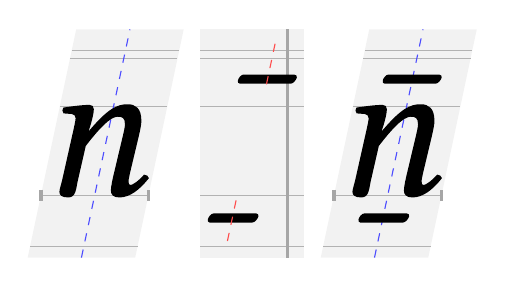
\begin{tikzpicture}[x=1pt,y=1pt,scale=0.075]

	% ============================================================
	% TILE 1 — italic "n" in its lane
	% ============================================================
	\begin{scope}[shift={(0,0)}]

		\fill[gray!10] (-63.8,-300) -- (454.2,-300) -- (688.0,800) -- (170.0,800) -- cycle;
		\draw[gray!60] (0.0,0) -- (518.0,0); % baseline
		\draw[gray!60] (91.2,429) -- (609.2,429); % xheight
		\draw[gray!60] (139.9,658) -- (657.9,658); % capline
		\draw[gray!60] (148.4,698) -- (666.4,698); % ascender
		\draw[gray!60] (-52.3,-246) -- (465.7,-246); % descender
		% midline of the lane: x = W/2 + y tan(12 degrees)
		\draw[blue!70,dashed] (195.2,-300) -- (429.0,800);
		% the advance width, marked on the baseline
		\draw[gray!70,very thick] (0,-25) -- (0,25); \draw[gray!70,very thick] (518,-25) -- (518,25);

		% Italic "n" outline
		\path[fill=black]
		svg "M433 124 471 283C479 318 484 341 484 359C484 419 457 439 418 439C366 439 323 418 231 310L230 311L233 320C246 357 255 400 255 415C255 429 247 436 234 436C202 436 155 430 108 423C101 415 103 404 109 395L149 392C161 391 167 382 167 372C167 364 164 349 158 321L102 72C97 52 89 27 89 17C89 1 100 -10 132 -10C170 -10 169 34 178 72L216 238C279 320 334 379 370 379C391 379 405 374 405 343C405 331 399 303 392 275L354 115C346 83 337 42 337 23C337 4 348 -10 378 -10C426 -10 474 24 520 83C517 92 511 100 497 100C471 70 442 50 432 50C425 50 422 55 422 67C422 76 427 98 433 124Z";

		% Base anchors (blue circles only), on the midline
		\baseanchor{396}{645}
		\baseanchor{236}{-110}

	\end{scope}

	% ============================================================
	% TILE 2 — italic macron and macron below, each with its axis
	% ============================================================
	\begin{scope}[shift={(1188,0)}]

		% Tile background
		\fill[gray!10] (-420,-300) rectangle (80,800);

		% Horizontal metric lines
		\draw[gray!60] (-420,0) -- (80,0);
		\draw[gray!60] (-420,429) -- (80,429);
		\draw[gray!60] (-420,658) -- (80,658);
		\draw[gray!60] (-420,698) -- (80,698);
		\draw[gray!60] (-420,-246) -- (80,-246);

		% Dark gray vertical line at x=0
		\draw[gray!70,very thick] (0,-300) -- (0,800);

		% Mark outlines
		\path[fill=black]
		svg "M15 538C28 538 42 556 45 568C46 574 43 582 33 582H-212C-223 582 -237 565 -239 553C-241 546 -238 538 -229 538Z";
		\path[fill=black]
		svg "M-170 -131C-157 -131 -143 -113 -140 -101C-139 -94 -142 -87 -151 -87H-356C-368 -87 -381 -104 -384 -116C-385 -123 -383 -131 -375 -131Z";

		% The slanted axis of each mark, through its anchor
		\draw[red!70,dashed] (-101.4,535) -- (-54.6,755);
		\draw[red!70,dashed] (-289.4,-220) -- (-242.6,0);

		% Mark anchors (red squares only)
		\markanchor{-78}{645}
		\markanchor{-266}{-110}

	\end{scope}

	% ============================================================
	% TILE 3 — composition (n + macron + macron below)
	% ============================================================
	\begin{scope}[shift={(1412,0)}]

		\fill[gray!10] (-63.8,-300) -- (454.2,-300) -- (688.0,800) -- (170.0,800) -- cycle;
		\draw[gray!60] (0.0,0) -- (518.0,0); % baseline
		\draw[gray!60] (91.2,429) -- (609.2,429); % xheight
		\draw[gray!60] (139.9,658) -- (657.9,658); % capline
		\draw[gray!60] (148.4,698) -- (666.4,698); % ascender
		\draw[gray!60] (-52.3,-246) -- (465.7,-246); % descender
		% midline of the lane: x = W/2 + y tan(12 degrees)
		\draw[blue!70,dashed] (195.2,-300) -- (429.0,800);
		% the advance width, marked on the baseline
		\draw[gray!70,very thick] (0,-25) -- (0,25); \draw[gray!70,very thick] (518,-25) -- (518,25);

		% Base glyph
		\path[fill=black]
		svg "M433 124 471 283C479 318 484 341 484 359C484 419 457 439 418 439C366 439 323 418 231 310L230 311L233 320C246 357 255 400 255 415C255 429 247 436 234 436C202 436 155 430 108 423C101 415 103 404 109 395L149 392C161 391 167 382 167 372C167 364 164 349 158 321L102 72C97 52 89 27 89 17C89 1 100 -10 132 -10C170 -10 169 34 178 72L216 238C279 320 334 379 370 379C391 379 405 374 405 343C405 331 399 303 392 275L354 115C346 83 337 42 337 23C337 4 348 -10 378 -10C426 -10 474 24 520 83C517 92 511 100 497 100C471 70 442 50 432 50C425 50 422 55 422 67C422 76 427 98 433 124Z";

		% Marks positioned by anchor alignment
		\begin{scope}[shift={(474,0)}]
			\path[fill=black]
			svg "M15 538C28 538 42 556 45 568C46 574 43 582 33 582H-212C-223 582 -237 565 -239 553C-241 546 -238 538 -229 538Z";
		\end{scope}
		\begin{scope}[shift={(502,0)}]
			\path[fill=black]
			svg "M-170 -131C-157 -131 -143 -113 -140 -101C-139 -94 -142 -87 -151 -87H-356C-368 -87 -381 -104 -384 -116C-385 -123 -383 -131 -375 -131Z";
		\end{scope}

		% Composition anchors:
		% Draw blue circle FIRST, then red square
		\baseanchor{396}{645}
		\markanchor{396}{645}
		\baseanchor{236}{-110}
		\markanchor{236}{-110}

	\end{scope}

\end{tikzpicture}
\endgroup

	\caption{Libertinus italic n, macron and macron below, with anchors. The gray band is the italic lane and the dashed blue line is its midline.}
	\label{fig:libertinus-italic-geometry}
\end{figure}

\subsubsection*{Semibold italic anchor model}

Semibold italic has its own anchor model, which is not the italic anchor model, and the patch keeps it.
The outlines are slanted (the italic angle $\theta$ is $11.5^\circ$), but the anchors are, almost all, 
the anchors of regular, copied unchanged:
42 of the 44 above- and below-mark anchors, and 319 of the 384 above- and below-anchors of bases,
have exactly the coordinates of regular.

So the anchors do not follow the slant.
A slanted outline moves further right the higher it goes, but an anchor copied from regular stays where it was. 
An above-anchor therefore sits left of where the italic anchor model would put it, 
by roughly the amount the slant has moved the outline at that height.
This is true of the base and of the mark alike: 
the base's above-anchor is left of the midline of its italic lane, 
and the mark's anchor is left of the mark's own slanted axis, by about the same amount.
When the two anchors are superimposed, the two errors cancel, 
and the axis of the mark lands near the midline of the base, as it would in italic.
See Figure \ref{fig:libertinus-semibolditalic-geometry}, 
where the filled symbols are the designer's anchors and the hollow symbols are the positions given by the italic anchor model:
the above-anchor of n and the anchor of the macron are both far left of the hollow symbols, 
but by nearly the same distance.

Each anchor in the font has its own shift $k$: how far it lies left of the position the italic anchor model gives it.
For a base anchor, $k = W/2 + Y\tan\theta - X$.
For a mark anchor, $k = C + Y\tan\theta - (X - d)$, where $C$ is where the mark's axis meets the baseline
and $d$ is the mark's offset from its axis in regular ($d = 0$ for a symmetric mark; for the acute it is $-32$).
In Figure \ref{fig:libertinus-semibolditalic-geometry}, the above-anchor of n has $k = 170$ and the macron has $k = 141$.
A mark lands $k_\mathrm{mark} - k_\mathrm{base}$ units right of the base's midline (left, if negative),
so the macron lands $141 - 170 = -29$, that is, 29 units left of the midline of n.

The shifts differ from anchor to anchor, because the designer copied regular's $X$ coordinates, which carry no slant.
So an anchor's shift is about $Y\tan\theta$ at its own height, plus a small amount that depends on how the slanted outline was drawn.
A higher anchor has a larger shift: comma above U+0313, with its anchor at $Y = 605$, has $k = 125$; hook above U+0309, at $Y = 765$, has $k = 168$.
Only the difference between a mark's shift and a base's shift moves the mark off the midline,
so any single value works, provided every base anchor and every mark anchor uses it.

The semibold italic anchor model therefore fixes one value of $K$ for each anchor class
and gives every anchor of that class the same shift:
the base anchor is at $X = W/2 + Y\tan\theta - K$ and the mark anchor is at $X = C + Y\tan\theta + d - K$,
with $\tan\theta = 0.2035$ and the same $Y$ coordinates as in the other styles.
\begin{itemize}
	\item Above-anchors: $K = 150$, for every above-mark and every base's above-anchor.
	Above-anchors are high, where the slant has moved the outline far to the right, so their shift is large.
	150 is the median shift of the designer's above-marks; most are between 132 and 168.
	\item Below-anchors: $K = -12$, for every below-mark and every base's below-anchor.
	Below-anchors are just under the baseline, where the slant has moved the outline a little to the left, so their shift is small and negative.
	$-12$ is the median shift of the designer's below-marks; most are between $-23$ and $-4$.
\end{itemize}
The values are taken from the marks rather than the bases so that most of the designer's mark anchors already conform.
The designer's base anchors have median shifts of 139 above and $-1$ below on lowercase Latin and IPA letters,
and 173 above and $-5$ below on capitals.
An anchor conforms if its own shift $k$ is close to $K$.
The italic anchor model is the case $K = 0$.

The candidates for a base are
$ax = W/2 + ay\tan\theta - 150$ and $bx = W/2 + by\tan\theta + 12$.
So the above-anchor is at $W/2 - 19$ for a letter at the x-height ($ay = 645$),
at $W/2 + 23$ for a capital ($ay = 850$), and at $W/2 + 31$ for an ascender ($ay = 890$).
The below-anchor is at $W/2 - 10$ for a letter on the baseline ($by = -110$)
and at $W/2 - 53$ for a descender ($by = -319$).
For semibold italic n, $W = 606$, so $ax = 284$ and $bx = 293$; 
the font has $ax = 264$ and $bx = 265$, the values of regular n,
and the macron lands 29 units left of the midline.

The cancellation is only approximate, because the designer's anchors do not follow the slant at all, 
whereas the model's anchors do, apart from the constant $K$.
A mark's shift is fixed by the height of its own anchor:
for a mark, $k = Y\tan\theta$ plus a small amount, where $Y$ is the height of the mark anchor.
But the designer's base anchors are near $W/2 - 9$ at every height, 
so they do not move right for a taller base, such as a capital or an ascender.
The error of a mark on a base therefore grows with the difference in height of the two anchors, 
by 2 units for every 10.
The median distance of a designer's base anchor from the candidate is about 20 units for a lowercase letter 
and 30 units for a capital.

The patch does not move this style to the italic anchor model.
It keeps the designer's anchors where they conform to the semibold italic anchor model,
and corrects only the anchors that do not, so that they conform to it:
a base anchor is moved to the candidate above,
and a mark anchor is moved to $X = C + Y\tan\theta - 150$ for an above-mark or $X = C + Y\tan\theta + 12$ for a below-mark.
An anchor set by the italic anchor model would be wrong here: 
a base anchor without the shift would put every above-mark about 150 units too far right, 
because the marks carry the shift.

The following do not conform to the semibold italic anchor model and probably need to be patched, some of them manually.
\begin{itemize}
	\item Capitals. The designer's above-anchors are about 25 units left of the candidate, since they are 205 units higher than
	the anchors of lowercase letters but no further right. The worst are B, D, I, N, O, R, W (40 to 60 units left) and L (159 units left; its anchor is over the stem, as in regular).
	\item The capital forms of the grave, acute, circumflex and breve (\verb|grave.cap|, \verb|acute.cap|, \verb|circumflex.cap|, \verb|breve.cap|),
	which the font substitutes over capitals. Their mark anchors were set with the slant ($k$ between $-13$ and $29$), 
	but the above-anchors of capitals were not, so these four marks land 160 to 190 units left of the middle of a capital.
	The other above-marks have no capital form in use and land 20 to 50 units left.
	The capital forms need mark anchors at $X = C + Y\tan\theta - 150$; \verb|caron.cap| and \verb|dieresis.cap| are not substituted.
	\item Above-anchors that were set with the slant, as in italic, so that an above-mark lands 130 to 190 units too far right:
	a, s, h and J.
	\item Other base anchors more than 40 units from the candidate.
	Above: c, g, Æ, Ɗ, ƕ, Ƣ, Ƥ, ȵ, ɗ, ɦ, ɧ, Ћ, ѳ, ⱨ.
	Below: A, C, D, J, a, d, f, j, q, r, t, Æ, ĸ, ƕ, Ƣ, Ƥ, ȵ, ɍ, ɑ, ɖ, ɗ, ɚ, ɥ, ɰ, ʞ, Ћ, ѳ.
	Several of these are copies of the anchors of another glyph.
	The anchors of ʮ and ʯ are transposed, as in the other styles.
	\item Marks whose own shift $k$ is far from $K$ (150 above, $-12$ below), so that no base anchor can be right for them and for the other marks;
	each lands $k - K$ units right of where a conforming mark lands:
	dieresis U+0308 ($k = 111$, so it lands about 40 units left of the other above-marks),
	comma above U+0313 (125), inverted breve U+0311 (132), hook above U+0309 and double grave U+030F (168, about 18 units right),
	koronis U+0343 (371), right tack below U+0319 ($-30$) and tilde below U+0330 ($+10$).
	The double acute U+030B (156) conforms.
	\item Tilde U+0303, one of the two mark anchors that is not a copy of regular; its shift is 139.
	(These are the designer's values. In the patched font the dieresis and tilde are on the model by the mark-axis rule, and the hook above, inverted breve, U+0314 and tilde below by curated anchors; see ``Mark anchor model''.)
	\item The Hebrew ligatures U+05F0, U+05F1, U+05F2, which have above- and below-anchors in this lookup table in semibold italic only.
	\item Letters that overhang their advance width, such as f and j, which need curated anchors in every italic style.
\end{itemize}
The anchors of precomposed glyphs were not compared with these candidates.

\begin{figure}[htbp]
	\captionsetup{justification=raggedright, singlelinecheck=false}
	
\begingroup
% ------------------------------------------------------------
% Libertinus Serif Semibold Italic: n (U+006E), macron (U+0304), macron below (U+0331).
% Italic angle 11.5 degrees, tan = 0.2035. Advance width of n: W = 606.
% Filled symbols are the font's own anchors:
%   n above (264, 646), below (265, -110); macron (-209, 645), macron below (-244, -110).
% Hollow symbols are where the italic anchor model puts them:
%   n above (434, 646) = (W/2 + 646 tan, 646); below (281, -110)
%   macron (-68, 645), macron below (-250, -110), on the axis of each mark.
% ------------------------------------------------------------
% Base anchor = blue circle (larger); hollow = italic-model position
\newcommand{\baseanchor}[2]{%
	\filldraw[blue] (#1,#2) circle (8pt);
}
\newcommand{\baseanchormodel}[2]{%
	\draw[blue,thick,fill=white] (#1,#2) circle (8pt);
}
% Mark anchor = red square (smaller); hollow = italic-model position
\newcommand{\markanchor}[2]{%
	\filldraw[red] (#1-2,#2-2) rectangle (#1+2,#2+2);
}
\newcommand{\markanchormodel}[2]{%
	\draw[red,thick,fill=white] (#1-6,#2-6) rectangle (#1+6,#2+6);
}
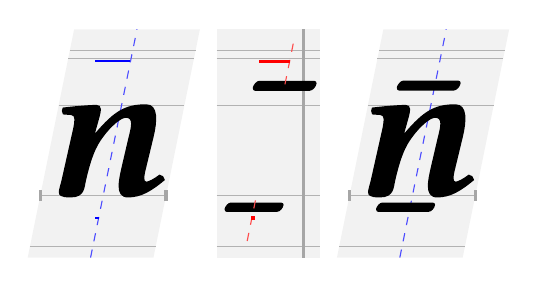
\begin{tikzpicture}[x=1pt,y=1pt,scale=0.075]

	% ============================================================
	% TILE 1 — semibold italic "n" in its lane
	% ============================================================
	\begin{scope}[shift={(0,0)}]

		\fill[gray!10] (-61.0,-300) -- (545.0,-300) -- (768.8,800) -- (162.8,800) -- cycle;
		\draw[gray!60] (0.0,0) -- (606.0,0); % baseline
		\draw[gray!60] (88.3,434) -- (694.3,434); % xheight
		\draw[gray!60] (133.9,658) -- (739.9,658); % capline
		\draw[gray!60] (142.0,698) -- (748.0,698); % ascender
		\draw[gray!60] (-50.0,-246) -- (556.0,-246); % descender
		% midline of the lane: x = W/2 + y tan(11.5 degrees)
		\draw[blue!70,dashed] (242.0,-300) -- (465.8,800);
		% the advance width, marked on the baseline
		\draw[gray!70,very thick] (0,-25) -- (0,25); \draw[gray!70,very thick] (606,-25) -- (606,25);

		% Semibold italic "n" outline
		\path[fill=black]
		svg "M389 125C383 97 377 69 377 46C377 13 388 -10 422 -10C485 -10 534 19 600 74C598 88 588 100 574 100C550 81 521 66 511 66C503 66 501 73 501 83C501 97 506 119 510 134L546 283C563 354 571 439 510 439C411 439 357 408 265 300L264 301L269 320C280 359 292 398 292 415C292 429 284 436 271 436C239 436 155 429 108 423C101 415 103 399 109 390L149 387C161 386 164 377 164 367C164 358 163 345 158 321L102 72C97 52 89 27 89 17C89 1 94 -10 146 -10C215 -10 212 38 220 72C237 146 257 214 289 262C338 335 390 374 412 374C448 374 438 332 427 287C426 283 425 279 424 275Z";

		% The displacement of each anchor from the midline
		\draw[blue,thick] (264,646) -- (434,646);
		\draw[blue,thick] (265,-110) -- (281,-110);

		% Italic-model positions (hollow), then the font's anchors (filled)
		\baseanchormodel{434}{646}
		\baseanchormodel{281}{-110}
		\baseanchor{264}{646}
		\baseanchor{265}{-110}

	\end{scope}

	% ============================================================
	% TILE 2 — semibold italic macron and macron below, each with its axis
	% ============================================================
	\begin{scope}[shift={(1269,0)}]

		% Tile background
		\fill[gray!10] (-420,-300) rectangle (80,800);

		% Horizontal metric lines
		\draw[gray!60] (-420,0) -- (80,0);
		\draw[gray!60] (-420,434) -- (80,434);
		\draw[gray!60] (-420,658) -- (80,658);
		\draw[gray!60] (-420,698) -- (80,698);
		\draw[gray!60] (-420,-246) -- (80,-246);

		% Dark gray vertical line at x=0
		\draw[gray!70,very thick] (0,-300) -- (0,800);

		% Mark outlines
		\path[fill=black]
		svg "M29 504C43 504 59 523 61 536C62 538 62 539 62 540C62 546 59 552 50 552H-214C-227 552 -242 533 -245 521V516C-245 510 -242 504 -235 504Z";
		\path[fill=black]
		svg "M-127 -79C-114 -79 -100 -61 -98 -49C-97 -48 -97 -47 -97 -46C-97 -40 -100 -35 -108 -35H-353C-364 -35 -378 -52 -381 -64V-68C-381 -74 -378 -79 -372 -79Z";

		% The slanted axis of each mark
		\draw[red!70,dashed] (-90.4,535) -- (-45.6,755);
		\draw[red!70,dashed] (-272.4,-220) -- (-227.6,0);

		% The displacement of each anchor from the axis
		\draw[red,thick] (-209,645) -- (-68,645);
		\draw[red,thick] (-244,-110) -- (-250,-110);

		% Italic-model positions (hollow), then the font's anchors (filled)
		\markanchormodel{-68}{645}
		\markanchormodel{-250}{-110}
		\filldraw[red] (-209-6,645-6) rectangle (-209+6,645+6);
		\filldraw[red] (-244-6,-110-6) rectangle (-244+6,-110+6);

	\end{scope}

	% ============================================================
	% TILE 3 — composition by the font's anchors (n + macron + macron below)
	% ============================================================
	\begin{scope}[shift={(1490,0)}]

		\fill[gray!10] (-61.0,-300) -- (545.0,-300) -- (768.8,800) -- (162.8,800) -- cycle;
		\draw[gray!60] (0.0,0) -- (606.0,0); % baseline
		\draw[gray!60] (88.3,434) -- (694.3,434); % xheight
		\draw[gray!60] (133.9,658) -- (739.9,658); % capline
		\draw[gray!60] (142.0,698) -- (748.0,698); % ascender
		\draw[gray!60] (-50.0,-246) -- (556.0,-246); % descender
		% midline of the lane: x = W/2 + y tan(11.5 degrees)
		\draw[blue!70,dashed] (242.0,-300) -- (465.8,800);
		% the advance width, marked on the baseline
		\draw[gray!70,very thick] (0,-25) -- (0,25); \draw[gray!70,very thick] (606,-25) -- (606,25);

		% Base glyph
		\path[fill=black]
		svg "M389 125C383 97 377 69 377 46C377 13 388 -10 422 -10C485 -10 534 19 600 74C598 88 588 100 574 100C550 81 521 66 511 66C503 66 501 73 501 83C501 97 506 119 510 134L546 283C563 354 571 439 510 439C411 439 357 408 265 300L264 301L269 320C280 359 292 398 292 415C292 429 284 436 271 436C239 436 155 429 108 423C101 415 103 399 109 390L149 387C161 386 164 377 164 367C164 358 163 345 158 321L102 72C97 52 89 27 89 17C89 1 94 -10 146 -10C215 -10 212 38 220 72C237 146 257 214 289 262C338 335 390 374 412 374C448 374 438 332 427 287C426 283 425 279 424 275Z";

		% Marks positioned by anchor alignment
		\begin{scope}[shift={(473,1)}]
			\path[fill=black]
			svg "M29 504C43 504 59 523 61 536C62 538 62 539 62 540C62 546 59 552 50 552H-214C-227 552 -242 533 -245 521V516C-245 510 -242 504 -235 504Z";
		\end{scope}
		\begin{scope}[shift={(509,0)}]
			\path[fill=black]
			svg "M-127 -79C-114 -79 -100 -61 -98 -49C-97 -48 -97 -47 -97 -46C-97 -40 -100 -35 -108 -35H-353C-364 -35 -378 -52 -381 -64V-68C-381 -74 -378 -79 -372 -79Z";
		\end{scope}

		% Composition anchors:
		% Draw blue circle FIRST, then red square
		\baseanchor{264}{646}
		\markanchor{264}{646}
		\baseanchor{265}{-110}
		\markanchor{265}{-110}

	\end{scope}

\end{tikzpicture}
\endgroup

	\caption{Libertinus semibold italic n, macron and macron below, with the designer's anchors (filled)
	and the positions given by the italic anchor model (hollow).
	The above-anchor of n is 170 units left of the midline ($k = 170$) and the anchor of the macron is 141 units left of its axis ($k = 141$),
	so the macron lands 29 units left of the midline of n.
	The model's own positions, with $K = 150$, would be 20 units right of the filled circle and 9 units left of the filled square.}
	\label{fig:libertinus-semibolditalic-geometry}
\end{figure}

\subsubsection*{Mark anchor model}

The anchor of a mark follows the same model in every style.
Horizontally, it lies on the mark's own axis, $X = C + Y\tan\theta - K$
($\theta = 0$ and $K = 0$ in the roman styles, $K = 0$ in italic, $K = 150$ above and $-12$ below in semibold italic).
An asymmetric mark, such as the grave, acute, double acute or double grave, keeps the offset from its axis that it has in regular.
Vertically, the anchor is at a fixed distance from the mark's outline:
the anchor of an above-mark is a certain height above the bottom of the outline,
and the anchor of a below-mark is a certain depth below the top of the outline.
These distances differ from mark to mark (a short mark such as the macron sits a little higher than a tall one),
but since the base anchors have the same $Y$ coordinates in every style,
a mark sits at the same height in every style only if its distance is the same as in regular.

So each mark can be checked in two ways: its $X$ offset from its axis, compared with regular,
and the distance between its anchor and its outline, compared with regular.
A third check is the designer's precomposed glyphs.
They are not consistent between styles
(the macron of ō was 18 units lower than the combining macron in regular, but 32 units higher in italic),
and horizontally they also carry the offsets of the base anchors, so for $X$ they can confirm a finding but not settle one: the $X$ of a symmetric mark is set by the model (the mark-axis rule).
Vertically they are better evidence: every x-height base has its above-anchor at 645, so where the offset of a composed mark from the precomposed glyphs is the same on every base, it belongs to the mark's anchor, and the anchor is moved by it (``Vertical moves from the precomposed glyphs'').
In what follows, ``lower'' and ``higher'' and ``left'' and ``right'' describe where the mark lands on a base whose anchor conforms.
A mark lands lower when its anchor is further above its outline, and left when its anchor is further right.

\paragraph{Status.}
There is no audit of mark anchors.
One stage moves designer mark anchors to the model, and only their X: the mark-axis rule for symmetric above marks (stage 4, 2026-11-09; see the end of this section).
A wholesale move of every mark anchor to the model was rejected (also at the end of this section).
Otherwise mark anchors are changed one at a time, as curated anchors, where the precomposed glyphs support the change (including the vertical moves from $\Delta y$), and checked by eye against the mark zone figures.
A curated mark anchor is the final anchor and obeys the mark-axis rule itself.
The patch changes mark anchors in five places, and one change of base anchors (in stage 1) serves the marks.
\begin{itemize}
	\item Stage 1, semibold only: the designer's second above-anchor class \verb|top_punkt| (class 1) is merged into the above class.
	Its 12 marks (dot above, diaeresis, hook above, ring above, U+0312, U+0313, U+0314, U+031A, U+0351, U+0357, U+0363 and \verb|hookabovecomb.cap|)
	move to class 0, and their anchors are raised by 96 units, the difference between the two classes' base anchors.
	This does not move these marks on a lowercase letter, but it fixes their coverage:
	before, they attached only to the 24 bases with a \verb|top_punkt| anchor; now they attach to every base with an above-anchor.
	It does not change how high these marks sit compared with regular (see below).
	\item Stage 3, semibold and semibold italic: the combining marks the style lacks are added,
	and semibold's U+0358--U+0363, which were copies of the capital accents, are replaced.
	Their anchors are regular's. In semibold italic, regular's anchor is used with italic's outline moved right by 12 units.
	There, the added above-marks landed 7 to 15 units left of the model ($K = 150$),
	inside the spread of the designer's own above-marks ($k$ from 111 to 168); the symmetric ones 10 or more off are now moved onto their axes by the mark-axis rule (stage 4).
	\item Stage 4, all styles: the capital forms (\verb|grave.cap|, \verb|acute.cap|, \ldots) get anchors computed from the designer's precomposed capitals,
	on the axis for a symmetric mark, at the precomposed offset for an asymmetric one, and with $K = 150$ in semibold italic.
	This fixes semibold italic, whose capital forms had anchors without the shift $K$ and landed 120 to 160 units left,
	and italic, where only \verb|grave.cap| had an anchor (in the wrong class).
	In italic the \verb|.cap| anchors are curated (2026-11-07), fitted to the precomposed capitals:
	each $X$ is moved so that the accent lands, as a median over the capitals, where the designer drew it in the precomposed glyph,
	as in regular, where every capital form is within a few units of them.
	Stage 4 had left the symmetric marks about 14 units left of the precomposed accents, and the earlier curated caron (placed at its vertex, ignoring the slant) about 15 right.
	The fit was made after italic O, U and Y took the median accent centre of their own precomposed glyphs as their above-anchor $X$ (493, 508, 441; the designer's O was 515, 22 right, which Ø inherited).
	\item Stage 4, all styles, the mark-axis rule (2026-11-09): every symmetric above mark whose $k$ is 10 or more from $K$ gets its anchor $X$ on its own axis; 37 anchors move, $Y$ unchanged.
	Marks with a curated anchor are skipped. See ``Mark-axis rule for symmetric above marks'' at the end of this section.
	\item Stage 7, curated mark anchors in \verb|data/fontanchors_human/|:
	\begin{itemize}
		\item Vertical moves from the precomposed glyphs (2026-11-09): dot above in all four styles, macron in all but italic, semibold tilde, semibold italic ring, and the double acute;
		each anchor is moved by the median $\Delta y$ (with $X$ along the slant in the italic styles). See ``Vertical moves from the precomposed glyphs'' at the end of this section.
	\end{itemize}
	Earlier curated mark anchors:
	\begin{itemize}
		\item Regular, left and right tack below (U+0318, U+0319): the designer's anchors were 25 units right and 36 units left of the centre of the outline;
		the curated anchors are at the centre. The other styles keep the designer's $X$, so the tacks now differ between regular and the other styles.
		\item Semibold, half rings above U+0351 and U+0357 (2026-11-08): their anchors were the designer's class 1 (\verb|top_punkt|, $Y$ 547, 549), raised 96 by stage 1,
		so they sat 156--158 above the mark's bottom against regular's 126--136, and the marks landed 20--32 units low (40--53 above x-height letters, against 67--88 in regular).
		They now have regular's anchor-to-outline offsets, measured from the outline's centre and bottom: $(90, 623)$ and $(82, 613)$, so they land as in regular.
		(The $X$ of $+100$ was not itself wrong: semibold draws these two marks right of the origin.)
		Regular's left half ring lands 16 units right of centre, as it shares the right half ring's anchor; Gentium Plus puts it about 11 left. Left as it is.
		\item All styles, seven tall below-marks (2026-11-08): left and right tack U+0318, U+0319, left and right half ring U+031C, U+0339, plus sign U+031F, ring U+0325 and up arrow U+034E.
		They rose 82 to 94 units above their own anchor, against 33 to 77 for the other below-marks,
		so at the descender's below-anchor ($Y = -319$, 87 below the descender) each overlapped 1 to 13 of the 26 to 31 Latin and IPA descenders (p, q, g, þ, ʒ, \ldots),
		and under baseline letters their median gap was 7 to 26 units, against about 40 for marks such as the vertical line below.
		Each anchor is moved up, $X$ unchanged, so that the mark rises 62 above it, as U+0329 and U+0348 do: the marks sit 20 to 32 units lower under every base.
		No below-mark now overlaps a descender, and their median gap under baseline letters is 38 to 47.
		The precomposed Ḁ and ḁ confirm the ring: their ring is within 2 units of where the combining ring now lands (regular, italic, semibold italic; semibold's precomposed ring is a different outline).
		The alternative, lowering the descender reference to $-342$ (the baseline's clearance of 110), also removed the overlaps but left the crowding under baseline letters and moved every mark under descenders.
		The up tack U+031D (rising 65 to 77) clears every descender, by 4 to 7 units at the closest.
		\item Semibold, grave and acute: 30 units lower (713 to 683), which makes them sit as in regular.
		The grave keeps the designer's $X = -127$; an earlier curated $-156$ had no recorded reason and put the grave 37 units (median) from the precomposed glyphs, against 10.
		The grave and acute tone marks U+0340 and U+0341, which stage 3 adds, still have 713, so they sit 30 units lower than the grave and acute.
		\item Mark-axis positions, $X = C + Y\tan\theta + d - K$, where the precomposed glyphs confirm the move
		(median distance of the mark from the precomposed glyphs, before and after; added 2026-11-06):
		semibold inverted breve U+0311 $-217$ (11 to 4) and tilde below U+0330 $-200$ (13 to 4);
		semibold italic hook above U+0309 $-142$ (26 to 8), inverted breve U+0311 $-223$ (19 to 3) and U+0314 $-91$ (19 to 4, on one glyph).
		The semibold italic capital forms \verb|acute.cap|, \verb|grave.cap|, \verb|hungarumlaut.cap| and \verb|uni030F.cap| were also curated here (2026-11-06) and removed on 2026-11-08 in favour of stage 4; see the capital alternates.
		The inverted breves are symmetric marks and obey the mark-axis rule.
		\item Italic, \verb|acute.cap|: the curated $(-65, 724)$ had no recorded reason and has been removed, so stage 4's $(-37, 724)$ applies.
		\item Italic and semibold italic, tilde below: moved to the centre of the outline.
		In semibold italic this corrects an offset 22 units different from regular's; in italic it moves the anchor by 8 units, harmlessly.
		\item Italic, double acute: the designer's anchor $(-74, 714)$ had regular's offset; the curated $(-57, 714)$ lands the mark 17 units left.
		Since 2026-11-09 it is $(-55, 725)$, after the vertical move.
		\item Semibold italic, grave $(0, 683)$ and double acute $(-28, 719)$: these were wrong, and have been removed.
		The designer's anchors, $(-142, 683)$ and $(-219, 714)$, conform to the model.
		The curated ones lacked the shift $K$, so on every conforming base the grave landed 142 units left and the double acute 190 units left
		(ò: 126 units left of the precomposed grave; ő: 150 units left).
		They had been adjusted on a, whose above-anchor carried the slant and landed every above-mark about 150 units too far right
		(see the list above Figure \ref{fig:libertinus-semibolditalic-geometry}).
		The fix: stage 1 now deletes the above-anchors of a, s, h and J 
		(as \verb|"delete"| entries in \verb|data/fontanchors_audit/overrides.py|), 
		stage 6 replaces them with the candidates, and the designer's grave and double acute are back.
		The designer's a, s, h and J were 137 to 179 units right of the candidate, and h's anchor was at the x-height instead of the ascender.
		On a, the above-marks now land 7 to 33 units from where the precomposed glyphs put them (before: 113 to 161 units right);
		on s within 11; the circumflex of ĥ, which landed 219 units too low, now sits 26 units higher than in the precomposed glyph,
		and that of Ĵ 34 units right and 34 higher.
	\end{itemize}
\end{itemize}

\paragraph{Remaining departures from the model.}
Compared with regular, after the patch:
\begin{itemize}
	\item Regular. The marks conform.
	The dot above U+0307 sat 45 units lower than the dot of the precomposed ȯ; since 2026-11-09 it sits as in the precomposed glyphs, and so does the macron (18 units lower than before).
	The dot below U+0323 and diaeresis below U+0324 are drawn 43 units lower, relative to their anchors, than in the other three styles.
	Regular's precomposed ạ agrees with the combining dot below, but in ṳ the diaeresis is 35 units higher.
	Whether regular or the other styles should change is a design decision.
	\item Italic. The marks conform. The tilde was 11 units off its axis; the mark-axis rule puts it on its axis.
	The dot above sat 10 units higher than in regular, still 11 units lower than in the precomposed ȯ; since 2026-11-09 it sits as in the precomposed glyphs.
	The macron is not moved: its precomposed glyphs disagree ($-1$ on ā ē ḡ, $-32$ on ī ō ū ȳ).
	\item Semibold. Horizontally, the marks are within about 12 units of regular's offsets.
	Vertically, about a quarter of the above-marks sat lower than in regular:
	U+0357 32 and U+0351 20 (fixed, see stage 7), double acute 19,
	diaeresis 14, dot above 13 (ȯ confirms, 21), hook above 13, macron 13 (ō confirms, 12), circumflex 10.
	The tilde sits 12 units higher (õ confirms, 14), and so does the breve below.
	Semibold's x-height is 5 units higher than regular's, so differences under 10 do not matter.
	Since 2026-11-09 the macron, dot above and tilde sit as in the precomposed glyphs (vertical moves of $-12$, $-21$, $+14$), and the dieresis is on its axis (the mark-axis rule, 12 units left).
	\item Semibold italic. Horizontally, the marks whose $k$ is far from 150 are listed above Figure \ref{fig:libertinus-semibolditalic-geometry}.
	Of these, the hook above, inverted breve and U+0314 have curated anchors on the model, and the dieresis (38 units left) and the tilde (11 right) are moved onto it by the mark-axis rule;
	the comma above, double grave, koronis and right tack below remain, the precomposed glyphs not supporting a move of the first two.
	Vertically, the designer drew some outlines at a different height from regular's but kept regular's anchors:
	the macron sits 32 units lower than in regular (ō confirms, 32), the macron below 52 units higher (ṉ confirms, 26),
	the dot above 21 units higher (which agrees with the precomposed ȯ), the up tack below U+031D 12 units lower and the down tack below U+031E 12 units higher.
	Since 2026-11-09 the macron sits as in the precomposed glyphs (32 units higher than before), the dot above 11 units lower (it was 11 above the precomposed ċ ė ġ \ldots), the ring 23 lower and the double acute 11 lower.
\end{itemize}

\paragraph{Changes needed.}
\begin{itemize}
	\item Semibold italic: move the anchors of the marks whose $k$ is far from 150 to the model (done for the hook above, inverted breve and U+0314, and by the mark-axis rule for the dieresis and tilde; the precomposed glyphs do not support moving U+0313 or U+030F);
	move the macron's anchor 32 units down (done, see below). The macron below's anchor was moved 52 units up, to $(-233, -58)$, 23 units below its outline as in the other styles (curated, 2026-11-06): it sat 25 units under n, against 86 to 96 in the other styles.
	\item Semibold: lower the anchors of the above-marks that sit low by the amounts listed, so that they sit as in regular (done for U+0351 and U+0357, and against the precomposed glyphs for the macron and dot above, and for the tilde, which sat high; see below).
	The double acute, dieresis, hook above and circumflex are within 10 of their precomposed glyphs vertically, which do not support moving them;
	give U+0340 and U+0341 the curated height of the grave and acute (683).
	\item Regular: lower the anchor of the dot above by about 45 units (and by about 11 in italic and 21 in semibold) to match the precomposed glyphs (done, see below);
	decide between regular and the other styles for the dot below and diaeresis below, and for the tacks below.
	\item Italic: the curated double acute keeps its X; its Y is now set from the precomposed glyphs (below).
\end{itemize}

\paragraph{Vertical moves from the precomposed glyphs (2026-11-09).}
For each above mark, $\Delta y$ is the median vertical offset of the composed mark (base + CGJ + mark) from the designer's precomposed glyphs, over the lowercase letters with an x-height base.
Every such base has its above-anchor at 645, and $\Delta y$ is the same on every base to within a few units, so it belongs to the mark's anchor.
Where $|\Delta y| \ge 10$ the mark anchor is curated (stage 7) $\Delta y$ higher, so that the mark sits $\Delta y$ lower; in the italic styles its X moves with the slant, by $\Delta y \tan\theta$, so that the mark stays on its axis and keeps its $k$.
Regular: macron $+18$, dot above $-45$, double acute $+11$.
Italic: dot above $-11$, double acute $+11$.
Semibold: tilde $+14$, macron $-12$, dot above $-21$.
Semibold italic: macron $-32$, dot above $+11$, ring $+23$, double acute $+11$.
Not moved: the italic macron, whose precomposed glyphs disagree ($-1$ on ā ē ḡ, $-32$ on ī ō ū ȳ).
A curated mark anchor is the final anchor: it obeys the mark-axis rule itself, and stage 4 skips it (and reports it if it does not).

\paragraph{Rejected: moving every mark anchor to the model (2026-11-08).}
A stage that moved every mark anchor onto the model, $X = C + Y\tan\theta + d - K$, was tested and rejected:
most moves were under 20 units, and as many marks got further from the precomposed glyphs as got closer.
Since the precomposed glyphs are used wherever they exist, a composed combination should match them; mark anchors are therefore changed one at a time, as curated anchors, not by an audit of mark anchors.

\paragraph{Mark-axis rule for symmetric above marks (2026-11-09).}
The exception is one rule, applied in stage 4 (\verb|font_patching_markaxis.py|):
a symmetric above mark has its anchor X on its own axis, $k = K$ (0; 150 in semibold italic), wherever $|k - K| \ge 10$, with $k$ measured on the mark's ink.
The symmetric above marks are the mirror-symmetric ones (circumflex, tilde, macron, breve, dot above, dieresis, ring, caron, vertical line and double vertical line above, candrabindu, inverted breve, x above, vertical tilde, double overline, perispomeni, bridge above, not tilde, homothetic, almost equal to, fermata, zigzag) and the combining Latin letters U+0363--U+036F, centred on their ink as base letters are.
Smaller deviations are within the designer's spread and are left.
Matching each mark to the precomposed glyphs ($\Delta x = 0$ per mark) would be the wrong target:
what a composed mark differs from the precomposed glyphs by is partly the base anchor's offset, common to every mark on that base, and fitting it into each mark would carry that offset to every base without a precomposed form (most IPA letters).
Under the rule what remains is common to the marks of a style (semibold italic about $+12$ to $+16$), a question for the base anchors.
The rule moves 37 mark anchors. Among the common marks: italic tilde ($k$ 11, 11 units left), semibold dieresis (12, 12 left), semibold italic tilde (139, 11 right) and dieresis (112, 38 right);
among the others, the vertical tilde (about 18, in regular, italic and semibold), the perispomeni (18, in regular and italic) and most of semibold italic's combining letters ($k$ 130--140, 10--20 right).
It does not repeat the rejected move above: it moves only symmetric marks, only their $X$, and only where they are 10 or more off.
The semibold italic dieresis, which landed 26 units left of its precomposed glyphs where every other mark landed 5--16 right, now lands 12 right, like the others; the semibold italic tilde moves from 12 to 23 right of its precomposed glyphs, the rule's one cost.
Asymmetric marks keep their designed $k$: grave, acute and their tone-mark forms, double acute and double grave (a symmetric pair placed off-centre), hook above, the comma-shaped marks, the half rings and the right arrowhead. The rule does not touch Y.
What the threshold leaves is under 10 units (the ring: $+2$, $+3$, 0, $+7$); the threshold is likely to be lowered.
That first needs a more precise mark axis than the centre of the ink bounds, which does not always find the midline, determined per glyph and checked by eye:
for instance the line about which the outline best matches its mirror image (circumflex, ring, dieresis), or its rotation by 180° for marks that are symmetric that way (tilde, zigzag, vertical tilde), whose terminals can push the bounds off centre.

%Libertinus serif has few mark positioning GPOS tables.
%Regular has two mark-to-base LookupList tables: 
%index 7 for Hebrew and index 4 for latin and other scripts;
%one mark-to-mark LookupList table, index 5.

\newpage
\subsection*{Mark outline zones}

Figures \ref{fig:mark-zones-regular}, \ref{fig:mark-zones-italic}, \ref{fig:mark-zones-semibold} and \ref{fig:mark-zones-semibold-italic}
overlay the outlines of all the above and below marks of the patched fonts on a solid o, at three times the scale of the anchor model figures.
Each mark is placed so that its anchor is on the anchor of the o for its class (the blue dots), which is where the shaper puts it.
The common marks are black outlines. The other marks are gray with a light fill, so the shading builds up where many marks overlap.
The grid is in font units of the o, with lines every 100 units.
In semibold italic the above marks lie well to the right of the blue dot, because both the base and the mark anchor carry the shift $K$.

\begin{figure}[htbp]
	\captionsetup{justification=raggedright, singlelinecheck=false}
	\begin{minipage}[t]{0.245\textwidth}
		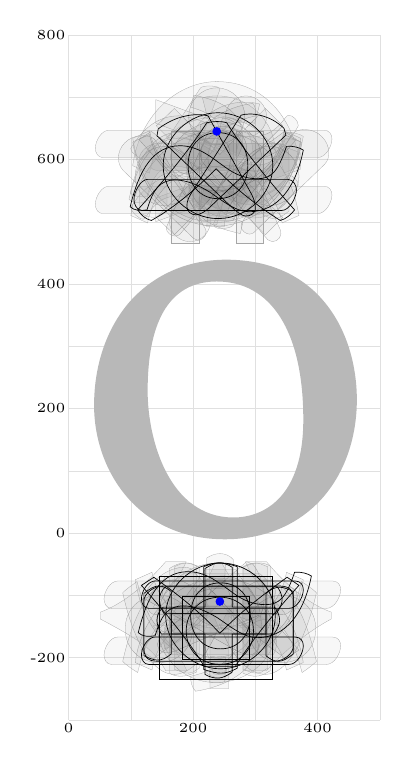
\begin{tikzpicture}[x=1pt,y=1pt,scale=0.225]
\draw[black!12,line width=0.1pt,step=100] (0,-300) grid (500,800);
\node[left,font=\tiny,inner sep=1pt] at (0,-200) {-200};
\node[left,font=\tiny,inner sep=1pt] at (0,0) {0};
\node[left,font=\tiny,inner sep=1pt] at (0,200) {200};
\node[left,font=\tiny,inner sep=1pt] at (0,400) {400};
\node[left,font=\tiny,inner sep=1pt] at (0,600) {600};
\node[left,font=\tiny,inner sep=1pt] at (0,800) {800};
\node[below,font=\tiny,inner sep=1pt] at (0,-300) {0};
\node[below,font=\tiny,inner sep=1pt] at (200,-300) {200};
\node[below,font=\tiny,inner sep=1pt] at (400,-300) {400};
\fill[black!28,even odd rule] (41,205) .. controls (41,103) and (109,-10) .. (251,-10) .. controls (315,-10) and (364,13) .. (398,46) .. controls (443,90) and (463,153) .. (463,214) .. controls (463,318) and (406,439) .. (253,439) .. controls (187,439) and (133,412) .. (96,369) .. controls (60,326) and (41,268) .. (41,205) -- cycle (238,404) .. controls (324,404) and (377,326) .. (377,182) .. controls (377,56) and (312,25) .. (265,25) .. controls (161,25) and (127,151) .. (127,228) .. controls (127,315) and (148,404) .. (238,404) -- cycle;
\filldraw[draw=black!35,line width=0.1pt,fill=black,fill opacity=0.03,draw opacity=1,even odd rule] (130,640) -- (103,628) .. controls (117,543) and (168,493) .. (238,493) .. controls (297,493) and (361,542) .. (373,628) -- (346,640) .. controls (336,582) and (290,550) .. (238,550) .. controls (184,550) and (141,587) .. (130,640) -- cycle;
\filldraw[draw=black!35,line width=0.1pt,fill=black,fill opacity=0.03,draw opacity=1,even odd rule] (188,599) .. controls (188,573) and (212,547) .. (236,547) .. controls (264,547) and (288,574) .. (288,595) .. controls (288,619) and (267,647) .. (240,647) .. controls (216,647) and (188,623) .. (188,599) -- cycle;
\filldraw[draw=black!35,line width=0.1pt,fill=black,fill opacity=0.03,draw opacity=1,even odd rule] (107,573) .. controls (107,547) and (128,526) .. (154,526) .. controls (180,526) and (201,547) .. (201,573) .. controls (201,599) and (180,621) .. (154,621) .. controls (128,621) and (107,599) .. (107,573) -- cycle (276,573) .. controls (276,547) and (297,526) .. (323,526) .. controls (349,526) and (370,547) .. (370,573) .. controls (370,599) and (349,621) .. (323,621) .. controls (297,621) and (276,599) .. (276,573) -- cycle;
\filldraw[draw=black!35,line width=0.1pt,fill=black,fill opacity=0.03,draw opacity=1,even odd rule] (310,603) .. controls (310,620) and (294,661) .. (239,661) .. controls (197,661) and (164,626) .. (164,604) .. controls (164,592) and (172,577) .. (191,577) .. controls (200,577) and (213,587) .. (213,598) .. controls (213,606) and (210,612) .. (209,615) .. controls (208,617) and (207,619) .. (207,623) .. controls (207,628) and (212,634) .. (231,634) .. controls (252,634) and (260,624) .. (260,601) .. controls (260,589) and (255,577) .. (247,565) .. controls (236,548) and (223,526) .. (222,492) -- (250,492) .. controls (252,518) and (262,535) .. (279,551) .. controls (295,567) and (310,583) .. (310,603) -- cycle;
\filldraw[draw=black!35,line width=0.1pt,fill=black,fill opacity=0.03,draw opacity=1,even odd rule] (418,611) .. controls (418,630) and (401,648) .. (380,648) .. controls (368,648) and (361,645) .. (356,636) -- (278,497) .. controls (277,496) and (277,494) .. (277,493) .. controls (277,485) and (286,480) .. (291,480) .. controls (293,480) and (295,480) .. (297,482) -- (411,592) .. controls (417,598) and (418,605) .. (418,611) -- cycle (286,617) .. controls (286,638) and (269,653) .. (248,653) .. controls (244,653) and (228,652) .. (222,639) -- (158,493) .. controls (157,492) and (157,491) .. (157,490) .. controls (157,482) and (165,477) .. (171,477) .. controls (174,477) and (177,478) .. (179,480) -- (281,601) .. controls (285,606) and (286,612) .. (286,617) -- cycle;
\filldraw[draw=black!35,line width=0.1pt,fill=black,fill opacity=0.03,draw opacity=1,even odd rule] (214,502) -- (264,502) .. controls (293,548) and (331,593) .. (366,632) -- (347,645) .. controls (310,618) and (276,593) .. (239,555) .. controls (205,591) and (172,616) .. (133,645) -- (113,632) .. controls (148,594) and (185,549) .. (214,502) -- cycle;
\filldraw[draw=black!35,line width=0.1pt,fill=black,fill opacity=0.03,draw opacity=1,even odd rule] (266,660) .. controls (258,665) and (250,667) .. (243,667) .. controls (237,667) and (222,662) .. (212,656) .. controls (213,630) and (213,601) .. (213,577) .. controls (213,556) and (213,531) .. (212,511) .. controls (219,507) and (228,505) .. (235,505) .. controls (241,505) and (257,508) .. (266,515) .. controls (265,544) and (265,574) .. (265,597) .. controls (265,620) and (265,643) .. (266,660) -- cycle;
\filldraw[draw=black!35,line width=0.1pt,fill=black,fill opacity=0.03,draw opacity=1,even odd rule] (254,644) .. controls (223,644) and (212,622) .. (212,608) .. controls (212,603) and (213,597) .. (218,592) -- (320,471) .. controls (322,469) and (324,468) .. (327,468) .. controls (338,468) and (341,478) .. (341,481) .. controls (341,482) and (341,484) .. (340,487) -- (277,630) .. controls (273,639) and (265,644) .. (254,644) -- cycle (118,638) .. controls (95,638) and (80,620) .. (80,602) .. controls (80,596) and (82,589) .. (87,583) -- (201,473) .. controls (203,471) and (205,470) .. (208,470) .. controls (211,470) and (221,474) .. (221,484) .. controls (221,485) and (221,487) .. (220,488) -- (142,627) .. controls (137,636) and (130,638) .. (118,638) -- cycle;
\filldraw[draw=black!35,line width=0.1pt,fill=black,fill opacity=0.03,draw opacity=1,even odd rule] (130,646) -- (103,634) .. controls (117,549) and (168,499) .. (238,499) .. controls (297,499) and (361,548) .. (373,634) -- (346,646) .. controls (336,588) and (290,556) .. (238,556) .. controls (184,556) and (141,593) .. (130,646) -- cycle (193,669) .. controls (193,644) and (213,624) .. (238,624) .. controls (263,624) and (283,644) .. (283,669) .. controls (283,694) and (263,715) .. (238,715) .. controls (213,715) and (193,694) .. (193,669) -- cycle;
\filldraw[draw=black!35,line width=0.1pt,fill=black,fill opacity=0.03,draw opacity=1,even odd rule] (343,498) -- (370,510) .. controls (356,595) and (305,645) .. (235,645) .. controls (176,645) and (112,596) .. (100,510) -- (127,498) .. controls (137,556) and (183,588) .. (235,588) .. controls (289,588) and (332,551) .. (343,498) -- cycle;
\filldraw[draw=black!35,line width=0.1pt,fill=black,fill opacity=0.03,draw opacity=1,even odd rule] (252,508) .. controls (287,508) and (303,533) .. (303,549) .. controls (303,566) and (293,590) .. (253,590) .. controls (247,590) and (242,590) .. (239,589) .. controls (227,588) and (224,588) .. (224,603) .. controls (224,626) and (244,658) .. (301,670) .. controls (301,677) and (300,686) .. (296,690) .. controls (258,685) and (230,668) .. (213,647) .. controls (197,627) and (190,605) .. (190,581) .. controls (190,545) and (213,508) .. (252,508) -- cycle;
\filldraw[draw=black!35,line width=0.1pt,fill=black,fill opacity=0.03,draw opacity=1,even odd rule] (270,580) -- (344,654) -- (316,682) -- (243,608) -- (170,682) -- (141,654) -- (215,580) -- (141,507) -- (170,479) -- (243,552) -- (316,479) -- (344,507) -- cycle;
\filldraw[draw=black!35,line width=0.1pt,fill=black,fill opacity=0.03,draw opacity=1,even odd rule] (242,644) .. controls (242,629) and (233,615) .. (222,602) .. controls (210,586) and (198,569) .. (198,545) .. controls (198,510) and (224,492) .. (276,481) -- (280,500) .. controls (251,508) and (238,518) .. (238,539) .. controls (238,553) and (248,568) .. (257,582) .. controls (270,599) and (280,616) .. (280,634) .. controls (280,670) and (254,694) .. (201,703) -- (196,684) .. controls (233,673) and (242,662) .. (242,644) -- cycle;
\filldraw[draw=black!35,line width=0.1pt,fill=black,fill opacity=0.03,draw opacity=1,even odd rule] (400,513) .. controls (413,513) and (423,531) .. (423,543) .. controls (423,550) and (419,557) .. (410,557) -- (65,557) .. controls (53,557) and (43,540) .. (43,528) .. controls (43,521) and (47,513) .. (55,513) -- cycle (400,603) .. controls (413,603) and (423,621) .. (423,633) .. controls (423,640) and (419,647) .. (410,647) -- (65,647) .. controls (53,647) and (43,630) .. (43,618) .. controls (43,611) and (47,603) .. (55,603) -- cycle;
\filldraw[draw=black!35,line width=0.1pt,fill=black,fill opacity=0.03,draw opacity=1,even odd rule] (209,466) -- (209,645) -- (164,645) -- (164,466) -- cycle (313,465) -- (313,645) -- (269,645) -- (269,465) -- cycle;
\filldraw[draw=black!35,line width=0.1pt,fill=black,fill opacity=0.03,draw opacity=1,even odd rule] (158,517) -- (158,582) -- (310,582) -- (310,514) .. controls (317,508) and (324,505) .. (330,505) .. controls (337,505) and (344,509) .. (354,517) -- (354,604) .. controls (354,618) and (350,626) .. (330,626) -- (145,626) .. controls (129,626) and (114,613) .. (114,602) -- (114,514) .. controls (121,511) and (128,507) .. (136,507) .. controls (143,507) and (150,510) .. (158,517) -- cycle;
\filldraw[draw=black!35,line width=0.1pt,fill=black,fill opacity=0.03,draw opacity=1,even odd rule] (238,495) -- (251,542) .. controls (263,534) and (275,528) .. (288,528) .. controls (334,528) and (363,567) .. (375,627) .. controls (369,631) and (359,634) .. (348,633) .. controls (334,591) and (323,581) .. (301,581) .. controls (288,581) and (275,585) .. (264,591) -- (280,653) .. controls (272,662) and (267,667) .. (258,667) .. controls (254,667) and (252,666) .. (247,666) -- (233,612) .. controls (217,623) and (199,634) .. (177,634) .. controls (134,634) and (111,595) .. (97,536) .. controls (103,530) and (113,529) .. (124,531) .. controls (134,564) and (144,579) .. (170,579) .. controls (186,579) and (203,572) .. (220,563) -- (205,506) .. controls (211,498) and (214,494) .. (220,494) .. controls (224,494) and (231,495) .. (238,495) -- cycle;
\filldraw[draw=black!35,line width=0.1pt,fill=black,fill opacity=0.03,draw opacity=1,even odd rule] (303,591) .. controls (284,591) and (267,598) .. (251,610) .. controls (231,624) and (209,644) .. (179,644) .. controls (136,644) and (113,605) .. (99,546) .. controls (105,540) and (115,539) .. (126,541) .. controls (136,574) and (146,589) .. (172,589) .. controls (189,589) and (208,581) .. (226,570) .. controls (247,556) and (268,538) .. (290,538) .. controls (336,538) and (365,577) .. (377,637) .. controls (371,641) and (361,644) .. (350,643) .. controls (336,601) and (325,591) .. (303,591) -- cycle (195,468) .. controls (213,468) and (228,483) .. (228,501) .. controls (228,519) and (213,534) .. (195,534) .. controls (177,534) and (162,519) .. (162,501) .. controls (162,483) and (177,468) .. (195,468) -- cycle (285,636) .. controls (303,636) and (318,651) .. (318,669) .. controls (318,687) and (303,702) .. (285,702) .. controls (267,702) and (252,687) .. (252,669) .. controls (252,651) and (267,636) .. (285,636) -- cycle;
\filldraw[draw=black!35,line width=0.1pt,fill=black,fill opacity=0.03,draw opacity=1,even odd rule] (353,671) .. controls (347,671) and (336,636) .. (292,636) .. controls (272,636) and (205,670) .. (177,670) .. controls (145,670) and (120,651) .. (100,618) -- (100,617) .. controls (100,614) and (102,611) .. (108,607) .. controls (112,603) and (116,600) .. (120,600) .. controls (126,600) and (136,636) .. (173,636) .. controls (206,636) and (265,601) .. (297,601) .. controls (327,601) and (351,621) .. (369,654) .. controls (369,662) and (361,671) .. (353,671) -- cycle (353,575) .. controls (348,575) and (336,541) .. (292,541) .. controls (272,541) and (206,574) .. (177,574) .. controls (146,574) and (120,556) .. (100,523) .. controls (100,517) and (112,504) .. (120,504) .. controls (126,504) and (137,541) .. (173,541) .. controls (203,541) and (265,506) .. (297,506) .. controls (327,506) and (351,525) .. (369,559) .. controls (369,565) and (361,575) .. (353,575) -- cycle;
\filldraw[draw=black!35,line width=0.1pt,fill=black,fill opacity=0.03,draw opacity=1,even odd rule] (303,598) -- (140,538) -- (140,500) -- (372,584) -- (372,611) -- (140,696) -- (140,658) -- cycle;
\filldraw[draw=black!35,line width=0.1pt,fill=black,fill opacity=0.03,draw opacity=1,even odd rule] (189,601) .. controls (189,550) and (232,509) .. (283,509) .. controls (296,509) and (307,511) .. (318,516) -- (306,546) .. controls (299,543) and (292,542) .. (283,542) .. controls (248,542) and (226,570) .. (226,601) .. controls (226,634) and (249,660) .. (283,660) .. controls (289,660) and (294,660) .. (299,658) -- (307,689) .. controls (299,691) and (292,692) .. (283,692) .. controls (231,692) and (189,651) .. (189,601) -- cycle;
\filldraw[draw=black!35,line width=0.1pt,fill=black,fill opacity=0.03,draw opacity=1,even odd rule] (346,578) -- (373,590) .. controls (359,675) and (308,725) .. (238,725) .. controls (179,725) and (115,676) .. (103,590) -- (130,578) .. controls (140,636) and (186,668) .. (238,668) .. controls (292,668) and (335,631) .. (346,578) -- cycle (283,555) .. controls (283,580) and (263,600) .. (238,600) .. controls (213,600) and (193,580) .. (193,555) .. controls (193,530) and (213,509) .. (238,509) .. controls (263,509) and (283,530) .. (283,555) -- cycle;
\filldraw[draw=black!35,line width=0.1pt,fill=black,fill opacity=0.03,draw opacity=1,even odd rule] (332,611) .. controls (332,661) and (290,702) .. (239,702) .. controls (230,702) and (222,701) .. (215,699) -- (223,668) .. controls (228,670) and (233,670) .. (239,670) .. controls (273,670) and (296,644) .. (296,611) .. controls (296,580) and (274,552) .. (239,552) .. controls (230,552) and (223,553) .. (216,556) -- (204,526) .. controls (215,521) and (226,519) .. (239,519) .. controls (290,519) and (332,560) .. (332,611) -- cycle;
\filldraw[draw=black!35,line width=0.1pt,fill=black,fill opacity=0.03,draw opacity=1,even odd rule] (338,608) .. controls (341,613) and (343,617) .. (343,619) .. controls (343,624) and (338,626) .. (327,626) -- (223,626) .. controls (216,626) and (213,627) .. (213,631) .. controls (213,633) and (214,635) .. (215,637) -- (243,712) .. controls (243,716) and (237,718) .. (226,718) .. controls (221,718) and (214,717) .. (212,715) -- (136,598) .. controls (133,594) and (132,591) .. (132,589) .. controls (132,585) and (137,582) .. (148,582) -- (252,582) .. controls (260,582) and (265,581) .. (265,579) .. controls (265,577) and (264,574) .. (263,571) -- (233,497) .. controls (233,493) and (233,489) .. (247,489) .. controls (252,489) and (262,491) .. (264,494) -- cycle;
\filldraw[draw=black!35,line width=0.1pt,fill=black,fill opacity=0.03,draw opacity=1,even odd rule] (123,-96) -- (123,-106) -- (261,-184) .. controls (277,-193) and (285,-196) .. (291,-196) .. controls (298,-196) and (305,-188) .. (305,-182) .. controls (305,-175) and (302,-169) .. (294,-160) -- (196,-57) .. controls (195,-56) and (190,-55) .. (186,-55) .. controls (157,-55) and (134,-78) .. (123,-96) -- cycle;
\filldraw[draw=black!35,line width=0.1pt,fill=black,fill opacity=0.03,draw opacity=1,even odd rule] (157,-192) .. controls (162,-192) and (169,-191) .. (177,-187) -- (308,-131) .. controls (311,-128) and (314,-115) .. (314,-107) .. controls (314,-79) and (304,-60) .. (296,-50) -- (286,-46) -- (166,-149) .. controls (154,-160) and (143,-169) .. (143,-178) .. controls (143,-181) and (144,-192) .. (157,-192) -- cycle;
\filldraw[draw=black!35,line width=0.1pt,fill=black,fill opacity=0.03,draw opacity=1,even odd rule] (324,-221) -- (324,-53) .. controls (319,-50) and (313,-48) .. (306,-48) .. controls (299,-48) and (290,-50) .. (280,-55) -- (280,-117) -- (172,-117) .. controls (165,-123) and (162,-131) .. (162,-139) .. controls (162,-146) and (165,-154) .. (169,-160) -- (280,-160) -- (280,-225) .. controls (287,-228) and (293,-230) .. (300,-230) .. controls (307,-230) and (315,-227) .. (324,-221) -- cycle;
\filldraw[draw=black!35,line width=0.1pt,fill=black,fill opacity=0.03,draw opacity=1,even odd rule] (162,-57) -- (162,-225) .. controls (167,-228) and (173,-230) .. (180,-230) .. controls (187,-230) and (196,-228) .. (206,-223) -- (206,-161) -- (314,-161) .. controls (321,-155) and (324,-147) .. (324,-139) .. controls (324,-132) and (321,-124) .. (317,-118) -- (206,-118) -- (206,-53) .. controls (199,-50) and (193,-48) .. (186,-48) .. controls (179,-48) and (171,-51) .. (162,-57) -- cycle;
\filldraw[draw=black!35,line width=0.1pt,fill=black,fill opacity=0.03,draw opacity=1,even odd rule] (182,-145) .. controls (182,-116) and (198,-89) .. (242,-89) .. controls (244,-89) and (247,-90) .. (250,-90) -- (252,-49) .. controls (249,-48) and (245,-48) .. (241,-48) .. controls (186,-48) and (142,-90) .. (142,-145) .. controls (142,-198) and (183,-240) .. (236,-240) .. controls (241,-240) and (246,-240) .. (251,-239) -- (252,-200) .. controls (250,-200) and (247,-201) .. (244,-201) .. controls (199,-201) and (182,-176) .. (182,-145) -- cycle;
\filldraw[draw=black!35,line width=0.1pt,fill=black,fill opacity=0.03,draw opacity=1,even odd rule] (91,-154) .. controls (91,-185) and (114,-208) .. (145,-208) .. controls (176,-208) and (199,-185) .. (199,-154) .. controls (199,-123) and (176,-100) .. (145,-100) .. controls (114,-100) and (91,-123) .. (91,-154) -- cycle (289,-154) .. controls (289,-185) and (312,-208) .. (343,-208) .. controls (374,-208) and (397,-185) .. (397,-154) .. controls (397,-123) and (374,-100) .. (343,-100) .. controls (312,-100) and (289,-123) .. (289,-154) -- cycle;
\filldraw[draw=black!35,line width=0.1pt,fill=black,fill opacity=0.03,draw opacity=1,even odd rule] (248,-69) .. controls (219,-69) and (198,-88) .. (198,-112) .. controls (198,-139) and (223,-148) .. (240,-151) .. controls (258,-153) and (271,-157) .. (271,-177) .. controls (271,-195) and (245,-219) .. (196,-230) .. controls (196,-239) and (198,-248) .. (204,-254) .. controls (261,-245) and (310,-215) .. (310,-155) .. controls (310,-103) and (286,-69) .. (248,-69) -- cycle;
\filldraw[draw=black!35,line width=0.1pt,fill=black,fill opacity=0.03,draw opacity=1,even odd rule] (374,-78) .. controls (367,-107) and (351,-163) .. (315,-163) .. controls (288,-163) and (266,-129) .. (252,-76) .. controls (250,-75) and (246,-75) .. (242,-75) .. controls (239,-75) and (236,-75) .. (233,-76) .. controls (212,-156) and (182,-163) .. (169,-163) .. controls (141,-163) and (124,-130) .. (110,-78) .. controls (108,-79) and (90,-92) .. (87,-96) .. controls (106,-181) and (137,-227) .. (170,-227) .. controls (184,-227) and (217,-216) .. (243,-146) .. controls (267,-217) and (302,-227) .. (316,-227) .. controls (351,-227) and (381,-172) .. (398,-96) .. controls (394,-91) and (379,-81) .. (374,-78) -- cycle;
\filldraw[draw=black!35,line width=0.1pt,fill=black,fill opacity=0.03,draw opacity=1,even odd rule] (269,-59) -- (219,-59) .. controls (189,-104) and (151,-149) .. (116,-188) -- (136,-202) .. controls (173,-175) and (206,-150) .. (243,-112) .. controls (276,-148) and (310,-173) .. (349,-202) -- (370,-188) .. controls (335,-148) and (297,-105) .. (269,-59) -- cycle;
\filldraw[draw=black!35,line width=0.1pt,fill=black,fill opacity=0.03,draw opacity=1,even odd rule] (134,-63) -- (107,-75) .. controls (121,-160) and (172,-210) .. (242,-210) .. controls (301,-210) and (365,-161) .. (377,-75) -- (350,-63) .. controls (340,-121) and (294,-153) .. (242,-153) .. controls (188,-153) and (145,-116) .. (134,-63) -- cycle;
\filldraw[draw=black!35,line width=0.1pt,fill=black,fill opacity=0.03,draw opacity=1,even odd rule] (350,-220) -- (377,-208) .. controls (363,-123) and (312,-73) .. (242,-73) .. controls (183,-73) and (119,-122) .. (107,-208) -- (134,-220) .. controls (144,-162) and (190,-130) .. (242,-130) .. controls (296,-130) and (339,-167) .. (350,-220) -- cycle;
\filldraw[draw=black!35,line width=0.1pt,fill=black,fill opacity=0.03,draw opacity=1,even odd rule] (161,-195) -- (329,-195) .. controls (332,-190) and (334,-184) .. (334,-177) .. controls (334,-170) and (332,-161) .. (327,-151) -- (265,-151) -- (265,-43) .. controls (259,-36) and (251,-33) .. (243,-33) .. controls (236,-33) and (228,-36) .. (222,-40) -- (222,-151) -- (157,-151) .. controls (154,-158) and (152,-164) .. (152,-171) .. controls (152,-178) and (155,-186) .. (161,-195) -- cycle;
\filldraw[draw=black!35,line width=0.1pt,fill=black,fill opacity=0.03,draw opacity=1,even odd rule] (323,-70) -- (155,-70) .. controls (152,-75) and (150,-81) .. (150,-88) .. controls (150,-95) and (152,-104) .. (157,-114) -- (219,-114) -- (219,-222) .. controls (225,-229) and (233,-232) .. (241,-232) .. controls (248,-232) and (256,-229) .. (262,-225) -- (262,-114) -- (327,-114) .. controls (330,-107) and (332,-101) .. (332,-94) .. controls (332,-87) and (329,-79) .. (323,-70) -- cycle;
\filldraw[draw=black!35,line width=0.1pt,fill=black,fill opacity=0.03,draw opacity=1,even odd rule] (344,-131) .. controls (357,-131) and (367,-113) .. (367,-101) .. controls (367,-94) and (363,-87) .. (354,-87) -- (149,-87) .. controls (137,-87) and (127,-104) .. (127,-116) .. controls (127,-123) and (131,-131) .. (139,-131) -- cycle;
\filldraw[draw=black!35,line width=0.1pt,fill=black,fill opacity=0.03,draw opacity=1,even odd rule] (296,-143) .. controls (296,-172) and (280,-199) .. (236,-199) .. controls (234,-199) and (231,-198) .. (228,-198) -- (226,-239) .. controls (229,-240) and (233,-240) .. (237,-240) .. controls (292,-240) and (336,-198) .. (336,-143) .. controls (336,-90) and (295,-48) .. (242,-48) .. controls (237,-48) and (232,-48) .. (227,-49) -- (226,-88) .. controls (228,-88) and (231,-87) .. (234,-87) .. controls (279,-87) and (296,-112) .. (296,-143) -- cycle;
\filldraw[draw=black!35,line width=0.1pt,fill=black,fill opacity=0.03,draw opacity=1,even odd rule] (111,-224) .. controls (118,-195) and (134,-139) .. (170,-139) .. controls (197,-139) and (219,-173) .. (233,-226) .. controls (235,-227) and (239,-227) .. (243,-227) .. controls (246,-227) and (249,-227) .. (252,-226) .. controls (273,-146) and (303,-139) .. (316,-139) .. controls (344,-139) and (361,-172) .. (375,-224) .. controls (377,-223) and (395,-210) .. (398,-206) .. controls (379,-121) and (348,-75) .. (315,-75) .. controls (301,-75) and (268,-86) .. (242,-156) .. controls (218,-85) and (183,-75) .. (169,-75) .. controls (134,-75) and (104,-130) .. (87,-206) .. controls (91,-211) and (106,-221) .. (111,-224) -- cycle;
\filldraw[draw=black!35,line width=0.1pt,fill=black,fill opacity=0.03,draw opacity=1,even odd rule] (414,-121) .. controls (427,-121) and (437,-103) .. (437,-91) .. controls (437,-84) and (433,-77) .. (424,-77) -- (79,-77) .. controls (67,-77) and (57,-94) .. (57,-106) .. controls (57,-113) and (61,-121) .. (69,-121) -- cycle (414,-211) .. controls (427,-211) and (437,-193) .. (437,-181) .. controls (437,-174) and (433,-167) .. (424,-167) -- (79,-167) .. controls (67,-167) and (57,-184) .. (57,-196) .. controls (57,-203) and (61,-211) .. (69,-211) -- cycle;
\filldraw[draw=black!35,line width=0.1pt,fill=black,fill opacity=0.03,draw opacity=1,even odd rule] (210,-217) -- (210,-54) .. controls (198,-50) and (198,-48) .. (189,-48) .. controls (182,-48) and (180,-50) .. (170,-54) -- (170,-219) .. controls (182,-223) and (185,-225) .. (193,-225) .. controls (200,-225) and (199,-223) .. (210,-217) -- cycle (320,-217) -- (320,-54) .. controls (308,-50) and (308,-48) .. (299,-48) .. controls (292,-48) and (290,-50) .. (280,-54) -- (280,-219) .. controls (292,-223) and (295,-225) .. (303,-225) .. controls (310,-225) and (309,-223) .. (320,-217) -- cycle;
\filldraw[draw=black!35,line width=0.1pt,fill=black,fill opacity=0.03,draw opacity=1,even odd rule] (186,-65) .. controls (177,-70) and (173,-79) .. (173,-84) .. controls (173,-90) and (174,-95) .. (182,-104) -- (279,-104) -- (279,-174) .. controls (284,-184) and (291,-186) .. (296,-186) .. controls (301,-186) and (311,-181) .. (319,-167) -- (319,-76) -- (307,-65) -- cycle;
\filldraw[draw=black!35,line width=0.1pt,fill=black,fill opacity=0.03,draw opacity=1,even odd rule] (51,-127) -- (51,-138) .. controls (111,-170) and (137,-186) .. (156,-221) -- (190,-221) .. controls (175,-189) and (154,-168) .. (136,-149) -- (337,-149) .. controls (319,-169) and (297,-189) .. (283,-221) -- (318,-221) .. controls (346,-190) and (384,-158) .. (422,-138) -- (422,-127) .. controls (372,-109) and (331,-62) .. (318,-46) -- (284,-46) .. controls (298,-81) and (328,-107) .. (337,-119) -- (136,-119) .. controls (144,-109) and (173,-83) .. (189,-46) -- (156,-46) .. controls (142,-62) and (101,-109) .. (51,-127) -- cycle;
\filldraw[draw=black!35,line width=0.1pt,fill=black,fill opacity=0.03,draw opacity=1,even odd rule] (227,-250) -- (257,-250) -- (257,-133) .. controls (277,-151) and (297,-173) .. (329,-187) -- (329,-152) .. controls (298,-124) and (266,-86) .. (246,-48) -- (235,-48) .. controls (217,-98) and (170,-139) .. (154,-152) -- (154,-186) .. controls (189,-172) and (215,-142) .. (227,-133) -- cycle;
\draw[black,line width=0.25pt] (224,670) .. controls (220,671) and (214,672) .. (209,672) .. controls (175,672) and (152,655) .. (144,649) -- (142,638) -- (256,529) .. controls (272,514) and (279,509) .. (285,509) .. controls (293,509) and (300,515) .. (300,520) .. controls (300,527) and (299,534) .. (294,544) -- cycle;
\draw[black,line width=0.25pt] (277,671) -- (201,552) .. controls (193,539) and (190,535) .. (190,524) .. controls (190,517) and (197,511) .. (204,511) .. controls (211,511) and (219,515) .. (234,530) -- (349,639) -- (346,650) .. controls (323,672) and (297,673) .. (291,673) .. controls (286,673) and (280,672) .. (277,671) -- cycle;
\draw[black,line width=0.25pt] (254,659) .. controls (243,662) and (233,661) .. (222,659) .. controls (193,613) and (147,559) .. (111,519) .. controls (117,510) and (124,504) .. (133,502) .. controls (172,524) and (205,553) .. (237,585) .. controls (267,554) and (302,526) .. (340,502) .. controls (349,504) and (358,512) .. (363,519) .. controls (327,559) and (283,612) .. (254,659) -- cycle;
\draw[black,line width=0.25pt] (303,569) .. controls (284,569) and (267,576) .. (251,588) .. controls (231,602) and (209,622) .. (179,622) .. controls (136,622) and (113,583) .. (99,524) .. controls (105,518) and (115,517) .. (126,519) .. controls (136,552) and (146,567) .. (172,567) .. controls (189,567) and (208,559) .. (226,548) .. controls (247,534) and (268,516) .. (290,516) .. controls (336,516) and (365,555) .. (377,615) .. controls (371,619) and (361,622) .. (350,621) .. controls (336,579) and (325,569) .. (303,569) -- cycle;
\draw[black,line width=0.25pt] (342,518) .. controls (355,518) and (366,539) .. (366,551) .. controls (366,557) and (362,568) .. (352,568) -- (127,568) .. controls (116,568) and (105,548) .. (105,536) .. controls (105,529) and (109,518) .. (118,518) -- cycle;
\draw[black,line width=0.25pt] (152,590) .. controls (152,544) and (194,505) .. (240,505) .. controls (288,505) and (328,545) .. (328,590) .. controls (328,637) and (286,675) .. (240,675) .. controls (194,675) and (152,636) .. (152,590) -- cycle (240,643) .. controls (270,643) and (288,621) .. (288,590) .. controls (288,562) and (271,537) .. (240,537) .. controls (209,537) and (192,562) .. (192,590) .. controls (192,620) and (209,643) .. (240,643) -- cycle;
\draw[black,line width=0.25pt] (335,-86) -- (156,-86) .. controls (149,-92) and (146,-100) .. (146,-107) .. controls (146,-114) and (149,-122) .. (153,-129) -- (334,-129) .. controls (340,-120) and (343,-113) .. (343,-107) .. controls (343,-100) and (340,-93) .. (335,-86) -- cycle;
\draw[black,line width=0.25pt] (189,-157) .. controls (189,-188) and (212,-211) .. (243,-211) .. controls (274,-211) and (297,-188) .. (297,-157) .. controls (297,-126) and (274,-103) .. (243,-103) .. controls (212,-103) and (189,-126) .. (189,-157) -- cycle;
\draw[black,line width=0.25pt] (156,-133) .. controls (156,-179) and (198,-218) .. (244,-218) .. controls (292,-218) and (332,-178) .. (332,-133) .. controls (332,-86) and (290,-48) .. (244,-48) .. controls (198,-48) and (156,-87) .. (156,-133) -- cycle (244,-80) .. controls (274,-80) and (292,-102) .. (292,-133) .. controls (292,-161) and (275,-186) .. (244,-186) .. controls (213,-186) and (196,-161) .. (196,-133) .. controls (196,-103) and (213,-80) .. (244,-80) -- cycle;
\draw[black,line width=0.25pt] (271,-217) -- (271,-54) .. controls (259,-50) and (250,-48) .. (241,-48) .. controls (234,-48) and (227,-50) .. (217,-54) -- (217,-219) .. controls (229,-223) and (237,-225) .. (245,-225) .. controls (252,-225) and (260,-223) .. (271,-217) -- cycle;
\draw[black,line width=0.25pt] (165,-194) -- (165,-129) -- (317,-129) -- (317,-197) .. controls (324,-203) and (331,-206) .. (337,-206) .. controls (344,-206) and (351,-202) .. (361,-194) -- (361,-107) .. controls (361,-93) and (357,-85) .. (337,-85) -- (152,-85) .. controls (136,-85) and (121,-98) .. (121,-109) -- (121,-197) .. controls (128,-200) and (135,-204) .. (143,-204) .. controls (150,-204) and (157,-201) .. (165,-194) -- cycle;
\draw[black,line width=0.25pt] (218,-214) -- (268,-214) .. controls (297,-168) and (335,-123) .. (370,-84) -- (351,-71) .. controls (314,-98) and (280,-123) .. (243,-161) .. controls (209,-125) and (176,-99) .. (137,-71) -- (117,-84) .. controls (152,-124) and (189,-167) .. (218,-214) -- cycle;
\draw[black,line width=0.25pt] (263,-223) -- (263,-162) -- (330,-162) .. controls (336,-153) and (339,-146) .. (339,-140) .. controls (339,-133) and (336,-126) .. (331,-119) -- (263,-119) -- (263,-55) .. controls (255,-50) and (249,-48) .. (242,-48) .. controls (236,-48) and (229,-51) .. (219,-57) -- (219,-119) -- (152,-119) .. controls (145,-125) and (142,-133) .. (142,-140) .. controls (142,-147) and (145,-155) .. (149,-162) -- (219,-162) -- (219,-227) .. controls (226,-231) and (233,-233) .. (240,-233) .. controls (246,-233) and (254,-230) .. (263,-223) -- cycle;
\draw[black,line width=0.25pt] (316,-115) .. controls (297,-115) and (280,-108) .. (264,-96) .. controls (244,-82) and (222,-62) .. (192,-62) .. controls (149,-62) and (126,-101) .. (112,-160) .. controls (118,-166) and (128,-167) .. (139,-165) .. controls (149,-132) and (159,-117) .. (185,-117) .. controls (202,-117) and (221,-125) .. (239,-136) .. controls (260,-150) and (281,-168) .. (303,-168) .. controls (349,-168) and (378,-129) .. (390,-69) .. controls (384,-65) and (374,-62) .. (363,-63) .. controls (349,-105) and (338,-115) .. (316,-115) -- cycle;
\draw[black,line width=0.25pt] (354,-211) .. controls (367,-211) and (377,-193) .. (377,-181) .. controls (377,-174) and (373,-167) .. (364,-167) -- (139,-167) .. controls (127,-167) and (117,-184) .. (117,-196) .. controls (117,-203) and (121,-211) .. (129,-211) -- cycle (354,-121) .. controls (367,-121) and (377,-103) .. (377,-91) .. controls (377,-84) and (373,-77) .. (364,-77) -- (139,-77) .. controls (127,-77) and (117,-94) .. (117,-106) .. controls (117,-113) and (121,-121) .. (129,-121) -- cycle;
\draw[black,line width=0.25pt] (317,-97) -- (317,-162) -- (165,-162) -- (165,-94) .. controls (158,-88) and (151,-85) .. (145,-85) .. controls (138,-85) and (131,-89) .. (121,-97) -- (121,-184) .. controls (121,-198) and (125,-206) .. (145,-206) -- (330,-206) .. controls (346,-206) and (361,-193) .. (361,-182) -- (361,-94) .. controls (354,-91) and (347,-87) .. (339,-87) .. controls (332,-87) and (325,-90) .. (317,-97) -- cycle;
\draw[black,line width=0.25pt] (146,-69) -- (146,-235) -- (328,-235) -- (328,-69) -- cycle (183,-101) -- (291,-101) -- (291,-203) -- (183,-203) -- cycle;
\fill[blue] (238,645) circle (7);
\fill[blue] (243,-110) circle (7);
\end{tikzpicture}

		\caption{Mark zones, regular.}
		\label{fig:mark-zones-regular}
	\end{minipage}\hfill
	\begin{minipage}[t]{0.245\textwidth}
		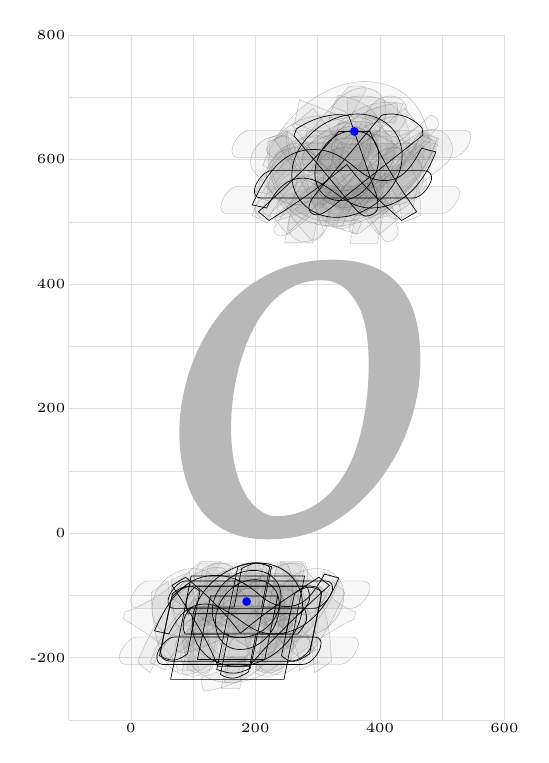
\begin{tikzpicture}[x=1pt,y=1pt,scale=0.225]
\draw[black!12,line width=0.1pt,step=100] (-100,-300) grid (600,800);
\node[left,font=\tiny,inner sep=1pt] at (-100,-200) {-200};
\node[left,font=\tiny,inner sep=1pt] at (-100,0) {0};
\node[left,font=\tiny,inner sep=1pt] at (-100,200) {200};
\node[left,font=\tiny,inner sep=1pt] at (-100,400) {400};
\node[left,font=\tiny,inner sep=1pt] at (-100,600) {600};
\node[left,font=\tiny,inner sep=1pt] at (-100,800) {800};
\node[below,font=\tiny,inner sep=1pt] at (0,-300) {0};
\node[below,font=\tiny,inner sep=1pt] at (200,-300) {200};
\node[below,font=\tiny,inner sep=1pt] at (400,-300) {400};
\node[below,font=\tiny,inner sep=1pt] at (600,-300) {600};
\fill[black!28,even odd rule] (78,162) .. controls (78,109) and (91,-10) .. (218,-10) .. controls (250,-10) and (281,-6) .. (310,9) .. controls (397,53) and (465,159) .. (465,277) .. controls (465,349) and (447,439) .. (324,439) .. controls (157,439) and (78,282) .. (78,162) -- cycle (161,170) .. controls (161,260) and (200,406) .. (306,406) .. controls (336,406) and (352,390) .. (367,362) .. controls (379,337) and (382,300) .. (382,270) .. controls (382,230) and (376,144) .. (339,88) .. controls (311,45) and (271,27) .. (233,27) .. controls (204,27) and (161,65) .. (161,170) -- cycle;
\filldraw[draw=black!35,line width=0.1pt,fill=black,fill opacity=0.03,draw opacity=1,even odd rule] (250,640) -- (220,628) .. controls (217,543) and (258,493) .. (328,493) .. controls (387,493) and (461,542) .. (490,628) -- (466,640) .. controls (444,582) and (391,550) .. (339,550) .. controls (285,550) and (250,587) .. (250,640) -- cycle;
\filldraw[draw=black!35,line width=0.1pt,fill=black,fill opacity=0.03,draw opacity=1,even odd rule] (295,571) .. controls (295,545) and (317,523) .. (343,523) .. controls (369,523) and (391,545) .. (391,571) .. controls (391,597) and (369,619) .. (343,619) .. controls (317,619) and (295,597) .. (295,571) -- cycle;
\filldraw[draw=black!35,line width=0.1pt,fill=black,fill opacity=0.03,draw opacity=1,even odd rule] (218,573) .. controls (218,548) and (239,527) .. (264,527) .. controls (289,527) and (310,548) .. (310,573) .. controls (310,598) and (289,619) .. (264,619) .. controls (239,619) and (218,598) .. (218,573) -- cycle (378,573) .. controls (378,548) and (399,527) .. (424,527) .. controls (449,527) and (470,548) .. (470,573) .. controls (470,598) and (449,619) .. (424,619) .. controls (399,619) and (378,598) .. (378,573) -- cycle;
\filldraw[draw=black!35,line width=0.1pt,fill=black,fill opacity=0.03,draw opacity=1,even odd rule] (422,603) .. controls (426,620) and (418,661) .. (363,661) .. controls (321,661) and (281,626) .. (276,604) .. controls (274,592) and (279,577) .. (298,577) .. controls (307,577) and (322,587) .. (324,598) .. controls (325,605) and (324,610) .. (324,613) .. controls (324,614) and (324,614) .. (324,615) .. controls (323,617) and (322,619) .. (323,623) .. controls (324,628) and (330,634) .. (349,634) .. controls (370,634) and (376,624) .. (372,601) .. controls (369,589) and (362,577) .. (351,565) .. controls (337,548) and (319,526) .. (312,492) -- (340,492) .. controls (347,518) and (360,535) .. (381,551) .. controls (400,567) and (418,583) .. (422,603) -- cycle;
\filldraw[draw=black!35,line width=0.1pt,fill=black,fill opacity=0.03,draw opacity=1,even odd rule] (516,611) .. controls (519,630) and (506,648) .. (485,648) .. controls (473,648) and (466,645) .. (459,636) -- (352,497) .. controls (351,496) and (351,494) .. (351,493) .. controls (349,485) and (357,480) .. (362,480) .. controls (364,480) and (366,480) .. (368,482) -- (505,592) .. controls (512,598) and (514,605) .. (516,611) -- cycle (385,617) .. controls (389,638) and (375,653) .. (354,653) .. controls (350,653) and (334,652) .. (325,639) -- (232,493) .. controls (230,492) and (230,491) .. (230,490) .. controls (228,482) and (235,477) .. (241,477) .. controls (244,477) and (248,478) .. (250,480) -- (377,601) .. controls (382,606) and (384,612) .. (385,617) -- cycle;
\filldraw[draw=black!35,line width=0.1pt,fill=black,fill opacity=0.03,draw opacity=1,even odd rule] (304,502) -- (354,502) .. controls (393,548) and (440,593) .. (483,632) -- (467,645) .. controls (424,618) and (385,593) .. (340,555) .. controls (314,591) and (286,616) .. (253,645) -- (230,632) .. controls (257,594) and (285,549) .. (304,502) -- cycle;
\filldraw[draw=black!35,line width=0.1pt,fill=black,fill opacity=0.03,draw opacity=1,even odd rule] (388,660) .. controls (381,665) and (374,667) .. (367,667) .. controls (361,667) and (344,662) .. (333,656) .. controls (329,630) and (323,601) .. (318,577) .. controls (314,556) and (309,531) .. (304,511) .. controls (310,507) and (319,505) .. (326,505) .. controls (332,505) and (348,508) .. (359,515) .. controls (363,544) and (370,574) .. (374,597) .. controls (379,620) and (384,643) .. (388,660) -- cycle;
\filldraw[draw=black!35,line width=0.1pt,fill=black,fill opacity=0.03,draw opacity=1,even odd rule] (375,644) .. controls (344,644) and (329,622) .. (326,608) .. controls (325,603) and (324,597) .. (328,592) -- (406,471) .. controls (407,469) and (409,468) .. (412,468) .. controls (423,468) and (428,478) .. (429,481) .. controls (429,482) and (429,484) .. (429,487) -- (395,630) .. controls (393,639) and (386,644) .. (375,644) -- cycle (238,638) .. controls (214,638) and (196,620) .. (193,602) .. controls (191,596) and (192,589) .. (196,583) -- (287,473) .. controls (289,471) and (291,470) .. (294,470) .. controls (296,470) and (308,474) .. (310,484) .. controls (310,485) and (310,487) .. (309,488) -- (260,627) .. controls (256,636) and (250,638) .. (238,638) -- cycle;
\filldraw[draw=black!35,line width=0.1pt,fill=black,fill opacity=0.03,draw opacity=1,even odd rule] (252,646) -- (222,634) .. controls (219,549) and (260,499) .. (330,499) .. controls (389,499) and (463,548) .. (492,634) -- (468,646) .. controls (446,588) and (393,556) .. (341,556) .. controls (287,556) and (252,593) .. (252,646) -- cycle (319,669) .. controls (314,644) and (330,624) .. (355,624) .. controls (380,624) and (404,644) .. (409,669) .. controls (414,694) and (399,715) .. (374,715) .. controls (349,715) and (324,694) .. (319,669) -- cycle;
\filldraw[draw=black!35,line width=0.1pt,fill=black,fill opacity=0.03,draw opacity=1,even odd rule] (435,498) -- (465,510) .. controls (468,595) and (427,645) .. (357,645) .. controls (298,645) and (224,596) .. (195,510) -- (219,498) .. controls (241,556) and (294,588) .. (346,588) .. controls (400,588) and (435,551) .. (435,498) -- cycle;
\filldraw[draw=black!35,line width=0.1pt,fill=black,fill opacity=0.03,draw opacity=1,even odd rule] (345,508) .. controls (380,508) and (401,533) .. (405,549) .. controls (408,566) and (403,590) .. (363,590) .. controls (357,590) and (352,590) .. (348,589) .. controls (336,588) and (333,588) .. (337,603) .. controls (341,626) and (368,658) .. (427,670) .. controls (429,677) and (430,686) .. (426,690) .. controls (387,685) and (356,668) .. (335,647) .. controls (314,627) and (303,605) .. (298,581) .. controls (291,545) and (306,508) .. (345,508) -- cycle;
\filldraw[draw=black!35,line width=0.1pt,fill=black,fill opacity=0.03,draw opacity=1,even odd rule] (373,580) -- (462,654) -- (440,682) -- (351,608) -- (293,682) -- (259,654) -- (318,580) -- (229,507) -- (252,479) -- (340,552) -- (398,479) -- (432,507) -- cycle;
\filldraw[draw=black!35,line width=0.1pt,fill=black,fill opacity=0.03,draw opacity=1,even odd rule] (361,644) .. controls (358,629) and (347,615) .. (334,602) .. controls (318,586) and (302,569) .. (297,545) .. controls (290,510) and (313,492) .. (363,481) -- (371,500) .. controls (343,508) and (332,518) .. (337,539) .. controls (339,553) and (352,568) .. (365,582) .. controls (380,599) and (394,616) .. (398,634) .. controls (406,670) and (384,694) .. (333,703) -- (324,684) .. controls (359,673) and (365,662) .. (361,644) -- cycle;
\filldraw[draw=black!35,line width=0.1pt,fill=black,fill opacity=0.03,draw opacity=1,even odd rule] (517,603) .. controls (530,603) and (544,621) .. (546,633) .. controls (547,640) and (545,647) .. (536,647) -- (191,647) .. controls (179,647) and (165,630) .. (163,618) .. controls (161,611) and (164,603) .. (172,603) -- cycle (499,513) .. controls (512,513) and (525,531) .. (528,543) .. controls (529,550) and (526,557) .. (517,557) -- (172,557) .. controls (160,557) and (147,540) .. (145,528) .. controls (143,521) and (146,513) .. (154,513) -- cycle;
\filldraw[draw=black!35,line width=0.1pt,fill=black,fill opacity=0.03,draw opacity=1,even odd rule] (292,466) -- (328,645) -- (283,645) -- (247,466) -- cycle (396,465) -- (432,645) -- (388,645) -- (352,465) -- cycle;
\filldraw[draw=black!35,line width=0.1pt,fill=black,fill opacity=0.03,draw opacity=1,even odd rule] (256,517) -- (270,582) -- (422,582) -- (408,514) .. controls (414,508) and (420,505) .. (426,505) .. controls (433,505) and (441,509) .. (452,517) -- (470,604) .. controls (473,618) and (471,626) .. (451,626) -- (266,626) .. controls (250,626) and (232,613) .. (230,602) -- (212,514) .. controls (218,511) and (224,507) .. (232,507) .. controls (239,507) and (247,510) .. (256,517) -- cycle;
\filldraw[draw=black!35,line width=0.1pt,fill=black,fill opacity=0.03,draw opacity=1,even odd rule] (330,495) -- (353,544) .. controls (364,538) and (375,534) .. (388,534) .. controls (434,534) and (469,564) .. (493,624) -- (470,630) .. controls (448,588) and (432,578) .. (410,578) .. controls (396,578) and (385,583) .. (375,590) -- (404,653) .. controls (398,662) and (394,667) .. (385,667) .. controls (381,667) and (378,666) .. (373,666) -- (348,611) .. controls (334,621) and (318,628) .. (296,628) .. controls (253,628) and (224,598) .. (198,539) -- (221,534) .. controls (237,567) and (253,582) .. (279,582) .. controls (295,582) and (310,573) .. (325,563) -- (299,506) .. controls (303,498) and (305,494) .. (312,494) .. controls (316,494) and (323,495) .. (330,495) -- cycle;
\filldraw[draw=black!35,line width=0.1pt,fill=black,fill opacity=0.03,draw opacity=1,even odd rule] (412,588) .. controls (393,588) and (378,598) .. (364,610) .. controls (347,624) and (328,638) .. (298,638) .. controls (255,638) and (226,608) .. (200,549) -- (223,544) .. controls (239,577) and (255,592) .. (281,592) .. controls (298,592) and (315,581) .. (331,570) .. controls (349,556) and (368,544) .. (390,544) .. controls (436,544) and (471,574) .. (495,634) -- (472,640) .. controls (450,598) and (434,588) .. (412,588) -- cycle (279,468) .. controls (297,468) and (315,483) .. (319,501) .. controls (323,519) and (311,534) .. (293,534) .. controls (275,534) and (257,519) .. (253,501) .. controls (249,483) and (261,468) .. (279,468) -- cycle (403,636) .. controls (421,636) and (440,651) .. (443,669) .. controls (447,687) and (435,702) .. (417,702) .. controls (399,702) and (381,687) .. (377,669) .. controls (373,651) and (385,636) .. (403,636) -- cycle;
\filldraw[draw=black!35,line width=0.1pt,fill=black,fill opacity=0.03,draw opacity=1,even odd rule] (482,671) .. controls (476,671) and (457,636) .. (413,636) .. controls (393,636) and (333,670) .. (305,670) .. controls (273,670) and (244,651) .. (218,618) -- (218,617) .. controls (217,614) and (218,611) .. (224,607) .. controls (227,603) and (230,600) .. (234,600) .. controls (240,600) and (257,636) .. (294,636) .. controls (327,636) and (379,601) .. (411,601) .. controls (441,601) and (469,621) .. (494,654) .. controls (496,662) and (490,671) .. (482,671) -- cycle (462,575) .. controls (457,575) and (438,541) .. (394,541) .. controls (374,541) and (315,574) .. (286,574) .. controls (255,574) and (225,556) .. (198,523) .. controls (197,517) and (207,504) .. (215,504) .. controls (221,504) and (239,541) .. (275,541) .. controls (305,541) and (360,506) .. (392,506) .. controls (422,506) and (450,525) .. (475,559) .. controls (476,565) and (470,575) .. (462,575) -- cycle;
\filldraw[draw=black!35,line width=0.1pt,fill=black,fill opacity=0.03,draw opacity=1,even odd rule] (414,598) -- (239,538) -- (231,500) -- (480,584) -- (486,611) -- (271,696) -- (263,658) -- cycle;
\filldraw[draw=black!35,line width=0.1pt,fill=black,fill opacity=0.03,draw opacity=1,even odd rule] (301,601) .. controls (291,550) and (326,509) .. (377,509) .. controls (390,509) and (401,511) .. (413,516) -- (407,546) .. controls (400,543) and (392,542) .. (383,542) .. controls (348,542) and (332,570) .. (338,601) .. controls (345,634) and (373,660) .. (407,660) .. controls (413,660) and (418,660) .. (423,658) -- (437,689) .. controls (430,691) and (423,692) .. (414,692) .. controls (362,692) and (312,651) .. (301,601) -- cycle;
\filldraw[draw=black!35,line width=0.1pt,fill=black,fill opacity=0.03,draw opacity=1,even odd rule] (453,578) -- (482,590) .. controls (485,675) and (445,725) .. (375,725) .. controls (316,725) and (242,676) .. (212,590) -- (237,578) .. controls (258,636) and (311,668) .. (363,668) .. controls (417,668) and (452,631) .. (453,578) -- cycle (385,555) .. controls (390,580) and (374,600) .. (349,600) .. controls (324,600) and (300,580) .. (295,555) .. controls (290,530) and (306,509) .. (331,509) .. controls (356,509) and (380,530) .. (385,555) -- cycle;
\filldraw[draw=black!35,line width=0.1pt,fill=black,fill opacity=0.03,draw opacity=1,even odd rule] (446,611) .. controls (457,661) and (423,702) .. (372,702) .. controls (363,702) and (355,701) .. (347,699) -- (349,668) .. controls (354,670) and (359,670) .. (365,670) .. controls (399,670) and (417,644) .. (410,611) .. controls (404,580) and (376,552) .. (341,552) .. controls (332,552) and (326,553) .. (319,556) -- (301,526) .. controls (311,521) and (322,519) .. (335,519) .. controls (386,519) and (436,560) .. (446,611) -- cycle;
\filldraw[draw=black!35,line width=0.1pt,fill=black,fill opacity=0.03,draw opacity=1,even odd rule] (452,608) .. controls (456,613) and (459,617) .. (459,619) .. controls (460,624) and (455,626) .. (444,626) -- (340,626) .. controls (333,626) and (331,627) .. (331,631) .. controls (332,633) and (333,635) .. (335,637) -- (378,712) .. controls (379,716) and (373,718) .. (362,718) .. controls (357,718) and (350,717) .. (348,715) -- (248,598) .. controls (244,594) and (242,591) .. (242,589) .. controls (241,585) and (245,582) .. (256,582) -- (360,582) .. controls (368,582) and (373,581) .. (373,579) .. controls (372,577) and (371,574) .. (369,571) -- (324,497) .. controls (323,493) and (323,489) .. (337,489) .. controls (342,489) and (352,491) .. (355,494) -- cycle;
\filldraw[draw=black!35,line width=0.1pt,fill=black,fill opacity=0.03,draw opacity=1,even odd rule] (69,-96) -- (67,-106) -- (189,-184) .. controls (203,-193) and (210,-196) .. (216,-196) .. controls (223,-196) and (232,-188) .. (233,-182) .. controls (235,-175) and (233,-169) .. (227,-160) -- (150,-57) .. controls (149,-56) and (144,-55) .. (140,-55) .. controls (111,-55) and (84,-78) .. (69,-96) -- cycle;
\filldraw[draw=black!35,line width=0.1pt,fill=black,fill opacity=0.03,draw opacity=1,even odd rule] (84,-192) .. controls (89,-192) and (96,-191) .. (105,-187) -- (247,-131) .. controls (251,-128) and (256,-115) .. (258,-107) .. controls (263,-79) and (257,-60) .. (251,-50) -- (242,-46) -- (101,-149) .. controls (87,-160) and (74,-169) .. (72,-178) .. controls (72,-181) and (71,-192) .. (84,-192) -- cycle;
\filldraw[draw=black!35,line width=0.1pt,fill=black,fill opacity=0.03,draw opacity=1,even odd rule] (244,-221) -- (279,-53) .. controls (274,-50) and (269,-48) .. (262,-48) .. controls (255,-48) and (245,-50) .. (234,-55) -- (222,-117) -- (114,-117) .. controls (105,-123) and (101,-131) .. (99,-139) .. controls (98,-146) and (99,-154) .. (102,-160) -- (213,-160) -- (200,-225) .. controls (206,-228) and (212,-230) .. (219,-230) .. controls (226,-230) and (234,-227) .. (244,-221) -- cycle;
\filldraw[draw=black!35,line width=0.1pt,fill=black,fill opacity=0.03,draw opacity=1,even odd rule] (116,-57) -- (82,-225) .. controls (86,-228) and (92,-230) .. (99,-230) .. controls (106,-230) and (115,-228) .. (126,-223) -- (139,-161) -- (247,-161) .. controls (255,-155) and (260,-147) .. (261,-139) .. controls (263,-132) and (261,-124) .. (259,-118) -- (148,-118) -- (161,-53) .. controls (154,-50) and (149,-48) .. (142,-48) .. controls (135,-48) and (126,-51) .. (116,-57) -- cycle;
\filldraw[draw=black!35,line width=0.1pt,fill=black,fill opacity=0.03,draw opacity=1,even odd rule] (125,-145) .. controls (131,-116) and (152,-89) .. (196,-89) .. controls (198,-89) and (201,-90) .. (204,-90) -- (214,-49) .. controls (211,-48) and (207,-48) .. (203,-48) .. controls (148,-48) and (96,-90) .. (85,-145) .. controls (74,-198) and (106,-240) .. (159,-240) .. controls (164,-240) and (169,-240) .. (175,-239) -- (184,-200) .. controls (182,-200) and (178,-201) .. (175,-201) .. controls (130,-201) and (118,-176) .. (125,-145) -- cycle;
\filldraw[draw=black!35,line width=0.1pt,fill=black,fill opacity=0.03,draw opacity=1,even odd rule] (35,-111) .. controls (29,-142) and (47,-165) .. (78,-165) .. controls (109,-165) and (137,-142) .. (143,-111) .. controls (149,-80) and (131,-57) .. (100,-57) .. controls (69,-57) and (41,-80) .. (35,-111) -- cycle (233,-111) .. controls (227,-142) and (245,-165) .. (276,-165) .. controls (307,-165) and (335,-142) .. (341,-111) .. controls (347,-80) and (329,-57) .. (298,-57) .. controls (267,-57) and (239,-80) .. (233,-111) -- cycle;
\filldraw[draw=black!35,line width=0.1pt,fill=black,fill opacity=0.03,draw opacity=1,even odd rule] (200,-69) .. controls (171,-69) and (146,-88) .. (141,-112) .. controls (135,-139) and (159,-148) .. (175,-151) .. controls (193,-153) and (205,-157) .. (201,-177) .. controls (197,-195) and (166,-219) .. (115,-230) .. controls (113,-239) and (113,-248) .. (118,-254) .. controls (177,-245) and (232,-215) .. (244,-155) .. controls (255,-103) and (238,-69) .. (200,-69) -- cycle;
\filldraw[draw=black!35,line width=0.1pt,fill=black,fill opacity=0.03,draw opacity=1,even odd rule] (324,-78) .. controls (311,-107) and (283,-163) .. (247,-163) .. controls (220,-163) and (205,-129) .. (202,-76) .. controls (200,-75) and (196,-75) .. (192,-75) .. controls (189,-75) and (186,-75) .. (183,-76) .. controls (146,-156) and (114,-163) .. (101,-163) .. controls (73,-163) and (63,-130) .. (60,-78) .. controls (57,-79) and (37,-92) .. (33,-96) .. controls (35,-181) and (56,-227) .. (89,-227) .. controls (103,-227) and (139,-216) .. (179,-146) .. controls (188,-217) and (221,-227) .. (235,-227) .. controls (270,-227) and (311,-172) .. (344,-96) .. controls (341,-91) and (328,-81) .. (324,-78) -- cycle;
\filldraw[draw=black!35,line width=0.1pt,fill=black,fill opacity=0.03,draw opacity=1,even odd rule] (222,-59) -- (172,-59) .. controls (133,-104) and (86,-149) .. (43,-188) -- (60,-202) .. controls (103,-175) and (141,-150) .. (186,-112) .. controls (211,-148) and (240,-173) .. (273,-202) -- (297,-188) .. controls (270,-148) and (241,-105) .. (222,-59) -- cycle;
\filldraw[draw=black!35,line width=0.1pt,fill=black,fill opacity=0.03,draw opacity=1,even odd rule] (94,-63) -- (65,-75) .. controls (61,-160) and (102,-210) .. (172,-210) .. controls (231,-210) and (305,-161) .. (335,-75) -- (310,-63) .. controls (288,-121) and (236,-153) .. (184,-153) .. controls (130,-153) and (94,-116) .. (94,-63) -- cycle;
\filldraw[draw=black!35,line width=0.1pt,fill=black,fill opacity=0.03,draw opacity=1,even odd rule] (271,-220) -- (300,-208) .. controls (304,-123) and (263,-73) .. (193,-73) .. controls (134,-73) and (60,-122) .. (31,-208) -- (55,-220) .. controls (77,-162) and (129,-130) .. (181,-130) .. controls (235,-130) and (271,-167) .. (271,-220) -- cycle;
\filldraw[draw=black!35,line width=0.1pt,fill=black,fill opacity=0.03,draw opacity=1,even odd rule] (84,-210) -- (252,-210) .. controls (256,-205) and (259,-199) .. (260,-192) .. controls (262,-185) and (262,-176) .. (259,-166) -- (197,-166) -- (219,-58) .. controls (214,-51) and (207,-48) .. (199,-48) .. controls (192,-48) and (183,-51) .. (176,-55) -- (154,-166) -- (89,-166) .. controls (84,-173) and (81,-179) .. (80,-186) .. controls (78,-193) and (79,-201) .. (84,-210) -- cycle;
\filldraw[draw=black!35,line width=0.1pt,fill=black,fill opacity=0.03,draw opacity=1,even odd rule] (280,-48) -- (112,-48) .. controls (108,-53) and (104,-59) .. (103,-66) .. controls (102,-73) and (102,-82) .. (105,-92) -- (167,-92) -- (145,-200) .. controls (149,-207) and (157,-210) .. (165,-210) .. controls (172,-210) and (180,-207) .. (187,-203) -- (210,-92) -- (275,-92) .. controls (279,-85) and (282,-79) .. (284,-72) .. controls (285,-65) and (284,-57) .. (280,-48) -- cycle;
\filldraw[draw=black!35,line width=0.1pt,fill=black,fill opacity=0.03,draw opacity=1,even odd rule] (282,-131) .. controls (295,-131) and (309,-113) .. (312,-101) .. controls (313,-94) and (310,-87) .. (301,-87) -- (96,-87) .. controls (84,-87) and (71,-104) .. (68,-116) .. controls (67,-123) and (69,-131) .. (77,-131) -- cycle;
\filldraw[draw=black!35,line width=0.1pt,fill=black,fill opacity=0.03,draw opacity=1,even odd rule] (239,-143) .. controls (233,-172) and (212,-199) .. (168,-199) .. controls (166,-199) and (163,-198) .. (160,-198) -- (150,-239) .. controls (152,-240) and (156,-240) .. (160,-240) .. controls (215,-240) and (268,-198) .. (279,-143) .. controls (290,-90) and (257,-48) .. (204,-48) .. controls (199,-48) and (194,-48) .. (189,-49) -- (180,-88) .. controls (182,-88) and (186,-87) .. (189,-87) .. controls (234,-87) and (245,-112) .. (239,-143) -- cycle;
\filldraw[draw=black!35,line width=0.1pt,fill=black,fill opacity=0.03,draw opacity=1,even odd rule] (31,-224) .. controls (44,-195) and (71,-139) .. (107,-139) .. controls (134,-139) and (149,-173) .. (152,-226) .. controls (154,-227) and (158,-227) .. (162,-227) .. controls (165,-227) and (168,-227) .. (171,-226) .. controls (209,-146) and (240,-139) .. (253,-139) .. controls (281,-139) and (291,-172) .. (295,-224) .. controls (297,-223) and (318,-210) .. (322,-206) .. controls (320,-121) and (298,-75) .. (265,-75) .. controls (251,-75) and (216,-86) .. (176,-156) .. controls (166,-85) and (133,-75) .. (119,-75) .. controls (84,-75) and (43,-130) .. (11,-206) .. controls (14,-211) and (26,-221) .. (31,-224) -- cycle;
\filldraw[draw=black!35,line width=0.1pt,fill=black,fill opacity=0.03,draw opacity=1,even odd rule] (336,-211) .. controls (349,-211) and (363,-193) .. (365,-181) .. controls (367,-174) and (364,-167) .. (355,-167) -- (10,-167) .. controls (-2,-167) and (-15,-184) .. (-18,-196) .. controls (-19,-203) and (-17,-211) .. (-9,-211) -- cycle (354,-121) .. controls (367,-121) and (381,-103) .. (384,-91) .. controls (385,-84) and (382,-77) .. (373,-77) -- (28,-77) .. controls (16,-77) and (3,-94) .. (0,-106) .. controls (-1,-113) and (1,-121) .. (9,-121) -- cycle;
\filldraw[draw=black!35,line width=0.1pt,fill=black,fill opacity=0.03,draw opacity=1,even odd rule] (241,-217) -- (274,-54) .. controls (263,-50) and (263,-48) .. (254,-48) .. controls (247,-48) and (245,-50) .. (234,-54) -- (200,-219) .. controls (212,-223) and (214,-225) .. (222,-225) .. controls (229,-225) and (229,-223) .. (241,-217) -- cycle (131,-217) -- (164,-54) .. controls (153,-50) and (153,-48) .. (144,-48) .. controls (137,-48) and (135,-50) .. (124,-54) -- (90,-219) .. controls (102,-223) and (104,-225) .. (112,-225) .. controls (119,-225) and (119,-223) .. (131,-217) -- cycle;
\filldraw[draw=black!35,line width=0.1pt,fill=black,fill opacity=0.03,draw opacity=1,even odd rule] (137,-65) .. controls (127,-70) and (121,-79) .. (120,-84) .. controls (119,-90) and (119,-95) .. (125,-104) -- (222,-104) -- (208,-174) .. controls (211,-184) and (218,-186) .. (223,-186) .. controls (228,-186) and (239,-181) .. (249,-167) -- (268,-76) -- (258,-65) -- cycle;
\filldraw[draw=black!35,line width=0.1pt,fill=black,fill opacity=0.03,draw opacity=1,even odd rule] (-10,-127) -- (-12,-138) .. controls (41,-170) and (64,-186) .. (76,-221) -- (110,-221) .. controls (102,-189) and (85,-168) .. (71,-149) -- (272,-149) .. controls (250,-169) and (224,-189) .. (203,-221) -- (238,-221) .. controls (272,-190) and (317,-158) .. (359,-138) -- (361,-127) .. controls (315,-109) and (283,-62) .. (274,-46) -- (240,-46) .. controls (247,-81) and (271,-107) .. (278,-119) -- (77,-119) .. controls (87,-109) and (121,-83) .. (145,-46) -- (112,-46) .. controls (94,-62) and (44,-109) .. (-10,-127) -- cycle;
\filldraw[draw=black!35,line width=0.1pt,fill=black,fill opacity=0.03,draw opacity=1,even odd rule] (145,-250) -- (175,-250) -- (199,-133) .. controls (215,-151) and (231,-173) .. (260,-187) -- (267,-152) .. controls (242,-124) and (218,-86) .. (205,-48) -- (194,-48) .. controls (166,-98) and (111,-139) .. (92,-152) -- (85,-186) .. controls (123,-172) and (155,-142) .. (169,-133) -- cycle;
\draw[black,line width=0.25pt] (350,670) .. controls (346,671) and (341,672) .. (336,672) .. controls (302,672) and (275,655) .. (266,649) -- (262,638) -- (353,529) .. controls (366,514) and (372,509) .. (378,509) .. controls (386,509) and (395,515) .. (396,520) .. controls (397,527) and (397,534) .. (394,544) -- cycle;
\draw[black,line width=0.25pt] (403,671) -- (303,552) .. controls (293,539) and (288,535) .. (286,524) .. controls (285,517) and (291,511) .. (298,511) .. controls (305,511) and (313,515) .. (331,530) -- (469,639) -- (468,650) .. controls (449,672) and (424,673) .. (418,673) .. controls (413,673) and (406,672) .. (403,671) -- cycle;
\draw[black,line width=0.25pt] (384,645) -- (334,645) .. controls (295,599) and (249,556) .. (205,516) -- (222,502) .. controls (265,529) and (302,554) .. (347,592) .. controls (374,556) and (402,531) .. (435,502) -- (459,516) .. controls (431,556) and (403,598) .. (384,645) -- cycle;
\draw[black,line width=0.25pt] (407,566) .. controls (388,566) and (373,576) .. (359,588) .. controls (342,602) and (323,616) .. (293,616) .. controls (250,616) and (221,586) .. (195,527) -- (218,522) .. controls (235,555) and (251,570) .. (277,570) .. controls (294,570) and (310,559) .. (326,548) .. controls (344,534) and (363,522) .. (385,522) .. controls (431,522) and (466,552) .. (490,612) -- (467,618) .. controls (445,576) and (429,566) .. (407,566) -- cycle;
\draw[black,line width=0.25pt] (453,538) .. controls (466,538) and (480,556) .. (483,568) .. controls (484,574) and (481,582) .. (471,582) -- (226,582) .. controls (215,582) and (201,565) .. (199,553) .. controls (197,546) and (200,538) .. (209,538) -- cycle;
\draw[black,line width=0.25pt] (260,590) .. controls (251,544) and (284,507) .. (330,507) .. controls (378,507) and (425,545) .. (434,590) .. controls (444,637) and (410,673) .. (364,673) .. controls (318,673) and (269,636) .. (260,590) -- cycle (358,646) .. controls (388,646) and (403,621) .. (397,590) .. controls (391,562) and (367,534) .. (336,534) .. controls (305,534) and (291,562) .. (297,590) .. controls (303,620) and (327,646) .. (358,646) -- cycle;
\draw[black,line width=0.25pt] (283,-86) -- (104,-86) .. controls (96,-92) and (91,-100) .. (90,-107) .. controls (88,-114) and (89,-122) .. (92,-129) -- (273,-129) .. controls (281,-120) and (285,-113) .. (287,-107) .. controls (288,-100) and (286,-93) .. (283,-86) -- cycle;
\draw[black,line width=0.25pt] (132,-114) .. controls (126,-145) and (144,-168) .. (175,-168) .. controls (206,-168) and (234,-145) .. (240,-114) .. controls (246,-83) and (228,-60) .. (197,-60) .. controls (166,-60) and (138,-83) .. (132,-114) -- cycle;
\draw[black,line width=0.25pt] (100,-131) .. controls (91,-177) and (124,-214) .. (170,-214) .. controls (218,-214) and (265,-176) .. (274,-131) .. controls (284,-84) and (250,-48) .. (204,-48) .. controls (158,-48) and (110,-85) .. (100,-131) -- cycle (199,-75) .. controls (229,-75) and (244,-100) .. (237,-131) .. controls (232,-159) and (207,-187) .. (176,-187) .. controls (145,-187) and (132,-159) .. (137,-131) .. controls (143,-101) and (168,-75) .. (199,-75) -- cycle;
\draw[black,line width=0.25pt] (192,-217) -- (226,-54) .. controls (214,-50) and (206,-48) .. (197,-48) .. controls (190,-48) and (182,-50) .. (172,-54) -- (138,-219) .. controls (149,-223) and (157,-225) .. (165,-225) .. controls (172,-225) and (180,-223) .. (192,-217) -- cycle;
\draw[black,line width=0.25pt] (91,-194) -- (104,-129) -- (256,-129) -- (242,-197) .. controls (248,-203) and (255,-206) .. (261,-206) .. controls (268,-206) and (275,-202) .. (287,-194) -- (305,-107) .. controls (307,-93) and (305,-85) .. (285,-85) -- (100,-85) .. controls (84,-85) and (66,-98) .. (64,-109) -- (46,-197) .. controls (53,-200) and (59,-204) .. (67,-204) .. controls (74,-204) and (82,-201) .. (91,-194) -- cycle;
\draw[black,line width=0.25pt] (140,-214) -- (190,-214) .. controls (229,-168) and (276,-123) .. (319,-84) -- (302,-71) .. controls (260,-98) and (221,-123) .. (176,-161) .. controls (149,-125) and (122,-99) .. (88,-71) -- (66,-84) .. controls (93,-124) and (121,-167) .. (140,-214) -- cycle;
\draw[black,line width=0.25pt] (189,-223) -- (201,-162) -- (268,-162) .. controls (276,-153) and (280,-146) .. (282,-140) .. controls (283,-133) and (281,-126) .. (278,-119) -- (210,-119) -- (223,-55) .. controls (216,-50) and (210,-48) .. (203,-48) .. controls (197,-48) and (190,-51) .. (178,-57) -- (166,-119) -- (99,-119) .. controls (91,-125) and (86,-133) .. (85,-140) .. controls (83,-147) and (84,-155) .. (87,-162) -- (157,-162) -- (144,-227) .. controls (150,-231) and (157,-233) .. (164,-233) .. controls (170,-233) and (178,-230) .. (189,-223) -- cycle;
\draw[black,line width=0.25pt] (250,-118) .. controls (231,-118) and (216,-108) .. (203,-96) .. controls (185,-82) and (166,-68) .. (136,-68) .. controls (93,-68) and (64,-98) .. (38,-157) -- (61,-162) .. controls (78,-129) and (94,-114) .. (120,-114) .. controls (137,-114) and (154,-125) .. (170,-136) .. controls (188,-150) and (206,-162) .. (228,-162) .. controls (274,-162) and (309,-132) .. (334,-72) -- (311,-66) .. controls (288,-108) and (272,-118) .. (250,-118) -- cycle;
\draw[black,line width=0.25pt] (276,-211) .. controls (289,-211) and (303,-193) .. (305,-181) .. controls (307,-174) and (304,-167) .. (295,-167) -- (70,-167) .. controls (58,-167) and (45,-184) .. (42,-196) .. controls (41,-203) and (43,-211) .. (51,-211) -- cycle (294,-121) .. controls (307,-121) and (321,-103) .. (324,-91) .. controls (325,-84) and (322,-77) .. (313,-77) -- (88,-77) .. controls (76,-77) and (63,-94) .. (60,-106) .. controls (59,-113) and (61,-121) .. (69,-121) -- cycle;
\draw[black,line width=0.25pt] (263,-97) -- (249,-162) -- (97,-162) -- (111,-94) .. controls (106,-88) and (99,-85) .. (93,-85) .. controls (86,-85) and (78,-89) .. (67,-97) -- (49,-184) .. controls (46,-198) and (49,-206) .. (69,-206) -- (254,-206) .. controls (270,-206) and (287,-193) .. (289,-182) -- (307,-94) .. controls (301,-91) and (295,-87) .. (287,-87) .. controls (280,-87) and (272,-90) .. (263,-97) -- cycle;
\draw[black,line width=0.25pt] (97,-69) -- (64,-235) -- (246,-235) -- (279,-69) -- cycle (128,-101) -- (236,-101) -- (215,-203) -- (107,-203) -- cycle;
\fill[blue] (359,645) circle (7);
\fill[blue] (186,-110) circle (7);
\end{tikzpicture}

		\caption{Mark zones, italic.}
		\label{fig:mark-zones-italic}
	\end{minipage}\hfill
	\begin{minipage}[t]{0.245\textwidth}
		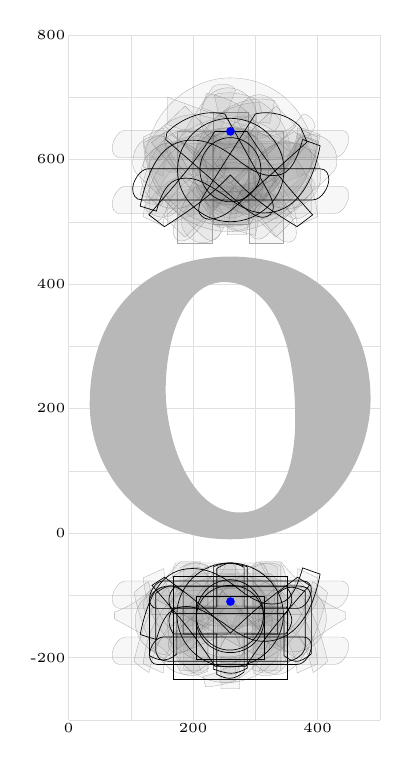
\begin{tikzpicture}[x=1pt,y=1pt,scale=0.225]
\draw[black!12,line width=0.1pt,step=100] (0,-300) grid (500,800);
\node[left,font=\tiny,inner sep=1pt] at (0,-200) {-200};
\node[left,font=\tiny,inner sep=1pt] at (0,0) {0};
\node[left,font=\tiny,inner sep=1pt] at (0,200) {200};
\node[left,font=\tiny,inner sep=1pt] at (0,400) {400};
\node[left,font=\tiny,inner sep=1pt] at (0,600) {600};
\node[left,font=\tiny,inner sep=1pt] at (0,800) {800};
\node[below,font=\tiny,inner sep=1pt] at (0,-300) {0};
\node[below,font=\tiny,inner sep=1pt] at (200,-300) {200};
\node[below,font=\tiny,inner sep=1pt] at (400,-300) {400};
\fill[black!28,even odd rule] (34,207) .. controls (34,104) and (112,-10) .. (259,-10) .. controls (414,-10) and (485,115) .. (485,216) .. controls (485,321) and (423,444) .. (260,444) .. controls (115,444) and (34,344) .. (34,207) -- cycle (250,403) .. controls (318,403) and (364,327) .. (364,184) .. controls (364,57) and (311,33) .. (275,33) .. controls (193,33) and (156,155) .. (156,229) .. controls (156,314) and (186,403) .. (250,403) -- cycle;
\filldraw[draw=black!35,line width=0.1pt,fill=black,fill opacity=0.03,draw opacity=1,even odd rule] (153,642) -- (120,627) .. controls (127,546) and (180,484) .. (261,484) .. controls (312,484) and (390,522) .. (400,627) -- (368,642) .. controls (365,578) and (308,548) .. (261,548) .. controls (198,548) and (155,588) .. (153,642) -- cycle;
\filldraw[draw=black!35,line width=0.1pt,fill=black,fill opacity=0.03,draw opacity=1,even odd rule] (198,589) .. controls (198,555) and (226,527) .. (260,527) .. controls (294,527) and (322,555) .. (322,589) .. controls (322,623) and (294,651) .. (260,651) .. controls (226,651) and (198,623) .. (198,589) -- cycle;
\filldraw[draw=black!35,line width=0.1pt,fill=black,fill opacity=0.03,draw opacity=1,even odd rule] (116,574) .. controls (116,545) and (141,521) .. (170,521) .. controls (200,521) and (224,545) .. (224,574) .. controls (224,604) and (200,628) .. (170,628) .. controls (141,628) and (116,604) .. (116,574) -- cycle (297,574) .. controls (297,545) and (321,521) .. (351,521) .. controls (380,521) and (405,545) .. (405,574) .. controls (405,604) and (380,628) .. (351,628) .. controls (321,628) and (297,604) .. (297,574) -- cycle;
\filldraw[draw=black!35,line width=0.1pt,fill=black,fill opacity=0.03,draw opacity=1,even odd rule] (347,592) .. controls (347,608) and (330,648) .. (276,648) .. controls (234,648) and (200,614) .. (200,592) .. controls (200,581) and (208,564) .. (226,564) .. controls (235,564) and (252,571) .. (252,585) .. controls (252,592) and (247,600) .. (245,602) .. controls (244,604) and (243,607) .. (243,610) .. controls (243,615) and (250,620) .. (267,620) .. controls (285,620) and (293,612) .. (293,589) .. controls (293,577) and (288,566) .. (280,554) .. controls (269,536) and (256,514) .. (255,479) -- (286,479) .. controls (287,505) and (300,523) .. (318,540) .. controls (334,555) and (347,571) .. (347,592) -- cycle;
\filldraw[draw=black!35,line width=0.1pt,fill=black,fill opacity=0.03,draw opacity=1,even odd rule] (302,609) .. controls (302,628) and (282,645) .. (260,645) .. controls (249,645) and (235,643) .. (230,632) -- (171,498) .. controls (169,493) and (168,489) .. (168,485) .. controls (168,475) and (173,469) .. (181,469) .. controls (188,469) and (196,473) .. (205,484) -- (297,593) .. controls (301,598) and (302,604) .. (302,609) -- cycle (431,597) .. controls (431,621) and (415,640) .. (390,640) .. controls (371,640) and (364,625) .. (362,622) -- (294,501) .. controls (291,496) and (290,491) .. (290,487) .. controls (290,478) and (298,472) .. (305,472) .. controls (310,472) and (315,475) .. (320,480) -- (418,573) .. controls (426,580) and (431,585) .. (431,597) -- cycle;
\filldraw[draw=black!35,line width=0.1pt,fill=black,fill opacity=0.03,draw opacity=1,even odd rule] (285,498) .. controls (314,545) and (350,587) .. (386,627) -- (362,645) .. controls (323,618) and (293,597) .. (259,561) .. controls (222,599) and (196,618) .. (157,645) -- (133,627) .. controls (168,587) and (206,544) .. (235,498) -- cycle;
\filldraw[draw=black!35,line width=0.1pt,fill=black,fill opacity=0.03,draw opacity=1,even odd rule] (288,496) -- (288,676) -- (232,676) -- (232,496) -- cycle;
\filldraw[draw=black!35,line width=0.1pt,fill=black,fill opacity=0.03,draw opacity=1,even odd rule] (232,607) .. controls (232,602) and (233,596) .. (237,591) -- (329,482) .. controls (338,471) and (346,467) .. (353,467) .. controls (361,467) and (366,473) .. (366,482) .. controls (366,486) and (365,491) .. (363,496) -- (304,630) .. controls (299,641) and (285,643) .. (274,643) .. controls (252,643) and (232,626) .. (232,607) -- cycle (103,595) .. controls (103,583) and (108,578) .. (116,570) -- (214,478) .. controls (219,473) and (224,470) .. (229,470) .. controls (237,470) and (244,476) .. (244,485) .. controls (244,489) and (243,494) .. (240,499) -- (172,620) .. controls (170,623) and (163,638) .. (144,638) .. controls (119,638) and (103,619) .. (103,595) -- cycle;
\filldraw[draw=black!35,line width=0.1pt,fill=black,fill opacity=0.03,draw opacity=1,even odd rule] (153,651) -- (120,636) .. controls (127,555) and (180,493) .. (261,493) .. controls (312,493) and (390,531) .. (400,636) -- (368,651) .. controls (365,587) and (308,557) .. (261,557) .. controls (198,557) and (155,597) .. (153,651) -- cycle (211,669) .. controls (211,644) and (231,624) .. (256,624) .. controls (281,624) and (302,644) .. (302,669) .. controls (302,694) and (281,715) .. (256,715) .. controls (231,715) and (211,694) .. (211,669) -- cycle;
\filldraw[draw=black!35,line width=0.1pt,fill=black,fill opacity=0.03,draw opacity=1,even odd rule] (367,493) -- (400,508) .. controls (393,589) and (340,651) .. (259,651) .. controls (208,651) and (130,613) .. (120,508) -- (152,493) .. controls (155,557) and (212,587) .. (259,587) .. controls (322,587) and (365,547) .. (367,493) -- cycle;
\filldraw[draw=black!35,line width=0.1pt,fill=black,fill opacity=0.03,draw opacity=1,even odd rule] (261,513) .. controls (296,513) and (312,537) .. (312,553) .. controls (312,570) and (302,595) .. (262,595) .. controls (254,595) and (244,592) .. (232,586) .. controls (232,589) and (231,592) .. (231,596) .. controls (231,600) and (233,660) .. (310,675) -- (306,692) .. controls (216,688) and (199,612) .. (199,586) .. controls (199,550) and (222,513) .. (261,513) -- cycle;
\filldraw[draw=black!35,line width=0.1pt,fill=black,fill opacity=0.03,draw opacity=1,even odd rule] (291,580) -- (365,654) -- (333,686) -- (260,612) -- (187,686) -- (154,654) -- (228,580) -- (154,507) -- (187,475) -- (260,548) -- (333,475) -- (365,507) -- cycle;
\filldraw[draw=black!35,line width=0.1pt,fill=black,fill opacity=0.03,draw opacity=1,even odd rule] (262,644) .. controls (262,629) and (253,616) .. (242,603) .. controls (230,587) and (218,569) .. (218,545) .. controls (218,510) and (248,489) .. (300,478) -- (305,502) .. controls (276,510) and (262,518) .. (262,539) .. controls (262,553) and (272,567) .. (281,581) .. controls (294,598) and (304,616) .. (304,634) .. controls (304,670) and (274,697) .. (221,706) -- (215,682) .. controls (252,671) and (262,662) .. (262,644) -- cycle;
\filldraw[draw=black!35,line width=0.1pt,fill=black,fill opacity=0.03,draw opacity=1,even odd rule] (427,513) .. controls (440,513) and (450,531) .. (450,543) .. controls (450,550) and (446,557) .. (437,557) -- (92,557) .. controls (80,557) and (70,540) .. (70,528) .. controls (70,521) and (74,513) .. (82,513) -- cycle (427,603) .. controls (440,603) and (450,621) .. (450,633) .. controls (450,640) and (446,647) .. (437,647) -- (92,647) .. controls (80,647) and (70,630) .. (70,618) .. controls (70,611) and (74,603) .. (82,603) -- cycle;
\filldraw[draw=black!35,line width=0.1pt,fill=black,fill opacity=0.03,draw opacity=1,even odd rule] (345,465) -- (345,645) -- (290,645) -- (290,465) -- cycle (230,466) -- (230,645) -- (175,645) -- (175,466) -- cycle;
\filldraw[draw=black!35,line width=0.1pt,fill=black,fill opacity=0.03,draw opacity=1,even odd rule] (174,517) -- (174,582) -- (346,582) -- (346,514) .. controls (362,502) and (370,501) .. (390,517) -- (390,604) .. controls (390,618) and (386,626) .. (366,626) -- (161,626) .. controls (145,626) and (130,613) .. (130,602) -- (130,514) .. controls (141,508) and (157,501) .. (174,517) -- cycle;
\filldraw[draw=black!35,line width=0.1pt,fill=black,fill opacity=0.03,draw opacity=1,even odd rule] (264,492) -- (277,537) .. controls (289,529) and (299,525) .. (312,525) .. controls (358,525) and (390,568) .. (402,628) .. controls (396,632) and (381,637) .. (370,636) .. controls (356,594) and (347,584) .. (325,584) .. controls (312,584) and (302,586) .. (291,592) -- (307,654) .. controls (299,663) and (291,670) .. (282,670) .. controls (278,670) and (274,669) .. (269,669) -- (255,617) .. controls (239,628) and (223,637) .. (201,637) .. controls (158,637) and (132,594) .. (118,535) .. controls (124,529) and (139,526) .. (150,528) .. controls (160,561) and (168,576) .. (194,576) .. controls (210,576) and (224,570) .. (241,561) -- (226,505) .. controls (232,497) and (238,491) .. (244,491) .. controls (248,491) and (257,492) .. (264,492) -- cycle;
\filldraw[draw=black!35,line width=0.1pt,fill=black,fill opacity=0.03,draw opacity=1,even odd rule] (327,592) .. controls (307,592) and (290,603) .. (272,617) .. controls (252,633) and (229,649) .. (198,649) .. controls (153,649) and (129,611) .. (115,543) -- (141,535) .. controls (152,573) and (163,588) .. (190,588) .. controls (208,588) and (228,575) .. (248,562) .. controls (268,547) and (290,532) .. (313,532) .. controls (361,532) and (391,572) .. (404,640) -- (376,650) .. controls (362,601) and (349,592) .. (327,592) -- cycle (216,466) .. controls (234,466) and (251,483) .. (251,501) .. controls (251,519) and (234,536) .. (216,536) .. controls (198,536) and (181,519) .. (181,501) .. controls (181,483) and (198,466) .. (216,466) -- cycle (306,634) .. controls (324,634) and (341,651) .. (341,669) .. controls (341,687) and (324,704) .. (306,704) .. controls (288,704) and (271,687) .. (271,669) .. controls (271,651) and (288,634) .. (306,634) -- cycle;
\filldraw[draw=black!35,line width=0.1pt,fill=black,fill opacity=0.03,draw opacity=1,even odd rule] (378,673) .. controls (372,673) and (361,638) .. (317,638) .. controls (297,638) and (230,672) .. (202,672) .. controls (170,672) and (143,652) .. (123,619) -- (123,617) .. controls (123,614) and (126,609) .. (132,605) .. controls (136,601) and (141,598) .. (145,598) .. controls (151,598) and (161,634) .. (198,634) .. controls (231,634) and (290,599) .. (322,599) .. controls (352,599) and (378,620) .. (396,653) .. controls (396,661) and (386,673) .. (378,673) -- cycle (378,577) .. controls (373,577) and (361,543) .. (317,543) .. controls (297,543) and (231,576) .. (202,576) .. controls (171,576) and (143,557) .. (123,524) .. controls (123,518) and (137,502) .. (145,502) .. controls (151,502) and (162,539) .. (198,539) .. controls (228,539) and (290,504) .. (322,504) .. controls (352,504) and (378,524) .. (396,558) .. controls (396,564) and (386,577) .. (378,577) -- cycle;
\filldraw[draw=black!35,line width=0.1pt,fill=black,fill opacity=0.03,draw opacity=1,even odd rule] (322,598) -- (159,540) -- (159,496) -- (397,582) -- (397,613) -- (159,700) -- (159,656) -- cycle;
\filldraw[draw=black!35,line width=0.1pt,fill=black,fill opacity=0.03,draw opacity=1,even odd rule] (209,603) .. controls (209,552) and (256,509) .. (307,509) .. controls (320,509) and (331,511) .. (342,515) -- (330,551) .. controls (323,548) and (316,546) .. (307,546) .. controls (272,546) and (254,572) .. (254,603) .. controls (254,636) and (273,660) .. (307,660) .. controls (313,660) and (318,659) .. (323,658) -- (331,694) .. controls (323,696) and (316,697) .. (307,697) .. controls (255,697) and (209,653) .. (209,603) -- cycle;
\filldraw[draw=black!35,line width=0.1pt,fill=black,fill opacity=0.03,draw opacity=1,even odd rule] (367,573) -- (400,588) .. controls (393,669) and (340,731) .. (259,731) .. controls (208,731) and (130,693) .. (120,588) -- (152,573) .. controls (155,637) and (212,667) .. (259,667) .. controls (322,667) and (365,627) .. (367,573) -- cycle (308,555) .. controls (308,580) and (285,603) .. (260,603) .. controls (235,603) and (212,580) .. (212,555) .. controls (212,530) and (235,506) .. (260,506) .. controls (285,506) and (308,530) .. (308,555) -- cycle;
\filldraw[draw=black!35,line width=0.1pt,fill=black,fill opacity=0.03,draw opacity=1,even odd rule] (356,613) .. controls (356,663) and (309,707) .. (258,707) .. controls (249,707) and (241,706) .. (234,704) -- (242,668) .. controls (247,669) and (252,670) .. (258,670) .. controls (292,670) and (310,646) .. (310,613) .. controls (310,582) and (293,556) .. (258,556) .. controls (249,556) and (242,558) .. (235,561) -- (223,525) .. controls (234,521) and (245,519) .. (258,519) .. controls (309,519) and (356,562) .. (356,613) -- cycle;
\filldraw[draw=black!35,line width=0.1pt,fill=black,fill opacity=0.03,draw opacity=1,even odd rule] (363,606) .. controls (366,611) and (368,617) .. (368,619) .. controls (368,624) and (360,629) .. (349,629) -- (245,629) .. controls (238,629) and (238,627) .. (238,631) .. controls (238,633) and (239,634) .. (240,636) -- (268,711) .. controls (268,715) and (259,721) .. (248,721) .. controls (243,721) and (234,719) .. (232,717) -- (156,600) .. controls (153,596) and (151,591) .. (151,589) .. controls (151,585) and (159,579) .. (170,579) -- (274,579) .. controls (282,579) and (284,581) .. (284,579) .. controls (284,577) and (283,575) .. (282,572) -- (252,498) .. controls (252,494) and (255,486) .. (269,486) .. controls (274,486) and (287,489) .. (289,492) -- cycle;
\filldraw[draw=black!35,line width=0.1pt,fill=black,fill opacity=0.03,draw opacity=1,even odd rule] (140,-96) -- (140,-106) -- (278,-184) .. controls (294,-192) and (302,-196) .. (308,-196) .. controls (316,-196) and (323,-188) .. (323,-183) .. controls (323,-180) and (319,-169) .. (311,-160) -- (212,-56) .. controls (211,-55) and (209,-55) .. (208,-55) .. controls (171,-55) and (140,-96) .. (140,-96) -- cycle;
\filldraw[draw=black!35,line width=0.1pt,fill=black,fill opacity=0.03,draw opacity=1,even odd rule] (174,-192) .. controls (179,-192) and (186,-191) .. (194,-187) -- (325,-131) .. controls (328,-128) and (331,-115) .. (331,-107) .. controls (331,-78) and (313,-50) .. (313,-50) -- (303,-46) -- (183,-149) .. controls (171,-160) and (160,-169) .. (160,-178) .. controls (160,-181) and (161,-192) .. (174,-192) -- cycle;
\filldraw[draw=black!35,line width=0.1pt,fill=black,fill opacity=0.03,draw opacity=1,even odd rule] (341,-221) -- (341,-53) .. controls (329,-46) and (316,-46) .. (297,-55) -- (297,-117) -- (189,-117) .. controls (177,-129) and (177,-145) .. (186,-160) -- (297,-160) -- (297,-225) .. controls (313,-231) and (324,-232) .. (341,-221) -- cycle;
\filldraw[draw=black!35,line width=0.1pt,fill=black,fill opacity=0.03,draw opacity=1,even odd rule] (179,-56) -- (179,-224) .. controls (191,-231) and (204,-231) .. (223,-222) -- (223,-160) -- (331,-160) .. controls (343,-148) and (343,-132) .. (334,-117) -- (223,-117) -- (223,-52) .. controls (207,-46) and (196,-45) .. (179,-56) -- cycle;
\filldraw[draw=black!35,line width=0.1pt,fill=black,fill opacity=0.03,draw opacity=1,even odd rule] (199,-145) .. controls (199,-116) and (215,-89) .. (259,-89) .. controls (261,-89) and (264,-90) .. (267,-90) -- (269,-49) .. controls (266,-48) and (262,-48) .. (258,-48) .. controls (203,-48) and (159,-90) .. (159,-145) .. controls (159,-198) and (200,-240) .. (253,-240) .. controls (258,-240) and (263,-240) .. (268,-239) -- (269,-200) .. controls (267,-200) and (264,-201) .. (261,-201) .. controls (216,-201) and (199,-176) .. (199,-145) -- cycle;
\filldraw[draw=black!35,line width=0.1pt,fill=black,fill opacity=0.03,draw opacity=1,even odd rule] (107,-142) .. controls (107,-171) and (130,-196) .. (162,-196) .. controls (191,-196) and (216,-174) .. (216,-142) .. controls (216,-113) and (194,-88) .. (162,-88) .. controls (133,-88) and (107,-109) .. (107,-142) -- cycle (305,-137) .. controls (305,-166) and (328,-191) .. (359,-191) .. controls (389,-191) and (414,-169) .. (414,-137) .. controls (414,-108) and (392,-83) .. (359,-83) .. controls (331,-83) and (305,-104) .. (305,-137) -- cycle;
\filldraw[draw=black!35,line width=0.1pt,fill=black,fill opacity=0.03,draw opacity=1,even odd rule] (265,-69) .. controls (229,-69) and (214,-93) .. (214,-109) .. controls (214,-125) and (223,-150) .. (264,-150) .. controls (272,-150) and (282,-147) .. (293,-141) .. controls (294,-144) and (295,-147) .. (295,-151) .. controls (295,-157) and (292,-215) .. (216,-230) -- (220,-247) .. controls (310,-243) and (327,-167) .. (327,-141) .. controls (327,-106) and (304,-69) .. (265,-69) -- cycle;
\filldraw[draw=black!35,line width=0.1pt,fill=black,fill opacity=0.03,draw opacity=1,even odd rule] (392,-78) .. controls (385,-107) and (369,-163) .. (333,-163) .. controls (306,-163) and (285,-130) .. (270,-76) .. controls (268,-75) and (264,-75) .. (260,-75) .. controls (257,-75) and (254,-75) .. (251,-76) .. controls (230,-156) and (200,-163) .. (187,-163) .. controls (159,-163) and (142,-130) .. (128,-78) .. controls (126,-79) and (108,-92) .. (105,-96) .. controls (124,-181) and (155,-227) .. (188,-227) .. controls (202,-227) and (235,-216) .. (261,-146) .. controls (286,-217) and (320,-227) .. (334,-227) .. controls (369,-227) and (399,-172) .. (416,-96) .. controls (413,-91) and (397,-81) .. (392,-78) -- cycle;
\filldraw[draw=black!35,line width=0.1pt,fill=black,fill opacity=0.03,draw opacity=1,even odd rule] (286,-59) -- (236,-59) .. controls (206,-104) and (168,-149) .. (133,-188) -- (153,-202) .. controls (190,-175) and (223,-150) .. (260,-112) .. controls (293,-148) and (327,-173) .. (366,-202) -- (387,-188) .. controls (352,-148) and (314,-105) .. (286,-59) -- cycle;
\filldraw[draw=black!35,line width=0.1pt,fill=black,fill opacity=0.03,draw opacity=1,even odd rule] (153,-57) -- (120,-72) .. controls (127,-153) and (180,-215) .. (261,-215) .. controls (312,-215) and (390,-177) .. (400,-72) -- (368,-57) .. controls (365,-121) and (308,-151) .. (261,-151) .. controls (198,-151) and (155,-111) .. (153,-57) -- cycle;
\filldraw[draw=black!35,line width=0.1pt,fill=black,fill opacity=0.03,draw opacity=1,even odd rule] (367,-225) -- (400,-210) .. controls (393,-129) and (340,-67) .. (259,-67) .. controls (208,-67) and (130,-105) .. (120,-210) -- (152,-225) .. controls (155,-161) and (212,-131) .. (259,-131) .. controls (322,-131) and (365,-171) .. (367,-225) -- cycle;
\filldraw[draw=black!35,line width=0.1pt,fill=black,fill opacity=0.03,draw opacity=1,even odd rule] (178,-209) -- (346,-209) .. controls (353,-197) and (353,-184) .. (344,-165) -- (282,-165) -- (282,-57) .. controls (270,-45) and (254,-45) .. (239,-54) -- (239,-165) -- (174,-165) .. controls (168,-181) and (167,-192) .. (178,-209) -- cycle;
\filldraw[draw=black!35,line width=0.1pt,fill=black,fill opacity=0.03,draw opacity=1,even odd rule] (340,-48) -- (172,-48) .. controls (165,-60) and (165,-73) .. (174,-92) -- (236,-92) -- (236,-200) .. controls (248,-212) and (264,-212) .. (279,-203) -- (279,-92) -- (344,-92) .. controls (350,-76) and (351,-65) .. (340,-48) -- cycle;
\filldraw[draw=black!35,line width=0.1pt,fill=black,fill opacity=0.03,draw opacity=1,even odd rule] (377,-131) .. controls (390,-131) and (400,-113) .. (400,-101) .. controls (400,-94) and (396,-87) .. (387,-87) -- (142,-87) .. controls (130,-87) and (120,-104) .. (120,-116) .. controls (120,-123) and (124,-131) .. (132,-131) -- cycle;
\filldraw[draw=black!35,line width=0.1pt,fill=black,fill opacity=0.03,draw opacity=1,even odd rule] (313,-143) .. controls (313,-172) and (297,-199) .. (253,-199) .. controls (251,-199) and (248,-198) .. (245,-198) -- (243,-239) .. controls (246,-240) and (250,-240) .. (254,-240) .. controls (309,-240) and (353,-198) .. (353,-143) .. controls (353,-90) and (312,-48) .. (259,-48) .. controls (254,-48) and (249,-48) .. (244,-49) -- (243,-88) .. controls (245,-88) and (248,-87) .. (251,-87) .. controls (296,-87) and (313,-112) .. (313,-143) -- cycle;
\filldraw[draw=black!35,line width=0.1pt,fill=black,fill opacity=0.03,draw opacity=1,even odd rule] (129,-224) .. controls (136,-195) and (152,-139) .. (188,-139) .. controls (215,-139) and (237,-173) .. (251,-226) .. controls (253,-227) and (257,-227) .. (261,-227) .. controls (264,-227) and (267,-227) .. (270,-226) .. controls (291,-146) and (321,-139) .. (334,-139) .. controls (362,-139) and (379,-172) .. (393,-224) .. controls (395,-223) and (413,-210) .. (416,-206) .. controls (397,-121) and (366,-75) .. (333,-75) .. controls (319,-75) and (286,-86) .. (260,-156) .. controls (236,-85) and (201,-75) .. (187,-75) .. controls (152,-75) and (122,-130) .. (105,-206) .. controls (109,-211) and (124,-221) .. (129,-224) -- cycle;
\filldraw[draw=black!35,line width=0.1pt,fill=black,fill opacity=0.03,draw opacity=1,even odd rule] (427,-121) .. controls (440,-121) and (450,-103) .. (450,-91) .. controls (450,-84) and (446,-77) .. (437,-77) -- (92,-77) .. controls (80,-77) and (70,-94) .. (70,-106) .. controls (70,-113) and (74,-121) .. (82,-121) -- cycle (427,-211) .. controls (440,-211) and (450,-193) .. (450,-181) .. controls (450,-174) and (446,-167) .. (437,-167) -- (92,-167) .. controls (80,-167) and (70,-184) .. (70,-196) .. controls (70,-203) and (74,-211) .. (82,-211) -- cycle;
\filldraw[draw=black!35,line width=0.1pt,fill=black,fill opacity=0.03,draw opacity=1,even odd rule] (225,-217) -- (225,-54) .. controls (213,-50) and (213,-48) .. (204,-48) .. controls (197,-48) and (195,-50) .. (185,-54) -- (185,-219) .. controls (197,-223) and (200,-225) .. (208,-225) .. controls (215,-225) and (214,-223) .. (225,-217) -- cycle (335,-217) -- (335,-54) .. controls (323,-50) and (323,-48) .. (314,-48) .. controls (307,-48) and (305,-50) .. (295,-54) -- (295,-219) .. controls (307,-223) and (310,-225) .. (318,-225) .. controls (325,-225) and (324,-223) .. (335,-217) -- cycle;
\filldraw[draw=black!35,line width=0.1pt,fill=black,fill opacity=0.03,draw opacity=1,even odd rule] (203,-65) .. controls (194,-70) and (190,-79) .. (190,-84) .. controls (190,-90) and (191,-95) .. (199,-104) -- (296,-104) -- (296,-174) .. controls (301,-184) and (308,-186) .. (313,-186) .. controls (318,-186) and (328,-181) .. (336,-167) -- (336,-76) -- (324,-65) -- cycle;
\filldraw[draw=black!35,line width=0.1pt,fill=black,fill opacity=0.03,draw opacity=1,even odd rule] (74,-127) -- (74,-138) .. controls (134,-170) and (160,-186) .. (179,-221) -- (213,-221) .. controls (198,-189) and (177,-168) .. (159,-149) -- (360,-149) .. controls (342,-169) and (320,-189) .. (306,-221) -- (341,-221) .. controls (369,-190) and (407,-158) .. (445,-138) -- (445,-127) .. controls (395,-109) and (354,-62) .. (341,-46) -- (307,-46) .. controls (321,-81) and (351,-107) .. (360,-119) -- (159,-119) .. controls (167,-109) and (196,-83) .. (212,-46) -- (179,-46) .. controls (165,-62) and (124,-109) .. (74,-127) -- cycle;
\filldraw[draw=black!35,line width=0.1pt,fill=black,fill opacity=0.03,draw opacity=1,even odd rule] (245,-250) -- (275,-250) -- (275,-133) .. controls (295,-151) and (315,-173) .. (347,-187) -- (347,-152) .. controls (316,-124) and (284,-86) .. (264,-48) -- (253,-48) .. controls (235,-98) and (188,-139) .. (172,-152) -- (172,-186) .. controls (207,-172) and (233,-142) .. (245,-133) -- cycle;
\draw[black,line width=0.25pt] (251,673) .. controls (247,674) and (236,675) .. (231,675) .. controls (195,675) and (166,652) .. (158,643) -- (156,632) -- (277,527) .. controls (294,512) and (304,507) .. (312,507) .. controls (321,507) and (329,514) .. (329,523) .. controls (329,531) and (324,542) .. (320,549) -- cycle;
\draw[black,line width=0.25pt] (300,673) -- (217,542) .. controls (211,533) and (209,524) .. (209,518) .. controls (209,512) and (217,504) .. (225,504) .. controls (235,504) and (249,508) .. (263,520) -- (383,628) -- (373,651) .. controls (365,661) and (346,675) .. (316,675) .. controls (311,675) and (303,674) .. (300,673) -- cycle;
\draw[black,line width=0.25pt] (287,645) -- (235,645) .. controls (205,597) and (165,552) .. (129,511) -- (154,492) .. controls (194,518) and (222,536) .. (260,575) .. controls (295,538) and (324,518) .. (367,492) -- (392,511) .. controls (355,552) and (317,596) .. (287,645) -- cycle;
\draw[black,line width=0.25pt] (327,574) .. controls (307,574) and (290,585) .. (272,599) .. controls (252,615) and (229,631) .. (198,631) .. controls (153,631) and (129,593) .. (115,525) -- (141,517) .. controls (152,555) and (163,570) .. (190,570) .. controls (208,570) and (228,557) .. (248,544) .. controls (268,529) and (290,514) .. (313,514) .. controls (361,514) and (391,554) .. (404,622) -- (376,632) .. controls (362,583) and (349,574) .. (327,574) -- cycle;
\draw[black,line width=0.25pt] (392,535) .. controls (406,535) and (418,555) .. (418,568) .. controls (418,576) and (414,585) .. (404,585) -- (128,585) .. controls (115,585) and (103,565) .. (103,553) .. controls (103,544) and (107,535) .. (118,535) -- cycle;
\draw[black,line width=0.25pt] (175,583) .. controls (175,537) and (214,500) .. (260,500) .. controls (307,500) and (346,538) .. (346,583) .. controls (346,630) and (305,666) .. (260,666) .. controls (213,666) and (175,629) .. (175,583) -- cycle (260,635) .. controls (287,635) and (309,612) .. (309,583) .. controls (309,557) and (289,532) .. (260,532) .. controls (231,532) and (211,557) .. (211,583) .. controls (211,611) and (232,635) .. (260,635) -- cycle;
\draw[black,line width=0.25pt] (350,-86) -- (171,-86) .. controls (158,-99) and (159,-113) .. (168,-129) -- (349,-129) .. controls (363,-110) and (360,-101) .. (350,-86) -- cycle;
\draw[black,line width=0.25pt] (205,-138) .. controls (205,-167) and (228,-192) .. (260,-192) .. controls (289,-192) and (314,-170) .. (314,-138) .. controls (314,-109) and (292,-84) .. (260,-84) .. controls (231,-84) and (205,-105) .. (205,-138) -- cycle;
\draw[black,line width=0.25pt] (174,-131) .. controls (174,-178) and (213,-215) .. (259,-215) .. controls (307,-215) and (345,-176) .. (345,-131) .. controls (345,-85) and (305,-48) .. (259,-48) .. controls (212,-48) and (174,-86) .. (174,-131) -- cycle (313,-131) .. controls (313,-160) and (290,-188) .. (259,-188) .. controls (228,-188) and (205,-160) .. (205,-131) .. controls (205,-102) and (228,-75) .. (259,-75) .. controls (288,-75) and (313,-100) .. (313,-131) -- cycle;
\draw[black,line width=0.25pt] (287,-217) -- (287,-54) .. controls (284,-53) and (282,-53) .. (279,-52) .. controls (262,-48) and (252,-46) .. (233,-54) -- (233,-219) -- (234,-219) .. controls (256,-226) and (265,-229) .. (287,-217) -- cycle;
\draw[black,line width=0.25pt] (174,-194) -- (174,-129) -- (346,-129) -- (346,-197) .. controls (362,-209) and (370,-210) .. (390,-194) -- (390,-107) .. controls (390,-93) and (386,-85) .. (366,-85) -- (161,-85) .. controls (145,-85) and (130,-98) .. (130,-109) -- (130,-197) .. controls (141,-203) and (157,-210) .. (174,-194) -- cycle;
\draw[black,line width=0.25pt] (235,-214) -- (285,-214) .. controls (314,-168) and (352,-123) .. (387,-84) -- (368,-71) .. controls (331,-98) and (297,-123) .. (260,-161) .. controls (226,-125) and (193,-99) .. (154,-71) -- (134,-84) .. controls (169,-124) and (206,-167) .. (235,-214) -- cycle;
\draw[black,line width=0.25pt] (282,-223) -- (282,-162) -- (349,-162) .. controls (363,-143) and (360,-134) .. (350,-119) -- (282,-119) -- (282,-55) .. controls (265,-46) and (257,-45) .. (238,-57) -- (238,-119) -- (171,-119) .. controls (158,-132) and (159,-146) .. (168,-162) -- (238,-162) -- (238,-227) .. controls (254,-235) and (265,-237) .. (282,-223) -- cycle;
\draw[black,line width=0.25pt] (327,-114) .. controls (307,-114) and (290,-103) .. (272,-89) .. controls (252,-73) and (229,-57) .. (198,-57) .. controls (153,-57) and (129,-95) .. (115,-163) -- (141,-171) .. controls (152,-133) and (163,-118) .. (190,-118) .. controls (208,-118) and (228,-131) .. (248,-144) .. controls (268,-159) and (290,-174) .. (313,-174) .. controls (361,-174) and (391,-134) .. (404,-66) -- (376,-56) .. controls (362,-105) and (349,-114) .. (327,-114) -- cycle;
\draw[black,line width=0.25pt] (367,-211) .. controls (380,-211) and (390,-193) .. (390,-181) .. controls (390,-174) and (386,-167) .. (377,-167) -- (152,-167) .. controls (140,-167) and (130,-184) .. (130,-196) .. controls (130,-203) and (134,-211) .. (142,-211) -- cycle (367,-121) .. controls (380,-121) and (390,-103) .. (390,-91) .. controls (390,-84) and (386,-77) .. (377,-77) -- (152,-77) .. controls (140,-77) and (130,-94) .. (130,-106) .. controls (130,-113) and (134,-121) .. (142,-121) -- cycle;
\draw[black,line width=0.25pt] (336,-97) -- (336,-162) -- (184,-162) -- (184,-94) .. controls (177,-88) and (170,-85) .. (164,-85) .. controls (157,-85) and (150,-89) .. (140,-97) -- (140,-184) .. controls (140,-198) and (144,-206) .. (164,-206) -- (349,-206) .. controls (365,-206) and (380,-193) .. (380,-182) -- (380,-94) .. controls (373,-91) and (366,-87) .. (358,-87) .. controls (351,-87) and (344,-90) .. (336,-97) -- cycle;
\draw[black,line width=0.25pt] (169,-69) -- (169,-235) -- (351,-235) -- (351,-69) -- cycle (206,-101) -- (314,-101) -- (314,-203) -- (206,-203) -- cycle;
\fill[blue] (260,645) circle (7);
\fill[blue] (260,-110) circle (7);
\end{tikzpicture}

		\caption{Mark zones, semibold.}
		\label{fig:mark-zones-semibold}
	\end{minipage}\hfill
	\begin{minipage}[t]{0.245\textwidth}
		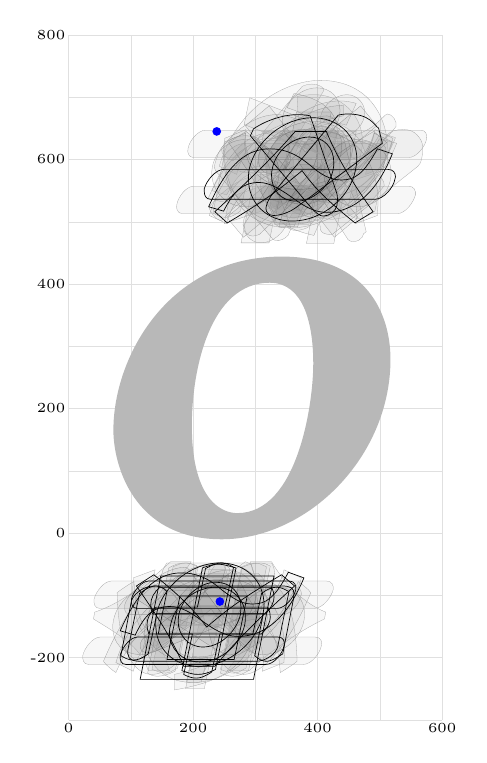
\begin{tikzpicture}[x=1pt,y=1pt,scale=0.225]
\draw[black!12,line width=0.1pt,step=100] (0,-300) grid (600,800);
\node[left,font=\tiny,inner sep=1pt] at (0,-200) {-200};
\node[left,font=\tiny,inner sep=1pt] at (0,0) {0};
\node[left,font=\tiny,inner sep=1pt] at (0,200) {200};
\node[left,font=\tiny,inner sep=1pt] at (0,400) {400};
\node[left,font=\tiny,inner sep=1pt] at (0,600) {600};
\node[left,font=\tiny,inner sep=1pt] at (0,800) {800};
\node[below,font=\tiny,inner sep=1pt] at (0,-300) {0};
\node[below,font=\tiny,inner sep=1pt] at (200,-300) {200};
\node[below,font=\tiny,inner sep=1pt] at (400,-300) {400};
\node[below,font=\tiny,inner sep=1pt] at (600,-300) {600};
\fill[black!28,even odd rule] (72,165) .. controls (72,111) and (103,-10) .. (246,-10) .. controls (383,-10) and (517,121) .. (517,279) .. controls (517,351) and (480,444) .. (342,444) .. controls (162,444) and (72,285) .. (72,165) -- cycle (198,173) .. controls (198,260) and (226,402) .. (323,402) .. controls (379,402) and (393,333) .. (393,272) .. controls (393,208) and (368,32) .. (271,32) .. controls (248,32) and (198,50) .. (198,173) -- cycle;
\filldraw[draw=black!35,line width=0.1pt,fill=black,fill opacity=0.03,draw opacity=1,even odd rule] (284,642) -- (250,628) .. controls (249,621) and (249,614) .. (249,608) .. controls (249,540) and (287,490) .. (357,490) .. controls (407,490) and (490,527) .. (520,628) -- (491,642) .. controls (477,580) and (416,552) .. (370,552) .. controls (316,552) and (283,583) .. (283,627) .. controls (283,631) and (284,636) .. (284,642) -- cycle;
\filldraw[draw=black!35,line width=0.1pt,fill=black,fill opacity=0.03,draw opacity=1,even odd rule] (317,588) .. controls (317,555) and (343,528) .. (376,528) .. controls (409,528) and (436,555) .. (436,588) .. controls (436,621) and (409,648) .. (376,648) .. controls (343,648) and (317,621) .. (317,588) -- cycle;
\filldraw[draw=black!35,line width=0.1pt,fill=black,fill opacity=0.03,draw opacity=1,even odd rule] (230,578) .. controls (230,548) and (254,524) .. (284,524) .. controls (314,524) and (338,548) .. (338,578) .. controls (338,608) and (314,632) .. (284,632) .. controls (254,632) and (230,608) .. (230,578) -- cycle (410,578) .. controls (410,548) and (434,524) .. (464,524) .. controls (494,524) and (518,548) .. (518,578) .. controls (518,608) and (494,632) .. (464,632) .. controls (434,632) and (410,608) .. (410,578) -- cycle;
\filldraw[draw=black!35,line width=0.1pt,fill=black,fill opacity=0.03,draw opacity=1,even odd rule] (453,605) -- (453,611) .. controls (453,630) and (441,661) .. (393,661) .. controls (351,661) and (310,627) .. (305,606) -- (305,600) .. controls (305,588) and (310,577) .. (326,577) .. controls (335,577) and (353,584) .. (356,598) .. controls (358,606) and (354,612) .. (353,615) .. controls (353,615) and (353,615) .. (353,615) .. controls (352,617) and (352,620) .. (353,623) .. controls (354,628) and (361,633) .. (378,633) .. controls (392,633) and (399,628) .. (399,615) .. controls (399,611) and (399,607) .. (398,602) .. controls (395,590) and (389,579) .. (378,567) .. controls (363,549) and (345,526) .. (338,492) -- (368,492) .. controls (375,518) and (392,536) .. (413,553) .. controls (432,568) and (448,584) .. (453,605) -- cycle;
\filldraw[draw=black!35,line width=0.1pt,fill=black,fill opacity=0.03,draw opacity=1,even odd rule] (428,647) .. controls (421,651) and (415,653) .. (408,653) .. controls (403,653) and (383,653) .. (374,640) -- (281,494) .. controls (281,494) and (281,493) .. (282,492) .. controls (283,491) and (284,491) .. (283,490) .. controls (282,482) and (289,477) .. (295,477) .. controls (297,477) and (304,478) .. (307,480) -- (434,601) .. controls (437,604) and (438,608) .. (438,612) .. controls (438,614) and (438,615) .. (438,617) .. controls (438,619) and (439,622) .. (439,624) .. controls (439,633) and (435,642) .. (428,647) -- cycle (560,639) .. controls (555,645) and (547,648) .. (538,648) .. controls (526,648) and (516,646) .. (510,637) -- (403,498) -- (403,497) .. controls (403,496) and (404,494) .. (404,493) .. controls (402,485) and (410,480) .. (415,480) .. controls (416,480) and (419,479) .. (421,479) .. controls (422,479) and (424,479) .. (424,480) -- (561,589) .. controls (568,595) and (567,605) .. (569,611) -- (569,618) .. controls (569,626) and (566,633) .. (560,639) -- cycle;
\filldraw[draw=black!35,line width=0.1pt,fill=black,fill opacity=0.03,draw opacity=1,even odd rule] (383,498) .. controls (422,545) and (467,587) .. (511,627) -- (490,645) .. controls (445,618) and (412,597) .. (371,561) .. controls (341,599) and (318,618) .. (285,645) -- (257,627) .. controls (285,587) and (314,544) .. (334,498) -- cycle;
\filldraw[draw=black!35,line width=0.1pt,fill=black,fill opacity=0.03,draw opacity=1,even odd rule] (386,496) -- (422,676) -- (366,676) -- (330,496) -- cycle;
\filldraw[draw=black!35,line width=0.1pt,fill=black,fill opacity=0.03,draw opacity=1,even odd rule] (257,630) .. controls (247,623) and (240,612) .. (238,602) .. controls (237,598) and (234,593) .. (234,588) .. controls (234,586) and (235,584) .. (236,582) -- (328,472) .. controls (329,470) and (333,470) .. (336,470) -- (338,470) .. controls (341,470) and (345,472) .. (348,474) .. controls (352,476) and (354,480) .. (355,484) .. controls (355,484) and (355,485) .. (356,486) .. controls (357,488) and (358,489) .. (357,490) -- (308,628) .. controls (305,637) and (295,638) .. (283,638) .. controls (274,638) and (266,636) .. (257,630) -- cycle (394,637) .. controls (382,632) and (373,620) .. (371,608) .. controls (371,607) and (371,607) .. (371,606) .. controls (370,602) and (368,596) .. (372,592) -- (449,471) .. controls (451,469) and (455,468) .. (457,468) .. controls (460,468) and (463,469) .. (466,470) .. controls (470,473) and (474,477) .. (474,481) .. controls (475,482) and (478,483) .. (478,484) -- (443,630) .. controls (441,639) and (432,643) .. (420,644) -- (417,644) .. controls (409,644) and (402,642) .. (394,637) -- cycle;
\filldraw[draw=black!35,line width=0.1pt,fill=black,fill opacity=0.03,draw opacity=1,even odd rule] (285,648) -- (251,634) .. controls (250,627) and (250,620) .. (250,614) .. controls (250,546) and (288,496) .. (359,496) .. controls (408,496) and (491,533) .. (521,634) -- (492,648) .. controls (478,586) and (417,558) .. (371,558) .. controls (317,558) and (284,589) .. (284,633) .. controls (284,637) and (285,642) .. (285,648) -- cycle (344,669) .. controls (343,666) and (343,663) .. (343,660) .. controls (343,639) and (359,624) .. (380,624) .. controls (405,624) and (430,644) .. (435,669) .. controls (436,672) and (436,675) .. (436,678) .. controls (436,699) and (421,715) .. (399,715) .. controls (374,715) and (349,694) .. (344,669) -- cycle;
\filldraw[draw=black!35,line width=0.1pt,fill=black,fill opacity=0.03,draw opacity=1,even odd rule] (461,497) -- (496,510) .. controls (496,517) and (497,524) .. (497,531) .. controls (497,598) and (459,648) .. (388,648) .. controls (338,648) and (256,611) .. (226,510) -- (254,497) .. controls (269,559) and (329,586) .. (375,586) .. controls (429,586) and (463,555) .. (463,512) .. controls (463,507) and (462,502) .. (461,497) -- cycle;
\filldraw[draw=black!35,line width=0.1pt,fill=black,fill opacity=0.03,draw opacity=1,even odd rule] (359,507) .. controls (395,507) and (415,532) .. (419,548) .. controls (419,551) and (420,554) .. (420,558) .. controls (420,573) and (411,592) .. (377,592) .. controls (369,592) and (359,589) .. (350,582) .. controls (350,585) and (350,588) .. (351,592) .. controls (352,596) and (361,655) .. (441,670) -- (441,687) .. controls (350,683) and (315,607) .. (309,581) .. controls (308,576) and (308,571) .. (308,565) .. controls (308,535) and (326,507) .. (359,507) -- cycle;
\filldraw[draw=black!35,line width=0.1pt,fill=black,fill opacity=0.03,draw opacity=1,even odd rule] (406,580) -- (495,654) -- (469,686) -- (380,612) -- (322,686) -- (284,654) -- (343,580) -- (254,507) -- (281,475) -- (369,548) -- (427,475) -- (465,507) -- cycle;
\filldraw[draw=black!35,line width=0.1pt,fill=black,fill opacity=0.03,draw opacity=1,even odd rule] (389,644) .. controls (386,629) and (375,617) .. (362,604) .. controls (346,588) and (330,569) .. (325,545) .. controls (318,510) and (344,489) .. (394,478) -- (404,501) .. controls (376,509) and (364,518) .. (369,539) .. controls (371,553) and (384,566) .. (397,580) .. controls (412,597) and (426,616) .. (430,634) .. controls (438,670) and (413,697) .. (362,706) -- (351,683) .. controls (386,672) and (393,662) .. (389,644) -- cycle;
\filldraw[draw=black!35,line width=0.1pt,fill=black,fill opacity=0.03,draw opacity=1,even odd rule] (546,603) .. controls (559,603) and (573,621) .. (575,633) .. controls (576,640) and (574,647) .. (565,647) -- (220,647) .. controls (208,647) and (194,630) .. (192,618) .. controls (190,611) and (193,603) .. (201,603) -- cycle (528,513) .. controls (541,513) and (554,531) .. (557,543) .. controls (558,550) and (555,557) .. (546,557) -- (201,557) .. controls (189,557) and (176,540) .. (174,528) .. controls (172,521) and (175,513) .. (183,513) -- cycle;
\filldraw[draw=black!35,line width=0.1pt,fill=black,fill opacity=0.03,draw opacity=1,even odd rule] (322,466) -- (358,645) -- (314,645) -- (277,466) -- cycle (426,465) -- (462,645) -- (418,645) -- (382,465) -- cycle;
\filldraw[draw=black!35,line width=0.1pt,fill=black,fill opacity=0.03,draw opacity=1,even odd rule] (276,517) -- (290,582) -- (461,582) -- (447,514) .. controls (454,508) and (459,505) .. (466,505) .. controls (472,505) and (480,509) .. (492,517) -- (509,604) .. controls (510,607) and (510,610) .. (510,613) .. controls (510,622) and (506,626) .. (490,626) -- (285,626) .. controls (269,626) and (252,613) .. (249,602) -- (232,514) .. controls (237,511) and (244,507) .. (252,507) .. controls (259,507) and (267,510) .. (276,517) -- cycle;
\filldraw[draw=black!35,line width=0.1pt,fill=black,fill opacity=0.03,draw opacity=1,even odd rule] (362,492) -- (384,540) .. controls (395,534) and (405,531) .. (418,531) .. controls (464,531) and (503,566) .. (527,626) -- (499,633) .. controls (477,591) and (462,581) .. (440,581) .. controls (426,581) and (418,584) .. (408,591) -- (437,653) .. controls (431,662) and (424,670) .. (415,670) .. controls (411,670) and (406,669) .. (401,669) -- (377,615) .. controls (363,625) and (348,631) .. (326,631) .. controls (283,631) and (250,596) .. (224,537) -- (252,531) .. controls (268,564) and (283,579) .. (309,579) .. controls (325,579) and (337,572) .. (352,562) -- (326,506) .. controls (330,498) and (335,491) .. (342,491) .. controls (346,491) and (355,492) .. (362,492) -- cycle;
\filldraw[draw=black!35,line width=0.1pt,fill=black,fill opacity=0.03,draw opacity=1,even odd rule] (443,593) .. controls (424,593) and (409,603) .. (395,615) .. controls (378,629) and (359,643) .. (328,643) .. controls (285,643) and (256,609) .. (230,550) -- (254,543) .. controls (271,576) and (285,589) .. (311,589) .. controls (328,589) and (345,578) .. (361,567) .. controls (379,554) and (397,541) .. (419,541) .. controls (465,541) and (501,575) .. (525,635) -- (501,643) .. controls (478,601) and (464,593) .. (443,593) -- cycle (309,466) .. controls (327,466) and (347,482) .. (351,500) .. controls (355,518) and (341,536) .. (323,536) .. controls (305,536) and (285,520) .. (281,502) .. controls (277,484) and (291,466) .. (309,466) -- cycle (433,634) .. controls (451,634) and (472,651) .. (475,669) .. controls (479,687) and (465,704) .. (447,704) .. controls (429,704) and (409,688) .. (405,670) .. controls (401,652) and (415,634) .. (433,634) -- cycle;
\filldraw[draw=black!35,line width=0.1pt,fill=black,fill opacity=0.03,draw opacity=1,even odd rule] (512,673) .. controls (506,673) and (487,638) .. (443,638) .. controls (423,638) and (363,672) .. (335,672) .. controls (303,672) and (272,652) .. (246,619) -- (246,617) .. controls (245,614) and (246,609) .. (252,605) .. controls (255,601) and (260,598) .. (264,598) .. controls (270,598) and (287,634) .. (324,634) .. controls (357,634) and (409,599) .. (441,599) .. controls (471,599) and (501,620) .. (526,653) .. controls (528,661) and (520,673) .. (512,673) -- cycle (492,577) .. controls (487,577) and (468,543) .. (424,543) .. controls (404,543) and (345,576) .. (316,576) .. controls (285,576) and (253,557) .. (226,524) .. controls (225,518) and (237,502) .. (245,502) .. controls (251,502) and (269,539) .. (305,539) .. controls (335,539) and (390,504) .. (422,504) .. controls (452,504) and (482,524) .. (507,558) .. controls (508,564) and (500,577) .. (492,577) -- cycle;
\filldraw[draw=black!35,line width=0.1pt,fill=black,fill opacity=0.03,draw opacity=1,even odd rule] (433,598) -- (259,540) -- (250,497) -- (504,582) -- (511,613) -- (291,699) -- (282,656) -- cycle;
\filldraw[draw=black!35,line width=0.1pt,fill=black,fill opacity=0.03,draw opacity=1,even odd rule] (321,601) .. controls (311,550) and (348,507) .. (399,507) .. controls (412,507) and (426,510) .. (438,515) -- (431,549) .. controls (424,546) and (414,544) .. (405,544) .. controls (370,544) and (356,570) .. (362,601) .. controls (369,634) and (395,658) .. (429,658) .. controls (435,658) and (441,657) .. (446,655) -- (462,690) .. controls (455,692) and (445,694) .. (436,694) .. controls (384,694) and (332,651) .. (321,601) -- cycle;
\filldraw[draw=black!35,line width=0.1pt,fill=black,fill opacity=0.03,draw opacity=1,even odd rule] (477,576) -- (512,589) .. controls (512,596) and (513,603) .. (513,610) .. controls (513,677) and (475,727) .. (404,727) .. controls (354,727) and (272,690) .. (242,589) -- (270,576) .. controls (285,638) and (345,665) .. (391,665) .. controls (445,665) and (479,634) .. (479,591) .. controls (479,586) and (478,581) .. (477,576) -- cycle (418,554) .. controls (423,579) and (404,603) .. (379,603) .. controls (354,603) and (327,581) .. (322,556) .. controls (317,531) and (336,506) .. (361,506) .. controls (386,506) and (413,529) .. (418,554) -- cycle;
\filldraw[draw=black!35,line width=0.1pt,fill=black,fill opacity=0.03,draw opacity=1,even odd rule] (470,611) .. controls (481,661) and (445,704) .. (394,704) .. controls (385,704) and (375,703) .. (367,701) -- (369,665) .. controls (374,667) and (381,668) .. (387,668) .. controls (421,668) and (437,644) .. (430,611) .. controls (424,580) and (398,554) .. (363,554) .. controls (354,554) and (347,556) .. (340,559) -- (320,525) .. controls (330,520) and (344,517) .. (357,517) .. controls (408,517) and (460,560) .. (470,611) -- cycle;
\filldraw[draw=black!35,line width=0.1pt,fill=black,fill opacity=0.03,draw opacity=1,even odd rule] (483,606) .. controls (487,611) and (491,617) .. (491,619) .. controls (492,624) and (484,629) .. (473,629) -- (369,629) .. controls (362,629) and (363,626) .. (363,630) .. controls (364,632) and (364,633) .. (366,635) -- (410,711) .. controls (411,715) and (402,721) .. (391,721) .. controls (386,721) and (377,719) .. (375,717) -- (275,600) .. controls (271,596) and (268,591) .. (268,589) .. controls (267,585) and (274,579) .. (285,579) -- (389,579) .. controls (397,579) and (399,582) .. (399,580) .. controls (398,578) and (398,576) .. (396,573) -- (350,498) .. controls (349,494) and (352,486) .. (366,486) .. controls (371,486) and (383,489) .. (386,492) -- cycle;
\filldraw[draw=black!35,line width=0.1pt,fill=black,fill opacity=0.03,draw opacity=1,even odd rule] (111,-96) -- (109,-106) -- (232,-184) .. controls (245,-192) and (253,-196) .. (259,-196) .. controls (266,-196) and (276,-188) .. (276,-181) .. controls (276,-177) and (274,-168) .. (269,-160) -- (191,-56) .. controls (190,-55) and (189,-55) .. (187,-55) .. controls (150,-55) and (111,-96) .. (111,-96) -- cycle;
\filldraw[draw=black!35,line width=0.1pt,fill=black,fill opacity=0.03,draw opacity=1,even odd rule] (126,-192) .. controls (131,-192) and (138,-191) .. (146,-187) -- (289,-131) .. controls (293,-128) and (298,-115) .. (300,-107) .. controls (301,-102) and (301,-96) .. (301,-91) .. controls (301,-68) and (293,-50) .. (293,-50) -- (284,-46) -- (143,-149) .. controls (129,-160) and (117,-169) .. (115,-178) -- (115,-181) .. controls (115,-186) and (117,-192) .. (126,-192) -- cycle;
\filldraw[draw=black!35,line width=0.1pt,fill=black,fill opacity=0.03,draw opacity=1,even odd rule] (289,-221) -- (324,-53) .. controls (319,-50) and (314,-48) .. (307,-48) .. controls (300,-48) and (290,-50) .. (279,-55) -- (266,-117) -- (159,-117) .. controls (149,-125) and (144,-136) .. (144,-146) .. controls (144,-151) and (145,-156) .. (147,-160) -- (258,-160) -- (244,-225) .. controls (251,-228) and (257,-230) .. (263,-230) .. controls (271,-230) and (279,-227) .. (289,-221) -- cycle;
\filldraw[draw=black!35,line width=0.1pt,fill=black,fill opacity=0.03,draw opacity=1,even odd rule] (161,-56) -- (127,-225) .. controls (131,-228) and (137,-230) .. (143,-230) .. controls (151,-230) and (160,-227) .. (171,-222) -- (184,-161) -- (292,-161) .. controls (302,-153) and (306,-142) .. (306,-131) .. controls (306,-126) and (305,-121) .. (304,-117) -- (193,-117) -- (206,-52) .. controls (199,-50) and (193,-48) .. (187,-48) .. controls (179,-48) and (171,-50) .. (161,-56) -- cycle;
\filldraw[draw=black!35,line width=0.1pt,fill=black,fill opacity=0.03,draw opacity=1,even odd rule] (164,-145) .. controls (169,-116) and (191,-89) .. (235,-89) .. controls (237,-89) and (240,-90) .. (243,-90) -- (254,-49) .. controls (250,-48) and (247,-48) .. (243,-48) .. controls (187,-48) and (135,-90) .. (124,-145) .. controls (122,-152) and (122,-158) .. (122,-164) .. controls (122,-208) and (152,-240) .. (199,-240) .. controls (204,-240) and (208,-240) .. (213,-239) -- (223,-200) .. controls (220,-200) and (217,-201) .. (215,-201) .. controls (177,-201) and (162,-184) .. (162,-159) .. controls (162,-155) and (163,-150) .. (164,-145) -- cycle;
\filldraw[draw=black!35,line width=0.1pt,fill=black,fill opacity=0.03,draw opacity=1,even odd rule] (269,-141) .. controls (268,-145) and (268,-149) .. (268,-152) .. controls (268,-176) and (285,-195) .. (312,-195) .. controls (342,-195) and (371,-173) .. (378,-141) .. controls (379,-137) and (379,-133) .. (379,-130) .. controls (379,-106) and (363,-87) .. (335,-87) .. controls (306,-87) and (276,-108) .. (269,-141) -- cycle (72,-141) .. controls (71,-145) and (71,-149) .. (71,-152) .. controls (71,-176) and (87,-195) .. (115,-195) .. controls (144,-195) and (174,-173) .. (180,-141) .. controls (181,-137) and (181,-133) .. (181,-130) .. controls (181,-106) and (165,-87) .. (137,-87) .. controls (108,-87) and (78,-108) .. (72,-141) -- cycle;
\filldraw[draw=black!35,line width=0.1pt,fill=black,fill opacity=0.03,draw opacity=1,even odd rule] (254,-60) .. controls (222,-60) and (195,-83) .. (190,-111) .. controls (189,-113) and (189,-115) .. (189,-117) .. controls (189,-137) and (210,-147) .. (227,-149) .. controls (243,-150) and (257,-154) .. (257,-171) .. controls (257,-173) and (257,-175) .. (256,-178) .. controls (252,-199) and (225,-214) .. (170,-227) -- (170,-252) .. controls (232,-241) and (286,-223) .. (300,-153) .. controls (303,-142) and (304,-131) .. (304,-121) .. controls (304,-81) and (285,-60) .. (254,-60) -- cycle;
\filldraw[draw=black!35,line width=0.1pt,fill=black,fill opacity=0.03,draw opacity=1,even odd rule] (369,-78) .. controls (355,-107) and (328,-163) .. (293,-163) .. controls (265,-163) and (251,-129) .. (247,-76) .. controls (245,-75) and (242,-75) .. (238,-75) .. controls (235,-75) and (231,-75) .. (228,-76) .. controls (190,-156) and (159,-163) .. (146,-163) .. controls (119,-163) and (108,-130) .. (105,-78) .. controls (102,-79) and (82,-92) .. (78,-96) .. controls (80,-181) and (101,-227) .. (134,-227) .. controls (149,-227) and (183,-216) .. (223,-146) .. controls (234,-217) and (266,-227) .. (281,-227) .. controls (315,-227) and (357,-172) .. (389,-96) .. controls (387,-91) and (373,-81) .. (369,-78) -- cycle;
\filldraw[draw=black!35,line width=0.1pt,fill=black,fill opacity=0.03,draw opacity=1,even odd rule] (267,-59) -- (217,-59) .. controls (179,-104) and (132,-148) .. (88,-187) -- (109,-206) .. controls (153,-179) and (184,-160) .. (229,-122) .. controls (255,-158) and (280,-179) .. (314,-206) -- (342,-187) .. controls (315,-147) and (286,-105) .. (267,-59) -- cycle;
\filldraw[draw=black!35,line width=0.1pt,fill=black,fill opacity=0.03,draw opacity=1,even odd rule] (139,-59) -- (104,-72) .. controls (104,-79) and (103,-86) .. (103,-93) .. controls (103,-160) and (141,-210) .. (212,-210) .. controls (262,-210) and (344,-173) .. (374,-72) -- (346,-59) .. controls (331,-121) and (271,-148) .. (225,-148) .. controls (170,-148) and (137,-117) .. (137,-74) .. controls (137,-69) and (138,-64) .. (139,-59) -- cycle;
\filldraw[draw=black!35,line width=0.1pt,fill=black,fill opacity=0.03,draw opacity=1,even odd rule] (311,-222) -- (346,-208) .. controls (346,-202) and (347,-194) .. (347,-188) .. controls (347,-120) and (309,-71) .. (238,-71) .. controls (188,-71) and (106,-108) .. (76,-208) -- (104,-222) .. controls (119,-160) and (179,-133) .. (225,-133) .. controls (280,-133) and (313,-163) .. (313,-207) .. controls (313,-212) and (312,-217) .. (311,-222) -- cycle;
\filldraw[draw=black!35,line width=0.1pt,fill=black,fill opacity=0.03,draw opacity=1,even odd rule] (123,-209) -- (292,-209) .. controls (298,-202) and (301,-194) .. (301,-184) .. controls (301,-178) and (300,-172) .. (298,-165) -- (237,-165) -- (259,-57) .. controls (254,-51) and (246,-48) .. (238,-48) .. controls (231,-48) and (223,-51) .. (216,-54) -- (193,-165) -- (128,-165) .. controls (122,-175) and (119,-183) .. (119,-192) .. controls (119,-198) and (120,-203) .. (123,-209) -- cycle;
\filldraw[draw=black!35,line width=0.1pt,fill=black,fill opacity=0.03,draw opacity=1,even odd rule] (326,-48) -- (158,-48) .. controls (152,-56) and (149,-64) .. (149,-74) .. controls (149,-79) and (150,-85) .. (152,-92) -- (213,-92) -- (191,-200) .. controls (197,-206) and (204,-209) .. (212,-209) .. controls (219,-209) and (227,-207) .. (235,-203) -- (257,-92) -- (322,-92) .. controls (328,-82) and (331,-74) .. (331,-65) .. controls (331,-60) and (330,-55) .. (326,-48) -- cycle;
\filldraw[draw=black!35,line width=0.1pt,fill=black,fill opacity=0.03,draw opacity=1,even odd rule] (344,-131) .. controls (357,-131) and (371,-113) .. (373,-101) .. controls (374,-100) and (374,-99) .. (374,-98) .. controls (374,-92) and (371,-87) .. (363,-87) -- (118,-87) .. controls (107,-87) and (93,-104) .. (90,-116) -- (90,-120) .. controls (90,-126) and (93,-131) .. (99,-131) -- cycle;
\filldraw[draw=black!35,line width=0.1pt,fill=black,fill opacity=0.03,draw opacity=1,even odd rule] (278,-143) .. controls (272,-172) and (251,-199) .. (207,-199) .. controls (205,-199) and (202,-198) .. (199,-198) -- (189,-239) .. controls (191,-240) and (195,-240) .. (199,-240) .. controls (254,-240) and (307,-198) .. (318,-143) .. controls (329,-90) and (296,-48) .. (243,-48) .. controls (238,-48) and (233,-48) .. (228,-49) -- (219,-88) .. controls (221,-88) and (225,-87) .. (228,-87) .. controls (273,-87) and (284,-112) .. (278,-143) -- cycle;
\filldraw[draw=black!35,line width=0.1pt,fill=black,fill opacity=0.03,draw opacity=1,even odd rule] (76,-224) .. controls (89,-195) and (116,-139) .. (152,-139) .. controls (179,-139) and (194,-173) .. (197,-226) .. controls (199,-227) and (203,-227) .. (207,-227) .. controls (210,-227) and (213,-227) .. (216,-226) .. controls (254,-146) and (285,-139) .. (298,-139) .. controls (326,-139) and (336,-172) .. (340,-224) .. controls (342,-223) and (363,-210) .. (367,-206) .. controls (365,-121) and (343,-75) .. (310,-75) .. controls (296,-75) and (261,-86) .. (221,-156) .. controls (211,-85) and (178,-75) .. (164,-75) .. controls (129,-75) and (88,-130) .. (56,-206) .. controls (59,-211) and (71,-221) .. (76,-224) -- cycle;
\filldraw[draw=black!35,line width=0.1pt,fill=black,fill opacity=0.03,draw opacity=1,even odd rule] (377,-211) .. controls (390,-211) and (404,-193) .. (406,-181) .. controls (408,-174) and (405,-167) .. (396,-167) -- (51,-167) .. controls (39,-167) and (26,-184) .. (23,-196) .. controls (22,-203) and (24,-211) .. (32,-211) -- cycle (395,-121) .. controls (408,-121) and (422,-103) .. (425,-91) .. controls (426,-84) and (423,-77) .. (414,-77) -- (69,-77) .. controls (57,-77) and (44,-94) .. (41,-106) .. controls (40,-113) and (42,-121) .. (50,-121) -- cycle;
\filldraw[draw=black!35,line width=0.1pt,fill=black,fill opacity=0.03,draw opacity=1,even odd rule] (285,-217) -- (318,-54) .. controls (307,-50) and (307,-48) .. (298,-48) .. controls (291,-48) and (289,-50) .. (278,-54) -- (244,-219) .. controls (256,-223) and (258,-225) .. (266,-225) .. controls (273,-225) and (273,-223) .. (285,-217) -- cycle (175,-217) -- (208,-54) .. controls (197,-50) and (197,-48) .. (188,-48) .. controls (181,-48) and (179,-50) .. (168,-54) -- (134,-219) .. controls (146,-223) and (148,-225) .. (156,-225) .. controls (163,-225) and (163,-223) .. (175,-217) -- cycle;
\filldraw[draw=black!35,line width=0.1pt,fill=black,fill opacity=0.03,draw opacity=1,even odd rule] (184,-65) .. controls (174,-70) and (168,-79) .. (167,-84) .. controls (166,-90) and (166,-95) .. (172,-104) -- (269,-104) -- (255,-174) .. controls (258,-184) and (265,-186) .. (270,-186) .. controls (275,-186) and (286,-181) .. (296,-167) -- (315,-76) -- (305,-65) -- cycle;
\filldraw[draw=black!35,line width=0.1pt,fill=black,fill opacity=0.03,draw opacity=1,even odd rule] (42,-127) -- (40,-138) .. controls (93,-170) and (116,-186) .. (128,-221) -- (162,-221) .. controls (154,-189) and (137,-168) .. (123,-149) -- (324,-149) .. controls (302,-169) and (276,-189) .. (255,-221) -- (290,-221) .. controls (324,-190) and (369,-158) .. (411,-138) -- (413,-127) .. controls (367,-109) and (335,-62) .. (326,-46) -- (292,-46) .. controls (299,-81) and (323,-107) .. (330,-119) -- (129,-119) .. controls (139,-109) and (173,-83) .. (197,-46) -- (164,-46) .. controls (146,-62) and (96,-109) .. (42,-127) -- cycle;
\filldraw[draw=black!35,line width=0.1pt,fill=black,fill opacity=0.03,draw opacity=1,even odd rule] (188,-250) -- (218,-250) -- (242,-133) .. controls (258,-151) and (274,-173) .. (303,-187) -- (310,-152) .. controls (285,-124) and (261,-86) .. (248,-48) -- (237,-48) .. controls (209,-98) and (154,-139) .. (135,-152) -- (128,-186) .. controls (166,-172) and (198,-142) .. (212,-133) -- cycle;
\draw[black,line width=0.25pt] (388,670) .. controls (385,671) and (374,672) .. (369,672) .. controls (335,672) and (305,655) .. (297,649) -- (292,638) -- (384,529) .. controls (397,514) and (403,509) .. (409,509) .. controls (419,509) and (429,517) .. (431,526) .. controls (431,529) and (432,532) .. (432,536) .. controls (432,541) and (431,547) .. (429,551) -- cycle;
\draw[black,line width=0.25pt] (433,671) -- (328,545) .. controls (319,534) and (317,524) .. (317,521) .. controls (317,515) and (322,510) .. (329,510) .. controls (339,510) and (354,514) .. (367,524) -- (504,626) -- (498,650) .. controls (490,656) and (484,673) .. (448,673) .. controls (443,673) and (436,672) .. (433,671) -- cycle;
\draw[black,line width=0.25pt] (414,645) -- (364,645) .. controls (325,599) and (278,556) .. (235,516) -- (255,498) .. controls (300,525) and (330,544) .. (375,582) .. controls (401,546) and (427,525) .. (460,498) -- (489,516) .. controls (461,556) and (433,598) .. (414,645) -- cycle;
\draw[black,line width=0.25pt] (438,567) .. controls (419,567) and (404,577) .. (390,589) .. controls (373,603) and (354,617) .. (323,617) .. controls (280,617) and (251,583) .. (225,524) -- (249,517) .. controls (266,550) and (280,563) .. (306,563) .. controls (323,563) and (340,552) .. (356,541) .. controls (374,528) and (392,515) .. (414,515) .. controls (460,515) and (496,549) .. (520,609) -- (496,617) .. controls (473,575) and (459,567) .. (438,567) -- cycle;
\draw[black,line width=0.25pt] (492,536) .. controls (506,536) and (522,555) .. (524,568) .. controls (525,570) and (525,571) .. (525,572) .. controls (525,578) and (522,584) .. (513,584) -- (249,584) .. controls (236,584) and (221,565) .. (218,553) -- (218,548) .. controls (218,542) and (221,536) .. (228,536) -- cycle;
\draw[black,line width=0.25pt] (290,584) .. controls (289,579) and (289,574) .. (289,568) .. controls (289,530) and (318,501) .. (359,501) .. controls (407,501) and (453,539) .. (461,584) .. controls (462,590) and (463,595) .. (463,600) .. controls (463,639) and (433,667) .. (392,667) .. controls (346,667) and (300,630) .. (290,584) -- cycle (387,636) .. controls (410,636) and (426,619) .. (426,595) .. controls (426,592) and (426,588) .. (425,584) .. controls (420,558) and (394,533) .. (366,533) .. controls (340,533) and (326,552) .. (326,574) .. controls (326,577) and (326,581) .. (327,584) .. controls (332,612) and (358,636) .. (387,636) -- cycle;
\draw[black,line width=0.25pt] (326,-87) -- (147,-87) .. controls (137,-95) and (132,-105) .. (132,-115) .. controls (132,-120) and (133,-125) .. (135,-130) -- (316,-130) .. controls (326,-119) and (330,-111) .. (330,-103) .. controls (330,-98) and (329,-92) .. (326,-87) -- cycle;
\draw[black,line width=0.25pt] (164,-147) .. controls (163,-151) and (162,-155) .. (162,-159) .. controls (162,-186) and (182,-207) .. (211,-207) .. controls (244,-207) and (276,-180) .. (283,-147) .. controls (284,-142) and (284,-138) .. (284,-135) .. controls (284,-107) and (264,-87) .. (236,-87) .. controls (202,-87) and (171,-114) .. (164,-147) -- cycle;
\draw[black,line width=0.25pt] (141,-131) .. controls (140,-137) and (140,-142) .. (140,-147) .. controls (140,-186) and (169,-214) .. (209,-214) .. controls (257,-214) and (303,-176) .. (312,-131) .. controls (313,-126) and (314,-120) .. (314,-116) .. controls (314,-76) and (284,-48) .. (243,-48) .. controls (196,-48) and (150,-86) .. (141,-131) -- cycle (237,-79) .. controls (261,-79) and (277,-97) .. (277,-120) .. controls (277,-124) and (277,-127) .. (276,-131) .. controls (270,-157) and (245,-183) .. (216,-183) .. controls (191,-183) and (176,-163) .. (176,-141) .. controls (176,-138) and (177,-135) .. (177,-131) .. controls (183,-104) and (209,-79) .. (237,-79) -- cycle;
\draw[black,line width=0.25pt] (236,-219) -- (269,-56) .. controls (257,-53) and (249,-50) .. (240,-50) .. controls (233,-50) and (226,-52) .. (215,-56) -- (182,-221) .. controls (193,-225) and (200,-227) .. (208,-227) .. controls (216,-227) and (224,-225) .. (236,-219) -- cycle;
\draw[black,line width=0.25pt] (128,-194) -- (142,-129) -- (313,-129) -- (299,-197) .. controls (306,-203) and (311,-206) .. (318,-206) .. controls (324,-206) and (332,-202) .. (344,-194) -- (361,-107) .. controls (362,-104) and (362,-101) .. (362,-98) .. controls (362,-89) and (358,-85) .. (342,-85) -- (137,-85) .. controls (121,-85) and (104,-98) .. (101,-109) -- (84,-197) .. controls (89,-200) and (96,-204) .. (104,-204) .. controls (111,-204) and (119,-201) .. (128,-194) -- cycle;
\draw[black,line width=0.25pt] (235,-214) .. controls (274,-167) and (319,-125) .. (363,-85) -- (342,-67) .. controls (297,-94) and (263,-115) .. (222,-151) .. controls (193,-113) and (170,-94) .. (137,-67) -- (109,-85) .. controls (136,-124) and (166,-168) .. (185,-214) -- cycle;
\draw[black,line width=0.25pt] (230,-223) -- (243,-162) -- (310,-162) .. controls (320,-151) and (324,-143) .. (324,-135) .. controls (324,-130) and (323,-124) .. (320,-119) -- (251,-119) -- (265,-55) .. controls (257,-50) and (252,-48) .. (246,-48) .. controls (239,-48) and (231,-51) .. (220,-57) -- (207,-119) -- (141,-119) .. controls (131,-127) and (126,-137) .. (126,-147) .. controls (126,-152) and (127,-157) .. (129,-162) -- (199,-162) -- (185,-227) .. controls (192,-231) and (199,-233) .. (205,-233) .. controls (212,-233) and (220,-230) .. (230,-223) -- cycle;
\draw[black,line width=0.25pt] (295,-114) .. controls (276,-114) and (262,-103) .. (247,-92) .. controls (231,-78) and (212,-64) .. (181,-64) .. controls (138,-64) and (109,-98) .. (83,-157) -- (107,-164) .. controls (123,-130) and (137,-118) .. (163,-118) .. controls (181,-118) and (197,-128) .. (213,-140) .. controls (231,-153) and (250,-166) .. (272,-166) .. controls (318,-166) and (353,-132) .. (378,-72) -- (353,-63) .. controls (331,-105) and (317,-114) .. (295,-114) -- cycle;
\draw[black,line width=0.25pt] (317,-211) .. controls (330,-211) and (344,-193) .. (346,-181) .. controls (348,-174) and (345,-167) .. (336,-167) -- (111,-167) .. controls (99,-167) and (86,-184) .. (83,-196) .. controls (82,-203) and (84,-211) .. (92,-211) -- cycle (335,-121) .. controls (348,-121) and (362,-103) .. (365,-91) .. controls (366,-84) and (363,-77) .. (354,-77) -- (129,-77) .. controls (117,-77) and (104,-94) .. (101,-106) .. controls (100,-113) and (102,-121) .. (110,-121) -- cycle;
\draw[black,line width=0.25pt] (310,-97) -- (296,-162) -- (144,-162) -- (158,-94) .. controls (153,-88) and (146,-85) .. (140,-85) .. controls (133,-85) and (125,-89) .. (114,-97) -- (96,-184) .. controls (93,-198) and (96,-206) .. (116,-206) -- (301,-206) .. controls (317,-206) and (334,-193) .. (336,-182) -- (354,-94) .. controls (348,-91) and (342,-87) .. (334,-87) .. controls (327,-87) and (319,-90) .. (310,-97) -- cycle;
\draw[black,line width=0.25pt] (148,-69) -- (115,-235) -- (297,-235) -- (330,-69) -- cycle (179,-101) -- (287,-101) -- (266,-203) -- (158,-203) -- cycle;
\fill[blue] (238,645) circle (7);
\fill[blue] (243,-110) circle (7);
\end{tikzpicture}

		\caption{Mark zones, semibold italic.}
		\label{fig:mark-zones-semibold-italic}
	\end{minipage}
\end{figure}

\subsection*{Font metrics per glyph}

See above- and below-anchor coordinates for A--Z, a--z, and IPA letters for Libertinus serif fonts 
(regular, italic, semibold, semibold italic) in the following tables 
(Tables \ref{table:fontmetrics_AZ_1}--\ref{table:fontmetrics_latinIPA_7}), 
and the mark anchors of above- and below-marks 
(Tables \ref{table:fontmetrics_above_1}--\ref{table:fontmetrics_below_2}).
Recall that Language Science Press uses semibold Libertinus fonts, e.g. 
\verb|LibertinusSerif-Semibold.otf|, for boldface styles.

\subsubsection*{Table row headings}

hex: Unicode character codepoint in 4-hex.

cat: Unicode character category. 
L = letter. Lu = uppercase (capital) letter, Ll = lowercase (small) letter,
Lo = other letter.
Used to determine expected ideal bounding box.
M = mark. Mn = nonspacing mark.

reg, it, sb, si: regular, italic, semibold, semibold italic. 
In that row, the character is printed alone, with combining dot above, and with combining macron below, 
to show anchor positioning (via combining grapheme joiner) when the base has an anchor; 
otherwise HarfBuzz default positioning applies.

patch: Use the patched Libertinus font to print the character alone, with combining dot above, and with combining macron below 
to show anchor positioning of the patched font (via combining grapheme joiner).
Where the original font has no above- or below-anchor, the patched font has the candidate (a?, b?),
unless a human-curated anchor overrules it; existing anchors are not moved.

ideal: top and bottom ideal bounding box reference lines, 
with offset from $Y_\mathrm{max}$ or $Y_\mathrm{min}$ for non-full descender or non-full ascender.
c = capline, x = x-height, a = ascender, b = baseline, d = descender.

a: $X, Y$ coordinates of the above-anchor.

a?: $X, Y$ coordinates of the above-anchor candidate.

a$\delta$: $X, Y$ coordinate differences between above-anchor and above-anchor candidate

b: $X, Y$ coordinates of the below-anchor.

b?: $X, Y$ coordinates of the below-anchor candidate.

b$\delta$: $X, Y$ coordinate differences between below-anchor and below-anchor candidate

In the tables of marks, each column is a mark and the rows are as follows.

reg, it, sb, si, patch: the mark on n and on H (via combining grapheme joiner), 
in the original and patched fonts.

m: $X, Y$ coordinates of the mark anchor. 
A class in parentheses is an anchor class other than above (0) or below (2): 
semibold puts the dot above, diaeresis, ring, hook above and comma above in class 1, 
whose base anchors are lower (n has 550 in class 1 and 646 in class 0).
This is the designer's anchor class \verb|top_punkt|; it places the marks at the same height as class 0, 
but only 24 bases have it. The patched semibold merges it into class 0.

m?: $X, Y$ coordinates of the mark-anchor candidate.
$Y$ is the bottom of the mark outline plus the style's median distance of an above-mark anchor above it
(regular 143, italic 142, semibold 157 in class 0 and 60 in class 1, semibold italic 147),
or the top of the outline minus the median distance of a below-mark anchor below it
(regular 46, italic 48, semibold 54, semibold italic 54).
$X$ is on the mark's own axis at that height, $C + Y\tan\theta - K$.

m$\delta$: $X, Y$ coordinate differences between mark anchor and mark-anchor candidate.
An asymmetric mark, such as the acute or grave, has an $X$ difference by design.


\begin{table}[p]
\captionsetup{justification=raggedright, singlelinecheck=false}
\caption{Font metrics for A--Z 1/2}
\label{table:fontmetrics_AZ_1}
\setlength{\tabcolsep}{3.5pt}

{\footnotesize
\begin{tabular}{lrrrrrrrrrrrrr}
hex & 0041 & 0042 & 0043 & 0044 & 0045 & 0046 & 0047 & 0048 & 0049 & 004A & 004B & 004C & 004D \\
cat & Lu & Lu & Lu & Lu & Lu & Lu & Lu & Lu & Lu & Lu & Lu & Lu & Lu \\
\hline reg\rule[-0.5em]{0pt}{1.9em} & \char"0041 \char"0041\cgj\char"0307 \char"0041\cgj\char"0331 & \char"0042 \char"0042\cgj\char"0307 \char"0042\cgj\char"0331 & \char"0043 \char"0043\cgj\char"0307 \char"0043\cgj\char"0331 & \char"0044 \char"0044\cgj\char"0307 \char"0044\cgj\char"0331 & \char"0045 \char"0045\cgj\char"0307 \char"0045\cgj\char"0331 & \char"0046 \char"0046\cgj\char"0307 \char"0046\cgj\char"0331 & \char"0047 \char"0047\cgj\char"0307 \char"0047\cgj\char"0331 & \char"0048 \char"0048\cgj\char"0307 \char"0048\cgj\char"0331 & \char"0049 \char"0049\cgj\char"0307 \char"0049\cgj\char"0331 & \char"004A \char"004A\cgj\char"0307 \char"004A\cgj\char"0331 & \char"004B \char"004B\cgj\char"0307 \char"004B\cgj\char"0331 & \char"004C \char"004C\cgj\char"0307 \char"004C\cgj\char"0331 & \char"004D \char"004D\cgj\char"0307 \char"004D\cgj\char"0331 \\
patch\rule[-0.5em]{0pt}{1.9em} & {\LibertinusSerifPatch \char"0041 \char"0041\cgj\char"0307 \char"0041\cgj\char"0331} & {\LibertinusSerifPatch \char"0042 \char"0042\cgj\char"0307 \char"0042\cgj\char"0331} & {\LibertinusSerifPatch \char"0043 \char"0043\cgj\char"0307 \char"0043\cgj\char"0331} & {\LibertinusSerifPatch \char"0044 \char"0044\cgj\char"0307 \char"0044\cgj\char"0331} & {\LibertinusSerifPatch \char"0045 \char"0045\cgj\char"0307 \char"0045\cgj\char"0331} & {\LibertinusSerifPatch \char"0046 \char"0046\cgj\char"0307 \char"0046\cgj\char"0331} & {\LibertinusSerifPatch \char"0047 \char"0047\cgj\char"0307 \char"0047\cgj\char"0331} & {\LibertinusSerifPatch \char"0048 \char"0048\cgj\char"0307 \char"0048\cgj\char"0331} & {\LibertinusSerifPatch \char"0049 \char"0049\cgj\char"0307 \char"0049\cgj\char"0331} & {\LibertinusSerifPatch \char"004A \char"004A\cgj\char"0307 \char"004A\cgj\char"0331} & {\LibertinusSerifPatch \char"004B \char"004B\cgj\char"0307 \char"004B\cgj\char"0331} & {\LibertinusSerifPatch \char"004C \char"004C\cgj\char"0307 \char"004C\cgj\char"0331} & {\LibertinusSerifPatch \char"004D \char"004D\cgj\char"0307 \char"004D\cgj\char"0331} \\
ideal & c, b & c, b & c, b & c, b & c, b & c, b & c, b & c, b & c, b & c, d+60 & c, b & c, b & c, b \\
a & 354, 850 & \textbf{267, 850} & \textbf{340, 850} & \textbf{306, 850} & \textbf{281, 850} & \textbf{284, 850} & \textbf{365, 850} & \textbf{361, 850} & 150, 850 & \textbf{182, 850} & \textbf{336, 850} & \textbf{151, 850} & \textbf{431, 850} \\
a? & 346, 850 & 280, 850 & 324, 850 & 336, 850 & 271, 850 & 244, 850 & 352, 850 & 362, 850 & 148, 850 & 120, 850 & 323, 850 & 260, 850 & 418, 850 \\
a$\delta$ & 8, 0 & -14, 0 & 16, 0 & -30, 0 & 10, 0 & 40, 0 & 14, 0 & -1, 0 & 2, 0 & 62, 0 & 13, 0 & -110, 0 & 13, 0 \\
a! & \textbf{361, 850} &  &  &  &  &  &  &  & \textbf{148, 850} &  &  &  &  \\
b & 308, -110 & \textbf{268, -110} & \textbf{363, -110} & \textbf{309, -110} & \textbf{287, -110} & \textbf{209, -110} & \textbf{367, -110} & \textbf{362, -110} & 147, -110 & 109, -319 & \textbf{342, -110} & \textbf{262, -110} & \textbf{393, -110} \\
b? & 346, -110 & 280, -110 & 324, -110 & 336, -110 & 271, -110 & 244, -110 & 352, -110 & 362, -110 & 148, -110 & \textbf{120, -257} & 323, -110 & 260, -110 & 418, -110 \\
b$\delta$ & -38, 0 & -12, 0 & 39, 0 & -27, 0 & 16, 0 & -36, 0 & 16, 0 & 0, 0 & -1, 0 & -11, -62 & 19, 0 & 2, 0 & -25, 0 \\
b! & \textbf{339, -110} &  &  &  &  &  &  &  & \textbf{148, -110} &  &  &  &  \\
\hline it\rule[-0.5em]{0pt}{1.9em} & {\itshape \char"0041 \char"0041\cgj\char"0307 \char"0041\cgj\char"0331} & {\itshape \char"0042 \char"0042\cgj\char"0307 \char"0042\cgj\char"0331} & {\itshape \char"0043 \char"0043\cgj\char"0307 \char"0043\cgj\char"0331} & {\itshape \char"0044 \char"0044\cgj\char"0307 \char"0044\cgj\char"0331} & {\itshape \char"0045 \char"0045\cgj\char"0307 \char"0045\cgj\char"0331} & {\itshape \char"0046 \char"0046\cgj\char"0307 \char"0046\cgj\char"0331} & {\itshape \char"0047 \char"0047\cgj\char"0307 \char"0047\cgj\char"0331} & {\itshape \char"0048 \char"0048\cgj\char"0307 \char"0048\cgj\char"0331} & {\itshape \char"0049 \char"0049\cgj\char"0307 \char"0049\cgj\char"0331} & {\itshape \char"004A \char"004A\cgj\char"0307 \char"004A\cgj\char"0331} & {\itshape \char"004B \char"004B\cgj\char"0307 \char"004B\cgj\char"0331} & {\itshape \char"004C \char"004C\cgj\char"0307 \char"004C\cgj\char"0331} & {\itshape \char"004D \char"004D\cgj\char"0307 \char"004D\cgj\char"0331} \\
patch\rule[-0.5em]{0pt}{1.9em} & {\LibertinusSerifPatch\itshape \char"0041 \char"0041\cgj\char"0307 \char"0041\cgj\char"0331} & {\LibertinusSerifPatch\itshape \char"0042 \char"0042\cgj\char"0307 \char"0042\cgj\char"0331} & {\LibertinusSerifPatch\itshape \char"0043 \char"0043\cgj\char"0307 \char"0043\cgj\char"0331} & {\LibertinusSerifPatch\itshape \char"0044 \char"0044\cgj\char"0307 \char"0044\cgj\char"0331} & {\LibertinusSerifPatch\itshape \char"0045 \char"0045\cgj\char"0307 \char"0045\cgj\char"0331} & {\LibertinusSerifPatch\itshape \char"0046 \char"0046\cgj\char"0307 \char"0046\cgj\char"0331} & {\LibertinusSerifPatch\itshape \char"0047 \char"0047\cgj\char"0307 \char"0047\cgj\char"0331} & {\LibertinusSerifPatch\itshape \char"0048 \char"0048\cgj\char"0307 \char"0048\cgj\char"0331} & {\LibertinusSerifPatch\itshape \char"0049 \char"0049\cgj\char"0307 \char"0049\cgj\char"0331} & {\LibertinusSerifPatch\itshape \char"004A \char"004A\cgj\char"0307 \char"004A\cgj\char"0331} & {\LibertinusSerifPatch\itshape \char"004B \char"004B\cgj\char"0307 \char"004B\cgj\char"0331} & {\LibertinusSerifPatch\itshape \char"004C \char"004C\cgj\char"0307 \char"004C\cgj\char"0331} & {\LibertinusSerifPatch\itshape \char"004D \char"004D\cgj\char"0307 \char"004D\cgj\char"0331} \\
ideal & c, b & c, b & c, b & c, b & c, b & c, b & c, b & c, b & c, b & c+32, d+32 & c, b & c, b & c, b \\
a & \textbf{505, 850} & \textbf{447, 850} & \textbf{500, 850} & 396, 850 & \textbf{413, 850} & \textbf{406, 850} & \textbf{513, 850} & 481, 850 & 316, 850 & \textbf{392, 850} & \textbf{466, 850} & 389, 850 & \textbf{557, 850} \\
a? & 514, 850 & 459, 850 & 489, 850 & 514, 850 & 444, 850 & 409, 850 & 513, 850 & 517, 850 & 321, 850 & 388, 850 & 499, 850 & 440, 850 & 583, 850 \\
a$\delta$ & -9, 0 & -12, 0 & 11, 0 & -118, 0 & -31, 0 & -3, 0 & 0, 0 & -36, 0 & -5, 0 & 4, 0 & -33, 0 & -51, 0 & -26, 0 \\
a! &  &  &  & \textbf{471, 850} &  &  &  & \textbf{504, 850} & \textbf{311, 850} &  &  & \textbf{314, 850} &  \\
b & \textbf{308}, -108 & \textbf{238}, -108 & \textbf{333, -110} & \textbf{279}, -107 & 269, -107 & \textbf{131}, -111 & \textbf{345, -110} & \textbf{320}, -107 & 127, -109 & 109, -319 & \textbf{292, -110} & \textbf{252, -110} & \textbf{363, -110} \\
b? & 310, \textbf{-110} & 255, \textbf{-110} & 285, -110 & 310, \textbf{-110} & 240, -110 & 205, \textbf{-110} & 309, -110 & 313, \textbf{-110} & 117, -110 & \textbf{146, -285} & 295, -110 & 236, -110 & 379, -110 \\
b$\delta$ & -2, 2 & -17, 2 & 48, 0 & -31, 3 & 29, 3 & -74, -1 & 36, 0 & 7, 3 & 10, 1 & -37, -34 & -3, 0 & 16, 0 & -16, 0 \\
b! &  &  &  &  & \textbf{246, -110} &  &  &  & \textbf{115, -110} &  &  &  &  \\
\hline sb\rule[-0.5em]{0pt}{1.9em} & {\bfseries \char"0041 \char"0041\cgj\char"0307 \char"0041\cgj\char"0331} & {\bfseries \char"0042 \char"0042\cgj\char"0307 \char"0042\cgj\char"0331} & {\bfseries \char"0043 \char"0043\cgj\char"0307 \char"0043\cgj\char"0331} & {\bfseries \char"0044 \char"0044\cgj\char"0307 \char"0044\cgj\char"0331} & {\bfseries \char"0045 \char"0045\cgj\char"0307 \char"0045\cgj\char"0331} & {\bfseries \char"0046 \char"0046\cgj\char"0307 \char"0046\cgj\char"0331} & {\bfseries \char"0047 \char"0047\cgj\char"0307 \char"0047\cgj\char"0331} & {\bfseries \char"0048 \char"0048\cgj\char"0307 \char"0048\cgj\char"0331} & {\bfseries \char"0049 \char"0049\cgj\char"0307 \char"0049\cgj\char"0331} & {\bfseries \char"004A \char"004A\cgj\char"0307 \char"004A\cgj\char"0331} & {\bfseries \char"004B \char"004B\cgj\char"0307 \char"004B\cgj\char"0331} & {\bfseries \char"004C \char"004C\cgj\char"0307 \char"004C\cgj\char"0331} & {\bfseries \char"004D \char"004D\cgj\char"0307 \char"004D\cgj\char"0331} \\
patch\rule[-0.5em]{0pt}{1.9em} & {\LibertinusSerifPatch\bfseries \char"0041 \char"0041\cgj\char"0307 \char"0041\cgj\char"0331} & {\LibertinusSerifPatch\bfseries \char"0042 \char"0042\cgj\char"0307 \char"0042\cgj\char"0331} & {\LibertinusSerifPatch\bfseries \char"0043 \char"0043\cgj\char"0307 \char"0043\cgj\char"0331} & {\LibertinusSerifPatch\bfseries \char"0044 \char"0044\cgj\char"0307 \char"0044\cgj\char"0331} & {\LibertinusSerifPatch\bfseries \char"0045 \char"0045\cgj\char"0307 \char"0045\cgj\char"0331} & {\LibertinusSerifPatch\bfseries \char"0046 \char"0046\cgj\char"0307 \char"0046\cgj\char"0331} & {\LibertinusSerifPatch\bfseries \char"0047 \char"0047\cgj\char"0307 \char"0047\cgj\char"0331} & {\LibertinusSerifPatch\bfseries \char"0048 \char"0048\cgj\char"0307 \char"0048\cgj\char"0331} & {\LibertinusSerifPatch\bfseries \char"0049 \char"0049\cgj\char"0307 \char"0049\cgj\char"0331} & {\LibertinusSerifPatch\bfseries \char"004A \char"004A\cgj\char"0307 \char"004A\cgj\char"0331} & {\LibertinusSerifPatch\bfseries \char"004B \char"004B\cgj\char"0307 \char"004B\cgj\char"0331} & {\LibertinusSerifPatch\bfseries \char"004C \char"004C\cgj\char"0307 \char"004C\cgj\char"0331} & {\LibertinusSerifPatch\bfseries \char"004D \char"004D\cgj\char"0307 \char"004D\cgj\char"0331} \\
ideal & c, b & c, b & c, b & c, b & c, b & c, b & c, b & c, b & c, b & c, d+50 & c, b & c, b & c, b \\
a &  &  &  &  &  &  &  &  &  & \textbf{203}, 806 &  &  &  \\
a? & \textbf{350, 850} & 300, 850 & \textbf{332, 850} & \textbf{352, 850} & \textbf{283, 850} & \textbf{268, 850} & 368, 850 & \textbf{362, 850} & \textbf{160, 850} & 131, \textbf{850} & \textbf{340, 850} & 267, 850 & \textbf{428, 850} \\
a$\delta$ &  &  &  &  &  &  &  &  &  & 72, -44 &  &  &  \\
a! &  & \textbf{283, 850} &  &  &  &  & 385, 850\textsuperscript{n} &  &  &  &  & \textbf{161, 850} &  \\
b &  &  &  &  &  &  &  & \textbf{362, -110} &  & 109, -319 &  &  &  \\
b? & \textbf{350, -110} & \textbf{300, -110} & \textbf{332, -110} & \textbf{352, -110} & \textbf{283, -110} & \textbf{268, -110} & \textbf{368, -110} & 362, -110 & \textbf{160, -110} & \textbf{131, -267} & \textbf{340, -110} & \textbf{267, -110} & \textbf{428, -110} \\
b$\delta$ &  &  &  &  &  &  &  & 0, 0 &  & -22, -52 &  &  &  \\
b! &  &  &  &  &  &  &  &  &  &  &  &  &  \\
\hline si\rule[-0.5em]{0pt}{1.9em} & {\bfseries\itshape \char"0041 \char"0041\cgj\char"0307 \char"0041\cgj\char"0331} & {\bfseries\itshape \char"0042 \char"0042\cgj\char"0307 \char"0042\cgj\char"0331} & {\bfseries\itshape \char"0043 \char"0043\cgj\char"0307 \char"0043\cgj\char"0331} & {\bfseries\itshape \char"0044 \char"0044\cgj\char"0307 \char"0044\cgj\char"0331} & {\bfseries\itshape \char"0045 \char"0045\cgj\char"0307 \char"0045\cgj\char"0331} & {\bfseries\itshape \char"0046 \char"0046\cgj\char"0307 \char"0046\cgj\char"0331} & {\bfseries\itshape \char"0047 \char"0047\cgj\char"0307 \char"0047\cgj\char"0331} & {\bfseries\itshape \char"0048 \char"0048\cgj\char"0307 \char"0048\cgj\char"0331} & {\bfseries\itshape \char"0049 \char"0049\cgj\char"0307 \char"0049\cgj\char"0331} & {\bfseries\itshape \char"004A \char"004A\cgj\char"0307 \char"004A\cgj\char"0331} & {\bfseries\itshape \char"004B \char"004B\cgj\char"0307 \char"004B\cgj\char"0331} & {\bfseries\itshape \char"004C \char"004C\cgj\char"0307 \char"004C\cgj\char"0331} & {\bfseries\itshape \char"004D \char"004D\cgj\char"0307 \char"004D\cgj\char"0331} \\
patch\rule[-0.5em]{0pt}{1.9em} & {\LibertinusSerifPatch\bfseries\itshape \char"0041 \char"0041\cgj\char"0307 \char"0041\cgj\char"0331} & {\LibertinusSerifPatch\bfseries\itshape \char"0042 \char"0042\cgj\char"0307 \char"0042\cgj\char"0331} & {\LibertinusSerifPatch\bfseries\itshape \char"0043 \char"0043\cgj\char"0307 \char"0043\cgj\char"0331} & {\LibertinusSerifPatch\bfseries\itshape \char"0044 \char"0044\cgj\char"0307 \char"0044\cgj\char"0331} & {\LibertinusSerifPatch\bfseries\itshape \char"0045 \char"0045\cgj\char"0307 \char"0045\cgj\char"0331} & {\LibertinusSerifPatch\bfseries\itshape \char"0046 \char"0046\cgj\char"0307 \char"0046\cgj\char"0331} & {\LibertinusSerifPatch\bfseries\itshape \char"0047 \char"0047\cgj\char"0307 \char"0047\cgj\char"0331} & {\LibertinusSerifPatch\bfseries\itshape \char"0048 \char"0048\cgj\char"0307 \char"0048\cgj\char"0331} & {\LibertinusSerifPatch\bfseries\itshape \char"0049 \char"0049\cgj\char"0307 \char"0049\cgj\char"0331} & {\LibertinusSerifPatch\bfseries\itshape \char"004A \char"004A\cgj\char"0307 \char"004A\cgj\char"0331} & {\LibertinusSerifPatch\bfseries\itshape \char"004B \char"004B\cgj\char"0307 \char"004B\cgj\char"0331} & {\LibertinusSerifPatch\bfseries\itshape \char"004C \char"004C\cgj\char"0307 \char"004C\cgj\char"0331} & {\LibertinusSerifPatch\bfseries\itshape \char"004D \char"004D\cgj\char"0307 \char"004D\cgj\char"0331} \\
ideal & c, b & c, b & c, b & c, b & c, b & c, b & c, b & c, b & c, b & c+34, d+68 & c, b & c, b & c, b \\
a & \textbf{354, 850} & \textbf{267, 850} & \textbf{340, 850} & \textbf{306, 850} & \textbf{273, 850} & \textbf{276, 850} & \textbf{365, 850} & 361, 850 & 150, 850 & 432, 850 & 336, 850 & 149, 850 & \textbf{431, 850} \\
a? & 382, 850 & 319, 850 & 341, 850 & 367, 850 & 292, 850 & 269, 850 & 371, 850 & \textbf{396, 850} & 194, 850 & \textbf{249, 850} & \textbf{369, 850} & 310, 850 & 441, 850 \\
a$\delta$ & -28, 0 & -52, 0 & -1, 0 & -61, 0 & -19, 0 & 7, 0 & -6, 0 & -35, 0 & -44, 0 & 183, 0 & -33, 0 & -161, 0 & -10, 0 \\
a! &  &  &  &  &  &  &  &  & \textbf{196, 850} &  &  & \textbf{209, 850} &  \\
b & \textbf{308, -110} & \textbf{268, -110} & \textbf{363, -110} & \textbf{279, -110} & \textbf{279, -110} & \textbf{201, -110} & \textbf{367, -110} & \textbf{365, -110} & 147, -110 & 109, -319 & \textbf{342, -110} & \textbf{260, -110} & \textbf{393, -110} \\
b? & 349, -110 & 286, -110 & 308, -110 & 334, -110 & 259, -110 & 236, -110 & 338, -110 & 363, -110 & 161, -110 & \textbf{187, -249} & 336, -110 & 277, -110 & 408, -110 \\
b$\delta$ & -41, 0 & -18, 0 & 55, 0 & -55, 0 & 20, 0 & -35, 0 & 29, 0 & 2, 0 & -14, 0 & -78, -70 & 6, 0 & -17, 0 & -15, 0 \\
b! &  &  &  &  &  &  &  &  & \textbf{174, -110} &  &  &  &  \\

\end{tabular}
}
\end{table}
\clearpage


\begin{table}[p]
\captionsetup{justification=raggedright, singlelinecheck=false}
\caption{Font metrics for A--Z 2/2}
\label{table:fontmetrics_AZ_2}
\setlength{\tabcolsep}{3.5pt}

{\footnotesize
\begin{tabular}{lrrrrrrrrrrrrr}
hex & 004E & 004F & 0050 & 0051 & 0052 & 0053 & 0054 & 0055 & 0056 & 0057 & 0058 & 0059 & 005A \\
cat & Lu & Lu & Lu & Lu & Lu & Lu & Lu & Lu & Lu & Lu & Lu & Lu & Lu \\
\hline reg\rule[-0.5em]{0pt}{1.9em} & \char"004E \char"004E\cgj\char"0307 \char"004E\cgj\char"0331 & \char"004F \char"004F\cgj\char"0307 \char"004F\cgj\char"0331 & \char"0050 \char"0050\cgj\char"0307 \char"0050\cgj\char"0331 & \char"0051 \char"0051\cgj\char"0307 \char"0051\cgj\char"0331 & \char"0052 \char"0052\cgj\char"0307 \char"0052\cgj\char"0331 & \char"0053 \char"0053\cgj\char"0307 \char"0053\cgj\char"0331 & \char"0054 \char"0054\cgj\char"0307 \char"0054\cgj\char"0331 & \char"0055 \char"0055\cgj\char"0307 \char"0055\cgj\char"0331 & \char"0056 \char"0056\cgj\char"0307 \char"0056\cgj\char"0331 & \char"0057 \char"0057\cgj\char"0307 \char"0057\cgj\char"0331 & \char"0058 \char"0058\cgj\char"0307 \char"0058\cgj\char"0331 & \char"0059 \char"0059\cgj\char"0307 \char"0059\cgj\char"0331 & \char"005A \char"005A\cgj\char"0307 \char"005A\cgj\char"0331 \\
patch\rule[-0.5em]{0pt}{1.9em} & {\LibertinusSerifPatch \char"004E \char"004E\cgj\char"0307 \char"004E\cgj\char"0331} & {\LibertinusSerifPatch \char"004F \char"004F\cgj\char"0307 \char"004F\cgj\char"0331} & {\LibertinusSerifPatch \char"0050 \char"0050\cgj\char"0307 \char"0050\cgj\char"0331} & {\LibertinusSerifPatch \char"0051 \char"0051\cgj\char"0307 \char"0051\cgj\char"0331} & {\LibertinusSerifPatch \char"0052 \char"0052\cgj\char"0307 \char"0052\cgj\char"0331} & {\LibertinusSerifPatch \char"0053 \char"0053\cgj\char"0307 \char"0053\cgj\char"0331} & {\LibertinusSerifPatch \char"0054 \char"0054\cgj\char"0307 \char"0054\cgj\char"0331} & {\LibertinusSerifPatch \char"0055 \char"0055\cgj\char"0307 \char"0055\cgj\char"0331} & {\LibertinusSerifPatch \char"0056 \char"0056\cgj\char"0307 \char"0056\cgj\char"0331} & {\LibertinusSerifPatch \char"0057 \char"0057\cgj\char"0307 \char"0057\cgj\char"0331} & {\LibertinusSerifPatch \char"0058 \char"0058\cgj\char"0307 \char"0058\cgj\char"0331} & {\LibertinusSerifPatch \char"0059 \char"0059\cgj\char"0307 \char"0059\cgj\char"0331} & {\LibertinusSerifPatch \char"005A \char"005A\cgj\char"0307 \char"005A\cgj\char"0331} \\
ideal & c, b & c, b & c, b & c, d+23 & c, b & c, b & c, b & c, b & c, b & c, b & c, b & c, b & c, b \\
a & \textbf{346, 850} & \textbf{335, 850} & \textbf{277, 850} & \textbf{348, 850} & \textbf{269, 850} & \textbf{232, 850} & 307, 850 & \textbf{346, 850} & \textbf{336, 850} & \textbf{450, 850} & \textbf{332, 850} & \textbf{295, 850} & \textbf{320, 850} \\
a? & 353, 850 & 352, 850 & 260, 850 & 359, 850 & 301, 850 & 236, 850 & 297, 850 & 331, 850 & 326, 850 & 474, 850 & 323, 850 & 288, 850 & 310, 850 \\
a$\delta$ & -7, 0 & -16, 0 & 18, 0 & -11, 0 & -32, 0 & -4, 0 & 10, 0 & 15, 0 & 10, 0 & -24, 0 & 9, 0 & 8, 0 & 10, 0 \\
a! &  &  &  &  &  &  & \textbf{308, 850} &  &  &  &  &  &  \\
b & \textbf{348, -110} & \textbf{350, -110} & \textbf{240, -110} &  & 258, -110 & \textbf{234, -110} & 300, -110 & \textbf{328, -110} & \textbf{318, -110} & \textbf{479, -110} & \textbf{307, -110} & \textbf{295, -110} & \textbf{287, -110} \\
b? & 353, -110 & 352, -110 & 260, -110 & \textbf{359, -294} & \textbf{301, -110} & 236, -110 & 297, -110 & 331, -110 & 326, -110 & 474, -110 & 323, -110 & 288, -110 & 310, -110 \\
b$\delta$ & -5, 0 & -2, 0 & -20, 0 &  & -43, 0 & -2, 0 & 3, 0 & -3, 0 & -8, 0 & 5, 0 & -16, 0 & 8, 0 & -22, 0 \\
b! &  &  &  &  &  &  & \textbf{308, -110} &  &  &  &  &  &  \\
\hline it\rule[-0.5em]{0pt}{1.9em} & {\itshape \char"004E \char"004E\cgj\char"0307 \char"004E\cgj\char"0331} & {\itshape \char"004F \char"004F\cgj\char"0307 \char"004F\cgj\char"0331} & {\itshape \char"0050 \char"0050\cgj\char"0307 \char"0050\cgj\char"0331} & {\itshape \char"0051 \char"0051\cgj\char"0307 \char"0051\cgj\char"0331} & {\itshape \char"0052 \char"0052\cgj\char"0307 \char"0052\cgj\char"0331} & {\itshape \char"0053 \char"0053\cgj\char"0307 \char"0053\cgj\char"0331} & {\itshape \char"0054 \char"0054\cgj\char"0307 \char"0054\cgj\char"0331} & {\itshape \char"0055 \char"0055\cgj\char"0307 \char"0055\cgj\char"0331} & {\itshape \char"0056 \char"0056\cgj\char"0307 \char"0056\cgj\char"0331} & {\itshape \char"0057 \char"0057\cgj\char"0307 \char"0057\cgj\char"0331} & {\itshape \char"0058 \char"0058\cgj\char"0307 \char"0058\cgj\char"0331} & {\itshape \char"0059 \char"0059\cgj\char"0307 \char"0059\cgj\char"0331} & {\itshape \char"005A \char"005A\cgj\char"0307 \char"005A\cgj\char"0331} \\
patch\rule[-0.5em]{0pt}{1.9em} & {\LibertinusSerifPatch\itshape \char"004E \char"004E\cgj\char"0307 \char"004E\cgj\char"0331} & {\LibertinusSerifPatch\itshape \char"004F \char"004F\cgj\char"0307 \char"004F\cgj\char"0331} & {\LibertinusSerifPatch\itshape \char"0050 \char"0050\cgj\char"0307 \char"0050\cgj\char"0331} & {\LibertinusSerifPatch\itshape \char"0051 \char"0051\cgj\char"0307 \char"0051\cgj\char"0331} & {\LibertinusSerifPatch\itshape \char"0052 \char"0052\cgj\char"0307 \char"0052\cgj\char"0331} & {\LibertinusSerifPatch\itshape \char"0053 \char"0053\cgj\char"0307 \char"0053\cgj\char"0331} & {\LibertinusSerifPatch\itshape \char"0054 \char"0054\cgj\char"0307 \char"0054\cgj\char"0331} & {\LibertinusSerifPatch\itshape \char"0055 \char"0055\cgj\char"0307 \char"0055\cgj\char"0331} & {\LibertinusSerifPatch\itshape \char"0056 \char"0056\cgj\char"0307 \char"0056\cgj\char"0331} & {\LibertinusSerifPatch\itshape \char"0057 \char"0057\cgj\char"0307 \char"0057\cgj\char"0331} & {\LibertinusSerifPatch\itshape \char"0058 \char"0058\cgj\char"0307 \char"0058\cgj\char"0331} & {\LibertinusSerifPatch\itshape \char"0059 \char"0059\cgj\char"0307 \char"0059\cgj\char"0331} & {\LibertinusSerifPatch\itshape \char"005A \char"005A\cgj\char"0307 \char"005A\cgj\char"0331} \\
ideal & c, b & c, b & c, b & c, d+23 & c, b & c, b & c, b & c, b & c, b & c, b & c, b & c, b & c, b \\
a & \textbf{476, 850} & 515, 850 & \textbf{426, 850} & \textbf{498, 850} & \textbf{419, 850} & \textbf{402, 850} & 457, 850 & 486, 850 & 481, 850 & \textbf{610, 850} & \textbf{482, 850} & 435, 850 & \textbf{450, 850} \\
a? & 514, 850 & 515, 850 & 430, 850 & 515, 850 & 458, 850 & 408, 850 & 453, 850 & 498, 850 & 479, 850 & 635, 850 & 495, 850 & 457, 850 & 470, 850 \\
a$\delta$ & -38, 0 & 0, 0 & -4, 0 & -17, 0 & -39, 0 & -6, 0 & 4, 0 & -12, 0 & 2, 0 & -25, 0 & -13, 0 & -22, 0 & -20, 0 \\
a! &  & \textbf{493, 850} &  &  &  &  & \textbf{456, 850} & \textbf{508, 850} & \textbf{458, 850} &  &  & \textbf{441, 850} &  \\
b & \textbf{328}, -109 & 310, -113 & \textbf{140, -110} &  & \textbf{248}, -111 & \textbf{204}, -111 & 277, -109 & \textbf{308}, -109 & \textbf{263, -110} & \textbf{439}, -107 & \textbf{287}, -107 & \textbf{270}, -109 & \textbf{267}, -107 \\
b? & 310, \textbf{-110} & 311, -110 & 226, -110 & \textbf{272, -294} & 254, \textbf{-110} & 204, \textbf{-110} & 249, -110 & 294, \textbf{-110} & 275, -110 & 431, \textbf{-110} & 291, \textbf{-110} & 253, \textbf{-110} & 266, \textbf{-110} \\
b$\delta$ & 18, 1 & -1, -3 & -86, 0 &  & -6, -1 & 0, -1 & 28, 1 & 14, 1 & -12, 0 & 8, 3 & -4, 3 & 17, 1 & 1, 3 \\
b! &  & \textbf{310, -110} &  &  &  &  & \textbf{261, -110} &  &  &  &  &  &  \\
\hline sb\rule[-0.5em]{0pt}{1.9em} & {\bfseries \char"004E \char"004E\cgj\char"0307 \char"004E\cgj\char"0331} & {\bfseries \char"004F \char"004F\cgj\char"0307 \char"004F\cgj\char"0331} & {\bfseries \char"0050 \char"0050\cgj\char"0307 \char"0050\cgj\char"0331} & {\bfseries \char"0051 \char"0051\cgj\char"0307 \char"0051\cgj\char"0331} & {\bfseries \char"0052 \char"0052\cgj\char"0307 \char"0052\cgj\char"0331} & {\bfseries \char"0053 \char"0053\cgj\char"0307 \char"0053\cgj\char"0331} & {\bfseries \char"0054 \char"0054\cgj\char"0307 \char"0054\cgj\char"0331} & {\bfseries \char"0055 \char"0055\cgj\char"0307 \char"0055\cgj\char"0331} & {\bfseries \char"0056 \char"0056\cgj\char"0307 \char"0056\cgj\char"0331} & {\bfseries \char"0057 \char"0057\cgj\char"0307 \char"0057\cgj\char"0331} & {\bfseries \char"0058 \char"0058\cgj\char"0307 \char"0058\cgj\char"0331} & {\bfseries \char"0059 \char"0059\cgj\char"0307 \char"0059\cgj\char"0331} & {\bfseries \char"005A \char"005A\cgj\char"0307 \char"005A\cgj\char"0331} \\
patch\rule[-0.5em]{0pt}{1.9em} & {\LibertinusSerifPatch\bfseries \char"004E \char"004E\cgj\char"0307 \char"004E\cgj\char"0331} & {\LibertinusSerifPatch\bfseries \char"004F \char"004F\cgj\char"0307 \char"004F\cgj\char"0331} & {\LibertinusSerifPatch\bfseries \char"0050 \char"0050\cgj\char"0307 \char"0050\cgj\char"0331} & {\LibertinusSerifPatch\bfseries \char"0051 \char"0051\cgj\char"0307 \char"0051\cgj\char"0331} & {\LibertinusSerifPatch\bfseries \char"0052 \char"0052\cgj\char"0307 \char"0052\cgj\char"0331} & {\LibertinusSerifPatch\bfseries \char"0053 \char"0053\cgj\char"0307 \char"0053\cgj\char"0331} & {\LibertinusSerifPatch\bfseries \char"0054 \char"0054\cgj\char"0307 \char"0054\cgj\char"0331} & {\LibertinusSerifPatch\bfseries \char"0055 \char"0055\cgj\char"0307 \char"0055\cgj\char"0331} & {\LibertinusSerifPatch\bfseries \char"0056 \char"0056\cgj\char"0307 \char"0056\cgj\char"0331} & {\LibertinusSerifPatch\bfseries \char"0057 \char"0057\cgj\char"0307 \char"0057\cgj\char"0331} & {\LibertinusSerifPatch\bfseries \char"0058 \char"0058\cgj\char"0307 \char"0058\cgj\char"0331} & {\LibertinusSerifPatch\bfseries \char"0059 \char"0059\cgj\char"0307 \char"0059\cgj\char"0331} & {\LibertinusSerifPatch\bfseries \char"005A \char"005A\cgj\char"0307 \char"005A\cgj\char"0331} \\
ideal & c, b & c, b & c, b & c, d & c, b & c, b & c+28, b & c, b & c, b & c, b & c, b & c, b & c, b \\
a &  & 363, 802 &  & \textbf{363}, 802 & \textbf{304}, 808 & 252, 802 & 298, 802 &  & \textbf{331}, 805 & \textbf{493}, 805 & \textbf{364}, 804 & \textbf{316}, 805 & 321, 803 \\
a? & \textbf{354, 850} & 366, 850 & \textbf{278, 850} & 366, \textbf{850} & 320, \textbf{850} & \textbf{238, 850} & 299, 850 & \textbf{339, 850} & 318, \textbf{850} & 489, \textbf{850} & 354, \textbf{850} & 308, \textbf{850} & 309, 850 \\
a$\delta$ &  & -2, -48 &  & -2, -48 & -16, -42 & 14, -48 & -1, -48 &  & 12, -45 & 4, -45 & 10, -46 & 8, -45 & 12, -47 \\
a! &  & \textbf{363, 850} &  &  &  &  & \textbf{299, 850} &  &  &  &  &  & \textbf{321, 850} \\
b &  &  &  &  & \textbf{292}, -111 & \textbf{234}, -111 & 301, -107 &  & \textbf{303}, -108 & \textbf{470}, -107 & \textbf{318}, -107 & \textbf{316}, -109 & \textbf{308}, -107 \\
b? & \textbf{354, -110} & \textbf{366, -110} & \textbf{278, -110} & \textbf{366, -319} & 320, \textbf{-110} & 238, \textbf{-110} & 299, -110 & \textbf{339, -110} & 318, \textbf{-110} & 489, \textbf{-110} & 354, \textbf{-110} & 308, \textbf{-110} & 309, \textbf{-110} \\
b$\delta$ &  &  &  &  & -28, -1 & -4, -1 & 2, 3 &  & -16, 2 & -19, 3 & -36, 3 & 8, 1 & -1, 3 \\
b! &  &  &  &  &  &  & \textbf{299, -110} &  &  &  &  &  &  \\
\hline si\rule[-0.5em]{0pt}{1.9em} & {\bfseries\itshape \char"004E \char"004E\cgj\char"0307 \char"004E\cgj\char"0331} & {\bfseries\itshape \char"004F \char"004F\cgj\char"0307 \char"004F\cgj\char"0331} & {\bfseries\itshape \char"0050 \char"0050\cgj\char"0307 \char"0050\cgj\char"0331} & {\bfseries\itshape \char"0051 \char"0051\cgj\char"0307 \char"0051\cgj\char"0331} & {\bfseries\itshape \char"0052 \char"0052\cgj\char"0307 \char"0052\cgj\char"0331} & {\bfseries\itshape \char"0053 \char"0053\cgj\char"0307 \char"0053\cgj\char"0331} & {\bfseries\itshape \char"0054 \char"0054\cgj\char"0307 \char"0054\cgj\char"0331} & {\bfseries\itshape \char"0055 \char"0055\cgj\char"0307 \char"0055\cgj\char"0331} & {\bfseries\itshape \char"0056 \char"0056\cgj\char"0307 \char"0056\cgj\char"0331} & {\bfseries\itshape \char"0057 \char"0057\cgj\char"0307 \char"0057\cgj\char"0331} & {\bfseries\itshape \char"0058 \char"0058\cgj\char"0307 \char"0058\cgj\char"0331} & {\bfseries\itshape \char"0059 \char"0059\cgj\char"0307 \char"0059\cgj\char"0331} & {\bfseries\itshape \char"005A \char"005A\cgj\char"0307 \char"005A\cgj\char"0331} \\
patch\rule[-0.5em]{0pt}{1.9em} & {\LibertinusSerifPatch\bfseries\itshape \char"004E \char"004E\cgj\char"0307 \char"004E\cgj\char"0331} & {\LibertinusSerifPatch\bfseries\itshape \char"004F \char"004F\cgj\char"0307 \char"004F\cgj\char"0331} & {\LibertinusSerifPatch\bfseries\itshape \char"0050 \char"0050\cgj\char"0307 \char"0050\cgj\char"0331} & {\LibertinusSerifPatch\bfseries\itshape \char"0051 \char"0051\cgj\char"0307 \char"0051\cgj\char"0331} & {\LibertinusSerifPatch\bfseries\itshape \char"0052 \char"0052\cgj\char"0307 \char"0052\cgj\char"0331} & {\LibertinusSerifPatch\bfseries\itshape \char"0053 \char"0053\cgj\char"0307 \char"0053\cgj\char"0331} & {\LibertinusSerifPatch\bfseries\itshape \char"0054 \char"0054\cgj\char"0307 \char"0054\cgj\char"0331} & {\LibertinusSerifPatch\bfseries\itshape \char"0055 \char"0055\cgj\char"0307 \char"0055\cgj\char"0331} & {\LibertinusSerifPatch\bfseries\itshape \char"0056 \char"0056\cgj\char"0307 \char"0056\cgj\char"0331} & {\LibertinusSerifPatch\bfseries\itshape \char"0057 \char"0057\cgj\char"0307 \char"0057\cgj\char"0331} & {\LibertinusSerifPatch\bfseries\itshape \char"0058 \char"0058\cgj\char"0307 \char"0058\cgj\char"0331} & {\LibertinusSerifPatch\bfseries\itshape \char"0059 \char"0059\cgj\char"0307 \char"0059\cgj\char"0331} & {\LibertinusSerifPatch\bfseries\itshape \char"005A \char"005A\cgj\char"0307 \char"005A\cgj\char"0331} \\
ideal & c, b & c, b & c, b & c, d & c, b & c, b & c+28, b & c, b & c, b & c, b & c, b & c, b & c, b \\
a & 346, 850 & 335, 850 & \textbf{316, 850} & \textbf{348, 850} & \textbf{269, 850} & \textbf{232, 850} & 307, 850 & 346, 850 & 336, 850 & \textbf{450, 850} & \textbf{332, 850} & 295, 850 & \textbf{320, 850} \\
a? & \textbf{394, 850} & \textbf{390, 850} & 284, 850 & 390, 850 & 315, 850 & 250, 850 & 309, 850 & 364, 850 & 328, 850 & 501, 850 & 362, 850 & 319, 850 & 322, 850 \\
a$\delta$ & -48, 0 & -55, 0 & 32, 0 & -42, 0 & -46, 0 & -18, 0 & -2, 0 & -18, 0 & 8, 0 & -51, 0 & -30, 0 & -24, 0 & -2, 0 \\
a! &  &  &  &  &  &  & \textbf{295, 850} & \textbf{376, 850} & \textbf{313, 850} &  &  & \textbf{291, 850} &  \\
b & \textbf{348, -110} & \textbf{350, -110} & \textbf{240, -110} &  & 258, -110 & \textbf{234, -110} & 300, -110 & \textbf{328, -110} & \textbf{318, -110} & \textbf{479, -110} & \textbf{307, -110} & 295, -110 & \textbf{287, -110} \\
b? & 361, -110 & 357, -110 & 251, -110 & \textbf{314, -319} & \textbf{282, -110} & 217, -110 & 276, -110 & 331, -110 & 295, -110 & 468, -110 & 329, -110 & 286, -110 & 289, -110 \\
b$\delta$ & -13, 0 & -7, 0 & -11, 0 &  & -24, 0 & 17, 0 & 24, 0 & -3, 0 & 23, 0 & 11, 0 & -22, 0 & 9, 0 & -2, 0 \\
b! &  &  &  &  &  &  & \textbf{274, -110} &  &  &  &  & \textbf{277, -110} &  \\

\end{tabular}
}
\end{table}
\clearpage



\begin{table}[p]
\captionsetup{justification=raggedright, singlelinecheck=false}
\caption{Font metrics for a--z 1/2}
\label{table:fontmetrics_az_1}
\setlength{\tabcolsep}{3.5pt}

{\footnotesize
\begin{tabular}{lrrrrrrrrrrrrr}
hex & 0061 & 0062 & 0063 & 0064 & 0065 & 0066 & 0067 & 0068 & 0069 & 006A & 006B & 006C & 006D \\
cat & Ll & Ll & Ll & Ll & Ll & Ll & Ll & Ll & Ll & Ll & Ll & Ll & Ll \\
\hline reg\rule[-0.5em]{0pt}{1.9em} & \char"0061 \char"0061\cgj\char"0307 \char"0061\cgj\char"0331 & \char"0062 \char"0062\cgj\char"0307 \char"0062\cgj\char"0331 & \char"0063 \char"0063\cgj\char"0307 \char"0063\cgj\char"0331 & \char"0064 \char"0064\cgj\char"0307 \char"0064\cgj\char"0331 & \char"0065 \char"0065\cgj\char"0307 \char"0065\cgj\char"0331 & \char"0066 \char"0066\cgj\char"0307 \char"0066\cgj\char"0331 & \char"0067 \char"0067\cgj\char"0307 \char"0067\cgj\char"0331 & \char"0068 \char"0068\cgj\char"0307 \char"0068\cgj\char"0331 & \char"0069 \char"0069\cgj\char"0307 \char"0069\cgj\char"0331 & \char"006A \char"006A\cgj\char"0307 \char"006A\cgj\char"0331 & \char"006B \char"006B\cgj\char"0307 \char"006B\cgj\char"0331 & \char"006C \char"006C\cgj\char"0307 \char"006C\cgj\char"0331 & \char"006D \char"006D\cgj\char"0307 \char"006D\cgj\char"0331 \\
patch\rule[-0.5em]{0pt}{1.9em} & {\LibertinusSerifPatch \char"0061 \char"0061\cgj\char"0307 \char"0061\cgj\char"0331} & {\LibertinusSerifPatch \char"0062 \char"0062\cgj\char"0307 \char"0062\cgj\char"0331} & {\LibertinusSerifPatch \char"0063 \char"0063\cgj\char"0307 \char"0063\cgj\char"0331} & {\LibertinusSerifPatch \char"0064 \char"0064\cgj\char"0307 \char"0064\cgj\char"0331} & {\LibertinusSerifPatch \char"0065 \char"0065\cgj\char"0307 \char"0065\cgj\char"0331} & {\LibertinusSerifPatch \char"0066 \char"0066\cgj\char"0307 \char"0066\cgj\char"0331} & {\LibertinusSerifPatch \char"0067 \char"0067\cgj\char"0307 \char"0067\cgj\char"0331} & {\LibertinusSerifPatch \char"0068 \char"0068\cgj\char"0307 \char"0068\cgj\char"0331} & {\LibertinusSerifPatch \char"0069 \char"0069\cgj\char"0307 \char"0069\cgj\char"0331} & {\LibertinusSerifPatch \char"006A \char"006A\cgj\char"0307 \char"006A\cgj\char"0331} & {\LibertinusSerifPatch \char"006B \char"006B\cgj\char"0307 \char"006B\cgj\char"0331} & {\LibertinusSerifPatch \char"006C \char"006C\cgj\char"0307 \char"006C\cgj\char"0331} & {\LibertinusSerifPatch \char"006D \char"006D\cgj\char"0307 \char"006D\cgj\char"0331} \\
ideal & x, b & a, b & x, b & a, b & x, b & a, b & x+33, d & a, b & a-51, b & a-51, d+9 & a, b & a, b & x, b \\
a & \textbf{209, 645} &  & \textbf{242, 645} & 218, 645 & \textbf{243, 645} &  & \textbf{231, 645} & 299, 645 & 137, 795 &  & 306, 784 & 135, 885 & 392, 645 \\
a? & 246, 645 & 232, 885 & 218, 645 & 270, 885 & 222, 645 & 208, 885 & 256, 676 & 270, 885 & 142, 834 & 76, 834 & 261, 885 & 134, 885 & 402, 645 \\
a$\delta$ & -36, 0 &  & 24, 0 & -52, -240 & 21, 0 &  & -26, -31 & 28, -240 & -5, -39 &  & 45, -101 & 1, 0 & -10, 0 \\
a! &  & \textbf{279, 885} &  & \textbf{235, 885} &  & \textbf{273, 885} &  & \textbf{282, 885} & \textbf{142, 834} & \textbf{152, 834} & \textbf{272, 885} & \textbf{134, 885} & \textbf{404, 645} \\
b & \textbf{196, -110} & \textbf{234, -110} & 236, -110 & 221, -110 & \textbf{234, -110} & 132, -110 & \textbf{229, -319} & \textbf{272, -110} & 136, -110 & \textbf{109, -319} & 290, -214 & 135, -110 & 408, -110 \\
b? & 246, -110 & 232, -110 & \textbf{218, -110} & 270, -110 & 222, -110 & 208, -110 & 256, -319 & 270, -110 & \textbf{142, -110} & 76, -308 & \textbf{261, -110} & 134, -110 & 402, -110 \\
b$\delta$ & -50, 0 & 2, 0 & 18, 0 & -50, 0 & 12, 0 & -76, 0 & -28, 0 & 2, 0 & -6, 0 & 34, -11 & 29, -104 & 1, 0 & 6, 0 \\
b! &  &  &  & \textbf{235, -110} &  & \textbf{136, -110} &  &  &  &  &  & \textbf{134, -110} & \textbf{404, -110} \\
\hline it\rule[-0.5em]{0pt}{1.9em} & {\itshape \char"0061 \char"0061\cgj\char"0307 \char"0061\cgj\char"0331} & {\itshape \char"0062 \char"0062\cgj\char"0307 \char"0062\cgj\char"0331} & {\itshape \char"0063 \char"0063\cgj\char"0307 \char"0063\cgj\char"0331} & {\itshape \char"0064 \char"0064\cgj\char"0307 \char"0064\cgj\char"0331} & {\itshape \char"0065 \char"0065\cgj\char"0307 \char"0065\cgj\char"0331} & {\itshape \char"0066 \char"0066\cgj\char"0307 \char"0066\cgj\char"0331} & {\itshape \char"0067 \char"0067\cgj\char"0307 \char"0067\cgj\char"0331} & {\itshape \char"0068 \char"0068\cgj\char"0307 \char"0068\cgj\char"0331} & {\itshape \char"0069 \char"0069\cgj\char"0307 \char"0069\cgj\char"0331} & {\itshape \char"006A \char"006A\cgj\char"0307 \char"006A\cgj\char"0331} & {\itshape \char"006B \char"006B\cgj\char"0307 \char"006B\cgj\char"0331} & {\itshape \char"006C \char"006C\cgj\char"0307 \char"006C\cgj\char"0331} & {\itshape \char"006D \char"006D\cgj\char"0307 \char"006D\cgj\char"0331} \\
patch\rule[-0.5em]{0pt}{1.9em} & {\LibertinusSerifPatch\itshape \char"0061 \char"0061\cgj\char"0307 \char"0061\cgj\char"0331} & {\LibertinusSerifPatch\itshape \char"0062 \char"0062\cgj\char"0307 \char"0062\cgj\char"0331} & {\LibertinusSerifPatch\itshape \char"0063 \char"0063\cgj\char"0307 \char"0063\cgj\char"0331} & {\LibertinusSerifPatch\itshape \char"0064 \char"0064\cgj\char"0307 \char"0064\cgj\char"0331} & {\LibertinusSerifPatch\itshape \char"0065 \char"0065\cgj\char"0307 \char"0065\cgj\char"0331} & {\LibertinusSerifPatch\itshape \char"0066 \char"0066\cgj\char"0307 \char"0066\cgj\char"0331} & {\LibertinusSerifPatch\itshape \char"0067 \char"0067\cgj\char"0307 \char"0067\cgj\char"0331} & {\LibertinusSerifPatch\itshape \char"0068 \char"0068\cgj\char"0307 \char"0068\cgj\char"0331} & {\LibertinusSerifPatch\itshape \char"0069 \char"0069\cgj\char"0307 \char"0069\cgj\char"0331} & {\LibertinusSerifPatch\itshape \char"006A \char"006A\cgj\char"0307 \char"006A\cgj\char"0331} & {\LibertinusSerifPatch\itshape \char"006B \char"006B\cgj\char"0307 \char"006B\cgj\char"0331} & {\LibertinusSerifPatch\itshape \char"006C \char"006C\cgj\char"0307 \char"006C\cgj\char"0331} & {\LibertinusSerifPatch\itshape \char"006D \char"006D\cgj\char"0307 \char"006D\cgj\char"0331} \\
ideal & x, b & a, b & x, b & a, b & x, b & a, d & x, d & a, b & a-80, b & a-80, d+36 & a, b & a, b & x, b \\
a & \textbf{341}, 647 &  & \textbf{343, 645} & 218, 645 & \textbf{332, 645} &  & \textbf{360, 645} & 409, 645 &  &  & 405, 646 & 292, 890 & \textbf{522, 645} \\
a? & 380, \textbf{645} & \textbf{428, 890} & 332, 645 & \textbf{434, 890} & 338, 645 & \textbf{346, 890} & 376, 645 & \textbf{449, 890} & 310, 810 & 302, 810 & \textbf{432, 890} & 322, 890 & 529, 645 \\
a$\delta$ & -39, 2 &  & 11, 0 & -216, -245 & -6, 0 &  & -16, 0 & -40, -245 &  &  & -27, -244 & -30, 0 & -7, 0 \\
a! &  &  &  &  &  &  &  &  & \textbf{300, 810} & \textbf{305, 810} &  & \textbf{313, 890} &  \\
b & 174, -108 & \textbf{214}, -108 & \textbf{163}, -113 & \textbf{221}, -107 & \textbf{158}, -108 & 222, -111 & \textbf{197, -319} & \textbf{229}, -111 & 136, -107 & \textbf{0, -319} & \textbf{223}, -107 & 115, -107 & 382, -105 \\
b? & \textbf{220, -110} & 216, \textbf{-110} & 171, \textbf{-110} & 221, \textbf{-110} & 177, \textbf{-110} & 89, -319 & 171, -319 & 236, \textbf{-110} & \textbf{115, -110} & 70, -281 & 220, \textbf{-110} & 110, -110 & 368, -110 \\
b$\delta$ & -46, 2 & -2, 2 & -8, -3 & 0, 3 & -19, 2 & 133, 208 & 26, 0 & -7, -1 & 21, 3 & -70, -38 & 3, 3 & 5, 3 & 14, 5 \\
b! &  &  &  &  &  & \textbf{30, -319} &  &  &  &  &  & \textbf{99, -110} & \textbf{373, -110} \\
\hline sb\rule[-0.5em]{0pt}{1.9em} & {\bfseries \char"0061 \char"0061\cgj\char"0307 \char"0061\cgj\char"0331} & {\bfseries \char"0062 \char"0062\cgj\char"0307 \char"0062\cgj\char"0331} & {\bfseries \char"0063 \char"0063\cgj\char"0307 \char"0063\cgj\char"0331} & {\bfseries \char"0064 \char"0064\cgj\char"0307 \char"0064\cgj\char"0331} & {\bfseries \char"0065 \char"0065\cgj\char"0307 \char"0065\cgj\char"0331} & {\bfseries \char"0066 \char"0066\cgj\char"0307 \char"0066\cgj\char"0331} & {\bfseries \char"0067 \char"0067\cgj\char"0307 \char"0067\cgj\char"0331} & {\bfseries \char"0068 \char"0068\cgj\char"0307 \char"0068\cgj\char"0331} & {\bfseries \char"0069 \char"0069\cgj\char"0307 \char"0069\cgj\char"0331} & {\bfseries \char"006A \char"006A\cgj\char"0307 \char"006A\cgj\char"0331} & {\bfseries \char"006B \char"006B\cgj\char"0307 \char"006B\cgj\char"0331} & {\bfseries \char"006C \char"006C\cgj\char"0307 \char"006C\cgj\char"0331} & {\bfseries \char"006D \char"006D\cgj\char"0307 \char"006D\cgj\char"0331} \\
patch\rule[-0.5em]{0pt}{1.9em} & {\LibertinusSerifPatch\bfseries \char"0061 \char"0061\cgj\char"0307 \char"0061\cgj\char"0331} & {\LibertinusSerifPatch\bfseries \char"0062 \char"0062\cgj\char"0307 \char"0062\cgj\char"0331} & {\LibertinusSerifPatch\bfseries \char"0063 \char"0063\cgj\char"0307 \char"0063\cgj\char"0331} & {\LibertinusSerifPatch\bfseries \char"0064 \char"0064\cgj\char"0307 \char"0064\cgj\char"0331} & {\LibertinusSerifPatch\bfseries \char"0065 \char"0065\cgj\char"0307 \char"0065\cgj\char"0331} & {\LibertinusSerifPatch\bfseries \char"0066 \char"0066\cgj\char"0307 \char"0066\cgj\char"0331} & {\LibertinusSerifPatch\bfseries \char"0067 \char"0067\cgj\char"0307 \char"0067\cgj\char"0331} & {\LibertinusSerifPatch\bfseries \char"0068 \char"0068\cgj\char"0307 \char"0068\cgj\char"0331} & {\LibertinusSerifPatch\bfseries \char"0069 \char"0069\cgj\char"0307 \char"0069\cgj\char"0331} & {\LibertinusSerifPatch\bfseries \char"006A \char"006A\cgj\char"0307 \char"006A\cgj\char"0331} & {\LibertinusSerifPatch\bfseries \char"006B \char"006B\cgj\char"0307 \char"006B\cgj\char"0331} & {\LibertinusSerifPatch\bfseries \char"006C \char"006C\cgj\char"0307 \char"006C\cgj\char"0331} & {\LibertinusSerifPatch\bfseries \char"006D \char"006D\cgj\char"0307 \char"006D\cgj\char"0331} \\
ideal & x, b & a, b-13 & x, b & a, b & x, b & a, b & x+33, d & a, b & a-48, b & a-48, d & a, b & a, b & x, b \\
a &  &  &  &  &  &  & \textbf{231, 645} &  & 137, 795 &  &  & 142, 885 & 396, 645 \\
a? & 255, 645 & \textbf{236, 885} & \textbf{224, 645} & \textbf{274, 885} & 232, 645 & \textbf{226, 885} & 264, 676 & \textbf{275, 885} & 156, 837 & 78, 837 & \textbf{262, 885} & 148, 885 & 408, 645 \\
a$\delta$ &  &  &  &  &  &  & -32, -31 &  & -18, -42 &  &  & -6, 0 & -12, 0 \\
a! & \textbf{219, 645} &  &  &  & \textbf{249, 645} &  &  &  & \textbf{156, 837} & \textbf{162, 837} &  & \textbf{150, 885} & \textbf{407, 645} \\
b &  &  &  &  &  &  & \textbf{229, -319} & \textbf{277, -110} & 136, -107 & \textbf{109, -319} &  & 135, -110 & 396, -105 \\
b? & \textbf{255, -110} & \textbf{236, -121} & \textbf{224, -110} & \textbf{274, -110} & \textbf{232, -110} & \textbf{226, -110} & 264, -319 & 275, -110 & \textbf{156, -110} & 78, -319 & \textbf{262, -110} & 148, -110 & 408, -110 \\
b$\delta$ &  &  &  &  &  &  & -34, 0 & 2, 0 & -20, 3 & 31, 0 &  & -14, 0 & -12, 5 \\
b! &  &  &  &  &  &  &  &  &  &  &  & \textbf{150, -110} & \textbf{407, -110} \\
\hline si\rule[-0.5em]{0pt}{1.9em} & {\bfseries\itshape \char"0061 \char"0061\cgj\char"0307 \char"0061\cgj\char"0331} & {\bfseries\itshape \char"0062 \char"0062\cgj\char"0307 \char"0062\cgj\char"0331} & {\bfseries\itshape \char"0063 \char"0063\cgj\char"0307 \char"0063\cgj\char"0331} & {\bfseries\itshape \char"0064 \char"0064\cgj\char"0307 \char"0064\cgj\char"0331} & {\bfseries\itshape \char"0065 \char"0065\cgj\char"0307 \char"0065\cgj\char"0331} & {\bfseries\itshape \char"0066 \char"0066\cgj\char"0307 \char"0066\cgj\char"0331} & {\bfseries\itshape \char"0067 \char"0067\cgj\char"0307 \char"0067\cgj\char"0331} & {\bfseries\itshape \char"0068 \char"0068\cgj\char"0307 \char"0068\cgj\char"0331} & {\bfseries\itshape \char"0069 \char"0069\cgj\char"0307 \char"0069\cgj\char"0331} & {\bfseries\itshape \char"006A \char"006A\cgj\char"0307 \char"006A\cgj\char"0331} & {\bfseries\itshape \char"006B \char"006B\cgj\char"0307 \char"006B\cgj\char"0331} & {\bfseries\itshape \char"006C \char"006C\cgj\char"0307 \char"006C\cgj\char"0331} & {\bfseries\itshape \char"006D \char"006D\cgj\char"0307 \char"006D\cgj\char"0331} \\
patch\rule[-0.5em]{0pt}{1.9em} & {\LibertinusSerifPatch\bfseries\itshape \char"0061 \char"0061\cgj\char"0307 \char"0061\cgj\char"0331} & {\LibertinusSerifPatch\bfseries\itshape \char"0062 \char"0062\cgj\char"0307 \char"0062\cgj\char"0331} & {\LibertinusSerifPatch\bfseries\itshape \char"0063 \char"0063\cgj\char"0307 \char"0063\cgj\char"0331} & {\LibertinusSerifPatch\bfseries\itshape \char"0064 \char"0064\cgj\char"0307 \char"0064\cgj\char"0331} & {\LibertinusSerifPatch\bfseries\itshape \char"0065 \char"0065\cgj\char"0307 \char"0065\cgj\char"0331} & {\LibertinusSerifPatch\bfseries\itshape \char"0066 \char"0066\cgj\char"0307 \char"0066\cgj\char"0331} & {\LibertinusSerifPatch\bfseries\itshape \char"0067 \char"0067\cgj\char"0307 \char"0067\cgj\char"0331} & {\LibertinusSerifPatch\bfseries\itshape \char"0068 \char"0068\cgj\char"0307 \char"0068\cgj\char"0331} & {\LibertinusSerifPatch\bfseries\itshape \char"0069 \char"0069\cgj\char"0307 \char"0069\cgj\char"0331} & {\LibertinusSerifPatch\bfseries\itshape \char"006A \char"006A\cgj\char"0307 \char"006A\cgj\char"0331} & {\LibertinusSerifPatch\bfseries\itshape \char"006B \char"006B\cgj\char"0307 \char"006B\cgj\char"0331} & {\LibertinusSerifPatch\bfseries\itshape \char"006C \char"006C\cgj\char"0307 \char"006C\cgj\char"0331} & {\LibertinusSerifPatch\bfseries\itshape \char"006D \char"006D\cgj\char"0307 \char"006D\cgj\char"0331} \\
ideal & x, b & a, b & x, b & a, b & x, b & a, d & x, d & a, b & a-67, b & a-67, d+25 & a, b & a, b & x, b \\
a & 379, 645 &  & \textbf{242, 645} & 218, 645 & \textbf{243, 645} &  & 291, 645 & 469, 645 & 137, 795 &  & 306, 784 & 174, 890 & \textbf{392, 645} \\
a? & \textbf{251, 645} & \textbf{290, 890} & 203, 645 & \textbf{309, 890} & 218, 645 & \textbf{216, 890} & \textbf{220, 645} & \textbf{331, 890} & 180, 823 & 192, 823 & \textbf{316, 890} & 194, 890 & 407, 645 \\
a$\delta$ & 128, 0 &  & 39, 0 & -91, -245 & 25, 0 &  & 71, 0 & 138, -245 & -43, -28 &  & -10, -106 & -20, 0 & -15, 0 \\
a! &  &  &  &  &  &  &  &  & \textbf{169, 823} & \textbf{186, 823} &  & \textbf{184, 890} &  \\
b & 196, -110 & 234, -110 & \textbf{236, -110} & \textbf{221, -110} & \textbf{234, -110} & 132, -110 & \textbf{199, -319} & \textbf{272, -110} & 136, -110 & \textbf{67, -319} & 290, -214 & 135, -110 & 400, -110 \\
b? & \textbf{260, -110} & \textbf{248, -110} & 212, -110 & 268, -110 & 227, -110 & 132, -319 & 186, -319 & 290, -110 & \textbf{153, -110} & 127, -292 & \textbf{275, -110} & 153, -110 & 415, -110 \\
b$\delta$ & -64, 0 & -14, 0 & 24, 0 & -47, 0 & 7, 0 & 0, 209 & 13, 0 & -18, 0 & -17, 0 & -60, -27 & 15, -104 & -18, 0 & -15, 0 \\
b! &  &  &  &  &  & \textbf{62, -319} &  &  &  &  &  & \textbf{138, -110} & \textbf{406, -110} \\

\end{tabular}
}
\end{table}
\clearpage


\begin{table}[p]
\captionsetup{justification=raggedright, singlelinecheck=false}
\caption{Font metrics for a--z 2/2}
\label{table:fontmetrics_az_2}
\setlength{\tabcolsep}{3.5pt}

{\footnotesize
\begin{tabular}{lrrrrrrrrrrrrr}
hex & 006E & 006F & 0070 & 0071 & 0072 & 0073 & 0074 & 0075 & 0076 & 0077 & 0078 & 0079 & 007A \\
cat & Ll & Ll & Ll & Ll & Ll & Ll & Ll & Ll & Ll & Ll & Ll & Ll & Ll \\
\hline reg\rule[-0.5em]{0pt}{1.9em} & \char"006E \char"006E\cgj\char"0307 \char"006E\cgj\char"0331 & \char"006F \char"006F\cgj\char"0307 \char"006F\cgj\char"0331 & \char"0070 \char"0070\cgj\char"0307 \char"0070\cgj\char"0331 & \char"0071 \char"0071\cgj\char"0307 \char"0071\cgj\char"0331 & \char"0072 \char"0072\cgj\char"0307 \char"0072\cgj\char"0331 & \char"0073 \char"0073\cgj\char"0307 \char"0073\cgj\char"0331 & \char"0074 \char"0074\cgj\char"0307 \char"0074\cgj\char"0331 & \char"0075 \char"0075\cgj\char"0307 \char"0075\cgj\char"0331 & \char"0076 \char"0076\cgj\char"0307 \char"0076\cgj\char"0331 & \char"0077 \char"0077\cgj\char"0307 \char"0077\cgj\char"0331 & \char"0078 \char"0078\cgj\char"0307 \char"0078\cgj\char"0331 & \char"0079 \char"0079\cgj\char"0307 \char"0079\cgj\char"0331 & \char"007A \char"007A\cgj\char"0307 \char"007A\cgj\char"0331 \\
patch\rule[-0.5em]{0pt}{1.9em} & {\LibertinusSerifPatch \char"006E \char"006E\cgj\char"0307 \char"006E\cgj\char"0331} & {\LibertinusSerifPatch \char"006F \char"006F\cgj\char"0307 \char"006F\cgj\char"0331} & {\LibertinusSerifPatch \char"0070 \char"0070\cgj\char"0307 \char"0070\cgj\char"0331} & {\LibertinusSerifPatch \char"0071 \char"0071\cgj\char"0307 \char"0071\cgj\char"0331} & {\LibertinusSerifPatch \char"0072 \char"0072\cgj\char"0307 \char"0072\cgj\char"0331} & {\LibertinusSerifPatch \char"0073 \char"0073\cgj\char"0307 \char"0073\cgj\char"0331} & {\LibertinusSerifPatch \char"0074 \char"0074\cgj\char"0307 \char"0074\cgj\char"0331} & {\LibertinusSerifPatch \char"0075 \char"0075\cgj\char"0307 \char"0075\cgj\char"0331} & {\LibertinusSerifPatch \char"0076 \char"0076\cgj\char"0307 \char"0076\cgj\char"0331} & {\LibertinusSerifPatch \char"0077 \char"0077\cgj\char"0307 \char"0077\cgj\char"0331} & {\LibertinusSerifPatch \char"0078 \char"0078\cgj\char"0307 \char"0078\cgj\char"0331} & {\LibertinusSerifPatch \char"0079 \char"0079\cgj\char"0307 \char"0079\cgj\char"0331} & {\LibertinusSerifPatch \char"007A \char"007A\cgj\char"0307 \char"007A\cgj\char"0331} \\
ideal & x, b & x, b & x, d & x, d & x, b & x, b & a-116, b & x, b & x, b & x, b & x, b & x, d & x, b \\
a & \textbf{264}, 646 & \textbf{238, 645} & \textbf{271}, 646 & \textbf{238, 645} & \textbf{191}, 646 & \textbf{206, 645} &  & \textbf{255, 645} & \textbf{256}, 646 & 345, 646 & \textbf{256}, 646 & \textbf{262, 645} & \textbf{220}, 646 \\
a? & 276, \textbf{645} & 252, 645 & 242, \textbf{645} & 268, 645 & 190, \textbf{645} & 199, 645 & 163, 769 & 271, 645 & 249, \textbf{645} & \textbf{373, 645} & 245, \textbf{645} & 260, 645 & 220, \textbf{645} \\
a$\delta$ & -12, 1 & -14, 0 & 28, 1 & -30, 0 & 1, 1 & 7, 0 &  & -16, 0 & 7, 1 & -28, 1 & 11, 1 & 2, 0 & 0, 1 \\
a! &  &  &  &  &  &  & \textbf{139, 769} &  &  &  &  &  &  \\
b & \textbf{265, -110} & \textbf{243, -110} & 179, -319 & 348, -319 & 135, -110 & \textbf{196, -110} & \textbf{163, -110} & \textbf{239, -110} & \textbf{241, -110} & 352, -110 & \textbf{224, -110} & \textbf{242, -319} & \textbf{207, -110} \\
b? & 276, -110 & 252, -110 & 242, -319 & 268, -319 & 190, -110 & 199, -110 & 163, -110 & 271, -110 & 249, -110 & \textbf{373, -110} & 245, -110 & 260, -319 & 220, -110 \\
b$\delta$ & -10, 0 & -9, 0 & -64, 0 & 80, 0 & -55, 0 & -3, 0 & 0, 0 & -32, 0 & -8, 0 & -21, 0 & -21, 0 & -18, 0 & -14, 0 \\
b! &  &  & \textbf{120, -319} & \textbf{386, -319} & \textbf{140, -110} &  &  &  &  &  &  &  &  \\
\hline it\rule[-0.5em]{0pt}{1.9em} & {\itshape \char"006E \char"006E\cgj\char"0307 \char"006E\cgj\char"0331} & {\itshape \char"006F \char"006F\cgj\char"0307 \char"006F\cgj\char"0331} & {\itshape \char"0070 \char"0070\cgj\char"0307 \char"0070\cgj\char"0331} & {\itshape \char"0071 \char"0071\cgj\char"0307 \char"0071\cgj\char"0331} & {\itshape \char"0072 \char"0072\cgj\char"0307 \char"0072\cgj\char"0331} & {\itshape \char"0073 \char"0073\cgj\char"0307 \char"0073\cgj\char"0331} & {\itshape \char"0074 \char"0074\cgj\char"0307 \char"0074\cgj\char"0331} & {\itshape \char"0075 \char"0075\cgj\char"0307 \char"0075\cgj\char"0331} & {\itshape \char"0076 \char"0076\cgj\char"0307 \char"0076\cgj\char"0331} & {\itshape \char"0077 \char"0077\cgj\char"0307 \char"0077\cgj\char"0331} & {\itshape \char"0078 \char"0078\cgj\char"0307 \char"0078\cgj\char"0331} & {\itshape \char"0079 \char"0079\cgj\char"0307 \char"0079\cgj\char"0331} & {\itshape \char"007A \char"007A\cgj\char"0307 \char"007A\cgj\char"0331} \\
patch\rule[-0.5em]{0pt}{1.9em} & {\LibertinusSerifPatch\itshape \char"006E \char"006E\cgj\char"0307 \char"006E\cgj\char"0331} & {\LibertinusSerifPatch\itshape \char"006F \char"006F\cgj\char"0307 \char"006F\cgj\char"0331} & {\LibertinusSerifPatch\itshape \char"0070 \char"0070\cgj\char"0307 \char"0070\cgj\char"0331} & {\LibertinusSerifPatch\itshape \char"0071 \char"0071\cgj\char"0307 \char"0071\cgj\char"0331} & {\LibertinusSerifPatch\itshape \char"0072 \char"0072\cgj\char"0307 \char"0072\cgj\char"0331} & {\LibertinusSerifPatch\itshape \char"0073 \char"0073\cgj\char"0307 \char"0073\cgj\char"0331} & {\LibertinusSerifPatch\itshape \char"0074 \char"0074\cgj\char"0307 \char"0074\cgj\char"0331} & {\LibertinusSerifPatch\itshape \char"0075 \char"0075\cgj\char"0307 \char"0075\cgj\char"0331} & {\LibertinusSerifPatch\itshape \char"0076 \char"0076\cgj\char"0307 \char"0076\cgj\char"0331} & {\LibertinusSerifPatch\itshape \char"0077 \char"0077\cgj\char"0307 \char"0077\cgj\char"0331} & {\LibertinusSerifPatch\itshape \char"0078 \char"0078\cgj\char"0307 \char"0078\cgj\char"0331} & {\LibertinusSerifPatch\itshape \char"0079 \char"0079\cgj\char"0307 \char"0079\cgj\char"0331} & {\LibertinusSerifPatch\itshape \char"007A \char"007A\cgj\char"0307 \char"007A\cgj\char"0331} \\
ideal & x, b & x, b & x+62, d & x, d & x, b & x, b & x+132, b & x, b & x, b & x, b & x, b & x, d & x, b \\
a & \textbf{394}, 646 & \textbf{359, 645} & \textbf{411, 646} & \textbf{369, 645} & \textbf{312}, 646 & \textbf{327, 645} &  & \textbf{386}, 646 &  & 348, 646 & \textbf{366}, 646 & \textbf{367}, 644 & \textbf{360}, 646 \\
a? & 396, \textbf{645} & 361, 645 & 394, 705 & 383, 645 & 316, \textbf{645} & 314, 645 & \textbf{318, 775} & 398, \textbf{645} & \textbf{373, 645} & \textbf{481, 645} & 375, \textbf{645} & 389, \textbf{645} & 355, \textbf{645} \\
a$\delta$ & -2, 1 & -2, 0 & 17, -59 & -14, 0 & -4, 1 & 13, 0 &  & -12, 1 &  & -133, 1 & -9, 1 & -22, -1 & 5, 1 \\
a! &  &  &  &  &  &  &  &  &  &  &  &  &  \\
b & \textbf{235}, -111 & \textbf{186}, -107 & 248, -110 & 169, -110 & \textbf{113, -110} & \textbf{169}, -111 & \textbf{133}, -107 & \textbf{226}, -111 &  & \textbf{355, -110} & \textbf{224, -110} & 368, -107 & \textbf{187}, -111 \\
b? & 236, \textbf{-110} & 200, \textbf{-110} & \textbf{177, -319} & 178, -319 & 155, -110 & 153, \textbf{-110} & 130, \textbf{-110} & 237, \textbf{-110} & \textbf{213, -110} & 321, -110 & 214, -110 & 184, -319 & 195, \textbf{-110} \\
b$\delta$ & -1, -1 & -14, 3 & 71, 209 & -9, 209 & -42, 0 & 16, -1 & 3, 3 & -11, -1 &  & 34, 0 & 10, 0 & 184, 212 & -8, -1 \\
b! &  &  &  & \textbf{300, -319} &  &  &  &  &  &  &  & \textbf{240, -319} &  \\
\hline sb\rule[-0.5em]{0pt}{1.9em} & {\bfseries \char"006E \char"006E\cgj\char"0307 \char"006E\cgj\char"0331} & {\bfseries \char"006F \char"006F\cgj\char"0307 \char"006F\cgj\char"0331} & {\bfseries \char"0070 \char"0070\cgj\char"0307 \char"0070\cgj\char"0331} & {\bfseries \char"0071 \char"0071\cgj\char"0307 \char"0071\cgj\char"0331} & {\bfseries \char"0072 \char"0072\cgj\char"0307 \char"0072\cgj\char"0331} & {\bfseries \char"0073 \char"0073\cgj\char"0307 \char"0073\cgj\char"0331} & {\bfseries \char"0074 \char"0074\cgj\char"0307 \char"0074\cgj\char"0331} & {\bfseries \char"0075 \char"0075\cgj\char"0307 \char"0075\cgj\char"0331} & {\bfseries \char"0076 \char"0076\cgj\char"0307 \char"0076\cgj\char"0331} & {\bfseries \char"0077 \char"0077\cgj\char"0307 \char"0077\cgj\char"0331} & {\bfseries \char"0078 \char"0078\cgj\char"0307 \char"0078\cgj\char"0331} & {\bfseries \char"0079 \char"0079\cgj\char"0307 \char"0079\cgj\char"0331} & {\bfseries \char"007A \char"007A\cgj\char"0307 \char"007A\cgj\char"0331} \\
patch\rule[-0.5em]{0pt}{1.9em} & {\LibertinusSerifPatch\bfseries \char"006E \char"006E\cgj\char"0307 \char"006E\cgj\char"0331} & {\LibertinusSerifPatch\bfseries \char"006F \char"006F\cgj\char"0307 \char"006F\cgj\char"0331} & {\LibertinusSerifPatch\bfseries \char"0070 \char"0070\cgj\char"0307 \char"0070\cgj\char"0331} & {\LibertinusSerifPatch\bfseries \char"0071 \char"0071\cgj\char"0307 \char"0071\cgj\char"0331} & {\LibertinusSerifPatch\bfseries \char"0072 \char"0072\cgj\char"0307 \char"0072\cgj\char"0331} & {\LibertinusSerifPatch\bfseries \char"0073 \char"0073\cgj\char"0307 \char"0073\cgj\char"0331} & {\LibertinusSerifPatch\bfseries \char"0074 \char"0074\cgj\char"0307 \char"0074\cgj\char"0331} & {\LibertinusSerifPatch\bfseries \char"0075 \char"0075\cgj\char"0307 \char"0075\cgj\char"0331} & {\LibertinusSerifPatch\bfseries \char"0076 \char"0076\cgj\char"0307 \char"0076\cgj\char"0331} & {\LibertinusSerifPatch\bfseries \char"0077 \char"0077\cgj\char"0307 \char"0077\cgj\char"0331} & {\LibertinusSerifPatch\bfseries \char"0078 \char"0078\cgj\char"0307 \char"0078\cgj\char"0331} & {\LibertinusSerifPatch\bfseries \char"0079 \char"0079\cgj\char"0307 \char"0079\cgj\char"0331} & {\LibertinusSerifPatch\bfseries \char"007A \char"007A\cgj\char"0307 \char"007A\cgj\char"0331} \\
ideal & x, b & x, b & x, d & x, d & x, b & x, b & a-103, b & x, b & x, b & x, b & x, b & x, d & x, b \\
a & 264, 646 &  &  &  &  &  &  & \textbf{264}, 646 &  &  &  &  &  \\
a? & \textbf{290, 645} & \textbf{260, 645} & \textbf{254, 645} & \textbf{273, 645} & \textbf{212, 645} & \textbf{201, 645} & \textbf{168, 782} & 276, \textbf{645} & \textbf{262, 645} & \textbf{384, 645} & \textbf{260, 645} & \textbf{264, 645} & \textbf{222, 645} \\
a$\delta$ & -26, 1 &  &  &  &  &  &  & -12, 1 &  &  &  &  &  \\
a! &  &  &  &  &  &  &  &  &  &  &  &  &  \\
b & \textbf{265}, -111 &  &  &  &  &  & \textbf{163}, -107 & \textbf{248}, -111 &  &  &  &  &  \\
b? & 290, \textbf{-110} & \textbf{260, -110} & \textbf{254, -319} & \textbf{273, -319} & 212, -110 & \textbf{201, -110} & 168, \textbf{-110} & 276, \textbf{-110} & \textbf{262, -110} & \textbf{384, -110} & \textbf{260, -110} & \textbf{264, -319} & \textbf{222, -110} \\
b$\delta$ & -24, -1 &  &  &  &  &  & -5, 3 & -28, -1 &  &  &  &  &  \\
b! &  &  &  &  & \textbf{152, -110} &  &  &  &  &  &  &  &  \\
\hline si\rule[-0.5em]{0pt}{1.9em} & {\bfseries\itshape \char"006E \char"006E\cgj\char"0307 \char"006E\cgj\char"0331} & {\bfseries\itshape \char"006F \char"006F\cgj\char"0307 \char"006F\cgj\char"0331} & {\bfseries\itshape \char"0070 \char"0070\cgj\char"0307 \char"0070\cgj\char"0331} & {\bfseries\itshape \char"0071 \char"0071\cgj\char"0307 \char"0071\cgj\char"0331} & {\bfseries\itshape \char"0072 \char"0072\cgj\char"0307 \char"0072\cgj\char"0331} & {\bfseries\itshape \char"0073 \char"0073\cgj\char"0307 \char"0073\cgj\char"0331} & {\bfseries\itshape \char"0074 \char"0074\cgj\char"0307 \char"0074\cgj\char"0331} & {\bfseries\itshape \char"0075 \char"0075\cgj\char"0307 \char"0075\cgj\char"0331} & {\bfseries\itshape \char"0076 \char"0076\cgj\char"0307 \char"0076\cgj\char"0331} & {\bfseries\itshape \char"0077 \char"0077\cgj\char"0307 \char"0077\cgj\char"0331} & {\bfseries\itshape \char"0078 \char"0078\cgj\char"0307 \char"0078\cgj\char"0331} & {\bfseries\itshape \char"0079 \char"0079\cgj\char"0307 \char"0079\cgj\char"0331} & {\bfseries\itshape \char"007A \char"007A\cgj\char"0307 \char"007A\cgj\char"0331} \\
patch\rule[-0.5em]{0pt}{1.9em} & {\LibertinusSerifPatch\bfseries\itshape \char"006E \char"006E\cgj\char"0307 \char"006E\cgj\char"0331} & {\LibertinusSerifPatch\bfseries\itshape \char"006F \char"006F\cgj\char"0307 \char"006F\cgj\char"0331} & {\LibertinusSerifPatch\bfseries\itshape \char"0070 \char"0070\cgj\char"0307 \char"0070\cgj\char"0331} & {\LibertinusSerifPatch\bfseries\itshape \char"0071 \char"0071\cgj\char"0307 \char"0071\cgj\char"0331} & {\LibertinusSerifPatch\bfseries\itshape \char"0072 \char"0072\cgj\char"0307 \char"0072\cgj\char"0331} & {\LibertinusSerifPatch\bfseries\itshape \char"0073 \char"0073\cgj\char"0307 \char"0073\cgj\char"0331} & {\LibertinusSerifPatch\bfseries\itshape \char"0074 \char"0074\cgj\char"0307 \char"0074\cgj\char"0331} & {\LibertinusSerifPatch\bfseries\itshape \char"0075 \char"0075\cgj\char"0307 \char"0075\cgj\char"0331} & {\LibertinusSerifPatch\bfseries\itshape \char"0076 \char"0076\cgj\char"0307 \char"0076\cgj\char"0331} & {\LibertinusSerifPatch\bfseries\itshape \char"0077 \char"0077\cgj\char"0307 \char"0077\cgj\char"0331} & {\LibertinusSerifPatch\bfseries\itshape \char"0078 \char"0078\cgj\char"0307 \char"0078\cgj\char"0331} & {\LibertinusSerifPatch\bfseries\itshape \char"0079 \char"0079\cgj\char"0307 \char"0079\cgj\char"0331} & {\LibertinusSerifPatch\bfseries\itshape \char"007A \char"007A\cgj\char"0307 \char"007A\cgj\char"0331} \\
ideal & x, b & x, b & x+36, d & x, d & x, b & x, b & a-125, b & x, b & x, b & x, b & x, b & x, d & x, b \\
a & 264, 646 & \textbf{238, 645} & \textbf{271, 646} & \textbf{238, 645} & \textbf{191}, 646 & 326, 645 &  & \textbf{255, 645} & \textbf{256}, 646 & \textbf{345}, 646 &  & \textbf{262, 645} & \textbf{220}, 646 \\
a? & \textbf{284, 645} & 235, 645 & 257, 679 & 267, 645 & 203, \textbf{645} & \textbf{190, 645} & \textbf{189, 765} & 262, 645 & 220, \textbf{645} & 332, \textbf{645} & \textbf{240, 645} & 236, 645 & 210, \textbf{645} \\
a$\delta$ & -20, 1 & 3, 0 & 14, -33 & -29, 0 & -12, 1 & 136, 0 &  & -7, 0 & 36, 1 & 13, 1 &  & 26, 0 & 10, 1 \\
a! &  &  &  &  &  &  &  &  &  &  &  &  &  \\
b & 265, -110 & \textbf{243, -110} & \textbf{179, -319} & \textbf{348, -319} & \textbf{135, -110} & \textbf{196, -110} & \textbf{133}, -107 & 239, -110 & \textbf{241, -110} & \textbf{352, -110} &  & \textbf{242, -319} & \textbf{207, -110} \\
b? & \textbf{293, -110} & 243, -110 & 216, -319 & 233, -319 & 212, -110 & 198, -110 & 173, \textbf{-110} & \textbf{270, -110} & 228, -110 & 341, -110 & \textbf{248, -110} & 202, -319 & 218, -110 \\
b$\delta$ & -28, 0 & 0, 0 & -37, 0 & 115, 0 & -77, 0 & -2, 0 & -40, 3 & -31, 0 & 13, 0 & 11, 0 &  & 40, 0 & -11, 0 \\
b! &  &  &  &  &  &  &  &  &  &  &  &  &  \\

\end{tabular}
}
\end{table}
\clearpage


%
\begin{table}[htbp]
\captionsetup{justification=raggedright, singlelinecheck=false}
\caption{Font metrics for IPA, pt. 1/2}
\label{table:fontmetrics_ipa1}
\setlength{\tabcolsep}{1pt}

{\small
\begin{tabular}{lrrrrrrrrrrrrrrrrrrrrrrrrrrr}
hex & 00E6 & 014B & 0153 & 0250 & 0251 & 0252 & 0253 & 0255 & 0256 & 0257 & 0258 & 0259 & 025B & 025C & 025E & 0260 & 0261 & 0262 & 0263 & 0264 & 0265 & 0266 & 026B & 026C & 026D & 026E & 026F \\
reg & \char"00E6 \char"00E6\char"0307 \char"00E6\char"0331 & \char"014B \char"014B\char"0307 \char"014B\char"0331 & \char"0153 \char"0153\char"0307 \char"0153\char"0331 & \char"0250 \char"0250\char"0307 \char"0250\char"0331 & \char"0251 \char"0251\char"0307 \char"0251\char"0331 & \char"0252 \char"0252\char"0307 \char"0252\char"0331 & \char"0253 \char"0253\char"0307 \char"0253\char"0331 & \char"0255 \char"0255\char"0307 \char"0255\char"0331 & \char"0256 \char"0256\char"0307 \char"0256\char"0331 & \char"0257 \char"0257\char"0307 \char"0257\char"0331 & \char"0258 \char"0258\char"0307 \char"0258\char"0331 & \char"0259 \char"0259\char"0307 \char"0259\char"0331 & \char"025B \char"025B\char"0307 \char"025B\char"0331 & \char"025C \char"025C\char"0307 \char"025C\char"0331 & \char"025E \char"025E\char"0307 \char"025E\char"0331 & \char"0260 \char"0260\char"0307 \char"0260\char"0331 & \char"0261 \char"0261\char"0307 \char"0261\char"0331 & \char"0262 \char"0262\char"0307 \char"0262\char"0331 & \char"0263 \char"0263\char"0307 \char"0263\char"0331 & \char"0264 \char"0264\char"0307 \char"0264\char"0331 & \char"0265 \char"0265\char"0307 \char"0265\char"0331 & \char"0266 \char"0266\char"0307 \char"0266\char"0331 & \char"026B \char"026B\char"0307 \char"026B\char"0331 & \char"026C \char"026C\char"0307 \char"026C\char"0331 & \char"026D \char"026D\char"0307 \char"026D\char"0331 & \char"026E \char"026E\char"0307 \char"026E\char"0331 & \char"026F \char"026F\char"0307 \char"026F\char"0331 \\
ax & 350 & 264 & 405 & 228 & 228 & 264 & 480 & 209 & 218 & 218 & 204 & 195 & 209 & 194 & 239 & 209 & 239 & 265 & 259 & 248 & 268 & 299 & 209 & 209 & 209 & 209 & 407 \\
ay & 645 & 646 & 645 & 645 & 645 & 645 & 630 & 645 & 645 & 645 & 645 & 645 & 645 & 645 & 645 & 645 & 645 & 645 & 645 & 645 & 645 & 565 & 645 & 645 & 645 & 645 & 645 \\
bx & 327 & 265 &  & 229 & 212 & 259 & 212 & 212 & 212 & 212 & 212 & 186 & 212 & 184 & 256 & 236 & 226 & 248 & 251 & 216 & 219 & 240 & 146 & 218 & 196 & 196 & 410 \\
by & -109 & -111 &  & -114 & -114 & -114 & -114 & -114 & -114 & -114 & -114 & -114 & -114 & -114 & -114 & -110 & -320 & -110 & -277 & -114 & -129 & -114 & -114 & -120 & -110 & -110 & -114 \\
\char"25A1 xm & 343 & 240 & 387 & 216 & 272 & 247 & 265 & 222 & 314 & 322 & 220 & 232 & 201 & 195 & 241 & 320 & 228 & 259 & 258 & 221 & 271 & 262 & 144 & 182 & 182 & 250 & 390 \\
axδ & 6 & 24 & 17 & 11 & -44 & 17 & 215 & -13 & -96 & -104 & -16 & -37 & 7 & -1 & -2 & -111 & 11 & 6 & 1 & 27 & -3 & 36 & 65 & 27 & 27 & -41 & 16 \\
ax\% & 0.01 & 0.06 & 0.02 & 0.03 & -0.09 & 0.04 & 0.56 & -0.04 & -0.17 & -0.18 & -0.04 & -0.10 & 0.02 & -0.00 & -0.01 & -0.20 & 0.03 & 0.01 & 0.00 & 0.06 & -0.01 & 0.07 & 0.23 & 0.08 & 0.09 & -0.09 & 0.02 \\
bxδ & -16 & 25 &  & 12 & -60 & 12 & -53 & -10 & -102 & -110 & -8 & -46 & 10 & -11 & 14 & -84 & -2 & -11 & -7 & -5 & -52 & -22 & 2 & 36 & 14 & -54 & 19 \\
bx\% & -0.03 & 0.06 &  & 0.03 & -0.13 & 0.03 & -0.14 & -0.03 & -0.19 & -0.19 & -0.02 & -0.12 & 0.03 & -0.04 & 0.03 & -0.15 & -0.01 & -0.02 & -0.01 & -0.01 & -0.10 & -0.05 & 0.01 & 0.11 & 0.04 & -0.12 & 0.03 \\
it & {\itshape \char"00E6 \char"00E6\char"0307 \char"00E6\char"0331} & {\itshape \char"014B \char"014B\char"0307 \char"014B\char"0331} & {\itshape \char"0153 \char"0153\char"0307 \char"0153\char"0331} & {\itshape \char"0250 \char"0250\char"0307 \char"0250\char"0331} & {\itshape \char"0251 \char"0251\char"0307 \char"0251\char"0331} & {\itshape \char"0252 \char"0252\char"0307 \char"0252\char"0331} & {\itshape \char"0253 \char"0253\char"0307 \char"0253\char"0331} & {\itshape \char"0255 \char"0255\char"0307 \char"0255\char"0331} & {\itshape \char"0256 \char"0256\char"0307 \char"0256\char"0331} & {\itshape \char"0257 \char"0257\char"0307 \char"0257\char"0331} & {\itshape \char"0258 \char"0258\char"0307 \char"0258\char"0331} & {\itshape \char"0259 \char"0259\char"0307 \char"0259\char"0331} & {\itshape \char"025B \char"025B\char"0307 \char"025B\char"0331} & {\itshape \char"025C \char"025C\char"0307 \char"025C\char"0331} & {\itshape \char"025E \char"025E\char"0307 \char"025E\char"0331} & {\itshape \char"0260 \char"0260\char"0307 \char"0260\char"0331} & {\itshape \char"0261 \char"0261\char"0307 \char"0261\char"0331} & {\itshape \char"0262 \char"0262\char"0307 \char"0262\char"0331} & {\itshape \char"0263 \char"0263\char"0307 \char"0263\char"0331} & {\itshape \char"0264 \char"0264\char"0307 \char"0264\char"0331} & {\itshape \char"0265 \char"0265\char"0307 \char"0265\char"0331} & {\itshape \char"0266 \char"0266\char"0307 \char"0266\char"0331} & {\itshape \char"026B \char"026B\char"0307 \char"026B\char"0331} & {\itshape \char"026C \char"026C\char"0307 \char"026C\char"0331} & {\itshape \char"026D \char"026D\char"0307 \char"026D\char"0331} & {\itshape \char"026E \char"026E\char"0307 \char"026E\char"0331} & {\itshape \char"026F \char"026F\char"0307 \char"026F\char"0331} \\
ax & 480 & 264 & 480 &  &  &  &  &  & 218 & 218 & 204 &  & 322 &  &  &  &  & 265 &  &  & 258 & 299 &  &  &  &  & 407 \\
ay & 645 & 646 & 645 &  &  &  &  &  & 645 & 645 & 645 &  & 654 &  &  &  &  & 645 &  &  & 645 & 565 &  &  &  &  & 645 \\
bx & 327 & 265 &  & 229 & 212 & 243 & 212 & 212 & 212 & 212 & 212 & 212 & 212 & 184 & 256 &  &  & 248 &  & 177 & 219 & 240 & 146 & 218 &  &  & 410 \\
by & -109 & -111 &  & -114 & -114 & -114 & -114 & -114 & -114 & -114 & -114 & -114 & -114 & -114 & -114 &  &  & -114 &  & -114 & -129 & -114 & -114 & -120 &  &  & -114 \\
\char"25A1 xm & 394 & 291 & 399 & 299 & 297 & 303 & 286 & 253 & 325 & 396 & 260 & 268 & 252 & 228 & 292 & 402 & 279 & 291 & 346 & 297 & 313 & 309 & 210 & 240 & 193 & 284 & 472 \\
axδ & 85 & -27 & 81 &  &  &  &  &  & -107 & -178 & -56 &  & 69 &  &  &  &  & -26 &  &  & -55 & -10 &  &  &  &  & -65 \\
ax\% & 0.13 & -0.07 & 0.13 &  &  &  &  &  & -0.21 & -0.28 & -0.16 &  & 0.19 &  &  &  &  & -0.06 &  &  & -0.13 & -0.02 &  &  &  &  & -0.09 \\
bxδ & -67 & -26 &  & -70 & -85 & -60 & -74 & -41 & -113 & -184 & -48 & -56 & -40 & -44 & -36 &  &  & -43 &  & -120 & -94 & -69 & -64 & -22 &  &  & -62 \\
bx\% & -0.10 & -0.07 &  & -0.17 & -0.19 & -0.14 & -0.17 & -0.11 & -0.23 & -0.29 & -0.14 & -0.16 & -0.11 & -0.12 & -0.08 &  &  & -0.10 &  & -0.34 & -0.22 & -0.16 & -0.22 & -0.07 &  &  & -0.09 \\
sb & {\bfseries \char"00E6 \char"00E6\char"0307 \char"00E6\char"0331} & {\bfseries \char"014B \char"014B\char"0307 \char"014B\char"0331} & {\bfseries \char"0153 \char"0153\char"0307 \char"0153\char"0331} & {\bfseries \char"0250 \char"0250\char"0307 \char"0250\char"0331} & {\bfseries \char"0251 \char"0251\char"0307 \char"0251\char"0331} & {\bfseries \char"0252 \char"0252\char"0307 \char"0252\char"0331} & {\bfseries \char"0253 \char"0253\char"0307 \char"0253\char"0331} & {\bfseries \char"0255 \char"0255\char"0307 \char"0255\char"0331} & {\bfseries \char"0256 \char"0256\char"0307 \char"0256\char"0331} & {\bfseries \char"0257 \char"0257\char"0307 \char"0257\char"0331} & {\bfseries \char"0258 \char"0258\char"0307 \char"0258\char"0331} & {\bfseries \char"0259 \char"0259\char"0307 \char"0259\char"0331} & {\bfseries \char"025B \char"025B\char"0307 \char"025B\char"0331} & {\bfseries \char"025C \char"025C\char"0307 \char"025C\char"0331} & {\bfseries \char"025E \char"025E\char"0307 \char"025E\char"0331} & {\bfseries \char"0260 \char"0260\char"0307 \char"0260\char"0331} & {\bfseries \char"0261 \char"0261\char"0307 \char"0261\char"0331} & {\bfseries \char"0262 \char"0262\char"0307 \char"0262\char"0331} & {\bfseries \char"0263 \char"0263\char"0307 \char"0263\char"0331} & {\bfseries \char"0264 \char"0264\char"0307 \char"0264\char"0331} & {\bfseries \char"0265 \char"0265\char"0307 \char"0265\char"0331} & {\bfseries \char"0266 \char"0266\char"0307 \char"0266\char"0331} & {\bfseries \char"026B \char"026B\char"0307 \char"026B\char"0331} & {\bfseries \char"026C \char"026C\char"0307 \char"026C\char"0331} & {\bfseries \char"026D \char"026D\char"0307 \char"026D\char"0331} & {\bfseries \char"026E \char"026E\char"0307 \char"026E\char"0331} & {\bfseries \char"026F \char"026F\char"0307 \char"026F\char"0331} \\
ax & 355 &  & 430 &  &  &  &  &  &  &  &  &  & 229 &  &  &  &  &  &  &  &  &  &  &  &  &  & 377 \\
ay & 645 &  & 645 &  &  &  &  &  &  &  &  &  & 645 &  &  &  &  &  &  &  &  &  &  &  &  &  & 645 \\
bx &  &  &  & 228 &  &  &  &  &  &  &  & 212 &  &  &  &  &  &  &  &  &  &  & 146 & 218 &  &  & 380 \\
by &  &  &  & -114 &  &  &  &  &  &  &  & -114 &  &  &  &  &  &  &  &  &  &  & -114 & -120 &  &  & -114 \\
\char"25A1 xm & 362 & 248 & 401 & 207 & 276 & 251 & 268 & 232 & 322 & 323 & 230 & 228 & 212 & 215 & 249 & 336 & 235 & 265 & 272 & 202 & 277 & 274 & 156 & 190 & 193 & 273 & 354 \\
axδ & -7 &  & 28 &  &  &  &  &  &  &  &  &  & 16 &  &  &  &  &  &  &  &  &  &  &  &  &  & 23 \\
ax\% & -0.01 &  & 0.04 &  &  &  &  &  &  &  &  &  & 0.05 &  &  &  &  &  &  &  &  &  &  &  &  &  & 0.03 \\
bxδ &  &  &  & 21 &  &  &  &  &  &  &  & -16 &  &  &  &  &  &  &  &  &  &  & -10 & 27 &  &  & 26 \\
bx\% &  &  &  & 0.05 &  &  &  &  &  &  &  & -0.04 &  &  &  &  &  &  &  &  &  &  & -0.04 & 0.08 &  &  & 0.03 \\
si & {\bfseries\itshape \char"00E6 \char"00E6\char"0307 \char"00E6\char"0331} & {\bfseries\itshape \char"014B \char"014B\char"0307 \char"014B\char"0331} & {\bfseries\itshape \char"0153 \char"0153\char"0307 \char"0153\char"0331} & {\bfseries\itshape \char"0250 \char"0250\char"0307 \char"0250\char"0331} & {\bfseries\itshape \char"0251 \char"0251\char"0307 \char"0251\char"0331} & {\bfseries\itshape \char"0252 \char"0252\char"0307 \char"0252\char"0331} & {\bfseries\itshape \char"0253 \char"0253\char"0307 \char"0253\char"0331} & {\bfseries\itshape \char"0255 \char"0255\char"0307 \char"0255\char"0331} & {\bfseries\itshape \char"0256 \char"0256\char"0307 \char"0256\char"0331} & {\bfseries\itshape \char"0257 \char"0257\char"0307 \char"0257\char"0331} & {\bfseries\itshape \char"0258 \char"0258\char"0307 \char"0258\char"0331} & {\bfseries\itshape \char"0259 \char"0259\char"0307 \char"0259\char"0331} & {\bfseries\itshape \char"025B \char"025B\char"0307 \char"025B\char"0331} & {\bfseries\itshape \char"025C \char"025C\char"0307 \char"025C\char"0331} & {\bfseries\itshape \char"025E \char"025E\char"0307 \char"025E\char"0331} & {\bfseries\itshape \char"0260 \char"0260\char"0307 \char"0260\char"0331} & {\bfseries\itshape \char"0261 \char"0261\char"0307 \char"0261\char"0331} & {\bfseries\itshape \char"0262 \char"0262\char"0307 \char"0262\char"0331} & {\bfseries\itshape \char"0263 \char"0263\char"0307 \char"0263\char"0331} & {\bfseries\itshape \char"0264 \char"0264\char"0307 \char"0264\char"0331} & {\bfseries\itshape \char"0265 \char"0265\char"0307 \char"0265\char"0331} & {\bfseries\itshape \char"0266 \char"0266\char"0307 \char"0266\char"0331} & {\bfseries\itshape \char"026B \char"026B\char"0307 \char"026B\char"0331} & {\bfseries\itshape \char"026C \char"026C\char"0307 \char"026C\char"0331} & {\bfseries\itshape \char"026D \char"026D\char"0307 \char"026D\char"0331} & {\bfseries\itshape \char"026E \char"026E\char"0307 \char"026E\char"0331} & {\bfseries\itshape \char"026F \char"026F\char"0307 \char"026F\char"0331} \\
ax & 350 & 264 & 415 &  & 228 & 264 &  &  & 218 & 218 & 204 &  & 209 & 194 &  &  &  & 265 &  &  & 258 & 299 &  &  &  &  & 407 \\
ay & 645 & 646 & 645 &  & 645 & 645 &  &  & 645 & 645 & 645 &  & 645 & 645 &  &  &  & 645 &  &  & 645 & 565 &  &  &  &  & 645 \\
bx & 327 & 265 &  & 229 & 212 & 259 & 212 & 212 & 212 & 212 & 212 &  & 212 & 184 & 256 &  &  & 248 &  & 177 & 219 & 240 & 146 & 218 &  &  & 410 \\
by & -109 & -111 &  & -114 & -114 & -114 & -114 & -114 & -114 & -114 & -114 &  & -114 & -114 & -114 &  &  & -110 &  & -114 & -129 & -114 & -114 & -120 &  &  & -114 \\
\char"25A1 xm & 413 & 323 & 457 & 290 & 310 & 317 & 297 & 292 & 339 & 416 & 266 & 278 & 265 & 250 & 308 & 415 & 288 & 311 & 369 & 298 & 369 & 277 & 227 & 288 & 235 & 298 & 467 \\
axδ & -63 & -59 & -42 &  & -82 & -53 &  &  & -121 & -198 & -62 &  & -56 & -56 &  &  &  & -46 &  &  & -111 & 21 &  &  &  &  & -60 \\
ax\% & -0.09 & -0.13 & -0.06 &  & -0.17 & -0.11 &  &  & -0.22 & -0.28 & -0.14 &  & -0.14 & -0.14 &  &  &  & -0.10 &  &  & -0.21 & 0.04 &  &  &  &  & -0.08 \\
bxδ & -86 & -58 &  & -61 & -98 & -58 & -85 & -80 & -127 & -204 & -54 &  & -53 & -66 & -52 &  &  & -63 &  & -121 & -150 & -37 & -81 & -70 &  &  & -57 \\
bx\% & -0.12 & -0.12 &  & -0.14 & -0.20 & -0.12 & -0.18 & -0.18 & -0.24 & -0.29 & -0.12 &  & -0.13 & -0.17 & -0.11 &  &  & -0.13 &  & -0.31 & -0.29 & -0.07 & -0.23 & -0.20 &  &  & -0.08 \\

\end{tabular}
}
\end{table}

%
\begin{table}[htbp]
\captionsetup{justification=raggedright, singlelinecheck=false}
\caption{Font metrics for IPA, pt. 2/2}
\label{table:fontmetrics_ipa2}
\setlength{\tabcolsep}{1pt}

{\small
\begin{tabular}{lrrrrrrrrrrrrrrrrrrrrrrrrrrr}
hex & 0271 & 0272 & 0273 & 0274 & 0275 & 0276 & 0278 & 0279 & 027A & 027B & 027D & 0280 & 0281 & 0282 & 0283 & 0288 & 028A & 028B & 028C & 028E & 028F & 0290 & 0292 & 029B & 029D & 029F & 03B2 \\
reg & \char"0271 \char"0271\char"0307 \char"0271\char"0331 & \char"0272 \char"0272\char"0307 \char"0272\char"0331 & \char"0273 \char"0273\char"0307 \char"0273\char"0331 & \char"0274 \char"0274\char"0307 \char"0274\char"0331 & \char"0275 \char"0275\char"0307 \char"0275\char"0331 & \char"0276 \char"0276\char"0307 \char"0276\char"0331 & \char"0278 \char"0278\char"0307 \char"0278\char"0331 & \char"0279 \char"0279\char"0307 \char"0279\char"0331 & \char"027A \char"027A\char"0307 \char"027A\char"0331 & \char"027B \char"027B\char"0307 \char"027B\char"0331 & \char"027D \char"027D\char"0307 \char"027D\char"0331 & \char"0280 \char"0280\char"0307 \char"0280\char"0331 & \char"0281 \char"0281\char"0307 \char"0281\char"0331 & \char"0282 \char"0282\char"0307 \char"0282\char"0331 & \char"0283 \char"0283\char"0307 \char"0283\char"0331 & \char"0288 \char"0288\char"0307 \char"0288\char"0331 & \char"028A \char"028A\char"0307 \char"028A\char"0331 & \char"028B \char"028B\char"0307 \char"028B\char"0331 & \char"028C \char"028C\char"0307 \char"028C\char"0331 & \char"028E \char"028E\char"0307 \char"028E\char"0331 & \char"028F \char"028F\char"0307 \char"028F\char"0331 & \char"0290 \char"0290\char"0307 \char"0290\char"0331 & \char"0292 \char"0292\char"0307 \char"0292\char"0331 & \char"029B \char"029B\char"0307 \char"029B\char"0331 & \char"029D \char"029D\char"0307 \char"029D\char"0331 & \char"029F \char"029F\char"0307 \char"029F\char"0331 & \char"03B2 \char"03B2\char"0307 \char"03B2\char"0331 \\
ax & 383 & 264 & 263 & 209 & 209 & 209 & 209 & 209 & 209 &  & 209 & 209 & 209 & 209 & 209 & 209 & 209 & 259 & 209 & 209 & 209 & 209 & 218 & 209 & 209 & 209 &  \\
ay & 645 & 646 & 645 & 645 & 645 & 645 & 645 & 645 & 645 &  & 645 & 645 & 645 & 645 & 645 & 645 & 645 & 645 & 645 & 645 & 645 & 645 & 646 & 645 & 645 & 645 &  \\
bx & 383 & 265 & 262 & 247 & 196 & 196 & 196 & 190 & 203 & 196 & 196 & 196 & 196 & 196 & 196 & 196 & 258 & 251 & 196 & 196 & 239 & 196 & 185 & 196 & 196 & 196 & 275 \\
by & -105 & -111 & -112 & -114 & -110 & -110 & -110 & -114 & -114 & -110 & -110 & -110 & -110 & -110 & -110 & -110 & -114 & -114 & -110 & -110 & -107 & -110 & -319 & -110 & -110 & -110 & -114 \\
\char"25A1 xm & 365 & 234 & 295 & 278 & 252 & 340 & 285 & 177 & 179 & 225 & 186 & 238 & 238 & 199 & 140 & 157 & 253 & 235 & 244 & 248 & 236 & 262 & 216 & 294 & 126 & 207 & 261 \\
axδ & 17 & 29 & -32 & -69 & -43 & -131 & -76 & 31 & 29 &  & 22 & -29 & -29 & 10 & 68 & 51 & -44 & 24 & -35 & -39 & -27 & -53 & 1 & -85 & 83 & 2 &  \\
ax\% & 0.03 & 0.05 & -0.06 & -0.14 & -0.10 & -0.21 & -0.15 & 0.09 & 0.09 &  & 0.07 & -0.07 & -0.07 & 0.03 & 0.17 & 0.19 & -0.09 & 0.06 & -0.07 & -0.08 & -0.06 & -0.12 & 0.00 & -0.16 & 0.29 & 0.01 &  \\
bxδ & 17 & 30 & -33 & -31 & -56 & -144 & -89 & 12 & 23 & -29 & 9 & -42 & -42 & -3 & 55 & 38 & 4 & 16 & -48 & -52 & 3 & -66 & -31 & -98 & 70 & -11 & 13 \\
bx\% & 0.03 & 0.06 & -0.06 & -0.06 & -0.13 & -0.23 & -0.18 & 0.04 & 0.07 & -0.07 & 0.03 & -0.10 & -0.10 & -0.01 & 0.14 & 0.14 & 0.01 & 0.04 & -0.10 & -0.10 & 0.01 & -0.15 & -0.09 & -0.19 & 0.24 & -0.03 & 0.03 \\
it & {\itshape \char"0271 \char"0271\char"0307 \char"0271\char"0331} & {\itshape \char"0272 \char"0272\char"0307 \char"0272\char"0331} & {\itshape \char"0273 \char"0273\char"0307 \char"0273\char"0331} & {\itshape \char"0274 \char"0274\char"0307 \char"0274\char"0331} & {\itshape \char"0275 \char"0275\char"0307 \char"0275\char"0331} & {\itshape \char"0276 \char"0276\char"0307 \char"0276\char"0331} & {\itshape \char"0278 \char"0278\char"0307 \char"0278\char"0331} & {\itshape \char"0279 \char"0279\char"0307 \char"0279\char"0331} & {\itshape \char"027A \char"027A\char"0307 \char"027A\char"0331} & {\itshape \char"027B \char"027B\char"0307 \char"027B\char"0331} & {\itshape \char"027D \char"027D\char"0307 \char"027D\char"0331} & {\itshape \char"0280 \char"0280\char"0307 \char"0280\char"0331} & {\itshape \char"0281 \char"0281\char"0307 \char"0281\char"0331} & {\itshape \char"0282 \char"0282\char"0307 \char"0282\char"0331} & {\itshape \char"0283 \char"0283\char"0307 \char"0283\char"0331} & {\itshape \char"0288 \char"0288\char"0307 \char"0288\char"0331} & {\itshape \char"028A \char"028A\char"0307 \char"028A\char"0331} & {\itshape \char"028B \char"028B\char"0307 \char"028B\char"0331} & {\itshape \char"028C \char"028C\char"0307 \char"028C\char"0331} & {\itshape \char"028E \char"028E\char"0307 \char"028E\char"0331} & {\itshape \char"028F \char"028F\char"0307 \char"028F\char"0331} & {\itshape \char"0290 \char"0290\char"0307 \char"0290\char"0331} & {\itshape \char"0292 \char"0292\char"0307 \char"0292\char"0331} & {\itshape \char"029B \char"029B\char"0307 \char"029B\char"0331} & {\itshape \char"029D \char"029D\char"0307 \char"029D\char"0331} & {\itshape \char"029F \char"029F\char"0307 \char"029F\char"0331} & {\itshape \char"03B2 \char"03B2\char"0307 \char"03B2\char"0331} \\
ax & 383 & 264 & 263 &  &  &  &  &  &  &  &  &  &  &  &  &  &  & 259 &  &  &  &  & 328 &  &  &  &  \\
ay & 645 & 646 & 645 &  &  &  &  &  &  &  &  &  &  &  &  &  &  & 645 &  &  &  &  & 646 &  &  &  &  \\
bx & 383 & 265 & 262 & 247 &  &  &  & 190 & 203 &  &  &  &  &  &  &  & 258 & 251 &  &  & 239 &  & 130 &  &  &  & 275 \\
by & -105 & -111 & -112 & -114 &  &  &  & -114 & -114 &  &  &  &  &  &  &  & -114 & -114 &  &  & -107 &  & -319 &  &  &  & -114 \\
\char"25A1 xm & 388 & 210 & 295 & 328 & 289 & 376 & 342 & 98 & 268 & 233 & 265 & 245 & 260 & 217 & 197 & 224 & 312 & 323 & 248 & 305 & 332 & 251 & 236 & 361 & 145 & 222 & 261 \\
axδ & -5 & 53 & -32 &  &  &  &  &  &  &  &  &  &  &  &  &  &  & -64 &  &  &  &  & 92 &  &  &  &  \\
ax\% & -0.01 & 0.09 & -0.08 &  &  &  &  &  &  &  &  &  &  &  &  &  &  & -0.15 &  &  &  &  & 0.22 &  &  &  &  \\
bxδ & -5 & 54 & -33 & -81 &  &  &  & 92 & -65 &  &  &  &  &  &  &  & -54 & -72 &  &  & -93 &  & -106 &  &  &  & 14 \\
bx\% & -0.01 & 0.09 & -0.08 & -0.14 &  &  &  & 0.27 & -0.13 &  &  &  &  &  &  &  & -0.11 & -0.17 &  &  & -0.21 &  & -0.25 &  &  &  & 0.03 \\
sb & {\bfseries \char"0271 \char"0271\char"0307 \char"0271\char"0331} & {\bfseries \char"0272 \char"0272\char"0307 \char"0272\char"0331} & {\bfseries \char"0273 \char"0273\char"0307 \char"0273\char"0331} & {\bfseries \char"0274 \char"0274\char"0307 \char"0274\char"0331} & {\bfseries \char"0275 \char"0275\char"0307 \char"0275\char"0331} & {\bfseries \char"0276 \char"0276\char"0307 \char"0276\char"0331} & {\bfseries \char"0278 \char"0278\char"0307 \char"0278\char"0331} & {\bfseries \char"0279 \char"0279\char"0307 \char"0279\char"0331} & {\bfseries \char"027A \char"027A\char"0307 \char"027A\char"0331} & {\bfseries \char"027B \char"027B\char"0307 \char"027B\char"0331} & {\bfseries \char"027D \char"027D\char"0307 \char"027D\char"0331} & {\bfseries \char"0280 \char"0280\char"0307 \char"0280\char"0331} & {\bfseries \char"0281 \char"0281\char"0307 \char"0281\char"0331} & {\bfseries \char"0282 \char"0282\char"0307 \char"0282\char"0331} & {\bfseries \char"0283 \char"0283\char"0307 \char"0283\char"0331} & {\bfseries \char"0288 \char"0288\char"0307 \char"0288\char"0331} & {\bfseries \char"028A \char"028A\char"0307 \char"028A\char"0331} & {\bfseries \char"028B \char"028B\char"0307 \char"028B\char"0331} & {\bfseries \char"028C \char"028C\char"0307 \char"028C\char"0331} & {\bfseries \char"028E \char"028E\char"0307 \char"028E\char"0331} & {\bfseries \char"028F \char"028F\char"0307 \char"028F\char"0331} & {\bfseries \char"0290 \char"0290\char"0307 \char"0290\char"0331} & {\bfseries \char"0292 \char"0292\char"0307 \char"0292\char"0331} & {\bfseries \char"029B \char"029B\char"0307 \char"029B\char"0331} & {\bfseries \char"029D \char"029D\char"0307 \char"029D\char"0331} & {\bfseries \char"029F \char"029F\char"0307 \char"029F\char"0331} & {\bfseries \char"03B2 \char"03B2\char"0307 \char"03B2\char"0331} \\
ax &  &  &  &  &  &  &  &  &  &  &  &  &  &  &  &  & 266 &  &  &  &  &  & 234 &  &  &  &  \\
ay &  &  &  &  &  &  &  &  &  &  &  &  &  &  &  &  & 645 &  &  &  &  &  & 645 &  &  &  &  \\
bx &  &  &  &  & 229 &  &  & 190 &  &  &  &  &  &  &  &  &  &  &  &  &  &  & 193 &  &  &  &  \\
by &  &  &  &  & -114 &  &  & -114 &  &  &  &  &  &  &  &  &  &  &  &  &  &  & -319 &  &  &  &  \\
\char"25A1 xm & 363 & 245 & 306 & 290 & 259 & 334 & 297 & 144 & 205 & 237 & 198 & 235 & 220 & 201 & 152 & 182 & 267 & 255 & 231 & 243 & 244 & 254 & 227 & 290 & 132 & 219 & 290 \\
axδ &  &  &  &  &  &  &  &  &  &  &  &  &  &  &  &  & -1 &  &  &  &  &  & 7 &  &  &  &  \\
ax\% &  &  &  &  &  &  &  &  &  &  &  &  &  &  &  &  & -0.00 &  &  &  &  &  & 0.02 &  &  &  &  \\
bxδ &  &  &  &  & -30 &  &  & 45 &  &  &  &  &  &  &  &  &  &  &  &  &  &  & -34 &  &  &  &  \\
bx\% &  &  &  &  & -0.07 &  &  & 0.13 &  &  &  &  &  &  &  &  &  &  &  &  &  &  & -0.08 &  &  &  &  \\
si & {\bfseries\itshape \char"0271 \char"0271\char"0307 \char"0271\char"0331} & {\bfseries\itshape \char"0272 \char"0272\char"0307 \char"0272\char"0331} & {\bfseries\itshape \char"0273 \char"0273\char"0307 \char"0273\char"0331} & {\bfseries\itshape \char"0274 \char"0274\char"0307 \char"0274\char"0331} & {\bfseries\itshape \char"0275 \char"0275\char"0307 \char"0275\char"0331} & {\bfseries\itshape \char"0276 \char"0276\char"0307 \char"0276\char"0331} & {\bfseries\itshape \char"0278 \char"0278\char"0307 \char"0278\char"0331} & {\bfseries\itshape \char"0279 \char"0279\char"0307 \char"0279\char"0331} & {\bfseries\itshape \char"027A \char"027A\char"0307 \char"027A\char"0331} & {\bfseries\itshape \char"027B \char"027B\char"0307 \char"027B\char"0331} & {\bfseries\itshape \char"027D \char"027D\char"0307 \char"027D\char"0331} & {\bfseries\itshape \char"0280 \char"0280\char"0307 \char"0280\char"0331} & {\bfseries\itshape \char"0281 \char"0281\char"0307 \char"0281\char"0331} & {\bfseries\itshape \char"0282 \char"0282\char"0307 \char"0282\char"0331} & {\bfseries\itshape \char"0283 \char"0283\char"0307 \char"0283\char"0331} & {\bfseries\itshape \char"0288 \char"0288\char"0307 \char"0288\char"0331} & {\bfseries\itshape \char"028A \char"028A\char"0307 \char"028A\char"0331} & {\bfseries\itshape \char"028B \char"028B\char"0307 \char"028B\char"0331} & {\bfseries\itshape \char"028C \char"028C\char"0307 \char"028C\char"0331} & {\bfseries\itshape \char"028E \char"028E\char"0307 \char"028E\char"0331} & {\bfseries\itshape \char"028F \char"028F\char"0307 \char"028F\char"0331} & {\bfseries\itshape \char"0290 \char"0290\char"0307 \char"0290\char"0331} & {\bfseries\itshape \char"0292 \char"0292\char"0307 \char"0292\char"0331} & {\bfseries\itshape \char"029B \char"029B\char"0307 \char"029B\char"0331} & {\bfseries\itshape \char"029D \char"029D\char"0307 \char"029D\char"0331} & {\bfseries\itshape \char"029F \char"029F\char"0307 \char"029F\char"0331} & {\bfseries\itshape \char"03B2 \char"03B2\char"0307 \char"03B2\char"0331} \\
ax & 383 & 264 & 263 &  &  &  &  &  &  &  &  &  &  &  &  &  &  & 259 &  &  &  &  & 218 &  &  &  &  \\
ay & 645 & 646 & 645 &  &  &  &  &  &  &  &  &  &  &  &  &  &  & 645 &  &  &  &  & 646 &  &  &  &  \\
bx & 383 & 265 & 262 & 247 &  &  &  & 190 & 203 &  &  &  &  &  &  &  & 258 & 251 &  &  & 239 &  & 141 &  &  &  & 275 \\
by & -105 & -111 & -112 & -114 &  &  &  & -114 & -114 &  &  &  &  &  &  &  & -114 & -114 &  &  & -107 &  & -319 &  &  &  & -114 \\
\char"25A1 xm & 401 & 227 & 321 & 340 & 321 & 389 & 347 & 225 & 280 & 246 & 272 & 257 & 274 & 244 & 209 & 237 & 325 & 336 & 241 & 303 & 341 & 281 & 237 & 390 & 159 & 235 & 312 \\
axδ & -18 & 37 & -58 &  &  &  &  &  &  &  &  &  &  &  &  &  &  & -77 &  &  &  &  & -19 &  &  &  &  \\
ax\% & -0.02 & 0.06 & -0.09 &  &  &  &  &  &  &  &  &  &  &  &  &  &  & -0.17 &  &  &  &  & -0.04 &  &  &  &  \\
bxδ & -18 & 38 & -59 & -93 &  &  &  & -35 & -77 &  &  &  &  &  &  &  & -67 & -85 &  &  & -102 &  & -96 &  &  &  & -37 \\
bx\% & -0.02 & 0.06 & -0.10 & -0.15 &  &  &  & -0.08 & -0.15 &  &  &  &  &  &  &  & -0.12 & -0.19 &  &  & -0.22 &  & -0.19 &  &  &  & -0.07 \\

\end{tabular}
}
\end{table}


\begin{table}[p]
\captionsetup{justification=raggedright, singlelinecheck=false}
\caption{Font metrics for Latin and IPA 1/8}
\label{table:fontmetrics_latinIPA_1}
\setlength{\tabcolsep}{3.5pt}

{\footnotesize
\begin{tabular}{lrrrrrrrrrrrrrrrr}
hex & 00C6 & 00DE & 00DF & 00E6 & 00F0 & 00FE & 0127 & 0131 & 014A & 014B & 0152 & 0153 & 017F & 0180 & 0182 & 0183 \\
cat & Lu & Lu & Ll & Ll & Ll & Ll & Ll & Ll & Lu & Ll & Lu & Ll & Ll & Ll & Lu & Ll \\
\hline reg\rule[-0.5em]{0pt}{1.9em} & \char"00C6 \char"00C6\cgj\char"0307 \char"00C6\cgj\char"0331 & \char"00DE \char"00DE\cgj\char"0307 \char"00DE\cgj\char"0331 & \char"00DF \char"00DF\cgj\char"0307 \char"00DF\cgj\char"0331 & \char"00E6 \char"00E6\cgj\char"0307 \char"00E6\cgj\char"0331 & \char"00F0 \char"00F0\cgj\char"0307 \char"00F0\cgj\char"0331 & \char"00FE \char"00FE\cgj\char"0307 \char"00FE\cgj\char"0331 & \char"0127 \char"0127\cgj\char"0307 \char"0127\cgj\char"0331 & \char"0131 \char"0131\cgj\char"0307 \char"0131\cgj\char"0331 & \char"014A \char"014A\cgj\char"0307 \char"014A\cgj\char"0331 & \char"014B \char"014B\cgj\char"0307 \char"014B\cgj\char"0331 & \char"0152 \char"0152\cgj\char"0307 \char"0152\cgj\char"0331 & \char"0153 \char"0153\cgj\char"0307 \char"0153\cgj\char"0331 & \char"017F \char"017F\cgj\char"0307 \char"017F\cgj\char"0331 & \char"0180 \char"0180\cgj\char"0307 \char"0180\cgj\char"0331 & \char"0182 \char"0182\cgj\char"0307 \char"0182\cgj\char"0331 & \char"0183 \char"0183\cgj\char"0307 \char"0183\cgj\char"0331 \\
patch\rule[-0.5em]{0pt}{1.9em} & {\LibertinusSerifPatch \char"00C6 \char"00C6\cgj\char"0307 \char"00C6\cgj\char"0331} & {\LibertinusSerifPatch \char"00DE \char"00DE\cgj\char"0307 \char"00DE\cgj\char"0331} & {\LibertinusSerifPatch \char"00DF \char"00DF\cgj\char"0307 \char"00DF\cgj\char"0331} & {\LibertinusSerifPatch \char"00E6 \char"00E6\cgj\char"0307 \char"00E6\cgj\char"0331} & {\LibertinusSerifPatch \char"00F0 \char"00F0\cgj\char"0307 \char"00F0\cgj\char"0331} & {\LibertinusSerifPatch \char"00FE \char"00FE\cgj\char"0307 \char"00FE\cgj\char"0331} & {\LibertinusSerifPatch \char"0127 \char"0127\cgj\char"0307 \char"0127\cgj\char"0331} & {\LibertinusSerifPatch \char"0131 \char"0131\cgj\char"0307 \char"0131\cgj\char"0331} & {\LibertinusSerifPatch \char"014A \char"014A\cgj\char"0307 \char"014A\cgj\char"0331} & {\LibertinusSerifPatch \char"014B \char"014B\cgj\char"0307 \char"014B\cgj\char"0331} & {\LibertinusSerifPatch \char"0152 \char"0152\cgj\char"0307 \char"0152\cgj\char"0331} & {\LibertinusSerifPatch \char"0153 \char"0153\cgj\char"0307 \char"0153\cgj\char"0331} & {\LibertinusSerifPatch \char"017F \char"017F\cgj\char"0307 \char"017F\cgj\char"0331} & {\LibertinusSerifPatch \char"0180 \char"0180\cgj\char"0307 \char"0180\cgj\char"0331} & {\LibertinusSerifPatch \char"0182 \char"0182\cgj\char"0307 \char"0182\cgj\char"0331} & {\LibertinusSerifPatch \char"0183 \char"0183\cgj\char"0307 \char"0183\cgj\char"0331} \\
ideal & c, b & c, b & a, b & x, b & a, b & a, d & a, b & x, b & c, d+60 & x, d+9 & c, b & x, b & a, b & a, b & c, b & a, b \\
a & 480, 850 & \textbf{281, 850} &  & \textbf{350, 645} &  & 278, 646 &  & 132, 645 & \textbf{346}, 804 & \textbf{264}, 646 & \textbf{460, 850} & \textbf{405, 645} &  &  &  &  \\
a? & 426, 850 & 250, 850 & \textbf{259, 885} & 344, 645 & \textbf{240, 885} & \textbf{236, 885} & 270, 885 & \textbf{142, 645} & 316, \textbf{850} & 240, \textbf{645} & 436, 850 & 388, 645 & \textbf{190, 885} & 231, 885 & \textbf{274, 850} & 228, 885 \\
a$\delta$ & 54, 0 & 32, 0 &  & 6, 0 &  & 42, -239 &  & -10, 0 & 30, -46 & 24, 1 & 24, 0 & 18, 0 &  &  &  &  \\
a! & \textbf{555, 850} &  &  &  &  &  & 282, 885\textsuperscript{i} &  &  &  &  &  &  & 279, 885\textsuperscript{i} &  & 275, 885\textsuperscript{i} \\
b & \textbf{549}, -107 &  &  & \textbf{327}, -109 &  &  &  & 139, -108 & \textbf{353, -109} & 265, -111 &  &  &  &  &  & 234, -109 \\
b? & 426, \textbf{-110} & \textbf{250, -110} & \textbf{259, -110} & 344, \textbf{-110} & \textbf{240, -110} & \textbf{236, -319} & 270, -110 & \textbf{142, -110} & 316, -257 & 240, -308 & \textbf{436, -110} & 388, -110 & \textbf{190, -110} & 231, -110 & \textbf{274, -110} & 228, -110 \\
b$\delta$ & 122, 3 &  &  & -16, 1 &  &  &  & -3, 2 & 37, 148 & 25, 197 &  &  &  &  &  & 6, 1 \\
b! &  &  &  &  &  &  & 272, -110\textsuperscript{i} &  &  & \textbf{265, -319} &  & \textbf{408, -110} &  & 234, -110\textsuperscript{i} &  & 230, -110\textsuperscript{i} \\
\hline it\rule[-0.5em]{0pt}{1.9em} & {\itshape \char"00C6 \char"00C6\cgj\char"0307 \char"00C6\cgj\char"0331} & {\itshape \char"00DE \char"00DE\cgj\char"0307 \char"00DE\cgj\char"0331} & {\itshape \char"00DF \char"00DF\cgj\char"0307 \char"00DF\cgj\char"0331} & {\itshape \char"00E6 \char"00E6\cgj\char"0307 \char"00E6\cgj\char"0331} & {\itshape \char"00F0 \char"00F0\cgj\char"0307 \char"00F0\cgj\char"0331} & {\itshape \char"00FE \char"00FE\cgj\char"0307 \char"00FE\cgj\char"0331} & {\itshape \char"0127 \char"0127\cgj\char"0307 \char"0127\cgj\char"0331} & {\itshape \char"0131 \char"0131\cgj\char"0307 \char"0131\cgj\char"0331} & {\itshape \char"014A \char"014A\cgj\char"0307 \char"014A\cgj\char"0331} & {\itshape \char"014B \char"014B\cgj\char"0307 \char"014B\cgj\char"0331} & {\itshape \char"0152 \char"0152\cgj\char"0307 \char"0152\cgj\char"0331} & {\itshape \char"0153 \char"0153\cgj\char"0307 \char"0153\cgj\char"0331} & {\itshape \char"017F \char"017F\cgj\char"0307 \char"017F\cgj\char"0331} & {\itshape \char"0180 \char"0180\cgj\char"0307 \char"0180\cgj\char"0331} & {\itshape \char"0182 \char"0182\cgj\char"0307 \char"0182\cgj\char"0331} & {\itshape \char"0183 \char"0183\cgj\char"0307 \char"0183\cgj\char"0331} \\
patch\rule[-0.5em]{0pt}{1.9em} & {\LibertinusSerifPatch\itshape \char"00C6 \char"00C6\cgj\char"0307 \char"00C6\cgj\char"0331} & {\LibertinusSerifPatch\itshape \char"00DE \char"00DE\cgj\char"0307 \char"00DE\cgj\char"0331} & {\LibertinusSerifPatch\itshape \char"00DF \char"00DF\cgj\char"0307 \char"00DF\cgj\char"0331} & {\LibertinusSerifPatch\itshape \char"00E6 \char"00E6\cgj\char"0307 \char"00E6\cgj\char"0331} & {\LibertinusSerifPatch\itshape \char"00F0 \char"00F0\cgj\char"0307 \char"00F0\cgj\char"0331} & {\LibertinusSerifPatch\itshape \char"00FE \char"00FE\cgj\char"0307 \char"00FE\cgj\char"0331} & {\LibertinusSerifPatch\itshape \char"0127 \char"0127\cgj\char"0307 \char"0127\cgj\char"0331} & {\LibertinusSerifPatch\itshape \char"0131 \char"0131\cgj\char"0307 \char"0131\cgj\char"0331} & {\LibertinusSerifPatch\itshape \char"014A \char"014A\cgj\char"0307 \char"014A\cgj\char"0331} & {\LibertinusSerifPatch\itshape \char"014B \char"014B\cgj\char"0307 \char"014B\cgj\char"0331} & {\LibertinusSerifPatch\itshape \char"0152 \char"0152\cgj\char"0307 \char"0152\cgj\char"0331} & {\LibertinusSerifPatch\itshape \char"0153 \char"0153\cgj\char"0307 \char"0153\cgj\char"0331} & {\LibertinusSerifPatch\itshape \char"017F \char"017F\cgj\char"0307 \char"017F\cgj\char"0331} & {\LibertinusSerifPatch\itshape \char"0180 \char"0180\cgj\char"0307 \char"0180\cgj\char"0331} & {\LibertinusSerifPatch\itshape \char"0182 \char"0182\cgj\char"0307 \char"0182\cgj\char"0331} & {\LibertinusSerifPatch\itshape \char"0183 \char"0183\cgj\char"0307 \char"0183\cgj\char"0331} \\
ideal & c, b & c, b & a, d & x, b & a+6, b & a, d-7 & a, b & x, b & c, d+32 & x, d & c, b & x, b & a, d & a, b & c, b & a, b \\
a & 615, 850 &  &  & \textbf{480, 645} &  & 278, 646 &  & 267, 645 & 346, 804 & 264, 646 & \textbf{575, 850} & 480, 645 &  &  &  &  \\
a? & 595, 850 & \textbf{431, 850} & \textbf{461, 890} & 481, 645 & \textbf{429, 896} & \textbf{439, 890} & \textbf{449, 890} & 275, 645 & \textbf{495, 850} & 382, 645 & 587, 850 & 490, 645 & \textbf{339, 890} & \textbf{428, 890} & \textbf{465, 850} & \textbf{413, 890} \\
a$\delta$ & 20, 0 &  &  & -1, 0 &  & -161, -244 &  & -8, 0 & -149, -46 & -118, 1 & -12, 0 & -10, 0 &  &  &  &  \\
a! & \textbf{674, 850} &  &  &  &  &  &  & \textbf{265, 645} &  & \textbf{411, 645} &  & \textbf{507, 645} &  &  &  &  \\
b & \textbf{549}, -107 &  &  & \textbf{327}, -109 &  &  &  & 139, -108 & \textbf{364, -109} & 265, -111 &  &  &  &  &  & \textbf{230}, -109 \\
b? & 391, \textbf{-110} & \textbf{227, -110} & \textbf{204, -319} & 320, \textbf{-110} & \textbf{216, -110} & \textbf{181, -324} & 236, -110 & \textbf{115, -110} & 253, -285 & \textbf{177, -319} & \textbf{383, -110} & \textbf{329, -110} & \textbf{82, -319} & \textbf{216, -110} & \textbf{261, -110} & 201, \textbf{-110} \\
b$\delta$ & 158, 3 &  &  & 7, 1 &  &  &  & 24, 2 & 111, 176 & 88, 208 &  &  &  &  &  & 29, 1 \\
b! &  &  &  &  &  &  & 229, -110\textsuperscript{i} &  &  &  &  &  &  &  &  &  \\
\hline sb\rule[-0.5em]{0pt}{1.9em} & {\bfseries \char"00C6 \char"00C6\cgj\char"0307 \char"00C6\cgj\char"0331} & {\bfseries \char"00DE \char"00DE\cgj\char"0307 \char"00DE\cgj\char"0331} & {\bfseries \char"00DF \char"00DF\cgj\char"0307 \char"00DF\cgj\char"0331} & {\bfseries \char"00E6 \char"00E6\cgj\char"0307 \char"00E6\cgj\char"0331} & {\bfseries \char"00F0 \char"00F0\cgj\char"0307 \char"00F0\cgj\char"0331} & {\bfseries \char"00FE \char"00FE\cgj\char"0307 \char"00FE\cgj\char"0331} & {\bfseries \char"0127 \char"0127\cgj\char"0307 \char"0127\cgj\char"0331} & {\bfseries \char"0131 \char"0131\cgj\char"0307 \char"0131\cgj\char"0331} & {\bfseries \char"014A \char"014A\cgj\char"0307 \char"014A\cgj\char"0331} & {\bfseries \char"014B \char"014B\cgj\char"0307 \char"014B\cgj\char"0331} & {\bfseries \char"0152 \char"0152\cgj\char"0307 \char"0152\cgj\char"0331} & {\bfseries \char"0153 \char"0153\cgj\char"0307 \char"0153\cgj\char"0331} & {\bfseries \char"017F \char"017F\cgj\char"0307 \char"017F\cgj\char"0331} & {\bfseries \char"0180 \char"0180\cgj\char"0307 \char"0180\cgj\char"0331} & {\bfseries \char"0182 \char"0182\cgj\char"0307 \char"0182\cgj\char"0331} & {\bfseries \char"0183 \char"0183\cgj\char"0307 \char"0183\cgj\char"0331} \\
patch\rule[-0.5em]{0pt}{1.9em} & {\LibertinusSerifPatch\bfseries \char"00C6 \char"00C6\cgj\char"0307 \char"00C6\cgj\char"0331} & {\LibertinusSerifPatch\bfseries \char"00DE \char"00DE\cgj\char"0307 \char"00DE\cgj\char"0331} & {\LibertinusSerifPatch\bfseries \char"00DF \char"00DF\cgj\char"0307 \char"00DF\cgj\char"0331} & {\LibertinusSerifPatch\bfseries \char"00E6 \char"00E6\cgj\char"0307 \char"00E6\cgj\char"0331} & {\LibertinusSerifPatch\bfseries \char"00F0 \char"00F0\cgj\char"0307 \char"00F0\cgj\char"0331} & {\LibertinusSerifPatch\bfseries \char"00FE \char"00FE\cgj\char"0307 \char"00FE\cgj\char"0331} & {\LibertinusSerifPatch\bfseries \char"0127 \char"0127\cgj\char"0307 \char"0127\cgj\char"0331} & {\LibertinusSerifPatch\bfseries \char"0131 \char"0131\cgj\char"0307 \char"0131\cgj\char"0331} & {\LibertinusSerifPatch\bfseries \char"014A \char"014A\cgj\char"0307 \char"014A\cgj\char"0331} & {\LibertinusSerifPatch\bfseries \char"014B \char"014B\cgj\char"0307 \char"014B\cgj\char"0331} & {\LibertinusSerifPatch\bfseries \char"0152 \char"0152\cgj\char"0307 \char"0152\cgj\char"0331} & {\LibertinusSerifPatch\bfseries \char"0153 \char"0153\cgj\char"0307 \char"0153\cgj\char"0331} & {\LibertinusSerifPatch\bfseries \char"017F \char"017F\cgj\char"0307 \char"017F\cgj\char"0331} & {\LibertinusSerifPatch\bfseries \char"0180 \char"0180\cgj\char"0307 \char"0180\cgj\char"0331} & {\LibertinusSerifPatch\bfseries \char"0182 \char"0182\cgj\char"0307 \char"0182\cgj\char"0331} & {\LibertinusSerifPatch\bfseries \char"0183 \char"0183\cgj\char"0307 \char"0183\cgj\char"0331} \\
ideal & c, b & c, b & a, b & x, b & a+19, b & a, d & a, b & x, b & c, d+50 & x, d+36 & c, b & x, b & a, b & a, b-13 & c, b & a-15, b-16 \\
a & 510, 850 &  &  & \textbf{355, 645} &  &  &  & 151, 645 &  &  & \textbf{450, 850} & \textbf{430, 645} &  &  &  &  \\
a? & 446, 850 & \textbf{287, 850} & \textbf{284, 885} & 362, 645 & \textbf{256, 904} & \textbf{260, 885} & 275, 885 & \textbf{156, 645} & \textbf{328, 850} & \textbf{248, 645} & 432, 850 & 402, 645 & \textbf{217, 885} & 236, 885 & \textbf{268, 850} & 223, 870 \\
a$\delta$ & 64, 0 &  &  & -8, 0 &  &  &  & -4, 0 &  &  & 18, 0 & 28, 0 &  &  &  &  \\
a! & \textbf{555, 850} &  &  &  &  &  & 275, 885\textsuperscript{i} &  &  &  &  &  &  & 236, 885\textsuperscript{i} &  & 222, 885\textsuperscript{i} \\
b &  &  &  &  &  &  &  & 135, -108 &  &  &  &  &  &  &  &  \\
b? & 446, -110 & \textbf{287, -110} & \textbf{284, -110} & \textbf{362, -110} & \textbf{256, -110} & \textbf{260, -319} & 275, -110 & \textbf{156, -110} & \textbf{328, -267} & \textbf{248, -281} & \textbf{432, -110} & \textbf{402, -110} & \textbf{217, -110} & 236, -121 & \textbf{268, -110} & 223, -124 \\
b$\delta$ &  &  &  &  &  &  &  & -20, 2 &  &  &  &  &  &  &  &  \\
b! & \textbf{510, -110} &  &  &  &  &  & 277, -110\textsuperscript{i} &  &  &  &  &  &  & 236, -121\textsuperscript{i} &  & 222, -121\textsuperscript{i} \\
\hline si\rule[-0.5em]{0pt}{1.9em} & {\bfseries\itshape \char"00C6 \char"00C6\cgj\char"0307 \char"00C6\cgj\char"0331} & {\bfseries\itshape \char"00DE \char"00DE\cgj\char"0307 \char"00DE\cgj\char"0331} & {\bfseries\itshape \char"00DF \char"00DF\cgj\char"0307 \char"00DF\cgj\char"0331} & {\bfseries\itshape \char"00E6 \char"00E6\cgj\char"0307 \char"00E6\cgj\char"0331} & {\bfseries\itshape \char"00F0 \char"00F0\cgj\char"0307 \char"00F0\cgj\char"0331} & {\bfseries\itshape \char"00FE \char"00FE\cgj\char"0307 \char"00FE\cgj\char"0331} & {\bfseries\itshape \char"0127 \char"0127\cgj\char"0307 \char"0127\cgj\char"0331} & {\bfseries\itshape \char"0131 \char"0131\cgj\char"0307 \char"0131\cgj\char"0331} & {\bfseries\itshape \char"014A \char"014A\cgj\char"0307 \char"014A\cgj\char"0331} & {\bfseries\itshape \char"014B \char"014B\cgj\char"0307 \char"014B\cgj\char"0331} & {\bfseries\itshape \char"0152 \char"0152\cgj\char"0307 \char"0152\cgj\char"0331} & {\bfseries\itshape \char"0153 \char"0153\cgj\char"0307 \char"0153\cgj\char"0331} & {\bfseries\itshape \char"017F \char"017F\cgj\char"0307 \char"017F\cgj\char"0331} & {\bfseries\itshape \char"0180 \char"0180\cgj\char"0307 \char"0180\cgj\char"0331} & {\bfseries\itshape \char"0182 \char"0182\cgj\char"0307 \char"0182\cgj\char"0331} & {\bfseries\itshape \char"0183 \char"0183\cgj\char"0307 \char"0183\cgj\char"0331} \\
patch\rule[-0.5em]{0pt}{1.9em} & {\LibertinusSerifPatch\bfseries\itshape \char"00C6 \char"00C6\cgj\char"0307 \char"00C6\cgj\char"0331} & {\LibertinusSerifPatch\bfseries\itshape \char"00DE \char"00DE\cgj\char"0307 \char"00DE\cgj\char"0331} & {\LibertinusSerifPatch\bfseries\itshape \char"00DF \char"00DF\cgj\char"0307 \char"00DF\cgj\char"0331} & {\LibertinusSerifPatch\bfseries\itshape \char"00E6 \char"00E6\cgj\char"0307 \char"00E6\cgj\char"0331} & {\LibertinusSerifPatch\bfseries\itshape \char"00F0 \char"00F0\cgj\char"0307 \char"00F0\cgj\char"0331} & {\LibertinusSerifPatch\bfseries\itshape \char"00FE \char"00FE\cgj\char"0307 \char"00FE\cgj\char"0331} & {\LibertinusSerifPatch\bfseries\itshape \char"0127 \char"0127\cgj\char"0307 \char"0127\cgj\char"0331} & {\LibertinusSerifPatch\bfseries\itshape \char"0131 \char"0131\cgj\char"0307 \char"0131\cgj\char"0331} & {\LibertinusSerifPatch\bfseries\itshape \char"014A \char"014A\cgj\char"0307 \char"014A\cgj\char"0331} & {\LibertinusSerifPatch\bfseries\itshape \char"014B \char"014B\cgj\char"0307 \char"014B\cgj\char"0331} & {\LibertinusSerifPatch\bfseries\itshape \char"0152 \char"0152\cgj\char"0307 \char"0152\cgj\char"0331} & {\LibertinusSerifPatch\bfseries\itshape \char"0153 \char"0153\cgj\char"0307 \char"0153\cgj\char"0331} & {\LibertinusSerifPatch\bfseries\itshape \char"017F \char"017F\cgj\char"0307 \char"017F\cgj\char"0331} & {\LibertinusSerifPatch\bfseries\itshape \char"0180 \char"0180\cgj\char"0307 \char"0180\cgj\char"0331} & {\LibertinusSerifPatch\bfseries\itshape \char"0182 \char"0182\cgj\char"0307 \char"0182\cgj\char"0331} & {\LibertinusSerifPatch\bfseries\itshape \char"0183 \char"0183\cgj\char"0307 \char"0183\cgj\char"0331} \\
ideal & c, b & c, b & a, d & x, b & a+19, b & a, d & a, b & x, b & c, d+49 & x, d+16 & c, b & x, b & a+13, d-9 & a, b & c, b & a-15, b \\
a & 500, 850 & \textbf{281, 850} &  & \textbf{350, 645} &  & 278, 646 &  & 132, 645 & 359, 804 & \textbf{264}, 646 & \textbf{480, 850} & \textbf{415, 645} &  &  &  &  \\
a? & 459, 850 & 303, 850 & \textbf{325, 890} & 339, 645 & \textbf{291, 909} & \textbf{300, 890} & \textbf{331, 890} & 144, 645 & \textbf{390, 850} & 253, \textbf{645} & 450, 850 & 384, 645 & \textbf{209, 903} & 290, 890 & \textbf{303, 850} & 269, 875 \\
a$\delta$ & 41, 0 & -22, 0 &  & 11, 0 &  & -22, -244 &  & -12, 0 & -31, -46 & 11, 1 & 30, 0 & 31, 0 &  &  &  &  \\
a! & \textbf{545, 850} &  &  &  &  &  &  & \textbf{133, 645} &  &  &  &  &  & 290, 890\textsuperscript{i} &  & 274, 890\textsuperscript{i} \\
b & \textbf{549}, -107 &  &  & \textbf{327}, -109 &  &  &  & 139, -108 & \textbf{373, -109} & 265, -111 &  &  &  &  &  & 234, -109 \\
b? & 426, \textbf{-110} & \textbf{270, -110} & \textbf{241, -319} & 347, \textbf{-110} & \textbf{246, -110} & \textbf{216, -319} & 290, -110 & \textbf{153, -110} & 325, -268 & \textbf{222, -301} & \textbf{417, -110} & \textbf{393, -110} & \textbf{121, -326} & 248, -110 & \textbf{270, -110} & 231, -110 \\
b$\delta$ & 123, 3 &  &  & -20, 1 &  &  &  & -14, 2 & 48, 159 & 43, 190 &  &  &  &  &  & 3, 1 \\
b! &  &  &  &  &  &  & 272, -110\textsuperscript{i} &  &  &  &  &  &  & 248, -110\textsuperscript{i} &  & 232, -110\textsuperscript{i} \\

\end{tabular}
}
\end{table}
\clearpage


\begin{table}[p]
\captionsetup{justification=raggedright, singlelinecheck=false}
\caption{Font metrics for Latin and IPA 2/8}
\label{table:fontmetrics_latinIPA_2}
\setlength{\tabcolsep}{3.5pt}

{\footnotesize
\begin{tabular}{lrrrrrrrrrrrrrrrr}
hex & 0184 & 0186 & 0188 & 018B & 018C & 018E & 018F & 0190 & 0191 & 0192 & 0194 & 0196 & 0198 & 0199 & 019C & 019D \\
cat & Lu & Lu & Ll & Lu & Ll & Lu & Lu & Lu & Lu & Ll & Lu & Lu & Lu & Ll & Lu & Lu \\
\hline reg\rule[-0.5em]{0pt}{1.9em} & \char"0184 \char"0184\cgj\char"0307 \char"0184\cgj\char"0331 & \char"0186 \char"0186\cgj\char"0307 \char"0186\cgj\char"0331 & \char"0188 \char"0188\cgj\char"0307 \char"0188\cgj\char"0331 & \char"018B \char"018B\cgj\char"0307 \char"018B\cgj\char"0331 & \char"018C \char"018C\cgj\char"0307 \char"018C\cgj\char"0331 & \char"018E \char"018E\cgj\char"0307 \char"018E\cgj\char"0331 & \char"018F \char"018F\cgj\char"0307 \char"018F\cgj\char"0331 & \char"0190 \char"0190\cgj\char"0307 \char"0190\cgj\char"0331 & \char"0191 \char"0191\cgj\char"0307 \char"0191\cgj\char"0331 & \char"0192 \char"0192\cgj\char"0307 \char"0192\cgj\char"0331 & \char"0194 \char"0194\cgj\char"0307 \char"0194\cgj\char"0331 & \char"0196 \char"0196\cgj\char"0307 \char"0196\cgj\char"0331 & \char"0198 \char"0198\cgj\char"0307 \char"0198\cgj\char"0331 & \char"0199 \char"0199\cgj\char"0307 \char"0199\cgj\char"0331 & \char"019C \char"019C\cgj\char"0307 \char"019C\cgj\char"0331 & \char"019D \char"019D\cgj\char"0307 \char"019D\cgj\char"0331 \\
patch\rule[-0.5em]{0pt}{1.9em} & {\LibertinusSerifPatch \char"0184 \char"0184\cgj\char"0307 \char"0184\cgj\char"0331} & {\LibertinusSerifPatch \char"0186 \char"0186\cgj\char"0307 \char"0186\cgj\char"0331} & {\LibertinusSerifPatch \char"0188 \char"0188\cgj\char"0307 \char"0188\cgj\char"0331} & {\LibertinusSerifPatch \char"018B \char"018B\cgj\char"0307 \char"018B\cgj\char"0331} & {\LibertinusSerifPatch \char"018C \char"018C\cgj\char"0307 \char"018C\cgj\char"0331} & {\LibertinusSerifPatch \char"018E \char"018E\cgj\char"0307 \char"018E\cgj\char"0331} & {\LibertinusSerifPatch \char"018F \char"018F\cgj\char"0307 \char"018F\cgj\char"0331} & {\LibertinusSerifPatch \char"0190 \char"0190\cgj\char"0307 \char"0190\cgj\char"0331} & {\LibertinusSerifPatch \char"0191 \char"0191\cgj\char"0307 \char"0191\cgj\char"0331} & {\LibertinusSerifPatch \char"0192 \char"0192\cgj\char"0307 \char"0192\cgj\char"0331} & {\LibertinusSerifPatch \char"0194 \char"0194\cgj\char"0307 \char"0194\cgj\char"0331} & {\LibertinusSerifPatch \char"0196 \char"0196\cgj\char"0307 \char"0196\cgj\char"0331} & {\LibertinusSerifPatch \char"0198 \char"0198\cgj\char"0307 \char"0198\cgj\char"0331} & {\LibertinusSerifPatch \char"0199 \char"0199\cgj\char"0307 \char"0199\cgj\char"0331} & {\LibertinusSerifPatch \char"019C \char"019C\cgj\char"0307 \char"019C\cgj\char"0331} & {\LibertinusSerifPatch \char"019D \char"019D\cgj\char"0307 \char"019D\cgj\char"0331} \\
ideal & c, b & c, b & x+70, b & c, b & a, b & c, b & c, b & c, b & c, d+60 & a, d & c, d & a, b & c, b & a, b & c, b & c, d+45 \\
a & \textbf{267}, 805 &  &  &  & 214, 650 &  &  &  &  &  & 331, 805 &  &  &  & 431, 801 &  \\
a? & 278, \textbf{850} & 322, 850 & 264, 713 & \textbf{292, 850} & 275, 885 & \textbf{280, 850} & 326, 850 & \textbf{256, 850} & 183, 850 & 201, 885 & \textbf{308, 850} & \textbf{152, 885} & \textbf{339, 850} & 262, 885 & \textbf{434, 850} & 324, 850 \\
a$\delta$ & -10, -45 &  &  &  & -61, -235 &  &  &  &  &  & 22, -45 &  &  &  & -2, -49 &  \\
a! &  & \textbf{290, 850} & 243, 669\textsuperscript{i} &  & 240, 885\textsuperscript{i} &  & \textbf{306, 850} &  & 276, 850\textsuperscript{i} & \textbf{323, 885} &  &  &  & 273, 885\textsuperscript{i} &  & 345, 850\textsuperscript{i} \\
b & \textbf{268}, -108 &  &  &  & 217, -107 &  &  &  &  &  &  &  &  & 263, -107 & 450, -108 &  \\
b? & 278, \textbf{-110} & 322, -110 & 264, -110 & \textbf{292, -110} & 275, -110 & \textbf{280, -110} & \textbf{326, -110} & \textbf{256, -110} & 183, -257 & 201, -319 & \textbf{308, -319} & \textbf{152, -110} & 339, -110 & 262, -110 & \textbf{434, -110} & 324, -272 \\
b$\delta$ & -10, 2 &  &  &  & -58, 3 &  &  &  &  &  &  &  &  & 1, 3 & 16, 2 &  \\
b! &  & \textbf{294, -110} & 218, -110\textsuperscript{i} &  & 240, -110\textsuperscript{i} &  &  &  & 202, -257\textsuperscript{i} & \textbf{84, -319} &  &  & 342, -110\textsuperscript{i} & 262, -110\textsuperscript{i} &  & 347, -110\textsuperscript{i} \\
\hline it\rule[-0.5em]{0pt}{1.9em} & {\itshape \char"0184 \char"0184\cgj\char"0307 \char"0184\cgj\char"0331} & {\itshape \char"0186 \char"0186\cgj\char"0307 \char"0186\cgj\char"0331} & {\itshape \char"0188 \char"0188\cgj\char"0307 \char"0188\cgj\char"0331} & {\itshape \char"018B \char"018B\cgj\char"0307 \char"018B\cgj\char"0331} & {\itshape \char"018C \char"018C\cgj\char"0307 \char"018C\cgj\char"0331} & {\itshape \char"018E \char"018E\cgj\char"0307 \char"018E\cgj\char"0331} & {\itshape \char"018F \char"018F\cgj\char"0307 \char"018F\cgj\char"0331} & {\itshape \char"0190 \char"0190\cgj\char"0307 \char"0190\cgj\char"0331} & {\itshape \char"0191 \char"0191\cgj\char"0307 \char"0191\cgj\char"0331} & {\itshape \char"0192 \char"0192\cgj\char"0307 \char"0192\cgj\char"0331} & {\itshape \char"0194 \char"0194\cgj\char"0307 \char"0194\cgj\char"0331} & {\itshape \char"0196 \char"0196\cgj\char"0307 \char"0196\cgj\char"0331} & {\itshape \char"0198 \char"0198\cgj\char"0307 \char"0198\cgj\char"0331} & {\itshape \char"0199 \char"0199\cgj\char"0307 \char"0199\cgj\char"0331} & {\itshape \char"019C \char"019C\cgj\char"0307 \char"019C\cgj\char"0331} & {\itshape \char"019D \char"019D\cgj\char"0307 \char"019D\cgj\char"0331} \\
patch\rule[-0.5em]{0pt}{1.9em} & {\LibertinusSerifPatch\itshape \char"0184 \char"0184\cgj\char"0307 \char"0184\cgj\char"0331} & {\LibertinusSerifPatch\itshape \char"0186 \char"0186\cgj\char"0307 \char"0186\cgj\char"0331} & {\LibertinusSerifPatch\itshape \char"0188 \char"0188\cgj\char"0307 \char"0188\cgj\char"0331} & {\LibertinusSerifPatch\itshape \char"018B \char"018B\cgj\char"0307 \char"018B\cgj\char"0331} & {\LibertinusSerifPatch\itshape \char"018C \char"018C\cgj\char"0307 \char"018C\cgj\char"0331} & {\LibertinusSerifPatch\itshape \char"018E \char"018E\cgj\char"0307 \char"018E\cgj\char"0331} & {\LibertinusSerifPatch\itshape \char"018F \char"018F\cgj\char"0307 \char"018F\cgj\char"0331} & {\LibertinusSerifPatch\itshape \char"0190 \char"0190\cgj\char"0307 \char"0190\cgj\char"0331} & {\LibertinusSerifPatch\itshape \char"0191 \char"0191\cgj\char"0307 \char"0191\cgj\char"0331} & {\LibertinusSerifPatch\itshape \char"0192 \char"0192\cgj\char"0307 \char"0192\cgj\char"0331} & {\LibertinusSerifPatch\itshape \char"0194 \char"0194\cgj\char"0307 \char"0194\cgj\char"0331} & {\LibertinusSerifPatch\itshape \char"0196 \char"0196\cgj\char"0307 \char"0196\cgj\char"0331} & {\LibertinusSerifPatch\itshape \char"0198 \char"0198\cgj\char"0307 \char"0198\cgj\char"0331} & {\LibertinusSerifPatch\itshape \char"0199 \char"0199\cgj\char"0307 \char"0199\cgj\char"0331} & {\LibertinusSerifPatch\itshape \char"019C \char"019C\cgj\char"0307 \char"019C\cgj\char"0331} & {\LibertinusSerifPatch\itshape \char"019D \char"019D\cgj\char"0307 \char"019D\cgj\char"0331} \\
ideal & c, b & c+14, b & x+70, b & c, b & a, b & c, b & c, b & c, b & c, d+60 & a, d+60 & c, d+20 & a, b & c, b & a, b & c, b & c, d+45 \\
a & 267, 805 &  &  &  & 209, 650 &  &  &  &  &  & 331, 805 &  &  &  & 431, 801 &  \\
a? & \textbf{455, 850} & \textbf{503, 850} & \textbf{398, 713} & \textbf{450, 850} & \textbf{423, 890} & \textbf{465, 850} & \textbf{515, 850} & \textbf{439, 850} & 419, 850 & 414, 890 & \textbf{462, 850} & \textbf{322, 890} & \textbf{499, 850} & \textbf{429, 890} & \textbf{609, 850} & 528, 850 \\
a$\delta$ & -188, -45 &  &  &  & -214, -240 &  &  &  &  &  & -131, -45 &  &  &  & -178, -49 &  \\
a! &  &  &  &  &  &  &  &  & 422, 850\textsuperscript{i} & \textbf{525, 890} &  &  &  &  &  & 483, 850\textsuperscript{i} \\
b & \textbf{268}, -108 &  &  &  & \textbf{212}, -107 &  &  &  &  &  &  &  &  & \textbf{263}, -107 & 450, -108 &  \\
b? & 251, \textbf{-110} & \textbf{299, -110} & \textbf{223, -110} & \textbf{246, -110} & 211, \textbf{-110} & \textbf{261, -110} & \textbf{311, -110} & \textbf{235, -110} & 184, -257 & 170, -257 & \textbf{218, -297} & \textbf{110, -110} & 295, -110 & 216, \textbf{-110} & \textbf{405, -110} & 290, -272 \\
b$\delta$ & 17, 2 &  &  &  & 1, 3 &  &  &  &  &  &  &  &  & 47, 3 & 45, 2 &  \\
b! &  &  &  &  &  &  &  &  & 113, -257\textsuperscript{i} & \textbf{35, -257} &  &  & 300, -110\textsuperscript{i} &  &  & 337, -110\textsuperscript{i} \\
\hline sb\rule[-0.5em]{0pt}{1.9em} & {\bfseries \char"0184 \char"0184\cgj\char"0307 \char"0184\cgj\char"0331} & {\bfseries \char"0186 \char"0186\cgj\char"0307 \char"0186\cgj\char"0331} & {\bfseries \char"0188 \char"0188\cgj\char"0307 \char"0188\cgj\char"0331} & {\bfseries \char"018B \char"018B\cgj\char"0307 \char"018B\cgj\char"0331} & {\bfseries \char"018C \char"018C\cgj\char"0307 \char"018C\cgj\char"0331} & {\bfseries \char"018E \char"018E\cgj\char"0307 \char"018E\cgj\char"0331} & {\bfseries \char"018F \char"018F\cgj\char"0307 \char"018F\cgj\char"0331} & {\bfseries \char"0190 \char"0190\cgj\char"0307 \char"0190\cgj\char"0331} & {\bfseries \char"0191 \char"0191\cgj\char"0307 \char"0191\cgj\char"0331} & {\bfseries \char"0192 \char"0192\cgj\char"0307 \char"0192\cgj\char"0331} & {\bfseries \char"0194 \char"0194\cgj\char"0307 \char"0194\cgj\char"0331} & {\bfseries \char"0196 \char"0196\cgj\char"0307 \char"0196\cgj\char"0331} & {\bfseries \char"0198 \char"0198\cgj\char"0307 \char"0198\cgj\char"0331} & {\bfseries \char"0199 \char"0199\cgj\char"0307 \char"0199\cgj\char"0331} & {\bfseries \char"019C \char"019C\cgj\char"0307 \char"019C\cgj\char"0331} & {\bfseries \char"019D \char"019D\cgj\char"0307 \char"019D\cgj\char"0331} \\
patch\rule[-0.5em]{0pt}{1.9em} & {\LibertinusSerifPatch\bfseries \char"0184 \char"0184\cgj\char"0307 \char"0184\cgj\char"0331} & {\LibertinusSerifPatch\bfseries \char"0186 \char"0186\cgj\char"0307 \char"0186\cgj\char"0331} & {\LibertinusSerifPatch\bfseries \char"0188 \char"0188\cgj\char"0307 \char"0188\cgj\char"0331} & {\LibertinusSerifPatch\bfseries \char"018B \char"018B\cgj\char"0307 \char"018B\cgj\char"0331} & {\LibertinusSerifPatch\bfseries \char"018C \char"018C\cgj\char"0307 \char"018C\cgj\char"0331} & {\LibertinusSerifPatch\bfseries \char"018E \char"018E\cgj\char"0307 \char"018E\cgj\char"0331} & {\LibertinusSerifPatch\bfseries \char"018F \char"018F\cgj\char"0307 \char"018F\cgj\char"0331} & {\LibertinusSerifPatch\bfseries \char"0190 \char"0190\cgj\char"0307 \char"0190\cgj\char"0331} & {\LibertinusSerifPatch\bfseries \char"0191 \char"0191\cgj\char"0307 \char"0191\cgj\char"0331} & {\LibertinusSerifPatch\bfseries \char"0192 \char"0192\cgj\char"0307 \char"0192\cgj\char"0331} & {\LibertinusSerifPatch\bfseries \char"0194 \char"0194\cgj\char"0307 \char"0194\cgj\char"0331} & {\LibertinusSerifPatch\bfseries \char"0196 \char"0196\cgj\char"0307 \char"0196\cgj\char"0331} & {\LibertinusSerifPatch\bfseries \char"0198 \char"0198\cgj\char"0307 \char"0198\cgj\char"0331} & {\LibertinusSerifPatch\bfseries \char"0199 \char"0199\cgj\char"0307 \char"0199\cgj\char"0331} & {\LibertinusSerifPatch\bfseries \char"019C \char"019C\cgj\char"0307 \char"019C\cgj\char"0331} & {\LibertinusSerifPatch\bfseries \char"019D \char"019D\cgj\char"0307 \char"019D\cgj\char"0331} \\
ideal & c, b & c, b & x+65, b & c, b & a-15, b & c, b & c, b & c, b & c, d+36 & a, d+62 & c, d+22 & a, b & c, b & a, b & c, b & c, d+47 \\
a &  & \textbf{275}, 833 &  &  &  &  &  &  &  &  &  &  &  &  &  &  \\
a? & \textbf{274, 850} & 314, \textbf{850} & 264, 708 & \textbf{292, 850} & 261, 870 & \textbf{302, 850} & 353, 850 & \textbf{269, 850} & \textbf{236, 850} & 221, 885 & \textbf{294, 850} & \textbf{170, 885} & \textbf{338, 850} & \textbf{259, 885} & \textbf{444, 850} & \textbf{336, 850} \\
a$\delta$ &  & -38, -17 &  &  &  &  &  &  &  &  &  &  &  &  &  &  \\
a! &  &  & 224, 645\textsuperscript{i} &  & 255, 885\textsuperscript{i} &  & \textbf{331, 850} &  &  & \textbf{336, 885} &  &  &  &  &  &  \\
b &  &  &  &  &  &  &  &  &  &  &  &  &  &  &  &  \\
b? & \textbf{274, -110} & \textbf{314, -110} & 264, -110 & \textbf{292, -110} & 261, -110 & \textbf{302, -110} & \textbf{353, -110} & \textbf{269, -110} & 236, -281 & 221, -255 & \textbf{294, -295} & \textbf{170, -110} & 338, -110 & 259, -110 & \textbf{444, -110} & 336, -270 \\
b$\delta$ &  &  &  &  &  &  &  &  &  &  &  &  &  &  &  &  \\
b! &  &  & 224, -110\textsuperscript{i} &  & 254, -110\textsuperscript{i} &  &  &  & 236, -281\textsuperscript{i} & \textbf{104, -255} &  &  & 342, -110\textsuperscript{i} & 256, -110\textsuperscript{i} &  & 336, -270\textsuperscript{i} \\
\hline si\rule[-0.5em]{0pt}{1.9em} & {\bfseries\itshape \char"0184 \char"0184\cgj\char"0307 \char"0184\cgj\char"0331} & {\bfseries\itshape \char"0186 \char"0186\cgj\char"0307 \char"0186\cgj\char"0331} & {\bfseries\itshape \char"0188 \char"0188\cgj\char"0307 \char"0188\cgj\char"0331} & {\bfseries\itshape \char"018B \char"018B\cgj\char"0307 \char"018B\cgj\char"0331} & {\bfseries\itshape \char"018C \char"018C\cgj\char"0307 \char"018C\cgj\char"0331} & {\bfseries\itshape \char"018E \char"018E\cgj\char"0307 \char"018E\cgj\char"0331} & {\bfseries\itshape \char"018F \char"018F\cgj\char"0307 \char"018F\cgj\char"0331} & {\bfseries\itshape \char"0190 \char"0190\cgj\char"0307 \char"0190\cgj\char"0331} & {\bfseries\itshape \char"0191 \char"0191\cgj\char"0307 \char"0191\cgj\char"0331} & {\bfseries\itshape \char"0192 \char"0192\cgj\char"0307 \char"0192\cgj\char"0331} & {\bfseries\itshape \char"0194 \char"0194\cgj\char"0307 \char"0194\cgj\char"0331} & {\bfseries\itshape \char"0196 \char"0196\cgj\char"0307 \char"0196\cgj\char"0331} & {\bfseries\itshape \char"0198 \char"0198\cgj\char"0307 \char"0198\cgj\char"0331} & {\bfseries\itshape \char"0199 \char"0199\cgj\char"0307 \char"0199\cgj\char"0331} & {\bfseries\itshape \char"019C \char"019C\cgj\char"0307 \char"019C\cgj\char"0331} & {\bfseries\itshape \char"019D \char"019D\cgj\char"0307 \char"019D\cgj\char"0331} \\
patch\rule[-0.5em]{0pt}{1.9em} & {\LibertinusSerifPatch\bfseries\itshape \char"0184 \char"0184\cgj\char"0307 \char"0184\cgj\char"0331} & {\LibertinusSerifPatch\bfseries\itshape \char"0186 \char"0186\cgj\char"0307 \char"0186\cgj\char"0331} & {\LibertinusSerifPatch\bfseries\itshape \char"0188 \char"0188\cgj\char"0307 \char"0188\cgj\char"0331} & {\LibertinusSerifPatch\bfseries\itshape \char"018B \char"018B\cgj\char"0307 \char"018B\cgj\char"0331} & {\LibertinusSerifPatch\bfseries\itshape \char"018C \char"018C\cgj\char"0307 \char"018C\cgj\char"0331} & {\LibertinusSerifPatch\bfseries\itshape \char"018E \char"018E\cgj\char"0307 \char"018E\cgj\char"0331} & {\LibertinusSerifPatch\bfseries\itshape \char"018F \char"018F\cgj\char"0307 \char"018F\cgj\char"0331} & {\LibertinusSerifPatch\bfseries\itshape \char"0190 \char"0190\cgj\char"0307 \char"0190\cgj\char"0331} & {\LibertinusSerifPatch\bfseries\itshape \char"0191 \char"0191\cgj\char"0307 \char"0191\cgj\char"0331} & {\LibertinusSerifPatch\bfseries\itshape \char"0192 \char"0192\cgj\char"0307 \char"0192\cgj\char"0331} & {\LibertinusSerifPatch\bfseries\itshape \char"0194 \char"0194\cgj\char"0307 \char"0194\cgj\char"0331} & {\LibertinusSerifPatch\bfseries\itshape \char"0196 \char"0196\cgj\char"0307 \char"0196\cgj\char"0331} & {\LibertinusSerifPatch\bfseries\itshape \char"0198 \char"0198\cgj\char"0307 \char"0198\cgj\char"0331} & {\LibertinusSerifPatch\bfseries\itshape \char"0199 \char"0199\cgj\char"0307 \char"0199\cgj\char"0331} & {\LibertinusSerifPatch\bfseries\itshape \char"019C \char"019C\cgj\char"0307 \char"019C\cgj\char"0331} & {\LibertinusSerifPatch\bfseries\itshape \char"019D \char"019D\cgj\char"0307 \char"019D\cgj\char"0331} \\
ideal & c, b & c, b & x+65, b & c, b & a-15, b & c, b & c, b & c, b & c, d+36 & a, d+62 & c, d+22 & a, b & c, b & a, b & c, b & c, d+47 \\
a & 267, 805 &  &  &  & 214, 650 &  &  &  &  &  & 331, 805 &  &  &  & 431, 801 &  \\
a? & \textbf{306, 850} & 357, 850 & 253, 708 & \textbf{304, 850} & 275, 875 & \textbf{320, 850} & 369, 850 & \textbf{293, 850} & \textbf{288, 850} & 269, 890 & \textbf{316, 850} & \textbf{194, 890} & \textbf{353, 850} & \textbf{283, 890} & \textbf{463, 850} & 383, 850 \\
a$\delta$ & -39, -45 &  &  &  & -61, -225 &  &  &  &  &  & 15, -45 &  &  &  & -32, -49 &  \\
a! &  & \textbf{313, 850} & 270, 675\textsuperscript{i} &  & 294, 890\textsuperscript{i} &  & \textbf{335, 850} &  &  & \textbf{386, 890} &  &  &  &  &  & 366, 850\textsuperscript{i} \\
b & \textbf{268}, -108 &  &  &  & \textbf{217}, -107 &  &  &  &  &  &  &  &  & \textbf{263}, -107 & 450, -108 &  \\
b? & 273, \textbf{-110} & \textbf{324, -110} & \textbf{249, -110} & \textbf{271, -110} & 237, \textbf{-110} & \textbf{287, -110} & \textbf{336, -110} & \textbf{260, -110} & 220, -281 & 198, -255 & \textbf{245, -295} & \textbf{153, -110} & 320, -110 & 241, \textbf{-110} & \textbf{430, -110} & 317, -270 \\
b$\delta$ & -5, 2 &  &  &  & -20, 3 &  &  &  &  &  &  &  &  & 22, 3 & 20, 2 &  \\
b! &  &  &  &  &  &  &  &  & 220, -281\textsuperscript{i} & \textbf{60, -255} &  &  & 314, -110\textsuperscript{i} &  &  & 288, -270\textsuperscript{i} \\

\end{tabular}
}
\end{table}
\clearpage


\begin{table}[p]
\captionsetup{justification=raggedright, singlelinecheck=false}
\caption{Font metrics for Latin and IPA 3/8}
\label{table:fontmetrics_latinIPA_3}
\setlength{\tabcolsep}{3.5pt}

{\footnotesize
\begin{tabular}{lrrrrrrrrrrrrrrrr}
hex & 01A2 & 01A9 & 01B4 & 01B5 & 01B6 & 01B7 & 0221 & 0235 & 0237 & 023C & 0243 & 0246 & 0249 & 024A & 0250 & 0251 \\
cat & Lu & Lu & Ll & Lu & Ll & Lu & Ll & Ll & Ll & Ll & Lu & Lu & Ll & Lu & Ll & Ll \\
\hline reg\rule[-0.5em]{0pt}{1.9em} & \char"01A2 \char"01A2\cgj\char"0307 \char"01A2\cgj\char"0331 & \char"01A9 \char"01A9\cgj\char"0307 \char"01A9\cgj\char"0331 & \char"01B4 \char"01B4\cgj\char"0307 \char"01B4\cgj\char"0331 & \char"01B5 \char"01B5\cgj\char"0307 \char"01B5\cgj\char"0331 & \char"01B6 \char"01B6\cgj\char"0307 \char"01B6\cgj\char"0331 & \char"01B7 \char"01B7\cgj\char"0307 \char"01B7\cgj\char"0331 & \char"0221 \char"0221\cgj\char"0307 \char"0221\cgj\char"0331 & \char"0235 \char"0235\cgj\char"0307 \char"0235\cgj\char"0331 & \char"0237 \char"0237\cgj\char"0307 \char"0237\cgj\char"0331 & \char"023C \char"023C\cgj\char"0307 \char"023C\cgj\char"0331 & \char"0243 \char"0243\cgj\char"0307 \char"0243\cgj\char"0331 & \char"0246 \char"0246\cgj\char"0307 \char"0246\cgj\char"0331 & \char"0249 \char"0249\cgj\char"0307 \char"0249\cgj\char"0331 & \char"024A \char"024A\cgj\char"0307 \char"024A\cgj\char"0331 & \char"0250 \char"0250\cgj\char"0307 \char"0250\cgj\char"0331 & \char"0251 \char"0251\cgj\char"0307 \char"0251\cgj\char"0331 \\
patch\rule[-0.5em]{0pt}{1.9em} & {\LibertinusSerifPatch \char"01A2 \char"01A2\cgj\char"0307 \char"01A2\cgj\char"0331} & {\LibertinusSerifPatch \char"01A9 \char"01A9\cgj\char"0307 \char"01A9\cgj\char"0331} & {\LibertinusSerifPatch \char"01B4 \char"01B4\cgj\char"0307 \char"01B4\cgj\char"0331} & {\LibertinusSerifPatch \char"01B5 \char"01B5\cgj\char"0307 \char"01B5\cgj\char"0331} & {\LibertinusSerifPatch \char"01B6 \char"01B6\cgj\char"0307 \char"01B6\cgj\char"0331} & {\LibertinusSerifPatch \char"01B7 \char"01B7\cgj\char"0307 \char"01B7\cgj\char"0331} & {\LibertinusSerifPatch \char"0221 \char"0221\cgj\char"0307 \char"0221\cgj\char"0331} & {\LibertinusSerifPatch \char"0235 \char"0235\cgj\char"0307 \char"0235\cgj\char"0331} & {\LibertinusSerifPatch \char"0237 \char"0237\cgj\char"0307 \char"0237\cgj\char"0331} & {\LibertinusSerifPatch \char"023C \char"023C\cgj\char"0307 \char"023C\cgj\char"0331} & {\LibertinusSerifPatch \char"0243 \char"0243\cgj\char"0307 \char"0243\cgj\char"0331} & {\LibertinusSerifPatch \char"0246 \char"0246\cgj\char"0307 \char"0246\cgj\char"0331} & {\LibertinusSerifPatch \char"0249 \char"0249\cgj\char"0307 \char"0249\cgj\char"0331} & {\LibertinusSerifPatch \char"024A \char"024A\cgj\char"0307 \char"024A\cgj\char"0331} & {\LibertinusSerifPatch \char"0250 \char"0250\cgj\char"0307 \char"0250\cgj\char"0331} & {\LibertinusSerifPatch \char"0251 \char"0251\cgj\char"0307 \char"0251\cgj\char"0331} \\
ideal & c, d+52 & c, b & x+128, d & c, b & x, b & c+22, d+21 & a, d+107 & x, b-93 & x, d+9 & x+25, b-28 & c, b & c, b-13 & a-51, d+9 & c, d+40 & x, b & x, b \\
a & \textbf{359}, 804 &  & 270, 644 &  &  &  &  & 261, 646 & 140, 645 &  &  &  &  & \textbf{355}, 804 & 228, 645 & \textbf{228, 645} \\
a? & 469, \textbf{850} & 277, 850 & 316, 771 & 310, 850 & 220, 645 & \textbf{303, 850} & 326, 885 & 333, 645 & 74, 645 & 216, 668 & 255, 850 & 250, 850 & \textbf{116, 834} & 380, \textbf{850} & \textbf{216, 645} & 272, 645 \\
a$\delta$ & -110, -46 &  & -46, -127 &  &  &  &  & -72, 1 & 66, 0 &  &  &  &  & -26, -46 & 12, 0 & -44, 0 \\
a! &  & \textbf{268, 850} & 257, 645\textsuperscript{i} & \textbf{320, 850} & 220, 645\textsuperscript{i} &  & 227, 885\textsuperscript{i} & 260, 645\textsuperscript{i} & \textbf{152, 645} & 243, 645\textsuperscript{i} & 267, 850\textsuperscript{i} & 281, 850\textsuperscript{i} &  &  &  &  \\
b & \textbf{354, -113} &  &  &  &  & \textbf{272, -319} &  & 262, -111 &  &  &  &  &  & \textbf{350, -113} & 229, -114 & 212, -114 \\
b? & 469, -265 & 277, -110 & 316, -319 & 310, -110 & 220, -110 & 303, -296 & 326, -210 & 333, -201 & 74, -308 & 216, -136 & 255, -110 & \textbf{250, -121} & 116, -308 & 380, -277 & \textbf{216, -110} & 272, -110 \\
b$\delta$ & -115, 152 &  &  &  &  & -31, -23 &  & -71, 90 &  &  &  &  &  & -30, 164 & 12, -4 & -60, -4 \\
b! &  & \textbf{277, -110} & 237, -319\textsuperscript{i} & \textbf{287, -110} & 207, -110\textsuperscript{i} &  & 227, -210\textsuperscript{i} & 261, -201\textsuperscript{i} & \textbf{109, -319} & 218, -110\textsuperscript{i} & 268, -110\textsuperscript{i} &  & 109, -319\textsuperscript{i} &  &  & \textbf{248, -110} \\
\hline it\rule[-0.5em]{0pt}{1.9em} & {\itshape \char"01A2 \char"01A2\cgj\char"0307 \char"01A2\cgj\char"0331} & {\itshape \char"01A9 \char"01A9\cgj\char"0307 \char"01A9\cgj\char"0331} & {\itshape \char"01B4 \char"01B4\cgj\char"0307 \char"01B4\cgj\char"0331} & {\itshape \char"01B5 \char"01B5\cgj\char"0307 \char"01B5\cgj\char"0331} & {\itshape \char"01B6 \char"01B6\cgj\char"0307 \char"01B6\cgj\char"0331} & {\itshape \char"01B7 \char"01B7\cgj\char"0307 \char"01B7\cgj\char"0331} & {\itshape \char"0221 \char"0221\cgj\char"0307 \char"0221\cgj\char"0331} & {\itshape \char"0235 \char"0235\cgj\char"0307 \char"0235\cgj\char"0331} & {\itshape \char"0237 \char"0237\cgj\char"0307 \char"0237\cgj\char"0331} & {\itshape \char"023C \char"023C\cgj\char"0307 \char"023C\cgj\char"0331} & {\itshape \char"0243 \char"0243\cgj\char"0307 \char"0243\cgj\char"0331} & {\itshape \char"0246 \char"0246\cgj\char"0307 \char"0246\cgj\char"0331} & {\itshape \char"0249 \char"0249\cgj\char"0307 \char"0249\cgj\char"0331} & {\itshape \char"024A \char"024A\cgj\char"0307 \char"024A\cgj\char"0331} & {\itshape \char"0250 \char"0250\cgj\char"0307 \char"0250\cgj\char"0331} & {\itshape \char"0251 \char"0251\cgj\char"0307 \char"0251\cgj\char"0331} \\
patch\rule[-0.5em]{0pt}{1.9em} & {\LibertinusSerifPatch\itshape \char"01A2 \char"01A2\cgj\char"0307 \char"01A2\cgj\char"0331} & {\LibertinusSerifPatch\itshape \char"01A9 \char"01A9\cgj\char"0307 \char"01A9\cgj\char"0331} & {\LibertinusSerifPatch\itshape \char"01B4 \char"01B4\cgj\char"0307 \char"01B4\cgj\char"0331} & {\LibertinusSerifPatch\itshape \char"01B5 \char"01B5\cgj\char"0307 \char"01B5\cgj\char"0331} & {\LibertinusSerifPatch\itshape \char"01B6 \char"01B6\cgj\char"0307 \char"01B6\cgj\char"0331} & {\LibertinusSerifPatch\itshape \char"01B7 \char"01B7\cgj\char"0307 \char"01B7\cgj\char"0331} & {\LibertinusSerifPatch\itshape \char"0221 \char"0221\cgj\char"0307 \char"0221\cgj\char"0331} & {\LibertinusSerifPatch\itshape \char"0235 \char"0235\cgj\char"0307 \char"0235\cgj\char"0331} & {\LibertinusSerifPatch\itshape \char"0237 \char"0237\cgj\char"0307 \char"0237\cgj\char"0331} & {\LibertinusSerifPatch\itshape \char"023C \char"023C\cgj\char"0307 \char"023C\cgj\char"0331} & {\LibertinusSerifPatch\itshape \char"0243 \char"0243\cgj\char"0307 \char"0243\cgj\char"0331} & {\LibertinusSerifPatch\itshape \char"0246 \char"0246\cgj\char"0307 \char"0246\cgj\char"0331} & {\LibertinusSerifPatch\itshape \char"0249 \char"0249\cgj\char"0307 \char"0249\cgj\char"0331} & {\LibertinusSerifPatch\itshape \char"024A \char"024A\cgj\char"0307 \char"024A\cgj\char"0331} & {\LibertinusSerifPatch\itshape \char"0250 \char"0250\cgj\char"0307 \char"0250\cgj\char"0331} & {\LibertinusSerifPatch\itshape \char"0251 \char"0251\cgj\char"0307 \char"0251\cgj\char"0331} \\
ideal & c, d+89 & c, b & x+111, d & c, b & x, b & c+22, d+21 & a, d+112 & x, b-89 & x, d+36 & x+25, b-29 & c, b &  & a-80, d+36 &  & x, b & x, b \\
a & 355, 804 &  & 270, 644 &  &  &  &  & 261, 646 & 140, 645 &  &  &  &  &  &  &  \\
a? & \textbf{622, 850} & \textbf{477, 850} & 471, 754 & 470, 850 & 343, 645 & 485, 850 & \textbf{507, 890} & 460, 645 & 267, 645 & 352, 668 & 477, 850 &  & \textbf{315, 810} &  & \textbf{365, 645} & \textbf{380, 645} \\
a$\delta$ & -267, -46 &  & -201, -110 &  &  &  &  & -199, 1 & -127, 0 &  &  &  &  &  &  &  \\
a! &  &  & 363, 645\textsuperscript{i} & \textbf{489, 850} & 360, 645\textsuperscript{i} & \textbf{430, 850} &  & 394, 645\textsuperscript{i} & \textbf{270, 645} & 365, 645\textsuperscript{i} & 457, 850\textsuperscript{i} &  &  &  &  &  \\
b & \textbf{350, -113} &  &  &  &  &  &  & 262, -111 &  &  &  &  &  &  & 229, -114 & 212, -114 \\
b? & 393, -228 & \textbf{273, -110} & 243, -319 & 266, -110 & 182, -110 & 241, -296 & 274, -205 & 281, -197 & \textbf{70, -281} & \textbf{181, -137} & \textbf{273, -110} &  & 83, -281 &  & \textbf{205, -110} & 220, -110 \\
b$\delta$ & -43, 115 &  &  &  &  &  &  & -19, 86 &  &  &  &  &  &  & 24, -4 & -8, -4 \\
b! &  &  & 236, -319\textsuperscript{i} & \textbf{286, -110} & 187, -110\textsuperscript{i} & \textbf{236, -319} & 274, -205\textsuperscript{i} & 217, -197\textsuperscript{i} &  &  &  &  & 0, -319\textsuperscript{i} &  &  & \textbf{197, -110} \\
\hline sb\rule[-0.5em]{0pt}{1.9em} & {\bfseries \char"01A2 \char"01A2\cgj\char"0307 \char"01A2\cgj\char"0331} & {\bfseries \char"01A9 \char"01A9\cgj\char"0307 \char"01A9\cgj\char"0331} & {\bfseries \char"01B4 \char"01B4\cgj\char"0307 \char"01B4\cgj\char"0331} & {\bfseries \char"01B5 \char"01B5\cgj\char"0307 \char"01B5\cgj\char"0331} & {\bfseries \char"01B6 \char"01B6\cgj\char"0307 \char"01B6\cgj\char"0331} & {\bfseries \char"01B7 \char"01B7\cgj\char"0307 \char"01B7\cgj\char"0331} & {\bfseries \char"0221 \char"0221\cgj\char"0307 \char"0221\cgj\char"0331} & {\bfseries \char"0235 \char"0235\cgj\char"0307 \char"0235\cgj\char"0331} & {\bfseries \char"0237 \char"0237\cgj\char"0307 \char"0237\cgj\char"0331} & {\bfseries \char"023C \char"023C\cgj\char"0307 \char"023C\cgj\char"0331} & {\bfseries \char"0243 \char"0243\cgj\char"0307 \char"0243\cgj\char"0331} & {\bfseries \char"0246 \char"0246\cgj\char"0307 \char"0246\cgj\char"0331} & {\bfseries \char"0249 \char"0249\cgj\char"0307 \char"0249\cgj\char"0331} & {\bfseries \char"024A \char"024A\cgj\char"0307 \char"024A\cgj\char"0331} & {\bfseries \char"0250 \char"0250\cgj\char"0307 \char"0250\cgj\char"0331} & {\bfseries \char"0251 \char"0251\cgj\char"0307 \char"0251\cgj\char"0331} \\
patch\rule[-0.5em]{0pt}{1.9em} & {\LibertinusSerifPatch\bfseries \char"01A2 \char"01A2\cgj\char"0307 \char"01A2\cgj\char"0331} & {\LibertinusSerifPatch\bfseries \char"01A9 \char"01A9\cgj\char"0307 \char"01A9\cgj\char"0331} & {\LibertinusSerifPatch\bfseries \char"01B4 \char"01B4\cgj\char"0307 \char"01B4\cgj\char"0331} & {\LibertinusSerifPatch\bfseries \char"01B5 \char"01B5\cgj\char"0307 \char"01B5\cgj\char"0331} & {\LibertinusSerifPatch\bfseries \char"01B6 \char"01B6\cgj\char"0307 \char"01B6\cgj\char"0331} & {\LibertinusSerifPatch\bfseries \char"01B7 \char"01B7\cgj\char"0307 \char"01B7\cgj\char"0331} & {\LibertinusSerifPatch\bfseries \char"0221 \char"0221\cgj\char"0307 \char"0221\cgj\char"0331} & {\LibertinusSerifPatch\bfseries \char"0235 \char"0235\cgj\char"0307 \char"0235\cgj\char"0331} & {\LibertinusSerifPatch\bfseries \char"0237 \char"0237\cgj\char"0307 \char"0237\cgj\char"0331} & {\LibertinusSerifPatch\bfseries \char"023C \char"023C\cgj\char"0307 \char"023C\cgj\char"0331} & {\LibertinusSerifPatch\bfseries \char"0243 \char"0243\cgj\char"0307 \char"0243\cgj\char"0331} & {\LibertinusSerifPatch\bfseries \char"0246 \char"0246\cgj\char"0307 \char"0246\cgj\char"0331} & {\LibertinusSerifPatch\bfseries \char"0249 \char"0249\cgj\char"0307 \char"0249\cgj\char"0331} & {\LibertinusSerifPatch\bfseries \char"024A \char"024A\cgj\char"0307 \char"024A\cgj\char"0331} & {\LibertinusSerifPatch\bfseries \char"0250 \char"0250\cgj\char"0307 \char"0250\cgj\char"0331} & {\LibertinusSerifPatch\bfseries \char"0251 \char"0251\cgj\char"0307 \char"0251\cgj\char"0331} \\
ideal & c, d+90 & c, b & x+125, d & c, b & x, b & c+29, d+24 & a, d+101 & x, b-99 & x, d & x+27, b-21 & c, b &  & a-48, d &  & x, b-14 & x, b \\
a &  &  &  &  &  &  &  &  & 163, 645 &  &  &  &  &  &  &  \\
a? & \textbf{454, 850} & 293, 850 & \textbf{328, 768} & 309, 850 & 222, 645 & \textbf{316, 850} & 338, 885 & 345, 645 & 78, 645 & 200, 670 & 294, 850 &  & \textbf{112, 837} &  & \textbf{207, 645} & 276, 645 \\
a$\delta$ &  &  &  &  &  &  &  &  & 85, 0 &  &  &  &  &  &  &  \\
a! &  & \textbf{283, 850} &  & \textbf{316, 850} & 222, 645\textsuperscript{i} &  & 272, 885\textsuperscript{i} & 278, 645\textsuperscript{i} & \textbf{162, 645} & 224, 645\textsuperscript{i} & 283, 850\textsuperscript{i} &  &  &  &  & \textbf{238, 645} \\
b &  &  &  &  &  & \textbf{272, -319} &  &  &  &  &  &  &  &  & 228, -114 &  \\
b? & \textbf{454, -227} & 293, -110 & \textbf{328, -319} & 309, -110 & 222, -110 & 316, -293 & 338, -216 & 345, -207 & \textbf{78, -319} & 200, -129 & 294, -110 &  & 112, -319 &  & \textbf{207, -122} & 276, -110 \\
b$\delta$ &  &  &  &  &  & -44, -26 &  &  &  &  &  &  &  &  & 21, 8 &  \\
b! &  & \textbf{298, -110} &  & \textbf{316, -110} & 222, -110\textsuperscript{i} &  & 272, -216\textsuperscript{i} & 254, -207\textsuperscript{i} &  & 224, -110\textsuperscript{i} & 300, -110\textsuperscript{i} &  & 109, -319\textsuperscript{i} &  &  & \textbf{237, -110} \\
\hline si\rule[-0.5em]{0pt}{1.9em} & {\bfseries\itshape \char"01A2 \char"01A2\cgj\char"0307 \char"01A2\cgj\char"0331} & {\bfseries\itshape \char"01A9 \char"01A9\cgj\char"0307 \char"01A9\cgj\char"0331} & {\bfseries\itshape \char"01B4 \char"01B4\cgj\char"0307 \char"01B4\cgj\char"0331} & {\bfseries\itshape \char"01B5 \char"01B5\cgj\char"0307 \char"01B5\cgj\char"0331} & {\bfseries\itshape \char"01B6 \char"01B6\cgj\char"0307 \char"01B6\cgj\char"0331} & {\bfseries\itshape \char"01B7 \char"01B7\cgj\char"0307 \char"01B7\cgj\char"0331} & {\bfseries\itshape \char"0221 \char"0221\cgj\char"0307 \char"0221\cgj\char"0331} & {\bfseries\itshape \char"0235 \char"0235\cgj\char"0307 \char"0235\cgj\char"0331} & {\bfseries\itshape \char"0237 \char"0237\cgj\char"0307 \char"0237\cgj\char"0331} & {\bfseries\itshape \char"023C \char"023C\cgj\char"0307 \char"023C\cgj\char"0331} & {\bfseries\itshape \char"0243 \char"0243\cgj\char"0307 \char"0243\cgj\char"0331} & {\bfseries\itshape \char"0246 \char"0246\cgj\char"0307 \char"0246\cgj\char"0331} & {\bfseries\itshape \char"0249 \char"0249\cgj\char"0307 \char"0249\cgj\char"0331} & {\bfseries\itshape \char"024A \char"024A\cgj\char"0307 \char"024A\cgj\char"0331} & {\bfseries\itshape \char"0250 \char"0250\cgj\char"0307 \char"0250\cgj\char"0331} & {\bfseries\itshape \char"0251 \char"0251\cgj\char"0307 \char"0251\cgj\char"0331} \\
patch\rule[-0.5em]{0pt}{1.9em} & {\LibertinusSerifPatch\bfseries\itshape \char"01A2 \char"01A2\cgj\char"0307 \char"01A2\cgj\char"0331} & {\LibertinusSerifPatch\bfseries\itshape \char"01A9 \char"01A9\cgj\char"0307 \char"01A9\cgj\char"0331} & {\LibertinusSerifPatch\bfseries\itshape \char"01B4 \char"01B4\cgj\char"0307 \char"01B4\cgj\char"0331} & {\LibertinusSerifPatch\bfseries\itshape \char"01B5 \char"01B5\cgj\char"0307 \char"01B5\cgj\char"0331} & {\LibertinusSerifPatch\bfseries\itshape \char"01B6 \char"01B6\cgj\char"0307 \char"01B6\cgj\char"0331} & {\LibertinusSerifPatch\bfseries\itshape \char"01B7 \char"01B7\cgj\char"0307 \char"01B7\cgj\char"0331} & {\LibertinusSerifPatch\bfseries\itshape \char"0221 \char"0221\cgj\char"0307 \char"0221\cgj\char"0331} & {\LibertinusSerifPatch\bfseries\itshape \char"0235 \char"0235\cgj\char"0307 \char"0235\cgj\char"0331} & {\LibertinusSerifPatch\bfseries\itshape \char"0237 \char"0237\cgj\char"0307 \char"0237\cgj\char"0331} & {\LibertinusSerifPatch\bfseries\itshape \char"023C \char"023C\cgj\char"0307 \char"023C\cgj\char"0331} & {\LibertinusSerifPatch\bfseries\itshape \char"0243 \char"0243\cgj\char"0307 \char"0243\cgj\char"0331} & {\LibertinusSerifPatch\bfseries\itshape \char"0246 \char"0246\cgj\char"0307 \char"0246\cgj\char"0331} & {\LibertinusSerifPatch\bfseries\itshape \char"0249 \char"0249\cgj\char"0307 \char"0249\cgj\char"0331} & {\LibertinusSerifPatch\bfseries\itshape \char"024A \char"024A\cgj\char"0307 \char"024A\cgj\char"0331} & {\LibertinusSerifPatch\bfseries\itshape \char"0250 \char"0250\cgj\char"0307 \char"0250\cgj\char"0331} & {\LibertinusSerifPatch\bfseries\itshape \char"0251 \char"0251\cgj\char"0307 \char"0251\cgj\char"0331} \\
ideal & c, d+90 & c, b & x+125, d+20 & c+25, b & x, b & c+28, d+24 & a, d+101 & x, b-99 & x, d+25 & x+27, b-21 & c, b &  & a-67, d+25 &  & x, b & x, b \\
a & 359, 804 &  & 270, 644 &  &  &  &  & \textbf{261}, 646 & 140, 645 &  &  &  &  &  &  & \textbf{228, 645} \\
a? & \textbf{464, 850} & \textbf{319, 850} & 317, 768 & 332, 850 & \textbf{187, 645} & \textbf{329, 850} & 362, 890 & 324, \textbf{645} & 121, 645 & 204, 670 & 319, 850 &  & \textbf{192, 823} &  & \textbf{221, 645} & 247, 645 \\
a$\delta$ & -105, -46 &  & -47, -124 &  &  &  &  & -63, 1 & 19, 0 &  &  &  &  &  &  & -19, 0 \\
a! &  &  & \textbf{152, 645} & \textbf{312, 850} &  &  & 311, 890\textsuperscript{i} &  & \textbf{150, 645} & 255, 645\textsuperscript{i} & 279, 850\textsuperscript{i} &  &  &  &  &  \\
b & \textbf{354, -113} &  &  &  &  & \textbf{236, -319} &  & 262, -111 &  &  &  &  & 109, -319 &  & \textbf{229}, -114 & 212, -114 \\
b? & 407, -227 & \textbf{286, -110} & \textbf{262, -297} & 299, -110 & \textbf{195, -110} & 258, -293 & 299, -216 & 313, -207 & \textbf{93, -292} & 203, -129 & 286, -110 &  & 127, -292 &  & 230, \textbf{-110} & 256, -110 \\
b$\delta$ & -53, 114 &  &  &  &  & -22, -26 &  & -51, 96 &  &  &  &  & -18, -27 &  & -1, -4 & -44, -4 \\
b! &  &  &  & \textbf{267, -110} &  &  & 200, -216\textsuperscript{i} & 313, -207\textsuperscript{i} &  & 248, -110\textsuperscript{i} & 280, -110\textsuperscript{i} &  & 79, -319\textsuperscript{i} &  &  & \textbf{225, -110} \\

\end{tabular}
}
\end{table}
\clearpage


\begin{table}[p]
\captionsetup{justification=raggedright, singlelinecheck=false}
\caption{Font metrics for Latin and IPA 4/8}
\label{table:fontmetrics_latinIPA_4}
\setlength{\tabcolsep}{3.5pt}

{\footnotesize
\begin{tabular}{lrrrrrrrrrrrrrrrr}
hex & 0252 & 0254 & 0255 & 0256 & 0258 & 0259 & 025A & 025B & 025C & 025D & 025E & 0260 & 0261 & 0262 & 0263 & 0264 \\
cat & Ll & Ll & Ll & Ll & Ll & Ll & Ll & Ll & Ll & Ll & Ll & Ll & Ll & Ll & Ll & Ll \\
\hline reg\rule[-0.5em]{0pt}{1.9em} & \char"0252 \char"0252\cgj\char"0307 \char"0252\cgj\char"0331 & \char"0254 \char"0254\cgj\char"0307 \char"0254\cgj\char"0331 & \char"0255 \char"0255\cgj\char"0307 \char"0255\cgj\char"0331 & \char"0256 \char"0256\cgj\char"0307 \char"0256\cgj\char"0331 & \char"0258 \char"0258\cgj\char"0307 \char"0258\cgj\char"0331 & \char"0259 \char"0259\cgj\char"0307 \char"0259\cgj\char"0331 & \char"025A \char"025A\cgj\char"0307 \char"025A\cgj\char"0331 & \char"025B \char"025B\cgj\char"0307 \char"025B\cgj\char"0331 & \char"025C \char"025C\cgj\char"0307 \char"025C\cgj\char"0331 & \char"025D \char"025D\cgj\char"0307 \char"025D\cgj\char"0331 & \char"025E \char"025E\cgj\char"0307 \char"025E\cgj\char"0331 & \char"0260 \char"0260\cgj\char"0307 \char"0260\cgj\char"0331 & \char"0261 \char"0261\cgj\char"0307 \char"0261\cgj\char"0331 & \char"0262 \char"0262\cgj\char"0307 \char"0262\cgj\char"0331 & \char"0263 \char"0263\cgj\char"0307 \char"0263\cgj\char"0331 & \char"0264 \char"0264\cgj\char"0307 \char"0264\cgj\char"0331 \\
patch\rule[-0.5em]{0pt}{1.9em} & {\LibertinusSerifPatch \char"0252 \char"0252\cgj\char"0307 \char"0252\cgj\char"0331} & {\LibertinusSerifPatch \char"0254 \char"0254\cgj\char"0307 \char"0254\cgj\char"0331} & {\LibertinusSerifPatch \char"0255 \char"0255\cgj\char"0307 \char"0255\cgj\char"0331} & {\LibertinusSerifPatch \char"0256 \char"0256\cgj\char"0307 \char"0256\cgj\char"0331} & {\LibertinusSerifPatch \char"0258 \char"0258\cgj\char"0307 \char"0258\cgj\char"0331} & {\LibertinusSerifPatch \char"0259 \char"0259\cgj\char"0307 \char"0259\cgj\char"0331} & {\LibertinusSerifPatch \char"025A \char"025A\cgj\char"0307 \char"025A\cgj\char"0331} & {\LibertinusSerifPatch \char"025B \char"025B\cgj\char"0307 \char"025B\cgj\char"0331} & {\LibertinusSerifPatch \char"025C \char"025C\cgj\char"0307 \char"025C\cgj\char"0331} & {\LibertinusSerifPatch \char"025D \char"025D\cgj\char"0307 \char"025D\cgj\char"0331} & {\LibertinusSerifPatch \char"025E \char"025E\cgj\char"0307 \char"025E\cgj\char"0331} & {\LibertinusSerifPatch \char"0260 \char"0260\cgj\char"0307 \char"0260\cgj\char"0331} & {\LibertinusSerifPatch \char"0261 \char"0261\cgj\char"0307 \char"0261\cgj\char"0331} & {\LibertinusSerifPatch \char"0262 \char"0262\cgj\char"0307 \char"0262\cgj\char"0331} & {\LibertinusSerifPatch \char"0263 \char"0263\cgj\char"0307 \char"0263\cgj\char"0331} & {\LibertinusSerifPatch \char"0264 \char"0264\cgj\char"0307 \char"0264\cgj\char"0331} \\
ideal & x, b & x, b & x, b-106 & a, d+44 & x, b & x, b & x+45, b & x, b & x, b & a-90, b & x, b & a, d & x, d & x, b & x, d+30 & x, b \\
a & 264, 645 & \textbf{216, 645} & 209, 645 & 218, 645 & \textbf{204, 645} & 195, 645 & \textbf{229, 645} & 209, 645 & \textbf{194, 645} & 209, 645 & \textbf{239, 645} & 209, 645 & \textbf{239, 645} & \textbf{265, 645} & \textbf{259, 645} & \textbf{248, 645} \\
a? & \textbf{247, 645} & 216, 645 & 222, 645 & 314, 885 & 220, 645 & 232, 645 & 306, 688 & \textbf{202, 645} & 196, 645 & \textbf{234, 795} & 242, 645 & 320, 885 & 228, 645 & 259, 645 & 258, 645 & 221, 645 \\
a$\delta$ & 17, 0 & 0, 0 & -13, 0 & -96, -240 & -16, 0 & -37, 0 & -78, -43 & 8, 0 & -2, 0 & -26, -150 & -2, 0 & -112, -240 & 11, 0 & 6, 0 & 1, 0 & 27, 0 \\
a! &  &  & 243, 645\textsuperscript{i} & 232, 885\textsuperscript{i} &  & \textbf{219, 645} &  &  &  &  &  & 239, 885\textsuperscript{i} &  &  &  &  \\
b & 259, -114 & \textbf{177}, -114 & 212, -114 & 212, -114 & 212, -114 & 186, -114 & 212, -114 & 212, -114 & \textbf{184}, -114 & 212, -114 & \textbf{256}, -114 & 236, -110 & \textbf{226}, -320 & \textbf{248, -110} & 251, -277 & \textbf{216}, -114 \\
b? & \textbf{247, -110} & 216, \textbf{-110} & 222, -214 & 314, -273 & 220, -110 & 232, -110 & 306, -110 & \textbf{202, -110} & 196, \textbf{-110} & 234, -110 & 242, \textbf{-110} & 320, -319 & 228, \textbf{-319} & 259, -110 & \textbf{258, -287} & 221, \textbf{-110} \\
b$\delta$ & 12, -4 & -38, -4 & -10, 100 & -102, 159 & -8, -4 & -46, -4 & -94, -4 & 10, -4 & -12, -4 & -22, -4 & 14, -4 & -84, 209 & -2, -1 & -11, 0 & -7, 10 & -5, -4 \\
b! &  &  & 218, -214\textsuperscript{i} & 232, -273\textsuperscript{i} & \textbf{183, -110} & \textbf{212, -110} & \textbf{184, -110} &  &  & 184, -110\textsuperscript{i} &  & \textbf{226, -319} &  &  &  &  \\
\hline it\rule[-0.5em]{0pt}{1.9em} & {\itshape \char"0252 \char"0252\cgj\char"0307 \char"0252\cgj\char"0331} & {\itshape \char"0254 \char"0254\cgj\char"0307 \char"0254\cgj\char"0331} & {\itshape \char"0255 \char"0255\cgj\char"0307 \char"0255\cgj\char"0331} & {\itshape \char"0256 \char"0256\cgj\char"0307 \char"0256\cgj\char"0331} & {\itshape \char"0258 \char"0258\cgj\char"0307 \char"0258\cgj\char"0331} & {\itshape \char"0259 \char"0259\cgj\char"0307 \char"0259\cgj\char"0331} & {\itshape \char"025A \char"025A\cgj\char"0307 \char"025A\cgj\char"0331} & {\itshape \char"025B \char"025B\cgj\char"0307 \char"025B\cgj\char"0331} & {\itshape \char"025C \char"025C\cgj\char"0307 \char"025C\cgj\char"0331} & {\itshape \char"025D \char"025D\cgj\char"0307 \char"025D\cgj\char"0331} & {\itshape \char"025E \char"025E\cgj\char"0307 \char"025E\cgj\char"0331} & {\itshape \char"0260 \char"0260\cgj\char"0307 \char"0260\cgj\char"0331} & {\itshape \char"0261 \char"0261\cgj\char"0307 \char"0261\cgj\char"0331} & {\itshape \char"0262 \char"0262\cgj\char"0307 \char"0262\cgj\char"0331} & {\itshape \char"0263 \char"0263\cgj\char"0307 \char"0263\cgj\char"0331} & {\itshape \char"0264 \char"0264\cgj\char"0307 \char"0264\cgj\char"0331} \\
patch\rule[-0.5em]{0pt}{1.9em} & {\LibertinusSerifPatch\itshape \char"0252 \char"0252\cgj\char"0307 \char"0252\cgj\char"0331} & {\LibertinusSerifPatch\itshape \char"0254 \char"0254\cgj\char"0307 \char"0254\cgj\char"0331} & {\LibertinusSerifPatch\itshape \char"0255 \char"0255\cgj\char"0307 \char"0255\cgj\char"0331} & {\LibertinusSerifPatch\itshape \char"0256 \char"0256\cgj\char"0307 \char"0256\cgj\char"0331} & {\LibertinusSerifPatch\itshape \char"0258 \char"0258\cgj\char"0307 \char"0258\cgj\char"0331} & {\LibertinusSerifPatch\itshape \char"0259 \char"0259\cgj\char"0307 \char"0259\cgj\char"0331} & {\LibertinusSerifPatch\itshape \char"025A \char"025A\cgj\char"0307 \char"025A\cgj\char"0331} & {\LibertinusSerifPatch\itshape \char"025B \char"025B\cgj\char"0307 \char"025B\cgj\char"0331} & {\LibertinusSerifPatch\itshape \char"025C \char"025C\cgj\char"0307 \char"025C\cgj\char"0331} & {\LibertinusSerifPatch\itshape \char"025D \char"025D\cgj\char"0307 \char"025D\cgj\char"0331} & {\LibertinusSerifPatch\itshape \char"025E \char"025E\cgj\char"0307 \char"025E\cgj\char"0331} & {\LibertinusSerifPatch\itshape \char"0260 \char"0260\cgj\char"0307 \char"0260\cgj\char"0331} & {\LibertinusSerifPatch\itshape \char"0261 \char"0261\cgj\char"0307 \char"0261\cgj\char"0331} & {\LibertinusSerifPatch\itshape \char"0262 \char"0262\cgj\char"0307 \char"0262\cgj\char"0331} & {\LibertinusSerifPatch\itshape \char"0263 \char"0263\cgj\char"0307 \char"0263\cgj\char"0331} & {\LibertinusSerifPatch\itshape \char"0264 \char"0264\cgj\char"0307 \char"0264\cgj\char"0331} \\
ideal & x, b & x, b & x, b-100 & a+9, d+44 & x, b & x, b & x+44, b & x, b & x, b & x+132, b & x, b-25 & a+6, d+31 & x, d+31 & x, b & x, d+45 & x, b+2 \\
a &  & 322, 654 &  & 218, 645 & 204, 645 &  &  & 322, 654 &  &  &  &  &  & 265, 645 &  &  \\
a? & \textbf{391, 645} & \textbf{332, 645} & 352, 645 & 465, 899 & 356, 645 & \textbf{356, 645} & \textbf{418, 687} & \textbf{338, 645} & \textbf{331, 645} & \textbf{413, 775} & \textbf{375, 645} & 431, 896 & \textbf{378, 645} & \textbf{388, 645} & \textbf{387, 645} & \textbf{338, 645} \\
a$\delta$ &  & -10, 9 &  & -247, -254 & -152, 0 &  &  & -16, 9 &  &  &  &  &  & -123, 0 &  &  \\
a! &  &  & 350, 645\textsuperscript{i} & \textbf{440, 899} & \textbf{356, 645} &  &  &  &  &  &  & 430, 890\textsuperscript{i} &  &  &  &  \\
b & 243, -114 & \textbf{172}, -114 & 212, -114 & 212, -114 & 212, -114 & 212, -114 & 212, -114 & 212, -114 & 184, -114 & 212, -114 & \textbf{256, -114} &  &  & \textbf{248}, -114 &  & \textbf{177, -114} \\
b? & \textbf{231, -110} & 171, \textbf{-110} & 171, -208 & 215, -273 & 195, -110 & 195, -110 & 248, -110 & \textbf{178, -110} & 170, -110 & 225, -110 & 209, -133 & \textbf{180, -286} & \textbf{180, -286} & 227, \textbf{-110} & \textbf{192, -272} & 178, -106 \\
b$\delta$ & 12, -4 & 1, -4 & 41, 94 & -3, 159 & 17, -4 & 17, -4 & -36, -4 & 34, -4 & 14, -4 & -13, -4 & 47, 19 &  &  & 21, -4 &  & -1, -8 \\
b! &  &  & 142, -208\textsuperscript{i} & 215, -273\textsuperscript{i} & \textbf{202, -110} & \textbf{169, -110} & \textbf{161, -110} &  & \textbf{143, -110} & 143, -110\textsuperscript{i} &  &  &  &  &  &  \\
\hline sb\rule[-0.5em]{0pt}{1.9em} & {\bfseries \char"0252 \char"0252\cgj\char"0307 \char"0252\cgj\char"0331} & {\bfseries \char"0254 \char"0254\cgj\char"0307 \char"0254\cgj\char"0331} & {\bfseries \char"0255 \char"0255\cgj\char"0307 \char"0255\cgj\char"0331} & {\bfseries \char"0256 \char"0256\cgj\char"0307 \char"0256\cgj\char"0331} & {\bfseries \char"0258 \char"0258\cgj\char"0307 \char"0258\cgj\char"0331} & {\bfseries \char"0259 \char"0259\cgj\char"0307 \char"0259\cgj\char"0331} & {\bfseries \char"025A \char"025A\cgj\char"0307 \char"025A\cgj\char"0331} & {\bfseries \char"025B \char"025B\cgj\char"0307 \char"025B\cgj\char"0331} & {\bfseries \char"025C \char"025C\cgj\char"0307 \char"025C\cgj\char"0331} & {\bfseries \char"025D \char"025D\cgj\char"0307 \char"025D\cgj\char"0331} & {\bfseries \char"025E \char"025E\cgj\char"0307 \char"025E\cgj\char"0331} & {\bfseries \char"0260 \char"0260\cgj\char"0307 \char"0260\cgj\char"0331} & {\bfseries \char"0261 \char"0261\cgj\char"0307 \char"0261\cgj\char"0331} & {\bfseries \char"0262 \char"0262\cgj\char"0307 \char"0262\cgj\char"0331} & {\bfseries \char"0263 \char"0263\cgj\char"0307 \char"0263\cgj\char"0331} & {\bfseries \char"0264 \char"0264\cgj\char"0307 \char"0264\cgj\char"0331} \\
patch\rule[-0.5em]{0pt}{1.9em} & {\LibertinusSerifPatch\bfseries \char"0252 \char"0252\cgj\char"0307 \char"0252\cgj\char"0331} & {\LibertinusSerifPatch\bfseries \char"0254 \char"0254\cgj\char"0307 \char"0254\cgj\char"0331} & {\LibertinusSerifPatch\bfseries \char"0255 \char"0255\cgj\char"0307 \char"0255\cgj\char"0331} & {\LibertinusSerifPatch\bfseries \char"0256 \char"0256\cgj\char"0307 \char"0256\cgj\char"0331} & {\LibertinusSerifPatch\bfseries \char"0258 \char"0258\cgj\char"0307 \char"0258\cgj\char"0331} & {\LibertinusSerifPatch\bfseries \char"0259 \char"0259\cgj\char"0307 \char"0259\cgj\char"0331} & {\LibertinusSerifPatch\bfseries \char"025A \char"025A\cgj\char"0307 \char"025A\cgj\char"0331} & {\LibertinusSerifPatch\bfseries \char"025B \char"025B\cgj\char"0307 \char"025B\cgj\char"0331} & {\LibertinusSerifPatch\bfseries \char"025C \char"025C\cgj\char"0307 \char"025C\cgj\char"0331} & {\LibertinusSerifPatch\bfseries \char"025D \char"025D\cgj\char"0307 \char"025D\cgj\char"0331} & {\LibertinusSerifPatch\bfseries \char"025E \char"025E\cgj\char"0307 \char"025E\cgj\char"0331} & {\LibertinusSerifPatch\bfseries \char"0260 \char"0260\cgj\char"0307 \char"0260\cgj\char"0331} & {\LibertinusSerifPatch\bfseries \char"0261 \char"0261\cgj\char"0307 \char"0261\cgj\char"0331} & {\LibertinusSerifPatch\bfseries \char"0262 \char"0262\cgj\char"0307 \char"0262\cgj\char"0331} & {\LibertinusSerifPatch\bfseries \char"0263 \char"0263\cgj\char"0307 \char"0263\cgj\char"0331} & {\LibertinusSerifPatch\bfseries \char"0264 \char"0264\cgj\char"0307 \char"0264\cgj\char"0331} \\
ideal & x, b & x, b-14 & x, b-101 & a, d+46 & x, b & x, b & x+50, b & x, b & x, b & a-128, b & x, b & a+6, d+33 & x, d & x, b & x, d+32 & x, b \\
a &  & \textbf{199, 645} &  &  &  &  &  & 229, 645 &  &  &  &  &  &  &  &  \\
a? & \textbf{251, 645} & 199, 645 & 232, 645 & 322, 885 & \textbf{230, 645} & \textbf{228, 645} & \textbf{319, 693} & \textbf{212, 645} & \textbf{216, 645} & \textbf{276, 757} & \textbf{249, 645} & 336, 891 & \textbf{235, 645} & \textbf{266, 645} & \textbf{272, 645} & \textbf{202, 645} \\
a$\delta$ &  & 0, 0 &  &  &  &  &  & 16, 0 &  &  &  &  &  &  &  &  \\
a! &  &  & 226, 645\textsuperscript{i} & 272, 885\textsuperscript{i} &  &  &  &  &  &  &  & 235, 885\textsuperscript{i} &  &  &  &  \\
b &  & \textbf{184, -114} &  &  &  & \textbf{212}, -114 &  &  &  &  &  &  &  &  &  &  \\
b? & \textbf{251, -110} & 199, -122 & 232, -209 & 322, -271 & 230, -110 & 228, \textbf{-110} & 319, -110 & \textbf{212, -110} & 216, -110 & 276, -110 & \textbf{249, -110} & \textbf{336, -284} & \textbf{235, -319} & \textbf{266, -110} & \textbf{272, -285} & \textbf{202, -110} \\
b$\delta$ &  & -15, 8 &  &  &  & -16, -4 &  &  &  &  &  &  &  &  &  &  \\
b! &  &  & 220, -209\textsuperscript{i} & 272, -271\textsuperscript{i} & \textbf{212, -110} &  & \textbf{199, -110} &  & \textbf{204, -110} & 205, -110\textsuperscript{i} &  &  &  &  &  &  \\
\hline si\rule[-0.5em]{0pt}{1.9em} & {\bfseries\itshape \char"0252 \char"0252\cgj\char"0307 \char"0252\cgj\char"0331} & {\bfseries\itshape \char"0254 \char"0254\cgj\char"0307 \char"0254\cgj\char"0331} & {\bfseries\itshape \char"0255 \char"0255\cgj\char"0307 \char"0255\cgj\char"0331} & {\bfseries\itshape \char"0256 \char"0256\cgj\char"0307 \char"0256\cgj\char"0331} & {\bfseries\itshape \char"0258 \char"0258\cgj\char"0307 \char"0258\cgj\char"0331} & {\bfseries\itshape \char"0259 \char"0259\cgj\char"0307 \char"0259\cgj\char"0331} & {\bfseries\itshape \char"025A \char"025A\cgj\char"0307 \char"025A\cgj\char"0331} & {\bfseries\itshape \char"025B \char"025B\cgj\char"0307 \char"025B\cgj\char"0331} & {\bfseries\itshape \char"025C \char"025C\cgj\char"0307 \char"025C\cgj\char"0331} & {\bfseries\itshape \char"025D \char"025D\cgj\char"0307 \char"025D\cgj\char"0331} & {\bfseries\itshape \char"025E \char"025E\cgj\char"0307 \char"025E\cgj\char"0331} & {\bfseries\itshape \char"0260 \char"0260\cgj\char"0307 \char"0260\cgj\char"0331} & {\bfseries\itshape \char"0261 \char"0261\cgj\char"0307 \char"0261\cgj\char"0331} & {\bfseries\itshape \char"0262 \char"0262\cgj\char"0307 \char"0262\cgj\char"0331} & {\bfseries\itshape \char"0263 \char"0263\cgj\char"0307 \char"0263\cgj\char"0331} & {\bfseries\itshape \char"0264 \char"0264\cgj\char"0307 \char"0264\cgj\char"0331} \\
patch\rule[-0.5em]{0pt}{1.9em} & {\LibertinusSerifPatch\bfseries\itshape \char"0252 \char"0252\cgj\char"0307 \char"0252\cgj\char"0331} & {\LibertinusSerifPatch\bfseries\itshape \char"0254 \char"0254\cgj\char"0307 \char"0254\cgj\char"0331} & {\LibertinusSerifPatch\bfseries\itshape \char"0255 \char"0255\cgj\char"0307 \char"0255\cgj\char"0331} & {\LibertinusSerifPatch\bfseries\itshape \char"0256 \char"0256\cgj\char"0307 \char"0256\cgj\char"0331} & {\LibertinusSerifPatch\bfseries\itshape \char"0258 \char"0258\cgj\char"0307 \char"0258\cgj\char"0331} & {\LibertinusSerifPatch\bfseries\itshape \char"0259 \char"0259\cgj\char"0307 \char"0259\cgj\char"0331} & {\LibertinusSerifPatch\bfseries\itshape \char"025A \char"025A\cgj\char"0307 \char"025A\cgj\char"0331} & {\LibertinusSerifPatch\bfseries\itshape \char"025B \char"025B\cgj\char"0307 \char"025B\cgj\char"0331} & {\LibertinusSerifPatch\bfseries\itshape \char"025C \char"025C\cgj\char"0307 \char"025C\cgj\char"0331} & {\LibertinusSerifPatch\bfseries\itshape \char"025D \char"025D\cgj\char"0307 \char"025D\cgj\char"0331} & {\LibertinusSerifPatch\bfseries\itshape \char"025E \char"025E\cgj\char"0307 \char"025E\cgj\char"0331} & {\LibertinusSerifPatch\bfseries\itshape \char"0260 \char"0260\cgj\char"0307 \char"0260\cgj\char"0331} & {\LibertinusSerifPatch\bfseries\itshape \char"0261 \char"0261\cgj\char"0307 \char"0261\cgj\char"0331} & {\LibertinusSerifPatch\bfseries\itshape \char"0262 \char"0262\cgj\char"0307 \char"0262\cgj\char"0331} & {\LibertinusSerifPatch\bfseries\itshape \char"0263 \char"0263\cgj\char"0307 \char"0263\cgj\char"0331} & {\LibertinusSerifPatch\bfseries\itshape \char"0264 \char"0264\cgj\char"0307 \char"0264\cgj\char"0331} \\
ideal & x, b & x, b & x, b-101 & a, d+46 & x, b & x, b & x+50, b & x, b & x, b & a-128, b & x, b & a, d+33 & x, d & x, b & x, d+32 & x, b \\
a & 264, 645 & \textbf{160, 645} &  & 218, 645 & \textbf{204, 645} &  &  & 209, 645 & 194, 645 &  &  &  &  & \textbf{265, 645} &  &  \\
a? & \textbf{247, 645} & 199, 645 & \textbf{204, 645} & 302, 890 & 207, 645 & \textbf{218, 645} & \textbf{299, 693} & \textbf{194, 645} & \textbf{194, 645} & \textbf{261, 762} & \textbf{232, 645} & 309, 890 & \textbf{238, 645} & 244, 645 & \textbf{255, 645} & \textbf{185, 645} \\
a$\delta$ & 17, 0 & -39, 0 &  & -84, -245 & -3, 0 &  &  & 15, 0 & 0, 0 &  &  &  &  & 21, 0 &  &  \\
a! &  &  &  & 311, 890\textsuperscript{i} &  &  &  &  &  &  &  & 290, 890\textsuperscript{i} &  &  &  &  \\
b & \textbf{259}, -114 & \textbf{177}, -114 & 212, -114 & 212, -114 & 212, -114 &  & 212, -114 & 212, -114 & 184, -114 & 212, -114 & \textbf{256}, -114 &  &  & \textbf{248, -110} &  & \textbf{177}, -114 \\
b? & 256, \textbf{-110} & 207, \textbf{-110} & 192, -209 & 227, -271 & 216, -110 & 227, -110 & 298, -110 & \textbf{203, -110} & 203, -110 & 246, -110 & 241, \textbf{-110} & \textbf{232, -284} & \textbf{204, -319} & 252, -110 & \textbf{228, -285} & 194, \textbf{-110} \\
b$\delta$ & 3, -4 & -30, -4 & 20, 95 & -15, 157 & -4, -4 &  & -86, -4 & 9, -4 & -19, -4 & -34, -4 & 15, -4 &  &  & -4, 0 &  & -17, -4 \\
b! &  &  & 218, -209\textsuperscript{i} & 189, -271\textsuperscript{i} & \textbf{201, -110} & \textbf{186, -110} & \textbf{188, -110} &  & \textbf{193, -110} & 194, -110\textsuperscript{i} &  &  &  &  &  &  \\

\end{tabular}
}
\end{table}
\clearpage


\begin{table}[p]
\captionsetup{justification=raggedright, singlelinecheck=false}
\caption{Font metrics for Latin and IPA 5/8}
\label{table:fontmetrics_latinIPA_5}
\setlength{\tabcolsep}{3.5pt}

{\footnotesize
\begin{tabular}{lrrrrrrrrrrrrrrrr}
hex & 0265 & 0266 & 0267 & 0268 & 026A & 026D & 026E & 026F & 0270 & 0271 & 0272 & 0273 & 0274 & 0276 & 0277 & 0278 \\
cat & Ll & Ll & Ll & Ll & Ll & Ll & Ll & Ll & Ll & Ll & Ll & Ll & Ll & Ll & Ll & Ll \\
\hline reg\rule[-0.5em]{0pt}{1.9em} & \char"0265 \char"0265\cgj\char"0307 \char"0265\cgj\char"0331 & \char"0266 \char"0266\cgj\char"0307 \char"0266\cgj\char"0331 & \char"0267 \char"0267\cgj\char"0307 \char"0267\cgj\char"0331 & \char"0268 \char"0268\cgj\char"0307 \char"0268\cgj\char"0331 & \char"026A \char"026A\cgj\char"0307 \char"026A\cgj\char"0331 & \char"026D \char"026D\cgj\char"0307 \char"026D\cgj\char"0331 & \char"026E \char"026E\cgj\char"0307 \char"026E\cgj\char"0331 & \char"026F \char"026F\cgj\char"0307 \char"026F\cgj\char"0331 & \char"0270 \char"0270\cgj\char"0307 \char"0270\cgj\char"0331 & \char"0271 \char"0271\cgj\char"0307 \char"0271\cgj\char"0331 & \char"0272 \char"0272\cgj\char"0307 \char"0272\cgj\char"0331 & \char"0273 \char"0273\cgj\char"0307 \char"0273\cgj\char"0331 & \char"0274 \char"0274\cgj\char"0307 \char"0274\cgj\char"0331 & \char"0276 \char"0276\cgj\char"0307 \char"0276\cgj\char"0331 & \char"0277 \char"0277\cgj\char"0307 \char"0277\cgj\char"0331 & \char"0278 \char"0278\cgj\char"0307 \char"0278\cgj\char"0331 \\
patch\rule[-0.5em]{0pt}{1.9em} & {\LibertinusSerifPatch \char"0265 \char"0265\cgj\char"0307 \char"0265\cgj\char"0331} & {\LibertinusSerifPatch \char"0266 \char"0266\cgj\char"0307 \char"0266\cgj\char"0331} & {\LibertinusSerifPatch \char"0267 \char"0267\cgj\char"0307 \char"0267\cgj\char"0331} & {\LibertinusSerifPatch \char"0268 \char"0268\cgj\char"0307 \char"0268\cgj\char"0331} & {\LibertinusSerifPatch \char"026A \char"026A\cgj\char"0307 \char"026A\cgj\char"0331} & {\LibertinusSerifPatch \char"026D \char"026D\cgj\char"0307 \char"026D\cgj\char"0331} & {\LibertinusSerifPatch \char"026E \char"026E\cgj\char"0307 \char"026E\cgj\char"0331} & {\LibertinusSerifPatch \char"026F \char"026F\cgj\char"0307 \char"026F\cgj\char"0331} & {\LibertinusSerifPatch \char"0270 \char"0270\cgj\char"0307 \char"0270\cgj\char"0331} & {\LibertinusSerifPatch \char"0271 \char"0271\cgj\char"0307 \char"0271\cgj\char"0331} & {\LibertinusSerifPatch \char"0272 \char"0272\cgj\char"0307 \char"0272\cgj\char"0331} & {\LibertinusSerifPatch \char"0273 \char"0273\cgj\char"0307 \char"0273\cgj\char"0331} & {\LibertinusSerifPatch \char"0274 \char"0274\cgj\char"0307 \char"0274\cgj\char"0331} & {\LibertinusSerifPatch \char"0276 \char"0276\cgj\char"0307 \char"0276\cgj\char"0331} & {\LibertinusSerifPatch \char"0277 \char"0277\cgj\char"0307 \char"0277\cgj\char"0331} & {\LibertinusSerifPatch \char"0278 \char"0278\cgj\char"0307 \char"0278\cgj\char"0331} \\
ideal & x, d & a, b & a, d+11 & a-51, b & x, b & a, d+44 & a, d & x, b-13 & x, d & x, d+11 & x, d+11 & x, d+11 & x, b & x, b & x, b & a, d \\
a & \textbf{268, 645} & 299, 565 & 299, 565 & 155, 795 & 133, 645 & 209, 645 & 209, 645 & 407, 645 & 209, 645 & 383, 645 & 264, 646 & 263, 645 & 209, 645 & 209, 645 & 209, 645 & 209, 645 \\
a? & 272, 645 & 262, 885 & \textbf{228, 885} & 150, 834 & \textbf{136, 645} & 182, 885 & 250, 885 & \textbf{390, 645} & \textbf{379, 645} & 366, 645 & 234, 645 & 296, 645 & \textbf{278, 645} & 340, 645 & \textbf{357, 645} & \textbf{286, 885} \\
a$\delta$ & -4, 0 & 36, -320 & 72, -320 & 6, -39 & -3, 0 & 27, -240 & -42, -240 & 16, 0 & -170, 0 & 18, 0 & 30, 1 & -32, 0 & -70, 0 & -132, 0 & -148, 0 & -76, -240 \\
a! &  & 272, 885\textsuperscript{i} &  & \textbf{156, 834} &  & 131, 885\textsuperscript{i} & 134, 885\textsuperscript{i} &  &  & 400, 645\textsuperscript{i} & 253, 645\textsuperscript{i} & 253, 645\textsuperscript{i} &  & \textbf{361, 645} &  &  \\
b & 219, -129 & 240, -114 & 240, -114 & 134, -114 & 139, -114 & 196, -110 & 196, -110 & 410, -114 & 294, -114 & 383, -105 & 265, -111 & 262, -112 & \textbf{247}, -114 & 196, -110 & \textbf{341}, -114 & 196, -110 \\
b? & \textbf{272, -319} & 262, -110 & \textbf{228, -306} & 150, -110 & \textbf{136, -110} & 182, -273 & 250, -319 & \textbf{390, -121} & 379, -319 & 366, -306 & 234, -306 & 296, -306 & 278, \textbf{-110} & 340, -110 & 357, \textbf{-110} & \textbf{286, -319} \\
b$\delta$ & -52, 190 & -22, -4 & 12, 192 & -16, -4 & 3, -4 & 14, 163 & -54, 209 & 20, 7 & -85, 205 & 18, 201 & 30, 195 & -34, 194 & -32, -4 & -144, 0 & -16, -4 & -90, 209 \\
b! &  & 262, -110\textsuperscript{i} &  & 156, -110\textsuperscript{i} &  & 131, -273\textsuperscript{i} & \textbf{275, -319} &  & \textbf{378, -121} & 400, -306\textsuperscript{i} & 254, -306\textsuperscript{i} & 254, -306\textsuperscript{i} &  & \textbf{361, -110} &  &  \\
\hline it\rule[-0.5em]{0pt}{1.9em} & {\itshape \char"0265 \char"0265\cgj\char"0307 \char"0265\cgj\char"0331} & {\itshape \char"0266 \char"0266\cgj\char"0307 \char"0266\cgj\char"0331} & {\itshape \char"0267 \char"0267\cgj\char"0307 \char"0267\cgj\char"0331} & {\itshape \char"0268 \char"0268\cgj\char"0307 \char"0268\cgj\char"0331} & {\itshape \char"026A \char"026A\cgj\char"0307 \char"026A\cgj\char"0331} & {\itshape \char"026D \char"026D\cgj\char"0307 \char"026D\cgj\char"0331} & {\itshape \char"026E \char"026E\cgj\char"0307 \char"026E\cgj\char"0331} & {\itshape \char"026F \char"026F\cgj\char"0307 \char"026F\cgj\char"0331} & {\itshape \char"0270 \char"0270\cgj\char"0307 \char"0270\cgj\char"0331} & {\itshape \char"0271 \char"0271\cgj\char"0307 \char"0271\cgj\char"0331} & {\itshape \char"0272 \char"0272\cgj\char"0307 \char"0272\cgj\char"0331} & {\itshape \char"0273 \char"0273\cgj\char"0307 \char"0273\cgj\char"0331} & {\itshape \char"0274 \char"0274\cgj\char"0307 \char"0274\cgj\char"0331} & {\itshape \char"0276 \char"0276\cgj\char"0307 \char"0276\cgj\char"0331} & {\itshape \char"0277 \char"0277\cgj\char"0307 \char"0277\cgj\char"0331} & {\itshape \char"0278 \char"0278\cgj\char"0307 \char"0278\cgj\char"0331} \\
patch\rule[-0.5em]{0pt}{1.9em} & {\LibertinusSerifPatch\itshape \char"0265 \char"0265\cgj\char"0307 \char"0265\cgj\char"0331} & {\LibertinusSerifPatch\itshape \char"0266 \char"0266\cgj\char"0307 \char"0266\cgj\char"0331} & {\LibertinusSerifPatch\itshape \char"0267 \char"0267\cgj\char"0307 \char"0267\cgj\char"0331} & {\LibertinusSerifPatch\itshape \char"0268 \char"0268\cgj\char"0307 \char"0268\cgj\char"0331} & {\LibertinusSerifPatch\itshape \char"026A \char"026A\cgj\char"0307 \char"026A\cgj\char"0331} & {\LibertinusSerifPatch\itshape \char"026D \char"026D\cgj\char"0307 \char"026D\cgj\char"0331} & {\LibertinusSerifPatch\itshape \char"026E \char"026E\cgj\char"0307 \char"026E\cgj\char"0331} & {\LibertinusSerifPatch\itshape \char"026F \char"026F\cgj\char"0307 \char"026F\cgj\char"0331} & {\LibertinusSerifPatch\itshape \char"0270 \char"0270\cgj\char"0307 \char"0270\cgj\char"0331} & {\LibertinusSerifPatch\itshape \char"0271 \char"0271\cgj\char"0307 \char"0271\cgj\char"0331} & {\LibertinusSerifPatch\itshape \char"0272 \char"0272\cgj\char"0307 \char"0272\cgj\char"0331} & {\LibertinusSerifPatch\itshape \char"0273 \char"0273\cgj\char"0307 \char"0273\cgj\char"0331} & {\LibertinusSerifPatch\itshape \char"0274 \char"0274\cgj\char"0307 \char"0274\cgj\char"0331} & {\LibertinusSerifPatch\itshape \char"0276 \char"0276\cgj\char"0307 \char"0276\cgj\char"0331} & {\LibertinusSerifPatch\itshape \char"0277 \char"0277\cgj\char"0307 \char"0277\cgj\char"0331} & {\LibertinusSerifPatch\itshape \char"0278 \char"0278\cgj\char"0307 \char"0278\cgj\char"0331} \\
ideal & x, d & a, b & a, d & a-80, b & x, b & a, d+30 & a, d+8 & x, b-15 & x, d & x, d & x, d & x, d & x, b & x, b & x, b-18 & a, d+32 \\
a & 258, 645 & 299, 565 &  &  & 128, 645 &  &  & 407, 645 &  & \textbf{383, 645} & 264, 646 & 263, 645 &  &  &  &  \\
a? & \textbf{396, 645} & \textbf{449, 890} & \textbf{449, 890} & 316, 810 & 281, 645 & 341, 890 & 447, 890 & \textbf{517, 645} & \textbf{515, 645} & 515, 645 & 396, 645 & 367, 645 & \textbf{418, 645} & 457, 645 & \textbf{494, 645} & \textbf{481, 890} \\
a$\delta$ & -138, 0 & -150, -325 &  &  & -153, 0 &  &  & -110, 0 &  & -132, 0 & -132, 1 & -104, 0 &  &  &  &  \\
a! &  &  &  & \textbf{326, 810} & \textbf{280, 645} & \textbf{312, 890} & 331, 890\textsuperscript{i} &  &  &  & 414, 654\textsuperscript{i} & 393, 645\textsuperscript{i} &  & \textbf{468, 645} &  &  \\
b & 219, -129 & 240, -114 &  & 134, -114 & 139, -114 &  &  & 410, -114 & 294, -114 & 383, -105 & 265, -111 & 262, -112 & \textbf{247}, -114 &  & \textbf{341, -114} &  \\
b? & \textbf{191, -319} & 236, -110 & \textbf{192, -319} & 121, -110 & 120, -110 & 91, -287 & 192, -309 & \textbf{354, -123} & 310, -319 & 310, -319 & 191, -319 & 162, -319 & 258, \textbf{-110} & 296, -110 & 330, -126 & \textbf{231, -285} \\
b$\delta$ & 28, 190 & 4, -4 &  & 13, -4 & 19, -4 &  &  & 56, 9 & -16, 205 & 73, 214 & 74, 208 & 100, 207 & -11, -4 &  & 11, 12 &  \\
b! &  & 229, -110\textsuperscript{i} &  & 129, -110\textsuperscript{i} & \textbf{114, -110} & 61, -287\textsuperscript{i} & \textbf{207, -319} &  & \textbf{362, -123} & 310, -319\textsuperscript{i} & 209, -319\textsuperscript{i} & 190, -319\textsuperscript{i} &  & \textbf{308, -110} &  &  \\
\hline sb\rule[-0.5em]{0pt}{1.9em} & {\bfseries \char"0265 \char"0265\cgj\char"0307 \char"0265\cgj\char"0331} & {\bfseries \char"0266 \char"0266\cgj\char"0307 \char"0266\cgj\char"0331} & {\bfseries \char"0267 \char"0267\cgj\char"0307 \char"0267\cgj\char"0331} & {\bfseries \char"0268 \char"0268\cgj\char"0307 \char"0268\cgj\char"0331} & {\bfseries \char"026A \char"026A\cgj\char"0307 \char"026A\cgj\char"0331} & {\bfseries \char"026D \char"026D\cgj\char"0307 \char"026D\cgj\char"0331} & {\bfseries \char"026E \char"026E\cgj\char"0307 \char"026E\cgj\char"0331} & {\bfseries \char"026F \char"026F\cgj\char"0307 \char"026F\cgj\char"0331} & {\bfseries \char"0270 \char"0270\cgj\char"0307 \char"0270\cgj\char"0331} & {\bfseries \char"0271 \char"0271\cgj\char"0307 \char"0271\cgj\char"0331} & {\bfseries \char"0272 \char"0272\cgj\char"0307 \char"0272\cgj\char"0331} & {\bfseries \char"0273 \char"0273\cgj\char"0307 \char"0273\cgj\char"0331} & {\bfseries \char"0274 \char"0274\cgj\char"0307 \char"0274\cgj\char"0331} & {\bfseries \char"0276 \char"0276\cgj\char"0307 \char"0276\cgj\char"0331} & {\bfseries \char"0277 \char"0277\cgj\char"0307 \char"0277\cgj\char"0331} & {\bfseries \char"0278 \char"0278\cgj\char"0307 \char"0278\cgj\char"0331} \\
patch\rule[-0.5em]{0pt}{1.9em} & {\LibertinusSerifPatch\bfseries \char"0265 \char"0265\cgj\char"0307 \char"0265\cgj\char"0331} & {\LibertinusSerifPatch\bfseries \char"0266 \char"0266\cgj\char"0307 \char"0266\cgj\char"0331} & {\LibertinusSerifPatch\bfseries \char"0267 \char"0267\cgj\char"0307 \char"0267\cgj\char"0331} & {\LibertinusSerifPatch\bfseries \char"0268 \char"0268\cgj\char"0307 \char"0268\cgj\char"0331} & {\LibertinusSerifPatch\bfseries \char"026A \char"026A\cgj\char"0307 \char"026A\cgj\char"0331} & {\LibertinusSerifPatch\bfseries \char"026D \char"026D\cgj\char"0307 \char"026D\cgj\char"0331} & {\LibertinusSerifPatch\bfseries \char"026E \char"026E\cgj\char"0307 \char"026E\cgj\char"0331} & {\LibertinusSerifPatch\bfseries \char"026F \char"026F\cgj\char"0307 \char"026F\cgj\char"0331} & {\LibertinusSerifPatch\bfseries \char"0270 \char"0270\cgj\char"0307 \char"0270\cgj\char"0331} & {\LibertinusSerifPatch\bfseries \char"0271 \char"0271\cgj\char"0307 \char"0271\cgj\char"0331} & {\LibertinusSerifPatch\bfseries \char"0272 \char"0272\cgj\char"0307 \char"0272\cgj\char"0331} & {\LibertinusSerifPatch\bfseries \char"0273 \char"0273\cgj\char"0307 \char"0273\cgj\char"0331} & {\LibertinusSerifPatch\bfseries \char"0274 \char"0274\cgj\char"0307 \char"0274\cgj\char"0331} & {\LibertinusSerifPatch\bfseries \char"0276 \char"0276\cgj\char"0307 \char"0276\cgj\char"0331} & {\LibertinusSerifPatch\bfseries \char"0277 \char"0277\cgj\char"0307 \char"0277\cgj\char"0331} & {\LibertinusSerifPatch\bfseries \char"0278 \char"0278\cgj\char"0307 \char"0278\cgj\char"0331} \\
ideal & x, d & a, b & a, d & a-67, b & x, b & a, d & a, d & x-2, b-17 & x, d & x, d & x, d & x, d & x, b & x, b & x, b & a, d+34 \\
a &  &  &  &  & 146, 645 &  &  & 377, 645 &  &  &  &  &  &  &  &  \\
a? & \textbf{278, 645} & 274, 885 & \textbf{243, 885} & 152, 818 & \textbf{152, 645} & 194, 885 & 274, 885 & \textbf{354, 641} & \textbf{388, 645} & 363, 645 & 246, 645 & 306, 645 & \textbf{290, 645} & 334, 645 & \textbf{369, 645} & \textbf{297, 885} \\
a$\delta$ &  &  &  &  & -6, 0 &  &  & 23, 4 &  &  &  &  &  &  &  &  \\
a! &  & 273, 885\textsuperscript{i} &  & \textbf{156, 837} &  & 150, 885\textsuperscript{i} & 150, 885\textsuperscript{i} &  &  & 396, 645\textsuperscript{i} & 277, 645\textsuperscript{i} & 275, 645\textsuperscript{i} &  & \textbf{338, 645} &  &  \\
b &  &  &  & 134, -114 & 156, -114 &  &  & 380, -114 &  &  &  &  &  &  &  &  \\
b? & \textbf{278, -319} & 274, -110 & \textbf{243, -319} & 152, -110 & \textbf{152, -110} & 194, -319 & 274, -319 & \textbf{354, -125} & 388, -319 & 363, -319 & 246, -319 & 306, -319 & \textbf{290, -110} & 334, -110 & \textbf{369, -110} & \textbf{297, -283} \\
b$\delta$ &  &  &  & -18, -4 & 4, -4 &  &  & 26, 11 &  &  &  &  &  &  &  &  \\
b! &  & 274, -110\textsuperscript{i} &  & 156, -110\textsuperscript{i} &  & 150, -319\textsuperscript{i} & \textbf{283, -319} &  & \textbf{390, -125} & 396, -319\textsuperscript{i} & 253, -319\textsuperscript{i} & 250, -319\textsuperscript{i} &  & \textbf{338, -110} &  &  \\
\hline si\rule[-0.5em]{0pt}{1.9em} & {\bfseries\itshape \char"0265 \char"0265\cgj\char"0307 \char"0265\cgj\char"0331} & {\bfseries\itshape \char"0266 \char"0266\cgj\char"0307 \char"0266\cgj\char"0331} & {\bfseries\itshape \char"0267 \char"0267\cgj\char"0307 \char"0267\cgj\char"0331} & {\bfseries\itshape \char"0268 \char"0268\cgj\char"0307 \char"0268\cgj\char"0331} & {\bfseries\itshape \char"026A \char"026A\cgj\char"0307 \char"026A\cgj\char"0331} & {\bfseries\itshape \char"026D \char"026D\cgj\char"0307 \char"026D\cgj\char"0331} & {\bfseries\itshape \char"026E \char"026E\cgj\char"0307 \char"026E\cgj\char"0331} & {\bfseries\itshape \char"026F \char"026F\cgj\char"0307 \char"026F\cgj\char"0331} & {\bfseries\itshape \char"0270 \char"0270\cgj\char"0307 \char"0270\cgj\char"0331} & {\bfseries\itshape \char"0271 \char"0271\cgj\char"0307 \char"0271\cgj\char"0331} & {\bfseries\itshape \char"0272 \char"0272\cgj\char"0307 \char"0272\cgj\char"0331} & {\bfseries\itshape \char"0273 \char"0273\cgj\char"0307 \char"0273\cgj\char"0331} & {\bfseries\itshape \char"0274 \char"0274\cgj\char"0307 \char"0274\cgj\char"0331} & {\bfseries\itshape \char"0276 \char"0276\cgj\char"0307 \char"0276\cgj\char"0331} & {\bfseries\itshape \char"0277 \char"0277\cgj\char"0307 \char"0277\cgj\char"0331} & {\bfseries\itshape \char"0278 \char"0278\cgj\char"0307 \char"0278\cgj\char"0331} \\
patch\rule[-0.5em]{0pt}{1.9em} & {\LibertinusSerifPatch\bfseries\itshape \char"0265 \char"0265\cgj\char"0307 \char"0265\cgj\char"0331} & {\LibertinusSerifPatch\bfseries\itshape \char"0266 \char"0266\cgj\char"0307 \char"0266\cgj\char"0331} & {\LibertinusSerifPatch\bfseries\itshape \char"0267 \char"0267\cgj\char"0307 \char"0267\cgj\char"0331} & {\LibertinusSerifPatch\bfseries\itshape \char"0268 \char"0268\cgj\char"0307 \char"0268\cgj\char"0331} & {\LibertinusSerifPatch\bfseries\itshape \char"026A \char"026A\cgj\char"0307 \char"026A\cgj\char"0331} & {\LibertinusSerifPatch\bfseries\itshape \char"026D \char"026D\cgj\char"0307 \char"026D\cgj\char"0331} & {\LibertinusSerifPatch\bfseries\itshape \char"026E \char"026E\cgj\char"0307 \char"026E\cgj\char"0331} & {\LibertinusSerifPatch\bfseries\itshape \char"026F \char"026F\cgj\char"0307 \char"026F\cgj\char"0331} & {\LibertinusSerifPatch\bfseries\itshape \char"0270 \char"0270\cgj\char"0307 \char"0270\cgj\char"0331} & {\LibertinusSerifPatch\bfseries\itshape \char"0271 \char"0271\cgj\char"0307 \char"0271\cgj\char"0331} & {\LibertinusSerifPatch\bfseries\itshape \char"0272 \char"0272\cgj\char"0307 \char"0272\cgj\char"0331} & {\LibertinusSerifPatch\bfseries\itshape \char"0273 \char"0273\cgj\char"0307 \char"0273\cgj\char"0331} & {\LibertinusSerifPatch\bfseries\itshape \char"0274 \char"0274\cgj\char"0307 \char"0274\cgj\char"0331} & {\LibertinusSerifPatch\bfseries\itshape \char"0276 \char"0276\cgj\char"0307 \char"0276\cgj\char"0331} & {\LibertinusSerifPatch\bfseries\itshape \char"0277 \char"0277\cgj\char"0307 \char"0277\cgj\char"0331} & {\LibertinusSerifPatch\bfseries\itshape \char"0278 \char"0278\cgj\char"0307 \char"0278\cgj\char"0331} \\
ideal & x, d & a, b & a, d & a-67, b & x, b & a, d & a, d & x-3, b & x, d & x, d & x, d & x, d & x, b & x-1, b & x, b & a, d+34 \\
a & \textbf{258, 645} & 299, 565 & 299, 565 & 137, 795 & 128, 645 &  &  & 407, 645 &  & \textbf{383, 645} & \textbf{264}, 646 & \textbf{263, 645} &  &  &  &  \\
a? & 258, 645 & \textbf{302, 890} & \textbf{301, 890} & 180, 823 & 137, 645 & 187, 890 & 301, 890 & \textbf{372, 640} & \textbf{373, 645} & 373, 645 & 254, \textbf{645} & 254, 645 & \textbf{275, 645} & 313, 642 & \textbf{350, 645} & \textbf{328, 890} \\
a$\delta$ & 0, 0 & -3, -325 & -2, -325 & -43, -28 & -9, 0 &  &  & 35, 5 &  & 10, 0 & 10, 1 & 9, 0 &  &  &  &  \\
a! &  &  &  & \textbf{180, 823} & \textbf{139, 645} & \textbf{205, 890} & 192, 890\textsuperscript{i} &  &  &  &  &  &  & \textbf{327, 645} &  &  \\
b & 219, -129 & \textbf{240}, -114 & 240, -114 & 136, -110 & 139, -114 &  &  & 410, -114 & 294, -114 & 383, -105 & 265, -111 & 262, -112 & \textbf{247}, -114 &  & \textbf{341}, -114 &  \\
b? & \textbf{224, -319} & 260, \textbf{-110} & \textbf{217, -319} & 153, -110 & 145, -110 & 103, -319 & 217, -319 & \textbf{382, -110} & 339, -319 & 339, -319 & 220, -319 & 220, -319 & 283, \textbf{-110} & 322, -110 & 359, \textbf{-110} & \textbf{251, -283} \\
b$\delta$ & -5, 190 & -20, -4 & 23, 205 & -17, 0 & -6, -4 &  &  & 28, -4 & -45, 205 & 44, 214 & 45, 208 & 42, 207 & -36, -4 &  & -18, -4 &  \\
b! &  &  &  & 155, -110\textsuperscript{i} & \textbf{139, -110} & 120, -319\textsuperscript{i} & \textbf{231, -319} &  & \textbf{386, -110} & 339, -319\textsuperscript{i} & 220, -319\textsuperscript{i} & 220, -319\textsuperscript{i} &  & \textbf{336, -110} &  &  \\

\end{tabular}
}
\end{table}
\clearpage


\begin{table}[p]
\captionsetup{justification=raggedright, singlelinecheck=false}
\caption{Font metrics for Latin and IPA 6/8}
\label{table:fontmetrics_latinIPA_6}
\setlength{\tabcolsep}{3.5pt}

{\footnotesize
\begin{tabular}{lrrrrrrrrrrrrrrrr}
hex & 0279 & 027A & 027B & 027C & 027D & 027E & 027F & 0280 & 0281 & 0282 & 0283 & 0285 & 0287 & 0289 & 028A & 028B \\
cat & Ll & Ll & Ll & Ll & Ll & Ll & Ll & Ll & Ll & Ll & Ll & Ll & Ll & Ll & Ll & Ll \\
\hline reg\rule[-0.5em]{0pt}{1.9em} & \char"0279 \char"0279\cgj\char"0307 \char"0279\cgj\char"0331 & \char"027A \char"027A\cgj\char"0307 \char"027A\cgj\char"0331 & \char"027B \char"027B\cgj\char"0307 \char"027B\cgj\char"0331 & \char"027C \char"027C\cgj\char"0307 \char"027C\cgj\char"0331 & \char"027D \char"027D\cgj\char"0307 \char"027D\cgj\char"0331 & \char"027E \char"027E\cgj\char"0307 \char"027E\cgj\char"0331 & \char"027F \char"027F\cgj\char"0307 \char"027F\cgj\char"0331 & \char"0280 \char"0280\cgj\char"0307 \char"0280\cgj\char"0331 & \char"0281 \char"0281\cgj\char"0307 \char"0281\cgj\char"0331 & \char"0282 \char"0282\cgj\char"0307 \char"0282\cgj\char"0331 & \char"0283 \char"0283\cgj\char"0307 \char"0283\cgj\char"0331 & \char"0285 \char"0285\cgj\char"0307 \char"0285\cgj\char"0331 & \char"0287 \char"0287\cgj\char"0307 \char"0287\cgj\char"0331 & \char"0289 \char"0289\cgj\char"0307 \char"0289\cgj\char"0331 & \char"028A \char"028A\cgj\char"0307 \char"028A\cgj\char"0331 & \char"028B \char"028B\cgj\char"0307 \char"028B\cgj\char"0331 \\
patch\rule[-0.5em]{0pt}{1.9em} & {\LibertinusSerifPatch \char"0279 \char"0279\cgj\char"0307 \char"0279\cgj\char"0331} & {\LibertinusSerifPatch \char"027A \char"027A\cgj\char"0307 \char"027A\cgj\char"0331} & {\LibertinusSerifPatch \char"027B \char"027B\cgj\char"0307 \char"027B\cgj\char"0331} & {\LibertinusSerifPatch \char"027C \char"027C\cgj\char"0307 \char"027C\cgj\char"0331} & {\LibertinusSerifPatch \char"027D \char"027D\cgj\char"0307 \char"027D\cgj\char"0331} & {\LibertinusSerifPatch \char"027E \char"027E\cgj\char"0307 \char"027E\cgj\char"0331} & {\LibertinusSerifPatch \char"027F \char"027F\cgj\char"0307 \char"027F\cgj\char"0331} & {\LibertinusSerifPatch \char"0280 \char"0280\cgj\char"0307 \char"0280\cgj\char"0331} & {\LibertinusSerifPatch \char"0281 \char"0281\cgj\char"0307 \char"0281\cgj\char"0331} & {\LibertinusSerifPatch \char"0282 \char"0282\cgj\char"0307 \char"0282\cgj\char"0331} & {\LibertinusSerifPatch \char"0283 \char"0283\cgj\char"0307 \char"0283\cgj\char"0331} & {\LibertinusSerifPatch \char"0285 \char"0285\cgj\char"0307 \char"0285\cgj\char"0331} & {\LibertinusSerifPatch \char"0287 \char"0287\cgj\char"0307 \char"0287\cgj\char"0331} & {\LibertinusSerifPatch \char"0289 \char"0289\cgj\char"0307 \char"0289\cgj\char"0331} & {\LibertinusSerifPatch \char"028A \char"028A\cgj\char"0307 \char"028A\cgj\char"0331} & {\LibertinusSerifPatch \char"028B \char"028B\cgj\char"0307 \char"028B\cgj\char"0331} \\
ideal & x, b-13 & a-51, b-13 & x, d+58 & x, d & x, d & x, b & x, b & x, b & x, b & x, d+56 & a, d+18 & x+121, d+18 & x, d+79 & x, b & x, b & x, b \\
a & 209, 645 & 209, 645 &  & 222, 703 & 209, 645 & 209, 645 & 209, 645 & 209, 645 & 209, 645 & 209, 645 & 209, 645 & 209, 645 & 209, 645 & 209, 645 & 209, 645 & \textbf{259, 645} \\
a? & 178, 645 & 180, 834 & 226, 645 & 186, 645 & 186, 645 & \textbf{174, 645} & \textbf{170, 645} & 238, 645 & \textbf{238, 645} & 199, 645 & \textbf{140, 885} & 170, 764 & \textbf{150, 645} & 271, 645 & \textbf{254, 645} & 235, 645 \\
a$\delta$ & 32, 0 & 30, -189 &  & 36, 58 & 22, 0 & 34, 0 & 38, 0 & -30, 0 & -30, 0 & 10, 0 & 68, -240 & 38, -119 & 59, 0 & -62, 0 & -44, 0 & 24, 0 \\
a! & \textbf{227, 645} & \textbf{232, 885} & \textbf{248, 645} & 183, 645\textsuperscript{i} & 175, 645\textsuperscript{i} &  &  & \textbf{226, 645} &  & 206, 645\textsuperscript{i} &  & 170, 645\textsuperscript{i} &  & 255, 645\textsuperscript{i} &  &  \\
b & 190, -114 & 203, -114 & 196, -110 & 127, -305 & 196, -110 & 196, -110 & \textbf{196, -110} & 196, -110 & 196, -110 & 196, -110 & 196, -110 & 196, -110 & 196, -110 & 196, -110 & 258, -114 & \textbf{251}, -114 \\
b? & \textbf{178, -121} & \textbf{180, -121} & 226, -259 & 186, -319 & 186, -319 & 174, -110 & 170, -110 & \textbf{238, -110} & \textbf{238, -110} & 199, -261 & 140, -299 & 170, -299 & \textbf{150, -238} & 271, -110 & \textbf{254, -110} & 235, \textbf{-110} \\
b$\delta$ & 12, 7 & 24, 7 & -30, 149 & -60, 14 & 10, 209 & 22, 0 & 26, 0 & -42, 0 & -42, 0 & -3, 151 & 56, 189 & 26, 189 & 46, 128 & -75, 0 & 4, -4 & 16, -4 \\
b! &  &  & 198, -259\textsuperscript{i} & \textbf{134, -319} & 124, -319\textsuperscript{i} & \textbf{126, -110} &  &  &  & 196, -261\textsuperscript{i} & \textbf{129, -319} & 202, -306\textsuperscript{h} &  & 239, -110\textsuperscript{i} &  &  \\
\hline it\rule[-0.5em]{0pt}{1.9em} & {\itshape \char"0279 \char"0279\cgj\char"0307 \char"0279\cgj\char"0331} & {\itshape \char"027A \char"027A\cgj\char"0307 \char"027A\cgj\char"0331} & {\itshape \char"027B \char"027B\cgj\char"0307 \char"027B\cgj\char"0331} & {\itshape \char"027C \char"027C\cgj\char"0307 \char"027C\cgj\char"0331} & {\itshape \char"027D \char"027D\cgj\char"0307 \char"027D\cgj\char"0331} & {\itshape \char"027E \char"027E\cgj\char"0307 \char"027E\cgj\char"0331} & {\itshape \char"027F \char"027F\cgj\char"0307 \char"027F\cgj\char"0331} & {\itshape \char"0280 \char"0280\cgj\char"0307 \char"0280\cgj\char"0331} & {\itshape \char"0281 \char"0281\cgj\char"0307 \char"0281\cgj\char"0331} & {\itshape \char"0282 \char"0282\cgj\char"0307 \char"0282\cgj\char"0331} & {\itshape \char"0283 \char"0283\cgj\char"0307 \char"0283\cgj\char"0331} & {\itshape \char"0285 \char"0285\cgj\char"0307 \char"0285\cgj\char"0331} & {\itshape \char"0287 \char"0287\cgj\char"0307 \char"0287\cgj\char"0331} & {\itshape \char"0289 \char"0289\cgj\char"0307 \char"0289\cgj\char"0331} & {\itshape \char"028A \char"028A\cgj\char"0307 \char"028A\cgj\char"0331} & {\itshape \char"028B \char"028B\cgj\char"0307 \char"028B\cgj\char"0331} \\
patch\rule[-0.5em]{0pt}{1.9em} & {\LibertinusSerifPatch\itshape \char"0279 \char"0279\cgj\char"0307 \char"0279\cgj\char"0331} & {\LibertinusSerifPatch\itshape \char"027A \char"027A\cgj\char"0307 \char"027A\cgj\char"0331} & {\LibertinusSerifPatch\itshape \char"027B \char"027B\cgj\char"0307 \char"027B\cgj\char"0331} & {\LibertinusSerifPatch\itshape \char"027C \char"027C\cgj\char"0307 \char"027C\cgj\char"0331} & {\LibertinusSerifPatch\itshape \char"027D \char"027D\cgj\char"0307 \char"027D\cgj\char"0331} & {\LibertinusSerifPatch\itshape \char"027E \char"027E\cgj\char"0307 \char"027E\cgj\char"0331} & {\LibertinusSerifPatch\itshape \char"027F \char"027F\cgj\char"0307 \char"027F\cgj\char"0331} & {\LibertinusSerifPatch\itshape \char"0280 \char"0280\cgj\char"0307 \char"0280\cgj\char"0331} & {\LibertinusSerifPatch\itshape \char"0281 \char"0281\cgj\char"0307 \char"0281\cgj\char"0331} & {\LibertinusSerifPatch\itshape \char"0282 \char"0282\cgj\char"0307 \char"0282\cgj\char"0331} & {\LibertinusSerifPatch\itshape \char"0283 \char"0283\cgj\char"0307 \char"0283\cgj\char"0331} & {\LibertinusSerifPatch\itshape \char"0285 \char"0285\cgj\char"0307 \char"0285\cgj\char"0331} & {\LibertinusSerifPatch\itshape \char"0287 \char"0287\cgj\char"0307 \char"0287\cgj\char"0331} & {\LibertinusSerifPatch\itshape \char"0289 \char"0289\cgj\char"0307 \char"0289\cgj\char"0331} & {\LibertinusSerifPatch\itshape \char"028A \char"028A\cgj\char"0307 \char"028A\cgj\char"0331} & {\LibertinusSerifPatch\itshape \char"028B \char"028B\cgj\char"0307 \char"028B\cgj\char"0331} \\
ideal & x, b & a-71, b-19 & x, d+58 & x, d+34 & x, d+38 & x, b & x, b & x, b & x, b & x, d+52 & a+10, d+18 & a+10, d+18 & x, d+78 & x, b & x, b-13 & x, b-16 \\
a &  &  &  & 222, 703 &  &  &  &  &  &  &  &  &  &  &  & \textbf{259, 645} \\
a? & 315, 645 & 362, 819 & 352, 645 & 325, 645 & 320, 645 & \textbf{311, 645} & \textbf{307, 645} & 358, 645 & \textbf{349, 645} & \textbf{314, 645} & \textbf{343, 900} & 343, 900 & \textbf{288, 645} & 398, 645 & \textbf{392, 645} & 382, 645 \\
a$\delta$ &  &  &  & -103, 58 &  &  &  &  &  &  &  &  &  &  &  & -123, 0 \\
a! & \textbf{275, 645} & \textbf{456, 890} & \textbf{389, 645} & 318, 645\textsuperscript{i} & \textbf{359, 645} &  &  & \textbf{346, 645} &  &  &  & 307, 645\textsuperscript{i} &  & \textbf{402, 645} &  &  \\
b & 190, -114 & 203, -114 &  & 127, -305 &  &  &  &  &  &  &  &  &  &  & 258, -114 & \textbf{251, -114} \\
b? & \textbf{155, -110} & \textbf{161, -127} & 160, -259 & 128, -283 & 124, -279 & 151, -110 & \textbf{147, -110} & \textbf{197, -110} & \textbf{189, -110} & 121, -265 & 88, -299 & 88, -299 & \textbf{100, -239} & 238, -110 & \textbf{229, -121} & 218, -124 \\
b$\delta$ & 35, -4 & 42, 13 &  & -1, -22 &  &  &  &  &  &  &  &  &  &  & 29, 7 & 33, 10 \\
b! &  &  & 160, -259\textsuperscript{i} & \textbf{53, -319} & 124, -279\textsuperscript{i} & \textbf{104, -110} &  &  &  & 121, -265\textsuperscript{i} & \textbf{61, -319} & 88, -319\textsuperscript{h} &  & \textbf{241, -110} &  &  \\
\hline sb\rule[-0.5em]{0pt}{1.9em} & {\bfseries \char"0279 \char"0279\cgj\char"0307 \char"0279\cgj\char"0331} & {\bfseries \char"027A \char"027A\cgj\char"0307 \char"027A\cgj\char"0331} & {\bfseries \char"027B \char"027B\cgj\char"0307 \char"027B\cgj\char"0331} & {\bfseries \char"027C \char"027C\cgj\char"0307 \char"027C\cgj\char"0331} & {\bfseries \char"027D \char"027D\cgj\char"0307 \char"027D\cgj\char"0331} & {\bfseries \char"027E \char"027E\cgj\char"0307 \char"027E\cgj\char"0331} & {\bfseries \char"027F \char"027F\cgj\char"0307 \char"027F\cgj\char"0331} & {\bfseries \char"0280 \char"0280\cgj\char"0307 \char"0280\cgj\char"0331} & {\bfseries \char"0281 \char"0281\cgj\char"0307 \char"0281\cgj\char"0331} & {\bfseries \char"0282 \char"0282\cgj\char"0307 \char"0282\cgj\char"0331} & {\bfseries \char"0283 \char"0283\cgj\char"0307 \char"0283\cgj\char"0331} & {\bfseries \char"0285 \char"0285\cgj\char"0307 \char"0285\cgj\char"0331} & {\bfseries \char"0287 \char"0287\cgj\char"0307 \char"0287\cgj\char"0331} & {\bfseries \char"0289 \char"0289\cgj\char"0307 \char"0289\cgj\char"0331} & {\bfseries \char"028A \char"028A\cgj\char"0307 \char"028A\cgj\char"0331} & {\bfseries \char"028B \char"028B\cgj\char"0307 \char"028B\cgj\char"0331} \\
patch\rule[-0.5em]{0pt}{1.9em} & {\LibertinusSerifPatch\bfseries \char"0279 \char"0279\cgj\char"0307 \char"0279\cgj\char"0331} & {\LibertinusSerifPatch\bfseries \char"027A \char"027A\cgj\char"0307 \char"027A\cgj\char"0331} & {\LibertinusSerifPatch\bfseries \char"027B \char"027B\cgj\char"0307 \char"027B\cgj\char"0331} & {\LibertinusSerifPatch\bfseries \char"027C \char"027C\cgj\char"0307 \char"027C\cgj\char"0331} & {\LibertinusSerifPatch\bfseries \char"027D \char"027D\cgj\char"0307 \char"027D\cgj\char"0331} & {\LibertinusSerifPatch\bfseries \char"027E \char"027E\cgj\char"0307 \char"027E\cgj\char"0331} & {\LibertinusSerifPatch\bfseries \char"027F \char"027F\cgj\char"0307 \char"027F\cgj\char"0331} & {\LibertinusSerifPatch\bfseries \char"0280 \char"0280\cgj\char"0307 \char"0280\cgj\char"0331} & {\LibertinusSerifPatch\bfseries \char"0281 \char"0281\cgj\char"0307 \char"0281\cgj\char"0331} & {\LibertinusSerifPatch\bfseries \char"0282 \char"0282\cgj\char"0307 \char"0282\cgj\char"0331} & {\LibertinusSerifPatch\bfseries \char"0283 \char"0283\cgj\char"0307 \char"0283\cgj\char"0331} & {\LibertinusSerifPatch\bfseries \char"0285 \char"0285\cgj\char"0307 \char"0285\cgj\char"0331} & {\LibertinusSerifPatch\bfseries \char"0287 \char"0287\cgj\char"0307 \char"0287\cgj\char"0331} & {\LibertinusSerifPatch\bfseries \char"0289 \char"0289\cgj\char"0307 \char"0289\cgj\char"0331} & {\LibertinusSerifPatch\bfseries \char"028A \char"028A\cgj\char"0307 \char"028A\cgj\char"0331} & {\LibertinusSerifPatch\bfseries \char"028B \char"028B\cgj\char"0307 \char"028B\cgj\char"0331} \\
ideal & x-2, b-17 & a-69, b & x, d+60 & x, d+36 & x, d & x, b & x, b & x, b & x, b & x, d+53 & a, d+21 & a, d+21 & x, d+67 & x, b & x, b & x, b \\
a &  &  &  &  &  &  &  &  &  &  &  &  &  &  & \textbf{266, 645} &  \\
a? & 144, 641 & 205, 816 & 238, 645 & 206, 645 & 198, 645 & \textbf{186, 645} & \textbf{182, 645} & 236, 645 & \textbf{220, 645} & 201, 645 & \textbf{152, 885} & 152, 885 & \textbf{157, 645} & 274, 645 & 267, 645 & \textbf{256, 645} \\
a$\delta$ &  &  &  &  &  &  &  &  &  &  &  &  &  &  & -1, 0 &  \\
a! & \textbf{205, 645} & \textbf{271, 885} & 260, 645\textsuperscript{i} & 200, 645\textsuperscript{i} & 196, 645\textsuperscript{i} &  &  & \textbf{241, 645} &  & 201, 645\textsuperscript{i} &  & 182, 645\textsuperscript{i} &  & 264, 645\textsuperscript{i} &  &  \\
b & 190, -114 &  &  &  &  &  &  &  &  &  &  &  &  &  &  &  \\
b? & \textbf{144, -125} & \textbf{205, -110} & 238, -257 & 206, -281 & 198, -319 & 186, -110 & \textbf{182, -110} & \textbf{236, -110} & \textbf{220, -110} & 201, -264 & 152, -296 & 152, -296 & \textbf{157, -250} & 274, -110 & \textbf{267, -110} & \textbf{256, -110} \\
b$\delta$ & 46, 11 &  &  &  &  &  &  &  &  &  &  &  &  &  &  &  \\
b! &  &  & 196, -257\textsuperscript{i} & \textbf{141, -319} & 135, -319\textsuperscript{i} & \textbf{138, -110} &  &  &  & 201, -264\textsuperscript{i} & \textbf{141, -319} & 214, -319\textsuperscript{h} &  & 248, -110\textsuperscript{i} &  &  \\
\hline si\rule[-0.5em]{0pt}{1.9em} & {\bfseries\itshape \char"0279 \char"0279\cgj\char"0307 \char"0279\cgj\char"0331} & {\bfseries\itshape \char"027A \char"027A\cgj\char"0307 \char"027A\cgj\char"0331} & {\bfseries\itshape \char"027B \char"027B\cgj\char"0307 \char"027B\cgj\char"0331} & {\bfseries\itshape \char"027C \char"027C\cgj\char"0307 \char"027C\cgj\char"0331} & {\bfseries\itshape \char"027D \char"027D\cgj\char"0307 \char"027D\cgj\char"0331} & {\bfseries\itshape \char"027E \char"027E\cgj\char"0307 \char"027E\cgj\char"0331} & {\bfseries\itshape \char"027F \char"027F\cgj\char"0307 \char"027F\cgj\char"0331} & {\bfseries\itshape \char"0280 \char"0280\cgj\char"0307 \char"0280\cgj\char"0331} & {\bfseries\itshape \char"0281 \char"0281\cgj\char"0307 \char"0281\cgj\char"0331} & {\bfseries\itshape \char"0282 \char"0282\cgj\char"0307 \char"0282\cgj\char"0331} & {\bfseries\itshape \char"0283 \char"0283\cgj\char"0307 \char"0283\cgj\char"0331} & {\bfseries\itshape \char"0285 \char"0285\cgj\char"0307 \char"0285\cgj\char"0331} & {\bfseries\itshape \char"0287 \char"0287\cgj\char"0307 \char"0287\cgj\char"0331} & {\bfseries\itshape \char"0289 \char"0289\cgj\char"0307 \char"0289\cgj\char"0331} & {\bfseries\itshape \char"028A \char"028A\cgj\char"0307 \char"028A\cgj\char"0331} & {\bfseries\itshape \char"028B \char"028B\cgj\char"0307 \char"028B\cgj\char"0331} \\
patch\rule[-0.5em]{0pt}{1.9em} & {\LibertinusSerifPatch\bfseries\itshape \char"0279 \char"0279\cgj\char"0307 \char"0279\cgj\char"0331} & {\LibertinusSerifPatch\bfseries\itshape \char"027A \char"027A\cgj\char"0307 \char"027A\cgj\char"0331} & {\LibertinusSerifPatch\bfseries\itshape \char"027B \char"027B\cgj\char"0307 \char"027B\cgj\char"0331} & {\LibertinusSerifPatch\bfseries\itshape \char"027C \char"027C\cgj\char"0307 \char"027C\cgj\char"0331} & {\LibertinusSerifPatch\bfseries\itshape \char"027D \char"027D\cgj\char"0307 \char"027D\cgj\char"0331} & {\LibertinusSerifPatch\bfseries\itshape \char"027E \char"027E\cgj\char"0307 \char"027E\cgj\char"0331} & {\LibertinusSerifPatch\bfseries\itshape \char"027F \char"027F\cgj\char"0307 \char"027F\cgj\char"0331} & {\LibertinusSerifPatch\bfseries\itshape \char"0280 \char"0280\cgj\char"0307 \char"0280\cgj\char"0331} & {\LibertinusSerifPatch\bfseries\itshape \char"0281 \char"0281\cgj\char"0307 \char"0281\cgj\char"0331} & {\LibertinusSerifPatch\bfseries\itshape \char"0282 \char"0282\cgj\char"0307 \char"0282\cgj\char"0331} & {\LibertinusSerifPatch\bfseries\itshape \char"0283 \char"0283\cgj\char"0307 \char"0283\cgj\char"0331} & {\LibertinusSerifPatch\bfseries\itshape \char"0285 \char"0285\cgj\char"0307 \char"0285\cgj\char"0331} & {\LibertinusSerifPatch\bfseries\itshape \char"0287 \char"0287\cgj\char"0307 \char"0287\cgj\char"0331} & {\LibertinusSerifPatch\bfseries\itshape \char"0289 \char"0289\cgj\char"0307 \char"0289\cgj\char"0331} & {\LibertinusSerifPatch\bfseries\itshape \char"028A \char"028A\cgj\char"0307 \char"028A\cgj\char"0331} & {\LibertinusSerifPatch\bfseries\itshape \char"028B \char"028B\cgj\char"0307 \char"028B\cgj\char"0331} \\
ideal & x-3, b & a-69, b & x, d+60 & x, d+36 & x, d & x, b & x, b & x-1, b & x, b & x, d+52 & a, d+21 & a, d+21 & x, d+67 & x, b & x-1, b & x, b \\
a &  &  &  & 222, 703 &  &  &  &  &  &  &  &  &  &  &  & \textbf{259, 645} \\
a? & 171, 640 & 217, 821 & 194, 645 & 181, 645 & 177, 645 & \textbf{167, 645} & \textbf{167, 645} & 214, 642 & \textbf{214, 645} & \textbf{178, 645} & \textbf{195, 890} & 195, 890 & \textbf{149, 645} & 255, 645 & \textbf{248, 642} & 241, 645 \\
a$\delta$ &  &  &  & 41, 58 &  &  &  &  &  &  &  &  &  &  &  & 18, 0 \\
a! & \textbf{211, 645} & \textbf{313, 890} & 246, 645\textsuperscript{i} & 189, 645\textsuperscript{i} & \textbf{218, 645} &  &  & \textbf{206, 645} &  &  &  & 167, 645\textsuperscript{i} &  & \textbf{275, 645} &  &  \\
b & 190, -114 & 203, -114 &  & 127, -305 &  &  &  &  &  &  &  &  &  &  & \textbf{258}, -114 & \textbf{251}, -114 \\
b? & \textbf{180, -110} & \textbf{190, -110} & 172, -257 & 155, -281 & 143, -319 & 176, -110 & \textbf{176, -110} & \textbf{223, -110} & \textbf{223, -110} & 155, -265 & 116, -296 & 116, -296 & \textbf{129, -250} & 264, -110 & 257, \textbf{-110} & 249, \textbf{-110} \\
b$\delta$ & 10, -4 & 13, -4 &  & -28, -24 &  &  &  &  &  &  &  &  &  &  & 1, -4 & 2, -4 \\
b! &  &  & 185, -257\textsuperscript{i} & \textbf{78, -319} & 143, -319\textsuperscript{i} & \textbf{132, -110} &  &  &  & 155, -265\textsuperscript{i} & \textbf{88, -319} & 131, -319\textsuperscript{h} &  & \textbf{284, -110} &  &  \\

\end{tabular}
}
\end{table}
\clearpage


\begin{table}[p]
\captionsetup{justification=raggedright, singlelinecheck=false}
\caption{Font metrics for Latin and IPA 7/8}
\label{table:fontmetrics_latinIPA_7}
\setlength{\tabcolsep}{3.5pt}

{\footnotesize
\begin{tabular}{lrrrrrrrrrrrrrrrr}
hex & 028C & 028D & 028E & 028F & 0290 & 0291 & 0292 & 0293 & 0294 & 0295 & 0296 & 0297 & 0299 & 029C & 029D & 029F \\
cat & Ll & Ll & Ll & Ll & Ll & Ll & Ll & Ll & Lu & Lu & Lu & Ll & Ll & Ll & Ll & Ll \\
\hline reg\rule[-0.5em]{0pt}{1.9em} & \char"028C \char"028C\cgj\char"0307 \char"028C\cgj\char"0331 & \char"028D \char"028D\cgj\char"0307 \char"028D\cgj\char"0331 & \char"028E \char"028E\cgj\char"0307 \char"028E\cgj\char"0331 & \char"028F \char"028F\cgj\char"0307 \char"028F\cgj\char"0331 & \char"0290 \char"0290\cgj\char"0307 \char"0290\cgj\char"0331 & \char"0291 \char"0291\cgj\char"0307 \char"0291\cgj\char"0331 & \char"0292 \char"0292\cgj\char"0307 \char"0292\cgj\char"0331 & \char"0293 \char"0293\cgj\char"0307 \char"0293\cgj\char"0331 & \char"0294 \char"0294\cgj\char"0307 \char"0294\cgj\char"0331 & \char"0295 \char"0295\cgj\char"0307 \char"0295\cgj\char"0331 & \char"0296 \char"0296\cgj\char"0307 \char"0296\cgj\char"0331 & \char"0297 \char"0297\cgj\char"0307 \char"0297\cgj\char"0331 & \char"0299 \char"0299\cgj\char"0307 \char"0299\cgj\char"0331 & \char"029C \char"029C\cgj\char"0307 \char"029C\cgj\char"0331 & \char"029D \char"029D\cgj\char"0307 \char"029D\cgj\char"0331 & \char"029F \char"029F\cgj\char"0307 \char"029F\cgj\char"0331 \\
patch\rule[-0.5em]{0pt}{1.9em} & {\LibertinusSerifPatch \char"028C \char"028C\cgj\char"0307 \char"028C\cgj\char"0331} & {\LibertinusSerifPatch \char"028D \char"028D\cgj\char"0307 \char"028D\cgj\char"0331} & {\LibertinusSerifPatch \char"028E \char"028E\cgj\char"0307 \char"028E\cgj\char"0331} & {\LibertinusSerifPatch \char"028F \char"028F\cgj\char"0307 \char"028F\cgj\char"0331} & {\LibertinusSerifPatch \char"0290 \char"0290\cgj\char"0307 \char"0290\cgj\char"0331} & {\LibertinusSerifPatch \char"0291 \char"0291\cgj\char"0307 \char"0291\cgj\char"0331} & {\LibertinusSerifPatch \char"0292 \char"0292\cgj\char"0307 \char"0292\cgj\char"0331} & {\LibertinusSerifPatch \char"0293 \char"0293\cgj\char"0307 \char"0293\cgj\char"0331} & {\LibertinusSerifPatch \char"0294 \char"0294\cgj\char"0307 \char"0294\cgj\char"0331} & {\LibertinusSerifPatch \char"0295 \char"0295\cgj\char"0307 \char"0295\cgj\char"0331} & {\LibertinusSerifPatch \char"0296 \char"0296\cgj\char"0307 \char"0296\cgj\char"0331} & {\LibertinusSerifPatch \char"0297 \char"0297\cgj\char"0307 \char"0297\cgj\char"0331} & {\LibertinusSerifPatch \char"0299 \char"0299\cgj\char"0307 \char"0299\cgj\char"0331} & {\LibertinusSerifPatch \char"029C \char"029C\cgj\char"0307 \char"029C\cgj\char"0331} & {\LibertinusSerifPatch \char"029D \char"029D\cgj\char"0307 \char"029D\cgj\char"0331} & {\LibertinusSerifPatch \char"029F \char"029F\cgj\char"0307 \char"029F\cgj\char"0331} \\
ideal & x, b & x, b & a-37, b & x, b & x, d+47 & x+19, d+110 & x, d & x, d & c, b & c, b & c, b & x, d+11 & x, b & x, b & a-51, d+55 & x, b \\
a & 209, 645 & 209, 645 & 209, 645 & 209, 645 & 209, 645 & 209, 645 & \textbf{218}, 646 & 209, 645 & 209, 645 & 209, 645 & 209, 645 & 209, 645 & 209, 645 & 209, 645 & 209, 645 & 209, 645 \\
a? & \textbf{244, 645} & \textbf{367, 645} & 248, 848 & \textbf{236, 645} & 262, 645 & 218, 662 & 216, \textbf{645} & 220, 645 & \textbf{211, 850} & \textbf{221, 850} & \textbf{208, 850} & 221, 645 & 232, 645 & \textbf{293, 645} & 126, 834 & 207, 645 \\
a$\delta$ & -35, 0 & -158, 0 & -39, -203 & -27, 0 & -54, 0 & -8, -17 & 2, 1 & -11, 0 & -2, -205 & -12, -205 & 1, -205 & -12, 0 & -24, 0 & -84, 0 & 83, -189 & 2, 0 \\
a! &  &  & \textbf{242, 885} &  & 220, 645\textsuperscript{i} & 206, 645\textsuperscript{i} &  & \textbf{222, 645} &  &  &  & \textbf{252, 645} & \textbf{241, 645} &  & 162, 834\textsuperscript{i} & \textbf{136, 645} \\
b & 196, -110 & 196, -110 & 196, -110 & \textbf{239}, -107 & 196, -110 & 196, -110 & \textbf{185, -319} & 196, -110 & \textbf{202}, -107 & \textbf{230}, -107 & 196, -110 & 196, -110 & 196, -110 & \textbf{305, -110} & 196, -110 & 196, -110 \\
b? & 244, -110 & 367, -110 & \textbf{248, -110} & 236, \textbf{-110} & 262, -270 & 218, -207 & 216, -319 & 220, -319 & 211, \textbf{-110} & 221, \textbf{-110} & \textbf{208, -110} & \textbf{221, -306} & \textbf{232, -110} & 293, -110 & \textbf{126, -262} & \textbf{207, -110} \\
b$\delta$ & -48, 0 & -171, 0 & -52, 0 & 3, 3 & -66, 160 & -22, 97 & -32, 0 & -24, 209 & -9, 3 & 9, 3 & -12, 0 & -25, 196 & -36, 0 & 12, 0 & 70, 152 & -11, 0 \\
b! & \textbf{229, -110} & \textbf{378, -110} &  &  & 207, -270\textsuperscript{i} & 192, -207\textsuperscript{i} &  & 220, -319\textsuperscript{i} &  &  &  &  &  &  &  &  \\
\hline it\rule[-0.5em]{0pt}{1.9em} & {\itshape \char"028C \char"028C\cgj\char"0307 \char"028C\cgj\char"0331} & {\itshape \char"028D \char"028D\cgj\char"0307 \char"028D\cgj\char"0331} & {\itshape \char"028E \char"028E\cgj\char"0307 \char"028E\cgj\char"0331} & {\itshape \char"028F \char"028F\cgj\char"0307 \char"028F\cgj\char"0331} & {\itshape \char"0290 \char"0290\cgj\char"0307 \char"0290\cgj\char"0331} & {\itshape \char"0291 \char"0291\cgj\char"0307 \char"0291\cgj\char"0331} & {\itshape \char"0292 \char"0292\cgj\char"0307 \char"0292\cgj\char"0331} & {\itshape \char"0293 \char"0293\cgj\char"0307 \char"0293\cgj\char"0331} & {\itshape \char"0294 \char"0294\cgj\char"0307 \char"0294\cgj\char"0331} & {\itshape \char"0295 \char"0295\cgj\char"0307 \char"0295\cgj\char"0331} & {\itshape \char"0296 \char"0296\cgj\char"0307 \char"0296\cgj\char"0331} & {\itshape \char"0297 \char"0297\cgj\char"0307 \char"0297\cgj\char"0331} & {\itshape \char"0299 \char"0299\cgj\char"0307 \char"0299\cgj\char"0331} & {\itshape \char"029C \char"029C\cgj\char"0307 \char"029C\cgj\char"0331} & {\itshape \char"029D \char"029D\cgj\char"0307 \char"029D\cgj\char"0331} & {\itshape \char"029F \char"029F\cgj\char"0307 \char"029F\cgj\char"0331} \\
patch\rule[-0.5em]{0pt}{1.9em} & {\LibertinusSerifPatch\itshape \char"028C \char"028C\cgj\char"0307 \char"028C\cgj\char"0331} & {\LibertinusSerifPatch\itshape \char"028D \char"028D\cgj\char"0307 \char"028D\cgj\char"0331} & {\LibertinusSerifPatch\itshape \char"028E \char"028E\cgj\char"0307 \char"028E\cgj\char"0331} & {\LibertinusSerifPatch\itshape \char"028F \char"028F\cgj\char"0307 \char"028F\cgj\char"0331} & {\LibertinusSerifPatch\itshape \char"0290 \char"0290\cgj\char"0307 \char"0290\cgj\char"0331} & {\LibertinusSerifPatch\itshape \char"0291 \char"0291\cgj\char"0307 \char"0291\cgj\char"0331} & {\LibertinusSerifPatch\itshape \char"0292 \char"0292\cgj\char"0307 \char"0292\cgj\char"0331} & {\LibertinusSerifPatch\itshape \char"0293 \char"0293\cgj\char"0307 \char"0293\cgj\char"0331} & {\LibertinusSerifPatch\itshape \char"0294 \char"0294\cgj\char"0307 \char"0294\cgj\char"0331} & {\LibertinusSerifPatch\itshape \char"0295 \char"0295\cgj\char"0307 \char"0295\cgj\char"0331} & {\LibertinusSerifPatch\itshape \char"0296 \char"0296\cgj\char"0307 \char"0296\cgj\char"0331} & {\LibertinusSerifPatch\itshape \char"0297 \char"0297\cgj\char"0307 \char"0297\cgj\char"0331} & {\LibertinusSerifPatch\itshape \char"0299 \char"0299\cgj\char"0307 \char"0299\cgj\char"0331} & {\LibertinusSerifPatch\itshape \char"029C \char"029C\cgj\char"0307 \char"029C\cgj\char"0331} & {\LibertinusSerifPatch\itshape \char"029D \char"029D\cgj\char"0307 \char"029D\cgj\char"0331} & {\LibertinusSerifPatch\itshape \char"029F \char"029F\cgj\char"0307 \char"029F\cgj\char"0331} \\
ideal & x, b & x, b & a-52, b & x, b & x, d+41 & x, d+110 & x, d & x, d-80 & c+27, b & c+38, b & c, b-23 & x, d & x, b & x, b & a-80, d+63 & x, b \\
a &  &  &  &  &  &  & \textbf{328}, 646 &  &  &  &  &  &  &  &  &  \\
a? & \textbf{383, 645} & \textbf{506, 645} & 433, 838 & \textbf{372, 645} & 343, 645 & 352, 645 & 350, \textbf{645} & \textbf{355, 645} & 373, 850 & 373, 850 & \textbf{373, 850} & \textbf{411, 645} & 352, 645 & \textbf{416, 645} & 303, 810 & 355, 645 \\
a$\delta$ &  &  &  &  &  &  & -22, 1 &  &  &  &  &  &  &  &  &  \\
a! &  &  & \textbf{442, 890} &  & \textbf{354, 645} & \textbf{354, 645} &  &  & \textbf{376, 867} & \textbf{379, 878} &  &  & \textbf{371, 645} &  & 325, 810\textsuperscript{i} & \textbf{277, 645} \\
b &  &  &  & \textbf{239}, -107 &  &  & \textbf{130, -319} &  & \textbf{202}, -107 & \textbf{230}, -107 &  &  &  & \textbf{273, -110} &  &  \\
b? & 222, -110 & 346, -110 & \textbf{231, -110} & 212, \textbf{-110} & 147, -276 & 171, -207 & 145, -319 & 133, -397 & 169, \textbf{-110} & 169, \textbf{-110} & \textbf{164, -131} & \textbf{206, -319} & \textbf{192, -110} & 256, -110 & \textbf{77, -254} & \textbf{194, -110} \\
b$\delta$ &  &  &  & 27, 3 &  &  & -15, 0 &  & 33, 3 & 61, 3 &  &  &  & 17, 0 &  &  \\
b! & \textbf{210, -110} & \textbf{361, -110} &  &  & 147, -276\textsuperscript{i} & 171, -207\textsuperscript{i} &  & \textbf{133, -399} &  &  &  &  &  &  &  &  \\
\hline sb\rule[-0.5em]{0pt}{1.9em} & {\bfseries \char"028C \char"028C\cgj\char"0307 \char"028C\cgj\char"0331} & {\bfseries \char"028D \char"028D\cgj\char"0307 \char"028D\cgj\char"0331} & {\bfseries \char"028E \char"028E\cgj\char"0307 \char"028E\cgj\char"0331} & {\bfseries \char"028F \char"028F\cgj\char"0307 \char"028F\cgj\char"0331} & {\bfseries \char"0290 \char"0290\cgj\char"0307 \char"0290\cgj\char"0331} & {\bfseries \char"0291 \char"0291\cgj\char"0307 \char"0291\cgj\char"0331} & {\bfseries \char"0292 \char"0292\cgj\char"0307 \char"0292\cgj\char"0331} & {\bfseries \char"0293 \char"0293\cgj\char"0307 \char"0293\cgj\char"0331} & {\bfseries \char"0294 \char"0294\cgj\char"0307 \char"0294\cgj\char"0331} & {\bfseries \char"0295 \char"0295\cgj\char"0307 \char"0295\cgj\char"0331} & {\bfseries \char"0296 \char"0296\cgj\char"0307 \char"0296\cgj\char"0331} & {\bfseries \char"0297 \char"0297\cgj\char"0307 \char"0297\cgj\char"0331} & {\bfseries \char"0299 \char"0299\cgj\char"0307 \char"0299\cgj\char"0331} & {\bfseries \char"029C \char"029C\cgj\char"0307 \char"029C\cgj\char"0331} & {\bfseries \char"029D \char"029D\cgj\char"0307 \char"029D\cgj\char"0331} & {\bfseries \char"029F \char"029F\cgj\char"0307 \char"029F\cgj\char"0331} \\
patch\rule[-0.5em]{0pt}{1.9em} & {\LibertinusSerifPatch\bfseries \char"028C \char"028C\cgj\char"0307 \char"028C\cgj\char"0331} & {\LibertinusSerifPatch\bfseries \char"028D \char"028D\cgj\char"0307 \char"028D\cgj\char"0331} & {\LibertinusSerifPatch\bfseries \char"028E \char"028E\cgj\char"0307 \char"028E\cgj\char"0331} & {\LibertinusSerifPatch\bfseries \char"028F \char"028F\cgj\char"0307 \char"028F\cgj\char"0331} & {\LibertinusSerifPatch\bfseries \char"0290 \char"0290\cgj\char"0307 \char"0290\cgj\char"0331} & {\LibertinusSerifPatch\bfseries \char"0291 \char"0291\cgj\char"0307 \char"0291\cgj\char"0331} & {\LibertinusSerifPatch\bfseries \char"0292 \char"0292\cgj\char"0307 \char"0292\cgj\char"0331} & {\LibertinusSerifPatch\bfseries \char"0293 \char"0293\cgj\char"0307 \char"0293\cgj\char"0331} & {\LibertinusSerifPatch\bfseries \char"0294 \char"0294\cgj\char"0307 \char"0294\cgj\char"0331} & {\LibertinusSerifPatch\bfseries \char"0295 \char"0295\cgj\char"0307 \char"0295\cgj\char"0331} & {\LibertinusSerifPatch\bfseries \char"0296 \char"0296\cgj\char"0307 \char"0296\cgj\char"0331} & {\LibertinusSerifPatch\bfseries \char"0297 \char"0297\cgj\char"0307 \char"0297\cgj\char"0331} & {\LibertinusSerifPatch\bfseries \char"0299 \char"0299\cgj\char"0307 \char"0299\cgj\char"0331} & {\LibertinusSerifPatch\bfseries \char"029C \char"029C\cgj\char"0307 \char"029C\cgj\char"0331} & {\LibertinusSerifPatch\bfseries \char"029D \char"029D\cgj\char"0307 \char"029D\cgj\char"0331} & {\LibertinusSerifPatch\bfseries \char"029F \char"029F\cgj\char"0307 \char"029F\cgj\char"0331} \\
ideal & x, b & x, b & a-36, b & x, b & x, d+41 & x, d+107 & x, d & x, d-96 & c, b & c, b & c, b & x, d & x, b & x, b & a-64, d+65 & x, b \\
a &  &  &  &  &  &  & \textbf{234, 645} &  &  &  &  &  &  &  &  &  \\
a? & \textbf{231, 645} & \textbf{356, 645} & 243, 849 & \textbf{244, 645} & 254, 645 & \textbf{230, 645} & 227, 645 & 236, 645 & \textbf{206, 850} & \textbf{206, 850} & \textbf{206, 850} & \textbf{273, 645} & \textbf{246, 645} & \textbf{316, 645} & 132, 821 & 219, 645 \\
a$\delta$ &  &  &  &  &  &  & 7, 0 &  &  &  &  &  &  &  &  &  \\
a! &  &  & \textbf{230, 885} &  & 222, 645\textsuperscript{i} &  &  & \textbf{231, 645} &  &  &  &  &  &  & 172, 837\textsuperscript{i} & \textbf{148, 645} \\
b &  &  &  &  &  &  & \textbf{193, -319} &  &  &  &  &  &  & \textbf{351, -110} &  &  \\
b? & 231, -110 & \textbf{356, -110} & \textbf{243, -110} & \textbf{244, -110} & 254, -276 & 230, -210 & 227, -319 & 236, -413 & \textbf{206, -110} & \textbf{206, -110} & \textbf{206, -110} & \textbf{273, -319} & \textbf{246, -110} & 316, -110 & \textbf{132, -252} & \textbf{219, -110} \\
b$\delta$ &  &  &  &  &  &  & -34, 0 &  &  &  &  &  &  & 35, 0 &  &  \\
b! & \textbf{209, -110} &  &  &  & 222, -276\textsuperscript{i} & 230, -210\textsuperscript{i} &  & \textbf{236, -415} &  &  &  &  &  &  &  &  \\
\hline si\rule[-0.5em]{0pt}{1.9em} & {\bfseries\itshape \char"028C \char"028C\cgj\char"0307 \char"028C\cgj\char"0331} & {\bfseries\itshape \char"028D \char"028D\cgj\char"0307 \char"028D\cgj\char"0331} & {\bfseries\itshape \char"028E \char"028E\cgj\char"0307 \char"028E\cgj\char"0331} & {\bfseries\itshape \char"028F \char"028F\cgj\char"0307 \char"028F\cgj\char"0331} & {\bfseries\itshape \char"0290 \char"0290\cgj\char"0307 \char"0290\cgj\char"0331} & {\bfseries\itshape \char"0291 \char"0291\cgj\char"0307 \char"0291\cgj\char"0331} & {\bfseries\itshape \char"0292 \char"0292\cgj\char"0307 \char"0292\cgj\char"0331} & {\bfseries\itshape \char"0293 \char"0293\cgj\char"0307 \char"0293\cgj\char"0331} & {\bfseries\itshape \char"0294 \char"0294\cgj\char"0307 \char"0294\cgj\char"0331} & {\bfseries\itshape \char"0295 \char"0295\cgj\char"0307 \char"0295\cgj\char"0331} & {\bfseries\itshape \char"0296 \char"0296\cgj\char"0307 \char"0296\cgj\char"0331} & {\bfseries\itshape \char"0297 \char"0297\cgj\char"0307 \char"0297\cgj\char"0331} & {\bfseries\itshape \char"0299 \char"0299\cgj\char"0307 \char"0299\cgj\char"0331} & {\bfseries\itshape \char"029C \char"029C\cgj\char"0307 \char"029C\cgj\char"0331} & {\bfseries\itshape \char"029D \char"029D\cgj\char"0307 \char"029D\cgj\char"0331} & {\bfseries\itshape \char"029F \char"029F\cgj\char"0307 \char"029F\cgj\char"0331} \\
patch\rule[-0.5em]{0pt}{1.9em} & {\LibertinusSerifPatch\bfseries\itshape \char"028C \char"028C\cgj\char"0307 \char"028C\cgj\char"0331} & {\LibertinusSerifPatch\bfseries\itshape \char"028D \char"028D\cgj\char"0307 \char"028D\cgj\char"0331} & {\LibertinusSerifPatch\bfseries\itshape \char"028E \char"028E\cgj\char"0307 \char"028E\cgj\char"0331} & {\LibertinusSerifPatch\bfseries\itshape \char"028F \char"028F\cgj\char"0307 \char"028F\cgj\char"0331} & {\LibertinusSerifPatch\bfseries\itshape \char"0290 \char"0290\cgj\char"0307 \char"0290\cgj\char"0331} & {\LibertinusSerifPatch\bfseries\itshape \char"0291 \char"0291\cgj\char"0307 \char"0291\cgj\char"0331} & {\LibertinusSerifPatch\bfseries\itshape \char"0292 \char"0292\cgj\char"0307 \char"0292\cgj\char"0331} & {\LibertinusSerifPatch\bfseries\itshape \char"0293 \char"0293\cgj\char"0307 \char"0293\cgj\char"0331} & {\LibertinusSerifPatch\bfseries\itshape \char"0294 \char"0294\cgj\char"0307 \char"0294\cgj\char"0331} & {\LibertinusSerifPatch\bfseries\itshape \char"0295 \char"0295\cgj\char"0307 \char"0295\cgj\char"0331} & {\LibertinusSerifPatch\bfseries\itshape \char"0296 \char"0296\cgj\char"0307 \char"0296\cgj\char"0331} & {\LibertinusSerifPatch\bfseries\itshape \char"0297 \char"0297\cgj\char"0307 \char"0297\cgj\char"0331} & {\LibertinusSerifPatch\bfseries\itshape \char"0299 \char"0299\cgj\char"0307 \char"0299\cgj\char"0331} & {\LibertinusSerifPatch\bfseries\itshape \char"029C \char"029C\cgj\char"0307 \char"029C\cgj\char"0331} & {\LibertinusSerifPatch\bfseries\itshape \char"029D \char"029D\cgj\char"0307 \char"029D\cgj\char"0331} & {\LibertinusSerifPatch\bfseries\itshape \char"029F \char"029F\cgj\char"0307 \char"029F\cgj\char"0331} \\
ideal & x, b & x, b & a-56, b & x, b & x, d+38 & x, d+107 & x, d & x, d-96 & c, b & c, b & c, b & x, d+15 & x, b & x+28, b & a-78, d+65 & x, b \\
a &  &  &  &  &  &  & 218, 646 &  &  &  &  &  &  &  &  &  \\
a? & \textbf{239, 645} & \textbf{363, 645} & 286, 834 & \textbf{228, 645} & 202, 645 & 208, 645 & 206, 645 & 211, 645 & \textbf{227, 850} & \textbf{227, 850} & \textbf{227, 850} & \textbf{268, 645} & \textbf{213, 645} & \textbf{342, 671} & 158, 812 & 211, 645 \\
a$\delta$ &  &  &  &  &  &  & 12, 1 &  &  &  &  &  &  &  &  &  \\
a! &  &  & \textbf{286, 890} &  & \textbf{244, 645} & \textbf{215, 645} & \textbf{211, 645} & \textbf{213, 645} &  &  &  &  &  &  & 186, 823\textsuperscript{i} & \textbf{137, 645} \\
b &  &  &  & \textbf{239}, -107 &  &  & \textbf{141, -319} &  & \textbf{202}, -107 & \textbf{230}, -107 &  &  &  & \textbf{327, -110} &  &  \\
b? & 247, -110 & 371, -110 & \textbf{256, -110} & 237, \textbf{-110} & 176, -279 & 196, -210 & 172, -319 & 157, -413 & 194, \textbf{-110} & 194, \textbf{-110} & \textbf{194, -110} & \textbf{237, -302} & \textbf{221, -110} & 345, -110 & \textbf{103, -252} & \textbf{219, -110} \\
b$\delta$ &  &  &  & 2, 3 &  &  & -31, 0 &  & 8, 3 & 36, 3 &  &  &  & -18, 0 &  &  \\
b! & \textbf{209, -110} & \textbf{369, -110} &  &  & 176, -279\textsuperscript{i} & 196, -210\textsuperscript{i} &  & \textbf{157, -415} &  &  &  &  &  &  &  &  \\

\end{tabular}
}
\end{table}
\clearpage


\begin{table}[p]
\captionsetup{justification=raggedright, singlelinecheck=false}
\caption{Font metrics for Latin and IPA 8/8}
\label{table:fontmetrics_latinIPA_8}
\setlength{\tabcolsep}{3.5pt}

{\footnotesize
\begin{tabular}{lrrrrrrrrrrrrrrr}
hex & 02A0 & 02AE & 02AF & 03B2 & 03B8 & 03C7 & 1EFA & 2132 & 2C64 & 2C66 & 2C69 & 2C6A & 2C6B & 2C6C & AB52 \\
cat & Ll & Ll & Ll & Ll & Ll & Ll & Lu & Lu & Lu & Ll & Lu & Ll & Lu & Ll & Ll \\
\hline reg\rule[-0.5em]{0pt}{1.9em} & \char"02A0 \char"02A0\cgj\char"0307 \char"02A0\cgj\char"0331 & \char"02AE \char"02AE\cgj\char"0307 \char"02AE\cgj\char"0331 & \char"02AF \char"02AF\cgj\char"0307 \char"02AF\cgj\char"0331 & \char"03B2 \char"03B2\cgj\char"0307 \char"03B2\cgj\char"0331 & \char"03B8 \char"03B8\cgj\char"0307 \char"03B8\cgj\char"0331 & \char"03C7 \char"03C7\cgj\char"0307 \char"03C7\cgj\char"0331 & \char"1EFA \char"1EFA\cgj\char"0307 \char"1EFA\cgj\char"0331 & \char"2132 \char"2132\cgj\char"0307 \char"2132\cgj\char"0331 & \char"2C64 \char"2C64\cgj\char"0307 \char"2C64\cgj\char"0331 & \char"2C66 \char"2C66\cgj\char"0307 \char"2C66\cgj\char"0331 & \char"2C69 \char"2C69\cgj\char"0307 \char"2C69\cgj\char"0331 & \char"2C6A \char"2C6A\cgj\char"0307 \char"2C6A\cgj\char"0331 & \char"2C6B \char"2C6B\cgj\char"0307 \char"2C6B\cgj\char"0331 & \char"2C6C \char"2C6C\cgj\char"0307 \char"2C6C\cgj\char"0331 & \char"AB52 \char"AB52\cgj\char"0307 \char"AB52\cgj\char"0331 \\
patch\rule[-0.5em]{0pt}{1.9em} & {\LibertinusSerifPatch \char"02A0 \char"02A0\cgj\char"0307 \char"02A0\cgj\char"0331} & {\LibertinusSerifPatch \char"02AE \char"02AE\cgj\char"0307 \char"02AE\cgj\char"0331} & {\LibertinusSerifPatch \char"02AF \char"02AF\cgj\char"0307 \char"02AF\cgj\char"0331} & {\LibertinusSerifPatch \char"03B2 \char"03B2\cgj\char"0307 \char"03B2\cgj\char"0331} & {\LibertinusSerifPatch \char"03B8 \char"03B8\cgj\char"0307 \char"03B8\cgj\char"0331} & {\LibertinusSerifPatch \char"03C7 \char"03C7\cgj\char"0307 \char"03C7\cgj\char"0331} & {\LibertinusSerifPatch \char"1EFA \char"1EFA\cgj\char"0307 \char"1EFA\cgj\char"0331} & {\LibertinusSerifPatch \char"2132 \char"2132\cgj\char"0307 \char"2132\cgj\char"0331} & {\LibertinusSerifPatch \char"2C64 \char"2C64\cgj\char"0307 \char"2C64\cgj\char"0331} & {\LibertinusSerifPatch \char"2C66 \char"2C66\cgj\char"0307 \char"2C66\cgj\char"0331} & {\LibertinusSerifPatch \char"2C69 \char"2C69\cgj\char"0307 \char"2C69\cgj\char"0331} & {\LibertinusSerifPatch \char"2C6A \char"2C6A\cgj\char"0307 \char"2C6A\cgj\char"0331} & {\LibertinusSerifPatch \char"2C6B \char"2C6B\cgj\char"0307 \char"2C6B\cgj\char"0331} & {\LibertinusSerifPatch \char"2C6C \char"2C6C\cgj\char"0307 \char"2C6C\cgj\char"0331} & {\LibertinusSerifPatch \char"AB52 \char"AB52\cgj\char"0307 \char"AB52\cgj\char"0331} \\
ideal & a, d & x, d & x, d & a, d & a, b & x, d & c, b & c, b & c, d+60 & a-116, b-62 & c, d+91 & a, d+104 & c+22, d+91 & x+22, d+104 & x, b \\
a & 238, 645 & 278, -214 & 278, -214 &  &  &  & \textbf{276}, 804 & 201, -203 &  &  & 336, 798 & 275, 646 & \textbf{320}, 803 & \textbf{218, 646} & \textbf{376, 645} \\
a? & 320, 885 & \textbf{288, 645} & \textbf{328, 645} & \textbf{262, 885} & \textbf{245, 885} & \textbf{254, 645} & 388, \textbf{850} & \textbf{241, 850} & 301, 850 & 146, 769 & 326, 850 & 259, 885 & 322, \textbf{850} & 206, 665 & 332, 645 \\
a$\delta$ & -82, -240 & -10, -859 & -50, -859 &  &  &  & -112, -46 & -40, -1053 &  &  & 10, -52 & 16, -239 & -2, -47 & 12, -19 & 44, 0 \\
a! & 236, 885\textsuperscript{i} &  &  &  &  &  &  &  & 269, 850\textsuperscript{i} & 139, 769\textsuperscript{i} & 328, 850\textsuperscript{i} & 274, 885\textsuperscript{i} &  &  &  \\
b & 196, -110 & 318, 542 & 318, 542 & 275, -114 &  &  & \textbf{387, -110} & 276, 757 &  &  & 342, -109 & 263, -107 & \textbf{287, -107} & 204, -111 & 360, -110 \\
b? & 320, -319 & \textbf{288, -319} & \textbf{328, -319} & \textbf{262, -319} & \textbf{245, -110} & \textbf{254, -319} & 388, -110 & \textbf{241, -110} & 301, -257 & 146, -170 & 326, -226 & 259, -213 & 322, -226 & \textbf{206, -213} & 332, -110 \\
b$\delta$ & -124, 209 & 30, 861 & -10, 861 & 14, 205 &  &  & -1, 0 & 35, 867 &  &  & 16, 117 & 4, 106 & -34, 119 & -2, 102 & 28, 0 \\
b! & 381, -319\textsuperscript{i} &  &  &  &  &  &  &  & 301, -257\textsuperscript{i} & 163, -110\textsuperscript{i} & 334, -110\textsuperscript{i} & 263, -213\textsuperscript{i} &  &  & 360, -110\textsuperscript{i} \\
\hline it\rule[-0.5em]{0pt}{1.9em} & {\itshape \char"02A0 \char"02A0\cgj\char"0307 \char"02A0\cgj\char"0331} & {\itshape \char"02AE \char"02AE\cgj\char"0307 \char"02AE\cgj\char"0331} & {\itshape \char"02AF \char"02AF\cgj\char"0307 \char"02AF\cgj\char"0331} & {\itshape \char"03B2 \char"03B2\cgj\char"0307 \char"03B2\cgj\char"0331} & {\itshape \char"03B8 \char"03B8\cgj\char"0307 \char"03B8\cgj\char"0331} & {\itshape \char"03C7 \char"03C7\cgj\char"0307 \char"03C7\cgj\char"0331} & {\itshape \char"1EFA \char"1EFA\cgj\char"0307 \char"1EFA\cgj\char"0331} & {\itshape \char"2132 \char"2132\cgj\char"0307 \char"2132\cgj\char"0331} & {\itshape \char"2C64 \char"2C64\cgj\char"0307 \char"2C64\cgj\char"0331} & {\itshape \char"2C66 \char"2C66\cgj\char"0307 \char"2C66\cgj\char"0331} & {\itshape \char"2C69 \char"2C69\cgj\char"0307 \char"2C69\cgj\char"0331} & {\itshape \char"2C6A \char"2C6A\cgj\char"0307 \char"2C6A\cgj\char"0331} & {\itshape \char"2C6B \char"2C6B\cgj\char"0307 \char"2C6B\cgj\char"0331} & {\itshape \char"2C6C \char"2C6C\cgj\char"0307 \char"2C6C\cgj\char"0331} & {\itshape \char"AB52 \char"AB52\cgj\char"0307 \char"AB52\cgj\char"0331} \\
patch\rule[-0.5em]{0pt}{1.9em} & {\LibertinusSerifPatch\itshape \char"02A0 \char"02A0\cgj\char"0307 \char"02A0\cgj\char"0331} & {\LibertinusSerifPatch\itshape \char"02AE \char"02AE\cgj\char"0307 \char"02AE\cgj\char"0331} & {\LibertinusSerifPatch\itshape \char"02AF \char"02AF\cgj\char"0307 \char"02AF\cgj\char"0331} & {\LibertinusSerifPatch\itshape \char"03B2 \char"03B2\cgj\char"0307 \char"03B2\cgj\char"0331} & {\LibertinusSerifPatch\itshape \char"03B8 \char"03B8\cgj\char"0307 \char"03B8\cgj\char"0331} & {\LibertinusSerifPatch\itshape \char"03C7 \char"03C7\cgj\char"0307 \char"03C7\cgj\char"0331} & {\LibertinusSerifPatch\itshape \char"1EFA \char"1EFA\cgj\char"0307 \char"1EFA\cgj\char"0331} & {\LibertinusSerifPatch\itshape \char"2132 \char"2132\cgj\char"0307 \char"2132\cgj\char"0331} & {\LibertinusSerifPatch\itshape \char"2C64 \char"2C64\cgj\char"0307 \char"2C64\cgj\char"0331} & {\LibertinusSerifPatch\itshape \char"2C66 \char"2C66\cgj\char"0307 \char"2C66\cgj\char"0331} & {\LibertinusSerifPatch\itshape \char"2C69 \char"2C69\cgj\char"0307 \char"2C69\cgj\char"0331} & {\LibertinusSerifPatch\itshape \char"2C6A \char"2C6A\cgj\char"0307 \char"2C6A\cgj\char"0331} & {\LibertinusSerifPatch\itshape \char"2C6B \char"2C6B\cgj\char"0307 \char"2C6B\cgj\char"0331} & {\LibertinusSerifPatch\itshape \char"2C6C \char"2C6C\cgj\char"0307 \char"2C6C\cgj\char"0331} & {\LibertinusSerifPatch\itshape \char"AB52 \char"AB52\cgj\char"0307 \char"AB52\cgj\char"0331} \\
ideal & a-19, d & x, d+12 & x, d-9 & a, d & a, b & x, d &  &  & c, d+12 & x+132, b-28 & c, b-115 & a, b-115 & c+22, b-99 & x+22, b-99 &  \\
a & 238, 645 & 278, -214 & 278, -214 &  &  &  &  &  &  &  & 336, 798 & 275, 646 & 320, 803 & 218, 646 &  \\
a? & 460, 871 & \textbf{422, 645} & \textbf{433, 645} & \textbf{425, 890} & \textbf{413, 890} & \textbf{372, 645} &  &  & \textbf{465, 850} & 364, 775 & \textbf{516, 850} & \textbf{453, 890} & \textbf{490, 850} & \textbf{347, 665} &  \\
a$\delta$ & -222, -226 & -144, -859 & -155, -859 &  &  &  &  &  &  &  & -180, -52 & -178, -244 & -170, -47 & -129, -19 &  \\
a! & 421, 890\textsuperscript{i} &  &  &  &  &  &  &  &  & 358, 775\textsuperscript{i} &  &  &  &  &  \\
b &  & 318, 542 & 318, 542 & 275, -114 &  &  &  &  &  &  & \textbf{342, -109} & 263, -107 & \textbf{287, -107} & 204, -111 &  \\
b? & \textbf{207, -319} & \textbf{220, -305} & \textbf{227, -326} & \textbf{168, -319} & \textbf{200, -110} & \textbf{167, -319} &  &  & 220, -305 & \textbf{170, -136} & 288, -223 & 216, -223 & 265, -207 & \textbf{162, -207} &  \\
b$\delta$ &  & 98, 847 & 91, 868 & 107, 205 &  &  &  &  &  &  & 54, 114 & 47, 116 & 22, 100 & 42, 96 &  \\
b! &  &  &  &  &  &  &  &  & 220, -305\textsuperscript{i} &  &  & 216, -223\textsuperscript{i} &  &  &  \\
\hline sb\rule[-0.5em]{0pt}{1.9em} & {\bfseries \char"02A0 \char"02A0\cgj\char"0307 \char"02A0\cgj\char"0331} & {\bfseries \char"02AE \char"02AE\cgj\char"0307 \char"02AE\cgj\char"0331} & {\bfseries \char"02AF \char"02AF\cgj\char"0307 \char"02AF\cgj\char"0331} & {\bfseries \char"03B2 \char"03B2\cgj\char"0307 \char"03B2\cgj\char"0331} & {\bfseries \char"03B8 \char"03B8\cgj\char"0307 \char"03B8\cgj\char"0331} & {\bfseries \char"03C7 \char"03C7\cgj\char"0307 \char"03C7\cgj\char"0331} & {\bfseries \char"1EFA \char"1EFA\cgj\char"0307 \char"1EFA\cgj\char"0331} & {\bfseries \char"2132 \char"2132\cgj\char"0307 \char"2132\cgj\char"0331} & {\bfseries \char"2C64 \char"2C64\cgj\char"0307 \char"2C64\cgj\char"0331} & {\bfseries \char"2C66 \char"2C66\cgj\char"0307 \char"2C66\cgj\char"0331} & {\bfseries \char"2C69 \char"2C69\cgj\char"0307 \char"2C69\cgj\char"0331} & {\bfseries \char"2C6A \char"2C6A\cgj\char"0307 \char"2C6A\cgj\char"0331} & {\bfseries \char"2C6B \char"2C6B\cgj\char"0307 \char"2C6B\cgj\char"0331} & {\bfseries \char"2C6C \char"2C6C\cgj\char"0307 \char"2C6C\cgj\char"0331} & {\bfseries \char"AB52 \char"AB52\cgj\char"0307 \char"AB52\cgj\char"0331} \\
patch\rule[-0.5em]{0pt}{1.9em} & {\LibertinusSerifPatch\bfseries \char"02A0 \char"02A0\cgj\char"0307 \char"02A0\cgj\char"0331} & {\LibertinusSerifPatch\bfseries \char"02AE \char"02AE\cgj\char"0307 \char"02AE\cgj\char"0331} & {\LibertinusSerifPatch\bfseries \char"02AF \char"02AF\cgj\char"0307 \char"02AF\cgj\char"0331} & {\LibertinusSerifPatch\bfseries \char"03B2 \char"03B2\cgj\char"0307 \char"03B2\cgj\char"0331} & {\LibertinusSerifPatch\bfseries \char"03B8 \char"03B8\cgj\char"0307 \char"03B8\cgj\char"0331} & {\LibertinusSerifPatch\bfseries \char"03C7 \char"03C7\cgj\char"0307 \char"03C7\cgj\char"0331} & {\LibertinusSerifPatch\bfseries \char"1EFA \char"1EFA\cgj\char"0307 \char"1EFA\cgj\char"0331} & {\LibertinusSerifPatch\bfseries \char"2132 \char"2132\cgj\char"0307 \char"2132\cgj\char"0331} & {\LibertinusSerifPatch\bfseries \char"2C64 \char"2C64\cgj\char"0307 \char"2C64\cgj\char"0331} & {\LibertinusSerifPatch\bfseries \char"2C66 \char"2C66\cgj\char"0307 \char"2C66\cgj\char"0331} & {\LibertinusSerifPatch\bfseries \char"2C69 \char"2C69\cgj\char"0307 \char"2C69\cgj\char"0331} & {\LibertinusSerifPatch\bfseries \char"2C6A \char"2C6A\cgj\char"0307 \char"2C6A\cgj\char"0331} & {\LibertinusSerifPatch\bfseries \char"2C6B \char"2C6B\cgj\char"0307 \char"2C6B\cgj\char"0331} & {\LibertinusSerifPatch\bfseries \char"2C6C \char"2C6C\cgj\char"0307 \char"2C6C\cgj\char"0331} & {\LibertinusSerifPatch\bfseries \char"AB52 \char"AB52\cgj\char"0307 \char"AB52\cgj\char"0331} \\
ideal & a, d & x, d & x, d & a, d & a-17, b & x, d+42 &  &  & c, d & a-103, b-62 & c, b-113 & a, b-114 & c+25, b-98 & x+24, b-98 &  \\
a &  &  &  &  &  &  &  &  &  &  &  &  &  &  &  \\
a? & 337, 885 & \textbf{300, 645} & \textbf{340, 645} & \textbf{290, 885} & \textbf{249, 868} & \textbf{279, 645} &  &  & \textbf{292, 850} & 146, 782 & \textbf{345, 850} & \textbf{273, 885} & \textbf{327, 850} & \textbf{212, 667} &  \\
a$\delta$ &  &  &  &  &  &  &  &  &  &  &  &  &  &  &  \\
a! & 269, 885\textsuperscript{i} &  &  &  &  &  &  &  &  & 168, 782\textsuperscript{i} &  &  &  &  &  \\
b &  &  &  &  &  &  &  &  &  &  &  &  &  &  &  \\
b? & 337, -319 & \textbf{300, -319} & \textbf{340, -319} & \textbf{290, -319} & \textbf{249, -110} & \textbf{279, -275} &  &  & 292, -319 & 146, -170 & \textbf{345, -221} & 273, -222 & \textbf{327, -206} & \textbf{212, -206} &  \\
b$\delta$ &  &  &  &  &  &  &  &  &  &  &  &  &  &  &  \\
b! & 269, -319\textsuperscript{i} &  &  &  &  &  &  &  & 292, -319\textsuperscript{i} & 162, -110\textsuperscript{i} &  & 273, -222\textsuperscript{i} &  &  &  \\
\hline si\rule[-0.5em]{0pt}{1.9em} & {\bfseries\itshape \char"02A0 \char"02A0\cgj\char"0307 \char"02A0\cgj\char"0331} & {\bfseries\itshape \char"02AE \char"02AE\cgj\char"0307 \char"02AE\cgj\char"0331} & {\bfseries\itshape \char"02AF \char"02AF\cgj\char"0307 \char"02AF\cgj\char"0331} & {\bfseries\itshape \char"03B2 \char"03B2\cgj\char"0307 \char"03B2\cgj\char"0331} & {\bfseries\itshape \char"03B8 \char"03B8\cgj\char"0307 \char"03B8\cgj\char"0331} & {\bfseries\itshape \char"03C7 \char"03C7\cgj\char"0307 \char"03C7\cgj\char"0331} & {\bfseries\itshape \char"1EFA \char"1EFA\cgj\char"0307 \char"1EFA\cgj\char"0331} & {\bfseries\itshape \char"2132 \char"2132\cgj\char"0307 \char"2132\cgj\char"0331} & {\bfseries\itshape \char"2C64 \char"2C64\cgj\char"0307 \char"2C64\cgj\char"0331} & {\bfseries\itshape \char"2C66 \char"2C66\cgj\char"0307 \char"2C66\cgj\char"0331} & {\bfseries\itshape \char"2C69 \char"2C69\cgj\char"0307 \char"2C69\cgj\char"0331} & {\bfseries\itshape \char"2C6A \char"2C6A\cgj\char"0307 \char"2C6A\cgj\char"0331} & {\bfseries\itshape \char"2C6B \char"2C6B\cgj\char"0307 \char"2C6B\cgj\char"0331} & {\bfseries\itshape \char"2C6C \char"2C6C\cgj\char"0307 \char"2C6C\cgj\char"0331} & {\bfseries\itshape \char"AB52 \char"AB52\cgj\char"0307 \char"AB52\cgj\char"0331} \\
patch\rule[-0.5em]{0pt}{1.9em} & {\LibertinusSerifPatch\bfseries\itshape \char"02A0 \char"02A0\cgj\char"0307 \char"02A0\cgj\char"0331} & {\LibertinusSerifPatch\bfseries\itshape \char"02AE \char"02AE\cgj\char"0307 \char"02AE\cgj\char"0331} & {\LibertinusSerifPatch\bfseries\itshape \char"02AF \char"02AF\cgj\char"0307 \char"02AF\cgj\char"0331} & {\LibertinusSerifPatch\bfseries\itshape \char"03B2 \char"03B2\cgj\char"0307 \char"03B2\cgj\char"0331} & {\LibertinusSerifPatch\bfseries\itshape \char"03B8 \char"03B8\cgj\char"0307 \char"03B8\cgj\char"0331} & {\LibertinusSerifPatch\bfseries\itshape \char"03C7 \char"03C7\cgj\char"0307 \char"03C7\cgj\char"0331} & {\LibertinusSerifPatch\bfseries\itshape \char"1EFA \char"1EFA\cgj\char"0307 \char"1EFA\cgj\char"0331} & {\LibertinusSerifPatch\bfseries\itshape \char"2132 \char"2132\cgj\char"0307 \char"2132\cgj\char"0331} & {\LibertinusSerifPatch\bfseries\itshape \char"2C64 \char"2C64\cgj\char"0307 \char"2C64\cgj\char"0331} & {\LibertinusSerifPatch\bfseries\itshape \char"2C66 \char"2C66\cgj\char"0307 \char"2C66\cgj\char"0331} & {\LibertinusSerifPatch\bfseries\itshape \char"2C69 \char"2C69\cgj\char"0307 \char"2C69\cgj\char"0331} & {\LibertinusSerifPatch\bfseries\itshape \char"2C6A \char"2C6A\cgj\char"0307 \char"2C6A\cgj\char"0331} & {\LibertinusSerifPatch\bfseries\itshape \char"2C6B \char"2C6B\cgj\char"0307 \char"2C6B\cgj\char"0331} & {\LibertinusSerifPatch\bfseries\itshape \char"2C6C \char"2C6C\cgj\char"0307 \char"2C6C\cgj\char"0331} & {\LibertinusSerifPatch\bfseries\itshape \char"AB52 \char"AB52\cgj\char"0307 \char"AB52\cgj\char"0331} \\
ideal & a, d & x, d & x, d & a, d & a-17, b & x, d+42 &  &  & c, d+15 & a-125, b-62 & c, b-113 & a, b-114 & c+25, b-98 & x, b-98 &  \\
a & 238, 645 & 278, -214 & 278, -214 &  &  &  &  &  &  &  & 336, 798 & 275, 646 & 320, 803 & \textbf{218}, 646 &  \\
a? & 318, 890 & \textbf{279, 645} & \textbf{289, 645} & \textbf{302, 890} & \textbf{277, 873} & \textbf{256, 645} &  &  & \textbf{307, 850} & 187, 765 & \textbf{358, 850} & \textbf{295, 890} & \textbf{332, 850} & 187, \textbf{645} &  \\
a$\delta$ & -80, -245 & -1, -859 & -11, -859 &  &  &  &  &  &  &  & -22, -52 & -20, -244 & -12, -47 & 31, 1 &  \\
a! & 278, 890\textsuperscript{i} &  &  &  &  &  &  &  &  & 201, 765\textsuperscript{i} &  &  &  &  &  \\
b &  & 318, 542 & 318, 542 & 275, -114 &  &  &  &  &  &  & \textbf{342, -109} & 263, -107 & \textbf{287, -107} & 204, -111 &  \\
b? & \textbf{234, -319} & \textbf{245, -319} & \textbf{255, -319} & \textbf{218, -319} & \textbf{239, -110} & \textbf{231, -275} &  &  & 235, -302 & 159, -170 & 302, -221 & 230, -222 & 279, -206 & \textbf{176, -206} &  \\
b$\delta$ &  & 73, 861 & 63, 861 & 57, 205 &  &  &  &  &  &  & 40, 112 & 33, 115 & 8, 99 & 28, 95 &  \\
b! &  &  &  &  &  &  &  &  & 235, -302\textsuperscript{i} & 137, -140\textsuperscript{i} &  & 230, -222\textsuperscript{i} &  &  &  \\

\end{tabular}
}
\end{table}
\clearpage



\begin{table}[p]
\captionsetup{justification=raggedright, singlelinecheck=false}
\caption{Font metrics for above marks 1/2}
\label{table:fontmetrics_above_1}
\setlength{\tabcolsep}{3.5pt}

{\footnotesize
\begin{tabular}{lrrrrrrrrrrrrrrr}
hex & 0300 & 0301 & 0302 & 0303 & 0304 & 0306 & 0307 & 0308 & 0309 & 030A & 030B & 030C & 030D & 030F & 0310 \\
cat & Mn & Mn & Mn & Mn & Mn & Mn & Mn & Mn & Mn & Mn & Mn & Mn & Mn & Mn & Mn \\
\hline reg\rule[-0.5em]{0pt}{1.9em} & n\cgj\char"0300 H\cgj\char"0300 & n\cgj\char"0301 H\cgj\char"0301 & n\cgj\char"0302 H\cgj\char"0302 & n\cgj\char"0303 H\cgj\char"0303 & n\cgj\char"0304 H\cgj\char"0304 & n\cgj\char"0306 H\cgj\char"0306 & n\cgj\char"0307 H\cgj\char"0307 & n\cgj\char"0308 H\cgj\char"0308 & n\cgj\char"0309 H\cgj\char"0309 & n\cgj\char"030A H\cgj\char"030A & n\cgj\char"030B H\cgj\char"030B & n\cgj\char"030C H\cgj\char"030C & n\cgj\char"030D H\cgj\char"030D & n\cgj\char"030F H\cgj\char"030F & n\cgj\char"0310 H\cgj\char"0310 \\
patch\rule[-0.5em]{0pt}{1.9em} & {\LibertinusSerifPatch n\cgj\char"0300 H\cgj\char"0300} & {\LibertinusSerifPatch n\cgj\char"0301 H\cgj\char"0301} & {\LibertinusSerifPatch n\cgj\char"0302 H\cgj\char"0302} & {\LibertinusSerifPatch n\cgj\char"0303 H\cgj\char"0303} & {\LibertinusSerifPatch n\cgj\char"0304 H\cgj\char"0304} & {\LibertinusSerifPatch n\cgj\char"0306 H\cgj\char"0306} & {\LibertinusSerifPatch n\cgj\char"0307 H\cgj\char"0307} & {\LibertinusSerifPatch n\cgj\char"0308 H\cgj\char"0308} & {\LibertinusSerifPatch n\cgj\char"0309 H\cgj\char"0309} & {\LibertinusSerifPatch n\cgj\char"030A H\cgj\char"030A} & {\LibertinusSerifPatch n\cgj\char"030B H\cgj\char"030B} & {\LibertinusSerifPatch n\cgj\char"030C H\cgj\char"030C} & {\LibertinusSerifPatch n\cgj\char"030D H\cgj\char"030D} & {\LibertinusSerifPatch n\cgj\char"030F H\cgj\char"030F} & {\LibertinusSerifPatch n\cgj\char"0310 H\cgj\char"0310} \\
m & -142, 683 & -191, 682 & -139, 697 & -149, 697 & -209, 644 & -161, 681 & -180, 667 & -210, 645 & -160, 765 & -184, 708 & -219, 714 & -205, 676 & -155, 688 & -140, 758 & -251, 675 \\
mp & -142, 683 & -191, 682 & -140, 697 & -149, 697 & -212, 662 & -161, 681 & -180, 636 & -210, 645 & -160, 765 & -182, 708 & -219, 725 & -204, 676 & -154, 688 & -140, 758 & -251, 675 \\
m$\delta$ &  &  & -1, 0 &  & -3, 18 &  & 0, -31 &  &  & 2, 0 & 0, 11 & 1, 0 & 1, 0 &  &  \\
\hline it\rule[-0.5em]{0pt}{1.9em} & {\itshape n\cgj\char"0300 H\cgj\char"0300} & {\itshape n\cgj\char"0301 H\cgj\char"0301} & {\itshape n\cgj\char"0302 H\cgj\char"0302} & {\itshape n\cgj\char"0303 H\cgj\char"0303} & {\itshape n\cgj\char"0304 H\cgj\char"0304} & {\itshape n\cgj\char"0306 H\cgj\char"0306} & {\itshape n\cgj\char"0307 H\cgj\char"0307} & {\itshape n\cgj\char"0308 H\cgj\char"0308} & {\itshape n\cgj\char"0309 H\cgj\char"0309} & {\itshape n\cgj\char"030A H\cgj\char"030A} & {\itshape n\cgj\char"030B H\cgj\char"030B} & {\itshape n\cgj\char"030C H\cgj\char"030C} & {\itshape n\cgj\char"030D H\cgj\char"030D} & {\itshape n\cgj\char"030F H\cgj\char"030F} & {\itshape n\cgj\char"0310 H\cgj\char"0310} \\
patch\rule[-0.5em]{0pt}{1.9em} & {\LibertinusSerifPatch\itshape n\cgj\char"0300 H\cgj\char"0300} & {\LibertinusSerifPatch\itshape n\cgj\char"0301 H\cgj\char"0301} & {\LibertinusSerifPatch\itshape n\cgj\char"0302 H\cgj\char"0302} & {\LibertinusSerifPatch\itshape n\cgj\char"0303 H\cgj\char"0303} & {\LibertinusSerifPatch\itshape n\cgj\char"0304 H\cgj\char"0304} & {\LibertinusSerifPatch\itshape n\cgj\char"0306 H\cgj\char"0306} & {\LibertinusSerifPatch\itshape n\cgj\char"0307 H\cgj\char"0307} & {\LibertinusSerifPatch\itshape n\cgj\char"0308 H\cgj\char"0308} & {\LibertinusSerifPatch\itshape n\cgj\char"0309 H\cgj\char"0309} & {\LibertinusSerifPatch\itshape n\cgj\char"030A H\cgj\char"030A} & {\LibertinusSerifPatch\itshape n\cgj\char"030B H\cgj\char"030B} & {\LibertinusSerifPatch\itshape n\cgj\char"030C H\cgj\char"030C} & {\LibertinusSerifPatch\itshape n\cgj\char"030D H\cgj\char"030D} & {\LibertinusSerifPatch\itshape n\cgj\char"030F H\cgj\char"030F} & {\LibertinusSerifPatch\itshape n\cgj\char"0310 H\cgj\char"0310} \\
m & -3, 683 & -52, 682 & 3, 697 & -17, 697 & -78, 645 & -22, 681 & -40, 689 & -79, 645 & -4, 765 & -40, 708 & -74, 714 & -67, 676 & -15, 688 & 14, 758 & -114, 675 \\
mp & -3, 683 & -52, 682 & 3, 697 & -6, 697 & -79, 645 & -22, 681 & -41, 668 & -79, 645 & -4, 765 & -37, 708 & -55, 725 & -66, 676 & -13, 688 & 14, 758 & -114, 675 \\
m$\delta$ &  &  &  & 11, 0 & -1, 0 &  & -1, -21 &  &  & 3, 0 & 19, 11 & 1, 0 & 2, 0 &  &  \\
\hline sb\rule[-0.5em]{0pt}{1.9em} & {\bfseries n\cgj\char"0300 H\cgj\char"0300} & {\bfseries n\cgj\char"0301 H\cgj\char"0301} & {\bfseries n\cgj\char"0302 H\cgj\char"0302} & {\bfseries n\cgj\char"0303 H\cgj\char"0303} & {\bfseries n\cgj\char"0304 H\cgj\char"0304} & {\bfseries n\cgj\char"0306 H\cgj\char"0306} & {\bfseries n\cgj\char"0307 H\cgj\char"0307} & {\bfseries n\cgj\char"0308 H\cgj\char"0308} & {\bfseries n\cgj\char"0309 H\cgj\char"0309} & {\bfseries n\cgj\char"030A H\cgj\char"030A} & {\bfseries n\cgj\char"030B H\cgj\char"030B} & {\bfseries n\cgj\char"030C H\cgj\char"030C} & {\bfseries n\cgj\char"030D H\cgj\char"030D} & {\bfseries n\cgj\char"030F H\cgj\char"030F} & {\bfseries n\cgj\char"0310 H\cgj\char"0310} \\
patch\rule[-0.5em]{0pt}{1.9em} & {\LibertinusSerifPatch\bfseries n\cgj\char"0300 H\cgj\char"0300} & {\LibertinusSerifPatch\bfseries n\cgj\char"0301 H\cgj\char"0301} & {\LibertinusSerifPatch\bfseries n\cgj\char"0302 H\cgj\char"0302} & {\LibertinusSerifPatch\bfseries n\cgj\char"0303 H\cgj\char"0303} & {\LibertinusSerifPatch\bfseries n\cgj\char"0304 H\cgj\char"0304} & {\LibertinusSerifPatch\bfseries n\cgj\char"0306 H\cgj\char"0306} & {\LibertinusSerifPatch\bfseries n\cgj\char"0307 H\cgj\char"0307} & {\LibertinusSerifPatch\bfseries n\cgj\char"0308 H\cgj\char"0308} & {\LibertinusSerifPatch\bfseries n\cgj\char"0309 H\cgj\char"0309} & {\LibertinusSerifPatch\bfseries n\cgj\char"030A H\cgj\char"030A} & {\LibertinusSerifPatch\bfseries n\cgj\char"030B H\cgj\char"030B} & {\LibertinusSerifPatch\bfseries n\cgj\char"030C H\cgj\char"030C} & {\LibertinusSerifPatch\bfseries n\cgj\char"030D H\cgj\char"030D} & {\LibertinusSerifPatch\bfseries n\cgj\char"030F H\cgj\char"030F} & {\LibertinusSerifPatch\bfseries n\cgj\char"0310 H\cgj\char"0310} \\
m & -127, 713 & -180, 713 & -127, 700 & -133, 679 & -205, 625 & -149, 684 & -169, 603 (1) & -198, 557 (1) & -162, 682 (1) & -170, 646 (1) & -197, 733 & -193, 676 & -137, 719 & -127, 758 & -239, 675 \\
mp & -127, 683 & -180, 683 & -128, 700 & -136, 693 & -200, 613 & -149, 684 & -168, 661 & -186, 644 & -162, 778 & -170, 715 & -197, 733 & -192, 676 & -137, 688 & -127, 758 & -235, 675 \\
m$\delta$ & 0, -30 & 0, -30 & -1, 0 & -3, 14 & 5, -12 &  & 1, -38 & 12, -9 &  & 0, -27 &  & 1, 0 & 0, -31 &  & 4, 0 \\
\hline si\rule[-0.5em]{0pt}{1.9em} & {\bfseries\itshape n\cgj\char"0300 H\cgj\char"0300} & {\bfseries\itshape n\cgj\char"0301 H\cgj\char"0301} & {\bfseries\itshape n\cgj\char"0302 H\cgj\char"0302} & {\bfseries\itshape n\cgj\char"0303 H\cgj\char"0303} & {\bfseries\itshape n\cgj\char"0304 H\cgj\char"0304} & {\bfseries\itshape n\cgj\char"0306 H\cgj\char"0306} & {\bfseries\itshape n\cgj\char"0307 H\cgj\char"0307} & {\bfseries\itshape n\cgj\char"0308 H\cgj\char"0308} & {\bfseries\itshape n\cgj\char"0309 H\cgj\char"0309} & {\bfseries\itshape n\cgj\char"030A H\cgj\char"030A} & {\bfseries\itshape n\cgj\char"030B H\cgj\char"030B} & {\bfseries\itshape n\cgj\char"030C H\cgj\char"030C} & {\bfseries\itshape n\cgj\char"030D H\cgj\char"030D} & {\bfseries\itshape n\cgj\char"030F H\cgj\char"030F} & {\bfseries\itshape n\cgj\char"0310 H\cgj\char"0310} \\
patch\rule[-0.5em]{0pt}{1.9em} & {\LibertinusSerifPatch\bfseries\itshape n\cgj\char"0300 H\cgj\char"0300} & {\LibertinusSerifPatch\bfseries\itshape n\cgj\char"0301 H\cgj\char"0301} & {\LibertinusSerifPatch\bfseries\itshape n\cgj\char"0302 H\cgj\char"0302} & {\LibertinusSerifPatch\bfseries\itshape n\cgj\char"0303 H\cgj\char"0303} & {\LibertinusSerifPatch\bfseries\itshape n\cgj\char"0304 H\cgj\char"0304} & {\LibertinusSerifPatch\bfseries\itshape n\cgj\char"0306 H\cgj\char"0306} & {\LibertinusSerifPatch\bfseries\itshape n\cgj\char"0307 H\cgj\char"0307} & {\LibertinusSerifPatch\bfseries\itshape n\cgj\char"0308 H\cgj\char"0308} & {\LibertinusSerifPatch\bfseries\itshape n\cgj\char"0309 H\cgj\char"0309} & {\LibertinusSerifPatch\bfseries\itshape n\cgj\char"030A H\cgj\char"030A} & {\LibertinusSerifPatch\bfseries\itshape n\cgj\char"030B H\cgj\char"030B} & {\LibertinusSerifPatch\bfseries\itshape n\cgj\char"030C H\cgj\char"030C} & {\LibertinusSerifPatch\bfseries\itshape n\cgj\char"030D H\cgj\char"030D} & {\LibertinusSerifPatch\bfseries\itshape n\cgj\char"030F H\cgj\char"030F} & {\LibertinusSerifPatch\bfseries\itshape n\cgj\char"0310 H\cgj\char"0310} \\
m & -142, 683 & -191, 682 & -139, 697 & -134, 700 & -209, 645 & -161, 681 & -180, 667 & -210, 645 & -160, 765 & -184, 708 & -219, 714 & -205, 676 & -155, 688 & -140, 758 & -251, 675 \\
mp & -142, 683 & -191, 682 & -136, 697 & -145, 700 & -225, 613 & -161, 681 & -183, 662 & -248, 645 & -142, 765 & -175, 714 & -217, 725 & -205, 676 & -147, 688 & -140, 758 & -248, 675 \\
m$\delta$ &  &  & 3, 0 & -11, 0 & -16, -32 &  & -3, -5 & -38, 0 & 18, 0 & 9, 6 & 2, 11 &  & 8, 0 &  & 3, 0 \\

\end{tabular}
}
\end{table}
\clearpage


\begin{table}[p]
\captionsetup{justification=raggedright, singlelinecheck=false}
\caption{Font metrics for above marks 2/2}
\label{table:fontmetrics_above_2}
\setlength{\tabcolsep}{3.5pt}

{\footnotesize
\begin{tabular}{lrrrrrrrrrrrrrrr}
hex & 0311 & 0312 & 033D & 033E & 033F & 030E & 0346 & 034A & 034B & 034C & 0350 & 0351 & 0352 & 0357 & 035B \\
cat & Mn & Mn & Mn & Mn & Mn & Mn & Mn & Mn & Mn & Mn & Mn & Mn & Mn & Mn & Mn \\
\hline reg\rule[-0.5em]{0pt}{1.9em} & n\cgj\char"0311 H\cgj\char"0311 & n\cgj\char"0312 H\cgj\char"0312 & n\cgj\char"033D H\cgj\char"033D & n\cgj\char"033E H\cgj\char"033E & n\cgj\char"033F H\cgj\char"033F & n\cgj\char"030E H\cgj\char"030E & n\cgj\char"0346 H\cgj\char"0346 & n\cgj\char"034A H\cgj\char"034A & n\cgj\char"034B H\cgj\char"034B & n\cgj\char"034C H\cgj\char"034C & n\cgj\char"0350 H\cgj\char"0350 & n\cgj\char"0351 H\cgj\char"0351 & n\cgj\char"0352 H\cgj\char"0352 & n\cgj\char"0357 H\cgj\char"0357 & n\cgj\char"035B H\cgj\char"035B \\
patch\rule[-0.5em]{0pt}{1.9em} & {\LibertinusSerifPatch n\cgj\char"0311 H\cgj\char"0311} & {\LibertinusSerifPatch n\cgj\char"0312 H\cgj\char"0312} & {\LibertinusSerifPatch n\cgj\char"033D H\cgj\char"033D} & {\LibertinusSerifPatch n\cgj\char"033E H\cgj\char"033E} & {\LibertinusSerifPatch n\cgj\char"033F H\cgj\char"033F} & {\LibertinusSerifPatch n\cgj\char"030E H\cgj\char"030E} & {\LibertinusSerifPatch n\cgj\char"0346 H\cgj\char"0346} & {\LibertinusSerifPatch n\cgj\char"034A H\cgj\char"034A} & {\LibertinusSerifPatch n\cgj\char"034B H\cgj\char"034B} & {\LibertinusSerifPatch n\cgj\char"034C H\cgj\char"034C} & {\LibertinusSerifPatch n\cgj\char"0350 H\cgj\char"0350} & {\LibertinusSerifPatch n\cgj\char"0351 H\cgj\char"0351} & {\LibertinusSerifPatch n\cgj\char"0352 H\cgj\char"0352} & {\LibertinusSerifPatch n\cgj\char"0357 H\cgj\char"0357} & {\LibertinusSerifPatch n\cgj\char"035B H\cgj\char"035B} \\
m & -205, 645 & -110, 605 & -265, 605 & -265, 605 & -235, 611 & -245, 719 & -251, 621 & -215, 645 & -205, 645 & -235, 645 & -201, 645 & -171, 645 & -251, 645 & -171, 645 & -164, 645 \\
mp & -208, 645 & -110, 605 & -260, 605 & -247, 605 & -240, 611 & -244, 719 & -255, 621 & -217, 645 & -217, 645 & -238, 645 & -201, 645 & -171, 645 & -251, 645 & -171, 645 & -174, 645 \\
m$\delta$ & -3, 0 &  & 5, 0 & 18, 0 & -5, 0 & 1, 0 & -4, 0 & -2, 0 & -12, 0 & -3, 0 &  &  &  &  & -10, 0 \\
\hline it\rule[-0.5em]{0pt}{1.9em} & {\itshape n\cgj\char"0311 H\cgj\char"0311} & {\itshape n\cgj\char"0312 H\cgj\char"0312} & {\itshape n\cgj\char"033D H\cgj\char"033D} & {\itshape n\cgj\char"033E H\cgj\char"033E} & {\itshape n\cgj\char"033F H\cgj\char"033F} & {\itshape n\cgj\char"030E H\cgj\char"030E} & {\itshape n\cgj\char"0346 H\cgj\char"0346} & {\itshape n\cgj\char"034A H\cgj\char"034A} & {\itshape n\cgj\char"034B H\cgj\char"034B} & {\itshape n\cgj\char"034C H\cgj\char"034C} & {\itshape n\cgj\char"0350 H\cgj\char"0350} & {\itshape n\cgj\char"0351 H\cgj\char"0351} & {\itshape n\cgj\char"0352 H\cgj\char"0352} & {\itshape n\cgj\char"0357 H\cgj\char"0357} & {\itshape n\cgj\char"035B H\cgj\char"035B} \\
patch\rule[-0.5em]{0pt}{1.9em} & {\LibertinusSerifPatch\itshape n\cgj\char"0311 H\cgj\char"0311} & {\LibertinusSerifPatch\itshape n\cgj\char"0312 H\cgj\char"0312} & {\LibertinusSerifPatch\itshape n\cgj\char"033D H\cgj\char"033D} & {\LibertinusSerifPatch\itshape n\cgj\char"033E H\cgj\char"033E} & {\LibertinusSerifPatch\itshape n\cgj\char"033F H\cgj\char"033F} & {\LibertinusSerifPatch\itshape n\cgj\char"030E H\cgj\char"030E} & {\LibertinusSerifPatch\itshape n\cgj\char"0346 H\cgj\char"0346} & {\LibertinusSerifPatch\itshape n\cgj\char"034A H\cgj\char"034A} & {\LibertinusSerifPatch\itshape n\cgj\char"034B H\cgj\char"034B} & {\LibertinusSerifPatch\itshape n\cgj\char"034C H\cgj\char"034C} & {\LibertinusSerifPatch\itshape n\cgj\char"0350 H\cgj\char"0350} & {\LibertinusSerifPatch\itshape n\cgj\char"0351 H\cgj\char"0351} & {\LibertinusSerifPatch\itshape n\cgj\char"0352 H\cgj\char"0352} & {\LibertinusSerifPatch\itshape n\cgj\char"0357 H\cgj\char"0357} & {\LibertinusSerifPatch\itshape n\cgj\char"035B H\cgj\char"035B} \\
m & -74, 645 & 13, 605 & -142, 605 & -142, 605 & -111, 611 & -99, 719 & -125, 621 & -84, 645 & -74, 645 & -104, 645 & -70, 645 & -40, 645 & -120, 645 & -40, 645 & -33, 645 \\
mp & -75, 645 & 13, 605 & -137, 605 & -123, 605 & -115, 611 & -97, 719 & -128, 621 & -85, 645 & -85, 645 & -106, 645 & -70, 645 & -40, 645 & -119, 645 & -40, 645 & -43, 645 \\
m$\delta$ & -1, 0 &  & 5, 0 & 19, 0 & -4, 0 & 2, 0 & -3, 0 & -1, 0 & -11, 0 & -2, 0 &  &  & 1, 0 &  & -10, 0 \\
\hline sb\rule[-0.5em]{0pt}{1.9em} & {\bfseries n\cgj\char"0311 H\cgj\char"0311} & {\bfseries n\cgj\char"0312 H\cgj\char"0312} & {\bfseries n\cgj\char"033D H\cgj\char"033D} & {\bfseries n\cgj\char"033E H\cgj\char"033E} & {\bfseries n\cgj\char"033F H\cgj\char"033F} & {\bfseries n\cgj\char"030E H\cgj\char"030E} & {\bfseries n\cgj\char"0346 H\cgj\char"0346} & {\bfseries n\cgj\char"034A H\cgj\char"034A} & {\bfseries n\cgj\char"034B H\cgj\char"034B} & {\bfseries n\cgj\char"034C H\cgj\char"034C} & {\bfseries n\cgj\char"0350 H\cgj\char"0350} & {\bfseries n\cgj\char"0351 H\cgj\char"0351} & {\bfseries n\cgj\char"0352 H\cgj\char"0352} & {\bfseries n\cgj\char"0357 H\cgj\char"0357} & {\bfseries n\cgj\char"035B H\cgj\char"035B} \\
patch\rule[-0.5em]{0pt}{1.9em} & {\LibertinusSerifPatch\bfseries n\cgj\char"0311 H\cgj\char"0311} & {\LibertinusSerifPatch\bfseries n\cgj\char"0312 H\cgj\char"0312} & {\LibertinusSerifPatch\bfseries n\cgj\char"033D H\cgj\char"033D} & {\LibertinusSerifPatch\bfseries n\cgj\char"033E H\cgj\char"033E} & {\LibertinusSerifPatch\bfseries n\cgj\char"033F H\cgj\char"033F} & {\LibertinusSerifPatch\bfseries n\cgj\char"030E H\cgj\char"030E} & {\LibertinusSerifPatch\bfseries n\cgj\char"0346 H\cgj\char"0346} & {\LibertinusSerifPatch\bfseries n\cgj\char"034A H\cgj\char"034A} & {\LibertinusSerifPatch\bfseries n\cgj\char"034B H\cgj\char"034B} & {\LibertinusSerifPatch\bfseries n\cgj\char"034C H\cgj\char"034C} & {\LibertinusSerifPatch\bfseries n\cgj\char"0350 H\cgj\char"0350} & {\LibertinusSerifPatch\bfseries n\cgj\char"0351 H\cgj\char"0351} & {\LibertinusSerifPatch\bfseries n\cgj\char"0352 H\cgj\char"0352} & {\LibertinusSerifPatch\bfseries n\cgj\char"0357 H\cgj\char"0357} & {\LibertinusSerifPatch\bfseries n\cgj\char"035B H\cgj\char"035B} \\
m & -205, 645 & -97, 504 (1) &  &  &  & -232, 719 &  &  &  &  &  & 100, 547 (1) &  & 100, 549 (1) & -180, 639 \\
mp & -220, 645 & -97, 600 & -248, 605 & -235, 605 & -228, 611 & -232, 719 & -243, 621 & -205, 645 & -204, 645 & -226, 645 & -189, 645 & 90, 623 & -239, 645 & 82, 613 & -162, 645 \\
m$\delta$ & -15, 0 &  & new & new & new &  & new & new & new & new & new & -10, -20 & new & -18, -32 & 18, 6 \\
\hline si\rule[-0.5em]{0pt}{1.9em} & {\bfseries\itshape n\cgj\char"0311 H\cgj\char"0311} & {\bfseries\itshape n\cgj\char"0312 H\cgj\char"0312} & {\bfseries\itshape n\cgj\char"033D H\cgj\char"033D} & {\bfseries\itshape n\cgj\char"033E H\cgj\char"033E} & {\bfseries\itshape n\cgj\char"033F H\cgj\char"033F} & {\bfseries\itshape n\cgj\char"030E H\cgj\char"030E} & {\bfseries\itshape n\cgj\char"0346 H\cgj\char"0346} & {\bfseries\itshape n\cgj\char"034A H\cgj\char"034A} & {\bfseries\itshape n\cgj\char"034B H\cgj\char"034B} & {\bfseries\itshape n\cgj\char"034C H\cgj\char"034C} & {\bfseries\itshape n\cgj\char"0350 H\cgj\char"0350} & {\bfseries\itshape n\cgj\char"0351 H\cgj\char"0351} & {\bfseries\itshape n\cgj\char"0352 H\cgj\char"0352} & {\bfseries\itshape n\cgj\char"0357 H\cgj\char"0357} & {\bfseries\itshape n\cgj\char"035B H\cgj\char"035B} \\
patch\rule[-0.5em]{0pt}{1.9em} & {\LibertinusSerifPatch\bfseries\itshape n\cgj\char"0311 H\cgj\char"0311} & {\LibertinusSerifPatch\bfseries\itshape n\cgj\char"0312 H\cgj\char"0312} & {\LibertinusSerifPatch\bfseries\itshape n\cgj\char"033D H\cgj\char"033D} & {\LibertinusSerifPatch\bfseries\itshape n\cgj\char"033E H\cgj\char"033E} & {\LibertinusSerifPatch\bfseries\itshape n\cgj\char"033F H\cgj\char"033F} & {\LibertinusSerifPatch\bfseries\itshape n\cgj\char"030E H\cgj\char"030E} & {\LibertinusSerifPatch\bfseries\itshape n\cgj\char"0346 H\cgj\char"0346} & {\LibertinusSerifPatch\bfseries\itshape n\cgj\char"034A H\cgj\char"034A} & {\LibertinusSerifPatch\bfseries\itshape n\cgj\char"034B H\cgj\char"034B} & {\LibertinusSerifPatch\bfseries\itshape n\cgj\char"034C H\cgj\char"034C} & {\LibertinusSerifPatch\bfseries\itshape n\cgj\char"0350 H\cgj\char"0350} & {\LibertinusSerifPatch\bfseries\itshape n\cgj\char"0351 H\cgj\char"0351} & {\LibertinusSerifPatch\bfseries\itshape n\cgj\char"0352 H\cgj\char"0352} & {\LibertinusSerifPatch\bfseries\itshape n\cgj\char"0357 H\cgj\char"0357} & {\LibertinusSerifPatch\bfseries\itshape n\cgj\char"035B H\cgj\char"035B} \\
m & -205, 645 & -110, 605 &  &  &  & -245, 719 &  &  &  &  &  &  &  &  &  \\
mp & -226, 645 & -110, 605 & -275, 605 & -262, 605 & -253, 611 & -236, 719 & -266, 621 & -224, 645 & -224, 645 & -245, 645 & -201, 645 & -171, 645 & -258, 645 & -171, 645 & -181, 645 \\
m$\delta$ & -21, 0 &  & new & new & new & 9, 0 & new & new & new & new & new & new & new & new & new \\

\end{tabular}
}
\end{table}
\clearpage



\begin{table}[p]
\captionsetup{justification=raggedright, singlelinecheck=false}
\caption{Font metrics for below marks 1/2}
\label{table:fontmetrics_below_1}
\setlength{\tabcolsep}{3.5pt}

{\footnotesize
\begin{tabular}{lrrrrrrrrrrrrrrrr}
hex & 0316 & 0317 & 0318 & 0319 & 031C & 0320 & 0323 & 0324 & 0325 & 0326 & 0329 & 032A & 032B & 032C & 032D & 032E \\
cat & Mn & Mn & Mn & Mn & Mn & Mn & Mn & Mn & Mn & Mn & Mn & Mn & Mn & Mn & Mn & Mn \\
\hline reg\rule[-0.5em]{0pt}{1.9em} & n\cgj\char"0316 H\cgj\char"0316 & n\cgj\char"0317 H\cgj\char"0317 & n\cgj\char"0318 H\cgj\char"0318 & n\cgj\char"0319 H\cgj\char"0319 & n\cgj\char"031C H\cgj\char"031C & n\cgj\char"0320 H\cgj\char"0320 & n\cgj\char"0323 H\cgj\char"0323 & n\cgj\char"0324 H\cgj\char"0324 & n\cgj\char"0325 H\cgj\char"0325 & n\cgj\char"0326 H\cgj\char"0326 & n\cgj\char"0329 H\cgj\char"0329 & n\cgj\char"032A H\cgj\char"032A & n\cgj\char"032B H\cgj\char"032B & n\cgj\char"032C H\cgj\char"032C & n\cgj\char"032D H\cgj\char"032D & n\cgj\char"032E H\cgj\char"032E \\
patch\rule[-0.5em]{0pt}{1.9em} & {\LibertinusSerifPatch n\cgj\char"0316 H\cgj\char"0316} & {\LibertinusSerifPatch n\cgj\char"0317 H\cgj\char"0317} & {\LibertinusSerifPatch n\cgj\char"0318 H\cgj\char"0318} & {\LibertinusSerifPatch n\cgj\char"0319 H\cgj\char"0319} & {\LibertinusSerifPatch n\cgj\char"031C H\cgj\char"031C} & {\LibertinusSerifPatch n\cgj\char"0320 H\cgj\char"0320} & {\LibertinusSerifPatch n\cgj\char"0323 H\cgj\char"0323} & {\LibertinusSerifPatch n\cgj\char"0324 H\cgj\char"0324} & {\LibertinusSerifPatch n\cgj\char"0325 H\cgj\char"0325} & {\LibertinusSerifPatch n\cgj\char"0326 H\cgj\char"0326} & {\LibertinusSerifPatch n\cgj\char"0329 H\cgj\char"0329} & {\LibertinusSerifPatch n\cgj\char"032A H\cgj\char"032A} & {\LibertinusSerifPatch n\cgj\char"032B H\cgj\char"032B} & {\LibertinusSerifPatch n\cgj\char"032C H\cgj\char"032C} & {\LibertinusSerifPatch n\cgj\char"032D H\cgj\char"032D} & {\LibertinusSerifPatch n\cgj\char"032E H\cgj\char"032E} \\
m & -219, -133 & -210, -132 & -224, -148 & -285, -147 & -216, -146 & -253, -148 & -216, -113 & -218, -116 & -218, -116 & -255, -82 & -257, -122 & -253, -113 & -251, -108 & -204, -116 & -195, -133 & -251, -110 \\
mp & -219, -133 & -210, -132 & -249, -118 & -249, -117 & -216, -114 & -252, -148 & -216, -126 & -217, -126 & -217, -94 & -255, -82 & -256, -122 & -255, -113 & -252, -108 & -204, -116 & -195, -133 & -252, -110 \\
m$\delta$ &  &  & -25, 30 & 36, 30 & 0, 32 & 1, 0 & 0, -13 & 1, -10 & 1, 22 &  & 1, 0 & -2, 0 & -1, 0 &  &  & -1, 0 \\
\hline it\rule[-0.5em]{0pt}{1.9em} & {\itshape n\cgj\char"0316 H\cgj\char"0316} & {\itshape n\cgj\char"0317 H\cgj\char"0317} & {\itshape n\cgj\char"0318 H\cgj\char"0318} & {\itshape n\cgj\char"0319 H\cgj\char"0319} & {\itshape n\cgj\char"031C H\cgj\char"031C} & {\itshape n\cgj\char"0320 H\cgj\char"0320} & {\itshape n\cgj\char"0323 H\cgj\char"0323} & {\itshape n\cgj\char"0324 H\cgj\char"0324} & {\itshape n\cgj\char"0325 H\cgj\char"0325} & {\itshape n\cgj\char"0326 H\cgj\char"0326} & {\itshape n\cgj\char"0329 H\cgj\char"0329} & {\itshape n\cgj\char"032A H\cgj\char"032A} & {\itshape n\cgj\char"032B H\cgj\char"032B} & {\itshape n\cgj\char"032C H\cgj\char"032C} & {\itshape n\cgj\char"032D H\cgj\char"032D} & {\itshape n\cgj\char"032E H\cgj\char"032E} \\
patch\rule[-0.5em]{0pt}{1.9em} & {\LibertinusSerifPatch\itshape n\cgj\char"0316 H\cgj\char"0316} & {\LibertinusSerifPatch\itshape n\cgj\char"0317 H\cgj\char"0317} & {\LibertinusSerifPatch\itshape n\cgj\char"0318 H\cgj\char"0318} & {\LibertinusSerifPatch\itshape n\cgj\char"0319 H\cgj\char"0319} & {\LibertinusSerifPatch\itshape n\cgj\char"031C H\cgj\char"031C} & {\LibertinusSerifPatch\itshape n\cgj\char"0320 H\cgj\char"0320} & {\LibertinusSerifPatch\itshape n\cgj\char"0323 H\cgj\char"0323} & {\LibertinusSerifPatch\itshape n\cgj\char"0324 H\cgj\char"0324} & {\LibertinusSerifPatch\itshape n\cgj\char"0325 H\cgj\char"0325} & {\LibertinusSerifPatch\itshape n\cgj\char"0326 H\cgj\char"0326} & {\LibertinusSerifPatch\itshape n\cgj\char"0329 H\cgj\char"0329} & {\LibertinusSerifPatch\itshape n\cgj\char"032A H\cgj\char"032A} & {\LibertinusSerifPatch\itshape n\cgj\char"032B H\cgj\char"032B} & {\LibertinusSerifPatch\itshape n\cgj\char"032C H\cgj\char"032C} & {\LibertinusSerifPatch\itshape n\cgj\char"032D H\cgj\char"032D} & {\LibertinusSerifPatch\itshape n\cgj\char"032E H\cgj\char"032E} \\
m & -246, -133 & -237, -132 & -254, -148 & -315, -147 & -246, -146 & -283, -148 & -239, -113 & -242, -116 & -242, -116 & -272, -82 & -282, -122 & -276, -113 & -273, -108 & -228, -116 & -222, -133 & -275, -110 \\
mp & -246, -133 & -237, -132 & -273, -118 & -273, -117 & -246, -114 & -281, -148 & -232, -86 & -233, -86 & -237, -96 & -272, -82 & -281, -122 & -278, -113 & -273, -108 & -227, -116 & -221, -133 & -268, -110 \\
m$\delta$ &  &  & -19, 30 & 42, 30 & 0, 32 & 2, 0 & 7, 27 & 9, 30 & 5, 20 &  & 1, 0 & -2, 0 &  & 1, 0 & 1, 0 & 7, 0 \\
\hline sb\rule[-0.5em]{0pt}{1.9em} & {\bfseries n\cgj\char"0316 H\cgj\char"0316} & {\bfseries n\cgj\char"0317 H\cgj\char"0317} & {\bfseries n\cgj\char"0318 H\cgj\char"0318} & {\bfseries n\cgj\char"0319 H\cgj\char"0319} & {\bfseries n\cgj\char"031C H\cgj\char"031C} & {\bfseries n\cgj\char"0320 H\cgj\char"0320} & {\bfseries n\cgj\char"0323 H\cgj\char"0323} & {\bfseries n\cgj\char"0324 H\cgj\char"0324} & {\bfseries n\cgj\char"0325 H\cgj\char"0325} & {\bfseries n\cgj\char"0326 H\cgj\char"0326} & {\bfseries n\cgj\char"0329 H\cgj\char"0329} & {\bfseries n\cgj\char"032A H\cgj\char"032A} & {\bfseries n\cgj\char"032B H\cgj\char"032B} & {\bfseries n\cgj\char"032C H\cgj\char"032C} & {\bfseries n\cgj\char"032D H\cgj\char"032D} & {\bfseries n\cgj\char"032E H\cgj\char"032E} \\
patch\rule[-0.5em]{0pt}{1.9em} & {\LibertinusSerifPatch\bfseries n\cgj\char"0316 H\cgj\char"0316} & {\LibertinusSerifPatch\bfseries n\cgj\char"0317 H\cgj\char"0317} & {\LibertinusSerifPatch\bfseries n\cgj\char"0318 H\cgj\char"0318} & {\LibertinusSerifPatch\bfseries n\cgj\char"0319 H\cgj\char"0319} & {\LibertinusSerifPatch\bfseries n\cgj\char"031C H\cgj\char"031C} & {\LibertinusSerifPatch\bfseries n\cgj\char"0320 H\cgj\char"0320} & {\LibertinusSerifPatch\bfseries n\cgj\char"0323 H\cgj\char"0323} & {\LibertinusSerifPatch\bfseries n\cgj\char"0324 H\cgj\char"0324} & {\LibertinusSerifPatch\bfseries n\cgj\char"0325 H\cgj\char"0325} & {\LibertinusSerifPatch\bfseries n\cgj\char"0326 H\cgj\char"0326} & {\LibertinusSerifPatch\bfseries n\cgj\char"0329 H\cgj\char"0329} & {\LibertinusSerifPatch\bfseries n\cgj\char"032A H\cgj\char"032A} & {\LibertinusSerifPatch\bfseries n\cgj\char"032B H\cgj\char"032B} & {\LibertinusSerifPatch\bfseries n\cgj\char"032C H\cgj\char"032C} & {\LibertinusSerifPatch\bfseries n\cgj\char"032D H\cgj\char"032D} & {\LibertinusSerifPatch\bfseries n\cgj\char"032E H\cgj\char"032E} \\
m & -219, -133 & -210, -132 & -224, -148 & -285, -147 & -216, -146 & -253, -149 & -216, -113 & -218, -116 & -218, -116 & -255, -73 & -257, -124 & -253, -113 & -251, -108 & -208, -116 & -195, -133 & -239, -110 \\
mp & -219, -133 & -210, -132 & -249, -118 & -249, -118 & -216, -114 & -251, -149 & -216, -90 & -218, -86 & -216, -96 & -255, -73 & -256, -124 & -255, -113 & -252, -108 & -204, -116 & -195, -133 & -240, -104 \\
m$\delta$ &  &  & -25, 30 & 36, 29 & 0, 32 & 2, 0 & 0, 23 & 0, 30 & 2, 20 &  & 1, 0 & -2, 0 & -1, 0 & 4, 0 &  & -1, 6 \\
\hline si\rule[-0.5em]{0pt}{1.9em} & {\bfseries\itshape n\cgj\char"0316 H\cgj\char"0316} & {\bfseries\itshape n\cgj\char"0317 H\cgj\char"0317} & {\bfseries\itshape n\cgj\char"0318 H\cgj\char"0318} & {\bfseries\itshape n\cgj\char"0319 H\cgj\char"0319} & {\bfseries\itshape n\cgj\char"031C H\cgj\char"031C} & {\bfseries\itshape n\cgj\char"0320 H\cgj\char"0320} & {\bfseries\itshape n\cgj\char"0323 H\cgj\char"0323} & {\bfseries\itshape n\cgj\char"0324 H\cgj\char"0324} & {\bfseries\itshape n\cgj\char"0325 H\cgj\char"0325} & {\bfseries\itshape n\cgj\char"0326 H\cgj\char"0326} & {\bfseries\itshape n\cgj\char"0329 H\cgj\char"0329} & {\bfseries\itshape n\cgj\char"032A H\cgj\char"032A} & {\bfseries\itshape n\cgj\char"032B H\cgj\char"032B} & {\bfseries\itshape n\cgj\char"032C H\cgj\char"032C} & {\bfseries\itshape n\cgj\char"032D H\cgj\char"032D} & {\bfseries\itshape n\cgj\char"032E H\cgj\char"032E} \\
patch\rule[-0.5em]{0pt}{1.9em} & {\LibertinusSerifPatch\bfseries\itshape n\cgj\char"0316 H\cgj\char"0316} & {\LibertinusSerifPatch\bfseries\itshape n\cgj\char"0317 H\cgj\char"0317} & {\LibertinusSerifPatch\bfseries\itshape n\cgj\char"0318 H\cgj\char"0318} & {\LibertinusSerifPatch\bfseries\itshape n\cgj\char"0319 H\cgj\char"0319} & {\LibertinusSerifPatch\bfseries\itshape n\cgj\char"031C H\cgj\char"031C} & {\LibertinusSerifPatch\bfseries\itshape n\cgj\char"0320 H\cgj\char"0320} & {\LibertinusSerifPatch\bfseries\itshape n\cgj\char"0323 H\cgj\char"0323} & {\LibertinusSerifPatch\bfseries\itshape n\cgj\char"0324 H\cgj\char"0324} & {\LibertinusSerifPatch\bfseries\itshape n\cgj\char"0325 H\cgj\char"0325} & {\LibertinusSerifPatch\bfseries\itshape n\cgj\char"0326 H\cgj\char"0326} & {\LibertinusSerifPatch\bfseries\itshape n\cgj\char"0329 H\cgj\char"0329} & {\LibertinusSerifPatch\bfseries\itshape n\cgj\char"032A H\cgj\char"032A} & {\LibertinusSerifPatch\bfseries\itshape n\cgj\char"032B H\cgj\char"032B} & {\LibertinusSerifPatch\bfseries\itshape n\cgj\char"032C H\cgj\char"032C} & {\LibertinusSerifPatch\bfseries\itshape n\cgj\char"032D H\cgj\char"032D} & {\LibertinusSerifPatch\bfseries\itshape n\cgj\char"032E H\cgj\char"032E} \\
m & -219, -133 & -210, -132 & -224, -148 & -285, -147 & -216, -146 & -253, -148 & -216, -113 & -218, -116 & -218, -116 & -255, -82 & -257, -122 & -253, -113 & -251, -108 & -204, -116 & -195, -133 & -251, -110 \\
mp & -219, -133 & -210, -132 & -249, -118 & -261, -118 & -216, -114 & -257, -148 & -207, -86 & -210, -82 & -212, -96 & -255, -82 & -257, -122 & -254, -113 & -249, -108 & -204, -116 & -198, -133 & -244, -110 \\
m$\delta$ &  &  & -25, 30 & 24, 29 & 0, 32 & -4, 0 & 9, 27 & 8, 34 & 6, 20 &  &  & -1, 0 & 2, 0 &  & -3, 0 & 7, 0 \\

\end{tabular}
}
\end{table}
\clearpage


\begin{table}[p]
\captionsetup{justification=raggedright, singlelinecheck=false}
\caption{Font metrics for below marks 2/2}
\label{table:fontmetrics_below_2}
\setlength{\tabcolsep}{3.5pt}

{\footnotesize
\begin{tabular}{lrrrrrrrrrrrrrrrr}
hex & 032F & 031D & 031E & 031F & 0330 & 0331 & 0333 & 0339 & 033A & 033B & 033C & 0347 & 0348 & 0349 & 034D & 034E \\
cat & Mn & Mn & Mn & Mn & Mn & Mn & Mn & Mn & Mn & Mn & Mn & Mn & Mn & Mn & Mn & Mn \\
\hline reg\rule[-0.5em]{0pt}{1.9em} & n\cgj\char"032F H\cgj\char"032F & n\cgj\char"031D H\cgj\char"031D & n\cgj\char"031E H\cgj\char"031E & n\cgj\char"031F H\cgj\char"031F & n\cgj\char"0330 H\cgj\char"0330 & n\cgj\char"0331 H\cgj\char"0331 & n\cgj\char"0333 H\cgj\char"0333 & n\cgj\char"0339 H\cgj\char"0339 & n\cgj\char"033A H\cgj\char"033A & n\cgj\char"033B H\cgj\char"033B & n\cgj\char"033C H\cgj\char"033C & n\cgj\char"0347 H\cgj\char"0347 & n\cgj\char"0348 H\cgj\char"0348 & n\cgj\char"0349 H\cgj\char"0349 & n\cgj\char"034D H\cgj\char"034D & n\cgj\char"034E H\cgj\char"034E \\
patch\rule[-0.5em]{0pt}{1.9em} & {\LibertinusSerifPatch n\cgj\char"032F H\cgj\char"032F} & {\LibertinusSerifPatch n\cgj\char"031D H\cgj\char"031D} & {\LibertinusSerifPatch n\cgj\char"031E H\cgj\char"031E} & {\LibertinusSerifPatch n\cgj\char"031F H\cgj\char"031F} & {\LibertinusSerifPatch n\cgj\char"0330 H\cgj\char"0330} & {\LibertinusSerifPatch n\cgj\char"0331 H\cgj\char"0331} & {\LibertinusSerifPatch n\cgj\char"0333 H\cgj\char"0333} & {\LibertinusSerifPatch n\cgj\char"0339 H\cgj\char"0339} & {\LibertinusSerifPatch n\cgj\char"033A H\cgj\char"033A} & {\LibertinusSerifPatch n\cgj\char"033B H\cgj\char"033B} & {\LibertinusSerifPatch n\cgj\char"033C H\cgj\char"033C} & {\LibertinusSerifPatch n\cgj\char"0347 H\cgj\char"0347} & {\LibertinusSerifPatch n\cgj\char"0348 H\cgj\char"0348} & {\LibertinusSerifPatch n\cgj\char"0349 H\cgj\char"0349} & {\LibertinusSerifPatch n\cgj\char"034D H\cgj\char"034D} & {\LibertinusSerifPatch n\cgj\char"034E H\cgj\char"034E} \\
m & -250, -116 & -249, -143 & -247, -106 & -249, -145 & -213, -70 & -244, -110 & -244, -110 & -216, -146 & -253, -113 & -246, -113 & -251, -108 & -244, -110 & -197, -110 & -192, -110 & -222, -110 & -227, -110 \\
mp & -251, -116 & -249, -128 & -247, -128 & -252, -115 & -205, -70 & -240, -110 & -240, -110 & -216, -114 & -255, -113 & -252, -113 & -252, -108 & -240, -110 & -195, -110 & -192, -110 & -228, -110 & -228, -90 \\
m$\delta$ & -1, 0 & 0, 15 & 0, -22 & -3, 30 & 8, 0 & 4, 0 & 4, 0 & 0, 32 & -2, 0 & -6, 0 & -1, 0 & 4, 0 & 2, 0 &  & -6, 0 & -1, 20 \\
\hline it\rule[-0.5em]{0pt}{1.9em} & {\itshape n\cgj\char"032F H\cgj\char"032F} & {\itshape n\cgj\char"031D H\cgj\char"031D} & {\itshape n\cgj\char"031E H\cgj\char"031E} & {\itshape n\cgj\char"031F H\cgj\char"031F} & {\itshape n\cgj\char"0330 H\cgj\char"0330} & {\itshape n\cgj\char"0331 H\cgj\char"0331} & {\itshape n\cgj\char"0333 H\cgj\char"0333} & {\itshape n\cgj\char"0339 H\cgj\char"0339} & {\itshape n\cgj\char"033A H\cgj\char"033A} & {\itshape n\cgj\char"033B H\cgj\char"033B} & {\itshape n\cgj\char"033C H\cgj\char"033C} & {\itshape n\cgj\char"0347 H\cgj\char"0347} & {\itshape n\cgj\char"0348 H\cgj\char"0348} & {\itshape n\cgj\char"0349 H\cgj\char"0349} & {\itshape n\cgj\char"034D H\cgj\char"034D} & {\itshape n\cgj\char"034E H\cgj\char"034E} \\
patch\rule[-0.5em]{0pt}{1.9em} & {\LibertinusSerifPatch\itshape n\cgj\char"032F H\cgj\char"032F} & {\LibertinusSerifPatch\itshape n\cgj\char"031D H\cgj\char"031D} & {\LibertinusSerifPatch\itshape n\cgj\char"031E H\cgj\char"031E} & {\LibertinusSerifPatch\itshape n\cgj\char"031F H\cgj\char"031F} & {\LibertinusSerifPatch\itshape n\cgj\char"0330 H\cgj\char"0330} & {\LibertinusSerifPatch\itshape n\cgj\char"0331 H\cgj\char"0331} & {\LibertinusSerifPatch\itshape n\cgj\char"0333 H\cgj\char"0333} & {\LibertinusSerifPatch\itshape n\cgj\char"0339 H\cgj\char"0339} & {\LibertinusSerifPatch\itshape n\cgj\char"033A H\cgj\char"033A} & {\LibertinusSerifPatch\itshape n\cgj\char"033B H\cgj\char"033B} & {\LibertinusSerifPatch\itshape n\cgj\char"033C H\cgj\char"033C} & {\LibertinusSerifPatch\itshape n\cgj\char"0347 H\cgj\char"0347} & {\LibertinusSerifPatch\itshape n\cgj\char"0348 H\cgj\char"0348} & {\LibertinusSerifPatch\itshape n\cgj\char"0349 H\cgj\char"0349} & {\LibertinusSerifPatch\itshape n\cgj\char"034D H\cgj\char"034D} & {\LibertinusSerifPatch\itshape n\cgj\char"034E H\cgj\char"034E} \\
m & -274, -116 & -278, -143 & -269, -106 & -278, -145 & -227, -70 & -266, -110 & -266, -110 & -246, -146 & -276, -113 & -269, -113 & -273, -108 & -266, -110 & -219, -110 & -214, -110 & -244, -110 & -249, -110 \\
mp & -274, -116 & -275, -128 & -274, -128 & -274, -115 & -219, -70 & -262, -110 & -262, -110 & -246, -114 & -278, -113 & -275, -113 & -272, -108 & -262, -110 & -217, -110 & -214, -110 & -251, -110 & -246, -90 \\
m$\delta$ &  & 3, 15 & -5, -22 & 4, 30 & 8, 0 & 4, 0 & 4, 0 & 0, 32 & -2, 0 & -6, 0 & 1, 0 & 4, 0 & 2, 0 &  & -7, 0 & 3, 20 \\
\hline sb\rule[-0.5em]{0pt}{1.9em} & {\bfseries n\cgj\char"032F H\cgj\char"032F} & {\bfseries n\cgj\char"031D H\cgj\char"031D} & {\bfseries n\cgj\char"031E H\cgj\char"031E} & {\bfseries n\cgj\char"031F H\cgj\char"031F} & {\bfseries n\cgj\char"0330 H\cgj\char"0330} & {\bfseries n\cgj\char"0331 H\cgj\char"0331} & {\bfseries n\cgj\char"0333 H\cgj\char"0333} & {\bfseries n\cgj\char"0339 H\cgj\char"0339} & {\bfseries n\cgj\char"033A H\cgj\char"033A} & {\bfseries n\cgj\char"033B H\cgj\char"033B} & {\bfseries n\cgj\char"033C H\cgj\char"033C} & {\bfseries n\cgj\char"0347 H\cgj\char"0347} & {\bfseries n\cgj\char"0348 H\cgj\char"0348} & {\bfseries n\cgj\char"0349 H\cgj\char"0349} & {\bfseries n\cgj\char"034D H\cgj\char"034D} & {\bfseries n\cgj\char"034E H\cgj\char"034E} \\
patch\rule[-0.5em]{0pt}{1.9em} & {\LibertinusSerifPatch\bfseries n\cgj\char"032F H\cgj\char"032F} & {\LibertinusSerifPatch\bfseries n\cgj\char"031D H\cgj\char"031D} & {\LibertinusSerifPatch\bfseries n\cgj\char"031E H\cgj\char"031E} & {\LibertinusSerifPatch\bfseries n\cgj\char"031F H\cgj\char"031F} & {\LibertinusSerifPatch\bfseries n\cgj\char"0330 H\cgj\char"0330} & {\LibertinusSerifPatch\bfseries n\cgj\char"0331 H\cgj\char"0331} & {\LibertinusSerifPatch\bfseries n\cgj\char"0333 H\cgj\char"0333} & {\LibertinusSerifPatch\bfseries n\cgj\char"0339 H\cgj\char"0339} & {\LibertinusSerifPatch\bfseries n\cgj\char"033A H\cgj\char"033A} & {\LibertinusSerifPatch\bfseries n\cgj\char"033B H\cgj\char"033B} & {\LibertinusSerifPatch\bfseries n\cgj\char"033C H\cgj\char"033C} & {\LibertinusSerifPatch\bfseries n\cgj\char"0347 H\cgj\char"0347} & {\LibertinusSerifPatch\bfseries n\cgj\char"0348 H\cgj\char"0348} & {\LibertinusSerifPatch\bfseries n\cgj\char"0349 H\cgj\char"0349} & {\LibertinusSerifPatch\bfseries n\cgj\char"034D H\cgj\char"034D} & {\LibertinusSerifPatch\bfseries n\cgj\char"034E H\cgj\char"034E} \\
m & -250, -116 & -249, -143 & -247, -106 & -249, -146 & -213, -70 & -244, -58 &  &  &  &  &  &  &  &  &  &  \\
mp & -263, -116 & -249, -129 & -247, -128 & -251, -116 & -192, -70 & -240, -58 & -240, -110 & -216, -114 & -255, -113 & -252, -113 & -252, -108 & -240, -110 & -195, -110 & -192, -110 & -228, -110 & -228, -90 \\
m$\delta$ & -13, 0 & 0, 14 & 0, -22 & -2, 30 & 21, 0 & 4, 0 & new & new & new & new & new & new & new & new & new & new \\
\hline si\rule[-0.5em]{0pt}{1.9em} & {\bfseries\itshape n\cgj\char"032F H\cgj\char"032F} & {\bfseries\itshape n\cgj\char"031D H\cgj\char"031D} & {\bfseries\itshape n\cgj\char"031E H\cgj\char"031E} & {\bfseries\itshape n\cgj\char"031F H\cgj\char"031F} & {\bfseries\itshape n\cgj\char"0330 H\cgj\char"0330} & {\bfseries\itshape n\cgj\char"0331 H\cgj\char"0331} & {\bfseries\itshape n\cgj\char"0333 H\cgj\char"0333} & {\bfseries\itshape n\cgj\char"0339 H\cgj\char"0339} & {\bfseries\itshape n\cgj\char"033A H\cgj\char"033A} & {\bfseries\itshape n\cgj\char"033B H\cgj\char"033B} & {\bfseries\itshape n\cgj\char"033C H\cgj\char"033C} & {\bfseries\itshape n\cgj\char"0347 H\cgj\char"0347} & {\bfseries\itshape n\cgj\char"0348 H\cgj\char"0348} & {\bfseries\itshape n\cgj\char"0349 H\cgj\char"0349} & {\bfseries\itshape n\cgj\char"034D H\cgj\char"034D} & {\bfseries\itshape n\cgj\char"034E H\cgj\char"034E} \\
patch\rule[-0.5em]{0pt}{1.9em} & {\LibertinusSerifPatch\bfseries\itshape n\cgj\char"032F H\cgj\char"032F} & {\LibertinusSerifPatch\bfseries\itshape n\cgj\char"031D H\cgj\char"031D} & {\LibertinusSerifPatch\bfseries\itshape n\cgj\char"031E H\cgj\char"031E} & {\LibertinusSerifPatch\bfseries\itshape n\cgj\char"031F H\cgj\char"031F} & {\LibertinusSerifPatch\bfseries\itshape n\cgj\char"0330 H\cgj\char"0330} & {\LibertinusSerifPatch\bfseries\itshape n\cgj\char"0331 H\cgj\char"0331} & {\LibertinusSerifPatch\bfseries\itshape n\cgj\char"0333 H\cgj\char"0333} & {\LibertinusSerifPatch\bfseries\itshape n\cgj\char"0339 H\cgj\char"0339} & {\LibertinusSerifPatch\bfseries\itshape n\cgj\char"033A H\cgj\char"033A} & {\LibertinusSerifPatch\bfseries\itshape n\cgj\char"033B H\cgj\char"033B} & {\LibertinusSerifPatch\bfseries\itshape n\cgj\char"033C H\cgj\char"033C} & {\LibertinusSerifPatch\bfseries\itshape n\cgj\char"0347 H\cgj\char"0347} & {\LibertinusSerifPatch\bfseries\itshape n\cgj\char"0348 H\cgj\char"0348} & {\LibertinusSerifPatch\bfseries\itshape n\cgj\char"0349 H\cgj\char"0349} & {\LibertinusSerifPatch\bfseries\itshape n\cgj\char"034D H\cgj\char"034D} & {\LibertinusSerifPatch\bfseries\itshape n\cgj\char"034E H\cgj\char"034E} \\
m & -250, -116 & -249, -143 & -247, -106 & -249, -145 & -213, -70 & -244, -110 &  &  &  &  &  &  &  &  &  &  \\
mp & -262, -116 & -248, -140 & -249, -116 & -251, -116 & -183, -70 & -228, -58 & -238, -110 & -216, -114 & -254, -113 & -251, -113 & -249, -108 & -238, -110 & -194, -110 & -192, -110 & -227, -110 & -223, -90 \\
m$\delta$ & -12, 0 & 1, 3 & -2, -10 & -2, 29 & 30, 0 & 16, 52 & new & new & new & new & new & new & new & new & new & new \\

\end{tabular}
}
\end{table}
\clearpage


\subsection*{Vertical references, anchor $Y$ coordinates and reference, and clearance}

A font has at least five vertical reference lines where glyph outlines live inside: 
descender height, baseline, x-height, ascender height, capital height.
The values or ranges of these $Y$ coordinates are in the first five rows 
of Table \ref{fig:vertical-aspects-of-Libertinus}.
These vertical aspects are the gray horizontal lines of Figure \ref{fig:libertinus-geometry}. 
These vertical aspects are displayed in a FontForge glyph outline window as black horizontal guidelines 
with red or blue shaded bands for ranges.
I denote these as $yra$, $yrc$, $yrx$, $yr0$, $yrd$ because they are $Y$ values, 
and r indicates a reference value. 
a, c, x, 0, d indicate the five vertical aspects.
These values (and the ranges that set the bands) are in the SFD, 
in a line that starts with \verb|BlueValues|, e.g. in Libertinus serif regular, 

\verb|BlueValues 47 [-12 0 429 442 460 472 600 610 645 658 688 698]|

\verb|OtherBlues 11 [-238 -227]|

means
$yra = 698, [688, 698]$; 
$yrc = 645, [645, 658]$; 
$yrx = 429, [429, 442]$; 
$yr0 = 0, [-12, 0]$; and 
$yrd = -232, [-238, -227]$.

In the anchor model for Libertinus, the $Y$ coordinate of an above-anchor ($ay$) or a below-anchor ($by$) 
is at a stable value depending on where the glyph outline lives relative to a vertical aspect.
See the rows a and b in Tables \ref{table:fontmetrics_AZ_1}--\ref{table:fontmetrics_az_2} 
and find the common values according to the glyph's vertical aspects.
There is no set name in font design for these above- or below-anchor $Y$ coordinate 
reference values by ascender aspect, so I will denote them
$ayra$, $ayrc$, $ayrx$, $byr0$, $byrd$,
These are the middle five rows of Table \ref{fig:vertical-aspects-of-Libertinus}.
For example, all glyphs that sit on the baseline have below-anchor $Y$ coordinate $by = -110$, 
and thus $byr0 = -110$.
All capitals A--Z have $ay = 850$, and thus $ayrc = 850$. 
Any glyph that descends to the descender value $yrd = -232$ or descender range $[-238, -227]$ 
should have $by = byrd = -319$.

The clearance is defined as the difference between the anchor reference value 
and the vertical aspect $Y$ value.
I will denote these clearances as 
$ay\delta a$, $ay\delta c$, $ay\delta x$, $by\delta 0$, $by\delta d$.
So, $ay\delta a = ayra - yra$ etc.
For example, capital letters A--Z have a capital height $yrc = 645$, 
and all capital letters A--Z have an above-anchor $Y$ coordinate at $ayrc = 850$. 
So the above-anchor clearance for capitals is $ay\delta c = ayrc - yec = 850 - 645 = 205$.
Because of the weird anchor model for Libertinus, this clearance value is not the 
exact vertical distance between a base and a mark, but this clearance value is still useful.

A glyph may not be a full ascender or a full descender, 
and its bounding box may not live closely within two vertical aspects.
In such a case, the anchor $Y$ coordinate is set by looking for the nearest, or most suitable, 
vertical aspect, and considering the clearance of that vertical aspect relative 
to the bounding box of the glyph.

%For example, see the calculation in a following section of the below-anchor for Q, 
%whose tail does not descend as deep as the full descender j or g. 
%The clearance $by\delta d$ can be used to calculate $by$ of Q, after considering Q's 
%bounding box $Y_\mathrm{min}$, as well as the shape of Q's tail.

Here is the heuristic algorithm for calculating the $Y$ coordinate of the above- or below-anchor 
($ay$ or $by$) of a glyph that is not a full ascender or descender. 

Consider a glyph that is not a full ascender. 
Find the nearest, or most suitable, vertical aspect -- ascender $a$, capital $c$, or x-height $x$.
Then $ay = Y_\mathrm{max} + ay\delta[acx] - \epsilon$, 
where $Y_\mathrm{max}$ is the maximum $Y$ coordinate of bounding box of the glyph, 
and $\epsilon$ is the correction for the vertical aspect range, usually for an overshoot.

Capitals are the exception: their top reference line is always the capline, and their above-anchor always has the capital reference $Y$
($ay = 850$), even where the outline rises above the capline.
In humanist letterforms capitals do not have ascenders: an ascender is a stroke of the pen, not merely a high $Y_\mathrm{max}$.
What rises above the capline in Libertinus is away from the horizontal center of the glyph, where the mark sits:
the top-left stroke of J (italic and semibold italic, 34 units above the capline), the serifs of T (semibold and semibold italic, 28),
the slash of Ø (25), the top of Ʒ (up to 29), and the hooks of Ƈ and Ɠ (98).
A mark at the capital reference $Y$ does not collide with these.
The one capital with a genuine ascender is the capital iota Ɩ (U+0196), whose stem reaches the ascender line;
it takes the ascender reference ($ay = 885$; italic styles 890).
The glottal stop ʔ (U+0294) and pharyngeal ʕ (U+0295), counted here as capitals, rise above the capline only in italic (672 and 683);
there they have curated anchors at $ay = 850 + (Y_\mathrm{max} - 645) - 10$, 
with the bowl overshoot correction $\epsilon = 10$ instead of the default 2, which gives 867 and 878.

Consider a glyph that is not a full descender. 
Find the nearest, or most suitable, vertical aspect -- baseline $0$ or desender $d$.
Then $by = Y_\mathrm{min} + by\delta[0d] + \epsilon$, 
where $Y_\mathrm{min}$ in the minimum $Y$ coordinate of the bounding box of the glyph, 
and $\epsilon$ is the correction for the vertical aspect range, usually for an overshoot.


% (.venv) elliott@DESKTOP-7S81J0M:~/dev/libertinus-analysis$ grep 'BlueValues' fonts/LibertinusSerif-Regular.sfd fonts/LibertinusSerif-Italic.sfd fonts/LibertinusSerif-Semibold.sfd fonts/LibertinusSerif-SemiboldItalic.sfd
% fonts/LibertinusSerif-Regular.sfd:BlueValues 47 [-12 0 429 442 460 472 600 610 645 658 688 698]
% fonts/LibertinusSerif-Italic.sfd:BlueValues 47 [-12 1 429 442 460 474 567 578 645 658 688 698]
% fonts/LibertinusSerif-Semibold.sfd:BlueValues 47 [-12 1 433 447 460 474 563 580 645 662 690 698]
% fonts/LibertinusSerif-SemiboldItalic.sfd:BlueValues 47 [-20 0 434 447 460 474 580 581 645 662 696 705]
% (.venv) elliott@DESKTOP-7S81J0M:~/dev/libertinus-analysis$ grep 'OtherBlues' fonts/LibertinusSerif-Regular.sfd fonts/LibertinusSerif-Italic.sfd fonts/LibertinusSerif-Semibold.sfd fonts/LibertinusSerif-SemiboldItalic.sfd
% fonts/LibertinusSerif-Regular.sfd:OtherBlues 11 [-238 -227]
% fonts/LibertinusSerif-Regular.sfd:FamilyOtherBlues 11 [-238 -227]
% fonts/LibertinusSerif-Italic.sfd:OtherBlues 11 [-238 -227]
% fonts/LibertinusSerif-Italic.sfd:FamilyOtherBlues 11 [-235 -227]
% fonts/LibertinusSerif-Semibold.sfd:OtherBlues 11 [-238 -212]
% fonts/LibertinusSerif-SemiboldItalic.sfd:OtherBlues 11 [-239 -219]

\begin{table}[htbp]
	\captionsetup{justification=raggedright, singlelinecheck=false}
	\caption{Vertical aspects, anchor $Y$ references, and clearances of Libertinus}
	\label{fig:vertical-aspects-of-Libertinus}
	\setlength{\tabcolsep}{2pt}

\begin{tabular}{l  l  r  r  r  r}
		& v. aspect	& regular				& italic				& semibold			& semibold italic\\
$yra$	& ascender	& $698,	[688,698]$		& $698, [688,698]$		& $698, [690,698]$	& $698, [696,705]$ \\
$yrc$	& capital	& $645,	[645,658]$		& $645, [645,658]$		& $645, [645,662]$	& $645, [645,662]$ \\
$yrx$	& x-height	& $429,	[429,442]$		& $429, [429,450]^*$		& $434, [433,457]^*$	& $434, [434,458]^*$ \\
$yr0$	& baseline	& $0,  [-12,0]$			& $0, [-12,1]$			& $0, [-12,1]$, 	& $0, [-20,0]$ \\
$yrd$	& descender	& $-232, [-238,-227]$	& $-232, [-238,-227]$	& $-232, [-238,-212]$& $-232, [-239,-219]$ \\
\hline
$ayra$	& ascender	& $885$	& $890$	& $885$	& $890$	\\
$ayrc$	& capital	& $850$	& $850$	& $850$	& $850$	\\
$ayrx$	& x-height	& $645$	& $645$	& $645$	& $645$	\\
$byr0$	& baseline	& $-110$& $-110$& $-110$& $-110$ \\
$byrd$	& descender	& $-319$& $-319$& $-319$& $-319$ \\
\hline
$ay\delta a$	& ascender	& $187$	& $192$	& $187$	& $192$	\\
$ay\delta c$	& capital	& $205$	& $205$	& $205$	& $205$	\\
$ay\delta x$	& x-height	& $216$	& $216$	& $211$	& $211$	\\
$by\delta 0$	& baseline	& $110$	& $110$	& $110$	& $110$	\\
$by\delta d$	& descender	& $87$	& $87$	& $87$	& $87$	\\
\end{tabular}

\end{table}

The capital anchor $Y$ reference and clearance of semibold are the patched values.
The x-height bands marked $^*$ are widened above the designer's BlueValues (442, 447, 447) on 2026-11-07:
several x-height letters of those styles rise 1--11 units above the band (ɐ ɞ ɡ ɵ ɽ ʂ ʐ ʑ in italic, ɢ ʑ in semibold, ʐ ʑ in semibold italic),
which gave their candidates a $Y$ of 657--666, above the base letters s, r, z, o at 645.
Snapped to 645, no above-mark of the IPA set overlaps them (the nearest is 19 away); semibold italic ʜ (462) and p (470) stay outside.

The designer set semibold's capitals near 805 (clearance 160) and compensated only in the capital alternates of the marks,
so a mark without a capital alternate crashed into the capital: in 225 of the 780 combinations of A--Z with 30 above marks, the bottom of the mark was below the top of the letter.
The patch moves the capitals to 850 and adds 45 to the mark anchors of the capital alternates, which stay where they were.
That leaves 4 such combinations, all on T, whose serif tips rise to 673 away from the marks; under the marks the gap is 21--26.
A few capitals have the same problem in the other styles (Ŋ Ƅ Ƣ Ɋ Ћ Ỻ Ⱪ Ⱬ at 798--805), so since 2026-11-08 stage 5 moves every capital with an above-anchor in 795--835 to 850 in every style.
In italic and semibold italic the designer's $X$ of Ŋ Ƅ Ƣ Ⱪ Ⱬ was regular's, without the slant (italic Ƣ 355 against the candidate 622), so they are deleted in stage 1 and get the candidate;
Ћ, outside the Latin/IPA scope, keeps regular's $X$ there.
These capitals are also in \verb|@capitals|, so the twelve marks with a capital alternate take it on them.

Of the other designer anchors more than 5 from a reference (stage 5 lists them), most are legitimate: stacked marks on precomposed glyphs, superscripts at 805--815, small capitals at their own height, 685.
Fixed on 2026-11-08: above and below swapped on ʮ ʯ (regular, italic, semibold italic) and Ⅎ (regular), now deleted in stage 1 and given the candidates;
and į ị ɨ, whose above-anchors were 9--59 units below i's, so that a mark keeping the dot crowded it, now curated at i's anchor.

For the vertical aspect, the first single value is the optical value of the vertical aspect.
In practice, this is the y-coordinate of the central control point of a (vertical) stem that meets that aspect.
In the table, the range for the vertical aspects are the BlueValues set by the designer in the SFD 
and seen as guidelines in a FontForge glyph outline window view.

I need to keep track of serif and bowl corrections relative to the (single) vertical aspect value.
In Libertinus serif regular, a glyph that meets an aspect with a stem needs a 2 unit correction.
For example, the letter x meets the baseline and x-height aspects, with stems, but 
$y_\mathrm{min} = 0 - 2 = -2$ and $y_\mathrm{max} = 429 + 2 = 431$.
For bowls, the corrections tend to be different for each aspect.
For  Libertinus serif regular, a glyph that is a bowl full-descender (usually) has a 6 unit overshoot, 
i.e. $y_\mathrm{min} = -232 -6 = -238$.
A bowl on the baseline (usually) has a 10 unit overshoot, i.e. $y_\mathrm{min} = 0 -10 = -10$.
A bowl at the x-height aspect (usually) has a 10 unit overshoot, i.e. $y_\mathrm{max} = 429 + 10 = 439$.
A bowl at the capital aspect (usually) has a 13 unit overshoot, i.e. $y_\mathrm{max} = 645 + 13 = 658$.
For full ascenders, there is no correction in practice, regardless of the shape of the glyph's ascender, 
because $y_\mathrm{max} = 698$ for all such glyphs.

That is, these stem and bowl corrections are 2 and 6, 10, 10, 13.

For the other font styles (italic, semibold, semibold italic), these corrections are remarkably consistent for all aspects,
even though e.g. italic small letters do not really have flat terminal stems.
But I think that the correction principle is valid for glyphs that are not within the threshold of an expected vertical aspect.
For a non-full descender, if $y_\mathrm{min}$ is closest to the descender aspect, and the glyph looks like a bowl at this lowest point, 
then the correction is 6; otherwise I assume that the glyph must look like a flat stem and the correction is 2.
But for a non-full descender that is closer to the baseline, the bowl correction is 10.
Full descender bowls tend to be flatter because the lower threhold of the descender really is a hard lower bound.


\section*{Derived letters}

Many letters are a base letter plus a bar, stroke, hook, tail, curl or belt:
Đ is D with a bar, Ɗ is D with a hook, ɖ is d with a tail.
Where the added part stays clear of a mark, the derived letter should attach the mark where its base letter does.
The designer often drew the derived letter in a shifted frame: Ɗ is D moved about 80 units right, to make room for the hook.
So the derived letter's anchor is the base letter's anchor plus that shift.
The heuristic candidate cannot know this: a hook or tail moves the midpoint of the bounding box that the candidate is centred on.

Semibold ɭ is redrawn by the patch (stage 2, \verb|font_patching_redraw.py|, 2026-11-08).
The designer's glyph had a regular-weight stem (75 units; semibold l, ɫ and ɬ have 110--112), a plain slab head instead of l's serif, and a hook deeper than ɖ's.
Regular ɭ is regular l with the foot serif replaced by the retroflex hook of regular ɖ, to about 5 units per control point;
so semibold ɭ is now semibold l with its foot serif replaced by the hook of semibold ɖ, moved 236 units left onto l's stem,
its first control point on the stem line as in regular ɭ and its return curve 7 units left, because ɖ's stem is 117 wide and l's 110 (advance 275).
Its stem now matches l's exactly, so stage 8 inherits l's anchors (stem match 100\%): above $(150, 885)$ and below $(150, -319)$, on the stem's midline, below the hook.
The curated above-anchor that replaced the failed inheritance is commented out.

Stage 8 of the patch inherits these anchors.
\verb|data/derived_letters.py| lists each derived letter with its base letter and the anchor classes it may inherit:
both above and below for a bar or stroke through the letter, or a hook at the top away from the centre;
above and below for a hook, tail or curl at the bottom (see below); below only for a hook at the top in the way of an above mark (ɝ, ɚ, ʄ).
The classes can differ by style. In italic and semibold italic the designer put the above-anchor of d and h at the x-height, over the bowl beside the ascender,
where the bar or hook of đ ɗ ħ ɦ is in the mark's way (in semibold italic, 27 above marks overlapped the ascender of d itself).
Both are now at the ascender reference (deleted in stage 1, candidate in stage 6), and đ ɗ inherit above in every style; ħ ɦ still inherit only the below-anchor there.
The shift is found by matching outlines: at every height on a 10-unit grid, the positions where the base letter's outline crosses that height
are compared with the derived letter's, and the shift that pairs the most crossings within 6 units wins.
The share of the base letter's crossings so paired measures how much of the base letter the derived letter really contains.
Below 70\% the derived letter was redrawn rather than built on the base, and nothing is inherited in that style.
Stage 8 runs after the curated anchors, so it inherits the base letter's final anchor, and it never overwrites a curated anchor of the derived letter.

In the tables, each column is a derived letter, with its base letter's codepoint below it.
For each style: the derived letter with circumflex above and macron below, in the original and patched fonts (\verb|reg|, \verb|patch|),
the base letter likewise in the patched font (\verb|base|),
and the outline shift and match (in italics if below 70\%).
Then, for the above anchor:
a, the designer's anchor;
a?, the heuristic candidate;
a<, the base letter's final anchor plus the shift, in bold where the patched font has it;
a!, a curated anchor, which stage 8 keeps.
The same for the below anchor (b).

\paragraph{Letters with a tail at the bottom.}
Ƒ Ɲ ɕ ɖ ɭ ɱ ɲ ɳ ɻ ɽ ʂ ʆ ʈ ʐ ʑ ʓ (\verb|bottom_tail| in \verb|data/derived_letters.py|) follow one rule, decided 2026-11-06,
whether the tail curls toward the centre (ɱ, ɭ, ɽ, ʂ) or away from it (ɖ, ɳ, ɲ, Ɲ).
A dot below clears an outward tail at the baseline, but most below marks are much wider:
at the designer's baseline anchors, 4 to 29 of the 32 below marks overlapped the tail of ɖ, ɱ, ɲ or ɳ in some style.
\begin{itemize}
	\item The shift is matched on the stems and bowl sides above the tail (heights from 60 to the x-height less 60),
	not on the whole outline, since the tail replaces the base letter's foot.
	Each ink interval of the base is paired with the derived letter's interval of about the same width at the same height,
	and a line through the paired centres allows for a letter drawn a little narrower or wider (ɱ ɲ ɳ are about 3\% narrower than m and n in regular).
	The whole-outline match was 46--59\% for regular ɱ ɲ ɳ ɽ; the stem match is 72--97\%.
	It fails where there are no stems (ʐ ʑ ʓ in the italic styles) and where the italic letter was redrawn (italic ɖ ɲ).
	\item Below, where the tail has ink within 195 units of the mark's axis (the half-width of the widest below mark, U+0347), $Y$ is the anchor model's candidate,
	the descender reference with its clearance from the letter's own outline, and $X$ is the base letter's plus the shift, following the slant down.
	Where the tail is clear of the mark, $Y$ is the base letter's: Ɲ in regular and italic, whose hook is more than 195 units left of the axis.
	In semibold and semibold italic Ɲ keeps a descender anchor: at the baseline U+0347 and U+034D would overlap its hook.
	\item Where the stems match less than 70\%, the above anchor is not inherited, and a below anchor over a tail gets the candidate, $X$ and $Y$.
	\item The curated below anchors of regular ɭ, ɳ and ʂ were removed: the rule gives ɳ and ʂ within 7 units of them, and ɭ $X$ from the stem of l (133 against 196), where one below mark overlaps instead of four.
\end{itemize}
After the change, no below mark overlaps ɖ ɱ ɲ ɳ in any style.
New overlaps, all with the tall half rings and tacks: regular ʑ with U+031C, italic ʈ with U+0339; these marks have since been lowered (see ``Mark anchor model'', stage 7), and no below mark overlaps a descender.

ɯ has the candidate in every style (its designer anchors are deleted in stage 1): the candidate lies on the central stem, within 2 to 7 units.
ɰ is not derived from ɯ: it is narrower and its stems are spaced differently (the outline match is 21\% in regular).
Its below anchor is curated under the middle stem, at ɯ's candidate $Y$; only U+0347 overlaps its long leg, in semibold and semibold italic.

Two letters have an anchor set apart from these rules.
The curl of ɕ reaches about $-100$, so at c's $Y = -110$ most below marks overlap it.
Its below-anchor keeps the $Y$ of the anchor model, under the curl ($-214$ regular, $-208$ italic, $-209$ semibold and semibold italic), and takes $X$ from c's final below-anchor plus the shift, following the slant down to that height.
\char"027C\ matches r too little to inherit, but its above-anchor takes $X$ from r in the same way, at the x-height reference, 645. Its below-anchor is curated on the axis of its stem, at the descender reference, $-319$.
This is \verb|derived_y| in \verb|data/derived_letters.py|. It does not depend on the outline match, since only $X$ is borrowed.

What the comparison shows:
\begin{itemize}
	\item In regular and semibold most derived letters are built on the base letter (90\% or more of its outline).
	In italic and semibold italic most were redrawn, and inherit only where the bar or stroke was added to a traced base: Ð Đ đ Ħ ħ Ø ø Ɨ ɫ ɬ ɝ ʛ, and some others.
	\item Several designer anchors are copies: (209, 645) and (196, $-110$) recur on many IPA letters in regular,
	including ɖ and ɭ, which have ascenders and now inherit 885 from d and l, and ʈ, which inherits t's anchor (769).
	ʄ, which descends, had a below-anchor at $-110$; it now inherits $-319$ from ȷ.
	\item The heuristic candidate is pulled sideways by a hook or bar: for Ƒ, 183 against 276 from F; for Ł, 256 against 147 from L (over the stem, as the designer placed it on L).
	\item Ɓ and Ɗ inherit B's and D's anchors moved about 58 and 82 units right, which the designer's copies lacked.
	\item The inheritance carries the base letter's own anchor, right or wrong. Where the base letter's anchor is questionable
	(D in regular is 76 units left of the centre of its body), Ð, Đ, Ɖ and Ɗ follow it.
	\item Checked for collisions with a circumflex and a macron: none in what is inherited.
	ɝ and ɚ inherit only below, because their hook rises into the above mark at the inherited height;
	italic and semibold italic ħ ɦ inherit only below (see above).
	ɗ is matched on its stems, like the letters with a tail below: its hook replaces the top of the ascender, and the whole-outline match was 50--53\% in semibold and semibold italic.
	The candidate for ɗ and ɖ is pulled right by the hook or tail (by the bounding box in roman, the advance width in italic): regular ɗ 322 against 233 inherited from d.
	The curated regular ɗ (218, 885), 17 units left of d's anchor, was removed.
	Italic ɖ was redrawn wider than d (bowl 16 units left, stem 21 right), so it does not match; its above anchor is curated at d's plus the 4-unit shift of the centre of bowl and stem, (440, 899).
	ʛ is much better inherited: the designer's anchors put the marks on the hook.
	Italic ɦ's designer above-anchor (299, 565) put marks inside the hook; it is deleted in stage 1, and stage 6 gives it the ascender candidate.
\end{itemize}


\begin{table}[p]
\captionsetup{justification=raggedright, singlelinecheck=false}
\caption{Derived letters and inherited anchors 1/7}
\label{table:derived_anchors_1}
\setlength{\tabcolsep}{2.5pt}

{\scriptsize
\begin{tabular}{lrrrrrrrrrrrrrrrr}
hex & 023A & 0181 & 0243 & 0187 & 023B & 00D0 & 0110 & 0189 & 018A & 0246 & 0191 & 0193 & 01E4 & 0126 & 2C67 & 0197 \\
base & 0041 & 0042 & 0042 & 0043 & 0043 & 0044 & 0044 & 0044 & 0044 & 0045 & 0046 & 0047 & 0047 & 0048 & 0048 & 0049 \\
\hline reg & \char"023A\cgj\char"0302 \char"023A\cgj\char"0331 & \char"0181\cgj\char"0302 \char"0181\cgj\char"0331 & \char"0243\cgj\char"0302 \char"0243\cgj\char"0331 & \char"0187\cgj\char"0302 \char"0187\cgj\char"0331 & \char"023B\cgj\char"0302 \char"023B\cgj\char"0331 & \char"00D0\cgj\char"0302 \char"00D0\cgj\char"0331 & \char"0110\cgj\char"0302 \char"0110\cgj\char"0331 & \char"0189\cgj\char"0302 \char"0189\cgj\char"0331 & \char"018A\cgj\char"0302 \char"018A\cgj\char"0331 & \char"0246\cgj\char"0302 \char"0246\cgj\char"0331 & \char"0191\cgj\char"0302 \char"0191\cgj\char"0331 & \char"0193\cgj\char"0302 \char"0193\cgj\char"0331 & \char"01E4\cgj\char"0302 \char"01E4\cgj\char"0331 & \char"0126\cgj\char"0302 \char"0126\cgj\char"0331 & \char"2C67\cgj\char"0302 \char"2C67\cgj\char"0331 & \char"0197\cgj\char"0302 \char"0197\cgj\char"0331 \\
patch & {\LibertinusSerifPatch \char"023A\cgj\char"0302 \char"023A\cgj\char"0331} & {\LibertinusSerifPatch \char"0181\cgj\char"0302 \char"0181\cgj\char"0331} & {\LibertinusSerifPatch \char"0243\cgj\char"0302 \char"0243\cgj\char"0331} & {\LibertinusSerifPatch \char"0187\cgj\char"0302 \char"0187\cgj\char"0331} & {\LibertinusSerifPatch \char"023B\cgj\char"0302 \char"023B\cgj\char"0331} & {\LibertinusSerifPatch \char"00D0\cgj\char"0302 \char"00D0\cgj\char"0331} & {\LibertinusSerifPatch \char"0110\cgj\char"0302 \char"0110\cgj\char"0331} & {\LibertinusSerifPatch \char"0189\cgj\char"0302 \char"0189\cgj\char"0331} & {\LibertinusSerifPatch \char"018A\cgj\char"0302 \char"018A\cgj\char"0331} & {\LibertinusSerifPatch \char"0246\cgj\char"0302 \char"0246\cgj\char"0331} & {\LibertinusSerifPatch \char"0191\cgj\char"0302 \char"0191\cgj\char"0331} & {\LibertinusSerifPatch \char"0193\cgj\char"0302 \char"0193\cgj\char"0331} & {\LibertinusSerifPatch \char"01E4\cgj\char"0302 \char"01E4\cgj\char"0331} & {\LibertinusSerifPatch \char"0126\cgj\char"0302 \char"0126\cgj\char"0331} & {\LibertinusSerifPatch \char"2C67\cgj\char"0302 \char"2C67\cgj\char"0331} & {\LibertinusSerifPatch \char"0197\cgj\char"0302 \char"0197\cgj\char"0331} \\
base & {\LibertinusSerifPatch \char"0041\cgj\char"0302 \char"0041\cgj\char"0331} & {\LibertinusSerifPatch \char"0042\cgj\char"0302 \char"0042\cgj\char"0331} & {\LibertinusSerifPatch \char"0042\cgj\char"0302 \char"0042\cgj\char"0331} & {\LibertinusSerifPatch \char"0043\cgj\char"0302 \char"0043\cgj\char"0331} & {\LibertinusSerifPatch \char"0043\cgj\char"0302 \char"0043\cgj\char"0331} & {\LibertinusSerifPatch \char"0044\cgj\char"0302 \char"0044\cgj\char"0331} & {\LibertinusSerifPatch \char"0044\cgj\char"0302 \char"0044\cgj\char"0331} & {\LibertinusSerifPatch \char"0044\cgj\char"0302 \char"0044\cgj\char"0331} & {\LibertinusSerifPatch \char"0044\cgj\char"0302 \char"0044\cgj\char"0331} & {\LibertinusSerifPatch \char"0045\cgj\char"0302 \char"0045\cgj\char"0331} & {\LibertinusSerifPatch \char"0046\cgj\char"0302 \char"0046\cgj\char"0331} & {\LibertinusSerifPatch \char"0047\cgj\char"0302 \char"0047\cgj\char"0331} & {\LibertinusSerifPatch \char"0047\cgj\char"0302 \char"0047\cgj\char"0331} & {\LibertinusSerifPatch \char"0048\cgj\char"0302 \char"0048\cgj\char"0331} & {\LibertinusSerifPatch \char"0048\cgj\char"0302 \char"0048\cgj\char"0331} & {\LibertinusSerifPatch \char"0049\cgj\char"0302 \char"0049\cgj\char"0331} \\
a~ & +0, 91\% & +58, 98\% & +0, 96\% & +0, 100\% & +0, 97\% & +0, 96\% & +0, 96\% & +0, 96\% & +79, 99\% & +0, 81\% & -8, 99\% s & +0, 100\% & +0, 95\% & +0, 94\% & -16, 100\% s & +0, 94\% \\
a &  & 327, 805 &  &  &  & 341, 850 &  &  & 306, 805 &  &  &  &  &  &  &  \\
a? & 346, 850 & 303, 850 & 255, 850 & 369, 850 & 324, 850 & 333, 850 & 336, 850 & 333, 850 & 368, 850 & 250, 850 & 183, 850 & 372, 850 & 366, 850 & 362, 850 & 345, 850 & 148, 850 \\
a< & \textbf{361, 850} & \textbf{325, 850} & \textbf{267, 850} & \textbf{340, 850} & \textbf{340, 850} & \textbf{306, 850} & \textbf{306, 850} & \textbf{306, 850} & \textbf{385, 850} & \textbf{281, 850} & \textbf{276, 850} & \textbf{365, 850} & \textbf{365, 850} & \textbf{361, 850} & \textbf{345, 850} & \textbf{150, 850} \\
a! &  &  &  &  &  &  &  &  &  &  &  &  &  &  &  &  \\
b~ & +0, 94\% & +58, 96\% & +0, 91\% & +0, 100\% & +0, 86\% & +0, 100\% & +0, 100\% & +0, 100\% & +79, 100\% & \textit{-2, 72\%} & -8, 99\% s & +0, 100\% & +0, 92\% & +0, 100\% & -16, 100\% s & +0, 100\% \\
b &  & 328, -108 &  &  &  &  &  &  & 369, -107 &  &  &  &  &  &  &  \\
b? & 346, -218 & 303, -110 & 255, -110 & 369, -110 & 324, -218 & 333, -110 & 336, -110 & 333, -110 & 368, -110 & 250, -121 & 183, -257 & 372, -110 & 366, -110 & 362, -110 & 345, -226 & 148, -110 \\
b< & \textbf{339, -110} & \textbf{326, -110} & \textbf{268, -110} & \textbf{363, -110} & \textbf{363, -110} & \textbf{309, -110} & \textbf{309, -110} & \textbf{309, -110} & \textbf{388, -110} & 285, -110 & \textbf{202, -257} & \textbf{367, -110} & \textbf{367, -110} & \textbf{362, -110} & \textbf{346, -110} & \textbf{147, -110} \\
b! &  &  &  &  &  &  &  &  &  &  &  &  &  &  &  &  \\
\hline it & {\itshape \char"023A\cgj\char"0302 \char"023A\cgj\char"0331} & {\itshape \char"0181\cgj\char"0302 \char"0181\cgj\char"0331} & {\itshape \char"0243\cgj\char"0302 \char"0243\cgj\char"0331} & {\itshape \char"0187\cgj\char"0302 \char"0187\cgj\char"0331} & {\itshape \char"023B\cgj\char"0302 \char"023B\cgj\char"0331} & {\itshape \char"00D0\cgj\char"0302 \char"00D0\cgj\char"0331} & {\itshape \char"0110\cgj\char"0302 \char"0110\cgj\char"0331} & {\itshape \char"0189\cgj\char"0302 \char"0189\cgj\char"0331} & {\itshape \char"018A\cgj\char"0302 \char"018A\cgj\char"0331} &  & {\itshape \char"0191\cgj\char"0302 \char"0191\cgj\char"0331} & {\itshape \char"0193\cgj\char"0302 \char"0193\cgj\char"0331} & {\itshape \char"01E4\cgj\char"0302 \char"01E4\cgj\char"0331} & {\itshape \char"0126\cgj\char"0302 \char"0126\cgj\char"0331} & {\itshape \char"2C67\cgj\char"0302 \char"2C67\cgj\char"0331} & {\itshape \char"0197\cgj\char"0302 \char"0197\cgj\char"0331} \\
patch & {\LibertinusSerifPatch\itshape \char"023A\cgj\char"0302 \char"023A\cgj\char"0331} & {\LibertinusSerifPatch\itshape \char"0181\cgj\char"0302 \char"0181\cgj\char"0331} & {\LibertinusSerifPatch\itshape \char"0243\cgj\char"0302 \char"0243\cgj\char"0331} & {\LibertinusSerifPatch\itshape \char"0187\cgj\char"0302 \char"0187\cgj\char"0331} & {\LibertinusSerifPatch\itshape \char"023B\cgj\char"0302 \char"023B\cgj\char"0331} & {\LibertinusSerifPatch\itshape \char"00D0\cgj\char"0302 \char"00D0\cgj\char"0331} & {\LibertinusSerifPatch\itshape \char"0110\cgj\char"0302 \char"0110\cgj\char"0331} & {\LibertinusSerifPatch\itshape \char"0189\cgj\char"0302 \char"0189\cgj\char"0331} & {\LibertinusSerifPatch\itshape \char"018A\cgj\char"0302 \char"018A\cgj\char"0331} & {\LibertinusSerifPatch\itshape \char"0246\cgj\char"0302 \char"0246\cgj\char"0331} & {\LibertinusSerifPatch\itshape \char"0191\cgj\char"0302 \char"0191\cgj\char"0331} & {\LibertinusSerifPatch\itshape \char"0193\cgj\char"0302 \char"0193\cgj\char"0331} & {\LibertinusSerifPatch\itshape \char"01E4\cgj\char"0302 \char"01E4\cgj\char"0331} & {\LibertinusSerifPatch\itshape \char"0126\cgj\char"0302 \char"0126\cgj\char"0331} & {\LibertinusSerifPatch\itshape \char"2C67\cgj\char"0302 \char"2C67\cgj\char"0331} & {\LibertinusSerifPatch\itshape \char"0197\cgj\char"0302 \char"0197\cgj\char"0331} \\
base & {\LibertinusSerifPatch\itshape \char"0041\cgj\char"0302 \char"0041\cgj\char"0331} & {\LibertinusSerifPatch\itshape \char"0042\cgj\char"0302 \char"0042\cgj\char"0331} & {\LibertinusSerifPatch\itshape \char"0042\cgj\char"0302 \char"0042\cgj\char"0331} & {\LibertinusSerifPatch\itshape \char"0043\cgj\char"0302 \char"0043\cgj\char"0331} & {\LibertinusSerifPatch\itshape \char"0043\cgj\char"0302 \char"0043\cgj\char"0331} & {\LibertinusSerifPatch\itshape \char"0044\cgj\char"0302 \char"0044\cgj\char"0331} & {\LibertinusSerifPatch\itshape \char"0044\cgj\char"0302 \char"0044\cgj\char"0331} & {\LibertinusSerifPatch\itshape \char"0044\cgj\char"0302 \char"0044\cgj\char"0331} & {\LibertinusSerifPatch\itshape \char"0044\cgj\char"0302 \char"0044\cgj\char"0331} & {\LibertinusSerifPatch\itshape \char"0045\cgj\char"0302 \char"0045\cgj\char"0331} & {\LibertinusSerifPatch\itshape \char"0046\cgj\char"0302 \char"0046\cgj\char"0331} & {\LibertinusSerifPatch\itshape \char"0047\cgj\char"0302 \char"0047\cgj\char"0331} & {\LibertinusSerifPatch\itshape \char"0047\cgj\char"0302 \char"0047\cgj\char"0331} & {\LibertinusSerifPatch\itshape \char"0048\cgj\char"0302 \char"0048\cgj\char"0331} & {\LibertinusSerifPatch\itshape \char"0048\cgj\char"0302 \char"0048\cgj\char"0331} & {\LibertinusSerifPatch\itshape \char"0049\cgj\char"0302 \char"0049\cgj\char"0331} \\
a~ & +5, 93\% & +58, 99\% & +10, 84\% & +32, 96\% & +6, 96\% & +0, 96\% & +0, 96\% & +27, 89\% & +78, 98\% &  & +16, 100\% s & +7, 99\% & +7, 94\% & +0, 94\% & +10, 100\% s & +0, 92\% \\
a &  & 327, 805 &  &  &  &  &  &  & 306, 805 &  &  &  &  &  &  &  \\
a? & 528, 850 & 488, 850 & 477, 850 & 503, 850 & 503, 850 & 514, 850 & 514, 850 & 534, 850 & 553, 850 &  & 419, 850 & 541, 850 & 524, 850 & 517, 850 & 528, 850 & 321, 850 \\
a< & \textbf{510, 850} & \textbf{505, 850} & \textbf{457, 850} & \textbf{532, 850} & \textbf{506, 850} & \textbf{471, 850} & \textbf{471, 850} & \textbf{498, 850} & \textbf{549, 850} &  & \textbf{422, 850} & \textbf{520, 850} & \textbf{520, 850} & \textbf{504, 850} & \textbf{514, 850} & \textbf{316, 850} \\
a! &  &  &  &  &  &  &  &  &  &  &  &  &  &  &  &  \\
b~ & +10, 92\% & +58, 100\% & \textit{+13, 74\%} & +19, 94\% & +13, 81\% & +0, 100\% & +0, 100\% & +18, 98\% & +78, 96\% &  & +16, 100\% s & +13, 98\% & +13, 90\% & +0, 100\% & +10, 100\% s & +0, 100\% \\
b &  & 328, -108 &  &  &  &  &  &  & 369, -107 &  &  &  &  &  &  &  \\
b? & 313, -164 & 284, -110 & 273, -110 & 299, -110 & 287, -165 & 310, -110 & 310, -110 & 330, -110 & 349, -110 &  & 184, -257 & 337, -110 & 320, -110 & 313, -110 & 300, -223 & 117, -110 \\
b< & \textbf{318, -110} & \textbf{296, -110} & 251, -110 & \textbf{352, -110} & \textbf{346, -110} & \textbf{279, -110} & \textbf{279, -110} & \textbf{297, -110} & \textbf{357, -110} &  & \textbf{113, -257} & \textbf{358, -110} & \textbf{358, -110} & \textbf{320, -110} & \textbf{331, -110} & \textbf{127, -110} \\
b! &  &  &  &  &  &  &  &  &  &  &  &  &  &  &  &  \\
\hline sb & {\bfseries \char"023A\cgj\char"0302 \char"023A\cgj\char"0331} & {\bfseries \char"0181\cgj\char"0302 \char"0181\cgj\char"0331} & {\bfseries \char"0243\cgj\char"0302 \char"0243\cgj\char"0331} & {\bfseries \char"0187\cgj\char"0302 \char"0187\cgj\char"0331} & {\bfseries \char"023B\cgj\char"0302 \char"023B\cgj\char"0331} & {\bfseries \char"00D0\cgj\char"0302 \char"00D0\cgj\char"0331} & {\bfseries \char"0110\cgj\char"0302 \char"0110\cgj\char"0331} & {\bfseries \char"0189\cgj\char"0302 \char"0189\cgj\char"0331} & {\bfseries \char"018A\cgj\char"0302 \char"018A\cgj\char"0331} &  & {\bfseries \char"0191\cgj\char"0302 \char"0191\cgj\char"0331} & {\bfseries \char"0193\cgj\char"0302 \char"0193\cgj\char"0331} & {\bfseries \char"01E4\cgj\char"0302 \char"01E4\cgj\char"0331} & {\bfseries \char"0126\cgj\char"0302 \char"0126\cgj\char"0331} & {\bfseries \char"2C67\cgj\char"0302 \char"2C67\cgj\char"0331} & {\bfseries \char"0197\cgj\char"0302 \char"0197\cgj\char"0331} \\
patch & {\LibertinusSerifPatch\bfseries \char"023A\cgj\char"0302 \char"023A\cgj\char"0331} & {\LibertinusSerifPatch\bfseries \char"0181\cgj\char"0302 \char"0181\cgj\char"0331} & {\LibertinusSerifPatch\bfseries \char"0243\cgj\char"0302 \char"0243\cgj\char"0331} & {\LibertinusSerifPatch\bfseries \char"0187\cgj\char"0302 \char"0187\cgj\char"0331} & {\LibertinusSerifPatch\bfseries \char"023B\cgj\char"0302 \char"023B\cgj\char"0331} & {\LibertinusSerifPatch\bfseries \char"00D0\cgj\char"0302 \char"00D0\cgj\char"0331} & {\LibertinusSerifPatch\bfseries \char"0110\cgj\char"0302 \char"0110\cgj\char"0331} & {\LibertinusSerifPatch\bfseries \char"0189\cgj\char"0302 \char"0189\cgj\char"0331} & {\LibertinusSerifPatch\bfseries \char"018A\cgj\char"0302 \char"018A\cgj\char"0331} & {\LibertinusSerifPatch\bfseries \char"0246\cgj\char"0302 \char"0246\cgj\char"0331} & {\LibertinusSerifPatch\bfseries \char"0191\cgj\char"0302 \char"0191\cgj\char"0331} & {\LibertinusSerifPatch\bfseries \char"0193\cgj\char"0302 \char"0193\cgj\char"0331} & {\LibertinusSerifPatch\bfseries \char"01E4\cgj\char"0302 \char"01E4\cgj\char"0331} & {\LibertinusSerifPatch\bfseries \char"0126\cgj\char"0302 \char"0126\cgj\char"0331} & {\LibertinusSerifPatch\bfseries \char"2C67\cgj\char"0302 \char"2C67\cgj\char"0331} & {\LibertinusSerifPatch\bfseries \char"0197\cgj\char"0302 \char"0197\cgj\char"0331} \\
base & {\LibertinusSerifPatch\bfseries \char"0041\cgj\char"0302 \char"0041\cgj\char"0331} & {\LibertinusSerifPatch\bfseries \char"0042\cgj\char"0302 \char"0042\cgj\char"0331} & {\LibertinusSerifPatch\bfseries \char"0042\cgj\char"0302 \char"0042\cgj\char"0331} & {\LibertinusSerifPatch\bfseries \char"0043\cgj\char"0302 \char"0043\cgj\char"0331} & {\LibertinusSerifPatch\bfseries \char"0043\cgj\char"0302 \char"0043\cgj\char"0331} & {\LibertinusSerifPatch\bfseries \char"0044\cgj\char"0302 \char"0044\cgj\char"0331} & {\LibertinusSerifPatch\bfseries \char"0044\cgj\char"0302 \char"0044\cgj\char"0331} & {\LibertinusSerifPatch\bfseries \char"0044\cgj\char"0302 \char"0044\cgj\char"0331} & {\LibertinusSerifPatch\bfseries \char"0044\cgj\char"0302 \char"0044\cgj\char"0331} & {\LibertinusSerifPatch\bfseries \char"0045\cgj\char"0302 \char"0045\cgj\char"0331} & {\LibertinusSerifPatch\bfseries \char"0046\cgj\char"0302 \char"0046\cgj\char"0331} & {\LibertinusSerifPatch\bfseries \char"0047\cgj\char"0302 \char"0047\cgj\char"0331} & {\LibertinusSerifPatch\bfseries \char"0047\cgj\char"0302 \char"0047\cgj\char"0331} & {\LibertinusSerifPatch\bfseries \char"0048\cgj\char"0302 \char"0048\cgj\char"0331} & {\LibertinusSerifPatch\bfseries \char"0048\cgj\char"0302 \char"0048\cgj\char"0331} & {\LibertinusSerifPatch\bfseries \char"0049\cgj\char"0302 \char"0049\cgj\char"0331} \\
a~ & +0, 92\% & +55, 93\% & +0, 95\% & +0, 99\% & +0, 94\% & +0, 95\% & +0, 95\% & +0, 95\% & +82, 97\% &  & \textit{+18, 62\% s} & +0, 100\% & +0, 95\% & +0, 92\% & -17, 98\% s & +0, 92\% \\
a &  &  &  &  &  &  &  &  &  &  &  &  &  &  &  &  \\
a? & 350, 850 & 316, 850 & 294, 850 & 368, 850 & 332, 850 & 349, 850 & 349, 850 & 349, 850 & 381, 850 &  & 236, 850 & 374, 850 & 368, 850 & 362, 850 & 345, 850 & 158, 850 \\
a< & \textbf{350, 850} & \textbf{338, 850} & \textbf{283, 850} & \textbf{332, 850} & \textbf{332, 850} & \textbf{352, 850} & \textbf{352, 850} & \textbf{352, 850} & \textbf{434, 850} &  &  & \textbf{385, 850} & \textbf{385, 850} & \textbf{362, 850} & \textbf{345, 850} & \textbf{160, 850} \\
a! &  &  &  &  &  &  &  &  &  &  &  &  &  &  &  &  \\
b~ & +0, 94\% & +58, 87\% & +0, 89\% & +0, 100\% & +0, 87\% & +0, 100\% & +0, 100\% & +0, 100\% & +82, 98\% &  & \textit{+18, 62\% s} & +0, 100\% & +0, 91\% & +0, 100\% & -17, 98\% s & +0, 100\% \\
b &  &  &  &  &  &  &  &  &  &  &  &  &  &  &  &  \\
b? & 350, -218 & 316, -110 & 294, -110 & 368, -110 & 332, -218 & 349, -110 & 349, -110 & 349, -110 & 381, -110 &  & 236, -281 & 374, -110 & 368, -110 & 362, -110 & 345, -222 & 158, -110 \\
b< & \textbf{350, -110} & \textbf{358, -110} & \textbf{300, -110} & \textbf{332, -110} & \textbf{332, -110} & \textbf{352, -110} & \textbf{352, -110} & \textbf{352, -110} & \textbf{434, -110} &  & \textbf{236, -281} & \textbf{368, -110} & \textbf{368, -110} & \textbf{362, -110} & \textbf{345, -110} & \textbf{160, -110} \\
b! &  &  &  &  &  &  &  &  &  &  &  &  &  &  &  &  \\
\hline si & {\bfseries\itshape \char"023A\cgj\char"0302 \char"023A\cgj\char"0331} & {\bfseries\itshape \char"0181\cgj\char"0302 \char"0181\cgj\char"0331} & {\bfseries\itshape \char"0243\cgj\char"0302 \char"0243\cgj\char"0331} & {\bfseries\itshape \char"0187\cgj\char"0302 \char"0187\cgj\char"0331} & {\bfseries\itshape \char"023B\cgj\char"0302 \char"023B\cgj\char"0331} & {\bfseries\itshape \char"00D0\cgj\char"0302 \char"00D0\cgj\char"0331} & {\bfseries\itshape \char"0110\cgj\char"0302 \char"0110\cgj\char"0331} & {\bfseries\itshape \char"0189\cgj\char"0302 \char"0189\cgj\char"0331} & {\bfseries\itshape \char"018A\cgj\char"0302 \char"018A\cgj\char"0331} &  & {\bfseries\itshape \char"0191\cgj\char"0302 \char"0191\cgj\char"0331} & {\bfseries\itshape \char"0193\cgj\char"0302 \char"0193\cgj\char"0331} & {\bfseries\itshape \char"01E4\cgj\char"0302 \char"01E4\cgj\char"0331} & {\bfseries\itshape \char"0126\cgj\char"0302 \char"0126\cgj\char"0331} & {\bfseries\itshape \char"2C67\cgj\char"0302 \char"2C67\cgj\char"0331} & {\bfseries\itshape \char"0197\cgj\char"0302 \char"0197\cgj\char"0331} \\
patch & {\LibertinusSerifPatch\bfseries\itshape \char"023A\cgj\char"0302 \char"023A\cgj\char"0331} & {\LibertinusSerifPatch\bfseries\itshape \char"0181\cgj\char"0302 \char"0181\cgj\char"0331} & {\LibertinusSerifPatch\bfseries\itshape \char"0243\cgj\char"0302 \char"0243\cgj\char"0331} & {\LibertinusSerifPatch\bfseries\itshape \char"0187\cgj\char"0302 \char"0187\cgj\char"0331} & {\LibertinusSerifPatch\bfseries\itshape \char"023B\cgj\char"0302 \char"023B\cgj\char"0331} & {\LibertinusSerifPatch\bfseries\itshape \char"00D0\cgj\char"0302 \char"00D0\cgj\char"0331} & {\LibertinusSerifPatch\bfseries\itshape \char"0110\cgj\char"0302 \char"0110\cgj\char"0331} & {\LibertinusSerifPatch\bfseries\itshape \char"0189\cgj\char"0302 \char"0189\cgj\char"0331} & {\LibertinusSerifPatch\bfseries\itshape \char"018A\cgj\char"0302 \char"018A\cgj\char"0331} & {\LibertinusSerifPatch\bfseries\itshape \char"0246\cgj\char"0302 \char"0246\cgj\char"0331} & {\LibertinusSerifPatch\bfseries\itshape \char"0191\cgj\char"0302 \char"0191\cgj\char"0331} & {\LibertinusSerifPatch\bfseries\itshape \char"0193\cgj\char"0302 \char"0193\cgj\char"0331} & {\LibertinusSerifPatch\bfseries\itshape \char"01E4\cgj\char"0302 \char"01E4\cgj\char"0331} & {\LibertinusSerifPatch\bfseries\itshape \char"0126\cgj\char"0302 \char"0126\cgj\char"0331} & {\LibertinusSerifPatch\bfseries\itshape \char"2C67\cgj\char"0302 \char"2C67\cgj\char"0331} & {\LibertinusSerifPatch\bfseries\itshape \char"0197\cgj\char"0302 \char"0197\cgj\char"0331} \\
base & {\LibertinusSerifPatch\bfseries\itshape \char"0041\cgj\char"0302 \char"0041\cgj\char"0331} & {\LibertinusSerifPatch\bfseries\itshape \char"0042\cgj\char"0302 \char"0042\cgj\char"0331} & {\LibertinusSerifPatch\bfseries\itshape \char"0042\cgj\char"0302 \char"0042\cgj\char"0331} & {\LibertinusSerifPatch\bfseries\itshape \char"0043\cgj\char"0302 \char"0043\cgj\char"0331} & {\LibertinusSerifPatch\bfseries\itshape \char"0043\cgj\char"0302 \char"0043\cgj\char"0331} & {\LibertinusSerifPatch\bfseries\itshape \char"0044\cgj\char"0302 \char"0044\cgj\char"0331} & {\LibertinusSerifPatch\bfseries\itshape \char"0044\cgj\char"0302 \char"0044\cgj\char"0331} & {\LibertinusSerifPatch\bfseries\itshape \char"0044\cgj\char"0302 \char"0044\cgj\char"0331} & {\LibertinusSerifPatch\bfseries\itshape \char"0044\cgj\char"0302 \char"0044\cgj\char"0331} & {\LibertinusSerifPatch\bfseries\itshape \char"0045\cgj\char"0302 \char"0045\cgj\char"0331} & {\LibertinusSerifPatch\bfseries\itshape \char"0046\cgj\char"0302 \char"0046\cgj\char"0331} & {\LibertinusSerifPatch\bfseries\itshape \char"0047\cgj\char"0302 \char"0047\cgj\char"0331} & {\LibertinusSerifPatch\bfseries\itshape \char"0047\cgj\char"0302 \char"0047\cgj\char"0331} & {\LibertinusSerifPatch\bfseries\itshape \char"0048\cgj\char"0302 \char"0048\cgj\char"0331} & {\LibertinusSerifPatch\bfseries\itshape \char"0048\cgj\char"0302 \char"0048\cgj\char"0331} & {\LibertinusSerifPatch\bfseries\itshape \char"0049\cgj\char"0302 \char"0049\cgj\char"0331} \\
a~ & +12, 93\% & +67, 93\% & +12, 95\% & +25, 90\% & +12, 94\% & +0, 95\% & +0, 96\% & +38, 95\% & +94, 95\% &  & \textit{+15, 61\% s} & +29, 85\% & +12, 95\% & +12, 92\% & -44, 98\% s & -17, 90\% \\
a &  & 327, 805 &  &  &  & 341, 850 &  &  & 306, 805 &  &  &  &  &  &  &  \\
a? & 382, 850 & 359, 850 & 319, 850 & 359, 850 & 357, 850 & 367, 850 & 367, 850 & 388, 850 & 424, 850 &  & 288, 850 & 395, 850 & 388, 850 & 396, 850 & 370, 850 & 181, 850 \\
a< & \textbf{366, 850} & \textbf{334, 850} & \textbf{279, 850} & \textbf{365, 850} & \textbf{352, 850} & \textbf{306, 850} & \textbf{306, 850} & \textbf{344, 850} & \textbf{400, 850} &  &  & \textbf{394, 850} & \textbf{377, 850} & \textbf{408, 850} & \textbf{353, 850} & \textbf{177, 850} \\
a! &  &  &  &  &  &  &  &  &  &  &  &  &  &  &  &  \\
b~ & +12, 96\% & +71, 87\% & +12, 89\% & +26, 92\% & +12, 87\% & +0, 100\% & +0, 100\% & +38, 96\% & +94, 96\% &  & \textit{+15, 61\% s} & +31, 98\% & +12, 91\% & +12, 100\% & -44, 98\% s & -17, 96\% \\
b &  & 328, -108 &  &  &  &  &  &  & 369, -107 &  &  &  &  &  &  &  \\
b? & 327, -218 & 326, -110 & 286, -110 & 326, -110 & 302, -218 & 334, -110 & 334, -110 & 355, -110 & 391, -110 &  & 220, -281 & 362, -110 & 355, -110 & 363, -110 & 314, -222 & 148, -110 \\
b< & \textbf{320, -110} & \textbf{339, -110} & \textbf{280, -110} & \textbf{389, -110} & \textbf{375, -110} & \textbf{279, -110} & \textbf{279, -110} & \textbf{317, -110} & \textbf{373, -110} &  & \textbf{220, -281} & \textbf{398, -110} & \textbf{379, -110} & \textbf{377, -110} & \textbf{322, -110} & \textbf{152, -110} \\
b! &  &  &  &  &  &  &  &  &  &  &  &  &  &  &  &  \\

\end{tabular}
}
\end{table}
\clearpage


\begin{table}[p]
\captionsetup{justification=raggedright, singlelinecheck=false}
\caption{Derived letters and inherited anchors 2/7}
\label{table:derived_anchors_2}
\setlength{\tabcolsep}{2.5pt}

{\scriptsize
\begin{tabular}{lrrrrrrrrrrrrrrrr}
hex & 0248 & 0198 & 2C69 & 013F & 0141 & 023D & 2C60 & 2C62 & 2C6E & 019D & 00D8 & 019F & 01A4 & 2C63 & 024C & 2C64 \\
base & 004A & 004B & 004B & 004C & 004C & 004C & 004C & 004C & 004D & 004E & 004F & 004F & 0050 & 0050 & 0052 & 0052 \\
\hline reg & \char"0248\cgj\char"0302 \char"0248\cgj\char"0331 & \char"0198\cgj\char"0302 \char"0198\cgj\char"0331 & \char"2C69\cgj\char"0302 \char"2C69\cgj\char"0331 & \char"013F\cgj\char"0302 \char"013F\cgj\char"0331 & \char"0141\cgj\char"0302 \char"0141\cgj\char"0331 & \char"023D\cgj\char"0302 \char"023D\cgj\char"0331 & \char"2C60\cgj\char"0302 \char"2C60\cgj\char"0331 & \char"2C62\cgj\char"0302 \char"2C62\cgj\char"0331 & \char"2C6E\cgj\char"0302 \char"2C6E\cgj\char"0331 & \char"019D\cgj\char"0302 \char"019D\cgj\char"0331 & \char"00D8\cgj\char"0302 \char"00D8\cgj\char"0331 & \char"019F\cgj\char"0302 \char"019F\cgj\char"0331 & \char"01A4\cgj\char"0302 \char"01A4\cgj\char"0331 & \char"2C63\cgj\char"0302 \char"2C63\cgj\char"0331 & \char"024C\cgj\char"0302 \char"024C\cgj\char"0331 & \char"2C64\cgj\char"0302 \char"2C64\cgj\char"0331 \\
patch & {\LibertinusSerifPatch \char"0248\cgj\char"0302 \char"0248\cgj\char"0331} & {\LibertinusSerifPatch \char"0198\cgj\char"0302 \char"0198\cgj\char"0331} & {\LibertinusSerifPatch \char"2C69\cgj\char"0302 \char"2C69\cgj\char"0331} & {\LibertinusSerifPatch \char"013F\cgj\char"0302 \char"013F\cgj\char"0331} & {\LibertinusSerifPatch \char"0141\cgj\char"0302 \char"0141\cgj\char"0331} & {\LibertinusSerifPatch \char"023D\cgj\char"0302 \char"023D\cgj\char"0331} & {\LibertinusSerifPatch \char"2C60\cgj\char"0302 \char"2C60\cgj\char"0331} & {\LibertinusSerifPatch \char"2C62\cgj\char"0302 \char"2C62\cgj\char"0331} & {\LibertinusSerifPatch \char"2C6E\cgj\char"0302 \char"2C6E\cgj\char"0331} & {\LibertinusSerifPatch \char"019D\cgj\char"0302 \char"019D\cgj\char"0331} & {\LibertinusSerifPatch \char"00D8\cgj\char"0302 \char"00D8\cgj\char"0331} & {\LibertinusSerifPatch \char"019F\cgj\char"0302 \char"019F\cgj\char"0331} & {\LibertinusSerifPatch \char"01A4\cgj\char"0302 \char"01A4\cgj\char"0331} & {\LibertinusSerifPatch \char"2C63\cgj\char"0302 \char"2C63\cgj\char"0331} & {\LibertinusSerifPatch \char"024C\cgj\char"0302 \char"024C\cgj\char"0331} & {\LibertinusSerifPatch \char"2C64\cgj\char"0302 \char"2C64\cgj\char"0331} \\
base & {\LibertinusSerifPatch \char"004A\cgj\char"0302 \char"004A\cgj\char"0331} & {\LibertinusSerifPatch \char"004B\cgj\char"0302 \char"004B\cgj\char"0331} & {\LibertinusSerifPatch \char"004B\cgj\char"0302 \char"004B\cgj\char"0331} & {\LibertinusSerifPatch \char"004C\cgj\char"0302 \char"004C\cgj\char"0331} & {\LibertinusSerifPatch \char"004C\cgj\char"0302 \char"004C\cgj\char"0331} & {\LibertinusSerifPatch \char"004C\cgj\char"0302 \char"004C\cgj\char"0331} & {\LibertinusSerifPatch \char"004C\cgj\char"0302 \char"004C\cgj\char"0331} & {\LibertinusSerifPatch \char"004C\cgj\char"0302 \char"004C\cgj\char"0331} & {\LibertinusSerifPatch \char"004D\cgj\char"0302 \char"004D\cgj\char"0331} & {\LibertinusSerifPatch \char"004E\cgj\char"0302 \char"004E\cgj\char"0331} & {\LibertinusSerifPatch \char"004F\cgj\char"0302 \char"004F\cgj\char"0331} & {\LibertinusSerifPatch \char"004F\cgj\char"0302 \char"004F\cgj\char"0331} & {\LibertinusSerifPatch \char"0050\cgj\char"0302 \char"0050\cgj\char"0331} & {\LibertinusSerifPatch \char"0050\cgj\char"0302 \char"0050\cgj\char"0331} & {\LibertinusSerifPatch \char"0052\cgj\char"0302 \char"0052\cgj\char"0331} & {\LibertinusSerifPatch \char"0052\cgj\char"0302 \char"0052\cgj\char"0331} \\
a~ & +50, 90\% & \textit{-6, 80\%} & -8, 78\% s & +0, 100\% & +0, 87\% & +0, 92\% & +0, 85\% & +0 | & +0, 100\% s & -1, 96\% s & +0, 95\% & +0, 92\% & +122, 84\% & +0, 95\% & +0, 97\% & +0, 100\% s \\
a &  &  & 336, 798 &  &  &  &  &  & 431, 850 &  & 351, 850 &  & 400, 850 &  &  &  \\
a? & 186, 850 & 339, 850 & 326, 850 & 260, 850 & 256, 850 & 248, 850 & 260, 850 & 235, 850 & 399, 850 & 324, 850 & 352, 850 & 352, 850 & 318, 850 & 260, 850 & 301, 850 & 301, 850 \\
a< & \textbf{232, 850} & 330, 850 & \textbf{328, 850} & \textbf{151, 850} & \textbf{151, 850} & \textbf{151, 850} & \textbf{151, 850} & \textbf{151, 850} & \textbf{431, 850} & \textbf{345, 850} & \textbf{335, 850} & \textbf{335, 850} & \textbf{399, 850} & \textbf{277, 850} & \textbf{269, 850} & \textbf{269, 850} \\
a! &  &  &  &  &  &  &  &  &  &  &  &  &  &  &  &  \\
b~ & +50, 96\% & +0, 100\% & -8, 78\% s & +0, 100\% & +0, 100\% & +0, 100\% & +0, 100\% & +0 | & +0, 100\% s & -1, 96\% s & +0, 90\% & +0, 100\% & +123, 100\% & +0, 100\% & +0, 100\% & +0, 100\% s \\
b &  &  & 342, -109 &  &  &  &  &  & 393, -110 &  & 350, -110 & 350, -110 & 363, -110 &  &  &  \\
b? & 186, -257 & 339, -110 & 326, -226 & 260, -110 & 256, -110 & 248, -110 & 260, -110 & 235, -110 & 399, -257 & 324, -272 & 352, -121 & 352, -110 & 318, -110 & 260, -110 & 301, -110 & 301, -257 \\
b< & \textbf{170, -257} & \textbf{342, -110} & \textbf{334, -110} & \textbf{262, -110} & \textbf{262, -110} & \textbf{262, -110} & \textbf{262, -110} & \textbf{262, -110} & \textbf{393, -257} & \textbf{347, -110} & \textbf{350, -110} & \textbf{350, -110} & \textbf{363, -110} & \textbf{240, -110} & \textbf{301, -110} & \textbf{301, -257} \\
b! &  &  &  &  &  &  &  &  &  &  &  &  &  &  &  &  \\
\hline it &  & {\itshape \char"0198\cgj\char"0302 \char"0198\cgj\char"0331} & {\itshape \char"2C69\cgj\char"0302 \char"2C69\cgj\char"0331} & {\itshape \char"013F\cgj\char"0302 \char"013F\cgj\char"0331} & {\itshape \char"0141\cgj\char"0302 \char"0141\cgj\char"0331} & {\itshape \char"023D\cgj\char"0302 \char"023D\cgj\char"0331} & {\itshape \char"2C60\cgj\char"0302 \char"2C60\cgj\char"0331} & {\itshape \char"2C62\cgj\char"0302 \char"2C62\cgj\char"0331} &  & {\itshape \char"019D\cgj\char"0302 \char"019D\cgj\char"0331} & {\itshape \char"00D8\cgj\char"0302 \char"00D8\cgj\char"0331} & {\itshape \char"019F\cgj\char"0302 \char"019F\cgj\char"0331} & {\itshape \char"01A4\cgj\char"0302 \char"01A4\cgj\char"0331} & {\itshape \char"2C63\cgj\char"0302 \char"2C63\cgj\char"0331} &  & {\itshape \char"2C64\cgj\char"0302 \char"2C64\cgj\char"0331} \\
patch & {\LibertinusSerifPatch\itshape \char"0248\cgj\char"0302 \char"0248\cgj\char"0331} & {\LibertinusSerifPatch\itshape \char"0198\cgj\char"0302 \char"0198\cgj\char"0331} & {\LibertinusSerifPatch\itshape \char"2C69\cgj\char"0302 \char"2C69\cgj\char"0331} & {\LibertinusSerifPatch\itshape \char"013F\cgj\char"0302 \char"013F\cgj\char"0331} & {\LibertinusSerifPatch\itshape \char"0141\cgj\char"0302 \char"0141\cgj\char"0331} & {\LibertinusSerifPatch\itshape \char"023D\cgj\char"0302 \char"023D\cgj\char"0331} & {\LibertinusSerifPatch\itshape \char"2C60\cgj\char"0302 \char"2C60\cgj\char"0331} & {\LibertinusSerifPatch\itshape \char"2C62\cgj\char"0302 \char"2C62\cgj\char"0331} & {\LibertinusSerifPatch\itshape \char"2C6E\cgj\char"0302 \char"2C6E\cgj\char"0331} & {\LibertinusSerifPatch\itshape \char"019D\cgj\char"0302 \char"019D\cgj\char"0331} & {\LibertinusSerifPatch\itshape \char"00D8\cgj\char"0302 \char"00D8\cgj\char"0331} & {\LibertinusSerifPatch\itshape \char"019F\cgj\char"0302 \char"019F\cgj\char"0331} & {\LibertinusSerifPatch\itshape \char"01A4\cgj\char"0302 \char"01A4\cgj\char"0331} & {\LibertinusSerifPatch\itshape \char"2C63\cgj\char"0302 \char"2C63\cgj\char"0331} & {\LibertinusSerifPatch\itshape \char"024C\cgj\char"0302 \char"024C\cgj\char"0331} & {\LibertinusSerifPatch\itshape \char"2C64\cgj\char"0302 \char"2C64\cgj\char"0331} \\
base & {\LibertinusSerifPatch\itshape \char"004A\cgj\char"0302 \char"004A\cgj\char"0331} & {\LibertinusSerifPatch\itshape \char"004B\cgj\char"0302 \char"004B\cgj\char"0331} & {\LibertinusSerifPatch\itshape \char"004B\cgj\char"0302 \char"004B\cgj\char"0331} & {\LibertinusSerifPatch\itshape \char"004C\cgj\char"0302 \char"004C\cgj\char"0331} & {\LibertinusSerifPatch\itshape \char"004C\cgj\char"0302 \char"004C\cgj\char"0331} & {\LibertinusSerifPatch\itshape \char"004C\cgj\char"0302 \char"004C\cgj\char"0331} & {\LibertinusSerifPatch\itshape \char"004C\cgj\char"0302 \char"004C\cgj\char"0331} & {\LibertinusSerifPatch\itshape \char"004C\cgj\char"0302 \char"004C\cgj\char"0331} & {\LibertinusSerifPatch\itshape \char"004D\cgj\char"0302 \char"004D\cgj\char"0331} & {\LibertinusSerifPatch\itshape \char"004E\cgj\char"0302 \char"004E\cgj\char"0331} & {\LibertinusSerifPatch\itshape \char"004F\cgj\char"0302 \char"004F\cgj\char"0331} & {\LibertinusSerifPatch\itshape \char"004F\cgj\char"0302 \char"004F\cgj\char"0331} & {\LibertinusSerifPatch\itshape \char"0050\cgj\char"0302 \char"0050\cgj\char"0331} & {\LibertinusSerifPatch\itshape \char"0050\cgj\char"0302 \char"0050\cgj\char"0331} & {\LibertinusSerifPatch\itshape \char"0052\cgj\char"0302 \char"0052\cgj\char"0331} & {\LibertinusSerifPatch\itshape \char"0052\cgj\char"0302 \char"0052\cgj\char"0331} \\
a~ &  & \textit{-10, 71\%} & \textit{+7, 52\% s} & +0, 100\% & +0, 87\% & +0, 92\% & +0, 85\% & +1 | &  & +7, 99\% s & +0, 96\% & +7, 90\% & +73, 95\% & +0, 95\% &  & \textit{+3, 56\% s} \\
a &  &  & 336, 798 &  &  &  &  &  &  &  &  &  &  &  &  &  \\
a? &  & 499, 850 & 516, 850 & 440, 850 & 440, 850 & 440, 850 & 444, 850 & 444, 850 &  & 528, 850 & 515, 850 & 515, 850 & 473, 850 & 430, 850 &  & 465, 850 \\
a< &  & 456, 850 &  & \textbf{314, 850} & \textbf{314, 850} & \textbf{314, 850} & \textbf{314, 850} & \textbf{315, 850} &  & \textbf{483, 850} & \textbf{493, 850} & \textbf{500, 850} & \textbf{499, 850} & \textbf{426, 850} &  &  \\
a! &  &  &  &  &  &  &  &  &  &  &  &  &  &  &  &  \\
b~ &  & +8, 80\% & \textit{+7, 52\% s} & +0, 100\% & +0, 100\% & +0, 100\% & +0, 100\% & +1 | &  & +7, 99\% s & +0, 90\% & +12, 98\% & +71, 92\% & +0, 100\% &  & \textit{+3, 56\% s} \\
b &  &  & 342, -109 &  &  &  &  &  &  &  & 310, -113 &  &  &  &  &  \\
b? &  & 295, -110 & 288, -223 & 236, -110 & 236, -110 & 236, -110 & 240, -110 & 240, -110 &  & 290, -272 & 302, -151 & 311, -110 & 269, -110 & 226, -110 &  & 220, -305 \\
b< &  & \textbf{300, -110} &  & \textbf{252, -110} & \textbf{252, -110} & \textbf{252, -110} & \textbf{252, -110} & \textbf{253, -110} &  & \textbf{337, -110} & \textbf{310, -110} & \textbf{322, -110} & \textbf{211, -110} & \textbf{140, -110} &  & \textbf{220, -305} \\
b! &  &  &  &  &  &  &  &  &  &  &  &  &  &  &  &  \\
\hline sb & {\bfseries \char"0248\cgj\char"0302 \char"0248\cgj\char"0331} & {\bfseries \char"0198\cgj\char"0302 \char"0198\cgj\char"0331} & {\bfseries \char"2C69\cgj\char"0302 \char"2C69\cgj\char"0331} & {\bfseries \char"013F\cgj\char"0302 \char"013F\cgj\char"0331} & {\bfseries \char"0141\cgj\char"0302 \char"0141\cgj\char"0331} & {\bfseries \char"023D\cgj\char"0302 \char"023D\cgj\char"0331} & {\bfseries \char"2C60\cgj\char"0302 \char"2C60\cgj\char"0331} & {\bfseries \char"2C62\cgj\char"0302 \char"2C62\cgj\char"0331} &  & {\bfseries \char"019D\cgj\char"0302 \char"019D\cgj\char"0331} & {\bfseries \char"00D8\cgj\char"0302 \char"00D8\cgj\char"0331} & {\bfseries \char"019F\cgj\char"0302 \char"019F\cgj\char"0331} & {\bfseries \char"01A4\cgj\char"0302 \char"01A4\cgj\char"0331} & {\bfseries \char"2C63\cgj\char"0302 \char"2C63\cgj\char"0331} &  & {\bfseries \char"2C64\cgj\char"0302 \char"2C64\cgj\char"0331} \\
patch & {\LibertinusSerifPatch\bfseries \char"0248\cgj\char"0302 \char"0248\cgj\char"0331} & {\LibertinusSerifPatch\bfseries \char"0198\cgj\char"0302 \char"0198\cgj\char"0331} & {\LibertinusSerifPatch\bfseries \char"2C69\cgj\char"0302 \char"2C69\cgj\char"0331} & {\LibertinusSerifPatch\bfseries \char"013F\cgj\char"0302 \char"013F\cgj\char"0331} & {\LibertinusSerifPatch\bfseries \char"0141\cgj\char"0302 \char"0141\cgj\char"0331} & {\LibertinusSerifPatch\bfseries \char"023D\cgj\char"0302 \char"023D\cgj\char"0331} & {\LibertinusSerifPatch\bfseries \char"2C60\cgj\char"0302 \char"2C60\cgj\char"0331} & {\LibertinusSerifPatch\bfseries \char"2C62\cgj\char"0302 \char"2C62\cgj\char"0331} & {\LibertinusSerifPatch\bfseries \char"2C6E\cgj\char"0302 \char"2C6E\cgj\char"0331} & {\LibertinusSerifPatch\bfseries \char"019D\cgj\char"0302 \char"019D\cgj\char"0331} & {\LibertinusSerifPatch\bfseries \char"00D8\cgj\char"0302 \char"00D8\cgj\char"0331} & {\LibertinusSerifPatch\bfseries \char"019F\cgj\char"0302 \char"019F\cgj\char"0331} & {\LibertinusSerifPatch\bfseries \char"01A4\cgj\char"0302 \char"01A4\cgj\char"0331} & {\LibertinusSerifPatch\bfseries \char"2C63\cgj\char"0302 \char"2C63\cgj\char"0331} & {\LibertinusSerifPatch\bfseries \char"024C\cgj\char"0302 \char"024C\cgj\char"0331} & {\LibertinusSerifPatch\bfseries \char"2C64\cgj\char"0302 \char"2C64\cgj\char"0331} \\
base & {\LibertinusSerifPatch\bfseries \char"004A\cgj\char"0302 \char"004A\cgj\char"0331} & {\LibertinusSerifPatch\bfseries \char"004B\cgj\char"0302 \char"004B\cgj\char"0331} & {\LibertinusSerifPatch\bfseries \char"004B\cgj\char"0302 \char"004B\cgj\char"0331} & {\LibertinusSerifPatch\bfseries \char"004C\cgj\char"0302 \char"004C\cgj\char"0331} & {\LibertinusSerifPatch\bfseries \char"004C\cgj\char"0302 \char"004C\cgj\char"0331} & {\LibertinusSerifPatch\bfseries \char"004C\cgj\char"0302 \char"004C\cgj\char"0331} & {\LibertinusSerifPatch\bfseries \char"004C\cgj\char"0302 \char"004C\cgj\char"0331} & {\LibertinusSerifPatch\bfseries \char"004C\cgj\char"0302 \char"004C\cgj\char"0331} & {\LibertinusSerifPatch\bfseries \char"004D\cgj\char"0302 \char"004D\cgj\char"0331} & {\LibertinusSerifPatch\bfseries \char"004E\cgj\char"0302 \char"004E\cgj\char"0331} & {\LibertinusSerifPatch\bfseries \char"004F\cgj\char"0302 \char"004F\cgj\char"0331} & {\LibertinusSerifPatch\bfseries \char"004F\cgj\char"0302 \char"004F\cgj\char"0331} & {\LibertinusSerifPatch\bfseries \char"0050\cgj\char"0302 \char"0050\cgj\char"0331} & {\LibertinusSerifPatch\bfseries \char"0050\cgj\char"0302 \char"0050\cgj\char"0331} & {\LibertinusSerifPatch\bfseries \char"0052\cgj\char"0302 \char"0052\cgj\char"0331} & {\LibertinusSerifPatch\bfseries \char"0052\cgj\char"0302 \char"0052\cgj\char"0331} \\
a~ & +0, 92\% & \textit{-6, 66\%} & \textit{+2, 12\% s} & +0, 100\% & +0, 85\% & +0, 91\% & +0, 85\% & +0 | &  & \textit{+8, 37\% s} & +0, 92\% & +0, 90\% & +67, 96\% & +0, 95\% &  & \textit{-25, 68\% s} \\
a & 203, 806 &  &  &  &  &  &  &  &  &  &  &  &  &  &  &  \\
a? & 131, 850 & 338, 850 & 345, 850 & 267, 850 & 258, 850 & 263, 850 & 266, 850 & 238, 850 &  & 336, 850 & 366, 850 & 366, 850 & 296, 850 & 276, 850 &  & 292, 850 \\
a< & \textbf{203, 850} & 334, 850 &  & \textbf{161, 850} & \textbf{161, 850} & \textbf{161, 850} & \textbf{161, 850} & \textbf{161, 850} &  &  & \textbf{363, 850} & \textbf{363, 850} & \textbf{345, 850} & \textbf{278, 850} &  &  \\
a! &  &  &  &  &  &  &  &  &  &  &  &  &  &  &  &  \\
b~ & +0, 98\% & +2, 96\% & \textit{+2, 12\% s} & +0, 100\% & +0, 100\% & +0, 100\% & +0, 100\% & +0 | &  & \textit{+8, 37\% s} & +0, 87\% & +0, 100\% & +68, 96\% & +0, 100\% &  & \textit{-25, 68\% s} \\
b &  &  &  &  &  &  &  &  &  &  &  &  &  &  &  &  \\
b? & 131, -267 & 338, -110 & 345, -221 & 267, -110 & 258, -110 & 263, -110 & 266, -110 & 238, -110 &  & 336, -270 & 366, -153 & 366, -110 & 296, -110 & 276, -110 &  & 292, -319 \\
b< & \textbf{131, -267} & \textbf{342, -110} &  & \textbf{267, -110} & \textbf{267, -110} & \textbf{267, -110} & \textbf{267, -110} & \textbf{267, -110} &  & \textbf{336, -270} & \textbf{366, -110} & \textbf{366, -110} & \textbf{346, -110} & \textbf{278, -110} &  & \textbf{292, -319} \\
b! &  &  &  &  &  &  &  &  &  &  &  &  &  &  &  &  \\
\hline si &  & {\bfseries\itshape \char"0198\cgj\char"0302 \char"0198\cgj\char"0331} & {\bfseries\itshape \char"2C69\cgj\char"0302 \char"2C69\cgj\char"0331} & {\bfseries\itshape \char"013F\cgj\char"0302 \char"013F\cgj\char"0331} & {\bfseries\itshape \char"0141\cgj\char"0302 \char"0141\cgj\char"0331} & {\bfseries\itshape \char"023D\cgj\char"0302 \char"023D\cgj\char"0331} & {\bfseries\itshape \char"2C60\cgj\char"0302 \char"2C60\cgj\char"0331} & {\bfseries\itshape \char"2C62\cgj\char"0302 \char"2C62\cgj\char"0331} &  & {\bfseries\itshape \char"019D\cgj\char"0302 \char"019D\cgj\char"0331} & {\bfseries\itshape \char"00D8\cgj\char"0302 \char"00D8\cgj\char"0331} & {\bfseries\itshape \char"019F\cgj\char"0302 \char"019F\cgj\char"0331} & {\bfseries\itshape \char"01A4\cgj\char"0302 \char"01A4\cgj\char"0331} & {\bfseries\itshape \char"2C63\cgj\char"0302 \char"2C63\cgj\char"0331} &  & {\bfseries\itshape \char"2C64\cgj\char"0302 \char"2C64\cgj\char"0331} \\
patch & {\LibertinusSerifPatch\bfseries\itshape \char"0248\cgj\char"0302 \char"0248\cgj\char"0331} & {\LibertinusSerifPatch\bfseries\itshape \char"0198\cgj\char"0302 \char"0198\cgj\char"0331} & {\LibertinusSerifPatch\bfseries\itshape \char"2C69\cgj\char"0302 \char"2C69\cgj\char"0331} & {\LibertinusSerifPatch\bfseries\itshape \char"013F\cgj\char"0302 \char"013F\cgj\char"0331} & {\LibertinusSerifPatch\bfseries\itshape \char"0141\cgj\char"0302 \char"0141\cgj\char"0331} & {\LibertinusSerifPatch\bfseries\itshape \char"023D\cgj\char"0302 \char"023D\cgj\char"0331} & {\LibertinusSerifPatch\bfseries\itshape \char"2C60\cgj\char"0302 \char"2C60\cgj\char"0331} & {\LibertinusSerifPatch\bfseries\itshape \char"2C62\cgj\char"0302 \char"2C62\cgj\char"0331} & {\LibertinusSerifPatch\bfseries\itshape \char"2C6E\cgj\char"0302 \char"2C6E\cgj\char"0331} & {\LibertinusSerifPatch\bfseries\itshape \char"019D\cgj\char"0302 \char"019D\cgj\char"0331} & {\LibertinusSerifPatch\bfseries\itshape \char"00D8\cgj\char"0302 \char"00D8\cgj\char"0331} & {\LibertinusSerifPatch\bfseries\itshape \char"019F\cgj\char"0302 \char"019F\cgj\char"0331} & {\LibertinusSerifPatch\bfseries\itshape \char"01A4\cgj\char"0302 \char"01A4\cgj\char"0331} & {\LibertinusSerifPatch\bfseries\itshape \char"2C63\cgj\char"0302 \char"2C63\cgj\char"0331} & {\LibertinusSerifPatch\bfseries\itshape \char"024C\cgj\char"0302 \char"024C\cgj\char"0331} & {\LibertinusSerifPatch\bfseries\itshape \char"2C64\cgj\char"0302 \char"2C64\cgj\char"0331} \\
base & {\LibertinusSerifPatch\bfseries\itshape \char"004A\cgj\char"0302 \char"004A\cgj\char"0331} & {\LibertinusSerifPatch\bfseries\itshape \char"004B\cgj\char"0302 \char"004B\cgj\char"0331} & {\LibertinusSerifPatch\bfseries\itshape \char"004B\cgj\char"0302 \char"004B\cgj\char"0331} & {\LibertinusSerifPatch\bfseries\itshape \char"004C\cgj\char"0302 \char"004C\cgj\char"0331} & {\LibertinusSerifPatch\bfseries\itshape \char"004C\cgj\char"0302 \char"004C\cgj\char"0331} & {\LibertinusSerifPatch\bfseries\itshape \char"004C\cgj\char"0302 \char"004C\cgj\char"0331} & {\LibertinusSerifPatch\bfseries\itshape \char"004C\cgj\char"0302 \char"004C\cgj\char"0331} & {\LibertinusSerifPatch\bfseries\itshape \char"004C\cgj\char"0302 \char"004C\cgj\char"0331} & {\LibertinusSerifPatch\bfseries\itshape \char"004D\cgj\char"0302 \char"004D\cgj\char"0331} & {\LibertinusSerifPatch\bfseries\itshape \char"004E\cgj\char"0302 \char"004E\cgj\char"0331} & {\LibertinusSerifPatch\bfseries\itshape \char"004F\cgj\char"0302 \char"004F\cgj\char"0331} & {\LibertinusSerifPatch\bfseries\itshape \char"004F\cgj\char"0302 \char"004F\cgj\char"0331} & {\LibertinusSerifPatch\bfseries\itshape \char"0050\cgj\char"0302 \char"0050\cgj\char"0331} & {\LibertinusSerifPatch\bfseries\itshape \char"0050\cgj\char"0302 \char"0050\cgj\char"0331} & {\LibertinusSerifPatch\bfseries\itshape \char"0052\cgj\char"0302 \char"0052\cgj\char"0331} & {\LibertinusSerifPatch\bfseries\itshape \char"0052\cgj\char"0302 \char"0052\cgj\char"0331} \\
a~ &  & \textit{-36, 73\%} & \textit{-28, 11\% s} & +12, 100\% & +12, 81\% & +12, 92\% & +12, 85\% & +14 | &  & -23, 99\% s & +0, 93\% & +1, 90\% & +69, 96\% & +12, 95\% &  & \textit{-11, 69\% s} \\
a &  &  & 336, 798 &  &  &  &  &  &  &  & 351, 850 &  & 400, 850 &  &  &  \\
a? &  & 353, 850 & 358, 850 & 310, 850 & 300, 850 & 300, 850 & 300, 850 & 300, 850 &  & 383, 850 & 390, 850 & 387, 850 & 315, 850 & 296, 850 &  & 307, 850 \\
a< &  & 333, 850 &  & \textbf{221, 850} & \textbf{221, 850} & \textbf{221, 850} & \textbf{221, 850} & \textbf{223, 850} &  & \textbf{366, 850} & \textbf{390, 850} & \textbf{391, 850} & \textbf{385, 850} & \textbf{328, 850} &  &  \\
a! &  &  &  &  &  &  &  &  &  &  &  &  &  &  &  &  \\
b~ &  & -28, 94\% & \textit{-28, 11\% s} & +12, 100\% & +12, 100\% & +12, 100\% & +12, 100\% & +14 | &  & -23, 99\% s & +0, 88\% & +1, 100\% & +70, 100\% & +12, 100\% &  & \textit{-11, 69\% s} \\
b &  &  & 342, -109 &  &  &  &  &  &  &  & 350, -110 &  & 363, -110 &  &  &  \\
b? &  & 320, -110 & 302, -221 & 277, -110 & 267, -110 & 267, -110 & 267, -110 & 267, -110 &  & 317, -270 & 349, -148 & 354, -110 & 282, -110 & 263, -110 &  & 235, -302 \\
b< &  & \textbf{314, -110} &  & \textbf{272, -110} & \textbf{272, -110} & \textbf{272, -110} & \textbf{272, -110} & \textbf{274, -110} &  & \textbf{288, -270} & \textbf{350, -110} & \textbf{351, -110} & \textbf{310, -110} & \textbf{252, -110} &  & \textbf{235, -302} \\
b! &  &  &  &  &  &  &  &  &  &  &  &  &  &  &  &  \\

\end{tabular}
}
\end{table}
\clearpage


\begin{table}[p]
\captionsetup{justification=raggedright, singlelinecheck=false}
\caption{Derived letters and inherited anchors 3/7}
\label{table:derived_anchors_3}
\setlength{\tabcolsep}{2.5pt}

{\scriptsize
\begin{tabular}{lrrrrrrrrrrrrrrrr}
hex & 0166 & 01AC & 01AE & 023E & 01B3 & 024E & 01B5 & 1E9A & 2C65 & 0180 & 0183 & 0188 & 023C & 0255 & A793 & 0111 \\
base & 0054 & 0054 & 0054 & 0054 & 0059 & 0059 & 005A & 0061 & 0061 & 0062 & 0062 & 0063 & 0063 & 0063 & 0063 & 0064 \\
\hline reg & \char"0166\cgj\char"0302 \char"0166\cgj\char"0331 & \char"01AC\cgj\char"0302 \char"01AC\cgj\char"0331 & \char"01AE\cgj\char"0302 \char"01AE\cgj\char"0331 & \char"023E\cgj\char"0302 \char"023E\cgj\char"0331 & \char"01B3\cgj\char"0302 \char"01B3\cgj\char"0331 & \char"024E\cgj\char"0302 \char"024E\cgj\char"0331 & \char"01B5\cgj\char"0302 \char"01B5\cgj\char"0331 & \char"1E9A\cgj\char"0302 \char"1E9A\cgj\char"0331 & \char"2C65\cgj\char"0302 \char"2C65\cgj\char"0331 & \char"0180\cgj\char"0302 \char"0180\cgj\char"0331 & \char"0183\cgj\char"0302 \char"0183\cgj\char"0331 & \char"0188\cgj\char"0302 \char"0188\cgj\char"0331 & \char"023C\cgj\char"0302 \char"023C\cgj\char"0331 & \char"0255\cgj\char"0302 \char"0255\cgj\char"0331 & \char"A793\cgj\char"0302 \char"A793\cgj\char"0331 & \char"0111\cgj\char"0302 \char"0111\cgj\char"0331 \\
patch & {\LibertinusSerifPatch \char"0166\cgj\char"0302 \char"0166\cgj\char"0331} & {\LibertinusSerifPatch \char"01AC\cgj\char"0302 \char"01AC\cgj\char"0331} & {\LibertinusSerifPatch \char"01AE\cgj\char"0302 \char"01AE\cgj\char"0331} & {\LibertinusSerifPatch \char"023E\cgj\char"0302 \char"023E\cgj\char"0331} & {\LibertinusSerifPatch \char"01B3\cgj\char"0302 \char"01B3\cgj\char"0331} & {\LibertinusSerifPatch \char"024E\cgj\char"0302 \char"024E\cgj\char"0331} & {\LibertinusSerifPatch \char"01B5\cgj\char"0302 \char"01B5\cgj\char"0331} & {\LibertinusSerifPatch \char"1E9A\cgj\char"0302 \char"1E9A\cgj\char"0331} & {\LibertinusSerifPatch \char"2C65\cgj\char"0302 \char"2C65\cgj\char"0331} & {\LibertinusSerifPatch \char"0180\cgj\char"0302 \char"0180\cgj\char"0331} & {\LibertinusSerifPatch \char"0183\cgj\char"0302 \char"0183\cgj\char"0331} & {\LibertinusSerifPatch \char"0188\cgj\char"0302 \char"0188\cgj\char"0331} & {\LibertinusSerifPatch \char"023C\cgj\char"0302 \char"023C\cgj\char"0331} & {\LibertinusSerifPatch \char"0255\cgj\char"0302 \char"0255\cgj\char"0331} & {\LibertinusSerifPatch \char"A793\cgj\char"0302 \char"A793\cgj\char"0331} & {\LibertinusSerifPatch \char"0111\cgj\char"0302 \char"0111\cgj\char"0331} \\
base & {\LibertinusSerifPatch \char"0054\cgj\char"0302 \char"0054\cgj\char"0331} & {\LibertinusSerifPatch \char"0054\cgj\char"0302 \char"0054\cgj\char"0331} & {\LibertinusSerifPatch \char"0054\cgj\char"0302 \char"0054\cgj\char"0331} & {\LibertinusSerifPatch \char"0054\cgj\char"0302 \char"0054\cgj\char"0331} & {\LibertinusSerifPatch \char"0059\cgj\char"0302 \char"0059\cgj\char"0331} & {\LibertinusSerifPatch \char"0059\cgj\char"0302 \char"0059\cgj\char"0331} & {\LibertinusSerifPatch \char"005A\cgj\char"0302 \char"005A\cgj\char"0331} & {\LibertinusSerifPatch \char"0061\cgj\char"0302 \char"0061\cgj\char"0331} & {\LibertinusSerifPatch \char"0061\cgj\char"0302 \char"0061\cgj\char"0331} & {\LibertinusSerifPatch \char"0062\cgj\char"0302 \char"0062\cgj\char"0331} & {\LibertinusSerifPatch \char"0062\cgj\char"0302 \char"0062\cgj\char"0331} & {\LibertinusSerifPatch \char"0063\cgj\char"0302 \char"0063\cgj\char"0331} & {\LibertinusSerifPatch \char"0063\cgj\char"0302 \char"0063\cgj\char"0331} & {\LibertinusSerifPatch \char"0063\cgj\char"0302 \char"0063\cgj\char"0331} & {\LibertinusSerifPatch \char"0063\cgj\char"0302 \char"0063\cgj\char"0331} & {\LibertinusSerifPatch \char"0064\cgj\char"0302 \char"0064\cgj\char"0331} \\
a~ & +0, 96\% & +22 | & +0, 100\% s & +0 | & +65 | & +0, 90\% & +0, 94\% & +0, 100\% & +0, 84\% & +0, 95\% & -4, 93\% & +1, 98\% & +1, 85\% & +1, 91\% s & +85, 88\% & +0, 95\% \\
a &  &  &  &  &  &  &  &  &  &  &  &  &  & 209, 645 & 327, 645 &  \\
a? & 297, 850 & 308, 850 & 297, 850 & 297, 850 & 321, 850 & 288, 850 & 310, 850 & 272, 838 & 246, 690 & 231, 885 & 228, 885 & 264, 713 & 216, 668 & 222, 645 & 260, 645 & 270, 885 \\
a< & \textbf{307, 850} & \textbf{329, 850} & \textbf{307, 850} & \textbf{307, 850} & \textbf{360, 850} & \textbf{295, 850} & 320, 850 & \textbf{209, 645} & \textbf{209, 645} & \textbf{279, 885} & \textbf{275, 885} & \textbf{243, 669} & \textbf{243, 645} & \textbf{243, 645} & \textbf{327, 645} & \textbf{235, 885} \\
a! &  &  &  &  &  &  & 320, 850 &  &  &  &  &  &  &  &  &  \\
b~ & +0, 100\% & +22 | & +0, 100\% s & +0 | & +65 | & +0, 100\% & +0, 100\% & +0, 100\% & +0, 96\% & +0, 100\% & -4, 100\% & +0, 100\% & +0, 85\% &  & +85, 88\% & +0, 100\% \\
b &  &  &  &  &  &  &  &  &  &  & 234, -109 &  &  & 212, -114 & 321, -110 &  \\
b? & 297, -110 & 308, -110 & 297, -261 & 297, -165 & 321, -110 & 288, -110 & 310, -110 & 272, -110 & 246, -170 & 231, -110 & 228, -110 & 264, -110 & 216, -136 & 222, -214 & 260, -110 & 270, -110 \\
b< & \textbf{300, -110} & \textbf{322, -110} & \textbf{300, -261} & \textbf{300, -110} & \textbf{360, -110} & \textbf{295, -110} & 287, -110 & \textbf{196, -110} & \textbf{196, -162} & \textbf{234, -110} & \textbf{230, -110} & \textbf{218, -110} & \textbf{218, -110} &  & \textbf{303, -110} & \textbf{235, -110} \\
b! &  &  &  &  &  &  & 287, -110 &  &  &  &  &  &  &  &  &  \\
\hline it & {\itshape \char"0166\cgj\char"0302 \char"0166\cgj\char"0331} & {\itshape \char"01AC\cgj\char"0302 \char"01AC\cgj\char"0331} & {\itshape \char"01AE\cgj\char"0302 \char"01AE\cgj\char"0331} & {\itshape \char"023E\cgj\char"0302 \char"023E\cgj\char"0331} & {\itshape \char"01B3\cgj\char"0302 \char"01B3\cgj\char"0331} &  & {\itshape \char"01B5\cgj\char"0302 \char"01B5\cgj\char"0331} & {\itshape \char"1E9A\cgj\char"0302 \char"1E9A\cgj\char"0331} & {\itshape \char"2C65\cgj\char"0302 \char"2C65\cgj\char"0331} & {\itshape \char"0180\cgj\char"0302 \char"0180\cgj\char"0331} & {\itshape \char"0183\cgj\char"0302 \char"0183\cgj\char"0331} & {\itshape \char"0188\cgj\char"0302 \char"0188\cgj\char"0331} & {\itshape \char"023C\cgj\char"0302 \char"023C\cgj\char"0331} & {\itshape \char"0255\cgj\char"0302 \char"0255\cgj\char"0331} &  & {\itshape \char"0111\cgj\char"0302 \char"0111\cgj\char"0331} \\
patch & {\LibertinusSerifPatch\itshape \char"0166\cgj\char"0302 \char"0166\cgj\char"0331} & {\LibertinusSerifPatch\itshape \char"01AC\cgj\char"0302 \char"01AC\cgj\char"0331} & {\LibertinusSerifPatch\itshape \char"01AE\cgj\char"0302 \char"01AE\cgj\char"0331} & {\LibertinusSerifPatch\itshape \char"023E\cgj\char"0302 \char"023E\cgj\char"0331} & {\LibertinusSerifPatch\itshape \char"01B3\cgj\char"0302 \char"01B3\cgj\char"0331} & {\LibertinusSerifPatch\itshape \char"024E\cgj\char"0302 \char"024E\cgj\char"0331} & {\LibertinusSerifPatch\itshape \char"01B5\cgj\char"0302 \char"01B5\cgj\char"0331} & {\LibertinusSerifPatch\itshape \char"1E9A\cgj\char"0302 \char"1E9A\cgj\char"0331} & {\LibertinusSerifPatch\itshape \char"2C65\cgj\char"0302 \char"2C65\cgj\char"0331} & {\LibertinusSerifPatch\itshape \char"0180\cgj\char"0302 \char"0180\cgj\char"0331} & {\LibertinusSerifPatch\itshape \char"0183\cgj\char"0302 \char"0183\cgj\char"0331} & {\LibertinusSerifPatch\itshape \char"0188\cgj\char"0302 \char"0188\cgj\char"0331} & {\LibertinusSerifPatch\itshape \char"023C\cgj\char"0302 \char"023C\cgj\char"0331} & {\LibertinusSerifPatch\itshape \char"0255\cgj\char"0302 \char"0255\cgj\char"0331} & {\LibertinusSerifPatch\itshape \char"A793\cgj\char"0302 \char"A793\cgj\char"0331} & {\LibertinusSerifPatch\itshape \char"0111\cgj\char"0302 \char"0111\cgj\char"0331} \\
base & {\LibertinusSerifPatch\itshape \char"0054\cgj\char"0302 \char"0054\cgj\char"0331} & {\LibertinusSerifPatch\itshape \char"0054\cgj\char"0302 \char"0054\cgj\char"0331} & {\LibertinusSerifPatch\itshape \char"0054\cgj\char"0302 \char"0054\cgj\char"0331} & {\LibertinusSerifPatch\itshape \char"0054\cgj\char"0302 \char"0054\cgj\char"0331} & {\LibertinusSerifPatch\itshape \char"0059\cgj\char"0302 \char"0059\cgj\char"0331} & {\LibertinusSerifPatch\itshape \char"0059\cgj\char"0302 \char"0059\cgj\char"0331} & {\LibertinusSerifPatch\itshape \char"005A\cgj\char"0302 \char"005A\cgj\char"0331} & {\LibertinusSerifPatch\itshape \char"0061\cgj\char"0302 \char"0061\cgj\char"0331} & {\LibertinusSerifPatch\itshape \char"0061\cgj\char"0302 \char"0061\cgj\char"0331} & {\LibertinusSerifPatch\itshape \char"0062\cgj\char"0302 \char"0062\cgj\char"0331} & {\LibertinusSerifPatch\itshape \char"0062\cgj\char"0302 \char"0062\cgj\char"0331} & {\LibertinusSerifPatch\itshape \char"0063\cgj\char"0302 \char"0063\cgj\char"0331} & {\LibertinusSerifPatch\itshape \char"0063\cgj\char"0302 \char"0063\cgj\char"0331} & {\LibertinusSerifPatch\itshape \char"0063\cgj\char"0302 \char"0063\cgj\char"0331} & {\LibertinusSerifPatch\itshape \char"0063\cgj\char"0302 \char"0063\cgj\char"0331} & {\LibertinusSerifPatch\itshape \char"0064\cgj\char"0302 \char"0064\cgj\char"0331} \\
a~ & +0, 94\% & +40 | & +0, 100\% s & -8 | & +72 | &  & +0, 94\% & +0, 100\% & +1, 88\% & \textit{+4, 64\%} & \textit{-20, 64\%} & \textit{+18, 79\%} & +22, 82\% & +7, 83\% s &  & +0, 95\% \\
a &  &  &  &  &  &  &  &  &  &  &  &  &  &  &  &  \\
a? & 453, 850 & 488, 850 & 453, 850 & 453, 850 & 501, 850 &  & 470, 850 & 489, 843 & 385, 668 & 428, 890 & 413, 890 & 398, 713 & 352, 668 & 352, 645 &  & 434, 890 \\
a< & \textbf{457, 850} & \textbf{497, 850} & \textbf{457, 850} & \textbf{469, 946} & \textbf{513, 850} &  & 450, 850 & \textbf{341, 645} & \textbf{342, 645} & 432, 890 & 408, 890 & 361, 645 & \textbf{365, 645} & \textbf{350, 645} &  & \textbf{434, 890} \\
a! &  &  &  &  &  &  & 489, 850 &  &  &  &  &  &  &  &  &  \\
b~ & +0, 100\% & +40 | & +0, 100\% s & -8 | & +72 | &  & +0, 100\% & +0, 100\% & +0, 92\% & \textit{+15, 54\%} & \textit{-6, 54\%} & \textit{+5, 65\%} & \textit{+10, 44\%} &  &  & +0, 100\% \\
b &  &  &  &  &  &  &  &  &  &  & 230, -109 &  &  & 212, -114 &  &  \\
b? & 249, -110 & 284, -110 & 214, -274 & 237, -165 & 297, -110 &  & 266, -110 & 286, -110 & 214, -136 & 216, -110 & 201, -110 & 223, -110 & 181, -137 & 171, -208 &  & 221, -110 \\
b< & \textbf{277, -110} & \textbf{317, -110} & \textbf{242, -274} & \textbf{269, -110} & \textbf{342, -110} &  & 267, -110 & \textbf{220, -110} & \textbf{220, -110} & 229, -110 & 208, -110 & 168, -110 & 173, -110 &  &  & \textbf{221, -110} \\
b! &  &  &  &  &  &  & 286, -110 &  &  &  &  &  &  &  &  &  \\
\hline sb & {\bfseries \char"0166\cgj\char"0302 \char"0166\cgj\char"0331} & {\bfseries \char"01AC\cgj\char"0302 \char"01AC\cgj\char"0331} & {\bfseries \char"01AE\cgj\char"0302 \char"01AE\cgj\char"0331} & {\bfseries \char"023E\cgj\char"0302 \char"023E\cgj\char"0331} & {\bfseries \char"01B3\cgj\char"0302 \char"01B3\cgj\char"0331} &  & {\bfseries \char"01B5\cgj\char"0302 \char"01B5\cgj\char"0331} & {\bfseries \char"1E9A\cgj\char"0302 \char"1E9A\cgj\char"0331} & {\bfseries \char"2C65\cgj\char"0302 \char"2C65\cgj\char"0331} & {\bfseries \char"0180\cgj\char"0302 \char"0180\cgj\char"0331} & {\bfseries \char"0183\cgj\char"0302 \char"0183\cgj\char"0331} & {\bfseries \char"0188\cgj\char"0302 \char"0188\cgj\char"0331} & {\bfseries \char"023C\cgj\char"0302 \char"023C\cgj\char"0331} & {\bfseries \char"0255\cgj\char"0302 \char"0255\cgj\char"0331} &  & {\bfseries \char"0111\cgj\char"0302 \char"0111\cgj\char"0331} \\
patch & {\LibertinusSerifPatch\bfseries \char"0166\cgj\char"0302 \char"0166\cgj\char"0331} & {\LibertinusSerifPatch\bfseries \char"01AC\cgj\char"0302 \char"01AC\cgj\char"0331} & {\LibertinusSerifPatch\bfseries \char"01AE\cgj\char"0302 \char"01AE\cgj\char"0331} & {\LibertinusSerifPatch\bfseries \char"023E\cgj\char"0302 \char"023E\cgj\char"0331} & {\LibertinusSerifPatch\bfseries \char"01B3\cgj\char"0302 \char"01B3\cgj\char"0331} & {\LibertinusSerifPatch\bfseries \char"024E\cgj\char"0302 \char"024E\cgj\char"0331} & {\LibertinusSerifPatch\bfseries \char"01B5\cgj\char"0302 \char"01B5\cgj\char"0331} & {\LibertinusSerifPatch\bfseries \char"1E9A\cgj\char"0302 \char"1E9A\cgj\char"0331} & {\LibertinusSerifPatch\bfseries \char"2C65\cgj\char"0302 \char"2C65\cgj\char"0331} & {\LibertinusSerifPatch\bfseries \char"0180\cgj\char"0302 \char"0180\cgj\char"0331} & {\LibertinusSerifPatch\bfseries \char"0183\cgj\char"0302 \char"0183\cgj\char"0331} & {\LibertinusSerifPatch\bfseries \char"0188\cgj\char"0302 \char"0188\cgj\char"0331} & {\LibertinusSerifPatch\bfseries \char"023C\cgj\char"0302 \char"023C\cgj\char"0331} & {\LibertinusSerifPatch\bfseries \char"0255\cgj\char"0302 \char"0255\cgj\char"0331} & {\LibertinusSerifPatch\bfseries \char"A793\cgj\char"0302 \char"A793\cgj\char"0331} & {\LibertinusSerifPatch\bfseries \char"0111\cgj\char"0302 \char"0111\cgj\char"0331} \\
base & {\LibertinusSerifPatch\bfseries \char"0054\cgj\char"0302 \char"0054\cgj\char"0331} & {\LibertinusSerifPatch\bfseries \char"0054\cgj\char"0302 \char"0054\cgj\char"0331} & {\LibertinusSerifPatch\bfseries \char"0054\cgj\char"0302 \char"0054\cgj\char"0331} & {\LibertinusSerifPatch\bfseries \char"0054\cgj\char"0302 \char"0054\cgj\char"0331} & {\LibertinusSerifPatch\bfseries \char"0059\cgj\char"0302 \char"0059\cgj\char"0331} & {\LibertinusSerifPatch\bfseries \char"0059\cgj\char"0302 \char"0059\cgj\char"0331} & {\LibertinusSerifPatch\bfseries \char"005A\cgj\char"0302 \char"005A\cgj\char"0331} & {\LibertinusSerifPatch\bfseries \char"0061\cgj\char"0302 \char"0061\cgj\char"0331} & {\LibertinusSerifPatch\bfseries \char"0061\cgj\char"0302 \char"0061\cgj\char"0331} & {\LibertinusSerifPatch\bfseries \char"0062\cgj\char"0302 \char"0062\cgj\char"0331} & {\LibertinusSerifPatch\bfseries \char"0062\cgj\char"0302 \char"0062\cgj\char"0331} & {\LibertinusSerifPatch\bfseries \char"0063\cgj\char"0302 \char"0063\cgj\char"0331} & {\LibertinusSerifPatch\bfseries \char"0063\cgj\char"0302 \char"0063\cgj\char"0331} & {\LibertinusSerifPatch\bfseries \char"0063\cgj\char"0302 \char"0063\cgj\char"0331} & {\LibertinusSerifPatch\bfseries \char"0063\cgj\char"0302 \char"0063\cgj\char"0331} & {\LibertinusSerifPatch\bfseries \char"0064\cgj\char"0302 \char"0064\cgj\char"0331} \\
a~ & +0, 94\% & +44 | & +13, 79\% s & +0 | & +58 | &  & +0, 94\% & +0, 100\% & +0, 90\% & +0, 95\% & -14, 87\% & +0, 95\% & +0, 81\% & +2, 75\% s &  & +0, 95\% \\
a &  &  &  &  &  &  &  &  &  &  &  &  &  &  &  &  \\
a? & 299, 850 & 320, 850 & 306, 850 & 299, 850 & 333, 850 &  & 309, 850 & 288, 840 & 255, 685 & 236, 885 & 223, 870 & 264, 708 & 200, 670 & 232, 645 &  & 274, 885 \\
a< & \textbf{298, 850} & \textbf{342, 850} & \textbf{311, 850} & \textbf{298, 850} & \textbf{374, 850} &  & 321, 850 & \textbf{219, 645} & \textbf{219, 645} & \textbf{236, 885} & \textbf{222, 885} & \textbf{224, 645} & \textbf{224, 645} & \textbf{226, 645} &  & \textbf{274, 885} \\
a! &  &  &  &  &  &  & 316, 850 &  &  &  &  &  &  &  &  &  \\
b~ & +0, 100\% & +44 | & +13, 79\% s & +0 | & +58 | &  & +0, 100\% & +0, 100\% & +0, 94\% & +0, 100\% & -14, 81\% & +0, 100\% & +0, 81\% &  &  & +0, 100\% \\
b &  &  &  &  &  &  &  &  &  &  &  &  &  &  &  &  \\
b? & 299, -110 & 320, -110 & 306, -281 & 299, -165 & 333, -110 &  & 309, -110 & 288, -110 & 255, -170 & 236, -121 & 223, -124 & 264, -110 & 200, -129 & 232, -209 &  & 274, -110 \\
b< & \textbf{301, -110} & \textbf{345, -110} & \textbf{314, -281} & \textbf{301, -110} & \textbf{374, -110} &  & 308, -110 & \textbf{255, -110} & \textbf{255, -110} & \textbf{236, -121} & \textbf{222, -121} & \textbf{224, -110} & \textbf{224, -110} &  &  & \textbf{274, -110} \\
b! &  &  &  &  &  &  & 316, -110 &  &  &  &  &  &  &  &  &  \\
\hline si & {\bfseries\itshape \char"0166\cgj\char"0302 \char"0166\cgj\char"0331} & {\bfseries\itshape \char"01AC\cgj\char"0302 \char"01AC\cgj\char"0331} & {\bfseries\itshape \char"01AE\cgj\char"0302 \char"01AE\cgj\char"0331} & {\bfseries\itshape \char"023E\cgj\char"0302 \char"023E\cgj\char"0331} & {\bfseries\itshape \char"01B3\cgj\char"0302 \char"01B3\cgj\char"0331} &  & {\bfseries\itshape \char"01B5\cgj\char"0302 \char"01B5\cgj\char"0331} & {\bfseries\itshape \char"1E9A\cgj\char"0302 \char"1E9A\cgj\char"0331} & {\bfseries\itshape \char"2C65\cgj\char"0302 \char"2C65\cgj\char"0331} & {\bfseries\itshape \char"0180\cgj\char"0302 \char"0180\cgj\char"0331} & {\bfseries\itshape \char"0183\cgj\char"0302 \char"0183\cgj\char"0331} & {\bfseries\itshape \char"0188\cgj\char"0302 \char"0188\cgj\char"0331} & {\bfseries\itshape \char"023C\cgj\char"0302 \char"023C\cgj\char"0331} & {\bfseries\itshape \char"0255\cgj\char"0302 \char"0255\cgj\char"0331} &  & {\bfseries\itshape \char"0111\cgj\char"0302 \char"0111\cgj\char"0331} \\
patch & {\LibertinusSerifPatch\bfseries\itshape \char"0166\cgj\char"0302 \char"0166\cgj\char"0331} & {\LibertinusSerifPatch\bfseries\itshape \char"01AC\cgj\char"0302 \char"01AC\cgj\char"0331} & {\LibertinusSerifPatch\bfseries\itshape \char"01AE\cgj\char"0302 \char"01AE\cgj\char"0331} & {\LibertinusSerifPatch\bfseries\itshape \char"023E\cgj\char"0302 \char"023E\cgj\char"0331} & {\LibertinusSerifPatch\bfseries\itshape \char"01B3\cgj\char"0302 \char"01B3\cgj\char"0331} & {\LibertinusSerifPatch\bfseries\itshape \char"024E\cgj\char"0302 \char"024E\cgj\char"0331} & {\LibertinusSerifPatch\bfseries\itshape \char"01B5\cgj\char"0302 \char"01B5\cgj\char"0331} & {\LibertinusSerifPatch\bfseries\itshape \char"1E9A\cgj\char"0302 \char"1E9A\cgj\char"0331} & {\LibertinusSerifPatch\bfseries\itshape \char"2C65\cgj\char"0302 \char"2C65\cgj\char"0331} & {\LibertinusSerifPatch\bfseries\itshape \char"0180\cgj\char"0302 \char"0180\cgj\char"0331} & {\LibertinusSerifPatch\bfseries\itshape \char"0183\cgj\char"0302 \char"0183\cgj\char"0331} & {\LibertinusSerifPatch\bfseries\itshape \char"0188\cgj\char"0302 \char"0188\cgj\char"0331} & {\LibertinusSerifPatch\bfseries\itshape \char"023C\cgj\char"0302 \char"023C\cgj\char"0331} & {\LibertinusSerifPatch\bfseries\itshape \char"0255\cgj\char"0302 \char"0255\cgj\char"0331} & {\LibertinusSerifPatch\bfseries\itshape \char"A793\cgj\char"0302 \char"A793\cgj\char"0331} & {\LibertinusSerifPatch\bfseries\itshape \char"0111\cgj\char"0302 \char"0111\cgj\char"0331} \\
base & {\LibertinusSerifPatch\bfseries\itshape \char"0054\cgj\char"0302 \char"0054\cgj\char"0331} & {\LibertinusSerifPatch\bfseries\itshape \char"0054\cgj\char"0302 \char"0054\cgj\char"0331} & {\LibertinusSerifPatch\bfseries\itshape \char"0054\cgj\char"0302 \char"0054\cgj\char"0331} & {\LibertinusSerifPatch\bfseries\itshape \char"0054\cgj\char"0302 \char"0054\cgj\char"0331} & {\LibertinusSerifPatch\bfseries\itshape \char"0059\cgj\char"0302 \char"0059\cgj\char"0331} & {\LibertinusSerifPatch\bfseries\itshape \char"0059\cgj\char"0302 \char"0059\cgj\char"0331} & {\LibertinusSerifPatch\bfseries\itshape \char"005A\cgj\char"0302 \char"005A\cgj\char"0331} & {\LibertinusSerifPatch\bfseries\itshape \char"0061\cgj\char"0302 \char"0061\cgj\char"0331} & {\LibertinusSerifPatch\bfseries\itshape \char"0061\cgj\char"0302 \char"0061\cgj\char"0331} & {\LibertinusSerifPatch\bfseries\itshape \char"0062\cgj\char"0302 \char"0062\cgj\char"0331} & {\LibertinusSerifPatch\bfseries\itshape \char"0062\cgj\char"0302 \char"0062\cgj\char"0331} & {\LibertinusSerifPatch\bfseries\itshape \char"0063\cgj\char"0302 \char"0063\cgj\char"0331} & {\LibertinusSerifPatch\bfseries\itshape \char"0063\cgj\char"0302 \char"0063\cgj\char"0331} & {\LibertinusSerifPatch\bfseries\itshape \char"0063\cgj\char"0302 \char"0063\cgj\char"0331} & {\LibertinusSerifPatch\bfseries\itshape \char"0063\cgj\char"0302 \char"0063\cgj\char"0331} & {\LibertinusSerifPatch\bfseries\itshape \char"0064\cgj\char"0302 \char"0064\cgj\char"0331} \\
a~ & +12, 94\% & +44 | & +9, 79\% s & +11 | & +95 | &  & \textit{+12, 62\%} & +0, 100\% & +11, 93\% & +0, 94\% & -16, 93\% & +22, 93\% & +13, 81\% & \textit{+1, 67\% s} &  & +0, 94\% \\
a &  &  &  &  &  &  &  &  &  &  &  &  &  &  &  &  \\
a? & 325, 850 & 330, 850 & 314, 850 & 325, 850 & 368, 850 &  & 332, 850 & 371, 844 & 234, 685 & 290, 890 & 269, 875 & 253, 708 & 204, 670 & 204, 645 &  & 309, 890 \\
a< & \textbf{319, 850} & \textbf{351, 850} & \textbf{321, 850} & \textbf{318, 850} & \textbf{386, 850} &  & 332, 850 & \textbf{251, 645} & \textbf{262, 645} & \textbf{290, 890} & \textbf{274, 890} & \textbf{270, 675} & \textbf{255, 645} &  &  & \textbf{309, 890} \\
a! &  &  &  &  &  &  & 312, 850 &  &  &  &  &  &  &  &  &  \\
b~ & +12, 100\% & +44 | & +9, 79\% s & +11 | & +95 | &  & \textit{+14, 65\%} & +0, 100\% & +12, 95\% & +0, 100\% & -16, 81\% & \textit{+19, 67\%} & +12, 85\% &  &  & +0, 100\% \\
b &  &  &  &  &  &  &  &  &  &  & 234, -109 &  &  & 212, -114 &  &  \\
b? & 292, -110 & 297, -110 & 246, -281 & 281, -165 & 335, -110 &  & 299, -110 & 339, -110 & 222, -170 & 248, -110 & 231, -110 & 249, -110 & 203, -129 & 192, -209 &  & 268, -110 \\
b< & \textbf{312, -110} & \textbf{344, -110} & \textbf{280, -281} & \textbf{311, -110} & \textbf{372, -110} &  & 301, -110 & \textbf{260, -110} & \textbf{270, -122} & \textbf{248, -110} & \textbf{232, -110} & 255, -110 & \textbf{248, -110} &  &  & \textbf{221, -110} \\
b! &  &  &  &  &  &  & 267, -110 &  &  &  &  &  &  &  &  &  \\

\end{tabular}
}
\end{table}
\clearpage


\begin{table}[p]
\captionsetup{justification=raggedright, singlelinecheck=false}
\caption{Derived letters and inherited anchors 4/7}
\label{table:derived_anchors_4}
\setlength{\tabcolsep}{2.5pt}

{\scriptsize
\begin{tabular}{lrrrrrrrrrrrrrrrr}
hex & 018C & 0221 & 0256 & 0257 & 0247 & 01E5 & 0127 & 0266 & 2C68 & 0268 & 0249 & 0199 & 2C6A & 0140 & 0142 & 019A \\
base & 0064 & 0064 & 0064 & 0064 & 0065 & 0067 & 0068 & 0068 & 0068 & 0069 & 006A & 006B & 006B & 006C & 006C & 006C \\
\hline reg & \char"018C\cgj\char"0302 \char"018C\cgj\char"0331 & \char"0221\cgj\char"0302 \char"0221\cgj\char"0331 & \char"0256\cgj\char"0302 \char"0256\cgj\char"0331 & \char"0257\cgj\char"0302 \char"0257\cgj\char"0331 & \char"0247\cgj\char"0302 \char"0247\cgj\char"0331 & \char"01E5\cgj\char"0302 \char"01E5\cgj\char"0331 & \char"0127\cgj\char"0302 \char"0127\cgj\char"0331 & \char"0266\cgj\char"0302 \char"0266\cgj\char"0331 & \char"2C68\cgj\char"0302 \char"2C68\cgj\char"0331 & \char"0268\cgj\char"0302 \char"0268\cgj\char"0331 & \char"0249\cgj\char"0302 \char"0249\cgj\char"0331 & \char"0199\cgj\char"0302 \char"0199\cgj\char"0331 & \char"2C6A\cgj\char"0302 \char"2C6A\cgj\char"0331 & \char"0140\cgj\char"0302 \char"0140\cgj\char"0331 & \char"0142\cgj\char"0302 \char"0142\cgj\char"0331 & \char"019A\cgj\char"0302 \char"019A\cgj\char"0331 \\
patch & {\LibertinusSerifPatch \char"018C\cgj\char"0302 \char"018C\cgj\char"0331} & {\LibertinusSerifPatch \char"0221\cgj\char"0302 \char"0221\cgj\char"0331} & {\LibertinusSerifPatch \char"0256\cgj\char"0302 \char"0256\cgj\char"0331} & {\LibertinusSerifPatch \char"0257\cgj\char"0302 \char"0257\cgj\char"0331} & {\LibertinusSerifPatch \char"0247\cgj\char"0302 \char"0247\cgj\char"0331} & {\LibertinusSerifPatch \char"01E5\cgj\char"0302 \char"01E5\cgj\char"0331} & {\LibertinusSerifPatch \char"0127\cgj\char"0302 \char"0127\cgj\char"0331} & {\LibertinusSerifPatch \char"0266\cgj\char"0302 \char"0266\cgj\char"0331} & {\LibertinusSerifPatch \char"2C68\cgj\char"0302 \char"2C68\cgj\char"0331} & {\LibertinusSerifPatch \char"0268\cgj\char"0302 \char"0268\cgj\char"0331} & {\LibertinusSerifPatch \char"0249\cgj\char"0302 \char"0249\cgj\char"0331} & {\LibertinusSerifPatch \char"0199\cgj\char"0302 \char"0199\cgj\char"0331} & {\LibertinusSerifPatch \char"2C6A\cgj\char"0302 \char"2C6A\cgj\char"0331} & {\LibertinusSerifPatch \char"0140\cgj\char"0302 \char"0140\cgj\char"0331} & {\LibertinusSerifPatch \char"0142\cgj\char"0302 \char"0142\cgj\char"0331} & {\LibertinusSerifPatch \char"019A\cgj\char"0302 \char"019A\cgj\char"0331} \\
base & {\LibertinusSerifPatch \char"0064\cgj\char"0302 \char"0064\cgj\char"0331} & {\LibertinusSerifPatch \char"0064\cgj\char"0302 \char"0064\cgj\char"0331} & {\LibertinusSerifPatch \char"0064\cgj\char"0302 \char"0064\cgj\char"0331} & {\LibertinusSerifPatch \char"0064\cgj\char"0302 \char"0064\cgj\char"0331} & {\LibertinusSerifPatch \char"0065\cgj\char"0302 \char"0065\cgj\char"0331} & {\LibertinusSerifPatch \char"0067\cgj\char"0302 \char"0067\cgj\char"0331} & {\LibertinusSerifPatch \char"0068\cgj\char"0302 \char"0068\cgj\char"0331} & {\LibertinusSerifPatch \char"0068\cgj\char"0302 \char"0068\cgj\char"0331} & {\LibertinusSerifPatch \char"0068\cgj\char"0302 \char"0068\cgj\char"0331} & {\LibertinusSerifPatch \char"0069\cgj\char"0302 \char"0069\cgj\char"0331} & {\LibertinusSerifPatch \char"006A\cgj\char"0302 \char"006A\cgj\char"0331} & {\LibertinusSerifPatch \char"006B\cgj\char"0302 \char"006B\cgj\char"0331} & {\LibertinusSerifPatch \char"006B\cgj\char"0302 \char"006B\cgj\char"0331} & {\LibertinusSerifPatch \char"006C\cgj\char"0302 \char"006C\cgj\char"0331} & {\LibertinusSerifPatch \char"006C\cgj\char"0302 \char"006C\cgj\char"0331} & {\LibertinusSerifPatch \char"006C\cgj\char"0302 \char"006C\cgj\char"0331} \\
a~ & +5, 94\% & -8, 91\% s & -3, 95\% s & -2, 94\% s & +0, 85\% & +0, 100\% & +0, 95\% & -10, 82\% & -11, 96\% s & +14, 86\% & +0, 90\% & +1, 85\% & +2, 97\% s & +0, 100\% & +0, 89\% & +0 | \\
a & 214, 650 &  & 218, 645 & 218, 645 &  &  &  & 299, 565 & 299, 645 & 139, 645 & 140, 645 &  & 275, 646 &  &  &  \\
a? & 275, 885 & 326, 885 & 314, 885 & 322, 885 & 216, 668 & 256, 676 & 270, 885 & 262, 885 & 262, 885 & 150, 834 & 116, 834 & 262, 885 & 259, 885 & 163, 885 & 133, 885 & 132, 885 \\
a< & \textbf{240, 885} & \textbf{227, 885} & \textbf{232, 885} & \textbf{233, 885} & \textbf{243, 645} & \textbf{231, 645} & \textbf{282, 885} & \textbf{272, 885} & \textbf{271, 885} & 156, 645 & \textbf{152, 645} & \textbf{273, 885} & \textbf{274, 885} & \textbf{135, 885} & \textbf{135, 885} & \textbf{135, 885} \\
a! &  &  &  &  &  &  &  &  &  & 156, 834 &  &  &  &  &  &  \\
b~ & +5, 100\% & -8, 91\% s & -3, 95\% s & -2, 94\% s & +0, 88\% & +0, 89\% & +0, 100\% & -10, 96\% & -11, 96\% s & +14, 92\% & +0, 94\% & +1, 91\% & +2, 97\% s & +0, 100\% & +0, 100\% & +0 | \\
b & 217, -107 &  & 212, -114 & 212, -114 &  &  &  & 240, -114 & 259, -111 & 134, -114 &  & 263, -107 & 263, -107 &  &  &  \\
b? & 275, -110 & 326, -210 & 314, -273 & 322, -110 & 216, -136 & 256, -319 & 270, -110 & 262, -110 & 262, -213 & 150, -110 & 116, -308 & 262, -110 & 259, -213 & 163, -110 & 133, -110 & 132, -110 \\
b< & \textbf{240, -110} & \textbf{227, -210} & \textbf{232, -273} & \textbf{233, -110} & \textbf{234, -110} & \textbf{229, -319} & \textbf{272, -110} & \textbf{262, -110} & \textbf{262, -213} & \textbf{156, -110} & \textbf{109, -319} & \textbf{262, -110} & \textbf{263, -213} & \textbf{135, -110} & \textbf{135, -110} & \textbf{135, -110} \\
b! &  &  &  &  &  &  &  &  &  &  &  &  &  &  &  &  \\
\hline it & {\itshape \char"018C\cgj\char"0302 \char"018C\cgj\char"0331} & {\itshape \char"0221\cgj\char"0302 \char"0221\cgj\char"0331} & {\itshape \char"0256\cgj\char"0302 \char"0256\cgj\char"0331} & {\itshape \char"0257\cgj\char"0302 \char"0257\cgj\char"0331} & {\itshape \char"0247\cgj\char"0302 \char"0247\cgj\char"0331} & {\itshape \char"01E5\cgj\char"0302 \char"01E5\cgj\char"0331} & {\itshape \char"0127\cgj\char"0302 \char"0127\cgj\char"0331} & {\itshape \char"0266\cgj\char"0302 \char"0266\cgj\char"0331} & {\itshape \char"2C68\cgj\char"0302 \char"2C68\cgj\char"0331} & {\itshape \char"0268\cgj\char"0302 \char"0268\cgj\char"0331} & {\itshape \char"0249\cgj\char"0302 \char"0249\cgj\char"0331} & {\itshape \char"0199\cgj\char"0302 \char"0199\cgj\char"0331} & {\itshape \char"2C6A\cgj\char"0302 \char"2C6A\cgj\char"0331} & {\itshape \char"0140\cgj\char"0302 \char"0140\cgj\char"0331} & {\itshape \char"0142\cgj\char"0302 \char"0142\cgj\char"0331} & {\itshape \char"019A\cgj\char"0302 \char"019A\cgj\char"0331} \\
patch & {\LibertinusSerifPatch\itshape \char"018C\cgj\char"0302 \char"018C\cgj\char"0331} & {\LibertinusSerifPatch\itshape \char"0221\cgj\char"0302 \char"0221\cgj\char"0331} & {\LibertinusSerifPatch\itshape \char"0256\cgj\char"0302 \char"0256\cgj\char"0331} & {\LibertinusSerifPatch\itshape \char"0257\cgj\char"0302 \char"0257\cgj\char"0331} & {\LibertinusSerifPatch\itshape \char"0247\cgj\char"0302 \char"0247\cgj\char"0331} & {\LibertinusSerifPatch\itshape \char"01E5\cgj\char"0302 \char"01E5\cgj\char"0331} & {\LibertinusSerifPatch\itshape \char"0127\cgj\char"0302 \char"0127\cgj\char"0331} & {\LibertinusSerifPatch\itshape \char"0266\cgj\char"0302 \char"0266\cgj\char"0331} & {\LibertinusSerifPatch\itshape \char"2C68\cgj\char"0302 \char"2C68\cgj\char"0331} & {\LibertinusSerifPatch\itshape \char"0268\cgj\char"0302 \char"0268\cgj\char"0331} & {\LibertinusSerifPatch\itshape \char"0249\cgj\char"0302 \char"0249\cgj\char"0331} & {\LibertinusSerifPatch\itshape \char"0199\cgj\char"0302 \char"0199\cgj\char"0331} & {\LibertinusSerifPatch\itshape \char"2C6A\cgj\char"0302 \char"2C6A\cgj\char"0331} & {\LibertinusSerifPatch\itshape \char"0140\cgj\char"0302 \char"0140\cgj\char"0331} & {\LibertinusSerifPatch\itshape \char"0142\cgj\char"0302 \char"0142\cgj\char"0331} & {\LibertinusSerifPatch\itshape \char"019A\cgj\char"0302 \char"019A\cgj\char"0331} \\
base & {\LibertinusSerifPatch\itshape \char"0064\cgj\char"0302 \char"0064\cgj\char"0331} & {\LibertinusSerifPatch\itshape \char"0064\cgj\char"0302 \char"0064\cgj\char"0331} & {\LibertinusSerifPatch\itshape \char"0064\cgj\char"0302 \char"0064\cgj\char"0331} & {\LibertinusSerifPatch\itshape \char"0064\cgj\char"0302 \char"0064\cgj\char"0331} & {\LibertinusSerifPatch\itshape \char"0065\cgj\char"0302 \char"0065\cgj\char"0331} & {\LibertinusSerifPatch\itshape \char"0067\cgj\char"0302 \char"0067\cgj\char"0331} & {\LibertinusSerifPatch\itshape \char"0068\cgj\char"0302 \char"0068\cgj\char"0331} & {\LibertinusSerifPatch\itshape \char"0068\cgj\char"0302 \char"0068\cgj\char"0331} & {\LibertinusSerifPatch\itshape \char"0068\cgj\char"0302 \char"0068\cgj\char"0331} & {\LibertinusSerifPatch\itshape \char"0069\cgj\char"0302 \char"0069\cgj\char"0331} & {\LibertinusSerifPatch\itshape \char"006A\cgj\char"0302 \char"006A\cgj\char"0331} & {\LibertinusSerifPatch\itshape \char"006B\cgj\char"0302 \char"006B\cgj\char"0331} & {\LibertinusSerifPatch\itshape \char"006B\cgj\char"0302 \char"006B\cgj\char"0331} & {\LibertinusSerifPatch\itshape \char"006C\cgj\char"0302 \char"006C\cgj\char"0331} & {\LibertinusSerifPatch\itshape \char"006C\cgj\char"0302 \char"006C\cgj\char"0331} & {\LibertinusSerifPatch\itshape \char"006C\cgj\char"0302 \char"006C\cgj\char"0331} \\
a~ & \textit{-7, 77\%} & \textit{+12, 4\% s} & \textit{+10, 4\% s} & +0, 99\% s & +0, 93\% & +0, 100\% &  &  & +12, 79\% s & +14, 86\% & +0, 86\% & \textit{+30, 48\%} & \textit{+24, 42\% s} & +0, 100\% & +0, 89\% & +20 | \\
a & 209, 650 &  & 218, 645 & 218, 645 & 332, 645 &  &  & 299, 565 & 299, 645 & 267, 645 & 254, 645 &  & 275, 646 &  &  &  \\
a? & 423, 890 & 507, 890 & 465, 899 & 464, 890 & 348, 692 & 376, 645 & 449, 890 & 449, 890 & 448, 890 & 316, 810 & 315, 810 & 429, 890 & 453, 890 & 349, 890 & 322, 890 & 342, 890 \\
a< & 427, 890 &  &  & \textbf{434, 890} & \textbf{340, 684} & \textbf{360, 645} &  &  & \textbf{461, 890} & 289, 645 & \textbf{283, 645} & 462, 890 &  & \textbf{312, 890} & \textbf{312, 890} & \textbf{332, 890} \\
a! &  &  & 440, 899 &  &  &  &  &  &  & 326, 810 &  &  &  &  &  &  \\
b~ & \textit{-2, 51\%} & \textit{+12, 4\% s} & \textit{+10, 4\% s} & +0, 99\% s & +0, 91\% & +0, 92\% & +0, 100\% & +0, 100\% & +12, 79\% s & +14, 97\% & +0, 92\% & \textit{+14, 60\%} & \textit{+24, 42\% s} & +0, 100\% & +0, 100\% & +20 | \\
b & 212, -107 &  & 212, -114 & 212, -114 & 158, -108 &  &  & 240, -114 & 259, -111 & 134, -114 &  & 263, -107 & 263, -107 &  &  &  \\
b? & 211, -110 & 274, -205 & 215, -273 & 251, -110 & 170, -143 & 171, -319 & 236, -110 & 236, -110 & 211, -223 & 121, -110 & 83, -281 & 216, -110 & 216, -223 & 136, -110 & 110, -110 & 130, -110 \\
b< & 219, -110 & \textbf{274, -205} & \textbf{215, -273} & \textbf{221, -110} & \textbf{153, -135} & \textbf{197, -319} & \textbf{229, -110} & \textbf{229, -110} & \textbf{216, -223} & \textbf{129, -110} & \textbf{0, -319} & 237, -110 & \textbf{216, -223} & \textbf{99, -110} & \textbf{99, -110} & \textbf{119, -110} \\
b! &  &  &  &  &  &  &  &  &  &  &  &  &  &  &  &  \\
\hline sb & {\bfseries \char"018C\cgj\char"0302 \char"018C\cgj\char"0331} & {\bfseries \char"0221\cgj\char"0302 \char"0221\cgj\char"0331} & {\bfseries \char"0256\cgj\char"0302 \char"0256\cgj\char"0331} & {\bfseries \char"0257\cgj\char"0302 \char"0257\cgj\char"0331} & {\bfseries \char"0247\cgj\char"0302 \char"0247\cgj\char"0331} & {\bfseries \char"01E5\cgj\char"0302 \char"01E5\cgj\char"0331} & {\bfseries \char"0127\cgj\char"0302 \char"0127\cgj\char"0331} & {\bfseries \char"0266\cgj\char"0302 \char"0266\cgj\char"0331} & {\bfseries \char"2C68\cgj\char"0302 \char"2C68\cgj\char"0331} & {\bfseries \char"0268\cgj\char"0302 \char"0268\cgj\char"0331} & {\bfseries \char"0249\cgj\char"0302 \char"0249\cgj\char"0331} & {\bfseries \char"0199\cgj\char"0302 \char"0199\cgj\char"0331} & {\bfseries \char"2C6A\cgj\char"0302 \char"2C6A\cgj\char"0331} & {\bfseries \char"0140\cgj\char"0302 \char"0140\cgj\char"0331} & {\bfseries \char"0142\cgj\char"0302 \char"0142\cgj\char"0331} & {\bfseries \char"019A\cgj\char"0302 \char"019A\cgj\char"0331} \\
patch & {\LibertinusSerifPatch\bfseries \char"018C\cgj\char"0302 \char"018C\cgj\char"0331} & {\LibertinusSerifPatch\bfseries \char"0221\cgj\char"0302 \char"0221\cgj\char"0331} & {\LibertinusSerifPatch\bfseries \char"0256\cgj\char"0302 \char"0256\cgj\char"0331} & {\LibertinusSerifPatch\bfseries \char"0257\cgj\char"0302 \char"0257\cgj\char"0331} & {\LibertinusSerifPatch\bfseries \char"0247\cgj\char"0302 \char"0247\cgj\char"0331} & {\LibertinusSerifPatch\bfseries \char"01E5\cgj\char"0302 \char"01E5\cgj\char"0331} & {\LibertinusSerifPatch\bfseries \char"0127\cgj\char"0302 \char"0127\cgj\char"0331} & {\LibertinusSerifPatch\bfseries \char"0266\cgj\char"0302 \char"0266\cgj\char"0331} & {\LibertinusSerifPatch\bfseries \char"2C68\cgj\char"0302 \char"2C68\cgj\char"0331} & {\LibertinusSerifPatch\bfseries \char"0268\cgj\char"0302 \char"0268\cgj\char"0331} & {\LibertinusSerifPatch\bfseries \char"0249\cgj\char"0302 \char"0249\cgj\char"0331} & {\LibertinusSerifPatch\bfseries \char"0199\cgj\char"0302 \char"0199\cgj\char"0331} & {\LibertinusSerifPatch\bfseries \char"2C6A\cgj\char"0302 \char"2C6A\cgj\char"0331} & {\LibertinusSerifPatch\bfseries \char"0140\cgj\char"0302 \char"0140\cgj\char"0331} & {\LibertinusSerifPatch\bfseries \char"0142\cgj\char"0302 \char"0142\cgj\char"0331} & {\LibertinusSerifPatch\bfseries \char"019A\cgj\char"0302 \char"019A\cgj\char"0331} \\
base & {\LibertinusSerifPatch\bfseries \char"0064\cgj\char"0302 \char"0064\cgj\char"0331} & {\LibertinusSerifPatch\bfseries \char"0064\cgj\char"0302 \char"0064\cgj\char"0331} & {\LibertinusSerifPatch\bfseries \char"0064\cgj\char"0302 \char"0064\cgj\char"0331} & {\LibertinusSerifPatch\bfseries \char"0064\cgj\char"0302 \char"0064\cgj\char"0331} & {\LibertinusSerifPatch\bfseries \char"0065\cgj\char"0302 \char"0065\cgj\char"0331} & {\LibertinusSerifPatch\bfseries \char"0067\cgj\char"0302 \char"0067\cgj\char"0331} & {\LibertinusSerifPatch\bfseries \char"0068\cgj\char"0302 \char"0068\cgj\char"0331} & {\LibertinusSerifPatch\bfseries \char"0068\cgj\char"0302 \char"0068\cgj\char"0331} & {\LibertinusSerifPatch\bfseries \char"0068\cgj\char"0302 \char"0068\cgj\char"0331} & {\LibertinusSerifPatch\bfseries \char"0069\cgj\char"0302 \char"0069\cgj\char"0331} & {\LibertinusSerifPatch\bfseries \char"006A\cgj\char"0302 \char"006A\cgj\char"0331} & {\LibertinusSerifPatch\bfseries \char"006B\cgj\char"0302 \char"006B\cgj\char"0331} & {\LibertinusSerifPatch\bfseries \char"006B\cgj\char"0302 \char"006B\cgj\char"0331} & {\LibertinusSerifPatch\bfseries \char"006C\cgj\char"0302 \char"006C\cgj\char"0331} & {\LibertinusSerifPatch\bfseries \char"006C\cgj\char"0302 \char"006C\cgj\char"0331} & {\LibertinusSerifPatch\bfseries \char"006C\cgj\char"0302 \char"006C\cgj\char"0331} \\
a~ & -19, 87\% & -2, 92\% s & -2, 93\% s & -4, 92\% s & +0, 83\% & +0, 100\% & +0, 95\% & -2, 80\% & -15, 97\% s & +0, 87\% & +0, 90\% & \textit{-5, 66\%} & \textit{-2, 2\% s} & +0, 100\% & +0, 85\% & +0 | \\
a &  &  &  &  &  &  &  &  &  & 151, 645 &  &  &  &  &  &  \\
a? & 261, 870 & 338, 885 & 322, 885 & 324, 885 & 232, 686 & 258, 676 & 275, 885 & 274, 885 & 264, 885 & 152, 818 & 112, 837 & 259, 885 & 273, 885 & 212, 885 & 142, 885 & 138, 885 \\
a< & \textbf{255, 885} & \textbf{272, 885} & \textbf{272, 885} & \textbf{270, 885} & \textbf{249, 678} & \textbf{231, 645} & \textbf{275, 885} & \textbf{273, 885} & \textbf{260, 885} & 156, 645 & \textbf{163, 645} & 257, 885 &  & \textbf{150, 885} & \textbf{150, 885} & \textbf{150, 885} \\
a! &  &  &  &  &  &  &  &  &  & 156, 837 &  &  &  &  &  &  \\
b~ & -20, 83\% & -2, 92\% s & -2, 93\% s & -4, 92\% s & -1, 81\% & +0, 92\% & +0, 100\% & -3, 96\% & -15, 97\% s & +0, 92\% & +0, 94\% & -6, 91\% & \textit{-2, 2\% s} & +0, 100\% & +0, 100\% & +0 | \\
b &  &  &  &  &  &  &  &  &  & 134, -114 &  &  &  &  &  &  \\
b? & 261, -110 & 338, -216 & 322, -271 & 324, -110 & 232, -142 & 258, -319 & 275, -110 & 274, -110 & 264, -222 & 152, -110 & 112, -319 & 259, -110 & 273, -222 & 212, -110 & 142, -110 & 138, -110 \\
b< & \textbf{254, -110} & \textbf{272, -216} & \textbf{272, -271} & \textbf{270, -110} & \textbf{231, -110} & \textbf{229, -319} & \textbf{277, -110} & \textbf{274, -110} & \textbf{262, -222} & \textbf{156, -110} & \textbf{109, -319} & \textbf{256, -110} & \textbf{273, -222} & \textbf{150, -110} & \textbf{150, -110} & \textbf{150, -110} \\
b! &  &  &  &  &  &  &  &  &  &  &  &  &  &  &  &  \\
\hline si & {\bfseries\itshape \char"018C\cgj\char"0302 \char"018C\cgj\char"0331} & {\bfseries\itshape \char"0221\cgj\char"0302 \char"0221\cgj\char"0331} & {\bfseries\itshape \char"0256\cgj\char"0302 \char"0256\cgj\char"0331} & {\bfseries\itshape \char"0257\cgj\char"0302 \char"0257\cgj\char"0331} & {\bfseries\itshape \char"0247\cgj\char"0302 \char"0247\cgj\char"0331} & {\bfseries\itshape \char"01E5\cgj\char"0302 \char"01E5\cgj\char"0331} & {\bfseries\itshape \char"0127\cgj\char"0302 \char"0127\cgj\char"0331} & {\bfseries\itshape \char"0266\cgj\char"0302 \char"0266\cgj\char"0331} & {\bfseries\itshape \char"2C68\cgj\char"0302 \char"2C68\cgj\char"0331} & {\bfseries\itshape \char"0268\cgj\char"0302 \char"0268\cgj\char"0331} & {\bfseries\itshape \char"0249\cgj\char"0302 \char"0249\cgj\char"0331} & {\bfseries\itshape \char"0199\cgj\char"0302 \char"0199\cgj\char"0331} & {\bfseries\itshape \char"2C6A\cgj\char"0302 \char"2C6A\cgj\char"0331} & {\bfseries\itshape \char"0140\cgj\char"0302 \char"0140\cgj\char"0331} & {\bfseries\itshape \char"0142\cgj\char"0302 \char"0142\cgj\char"0331} & {\bfseries\itshape \char"019A\cgj\char"0302 \char"019A\cgj\char"0331} \\
patch & {\LibertinusSerifPatch\bfseries\itshape \char"018C\cgj\char"0302 \char"018C\cgj\char"0331} & {\LibertinusSerifPatch\bfseries\itshape \char"0221\cgj\char"0302 \char"0221\cgj\char"0331} & {\LibertinusSerifPatch\bfseries\itshape \char"0256\cgj\char"0302 \char"0256\cgj\char"0331} & {\LibertinusSerifPatch\bfseries\itshape \char"0257\cgj\char"0302 \char"0257\cgj\char"0331} & {\LibertinusSerifPatch\bfseries\itshape \char"0247\cgj\char"0302 \char"0247\cgj\char"0331} & {\LibertinusSerifPatch\bfseries\itshape \char"01E5\cgj\char"0302 \char"01E5\cgj\char"0331} & {\LibertinusSerifPatch\bfseries\itshape \char"0127\cgj\char"0302 \char"0127\cgj\char"0331} & {\LibertinusSerifPatch\bfseries\itshape \char"0266\cgj\char"0302 \char"0266\cgj\char"0331} & {\LibertinusSerifPatch\bfseries\itshape \char"2C68\cgj\char"0302 \char"2C68\cgj\char"0331} & {\LibertinusSerifPatch\bfseries\itshape \char"0268\cgj\char"0302 \char"0268\cgj\char"0331} & {\LibertinusSerifPatch\bfseries\itshape \char"0249\cgj\char"0302 \char"0249\cgj\char"0331} & {\LibertinusSerifPatch\bfseries\itshape \char"0199\cgj\char"0302 \char"0199\cgj\char"0331} & {\LibertinusSerifPatch\bfseries\itshape \char"2C6A\cgj\char"0302 \char"2C6A\cgj\char"0331} & {\LibertinusSerifPatch\bfseries\itshape \char"0140\cgj\char"0302 \char"0140\cgj\char"0331} & {\LibertinusSerifPatch\bfseries\itshape \char"0142\cgj\char"0302 \char"0142\cgj\char"0331} & {\LibertinusSerifPatch\bfseries\itshape \char"019A\cgj\char"0302 \char"019A\cgj\char"0331} \\
base & {\LibertinusSerifPatch\bfseries\itshape \char"0064\cgj\char"0302 \char"0064\cgj\char"0331} & {\LibertinusSerifPatch\bfseries\itshape \char"0064\cgj\char"0302 \char"0064\cgj\char"0331} & {\LibertinusSerifPatch\bfseries\itshape \char"0064\cgj\char"0302 \char"0064\cgj\char"0331} & {\LibertinusSerifPatch\bfseries\itshape \char"0064\cgj\char"0302 \char"0064\cgj\char"0331} & {\LibertinusSerifPatch\bfseries\itshape \char"0065\cgj\char"0302 \char"0065\cgj\char"0331} & {\LibertinusSerifPatch\bfseries\itshape \char"0067\cgj\char"0302 \char"0067\cgj\char"0331} & {\LibertinusSerifPatch\bfseries\itshape \char"0068\cgj\char"0302 \char"0068\cgj\char"0331} & {\LibertinusSerifPatch\bfseries\itshape \char"0068\cgj\char"0302 \char"0068\cgj\char"0331} & {\LibertinusSerifPatch\bfseries\itshape \char"0068\cgj\char"0302 \char"0068\cgj\char"0331} & {\LibertinusSerifPatch\bfseries\itshape \char"0069\cgj\char"0302 \char"0069\cgj\char"0331} & {\LibertinusSerifPatch\bfseries\itshape \char"006A\cgj\char"0302 \char"006A\cgj\char"0331} & {\LibertinusSerifPatch\bfseries\itshape \char"006B\cgj\char"0302 \char"006B\cgj\char"0331} & {\LibertinusSerifPatch\bfseries\itshape \char"006B\cgj\char"0302 \char"006B\cgj\char"0331} & {\LibertinusSerifPatch\bfseries\itshape \char"006C\cgj\char"0302 \char"006C\cgj\char"0331} & {\LibertinusSerifPatch\bfseries\itshape \char"006C\cgj\char"0302 \char"006C\cgj\char"0331} & {\LibertinusSerifPatch\bfseries\itshape \char"006C\cgj\char"0302 \char"006C\cgj\char"0331} \\
a~ & -15, 89\% & -2, 74\% s & -2, 81\% s & -5, 82\% s & +0, 98\% & +4, 100\% &  &  & -13, 71\% s & +0, 86\% & +0, 86\% & \textit{-5, 45\%} & \textit{-11, 60\% s} & +12, 100\% & +17, 85\% & +18 | \\
a & 214, 650 &  & 218, 645 & 218, 645 & 243, 645 &  &  & 299, 565 & 299, 645 & 276, 645 & 290, 645 &  & 275, 646 &  &  &  \\
a? & 275, 875 & 362, 890 & 302, 890 & 318, 890 & 226, 684 & 220, 645 & 331, 890 & 302, 890 & 290, 890 & 180, 823 & 192, 823 & 283, 890 & 295, 890 & 234, 890 & 190, 890 & 174, 890 \\
a< & \textbf{294, 890} & \textbf{311, 890} & \textbf{311, 890} & \textbf{310, 890} & \textbf{249, 676} & \textbf{224, 645} &  &  & \textbf{315, 890} & 144, 645 & \textbf{171, 645} & 311, 890 &  & \textbf{192, 890} & \textbf{197, 890} & \textbf{198, 890} \\
a! &  &  &  &  &  &  &  &  &  & 180, 823 &  &  &  &  &  &  \\
b~ & \textit{-13, 57\%} & -2, 74\% s & -2, 81\% s & -5, 82\% s & +0, 91\% & +4, 92\% & +0, 100\% & \textit{-4, 71\%} & -13, 71\% s & +2, 93\% & +12, 92\% & \textit{-17, 44\%} & \textit{-11, 60\% s} & +12, 100\% & +17, 100\% & +18 | \\
b & 217, -107 &  & 212, -114 & 212, -114 & 234, -110 &  &  & 240, -114 & 259, -111 & 136, -110 & 109, -319 & 263, -107 & 263, -107 &  &  &  \\
b? & 237, -110 & 299, -216 & 227, -271 & 276, -110 & 221, -140 & 186, -319 & 290, -110 & 260, -110 & 225, -222 & 153, -110 & 127, -292 & 241, -110 & 230, -222 & 192, -110 & 148, -110 & 132, -110 \\
b< & 208, -110 & \textbf{200, -216} & \textbf{189, -271} & \textbf{220, -110} & \textbf{230, -132} & \textbf{203, -319} & \textbf{272, -110} & 268, -110 & \textbf{233, -222} & \textbf{155, -110} & \textbf{79, -319} & 258, -110 & \textbf{230, -222} & \textbf{150, -110} & \textbf{155, -110} & \textbf{156, -110} \\
b! &  &  &  &  &  &  &  &  &  &  &  &  &  &  &  &  \\

\end{tabular}
}
\end{table}
\clearpage


\begin{table}[p]
\captionsetup{justification=raggedright, singlelinecheck=false}
\caption{Derived letters and inherited anchors 5/7}
\label{table:derived_anchors_5}
\setlength{\tabcolsep}{2.5pt}

{\scriptsize
\begin{tabular}{lrrrrrrrrrrrrrrrr}
hex & 0234 & 026B & 026C & 026D & 026E & 2C61 & 0271 & 0235 & 0272 & 0273 & 00F8 & 0275 & 01A5 & 02A0 & 024D & 027D \\
base & 006C & 006C & 006C & 006C & 006C & 006C & 006D & 006E & 006E & 006E & 006F & 006F & 0070 & 0071 & 0072 & 0072 \\
\hline reg & \char"0234\cgj\char"0302 \char"0234\cgj\char"0331 & \char"026B\cgj\char"0302 \char"026B\cgj\char"0331 & \char"026C\cgj\char"0302 \char"026C\cgj\char"0331 & \char"026D\cgj\char"0302 \char"026D\cgj\char"0331 & \char"026E\cgj\char"0302 \char"026E\cgj\char"0331 & \char"2C61\cgj\char"0302 \char"2C61\cgj\char"0331 & \char"0271\cgj\char"0302 \char"0271\cgj\char"0331 & \char"0235\cgj\char"0302 \char"0235\cgj\char"0331 & \char"0272\cgj\char"0302 \char"0272\cgj\char"0331 & \char"0273\cgj\char"0302 \char"0273\cgj\char"0331 & \char"00F8\cgj\char"0302 \char"00F8\cgj\char"0331 & \char"0275\cgj\char"0302 \char"0275\cgj\char"0331 & \char"01A5\cgj\char"0302 \char"01A5\cgj\char"0331 & \char"02A0\cgj\char"0302 \char"02A0\cgj\char"0331 & \char"024D\cgj\char"0302 \char"024D\cgj\char"0331 & \char"027D\cgj\char"0302 \char"027D\cgj\char"0331 \\
patch & {\LibertinusSerifPatch \char"0234\cgj\char"0302 \char"0234\cgj\char"0331} & {\LibertinusSerifPatch \char"026B\cgj\char"0302 \char"026B\cgj\char"0331} & {\LibertinusSerifPatch \char"026C\cgj\char"0302 \char"026C\cgj\char"0331} & {\LibertinusSerifPatch \char"026D\cgj\char"0302 \char"026D\cgj\char"0331} & {\LibertinusSerifPatch \char"026E\cgj\char"0302 \char"026E\cgj\char"0331} & {\LibertinusSerifPatch \char"2C61\cgj\char"0302 \char"2C61\cgj\char"0331} & {\LibertinusSerifPatch \char"0271\cgj\char"0302 \char"0271\cgj\char"0331} & {\LibertinusSerifPatch \char"0235\cgj\char"0302 \char"0235\cgj\char"0331} & {\LibertinusSerifPatch \char"0272\cgj\char"0302 \char"0272\cgj\char"0331} & {\LibertinusSerifPatch \char"0273\cgj\char"0302 \char"0273\cgj\char"0331} & {\LibertinusSerifPatch \char"00F8\cgj\char"0302 \char"00F8\cgj\char"0331} & {\LibertinusSerifPatch \char"0275\cgj\char"0302 \char"0275\cgj\char"0331} & {\LibertinusSerifPatch \char"01A5\cgj\char"0302 \char"01A5\cgj\char"0331} & {\LibertinusSerifPatch \char"02A0\cgj\char"0302 \char"02A0\cgj\char"0331} & {\LibertinusSerifPatch \char"024D\cgj\char"0302 \char"024D\cgj\char"0331} & {\LibertinusSerifPatch \char"027D\cgj\char"0302 \char"027D\cgj\char"0331} \\
base & {\LibertinusSerifPatch \char"006C\cgj\char"0302 \char"006C\cgj\char"0331} & {\LibertinusSerifPatch \char"006C\cgj\char"0302 \char"006C\cgj\char"0331} & {\LibertinusSerifPatch \char"006C\cgj\char"0302 \char"006C\cgj\char"0331} & {\LibertinusSerifPatch \char"006C\cgj\char"0302 \char"006C\cgj\char"0331} & {\LibertinusSerifPatch \char"006C\cgj\char"0302 \char"006C\cgj\char"0331} & {\LibertinusSerifPatch \char"006C\cgj\char"0302 \char"006C\cgj\char"0331} & {\LibertinusSerifPatch \char"006D\cgj\char"0302 \char"006D\cgj\char"0331} & {\LibertinusSerifPatch \char"006E\cgj\char"0302 \char"006E\cgj\char"0331} & {\LibertinusSerifPatch \char"006E\cgj\char"0302 \char"006E\cgj\char"0331} & {\LibertinusSerifPatch \char"006E\cgj\char"0302 \char"006E\cgj\char"0331} & {\LibertinusSerifPatch \char"006F\cgj\char"0302 \char"006F\cgj\char"0331} & {\LibertinusSerifPatch \char"006F\cgj\char"0302 \char"006F\cgj\char"0331} & {\LibertinusSerifPatch \char"0070\cgj\char"0302 \char"0070\cgj\char"0331} & {\LibertinusSerifPatch \char"0071\cgj\char"0302 \char"0071\cgj\char"0331} & {\LibertinusSerifPatch \char"0072\cgj\char"0302 \char"0072\cgj\char"0331} & {\LibertinusSerifPatch \char"0072\cgj\char"0302 \char"0072\cgj\char"0331} \\
a~ & +0, 100\% s & +12 | & +90 | & -3, 100\% s & +0, 91\% & +0 | & -3, 97\% s & -4, 99\% s & -11, 96\% s & -11, 96\% s & +0, 91\% & +0, 85\% &  &  & +0, 93\% & -16, 72\% s \\
a &  & 209, 645 & 209, 645 & 209, 645 & 209, 645 &  & 383, 645 & 261, 646 & 264, 646 & 263, 645 &  & 209, 645 &  & 238, 645 &  & 209, 645 \\
a? & 175, 885 & 144, 885 & 182, 885 & 182, 885 & 250, 885 & 132, 885 & 366, 645 & 333, 645 & 234, 645 & 296, 645 & 250, 668 & 252, 645 & 242, 885 & 320, 885 & 188, 645 & 186, 645 \\
a< & \textbf{135, 885} & \textbf{147, 885} & \textbf{225, 885} & \textbf{132, 885} & \textbf{135, 885} & \textbf{135, 885} & \textbf{389, 645} & \textbf{260, 645} & \textbf{253, 645} & \textbf{253, 645} & \textbf{238, 645} & \textbf{238, 645} &  &  & \textbf{191, 645} & \textbf{175, 645} \\
a! &  &  &  &  &  &  &  &  &  &  &  &  &  &  &  &  \\
b~ & +0, 100\% s & +12 | & +90 | & -3, 100\% s &  & +0 | & -3, 97\% s & -4, 99\% s & -11, 96\% s & -11, 96\% s & +0, 90\% & +0, 83\% & +0, 100\% & -5, 97\% & +0, 96\% & -16, 72\% s \\
b &  & 146, -114 & 218, -120 & 196, -110 & 196, -110 &  & 383, -105 & 262, -111 & 265, -111 & 262, -112 & 243, -110 & 196, -110 &  & 196, -110 &  & 196, -110 \\
b? & 175, -216 & 144, -110 & 182, -110 & 182, -273 & 250, -319 & 132, -110 & 366, -306 & 333, -201 & 234, -306 & 296, -306 & 250, -136 & 252, -110 & 242, -319 & 320, -319 & 188, -110 & 186, -319 \\
b< & \textbf{135, -216} & \textbf{147, -110} & \textbf{225, -110} & \textbf{132, -273} &  & \textbf{135, -110} & \textbf{398, -306} & \textbf{261, -201} & \textbf{254, -306} & \textbf{254, -306} & \textbf{243, -110} & \textbf{243, -110} & \textbf{120, -319} & \textbf{381, -319} & \textbf{140, -110} & \textbf{124, -319} \\
b! &  &  &  &  & 275, -319 &  &  &  &  &  &  &  &  &  &  &  \\
\hline it & {\itshape \char"0234\cgj\char"0302 \char"0234\cgj\char"0331} & {\itshape \char"026B\cgj\char"0302 \char"026B\cgj\char"0331} & {\itshape \char"026C\cgj\char"0302 \char"026C\cgj\char"0331} & {\itshape \char"026D\cgj\char"0302 \char"026D\cgj\char"0331} & {\itshape \char"026E\cgj\char"0302 \char"026E\cgj\char"0331} & {\itshape \char"2C61\cgj\char"0302 \char"2C61\cgj\char"0331} & {\itshape \char"0271\cgj\char"0302 \char"0271\cgj\char"0331} & {\itshape \char"0235\cgj\char"0302 \char"0235\cgj\char"0331} & {\itshape \char"0272\cgj\char"0302 \char"0272\cgj\char"0331} & {\itshape \char"0273\cgj\char"0302 \char"0273\cgj\char"0331} & {\itshape \char"00F8\cgj\char"0302 \char"00F8\cgj\char"0331} & {\itshape \char"0275\cgj\char"0302 \char"0275\cgj\char"0331} & {\itshape \char"01A5\cgj\char"0302 \char"01A5\cgj\char"0331} & {\itshape \char"02A0\cgj\char"0302 \char"02A0\cgj\char"0331} & {\itshape \char"024D\cgj\char"0302 \char"024D\cgj\char"0331} & {\itshape \char"027D\cgj\char"0302 \char"027D\cgj\char"0331} \\
patch & {\LibertinusSerifPatch\itshape \char"0234\cgj\char"0302 \char"0234\cgj\char"0331} & {\LibertinusSerifPatch\itshape \char"026B\cgj\char"0302 \char"026B\cgj\char"0331} & {\LibertinusSerifPatch\itshape \char"026C\cgj\char"0302 \char"026C\cgj\char"0331} & {\LibertinusSerifPatch\itshape \char"026D\cgj\char"0302 \char"026D\cgj\char"0331} & {\LibertinusSerifPatch\itshape \char"026E\cgj\char"0302 \char"026E\cgj\char"0331} & {\LibertinusSerifPatch\itshape \char"2C61\cgj\char"0302 \char"2C61\cgj\char"0331} & {\LibertinusSerifPatch\itshape \char"0271\cgj\char"0302 \char"0271\cgj\char"0331} & {\LibertinusSerifPatch\itshape \char"0235\cgj\char"0302 \char"0235\cgj\char"0331} & {\LibertinusSerifPatch\itshape \char"0272\cgj\char"0302 \char"0272\cgj\char"0331} & {\LibertinusSerifPatch\itshape \char"0273\cgj\char"0302 \char"0273\cgj\char"0331} & {\LibertinusSerifPatch\itshape \char"00F8\cgj\char"0302 \char"00F8\cgj\char"0331} & {\LibertinusSerifPatch\itshape \char"0275\cgj\char"0302 \char"0275\cgj\char"0331} & {\LibertinusSerifPatch\itshape \char"01A5\cgj\char"0302 \char"01A5\cgj\char"0331} & {\LibertinusSerifPatch\itshape \char"02A0\cgj\char"0302 \char"02A0\cgj\char"0331} & {\LibertinusSerifPatch\itshape \char"024D\cgj\char"0302 \char"024D\cgj\char"0331} & {\LibertinusSerifPatch\itshape \char"027D\cgj\char"0302 \char"027D\cgj\char"0331} \\
base & {\LibertinusSerifPatch\itshape \char"006C\cgj\char"0302 \char"006C\cgj\char"0331} & {\LibertinusSerifPatch\itshape \char"006C\cgj\char"0302 \char"006C\cgj\char"0331} & {\LibertinusSerifPatch\itshape \char"006C\cgj\char"0302 \char"006C\cgj\char"0331} & {\LibertinusSerifPatch\itshape \char"006C\cgj\char"0302 \char"006C\cgj\char"0331} & {\LibertinusSerifPatch\itshape \char"006C\cgj\char"0302 \char"006C\cgj\char"0331} & {\LibertinusSerifPatch\itshape \char"006C\cgj\char"0302 \char"006C\cgj\char"0331} & {\LibertinusSerifPatch\itshape \char"006D\cgj\char"0302 \char"006D\cgj\char"0331} & {\LibertinusSerifPatch\itshape \char"006E\cgj\char"0302 \char"006E\cgj\char"0331} & {\LibertinusSerifPatch\itshape \char"006E\cgj\char"0302 \char"006E\cgj\char"0331} & {\LibertinusSerifPatch\itshape \char"006E\cgj\char"0302 \char"006E\cgj\char"0331} & {\LibertinusSerifPatch\itshape \char"006F\cgj\char"0302 \char"006F\cgj\char"0331} & {\LibertinusSerifPatch\itshape \char"006F\cgj\char"0302 \char"006F\cgj\char"0331} & {\LibertinusSerifPatch\itshape \char"0070\cgj\char"0302 \char"0070\cgj\char"0331} & {\LibertinusSerifPatch\itshape \char"0071\cgj\char"0302 \char"0071\cgj\char"0331} & {\LibertinusSerifPatch\itshape \char"0072\cgj\char"0302 \char"0072\cgj\char"0331} & {\LibertinusSerifPatch\itshape \char"0072\cgj\char"0302 \char"0072\cgj\char"0331} \\
a~ & +14, 91\% s & +12 | & +89 | & +0, 91\% s & +18, 89\% & +0 | & \textit{-13, 70\% s} & +0, 89\% s & +18, 79\% s & -1, 95\% s & +0, 89\% & +20, 84\% &  &  & +0, 91\% & \textit{+4, 61\% s} \\
a &  &  &  &  &  &  & 383, 645 & 261, 646 & 264, 646 & 263, 645 &  &  &  & 238, 645 & 312, 646 &  \\
a? & 389, 890 & 333, 890 & 368, 890 & 341, 890 & 447, 890 & 330, 890 & 515, 645 & 460, 645 & 396, 645 & 367, 645 & 370, 691 & 379, 645 & 429, 890 & 460, 871 & 515, 1008 & 320, 645 \\
a< & \textbf{326, 890} & \textbf{324, 890} & \textbf{401, 890} & 312, 890 & \textbf{330, 890} & \textbf{312, 890} &  & \textbf{394, 645} & \textbf{414, 654} & \textbf{393, 645} & \textbf{359, 645} & \textbf{379, 645} &  &  & \textbf{312, 645} &  \\
a! &  &  &  & 312, 890 &  &  &  &  &  &  &  &  &  &  &  & 359, 645 \\
b~ & +14, 91\% s & +12 | & +89 | & +0, 91\% s &  & +0 | & \textit{-13, 70\% s} & +0, 89\% s & +18, 79\% s & -1, 95\% s & +0, 88\% & +14, 83\% & -17, 89\% & \textit{+4, 74\%} & +0, 85\% & \textit{+4, 61\% s} \\
b &  & 146, -114 & 218, -120 &  &  &  & 383, -105 & 262, -111 & 265, -111 & 262, -112 & 186, -107 &  &  &  & 113, -110 &  \\
b? & 155, -214 & 120, -110 & 156, -110 & 91, -287 & 192, -309 & 117, -110 & 310, -319 & 281, -197 & 191, -319 & 162, -319 & 190, -156 & 218, -110 & 172, -319 & 207, -319 & 246, -257 & 124, -279 \\
b< & \textbf{91, -214} & \textbf{111, -110} & \textbf{188, -110} & \textbf{61, -287} &  & \textbf{99, -110} & \textbf{310, -319} & \textbf{217, -197} & \textbf{209, -319} & \textbf{190, -319} & \textbf{178, -148} & \textbf{200, -110} & \textbf{160, -319} & 304, -319 & \textbf{113, -110} & \textbf{124, -279} \\
b! &  &  &  &  & 207, -319 &  &  &  &  &  &  &  &  &  &  &  \\
\hline sb & {\bfseries \char"0234\cgj\char"0302 \char"0234\cgj\char"0331} & {\bfseries \char"026B\cgj\char"0302 \char"026B\cgj\char"0331} & {\bfseries \char"026C\cgj\char"0302 \char"026C\cgj\char"0331} & {\bfseries \char"026D\cgj\char"0302 \char"026D\cgj\char"0331} & {\bfseries \char"026E\cgj\char"0302 \char"026E\cgj\char"0331} & {\bfseries \char"2C61\cgj\char"0302 \char"2C61\cgj\char"0331} & {\bfseries \char"0271\cgj\char"0302 \char"0271\cgj\char"0331} & {\bfseries \char"0235\cgj\char"0302 \char"0235\cgj\char"0331} & {\bfseries \char"0272\cgj\char"0302 \char"0272\cgj\char"0331} & {\bfseries \char"0273\cgj\char"0302 \char"0273\cgj\char"0331} & {\bfseries \char"00F8\cgj\char"0302 \char"00F8\cgj\char"0331} & {\bfseries \char"0275\cgj\char"0302 \char"0275\cgj\char"0331} & {\bfseries \char"01A5\cgj\char"0302 \char"01A5\cgj\char"0331} & {\bfseries \char"02A0\cgj\char"0302 \char"02A0\cgj\char"0331} & {\bfseries \char"024D\cgj\char"0302 \char"024D\cgj\char"0331} & {\bfseries \char"027D\cgj\char"0302 \char"027D\cgj\char"0331} \\
patch & {\LibertinusSerifPatch\bfseries \char"0234\cgj\char"0302 \char"0234\cgj\char"0331} & {\LibertinusSerifPatch\bfseries \char"026B\cgj\char"0302 \char"026B\cgj\char"0331} & {\LibertinusSerifPatch\bfseries \char"026C\cgj\char"0302 \char"026C\cgj\char"0331} & {\LibertinusSerifPatch\bfseries \char"026D\cgj\char"0302 \char"026D\cgj\char"0331} & {\LibertinusSerifPatch\bfseries \char"026E\cgj\char"0302 \char"026E\cgj\char"0331} & {\LibertinusSerifPatch\bfseries \char"2C61\cgj\char"0302 \char"2C61\cgj\char"0331} & {\LibertinusSerifPatch\bfseries \char"0271\cgj\char"0302 \char"0271\cgj\char"0331} & {\LibertinusSerifPatch\bfseries \char"0235\cgj\char"0302 \char"0235\cgj\char"0331} & {\LibertinusSerifPatch\bfseries \char"0272\cgj\char"0302 \char"0272\cgj\char"0331} & {\LibertinusSerifPatch\bfseries \char"0273\cgj\char"0302 \char"0273\cgj\char"0331} & {\LibertinusSerifPatch\bfseries \char"00F8\cgj\char"0302 \char"00F8\cgj\char"0331} & {\LibertinusSerifPatch\bfseries \char"0275\cgj\char"0302 \char"0275\cgj\char"0331} & {\LibertinusSerifPatch\bfseries \char"01A5\cgj\char"0302 \char"01A5\cgj\char"0331} & {\LibertinusSerifPatch\bfseries \char"02A0\cgj\char"0302 \char"02A0\cgj\char"0331} & {\LibertinusSerifPatch\bfseries \char"024D\cgj\char"0302 \char"024D\cgj\char"0331} & {\LibertinusSerifPatch\bfseries \char"027D\cgj\char"0302 \char"027D\cgj\char"0331} \\
base & {\LibertinusSerifPatch\bfseries \char"006C\cgj\char"0302 \char"006C\cgj\char"0331} & {\LibertinusSerifPatch\bfseries \char"006C\cgj\char"0302 \char"006C\cgj\char"0331} & {\LibertinusSerifPatch\bfseries \char"006C\cgj\char"0302 \char"006C\cgj\char"0331} & {\LibertinusSerifPatch\bfseries \char"006C\cgj\char"0302 \char"006C\cgj\char"0331} & {\LibertinusSerifPatch\bfseries \char"006C\cgj\char"0302 \char"006C\cgj\char"0331} & {\LibertinusSerifPatch\bfseries \char"006C\cgj\char"0302 \char"006C\cgj\char"0331} & {\LibertinusSerifPatch\bfseries \char"006D\cgj\char"0302 \char"006D\cgj\char"0331} & {\LibertinusSerifPatch\bfseries \char"006E\cgj\char"0302 \char"006E\cgj\char"0331} & {\LibertinusSerifPatch\bfseries \char"006E\cgj\char"0302 \char"006E\cgj\char"0331} & {\LibertinusSerifPatch\bfseries \char"006E\cgj\char"0302 \char"006E\cgj\char"0331} & {\LibertinusSerifPatch\bfseries \char"006F\cgj\char"0302 \char"006F\cgj\char"0331} & {\LibertinusSerifPatch\bfseries \char"006F\cgj\char"0302 \char"006F\cgj\char"0331} & {\LibertinusSerifPatch\bfseries \char"0070\cgj\char"0302 \char"0070\cgj\char"0331} & {\LibertinusSerifPatch\bfseries \char"0071\cgj\char"0302 \char"0071\cgj\char"0331} & {\LibertinusSerifPatch\bfseries \char"0072\cgj\char"0302 \char"0072\cgj\char"0331} & {\LibertinusSerifPatch\bfseries \char"0072\cgj\char"0302 \char"0072\cgj\char"0331} \\
a~ & -6, 94\% s & +12 | & +90 | & +0, 100\% s & +0, 89\% & +0 | & -10, 97\% s & -12, 91\% s & -13, 97\% s & -15, 89\% s & +1, 88\% & +0, 89\% &  &  & +0, 90\% & -16, 92\% s \\
a &  &  &  &  &  &  &  &  &  &  &  &  &  &  &  &  \\
a? & 212, 885 & 156, 885 & 190, 885 & 194, 885 & 274, 885 & 144, 885 & 363, 645 & 345, 645 & 246, 645 & 306, 645 & 260, 684 & 260, 645 & 236, 885 & 337, 885 & 210, 645 & 198, 645 \\
a< & \textbf{144, 885} & \textbf{162, 885} & \textbf{240, 885} & \textbf{150, 885} & \textbf{150, 885} & \textbf{150, 885} & \textbf{386, 645} & \textbf{278, 645} & \textbf{277, 645} & \textbf{275, 645} & \textbf{261, 645} & \textbf{260, 645} &  &  & \textbf{212, 645} & \textbf{196, 645} \\
a! &  &  &  &  &  &  &  &  &  &  &  &  &  &  &  &  \\
b~ & -6, 94\% s & +12 | & +90 | & +0, 100\% s &  & +0 | & -10, 97\% s & -12, 91\% s & -13, 97\% s & -15, 89\% s & +0, 85\% & +0, 87\% & -15, 93\% & -4, 91\% & +0, 100\% & -16, 92\% s \\
b &  & 146, -114 & 218, -120 &  &  &  &  &  &  &  &  & 229, -114 &  &  &  &  \\
b? & 212, -223 & 156, -110 & 190, -110 & 194, -319 & 274, -319 & 144, -110 & 363, -319 & 345, -207 & 246, -319 & 306, -319 & 260, -142 & 260, -110 & 236, -319 & 337, -319 & 210, -110 & 198, -319 \\
b< & \textbf{144, -223} & \textbf{162, -110} & \textbf{240, -110} & \textbf{150, -319} &  & \textbf{150, -110} & \textbf{386, -319} & \textbf{254, -207} & \textbf{253, -319} & \textbf{250, -319} & \textbf{260, -110} & \textbf{260, -110} & \textbf{239, -319} & \textbf{269, -319} & \textbf{152, -110} & \textbf{135, -319} \\
b! &  &  &  &  & 283, -319 &  &  &  &  &  &  &  &  &  &  &  \\
\hline si & {\bfseries\itshape \char"0234\cgj\char"0302 \char"0234\cgj\char"0331} & {\bfseries\itshape \char"026B\cgj\char"0302 \char"026B\cgj\char"0331} & {\bfseries\itshape \char"026C\cgj\char"0302 \char"026C\cgj\char"0331} & {\bfseries\itshape \char"026D\cgj\char"0302 \char"026D\cgj\char"0331} & {\bfseries\itshape \char"026E\cgj\char"0302 \char"026E\cgj\char"0331} & {\bfseries\itshape \char"2C61\cgj\char"0302 \char"2C61\cgj\char"0331} & {\bfseries\itshape \char"0271\cgj\char"0302 \char"0271\cgj\char"0331} & {\bfseries\itshape \char"0235\cgj\char"0302 \char"0235\cgj\char"0331} & {\bfseries\itshape \char"0272\cgj\char"0302 \char"0272\cgj\char"0331} & {\bfseries\itshape \char"0273\cgj\char"0302 \char"0273\cgj\char"0331} & {\bfseries\itshape \char"00F8\cgj\char"0302 \char"00F8\cgj\char"0331} & {\bfseries\itshape \char"0275\cgj\char"0302 \char"0275\cgj\char"0331} & {\bfseries\itshape \char"01A5\cgj\char"0302 \char"01A5\cgj\char"0331} & {\bfseries\itshape \char"02A0\cgj\char"0302 \char"02A0\cgj\char"0331} & {\bfseries\itshape \char"024D\cgj\char"0302 \char"024D\cgj\char"0331} & {\bfseries\itshape \char"027D\cgj\char"0302 \char"027D\cgj\char"0331} \\
patch & {\LibertinusSerifPatch\bfseries\itshape \char"0234\cgj\char"0302 \char"0234\cgj\char"0331} & {\LibertinusSerifPatch\bfseries\itshape \char"026B\cgj\char"0302 \char"026B\cgj\char"0331} & {\LibertinusSerifPatch\bfseries\itshape \char"026C\cgj\char"0302 \char"026C\cgj\char"0331} & {\LibertinusSerifPatch\bfseries\itshape \char"026D\cgj\char"0302 \char"026D\cgj\char"0331} & {\LibertinusSerifPatch\bfseries\itshape \char"026E\cgj\char"0302 \char"026E\cgj\char"0331} & {\LibertinusSerifPatch\bfseries\itshape \char"2C61\cgj\char"0302 \char"2C61\cgj\char"0331} & {\LibertinusSerifPatch\bfseries\itshape \char"0271\cgj\char"0302 \char"0271\cgj\char"0331} & {\LibertinusSerifPatch\bfseries\itshape \char"0235\cgj\char"0302 \char"0235\cgj\char"0331} & {\LibertinusSerifPatch\bfseries\itshape \char"0272\cgj\char"0302 \char"0272\cgj\char"0331} & {\LibertinusSerifPatch\bfseries\itshape \char"0273\cgj\char"0302 \char"0273\cgj\char"0331} & {\LibertinusSerifPatch\bfseries\itshape \char"00F8\cgj\char"0302 \char"00F8\cgj\char"0331} & {\LibertinusSerifPatch\bfseries\itshape \char"0275\cgj\char"0302 \char"0275\cgj\char"0331} & {\LibertinusSerifPatch\bfseries\itshape \char"01A5\cgj\char"0302 \char"01A5\cgj\char"0331} & {\LibertinusSerifPatch\bfseries\itshape \char"02A0\cgj\char"0302 \char"02A0\cgj\char"0331} & {\LibertinusSerifPatch\bfseries\itshape \char"024D\cgj\char"0302 \char"024D\cgj\char"0331} & {\LibertinusSerifPatch\bfseries\itshape \char"027D\cgj\char"0302 \char"027D\cgj\char"0331} \\
base & {\LibertinusSerifPatch\bfseries\itshape \char"006C\cgj\char"0302 \char"006C\cgj\char"0331} & {\LibertinusSerifPatch\bfseries\itshape \char"006C\cgj\char"0302 \char"006C\cgj\char"0331} & {\LibertinusSerifPatch\bfseries\itshape \char"006C\cgj\char"0302 \char"006C\cgj\char"0331} & {\LibertinusSerifPatch\bfseries\itshape \char"006C\cgj\char"0302 \char"006C\cgj\char"0331} & {\LibertinusSerifPatch\bfseries\itshape \char"006C\cgj\char"0302 \char"006C\cgj\char"0331} & {\LibertinusSerifPatch\bfseries\itshape \char"006C\cgj\char"0302 \char"006C\cgj\char"0331} & {\LibertinusSerifPatch\bfseries\itshape \char"006D\cgj\char"0302 \char"006D\cgj\char"0331} & {\LibertinusSerifPatch\bfseries\itshape \char"006E\cgj\char"0302 \char"006E\cgj\char"0331} & {\LibertinusSerifPatch\bfseries\itshape \char"006E\cgj\char"0302 \char"006E\cgj\char"0331} & {\LibertinusSerifPatch\bfseries\itshape \char"006E\cgj\char"0302 \char"006E\cgj\char"0331} & {\LibertinusSerifPatch\bfseries\itshape \char"006F\cgj\char"0302 \char"006F\cgj\char"0331} & {\LibertinusSerifPatch\bfseries\itshape \char"006F\cgj\char"0302 \char"006F\cgj\char"0331} & {\LibertinusSerifPatch\bfseries\itshape \char"0070\cgj\char"0302 \char"0070\cgj\char"0331} & {\LibertinusSerifPatch\bfseries\itshape \char"0071\cgj\char"0302 \char"0071\cgj\char"0331} & {\LibertinusSerifPatch\bfseries\itshape \char"0072\cgj\char"0302 \char"0072\cgj\char"0331} & {\LibertinusSerifPatch\bfseries\itshape \char"0072\cgj\char"0302 \char"0072\cgj\char"0331} \\
a~ & +6, 89\% s & +29 | & +106 | & +19, 93\% s & +9, 87\% & +11 | & \textit{-7, 66\% s} & \textit{-2, 67\% s} & \textit{-4, 69\% s} & \textit{-5, 67\% s} & +0, 89\% & +32, 82\% &  &  & +0, 92\% & \textit{-10, 50\% s} \\
a &  &  &  &  &  &  & 383, 645 & 261, 646 & 264, 646 & 263, 645 &  &  &  & 238, 645 & 191, 646 &  \\
a? & 233, 890 & 187, 890 & 223, 890 & 187, 890 & 301, 890 & 184, 890 & 373, 645 & 324, 645 & 254, 645 & 254, 645 & 235, 645 & 229, 645 & 271, 890 & 318, 890 & 203, 645 & 177, 645 \\
a< & \textbf{186, 890} & \textbf{209, 890} & \textbf{286, 890} & 205, 890 & \textbf{189, 890} & \textbf{191, 890} &  &  &  &  & \textbf{238, 645} & \textbf{270, 645} &  &  & \textbf{191, 645} &  \\
a! &  &  &  & 205, 890 &  &  &  &  &  &  &  &  &  &  &  & 218, 645 \\
b~ & +6, 89\% s & +29 | & +106 | & +19, 93\% s &  & +11 | & \textit{-7, 66\% s} & \textit{-2, 67\% s} & \textit{-4, 69\% s} & \textit{-5, 67\% s} & +0, 89\% & +25, 80\% & -32, 88\% & \textit{-5, 65\%} & +0, 85\% & \textit{-10, 50\% s} \\
b &  & 146, -114 & 218, -120 &  &  &  & 383, -105 & 262, -111 & 265, -111 & 262, -112 & 243, -110 &  &  &  & 135, -110 &  \\
b? & 169, -223 & 145, -110 & 181, -110 & 103, -319 & 217, -319 & 142, -110 & 339, -319 & 313, -207 & 220, -319 & 220, -319 & 237, -138 & 238, -110 & 187, -319 & 234, -319 & 212, -110 & 143, -319 \\
b< & \textbf{121, -223} & \textbf{167, -110} & \textbf{244, -110} & \textbf{120, -319} &  & \textbf{149, -110} & \textbf{339, -319} & \textbf{313, -207} & \textbf{220, -319} & \textbf{220, -319} & \textbf{243, -110} & \textbf{268, -110} & \textbf{147, -319} & 343, -319 & \textbf{135, -110} & \textbf{143, -319} \\
b! &  &  &  &  & 231, -319 &  &  &  &  &  &  &  &  &  &  &  \\

\end{tabular}
}
\end{table}
\clearpage


\begin{table}[p]
\captionsetup{justification=raggedright, singlelinecheck=false}
\caption{Derived letters and inherited anchors 6/7}
\label{table:derived_anchors_6}
\setlength{\tabcolsep}{2.5pt}

{\scriptsize
\begin{tabular}{lrrrrrrrrrrrrrrrr}
hex & 0282 & 0167 & 01AB & 01AD & 0236 & 0288 & 2C66 & 0289 & AB52 & 01B4 & 024F & 1EFF & 01B6 & 0290 & 0291 & A765 \\
base & 0073 & 0074 & 0074 & 0074 & 0074 & 0074 & 0074 & 0075 & 0075 & 0079 & 0079 & 0079 & 007A & 007A & 007A & 00FE \\
\hline reg & \char"0282\cgj\char"0302 \char"0282\cgj\char"0331 & \char"0167\cgj\char"0302 \char"0167\cgj\char"0331 & \char"01AB\cgj\char"0302 \char"01AB\cgj\char"0331 & \char"01AD\cgj\char"0302 \char"01AD\cgj\char"0331 & \char"0236\cgj\char"0302 \char"0236\cgj\char"0331 & \char"0288\cgj\char"0302 \char"0288\cgj\char"0331 & \char"2C66\cgj\char"0302 \char"2C66\cgj\char"0331 & \char"0289\cgj\char"0302 \char"0289\cgj\char"0331 & \char"AB52\cgj\char"0302 \char"AB52\cgj\char"0331 & \char"01B4\cgj\char"0302 \char"01B4\cgj\char"0331 & \char"024F\cgj\char"0302 \char"024F\cgj\char"0331 & \char"1EFF\cgj\char"0302 \char"1EFF\cgj\char"0331 & \char"01B6\cgj\char"0302 \char"01B6\cgj\char"0331 & \char"0290\cgj\char"0302 \char"0290\cgj\char"0331 & \char"0291\cgj\char"0302 \char"0291\cgj\char"0331 & \char"A765\cgj\char"0302 \char"A765\cgj\char"0331 \\
patch & {\LibertinusSerifPatch \char"0282\cgj\char"0302 \char"0282\cgj\char"0331} & {\LibertinusSerifPatch \char"0167\cgj\char"0302 \char"0167\cgj\char"0331} & {\LibertinusSerifPatch \char"01AB\cgj\char"0302 \char"01AB\cgj\char"0331} & {\LibertinusSerifPatch \char"01AD\cgj\char"0302 \char"01AD\cgj\char"0331} & {\LibertinusSerifPatch \char"0236\cgj\char"0302 \char"0236\cgj\char"0331} & {\LibertinusSerifPatch \char"0288\cgj\char"0302 \char"0288\cgj\char"0331} & {\LibertinusSerifPatch \char"2C66\cgj\char"0302 \char"2C66\cgj\char"0331} & {\LibertinusSerifPatch \char"0289\cgj\char"0302 \char"0289\cgj\char"0331} & {\LibertinusSerifPatch \char"AB52\cgj\char"0302 \char"AB52\cgj\char"0331} & {\LibertinusSerifPatch \char"01B4\cgj\char"0302 \char"01B4\cgj\char"0331} & {\LibertinusSerifPatch \char"024F\cgj\char"0302 \char"024F\cgj\char"0331} & {\LibertinusSerifPatch \char"1EFF\cgj\char"0302 \char"1EFF\cgj\char"0331} & {\LibertinusSerifPatch \char"01B6\cgj\char"0302 \char"01B6\cgj\char"0331} & {\LibertinusSerifPatch \char"0290\cgj\char"0302 \char"0290\cgj\char"0331} & {\LibertinusSerifPatch \char"0291\cgj\char"0302 \char"0291\cgj\char"0331} & {\LibertinusSerifPatch \char"A765\cgj\char"0302 \char"A765\cgj\char"0331} \\
base & {\LibertinusSerifPatch \char"0073\cgj\char"0302 \char"0073\cgj\char"0331} & {\LibertinusSerifPatch \char"0074\cgj\char"0302 \char"0074\cgj\char"0331} & {\LibertinusSerifPatch \char"0074\cgj\char"0302 \char"0074\cgj\char"0331} & {\LibertinusSerifPatch \char"0074\cgj\char"0302 \char"0074\cgj\char"0331} & {\LibertinusSerifPatch \char"0074\cgj\char"0302 \char"0074\cgj\char"0331} & {\LibertinusSerifPatch \char"0074\cgj\char"0302 \char"0074\cgj\char"0331} & {\LibertinusSerifPatch \char"0074\cgj\char"0302 \char"0074\cgj\char"0331} & {\LibertinusSerifPatch \char"0075\cgj\char"0302 \char"0075\cgj\char"0331} & {\LibertinusSerifPatch \char"0075\cgj\char"0302 \char"0075\cgj\char"0331} & {\LibertinusSerifPatch \char"0079\cgj\char"0302 \char"0079\cgj\char"0331} & {\LibertinusSerifPatch \char"0079\cgj\char"0302 \char"0079\cgj\char"0331} & {\LibertinusSerifPatch \char"0079\cgj\char"0302 \char"0079\cgj\char"0331} & {\LibertinusSerifPatch \char"007A\cgj\char"0302 \char"007A\cgj\char"0331} & {\LibertinusSerifPatch \char"007A\cgj\char"0302 \char"007A\cgj\char"0331} & {\LibertinusSerifPatch \char"007A\cgj\char"0302 \char"007A\cgj\char"0331} & {\LibertinusSerifPatch \char"00FE\cgj\char"0302 \char"00FE\cgj\char"0331} \\
a~ & +0, 100\% s & +0, 91\% & +0, 100\% s &  & -1, 94\% s & -3, 86\% s & +0, 89\% & +0, 87\% & \textit{+119, 75\%} & -5, 85\% & +0, 90\% & -4, 97\% s & +0, 90\% & +0, 100\% s & -14, 79\% s & +30, 93\% \\
a & 209, 645 &  &  &  &  & 209, 645 &  & 209, 645 & 376, 645 & 270, 644 &  & 270, 644 &  & 209, 645 & 209, 645 &  \\
a? & 199, 645 & 160, 769 & 163, 769 & 186, 885 & 196, 770 & 158, 771 & 146, 769 & 271, 645 & 332, 645 & 316, 771 & 260, 645 & 256, 645 & 220, 645 & 262, 645 & 218, 662 & 240, 885 \\
a< & \textbf{206, 645} & \textbf{139, 769} & \textbf{139, 769} &  & \textbf{138, 769} & \textbf{136, 769} & \textbf{139, 769} & \textbf{255, 645} & 374, 645 & \textbf{257, 645} & \textbf{262, 645} & \textbf{258, 645} & \textbf{220, 645} & \textbf{220, 645} & \textbf{206, 645} & \textbf{266, 885} \\
a! &  &  &  &  &  &  &  &  &  &  &  &  &  &  &  &  \\
b~ & +0, 100\% s & +0, 100\% & +0, 100\% s & +0 | & -1, 94\% s & -3, 86\% s & +0, 83\% & +0, 96\% & +121, 98\% & -5, 92\% & +0, 97\% & -4, 97\% s & +0, 89\% & +0, 100\% s & -14, 79\% s & +30, 100\% \\
b & 196, -110 &  &  & 163, -107 & 163, -109 & 196, -110 &  & 196, -110 & 360, -110 &  &  &  &  & 196, -110 & 196, -110 &  \\
b? & 199, -261 & 160, -110 & 163, -230 & 186, -110 & 196, -201 & 158, -306 & 146, -170 & 271, -110 & 332, -110 & 316, -319 & 260, -319 & 256, -319 & 220, -110 & 262, -270 & 218, -207 & 240, -319 \\
b< & \textbf{196, -261} & \textbf{163, -110} & \textbf{163, -230} & \textbf{163, -110} & \textbf{162, -201} & \textbf{160, -306} & \textbf{163, -110} & \textbf{239, -110} & \textbf{360, -110} & \textbf{237, -319} & \textbf{242, -319} & \textbf{238, -319} & \textbf{207, -110} & \textbf{207, -270} & \textbf{192, -207} & \textbf{266, -319} \\
b! &  &  &  &  &  &  &  &  &  &  &  &  &  &  &  &  \\
\hline it & {\itshape \char"0282\cgj\char"0302 \char"0282\cgj\char"0331} & {\itshape \char"0167\cgj\char"0302 \char"0167\cgj\char"0331} & {\itshape \char"01AB\cgj\char"0302 \char"01AB\cgj\char"0331} & {\itshape \char"01AD\cgj\char"0302 \char"01AD\cgj\char"0331} & {\itshape \char"0236\cgj\char"0302 \char"0236\cgj\char"0331} & {\itshape \char"0288\cgj\char"0302 \char"0288\cgj\char"0331} & {\itshape \char"2C66\cgj\char"0302 \char"2C66\cgj\char"0331} & {\itshape \char"0289\cgj\char"0302 \char"0289\cgj\char"0331} &  & {\itshape \char"01B4\cgj\char"0302 \char"01B4\cgj\char"0331} &  &  & {\itshape \char"01B6\cgj\char"0302 \char"01B6\cgj\char"0331} & {\itshape \char"0290\cgj\char"0302 \char"0290\cgj\char"0331} & {\itshape \char"0291\cgj\char"0302 \char"0291\cgj\char"0331} &  \\
patch & {\LibertinusSerifPatch\itshape \char"0282\cgj\char"0302 \char"0282\cgj\char"0331} & {\LibertinusSerifPatch\itshape \char"0167\cgj\char"0302 \char"0167\cgj\char"0331} & {\LibertinusSerifPatch\itshape \char"01AB\cgj\char"0302 \char"01AB\cgj\char"0331} & {\LibertinusSerifPatch\itshape \char"01AD\cgj\char"0302 \char"01AD\cgj\char"0331} & {\LibertinusSerifPatch\itshape \char"0236\cgj\char"0302 \char"0236\cgj\char"0331} & {\LibertinusSerifPatch\itshape \char"0288\cgj\char"0302 \char"0288\cgj\char"0331} & {\LibertinusSerifPatch\itshape \char"2C66\cgj\char"0302 \char"2C66\cgj\char"0331} & {\LibertinusSerifPatch\itshape \char"0289\cgj\char"0302 \char"0289\cgj\char"0331} & {\LibertinusSerifPatch\itshape \char"AB52\cgj\char"0302 \char"AB52\cgj\char"0331} & {\LibertinusSerifPatch\itshape \char"01B4\cgj\char"0302 \char"01B4\cgj\char"0331} & {\LibertinusSerifPatch\itshape \char"024F\cgj\char"0302 \char"024F\cgj\char"0331} & {\LibertinusSerifPatch\itshape \char"1EFF\cgj\char"0302 \char"1EFF\cgj\char"0331} & {\LibertinusSerifPatch\itshape \char"01B6\cgj\char"0302 \char"01B6\cgj\char"0331} & {\LibertinusSerifPatch\itshape \char"0290\cgj\char"0302 \char"0290\cgj\char"0331} & {\LibertinusSerifPatch\itshape \char"0291\cgj\char"0302 \char"0291\cgj\char"0331} & {\LibertinusSerifPatch\itshape \char"A765\cgj\char"0302 \char"A765\cgj\char"0331} \\
base & {\LibertinusSerifPatch\itshape \char"0073\cgj\char"0302 \char"0073\cgj\char"0331} & {\LibertinusSerifPatch\itshape \char"0074\cgj\char"0302 \char"0074\cgj\char"0331} & {\LibertinusSerifPatch\itshape \char"0074\cgj\char"0302 \char"0074\cgj\char"0331} & {\LibertinusSerifPatch\itshape \char"0074\cgj\char"0302 \char"0074\cgj\char"0331} & {\LibertinusSerifPatch\itshape \char"0074\cgj\char"0302 \char"0074\cgj\char"0331} & {\LibertinusSerifPatch\itshape \char"0074\cgj\char"0302 \char"0074\cgj\char"0331} & {\LibertinusSerifPatch\itshape \char"0074\cgj\char"0302 \char"0074\cgj\char"0331} & {\LibertinusSerifPatch\itshape \char"0075\cgj\char"0302 \char"0075\cgj\char"0331} & {\LibertinusSerifPatch\itshape \char"0075\cgj\char"0302 \char"0075\cgj\char"0331} & {\LibertinusSerifPatch\itshape \char"0079\cgj\char"0302 \char"0079\cgj\char"0331} & {\LibertinusSerifPatch\itshape \char"0079\cgj\char"0302 \char"0079\cgj\char"0331} & {\LibertinusSerifPatch\itshape \char"0079\cgj\char"0302 \char"0079\cgj\char"0331} & {\LibertinusSerifPatch\itshape \char"007A\cgj\char"0302 \char"007A\cgj\char"0331} & {\LibertinusSerifPatch\itshape \char"007A\cgj\char"0302 \char"007A\cgj\char"0331} & {\LibertinusSerifPatch\itshape \char"007A\cgj\char"0302 \char"007A\cgj\char"0331} & {\LibertinusSerifPatch\itshape \char"00FE\cgj\char"0302 \char"00FE\cgj\char"0331} \\
a~ & \textit{+11, 19\% s} & +0, 90\% & +3, 78\% s &  & +3, 80\% s & +2, 84\% s & +40, 90\% & \textit{-3, 55\%} &  & -4, 82\% &  &  & +0, 89\% & \textit{-5, 22\% s} & \textit{-1, 15\% s} &  \\
a &  &  &  &  &  &  &  &  &  & 270, 644 &  &  &  &  &  &  \\
a? & 314, 645 & 318, 775 & 316, 776 & 341, 890 & 352, 776 & 314, 776 & 364, 775 & 398, 645 &  & 471, 754 &  &  & 343, 645 & 343, 645 & 352, 645 &  \\
a< &  & \textbf{318, 775} & \textbf{326, 798} &  & \textbf{326, 798} & \textbf{325, 798} & \textbf{358, 775} & 383, 645 &  & \textbf{363, 645} &  &  & \textbf{360, 645} &  &  &  \\
a! &  &  &  &  &  &  &  & 402, 645 &  &  &  &  &  & 354, 645 & 354, 645 &  \\
b~ & \textit{+11, 19\% s} & +0, 100\% & +3, 78\% s & +1 | & +3, 80\% s & +2, 84\% s & \textit{+40, 74\%} & \textit{-1, 46\%} &  & -4, 95\% &  &  & +0, 90\% & \textit{-5, 22\% s} & \textit{-1, 15\% s} &  \\
b &  &  &  & 163, -107 & 163, -109 &  &  &  &  &  &  &  &  &  &  &  \\
b? & 121, -265 & 130, -110 & 102, -230 & 129, -110 & 144, -204 & 83, -311 & 170, -136 & 238, -110 &  & 243, -319 &  &  & 182, -110 & 147, -276 & 171, -207 &  \\
b< & \textbf{121, -265} & \textbf{133, -110} & \textbf{110, -230} & \textbf{134, -110} & \textbf{116, -204} & \textbf{92, -311} & 173, -110 & 225, -110 &  & \textbf{236, -319} &  &  & \textbf{187, -110} & \textbf{147, -276} & \textbf{171, -207} &  \\
b! &  &  &  &  &  &  &  & 241, -110 &  &  &  &  &  &  &  &  \\
\hline sb & {\bfseries \char"0282\cgj\char"0302 \char"0282\cgj\char"0331} & {\bfseries \char"0167\cgj\char"0302 \char"0167\cgj\char"0331} & {\bfseries \char"01AB\cgj\char"0302 \char"01AB\cgj\char"0331} & {\bfseries \char"01AD\cgj\char"0302 \char"01AD\cgj\char"0331} & {\bfseries \char"0236\cgj\char"0302 \char"0236\cgj\char"0331} & {\bfseries \char"0288\cgj\char"0302 \char"0288\cgj\char"0331} & {\bfseries \char"2C66\cgj\char"0302 \char"2C66\cgj\char"0331} & {\bfseries \char"0289\cgj\char"0302 \char"0289\cgj\char"0331} &  & {\bfseries \char"01B4\cgj\char"0302 \char"01B4\cgj\char"0331} &  &  & {\bfseries \char"01B6\cgj\char"0302 \char"01B6\cgj\char"0331} & {\bfseries \char"0290\cgj\char"0302 \char"0290\cgj\char"0331} & {\bfseries \char"0291\cgj\char"0302 \char"0291\cgj\char"0331} &  \\
patch & {\LibertinusSerifPatch\bfseries \char"0282\cgj\char"0302 \char"0282\cgj\char"0331} & {\LibertinusSerifPatch\bfseries \char"0167\cgj\char"0302 \char"0167\cgj\char"0331} & {\LibertinusSerifPatch\bfseries \char"01AB\cgj\char"0302 \char"01AB\cgj\char"0331} & {\LibertinusSerifPatch\bfseries \char"01AD\cgj\char"0302 \char"01AD\cgj\char"0331} & {\LibertinusSerifPatch\bfseries \char"0236\cgj\char"0302 \char"0236\cgj\char"0331} & {\LibertinusSerifPatch\bfseries \char"0288\cgj\char"0302 \char"0288\cgj\char"0331} & {\LibertinusSerifPatch\bfseries \char"2C66\cgj\char"0302 \char"2C66\cgj\char"0331} & {\LibertinusSerifPatch\bfseries \char"0289\cgj\char"0302 \char"0289\cgj\char"0331} & {\LibertinusSerifPatch\bfseries \char"AB52\cgj\char"0302 \char"AB52\cgj\char"0331} & {\LibertinusSerifPatch\bfseries \char"01B4\cgj\char"0302 \char"01B4\cgj\char"0331} & {\LibertinusSerifPatch\bfseries \char"024F\cgj\char"0302 \char"024F\cgj\char"0331} & {\LibertinusSerifPatch\bfseries \char"1EFF\cgj\char"0302 \char"1EFF\cgj\char"0331} & {\LibertinusSerifPatch\bfseries \char"01B6\cgj\char"0302 \char"01B6\cgj\char"0331} & {\LibertinusSerifPatch\bfseries \char"0290\cgj\char"0302 \char"0290\cgj\char"0331} & {\LibertinusSerifPatch\bfseries \char"0291\cgj\char"0302 \char"0291\cgj\char"0331} & {\LibertinusSerifPatch\bfseries \char"A765\cgj\char"0302 \char"A765\cgj\char"0331} \\
base & {\LibertinusSerifPatch\bfseries \char"0073\cgj\char"0302 \char"0073\cgj\char"0331} & {\LibertinusSerifPatch\bfseries \char"0074\cgj\char"0302 \char"0074\cgj\char"0331} & {\LibertinusSerifPatch\bfseries \char"0074\cgj\char"0302 \char"0074\cgj\char"0331} & {\LibertinusSerifPatch\bfseries \char"0074\cgj\char"0302 \char"0074\cgj\char"0331} & {\LibertinusSerifPatch\bfseries \char"0074\cgj\char"0302 \char"0074\cgj\char"0331} & {\LibertinusSerifPatch\bfseries \char"0074\cgj\char"0302 \char"0074\cgj\char"0331} & {\LibertinusSerifPatch\bfseries \char"0074\cgj\char"0302 \char"0074\cgj\char"0331} & {\LibertinusSerifPatch\bfseries \char"0075\cgj\char"0302 \char"0075\cgj\char"0331} & {\LibertinusSerifPatch\bfseries \char"0075\cgj\char"0302 \char"0075\cgj\char"0331} & {\LibertinusSerifPatch\bfseries \char"0079\cgj\char"0302 \char"0079\cgj\char"0331} & {\LibertinusSerifPatch\bfseries \char"0079\cgj\char"0302 \char"0079\cgj\char"0331} & {\LibertinusSerifPatch\bfseries \char"0079\cgj\char"0302 \char"0079\cgj\char"0331} & {\LibertinusSerifPatch\bfseries \char"007A\cgj\char"0302 \char"007A\cgj\char"0331} & {\LibertinusSerifPatch\bfseries \char"007A\cgj\char"0302 \char"007A\cgj\char"0331} & {\LibertinusSerifPatch\bfseries \char"007A\cgj\char"0302 \char"007A\cgj\char"0331} & {\LibertinusSerifPatch\bfseries \char"00FE\cgj\char"0302 \char"00FE\cgj\char"0331} \\
a~ & +0, 100\% s & +0, 91\% & +0, 100\% s &  & -6, 88\% s & -6, 94\% s & +0, 91\% & +0, 86\% &  & \textit{+1, 52\%} &  &  & +0, 90\% & +0, 100\% s & \textit{-2, 65\% s} &  \\
a &  &  &  &  &  &  &  &  &  &  &  &  &  &  &  &  \\
a? & 201, 645 & 168, 782 & 168, 782 & 186, 885 & 206, 782 & 182, 782 & 146, 782 & 274, 645 &  & 328, 768 &  &  & 222, 645 & 254, 645 & 230, 645 &  \\
a< & \textbf{201, 645} & \textbf{168, 782} & \textbf{168, 782} &  & \textbf{162, 782} & \textbf{162, 782} & \textbf{168, 782} & \textbf{264, 645} &  & 265, 645 &  &  & \textbf{222, 645} & \textbf{222, 645} &  &  \\
a! &  &  &  &  &  &  &  &  &  &  &  &  &  &  &  &  \\
b~ & +0, 100\% s & +0, 100\% & +0, 100\% s & -4 | & -6, 88\% s & -6, 94\% s & -1, 89\% & +0, 96\% &  & \textit{+3, 36\%} &  &  & +0, 89\% & +0, 100\% s & \textit{-2, 65\% s} &  \\
b &  &  &  &  &  &  &  &  &  &  &  &  &  &  &  &  \\
b? & 201, -264 & 168, -110 & 168, -229 & 186, -110 & 206, -214 & 182, -319 & 146, -170 & 274, -110 &  & 328, -319 &  &  & 222, -110 & 254, -276 & 230, -210 &  \\
b< & \textbf{201, -264} & \textbf{163, -110} & \textbf{163, -229} & \textbf{159, -110} & \textbf{157, -214} & \textbf{157, -319} & \textbf{162, -110} & \textbf{248, -110} &  & 267, -319 &  &  & \textbf{222, -110} & \textbf{222, -276} & \textbf{230, -210} &  \\
b! &  &  &  &  &  &  &  &  &  &  &  &  &  &  &  &  \\
\hline si & {\bfseries\itshape \char"0282\cgj\char"0302 \char"0282\cgj\char"0331} & {\bfseries\itshape \char"0167\cgj\char"0302 \char"0167\cgj\char"0331} & {\bfseries\itshape \char"01AB\cgj\char"0302 \char"01AB\cgj\char"0331} & {\bfseries\itshape \char"01AD\cgj\char"0302 \char"01AD\cgj\char"0331} & {\bfseries\itshape \char"0236\cgj\char"0302 \char"0236\cgj\char"0331} & {\bfseries\itshape \char"0288\cgj\char"0302 \char"0288\cgj\char"0331} & {\bfseries\itshape \char"2C66\cgj\char"0302 \char"2C66\cgj\char"0331} & {\bfseries\itshape \char"0289\cgj\char"0302 \char"0289\cgj\char"0331} &  & {\bfseries\itshape \char"01B4\cgj\char"0302 \char"01B4\cgj\char"0331} &  &  & {\bfseries\itshape \char"01B6\cgj\char"0302 \char"01B6\cgj\char"0331} & {\bfseries\itshape \char"0290\cgj\char"0302 \char"0290\cgj\char"0331} & {\bfseries\itshape \char"0291\cgj\char"0302 \char"0291\cgj\char"0331} &  \\
patch & {\LibertinusSerifPatch\bfseries\itshape \char"0282\cgj\char"0302 \char"0282\cgj\char"0331} & {\LibertinusSerifPatch\bfseries\itshape \char"0167\cgj\char"0302 \char"0167\cgj\char"0331} & {\LibertinusSerifPatch\bfseries\itshape \char"01AB\cgj\char"0302 \char"01AB\cgj\char"0331} & {\LibertinusSerifPatch\bfseries\itshape \char"01AD\cgj\char"0302 \char"01AD\cgj\char"0331} & {\LibertinusSerifPatch\bfseries\itshape \char"0236\cgj\char"0302 \char"0236\cgj\char"0331} & {\LibertinusSerifPatch\bfseries\itshape \char"0288\cgj\char"0302 \char"0288\cgj\char"0331} & {\LibertinusSerifPatch\bfseries\itshape \char"2C66\cgj\char"0302 \char"2C66\cgj\char"0331} & {\LibertinusSerifPatch\bfseries\itshape \char"0289\cgj\char"0302 \char"0289\cgj\char"0331} & {\LibertinusSerifPatch\bfseries\itshape \char"AB52\cgj\char"0302 \char"AB52\cgj\char"0331} & {\LibertinusSerifPatch\bfseries\itshape \char"01B4\cgj\char"0302 \char"01B4\cgj\char"0331} & {\LibertinusSerifPatch\bfseries\itshape \char"024F\cgj\char"0302 \char"024F\cgj\char"0331} & {\LibertinusSerifPatch\bfseries\itshape \char"1EFF\cgj\char"0302 \char"1EFF\cgj\char"0331} & {\LibertinusSerifPatch\bfseries\itshape \char"01B6\cgj\char"0302 \char"01B6\cgj\char"0331} & {\LibertinusSerifPatch\bfseries\itshape \char"0290\cgj\char"0302 \char"0290\cgj\char"0331} & {\LibertinusSerifPatch\bfseries\itshape \char"0291\cgj\char"0302 \char"0291\cgj\char"0331} & {\LibertinusSerifPatch\bfseries\itshape \char"A765\cgj\char"0302 \char"A765\cgj\char"0331} \\
base & {\LibertinusSerifPatch\bfseries\itshape \char"0073\cgj\char"0302 \char"0073\cgj\char"0331} & {\LibertinusSerifPatch\bfseries\itshape \char"0074\cgj\char"0302 \char"0074\cgj\char"0331} & {\LibertinusSerifPatch\bfseries\itshape \char"0074\cgj\char"0302 \char"0074\cgj\char"0331} & {\LibertinusSerifPatch\bfseries\itshape \char"0074\cgj\char"0302 \char"0074\cgj\char"0331} & {\LibertinusSerifPatch\bfseries\itshape \char"0074\cgj\char"0302 \char"0074\cgj\char"0331} & {\LibertinusSerifPatch\bfseries\itshape \char"0074\cgj\char"0302 \char"0074\cgj\char"0331} & {\LibertinusSerifPatch\bfseries\itshape \char"0074\cgj\char"0302 \char"0074\cgj\char"0331} & {\LibertinusSerifPatch\bfseries\itshape \char"0075\cgj\char"0302 \char"0075\cgj\char"0331} & {\LibertinusSerifPatch\bfseries\itshape \char"0075\cgj\char"0302 \char"0075\cgj\char"0331} & {\LibertinusSerifPatch\bfseries\itshape \char"0079\cgj\char"0302 \char"0079\cgj\char"0331} & {\LibertinusSerifPatch\bfseries\itshape \char"0079\cgj\char"0302 \char"0079\cgj\char"0331} & {\LibertinusSerifPatch\bfseries\itshape \char"0079\cgj\char"0302 \char"0079\cgj\char"0331} & {\LibertinusSerifPatch\bfseries\itshape \char"007A\cgj\char"0302 \char"007A\cgj\char"0331} & {\LibertinusSerifPatch\bfseries\itshape \char"007A\cgj\char"0302 \char"007A\cgj\char"0331} & {\LibertinusSerifPatch\bfseries\itshape \char"007A\cgj\char"0302 \char"007A\cgj\char"0331} & {\LibertinusSerifPatch\bfseries\itshape \char"00FE\cgj\char"0302 \char"00FE\cgj\char"0331} \\
a~ & \textit{+7, 39\% s} & +0, 91\% & -22, 86\% s &  & -9, 78\% s & -9, 84\% s & +12, 91\% & \textit{+15, 64\%} &  & \textit{-91, 20\%} &  &  & \textit{-233, 10\%} & \textit{-4, 11\% s} & \textit{+0, 4\% s} &  \\
a &  &  &  &  &  &  &  &  &  & 270, 644 &  &  &  &  &  &  \\
a? & 178, 645 & 175, 765 & 161, 787 & 183, 890 & 209, 787 & 172, 787 & 187, 765 & 255, 645 &  & 317, 768 &  &  & 187, 645 & 202, 645 & 208, 645 &  \\
a< &  & \textbf{189, 765} & \textbf{171, 787} &  & \textbf{184, 787} & \textbf{184, 787} & \textbf{201, 765} & 270, 645 &  & 171, 645 &  &  & -13, 645 &  &  &  \\
a! &  &  &  &  &  &  &  & 275, 645 &  & 152, 645 &  &  &  & 244, 645 & 215, 645 &  \\
b~ & \textit{+7, 39\% s} & +0, 100\% & -22, 86\% s & -23 | & -9, 78\% s & -9, 84\% s & +10, 90\% & \textit{+16, 52\%} &  & \textit{-37, 6\%} &  &  & \textit{+227, 11\%} & \textit{-4, 11\% s} & \textit{+0, 4\% s} &  \\
b &  &  &  & 163, -107 & 163, -109 &  &  &  &  &  &  &  &  &  &  &  \\
b? & 155, -265 & 159, -110 & 117, -228 & 142, -110 & 167, -214 & 109, -319 & 159, -170 & 264, -110 &  & 262, -297 &  &  & 195, -110 & 176, -279 & 196, -210 &  \\
b< & \textbf{155, -265} & \textbf{133, -110} & \textbf{87, -228} & \textbf{110, -110} & \textbf{103, -214} & \textbf{81, -319} & \textbf{137, -140} & 286, -110 &  & 205, -319 &  &  & 434, -110 & \textbf{176, -279} & \textbf{196, -210} &  \\
b! &  &  &  &  &  &  &  & 284, -110 &  &  &  &  &  &  &  &  \\

\end{tabular}
}
\end{table}
\clearpage


\begin{table}[p]
\captionsetup{justification=raggedright, singlelinecheck=false}
\caption{Derived letters and inherited anchors 7/7}
\label{table:derived_anchors_7}
\setlength{\tabcolsep}{2.5pt}

{\scriptsize
\begin{tabular}{lrrrrrrrrrrrrrr}
hex & 0269 & 1E9C & 1E9D & 025F & 025A & 025D & 029B & 027B & 0285 & 0284 & 0286 & 0293 & 02A1 & 02A2 \\
base & 0131 & 017F & 017F & 0237 & 0259 & 025C & 0262 & 0279 & 027F & 0283 & 0283 & 0292 & 0294 & 0295 \\
\hline reg & \char"0269\cgj\char"0302 \char"0269\cgj\char"0331 & \char"1E9C\cgj\char"0302 \char"1E9C\cgj\char"0331 & \char"1E9D\cgj\char"0302 \char"1E9D\cgj\char"0331 & \char"025F\cgj\char"0302 \char"025F\cgj\char"0331 & \char"025A\cgj\char"0302 \char"025A\cgj\char"0331 & \char"025D\cgj\char"0302 \char"025D\cgj\char"0331 & \char"029B\cgj\char"0302 \char"029B\cgj\char"0331 & \char"027B\cgj\char"0302 \char"027B\cgj\char"0331 & \char"0285\cgj\char"0302 \char"0285\cgj\char"0331 & \char"0284\cgj\char"0302 \char"0284\cgj\char"0331 & \char"0286\cgj\char"0302 \char"0286\cgj\char"0331 & \char"0293\cgj\char"0302 \char"0293\cgj\char"0331 & \char"02A1\cgj\char"0302 \char"02A1\cgj\char"0331 & \char"02A2\cgj\char"0302 \char"02A2\cgj\char"0331 \\
patch & {\LibertinusSerifPatch \char"0269\cgj\char"0302 \char"0269\cgj\char"0331} & {\LibertinusSerifPatch \char"1E9C\cgj\char"0302 \char"1E9C\cgj\char"0331} & {\LibertinusSerifPatch \char"1E9D\cgj\char"0302 \char"1E9D\cgj\char"0331} & {\LibertinusSerifPatch \char"025F\cgj\char"0302 \char"025F\cgj\char"0331} & {\LibertinusSerifPatch \char"025A\cgj\char"0302 \char"025A\cgj\char"0331} & {\LibertinusSerifPatch \char"025D\cgj\char"0302 \char"025D\cgj\char"0331} & {\LibertinusSerifPatch \char"029B\cgj\char"0302 \char"029B\cgj\char"0331} & {\LibertinusSerifPatch \char"027B\cgj\char"0302 \char"027B\cgj\char"0331} & {\LibertinusSerifPatch \char"0285\cgj\char"0302 \char"0285\cgj\char"0331} & {\LibertinusSerifPatch \char"0284\cgj\char"0302 \char"0284\cgj\char"0331} & {\LibertinusSerifPatch \char"0286\cgj\char"0302 \char"0286\cgj\char"0331} & {\LibertinusSerifPatch \char"0293\cgj\char"0302 \char"0293\cgj\char"0331} & {\LibertinusSerifPatch \char"02A1\cgj\char"0302 \char"02A1\cgj\char"0331} & {\LibertinusSerifPatch \char"02A2\cgj\char"0302 \char"02A2\cgj\char"0331} \\
base & {\LibertinusSerifPatch \char"0131\cgj\char"0302 \char"0131\cgj\char"0331} & {\LibertinusSerifPatch \char"017F\cgj\char"0302 \char"017F\cgj\char"0331} & {\LibertinusSerifPatch \char"017F\cgj\char"0302 \char"017F\cgj\char"0331} & {\LibertinusSerifPatch \char"0237\cgj\char"0302 \char"0237\cgj\char"0331} & {\LibertinusSerifPatch \char"0259\cgj\char"0302 \char"0259\cgj\char"0331} & {\LibertinusSerifPatch \char"025C\cgj\char"0302 \char"025C\cgj\char"0331} & {\LibertinusSerifPatch \char"0262\cgj\char"0302 \char"0262\cgj\char"0331} & {\LibertinusSerifPatch \char"0279\cgj\char"0302 \char"0279\cgj\char"0331} & {\LibertinusSerifPatch \char"027F\cgj\char"0302 \char"027F\cgj\char"0331} & {\LibertinusSerifPatch \char"0283\cgj\char"0302 \char"0283\cgj\char"0331} & {\LibertinusSerifPatch \char"0283\cgj\char"0302 \char"0283\cgj\char"0331} & {\LibertinusSerifPatch \char"0292\cgj\char"0302 \char"0292\cgj\char"0331} & {\LibertinusSerifPatch \char"0294\cgj\char"0302 \char"0294\cgj\char"0331} & {\LibertinusSerifPatch \char"0295\cgj\char"0302 \char"0295\cgj\char"0331} \\
a~ & -18 | & +0, 92\% & +0, 94\% & +16 | &  &  & +0, 100\% & +20, 75\% s & +0, 100\% s & +0, 92\% & +0, 100\% s & \textit{+4, 38\% s} & +0, 92\% & +0, 92\% \\
a & 123, 645 &  &  & 169, 645 & 229, 645 & 209, 645 & 209, 645 &  & 209, 645 & 209, 645 & 209, 645 & 209, 645 & 209, 645 & 209, 645 \\
a? & 170, 645 & 182, 885 & 190, 885 & 124, 645 & 306, 688 & 234, 795 & 294, 764 & 226, 645 & 170, 764 & 140, 885 & 150, 885 & 220, 645 & 211, 843 & 221, 843 \\
a< & \textbf{124, 645} & \textbf{190, 885} & \textbf{190, 885} & \textbf{168, 645} &  &  & \textbf{265, 663} & 247, 645 & \textbf{170, 645} & \textbf{140, 885} & \textbf{140, 885} &  & \textbf{211, 850} & \textbf{221, 850} \\
a! &  &  &  &  &  &  &  & 248, 645 &  &  &  & 222, 645 &  &  \\
b~ & -18 | & +0, 100\% & +0, 100\% & +16 | & -13, 81\% & +0, 100\% & +0, 100\% & +20, 75\% s &  & +0, 98\% & +0, 100\% s & \textit{+4, 38\% s} & +0, 92\% & +0, 92\% \\
b & 153, -114 &  &  & 196, -110 & 212, -114 & 212, -114 & 196, -110 & 196, -110 & 196, -110 & 196, -110 & 196, -110 & 196, -110 & 196, -110 & 196, -110 \\
b? & 170, -110 & 182, -110 & 190, -110 & 124, -291 & 306, -110 & 234, -110 & 294, -110 & 226, -259 & 170, -299 & 140, -299 & 150, -310 & 220, -319 & 211, -110 & 221, -110 \\
b< & \textbf{124, -119} & \textbf{190, -110} & \textbf{190, -110} & \textbf{125, -319} & 199, -110 & \textbf{184, -110} & \textbf{248, -110} & \textbf{198, -259} &  & \textbf{129, -319} & \textbf{129, -310} & \textbf{220, -319} & \textbf{202, -110} & \textbf{230, -110} \\
b! &  &  &  &  & 184, -110 &  &  &  &  &  &  &  &  &  \\
\hline it & {\itshape \char"0269\cgj\char"0302 \char"0269\cgj\char"0331} & {\itshape \char"1E9C\cgj\char"0302 \char"1E9C\cgj\char"0331} & {\itshape \char"1E9D\cgj\char"0302 \char"1E9D\cgj\char"0331} & {\itshape \char"025F\cgj\char"0302 \char"025F\cgj\char"0331} & {\itshape \char"025A\cgj\char"0302 \char"025A\cgj\char"0331} & {\itshape \char"025D\cgj\char"0302 \char"025D\cgj\char"0331} & {\itshape \char"029B\cgj\char"0302 \char"029B\cgj\char"0331} & {\itshape \char"027B\cgj\char"0302 \char"027B\cgj\char"0331} & {\itshape \char"0285\cgj\char"0302 \char"0285\cgj\char"0331} & {\itshape \char"0284\cgj\char"0302 \char"0284\cgj\char"0331} & {\itshape \char"0286\cgj\char"0302 \char"0286\cgj\char"0331} & {\itshape \char"0293\cgj\char"0302 \char"0293\cgj\char"0331} & {\itshape \char"02A1\cgj\char"0302 \char"02A1\cgj\char"0331} & {\itshape \char"02A2\cgj\char"0302 \char"02A2\cgj\char"0331} \\
patch & {\LibertinusSerifPatch\itshape \char"0269\cgj\char"0302 \char"0269\cgj\char"0331} & {\LibertinusSerifPatch\itshape \char"1E9C\cgj\char"0302 \char"1E9C\cgj\char"0331} & {\LibertinusSerifPatch\itshape \char"1E9D\cgj\char"0302 \char"1E9D\cgj\char"0331} & {\LibertinusSerifPatch\itshape \char"025F\cgj\char"0302 \char"025F\cgj\char"0331} & {\LibertinusSerifPatch\itshape \char"025A\cgj\char"0302 \char"025A\cgj\char"0331} & {\LibertinusSerifPatch\itshape \char"025D\cgj\char"0302 \char"025D\cgj\char"0331} & {\LibertinusSerifPatch\itshape \char"029B\cgj\char"0302 \char"029B\cgj\char"0331} & {\LibertinusSerifPatch\itshape \char"027B\cgj\char"0302 \char"027B\cgj\char"0331} & {\LibertinusSerifPatch\itshape \char"0285\cgj\char"0302 \char"0285\cgj\char"0331} & {\LibertinusSerifPatch\itshape \char"0284\cgj\char"0302 \char"0284\cgj\char"0331} & {\LibertinusSerifPatch\itshape \char"0286\cgj\char"0302 \char"0286\cgj\char"0331} & {\LibertinusSerifPatch\itshape \char"0293\cgj\char"0302 \char"0293\cgj\char"0331} & {\LibertinusSerifPatch\itshape \char"02A1\cgj\char"0302 \char"02A1\cgj\char"0331} & {\LibertinusSerifPatch\itshape \char"02A2\cgj\char"0302 \char"02A2\cgj\char"0331} \\
base & {\LibertinusSerifPatch\itshape \char"0131\cgj\char"0302 \char"0131\cgj\char"0331} & {\LibertinusSerifPatch\itshape \char"017F\cgj\char"0302 \char"017F\cgj\char"0331} & {\LibertinusSerifPatch\itshape \char"017F\cgj\char"0302 \char"017F\cgj\char"0331} & {\LibertinusSerifPatch\itshape \char"0237\cgj\char"0302 \char"0237\cgj\char"0331} & {\LibertinusSerifPatch\itshape \char"0259\cgj\char"0302 \char"0259\cgj\char"0331} & {\LibertinusSerifPatch\itshape \char"025C\cgj\char"0302 \char"025C\cgj\char"0331} & {\LibertinusSerifPatch\itshape \char"0262\cgj\char"0302 \char"0262\cgj\char"0331} & {\LibertinusSerifPatch\itshape \char"0279\cgj\char"0302 \char"0279\cgj\char"0331} & {\LibertinusSerifPatch\itshape \char"027F\cgj\char"0302 \char"027F\cgj\char"0331} & {\LibertinusSerifPatch\itshape \char"0283\cgj\char"0302 \char"0283\cgj\char"0331} & {\LibertinusSerifPatch\itshape \char"0283\cgj\char"0302 \char"0283\cgj\char"0331} & {\LibertinusSerifPatch\itshape \char"0292\cgj\char"0302 \char"0292\cgj\char"0331} & {\LibertinusSerifPatch\itshape \char"0294\cgj\char"0302 \char"0294\cgj\char"0331} & {\LibertinusSerifPatch\itshape \char"0295\cgj\char"0302 \char"0295\cgj\char"0331} \\
a~ & -19 | & +0, 90\% & +0, 94\% & +43 | &  &  & -9, 89\% & \textit{+111, 58\% s} & +0, 100\% s & +0, 92\% & +0, 100\% s & \textit{+28, 26\% s} & +0, 94\% & +0, 94\% \\
a & 123, 645 &  &  &  &  &  &  &  &  &  &  &  &  &  \\
a? & 266, 645 & 339, 890 & 339, 890 & 305, 645 & 418, 687 & 413, 775 & 410, 796 & 352, 645 & 343, 900 & 343, 900 & 343, 900 & 355, 645 & 376, 864 & 378, 875 \\
a< & \textbf{256, 645} & \textbf{339, 890} & \textbf{339, 890} & \textbf{326, 645} &  &  & \textbf{379, 645} &  & \textbf{307, 645} & \textbf{343, 900} & \textbf{343, 900} &  & \textbf{376, 867} & \textbf{379, 878} \\
a! &  &  &  &  &  &  &  & 389, 645 &  &  &  &  &  &  \\
b~ & -19 | & +0, 100\% & +0, 100\% & +43 | & \textit{-10, 68\%} & +0, 100\% & -16, 89\% & \textit{+111, 58\% s} &  & +0, 90\% & +0, 100\% s & \textit{+28, 26\% s} & +0, 85\% & +0, 84\% \\
b & 153, -114 &  &  &  & 212, -114 & 212, -114 &  &  &  &  &  &  &  &  \\
b? & 106, -110 & 82, -319 & 82, -319 & 100, -319 & 248, -110 & 225, -110 & 217, -110 & 160, -259 & 88, -299 & 88, -299 & 92, -283 & 133, -397 & 169, -110 & 169, -110 \\
b< & \textbf{96, -110} & \textbf{82, -319} & \textbf{82, -319} & \textbf{105, -320} & 159, -110 & \textbf{143, -110} & \textbf{232, -110} & \textbf{160, -259} &  & \textbf{61, -319} & \textbf{69, -283} & 133, -397 & \textbf{202, -110} & \textbf{230, -110} \\
b! &  &  &  &  & 161, -110 &  &  &  &  &  &  & 133, -399 &  &  \\
\hline sb & {\bfseries \char"0269\cgj\char"0302 \char"0269\cgj\char"0331} &  &  & {\bfseries \char"025F\cgj\char"0302 \char"025F\cgj\char"0331} & {\bfseries \char"025A\cgj\char"0302 \char"025A\cgj\char"0331} & {\bfseries \char"025D\cgj\char"0302 \char"025D\cgj\char"0331} & {\bfseries \char"029B\cgj\char"0302 \char"029B\cgj\char"0331} & {\bfseries \char"027B\cgj\char"0302 \char"027B\cgj\char"0331} & {\bfseries \char"0285\cgj\char"0302 \char"0285\cgj\char"0331} & {\bfseries \char"0284\cgj\char"0302 \char"0284\cgj\char"0331} & {\bfseries \char"0286\cgj\char"0302 \char"0286\cgj\char"0331} & {\bfseries \char"0293\cgj\char"0302 \char"0293\cgj\char"0331} & {\bfseries \char"02A1\cgj\char"0302 \char"02A1\cgj\char"0331} & {\bfseries \char"02A2\cgj\char"0302 \char"02A2\cgj\char"0331} \\
patch & {\LibertinusSerifPatch\bfseries \char"0269\cgj\char"0302 \char"0269\cgj\char"0331} & {\LibertinusSerifPatch\bfseries \char"1E9C\cgj\char"0302 \char"1E9C\cgj\char"0331} & {\LibertinusSerifPatch\bfseries \char"1E9D\cgj\char"0302 \char"1E9D\cgj\char"0331} & {\LibertinusSerifPatch\bfseries \char"025F\cgj\char"0302 \char"025F\cgj\char"0331} & {\LibertinusSerifPatch\bfseries \char"025A\cgj\char"0302 \char"025A\cgj\char"0331} & {\LibertinusSerifPatch\bfseries \char"025D\cgj\char"0302 \char"025D\cgj\char"0331} & {\LibertinusSerifPatch\bfseries \char"029B\cgj\char"0302 \char"029B\cgj\char"0331} & {\LibertinusSerifPatch\bfseries \char"027B\cgj\char"0302 \char"027B\cgj\char"0331} & {\LibertinusSerifPatch\bfseries \char"0285\cgj\char"0302 \char"0285\cgj\char"0331} & {\LibertinusSerifPatch\bfseries \char"0284\cgj\char"0302 \char"0284\cgj\char"0331} & {\LibertinusSerifPatch\bfseries \char"0286\cgj\char"0302 \char"0286\cgj\char"0331} & {\LibertinusSerifPatch\bfseries \char"0293\cgj\char"0302 \char"0293\cgj\char"0331} & {\LibertinusSerifPatch\bfseries \char"02A1\cgj\char"0302 \char"02A1\cgj\char"0331} & {\LibertinusSerifPatch\bfseries \char"02A2\cgj\char"0302 \char"02A2\cgj\char"0331} \\
base & {\LibertinusSerifPatch\bfseries \char"0131\cgj\char"0302 \char"0131\cgj\char"0331} & {\LibertinusSerifPatch\bfseries \char"017F\cgj\char"0302 \char"017F\cgj\char"0331} & {\LibertinusSerifPatch\bfseries \char"017F\cgj\char"0302 \char"017F\cgj\char"0331} & {\LibertinusSerifPatch\bfseries \char"0237\cgj\char"0302 \char"0237\cgj\char"0331} & {\LibertinusSerifPatch\bfseries \char"0259\cgj\char"0302 \char"0259\cgj\char"0331} & {\LibertinusSerifPatch\bfseries \char"025C\cgj\char"0302 \char"025C\cgj\char"0331} & {\LibertinusSerifPatch\bfseries \char"0262\cgj\char"0302 \char"0262\cgj\char"0331} & {\LibertinusSerifPatch\bfseries \char"0279\cgj\char"0302 \char"0279\cgj\char"0331} & {\LibertinusSerifPatch\bfseries \char"027F\cgj\char"0302 \char"027F\cgj\char"0331} & {\LibertinusSerifPatch\bfseries \char"0283\cgj\char"0302 \char"0283\cgj\char"0331} & {\LibertinusSerifPatch\bfseries \char"0283\cgj\char"0302 \char"0283\cgj\char"0331} & {\LibertinusSerifPatch\bfseries \char"0292\cgj\char"0302 \char"0292\cgj\char"0331} & {\LibertinusSerifPatch\bfseries \char"0294\cgj\char"0302 \char"0294\cgj\char"0331} & {\LibertinusSerifPatch\bfseries \char"0295\cgj\char"0302 \char"0295\cgj\char"0331} \\
a~ & -16 | &  &  & +18 | &  &  & +0, 100\% & +55, 97\% s & +0, 100\% s & +0, 92\% & -1, 100\% s & \textit{+9, 49\% s} & +0, 94\% & +0, 94\% \\
a &  &  &  &  &  &  &  &  &  &  &  &  &  &  \\
a? & 164, 645 &  &  & 144, 645 & 319, 693 & 276, 757 & 290, 764 & 238, 645 & 152, 885 & 152, 885 & 162, 885 & 236, 645 & 206, 845 & 206, 845 \\
a< & \textbf{140, 645} &  &  & \textbf{181, 645} &  &  & \textbf{266, 645} & \textbf{260, 645} & \textbf{182, 645} & \textbf{152, 885} & \textbf{151, 885} &  & \textbf{206, 850} & \textbf{206, 850} \\
a! &  &  &  &  &  &  &  &  &  &  &  & 231, 645 &  &  \\
b~ & -16 | &  &  & +18 | & +6, 81\% & +1, 100\% & +0, 100\% & +55, 97\% s &  & +0, 98\% & -1, 100\% s & \textit{+9, 49\% s} & +0, 96\% & +0, 96\% \\
b &  &  &  &  &  &  &  &  &  &  &  &  &  &  \\
b? & 164, -110 &  &  & 144, -319 & 319, -110 & 276, -110 & 290, -110 & 238, -257 & 152, -296 & 152, -296 & 162, -319 & 236, -413 & 206, -110 & 206, -110 \\
b< & \textbf{140, -120} &  &  & \textbf{96, -319} & 218, -110 & \textbf{205, -110} & \textbf{266, -110} & \textbf{196, -257} &  & \textbf{141, -319} & \textbf{141, -319} & 236, -413 & \textbf{206, -110} & \textbf{206, -110} \\
b! &  &  &  &  & 199, -110 &  &  &  &  &  &  & 236, -415 &  &  \\
\hline si & {\bfseries\itshape \char"0269\cgj\char"0302 \char"0269\cgj\char"0331} &  &  & {\bfseries\itshape \char"025F\cgj\char"0302 \char"025F\cgj\char"0331} & {\bfseries\itshape \char"025A\cgj\char"0302 \char"025A\cgj\char"0331} & {\bfseries\itshape \char"025D\cgj\char"0302 \char"025D\cgj\char"0331} & {\bfseries\itshape \char"029B\cgj\char"0302 \char"029B\cgj\char"0331} & {\bfseries\itshape \char"027B\cgj\char"0302 \char"027B\cgj\char"0331} & {\bfseries\itshape \char"0285\cgj\char"0302 \char"0285\cgj\char"0331} & {\bfseries\itshape \char"0284\cgj\char"0302 \char"0284\cgj\char"0331} & {\bfseries\itshape \char"0286\cgj\char"0302 \char"0286\cgj\char"0331} & {\bfseries\itshape \char"0293\cgj\char"0302 \char"0293\cgj\char"0331} & {\bfseries\itshape \char"02A1\cgj\char"0302 \char"02A1\cgj\char"0331} & {\bfseries\itshape \char"02A2\cgj\char"0302 \char"02A2\cgj\char"0331} \\
patch & {\LibertinusSerifPatch\bfseries\itshape \char"0269\cgj\char"0302 \char"0269\cgj\char"0331} & {\LibertinusSerifPatch\bfseries\itshape \char"1E9C\cgj\char"0302 \char"1E9C\cgj\char"0331} & {\LibertinusSerifPatch\bfseries\itshape \char"1E9D\cgj\char"0302 \char"1E9D\cgj\char"0331} & {\LibertinusSerifPatch\bfseries\itshape \char"025F\cgj\char"0302 \char"025F\cgj\char"0331} & {\LibertinusSerifPatch\bfseries\itshape \char"025A\cgj\char"0302 \char"025A\cgj\char"0331} & {\LibertinusSerifPatch\bfseries\itshape \char"025D\cgj\char"0302 \char"025D\cgj\char"0331} & {\LibertinusSerifPatch\bfseries\itshape \char"029B\cgj\char"0302 \char"029B\cgj\char"0331} & {\LibertinusSerifPatch\bfseries\itshape \char"027B\cgj\char"0302 \char"027B\cgj\char"0331} & {\LibertinusSerifPatch\bfseries\itshape \char"0285\cgj\char"0302 \char"0285\cgj\char"0331} & {\LibertinusSerifPatch\bfseries\itshape \char"0284\cgj\char"0302 \char"0284\cgj\char"0331} & {\LibertinusSerifPatch\bfseries\itshape \char"0286\cgj\char"0302 \char"0286\cgj\char"0331} & {\LibertinusSerifPatch\bfseries\itshape \char"0293\cgj\char"0302 \char"0293\cgj\char"0331} & {\LibertinusSerifPatch\bfseries\itshape \char"02A1\cgj\char"0302 \char"02A1\cgj\char"0331} & {\LibertinusSerifPatch\bfseries\itshape \char"02A2\cgj\char"0302 \char"02A2\cgj\char"0331} \\
base & {\LibertinusSerifPatch\bfseries\itshape \char"0131\cgj\char"0302 \char"0131\cgj\char"0331} & {\LibertinusSerifPatch\bfseries\itshape \char"017F\cgj\char"0302 \char"017F\cgj\char"0331} & {\LibertinusSerifPatch\bfseries\itshape \char"017F\cgj\char"0302 \char"017F\cgj\char"0331} & {\LibertinusSerifPatch\bfseries\itshape \char"0237\cgj\char"0302 \char"0237\cgj\char"0331} & {\LibertinusSerifPatch\bfseries\itshape \char"0259\cgj\char"0302 \char"0259\cgj\char"0331} & {\LibertinusSerifPatch\bfseries\itshape \char"025C\cgj\char"0302 \char"025C\cgj\char"0331} & {\LibertinusSerifPatch\bfseries\itshape \char"0262\cgj\char"0302 \char"0262\cgj\char"0331} & {\LibertinusSerifPatch\bfseries\itshape \char"0279\cgj\char"0302 \char"0279\cgj\char"0331} & {\LibertinusSerifPatch\bfseries\itshape \char"027F\cgj\char"0302 \char"027F\cgj\char"0331} & {\LibertinusSerifPatch\bfseries\itshape \char"0283\cgj\char"0302 \char"0283\cgj\char"0331} & {\LibertinusSerifPatch\bfseries\itshape \char"0283\cgj\char"0302 \char"0283\cgj\char"0331} & {\LibertinusSerifPatch\bfseries\itshape \char"0292\cgj\char"0302 \char"0292\cgj\char"0331} & {\LibertinusSerifPatch\bfseries\itshape \char"0294\cgj\char"0302 \char"0294\cgj\char"0331} & {\LibertinusSerifPatch\bfseries\itshape \char"0295\cgj\char"0302 \char"0295\cgj\char"0331} \\
a~ & -15 | &  &  & -4 | &  &  & +12, 100\% & +35, 86\% s & +0, 100\% s & +0, 92\% & +1, 100\% s & \textit{+3, 56\% s} & +12, 94\% & +12, 94\% \\
a & 123, 645 &  &  &  &  &  &  &  &  &  &  &  &  &  \\
a? & 138, 645 &  &  & 141, 645 & 299, 693 & 261, 762 & 278, 796 & 194, 645 & 195, 890 & 195, 890 & 189, 890 & 211, 645 & 227, 850 & 227, 850 \\
a< & \textbf{131, 654} &  &  & \textbf{167, 645} &  &  & \textbf{284, 681} & \textbf{246, 645} & \textbf{167, 645} & \textbf{195, 890} & \textbf{195, 890} &  & \textbf{239, 850} & \textbf{239, 850} \\
a! &  &  &  &  &  &  &  &  &  &  &  & 213, 645 &  &  \\
b~ & -15 | &  &  & -4 | & \textit{-6, 60\%} & +1, 100\% & +12, 100\% & +35, 86\% s &  & +0, 98\% & +1, 100\% s & \textit{+3, 56\% s} & +13, 96\% & +12, 96\% \\
b & 153, -114 &  &  &  & 212, -114 & 212, -114 &  &  &  &  &  &  &  &  \\
b? & 147, -110 &  &  & 107, -319 & 298, -110 & 246, -110 & 256, -110 & 172, -257 & 116, -296 & 116, -296 & 105, -319 & 157, -413 & 194, -110 & 194, -110 \\
b< & \textbf{138, -110} &  &  & \textbf{85, -314} & 180, -110 & \textbf{194, -110} & \textbf{260, -110} & \textbf{185, -257} &  & \textbf{88, -319} & \textbf{88, -319} & 157, -413 & \textbf{215, -110} & \textbf{242, -110} \\
b! &  &  &  &  & 188, -110 &  &  &  &  &  &  & 157, -415 &  &  \\

\end{tabular}
}
\end{table}
\clearpage


\newpage
\section*{Anchor survey, with patches}

Libertinus serif regular has good above- and below-anchor base coverage for A--Z, a--z, and IPA letters,
in the sense that most anchors are defined. 
But I will show that some anchors are not set to good values.
The base coverage gets worse for italic and semibold.

I will systematically survey above- and below anchors in the four styles, 
commenting on any features and patching any problems. 
Refer to Tables \ref{table:fontmetrics_AZ_1}--\ref{table:fontmetrics_az_2} for anchor values.
Missing anchors are readily apparaent as blank entries.
Large anchor-midpoint offset values --- $a\delta$ and $b\delta$ --- indicate possible problems, 
but these can often be explained by glyph symmetry.

\subsection*{Copied anchors}
Many designer anchors are copies: within a style, clusters of letters share one above- or below-anchor exactly
(a's $(209, 645)$ and $(196, -110)$ on some 40 IPA letters each.
Some copies are harmless coincidences of similar letterforms; most are not.

\verb|run_anchor_copy_report.py| lists the clusters (\verb|tex/input/copied_anchors.tex|, no longer printed here).
On 2026-11-07 every member of the regular clusters, and its counterparts in the other styles, was reviewed per character:
each anchor is now the candidate, inherited from its base letter, or curated by a stated rule, the same way in all four styles.

\subsection*{A--Z, regular, above- and below-anchor}

The above-anchors of A--Z regular are good. 

The above-anchor of D is just right of the major stem, not right enough to be centered over the bowl.
For D, $ax = 306$.
Consider the precomposed characters Ď (U+010E) and Ḋ (U+1E0A).
The designer drew their glyphs with the mark centered at $X = 312$ and $296$ respectively.
So, this is a deliberate design decision to keep the mark closer to the stem, not centered over the bowl.

Similarly, the above anchor of F is just right of the major stem, not right enough to be centered over cross strokes.
For F, $ax = 284$.
For Ḟ (U+1E1E), the dot is centered at $X = 254$.
So, the designer is deliberately choosing to keep the mark cloder to the stem.

The above-anchor of L is centered over the major stem, which is a valid design choice.

The below-anchors of A--Z regular are good. 
But J's below anchor is too low, and Q is missing a below-anchor.
Even though J and Q arguably do not need below-anchors for linguistic notation, 
I will set this anchor by the heuristic algorithm.

\subsubsection*{Patch J regular, below-anchor}

J's below-anchor is too low.
For J, $by = -319$, but J is not a full descender; 
its bbox $Y_\mathrm{min} = -172$, which is well above $yrd = -232$.
Yes, the designer set $by = byrd = -319$ for J in all fout font styles, but this is arguably too low.
According to the heuristic algorithm, the below-anchor anchor should be at 
$by = Y_\mathrm{min} - by\delta d + \epsilon = -172 -87 + 5 = -254$, 
where $\epsilon = 5$ accounts for the overshoot of J's tail.

\subsubsection*{Patch Q regular, below-anchor}

Q has bbox $Y_\mathrm{min} = -209$.
Again, according to the heuristic algorithm, the below-anchor anchor should be at 
$by = Y_\mathrm{min} - by\delta d + \epsilon = -209 -87 + 5 = -291$, 
where $\epsilon = 5$ accounts for the overshoot of Q's tail.
For $bx$, observe that O and Q have the same counter outline, literally.
So, the below-anchor for Q should be at $bx = 350$, the same as that for O.

\subsection*{a--z, regular, above- and below-anchor}

b, f, j, and t are missing above-anchors.
Some letters (n, p, r, v, w, x, z) should have $ay$ regularized to $645$, not $646$.
For d, h, and k, the above-anchor is centered above the body, not the ascender; 
this is good design choice, but care must be taken to avoid collision between an above-mark and an ascender.
For d and h, $ay$ is at the x-height anchor reference, and therefore wide marks collide with the ascender.
For k, $ay$ is a bit higher, but not at the full ascender anchor references, 
and therefore the widest marks collide with the ascender.

The below-anchor of k is too low. 
Otherwise, the below-anchors of a--z are good.

\subsubsection*{Patch k regular, below-anchor}

For k, $by -214$. 
But it should be at $byr0 = -110$, like all other letters that sit on the baseline.

Here is this positioning of k in a patched version of the font (with o for comparison only).

Original: k\char"0320\ k\char"0320 o ok\char"0320

Patched: {\LibertinusSerifPatch k\char"0320\ k\char"0320 o ok\char"0320}

\subsubsection*{Patch b, d, f, h regular, above-anchor}

For b, d, f, and h, set $ay = ayra = 885$.

For $ax$ for b, d, f, and h, there are at least two strategies.
First, set $ax$ at the bowl apex.
So, for f, set $ax = 279$ at the apex of the bowl.
But for b, d, and h, you could set $ax$ centered horizontally over the bowl, 
in which case you also need to decide which two vertical aspects 
of the bowl should be used for the centering.

\subsubsection*{Patch j regular, above-anchor}

j needs an above anchor for the rare case of an above-mark that is placed over the dot.
The ccmp feature swaps i and j for their dotless forms before every above-mark in its list,
so only a mark outside the list attaches to i or j itself; among the IPA marks that is only
the double overline U+033F.
Such a mark must clear the dot.
The designer's $(137, 795)$ on i (and the earlier curated j at $(126, 795)$) put the double overline
only 13--16 above the dot in regular and semibold, against 69--74 above o.
The patch (2026-11-07) curates i and j in every style on the stem's axis,
at the candidate's $Y$, the dot top plus the ascender clearance
(regular 834, italic 810, semibold 837, semibold italic 823),
so the double overline sits 55--60 above the dot.
The candidate's $X$ is right for i but not for j, whose hook pulls the bounding-box midpoint left
of the stem (by 84 in semibold).


\subsubsection*{Patch n, p, r, v, w, x, z regular, above-anchor}

In my patched version of the font, I regularize $ay$ to $ayrx = 645$ 
for all letters that sit at the x-height, including n, p, r, v, w, x, z.


\subsection*{Above-anchor, a--z regular}

b, f, j, and t are missing the above-anchor.
d and h have an above-anchor above the meanline but not above the ascender.
l has an above-anchor above the ascender.
k has an above-anchor, but it is just below the ascender, so any marks other than the do crash into the ascender.
These are all legitimate design choices. 
There are no above-marks, other than those with precomposed characters, the would ever be combined with b, f, or t.

\subsection*{Patch j dot removal for three above-marks}

The dot of i and j should be removed before adding any above-mark.
But the dot is not removed for three above-marks: x, turned tilde, double macron.
So the GSUB table should be patched to fir the dotless j substitution in this context.

To do.

\subsection*{Capital mark alternates}

Libertinus has custom glyphs for some marks (acute, grave, cicrumflex, breve, a.o.) that are designed better for capital letters.
These alternates are flatter.
GSUB lookups 23 and 24 implement the substitution.
This substitution is not fired on some capital consonants (T, V, W, X) because these marks are not expected on these bases.

Libertinus has custom glyphs for some marks that are designed better for superscripts.
These alternates are smaller.
Regrettably?, no GSUB table implements their substitution.

A cirmumflex \char"00C2\ \ribbiline{\char"00C2\char"0300\ }

O circumflex \char"00D4\ \ribbiline{\char"00D4\char"0300\ }

AE ligature \char"00C6\  \ribbiline{\char"00C6\char"0300\ }

\ribbiline{S\char"0309\ T\char"0309\ V\char"0309}

{\LibertinusSerifPatch
	\ribbiline{S\char"0309\ T\char"0309\ V\char"0309}
}

\subsection*{Regular, above-anchor, capitals, $X$ coordinate}

Figure \ref{fig:above-anchor-X-coordintate-alignment} (left panel) shows pairs of bases aligned at their above-anchor.
If a capital letter has a bad $X$ coordinate for its above-anchor, then it will look always off, 
right or left, in its black column relative to the gray letters that it overlays.
Note that the above-anchor $X$ coordinate is not in the geometric (horizontal) center of the glyph, by design.
The above-anchor $X$ coordinate is always off center by a few UPM units, sometimes left and sometimes right.
But it very hard to discern a few UPM units. 
See the right panel of Figure \ref{fig:above-anchor-X-coordintate-alignment} for an illustration of increasingly bad (spoofed) $X$ coordinates of N's above-anchor.

Note that the above-anchor of L is above the major (vertical) stem of the L. 
For E, F, P and R, the above-anchor is optically centered above the glyph, not above the major stem.

% Precomputed shifts
\def\ShiftA{-0.354em} \def\ShiftB{-0.267em} \def\ShiftC{-0.340em} \def\ShiftD{-0.306em}
\def\ShiftE{-0.281em} \def\ShiftF{-0.284em} \def\ShiftG{-0.365em} \def\ShiftH{-0.361em}
\def\ShiftI{-0.150em} \def\ShiftJ{-0.182em} \def\ShiftK{-0.336em} \def\ShiftL{-0.151em}
\def\ShiftM{-0.431em} \def\ShiftN{-0.346em} \def\ShiftO{-0.335em} \def\ShiftP{-0.277em}
\def\ShiftQ{-0.348em} \def\ShiftR{-0.269em} \def\ShiftS{-0.232em} \def\ShiftT{-0.307em}
\def\ShiftU{-0.346em} \def\ShiftV{-0.336em} \def\ShiftW{-0.450em} \def\ShiftX{-0.332em}
\def\ShiftY{-0.295em} \def\ShiftZ{-0.320em}
%\def\ShiftN{-0.3em} % bad test
% Access macro: \Shift{A} → -0.354em
\def\Shift#1{\csname Shift#1\endcsname}
\def\Alphabet{A,B,C,D,E,F,G,H,I,J,K,L,M,N,O,P,Q,R,S,T,U,V,W,X,Y,Z}
\def\BaseBadNShift{-0.349}

\begin{figure}[htbp]
\captionsetup{justification=raggedright, singlelinecheck=false}
\begin{tikzpicture}[baseline, x=1.1em, y=1em,
	every node/.style={anchor=base west,inner sep=0}]
	\foreach \Row [count=\r] in \Alphabet {
		\foreach \Col [count=\c] in \Alphabet {
			\node[text=black!30] at ([xshift=\Shift{\Row}]\c,-\r) {\Row};
			\node[text=black] at ([xshift=\Shift{\Col}]\c,-\r) {\Col};
		}
	}
	\foreach \k in {1,...,20} {
		\pgfmathsetmacro{\Xoff}{30 + (\k-1)}
		\pgfmathsetmacro{\BadShift}{\BaseBadNShift + 0.005*(\k-1)}
		\begin{scope}[xshift=\Xoff em]
			\foreach \Row [count=\r] in \Alphabet {
				\node[text=black!30] at ([xshift=\Shift{\Row}]1,-\r) {\Row};
				\node[text=black] at ([xshift=\BadShift em]1,-\r) {N};
			}
		\end{scope}
	}
\end{tikzpicture}
\caption{Above-anchor $X$ coordinate alignment.
	 In the left panel, the 26×26 grid shows letters A--Z aligned at the their above-anchor.
	 The right panel shows how hard it is to discern bad $X$ coordinates.
	 The right panel shows N aligned with letters at their above-anchor, 
	 starting at the first column with Ns above-anchor as currently set by the font, 
	 and then spoofing increasing bad values for the $X$ coordinate of N's above-anchor, 
	 by 5 UPM per column. At the rightmost column, it becomes evident that 
	 the (spoofed) $X$ coordinate of N's above-anchor is bad, because 
	 in that column the black Ns are too far right of the gray letters below them.
}
\label{fig:above-anchor-X-coordintate-alignment}
\end{figure}

\newpage
\subsection*{Comma-style marks}

Libertinus has a some (precomposed) glyphs for Unicode characters (with code points) where 
the caron or cedilla has a comma-style shape, instead of a wedge or hook as might be naively expected.
But all of these are appropriate for Czech/Slovak orthography (caron or \textit{háček}) 
or Latvian orthography (cedilla, but really the comma-above mark or \textit{komatiņš}, 
by a known mistake in Unicode). 

\subsubsection*{Czech/Slovak \textit{háček}}

In Czech/Slovak orthography, the d, l, L, n and t may take a reduced caron that may look like a comma, not a wedge.
In Libertinus, only the d, L, l, and t have the reduced comma-style caron in their precomposed form, and the n has wedge caron precomposed form.

%d
\verb|\char"010F| \ribbiline{\char"010F}

%L
\verb|\char"013D| \ribbiline{\char"013D}

%l
\verb|\char"013E| \ribbiline{\char"013E}

%n
\verb|\char"0148| \ribbiline{\char"0148}

%t
\verb|\char"0165| \ribbiline{\char"0165}

Libertinus even has a custom glyph for a small capital L with a caron, and it is comma-style.

\verb|\textsc{l\char"030C}| \textsc{l\char"030C}

\verb|\textsc{\char"013E}| \textsc{\char"013E}

\subsubsection*{Cedilla and Latvian \textit{komatiņš}}

Here are all precomposed characters with a cedilla.

\begin{tabular}{ll}
%c
\verb|\char"00C7| \ribbiline{\char"00C7} & 
\verb|\char"00E7| \ribbiline{\char"00E7} \\
%c acute
\verb|\char"1E08| \ribbiline{\char"1E08} &
\verb|\char"1E08| \ribbiline{\char"1E09} \\
%d
\verb|\char"1E10| \ribbiline{\char"1E10} &
\verb|\char"1E11| \ribbiline{\char"1E11} \\
%e
\verb|\char"0228| \ribbiline{\char"0228} &
\verb|\char"0229| \ribbiline{\char"0229} \\
%e breve
\verb|\char"1E1C| \ribbiline{\char"1E1C} &
\verb|\char"1E1D| \ribbiline{\char"1E1D} \\
%g
\verb|\char"0122| \ribbiline{\char"0122} &
\verb|\char"0123| \ribbiline{\char"0123} \\
%h
\verb|\char"1E28| \ribbiline{\char"1E28} &
\verb|\char"1E29| \ribbiline{\char"1E29} \\
%k
\verb|\char"0136| \ribbiline{\char"0136} &
\verb|\char"0137| \ribbiline{\char"0137} \\
%l
\verb|\char"013B| \ribbiline{\char"013B} &
\verb|\char"013C| \ribbiline{\char"013C} \\
%n
\verb|\char"0145| \ribbiline{\char"0145} &
\verb|\char"0146| \ribbiline{\char"0146} \\
%r
\verb|\char"0156| \ribbiline{\char"0156} &
\verb|\char"0157| \ribbiline{\char"0157} \\
%s
\verb|\char"015E| \ribbiline{\char"015E} &
\verb|\char"015F| \ribbiline{\char"015F} \\
%t
\verb|\char"0162| \ribbiline{\char"0162} &
\verb|\char"0163| \ribbiline{\char"0163} \\
\end{tabular}

These characters  -- 
% G K L N R
\char"0122\ \char"0123\
\char"0136\ \char"0137\
\char"013B\ \char"013C\
\char"0145\ \char"0146\
\char"0156\ \char"0157\
-- 
use the Latvian \textit{komatiņš}
which is proper for Latvian orthography, but the result of a historical mistake in Unicode naming.

The Unicode characters of D and d with cedilla exist for scholarly and historical reasons, not Latvian orthography.
Fonts design these Unicode characters differently. 
Libertinus designs them inconsistently: comma-style in regular and italic, and hook-style in (semi)bold and (semi)bold italic.
I think the cedilla on a D or d should be hook-like, but I do not really know.

The other characters -- c, e, h, s, t -- with a cedilla should definitely be hook-like, and they are so in Libertinus.

Somewhat mysteriously, if the LaTeX source tries to combine any of these letters -- c, d, e, g, h, k, l, n, r, s, t -- 
with the combining cedilla, U+0327, then the precomposed character is produced. 

\verb|c\char"0327| \ribbiline{c\char"0327}

\verb|d\char"0327| \ribbiline{d\char"0327}

\verb|e\char"0327| \ribbiline{e\char"0327}

\verb|g\char"0327| \ribbiline{g\char"0327}

\verb|h\char"0327| \ribbiline{h\char"0327}

\verb|k\char"0327| \ribbiline{k\char"0327}

\verb|l\char"0327| \ribbiline{l\char"0327}

\verb|n\char"0327| \ribbiline{n\char"0327}

\verb|r\char"0327| \ribbiline{r\char"0327}

\verb|s\char"0327| \ribbiline{s\char"0327}

\verb|t\char"0327| \ribbiline{t\char"0327}

This behavior does not make sense for the Latvian \textit{komatiņš} bases -- g, k, l, n, r  -- 
because any person trying to produce Latvian g with \textit{komatiņš} would not try \verb|g\char"0327| or \verb|\c{g}|.

This behavior is tolerable for the other bases --  c, d, e, h, s, t.

\subsection*{\AE: a letter the midpoint cannot centre}

Why Æ has curated anchors in every style rather than the anchor model's candidate (see ``Where candidates fail'' in \verb|ANCHOR-HEURISTICS.md|).

Over \AE, accents do not go at the midpoint of the glyph. The left leg of the A stops short of the top, so the top edge runs from the apex of the A to the end of the arm of the E, and its centre lies well to the right.
Other fonts agree: Charis SIL, Gentium Plus, EB Garamond, Junicode, DejaVu Serif and Andika put the above-anchor at the macron of Ǣ, within 5 units, and below they use the common stroke or the same $X$.
In Libertinus the designer's above-anchors missed the accents of Ǣ and Ǽ by 55--88 and 16--68 units, so the curated above-anchors lie between the two (555, 674, 555, 545 for regular, italic, semibold, semibold italic).
In the italic styles the macron and the acute cannot both be met, and each lands about 30 units from its precomposed position.
Below, semibold's anchor is curated under the common stroke, at 510. The designer's 549 of the other three styles stands: nothing collides there.

\subsection*{IJ}

The ij and IJ ligatures are Unicode characters (with code points) and are supported by Libertinus.

\char"0132\
\verb|\char"0132| 
U+0132 capital ligature IJ

\char"0133\
\verb|\char"0133|
U+0133 small ligature ij

Libertinus has custom glyphs for these ligatures with an acute, and the small capital ligature with an acute.
The GSUB table that activates these custom glyphs only works when the language is set to Dutch by a font loading command. For example, 

\verb|\newfontfamily\SerifRegularDutch[Language = Dutch]{LibertinusSerif-Regular.otf}|

{\SerifRegularDutch \char"0132\char"0301} 
\verb|{\SerifRegularDutch \char"0132\char"0301}|
Dutch capital ligature IJ with acute

{\SerifRegularDutch \char"0133\char"0301} 
\verb|{\SerifRegularDutch \char"0133\char"0301}|
Dutch small ligature ij with acute

{\SerifRegularDutch\textsc{\char"0133\char"0301}}
\verb|{\SerifRegularDutch \textsc{\char"0133\char"0301}}|
Dutch small capital ligature IJ with acute

In an English LaTeX document, \verb|ij| and \verb|IJ| are kerned by the GPOS table to produce ij and IJ, 
so they look close together, but they are not substituted by the single glyph for the ligature.

\subsection*{Lowercase i with tilde below and grave above, in italic and semibold italic}

First, start with i with tilde below (precomposed).

\ribbiline{\char"1E2D}\
\verb|\char"1E2D|\
i with tilde below (precomposed)

You cannot simply put a grave on it because it collides with the dot.

\ribbiline{\char"1E2D\char"0300}\
\verb|\char"1E2D\char"0300|\
i with tilde below (precomposed) with grave

Start over with i with grave (precomposed).

\ribbiline{\char"00EC}\
\verb|\char"00EC|\
i with grave (precomposed) 

Try putting a grave below.

\ribbiline{\char"00EC\char"0330}\
\verb|\char"00EC\char"0330|\
i with grave (precomposed) with tilde below  

This fails, because normalization breaks down the input 
``i with grave (precomposed) with tilde below'' into 
``i with grave with tilde below'', then into canonical order 
``i with tilde below with grave'', the recomposes it into
``i with tilde below (precomposed) with grave'', which reintroduces i's dot.

Next, try to block normalization with the combining grapheme joiner (CGJ).

\ribbiline{\char"00EC\cgj\char"0330}\ 
\verb|\char"00EC\cgj\char"0330|\ 
i with grave (precomposed) with combining grapheme joiner with tilde below 

This looks bad because i with grave (precomposed) does not have a below-anchor and fallback shaping looks bad.

Finally, try starting with dotless i, which has OK above- and below-anchors. 

\ribbiline{\char"0131\char"0330\char"0300}\ 
\verb|\char"0131\char"0330\char"0300|\
dotless i with tilde below with grave 

Normalization does not affect the dotless i, so it looks the same with the CGJ.

\ribbiline{\char"0131\cgj\char"0330\char"0300}\ 
\verb|\char"0131\cgj\char"0330\char"0300|\
dotless i with CGJ with tilde below with grave 

All together now, for comparison.

\ribbiline{\char"1E2D\gs \char"00EC\gs \char"0131\char"0330\char"0300}\ 
\verb|\char"1E2D \char"00EC \char"0131\char"0330\char"0300|\
i with tilde below (precomposed); i with grave (precomposed); dotless i with tilde below with grave 

The same strategy works with other above marks.

\ribbiline{\char"0131\char"0330\char"030F}\ 
\verb|\char"0131\char"0330\char"030F|\
dotless i with tilde below with double grave 

\ribbiline{\char"0131\char"0330\char"0301}\ 
\verb|\char"0131\char"0330\char"0301|\
dotless i with tilde below with acute

\ribbiline{\char"0131\char"0330\char"030B}\ 
\verb|\char"0131\char"0330\char"030B|\
dotless i with tilde below with double acute


\subsection*{Lowercase a with double grave, followed by floating double grave, in italic}

\textit{Superseded by ``Floating tones'' below:} write \verb|\floattone{a}{\char"030F}|.

In italic, we want to produce a (precomposed) vowel with a double grave, followed by floating double grave.
Ideally, the two double graves should be aligned.
We cannot use the combining double grave as the floater, because it has nothing to combine to, 
and we cannot control its height.
So we use a spacing character, specifically the double prime character (\char"2036\ \verb|\char"2036|), 
which looks like a double grave, in italic.

\textit{ȁ\char"2036}\ \verb|\textit{ȁ\char"2036}}|

Then we lower it by a few points.

\textit{ȁ\raisebox{-0.05em}{\char"2036}}\ \verb|\textit{ȁ\raisebox{-0.05em}{\char"2036}}|

The distance to move the glyph can be calculated from its SFD splineset, or by trial and error.

Note that only a, e, and i have precomposed glyphs with double acute.

\textit{ȁ\raisebox{-0.05em}{\char"2036}}\ \verb|\textit{ȁ\raisebox{-0.05em}{\char"2036}}|

\textit{ȅ\raisebox{-0.05em}{\char"2036}}\ \verb|\textit{ȅ\raisebox{-0.05em}{\char"2036}}|

\textit{ȅ\raisebox{-0.045em}{\char"2036}}\ \verb|\textit{ȅ\raisebox{-0.045em}{\char"2036}}|

\textit{\char"025B\raisebox{-0.05em}{\char"2036}}\ \verb|\textit{\char"025B\raisebox{-0.05em}{\char"2036}}|

\subsection*{Tilde below, double acute above, double grave above, on vowels, in italic and semibold italic}

Consider the tilde below. 
There is the combining tilde below, U+0330, encoded in LaTeX as the codepoint \verb|\char"0330|.
Remember to put the base before the combining mark in LaTeX, e.g. \verb|a\char"0330| a\char"0330.
Three vowels (e, i, u) have precomposed characters -- lowercase and capital -- 
encoded in LaTeX as these codepoints:

\verb|\char"1E1A \char"1E1B \char"1E2C \char"1E2D \char"1E74 \char"1E75|
\ribbiline {\char"1E1A\ \char"1E1B\ \char"1E2C\ \char"1E2D\ \char"1E74\ \char"1E75}

E, e, I, i, U, or u followed by \verb|\char"0330| will produce the precomposed character glyph.
A, a, O, and o, as well as any other IPA vowel with a below-anchor, followed by \verb|\char"0330| will be shaped 
by attaching the combining below tilde to that vowel at their below-anchor.
Note the specific case of i. 
\verb|i\char"0330 = \char"1E2D| i\char"0330\ = \char"1E2D\ is a dotted i (a precomposed glyph).

Suppose you want a vowel with a tilde below, possibly also with a mark above, 
especially acute, grave, caron, double acute, or double grave.
In the specific case of i, the above mark will crash into the dotted i 
unless you take care to encode the triplet starting with a dotless i, U+0131. 
For example, consider the combining acute U+0301.

\verb|i\char"0330\char"0301 = \char"1E2D\char"0301| \ribbiline{i\char"0330\char"0301} = \ribbiline{\char"1E2D\char"0301}

\verb|\char"0131\char"0330\char"0301| \ribbiline{\char"0131\char"0330\char"0301}

Recall that the canonical order for a triplet of a base and two combining marks (one below and one above) 
is base + combining below mark + combining above mark, not base + above + below.

Consider the wrong order:

\verb|i\char"0301\char"0330| \ribbiline{i\char"0301\char"0330} \verb|i\char"0301| \ribbiline{i\char"0301} \verb|i\char"0330| \ribbiline{i\char"0330}

\verb|\char"00EC\char"0330|  \ribbiline{\char"00EC\char"0330} \verb|\char"00EC|  \ribbiline{\char"00EC} 

\verb|\char"1E2D\char"0301| \ribbiline{\char"1E2D\char"0301} \verb|\char"1E2D| \ribbiline{\char"1E2D}

But note that the position of the combining tilde below is bad in italic and semibold italic.
This is because the below-anchor for the combining tilde below mark is bad.
For tilde below, the precomposed character glyphs with i, e, and u 
are sometimes good and sometimes bad in italic and semibold italic.

Precomposed characters are blue and therefore cannot be changed unless their glyph outline is changed.
Black combinations of vowels and marks are shaped by anchors 
and therefore can be changed by setting good anchors.

Use the combining grapheme joiner (CGJ) character U+034F, \verb|\char"034F|, 
or \verb|\cgj| if loaded by some package, to force the shaper to use combining marks instead of precomposed glyphs.

\ribbiline{A E I O U \char"0190\ \char"0186\ a e i o u \char"025B\ \char"0254\ }

% ACUTE (U+0301)
1 \ribbiline{\PREC{\char"00C1} \PREC{\char"00C9} \PREC{\char"00CD} \PREC{\char"00D3} \PREC{\char"00DA} \char"0190\char"0301\ \char"0186\char"0301\
\PREC{\char"00E1} \PREC{\char"00E9} \PREC{\char"00ED} \PREC{\char"00F3} \PREC{\char"00FA} \char"025B\char"0301\ \char"0254\char"0301\ }

% GRAVE (U+0300)
2 \ribbiline{\PREC{\char"00C0} \PREC{\char"00C8} \PREC{\char"00CC} \PREC{\char"00D2} \PREC{\char"00D9} \char"0190\char"0300\ \char"0186\char"0300\
\PREC{\char"00E0} \PREC{\char"00E8} \PREC{\char"00EC} \PREC{\char"00F2} \PREC{\char"00F9} \char"025B\char"0300\ \char"0254\char"0300\ }

% CARON (U+030C)
3 \ribbiline{\PREC{\char"01CD} \PREC{\char"011A} \PREC{\char"01CF} \PREC{\char"01D1} \PREC{\char"01D3} \char"0190\char"030C\ \char"0186\char"030C\
\PREC{\char"01CE} \PREC{\char"011B} \PREC{\char"01D0} \PREC{\char"01D2} \PREC{\char"01D4} \char"025B\char"030C\ \char"0254\char"030C\ }

% DOUBLE ACUTE (U+030B)
4 \ribbiline{A\char"030B\ E\char"030B\ I\char"030B\ \PREC{\char"0150} \PREC{\char"0170} \char"0190\char"030B\ \char"0186\char"030B\
a\char"030B\ e\char"030B\ \char"0131\char"030B\ \PREC{\char"0151} \PREC{\char"0171} \char"025B\char"030B\ \char"0254\char"030B\ }

% DOUBLE GRAVE (U+030F)
5 \ribbiline{\PREC{\char"0200} \PREC{\char"0204} \PREC{\char"0208} \PREC{\char"020C} \PREC{\char"0214} \char"0190\char"030F\ \char"0186\char"030F\
\PREC{\char"0201} \PREC{\char"0205} \PREC{\char"0209} \PREC{\char"020D} \PREC{\char"0215} \char"025B\char"030F\ \char"0254\char"030F\ }

% TILDE BELOW ONLY (U+0330)
6 \ribbiline{A\char"0330\ \PREC{\char"1E1A} \PREC{\char"1E2C} O\char"0330\ \PREC{\char"1E74} \char"0190\char"0330\ \char"0186\char"0330\
a\char"0330\ \PREC{\char"1E1B} \PREC{\char"1E2D} o\char"0330\ \PREC{\char"1E75} \char"025B\char"0330\ \char"0254\char"0330\ }

% TILDE BELOW + ACUTE
7 \ribbiline{A\char"0330\char"0301\ 
E\char"0330\char"0301\ 
I\char"0330\char"0301\ 
O\char"0330\char"0301\ 
U\char"0330\char"0301\ 
\char"0190\char"0330\char"0301\ 
\char"0186\char"0330\char"0301\
a\char"0330\char"0301\ 
e\char"0330\char"0301\ 
\char"0131\char"0330\char"0301\ 
o\char"0330\char"0301\ 
u\char"0330\char"0301\ 
\char"025B\char"0330\char"0301\ 
\char"0254\char"0330\char"0301\ }

% TILDE BELOW + ACUTE
7c \ribbiline{A\cgj\char"0330\char"0301\ 
E\cgj\char"0330\char"0301\ 
I\cgj\char"0330\char"0301\ 
O\cgj\char"0330\char"0301\ 
U\cgj\char"0330\char"0301\ 
\char"0190\cgj\char"0330\char"0301\ 
\char"0186\cgj\char"0330\char"0301\
a\cgj\char"0330\char"0301\ 
e\cgj\char"0330\char"0301\ 
\char"0131\cgj\char"0330\char"0301\ 
o\cgj\char"0330\char"0301\ 
u\cgj\char"0330\char"0301\ 
\char"025B\cgj\char"0330\char"0301\ 
\char"0254\cgj\char"0330\char"0301\ }


% TILDE BELOW + GRAVE
8 \ribbiline{A\char"0330\char"0300\ 
E\char"0330\char"0300\ 
I\char"0330\char"0300\ 
O\char"0330\char"0300\ 
U\char"0330\char"0300\ 
\char"0190\char"0330\char"0300\ 
\char"0186\char"0330\char"0300\
a\char"0330\char"0300\ 
e\char"0330\char"0300\ 
\char"0131\char"0330\char"0300\ 
o\char"0330\char"0300\ 
u\char"0330\char"0300\ 
\char"025B\char"0330\char"0300\ 
\char"0254\char"0330\char"0300\ }

% TILDE BELOW + CARON
9 \ribbiline{A\char"0330\char"030C\ 
E\char"0330\char"030C\ 
I\char"0330\char"030C\ 
O\char"0330\char"030C\ 
U\char"0330\char"030C\ 
\char"0190\char"0330\char"030C\ 
\char"0186\char"0330\char"030C\
a\char"0330\char"030C\ 
e\char"0330\char"030C\ 
\char"0131\char"0330\char"030C\ 
o\char"0330\char"030C\ 
u\char"0330\char"030C\ 
\char"025B\char"0330\char"030C\ 
\char"0254\char"0330\char"030C\ }

% TILDE BELOW + DOUBLE ACUTE
10 \ribbiline{A\char"0330\char"030B\ 
E\char"0330\char"030B\ 
I\char"0330\char"030B\ 
O\char"0330\char"030B\ 
U\char"0330\char"030B\ 
\char"0190\char"0330\char"030B\ 
\char"0186\char"0330\char"030B\
a\char"0330\char"030B\ 
e\char"0330\char"030B\ 
\char"0131\char"0330\char"030B\ 
o\char"0330\char"030B\ 
u\char"0330\char"030B\ 
\char"025B\char"0330\char"030B\ 
\char"0254\char"0330\char"030B\ }

% TILDE BELOW + DOUBLE GRAVE
11 \ribbiline{A\char"0330\char"030F\ 
E\char"0330\char"030F\ 
I\char"0330\char"030F\ 
O\char"0330\char"030F\ 
U\char"0330\char"030F\ 
\char"0190\char"0330\char"030F\ 
\char"0186\char"0330\char"030F\
a\char"0330\char"030F\ 
e\char"0330\char"030F\ 
\char"0131\char"0330\char"030F\ 
o\char"0330\char"030F\ 
u\char"0330\char"030F\ 
\char"025B\char"0330\char"030F\ 
\char"0254\char"0330\char"030F\ }

Patched

{\LibertinusSerifPatch
\ribbiline{A E I O U \char"0190\ \char"0186\ a e i o u \char"025B\ \char"0254\ }

% ACUTE (U+0301)
\ribbiline{\PREC{\char"00C1} \PREC{\char"00C9} \PREC{\char"00CD} \PREC{\char"00D3} \PREC{\char"00DA} \char"0190\char"0301\ \char"0186\char"0301\
\PREC{\char"00E1} \PREC{\char"00E9} \PREC{\char"00ED} \PREC{\char"00F3} \PREC{\char"00FA} \char"025B\char"0301\ \char"0254\char"0301\ }

% GRAVE (U+0300)
\ribbiline{\PREC{\char"00C0} \PREC{\char"00C8} \PREC{\char"00CC} \PREC{\char"00D2} \PREC{\char"00D9} \char"0190\char"0300\ \char"0186\char"0300\
\PREC{\char"00E0} \PREC{\char"00E8} \PREC{\char"00EC} \PREC{\char"00F2} \PREC{\char"00F9} \char"025B\char"0300\ \char"0254\char"0300\ }

% CARON (U+030C)
\ribbiline{\PREC{\char"01CD} \PREC{\char"011A} \PREC{\char"01CF} \PREC{\char"01D1} \PREC{\char"01D3} \char"0190\char"030C\ \char"0186\char"030C\
\PREC{\char"01CE} \PREC{\char"011B} \PREC{\char"01D0} \PREC{\char"01D2} \PREC{\char"01D4} \char"025B\char"030C\ \char"0254\char"030C\ }

% DOUBLE ACUTE (U+030B)
\ribbiline{A\char"030B\ E\char"030B\ I\char"030B\ \PREC{\char"0150} \PREC{\char"0170} \char"0190\char"030B\ \char"0186\char"030B\
a\char"030B\ e\char"030B\ \char"0131\char"030B\ \PREC{\char"0151} \PREC{\char"0171} \char"025B\char"030B\ \char"0254\char"030B\ }

% DOUBLE GRAVE (U+030F)
\ribbiline{\PREC{\char"0200} \PREC{\char"0204} \PREC{\char"0208} \PREC{\char"020C} \PREC{\char"0214} \char"0190\char"030F\ \char"0186\char"030F\
\PREC{\char"0201} \PREC{\char"0205} \PREC{\char"0209} \PREC{\char"020D} \PREC{\char"0215} \char"025B\char"030F\ \char"0254\char"030F\ }

% TILDE BELOW ONLY (U+0330)
\ribbiline{A\char"0330\ \PREC{\char"1E1A} \PREC{\char"1E2C} O\char"0330\ \PREC{\char"1E74} \char"0190\char"0330\ \char"0186\char"0330\
a\char"0330\ \PREC{\char"1E1B} \PREC{\char"1E2D} o\char"0330\ \PREC{\char"1E75} \char"025B\char"0330\ \char"0254\char"0330\ }

cgj % CGJ + TILDE BELOW
\ribbiline{A\cgj\char"0330\ E\cgj\char"0330\ I\cgj\char"0330\ O\cgj\char"0330\ U\cgj\char"0330\ \char"0190\cgj\char"0330\ \char"0186\cgj\char"0330\
a\cgj\char"0330\ e\cgj\char"0330\ \char"0131\cgj\char"0330\ o\cgj\char"0330\ u\cgj\char"0330\ \char"025B\cgj\char"0330\ \char"0254\cgj\char"0330\ }

% TILDE BELOW + ACUTE
\ribbiline{A\char"0330\char"0301\ E\char"0330\char"0301\ I\char"0330\char"0301\ O\char"0330\char"0301\ U\char"0330\char"0301\ \char"0190\char"0330\char"0301\ \char"0186\char"0330\char"0301\
a\char"0330\char"0301\ e\char"0330\char"0301\ \char"0131\char"0330\char"0301\ o\char"0330\char"0301\ u\char"0330\char"0301\ \char"025B\char"0330\char"0301\ \char"0254\char"0330\char"0301\ }

% CGJ + TILDE BELOW + ACUTE
cgj \ribbiline{A\cgj\char"0330\char"0301\ E\cgj\char"0330\char"0301\ I\cgj\char"0330\char"0301\ O\cgj\char"0330\char"0301\ U\cgj\char"0330\char"0301\ \char"0190\cgj\char"0330\char"0301\ \char"0186\cgj\char"0330\char"0301\
a\cgj\char"0330\char"0301\ e\cgj\char"0330\char"0301\ \char"0131\cgj\char"0330\char"0301\ o\cgj\char"0330\char"0301\ u\cgj\char"0330\char"0301\ \char"025B\cgj\char"0330\char"0301\ \char"0254\cgj\char"0330\char"0301\ }

% CGJ + ACUTE + TILDE BELOW
\ribbiline{A\cgj\char"0301\char"0330\ E\cgj\char"0301\char"0330\ I\cgj\char"0301\char"0330\ O\cgj\char"0301\char"0330\ U\cgj\char"0301\char"0330\ \char"0190\cgj\char"0301\char"0330\ \char"0186\cgj\char"0301\char"0330\
a\cgj\char"0330\char"0301\ e\cgj\char"0330\char"0301\ \char"0131\cgj\char"0330\char"0301\ o\cgj\char"0330\char"0301\ u\cgj\char"0330\char"0301\ \char"025B\cgj\char"0330\char"0301\ \char"0254\cgj\char"0330\char"0301\ }

% TILDE BELOW + GRAVE
\ribbiline{A\char"0330\char"0300\ 
E\char"0330\char"0300\ 
I\char"0330\char"0300\ 
O\char"0330\char"0300\ 
U\char"0330\char"0300\ 
\char"0190\char"0330\char"0300\ 
\char"0186\char"0330\char"0300\
a\char"0330\char"0300\ 
e\char"0330\char"0300\ 
\char"0131\char"0330\char"0300\ 
o\char"0330\char"0300\ 
u\char"0330\char"0300\ 
\char"025B\char"0330\char"0300\ 
\char"0254\char"0330\char"0300\ }

% CGJ + TILDE BELOW + GRAVE
cgj \ribbiline{A\cgj\char"0330\char"0300\ 
E\cgj\char"0330\char"0300\ 
I\cgj\char"0330\char"0300\ 
O\cgj\char"0330\char"0300\ 
U\cgj\char"0330\char"0300\ 
\char"0190\cgj\char"0330\char"0300\ 
\char"0186\cgj\char"0330\char"0300\
a\cgj\char"0330\char"0300\ 
e\cgj\char"0330\char"0300\ 
\char"0131\cgj\char"0330\char"0300\ 
o\cgj\char"0330\char"0300\ 
u\cgj\char"0330\char"0300\ 
\char"025B\cgj\char"0330\char"0300\ 
\char"0254\cgj\char"0330\char"0300\ }

% TILDE BELOW + CARON
\ribbiline{A\char"0330\char"030C\ 
E\char"0330\char"030C\ 
I\char"0330\char"030C\ 
O\char"0330\char"030C\ 
U\char"0330\char"030C\ 
\char"0190\char"0330\char"030C\ 
\char"0186\char"0330\char"030C\
a\char"0330\char"030C\ 
e\char"0330\char"030C\ 
\char"0131\char"0330\char"030C\ 
o\char"0330\char"030C\ 
u\char"0330\char"030C\ 
\char"025B\char"0330\char"030C\ 
\char"0254\char"0330\char"030C\ }

% CGJ + TILDE BELOW + CARON
cgj \ribbiline{A\cgj\char"0330\char"030C\ 
E\cgj\char"0330\char"030C\ 
I\cgj\char"0330\char"030C\ 
O\cgj\char"0330\char"030C\ 
U\cgj\char"0330\char"030C\ 
\char"0190\cgj\char"0330\char"030C\ 
\char"0186\cgj\char"0330\char"030C\
a\cgj\char"0330\char"030C\ 
e\cgj\char"0330\char"030C\ 
\char"0131\cgj\char"0330\char"030C\ 
o\cgj\char"0330\char"030C\ 
u\cgj\char"0330\char"030C\ 
\char"025B\cgj\char"0330\char"030C\ 
\char"0254\cgj\char"0330\char"030C\ }

% TILDE BELOW + DOUBLE ACUTE
\ribbiline{A\char"0330\char"030B\ 
E\char"0330\char"030B\ 
I\char"0330\char"030B\ 
O\char"0330\char"030B\ 
U\char"0330\char"030B\ 
\char"0190\char"0330\char"030B\ 
\char"0186\char"0330\char"030B\
a\char"0330\char"030B\ 
e\char"0330\char"030B\ 
\char"0131\char"0330\char"030B\ 
o\char"0330\char"030B\ 
u\char"0330\char"030B\ 
\char"025B\char"0330\char"030B\ 
\char"0254\char"0330\char"030B\ }

% CGJ TILDE BELOW + DOUBLE ACUTE
cgj \ribbiline{A\cgj\char"0330\char"030B\ 
E\cgj\char"0330\char"030B\ 
I\cgj\char"0330\char"030B\ 
O\cgj\char"0330\char"030B\ 
U\cgj\char"0330\char"030B\ 
\char"0190\cgj\char"0330\char"030B\ 
\char"0186\cgj\char"0330\char"030B\
a\cgj\char"0330\char"030B\ 
e\cgj\char"0330\char"030B\ 
\char"0131\cgj\char"0330\char"030B\ 
o\cgj\char"0330\char"030B\ 
u\cgj\char"0330\char"030B\ 
\char"025B\cgj\char"0330\char"030B\ 
\char"0254\cgj\char"0330\char"030B\ }

% TILDE BELOW + DOUBLE GRAVE
\ribbiline{A\char"0330\char"030F\ 
E\char"0330\char"030F\ 
I\char"0330\char"030F\ 
O\char"0330\char"030F\ 
U\char"0330\char"030F\ 
\char"0190\char"0330\char"030F\ 
\char"0186\char"0330\char"030F\
a\char"0330\char"030F\ 
e\char"0330\char"030F\ 
\char"0131\char"0330\char"030F\ 
o\char"0330\char"030F\ 
u\char"0330\char"030F\ 
\char"025B\char"0330\char"030F\ 
\char"0254\char"0330\char"030F\ }

% CGJ + TILDE BELOW + DOUBLE GRAVE
cgj \ribbiline{A\cgj\char"0330\char"030F\ 
E\cgj\char"0330\char"030F\ 
I\cgj\char"0330\char"030F\ 
O\cgj\char"0330\char"030F\ 
U\cgj\char"0330\char"030F\ 
\char"0190\cgj\char"0330\char"030F\ 
\char"0186\cgj\char"0330\char"030F\
a\cgj\char"0330\char"030F\ 
e\cgj\char"0330\char"030F\ 
\char"0131\cgj\char"0330\char"030F\ 
o\cgj\char"0330\char"030F\ 
u\cgj\char"0330\char"030F\ 
\char"025B\cgj\char"0330\char"030F\ 
\char"0254\cgj\char"0330\char"030F\ }
} % end \LibertinusSerifPatch


Patched not grave

{\LibertinusSerifPatch
% GRAVE (U+0300)
\ribbiline{\PREC{\char"00C0} B\char"0300 \PREC{\char"00C8} \PREC{\char"00CC} \PREC{\char"00D2} \PREC{\char"00D9} \char"0190\char"0300\ \char"0186\char"0300\
\PREC{\char"00E0} \PREC{\char"00E8} \PREC{\char"00EC} \PREC{\char"00F2} \PREC{\char"00F9} \char"025B\char"0300\ \char"0254\char"0300\ }
}

Patched grave

{\LibertinusSerifPatchGrave
% GRAVE (U+0300)
\ribbiline{\PREC{\char"00C0} B\char"0300 \PREC{\char"00C8} \PREC{\char"00CC} \PREC{\char"00D2} \PREC{\char"00D9} \char"0190\char"0300\ \char"0186\char"0300\
\PREC{\char"00E0} \PREC{\char"00E8} \PREC{\char"00EC} \PREC{\char"00F2} \PREC{\char"00F9} \char"025B\char"0300\ \char"0254\char"0300\ }
}


\subsection*{Floating tones}

A floating tone is written as a tone mark with no vowel of its own: after a vowel that bears the same tone ({\LibertinusSerifPatch\floattone{e}{\char"030F}}), or standing alone as a morpheme in a gloss.
By Unicode convention, a mark that stands alone is applied to U+00A0 no-break space (the Unicode Standard prefers NBSP over U+0020 space, which allows a line break between the space and its mark).
The patched fonts give U+00A0 an above and a below anchor at the lowercase references (645 above, $-110$ below), with X on each style's anchor model, so a mark on NBSP sits at exactly the height it has on a lowercase vowel, in all four styles.

\subsubsection*{How to write a floating tone in XeLaTeX}
\begin{enumerate}
\item Load the patched fonts with \verb|fontspec|, e.g.
\begin{verbatim}
\setmainfont{LibertinusSerif-Regular-patch.otf}[
    Path           = ../fonts/,
    ItalicFont     = LibertinusSerif-Italic-patch.otf,
    BoldFont       = LibertinusSerif-Semibold-patch.otf,
    BoldItalicFont = LibertinusSerif-SemiboldItalic-patch.otf]
\end{verbatim}
\item Define three commands in the preamble (this report does):
\begin{verbatim}
\newcommand{\cgj}{\char"034F }                % combining grapheme joiner
\newcommand{\nbsp}{\char"00A0 }               % no-break space, base for a floating mark
\newcommand{\floattone}[2]{#1\cgj#2\nbsp#2}   % vowel + mark, then the same mark floating
\end{verbatim}
\item Write a vowel followed by a floating tone of the same specification as \verb|\floattone{|\emph{vowel}\verb|}{|\emph{mark}\verb|}|, e.g.\ \verb|\floattone{e}{\char"030F}| gives {\LibertinusSerifPatch\floattone{e}{\char"030F}}.
The mark may also be typed as the literal combining character between the braces.
The vowel may carry other marks (\verb|\floattone{a\char"0330}{\char"0300}| gives {\LibertinusSerifPatch\floattone{a\char"0330}{\char"0300}}), and may be any lowercase tone-bearing unit, such as a syllabic nasal (\verb|\floattone{ŋ}{\char"0300}| gives {\LibertinusSerifPatch\floattone{ŋ}{\char"0300}}).
\item Write a floating tone on its own as \verb|\nbsp| followed by the mark: \verb|-\nbsp\char"0300| gives {\LibertinusSerifPatch -\nbsp\char"0300}.
\item Punctuation may follow directly: \verb|\floattone{e}{\char"0300}.| gives {\LibertinusSerifPatch\floattone{e}{\char"0300}.}
NBSP is a quarter em wide (250 units; 274 in semibold italic), so there is that much space before the punctuation.
\end{enumerate}
Two things to avoid.
Do not write the base as \verb|~| or \verb|\nobreakspace|: in TeX these are glue, not a character, so HarfBuzz sees no base and the mark is set on its own at its default position.
Do not leave out the CGJ when the floating tone repeats the vowel's mark: without it, HarfBuzz substitutes the precomposed glyph where one exists (ȅ), and a precomposed glyph may carry its mark at a different height from the anchor (the dot above U+0307 is 45 units higher in the precomposed glyphs of regular); with it, both marks are placed by anchors at the same height.
\verb|\floattone| inserts the CGJ.
When typing \verb|\nbsp| by hand before a literal combining mark, write \verb|\nbsp{}|, since XeTeX reads a combining mark as a letter of the command name; \verb|\floattone| has no such problem.

The anchors are lowercase ones, so a floating mark after a capital does not take its \verb|.cap| form or the capital height.
In fonts without NBSP anchors (original Libertinus, Noto Serif) the mark still appears, at its default position; Gentium Plus and Charis SIL have NBSP anchors of their own.

\subsubsection*{Comparison}
Patched fonts, with \verb|\floattone|: \verb|-k\floattone{e}{\char"030F}|

{\LibertinusSerifPatch \ribbiline{-k\floattone{e}{\char"030F}\ }}

Patched fonts, without CGJ: \verb|-ke\char"030F\nbsp\char"030F|

{\LibertinusSerifPatch \ribbiline{-ke\char"030F\nbsp\char"030F\ }}

Original Libertinus, with \verb|\floattone|

\ribbiline{-k\floattone{e}{\char"030F}}

Gentium Plus, with \verb|\floattone| 

{\Gentium -k\floattone{e}{\char"030F}}

Note that in Libertinus, the two graves in the U+030F glyph are not translates of an identical outline;
this is a deliberate design choice by the designer.

\clearpage

\subsubsection*{Showcase}
Each item is \verb|\floattone{|\emph{vowel}\verb|}{|\emph{mark}\verb|}| for the vowels a e i o u ɛ ɔ ə ɪ ʊ ɨ ʉ ʌ æ and the syllabic nasals m n ŋ, in the patched fonts (regular, italic, semibold, semibold italic), 
at \verb|\Large| font size.
The floating mark matches the height of the vowel's mark throughout, since every x-height letter and NBSP share the same above reference (645) and below reference ($-110$).

\newcommand{\FLv}[2]{\floattone{#1}{\char"#2}\quad}
\newcommand{\FLvowels}[1]{\FLv{a}{#1}\FLv{e}{#1}\FLv{i}{#1}\FLv{o}{#1}\FLv{u}{#1}\FLv{ɛ}{#1}\FLv{ɔ}{#1}\FLv{ə}{#1}\FLv{ɪ}{#1}\FLv{ʊ}{#1}\FLv{ɨ}{#1}\FLv{ʉ}{#1}\FLv{ʌ}{#1}\FLv{æ}{#1}\quad\FLv{m}{#1}\FLv{n}{#1}\FLv{ŋ}{#1}}
\newcommand{\FLblock}[2]{\par\smallskip{\normalsize U+#1 #2}\par
	{\LibertinusSerifPatch\Large
	\FLvowels{#1}\par
	{\itshape \FLvowels{#1}}\par
	{\bfseries \FLvowels{#1}}\par
	{\bfseries\itshape \FLvowels{#1}}\par}}

\FLblock{0301}{acute}
\FLblock{0300}{grave}
\FLblock{030B}{double acute}
\FLblock{030F}{double grave}
\FLblock{0304}{macron}
\FLblock{0302}{circumflex}
\FLblock{030C}{caron}

\clearpage

\subsection*{Squat reversed esh (Sinological apical vowels)}

U+0285 \textsc{latin small letter squat reversed esh} \char"0285\ is the apical vowel of Sinological transcription after retroflex sibilants (Mandarin \emph{shī} [ʂʅ⁵⁵], \emph{zhī} [tʂʅ⁵⁵], \emph{rì} [ʐʅ⁵¹]).
Its partner \char"027F\ U+027F follows dental sibilants (\emph{sī} [sɿ⁵⁵], \emph{cí} [tsʰɿ³⁵]).
\char"0285\ is \char"027F\ with a retroflex hook, the hook of \char"0273\ \char"0288\ \char"0282\ \char"0290\ \char"026D: its top is \char"027F's fishhook, at the x-height.

The designer's \char"0285\ was 550 high in regular, 119 above the x-height, and in italic, semibold and semibold italic it is \char"0283\ mirrored, rising to the ascender (semibold exactly so: every point $x \mapsto 305 - x$, hence the same bounding box as \char"0283).
In a survey of 22 fonts (2026-11-09) every font that draws the letter rather than mirroring \char"0283\ tops it at the x-height, level with its own \char"027F: Gentium Plus, Charis SIL, Andika, Noto Serif, STIX Two, Junicode, EB Garamond, DejaVu Serif, Tinos, Roboto.
The ascender form occurs only as a mirrored \char"0283\ (Gentium 1.x, which Gentium Plus replaced with the squat form; Lato) and in Libertinus and Langscitinus, which has Libertinus's glyph unchanged.

Stage 2 of the patch redraws \char"0285\ in all four styles by control points: \char"027F's fishhook and stem, with \char"0273's retroflex hook in place of the foot serif.
The hook reaches as deep as \char"0273's ($-221$ in regular, $-229$ in the other styles), short of the descender ($-234$), like the other retroflex hooks.
The left sidebearing is \char"027F's, the right \char"0273's at the hook.
The above-anchor is \char"027F's (stage 8, which treats \char"0285\ as \char"027F\ with a bottom tail); the below-anchor is the anchor model's candidate on the new outline (stage 6), at the descender reference.
The designer's anchors, placed for the old outline, are deleted in stage 1, including regular's ogonek and cedilla anchors.

\medskip
\begin{tabular}{@{}ll@{}}
Original Libertinus & \ribbiline{ʂʅ⁵⁵ tʂʰʅ⁵⁵ ʐʅ⁵¹ sɿ⁵⁵\quad aʅa}\\[4pt]
Langscitinus & {\Langscitinus \ribbiline{ʂʅ⁵⁵ tʂʰʅ⁵⁵ ʐʅ⁵¹ sɿ⁵⁵\quad aʅa}}\\[4pt]
Patched & {\LibertinusSerifPatch \ribbiline{ʂʅ⁵⁵ tʂʰʅ⁵⁵ ʐʅ⁵¹ sɿ⁵⁵\quad aʅa}}\\[4pt]
Gentium Plus & {\GentiumPlusFamily \ribbiline{ʂʅ⁵⁵ tʂʰʅ⁵⁵ ʐʅ⁵¹ sɿ⁵⁵\quad aʅa}}\\
\end{tabular}

\medskip
With tone and other marks, patched: {\LibertinusSerifPatch \ribbiline{[ʂʅ̄ ʂʅ́ ʂʅ̌ ʂʅ̀] [ʂʅ̰] [ʅ̩]}}

\subsection*{Reversed r with fishhook}

U+027F \textsc{latin small letter reversed r with fishhook} \char"027F\ is the apical vowel after dental sibilants (see the previous section).
Fonts draw it in two ways: on the baseline, as \char"027E\ mirrored (Libertinus, Langscitinus, Gentium 1.x, Junicode, STIX Two, DejaVu Serif, EB Garamond), or with a straight descender (Gentium Plus, Charis SIL, Andika, Noto, Tinos, Roboto).
SIL changed it from the baseline form in Gentium 1.x to the descending form in Gentium Plus, and the current SIL fonts offer no way back: they have one glyph for U+027F, no character variant or stylistic set for it, and no PUA alternate.
Both forms are established, and the patch keeps Libertinus's baseline \char"027F\ as U+027F.

For users who want the descending form, the patched fonts add it at a Private Use Area code point, U+E27F (glyph \verb|uni027F.desc|), in all four styles.
It is \char"027F's fishhook and stem continued down to q's descender serif, with \char"027F's advance width.
The above-anchor is \char"027F's (stage 8); the below-anchor is curated, under the stem at the descender reference ($-319$), as q's.

\medskip
\begin{tabular}{@{}ll@{}}
U+027F, patched & {\LibertinusSerifPatch \ribbiline{sɿ⁵⁵ tsʰɿ³⁵ [sɿ̄ sɿ́ sɿ̌ sɿ̀] [sɿ̰]}}\\[4pt]
U+E27F, patched & {\LibertinusSerifPatch \ribbiline{s\rfishdesc⁵⁵ tsʰ\rfishdesc³⁵ [s\rfishdesc{}̄ s\rfishdesc{}́ s\rfishdesc{}̌ s\rfishdesc{}̀] [s\rfishdesc{}̰]}}\\[4pt]
Gentium Plus & {\GentiumPlusFamily \ribbiline{sɿ⁵⁵ tsʰɿ³⁵ [sɿ̄ sɿ́ sɿ̌ sɿ̀] [sɿ̰]}}\\
\end{tabular}

\subsubsection*{How to use the descending form}
\begin{itemize}
\item In XeLaTeX or LuaLaTeX with the patched fonts, write \verb|\char"E27F| or define a command, as this report does:
\begin{verbatim}
\newcommand{\rfishdesc}{\char"E27F }   % reversed r with fishhook and descender
\end{verbatim}
\verb|s\rfishdesc| gives {\LibertinusSerifPatch s\rfishdesc}.
Before a literal combining mark write \verb|\rfishdesc{}|, since XeTeX reads a combining mark as a letter of the command name (\verb|s\rfishdesc{}́| gives {\LibertinusSerifPatch s\rfishdesc{}́}).
\item In other applications, enter the code point E27F with the application's Unicode input (e.g.\ type \verb|e27f| then Alt+X in Word, or Ctrl+Shift+U e27f in GTK applications).
\end{itemize}
A Private Use code point has no meaning outside the font: in any other font U+E27F shows as a missing glyph, and searching, sorting, spell-checking and copied text see U+E27F, not U+027F.
Use it for display where the descending form is wanted, and keep U+027F wherever the text must be interchanged or searched.

\subsection*{f with dot below}

\ribbi{tiɣə\char"0301\ ṛf\char"0323 a}

ṛ = \verb|\char"1E5B| is the precomposed character U+1E5B Latin small letter r with dot below.

f\char"0323\ = \verb|f\char"0323| is f with U+0323 combining dot below.

Here are some letters with a dot below.

\ribbi{
	\char"1EA1\ \char"1E05\ \char"1E0D\ \char"1EB9\ \char"1E25\ \char"1ECB\ \char"1E33\ \char"1E37\ \char"1E43\ \char"1E47\ \char"1ECD\ \char"1E5B\ \char"1E63\ \char"1E6D\ \char"1EE5\ \char"1E7F\ \char"1E89\ \char"1EF5\ \char"1E93\
	\ \ c\char"0323\ f\char"0323\ g\char"0323\ j\char"0323\ p\char"0323\ q\char"0323\ 
	x\char"0323}

The left group of letters -- a b d e h i k l m n o r s t u v w y z -- have a precomposed character.
For the right group of letters -- c f g j p q x -- the dot is placed according to the below-anchor (if the below-anchor is defined for the letter) or by HarfBuzz fallback shaping (placing the dot below the baseline, regardless of the letter's bounding box).

In all styles -- regular, italic, semibold, and semibold italic -- the precomposed glyph of y with dot below places the dot beside the descender, even though the y has a below-anchor below the descender.

Do the letters c, f, g, j, p, q, and x have good below-anchors?
In regular, the below-anchor of all these combining bases is below the glyph outline (good).
In italic, the below-anchor of f, p, and q is beside the descender (bad), the below-anchor of g and j is below the descender (good), and the below-anchor of c and x is below the baseline (good).
In semibold, the below-anchor of g and j is below the descender (good), but the other bases -- c, f, p, q -- have no below-anchor, and HarfBuzz fallback positioning places the combining dot below the baseline, not below the bounding box; for c, f and x this is good, but for p and q this is bad, because of the descenders.
In semibold italic, the below-anchor of c, g, j, p and q is below the glyph outline (good), the below-anchor of f is inside the descender (very bad), and x has no below-anchor but HarfBuzz fallback positioning places the combining dot below the baseline (good).

Which dots are used in precomposed characters and how big are the dots?
In all styles (except semibold italic), the precomposed characters reference the dot of \verb|uni0307|, combining dot above, U+0307, and take care to translate this above-mark to a position below the letter outline, except for m, which references \verb|dotbelowcomb|, combining dot below, U+0323.
In semibold italic, \verb|dotaccent| is used instead of \verb|uni0307|.
These two dots are four-point Bézier circles (in regular and semibold, but ovals in italic and semibold italic), but of different diameter. 
In regular, \verb|uni0307| has diameter 100, and \verb|dotbelowcomb| has diameter 108.
That is, the precomposed characters (except m) use a smaller dot, and the non-precomposed letters (and m) take a bigger dot.
In semibold, the size difference is reversed: \verb|uni0307| has larger diameter 124, and \verb|dotbelowcomb| has small diameter 108. 
Actually, semibold \verb|dotbelowcomb| is not a Bézier circle -- the horizontal span is 109, and the vertical span is 108.
In semibold italic, \verb|dotaccent| is a skewed four-point Bézier oval -- the horizontal and vertical spans are 120, 
offset by $(\pm 6, \pm 7.5)$ from the center --- and \verb|dotbelowcomb| is slightly larger, slightly flatter skewed six-point Bézier oval -- horizontal span is 122 and the vertical span is 120.
So, in semibold italic the two dots in precomposed and combining form are closest in size. 
Recall that f has a bad below-anchor, inside the descender, but g, j, p and q have a good below-anchor, below the glyph outline.

So, in order to solve the problem of the bad dot below f in italic, I need to decide the scope of the badness to correct. 
The simplest patch is move the below-anchor in italic and semibold italic below the descender.
But this does not solve inconsistent below dot size across styles and letters.
In italic and semibold italic, g and j have a (good) below-anchor at $Y = -319$, so that is also good Y coordinate for f's below-anchor.

I asked Copilot/GPT-5.1 to calculate a good X coordinate for f's below-anchor in italic and semibold italic, taking into account the U-pocket of f's descender and the below-anchor of \verb|dotbelowcomb|. 
I decided that this U-pocket strategy was appropriate after testing other strategies that accounted for the slant of onf the major stroke.
Here is a reasonbly faithful summary of the calculations and reasoning by Copilot/GPT-5.1.

\begin{quote}
	For italic, the descender’s U‑pocket is defined by the control points at $(14,-238)$ and $(33,-205)$, giving a U‑center around $x \approx 24$. Using the (symmetric) italic \verb|dotbelowcomb| anchor as the dot’s optical center, the dot should sit under this U‑pocket, not under the ball or the stem. A balanced, U‑centered, slightly inner‑biased choice is $X \approx 30$.
	
	For semibold italic, the U‑pocket of the semibold italic descender is wider and more asymmetric, with a geometric U-center of $X = -33.5$. The semibold italic \verb|dotbelowcomb| itself is also skewed, with its anchor already shifted relative to its mass. In practice, the visually correct position for the dot below f is under the open side of the U‑pocket, clearly right of the ball and closer the right of the stem. The anchor candidate is $X \approx 62$.
\end{quote}

Here are examples with the patched fonts, with f's below-anchor in italic at $(30,-319)$ and semibold italic at $(62,-319)$. This does not solve the problem of inconsistent dot size below letters, and I did not touch p, q, or y.

\begin{tabular}{ll}
	Original & Patched italics (f only)\\
	tiɣə\char"0301\ ṛf\char"0323 a & tiɣə\char"0301\ ṛf\char"0323 a\\
	{\itshape tiɣə\char"0301\ ṛf\char"0323 a} & {\LibertinusSerifPatch \itshape tiɣə\char"0301\ ṛf\char"0323 a}\\
	{\bfseries tiɣə\char"0301\ ṛf\char"0323 a} & {\bfseries tiɣə\char"0301\ ṛf\char"0323 a}\\
	{\bfseries\itshape tiɣə\char"0301\ ṛf\char"0323 a} & {\LibertinusSerifPatch \itshape \bfseries tiɣə\char"0301\ ṛf\char"0323 a}
\end{tabular}

Original (repeated from above)

\ribbi{
	\char"1EA1\ \char"1E05\ \char"1E0D\ \char"1EB9\ \char"1E25\ \char"1ECB\ \char"1E33\ \char"1E37\ \char"1E43\ \char"1E47\ \char"1ECD\ \char"1E5B\ \char"1E63\ \char"1E6D\ \char"1EE5\ \char"1E7F\ \char"1E89\ \char"1EF5\ \char"1E93\
	\ c\char"0323\ f\char"0323\ g\char"0323\ j\char"0323\ p\char"0323\ q\char"0323\ 
	x\char"0323}

Patched italics (f only)

{\LibertinusSerifPatch \itshape
	\char"1EA1\ \char"1E05\ \char"1E0D\ \char"1EB9\ \char"1E25\ \char"1ECB\ \char"1E33\ \char"1E37\ \char"1E43\ \char"1E47\ \char"1ECD\ \char"1E5B\ \char"1E63\ \char"1E6D\ \char"1EE5\ \char"1E7F\ \char"1E89\ \char"1EF5\ \char"1E93\
	\ c\char"0323\ f\char"0323\ g\char"0323\ j\char"0323\ p\char"0323\ q\char"0323\ 
	x\char"0323}

{\LibertinusSerifPatch \itshape \bfseries
	\char"1EA1\ \char"1E05\ \char"1E0D\ \char"1EB9\ \char"1E25\ \char"1ECB\ \char"1E33\ \char"1E37\ \char"1E43\ \char"1E47\ \char"1ECD\ \char"1E5B\ \char"1E63\ \char"1E6D\ \char"1EE5\ \char"1E7F\ \char"1E89\ \char"1EF5\ \char"1E93\
	\ c\char"0323\ f\char"0323\ g\char"0323\ j\char"0323\ p\char"0323\ q\char"0323\ 
	x\char"0323}

\section*{Ashkun}

\verb|a\char"0304\char"0303| \ribbiline{a\char"0304\char"0303}

% \verb|a\cgj\char"0304\char"0303| \ribbiline{a\cgj\char"0304\char"0303}

\verb|\char"0101\char"0303| \ribbiline{\char"0101\char"0303}

% \verb|\char"0101\cgj\char"0303| \ribbiline{\char"0101\cgj\char"0303}

\verb|u\char"0304\char"0303| \ribbiline{u\char"0304\char"0303}

% \verb|u\cgj\char"0304\char"0303| \ribbiline{u\cgj\char"0304\char"0303}

\verb|\char"016B\char"0303| \ribbiline{\char"016B\char"0303}

% \verb|\char"016B\cgj\char"0303| \ribbiline{\char"016B\cgj\char"0303}

Patched

{\LibertinusSerifPatch
\verb|u\char"0304\char"0303| \ribbiline{u\char"0304\char"0303}

\verb|u\cgj\char"0304\char"0303| \ribbiline{u\cgj\char"0304\char"0303}

\verb|\char"016B\cgj\char"0303| \ribbiline{\char"016B\cgj\char"0303}

\verb|\char"016B\char"0303| \ribbiline{\char"016B\char"0303}

}

Move box without patching font

\verb|\char"016B\kern-4.132pt\raisebox{0.88pt}{\char"02DC}| 
\ribbiline{\char"016B\kern-4.132pt\raisebox{0.88pt}{\char"02DC}
}

\section*{Tacks}

a\char"0318
e\char"0318
i\char"0318
o\char"0318
u\char"0318
a\char"0319
e\char"0319
i\char"0319
o\char"0319
u\char"0319

{\LibertinusSerifPatch
a\char"0318
e\char"0318
i\char"0318
o\char"0318
u\char"0318
a\char"0319
e\char"0319
i\char"0319
o\char"0319
u\char"0319
}

\newpage
\section*{Upsilon and grave}

Original, then patched, versions of upsilon and combining grave,
after setting upsilon's above-anchor.

\ribbiline{\char"028A\char"0300}

{\LibertinusSerifPatch
\ribbiline{\char"028A\char"0300}
}

New upsilon above-anchor: 
regular $(253, 645)$;
italic $(358, 645)$;
semibold $(267, 645)$;
semibold italic $(369, 645)$

Revised combining grave above-anchor: semibold italic $(0, 683)$.
Moved from $(-142, 683)$, which is far left of the optical center of the mark, 
which has the effect of attaching the mark too far right.

Spoof to move modifier grave (which has the exact same outline as combining grave) to an anchored position, 
if upsilon had an above-anchor at $(358, 645)$ (keeping combining grave's above-anchor as is).
Note upsilon is U+028A and modifier grave is U+02CB.

\verb|\textit{\char"028A\kern-4.66pt\raisebox{-0.38pt}{\char"02CB}}| 

\textit{\char"028A\kern-4.66pt\raisebox{-0.38pt}{\char"02CB}}


\newpage
\subsection*{Patch superscript consonant anchors}

Libertinus serif regular

\char"02B0\char"0315\gs \char"02B1\char"0315\gs \char"02B2\char"0315\gs \char"02B3\char"0315\gs \char"02B4\char"0315\gs \char"02B5\char"0315\gs \char"02B6\char"0315\gs \char"02B7\char"0315\gs \char"02B8\char"0315\gs \char"02E0\char"0315\gs \char"02E1\char"0315\gs \char"02E2\char"0315\gs \char"02E3\char"0315\gs \char"02E4\char"0315\gs \char"1D47\char"0315\gs \char"1D4F\char"0315\gs \char"1D50\char"0315\gs \char"1D56\char"0315\gs \char"1D57\char"0315\gs \char"1D5A\char"0315\gs \char"1D5B\char"0315\gs \char"1D5C\char"0315\gs \char"1D5D\char"0315\gs \char"1D5E\char"0315\gs \char"1D5F\char"0315

\char"02B0\char"0358\gs \char"02B1\char"0358\gs \char"02B2\char"0358\gs \char"02B3\char"0358\gs \char"02B4\char"0358\gs \char"02B5\char"0358\gs \char"02B6\char"0358\gs \char"02B7\char"0358\gs \char"02B8\char"0358\gs \char"02E0\char"0358\gs \char"02E1\char"0358\gs \char"02E2\char"0358\gs \char"02E3\char"0358\gs \char"02E4\char"0358\gs \char"1D47\char"0358\gs \char"1D4F\char"0358\gs \char"1D50\char"0358\gs \char"1D56\char"0358\gs \char"1D57\char"0358\gs \char"1D5A\char"0358\gs \char"1D5B\char"0358\gs \char"1D5C\char"0358\gs \char"1D5D\char"0358\gs \char"1D5E\char"0358\gs \char"1D5F\char"0358

\char"02B0\char"031A\gs \char"02B1\char"031A\gs \char"02B2\char"031A\gs \char"02B3\char"031A\gs \char"02B4\char"031A\gs \char"02B5\char"031A\gs \char"02B6\char"031A\gs \char"02B7\char"031A\gs \char"02B8\char"031A\gs \char"02E0\char"031A\gs \char"02E1\char"031A\gs \char"02E2\char"031A\gs \char"02E3\char"031A\gs \char"02E4\char"031A\gs \char"1D47\char"031A\gs \char"1D4F\char"031A\gs \char"1D50\char"031A\gs \char"1D56\char"031A\gs \char"1D57\char"031A\gs \char"1D5A\char"031A\gs \char"1D5B\char"031A\gs \char"1D5C\char"031A\gs \char"1D5D\char"031A\gs \char"1D5E\char"031A\gs \char"1D5F\char"031A

\char"02B0\char"0300\gs \char"02B1\char"0300\gs \char"02B2\char"0300\gs \char"02B3\char"0300\gs \char"02B4\char"0300\gs \char"02B5\char"0300\gs \char"02B6\char"0300\gs \char"02B7\char"0300\gs \char"02B8\char"0300\gs \char"02E0\char"0300\gs \char"02E1\char"0300\gs \char"02E2\char"0300\gs \char"02E3\char"0300\gs \char"02E4\char"0300\gs \char"1D47\char"0300\gs \char"1D4F\char"0300\gs \char"1D50\char"0300\gs \char"1D56\char"0300\gs \char"1D57\char"0300\gs \char"1D5A\char"0300\gs \char"1D5B\char"0300\gs \char"1D5C\char"0300\gs \char"1D5D\char"0300\gs \char"1D5E\char"0300\gs \char"1D5F\char"0300

\char"02B0\char"0301\gs \char"02B1\char"0301\gs \char"02B2\char"0301\gs \char"02B3\char"0301\gs \char"02B4\char"0301\gs \char"02B5\char"0301\gs \char"02B6\char"0301\gs \char"02B7\char"0301\gs \char"02B8\char"0301\gs \char"02E0\char"0301\gs \char"02E1\char"0301\gs \char"02E2\char"0301\gs \char"02E3\char"0301\gs \char"02E4\char"0301\gs \char"1D47\char"0301\gs \char"1D4F\char"0301\gs \char"1D50\char"0301\gs \char"1D56\char"0301\gs \char"1D57\char"0301\gs \char"1D5A\char"0301\gs \char"1D5B\char"0301\gs \char"1D5C\char"0301\gs \char"1D5D\char"0301\gs \char"1D5E\char"0301\gs \char"1D5F\char"0301

\char"02B0\char"0302\gs \char"02B1\char"0302\gs \char"02B2\char"0302\gs \char"02B3\char"0302\gs \char"02B4\char"0302\gs \char"02B5\char"0302\gs \char"02B6\char"0302\gs \char"02B7\char"0302\gs \char"02B8\char"0302\gs \char"02E0\char"0302\gs \char"02E1\char"0302\gs \char"02E2\char"0302\gs \char"02E3\char"0302\gs \char"02E4\char"0302\gs \char"1D47\char"0302\gs \char"1D4F\char"0302\gs \char"1D50\char"0302\gs \char"1D56\char"0302\gs \char"1D57\char"0302\gs \char"1D5A\char"0302\gs \char"1D5B\char"0302\gs \char"1D5C\char"0302\gs \char"1D5D\char"0302\gs \char"1D5E\char"0302\gs \char"1D5F\char"0302


Libertinus serif regular, patched

{\LibertinusSerifPatch
\char"02B0\char"0315\gs \char"02B1\char"0315\gs \char"02B2\char"0315\gs \char"02B3\char"0315\gs \char"02B4\char"0315\gs \char"02B5\char"0315\gs \char"02B6\char"0315\gs \char"02B7\char"0315\gs \char"02B8\char"0315\gs \char"02E0\char"0315\gs \char"02E1\char"0315\gs \char"02E2\char"0315\gs \char"02E3\char"0315\gs \char"02E4\char"0315\gs \char"1D47\char"0315\gs \char"1D4F\char"0315\gs \char"1D50\char"0315\gs \char"1D56\char"0315\gs \char"1D57\char"0315\gs \char"1D5A\char"0315\gs \char"1D5B\char"0315\gs \char"1D5C\char"0315\gs \char"1D5D\char"0315\gs \char"1D5E\char"0315\gs \char"1D5F\char"0315
	
\char"02B0\char"0358\gs \char"02B1\char"0358\gs \char"02B2\char"0358\gs \char"02B3\char"0358\gs \char"02B4\char"0358\gs \char"02B5\char"0358\gs \char"02B6\char"0358\gs \char"02B7\char"0358\gs \char"02B8\char"0358\gs \char"02E0\char"0358\gs \char"02E1\char"0358\gs \char"02E2\char"0358\gs \char"02E3\char"0358\gs \char"02E4\char"0358\gs \char"1D47\char"0358\gs \char"1D4F\char"0358\gs \char"1D50\char"0358\gs \char"1D56\char"0358\gs \char"1D57\char"0358\gs \char"1D5A\char"0358\gs \char"1D5B\char"0358\gs \char"1D5C\char"0358\gs \char"1D5D\char"0358\gs \char"1D5E\char"0358\gs \char"1D5F\char"0358
	
\char"02B0\char"031A\gs \char"02B1\char"031A\gs \char"02B2\char"031A\gs \char"02B3\char"031A\gs \char"02B4\char"031A\gs \char"02B5\char"031A\gs \char"02B6\char"031A\gs \char"02B7\char"031A\gs \char"02B8\char"031A\gs \char"02E0\char"031A\gs \char"02E1\char"031A\gs \char"02E2\char"031A\gs \char"02E3\char"031A\gs \char"02E4\char"031A\gs \char"1D47\char"031A\gs \char"1D4F\char"031A\gs \char"1D50\char"031A\gs \char"1D56\char"031A\gs \char"1D57\char"031A\gs \char"1D5A\char"031A\gs \char"1D5B\char"031A\gs \char"1D5C\char"031A\gs \char"1D5D\char"031A\gs \char"1D5E\char"031A\gs \char"1D5F\char"031A

\char"02B0\char"0300\gs \char"02B1\char"0300\gs \char"02B2\char"0300\gs \char"02B3\char"0300\gs \char"02B4\char"0300\gs \char"02B5\char"0300\gs \char"02B6\char"0300\gs \char"02B7\char"0300\gs \char"02B8\char"0300\gs \char"02E0\char"0300\gs \char"02E1\char"0300\gs \char"02E2\char"0300\gs \char"02E3\char"0300\gs \char"02E4\char"0300\gs \char"1D47\char"0300\gs \char"1D4F\char"0300\gs \char"1D50\char"0300\gs \char"1D56\char"0300\gs \char"1D57\char"0300\gs \char"1D5A\char"0300\gs \char"1D5B\char"0300\gs \char"1D5C\char"0300\gs \char"1D5D\char"0300\gs \char"1D5E\char"0300\gs \char"1D5F\char"0300

\char"02B0\char"0301\gs \char"02B1\char"0301\gs \char"02B2\char"0301\gs \char"02B3\char"0301\gs \char"02B4\char"0301\gs \char"02B5\char"0301\gs \char"02B6\char"0301\gs \char"02B7\char"0301\gs \char"02B8\char"0301\gs \char"02E0\char"0301\gs \char"02E1\char"0301\gs \char"02E2\char"0301\gs \char"02E3\char"0301\gs \char"02E4\char"0301\gs \char"1D47\char"0301\gs \char"1D4F\char"0301\gs \char"1D50\char"0301\gs \char"1D56\char"0301\gs \char"1D57\char"0301\gs \char"1D5A\char"0301\gs \char"1D5B\char"0301\gs \char"1D5C\char"0301\gs \char"1D5D\char"0301\gs \char"1D5E\char"0301\gs \char"1D5F\char"0301

\char"02B0\char"0302\gs \char"02B1\char"0302\gs \char"02B2\char"0302\gs \char"02B3\char"0302\gs \char"02B4\char"0302\gs \char"02B5\char"0302\gs \char"02B6\char"0302\gs \char"02B7\char"0302\gs \char"02B8\char"0302\gs \char"02E0\char"0302\gs \char"02E1\char"0302\gs \char"02E2\char"0302\gs \char"02E3\char"0302\gs \char"02E4\char"0302\gs \char"1D47\char"0302\gs \char"1D4F\char"0302\gs \char"1D50\char"0302\gs \char"1D56\char"0302\gs \char"1D57\char"0302\gs \char"1D5A\char"0302\gs \char"1D5B\char"0302\gs \char"1D5C\char"0302\gs \char"1D5D\char"0302\gs \char"1D5E\char"0302\gs \char"1D5F\char"0302
}

Gentium Plus

{\Gentium
\char"02B0\char"0315\gs \char"02B1\char"0315\gs \char"02B2\char"0315\gs \char"02B3\char"0315\gs \char"02B4\char"0315\gs \char"02B5\char"0315\gs \char"02B6\char"0315\gs \char"02B7\char"0315\gs \char"02B8\char"0315\gs \char"02E0\char"0315\gs \char"02E1\char"0315\gs \char"02E2\char"0315\gs \char"02E3\char"0315\gs \char"02E4\char"0315\gs \char"1D47\char"0315\gs \char"1D4F\char"0315\gs \char"1D50\char"0315\gs \char"1D56\char"0315\gs \char"1D57\char"0315\gs \char"1D5A\char"0315\gs \char"1D5B\char"0315\gs \char"1D5C\char"0315\gs \char"1D5D\char"0315\gs \char"1D5E\char"0315\gs \char"1D5F\char"0315

\char"02B0\char"0358\gs \char"02B1\char"0358\gs \char"02B2\char"0358\gs \char"02B3\char"0358\gs \char"02B4\char"0358\gs \char"02B5\char"0358\gs \char"02B6\char"0358\gs \char"02B7\char"0358\gs \char"02B8\char"0358\gs \char"02E0\char"0358\gs \char"02E1\char"0358\gs \char"02E2\char"0358\gs \char"02E3\char"0358\gs \char"02E4\char"0358\gs \char"1D47\char"0358\gs \char"1D4F\char"0358\gs \char"1D50\char"0358\gs \char"1D56\char"0358\gs \char"1D57\char"0358\gs \char"1D5A\char"0358\gs \char"1D5B\char"0358\gs \char"1D5C\char"0358\gs \char"1D5D\char"0358\gs \char"1D5E\char"0358\gs \char"1D5F\char"0358

\char"02B0\char"031A\gs \char"02B1\char"031A\gs \char"02B2\char"031A\gs \char"02B3\char"031A\gs \char"02B4\char"031A\gs \char"02B5\char"031A\gs \char"02B6\char"031A\gs \char"02B7\char"031A\gs \char"02B8\char"031A\gs \char"02E0\char"031A\gs \char"02E1\char"031A\gs \char"02E2\char"031A\gs \char"02E3\char"031A\gs \char"02E4\char"031A\gs \char"1D47\char"031A\gs \char"1D4F\char"031A\gs \char"1D50\char"031A\gs \char"1D56\char"031A\gs \char"1D57\char"031A\gs \char"1D5A\char"031A\gs \char"1D5B\char"031A\gs \char"1D5C\char"031A\gs \char"1D5D\char"031A\gs \char"1D5E\char"031A\gs \char"1D5F\char"031A

\char"02B0\char"0300\gs \char"02B1\char"0300\gs \char"02B2\char"0300\gs \char"02B3\char"0300\gs \char"02B4\char"0300\gs \char"02B5\char"0300\gs \char"02B6\char"0300\gs \char"02B7\char"0300\gs \char"02B8\char"0300\gs \char"02E0\char"0300\gs \char"02E1\char"0300\gs \char"02E2\char"0300\gs \char"02E3\char"0300\gs \char"02E4\char"0300\gs \char"1D47\char"0300\gs \char"1D4F\char"0300\gs \char"1D50\char"0300\gs \char"1D56\char"0300\gs \char"1D57\char"0300\gs \char"1D5A\char"0300\gs \char"1D5B\char"0300\gs \char"1D5C\char"0300\gs \char"1D5D\char"0300\gs \char"1D5E\char"0300\gs \char"1D5F\char"0300

\char"02B0\char"0301\gs \char"02B1\char"0301\gs \char"02B2\char"0301\gs \char"02B3\char"0301\gs \char"02B4\char"0301\gs \char"02B5\char"0301\gs \char"02B6\char"0301\gs \char"02B7\char"0301\gs \char"02B8\char"0301\gs \char"02E0\char"0301\gs \char"02E1\char"0301\gs \char"02E2\char"0301\gs \char"02E3\char"0301\gs \char"02E4\char"0301\gs \char"1D47\char"0301\gs \char"1D4F\char"0301\gs \char"1D50\char"0301\gs \char"1D56\char"0301\gs \char"1D57\char"0301\gs \char"1D5A\char"0301\gs \char"1D5B\char"0301\gs \char"1D5C\char"0301\gs \char"1D5D\char"0301\gs \char"1D5E\char"0301\gs \char"1D5F\char"0301

\char"02B0\char"0302\gs \char"02B1\char"0302\gs \char"02B2\char"0302\gs \char"02B3\char"0302\gs \char"02B4\char"0302\gs \char"02B5\char"0302\gs \char"02B6\char"0302\gs \char"02B7\char"0302\gs \char"02B8\char"0302\gs \char"02E0\char"0302\gs \char"02E1\char"0302\gs \char"02E2\char"0302\gs \char"02E3\char"0302\gs \char"02E4\char"0302\gs \char"1D47\char"0302\gs \char"1D4F\char"0302\gs \char"1D50\char"0302\gs \char"1D56\char"0302\gs \char"1D57\char"0302\gs \char"1D5A\char"0302\gs \char"1D5B\char"0302\gs \char"1D5C\char"0302\gs \char"1D5D\char"0302\gs \char"1D5E\char"0302\gs \char"1D5F\char"0302

{\char"0041\char"031A} {\char"0042\char"031A} {\char"0043\char"031A} {\char"0044\char"031A} {\char"0045\char"031A} {\char"0046\char"031A} {\char"0047\char"031A} {\char"0048\char"031A} {\char"0049\char"031A} {\char"004A\char"031A} {\char"004B\char"031A} {\char"004C\char"031A} {\char"004D\char"031A} {\char"004E\char"031A} {\char"004F\char"031A} {\char"0050\char"031A} {\char"0051\char"031A} {\char"0052\char"031A} {\char"0053\char"031A} {\char"0054\char"031A} {\char"0055\char"031A} {\char"0056\char"031A} {\char"0057\char"031A} {\char"0058\char"031A} {\char"0059\char"031A} {\char"005A\char"031A}
{\char"0061\char"031A} {\char"0062\char"031A} {\char"0063\char"031A} {\char"0064\char"031A} {\char"0065\char"031A} {\char"0066\char"031A} {\char"0067\char"031A} {\char"0068\char"031A} {\char"0069\char"031A} {\char"006A\char"031A} {\char"006B\char"031A} {\char"006C\char"031A} {\char"006D\char"031A} {\char"006E\char"031A} {\char"006F\char"031A} {\char"0070\char"031A} {\char"0071\char"031A} {\char"0072\char"031A} {\char"0073\char"031A} {\char"0074\char"031A} {\char"0075\char"031A} {\char"0076\char"031A} {\char"0077\char"031A} {\char"0078\char"031A} {\char"0079\char"031A} {\char"007A\char"031A}
{\char"00C6\char"031A} {\char"00E6\char"031A} {\char"0152\char"031A} {\char"0153\char"031A} {\char"00D8\char"031A} {\char"00F8\char"031A} {\char"00D0\char"031A} {\char"00F0\char"031A} {\char"00DE\char"031A} {\char"00FE\char"031A} {\char"00DF\char"031A} {\char"017F\char"031A} {\char"0110\char"031A} {\char"0111\char"031A} {\char"0126\char"031A} {\char"0127\char"031A} {\char"0131\char"031A} {\char"0237\char"031A} {\char"0141\char"031A} {\char"0142\char"031A} {\char"0181\char"031A} {\char"0182\char"031A}
	
{\char"0041\char"0300} {\char"0042\char"0300} {\char"0043\char"0300} {\char"0044\char"0300} {\char"0045\char"0300} {\char"0046\char"0300} {\char"0047\char"0300} {\char"0048\char"0300} {\char"0049\char"0300} {\char"004A\char"0300} {\char"004B\char"0300} {\char"004C\char"0300} {\char"004D\char"0300} {\char"004E\char"0300} {\char"004F\char"0300} {\char"0050\char"0300} {\char"0051\char"0300} {\char"0052\char"0300} {\char"0053\char"0300} {\char"0054\char"0300} {\char"0055\char"0300} {\char"0056\char"0300} {\char"0057\char"0300} {\char"0058\char"0300} {\char"0059\char"0300} {\char"005A\char"0300}
{\char"0061\char"0300} {\char"0062\char"0300} {\char"0063\char"0300} {\char"0064\char"0300} {\char"0065\char"0300} {\char"0066\char"0300} {\char"0067\char"0300} {\char"0068\char"0300} {\char"0069\char"0300} {\char"006A\char"0300} {\char"006B\char"0300} {\char"006C\char"0300} {\char"006D\char"0300} {\char"006E\char"0300} {\char"006F\char"0300} {\char"0070\char"0300} {\char"0071\char"0300} {\char"0072\char"0300} {\char"0073\char"0300} {\char"0074\char"0300} {\char"0075\char"0300} {\char"0076\char"0300} {\char"0077\char"0300} {\char"0078\char"0300} {\char"0079\char"0300} {\char"007A\char"0300}
{\char"00C6\char"0300} {\char"00E6\char"0300} {\char"0152\char"0300} {\char"0153\char"0300} {\char"00D8\char"0300} {\char"00F8\char"0300} {\char"00D0\char"0300} {\char"00F0\char"0300} {\char"00DE\char"0300} {\char"00FE\char"0300} {\char"00DF\char"0300} {\char"017F\char"0300} {\char"0110\char"0300} {\char"0111\char"0300} {\char"0126\char"0300} {\char"0127\char"0300} {\char"0131\char"0300} {\char"0237\char"0300} {\char"0141\char"0300} {\char"0142\char"0300} {\char"0181\char"0300} {\char"0182\char"0300}
}

\subsection*{Dot removal}

To do. 
Check GSUB to see if dot removal for i and j is complete.

\subsection*{Precomposed characters}
To do.
Check GSUB if an available precomposed character is encoded 
by a doublet of the base and a combining mark, 
or a triplet of the base and the two combining marks, in either mark order, 
then the precomposed character should be be produced by the font's GSUB table.

\newpage
\section*{Marks}

Here is a catalog of combining marks in Unicode, grouped by the seven GPOS anchor class indices in Libertinus (0--6).

\subsection*{Above marks -- GPOS anchor 0}

\ribbi{
	x\char"0300\gs x\char"0301\gs x\char"0302\gs x\char"0303\gs x\char"0304\gs 
	x\char"0306\gs x\char"0307\gs x\char"0308\gs x\char"0309\gs x\char"030A\gs 
	x\char"030B\gs x\char"030C\gs x\char"030D\gs x\char"030F\gs x\char"0310\gs 
	x\char"0311\gs x\char"0312\gs x\char"033D\gs x\char"033E\gs x\char"033F\gs 
	x\char"030E\gs x\char"0346\gs x\char"034A\gs x\char"034B\gs x\char"034C\gs 
	x\char"0350\gs x\char"0351\gs x\char"0352\gs x\char"0357\gs x\char"035B\gs
}

\subsection*{Below marks -- GPOS anchor 2} 

\ribbi{
	x\char"0316\gs x\char"0317\gs x\char"0318\gs x\char"0319\gs x\char"031C\gs x\char"0320\gs x\char"0323\gs x\char"0324\gs x\char"0325\gs x\char"0326\gs x\char"0329\gs x\char"032A\gs x\char"032B\gs x\char"032C\gs x\char"032D\gs x\char"032E\gs x\char"032F\gs
	% Rare below marks
	\gs\gs
	x\char"031D\gs x\char"031E\gs x\char"031F\gs x\char"0330\gs x\char"0331\gs x\char"0333\gs x\char"0339\gs x\char"033A\gs x\char"033B\gs x\char"033C\gs x\char"0347\gs x\char"0348\gs x\char"0349\gs x\char"034D\gs x\char"034E\gs
}

\subsection*{Left angle -- GPOS anchor 3}

\ribbiline{x\char"031A\gs}

\subsection*{Below-right marks -- GPOS anchor 4}

\ribbi{
	x\char"0321\gs x\char"0322\gs x\char"0328\gs
}

\subsection*{Cedilla -- GPOS anchor 5}

\ribbiline{x\char"0327\gs}

% /uni0334 /uni0334 /uni0335 /uni0336 /uni0337 /uni0338	
\subsection*{Overlay marks -- GPOS anchor 6}

\ribbi{
	o\char"0334\gs o\char"0335\gs o\char"0336\gs o\char"0337\gs o\char"0338\gs
}

\subsection*{Double marks}

\ribbi{
	x\char"035C x\gs 
	x\char"035D x\gs 
	x\char"035E x\gs 
	x\char"035F x\gs 
	x\char"0360 x\gs 
	x\char"0361 x\gs 
	x\char"0362 x\gs
}

\subsection*{Greek marks}

\ribbi{
	τ\char"0300\gs τ\char"0301\gs τ\char"0303\gs τ\char"0304\gs τ\char"0306\gs τ\char"0307\gs τ\char"0308\gs τ\char"0323\gs 

	τ\char"0313\gs τ\char"0314\gs τ\char"0342\gs τ\char"0345\gs

	τ\char"0313\char"0301\gs 
	τ\char"0314\char"0301\gs 
	τ\char"0313\char"0300\gs 
	τ\char"0314\char"0300\gs
	τ\char"0313\char"0342\gs 
	τ\char"0314\char"0342\gs 
	τ\char"0308\char"0301\gs 
	τ\char"0313\char"0308\gs
	τ\char"0314\char"0308\gs 
	τ\char"0345\char"0323\gs 
}

\newpage
\subsection*{Adding missing marks}

Semibold and semibold italic lack many of the combining marks of regular and italic.
The patch adds them, with mark anchors, in the range U+0332--U+036F.
No mark is drawn from scratch: each is an outline that the designer drew in another style.
A semibold mark is the regular outline (an above-mark is moved right by 12 units, with its anchor, as the designer's semibold above-marks are).
A semibold italic mark is the italic outline moved right by 12 units, with the anchor of regular, as in the semibold italic anchor model.
In semibold, U+0358--U+0363 were copies of the capital accents, and they are replaced.
The patch also adds \verb|dotaccent.cap| to italic and semibold italic: 
the dot of the precomposed İ, at the height it has in the precomposed dotted capitals.
It adds \verb|tildecomb.cap| to every style (2026-11-08): the tilde of the precomposed capitals,
which is \verb|tildecomb| itself in regular, italic and semibold, and in semibold italic the taller tilde of à (also of Ñ Õ Ĩ Ẽ Ỹ Ṽ and ã ñ õ), which differs from \verb|tildecomb| there.

The designer does not thicken below-marks between weights, but thickens above-marks by about 12 percent 
(mean stroke thickness, measured as twice the area of the outline divided by its perimeter: tilde 40 to 45, caron 36 to 42).
So the added above-marks are made bolder.
Where a mark is, or contains, another mark, the bold style's own mark is used.
The rest of the outline is pushed outward by 7.5 percent of its stroke thickness on each side, about 2 to 3 units.
These algorithmically emboldened marks are shown in the table on the next page, on a few bases that have above-anchors in all four patched fonts,
with the designer's tilde and caron for comparison of weight. 
The regular and italic columns show the outlines that were copied.

Also added, but not shown in the table: the low line and double low line (U+0332, U+0333), 
the tilde, stroke and solidus overlays (U+0334--U+0337), the below-marks U+0339--U+033C, U+0347--U+0349, U+034D, U+034E, U+0353--U+0356, U+0359, U+035A, 
the double overline (U+033F), the dot above right (U+0358), the double marks (U+035C--U+0362) and the combining letters (U+0363--U+036F).
These are copied without emboldening, since the designer's lines, below-marks and modifier letters are not thicker in the bold styles;
the dot above right is the bold style's own dot.
The double marks have no anchors, as in regular.
In semibold, the overlays and the dot above right have no anchors, because the semibold lookup table has no anchor class for them.
The half rings above (U+0351, U+0357) already exist in semibold, drawn to the right of the origin, so they sit beside the base; they are left as they are.
Not added: the custom-width low lines and overlines of the next section, U+0344, U+0345 and U+0483.

\begingroup
\LibertinusSerifPatch
\renewcommand{\arraystretch}{1.9}
\begin{tabular}{@{}l>{\footnotesize}p{38mm}>{\Large}l>{\Large\bfseries}l>{\Large\itshape}l>{\Large\bfseries\itshape}l>{\footnotesize}p{38mm}@{}}
	& & \normalsize\normalfont regular & \normalsize\normalfont semibold & \normalsize\normalfont italic & \normalsize\normalfont semibold italic & \\
	\hline
	{\footnotesize U+0303} & tilde (designer's, for comparison) & a\char"0303 n\char"0303 u\char"0303 O\char"0303 & a\char"0303 n\char"0303 u\char"0303 O\char"0303 & a\char"0303 n\char"0303 u\char"0303 O\char"0303 & a\char"0303 n\char"0303 u\char"0303 O\char"0303 &  \\
	{\footnotesize U+030C} & caron (designer's, for comparison) & a\char"030C n\char"030C u\char"030C O\char"030C & a\char"030C n\char"030C u\char"030C O\char"030C & a\char"030C n\char"030C u\char"030C O\char"030C & a\char"030C n\char"030C u\char"030C O\char"030C &  \\
	\hline
	{\footnotesize U+033D} & x above & a\char"033D n\char"033D u\char"033D O\char"033D & a\char"033D n\char"033D u\char"033D O\char"033D & a\char"033D n\char"033D u\char"033D O\char"033D & a\char"033D n\char"033D u\char"033D O\char"033D & emboldened \\
	{\footnotesize U+033E} & vertical tilde & a\char"033E n\char"033E u\char"033E O\char"033E & a\char"033E n\char"033E u\char"033E O\char"033E & a\char"033E n\char"033E u\char"033E O\char"033E & a\char"033E n\char"033E u\char"033E O\char"033E & emboldened \\
	{\footnotesize U+034A} & not tilde above & a\char"034A n\char"034A u\char"034A O\char"034A & a\char"034A n\char"034A u\char"034A O\char"034A & a\char"034A n\char"034A u\char"034A O\char"034A & a\char"034A n\char"034A u\char"034A O\char"034A & emboldened \\
	{\footnotesize U+034B} & homothetic above & a\char"034B n\char"034B u\char"034B O\char"034B & a\char"034B n\char"034B u\char"034B O\char"034B & a\char"034B n\char"034B u\char"034B O\char"034B & a\char"034B n\char"034B u\char"034B O\char"034B & own tilde; dots emboldened \\
	{\footnotesize U+034C} & almost equal to above & a\char"034C n\char"034C u\char"034C O\char"034C & a\char"034C n\char"034C u\char"034C O\char"034C & a\char"034C n\char"034C u\char"034C O\char"034C & a\char"034C n\char"034C u\char"034C O\char"034C & emboldened \\
	{\footnotesize U+0350} & right arrowhead above & a\char"0350 n\char"0350 u\char"0350 O\char"0350 & a\char"0350 n\char"0350 u\char"0350 O\char"0350 & a\char"0350 n\char"0350 u\char"0350 O\char"0350 & a\char"0350 n\char"0350 u\char"0350 O\char"0350 & emboldened \\
	{\footnotesize U+0351} & left half ring above & a\char"0351 n\char"0351 u\char"0351 O\char"0351 & a\char"0351 n\char"0351 u\char"0351 O\char"0351 & a\char"0351 n\char"0351 u\char"0351 O\char"0351 & a\char"0351 n\char"0351 u\char"0351 O\char"0351 & emboldened (semibold italic only) \\
	{\footnotesize U+0352} & fermata & a\char"0352 n\char"0352 u\char"0352 O\char"0352 & a\char"0352 n\char"0352 u\char"0352 O\char"0352 & a\char"0352 n\char"0352 u\char"0352 O\char"0352 & a\char"0352 n\char"0352 u\char"0352 O\char"0352 & own inverted breve; dot emboldened \\
	{\footnotesize U+0357} & right half ring above & a\char"0357 n\char"0357 u\char"0357 O\char"0357 & a\char"0357 n\char"0357 u\char"0357 O\char"0357 & a\char"0357 n\char"0357 u\char"0357 O\char"0357 & a\char"0357 n\char"0357 u\char"0357 O\char"0357 & emboldened (semibold italic only) \\
	{\footnotesize U+035B} & zigzag above & a\char"035B n\char"035B u\char"035B O\char"035B & a\char"035B n\char"035B u\char"035B O\char"035B & a\char"035B n\char"035B u\char"035B O\char"035B & a\char"035B n\char"035B u\char"035B O\char"035B & emboldened \\
	\hline
	{\footnotesize U+0340} & grave tone mark & a\char"0340 n\char"0340 u\char"0340 O\char"0340 & a\char"0340 n\char"0340 u\char"0340 O\char"0340 & a\char"0340 n\char"0340 u\char"0340 O\char"0340 & a\char"0340 n\char"0340 u\char"0340 O\char"0340 & own grave \\
	{\footnotesize U+0341} & acute tone mark & a\char"0341 n\char"0341 u\char"0341 O\char"0341 & a\char"0341 n\char"0341 u\char"0341 O\char"0341 & a\char"0341 n\char"0341 u\char"0341 O\char"0341 & a\char"0341 n\char"0341 u\char"0341 O\char"0341 & own acute \\
	{\footnotesize U+0346} & bridge above & a\char"0346 n\char"0346 u\char"0346 O\char"0346 & a\char"0346 n\char"0346 u\char"0346 O\char"0346 & a\char"0346 n\char"0346 u\char"0346 O\char"0346 & a\char"0346 n\char"0346 u\char"0346 O\char"0346 & own bridge below, raised \\
\end{tabular}
\endgroup


\newpage
\subsection*{Overline and low line}

U+0305 combining overline and U+0332 combining low line are applied by GSUB lookups that substitute a custom-width line mark according to width classes. 
GSUB lookup 51 effectively classifies the glyphs by width, and GSUB lookups 52--82 provide the appropriate custom-width mark for the base width class. 
Semibold and semibold italic do not have any combining low lines; the patch adds U+0332 and U+0333 with below-anchors, but not the custom-width variants. 
Custom-width line marks do not have anchors. 
They are positioned by HarfBuzz fallback shaping. 
The overlines are above the ascender line, so they are above all bases. 
The low lines are below the baseline, but above the descender line, and so they cut though any descenders.
If a new glyph is added, and you want to support custom-width line marks for it, then remember to classify the new glyph in GSUB lookup 51.

\ribbi{
	\char"0041\char"0305\gs \char"0042\char"0305\gs \char"0043\char"0305\gs \char"0044\char"0305\gs \char"0045\char"0305\gs \char"0046\char"0305\gs \char"0047\char"0305\gs \char"0048\char"0305\gs \char"0049\char"0305\gs \char"004A\char"0305\gs \char"004B\char"0305\gs \char"004C\char"0305\gs \char"004D\char"0305\gs \char"004E\char"0305\gs \char"004F\char"0305\gs \char"0050\char"0305\gs \char"0051\char"0305\gs \char"0052\char"0305\gs \char"0053\char"0305\gs \char"0054\char"0305\gs \char"0055\char"0305\gs \char"0056\char"0305\gs \char"0057\char"0305\gs \char"0058\char"0305\gs \char"0059\char"0305\gs \char"005A\char"0305\gs \char"0061\char"0305\gs \char"0062\char"0305\gs \char"0063\char"0305\gs \char"0064\char"0305\gs \char"0065\char"0305\gs \char"0066\char"0305\gs \char"0067\char"0305\gs \char"0068\char"0305\gs \char"0069\char"0305\gs \char"006A\char"0305\gs \char"006B\char"0305\gs \char"006C\char"0305\gs \char"006D\char"0305\gs \char"006E\char"0305\gs \char"006F\char"0305\gs \char"0070\char"0305\gs \char"0071\char"0305\gs \char"0072\char"0305\gs \char"0073\char"0305\gs \char"0074\char"0305\gs \char"0075\char"0305\gs \char"0076\char"0305\gs \char"0077\char"0305\gs \char"0078\char"0305\gs \char"0079\char"0305\gs \char"007A\char"0305\gs \char"00C6\char"0305\gs \char"00E6\char"0305\gs \char"0152\char"0305\gs \char"0153\char"0305\gs \char"00D8\char"0305\gs \char"00F8\char"0305\gs \char"00D0\char"0305\gs \char"00F0\char"0305\gs \char"00DE\char"0305\gs \char"00FE\char"0305\gs \char"00DF\char"0305\gs \char"017F\char"0305\gs \char"0110\char"0305\gs \char"0111\char"0305\gs \char"0126\char"0305\gs \char"0127\char"0305\gs \char"0131\char"0305\gs \char"0237\char"0305\gs \char"0141\char"0305\gs \char"0142\char"0305\gs \char"0181\char"0305\gs \char"0182\char"0305
}

\ribbi{
	\char"0184\char"0305\gs \char"0186\char"0305\gs \char"0187\char"0305\gs \char"0189\char"0305\gs \char"018A\char"0305\gs \char"018B\char"0305\gs \char"018D\char"0305\gs \char"018E\char"0305\gs \char"018F\char"0305\gs \char"0190\char"0305\gs \char"0191\char"0305\gs \char"0192\char"0305\gs \char"0193\char"0305\gs \char"0194\char"0305\gs \char"0195\char"0305\gs \char"0196\char"0305\gs \char"0197\char"0305\gs \char"0198\char"0305\gs \char"019C\char"0305\gs \char"019D\char"0305\gs \char"019F\char"0305\gs \char"01AA\char"0305\gs \char"01B7\char"0305\gs \char"01BB\char"0305\gs \char"01C0\char"0305\gs \char"01C1\char"0305\gs \char"01C2\char"0305\gs \char"01C3\char"0305\gs \char"0250\char"0305\gs \char"0251\char"0305\gs \char"0252\char"0305\gs \char"0253\char"0305\gs \char"0254\char"0305\gs \char"0255\char"0305\gs \char"0256\char"0305\gs \char"0257\char"0305\gs \char"0258\char"0305\gs \char"0259\char"0305\gs \char"025A\char"0305\gs \char"025B\char"0305\gs \char"025C\char"0305\gs \char"025D\char"0305\gs \char"025E\char"0305\gs \char"025F\char"0305\gs \char"0260\char"0305\gs \char"0261\char"0305\gs \char"0262\char"0305\gs \char"0263\char"0305\gs \char"0264\char"0305\gs \char"0265\char"0305\gs \char"0266\char"0305\gs \char"0267\char"0305\gs \char"0268\char"0305\gs \char"0269\char"0305\gs \char"026A\char"0305\gs \char"026B\char"0305\gs \char"026C\char"0305\gs \char"026D\char"0305\gs \char"026E\char"0305\gs \char"026F\char"0305\gs \char"0270\char"0305\gs \char"0271\char"0305\gs \char"0272\char"0305\gs \char"0273\char"0305\gs \char"0274\char"0305\gs \char"0275\char"0305\gs \char"0276\char"0305\gs \char"0277\char"0305\gs \char"0278\char"0305\gs \char"0279\char"0305\gs \char"027A\char"0305\gs \char"027B\char"0305\gs \char"027C\char"0305\gs \char"027D\char"0305\gs \char"027E\char"0305\gs \char"027F\char"0305\gs \char"0280\char"0305\gs \char"0281\char"0305\gs \char"0282\char"0305\gs \char"0283\char"0305\gs \char"0284\char"0305\gs \char"0285\char"0305\gs \char"0286\char"0305\gs \char"0287\char"0305\gs \char"0288\char"0305\gs \char"0289\char"0305\gs \char"028A\char"0305\gs \char"028B\char"0305\gs \char"028C\char"0305\gs \char"028D\char"0305\gs \char"028E\char"0305\gs \char"028F\char"0305\gs \char"0290\char"0305\gs \char"0291\char"0305\gs \char"0292\char"0305\gs \char"0293\char"0305\gs \char"0294\char"0305\gs \char"0295\char"0305\gs \char"0296\char"0305\gs \char"0297\char"0305\gs \char"0298\char"0305\gs \char"0299\char"0305\gs \char"029A\char"0305\gs \char"029B\char"0305\gs \char"029C\char"0305\gs \char"029D\char"0305\gs \char"029E\char"0305\gs \char"029F\char"0305\gs \char"1D15\char"0305\gs
}

	\char"0041\char"0332\gs \char"0042\char"0332\gs \char"0043\char"0332\gs \char"0044\char"0332\gs \char"0045\char"0332\gs \char"0046\char"0332\gs \char"0047\char"0332\gs \char"0048\char"0332\gs \char"0049\char"0332\gs \char"004A\char"0332\gs \char"004B\char"0332\gs \char"004C\char"0332\gs \char"004D\char"0332\gs \char"004E\char"0332\gs \char"004F\char"0332\gs \char"0050\char"0332\gs \char"0051\char"0332\gs \char"0052\char"0332\gs \char"0053\char"0332\gs \char"0054\char"0332\gs \char"0055\char"0332\gs \char"0056\char"0332\gs \char"0057\char"0332\gs \char"0058\char"0332\gs \char"0059\char"0332\gs \char"005A\char"0332\gs \char"0061\char"0332\gs \char"0062\char"0332\gs \char"0063\char"0332\gs \char"0064\char"0332\gs \char"0065\char"0332\gs \char"0066\char"0332\gs \char"0067\char"0332\gs \char"0068\char"0332\gs \char"0069\char"0332\gs \char"006A\char"0332\gs \char"006B\char"0332\gs \char"006C\char"0332\gs \char"006D\char"0332\gs \char"006E\char"0332\gs \char"006F\char"0332\gs \char"0070\char"0332\gs \char"0071\char"0332\gs \char"0072\char"0332\gs \char"0073\char"0332\gs \char"0074\char"0332\gs \char"0075\char"0332\gs \char"0076\char"0332\gs \char"0077\char"0332\gs \char"0078\char"0332\gs \char"0079\char"0332\gs \char"007A\char"0332\gs \char"00C6\char"0332\gs \char"00E6\char"0332\gs \char"0152\char"0332\gs \char"0153\char"0332\gs \char"00D8\char"0332\gs \char"00F8\char"0332\gs \char"00D0\char"0332\gs \char"00F0\char"0332\gs \char"00DE\char"0332\gs \char"00FE\char"0332\gs \char"00DF\char"0332\gs \char"017F\char"0332\gs \char"0110\char"0332\gs \char"0111\char"0332\gs \char"0126\char"0332\gs \char"0127\char"0332\gs \char"0131\char"0332\gs \char"0237\char"0332\gs \char"0141\char"0332\gs \char"0142\char"0332\gs \char"0181\char"0332\gs \char"0182\char"0332

{\itshape
	\char"0041\char"0332\gs \char"0042\char"0332\gs \char"0043\char"0332\gs \char"0044\char"0332\gs \char"0045\char"0332\gs \char"0046\char"0332\gs \char"0047\char"0332\gs \char"0048\char"0332\gs \char"0049\char"0332\gs \char"004A\char"0332\gs \char"004B\char"0332\gs \char"004C\char"0332\gs \char"004D\char"0332\gs \char"004E\char"0332\gs \char"004F\char"0332\gs \char"0050\char"0332\gs \char"0051\char"0332\gs \char"0052\char"0332\gs \char"0053\char"0332\gs \char"0054\char"0332\gs \char"0055\char"0332\gs \char"0056\char"0332\gs \char"0057\char"0332\gs \char"0058\char"0332\gs \char"0059\char"0332\gs \char"005A\char"0332\gs \char"0061\char"0332\gs \char"0062\char"0332\gs \char"0063\char"0332\gs \char"0064\char"0332\gs \char"0065\char"0332\gs \char"0066\char"0332\gs \char"0067\char"0332\gs \char"0068\char"0332\gs \char"0069\char"0332\gs \char"006A\char"0332\gs \char"006B\char"0332\gs \char"006C\char"0332\gs \char"006D\char"0332\gs \char"006E\char"0332\gs \char"006F\char"0332\gs \char"0070\char"0332\gs \char"0071\char"0332\gs \char"0072\char"0332\gs \char"0073\char"0332\gs \char"0074\char"0332\gs \char"0075\char"0332\gs \char"0076\char"0332\gs \char"0077\char"0332\gs \char"0078\char"0332\gs \char"0079\char"0332\gs \char"007A\char"0332\gs \char"00C6\char"0332\gs \char"00E6\char"0332\gs \char"0152\char"0332\gs \char"0153\char"0332\gs \char"00D8\char"0332\gs \char"00F8\char"0332\gs \char"00D0\char"0332\gs \char"00F0\char"0332\gs \char"00DE\char"0332\gs \char"00FE\char"0332\gs \char"00DF\char"0332\gs \char"017F\char"0332\gs \char"0110\char"0332\gs \char"0111\char"0332\gs \char"0126\char"0332\gs \char"0127\char"0332\gs \char"0131\char"0332\gs \char"0237\char"0332\gs \char"0141\char"0332\gs \char"0142\char"0332\gs \char"0181\char"0332\gs \char"0182\char"0332
}

	\char"0184\char"0332\gs \char"0186\char"0332\gs \char"0187\char"0332\gs \char"0189\char"0332\gs \char"018A\char"0332\gs \char"018B\char"0332\gs \char"018D\char"0332\gs \char"018E\char"0332\gs \char"018F\char"0332\gs \char"0190\char"0332\gs \char"0191\char"0332\gs \char"0192\char"0332\gs \char"0193\char"0332\gs \char"0194\char"0332\gs \char"0195\char"0332\gs \char"0196\char"0332\gs \char"0197\char"0332\gs \char"0198\char"0332\gs \char"019C\char"0332\gs \char"019D\char"0332\gs \char"019F\char"0332\gs \char"01AA\char"0332\gs \char"01B7\char"0332\gs \char"01BB\char"0332\gs \char"01C0\char"0332\gs \char"01C1\char"0332\gs \char"01C2\char"0332\gs \char"01C3\char"0332\gs \char"0250\char"0332\gs \char"0251\char"0332\gs \char"0252\char"0332\gs \char"0253\char"0332\gs \char"0254\char"0332\gs \char"0255\char"0332\gs \char"0256\char"0332\gs \char"0257\char"0332\gs \char"0258\char"0332\gs \char"0259\char"0332\gs \char"025A\char"0332\gs \char"025B\char"0332\gs \char"025C\char"0332\gs \char"025D\char"0332\gs \char"025E\char"0332\gs \char"025F\char"0332\gs \char"0260\char"0332\gs \char"0261\char"0332\gs \char"0262\char"0332\gs \char"0263\char"0332\gs \char"0264\char"0332\gs \char"0265\char"0332\gs \char"0266\char"0332\gs \char"0267\char"0332\gs \char"0268\char"0332\gs \char"0269\char"0332\gs \char"026A\char"0332\gs \char"026B\char"0332\gs \char"026C\char"0332\gs \char"026D\char"0332\gs \char"026E\char"0332\gs \char"026F\char"0332\gs \char"0270\char"0332\gs \char"0271\char"0332\gs \char"0272\char"0332\gs \char"0273\char"0332\gs \char"0274\char"0332\gs \char"0275\char"0332\gs \char"0276\char"0332\gs \char"0277\char"0332\gs \char"0278\char"0332\gs \char"0279\char"0332\gs \char"027A\char"0332\gs \char"027B\char"0332\gs \char"027C\char"0332\gs \char"027D\char"0332\gs \char"027E\char"0332\gs \char"027F\char"0332\gs \char"0280\char"0332\gs \char"0281\char"0332\gs \char"0282\char"0332\gs \char"0283\char"0332\gs \char"0284\char"0332\gs \char"0285\char"0332\gs \char"0286\char"0332\gs \char"0287\char"0332\gs \char"0288\char"0332\gs \char"0289\char"0332\gs \char"028A\char"0332\gs \char"028B\char"0332\gs \char"028C\char"0332\gs \char"028D\char"0332\gs \char"028E\char"0332\gs \char"028F\char"0332\gs \char"0290\char"0332\gs \char"0291\char"0332\gs \char"0292\char"0332\gs \char"0293\char"0332\gs \char"0294\char"0332\gs \char"0295\char"0332\gs \char"0296\char"0332\gs \char"0297\char"0332\gs \char"0298\char"0332\gs \char"0299\char"0332\gs \char"029A\char"0332\gs \char"029B\char"0332\gs \char"029C\char"0332\gs \char"029D\char"0332\gs \char"029E\char"0332\gs \char"029F\char"0332\gs \char"1D15\char"0332
	
{\itshape
	\char"0184\char"0332\gs \char"0186\char"0332\gs \char"0187\char"0332\gs \char"0189\char"0332\gs \char"018A\char"0332\gs \char"018B\char"0332\gs \char"018D\char"0332\gs \char"018E\char"0332\gs \char"018F\char"0332\gs \char"0190\char"0332\gs \char"0191\char"0332\gs \char"0192\char"0332\gs \char"0193\char"0332\gs \char"0194\char"0332\gs \char"0195\char"0332\gs \char"0196\char"0332\gs \char"0197\char"0332\gs \char"0198\char"0332\gs \char"019C\char"0332\gs \char"019D\char"0332\gs \char"019F\char"0332\gs \char"01AA\char"0332\gs \char"01B7\char"0332\gs \char"01BB\char"0332\gs \char"01C0\char"0332\gs \char"01C1\char"0332\gs \char"01C2\char"0332\gs \char"01C3\char"0332\gs \char"0250\char"0332\gs \char"0251\char"0332\gs \char"0252\char"0332\gs \char"0253\char"0332\gs \char"0254\char"0332\gs \char"0255\char"0332\gs \char"0256\char"0332\gs \char"0257\char"0332\gs \char"0258\char"0332\gs \char"0259\char"0332\gs \char"025A\char"0332\gs \char"025B\char"0332\gs \char"025C\char"0332\gs \char"025D\char"0332\gs \char"025E\char"0332\gs \char"025F\char"0332\gs \char"0260\char"0332\gs \char"0261\char"0332\gs \char"0262\char"0332\gs \char"0263\char"0332\gs \char"0264\char"0332\gs \char"0265\char"0332\gs \char"0266\char"0332\gs \char"0267\char"0332\gs \char"0268\char"0332\gs \char"0269\char"0332\gs \char"026A\char"0332\gs \char"026B\char"0332\gs \char"026C\char"0332\gs \char"026D\char"0332\gs \char"026E\char"0332\gs \char"026F\char"0332\gs \char"0270\char"0332\gs \char"0271\char"0332\gs \char"0272\char"0332\gs \char"0273\char"0332\gs \char"0274\char"0332\gs \char"0275\char"0332\gs \char"0276\char"0332\gs \char"0277\char"0332\gs \char"0278\char"0332\gs \char"0279\char"0332\gs \char"027A\char"0332\gs \char"027B\char"0332\gs \char"027C\char"0332\gs \char"027D\char"0332\gs \char"027E\char"0332\gs \char"027F\char"0332\gs \char"0280\char"0332\gs \char"0281\char"0332\gs \char"0282\char"0332\gs \char"0283\char"0332\gs \char"0284\char"0332\gs \char"0285\char"0332\gs \char"0286\char"0332\gs \char"0287\char"0332\gs \char"0288\char"0332\gs \char"0289\char"0332\gs \char"028A\char"0332\gs \char"028B\char"0332\gs \char"028C\char"0332\gs \char"028D\char"0332\gs \char"028E\char"0332\gs \char"028F\char"0332\gs \char"0290\char"0332\gs \char"0291\char"0332\gs \char"0292\char"0332\gs \char"0293\char"0332\gs \char"0294\char"0332\gs \char"0295\char"0332\gs \char"0296\char"0332\gs \char"0297\char"0332\gs \char"0298\char"0332\gs \char"0299\char"0332\gs \char"029A\char"0332\gs \char"029B\char"0332\gs \char"029C\char"0332\gs \char"029D\char"0332\gs \char"029E\char"0332\gs \char"029F\char"0332\gs \char"1D15\char"0332	
}


\newpage
\subsection*{Above-right marks -- GPOS anchor 1}

Libertinus has three combining marks with GPOS anchor 1 -- 
U+031B horn, U+0315 comma above right, and U+0358 dot above right.

A few bases in Libertinus have this anchor (anchor 1), but none that possibly need it.

\subsubsection*{Horn}

The Vietnamese alphabet has two horn vowels -- \char"01A0\gs \char"01A1\gs \char"01AF \char"01B0 -- and these vowels may take tonal marks. 
All these combinations are Unicode characters (with code points).

\ribbi{ 	
	\char"01A0\gs \char"01A1\gs \char"01AF\gs \char"01B0\gs \char"1EDA\gs \char"1EDB\gs \char"1EDC\gs \char"1EDD\gs \char"1EDE\gs \char"1EDF\gs \char"1EE0\gs \char"1EE1\gs \char"1EE2\gs \char"1EE3\gs \char"1EE8\gs \char"1EE9\gs \char"1EEA\gs \char"1EEB\gs \char"1EEC\gs \char"1EED\gs \char"1EEE\gs \char"1EEF\gs \char"1EF0\gs \char"1EF1\gs
}

There is a Unicode character for the combining horn mark: 
 \char"031B\gs \verb|\char"031B| U+031B, 
but this is not used in practice.
The Vietnamese vowels are usually entered in a LaTeX document as Unicode characters, also with 
\verb|\usepackage[vietnamese]{babel}| for hyphenation and spacing.

\subsubsection*{Comma above right}

There is a Unicode character for the combining comma above right mark: 
\char"0315\gs \verb|\char"0315| U+0315.

U+0315 (comma above right) is used in rare cases when another comma-like mark does not fit.

In IPA, the glottalization diacritic mark uses U+0313 (comma above) as a combining mark.
But when a glottalization mark is needed for a superscript consonant (1) or superscript consonant cluster (2),
then the combining mark U+0315 (comma above right) is used instead, because its positioning is hopefully better than that of U+0313. 

(1) {\itshape k\char"0313 wkt}
[k\char"0313 ʷᵏˣ\char"0315 t]
‘to scrape’
(Nuxalk)

(2) {\itshape pʼak}
[pʼᵏˣ\char"0315 ak]
`he/she cut it' 
(Upper Chehalis)

In (1), the superscript consonant cluster is ʷᵏˣ and it is glottalized.
In (2), the superscript consonant ˣ is glottalized.

Because U+0315 is being used in superscript position on a smaller sized glyph, U+0315 should probably be 
smaller than U+0313, but it is not so in Libertinus.

\subsubsection*{Dot above right}

There is a Unicode character for the combining dot above right mark: 
 \char"0358\gs \verb|\char"0358| U+0358 dot above right

U+0358 should be a small, above‑right dot, used to mark palatalization or similar secondary articulations on superscript consonants, created for the same typographic reason U+0315 exists -- the standard palatalization diacritic (U+0307, dot above) is too big and too high.

In Libertinus, U+0358 is a 104-diameter Bezier circle, and U+0307 is a smaller Bezier oval, 
inverting the desired size difference.

There are only a few IPA superscript letters that may serve as the possible host of U+0315 or U+0358 
on superscript consonants or on superscript consonant clusters.
In Libertinus, regrettably none of these characters has the anchor (anchor 1), so the mark (U+0315 and U+0358) is positioned by HarfBuzz fallback shaping, which seems to place the mark at the right boundary of the glyph at a constant vertical aspect (effectively at the superscript x-height).

These IPA marks U+0315 and U+0358 should only be used in regular (not italic and not semibold).
Regrettably, in Libertinus serif semibold, U+0358 looks like a grave, not a dot, and there is no U+0358 glyph in Libertinus serif semibold italic.

There are three comma/apostrophe glyphs that could possibly mark glottalization: 
U+0313 combining comma above, U+0315 combining comma above right, and U+02BC modifier letter apostrophe.
In Libertinus, U+0315 has the worst appearance, even though U+0315 is intended for superscript letters.
In Gentium Plus (SIL Global), U+0315 is tightly above-right the superscript letter, as expected.

Libertinus

\verb|[k\char"0313\char"02B7\char"1D4F\char"02E3\char"0313 t]| 
[k\char"0313\char"02B7\char"1D4F\char"02E3\char"0313 t]

\verb|[k\char"0313\char"02B7\char"1D4F\char"02E3\char"0315 t]|
[k\char"0313\char"02B7\char"1D4F\char"02E3\char"0315 t]

\verb|[k\char"0313\char"02B7\char"1D4F\char"02E3\char"02BC t]|
[k\char"0313\char"02B7\char"1D4F\char"02E3\char"02BC t]

Gentium Plus

{\Gentium
\verb|[k\char"0313\char"02B7\char"1D4F\char"02E3\char"0313 t]| 
[k\char"0313\char"02B7\char"1D4F\char"02E3\char"0313 t]

\verb|[k\char"0313\char"02B7\char"1D4F\char"02E3\char"0315 t]|
[k\char"0313\char"02B7\char"1D4F\char"02E3\char"0315 t]

\verb|[k\char"0313\char"02B7\char"1D4F\char"02E3\char"02BC t]|
[k\char"0313\char"02B7\char"1D4F\char"02E3\char"02BC t]
}

I patched Libertinus to add anchors to those IPA superscript letters to support U+0315.

Patched Libertinus, selected IPA superscript letters with U+0315 and U+0358

{\LibertinusSerifPatch
	\char"02B0\char"0315\gs \char"02B1\char"0315\gs \char"02B2\char"0315\gs \char"02B3\char"0315\gs \char"02B4\char"0315\gs \char"02B5\char"0315\gs \char"02B6\char"0315\gs \char"02B7\char"0315\gs \char"02B8\char"0315\gs \char"02E0\char"0315\gs \char"02E1\char"0315\gs \char"02E2\char"0315\gs \char"02E3\char"0315\gs \char"02E4\char"0315\gs \char"1D47\char"0315\gs \char"1D4F\char"0315\gs \char"1D50\char"0315\gs \char"1D56\char"0315\gs \char"1D57\char"0315\gs \char"1D5A\char"0315\gs \char"1D5B\char"0315\gs \char"1D5C\char"0315\gs \char"1D5D\char"0315\gs \char"1D5E\char"0315\gs \char"1D5F\char"0315

	\char"02B0\char"0358\gs \char"02B1\char"0358\gs \char"02B2\char"0358\gs \char"02B3\char"0358\gs \char"02B4\char"0358\gs \char"02B5\char"0358\gs \char"02B6\char"0358\gs \char"02B7\char"0358\gs \char"02B8\char"0358\gs \char"02E0\char"0358\gs \char"02E1\char"0358\gs \char"02E2\char"0358\gs \char"02E3\char"0358\gs \char"02E4\char"0358\gs \char"1D47\char"0358\gs \char"1D4F\char"0358\gs \char"1D50\char"0358\gs \char"1D56\char"0358\gs \char"1D57\char"0358\gs \char"1D5A\char"0358\gs \char"1D5B\char"0358\gs \char"1D5C\char"0358\gs \char"1D5D\char"0358\gs \char"1D5E\char"0358\gs \char"1D5F\char"0358

\verb|[k\char"0313\char"02B7\char"1D4F\char"02E3\char"0315 t]|
[k\char"0313\char"02B7\char"1D4F\char"02E3\char"0315 t]
}

Gentium Plus, selected IPA superscript letters with U+0315 and U+0358

{\Gentium
	\char"02B0\char"0315\gs \char"02B1\char"0315\gs \char"02B2\char"0315\gs \char"02B3\char"0315\gs \char"02B4\char"0315\gs \char"02B5\char"0315\gs \char"02B6\char"0315\gs \char"02B7\char"0315\gs \char"02B8\char"0315\gs \char"02E0\char"0315\gs \char"02E1\char"0315\gs \char"02E2\char"0315\gs \char"02E3\char"0315\gs \char"02E4\char"0315\gs \char"1D47\char"0315\gs \char"1D4F\char"0315\gs \char"1D50\char"0315\gs \char"1D56\char"0315\gs \char"1D57\char"0315\gs \char"1D5A\char"0315\gs \char"1D5B\char"0315\gs \char"1D5C\char"0315\gs \char"1D5D\char"0315\gs \char"1D5E\char"0315\gs \char"1D5F\char"0315
	
	\char"02B0\char"0358\gs \char"02B1\char"0358\gs \char"02B2\char"0358\gs \char"02B3\char"0358\gs \char"02B4\char"0358\gs \char"02B5\char"0358\gs \char"02B6\char"0358\gs \char"02B7\char"0358\gs \char"02B8\char"0358\gs \char"02E0\char"0358\gs \char"02E1\char"0358\gs \char"02E2\char"0358\gs \char"02E3\char"0358\gs \char"02E4\char"0358\gs \char"1D47\char"0358\gs \char"1D4F\char"0358\gs \char"1D50\char"0358\gs \char"1D56\char"0358\gs \char"1D57\char"0358\gs \char"1D5A\char"0358\gs \char"1D5B\char"0358\gs \char"1D5C\char"0358\gs \char"1D5D\char"0358\gs \char"1D5E\char"0358\gs \char"1D5F\char"0358

\verb|[k\char"0313\char"02B7\char"1D4F\char"02E3\char"0315 t]|
[k\char"0313\char"02B7\char"1D4F\char"02E3\char"0315 t]
}

Here are the IPA superscript letters considered and their new anchor (anchor 1).

U+02B0: (347, 648),
U+02B1: (339, 648),
U+02B2: (193, 648),
U+02B3: (284, 648),
U+02B4: (274, 648),
U+02B5: (319, 648),
U+02B6: (308, 648),
U+02B7: (497, 648),
U+02B8: (368, 648),
U+02E0: (341, 648),
U+02E1: (193, 648),
U+02E2: (270, 648),
U+02E3: (344, 648),
U+02E4: (282, 648),
U+1D47: (319, 648),
U+1D4F: (353, 648),
U+1D50: (533, 648),
U+1D56: (334, 648),
U+1D57: (241, 648),
U+1D5A: (525, 648),
U+1D5B: (354, 648),
U+1D5C: (508, 648),
U+1D5D: (335, 648),
U+1D5E: (372, 648),
U+1D5F: (353, 648)

I did not change the anchor-1 of U+315 and U+0358.
U+0358 has its anchor at the xMin and yMin of its bounding box.
But U+0315 already has some clearance built in to its anchor: its anchor is 62 units below its yMin, but 25 units right of it xMin.
So, I decided to provide x-clearance of 12 units and y-clearance of 80 units from the bases.
All these IPA superscript letters already have a superscript meanline at $Y = 630$. 
So their anchor will be at $Y = 630 - 62 + 80 = 648$.
The X coordinate depends on their bounding box and its xMax.
To provide the desired clearance of 12 units, the anchor is at $X = \mathrm{xMax} + 26 + 12$.
These anchor coordinate values were optimized for U+0315 but they work fine for U+0358.

\newpage
\section*{Bases}

Here are some subgroups of bases.

\subsection*{Latin}

\ribbi{
	\char"0041\gs \char"0042\gs \char"0043\gs \char"0044\gs \char"0045\gs \char"0046\gs \char"0047\gs \char"0048\gs \char"0049\gs \char"004A\gs \char"004B\gs \char"004C\gs \char"004D\gs \char"004E\gs \char"004F\gs \char"0050\gs \char"0051\gs \char"0052\gs \char"0053\gs \char"0054\gs \char"0055\gs \char"0056\gs \char"0057\gs \char"0058\gs \char"0059\gs \char"005A\gs \char"0061\gs \char"0062\gs \char"0063\gs \char"0064\gs \char"0065\gs \char"0066\gs \char"0067\gs \char"0068\gs \char"0069\gs \char"006A\gs \char"006B\gs \char"006C\gs \char"006D\gs \char"006E\gs \char"006F\gs \char"0070\gs \char"0071\gs \char"0072\gs \char"0073\gs \char"0074\gs \char"0075\gs \char"0076\gs \char"0077\gs \char"0078\gs \char"0079\gs \char"007A\gs \char"00C6\gs \char"00E6\gs \char"0152\gs \char"0153\gs \char"00D8\gs \char"00F8\gs \char"00D0\gs \char"00F0\gs \char"00DE\gs \char"00FE\gs \char"00DF\gs \char"017F\gs \char"0110\gs \char"0111\gs \char"0126\gs \char"0127\gs \char"0131\gs \char"0237\gs  \char"0141\gs \char"0142\gs \char"0181\gs \char"0182\gs
}

\subsection*{IPA}

\ribbi{
	\char"0184\gs \char"0186\gs \char"0187\gs \char"0189\gs \char"018A\gs \char"018B\gs \char"018D\gs \char"018E\gs \char"018F\gs \char"0190\gs \char"0191\gs \char"0192\gs \char"0193\gs \char"0194\gs \char"0195\gs \char"0196\gs \char"0197\gs \char"0198\gs \char"019C\gs \char"019D\gs \char"019F\gs \char"01AA\gs \char"01B7\gs \char"01BB\gs \char"01C0\gs \char"01C1\gs \char"01C2\gs \char"01C3\gs \char"0250\gs \char"0251\gs \char"0252\gs \char"0253\gs \char"0254\gs \char"0255\gs \char"0256\gs \char"0257\gs \char"0258\gs \char"0259\gs \char"025A\gs \char"025B\gs \char"025C\gs \char"025D\gs \char"025E\gs \char"025F\gs \char"0260\gs \char"0261\gs \char"0262\gs \char"0263\gs \char"0264\gs \char"0265\gs \char"0266\gs \char"0267\gs \char"0268\gs \char"0269\gs \char"026A\gs \char"026B\gs \char"026C\gs \char"026D\gs \char"026E\gs \char"026F\gs \char"0270\gs \char"0271\gs \char"0272\gs \char"0273\gs \char"0274\gs \char"0275\gs \char"0276\gs \char"0277\gs \char"0278\gs \char"0279\gs \char"027A\gs \char"027B\gs \char"027C\gs \char"027D\gs \char"027E\gs \char"027F\gs \char"0280\gs \char"0281\gs \char"0282\gs \char"0283\gs \char"0284\gs \char"0285\gs \char"0286\gs \char"0287\gs \char"0288\gs \char"0289\gs \char"028A\gs \char"028B\gs \char"028C\gs \char"028D\gs \char"028E\gs \char"028F\gs \char"0290\gs \char"0291\gs \char"0292\gs \char"0293\gs \char"0294\gs \char"0295\gs \char"0296\gs \char"0297\gs \char"0298\gs \char"0299\gs \char"029A\gs \char"029B\gs \char"029C\gs \char"029D\gs \char"029E\gs \char"029F\gs \char"1D15\gs
}

\subsection*{Superscript consonants}
\ribbi{
	\char"02B0\gs \char"02B1\gs \char"02B2\gs \char"02B3\gs \char"02B4\gs \char"02B5\gs \char"02B6\gs \char"02B7\gs \char"02B8\gs \char"02E0\gs \char"02E1\gs \char"02E2\gs \char"02E3\gs \char"02E4\gs 
	\char"1D47\gs \char"1D4F\gs \char"1D50\gs \char"1D56\gs \char"1D57\gs \char"1D5A\gs \char"1D5B\gs \char"1D5C\gs \char"1D5D\gs \char"1D5E\gs \char"1D5F\gs
}

\subsection*{Greek}
\ribbi{
	\char"0391\gs \char"0392\gs \char"0393\gs \char"0394\gs \char"0395\gs \char"0396\gs \char"0397\gs \char"0398\gs \char"0399\gs \char"039A\gs \char"039B\gs \char"039C\gs \char"039D\gs \char"039E\gs \char"039F\gs \char"03A0\gs \char"03A1\gs \char"03A3\gs \char"03A4\gs \char"03A5\gs \char"03A6\gs \char"03A7\gs \char"03A8\gs \char"03A9\gs \char"03B1\gs \char"03B2\gs \char"03B3\gs \char"03B4\gs \char"03B5\gs \char"03B6\gs \char"03B7\gs \char"03B8\gs \char"03B9\gs \char"03BA\gs \char"03BB\gs \char"03BC\gs \char"03BD\gs \char"03BE\gs \char"03BF\gs \char"03C0\gs \char"03C1\gs \char"03C3\gs \char"03C4\gs \char"03C5\gs \char"03C6\gs \char"03C7\gs \char"03C8\gs \char"03C9\gs
}

\subsection*{Cyrillic}
\ribbi{
	\char"0410\gs \char"0411\gs \char"0412\gs \char"0413\gs \char"0414\gs \char"0415\gs \char"0416\gs \char"0417\gs \char"0418\gs \char"0419\gs \char"041A\gs \char"041B\gs \char"041C\gs \char"041D\gs \char"041E\gs \char"041F\gs \char"0420\gs \char"0421\gs \char"0422\gs \char"0423\gs \char"0424\gs \char"0425\gs \char"0426\gs \char"0427\gs \char"0428\gs \char"0429\gs \char"042A\gs \char"042B\gs \char"042C\gs \char"042D\gs \char"042E\gs \char"042F\gs \char"0430\gs \char"0431\gs \char"0432\gs \char"0433\gs \char"0434\gs \char"0435\gs \char"0436\gs \char"0437\gs \char"0438\gs \char"0439\gs \char"043A\gs \char"043B\gs \char"043C\gs \char"043D\gs \char"043E\gs \char"043F\gs \char"0440\gs \char"0441\gs \char"0442\gs \char"0443\gs \char"0444\gs \char"0445\gs \char"0446\gs \char"0447\gs \char"0448\gs \char"0449\gs \char"044A\gs \char"044B\gs \char"044C\gs \char"044D\gs \char"044E\gs \char"044F\gs \char"0401\gs \char"0451\gs \char"0404\gs \char"0454\gs \char"0407\gs \char"0457\gs \char"040E\gs \char"045E\gs \char"04D8\gs \char"04D9\gs \char"04E8\gs \char"04E9\gs \char"04BA\gs \char"04BB\gs \char"04C0\gs
}

\subsection*{Precomposed capital vowels}

\ribbi{
	\char"00C0\gs \char"00C1\gs \char"00C2\gs \char"00C3\gs \char"00C4\gs \char"00C5\gs \char"0100\gs \char"0102\gs \char"0104\gs \char"01CD\gs \char"01DE\gs \char"01E0\gs \char"01FA\gs \char"0200\gs \char"0202\gs \char"0226\gs \char"1E00\gs \char"1EA0\gs \char"1EA2\gs \char"1EA4\gs \char"1EA6\gs \char"1EA8\gs \char"1EAA\gs \char"1EAC\gs \char"1EAE\gs \char"1EB0\gs \char"1EB2\gs \char"1EB4\gs \char"1EB6\gs \char"00C8\gs \char"00C9\gs \char"00CA\gs \char"00CB\gs \char"0112\gs \char"0114\gs \char"0116\gs \char"0118\gs \char"011A\gs \char"0204\gs \char"0206\gs \char"0228\gs \char"1E14\gs \char"1E16\gs \char"1E18\gs \char"1E1A\gs \char"1EB8\gs \char"1EBA\gs \char"1EBC\gs \char"1EBE\gs \char"1EC0\gs \char"1EC2\gs \char"1EC4\gs \char"1EC6\gs \char"00CC\gs \char"00CD\gs \char"00CE\gs \char"00CF\gs \char"0128\gs \char"012A\gs \char"012C\gs \char"012E\gs \char"0130\gs \char"01CF\gs \char"0208\gs \char"020A\gs \char"1E2C\gs \char"1E2E\gs \char"1EC8\gs \char"1ECA\gs \char"00D2\gs \char"00D3\gs \char"00D4\gs \char"00D5\gs \char"00D6\gs \char"014C\gs \char"014E\gs \char"0150\gs \char"01D1\gs \char"01EA\gs \char"01EC\gs \char"020C\gs \char"020E\gs \char"022A\gs \char"022C\gs \char"022E\gs \char"1E4C\gs \char"1E4E\gs \char"1ECC\gs \char"1ECE\gs \char"1ED0\gs \char"1ED2\gs \char"1ED4\gs \char"1ED6\gs \char"1ED8\gs \char"1EDA\gs \char"1EDC\gs \char"1EDE\gs \char"1EE0\gs \char"1EE2\gs \char"00D9\gs \char"00DA\gs \char"00DB\gs \char"00DC\gs \char"0168\gs \char"016A\gs \char"016C\gs \char"016E\gs \char"0170\gs \char"01D3\gs \char"01D5\gs \char"01D7\gs \char"01D9\gs \char"01DB\gs \char"0214\gs \char"0216\gs \char"1E72\gs \char"1E74\gs \char"1E76\gs \char"1E78\gs \char"1E7A\gs \char"1EE4\gs \char"1EE6\gs \char"1EE8\gs \char"1EEA\gs \char"1EEC\gs \char"1EEE\gs \char"1EF0\gs
}

\subsection*{Precomposed small vowels}

\ribbi{
	\char"00E0\gs \char"00E1\gs \char"00E2\gs \char"00E3\gs \char"00E4\gs \char"00E5\gs \char"0101\gs \char"0103\gs \char"0105\gs \char"01CE\gs \char"01DF\gs \char"01E1\gs \char"01FB\gs \char"0201\gs \char"0203\gs \char"0227\gs \char"1E01\gs \char"1EA1\gs \char"1EA3\gs \char"1EA5\gs \char"1EA7\gs \char"1EA9\gs \char"1EAB\gs \char"1EAD\gs \char"1EAF\gs \char"1EB1\gs \char"1EB3\gs \char"1EB5\gs \char"1EB7\gs \char"00E8\gs \char"00E9\gs \char"00EA\gs \char"00EB\gs \char"0113\gs \char"0115\gs \char"0117\gs \char"0119\gs \char"011B\gs \char"0205\gs \char"0207\gs \char"0229\gs \char"1E15\gs \char"1E17\gs \char"1E19\gs \char"1E1B\gs \char"1EB9\gs \char"1EBB\gs \char"1EBD\gs \char"1EBF\gs \char"1EC1\gs \char"1EC3\gs \char"1EC5\gs \char"1EC7\gs \char"00EC\gs \char"00ED\gs \char"00EE\gs \char"00EF\gs \char"0129\gs \char"012B\gs \char"012D\gs \char"012F\gs \char"01D0\gs \char"0209\gs \char"020B\gs \char"1E2D\gs \char"1E2F\gs \char"1EC9\gs \char"1ECB\gs \char"00F2\gs \char"00F3\gs \char"00F4\gs \char"00F5\gs \char"00F6\gs \char"014D\gs \char"014F\gs \char"0151\gs \char"01D2\gs \char"01EB\gs \char"01ED\gs \char"020D\gs \char"020F\gs \char"022B\gs \char"022D\gs \char"022F\gs \char"1E4D\gs \char"1E4F\gs \char"1ECD\gs \char"1ECF\gs \char"1ED1\gs \char"1ED3\gs \char"1ED5\gs \char"1ED7\gs \char"1ED9\gs \char"1EDB\gs \char"1EDD\gs \char"1EDF\gs \char"1EE1\gs \char"1EE3\gs \char"00F9\gs \char"00FA\gs \char"00FB\gs \char"00FC\gs \char"0169\gs \char"016B\gs \char"016D\gs \char"016F\gs \char"0171\gs \char"01D4\gs \char"01D6\gs \char"01D8\gs \char"01DA\gs \char"01DC\gs \char"0215\gs \char"0217\gs \char"1E73\gs \char"1E75\gs \char"1E77\gs \char"1E79\gs \char"1E7B\gs \char"1EE5\gs \char"1EE7\gs \char"1EE9\gs \char"1EEB\gs \char"1EED\gs \char"1EEF\gs \char"1EF1\gs
}

\subsection*{Precomposed capital consonants}

\ribbi{
	\char"1E02\gs \char"1E04\gs \char"00C7\gs \char"0106\gs \char"0108\gs \char"010A\gs \char"010C\gs \char"1E08\gs \char"010E\gs \char"0110\gs \char"1E0A\gs \char"1E0C\gs \char"1E0E\gs \char"1E10\gs \char"1E12\gs \char"1E1E\gs \char"011C\gs \char"011E\gs \char"0120\gs \char"0122\gs \char"1E20\gs \char"01E4\gs \char"01E6\gs \char"0124\gs \char"1E22\gs \char"1E24\gs \char"1E26\gs \char"1E28\gs \char"1E2A\gs \char"0134\gs \char"0136\gs \char"1E30\gs \char"1E32\gs \char"1E34\gs \char"01E8\gs \char"0139\gs \char"013B\gs \char"013D\gs \char"013F\gs \char"0141\gs \char"1E36\gs \char"1E38\gs \char"1E3A\gs \char"1E3C\gs \char"1E3E\gs \char"1E40\gs \char"1E42\gs \char"0143\gs \char"0145\gs \char"0147\gs \char"1E44\gs \char"1E46\gs \char"1E48\gs \char"1E4A\gs \char"01A0\gs \char"1E54\gs \char"1E56\gs \char"01A4\gs \char"0154\gs \char"0156\gs \char"0158\gs \char"1E58\gs \char"1E5A\gs \char"1E5C\gs \char"1E5E\gs \char"015A\gs \char"015C\gs \char"015E\gs \char"0160\gs \char"1E60\gs \char"1E62\gs \char"1E64\gs \char"1E66\gs \char"1E68\gs \char"01A7\gs \char"0162\gs \char"0164\gs \char"1E6A\gs \char"1E6C\gs \char"1E6E\gs \char"01AC\gs \char"01AE\gs \char"01AF\gs \char"1E7C\gs \char"1E7E\gs \char"01B2\gs \char"0174\gs \char"1E80\gs \char"1E82\gs \char"1E84\gs \char"1E8A\gs \char"1E8C\gs \char"00DD\gs \char"0176\gs \char"0178\gs \char"1E8E\gs \char"1EF2\gs \char"1EF4\gs \char"1EF6\gs \char"1EF8\gs \char"01B3\gs \char"0179\gs \char"017B\gs \char"017D\gs \char"1E90\gs \char"1E92\gs \char"1E94\gs \char"01B5\gs
}

\subsection*{Precomposed small consonants}

\ribbi{
	\char"1E03\gs \char"1E05\gs \char"0180\gs \char"0183\gs \char"0185\gs \char"00E7\gs \char"0107\gs \char"0109\gs \char"010B\gs \char"010D\gs \char"1E09\gs \char"0188\gs \char"010F\gs \char"0111\gs \char"1E0B\gs \char"1E0D\gs \char"1E0F\gs \char"1E11\gs \char"1E13\gs \char"018C\gs \char"1E1F\gs \char"011D\gs \char"011F\gs \char"0121\gs \char"0123\gs \char"1E21\gs \char"01E5\gs \char"01E7\gs \char"01E9\gs \char"0125\gs \char"1E23\gs \char"1E25\gs \char"1E27\gs \char"1E29\gs \char"1E2B\gs \char"0135\gs \char"0137\gs \char"1E31\gs \char"1E33\gs \char"1E35\gs \char"0199\gs \char"013A\gs \char"013C\gs \char"013E\gs \char"0140\gs \char"0142\gs \char"1E37\gs \char"1E39\gs \char"1E3B\gs \char"1E3D\gs \char"019A\gs \char"1E3F\gs \char"1E41\gs \char"1E43\gs \char"0144\gs \char"0146\gs \char"0148\gs \char"0149\gs \char"1E45\gs \char"1E47\gs \char"1E49\gs \char"1E4B\gs \char"019E\gs \char"01A1\gs \char"01A3\gs \char"1E55\gs \char"1E57\gs \char"01A5\gs \char"0155\gs \char"0157\gs \char"0159\gs \char"1E59\gs \char"1E5B\gs \char"1E5D\gs \char"1E5F\gs \char"015B\gs \char"015D\gs \char"015F\gs \char"0161\gs \char"1E61\gs \char"1E63\gs \char"1E65\gs \char"1E67\gs \char"1E69\gs \char"01A8\gs \char"0163\gs \char"0165\gs \char"1E6B\gs \char"1E6D\gs \char"1E6F\gs \char"01AB\gs \char"01AD\gs \char"01B0\gs \char"1E7D\gs \char"1E7F\gs \char"0175\gs \char"1E81\gs \char"1E83\gs \char"1E85\gs \char"1E8B\gs \char"1E8D\gs \char"00FD\gs \char"00FF\gs \char"0177\gs \char"1E8F\gs \char"1EF3\gs \char"1EF5\gs \char"1EF7\gs \char"1EF9\gs \char"01B4\gs \char"017A\gs \char"017C\gs \char"017E\gs \char"1E91\gs \char"1E93\gs \char"1E95\gs \char"01B6\gs \char"01BA\gs \char"01BD\gs \char"01BE\gs \char"01BF\gs \char"01EF\gs
}

\subsection*{No marks: rare, digraph etc.}

\ribbi{
	\char"01B8\gs \char"01B9\gs \char"01F1\gs \char"01F2\gs \char"01F3\gs \char"01C4\gs \char"01C5\gs \char"01C6\gs \char"01C7\gs \char"01C8\gs \char"01C9\gs \char"01CA\gs \char"01CB\gs \char"01CC\gs
}


\subsection*{Small capitals}

\ribbi{\textsc{
	\char"0061\gs \char"0062\gs \char"0063\gs \char"0064\gs \char"0065\gs \char"0066\gs \char"0067\gs \char"0068\gs \char"0069\gs \char"006A\gs \char"006B\gs \char"006C\gs \char"006D\gs \char"006E\gs \char"006F\gs \char"0070\gs \char"0071\gs \char"0072\gs \char"0073\gs \char"0074\gs \char"0075\gs \char"0076\gs \char"0077\gs \char"0078\gs \char"0079\gs \char"007A\gs	\char"00E6\gs \char"00F0\gs \char"0153\gs \char"00FE\gs \char"0133\gs \char"00DF\gs \char"014B\gs 
}}

\ribbi{\textsc{
    a\char"00E0 \char"00E1 \char"00E2 \char"00E3 \char"00E4 \char"00E5 \char"0103 \char"0105\gs
    c\char"00E7 \char"0107 \char"010D\gs
    d\char"010F\gs
    e\char"00E8 \char"00E9 \char"00EA \char"00EB \char"0119 \char"011B\gs
    g\char"011F\gs
    i\char"00EC \char"00ED \char"00EE \char"00EF \char"0131\gs
    l\char"013A \char"0142 \char"013E\gs
    n\char"00F1 \char"0144 \char"0148\gs
    o\char"00F2 \char"00F3 \char"00F4 \char"00F6 \char"0151 \char"00F5 \char"00F8\gs
    r\char"0155 \char"0159\gs
    s\char"015B \char"015F \char"0161 \char"0219\gs
    t\char"0163 \char"0167 \char"0165 \char"021B\gs
    u\char"00F9 \char"00FA \char"00FB \char"00FC \char"0171\gs
    y\char"00FD \char"00FF\gs
    z\char"017A \char"017C \char"017E\gs
    \char"00E6 \char"01FD \char"01E3\gs    
}}

\subsection*{Precomposed characters of anchor-relevant bases and marks}
\ribbi{
	\char"00E0\gs \char"00E1\gs \char"00E2\gs \char"00E3\gs \char"0101\gs \char"00E5\gs \char"1EA1\gs \char"1EB7\gs \char"1EA7\gs \char"1EAF\gs \char"1EB1\gs \char"1EB5\gs \char"1EA5\gs \char"1EA7\gs \char"1EAB\gs \char"00E8\gs \char"00E9\gs \char"00EA\gs     \char"1EBD\gs \char"0113\gs \char"1EB9\gs \char"1EC7\gs \char"1EBF\gs \char"1EC1\gs \char"1EC5\gs \char"00EC\gs \char"00ED\gs     \char"00EE\gs \char"0129\gs \char"012B\gs \char"1ECB\gs \char"00F2\gs \char"00F3\gs \char"00F4\gs \char"00F5\gs \char"014D\gs    \char"1ECD\gs \char"1ED9\gs \char"1ED1\gs \char"1ED3\gs \char"1ED7\gs \char"00F9\gs \char"00FA\gs \char"00FB\gs \char"0169\gs     \char"016B\gs \char"1EE5\gs \char"1EF3\gs \char"00FD\gs \char"0177\gs \char"1EF9\gs \char"0233\gs \char"1EF5\gs \char"1E0D\gs \char"1E37\gs \char"1E47\gs \char"1E5B\gs \char"1E63\gs \char"1E6D\gs \char"1E93\gs
}

\newpage
\section*{Base and mark shaping -- Linguistics notation}

These grids display base and mark rendering in XeLaTeX documents in 
Libertinus serif regular, italic, semibold and semibold italic.

The grids use Latin in IPA bases and combining marks that are used in linguistics notation.

A \SUPPORTEDANCH{black} color means GPOS anchor positioning.

A \SUPPORTEDPREC{blue} color means a precomposed glyph.

A \SUPPORTEDFALL{red} color means HarfBuzz fallback shaping
(no anchors, no precomposed glyph, no GSUB substitution).

A faded color -- gray, light blue, or pink -- means that the 
base and mark combination is not reasonably expected in notation in linguistics.

A gray color can also mean that mark glyph is missing in the font.
In this case, just the gray base is printed.
This only happens in Libertinus Serif Semibold and Semibold Italic for 
three below marks:
o\char"0333\gs\ (U+0333 double macron below),
o\char"033A\gs\ (U+033A inverted bridge below), and
o\char"033B\gs\ (U+033B square below).
Otherwise, all considered base and mark combinations can be drawn in 
XeLaTeX documents in Libertinus without tofu for missing glyphs.

\newpage
\subsection*{Regular, Bases requiring anchors for common marks, Common combining marks}

% grid. columns are bases, rows are marks.
\SUPPORTEDPREC{\char"0061\char"0300} \UNSUPPORTEDFALL{\char"0062\char"0300} \UNSUPPORTEDANCH{\char"0063\char"0300} \UNSUPPORTEDANCH{\char"0064\char"0300} \SUPPORTEDPREC{\char"0065\char"0300} \UNSUPPORTEDFALL{\char"0066\char"0300} \UNSUPPORTEDANCH{\char"0067\char"0300} \SUPPORTEDPREC{\char"0069\char"0300} \UNSUPPORTEDFALL{\char"006A\char"0300} \UNSUPPORTEDANCH{\char"006B\char"0300} \SUPPORTEDANCH{\char"006C\char"0300} \SUPPORTEDANCH{\char"006D\char"0300} \SUPPORTEDPREC{\char"006E\char"0300} \SUPPORTEDPREC{\char"006F\char"0300} \UNSUPPORTEDANCH{\char"0070\char"0300} \SUPPORTEDANCH{\char"0071\char"0300} \SUPPORTEDANCH{\char"0072\char"0300} \UNSUPPORTEDANCH{\char"0073\char"0300} \UNSUPPORTEDFALL{\char"0074\char"0300} \SUPPORTEDPREC{\char"0075\char"0300} \UNSUPPORTEDANCH{\char"0076\char"0300} \UNSUPPORTEDPREC{\char"0077\char"0300} \SUPPORTEDANCH{\char"0078\char"0300} \SUPPORTEDPREC{\char"0079\char"0300} \UNSUPPORTEDANCH{\char"007A\char"0300} \SUPPORTEDANCH{\char"00E6\char"0300} \SUPPORTEDANCH{\char"0153\char"0300} \UNSUPPORTEDANCH{\char"014B\char"0300} \SUPPORTEDANCH{\char"0250\char"0300} \SUPPORTEDANCH{\char"0251\char"0300} \SUPPORTEDANCH{\char"0252\char"0300} \SUPPORTEDANCH{\char"0253\char"0300} \UNSUPPORTEDANCH{\char"0256\char"0300} \SUPPORTEDANCH{\char"0257\char"0300} \SUPPORTEDANCH{\char"0258\char"0300} \SUPPORTEDANCH{\char"0259\char"0300} \SUPPORTEDANCH{\char"025B\char"0300} \SUPPORTEDANCH{\char"025C\char"0300} \SUPPORTEDANCH{\char"025E\char"0300} \UNSUPPORTEDANCH{\char"025F\char"0300} \SUPPORTEDANCH{\char"0260\char"0300} \SUPPORTEDANCH{\char"0261\char"0300} \SUPPORTEDANCH{\char"0262\char"0300} \SUPPORTEDANCH{\char"0263\char"0300} \SUPPORTEDANCH{\char"0264\char"0300} \UNSUPPORTEDANCH{\char"0265\char"0300} \SUPPORTEDANCH{\char"0266\char"0300} \UNSUPPORTEDANCH{\char"026B\char"0300} \UNSUPPORTEDANCH{\char"026C\char"0300} \UNSUPPORTEDANCH{\char"026D\char"0300} \UNSUPPORTEDANCH{\char"026E\char"0300} \SUPPORTEDANCH{\char"026F\char"0300} \UNSUPPORTEDANCH{\char"0271\char"0300} \UNSUPPORTEDANCH{\char"0272\char"0300} \UNSUPPORTEDANCH{\char"0273\char"0300} \UNSUPPORTEDANCH{\char"0274\char"0300} \SUPPORTEDANCH{\char"0275\char"0300} \SUPPORTEDANCH{\char"0276\char"0300} \UNSUPPORTEDANCH{\char"0279\char"0300} \UNSUPPORTEDANCH{\char"027A\char"0300} \UNSUPPORTEDFALL{\char"027B\char"0300} \SUPPORTEDANCH{\char"0280\char"0300} \SUPPORTEDANCH{\char"0281\char"0300} \UNSUPPORTEDANCH{\char"0282\char"0300} \UNSUPPORTEDANCH{\char"0283\char"0300} \SUPPORTEDANCH{\char"028B\char"0300} \SUPPORTEDANCH{\char"028C\char"0300} \UNSUPPORTEDANCH{\char"028E\char"0300} \SUPPORTEDANCH{\char"028F\char"0300} \UNSUPPORTEDANCH{\char"0290\char"0300} \UNSUPPORTEDANCH{\char"0291\char"0300} \UNSUPPORTEDANCH{\char"0292\char"0300} \UNSUPPORTEDANCH{\char"029D\char"0300} \UNSUPPORTEDANCH{\char"029F\char"0300}

\SUPPORTEDPREC{\char"0061\char"0301} \UNSUPPORTEDFALL{\char"0062\char"0301} \UNSUPPORTEDPREC{\char"0063\char"0301} \SUPPORTEDANCH{\char"0064\char"0301} \SUPPORTEDPREC{\char"0065\char"0301} \UNSUPPORTEDFALL{\char"0066\char"0301} \UNSUPPORTEDPREC{\char"0067\char"0301} \SUPPORTEDPREC{\char"0069\char"0301} \UNSUPPORTEDFALL{\char"006A\char"0301} \UNSUPPORTEDPREC{\char"006B\char"0301} \SUPPORTEDPREC{\char"006C\char"0301} \SUPPORTEDPREC{\char"006D\char"0301} \SUPPORTEDPREC{\char"006E\char"0301} \SUPPORTEDPREC{\char"006F\char"0301} \UNSUPPORTEDPREC{\char"0070\char"0301} \SUPPORTEDANCH{\char"0071\char"0301} \SUPPORTEDPREC{\char"0072\char"0301} \SUPPORTEDPREC{\char"0073\char"0301} \SUPPORTEDFALL{\char"0074\char"0301} \SUPPORTEDPREC{\char"0075\char"0301} \UNSUPPORTEDANCH{\char"0076\char"0301} \UNSUPPORTEDPREC{\char"0077\char"0301} \SUPPORTEDANCH{\char"0078\char"0301} \SUPPORTEDPREC{\char"0079\char"0301} \SUPPORTEDPREC{\char"007A\char"0301} \SUPPORTEDPREC{\char"00E6\char"0301} \SUPPORTEDANCH{\char"0153\char"0301} \UNSUPPORTEDANCH{\char"014B\char"0301} \SUPPORTEDANCH{\char"0250\char"0301} \SUPPORTEDANCH{\char"0251\char"0301} \SUPPORTEDANCH{\char"0252\char"0301} \SUPPORTEDANCH{\char"0253\char"0301} \UNSUPPORTEDANCH{\char"0256\char"0301} \SUPPORTEDANCH{\char"0257\char"0301} \SUPPORTEDANCH{\char"0258\char"0301} \SUPPORTEDANCH{\char"0259\char"0301} \SUPPORTEDANCH{\char"025B\char"0301} \SUPPORTEDANCH{\char"025C\char"0301} \SUPPORTEDANCH{\char"025E\char"0301} \SUPPORTEDANCH{\char"025F\char"0301} \SUPPORTEDANCH{\char"0260\char"0301} \SUPPORTEDANCH{\char"0261\char"0301} \SUPPORTEDANCH{\char"0262\char"0301} \SUPPORTEDANCH{\char"0263\char"0301} \SUPPORTEDANCH{\char"0264\char"0301} \UNSUPPORTEDANCH{\char"0265\char"0301} \SUPPORTEDANCH{\char"0266\char"0301} \UNSUPPORTEDANCH{\char"026B\char"0301} \UNSUPPORTEDANCH{\char"026C\char"0301} \UNSUPPORTEDANCH{\char"026D\char"0301} \UNSUPPORTEDANCH{\char"026E\char"0301} \SUPPORTEDANCH{\char"026F\char"0301} \UNSUPPORTEDANCH{\char"0271\char"0301} \UNSUPPORTEDANCH{\char"0272\char"0301} \UNSUPPORTEDANCH{\char"0273\char"0301} \UNSUPPORTEDANCH{\char"0274\char"0301} \SUPPORTEDANCH{\char"0275\char"0301} \SUPPORTEDANCH{\char"0276\char"0301} \UNSUPPORTEDANCH{\char"0279\char"0301} \UNSUPPORTEDANCH{\char"027A\char"0301} \UNSUPPORTEDFALL{\char"027B\char"0301} \SUPPORTEDANCH{\char"0280\char"0301} \SUPPORTEDANCH{\char"0281\char"0301} \UNSUPPORTEDANCH{\char"0282\char"0301} \UNSUPPORTEDANCH{\char"0283\char"0301} \SUPPORTEDANCH{\char"028B\char"0301} \SUPPORTEDANCH{\char"028C\char"0301} \UNSUPPORTEDANCH{\char"028E\char"0301} \SUPPORTEDANCH{\char"028F\char"0301} \UNSUPPORTEDANCH{\char"0290\char"0301} \SUPPORTEDANCH{\char"0291\char"0301} \UNSUPPORTEDANCH{\char"0292\char"0301} \UNSUPPORTEDANCH{\char"029D\char"0301} \UNSUPPORTEDANCH{\char"029F\char"0301}

\SUPPORTEDPREC{\char"0061\char"0302} \UNSUPPORTEDFALL{\char"0062\char"0302} \UNSUPPORTEDPREC{\char"0063\char"0302} \UNSUPPORTEDANCH{\char"0064\char"0302} \SUPPORTEDPREC{\char"0065\char"0302} \UNSUPPORTEDFALL{\char"0066\char"0302} \UNSUPPORTEDPREC{\char"0067\char"0302} \SUPPORTEDPREC{\char"0069\char"0302} \UNSUPPORTEDPREC{\char"006A\char"0302} \UNSUPPORTEDANCH{\char"006B\char"0302} \UNSUPPORTEDANCH{\char"006C\char"0302} \UNSUPPORTEDANCH{\char"006D\char"0302} \UNSUPPORTEDANCH{\char"006E\char"0302} \SUPPORTEDPREC{\char"006F\char"0302} \UNSUPPORTEDANCH{\char"0070\char"0302} \SUPPORTEDANCH{\char"0071\char"0302} \UNSUPPORTEDANCH{\char"0072\char"0302} \UNSUPPORTEDPREC{\char"0073\char"0302} \UNSUPPORTEDFALL{\char"0074\char"0302} \SUPPORTEDPREC{\char"0075\char"0302} \UNSUPPORTEDANCH{\char"0076\char"0302} \UNSUPPORTEDPREC{\char"0077\char"0302} \SUPPORTEDANCH{\char"0078\char"0302} \SUPPORTEDPREC{\char"0079\char"0302} \UNSUPPORTEDPREC{\char"007A\char"0302} \SUPPORTEDANCH{\char"00E6\char"0302} \SUPPORTEDANCH{\char"0153\char"0302} \UNSUPPORTEDANCH{\char"014B\char"0302} \SUPPORTEDANCH{\char"0250\char"0302} \SUPPORTEDANCH{\char"0251\char"0302} \SUPPORTEDANCH{\char"0252\char"0302} \SUPPORTEDANCH{\char"0253\char"0302} \UNSUPPORTEDANCH{\char"0256\char"0302} \SUPPORTEDANCH{\char"0257\char"0302} \SUPPORTEDANCH{\char"0258\char"0302} \SUPPORTEDANCH{\char"0259\char"0302} \SUPPORTEDANCH{\char"025B\char"0302} \SUPPORTEDANCH{\char"025C\char"0302} \SUPPORTEDANCH{\char"025E\char"0302} \UNSUPPORTEDANCH{\char"025F\char"0302} \SUPPORTEDANCH{\char"0260\char"0302} \SUPPORTEDANCH{\char"0261\char"0302} \SUPPORTEDANCH{\char"0262\char"0302} \SUPPORTEDANCH{\char"0263\char"0302} \SUPPORTEDANCH{\char"0264\char"0302} \UNSUPPORTEDANCH{\char"0265\char"0302} \SUPPORTEDANCH{\char"0266\char"0302} \UNSUPPORTEDANCH{\char"026B\char"0302} \UNSUPPORTEDANCH{\char"026C\char"0302} \UNSUPPORTEDANCH{\char"026D\char"0302} \UNSUPPORTEDANCH{\char"026E\char"0302} \SUPPORTEDANCH{\char"026F\char"0302} \UNSUPPORTEDANCH{\char"0271\char"0302} \UNSUPPORTEDANCH{\char"0272\char"0302} \UNSUPPORTEDANCH{\char"0273\char"0302} \UNSUPPORTEDANCH{\char"0274\char"0302} \SUPPORTEDANCH{\char"0275\char"0302} \SUPPORTEDANCH{\char"0276\char"0302} \UNSUPPORTEDANCH{\char"0279\char"0302} \UNSUPPORTEDANCH{\char"027A\char"0302} \UNSUPPORTEDFALL{\char"027B\char"0302} \SUPPORTEDANCH{\char"0280\char"0302} \SUPPORTEDANCH{\char"0281\char"0302} \UNSUPPORTEDANCH{\char"0282\char"0302} \UNSUPPORTEDANCH{\char"0283\char"0302} \SUPPORTEDANCH{\char"028B\char"0302} \SUPPORTEDANCH{\char"028C\char"0302} \UNSUPPORTEDANCH{\char"028E\char"0302} \SUPPORTEDANCH{\char"028F\char"0302} \UNSUPPORTEDANCH{\char"0290\char"0302} \UNSUPPORTEDANCH{\char"0291\char"0302} \UNSUPPORTEDANCH{\char"0292\char"0302} \UNSUPPORTEDANCH{\char"029D\char"0302} \UNSUPPORTEDANCH{\char"029F\char"0302}

\SUPPORTEDPREC{\char"0061\char"0303} \UNSUPPORTEDFALL{\char"0062\char"0303} \UNSUPPORTEDANCH{\char"0063\char"0303} \UNSUPPORTEDANCH{\char"0064\char"0303} \SUPPORTEDPREC{\char"0065\char"0303} \UNSUPPORTEDFALL{\char"0066\char"0303} \UNSUPPORTEDANCH{\char"0067\char"0303} \SUPPORTEDPREC{\char"0069\char"0303} \UNSUPPORTEDFALL{\char"006A\char"0303} \UNSUPPORTEDANCH{\char"006B\char"0303} \UNSUPPORTEDANCH{\char"006C\char"0303} \UNSUPPORTEDANCH{\char"006D\char"0303} \UNSUPPORTEDPREC{\char"006E\char"0303} \SUPPORTEDPREC{\char"006F\char"0303} \UNSUPPORTEDANCH{\char"0070\char"0303} \SUPPORTEDANCH{\char"0071\char"0303} \UNSUPPORTEDANCH{\char"0072\char"0303} \UNSUPPORTEDANCH{\char"0073\char"0303} \UNSUPPORTEDFALL{\char"0074\char"0303} \SUPPORTEDPREC{\char"0075\char"0303} \UNSUPPORTEDPREC{\char"0076\char"0303} \UNSUPPORTEDANCH{\char"0077\char"0303} \SUPPORTEDANCH{\char"0078\char"0303} \SUPPORTEDPREC{\char"0079\char"0303} \UNSUPPORTEDANCH{\char"007A\char"0303} \SUPPORTEDANCH{\char"00E6\char"0303} \SUPPORTEDANCH{\char"0153\char"0303} \UNSUPPORTEDANCH{\char"014B\char"0303} \SUPPORTEDANCH{\char"0250\char"0303} \SUPPORTEDANCH{\char"0251\char"0303} \SUPPORTEDANCH{\char"0252\char"0303} \SUPPORTEDANCH{\char"0253\char"0303} \UNSUPPORTEDANCH{\char"0256\char"0303} \SUPPORTEDANCH{\char"0257\char"0303} \SUPPORTEDANCH{\char"0258\char"0303} \SUPPORTEDANCH{\char"0259\char"0303} \SUPPORTEDANCH{\char"025B\char"0303} \SUPPORTEDANCH{\char"025C\char"0303} \SUPPORTEDANCH{\char"025E\char"0303} \UNSUPPORTEDANCH{\char"025F\char"0303} \SUPPORTEDANCH{\char"0260\char"0303} \SUPPORTEDANCH{\char"0261\char"0303} \SUPPORTEDANCH{\char"0262\char"0303} \SUPPORTEDANCH{\char"0263\char"0303} \SUPPORTEDANCH{\char"0264\char"0303} \UNSUPPORTEDANCH{\char"0265\char"0303} \SUPPORTEDANCH{\char"0266\char"0303} \UNSUPPORTEDANCH{\char"026B\char"0303} \UNSUPPORTEDANCH{\char"026C\char"0303} \UNSUPPORTEDANCH{\char"026D\char"0303} \UNSUPPORTEDANCH{\char"026E\char"0303} \SUPPORTEDANCH{\char"026F\char"0303} \UNSUPPORTEDANCH{\char"0271\char"0303} \UNSUPPORTEDANCH{\char"0272\char"0303} \UNSUPPORTEDANCH{\char"0273\char"0303} \UNSUPPORTEDANCH{\char"0274\char"0303} \SUPPORTEDANCH{\char"0275\char"0303} \SUPPORTEDANCH{\char"0276\char"0303} \UNSUPPORTEDANCH{\char"0279\char"0303} \UNSUPPORTEDANCH{\char"027A\char"0303} \UNSUPPORTEDFALL{\char"027B\char"0303} \SUPPORTEDANCH{\char"0280\char"0303} \SUPPORTEDANCH{\char"0281\char"0303} \UNSUPPORTEDANCH{\char"0282\char"0303} \UNSUPPORTEDANCH{\char"0283\char"0303} \SUPPORTEDANCH{\char"028B\char"0303} \SUPPORTEDANCH{\char"028C\char"0303} \UNSUPPORTEDANCH{\char"028E\char"0303} \SUPPORTEDANCH{\char"028F\char"0303} \UNSUPPORTEDANCH{\char"0290\char"0303} \UNSUPPORTEDANCH{\char"0291\char"0303} \UNSUPPORTEDANCH{\char"0292\char"0303} \UNSUPPORTEDANCH{\char"029D\char"0303} \UNSUPPORTEDANCH{\char"029F\char"0303}

\SUPPORTEDPREC{\char"0061\char"0304} \UNSUPPORTEDFALL{\char"0062\char"0304} \UNSUPPORTEDANCH{\char"0063\char"0304} \UNSUPPORTEDANCH{\char"0064\char"0304} \SUPPORTEDPREC{\char"0065\char"0304} \UNSUPPORTEDFALL{\char"0066\char"0304} \UNSUPPORTEDPREC{\char"0067\char"0304} \SUPPORTEDPREC{\char"0069\char"0304} \UNSUPPORTEDFALL{\char"006A\char"0304} \UNSUPPORTEDANCH{\char"006B\char"0304} \SUPPORTEDANCH{\char"006C\char"0304} \SUPPORTEDANCH{\char"006D\char"0304} \SUPPORTEDANCH{\char"006E\char"0304} \SUPPORTEDPREC{\char"006F\char"0304} \UNSUPPORTEDANCH{\char"0070\char"0304} \SUPPORTEDANCH{\char"0071\char"0304} \SUPPORTEDANCH{\char"0072\char"0304} \UNSUPPORTEDANCH{\char"0073\char"0304} \UNSUPPORTEDFALL{\char"0074\char"0304} \SUPPORTEDPREC{\char"0075\char"0304} \UNSUPPORTEDANCH{\char"0076\char"0304} \UNSUPPORTEDANCH{\char"0077\char"0304} \SUPPORTEDANCH{\char"0078\char"0304} \SUPPORTEDPREC{\char"0079\char"0304} \UNSUPPORTEDANCH{\char"007A\char"0304} \SUPPORTEDPREC{\char"00E6\char"0304} \SUPPORTEDANCH{\char"0153\char"0304} \UNSUPPORTEDANCH{\char"014B\char"0304} \SUPPORTEDANCH{\char"0250\char"0304} \SUPPORTEDANCH{\char"0251\char"0304} \SUPPORTEDANCH{\char"0252\char"0304} \SUPPORTEDANCH{\char"0253\char"0304} \UNSUPPORTEDANCH{\char"0256\char"0304} \SUPPORTEDANCH{\char"0257\char"0304} \SUPPORTEDANCH{\char"0258\char"0304} \SUPPORTEDANCH{\char"0259\char"0304} \SUPPORTEDANCH{\char"025B\char"0304} \SUPPORTEDANCH{\char"025C\char"0304} \SUPPORTEDANCH{\char"025E\char"0304} \UNSUPPORTEDANCH{\char"025F\char"0304} \SUPPORTEDANCH{\char"0260\char"0304} \SUPPORTEDANCH{\char"0261\char"0304} \SUPPORTEDANCH{\char"0262\char"0304} \SUPPORTEDANCH{\char"0263\char"0304} \SUPPORTEDANCH{\char"0264\char"0304} \UNSUPPORTEDANCH{\char"0265\char"0304} \SUPPORTEDANCH{\char"0266\char"0304} \UNSUPPORTEDANCH{\char"026B\char"0304} \UNSUPPORTEDANCH{\char"026C\char"0304} \UNSUPPORTEDANCH{\char"026D\char"0304} \UNSUPPORTEDANCH{\char"026E\char"0304} \SUPPORTEDANCH{\char"026F\char"0304} \UNSUPPORTEDANCH{\char"0271\char"0304} \UNSUPPORTEDANCH{\char"0272\char"0304} \UNSUPPORTEDANCH{\char"0273\char"0304} \UNSUPPORTEDANCH{\char"0274\char"0304} \SUPPORTEDANCH{\char"0275\char"0304} \SUPPORTEDANCH{\char"0276\char"0304} \UNSUPPORTEDANCH{\char"0279\char"0304} \UNSUPPORTEDANCH{\char"027A\char"0304} \UNSUPPORTEDFALL{\char"027B\char"0304} \SUPPORTEDANCH{\char"0280\char"0304} \SUPPORTEDANCH{\char"0281\char"0304} \UNSUPPORTEDANCH{\char"0282\char"0304} \UNSUPPORTEDANCH{\char"0283\char"0304} \SUPPORTEDANCH{\char"028B\char"0304} \SUPPORTEDANCH{\char"028C\char"0304} \UNSUPPORTEDANCH{\char"028E\char"0304} \SUPPORTEDANCH{\char"028F\char"0304} \UNSUPPORTEDANCH{\char"0290\char"0304} \UNSUPPORTEDANCH{\char"0291\char"0304} \UNSUPPORTEDANCH{\char"0292\char"0304} \UNSUPPORTEDANCH{\char"029D\char"0304} \UNSUPPORTEDANCH{\char"029F\char"0304}

\UNSUPPORTEDPREC{\char"0061\char"030A} \UNSUPPORTEDFALL{\char"0062\char"030A} \UNSUPPORTEDANCH{\char"0063\char"030A} \UNSUPPORTEDANCH{\char"0064\char"030A} \UNSUPPORTEDANCH{\char"0065\char"030A} \UNSUPPORTEDFALL{\char"0066\char"030A} \UNSUPPORTEDANCH{\char"0067\char"030A} \UNSUPPORTEDANCH{\char"0069\char"030A} \UNSUPPORTEDFALL{\char"006A\char"030A} \UNSUPPORTEDANCH{\char"006B\char"030A} \SUPPORTEDANCH{\char"006C\char"030A} \SUPPORTEDANCH{\char"006D\char"030A} \SUPPORTEDANCH{\char"006E\char"030A} \UNSUPPORTEDANCH{\char"006F\char"030A} \UNSUPPORTEDANCH{\char"0070\char"030A} \UNSUPPORTEDANCH{\char"0071\char"030A} \SUPPORTEDANCH{\char"0072\char"030A} \UNSUPPORTEDANCH{\char"0073\char"030A} \UNSUPPORTEDFALL{\char"0074\char"030A} \UNSUPPORTEDPREC{\char"0075\char"030A} \UNSUPPORTEDANCH{\char"0076\char"030A} \UNSUPPORTEDPREC{\char"0077\char"030A} \UNSUPPORTEDANCH{\char"0078\char"030A} \UNSUPPORTEDPREC{\char"0079\char"030A} \UNSUPPORTEDANCH{\char"007A\char"030A} \UNSUPPORTEDANCH{\char"00E6\char"030A} \UNSUPPORTEDANCH{\char"0153\char"030A} \SUPPORTEDANCH{\char"014B\char"030A} \UNSUPPORTEDANCH{\char"0250\char"030A} \UNSUPPORTEDANCH{\char"0251\char"030A} \UNSUPPORTEDANCH{\char"0252\char"030A} \UNSUPPORTEDANCH{\char"0253\char"030A} \UNSUPPORTEDANCH{\char"0256\char"030A} \UNSUPPORTEDANCH{\char"0257\char"030A} \UNSUPPORTEDANCH{\char"0258\char"030A} \UNSUPPORTEDANCH{\char"0259\char"030A} \UNSUPPORTEDANCH{\char"025B\char"030A} \UNSUPPORTEDANCH{\char"025C\char"030A} \UNSUPPORTEDANCH{\char"025E\char"030A} \UNSUPPORTEDANCH{\char"025F\char"030A} \UNSUPPORTEDANCH{\char"0260\char"030A} \UNSUPPORTEDANCH{\char"0261\char"030A} \UNSUPPORTEDANCH{\char"0262\char"030A} \UNSUPPORTEDANCH{\char"0263\char"030A} \UNSUPPORTEDANCH{\char"0264\char"030A} \SUPPORTEDANCH{\char"0265\char"030A} \UNSUPPORTEDANCH{\char"0266\char"030A} \SUPPORTEDANCH{\char"026B\char"030A} \SUPPORTEDANCH{\char"026C\char"030A} \UNSUPPORTEDANCH{\char"026D\char"030A} \SUPPORTEDANCH{\char"026E\char"030A} \UNSUPPORTEDANCH{\char"026F\char"030A} \UNSUPPORTEDANCH{\char"0271\char"030A} \SUPPORTEDANCH{\char"0272\char"030A} \UNSUPPORTEDANCH{\char"0273\char"030A} \UNSUPPORTEDANCH{\char"0274\char"030A} \UNSUPPORTEDANCH{\char"0275\char"030A} \UNSUPPORTEDANCH{\char"0276\char"030A} \SUPPORTEDANCH{\char"0279\char"030A} \SUPPORTEDANCH{\char"027A\char"030A} \SUPPORTEDFALL{\char"027B\char"030A} \SUPPORTEDANCH{\char"0280\char"030A} \SUPPORTEDANCH{\char"0281\char"030A} \UNSUPPORTEDANCH{\char"0282\char"030A} \UNSUPPORTEDANCH{\char"0283\char"030A} \SUPPORTEDANCH{\char"028B\char"030A} \UNSUPPORTEDANCH{\char"028C\char"030A} \SUPPORTEDANCH{\char"028E\char"030A} \UNSUPPORTEDANCH{\char"028F\char"030A} \UNSUPPORTEDANCH{\char"0290\char"030A} \UNSUPPORTEDANCH{\char"0291\char"030A} \UNSUPPORTEDANCH{\char"0292\char"030A} \SUPPORTEDANCH{\char"029D\char"030A} \SUPPORTEDANCH{\char"029F\char"030A}

\SUPPORTEDANCH{\char"0061\char"031F} \UNSUPPORTEDANCH{\char"0062\char"031F} \UNSUPPORTEDANCH{\char"0063\char"031F} \UNSUPPORTEDANCH{\char"0064\char"031F} \SUPPORTEDANCH{\char"0065\char"031F} \UNSUPPORTEDANCH{\char"0066\char"031F} \UNSUPPORTEDANCH{\char"0067\char"031F} \SUPPORTEDANCH{\char"0069\char"031F} \UNSUPPORTEDANCH{\char"006A\char"031F} \UNSUPPORTEDANCH{\char"006B\char"031F} \UNSUPPORTEDANCH{\char"006C\char"031F} \UNSUPPORTEDANCH{\char"006D\char"031F} \UNSUPPORTEDANCH{\char"006E\char"031F} \SUPPORTEDANCH{\char"006F\char"031F} \UNSUPPORTEDANCH{\char"0070\char"031F} \UNSUPPORTEDANCH{\char"0071\char"031F} \UNSUPPORTEDANCH{\char"0072\char"031F} \UNSUPPORTEDANCH{\char"0073\char"031F} \UNSUPPORTEDANCH{\char"0074\char"031F} \SUPPORTEDANCH{\char"0075\char"031F} \UNSUPPORTEDANCH{\char"0076\char"031F} \UNSUPPORTEDANCH{\char"0077\char"031F} \UNSUPPORTEDANCH{\char"0078\char"031F} \SUPPORTEDANCH{\char"0079\char"031F} \UNSUPPORTEDANCH{\char"007A\char"031F} \SUPPORTEDANCH{\char"00E6\char"031F} \SUPPORTEDFALL{\char"0153\char"031F} \UNSUPPORTEDANCH{\char"014B\char"031F} \SUPPORTEDANCH{\char"0250\char"031F} \SUPPORTEDANCH{\char"0251\char"031F} \SUPPORTEDANCH{\char"0252\char"031F} \UNSUPPORTEDANCH{\char"0253\char"031F} \UNSUPPORTEDANCH{\char"0256\char"031F} \UNSUPPORTEDANCH{\char"0257\char"031F} \SUPPORTEDANCH{\char"0258\char"031F} \SUPPORTEDANCH{\char"0259\char"031F} \SUPPORTEDANCH{\char"025B\char"031F} \SUPPORTEDANCH{\char"025C\char"031F} \SUPPORTEDANCH{\char"025E\char"031F} \UNSUPPORTEDANCH{\char"025F\char"031F} \UNSUPPORTEDANCH{\char"0260\char"031F} \UNSUPPORTEDANCH{\char"0261\char"031F} \UNSUPPORTEDANCH{\char"0262\char"031F} \UNSUPPORTEDANCH{\char"0263\char"031F} \SUPPORTEDANCH{\char"0264\char"031F} \UNSUPPORTEDANCH{\char"0265\char"031F} \UNSUPPORTEDANCH{\char"0266\char"031F} \UNSUPPORTEDANCH{\char"026B\char"031F} \UNSUPPORTEDANCH{\char"026C\char"031F} \UNSUPPORTEDANCH{\char"026D\char"031F} \UNSUPPORTEDANCH{\char"026E\char"031F} \SUPPORTEDANCH{\char"026F\char"031F} \UNSUPPORTEDANCH{\char"0271\char"031F} \UNSUPPORTEDANCH{\char"0272\char"031F} \UNSUPPORTEDANCH{\char"0273\char"031F} \UNSUPPORTEDANCH{\char"0274\char"031F} \SUPPORTEDANCH{\char"0275\char"031F} \SUPPORTEDANCH{\char"0276\char"031F} \UNSUPPORTEDANCH{\char"0279\char"031F} \UNSUPPORTEDANCH{\char"027A\char"031F} \UNSUPPORTEDANCH{\char"027B\char"031F} \UNSUPPORTEDANCH{\char"0280\char"031F} \UNSUPPORTEDANCH{\char"0281\char"031F} \UNSUPPORTEDANCH{\char"0282\char"031F} \UNSUPPORTEDANCH{\char"0283\char"031F} \UNSUPPORTEDANCH{\char"028B\char"031F} \SUPPORTEDANCH{\char"028C\char"031F} \UNSUPPORTEDANCH{\char"028E\char"031F} \SUPPORTEDANCH{\char"028F\char"031F} \UNSUPPORTEDANCH{\char"0290\char"031F} \UNSUPPORTEDANCH{\char"0291\char"031F} \UNSUPPORTEDANCH{\char"0292\char"031F} \UNSUPPORTEDANCH{\char"029D\char"031F} \UNSUPPORTEDANCH{\char"029F\char"031F}

\SUPPORTEDANCH{\char"0061\char"0320} \UNSUPPORTEDANCH{\char"0062\char"0320} \UNSUPPORTEDANCH{\char"0063\char"0320} \UNSUPPORTEDANCH{\char"0064\char"0320} \SUPPORTEDANCH{\char"0065\char"0320} \UNSUPPORTEDANCH{\char"0066\char"0320} \UNSUPPORTEDANCH{\char"0067\char"0320} \SUPPORTEDANCH{\char"0069\char"0320} \UNSUPPORTEDANCH{\char"006A\char"0320} \UNSUPPORTEDANCH{\char"006B\char"0320} \UNSUPPORTEDANCH{\char"006C\char"0320} \UNSUPPORTEDANCH{\char"006D\char"0320} \UNSUPPORTEDANCH{\char"006E\char"0320} \SUPPORTEDANCH{\char"006F\char"0320} \UNSUPPORTEDANCH{\char"0070\char"0320} \UNSUPPORTEDANCH{\char"0071\char"0320} \UNSUPPORTEDANCH{\char"0072\char"0320} \UNSUPPORTEDANCH{\char"0073\char"0320} \UNSUPPORTEDANCH{\char"0074\char"0320} \SUPPORTEDANCH{\char"0075\char"0320} \UNSUPPORTEDANCH{\char"0076\char"0320} \UNSUPPORTEDANCH{\char"0077\char"0320} \UNSUPPORTEDANCH{\char"0078\char"0320} \SUPPORTEDANCH{\char"0079\char"0320} \UNSUPPORTEDANCH{\char"007A\char"0320} \SUPPORTEDANCH{\char"00E6\char"0320} \SUPPORTEDFALL{\char"0153\char"0320} \UNSUPPORTEDANCH{\char"014B\char"0320} \SUPPORTEDANCH{\char"0250\char"0320} \SUPPORTEDANCH{\char"0251\char"0320} \SUPPORTEDANCH{\char"0252\char"0320} \UNSUPPORTEDANCH{\char"0253\char"0320} \UNSUPPORTEDANCH{\char"0256\char"0320} \UNSUPPORTEDANCH{\char"0257\char"0320} \SUPPORTEDANCH{\char"0258\char"0320} \SUPPORTEDANCH{\char"0259\char"0320} \SUPPORTEDANCH{\char"025B\char"0320} \SUPPORTEDANCH{\char"025C\char"0320} \SUPPORTEDANCH{\char"025E\char"0320} \UNSUPPORTEDANCH{\char"025F\char"0320} \UNSUPPORTEDANCH{\char"0260\char"0320} \UNSUPPORTEDANCH{\char"0261\char"0320} \UNSUPPORTEDANCH{\char"0262\char"0320} \UNSUPPORTEDANCH{\char"0263\char"0320} \SUPPORTEDANCH{\char"0264\char"0320} \UNSUPPORTEDANCH{\char"0265\char"0320} \UNSUPPORTEDANCH{\char"0266\char"0320} \UNSUPPORTEDANCH{\char"026B\char"0320} \UNSUPPORTEDANCH{\char"026C\char"0320} \UNSUPPORTEDANCH{\char"026D\char"0320} \UNSUPPORTEDANCH{\char"026E\char"0320} \SUPPORTEDANCH{\char"026F\char"0320} \UNSUPPORTEDANCH{\char"0271\char"0320} \UNSUPPORTEDANCH{\char"0272\char"0320} \UNSUPPORTEDANCH{\char"0273\char"0320} \UNSUPPORTEDANCH{\char"0274\char"0320} \SUPPORTEDANCH{\char"0275\char"0320} \SUPPORTEDANCH{\char"0276\char"0320} \UNSUPPORTEDANCH{\char"0279\char"0320} \UNSUPPORTEDANCH{\char"027A\char"0320} \UNSUPPORTEDANCH{\char"027B\char"0320} \UNSUPPORTEDANCH{\char"0280\char"0320} \UNSUPPORTEDANCH{\char"0281\char"0320} \UNSUPPORTEDANCH{\char"0282\char"0320} \UNSUPPORTEDANCH{\char"0283\char"0320} \UNSUPPORTEDANCH{\char"028B\char"0320} \SUPPORTEDANCH{\char"028C\char"0320} \UNSUPPORTEDANCH{\char"028E\char"0320} \SUPPORTEDANCH{\char"028F\char"0320} \UNSUPPORTEDANCH{\char"0290\char"0320} \UNSUPPORTEDANCH{\char"0291\char"0320} \UNSUPPORTEDANCH{\char"0292\char"0320} \UNSUPPORTEDANCH{\char"029D\char"0320} \UNSUPPORTEDANCH{\char"029F\char"0320}

\SUPPORTEDPREC{\char"0061\char"0323} \UNSUPPORTEDPREC{\char"0062\char"0323} \UNSUPPORTEDANCH{\char"0063\char"0323} \SUPPORTEDPREC{\char"0064\char"0323} \SUPPORTEDPREC{\char"0065\char"0323} \SUPPORTEDANCH{\char"0066\char"0323} \SUPPORTEDANCH{\char"0067\char"0323} \SUPPORTEDPREC{\char"0069\char"0323} \UNSUPPORTEDANCH{\char"006A\char"0323} \SUPPORTEDPREC{\char"006B\char"0323} \UNSUPPORTEDPREC{\char"006C\char"0323} \UNSUPPORTEDPREC{\char"006D\char"0323} \UNSUPPORTEDPREC{\char"006E\char"0323} \SUPPORTEDPREC{\char"006F\char"0323} \UNSUPPORTEDANCH{\char"0070\char"0323} \SUPPORTEDANCH{\char"0071\char"0323} \UNSUPPORTEDPREC{\char"0072\char"0323} \SUPPORTEDPREC{\char"0073\char"0323} \SUPPORTEDPREC{\char"0074\char"0323} \SUPPORTEDPREC{\char"0075\char"0323} \UNSUPPORTEDPREC{\char"0076\char"0323} \UNSUPPORTEDPREC{\char"0077\char"0323} \SUPPORTEDANCH{\char"0078\char"0323} \SUPPORTEDPREC{\char"0079\char"0323} \SUPPORTEDPREC{\char"007A\char"0323} \SUPPORTEDANCH{\char"00E6\char"0323} \SUPPORTEDFALL{\char"0153\char"0323} \UNSUPPORTEDANCH{\char"014B\char"0323} \SUPPORTEDANCH{\char"0250\char"0323} \SUPPORTEDANCH{\char"0251\char"0323} \SUPPORTEDANCH{\char"0252\char"0323} \SUPPORTEDANCH{\char"0253\char"0323} \SUPPORTEDANCH{\char"0256\char"0323} \SUPPORTEDANCH{\char"0257\char"0323} \SUPPORTEDANCH{\char"0258\char"0323} \SUPPORTEDANCH{\char"0259\char"0323} \SUPPORTEDANCH{\char"025B\char"0323} \SUPPORTEDANCH{\char"025C\char"0323} \SUPPORTEDANCH{\char"025E\char"0323} \UNSUPPORTEDANCH{\char"025F\char"0323} \SUPPORTEDANCH{\char"0260\char"0323} \SUPPORTEDANCH{\char"0261\char"0323} \SUPPORTEDANCH{\char"0262\char"0323} \SUPPORTEDANCH{\char"0263\char"0323} \SUPPORTEDANCH{\char"0264\char"0323} \UNSUPPORTEDANCH{\char"0265\char"0323} \SUPPORTEDANCH{\char"0266\char"0323} \UNSUPPORTEDANCH{\char"026B\char"0323} \UNSUPPORTEDANCH{\char"026C\char"0323} \SUPPORTEDANCH{\char"026D\char"0323} \UNSUPPORTEDANCH{\char"026E\char"0323} \SUPPORTEDANCH{\char"026F\char"0323} \UNSUPPORTEDANCH{\char"0271\char"0323} \UNSUPPORTEDANCH{\char"0272\char"0323} \SUPPORTEDANCH{\char"0273\char"0323} \UNSUPPORTEDANCH{\char"0274\char"0323} \SUPPORTEDANCH{\char"0275\char"0323} \SUPPORTEDANCH{\char"0276\char"0323} \UNSUPPORTEDANCH{\char"0279\char"0323} \UNSUPPORTEDANCH{\char"027A\char"0323} \UNSUPPORTEDANCH{\char"027B\char"0323} \SUPPORTEDANCH{\char"0280\char"0323} \SUPPORTEDANCH{\char"0281\char"0323} \SUPPORTEDANCH{\char"0282\char"0323} \UNSUPPORTEDANCH{\char"0283\char"0323} \SUPPORTEDANCH{\char"028B\char"0323} \SUPPORTEDANCH{\char"028C\char"0323} \UNSUPPORTEDANCH{\char"028E\char"0323} \SUPPORTEDANCH{\char"028F\char"0323} \SUPPORTEDANCH{\char"0290\char"0323} \UNSUPPORTEDANCH{\char"0291\char"0323} \UNSUPPORTEDANCH{\char"0292\char"0323} \UNSUPPORTEDANCH{\char"029D\char"0323} \UNSUPPORTEDANCH{\char"029F\char"0323}

\SUPPORTEDPREC{\char"0061\char"0325} \SUPPORTEDANCH{\char"0062\char"0325} \UNSUPPORTEDANCH{\char"0063\char"0325} \SUPPORTEDANCH{\char"0064\char"0325} \SUPPORTEDANCH{\char"0065\char"0325} \UNSUPPORTEDANCH{\char"0066\char"0325} \SUPPORTEDANCH{\char"0067\char"0325} \SUPPORTEDANCH{\char"0069\char"0325} \SUPPORTEDANCH{\char"006A\char"0325} \UNSUPPORTEDANCH{\char"006B\char"0325} \SUPPORTEDANCH{\char"006C\char"0325} \SUPPORTEDANCH{\char"006D\char"0325} \SUPPORTEDANCH{\char"006E\char"0325} \SUPPORTEDANCH{\char"006F\char"0325} \UNSUPPORTEDANCH{\char"0070\char"0325} \SUPPORTEDANCH{\char"0071\char"0325} \SUPPORTEDANCH{\char"0072\char"0325} \UNSUPPORTEDANCH{\char"0073\char"0325} \UNSUPPORTEDANCH{\char"0074\char"0325} \SUPPORTEDANCH{\char"0075\char"0325} \SUPPORTEDANCH{\char"0076\char"0325} \SUPPORTEDANCH{\char"0077\char"0325} \SUPPORTEDANCH{\char"0078\char"0325} \SUPPORTEDANCH{\char"0079\char"0325} \SUPPORTEDANCH{\char"007A\char"0325} \SUPPORTEDANCH{\char"00E6\char"0325} \SUPPORTEDFALL{\char"0153\char"0325} \SUPPORTEDANCH{\char"014B\char"0325} \SUPPORTEDANCH{\char"0250\char"0325} \SUPPORTEDANCH{\char"0251\char"0325} \SUPPORTEDANCH{\char"0252\char"0325} \SUPPORTEDANCH{\char"0253\char"0325} \UNSUPPORTEDANCH{\char"0256\char"0325} \SUPPORTEDANCH{\char"0257\char"0325} \SUPPORTEDANCH{\char"0258\char"0325} \SUPPORTEDANCH{\char"0259\char"0325} \SUPPORTEDANCH{\char"025B\char"0325} \SUPPORTEDANCH{\char"025C\char"0325} \SUPPORTEDANCH{\char"025E\char"0325} \UNSUPPORTEDANCH{\char"025F\char"0325} \SUPPORTEDANCH{\char"0260\char"0325} \SUPPORTEDANCH{\char"0261\char"0325} \SUPPORTEDANCH{\char"0262\char"0325} \SUPPORTEDANCH{\char"0263\char"0325} \SUPPORTEDANCH{\char"0264\char"0325} \UNSUPPORTEDANCH{\char"0265\char"0325} \SUPPORTEDANCH{\char"0266\char"0325} \UNSUPPORTEDANCH{\char"026B\char"0325} \UNSUPPORTEDANCH{\char"026C\char"0325} \UNSUPPORTEDANCH{\char"026D\char"0325} \UNSUPPORTEDANCH{\char"026E\char"0325} \SUPPORTEDANCH{\char"026F\char"0325} \SUPPORTEDANCH{\char"0271\char"0325} \SUPPORTEDANCH{\char"0272\char"0325} \SUPPORTEDANCH{\char"0273\char"0325} \UNSUPPORTEDANCH{\char"0274\char"0325} \SUPPORTEDANCH{\char"0275\char"0325} \SUPPORTEDANCH{\char"0276\char"0325} \UNSUPPORTEDANCH{\char"0279\char"0325} \UNSUPPORTEDANCH{\char"027A\char"0325} \UNSUPPORTEDANCH{\char"027B\char"0325} \SUPPORTEDANCH{\char"0280\char"0325} \SUPPORTEDANCH{\char"0281\char"0325} \UNSUPPORTEDANCH{\char"0282\char"0325} \UNSUPPORTEDANCH{\char"0283\char"0325} \SUPPORTEDANCH{\char"028B\char"0325} \SUPPORTEDANCH{\char"028C\char"0325} \UNSUPPORTEDANCH{\char"028E\char"0325} \SUPPORTEDANCH{\char"028F\char"0325} \UNSUPPORTEDANCH{\char"0290\char"0325} \UNSUPPORTEDANCH{\char"0291\char"0325} \SUPPORTEDANCH{\char"0292\char"0325} \UNSUPPORTEDANCH{\char"029D\char"0325} \UNSUPPORTEDANCH{\char"029F\char"0325}

\UNSUPPORTEDANCH{\char"0061\char"0329} \UNSUPPORTEDANCH{\char"0062\char"0329} \UNSUPPORTEDANCH{\char"0063\char"0329} \UNSUPPORTEDANCH{\char"0064\char"0329} \UNSUPPORTEDANCH{\char"0065\char"0329} \UNSUPPORTEDANCH{\char"0066\char"0329} \UNSUPPORTEDANCH{\char"0067\char"0329} \UNSUPPORTEDANCH{\char"0069\char"0329} \UNSUPPORTEDANCH{\char"006A\char"0329} \UNSUPPORTEDANCH{\char"006B\char"0329} \SUPPORTEDANCH{\char"006C\char"0329} \SUPPORTEDANCH{\char"006D\char"0329} \SUPPORTEDANCH{\char"006E\char"0329} \UNSUPPORTEDANCH{\char"006F\char"0329} \UNSUPPORTEDANCH{\char"0070\char"0329} \SUPPORTEDANCH{\char"0071\char"0329} \SUPPORTEDANCH{\char"0072\char"0329} \UNSUPPORTEDANCH{\char"0073\char"0329} \UNSUPPORTEDANCH{\char"0074\char"0329} \UNSUPPORTEDANCH{\char"0075\char"0329} \UNSUPPORTEDANCH{\char"0076\char"0329} \UNSUPPORTEDANCH{\char"0077\char"0329} \SUPPORTEDANCH{\char"0078\char"0329} \UNSUPPORTEDANCH{\char"0079\char"0329} \UNSUPPORTEDANCH{\char"007A\char"0329} \UNSUPPORTEDANCH{\char"00E6\char"0329} \UNSUPPORTEDFALL{\char"0153\char"0329} \UNSUPPORTEDANCH{\char"014B\char"0329} \UNSUPPORTEDANCH{\char"0250\char"0329} \UNSUPPORTEDANCH{\char"0251\char"0329} \UNSUPPORTEDANCH{\char"0252\char"0329} \SUPPORTEDANCH{\char"0253\char"0329} \UNSUPPORTEDANCH{\char"0256\char"0329} \SUPPORTEDANCH{\char"0257\char"0329} \UNSUPPORTEDANCH{\char"0258\char"0329} \UNSUPPORTEDANCH{\char"0259\char"0329} \UNSUPPORTEDANCH{\char"025B\char"0329} \UNSUPPORTEDANCH{\char"025C\char"0329} \UNSUPPORTEDANCH{\char"025E\char"0329} \UNSUPPORTEDANCH{\char"025F\char"0329} \SUPPORTEDANCH{\char"0260\char"0329} \SUPPORTEDANCH{\char"0261\char"0329} \SUPPORTEDANCH{\char"0262\char"0329} \SUPPORTEDANCH{\char"0263\char"0329} \UNSUPPORTEDANCH{\char"0264\char"0329} \UNSUPPORTEDANCH{\char"0265\char"0329} \SUPPORTEDANCH{\char"0266\char"0329} \SUPPORTEDANCH{\char"026B\char"0329} \UNSUPPORTEDANCH{\char"026C\char"0329} \SUPPORTEDANCH{\char"026D\char"0329} \SUPPORTEDANCH{\char"026E\char"0329} \UNSUPPORTEDANCH{\char"026F\char"0329} \SUPPORTEDANCH{\char"0271\char"0329} \SUPPORTEDANCH{\char"0272\char"0329} \SUPPORTEDANCH{\char"0273\char"0329} \SUPPORTEDANCH{\char"0274\char"0329} \UNSUPPORTEDANCH{\char"0275\char"0329} \UNSUPPORTEDANCH{\char"0276\char"0329} \UNSUPPORTEDANCH{\char"0279\char"0329} \UNSUPPORTEDANCH{\char"027A\char"0329} \UNSUPPORTEDANCH{\char"027B\char"0329} \SUPPORTEDANCH{\char"0280\char"0329} \SUPPORTEDANCH{\char"0281\char"0329} \UNSUPPORTEDANCH{\char"0282\char"0329} \UNSUPPORTEDANCH{\char"0283\char"0329} \SUPPORTEDANCH{\char"028B\char"0329} \UNSUPPORTEDANCH{\char"028C\char"0329} \UNSUPPORTEDANCH{\char"028E\char"0329} \UNSUPPORTEDANCH{\char"028F\char"0329} \UNSUPPORTEDANCH{\char"0290\char"0329} \UNSUPPORTEDANCH{\char"0291\char"0329} \UNSUPPORTEDANCH{\char"0292\char"0329} \UNSUPPORTEDANCH{\char"029D\char"0329} \UNSUPPORTEDANCH{\char"029F\char"0329}

\UNSUPPORTEDANCH{\char"0061\char"032A} \UNSUPPORTEDANCH{\char"0062\char"032A} \UNSUPPORTEDANCH{\char"0063\char"032A} \SUPPORTEDANCH{\char"0064\char"032A} \UNSUPPORTEDANCH{\char"0065\char"032A} \UNSUPPORTEDANCH{\char"0066\char"032A} \UNSUPPORTEDANCH{\char"0067\char"032A} \UNSUPPORTEDANCH{\char"0069\char"032A} \UNSUPPORTEDANCH{\char"006A\char"032A} \UNSUPPORTEDANCH{\char"006B\char"032A} \UNSUPPORTEDANCH{\char"006C\char"032A} \UNSUPPORTEDANCH{\char"006D\char"032A} \SUPPORTEDANCH{\char"006E\char"032A} \UNSUPPORTEDANCH{\char"006F\char"032A} \UNSUPPORTEDANCH{\char"0070\char"032A} \UNSUPPORTEDANCH{\char"0071\char"032A} \UNSUPPORTEDANCH{\char"0072\char"032A} \SUPPORTEDANCH{\char"0073\char"032A} \SUPPORTEDANCH{\char"0074\char"032A} \UNSUPPORTEDANCH{\char"0075\char"032A} \UNSUPPORTEDANCH{\char"0076\char"032A} \UNSUPPORTEDANCH{\char"0077\char"032A} \UNSUPPORTEDANCH{\char"0078\char"032A} \UNSUPPORTEDANCH{\char"0079\char"032A} \SUPPORTEDANCH{\char"007A\char"032A} \UNSUPPORTEDANCH{\char"00E6\char"032A} \UNSUPPORTEDFALL{\char"0153\char"032A} \UNSUPPORTEDANCH{\char"014B\char"032A} \UNSUPPORTEDANCH{\char"0250\char"032A} \UNSUPPORTEDANCH{\char"0251\char"032A} \UNSUPPORTEDANCH{\char"0252\char"032A} \UNSUPPORTEDANCH{\char"0253\char"032A} \UNSUPPORTEDANCH{\char"0256\char"032A} \UNSUPPORTEDANCH{\char"0257\char"032A} \UNSUPPORTEDANCH{\char"0258\char"032A} \UNSUPPORTEDANCH{\char"0259\char"032A} \UNSUPPORTEDANCH{\char"025B\char"032A} \UNSUPPORTEDANCH{\char"025C\char"032A} \UNSUPPORTEDANCH{\char"025E\char"032A} \UNSUPPORTEDANCH{\char"025F\char"032A} \UNSUPPORTEDANCH{\char"0260\char"032A} \UNSUPPORTEDANCH{\char"0261\char"032A} \UNSUPPORTEDANCH{\char"0262\char"032A} \UNSUPPORTEDANCH{\char"0263\char"032A} \UNSUPPORTEDANCH{\char"0264\char"032A} \UNSUPPORTEDANCH{\char"0265\char"032A} \UNSUPPORTEDANCH{\char"0266\char"032A} \UNSUPPORTEDANCH{\char"026B\char"032A} \UNSUPPORTEDANCH{\char"026C\char"032A} \UNSUPPORTEDANCH{\char"026D\char"032A} \UNSUPPORTEDANCH{\char"026E\char"032A} \UNSUPPORTEDANCH{\char"026F\char"032A} \UNSUPPORTEDANCH{\char"0271\char"032A} \UNSUPPORTEDANCH{\char"0272\char"032A} \UNSUPPORTEDANCH{\char"0273\char"032A} \UNSUPPORTEDANCH{\char"0274\char"032A} \UNSUPPORTEDANCH{\char"0275\char"032A} \UNSUPPORTEDANCH{\char"0276\char"032A} \UNSUPPORTEDANCH{\char"0279\char"032A} \UNSUPPORTEDANCH{\char"027A\char"032A} \UNSUPPORTEDANCH{\char"027B\char"032A} \UNSUPPORTEDANCH{\char"0280\char"032A} \UNSUPPORTEDANCH{\char"0281\char"032A} \UNSUPPORTEDANCH{\char"0282\char"032A} \UNSUPPORTEDANCH{\char"0283\char"032A} \UNSUPPORTEDANCH{\char"028B\char"032A} \UNSUPPORTEDANCH{\char"028C\char"032A} \UNSUPPORTEDANCH{\char"028E\char"032A} \UNSUPPORTEDANCH{\char"028F\char"032A} \UNSUPPORTEDANCH{\char"0290\char"032A} \UNSUPPORTEDANCH{\char"0291\char"032A} \UNSUPPORTEDANCH{\char"0292\char"032A} \UNSUPPORTEDANCH{\char"029D\char"032A} \UNSUPPORTEDANCH{\char"029F\char"032A}

\UNSUPPORTEDANCH{\char"0061\char"032C} \UNSUPPORTEDANCH{\char"0062\char"032C} \SUPPORTEDANCH{\char"0063\char"032C} \UNSUPPORTEDANCH{\char"0064\char"032C} \UNSUPPORTEDANCH{\char"0065\char"032C} \SUPPORTEDANCH{\char"0066\char"032C} \UNSUPPORTEDANCH{\char"0067\char"032C} \UNSUPPORTEDANCH{\char"0069\char"032C} \UNSUPPORTEDANCH{\char"006A\char"032C} \SUPPORTEDANCH{\char"006B\char"032C} \UNSUPPORTEDANCH{\char"006C\char"032C} \UNSUPPORTEDANCH{\char"006D\char"032C} \UNSUPPORTEDANCH{\char"006E\char"032C} \UNSUPPORTEDANCH{\char"006F\char"032C} \SUPPORTEDANCH{\char"0070\char"032C} \SUPPORTEDANCH{\char"0071\char"032C} \UNSUPPORTEDANCH{\char"0072\char"032C} \SUPPORTEDANCH{\char"0073\char"032C} \SUPPORTEDANCH{\char"0074\char"032C} \UNSUPPORTEDANCH{\char"0075\char"032C} \UNSUPPORTEDANCH{\char"0076\char"032C} \UNSUPPORTEDANCH{\char"0077\char"032C} \UNSUPPORTEDANCH{\char"0078\char"032C} \UNSUPPORTEDANCH{\char"0079\char"032C} \UNSUPPORTEDANCH{\char"007A\char"032C} \UNSUPPORTEDANCH{\char"00E6\char"032C} \UNSUPPORTEDFALL{\char"0153\char"032C} \UNSUPPORTEDANCH{\char"014B\char"032C} \UNSUPPORTEDANCH{\char"0250\char"032C} \UNSUPPORTEDANCH{\char"0251\char"032C} \UNSUPPORTEDANCH{\char"0252\char"032C} \UNSUPPORTEDANCH{\char"0253\char"032C} \UNSUPPORTEDANCH{\char"0256\char"032C} \UNSUPPORTEDANCH{\char"0257\char"032C} \UNSUPPORTEDANCH{\char"0258\char"032C} \UNSUPPORTEDANCH{\char"0259\char"032C} \UNSUPPORTEDANCH{\char"025B\char"032C} \UNSUPPORTEDANCH{\char"025C\char"032C} \UNSUPPORTEDANCH{\char"025E\char"032C} \UNSUPPORTEDANCH{\char"025F\char"032C} \UNSUPPORTEDANCH{\char"0260\char"032C} \UNSUPPORTEDANCH{\char"0261\char"032C} \UNSUPPORTEDANCH{\char"0262\char"032C} \UNSUPPORTEDANCH{\char"0263\char"032C} \UNSUPPORTEDANCH{\char"0264\char"032C} \UNSUPPORTEDANCH{\char"0265\char"032C} \UNSUPPORTEDANCH{\char"0266\char"032C} \UNSUPPORTEDANCH{\char"026B\char"032C} \UNSUPPORTEDANCH{\char"026C\char"032C} \UNSUPPORTEDANCH{\char"026D\char"032C} \UNSUPPORTEDANCH{\char"026E\char"032C} \UNSUPPORTEDANCH{\char"026F\char"032C} \UNSUPPORTEDANCH{\char"0271\char"032C} \UNSUPPORTEDANCH{\char"0272\char"032C} \UNSUPPORTEDANCH{\char"0273\char"032C} \UNSUPPORTEDANCH{\char"0274\char"032C} \UNSUPPORTEDANCH{\char"0275\char"032C} \UNSUPPORTEDANCH{\char"0276\char"032C} \UNSUPPORTEDANCH{\char"0279\char"032C} \UNSUPPORTEDANCH{\char"027A\char"032C} \UNSUPPORTEDANCH{\char"027B\char"032C} \UNSUPPORTEDANCH{\char"0280\char"032C} \UNSUPPORTEDANCH{\char"0281\char"032C} \UNSUPPORTEDANCH{\char"0282\char"032C} \SUPPORTEDANCH{\char"0283\char"032C} \UNSUPPORTEDANCH{\char"028B\char"032C} \UNSUPPORTEDANCH{\char"028C\char"032C} \UNSUPPORTEDANCH{\char"028E\char"032C} \UNSUPPORTEDANCH{\char"028F\char"032C} \UNSUPPORTEDANCH{\char"0290\char"032C} \UNSUPPORTEDANCH{\char"0291\char"032C} \UNSUPPORTEDANCH{\char"0292\char"032C} \UNSUPPORTEDANCH{\char"029D\char"032C} \UNSUPPORTEDANCH{\char"029F\char"032C}

\SUPPORTEDANCH{\char"0061\char"0330} \UNSUPPORTEDANCH{\char"0062\char"0330} \UNSUPPORTEDANCH{\char"0063\char"0330} \UNSUPPORTEDANCH{\char"0064\char"0330} \SUPPORTEDPREC{\char"0065\char"0330} \UNSUPPORTEDANCH{\char"0066\char"0330} \UNSUPPORTEDANCH{\char"0067\char"0330} \SUPPORTEDPREC{\char"0069\char"0330} \UNSUPPORTEDANCH{\char"006A\char"0330} \UNSUPPORTEDANCH{\char"006B\char"0330} \UNSUPPORTEDANCH{\char"006C\char"0330} \UNSUPPORTEDANCH{\char"006D\char"0330} \UNSUPPORTEDANCH{\char"006E\char"0330} \SUPPORTEDANCH{\char"006F\char"0330} \UNSUPPORTEDANCH{\char"0070\char"0330} \SUPPORTEDANCH{\char"0071\char"0330} \UNSUPPORTEDANCH{\char"0072\char"0330} \UNSUPPORTEDANCH{\char"0073\char"0330} \UNSUPPORTEDANCH{\char"0074\char"0330} \SUPPORTEDPREC{\char"0075\char"0330} \UNSUPPORTEDANCH{\char"0076\char"0330} \UNSUPPORTEDANCH{\char"0077\char"0330} \SUPPORTEDANCH{\char"0078\char"0330} \SUPPORTEDANCH{\char"0079\char"0330} \UNSUPPORTEDANCH{\char"007A\char"0330} \SUPPORTEDANCH{\char"00E6\char"0330} \SUPPORTEDFALL{\char"0153\char"0330} \UNSUPPORTEDANCH{\char"014B\char"0330} \SUPPORTEDANCH{\char"0250\char"0330} \SUPPORTEDANCH{\char"0251\char"0330} \SUPPORTEDANCH{\char"0252\char"0330} \SUPPORTEDANCH{\char"0253\char"0330} \UNSUPPORTEDANCH{\char"0256\char"0330} \SUPPORTEDANCH{\char"0257\char"0330} \SUPPORTEDANCH{\char"0258\char"0330} \SUPPORTEDANCH{\char"0259\char"0330} \SUPPORTEDANCH{\char"025B\char"0330} \SUPPORTEDANCH{\char"025C\char"0330} \SUPPORTEDANCH{\char"025E\char"0330} \UNSUPPORTEDANCH{\char"025F\char"0330} \SUPPORTEDANCH{\char"0260\char"0330} \SUPPORTEDANCH{\char"0261\char"0330} \SUPPORTEDANCH{\char"0262\char"0330} \SUPPORTEDANCH{\char"0263\char"0330} \SUPPORTEDANCH{\char"0264\char"0330} \UNSUPPORTEDANCH{\char"0265\char"0330} \SUPPORTEDANCH{\char"0266\char"0330} \UNSUPPORTEDANCH{\char"026B\char"0330} \UNSUPPORTEDANCH{\char"026C\char"0330} \UNSUPPORTEDANCH{\char"026D\char"0330} \UNSUPPORTEDANCH{\char"026E\char"0330} \SUPPORTEDANCH{\char"026F\char"0330} \UNSUPPORTEDANCH{\char"0271\char"0330} \UNSUPPORTEDANCH{\char"0272\char"0330} \UNSUPPORTEDANCH{\char"0273\char"0330} \UNSUPPORTEDANCH{\char"0274\char"0330} \SUPPORTEDANCH{\char"0275\char"0330} \SUPPORTEDANCH{\char"0276\char"0330} \UNSUPPORTEDANCH{\char"0279\char"0330} \UNSUPPORTEDANCH{\char"027A\char"0330} \UNSUPPORTEDANCH{\char"027B\char"0330} \SUPPORTEDANCH{\char"0280\char"0330} \SUPPORTEDANCH{\char"0281\char"0330} \UNSUPPORTEDANCH{\char"0282\char"0330} \UNSUPPORTEDANCH{\char"0283\char"0330} \SUPPORTEDANCH{\char"028B\char"0330} \SUPPORTEDANCH{\char"028C\char"0330} \UNSUPPORTEDANCH{\char"028E\char"0330} \SUPPORTEDANCH{\char"028F\char"0330} \UNSUPPORTEDANCH{\char"0290\char"0330} \UNSUPPORTEDANCH{\char"0291\char"0330} \UNSUPPORTEDANCH{\char"0292\char"0330} \UNSUPPORTEDANCH{\char"029D\char"0330} \UNSUPPORTEDANCH{\char"029F\char"0330}

\SUPPORTEDANCH{\char"0061\char"0333} \UNSUPPORTEDANCH{\char"0062\char"0333} \UNSUPPORTEDANCH{\char"0063\char"0333} \UNSUPPORTEDANCH{\char"0064\char"0333} \SUPPORTEDANCH{\char"0065\char"0333} \UNSUPPORTEDANCH{\char"0066\char"0333} \UNSUPPORTEDANCH{\char"0067\char"0333} \SUPPORTEDANCH{\char"0069\char"0333} \UNSUPPORTEDANCH{\char"006A\char"0333} \UNSUPPORTEDANCH{\char"006B\char"0333} \UNSUPPORTEDANCH{\char"006C\char"0333} \UNSUPPORTEDANCH{\char"006D\char"0333} \UNSUPPORTEDANCH{\char"006E\char"0333} \SUPPORTEDANCH{\char"006F\char"0333} \UNSUPPORTEDANCH{\char"0070\char"0333} \UNSUPPORTEDANCH{\char"0071\char"0333} \UNSUPPORTEDANCH{\char"0072\char"0333} \UNSUPPORTEDANCH{\char"0073\char"0333} \UNSUPPORTEDANCH{\char"0074\char"0333} \SUPPORTEDANCH{\char"0075\char"0333} \UNSUPPORTEDANCH{\char"0076\char"0333} \UNSUPPORTEDANCH{\char"0077\char"0333} \UNSUPPORTEDANCH{\char"0078\char"0333} \SUPPORTEDANCH{\char"0079\char"0333} \UNSUPPORTEDANCH{\char"007A\char"0333} \SUPPORTEDANCH{\char"00E6\char"0333} \SUPPORTEDFALL{\char"0153\char"0333} \UNSUPPORTEDANCH{\char"014B\char"0333} \SUPPORTEDANCH{\char"0250\char"0333} \SUPPORTEDANCH{\char"0251\char"0333} \SUPPORTEDANCH{\char"0252\char"0333} \UNSUPPORTEDANCH{\char"0253\char"0333} \UNSUPPORTEDANCH{\char"0256\char"0333} \UNSUPPORTEDANCH{\char"0257\char"0333} \SUPPORTEDANCH{\char"0258\char"0333} \SUPPORTEDANCH{\char"0259\char"0333} \SUPPORTEDANCH{\char"025B\char"0333} \SUPPORTEDANCH{\char"025C\char"0333} \SUPPORTEDANCH{\char"025E\char"0333} \UNSUPPORTEDANCH{\char"025F\char"0333} \UNSUPPORTEDANCH{\char"0260\char"0333} \UNSUPPORTEDANCH{\char"0261\char"0333} \UNSUPPORTEDANCH{\char"0262\char"0333} \UNSUPPORTEDANCH{\char"0263\char"0333} \SUPPORTEDANCH{\char"0264\char"0333} \UNSUPPORTEDANCH{\char"0265\char"0333} \UNSUPPORTEDANCH{\char"0266\char"0333} \UNSUPPORTEDANCH{\char"026B\char"0333} \UNSUPPORTEDANCH{\char"026C\char"0333} \UNSUPPORTEDANCH{\char"026D\char"0333} \UNSUPPORTEDANCH{\char"026E\char"0333} \SUPPORTEDANCH{\char"026F\char"0333} \UNSUPPORTEDANCH{\char"0271\char"0333} \UNSUPPORTEDANCH{\char"0272\char"0333} \UNSUPPORTEDANCH{\char"0273\char"0333} \UNSUPPORTEDANCH{\char"0274\char"0333} \SUPPORTEDANCH{\char"0275\char"0333} \SUPPORTEDANCH{\char"0276\char"0333} \UNSUPPORTEDANCH{\char"0279\char"0333} \UNSUPPORTEDANCH{\char"027A\char"0333} \UNSUPPORTEDANCH{\char"027B\char"0333} \UNSUPPORTEDANCH{\char"0280\char"0333} \UNSUPPORTEDANCH{\char"0281\char"0333} \UNSUPPORTEDANCH{\char"0282\char"0333} \UNSUPPORTEDANCH{\char"0283\char"0333} \UNSUPPORTEDANCH{\char"028B\char"0333} \SUPPORTEDANCH{\char"028C\char"0333} \UNSUPPORTEDANCH{\char"028E\char"0333} \SUPPORTEDANCH{\char"028F\char"0333} \UNSUPPORTEDANCH{\char"0290\char"0333} \UNSUPPORTEDANCH{\char"0291\char"0333} \UNSUPPORTEDANCH{\char"0292\char"0333} \UNSUPPORTEDANCH{\char"029D\char"0333} \UNSUPPORTEDANCH{\char"029F\char"0333}

\UNSUPPORTEDANCH{\char"0061\char"033A} \UNSUPPORTEDANCH{\char"0062\char"033A} \UNSUPPORTEDANCH{\char"0063\char"033A} \SUPPORTEDANCH{\char"0064\char"033A} \UNSUPPORTEDANCH{\char"0065\char"033A} \UNSUPPORTEDANCH{\char"0066\char"033A} \UNSUPPORTEDANCH{\char"0067\char"033A} \UNSUPPORTEDANCH{\char"0069\char"033A} \UNSUPPORTEDANCH{\char"006A\char"033A} \UNSUPPORTEDANCH{\char"006B\char"033A} \UNSUPPORTEDANCH{\char"006C\char"033A} \UNSUPPORTEDANCH{\char"006D\char"033A} \SUPPORTEDANCH{\char"006E\char"033A} \UNSUPPORTEDANCH{\char"006F\char"033A} \UNSUPPORTEDANCH{\char"0070\char"033A} \UNSUPPORTEDANCH{\char"0071\char"033A} \UNSUPPORTEDANCH{\char"0072\char"033A} \SUPPORTEDANCH{\char"0073\char"033A} \SUPPORTEDANCH{\char"0074\char"033A} \UNSUPPORTEDANCH{\char"0075\char"033A} \UNSUPPORTEDANCH{\char"0076\char"033A} \UNSUPPORTEDANCH{\char"0077\char"033A} \UNSUPPORTEDANCH{\char"0078\char"033A} \UNSUPPORTEDANCH{\char"0079\char"033A} \SUPPORTEDANCH{\char"007A\char"033A} \UNSUPPORTEDANCH{\char"00E6\char"033A} \UNSUPPORTEDFALL{\char"0153\char"033A} \UNSUPPORTEDANCH{\char"014B\char"033A} \UNSUPPORTEDANCH{\char"0250\char"033A} \UNSUPPORTEDANCH{\char"0251\char"033A} \UNSUPPORTEDANCH{\char"0252\char"033A} \UNSUPPORTEDANCH{\char"0253\char"033A} \UNSUPPORTEDANCH{\char"0256\char"033A} \UNSUPPORTEDANCH{\char"0257\char"033A} \UNSUPPORTEDANCH{\char"0258\char"033A} \UNSUPPORTEDANCH{\char"0259\char"033A} \UNSUPPORTEDANCH{\char"025B\char"033A} \UNSUPPORTEDANCH{\char"025C\char"033A} \UNSUPPORTEDANCH{\char"025E\char"033A} \UNSUPPORTEDANCH{\char"025F\char"033A} \UNSUPPORTEDANCH{\char"0260\char"033A} \UNSUPPORTEDANCH{\char"0261\char"033A} \UNSUPPORTEDANCH{\char"0262\char"033A} \UNSUPPORTEDANCH{\char"0263\char"033A} \UNSUPPORTEDANCH{\char"0264\char"033A} \UNSUPPORTEDANCH{\char"0265\char"033A} \UNSUPPORTEDANCH{\char"0266\char"033A} \UNSUPPORTEDANCH{\char"026B\char"033A} \UNSUPPORTEDANCH{\char"026C\char"033A} \UNSUPPORTEDANCH{\char"026D\char"033A} \UNSUPPORTEDANCH{\char"026E\char"033A} \UNSUPPORTEDANCH{\char"026F\char"033A} \UNSUPPORTEDANCH{\char"0271\char"033A} \UNSUPPORTEDANCH{\char"0272\char"033A} \UNSUPPORTEDANCH{\char"0273\char"033A} \UNSUPPORTEDANCH{\char"0274\char"033A} \UNSUPPORTEDANCH{\char"0275\char"033A} \UNSUPPORTEDANCH{\char"0276\char"033A} \UNSUPPORTEDANCH{\char"0279\char"033A} \UNSUPPORTEDANCH{\char"027A\char"033A} \UNSUPPORTEDANCH{\char"027B\char"033A} \UNSUPPORTEDANCH{\char"0280\char"033A} \UNSUPPORTEDANCH{\char"0281\char"033A} \UNSUPPORTEDANCH{\char"0282\char"033A} \UNSUPPORTEDANCH{\char"0283\char"033A} \UNSUPPORTEDANCH{\char"028B\char"033A} \UNSUPPORTEDANCH{\char"028C\char"033A} \UNSUPPORTEDANCH{\char"028E\char"033A} \UNSUPPORTEDANCH{\char"028F\char"033A} \UNSUPPORTEDANCH{\char"0290\char"033A} \UNSUPPORTEDANCH{\char"0291\char"033A} \UNSUPPORTEDANCH{\char"0292\char"033A} \UNSUPPORTEDANCH{\char"029D\char"033A} \UNSUPPORTEDANCH{\char"029F\char"033A}

\UNSUPPORTEDANCH{\char"0061\char"033B} \UNSUPPORTEDANCH{\char"0062\char"033B} \UNSUPPORTEDANCH{\char"0063\char"033B} \SUPPORTEDANCH{\char"0064\char"033B} \UNSUPPORTEDANCH{\char"0065\char"033B} \UNSUPPORTEDANCH{\char"0066\char"033B} \UNSUPPORTEDANCH{\char"0067\char"033B} \UNSUPPORTEDANCH{\char"0069\char"033B} \UNSUPPORTEDANCH{\char"006A\char"033B} \UNSUPPORTEDANCH{\char"006B\char"033B} \UNSUPPORTEDANCH{\char"006C\char"033B} \UNSUPPORTEDANCH{\char"006D\char"033B} \SUPPORTEDANCH{\char"006E\char"033B} \UNSUPPORTEDANCH{\char"006F\char"033B} \UNSUPPORTEDANCH{\char"0070\char"033B} \UNSUPPORTEDANCH{\char"0071\char"033B} \UNSUPPORTEDANCH{\char"0072\char"033B} \SUPPORTEDANCH{\char"0073\char"033B} \SUPPORTEDANCH{\char"0074\char"033B} \UNSUPPORTEDANCH{\char"0075\char"033B} \UNSUPPORTEDANCH{\char"0076\char"033B} \UNSUPPORTEDANCH{\char"0077\char"033B} \UNSUPPORTEDANCH{\char"0078\char"033B} \UNSUPPORTEDANCH{\char"0079\char"033B} \SUPPORTEDANCH{\char"007A\char"033B} \UNSUPPORTEDANCH{\char"00E6\char"033B} \UNSUPPORTEDFALL{\char"0153\char"033B} \UNSUPPORTEDANCH{\char"014B\char"033B} \UNSUPPORTEDANCH{\char"0250\char"033B} \UNSUPPORTEDANCH{\char"0251\char"033B} \UNSUPPORTEDANCH{\char"0252\char"033B} \UNSUPPORTEDANCH{\char"0253\char"033B} \UNSUPPORTEDANCH{\char"0256\char"033B} \UNSUPPORTEDANCH{\char"0257\char"033B} \UNSUPPORTEDANCH{\char"0258\char"033B} \UNSUPPORTEDANCH{\char"0259\char"033B} \UNSUPPORTEDANCH{\char"025B\char"033B} \UNSUPPORTEDANCH{\char"025C\char"033B} \UNSUPPORTEDANCH{\char"025E\char"033B} \UNSUPPORTEDANCH{\char"025F\char"033B} \UNSUPPORTEDANCH{\char"0260\char"033B} \UNSUPPORTEDANCH{\char"0261\char"033B} \UNSUPPORTEDANCH{\char"0262\char"033B} \UNSUPPORTEDANCH{\char"0263\char"033B} \UNSUPPORTEDANCH{\char"0264\char"033B} \UNSUPPORTEDANCH{\char"0265\char"033B} \UNSUPPORTEDANCH{\char"0266\char"033B} \UNSUPPORTEDANCH{\char"026B\char"033B} \UNSUPPORTEDANCH{\char"026C\char"033B} \UNSUPPORTEDANCH{\char"026D\char"033B} \UNSUPPORTEDANCH{\char"026E\char"033B} \UNSUPPORTEDANCH{\char"026F\char"033B} \UNSUPPORTEDANCH{\char"0271\char"033B} \UNSUPPORTEDANCH{\char"0272\char"033B} \UNSUPPORTEDANCH{\char"0273\char"033B} \UNSUPPORTEDANCH{\char"0274\char"033B} \UNSUPPORTEDANCH{\char"0275\char"033B} \UNSUPPORTEDANCH{\char"0276\char"033B} \UNSUPPORTEDANCH{\char"0279\char"033B} \UNSUPPORTEDANCH{\char"027A\char"033B} \UNSUPPORTEDANCH{\char"027B\char"033B} \UNSUPPORTEDANCH{\char"0280\char"033B} \UNSUPPORTEDANCH{\char"0281\char"033B} \UNSUPPORTEDANCH{\char"0282\char"033B} \UNSUPPORTEDANCH{\char"0283\char"033B} \UNSUPPORTEDANCH{\char"028B\char"033B} \UNSUPPORTEDANCH{\char"028C\char"033B} \UNSUPPORTEDANCH{\char"028E\char"033B} \UNSUPPORTEDANCH{\char"028F\char"033B} \UNSUPPORTEDANCH{\char"0290\char"033B} \UNSUPPORTEDANCH{\char"0291\char"033B} \UNSUPPORTEDANCH{\char"0292\char"033B} \UNSUPPORTEDANCH{\char"029D\char"033B} \UNSUPPORTEDANCH{\char"029F\char"033B}


\newpage
\subsection*{Regular patched, Bases requiring anchors for common marks, Common combining marks}

{\LibertinusSerifPatch
% grid. columns are bases, rows are marks.
\SUPPORTEDPREC{\char"0061\char"0300} \UNSUPPORTEDANCH{\char"0062\char"0300} \UNSUPPORTEDANCH{\char"0063\char"0300} \UNSUPPORTEDANCH{\char"0064\char"0300} \SUPPORTEDPREC{\char"0065\char"0300} \UNSUPPORTEDANCH{\char"0066\char"0300} \UNSUPPORTEDANCH{\char"0067\char"0300} \SUPPORTEDPREC{\char"0069\char"0300} \UNSUPPORTEDANCH{\char"006A\char"0300} \UNSUPPORTEDANCH{\char"006B\char"0300} \SUPPORTEDANCH{\char"006C\char"0300} \SUPPORTEDANCH{\char"006D\char"0300} \SUPPORTEDPREC{\char"006E\char"0300} \SUPPORTEDPREC{\char"006F\char"0300} \UNSUPPORTEDANCH{\char"0070\char"0300} \SUPPORTEDANCH{\char"0071\char"0300} \SUPPORTEDANCH{\char"0072\char"0300} \UNSUPPORTEDANCH{\char"0073\char"0300} \UNSUPPORTEDANCH{\char"0074\char"0300} \SUPPORTEDPREC{\char"0075\char"0300} \UNSUPPORTEDANCH{\char"0076\char"0300} \UNSUPPORTEDPREC{\char"0077\char"0300} \SUPPORTEDANCH{\char"0078\char"0300} \SUPPORTEDPREC{\char"0079\char"0300} \UNSUPPORTEDANCH{\char"007A\char"0300} \SUPPORTEDANCH{\char"00E6\char"0300} \SUPPORTEDANCH{\char"0153\char"0300} \UNSUPPORTEDANCH{\char"014B\char"0300} \SUPPORTEDANCH{\char"0250\char"0300} \SUPPORTEDANCH{\char"0251\char"0300} \SUPPORTEDANCH{\char"0252\char"0300} \SUPPORTEDANCH{\char"0253\char"0300} \UNSUPPORTEDANCH{\char"0256\char"0300} \SUPPORTEDANCH{\char"0257\char"0300} \SUPPORTEDANCH{\char"0258\char"0300} \SUPPORTEDANCH{\char"0259\char"0300} \SUPPORTEDANCH{\char"025B\char"0300} \SUPPORTEDANCH{\char"025C\char"0300} \SUPPORTEDANCH{\char"025E\char"0300} \UNSUPPORTEDANCH{\char"025F\char"0300} \SUPPORTEDANCH{\char"0260\char"0300} \SUPPORTEDANCH{\char"0261\char"0300} \SUPPORTEDANCH{\char"0262\char"0300} \SUPPORTEDANCH{\char"0263\char"0300} \SUPPORTEDANCH{\char"0264\char"0300} \UNSUPPORTEDANCH{\char"0265\char"0300} \SUPPORTEDANCH{\char"0266\char"0300} \UNSUPPORTEDANCH{\char"026B\char"0300} \UNSUPPORTEDANCH{\char"026C\char"0300} \UNSUPPORTEDANCH{\char"026D\char"0300} \UNSUPPORTEDANCH{\char"026E\char"0300} \SUPPORTEDANCH{\char"026F\char"0300} \UNSUPPORTEDANCH{\char"0271\char"0300} \UNSUPPORTEDANCH{\char"0272\char"0300} \UNSUPPORTEDANCH{\char"0273\char"0300} \UNSUPPORTEDANCH{\char"0274\char"0300} \SUPPORTEDANCH{\char"0275\char"0300} \SUPPORTEDANCH{\char"0276\char"0300} \UNSUPPORTEDANCH{\char"0279\char"0300} \UNSUPPORTEDANCH{\char"027A\char"0300} \UNSUPPORTEDANCH{\char"027B\char"0300} \SUPPORTEDANCH{\char"0280\char"0300} \SUPPORTEDANCH{\char"0281\char"0300} \UNSUPPORTEDANCH{\char"0282\char"0300} \UNSUPPORTEDANCH{\char"0283\char"0300} \SUPPORTEDANCH{\char"028B\char"0300} \SUPPORTEDANCH{\char"028C\char"0300} \UNSUPPORTEDANCH{\char"028E\char"0300} \SUPPORTEDANCH{\char"028F\char"0300} \UNSUPPORTEDANCH{\char"0290\char"0300} \UNSUPPORTEDANCH{\char"0291\char"0300} \UNSUPPORTEDANCH{\char"0292\char"0300} \UNSUPPORTEDANCH{\char"029D\char"0300} \UNSUPPORTEDANCH{\char"029F\char"0300}

\SUPPORTEDPREC{\char"0061\char"0301} \UNSUPPORTEDANCH{\char"0062\char"0301} \UNSUPPORTEDPREC{\char"0063\char"0301} \SUPPORTEDANCH{\char"0064\char"0301} \SUPPORTEDPREC{\char"0065\char"0301} \UNSUPPORTEDANCH{\char"0066\char"0301} \UNSUPPORTEDPREC{\char"0067\char"0301} \SUPPORTEDPREC{\char"0069\char"0301} \UNSUPPORTEDANCH{\char"006A\char"0301} \UNSUPPORTEDPREC{\char"006B\char"0301} \SUPPORTEDPREC{\char"006C\char"0301} \SUPPORTEDPREC{\char"006D\char"0301} \SUPPORTEDPREC{\char"006E\char"0301} \SUPPORTEDPREC{\char"006F\char"0301} \UNSUPPORTEDPREC{\char"0070\char"0301} \SUPPORTEDANCH{\char"0071\char"0301} \SUPPORTEDPREC{\char"0072\char"0301} \SUPPORTEDPREC{\char"0073\char"0301} \SUPPORTEDANCH{\char"0074\char"0301} \SUPPORTEDPREC{\char"0075\char"0301} \UNSUPPORTEDANCH{\char"0076\char"0301} \UNSUPPORTEDPREC{\char"0077\char"0301} \SUPPORTEDANCH{\char"0078\char"0301} \SUPPORTEDPREC{\char"0079\char"0301} \SUPPORTEDPREC{\char"007A\char"0301} \SUPPORTEDPREC{\char"00E6\char"0301} \SUPPORTEDANCH{\char"0153\char"0301} \UNSUPPORTEDANCH{\char"014B\char"0301} \SUPPORTEDANCH{\char"0250\char"0301} \SUPPORTEDANCH{\char"0251\char"0301} \SUPPORTEDANCH{\char"0252\char"0301} \SUPPORTEDANCH{\char"0253\char"0301} \UNSUPPORTEDANCH{\char"0256\char"0301} \SUPPORTEDANCH{\char"0257\char"0301} \SUPPORTEDANCH{\char"0258\char"0301} \SUPPORTEDANCH{\char"0259\char"0301} \SUPPORTEDANCH{\char"025B\char"0301} \SUPPORTEDANCH{\char"025C\char"0301} \SUPPORTEDANCH{\char"025E\char"0301} \SUPPORTEDANCH{\char"025F\char"0301} \SUPPORTEDANCH{\char"0260\char"0301} \SUPPORTEDANCH{\char"0261\char"0301} \SUPPORTEDANCH{\char"0262\char"0301} \SUPPORTEDANCH{\char"0263\char"0301} \SUPPORTEDANCH{\char"0264\char"0301} \UNSUPPORTEDANCH{\char"0265\char"0301} \SUPPORTEDANCH{\char"0266\char"0301} \UNSUPPORTEDANCH{\char"026B\char"0301} \UNSUPPORTEDANCH{\char"026C\char"0301} \UNSUPPORTEDANCH{\char"026D\char"0301} \UNSUPPORTEDANCH{\char"026E\char"0301} \SUPPORTEDANCH{\char"026F\char"0301} \UNSUPPORTEDANCH{\char"0271\char"0301} \UNSUPPORTEDANCH{\char"0272\char"0301} \UNSUPPORTEDANCH{\char"0273\char"0301} \UNSUPPORTEDANCH{\char"0274\char"0301} \SUPPORTEDANCH{\char"0275\char"0301} \SUPPORTEDANCH{\char"0276\char"0301} \UNSUPPORTEDANCH{\char"0279\char"0301} \UNSUPPORTEDANCH{\char"027A\char"0301} \UNSUPPORTEDANCH{\char"027B\char"0301} \SUPPORTEDANCH{\char"0280\char"0301} \SUPPORTEDANCH{\char"0281\char"0301} \UNSUPPORTEDANCH{\char"0282\char"0301} \UNSUPPORTEDANCH{\char"0283\char"0301} \SUPPORTEDANCH{\char"028B\char"0301} \SUPPORTEDANCH{\char"028C\char"0301} \UNSUPPORTEDANCH{\char"028E\char"0301} \SUPPORTEDANCH{\char"028F\char"0301} \UNSUPPORTEDANCH{\char"0290\char"0301} \SUPPORTEDANCH{\char"0291\char"0301} \UNSUPPORTEDANCH{\char"0292\char"0301} \UNSUPPORTEDANCH{\char"029D\char"0301} \UNSUPPORTEDANCH{\char"029F\char"0301}

\SUPPORTEDPREC{\char"0061\char"0302} \UNSUPPORTEDANCH{\char"0062\char"0302} \UNSUPPORTEDPREC{\char"0063\char"0302} \UNSUPPORTEDANCH{\char"0064\char"0302} \SUPPORTEDPREC{\char"0065\char"0302} \UNSUPPORTEDANCH{\char"0066\char"0302} \UNSUPPORTEDPREC{\char"0067\char"0302} \SUPPORTEDPREC{\char"0069\char"0302} \UNSUPPORTEDPREC{\char"006A\char"0302} \UNSUPPORTEDANCH{\char"006B\char"0302} \UNSUPPORTEDANCH{\char"006C\char"0302} \UNSUPPORTEDANCH{\char"006D\char"0302} \UNSUPPORTEDANCH{\char"006E\char"0302} \SUPPORTEDPREC{\char"006F\char"0302} \UNSUPPORTEDANCH{\char"0070\char"0302} \SUPPORTEDANCH{\char"0071\char"0302} \UNSUPPORTEDANCH{\char"0072\char"0302} \UNSUPPORTEDPREC{\char"0073\char"0302} \UNSUPPORTEDANCH{\char"0074\char"0302} \SUPPORTEDPREC{\char"0075\char"0302} \UNSUPPORTEDANCH{\char"0076\char"0302} \UNSUPPORTEDPREC{\char"0077\char"0302} \SUPPORTEDANCH{\char"0078\char"0302} \SUPPORTEDPREC{\char"0079\char"0302} \UNSUPPORTEDPREC{\char"007A\char"0302} \SUPPORTEDANCH{\char"00E6\char"0302} \SUPPORTEDANCH{\char"0153\char"0302} \UNSUPPORTEDANCH{\char"014B\char"0302} \SUPPORTEDANCH{\char"0250\char"0302} \SUPPORTEDANCH{\char"0251\char"0302} \SUPPORTEDANCH{\char"0252\char"0302} \SUPPORTEDANCH{\char"0253\char"0302} \UNSUPPORTEDANCH{\char"0256\char"0302} \SUPPORTEDANCH{\char"0257\char"0302} \SUPPORTEDANCH{\char"0258\char"0302} \SUPPORTEDANCH{\char"0259\char"0302} \SUPPORTEDANCH{\char"025B\char"0302} \SUPPORTEDANCH{\char"025C\char"0302} \SUPPORTEDANCH{\char"025E\char"0302} \UNSUPPORTEDANCH{\char"025F\char"0302} \SUPPORTEDANCH{\char"0260\char"0302} \SUPPORTEDANCH{\char"0261\char"0302} \SUPPORTEDANCH{\char"0262\char"0302} \SUPPORTEDANCH{\char"0263\char"0302} \SUPPORTEDANCH{\char"0264\char"0302} \UNSUPPORTEDANCH{\char"0265\char"0302} \SUPPORTEDANCH{\char"0266\char"0302} \UNSUPPORTEDANCH{\char"026B\char"0302} \UNSUPPORTEDANCH{\char"026C\char"0302} \UNSUPPORTEDANCH{\char"026D\char"0302} \UNSUPPORTEDANCH{\char"026E\char"0302} \SUPPORTEDANCH{\char"026F\char"0302} \UNSUPPORTEDANCH{\char"0271\char"0302} \UNSUPPORTEDANCH{\char"0272\char"0302} \UNSUPPORTEDANCH{\char"0273\char"0302} \UNSUPPORTEDANCH{\char"0274\char"0302} \SUPPORTEDANCH{\char"0275\char"0302} \SUPPORTEDANCH{\char"0276\char"0302} \UNSUPPORTEDANCH{\char"0279\char"0302} \UNSUPPORTEDANCH{\char"027A\char"0302} \UNSUPPORTEDANCH{\char"027B\char"0302} \SUPPORTEDANCH{\char"0280\char"0302} \SUPPORTEDANCH{\char"0281\char"0302} \UNSUPPORTEDANCH{\char"0282\char"0302} \UNSUPPORTEDANCH{\char"0283\char"0302} \SUPPORTEDANCH{\char"028B\char"0302} \SUPPORTEDANCH{\char"028C\char"0302} \UNSUPPORTEDANCH{\char"028E\char"0302} \SUPPORTEDANCH{\char"028F\char"0302} \UNSUPPORTEDANCH{\char"0290\char"0302} \UNSUPPORTEDANCH{\char"0291\char"0302} \UNSUPPORTEDANCH{\char"0292\char"0302} \UNSUPPORTEDANCH{\char"029D\char"0302} \UNSUPPORTEDANCH{\char"029F\char"0302}

\SUPPORTEDPREC{\char"0061\char"0303} \UNSUPPORTEDANCH{\char"0062\char"0303} \UNSUPPORTEDANCH{\char"0063\char"0303} \UNSUPPORTEDANCH{\char"0064\char"0303} \SUPPORTEDPREC{\char"0065\char"0303} \UNSUPPORTEDANCH{\char"0066\char"0303} \UNSUPPORTEDANCH{\char"0067\char"0303} \SUPPORTEDPREC{\char"0069\char"0303} \UNSUPPORTEDANCH{\char"006A\char"0303} \UNSUPPORTEDANCH{\char"006B\char"0303} \UNSUPPORTEDANCH{\char"006C\char"0303} \UNSUPPORTEDANCH{\char"006D\char"0303} \UNSUPPORTEDPREC{\char"006E\char"0303} \SUPPORTEDPREC{\char"006F\char"0303} \UNSUPPORTEDANCH{\char"0070\char"0303} \SUPPORTEDANCH{\char"0071\char"0303} \UNSUPPORTEDANCH{\char"0072\char"0303} \UNSUPPORTEDANCH{\char"0073\char"0303} \UNSUPPORTEDANCH{\char"0074\char"0303} \SUPPORTEDPREC{\char"0075\char"0303} \UNSUPPORTEDPREC{\char"0076\char"0303} \UNSUPPORTEDANCH{\char"0077\char"0303} \SUPPORTEDANCH{\char"0078\char"0303} \SUPPORTEDPREC{\char"0079\char"0303} \UNSUPPORTEDANCH{\char"007A\char"0303} \SUPPORTEDANCH{\char"00E6\char"0303} \SUPPORTEDANCH{\char"0153\char"0303} \UNSUPPORTEDANCH{\char"014B\char"0303} \SUPPORTEDANCH{\char"0250\char"0303} \SUPPORTEDANCH{\char"0251\char"0303} \SUPPORTEDANCH{\char"0252\char"0303} \SUPPORTEDANCH{\char"0253\char"0303} \UNSUPPORTEDANCH{\char"0256\char"0303} \SUPPORTEDANCH{\char"0257\char"0303} \SUPPORTEDANCH{\char"0258\char"0303} \SUPPORTEDANCH{\char"0259\char"0303} \SUPPORTEDANCH{\char"025B\char"0303} \SUPPORTEDANCH{\char"025C\char"0303} \SUPPORTEDANCH{\char"025E\char"0303} \UNSUPPORTEDANCH{\char"025F\char"0303} \SUPPORTEDANCH{\char"0260\char"0303} \SUPPORTEDANCH{\char"0261\char"0303} \SUPPORTEDANCH{\char"0262\char"0303} \SUPPORTEDANCH{\char"0263\char"0303} \SUPPORTEDANCH{\char"0264\char"0303} \UNSUPPORTEDANCH{\char"0265\char"0303} \SUPPORTEDANCH{\char"0266\char"0303} \UNSUPPORTEDANCH{\char"026B\char"0303} \UNSUPPORTEDANCH{\char"026C\char"0303} \UNSUPPORTEDANCH{\char"026D\char"0303} \UNSUPPORTEDANCH{\char"026E\char"0303} \SUPPORTEDANCH{\char"026F\char"0303} \UNSUPPORTEDANCH{\char"0271\char"0303} \UNSUPPORTEDANCH{\char"0272\char"0303} \UNSUPPORTEDANCH{\char"0273\char"0303} \UNSUPPORTEDANCH{\char"0274\char"0303} \SUPPORTEDANCH{\char"0275\char"0303} \SUPPORTEDANCH{\char"0276\char"0303} \UNSUPPORTEDANCH{\char"0279\char"0303} \UNSUPPORTEDANCH{\char"027A\char"0303} \UNSUPPORTEDANCH{\char"027B\char"0303} \SUPPORTEDANCH{\char"0280\char"0303} \SUPPORTEDANCH{\char"0281\char"0303} \UNSUPPORTEDANCH{\char"0282\char"0303} \UNSUPPORTEDANCH{\char"0283\char"0303} \SUPPORTEDANCH{\char"028B\char"0303} \SUPPORTEDANCH{\char"028C\char"0303} \UNSUPPORTEDANCH{\char"028E\char"0303} \SUPPORTEDANCH{\char"028F\char"0303} \UNSUPPORTEDANCH{\char"0290\char"0303} \UNSUPPORTEDANCH{\char"0291\char"0303} \UNSUPPORTEDANCH{\char"0292\char"0303} \UNSUPPORTEDANCH{\char"029D\char"0303} \UNSUPPORTEDANCH{\char"029F\char"0303}

\SUPPORTEDPREC{\char"0061\char"0304} \UNSUPPORTEDANCH{\char"0062\char"0304} \UNSUPPORTEDANCH{\char"0063\char"0304} \UNSUPPORTEDANCH{\char"0064\char"0304} \SUPPORTEDPREC{\char"0065\char"0304} \UNSUPPORTEDANCH{\char"0066\char"0304} \UNSUPPORTEDPREC{\char"0067\char"0304} \SUPPORTEDPREC{\char"0069\char"0304} \UNSUPPORTEDANCH{\char"006A\char"0304} \UNSUPPORTEDANCH{\char"006B\char"0304} \SUPPORTEDANCH{\char"006C\char"0304} \SUPPORTEDANCH{\char"006D\char"0304} \SUPPORTEDANCH{\char"006E\char"0304} \SUPPORTEDPREC{\char"006F\char"0304} \UNSUPPORTEDANCH{\char"0070\char"0304} \SUPPORTEDANCH{\char"0071\char"0304} \SUPPORTEDANCH{\char"0072\char"0304} \UNSUPPORTEDANCH{\char"0073\char"0304} \UNSUPPORTEDANCH{\char"0074\char"0304} \SUPPORTEDPREC{\char"0075\char"0304} \UNSUPPORTEDANCH{\char"0076\char"0304} \UNSUPPORTEDANCH{\char"0077\char"0304} \SUPPORTEDANCH{\char"0078\char"0304} \SUPPORTEDPREC{\char"0079\char"0304} \UNSUPPORTEDANCH{\char"007A\char"0304} \SUPPORTEDPREC{\char"00E6\char"0304} \SUPPORTEDANCH{\char"0153\char"0304} \UNSUPPORTEDANCH{\char"014B\char"0304} \SUPPORTEDANCH{\char"0250\char"0304} \SUPPORTEDANCH{\char"0251\char"0304} \SUPPORTEDANCH{\char"0252\char"0304} \SUPPORTEDANCH{\char"0253\char"0304} \UNSUPPORTEDANCH{\char"0256\char"0304} \SUPPORTEDANCH{\char"0257\char"0304} \SUPPORTEDANCH{\char"0258\char"0304} \SUPPORTEDANCH{\char"0259\char"0304} \SUPPORTEDANCH{\char"025B\char"0304} \SUPPORTEDANCH{\char"025C\char"0304} \SUPPORTEDANCH{\char"025E\char"0304} \UNSUPPORTEDANCH{\char"025F\char"0304} \SUPPORTEDANCH{\char"0260\char"0304} \SUPPORTEDANCH{\char"0261\char"0304} \SUPPORTEDANCH{\char"0262\char"0304} \SUPPORTEDANCH{\char"0263\char"0304} \SUPPORTEDANCH{\char"0264\char"0304} \UNSUPPORTEDANCH{\char"0265\char"0304} \SUPPORTEDANCH{\char"0266\char"0304} \UNSUPPORTEDANCH{\char"026B\char"0304} \UNSUPPORTEDANCH{\char"026C\char"0304} \UNSUPPORTEDANCH{\char"026D\char"0304} \UNSUPPORTEDANCH{\char"026E\char"0304} \SUPPORTEDANCH{\char"026F\char"0304} \UNSUPPORTEDANCH{\char"0271\char"0304} \UNSUPPORTEDANCH{\char"0272\char"0304} \UNSUPPORTEDANCH{\char"0273\char"0304} \UNSUPPORTEDANCH{\char"0274\char"0304} \SUPPORTEDANCH{\char"0275\char"0304} \SUPPORTEDANCH{\char"0276\char"0304} \UNSUPPORTEDANCH{\char"0279\char"0304} \UNSUPPORTEDANCH{\char"027A\char"0304} \UNSUPPORTEDANCH{\char"027B\char"0304} \SUPPORTEDANCH{\char"0280\char"0304} \SUPPORTEDANCH{\char"0281\char"0304} \UNSUPPORTEDANCH{\char"0282\char"0304} \UNSUPPORTEDANCH{\char"0283\char"0304} \SUPPORTEDANCH{\char"028B\char"0304} \SUPPORTEDANCH{\char"028C\char"0304} \UNSUPPORTEDANCH{\char"028E\char"0304} \SUPPORTEDANCH{\char"028F\char"0304} \UNSUPPORTEDANCH{\char"0290\char"0304} \UNSUPPORTEDANCH{\char"0291\char"0304} \UNSUPPORTEDANCH{\char"0292\char"0304} \UNSUPPORTEDANCH{\char"029D\char"0304} \UNSUPPORTEDANCH{\char"029F\char"0304}

\UNSUPPORTEDPREC{\char"0061\char"030A} \UNSUPPORTEDANCH{\char"0062\char"030A} \UNSUPPORTEDANCH{\char"0063\char"030A} \UNSUPPORTEDANCH{\char"0064\char"030A} \UNSUPPORTEDANCH{\char"0065\char"030A} \UNSUPPORTEDANCH{\char"0066\char"030A} \UNSUPPORTEDANCH{\char"0067\char"030A} \UNSUPPORTEDANCH{\char"0069\char"030A} \UNSUPPORTEDANCH{\char"006A\char"030A} \UNSUPPORTEDANCH{\char"006B\char"030A} \SUPPORTEDANCH{\char"006C\char"030A} \SUPPORTEDANCH{\char"006D\char"030A} \SUPPORTEDANCH{\char"006E\char"030A} \UNSUPPORTEDANCH{\char"006F\char"030A} \UNSUPPORTEDANCH{\char"0070\char"030A} \UNSUPPORTEDANCH{\char"0071\char"030A} \SUPPORTEDANCH{\char"0072\char"030A} \UNSUPPORTEDANCH{\char"0073\char"030A} \UNSUPPORTEDANCH{\char"0074\char"030A} \UNSUPPORTEDPREC{\char"0075\char"030A} \UNSUPPORTEDANCH{\char"0076\char"030A} \UNSUPPORTEDPREC{\char"0077\char"030A} \UNSUPPORTEDANCH{\char"0078\char"030A} \UNSUPPORTEDPREC{\char"0079\char"030A} \UNSUPPORTEDANCH{\char"007A\char"030A} \UNSUPPORTEDANCH{\char"00E6\char"030A} \UNSUPPORTEDANCH{\char"0153\char"030A} \SUPPORTEDANCH{\char"014B\char"030A} \UNSUPPORTEDANCH{\char"0250\char"030A} \UNSUPPORTEDANCH{\char"0251\char"030A} \UNSUPPORTEDANCH{\char"0252\char"030A} \UNSUPPORTEDANCH{\char"0253\char"030A} \UNSUPPORTEDANCH{\char"0256\char"030A} \UNSUPPORTEDANCH{\char"0257\char"030A} \UNSUPPORTEDANCH{\char"0258\char"030A} \UNSUPPORTEDANCH{\char"0259\char"030A} \UNSUPPORTEDANCH{\char"025B\char"030A} \UNSUPPORTEDANCH{\char"025C\char"030A} \UNSUPPORTEDANCH{\char"025E\char"030A} \UNSUPPORTEDANCH{\char"025F\char"030A} \UNSUPPORTEDANCH{\char"0260\char"030A} \UNSUPPORTEDANCH{\char"0261\char"030A} \UNSUPPORTEDANCH{\char"0262\char"030A} \UNSUPPORTEDANCH{\char"0263\char"030A} \UNSUPPORTEDANCH{\char"0264\char"030A} \SUPPORTEDANCH{\char"0265\char"030A} \UNSUPPORTEDANCH{\char"0266\char"030A} \SUPPORTEDANCH{\char"026B\char"030A} \SUPPORTEDANCH{\char"026C\char"030A} \UNSUPPORTEDANCH{\char"026D\char"030A} \SUPPORTEDANCH{\char"026E\char"030A} \UNSUPPORTEDANCH{\char"026F\char"030A} \UNSUPPORTEDANCH{\char"0271\char"030A} \SUPPORTEDANCH{\char"0272\char"030A} \UNSUPPORTEDANCH{\char"0273\char"030A} \UNSUPPORTEDANCH{\char"0274\char"030A} \UNSUPPORTEDANCH{\char"0275\char"030A} \UNSUPPORTEDANCH{\char"0276\char"030A} \SUPPORTEDANCH{\char"0279\char"030A} \SUPPORTEDANCH{\char"027A\char"030A} \SUPPORTEDANCH{\char"027B\char"030A} \SUPPORTEDANCH{\char"0280\char"030A} \SUPPORTEDANCH{\char"0281\char"030A} \UNSUPPORTEDANCH{\char"0282\char"030A} \UNSUPPORTEDANCH{\char"0283\char"030A} \SUPPORTEDANCH{\char"028B\char"030A} \UNSUPPORTEDANCH{\char"028C\char"030A} \SUPPORTEDANCH{\char"028E\char"030A} \UNSUPPORTEDANCH{\char"028F\char"030A} \UNSUPPORTEDANCH{\char"0290\char"030A} \UNSUPPORTEDANCH{\char"0291\char"030A} \UNSUPPORTEDANCH{\char"0292\char"030A} \SUPPORTEDANCH{\char"029D\char"030A} \SUPPORTEDANCH{\char"029F\char"030A}

\SUPPORTEDANCH{\char"0061\char"031F} \UNSUPPORTEDANCH{\char"0062\char"031F} \UNSUPPORTEDANCH{\char"0063\char"031F} \UNSUPPORTEDANCH{\char"0064\char"031F} \SUPPORTEDANCH{\char"0065\char"031F} \UNSUPPORTEDANCH{\char"0066\char"031F} \UNSUPPORTEDANCH{\char"0067\char"031F} \SUPPORTEDANCH{\char"0069\char"031F} \UNSUPPORTEDANCH{\char"006A\char"031F} \UNSUPPORTEDANCH{\char"006B\char"031F} \UNSUPPORTEDANCH{\char"006C\char"031F} \UNSUPPORTEDANCH{\char"006D\char"031F} \UNSUPPORTEDANCH{\char"006E\char"031F} \SUPPORTEDANCH{\char"006F\char"031F} \UNSUPPORTEDANCH{\char"0070\char"031F} \UNSUPPORTEDANCH{\char"0071\char"031F} \UNSUPPORTEDANCH{\char"0072\char"031F} \UNSUPPORTEDANCH{\char"0073\char"031F} \UNSUPPORTEDANCH{\char"0074\char"031F} \SUPPORTEDANCH{\char"0075\char"031F} \UNSUPPORTEDANCH{\char"0076\char"031F} \UNSUPPORTEDANCH{\char"0077\char"031F} \UNSUPPORTEDANCH{\char"0078\char"031F} \SUPPORTEDANCH{\char"0079\char"031F} \UNSUPPORTEDANCH{\char"007A\char"031F} \SUPPORTEDANCH{\char"00E6\char"031F} \SUPPORTEDANCH{\char"0153\char"031F} \UNSUPPORTEDANCH{\char"014B\char"031F} \SUPPORTEDANCH{\char"0250\char"031F} \SUPPORTEDANCH{\char"0251\char"031F} \SUPPORTEDANCH{\char"0252\char"031F} \UNSUPPORTEDANCH{\char"0253\char"031F} \UNSUPPORTEDANCH{\char"0256\char"031F} \UNSUPPORTEDANCH{\char"0257\char"031F} \SUPPORTEDANCH{\char"0258\char"031F} \SUPPORTEDANCH{\char"0259\char"031F} \SUPPORTEDANCH{\char"025B\char"031F} \SUPPORTEDANCH{\char"025C\char"031F} \SUPPORTEDANCH{\char"025E\char"031F} \UNSUPPORTEDANCH{\char"025F\char"031F} \UNSUPPORTEDANCH{\char"0260\char"031F} \UNSUPPORTEDANCH{\char"0261\char"031F} \UNSUPPORTEDANCH{\char"0262\char"031F} \UNSUPPORTEDANCH{\char"0263\char"031F} \SUPPORTEDANCH{\char"0264\char"031F} \UNSUPPORTEDANCH{\char"0265\char"031F} \UNSUPPORTEDANCH{\char"0266\char"031F} \UNSUPPORTEDANCH{\char"026B\char"031F} \UNSUPPORTEDANCH{\char"026C\char"031F} \UNSUPPORTEDANCH{\char"026D\char"031F} \UNSUPPORTEDANCH{\char"026E\char"031F} \SUPPORTEDANCH{\char"026F\char"031F} \UNSUPPORTEDANCH{\char"0271\char"031F} \UNSUPPORTEDANCH{\char"0272\char"031F} \UNSUPPORTEDANCH{\char"0273\char"031F} \UNSUPPORTEDANCH{\char"0274\char"031F} \SUPPORTEDANCH{\char"0275\char"031F} \SUPPORTEDANCH{\char"0276\char"031F} \UNSUPPORTEDANCH{\char"0279\char"031F} \UNSUPPORTEDANCH{\char"027A\char"031F} \UNSUPPORTEDANCH{\char"027B\char"031F} \UNSUPPORTEDANCH{\char"0280\char"031F} \UNSUPPORTEDANCH{\char"0281\char"031F} \UNSUPPORTEDANCH{\char"0282\char"031F} \UNSUPPORTEDANCH{\char"0283\char"031F} \UNSUPPORTEDANCH{\char"028B\char"031F} \SUPPORTEDANCH{\char"028C\char"031F} \UNSUPPORTEDANCH{\char"028E\char"031F} \SUPPORTEDANCH{\char"028F\char"031F} \UNSUPPORTEDANCH{\char"0290\char"031F} \UNSUPPORTEDANCH{\char"0291\char"031F} \UNSUPPORTEDANCH{\char"0292\char"031F} \UNSUPPORTEDANCH{\char"029D\char"031F} \UNSUPPORTEDANCH{\char"029F\char"031F}

\SUPPORTEDANCH{\char"0061\char"0320} \UNSUPPORTEDANCH{\char"0062\char"0320} \UNSUPPORTEDANCH{\char"0063\char"0320} \UNSUPPORTEDANCH{\char"0064\char"0320} \SUPPORTEDANCH{\char"0065\char"0320} \UNSUPPORTEDANCH{\char"0066\char"0320} \UNSUPPORTEDANCH{\char"0067\char"0320} \SUPPORTEDANCH{\char"0069\char"0320} \UNSUPPORTEDANCH{\char"006A\char"0320} \UNSUPPORTEDANCH{\char"006B\char"0320} \UNSUPPORTEDANCH{\char"006C\char"0320} \UNSUPPORTEDANCH{\char"006D\char"0320} \UNSUPPORTEDANCH{\char"006E\char"0320} \SUPPORTEDANCH{\char"006F\char"0320} \UNSUPPORTEDANCH{\char"0070\char"0320} \UNSUPPORTEDANCH{\char"0071\char"0320} \UNSUPPORTEDANCH{\char"0072\char"0320} \UNSUPPORTEDANCH{\char"0073\char"0320} \UNSUPPORTEDANCH{\char"0074\char"0320} \SUPPORTEDANCH{\char"0075\char"0320} \UNSUPPORTEDANCH{\char"0076\char"0320} \UNSUPPORTEDANCH{\char"0077\char"0320} \UNSUPPORTEDANCH{\char"0078\char"0320} \SUPPORTEDANCH{\char"0079\char"0320} \UNSUPPORTEDANCH{\char"007A\char"0320} \SUPPORTEDANCH{\char"00E6\char"0320} \SUPPORTEDANCH{\char"0153\char"0320} \UNSUPPORTEDANCH{\char"014B\char"0320} \SUPPORTEDANCH{\char"0250\char"0320} \SUPPORTEDANCH{\char"0251\char"0320} \SUPPORTEDANCH{\char"0252\char"0320} \UNSUPPORTEDANCH{\char"0253\char"0320} \UNSUPPORTEDANCH{\char"0256\char"0320} \UNSUPPORTEDANCH{\char"0257\char"0320} \SUPPORTEDANCH{\char"0258\char"0320} \SUPPORTEDANCH{\char"0259\char"0320} \SUPPORTEDANCH{\char"025B\char"0320} \SUPPORTEDANCH{\char"025C\char"0320} \SUPPORTEDANCH{\char"025E\char"0320} \UNSUPPORTEDANCH{\char"025F\char"0320} \UNSUPPORTEDANCH{\char"0260\char"0320} \UNSUPPORTEDANCH{\char"0261\char"0320} \UNSUPPORTEDANCH{\char"0262\char"0320} \UNSUPPORTEDANCH{\char"0263\char"0320} \SUPPORTEDANCH{\char"0264\char"0320} \UNSUPPORTEDANCH{\char"0265\char"0320} \UNSUPPORTEDANCH{\char"0266\char"0320} \UNSUPPORTEDANCH{\char"026B\char"0320} \UNSUPPORTEDANCH{\char"026C\char"0320} \UNSUPPORTEDANCH{\char"026D\char"0320} \UNSUPPORTEDANCH{\char"026E\char"0320} \SUPPORTEDANCH{\char"026F\char"0320} \UNSUPPORTEDANCH{\char"0271\char"0320} \UNSUPPORTEDANCH{\char"0272\char"0320} \UNSUPPORTEDANCH{\char"0273\char"0320} \UNSUPPORTEDANCH{\char"0274\char"0320} \SUPPORTEDANCH{\char"0275\char"0320} \SUPPORTEDANCH{\char"0276\char"0320} \UNSUPPORTEDANCH{\char"0279\char"0320} \UNSUPPORTEDANCH{\char"027A\char"0320} \UNSUPPORTEDANCH{\char"027B\char"0320} \UNSUPPORTEDANCH{\char"0280\char"0320} \UNSUPPORTEDANCH{\char"0281\char"0320} \UNSUPPORTEDANCH{\char"0282\char"0320} \UNSUPPORTEDANCH{\char"0283\char"0320} \UNSUPPORTEDANCH{\char"028B\char"0320} \SUPPORTEDANCH{\char"028C\char"0320} \UNSUPPORTEDANCH{\char"028E\char"0320} \SUPPORTEDANCH{\char"028F\char"0320} \UNSUPPORTEDANCH{\char"0290\char"0320} \UNSUPPORTEDANCH{\char"0291\char"0320} \UNSUPPORTEDANCH{\char"0292\char"0320} \UNSUPPORTEDANCH{\char"029D\char"0320} \UNSUPPORTEDANCH{\char"029F\char"0320}

\SUPPORTEDPREC{\char"0061\char"0323} \UNSUPPORTEDPREC{\char"0062\char"0323} \UNSUPPORTEDANCH{\char"0063\char"0323} \SUPPORTEDPREC{\char"0064\char"0323} \SUPPORTEDPREC{\char"0065\char"0323} \SUPPORTEDANCH{\char"0066\char"0323} \SUPPORTEDANCH{\char"0067\char"0323} \SUPPORTEDPREC{\char"0069\char"0323} \UNSUPPORTEDANCH{\char"006A\char"0323} \SUPPORTEDPREC{\char"006B\char"0323} \UNSUPPORTEDPREC{\char"006C\char"0323} \UNSUPPORTEDPREC{\char"006D\char"0323} \UNSUPPORTEDPREC{\char"006E\char"0323} \SUPPORTEDPREC{\char"006F\char"0323} \UNSUPPORTEDANCH{\char"0070\char"0323} \SUPPORTEDANCH{\char"0071\char"0323} \UNSUPPORTEDPREC{\char"0072\char"0323} \SUPPORTEDPREC{\char"0073\char"0323} \SUPPORTEDPREC{\char"0074\char"0323} \SUPPORTEDPREC{\char"0075\char"0323} \UNSUPPORTEDPREC{\char"0076\char"0323} \UNSUPPORTEDPREC{\char"0077\char"0323} \SUPPORTEDANCH{\char"0078\char"0323} \SUPPORTEDPREC{\char"0079\char"0323} \SUPPORTEDPREC{\char"007A\char"0323} \SUPPORTEDANCH{\char"00E6\char"0323} \SUPPORTEDANCH{\char"0153\char"0323} \UNSUPPORTEDANCH{\char"014B\char"0323} \SUPPORTEDANCH{\char"0250\char"0323} \SUPPORTEDANCH{\char"0251\char"0323} \SUPPORTEDANCH{\char"0252\char"0323} \SUPPORTEDANCH{\char"0253\char"0323} \SUPPORTEDANCH{\char"0256\char"0323} \SUPPORTEDANCH{\char"0257\char"0323} \SUPPORTEDANCH{\char"0258\char"0323} \SUPPORTEDANCH{\char"0259\char"0323} \SUPPORTEDANCH{\char"025B\char"0323} \SUPPORTEDANCH{\char"025C\char"0323} \SUPPORTEDANCH{\char"025E\char"0323} \UNSUPPORTEDANCH{\char"025F\char"0323} \SUPPORTEDANCH{\char"0260\char"0323} \SUPPORTEDANCH{\char"0261\char"0323} \SUPPORTEDANCH{\char"0262\char"0323} \SUPPORTEDANCH{\char"0263\char"0323} \SUPPORTEDANCH{\char"0264\char"0323} \UNSUPPORTEDANCH{\char"0265\char"0323} \SUPPORTEDANCH{\char"0266\char"0323} \UNSUPPORTEDANCH{\char"026B\char"0323} \UNSUPPORTEDANCH{\char"026C\char"0323} \SUPPORTEDANCH{\char"026D\char"0323} \UNSUPPORTEDANCH{\char"026E\char"0323} \SUPPORTEDANCH{\char"026F\char"0323} \UNSUPPORTEDANCH{\char"0271\char"0323} \UNSUPPORTEDANCH{\char"0272\char"0323} \SUPPORTEDANCH{\char"0273\char"0323} \UNSUPPORTEDANCH{\char"0274\char"0323} \SUPPORTEDANCH{\char"0275\char"0323} \SUPPORTEDANCH{\char"0276\char"0323} \UNSUPPORTEDANCH{\char"0279\char"0323} \UNSUPPORTEDANCH{\char"027A\char"0323} \UNSUPPORTEDANCH{\char"027B\char"0323} \SUPPORTEDANCH{\char"0280\char"0323} \SUPPORTEDANCH{\char"0281\char"0323} \SUPPORTEDANCH{\char"0282\char"0323} \UNSUPPORTEDANCH{\char"0283\char"0323} \SUPPORTEDANCH{\char"028B\char"0323} \SUPPORTEDANCH{\char"028C\char"0323} \UNSUPPORTEDANCH{\char"028E\char"0323} \SUPPORTEDANCH{\char"028F\char"0323} \SUPPORTEDANCH{\char"0290\char"0323} \UNSUPPORTEDANCH{\char"0291\char"0323} \UNSUPPORTEDANCH{\char"0292\char"0323} \UNSUPPORTEDANCH{\char"029D\char"0323} \UNSUPPORTEDANCH{\char"029F\char"0323}

\SUPPORTEDPREC{\char"0061\char"0325} \SUPPORTEDANCH{\char"0062\char"0325} \UNSUPPORTEDANCH{\char"0063\char"0325} \SUPPORTEDANCH{\char"0064\char"0325} \SUPPORTEDANCH{\char"0065\char"0325} \UNSUPPORTEDANCH{\char"0066\char"0325} \SUPPORTEDANCH{\char"0067\char"0325} \SUPPORTEDANCH{\char"0069\char"0325} \SUPPORTEDANCH{\char"006A\char"0325} \UNSUPPORTEDANCH{\char"006B\char"0325} \SUPPORTEDANCH{\char"006C\char"0325} \SUPPORTEDANCH{\char"006D\char"0325} \SUPPORTEDANCH{\char"006E\char"0325} \SUPPORTEDANCH{\char"006F\char"0325} \UNSUPPORTEDANCH{\char"0070\char"0325} \SUPPORTEDANCH{\char"0071\char"0325} \SUPPORTEDANCH{\char"0072\char"0325} \UNSUPPORTEDANCH{\char"0073\char"0325} \UNSUPPORTEDANCH{\char"0074\char"0325} \SUPPORTEDANCH{\char"0075\char"0325} \SUPPORTEDANCH{\char"0076\char"0325} \SUPPORTEDANCH{\char"0077\char"0325} \SUPPORTEDANCH{\char"0078\char"0325} \SUPPORTEDANCH{\char"0079\char"0325} \SUPPORTEDANCH{\char"007A\char"0325} \SUPPORTEDANCH{\char"00E6\char"0325} \SUPPORTEDANCH{\char"0153\char"0325} \SUPPORTEDANCH{\char"014B\char"0325} \SUPPORTEDANCH{\char"0250\char"0325} \SUPPORTEDANCH{\char"0251\char"0325} \SUPPORTEDANCH{\char"0252\char"0325} \SUPPORTEDANCH{\char"0253\char"0325} \UNSUPPORTEDANCH{\char"0256\char"0325} \SUPPORTEDANCH{\char"0257\char"0325} \SUPPORTEDANCH{\char"0258\char"0325} \SUPPORTEDANCH{\char"0259\char"0325} \SUPPORTEDANCH{\char"025B\char"0325} \SUPPORTEDANCH{\char"025C\char"0325} \SUPPORTEDANCH{\char"025E\char"0325} \UNSUPPORTEDANCH{\char"025F\char"0325} \SUPPORTEDANCH{\char"0260\char"0325} \SUPPORTEDANCH{\char"0261\char"0325} \SUPPORTEDANCH{\char"0262\char"0325} \SUPPORTEDANCH{\char"0263\char"0325} \SUPPORTEDANCH{\char"0264\char"0325} \UNSUPPORTEDANCH{\char"0265\char"0325} \SUPPORTEDANCH{\char"0266\char"0325} \UNSUPPORTEDANCH{\char"026B\char"0325} \UNSUPPORTEDANCH{\char"026C\char"0325} \UNSUPPORTEDANCH{\char"026D\char"0325} \UNSUPPORTEDANCH{\char"026E\char"0325} \SUPPORTEDANCH{\char"026F\char"0325} \SUPPORTEDANCH{\char"0271\char"0325} \SUPPORTEDANCH{\char"0272\char"0325} \SUPPORTEDANCH{\char"0273\char"0325} \UNSUPPORTEDANCH{\char"0274\char"0325} \SUPPORTEDANCH{\char"0275\char"0325} \SUPPORTEDANCH{\char"0276\char"0325} \UNSUPPORTEDANCH{\char"0279\char"0325} \UNSUPPORTEDANCH{\char"027A\char"0325} \UNSUPPORTEDANCH{\char"027B\char"0325} \SUPPORTEDANCH{\char"0280\char"0325} \SUPPORTEDANCH{\char"0281\char"0325} \UNSUPPORTEDANCH{\char"0282\char"0325} \UNSUPPORTEDANCH{\char"0283\char"0325} \SUPPORTEDANCH{\char"028B\char"0325} \SUPPORTEDANCH{\char"028C\char"0325} \UNSUPPORTEDANCH{\char"028E\char"0325} \SUPPORTEDANCH{\char"028F\char"0325} \UNSUPPORTEDANCH{\char"0290\char"0325} \UNSUPPORTEDANCH{\char"0291\char"0325} \SUPPORTEDANCH{\char"0292\char"0325} \UNSUPPORTEDANCH{\char"029D\char"0325} \UNSUPPORTEDANCH{\char"029F\char"0325}

\UNSUPPORTEDANCH{\char"0061\char"0329} \UNSUPPORTEDANCH{\char"0062\char"0329} \UNSUPPORTEDANCH{\char"0063\char"0329} \UNSUPPORTEDANCH{\char"0064\char"0329} \UNSUPPORTEDANCH{\char"0065\char"0329} \UNSUPPORTEDANCH{\char"0066\char"0329} \UNSUPPORTEDANCH{\char"0067\char"0329} \UNSUPPORTEDANCH{\char"0069\char"0329} \UNSUPPORTEDANCH{\char"006A\char"0329} \UNSUPPORTEDANCH{\char"006B\char"0329} \SUPPORTEDANCH{\char"006C\char"0329} \SUPPORTEDANCH{\char"006D\char"0329} \SUPPORTEDANCH{\char"006E\char"0329} \UNSUPPORTEDANCH{\char"006F\char"0329} \UNSUPPORTEDANCH{\char"0070\char"0329} \SUPPORTEDANCH{\char"0071\char"0329} \SUPPORTEDANCH{\char"0072\char"0329} \UNSUPPORTEDANCH{\char"0073\char"0329} \UNSUPPORTEDANCH{\char"0074\char"0329} \UNSUPPORTEDANCH{\char"0075\char"0329} \UNSUPPORTEDANCH{\char"0076\char"0329} \UNSUPPORTEDANCH{\char"0077\char"0329} \SUPPORTEDANCH{\char"0078\char"0329} \UNSUPPORTEDANCH{\char"0079\char"0329} \UNSUPPORTEDANCH{\char"007A\char"0329} \UNSUPPORTEDANCH{\char"00E6\char"0329} \UNSUPPORTEDANCH{\char"0153\char"0329} \UNSUPPORTEDANCH{\char"014B\char"0329} \UNSUPPORTEDANCH{\char"0250\char"0329} \UNSUPPORTEDANCH{\char"0251\char"0329} \UNSUPPORTEDANCH{\char"0252\char"0329} \SUPPORTEDANCH{\char"0253\char"0329} \UNSUPPORTEDANCH{\char"0256\char"0329} \SUPPORTEDANCH{\char"0257\char"0329} \UNSUPPORTEDANCH{\char"0258\char"0329} \UNSUPPORTEDANCH{\char"0259\char"0329} \UNSUPPORTEDANCH{\char"025B\char"0329} \UNSUPPORTEDANCH{\char"025C\char"0329} \UNSUPPORTEDANCH{\char"025E\char"0329} \UNSUPPORTEDANCH{\char"025F\char"0329} \SUPPORTEDANCH{\char"0260\char"0329} \SUPPORTEDANCH{\char"0261\char"0329} \SUPPORTEDANCH{\char"0262\char"0329} \SUPPORTEDANCH{\char"0263\char"0329} \UNSUPPORTEDANCH{\char"0264\char"0329} \UNSUPPORTEDANCH{\char"0265\char"0329} \SUPPORTEDANCH{\char"0266\char"0329} \SUPPORTEDANCH{\char"026B\char"0329} \UNSUPPORTEDANCH{\char"026C\char"0329} \SUPPORTEDANCH{\char"026D\char"0329} \SUPPORTEDANCH{\char"026E\char"0329} \UNSUPPORTEDANCH{\char"026F\char"0329} \SUPPORTEDANCH{\char"0271\char"0329} \SUPPORTEDANCH{\char"0272\char"0329} \SUPPORTEDANCH{\char"0273\char"0329} \SUPPORTEDANCH{\char"0274\char"0329} \UNSUPPORTEDANCH{\char"0275\char"0329} \UNSUPPORTEDANCH{\char"0276\char"0329} \UNSUPPORTEDANCH{\char"0279\char"0329} \UNSUPPORTEDANCH{\char"027A\char"0329} \UNSUPPORTEDANCH{\char"027B\char"0329} \SUPPORTEDANCH{\char"0280\char"0329} \SUPPORTEDANCH{\char"0281\char"0329} \UNSUPPORTEDANCH{\char"0282\char"0329} \UNSUPPORTEDANCH{\char"0283\char"0329} \SUPPORTEDANCH{\char"028B\char"0329} \UNSUPPORTEDANCH{\char"028C\char"0329} \UNSUPPORTEDANCH{\char"028E\char"0329} \UNSUPPORTEDANCH{\char"028F\char"0329} \UNSUPPORTEDANCH{\char"0290\char"0329} \UNSUPPORTEDANCH{\char"0291\char"0329} \UNSUPPORTEDANCH{\char"0292\char"0329} \UNSUPPORTEDANCH{\char"029D\char"0329} \UNSUPPORTEDANCH{\char"029F\char"0329}

\UNSUPPORTEDANCH{\char"0061\char"032A} \UNSUPPORTEDANCH{\char"0062\char"032A} \UNSUPPORTEDANCH{\char"0063\char"032A} \SUPPORTEDANCH{\char"0064\char"032A} \UNSUPPORTEDANCH{\char"0065\char"032A} \UNSUPPORTEDANCH{\char"0066\char"032A} \UNSUPPORTEDANCH{\char"0067\char"032A} \UNSUPPORTEDANCH{\char"0069\char"032A} \UNSUPPORTEDANCH{\char"006A\char"032A} \UNSUPPORTEDANCH{\char"006B\char"032A} \UNSUPPORTEDANCH{\char"006C\char"032A} \UNSUPPORTEDANCH{\char"006D\char"032A} \SUPPORTEDANCH{\char"006E\char"032A} \UNSUPPORTEDANCH{\char"006F\char"032A} \UNSUPPORTEDANCH{\char"0070\char"032A} \UNSUPPORTEDANCH{\char"0071\char"032A} \UNSUPPORTEDANCH{\char"0072\char"032A} \SUPPORTEDANCH{\char"0073\char"032A} \SUPPORTEDANCH{\char"0074\char"032A} \UNSUPPORTEDANCH{\char"0075\char"032A} \UNSUPPORTEDANCH{\char"0076\char"032A} \UNSUPPORTEDANCH{\char"0077\char"032A} \UNSUPPORTEDANCH{\char"0078\char"032A} \UNSUPPORTEDANCH{\char"0079\char"032A} \SUPPORTEDANCH{\char"007A\char"032A} \UNSUPPORTEDANCH{\char"00E6\char"032A} \UNSUPPORTEDANCH{\char"0153\char"032A} \UNSUPPORTEDANCH{\char"014B\char"032A} \UNSUPPORTEDANCH{\char"0250\char"032A} \UNSUPPORTEDANCH{\char"0251\char"032A} \UNSUPPORTEDANCH{\char"0252\char"032A} \UNSUPPORTEDANCH{\char"0253\char"032A} \UNSUPPORTEDANCH{\char"0256\char"032A} \UNSUPPORTEDANCH{\char"0257\char"032A} \UNSUPPORTEDANCH{\char"0258\char"032A} \UNSUPPORTEDANCH{\char"0259\char"032A} \UNSUPPORTEDANCH{\char"025B\char"032A} \UNSUPPORTEDANCH{\char"025C\char"032A} \UNSUPPORTEDANCH{\char"025E\char"032A} \UNSUPPORTEDANCH{\char"025F\char"032A} \UNSUPPORTEDANCH{\char"0260\char"032A} \UNSUPPORTEDANCH{\char"0261\char"032A} \UNSUPPORTEDANCH{\char"0262\char"032A} \UNSUPPORTEDANCH{\char"0263\char"032A} \UNSUPPORTEDANCH{\char"0264\char"032A} \UNSUPPORTEDANCH{\char"0265\char"032A} \UNSUPPORTEDANCH{\char"0266\char"032A} \UNSUPPORTEDANCH{\char"026B\char"032A} \UNSUPPORTEDANCH{\char"026C\char"032A} \UNSUPPORTEDANCH{\char"026D\char"032A} \UNSUPPORTEDANCH{\char"026E\char"032A} \UNSUPPORTEDANCH{\char"026F\char"032A} \UNSUPPORTEDANCH{\char"0271\char"032A} \UNSUPPORTEDANCH{\char"0272\char"032A} \UNSUPPORTEDANCH{\char"0273\char"032A} \UNSUPPORTEDANCH{\char"0274\char"032A} \UNSUPPORTEDANCH{\char"0275\char"032A} \UNSUPPORTEDANCH{\char"0276\char"032A} \UNSUPPORTEDANCH{\char"0279\char"032A} \UNSUPPORTEDANCH{\char"027A\char"032A} \UNSUPPORTEDANCH{\char"027B\char"032A} \UNSUPPORTEDANCH{\char"0280\char"032A} \UNSUPPORTEDANCH{\char"0281\char"032A} \UNSUPPORTEDANCH{\char"0282\char"032A} \UNSUPPORTEDANCH{\char"0283\char"032A} \UNSUPPORTEDANCH{\char"028B\char"032A} \UNSUPPORTEDANCH{\char"028C\char"032A} \UNSUPPORTEDANCH{\char"028E\char"032A} \UNSUPPORTEDANCH{\char"028F\char"032A} \UNSUPPORTEDANCH{\char"0290\char"032A} \UNSUPPORTEDANCH{\char"0291\char"032A} \UNSUPPORTEDANCH{\char"0292\char"032A} \UNSUPPORTEDANCH{\char"029D\char"032A} \UNSUPPORTEDANCH{\char"029F\char"032A}

\UNSUPPORTEDANCH{\char"0061\char"032C} \UNSUPPORTEDANCH{\char"0062\char"032C} \SUPPORTEDANCH{\char"0063\char"032C} \UNSUPPORTEDANCH{\char"0064\char"032C} \UNSUPPORTEDANCH{\char"0065\char"032C} \SUPPORTEDANCH{\char"0066\char"032C} \UNSUPPORTEDANCH{\char"0067\char"032C} \UNSUPPORTEDANCH{\char"0069\char"032C} \UNSUPPORTEDANCH{\char"006A\char"032C} \SUPPORTEDANCH{\char"006B\char"032C} \UNSUPPORTEDANCH{\char"006C\char"032C} \UNSUPPORTEDANCH{\char"006D\char"032C} \UNSUPPORTEDANCH{\char"006E\char"032C} \UNSUPPORTEDANCH{\char"006F\char"032C} \SUPPORTEDANCH{\char"0070\char"032C} \SUPPORTEDANCH{\char"0071\char"032C} \UNSUPPORTEDANCH{\char"0072\char"032C} \SUPPORTEDANCH{\char"0073\char"032C} \SUPPORTEDANCH{\char"0074\char"032C} \UNSUPPORTEDANCH{\char"0075\char"032C} \UNSUPPORTEDANCH{\char"0076\char"032C} \UNSUPPORTEDANCH{\char"0077\char"032C} \UNSUPPORTEDANCH{\char"0078\char"032C} \UNSUPPORTEDANCH{\char"0079\char"032C} \UNSUPPORTEDANCH{\char"007A\char"032C} \UNSUPPORTEDANCH{\char"00E6\char"032C} \UNSUPPORTEDANCH{\char"0153\char"032C} \UNSUPPORTEDANCH{\char"014B\char"032C} \UNSUPPORTEDANCH{\char"0250\char"032C} \UNSUPPORTEDANCH{\char"0251\char"032C} \UNSUPPORTEDANCH{\char"0252\char"032C} \UNSUPPORTEDANCH{\char"0253\char"032C} \UNSUPPORTEDANCH{\char"0256\char"032C} \UNSUPPORTEDANCH{\char"0257\char"032C} \UNSUPPORTEDANCH{\char"0258\char"032C} \UNSUPPORTEDANCH{\char"0259\char"032C} \UNSUPPORTEDANCH{\char"025B\char"032C} \UNSUPPORTEDANCH{\char"025C\char"032C} \UNSUPPORTEDANCH{\char"025E\char"032C} \UNSUPPORTEDANCH{\char"025F\char"032C} \UNSUPPORTEDANCH{\char"0260\char"032C} \UNSUPPORTEDANCH{\char"0261\char"032C} \UNSUPPORTEDANCH{\char"0262\char"032C} \UNSUPPORTEDANCH{\char"0263\char"032C} \UNSUPPORTEDANCH{\char"0264\char"032C} \UNSUPPORTEDANCH{\char"0265\char"032C} \UNSUPPORTEDANCH{\char"0266\char"032C} \UNSUPPORTEDANCH{\char"026B\char"032C} \UNSUPPORTEDANCH{\char"026C\char"032C} \UNSUPPORTEDANCH{\char"026D\char"032C} \UNSUPPORTEDANCH{\char"026E\char"032C} \UNSUPPORTEDANCH{\char"026F\char"032C} \UNSUPPORTEDANCH{\char"0271\char"032C} \UNSUPPORTEDANCH{\char"0272\char"032C} \UNSUPPORTEDANCH{\char"0273\char"032C} \UNSUPPORTEDANCH{\char"0274\char"032C} \UNSUPPORTEDANCH{\char"0275\char"032C} \UNSUPPORTEDANCH{\char"0276\char"032C} \UNSUPPORTEDANCH{\char"0279\char"032C} \UNSUPPORTEDANCH{\char"027A\char"032C} \UNSUPPORTEDANCH{\char"027B\char"032C} \UNSUPPORTEDANCH{\char"0280\char"032C} \UNSUPPORTEDANCH{\char"0281\char"032C} \UNSUPPORTEDANCH{\char"0282\char"032C} \SUPPORTEDANCH{\char"0283\char"032C} \UNSUPPORTEDANCH{\char"028B\char"032C} \UNSUPPORTEDANCH{\char"028C\char"032C} \UNSUPPORTEDANCH{\char"028E\char"032C} \UNSUPPORTEDANCH{\char"028F\char"032C} \UNSUPPORTEDANCH{\char"0290\char"032C} \UNSUPPORTEDANCH{\char"0291\char"032C} \UNSUPPORTEDANCH{\char"0292\char"032C} \UNSUPPORTEDANCH{\char"029D\char"032C} \UNSUPPORTEDANCH{\char"029F\char"032C}

\SUPPORTEDANCH{\char"0061\char"0330} \UNSUPPORTEDANCH{\char"0062\char"0330} \UNSUPPORTEDANCH{\char"0063\char"0330} \UNSUPPORTEDANCH{\char"0064\char"0330} \SUPPORTEDPREC{\char"0065\char"0330} \UNSUPPORTEDANCH{\char"0066\char"0330} \UNSUPPORTEDANCH{\char"0067\char"0330} \SUPPORTEDPREC{\char"0069\char"0330} \UNSUPPORTEDANCH{\char"006A\char"0330} \UNSUPPORTEDANCH{\char"006B\char"0330} \UNSUPPORTEDANCH{\char"006C\char"0330} \UNSUPPORTEDANCH{\char"006D\char"0330} \UNSUPPORTEDANCH{\char"006E\char"0330} \SUPPORTEDANCH{\char"006F\char"0330} \UNSUPPORTEDANCH{\char"0070\char"0330} \SUPPORTEDANCH{\char"0071\char"0330} \UNSUPPORTEDANCH{\char"0072\char"0330} \UNSUPPORTEDANCH{\char"0073\char"0330} \UNSUPPORTEDANCH{\char"0074\char"0330} \SUPPORTEDPREC{\char"0075\char"0330} \UNSUPPORTEDANCH{\char"0076\char"0330} \UNSUPPORTEDANCH{\char"0077\char"0330} \SUPPORTEDANCH{\char"0078\char"0330} \SUPPORTEDANCH{\char"0079\char"0330} \UNSUPPORTEDANCH{\char"007A\char"0330} \SUPPORTEDANCH{\char"00E6\char"0330} \SUPPORTEDANCH{\char"0153\char"0330} \UNSUPPORTEDANCH{\char"014B\char"0330} \SUPPORTEDANCH{\char"0250\char"0330} \SUPPORTEDANCH{\char"0251\char"0330} \SUPPORTEDANCH{\char"0252\char"0330} \SUPPORTEDANCH{\char"0253\char"0330} \UNSUPPORTEDANCH{\char"0256\char"0330} \SUPPORTEDANCH{\char"0257\char"0330} \SUPPORTEDANCH{\char"0258\char"0330} \SUPPORTEDANCH{\char"0259\char"0330} \SUPPORTEDANCH{\char"025B\char"0330} \SUPPORTEDANCH{\char"025C\char"0330} \SUPPORTEDANCH{\char"025E\char"0330} \UNSUPPORTEDANCH{\char"025F\char"0330} \SUPPORTEDANCH{\char"0260\char"0330} \SUPPORTEDANCH{\char"0261\char"0330} \SUPPORTEDANCH{\char"0262\char"0330} \SUPPORTEDANCH{\char"0263\char"0330} \SUPPORTEDANCH{\char"0264\char"0330} \UNSUPPORTEDANCH{\char"0265\char"0330} \SUPPORTEDANCH{\char"0266\char"0330} \UNSUPPORTEDANCH{\char"026B\char"0330} \UNSUPPORTEDANCH{\char"026C\char"0330} \UNSUPPORTEDANCH{\char"026D\char"0330} \UNSUPPORTEDANCH{\char"026E\char"0330} \SUPPORTEDANCH{\char"026F\char"0330} \UNSUPPORTEDANCH{\char"0271\char"0330} \UNSUPPORTEDANCH{\char"0272\char"0330} \UNSUPPORTEDANCH{\char"0273\char"0330} \UNSUPPORTEDANCH{\char"0274\char"0330} \SUPPORTEDANCH{\char"0275\char"0330} \SUPPORTEDANCH{\char"0276\char"0330} \UNSUPPORTEDANCH{\char"0279\char"0330} \UNSUPPORTEDANCH{\char"027A\char"0330} \UNSUPPORTEDANCH{\char"027B\char"0330} \SUPPORTEDANCH{\char"0280\char"0330} \SUPPORTEDANCH{\char"0281\char"0330} \UNSUPPORTEDANCH{\char"0282\char"0330} \UNSUPPORTEDANCH{\char"0283\char"0330} \SUPPORTEDANCH{\char"028B\char"0330} \SUPPORTEDANCH{\char"028C\char"0330} \UNSUPPORTEDANCH{\char"028E\char"0330} \SUPPORTEDANCH{\char"028F\char"0330} \UNSUPPORTEDANCH{\char"0290\char"0330} \UNSUPPORTEDANCH{\char"0291\char"0330} \UNSUPPORTEDANCH{\char"0292\char"0330} \UNSUPPORTEDANCH{\char"029D\char"0330} \UNSUPPORTEDANCH{\char"029F\char"0330}

\SUPPORTEDANCH{\char"0061\char"0333} \UNSUPPORTEDANCH{\char"0062\char"0333} \UNSUPPORTEDANCH{\char"0063\char"0333} \UNSUPPORTEDANCH{\char"0064\char"0333} \SUPPORTEDANCH{\char"0065\char"0333} \UNSUPPORTEDANCH{\char"0066\char"0333} \UNSUPPORTEDANCH{\char"0067\char"0333} \SUPPORTEDANCH{\char"0069\char"0333} \UNSUPPORTEDANCH{\char"006A\char"0333} \UNSUPPORTEDANCH{\char"006B\char"0333} \UNSUPPORTEDANCH{\char"006C\char"0333} \UNSUPPORTEDANCH{\char"006D\char"0333} \UNSUPPORTEDANCH{\char"006E\char"0333} \SUPPORTEDANCH{\char"006F\char"0333} \UNSUPPORTEDANCH{\char"0070\char"0333} \UNSUPPORTEDANCH{\char"0071\char"0333} \UNSUPPORTEDANCH{\char"0072\char"0333} \UNSUPPORTEDANCH{\char"0073\char"0333} \UNSUPPORTEDANCH{\char"0074\char"0333} \SUPPORTEDANCH{\char"0075\char"0333} \UNSUPPORTEDANCH{\char"0076\char"0333} \UNSUPPORTEDANCH{\char"0077\char"0333} \UNSUPPORTEDANCH{\char"0078\char"0333} \SUPPORTEDANCH{\char"0079\char"0333} \UNSUPPORTEDANCH{\char"007A\char"0333} \SUPPORTEDANCH{\char"00E6\char"0333} \SUPPORTEDANCH{\char"0153\char"0333} \UNSUPPORTEDANCH{\char"014B\char"0333} \SUPPORTEDANCH{\char"0250\char"0333} \SUPPORTEDANCH{\char"0251\char"0333} \SUPPORTEDANCH{\char"0252\char"0333} \UNSUPPORTEDANCH{\char"0253\char"0333} \UNSUPPORTEDANCH{\char"0256\char"0333} \UNSUPPORTEDANCH{\char"0257\char"0333} \SUPPORTEDANCH{\char"0258\char"0333} \SUPPORTEDANCH{\char"0259\char"0333} \SUPPORTEDANCH{\char"025B\char"0333} \SUPPORTEDANCH{\char"025C\char"0333} \SUPPORTEDANCH{\char"025E\char"0333} \UNSUPPORTEDANCH{\char"025F\char"0333} \UNSUPPORTEDANCH{\char"0260\char"0333} \UNSUPPORTEDANCH{\char"0261\char"0333} \UNSUPPORTEDANCH{\char"0262\char"0333} \UNSUPPORTEDANCH{\char"0263\char"0333} \SUPPORTEDANCH{\char"0264\char"0333} \UNSUPPORTEDANCH{\char"0265\char"0333} \UNSUPPORTEDANCH{\char"0266\char"0333} \UNSUPPORTEDANCH{\char"026B\char"0333} \UNSUPPORTEDANCH{\char"026C\char"0333} \UNSUPPORTEDANCH{\char"026D\char"0333} \UNSUPPORTEDANCH{\char"026E\char"0333} \SUPPORTEDANCH{\char"026F\char"0333} \UNSUPPORTEDANCH{\char"0271\char"0333} \UNSUPPORTEDANCH{\char"0272\char"0333} \UNSUPPORTEDANCH{\char"0273\char"0333} \UNSUPPORTEDANCH{\char"0274\char"0333} \SUPPORTEDANCH{\char"0275\char"0333} \SUPPORTEDANCH{\char"0276\char"0333} \UNSUPPORTEDANCH{\char"0279\char"0333} \UNSUPPORTEDANCH{\char"027A\char"0333} \UNSUPPORTEDANCH{\char"027B\char"0333} \UNSUPPORTEDANCH{\char"0280\char"0333} \UNSUPPORTEDANCH{\char"0281\char"0333} \UNSUPPORTEDANCH{\char"0282\char"0333} \UNSUPPORTEDANCH{\char"0283\char"0333} \UNSUPPORTEDANCH{\char"028B\char"0333} \SUPPORTEDANCH{\char"028C\char"0333} \UNSUPPORTEDANCH{\char"028E\char"0333} \SUPPORTEDANCH{\char"028F\char"0333} \UNSUPPORTEDANCH{\char"0290\char"0333} \UNSUPPORTEDANCH{\char"0291\char"0333} \UNSUPPORTEDANCH{\char"0292\char"0333} \UNSUPPORTEDANCH{\char"029D\char"0333} \UNSUPPORTEDANCH{\char"029F\char"0333}

\UNSUPPORTEDANCH{\char"0061\char"033A} \UNSUPPORTEDANCH{\char"0062\char"033A} \UNSUPPORTEDANCH{\char"0063\char"033A} \SUPPORTEDANCH{\char"0064\char"033A} \UNSUPPORTEDANCH{\char"0065\char"033A} \UNSUPPORTEDANCH{\char"0066\char"033A} \UNSUPPORTEDANCH{\char"0067\char"033A} \UNSUPPORTEDANCH{\char"0069\char"033A} \UNSUPPORTEDANCH{\char"006A\char"033A} \UNSUPPORTEDANCH{\char"006B\char"033A} \UNSUPPORTEDANCH{\char"006C\char"033A} \UNSUPPORTEDANCH{\char"006D\char"033A} \SUPPORTEDANCH{\char"006E\char"033A} \UNSUPPORTEDANCH{\char"006F\char"033A} \UNSUPPORTEDANCH{\char"0070\char"033A} \UNSUPPORTEDANCH{\char"0071\char"033A} \UNSUPPORTEDANCH{\char"0072\char"033A} \SUPPORTEDANCH{\char"0073\char"033A} \SUPPORTEDANCH{\char"0074\char"033A} \UNSUPPORTEDANCH{\char"0075\char"033A} \UNSUPPORTEDANCH{\char"0076\char"033A} \UNSUPPORTEDANCH{\char"0077\char"033A} \UNSUPPORTEDANCH{\char"0078\char"033A} \UNSUPPORTEDANCH{\char"0079\char"033A} \SUPPORTEDANCH{\char"007A\char"033A} \UNSUPPORTEDANCH{\char"00E6\char"033A} \UNSUPPORTEDANCH{\char"0153\char"033A} \UNSUPPORTEDANCH{\char"014B\char"033A} \UNSUPPORTEDANCH{\char"0250\char"033A} \UNSUPPORTEDANCH{\char"0251\char"033A} \UNSUPPORTEDANCH{\char"0252\char"033A} \UNSUPPORTEDANCH{\char"0253\char"033A} \UNSUPPORTEDANCH{\char"0256\char"033A} \UNSUPPORTEDANCH{\char"0257\char"033A} \UNSUPPORTEDANCH{\char"0258\char"033A} \UNSUPPORTEDANCH{\char"0259\char"033A} \UNSUPPORTEDANCH{\char"025B\char"033A} \UNSUPPORTEDANCH{\char"025C\char"033A} \UNSUPPORTEDANCH{\char"025E\char"033A} \UNSUPPORTEDANCH{\char"025F\char"033A} \UNSUPPORTEDANCH{\char"0260\char"033A} \UNSUPPORTEDANCH{\char"0261\char"033A} \UNSUPPORTEDANCH{\char"0262\char"033A} \UNSUPPORTEDANCH{\char"0263\char"033A} \UNSUPPORTEDANCH{\char"0264\char"033A} \UNSUPPORTEDANCH{\char"0265\char"033A} \UNSUPPORTEDANCH{\char"0266\char"033A} \UNSUPPORTEDANCH{\char"026B\char"033A} \UNSUPPORTEDANCH{\char"026C\char"033A} \UNSUPPORTEDANCH{\char"026D\char"033A} \UNSUPPORTEDANCH{\char"026E\char"033A} \UNSUPPORTEDANCH{\char"026F\char"033A} \UNSUPPORTEDANCH{\char"0271\char"033A} \UNSUPPORTEDANCH{\char"0272\char"033A} \UNSUPPORTEDANCH{\char"0273\char"033A} \UNSUPPORTEDANCH{\char"0274\char"033A} \UNSUPPORTEDANCH{\char"0275\char"033A} \UNSUPPORTEDANCH{\char"0276\char"033A} \UNSUPPORTEDANCH{\char"0279\char"033A} \UNSUPPORTEDANCH{\char"027A\char"033A} \UNSUPPORTEDANCH{\char"027B\char"033A} \UNSUPPORTEDANCH{\char"0280\char"033A} \UNSUPPORTEDANCH{\char"0281\char"033A} \UNSUPPORTEDANCH{\char"0282\char"033A} \UNSUPPORTEDANCH{\char"0283\char"033A} \UNSUPPORTEDANCH{\char"028B\char"033A} \UNSUPPORTEDANCH{\char"028C\char"033A} \UNSUPPORTEDANCH{\char"028E\char"033A} \UNSUPPORTEDANCH{\char"028F\char"033A} \UNSUPPORTEDANCH{\char"0290\char"033A} \UNSUPPORTEDANCH{\char"0291\char"033A} \UNSUPPORTEDANCH{\char"0292\char"033A} \UNSUPPORTEDANCH{\char"029D\char"033A} \UNSUPPORTEDANCH{\char"029F\char"033A}

\UNSUPPORTEDANCH{\char"0061\char"033B} \UNSUPPORTEDANCH{\char"0062\char"033B} \UNSUPPORTEDANCH{\char"0063\char"033B} \SUPPORTEDANCH{\char"0064\char"033B} \UNSUPPORTEDANCH{\char"0065\char"033B} \UNSUPPORTEDANCH{\char"0066\char"033B} \UNSUPPORTEDANCH{\char"0067\char"033B} \UNSUPPORTEDANCH{\char"0069\char"033B} \UNSUPPORTEDANCH{\char"006A\char"033B} \UNSUPPORTEDANCH{\char"006B\char"033B} \UNSUPPORTEDANCH{\char"006C\char"033B} \UNSUPPORTEDANCH{\char"006D\char"033B} \SUPPORTEDANCH{\char"006E\char"033B} \UNSUPPORTEDANCH{\char"006F\char"033B} \UNSUPPORTEDANCH{\char"0070\char"033B} \UNSUPPORTEDANCH{\char"0071\char"033B} \UNSUPPORTEDANCH{\char"0072\char"033B} \SUPPORTEDANCH{\char"0073\char"033B} \SUPPORTEDANCH{\char"0074\char"033B} \UNSUPPORTEDANCH{\char"0075\char"033B} \UNSUPPORTEDANCH{\char"0076\char"033B} \UNSUPPORTEDANCH{\char"0077\char"033B} \UNSUPPORTEDANCH{\char"0078\char"033B} \UNSUPPORTEDANCH{\char"0079\char"033B} \SUPPORTEDANCH{\char"007A\char"033B} \UNSUPPORTEDANCH{\char"00E6\char"033B} \UNSUPPORTEDANCH{\char"0153\char"033B} \UNSUPPORTEDANCH{\char"014B\char"033B} \UNSUPPORTEDANCH{\char"0250\char"033B} \UNSUPPORTEDANCH{\char"0251\char"033B} \UNSUPPORTEDANCH{\char"0252\char"033B} \UNSUPPORTEDANCH{\char"0253\char"033B} \UNSUPPORTEDANCH{\char"0256\char"033B} \UNSUPPORTEDANCH{\char"0257\char"033B} \UNSUPPORTEDANCH{\char"0258\char"033B} \UNSUPPORTEDANCH{\char"0259\char"033B} \UNSUPPORTEDANCH{\char"025B\char"033B} \UNSUPPORTEDANCH{\char"025C\char"033B} \UNSUPPORTEDANCH{\char"025E\char"033B} \UNSUPPORTEDANCH{\char"025F\char"033B} \UNSUPPORTEDANCH{\char"0260\char"033B} \UNSUPPORTEDANCH{\char"0261\char"033B} \UNSUPPORTEDANCH{\char"0262\char"033B} \UNSUPPORTEDANCH{\char"0263\char"033B} \UNSUPPORTEDANCH{\char"0264\char"033B} \UNSUPPORTEDANCH{\char"0265\char"033B} \UNSUPPORTEDANCH{\char"0266\char"033B} \UNSUPPORTEDANCH{\char"026B\char"033B} \UNSUPPORTEDANCH{\char"026C\char"033B} \UNSUPPORTEDANCH{\char"026D\char"033B} \UNSUPPORTEDANCH{\char"026E\char"033B} \UNSUPPORTEDANCH{\char"026F\char"033B} \UNSUPPORTEDANCH{\char"0271\char"033B} \UNSUPPORTEDANCH{\char"0272\char"033B} \UNSUPPORTEDANCH{\char"0273\char"033B} \UNSUPPORTEDANCH{\char"0274\char"033B} \UNSUPPORTEDANCH{\char"0275\char"033B} \UNSUPPORTEDANCH{\char"0276\char"033B} \UNSUPPORTEDANCH{\char"0279\char"033B} \UNSUPPORTEDANCH{\char"027A\char"033B} \UNSUPPORTEDANCH{\char"027B\char"033B} \UNSUPPORTEDANCH{\char"0280\char"033B} \UNSUPPORTEDANCH{\char"0281\char"033B} \UNSUPPORTEDANCH{\char"0282\char"033B} \UNSUPPORTEDANCH{\char"0283\char"033B} \UNSUPPORTEDANCH{\char"028B\char"033B} \UNSUPPORTEDANCH{\char"028C\char"033B} \UNSUPPORTEDANCH{\char"028E\char"033B} \UNSUPPORTEDANCH{\char"028F\char"033B} \UNSUPPORTEDANCH{\char"0290\char"033B} \UNSUPPORTEDANCH{\char"0291\char"033B} \UNSUPPORTEDANCH{\char"0292\char"033B} \UNSUPPORTEDANCH{\char"029D\char"033B} \UNSUPPORTEDANCH{\char"029F\char"033B}

}

\newpage
\subsection*{Italic, Bases requiring anchors for common marks, Common combining marks}

{\itshape
% grid. columns are bases, rows are marks.
\SUPPORTEDPREC{\char"0061\char"0300} \UNSUPPORTEDFALL{\char"0062\char"0300} \UNSUPPORTEDANCH{\char"0063\char"0300} \UNSUPPORTEDANCH{\char"0064\char"0300} \SUPPORTEDPREC{\char"0065\char"0300} \UNSUPPORTEDFALL{\char"0066\char"0300} \UNSUPPORTEDANCH{\char"0067\char"0300} \SUPPORTEDPREC{\char"0069\char"0300} \UNSUPPORTEDFALL{\char"006A\char"0300} \UNSUPPORTEDANCH{\char"006B\char"0300} \SUPPORTEDANCH{\char"006C\char"0300} \SUPPORTEDANCH{\char"006D\char"0300} \SUPPORTEDPREC{\char"006E\char"0300} \SUPPORTEDPREC{\char"006F\char"0300} \UNSUPPORTEDANCH{\char"0070\char"0300} \SUPPORTEDANCH{\char"0071\char"0300} \SUPPORTEDANCH{\char"0072\char"0300} \UNSUPPORTEDANCH{\char"0073\char"0300} \UNSUPPORTEDFALL{\char"0074\char"0300} \SUPPORTEDPREC{\char"0075\char"0300} \UNSUPPORTEDFALL{\char"0076\char"0300} \UNSUPPORTEDPREC{\char"0077\char"0300} \SUPPORTEDANCH{\char"0078\char"0300} \SUPPORTEDPREC{\char"0079\char"0300} \UNSUPPORTEDANCH{\char"007A\char"0300} \SUPPORTEDANCH{\char"00E6\char"0300} \SUPPORTEDANCH{\char"0153\char"0300} \UNSUPPORTEDANCH{\char"014B\char"0300} \SUPPORTEDFALL{\char"0250\char"0300} \SUPPORTEDFALL{\char"0251\char"0300} \SUPPORTEDFALL{\char"0252\char"0300} \SUPPORTEDFALL{\char"0253\char"0300} \UNSUPPORTEDANCH{\char"0256\char"0300} \SUPPORTEDANCH{\char"0257\char"0300} \SUPPORTEDANCH{\char"0258\char"0300} \SUPPORTEDFALL{\char"0259\char"0300} \SUPPORTEDANCH{\char"025B\char"0300} \SUPPORTEDFALL{\char"025C\char"0300} \SUPPORTEDFALL{\char"025E\char"0300} \UNSUPPORTEDFALL{\char"025F\char"0300} \SUPPORTEDFALL{\char"0260\char"0300} \SUPPORTEDFALL{\char"0261\char"0300} \SUPPORTEDANCH{\char"0262\char"0300} \SUPPORTEDFALL{\char"0263\char"0300} \SUPPORTEDFALL{\char"0264\char"0300} \UNSUPPORTEDANCH{\char"0265\char"0300} \SUPPORTEDANCH{\char"0266\char"0300} \UNSUPPORTEDFALL{\char"026B\char"0300} \UNSUPPORTEDFALL{\char"026C\char"0300} \UNSUPPORTEDFALL{\char"026D\char"0300} \UNSUPPORTEDFALL{\char"026E\char"0300} \SUPPORTEDANCH{\char"026F\char"0300} \UNSUPPORTEDANCH{\char"0271\char"0300} \UNSUPPORTEDANCH{\char"0272\char"0300} \UNSUPPORTEDANCH{\char"0273\char"0300} \UNSUPPORTEDFALL{\char"0274\char"0300} \SUPPORTEDFALL{\char"0275\char"0300} \SUPPORTEDFALL{\char"0276\char"0300} \UNSUPPORTEDFALL{\char"0279\char"0300} \UNSUPPORTEDFALL{\char"027A\char"0300} \UNSUPPORTEDFALL{\char"027B\char"0300} \SUPPORTEDFALL{\char"0280\char"0300} \SUPPORTEDFALL{\char"0281\char"0300} \UNSUPPORTEDFALL{\char"0282\char"0300} \UNSUPPORTEDFALL{\char"0283\char"0300} \SUPPORTEDANCH{\char"028B\char"0300} \SUPPORTEDFALL{\char"028C\char"0300} \UNSUPPORTEDFALL{\char"028E\char"0300} \SUPPORTEDFALL{\char"028F\char"0300} \UNSUPPORTEDFALL{\char"0290\char"0300} \UNSUPPORTEDFALL{\char"0291\char"0300} \UNSUPPORTEDANCH{\char"0292\char"0300} \UNSUPPORTEDFALL{\char"029D\char"0300} \UNSUPPORTEDFALL{\char"029F\char"0300}

\SUPPORTEDPREC{\char"0061\char"0301} \UNSUPPORTEDFALL{\char"0062\char"0301} \UNSUPPORTEDPREC{\char"0063\char"0301} \SUPPORTEDANCH{\char"0064\char"0301} \SUPPORTEDPREC{\char"0065\char"0301} \UNSUPPORTEDFALL{\char"0066\char"0301} \UNSUPPORTEDPREC{\char"0067\char"0301} \SUPPORTEDPREC{\char"0069\char"0301} \UNSUPPORTEDFALL{\char"006A\char"0301} \UNSUPPORTEDPREC{\char"006B\char"0301} \SUPPORTEDPREC{\char"006C\char"0301} \SUPPORTEDPREC{\char"006D\char"0301} \SUPPORTEDPREC{\char"006E\char"0301} \SUPPORTEDPREC{\char"006F\char"0301} \UNSUPPORTEDPREC{\char"0070\char"0301} \SUPPORTEDANCH{\char"0071\char"0301} \SUPPORTEDPREC{\char"0072\char"0301} \SUPPORTEDPREC{\char"0073\char"0301} \SUPPORTEDFALL{\char"0074\char"0301} \SUPPORTEDPREC{\char"0075\char"0301} \UNSUPPORTEDFALL{\char"0076\char"0301} \UNSUPPORTEDPREC{\char"0077\char"0301} \SUPPORTEDANCH{\char"0078\char"0301} \SUPPORTEDPREC{\char"0079\char"0301} \SUPPORTEDPREC{\char"007A\char"0301} \SUPPORTEDPREC{\char"00E6\char"0301} \SUPPORTEDANCH{\char"0153\char"0301} \UNSUPPORTEDANCH{\char"014B\char"0301} \SUPPORTEDFALL{\char"0250\char"0301} \SUPPORTEDFALL{\char"0251\char"0301} \SUPPORTEDFALL{\char"0252\char"0301} \SUPPORTEDFALL{\char"0253\char"0301} \UNSUPPORTEDANCH{\char"0256\char"0301} \SUPPORTEDANCH{\char"0257\char"0301} \SUPPORTEDANCH{\char"0258\char"0301} \SUPPORTEDFALL{\char"0259\char"0301} \SUPPORTEDANCH{\char"025B\char"0301} \SUPPORTEDFALL{\char"025C\char"0301} \SUPPORTEDFALL{\char"025E\char"0301} \SUPPORTEDFALL{\char"025F\char"0301} \SUPPORTEDFALL{\char"0260\char"0301} \SUPPORTEDFALL{\char"0261\char"0301} \SUPPORTEDANCH{\char"0262\char"0301} \SUPPORTEDFALL{\char"0263\char"0301} \SUPPORTEDFALL{\char"0264\char"0301} \UNSUPPORTEDANCH{\char"0265\char"0301} \SUPPORTEDANCH{\char"0266\char"0301} \UNSUPPORTEDFALL{\char"026B\char"0301} \UNSUPPORTEDFALL{\char"026C\char"0301} \UNSUPPORTEDFALL{\char"026D\char"0301} \UNSUPPORTEDFALL{\char"026E\char"0301} \SUPPORTEDANCH{\char"026F\char"0301} \UNSUPPORTEDANCH{\char"0271\char"0301} \UNSUPPORTEDANCH{\char"0272\char"0301} \UNSUPPORTEDANCH{\char"0273\char"0301} \UNSUPPORTEDFALL{\char"0274\char"0301} \SUPPORTEDFALL{\char"0275\char"0301} \SUPPORTEDFALL{\char"0276\char"0301} \UNSUPPORTEDFALL{\char"0279\char"0301} \UNSUPPORTEDFALL{\char"027A\char"0301} \UNSUPPORTEDFALL{\char"027B\char"0301} \SUPPORTEDFALL{\char"0280\char"0301} \SUPPORTEDFALL{\char"0281\char"0301} \UNSUPPORTEDFALL{\char"0282\char"0301} \UNSUPPORTEDFALL{\char"0283\char"0301} \SUPPORTEDANCH{\char"028B\char"0301} \SUPPORTEDFALL{\char"028C\char"0301} \UNSUPPORTEDFALL{\char"028E\char"0301} \SUPPORTEDFALL{\char"028F\char"0301} \UNSUPPORTEDFALL{\char"0290\char"0301} \SUPPORTEDFALL{\char"0291\char"0301} \UNSUPPORTEDANCH{\char"0292\char"0301} \UNSUPPORTEDFALL{\char"029D\char"0301} \UNSUPPORTEDFALL{\char"029F\char"0301}

\SUPPORTEDPREC{\char"0061\char"0302} \UNSUPPORTEDFALL{\char"0062\char"0302} \UNSUPPORTEDPREC{\char"0063\char"0302} \UNSUPPORTEDANCH{\char"0064\char"0302} \SUPPORTEDPREC{\char"0065\char"0302} \UNSUPPORTEDFALL{\char"0066\char"0302} \UNSUPPORTEDPREC{\char"0067\char"0302} \SUPPORTEDPREC{\char"0069\char"0302} \UNSUPPORTEDPREC{\char"006A\char"0302} \UNSUPPORTEDANCH{\char"006B\char"0302} \UNSUPPORTEDANCH{\char"006C\char"0302} \UNSUPPORTEDANCH{\char"006D\char"0302} \UNSUPPORTEDANCH{\char"006E\char"0302} \SUPPORTEDPREC{\char"006F\char"0302} \UNSUPPORTEDANCH{\char"0070\char"0302} \SUPPORTEDANCH{\char"0071\char"0302} \UNSUPPORTEDANCH{\char"0072\char"0302} \UNSUPPORTEDPREC{\char"0073\char"0302} \UNSUPPORTEDFALL{\char"0074\char"0302} \SUPPORTEDPREC{\char"0075\char"0302} \UNSUPPORTEDFALL{\char"0076\char"0302} \UNSUPPORTEDPREC{\char"0077\char"0302} \SUPPORTEDANCH{\char"0078\char"0302} \SUPPORTEDPREC{\char"0079\char"0302} \UNSUPPORTEDPREC{\char"007A\char"0302} \SUPPORTEDANCH{\char"00E6\char"0302} \SUPPORTEDANCH{\char"0153\char"0302} \UNSUPPORTEDANCH{\char"014B\char"0302} \SUPPORTEDFALL{\char"0250\char"0302} \SUPPORTEDFALL{\char"0251\char"0302} \SUPPORTEDFALL{\char"0252\char"0302} \SUPPORTEDFALL{\char"0253\char"0302} \UNSUPPORTEDANCH{\char"0256\char"0302} \SUPPORTEDANCH{\char"0257\char"0302} \SUPPORTEDANCH{\char"0258\char"0302} \SUPPORTEDFALL{\char"0259\char"0302} \SUPPORTEDANCH{\char"025B\char"0302} \SUPPORTEDFALL{\char"025C\char"0302} \SUPPORTEDFALL{\char"025E\char"0302} \UNSUPPORTEDFALL{\char"025F\char"0302} \SUPPORTEDFALL{\char"0260\char"0302} \SUPPORTEDFALL{\char"0261\char"0302} \SUPPORTEDANCH{\char"0262\char"0302} \SUPPORTEDFALL{\char"0263\char"0302} \SUPPORTEDFALL{\char"0264\char"0302} \UNSUPPORTEDANCH{\char"0265\char"0302} \SUPPORTEDANCH{\char"0266\char"0302} \UNSUPPORTEDFALL{\char"026B\char"0302} \UNSUPPORTEDFALL{\char"026C\char"0302} \UNSUPPORTEDFALL{\char"026D\char"0302} \UNSUPPORTEDFALL{\char"026E\char"0302} \SUPPORTEDANCH{\char"026F\char"0302} \UNSUPPORTEDANCH{\char"0271\char"0302} \UNSUPPORTEDANCH{\char"0272\char"0302} \UNSUPPORTEDANCH{\char"0273\char"0302} \UNSUPPORTEDFALL{\char"0274\char"0302} \SUPPORTEDFALL{\char"0275\char"0302} \SUPPORTEDFALL{\char"0276\char"0302} \UNSUPPORTEDFALL{\char"0279\char"0302} \UNSUPPORTEDFALL{\char"027A\char"0302} \UNSUPPORTEDFALL{\char"027B\char"0302} \SUPPORTEDFALL{\char"0280\char"0302} \SUPPORTEDFALL{\char"0281\char"0302} \UNSUPPORTEDFALL{\char"0282\char"0302} \UNSUPPORTEDFALL{\char"0283\char"0302} \SUPPORTEDANCH{\char"028B\char"0302} \SUPPORTEDFALL{\char"028C\char"0302} \UNSUPPORTEDFALL{\char"028E\char"0302} \SUPPORTEDFALL{\char"028F\char"0302} \UNSUPPORTEDFALL{\char"0290\char"0302} \UNSUPPORTEDFALL{\char"0291\char"0302} \UNSUPPORTEDANCH{\char"0292\char"0302} \UNSUPPORTEDFALL{\char"029D\char"0302} \UNSUPPORTEDFALL{\char"029F\char"0302}

\SUPPORTEDPREC{\char"0061\char"0303} \UNSUPPORTEDFALL{\char"0062\char"0303} \UNSUPPORTEDANCH{\char"0063\char"0303} \UNSUPPORTEDANCH{\char"0064\char"0303} \SUPPORTEDPREC{\char"0065\char"0303} \UNSUPPORTEDFALL{\char"0066\char"0303} \UNSUPPORTEDANCH{\char"0067\char"0303} \SUPPORTEDPREC{\char"0069\char"0303} \UNSUPPORTEDFALL{\char"006A\char"0303} \UNSUPPORTEDANCH{\char"006B\char"0303} \UNSUPPORTEDANCH{\char"006C\char"0303} \UNSUPPORTEDANCH{\char"006D\char"0303} \UNSUPPORTEDPREC{\char"006E\char"0303} \SUPPORTEDPREC{\char"006F\char"0303} \UNSUPPORTEDANCH{\char"0070\char"0303} \SUPPORTEDANCH{\char"0071\char"0303} \UNSUPPORTEDANCH{\char"0072\char"0303} \UNSUPPORTEDANCH{\char"0073\char"0303} \UNSUPPORTEDFALL{\char"0074\char"0303} \SUPPORTEDPREC{\char"0075\char"0303} \UNSUPPORTEDPREC{\char"0076\char"0303} \UNSUPPORTEDANCH{\char"0077\char"0303} \SUPPORTEDANCH{\char"0078\char"0303} \SUPPORTEDPREC{\char"0079\char"0303} \UNSUPPORTEDANCH{\char"007A\char"0303} \SUPPORTEDANCH{\char"00E6\char"0303} \SUPPORTEDANCH{\char"0153\char"0303} \UNSUPPORTEDANCH{\char"014B\char"0303} \SUPPORTEDFALL{\char"0250\char"0303} \SUPPORTEDFALL{\char"0251\char"0303} \SUPPORTEDFALL{\char"0252\char"0303} \SUPPORTEDFALL{\char"0253\char"0303} \UNSUPPORTEDANCH{\char"0256\char"0303} \SUPPORTEDANCH{\char"0257\char"0303} \SUPPORTEDANCH{\char"0258\char"0303} \SUPPORTEDFALL{\char"0259\char"0303} \SUPPORTEDANCH{\char"025B\char"0303} \SUPPORTEDFALL{\char"025C\char"0303} \SUPPORTEDFALL{\char"025E\char"0303} \UNSUPPORTEDFALL{\char"025F\char"0303} \SUPPORTEDFALL{\char"0260\char"0303} \SUPPORTEDFALL{\char"0261\char"0303} \SUPPORTEDANCH{\char"0262\char"0303} \SUPPORTEDFALL{\char"0263\char"0303} \SUPPORTEDFALL{\char"0264\char"0303} \UNSUPPORTEDANCH{\char"0265\char"0303} \SUPPORTEDANCH{\char"0266\char"0303} \UNSUPPORTEDFALL{\char"026B\char"0303} \UNSUPPORTEDFALL{\char"026C\char"0303} \UNSUPPORTEDFALL{\char"026D\char"0303} \UNSUPPORTEDFALL{\char"026E\char"0303} \SUPPORTEDANCH{\char"026F\char"0303} \UNSUPPORTEDANCH{\char"0271\char"0303} \UNSUPPORTEDANCH{\char"0272\char"0303} \UNSUPPORTEDANCH{\char"0273\char"0303} \UNSUPPORTEDFALL{\char"0274\char"0303} \SUPPORTEDFALL{\char"0275\char"0303} \SUPPORTEDFALL{\char"0276\char"0303} \UNSUPPORTEDFALL{\char"0279\char"0303} \UNSUPPORTEDFALL{\char"027A\char"0303} \UNSUPPORTEDFALL{\char"027B\char"0303} \SUPPORTEDFALL{\char"0280\char"0303} \SUPPORTEDFALL{\char"0281\char"0303} \UNSUPPORTEDFALL{\char"0282\char"0303} \UNSUPPORTEDFALL{\char"0283\char"0303} \SUPPORTEDANCH{\char"028B\char"0303} \SUPPORTEDFALL{\char"028C\char"0303} \UNSUPPORTEDFALL{\char"028E\char"0303} \SUPPORTEDFALL{\char"028F\char"0303} \UNSUPPORTEDFALL{\char"0290\char"0303} \UNSUPPORTEDFALL{\char"0291\char"0303} \UNSUPPORTEDANCH{\char"0292\char"0303} \UNSUPPORTEDFALL{\char"029D\char"0303} \UNSUPPORTEDFALL{\char"029F\char"0303}

\SUPPORTEDPREC{\char"0061\char"0304} \UNSUPPORTEDFALL{\char"0062\char"0304} \UNSUPPORTEDANCH{\char"0063\char"0304} \UNSUPPORTEDANCH{\char"0064\char"0304} \SUPPORTEDPREC{\char"0065\char"0304} \UNSUPPORTEDFALL{\char"0066\char"0304} \UNSUPPORTEDPREC{\char"0067\char"0304} \SUPPORTEDPREC{\char"0069\char"0304} \UNSUPPORTEDFALL{\char"006A\char"0304} \UNSUPPORTEDANCH{\char"006B\char"0304} \SUPPORTEDANCH{\char"006C\char"0304} \SUPPORTEDANCH{\char"006D\char"0304} \SUPPORTEDANCH{\char"006E\char"0304} \SUPPORTEDPREC{\char"006F\char"0304} \UNSUPPORTEDANCH{\char"0070\char"0304} \SUPPORTEDANCH{\char"0071\char"0304} \SUPPORTEDANCH{\char"0072\char"0304} \UNSUPPORTEDANCH{\char"0073\char"0304} \UNSUPPORTEDFALL{\char"0074\char"0304} \SUPPORTEDPREC{\char"0075\char"0304} \UNSUPPORTEDFALL{\char"0076\char"0304} \UNSUPPORTEDANCH{\char"0077\char"0304} \SUPPORTEDANCH{\char"0078\char"0304} \SUPPORTEDPREC{\char"0079\char"0304} \UNSUPPORTEDANCH{\char"007A\char"0304} \SUPPORTEDPREC{\char"00E6\char"0304} \SUPPORTEDANCH{\char"0153\char"0304} \UNSUPPORTEDANCH{\char"014B\char"0304} \SUPPORTEDFALL{\char"0250\char"0304} \SUPPORTEDFALL{\char"0251\char"0304} \SUPPORTEDFALL{\char"0252\char"0304} \SUPPORTEDFALL{\char"0253\char"0304} \UNSUPPORTEDANCH{\char"0256\char"0304} \SUPPORTEDANCH{\char"0257\char"0304} \SUPPORTEDANCH{\char"0258\char"0304} \SUPPORTEDFALL{\char"0259\char"0304} \SUPPORTEDANCH{\char"025B\char"0304} \SUPPORTEDFALL{\char"025C\char"0304} \SUPPORTEDFALL{\char"025E\char"0304} \UNSUPPORTEDFALL{\char"025F\char"0304} \SUPPORTEDFALL{\char"0260\char"0304} \SUPPORTEDFALL{\char"0261\char"0304} \SUPPORTEDANCH{\char"0262\char"0304} \SUPPORTEDFALL{\char"0263\char"0304} \SUPPORTEDFALL{\char"0264\char"0304} \UNSUPPORTEDANCH{\char"0265\char"0304} \SUPPORTEDANCH{\char"0266\char"0304} \UNSUPPORTEDFALL{\char"026B\char"0304} \UNSUPPORTEDFALL{\char"026C\char"0304} \UNSUPPORTEDFALL{\char"026D\char"0304} \UNSUPPORTEDFALL{\char"026E\char"0304} \SUPPORTEDANCH{\char"026F\char"0304} \UNSUPPORTEDANCH{\char"0271\char"0304} \UNSUPPORTEDANCH{\char"0272\char"0304} \UNSUPPORTEDANCH{\char"0273\char"0304} \UNSUPPORTEDFALL{\char"0274\char"0304} \SUPPORTEDFALL{\char"0275\char"0304} \SUPPORTEDFALL{\char"0276\char"0304} \UNSUPPORTEDFALL{\char"0279\char"0304} \UNSUPPORTEDFALL{\char"027A\char"0304} \UNSUPPORTEDFALL{\char"027B\char"0304} \SUPPORTEDFALL{\char"0280\char"0304} \SUPPORTEDFALL{\char"0281\char"0304} \UNSUPPORTEDFALL{\char"0282\char"0304} \UNSUPPORTEDFALL{\char"0283\char"0304} \SUPPORTEDANCH{\char"028B\char"0304} \SUPPORTEDFALL{\char"028C\char"0304} \UNSUPPORTEDFALL{\char"028E\char"0304} \SUPPORTEDFALL{\char"028F\char"0304} \UNSUPPORTEDFALL{\char"0290\char"0304} \UNSUPPORTEDFALL{\char"0291\char"0304} \UNSUPPORTEDANCH{\char"0292\char"0304} \UNSUPPORTEDFALL{\char"029D\char"0304} \UNSUPPORTEDFALL{\char"029F\char"0304}

\UNSUPPORTEDPREC{\char"0061\char"030A} \UNSUPPORTEDFALL{\char"0062\char"030A} \UNSUPPORTEDANCH{\char"0063\char"030A} \UNSUPPORTEDANCH{\char"0064\char"030A} \UNSUPPORTEDANCH{\char"0065\char"030A} \UNSUPPORTEDFALL{\char"0066\char"030A} \UNSUPPORTEDANCH{\char"0067\char"030A} \UNSUPPORTEDFALL{\char"0069\char"030A} \UNSUPPORTEDFALL{\char"006A\char"030A} \UNSUPPORTEDANCH{\char"006B\char"030A} \SUPPORTEDANCH{\char"006C\char"030A} \SUPPORTEDANCH{\char"006D\char"030A} \SUPPORTEDANCH{\char"006E\char"030A} \UNSUPPORTEDANCH{\char"006F\char"030A} \UNSUPPORTEDANCH{\char"0070\char"030A} \UNSUPPORTEDANCH{\char"0071\char"030A} \SUPPORTEDANCH{\char"0072\char"030A} \UNSUPPORTEDANCH{\char"0073\char"030A} \UNSUPPORTEDFALL{\char"0074\char"030A} \UNSUPPORTEDPREC{\char"0075\char"030A} \UNSUPPORTEDFALL{\char"0076\char"030A} \UNSUPPORTEDPREC{\char"0077\char"030A} \UNSUPPORTEDANCH{\char"0078\char"030A} \UNSUPPORTEDPREC{\char"0079\char"030A} \UNSUPPORTEDANCH{\char"007A\char"030A} \UNSUPPORTEDANCH{\char"00E6\char"030A} \UNSUPPORTEDANCH{\char"0153\char"030A} \SUPPORTEDANCH{\char"014B\char"030A} \UNSUPPORTEDFALL{\char"0250\char"030A} \UNSUPPORTEDFALL{\char"0251\char"030A} \UNSUPPORTEDFALL{\char"0252\char"030A} \UNSUPPORTEDFALL{\char"0253\char"030A} \UNSUPPORTEDANCH{\char"0256\char"030A} \UNSUPPORTEDANCH{\char"0257\char"030A} \UNSUPPORTEDANCH{\char"0258\char"030A} \UNSUPPORTEDFALL{\char"0259\char"030A} \UNSUPPORTEDANCH{\char"025B\char"030A} \UNSUPPORTEDFALL{\char"025C\char"030A} \UNSUPPORTEDFALL{\char"025E\char"030A} \UNSUPPORTEDFALL{\char"025F\char"030A} \UNSUPPORTEDFALL{\char"0260\char"030A} \UNSUPPORTEDFALL{\char"0261\char"030A} \UNSUPPORTEDANCH{\char"0262\char"030A} \UNSUPPORTEDFALL{\char"0263\char"030A} \UNSUPPORTEDFALL{\char"0264\char"030A} \SUPPORTEDANCH{\char"0265\char"030A} \UNSUPPORTEDANCH{\char"0266\char"030A} \SUPPORTEDFALL{\char"026B\char"030A} \SUPPORTEDFALL{\char"026C\char"030A} \UNSUPPORTEDFALL{\char"026D\char"030A} \SUPPORTEDFALL{\char"026E\char"030A} \UNSUPPORTEDANCH{\char"026F\char"030A} \UNSUPPORTEDANCH{\char"0271\char"030A} \SUPPORTEDANCH{\char"0272\char"030A} \UNSUPPORTEDANCH{\char"0273\char"030A} \UNSUPPORTEDFALL{\char"0274\char"030A} \UNSUPPORTEDFALL{\char"0275\char"030A} \UNSUPPORTEDFALL{\char"0276\char"030A} \SUPPORTEDFALL{\char"0279\char"030A} \SUPPORTEDFALL{\char"027A\char"030A} \SUPPORTEDFALL{\char"027B\char"030A} \SUPPORTEDFALL{\char"0280\char"030A} \SUPPORTEDFALL{\char"0281\char"030A} \UNSUPPORTEDFALL{\char"0282\char"030A} \UNSUPPORTEDFALL{\char"0283\char"030A} \SUPPORTEDANCH{\char"028B\char"030A} \UNSUPPORTEDFALL{\char"028C\char"030A} \SUPPORTEDFALL{\char"028E\char"030A} \UNSUPPORTEDFALL{\char"028F\char"030A} \UNSUPPORTEDFALL{\char"0290\char"030A} \UNSUPPORTEDFALL{\char"0291\char"030A} \UNSUPPORTEDANCH{\char"0292\char"030A} \SUPPORTEDFALL{\char"029D\char"030A} \SUPPORTEDFALL{\char"029F\char"030A}

\SUPPORTEDANCH{\char"0061\char"031F} \UNSUPPORTEDANCH{\char"0062\char"031F} \UNSUPPORTEDANCH{\char"0063\char"031F} \UNSUPPORTEDANCH{\char"0064\char"031F} \SUPPORTEDANCH{\char"0065\char"031F} \UNSUPPORTEDANCH{\char"0066\char"031F} \UNSUPPORTEDANCH{\char"0067\char"031F} \SUPPORTEDANCH{\char"0069\char"031F} \UNSUPPORTEDANCH{\char"006A\char"031F} \UNSUPPORTEDANCH{\char"006B\char"031F} \UNSUPPORTEDANCH{\char"006C\char"031F} \UNSUPPORTEDANCH{\char"006D\char"031F} \UNSUPPORTEDANCH{\char"006E\char"031F} \SUPPORTEDANCH{\char"006F\char"031F} \UNSUPPORTEDANCH{\char"0070\char"031F} \UNSUPPORTEDANCH{\char"0071\char"031F} \UNSUPPORTEDANCH{\char"0072\char"031F} \UNSUPPORTEDANCH{\char"0073\char"031F} \UNSUPPORTEDANCH{\char"0074\char"031F} \SUPPORTEDANCH{\char"0075\char"031F} \UNSUPPORTEDFALL{\char"0076\char"031F} \UNSUPPORTEDANCH{\char"0077\char"031F} \UNSUPPORTEDANCH{\char"0078\char"031F} \SUPPORTEDANCH{\char"0079\char"031F} \UNSUPPORTEDANCH{\char"007A\char"031F} \SUPPORTEDANCH{\char"00E6\char"031F} \SUPPORTEDFALL{\char"0153\char"031F} \UNSUPPORTEDANCH{\char"014B\char"031F} \SUPPORTEDANCH{\char"0250\char"031F} \SUPPORTEDANCH{\char"0251\char"031F} \SUPPORTEDANCH{\char"0252\char"031F} \UNSUPPORTEDANCH{\char"0253\char"031F} \UNSUPPORTEDANCH{\char"0256\char"031F} \UNSUPPORTEDANCH{\char"0257\char"031F} \SUPPORTEDANCH{\char"0258\char"031F} \SUPPORTEDANCH{\char"0259\char"031F} \SUPPORTEDANCH{\char"025B\char"031F} \SUPPORTEDANCH{\char"025C\char"031F} \SUPPORTEDANCH{\char"025E\char"031F} \UNSUPPORTEDFALL{\char"025F\char"031F} \UNSUPPORTEDFALL{\char"0260\char"031F} \UNSUPPORTEDFALL{\char"0261\char"031F} \UNSUPPORTEDANCH{\char"0262\char"031F} \UNSUPPORTEDFALL{\char"0263\char"031F} \SUPPORTEDANCH{\char"0264\char"031F} \UNSUPPORTEDANCH{\char"0265\char"031F} \UNSUPPORTEDANCH{\char"0266\char"031F} \UNSUPPORTEDANCH{\char"026B\char"031F} \UNSUPPORTEDANCH{\char"026C\char"031F} \UNSUPPORTEDFALL{\char"026D\char"031F} \UNSUPPORTEDFALL{\char"026E\char"031F} \SUPPORTEDANCH{\char"026F\char"031F} \UNSUPPORTEDANCH{\char"0271\char"031F} \UNSUPPORTEDANCH{\char"0272\char"031F} \UNSUPPORTEDANCH{\char"0273\char"031F} \UNSUPPORTEDANCH{\char"0274\char"031F} \SUPPORTEDFALL{\char"0275\char"031F} \SUPPORTEDFALL{\char"0276\char"031F} \UNSUPPORTEDANCH{\char"0279\char"031F} \UNSUPPORTEDANCH{\char"027A\char"031F} \UNSUPPORTEDFALL{\char"027B\char"031F} \UNSUPPORTEDFALL{\char"0280\char"031F} \UNSUPPORTEDFALL{\char"0281\char"031F} \UNSUPPORTEDFALL{\char"0282\char"031F} \UNSUPPORTEDFALL{\char"0283\char"031F} \UNSUPPORTEDANCH{\char"028B\char"031F} \SUPPORTEDFALL{\char"028C\char"031F} \UNSUPPORTEDFALL{\char"028E\char"031F} \SUPPORTEDANCH{\char"028F\char"031F} \UNSUPPORTEDFALL{\char"0290\char"031F} \UNSUPPORTEDFALL{\char"0291\char"031F} \UNSUPPORTEDANCH{\char"0292\char"031F} \UNSUPPORTEDFALL{\char"029D\char"031F} \UNSUPPORTEDFALL{\char"029F\char"031F}

\SUPPORTEDANCH{\char"0061\char"0320} \UNSUPPORTEDANCH{\char"0062\char"0320} \UNSUPPORTEDANCH{\char"0063\char"0320} \UNSUPPORTEDANCH{\char"0064\char"0320} \SUPPORTEDANCH{\char"0065\char"0320} \UNSUPPORTEDANCH{\char"0066\char"0320} \UNSUPPORTEDANCH{\char"0067\char"0320} \SUPPORTEDANCH{\char"0069\char"0320} \UNSUPPORTEDANCH{\char"006A\char"0320} \UNSUPPORTEDANCH{\char"006B\char"0320} \UNSUPPORTEDANCH{\char"006C\char"0320} \UNSUPPORTEDANCH{\char"006D\char"0320} \UNSUPPORTEDANCH{\char"006E\char"0320} \SUPPORTEDANCH{\char"006F\char"0320} \UNSUPPORTEDANCH{\char"0070\char"0320} \UNSUPPORTEDANCH{\char"0071\char"0320} \UNSUPPORTEDANCH{\char"0072\char"0320} \UNSUPPORTEDANCH{\char"0073\char"0320} \UNSUPPORTEDANCH{\char"0074\char"0320} \SUPPORTEDANCH{\char"0075\char"0320} \UNSUPPORTEDFALL{\char"0076\char"0320} \UNSUPPORTEDANCH{\char"0077\char"0320} \UNSUPPORTEDANCH{\char"0078\char"0320} \SUPPORTEDANCH{\char"0079\char"0320} \UNSUPPORTEDANCH{\char"007A\char"0320} \SUPPORTEDANCH{\char"00E6\char"0320} \SUPPORTEDFALL{\char"0153\char"0320} \UNSUPPORTEDANCH{\char"014B\char"0320} \SUPPORTEDANCH{\char"0250\char"0320} \SUPPORTEDANCH{\char"0251\char"0320} \SUPPORTEDANCH{\char"0252\char"0320} \UNSUPPORTEDANCH{\char"0253\char"0320} \UNSUPPORTEDANCH{\char"0256\char"0320} \UNSUPPORTEDANCH{\char"0257\char"0320} \SUPPORTEDANCH{\char"0258\char"0320} \SUPPORTEDANCH{\char"0259\char"0320} \SUPPORTEDANCH{\char"025B\char"0320} \SUPPORTEDANCH{\char"025C\char"0320} \SUPPORTEDANCH{\char"025E\char"0320} \UNSUPPORTEDFALL{\char"025F\char"0320} \UNSUPPORTEDFALL{\char"0260\char"0320} \UNSUPPORTEDFALL{\char"0261\char"0320} \UNSUPPORTEDANCH{\char"0262\char"0320} \UNSUPPORTEDFALL{\char"0263\char"0320} \SUPPORTEDANCH{\char"0264\char"0320} \UNSUPPORTEDANCH{\char"0265\char"0320} \UNSUPPORTEDANCH{\char"0266\char"0320} \UNSUPPORTEDANCH{\char"026B\char"0320} \UNSUPPORTEDANCH{\char"026C\char"0320} \UNSUPPORTEDFALL{\char"026D\char"0320} \UNSUPPORTEDFALL{\char"026E\char"0320} \SUPPORTEDANCH{\char"026F\char"0320} \UNSUPPORTEDANCH{\char"0271\char"0320} \UNSUPPORTEDANCH{\char"0272\char"0320} \UNSUPPORTEDANCH{\char"0273\char"0320} \UNSUPPORTEDANCH{\char"0274\char"0320} \SUPPORTEDFALL{\char"0275\char"0320} \SUPPORTEDFALL{\char"0276\char"0320} \UNSUPPORTEDANCH{\char"0279\char"0320} \UNSUPPORTEDANCH{\char"027A\char"0320} \UNSUPPORTEDFALL{\char"027B\char"0320} \UNSUPPORTEDFALL{\char"0280\char"0320} \UNSUPPORTEDFALL{\char"0281\char"0320} \UNSUPPORTEDFALL{\char"0282\char"0320} \UNSUPPORTEDFALL{\char"0283\char"0320} \UNSUPPORTEDANCH{\char"028B\char"0320} \SUPPORTEDFALL{\char"028C\char"0320} \UNSUPPORTEDFALL{\char"028E\char"0320} \SUPPORTEDANCH{\char"028F\char"0320} \UNSUPPORTEDFALL{\char"0290\char"0320} \UNSUPPORTEDFALL{\char"0291\char"0320} \UNSUPPORTEDANCH{\char"0292\char"0320} \UNSUPPORTEDFALL{\char"029D\char"0320} \UNSUPPORTEDFALL{\char"029F\char"0320}

\SUPPORTEDPREC{\char"0061\char"0323} \UNSUPPORTEDPREC{\char"0062\char"0323} \UNSUPPORTEDANCH{\char"0063\char"0323} \SUPPORTEDPREC{\char"0064\char"0323} \SUPPORTEDPREC{\char"0065\char"0323} \SUPPORTEDANCH{\char"0066\char"0323} \SUPPORTEDANCH{\char"0067\char"0323} \SUPPORTEDPREC{\char"0069\char"0323} \UNSUPPORTEDANCH{\char"006A\char"0323} \SUPPORTEDPREC{\char"006B\char"0323} \UNSUPPORTEDPREC{\char"006C\char"0323} \UNSUPPORTEDPREC{\char"006D\char"0323} \UNSUPPORTEDPREC{\char"006E\char"0323} \SUPPORTEDPREC{\char"006F\char"0323} \UNSUPPORTEDANCH{\char"0070\char"0323} \SUPPORTEDANCH{\char"0071\char"0323} \UNSUPPORTEDPREC{\char"0072\char"0323} \SUPPORTEDPREC{\char"0073\char"0323} \SUPPORTEDPREC{\char"0074\char"0323} \SUPPORTEDPREC{\char"0075\char"0323} \UNSUPPORTEDPREC{\char"0076\char"0323} \UNSUPPORTEDPREC{\char"0077\char"0323} \SUPPORTEDANCH{\char"0078\char"0323} \SUPPORTEDPREC{\char"0079\char"0323} \SUPPORTEDPREC{\char"007A\char"0323} \SUPPORTEDANCH{\char"00E6\char"0323} \SUPPORTEDFALL{\char"0153\char"0323} \UNSUPPORTEDANCH{\char"014B\char"0323} \SUPPORTEDANCH{\char"0250\char"0323} \SUPPORTEDANCH{\char"0251\char"0323} \SUPPORTEDANCH{\char"0252\char"0323} \SUPPORTEDANCH{\char"0253\char"0323} \SUPPORTEDANCH{\char"0256\char"0323} \SUPPORTEDANCH{\char"0257\char"0323} \SUPPORTEDANCH{\char"0258\char"0323} \SUPPORTEDANCH{\char"0259\char"0323} \SUPPORTEDANCH{\char"025B\char"0323} \SUPPORTEDANCH{\char"025C\char"0323} \SUPPORTEDANCH{\char"025E\char"0323} \UNSUPPORTEDFALL{\char"025F\char"0323} \SUPPORTEDFALL{\char"0260\char"0323} \SUPPORTEDFALL{\char"0261\char"0323} \SUPPORTEDANCH{\char"0262\char"0323} \SUPPORTEDFALL{\char"0263\char"0323} \SUPPORTEDANCH{\char"0264\char"0323} \UNSUPPORTEDANCH{\char"0265\char"0323} \SUPPORTEDANCH{\char"0266\char"0323} \UNSUPPORTEDANCH{\char"026B\char"0323} \UNSUPPORTEDANCH{\char"026C\char"0323} \SUPPORTEDFALL{\char"026D\char"0323} \UNSUPPORTEDFALL{\char"026E\char"0323} \SUPPORTEDANCH{\char"026F\char"0323} \UNSUPPORTEDANCH{\char"0271\char"0323} \UNSUPPORTEDANCH{\char"0272\char"0323} \SUPPORTEDANCH{\char"0273\char"0323} \UNSUPPORTEDANCH{\char"0274\char"0323} \SUPPORTEDFALL{\char"0275\char"0323} \SUPPORTEDFALL{\char"0276\char"0323} \UNSUPPORTEDANCH{\char"0279\char"0323} \UNSUPPORTEDANCH{\char"027A\char"0323} \UNSUPPORTEDFALL{\char"027B\char"0323} \SUPPORTEDFALL{\char"0280\char"0323} \SUPPORTEDFALL{\char"0281\char"0323} \SUPPORTEDFALL{\char"0282\char"0323} \UNSUPPORTEDFALL{\char"0283\char"0323} \SUPPORTEDANCH{\char"028B\char"0323} \SUPPORTEDFALL{\char"028C\char"0323} \UNSUPPORTEDFALL{\char"028E\char"0323} \SUPPORTEDANCH{\char"028F\char"0323} \SUPPORTEDFALL{\char"0290\char"0323} \UNSUPPORTEDFALL{\char"0291\char"0323} \UNSUPPORTEDANCH{\char"0292\char"0323} \UNSUPPORTEDFALL{\char"029D\char"0323} \UNSUPPORTEDFALL{\char"029F\char"0323}

\SUPPORTEDPREC{\char"0061\char"0325} \SUPPORTEDANCH{\char"0062\char"0325} \UNSUPPORTEDANCH{\char"0063\char"0325} \SUPPORTEDANCH{\char"0064\char"0325} \SUPPORTEDANCH{\char"0065\char"0325} \UNSUPPORTEDANCH{\char"0066\char"0325} \SUPPORTEDANCH{\char"0067\char"0325} \SUPPORTEDANCH{\char"0069\char"0325} \SUPPORTEDANCH{\char"006A\char"0325} \UNSUPPORTEDANCH{\char"006B\char"0325} \SUPPORTEDANCH{\char"006C\char"0325} \SUPPORTEDANCH{\char"006D\char"0325} \SUPPORTEDANCH{\char"006E\char"0325} \SUPPORTEDANCH{\char"006F\char"0325} \UNSUPPORTEDANCH{\char"0070\char"0325} \SUPPORTEDANCH{\char"0071\char"0325} \SUPPORTEDANCH{\char"0072\char"0325} \UNSUPPORTEDANCH{\char"0073\char"0325} \UNSUPPORTEDANCH{\char"0074\char"0325} \SUPPORTEDANCH{\char"0075\char"0325} \SUPPORTEDFALL{\char"0076\char"0325} \SUPPORTEDANCH{\char"0077\char"0325} \SUPPORTEDANCH{\char"0078\char"0325} \SUPPORTEDANCH{\char"0079\char"0325} \SUPPORTEDANCH{\char"007A\char"0325} \SUPPORTEDANCH{\char"00E6\char"0325} \SUPPORTEDFALL{\char"0153\char"0325} \SUPPORTEDANCH{\char"014B\char"0325} \SUPPORTEDANCH{\char"0250\char"0325} \SUPPORTEDANCH{\char"0251\char"0325} \SUPPORTEDANCH{\char"0252\char"0325} \SUPPORTEDANCH{\char"0253\char"0325} \UNSUPPORTEDANCH{\char"0256\char"0325} \SUPPORTEDANCH{\char"0257\char"0325} \SUPPORTEDANCH{\char"0258\char"0325} \SUPPORTEDANCH{\char"0259\char"0325} \SUPPORTEDANCH{\char"025B\char"0325} \SUPPORTEDANCH{\char"025C\char"0325} \SUPPORTEDANCH{\char"025E\char"0325} \UNSUPPORTEDFALL{\char"025F\char"0325} \SUPPORTEDFALL{\char"0260\char"0325} \SUPPORTEDFALL{\char"0261\char"0325} \SUPPORTEDANCH{\char"0262\char"0325} \SUPPORTEDFALL{\char"0263\char"0325} \SUPPORTEDANCH{\char"0264\char"0325} \UNSUPPORTEDANCH{\char"0265\char"0325} \SUPPORTEDANCH{\char"0266\char"0325} \UNSUPPORTEDANCH{\char"026B\char"0325} \UNSUPPORTEDANCH{\char"026C\char"0325} \UNSUPPORTEDFALL{\char"026D\char"0325} \UNSUPPORTEDFALL{\char"026E\char"0325} \SUPPORTEDANCH{\char"026F\char"0325} \SUPPORTEDANCH{\char"0271\char"0325} \SUPPORTEDANCH{\char"0272\char"0325} \SUPPORTEDANCH{\char"0273\char"0325} \UNSUPPORTEDANCH{\char"0274\char"0325} \SUPPORTEDFALL{\char"0275\char"0325} \SUPPORTEDFALL{\char"0276\char"0325} \UNSUPPORTEDANCH{\char"0279\char"0325} \UNSUPPORTEDANCH{\char"027A\char"0325} \UNSUPPORTEDFALL{\char"027B\char"0325} \SUPPORTEDFALL{\char"0280\char"0325} \SUPPORTEDFALL{\char"0281\char"0325} \UNSUPPORTEDFALL{\char"0282\char"0325} \UNSUPPORTEDFALL{\char"0283\char"0325} \SUPPORTEDANCH{\char"028B\char"0325} \SUPPORTEDFALL{\char"028C\char"0325} \UNSUPPORTEDFALL{\char"028E\char"0325} \SUPPORTEDANCH{\char"028F\char"0325} \UNSUPPORTEDFALL{\char"0290\char"0325} \UNSUPPORTEDFALL{\char"0291\char"0325} \SUPPORTEDANCH{\char"0292\char"0325} \UNSUPPORTEDFALL{\char"029D\char"0325} \UNSUPPORTEDFALL{\char"029F\char"0325}

\UNSUPPORTEDANCH{\char"0061\char"0329} \UNSUPPORTEDANCH{\char"0062\char"0329} \UNSUPPORTEDANCH{\char"0063\char"0329} \UNSUPPORTEDANCH{\char"0064\char"0329} \UNSUPPORTEDANCH{\char"0065\char"0329} \UNSUPPORTEDANCH{\char"0066\char"0329} \UNSUPPORTEDANCH{\char"0067\char"0329} \UNSUPPORTEDANCH{\char"0069\char"0329} \UNSUPPORTEDANCH{\char"006A\char"0329} \UNSUPPORTEDANCH{\char"006B\char"0329} \SUPPORTEDANCH{\char"006C\char"0329} \SUPPORTEDANCH{\char"006D\char"0329} \SUPPORTEDANCH{\char"006E\char"0329} \UNSUPPORTEDANCH{\char"006F\char"0329} \UNSUPPORTEDANCH{\char"0070\char"0329} \SUPPORTEDANCH{\char"0071\char"0329} \SUPPORTEDANCH{\char"0072\char"0329} \UNSUPPORTEDANCH{\char"0073\char"0329} \UNSUPPORTEDANCH{\char"0074\char"0329} \UNSUPPORTEDANCH{\char"0075\char"0329} \UNSUPPORTEDFALL{\char"0076\char"0329} \UNSUPPORTEDANCH{\char"0077\char"0329} \SUPPORTEDANCH{\char"0078\char"0329} \UNSUPPORTEDANCH{\char"0079\char"0329} \UNSUPPORTEDANCH{\char"007A\char"0329} \UNSUPPORTEDANCH{\char"00E6\char"0329} \UNSUPPORTEDFALL{\char"0153\char"0329} \UNSUPPORTEDANCH{\char"014B\char"0329} \UNSUPPORTEDANCH{\char"0250\char"0329} \UNSUPPORTEDANCH{\char"0251\char"0329} \UNSUPPORTEDANCH{\char"0252\char"0329} \SUPPORTEDANCH{\char"0253\char"0329} \UNSUPPORTEDANCH{\char"0256\char"0329} \SUPPORTEDANCH{\char"0257\char"0329} \UNSUPPORTEDANCH{\char"0258\char"0329} \UNSUPPORTEDANCH{\char"0259\char"0329} \UNSUPPORTEDANCH{\char"025B\char"0329} \UNSUPPORTEDANCH{\char"025C\char"0329} \UNSUPPORTEDANCH{\char"025E\char"0329} \UNSUPPORTEDFALL{\char"025F\char"0329} \SUPPORTEDFALL{\char"0260\char"0329} \SUPPORTEDFALL{\char"0261\char"0329} \SUPPORTEDANCH{\char"0262\char"0329} \SUPPORTEDFALL{\char"0263\char"0329} \UNSUPPORTEDANCH{\char"0264\char"0329} \UNSUPPORTEDANCH{\char"0265\char"0329} \SUPPORTEDANCH{\char"0266\char"0329} \SUPPORTEDANCH{\char"026B\char"0329} \UNSUPPORTEDANCH{\char"026C\char"0329} \SUPPORTEDFALL{\char"026D\char"0329} \SUPPORTEDFALL{\char"026E\char"0329} \UNSUPPORTEDANCH{\char"026F\char"0329} \SUPPORTEDANCH{\char"0271\char"0329} \SUPPORTEDANCH{\char"0272\char"0329} \SUPPORTEDANCH{\char"0273\char"0329} \SUPPORTEDANCH{\char"0274\char"0329} \UNSUPPORTEDFALL{\char"0275\char"0329} \UNSUPPORTEDFALL{\char"0276\char"0329} \UNSUPPORTEDANCH{\char"0279\char"0329} \UNSUPPORTEDANCH{\char"027A\char"0329} \UNSUPPORTEDFALL{\char"027B\char"0329} \SUPPORTEDFALL{\char"0280\char"0329} \SUPPORTEDFALL{\char"0281\char"0329} \UNSUPPORTEDFALL{\char"0282\char"0329} \UNSUPPORTEDFALL{\char"0283\char"0329} \SUPPORTEDANCH{\char"028B\char"0329} \UNSUPPORTEDFALL{\char"028C\char"0329} \UNSUPPORTEDFALL{\char"028E\char"0329} \UNSUPPORTEDANCH{\char"028F\char"0329} \UNSUPPORTEDFALL{\char"0290\char"0329} \UNSUPPORTEDFALL{\char"0291\char"0329} \UNSUPPORTEDANCH{\char"0292\char"0329} \UNSUPPORTEDFALL{\char"029D\char"0329} \UNSUPPORTEDFALL{\char"029F\char"0329}

\UNSUPPORTEDANCH{\char"0061\char"032A} \UNSUPPORTEDANCH{\char"0062\char"032A} \UNSUPPORTEDANCH{\char"0063\char"032A} \SUPPORTEDANCH{\char"0064\char"032A} \UNSUPPORTEDANCH{\char"0065\char"032A} \UNSUPPORTEDANCH{\char"0066\char"032A} \UNSUPPORTEDANCH{\char"0067\char"032A} \UNSUPPORTEDANCH{\char"0069\char"032A} \UNSUPPORTEDANCH{\char"006A\char"032A} \UNSUPPORTEDANCH{\char"006B\char"032A} \UNSUPPORTEDANCH{\char"006C\char"032A} \UNSUPPORTEDANCH{\char"006D\char"032A} \SUPPORTEDANCH{\char"006E\char"032A} \UNSUPPORTEDANCH{\char"006F\char"032A} \UNSUPPORTEDANCH{\char"0070\char"032A} \UNSUPPORTEDANCH{\char"0071\char"032A} \UNSUPPORTEDANCH{\char"0072\char"032A} \SUPPORTEDANCH{\char"0073\char"032A} \SUPPORTEDANCH{\char"0074\char"032A} \UNSUPPORTEDANCH{\char"0075\char"032A} \UNSUPPORTEDFALL{\char"0076\char"032A} \UNSUPPORTEDANCH{\char"0077\char"032A} \UNSUPPORTEDANCH{\char"0078\char"032A} \UNSUPPORTEDANCH{\char"0079\char"032A} \SUPPORTEDANCH{\char"007A\char"032A} \UNSUPPORTEDANCH{\char"00E6\char"032A} \UNSUPPORTEDFALL{\char"0153\char"032A} \UNSUPPORTEDANCH{\char"014B\char"032A} \UNSUPPORTEDANCH{\char"0250\char"032A} \UNSUPPORTEDANCH{\char"0251\char"032A} \UNSUPPORTEDANCH{\char"0252\char"032A} \UNSUPPORTEDANCH{\char"0253\char"032A} \UNSUPPORTEDANCH{\char"0256\char"032A} \UNSUPPORTEDANCH{\char"0257\char"032A} \UNSUPPORTEDANCH{\char"0258\char"032A} \UNSUPPORTEDANCH{\char"0259\char"032A} \UNSUPPORTEDANCH{\char"025B\char"032A} \UNSUPPORTEDANCH{\char"025C\char"032A} \UNSUPPORTEDANCH{\char"025E\char"032A} \UNSUPPORTEDFALL{\char"025F\char"032A} \UNSUPPORTEDFALL{\char"0260\char"032A} \UNSUPPORTEDFALL{\char"0261\char"032A} \UNSUPPORTEDANCH{\char"0262\char"032A} \UNSUPPORTEDFALL{\char"0263\char"032A} \UNSUPPORTEDANCH{\char"0264\char"032A} \UNSUPPORTEDANCH{\char"0265\char"032A} \UNSUPPORTEDANCH{\char"0266\char"032A} \UNSUPPORTEDANCH{\char"026B\char"032A} \UNSUPPORTEDANCH{\char"026C\char"032A} \UNSUPPORTEDFALL{\char"026D\char"032A} \UNSUPPORTEDFALL{\char"026E\char"032A} \UNSUPPORTEDANCH{\char"026F\char"032A} \UNSUPPORTEDANCH{\char"0271\char"032A} \UNSUPPORTEDANCH{\char"0272\char"032A} \UNSUPPORTEDANCH{\char"0273\char"032A} \UNSUPPORTEDANCH{\char"0274\char"032A} \UNSUPPORTEDFALL{\char"0275\char"032A} \UNSUPPORTEDFALL{\char"0276\char"032A} \UNSUPPORTEDANCH{\char"0279\char"032A} \UNSUPPORTEDANCH{\char"027A\char"032A} \UNSUPPORTEDFALL{\char"027B\char"032A} \UNSUPPORTEDFALL{\char"0280\char"032A} \UNSUPPORTEDFALL{\char"0281\char"032A} \UNSUPPORTEDFALL{\char"0282\char"032A} \UNSUPPORTEDFALL{\char"0283\char"032A} \UNSUPPORTEDANCH{\char"028B\char"032A} \UNSUPPORTEDFALL{\char"028C\char"032A} \UNSUPPORTEDFALL{\char"028E\char"032A} \UNSUPPORTEDANCH{\char"028F\char"032A} \UNSUPPORTEDFALL{\char"0290\char"032A} \UNSUPPORTEDFALL{\char"0291\char"032A} \UNSUPPORTEDANCH{\char"0292\char"032A} \UNSUPPORTEDFALL{\char"029D\char"032A} \UNSUPPORTEDFALL{\char"029F\char"032A}

\UNSUPPORTEDANCH{\char"0061\char"032C} \UNSUPPORTEDANCH{\char"0062\char"032C} \SUPPORTEDANCH{\char"0063\char"032C} \UNSUPPORTEDANCH{\char"0064\char"032C} \UNSUPPORTEDANCH{\char"0065\char"032C} \SUPPORTEDANCH{\char"0066\char"032C} \UNSUPPORTEDANCH{\char"0067\char"032C} \UNSUPPORTEDANCH{\char"0069\char"032C} \UNSUPPORTEDANCH{\char"006A\char"032C} \SUPPORTEDANCH{\char"006B\char"032C} \UNSUPPORTEDANCH{\char"006C\char"032C} \UNSUPPORTEDANCH{\char"006D\char"032C} \UNSUPPORTEDANCH{\char"006E\char"032C} \UNSUPPORTEDANCH{\char"006F\char"032C} \SUPPORTEDANCH{\char"0070\char"032C} \SUPPORTEDANCH{\char"0071\char"032C} \UNSUPPORTEDANCH{\char"0072\char"032C} \SUPPORTEDANCH{\char"0073\char"032C} \SUPPORTEDANCH{\char"0074\char"032C} \UNSUPPORTEDANCH{\char"0075\char"032C} \UNSUPPORTEDFALL{\char"0076\char"032C} \UNSUPPORTEDANCH{\char"0077\char"032C} \UNSUPPORTEDANCH{\char"0078\char"032C} \UNSUPPORTEDANCH{\char"0079\char"032C} \UNSUPPORTEDANCH{\char"007A\char"032C} \UNSUPPORTEDANCH{\char"00E6\char"032C} \UNSUPPORTEDFALL{\char"0153\char"032C} \UNSUPPORTEDANCH{\char"014B\char"032C} \UNSUPPORTEDANCH{\char"0250\char"032C} \UNSUPPORTEDANCH{\char"0251\char"032C} \UNSUPPORTEDANCH{\char"0252\char"032C} \UNSUPPORTEDANCH{\char"0253\char"032C} \UNSUPPORTEDANCH{\char"0256\char"032C} \UNSUPPORTEDANCH{\char"0257\char"032C} \UNSUPPORTEDANCH{\char"0258\char"032C} \UNSUPPORTEDANCH{\char"0259\char"032C} \UNSUPPORTEDANCH{\char"025B\char"032C} \UNSUPPORTEDANCH{\char"025C\char"032C} \UNSUPPORTEDANCH{\char"025E\char"032C} \UNSUPPORTEDFALL{\char"025F\char"032C} \UNSUPPORTEDFALL{\char"0260\char"032C} \UNSUPPORTEDFALL{\char"0261\char"032C} \UNSUPPORTEDANCH{\char"0262\char"032C} \UNSUPPORTEDFALL{\char"0263\char"032C} \UNSUPPORTEDANCH{\char"0264\char"032C} \UNSUPPORTEDANCH{\char"0265\char"032C} \UNSUPPORTEDANCH{\char"0266\char"032C} \UNSUPPORTEDANCH{\char"026B\char"032C} \UNSUPPORTEDANCH{\char"026C\char"032C} \UNSUPPORTEDFALL{\char"026D\char"032C} \UNSUPPORTEDFALL{\char"026E\char"032C} \UNSUPPORTEDANCH{\char"026F\char"032C} \UNSUPPORTEDANCH{\char"0271\char"032C} \UNSUPPORTEDANCH{\char"0272\char"032C} \UNSUPPORTEDANCH{\char"0273\char"032C} \UNSUPPORTEDANCH{\char"0274\char"032C} \UNSUPPORTEDFALL{\char"0275\char"032C} \UNSUPPORTEDFALL{\char"0276\char"032C} \UNSUPPORTEDANCH{\char"0279\char"032C} \UNSUPPORTEDANCH{\char"027A\char"032C} \UNSUPPORTEDFALL{\char"027B\char"032C} \UNSUPPORTEDFALL{\char"0280\char"032C} \UNSUPPORTEDFALL{\char"0281\char"032C} \UNSUPPORTEDFALL{\char"0282\char"032C} \SUPPORTEDFALL{\char"0283\char"032C} \UNSUPPORTEDANCH{\char"028B\char"032C} \UNSUPPORTEDFALL{\char"028C\char"032C} \UNSUPPORTEDFALL{\char"028E\char"032C} \UNSUPPORTEDANCH{\char"028F\char"032C} \UNSUPPORTEDFALL{\char"0290\char"032C} \UNSUPPORTEDFALL{\char"0291\char"032C} \UNSUPPORTEDANCH{\char"0292\char"032C} \UNSUPPORTEDFALL{\char"029D\char"032C} \UNSUPPORTEDFALL{\char"029F\char"032C}

\SUPPORTEDANCH{\char"0061\char"0330} \UNSUPPORTEDANCH{\char"0062\char"0330} \UNSUPPORTEDANCH{\char"0063\char"0330} \UNSUPPORTEDANCH{\char"0064\char"0330} \SUPPORTEDPREC{\char"0065\char"0330} \UNSUPPORTEDANCH{\char"0066\char"0330} \UNSUPPORTEDANCH{\char"0067\char"0330} \SUPPORTEDPREC{\char"0069\char"0330} \UNSUPPORTEDANCH{\char"006A\char"0330} \UNSUPPORTEDANCH{\char"006B\char"0330} \UNSUPPORTEDANCH{\char"006C\char"0330} \UNSUPPORTEDANCH{\char"006D\char"0330} \UNSUPPORTEDANCH{\char"006E\char"0330} \SUPPORTEDANCH{\char"006F\char"0330} \UNSUPPORTEDANCH{\char"0070\char"0330} \SUPPORTEDANCH{\char"0071\char"0330} \UNSUPPORTEDANCH{\char"0072\char"0330} \UNSUPPORTEDANCH{\char"0073\char"0330} \UNSUPPORTEDANCH{\char"0074\char"0330} \SUPPORTEDPREC{\char"0075\char"0330} \UNSUPPORTEDFALL{\char"0076\char"0330} \UNSUPPORTEDANCH{\char"0077\char"0330} \SUPPORTEDANCH{\char"0078\char"0330} \SUPPORTEDANCH{\char"0079\char"0330} \UNSUPPORTEDANCH{\char"007A\char"0330} \SUPPORTEDANCH{\char"00E6\char"0330} \SUPPORTEDFALL{\char"0153\char"0330} \UNSUPPORTEDANCH{\char"014B\char"0330} \SUPPORTEDANCH{\char"0250\char"0330} \SUPPORTEDANCH{\char"0251\char"0330} \SUPPORTEDANCH{\char"0252\char"0330} \SUPPORTEDANCH{\char"0253\char"0330} \UNSUPPORTEDANCH{\char"0256\char"0330} \SUPPORTEDANCH{\char"0257\char"0330} \SUPPORTEDANCH{\char"0258\char"0330} \SUPPORTEDANCH{\char"0259\char"0330} \SUPPORTEDANCH{\char"025B\char"0330} \SUPPORTEDANCH{\char"025C\char"0330} \SUPPORTEDANCH{\char"025E\char"0330} \UNSUPPORTEDFALL{\char"025F\char"0330} \SUPPORTEDFALL{\char"0260\char"0330} \SUPPORTEDFALL{\char"0261\char"0330} \SUPPORTEDANCH{\char"0262\char"0330} \SUPPORTEDFALL{\char"0263\char"0330} \SUPPORTEDANCH{\char"0264\char"0330} \UNSUPPORTEDANCH{\char"0265\char"0330} \SUPPORTEDANCH{\char"0266\char"0330} \UNSUPPORTEDANCH{\char"026B\char"0330} \UNSUPPORTEDANCH{\char"026C\char"0330} \UNSUPPORTEDFALL{\char"026D\char"0330} \UNSUPPORTEDFALL{\char"026E\char"0330} \SUPPORTEDANCH{\char"026F\char"0330} \UNSUPPORTEDANCH{\char"0271\char"0330} \UNSUPPORTEDANCH{\char"0272\char"0330} \UNSUPPORTEDANCH{\char"0273\char"0330} \UNSUPPORTEDANCH{\char"0274\char"0330} \SUPPORTEDFALL{\char"0275\char"0330} \SUPPORTEDFALL{\char"0276\char"0330} \UNSUPPORTEDANCH{\char"0279\char"0330} \UNSUPPORTEDANCH{\char"027A\char"0330} \UNSUPPORTEDFALL{\char"027B\char"0330} \SUPPORTEDFALL{\char"0280\char"0330} \SUPPORTEDFALL{\char"0281\char"0330} \UNSUPPORTEDFALL{\char"0282\char"0330} \UNSUPPORTEDFALL{\char"0283\char"0330} \SUPPORTEDANCH{\char"028B\char"0330} \SUPPORTEDFALL{\char"028C\char"0330} \UNSUPPORTEDFALL{\char"028E\char"0330} \SUPPORTEDANCH{\char"028F\char"0330} \UNSUPPORTEDFALL{\char"0290\char"0330} \UNSUPPORTEDFALL{\char"0291\char"0330} \UNSUPPORTEDANCH{\char"0292\char"0330} \UNSUPPORTEDFALL{\char"029D\char"0330} \UNSUPPORTEDFALL{\char"029F\char"0330}

\SUPPORTEDANCH{\char"0061\char"0333} \UNSUPPORTEDANCH{\char"0062\char"0333} \UNSUPPORTEDANCH{\char"0063\char"0333} \UNSUPPORTEDANCH{\char"0064\char"0333} \SUPPORTEDANCH{\char"0065\char"0333} \UNSUPPORTEDANCH{\char"0066\char"0333} \UNSUPPORTEDANCH{\char"0067\char"0333} \SUPPORTEDANCH{\char"0069\char"0333} \UNSUPPORTEDANCH{\char"006A\char"0333} \UNSUPPORTEDANCH{\char"006B\char"0333} \UNSUPPORTEDANCH{\char"006C\char"0333} \UNSUPPORTEDANCH{\char"006D\char"0333} \UNSUPPORTEDANCH{\char"006E\char"0333} \SUPPORTEDANCH{\char"006F\char"0333} \UNSUPPORTEDANCH{\char"0070\char"0333} \UNSUPPORTEDANCH{\char"0071\char"0333} \UNSUPPORTEDANCH{\char"0072\char"0333} \UNSUPPORTEDANCH{\char"0073\char"0333} \UNSUPPORTEDANCH{\char"0074\char"0333} \SUPPORTEDANCH{\char"0075\char"0333} \UNSUPPORTEDFALL{\char"0076\char"0333} \UNSUPPORTEDANCH{\char"0077\char"0333} \UNSUPPORTEDANCH{\char"0078\char"0333} \SUPPORTEDANCH{\char"0079\char"0333} \UNSUPPORTEDANCH{\char"007A\char"0333} \SUPPORTEDANCH{\char"00E6\char"0333} \SUPPORTEDFALL{\char"0153\char"0333} \UNSUPPORTEDANCH{\char"014B\char"0333} \SUPPORTEDANCH{\char"0250\char"0333} \SUPPORTEDANCH{\char"0251\char"0333} \SUPPORTEDANCH{\char"0252\char"0333} \UNSUPPORTEDANCH{\char"0253\char"0333} \UNSUPPORTEDANCH{\char"0256\char"0333} \UNSUPPORTEDANCH{\char"0257\char"0333} \SUPPORTEDANCH{\char"0258\char"0333} \SUPPORTEDANCH{\char"0259\char"0333} \SUPPORTEDANCH{\char"025B\char"0333} \SUPPORTEDANCH{\char"025C\char"0333} \SUPPORTEDANCH{\char"025E\char"0333} \UNSUPPORTEDFALL{\char"025F\char"0333} \UNSUPPORTEDFALL{\char"0260\char"0333} \UNSUPPORTEDFALL{\char"0261\char"0333} \UNSUPPORTEDANCH{\char"0262\char"0333} \UNSUPPORTEDFALL{\char"0263\char"0333} \SUPPORTEDANCH{\char"0264\char"0333} \UNSUPPORTEDANCH{\char"0265\char"0333} \UNSUPPORTEDANCH{\char"0266\char"0333} \UNSUPPORTEDANCH{\char"026B\char"0333} \UNSUPPORTEDANCH{\char"026C\char"0333} \UNSUPPORTEDFALL{\char"026D\char"0333} \UNSUPPORTEDFALL{\char"026E\char"0333} \SUPPORTEDANCH{\char"026F\char"0333} \UNSUPPORTEDANCH{\char"0271\char"0333} \UNSUPPORTEDANCH{\char"0272\char"0333} \UNSUPPORTEDANCH{\char"0273\char"0333} \UNSUPPORTEDANCH{\char"0274\char"0333} \SUPPORTEDFALL{\char"0275\char"0333} \SUPPORTEDFALL{\char"0276\char"0333} \UNSUPPORTEDANCH{\char"0279\char"0333} \UNSUPPORTEDANCH{\char"027A\char"0333} \UNSUPPORTEDFALL{\char"027B\char"0333} \UNSUPPORTEDFALL{\char"0280\char"0333} \UNSUPPORTEDFALL{\char"0281\char"0333} \UNSUPPORTEDFALL{\char"0282\char"0333} \UNSUPPORTEDFALL{\char"0283\char"0333} \UNSUPPORTEDANCH{\char"028B\char"0333} \SUPPORTEDFALL{\char"028C\char"0333} \UNSUPPORTEDFALL{\char"028E\char"0333} \SUPPORTEDANCH{\char"028F\char"0333} \UNSUPPORTEDFALL{\char"0290\char"0333} \UNSUPPORTEDFALL{\char"0291\char"0333} \UNSUPPORTEDANCH{\char"0292\char"0333} \UNSUPPORTEDFALL{\char"029D\char"0333} \UNSUPPORTEDFALL{\char"029F\char"0333}

\UNSUPPORTEDANCH{\char"0061\char"033A} \UNSUPPORTEDANCH{\char"0062\char"033A} \UNSUPPORTEDANCH{\char"0063\char"033A} \SUPPORTEDANCH{\char"0064\char"033A} \UNSUPPORTEDANCH{\char"0065\char"033A} \UNSUPPORTEDANCH{\char"0066\char"033A} \UNSUPPORTEDANCH{\char"0067\char"033A} \UNSUPPORTEDANCH{\char"0069\char"033A} \UNSUPPORTEDANCH{\char"006A\char"033A} \UNSUPPORTEDANCH{\char"006B\char"033A} \UNSUPPORTEDANCH{\char"006C\char"033A} \UNSUPPORTEDANCH{\char"006D\char"033A} \SUPPORTEDANCH{\char"006E\char"033A} \UNSUPPORTEDANCH{\char"006F\char"033A} \UNSUPPORTEDANCH{\char"0070\char"033A} \UNSUPPORTEDANCH{\char"0071\char"033A} \UNSUPPORTEDANCH{\char"0072\char"033A} \SUPPORTEDANCH{\char"0073\char"033A} \SUPPORTEDANCH{\char"0074\char"033A} \UNSUPPORTEDANCH{\char"0075\char"033A} \UNSUPPORTEDFALL{\char"0076\char"033A} \UNSUPPORTEDANCH{\char"0077\char"033A} \UNSUPPORTEDANCH{\char"0078\char"033A} \UNSUPPORTEDANCH{\char"0079\char"033A} \SUPPORTEDANCH{\char"007A\char"033A} \UNSUPPORTEDANCH{\char"00E6\char"033A} \UNSUPPORTEDFALL{\char"0153\char"033A} \UNSUPPORTEDANCH{\char"014B\char"033A} \UNSUPPORTEDANCH{\char"0250\char"033A} \UNSUPPORTEDANCH{\char"0251\char"033A} \UNSUPPORTEDANCH{\char"0252\char"033A} \UNSUPPORTEDANCH{\char"0253\char"033A} \UNSUPPORTEDANCH{\char"0256\char"033A} \UNSUPPORTEDANCH{\char"0257\char"033A} \UNSUPPORTEDANCH{\char"0258\char"033A} \UNSUPPORTEDANCH{\char"0259\char"033A} \UNSUPPORTEDANCH{\char"025B\char"033A} \UNSUPPORTEDANCH{\char"025C\char"033A} \UNSUPPORTEDANCH{\char"025E\char"033A} \UNSUPPORTEDFALL{\char"025F\char"033A} \UNSUPPORTEDFALL{\char"0260\char"033A} \UNSUPPORTEDFALL{\char"0261\char"033A} \UNSUPPORTEDANCH{\char"0262\char"033A} \UNSUPPORTEDFALL{\char"0263\char"033A} \UNSUPPORTEDANCH{\char"0264\char"033A} \UNSUPPORTEDANCH{\char"0265\char"033A} \UNSUPPORTEDANCH{\char"0266\char"033A} \UNSUPPORTEDANCH{\char"026B\char"033A} \UNSUPPORTEDANCH{\char"026C\char"033A} \UNSUPPORTEDFALL{\char"026D\char"033A} \UNSUPPORTEDFALL{\char"026E\char"033A} \UNSUPPORTEDANCH{\char"026F\char"033A} \UNSUPPORTEDANCH{\char"0271\char"033A} \UNSUPPORTEDANCH{\char"0272\char"033A} \UNSUPPORTEDANCH{\char"0273\char"033A} \UNSUPPORTEDANCH{\char"0274\char"033A} \UNSUPPORTEDFALL{\char"0275\char"033A} \UNSUPPORTEDFALL{\char"0276\char"033A} \UNSUPPORTEDANCH{\char"0279\char"033A} \UNSUPPORTEDANCH{\char"027A\char"033A} \UNSUPPORTEDFALL{\char"027B\char"033A} \UNSUPPORTEDFALL{\char"0280\char"033A} \UNSUPPORTEDFALL{\char"0281\char"033A} \UNSUPPORTEDFALL{\char"0282\char"033A} \UNSUPPORTEDFALL{\char"0283\char"033A} \UNSUPPORTEDANCH{\char"028B\char"033A} \UNSUPPORTEDFALL{\char"028C\char"033A} \UNSUPPORTEDFALL{\char"028E\char"033A} \UNSUPPORTEDANCH{\char"028F\char"033A} \UNSUPPORTEDFALL{\char"0290\char"033A} \UNSUPPORTEDFALL{\char"0291\char"033A} \UNSUPPORTEDANCH{\char"0292\char"033A} \UNSUPPORTEDFALL{\char"029D\char"033A} \UNSUPPORTEDFALL{\char"029F\char"033A}

\UNSUPPORTEDANCH{\char"0061\char"033B} \UNSUPPORTEDANCH{\char"0062\char"033B} \UNSUPPORTEDANCH{\char"0063\char"033B} \SUPPORTEDANCH{\char"0064\char"033B} \UNSUPPORTEDANCH{\char"0065\char"033B} \UNSUPPORTEDANCH{\char"0066\char"033B} \UNSUPPORTEDANCH{\char"0067\char"033B} \UNSUPPORTEDANCH{\char"0069\char"033B} \UNSUPPORTEDANCH{\char"006A\char"033B} \UNSUPPORTEDANCH{\char"006B\char"033B} \UNSUPPORTEDANCH{\char"006C\char"033B} \UNSUPPORTEDANCH{\char"006D\char"033B} \SUPPORTEDANCH{\char"006E\char"033B} \UNSUPPORTEDANCH{\char"006F\char"033B} \UNSUPPORTEDANCH{\char"0070\char"033B} \UNSUPPORTEDANCH{\char"0071\char"033B} \UNSUPPORTEDANCH{\char"0072\char"033B} \SUPPORTEDANCH{\char"0073\char"033B} \SUPPORTEDANCH{\char"0074\char"033B} \UNSUPPORTEDANCH{\char"0075\char"033B} \UNSUPPORTEDFALL{\char"0076\char"033B} \UNSUPPORTEDANCH{\char"0077\char"033B} \UNSUPPORTEDANCH{\char"0078\char"033B} \UNSUPPORTEDANCH{\char"0079\char"033B} \SUPPORTEDANCH{\char"007A\char"033B} \UNSUPPORTEDANCH{\char"00E6\char"033B} \UNSUPPORTEDFALL{\char"0153\char"033B} \UNSUPPORTEDANCH{\char"014B\char"033B} \UNSUPPORTEDANCH{\char"0250\char"033B} \UNSUPPORTEDANCH{\char"0251\char"033B} \UNSUPPORTEDANCH{\char"0252\char"033B} \UNSUPPORTEDANCH{\char"0253\char"033B} \UNSUPPORTEDANCH{\char"0256\char"033B} \UNSUPPORTEDANCH{\char"0257\char"033B} \UNSUPPORTEDANCH{\char"0258\char"033B} \UNSUPPORTEDANCH{\char"0259\char"033B} \UNSUPPORTEDANCH{\char"025B\char"033B} \UNSUPPORTEDANCH{\char"025C\char"033B} \UNSUPPORTEDANCH{\char"025E\char"033B} \UNSUPPORTEDFALL{\char"025F\char"033B} \UNSUPPORTEDFALL{\char"0260\char"033B} \UNSUPPORTEDFALL{\char"0261\char"033B} \UNSUPPORTEDANCH{\char"0262\char"033B} \UNSUPPORTEDFALL{\char"0263\char"033B} \UNSUPPORTEDANCH{\char"0264\char"033B} \UNSUPPORTEDANCH{\char"0265\char"033B} \UNSUPPORTEDANCH{\char"0266\char"033B} \UNSUPPORTEDANCH{\char"026B\char"033B} \UNSUPPORTEDANCH{\char"026C\char"033B} \UNSUPPORTEDFALL{\char"026D\char"033B} \UNSUPPORTEDFALL{\char"026E\char"033B} \UNSUPPORTEDANCH{\char"026F\char"033B} \UNSUPPORTEDANCH{\char"0271\char"033B} \UNSUPPORTEDANCH{\char"0272\char"033B} \UNSUPPORTEDANCH{\char"0273\char"033B} \UNSUPPORTEDANCH{\char"0274\char"033B} \UNSUPPORTEDFALL{\char"0275\char"033B} \UNSUPPORTEDFALL{\char"0276\char"033B} \UNSUPPORTEDANCH{\char"0279\char"033B} \UNSUPPORTEDANCH{\char"027A\char"033B} \UNSUPPORTEDFALL{\char"027B\char"033B} \UNSUPPORTEDFALL{\char"0280\char"033B} \UNSUPPORTEDFALL{\char"0281\char"033B} \UNSUPPORTEDFALL{\char"0282\char"033B} \UNSUPPORTEDFALL{\char"0283\char"033B} \UNSUPPORTEDANCH{\char"028B\char"033B} \UNSUPPORTEDFALL{\char"028C\char"033B} \UNSUPPORTEDFALL{\char"028E\char"033B} \UNSUPPORTEDANCH{\char"028F\char"033B} \UNSUPPORTEDFALL{\char"0290\char"033B} \UNSUPPORTEDFALL{\char"0291\char"033B} \UNSUPPORTEDANCH{\char"0292\char"033B} \UNSUPPORTEDFALL{\char"029D\char"033B} \UNSUPPORTEDFALL{\char"029F\char"033B}

}

\newpage
\subsection*{Italic patched, Bases requiring anchors for common marks, Common combining marks}

{\LibertinusSerifPatch\itshape
% grid. columns are bases, rows are marks.
\SUPPORTEDPREC{\char"0061\char"0300} \UNSUPPORTEDFALL{\char"0062\char"0300} \UNSUPPORTEDANCH{\char"0063\char"0300} \UNSUPPORTEDANCH{\char"0064\char"0300} \SUPPORTEDPREC{\char"0065\char"0300} \UNSUPPORTEDFALL{\char"0066\char"0300} \UNSUPPORTEDANCH{\char"0067\char"0300} \SUPPORTEDPREC{\char"0069\char"0300} \UNSUPPORTEDFALL{\char"006A\char"0300} \UNSUPPORTEDANCH{\char"006B\char"0300} \SUPPORTEDANCH{\char"006C\char"0300} \SUPPORTEDANCH{\char"006D\char"0300} \SUPPORTEDPREC{\char"006E\char"0300} \SUPPORTEDPREC{\char"006F\char"0300} \UNSUPPORTEDANCH{\char"0070\char"0300} \SUPPORTEDANCH{\char"0071\char"0300} \SUPPORTEDANCH{\char"0072\char"0300} \UNSUPPORTEDANCH{\char"0073\char"0300} \UNSUPPORTEDFALL{\char"0074\char"0300} \SUPPORTEDPREC{\char"0075\char"0300} \UNSUPPORTEDFALL{\char"0076\char"0300} \UNSUPPORTEDPREC{\char"0077\char"0300} \SUPPORTEDANCH{\char"0078\char"0300} \SUPPORTEDPREC{\char"0079\char"0300} \UNSUPPORTEDANCH{\char"007A\char"0300} \SUPPORTEDANCH{\char"00E6\char"0300} \SUPPORTEDANCH{\char"0153\char"0300} \UNSUPPORTEDANCH{\char"014B\char"0300} \SUPPORTEDFALL{\char"0250\char"0300} \SUPPORTEDFALL{\char"0251\char"0300} \SUPPORTEDFALL{\char"0252\char"0300} \SUPPORTEDFALL{\char"0253\char"0300} \UNSUPPORTEDANCH{\char"0256\char"0300} \SUPPORTEDANCH{\char"0257\char"0300} \SUPPORTEDANCH{\char"0258\char"0300} \SUPPORTEDFALL{\char"0259\char"0300} \SUPPORTEDANCH{\char"025B\char"0300} \SUPPORTEDFALL{\char"025C\char"0300} \SUPPORTEDFALL{\char"025E\char"0300} \UNSUPPORTEDFALL{\char"025F\char"0300} \SUPPORTEDFALL{\char"0260\char"0300} \SUPPORTEDFALL{\char"0261\char"0300} \SUPPORTEDANCH{\char"0262\char"0300} \SUPPORTEDFALL{\char"0263\char"0300} \SUPPORTEDFALL{\char"0264\char"0300} \UNSUPPORTEDANCH{\char"0265\char"0300} \SUPPORTEDANCH{\char"0266\char"0300} \UNSUPPORTEDFALL{\char"026B\char"0300} \UNSUPPORTEDFALL{\char"026C\char"0300} \UNSUPPORTEDFALL{\char"026D\char"0300} \UNSUPPORTEDFALL{\char"026E\char"0300} \SUPPORTEDANCH{\char"026F\char"0300} \UNSUPPORTEDANCH{\char"0271\char"0300} \UNSUPPORTEDANCH{\char"0272\char"0300} \UNSUPPORTEDANCH{\char"0273\char"0300} \UNSUPPORTEDFALL{\char"0274\char"0300} \SUPPORTEDFALL{\char"0275\char"0300} \SUPPORTEDFALL{\char"0276\char"0300} \UNSUPPORTEDFALL{\char"0279\char"0300} \UNSUPPORTEDFALL{\char"027A\char"0300} \UNSUPPORTEDFALL{\char"027B\char"0300} \SUPPORTEDFALL{\char"0280\char"0300} \SUPPORTEDFALL{\char"0281\char"0300} \UNSUPPORTEDFALL{\char"0282\char"0300} \UNSUPPORTEDFALL{\char"0283\char"0300} \SUPPORTEDANCH{\char"028B\char"0300} \SUPPORTEDFALL{\char"028C\char"0300} \UNSUPPORTEDFALL{\char"028E\char"0300} \SUPPORTEDFALL{\char"028F\char"0300} \UNSUPPORTEDFALL{\char"0290\char"0300} \UNSUPPORTEDFALL{\char"0291\char"0300} \UNSUPPORTEDANCH{\char"0292\char"0300} \UNSUPPORTEDFALL{\char"029D\char"0300} \UNSUPPORTEDFALL{\char"029F\char"0300}

\SUPPORTEDPREC{\char"0061\char"0301} \UNSUPPORTEDFALL{\char"0062\char"0301} \UNSUPPORTEDPREC{\char"0063\char"0301} \SUPPORTEDANCH{\char"0064\char"0301} \SUPPORTEDPREC{\char"0065\char"0301} \UNSUPPORTEDFALL{\char"0066\char"0301} \UNSUPPORTEDPREC{\char"0067\char"0301} \SUPPORTEDPREC{\char"0069\char"0301} \UNSUPPORTEDFALL{\char"006A\char"0301} \UNSUPPORTEDPREC{\char"006B\char"0301} \SUPPORTEDPREC{\char"006C\char"0301} \SUPPORTEDPREC{\char"006D\char"0301} \SUPPORTEDPREC{\char"006E\char"0301} \SUPPORTEDPREC{\char"006F\char"0301} \UNSUPPORTEDPREC{\char"0070\char"0301} \SUPPORTEDANCH{\char"0071\char"0301} \SUPPORTEDPREC{\char"0072\char"0301} \SUPPORTEDPREC{\char"0073\char"0301} \SUPPORTEDFALL{\char"0074\char"0301} \SUPPORTEDPREC{\char"0075\char"0301} \UNSUPPORTEDFALL{\char"0076\char"0301} \UNSUPPORTEDPREC{\char"0077\char"0301} \SUPPORTEDANCH{\char"0078\char"0301} \SUPPORTEDPREC{\char"0079\char"0301} \SUPPORTEDPREC{\char"007A\char"0301} \SUPPORTEDPREC{\char"00E6\char"0301} \SUPPORTEDANCH{\char"0153\char"0301} \UNSUPPORTEDANCH{\char"014B\char"0301} \SUPPORTEDFALL{\char"0250\char"0301} \SUPPORTEDFALL{\char"0251\char"0301} \SUPPORTEDFALL{\char"0252\char"0301} \SUPPORTEDFALL{\char"0253\char"0301} \UNSUPPORTEDANCH{\char"0256\char"0301} \SUPPORTEDANCH{\char"0257\char"0301} \SUPPORTEDANCH{\char"0258\char"0301} \SUPPORTEDFALL{\char"0259\char"0301} \SUPPORTEDANCH{\char"025B\char"0301} \SUPPORTEDFALL{\char"025C\char"0301} \SUPPORTEDFALL{\char"025E\char"0301} \SUPPORTEDFALL{\char"025F\char"0301} \SUPPORTEDFALL{\char"0260\char"0301} \SUPPORTEDFALL{\char"0261\char"0301} \SUPPORTEDANCH{\char"0262\char"0301} \SUPPORTEDFALL{\char"0263\char"0301} \SUPPORTEDFALL{\char"0264\char"0301} \UNSUPPORTEDANCH{\char"0265\char"0301} \SUPPORTEDANCH{\char"0266\char"0301} \UNSUPPORTEDFALL{\char"026B\char"0301} \UNSUPPORTEDFALL{\char"026C\char"0301} \UNSUPPORTEDFALL{\char"026D\char"0301} \UNSUPPORTEDFALL{\char"026E\char"0301} \SUPPORTEDANCH{\char"026F\char"0301} \UNSUPPORTEDANCH{\char"0271\char"0301} \UNSUPPORTEDANCH{\char"0272\char"0301} \UNSUPPORTEDANCH{\char"0273\char"0301} \UNSUPPORTEDFALL{\char"0274\char"0301} \SUPPORTEDFALL{\char"0275\char"0301} \SUPPORTEDFALL{\char"0276\char"0301} \UNSUPPORTEDFALL{\char"0279\char"0301} \UNSUPPORTEDFALL{\char"027A\char"0301} \UNSUPPORTEDFALL{\char"027B\char"0301} \SUPPORTEDFALL{\char"0280\char"0301} \SUPPORTEDFALL{\char"0281\char"0301} \UNSUPPORTEDFALL{\char"0282\char"0301} \UNSUPPORTEDFALL{\char"0283\char"0301} \SUPPORTEDANCH{\char"028B\char"0301} \SUPPORTEDFALL{\char"028C\char"0301} \UNSUPPORTEDFALL{\char"028E\char"0301} \SUPPORTEDFALL{\char"028F\char"0301} \UNSUPPORTEDFALL{\char"0290\char"0301} \SUPPORTEDFALL{\char"0291\char"0301} \UNSUPPORTEDANCH{\char"0292\char"0301} \UNSUPPORTEDFALL{\char"029D\char"0301} \UNSUPPORTEDFALL{\char"029F\char"0301}

\SUPPORTEDPREC{\char"0061\char"0302} \UNSUPPORTEDFALL{\char"0062\char"0302} \UNSUPPORTEDPREC{\char"0063\char"0302} \UNSUPPORTEDANCH{\char"0064\char"0302} \SUPPORTEDPREC{\char"0065\char"0302} \UNSUPPORTEDFALL{\char"0066\char"0302} \UNSUPPORTEDPREC{\char"0067\char"0302} \SUPPORTEDPREC{\char"0069\char"0302} \UNSUPPORTEDPREC{\char"006A\char"0302} \UNSUPPORTEDANCH{\char"006B\char"0302} \UNSUPPORTEDANCH{\char"006C\char"0302} \UNSUPPORTEDANCH{\char"006D\char"0302} \UNSUPPORTEDANCH{\char"006E\char"0302} \SUPPORTEDPREC{\char"006F\char"0302} \UNSUPPORTEDANCH{\char"0070\char"0302} \SUPPORTEDANCH{\char"0071\char"0302} \UNSUPPORTEDANCH{\char"0072\char"0302} \UNSUPPORTEDPREC{\char"0073\char"0302} \UNSUPPORTEDFALL{\char"0074\char"0302} \SUPPORTEDPREC{\char"0075\char"0302} \UNSUPPORTEDFALL{\char"0076\char"0302} \UNSUPPORTEDPREC{\char"0077\char"0302} \SUPPORTEDANCH{\char"0078\char"0302} \SUPPORTEDPREC{\char"0079\char"0302} \UNSUPPORTEDPREC{\char"007A\char"0302} \SUPPORTEDANCH{\char"00E6\char"0302} \SUPPORTEDANCH{\char"0153\char"0302} \UNSUPPORTEDANCH{\char"014B\char"0302} \SUPPORTEDFALL{\char"0250\char"0302} \SUPPORTEDFALL{\char"0251\char"0302} \SUPPORTEDFALL{\char"0252\char"0302} \SUPPORTEDFALL{\char"0253\char"0302} \UNSUPPORTEDANCH{\char"0256\char"0302} \SUPPORTEDANCH{\char"0257\char"0302} \SUPPORTEDANCH{\char"0258\char"0302} \SUPPORTEDFALL{\char"0259\char"0302} \SUPPORTEDANCH{\char"025B\char"0302} \SUPPORTEDFALL{\char"025C\char"0302} \SUPPORTEDFALL{\char"025E\char"0302} \UNSUPPORTEDFALL{\char"025F\char"0302} \SUPPORTEDFALL{\char"0260\char"0302} \SUPPORTEDFALL{\char"0261\char"0302} \SUPPORTEDANCH{\char"0262\char"0302} \SUPPORTEDFALL{\char"0263\char"0302} \SUPPORTEDFALL{\char"0264\char"0302} \UNSUPPORTEDANCH{\char"0265\char"0302} \SUPPORTEDANCH{\char"0266\char"0302} \UNSUPPORTEDFALL{\char"026B\char"0302} \UNSUPPORTEDFALL{\char"026C\char"0302} \UNSUPPORTEDFALL{\char"026D\char"0302} \UNSUPPORTEDFALL{\char"026E\char"0302} \SUPPORTEDANCH{\char"026F\char"0302} \UNSUPPORTEDANCH{\char"0271\char"0302} \UNSUPPORTEDANCH{\char"0272\char"0302} \UNSUPPORTEDANCH{\char"0273\char"0302} \UNSUPPORTEDFALL{\char"0274\char"0302} \SUPPORTEDFALL{\char"0275\char"0302} \SUPPORTEDFALL{\char"0276\char"0302} \UNSUPPORTEDFALL{\char"0279\char"0302} \UNSUPPORTEDFALL{\char"027A\char"0302} \UNSUPPORTEDFALL{\char"027B\char"0302} \SUPPORTEDFALL{\char"0280\char"0302} \SUPPORTEDFALL{\char"0281\char"0302} \UNSUPPORTEDFALL{\char"0282\char"0302} \UNSUPPORTEDFALL{\char"0283\char"0302} \SUPPORTEDANCH{\char"028B\char"0302} \SUPPORTEDFALL{\char"028C\char"0302} \UNSUPPORTEDFALL{\char"028E\char"0302} \SUPPORTEDFALL{\char"028F\char"0302} \UNSUPPORTEDFALL{\char"0290\char"0302} \UNSUPPORTEDFALL{\char"0291\char"0302} \UNSUPPORTEDANCH{\char"0292\char"0302} \UNSUPPORTEDFALL{\char"029D\char"0302} \UNSUPPORTEDFALL{\char"029F\char"0302}

\SUPPORTEDPREC{\char"0061\char"0303} \UNSUPPORTEDFALL{\char"0062\char"0303} \UNSUPPORTEDANCH{\char"0063\char"0303} \UNSUPPORTEDANCH{\char"0064\char"0303} \SUPPORTEDPREC{\char"0065\char"0303} \UNSUPPORTEDFALL{\char"0066\char"0303} \UNSUPPORTEDANCH{\char"0067\char"0303} \SUPPORTEDPREC{\char"0069\char"0303} \UNSUPPORTEDFALL{\char"006A\char"0303} \UNSUPPORTEDANCH{\char"006B\char"0303} \UNSUPPORTEDANCH{\char"006C\char"0303} \UNSUPPORTEDANCH{\char"006D\char"0303} \UNSUPPORTEDPREC{\char"006E\char"0303} \SUPPORTEDPREC{\char"006F\char"0303} \UNSUPPORTEDANCH{\char"0070\char"0303} \SUPPORTEDANCH{\char"0071\char"0303} \UNSUPPORTEDANCH{\char"0072\char"0303} \UNSUPPORTEDANCH{\char"0073\char"0303} \UNSUPPORTEDFALL{\char"0074\char"0303} \SUPPORTEDPREC{\char"0075\char"0303} \UNSUPPORTEDPREC{\char"0076\char"0303} \UNSUPPORTEDANCH{\char"0077\char"0303} \SUPPORTEDANCH{\char"0078\char"0303} \SUPPORTEDPREC{\char"0079\char"0303} \UNSUPPORTEDANCH{\char"007A\char"0303} \SUPPORTEDANCH{\char"00E6\char"0303} \SUPPORTEDANCH{\char"0153\char"0303} \UNSUPPORTEDANCH{\char"014B\char"0303} \SUPPORTEDFALL{\char"0250\char"0303} \SUPPORTEDFALL{\char"0251\char"0303} \SUPPORTEDFALL{\char"0252\char"0303} \SUPPORTEDFALL{\char"0253\char"0303} \UNSUPPORTEDANCH{\char"0256\char"0303} \SUPPORTEDANCH{\char"0257\char"0303} \SUPPORTEDANCH{\char"0258\char"0303} \SUPPORTEDFALL{\char"0259\char"0303} \SUPPORTEDANCH{\char"025B\char"0303} \SUPPORTEDFALL{\char"025C\char"0303} \SUPPORTEDFALL{\char"025E\char"0303} \UNSUPPORTEDFALL{\char"025F\char"0303} \SUPPORTEDFALL{\char"0260\char"0303} \SUPPORTEDFALL{\char"0261\char"0303} \SUPPORTEDANCH{\char"0262\char"0303} \SUPPORTEDFALL{\char"0263\char"0303} \SUPPORTEDFALL{\char"0264\char"0303} \UNSUPPORTEDANCH{\char"0265\char"0303} \SUPPORTEDANCH{\char"0266\char"0303} \UNSUPPORTEDFALL{\char"026B\char"0303} \UNSUPPORTEDFALL{\char"026C\char"0303} \UNSUPPORTEDFALL{\char"026D\char"0303} \UNSUPPORTEDFALL{\char"026E\char"0303} \SUPPORTEDANCH{\char"026F\char"0303} \UNSUPPORTEDANCH{\char"0271\char"0303} \UNSUPPORTEDANCH{\char"0272\char"0303} \UNSUPPORTEDANCH{\char"0273\char"0303} \UNSUPPORTEDFALL{\char"0274\char"0303} \SUPPORTEDFALL{\char"0275\char"0303} \SUPPORTEDFALL{\char"0276\char"0303} \UNSUPPORTEDFALL{\char"0279\char"0303} \UNSUPPORTEDFALL{\char"027A\char"0303} \UNSUPPORTEDFALL{\char"027B\char"0303} \SUPPORTEDFALL{\char"0280\char"0303} \SUPPORTEDFALL{\char"0281\char"0303} \UNSUPPORTEDFALL{\char"0282\char"0303} \UNSUPPORTEDFALL{\char"0283\char"0303} \SUPPORTEDANCH{\char"028B\char"0303} \SUPPORTEDFALL{\char"028C\char"0303} \UNSUPPORTEDFALL{\char"028E\char"0303} \SUPPORTEDFALL{\char"028F\char"0303} \UNSUPPORTEDFALL{\char"0290\char"0303} \UNSUPPORTEDFALL{\char"0291\char"0303} \UNSUPPORTEDANCH{\char"0292\char"0303} \UNSUPPORTEDFALL{\char"029D\char"0303} \UNSUPPORTEDFALL{\char"029F\char"0303}

\SUPPORTEDPREC{\char"0061\char"0304} \UNSUPPORTEDFALL{\char"0062\char"0304} \UNSUPPORTEDANCH{\char"0063\char"0304} \UNSUPPORTEDANCH{\char"0064\char"0304} \SUPPORTEDPREC{\char"0065\char"0304} \UNSUPPORTEDFALL{\char"0066\char"0304} \UNSUPPORTEDPREC{\char"0067\char"0304} \SUPPORTEDPREC{\char"0069\char"0304} \UNSUPPORTEDFALL{\char"006A\char"0304} \UNSUPPORTEDANCH{\char"006B\char"0304} \SUPPORTEDANCH{\char"006C\char"0304} \SUPPORTEDANCH{\char"006D\char"0304} \SUPPORTEDANCH{\char"006E\char"0304} \SUPPORTEDPREC{\char"006F\char"0304} \UNSUPPORTEDANCH{\char"0070\char"0304} \SUPPORTEDANCH{\char"0071\char"0304} \SUPPORTEDANCH{\char"0072\char"0304} \UNSUPPORTEDANCH{\char"0073\char"0304} \UNSUPPORTEDFALL{\char"0074\char"0304} \SUPPORTEDPREC{\char"0075\char"0304} \UNSUPPORTEDFALL{\char"0076\char"0304} \UNSUPPORTEDANCH{\char"0077\char"0304} \SUPPORTEDANCH{\char"0078\char"0304} \SUPPORTEDPREC{\char"0079\char"0304} \UNSUPPORTEDANCH{\char"007A\char"0304} \SUPPORTEDPREC{\char"00E6\char"0304} \SUPPORTEDANCH{\char"0153\char"0304} \UNSUPPORTEDANCH{\char"014B\char"0304} \SUPPORTEDFALL{\char"0250\char"0304} \SUPPORTEDFALL{\char"0251\char"0304} \SUPPORTEDFALL{\char"0252\char"0304} \SUPPORTEDFALL{\char"0253\char"0304} \UNSUPPORTEDANCH{\char"0256\char"0304} \SUPPORTEDANCH{\char"0257\char"0304} \SUPPORTEDANCH{\char"0258\char"0304} \SUPPORTEDFALL{\char"0259\char"0304} \SUPPORTEDANCH{\char"025B\char"0304} \SUPPORTEDFALL{\char"025C\char"0304} \SUPPORTEDFALL{\char"025E\char"0304} \UNSUPPORTEDFALL{\char"025F\char"0304} \SUPPORTEDFALL{\char"0260\char"0304} \SUPPORTEDFALL{\char"0261\char"0304} \SUPPORTEDANCH{\char"0262\char"0304} \SUPPORTEDFALL{\char"0263\char"0304} \SUPPORTEDFALL{\char"0264\char"0304} \UNSUPPORTEDANCH{\char"0265\char"0304} \SUPPORTEDANCH{\char"0266\char"0304} \UNSUPPORTEDFALL{\char"026B\char"0304} \UNSUPPORTEDFALL{\char"026C\char"0304} \UNSUPPORTEDFALL{\char"026D\char"0304} \UNSUPPORTEDFALL{\char"026E\char"0304} \SUPPORTEDANCH{\char"026F\char"0304} \UNSUPPORTEDANCH{\char"0271\char"0304} \UNSUPPORTEDANCH{\char"0272\char"0304} \UNSUPPORTEDANCH{\char"0273\char"0304} \UNSUPPORTEDFALL{\char"0274\char"0304} \SUPPORTEDFALL{\char"0275\char"0304} \SUPPORTEDFALL{\char"0276\char"0304} \UNSUPPORTEDFALL{\char"0279\char"0304} \UNSUPPORTEDFALL{\char"027A\char"0304} \UNSUPPORTEDFALL{\char"027B\char"0304} \SUPPORTEDFALL{\char"0280\char"0304} \SUPPORTEDFALL{\char"0281\char"0304} \UNSUPPORTEDFALL{\char"0282\char"0304} \UNSUPPORTEDFALL{\char"0283\char"0304} \SUPPORTEDANCH{\char"028B\char"0304} \SUPPORTEDFALL{\char"028C\char"0304} \UNSUPPORTEDFALL{\char"028E\char"0304} \SUPPORTEDFALL{\char"028F\char"0304} \UNSUPPORTEDFALL{\char"0290\char"0304} \UNSUPPORTEDFALL{\char"0291\char"0304} \UNSUPPORTEDANCH{\char"0292\char"0304} \UNSUPPORTEDFALL{\char"029D\char"0304} \UNSUPPORTEDFALL{\char"029F\char"0304}

\UNSUPPORTEDPREC{\char"0061\char"030A} \UNSUPPORTEDFALL{\char"0062\char"030A} \UNSUPPORTEDANCH{\char"0063\char"030A} \UNSUPPORTEDANCH{\char"0064\char"030A} \UNSUPPORTEDANCH{\char"0065\char"030A} \UNSUPPORTEDFALL{\char"0066\char"030A} \UNSUPPORTEDANCH{\char"0067\char"030A} \UNSUPPORTEDFALL{\char"0069\char"030A} \UNSUPPORTEDFALL{\char"006A\char"030A} \UNSUPPORTEDANCH{\char"006B\char"030A} \SUPPORTEDANCH{\char"006C\char"030A} \SUPPORTEDANCH{\char"006D\char"030A} \SUPPORTEDANCH{\char"006E\char"030A} \UNSUPPORTEDANCH{\char"006F\char"030A} \UNSUPPORTEDANCH{\char"0070\char"030A} \UNSUPPORTEDANCH{\char"0071\char"030A} \SUPPORTEDANCH{\char"0072\char"030A} \UNSUPPORTEDANCH{\char"0073\char"030A} \UNSUPPORTEDFALL{\char"0074\char"030A} \UNSUPPORTEDPREC{\char"0075\char"030A} \UNSUPPORTEDFALL{\char"0076\char"030A} \UNSUPPORTEDPREC{\char"0077\char"030A} \UNSUPPORTEDANCH{\char"0078\char"030A} \UNSUPPORTEDPREC{\char"0079\char"030A} \UNSUPPORTEDANCH{\char"007A\char"030A} \UNSUPPORTEDANCH{\char"00E6\char"030A} \UNSUPPORTEDANCH{\char"0153\char"030A} \SUPPORTEDANCH{\char"014B\char"030A} \UNSUPPORTEDFALL{\char"0250\char"030A} \UNSUPPORTEDFALL{\char"0251\char"030A} \UNSUPPORTEDFALL{\char"0252\char"030A} \UNSUPPORTEDFALL{\char"0253\char"030A} \UNSUPPORTEDANCH{\char"0256\char"030A} \UNSUPPORTEDANCH{\char"0257\char"030A} \UNSUPPORTEDANCH{\char"0258\char"030A} \UNSUPPORTEDFALL{\char"0259\char"030A} \UNSUPPORTEDANCH{\char"025B\char"030A} \UNSUPPORTEDFALL{\char"025C\char"030A} \UNSUPPORTEDFALL{\char"025E\char"030A} \UNSUPPORTEDFALL{\char"025F\char"030A} \UNSUPPORTEDFALL{\char"0260\char"030A} \UNSUPPORTEDFALL{\char"0261\char"030A} \UNSUPPORTEDANCH{\char"0262\char"030A} \UNSUPPORTEDFALL{\char"0263\char"030A} \UNSUPPORTEDFALL{\char"0264\char"030A} \SUPPORTEDANCH{\char"0265\char"030A} \UNSUPPORTEDANCH{\char"0266\char"030A} \SUPPORTEDFALL{\char"026B\char"030A} \SUPPORTEDFALL{\char"026C\char"030A} \UNSUPPORTEDFALL{\char"026D\char"030A} \SUPPORTEDFALL{\char"026E\char"030A} \UNSUPPORTEDANCH{\char"026F\char"030A} \UNSUPPORTEDANCH{\char"0271\char"030A} \SUPPORTEDANCH{\char"0272\char"030A} \UNSUPPORTEDANCH{\char"0273\char"030A} \UNSUPPORTEDFALL{\char"0274\char"030A} \UNSUPPORTEDFALL{\char"0275\char"030A} \UNSUPPORTEDFALL{\char"0276\char"030A} \SUPPORTEDFALL{\char"0279\char"030A} \SUPPORTEDFALL{\char"027A\char"030A} \SUPPORTEDFALL{\char"027B\char"030A} \SUPPORTEDFALL{\char"0280\char"030A} \SUPPORTEDFALL{\char"0281\char"030A} \UNSUPPORTEDFALL{\char"0282\char"030A} \UNSUPPORTEDFALL{\char"0283\char"030A} \SUPPORTEDANCH{\char"028B\char"030A} \UNSUPPORTEDFALL{\char"028C\char"030A} \SUPPORTEDFALL{\char"028E\char"030A} \UNSUPPORTEDFALL{\char"028F\char"030A} \UNSUPPORTEDFALL{\char"0290\char"030A} \UNSUPPORTEDFALL{\char"0291\char"030A} \UNSUPPORTEDANCH{\char"0292\char"030A} \SUPPORTEDFALL{\char"029D\char"030A} \SUPPORTEDFALL{\char"029F\char"030A}

\SUPPORTEDANCH{\char"0061\char"031F} \UNSUPPORTEDANCH{\char"0062\char"031F} \UNSUPPORTEDANCH{\char"0063\char"031F} \UNSUPPORTEDANCH{\char"0064\char"031F} \SUPPORTEDANCH{\char"0065\char"031F} \UNSUPPORTEDANCH{\char"0066\char"031F} \UNSUPPORTEDANCH{\char"0067\char"031F} \SUPPORTEDANCH{\char"0069\char"031F} \UNSUPPORTEDANCH{\char"006A\char"031F} \UNSUPPORTEDANCH{\char"006B\char"031F} \UNSUPPORTEDANCH{\char"006C\char"031F} \UNSUPPORTEDANCH{\char"006D\char"031F} \UNSUPPORTEDANCH{\char"006E\char"031F} \SUPPORTEDANCH{\char"006F\char"031F} \UNSUPPORTEDANCH{\char"0070\char"031F} \UNSUPPORTEDANCH{\char"0071\char"031F} \UNSUPPORTEDANCH{\char"0072\char"031F} \UNSUPPORTEDANCH{\char"0073\char"031F} \UNSUPPORTEDANCH{\char"0074\char"031F} \SUPPORTEDANCH{\char"0075\char"031F} \UNSUPPORTEDFALL{\char"0076\char"031F} \UNSUPPORTEDANCH{\char"0077\char"031F} \UNSUPPORTEDANCH{\char"0078\char"031F} \SUPPORTEDANCH{\char"0079\char"031F} \UNSUPPORTEDANCH{\char"007A\char"031F} \SUPPORTEDANCH{\char"00E6\char"031F} \SUPPORTEDFALL{\char"0153\char"031F} \UNSUPPORTEDANCH{\char"014B\char"031F} \SUPPORTEDANCH{\char"0250\char"031F} \SUPPORTEDANCH{\char"0251\char"031F} \SUPPORTEDANCH{\char"0252\char"031F} \UNSUPPORTEDANCH{\char"0253\char"031F} \UNSUPPORTEDANCH{\char"0256\char"031F} \UNSUPPORTEDANCH{\char"0257\char"031F} \SUPPORTEDANCH{\char"0258\char"031F} \SUPPORTEDANCH{\char"0259\char"031F} \SUPPORTEDANCH{\char"025B\char"031F} \SUPPORTEDANCH{\char"025C\char"031F} \SUPPORTEDANCH{\char"025E\char"031F} \UNSUPPORTEDFALL{\char"025F\char"031F} \UNSUPPORTEDFALL{\char"0260\char"031F} \UNSUPPORTEDFALL{\char"0261\char"031F} \UNSUPPORTEDANCH{\char"0262\char"031F} \UNSUPPORTEDFALL{\char"0263\char"031F} \SUPPORTEDANCH{\char"0264\char"031F} \UNSUPPORTEDANCH{\char"0265\char"031F} \UNSUPPORTEDANCH{\char"0266\char"031F} \UNSUPPORTEDANCH{\char"026B\char"031F} \UNSUPPORTEDANCH{\char"026C\char"031F} \UNSUPPORTEDFALL{\char"026D\char"031F} \UNSUPPORTEDFALL{\char"026E\char"031F} \SUPPORTEDANCH{\char"026F\char"031F} \UNSUPPORTEDANCH{\char"0271\char"031F} \UNSUPPORTEDANCH{\char"0272\char"031F} \UNSUPPORTEDANCH{\char"0273\char"031F} \UNSUPPORTEDANCH{\char"0274\char"031F} \SUPPORTEDFALL{\char"0275\char"031F} \SUPPORTEDFALL{\char"0276\char"031F} \UNSUPPORTEDANCH{\char"0279\char"031F} \UNSUPPORTEDANCH{\char"027A\char"031F} \UNSUPPORTEDFALL{\char"027B\char"031F} \UNSUPPORTEDFALL{\char"0280\char"031F} \UNSUPPORTEDFALL{\char"0281\char"031F} \UNSUPPORTEDFALL{\char"0282\char"031F} \UNSUPPORTEDFALL{\char"0283\char"031F} \UNSUPPORTEDANCH{\char"028B\char"031F} \SUPPORTEDFALL{\char"028C\char"031F} \UNSUPPORTEDFALL{\char"028E\char"031F} \SUPPORTEDANCH{\char"028F\char"031F} \UNSUPPORTEDFALL{\char"0290\char"031F} \UNSUPPORTEDFALL{\char"0291\char"031F} \UNSUPPORTEDANCH{\char"0292\char"031F} \UNSUPPORTEDFALL{\char"029D\char"031F} \UNSUPPORTEDFALL{\char"029F\char"031F}

\SUPPORTEDANCH{\char"0061\char"0320} \UNSUPPORTEDANCH{\char"0062\char"0320} \UNSUPPORTEDANCH{\char"0063\char"0320} \UNSUPPORTEDANCH{\char"0064\char"0320} \SUPPORTEDANCH{\char"0065\char"0320} \UNSUPPORTEDANCH{\char"0066\char"0320} \UNSUPPORTEDANCH{\char"0067\char"0320} \SUPPORTEDANCH{\char"0069\char"0320} \UNSUPPORTEDANCH{\char"006A\char"0320} \UNSUPPORTEDANCH{\char"006B\char"0320} \UNSUPPORTEDANCH{\char"006C\char"0320} \UNSUPPORTEDANCH{\char"006D\char"0320} \UNSUPPORTEDANCH{\char"006E\char"0320} \SUPPORTEDANCH{\char"006F\char"0320} \UNSUPPORTEDANCH{\char"0070\char"0320} \UNSUPPORTEDANCH{\char"0071\char"0320} \UNSUPPORTEDANCH{\char"0072\char"0320} \UNSUPPORTEDANCH{\char"0073\char"0320} \UNSUPPORTEDANCH{\char"0074\char"0320} \SUPPORTEDANCH{\char"0075\char"0320} \UNSUPPORTEDFALL{\char"0076\char"0320} \UNSUPPORTEDANCH{\char"0077\char"0320} \UNSUPPORTEDANCH{\char"0078\char"0320} \SUPPORTEDANCH{\char"0079\char"0320} \UNSUPPORTEDANCH{\char"007A\char"0320} \SUPPORTEDANCH{\char"00E6\char"0320} \SUPPORTEDFALL{\char"0153\char"0320} \UNSUPPORTEDANCH{\char"014B\char"0320} \SUPPORTEDANCH{\char"0250\char"0320} \SUPPORTEDANCH{\char"0251\char"0320} \SUPPORTEDANCH{\char"0252\char"0320} \UNSUPPORTEDANCH{\char"0253\char"0320} \UNSUPPORTEDANCH{\char"0256\char"0320} \UNSUPPORTEDANCH{\char"0257\char"0320} \SUPPORTEDANCH{\char"0258\char"0320} \SUPPORTEDANCH{\char"0259\char"0320} \SUPPORTEDANCH{\char"025B\char"0320} \SUPPORTEDANCH{\char"025C\char"0320} \SUPPORTEDANCH{\char"025E\char"0320} \UNSUPPORTEDFALL{\char"025F\char"0320} \UNSUPPORTEDFALL{\char"0260\char"0320} \UNSUPPORTEDFALL{\char"0261\char"0320} \UNSUPPORTEDANCH{\char"0262\char"0320} \UNSUPPORTEDFALL{\char"0263\char"0320} \SUPPORTEDANCH{\char"0264\char"0320} \UNSUPPORTEDANCH{\char"0265\char"0320} \UNSUPPORTEDANCH{\char"0266\char"0320} \UNSUPPORTEDANCH{\char"026B\char"0320} \UNSUPPORTEDANCH{\char"026C\char"0320} \UNSUPPORTEDFALL{\char"026D\char"0320} \UNSUPPORTEDFALL{\char"026E\char"0320} \SUPPORTEDANCH{\char"026F\char"0320} \UNSUPPORTEDANCH{\char"0271\char"0320} \UNSUPPORTEDANCH{\char"0272\char"0320} \UNSUPPORTEDANCH{\char"0273\char"0320} \UNSUPPORTEDANCH{\char"0274\char"0320} \SUPPORTEDFALL{\char"0275\char"0320} \SUPPORTEDFALL{\char"0276\char"0320} \UNSUPPORTEDANCH{\char"0279\char"0320} \UNSUPPORTEDANCH{\char"027A\char"0320} \UNSUPPORTEDFALL{\char"027B\char"0320} \UNSUPPORTEDFALL{\char"0280\char"0320} \UNSUPPORTEDFALL{\char"0281\char"0320} \UNSUPPORTEDFALL{\char"0282\char"0320} \UNSUPPORTEDFALL{\char"0283\char"0320} \UNSUPPORTEDANCH{\char"028B\char"0320} \SUPPORTEDFALL{\char"028C\char"0320} \UNSUPPORTEDFALL{\char"028E\char"0320} \SUPPORTEDANCH{\char"028F\char"0320} \UNSUPPORTEDFALL{\char"0290\char"0320} \UNSUPPORTEDFALL{\char"0291\char"0320} \UNSUPPORTEDANCH{\char"0292\char"0320} \UNSUPPORTEDFALL{\char"029D\char"0320} \UNSUPPORTEDFALL{\char"029F\char"0320}

\SUPPORTEDPREC{\char"0061\char"0323} \UNSUPPORTEDPREC{\char"0062\char"0323} \UNSUPPORTEDANCH{\char"0063\char"0323} \SUPPORTEDPREC{\char"0064\char"0323} \SUPPORTEDPREC{\char"0065\char"0323} \SUPPORTEDANCH{\char"0066\char"0323} \SUPPORTEDANCH{\char"0067\char"0323} \SUPPORTEDPREC{\char"0069\char"0323} \UNSUPPORTEDANCH{\char"006A\char"0323} \SUPPORTEDPREC{\char"006B\char"0323} \UNSUPPORTEDPREC{\char"006C\char"0323} \UNSUPPORTEDPREC{\char"006D\char"0323} \UNSUPPORTEDPREC{\char"006E\char"0323} \SUPPORTEDPREC{\char"006F\char"0323} \UNSUPPORTEDANCH{\char"0070\char"0323} \SUPPORTEDANCH{\char"0071\char"0323} \UNSUPPORTEDPREC{\char"0072\char"0323} \SUPPORTEDPREC{\char"0073\char"0323} \SUPPORTEDPREC{\char"0074\char"0323} \SUPPORTEDPREC{\char"0075\char"0323} \UNSUPPORTEDPREC{\char"0076\char"0323} \UNSUPPORTEDPREC{\char"0077\char"0323} \SUPPORTEDANCH{\char"0078\char"0323} \SUPPORTEDPREC{\char"0079\char"0323} \SUPPORTEDPREC{\char"007A\char"0323} \SUPPORTEDANCH{\char"00E6\char"0323} \SUPPORTEDFALL{\char"0153\char"0323} \UNSUPPORTEDANCH{\char"014B\char"0323} \SUPPORTEDANCH{\char"0250\char"0323} \SUPPORTEDANCH{\char"0251\char"0323} \SUPPORTEDANCH{\char"0252\char"0323} \SUPPORTEDANCH{\char"0253\char"0323} \SUPPORTEDANCH{\char"0256\char"0323} \SUPPORTEDANCH{\char"0257\char"0323} \SUPPORTEDANCH{\char"0258\char"0323} \SUPPORTEDANCH{\char"0259\char"0323} \SUPPORTEDANCH{\char"025B\char"0323} \SUPPORTEDANCH{\char"025C\char"0323} \SUPPORTEDANCH{\char"025E\char"0323} \UNSUPPORTEDFALL{\char"025F\char"0323} \SUPPORTEDFALL{\char"0260\char"0323} \SUPPORTEDFALL{\char"0261\char"0323} \SUPPORTEDANCH{\char"0262\char"0323} \SUPPORTEDFALL{\char"0263\char"0323} \SUPPORTEDANCH{\char"0264\char"0323} \UNSUPPORTEDANCH{\char"0265\char"0323} \SUPPORTEDANCH{\char"0266\char"0323} \UNSUPPORTEDANCH{\char"026B\char"0323} \UNSUPPORTEDANCH{\char"026C\char"0323} \SUPPORTEDFALL{\char"026D\char"0323} \UNSUPPORTEDFALL{\char"026E\char"0323} \SUPPORTEDANCH{\char"026F\char"0323} \UNSUPPORTEDANCH{\char"0271\char"0323} \UNSUPPORTEDANCH{\char"0272\char"0323} \SUPPORTEDANCH{\char"0273\char"0323} \UNSUPPORTEDANCH{\char"0274\char"0323} \SUPPORTEDFALL{\char"0275\char"0323} \SUPPORTEDFALL{\char"0276\char"0323} \UNSUPPORTEDANCH{\char"0279\char"0323} \UNSUPPORTEDANCH{\char"027A\char"0323} \UNSUPPORTEDFALL{\char"027B\char"0323} \SUPPORTEDFALL{\char"0280\char"0323} \SUPPORTEDFALL{\char"0281\char"0323} \SUPPORTEDFALL{\char"0282\char"0323} \UNSUPPORTEDFALL{\char"0283\char"0323} \SUPPORTEDANCH{\char"028B\char"0323} \SUPPORTEDFALL{\char"028C\char"0323} \UNSUPPORTEDFALL{\char"028E\char"0323} \SUPPORTEDANCH{\char"028F\char"0323} \SUPPORTEDFALL{\char"0290\char"0323} \UNSUPPORTEDFALL{\char"0291\char"0323} \UNSUPPORTEDANCH{\char"0292\char"0323} \UNSUPPORTEDFALL{\char"029D\char"0323} \UNSUPPORTEDFALL{\char"029F\char"0323}

\SUPPORTEDPREC{\char"0061\char"0325} \SUPPORTEDANCH{\char"0062\char"0325} \UNSUPPORTEDANCH{\char"0063\char"0325} \SUPPORTEDANCH{\char"0064\char"0325} \SUPPORTEDANCH{\char"0065\char"0325} \UNSUPPORTEDANCH{\char"0066\char"0325} \SUPPORTEDANCH{\char"0067\char"0325} \SUPPORTEDANCH{\char"0069\char"0325} \SUPPORTEDANCH{\char"006A\char"0325} \UNSUPPORTEDANCH{\char"006B\char"0325} \SUPPORTEDANCH{\char"006C\char"0325} \SUPPORTEDANCH{\char"006D\char"0325} \SUPPORTEDANCH{\char"006E\char"0325} \SUPPORTEDANCH{\char"006F\char"0325} \UNSUPPORTEDANCH{\char"0070\char"0325} \SUPPORTEDANCH{\char"0071\char"0325} \SUPPORTEDANCH{\char"0072\char"0325} \UNSUPPORTEDANCH{\char"0073\char"0325} \UNSUPPORTEDANCH{\char"0074\char"0325} \SUPPORTEDANCH{\char"0075\char"0325} \SUPPORTEDFALL{\char"0076\char"0325} \SUPPORTEDANCH{\char"0077\char"0325} \SUPPORTEDANCH{\char"0078\char"0325} \SUPPORTEDANCH{\char"0079\char"0325} \SUPPORTEDANCH{\char"007A\char"0325} \SUPPORTEDANCH{\char"00E6\char"0325} \SUPPORTEDFALL{\char"0153\char"0325} \SUPPORTEDANCH{\char"014B\char"0325} \SUPPORTEDANCH{\char"0250\char"0325} \SUPPORTEDANCH{\char"0251\char"0325} \SUPPORTEDANCH{\char"0252\char"0325} \SUPPORTEDANCH{\char"0253\char"0325} \UNSUPPORTEDANCH{\char"0256\char"0325} \SUPPORTEDANCH{\char"0257\char"0325} \SUPPORTEDANCH{\char"0258\char"0325} \SUPPORTEDANCH{\char"0259\char"0325} \SUPPORTEDANCH{\char"025B\char"0325} \SUPPORTEDANCH{\char"025C\char"0325} \SUPPORTEDANCH{\char"025E\char"0325} \UNSUPPORTEDFALL{\char"025F\char"0325} \SUPPORTEDFALL{\char"0260\char"0325} \SUPPORTEDFALL{\char"0261\char"0325} \SUPPORTEDANCH{\char"0262\char"0325} \SUPPORTEDFALL{\char"0263\char"0325} \SUPPORTEDANCH{\char"0264\char"0325} \UNSUPPORTEDANCH{\char"0265\char"0325} \SUPPORTEDANCH{\char"0266\char"0325} \UNSUPPORTEDANCH{\char"026B\char"0325} \UNSUPPORTEDANCH{\char"026C\char"0325} \UNSUPPORTEDFALL{\char"026D\char"0325} \UNSUPPORTEDFALL{\char"026E\char"0325} \SUPPORTEDANCH{\char"026F\char"0325} \SUPPORTEDANCH{\char"0271\char"0325} \SUPPORTEDANCH{\char"0272\char"0325} \SUPPORTEDANCH{\char"0273\char"0325} \UNSUPPORTEDANCH{\char"0274\char"0325} \SUPPORTEDFALL{\char"0275\char"0325} \SUPPORTEDFALL{\char"0276\char"0325} \UNSUPPORTEDANCH{\char"0279\char"0325} \UNSUPPORTEDANCH{\char"027A\char"0325} \UNSUPPORTEDFALL{\char"027B\char"0325} \SUPPORTEDFALL{\char"0280\char"0325} \SUPPORTEDFALL{\char"0281\char"0325} \UNSUPPORTEDFALL{\char"0282\char"0325} \UNSUPPORTEDFALL{\char"0283\char"0325} \SUPPORTEDANCH{\char"028B\char"0325} \SUPPORTEDFALL{\char"028C\char"0325} \UNSUPPORTEDFALL{\char"028E\char"0325} \SUPPORTEDANCH{\char"028F\char"0325} \UNSUPPORTEDFALL{\char"0290\char"0325} \UNSUPPORTEDFALL{\char"0291\char"0325} \SUPPORTEDANCH{\char"0292\char"0325} \UNSUPPORTEDFALL{\char"029D\char"0325} \UNSUPPORTEDFALL{\char"029F\char"0325}

\UNSUPPORTEDANCH{\char"0061\char"0329} \UNSUPPORTEDANCH{\char"0062\char"0329} \UNSUPPORTEDANCH{\char"0063\char"0329} \UNSUPPORTEDANCH{\char"0064\char"0329} \UNSUPPORTEDANCH{\char"0065\char"0329} \UNSUPPORTEDANCH{\char"0066\char"0329} \UNSUPPORTEDANCH{\char"0067\char"0329} \UNSUPPORTEDANCH{\char"0069\char"0329} \UNSUPPORTEDANCH{\char"006A\char"0329} \UNSUPPORTEDANCH{\char"006B\char"0329} \SUPPORTEDANCH{\char"006C\char"0329} \SUPPORTEDANCH{\char"006D\char"0329} \SUPPORTEDANCH{\char"006E\char"0329} \UNSUPPORTEDANCH{\char"006F\char"0329} \UNSUPPORTEDANCH{\char"0070\char"0329} \SUPPORTEDANCH{\char"0071\char"0329} \SUPPORTEDANCH{\char"0072\char"0329} \UNSUPPORTEDANCH{\char"0073\char"0329} \UNSUPPORTEDANCH{\char"0074\char"0329} \UNSUPPORTEDANCH{\char"0075\char"0329} \UNSUPPORTEDFALL{\char"0076\char"0329} \UNSUPPORTEDANCH{\char"0077\char"0329} \SUPPORTEDANCH{\char"0078\char"0329} \UNSUPPORTEDANCH{\char"0079\char"0329} \UNSUPPORTEDANCH{\char"007A\char"0329} \UNSUPPORTEDANCH{\char"00E6\char"0329} \UNSUPPORTEDFALL{\char"0153\char"0329} \UNSUPPORTEDANCH{\char"014B\char"0329} \UNSUPPORTEDANCH{\char"0250\char"0329} \UNSUPPORTEDANCH{\char"0251\char"0329} \UNSUPPORTEDANCH{\char"0252\char"0329} \SUPPORTEDANCH{\char"0253\char"0329} \UNSUPPORTEDANCH{\char"0256\char"0329} \SUPPORTEDANCH{\char"0257\char"0329} \UNSUPPORTEDANCH{\char"0258\char"0329} \UNSUPPORTEDANCH{\char"0259\char"0329} \UNSUPPORTEDANCH{\char"025B\char"0329} \UNSUPPORTEDANCH{\char"025C\char"0329} \UNSUPPORTEDANCH{\char"025E\char"0329} \UNSUPPORTEDFALL{\char"025F\char"0329} \SUPPORTEDFALL{\char"0260\char"0329} \SUPPORTEDFALL{\char"0261\char"0329} \SUPPORTEDANCH{\char"0262\char"0329} \SUPPORTEDFALL{\char"0263\char"0329} \UNSUPPORTEDANCH{\char"0264\char"0329} \UNSUPPORTEDANCH{\char"0265\char"0329} \SUPPORTEDANCH{\char"0266\char"0329} \SUPPORTEDANCH{\char"026B\char"0329} \UNSUPPORTEDANCH{\char"026C\char"0329} \SUPPORTEDFALL{\char"026D\char"0329} \SUPPORTEDFALL{\char"026E\char"0329} \UNSUPPORTEDANCH{\char"026F\char"0329} \SUPPORTEDANCH{\char"0271\char"0329} \SUPPORTEDANCH{\char"0272\char"0329} \SUPPORTEDANCH{\char"0273\char"0329} \SUPPORTEDANCH{\char"0274\char"0329} \UNSUPPORTEDFALL{\char"0275\char"0329} \UNSUPPORTEDFALL{\char"0276\char"0329} \UNSUPPORTEDANCH{\char"0279\char"0329} \UNSUPPORTEDANCH{\char"027A\char"0329} \UNSUPPORTEDFALL{\char"027B\char"0329} \SUPPORTEDFALL{\char"0280\char"0329} \SUPPORTEDFALL{\char"0281\char"0329} \UNSUPPORTEDFALL{\char"0282\char"0329} \UNSUPPORTEDFALL{\char"0283\char"0329} \SUPPORTEDANCH{\char"028B\char"0329} \UNSUPPORTEDFALL{\char"028C\char"0329} \UNSUPPORTEDFALL{\char"028E\char"0329} \UNSUPPORTEDANCH{\char"028F\char"0329} \UNSUPPORTEDFALL{\char"0290\char"0329} \UNSUPPORTEDFALL{\char"0291\char"0329} \UNSUPPORTEDANCH{\char"0292\char"0329} \UNSUPPORTEDFALL{\char"029D\char"0329} \UNSUPPORTEDFALL{\char"029F\char"0329}

\UNSUPPORTEDANCH{\char"0061\char"032A} \UNSUPPORTEDANCH{\char"0062\char"032A} \UNSUPPORTEDANCH{\char"0063\char"032A} \SUPPORTEDANCH{\char"0064\char"032A} \UNSUPPORTEDANCH{\char"0065\char"032A} \UNSUPPORTEDANCH{\char"0066\char"032A} \UNSUPPORTEDANCH{\char"0067\char"032A} \UNSUPPORTEDANCH{\char"0069\char"032A} \UNSUPPORTEDANCH{\char"006A\char"032A} \UNSUPPORTEDANCH{\char"006B\char"032A} \UNSUPPORTEDANCH{\char"006C\char"032A} \UNSUPPORTEDANCH{\char"006D\char"032A} \SUPPORTEDANCH{\char"006E\char"032A} \UNSUPPORTEDANCH{\char"006F\char"032A} \UNSUPPORTEDANCH{\char"0070\char"032A} \UNSUPPORTEDANCH{\char"0071\char"032A} \UNSUPPORTEDANCH{\char"0072\char"032A} \SUPPORTEDANCH{\char"0073\char"032A} \SUPPORTEDANCH{\char"0074\char"032A} \UNSUPPORTEDANCH{\char"0075\char"032A} \UNSUPPORTEDFALL{\char"0076\char"032A} \UNSUPPORTEDANCH{\char"0077\char"032A} \UNSUPPORTEDANCH{\char"0078\char"032A} \UNSUPPORTEDANCH{\char"0079\char"032A} \SUPPORTEDANCH{\char"007A\char"032A} \UNSUPPORTEDANCH{\char"00E6\char"032A} \UNSUPPORTEDFALL{\char"0153\char"032A} \UNSUPPORTEDANCH{\char"014B\char"032A} \UNSUPPORTEDANCH{\char"0250\char"032A} \UNSUPPORTEDANCH{\char"0251\char"032A} \UNSUPPORTEDANCH{\char"0252\char"032A} \UNSUPPORTEDANCH{\char"0253\char"032A} \UNSUPPORTEDANCH{\char"0256\char"032A} \UNSUPPORTEDANCH{\char"0257\char"032A} \UNSUPPORTEDANCH{\char"0258\char"032A} \UNSUPPORTEDANCH{\char"0259\char"032A} \UNSUPPORTEDANCH{\char"025B\char"032A} \UNSUPPORTEDANCH{\char"025C\char"032A} \UNSUPPORTEDANCH{\char"025E\char"032A} \UNSUPPORTEDFALL{\char"025F\char"032A} \UNSUPPORTEDFALL{\char"0260\char"032A} \UNSUPPORTEDFALL{\char"0261\char"032A} \UNSUPPORTEDANCH{\char"0262\char"032A} \UNSUPPORTEDFALL{\char"0263\char"032A} \UNSUPPORTEDANCH{\char"0264\char"032A} \UNSUPPORTEDANCH{\char"0265\char"032A} \UNSUPPORTEDANCH{\char"0266\char"032A} \UNSUPPORTEDANCH{\char"026B\char"032A} \UNSUPPORTEDANCH{\char"026C\char"032A} \UNSUPPORTEDFALL{\char"026D\char"032A} \UNSUPPORTEDFALL{\char"026E\char"032A} \UNSUPPORTEDANCH{\char"026F\char"032A} \UNSUPPORTEDANCH{\char"0271\char"032A} \UNSUPPORTEDANCH{\char"0272\char"032A} \UNSUPPORTEDANCH{\char"0273\char"032A} \UNSUPPORTEDANCH{\char"0274\char"032A} \UNSUPPORTEDFALL{\char"0275\char"032A} \UNSUPPORTEDFALL{\char"0276\char"032A} \UNSUPPORTEDANCH{\char"0279\char"032A} \UNSUPPORTEDANCH{\char"027A\char"032A} \UNSUPPORTEDFALL{\char"027B\char"032A} \UNSUPPORTEDFALL{\char"0280\char"032A} \UNSUPPORTEDFALL{\char"0281\char"032A} \UNSUPPORTEDFALL{\char"0282\char"032A} \UNSUPPORTEDFALL{\char"0283\char"032A} \UNSUPPORTEDANCH{\char"028B\char"032A} \UNSUPPORTEDFALL{\char"028C\char"032A} \UNSUPPORTEDFALL{\char"028E\char"032A} \UNSUPPORTEDANCH{\char"028F\char"032A} \UNSUPPORTEDFALL{\char"0290\char"032A} \UNSUPPORTEDFALL{\char"0291\char"032A} \UNSUPPORTEDANCH{\char"0292\char"032A} \UNSUPPORTEDFALL{\char"029D\char"032A} \UNSUPPORTEDFALL{\char"029F\char"032A}

\UNSUPPORTEDANCH{\char"0061\char"032C} \UNSUPPORTEDANCH{\char"0062\char"032C} \SUPPORTEDANCH{\char"0063\char"032C} \UNSUPPORTEDANCH{\char"0064\char"032C} \UNSUPPORTEDANCH{\char"0065\char"032C} \SUPPORTEDANCH{\char"0066\char"032C} \UNSUPPORTEDANCH{\char"0067\char"032C} \UNSUPPORTEDANCH{\char"0069\char"032C} \UNSUPPORTEDANCH{\char"006A\char"032C} \SUPPORTEDANCH{\char"006B\char"032C} \UNSUPPORTEDANCH{\char"006C\char"032C} \UNSUPPORTEDANCH{\char"006D\char"032C} \UNSUPPORTEDANCH{\char"006E\char"032C} \UNSUPPORTEDANCH{\char"006F\char"032C} \SUPPORTEDANCH{\char"0070\char"032C} \SUPPORTEDANCH{\char"0071\char"032C} \UNSUPPORTEDANCH{\char"0072\char"032C} \SUPPORTEDANCH{\char"0073\char"032C} \SUPPORTEDANCH{\char"0074\char"032C} \UNSUPPORTEDANCH{\char"0075\char"032C} \UNSUPPORTEDFALL{\char"0076\char"032C} \UNSUPPORTEDANCH{\char"0077\char"032C} \UNSUPPORTEDANCH{\char"0078\char"032C} \UNSUPPORTEDANCH{\char"0079\char"032C} \UNSUPPORTEDANCH{\char"007A\char"032C} \UNSUPPORTEDANCH{\char"00E6\char"032C} \UNSUPPORTEDFALL{\char"0153\char"032C} \UNSUPPORTEDANCH{\char"014B\char"032C} \UNSUPPORTEDANCH{\char"0250\char"032C} \UNSUPPORTEDANCH{\char"0251\char"032C} \UNSUPPORTEDANCH{\char"0252\char"032C} \UNSUPPORTEDANCH{\char"0253\char"032C} \UNSUPPORTEDANCH{\char"0256\char"032C} \UNSUPPORTEDANCH{\char"0257\char"032C} \UNSUPPORTEDANCH{\char"0258\char"032C} \UNSUPPORTEDANCH{\char"0259\char"032C} \UNSUPPORTEDANCH{\char"025B\char"032C} \UNSUPPORTEDANCH{\char"025C\char"032C} \UNSUPPORTEDANCH{\char"025E\char"032C} \UNSUPPORTEDFALL{\char"025F\char"032C} \UNSUPPORTEDFALL{\char"0260\char"032C} \UNSUPPORTEDFALL{\char"0261\char"032C} \UNSUPPORTEDANCH{\char"0262\char"032C} \UNSUPPORTEDFALL{\char"0263\char"032C} \UNSUPPORTEDANCH{\char"0264\char"032C} \UNSUPPORTEDANCH{\char"0265\char"032C} \UNSUPPORTEDANCH{\char"0266\char"032C} \UNSUPPORTEDANCH{\char"026B\char"032C} \UNSUPPORTEDANCH{\char"026C\char"032C} \UNSUPPORTEDFALL{\char"026D\char"032C} \UNSUPPORTEDFALL{\char"026E\char"032C} \UNSUPPORTEDANCH{\char"026F\char"032C} \UNSUPPORTEDANCH{\char"0271\char"032C} \UNSUPPORTEDANCH{\char"0272\char"032C} \UNSUPPORTEDANCH{\char"0273\char"032C} \UNSUPPORTEDANCH{\char"0274\char"032C} \UNSUPPORTEDFALL{\char"0275\char"032C} \UNSUPPORTEDFALL{\char"0276\char"032C} \UNSUPPORTEDANCH{\char"0279\char"032C} \UNSUPPORTEDANCH{\char"027A\char"032C} \UNSUPPORTEDFALL{\char"027B\char"032C} \UNSUPPORTEDFALL{\char"0280\char"032C} \UNSUPPORTEDFALL{\char"0281\char"032C} \UNSUPPORTEDFALL{\char"0282\char"032C} \SUPPORTEDFALL{\char"0283\char"032C} \UNSUPPORTEDANCH{\char"028B\char"032C} \UNSUPPORTEDFALL{\char"028C\char"032C} \UNSUPPORTEDFALL{\char"028E\char"032C} \UNSUPPORTEDANCH{\char"028F\char"032C} \UNSUPPORTEDFALL{\char"0290\char"032C} \UNSUPPORTEDFALL{\char"0291\char"032C} \UNSUPPORTEDANCH{\char"0292\char"032C} \UNSUPPORTEDFALL{\char"029D\char"032C} \UNSUPPORTEDFALL{\char"029F\char"032C}

\SUPPORTEDANCH{\char"0061\char"0330} \UNSUPPORTEDANCH{\char"0062\char"0330} \UNSUPPORTEDANCH{\char"0063\char"0330} \UNSUPPORTEDANCH{\char"0064\char"0330} \SUPPORTEDPREC{\char"0065\char"0330} \UNSUPPORTEDANCH{\char"0066\char"0330} \UNSUPPORTEDANCH{\char"0067\char"0330} \SUPPORTEDPREC{\char"0069\char"0330} \UNSUPPORTEDANCH{\char"006A\char"0330} \UNSUPPORTEDANCH{\char"006B\char"0330} \UNSUPPORTEDANCH{\char"006C\char"0330} \UNSUPPORTEDANCH{\char"006D\char"0330} \UNSUPPORTEDANCH{\char"006E\char"0330} \SUPPORTEDANCH{\char"006F\char"0330} \UNSUPPORTEDANCH{\char"0070\char"0330} \SUPPORTEDANCH{\char"0071\char"0330} \UNSUPPORTEDANCH{\char"0072\char"0330} \UNSUPPORTEDANCH{\char"0073\char"0330} \UNSUPPORTEDANCH{\char"0074\char"0330} \SUPPORTEDPREC{\char"0075\char"0330} \UNSUPPORTEDFALL{\char"0076\char"0330} \UNSUPPORTEDANCH{\char"0077\char"0330} \SUPPORTEDANCH{\char"0078\char"0330} \SUPPORTEDANCH{\char"0079\char"0330} \UNSUPPORTEDANCH{\char"007A\char"0330} \SUPPORTEDANCH{\char"00E6\char"0330} \SUPPORTEDFALL{\char"0153\char"0330} \UNSUPPORTEDANCH{\char"014B\char"0330} \SUPPORTEDANCH{\char"0250\char"0330} \SUPPORTEDANCH{\char"0251\char"0330} \SUPPORTEDANCH{\char"0252\char"0330} \SUPPORTEDANCH{\char"0253\char"0330} \UNSUPPORTEDANCH{\char"0256\char"0330} \SUPPORTEDANCH{\char"0257\char"0330} \SUPPORTEDANCH{\char"0258\char"0330} \SUPPORTEDANCH{\char"0259\char"0330} \SUPPORTEDANCH{\char"025B\char"0330} \SUPPORTEDANCH{\char"025C\char"0330} \SUPPORTEDANCH{\char"025E\char"0330} \UNSUPPORTEDFALL{\char"025F\char"0330} \SUPPORTEDFALL{\char"0260\char"0330} \SUPPORTEDFALL{\char"0261\char"0330} \SUPPORTEDANCH{\char"0262\char"0330} \SUPPORTEDFALL{\char"0263\char"0330} \SUPPORTEDANCH{\char"0264\char"0330} \UNSUPPORTEDANCH{\char"0265\char"0330} \SUPPORTEDANCH{\char"0266\char"0330} \UNSUPPORTEDANCH{\char"026B\char"0330} \UNSUPPORTEDANCH{\char"026C\char"0330} \UNSUPPORTEDFALL{\char"026D\char"0330} \UNSUPPORTEDFALL{\char"026E\char"0330} \SUPPORTEDANCH{\char"026F\char"0330} \UNSUPPORTEDANCH{\char"0271\char"0330} \UNSUPPORTEDANCH{\char"0272\char"0330} \UNSUPPORTEDANCH{\char"0273\char"0330} \UNSUPPORTEDANCH{\char"0274\char"0330} \SUPPORTEDFALL{\char"0275\char"0330} \SUPPORTEDFALL{\char"0276\char"0330} \UNSUPPORTEDANCH{\char"0279\char"0330} \UNSUPPORTEDANCH{\char"027A\char"0330} \UNSUPPORTEDFALL{\char"027B\char"0330} \SUPPORTEDFALL{\char"0280\char"0330} \SUPPORTEDFALL{\char"0281\char"0330} \UNSUPPORTEDFALL{\char"0282\char"0330} \UNSUPPORTEDFALL{\char"0283\char"0330} \SUPPORTEDANCH{\char"028B\char"0330} \SUPPORTEDFALL{\char"028C\char"0330} \UNSUPPORTEDFALL{\char"028E\char"0330} \SUPPORTEDANCH{\char"028F\char"0330} \UNSUPPORTEDFALL{\char"0290\char"0330} \UNSUPPORTEDFALL{\char"0291\char"0330} \UNSUPPORTEDANCH{\char"0292\char"0330} \UNSUPPORTEDFALL{\char"029D\char"0330} \UNSUPPORTEDFALL{\char"029F\char"0330}

\SUPPORTEDANCH{\char"0061\char"0333} \UNSUPPORTEDANCH{\char"0062\char"0333} \UNSUPPORTEDANCH{\char"0063\char"0333} \UNSUPPORTEDANCH{\char"0064\char"0333} \SUPPORTEDANCH{\char"0065\char"0333} \UNSUPPORTEDANCH{\char"0066\char"0333} \UNSUPPORTEDANCH{\char"0067\char"0333} \SUPPORTEDANCH{\char"0069\char"0333} \UNSUPPORTEDANCH{\char"006A\char"0333} \UNSUPPORTEDANCH{\char"006B\char"0333} \UNSUPPORTEDANCH{\char"006C\char"0333} \UNSUPPORTEDANCH{\char"006D\char"0333} \UNSUPPORTEDANCH{\char"006E\char"0333} \SUPPORTEDANCH{\char"006F\char"0333} \UNSUPPORTEDANCH{\char"0070\char"0333} \UNSUPPORTEDANCH{\char"0071\char"0333} \UNSUPPORTEDANCH{\char"0072\char"0333} \UNSUPPORTEDANCH{\char"0073\char"0333} \UNSUPPORTEDANCH{\char"0074\char"0333} \SUPPORTEDANCH{\char"0075\char"0333} \UNSUPPORTEDFALL{\char"0076\char"0333} \UNSUPPORTEDANCH{\char"0077\char"0333} \UNSUPPORTEDANCH{\char"0078\char"0333} \SUPPORTEDANCH{\char"0079\char"0333} \UNSUPPORTEDANCH{\char"007A\char"0333} \SUPPORTEDANCH{\char"00E6\char"0333} \SUPPORTEDFALL{\char"0153\char"0333} \UNSUPPORTEDANCH{\char"014B\char"0333} \SUPPORTEDANCH{\char"0250\char"0333} \SUPPORTEDANCH{\char"0251\char"0333} \SUPPORTEDANCH{\char"0252\char"0333} \UNSUPPORTEDANCH{\char"0253\char"0333} \UNSUPPORTEDANCH{\char"0256\char"0333} \UNSUPPORTEDANCH{\char"0257\char"0333} \SUPPORTEDANCH{\char"0258\char"0333} \SUPPORTEDANCH{\char"0259\char"0333} \SUPPORTEDANCH{\char"025B\char"0333} \SUPPORTEDANCH{\char"025C\char"0333} \SUPPORTEDANCH{\char"025E\char"0333} \UNSUPPORTEDFALL{\char"025F\char"0333} \UNSUPPORTEDFALL{\char"0260\char"0333} \UNSUPPORTEDFALL{\char"0261\char"0333} \UNSUPPORTEDANCH{\char"0262\char"0333} \UNSUPPORTEDFALL{\char"0263\char"0333} \SUPPORTEDANCH{\char"0264\char"0333} \UNSUPPORTEDANCH{\char"0265\char"0333} \UNSUPPORTEDANCH{\char"0266\char"0333} \UNSUPPORTEDANCH{\char"026B\char"0333} \UNSUPPORTEDANCH{\char"026C\char"0333} \UNSUPPORTEDFALL{\char"026D\char"0333} \UNSUPPORTEDFALL{\char"026E\char"0333} \SUPPORTEDANCH{\char"026F\char"0333} \UNSUPPORTEDANCH{\char"0271\char"0333} \UNSUPPORTEDANCH{\char"0272\char"0333} \UNSUPPORTEDANCH{\char"0273\char"0333} \UNSUPPORTEDANCH{\char"0274\char"0333} \SUPPORTEDFALL{\char"0275\char"0333} \SUPPORTEDFALL{\char"0276\char"0333} \UNSUPPORTEDANCH{\char"0279\char"0333} \UNSUPPORTEDANCH{\char"027A\char"0333} \UNSUPPORTEDFALL{\char"027B\char"0333} \UNSUPPORTEDFALL{\char"0280\char"0333} \UNSUPPORTEDFALL{\char"0281\char"0333} \UNSUPPORTEDFALL{\char"0282\char"0333} \UNSUPPORTEDFALL{\char"0283\char"0333} \UNSUPPORTEDANCH{\char"028B\char"0333} \SUPPORTEDFALL{\char"028C\char"0333} \UNSUPPORTEDFALL{\char"028E\char"0333} \SUPPORTEDANCH{\char"028F\char"0333} \UNSUPPORTEDFALL{\char"0290\char"0333} \UNSUPPORTEDFALL{\char"0291\char"0333} \UNSUPPORTEDANCH{\char"0292\char"0333} \UNSUPPORTEDFALL{\char"029D\char"0333} \UNSUPPORTEDFALL{\char"029F\char"0333}

\UNSUPPORTEDANCH{\char"0061\char"033A} \UNSUPPORTEDANCH{\char"0062\char"033A} \UNSUPPORTEDANCH{\char"0063\char"033A} \SUPPORTEDANCH{\char"0064\char"033A} \UNSUPPORTEDANCH{\char"0065\char"033A} \UNSUPPORTEDANCH{\char"0066\char"033A} \UNSUPPORTEDANCH{\char"0067\char"033A} \UNSUPPORTEDANCH{\char"0069\char"033A} \UNSUPPORTEDANCH{\char"006A\char"033A} \UNSUPPORTEDANCH{\char"006B\char"033A} \UNSUPPORTEDANCH{\char"006C\char"033A} \UNSUPPORTEDANCH{\char"006D\char"033A} \SUPPORTEDANCH{\char"006E\char"033A} \UNSUPPORTEDANCH{\char"006F\char"033A} \UNSUPPORTEDANCH{\char"0070\char"033A} \UNSUPPORTEDANCH{\char"0071\char"033A} \UNSUPPORTEDANCH{\char"0072\char"033A} \SUPPORTEDANCH{\char"0073\char"033A} \SUPPORTEDANCH{\char"0074\char"033A} \UNSUPPORTEDANCH{\char"0075\char"033A} \UNSUPPORTEDFALL{\char"0076\char"033A} \UNSUPPORTEDANCH{\char"0077\char"033A} \UNSUPPORTEDANCH{\char"0078\char"033A} \UNSUPPORTEDANCH{\char"0079\char"033A} \SUPPORTEDANCH{\char"007A\char"033A} \UNSUPPORTEDANCH{\char"00E6\char"033A} \UNSUPPORTEDFALL{\char"0153\char"033A} \UNSUPPORTEDANCH{\char"014B\char"033A} \UNSUPPORTEDANCH{\char"0250\char"033A} \UNSUPPORTEDANCH{\char"0251\char"033A} \UNSUPPORTEDANCH{\char"0252\char"033A} \UNSUPPORTEDANCH{\char"0253\char"033A} \UNSUPPORTEDANCH{\char"0256\char"033A} \UNSUPPORTEDANCH{\char"0257\char"033A} \UNSUPPORTEDANCH{\char"0258\char"033A} \UNSUPPORTEDANCH{\char"0259\char"033A} \UNSUPPORTEDANCH{\char"025B\char"033A} \UNSUPPORTEDANCH{\char"025C\char"033A} \UNSUPPORTEDANCH{\char"025E\char"033A} \UNSUPPORTEDFALL{\char"025F\char"033A} \UNSUPPORTEDFALL{\char"0260\char"033A} \UNSUPPORTEDFALL{\char"0261\char"033A} \UNSUPPORTEDANCH{\char"0262\char"033A} \UNSUPPORTEDFALL{\char"0263\char"033A} \UNSUPPORTEDANCH{\char"0264\char"033A} \UNSUPPORTEDANCH{\char"0265\char"033A} \UNSUPPORTEDANCH{\char"0266\char"033A} \UNSUPPORTEDANCH{\char"026B\char"033A} \UNSUPPORTEDANCH{\char"026C\char"033A} \UNSUPPORTEDFALL{\char"026D\char"033A} \UNSUPPORTEDFALL{\char"026E\char"033A} \UNSUPPORTEDANCH{\char"026F\char"033A} \UNSUPPORTEDANCH{\char"0271\char"033A} \UNSUPPORTEDANCH{\char"0272\char"033A} \UNSUPPORTEDANCH{\char"0273\char"033A} \UNSUPPORTEDANCH{\char"0274\char"033A} \UNSUPPORTEDFALL{\char"0275\char"033A} \UNSUPPORTEDFALL{\char"0276\char"033A} \UNSUPPORTEDANCH{\char"0279\char"033A} \UNSUPPORTEDANCH{\char"027A\char"033A} \UNSUPPORTEDFALL{\char"027B\char"033A} \UNSUPPORTEDFALL{\char"0280\char"033A} \UNSUPPORTEDFALL{\char"0281\char"033A} \UNSUPPORTEDFALL{\char"0282\char"033A} \UNSUPPORTEDFALL{\char"0283\char"033A} \UNSUPPORTEDANCH{\char"028B\char"033A} \UNSUPPORTEDFALL{\char"028C\char"033A} \UNSUPPORTEDFALL{\char"028E\char"033A} \UNSUPPORTEDANCH{\char"028F\char"033A} \UNSUPPORTEDFALL{\char"0290\char"033A} \UNSUPPORTEDFALL{\char"0291\char"033A} \UNSUPPORTEDANCH{\char"0292\char"033A} \UNSUPPORTEDFALL{\char"029D\char"033A} \UNSUPPORTEDFALL{\char"029F\char"033A}

\UNSUPPORTEDANCH{\char"0061\char"033B} \UNSUPPORTEDANCH{\char"0062\char"033B} \UNSUPPORTEDANCH{\char"0063\char"033B} \SUPPORTEDANCH{\char"0064\char"033B} \UNSUPPORTEDANCH{\char"0065\char"033B} \UNSUPPORTEDANCH{\char"0066\char"033B} \UNSUPPORTEDANCH{\char"0067\char"033B} \UNSUPPORTEDANCH{\char"0069\char"033B} \UNSUPPORTEDANCH{\char"006A\char"033B} \UNSUPPORTEDANCH{\char"006B\char"033B} \UNSUPPORTEDANCH{\char"006C\char"033B} \UNSUPPORTEDANCH{\char"006D\char"033B} \SUPPORTEDANCH{\char"006E\char"033B} \UNSUPPORTEDANCH{\char"006F\char"033B} \UNSUPPORTEDANCH{\char"0070\char"033B} \UNSUPPORTEDANCH{\char"0071\char"033B} \UNSUPPORTEDANCH{\char"0072\char"033B} \SUPPORTEDANCH{\char"0073\char"033B} \SUPPORTEDANCH{\char"0074\char"033B} \UNSUPPORTEDANCH{\char"0075\char"033B} \UNSUPPORTEDFALL{\char"0076\char"033B} \UNSUPPORTEDANCH{\char"0077\char"033B} \UNSUPPORTEDANCH{\char"0078\char"033B} \UNSUPPORTEDANCH{\char"0079\char"033B} \SUPPORTEDANCH{\char"007A\char"033B} \UNSUPPORTEDANCH{\char"00E6\char"033B} \UNSUPPORTEDFALL{\char"0153\char"033B} \UNSUPPORTEDANCH{\char"014B\char"033B} \UNSUPPORTEDANCH{\char"0250\char"033B} \UNSUPPORTEDANCH{\char"0251\char"033B} \UNSUPPORTEDANCH{\char"0252\char"033B} \UNSUPPORTEDANCH{\char"0253\char"033B} \UNSUPPORTEDANCH{\char"0256\char"033B} \UNSUPPORTEDANCH{\char"0257\char"033B} \UNSUPPORTEDANCH{\char"0258\char"033B} \UNSUPPORTEDANCH{\char"0259\char"033B} \UNSUPPORTEDANCH{\char"025B\char"033B} \UNSUPPORTEDANCH{\char"025C\char"033B} \UNSUPPORTEDANCH{\char"025E\char"033B} \UNSUPPORTEDFALL{\char"025F\char"033B} \UNSUPPORTEDFALL{\char"0260\char"033B} \UNSUPPORTEDFALL{\char"0261\char"033B} \UNSUPPORTEDANCH{\char"0262\char"033B} \UNSUPPORTEDFALL{\char"0263\char"033B} \UNSUPPORTEDANCH{\char"0264\char"033B} \UNSUPPORTEDANCH{\char"0265\char"033B} \UNSUPPORTEDANCH{\char"0266\char"033B} \UNSUPPORTEDANCH{\char"026B\char"033B} \UNSUPPORTEDANCH{\char"026C\char"033B} \UNSUPPORTEDFALL{\char"026D\char"033B} \UNSUPPORTEDFALL{\char"026E\char"033B} \UNSUPPORTEDANCH{\char"026F\char"033B} \UNSUPPORTEDANCH{\char"0271\char"033B} \UNSUPPORTEDANCH{\char"0272\char"033B} \UNSUPPORTEDANCH{\char"0273\char"033B} \UNSUPPORTEDANCH{\char"0274\char"033B} \UNSUPPORTEDFALL{\char"0275\char"033B} \UNSUPPORTEDFALL{\char"0276\char"033B} \UNSUPPORTEDANCH{\char"0279\char"033B} \UNSUPPORTEDANCH{\char"027A\char"033B} \UNSUPPORTEDFALL{\char"027B\char"033B} \UNSUPPORTEDFALL{\char"0280\char"033B} \UNSUPPORTEDFALL{\char"0281\char"033B} \UNSUPPORTEDFALL{\char"0282\char"033B} \UNSUPPORTEDFALL{\char"0283\char"033B} \UNSUPPORTEDANCH{\char"028B\char"033B} \UNSUPPORTEDFALL{\char"028C\char"033B} \UNSUPPORTEDFALL{\char"028E\char"033B} \UNSUPPORTEDANCH{\char"028F\char"033B} \UNSUPPORTEDFALL{\char"0290\char"033B} \UNSUPPORTEDFALL{\char"0291\char"033B} \UNSUPPORTEDANCH{\char"0292\char"033B} \UNSUPPORTEDFALL{\char"029D\char"033B} \UNSUPPORTEDFALL{\char"029F\char"033B}

}

\newpage
\subsection*{Semibold, Bases requiring anchors for common marks, Common combining marks}

{\bfseries
% grid. columns are bases, rows are marks.
\SUPPORTEDPREC{\char"0061\char"0300} \UNSUPPORTEDFALL{\char"0062\char"0300} \UNSUPPORTEDFALL{\char"0063\char"0300} \UNSUPPORTEDFALL{\char"0064\char"0300} \SUPPORTEDPREC{\char"0065\char"0300} \UNSUPPORTEDFALL{\char"0066\char"0300} \UNSUPPORTEDANCH{\char"0067\char"0300} \SUPPORTEDPREC{\char"0069\char"0300} \UNSUPPORTEDFALL{\char"006A\char"0300} \UNSUPPORTEDFALL{\char"006B\char"0300} \SUPPORTEDANCH{\char"006C\char"0300} \SUPPORTEDANCH{\char"006D\char"0300} \SUPPORTEDPREC{\char"006E\char"0300} \SUPPORTEDPREC{\char"006F\char"0300} \UNSUPPORTEDFALL{\char"0070\char"0300} \SUPPORTEDFALL{\char"0071\char"0300} \SUPPORTEDFALL{\char"0072\char"0300} \UNSUPPORTEDFALL{\char"0073\char"0300} \UNSUPPORTEDFALL{\char"0074\char"0300} \SUPPORTEDPREC{\char"0075\char"0300} \UNSUPPORTEDFALL{\char"0076\char"0300} \UNSUPPORTEDPREC{\char"0077\char"0300} \SUPPORTEDFALL{\char"0078\char"0300} \SUPPORTEDPREC{\char"0079\char"0300} \UNSUPPORTEDFALL{\char"007A\char"0300} \SUPPORTEDANCH{\char"00E6\char"0300} \SUPPORTEDANCH{\char"0153\char"0300} \UNSUPPORTEDFALL{\char"014B\char"0300} \SUPPORTEDFALL{\char"0250\char"0300} \SUPPORTEDFALL{\char"0251\char"0300} \SUPPORTEDFALL{\char"0252\char"0300} \SUPPORTEDFALL{\char"0253\char"0300} \UNSUPPORTEDFALL{\char"0256\char"0300} \SUPPORTEDFALL{\char"0257\char"0300} \SUPPORTEDFALL{\char"0258\char"0300} \SUPPORTEDFALL{\char"0259\char"0300} \SUPPORTEDANCH{\char"025B\char"0300} \SUPPORTEDFALL{\char"025C\char"0300} \SUPPORTEDFALL{\char"025E\char"0300} \UNSUPPORTEDFALL{\char"025F\char"0300} \SUPPORTEDFALL{\char"0260\char"0300} \SUPPORTEDFALL{\char"0261\char"0300} \SUPPORTEDFALL{\char"0262\char"0300} \SUPPORTEDFALL{\char"0263\char"0300} \SUPPORTEDFALL{\char"0264\char"0300} \UNSUPPORTEDFALL{\char"0265\char"0300} \SUPPORTEDFALL{\char"0266\char"0300} \UNSUPPORTEDFALL{\char"026B\char"0300} \UNSUPPORTEDFALL{\char"026C\char"0300} \UNSUPPORTEDFALL{\char"026D\char"0300} \UNSUPPORTEDFALL{\char"026E\char"0300} \SUPPORTEDANCH{\char"026F\char"0300} \UNSUPPORTEDFALL{\char"0271\char"0300} \UNSUPPORTEDFALL{\char"0272\char"0300} \UNSUPPORTEDFALL{\char"0273\char"0300} \UNSUPPORTEDFALL{\char"0274\char"0300} \SUPPORTEDFALL{\char"0275\char"0300} \SUPPORTEDFALL{\char"0276\char"0300} \UNSUPPORTEDFALL{\char"0279\char"0300} \UNSUPPORTEDFALL{\char"027A\char"0300} \UNSUPPORTEDFALL{\char"027B\char"0300} \SUPPORTEDFALL{\char"0280\char"0300} \SUPPORTEDFALL{\char"0281\char"0300} \UNSUPPORTEDFALL{\char"0282\char"0300} \UNSUPPORTEDFALL{\char"0283\char"0300} \SUPPORTEDFALL{\char"028B\char"0300} \SUPPORTEDFALL{\char"028C\char"0300} \UNSUPPORTEDFALL{\char"028E\char"0300} \SUPPORTEDFALL{\char"028F\char"0300} \UNSUPPORTEDFALL{\char"0290\char"0300} \UNSUPPORTEDFALL{\char"0291\char"0300} \UNSUPPORTEDANCH{\char"0292\char"0300} \UNSUPPORTEDFALL{\char"029D\char"0300} \UNSUPPORTEDFALL{\char"029F\char"0300}

\SUPPORTEDPREC{\char"0061\char"0301} \UNSUPPORTEDFALL{\char"0062\char"0301} \UNSUPPORTEDPREC{\char"0063\char"0301} \SUPPORTEDFALL{\char"0064\char"0301} \SUPPORTEDPREC{\char"0065\char"0301} \UNSUPPORTEDFALL{\char"0066\char"0301} \UNSUPPORTEDPREC{\char"0067\char"0301} \SUPPORTEDPREC{\char"0069\char"0301} \UNSUPPORTEDFALL{\char"006A\char"0301} \UNSUPPORTEDPREC{\char"006B\char"0301} \SUPPORTEDPREC{\char"006C\char"0301} \SUPPORTEDPREC{\char"006D\char"0301} \SUPPORTEDPREC{\char"006E\char"0301} \SUPPORTEDPREC{\char"006F\char"0301} \UNSUPPORTEDPREC{\char"0070\char"0301} \SUPPORTEDFALL{\char"0071\char"0301} \SUPPORTEDPREC{\char"0072\char"0301} \SUPPORTEDPREC{\char"0073\char"0301} \SUPPORTEDFALL{\char"0074\char"0301} \SUPPORTEDPREC{\char"0075\char"0301} \UNSUPPORTEDFALL{\char"0076\char"0301} \UNSUPPORTEDPREC{\char"0077\char"0301} \SUPPORTEDFALL{\char"0078\char"0301} \SUPPORTEDPREC{\char"0079\char"0301} \SUPPORTEDPREC{\char"007A\char"0301} \SUPPORTEDPREC{\char"00E6\char"0301} \SUPPORTEDANCH{\char"0153\char"0301} \UNSUPPORTEDFALL{\char"014B\char"0301} \SUPPORTEDFALL{\char"0250\char"0301} \SUPPORTEDFALL{\char"0251\char"0301} \SUPPORTEDFALL{\char"0252\char"0301} \SUPPORTEDFALL{\char"0253\char"0301} \UNSUPPORTEDFALL{\char"0256\char"0301} \SUPPORTEDFALL{\char"0257\char"0301} \SUPPORTEDFALL{\char"0258\char"0301} \SUPPORTEDFALL{\char"0259\char"0301} \SUPPORTEDANCH{\char"025B\char"0301} \SUPPORTEDFALL{\char"025C\char"0301} \SUPPORTEDFALL{\char"025E\char"0301} \SUPPORTEDFALL{\char"025F\char"0301} \SUPPORTEDFALL{\char"0260\char"0301} \SUPPORTEDFALL{\char"0261\char"0301} \SUPPORTEDFALL{\char"0262\char"0301} \SUPPORTEDFALL{\char"0263\char"0301} \SUPPORTEDFALL{\char"0264\char"0301} \UNSUPPORTEDFALL{\char"0265\char"0301} \SUPPORTEDFALL{\char"0266\char"0301} \UNSUPPORTEDFALL{\char"026B\char"0301} \UNSUPPORTEDFALL{\char"026C\char"0301} \UNSUPPORTEDFALL{\char"026D\char"0301} \UNSUPPORTEDFALL{\char"026E\char"0301} \SUPPORTEDANCH{\char"026F\char"0301} \UNSUPPORTEDFALL{\char"0271\char"0301} \UNSUPPORTEDFALL{\char"0272\char"0301} \UNSUPPORTEDFALL{\char"0273\char"0301} \UNSUPPORTEDFALL{\char"0274\char"0301} \SUPPORTEDFALL{\char"0275\char"0301} \SUPPORTEDFALL{\char"0276\char"0301} \UNSUPPORTEDFALL{\char"0279\char"0301} \UNSUPPORTEDFALL{\char"027A\char"0301} \UNSUPPORTEDFALL{\char"027B\char"0301} \SUPPORTEDFALL{\char"0280\char"0301} \SUPPORTEDFALL{\char"0281\char"0301} \UNSUPPORTEDFALL{\char"0282\char"0301} \UNSUPPORTEDFALL{\char"0283\char"0301} \SUPPORTEDFALL{\char"028B\char"0301} \SUPPORTEDFALL{\char"028C\char"0301} \UNSUPPORTEDFALL{\char"028E\char"0301} \SUPPORTEDFALL{\char"028F\char"0301} \UNSUPPORTEDFALL{\char"0290\char"0301} \SUPPORTEDFALL{\char"0291\char"0301} \UNSUPPORTEDANCH{\char"0292\char"0301} \UNSUPPORTEDFALL{\char"029D\char"0301} \UNSUPPORTEDFALL{\char"029F\char"0301}

\SUPPORTEDPREC{\char"0061\char"0302} \UNSUPPORTEDFALL{\char"0062\char"0302} \UNSUPPORTEDPREC{\char"0063\char"0302} \UNSUPPORTEDFALL{\char"0064\char"0302} \SUPPORTEDPREC{\char"0065\char"0302} \UNSUPPORTEDFALL{\char"0066\char"0302} \UNSUPPORTEDPREC{\char"0067\char"0302} \SUPPORTEDPREC{\char"0069\char"0302} \UNSUPPORTEDPREC{\char"006A\char"0302} \UNSUPPORTEDFALL{\char"006B\char"0302} \UNSUPPORTEDANCH{\char"006C\char"0302} \UNSUPPORTEDANCH{\char"006D\char"0302} \UNSUPPORTEDANCH{\char"006E\char"0302} \SUPPORTEDPREC{\char"006F\char"0302} \UNSUPPORTEDFALL{\char"0070\char"0302} \SUPPORTEDFALL{\char"0071\char"0302} \UNSUPPORTEDFALL{\char"0072\char"0302} \UNSUPPORTEDPREC{\char"0073\char"0302} \UNSUPPORTEDFALL{\char"0074\char"0302} \SUPPORTEDPREC{\char"0075\char"0302} \UNSUPPORTEDFALL{\char"0076\char"0302} \UNSUPPORTEDPREC{\char"0077\char"0302} \SUPPORTEDFALL{\char"0078\char"0302} \SUPPORTEDPREC{\char"0079\char"0302} \UNSUPPORTEDPREC{\char"007A\char"0302} \SUPPORTEDANCH{\char"00E6\char"0302} \SUPPORTEDANCH{\char"0153\char"0302} \UNSUPPORTEDFALL{\char"014B\char"0302} \SUPPORTEDFALL{\char"0250\char"0302} \SUPPORTEDFALL{\char"0251\char"0302} \SUPPORTEDFALL{\char"0252\char"0302} \SUPPORTEDFALL{\char"0253\char"0302} \UNSUPPORTEDFALL{\char"0256\char"0302} \SUPPORTEDFALL{\char"0257\char"0302} \SUPPORTEDFALL{\char"0258\char"0302} \SUPPORTEDFALL{\char"0259\char"0302} \SUPPORTEDANCH{\char"025B\char"0302} \SUPPORTEDFALL{\char"025C\char"0302} \SUPPORTEDFALL{\char"025E\char"0302} \UNSUPPORTEDFALL{\char"025F\char"0302} \SUPPORTEDFALL{\char"0260\char"0302} \SUPPORTEDFALL{\char"0261\char"0302} \SUPPORTEDFALL{\char"0262\char"0302} \SUPPORTEDFALL{\char"0263\char"0302} \SUPPORTEDFALL{\char"0264\char"0302} \UNSUPPORTEDFALL{\char"0265\char"0302} \SUPPORTEDFALL{\char"0266\char"0302} \UNSUPPORTEDFALL{\char"026B\char"0302} \UNSUPPORTEDFALL{\char"026C\char"0302} \UNSUPPORTEDFALL{\char"026D\char"0302} \UNSUPPORTEDFALL{\char"026E\char"0302} \SUPPORTEDANCH{\char"026F\char"0302} \UNSUPPORTEDFALL{\char"0271\char"0302} \UNSUPPORTEDFALL{\char"0272\char"0302} \UNSUPPORTEDFALL{\char"0273\char"0302} \UNSUPPORTEDFALL{\char"0274\char"0302} \SUPPORTEDFALL{\char"0275\char"0302} \SUPPORTEDFALL{\char"0276\char"0302} \UNSUPPORTEDFALL{\char"0279\char"0302} \UNSUPPORTEDFALL{\char"027A\char"0302} \UNSUPPORTEDFALL{\char"027B\char"0302} \SUPPORTEDFALL{\char"0280\char"0302} \SUPPORTEDFALL{\char"0281\char"0302} \UNSUPPORTEDFALL{\char"0282\char"0302} \UNSUPPORTEDFALL{\char"0283\char"0302} \SUPPORTEDFALL{\char"028B\char"0302} \SUPPORTEDFALL{\char"028C\char"0302} \UNSUPPORTEDFALL{\char"028E\char"0302} \SUPPORTEDFALL{\char"028F\char"0302} \UNSUPPORTEDFALL{\char"0290\char"0302} \UNSUPPORTEDFALL{\char"0291\char"0302} \UNSUPPORTEDANCH{\char"0292\char"0302} \UNSUPPORTEDFALL{\char"029D\char"0302} \UNSUPPORTEDFALL{\char"029F\char"0302}

\SUPPORTEDPREC{\char"0061\char"0303} \UNSUPPORTEDFALL{\char"0062\char"0303} \UNSUPPORTEDFALL{\char"0063\char"0303} \UNSUPPORTEDFALL{\char"0064\char"0303} \SUPPORTEDPREC{\char"0065\char"0303} \UNSUPPORTEDFALL{\char"0066\char"0303} \UNSUPPORTEDANCH{\char"0067\char"0303} \SUPPORTEDPREC{\char"0069\char"0303} \UNSUPPORTEDFALL{\char"006A\char"0303} \UNSUPPORTEDFALL{\char"006B\char"0303} \UNSUPPORTEDANCH{\char"006C\char"0303} \UNSUPPORTEDANCH{\char"006D\char"0303} \UNSUPPORTEDPREC{\char"006E\char"0303} \SUPPORTEDPREC{\char"006F\char"0303} \UNSUPPORTEDFALL{\char"0070\char"0303} \SUPPORTEDFALL{\char"0071\char"0303} \UNSUPPORTEDFALL{\char"0072\char"0303} \UNSUPPORTEDFALL{\char"0073\char"0303} \UNSUPPORTEDFALL{\char"0074\char"0303} \SUPPORTEDPREC{\char"0075\char"0303} \UNSUPPORTEDPREC{\char"0076\char"0303} \UNSUPPORTEDFALL{\char"0077\char"0303} \SUPPORTEDFALL{\char"0078\char"0303} \SUPPORTEDPREC{\char"0079\char"0303} \UNSUPPORTEDFALL{\char"007A\char"0303} \SUPPORTEDANCH{\char"00E6\char"0303} \SUPPORTEDANCH{\char"0153\char"0303} \UNSUPPORTEDFALL{\char"014B\char"0303} \SUPPORTEDFALL{\char"0250\char"0303} \SUPPORTEDFALL{\char"0251\char"0303} \SUPPORTEDFALL{\char"0252\char"0303} \SUPPORTEDFALL{\char"0253\char"0303} \UNSUPPORTEDFALL{\char"0256\char"0303} \SUPPORTEDFALL{\char"0257\char"0303} \SUPPORTEDFALL{\char"0258\char"0303} \SUPPORTEDFALL{\char"0259\char"0303} \SUPPORTEDANCH{\char"025B\char"0303} \SUPPORTEDFALL{\char"025C\char"0303} \SUPPORTEDFALL{\char"025E\char"0303} \UNSUPPORTEDFALL{\char"025F\char"0303} \SUPPORTEDFALL{\char"0260\char"0303} \SUPPORTEDFALL{\char"0261\char"0303} \SUPPORTEDFALL{\char"0262\char"0303} \SUPPORTEDFALL{\char"0263\char"0303} \SUPPORTEDFALL{\char"0264\char"0303} \UNSUPPORTEDFALL{\char"0265\char"0303} \SUPPORTEDFALL{\char"0266\char"0303} \UNSUPPORTEDFALL{\char"026B\char"0303} \UNSUPPORTEDFALL{\char"026C\char"0303} \UNSUPPORTEDFALL{\char"026D\char"0303} \UNSUPPORTEDFALL{\char"026E\char"0303} \SUPPORTEDANCH{\char"026F\char"0303} \UNSUPPORTEDFALL{\char"0271\char"0303} \UNSUPPORTEDFALL{\char"0272\char"0303} \UNSUPPORTEDFALL{\char"0273\char"0303} \UNSUPPORTEDFALL{\char"0274\char"0303} \SUPPORTEDFALL{\char"0275\char"0303} \SUPPORTEDFALL{\char"0276\char"0303} \UNSUPPORTEDFALL{\char"0279\char"0303} \UNSUPPORTEDFALL{\char"027A\char"0303} \UNSUPPORTEDFALL{\char"027B\char"0303} \SUPPORTEDFALL{\char"0280\char"0303} \SUPPORTEDFALL{\char"0281\char"0303} \UNSUPPORTEDFALL{\char"0282\char"0303} \UNSUPPORTEDFALL{\char"0283\char"0303} \SUPPORTEDFALL{\char"028B\char"0303} \SUPPORTEDFALL{\char"028C\char"0303} \UNSUPPORTEDFALL{\char"028E\char"0303} \SUPPORTEDFALL{\char"028F\char"0303} \UNSUPPORTEDFALL{\char"0290\char"0303} \UNSUPPORTEDFALL{\char"0291\char"0303} \UNSUPPORTEDANCH{\char"0292\char"0303} \UNSUPPORTEDFALL{\char"029D\char"0303} \UNSUPPORTEDFALL{\char"029F\char"0303}

\SUPPORTEDPREC{\char"0061\char"0304} \UNSUPPORTEDFALL{\char"0062\char"0304} \UNSUPPORTEDFALL{\char"0063\char"0304} \UNSUPPORTEDFALL{\char"0064\char"0304} \SUPPORTEDPREC{\char"0065\char"0304} \UNSUPPORTEDFALL{\char"0066\char"0304} \UNSUPPORTEDPREC{\char"0067\char"0304} \SUPPORTEDPREC{\char"0069\char"0304} \UNSUPPORTEDFALL{\char"006A\char"0304} \UNSUPPORTEDFALL{\char"006B\char"0304} \SUPPORTEDANCH{\char"006C\char"0304} \SUPPORTEDANCH{\char"006D\char"0304} \SUPPORTEDANCH{\char"006E\char"0304} \SUPPORTEDPREC{\char"006F\char"0304} \UNSUPPORTEDFALL{\char"0070\char"0304} \SUPPORTEDFALL{\char"0071\char"0304} \SUPPORTEDFALL{\char"0072\char"0304} \UNSUPPORTEDFALL{\char"0073\char"0304} \UNSUPPORTEDFALL{\char"0074\char"0304} \SUPPORTEDPREC{\char"0075\char"0304} \UNSUPPORTEDFALL{\char"0076\char"0304} \UNSUPPORTEDFALL{\char"0077\char"0304} \SUPPORTEDFALL{\char"0078\char"0304} \SUPPORTEDPREC{\char"0079\char"0304} \UNSUPPORTEDFALL{\char"007A\char"0304} \SUPPORTEDPREC{\char"00E6\char"0304} \SUPPORTEDANCH{\char"0153\char"0304} \UNSUPPORTEDFALL{\char"014B\char"0304} \SUPPORTEDFALL{\char"0250\char"0304} \SUPPORTEDFALL{\char"0251\char"0304} \SUPPORTEDFALL{\char"0252\char"0304} \SUPPORTEDFALL{\char"0253\char"0304} \UNSUPPORTEDFALL{\char"0256\char"0304} \SUPPORTEDFALL{\char"0257\char"0304} \SUPPORTEDFALL{\char"0258\char"0304} \SUPPORTEDFALL{\char"0259\char"0304} \SUPPORTEDANCH{\char"025B\char"0304} \SUPPORTEDFALL{\char"025C\char"0304} \SUPPORTEDFALL{\char"025E\char"0304} \UNSUPPORTEDFALL{\char"025F\char"0304} \SUPPORTEDFALL{\char"0260\char"0304} \SUPPORTEDFALL{\char"0261\char"0304} \SUPPORTEDFALL{\char"0262\char"0304} \SUPPORTEDFALL{\char"0263\char"0304} \SUPPORTEDFALL{\char"0264\char"0304} \UNSUPPORTEDFALL{\char"0265\char"0304} \SUPPORTEDFALL{\char"0266\char"0304} \UNSUPPORTEDFALL{\char"026B\char"0304} \UNSUPPORTEDFALL{\char"026C\char"0304} \UNSUPPORTEDFALL{\char"026D\char"0304} \UNSUPPORTEDFALL{\char"026E\char"0304} \SUPPORTEDANCH{\char"026F\char"0304} \UNSUPPORTEDFALL{\char"0271\char"0304} \UNSUPPORTEDFALL{\char"0272\char"0304} \UNSUPPORTEDFALL{\char"0273\char"0304} \UNSUPPORTEDFALL{\char"0274\char"0304} \SUPPORTEDFALL{\char"0275\char"0304} \SUPPORTEDFALL{\char"0276\char"0304} \UNSUPPORTEDFALL{\char"0279\char"0304} \UNSUPPORTEDFALL{\char"027A\char"0304} \UNSUPPORTEDFALL{\char"027B\char"0304} \SUPPORTEDFALL{\char"0280\char"0304} \SUPPORTEDFALL{\char"0281\char"0304} \UNSUPPORTEDFALL{\char"0282\char"0304} \UNSUPPORTEDFALL{\char"0283\char"0304} \SUPPORTEDFALL{\char"028B\char"0304} \SUPPORTEDFALL{\char"028C\char"0304} \UNSUPPORTEDFALL{\char"028E\char"0304} \SUPPORTEDFALL{\char"028F\char"0304} \UNSUPPORTEDFALL{\char"0290\char"0304} \UNSUPPORTEDFALL{\char"0291\char"0304} \UNSUPPORTEDANCH{\char"0292\char"0304} \UNSUPPORTEDFALL{\char"029D\char"0304} \UNSUPPORTEDFALL{\char"029F\char"0304}

\UNSUPPORTEDPREC{\char"0061\char"030A} \UNSUPPORTEDFALL{\char"0062\char"030A} \UNSUPPORTEDFALL{\char"0063\char"030A} \UNSUPPORTEDFALL{\char"0064\char"030A} \UNSUPPORTEDFALL{\char"0065\char"030A} \UNSUPPORTEDFALL{\char"0066\char"030A} \UNSUPPORTEDANCH{\char"0067\char"030A} \UNSUPPORTEDANCH{\char"0069\char"030A} \UNSUPPORTEDFALL{\char"006A\char"030A} \UNSUPPORTEDFALL{\char"006B\char"030A} \SUPPORTEDANCH{\char"006C\char"030A} \SUPPORTEDANCH{\char"006D\char"030A} \SUPPORTEDANCH{\char"006E\char"030A} \UNSUPPORTEDFALL{\char"006F\char"030A} \UNSUPPORTEDFALL{\char"0070\char"030A} \UNSUPPORTEDFALL{\char"0071\char"030A} \SUPPORTEDFALL{\char"0072\char"030A} \UNSUPPORTEDFALL{\char"0073\char"030A} \UNSUPPORTEDFALL{\char"0074\char"030A} \UNSUPPORTEDPREC{\char"0075\char"030A} \UNSUPPORTEDFALL{\char"0076\char"030A} \UNSUPPORTEDPREC{\char"0077\char"030A} \UNSUPPORTEDFALL{\char"0078\char"030A} \UNSUPPORTEDPREC{\char"0079\char"030A} \UNSUPPORTEDFALL{\char"007A\char"030A} \UNSUPPORTEDANCH{\char"00E6\char"030A} \UNSUPPORTEDANCH{\char"0153\char"030A} \SUPPORTEDFALL{\char"014B\char"030A} \UNSUPPORTEDFALL{\char"0250\char"030A} \UNSUPPORTEDFALL{\char"0251\char"030A} \UNSUPPORTEDFALL{\char"0252\char"030A} \UNSUPPORTEDFALL{\char"0253\char"030A} \UNSUPPORTEDFALL{\char"0256\char"030A} \UNSUPPORTEDFALL{\char"0257\char"030A} \UNSUPPORTEDFALL{\char"0258\char"030A} \UNSUPPORTEDFALL{\char"0259\char"030A} \UNSUPPORTEDANCH{\char"025B\char"030A} \UNSUPPORTEDFALL{\char"025C\char"030A} \UNSUPPORTEDFALL{\char"025E\char"030A} \UNSUPPORTEDFALL{\char"025F\char"030A} \UNSUPPORTEDFALL{\char"0260\char"030A} \UNSUPPORTEDFALL{\char"0261\char"030A} \UNSUPPORTEDFALL{\char"0262\char"030A} \UNSUPPORTEDFALL{\char"0263\char"030A} \UNSUPPORTEDFALL{\char"0264\char"030A} \SUPPORTEDFALL{\char"0265\char"030A} \UNSUPPORTEDFALL{\char"0266\char"030A} \SUPPORTEDFALL{\char"026B\char"030A} \SUPPORTEDFALL{\char"026C\char"030A} \UNSUPPORTEDFALL{\char"026D\char"030A} \SUPPORTEDFALL{\char"026E\char"030A} \UNSUPPORTEDANCH{\char"026F\char"030A} \UNSUPPORTEDFALL{\char"0271\char"030A} \SUPPORTEDFALL{\char"0272\char"030A} \UNSUPPORTEDFALL{\char"0273\char"030A} \UNSUPPORTEDFALL{\char"0274\char"030A} \UNSUPPORTEDFALL{\char"0275\char"030A} \UNSUPPORTEDFALL{\char"0276\char"030A} \SUPPORTEDFALL{\char"0279\char"030A} \SUPPORTEDFALL{\char"027A\char"030A} \SUPPORTEDFALL{\char"027B\char"030A} \SUPPORTEDFALL{\char"0280\char"030A} \SUPPORTEDFALL{\char"0281\char"030A} \UNSUPPORTEDFALL{\char"0282\char"030A} \UNSUPPORTEDFALL{\char"0283\char"030A} \SUPPORTEDFALL{\char"028B\char"030A} \UNSUPPORTEDFALL{\char"028C\char"030A} \SUPPORTEDFALL{\char"028E\char"030A} \UNSUPPORTEDFALL{\char"028F\char"030A} \UNSUPPORTEDFALL{\char"0290\char"030A} \UNSUPPORTEDFALL{\char"0291\char"030A} \UNSUPPORTEDANCH{\char"0292\char"030A} \SUPPORTEDFALL{\char"029D\char"030A} \SUPPORTEDFALL{\char"029F\char"030A}

\SUPPORTEDFALL{\char"0061\char"031F} \UNSUPPORTEDFALL{\char"0062\char"031F} \UNSUPPORTEDFALL{\char"0063\char"031F} \UNSUPPORTEDFALL{\char"0064\char"031F} \SUPPORTEDFALL{\char"0065\char"031F} \UNSUPPORTEDFALL{\char"0066\char"031F} \UNSUPPORTEDANCH{\char"0067\char"031F} \SUPPORTEDANCH{\char"0069\char"031F} \UNSUPPORTEDANCH{\char"006A\char"031F} \UNSUPPORTEDFALL{\char"006B\char"031F} \UNSUPPORTEDANCH{\char"006C\char"031F} \UNSUPPORTEDANCH{\char"006D\char"031F} \UNSUPPORTEDANCH{\char"006E\char"031F} \SUPPORTEDFALL{\char"006F\char"031F} \UNSUPPORTEDFALL{\char"0070\char"031F} \UNSUPPORTEDFALL{\char"0071\char"031F} \UNSUPPORTEDFALL{\char"0072\char"031F} \UNSUPPORTEDFALL{\char"0073\char"031F} \UNSUPPORTEDANCH{\char"0074\char"031F} \SUPPORTEDANCH{\char"0075\char"031F} \UNSUPPORTEDFALL{\char"0076\char"031F} \UNSUPPORTEDFALL{\char"0077\char"031F} \UNSUPPORTEDFALL{\char"0078\char"031F} \SUPPORTEDFALL{\char"0079\char"031F} \UNSUPPORTEDFALL{\char"007A\char"031F} \SUPPORTEDFALL{\char"00E6\char"031F} \SUPPORTEDFALL{\char"0153\char"031F} \UNSUPPORTEDFALL{\char"014B\char"031F} \SUPPORTEDANCH{\char"0250\char"031F} \SUPPORTEDFALL{\char"0251\char"031F} \SUPPORTEDFALL{\char"0252\char"031F} \UNSUPPORTEDFALL{\char"0253\char"031F} \UNSUPPORTEDFALL{\char"0256\char"031F} \UNSUPPORTEDFALL{\char"0257\char"031F} \SUPPORTEDFALL{\char"0258\char"031F} \SUPPORTEDANCH{\char"0259\char"031F} \SUPPORTEDFALL{\char"025B\char"031F} \SUPPORTEDFALL{\char"025C\char"031F} \SUPPORTEDFALL{\char"025E\char"031F} \UNSUPPORTEDFALL{\char"025F\char"031F} \UNSUPPORTEDFALL{\char"0260\char"031F} \UNSUPPORTEDFALL{\char"0261\char"031F} \UNSUPPORTEDFALL{\char"0262\char"031F} \UNSUPPORTEDFALL{\char"0263\char"031F} \SUPPORTEDFALL{\char"0264\char"031F} \UNSUPPORTEDFALL{\char"0265\char"031F} \UNSUPPORTEDFALL{\char"0266\char"031F} \UNSUPPORTEDANCH{\char"026B\char"031F} \UNSUPPORTEDANCH{\char"026C\char"031F} \UNSUPPORTEDFALL{\char"026D\char"031F} \UNSUPPORTEDFALL{\char"026E\char"031F} \SUPPORTEDANCH{\char"026F\char"031F} \UNSUPPORTEDFALL{\char"0271\char"031F} \UNSUPPORTEDFALL{\char"0272\char"031F} \UNSUPPORTEDFALL{\char"0273\char"031F} \UNSUPPORTEDFALL{\char"0274\char"031F} \SUPPORTEDANCH{\char"0275\char"031F} \SUPPORTEDFALL{\char"0276\char"031F} \UNSUPPORTEDANCH{\char"0279\char"031F} \UNSUPPORTEDFALL{\char"027A\char"031F} \UNSUPPORTEDFALL{\char"027B\char"031F} \UNSUPPORTEDFALL{\char"0280\char"031F} \UNSUPPORTEDFALL{\char"0281\char"031F} \UNSUPPORTEDFALL{\char"0282\char"031F} \UNSUPPORTEDFALL{\char"0283\char"031F} \UNSUPPORTEDFALL{\char"028B\char"031F} \SUPPORTEDFALL{\char"028C\char"031F} \UNSUPPORTEDFALL{\char"028E\char"031F} \SUPPORTEDFALL{\char"028F\char"031F} \UNSUPPORTEDFALL{\char"0290\char"031F} \UNSUPPORTEDFALL{\char"0291\char"031F} \UNSUPPORTEDANCH{\char"0292\char"031F} \UNSUPPORTEDFALL{\char"029D\char"031F} \UNSUPPORTEDFALL{\char"029F\char"031F}

\SUPPORTEDFALL{\char"0061\char"0320} \UNSUPPORTEDFALL{\char"0062\char"0320} \UNSUPPORTEDFALL{\char"0063\char"0320} \UNSUPPORTEDFALL{\char"0064\char"0320} \SUPPORTEDFALL{\char"0065\char"0320} \UNSUPPORTEDFALL{\char"0066\char"0320} \UNSUPPORTEDANCH{\char"0067\char"0320} \SUPPORTEDANCH{\char"0069\char"0320} \UNSUPPORTEDANCH{\char"006A\char"0320} \UNSUPPORTEDFALL{\char"006B\char"0320} \UNSUPPORTEDANCH{\char"006C\char"0320} \UNSUPPORTEDANCH{\char"006D\char"0320} \UNSUPPORTEDANCH{\char"006E\char"0320} \SUPPORTEDFALL{\char"006F\char"0320} \UNSUPPORTEDFALL{\char"0070\char"0320} \UNSUPPORTEDFALL{\char"0071\char"0320} \UNSUPPORTEDFALL{\char"0072\char"0320} \UNSUPPORTEDFALL{\char"0073\char"0320} \UNSUPPORTEDANCH{\char"0074\char"0320} \SUPPORTEDANCH{\char"0075\char"0320} \UNSUPPORTEDFALL{\char"0076\char"0320} \UNSUPPORTEDFALL{\char"0077\char"0320} \UNSUPPORTEDFALL{\char"0078\char"0320} \SUPPORTEDFALL{\char"0079\char"0320} \UNSUPPORTEDFALL{\char"007A\char"0320} \SUPPORTEDFALL{\char"00E6\char"0320} \SUPPORTEDFALL{\char"0153\char"0320} \UNSUPPORTEDFALL{\char"014B\char"0320} \SUPPORTEDANCH{\char"0250\char"0320} \SUPPORTEDFALL{\char"0251\char"0320} \SUPPORTEDFALL{\char"0252\char"0320} \UNSUPPORTEDFALL{\char"0253\char"0320} \UNSUPPORTEDFALL{\char"0256\char"0320} \UNSUPPORTEDFALL{\char"0257\char"0320} \SUPPORTEDFALL{\char"0258\char"0320} \SUPPORTEDANCH{\char"0259\char"0320} \SUPPORTEDFALL{\char"025B\char"0320} \SUPPORTEDFALL{\char"025C\char"0320} \SUPPORTEDFALL{\char"025E\char"0320} \UNSUPPORTEDFALL{\char"025F\char"0320} \UNSUPPORTEDFALL{\char"0260\char"0320} \UNSUPPORTEDFALL{\char"0261\char"0320} \UNSUPPORTEDFALL{\char"0262\char"0320} \UNSUPPORTEDFALL{\char"0263\char"0320} \SUPPORTEDFALL{\char"0264\char"0320} \UNSUPPORTEDFALL{\char"0265\char"0320} \UNSUPPORTEDFALL{\char"0266\char"0320} \UNSUPPORTEDANCH{\char"026B\char"0320} \UNSUPPORTEDANCH{\char"026C\char"0320} \UNSUPPORTEDFALL{\char"026D\char"0320} \UNSUPPORTEDFALL{\char"026E\char"0320} \SUPPORTEDANCH{\char"026F\char"0320} \UNSUPPORTEDFALL{\char"0271\char"0320} \UNSUPPORTEDFALL{\char"0272\char"0320} \UNSUPPORTEDFALL{\char"0273\char"0320} \UNSUPPORTEDFALL{\char"0274\char"0320} \SUPPORTEDANCH{\char"0275\char"0320} \SUPPORTEDFALL{\char"0276\char"0320} \UNSUPPORTEDANCH{\char"0279\char"0320} \UNSUPPORTEDFALL{\char"027A\char"0320} \UNSUPPORTEDFALL{\char"027B\char"0320} \UNSUPPORTEDFALL{\char"0280\char"0320} \UNSUPPORTEDFALL{\char"0281\char"0320} \UNSUPPORTEDFALL{\char"0282\char"0320} \UNSUPPORTEDFALL{\char"0283\char"0320} \UNSUPPORTEDFALL{\char"028B\char"0320} \SUPPORTEDFALL{\char"028C\char"0320} \UNSUPPORTEDFALL{\char"028E\char"0320} \SUPPORTEDFALL{\char"028F\char"0320} \UNSUPPORTEDFALL{\char"0290\char"0320} \UNSUPPORTEDFALL{\char"0291\char"0320} \UNSUPPORTEDANCH{\char"0292\char"0320} \UNSUPPORTEDFALL{\char"029D\char"0320} \UNSUPPORTEDFALL{\char"029F\char"0320}

\SUPPORTEDPREC{\char"0061\char"0323} \UNSUPPORTEDPREC{\char"0062\char"0323} \UNSUPPORTEDFALL{\char"0063\char"0323} \SUPPORTEDPREC{\char"0064\char"0323} \SUPPORTEDPREC{\char"0065\char"0323} \SUPPORTEDFALL{\char"0066\char"0323} \SUPPORTEDANCH{\char"0067\char"0323} \SUPPORTEDPREC{\char"0069\char"0323} \UNSUPPORTEDANCH{\char"006A\char"0323} \SUPPORTEDPREC{\char"006B\char"0323} \UNSUPPORTEDPREC{\char"006C\char"0323} \UNSUPPORTEDPREC{\char"006D\char"0323} \UNSUPPORTEDPREC{\char"006E\char"0323} \SUPPORTEDPREC{\char"006F\char"0323} \UNSUPPORTEDFALL{\char"0070\char"0323} \SUPPORTEDFALL{\char"0071\char"0323} \UNSUPPORTEDPREC{\char"0072\char"0323} \SUPPORTEDPREC{\char"0073\char"0323} \SUPPORTEDPREC{\char"0074\char"0323} \SUPPORTEDPREC{\char"0075\char"0323} \UNSUPPORTEDPREC{\char"0076\char"0323} \UNSUPPORTEDPREC{\char"0077\char"0323} \SUPPORTEDFALL{\char"0078\char"0323} \SUPPORTEDPREC{\char"0079\char"0323} \SUPPORTEDPREC{\char"007A\char"0323} \SUPPORTEDFALL{\char"00E6\char"0323} \SUPPORTEDFALL{\char"0153\char"0323} \UNSUPPORTEDFALL{\char"014B\char"0323} \SUPPORTEDANCH{\char"0250\char"0323} \SUPPORTEDFALL{\char"0251\char"0323} \SUPPORTEDFALL{\char"0252\char"0323} \SUPPORTEDFALL{\char"0253\char"0323} \SUPPORTEDFALL{\char"0256\char"0323} \SUPPORTEDFALL{\char"0257\char"0323} \SUPPORTEDFALL{\char"0258\char"0323} \SUPPORTEDANCH{\char"0259\char"0323} \SUPPORTEDFALL{\char"025B\char"0323} \SUPPORTEDFALL{\char"025C\char"0323} \SUPPORTEDFALL{\char"025E\char"0323} \UNSUPPORTEDFALL{\char"025F\char"0323} \SUPPORTEDFALL{\char"0260\char"0323} \SUPPORTEDFALL{\char"0261\char"0323} \SUPPORTEDFALL{\char"0262\char"0323} \SUPPORTEDFALL{\char"0263\char"0323} \SUPPORTEDFALL{\char"0264\char"0323} \UNSUPPORTEDFALL{\char"0265\char"0323} \SUPPORTEDFALL{\char"0266\char"0323} \UNSUPPORTEDANCH{\char"026B\char"0323} \UNSUPPORTEDANCH{\char"026C\char"0323} \SUPPORTEDFALL{\char"026D\char"0323} \UNSUPPORTEDFALL{\char"026E\char"0323} \SUPPORTEDANCH{\char"026F\char"0323} \UNSUPPORTEDFALL{\char"0271\char"0323} \UNSUPPORTEDFALL{\char"0272\char"0323} \SUPPORTEDFALL{\char"0273\char"0323} \UNSUPPORTEDFALL{\char"0274\char"0323} \SUPPORTEDANCH{\char"0275\char"0323} \SUPPORTEDFALL{\char"0276\char"0323} \UNSUPPORTEDANCH{\char"0279\char"0323} \UNSUPPORTEDFALL{\char"027A\char"0323} \UNSUPPORTEDFALL{\char"027B\char"0323} \SUPPORTEDFALL{\char"0280\char"0323} \SUPPORTEDFALL{\char"0281\char"0323} \SUPPORTEDFALL{\char"0282\char"0323} \UNSUPPORTEDFALL{\char"0283\char"0323} \SUPPORTEDFALL{\char"028B\char"0323} \SUPPORTEDFALL{\char"028C\char"0323} \UNSUPPORTEDFALL{\char"028E\char"0323} \SUPPORTEDFALL{\char"028F\char"0323} \SUPPORTEDFALL{\char"0290\char"0323} \UNSUPPORTEDFALL{\char"0291\char"0323} \UNSUPPORTEDANCH{\char"0292\char"0323} \UNSUPPORTEDFALL{\char"029D\char"0323} \UNSUPPORTEDFALL{\char"029F\char"0323}

\SUPPORTEDPREC{\char"0061\char"0325} \SUPPORTEDFALL{\char"0062\char"0325} \UNSUPPORTEDFALL{\char"0063\char"0325} \SUPPORTEDFALL{\char"0064\char"0325} \SUPPORTEDFALL{\char"0065\char"0325} \UNSUPPORTEDFALL{\char"0066\char"0325} \SUPPORTEDANCH{\char"0067\char"0325} \SUPPORTEDANCH{\char"0069\char"0325} \SUPPORTEDANCH{\char"006A\char"0325} \UNSUPPORTEDFALL{\char"006B\char"0325} \SUPPORTEDANCH{\char"006C\char"0325} \SUPPORTEDANCH{\char"006D\char"0325} \SUPPORTEDANCH{\char"006E\char"0325} \SUPPORTEDFALL{\char"006F\char"0325} \UNSUPPORTEDFALL{\char"0070\char"0325} \SUPPORTEDFALL{\char"0071\char"0325} \SUPPORTEDFALL{\char"0072\char"0325} \UNSUPPORTEDFALL{\char"0073\char"0325} \UNSUPPORTEDANCH{\char"0074\char"0325} \SUPPORTEDANCH{\char"0075\char"0325} \SUPPORTEDFALL{\char"0076\char"0325} \SUPPORTEDFALL{\char"0077\char"0325} \SUPPORTEDFALL{\char"0078\char"0325} \SUPPORTEDFALL{\char"0079\char"0325} \SUPPORTEDFALL{\char"007A\char"0325} \SUPPORTEDFALL{\char"00E6\char"0325} \SUPPORTEDFALL{\char"0153\char"0325} \SUPPORTEDFALL{\char"014B\char"0325} \SUPPORTEDANCH{\char"0250\char"0325} \SUPPORTEDFALL{\char"0251\char"0325} \SUPPORTEDFALL{\char"0252\char"0325} \SUPPORTEDFALL{\char"0253\char"0325} \UNSUPPORTEDFALL{\char"0256\char"0325} \SUPPORTEDFALL{\char"0257\char"0325} \SUPPORTEDFALL{\char"0258\char"0325} \SUPPORTEDANCH{\char"0259\char"0325} \SUPPORTEDFALL{\char"025B\char"0325} \SUPPORTEDFALL{\char"025C\char"0325} \SUPPORTEDFALL{\char"025E\char"0325} \UNSUPPORTEDFALL{\char"025F\char"0325} \SUPPORTEDFALL{\char"0260\char"0325} \SUPPORTEDFALL{\char"0261\char"0325} \SUPPORTEDFALL{\char"0262\char"0325} \SUPPORTEDFALL{\char"0263\char"0325} \SUPPORTEDFALL{\char"0264\char"0325} \UNSUPPORTEDFALL{\char"0265\char"0325} \SUPPORTEDFALL{\char"0266\char"0325} \UNSUPPORTEDANCH{\char"026B\char"0325} \UNSUPPORTEDANCH{\char"026C\char"0325} \UNSUPPORTEDFALL{\char"026D\char"0325} \UNSUPPORTEDFALL{\char"026E\char"0325} \SUPPORTEDANCH{\char"026F\char"0325} \SUPPORTEDFALL{\char"0271\char"0325} \SUPPORTEDFALL{\char"0272\char"0325} \SUPPORTEDFALL{\char"0273\char"0325} \UNSUPPORTEDFALL{\char"0274\char"0325} \SUPPORTEDANCH{\char"0275\char"0325} \SUPPORTEDFALL{\char"0276\char"0325} \UNSUPPORTEDANCH{\char"0279\char"0325} \UNSUPPORTEDFALL{\char"027A\char"0325} \UNSUPPORTEDFALL{\char"027B\char"0325} \SUPPORTEDFALL{\char"0280\char"0325} \SUPPORTEDFALL{\char"0281\char"0325} \UNSUPPORTEDFALL{\char"0282\char"0325} \UNSUPPORTEDFALL{\char"0283\char"0325} \SUPPORTEDFALL{\char"028B\char"0325} \SUPPORTEDFALL{\char"028C\char"0325} \UNSUPPORTEDFALL{\char"028E\char"0325} \SUPPORTEDFALL{\char"028F\char"0325} \UNSUPPORTEDFALL{\char"0290\char"0325} \UNSUPPORTEDFALL{\char"0291\char"0325} \SUPPORTEDANCH{\char"0292\char"0325} \UNSUPPORTEDFALL{\char"029D\char"0325} \UNSUPPORTEDFALL{\char"029F\char"0325}

\UNSUPPORTEDFALL{\char"0061\char"0329} \UNSUPPORTEDFALL{\char"0062\char"0329} \UNSUPPORTEDFALL{\char"0063\char"0329} \UNSUPPORTEDFALL{\char"0064\char"0329} \UNSUPPORTEDFALL{\char"0065\char"0329} \UNSUPPORTEDFALL{\char"0066\char"0329} \UNSUPPORTEDANCH{\char"0067\char"0329} \UNSUPPORTEDANCH{\char"0069\char"0329} \UNSUPPORTEDANCH{\char"006A\char"0329} \UNSUPPORTEDFALL{\char"006B\char"0329} \SUPPORTEDANCH{\char"006C\char"0329} \SUPPORTEDANCH{\char"006D\char"0329} \SUPPORTEDANCH{\char"006E\char"0329} \UNSUPPORTEDFALL{\char"006F\char"0329} \UNSUPPORTEDFALL{\char"0070\char"0329} \SUPPORTEDFALL{\char"0071\char"0329} \SUPPORTEDFALL{\char"0072\char"0329} \UNSUPPORTEDFALL{\char"0073\char"0329} \UNSUPPORTEDANCH{\char"0074\char"0329} \UNSUPPORTEDANCH{\char"0075\char"0329} \UNSUPPORTEDFALL{\char"0076\char"0329} \UNSUPPORTEDFALL{\char"0077\char"0329} \SUPPORTEDFALL{\char"0078\char"0329} \UNSUPPORTEDFALL{\char"0079\char"0329} \UNSUPPORTEDFALL{\char"007A\char"0329} \UNSUPPORTEDFALL{\char"00E6\char"0329} \UNSUPPORTEDFALL{\char"0153\char"0329} \UNSUPPORTEDFALL{\char"014B\char"0329} \UNSUPPORTEDANCH{\char"0250\char"0329} \UNSUPPORTEDFALL{\char"0251\char"0329} \UNSUPPORTEDFALL{\char"0252\char"0329} \SUPPORTEDFALL{\char"0253\char"0329} \UNSUPPORTEDFALL{\char"0256\char"0329} \SUPPORTEDFALL{\char"0257\char"0329} \UNSUPPORTEDFALL{\char"0258\char"0329} \UNSUPPORTEDANCH{\char"0259\char"0329} \UNSUPPORTEDFALL{\char"025B\char"0329} \UNSUPPORTEDFALL{\char"025C\char"0329} \UNSUPPORTEDFALL{\char"025E\char"0329} \UNSUPPORTEDFALL{\char"025F\char"0329} \SUPPORTEDFALL{\char"0260\char"0329} \SUPPORTEDFALL{\char"0261\char"0329} \SUPPORTEDFALL{\char"0262\char"0329} \SUPPORTEDFALL{\char"0263\char"0329} \UNSUPPORTEDFALL{\char"0264\char"0329} \UNSUPPORTEDFALL{\char"0265\char"0329} \SUPPORTEDFALL{\char"0266\char"0329} \SUPPORTEDANCH{\char"026B\char"0329} \UNSUPPORTEDANCH{\char"026C\char"0329} \SUPPORTEDFALL{\char"026D\char"0329} \SUPPORTEDFALL{\char"026E\char"0329} \UNSUPPORTEDANCH{\char"026F\char"0329} \SUPPORTEDFALL{\char"0271\char"0329} \SUPPORTEDFALL{\char"0272\char"0329} \SUPPORTEDFALL{\char"0273\char"0329} \SUPPORTEDFALL{\char"0274\char"0329} \UNSUPPORTEDANCH{\char"0275\char"0329} \UNSUPPORTEDFALL{\char"0276\char"0329} \UNSUPPORTEDANCH{\char"0279\char"0329} \UNSUPPORTEDFALL{\char"027A\char"0329} \UNSUPPORTEDFALL{\char"027B\char"0329} \SUPPORTEDFALL{\char"0280\char"0329} \SUPPORTEDFALL{\char"0281\char"0329} \UNSUPPORTEDFALL{\char"0282\char"0329} \UNSUPPORTEDFALL{\char"0283\char"0329} \SUPPORTEDFALL{\char"028B\char"0329} \UNSUPPORTEDFALL{\char"028C\char"0329} \UNSUPPORTEDFALL{\char"028E\char"0329} \UNSUPPORTEDFALL{\char"028F\char"0329} \UNSUPPORTEDFALL{\char"0290\char"0329} \UNSUPPORTEDFALL{\char"0291\char"0329} \UNSUPPORTEDANCH{\char"0292\char"0329} \UNSUPPORTEDFALL{\char"029D\char"0329} \UNSUPPORTEDFALL{\char"029F\char"0329}

\UNSUPPORTEDFALL{\char"0061\char"032A} \UNSUPPORTEDFALL{\char"0062\char"032A} \UNSUPPORTEDFALL{\char"0063\char"032A} \SUPPORTEDFALL{\char"0064\char"032A} \UNSUPPORTEDFALL{\char"0065\char"032A} \UNSUPPORTEDFALL{\char"0066\char"032A} \UNSUPPORTEDANCH{\char"0067\char"032A} \UNSUPPORTEDANCH{\char"0069\char"032A} \UNSUPPORTEDANCH{\char"006A\char"032A} \UNSUPPORTEDFALL{\char"006B\char"032A} \UNSUPPORTEDANCH{\char"006C\char"032A} \UNSUPPORTEDANCH{\char"006D\char"032A} \SUPPORTEDANCH{\char"006E\char"032A} \UNSUPPORTEDFALL{\char"006F\char"032A} \UNSUPPORTEDFALL{\char"0070\char"032A} \UNSUPPORTEDFALL{\char"0071\char"032A} \UNSUPPORTEDFALL{\char"0072\char"032A} \SUPPORTEDFALL{\char"0073\char"032A} \SUPPORTEDANCH{\char"0074\char"032A} \UNSUPPORTEDANCH{\char"0075\char"032A} \UNSUPPORTEDFALL{\char"0076\char"032A} \UNSUPPORTEDFALL{\char"0077\char"032A} \UNSUPPORTEDFALL{\char"0078\char"032A} \UNSUPPORTEDFALL{\char"0079\char"032A} \SUPPORTEDFALL{\char"007A\char"032A} \UNSUPPORTEDFALL{\char"00E6\char"032A} \UNSUPPORTEDFALL{\char"0153\char"032A} \UNSUPPORTEDFALL{\char"014B\char"032A} \UNSUPPORTEDANCH{\char"0250\char"032A} \UNSUPPORTEDFALL{\char"0251\char"032A} \UNSUPPORTEDFALL{\char"0252\char"032A} \UNSUPPORTEDFALL{\char"0253\char"032A} \UNSUPPORTEDFALL{\char"0256\char"032A} \UNSUPPORTEDFALL{\char"0257\char"032A} \UNSUPPORTEDFALL{\char"0258\char"032A} \UNSUPPORTEDANCH{\char"0259\char"032A} \UNSUPPORTEDFALL{\char"025B\char"032A} \UNSUPPORTEDFALL{\char"025C\char"032A} \UNSUPPORTEDFALL{\char"025E\char"032A} \UNSUPPORTEDFALL{\char"025F\char"032A} \UNSUPPORTEDFALL{\char"0260\char"032A} \UNSUPPORTEDFALL{\char"0261\char"032A} \UNSUPPORTEDFALL{\char"0262\char"032A} \UNSUPPORTEDFALL{\char"0263\char"032A} \UNSUPPORTEDFALL{\char"0264\char"032A} \UNSUPPORTEDFALL{\char"0265\char"032A} \UNSUPPORTEDFALL{\char"0266\char"032A} \UNSUPPORTEDANCH{\char"026B\char"032A} \UNSUPPORTEDANCH{\char"026C\char"032A} \UNSUPPORTEDFALL{\char"026D\char"032A} \UNSUPPORTEDFALL{\char"026E\char"032A} \UNSUPPORTEDANCH{\char"026F\char"032A} \UNSUPPORTEDFALL{\char"0271\char"032A} \UNSUPPORTEDFALL{\char"0272\char"032A} \UNSUPPORTEDFALL{\char"0273\char"032A} \UNSUPPORTEDFALL{\char"0274\char"032A} \UNSUPPORTEDANCH{\char"0275\char"032A} \UNSUPPORTEDFALL{\char"0276\char"032A} \UNSUPPORTEDANCH{\char"0279\char"032A} \UNSUPPORTEDFALL{\char"027A\char"032A} \UNSUPPORTEDFALL{\char"027B\char"032A} \UNSUPPORTEDFALL{\char"0280\char"032A} \UNSUPPORTEDFALL{\char"0281\char"032A} \UNSUPPORTEDFALL{\char"0282\char"032A} \UNSUPPORTEDFALL{\char"0283\char"032A} \UNSUPPORTEDFALL{\char"028B\char"032A} \UNSUPPORTEDFALL{\char"028C\char"032A} \UNSUPPORTEDFALL{\char"028E\char"032A} \UNSUPPORTEDFALL{\char"028F\char"032A} \UNSUPPORTEDFALL{\char"0290\char"032A} \UNSUPPORTEDFALL{\char"0291\char"032A} \UNSUPPORTEDANCH{\char"0292\char"032A} \UNSUPPORTEDFALL{\char"029D\char"032A} \UNSUPPORTEDFALL{\char"029F\char"032A}

\UNSUPPORTEDFALL{\char"0061\char"032C} \UNSUPPORTEDFALL{\char"0062\char"032C} \SUPPORTEDFALL{\char"0063\char"032C} \UNSUPPORTEDFALL{\char"0064\char"032C} \UNSUPPORTEDFALL{\char"0065\char"032C} \SUPPORTEDFALL{\char"0066\char"032C} \UNSUPPORTEDANCH{\char"0067\char"032C} \UNSUPPORTEDANCH{\char"0069\char"032C} \UNSUPPORTEDANCH{\char"006A\char"032C} \SUPPORTEDFALL{\char"006B\char"032C} \UNSUPPORTEDANCH{\char"006C\char"032C} \UNSUPPORTEDANCH{\char"006D\char"032C} \UNSUPPORTEDANCH{\char"006E\char"032C} \UNSUPPORTEDFALL{\char"006F\char"032C} \SUPPORTEDFALL{\char"0070\char"032C} \SUPPORTEDFALL{\char"0071\char"032C} \UNSUPPORTEDFALL{\char"0072\char"032C} \SUPPORTEDFALL{\char"0073\char"032C} \SUPPORTEDANCH{\char"0074\char"032C} \UNSUPPORTEDANCH{\char"0075\char"032C} \UNSUPPORTEDFALL{\char"0076\char"032C} \UNSUPPORTEDFALL{\char"0077\char"032C} \UNSUPPORTEDFALL{\char"0078\char"032C} \UNSUPPORTEDFALL{\char"0079\char"032C} \UNSUPPORTEDFALL{\char"007A\char"032C} \UNSUPPORTEDFALL{\char"00E6\char"032C} \UNSUPPORTEDFALL{\char"0153\char"032C} \UNSUPPORTEDFALL{\char"014B\char"032C} \UNSUPPORTEDANCH{\char"0250\char"032C} \UNSUPPORTEDFALL{\char"0251\char"032C} \UNSUPPORTEDFALL{\char"0252\char"032C} \UNSUPPORTEDFALL{\char"0253\char"032C} \UNSUPPORTEDFALL{\char"0256\char"032C} \UNSUPPORTEDFALL{\char"0257\char"032C} \UNSUPPORTEDFALL{\char"0258\char"032C} \UNSUPPORTEDANCH{\char"0259\char"032C} \UNSUPPORTEDFALL{\char"025B\char"032C} \UNSUPPORTEDFALL{\char"025C\char"032C} \UNSUPPORTEDFALL{\char"025E\char"032C} \UNSUPPORTEDFALL{\char"025F\char"032C} \UNSUPPORTEDFALL{\char"0260\char"032C} \UNSUPPORTEDFALL{\char"0261\char"032C} \UNSUPPORTEDFALL{\char"0262\char"032C} \UNSUPPORTEDFALL{\char"0263\char"032C} \UNSUPPORTEDFALL{\char"0264\char"032C} \UNSUPPORTEDFALL{\char"0265\char"032C} \UNSUPPORTEDFALL{\char"0266\char"032C} \UNSUPPORTEDANCH{\char"026B\char"032C} \UNSUPPORTEDANCH{\char"026C\char"032C} \UNSUPPORTEDFALL{\char"026D\char"032C} \UNSUPPORTEDFALL{\char"026E\char"032C} \UNSUPPORTEDANCH{\char"026F\char"032C} \UNSUPPORTEDFALL{\char"0271\char"032C} \UNSUPPORTEDFALL{\char"0272\char"032C} \UNSUPPORTEDFALL{\char"0273\char"032C} \UNSUPPORTEDFALL{\char"0274\char"032C} \UNSUPPORTEDANCH{\char"0275\char"032C} \UNSUPPORTEDFALL{\char"0276\char"032C} \UNSUPPORTEDANCH{\char"0279\char"032C} \UNSUPPORTEDFALL{\char"027A\char"032C} \UNSUPPORTEDFALL{\char"027B\char"032C} \UNSUPPORTEDFALL{\char"0280\char"032C} \UNSUPPORTEDFALL{\char"0281\char"032C} \UNSUPPORTEDFALL{\char"0282\char"032C} \SUPPORTEDFALL{\char"0283\char"032C} \UNSUPPORTEDFALL{\char"028B\char"032C} \UNSUPPORTEDFALL{\char"028C\char"032C} \UNSUPPORTEDFALL{\char"028E\char"032C} \UNSUPPORTEDFALL{\char"028F\char"032C} \UNSUPPORTEDFALL{\char"0290\char"032C} \UNSUPPORTEDFALL{\char"0291\char"032C} \UNSUPPORTEDANCH{\char"0292\char"032C} \UNSUPPORTEDFALL{\char"029D\char"032C} \UNSUPPORTEDFALL{\char"029F\char"032C}

\SUPPORTEDFALL{\char"0061\char"0330} \UNSUPPORTEDFALL{\char"0062\char"0330} \UNSUPPORTEDFALL{\char"0063\char"0330} \UNSUPPORTEDFALL{\char"0064\char"0330} \SUPPORTEDPREC{\char"0065\char"0330} \UNSUPPORTEDFALL{\char"0066\char"0330} \UNSUPPORTEDANCH{\char"0067\char"0330} \SUPPORTEDPREC{\char"0069\char"0330} \UNSUPPORTEDANCH{\char"006A\char"0330} \UNSUPPORTEDFALL{\char"006B\char"0330} \UNSUPPORTEDANCH{\char"006C\char"0330} \UNSUPPORTEDANCH{\char"006D\char"0330} \UNSUPPORTEDANCH{\char"006E\char"0330} \SUPPORTEDFALL{\char"006F\char"0330} \UNSUPPORTEDFALL{\char"0070\char"0330} \SUPPORTEDFALL{\char"0071\char"0330} \UNSUPPORTEDFALL{\char"0072\char"0330} \UNSUPPORTEDFALL{\char"0073\char"0330} \UNSUPPORTEDANCH{\char"0074\char"0330} \SUPPORTEDPREC{\char"0075\char"0330} \UNSUPPORTEDFALL{\char"0076\char"0330} \UNSUPPORTEDFALL{\char"0077\char"0330} \SUPPORTEDFALL{\char"0078\char"0330} \SUPPORTEDFALL{\char"0079\char"0330} \UNSUPPORTEDFALL{\char"007A\char"0330} \SUPPORTEDFALL{\char"00E6\char"0330} \SUPPORTEDFALL{\char"0153\char"0330} \UNSUPPORTEDFALL{\char"014B\char"0330} \SUPPORTEDANCH{\char"0250\char"0330} \SUPPORTEDFALL{\char"0251\char"0330} \SUPPORTEDFALL{\char"0252\char"0330} \SUPPORTEDFALL{\char"0253\char"0330} \UNSUPPORTEDFALL{\char"0256\char"0330} \SUPPORTEDFALL{\char"0257\char"0330} \SUPPORTEDFALL{\char"0258\char"0330} \SUPPORTEDANCH{\char"0259\char"0330} \SUPPORTEDFALL{\char"025B\char"0330} \SUPPORTEDFALL{\char"025C\char"0330} \SUPPORTEDFALL{\char"025E\char"0330} \UNSUPPORTEDFALL{\char"025F\char"0330} \SUPPORTEDFALL{\char"0260\char"0330} \SUPPORTEDFALL{\char"0261\char"0330} \SUPPORTEDFALL{\char"0262\char"0330} \SUPPORTEDFALL{\char"0263\char"0330} \SUPPORTEDFALL{\char"0264\char"0330} \UNSUPPORTEDFALL{\char"0265\char"0330} \SUPPORTEDFALL{\char"0266\char"0330} \UNSUPPORTEDANCH{\char"026B\char"0330} \UNSUPPORTEDANCH{\char"026C\char"0330} \UNSUPPORTEDFALL{\char"026D\char"0330} \UNSUPPORTEDFALL{\char"026E\char"0330} \SUPPORTEDANCH{\char"026F\char"0330} \UNSUPPORTEDFALL{\char"0271\char"0330} \UNSUPPORTEDFALL{\char"0272\char"0330} \UNSUPPORTEDFALL{\char"0273\char"0330} \UNSUPPORTEDFALL{\char"0274\char"0330} \SUPPORTEDANCH{\char"0275\char"0330} \SUPPORTEDFALL{\char"0276\char"0330} \UNSUPPORTEDANCH{\char"0279\char"0330} \UNSUPPORTEDFALL{\char"027A\char"0330} \UNSUPPORTEDFALL{\char"027B\char"0330} \SUPPORTEDFALL{\char"0280\char"0330} \SUPPORTEDFALL{\char"0281\char"0330} \UNSUPPORTEDFALL{\char"0282\char"0330} \UNSUPPORTEDFALL{\char"0283\char"0330} \SUPPORTEDFALL{\char"028B\char"0330} \SUPPORTEDFALL{\char"028C\char"0330} \UNSUPPORTEDFALL{\char"028E\char"0330} \SUPPORTEDFALL{\char"028F\char"0330} \UNSUPPORTEDFALL{\char"0290\char"0330} \UNSUPPORTEDFALL{\char"0291\char"0330} \UNSUPPORTEDANCH{\char"0292\char"0330} \UNSUPPORTEDFALL{\char"029D\char"0330} \UNSUPPORTEDFALL{\char"029F\char"0330}

\MISSINGGLYPH{\char"0061} \MISSINGGLYPH{\char"0062} \MISSINGGLYPH{\char"0063} \MISSINGGLYPH{\char"0064} \MISSINGGLYPH{\char"0065} \MISSINGGLYPH{\char"0066} \MISSINGGLYPH{\char"0067} \MISSINGGLYPH{\char"0069} \MISSINGGLYPH{\char"006A} \MISSINGGLYPH{\char"006B} \MISSINGGLYPH{\char"006C} \MISSINGGLYPH{\char"006D} \MISSINGGLYPH{\char"006E} \MISSINGGLYPH{\char"006F} \MISSINGGLYPH{\char"0070} \MISSINGGLYPH{\char"0071} \MISSINGGLYPH{\char"0072} \MISSINGGLYPH{\char"0073} \MISSINGGLYPH{\char"0074} \MISSINGGLYPH{\char"0075} \MISSINGGLYPH{\char"0076} \MISSINGGLYPH{\char"0077} \MISSINGGLYPH{\char"0078} \MISSINGGLYPH{\char"0079} \MISSINGGLYPH{\char"007A} \MISSINGGLYPH{\char"00E6} \MISSINGGLYPH{\char"0153} \MISSINGGLYPH{\char"014B} \MISSINGGLYPH{\char"0250} \MISSINGGLYPH{\char"0251} \MISSINGGLYPH{\char"0252} \MISSINGGLYPH{\char"0253} \MISSINGGLYPH{\char"0256} \MISSINGGLYPH{\char"0257} \MISSINGGLYPH{\char"0258} \MISSINGGLYPH{\char"0259} \MISSINGGLYPH{\char"025B} \MISSINGGLYPH{\char"025C} \MISSINGGLYPH{\char"025E} \MISSINGGLYPH{\char"025F} \MISSINGGLYPH{\char"0260} \MISSINGGLYPH{\char"0261} \MISSINGGLYPH{\char"0262} \MISSINGGLYPH{\char"0263} \MISSINGGLYPH{\char"0264} \MISSINGGLYPH{\char"0265} \MISSINGGLYPH{\char"0266} \MISSINGGLYPH{\char"026B} \MISSINGGLYPH{\char"026C} \MISSINGGLYPH{\char"026D} \MISSINGGLYPH{\char"026E} \MISSINGGLYPH{\char"026F} \MISSINGGLYPH{\char"0271} \MISSINGGLYPH{\char"0272} \MISSINGGLYPH{\char"0273} \MISSINGGLYPH{\char"0274} \MISSINGGLYPH{\char"0275} \MISSINGGLYPH{\char"0276} \MISSINGGLYPH{\char"0279} \MISSINGGLYPH{\char"027A} \MISSINGGLYPH{\char"027B} \MISSINGGLYPH{\char"0280} \MISSINGGLYPH{\char"0281} \MISSINGGLYPH{\char"0282} \MISSINGGLYPH{\char"0283} \MISSINGGLYPH{\char"028B} \MISSINGGLYPH{\char"028C} \MISSINGGLYPH{\char"028E} \MISSINGGLYPH{\char"028F} \MISSINGGLYPH{\char"0290} \MISSINGGLYPH{\char"0291} \MISSINGGLYPH{\char"0292} \MISSINGGLYPH{\char"029D} \MISSINGGLYPH{\char"029F}

\MISSINGGLYPH{\char"0061} \MISSINGGLYPH{\char"0062} \MISSINGGLYPH{\char"0063} \MISSINGGLYPH{\char"0064} \MISSINGGLYPH{\char"0065} \MISSINGGLYPH{\char"0066} \MISSINGGLYPH{\char"0067} \MISSINGGLYPH{\char"0069} \MISSINGGLYPH{\char"006A} \MISSINGGLYPH{\char"006B} \MISSINGGLYPH{\char"006C} \MISSINGGLYPH{\char"006D} \MISSINGGLYPH{\char"006E} \MISSINGGLYPH{\char"006F} \MISSINGGLYPH{\char"0070} \MISSINGGLYPH{\char"0071} \MISSINGGLYPH{\char"0072} \MISSINGGLYPH{\char"0073} \MISSINGGLYPH{\char"0074} \MISSINGGLYPH{\char"0075} \MISSINGGLYPH{\char"0076} \MISSINGGLYPH{\char"0077} \MISSINGGLYPH{\char"0078} \MISSINGGLYPH{\char"0079} \MISSINGGLYPH{\char"007A} \MISSINGGLYPH{\char"00E6} \MISSINGGLYPH{\char"0153} \MISSINGGLYPH{\char"014B} \MISSINGGLYPH{\char"0250} \MISSINGGLYPH{\char"0251} \MISSINGGLYPH{\char"0252} \MISSINGGLYPH{\char"0253} \MISSINGGLYPH{\char"0256} \MISSINGGLYPH{\char"0257} \MISSINGGLYPH{\char"0258} \MISSINGGLYPH{\char"0259} \MISSINGGLYPH{\char"025B} \MISSINGGLYPH{\char"025C} \MISSINGGLYPH{\char"025E} \MISSINGGLYPH{\char"025F} \MISSINGGLYPH{\char"0260} \MISSINGGLYPH{\char"0261} \MISSINGGLYPH{\char"0262} \MISSINGGLYPH{\char"0263} \MISSINGGLYPH{\char"0264} \MISSINGGLYPH{\char"0265} \MISSINGGLYPH{\char"0266} \MISSINGGLYPH{\char"026B} \MISSINGGLYPH{\char"026C} \MISSINGGLYPH{\char"026D} \MISSINGGLYPH{\char"026E} \MISSINGGLYPH{\char"026F} \MISSINGGLYPH{\char"0271} \MISSINGGLYPH{\char"0272} \MISSINGGLYPH{\char"0273} \MISSINGGLYPH{\char"0274} \MISSINGGLYPH{\char"0275} \MISSINGGLYPH{\char"0276} \MISSINGGLYPH{\char"0279} \MISSINGGLYPH{\char"027A} \MISSINGGLYPH{\char"027B} \MISSINGGLYPH{\char"0280} \MISSINGGLYPH{\char"0281} \MISSINGGLYPH{\char"0282} \MISSINGGLYPH{\char"0283} \MISSINGGLYPH{\char"028B} \MISSINGGLYPH{\char"028C} \MISSINGGLYPH{\char"028E} \MISSINGGLYPH{\char"028F} \MISSINGGLYPH{\char"0290} \MISSINGGLYPH{\char"0291} \MISSINGGLYPH{\char"0292} \MISSINGGLYPH{\char"029D} \MISSINGGLYPH{\char"029F}

\MISSINGGLYPH{\char"0061} \MISSINGGLYPH{\char"0062} \MISSINGGLYPH{\char"0063} \MISSINGGLYPH{\char"0064} \MISSINGGLYPH{\char"0065} \MISSINGGLYPH{\char"0066} \MISSINGGLYPH{\char"0067} \MISSINGGLYPH{\char"0069} \MISSINGGLYPH{\char"006A} \MISSINGGLYPH{\char"006B} \MISSINGGLYPH{\char"006C} \MISSINGGLYPH{\char"006D} \MISSINGGLYPH{\char"006E} \MISSINGGLYPH{\char"006F} \MISSINGGLYPH{\char"0070} \MISSINGGLYPH{\char"0071} \MISSINGGLYPH{\char"0072} \MISSINGGLYPH{\char"0073} \MISSINGGLYPH{\char"0074} \MISSINGGLYPH{\char"0075} \MISSINGGLYPH{\char"0076} \MISSINGGLYPH{\char"0077} \MISSINGGLYPH{\char"0078} \MISSINGGLYPH{\char"0079} \MISSINGGLYPH{\char"007A} \MISSINGGLYPH{\char"00E6} \MISSINGGLYPH{\char"0153} \MISSINGGLYPH{\char"014B} \MISSINGGLYPH{\char"0250} \MISSINGGLYPH{\char"0251} \MISSINGGLYPH{\char"0252} \MISSINGGLYPH{\char"0253} \MISSINGGLYPH{\char"0256} \MISSINGGLYPH{\char"0257} \MISSINGGLYPH{\char"0258} \MISSINGGLYPH{\char"0259} \MISSINGGLYPH{\char"025B} \MISSINGGLYPH{\char"025C} \MISSINGGLYPH{\char"025E} \MISSINGGLYPH{\char"025F} \MISSINGGLYPH{\char"0260} \MISSINGGLYPH{\char"0261} \MISSINGGLYPH{\char"0262} \MISSINGGLYPH{\char"0263} \MISSINGGLYPH{\char"0264} \MISSINGGLYPH{\char"0265} \MISSINGGLYPH{\char"0266} \MISSINGGLYPH{\char"026B} \MISSINGGLYPH{\char"026C} \MISSINGGLYPH{\char"026D} \MISSINGGLYPH{\char"026E} \MISSINGGLYPH{\char"026F} \MISSINGGLYPH{\char"0271} \MISSINGGLYPH{\char"0272} \MISSINGGLYPH{\char"0273} \MISSINGGLYPH{\char"0274} \MISSINGGLYPH{\char"0275} \MISSINGGLYPH{\char"0276} \MISSINGGLYPH{\char"0279} \MISSINGGLYPH{\char"027A} \MISSINGGLYPH{\char"027B} \MISSINGGLYPH{\char"0280} \MISSINGGLYPH{\char"0281} \MISSINGGLYPH{\char"0282} \MISSINGGLYPH{\char"0283} \MISSINGGLYPH{\char"028B} \MISSINGGLYPH{\char"028C} \MISSINGGLYPH{\char"028E} \MISSINGGLYPH{\char"028F} \MISSINGGLYPH{\char"0290} \MISSINGGLYPH{\char"0291} \MISSINGGLYPH{\char"0292} \MISSINGGLYPH{\char"029D} \MISSINGGLYPH{\char"029F}

}

\newpage
\subsection*{Semibold patched, Bases requiring anchors for common marks, Common combining marks}

{\LibertinusSerifPatch\bfseries
% grid. columns are bases, rows are marks.
\SUPPORTEDPREC{\char"0061\char"0300} \UNSUPPORTEDFALL{\char"0062\char"0300} \UNSUPPORTEDFALL{\char"0063\char"0300} \UNSUPPORTEDFALL{\char"0064\char"0300} \SUPPORTEDPREC{\char"0065\char"0300} \UNSUPPORTEDFALL{\char"0066\char"0300} \UNSUPPORTEDANCH{\char"0067\char"0300} \SUPPORTEDPREC{\char"0069\char"0300} \UNSUPPORTEDFALL{\char"006A\char"0300} \UNSUPPORTEDFALL{\char"006B\char"0300} \SUPPORTEDANCH{\char"006C\char"0300} \SUPPORTEDANCH{\char"006D\char"0300} \SUPPORTEDPREC{\char"006E\char"0300} \SUPPORTEDPREC{\char"006F\char"0300} \UNSUPPORTEDFALL{\char"0070\char"0300} \SUPPORTEDFALL{\char"0071\char"0300} \SUPPORTEDFALL{\char"0072\char"0300} \UNSUPPORTEDFALL{\char"0073\char"0300} \UNSUPPORTEDFALL{\char"0074\char"0300} \SUPPORTEDPREC{\char"0075\char"0300} \UNSUPPORTEDFALL{\char"0076\char"0300} \UNSUPPORTEDPREC{\char"0077\char"0300} \SUPPORTEDFALL{\char"0078\char"0300} \SUPPORTEDPREC{\char"0079\char"0300} \UNSUPPORTEDFALL{\char"007A\char"0300} \SUPPORTEDANCH{\char"00E6\char"0300} \SUPPORTEDANCH{\char"0153\char"0300} \UNSUPPORTEDFALL{\char"014B\char"0300} \SUPPORTEDFALL{\char"0250\char"0300} \SUPPORTEDFALL{\char"0251\char"0300} \SUPPORTEDFALL{\char"0252\char"0300} \SUPPORTEDFALL{\char"0253\char"0300} \UNSUPPORTEDFALL{\char"0256\char"0300} \SUPPORTEDFALL{\char"0257\char"0300} \SUPPORTEDFALL{\char"0258\char"0300} \SUPPORTEDFALL{\char"0259\char"0300} \SUPPORTEDANCH{\char"025B\char"0300} \SUPPORTEDFALL{\char"025C\char"0300} \SUPPORTEDFALL{\char"025E\char"0300} \UNSUPPORTEDFALL{\char"025F\char"0300} \SUPPORTEDFALL{\char"0260\char"0300} \SUPPORTEDFALL{\char"0261\char"0300} \SUPPORTEDFALL{\char"0262\char"0300} \SUPPORTEDFALL{\char"0263\char"0300} \SUPPORTEDFALL{\char"0264\char"0300} \UNSUPPORTEDFALL{\char"0265\char"0300} \SUPPORTEDFALL{\char"0266\char"0300} \UNSUPPORTEDFALL{\char"026B\char"0300} \UNSUPPORTEDFALL{\char"026C\char"0300} \UNSUPPORTEDFALL{\char"026D\char"0300} \UNSUPPORTEDFALL{\char"026E\char"0300} \SUPPORTEDANCH{\char"026F\char"0300} \UNSUPPORTEDFALL{\char"0271\char"0300} \UNSUPPORTEDFALL{\char"0272\char"0300} \UNSUPPORTEDFALL{\char"0273\char"0300} \UNSUPPORTEDFALL{\char"0274\char"0300} \SUPPORTEDFALL{\char"0275\char"0300} \SUPPORTEDFALL{\char"0276\char"0300} \UNSUPPORTEDFALL{\char"0279\char"0300} \UNSUPPORTEDFALL{\char"027A\char"0300} \UNSUPPORTEDFALL{\char"027B\char"0300} \SUPPORTEDFALL{\char"0280\char"0300} \SUPPORTEDFALL{\char"0281\char"0300} \UNSUPPORTEDFALL{\char"0282\char"0300} \UNSUPPORTEDFALL{\char"0283\char"0300} \SUPPORTEDFALL{\char"028B\char"0300} \SUPPORTEDFALL{\char"028C\char"0300} \UNSUPPORTEDFALL{\char"028E\char"0300} \SUPPORTEDFALL{\char"028F\char"0300} \UNSUPPORTEDFALL{\char"0290\char"0300} \UNSUPPORTEDFALL{\char"0291\char"0300} \UNSUPPORTEDANCH{\char"0292\char"0300} \UNSUPPORTEDFALL{\char"029D\char"0300} \UNSUPPORTEDFALL{\char"029F\char"0300}

\SUPPORTEDPREC{\char"0061\char"0301} \UNSUPPORTEDFALL{\char"0062\char"0301} \UNSUPPORTEDPREC{\char"0063\char"0301} \SUPPORTEDFALL{\char"0064\char"0301} \SUPPORTEDPREC{\char"0065\char"0301} \UNSUPPORTEDFALL{\char"0066\char"0301} \UNSUPPORTEDPREC{\char"0067\char"0301} \SUPPORTEDPREC{\char"0069\char"0301} \UNSUPPORTEDFALL{\char"006A\char"0301} \UNSUPPORTEDPREC{\char"006B\char"0301} \SUPPORTEDPREC{\char"006C\char"0301} \SUPPORTEDPREC{\char"006D\char"0301} \SUPPORTEDPREC{\char"006E\char"0301} \SUPPORTEDPREC{\char"006F\char"0301} \UNSUPPORTEDPREC{\char"0070\char"0301} \SUPPORTEDFALL{\char"0071\char"0301} \SUPPORTEDPREC{\char"0072\char"0301} \SUPPORTEDPREC{\char"0073\char"0301} \SUPPORTEDFALL{\char"0074\char"0301} \SUPPORTEDPREC{\char"0075\char"0301} \UNSUPPORTEDFALL{\char"0076\char"0301} \UNSUPPORTEDPREC{\char"0077\char"0301} \SUPPORTEDFALL{\char"0078\char"0301} \SUPPORTEDPREC{\char"0079\char"0301} \SUPPORTEDPREC{\char"007A\char"0301} \SUPPORTEDPREC{\char"00E6\char"0301} \SUPPORTEDANCH{\char"0153\char"0301} \UNSUPPORTEDFALL{\char"014B\char"0301} \SUPPORTEDFALL{\char"0250\char"0301} \SUPPORTEDFALL{\char"0251\char"0301} \SUPPORTEDFALL{\char"0252\char"0301} \SUPPORTEDFALL{\char"0253\char"0301} \UNSUPPORTEDFALL{\char"0256\char"0301} \SUPPORTEDFALL{\char"0257\char"0301} \SUPPORTEDFALL{\char"0258\char"0301} \SUPPORTEDFALL{\char"0259\char"0301} \SUPPORTEDANCH{\char"025B\char"0301} \SUPPORTEDFALL{\char"025C\char"0301} \SUPPORTEDFALL{\char"025E\char"0301} \SUPPORTEDFALL{\char"025F\char"0301} \SUPPORTEDFALL{\char"0260\char"0301} \SUPPORTEDFALL{\char"0261\char"0301} \SUPPORTEDFALL{\char"0262\char"0301} \SUPPORTEDFALL{\char"0263\char"0301} \SUPPORTEDFALL{\char"0264\char"0301} \UNSUPPORTEDFALL{\char"0265\char"0301} \SUPPORTEDFALL{\char"0266\char"0301} \UNSUPPORTEDFALL{\char"026B\char"0301} \UNSUPPORTEDFALL{\char"026C\char"0301} \UNSUPPORTEDFALL{\char"026D\char"0301} \UNSUPPORTEDFALL{\char"026E\char"0301} \SUPPORTEDANCH{\char"026F\char"0301} \UNSUPPORTEDFALL{\char"0271\char"0301} \UNSUPPORTEDFALL{\char"0272\char"0301} \UNSUPPORTEDFALL{\char"0273\char"0301} \UNSUPPORTEDFALL{\char"0274\char"0301} \SUPPORTEDFALL{\char"0275\char"0301} \SUPPORTEDFALL{\char"0276\char"0301} \UNSUPPORTEDFALL{\char"0279\char"0301} \UNSUPPORTEDFALL{\char"027A\char"0301} \UNSUPPORTEDFALL{\char"027B\char"0301} \SUPPORTEDFALL{\char"0280\char"0301} \SUPPORTEDFALL{\char"0281\char"0301} \UNSUPPORTEDFALL{\char"0282\char"0301} \UNSUPPORTEDFALL{\char"0283\char"0301} \SUPPORTEDFALL{\char"028B\char"0301} \SUPPORTEDFALL{\char"028C\char"0301} \UNSUPPORTEDFALL{\char"028E\char"0301} \SUPPORTEDFALL{\char"028F\char"0301} \UNSUPPORTEDFALL{\char"0290\char"0301} \SUPPORTEDFALL{\char"0291\char"0301} \UNSUPPORTEDANCH{\char"0292\char"0301} \UNSUPPORTEDFALL{\char"029D\char"0301} \UNSUPPORTEDFALL{\char"029F\char"0301}

\SUPPORTEDPREC{\char"0061\char"0302} \UNSUPPORTEDFALL{\char"0062\char"0302} \UNSUPPORTEDPREC{\char"0063\char"0302} \UNSUPPORTEDFALL{\char"0064\char"0302} \SUPPORTEDPREC{\char"0065\char"0302} \UNSUPPORTEDFALL{\char"0066\char"0302} \UNSUPPORTEDPREC{\char"0067\char"0302} \SUPPORTEDPREC{\char"0069\char"0302} \UNSUPPORTEDPREC{\char"006A\char"0302} \UNSUPPORTEDFALL{\char"006B\char"0302} \UNSUPPORTEDANCH{\char"006C\char"0302} \UNSUPPORTEDANCH{\char"006D\char"0302} \UNSUPPORTEDANCH{\char"006E\char"0302} \SUPPORTEDPREC{\char"006F\char"0302} \UNSUPPORTEDFALL{\char"0070\char"0302} \SUPPORTEDFALL{\char"0071\char"0302} \UNSUPPORTEDFALL{\char"0072\char"0302} \UNSUPPORTEDPREC{\char"0073\char"0302} \UNSUPPORTEDFALL{\char"0074\char"0302} \SUPPORTEDPREC{\char"0075\char"0302} \UNSUPPORTEDFALL{\char"0076\char"0302} \UNSUPPORTEDPREC{\char"0077\char"0302} \SUPPORTEDFALL{\char"0078\char"0302} \SUPPORTEDPREC{\char"0079\char"0302} \UNSUPPORTEDPREC{\char"007A\char"0302} \SUPPORTEDANCH{\char"00E6\char"0302} \SUPPORTEDANCH{\char"0153\char"0302} \UNSUPPORTEDFALL{\char"014B\char"0302} \SUPPORTEDFALL{\char"0250\char"0302} \SUPPORTEDFALL{\char"0251\char"0302} \SUPPORTEDFALL{\char"0252\char"0302} \SUPPORTEDFALL{\char"0253\char"0302} \UNSUPPORTEDFALL{\char"0256\char"0302} \SUPPORTEDFALL{\char"0257\char"0302} \SUPPORTEDFALL{\char"0258\char"0302} \SUPPORTEDFALL{\char"0259\char"0302} \SUPPORTEDANCH{\char"025B\char"0302} \SUPPORTEDFALL{\char"025C\char"0302} \SUPPORTEDFALL{\char"025E\char"0302} \UNSUPPORTEDFALL{\char"025F\char"0302} \SUPPORTEDFALL{\char"0260\char"0302} \SUPPORTEDFALL{\char"0261\char"0302} \SUPPORTEDFALL{\char"0262\char"0302} \SUPPORTEDFALL{\char"0263\char"0302} \SUPPORTEDFALL{\char"0264\char"0302} \UNSUPPORTEDFALL{\char"0265\char"0302} \SUPPORTEDFALL{\char"0266\char"0302} \UNSUPPORTEDFALL{\char"026B\char"0302} \UNSUPPORTEDFALL{\char"026C\char"0302} \UNSUPPORTEDFALL{\char"026D\char"0302} \UNSUPPORTEDFALL{\char"026E\char"0302} \SUPPORTEDANCH{\char"026F\char"0302} \UNSUPPORTEDFALL{\char"0271\char"0302} \UNSUPPORTEDFALL{\char"0272\char"0302} \UNSUPPORTEDFALL{\char"0273\char"0302} \UNSUPPORTEDFALL{\char"0274\char"0302} \SUPPORTEDFALL{\char"0275\char"0302} \SUPPORTEDFALL{\char"0276\char"0302} \UNSUPPORTEDFALL{\char"0279\char"0302} \UNSUPPORTEDFALL{\char"027A\char"0302} \UNSUPPORTEDFALL{\char"027B\char"0302} \SUPPORTEDFALL{\char"0280\char"0302} \SUPPORTEDFALL{\char"0281\char"0302} \UNSUPPORTEDFALL{\char"0282\char"0302} \UNSUPPORTEDFALL{\char"0283\char"0302} \SUPPORTEDFALL{\char"028B\char"0302} \SUPPORTEDFALL{\char"028C\char"0302} \UNSUPPORTEDFALL{\char"028E\char"0302} \SUPPORTEDFALL{\char"028F\char"0302} \UNSUPPORTEDFALL{\char"0290\char"0302} \UNSUPPORTEDFALL{\char"0291\char"0302} \UNSUPPORTEDANCH{\char"0292\char"0302} \UNSUPPORTEDFALL{\char"029D\char"0302} \UNSUPPORTEDFALL{\char"029F\char"0302}

\SUPPORTEDPREC{\char"0061\char"0303} \UNSUPPORTEDFALL{\char"0062\char"0303} \UNSUPPORTEDFALL{\char"0063\char"0303} \UNSUPPORTEDFALL{\char"0064\char"0303} \SUPPORTEDPREC{\char"0065\char"0303} \UNSUPPORTEDFALL{\char"0066\char"0303} \UNSUPPORTEDANCH{\char"0067\char"0303} \SUPPORTEDPREC{\char"0069\char"0303} \UNSUPPORTEDFALL{\char"006A\char"0303} \UNSUPPORTEDFALL{\char"006B\char"0303} \UNSUPPORTEDANCH{\char"006C\char"0303} \UNSUPPORTEDANCH{\char"006D\char"0303} \UNSUPPORTEDPREC{\char"006E\char"0303} \SUPPORTEDPREC{\char"006F\char"0303} \UNSUPPORTEDFALL{\char"0070\char"0303} \SUPPORTEDFALL{\char"0071\char"0303} \UNSUPPORTEDFALL{\char"0072\char"0303} \UNSUPPORTEDFALL{\char"0073\char"0303} \UNSUPPORTEDFALL{\char"0074\char"0303} \SUPPORTEDPREC{\char"0075\char"0303} \UNSUPPORTEDPREC{\char"0076\char"0303} \UNSUPPORTEDFALL{\char"0077\char"0303} \SUPPORTEDFALL{\char"0078\char"0303} \SUPPORTEDPREC{\char"0079\char"0303} \UNSUPPORTEDFALL{\char"007A\char"0303} \SUPPORTEDANCH{\char"00E6\char"0303} \SUPPORTEDANCH{\char"0153\char"0303} \UNSUPPORTEDFALL{\char"014B\char"0303} \SUPPORTEDFALL{\char"0250\char"0303} \SUPPORTEDFALL{\char"0251\char"0303} \SUPPORTEDFALL{\char"0252\char"0303} \SUPPORTEDFALL{\char"0253\char"0303} \UNSUPPORTEDFALL{\char"0256\char"0303} \SUPPORTEDFALL{\char"0257\char"0303} \SUPPORTEDFALL{\char"0258\char"0303} \SUPPORTEDFALL{\char"0259\char"0303} \SUPPORTEDANCH{\char"025B\char"0303} \SUPPORTEDFALL{\char"025C\char"0303} \SUPPORTEDFALL{\char"025E\char"0303} \UNSUPPORTEDFALL{\char"025F\char"0303} \SUPPORTEDFALL{\char"0260\char"0303} \SUPPORTEDFALL{\char"0261\char"0303} \SUPPORTEDFALL{\char"0262\char"0303} \SUPPORTEDFALL{\char"0263\char"0303} \SUPPORTEDFALL{\char"0264\char"0303} \UNSUPPORTEDFALL{\char"0265\char"0303} \SUPPORTEDFALL{\char"0266\char"0303} \UNSUPPORTEDFALL{\char"026B\char"0303} \UNSUPPORTEDFALL{\char"026C\char"0303} \UNSUPPORTEDFALL{\char"026D\char"0303} \UNSUPPORTEDFALL{\char"026E\char"0303} \SUPPORTEDANCH{\char"026F\char"0303} \UNSUPPORTEDFALL{\char"0271\char"0303} \UNSUPPORTEDFALL{\char"0272\char"0303} \UNSUPPORTEDFALL{\char"0273\char"0303} \UNSUPPORTEDFALL{\char"0274\char"0303} \SUPPORTEDFALL{\char"0275\char"0303} \SUPPORTEDFALL{\char"0276\char"0303} \UNSUPPORTEDFALL{\char"0279\char"0303} \UNSUPPORTEDFALL{\char"027A\char"0303} \UNSUPPORTEDFALL{\char"027B\char"0303} \SUPPORTEDFALL{\char"0280\char"0303} \SUPPORTEDFALL{\char"0281\char"0303} \UNSUPPORTEDFALL{\char"0282\char"0303} \UNSUPPORTEDFALL{\char"0283\char"0303} \SUPPORTEDFALL{\char"028B\char"0303} \SUPPORTEDFALL{\char"028C\char"0303} \UNSUPPORTEDFALL{\char"028E\char"0303} \SUPPORTEDFALL{\char"028F\char"0303} \UNSUPPORTEDFALL{\char"0290\char"0303} \UNSUPPORTEDFALL{\char"0291\char"0303} \UNSUPPORTEDANCH{\char"0292\char"0303} \UNSUPPORTEDFALL{\char"029D\char"0303} \UNSUPPORTEDFALL{\char"029F\char"0303}

\SUPPORTEDPREC{\char"0061\char"0304} \UNSUPPORTEDFALL{\char"0062\char"0304} \UNSUPPORTEDFALL{\char"0063\char"0304} \UNSUPPORTEDFALL{\char"0064\char"0304} \SUPPORTEDPREC{\char"0065\char"0304} \UNSUPPORTEDFALL{\char"0066\char"0304} \UNSUPPORTEDPREC{\char"0067\char"0304} \SUPPORTEDPREC{\char"0069\char"0304} \UNSUPPORTEDFALL{\char"006A\char"0304} \UNSUPPORTEDFALL{\char"006B\char"0304} \SUPPORTEDANCH{\char"006C\char"0304} \SUPPORTEDANCH{\char"006D\char"0304} \SUPPORTEDANCH{\char"006E\char"0304} \SUPPORTEDPREC{\char"006F\char"0304} \UNSUPPORTEDFALL{\char"0070\char"0304} \SUPPORTEDFALL{\char"0071\char"0304} \SUPPORTEDFALL{\char"0072\char"0304} \UNSUPPORTEDFALL{\char"0073\char"0304} \UNSUPPORTEDFALL{\char"0074\char"0304} \SUPPORTEDPREC{\char"0075\char"0304} \UNSUPPORTEDFALL{\char"0076\char"0304} \UNSUPPORTEDFALL{\char"0077\char"0304} \SUPPORTEDFALL{\char"0078\char"0304} \SUPPORTEDPREC{\char"0079\char"0304} \UNSUPPORTEDFALL{\char"007A\char"0304} \SUPPORTEDPREC{\char"00E6\char"0304} \SUPPORTEDANCH{\char"0153\char"0304} \UNSUPPORTEDFALL{\char"014B\char"0304} \SUPPORTEDFALL{\char"0250\char"0304} \SUPPORTEDFALL{\char"0251\char"0304} \SUPPORTEDFALL{\char"0252\char"0304} \SUPPORTEDFALL{\char"0253\char"0304} \UNSUPPORTEDFALL{\char"0256\char"0304} \SUPPORTEDFALL{\char"0257\char"0304} \SUPPORTEDFALL{\char"0258\char"0304} \SUPPORTEDFALL{\char"0259\char"0304} \SUPPORTEDANCH{\char"025B\char"0304} \SUPPORTEDFALL{\char"025C\char"0304} \SUPPORTEDFALL{\char"025E\char"0304} \UNSUPPORTEDFALL{\char"025F\char"0304} \SUPPORTEDFALL{\char"0260\char"0304} \SUPPORTEDFALL{\char"0261\char"0304} \SUPPORTEDFALL{\char"0262\char"0304} \SUPPORTEDFALL{\char"0263\char"0304} \SUPPORTEDFALL{\char"0264\char"0304} \UNSUPPORTEDFALL{\char"0265\char"0304} \SUPPORTEDFALL{\char"0266\char"0304} \UNSUPPORTEDFALL{\char"026B\char"0304} \UNSUPPORTEDFALL{\char"026C\char"0304} \UNSUPPORTEDFALL{\char"026D\char"0304} \UNSUPPORTEDFALL{\char"026E\char"0304} \SUPPORTEDANCH{\char"026F\char"0304} \UNSUPPORTEDFALL{\char"0271\char"0304} \UNSUPPORTEDFALL{\char"0272\char"0304} \UNSUPPORTEDFALL{\char"0273\char"0304} \UNSUPPORTEDFALL{\char"0274\char"0304} \SUPPORTEDFALL{\char"0275\char"0304} \SUPPORTEDFALL{\char"0276\char"0304} \UNSUPPORTEDFALL{\char"0279\char"0304} \UNSUPPORTEDFALL{\char"027A\char"0304} \UNSUPPORTEDFALL{\char"027B\char"0304} \SUPPORTEDFALL{\char"0280\char"0304} \SUPPORTEDFALL{\char"0281\char"0304} \UNSUPPORTEDFALL{\char"0282\char"0304} \UNSUPPORTEDFALL{\char"0283\char"0304} \SUPPORTEDFALL{\char"028B\char"0304} \SUPPORTEDFALL{\char"028C\char"0304} \UNSUPPORTEDFALL{\char"028E\char"0304} \SUPPORTEDFALL{\char"028F\char"0304} \UNSUPPORTEDFALL{\char"0290\char"0304} \UNSUPPORTEDFALL{\char"0291\char"0304} \UNSUPPORTEDANCH{\char"0292\char"0304} \UNSUPPORTEDFALL{\char"029D\char"0304} \UNSUPPORTEDFALL{\char"029F\char"0304}

\UNSUPPORTEDPREC{\char"0061\char"030A} \UNSUPPORTEDFALL{\char"0062\char"030A} \UNSUPPORTEDFALL{\char"0063\char"030A} \UNSUPPORTEDFALL{\char"0064\char"030A} \UNSUPPORTEDANCH{\char"0065\char"030A} \UNSUPPORTEDFALL{\char"0066\char"030A} \UNSUPPORTEDANCH{\char"0067\char"030A} \UNSUPPORTEDANCH{\char"0069\char"030A} \UNSUPPORTEDFALL{\char"006A\char"030A} \UNSUPPORTEDFALL{\char"006B\char"030A} \SUPPORTEDANCH{\char"006C\char"030A} \SUPPORTEDANCH{\char"006D\char"030A} \SUPPORTEDANCH{\char"006E\char"030A} \UNSUPPORTEDFALL{\char"006F\char"030A} \UNSUPPORTEDFALL{\char"0070\char"030A} \UNSUPPORTEDFALL{\char"0071\char"030A} \SUPPORTEDFALL{\char"0072\char"030A} \UNSUPPORTEDFALL{\char"0073\char"030A} \UNSUPPORTEDFALL{\char"0074\char"030A} \UNSUPPORTEDPREC{\char"0075\char"030A} \UNSUPPORTEDFALL{\char"0076\char"030A} \UNSUPPORTEDPREC{\char"0077\char"030A} \UNSUPPORTEDFALL{\char"0078\char"030A} \UNSUPPORTEDPREC{\char"0079\char"030A} \UNSUPPORTEDFALL{\char"007A\char"030A} \UNSUPPORTEDANCH{\char"00E6\char"030A} \UNSUPPORTEDANCH{\char"0153\char"030A} \SUPPORTEDFALL{\char"014B\char"030A} \UNSUPPORTEDFALL{\char"0250\char"030A} \UNSUPPORTEDFALL{\char"0251\char"030A} \UNSUPPORTEDFALL{\char"0252\char"030A} \UNSUPPORTEDFALL{\char"0253\char"030A} \UNSUPPORTEDFALL{\char"0256\char"030A} \UNSUPPORTEDFALL{\char"0257\char"030A} \UNSUPPORTEDFALL{\char"0258\char"030A} \UNSUPPORTEDFALL{\char"0259\char"030A} \UNSUPPORTEDANCH{\char"025B\char"030A} \UNSUPPORTEDFALL{\char"025C\char"030A} \UNSUPPORTEDFALL{\char"025E\char"030A} \UNSUPPORTEDFALL{\char"025F\char"030A} \UNSUPPORTEDFALL{\char"0260\char"030A} \UNSUPPORTEDFALL{\char"0261\char"030A} \UNSUPPORTEDFALL{\char"0262\char"030A} \UNSUPPORTEDFALL{\char"0263\char"030A} \UNSUPPORTEDFALL{\char"0264\char"030A} \SUPPORTEDFALL{\char"0265\char"030A} \UNSUPPORTEDFALL{\char"0266\char"030A} \SUPPORTEDFALL{\char"026B\char"030A} \SUPPORTEDFALL{\char"026C\char"030A} \UNSUPPORTEDFALL{\char"026D\char"030A} \SUPPORTEDFALL{\char"026E\char"030A} \UNSUPPORTEDANCH{\char"026F\char"030A} \UNSUPPORTEDFALL{\char"0271\char"030A} \SUPPORTEDFALL{\char"0272\char"030A} \UNSUPPORTEDFALL{\char"0273\char"030A} \UNSUPPORTEDFALL{\char"0274\char"030A} \UNSUPPORTEDFALL{\char"0275\char"030A} \UNSUPPORTEDFALL{\char"0276\char"030A} \SUPPORTEDFALL{\char"0279\char"030A} \SUPPORTEDFALL{\char"027A\char"030A} \SUPPORTEDFALL{\char"027B\char"030A} \SUPPORTEDFALL{\char"0280\char"030A} \SUPPORTEDFALL{\char"0281\char"030A} \UNSUPPORTEDFALL{\char"0282\char"030A} \UNSUPPORTEDFALL{\char"0283\char"030A} \SUPPORTEDFALL{\char"028B\char"030A} \UNSUPPORTEDFALL{\char"028C\char"030A} \SUPPORTEDFALL{\char"028E\char"030A} \UNSUPPORTEDFALL{\char"028F\char"030A} \UNSUPPORTEDFALL{\char"0290\char"030A} \UNSUPPORTEDFALL{\char"0291\char"030A} \UNSUPPORTEDANCH{\char"0292\char"030A} \SUPPORTEDFALL{\char"029D\char"030A} \SUPPORTEDFALL{\char"029F\char"030A}

\SUPPORTEDANCH{\char"0061\char"031F} \UNSUPPORTEDFALL{\char"0062\char"031F} \UNSUPPORTEDFALL{\char"0063\char"031F} \UNSUPPORTEDFALL{\char"0064\char"031F} \SUPPORTEDFALL{\char"0065\char"031F} \UNSUPPORTEDFALL{\char"0066\char"031F} \UNSUPPORTEDANCH{\char"0067\char"031F} \SUPPORTEDANCH{\char"0069\char"031F} \UNSUPPORTEDANCH{\char"006A\char"031F} \UNSUPPORTEDFALL{\char"006B\char"031F} \UNSUPPORTEDANCH{\char"006C\char"031F} \UNSUPPORTEDANCH{\char"006D\char"031F} \UNSUPPORTEDANCH{\char"006E\char"031F} \SUPPORTEDFALL{\char"006F\char"031F} \UNSUPPORTEDFALL{\char"0070\char"031F} \UNSUPPORTEDFALL{\char"0071\char"031F} \UNSUPPORTEDFALL{\char"0072\char"031F} \UNSUPPORTEDFALL{\char"0073\char"031F} \UNSUPPORTEDANCH{\char"0074\char"031F} \SUPPORTEDANCH{\char"0075\char"031F} \UNSUPPORTEDFALL{\char"0076\char"031F} \UNSUPPORTEDFALL{\char"0077\char"031F} \UNSUPPORTEDFALL{\char"0078\char"031F} \SUPPORTEDFALL{\char"0079\char"031F} \UNSUPPORTEDFALL{\char"007A\char"031F} \SUPPORTEDFALL{\char"00E6\char"031F} \SUPPORTEDFALL{\char"0153\char"031F} \UNSUPPORTEDFALL{\char"014B\char"031F} \SUPPORTEDANCH{\char"0250\char"031F} \SUPPORTEDFALL{\char"0251\char"031F} \SUPPORTEDFALL{\char"0252\char"031F} \UNSUPPORTEDFALL{\char"0253\char"031F} \UNSUPPORTEDFALL{\char"0256\char"031F} \UNSUPPORTEDFALL{\char"0257\char"031F} \SUPPORTEDFALL{\char"0258\char"031F} \SUPPORTEDANCH{\char"0259\char"031F} \SUPPORTEDFALL{\char"025B\char"031F} \SUPPORTEDFALL{\char"025C\char"031F} \SUPPORTEDFALL{\char"025E\char"031F} \UNSUPPORTEDFALL{\char"025F\char"031F} \UNSUPPORTEDFALL{\char"0260\char"031F} \UNSUPPORTEDFALL{\char"0261\char"031F} \UNSUPPORTEDFALL{\char"0262\char"031F} \UNSUPPORTEDFALL{\char"0263\char"031F} \SUPPORTEDFALL{\char"0264\char"031F} \UNSUPPORTEDFALL{\char"0265\char"031F} \UNSUPPORTEDFALL{\char"0266\char"031F} \UNSUPPORTEDANCH{\char"026B\char"031F} \UNSUPPORTEDANCH{\char"026C\char"031F} \UNSUPPORTEDFALL{\char"026D\char"031F} \UNSUPPORTEDFALL{\char"026E\char"031F} \SUPPORTEDANCH{\char"026F\char"031F} \UNSUPPORTEDFALL{\char"0271\char"031F} \UNSUPPORTEDFALL{\char"0272\char"031F} \UNSUPPORTEDFALL{\char"0273\char"031F} \UNSUPPORTEDFALL{\char"0274\char"031F} \SUPPORTEDANCH{\char"0275\char"031F} \SUPPORTEDFALL{\char"0276\char"031F} \UNSUPPORTEDANCH{\char"0279\char"031F} \UNSUPPORTEDFALL{\char"027A\char"031F} \UNSUPPORTEDFALL{\char"027B\char"031F} \UNSUPPORTEDFALL{\char"0280\char"031F} \UNSUPPORTEDFALL{\char"0281\char"031F} \UNSUPPORTEDFALL{\char"0282\char"031F} \UNSUPPORTEDFALL{\char"0283\char"031F} \UNSUPPORTEDFALL{\char"028B\char"031F} \SUPPORTEDFALL{\char"028C\char"031F} \UNSUPPORTEDFALL{\char"028E\char"031F} \SUPPORTEDFALL{\char"028F\char"031F} \UNSUPPORTEDFALL{\char"0290\char"031F} \UNSUPPORTEDFALL{\char"0291\char"031F} \UNSUPPORTEDANCH{\char"0292\char"031F} \UNSUPPORTEDFALL{\char"029D\char"031F} \UNSUPPORTEDFALL{\char"029F\char"031F}

\SUPPORTEDANCH{\char"0061\char"0320} \UNSUPPORTEDFALL{\char"0062\char"0320} \UNSUPPORTEDFALL{\char"0063\char"0320} \UNSUPPORTEDFALL{\char"0064\char"0320} \SUPPORTEDFALL{\char"0065\char"0320} \UNSUPPORTEDFALL{\char"0066\char"0320} \UNSUPPORTEDANCH{\char"0067\char"0320} \SUPPORTEDANCH{\char"0069\char"0320} \UNSUPPORTEDANCH{\char"006A\char"0320} \UNSUPPORTEDFALL{\char"006B\char"0320} \UNSUPPORTEDANCH{\char"006C\char"0320} \UNSUPPORTEDANCH{\char"006D\char"0320} \UNSUPPORTEDANCH{\char"006E\char"0320} \SUPPORTEDFALL{\char"006F\char"0320} \UNSUPPORTEDFALL{\char"0070\char"0320} \UNSUPPORTEDFALL{\char"0071\char"0320} \UNSUPPORTEDFALL{\char"0072\char"0320} \UNSUPPORTEDFALL{\char"0073\char"0320} \UNSUPPORTEDANCH{\char"0074\char"0320} \SUPPORTEDANCH{\char"0075\char"0320} \UNSUPPORTEDFALL{\char"0076\char"0320} \UNSUPPORTEDFALL{\char"0077\char"0320} \UNSUPPORTEDFALL{\char"0078\char"0320} \SUPPORTEDFALL{\char"0079\char"0320} \UNSUPPORTEDFALL{\char"007A\char"0320} \SUPPORTEDFALL{\char"00E6\char"0320} \SUPPORTEDFALL{\char"0153\char"0320} \UNSUPPORTEDFALL{\char"014B\char"0320} \SUPPORTEDANCH{\char"0250\char"0320} \SUPPORTEDFALL{\char"0251\char"0320} \SUPPORTEDFALL{\char"0252\char"0320} \UNSUPPORTEDFALL{\char"0253\char"0320} \UNSUPPORTEDFALL{\char"0256\char"0320} \UNSUPPORTEDFALL{\char"0257\char"0320} \SUPPORTEDFALL{\char"0258\char"0320} \SUPPORTEDANCH{\char"0259\char"0320} \SUPPORTEDFALL{\char"025B\char"0320} \SUPPORTEDFALL{\char"025C\char"0320} \SUPPORTEDFALL{\char"025E\char"0320} \UNSUPPORTEDFALL{\char"025F\char"0320} \UNSUPPORTEDFALL{\char"0260\char"0320} \UNSUPPORTEDFALL{\char"0261\char"0320} \UNSUPPORTEDFALL{\char"0262\char"0320} \UNSUPPORTEDFALL{\char"0263\char"0320} \SUPPORTEDFALL{\char"0264\char"0320} \UNSUPPORTEDFALL{\char"0265\char"0320} \UNSUPPORTEDFALL{\char"0266\char"0320} \UNSUPPORTEDANCH{\char"026B\char"0320} \UNSUPPORTEDANCH{\char"026C\char"0320} \UNSUPPORTEDFALL{\char"026D\char"0320} \UNSUPPORTEDFALL{\char"026E\char"0320} \SUPPORTEDANCH{\char"026F\char"0320} \UNSUPPORTEDFALL{\char"0271\char"0320} \UNSUPPORTEDFALL{\char"0272\char"0320} \UNSUPPORTEDFALL{\char"0273\char"0320} \UNSUPPORTEDFALL{\char"0274\char"0320} \SUPPORTEDANCH{\char"0275\char"0320} \SUPPORTEDFALL{\char"0276\char"0320} \UNSUPPORTEDANCH{\char"0279\char"0320} \UNSUPPORTEDFALL{\char"027A\char"0320} \UNSUPPORTEDFALL{\char"027B\char"0320} \UNSUPPORTEDFALL{\char"0280\char"0320} \UNSUPPORTEDFALL{\char"0281\char"0320} \UNSUPPORTEDFALL{\char"0282\char"0320} \UNSUPPORTEDFALL{\char"0283\char"0320} \UNSUPPORTEDFALL{\char"028B\char"0320} \SUPPORTEDFALL{\char"028C\char"0320} \UNSUPPORTEDFALL{\char"028E\char"0320} \SUPPORTEDFALL{\char"028F\char"0320} \UNSUPPORTEDFALL{\char"0290\char"0320} \UNSUPPORTEDFALL{\char"0291\char"0320} \UNSUPPORTEDANCH{\char"0292\char"0320} \UNSUPPORTEDFALL{\char"029D\char"0320} \UNSUPPORTEDFALL{\char"029F\char"0320}

\SUPPORTEDPREC{\char"0061\char"0323} \UNSUPPORTEDPREC{\char"0062\char"0323} \UNSUPPORTEDFALL{\char"0063\char"0323} \SUPPORTEDPREC{\char"0064\char"0323} \SUPPORTEDPREC{\char"0065\char"0323} \SUPPORTEDFALL{\char"0066\char"0323} \SUPPORTEDANCH{\char"0067\char"0323} \SUPPORTEDPREC{\char"0069\char"0323} \UNSUPPORTEDANCH{\char"006A\char"0323} \SUPPORTEDPREC{\char"006B\char"0323} \UNSUPPORTEDPREC{\char"006C\char"0323} \UNSUPPORTEDPREC{\char"006D\char"0323} \UNSUPPORTEDPREC{\char"006E\char"0323} \SUPPORTEDPREC{\char"006F\char"0323} \UNSUPPORTEDFALL{\char"0070\char"0323} \SUPPORTEDFALL{\char"0071\char"0323} \UNSUPPORTEDPREC{\char"0072\char"0323} \SUPPORTEDPREC{\char"0073\char"0323} \SUPPORTEDPREC{\char"0074\char"0323} \SUPPORTEDPREC{\char"0075\char"0323} \UNSUPPORTEDPREC{\char"0076\char"0323} \UNSUPPORTEDPREC{\char"0077\char"0323} \SUPPORTEDFALL{\char"0078\char"0323} \SUPPORTEDPREC{\char"0079\char"0323} \SUPPORTEDPREC{\char"007A\char"0323} \SUPPORTEDFALL{\char"00E6\char"0323} \SUPPORTEDFALL{\char"0153\char"0323} \UNSUPPORTEDFALL{\char"014B\char"0323} \SUPPORTEDANCH{\char"0250\char"0323} \SUPPORTEDFALL{\char"0251\char"0323} \SUPPORTEDFALL{\char"0252\char"0323} \SUPPORTEDFALL{\char"0253\char"0323} \SUPPORTEDFALL{\char"0256\char"0323} \SUPPORTEDFALL{\char"0257\char"0323} \SUPPORTEDFALL{\char"0258\char"0323} \SUPPORTEDANCH{\char"0259\char"0323} \SUPPORTEDFALL{\char"025B\char"0323} \SUPPORTEDFALL{\char"025C\char"0323} \SUPPORTEDFALL{\char"025E\char"0323} \UNSUPPORTEDFALL{\char"025F\char"0323} \SUPPORTEDFALL{\char"0260\char"0323} \SUPPORTEDFALL{\char"0261\char"0323} \SUPPORTEDFALL{\char"0262\char"0323} \SUPPORTEDFALL{\char"0263\char"0323} \SUPPORTEDFALL{\char"0264\char"0323} \UNSUPPORTEDFALL{\char"0265\char"0323} \SUPPORTEDFALL{\char"0266\char"0323} \UNSUPPORTEDANCH{\char"026B\char"0323} \UNSUPPORTEDANCH{\char"026C\char"0323} \SUPPORTEDFALL{\char"026D\char"0323} \UNSUPPORTEDFALL{\char"026E\char"0323} \SUPPORTEDANCH{\char"026F\char"0323} \UNSUPPORTEDFALL{\char"0271\char"0323} \UNSUPPORTEDFALL{\char"0272\char"0323} \SUPPORTEDFALL{\char"0273\char"0323} \UNSUPPORTEDFALL{\char"0274\char"0323} \SUPPORTEDANCH{\char"0275\char"0323} \SUPPORTEDFALL{\char"0276\char"0323} \UNSUPPORTEDANCH{\char"0279\char"0323} \UNSUPPORTEDFALL{\char"027A\char"0323} \UNSUPPORTEDFALL{\char"027B\char"0323} \SUPPORTEDFALL{\char"0280\char"0323} \SUPPORTEDFALL{\char"0281\char"0323} \SUPPORTEDFALL{\char"0282\char"0323} \UNSUPPORTEDFALL{\char"0283\char"0323} \SUPPORTEDFALL{\char"028B\char"0323} \SUPPORTEDFALL{\char"028C\char"0323} \UNSUPPORTEDFALL{\char"028E\char"0323} \SUPPORTEDFALL{\char"028F\char"0323} \SUPPORTEDFALL{\char"0290\char"0323} \UNSUPPORTEDFALL{\char"0291\char"0323} \UNSUPPORTEDANCH{\char"0292\char"0323} \UNSUPPORTEDFALL{\char"029D\char"0323} \UNSUPPORTEDFALL{\char"029F\char"0323}

\SUPPORTEDPREC{\char"0061\char"0325} \SUPPORTEDFALL{\char"0062\char"0325} \UNSUPPORTEDFALL{\char"0063\char"0325} \SUPPORTEDFALL{\char"0064\char"0325} \SUPPORTEDFALL{\char"0065\char"0325} \UNSUPPORTEDFALL{\char"0066\char"0325} \SUPPORTEDANCH{\char"0067\char"0325} \SUPPORTEDANCH{\char"0069\char"0325} \SUPPORTEDANCH{\char"006A\char"0325} \UNSUPPORTEDFALL{\char"006B\char"0325} \SUPPORTEDANCH{\char"006C\char"0325} \SUPPORTEDANCH{\char"006D\char"0325} \SUPPORTEDANCH{\char"006E\char"0325} \SUPPORTEDFALL{\char"006F\char"0325} \UNSUPPORTEDFALL{\char"0070\char"0325} \SUPPORTEDFALL{\char"0071\char"0325} \SUPPORTEDFALL{\char"0072\char"0325} \UNSUPPORTEDFALL{\char"0073\char"0325} \UNSUPPORTEDANCH{\char"0074\char"0325} \SUPPORTEDANCH{\char"0075\char"0325} \SUPPORTEDFALL{\char"0076\char"0325} \SUPPORTEDFALL{\char"0077\char"0325} \SUPPORTEDFALL{\char"0078\char"0325} \SUPPORTEDFALL{\char"0079\char"0325} \SUPPORTEDFALL{\char"007A\char"0325} \SUPPORTEDFALL{\char"00E6\char"0325} \SUPPORTEDFALL{\char"0153\char"0325} \SUPPORTEDFALL{\char"014B\char"0325} \SUPPORTEDANCH{\char"0250\char"0325} \SUPPORTEDFALL{\char"0251\char"0325} \SUPPORTEDFALL{\char"0252\char"0325} \SUPPORTEDFALL{\char"0253\char"0325} \UNSUPPORTEDFALL{\char"0256\char"0325} \SUPPORTEDFALL{\char"0257\char"0325} \SUPPORTEDFALL{\char"0258\char"0325} \SUPPORTEDANCH{\char"0259\char"0325} \SUPPORTEDFALL{\char"025B\char"0325} \SUPPORTEDFALL{\char"025C\char"0325} \SUPPORTEDFALL{\char"025E\char"0325} \UNSUPPORTEDFALL{\char"025F\char"0325} \SUPPORTEDFALL{\char"0260\char"0325} \SUPPORTEDFALL{\char"0261\char"0325} \SUPPORTEDFALL{\char"0262\char"0325} \SUPPORTEDFALL{\char"0263\char"0325} \SUPPORTEDFALL{\char"0264\char"0325} \UNSUPPORTEDFALL{\char"0265\char"0325} \SUPPORTEDFALL{\char"0266\char"0325} \UNSUPPORTEDANCH{\char"026B\char"0325} \UNSUPPORTEDANCH{\char"026C\char"0325} \UNSUPPORTEDFALL{\char"026D\char"0325} \UNSUPPORTEDFALL{\char"026E\char"0325} \SUPPORTEDANCH{\char"026F\char"0325} \SUPPORTEDFALL{\char"0271\char"0325} \SUPPORTEDFALL{\char"0272\char"0325} \SUPPORTEDFALL{\char"0273\char"0325} \UNSUPPORTEDFALL{\char"0274\char"0325} \SUPPORTEDANCH{\char"0275\char"0325} \SUPPORTEDFALL{\char"0276\char"0325} \UNSUPPORTEDANCH{\char"0279\char"0325} \UNSUPPORTEDFALL{\char"027A\char"0325} \UNSUPPORTEDFALL{\char"027B\char"0325} \SUPPORTEDFALL{\char"0280\char"0325} \SUPPORTEDFALL{\char"0281\char"0325} \UNSUPPORTEDFALL{\char"0282\char"0325} \UNSUPPORTEDFALL{\char"0283\char"0325} \SUPPORTEDFALL{\char"028B\char"0325} \SUPPORTEDFALL{\char"028C\char"0325} \UNSUPPORTEDFALL{\char"028E\char"0325} \SUPPORTEDFALL{\char"028F\char"0325} \UNSUPPORTEDFALL{\char"0290\char"0325} \UNSUPPORTEDFALL{\char"0291\char"0325} \SUPPORTEDANCH{\char"0292\char"0325} \UNSUPPORTEDFALL{\char"029D\char"0325} \UNSUPPORTEDFALL{\char"029F\char"0325}

\UNSUPPORTEDANCH{\char"0061\char"0329} \UNSUPPORTEDFALL{\char"0062\char"0329} \UNSUPPORTEDFALL{\char"0063\char"0329} \UNSUPPORTEDFALL{\char"0064\char"0329} \UNSUPPORTEDFALL{\char"0065\char"0329} \UNSUPPORTEDFALL{\char"0066\char"0329} \UNSUPPORTEDANCH{\char"0067\char"0329} \UNSUPPORTEDANCH{\char"0069\char"0329} \UNSUPPORTEDANCH{\char"006A\char"0329} \UNSUPPORTEDFALL{\char"006B\char"0329} \SUPPORTEDANCH{\char"006C\char"0329} \SUPPORTEDANCH{\char"006D\char"0329} \SUPPORTEDANCH{\char"006E\char"0329} \UNSUPPORTEDFALL{\char"006F\char"0329} \UNSUPPORTEDFALL{\char"0070\char"0329} \SUPPORTEDFALL{\char"0071\char"0329} \SUPPORTEDFALL{\char"0072\char"0329} \UNSUPPORTEDFALL{\char"0073\char"0329} \UNSUPPORTEDANCH{\char"0074\char"0329} \UNSUPPORTEDANCH{\char"0075\char"0329} \UNSUPPORTEDFALL{\char"0076\char"0329} \UNSUPPORTEDFALL{\char"0077\char"0329} \SUPPORTEDFALL{\char"0078\char"0329} \UNSUPPORTEDFALL{\char"0079\char"0329} \UNSUPPORTEDFALL{\char"007A\char"0329} \UNSUPPORTEDFALL{\char"00E6\char"0329} \UNSUPPORTEDFALL{\char"0153\char"0329} \UNSUPPORTEDFALL{\char"014B\char"0329} \UNSUPPORTEDANCH{\char"0250\char"0329} \UNSUPPORTEDFALL{\char"0251\char"0329} \UNSUPPORTEDFALL{\char"0252\char"0329} \SUPPORTEDFALL{\char"0253\char"0329} \UNSUPPORTEDFALL{\char"0256\char"0329} \SUPPORTEDFALL{\char"0257\char"0329} \UNSUPPORTEDFALL{\char"0258\char"0329} \UNSUPPORTEDANCH{\char"0259\char"0329} \UNSUPPORTEDFALL{\char"025B\char"0329} \UNSUPPORTEDFALL{\char"025C\char"0329} \UNSUPPORTEDFALL{\char"025E\char"0329} \UNSUPPORTEDFALL{\char"025F\char"0329} \SUPPORTEDFALL{\char"0260\char"0329} \SUPPORTEDFALL{\char"0261\char"0329} \SUPPORTEDFALL{\char"0262\char"0329} \SUPPORTEDFALL{\char"0263\char"0329} \UNSUPPORTEDFALL{\char"0264\char"0329} \UNSUPPORTEDFALL{\char"0265\char"0329} \SUPPORTEDFALL{\char"0266\char"0329} \SUPPORTEDANCH{\char"026B\char"0329} \UNSUPPORTEDANCH{\char"026C\char"0329} \SUPPORTEDFALL{\char"026D\char"0329} \SUPPORTEDFALL{\char"026E\char"0329} \UNSUPPORTEDANCH{\char"026F\char"0329} \SUPPORTEDFALL{\char"0271\char"0329} \SUPPORTEDFALL{\char"0272\char"0329} \SUPPORTEDFALL{\char"0273\char"0329} \SUPPORTEDFALL{\char"0274\char"0329} \UNSUPPORTEDANCH{\char"0275\char"0329} \UNSUPPORTEDFALL{\char"0276\char"0329} \UNSUPPORTEDANCH{\char"0279\char"0329} \UNSUPPORTEDFALL{\char"027A\char"0329} \UNSUPPORTEDFALL{\char"027B\char"0329} \SUPPORTEDFALL{\char"0280\char"0329} \SUPPORTEDFALL{\char"0281\char"0329} \UNSUPPORTEDFALL{\char"0282\char"0329} \UNSUPPORTEDFALL{\char"0283\char"0329} \SUPPORTEDFALL{\char"028B\char"0329} \UNSUPPORTEDFALL{\char"028C\char"0329} \UNSUPPORTEDFALL{\char"028E\char"0329} \UNSUPPORTEDFALL{\char"028F\char"0329} \UNSUPPORTEDFALL{\char"0290\char"0329} \UNSUPPORTEDFALL{\char"0291\char"0329} \UNSUPPORTEDANCH{\char"0292\char"0329} \UNSUPPORTEDFALL{\char"029D\char"0329} \UNSUPPORTEDFALL{\char"029F\char"0329}

\UNSUPPORTEDANCH{\char"0061\char"032A} \UNSUPPORTEDFALL{\char"0062\char"032A} \UNSUPPORTEDFALL{\char"0063\char"032A} \SUPPORTEDFALL{\char"0064\char"032A} \UNSUPPORTEDFALL{\char"0065\char"032A} \UNSUPPORTEDFALL{\char"0066\char"032A} \UNSUPPORTEDANCH{\char"0067\char"032A} \UNSUPPORTEDANCH{\char"0069\char"032A} \UNSUPPORTEDANCH{\char"006A\char"032A} \UNSUPPORTEDFALL{\char"006B\char"032A} \UNSUPPORTEDANCH{\char"006C\char"032A} \UNSUPPORTEDANCH{\char"006D\char"032A} \SUPPORTEDANCH{\char"006E\char"032A} \UNSUPPORTEDFALL{\char"006F\char"032A} \UNSUPPORTEDFALL{\char"0070\char"032A} \UNSUPPORTEDFALL{\char"0071\char"032A} \UNSUPPORTEDFALL{\char"0072\char"032A} \SUPPORTEDFALL{\char"0073\char"032A} \SUPPORTEDANCH{\char"0074\char"032A} \UNSUPPORTEDANCH{\char"0075\char"032A} \UNSUPPORTEDFALL{\char"0076\char"032A} \UNSUPPORTEDFALL{\char"0077\char"032A} \UNSUPPORTEDFALL{\char"0078\char"032A} \UNSUPPORTEDFALL{\char"0079\char"032A} \SUPPORTEDFALL{\char"007A\char"032A} \UNSUPPORTEDFALL{\char"00E6\char"032A} \UNSUPPORTEDFALL{\char"0153\char"032A} \UNSUPPORTEDFALL{\char"014B\char"032A} \UNSUPPORTEDANCH{\char"0250\char"032A} \UNSUPPORTEDFALL{\char"0251\char"032A} \UNSUPPORTEDFALL{\char"0252\char"032A} \UNSUPPORTEDFALL{\char"0253\char"032A} \UNSUPPORTEDFALL{\char"0256\char"032A} \UNSUPPORTEDFALL{\char"0257\char"032A} \UNSUPPORTEDFALL{\char"0258\char"032A} \UNSUPPORTEDANCH{\char"0259\char"032A} \UNSUPPORTEDFALL{\char"025B\char"032A} \UNSUPPORTEDFALL{\char"025C\char"032A} \UNSUPPORTEDFALL{\char"025E\char"032A} \UNSUPPORTEDFALL{\char"025F\char"032A} \UNSUPPORTEDFALL{\char"0260\char"032A} \UNSUPPORTEDFALL{\char"0261\char"032A} \UNSUPPORTEDFALL{\char"0262\char"032A} \UNSUPPORTEDFALL{\char"0263\char"032A} \UNSUPPORTEDFALL{\char"0264\char"032A} \UNSUPPORTEDFALL{\char"0265\char"032A} \UNSUPPORTEDFALL{\char"0266\char"032A} \UNSUPPORTEDANCH{\char"026B\char"032A} \UNSUPPORTEDANCH{\char"026C\char"032A} \UNSUPPORTEDFALL{\char"026D\char"032A} \UNSUPPORTEDFALL{\char"026E\char"032A} \UNSUPPORTEDANCH{\char"026F\char"032A} \UNSUPPORTEDFALL{\char"0271\char"032A} \UNSUPPORTEDFALL{\char"0272\char"032A} \UNSUPPORTEDFALL{\char"0273\char"032A} \UNSUPPORTEDFALL{\char"0274\char"032A} \UNSUPPORTEDANCH{\char"0275\char"032A} \UNSUPPORTEDFALL{\char"0276\char"032A} \UNSUPPORTEDANCH{\char"0279\char"032A} \UNSUPPORTEDFALL{\char"027A\char"032A} \UNSUPPORTEDFALL{\char"027B\char"032A} \UNSUPPORTEDFALL{\char"0280\char"032A} \UNSUPPORTEDFALL{\char"0281\char"032A} \UNSUPPORTEDFALL{\char"0282\char"032A} \UNSUPPORTEDFALL{\char"0283\char"032A} \UNSUPPORTEDFALL{\char"028B\char"032A} \UNSUPPORTEDFALL{\char"028C\char"032A} \UNSUPPORTEDFALL{\char"028E\char"032A} \UNSUPPORTEDFALL{\char"028F\char"032A} \UNSUPPORTEDFALL{\char"0290\char"032A} \UNSUPPORTEDFALL{\char"0291\char"032A} \UNSUPPORTEDANCH{\char"0292\char"032A} \UNSUPPORTEDFALL{\char"029D\char"032A} \UNSUPPORTEDFALL{\char"029F\char"032A}

\UNSUPPORTEDANCH{\char"0061\char"032C} \UNSUPPORTEDFALL{\char"0062\char"032C} \SUPPORTEDFALL{\char"0063\char"032C} \UNSUPPORTEDFALL{\char"0064\char"032C} \UNSUPPORTEDFALL{\char"0065\char"032C} \SUPPORTEDFALL{\char"0066\char"032C} \UNSUPPORTEDANCH{\char"0067\char"032C} \UNSUPPORTEDANCH{\char"0069\char"032C} \UNSUPPORTEDANCH{\char"006A\char"032C} \SUPPORTEDFALL{\char"006B\char"032C} \UNSUPPORTEDANCH{\char"006C\char"032C} \UNSUPPORTEDANCH{\char"006D\char"032C} \UNSUPPORTEDANCH{\char"006E\char"032C} \UNSUPPORTEDFALL{\char"006F\char"032C} \SUPPORTEDFALL{\char"0070\char"032C} \SUPPORTEDFALL{\char"0071\char"032C} \UNSUPPORTEDFALL{\char"0072\char"032C} \SUPPORTEDFALL{\char"0073\char"032C} \SUPPORTEDANCH{\char"0074\char"032C} \UNSUPPORTEDANCH{\char"0075\char"032C} \UNSUPPORTEDFALL{\char"0076\char"032C} \UNSUPPORTEDFALL{\char"0077\char"032C} \UNSUPPORTEDFALL{\char"0078\char"032C} \UNSUPPORTEDFALL{\char"0079\char"032C} \UNSUPPORTEDFALL{\char"007A\char"032C} \UNSUPPORTEDFALL{\char"00E6\char"032C} \UNSUPPORTEDFALL{\char"0153\char"032C} \UNSUPPORTEDFALL{\char"014B\char"032C} \UNSUPPORTEDANCH{\char"0250\char"032C} \UNSUPPORTEDFALL{\char"0251\char"032C} \UNSUPPORTEDFALL{\char"0252\char"032C} \UNSUPPORTEDFALL{\char"0253\char"032C} \UNSUPPORTEDFALL{\char"0256\char"032C} \UNSUPPORTEDFALL{\char"0257\char"032C} \UNSUPPORTEDFALL{\char"0258\char"032C} \UNSUPPORTEDANCH{\char"0259\char"032C} \UNSUPPORTEDFALL{\char"025B\char"032C} \UNSUPPORTEDFALL{\char"025C\char"032C} \UNSUPPORTEDFALL{\char"025E\char"032C} \UNSUPPORTEDFALL{\char"025F\char"032C} \UNSUPPORTEDFALL{\char"0260\char"032C} \UNSUPPORTEDFALL{\char"0261\char"032C} \UNSUPPORTEDFALL{\char"0262\char"032C} \UNSUPPORTEDFALL{\char"0263\char"032C} \UNSUPPORTEDFALL{\char"0264\char"032C} \UNSUPPORTEDFALL{\char"0265\char"032C} \UNSUPPORTEDFALL{\char"0266\char"032C} \UNSUPPORTEDANCH{\char"026B\char"032C} \UNSUPPORTEDANCH{\char"026C\char"032C} \UNSUPPORTEDFALL{\char"026D\char"032C} \UNSUPPORTEDFALL{\char"026E\char"032C} \UNSUPPORTEDANCH{\char"026F\char"032C} \UNSUPPORTEDFALL{\char"0271\char"032C} \UNSUPPORTEDFALL{\char"0272\char"032C} \UNSUPPORTEDFALL{\char"0273\char"032C} \UNSUPPORTEDFALL{\char"0274\char"032C} \UNSUPPORTEDANCH{\char"0275\char"032C} \UNSUPPORTEDFALL{\char"0276\char"032C} \UNSUPPORTEDANCH{\char"0279\char"032C} \UNSUPPORTEDFALL{\char"027A\char"032C} \UNSUPPORTEDFALL{\char"027B\char"032C} \UNSUPPORTEDFALL{\char"0280\char"032C} \UNSUPPORTEDFALL{\char"0281\char"032C} \UNSUPPORTEDFALL{\char"0282\char"032C} \SUPPORTEDFALL{\char"0283\char"032C} \UNSUPPORTEDFALL{\char"028B\char"032C} \UNSUPPORTEDFALL{\char"028C\char"032C} \UNSUPPORTEDFALL{\char"028E\char"032C} \UNSUPPORTEDFALL{\char"028F\char"032C} \UNSUPPORTEDFALL{\char"0290\char"032C} \UNSUPPORTEDFALL{\char"0291\char"032C} \UNSUPPORTEDANCH{\char"0292\char"032C} \UNSUPPORTEDFALL{\char"029D\char"032C} \UNSUPPORTEDFALL{\char"029F\char"032C}

\SUPPORTEDANCH{\char"0061\char"0330} \UNSUPPORTEDFALL{\char"0062\char"0330} \UNSUPPORTEDFALL{\char"0063\char"0330} \UNSUPPORTEDFALL{\char"0064\char"0330} \SUPPORTEDPREC{\char"0065\char"0330} \UNSUPPORTEDFALL{\char"0066\char"0330} \UNSUPPORTEDANCH{\char"0067\char"0330} \SUPPORTEDPREC{\char"0069\char"0330} \UNSUPPORTEDANCH{\char"006A\char"0330} \UNSUPPORTEDFALL{\char"006B\char"0330} \UNSUPPORTEDANCH{\char"006C\char"0330} \UNSUPPORTEDANCH{\char"006D\char"0330} \UNSUPPORTEDANCH{\char"006E\char"0330} \SUPPORTEDFALL{\char"006F\char"0330} \UNSUPPORTEDFALL{\char"0070\char"0330} \SUPPORTEDFALL{\char"0071\char"0330} \UNSUPPORTEDFALL{\char"0072\char"0330} \UNSUPPORTEDFALL{\char"0073\char"0330} \UNSUPPORTEDANCH{\char"0074\char"0330} \SUPPORTEDPREC{\char"0075\char"0330} \UNSUPPORTEDFALL{\char"0076\char"0330} \UNSUPPORTEDFALL{\char"0077\char"0330} \SUPPORTEDFALL{\char"0078\char"0330} \SUPPORTEDFALL{\char"0079\char"0330} \UNSUPPORTEDFALL{\char"007A\char"0330} \SUPPORTEDFALL{\char"00E6\char"0330} \SUPPORTEDFALL{\char"0153\char"0330} \UNSUPPORTEDFALL{\char"014B\char"0330} \SUPPORTEDANCH{\char"0250\char"0330} \SUPPORTEDFALL{\char"0251\char"0330} \SUPPORTEDFALL{\char"0252\char"0330} \SUPPORTEDFALL{\char"0253\char"0330} \UNSUPPORTEDFALL{\char"0256\char"0330} \SUPPORTEDFALL{\char"0257\char"0330} \SUPPORTEDFALL{\char"0258\char"0330} \SUPPORTEDANCH{\char"0259\char"0330} \SUPPORTEDFALL{\char"025B\char"0330} \SUPPORTEDFALL{\char"025C\char"0330} \SUPPORTEDFALL{\char"025E\char"0330} \UNSUPPORTEDFALL{\char"025F\char"0330} \SUPPORTEDFALL{\char"0260\char"0330} \SUPPORTEDFALL{\char"0261\char"0330} \SUPPORTEDFALL{\char"0262\char"0330} \SUPPORTEDFALL{\char"0263\char"0330} \SUPPORTEDFALL{\char"0264\char"0330} \UNSUPPORTEDFALL{\char"0265\char"0330} \SUPPORTEDFALL{\char"0266\char"0330} \UNSUPPORTEDANCH{\char"026B\char"0330} \UNSUPPORTEDANCH{\char"026C\char"0330} \UNSUPPORTEDFALL{\char"026D\char"0330} \UNSUPPORTEDFALL{\char"026E\char"0330} \SUPPORTEDANCH{\char"026F\char"0330} \UNSUPPORTEDFALL{\char"0271\char"0330} \UNSUPPORTEDFALL{\char"0272\char"0330} \UNSUPPORTEDFALL{\char"0273\char"0330} \UNSUPPORTEDFALL{\char"0274\char"0330} \SUPPORTEDANCH{\char"0275\char"0330} \SUPPORTEDFALL{\char"0276\char"0330} \UNSUPPORTEDANCH{\char"0279\char"0330} \UNSUPPORTEDFALL{\char"027A\char"0330} \UNSUPPORTEDFALL{\char"027B\char"0330} \SUPPORTEDFALL{\char"0280\char"0330} \SUPPORTEDFALL{\char"0281\char"0330} \UNSUPPORTEDFALL{\char"0282\char"0330} \UNSUPPORTEDFALL{\char"0283\char"0330} \SUPPORTEDFALL{\char"028B\char"0330} \SUPPORTEDFALL{\char"028C\char"0330} \UNSUPPORTEDFALL{\char"028E\char"0330} \SUPPORTEDFALL{\char"028F\char"0330} \UNSUPPORTEDFALL{\char"0290\char"0330} \UNSUPPORTEDFALL{\char"0291\char"0330} \UNSUPPORTEDANCH{\char"0292\char"0330} \UNSUPPORTEDFALL{\char"029D\char"0330} \UNSUPPORTEDFALL{\char"029F\char"0330}

\SUPPORTEDANCH{\char"0061\char"0333} \UNSUPPORTEDFALL{\char"0062\char"0333} \UNSUPPORTEDFALL{\char"0063\char"0333} \UNSUPPORTEDFALL{\char"0064\char"0333} \SUPPORTEDFALL{\char"0065\char"0333} \UNSUPPORTEDFALL{\char"0066\char"0333} \UNSUPPORTEDANCH{\char"0067\char"0333} \SUPPORTEDANCH{\char"0069\char"0333} \UNSUPPORTEDANCH{\char"006A\char"0333} \UNSUPPORTEDFALL{\char"006B\char"0333} \UNSUPPORTEDANCH{\char"006C\char"0333} \UNSUPPORTEDANCH{\char"006D\char"0333} \UNSUPPORTEDANCH{\char"006E\char"0333} \SUPPORTEDFALL{\char"006F\char"0333} \UNSUPPORTEDFALL{\char"0070\char"0333} \UNSUPPORTEDFALL{\char"0071\char"0333} \UNSUPPORTEDFALL{\char"0072\char"0333} \UNSUPPORTEDFALL{\char"0073\char"0333} \UNSUPPORTEDANCH{\char"0074\char"0333} \SUPPORTEDANCH{\char"0075\char"0333} \UNSUPPORTEDFALL{\char"0076\char"0333} \UNSUPPORTEDFALL{\char"0077\char"0333} \UNSUPPORTEDFALL{\char"0078\char"0333} \SUPPORTEDFALL{\char"0079\char"0333} \UNSUPPORTEDFALL{\char"007A\char"0333} \SUPPORTEDFALL{\char"00E6\char"0333} \SUPPORTEDFALL{\char"0153\char"0333} \UNSUPPORTEDFALL{\char"014B\char"0333} \SUPPORTEDANCH{\char"0250\char"0333} \SUPPORTEDFALL{\char"0251\char"0333} \SUPPORTEDFALL{\char"0252\char"0333} \UNSUPPORTEDFALL{\char"0253\char"0333} \UNSUPPORTEDFALL{\char"0256\char"0333} \UNSUPPORTEDFALL{\char"0257\char"0333} \SUPPORTEDFALL{\char"0258\char"0333} \SUPPORTEDANCH{\char"0259\char"0333} \SUPPORTEDFALL{\char"025B\char"0333} \SUPPORTEDFALL{\char"025C\char"0333} \SUPPORTEDFALL{\char"025E\char"0333} \UNSUPPORTEDFALL{\char"025F\char"0333} \UNSUPPORTEDFALL{\char"0260\char"0333} \UNSUPPORTEDFALL{\char"0261\char"0333} \UNSUPPORTEDFALL{\char"0262\char"0333} \UNSUPPORTEDFALL{\char"0263\char"0333} \SUPPORTEDFALL{\char"0264\char"0333} \UNSUPPORTEDFALL{\char"0265\char"0333} \UNSUPPORTEDFALL{\char"0266\char"0333} \UNSUPPORTEDANCH{\char"026B\char"0333} \UNSUPPORTEDANCH{\char"026C\char"0333} \UNSUPPORTEDFALL{\char"026D\char"0333} \UNSUPPORTEDFALL{\char"026E\char"0333} \SUPPORTEDANCH{\char"026F\char"0333} \UNSUPPORTEDFALL{\char"0271\char"0333} \UNSUPPORTEDFALL{\char"0272\char"0333} \UNSUPPORTEDFALL{\char"0273\char"0333} \UNSUPPORTEDFALL{\char"0274\char"0333} \SUPPORTEDANCH{\char"0275\char"0333} \SUPPORTEDFALL{\char"0276\char"0333} \UNSUPPORTEDANCH{\char"0279\char"0333} \UNSUPPORTEDFALL{\char"027A\char"0333} \UNSUPPORTEDFALL{\char"027B\char"0333} \UNSUPPORTEDFALL{\char"0280\char"0333} \UNSUPPORTEDFALL{\char"0281\char"0333} \UNSUPPORTEDFALL{\char"0282\char"0333} \UNSUPPORTEDFALL{\char"0283\char"0333} \UNSUPPORTEDFALL{\char"028B\char"0333} \SUPPORTEDFALL{\char"028C\char"0333} \UNSUPPORTEDFALL{\char"028E\char"0333} \SUPPORTEDFALL{\char"028F\char"0333} \UNSUPPORTEDFALL{\char"0290\char"0333} \UNSUPPORTEDFALL{\char"0291\char"0333} \UNSUPPORTEDANCH{\char"0292\char"0333} \UNSUPPORTEDFALL{\char"029D\char"0333} \UNSUPPORTEDFALL{\char"029F\char"0333}

\UNSUPPORTEDANCH{\char"0061\char"033A} \UNSUPPORTEDFALL{\char"0062\char"033A} \UNSUPPORTEDFALL{\char"0063\char"033A} \SUPPORTEDFALL{\char"0064\char"033A} \UNSUPPORTEDFALL{\char"0065\char"033A} \UNSUPPORTEDFALL{\char"0066\char"033A} \UNSUPPORTEDANCH{\char"0067\char"033A} \UNSUPPORTEDANCH{\char"0069\char"033A} \UNSUPPORTEDANCH{\char"006A\char"033A} \UNSUPPORTEDFALL{\char"006B\char"033A} \UNSUPPORTEDANCH{\char"006C\char"033A} \UNSUPPORTEDANCH{\char"006D\char"033A} \SUPPORTEDANCH{\char"006E\char"033A} \UNSUPPORTEDFALL{\char"006F\char"033A} \UNSUPPORTEDFALL{\char"0070\char"033A} \UNSUPPORTEDFALL{\char"0071\char"033A} \UNSUPPORTEDFALL{\char"0072\char"033A} \SUPPORTEDFALL{\char"0073\char"033A} \SUPPORTEDANCH{\char"0074\char"033A} \UNSUPPORTEDANCH{\char"0075\char"033A} \UNSUPPORTEDFALL{\char"0076\char"033A} \UNSUPPORTEDFALL{\char"0077\char"033A} \UNSUPPORTEDFALL{\char"0078\char"033A} \UNSUPPORTEDFALL{\char"0079\char"033A} \SUPPORTEDFALL{\char"007A\char"033A} \UNSUPPORTEDFALL{\char"00E6\char"033A} \UNSUPPORTEDFALL{\char"0153\char"033A} \UNSUPPORTEDFALL{\char"014B\char"033A} \UNSUPPORTEDANCH{\char"0250\char"033A} \UNSUPPORTEDFALL{\char"0251\char"033A} \UNSUPPORTEDFALL{\char"0252\char"033A} \UNSUPPORTEDFALL{\char"0253\char"033A} \UNSUPPORTEDFALL{\char"0256\char"033A} \UNSUPPORTEDFALL{\char"0257\char"033A} \UNSUPPORTEDFALL{\char"0258\char"033A} \UNSUPPORTEDANCH{\char"0259\char"033A} \UNSUPPORTEDFALL{\char"025B\char"033A} \UNSUPPORTEDFALL{\char"025C\char"033A} \UNSUPPORTEDFALL{\char"025E\char"033A} \UNSUPPORTEDFALL{\char"025F\char"033A} \UNSUPPORTEDFALL{\char"0260\char"033A} \UNSUPPORTEDFALL{\char"0261\char"033A} \UNSUPPORTEDFALL{\char"0262\char"033A} \UNSUPPORTEDFALL{\char"0263\char"033A} \UNSUPPORTEDFALL{\char"0264\char"033A} \UNSUPPORTEDFALL{\char"0265\char"033A} \UNSUPPORTEDFALL{\char"0266\char"033A} \UNSUPPORTEDANCH{\char"026B\char"033A} \UNSUPPORTEDANCH{\char"026C\char"033A} \UNSUPPORTEDFALL{\char"026D\char"033A} \UNSUPPORTEDFALL{\char"026E\char"033A} \UNSUPPORTEDANCH{\char"026F\char"033A} \UNSUPPORTEDFALL{\char"0271\char"033A} \UNSUPPORTEDFALL{\char"0272\char"033A} \UNSUPPORTEDFALL{\char"0273\char"033A} \UNSUPPORTEDFALL{\char"0274\char"033A} \UNSUPPORTEDANCH{\char"0275\char"033A} \UNSUPPORTEDFALL{\char"0276\char"033A} \UNSUPPORTEDANCH{\char"0279\char"033A} \UNSUPPORTEDFALL{\char"027A\char"033A} \UNSUPPORTEDFALL{\char"027B\char"033A} \UNSUPPORTEDFALL{\char"0280\char"033A} \UNSUPPORTEDFALL{\char"0281\char"033A} \UNSUPPORTEDFALL{\char"0282\char"033A} \UNSUPPORTEDFALL{\char"0283\char"033A} \UNSUPPORTEDFALL{\char"028B\char"033A} \UNSUPPORTEDFALL{\char"028C\char"033A} \UNSUPPORTEDFALL{\char"028E\char"033A} \UNSUPPORTEDFALL{\char"028F\char"033A} \UNSUPPORTEDFALL{\char"0290\char"033A} \UNSUPPORTEDFALL{\char"0291\char"033A} \UNSUPPORTEDANCH{\char"0292\char"033A} \UNSUPPORTEDFALL{\char"029D\char"033A} \UNSUPPORTEDFALL{\char"029F\char"033A}

\UNSUPPORTEDANCH{\char"0061\char"033B} \UNSUPPORTEDFALL{\char"0062\char"033B} \UNSUPPORTEDFALL{\char"0063\char"033B} \SUPPORTEDFALL{\char"0064\char"033B} \UNSUPPORTEDFALL{\char"0065\char"033B} \UNSUPPORTEDFALL{\char"0066\char"033B} \UNSUPPORTEDANCH{\char"0067\char"033B} \UNSUPPORTEDANCH{\char"0069\char"033B} \UNSUPPORTEDANCH{\char"006A\char"033B} \UNSUPPORTEDFALL{\char"006B\char"033B} \UNSUPPORTEDANCH{\char"006C\char"033B} \UNSUPPORTEDANCH{\char"006D\char"033B} \SUPPORTEDANCH{\char"006E\char"033B} \UNSUPPORTEDFALL{\char"006F\char"033B} \UNSUPPORTEDFALL{\char"0070\char"033B} \UNSUPPORTEDFALL{\char"0071\char"033B} \UNSUPPORTEDFALL{\char"0072\char"033B} \SUPPORTEDFALL{\char"0073\char"033B} \SUPPORTEDANCH{\char"0074\char"033B} \UNSUPPORTEDANCH{\char"0075\char"033B} \UNSUPPORTEDFALL{\char"0076\char"033B} \UNSUPPORTEDFALL{\char"0077\char"033B} \UNSUPPORTEDFALL{\char"0078\char"033B} \UNSUPPORTEDFALL{\char"0079\char"033B} \SUPPORTEDFALL{\char"007A\char"033B} \UNSUPPORTEDFALL{\char"00E6\char"033B} \UNSUPPORTEDFALL{\char"0153\char"033B} \UNSUPPORTEDFALL{\char"014B\char"033B} \UNSUPPORTEDANCH{\char"0250\char"033B} \UNSUPPORTEDFALL{\char"0251\char"033B} \UNSUPPORTEDFALL{\char"0252\char"033B} \UNSUPPORTEDFALL{\char"0253\char"033B} \UNSUPPORTEDFALL{\char"0256\char"033B} \UNSUPPORTEDFALL{\char"0257\char"033B} \UNSUPPORTEDFALL{\char"0258\char"033B} \UNSUPPORTEDANCH{\char"0259\char"033B} \UNSUPPORTEDFALL{\char"025B\char"033B} \UNSUPPORTEDFALL{\char"025C\char"033B} \UNSUPPORTEDFALL{\char"025E\char"033B} \UNSUPPORTEDFALL{\char"025F\char"033B} \UNSUPPORTEDFALL{\char"0260\char"033B} \UNSUPPORTEDFALL{\char"0261\char"033B} \UNSUPPORTEDFALL{\char"0262\char"033B} \UNSUPPORTEDFALL{\char"0263\char"033B} \UNSUPPORTEDFALL{\char"0264\char"033B} \UNSUPPORTEDFALL{\char"0265\char"033B} \UNSUPPORTEDFALL{\char"0266\char"033B} \UNSUPPORTEDANCH{\char"026B\char"033B} \UNSUPPORTEDANCH{\char"026C\char"033B} \UNSUPPORTEDFALL{\char"026D\char"033B} \UNSUPPORTEDFALL{\char"026E\char"033B} \UNSUPPORTEDANCH{\char"026F\char"033B} \UNSUPPORTEDFALL{\char"0271\char"033B} \UNSUPPORTEDFALL{\char"0272\char"033B} \UNSUPPORTEDFALL{\char"0273\char"033B} \UNSUPPORTEDFALL{\char"0274\char"033B} \UNSUPPORTEDANCH{\char"0275\char"033B} \UNSUPPORTEDFALL{\char"0276\char"033B} \UNSUPPORTEDANCH{\char"0279\char"033B} \UNSUPPORTEDFALL{\char"027A\char"033B} \UNSUPPORTEDFALL{\char"027B\char"033B} \UNSUPPORTEDFALL{\char"0280\char"033B} \UNSUPPORTEDFALL{\char"0281\char"033B} \UNSUPPORTEDFALL{\char"0282\char"033B} \UNSUPPORTEDFALL{\char"0283\char"033B} \UNSUPPORTEDFALL{\char"028B\char"033B} \UNSUPPORTEDFALL{\char"028C\char"033B} \UNSUPPORTEDFALL{\char"028E\char"033B} \UNSUPPORTEDFALL{\char"028F\char"033B} \UNSUPPORTEDFALL{\char"0290\char"033B} \UNSUPPORTEDFALL{\char"0291\char"033B} \UNSUPPORTEDANCH{\char"0292\char"033B} \UNSUPPORTEDFALL{\char"029D\char"033B} \UNSUPPORTEDFALL{\char"029F\char"033B}

}

\newpage
\subsection*{Semibold italic, Bases requiring anchors for common marks, Common combining marks}

{\bfseries\itshape
% grid. columns are bases, rows are marks.
\SUPPORTEDPREC{\char"0061\char"0300} \UNSUPPORTEDFALL{\char"0062\char"0300} \UNSUPPORTEDANCH{\char"0063\char"0300} \UNSUPPORTEDANCH{\char"0064\char"0300} \SUPPORTEDPREC{\char"0065\char"0300} \UNSUPPORTEDFALL{\char"0066\char"0300} \UNSUPPORTEDANCH{\char"0067\char"0300} \SUPPORTEDPREC{\char"0069\char"0300} \UNSUPPORTEDFALL{\char"006A\char"0300} \UNSUPPORTEDANCH{\char"006B\char"0300} \SUPPORTEDANCH{\char"006C\char"0300} \SUPPORTEDANCH{\char"006D\char"0300} \SUPPORTEDPREC{\char"006E\char"0300} \SUPPORTEDPREC{\char"006F\char"0300} \UNSUPPORTEDANCH{\char"0070\char"0300} \SUPPORTEDANCH{\char"0071\char"0300} \SUPPORTEDANCH{\char"0072\char"0300} \UNSUPPORTEDANCH{\char"0073\char"0300} \UNSUPPORTEDFALL{\char"0074\char"0300} \SUPPORTEDPREC{\char"0075\char"0300} \UNSUPPORTEDANCH{\char"0076\char"0300} \UNSUPPORTEDPREC{\char"0077\char"0300} \SUPPORTEDFALL{\char"0078\char"0300} \SUPPORTEDPREC{\char"0079\char"0300} \UNSUPPORTEDANCH{\char"007A\char"0300} \SUPPORTEDANCH{\char"00E6\char"0300} \SUPPORTEDANCH{\char"0153\char"0300} \UNSUPPORTEDANCH{\char"014B\char"0300} \SUPPORTEDFALL{\char"0250\char"0300} \SUPPORTEDANCH{\char"0251\char"0300} \SUPPORTEDANCH{\char"0252\char"0300} \SUPPORTEDFALL{\char"0253\char"0300} \UNSUPPORTEDANCH{\char"0256\char"0300} \SUPPORTEDANCH{\char"0257\char"0300} \SUPPORTEDANCH{\char"0258\char"0300} \SUPPORTEDFALL{\char"0259\char"0300} \SUPPORTEDANCH{\char"025B\char"0300} \SUPPORTEDANCH{\char"025C\char"0300} \SUPPORTEDFALL{\char"025E\char"0300} \UNSUPPORTEDFALL{\char"025F\char"0300} \SUPPORTEDFALL{\char"0260\char"0300} \SUPPORTEDFALL{\char"0261\char"0300} \SUPPORTEDANCH{\char"0262\char"0300} \SUPPORTEDFALL{\char"0263\char"0300} \SUPPORTEDFALL{\char"0264\char"0300} \UNSUPPORTEDANCH{\char"0265\char"0300} \SUPPORTEDANCH{\char"0266\char"0300} \UNSUPPORTEDFALL{\char"026B\char"0300} \UNSUPPORTEDFALL{\char"026C\char"0300} \UNSUPPORTEDFALL{\char"026D\char"0300} \UNSUPPORTEDFALL{\char"026E\char"0300} \SUPPORTEDANCH{\char"026F\char"0300} \UNSUPPORTEDANCH{\char"0271\char"0300} \UNSUPPORTEDANCH{\char"0272\char"0300} \UNSUPPORTEDANCH{\char"0273\char"0300} \UNSUPPORTEDFALL{\char"0274\char"0300} \SUPPORTEDFALL{\char"0275\char"0300} \SUPPORTEDFALL{\char"0276\char"0300} \UNSUPPORTEDFALL{\char"0279\char"0300} \UNSUPPORTEDFALL{\char"027A\char"0300} \UNSUPPORTEDFALL{\char"027B\char"0300} \SUPPORTEDFALL{\char"0280\char"0300} \SUPPORTEDFALL{\char"0281\char"0300} \UNSUPPORTEDFALL{\char"0282\char"0300} \UNSUPPORTEDFALL{\char"0283\char"0300} \SUPPORTEDANCH{\char"028B\char"0300} \SUPPORTEDFALL{\char"028C\char"0300} \UNSUPPORTEDFALL{\char"028E\char"0300} \SUPPORTEDFALL{\char"028F\char"0300} \UNSUPPORTEDFALL{\char"0290\char"0300} \UNSUPPORTEDFALL{\char"0291\char"0300} \UNSUPPORTEDANCH{\char"0292\char"0300} \UNSUPPORTEDFALL{\char"029D\char"0300} \UNSUPPORTEDFALL{\char"029F\char"0300}

\SUPPORTEDPREC{\char"0061\char"0301} \UNSUPPORTEDFALL{\char"0062\char"0301} \UNSUPPORTEDPREC{\char"0063\char"0301} \SUPPORTEDANCH{\char"0064\char"0301} \SUPPORTEDPREC{\char"0065\char"0301} \UNSUPPORTEDFALL{\char"0066\char"0301} \UNSUPPORTEDPREC{\char"0067\char"0301} \SUPPORTEDPREC{\char"0069\char"0301} \UNSUPPORTEDFALL{\char"006A\char"0301} \UNSUPPORTEDPREC{\char"006B\char"0301} \SUPPORTEDPREC{\char"006C\char"0301} \SUPPORTEDPREC{\char"006D\char"0301} \SUPPORTEDPREC{\char"006E\char"0301} \SUPPORTEDPREC{\char"006F\char"0301} \UNSUPPORTEDPREC{\char"0070\char"0301} \SUPPORTEDANCH{\char"0071\char"0301} \SUPPORTEDPREC{\char"0072\char"0301} \SUPPORTEDPREC{\char"0073\char"0301} \SUPPORTEDFALL{\char"0074\char"0301} \SUPPORTEDPREC{\char"0075\char"0301} \UNSUPPORTEDANCH{\char"0076\char"0301} \UNSUPPORTEDPREC{\char"0077\char"0301} \SUPPORTEDFALL{\char"0078\char"0301} \SUPPORTEDPREC{\char"0079\char"0301} \SUPPORTEDPREC{\char"007A\char"0301} \SUPPORTEDPREC{\char"00E6\char"0301} \SUPPORTEDANCH{\char"0153\char"0301} \UNSUPPORTEDANCH{\char"014B\char"0301} \SUPPORTEDFALL{\char"0250\char"0301} \SUPPORTEDANCH{\char"0251\char"0301} \SUPPORTEDANCH{\char"0252\char"0301} \SUPPORTEDFALL{\char"0253\char"0301} \UNSUPPORTEDANCH{\char"0256\char"0301} \SUPPORTEDANCH{\char"0257\char"0301} \SUPPORTEDANCH{\char"0258\char"0301} \SUPPORTEDFALL{\char"0259\char"0301} \SUPPORTEDANCH{\char"025B\char"0301} \SUPPORTEDANCH{\char"025C\char"0301} \SUPPORTEDFALL{\char"025E\char"0301} \SUPPORTEDFALL{\char"025F\char"0301} \SUPPORTEDFALL{\char"0260\char"0301} \SUPPORTEDFALL{\char"0261\char"0301} \SUPPORTEDANCH{\char"0262\char"0301} \SUPPORTEDFALL{\char"0263\char"0301} \SUPPORTEDFALL{\char"0264\char"0301} \UNSUPPORTEDANCH{\char"0265\char"0301} \SUPPORTEDANCH{\char"0266\char"0301} \UNSUPPORTEDFALL{\char"026B\char"0301} \UNSUPPORTEDFALL{\char"026C\char"0301} \UNSUPPORTEDFALL{\char"026D\char"0301} \UNSUPPORTEDFALL{\char"026E\char"0301} \SUPPORTEDANCH{\char"026F\char"0301} \UNSUPPORTEDANCH{\char"0271\char"0301} \UNSUPPORTEDANCH{\char"0272\char"0301} \UNSUPPORTEDANCH{\char"0273\char"0301} \UNSUPPORTEDFALL{\char"0274\char"0301} \SUPPORTEDFALL{\char"0275\char"0301} \SUPPORTEDFALL{\char"0276\char"0301} \UNSUPPORTEDFALL{\char"0279\char"0301} \UNSUPPORTEDFALL{\char"027A\char"0301} \UNSUPPORTEDFALL{\char"027B\char"0301} \SUPPORTEDFALL{\char"0280\char"0301} \SUPPORTEDFALL{\char"0281\char"0301} \UNSUPPORTEDFALL{\char"0282\char"0301} \UNSUPPORTEDFALL{\char"0283\char"0301} \SUPPORTEDANCH{\char"028B\char"0301} \SUPPORTEDFALL{\char"028C\char"0301} \UNSUPPORTEDFALL{\char"028E\char"0301} \SUPPORTEDFALL{\char"028F\char"0301} \UNSUPPORTEDFALL{\char"0290\char"0301} \SUPPORTEDFALL{\char"0291\char"0301} \UNSUPPORTEDANCH{\char"0292\char"0301} \UNSUPPORTEDFALL{\char"029D\char"0301} \UNSUPPORTEDFALL{\char"029F\char"0301}

\SUPPORTEDPREC{\char"0061\char"0302} \UNSUPPORTEDFALL{\char"0062\char"0302} \UNSUPPORTEDPREC{\char"0063\char"0302} \UNSUPPORTEDANCH{\char"0064\char"0302} \SUPPORTEDPREC{\char"0065\char"0302} \UNSUPPORTEDFALL{\char"0066\char"0302} \UNSUPPORTEDPREC{\char"0067\char"0302} \SUPPORTEDPREC{\char"0069\char"0302} \UNSUPPORTEDPREC{\char"006A\char"0302} \UNSUPPORTEDANCH{\char"006B\char"0302} \UNSUPPORTEDANCH{\char"006C\char"0302} \UNSUPPORTEDANCH{\char"006D\char"0302} \UNSUPPORTEDANCH{\char"006E\char"0302} \SUPPORTEDPREC{\char"006F\char"0302} \UNSUPPORTEDANCH{\char"0070\char"0302} \SUPPORTEDANCH{\char"0071\char"0302} \UNSUPPORTEDANCH{\char"0072\char"0302} \UNSUPPORTEDPREC{\char"0073\char"0302} \UNSUPPORTEDFALL{\char"0074\char"0302} \SUPPORTEDPREC{\char"0075\char"0302} \UNSUPPORTEDANCH{\char"0076\char"0302} \UNSUPPORTEDPREC{\char"0077\char"0302} \SUPPORTEDFALL{\char"0078\char"0302} \SUPPORTEDPREC{\char"0079\char"0302} \UNSUPPORTEDPREC{\char"007A\char"0302} \SUPPORTEDANCH{\char"00E6\char"0302} \SUPPORTEDANCH{\char"0153\char"0302} \UNSUPPORTEDANCH{\char"014B\char"0302} \SUPPORTEDFALL{\char"0250\char"0302} \SUPPORTEDANCH{\char"0251\char"0302} \SUPPORTEDANCH{\char"0252\char"0302} \SUPPORTEDFALL{\char"0253\char"0302} \UNSUPPORTEDANCH{\char"0256\char"0302} \SUPPORTEDANCH{\char"0257\char"0302} \SUPPORTEDANCH{\char"0258\char"0302} \SUPPORTEDFALL{\char"0259\char"0302} \SUPPORTEDANCH{\char"025B\char"0302} \SUPPORTEDANCH{\char"025C\char"0302} \SUPPORTEDFALL{\char"025E\char"0302} \UNSUPPORTEDFALL{\char"025F\char"0302} \SUPPORTEDFALL{\char"0260\char"0302} \SUPPORTEDFALL{\char"0261\char"0302} \SUPPORTEDANCH{\char"0262\char"0302} \SUPPORTEDFALL{\char"0263\char"0302} \SUPPORTEDFALL{\char"0264\char"0302} \UNSUPPORTEDANCH{\char"0265\char"0302} \SUPPORTEDANCH{\char"0266\char"0302} \UNSUPPORTEDFALL{\char"026B\char"0302} \UNSUPPORTEDFALL{\char"026C\char"0302} \UNSUPPORTEDFALL{\char"026D\char"0302} \UNSUPPORTEDFALL{\char"026E\char"0302} \SUPPORTEDANCH{\char"026F\char"0302} \UNSUPPORTEDANCH{\char"0271\char"0302} \UNSUPPORTEDANCH{\char"0272\char"0302} \UNSUPPORTEDANCH{\char"0273\char"0302} \UNSUPPORTEDFALL{\char"0274\char"0302} \SUPPORTEDFALL{\char"0275\char"0302} \SUPPORTEDFALL{\char"0276\char"0302} \UNSUPPORTEDFALL{\char"0279\char"0302} \UNSUPPORTEDFALL{\char"027A\char"0302} \UNSUPPORTEDFALL{\char"027B\char"0302} \SUPPORTEDFALL{\char"0280\char"0302} \SUPPORTEDFALL{\char"0281\char"0302} \UNSUPPORTEDFALL{\char"0282\char"0302} \UNSUPPORTEDFALL{\char"0283\char"0302} \SUPPORTEDANCH{\char"028B\char"0302} \SUPPORTEDFALL{\char"028C\char"0302} \UNSUPPORTEDFALL{\char"028E\char"0302} \SUPPORTEDFALL{\char"028F\char"0302} \UNSUPPORTEDFALL{\char"0290\char"0302} \UNSUPPORTEDFALL{\char"0291\char"0302} \UNSUPPORTEDANCH{\char"0292\char"0302} \UNSUPPORTEDFALL{\char"029D\char"0302} \UNSUPPORTEDFALL{\char"029F\char"0302}

\SUPPORTEDPREC{\char"0061\char"0303} \UNSUPPORTEDFALL{\char"0062\char"0303} \UNSUPPORTEDANCH{\char"0063\char"0303} \UNSUPPORTEDANCH{\char"0064\char"0303} \SUPPORTEDPREC{\char"0065\char"0303} \UNSUPPORTEDFALL{\char"0066\char"0303} \UNSUPPORTEDANCH{\char"0067\char"0303} \SUPPORTEDPREC{\char"0069\char"0303} \UNSUPPORTEDFALL{\char"006A\char"0303} \UNSUPPORTEDANCH{\char"006B\char"0303} \UNSUPPORTEDANCH{\char"006C\char"0303} \UNSUPPORTEDANCH{\char"006D\char"0303} \UNSUPPORTEDPREC{\char"006E\char"0303} \SUPPORTEDPREC{\char"006F\char"0303} \UNSUPPORTEDANCH{\char"0070\char"0303} \SUPPORTEDANCH{\char"0071\char"0303} \UNSUPPORTEDANCH{\char"0072\char"0303} \UNSUPPORTEDANCH{\char"0073\char"0303} \UNSUPPORTEDFALL{\char"0074\char"0303} \SUPPORTEDPREC{\char"0075\char"0303} \UNSUPPORTEDPREC{\char"0076\char"0303} \UNSUPPORTEDANCH{\char"0077\char"0303} \SUPPORTEDFALL{\char"0078\char"0303} \SUPPORTEDPREC{\char"0079\char"0303} \UNSUPPORTEDANCH{\char"007A\char"0303} \SUPPORTEDANCH{\char"00E6\char"0303} \SUPPORTEDANCH{\char"0153\char"0303} \UNSUPPORTEDANCH{\char"014B\char"0303} \SUPPORTEDFALL{\char"0250\char"0303} \SUPPORTEDANCH{\char"0251\char"0303} \SUPPORTEDANCH{\char"0252\char"0303} \SUPPORTEDFALL{\char"0253\char"0303} \UNSUPPORTEDANCH{\char"0256\char"0303} \SUPPORTEDANCH{\char"0257\char"0303} \SUPPORTEDANCH{\char"0258\char"0303} \SUPPORTEDFALL{\char"0259\char"0303} \SUPPORTEDANCH{\char"025B\char"0303} \SUPPORTEDANCH{\char"025C\char"0303} \SUPPORTEDFALL{\char"025E\char"0303} \UNSUPPORTEDFALL{\char"025F\char"0303} \SUPPORTEDFALL{\char"0260\char"0303} \SUPPORTEDFALL{\char"0261\char"0303} \SUPPORTEDANCH{\char"0262\char"0303} \SUPPORTEDFALL{\char"0263\char"0303} \SUPPORTEDFALL{\char"0264\char"0303} \UNSUPPORTEDANCH{\char"0265\char"0303} \SUPPORTEDANCH{\char"0266\char"0303} \UNSUPPORTEDFALL{\char"026B\char"0303} \UNSUPPORTEDFALL{\char"026C\char"0303} \UNSUPPORTEDFALL{\char"026D\char"0303} \UNSUPPORTEDFALL{\char"026E\char"0303} \SUPPORTEDANCH{\char"026F\char"0303} \UNSUPPORTEDANCH{\char"0271\char"0303} \UNSUPPORTEDANCH{\char"0272\char"0303} \UNSUPPORTEDANCH{\char"0273\char"0303} \UNSUPPORTEDFALL{\char"0274\char"0303} \SUPPORTEDFALL{\char"0275\char"0303} \SUPPORTEDFALL{\char"0276\char"0303} \UNSUPPORTEDFALL{\char"0279\char"0303} \UNSUPPORTEDFALL{\char"027A\char"0303} \UNSUPPORTEDFALL{\char"027B\char"0303} \SUPPORTEDFALL{\char"0280\char"0303} \SUPPORTEDFALL{\char"0281\char"0303} \UNSUPPORTEDFALL{\char"0282\char"0303} \UNSUPPORTEDFALL{\char"0283\char"0303} \SUPPORTEDANCH{\char"028B\char"0303} \SUPPORTEDFALL{\char"028C\char"0303} \UNSUPPORTEDFALL{\char"028E\char"0303} \SUPPORTEDFALL{\char"028F\char"0303} \UNSUPPORTEDFALL{\char"0290\char"0303} \UNSUPPORTEDFALL{\char"0291\char"0303} \UNSUPPORTEDANCH{\char"0292\char"0303} \UNSUPPORTEDFALL{\char"029D\char"0303} \UNSUPPORTEDFALL{\char"029F\char"0303}

\SUPPORTEDPREC{\char"0061\char"0304} \UNSUPPORTEDFALL{\char"0062\char"0304} \UNSUPPORTEDANCH{\char"0063\char"0304} \UNSUPPORTEDANCH{\char"0064\char"0304} \SUPPORTEDPREC{\char"0065\char"0304} \UNSUPPORTEDFALL{\char"0066\char"0304} \UNSUPPORTEDPREC{\char"0067\char"0304} \SUPPORTEDPREC{\char"0069\char"0304} \UNSUPPORTEDFALL{\char"006A\char"0304} \UNSUPPORTEDANCH{\char"006B\char"0304} \SUPPORTEDANCH{\char"006C\char"0304} \SUPPORTEDANCH{\char"006D\char"0304} \SUPPORTEDANCH{\char"006E\char"0304} \SUPPORTEDPREC{\char"006F\char"0304} \UNSUPPORTEDANCH{\char"0070\char"0304} \SUPPORTEDANCH{\char"0071\char"0304} \SUPPORTEDANCH{\char"0072\char"0304} \UNSUPPORTEDANCH{\char"0073\char"0304} \UNSUPPORTEDFALL{\char"0074\char"0304} \SUPPORTEDPREC{\char"0075\char"0304} \UNSUPPORTEDANCH{\char"0076\char"0304} \UNSUPPORTEDANCH{\char"0077\char"0304} \SUPPORTEDFALL{\char"0078\char"0304} \SUPPORTEDPREC{\char"0079\char"0304} \UNSUPPORTEDANCH{\char"007A\char"0304} \SUPPORTEDPREC{\char"00E6\char"0304} \SUPPORTEDANCH{\char"0153\char"0304} \UNSUPPORTEDANCH{\char"014B\char"0304} \SUPPORTEDFALL{\char"0250\char"0304} \SUPPORTEDANCH{\char"0251\char"0304} \SUPPORTEDANCH{\char"0252\char"0304} \SUPPORTEDFALL{\char"0253\char"0304} \UNSUPPORTEDANCH{\char"0256\char"0304} \SUPPORTEDANCH{\char"0257\char"0304} \SUPPORTEDANCH{\char"0258\char"0304} \SUPPORTEDFALL{\char"0259\char"0304} \SUPPORTEDANCH{\char"025B\char"0304} \SUPPORTEDANCH{\char"025C\char"0304} \SUPPORTEDFALL{\char"025E\char"0304} \UNSUPPORTEDFALL{\char"025F\char"0304} \SUPPORTEDFALL{\char"0260\char"0304} \SUPPORTEDFALL{\char"0261\char"0304} \SUPPORTEDANCH{\char"0262\char"0304} \SUPPORTEDFALL{\char"0263\char"0304} \SUPPORTEDFALL{\char"0264\char"0304} \UNSUPPORTEDANCH{\char"0265\char"0304} \SUPPORTEDANCH{\char"0266\char"0304} \UNSUPPORTEDFALL{\char"026B\char"0304} \UNSUPPORTEDFALL{\char"026C\char"0304} \UNSUPPORTEDFALL{\char"026D\char"0304} \UNSUPPORTEDFALL{\char"026E\char"0304} \SUPPORTEDANCH{\char"026F\char"0304} \UNSUPPORTEDANCH{\char"0271\char"0304} \UNSUPPORTEDANCH{\char"0272\char"0304} \UNSUPPORTEDANCH{\char"0273\char"0304} \UNSUPPORTEDFALL{\char"0274\char"0304} \SUPPORTEDFALL{\char"0275\char"0304} \SUPPORTEDFALL{\char"0276\char"0304} \UNSUPPORTEDFALL{\char"0279\char"0304} \UNSUPPORTEDFALL{\char"027A\char"0304} \UNSUPPORTEDFALL{\char"027B\char"0304} \SUPPORTEDFALL{\char"0280\char"0304} \SUPPORTEDFALL{\char"0281\char"0304} \UNSUPPORTEDFALL{\char"0282\char"0304} \UNSUPPORTEDFALL{\char"0283\char"0304} \SUPPORTEDANCH{\char"028B\char"0304} \SUPPORTEDFALL{\char"028C\char"0304} \UNSUPPORTEDFALL{\char"028E\char"0304} \SUPPORTEDFALL{\char"028F\char"0304} \UNSUPPORTEDFALL{\char"0290\char"0304} \UNSUPPORTEDFALL{\char"0291\char"0304} \UNSUPPORTEDANCH{\char"0292\char"0304} \UNSUPPORTEDFALL{\char"029D\char"0304} \UNSUPPORTEDFALL{\char"029F\char"0304}

\UNSUPPORTEDPREC{\char"0061\char"030A} \UNSUPPORTEDFALL{\char"0062\char"030A} \UNSUPPORTEDANCH{\char"0063\char"030A} \UNSUPPORTEDANCH{\char"0064\char"030A} \UNSUPPORTEDANCH{\char"0065\char"030A} \UNSUPPORTEDFALL{\char"0066\char"030A} \UNSUPPORTEDANCH{\char"0067\char"030A} \UNSUPPORTEDANCH{\char"0069\char"030A} \UNSUPPORTEDFALL{\char"006A\char"030A} \UNSUPPORTEDANCH{\char"006B\char"030A} \SUPPORTEDANCH{\char"006C\char"030A} \SUPPORTEDANCH{\char"006D\char"030A} \SUPPORTEDANCH{\char"006E\char"030A} \UNSUPPORTEDANCH{\char"006F\char"030A} \UNSUPPORTEDANCH{\char"0070\char"030A} \UNSUPPORTEDANCH{\char"0071\char"030A} \SUPPORTEDANCH{\char"0072\char"030A} \UNSUPPORTEDANCH{\char"0073\char"030A} \UNSUPPORTEDFALL{\char"0074\char"030A} \UNSUPPORTEDPREC{\char"0075\char"030A} \UNSUPPORTEDANCH{\char"0076\char"030A} \UNSUPPORTEDPREC{\char"0077\char"030A} \UNSUPPORTEDFALL{\char"0078\char"030A} \UNSUPPORTEDPREC{\char"0079\char"030A} \UNSUPPORTEDANCH{\char"007A\char"030A} \UNSUPPORTEDANCH{\char"00E6\char"030A} \UNSUPPORTEDANCH{\char"0153\char"030A} \SUPPORTEDANCH{\char"014B\char"030A} \UNSUPPORTEDFALL{\char"0250\char"030A} \UNSUPPORTEDANCH{\char"0251\char"030A} \UNSUPPORTEDANCH{\char"0252\char"030A} \UNSUPPORTEDFALL{\char"0253\char"030A} \UNSUPPORTEDANCH{\char"0256\char"030A} \UNSUPPORTEDANCH{\char"0257\char"030A} \UNSUPPORTEDANCH{\char"0258\char"030A} \UNSUPPORTEDFALL{\char"0259\char"030A} \UNSUPPORTEDANCH{\char"025B\char"030A} \UNSUPPORTEDANCH{\char"025C\char"030A} \UNSUPPORTEDFALL{\char"025E\char"030A} \UNSUPPORTEDFALL{\char"025F\char"030A} \UNSUPPORTEDFALL{\char"0260\char"030A} \UNSUPPORTEDFALL{\char"0261\char"030A} \UNSUPPORTEDANCH{\char"0262\char"030A} \UNSUPPORTEDFALL{\char"0263\char"030A} \UNSUPPORTEDFALL{\char"0264\char"030A} \SUPPORTEDANCH{\char"0265\char"030A} \UNSUPPORTEDANCH{\char"0266\char"030A} \SUPPORTEDFALL{\char"026B\char"030A} \SUPPORTEDFALL{\char"026C\char"030A} \UNSUPPORTEDFALL{\char"026D\char"030A} \SUPPORTEDFALL{\char"026E\char"030A} \UNSUPPORTEDANCH{\char"026F\char"030A} \UNSUPPORTEDANCH{\char"0271\char"030A} \SUPPORTEDANCH{\char"0272\char"030A} \UNSUPPORTEDANCH{\char"0273\char"030A} \UNSUPPORTEDFALL{\char"0274\char"030A} \UNSUPPORTEDFALL{\char"0275\char"030A} \UNSUPPORTEDFALL{\char"0276\char"030A} \SUPPORTEDFALL{\char"0279\char"030A} \SUPPORTEDFALL{\char"027A\char"030A} \SUPPORTEDFALL{\char"027B\char"030A} \SUPPORTEDFALL{\char"0280\char"030A} \SUPPORTEDFALL{\char"0281\char"030A} \UNSUPPORTEDFALL{\char"0282\char"030A} \UNSUPPORTEDFALL{\char"0283\char"030A} \SUPPORTEDANCH{\char"028B\char"030A} \UNSUPPORTEDFALL{\char"028C\char"030A} \SUPPORTEDFALL{\char"028E\char"030A} \UNSUPPORTEDFALL{\char"028F\char"030A} \UNSUPPORTEDFALL{\char"0290\char"030A} \UNSUPPORTEDFALL{\char"0291\char"030A} \UNSUPPORTEDANCH{\char"0292\char"030A} \SUPPORTEDFALL{\char"029D\char"030A} \SUPPORTEDFALL{\char"029F\char"030A}

\SUPPORTEDANCH{\char"0061\char"031F} \UNSUPPORTEDANCH{\char"0062\char"031F} \UNSUPPORTEDANCH{\char"0063\char"031F} \UNSUPPORTEDANCH{\char"0064\char"031F} \SUPPORTEDANCH{\char"0065\char"031F} \UNSUPPORTEDANCH{\char"0066\char"031F} \UNSUPPORTEDANCH{\char"0067\char"031F} \SUPPORTEDANCH{\char"0069\char"031F} \UNSUPPORTEDANCH{\char"006A\char"031F} \UNSUPPORTEDANCH{\char"006B\char"031F} \UNSUPPORTEDANCH{\char"006C\char"031F} \UNSUPPORTEDANCH{\char"006D\char"031F} \UNSUPPORTEDANCH{\char"006E\char"031F} \SUPPORTEDANCH{\char"006F\char"031F} \UNSUPPORTEDANCH{\char"0070\char"031F} \UNSUPPORTEDANCH{\char"0071\char"031F} \UNSUPPORTEDANCH{\char"0072\char"031F} \UNSUPPORTEDANCH{\char"0073\char"031F} \UNSUPPORTEDANCH{\char"0074\char"031F} \SUPPORTEDANCH{\char"0075\char"031F} \UNSUPPORTEDANCH{\char"0076\char"031F} \UNSUPPORTEDANCH{\char"0077\char"031F} \UNSUPPORTEDFALL{\char"0078\char"031F} \SUPPORTEDANCH{\char"0079\char"031F} \UNSUPPORTEDANCH{\char"007A\char"031F} \SUPPORTEDANCH{\char"00E6\char"031F} \SUPPORTEDFALL{\char"0153\char"031F} \UNSUPPORTEDANCH{\char"014B\char"031F} \SUPPORTEDANCH{\char"0250\char"031F} \SUPPORTEDANCH{\char"0251\char"031F} \SUPPORTEDANCH{\char"0252\char"031F} \UNSUPPORTEDANCH{\char"0253\char"031F} \UNSUPPORTEDANCH{\char"0256\char"031F} \UNSUPPORTEDANCH{\char"0257\char"031F} \SUPPORTEDANCH{\char"0258\char"031F} \SUPPORTEDFALL{\char"0259\char"031F} \SUPPORTEDANCH{\char"025B\char"031F} \SUPPORTEDANCH{\char"025C\char"031F} \SUPPORTEDANCH{\char"025E\char"031F} \UNSUPPORTEDFALL{\char"025F\char"031F} \UNSUPPORTEDFALL{\char"0260\char"031F} \UNSUPPORTEDFALL{\char"0261\char"031F} \UNSUPPORTEDANCH{\char"0262\char"031F} \UNSUPPORTEDFALL{\char"0263\char"031F} \SUPPORTEDANCH{\char"0264\char"031F} \UNSUPPORTEDANCH{\char"0265\char"031F} \UNSUPPORTEDANCH{\char"0266\char"031F} \UNSUPPORTEDANCH{\char"026B\char"031F} \UNSUPPORTEDANCH{\char"026C\char"031F} \UNSUPPORTEDFALL{\char"026D\char"031F} \UNSUPPORTEDFALL{\char"026E\char"031F} \SUPPORTEDANCH{\char"026F\char"031F} \UNSUPPORTEDANCH{\char"0271\char"031F} \UNSUPPORTEDANCH{\char"0272\char"031F} \UNSUPPORTEDANCH{\char"0273\char"031F} \UNSUPPORTEDANCH{\char"0274\char"031F} \SUPPORTEDFALL{\char"0275\char"031F} \SUPPORTEDFALL{\char"0276\char"031F} \UNSUPPORTEDANCH{\char"0279\char"031F} \UNSUPPORTEDANCH{\char"027A\char"031F} \UNSUPPORTEDFALL{\char"027B\char"031F} \UNSUPPORTEDFALL{\char"0280\char"031F} \UNSUPPORTEDFALL{\char"0281\char"031F} \UNSUPPORTEDFALL{\char"0282\char"031F} \UNSUPPORTEDFALL{\char"0283\char"031F} \UNSUPPORTEDANCH{\char"028B\char"031F} \SUPPORTEDFALL{\char"028C\char"031F} \UNSUPPORTEDFALL{\char"028E\char"031F} \SUPPORTEDANCH{\char"028F\char"031F} \UNSUPPORTEDFALL{\char"0290\char"031F} \UNSUPPORTEDFALL{\char"0291\char"031F} \UNSUPPORTEDANCH{\char"0292\char"031F} \UNSUPPORTEDFALL{\char"029D\char"031F} \UNSUPPORTEDFALL{\char"029F\char"031F}

\SUPPORTEDANCH{\char"0061\char"0320} \UNSUPPORTEDANCH{\char"0062\char"0320} \UNSUPPORTEDANCH{\char"0063\char"0320} \UNSUPPORTEDANCH{\char"0064\char"0320} \SUPPORTEDANCH{\char"0065\char"0320} \UNSUPPORTEDANCH{\char"0066\char"0320} \UNSUPPORTEDANCH{\char"0067\char"0320} \SUPPORTEDANCH{\char"0069\char"0320} \UNSUPPORTEDANCH{\char"006A\char"0320} \UNSUPPORTEDANCH{\char"006B\char"0320} \UNSUPPORTEDANCH{\char"006C\char"0320} \UNSUPPORTEDANCH{\char"006D\char"0320} \UNSUPPORTEDANCH{\char"006E\char"0320} \SUPPORTEDANCH{\char"006F\char"0320} \UNSUPPORTEDANCH{\char"0070\char"0320} \UNSUPPORTEDANCH{\char"0071\char"0320} \UNSUPPORTEDANCH{\char"0072\char"0320} \UNSUPPORTEDANCH{\char"0073\char"0320} \UNSUPPORTEDANCH{\char"0074\char"0320} \SUPPORTEDANCH{\char"0075\char"0320} \UNSUPPORTEDANCH{\char"0076\char"0320} \UNSUPPORTEDANCH{\char"0077\char"0320} \UNSUPPORTEDFALL{\char"0078\char"0320} \SUPPORTEDANCH{\char"0079\char"0320} \UNSUPPORTEDANCH{\char"007A\char"0320} \SUPPORTEDANCH{\char"00E6\char"0320} \SUPPORTEDFALL{\char"0153\char"0320} \UNSUPPORTEDANCH{\char"014B\char"0320} \SUPPORTEDANCH{\char"0250\char"0320} \SUPPORTEDANCH{\char"0251\char"0320} \SUPPORTEDANCH{\char"0252\char"0320} \UNSUPPORTEDANCH{\char"0253\char"0320} \UNSUPPORTEDANCH{\char"0256\char"0320} \UNSUPPORTEDANCH{\char"0257\char"0320} \SUPPORTEDANCH{\char"0258\char"0320} \SUPPORTEDFALL{\char"0259\char"0320} \SUPPORTEDANCH{\char"025B\char"0320} \SUPPORTEDANCH{\char"025C\char"0320} \SUPPORTEDANCH{\char"025E\char"0320} \UNSUPPORTEDFALL{\char"025F\char"0320} \UNSUPPORTEDFALL{\char"0260\char"0320} \UNSUPPORTEDFALL{\char"0261\char"0320} \UNSUPPORTEDANCH{\char"0262\char"0320} \UNSUPPORTEDFALL{\char"0263\char"0320} \SUPPORTEDANCH{\char"0264\char"0320} \UNSUPPORTEDANCH{\char"0265\char"0320} \UNSUPPORTEDANCH{\char"0266\char"0320} \UNSUPPORTEDANCH{\char"026B\char"0320} \UNSUPPORTEDANCH{\char"026C\char"0320} \UNSUPPORTEDFALL{\char"026D\char"0320} \UNSUPPORTEDFALL{\char"026E\char"0320} \SUPPORTEDANCH{\char"026F\char"0320} \UNSUPPORTEDANCH{\char"0271\char"0320} \UNSUPPORTEDANCH{\char"0272\char"0320} \UNSUPPORTEDANCH{\char"0273\char"0320} \UNSUPPORTEDANCH{\char"0274\char"0320} \SUPPORTEDFALL{\char"0275\char"0320} \SUPPORTEDFALL{\char"0276\char"0320} \UNSUPPORTEDANCH{\char"0279\char"0320} \UNSUPPORTEDANCH{\char"027A\char"0320} \UNSUPPORTEDFALL{\char"027B\char"0320} \UNSUPPORTEDFALL{\char"0280\char"0320} \UNSUPPORTEDFALL{\char"0281\char"0320} \UNSUPPORTEDFALL{\char"0282\char"0320} \UNSUPPORTEDFALL{\char"0283\char"0320} \UNSUPPORTEDANCH{\char"028B\char"0320} \SUPPORTEDFALL{\char"028C\char"0320} \UNSUPPORTEDFALL{\char"028E\char"0320} \SUPPORTEDANCH{\char"028F\char"0320} \UNSUPPORTEDFALL{\char"0290\char"0320} \UNSUPPORTEDFALL{\char"0291\char"0320} \UNSUPPORTEDANCH{\char"0292\char"0320} \UNSUPPORTEDFALL{\char"029D\char"0320} \UNSUPPORTEDFALL{\char"029F\char"0320}

\SUPPORTEDPREC{\char"0061\char"0323} \UNSUPPORTEDPREC{\char"0062\char"0323} \UNSUPPORTEDANCH{\char"0063\char"0323} \SUPPORTEDPREC{\char"0064\char"0323} \SUPPORTEDPREC{\char"0065\char"0323} \SUPPORTEDANCH{\char"0066\char"0323} \SUPPORTEDANCH{\char"0067\char"0323} \SUPPORTEDPREC{\char"0069\char"0323} \UNSUPPORTEDANCH{\char"006A\char"0323} \SUPPORTEDPREC{\char"006B\char"0323} \UNSUPPORTEDPREC{\char"006C\char"0323} \UNSUPPORTEDPREC{\char"006D\char"0323} \UNSUPPORTEDPREC{\char"006E\char"0323} \SUPPORTEDPREC{\char"006F\char"0323} \UNSUPPORTEDANCH{\char"0070\char"0323} \SUPPORTEDANCH{\char"0071\char"0323} \UNSUPPORTEDPREC{\char"0072\char"0323} \SUPPORTEDPREC{\char"0073\char"0323} \SUPPORTEDPREC{\char"0074\char"0323} \SUPPORTEDPREC{\char"0075\char"0323} \UNSUPPORTEDPREC{\char"0076\char"0323} \UNSUPPORTEDPREC{\char"0077\char"0323} \SUPPORTEDFALL{\char"0078\char"0323} \SUPPORTEDPREC{\char"0079\char"0323} \SUPPORTEDPREC{\char"007A\char"0323} \SUPPORTEDANCH{\char"00E6\char"0323} \SUPPORTEDFALL{\char"0153\char"0323} \UNSUPPORTEDANCH{\char"014B\char"0323} \SUPPORTEDANCH{\char"0250\char"0323} \SUPPORTEDANCH{\char"0251\char"0323} \SUPPORTEDANCH{\char"0252\char"0323} \SUPPORTEDANCH{\char"0253\char"0323} \SUPPORTEDANCH{\char"0256\char"0323} \SUPPORTEDANCH{\char"0257\char"0323} \SUPPORTEDANCH{\char"0258\char"0323} \SUPPORTEDFALL{\char"0259\char"0323} \SUPPORTEDANCH{\char"025B\char"0323} \SUPPORTEDANCH{\char"025C\char"0323} \SUPPORTEDANCH{\char"025E\char"0323} \UNSUPPORTEDFALL{\char"025F\char"0323} \SUPPORTEDFALL{\char"0260\char"0323} \SUPPORTEDFALL{\char"0261\char"0323} \SUPPORTEDANCH{\char"0262\char"0323} \SUPPORTEDFALL{\char"0263\char"0323} \SUPPORTEDANCH{\char"0264\char"0323} \UNSUPPORTEDANCH{\char"0265\char"0323} \SUPPORTEDANCH{\char"0266\char"0323} \UNSUPPORTEDANCH{\char"026B\char"0323} \UNSUPPORTEDANCH{\char"026C\char"0323} \SUPPORTEDFALL{\char"026D\char"0323} \UNSUPPORTEDFALL{\char"026E\char"0323} \SUPPORTEDANCH{\char"026F\char"0323} \UNSUPPORTEDANCH{\char"0271\char"0323} \UNSUPPORTEDANCH{\char"0272\char"0323} \SUPPORTEDANCH{\char"0273\char"0323} \UNSUPPORTEDANCH{\char"0274\char"0323} \SUPPORTEDFALL{\char"0275\char"0323} \SUPPORTEDFALL{\char"0276\char"0323} \UNSUPPORTEDANCH{\char"0279\char"0323} \UNSUPPORTEDANCH{\char"027A\char"0323} \UNSUPPORTEDFALL{\char"027B\char"0323} \SUPPORTEDFALL{\char"0280\char"0323} \SUPPORTEDFALL{\char"0281\char"0323} \SUPPORTEDFALL{\char"0282\char"0323} \UNSUPPORTEDFALL{\char"0283\char"0323} \SUPPORTEDANCH{\char"028B\char"0323} \SUPPORTEDFALL{\char"028C\char"0323} \UNSUPPORTEDFALL{\char"028E\char"0323} \SUPPORTEDANCH{\char"028F\char"0323} \SUPPORTEDFALL{\char"0290\char"0323} \UNSUPPORTEDFALL{\char"0291\char"0323} \UNSUPPORTEDANCH{\char"0292\char"0323} \UNSUPPORTEDFALL{\char"029D\char"0323} \UNSUPPORTEDFALL{\char"029F\char"0323}

\SUPPORTEDPREC{\char"0061\char"0325} \SUPPORTEDANCH{\char"0062\char"0325} \UNSUPPORTEDANCH{\char"0063\char"0325} \SUPPORTEDANCH{\char"0064\char"0325} \SUPPORTEDANCH{\char"0065\char"0325} \UNSUPPORTEDANCH{\char"0066\char"0325} \SUPPORTEDANCH{\char"0067\char"0325} \SUPPORTEDANCH{\char"0069\char"0325} \SUPPORTEDANCH{\char"006A\char"0325} \UNSUPPORTEDANCH{\char"006B\char"0325} \SUPPORTEDANCH{\char"006C\char"0325} \SUPPORTEDANCH{\char"006D\char"0325} \SUPPORTEDANCH{\char"006E\char"0325} \SUPPORTEDANCH{\char"006F\char"0325} \UNSUPPORTEDANCH{\char"0070\char"0325} \SUPPORTEDANCH{\char"0071\char"0325} \SUPPORTEDANCH{\char"0072\char"0325} \UNSUPPORTEDANCH{\char"0073\char"0325} \UNSUPPORTEDANCH{\char"0074\char"0325} \SUPPORTEDANCH{\char"0075\char"0325} \SUPPORTEDANCH{\char"0076\char"0325} \SUPPORTEDANCH{\char"0077\char"0325} \SUPPORTEDFALL{\char"0078\char"0325} \SUPPORTEDANCH{\char"0079\char"0325} \SUPPORTEDANCH{\char"007A\char"0325} \SUPPORTEDANCH{\char"00E6\char"0325} \SUPPORTEDFALL{\char"0153\char"0325} \SUPPORTEDANCH{\char"014B\char"0325} \SUPPORTEDANCH{\char"0250\char"0325} \SUPPORTEDANCH{\char"0251\char"0325} \SUPPORTEDANCH{\char"0252\char"0325} \SUPPORTEDANCH{\char"0253\char"0325} \UNSUPPORTEDANCH{\char"0256\char"0325} \SUPPORTEDANCH{\char"0257\char"0325} \SUPPORTEDANCH{\char"0258\char"0325} \SUPPORTEDFALL{\char"0259\char"0325} \SUPPORTEDANCH{\char"025B\char"0325} \SUPPORTEDANCH{\char"025C\char"0325} \SUPPORTEDANCH{\char"025E\char"0325} \UNSUPPORTEDFALL{\char"025F\char"0325} \SUPPORTEDFALL{\char"0260\char"0325} \SUPPORTEDFALL{\char"0261\char"0325} \SUPPORTEDANCH{\char"0262\char"0325} \SUPPORTEDFALL{\char"0263\char"0325} \SUPPORTEDANCH{\char"0264\char"0325} \UNSUPPORTEDANCH{\char"0265\char"0325} \SUPPORTEDANCH{\char"0266\char"0325} \UNSUPPORTEDANCH{\char"026B\char"0325} \UNSUPPORTEDANCH{\char"026C\char"0325} \UNSUPPORTEDFALL{\char"026D\char"0325} \UNSUPPORTEDFALL{\char"026E\char"0325} \SUPPORTEDANCH{\char"026F\char"0325} \SUPPORTEDANCH{\char"0271\char"0325} \SUPPORTEDANCH{\char"0272\char"0325} \SUPPORTEDANCH{\char"0273\char"0325} \UNSUPPORTEDANCH{\char"0274\char"0325} \SUPPORTEDFALL{\char"0275\char"0325} \SUPPORTEDFALL{\char"0276\char"0325} \UNSUPPORTEDANCH{\char"0279\char"0325} \UNSUPPORTEDANCH{\char"027A\char"0325} \UNSUPPORTEDFALL{\char"027B\char"0325} \SUPPORTEDFALL{\char"0280\char"0325} \SUPPORTEDFALL{\char"0281\char"0325} \UNSUPPORTEDFALL{\char"0282\char"0325} \UNSUPPORTEDFALL{\char"0283\char"0325} \SUPPORTEDANCH{\char"028B\char"0325} \SUPPORTEDFALL{\char"028C\char"0325} \UNSUPPORTEDFALL{\char"028E\char"0325} \SUPPORTEDANCH{\char"028F\char"0325} \UNSUPPORTEDFALL{\char"0290\char"0325} \UNSUPPORTEDFALL{\char"0291\char"0325} \SUPPORTEDANCH{\char"0292\char"0325} \UNSUPPORTEDFALL{\char"029D\char"0325} \UNSUPPORTEDFALL{\char"029F\char"0325}

\UNSUPPORTEDANCH{\char"0061\char"0329} \UNSUPPORTEDANCH{\char"0062\char"0329} \UNSUPPORTEDANCH{\char"0063\char"0329} \UNSUPPORTEDANCH{\char"0064\char"0329} \UNSUPPORTEDANCH{\char"0065\char"0329} \UNSUPPORTEDANCH{\char"0066\char"0329} \UNSUPPORTEDANCH{\char"0067\char"0329} \UNSUPPORTEDANCH{\char"0069\char"0329} \UNSUPPORTEDANCH{\char"006A\char"0329} \UNSUPPORTEDANCH{\char"006B\char"0329} \SUPPORTEDANCH{\char"006C\char"0329} \SUPPORTEDANCH{\char"006D\char"0329} \SUPPORTEDANCH{\char"006E\char"0329} \UNSUPPORTEDANCH{\char"006F\char"0329} \UNSUPPORTEDANCH{\char"0070\char"0329} \SUPPORTEDANCH{\char"0071\char"0329} \SUPPORTEDANCH{\char"0072\char"0329} \UNSUPPORTEDANCH{\char"0073\char"0329} \UNSUPPORTEDANCH{\char"0074\char"0329} \UNSUPPORTEDANCH{\char"0075\char"0329} \UNSUPPORTEDANCH{\char"0076\char"0329} \UNSUPPORTEDANCH{\char"0077\char"0329} \SUPPORTEDFALL{\char"0078\char"0329} \UNSUPPORTEDANCH{\char"0079\char"0329} \UNSUPPORTEDANCH{\char"007A\char"0329} \UNSUPPORTEDANCH{\char"00E6\char"0329} \UNSUPPORTEDFALL{\char"0153\char"0329} \UNSUPPORTEDANCH{\char"014B\char"0329} \UNSUPPORTEDANCH{\char"0250\char"0329} \UNSUPPORTEDANCH{\char"0251\char"0329} \UNSUPPORTEDANCH{\char"0252\char"0329} \SUPPORTEDANCH{\char"0253\char"0329} \UNSUPPORTEDANCH{\char"0256\char"0329} \SUPPORTEDANCH{\char"0257\char"0329} \UNSUPPORTEDANCH{\char"0258\char"0329} \UNSUPPORTEDFALL{\char"0259\char"0329} \UNSUPPORTEDANCH{\char"025B\char"0329} \UNSUPPORTEDANCH{\char"025C\char"0329} \UNSUPPORTEDANCH{\char"025E\char"0329} \UNSUPPORTEDFALL{\char"025F\char"0329} \SUPPORTEDFALL{\char"0260\char"0329} \SUPPORTEDFALL{\char"0261\char"0329} \SUPPORTEDANCH{\char"0262\char"0329} \SUPPORTEDFALL{\char"0263\char"0329} \UNSUPPORTEDANCH{\char"0264\char"0329} \UNSUPPORTEDANCH{\char"0265\char"0329} \SUPPORTEDANCH{\char"0266\char"0329} \SUPPORTEDANCH{\char"026B\char"0329} \UNSUPPORTEDANCH{\char"026C\char"0329} \SUPPORTEDFALL{\char"026D\char"0329} \SUPPORTEDFALL{\char"026E\char"0329} \UNSUPPORTEDANCH{\char"026F\char"0329} \SUPPORTEDANCH{\char"0271\char"0329} \SUPPORTEDANCH{\char"0272\char"0329} \SUPPORTEDANCH{\char"0273\char"0329} \SUPPORTEDANCH{\char"0274\char"0329} \UNSUPPORTEDFALL{\char"0275\char"0329} \UNSUPPORTEDFALL{\char"0276\char"0329} \UNSUPPORTEDANCH{\char"0279\char"0329} \UNSUPPORTEDANCH{\char"027A\char"0329} \UNSUPPORTEDFALL{\char"027B\char"0329} \SUPPORTEDFALL{\char"0280\char"0329} \SUPPORTEDFALL{\char"0281\char"0329} \UNSUPPORTEDFALL{\char"0282\char"0329} \UNSUPPORTEDFALL{\char"0283\char"0329} \SUPPORTEDANCH{\char"028B\char"0329} \UNSUPPORTEDFALL{\char"028C\char"0329} \UNSUPPORTEDFALL{\char"028E\char"0329} \UNSUPPORTEDANCH{\char"028F\char"0329} \UNSUPPORTEDFALL{\char"0290\char"0329} \UNSUPPORTEDFALL{\char"0291\char"0329} \UNSUPPORTEDANCH{\char"0292\char"0329} \UNSUPPORTEDFALL{\char"029D\char"0329} \UNSUPPORTEDFALL{\char"029F\char"0329}

\UNSUPPORTEDANCH{\char"0061\char"032A} \UNSUPPORTEDANCH{\char"0062\char"032A} \UNSUPPORTEDANCH{\char"0063\char"032A} \SUPPORTEDANCH{\char"0064\char"032A} \UNSUPPORTEDANCH{\char"0065\char"032A} \UNSUPPORTEDANCH{\char"0066\char"032A} \UNSUPPORTEDANCH{\char"0067\char"032A} \UNSUPPORTEDANCH{\char"0069\char"032A} \UNSUPPORTEDANCH{\char"006A\char"032A} \UNSUPPORTEDANCH{\char"006B\char"032A} \UNSUPPORTEDANCH{\char"006C\char"032A} \UNSUPPORTEDANCH{\char"006D\char"032A} \SUPPORTEDANCH{\char"006E\char"032A} \UNSUPPORTEDANCH{\char"006F\char"032A} \UNSUPPORTEDANCH{\char"0070\char"032A} \UNSUPPORTEDANCH{\char"0071\char"032A} \UNSUPPORTEDANCH{\char"0072\char"032A} \SUPPORTEDANCH{\char"0073\char"032A} \SUPPORTEDANCH{\char"0074\char"032A} \UNSUPPORTEDANCH{\char"0075\char"032A} \UNSUPPORTEDANCH{\char"0076\char"032A} \UNSUPPORTEDANCH{\char"0077\char"032A} \UNSUPPORTEDFALL{\char"0078\char"032A} \UNSUPPORTEDANCH{\char"0079\char"032A} \SUPPORTEDANCH{\char"007A\char"032A} \UNSUPPORTEDANCH{\char"00E6\char"032A} \UNSUPPORTEDFALL{\char"0153\char"032A} \UNSUPPORTEDANCH{\char"014B\char"032A} \UNSUPPORTEDANCH{\char"0250\char"032A} \UNSUPPORTEDANCH{\char"0251\char"032A} \UNSUPPORTEDANCH{\char"0252\char"032A} \UNSUPPORTEDANCH{\char"0253\char"032A} \UNSUPPORTEDANCH{\char"0256\char"032A} \UNSUPPORTEDANCH{\char"0257\char"032A} \UNSUPPORTEDANCH{\char"0258\char"032A} \UNSUPPORTEDFALL{\char"0259\char"032A} \UNSUPPORTEDANCH{\char"025B\char"032A} \UNSUPPORTEDANCH{\char"025C\char"032A} \UNSUPPORTEDANCH{\char"025E\char"032A} \UNSUPPORTEDFALL{\char"025F\char"032A} \UNSUPPORTEDFALL{\char"0260\char"032A} \UNSUPPORTEDFALL{\char"0261\char"032A} \UNSUPPORTEDANCH{\char"0262\char"032A} \UNSUPPORTEDFALL{\char"0263\char"032A} \UNSUPPORTEDANCH{\char"0264\char"032A} \UNSUPPORTEDANCH{\char"0265\char"032A} \UNSUPPORTEDANCH{\char"0266\char"032A} \UNSUPPORTEDANCH{\char"026B\char"032A} \UNSUPPORTEDANCH{\char"026C\char"032A} \UNSUPPORTEDFALL{\char"026D\char"032A} \UNSUPPORTEDFALL{\char"026E\char"032A} \UNSUPPORTEDANCH{\char"026F\char"032A} \UNSUPPORTEDANCH{\char"0271\char"032A} \UNSUPPORTEDANCH{\char"0272\char"032A} \UNSUPPORTEDANCH{\char"0273\char"032A} \UNSUPPORTEDANCH{\char"0274\char"032A} \UNSUPPORTEDFALL{\char"0275\char"032A} \UNSUPPORTEDFALL{\char"0276\char"032A} \UNSUPPORTEDANCH{\char"0279\char"032A} \UNSUPPORTEDANCH{\char"027A\char"032A} \UNSUPPORTEDFALL{\char"027B\char"032A} \UNSUPPORTEDFALL{\char"0280\char"032A} \UNSUPPORTEDFALL{\char"0281\char"032A} \UNSUPPORTEDFALL{\char"0282\char"032A} \UNSUPPORTEDFALL{\char"0283\char"032A} \UNSUPPORTEDANCH{\char"028B\char"032A} \UNSUPPORTEDFALL{\char"028C\char"032A} \UNSUPPORTEDFALL{\char"028E\char"032A} \UNSUPPORTEDANCH{\char"028F\char"032A} \UNSUPPORTEDFALL{\char"0290\char"032A} \UNSUPPORTEDFALL{\char"0291\char"032A} \UNSUPPORTEDANCH{\char"0292\char"032A} \UNSUPPORTEDFALL{\char"029D\char"032A} \UNSUPPORTEDFALL{\char"029F\char"032A}

\UNSUPPORTEDANCH{\char"0061\char"032C} \UNSUPPORTEDANCH{\char"0062\char"032C} \SUPPORTEDANCH{\char"0063\char"032C} \UNSUPPORTEDANCH{\char"0064\char"032C} \UNSUPPORTEDANCH{\char"0065\char"032C} \SUPPORTEDANCH{\char"0066\char"032C} \UNSUPPORTEDANCH{\char"0067\char"032C} \UNSUPPORTEDANCH{\char"0069\char"032C} \UNSUPPORTEDANCH{\char"006A\char"032C} \SUPPORTEDANCH{\char"006B\char"032C} \UNSUPPORTEDANCH{\char"006C\char"032C} \UNSUPPORTEDANCH{\char"006D\char"032C} \UNSUPPORTEDANCH{\char"006E\char"032C} \UNSUPPORTEDANCH{\char"006F\char"032C} \SUPPORTEDANCH{\char"0070\char"032C} \SUPPORTEDANCH{\char"0071\char"032C} \UNSUPPORTEDANCH{\char"0072\char"032C} \SUPPORTEDANCH{\char"0073\char"032C} \SUPPORTEDANCH{\char"0074\char"032C} \UNSUPPORTEDANCH{\char"0075\char"032C} \UNSUPPORTEDANCH{\char"0076\char"032C} \UNSUPPORTEDANCH{\char"0077\char"032C} \UNSUPPORTEDFALL{\char"0078\char"032C} \UNSUPPORTEDANCH{\char"0079\char"032C} \UNSUPPORTEDANCH{\char"007A\char"032C} \UNSUPPORTEDANCH{\char"00E6\char"032C} \UNSUPPORTEDFALL{\char"0153\char"032C} \UNSUPPORTEDANCH{\char"014B\char"032C} \UNSUPPORTEDANCH{\char"0250\char"032C} \UNSUPPORTEDANCH{\char"0251\char"032C} \UNSUPPORTEDANCH{\char"0252\char"032C} \UNSUPPORTEDANCH{\char"0253\char"032C} \UNSUPPORTEDANCH{\char"0256\char"032C} \UNSUPPORTEDANCH{\char"0257\char"032C} \UNSUPPORTEDANCH{\char"0258\char"032C} \UNSUPPORTEDFALL{\char"0259\char"032C} \UNSUPPORTEDANCH{\char"025B\char"032C} \UNSUPPORTEDANCH{\char"025C\char"032C} \UNSUPPORTEDANCH{\char"025E\char"032C} \UNSUPPORTEDFALL{\char"025F\char"032C} \UNSUPPORTEDFALL{\char"0260\char"032C} \UNSUPPORTEDFALL{\char"0261\char"032C} \UNSUPPORTEDANCH{\char"0262\char"032C} \UNSUPPORTEDFALL{\char"0263\char"032C} \UNSUPPORTEDANCH{\char"0264\char"032C} \UNSUPPORTEDANCH{\char"0265\char"032C} \UNSUPPORTEDANCH{\char"0266\char"032C} \UNSUPPORTEDANCH{\char"026B\char"032C} \UNSUPPORTEDANCH{\char"026C\char"032C} \UNSUPPORTEDFALL{\char"026D\char"032C} \UNSUPPORTEDFALL{\char"026E\char"032C} \UNSUPPORTEDANCH{\char"026F\char"032C} \UNSUPPORTEDANCH{\char"0271\char"032C} \UNSUPPORTEDANCH{\char"0272\char"032C} \UNSUPPORTEDANCH{\char"0273\char"032C} \UNSUPPORTEDANCH{\char"0274\char"032C} \UNSUPPORTEDFALL{\char"0275\char"032C} \UNSUPPORTEDFALL{\char"0276\char"032C} \UNSUPPORTEDANCH{\char"0279\char"032C} \UNSUPPORTEDANCH{\char"027A\char"032C} \UNSUPPORTEDFALL{\char"027B\char"032C} \UNSUPPORTEDFALL{\char"0280\char"032C} \UNSUPPORTEDFALL{\char"0281\char"032C} \UNSUPPORTEDFALL{\char"0282\char"032C} \SUPPORTEDFALL{\char"0283\char"032C} \UNSUPPORTEDANCH{\char"028B\char"032C} \UNSUPPORTEDFALL{\char"028C\char"032C} \UNSUPPORTEDFALL{\char"028E\char"032C} \UNSUPPORTEDANCH{\char"028F\char"032C} \UNSUPPORTEDFALL{\char"0290\char"032C} \UNSUPPORTEDFALL{\char"0291\char"032C} \UNSUPPORTEDANCH{\char"0292\char"032C} \UNSUPPORTEDFALL{\char"029D\char"032C} \UNSUPPORTEDFALL{\char"029F\char"032C}

\SUPPORTEDANCH{\char"0061\char"0330} \UNSUPPORTEDANCH{\char"0062\char"0330} \UNSUPPORTEDANCH{\char"0063\char"0330} \UNSUPPORTEDANCH{\char"0064\char"0330} \SUPPORTEDPREC{\char"0065\char"0330} \UNSUPPORTEDANCH{\char"0066\char"0330} \UNSUPPORTEDANCH{\char"0067\char"0330} \SUPPORTEDPREC{\char"0069\char"0330} \UNSUPPORTEDANCH{\char"006A\char"0330} \UNSUPPORTEDANCH{\char"006B\char"0330} \UNSUPPORTEDANCH{\char"006C\char"0330} \UNSUPPORTEDANCH{\char"006D\char"0330} \UNSUPPORTEDANCH{\char"006E\char"0330} \SUPPORTEDANCH{\char"006F\char"0330} \UNSUPPORTEDANCH{\char"0070\char"0330} \SUPPORTEDANCH{\char"0071\char"0330} \UNSUPPORTEDANCH{\char"0072\char"0330} \UNSUPPORTEDANCH{\char"0073\char"0330} \UNSUPPORTEDANCH{\char"0074\char"0330} \SUPPORTEDPREC{\char"0075\char"0330} \UNSUPPORTEDANCH{\char"0076\char"0330} \UNSUPPORTEDANCH{\char"0077\char"0330} \SUPPORTEDFALL{\char"0078\char"0330} \SUPPORTEDANCH{\char"0079\char"0330} \UNSUPPORTEDANCH{\char"007A\char"0330} \SUPPORTEDANCH{\char"00E6\char"0330} \SUPPORTEDFALL{\char"0153\char"0330} \UNSUPPORTEDANCH{\char"014B\char"0330} \SUPPORTEDANCH{\char"0250\char"0330} \SUPPORTEDANCH{\char"0251\char"0330} \SUPPORTEDANCH{\char"0252\char"0330} \SUPPORTEDANCH{\char"0253\char"0330} \UNSUPPORTEDANCH{\char"0256\char"0330} \SUPPORTEDANCH{\char"0257\char"0330} \SUPPORTEDANCH{\char"0258\char"0330} \SUPPORTEDFALL{\char"0259\char"0330} \SUPPORTEDANCH{\char"025B\char"0330} \SUPPORTEDANCH{\char"025C\char"0330} \SUPPORTEDANCH{\char"025E\char"0330} \UNSUPPORTEDFALL{\char"025F\char"0330} \SUPPORTEDFALL{\char"0260\char"0330} \SUPPORTEDFALL{\char"0261\char"0330} \SUPPORTEDANCH{\char"0262\char"0330} \SUPPORTEDFALL{\char"0263\char"0330} \SUPPORTEDANCH{\char"0264\char"0330} \UNSUPPORTEDANCH{\char"0265\char"0330} \SUPPORTEDANCH{\char"0266\char"0330} \UNSUPPORTEDANCH{\char"026B\char"0330} \UNSUPPORTEDANCH{\char"026C\char"0330} \UNSUPPORTEDFALL{\char"026D\char"0330} \UNSUPPORTEDFALL{\char"026E\char"0330} \SUPPORTEDANCH{\char"026F\char"0330} \UNSUPPORTEDANCH{\char"0271\char"0330} \UNSUPPORTEDANCH{\char"0272\char"0330} \UNSUPPORTEDANCH{\char"0273\char"0330} \UNSUPPORTEDANCH{\char"0274\char"0330} \SUPPORTEDFALL{\char"0275\char"0330} \SUPPORTEDFALL{\char"0276\char"0330} \UNSUPPORTEDANCH{\char"0279\char"0330} \UNSUPPORTEDANCH{\char"027A\char"0330} \UNSUPPORTEDFALL{\char"027B\char"0330} \SUPPORTEDFALL{\char"0280\char"0330} \SUPPORTEDFALL{\char"0281\char"0330} \UNSUPPORTEDFALL{\char"0282\char"0330} \UNSUPPORTEDFALL{\char"0283\char"0330} \SUPPORTEDANCH{\char"028B\char"0330} \SUPPORTEDFALL{\char"028C\char"0330} \UNSUPPORTEDFALL{\char"028E\char"0330} \SUPPORTEDANCH{\char"028F\char"0330} \UNSUPPORTEDFALL{\char"0290\char"0330} \UNSUPPORTEDFALL{\char"0291\char"0330} \UNSUPPORTEDANCH{\char"0292\char"0330} \UNSUPPORTEDFALL{\char"029D\char"0330} \UNSUPPORTEDFALL{\char"029F\char"0330}

\MISSINGGLYPH{\char"0061} \MISSINGGLYPH{\char"0062} \MISSINGGLYPH{\char"0063} \MISSINGGLYPH{\char"0064} \MISSINGGLYPH{\char"0065} \MISSINGGLYPH{\char"0066} \MISSINGGLYPH{\char"0067} \MISSINGGLYPH{\char"0069} \MISSINGGLYPH{\char"006A} \MISSINGGLYPH{\char"006B} \MISSINGGLYPH{\char"006C} \MISSINGGLYPH{\char"006D} \MISSINGGLYPH{\char"006E} \MISSINGGLYPH{\char"006F} \MISSINGGLYPH{\char"0070} \MISSINGGLYPH{\char"0071} \MISSINGGLYPH{\char"0072} \MISSINGGLYPH{\char"0073} \MISSINGGLYPH{\char"0074} \MISSINGGLYPH{\char"0075} \MISSINGGLYPH{\char"0076} \MISSINGGLYPH{\char"0077} \MISSINGGLYPH{\char"0078} \MISSINGGLYPH{\char"0079} \MISSINGGLYPH{\char"007A} \MISSINGGLYPH{\char"00E6} \MISSINGGLYPH{\char"0153} \MISSINGGLYPH{\char"014B} \MISSINGGLYPH{\char"0250} \MISSINGGLYPH{\char"0251} \MISSINGGLYPH{\char"0252} \MISSINGGLYPH{\char"0253} \MISSINGGLYPH{\char"0256} \MISSINGGLYPH{\char"0257} \MISSINGGLYPH{\char"0258} \MISSINGGLYPH{\char"0259} \MISSINGGLYPH{\char"025B} \MISSINGGLYPH{\char"025C} \MISSINGGLYPH{\char"025E} \MISSINGGLYPH{\char"025F} \MISSINGGLYPH{\char"0260} \MISSINGGLYPH{\char"0261} \MISSINGGLYPH{\char"0262} \MISSINGGLYPH{\char"0263} \MISSINGGLYPH{\char"0264} \MISSINGGLYPH{\char"0265} \MISSINGGLYPH{\char"0266} \MISSINGGLYPH{\char"026B} \MISSINGGLYPH{\char"026C} \MISSINGGLYPH{\char"026D} \MISSINGGLYPH{\char"026E} \MISSINGGLYPH{\char"026F} \MISSINGGLYPH{\char"0271} \MISSINGGLYPH{\char"0272} \MISSINGGLYPH{\char"0273} \MISSINGGLYPH{\char"0274} \MISSINGGLYPH{\char"0275} \MISSINGGLYPH{\char"0276} \MISSINGGLYPH{\char"0279} \MISSINGGLYPH{\char"027A} \MISSINGGLYPH{\char"027B} \MISSINGGLYPH{\char"0280} \MISSINGGLYPH{\char"0281} \MISSINGGLYPH{\char"0282} \MISSINGGLYPH{\char"0283} \MISSINGGLYPH{\char"028B} \MISSINGGLYPH{\char"028C} \MISSINGGLYPH{\char"028E} \MISSINGGLYPH{\char"028F} \MISSINGGLYPH{\char"0290} \MISSINGGLYPH{\char"0291} \MISSINGGLYPH{\char"0292} \MISSINGGLYPH{\char"029D} \MISSINGGLYPH{\char"029F}

\MISSINGGLYPH{\char"0061} \MISSINGGLYPH{\char"0062} \MISSINGGLYPH{\char"0063} \MISSINGGLYPH{\char"0064} \MISSINGGLYPH{\char"0065} \MISSINGGLYPH{\char"0066} \MISSINGGLYPH{\char"0067} \MISSINGGLYPH{\char"0069} \MISSINGGLYPH{\char"006A} \MISSINGGLYPH{\char"006B} \MISSINGGLYPH{\char"006C} \MISSINGGLYPH{\char"006D} \MISSINGGLYPH{\char"006E} \MISSINGGLYPH{\char"006F} \MISSINGGLYPH{\char"0070} \MISSINGGLYPH{\char"0071} \MISSINGGLYPH{\char"0072} \MISSINGGLYPH{\char"0073} \MISSINGGLYPH{\char"0074} \MISSINGGLYPH{\char"0075} \MISSINGGLYPH{\char"0076} \MISSINGGLYPH{\char"0077} \MISSINGGLYPH{\char"0078} \MISSINGGLYPH{\char"0079} \MISSINGGLYPH{\char"007A} \MISSINGGLYPH{\char"00E6} \MISSINGGLYPH{\char"0153} \MISSINGGLYPH{\char"014B} \MISSINGGLYPH{\char"0250} \MISSINGGLYPH{\char"0251} \MISSINGGLYPH{\char"0252} \MISSINGGLYPH{\char"0253} \MISSINGGLYPH{\char"0256} \MISSINGGLYPH{\char"0257} \MISSINGGLYPH{\char"0258} \MISSINGGLYPH{\char"0259} \MISSINGGLYPH{\char"025B} \MISSINGGLYPH{\char"025C} \MISSINGGLYPH{\char"025E} \MISSINGGLYPH{\char"025F} \MISSINGGLYPH{\char"0260} \MISSINGGLYPH{\char"0261} \MISSINGGLYPH{\char"0262} \MISSINGGLYPH{\char"0263} \MISSINGGLYPH{\char"0264} \MISSINGGLYPH{\char"0265} \MISSINGGLYPH{\char"0266} \MISSINGGLYPH{\char"026B} \MISSINGGLYPH{\char"026C} \MISSINGGLYPH{\char"026D} \MISSINGGLYPH{\char"026E} \MISSINGGLYPH{\char"026F} \MISSINGGLYPH{\char"0271} \MISSINGGLYPH{\char"0272} \MISSINGGLYPH{\char"0273} \MISSINGGLYPH{\char"0274} \MISSINGGLYPH{\char"0275} \MISSINGGLYPH{\char"0276} \MISSINGGLYPH{\char"0279} \MISSINGGLYPH{\char"027A} \MISSINGGLYPH{\char"027B} \MISSINGGLYPH{\char"0280} \MISSINGGLYPH{\char"0281} \MISSINGGLYPH{\char"0282} \MISSINGGLYPH{\char"0283} \MISSINGGLYPH{\char"028B} \MISSINGGLYPH{\char"028C} \MISSINGGLYPH{\char"028E} \MISSINGGLYPH{\char"028F} \MISSINGGLYPH{\char"0290} \MISSINGGLYPH{\char"0291} \MISSINGGLYPH{\char"0292} \MISSINGGLYPH{\char"029D} \MISSINGGLYPH{\char"029F}

\MISSINGGLYPH{\char"0061} \MISSINGGLYPH{\char"0062} \MISSINGGLYPH{\char"0063} \MISSINGGLYPH{\char"0064} \MISSINGGLYPH{\char"0065} \MISSINGGLYPH{\char"0066} \MISSINGGLYPH{\char"0067} \MISSINGGLYPH{\char"0069} \MISSINGGLYPH{\char"006A} \MISSINGGLYPH{\char"006B} \MISSINGGLYPH{\char"006C} \MISSINGGLYPH{\char"006D} \MISSINGGLYPH{\char"006E} \MISSINGGLYPH{\char"006F} \MISSINGGLYPH{\char"0070} \MISSINGGLYPH{\char"0071} \MISSINGGLYPH{\char"0072} \MISSINGGLYPH{\char"0073} \MISSINGGLYPH{\char"0074} \MISSINGGLYPH{\char"0075} \MISSINGGLYPH{\char"0076} \MISSINGGLYPH{\char"0077} \MISSINGGLYPH{\char"0078} \MISSINGGLYPH{\char"0079} \MISSINGGLYPH{\char"007A} \MISSINGGLYPH{\char"00E6} \MISSINGGLYPH{\char"0153} \MISSINGGLYPH{\char"014B} \MISSINGGLYPH{\char"0250} \MISSINGGLYPH{\char"0251} \MISSINGGLYPH{\char"0252} \MISSINGGLYPH{\char"0253} \MISSINGGLYPH{\char"0256} \MISSINGGLYPH{\char"0257} \MISSINGGLYPH{\char"0258} \MISSINGGLYPH{\char"0259} \MISSINGGLYPH{\char"025B} \MISSINGGLYPH{\char"025C} \MISSINGGLYPH{\char"025E} \MISSINGGLYPH{\char"025F} \MISSINGGLYPH{\char"0260} \MISSINGGLYPH{\char"0261} \MISSINGGLYPH{\char"0262} \MISSINGGLYPH{\char"0263} \MISSINGGLYPH{\char"0264} \MISSINGGLYPH{\char"0265} \MISSINGGLYPH{\char"0266} \MISSINGGLYPH{\char"026B} \MISSINGGLYPH{\char"026C} \MISSINGGLYPH{\char"026D} \MISSINGGLYPH{\char"026E} \MISSINGGLYPH{\char"026F} \MISSINGGLYPH{\char"0271} \MISSINGGLYPH{\char"0272} \MISSINGGLYPH{\char"0273} \MISSINGGLYPH{\char"0274} \MISSINGGLYPH{\char"0275} \MISSINGGLYPH{\char"0276} \MISSINGGLYPH{\char"0279} \MISSINGGLYPH{\char"027A} \MISSINGGLYPH{\char"027B} \MISSINGGLYPH{\char"0280} \MISSINGGLYPH{\char"0281} \MISSINGGLYPH{\char"0282} \MISSINGGLYPH{\char"0283} \MISSINGGLYPH{\char"028B} \MISSINGGLYPH{\char"028C} \MISSINGGLYPH{\char"028E} \MISSINGGLYPH{\char"028F} \MISSINGGLYPH{\char"0290} \MISSINGGLYPH{\char"0291} \MISSINGGLYPH{\char"0292} \MISSINGGLYPH{\char"029D} \MISSINGGLYPH{\char"029F}

}

\newpage
\subsection*{Semibold italic patched, Bases requiring anchors for common marks, Common combining marks}

{\LibertinusSerifPatch\bfseries\itshape
% grid. columns are bases, rows are marks.
\SUPPORTEDPREC{\char"0061\char"0300} \UNSUPPORTEDFALL{\char"0062\char"0300} \UNSUPPORTEDANCH{\char"0063\char"0300} \UNSUPPORTEDANCH{\char"0064\char"0300} \SUPPORTEDPREC{\char"0065\char"0300} \UNSUPPORTEDFALL{\char"0066\char"0300} \UNSUPPORTEDANCH{\char"0067\char"0300} \SUPPORTEDPREC{\char"0069\char"0300} \UNSUPPORTEDFALL{\char"006A\char"0300} \UNSUPPORTEDANCH{\char"006B\char"0300} \SUPPORTEDANCH{\char"006C\char"0300} \SUPPORTEDANCH{\char"006D\char"0300} \SUPPORTEDPREC{\char"006E\char"0300} \SUPPORTEDPREC{\char"006F\char"0300} \UNSUPPORTEDANCH{\char"0070\char"0300} \SUPPORTEDANCH{\char"0071\char"0300} \SUPPORTEDANCH{\char"0072\char"0300} \UNSUPPORTEDANCH{\char"0073\char"0300} \UNSUPPORTEDFALL{\char"0074\char"0300} \SUPPORTEDPREC{\char"0075\char"0300} \UNSUPPORTEDANCH{\char"0076\char"0300} \UNSUPPORTEDPREC{\char"0077\char"0300} \SUPPORTEDFALL{\char"0078\char"0300} \SUPPORTEDPREC{\char"0079\char"0300} \UNSUPPORTEDANCH{\char"007A\char"0300} \SUPPORTEDANCH{\char"00E6\char"0300} \SUPPORTEDANCH{\char"0153\char"0300} \UNSUPPORTEDANCH{\char"014B\char"0300} \SUPPORTEDFALL{\char"0250\char"0300} \SUPPORTEDANCH{\char"0251\char"0300} \SUPPORTEDANCH{\char"0252\char"0300} \SUPPORTEDFALL{\char"0253\char"0300} \UNSUPPORTEDANCH{\char"0256\char"0300} \SUPPORTEDANCH{\char"0257\char"0300} \SUPPORTEDANCH{\char"0258\char"0300} \SUPPORTEDFALL{\char"0259\char"0300} \SUPPORTEDANCH{\char"025B\char"0300} \SUPPORTEDANCH{\char"025C\char"0300} \SUPPORTEDFALL{\char"025E\char"0300} \UNSUPPORTEDFALL{\char"025F\char"0300} \SUPPORTEDFALL{\char"0260\char"0300} \SUPPORTEDFALL{\char"0261\char"0300} \SUPPORTEDANCH{\char"0262\char"0300} \SUPPORTEDFALL{\char"0263\char"0300} \SUPPORTEDFALL{\char"0264\char"0300} \UNSUPPORTEDANCH{\char"0265\char"0300} \SUPPORTEDANCH{\char"0266\char"0300} \UNSUPPORTEDFALL{\char"026B\char"0300} \UNSUPPORTEDFALL{\char"026C\char"0300} \UNSUPPORTEDFALL{\char"026D\char"0300} \UNSUPPORTEDFALL{\char"026E\char"0300} \SUPPORTEDANCH{\char"026F\char"0300} \UNSUPPORTEDANCH{\char"0271\char"0300} \UNSUPPORTEDANCH{\char"0272\char"0300} \UNSUPPORTEDANCH{\char"0273\char"0300} \UNSUPPORTEDFALL{\char"0274\char"0300} \SUPPORTEDFALL{\char"0275\char"0300} \SUPPORTEDFALL{\char"0276\char"0300} \UNSUPPORTEDFALL{\char"0279\char"0300} \UNSUPPORTEDFALL{\char"027A\char"0300} \UNSUPPORTEDFALL{\char"027B\char"0300} \SUPPORTEDFALL{\char"0280\char"0300} \SUPPORTEDFALL{\char"0281\char"0300} \UNSUPPORTEDFALL{\char"0282\char"0300} \UNSUPPORTEDFALL{\char"0283\char"0300} \SUPPORTEDANCH{\char"028B\char"0300} \SUPPORTEDFALL{\char"028C\char"0300} \UNSUPPORTEDFALL{\char"028E\char"0300} \SUPPORTEDFALL{\char"028F\char"0300} \UNSUPPORTEDFALL{\char"0290\char"0300} \UNSUPPORTEDFALL{\char"0291\char"0300} \UNSUPPORTEDANCH{\char"0292\char"0300} \UNSUPPORTEDFALL{\char"029D\char"0300} \UNSUPPORTEDFALL{\char"029F\char"0300}

\SUPPORTEDPREC{\char"0061\char"0301} \UNSUPPORTEDFALL{\char"0062\char"0301} \UNSUPPORTEDPREC{\char"0063\char"0301} \SUPPORTEDANCH{\char"0064\char"0301} \SUPPORTEDPREC{\char"0065\char"0301} \UNSUPPORTEDFALL{\char"0066\char"0301} \UNSUPPORTEDPREC{\char"0067\char"0301} \SUPPORTEDPREC{\char"0069\char"0301} \UNSUPPORTEDFALL{\char"006A\char"0301} \UNSUPPORTEDPREC{\char"006B\char"0301} \SUPPORTEDPREC{\char"006C\char"0301} \SUPPORTEDPREC{\char"006D\char"0301} \SUPPORTEDPREC{\char"006E\char"0301} \SUPPORTEDPREC{\char"006F\char"0301} \UNSUPPORTEDPREC{\char"0070\char"0301} \SUPPORTEDANCH{\char"0071\char"0301} \SUPPORTEDPREC{\char"0072\char"0301} \SUPPORTEDPREC{\char"0073\char"0301} \SUPPORTEDFALL{\char"0074\char"0301} \SUPPORTEDPREC{\char"0075\char"0301} \UNSUPPORTEDANCH{\char"0076\char"0301} \UNSUPPORTEDPREC{\char"0077\char"0301} \SUPPORTEDFALL{\char"0078\char"0301} \SUPPORTEDPREC{\char"0079\char"0301} \SUPPORTEDPREC{\char"007A\char"0301} \SUPPORTEDPREC{\char"00E6\char"0301} \SUPPORTEDANCH{\char"0153\char"0301} \UNSUPPORTEDANCH{\char"014B\char"0301} \SUPPORTEDFALL{\char"0250\char"0301} \SUPPORTEDANCH{\char"0251\char"0301} \SUPPORTEDANCH{\char"0252\char"0301} \SUPPORTEDFALL{\char"0253\char"0301} \UNSUPPORTEDANCH{\char"0256\char"0301} \SUPPORTEDANCH{\char"0257\char"0301} \SUPPORTEDANCH{\char"0258\char"0301} \SUPPORTEDFALL{\char"0259\char"0301} \SUPPORTEDANCH{\char"025B\char"0301} \SUPPORTEDANCH{\char"025C\char"0301} \SUPPORTEDFALL{\char"025E\char"0301} \SUPPORTEDFALL{\char"025F\char"0301} \SUPPORTEDFALL{\char"0260\char"0301} \SUPPORTEDFALL{\char"0261\char"0301} \SUPPORTEDANCH{\char"0262\char"0301} \SUPPORTEDFALL{\char"0263\char"0301} \SUPPORTEDFALL{\char"0264\char"0301} \UNSUPPORTEDANCH{\char"0265\char"0301} \SUPPORTEDANCH{\char"0266\char"0301} \UNSUPPORTEDFALL{\char"026B\char"0301} \UNSUPPORTEDFALL{\char"026C\char"0301} \UNSUPPORTEDFALL{\char"026D\char"0301} \UNSUPPORTEDFALL{\char"026E\char"0301} \SUPPORTEDANCH{\char"026F\char"0301} \UNSUPPORTEDANCH{\char"0271\char"0301} \UNSUPPORTEDANCH{\char"0272\char"0301} \UNSUPPORTEDANCH{\char"0273\char"0301} \UNSUPPORTEDFALL{\char"0274\char"0301} \SUPPORTEDFALL{\char"0275\char"0301} \SUPPORTEDFALL{\char"0276\char"0301} \UNSUPPORTEDFALL{\char"0279\char"0301} \UNSUPPORTEDFALL{\char"027A\char"0301} \UNSUPPORTEDFALL{\char"027B\char"0301} \SUPPORTEDFALL{\char"0280\char"0301} \SUPPORTEDFALL{\char"0281\char"0301} \UNSUPPORTEDFALL{\char"0282\char"0301} \UNSUPPORTEDFALL{\char"0283\char"0301} \SUPPORTEDANCH{\char"028B\char"0301} \SUPPORTEDFALL{\char"028C\char"0301} \UNSUPPORTEDFALL{\char"028E\char"0301} \SUPPORTEDFALL{\char"028F\char"0301} \UNSUPPORTEDFALL{\char"0290\char"0301} \SUPPORTEDFALL{\char"0291\char"0301} \UNSUPPORTEDANCH{\char"0292\char"0301} \UNSUPPORTEDFALL{\char"029D\char"0301} \UNSUPPORTEDFALL{\char"029F\char"0301}

\SUPPORTEDPREC{\char"0061\char"0302} \UNSUPPORTEDFALL{\char"0062\char"0302} \UNSUPPORTEDPREC{\char"0063\char"0302} \UNSUPPORTEDANCH{\char"0064\char"0302} \SUPPORTEDPREC{\char"0065\char"0302} \UNSUPPORTEDFALL{\char"0066\char"0302} \UNSUPPORTEDPREC{\char"0067\char"0302} \SUPPORTEDPREC{\char"0069\char"0302} \UNSUPPORTEDPREC{\char"006A\char"0302} \UNSUPPORTEDANCH{\char"006B\char"0302} \UNSUPPORTEDANCH{\char"006C\char"0302} \UNSUPPORTEDANCH{\char"006D\char"0302} \UNSUPPORTEDANCH{\char"006E\char"0302} \SUPPORTEDPREC{\char"006F\char"0302} \UNSUPPORTEDANCH{\char"0070\char"0302} \SUPPORTEDANCH{\char"0071\char"0302} \UNSUPPORTEDANCH{\char"0072\char"0302} \UNSUPPORTEDPREC{\char"0073\char"0302} \UNSUPPORTEDFALL{\char"0074\char"0302} \SUPPORTEDPREC{\char"0075\char"0302} \UNSUPPORTEDANCH{\char"0076\char"0302} \UNSUPPORTEDPREC{\char"0077\char"0302} \SUPPORTEDFALL{\char"0078\char"0302} \SUPPORTEDPREC{\char"0079\char"0302} \UNSUPPORTEDPREC{\char"007A\char"0302} \SUPPORTEDANCH{\char"00E6\char"0302} \SUPPORTEDANCH{\char"0153\char"0302} \UNSUPPORTEDANCH{\char"014B\char"0302} \SUPPORTEDFALL{\char"0250\char"0302} \SUPPORTEDANCH{\char"0251\char"0302} \SUPPORTEDANCH{\char"0252\char"0302} \SUPPORTEDFALL{\char"0253\char"0302} \UNSUPPORTEDANCH{\char"0256\char"0302} \SUPPORTEDANCH{\char"0257\char"0302} \SUPPORTEDANCH{\char"0258\char"0302} \SUPPORTEDFALL{\char"0259\char"0302} \SUPPORTEDANCH{\char"025B\char"0302} \SUPPORTEDANCH{\char"025C\char"0302} \SUPPORTEDFALL{\char"025E\char"0302} \UNSUPPORTEDFALL{\char"025F\char"0302} \SUPPORTEDFALL{\char"0260\char"0302} \SUPPORTEDFALL{\char"0261\char"0302} \SUPPORTEDANCH{\char"0262\char"0302} \SUPPORTEDFALL{\char"0263\char"0302} \SUPPORTEDFALL{\char"0264\char"0302} \UNSUPPORTEDANCH{\char"0265\char"0302} \SUPPORTEDANCH{\char"0266\char"0302} \UNSUPPORTEDFALL{\char"026B\char"0302} \UNSUPPORTEDFALL{\char"026C\char"0302} \UNSUPPORTEDFALL{\char"026D\char"0302} \UNSUPPORTEDFALL{\char"026E\char"0302} \SUPPORTEDANCH{\char"026F\char"0302} \UNSUPPORTEDANCH{\char"0271\char"0302} \UNSUPPORTEDANCH{\char"0272\char"0302} \UNSUPPORTEDANCH{\char"0273\char"0302} \UNSUPPORTEDFALL{\char"0274\char"0302} \SUPPORTEDFALL{\char"0275\char"0302} \SUPPORTEDFALL{\char"0276\char"0302} \UNSUPPORTEDFALL{\char"0279\char"0302} \UNSUPPORTEDFALL{\char"027A\char"0302} \UNSUPPORTEDFALL{\char"027B\char"0302} \SUPPORTEDFALL{\char"0280\char"0302} \SUPPORTEDFALL{\char"0281\char"0302} \UNSUPPORTEDFALL{\char"0282\char"0302} \UNSUPPORTEDFALL{\char"0283\char"0302} \SUPPORTEDANCH{\char"028B\char"0302} \SUPPORTEDFALL{\char"028C\char"0302} \UNSUPPORTEDFALL{\char"028E\char"0302} \SUPPORTEDFALL{\char"028F\char"0302} \UNSUPPORTEDFALL{\char"0290\char"0302} \UNSUPPORTEDFALL{\char"0291\char"0302} \UNSUPPORTEDANCH{\char"0292\char"0302} \UNSUPPORTEDFALL{\char"029D\char"0302} \UNSUPPORTEDFALL{\char"029F\char"0302}

\SUPPORTEDPREC{\char"0061\char"0303} \UNSUPPORTEDFALL{\char"0062\char"0303} \UNSUPPORTEDANCH{\char"0063\char"0303} \UNSUPPORTEDANCH{\char"0064\char"0303} \SUPPORTEDPREC{\char"0065\char"0303} \UNSUPPORTEDFALL{\char"0066\char"0303} \UNSUPPORTEDANCH{\char"0067\char"0303} \SUPPORTEDPREC{\char"0069\char"0303} \UNSUPPORTEDFALL{\char"006A\char"0303} \UNSUPPORTEDANCH{\char"006B\char"0303} \UNSUPPORTEDANCH{\char"006C\char"0303} \UNSUPPORTEDANCH{\char"006D\char"0303} \UNSUPPORTEDPREC{\char"006E\char"0303} \SUPPORTEDPREC{\char"006F\char"0303} \UNSUPPORTEDANCH{\char"0070\char"0303} \SUPPORTEDANCH{\char"0071\char"0303} \UNSUPPORTEDANCH{\char"0072\char"0303} \UNSUPPORTEDANCH{\char"0073\char"0303} \UNSUPPORTEDFALL{\char"0074\char"0303} \SUPPORTEDPREC{\char"0075\char"0303} \UNSUPPORTEDPREC{\char"0076\char"0303} \UNSUPPORTEDANCH{\char"0077\char"0303} \SUPPORTEDFALL{\char"0078\char"0303} \SUPPORTEDPREC{\char"0079\char"0303} \UNSUPPORTEDANCH{\char"007A\char"0303} \SUPPORTEDANCH{\char"00E6\char"0303} \SUPPORTEDANCH{\char"0153\char"0303} \UNSUPPORTEDANCH{\char"014B\char"0303} \SUPPORTEDFALL{\char"0250\char"0303} \SUPPORTEDANCH{\char"0251\char"0303} \SUPPORTEDANCH{\char"0252\char"0303} \SUPPORTEDFALL{\char"0253\char"0303} \UNSUPPORTEDANCH{\char"0256\char"0303} \SUPPORTEDANCH{\char"0257\char"0303} \SUPPORTEDANCH{\char"0258\char"0303} \SUPPORTEDFALL{\char"0259\char"0303} \SUPPORTEDANCH{\char"025B\char"0303} \SUPPORTEDANCH{\char"025C\char"0303} \SUPPORTEDFALL{\char"025E\char"0303} \UNSUPPORTEDFALL{\char"025F\char"0303} \SUPPORTEDFALL{\char"0260\char"0303} \SUPPORTEDFALL{\char"0261\char"0303} \SUPPORTEDANCH{\char"0262\char"0303} \SUPPORTEDFALL{\char"0263\char"0303} \SUPPORTEDFALL{\char"0264\char"0303} \UNSUPPORTEDANCH{\char"0265\char"0303} \SUPPORTEDANCH{\char"0266\char"0303} \UNSUPPORTEDFALL{\char"026B\char"0303} \UNSUPPORTEDFALL{\char"026C\char"0303} \UNSUPPORTEDFALL{\char"026D\char"0303} \UNSUPPORTEDFALL{\char"026E\char"0303} \SUPPORTEDANCH{\char"026F\char"0303} \UNSUPPORTEDANCH{\char"0271\char"0303} \UNSUPPORTEDANCH{\char"0272\char"0303} \UNSUPPORTEDANCH{\char"0273\char"0303} \UNSUPPORTEDFALL{\char"0274\char"0303} \SUPPORTEDFALL{\char"0275\char"0303} \SUPPORTEDFALL{\char"0276\char"0303} \UNSUPPORTEDFALL{\char"0279\char"0303} \UNSUPPORTEDFALL{\char"027A\char"0303} \UNSUPPORTEDFALL{\char"027B\char"0303} \SUPPORTEDFALL{\char"0280\char"0303} \SUPPORTEDFALL{\char"0281\char"0303} \UNSUPPORTEDFALL{\char"0282\char"0303} \UNSUPPORTEDFALL{\char"0283\char"0303} \SUPPORTEDANCH{\char"028B\char"0303} \SUPPORTEDFALL{\char"028C\char"0303} \UNSUPPORTEDFALL{\char"028E\char"0303} \SUPPORTEDFALL{\char"028F\char"0303} \UNSUPPORTEDFALL{\char"0290\char"0303} \UNSUPPORTEDFALL{\char"0291\char"0303} \UNSUPPORTEDANCH{\char"0292\char"0303} \UNSUPPORTEDFALL{\char"029D\char"0303} \UNSUPPORTEDFALL{\char"029F\char"0303}

\SUPPORTEDPREC{\char"0061\char"0304} \UNSUPPORTEDFALL{\char"0062\char"0304} \UNSUPPORTEDANCH{\char"0063\char"0304} \UNSUPPORTEDANCH{\char"0064\char"0304} \SUPPORTEDPREC{\char"0065\char"0304} \UNSUPPORTEDFALL{\char"0066\char"0304} \UNSUPPORTEDPREC{\char"0067\char"0304} \SUPPORTEDPREC{\char"0069\char"0304} \UNSUPPORTEDFALL{\char"006A\char"0304} \UNSUPPORTEDANCH{\char"006B\char"0304} \SUPPORTEDANCH{\char"006C\char"0304} \SUPPORTEDANCH{\char"006D\char"0304} \SUPPORTEDANCH{\char"006E\char"0304} \SUPPORTEDPREC{\char"006F\char"0304} \UNSUPPORTEDANCH{\char"0070\char"0304} \SUPPORTEDANCH{\char"0071\char"0304} \SUPPORTEDANCH{\char"0072\char"0304} \UNSUPPORTEDANCH{\char"0073\char"0304} \UNSUPPORTEDFALL{\char"0074\char"0304} \SUPPORTEDPREC{\char"0075\char"0304} \UNSUPPORTEDANCH{\char"0076\char"0304} \UNSUPPORTEDANCH{\char"0077\char"0304} \SUPPORTEDFALL{\char"0078\char"0304} \SUPPORTEDPREC{\char"0079\char"0304} \UNSUPPORTEDANCH{\char"007A\char"0304} \SUPPORTEDPREC{\char"00E6\char"0304} \SUPPORTEDANCH{\char"0153\char"0304} \UNSUPPORTEDANCH{\char"014B\char"0304} \SUPPORTEDFALL{\char"0250\char"0304} \SUPPORTEDANCH{\char"0251\char"0304} \SUPPORTEDANCH{\char"0252\char"0304} \SUPPORTEDFALL{\char"0253\char"0304} \UNSUPPORTEDANCH{\char"0256\char"0304} \SUPPORTEDANCH{\char"0257\char"0304} \SUPPORTEDANCH{\char"0258\char"0304} \SUPPORTEDFALL{\char"0259\char"0304} \SUPPORTEDANCH{\char"025B\char"0304} \SUPPORTEDANCH{\char"025C\char"0304} \SUPPORTEDFALL{\char"025E\char"0304} \UNSUPPORTEDFALL{\char"025F\char"0304} \SUPPORTEDFALL{\char"0260\char"0304} \SUPPORTEDFALL{\char"0261\char"0304} \SUPPORTEDANCH{\char"0262\char"0304} \SUPPORTEDFALL{\char"0263\char"0304} \SUPPORTEDFALL{\char"0264\char"0304} \UNSUPPORTEDANCH{\char"0265\char"0304} \SUPPORTEDANCH{\char"0266\char"0304} \UNSUPPORTEDFALL{\char"026B\char"0304} \UNSUPPORTEDFALL{\char"026C\char"0304} \UNSUPPORTEDFALL{\char"026D\char"0304} \UNSUPPORTEDFALL{\char"026E\char"0304} \SUPPORTEDANCH{\char"026F\char"0304} \UNSUPPORTEDANCH{\char"0271\char"0304} \UNSUPPORTEDANCH{\char"0272\char"0304} \UNSUPPORTEDANCH{\char"0273\char"0304} \UNSUPPORTEDFALL{\char"0274\char"0304} \SUPPORTEDFALL{\char"0275\char"0304} \SUPPORTEDFALL{\char"0276\char"0304} \UNSUPPORTEDFALL{\char"0279\char"0304} \UNSUPPORTEDFALL{\char"027A\char"0304} \UNSUPPORTEDFALL{\char"027B\char"0304} \SUPPORTEDFALL{\char"0280\char"0304} \SUPPORTEDFALL{\char"0281\char"0304} \UNSUPPORTEDFALL{\char"0282\char"0304} \UNSUPPORTEDFALL{\char"0283\char"0304} \SUPPORTEDANCH{\char"028B\char"0304} \SUPPORTEDFALL{\char"028C\char"0304} \UNSUPPORTEDFALL{\char"028E\char"0304} \SUPPORTEDFALL{\char"028F\char"0304} \UNSUPPORTEDFALL{\char"0290\char"0304} \UNSUPPORTEDFALL{\char"0291\char"0304} \UNSUPPORTEDANCH{\char"0292\char"0304} \UNSUPPORTEDFALL{\char"029D\char"0304} \UNSUPPORTEDFALL{\char"029F\char"0304}

\UNSUPPORTEDPREC{\char"0061\char"030A} \UNSUPPORTEDFALL{\char"0062\char"030A} \UNSUPPORTEDANCH{\char"0063\char"030A} \UNSUPPORTEDANCH{\char"0064\char"030A} \UNSUPPORTEDANCH{\char"0065\char"030A} \UNSUPPORTEDFALL{\char"0066\char"030A} \UNSUPPORTEDANCH{\char"0067\char"030A} \UNSUPPORTEDANCH{\char"0069\char"030A} \UNSUPPORTEDFALL{\char"006A\char"030A} \UNSUPPORTEDANCH{\char"006B\char"030A} \SUPPORTEDANCH{\char"006C\char"030A} \SUPPORTEDANCH{\char"006D\char"030A} \SUPPORTEDANCH{\char"006E\char"030A} \UNSUPPORTEDANCH{\char"006F\char"030A} \UNSUPPORTEDANCH{\char"0070\char"030A} \UNSUPPORTEDANCH{\char"0071\char"030A} \SUPPORTEDANCH{\char"0072\char"030A} \UNSUPPORTEDANCH{\char"0073\char"030A} \UNSUPPORTEDFALL{\char"0074\char"030A} \UNSUPPORTEDPREC{\char"0075\char"030A} \UNSUPPORTEDANCH{\char"0076\char"030A} \UNSUPPORTEDPREC{\char"0077\char"030A} \UNSUPPORTEDFALL{\char"0078\char"030A} \UNSUPPORTEDPREC{\char"0079\char"030A} \UNSUPPORTEDANCH{\char"007A\char"030A} \UNSUPPORTEDANCH{\char"00E6\char"030A} \UNSUPPORTEDANCH{\char"0153\char"030A} \SUPPORTEDANCH{\char"014B\char"030A} \UNSUPPORTEDFALL{\char"0250\char"030A} \UNSUPPORTEDANCH{\char"0251\char"030A} \UNSUPPORTEDANCH{\char"0252\char"030A} \UNSUPPORTEDFALL{\char"0253\char"030A} \UNSUPPORTEDANCH{\char"0256\char"030A} \UNSUPPORTEDANCH{\char"0257\char"030A} \UNSUPPORTEDANCH{\char"0258\char"030A} \UNSUPPORTEDFALL{\char"0259\char"030A} \UNSUPPORTEDANCH{\char"025B\char"030A} \UNSUPPORTEDANCH{\char"025C\char"030A} \UNSUPPORTEDFALL{\char"025E\char"030A} \UNSUPPORTEDFALL{\char"025F\char"030A} \UNSUPPORTEDFALL{\char"0260\char"030A} \UNSUPPORTEDFALL{\char"0261\char"030A} \UNSUPPORTEDANCH{\char"0262\char"030A} \UNSUPPORTEDFALL{\char"0263\char"030A} \UNSUPPORTEDFALL{\char"0264\char"030A} \SUPPORTEDANCH{\char"0265\char"030A} \UNSUPPORTEDANCH{\char"0266\char"030A} \SUPPORTEDFALL{\char"026B\char"030A} \SUPPORTEDFALL{\char"026C\char"030A} \UNSUPPORTEDFALL{\char"026D\char"030A} \SUPPORTEDFALL{\char"026E\char"030A} \UNSUPPORTEDANCH{\char"026F\char"030A} \UNSUPPORTEDANCH{\char"0271\char"030A} \SUPPORTEDANCH{\char"0272\char"030A} \UNSUPPORTEDANCH{\char"0273\char"030A} \UNSUPPORTEDFALL{\char"0274\char"030A} \UNSUPPORTEDFALL{\char"0275\char"030A} \UNSUPPORTEDFALL{\char"0276\char"030A} \SUPPORTEDFALL{\char"0279\char"030A} \SUPPORTEDFALL{\char"027A\char"030A} \SUPPORTEDFALL{\char"027B\char"030A} \SUPPORTEDFALL{\char"0280\char"030A} \SUPPORTEDFALL{\char"0281\char"030A} \UNSUPPORTEDFALL{\char"0282\char"030A} \UNSUPPORTEDFALL{\char"0283\char"030A} \SUPPORTEDANCH{\char"028B\char"030A} \UNSUPPORTEDFALL{\char"028C\char"030A} \SUPPORTEDFALL{\char"028E\char"030A} \UNSUPPORTEDFALL{\char"028F\char"030A} \UNSUPPORTEDFALL{\char"0290\char"030A} \UNSUPPORTEDFALL{\char"0291\char"030A} \UNSUPPORTEDANCH{\char"0292\char"030A} \SUPPORTEDFALL{\char"029D\char"030A} \SUPPORTEDFALL{\char"029F\char"030A}

\SUPPORTEDANCH{\char"0061\char"031F} \UNSUPPORTEDANCH{\char"0062\char"031F} \UNSUPPORTEDANCH{\char"0063\char"031F} \UNSUPPORTEDANCH{\char"0064\char"031F} \SUPPORTEDANCH{\char"0065\char"031F} \UNSUPPORTEDANCH{\char"0066\char"031F} \UNSUPPORTEDANCH{\char"0067\char"031F} \SUPPORTEDANCH{\char"0069\char"031F} \UNSUPPORTEDANCH{\char"006A\char"031F} \UNSUPPORTEDANCH{\char"006B\char"031F} \UNSUPPORTEDANCH{\char"006C\char"031F} \UNSUPPORTEDANCH{\char"006D\char"031F} \UNSUPPORTEDANCH{\char"006E\char"031F} \SUPPORTEDANCH{\char"006F\char"031F} \UNSUPPORTEDANCH{\char"0070\char"031F} \UNSUPPORTEDANCH{\char"0071\char"031F} \UNSUPPORTEDANCH{\char"0072\char"031F} \UNSUPPORTEDANCH{\char"0073\char"031F} \UNSUPPORTEDANCH{\char"0074\char"031F} \SUPPORTEDANCH{\char"0075\char"031F} \UNSUPPORTEDANCH{\char"0076\char"031F} \UNSUPPORTEDANCH{\char"0077\char"031F} \UNSUPPORTEDFALL{\char"0078\char"031F} \SUPPORTEDANCH{\char"0079\char"031F} \UNSUPPORTEDANCH{\char"007A\char"031F} \SUPPORTEDANCH{\char"00E6\char"031F} \SUPPORTEDFALL{\char"0153\char"031F} \UNSUPPORTEDANCH{\char"014B\char"031F} \SUPPORTEDANCH{\char"0250\char"031F} \SUPPORTEDANCH{\char"0251\char"031F} \SUPPORTEDANCH{\char"0252\char"031F} \UNSUPPORTEDANCH{\char"0253\char"031F} \UNSUPPORTEDANCH{\char"0256\char"031F} \UNSUPPORTEDANCH{\char"0257\char"031F} \SUPPORTEDANCH{\char"0258\char"031F} \SUPPORTEDFALL{\char"0259\char"031F} \SUPPORTEDANCH{\char"025B\char"031F} \SUPPORTEDANCH{\char"025C\char"031F} \SUPPORTEDANCH{\char"025E\char"031F} \UNSUPPORTEDFALL{\char"025F\char"031F} \UNSUPPORTEDFALL{\char"0260\char"031F} \UNSUPPORTEDFALL{\char"0261\char"031F} \UNSUPPORTEDANCH{\char"0262\char"031F} \UNSUPPORTEDFALL{\char"0263\char"031F} \SUPPORTEDANCH{\char"0264\char"031F} \UNSUPPORTEDANCH{\char"0265\char"031F} \UNSUPPORTEDANCH{\char"0266\char"031F} \UNSUPPORTEDANCH{\char"026B\char"031F} \UNSUPPORTEDANCH{\char"026C\char"031F} \UNSUPPORTEDFALL{\char"026D\char"031F} \UNSUPPORTEDFALL{\char"026E\char"031F} \SUPPORTEDANCH{\char"026F\char"031F} \UNSUPPORTEDANCH{\char"0271\char"031F} \UNSUPPORTEDANCH{\char"0272\char"031F} \UNSUPPORTEDANCH{\char"0273\char"031F} \UNSUPPORTEDANCH{\char"0274\char"031F} \SUPPORTEDFALL{\char"0275\char"031F} \SUPPORTEDFALL{\char"0276\char"031F} \UNSUPPORTEDANCH{\char"0279\char"031F} \UNSUPPORTEDANCH{\char"027A\char"031F} \UNSUPPORTEDFALL{\char"027B\char"031F} \UNSUPPORTEDFALL{\char"0280\char"031F} \UNSUPPORTEDFALL{\char"0281\char"031F} \UNSUPPORTEDFALL{\char"0282\char"031F} \UNSUPPORTEDFALL{\char"0283\char"031F} \UNSUPPORTEDANCH{\char"028B\char"031F} \SUPPORTEDFALL{\char"028C\char"031F} \UNSUPPORTEDFALL{\char"028E\char"031F} \SUPPORTEDANCH{\char"028F\char"031F} \UNSUPPORTEDFALL{\char"0290\char"031F} \UNSUPPORTEDFALL{\char"0291\char"031F} \UNSUPPORTEDANCH{\char"0292\char"031F} \UNSUPPORTEDFALL{\char"029D\char"031F} \UNSUPPORTEDFALL{\char"029F\char"031F}

\SUPPORTEDANCH{\char"0061\char"0320} \UNSUPPORTEDANCH{\char"0062\char"0320} \UNSUPPORTEDANCH{\char"0063\char"0320} \UNSUPPORTEDANCH{\char"0064\char"0320} \SUPPORTEDANCH{\char"0065\char"0320} \UNSUPPORTEDANCH{\char"0066\char"0320} \UNSUPPORTEDANCH{\char"0067\char"0320} \SUPPORTEDANCH{\char"0069\char"0320} \UNSUPPORTEDANCH{\char"006A\char"0320} \UNSUPPORTEDANCH{\char"006B\char"0320} \UNSUPPORTEDANCH{\char"006C\char"0320} \UNSUPPORTEDANCH{\char"006D\char"0320} \UNSUPPORTEDANCH{\char"006E\char"0320} \SUPPORTEDANCH{\char"006F\char"0320} \UNSUPPORTEDANCH{\char"0070\char"0320} \UNSUPPORTEDANCH{\char"0071\char"0320} \UNSUPPORTEDANCH{\char"0072\char"0320} \UNSUPPORTEDANCH{\char"0073\char"0320} \UNSUPPORTEDANCH{\char"0074\char"0320} \SUPPORTEDANCH{\char"0075\char"0320} \UNSUPPORTEDANCH{\char"0076\char"0320} \UNSUPPORTEDANCH{\char"0077\char"0320} \UNSUPPORTEDFALL{\char"0078\char"0320} \SUPPORTEDANCH{\char"0079\char"0320} \UNSUPPORTEDANCH{\char"007A\char"0320} \SUPPORTEDANCH{\char"00E6\char"0320} \SUPPORTEDFALL{\char"0153\char"0320} \UNSUPPORTEDANCH{\char"014B\char"0320} \SUPPORTEDANCH{\char"0250\char"0320} \SUPPORTEDANCH{\char"0251\char"0320} \SUPPORTEDANCH{\char"0252\char"0320} \UNSUPPORTEDANCH{\char"0253\char"0320} \UNSUPPORTEDANCH{\char"0256\char"0320} \UNSUPPORTEDANCH{\char"0257\char"0320} \SUPPORTEDANCH{\char"0258\char"0320} \SUPPORTEDFALL{\char"0259\char"0320} \SUPPORTEDANCH{\char"025B\char"0320} \SUPPORTEDANCH{\char"025C\char"0320} \SUPPORTEDANCH{\char"025E\char"0320} \UNSUPPORTEDFALL{\char"025F\char"0320} \UNSUPPORTEDFALL{\char"0260\char"0320} \UNSUPPORTEDFALL{\char"0261\char"0320} \UNSUPPORTEDANCH{\char"0262\char"0320} \UNSUPPORTEDFALL{\char"0263\char"0320} \SUPPORTEDANCH{\char"0264\char"0320} \UNSUPPORTEDANCH{\char"0265\char"0320} \UNSUPPORTEDANCH{\char"0266\char"0320} \UNSUPPORTEDANCH{\char"026B\char"0320} \UNSUPPORTEDANCH{\char"026C\char"0320} \UNSUPPORTEDFALL{\char"026D\char"0320} \UNSUPPORTEDFALL{\char"026E\char"0320} \SUPPORTEDANCH{\char"026F\char"0320} \UNSUPPORTEDANCH{\char"0271\char"0320} \UNSUPPORTEDANCH{\char"0272\char"0320} \UNSUPPORTEDANCH{\char"0273\char"0320} \UNSUPPORTEDANCH{\char"0274\char"0320} \SUPPORTEDFALL{\char"0275\char"0320} \SUPPORTEDFALL{\char"0276\char"0320} \UNSUPPORTEDANCH{\char"0279\char"0320} \UNSUPPORTEDANCH{\char"027A\char"0320} \UNSUPPORTEDFALL{\char"027B\char"0320} \UNSUPPORTEDFALL{\char"0280\char"0320} \UNSUPPORTEDFALL{\char"0281\char"0320} \UNSUPPORTEDFALL{\char"0282\char"0320} \UNSUPPORTEDFALL{\char"0283\char"0320} \UNSUPPORTEDANCH{\char"028B\char"0320} \SUPPORTEDFALL{\char"028C\char"0320} \UNSUPPORTEDFALL{\char"028E\char"0320} \SUPPORTEDANCH{\char"028F\char"0320} \UNSUPPORTEDFALL{\char"0290\char"0320} \UNSUPPORTEDFALL{\char"0291\char"0320} \UNSUPPORTEDANCH{\char"0292\char"0320} \UNSUPPORTEDFALL{\char"029D\char"0320} \UNSUPPORTEDFALL{\char"029F\char"0320}

\SUPPORTEDPREC{\char"0061\char"0323} \UNSUPPORTEDPREC{\char"0062\char"0323} \UNSUPPORTEDANCH{\char"0063\char"0323} \SUPPORTEDPREC{\char"0064\char"0323} \SUPPORTEDPREC{\char"0065\char"0323} \SUPPORTEDANCH{\char"0066\char"0323} \SUPPORTEDANCH{\char"0067\char"0323} \SUPPORTEDPREC{\char"0069\char"0323} \UNSUPPORTEDANCH{\char"006A\char"0323} \SUPPORTEDPREC{\char"006B\char"0323} \UNSUPPORTEDPREC{\char"006C\char"0323} \UNSUPPORTEDPREC{\char"006D\char"0323} \UNSUPPORTEDPREC{\char"006E\char"0323} \SUPPORTEDPREC{\char"006F\char"0323} \UNSUPPORTEDANCH{\char"0070\char"0323} \SUPPORTEDANCH{\char"0071\char"0323} \UNSUPPORTEDPREC{\char"0072\char"0323} \SUPPORTEDPREC{\char"0073\char"0323} \SUPPORTEDPREC{\char"0074\char"0323} \SUPPORTEDPREC{\char"0075\char"0323} \UNSUPPORTEDPREC{\char"0076\char"0323} \UNSUPPORTEDPREC{\char"0077\char"0323} \SUPPORTEDFALL{\char"0078\char"0323} \SUPPORTEDPREC{\char"0079\char"0323} \SUPPORTEDPREC{\char"007A\char"0323} \SUPPORTEDANCH{\char"00E6\char"0323} \SUPPORTEDFALL{\char"0153\char"0323} \UNSUPPORTEDANCH{\char"014B\char"0323} \SUPPORTEDANCH{\char"0250\char"0323} \SUPPORTEDANCH{\char"0251\char"0323} \SUPPORTEDANCH{\char"0252\char"0323} \SUPPORTEDANCH{\char"0253\char"0323} \SUPPORTEDANCH{\char"0256\char"0323} \SUPPORTEDANCH{\char"0257\char"0323} \SUPPORTEDANCH{\char"0258\char"0323} \SUPPORTEDFALL{\char"0259\char"0323} \SUPPORTEDANCH{\char"025B\char"0323} \SUPPORTEDANCH{\char"025C\char"0323} \SUPPORTEDANCH{\char"025E\char"0323} \UNSUPPORTEDFALL{\char"025F\char"0323} \SUPPORTEDFALL{\char"0260\char"0323} \SUPPORTEDFALL{\char"0261\char"0323} \SUPPORTEDANCH{\char"0262\char"0323} \SUPPORTEDFALL{\char"0263\char"0323} \SUPPORTEDANCH{\char"0264\char"0323} \UNSUPPORTEDANCH{\char"0265\char"0323} \SUPPORTEDANCH{\char"0266\char"0323} \UNSUPPORTEDANCH{\char"026B\char"0323} \UNSUPPORTEDANCH{\char"026C\char"0323} \SUPPORTEDFALL{\char"026D\char"0323} \UNSUPPORTEDFALL{\char"026E\char"0323} \SUPPORTEDANCH{\char"026F\char"0323} \UNSUPPORTEDANCH{\char"0271\char"0323} \UNSUPPORTEDANCH{\char"0272\char"0323} \SUPPORTEDANCH{\char"0273\char"0323} \UNSUPPORTEDANCH{\char"0274\char"0323} \SUPPORTEDFALL{\char"0275\char"0323} \SUPPORTEDFALL{\char"0276\char"0323} \UNSUPPORTEDANCH{\char"0279\char"0323} \UNSUPPORTEDANCH{\char"027A\char"0323} \UNSUPPORTEDFALL{\char"027B\char"0323} \SUPPORTEDFALL{\char"0280\char"0323} \SUPPORTEDFALL{\char"0281\char"0323} \SUPPORTEDFALL{\char"0282\char"0323} \UNSUPPORTEDFALL{\char"0283\char"0323} \SUPPORTEDANCH{\char"028B\char"0323} \SUPPORTEDFALL{\char"028C\char"0323} \UNSUPPORTEDFALL{\char"028E\char"0323} \SUPPORTEDANCH{\char"028F\char"0323} \SUPPORTEDFALL{\char"0290\char"0323} \UNSUPPORTEDFALL{\char"0291\char"0323} \UNSUPPORTEDANCH{\char"0292\char"0323} \UNSUPPORTEDFALL{\char"029D\char"0323} \UNSUPPORTEDFALL{\char"029F\char"0323}

\SUPPORTEDPREC{\char"0061\char"0325} \SUPPORTEDANCH{\char"0062\char"0325} \UNSUPPORTEDANCH{\char"0063\char"0325} \SUPPORTEDANCH{\char"0064\char"0325} \SUPPORTEDANCH{\char"0065\char"0325} \UNSUPPORTEDANCH{\char"0066\char"0325} \SUPPORTEDANCH{\char"0067\char"0325} \SUPPORTEDANCH{\char"0069\char"0325} \SUPPORTEDANCH{\char"006A\char"0325} \UNSUPPORTEDANCH{\char"006B\char"0325} \SUPPORTEDANCH{\char"006C\char"0325} \SUPPORTEDANCH{\char"006D\char"0325} \SUPPORTEDANCH{\char"006E\char"0325} \SUPPORTEDANCH{\char"006F\char"0325} \UNSUPPORTEDANCH{\char"0070\char"0325} \SUPPORTEDANCH{\char"0071\char"0325} \SUPPORTEDANCH{\char"0072\char"0325} \UNSUPPORTEDANCH{\char"0073\char"0325} \UNSUPPORTEDANCH{\char"0074\char"0325} \SUPPORTEDANCH{\char"0075\char"0325} \SUPPORTEDANCH{\char"0076\char"0325} \SUPPORTEDANCH{\char"0077\char"0325} \SUPPORTEDFALL{\char"0078\char"0325} \SUPPORTEDANCH{\char"0079\char"0325} \SUPPORTEDANCH{\char"007A\char"0325} \SUPPORTEDANCH{\char"00E6\char"0325} \SUPPORTEDFALL{\char"0153\char"0325} \SUPPORTEDANCH{\char"014B\char"0325} \SUPPORTEDANCH{\char"0250\char"0325} \SUPPORTEDANCH{\char"0251\char"0325} \SUPPORTEDANCH{\char"0252\char"0325} \SUPPORTEDANCH{\char"0253\char"0325} \UNSUPPORTEDANCH{\char"0256\char"0325} \SUPPORTEDANCH{\char"0257\char"0325} \SUPPORTEDANCH{\char"0258\char"0325} \SUPPORTEDFALL{\char"0259\char"0325} \SUPPORTEDANCH{\char"025B\char"0325} \SUPPORTEDANCH{\char"025C\char"0325} \SUPPORTEDANCH{\char"025E\char"0325} \UNSUPPORTEDFALL{\char"025F\char"0325} \SUPPORTEDFALL{\char"0260\char"0325} \SUPPORTEDFALL{\char"0261\char"0325} \SUPPORTEDANCH{\char"0262\char"0325} \SUPPORTEDFALL{\char"0263\char"0325} \SUPPORTEDANCH{\char"0264\char"0325} \UNSUPPORTEDANCH{\char"0265\char"0325} \SUPPORTEDANCH{\char"0266\char"0325} \UNSUPPORTEDANCH{\char"026B\char"0325} \UNSUPPORTEDANCH{\char"026C\char"0325} \UNSUPPORTEDFALL{\char"026D\char"0325} \UNSUPPORTEDFALL{\char"026E\char"0325} \SUPPORTEDANCH{\char"026F\char"0325} \SUPPORTEDANCH{\char"0271\char"0325} \SUPPORTEDANCH{\char"0272\char"0325} \SUPPORTEDANCH{\char"0273\char"0325} \UNSUPPORTEDANCH{\char"0274\char"0325} \SUPPORTEDFALL{\char"0275\char"0325} \SUPPORTEDFALL{\char"0276\char"0325} \UNSUPPORTEDANCH{\char"0279\char"0325} \UNSUPPORTEDANCH{\char"027A\char"0325} \UNSUPPORTEDFALL{\char"027B\char"0325} \SUPPORTEDFALL{\char"0280\char"0325} \SUPPORTEDFALL{\char"0281\char"0325} \UNSUPPORTEDFALL{\char"0282\char"0325} \UNSUPPORTEDFALL{\char"0283\char"0325} \SUPPORTEDANCH{\char"028B\char"0325} \SUPPORTEDFALL{\char"028C\char"0325} \UNSUPPORTEDFALL{\char"028E\char"0325} \SUPPORTEDANCH{\char"028F\char"0325} \UNSUPPORTEDFALL{\char"0290\char"0325} \UNSUPPORTEDFALL{\char"0291\char"0325} \SUPPORTEDANCH{\char"0292\char"0325} \UNSUPPORTEDFALL{\char"029D\char"0325} \UNSUPPORTEDFALL{\char"029F\char"0325}

\UNSUPPORTEDANCH{\char"0061\char"0329} \UNSUPPORTEDANCH{\char"0062\char"0329} \UNSUPPORTEDANCH{\char"0063\char"0329} \UNSUPPORTEDANCH{\char"0064\char"0329} \UNSUPPORTEDANCH{\char"0065\char"0329} \UNSUPPORTEDANCH{\char"0066\char"0329} \UNSUPPORTEDANCH{\char"0067\char"0329} \UNSUPPORTEDANCH{\char"0069\char"0329} \UNSUPPORTEDANCH{\char"006A\char"0329} \UNSUPPORTEDANCH{\char"006B\char"0329} \SUPPORTEDANCH{\char"006C\char"0329} \SUPPORTEDANCH{\char"006D\char"0329} \SUPPORTEDANCH{\char"006E\char"0329} \UNSUPPORTEDANCH{\char"006F\char"0329} \UNSUPPORTEDANCH{\char"0070\char"0329} \SUPPORTEDANCH{\char"0071\char"0329} \SUPPORTEDANCH{\char"0072\char"0329} \UNSUPPORTEDANCH{\char"0073\char"0329} \UNSUPPORTEDANCH{\char"0074\char"0329} \UNSUPPORTEDANCH{\char"0075\char"0329} \UNSUPPORTEDANCH{\char"0076\char"0329} \UNSUPPORTEDANCH{\char"0077\char"0329} \SUPPORTEDFALL{\char"0078\char"0329} \UNSUPPORTEDANCH{\char"0079\char"0329} \UNSUPPORTEDANCH{\char"007A\char"0329} \UNSUPPORTEDANCH{\char"00E6\char"0329} \UNSUPPORTEDFALL{\char"0153\char"0329} \UNSUPPORTEDANCH{\char"014B\char"0329} \UNSUPPORTEDANCH{\char"0250\char"0329} \UNSUPPORTEDANCH{\char"0251\char"0329} \UNSUPPORTEDANCH{\char"0252\char"0329} \SUPPORTEDANCH{\char"0253\char"0329} \UNSUPPORTEDANCH{\char"0256\char"0329} \SUPPORTEDANCH{\char"0257\char"0329} \UNSUPPORTEDANCH{\char"0258\char"0329} \UNSUPPORTEDFALL{\char"0259\char"0329} \UNSUPPORTEDANCH{\char"025B\char"0329} \UNSUPPORTEDANCH{\char"025C\char"0329} \UNSUPPORTEDANCH{\char"025E\char"0329} \UNSUPPORTEDFALL{\char"025F\char"0329} \SUPPORTEDFALL{\char"0260\char"0329} \SUPPORTEDFALL{\char"0261\char"0329} \SUPPORTEDANCH{\char"0262\char"0329} \SUPPORTEDFALL{\char"0263\char"0329} \UNSUPPORTEDANCH{\char"0264\char"0329} \UNSUPPORTEDANCH{\char"0265\char"0329} \SUPPORTEDANCH{\char"0266\char"0329} \SUPPORTEDANCH{\char"026B\char"0329} \UNSUPPORTEDANCH{\char"026C\char"0329} \SUPPORTEDFALL{\char"026D\char"0329} \SUPPORTEDFALL{\char"026E\char"0329} \UNSUPPORTEDANCH{\char"026F\char"0329} \SUPPORTEDANCH{\char"0271\char"0329} \SUPPORTEDANCH{\char"0272\char"0329} \SUPPORTEDANCH{\char"0273\char"0329} \SUPPORTEDANCH{\char"0274\char"0329} \UNSUPPORTEDFALL{\char"0275\char"0329} \UNSUPPORTEDFALL{\char"0276\char"0329} \UNSUPPORTEDANCH{\char"0279\char"0329} \UNSUPPORTEDANCH{\char"027A\char"0329} \UNSUPPORTEDFALL{\char"027B\char"0329} \SUPPORTEDFALL{\char"0280\char"0329} \SUPPORTEDFALL{\char"0281\char"0329} \UNSUPPORTEDFALL{\char"0282\char"0329} \UNSUPPORTEDFALL{\char"0283\char"0329} \SUPPORTEDANCH{\char"028B\char"0329} \UNSUPPORTEDFALL{\char"028C\char"0329} \UNSUPPORTEDFALL{\char"028E\char"0329} \UNSUPPORTEDANCH{\char"028F\char"0329} \UNSUPPORTEDFALL{\char"0290\char"0329} \UNSUPPORTEDFALL{\char"0291\char"0329} \UNSUPPORTEDANCH{\char"0292\char"0329} \UNSUPPORTEDFALL{\char"029D\char"0329} \UNSUPPORTEDFALL{\char"029F\char"0329}

\UNSUPPORTEDANCH{\char"0061\char"032A} \UNSUPPORTEDANCH{\char"0062\char"032A} \UNSUPPORTEDANCH{\char"0063\char"032A} \SUPPORTEDANCH{\char"0064\char"032A} \UNSUPPORTEDANCH{\char"0065\char"032A} \UNSUPPORTEDANCH{\char"0066\char"032A} \UNSUPPORTEDANCH{\char"0067\char"032A} \UNSUPPORTEDANCH{\char"0069\char"032A} \UNSUPPORTEDANCH{\char"006A\char"032A} \UNSUPPORTEDANCH{\char"006B\char"032A} \UNSUPPORTEDANCH{\char"006C\char"032A} \UNSUPPORTEDANCH{\char"006D\char"032A} \SUPPORTEDANCH{\char"006E\char"032A} \UNSUPPORTEDANCH{\char"006F\char"032A} \UNSUPPORTEDANCH{\char"0070\char"032A} \UNSUPPORTEDANCH{\char"0071\char"032A} \UNSUPPORTEDANCH{\char"0072\char"032A} \SUPPORTEDANCH{\char"0073\char"032A} \SUPPORTEDANCH{\char"0074\char"032A} \UNSUPPORTEDANCH{\char"0075\char"032A} \UNSUPPORTEDANCH{\char"0076\char"032A} \UNSUPPORTEDANCH{\char"0077\char"032A} \UNSUPPORTEDFALL{\char"0078\char"032A} \UNSUPPORTEDANCH{\char"0079\char"032A} \SUPPORTEDANCH{\char"007A\char"032A} \UNSUPPORTEDANCH{\char"00E6\char"032A} \UNSUPPORTEDFALL{\char"0153\char"032A} \UNSUPPORTEDANCH{\char"014B\char"032A} \UNSUPPORTEDANCH{\char"0250\char"032A} \UNSUPPORTEDANCH{\char"0251\char"032A} \UNSUPPORTEDANCH{\char"0252\char"032A} \UNSUPPORTEDANCH{\char"0253\char"032A} \UNSUPPORTEDANCH{\char"0256\char"032A} \UNSUPPORTEDANCH{\char"0257\char"032A} \UNSUPPORTEDANCH{\char"0258\char"032A} \UNSUPPORTEDFALL{\char"0259\char"032A} \UNSUPPORTEDANCH{\char"025B\char"032A} \UNSUPPORTEDANCH{\char"025C\char"032A} \UNSUPPORTEDANCH{\char"025E\char"032A} \UNSUPPORTEDFALL{\char"025F\char"032A} \UNSUPPORTEDFALL{\char"0260\char"032A} \UNSUPPORTEDFALL{\char"0261\char"032A} \UNSUPPORTEDANCH{\char"0262\char"032A} \UNSUPPORTEDFALL{\char"0263\char"032A} \UNSUPPORTEDANCH{\char"0264\char"032A} \UNSUPPORTEDANCH{\char"0265\char"032A} \UNSUPPORTEDANCH{\char"0266\char"032A} \UNSUPPORTEDANCH{\char"026B\char"032A} \UNSUPPORTEDANCH{\char"026C\char"032A} \UNSUPPORTEDFALL{\char"026D\char"032A} \UNSUPPORTEDFALL{\char"026E\char"032A} \UNSUPPORTEDANCH{\char"026F\char"032A} \UNSUPPORTEDANCH{\char"0271\char"032A} \UNSUPPORTEDANCH{\char"0272\char"032A} \UNSUPPORTEDANCH{\char"0273\char"032A} \UNSUPPORTEDANCH{\char"0274\char"032A} \UNSUPPORTEDFALL{\char"0275\char"032A} \UNSUPPORTEDFALL{\char"0276\char"032A} \UNSUPPORTEDANCH{\char"0279\char"032A} \UNSUPPORTEDANCH{\char"027A\char"032A} \UNSUPPORTEDFALL{\char"027B\char"032A} \UNSUPPORTEDFALL{\char"0280\char"032A} \UNSUPPORTEDFALL{\char"0281\char"032A} \UNSUPPORTEDFALL{\char"0282\char"032A} \UNSUPPORTEDFALL{\char"0283\char"032A} \UNSUPPORTEDANCH{\char"028B\char"032A} \UNSUPPORTEDFALL{\char"028C\char"032A} \UNSUPPORTEDFALL{\char"028E\char"032A} \UNSUPPORTEDANCH{\char"028F\char"032A} \UNSUPPORTEDFALL{\char"0290\char"032A} \UNSUPPORTEDFALL{\char"0291\char"032A} \UNSUPPORTEDANCH{\char"0292\char"032A} \UNSUPPORTEDFALL{\char"029D\char"032A} \UNSUPPORTEDFALL{\char"029F\char"032A}

\UNSUPPORTEDANCH{\char"0061\char"032C} \UNSUPPORTEDANCH{\char"0062\char"032C} \SUPPORTEDANCH{\char"0063\char"032C} \UNSUPPORTEDANCH{\char"0064\char"032C} \UNSUPPORTEDANCH{\char"0065\char"032C} \SUPPORTEDANCH{\char"0066\char"032C} \UNSUPPORTEDANCH{\char"0067\char"032C} \UNSUPPORTEDANCH{\char"0069\char"032C} \UNSUPPORTEDANCH{\char"006A\char"032C} \SUPPORTEDANCH{\char"006B\char"032C} \UNSUPPORTEDANCH{\char"006C\char"032C} \UNSUPPORTEDANCH{\char"006D\char"032C} \UNSUPPORTEDANCH{\char"006E\char"032C} \UNSUPPORTEDANCH{\char"006F\char"032C} \SUPPORTEDANCH{\char"0070\char"032C} \SUPPORTEDANCH{\char"0071\char"032C} \UNSUPPORTEDANCH{\char"0072\char"032C} \SUPPORTEDANCH{\char"0073\char"032C} \SUPPORTEDANCH{\char"0074\char"032C} \UNSUPPORTEDANCH{\char"0075\char"032C} \UNSUPPORTEDANCH{\char"0076\char"032C} \UNSUPPORTEDANCH{\char"0077\char"032C} \UNSUPPORTEDFALL{\char"0078\char"032C} \UNSUPPORTEDANCH{\char"0079\char"032C} \UNSUPPORTEDANCH{\char"007A\char"032C} \UNSUPPORTEDANCH{\char"00E6\char"032C} \UNSUPPORTEDFALL{\char"0153\char"032C} \UNSUPPORTEDANCH{\char"014B\char"032C} \UNSUPPORTEDANCH{\char"0250\char"032C} \UNSUPPORTEDANCH{\char"0251\char"032C} \UNSUPPORTEDANCH{\char"0252\char"032C} \UNSUPPORTEDANCH{\char"0253\char"032C} \UNSUPPORTEDANCH{\char"0256\char"032C} \UNSUPPORTEDANCH{\char"0257\char"032C} \UNSUPPORTEDANCH{\char"0258\char"032C} \UNSUPPORTEDFALL{\char"0259\char"032C} \UNSUPPORTEDANCH{\char"025B\char"032C} \UNSUPPORTEDANCH{\char"025C\char"032C} \UNSUPPORTEDANCH{\char"025E\char"032C} \UNSUPPORTEDFALL{\char"025F\char"032C} \UNSUPPORTEDFALL{\char"0260\char"032C} \UNSUPPORTEDFALL{\char"0261\char"032C} \UNSUPPORTEDANCH{\char"0262\char"032C} \UNSUPPORTEDFALL{\char"0263\char"032C} \UNSUPPORTEDANCH{\char"0264\char"032C} \UNSUPPORTEDANCH{\char"0265\char"032C} \UNSUPPORTEDANCH{\char"0266\char"032C} \UNSUPPORTEDANCH{\char"026B\char"032C} \UNSUPPORTEDANCH{\char"026C\char"032C} \UNSUPPORTEDFALL{\char"026D\char"032C} \UNSUPPORTEDFALL{\char"026E\char"032C} \UNSUPPORTEDANCH{\char"026F\char"032C} \UNSUPPORTEDANCH{\char"0271\char"032C} \UNSUPPORTEDANCH{\char"0272\char"032C} \UNSUPPORTEDANCH{\char"0273\char"032C} \UNSUPPORTEDANCH{\char"0274\char"032C} \UNSUPPORTEDFALL{\char"0275\char"032C} \UNSUPPORTEDFALL{\char"0276\char"032C} \UNSUPPORTEDANCH{\char"0279\char"032C} \UNSUPPORTEDANCH{\char"027A\char"032C} \UNSUPPORTEDFALL{\char"027B\char"032C} \UNSUPPORTEDFALL{\char"0280\char"032C} \UNSUPPORTEDFALL{\char"0281\char"032C} \UNSUPPORTEDFALL{\char"0282\char"032C} \SUPPORTEDFALL{\char"0283\char"032C} \UNSUPPORTEDANCH{\char"028B\char"032C} \UNSUPPORTEDFALL{\char"028C\char"032C} \UNSUPPORTEDFALL{\char"028E\char"032C} \UNSUPPORTEDANCH{\char"028F\char"032C} \UNSUPPORTEDFALL{\char"0290\char"032C} \UNSUPPORTEDFALL{\char"0291\char"032C} \UNSUPPORTEDANCH{\char"0292\char"032C} \UNSUPPORTEDFALL{\char"029D\char"032C} \UNSUPPORTEDFALL{\char"029F\char"032C}

\SUPPORTEDANCH{\char"0061\char"0330} \UNSUPPORTEDANCH{\char"0062\char"0330} \UNSUPPORTEDANCH{\char"0063\char"0330} \UNSUPPORTEDANCH{\char"0064\char"0330} \SUPPORTEDPREC{\char"0065\char"0330} \UNSUPPORTEDANCH{\char"0066\char"0330} \UNSUPPORTEDANCH{\char"0067\char"0330} \SUPPORTEDPREC{\char"0069\char"0330} \UNSUPPORTEDANCH{\char"006A\char"0330} \UNSUPPORTEDANCH{\char"006B\char"0330} \UNSUPPORTEDANCH{\char"006C\char"0330} \UNSUPPORTEDANCH{\char"006D\char"0330} \UNSUPPORTEDANCH{\char"006E\char"0330} \SUPPORTEDANCH{\char"006F\char"0330} \UNSUPPORTEDANCH{\char"0070\char"0330} \SUPPORTEDANCH{\char"0071\char"0330} \UNSUPPORTEDANCH{\char"0072\char"0330} \UNSUPPORTEDANCH{\char"0073\char"0330} \UNSUPPORTEDANCH{\char"0074\char"0330} \SUPPORTEDPREC{\char"0075\char"0330} \UNSUPPORTEDANCH{\char"0076\char"0330} \UNSUPPORTEDANCH{\char"0077\char"0330} \SUPPORTEDFALL{\char"0078\char"0330} \SUPPORTEDANCH{\char"0079\char"0330} \UNSUPPORTEDANCH{\char"007A\char"0330} \SUPPORTEDANCH{\char"00E6\char"0330} \SUPPORTEDFALL{\char"0153\char"0330} \UNSUPPORTEDANCH{\char"014B\char"0330} \SUPPORTEDANCH{\char"0250\char"0330} \SUPPORTEDANCH{\char"0251\char"0330} \SUPPORTEDANCH{\char"0252\char"0330} \SUPPORTEDANCH{\char"0253\char"0330} \UNSUPPORTEDANCH{\char"0256\char"0330} \SUPPORTEDANCH{\char"0257\char"0330} \SUPPORTEDANCH{\char"0258\char"0330} \SUPPORTEDFALL{\char"0259\char"0330} \SUPPORTEDANCH{\char"025B\char"0330} \SUPPORTEDANCH{\char"025C\char"0330} \SUPPORTEDANCH{\char"025E\char"0330} \UNSUPPORTEDFALL{\char"025F\char"0330} \SUPPORTEDFALL{\char"0260\char"0330} \SUPPORTEDFALL{\char"0261\char"0330} \SUPPORTEDANCH{\char"0262\char"0330} \SUPPORTEDFALL{\char"0263\char"0330} \SUPPORTEDANCH{\char"0264\char"0330} \UNSUPPORTEDANCH{\char"0265\char"0330} \SUPPORTEDANCH{\char"0266\char"0330} \UNSUPPORTEDANCH{\char"026B\char"0330} \UNSUPPORTEDANCH{\char"026C\char"0330} \UNSUPPORTEDFALL{\char"026D\char"0330} \UNSUPPORTEDFALL{\char"026E\char"0330} \SUPPORTEDANCH{\char"026F\char"0330} \UNSUPPORTEDANCH{\char"0271\char"0330} \UNSUPPORTEDANCH{\char"0272\char"0330} \UNSUPPORTEDANCH{\char"0273\char"0330} \UNSUPPORTEDANCH{\char"0274\char"0330} \SUPPORTEDFALL{\char"0275\char"0330} \SUPPORTEDFALL{\char"0276\char"0330} \UNSUPPORTEDANCH{\char"0279\char"0330} \UNSUPPORTEDANCH{\char"027A\char"0330} \UNSUPPORTEDFALL{\char"027B\char"0330} \SUPPORTEDFALL{\char"0280\char"0330} \SUPPORTEDFALL{\char"0281\char"0330} \UNSUPPORTEDFALL{\char"0282\char"0330} \UNSUPPORTEDFALL{\char"0283\char"0330} \SUPPORTEDANCH{\char"028B\char"0330} \SUPPORTEDFALL{\char"028C\char"0330} \UNSUPPORTEDFALL{\char"028E\char"0330} \SUPPORTEDANCH{\char"028F\char"0330} \UNSUPPORTEDFALL{\char"0290\char"0330} \UNSUPPORTEDFALL{\char"0291\char"0330} \UNSUPPORTEDANCH{\char"0292\char"0330} \UNSUPPORTEDFALL{\char"029D\char"0330} \UNSUPPORTEDFALL{\char"029F\char"0330}

\SUPPORTEDANCH{\char"0061\char"0333} \UNSUPPORTEDANCH{\char"0062\char"0333} \UNSUPPORTEDANCH{\char"0063\char"0333} \UNSUPPORTEDANCH{\char"0064\char"0333} \SUPPORTEDANCH{\char"0065\char"0333} \UNSUPPORTEDANCH{\char"0066\char"0333} \UNSUPPORTEDANCH{\char"0067\char"0333} \SUPPORTEDANCH{\char"0069\char"0333} \UNSUPPORTEDANCH{\char"006A\char"0333} \UNSUPPORTEDANCH{\char"006B\char"0333} \UNSUPPORTEDANCH{\char"006C\char"0333} \UNSUPPORTEDANCH{\char"006D\char"0333} \UNSUPPORTEDANCH{\char"006E\char"0333} \SUPPORTEDANCH{\char"006F\char"0333} \UNSUPPORTEDANCH{\char"0070\char"0333} \UNSUPPORTEDANCH{\char"0071\char"0333} \UNSUPPORTEDANCH{\char"0072\char"0333} \UNSUPPORTEDANCH{\char"0073\char"0333} \UNSUPPORTEDANCH{\char"0074\char"0333} \SUPPORTEDANCH{\char"0075\char"0333} \UNSUPPORTEDANCH{\char"0076\char"0333} \UNSUPPORTEDANCH{\char"0077\char"0333} \UNSUPPORTEDFALL{\char"0078\char"0333} \SUPPORTEDANCH{\char"0079\char"0333} \UNSUPPORTEDANCH{\char"007A\char"0333} \SUPPORTEDANCH{\char"00E6\char"0333} \SUPPORTEDFALL{\char"0153\char"0333} \UNSUPPORTEDANCH{\char"014B\char"0333} \SUPPORTEDANCH{\char"0250\char"0333} \SUPPORTEDANCH{\char"0251\char"0333} \SUPPORTEDANCH{\char"0252\char"0333} \UNSUPPORTEDANCH{\char"0253\char"0333} \UNSUPPORTEDANCH{\char"0256\char"0333} \UNSUPPORTEDANCH{\char"0257\char"0333} \SUPPORTEDANCH{\char"0258\char"0333} \SUPPORTEDFALL{\char"0259\char"0333} \SUPPORTEDANCH{\char"025B\char"0333} \SUPPORTEDANCH{\char"025C\char"0333} \SUPPORTEDANCH{\char"025E\char"0333} \UNSUPPORTEDFALL{\char"025F\char"0333} \UNSUPPORTEDFALL{\char"0260\char"0333} \UNSUPPORTEDFALL{\char"0261\char"0333} \UNSUPPORTEDANCH{\char"0262\char"0333} \UNSUPPORTEDFALL{\char"0263\char"0333} \SUPPORTEDANCH{\char"0264\char"0333} \UNSUPPORTEDANCH{\char"0265\char"0333} \UNSUPPORTEDANCH{\char"0266\char"0333} \UNSUPPORTEDANCH{\char"026B\char"0333} \UNSUPPORTEDANCH{\char"026C\char"0333} \UNSUPPORTEDFALL{\char"026D\char"0333} \UNSUPPORTEDFALL{\char"026E\char"0333} \SUPPORTEDANCH{\char"026F\char"0333} \UNSUPPORTEDANCH{\char"0271\char"0333} \UNSUPPORTEDANCH{\char"0272\char"0333} \UNSUPPORTEDANCH{\char"0273\char"0333} \UNSUPPORTEDANCH{\char"0274\char"0333} \SUPPORTEDFALL{\char"0275\char"0333} \SUPPORTEDFALL{\char"0276\char"0333} \UNSUPPORTEDANCH{\char"0279\char"0333} \UNSUPPORTEDANCH{\char"027A\char"0333} \UNSUPPORTEDFALL{\char"027B\char"0333} \UNSUPPORTEDFALL{\char"0280\char"0333} \UNSUPPORTEDFALL{\char"0281\char"0333} \UNSUPPORTEDFALL{\char"0282\char"0333} \UNSUPPORTEDFALL{\char"0283\char"0333} \UNSUPPORTEDANCH{\char"028B\char"0333} \SUPPORTEDFALL{\char"028C\char"0333} \UNSUPPORTEDFALL{\char"028E\char"0333} \SUPPORTEDANCH{\char"028F\char"0333} \UNSUPPORTEDFALL{\char"0290\char"0333} \UNSUPPORTEDFALL{\char"0291\char"0333} \UNSUPPORTEDANCH{\char"0292\char"0333} \UNSUPPORTEDFALL{\char"029D\char"0333} \UNSUPPORTEDFALL{\char"029F\char"0333}

\UNSUPPORTEDANCH{\char"0061\char"033A} \UNSUPPORTEDANCH{\char"0062\char"033A} \UNSUPPORTEDANCH{\char"0063\char"033A} \SUPPORTEDANCH{\char"0064\char"033A} \UNSUPPORTEDANCH{\char"0065\char"033A} \UNSUPPORTEDANCH{\char"0066\char"033A} \UNSUPPORTEDANCH{\char"0067\char"033A} \UNSUPPORTEDANCH{\char"0069\char"033A} \UNSUPPORTEDANCH{\char"006A\char"033A} \UNSUPPORTEDANCH{\char"006B\char"033A} \UNSUPPORTEDANCH{\char"006C\char"033A} \UNSUPPORTEDANCH{\char"006D\char"033A} \SUPPORTEDANCH{\char"006E\char"033A} \UNSUPPORTEDANCH{\char"006F\char"033A} \UNSUPPORTEDANCH{\char"0070\char"033A} \UNSUPPORTEDANCH{\char"0071\char"033A} \UNSUPPORTEDANCH{\char"0072\char"033A} \SUPPORTEDANCH{\char"0073\char"033A} \SUPPORTEDANCH{\char"0074\char"033A} \UNSUPPORTEDANCH{\char"0075\char"033A} \UNSUPPORTEDANCH{\char"0076\char"033A} \UNSUPPORTEDANCH{\char"0077\char"033A} \UNSUPPORTEDFALL{\char"0078\char"033A} \UNSUPPORTEDANCH{\char"0079\char"033A} \SUPPORTEDANCH{\char"007A\char"033A} \UNSUPPORTEDANCH{\char"00E6\char"033A} \UNSUPPORTEDFALL{\char"0153\char"033A} \UNSUPPORTEDANCH{\char"014B\char"033A} \UNSUPPORTEDANCH{\char"0250\char"033A} \UNSUPPORTEDANCH{\char"0251\char"033A} \UNSUPPORTEDANCH{\char"0252\char"033A} \UNSUPPORTEDANCH{\char"0253\char"033A} \UNSUPPORTEDANCH{\char"0256\char"033A} \UNSUPPORTEDANCH{\char"0257\char"033A} \UNSUPPORTEDANCH{\char"0258\char"033A} \UNSUPPORTEDFALL{\char"0259\char"033A} \UNSUPPORTEDANCH{\char"025B\char"033A} \UNSUPPORTEDANCH{\char"025C\char"033A} \UNSUPPORTEDANCH{\char"025E\char"033A} \UNSUPPORTEDFALL{\char"025F\char"033A} \UNSUPPORTEDFALL{\char"0260\char"033A} \UNSUPPORTEDFALL{\char"0261\char"033A} \UNSUPPORTEDANCH{\char"0262\char"033A} \UNSUPPORTEDFALL{\char"0263\char"033A} \UNSUPPORTEDANCH{\char"0264\char"033A} \UNSUPPORTEDANCH{\char"0265\char"033A} \UNSUPPORTEDANCH{\char"0266\char"033A} \UNSUPPORTEDANCH{\char"026B\char"033A} \UNSUPPORTEDANCH{\char"026C\char"033A} \UNSUPPORTEDFALL{\char"026D\char"033A} \UNSUPPORTEDFALL{\char"026E\char"033A} \UNSUPPORTEDANCH{\char"026F\char"033A} \UNSUPPORTEDANCH{\char"0271\char"033A} \UNSUPPORTEDANCH{\char"0272\char"033A} \UNSUPPORTEDANCH{\char"0273\char"033A} \UNSUPPORTEDANCH{\char"0274\char"033A} \UNSUPPORTEDFALL{\char"0275\char"033A} \UNSUPPORTEDFALL{\char"0276\char"033A} \UNSUPPORTEDANCH{\char"0279\char"033A} \UNSUPPORTEDANCH{\char"027A\char"033A} \UNSUPPORTEDFALL{\char"027B\char"033A} \UNSUPPORTEDFALL{\char"0280\char"033A} \UNSUPPORTEDFALL{\char"0281\char"033A} \UNSUPPORTEDFALL{\char"0282\char"033A} \UNSUPPORTEDFALL{\char"0283\char"033A} \UNSUPPORTEDANCH{\char"028B\char"033A} \UNSUPPORTEDFALL{\char"028C\char"033A} \UNSUPPORTEDFALL{\char"028E\char"033A} \UNSUPPORTEDANCH{\char"028F\char"033A} \UNSUPPORTEDFALL{\char"0290\char"033A} \UNSUPPORTEDFALL{\char"0291\char"033A} \UNSUPPORTEDANCH{\char"0292\char"033A} \UNSUPPORTEDFALL{\char"029D\char"033A} \UNSUPPORTEDFALL{\char"029F\char"033A}

\UNSUPPORTEDANCH{\char"0061\char"033B} \UNSUPPORTEDANCH{\char"0062\char"033B} \UNSUPPORTEDANCH{\char"0063\char"033B} \SUPPORTEDANCH{\char"0064\char"033B} \UNSUPPORTEDANCH{\char"0065\char"033B} \UNSUPPORTEDANCH{\char"0066\char"033B} \UNSUPPORTEDANCH{\char"0067\char"033B} \UNSUPPORTEDANCH{\char"0069\char"033B} \UNSUPPORTEDANCH{\char"006A\char"033B} \UNSUPPORTEDANCH{\char"006B\char"033B} \UNSUPPORTEDANCH{\char"006C\char"033B} \UNSUPPORTEDANCH{\char"006D\char"033B} \SUPPORTEDANCH{\char"006E\char"033B} \UNSUPPORTEDANCH{\char"006F\char"033B} \UNSUPPORTEDANCH{\char"0070\char"033B} \UNSUPPORTEDANCH{\char"0071\char"033B} \UNSUPPORTEDANCH{\char"0072\char"033B} \SUPPORTEDANCH{\char"0073\char"033B} \SUPPORTEDANCH{\char"0074\char"033B} \UNSUPPORTEDANCH{\char"0075\char"033B} \UNSUPPORTEDANCH{\char"0076\char"033B} \UNSUPPORTEDANCH{\char"0077\char"033B} \UNSUPPORTEDFALL{\char"0078\char"033B} \UNSUPPORTEDANCH{\char"0079\char"033B} \SUPPORTEDANCH{\char"007A\char"033B} \UNSUPPORTEDANCH{\char"00E6\char"033B} \UNSUPPORTEDFALL{\char"0153\char"033B} \UNSUPPORTEDANCH{\char"014B\char"033B} \UNSUPPORTEDANCH{\char"0250\char"033B} \UNSUPPORTEDANCH{\char"0251\char"033B} \UNSUPPORTEDANCH{\char"0252\char"033B} \UNSUPPORTEDANCH{\char"0253\char"033B} \UNSUPPORTEDANCH{\char"0256\char"033B} \UNSUPPORTEDANCH{\char"0257\char"033B} \UNSUPPORTEDANCH{\char"0258\char"033B} \UNSUPPORTEDFALL{\char"0259\char"033B} \UNSUPPORTEDANCH{\char"025B\char"033B} \UNSUPPORTEDANCH{\char"025C\char"033B} \UNSUPPORTEDANCH{\char"025E\char"033B} \UNSUPPORTEDFALL{\char"025F\char"033B} \UNSUPPORTEDFALL{\char"0260\char"033B} \UNSUPPORTEDFALL{\char"0261\char"033B} \UNSUPPORTEDANCH{\char"0262\char"033B} \UNSUPPORTEDFALL{\char"0263\char"033B} \UNSUPPORTEDANCH{\char"0264\char"033B} \UNSUPPORTEDANCH{\char"0265\char"033B} \UNSUPPORTEDANCH{\char"0266\char"033B} \UNSUPPORTEDANCH{\char"026B\char"033B} \UNSUPPORTEDANCH{\char"026C\char"033B} \UNSUPPORTEDFALL{\char"026D\char"033B} \UNSUPPORTEDFALL{\char"026E\char"033B} \UNSUPPORTEDANCH{\char"026F\char"033B} \UNSUPPORTEDANCH{\char"0271\char"033B} \UNSUPPORTEDANCH{\char"0272\char"033B} \UNSUPPORTEDANCH{\char"0273\char"033B} \UNSUPPORTEDANCH{\char"0274\char"033B} \UNSUPPORTEDFALL{\char"0275\char"033B} \UNSUPPORTEDFALL{\char"0276\char"033B} \UNSUPPORTEDANCH{\char"0279\char"033B} \UNSUPPORTEDANCH{\char"027A\char"033B} \UNSUPPORTEDFALL{\char"027B\char"033B} \UNSUPPORTEDFALL{\char"0280\char"033B} \UNSUPPORTEDFALL{\char"0281\char"033B} \UNSUPPORTEDFALL{\char"0282\char"033B} \UNSUPPORTEDFALL{\char"0283\char"033B} \UNSUPPORTEDANCH{\char"028B\char"033B} \UNSUPPORTEDFALL{\char"028C\char"033B} \UNSUPPORTEDFALL{\char"028E\char"033B} \UNSUPPORTEDANCH{\char"028F\char"033B} \UNSUPPORTEDFALL{\char"0290\char"033B} \UNSUPPORTEDFALL{\char"0291\char"033B} \UNSUPPORTEDANCH{\char"0292\char"033B} \UNSUPPORTEDFALL{\char"029D\char"033B} \UNSUPPORTEDFALL{\char"029F\char"033B}

}

\newpage
\subsection*{Regular, Bases requiring anchors for rare marks, Rare combining marks}

% grid. columns are bases, rows are marks.
\SUPPORTEDFALL{\char"0061\char"0305} \UNSUPPORTEDFALL{\char"0062\char"0305} \UNSUPPORTEDFALL{\char"0063\char"0305} \UNSUPPORTEDFALL{\char"0064\char"0305} \SUPPORTEDFALL{\char"0065\char"0305} \UNSUPPORTEDFALL{\char"0066\char"0305} \UNSUPPORTEDFALL{\char"0067\char"0305} \SUPPORTEDFALL{\char"0069\char"0305} \UNSUPPORTEDFALL{\char"006A\char"0305} \UNSUPPORTEDFALL{\char"006B\char"0305} \UNSUPPORTEDFALL{\char"006C\char"0305} \UNSUPPORTEDFALL{\char"006D\char"0305} \UNSUPPORTEDFALL{\char"006E\char"0305} \SUPPORTEDFALL{\char"006F\char"0305} \UNSUPPORTEDFALL{\char"0070\char"0305} \UNSUPPORTEDFALL{\char"0071\char"0305} \UNSUPPORTEDFALL{\char"0072\char"0305} \UNSUPPORTEDFALL{\char"0073\char"0305} \UNSUPPORTEDFALL{\char"0074\char"0305} \SUPPORTEDFALL{\char"0075\char"0305} \UNSUPPORTEDFALL{\char"0076\char"0305} \UNSUPPORTEDFALL{\char"0077\char"0305} \UNSUPPORTEDFALL{\char"0078\char"0305} \SUPPORTEDFALL{\char"0079\char"0305} \UNSUPPORTEDFALL{\char"007A\char"0305} \SUPPORTEDFALL{\char"00E6\char"0305} \UNSUPPORTEDFALL{\char"014B\char"0305} \SUPPORTEDFALL{\char"0153\char"0305} \SUPPORTEDFALL{\char"0250\char"0305} \SUPPORTEDFALL{\char"0251\char"0305} \SUPPORTEDFALL{\char"0252\char"0305} \UNSUPPORTEDFALL{\char"0253\char"0305} \UNSUPPORTEDFALL{\char"0255\char"0305} \UNSUPPORTEDFALL{\char"0256\char"0305} \UNSUPPORTEDFALL{\char"0257\char"0305} \SUPPORTEDFALL{\char"0258\char"0305} \SUPPORTEDFALL{\char"0259\char"0305} \SUPPORTEDFALL{\char"025B\char"0305} \SUPPORTEDFALL{\char"025C\char"0305} \SUPPORTEDFALL{\char"025E\char"0305} \UNSUPPORTEDFALL{\char"0260\char"0305} \UNSUPPORTEDFALL{\char"0261\char"0305} \UNSUPPORTEDFALL{\char"0262\char"0305} \UNSUPPORTEDFALL{\char"0263\char"0305} \SUPPORTEDFALL{\char"0264\char"0305} \UNSUPPORTEDFALL{\char"0265\char"0305} \UNSUPPORTEDFALL{\char"0266\char"0305} \UNSUPPORTEDFALL{\char"026B\char"0305} \UNSUPPORTEDFALL{\char"026C\char"0305} \UNSUPPORTEDFALL{\char"026D\char"0305} \UNSUPPORTEDFALL{\char"026E\char"0305} \SUPPORTEDFALL{\char"026F\char"0305} \UNSUPPORTEDFALL{\char"0271\char"0305} \UNSUPPORTEDFALL{\char"0272\char"0305} \UNSUPPORTEDFALL{\char"0273\char"0305} \UNSUPPORTEDFALL{\char"0274\char"0305} \SUPPORTEDFALL{\char"0275\char"0305} \SUPPORTEDFALL{\char"0276\char"0305} \UNSUPPORTEDFALL{\char"0278\char"0305} \UNSUPPORTEDFALL{\char"0279\char"0305} \UNSUPPORTEDFALL{\char"027A\char"0305} \UNSUPPORTEDFALL{\char"027B\char"0305} \UNSUPPORTEDFALL{\char"027D\char"0305} \UNSUPPORTEDFALL{\char"0280\char"0305} \UNSUPPORTEDFALL{\char"0281\char"0305} \UNSUPPORTEDFALL{\char"0282\char"0305} \UNSUPPORTEDFALL{\char"0283\char"0305} \UNSUPPORTEDFALL{\char"0288\char"0305} \SUPPORTEDFALL{\char"028A\char"0305} \UNSUPPORTEDFALL{\char"028B\char"0305} \SUPPORTEDFALL{\char"028C\char"0305} \UNSUPPORTEDFALL{\char"028E\char"0305} \SUPPORTEDFALL{\char"028F\char"0305} \UNSUPPORTEDFALL{\char"0290\char"0305} \UNSUPPORTEDFALL{\char"0292\char"0305} \UNSUPPORTEDFALL{\char"029B\char"0305} \UNSUPPORTEDFALL{\char"029D\char"0305} \UNSUPPORTEDFALL{\char"029F\char"0305} \UNSUPPORTEDFALL{\char"03B2\char"0305}

\SUPPORTEDANCH{\char"0061\char"030E} \UNSUPPORTEDFALL{\char"0062\char"030E} \UNSUPPORTEDANCH{\char"0063\char"030E} \UNSUPPORTEDANCH{\char"0064\char"030E} \SUPPORTEDANCH{\char"0065\char"030E} \UNSUPPORTEDFALL{\char"0066\char"030E} \UNSUPPORTEDANCH{\char"0067\char"030E} \SUPPORTEDANCH{\char"0069\char"030E} \UNSUPPORTEDFALL{\char"006A\char"030E} \UNSUPPORTEDANCH{\char"006B\char"030E} \UNSUPPORTEDANCH{\char"006C\char"030E} \UNSUPPORTEDANCH{\char"006D\char"030E} \UNSUPPORTEDANCH{\char"006E\char"030E} \SUPPORTEDANCH{\char"006F\char"030E} \UNSUPPORTEDANCH{\char"0070\char"030E} \UNSUPPORTEDANCH{\char"0071\char"030E} \UNSUPPORTEDANCH{\char"0072\char"030E} \UNSUPPORTEDANCH{\char"0073\char"030E} \UNSUPPORTEDFALL{\char"0074\char"030E} \SUPPORTEDANCH{\char"0075\char"030E} \UNSUPPORTEDANCH{\char"0076\char"030E} \UNSUPPORTEDANCH{\char"0077\char"030E} \UNSUPPORTEDANCH{\char"0078\char"030E} \SUPPORTEDANCH{\char"0079\char"030E} \UNSUPPORTEDANCH{\char"007A\char"030E} \SUPPORTEDANCH{\char"00E6\char"030E} \UNSUPPORTEDANCH{\char"014B\char"030E} \SUPPORTEDANCH{\char"0153\char"030E} \SUPPORTEDANCH{\char"0250\char"030E} \SUPPORTEDANCH{\char"0251\char"030E} \SUPPORTEDANCH{\char"0252\char"030E} \UNSUPPORTEDANCH{\char"0253\char"030E} \UNSUPPORTEDANCH{\char"0255\char"030E} \UNSUPPORTEDANCH{\char"0256\char"030E} \UNSUPPORTEDANCH{\char"0257\char"030E} \SUPPORTEDANCH{\char"0258\char"030E} \SUPPORTEDANCH{\char"0259\char"030E} \SUPPORTEDANCH{\char"025B\char"030E} \SUPPORTEDANCH{\char"025C\char"030E} \SUPPORTEDANCH{\char"025E\char"030E} \UNSUPPORTEDANCH{\char"0260\char"030E} \UNSUPPORTEDANCH{\char"0261\char"030E} \UNSUPPORTEDANCH{\char"0262\char"030E} \UNSUPPORTEDANCH{\char"0263\char"030E} \SUPPORTEDANCH{\char"0264\char"030E} \UNSUPPORTEDANCH{\char"0265\char"030E} \UNSUPPORTEDANCH{\char"0266\char"030E} \UNSUPPORTEDANCH{\char"026B\char"030E} \UNSUPPORTEDANCH{\char"026C\char"030E} \UNSUPPORTEDANCH{\char"026D\char"030E} \UNSUPPORTEDANCH{\char"026E\char"030E} \SUPPORTEDANCH{\char"026F\char"030E} \UNSUPPORTEDANCH{\char"0271\char"030E} \UNSUPPORTEDANCH{\char"0272\char"030E} \UNSUPPORTEDANCH{\char"0273\char"030E} \UNSUPPORTEDANCH{\char"0274\char"030E} \SUPPORTEDANCH{\char"0275\char"030E} \SUPPORTEDANCH{\char"0276\char"030E} \UNSUPPORTEDANCH{\char"0278\char"030E} \UNSUPPORTEDANCH{\char"0279\char"030E} \UNSUPPORTEDANCH{\char"027A\char"030E} \UNSUPPORTEDFALL{\char"027B\char"030E} \UNSUPPORTEDANCH{\char"027D\char"030E} \UNSUPPORTEDANCH{\char"0280\char"030E} \UNSUPPORTEDANCH{\char"0281\char"030E} \UNSUPPORTEDANCH{\char"0282\char"030E} \UNSUPPORTEDANCH{\char"0283\char"030E} \UNSUPPORTEDANCH{\char"0288\char"030E} \SUPPORTEDANCH{\char"028A\char"030E} \UNSUPPORTEDANCH{\char"028B\char"030E} \SUPPORTEDANCH{\char"028C\char"030E} \UNSUPPORTEDANCH{\char"028E\char"030E} \SUPPORTEDANCH{\char"028F\char"030E} \UNSUPPORTEDANCH{\char"0290\char"030E} \UNSUPPORTEDANCH{\char"0292\char"030E} \UNSUPPORTEDANCH{\char"029B\char"030E} \UNSUPPORTEDANCH{\char"029D\char"030E} \UNSUPPORTEDANCH{\char"029F\char"030E} \UNSUPPORTEDFALL{\char"03B2\char"030E}

\UNSUPPORTEDANCH{\char"0061\char"0346} \SUPPORTEDFALL{\char"0062\char"0346} \SUPPORTEDANCH{\char"0063\char"0346} \SUPPORTEDANCH{\char"0064\char"0346} \UNSUPPORTEDANCH{\char"0065\char"0346} \SUPPORTEDFALL{\char"0066\char"0346} \SUPPORTEDANCH{\char"0067\char"0346} \UNSUPPORTEDANCH{\char"0069\char"0346} \SUPPORTEDFALL{\char"006A\char"0346} \SUPPORTEDANCH{\char"006B\char"0346} \SUPPORTEDANCH{\char"006C\char"0346} \SUPPORTEDANCH{\char"006D\char"0346} \SUPPORTEDANCH{\char"006E\char"0346} \UNSUPPORTEDANCH{\char"006F\char"0346} \SUPPORTEDANCH{\char"0070\char"0346} \SUPPORTEDANCH{\char"0071\char"0346} \SUPPORTEDANCH{\char"0072\char"0346} \SUPPORTEDANCH{\char"0073\char"0346} \SUPPORTEDFALL{\char"0074\char"0346} \UNSUPPORTEDANCH{\char"0075\char"0346} \SUPPORTEDANCH{\char"0076\char"0346} \SUPPORTEDANCH{\char"0077\char"0346} \SUPPORTEDANCH{\char"0078\char"0346} \UNSUPPORTEDANCH{\char"0079\char"0346} \SUPPORTEDANCH{\char"007A\char"0346} \UNSUPPORTEDANCH{\char"00E6\char"0346} \SUPPORTEDANCH{\char"014B\char"0346} \UNSUPPORTEDANCH{\char"0153\char"0346} \UNSUPPORTEDANCH{\char"0250\char"0346} \UNSUPPORTEDANCH{\char"0251\char"0346} \UNSUPPORTEDANCH{\char"0252\char"0346} \SUPPORTEDANCH{\char"0253\char"0346} \SUPPORTEDANCH{\char"0255\char"0346} \SUPPORTEDANCH{\char"0256\char"0346} \SUPPORTEDANCH{\char"0257\char"0346} \UNSUPPORTEDANCH{\char"0258\char"0346} \UNSUPPORTEDANCH{\char"0259\char"0346} \UNSUPPORTEDANCH{\char"025B\char"0346} \UNSUPPORTEDANCH{\char"025C\char"0346} \UNSUPPORTEDANCH{\char"025E\char"0346} \SUPPORTEDANCH{\char"0260\char"0346} \SUPPORTEDANCH{\char"0261\char"0346} \SUPPORTEDANCH{\char"0262\char"0346} \SUPPORTEDANCH{\char"0263\char"0346} \UNSUPPORTEDANCH{\char"0264\char"0346} \SUPPORTEDANCH{\char"0265\char"0346} \SUPPORTEDANCH{\char"0266\char"0346} \SUPPORTEDANCH{\char"026B\char"0346} \SUPPORTEDANCH{\char"026C\char"0346} \SUPPORTEDANCH{\char"026D\char"0346} \SUPPORTEDANCH{\char"026E\char"0346} \UNSUPPORTEDANCH{\char"026F\char"0346} \SUPPORTEDANCH{\char"0271\char"0346} \SUPPORTEDANCH{\char"0272\char"0346} \SUPPORTEDANCH{\char"0273\char"0346} \SUPPORTEDANCH{\char"0274\char"0346} \UNSUPPORTEDANCH{\char"0275\char"0346} \UNSUPPORTEDANCH{\char"0276\char"0346} \UNSUPPORTEDANCH{\char"0278\char"0346} \SUPPORTEDANCH{\char"0279\char"0346} \SUPPORTEDANCH{\char"027A\char"0346} \SUPPORTEDFALL{\char"027B\char"0346} \SUPPORTEDANCH{\char"027D\char"0346} \SUPPORTEDANCH{\char"0280\char"0346} \SUPPORTEDANCH{\char"0281\char"0346} \SUPPORTEDANCH{\char"0282\char"0346} \SUPPORTEDANCH{\char"0283\char"0346} \SUPPORTEDANCH{\char"0288\char"0346} \UNSUPPORTEDANCH{\char"028A\char"0346} \SUPPORTEDANCH{\char"028B\char"0346} \UNSUPPORTEDANCH{\char"028C\char"0346} \SUPPORTEDANCH{\char"028E\char"0346} \UNSUPPORTEDANCH{\char"028F\char"0346} \SUPPORTEDANCH{\char"0290\char"0346} \SUPPORTEDANCH{\char"0292\char"0346} \SUPPORTEDANCH{\char"029B\char"0346} \SUPPORTEDANCH{\char"029D\char"0346} \SUPPORTEDANCH{\char"029F\char"0346} \UNSUPPORTEDFALL{\char"03B2\char"0346}

\UNSUPPORTEDANCH{\char"0061\char"034A} \SUPPORTEDFALL{\char"0062\char"034A} \SUPPORTEDANCH{\char"0063\char"034A} \SUPPORTEDANCH{\char"0064\char"034A} \UNSUPPORTEDANCH{\char"0065\char"034A} \SUPPORTEDFALL{\char"0066\char"034A} \SUPPORTEDANCH{\char"0067\char"034A} \UNSUPPORTEDANCH{\char"0069\char"034A} \SUPPORTEDFALL{\char"006A\char"034A} \SUPPORTEDANCH{\char"006B\char"034A} \SUPPORTEDANCH{\char"006C\char"034A} \SUPPORTEDANCH{\char"006D\char"034A} \SUPPORTEDANCH{\char"006E\char"034A} \UNSUPPORTEDANCH{\char"006F\char"034A} \SUPPORTEDANCH{\char"0070\char"034A} \SUPPORTEDANCH{\char"0071\char"034A} \SUPPORTEDANCH{\char"0072\char"034A} \SUPPORTEDANCH{\char"0073\char"034A} \SUPPORTEDFALL{\char"0074\char"034A} \UNSUPPORTEDANCH{\char"0075\char"034A} \SUPPORTEDANCH{\char"0076\char"034A} \SUPPORTEDANCH{\char"0077\char"034A} \SUPPORTEDANCH{\char"0078\char"034A} \UNSUPPORTEDANCH{\char"0079\char"034A} \SUPPORTEDANCH{\char"007A\char"034A} \UNSUPPORTEDANCH{\char"00E6\char"034A} \SUPPORTEDANCH{\char"014B\char"034A} \UNSUPPORTEDANCH{\char"0153\char"034A} \UNSUPPORTEDANCH{\char"0250\char"034A} \UNSUPPORTEDANCH{\char"0251\char"034A} \UNSUPPORTEDANCH{\char"0252\char"034A} \SUPPORTEDANCH{\char"0253\char"034A} \SUPPORTEDANCH{\char"0255\char"034A} \SUPPORTEDANCH{\char"0256\char"034A} \SUPPORTEDANCH{\char"0257\char"034A} \UNSUPPORTEDANCH{\char"0258\char"034A} \UNSUPPORTEDANCH{\char"0259\char"034A} \UNSUPPORTEDANCH{\char"025B\char"034A} \UNSUPPORTEDANCH{\char"025C\char"034A} \UNSUPPORTEDANCH{\char"025E\char"034A} \SUPPORTEDANCH{\char"0260\char"034A} \SUPPORTEDANCH{\char"0261\char"034A} \SUPPORTEDANCH{\char"0262\char"034A} \SUPPORTEDANCH{\char"0263\char"034A} \UNSUPPORTEDANCH{\char"0264\char"034A} \SUPPORTEDANCH{\char"0265\char"034A} \SUPPORTEDANCH{\char"0266\char"034A} \SUPPORTEDANCH{\char"026B\char"034A} \SUPPORTEDANCH{\char"026C\char"034A} \SUPPORTEDANCH{\char"026D\char"034A} \SUPPORTEDANCH{\char"026E\char"034A} \UNSUPPORTEDANCH{\char"026F\char"034A} \SUPPORTEDANCH{\char"0271\char"034A} \SUPPORTEDANCH{\char"0272\char"034A} \SUPPORTEDANCH{\char"0273\char"034A} \SUPPORTEDANCH{\char"0274\char"034A} \UNSUPPORTEDANCH{\char"0275\char"034A} \UNSUPPORTEDANCH{\char"0276\char"034A} \UNSUPPORTEDANCH{\char"0278\char"034A} \SUPPORTEDANCH{\char"0279\char"034A} \SUPPORTEDANCH{\char"027A\char"034A} \SUPPORTEDFALL{\char"027B\char"034A} \SUPPORTEDANCH{\char"027D\char"034A} \SUPPORTEDANCH{\char"0280\char"034A} \SUPPORTEDANCH{\char"0281\char"034A} \SUPPORTEDANCH{\char"0282\char"034A} \SUPPORTEDANCH{\char"0283\char"034A} \SUPPORTEDANCH{\char"0288\char"034A} \UNSUPPORTEDANCH{\char"028A\char"034A} \SUPPORTEDANCH{\char"028B\char"034A} \UNSUPPORTEDANCH{\char"028C\char"034A} \SUPPORTEDANCH{\char"028E\char"034A} \UNSUPPORTEDANCH{\char"028F\char"034A} \SUPPORTEDANCH{\char"0290\char"034A} \SUPPORTEDANCH{\char"0292\char"034A} \SUPPORTEDANCH{\char"029B\char"034A} \SUPPORTEDANCH{\char"029D\char"034A} \SUPPORTEDANCH{\char"029F\char"034A} \UNSUPPORTEDFALL{\char"03B2\char"034A}

\UNSUPPORTEDANCH{\char"0061\char"034B} \SUPPORTEDFALL{\char"0062\char"034B} \SUPPORTEDANCH{\char"0063\char"034B} \SUPPORTEDANCH{\char"0064\char"034B} \UNSUPPORTEDANCH{\char"0065\char"034B} \SUPPORTEDFALL{\char"0066\char"034B} \SUPPORTEDANCH{\char"0067\char"034B} \UNSUPPORTEDANCH{\char"0069\char"034B} \SUPPORTEDFALL{\char"006A\char"034B} \SUPPORTEDANCH{\char"006B\char"034B} \SUPPORTEDANCH{\char"006C\char"034B} \SUPPORTEDANCH{\char"006D\char"034B} \SUPPORTEDANCH{\char"006E\char"034B} \UNSUPPORTEDANCH{\char"006F\char"034B} \SUPPORTEDANCH{\char"0070\char"034B} \SUPPORTEDANCH{\char"0071\char"034B} \SUPPORTEDANCH{\char"0072\char"034B} \SUPPORTEDANCH{\char"0073\char"034B} \SUPPORTEDFALL{\char"0074\char"034B} \UNSUPPORTEDANCH{\char"0075\char"034B} \SUPPORTEDANCH{\char"0076\char"034B} \SUPPORTEDANCH{\char"0077\char"034B} \SUPPORTEDANCH{\char"0078\char"034B} \UNSUPPORTEDANCH{\char"0079\char"034B} \SUPPORTEDANCH{\char"007A\char"034B} \UNSUPPORTEDANCH{\char"00E6\char"034B} \SUPPORTEDANCH{\char"014B\char"034B} \UNSUPPORTEDANCH{\char"0153\char"034B} \UNSUPPORTEDANCH{\char"0250\char"034B} \UNSUPPORTEDANCH{\char"0251\char"034B} \UNSUPPORTEDANCH{\char"0252\char"034B} \SUPPORTEDANCH{\char"0253\char"034B} \SUPPORTEDANCH{\char"0255\char"034B} \SUPPORTEDANCH{\char"0256\char"034B} \SUPPORTEDANCH{\char"0257\char"034B} \UNSUPPORTEDANCH{\char"0258\char"034B} \UNSUPPORTEDANCH{\char"0259\char"034B} \UNSUPPORTEDANCH{\char"025B\char"034B} \UNSUPPORTEDANCH{\char"025C\char"034B} \UNSUPPORTEDANCH{\char"025E\char"034B} \SUPPORTEDANCH{\char"0260\char"034B} \SUPPORTEDANCH{\char"0261\char"034B} \SUPPORTEDANCH{\char"0262\char"034B} \SUPPORTEDANCH{\char"0263\char"034B} \UNSUPPORTEDANCH{\char"0264\char"034B} \SUPPORTEDANCH{\char"0265\char"034B} \SUPPORTEDANCH{\char"0266\char"034B} \SUPPORTEDANCH{\char"026B\char"034B} \SUPPORTEDANCH{\char"026C\char"034B} \SUPPORTEDANCH{\char"026D\char"034B} \SUPPORTEDANCH{\char"026E\char"034B} \UNSUPPORTEDANCH{\char"026F\char"034B} \SUPPORTEDANCH{\char"0271\char"034B} \SUPPORTEDANCH{\char"0272\char"034B} \SUPPORTEDANCH{\char"0273\char"034B} \SUPPORTEDANCH{\char"0274\char"034B} \UNSUPPORTEDANCH{\char"0275\char"034B} \UNSUPPORTEDANCH{\char"0276\char"034B} \UNSUPPORTEDANCH{\char"0278\char"034B} \SUPPORTEDANCH{\char"0279\char"034B} \SUPPORTEDANCH{\char"027A\char"034B} \SUPPORTEDFALL{\char"027B\char"034B} \SUPPORTEDANCH{\char"027D\char"034B} \SUPPORTEDANCH{\char"0280\char"034B} \SUPPORTEDANCH{\char"0281\char"034B} \SUPPORTEDANCH{\char"0282\char"034B} \SUPPORTEDANCH{\char"0283\char"034B} \SUPPORTEDANCH{\char"0288\char"034B} \UNSUPPORTEDANCH{\char"028A\char"034B} \SUPPORTEDANCH{\char"028B\char"034B} \UNSUPPORTEDANCH{\char"028C\char"034B} \SUPPORTEDANCH{\char"028E\char"034B} \UNSUPPORTEDANCH{\char"028F\char"034B} \SUPPORTEDANCH{\char"0290\char"034B} \SUPPORTEDANCH{\char"0292\char"034B} \SUPPORTEDANCH{\char"029B\char"034B} \SUPPORTEDANCH{\char"029D\char"034B} \SUPPORTEDANCH{\char"029F\char"034B} \UNSUPPORTEDFALL{\char"03B2\char"034B}

\UNSUPPORTEDANCH{\char"0061\char"034C} \SUPPORTEDFALL{\char"0062\char"034C} \SUPPORTEDANCH{\char"0063\char"034C} \SUPPORTEDANCH{\char"0064\char"034C} \UNSUPPORTEDANCH{\char"0065\char"034C} \SUPPORTEDFALL{\char"0066\char"034C} \SUPPORTEDANCH{\char"0067\char"034C} \UNSUPPORTEDANCH{\char"0069\char"034C} \SUPPORTEDFALL{\char"006A\char"034C} \SUPPORTEDANCH{\char"006B\char"034C} \SUPPORTEDANCH{\char"006C\char"034C} \SUPPORTEDANCH{\char"006D\char"034C} \SUPPORTEDANCH{\char"006E\char"034C} \UNSUPPORTEDANCH{\char"006F\char"034C} \SUPPORTEDANCH{\char"0070\char"034C} \SUPPORTEDANCH{\char"0071\char"034C} \SUPPORTEDANCH{\char"0072\char"034C} \SUPPORTEDANCH{\char"0073\char"034C} \SUPPORTEDFALL{\char"0074\char"034C} \UNSUPPORTEDANCH{\char"0075\char"034C} \SUPPORTEDANCH{\char"0076\char"034C} \SUPPORTEDANCH{\char"0077\char"034C} \SUPPORTEDANCH{\char"0078\char"034C} \UNSUPPORTEDANCH{\char"0079\char"034C} \SUPPORTEDANCH{\char"007A\char"034C} \UNSUPPORTEDANCH{\char"00E6\char"034C} \SUPPORTEDANCH{\char"014B\char"034C} \UNSUPPORTEDANCH{\char"0153\char"034C} \UNSUPPORTEDANCH{\char"0250\char"034C} \UNSUPPORTEDANCH{\char"0251\char"034C} \UNSUPPORTEDANCH{\char"0252\char"034C} \SUPPORTEDANCH{\char"0253\char"034C} \SUPPORTEDANCH{\char"0255\char"034C} \SUPPORTEDANCH{\char"0256\char"034C} \SUPPORTEDANCH{\char"0257\char"034C} \UNSUPPORTEDANCH{\char"0258\char"034C} \UNSUPPORTEDANCH{\char"0259\char"034C} \UNSUPPORTEDANCH{\char"025B\char"034C} \UNSUPPORTEDANCH{\char"025C\char"034C} \UNSUPPORTEDANCH{\char"025E\char"034C} \SUPPORTEDANCH{\char"0260\char"034C} \SUPPORTEDANCH{\char"0261\char"034C} \SUPPORTEDANCH{\char"0262\char"034C} \SUPPORTEDANCH{\char"0263\char"034C} \UNSUPPORTEDANCH{\char"0264\char"034C} \SUPPORTEDANCH{\char"0265\char"034C} \SUPPORTEDANCH{\char"0266\char"034C} \SUPPORTEDANCH{\char"026B\char"034C} \SUPPORTEDANCH{\char"026C\char"034C} \SUPPORTEDANCH{\char"026D\char"034C} \SUPPORTEDANCH{\char"026E\char"034C} \UNSUPPORTEDANCH{\char"026F\char"034C} \SUPPORTEDANCH{\char"0271\char"034C} \SUPPORTEDANCH{\char"0272\char"034C} \SUPPORTEDANCH{\char"0273\char"034C} \SUPPORTEDANCH{\char"0274\char"034C} \UNSUPPORTEDANCH{\char"0275\char"034C} \UNSUPPORTEDANCH{\char"0276\char"034C} \UNSUPPORTEDANCH{\char"0278\char"034C} \SUPPORTEDANCH{\char"0279\char"034C} \SUPPORTEDANCH{\char"027A\char"034C} \SUPPORTEDFALL{\char"027B\char"034C} \SUPPORTEDANCH{\char"027D\char"034C} \SUPPORTEDANCH{\char"0280\char"034C} \SUPPORTEDANCH{\char"0281\char"034C} \SUPPORTEDANCH{\char"0282\char"034C} \SUPPORTEDANCH{\char"0283\char"034C} \SUPPORTEDANCH{\char"0288\char"034C} \UNSUPPORTEDANCH{\char"028A\char"034C} \SUPPORTEDANCH{\char"028B\char"034C} \UNSUPPORTEDANCH{\char"028C\char"034C} \SUPPORTEDANCH{\char"028E\char"034C} \UNSUPPORTEDANCH{\char"028F\char"034C} \SUPPORTEDANCH{\char"0290\char"034C} \SUPPORTEDANCH{\char"0292\char"034C} \SUPPORTEDANCH{\char"029B\char"034C} \SUPPORTEDANCH{\char"029D\char"034C} \SUPPORTEDANCH{\char"029F\char"034C} \UNSUPPORTEDFALL{\char"03B2\char"034C}

\UNSUPPORTEDANCH{\char"0061\char"0350} \SUPPORTEDFALL{\char"0062\char"0350} \SUPPORTEDANCH{\char"0063\char"0350} \SUPPORTEDANCH{\char"0064\char"0350} \UNSUPPORTEDANCH{\char"0065\char"0350} \SUPPORTEDFALL{\char"0066\char"0350} \SUPPORTEDANCH{\char"0067\char"0350} \UNSUPPORTEDANCH{\char"0069\char"0350} \SUPPORTEDFALL{\char"006A\char"0350} \SUPPORTEDANCH{\char"006B\char"0350} \SUPPORTEDANCH{\char"006C\char"0350} \SUPPORTEDANCH{\char"006D\char"0350} \SUPPORTEDANCH{\char"006E\char"0350} \UNSUPPORTEDANCH{\char"006F\char"0350} \SUPPORTEDANCH{\char"0070\char"0350} \SUPPORTEDANCH{\char"0071\char"0350} \SUPPORTEDANCH{\char"0072\char"0350} \SUPPORTEDANCH{\char"0073\char"0350} \SUPPORTEDFALL{\char"0074\char"0350} \UNSUPPORTEDANCH{\char"0075\char"0350} \SUPPORTEDANCH{\char"0076\char"0350} \SUPPORTEDANCH{\char"0077\char"0350} \SUPPORTEDANCH{\char"0078\char"0350} \UNSUPPORTEDANCH{\char"0079\char"0350} \SUPPORTEDANCH{\char"007A\char"0350} \UNSUPPORTEDANCH{\char"00E6\char"0350} \SUPPORTEDANCH{\char"014B\char"0350} \UNSUPPORTEDANCH{\char"0153\char"0350} \UNSUPPORTEDANCH{\char"0250\char"0350} \UNSUPPORTEDANCH{\char"0251\char"0350} \UNSUPPORTEDANCH{\char"0252\char"0350} \SUPPORTEDANCH{\char"0253\char"0350} \SUPPORTEDANCH{\char"0255\char"0350} \SUPPORTEDANCH{\char"0256\char"0350} \SUPPORTEDANCH{\char"0257\char"0350} \UNSUPPORTEDANCH{\char"0258\char"0350} \UNSUPPORTEDANCH{\char"0259\char"0350} \UNSUPPORTEDANCH{\char"025B\char"0350} \UNSUPPORTEDANCH{\char"025C\char"0350} \UNSUPPORTEDANCH{\char"025E\char"0350} \SUPPORTEDANCH{\char"0260\char"0350} \SUPPORTEDANCH{\char"0261\char"0350} \SUPPORTEDANCH{\char"0262\char"0350} \SUPPORTEDANCH{\char"0263\char"0350} \UNSUPPORTEDANCH{\char"0264\char"0350} \SUPPORTEDANCH{\char"0265\char"0350} \SUPPORTEDANCH{\char"0266\char"0350} \SUPPORTEDANCH{\char"026B\char"0350} \SUPPORTEDANCH{\char"026C\char"0350} \SUPPORTEDANCH{\char"026D\char"0350} \SUPPORTEDANCH{\char"026E\char"0350} \UNSUPPORTEDANCH{\char"026F\char"0350} \SUPPORTEDANCH{\char"0271\char"0350} \SUPPORTEDANCH{\char"0272\char"0350} \SUPPORTEDANCH{\char"0273\char"0350} \SUPPORTEDANCH{\char"0274\char"0350} \UNSUPPORTEDANCH{\char"0275\char"0350} \UNSUPPORTEDANCH{\char"0276\char"0350} \UNSUPPORTEDANCH{\char"0278\char"0350} \SUPPORTEDANCH{\char"0279\char"0350} \SUPPORTEDANCH{\char"027A\char"0350} \SUPPORTEDFALL{\char"027B\char"0350} \SUPPORTEDANCH{\char"027D\char"0350} \SUPPORTEDANCH{\char"0280\char"0350} \SUPPORTEDANCH{\char"0281\char"0350} \SUPPORTEDANCH{\char"0282\char"0350} \SUPPORTEDANCH{\char"0283\char"0350} \SUPPORTEDANCH{\char"0288\char"0350} \UNSUPPORTEDANCH{\char"028A\char"0350} \SUPPORTEDANCH{\char"028B\char"0350} \UNSUPPORTEDANCH{\char"028C\char"0350} \SUPPORTEDANCH{\char"028E\char"0350} \UNSUPPORTEDANCH{\char"028F\char"0350} \SUPPORTEDANCH{\char"0290\char"0350} \SUPPORTEDANCH{\char"0292\char"0350} \SUPPORTEDANCH{\char"029B\char"0350} \SUPPORTEDANCH{\char"029D\char"0350} \SUPPORTEDANCH{\char"029F\char"0350} \UNSUPPORTEDFALL{\char"03B2\char"0350}

\UNSUPPORTEDANCH{\char"0061\char"0351} \SUPPORTEDFALL{\char"0062\char"0351} \SUPPORTEDANCH{\char"0063\char"0351} \SUPPORTEDANCH{\char"0064\char"0351} \UNSUPPORTEDANCH{\char"0065\char"0351} \SUPPORTEDFALL{\char"0066\char"0351} \SUPPORTEDANCH{\char"0067\char"0351} \UNSUPPORTEDANCH{\char"0069\char"0351} \SUPPORTEDFALL{\char"006A\char"0351} \SUPPORTEDANCH{\char"006B\char"0351} \SUPPORTEDANCH{\char"006C\char"0351} \SUPPORTEDANCH{\char"006D\char"0351} \SUPPORTEDANCH{\char"006E\char"0351} \UNSUPPORTEDANCH{\char"006F\char"0351} \SUPPORTEDANCH{\char"0070\char"0351} \SUPPORTEDANCH{\char"0071\char"0351} \SUPPORTEDANCH{\char"0072\char"0351} \SUPPORTEDANCH{\char"0073\char"0351} \SUPPORTEDFALL{\char"0074\char"0351} \UNSUPPORTEDANCH{\char"0075\char"0351} \SUPPORTEDANCH{\char"0076\char"0351} \SUPPORTEDANCH{\char"0077\char"0351} \SUPPORTEDANCH{\char"0078\char"0351} \UNSUPPORTEDANCH{\char"0079\char"0351} \SUPPORTEDANCH{\char"007A\char"0351} \UNSUPPORTEDANCH{\char"00E6\char"0351} \SUPPORTEDANCH{\char"014B\char"0351} \UNSUPPORTEDANCH{\char"0153\char"0351} \UNSUPPORTEDANCH{\char"0250\char"0351} \UNSUPPORTEDANCH{\char"0251\char"0351} \UNSUPPORTEDANCH{\char"0252\char"0351} \SUPPORTEDANCH{\char"0253\char"0351} \SUPPORTEDANCH{\char"0255\char"0351} \SUPPORTEDANCH{\char"0256\char"0351} \SUPPORTEDANCH{\char"0257\char"0351} \UNSUPPORTEDANCH{\char"0258\char"0351} \UNSUPPORTEDANCH{\char"0259\char"0351} \UNSUPPORTEDANCH{\char"025B\char"0351} \UNSUPPORTEDANCH{\char"025C\char"0351} \UNSUPPORTEDANCH{\char"025E\char"0351} \SUPPORTEDANCH{\char"0260\char"0351} \SUPPORTEDANCH{\char"0261\char"0351} \SUPPORTEDANCH{\char"0262\char"0351} \SUPPORTEDANCH{\char"0263\char"0351} \UNSUPPORTEDANCH{\char"0264\char"0351} \SUPPORTEDANCH{\char"0265\char"0351} \SUPPORTEDANCH{\char"0266\char"0351} \SUPPORTEDANCH{\char"026B\char"0351} \SUPPORTEDANCH{\char"026C\char"0351} \SUPPORTEDANCH{\char"026D\char"0351} \SUPPORTEDANCH{\char"026E\char"0351} \UNSUPPORTEDANCH{\char"026F\char"0351} \SUPPORTEDANCH{\char"0271\char"0351} \SUPPORTEDANCH{\char"0272\char"0351} \SUPPORTEDANCH{\char"0273\char"0351} \SUPPORTEDANCH{\char"0274\char"0351} \UNSUPPORTEDANCH{\char"0275\char"0351} \UNSUPPORTEDANCH{\char"0276\char"0351} \UNSUPPORTEDANCH{\char"0278\char"0351} \SUPPORTEDANCH{\char"0279\char"0351} \SUPPORTEDANCH{\char"027A\char"0351} \SUPPORTEDFALL{\char"027B\char"0351} \SUPPORTEDANCH{\char"027D\char"0351} \SUPPORTEDANCH{\char"0280\char"0351} \SUPPORTEDANCH{\char"0281\char"0351} \SUPPORTEDANCH{\char"0282\char"0351} \SUPPORTEDANCH{\char"0283\char"0351} \SUPPORTEDANCH{\char"0288\char"0351} \UNSUPPORTEDANCH{\char"028A\char"0351} \SUPPORTEDANCH{\char"028B\char"0351} \UNSUPPORTEDANCH{\char"028C\char"0351} \SUPPORTEDANCH{\char"028E\char"0351} \UNSUPPORTEDANCH{\char"028F\char"0351} \SUPPORTEDANCH{\char"0290\char"0351} \SUPPORTEDANCH{\char"0292\char"0351} \SUPPORTEDANCH{\char"029B\char"0351} \SUPPORTEDANCH{\char"029D\char"0351} \SUPPORTEDANCH{\char"029F\char"0351} \UNSUPPORTEDFALL{\char"03B2\char"0351}

\SUPPORTEDANCH{\char"0061\char"0352} \UNSUPPORTEDFALL{\char"0062\char"0352} \UNSUPPORTEDANCH{\char"0063\char"0352} \UNSUPPORTEDANCH{\char"0064\char"0352} \SUPPORTEDANCH{\char"0065\char"0352} \UNSUPPORTEDFALL{\char"0066\char"0352} \UNSUPPORTEDANCH{\char"0067\char"0352} \SUPPORTEDANCH{\char"0069\char"0352} \UNSUPPORTEDFALL{\char"006A\char"0352} \UNSUPPORTEDANCH{\char"006B\char"0352} \UNSUPPORTEDANCH{\char"006C\char"0352} \UNSUPPORTEDANCH{\char"006D\char"0352} \UNSUPPORTEDANCH{\char"006E\char"0352} \SUPPORTEDANCH{\char"006F\char"0352} \UNSUPPORTEDANCH{\char"0070\char"0352} \UNSUPPORTEDANCH{\char"0071\char"0352} \UNSUPPORTEDANCH{\char"0072\char"0352} \UNSUPPORTEDANCH{\char"0073\char"0352} \UNSUPPORTEDFALL{\char"0074\char"0352} \SUPPORTEDANCH{\char"0075\char"0352} \UNSUPPORTEDANCH{\char"0076\char"0352} \UNSUPPORTEDANCH{\char"0077\char"0352} \UNSUPPORTEDANCH{\char"0078\char"0352} \SUPPORTEDANCH{\char"0079\char"0352} \UNSUPPORTEDANCH{\char"007A\char"0352} \SUPPORTEDANCH{\char"00E6\char"0352} \UNSUPPORTEDANCH{\char"014B\char"0352} \SUPPORTEDANCH{\char"0153\char"0352} \SUPPORTEDANCH{\char"0250\char"0352} \SUPPORTEDANCH{\char"0251\char"0352} \SUPPORTEDANCH{\char"0252\char"0352} \UNSUPPORTEDANCH{\char"0253\char"0352} \UNSUPPORTEDANCH{\char"0255\char"0352} \UNSUPPORTEDANCH{\char"0256\char"0352} \UNSUPPORTEDANCH{\char"0257\char"0352} \SUPPORTEDANCH{\char"0258\char"0352} \SUPPORTEDANCH{\char"0259\char"0352} \SUPPORTEDANCH{\char"025B\char"0352} \SUPPORTEDANCH{\char"025C\char"0352} \SUPPORTEDANCH{\char"025E\char"0352} \UNSUPPORTEDANCH{\char"0260\char"0352} \UNSUPPORTEDANCH{\char"0261\char"0352} \UNSUPPORTEDANCH{\char"0262\char"0352} \UNSUPPORTEDANCH{\char"0263\char"0352} \SUPPORTEDANCH{\char"0264\char"0352} \UNSUPPORTEDANCH{\char"0265\char"0352} \UNSUPPORTEDANCH{\char"0266\char"0352} \UNSUPPORTEDANCH{\char"026B\char"0352} \UNSUPPORTEDANCH{\char"026C\char"0352} \UNSUPPORTEDANCH{\char"026D\char"0352} \UNSUPPORTEDANCH{\char"026E\char"0352} \SUPPORTEDANCH{\char"026F\char"0352} \UNSUPPORTEDANCH{\char"0271\char"0352} \UNSUPPORTEDANCH{\char"0272\char"0352} \UNSUPPORTEDANCH{\char"0273\char"0352} \UNSUPPORTEDANCH{\char"0274\char"0352} \SUPPORTEDANCH{\char"0275\char"0352} \SUPPORTEDANCH{\char"0276\char"0352} \UNSUPPORTEDANCH{\char"0278\char"0352} \UNSUPPORTEDANCH{\char"0279\char"0352} \UNSUPPORTEDANCH{\char"027A\char"0352} \UNSUPPORTEDFALL{\char"027B\char"0352} \UNSUPPORTEDANCH{\char"027D\char"0352} \UNSUPPORTEDANCH{\char"0280\char"0352} \UNSUPPORTEDANCH{\char"0281\char"0352} \UNSUPPORTEDANCH{\char"0282\char"0352} \UNSUPPORTEDANCH{\char"0283\char"0352} \UNSUPPORTEDANCH{\char"0288\char"0352} \SUPPORTEDANCH{\char"028A\char"0352} \UNSUPPORTEDANCH{\char"028B\char"0352} \SUPPORTEDANCH{\char"028C\char"0352} \UNSUPPORTEDANCH{\char"028E\char"0352} \SUPPORTEDANCH{\char"028F\char"0352} \UNSUPPORTEDANCH{\char"0290\char"0352} \UNSUPPORTEDANCH{\char"0292\char"0352} \UNSUPPORTEDANCH{\char"029B\char"0352} \UNSUPPORTEDANCH{\char"029D\char"0352} \UNSUPPORTEDANCH{\char"029F\char"0352} \UNSUPPORTEDFALL{\char"03B2\char"0352}

\UNSUPPORTEDANCH{\char"0061\char"0357} \SUPPORTEDFALL{\char"0062\char"0357} \SUPPORTEDANCH{\char"0063\char"0357} \SUPPORTEDANCH{\char"0064\char"0357} \UNSUPPORTEDANCH{\char"0065\char"0357} \SUPPORTEDFALL{\char"0066\char"0357} \SUPPORTEDANCH{\char"0067\char"0357} \UNSUPPORTEDANCH{\char"0069\char"0357} \SUPPORTEDFALL{\char"006A\char"0357} \SUPPORTEDANCH{\char"006B\char"0357} \SUPPORTEDANCH{\char"006C\char"0357} \SUPPORTEDANCH{\char"006D\char"0357} \SUPPORTEDANCH{\char"006E\char"0357} \UNSUPPORTEDANCH{\char"006F\char"0357} \SUPPORTEDANCH{\char"0070\char"0357} \SUPPORTEDANCH{\char"0071\char"0357} \SUPPORTEDANCH{\char"0072\char"0357} \SUPPORTEDANCH{\char"0073\char"0357} \SUPPORTEDFALL{\char"0074\char"0357} \UNSUPPORTEDANCH{\char"0075\char"0357} \SUPPORTEDANCH{\char"0076\char"0357} \SUPPORTEDANCH{\char"0077\char"0357} \SUPPORTEDANCH{\char"0078\char"0357} \UNSUPPORTEDANCH{\char"0079\char"0357} \SUPPORTEDANCH{\char"007A\char"0357} \UNSUPPORTEDANCH{\char"00E6\char"0357} \SUPPORTEDANCH{\char"014B\char"0357} \UNSUPPORTEDANCH{\char"0153\char"0357} \UNSUPPORTEDANCH{\char"0250\char"0357} \UNSUPPORTEDANCH{\char"0251\char"0357} \UNSUPPORTEDANCH{\char"0252\char"0357} \SUPPORTEDANCH{\char"0253\char"0357} \SUPPORTEDANCH{\char"0255\char"0357} \SUPPORTEDANCH{\char"0256\char"0357} \SUPPORTEDANCH{\char"0257\char"0357} \UNSUPPORTEDANCH{\char"0258\char"0357} \UNSUPPORTEDANCH{\char"0259\char"0357} \UNSUPPORTEDANCH{\char"025B\char"0357} \UNSUPPORTEDANCH{\char"025C\char"0357} \UNSUPPORTEDANCH{\char"025E\char"0357} \SUPPORTEDANCH{\char"0260\char"0357} \SUPPORTEDANCH{\char"0261\char"0357} \SUPPORTEDANCH{\char"0262\char"0357} \SUPPORTEDANCH{\char"0263\char"0357} \UNSUPPORTEDANCH{\char"0264\char"0357} \SUPPORTEDANCH{\char"0265\char"0357} \SUPPORTEDANCH{\char"0266\char"0357} \SUPPORTEDANCH{\char"026B\char"0357} \SUPPORTEDANCH{\char"026C\char"0357} \SUPPORTEDANCH{\char"026D\char"0357} \SUPPORTEDANCH{\char"026E\char"0357} \UNSUPPORTEDANCH{\char"026F\char"0357} \SUPPORTEDANCH{\char"0271\char"0357} \SUPPORTEDANCH{\char"0272\char"0357} \SUPPORTEDANCH{\char"0273\char"0357} \SUPPORTEDANCH{\char"0274\char"0357} \UNSUPPORTEDANCH{\char"0275\char"0357} \UNSUPPORTEDANCH{\char"0276\char"0357} \UNSUPPORTEDANCH{\char"0278\char"0357} \SUPPORTEDANCH{\char"0279\char"0357} \SUPPORTEDANCH{\char"027A\char"0357} \SUPPORTEDFALL{\char"027B\char"0357} \SUPPORTEDANCH{\char"027D\char"0357} \SUPPORTEDANCH{\char"0280\char"0357} \SUPPORTEDANCH{\char"0281\char"0357} \SUPPORTEDANCH{\char"0282\char"0357} \SUPPORTEDANCH{\char"0283\char"0357} \SUPPORTEDANCH{\char"0288\char"0357} \UNSUPPORTEDANCH{\char"028A\char"0357} \SUPPORTEDANCH{\char"028B\char"0357} \UNSUPPORTEDANCH{\char"028C\char"0357} \SUPPORTEDANCH{\char"028E\char"0357} \UNSUPPORTEDANCH{\char"028F\char"0357} \SUPPORTEDANCH{\char"0290\char"0357} \SUPPORTEDANCH{\char"0292\char"0357} \SUPPORTEDANCH{\char"029B\char"0357} \SUPPORTEDANCH{\char"029D\char"0357} \SUPPORTEDANCH{\char"029F\char"0357} \UNSUPPORTEDFALL{\char"03B2\char"0357}

\UNSUPPORTEDANCH{\char"0061\char"035B} \SUPPORTEDFALL{\char"0062\char"035B} \SUPPORTEDANCH{\char"0063\char"035B} \SUPPORTEDANCH{\char"0064\char"035B} \UNSUPPORTEDANCH{\char"0065\char"035B} \SUPPORTEDFALL{\char"0066\char"035B} \SUPPORTEDANCH{\char"0067\char"035B} \UNSUPPORTEDANCH{\char"0069\char"035B} \SUPPORTEDFALL{\char"006A\char"035B} \SUPPORTEDANCH{\char"006B\char"035B} \SUPPORTEDANCH{\char"006C\char"035B} \SUPPORTEDANCH{\char"006D\char"035B} \SUPPORTEDANCH{\char"006E\char"035B} \UNSUPPORTEDANCH{\char"006F\char"035B} \SUPPORTEDANCH{\char"0070\char"035B} \SUPPORTEDANCH{\char"0071\char"035B} \SUPPORTEDANCH{\char"0072\char"035B} \SUPPORTEDANCH{\char"0073\char"035B} \SUPPORTEDFALL{\char"0074\char"035B} \UNSUPPORTEDANCH{\char"0075\char"035B} \SUPPORTEDANCH{\char"0076\char"035B} \SUPPORTEDANCH{\char"0077\char"035B} \SUPPORTEDANCH{\char"0078\char"035B} \UNSUPPORTEDANCH{\char"0079\char"035B} \SUPPORTEDANCH{\char"007A\char"035B} \UNSUPPORTEDANCH{\char"00E6\char"035B} \SUPPORTEDANCH{\char"014B\char"035B} \UNSUPPORTEDANCH{\char"0153\char"035B} \UNSUPPORTEDANCH{\char"0250\char"035B} \UNSUPPORTEDANCH{\char"0251\char"035B} \UNSUPPORTEDANCH{\char"0252\char"035B} \SUPPORTEDANCH{\char"0253\char"035B} \SUPPORTEDANCH{\char"0255\char"035B} \SUPPORTEDANCH{\char"0256\char"035B} \SUPPORTEDANCH{\char"0257\char"035B} \UNSUPPORTEDANCH{\char"0258\char"035B} \UNSUPPORTEDANCH{\char"0259\char"035B} \UNSUPPORTEDANCH{\char"025B\char"035B} \UNSUPPORTEDANCH{\char"025C\char"035B} \UNSUPPORTEDANCH{\char"025E\char"035B} \SUPPORTEDANCH{\char"0260\char"035B} \SUPPORTEDANCH{\char"0261\char"035B} \SUPPORTEDANCH{\char"0262\char"035B} \SUPPORTEDANCH{\char"0263\char"035B} \UNSUPPORTEDANCH{\char"0264\char"035B} \SUPPORTEDANCH{\char"0265\char"035B} \SUPPORTEDANCH{\char"0266\char"035B} \SUPPORTEDANCH{\char"026B\char"035B} \SUPPORTEDANCH{\char"026C\char"035B} \SUPPORTEDANCH{\char"026D\char"035B} \SUPPORTEDANCH{\char"026E\char"035B} \UNSUPPORTEDANCH{\char"026F\char"035B} \SUPPORTEDANCH{\char"0271\char"035B} \SUPPORTEDANCH{\char"0272\char"035B} \SUPPORTEDANCH{\char"0273\char"035B} \SUPPORTEDANCH{\char"0274\char"035B} \UNSUPPORTEDANCH{\char"0275\char"035B} \UNSUPPORTEDANCH{\char"0276\char"035B} \UNSUPPORTEDANCH{\char"0278\char"035B} \SUPPORTEDANCH{\char"0279\char"035B} \SUPPORTEDANCH{\char"027A\char"035B} \SUPPORTEDFALL{\char"027B\char"035B} \SUPPORTEDANCH{\char"027D\char"035B} \SUPPORTEDANCH{\char"0280\char"035B} \SUPPORTEDANCH{\char"0281\char"035B} \SUPPORTEDANCH{\char"0282\char"035B} \SUPPORTEDANCH{\char"0283\char"035B} \SUPPORTEDANCH{\char"0288\char"035B} \UNSUPPORTEDANCH{\char"028A\char"035B} \SUPPORTEDANCH{\char"028B\char"035B} \UNSUPPORTEDANCH{\char"028C\char"035B} \SUPPORTEDANCH{\char"028E\char"035B} \UNSUPPORTEDANCH{\char"028F\char"035B} \SUPPORTEDANCH{\char"0290\char"035B} \SUPPORTEDANCH{\char"0292\char"035B} \SUPPORTEDANCH{\char"029B\char"035B} \SUPPORTEDANCH{\char"029D\char"035B} \SUPPORTEDANCH{\char"029F\char"035B} \UNSUPPORTEDFALL{\char"03B2\char"035B}

\SUPPORTEDANCH{\char"0061\char"0316} \UNSUPPORTEDANCH{\char"0062\char"0316} \UNSUPPORTEDANCH{\char"0063\char"0316} \UNSUPPORTEDANCH{\char"0064\char"0316} \SUPPORTEDANCH{\char"0065\char"0316} \UNSUPPORTEDANCH{\char"0066\char"0316} \UNSUPPORTEDANCH{\char"0067\char"0316} \SUPPORTEDANCH{\char"0069\char"0316} \UNSUPPORTEDANCH{\char"006A\char"0316} \UNSUPPORTEDANCH{\char"006B\char"0316} \UNSUPPORTEDANCH{\char"006C\char"0316} \UNSUPPORTEDANCH{\char"006D\char"0316} \UNSUPPORTEDANCH{\char"006E\char"0316} \SUPPORTEDANCH{\char"006F\char"0316} \UNSUPPORTEDANCH{\char"0070\char"0316} \UNSUPPORTEDANCH{\char"0071\char"0316} \UNSUPPORTEDANCH{\char"0072\char"0316} \UNSUPPORTEDANCH{\char"0073\char"0316} \UNSUPPORTEDANCH{\char"0074\char"0316} \SUPPORTEDANCH{\char"0075\char"0316} \UNSUPPORTEDANCH{\char"0076\char"0316} \UNSUPPORTEDANCH{\char"0077\char"0316} \UNSUPPORTEDANCH{\char"0078\char"0316} \SUPPORTEDANCH{\char"0079\char"0316} \UNSUPPORTEDANCH{\char"007A\char"0316} \SUPPORTEDANCH{\char"00E6\char"0316} \UNSUPPORTEDANCH{\char"014B\char"0316} \SUPPORTEDFALL{\char"0153\char"0316} \SUPPORTEDANCH{\char"0250\char"0316} \SUPPORTEDANCH{\char"0251\char"0316} \SUPPORTEDANCH{\char"0252\char"0316} \UNSUPPORTEDANCH{\char"0253\char"0316} \UNSUPPORTEDANCH{\char"0255\char"0316} \UNSUPPORTEDANCH{\char"0256\char"0316} \UNSUPPORTEDANCH{\char"0257\char"0316} \SUPPORTEDANCH{\char"0258\char"0316} \SUPPORTEDANCH{\char"0259\char"0316} \SUPPORTEDANCH{\char"025B\char"0316} \SUPPORTEDANCH{\char"025C\char"0316} \SUPPORTEDANCH{\char"025E\char"0316} \UNSUPPORTEDANCH{\char"0260\char"0316} \UNSUPPORTEDANCH{\char"0261\char"0316} \UNSUPPORTEDANCH{\char"0262\char"0316} \UNSUPPORTEDANCH{\char"0263\char"0316} \SUPPORTEDANCH{\char"0264\char"0316} \UNSUPPORTEDANCH{\char"0265\char"0316} \UNSUPPORTEDANCH{\char"0266\char"0316} \UNSUPPORTEDANCH{\char"026B\char"0316} \UNSUPPORTEDANCH{\char"026C\char"0316} \UNSUPPORTEDANCH{\char"026D\char"0316} \UNSUPPORTEDANCH{\char"026E\char"0316} \SUPPORTEDANCH{\char"026F\char"0316} \UNSUPPORTEDANCH{\char"0271\char"0316} \UNSUPPORTEDANCH{\char"0272\char"0316} \UNSUPPORTEDANCH{\char"0273\char"0316} \UNSUPPORTEDANCH{\char"0274\char"0316} \SUPPORTEDANCH{\char"0275\char"0316} \SUPPORTEDANCH{\char"0276\char"0316} \UNSUPPORTEDANCH{\char"0278\char"0316} \UNSUPPORTEDANCH{\char"0279\char"0316} \UNSUPPORTEDANCH{\char"027A\char"0316} \UNSUPPORTEDANCH{\char"027B\char"0316} \UNSUPPORTEDANCH{\char"027D\char"0316} \UNSUPPORTEDANCH{\char"0280\char"0316} \UNSUPPORTEDANCH{\char"0281\char"0316} \UNSUPPORTEDANCH{\char"0282\char"0316} \UNSUPPORTEDANCH{\char"0283\char"0316} \UNSUPPORTEDANCH{\char"0288\char"0316} \SUPPORTEDANCH{\char"028A\char"0316} \UNSUPPORTEDANCH{\char"028B\char"0316} \SUPPORTEDANCH{\char"028C\char"0316} \UNSUPPORTEDANCH{\char"028E\char"0316} \SUPPORTEDANCH{\char"028F\char"0316} \UNSUPPORTEDANCH{\char"0290\char"0316} \UNSUPPORTEDANCH{\char"0292\char"0316} \UNSUPPORTEDANCH{\char"029B\char"0316} \UNSUPPORTEDANCH{\char"029D\char"0316} \UNSUPPORTEDANCH{\char"029F\char"0316} \UNSUPPORTEDANCH{\char"03B2\char"0316}

\SUPPORTEDANCH{\char"0061\char"0317} \UNSUPPORTEDANCH{\char"0062\char"0317} \UNSUPPORTEDANCH{\char"0063\char"0317} \UNSUPPORTEDANCH{\char"0064\char"0317} \SUPPORTEDANCH{\char"0065\char"0317} \UNSUPPORTEDANCH{\char"0066\char"0317} \UNSUPPORTEDANCH{\char"0067\char"0317} \SUPPORTEDANCH{\char"0069\char"0317} \UNSUPPORTEDANCH{\char"006A\char"0317} \UNSUPPORTEDANCH{\char"006B\char"0317} \UNSUPPORTEDANCH{\char"006C\char"0317} \UNSUPPORTEDANCH{\char"006D\char"0317} \UNSUPPORTEDANCH{\char"006E\char"0317} \SUPPORTEDANCH{\char"006F\char"0317} \UNSUPPORTEDANCH{\char"0070\char"0317} \UNSUPPORTEDANCH{\char"0071\char"0317} \UNSUPPORTEDANCH{\char"0072\char"0317} \UNSUPPORTEDANCH{\char"0073\char"0317} \UNSUPPORTEDANCH{\char"0074\char"0317} \SUPPORTEDANCH{\char"0075\char"0317} \UNSUPPORTEDANCH{\char"0076\char"0317} \UNSUPPORTEDANCH{\char"0077\char"0317} \UNSUPPORTEDANCH{\char"0078\char"0317} \SUPPORTEDANCH{\char"0079\char"0317} \UNSUPPORTEDANCH{\char"007A\char"0317} \SUPPORTEDANCH{\char"00E6\char"0317} \UNSUPPORTEDANCH{\char"014B\char"0317} \SUPPORTEDFALL{\char"0153\char"0317} \SUPPORTEDANCH{\char"0250\char"0317} \SUPPORTEDANCH{\char"0251\char"0317} \SUPPORTEDANCH{\char"0252\char"0317} \UNSUPPORTEDANCH{\char"0253\char"0317} \UNSUPPORTEDANCH{\char"0255\char"0317} \UNSUPPORTEDANCH{\char"0256\char"0317} \UNSUPPORTEDANCH{\char"0257\char"0317} \SUPPORTEDANCH{\char"0258\char"0317} \SUPPORTEDANCH{\char"0259\char"0317} \SUPPORTEDANCH{\char"025B\char"0317} \SUPPORTEDANCH{\char"025C\char"0317} \SUPPORTEDANCH{\char"025E\char"0317} \UNSUPPORTEDANCH{\char"0260\char"0317} \UNSUPPORTEDANCH{\char"0261\char"0317} \UNSUPPORTEDANCH{\char"0262\char"0317} \UNSUPPORTEDANCH{\char"0263\char"0317} \SUPPORTEDANCH{\char"0264\char"0317} \UNSUPPORTEDANCH{\char"0265\char"0317} \UNSUPPORTEDANCH{\char"0266\char"0317} \UNSUPPORTEDANCH{\char"026B\char"0317} \UNSUPPORTEDANCH{\char"026C\char"0317} \UNSUPPORTEDANCH{\char"026D\char"0317} \UNSUPPORTEDANCH{\char"026E\char"0317} \SUPPORTEDANCH{\char"026F\char"0317} \UNSUPPORTEDANCH{\char"0271\char"0317} \UNSUPPORTEDANCH{\char"0272\char"0317} \UNSUPPORTEDANCH{\char"0273\char"0317} \UNSUPPORTEDANCH{\char"0274\char"0317} \SUPPORTEDANCH{\char"0275\char"0317} \SUPPORTEDANCH{\char"0276\char"0317} \UNSUPPORTEDANCH{\char"0278\char"0317} \UNSUPPORTEDANCH{\char"0279\char"0317} \UNSUPPORTEDANCH{\char"027A\char"0317} \UNSUPPORTEDANCH{\char"027B\char"0317} \UNSUPPORTEDANCH{\char"027D\char"0317} \UNSUPPORTEDANCH{\char"0280\char"0317} \UNSUPPORTEDANCH{\char"0281\char"0317} \UNSUPPORTEDANCH{\char"0282\char"0317} \UNSUPPORTEDANCH{\char"0283\char"0317} \UNSUPPORTEDANCH{\char"0288\char"0317} \SUPPORTEDANCH{\char"028A\char"0317} \UNSUPPORTEDANCH{\char"028B\char"0317} \SUPPORTEDANCH{\char"028C\char"0317} \UNSUPPORTEDANCH{\char"028E\char"0317} \SUPPORTEDANCH{\char"028F\char"0317} \UNSUPPORTEDANCH{\char"0290\char"0317} \UNSUPPORTEDANCH{\char"0292\char"0317} \UNSUPPORTEDANCH{\char"029B\char"0317} \UNSUPPORTEDANCH{\char"029D\char"0317} \UNSUPPORTEDANCH{\char"029F\char"0317} \UNSUPPORTEDANCH{\char"03B2\char"0317}

\UNSUPPORTEDANCH{\char"0061\char"0318} \SUPPORTEDANCH{\char"0062\char"0318} \SUPPORTEDANCH{\char"0063\char"0318} \SUPPORTEDANCH{\char"0064\char"0318} \UNSUPPORTEDANCH{\char"0065\char"0318} \SUPPORTEDANCH{\char"0066\char"0318} \SUPPORTEDANCH{\char"0067\char"0318} \UNSUPPORTEDANCH{\char"0069\char"0318} \SUPPORTEDANCH{\char"006A\char"0318} \SUPPORTEDANCH{\char"006B\char"0318} \SUPPORTEDANCH{\char"006C\char"0318} \SUPPORTEDANCH{\char"006D\char"0318} \SUPPORTEDANCH{\char"006E\char"0318} \UNSUPPORTEDANCH{\char"006F\char"0318} \SUPPORTEDANCH{\char"0070\char"0318} \SUPPORTEDANCH{\char"0071\char"0318} \SUPPORTEDANCH{\char"0072\char"0318} \SUPPORTEDANCH{\char"0073\char"0318} \SUPPORTEDANCH{\char"0074\char"0318} \UNSUPPORTEDANCH{\char"0075\char"0318} \SUPPORTEDANCH{\char"0076\char"0318} \SUPPORTEDANCH{\char"0077\char"0318} \SUPPORTEDANCH{\char"0078\char"0318} \UNSUPPORTEDANCH{\char"0079\char"0318} \SUPPORTEDANCH{\char"007A\char"0318} \UNSUPPORTEDANCH{\char"00E6\char"0318} \SUPPORTEDANCH{\char"014B\char"0318} \UNSUPPORTEDFALL{\char"0153\char"0318} \UNSUPPORTEDANCH{\char"0250\char"0318} \UNSUPPORTEDANCH{\char"0251\char"0318} \UNSUPPORTEDANCH{\char"0252\char"0318} \SUPPORTEDANCH{\char"0253\char"0318} \SUPPORTEDANCH{\char"0255\char"0318} \SUPPORTEDANCH{\char"0256\char"0318} \SUPPORTEDANCH{\char"0257\char"0318} \UNSUPPORTEDANCH{\char"0258\char"0318} \UNSUPPORTEDANCH{\char"0259\char"0318} \UNSUPPORTEDANCH{\char"025B\char"0318} \UNSUPPORTEDANCH{\char"025C\char"0318} \UNSUPPORTEDANCH{\char"025E\char"0318} \SUPPORTEDANCH{\char"0260\char"0318} \SUPPORTEDANCH{\char"0261\char"0318} \SUPPORTEDANCH{\char"0262\char"0318} \SUPPORTEDANCH{\char"0263\char"0318} \UNSUPPORTEDANCH{\char"0264\char"0318} \SUPPORTEDANCH{\char"0265\char"0318} \SUPPORTEDANCH{\char"0266\char"0318} \SUPPORTEDANCH{\char"026B\char"0318} \SUPPORTEDANCH{\char"026C\char"0318} \SUPPORTEDANCH{\char"026D\char"0318} \SUPPORTEDANCH{\char"026E\char"0318} \UNSUPPORTEDANCH{\char"026F\char"0318} \SUPPORTEDANCH{\char"0271\char"0318} \SUPPORTEDANCH{\char"0272\char"0318} \SUPPORTEDANCH{\char"0273\char"0318} \SUPPORTEDANCH{\char"0274\char"0318} \UNSUPPORTEDANCH{\char"0275\char"0318} \UNSUPPORTEDANCH{\char"0276\char"0318} \UNSUPPORTEDANCH{\char"0278\char"0318} \SUPPORTEDANCH{\char"0279\char"0318} \SUPPORTEDANCH{\char"027A\char"0318} \SUPPORTEDANCH{\char"027B\char"0318} \SUPPORTEDANCH{\char"027D\char"0318} \SUPPORTEDANCH{\char"0280\char"0318} \SUPPORTEDANCH{\char"0281\char"0318} \SUPPORTEDANCH{\char"0282\char"0318} \SUPPORTEDANCH{\char"0283\char"0318} \SUPPORTEDANCH{\char"0288\char"0318} \UNSUPPORTEDANCH{\char"028A\char"0318} \SUPPORTEDANCH{\char"028B\char"0318} \UNSUPPORTEDANCH{\char"028C\char"0318} \SUPPORTEDANCH{\char"028E\char"0318} \UNSUPPORTEDANCH{\char"028F\char"0318} \SUPPORTEDANCH{\char"0290\char"0318} \SUPPORTEDANCH{\char"0292\char"0318} \SUPPORTEDANCH{\char"029B\char"0318} \SUPPORTEDANCH{\char"029D\char"0318} \SUPPORTEDANCH{\char"029F\char"0318} \UNSUPPORTEDANCH{\char"03B2\char"0318}

\UNSUPPORTEDANCH{\char"0061\char"0319} \SUPPORTEDANCH{\char"0062\char"0319} \SUPPORTEDANCH{\char"0063\char"0319} \SUPPORTEDANCH{\char"0064\char"0319} \UNSUPPORTEDANCH{\char"0065\char"0319} \SUPPORTEDANCH{\char"0066\char"0319} \SUPPORTEDANCH{\char"0067\char"0319} \UNSUPPORTEDANCH{\char"0069\char"0319} \SUPPORTEDANCH{\char"006A\char"0319} \SUPPORTEDANCH{\char"006B\char"0319} \SUPPORTEDANCH{\char"006C\char"0319} \SUPPORTEDANCH{\char"006D\char"0319} \SUPPORTEDANCH{\char"006E\char"0319} \UNSUPPORTEDANCH{\char"006F\char"0319} \SUPPORTEDANCH{\char"0070\char"0319} \SUPPORTEDANCH{\char"0071\char"0319} \SUPPORTEDANCH{\char"0072\char"0319} \SUPPORTEDANCH{\char"0073\char"0319} \SUPPORTEDANCH{\char"0074\char"0319} \UNSUPPORTEDANCH{\char"0075\char"0319} \SUPPORTEDANCH{\char"0076\char"0319} \SUPPORTEDANCH{\char"0077\char"0319} \SUPPORTEDANCH{\char"0078\char"0319} \UNSUPPORTEDANCH{\char"0079\char"0319} \SUPPORTEDANCH{\char"007A\char"0319} \UNSUPPORTEDANCH{\char"00E6\char"0319} \SUPPORTEDANCH{\char"014B\char"0319} \UNSUPPORTEDFALL{\char"0153\char"0319} \UNSUPPORTEDANCH{\char"0250\char"0319} \UNSUPPORTEDANCH{\char"0251\char"0319} \UNSUPPORTEDANCH{\char"0252\char"0319} \SUPPORTEDANCH{\char"0253\char"0319} \SUPPORTEDANCH{\char"0255\char"0319} \SUPPORTEDANCH{\char"0256\char"0319} \SUPPORTEDANCH{\char"0257\char"0319} \UNSUPPORTEDANCH{\char"0258\char"0319} \UNSUPPORTEDANCH{\char"0259\char"0319} \UNSUPPORTEDANCH{\char"025B\char"0319} \UNSUPPORTEDANCH{\char"025C\char"0319} \UNSUPPORTEDANCH{\char"025E\char"0319} \SUPPORTEDANCH{\char"0260\char"0319} \SUPPORTEDANCH{\char"0261\char"0319} \SUPPORTEDANCH{\char"0262\char"0319} \SUPPORTEDANCH{\char"0263\char"0319} \UNSUPPORTEDANCH{\char"0264\char"0319} \SUPPORTEDANCH{\char"0265\char"0319} \SUPPORTEDANCH{\char"0266\char"0319} \SUPPORTEDANCH{\char"026B\char"0319} \SUPPORTEDANCH{\char"026C\char"0319} \SUPPORTEDANCH{\char"026D\char"0319} \SUPPORTEDANCH{\char"026E\char"0319} \UNSUPPORTEDANCH{\char"026F\char"0319} \SUPPORTEDANCH{\char"0271\char"0319} \SUPPORTEDANCH{\char"0272\char"0319} \SUPPORTEDANCH{\char"0273\char"0319} \SUPPORTEDANCH{\char"0274\char"0319} \UNSUPPORTEDANCH{\char"0275\char"0319} \UNSUPPORTEDANCH{\char"0276\char"0319} \UNSUPPORTEDANCH{\char"0278\char"0319} \SUPPORTEDANCH{\char"0279\char"0319} \SUPPORTEDANCH{\char"027A\char"0319} \SUPPORTEDANCH{\char"027B\char"0319} \SUPPORTEDANCH{\char"027D\char"0319} \SUPPORTEDANCH{\char"0280\char"0319} \SUPPORTEDANCH{\char"0281\char"0319} \SUPPORTEDANCH{\char"0282\char"0319} \SUPPORTEDANCH{\char"0283\char"0319} \SUPPORTEDANCH{\char"0288\char"0319} \UNSUPPORTEDANCH{\char"028A\char"0319} \SUPPORTEDANCH{\char"028B\char"0319} \UNSUPPORTEDANCH{\char"028C\char"0319} \SUPPORTEDANCH{\char"028E\char"0319} \UNSUPPORTEDANCH{\char"028F\char"0319} \SUPPORTEDANCH{\char"0290\char"0319} \SUPPORTEDANCH{\char"0292\char"0319} \SUPPORTEDANCH{\char"029B\char"0319} \SUPPORTEDANCH{\char"029D\char"0319} \SUPPORTEDANCH{\char"029F\char"0319} \UNSUPPORTEDANCH{\char"03B2\char"0319}

\UNSUPPORTEDANCH{\char"0061\char"031C} \SUPPORTEDANCH{\char"0062\char"031C} \SUPPORTEDANCH{\char"0063\char"031C} \SUPPORTEDANCH{\char"0064\char"031C} \UNSUPPORTEDANCH{\char"0065\char"031C} \SUPPORTEDANCH{\char"0066\char"031C} \SUPPORTEDANCH{\char"0067\char"031C} \UNSUPPORTEDANCH{\char"0069\char"031C} \SUPPORTEDANCH{\char"006A\char"031C} \SUPPORTEDANCH{\char"006B\char"031C} \SUPPORTEDANCH{\char"006C\char"031C} \SUPPORTEDANCH{\char"006D\char"031C} \SUPPORTEDANCH{\char"006E\char"031C} \UNSUPPORTEDANCH{\char"006F\char"031C} \SUPPORTEDANCH{\char"0070\char"031C} \SUPPORTEDANCH{\char"0071\char"031C} \SUPPORTEDANCH{\char"0072\char"031C} \SUPPORTEDANCH{\char"0073\char"031C} \SUPPORTEDANCH{\char"0074\char"031C} \UNSUPPORTEDANCH{\char"0075\char"031C} \SUPPORTEDANCH{\char"0076\char"031C} \SUPPORTEDANCH{\char"0077\char"031C} \SUPPORTEDANCH{\char"0078\char"031C} \UNSUPPORTEDANCH{\char"0079\char"031C} \SUPPORTEDANCH{\char"007A\char"031C} \UNSUPPORTEDANCH{\char"00E6\char"031C} \SUPPORTEDANCH{\char"014B\char"031C} \UNSUPPORTEDFALL{\char"0153\char"031C} \UNSUPPORTEDANCH{\char"0250\char"031C} \UNSUPPORTEDANCH{\char"0251\char"031C} \UNSUPPORTEDANCH{\char"0252\char"031C} \SUPPORTEDANCH{\char"0253\char"031C} \SUPPORTEDANCH{\char"0255\char"031C} \SUPPORTEDANCH{\char"0256\char"031C} \SUPPORTEDANCH{\char"0257\char"031C} \UNSUPPORTEDANCH{\char"0258\char"031C} \UNSUPPORTEDANCH{\char"0259\char"031C} \UNSUPPORTEDANCH{\char"025B\char"031C} \UNSUPPORTEDANCH{\char"025C\char"031C} \UNSUPPORTEDANCH{\char"025E\char"031C} \SUPPORTEDANCH{\char"0260\char"031C} \SUPPORTEDANCH{\char"0261\char"031C} \SUPPORTEDANCH{\char"0262\char"031C} \SUPPORTEDANCH{\char"0263\char"031C} \UNSUPPORTEDANCH{\char"0264\char"031C} \SUPPORTEDANCH{\char"0265\char"031C} \SUPPORTEDANCH{\char"0266\char"031C} \SUPPORTEDANCH{\char"026B\char"031C} \SUPPORTEDANCH{\char"026C\char"031C} \SUPPORTEDANCH{\char"026D\char"031C} \SUPPORTEDANCH{\char"026E\char"031C} \UNSUPPORTEDANCH{\char"026F\char"031C} \SUPPORTEDANCH{\char"0271\char"031C} \SUPPORTEDANCH{\char"0272\char"031C} \SUPPORTEDANCH{\char"0273\char"031C} \SUPPORTEDANCH{\char"0274\char"031C} \UNSUPPORTEDANCH{\char"0275\char"031C} \UNSUPPORTEDANCH{\char"0276\char"031C} \UNSUPPORTEDANCH{\char"0278\char"031C} \SUPPORTEDANCH{\char"0279\char"031C} \SUPPORTEDANCH{\char"027A\char"031C} \SUPPORTEDANCH{\char"027B\char"031C} \SUPPORTEDANCH{\char"027D\char"031C} \SUPPORTEDANCH{\char"0280\char"031C} \SUPPORTEDANCH{\char"0281\char"031C} \SUPPORTEDANCH{\char"0282\char"031C} \SUPPORTEDANCH{\char"0283\char"031C} \SUPPORTEDANCH{\char"0288\char"031C} \UNSUPPORTEDANCH{\char"028A\char"031C} \SUPPORTEDANCH{\char"028B\char"031C} \UNSUPPORTEDANCH{\char"028C\char"031C} \SUPPORTEDANCH{\char"028E\char"031C} \UNSUPPORTEDANCH{\char"028F\char"031C} \SUPPORTEDANCH{\char"0290\char"031C} \SUPPORTEDANCH{\char"0292\char"031C} \SUPPORTEDANCH{\char"029B\char"031C} \SUPPORTEDANCH{\char"029D\char"031C} \SUPPORTEDANCH{\char"029F\char"031C} \UNSUPPORTEDANCH{\char"03B2\char"031C}

\SUPPORTEDANCH{\char"0061\char"0324} \UNSUPPORTEDANCH{\char"0062\char"0324} \UNSUPPORTEDANCH{\char"0063\char"0324} \UNSUPPORTEDANCH{\char"0064\char"0324} \SUPPORTEDANCH{\char"0065\char"0324} \UNSUPPORTEDANCH{\char"0066\char"0324} \UNSUPPORTEDANCH{\char"0067\char"0324} \SUPPORTEDANCH{\char"0069\char"0324} \UNSUPPORTEDANCH{\char"006A\char"0324} \UNSUPPORTEDANCH{\char"006B\char"0324} \UNSUPPORTEDANCH{\char"006C\char"0324} \UNSUPPORTEDANCH{\char"006D\char"0324} \UNSUPPORTEDANCH{\char"006E\char"0324} \SUPPORTEDANCH{\char"006F\char"0324} \UNSUPPORTEDANCH{\char"0070\char"0324} \UNSUPPORTEDANCH{\char"0071\char"0324} \UNSUPPORTEDANCH{\char"0072\char"0324} \UNSUPPORTEDANCH{\char"0073\char"0324} \UNSUPPORTEDANCH{\char"0074\char"0324} \SUPPORTEDPREC{\char"0075\char"0324} \UNSUPPORTEDANCH{\char"0076\char"0324} \UNSUPPORTEDANCH{\char"0077\char"0324} \UNSUPPORTEDANCH{\char"0078\char"0324} \SUPPORTEDANCH{\char"0079\char"0324} \UNSUPPORTEDANCH{\char"007A\char"0324} \SUPPORTEDANCH{\char"00E6\char"0324} \UNSUPPORTEDANCH{\char"014B\char"0324} \SUPPORTEDFALL{\char"0153\char"0324} \SUPPORTEDANCH{\char"0250\char"0324} \SUPPORTEDANCH{\char"0251\char"0324} \SUPPORTEDANCH{\char"0252\char"0324} \UNSUPPORTEDANCH{\char"0253\char"0324} \UNSUPPORTEDANCH{\char"0255\char"0324} \UNSUPPORTEDANCH{\char"0256\char"0324} \UNSUPPORTEDANCH{\char"0257\char"0324} \SUPPORTEDANCH{\char"0258\char"0324} \SUPPORTEDANCH{\char"0259\char"0324} \SUPPORTEDANCH{\char"025B\char"0324} \SUPPORTEDANCH{\char"025C\char"0324} \SUPPORTEDANCH{\char"025E\char"0324} \UNSUPPORTEDANCH{\char"0260\char"0324} \UNSUPPORTEDANCH{\char"0261\char"0324} \UNSUPPORTEDANCH{\char"0262\char"0324} \UNSUPPORTEDANCH{\char"0263\char"0324} \SUPPORTEDANCH{\char"0264\char"0324} \UNSUPPORTEDANCH{\char"0265\char"0324} \UNSUPPORTEDANCH{\char"0266\char"0324} \UNSUPPORTEDANCH{\char"026B\char"0324} \UNSUPPORTEDANCH{\char"026C\char"0324} \UNSUPPORTEDANCH{\char"026D\char"0324} \UNSUPPORTEDANCH{\char"026E\char"0324} \SUPPORTEDANCH{\char"026F\char"0324} \UNSUPPORTEDANCH{\char"0271\char"0324} \UNSUPPORTEDANCH{\char"0272\char"0324} \UNSUPPORTEDANCH{\char"0273\char"0324} \UNSUPPORTEDANCH{\char"0274\char"0324} \SUPPORTEDANCH{\char"0275\char"0324} \SUPPORTEDANCH{\char"0276\char"0324} \UNSUPPORTEDANCH{\char"0278\char"0324} \UNSUPPORTEDANCH{\char"0279\char"0324} \UNSUPPORTEDANCH{\char"027A\char"0324} \UNSUPPORTEDANCH{\char"027B\char"0324} \UNSUPPORTEDANCH{\char"027D\char"0324} \UNSUPPORTEDANCH{\char"0280\char"0324} \UNSUPPORTEDANCH{\char"0281\char"0324} \UNSUPPORTEDANCH{\char"0282\char"0324} \UNSUPPORTEDANCH{\char"0283\char"0324} \UNSUPPORTEDANCH{\char"0288\char"0324} \SUPPORTEDANCH{\char"028A\char"0324} \UNSUPPORTEDANCH{\char"028B\char"0324} \SUPPORTEDANCH{\char"028C\char"0324} \UNSUPPORTEDANCH{\char"028E\char"0324} \SUPPORTEDANCH{\char"028F\char"0324} \UNSUPPORTEDANCH{\char"0290\char"0324} \UNSUPPORTEDANCH{\char"0292\char"0324} \UNSUPPORTEDANCH{\char"029B\char"0324} \UNSUPPORTEDANCH{\char"029D\char"0324} \UNSUPPORTEDANCH{\char"029F\char"0324} \UNSUPPORTEDANCH{\char"03B2\char"0324}

\UNSUPPORTEDANCH{\char"0061\char"0326} \SUPPORTEDANCH{\char"0062\char"0326} \SUPPORTEDANCH{\char"0063\char"0326} \SUPPORTEDANCH{\char"0064\char"0326} \UNSUPPORTEDANCH{\char"0065\char"0326} \SUPPORTEDANCH{\char"0066\char"0326} \SUPPORTEDANCH{\char"0067\char"0326} \UNSUPPORTEDANCH{\char"0069\char"0326} \SUPPORTEDANCH{\char"006A\char"0326} \SUPPORTEDANCH{\char"006B\char"0326} \SUPPORTEDANCH{\char"006C\char"0326} \SUPPORTEDANCH{\char"006D\char"0326} \SUPPORTEDANCH{\char"006E\char"0326} \UNSUPPORTEDANCH{\char"006F\char"0326} \SUPPORTEDANCH{\char"0070\char"0326} \SUPPORTEDANCH{\char"0071\char"0326} \SUPPORTEDANCH{\char"0072\char"0326} \SUPPORTEDPREC{\char"0073\char"0326} \SUPPORTEDPREC{\char"0074\char"0326} \UNSUPPORTEDANCH{\char"0075\char"0326} \SUPPORTEDANCH{\char"0076\char"0326} \SUPPORTEDANCH{\char"0077\char"0326} \SUPPORTEDANCH{\char"0078\char"0326} \UNSUPPORTEDANCH{\char"0079\char"0326} \SUPPORTEDANCH{\char"007A\char"0326} \UNSUPPORTEDANCH{\char"00E6\char"0326} \SUPPORTEDANCH{\char"014B\char"0326} \UNSUPPORTEDFALL{\char"0153\char"0326} \UNSUPPORTEDANCH{\char"0250\char"0326} \UNSUPPORTEDANCH{\char"0251\char"0326} \UNSUPPORTEDANCH{\char"0252\char"0326} \SUPPORTEDANCH{\char"0253\char"0326} \SUPPORTEDANCH{\char"0255\char"0326} \SUPPORTEDANCH{\char"0256\char"0326} \SUPPORTEDANCH{\char"0257\char"0326} \UNSUPPORTEDANCH{\char"0258\char"0326} \UNSUPPORTEDANCH{\char"0259\char"0326} \UNSUPPORTEDANCH{\char"025B\char"0326} \UNSUPPORTEDANCH{\char"025C\char"0326} \UNSUPPORTEDANCH{\char"025E\char"0326} \SUPPORTEDANCH{\char"0260\char"0326} \SUPPORTEDANCH{\char"0261\char"0326} \SUPPORTEDANCH{\char"0262\char"0326} \SUPPORTEDANCH{\char"0263\char"0326} \UNSUPPORTEDANCH{\char"0264\char"0326} \SUPPORTEDANCH{\char"0265\char"0326} \SUPPORTEDANCH{\char"0266\char"0326} \SUPPORTEDANCH{\char"026B\char"0326} \SUPPORTEDANCH{\char"026C\char"0326} \SUPPORTEDANCH{\char"026D\char"0326} \SUPPORTEDANCH{\char"026E\char"0326} \UNSUPPORTEDANCH{\char"026F\char"0326} \SUPPORTEDANCH{\char"0271\char"0326} \SUPPORTEDANCH{\char"0272\char"0326} \SUPPORTEDANCH{\char"0273\char"0326} \SUPPORTEDANCH{\char"0274\char"0326} \UNSUPPORTEDANCH{\char"0275\char"0326} \UNSUPPORTEDANCH{\char"0276\char"0326} \UNSUPPORTEDANCH{\char"0278\char"0326} \SUPPORTEDANCH{\char"0279\char"0326} \SUPPORTEDANCH{\char"027A\char"0326} \SUPPORTEDANCH{\char"027B\char"0326} \SUPPORTEDANCH{\char"027D\char"0326} \SUPPORTEDANCH{\char"0280\char"0326} \SUPPORTEDANCH{\char"0281\char"0326} \SUPPORTEDANCH{\char"0282\char"0326} \SUPPORTEDANCH{\char"0283\char"0326} \SUPPORTEDANCH{\char"0288\char"0326} \UNSUPPORTEDANCH{\char"028A\char"0326} \SUPPORTEDANCH{\char"028B\char"0326} \UNSUPPORTEDANCH{\char"028C\char"0326} \SUPPORTEDANCH{\char"028E\char"0326} \UNSUPPORTEDANCH{\char"028F\char"0326} \SUPPORTEDANCH{\char"0290\char"0326} \SUPPORTEDANCH{\char"0292\char"0326} \SUPPORTEDANCH{\char"029B\char"0326} \SUPPORTEDANCH{\char"029D\char"0326} \SUPPORTEDANCH{\char"029F\char"0326} \UNSUPPORTEDANCH{\char"03B2\char"0326}

\UNSUPPORTEDANCH{\char"0061\char"032B} \SUPPORTEDANCH{\char"0062\char"032B} \SUPPORTEDANCH{\char"0063\char"032B} \SUPPORTEDANCH{\char"0064\char"032B} \UNSUPPORTEDANCH{\char"0065\char"032B} \SUPPORTEDANCH{\char"0066\char"032B} \SUPPORTEDANCH{\char"0067\char"032B} \UNSUPPORTEDANCH{\char"0069\char"032B} \SUPPORTEDANCH{\char"006A\char"032B} \SUPPORTEDANCH{\char"006B\char"032B} \SUPPORTEDANCH{\char"006C\char"032B} \SUPPORTEDANCH{\char"006D\char"032B} \SUPPORTEDANCH{\char"006E\char"032B} \UNSUPPORTEDANCH{\char"006F\char"032B} \SUPPORTEDANCH{\char"0070\char"032B} \SUPPORTEDANCH{\char"0071\char"032B} \SUPPORTEDANCH{\char"0072\char"032B} \SUPPORTEDANCH{\char"0073\char"032B} \SUPPORTEDANCH{\char"0074\char"032B} \UNSUPPORTEDANCH{\char"0075\char"032B} \SUPPORTEDANCH{\char"0076\char"032B} \SUPPORTEDANCH{\char"0077\char"032B} \SUPPORTEDANCH{\char"0078\char"032B} \UNSUPPORTEDANCH{\char"0079\char"032B} \SUPPORTEDANCH{\char"007A\char"032B} \UNSUPPORTEDANCH{\char"00E6\char"032B} \SUPPORTEDANCH{\char"014B\char"032B} \UNSUPPORTEDFALL{\char"0153\char"032B} \UNSUPPORTEDANCH{\char"0250\char"032B} \UNSUPPORTEDANCH{\char"0251\char"032B} \UNSUPPORTEDANCH{\char"0252\char"032B} \SUPPORTEDANCH{\char"0253\char"032B} \SUPPORTEDANCH{\char"0255\char"032B} \SUPPORTEDANCH{\char"0256\char"032B} \SUPPORTEDANCH{\char"0257\char"032B} \UNSUPPORTEDANCH{\char"0258\char"032B} \UNSUPPORTEDANCH{\char"0259\char"032B} \UNSUPPORTEDANCH{\char"025B\char"032B} \UNSUPPORTEDANCH{\char"025C\char"032B} \UNSUPPORTEDANCH{\char"025E\char"032B} \SUPPORTEDANCH{\char"0260\char"032B} \SUPPORTEDANCH{\char"0261\char"032B} \SUPPORTEDANCH{\char"0262\char"032B} \SUPPORTEDANCH{\char"0263\char"032B} \UNSUPPORTEDANCH{\char"0264\char"032B} \SUPPORTEDANCH{\char"0265\char"032B} \SUPPORTEDANCH{\char"0266\char"032B} \SUPPORTEDANCH{\char"026B\char"032B} \SUPPORTEDANCH{\char"026C\char"032B} \SUPPORTEDANCH{\char"026D\char"032B} \SUPPORTEDANCH{\char"026E\char"032B} \UNSUPPORTEDANCH{\char"026F\char"032B} \SUPPORTEDANCH{\char"0271\char"032B} \SUPPORTEDANCH{\char"0272\char"032B} \SUPPORTEDANCH{\char"0273\char"032B} \SUPPORTEDANCH{\char"0274\char"032B} \UNSUPPORTEDANCH{\char"0275\char"032B} \UNSUPPORTEDANCH{\char"0276\char"032B} \UNSUPPORTEDANCH{\char"0278\char"032B} \SUPPORTEDANCH{\char"0279\char"032B} \SUPPORTEDANCH{\char"027A\char"032B} \SUPPORTEDANCH{\char"027B\char"032B} \SUPPORTEDANCH{\char"027D\char"032B} \SUPPORTEDANCH{\char"0280\char"032B} \SUPPORTEDANCH{\char"0281\char"032B} \SUPPORTEDANCH{\char"0282\char"032B} \SUPPORTEDANCH{\char"0283\char"032B} \SUPPORTEDANCH{\char"0288\char"032B} \UNSUPPORTEDANCH{\char"028A\char"032B} \SUPPORTEDANCH{\char"028B\char"032B} \UNSUPPORTEDANCH{\char"028C\char"032B} \SUPPORTEDANCH{\char"028E\char"032B} \UNSUPPORTEDANCH{\char"028F\char"032B} \SUPPORTEDANCH{\char"0290\char"032B} \SUPPORTEDANCH{\char"0292\char"032B} \SUPPORTEDANCH{\char"029B\char"032B} \SUPPORTEDANCH{\char"029D\char"032B} \SUPPORTEDANCH{\char"029F\char"032B} \UNSUPPORTEDANCH{\char"03B2\char"032B}

\UNSUPPORTEDANCH{\char"0061\char"032D} \SUPPORTEDANCH{\char"0062\char"032D} \SUPPORTEDANCH{\char"0063\char"032D} \SUPPORTEDPREC{\char"0064\char"032D} \UNSUPPORTEDPREC{\char"0065\char"032D} \SUPPORTEDANCH{\char"0066\char"032D} \SUPPORTEDANCH{\char"0067\char"032D} \UNSUPPORTEDANCH{\char"0069\char"032D} \SUPPORTEDANCH{\char"006A\char"032D} \SUPPORTEDANCH{\char"006B\char"032D} \SUPPORTEDPREC{\char"006C\char"032D} \SUPPORTEDANCH{\char"006D\char"032D} \SUPPORTEDPREC{\char"006E\char"032D} \UNSUPPORTEDANCH{\char"006F\char"032D} \SUPPORTEDANCH{\char"0070\char"032D} \SUPPORTEDANCH{\char"0071\char"032D} \SUPPORTEDANCH{\char"0072\char"032D} \SUPPORTEDANCH{\char"0073\char"032D} \SUPPORTEDPREC{\char"0074\char"032D} \UNSUPPORTEDPREC{\char"0075\char"032D} \SUPPORTEDANCH{\char"0076\char"032D} \SUPPORTEDANCH{\char"0077\char"032D} \SUPPORTEDANCH{\char"0078\char"032D} \UNSUPPORTEDANCH{\char"0079\char"032D} \SUPPORTEDANCH{\char"007A\char"032D} \UNSUPPORTEDANCH{\char"00E6\char"032D} \SUPPORTEDANCH{\char"014B\char"032D} \UNSUPPORTEDFALL{\char"0153\char"032D} \UNSUPPORTEDANCH{\char"0250\char"032D} \UNSUPPORTEDANCH{\char"0251\char"032D} \UNSUPPORTEDANCH{\char"0252\char"032D} \SUPPORTEDANCH{\char"0253\char"032D} \SUPPORTEDANCH{\char"0255\char"032D} \SUPPORTEDANCH{\char"0256\char"032D} \SUPPORTEDANCH{\char"0257\char"032D} \UNSUPPORTEDANCH{\char"0258\char"032D} \UNSUPPORTEDANCH{\char"0259\char"032D} \UNSUPPORTEDANCH{\char"025B\char"032D} \UNSUPPORTEDANCH{\char"025C\char"032D} \UNSUPPORTEDANCH{\char"025E\char"032D} \SUPPORTEDANCH{\char"0260\char"032D} \SUPPORTEDANCH{\char"0261\char"032D} \SUPPORTEDANCH{\char"0262\char"032D} \SUPPORTEDANCH{\char"0263\char"032D} \UNSUPPORTEDANCH{\char"0264\char"032D} \SUPPORTEDANCH{\char"0265\char"032D} \SUPPORTEDANCH{\char"0266\char"032D} \SUPPORTEDANCH{\char"026B\char"032D} \SUPPORTEDANCH{\char"026C\char"032D} \SUPPORTEDANCH{\char"026D\char"032D} \SUPPORTEDANCH{\char"026E\char"032D} \UNSUPPORTEDANCH{\char"026F\char"032D} \SUPPORTEDANCH{\char"0271\char"032D} \SUPPORTEDANCH{\char"0272\char"032D} \SUPPORTEDANCH{\char"0273\char"032D} \SUPPORTEDANCH{\char"0274\char"032D} \UNSUPPORTEDANCH{\char"0275\char"032D} \UNSUPPORTEDANCH{\char"0276\char"032D} \UNSUPPORTEDANCH{\char"0278\char"032D} \SUPPORTEDANCH{\char"0279\char"032D} \SUPPORTEDANCH{\char"027A\char"032D} \SUPPORTEDANCH{\char"027B\char"032D} \SUPPORTEDANCH{\char"027D\char"032D} \SUPPORTEDANCH{\char"0280\char"032D} \SUPPORTEDANCH{\char"0281\char"032D} \SUPPORTEDANCH{\char"0282\char"032D} \SUPPORTEDANCH{\char"0283\char"032D} \SUPPORTEDANCH{\char"0288\char"032D} \UNSUPPORTEDANCH{\char"028A\char"032D} \SUPPORTEDANCH{\char"028B\char"032D} \UNSUPPORTEDANCH{\char"028C\char"032D} \SUPPORTEDANCH{\char"028E\char"032D} \UNSUPPORTEDANCH{\char"028F\char"032D} \SUPPORTEDANCH{\char"0290\char"032D} \SUPPORTEDANCH{\char"0292\char"032D} \SUPPORTEDANCH{\char"029B\char"032D} \SUPPORTEDANCH{\char"029D\char"032D} \SUPPORTEDANCH{\char"029F\char"032D} \UNSUPPORTEDANCH{\char"03B2\char"032D}

\SUPPORTEDANCH{\char"0061\char"032E} \UNSUPPORTEDANCH{\char"0062\char"032E} \UNSUPPORTEDANCH{\char"0063\char"032E} \UNSUPPORTEDANCH{\char"0064\char"032E} \SUPPORTEDANCH{\char"0065\char"032E} \UNSUPPORTEDANCH{\char"0066\char"032E} \UNSUPPORTEDANCH{\char"0067\char"032E} \SUPPORTEDANCH{\char"0069\char"032E} \UNSUPPORTEDANCH{\char"006A\char"032E} \UNSUPPORTEDANCH{\char"006B\char"032E} \UNSUPPORTEDANCH{\char"006C\char"032E} \UNSUPPORTEDANCH{\char"006D\char"032E} \UNSUPPORTEDANCH{\char"006E\char"032E} \SUPPORTEDANCH{\char"006F\char"032E} \UNSUPPORTEDANCH{\char"0070\char"032E} \UNSUPPORTEDANCH{\char"0071\char"032E} \UNSUPPORTEDANCH{\char"0072\char"032E} \UNSUPPORTEDANCH{\char"0073\char"032E} \UNSUPPORTEDANCH{\char"0074\char"032E} \SUPPORTEDANCH{\char"0075\char"032E} \UNSUPPORTEDANCH{\char"0076\char"032E} \UNSUPPORTEDANCH{\char"0077\char"032E} \UNSUPPORTEDANCH{\char"0078\char"032E} \SUPPORTEDANCH{\char"0079\char"032E} \UNSUPPORTEDANCH{\char"007A\char"032E} \SUPPORTEDANCH{\char"00E6\char"032E} \UNSUPPORTEDANCH{\char"014B\char"032E} \SUPPORTEDFALL{\char"0153\char"032E} \SUPPORTEDANCH{\char"0250\char"032E} \SUPPORTEDANCH{\char"0251\char"032E} \SUPPORTEDANCH{\char"0252\char"032E} \UNSUPPORTEDANCH{\char"0253\char"032E} \UNSUPPORTEDANCH{\char"0255\char"032E} \UNSUPPORTEDANCH{\char"0256\char"032E} \UNSUPPORTEDANCH{\char"0257\char"032E} \SUPPORTEDANCH{\char"0258\char"032E} \SUPPORTEDANCH{\char"0259\char"032E} \SUPPORTEDANCH{\char"025B\char"032E} \SUPPORTEDANCH{\char"025C\char"032E} \SUPPORTEDANCH{\char"025E\char"032E} \UNSUPPORTEDANCH{\char"0260\char"032E} \UNSUPPORTEDANCH{\char"0261\char"032E} \UNSUPPORTEDANCH{\char"0262\char"032E} \UNSUPPORTEDANCH{\char"0263\char"032E} \SUPPORTEDANCH{\char"0264\char"032E} \UNSUPPORTEDANCH{\char"0265\char"032E} \UNSUPPORTEDANCH{\char"0266\char"032E} \UNSUPPORTEDANCH{\char"026B\char"032E} \UNSUPPORTEDANCH{\char"026C\char"032E} \UNSUPPORTEDANCH{\char"026D\char"032E} \UNSUPPORTEDANCH{\char"026E\char"032E} \SUPPORTEDANCH{\char"026F\char"032E} \UNSUPPORTEDANCH{\char"0271\char"032E} \UNSUPPORTEDANCH{\char"0272\char"032E} \UNSUPPORTEDANCH{\char"0273\char"032E} \UNSUPPORTEDANCH{\char"0274\char"032E} \SUPPORTEDANCH{\char"0275\char"032E} \SUPPORTEDANCH{\char"0276\char"032E} \UNSUPPORTEDANCH{\char"0278\char"032E} \UNSUPPORTEDANCH{\char"0279\char"032E} \UNSUPPORTEDANCH{\char"027A\char"032E} \UNSUPPORTEDANCH{\char"027B\char"032E} \UNSUPPORTEDANCH{\char"027D\char"032E} \UNSUPPORTEDANCH{\char"0280\char"032E} \UNSUPPORTEDANCH{\char"0281\char"032E} \UNSUPPORTEDANCH{\char"0282\char"032E} \UNSUPPORTEDANCH{\char"0283\char"032E} \UNSUPPORTEDANCH{\char"0288\char"032E} \SUPPORTEDANCH{\char"028A\char"032E} \UNSUPPORTEDANCH{\char"028B\char"032E} \SUPPORTEDANCH{\char"028C\char"032E} \UNSUPPORTEDANCH{\char"028E\char"032E} \SUPPORTEDANCH{\char"028F\char"032E} \UNSUPPORTEDANCH{\char"0290\char"032E} \UNSUPPORTEDANCH{\char"0292\char"032E} \UNSUPPORTEDANCH{\char"029B\char"032E} \UNSUPPORTEDANCH{\char"029D\char"032E} \UNSUPPORTEDANCH{\char"029F\char"032E} \UNSUPPORTEDANCH{\char"03B2\char"032E}

\SUPPORTEDANCH{\char"0061\char"032F} \UNSUPPORTEDANCH{\char"0062\char"032F} \UNSUPPORTEDANCH{\char"0063\char"032F} \UNSUPPORTEDANCH{\char"0064\char"032F} \SUPPORTEDANCH{\char"0065\char"032F} \UNSUPPORTEDANCH{\char"0066\char"032F} \UNSUPPORTEDANCH{\char"0067\char"032F} \SUPPORTEDANCH{\char"0069\char"032F} \UNSUPPORTEDANCH{\char"006A\char"032F} \UNSUPPORTEDANCH{\char"006B\char"032F} \UNSUPPORTEDANCH{\char"006C\char"032F} \UNSUPPORTEDANCH{\char"006D\char"032F} \UNSUPPORTEDANCH{\char"006E\char"032F} \SUPPORTEDANCH{\char"006F\char"032F} \UNSUPPORTEDANCH{\char"0070\char"032F} \UNSUPPORTEDANCH{\char"0071\char"032F} \UNSUPPORTEDANCH{\char"0072\char"032F} \UNSUPPORTEDANCH{\char"0073\char"032F} \UNSUPPORTEDANCH{\char"0074\char"032F} \SUPPORTEDANCH{\char"0075\char"032F} \UNSUPPORTEDANCH{\char"0076\char"032F} \UNSUPPORTEDANCH{\char"0077\char"032F} \UNSUPPORTEDANCH{\char"0078\char"032F} \SUPPORTEDANCH{\char"0079\char"032F} \UNSUPPORTEDANCH{\char"007A\char"032F} \SUPPORTEDANCH{\char"00E6\char"032F} \UNSUPPORTEDANCH{\char"014B\char"032F} \SUPPORTEDFALL{\char"0153\char"032F} \SUPPORTEDANCH{\char"0250\char"032F} \SUPPORTEDANCH{\char"0251\char"032F} \SUPPORTEDANCH{\char"0252\char"032F} \UNSUPPORTEDANCH{\char"0253\char"032F} \UNSUPPORTEDANCH{\char"0255\char"032F} \UNSUPPORTEDANCH{\char"0256\char"032F} \UNSUPPORTEDANCH{\char"0257\char"032F} \SUPPORTEDANCH{\char"0258\char"032F} \SUPPORTEDANCH{\char"0259\char"032F} \SUPPORTEDANCH{\char"025B\char"032F} \SUPPORTEDANCH{\char"025C\char"032F} \SUPPORTEDANCH{\char"025E\char"032F} \UNSUPPORTEDANCH{\char"0260\char"032F} \UNSUPPORTEDANCH{\char"0261\char"032F} \UNSUPPORTEDANCH{\char"0262\char"032F} \UNSUPPORTEDANCH{\char"0263\char"032F} \SUPPORTEDANCH{\char"0264\char"032F} \UNSUPPORTEDANCH{\char"0265\char"032F} \UNSUPPORTEDANCH{\char"0266\char"032F} \UNSUPPORTEDANCH{\char"026B\char"032F} \UNSUPPORTEDANCH{\char"026C\char"032F} \UNSUPPORTEDANCH{\char"026D\char"032F} \UNSUPPORTEDANCH{\char"026E\char"032F} \SUPPORTEDANCH{\char"026F\char"032F} \UNSUPPORTEDANCH{\char"0271\char"032F} \UNSUPPORTEDANCH{\char"0272\char"032F} \UNSUPPORTEDANCH{\char"0273\char"032F} \UNSUPPORTEDANCH{\char"0274\char"032F} \SUPPORTEDANCH{\char"0275\char"032F} \SUPPORTEDANCH{\char"0276\char"032F} \UNSUPPORTEDANCH{\char"0278\char"032F} \UNSUPPORTEDANCH{\char"0279\char"032F} \UNSUPPORTEDANCH{\char"027A\char"032F} \UNSUPPORTEDANCH{\char"027B\char"032F} \UNSUPPORTEDANCH{\char"027D\char"032F} \UNSUPPORTEDANCH{\char"0280\char"032F} \UNSUPPORTEDANCH{\char"0281\char"032F} \UNSUPPORTEDANCH{\char"0282\char"032F} \UNSUPPORTEDANCH{\char"0283\char"032F} \UNSUPPORTEDANCH{\char"0288\char"032F} \SUPPORTEDANCH{\char"028A\char"032F} \UNSUPPORTEDANCH{\char"028B\char"032F} \SUPPORTEDANCH{\char"028C\char"032F} \UNSUPPORTEDANCH{\char"028E\char"032F} \SUPPORTEDANCH{\char"028F\char"032F} \UNSUPPORTEDANCH{\char"0290\char"032F} \UNSUPPORTEDANCH{\char"0292\char"032F} \UNSUPPORTEDANCH{\char"029B\char"032F} \UNSUPPORTEDANCH{\char"029D\char"032F} \UNSUPPORTEDANCH{\char"029F\char"032F} \UNSUPPORTEDANCH{\char"03B2\char"032F}

\SUPPORTEDANCH{\char"0061\char"0331} \UNSUPPORTEDPREC{\char"0062\char"0331} \UNSUPPORTEDANCH{\char"0063\char"0331} \UNSUPPORTEDPREC{\char"0064\char"0331} \SUPPORTEDANCH{\char"0065\char"0331} \UNSUPPORTEDANCH{\char"0066\char"0331} \UNSUPPORTEDANCH{\char"0067\char"0331} \SUPPORTEDANCH{\char"0069\char"0331} \UNSUPPORTEDANCH{\char"006A\char"0331} \UNSUPPORTEDPREC{\char"006B\char"0331} \UNSUPPORTEDPREC{\char"006C\char"0331} \UNSUPPORTEDANCH{\char"006D\char"0331} \UNSUPPORTEDPREC{\char"006E\char"0331} \SUPPORTEDANCH{\char"006F\char"0331} \UNSUPPORTEDANCH{\char"0070\char"0331} \UNSUPPORTEDANCH{\char"0071\char"0331} \UNSUPPORTEDPREC{\char"0072\char"0331} \UNSUPPORTEDANCH{\char"0073\char"0331} \UNSUPPORTEDPREC{\char"0074\char"0331} \SUPPORTEDANCH{\char"0075\char"0331} \UNSUPPORTEDANCH{\char"0076\char"0331} \UNSUPPORTEDANCH{\char"0077\char"0331} \UNSUPPORTEDANCH{\char"0078\char"0331} \SUPPORTEDANCH{\char"0079\char"0331} \UNSUPPORTEDPREC{\char"007A\char"0331} \SUPPORTEDANCH{\char"00E6\char"0331} \UNSUPPORTEDANCH{\char"014B\char"0331} \SUPPORTEDFALL{\char"0153\char"0331} \SUPPORTEDANCH{\char"0250\char"0331} \SUPPORTEDANCH{\char"0251\char"0331} \SUPPORTEDANCH{\char"0252\char"0331} \UNSUPPORTEDANCH{\char"0253\char"0331} \UNSUPPORTEDANCH{\char"0255\char"0331} \UNSUPPORTEDANCH{\char"0256\char"0331} \UNSUPPORTEDANCH{\char"0257\char"0331} \SUPPORTEDANCH{\char"0258\char"0331} \SUPPORTEDANCH{\char"0259\char"0331} \SUPPORTEDANCH{\char"025B\char"0331} \SUPPORTEDANCH{\char"025C\char"0331} \SUPPORTEDANCH{\char"025E\char"0331} \UNSUPPORTEDANCH{\char"0260\char"0331} \UNSUPPORTEDANCH{\char"0261\char"0331} \UNSUPPORTEDANCH{\char"0262\char"0331} \UNSUPPORTEDANCH{\char"0263\char"0331} \SUPPORTEDANCH{\char"0264\char"0331} \UNSUPPORTEDANCH{\char"0265\char"0331} \UNSUPPORTEDANCH{\char"0266\char"0331} \UNSUPPORTEDANCH{\char"026B\char"0331} \UNSUPPORTEDANCH{\char"026C\char"0331} \UNSUPPORTEDANCH{\char"026D\char"0331} \UNSUPPORTEDANCH{\char"026E\char"0331} \SUPPORTEDANCH{\char"026F\char"0331} \UNSUPPORTEDANCH{\char"0271\char"0331} \UNSUPPORTEDANCH{\char"0272\char"0331} \UNSUPPORTEDANCH{\char"0273\char"0331} \UNSUPPORTEDANCH{\char"0274\char"0331} \SUPPORTEDANCH{\char"0275\char"0331} \SUPPORTEDANCH{\char"0276\char"0331} \UNSUPPORTEDANCH{\char"0278\char"0331} \UNSUPPORTEDANCH{\char"0279\char"0331} \UNSUPPORTEDANCH{\char"027A\char"0331} \UNSUPPORTEDANCH{\char"027B\char"0331} \UNSUPPORTEDANCH{\char"027D\char"0331} \UNSUPPORTEDANCH{\char"0280\char"0331} \UNSUPPORTEDANCH{\char"0281\char"0331} \UNSUPPORTEDANCH{\char"0282\char"0331} \UNSUPPORTEDANCH{\char"0283\char"0331} \UNSUPPORTEDANCH{\char"0288\char"0331} \SUPPORTEDANCH{\char"028A\char"0331} \UNSUPPORTEDANCH{\char"028B\char"0331} \SUPPORTEDANCH{\char"028C\char"0331} \UNSUPPORTEDANCH{\char"028E\char"0331} \SUPPORTEDANCH{\char"028F\char"0331} \UNSUPPORTEDANCH{\char"0290\char"0331} \UNSUPPORTEDANCH{\char"0292\char"0331} \UNSUPPORTEDANCH{\char"029B\char"0331} \UNSUPPORTEDANCH{\char"029D\char"0331} \UNSUPPORTEDANCH{\char"029F\char"0331} \UNSUPPORTEDANCH{\char"03B2\char"0331}

\UNSUPPORTEDANCH{\char"0061\char"0339} \SUPPORTEDANCH{\char"0062\char"0339} \SUPPORTEDANCH{\char"0063\char"0339} \SUPPORTEDANCH{\char"0064\char"0339} \UNSUPPORTEDANCH{\char"0065\char"0339} \SUPPORTEDANCH{\char"0066\char"0339} \SUPPORTEDANCH{\char"0067\char"0339} \UNSUPPORTEDANCH{\char"0069\char"0339} \SUPPORTEDANCH{\char"006A\char"0339} \SUPPORTEDANCH{\char"006B\char"0339} \SUPPORTEDANCH{\char"006C\char"0339} \SUPPORTEDANCH{\char"006D\char"0339} \SUPPORTEDANCH{\char"006E\char"0339} \UNSUPPORTEDANCH{\char"006F\char"0339} \SUPPORTEDANCH{\char"0070\char"0339} \SUPPORTEDANCH{\char"0071\char"0339} \SUPPORTEDANCH{\char"0072\char"0339} \SUPPORTEDANCH{\char"0073\char"0339} \SUPPORTEDANCH{\char"0074\char"0339} \UNSUPPORTEDANCH{\char"0075\char"0339} \SUPPORTEDANCH{\char"0076\char"0339} \SUPPORTEDANCH{\char"0077\char"0339} \SUPPORTEDANCH{\char"0078\char"0339} \UNSUPPORTEDANCH{\char"0079\char"0339} \SUPPORTEDANCH{\char"007A\char"0339} \UNSUPPORTEDANCH{\char"00E6\char"0339} \SUPPORTEDANCH{\char"014B\char"0339} \UNSUPPORTEDFALL{\char"0153\char"0339} \UNSUPPORTEDANCH{\char"0250\char"0339} \UNSUPPORTEDANCH{\char"0251\char"0339} \UNSUPPORTEDANCH{\char"0252\char"0339} \SUPPORTEDANCH{\char"0253\char"0339} \SUPPORTEDANCH{\char"0255\char"0339} \SUPPORTEDANCH{\char"0256\char"0339} \SUPPORTEDANCH{\char"0257\char"0339} \UNSUPPORTEDANCH{\char"0258\char"0339} \UNSUPPORTEDANCH{\char"0259\char"0339} \UNSUPPORTEDANCH{\char"025B\char"0339} \UNSUPPORTEDANCH{\char"025C\char"0339} \UNSUPPORTEDANCH{\char"025E\char"0339} \SUPPORTEDANCH{\char"0260\char"0339} \SUPPORTEDANCH{\char"0261\char"0339} \SUPPORTEDANCH{\char"0262\char"0339} \SUPPORTEDANCH{\char"0263\char"0339} \UNSUPPORTEDANCH{\char"0264\char"0339} \SUPPORTEDANCH{\char"0265\char"0339} \SUPPORTEDANCH{\char"0266\char"0339} \SUPPORTEDANCH{\char"026B\char"0339} \SUPPORTEDANCH{\char"026C\char"0339} \SUPPORTEDANCH{\char"026D\char"0339} \SUPPORTEDANCH{\char"026E\char"0339} \UNSUPPORTEDANCH{\char"026F\char"0339} \SUPPORTEDANCH{\char"0271\char"0339} \SUPPORTEDANCH{\char"0272\char"0339} \SUPPORTEDANCH{\char"0273\char"0339} \SUPPORTEDANCH{\char"0274\char"0339} \UNSUPPORTEDANCH{\char"0275\char"0339} \UNSUPPORTEDANCH{\char"0276\char"0339} \UNSUPPORTEDANCH{\char"0278\char"0339} \SUPPORTEDANCH{\char"0279\char"0339} \SUPPORTEDANCH{\char"027A\char"0339} \SUPPORTEDANCH{\char"027B\char"0339} \SUPPORTEDANCH{\char"027D\char"0339} \SUPPORTEDANCH{\char"0280\char"0339} \SUPPORTEDANCH{\char"0281\char"0339} \SUPPORTEDANCH{\char"0282\char"0339} \SUPPORTEDANCH{\char"0283\char"0339} \SUPPORTEDANCH{\char"0288\char"0339} \UNSUPPORTEDANCH{\char"028A\char"0339} \SUPPORTEDANCH{\char"028B\char"0339} \UNSUPPORTEDANCH{\char"028C\char"0339} \SUPPORTEDANCH{\char"028E\char"0339} \UNSUPPORTEDANCH{\char"028F\char"0339} \SUPPORTEDANCH{\char"0290\char"0339} \SUPPORTEDANCH{\char"0292\char"0339} \SUPPORTEDANCH{\char"029B\char"0339} \SUPPORTEDANCH{\char"029D\char"0339} \SUPPORTEDANCH{\char"029F\char"0339} \UNSUPPORTEDANCH{\char"03B2\char"0339}

\UNSUPPORTEDANCH{\char"0061\char"033C} \SUPPORTEDANCH{\char"0062\char"033C} \UNSUPPORTEDANCH{\char"0063\char"033C} \UNSUPPORTEDANCH{\char"0064\char"033C} \UNSUPPORTEDANCH{\char"0065\char"033C} \UNSUPPORTEDANCH{\char"0066\char"033C} \UNSUPPORTEDANCH{\char"0067\char"033C} \UNSUPPORTEDANCH{\char"0069\char"033C} \UNSUPPORTEDANCH{\char"006A\char"033C} \UNSUPPORTEDANCH{\char"006B\char"033C} \UNSUPPORTEDANCH{\char"006C\char"033C} \SUPPORTEDANCH{\char"006D\char"033C} \UNSUPPORTEDANCH{\char"006E\char"033C} \UNSUPPORTEDANCH{\char"006F\char"033C} \SUPPORTEDANCH{\char"0070\char"033C} \UNSUPPORTEDANCH{\char"0071\char"033C} \UNSUPPORTEDANCH{\char"0072\char"033C} \UNSUPPORTEDANCH{\char"0073\char"033C} \UNSUPPORTEDANCH{\char"0074\char"033C} \UNSUPPORTEDANCH{\char"0075\char"033C} \UNSUPPORTEDANCH{\char"0076\char"033C} \UNSUPPORTEDANCH{\char"0077\char"033C} \UNSUPPORTEDANCH{\char"0078\char"033C} \UNSUPPORTEDANCH{\char"0079\char"033C} \UNSUPPORTEDANCH{\char"007A\char"033C} \UNSUPPORTEDANCH{\char"00E6\char"033C} \UNSUPPORTEDANCH{\char"014B\char"033C} \UNSUPPORTEDFALL{\char"0153\char"033C} \UNSUPPORTEDANCH{\char"0250\char"033C} \UNSUPPORTEDANCH{\char"0251\char"033C} \UNSUPPORTEDANCH{\char"0252\char"033C} \UNSUPPORTEDANCH{\char"0253\char"033C} \UNSUPPORTEDANCH{\char"0255\char"033C} \UNSUPPORTEDANCH{\char"0256\char"033C} \UNSUPPORTEDANCH{\char"0257\char"033C} \UNSUPPORTEDANCH{\char"0258\char"033C} \UNSUPPORTEDANCH{\char"0259\char"033C} \UNSUPPORTEDANCH{\char"025B\char"033C} \UNSUPPORTEDANCH{\char"025C\char"033C} \UNSUPPORTEDANCH{\char"025E\char"033C} \UNSUPPORTEDANCH{\char"0260\char"033C} \UNSUPPORTEDANCH{\char"0261\char"033C} \UNSUPPORTEDANCH{\char"0262\char"033C} \UNSUPPORTEDANCH{\char"0263\char"033C} \UNSUPPORTEDANCH{\char"0264\char"033C} \UNSUPPORTEDANCH{\char"0265\char"033C} \UNSUPPORTEDANCH{\char"0266\char"033C} \UNSUPPORTEDANCH{\char"026B\char"033C} \UNSUPPORTEDANCH{\char"026C\char"033C} \UNSUPPORTEDANCH{\char"026D\char"033C} \UNSUPPORTEDANCH{\char"026E\char"033C} \UNSUPPORTEDANCH{\char"026F\char"033C} \SUPPORTEDANCH{\char"0271\char"033C} \UNSUPPORTEDANCH{\char"0272\char"033C} \UNSUPPORTEDANCH{\char"0273\char"033C} \UNSUPPORTEDANCH{\char"0274\char"033C} \UNSUPPORTEDANCH{\char"0275\char"033C} \UNSUPPORTEDANCH{\char"0276\char"033C} \SUPPORTEDANCH{\char"0278\char"033C} \UNSUPPORTEDANCH{\char"0279\char"033C} \UNSUPPORTEDANCH{\char"027A\char"033C} \UNSUPPORTEDANCH{\char"027B\char"033C} \UNSUPPORTEDANCH{\char"027D\char"033C} \UNSUPPORTEDANCH{\char"0280\char"033C} \UNSUPPORTEDANCH{\char"0281\char"033C} \UNSUPPORTEDANCH{\char"0282\char"033C} \UNSUPPORTEDANCH{\char"0283\char"033C} \UNSUPPORTEDANCH{\char"0288\char"033C} \UNSUPPORTEDANCH{\char"028A\char"033C} \UNSUPPORTEDANCH{\char"028B\char"033C} \UNSUPPORTEDANCH{\char"028C\char"033C} \UNSUPPORTEDANCH{\char"028E\char"033C} \UNSUPPORTEDANCH{\char"028F\char"033C} \UNSUPPORTEDANCH{\char"0290\char"033C} \UNSUPPORTEDANCH{\char"0292\char"033C} \UNSUPPORTEDANCH{\char"029B\char"033C} \UNSUPPORTEDANCH{\char"029D\char"033C} \UNSUPPORTEDANCH{\char"029F\char"033C} \SUPPORTEDANCH{\char"03B2\char"033C}

\SUPPORTEDANCH{\char"0061\char"0347} \UNSUPPORTEDANCH{\char"0062\char"0347} \UNSUPPORTEDANCH{\char"0063\char"0347} \UNSUPPORTEDANCH{\char"0064\char"0347} \SUPPORTEDANCH{\char"0065\char"0347} \UNSUPPORTEDANCH{\char"0066\char"0347} \UNSUPPORTEDANCH{\char"0067\char"0347} \SUPPORTEDANCH{\char"0069\char"0347} \UNSUPPORTEDANCH{\char"006A\char"0347} \UNSUPPORTEDANCH{\char"006B\char"0347} \UNSUPPORTEDANCH{\char"006C\char"0347} \UNSUPPORTEDANCH{\char"006D\char"0347} \UNSUPPORTEDANCH{\char"006E\char"0347} \SUPPORTEDANCH{\char"006F\char"0347} \UNSUPPORTEDANCH{\char"0070\char"0347} \UNSUPPORTEDANCH{\char"0071\char"0347} \UNSUPPORTEDANCH{\char"0072\char"0347} \UNSUPPORTEDANCH{\char"0073\char"0347} \UNSUPPORTEDANCH{\char"0074\char"0347} \SUPPORTEDANCH{\char"0075\char"0347} \UNSUPPORTEDANCH{\char"0076\char"0347} \UNSUPPORTEDANCH{\char"0077\char"0347} \UNSUPPORTEDANCH{\char"0078\char"0347} \SUPPORTEDANCH{\char"0079\char"0347} \UNSUPPORTEDANCH{\char"007A\char"0347} \SUPPORTEDANCH{\char"00E6\char"0347} \UNSUPPORTEDANCH{\char"014B\char"0347} \SUPPORTEDFALL{\char"0153\char"0347} \SUPPORTEDANCH{\char"0250\char"0347} \SUPPORTEDANCH{\char"0251\char"0347} \SUPPORTEDANCH{\char"0252\char"0347} \UNSUPPORTEDANCH{\char"0253\char"0347} \UNSUPPORTEDANCH{\char"0255\char"0347} \UNSUPPORTEDANCH{\char"0256\char"0347} \UNSUPPORTEDANCH{\char"0257\char"0347} \SUPPORTEDANCH{\char"0258\char"0347} \SUPPORTEDANCH{\char"0259\char"0347} \SUPPORTEDANCH{\char"025B\char"0347} \SUPPORTEDANCH{\char"025C\char"0347} \SUPPORTEDANCH{\char"025E\char"0347} \UNSUPPORTEDANCH{\char"0260\char"0347} \UNSUPPORTEDANCH{\char"0261\char"0347} \UNSUPPORTEDANCH{\char"0262\char"0347} \UNSUPPORTEDANCH{\char"0263\char"0347} \SUPPORTEDANCH{\char"0264\char"0347} \UNSUPPORTEDANCH{\char"0265\char"0347} \UNSUPPORTEDANCH{\char"0266\char"0347} \UNSUPPORTEDANCH{\char"026B\char"0347} \UNSUPPORTEDANCH{\char"026C\char"0347} \UNSUPPORTEDANCH{\char"026D\char"0347} \UNSUPPORTEDANCH{\char"026E\char"0347} \SUPPORTEDANCH{\char"026F\char"0347} \UNSUPPORTEDANCH{\char"0271\char"0347} \UNSUPPORTEDANCH{\char"0272\char"0347} \UNSUPPORTEDANCH{\char"0273\char"0347} \UNSUPPORTEDANCH{\char"0274\char"0347} \SUPPORTEDANCH{\char"0275\char"0347} \SUPPORTEDANCH{\char"0276\char"0347} \UNSUPPORTEDANCH{\char"0278\char"0347} \UNSUPPORTEDANCH{\char"0279\char"0347} \UNSUPPORTEDANCH{\char"027A\char"0347} \UNSUPPORTEDANCH{\char"027B\char"0347} \UNSUPPORTEDANCH{\char"027D\char"0347} \UNSUPPORTEDANCH{\char"0280\char"0347} \UNSUPPORTEDANCH{\char"0281\char"0347} \UNSUPPORTEDANCH{\char"0282\char"0347} \UNSUPPORTEDANCH{\char"0283\char"0347} \UNSUPPORTEDANCH{\char"0288\char"0347} \SUPPORTEDANCH{\char"028A\char"0347} \UNSUPPORTEDANCH{\char"028B\char"0347} \SUPPORTEDANCH{\char"028C\char"0347} \UNSUPPORTEDANCH{\char"028E\char"0347} \SUPPORTEDANCH{\char"028F\char"0347} \UNSUPPORTEDANCH{\char"0290\char"0347} \UNSUPPORTEDANCH{\char"0292\char"0347} \UNSUPPORTEDANCH{\char"029B\char"0347} \UNSUPPORTEDANCH{\char"029D\char"0347} \UNSUPPORTEDANCH{\char"029F\char"0347} \UNSUPPORTEDANCH{\char"03B2\char"0347}

\UNSUPPORTEDANCH{\char"0061\char"0348} \SUPPORTEDANCH{\char"0062\char"0348} \SUPPORTEDANCH{\char"0063\char"0348} \SUPPORTEDANCH{\char"0064\char"0348} \UNSUPPORTEDANCH{\char"0065\char"0348} \SUPPORTEDANCH{\char"0066\char"0348} \SUPPORTEDANCH{\char"0067\char"0348} \UNSUPPORTEDANCH{\char"0069\char"0348} \SUPPORTEDANCH{\char"006A\char"0348} \SUPPORTEDANCH{\char"006B\char"0348} \SUPPORTEDANCH{\char"006C\char"0348} \SUPPORTEDANCH{\char"006D\char"0348} \SUPPORTEDANCH{\char"006E\char"0348} \UNSUPPORTEDANCH{\char"006F\char"0348} \SUPPORTEDANCH{\char"0070\char"0348} \SUPPORTEDANCH{\char"0071\char"0348} \SUPPORTEDANCH{\char"0072\char"0348} \SUPPORTEDANCH{\char"0073\char"0348} \SUPPORTEDANCH{\char"0074\char"0348} \UNSUPPORTEDANCH{\char"0075\char"0348} \SUPPORTEDANCH{\char"0076\char"0348} \SUPPORTEDANCH{\char"0077\char"0348} \SUPPORTEDANCH{\char"0078\char"0348} \UNSUPPORTEDANCH{\char"0079\char"0348} \SUPPORTEDANCH{\char"007A\char"0348} \UNSUPPORTEDANCH{\char"00E6\char"0348} \SUPPORTEDANCH{\char"014B\char"0348} \UNSUPPORTEDFALL{\char"0153\char"0348} \UNSUPPORTEDANCH{\char"0250\char"0348} \UNSUPPORTEDANCH{\char"0251\char"0348} \UNSUPPORTEDANCH{\char"0252\char"0348} \SUPPORTEDANCH{\char"0253\char"0348} \SUPPORTEDANCH{\char"0255\char"0348} \SUPPORTEDANCH{\char"0256\char"0348} \SUPPORTEDANCH{\char"0257\char"0348} \UNSUPPORTEDANCH{\char"0258\char"0348} \UNSUPPORTEDANCH{\char"0259\char"0348} \UNSUPPORTEDANCH{\char"025B\char"0348} \UNSUPPORTEDANCH{\char"025C\char"0348} \UNSUPPORTEDANCH{\char"025E\char"0348} \SUPPORTEDANCH{\char"0260\char"0348} \SUPPORTEDANCH{\char"0261\char"0348} \SUPPORTEDANCH{\char"0262\char"0348} \SUPPORTEDANCH{\char"0263\char"0348} \UNSUPPORTEDANCH{\char"0264\char"0348} \SUPPORTEDANCH{\char"0265\char"0348} \SUPPORTEDANCH{\char"0266\char"0348} \SUPPORTEDANCH{\char"026B\char"0348} \SUPPORTEDANCH{\char"026C\char"0348} \SUPPORTEDANCH{\char"026D\char"0348} \SUPPORTEDANCH{\char"026E\char"0348} \UNSUPPORTEDANCH{\char"026F\char"0348} \SUPPORTEDANCH{\char"0271\char"0348} \SUPPORTEDANCH{\char"0272\char"0348} \SUPPORTEDANCH{\char"0273\char"0348} \SUPPORTEDANCH{\char"0274\char"0348} \UNSUPPORTEDANCH{\char"0275\char"0348} \UNSUPPORTEDANCH{\char"0276\char"0348} \UNSUPPORTEDANCH{\char"0278\char"0348} \SUPPORTEDANCH{\char"0279\char"0348} \SUPPORTEDANCH{\char"027A\char"0348} \SUPPORTEDANCH{\char"027B\char"0348} \SUPPORTEDANCH{\char"027D\char"0348} \SUPPORTEDANCH{\char"0280\char"0348} \SUPPORTEDANCH{\char"0281\char"0348} \SUPPORTEDANCH{\char"0282\char"0348} \SUPPORTEDANCH{\char"0283\char"0348} \SUPPORTEDANCH{\char"0288\char"0348} \UNSUPPORTEDANCH{\char"028A\char"0348} \SUPPORTEDANCH{\char"028B\char"0348} \UNSUPPORTEDANCH{\char"028C\char"0348} \SUPPORTEDANCH{\char"028E\char"0348} \UNSUPPORTEDANCH{\char"028F\char"0348} \SUPPORTEDANCH{\char"0290\char"0348} \SUPPORTEDANCH{\char"0292\char"0348} \SUPPORTEDANCH{\char"029B\char"0348} \SUPPORTEDANCH{\char"029D\char"0348} \SUPPORTEDANCH{\char"029F\char"0348} \UNSUPPORTEDANCH{\char"03B2\char"0348}

\UNSUPPORTEDANCH{\char"0061\char"0349} \SUPPORTEDANCH{\char"0062\char"0349} \SUPPORTEDANCH{\char"0063\char"0349} \SUPPORTEDANCH{\char"0064\char"0349} \UNSUPPORTEDANCH{\char"0065\char"0349} \SUPPORTEDANCH{\char"0066\char"0349} \SUPPORTEDANCH{\char"0067\char"0349} \UNSUPPORTEDANCH{\char"0069\char"0349} \SUPPORTEDANCH{\char"006A\char"0349} \SUPPORTEDANCH{\char"006B\char"0349} \SUPPORTEDANCH{\char"006C\char"0349} \SUPPORTEDANCH{\char"006D\char"0349} \SUPPORTEDANCH{\char"006E\char"0349} \UNSUPPORTEDANCH{\char"006F\char"0349} \SUPPORTEDANCH{\char"0070\char"0349} \SUPPORTEDANCH{\char"0071\char"0349} \SUPPORTEDANCH{\char"0072\char"0349} \SUPPORTEDANCH{\char"0073\char"0349} \SUPPORTEDANCH{\char"0074\char"0349} \UNSUPPORTEDANCH{\char"0075\char"0349} \SUPPORTEDANCH{\char"0076\char"0349} \SUPPORTEDANCH{\char"0077\char"0349} \SUPPORTEDANCH{\char"0078\char"0349} \UNSUPPORTEDANCH{\char"0079\char"0349} \SUPPORTEDANCH{\char"007A\char"0349} \UNSUPPORTEDANCH{\char"00E6\char"0349} \SUPPORTEDANCH{\char"014B\char"0349} \UNSUPPORTEDFALL{\char"0153\char"0349} \UNSUPPORTEDANCH{\char"0250\char"0349} \UNSUPPORTEDANCH{\char"0251\char"0349} \UNSUPPORTEDANCH{\char"0252\char"0349} \SUPPORTEDANCH{\char"0253\char"0349} \SUPPORTEDANCH{\char"0255\char"0349} \SUPPORTEDANCH{\char"0256\char"0349} \SUPPORTEDANCH{\char"0257\char"0349} \UNSUPPORTEDANCH{\char"0258\char"0349} \UNSUPPORTEDANCH{\char"0259\char"0349} \UNSUPPORTEDANCH{\char"025B\char"0349} \UNSUPPORTEDANCH{\char"025C\char"0349} \UNSUPPORTEDANCH{\char"025E\char"0349} \SUPPORTEDANCH{\char"0260\char"0349} \SUPPORTEDANCH{\char"0261\char"0349} \SUPPORTEDANCH{\char"0262\char"0349} \SUPPORTEDANCH{\char"0263\char"0349} \UNSUPPORTEDANCH{\char"0264\char"0349} \SUPPORTEDANCH{\char"0265\char"0349} \SUPPORTEDANCH{\char"0266\char"0349} \SUPPORTEDANCH{\char"026B\char"0349} \SUPPORTEDANCH{\char"026C\char"0349} \SUPPORTEDANCH{\char"026D\char"0349} \SUPPORTEDANCH{\char"026E\char"0349} \UNSUPPORTEDANCH{\char"026F\char"0349} \SUPPORTEDANCH{\char"0271\char"0349} \SUPPORTEDANCH{\char"0272\char"0349} \SUPPORTEDANCH{\char"0273\char"0349} \SUPPORTEDANCH{\char"0274\char"0349} \UNSUPPORTEDANCH{\char"0275\char"0349} \UNSUPPORTEDANCH{\char"0276\char"0349} \UNSUPPORTEDANCH{\char"0278\char"0349} \SUPPORTEDANCH{\char"0279\char"0349} \SUPPORTEDANCH{\char"027A\char"0349} \SUPPORTEDANCH{\char"027B\char"0349} \SUPPORTEDANCH{\char"027D\char"0349} \SUPPORTEDANCH{\char"0280\char"0349} \SUPPORTEDANCH{\char"0281\char"0349} \SUPPORTEDANCH{\char"0282\char"0349} \SUPPORTEDANCH{\char"0283\char"0349} \SUPPORTEDANCH{\char"0288\char"0349} \UNSUPPORTEDANCH{\char"028A\char"0349} \SUPPORTEDANCH{\char"028B\char"0349} \UNSUPPORTEDANCH{\char"028C\char"0349} \SUPPORTEDANCH{\char"028E\char"0349} \UNSUPPORTEDANCH{\char"028F\char"0349} \SUPPORTEDANCH{\char"0290\char"0349} \SUPPORTEDANCH{\char"0292\char"0349} \SUPPORTEDANCH{\char"029B\char"0349} \SUPPORTEDANCH{\char"029D\char"0349} \SUPPORTEDANCH{\char"029F\char"0349} \UNSUPPORTEDANCH{\char"03B2\char"0349}

\UNSUPPORTEDANCH{\char"0061\char"034D} \SUPPORTEDANCH{\char"0062\char"034D} \SUPPORTEDANCH{\char"0063\char"034D} \SUPPORTEDANCH{\char"0064\char"034D} \UNSUPPORTEDANCH{\char"0065\char"034D} \SUPPORTEDANCH{\char"0066\char"034D} \SUPPORTEDANCH{\char"0067\char"034D} \UNSUPPORTEDANCH{\char"0069\char"034D} \SUPPORTEDANCH{\char"006A\char"034D} \SUPPORTEDANCH{\char"006B\char"034D} \SUPPORTEDANCH{\char"006C\char"034D} \SUPPORTEDANCH{\char"006D\char"034D} \SUPPORTEDANCH{\char"006E\char"034D} \UNSUPPORTEDANCH{\char"006F\char"034D} \SUPPORTEDANCH{\char"0070\char"034D} \SUPPORTEDANCH{\char"0071\char"034D} \SUPPORTEDANCH{\char"0072\char"034D} \SUPPORTEDANCH{\char"0073\char"034D} \SUPPORTEDANCH{\char"0074\char"034D} \UNSUPPORTEDANCH{\char"0075\char"034D} \SUPPORTEDANCH{\char"0076\char"034D} \SUPPORTEDANCH{\char"0077\char"034D} \SUPPORTEDANCH{\char"0078\char"034D} \UNSUPPORTEDANCH{\char"0079\char"034D} \SUPPORTEDANCH{\char"007A\char"034D} \UNSUPPORTEDANCH{\char"00E6\char"034D} \SUPPORTEDANCH{\char"014B\char"034D} \UNSUPPORTEDFALL{\char"0153\char"034D} \UNSUPPORTEDANCH{\char"0250\char"034D} \UNSUPPORTEDANCH{\char"0251\char"034D} \UNSUPPORTEDANCH{\char"0252\char"034D} \SUPPORTEDANCH{\char"0253\char"034D} \SUPPORTEDANCH{\char"0255\char"034D} \SUPPORTEDANCH{\char"0256\char"034D} \SUPPORTEDANCH{\char"0257\char"034D} \UNSUPPORTEDANCH{\char"0258\char"034D} \UNSUPPORTEDANCH{\char"0259\char"034D} \UNSUPPORTEDANCH{\char"025B\char"034D} \UNSUPPORTEDANCH{\char"025C\char"034D} \UNSUPPORTEDANCH{\char"025E\char"034D} \SUPPORTEDANCH{\char"0260\char"034D} \SUPPORTEDANCH{\char"0261\char"034D} \SUPPORTEDANCH{\char"0262\char"034D} \SUPPORTEDANCH{\char"0263\char"034D} \UNSUPPORTEDANCH{\char"0264\char"034D} \SUPPORTEDANCH{\char"0265\char"034D} \SUPPORTEDANCH{\char"0266\char"034D} \SUPPORTEDANCH{\char"026B\char"034D} \SUPPORTEDANCH{\char"026C\char"034D} \SUPPORTEDANCH{\char"026D\char"034D} \SUPPORTEDANCH{\char"026E\char"034D} \UNSUPPORTEDANCH{\char"026F\char"034D} \SUPPORTEDANCH{\char"0271\char"034D} \SUPPORTEDANCH{\char"0272\char"034D} \SUPPORTEDANCH{\char"0273\char"034D} \SUPPORTEDANCH{\char"0274\char"034D} \UNSUPPORTEDANCH{\char"0275\char"034D} \UNSUPPORTEDANCH{\char"0276\char"034D} \UNSUPPORTEDANCH{\char"0278\char"034D} \SUPPORTEDANCH{\char"0279\char"034D} \SUPPORTEDANCH{\char"027A\char"034D} \SUPPORTEDANCH{\char"027B\char"034D} \SUPPORTEDANCH{\char"027D\char"034D} \SUPPORTEDANCH{\char"0280\char"034D} \SUPPORTEDANCH{\char"0281\char"034D} \SUPPORTEDANCH{\char"0282\char"034D} \SUPPORTEDANCH{\char"0283\char"034D} \SUPPORTEDANCH{\char"0288\char"034D} \UNSUPPORTEDANCH{\char"028A\char"034D} \SUPPORTEDANCH{\char"028B\char"034D} \UNSUPPORTEDANCH{\char"028C\char"034D} \SUPPORTEDANCH{\char"028E\char"034D} \UNSUPPORTEDANCH{\char"028F\char"034D} \SUPPORTEDANCH{\char"0290\char"034D} \SUPPORTEDANCH{\char"0292\char"034D} \SUPPORTEDANCH{\char"029B\char"034D} \SUPPORTEDANCH{\char"029D\char"034D} \SUPPORTEDANCH{\char"029F\char"034D} \UNSUPPORTEDANCH{\char"03B2\char"034D}

\UNSUPPORTEDANCH{\char"0061\char"034E} \SUPPORTEDANCH{\char"0062\char"034E} \SUPPORTEDANCH{\char"0063\char"034E} \SUPPORTEDANCH{\char"0064\char"034E} \UNSUPPORTEDANCH{\char"0065\char"034E} \SUPPORTEDANCH{\char"0066\char"034E} \SUPPORTEDANCH{\char"0067\char"034E} \UNSUPPORTEDANCH{\char"0069\char"034E} \SUPPORTEDANCH{\char"006A\char"034E} \SUPPORTEDANCH{\char"006B\char"034E} \SUPPORTEDANCH{\char"006C\char"034E} \SUPPORTEDANCH{\char"006D\char"034E} \SUPPORTEDANCH{\char"006E\char"034E} \UNSUPPORTEDANCH{\char"006F\char"034E} \SUPPORTEDANCH{\char"0070\char"034E} \SUPPORTEDANCH{\char"0071\char"034E} \SUPPORTEDANCH{\char"0072\char"034E} \SUPPORTEDANCH{\char"0073\char"034E} \SUPPORTEDANCH{\char"0074\char"034E} \UNSUPPORTEDANCH{\char"0075\char"034E} \SUPPORTEDANCH{\char"0076\char"034E} \SUPPORTEDANCH{\char"0077\char"034E} \SUPPORTEDANCH{\char"0078\char"034E} \UNSUPPORTEDANCH{\char"0079\char"034E} \SUPPORTEDANCH{\char"007A\char"034E} \UNSUPPORTEDANCH{\char"00E6\char"034E} \SUPPORTEDANCH{\char"014B\char"034E} \UNSUPPORTEDFALL{\char"0153\char"034E} \UNSUPPORTEDANCH{\char"0250\char"034E} \UNSUPPORTEDANCH{\char"0251\char"034E} \UNSUPPORTEDANCH{\char"0252\char"034E} \SUPPORTEDANCH{\char"0253\char"034E} \SUPPORTEDANCH{\char"0255\char"034E} \SUPPORTEDANCH{\char"0256\char"034E} \SUPPORTEDANCH{\char"0257\char"034E} \UNSUPPORTEDANCH{\char"0258\char"034E} \UNSUPPORTEDANCH{\char"0259\char"034E} \UNSUPPORTEDANCH{\char"025B\char"034E} \UNSUPPORTEDANCH{\char"025C\char"034E} \UNSUPPORTEDANCH{\char"025E\char"034E} \SUPPORTEDANCH{\char"0260\char"034E} \SUPPORTEDANCH{\char"0261\char"034E} \SUPPORTEDANCH{\char"0262\char"034E} \SUPPORTEDANCH{\char"0263\char"034E} \UNSUPPORTEDANCH{\char"0264\char"034E} \SUPPORTEDANCH{\char"0265\char"034E} \SUPPORTEDANCH{\char"0266\char"034E} \SUPPORTEDANCH{\char"026B\char"034E} \SUPPORTEDANCH{\char"026C\char"034E} \SUPPORTEDANCH{\char"026D\char"034E} \SUPPORTEDANCH{\char"026E\char"034E} \UNSUPPORTEDANCH{\char"026F\char"034E} \SUPPORTEDANCH{\char"0271\char"034E} \SUPPORTEDANCH{\char"0272\char"034E} \SUPPORTEDANCH{\char"0273\char"034E} \SUPPORTEDANCH{\char"0274\char"034E} \UNSUPPORTEDANCH{\char"0275\char"034E} \UNSUPPORTEDANCH{\char"0276\char"034E} \UNSUPPORTEDANCH{\char"0278\char"034E} \SUPPORTEDANCH{\char"0279\char"034E} \SUPPORTEDANCH{\char"027A\char"034E} \SUPPORTEDANCH{\char"027B\char"034E} \SUPPORTEDANCH{\char"027D\char"034E} \SUPPORTEDANCH{\char"0280\char"034E} \SUPPORTEDANCH{\char"0281\char"034E} \SUPPORTEDANCH{\char"0282\char"034E} \SUPPORTEDANCH{\char"0283\char"034E} \SUPPORTEDANCH{\char"0288\char"034E} \UNSUPPORTEDANCH{\char"028A\char"034E} \SUPPORTEDANCH{\char"028B\char"034E} \UNSUPPORTEDANCH{\char"028C\char"034E} \SUPPORTEDANCH{\char"028E\char"034E} \UNSUPPORTEDANCH{\char"028F\char"034E} \SUPPORTEDANCH{\char"0290\char"034E} \SUPPORTEDANCH{\char"0292\char"034E} \SUPPORTEDANCH{\char"029B\char"034E} \SUPPORTEDANCH{\char"029D\char"034E} \SUPPORTEDANCH{\char"029F\char"034E} \UNSUPPORTEDANCH{\char"03B2\char"034E}


\newpage
\subsection*{Regular patched, Bases requiring anchors for rare marks, Rare combining marks}

{\LibertinusSerifPatch
% grid. columns are bases, rows are marks.
\SUPPORTEDFALL{\char"0061\char"0305} \UNSUPPORTEDFALL{\char"0062\char"0305} \UNSUPPORTEDFALL{\char"0063\char"0305} \UNSUPPORTEDFALL{\char"0064\char"0305} \SUPPORTEDFALL{\char"0065\char"0305} \UNSUPPORTEDFALL{\char"0066\char"0305} \UNSUPPORTEDFALL{\char"0067\char"0305} \SUPPORTEDFALL{\char"0069\char"0305} \UNSUPPORTEDFALL{\char"006A\char"0305} \UNSUPPORTEDFALL{\char"006B\char"0305} \UNSUPPORTEDFALL{\char"006C\char"0305} \UNSUPPORTEDFALL{\char"006D\char"0305} \UNSUPPORTEDFALL{\char"006E\char"0305} \SUPPORTEDFALL{\char"006F\char"0305} \UNSUPPORTEDFALL{\char"0070\char"0305} \UNSUPPORTEDFALL{\char"0071\char"0305} \UNSUPPORTEDFALL{\char"0072\char"0305} \UNSUPPORTEDFALL{\char"0073\char"0305} \UNSUPPORTEDFALL{\char"0074\char"0305} \SUPPORTEDFALL{\char"0075\char"0305} \UNSUPPORTEDFALL{\char"0076\char"0305} \UNSUPPORTEDFALL{\char"0077\char"0305} \UNSUPPORTEDFALL{\char"0078\char"0305} \SUPPORTEDFALL{\char"0079\char"0305} \UNSUPPORTEDFALL{\char"007A\char"0305} \SUPPORTEDFALL{\char"00E6\char"0305} \UNSUPPORTEDFALL{\char"014B\char"0305} \SUPPORTEDFALL{\char"0153\char"0305} \SUPPORTEDFALL{\char"0250\char"0305} \SUPPORTEDFALL{\char"0251\char"0305} \SUPPORTEDFALL{\char"0252\char"0305} \UNSUPPORTEDFALL{\char"0253\char"0305} \UNSUPPORTEDFALL{\char"0255\char"0305} \UNSUPPORTEDFALL{\char"0256\char"0305} \UNSUPPORTEDFALL{\char"0257\char"0305} \SUPPORTEDFALL{\char"0258\char"0305} \SUPPORTEDFALL{\char"0259\char"0305} \SUPPORTEDFALL{\char"025B\char"0305} \SUPPORTEDFALL{\char"025C\char"0305} \SUPPORTEDFALL{\char"025E\char"0305} \UNSUPPORTEDFALL{\char"0260\char"0305} \UNSUPPORTEDFALL{\char"0261\char"0305} \UNSUPPORTEDFALL{\char"0262\char"0305} \UNSUPPORTEDFALL{\char"0263\char"0305} \SUPPORTEDFALL{\char"0264\char"0305} \UNSUPPORTEDFALL{\char"0265\char"0305} \UNSUPPORTEDFALL{\char"0266\char"0305} \UNSUPPORTEDFALL{\char"026B\char"0305} \UNSUPPORTEDFALL{\char"026C\char"0305} \UNSUPPORTEDFALL{\char"026D\char"0305} \UNSUPPORTEDFALL{\char"026E\char"0305} \SUPPORTEDFALL{\char"026F\char"0305} \UNSUPPORTEDFALL{\char"0271\char"0305} \UNSUPPORTEDFALL{\char"0272\char"0305} \UNSUPPORTEDFALL{\char"0273\char"0305} \UNSUPPORTEDFALL{\char"0274\char"0305} \SUPPORTEDFALL{\char"0275\char"0305} \SUPPORTEDFALL{\char"0276\char"0305} \UNSUPPORTEDFALL{\char"0278\char"0305} \UNSUPPORTEDFALL{\char"0279\char"0305} \UNSUPPORTEDFALL{\char"027A\char"0305} \UNSUPPORTEDFALL{\char"027B\char"0305} \UNSUPPORTEDFALL{\char"027D\char"0305} \UNSUPPORTEDFALL{\char"0280\char"0305} \UNSUPPORTEDFALL{\char"0281\char"0305} \UNSUPPORTEDFALL{\char"0282\char"0305} \UNSUPPORTEDFALL{\char"0283\char"0305} \UNSUPPORTEDFALL{\char"0288\char"0305} \SUPPORTEDFALL{\char"028A\char"0305} \UNSUPPORTEDFALL{\char"028B\char"0305} \SUPPORTEDFALL{\char"028C\char"0305} \UNSUPPORTEDFALL{\char"028E\char"0305} \SUPPORTEDFALL{\char"028F\char"0305} \UNSUPPORTEDFALL{\char"0290\char"0305} \UNSUPPORTEDFALL{\char"0292\char"0305} \UNSUPPORTEDFALL{\char"029B\char"0305} \UNSUPPORTEDFALL{\char"029D\char"0305} \UNSUPPORTEDFALL{\char"029F\char"0305} \UNSUPPORTEDFALL{\char"03B2\char"0305}

\SUPPORTEDANCH{\char"0061\char"030E} \UNSUPPORTEDANCH{\char"0062\char"030E} \UNSUPPORTEDANCH{\char"0063\char"030E} \UNSUPPORTEDANCH{\char"0064\char"030E} \SUPPORTEDANCH{\char"0065\char"030E} \UNSUPPORTEDANCH{\char"0066\char"030E} \UNSUPPORTEDANCH{\char"0067\char"030E} \SUPPORTEDANCH{\char"0069\char"030E} \UNSUPPORTEDANCH{\char"006A\char"030E} \UNSUPPORTEDANCH{\char"006B\char"030E} \UNSUPPORTEDANCH{\char"006C\char"030E} \UNSUPPORTEDANCH{\char"006D\char"030E} \UNSUPPORTEDANCH{\char"006E\char"030E} \SUPPORTEDANCH{\char"006F\char"030E} \UNSUPPORTEDANCH{\char"0070\char"030E} \UNSUPPORTEDANCH{\char"0071\char"030E} \UNSUPPORTEDANCH{\char"0072\char"030E} \UNSUPPORTEDANCH{\char"0073\char"030E} \UNSUPPORTEDANCH{\char"0074\char"030E} \SUPPORTEDANCH{\char"0075\char"030E} \UNSUPPORTEDANCH{\char"0076\char"030E} \UNSUPPORTEDANCH{\char"0077\char"030E} \UNSUPPORTEDANCH{\char"0078\char"030E} \SUPPORTEDANCH{\char"0079\char"030E} \UNSUPPORTEDANCH{\char"007A\char"030E} \SUPPORTEDANCH{\char"00E6\char"030E} \UNSUPPORTEDANCH{\char"014B\char"030E} \SUPPORTEDANCH{\char"0153\char"030E} \SUPPORTEDANCH{\char"0250\char"030E} \SUPPORTEDANCH{\char"0251\char"030E} \SUPPORTEDANCH{\char"0252\char"030E} \UNSUPPORTEDANCH{\char"0253\char"030E} \UNSUPPORTEDANCH{\char"0255\char"030E} \UNSUPPORTEDANCH{\char"0256\char"030E} \UNSUPPORTEDANCH{\char"0257\char"030E} \SUPPORTEDANCH{\char"0258\char"030E} \SUPPORTEDANCH{\char"0259\char"030E} \SUPPORTEDANCH{\char"025B\char"030E} \SUPPORTEDANCH{\char"025C\char"030E} \SUPPORTEDANCH{\char"025E\char"030E} \UNSUPPORTEDANCH{\char"0260\char"030E} \UNSUPPORTEDANCH{\char"0261\char"030E} \UNSUPPORTEDANCH{\char"0262\char"030E} \UNSUPPORTEDANCH{\char"0263\char"030E} \SUPPORTEDANCH{\char"0264\char"030E} \UNSUPPORTEDANCH{\char"0265\char"030E} \UNSUPPORTEDANCH{\char"0266\char"030E} \UNSUPPORTEDANCH{\char"026B\char"030E} \UNSUPPORTEDANCH{\char"026C\char"030E} \UNSUPPORTEDANCH{\char"026D\char"030E} \UNSUPPORTEDANCH{\char"026E\char"030E} \SUPPORTEDANCH{\char"026F\char"030E} \UNSUPPORTEDANCH{\char"0271\char"030E} \UNSUPPORTEDANCH{\char"0272\char"030E} \UNSUPPORTEDANCH{\char"0273\char"030E} \UNSUPPORTEDANCH{\char"0274\char"030E} \SUPPORTEDANCH{\char"0275\char"030E} \SUPPORTEDANCH{\char"0276\char"030E} \UNSUPPORTEDANCH{\char"0278\char"030E} \UNSUPPORTEDANCH{\char"0279\char"030E} \UNSUPPORTEDANCH{\char"027A\char"030E} \UNSUPPORTEDANCH{\char"027B\char"030E} \UNSUPPORTEDANCH{\char"027D\char"030E} \UNSUPPORTEDANCH{\char"0280\char"030E} \UNSUPPORTEDANCH{\char"0281\char"030E} \UNSUPPORTEDANCH{\char"0282\char"030E} \UNSUPPORTEDANCH{\char"0283\char"030E} \UNSUPPORTEDANCH{\char"0288\char"030E} \SUPPORTEDANCH{\char"028A\char"030E} \UNSUPPORTEDANCH{\char"028B\char"030E} \SUPPORTEDANCH{\char"028C\char"030E} \UNSUPPORTEDANCH{\char"028E\char"030E} \SUPPORTEDANCH{\char"028F\char"030E} \UNSUPPORTEDANCH{\char"0290\char"030E} \UNSUPPORTEDANCH{\char"0292\char"030E} \UNSUPPORTEDANCH{\char"029B\char"030E} \UNSUPPORTEDANCH{\char"029D\char"030E} \UNSUPPORTEDANCH{\char"029F\char"030E} \UNSUPPORTEDFALL{\char"03B2\char"030E}

\UNSUPPORTEDANCH{\char"0061\char"0346} \SUPPORTEDANCH{\char"0062\char"0346} \SUPPORTEDANCH{\char"0063\char"0346} \SUPPORTEDANCH{\char"0064\char"0346} \UNSUPPORTEDANCH{\char"0065\char"0346} \SUPPORTEDANCH{\char"0066\char"0346} \SUPPORTEDANCH{\char"0067\char"0346} \UNSUPPORTEDANCH{\char"0069\char"0346} \SUPPORTEDANCH{\char"006A\char"0346} \SUPPORTEDANCH{\char"006B\char"0346} \SUPPORTEDANCH{\char"006C\char"0346} \SUPPORTEDANCH{\char"006D\char"0346} \SUPPORTEDANCH{\char"006E\char"0346} \UNSUPPORTEDANCH{\char"006F\char"0346} \SUPPORTEDANCH{\char"0070\char"0346} \SUPPORTEDANCH{\char"0071\char"0346} \SUPPORTEDANCH{\char"0072\char"0346} \SUPPORTEDANCH{\char"0073\char"0346} \SUPPORTEDANCH{\char"0074\char"0346} \UNSUPPORTEDANCH{\char"0075\char"0346} \SUPPORTEDANCH{\char"0076\char"0346} \SUPPORTEDANCH{\char"0077\char"0346} \SUPPORTEDANCH{\char"0078\char"0346} \UNSUPPORTEDANCH{\char"0079\char"0346} \SUPPORTEDANCH{\char"007A\char"0346} \UNSUPPORTEDANCH{\char"00E6\char"0346} \SUPPORTEDANCH{\char"014B\char"0346} \UNSUPPORTEDANCH{\char"0153\char"0346} \UNSUPPORTEDANCH{\char"0250\char"0346} \UNSUPPORTEDANCH{\char"0251\char"0346} \UNSUPPORTEDANCH{\char"0252\char"0346} \SUPPORTEDANCH{\char"0253\char"0346} \SUPPORTEDANCH{\char"0255\char"0346} \SUPPORTEDANCH{\char"0256\char"0346} \SUPPORTEDANCH{\char"0257\char"0346} \UNSUPPORTEDANCH{\char"0258\char"0346} \UNSUPPORTEDANCH{\char"0259\char"0346} \UNSUPPORTEDANCH{\char"025B\char"0346} \UNSUPPORTEDANCH{\char"025C\char"0346} \UNSUPPORTEDANCH{\char"025E\char"0346} \SUPPORTEDANCH{\char"0260\char"0346} \SUPPORTEDANCH{\char"0261\char"0346} \SUPPORTEDANCH{\char"0262\char"0346} \SUPPORTEDANCH{\char"0263\char"0346} \UNSUPPORTEDANCH{\char"0264\char"0346} \SUPPORTEDANCH{\char"0265\char"0346} \SUPPORTEDANCH{\char"0266\char"0346} \SUPPORTEDANCH{\char"026B\char"0346} \SUPPORTEDANCH{\char"026C\char"0346} \SUPPORTEDANCH{\char"026D\char"0346} \SUPPORTEDANCH{\char"026E\char"0346} \UNSUPPORTEDANCH{\char"026F\char"0346} \SUPPORTEDANCH{\char"0271\char"0346} \SUPPORTEDANCH{\char"0272\char"0346} \SUPPORTEDANCH{\char"0273\char"0346} \SUPPORTEDANCH{\char"0274\char"0346} \UNSUPPORTEDANCH{\char"0275\char"0346} \UNSUPPORTEDANCH{\char"0276\char"0346} \UNSUPPORTEDANCH{\char"0278\char"0346} \SUPPORTEDANCH{\char"0279\char"0346} \SUPPORTEDANCH{\char"027A\char"0346} \SUPPORTEDANCH{\char"027B\char"0346} \SUPPORTEDANCH{\char"027D\char"0346} \SUPPORTEDANCH{\char"0280\char"0346} \SUPPORTEDANCH{\char"0281\char"0346} \SUPPORTEDANCH{\char"0282\char"0346} \SUPPORTEDANCH{\char"0283\char"0346} \SUPPORTEDANCH{\char"0288\char"0346} \UNSUPPORTEDANCH{\char"028A\char"0346} \SUPPORTEDANCH{\char"028B\char"0346} \UNSUPPORTEDANCH{\char"028C\char"0346} \SUPPORTEDANCH{\char"028E\char"0346} \UNSUPPORTEDANCH{\char"028F\char"0346} \SUPPORTEDANCH{\char"0290\char"0346} \SUPPORTEDANCH{\char"0292\char"0346} \SUPPORTEDANCH{\char"029B\char"0346} \SUPPORTEDANCH{\char"029D\char"0346} \SUPPORTEDANCH{\char"029F\char"0346} \UNSUPPORTEDFALL{\char"03B2\char"0346}

\UNSUPPORTEDANCH{\char"0061\char"034A} \SUPPORTEDANCH{\char"0062\char"034A} \SUPPORTEDANCH{\char"0063\char"034A} \SUPPORTEDANCH{\char"0064\char"034A} \UNSUPPORTEDANCH{\char"0065\char"034A} \SUPPORTEDANCH{\char"0066\char"034A} \SUPPORTEDANCH{\char"0067\char"034A} \UNSUPPORTEDANCH{\char"0069\char"034A} \SUPPORTEDANCH{\char"006A\char"034A} \SUPPORTEDANCH{\char"006B\char"034A} \SUPPORTEDANCH{\char"006C\char"034A} \SUPPORTEDANCH{\char"006D\char"034A} \SUPPORTEDANCH{\char"006E\char"034A} \UNSUPPORTEDANCH{\char"006F\char"034A} \SUPPORTEDANCH{\char"0070\char"034A} \SUPPORTEDANCH{\char"0071\char"034A} \SUPPORTEDANCH{\char"0072\char"034A} \SUPPORTEDANCH{\char"0073\char"034A} \SUPPORTEDANCH{\char"0074\char"034A} \UNSUPPORTEDANCH{\char"0075\char"034A} \SUPPORTEDANCH{\char"0076\char"034A} \SUPPORTEDANCH{\char"0077\char"034A} \SUPPORTEDANCH{\char"0078\char"034A} \UNSUPPORTEDANCH{\char"0079\char"034A} \SUPPORTEDANCH{\char"007A\char"034A} \UNSUPPORTEDANCH{\char"00E6\char"034A} \SUPPORTEDANCH{\char"014B\char"034A} \UNSUPPORTEDANCH{\char"0153\char"034A} \UNSUPPORTEDANCH{\char"0250\char"034A} \UNSUPPORTEDANCH{\char"0251\char"034A} \UNSUPPORTEDANCH{\char"0252\char"034A} \SUPPORTEDANCH{\char"0253\char"034A} \SUPPORTEDANCH{\char"0255\char"034A} \SUPPORTEDANCH{\char"0256\char"034A} \SUPPORTEDANCH{\char"0257\char"034A} \UNSUPPORTEDANCH{\char"0258\char"034A} \UNSUPPORTEDANCH{\char"0259\char"034A} \UNSUPPORTEDANCH{\char"025B\char"034A} \UNSUPPORTEDANCH{\char"025C\char"034A} \UNSUPPORTEDANCH{\char"025E\char"034A} \SUPPORTEDANCH{\char"0260\char"034A} \SUPPORTEDANCH{\char"0261\char"034A} \SUPPORTEDANCH{\char"0262\char"034A} \SUPPORTEDANCH{\char"0263\char"034A} \UNSUPPORTEDANCH{\char"0264\char"034A} \SUPPORTEDANCH{\char"0265\char"034A} \SUPPORTEDANCH{\char"0266\char"034A} \SUPPORTEDANCH{\char"026B\char"034A} \SUPPORTEDANCH{\char"026C\char"034A} \SUPPORTEDANCH{\char"026D\char"034A} \SUPPORTEDANCH{\char"026E\char"034A} \UNSUPPORTEDANCH{\char"026F\char"034A} \SUPPORTEDANCH{\char"0271\char"034A} \SUPPORTEDANCH{\char"0272\char"034A} \SUPPORTEDANCH{\char"0273\char"034A} \SUPPORTEDANCH{\char"0274\char"034A} \UNSUPPORTEDANCH{\char"0275\char"034A} \UNSUPPORTEDANCH{\char"0276\char"034A} \UNSUPPORTEDANCH{\char"0278\char"034A} \SUPPORTEDANCH{\char"0279\char"034A} \SUPPORTEDANCH{\char"027A\char"034A} \SUPPORTEDANCH{\char"027B\char"034A} \SUPPORTEDANCH{\char"027D\char"034A} \SUPPORTEDANCH{\char"0280\char"034A} \SUPPORTEDANCH{\char"0281\char"034A} \SUPPORTEDANCH{\char"0282\char"034A} \SUPPORTEDANCH{\char"0283\char"034A} \SUPPORTEDANCH{\char"0288\char"034A} \UNSUPPORTEDANCH{\char"028A\char"034A} \SUPPORTEDANCH{\char"028B\char"034A} \UNSUPPORTEDANCH{\char"028C\char"034A} \SUPPORTEDANCH{\char"028E\char"034A} \UNSUPPORTEDANCH{\char"028F\char"034A} \SUPPORTEDANCH{\char"0290\char"034A} \SUPPORTEDANCH{\char"0292\char"034A} \SUPPORTEDANCH{\char"029B\char"034A} \SUPPORTEDANCH{\char"029D\char"034A} \SUPPORTEDANCH{\char"029F\char"034A} \UNSUPPORTEDFALL{\char"03B2\char"034A}

\UNSUPPORTEDANCH{\char"0061\char"034B} \SUPPORTEDANCH{\char"0062\char"034B} \SUPPORTEDANCH{\char"0063\char"034B} \SUPPORTEDANCH{\char"0064\char"034B} \UNSUPPORTEDANCH{\char"0065\char"034B} \SUPPORTEDANCH{\char"0066\char"034B} \SUPPORTEDANCH{\char"0067\char"034B} \UNSUPPORTEDANCH{\char"0069\char"034B} \SUPPORTEDANCH{\char"006A\char"034B} \SUPPORTEDANCH{\char"006B\char"034B} \SUPPORTEDANCH{\char"006C\char"034B} \SUPPORTEDANCH{\char"006D\char"034B} \SUPPORTEDANCH{\char"006E\char"034B} \UNSUPPORTEDANCH{\char"006F\char"034B} \SUPPORTEDANCH{\char"0070\char"034B} \SUPPORTEDANCH{\char"0071\char"034B} \SUPPORTEDANCH{\char"0072\char"034B} \SUPPORTEDANCH{\char"0073\char"034B} \SUPPORTEDANCH{\char"0074\char"034B} \UNSUPPORTEDANCH{\char"0075\char"034B} \SUPPORTEDANCH{\char"0076\char"034B} \SUPPORTEDANCH{\char"0077\char"034B} \SUPPORTEDANCH{\char"0078\char"034B} \UNSUPPORTEDANCH{\char"0079\char"034B} \SUPPORTEDANCH{\char"007A\char"034B} \UNSUPPORTEDANCH{\char"00E6\char"034B} \SUPPORTEDANCH{\char"014B\char"034B} \UNSUPPORTEDANCH{\char"0153\char"034B} \UNSUPPORTEDANCH{\char"0250\char"034B} \UNSUPPORTEDANCH{\char"0251\char"034B} \UNSUPPORTEDANCH{\char"0252\char"034B} \SUPPORTEDANCH{\char"0253\char"034B} \SUPPORTEDANCH{\char"0255\char"034B} \SUPPORTEDANCH{\char"0256\char"034B} \SUPPORTEDANCH{\char"0257\char"034B} \UNSUPPORTEDANCH{\char"0258\char"034B} \UNSUPPORTEDANCH{\char"0259\char"034B} \UNSUPPORTEDANCH{\char"025B\char"034B} \UNSUPPORTEDANCH{\char"025C\char"034B} \UNSUPPORTEDANCH{\char"025E\char"034B} \SUPPORTEDANCH{\char"0260\char"034B} \SUPPORTEDANCH{\char"0261\char"034B} \SUPPORTEDANCH{\char"0262\char"034B} \SUPPORTEDANCH{\char"0263\char"034B} \UNSUPPORTEDANCH{\char"0264\char"034B} \SUPPORTEDANCH{\char"0265\char"034B} \SUPPORTEDANCH{\char"0266\char"034B} \SUPPORTEDANCH{\char"026B\char"034B} \SUPPORTEDANCH{\char"026C\char"034B} \SUPPORTEDANCH{\char"026D\char"034B} \SUPPORTEDANCH{\char"026E\char"034B} \UNSUPPORTEDANCH{\char"026F\char"034B} \SUPPORTEDANCH{\char"0271\char"034B} \SUPPORTEDANCH{\char"0272\char"034B} \SUPPORTEDANCH{\char"0273\char"034B} \SUPPORTEDANCH{\char"0274\char"034B} \UNSUPPORTEDANCH{\char"0275\char"034B} \UNSUPPORTEDANCH{\char"0276\char"034B} \UNSUPPORTEDANCH{\char"0278\char"034B} \SUPPORTEDANCH{\char"0279\char"034B} \SUPPORTEDANCH{\char"027A\char"034B} \SUPPORTEDANCH{\char"027B\char"034B} \SUPPORTEDANCH{\char"027D\char"034B} \SUPPORTEDANCH{\char"0280\char"034B} \SUPPORTEDANCH{\char"0281\char"034B} \SUPPORTEDANCH{\char"0282\char"034B} \SUPPORTEDANCH{\char"0283\char"034B} \SUPPORTEDANCH{\char"0288\char"034B} \UNSUPPORTEDANCH{\char"028A\char"034B} \SUPPORTEDANCH{\char"028B\char"034B} \UNSUPPORTEDANCH{\char"028C\char"034B} \SUPPORTEDANCH{\char"028E\char"034B} \UNSUPPORTEDANCH{\char"028F\char"034B} \SUPPORTEDANCH{\char"0290\char"034B} \SUPPORTEDANCH{\char"0292\char"034B} \SUPPORTEDANCH{\char"029B\char"034B} \SUPPORTEDANCH{\char"029D\char"034B} \SUPPORTEDANCH{\char"029F\char"034B} \UNSUPPORTEDFALL{\char"03B2\char"034B}

\UNSUPPORTEDANCH{\char"0061\char"034C} \SUPPORTEDANCH{\char"0062\char"034C} \SUPPORTEDANCH{\char"0063\char"034C} \SUPPORTEDANCH{\char"0064\char"034C} \UNSUPPORTEDANCH{\char"0065\char"034C} \SUPPORTEDANCH{\char"0066\char"034C} \SUPPORTEDANCH{\char"0067\char"034C} \UNSUPPORTEDANCH{\char"0069\char"034C} \SUPPORTEDANCH{\char"006A\char"034C} \SUPPORTEDANCH{\char"006B\char"034C} \SUPPORTEDANCH{\char"006C\char"034C} \SUPPORTEDANCH{\char"006D\char"034C} \SUPPORTEDANCH{\char"006E\char"034C} \UNSUPPORTEDANCH{\char"006F\char"034C} \SUPPORTEDANCH{\char"0070\char"034C} \SUPPORTEDANCH{\char"0071\char"034C} \SUPPORTEDANCH{\char"0072\char"034C} \SUPPORTEDANCH{\char"0073\char"034C} \SUPPORTEDANCH{\char"0074\char"034C} \UNSUPPORTEDANCH{\char"0075\char"034C} \SUPPORTEDANCH{\char"0076\char"034C} \SUPPORTEDANCH{\char"0077\char"034C} \SUPPORTEDANCH{\char"0078\char"034C} \UNSUPPORTEDANCH{\char"0079\char"034C} \SUPPORTEDANCH{\char"007A\char"034C} \UNSUPPORTEDANCH{\char"00E6\char"034C} \SUPPORTEDANCH{\char"014B\char"034C} \UNSUPPORTEDANCH{\char"0153\char"034C} \UNSUPPORTEDANCH{\char"0250\char"034C} \UNSUPPORTEDANCH{\char"0251\char"034C} \UNSUPPORTEDANCH{\char"0252\char"034C} \SUPPORTEDANCH{\char"0253\char"034C} \SUPPORTEDANCH{\char"0255\char"034C} \SUPPORTEDANCH{\char"0256\char"034C} \SUPPORTEDANCH{\char"0257\char"034C} \UNSUPPORTEDANCH{\char"0258\char"034C} \UNSUPPORTEDANCH{\char"0259\char"034C} \UNSUPPORTEDANCH{\char"025B\char"034C} \UNSUPPORTEDANCH{\char"025C\char"034C} \UNSUPPORTEDANCH{\char"025E\char"034C} \SUPPORTEDANCH{\char"0260\char"034C} \SUPPORTEDANCH{\char"0261\char"034C} \SUPPORTEDANCH{\char"0262\char"034C} \SUPPORTEDANCH{\char"0263\char"034C} \UNSUPPORTEDANCH{\char"0264\char"034C} \SUPPORTEDANCH{\char"0265\char"034C} \SUPPORTEDANCH{\char"0266\char"034C} \SUPPORTEDANCH{\char"026B\char"034C} \SUPPORTEDANCH{\char"026C\char"034C} \SUPPORTEDANCH{\char"026D\char"034C} \SUPPORTEDANCH{\char"026E\char"034C} \UNSUPPORTEDANCH{\char"026F\char"034C} \SUPPORTEDANCH{\char"0271\char"034C} \SUPPORTEDANCH{\char"0272\char"034C} \SUPPORTEDANCH{\char"0273\char"034C} \SUPPORTEDANCH{\char"0274\char"034C} \UNSUPPORTEDANCH{\char"0275\char"034C} \UNSUPPORTEDANCH{\char"0276\char"034C} \UNSUPPORTEDANCH{\char"0278\char"034C} \SUPPORTEDANCH{\char"0279\char"034C} \SUPPORTEDANCH{\char"027A\char"034C} \SUPPORTEDANCH{\char"027B\char"034C} \SUPPORTEDANCH{\char"027D\char"034C} \SUPPORTEDANCH{\char"0280\char"034C} \SUPPORTEDANCH{\char"0281\char"034C} \SUPPORTEDANCH{\char"0282\char"034C} \SUPPORTEDANCH{\char"0283\char"034C} \SUPPORTEDANCH{\char"0288\char"034C} \UNSUPPORTEDANCH{\char"028A\char"034C} \SUPPORTEDANCH{\char"028B\char"034C} \UNSUPPORTEDANCH{\char"028C\char"034C} \SUPPORTEDANCH{\char"028E\char"034C} \UNSUPPORTEDANCH{\char"028F\char"034C} \SUPPORTEDANCH{\char"0290\char"034C} \SUPPORTEDANCH{\char"0292\char"034C} \SUPPORTEDANCH{\char"029B\char"034C} \SUPPORTEDANCH{\char"029D\char"034C} \SUPPORTEDANCH{\char"029F\char"034C} \UNSUPPORTEDFALL{\char"03B2\char"034C}

\UNSUPPORTEDANCH{\char"0061\char"0350} \SUPPORTEDANCH{\char"0062\char"0350} \SUPPORTEDANCH{\char"0063\char"0350} \SUPPORTEDANCH{\char"0064\char"0350} \UNSUPPORTEDANCH{\char"0065\char"0350} \SUPPORTEDANCH{\char"0066\char"0350} \SUPPORTEDANCH{\char"0067\char"0350} \UNSUPPORTEDANCH{\char"0069\char"0350} \SUPPORTEDANCH{\char"006A\char"0350} \SUPPORTEDANCH{\char"006B\char"0350} \SUPPORTEDANCH{\char"006C\char"0350} \SUPPORTEDANCH{\char"006D\char"0350} \SUPPORTEDANCH{\char"006E\char"0350} \UNSUPPORTEDANCH{\char"006F\char"0350} \SUPPORTEDANCH{\char"0070\char"0350} \SUPPORTEDANCH{\char"0071\char"0350} \SUPPORTEDANCH{\char"0072\char"0350} \SUPPORTEDANCH{\char"0073\char"0350} \SUPPORTEDANCH{\char"0074\char"0350} \UNSUPPORTEDANCH{\char"0075\char"0350} \SUPPORTEDANCH{\char"0076\char"0350} \SUPPORTEDANCH{\char"0077\char"0350} \SUPPORTEDANCH{\char"0078\char"0350} \UNSUPPORTEDANCH{\char"0079\char"0350} \SUPPORTEDANCH{\char"007A\char"0350} \UNSUPPORTEDANCH{\char"00E6\char"0350} \SUPPORTEDANCH{\char"014B\char"0350} \UNSUPPORTEDANCH{\char"0153\char"0350} \UNSUPPORTEDANCH{\char"0250\char"0350} \UNSUPPORTEDANCH{\char"0251\char"0350} \UNSUPPORTEDANCH{\char"0252\char"0350} \SUPPORTEDANCH{\char"0253\char"0350} \SUPPORTEDANCH{\char"0255\char"0350} \SUPPORTEDANCH{\char"0256\char"0350} \SUPPORTEDANCH{\char"0257\char"0350} \UNSUPPORTEDANCH{\char"0258\char"0350} \UNSUPPORTEDANCH{\char"0259\char"0350} \UNSUPPORTEDANCH{\char"025B\char"0350} \UNSUPPORTEDANCH{\char"025C\char"0350} \UNSUPPORTEDANCH{\char"025E\char"0350} \SUPPORTEDANCH{\char"0260\char"0350} \SUPPORTEDANCH{\char"0261\char"0350} \SUPPORTEDANCH{\char"0262\char"0350} \SUPPORTEDANCH{\char"0263\char"0350} \UNSUPPORTEDANCH{\char"0264\char"0350} \SUPPORTEDANCH{\char"0265\char"0350} \SUPPORTEDANCH{\char"0266\char"0350} \SUPPORTEDANCH{\char"026B\char"0350} \SUPPORTEDANCH{\char"026C\char"0350} \SUPPORTEDANCH{\char"026D\char"0350} \SUPPORTEDANCH{\char"026E\char"0350} \UNSUPPORTEDANCH{\char"026F\char"0350} \SUPPORTEDANCH{\char"0271\char"0350} \SUPPORTEDANCH{\char"0272\char"0350} \SUPPORTEDANCH{\char"0273\char"0350} \SUPPORTEDANCH{\char"0274\char"0350} \UNSUPPORTEDANCH{\char"0275\char"0350} \UNSUPPORTEDANCH{\char"0276\char"0350} \UNSUPPORTEDANCH{\char"0278\char"0350} \SUPPORTEDANCH{\char"0279\char"0350} \SUPPORTEDANCH{\char"027A\char"0350} \SUPPORTEDANCH{\char"027B\char"0350} \SUPPORTEDANCH{\char"027D\char"0350} \SUPPORTEDANCH{\char"0280\char"0350} \SUPPORTEDANCH{\char"0281\char"0350} \SUPPORTEDANCH{\char"0282\char"0350} \SUPPORTEDANCH{\char"0283\char"0350} \SUPPORTEDANCH{\char"0288\char"0350} \UNSUPPORTEDANCH{\char"028A\char"0350} \SUPPORTEDANCH{\char"028B\char"0350} \UNSUPPORTEDANCH{\char"028C\char"0350} \SUPPORTEDANCH{\char"028E\char"0350} \UNSUPPORTEDANCH{\char"028F\char"0350} \SUPPORTEDANCH{\char"0290\char"0350} \SUPPORTEDANCH{\char"0292\char"0350} \SUPPORTEDANCH{\char"029B\char"0350} \SUPPORTEDANCH{\char"029D\char"0350} \SUPPORTEDANCH{\char"029F\char"0350} \UNSUPPORTEDFALL{\char"03B2\char"0350}

\UNSUPPORTEDANCH{\char"0061\char"0351} \SUPPORTEDANCH{\char"0062\char"0351} \SUPPORTEDANCH{\char"0063\char"0351} \SUPPORTEDANCH{\char"0064\char"0351} \UNSUPPORTEDANCH{\char"0065\char"0351} \SUPPORTEDANCH{\char"0066\char"0351} \SUPPORTEDANCH{\char"0067\char"0351} \UNSUPPORTEDANCH{\char"0069\char"0351} \SUPPORTEDANCH{\char"006A\char"0351} \SUPPORTEDANCH{\char"006B\char"0351} \SUPPORTEDANCH{\char"006C\char"0351} \SUPPORTEDANCH{\char"006D\char"0351} \SUPPORTEDANCH{\char"006E\char"0351} \UNSUPPORTEDANCH{\char"006F\char"0351} \SUPPORTEDANCH{\char"0070\char"0351} \SUPPORTEDANCH{\char"0071\char"0351} \SUPPORTEDANCH{\char"0072\char"0351} \SUPPORTEDANCH{\char"0073\char"0351} \SUPPORTEDANCH{\char"0074\char"0351} \UNSUPPORTEDANCH{\char"0075\char"0351} \SUPPORTEDANCH{\char"0076\char"0351} \SUPPORTEDANCH{\char"0077\char"0351} \SUPPORTEDANCH{\char"0078\char"0351} \UNSUPPORTEDANCH{\char"0079\char"0351} \SUPPORTEDANCH{\char"007A\char"0351} \UNSUPPORTEDANCH{\char"00E6\char"0351} \SUPPORTEDANCH{\char"014B\char"0351} \UNSUPPORTEDANCH{\char"0153\char"0351} \UNSUPPORTEDANCH{\char"0250\char"0351} \UNSUPPORTEDANCH{\char"0251\char"0351} \UNSUPPORTEDANCH{\char"0252\char"0351} \SUPPORTEDANCH{\char"0253\char"0351} \SUPPORTEDANCH{\char"0255\char"0351} \SUPPORTEDANCH{\char"0256\char"0351} \SUPPORTEDANCH{\char"0257\char"0351} \UNSUPPORTEDANCH{\char"0258\char"0351} \UNSUPPORTEDANCH{\char"0259\char"0351} \UNSUPPORTEDANCH{\char"025B\char"0351} \UNSUPPORTEDANCH{\char"025C\char"0351} \UNSUPPORTEDANCH{\char"025E\char"0351} \SUPPORTEDANCH{\char"0260\char"0351} \SUPPORTEDANCH{\char"0261\char"0351} \SUPPORTEDANCH{\char"0262\char"0351} \SUPPORTEDANCH{\char"0263\char"0351} \UNSUPPORTEDANCH{\char"0264\char"0351} \SUPPORTEDANCH{\char"0265\char"0351} \SUPPORTEDANCH{\char"0266\char"0351} \SUPPORTEDANCH{\char"026B\char"0351} \SUPPORTEDANCH{\char"026C\char"0351} \SUPPORTEDANCH{\char"026D\char"0351} \SUPPORTEDANCH{\char"026E\char"0351} \UNSUPPORTEDANCH{\char"026F\char"0351} \SUPPORTEDANCH{\char"0271\char"0351} \SUPPORTEDANCH{\char"0272\char"0351} \SUPPORTEDANCH{\char"0273\char"0351} \SUPPORTEDANCH{\char"0274\char"0351} \UNSUPPORTEDANCH{\char"0275\char"0351} \UNSUPPORTEDANCH{\char"0276\char"0351} \UNSUPPORTEDANCH{\char"0278\char"0351} \SUPPORTEDANCH{\char"0279\char"0351} \SUPPORTEDANCH{\char"027A\char"0351} \SUPPORTEDANCH{\char"027B\char"0351} \SUPPORTEDANCH{\char"027D\char"0351} \SUPPORTEDANCH{\char"0280\char"0351} \SUPPORTEDANCH{\char"0281\char"0351} \SUPPORTEDANCH{\char"0282\char"0351} \SUPPORTEDANCH{\char"0283\char"0351} \SUPPORTEDANCH{\char"0288\char"0351} \UNSUPPORTEDANCH{\char"028A\char"0351} \SUPPORTEDANCH{\char"028B\char"0351} \UNSUPPORTEDANCH{\char"028C\char"0351} \SUPPORTEDANCH{\char"028E\char"0351} \UNSUPPORTEDANCH{\char"028F\char"0351} \SUPPORTEDANCH{\char"0290\char"0351} \SUPPORTEDANCH{\char"0292\char"0351} \SUPPORTEDANCH{\char"029B\char"0351} \SUPPORTEDANCH{\char"029D\char"0351} \SUPPORTEDANCH{\char"029F\char"0351} \UNSUPPORTEDFALL{\char"03B2\char"0351}

\SUPPORTEDANCH{\char"0061\char"0352} \UNSUPPORTEDANCH{\char"0062\char"0352} \UNSUPPORTEDANCH{\char"0063\char"0352} \UNSUPPORTEDANCH{\char"0064\char"0352} \SUPPORTEDANCH{\char"0065\char"0352} \UNSUPPORTEDANCH{\char"0066\char"0352} \UNSUPPORTEDANCH{\char"0067\char"0352} \SUPPORTEDANCH{\char"0069\char"0352} \UNSUPPORTEDANCH{\char"006A\char"0352} \UNSUPPORTEDANCH{\char"006B\char"0352} \UNSUPPORTEDANCH{\char"006C\char"0352} \UNSUPPORTEDANCH{\char"006D\char"0352} \UNSUPPORTEDANCH{\char"006E\char"0352} \SUPPORTEDANCH{\char"006F\char"0352} \UNSUPPORTEDANCH{\char"0070\char"0352} \UNSUPPORTEDANCH{\char"0071\char"0352} \UNSUPPORTEDANCH{\char"0072\char"0352} \UNSUPPORTEDANCH{\char"0073\char"0352} \UNSUPPORTEDANCH{\char"0074\char"0352} \SUPPORTEDANCH{\char"0075\char"0352} \UNSUPPORTEDANCH{\char"0076\char"0352} \UNSUPPORTEDANCH{\char"0077\char"0352} \UNSUPPORTEDANCH{\char"0078\char"0352} \SUPPORTEDANCH{\char"0079\char"0352} \UNSUPPORTEDANCH{\char"007A\char"0352} \SUPPORTEDANCH{\char"00E6\char"0352} \UNSUPPORTEDANCH{\char"014B\char"0352} \SUPPORTEDANCH{\char"0153\char"0352} \SUPPORTEDANCH{\char"0250\char"0352} \SUPPORTEDANCH{\char"0251\char"0352} \SUPPORTEDANCH{\char"0252\char"0352} \UNSUPPORTEDANCH{\char"0253\char"0352} \UNSUPPORTEDANCH{\char"0255\char"0352} \UNSUPPORTEDANCH{\char"0256\char"0352} \UNSUPPORTEDANCH{\char"0257\char"0352} \SUPPORTEDANCH{\char"0258\char"0352} \SUPPORTEDANCH{\char"0259\char"0352} \SUPPORTEDANCH{\char"025B\char"0352} \SUPPORTEDANCH{\char"025C\char"0352} \SUPPORTEDANCH{\char"025E\char"0352} \UNSUPPORTEDANCH{\char"0260\char"0352} \UNSUPPORTEDANCH{\char"0261\char"0352} \UNSUPPORTEDANCH{\char"0262\char"0352} \UNSUPPORTEDANCH{\char"0263\char"0352} \SUPPORTEDANCH{\char"0264\char"0352} \UNSUPPORTEDANCH{\char"0265\char"0352} \UNSUPPORTEDANCH{\char"0266\char"0352} \UNSUPPORTEDANCH{\char"026B\char"0352} \UNSUPPORTEDANCH{\char"026C\char"0352} \UNSUPPORTEDANCH{\char"026D\char"0352} \UNSUPPORTEDANCH{\char"026E\char"0352} \SUPPORTEDANCH{\char"026F\char"0352} \UNSUPPORTEDANCH{\char"0271\char"0352} \UNSUPPORTEDANCH{\char"0272\char"0352} \UNSUPPORTEDANCH{\char"0273\char"0352} \UNSUPPORTEDANCH{\char"0274\char"0352} \SUPPORTEDANCH{\char"0275\char"0352} \SUPPORTEDANCH{\char"0276\char"0352} \UNSUPPORTEDANCH{\char"0278\char"0352} \UNSUPPORTEDANCH{\char"0279\char"0352} \UNSUPPORTEDANCH{\char"027A\char"0352} \UNSUPPORTEDANCH{\char"027B\char"0352} \UNSUPPORTEDANCH{\char"027D\char"0352} \UNSUPPORTEDANCH{\char"0280\char"0352} \UNSUPPORTEDANCH{\char"0281\char"0352} \UNSUPPORTEDANCH{\char"0282\char"0352} \UNSUPPORTEDANCH{\char"0283\char"0352} \UNSUPPORTEDANCH{\char"0288\char"0352} \SUPPORTEDANCH{\char"028A\char"0352} \UNSUPPORTEDANCH{\char"028B\char"0352} \SUPPORTEDANCH{\char"028C\char"0352} \UNSUPPORTEDANCH{\char"028E\char"0352} \SUPPORTEDANCH{\char"028F\char"0352} \UNSUPPORTEDANCH{\char"0290\char"0352} \UNSUPPORTEDANCH{\char"0292\char"0352} \UNSUPPORTEDANCH{\char"029B\char"0352} \UNSUPPORTEDANCH{\char"029D\char"0352} \UNSUPPORTEDANCH{\char"029F\char"0352} \UNSUPPORTEDFALL{\char"03B2\char"0352}

\UNSUPPORTEDANCH{\char"0061\char"0357} \SUPPORTEDANCH{\char"0062\char"0357} \SUPPORTEDANCH{\char"0063\char"0357} \SUPPORTEDANCH{\char"0064\char"0357} \UNSUPPORTEDANCH{\char"0065\char"0357} \SUPPORTEDANCH{\char"0066\char"0357} \SUPPORTEDANCH{\char"0067\char"0357} \UNSUPPORTEDANCH{\char"0069\char"0357} \SUPPORTEDANCH{\char"006A\char"0357} \SUPPORTEDANCH{\char"006B\char"0357} \SUPPORTEDANCH{\char"006C\char"0357} \SUPPORTEDANCH{\char"006D\char"0357} \SUPPORTEDANCH{\char"006E\char"0357} \UNSUPPORTEDANCH{\char"006F\char"0357} \SUPPORTEDANCH{\char"0070\char"0357} \SUPPORTEDANCH{\char"0071\char"0357} \SUPPORTEDANCH{\char"0072\char"0357} \SUPPORTEDANCH{\char"0073\char"0357} \SUPPORTEDANCH{\char"0074\char"0357} \UNSUPPORTEDANCH{\char"0075\char"0357} \SUPPORTEDANCH{\char"0076\char"0357} \SUPPORTEDANCH{\char"0077\char"0357} \SUPPORTEDANCH{\char"0078\char"0357} \UNSUPPORTEDANCH{\char"0079\char"0357} \SUPPORTEDANCH{\char"007A\char"0357} \UNSUPPORTEDANCH{\char"00E6\char"0357} \SUPPORTEDANCH{\char"014B\char"0357} \UNSUPPORTEDANCH{\char"0153\char"0357} \UNSUPPORTEDANCH{\char"0250\char"0357} \UNSUPPORTEDANCH{\char"0251\char"0357} \UNSUPPORTEDANCH{\char"0252\char"0357} \SUPPORTEDANCH{\char"0253\char"0357} \SUPPORTEDANCH{\char"0255\char"0357} \SUPPORTEDANCH{\char"0256\char"0357} \SUPPORTEDANCH{\char"0257\char"0357} \UNSUPPORTEDANCH{\char"0258\char"0357} \UNSUPPORTEDANCH{\char"0259\char"0357} \UNSUPPORTEDANCH{\char"025B\char"0357} \UNSUPPORTEDANCH{\char"025C\char"0357} \UNSUPPORTEDANCH{\char"025E\char"0357} \SUPPORTEDANCH{\char"0260\char"0357} \SUPPORTEDANCH{\char"0261\char"0357} \SUPPORTEDANCH{\char"0262\char"0357} \SUPPORTEDANCH{\char"0263\char"0357} \UNSUPPORTEDANCH{\char"0264\char"0357} \SUPPORTEDANCH{\char"0265\char"0357} \SUPPORTEDANCH{\char"0266\char"0357} \SUPPORTEDANCH{\char"026B\char"0357} \SUPPORTEDANCH{\char"026C\char"0357} \SUPPORTEDANCH{\char"026D\char"0357} \SUPPORTEDANCH{\char"026E\char"0357} \UNSUPPORTEDANCH{\char"026F\char"0357} \SUPPORTEDANCH{\char"0271\char"0357} \SUPPORTEDANCH{\char"0272\char"0357} \SUPPORTEDANCH{\char"0273\char"0357} \SUPPORTEDANCH{\char"0274\char"0357} \UNSUPPORTEDANCH{\char"0275\char"0357} \UNSUPPORTEDANCH{\char"0276\char"0357} \UNSUPPORTEDANCH{\char"0278\char"0357} \SUPPORTEDANCH{\char"0279\char"0357} \SUPPORTEDANCH{\char"027A\char"0357} \SUPPORTEDANCH{\char"027B\char"0357} \SUPPORTEDANCH{\char"027D\char"0357} \SUPPORTEDANCH{\char"0280\char"0357} \SUPPORTEDANCH{\char"0281\char"0357} \SUPPORTEDANCH{\char"0282\char"0357} \SUPPORTEDANCH{\char"0283\char"0357} \SUPPORTEDANCH{\char"0288\char"0357} \UNSUPPORTEDANCH{\char"028A\char"0357} \SUPPORTEDANCH{\char"028B\char"0357} \UNSUPPORTEDANCH{\char"028C\char"0357} \SUPPORTEDANCH{\char"028E\char"0357} \UNSUPPORTEDANCH{\char"028F\char"0357} \SUPPORTEDANCH{\char"0290\char"0357} \SUPPORTEDANCH{\char"0292\char"0357} \SUPPORTEDANCH{\char"029B\char"0357} \SUPPORTEDANCH{\char"029D\char"0357} \SUPPORTEDANCH{\char"029F\char"0357} \UNSUPPORTEDFALL{\char"03B2\char"0357}

\UNSUPPORTEDANCH{\char"0061\char"035B} \SUPPORTEDANCH{\char"0062\char"035B} \SUPPORTEDANCH{\char"0063\char"035B} \SUPPORTEDANCH{\char"0064\char"035B} \UNSUPPORTEDANCH{\char"0065\char"035B} \SUPPORTEDANCH{\char"0066\char"035B} \SUPPORTEDANCH{\char"0067\char"035B} \UNSUPPORTEDANCH{\char"0069\char"035B} \SUPPORTEDANCH{\char"006A\char"035B} \SUPPORTEDANCH{\char"006B\char"035B} \SUPPORTEDANCH{\char"006C\char"035B} \SUPPORTEDANCH{\char"006D\char"035B} \SUPPORTEDANCH{\char"006E\char"035B} \UNSUPPORTEDANCH{\char"006F\char"035B} \SUPPORTEDANCH{\char"0070\char"035B} \SUPPORTEDANCH{\char"0071\char"035B} \SUPPORTEDANCH{\char"0072\char"035B} \SUPPORTEDANCH{\char"0073\char"035B} \SUPPORTEDANCH{\char"0074\char"035B} \UNSUPPORTEDANCH{\char"0075\char"035B} \SUPPORTEDANCH{\char"0076\char"035B} \SUPPORTEDANCH{\char"0077\char"035B} \SUPPORTEDANCH{\char"0078\char"035B} \UNSUPPORTEDANCH{\char"0079\char"035B} \SUPPORTEDANCH{\char"007A\char"035B} \UNSUPPORTEDANCH{\char"00E6\char"035B} \SUPPORTEDANCH{\char"014B\char"035B} \UNSUPPORTEDANCH{\char"0153\char"035B} \UNSUPPORTEDANCH{\char"0250\char"035B} \UNSUPPORTEDANCH{\char"0251\char"035B} \UNSUPPORTEDANCH{\char"0252\char"035B} \SUPPORTEDANCH{\char"0253\char"035B} \SUPPORTEDANCH{\char"0255\char"035B} \SUPPORTEDANCH{\char"0256\char"035B} \SUPPORTEDANCH{\char"0257\char"035B} \UNSUPPORTEDANCH{\char"0258\char"035B} \UNSUPPORTEDANCH{\char"0259\char"035B} \UNSUPPORTEDANCH{\char"025B\char"035B} \UNSUPPORTEDANCH{\char"025C\char"035B} \UNSUPPORTEDANCH{\char"025E\char"035B} \SUPPORTEDANCH{\char"0260\char"035B} \SUPPORTEDANCH{\char"0261\char"035B} \SUPPORTEDANCH{\char"0262\char"035B} \SUPPORTEDANCH{\char"0263\char"035B} \UNSUPPORTEDANCH{\char"0264\char"035B} \SUPPORTEDANCH{\char"0265\char"035B} \SUPPORTEDANCH{\char"0266\char"035B} \SUPPORTEDANCH{\char"026B\char"035B} \SUPPORTEDANCH{\char"026C\char"035B} \SUPPORTEDANCH{\char"026D\char"035B} \SUPPORTEDANCH{\char"026E\char"035B} \UNSUPPORTEDANCH{\char"026F\char"035B} \SUPPORTEDANCH{\char"0271\char"035B} \SUPPORTEDANCH{\char"0272\char"035B} \SUPPORTEDANCH{\char"0273\char"035B} \SUPPORTEDANCH{\char"0274\char"035B} \UNSUPPORTEDANCH{\char"0275\char"035B} \UNSUPPORTEDANCH{\char"0276\char"035B} \UNSUPPORTEDANCH{\char"0278\char"035B} \SUPPORTEDANCH{\char"0279\char"035B} \SUPPORTEDANCH{\char"027A\char"035B} \SUPPORTEDANCH{\char"027B\char"035B} \SUPPORTEDANCH{\char"027D\char"035B} \SUPPORTEDANCH{\char"0280\char"035B} \SUPPORTEDANCH{\char"0281\char"035B} \SUPPORTEDANCH{\char"0282\char"035B} \SUPPORTEDANCH{\char"0283\char"035B} \SUPPORTEDANCH{\char"0288\char"035B} \UNSUPPORTEDANCH{\char"028A\char"035B} \SUPPORTEDANCH{\char"028B\char"035B} \UNSUPPORTEDANCH{\char"028C\char"035B} \SUPPORTEDANCH{\char"028E\char"035B} \UNSUPPORTEDANCH{\char"028F\char"035B} \SUPPORTEDANCH{\char"0290\char"035B} \SUPPORTEDANCH{\char"0292\char"035B} \SUPPORTEDANCH{\char"029B\char"035B} \SUPPORTEDANCH{\char"029D\char"035B} \SUPPORTEDANCH{\char"029F\char"035B} \UNSUPPORTEDFALL{\char"03B2\char"035B}

\SUPPORTEDANCH{\char"0061\char"0316} \UNSUPPORTEDANCH{\char"0062\char"0316} \UNSUPPORTEDANCH{\char"0063\char"0316} \UNSUPPORTEDANCH{\char"0064\char"0316} \SUPPORTEDANCH{\char"0065\char"0316} \UNSUPPORTEDANCH{\char"0066\char"0316} \UNSUPPORTEDANCH{\char"0067\char"0316} \SUPPORTEDANCH{\char"0069\char"0316} \UNSUPPORTEDANCH{\char"006A\char"0316} \UNSUPPORTEDANCH{\char"006B\char"0316} \UNSUPPORTEDANCH{\char"006C\char"0316} \UNSUPPORTEDANCH{\char"006D\char"0316} \UNSUPPORTEDANCH{\char"006E\char"0316} \SUPPORTEDANCH{\char"006F\char"0316} \UNSUPPORTEDANCH{\char"0070\char"0316} \UNSUPPORTEDANCH{\char"0071\char"0316} \UNSUPPORTEDANCH{\char"0072\char"0316} \UNSUPPORTEDANCH{\char"0073\char"0316} \UNSUPPORTEDANCH{\char"0074\char"0316} \SUPPORTEDANCH{\char"0075\char"0316} \UNSUPPORTEDANCH{\char"0076\char"0316} \UNSUPPORTEDANCH{\char"0077\char"0316} \UNSUPPORTEDANCH{\char"0078\char"0316} \SUPPORTEDANCH{\char"0079\char"0316} \UNSUPPORTEDANCH{\char"007A\char"0316} \SUPPORTEDANCH{\char"00E6\char"0316} \UNSUPPORTEDANCH{\char"014B\char"0316} \SUPPORTEDANCH{\char"0153\char"0316} \SUPPORTEDANCH{\char"0250\char"0316} \SUPPORTEDANCH{\char"0251\char"0316} \SUPPORTEDANCH{\char"0252\char"0316} \UNSUPPORTEDANCH{\char"0253\char"0316} \UNSUPPORTEDANCH{\char"0255\char"0316} \UNSUPPORTEDANCH{\char"0256\char"0316} \UNSUPPORTEDANCH{\char"0257\char"0316} \SUPPORTEDANCH{\char"0258\char"0316} \SUPPORTEDANCH{\char"0259\char"0316} \SUPPORTEDANCH{\char"025B\char"0316} \SUPPORTEDANCH{\char"025C\char"0316} \SUPPORTEDANCH{\char"025E\char"0316} \UNSUPPORTEDANCH{\char"0260\char"0316} \UNSUPPORTEDANCH{\char"0261\char"0316} \UNSUPPORTEDANCH{\char"0262\char"0316} \UNSUPPORTEDANCH{\char"0263\char"0316} \SUPPORTEDANCH{\char"0264\char"0316} \UNSUPPORTEDANCH{\char"0265\char"0316} \UNSUPPORTEDANCH{\char"0266\char"0316} \UNSUPPORTEDANCH{\char"026B\char"0316} \UNSUPPORTEDANCH{\char"026C\char"0316} \UNSUPPORTEDANCH{\char"026D\char"0316} \UNSUPPORTEDANCH{\char"026E\char"0316} \SUPPORTEDANCH{\char"026F\char"0316} \UNSUPPORTEDANCH{\char"0271\char"0316} \UNSUPPORTEDANCH{\char"0272\char"0316} \UNSUPPORTEDANCH{\char"0273\char"0316} \UNSUPPORTEDANCH{\char"0274\char"0316} \SUPPORTEDANCH{\char"0275\char"0316} \SUPPORTEDANCH{\char"0276\char"0316} \UNSUPPORTEDANCH{\char"0278\char"0316} \UNSUPPORTEDANCH{\char"0279\char"0316} \UNSUPPORTEDANCH{\char"027A\char"0316} \UNSUPPORTEDANCH{\char"027B\char"0316} \UNSUPPORTEDANCH{\char"027D\char"0316} \UNSUPPORTEDANCH{\char"0280\char"0316} \UNSUPPORTEDANCH{\char"0281\char"0316} \UNSUPPORTEDANCH{\char"0282\char"0316} \UNSUPPORTEDANCH{\char"0283\char"0316} \UNSUPPORTEDANCH{\char"0288\char"0316} \SUPPORTEDANCH{\char"028A\char"0316} \UNSUPPORTEDANCH{\char"028B\char"0316} \SUPPORTEDANCH{\char"028C\char"0316} \UNSUPPORTEDANCH{\char"028E\char"0316} \SUPPORTEDANCH{\char"028F\char"0316} \UNSUPPORTEDANCH{\char"0290\char"0316} \UNSUPPORTEDANCH{\char"0292\char"0316} \UNSUPPORTEDANCH{\char"029B\char"0316} \UNSUPPORTEDANCH{\char"029D\char"0316} \UNSUPPORTEDANCH{\char"029F\char"0316} \UNSUPPORTEDANCH{\char"03B2\char"0316}

\SUPPORTEDANCH{\char"0061\char"0317} \UNSUPPORTEDANCH{\char"0062\char"0317} \UNSUPPORTEDANCH{\char"0063\char"0317} \UNSUPPORTEDANCH{\char"0064\char"0317} \SUPPORTEDANCH{\char"0065\char"0317} \UNSUPPORTEDANCH{\char"0066\char"0317} \UNSUPPORTEDANCH{\char"0067\char"0317} \SUPPORTEDANCH{\char"0069\char"0317} \UNSUPPORTEDANCH{\char"006A\char"0317} \UNSUPPORTEDANCH{\char"006B\char"0317} \UNSUPPORTEDANCH{\char"006C\char"0317} \UNSUPPORTEDANCH{\char"006D\char"0317} \UNSUPPORTEDANCH{\char"006E\char"0317} \SUPPORTEDANCH{\char"006F\char"0317} \UNSUPPORTEDANCH{\char"0070\char"0317} \UNSUPPORTEDANCH{\char"0071\char"0317} \UNSUPPORTEDANCH{\char"0072\char"0317} \UNSUPPORTEDANCH{\char"0073\char"0317} \UNSUPPORTEDANCH{\char"0074\char"0317} \SUPPORTEDANCH{\char"0075\char"0317} \UNSUPPORTEDANCH{\char"0076\char"0317} \UNSUPPORTEDANCH{\char"0077\char"0317} \UNSUPPORTEDANCH{\char"0078\char"0317} \SUPPORTEDANCH{\char"0079\char"0317} \UNSUPPORTEDANCH{\char"007A\char"0317} \SUPPORTEDANCH{\char"00E6\char"0317} \UNSUPPORTEDANCH{\char"014B\char"0317} \SUPPORTEDANCH{\char"0153\char"0317} \SUPPORTEDANCH{\char"0250\char"0317} \SUPPORTEDANCH{\char"0251\char"0317} \SUPPORTEDANCH{\char"0252\char"0317} \UNSUPPORTEDANCH{\char"0253\char"0317} \UNSUPPORTEDANCH{\char"0255\char"0317} \UNSUPPORTEDANCH{\char"0256\char"0317} \UNSUPPORTEDANCH{\char"0257\char"0317} \SUPPORTEDANCH{\char"0258\char"0317} \SUPPORTEDANCH{\char"0259\char"0317} \SUPPORTEDANCH{\char"025B\char"0317} \SUPPORTEDANCH{\char"025C\char"0317} \SUPPORTEDANCH{\char"025E\char"0317} \UNSUPPORTEDANCH{\char"0260\char"0317} \UNSUPPORTEDANCH{\char"0261\char"0317} \UNSUPPORTEDANCH{\char"0262\char"0317} \UNSUPPORTEDANCH{\char"0263\char"0317} \SUPPORTEDANCH{\char"0264\char"0317} \UNSUPPORTEDANCH{\char"0265\char"0317} \UNSUPPORTEDANCH{\char"0266\char"0317} \UNSUPPORTEDANCH{\char"026B\char"0317} \UNSUPPORTEDANCH{\char"026C\char"0317} \UNSUPPORTEDANCH{\char"026D\char"0317} \UNSUPPORTEDANCH{\char"026E\char"0317} \SUPPORTEDANCH{\char"026F\char"0317} \UNSUPPORTEDANCH{\char"0271\char"0317} \UNSUPPORTEDANCH{\char"0272\char"0317} \UNSUPPORTEDANCH{\char"0273\char"0317} \UNSUPPORTEDANCH{\char"0274\char"0317} \SUPPORTEDANCH{\char"0275\char"0317} \SUPPORTEDANCH{\char"0276\char"0317} \UNSUPPORTEDANCH{\char"0278\char"0317} \UNSUPPORTEDANCH{\char"0279\char"0317} \UNSUPPORTEDANCH{\char"027A\char"0317} \UNSUPPORTEDANCH{\char"027B\char"0317} \UNSUPPORTEDANCH{\char"027D\char"0317} \UNSUPPORTEDANCH{\char"0280\char"0317} \UNSUPPORTEDANCH{\char"0281\char"0317} \UNSUPPORTEDANCH{\char"0282\char"0317} \UNSUPPORTEDANCH{\char"0283\char"0317} \UNSUPPORTEDANCH{\char"0288\char"0317} \SUPPORTEDANCH{\char"028A\char"0317} \UNSUPPORTEDANCH{\char"028B\char"0317} \SUPPORTEDANCH{\char"028C\char"0317} \UNSUPPORTEDANCH{\char"028E\char"0317} \SUPPORTEDANCH{\char"028F\char"0317} \UNSUPPORTEDANCH{\char"0290\char"0317} \UNSUPPORTEDANCH{\char"0292\char"0317} \UNSUPPORTEDANCH{\char"029B\char"0317} \UNSUPPORTEDANCH{\char"029D\char"0317} \UNSUPPORTEDANCH{\char"029F\char"0317} \UNSUPPORTEDANCH{\char"03B2\char"0317}

\UNSUPPORTEDANCH{\char"0061\char"0318} \SUPPORTEDANCH{\char"0062\char"0318} \SUPPORTEDANCH{\char"0063\char"0318} \SUPPORTEDANCH{\char"0064\char"0318} \UNSUPPORTEDANCH{\char"0065\char"0318} \SUPPORTEDANCH{\char"0066\char"0318} \SUPPORTEDANCH{\char"0067\char"0318} \UNSUPPORTEDANCH{\char"0069\char"0318} \SUPPORTEDANCH{\char"006A\char"0318} \SUPPORTEDANCH{\char"006B\char"0318} \SUPPORTEDANCH{\char"006C\char"0318} \SUPPORTEDANCH{\char"006D\char"0318} \SUPPORTEDANCH{\char"006E\char"0318} \UNSUPPORTEDANCH{\char"006F\char"0318} \SUPPORTEDANCH{\char"0070\char"0318} \SUPPORTEDANCH{\char"0071\char"0318} \SUPPORTEDANCH{\char"0072\char"0318} \SUPPORTEDANCH{\char"0073\char"0318} \SUPPORTEDANCH{\char"0074\char"0318} \UNSUPPORTEDANCH{\char"0075\char"0318} \SUPPORTEDANCH{\char"0076\char"0318} \SUPPORTEDANCH{\char"0077\char"0318} \SUPPORTEDANCH{\char"0078\char"0318} \UNSUPPORTEDANCH{\char"0079\char"0318} \SUPPORTEDANCH{\char"007A\char"0318} \UNSUPPORTEDANCH{\char"00E6\char"0318} \SUPPORTEDANCH{\char"014B\char"0318} \UNSUPPORTEDANCH{\char"0153\char"0318} \UNSUPPORTEDANCH{\char"0250\char"0318} \UNSUPPORTEDANCH{\char"0251\char"0318} \UNSUPPORTEDANCH{\char"0252\char"0318} \SUPPORTEDANCH{\char"0253\char"0318} \SUPPORTEDANCH{\char"0255\char"0318} \SUPPORTEDANCH{\char"0256\char"0318} \SUPPORTEDANCH{\char"0257\char"0318} \UNSUPPORTEDANCH{\char"0258\char"0318} \UNSUPPORTEDANCH{\char"0259\char"0318} \UNSUPPORTEDANCH{\char"025B\char"0318} \UNSUPPORTEDANCH{\char"025C\char"0318} \UNSUPPORTEDANCH{\char"025E\char"0318} \SUPPORTEDANCH{\char"0260\char"0318} \SUPPORTEDANCH{\char"0261\char"0318} \SUPPORTEDANCH{\char"0262\char"0318} \SUPPORTEDANCH{\char"0263\char"0318} \UNSUPPORTEDANCH{\char"0264\char"0318} \SUPPORTEDANCH{\char"0265\char"0318} \SUPPORTEDANCH{\char"0266\char"0318} \SUPPORTEDANCH{\char"026B\char"0318} \SUPPORTEDANCH{\char"026C\char"0318} \SUPPORTEDANCH{\char"026D\char"0318} \SUPPORTEDANCH{\char"026E\char"0318} \UNSUPPORTEDANCH{\char"026F\char"0318} \SUPPORTEDANCH{\char"0271\char"0318} \SUPPORTEDANCH{\char"0272\char"0318} \SUPPORTEDANCH{\char"0273\char"0318} \SUPPORTEDANCH{\char"0274\char"0318} \UNSUPPORTEDANCH{\char"0275\char"0318} \UNSUPPORTEDANCH{\char"0276\char"0318} \UNSUPPORTEDANCH{\char"0278\char"0318} \SUPPORTEDANCH{\char"0279\char"0318} \SUPPORTEDANCH{\char"027A\char"0318} \SUPPORTEDANCH{\char"027B\char"0318} \SUPPORTEDANCH{\char"027D\char"0318} \SUPPORTEDANCH{\char"0280\char"0318} \SUPPORTEDANCH{\char"0281\char"0318} \SUPPORTEDANCH{\char"0282\char"0318} \SUPPORTEDANCH{\char"0283\char"0318} \SUPPORTEDANCH{\char"0288\char"0318} \UNSUPPORTEDANCH{\char"028A\char"0318} \SUPPORTEDANCH{\char"028B\char"0318} \UNSUPPORTEDANCH{\char"028C\char"0318} \SUPPORTEDANCH{\char"028E\char"0318} \UNSUPPORTEDANCH{\char"028F\char"0318} \SUPPORTEDANCH{\char"0290\char"0318} \SUPPORTEDANCH{\char"0292\char"0318} \SUPPORTEDANCH{\char"029B\char"0318} \SUPPORTEDANCH{\char"029D\char"0318} \SUPPORTEDANCH{\char"029F\char"0318} \UNSUPPORTEDANCH{\char"03B2\char"0318}

\UNSUPPORTEDANCH{\char"0061\char"0319} \SUPPORTEDANCH{\char"0062\char"0319} \SUPPORTEDANCH{\char"0063\char"0319} \SUPPORTEDANCH{\char"0064\char"0319} \UNSUPPORTEDANCH{\char"0065\char"0319} \SUPPORTEDANCH{\char"0066\char"0319} \SUPPORTEDANCH{\char"0067\char"0319} \UNSUPPORTEDANCH{\char"0069\char"0319} \SUPPORTEDANCH{\char"006A\char"0319} \SUPPORTEDANCH{\char"006B\char"0319} \SUPPORTEDANCH{\char"006C\char"0319} \SUPPORTEDANCH{\char"006D\char"0319} \SUPPORTEDANCH{\char"006E\char"0319} \UNSUPPORTEDANCH{\char"006F\char"0319} \SUPPORTEDANCH{\char"0070\char"0319} \SUPPORTEDANCH{\char"0071\char"0319} \SUPPORTEDANCH{\char"0072\char"0319} \SUPPORTEDANCH{\char"0073\char"0319} \SUPPORTEDANCH{\char"0074\char"0319} \UNSUPPORTEDANCH{\char"0075\char"0319} \SUPPORTEDANCH{\char"0076\char"0319} \SUPPORTEDANCH{\char"0077\char"0319} \SUPPORTEDANCH{\char"0078\char"0319} \UNSUPPORTEDANCH{\char"0079\char"0319} \SUPPORTEDANCH{\char"007A\char"0319} \UNSUPPORTEDANCH{\char"00E6\char"0319} \SUPPORTEDANCH{\char"014B\char"0319} \UNSUPPORTEDANCH{\char"0153\char"0319} \UNSUPPORTEDANCH{\char"0250\char"0319} \UNSUPPORTEDANCH{\char"0251\char"0319} \UNSUPPORTEDANCH{\char"0252\char"0319} \SUPPORTEDANCH{\char"0253\char"0319} \SUPPORTEDANCH{\char"0255\char"0319} \SUPPORTEDANCH{\char"0256\char"0319} \SUPPORTEDANCH{\char"0257\char"0319} \UNSUPPORTEDANCH{\char"0258\char"0319} \UNSUPPORTEDANCH{\char"0259\char"0319} \UNSUPPORTEDANCH{\char"025B\char"0319} \UNSUPPORTEDANCH{\char"025C\char"0319} \UNSUPPORTEDANCH{\char"025E\char"0319} \SUPPORTEDANCH{\char"0260\char"0319} \SUPPORTEDANCH{\char"0261\char"0319} \SUPPORTEDANCH{\char"0262\char"0319} \SUPPORTEDANCH{\char"0263\char"0319} \UNSUPPORTEDANCH{\char"0264\char"0319} \SUPPORTEDANCH{\char"0265\char"0319} \SUPPORTEDANCH{\char"0266\char"0319} \SUPPORTEDANCH{\char"026B\char"0319} \SUPPORTEDANCH{\char"026C\char"0319} \SUPPORTEDANCH{\char"026D\char"0319} \SUPPORTEDANCH{\char"026E\char"0319} \UNSUPPORTEDANCH{\char"026F\char"0319} \SUPPORTEDANCH{\char"0271\char"0319} \SUPPORTEDANCH{\char"0272\char"0319} \SUPPORTEDANCH{\char"0273\char"0319} \SUPPORTEDANCH{\char"0274\char"0319} \UNSUPPORTEDANCH{\char"0275\char"0319} \UNSUPPORTEDANCH{\char"0276\char"0319} \UNSUPPORTEDANCH{\char"0278\char"0319} \SUPPORTEDANCH{\char"0279\char"0319} \SUPPORTEDANCH{\char"027A\char"0319} \SUPPORTEDANCH{\char"027B\char"0319} \SUPPORTEDANCH{\char"027D\char"0319} \SUPPORTEDANCH{\char"0280\char"0319} \SUPPORTEDANCH{\char"0281\char"0319} \SUPPORTEDANCH{\char"0282\char"0319} \SUPPORTEDANCH{\char"0283\char"0319} \SUPPORTEDANCH{\char"0288\char"0319} \UNSUPPORTEDANCH{\char"028A\char"0319} \SUPPORTEDANCH{\char"028B\char"0319} \UNSUPPORTEDANCH{\char"028C\char"0319} \SUPPORTEDANCH{\char"028E\char"0319} \UNSUPPORTEDANCH{\char"028F\char"0319} \SUPPORTEDANCH{\char"0290\char"0319} \SUPPORTEDANCH{\char"0292\char"0319} \SUPPORTEDANCH{\char"029B\char"0319} \SUPPORTEDANCH{\char"029D\char"0319} \SUPPORTEDANCH{\char"029F\char"0319} \UNSUPPORTEDANCH{\char"03B2\char"0319}

\UNSUPPORTEDANCH{\char"0061\char"031C} \SUPPORTEDANCH{\char"0062\char"031C} \SUPPORTEDANCH{\char"0063\char"031C} \SUPPORTEDANCH{\char"0064\char"031C} \UNSUPPORTEDANCH{\char"0065\char"031C} \SUPPORTEDANCH{\char"0066\char"031C} \SUPPORTEDANCH{\char"0067\char"031C} \UNSUPPORTEDANCH{\char"0069\char"031C} \SUPPORTEDANCH{\char"006A\char"031C} \SUPPORTEDANCH{\char"006B\char"031C} \SUPPORTEDANCH{\char"006C\char"031C} \SUPPORTEDANCH{\char"006D\char"031C} \SUPPORTEDANCH{\char"006E\char"031C} \UNSUPPORTEDANCH{\char"006F\char"031C} \SUPPORTEDANCH{\char"0070\char"031C} \SUPPORTEDANCH{\char"0071\char"031C} \SUPPORTEDANCH{\char"0072\char"031C} \SUPPORTEDANCH{\char"0073\char"031C} \SUPPORTEDANCH{\char"0074\char"031C} \UNSUPPORTEDANCH{\char"0075\char"031C} \SUPPORTEDANCH{\char"0076\char"031C} \SUPPORTEDANCH{\char"0077\char"031C} \SUPPORTEDANCH{\char"0078\char"031C} \UNSUPPORTEDANCH{\char"0079\char"031C} \SUPPORTEDANCH{\char"007A\char"031C} \UNSUPPORTEDANCH{\char"00E6\char"031C} \SUPPORTEDANCH{\char"014B\char"031C} \UNSUPPORTEDANCH{\char"0153\char"031C} \UNSUPPORTEDANCH{\char"0250\char"031C} \UNSUPPORTEDANCH{\char"0251\char"031C} \UNSUPPORTEDANCH{\char"0252\char"031C} \SUPPORTEDANCH{\char"0253\char"031C} \SUPPORTEDANCH{\char"0255\char"031C} \SUPPORTEDANCH{\char"0256\char"031C} \SUPPORTEDANCH{\char"0257\char"031C} \UNSUPPORTEDANCH{\char"0258\char"031C} \UNSUPPORTEDANCH{\char"0259\char"031C} \UNSUPPORTEDANCH{\char"025B\char"031C} \UNSUPPORTEDANCH{\char"025C\char"031C} \UNSUPPORTEDANCH{\char"025E\char"031C} \SUPPORTEDANCH{\char"0260\char"031C} \SUPPORTEDANCH{\char"0261\char"031C} \SUPPORTEDANCH{\char"0262\char"031C} \SUPPORTEDANCH{\char"0263\char"031C} \UNSUPPORTEDANCH{\char"0264\char"031C} \SUPPORTEDANCH{\char"0265\char"031C} \SUPPORTEDANCH{\char"0266\char"031C} \SUPPORTEDANCH{\char"026B\char"031C} \SUPPORTEDANCH{\char"026C\char"031C} \SUPPORTEDANCH{\char"026D\char"031C} \SUPPORTEDANCH{\char"026E\char"031C} \UNSUPPORTEDANCH{\char"026F\char"031C} \SUPPORTEDANCH{\char"0271\char"031C} \SUPPORTEDANCH{\char"0272\char"031C} \SUPPORTEDANCH{\char"0273\char"031C} \SUPPORTEDANCH{\char"0274\char"031C} \UNSUPPORTEDANCH{\char"0275\char"031C} \UNSUPPORTEDANCH{\char"0276\char"031C} \UNSUPPORTEDANCH{\char"0278\char"031C} \SUPPORTEDANCH{\char"0279\char"031C} \SUPPORTEDANCH{\char"027A\char"031C} \SUPPORTEDANCH{\char"027B\char"031C} \SUPPORTEDANCH{\char"027D\char"031C} \SUPPORTEDANCH{\char"0280\char"031C} \SUPPORTEDANCH{\char"0281\char"031C} \SUPPORTEDANCH{\char"0282\char"031C} \SUPPORTEDANCH{\char"0283\char"031C} \SUPPORTEDANCH{\char"0288\char"031C} \UNSUPPORTEDANCH{\char"028A\char"031C} \SUPPORTEDANCH{\char"028B\char"031C} \UNSUPPORTEDANCH{\char"028C\char"031C} \SUPPORTEDANCH{\char"028E\char"031C} \UNSUPPORTEDANCH{\char"028F\char"031C} \SUPPORTEDANCH{\char"0290\char"031C} \SUPPORTEDANCH{\char"0292\char"031C} \SUPPORTEDANCH{\char"029B\char"031C} \SUPPORTEDANCH{\char"029D\char"031C} \SUPPORTEDANCH{\char"029F\char"031C} \UNSUPPORTEDANCH{\char"03B2\char"031C}

\SUPPORTEDANCH{\char"0061\char"0324} \UNSUPPORTEDANCH{\char"0062\char"0324} \UNSUPPORTEDANCH{\char"0063\char"0324} \UNSUPPORTEDANCH{\char"0064\char"0324} \SUPPORTEDANCH{\char"0065\char"0324} \UNSUPPORTEDANCH{\char"0066\char"0324} \UNSUPPORTEDANCH{\char"0067\char"0324} \SUPPORTEDANCH{\char"0069\char"0324} \UNSUPPORTEDANCH{\char"006A\char"0324} \UNSUPPORTEDANCH{\char"006B\char"0324} \UNSUPPORTEDANCH{\char"006C\char"0324} \UNSUPPORTEDANCH{\char"006D\char"0324} \UNSUPPORTEDANCH{\char"006E\char"0324} \SUPPORTEDANCH{\char"006F\char"0324} \UNSUPPORTEDANCH{\char"0070\char"0324} \UNSUPPORTEDANCH{\char"0071\char"0324} \UNSUPPORTEDANCH{\char"0072\char"0324} \UNSUPPORTEDANCH{\char"0073\char"0324} \UNSUPPORTEDANCH{\char"0074\char"0324} \SUPPORTEDPREC{\char"0075\char"0324} \UNSUPPORTEDANCH{\char"0076\char"0324} \UNSUPPORTEDANCH{\char"0077\char"0324} \UNSUPPORTEDANCH{\char"0078\char"0324} \SUPPORTEDANCH{\char"0079\char"0324} \UNSUPPORTEDANCH{\char"007A\char"0324} \SUPPORTEDANCH{\char"00E6\char"0324} \UNSUPPORTEDANCH{\char"014B\char"0324} \SUPPORTEDANCH{\char"0153\char"0324} \SUPPORTEDANCH{\char"0250\char"0324} \SUPPORTEDANCH{\char"0251\char"0324} \SUPPORTEDANCH{\char"0252\char"0324} \UNSUPPORTEDANCH{\char"0253\char"0324} \UNSUPPORTEDANCH{\char"0255\char"0324} \UNSUPPORTEDANCH{\char"0256\char"0324} \UNSUPPORTEDANCH{\char"0257\char"0324} \SUPPORTEDANCH{\char"0258\char"0324} \SUPPORTEDANCH{\char"0259\char"0324} \SUPPORTEDANCH{\char"025B\char"0324} \SUPPORTEDANCH{\char"025C\char"0324} \SUPPORTEDANCH{\char"025E\char"0324} \UNSUPPORTEDANCH{\char"0260\char"0324} \UNSUPPORTEDANCH{\char"0261\char"0324} \UNSUPPORTEDANCH{\char"0262\char"0324} \UNSUPPORTEDANCH{\char"0263\char"0324} \SUPPORTEDANCH{\char"0264\char"0324} \UNSUPPORTEDANCH{\char"0265\char"0324} \UNSUPPORTEDANCH{\char"0266\char"0324} \UNSUPPORTEDANCH{\char"026B\char"0324} \UNSUPPORTEDANCH{\char"026C\char"0324} \UNSUPPORTEDANCH{\char"026D\char"0324} \UNSUPPORTEDANCH{\char"026E\char"0324} \SUPPORTEDANCH{\char"026F\char"0324} \UNSUPPORTEDANCH{\char"0271\char"0324} \UNSUPPORTEDANCH{\char"0272\char"0324} \UNSUPPORTEDANCH{\char"0273\char"0324} \UNSUPPORTEDANCH{\char"0274\char"0324} \SUPPORTEDANCH{\char"0275\char"0324} \SUPPORTEDANCH{\char"0276\char"0324} \UNSUPPORTEDANCH{\char"0278\char"0324} \UNSUPPORTEDANCH{\char"0279\char"0324} \UNSUPPORTEDANCH{\char"027A\char"0324} \UNSUPPORTEDANCH{\char"027B\char"0324} \UNSUPPORTEDANCH{\char"027D\char"0324} \UNSUPPORTEDANCH{\char"0280\char"0324} \UNSUPPORTEDANCH{\char"0281\char"0324} \UNSUPPORTEDANCH{\char"0282\char"0324} \UNSUPPORTEDANCH{\char"0283\char"0324} \UNSUPPORTEDANCH{\char"0288\char"0324} \SUPPORTEDANCH{\char"028A\char"0324} \UNSUPPORTEDANCH{\char"028B\char"0324} \SUPPORTEDANCH{\char"028C\char"0324} \UNSUPPORTEDANCH{\char"028E\char"0324} \SUPPORTEDANCH{\char"028F\char"0324} \UNSUPPORTEDANCH{\char"0290\char"0324} \UNSUPPORTEDANCH{\char"0292\char"0324} \UNSUPPORTEDANCH{\char"029B\char"0324} \UNSUPPORTEDANCH{\char"029D\char"0324} \UNSUPPORTEDANCH{\char"029F\char"0324} \UNSUPPORTEDANCH{\char"03B2\char"0324}

\UNSUPPORTEDANCH{\char"0061\char"0326} \SUPPORTEDANCH{\char"0062\char"0326} \SUPPORTEDANCH{\char"0063\char"0326} \SUPPORTEDANCH{\char"0064\char"0326} \UNSUPPORTEDANCH{\char"0065\char"0326} \SUPPORTEDANCH{\char"0066\char"0326} \SUPPORTEDANCH{\char"0067\char"0326} \UNSUPPORTEDANCH{\char"0069\char"0326} \SUPPORTEDANCH{\char"006A\char"0326} \SUPPORTEDANCH{\char"006B\char"0326} \SUPPORTEDANCH{\char"006C\char"0326} \SUPPORTEDANCH{\char"006D\char"0326} \SUPPORTEDANCH{\char"006E\char"0326} \UNSUPPORTEDANCH{\char"006F\char"0326} \SUPPORTEDANCH{\char"0070\char"0326} \SUPPORTEDANCH{\char"0071\char"0326} \SUPPORTEDANCH{\char"0072\char"0326} \SUPPORTEDPREC{\char"0073\char"0326} \SUPPORTEDPREC{\char"0074\char"0326} \UNSUPPORTEDANCH{\char"0075\char"0326} \SUPPORTEDANCH{\char"0076\char"0326} \SUPPORTEDANCH{\char"0077\char"0326} \SUPPORTEDANCH{\char"0078\char"0326} \UNSUPPORTEDANCH{\char"0079\char"0326} \SUPPORTEDANCH{\char"007A\char"0326} \UNSUPPORTEDANCH{\char"00E6\char"0326} \SUPPORTEDANCH{\char"014B\char"0326} \UNSUPPORTEDANCH{\char"0153\char"0326} \UNSUPPORTEDANCH{\char"0250\char"0326} \UNSUPPORTEDANCH{\char"0251\char"0326} \UNSUPPORTEDANCH{\char"0252\char"0326} \SUPPORTEDANCH{\char"0253\char"0326} \SUPPORTEDANCH{\char"0255\char"0326} \SUPPORTEDANCH{\char"0256\char"0326} \SUPPORTEDANCH{\char"0257\char"0326} \UNSUPPORTEDANCH{\char"0258\char"0326} \UNSUPPORTEDANCH{\char"0259\char"0326} \UNSUPPORTEDANCH{\char"025B\char"0326} \UNSUPPORTEDANCH{\char"025C\char"0326} \UNSUPPORTEDANCH{\char"025E\char"0326} \SUPPORTEDANCH{\char"0260\char"0326} \SUPPORTEDANCH{\char"0261\char"0326} \SUPPORTEDANCH{\char"0262\char"0326} \SUPPORTEDANCH{\char"0263\char"0326} \UNSUPPORTEDANCH{\char"0264\char"0326} \SUPPORTEDANCH{\char"0265\char"0326} \SUPPORTEDANCH{\char"0266\char"0326} \SUPPORTEDANCH{\char"026B\char"0326} \SUPPORTEDANCH{\char"026C\char"0326} \SUPPORTEDANCH{\char"026D\char"0326} \SUPPORTEDANCH{\char"026E\char"0326} \UNSUPPORTEDANCH{\char"026F\char"0326} \SUPPORTEDANCH{\char"0271\char"0326} \SUPPORTEDANCH{\char"0272\char"0326} \SUPPORTEDANCH{\char"0273\char"0326} \SUPPORTEDANCH{\char"0274\char"0326} \UNSUPPORTEDANCH{\char"0275\char"0326} \UNSUPPORTEDANCH{\char"0276\char"0326} \UNSUPPORTEDANCH{\char"0278\char"0326} \SUPPORTEDANCH{\char"0279\char"0326} \SUPPORTEDANCH{\char"027A\char"0326} \SUPPORTEDANCH{\char"027B\char"0326} \SUPPORTEDANCH{\char"027D\char"0326} \SUPPORTEDANCH{\char"0280\char"0326} \SUPPORTEDANCH{\char"0281\char"0326} \SUPPORTEDANCH{\char"0282\char"0326} \SUPPORTEDANCH{\char"0283\char"0326} \SUPPORTEDANCH{\char"0288\char"0326} \UNSUPPORTEDANCH{\char"028A\char"0326} \SUPPORTEDANCH{\char"028B\char"0326} \UNSUPPORTEDANCH{\char"028C\char"0326} \SUPPORTEDANCH{\char"028E\char"0326} \UNSUPPORTEDANCH{\char"028F\char"0326} \SUPPORTEDANCH{\char"0290\char"0326} \SUPPORTEDANCH{\char"0292\char"0326} \SUPPORTEDANCH{\char"029B\char"0326} \SUPPORTEDANCH{\char"029D\char"0326} \SUPPORTEDANCH{\char"029F\char"0326} \UNSUPPORTEDANCH{\char"03B2\char"0326}

\UNSUPPORTEDANCH{\char"0061\char"032B} \SUPPORTEDANCH{\char"0062\char"032B} \SUPPORTEDANCH{\char"0063\char"032B} \SUPPORTEDANCH{\char"0064\char"032B} \UNSUPPORTEDANCH{\char"0065\char"032B} \SUPPORTEDANCH{\char"0066\char"032B} \SUPPORTEDANCH{\char"0067\char"032B} \UNSUPPORTEDANCH{\char"0069\char"032B} \SUPPORTEDANCH{\char"006A\char"032B} \SUPPORTEDANCH{\char"006B\char"032B} \SUPPORTEDANCH{\char"006C\char"032B} \SUPPORTEDANCH{\char"006D\char"032B} \SUPPORTEDANCH{\char"006E\char"032B} \UNSUPPORTEDANCH{\char"006F\char"032B} \SUPPORTEDANCH{\char"0070\char"032B} \SUPPORTEDANCH{\char"0071\char"032B} \SUPPORTEDANCH{\char"0072\char"032B} \SUPPORTEDANCH{\char"0073\char"032B} \SUPPORTEDANCH{\char"0074\char"032B} \UNSUPPORTEDANCH{\char"0075\char"032B} \SUPPORTEDANCH{\char"0076\char"032B} \SUPPORTEDANCH{\char"0077\char"032B} \SUPPORTEDANCH{\char"0078\char"032B} \UNSUPPORTEDANCH{\char"0079\char"032B} \SUPPORTEDANCH{\char"007A\char"032B} \UNSUPPORTEDANCH{\char"00E6\char"032B} \SUPPORTEDANCH{\char"014B\char"032B} \UNSUPPORTEDANCH{\char"0153\char"032B} \UNSUPPORTEDANCH{\char"0250\char"032B} \UNSUPPORTEDANCH{\char"0251\char"032B} \UNSUPPORTEDANCH{\char"0252\char"032B} \SUPPORTEDANCH{\char"0253\char"032B} \SUPPORTEDANCH{\char"0255\char"032B} \SUPPORTEDANCH{\char"0256\char"032B} \SUPPORTEDANCH{\char"0257\char"032B} \UNSUPPORTEDANCH{\char"0258\char"032B} \UNSUPPORTEDANCH{\char"0259\char"032B} \UNSUPPORTEDANCH{\char"025B\char"032B} \UNSUPPORTEDANCH{\char"025C\char"032B} \UNSUPPORTEDANCH{\char"025E\char"032B} \SUPPORTEDANCH{\char"0260\char"032B} \SUPPORTEDANCH{\char"0261\char"032B} \SUPPORTEDANCH{\char"0262\char"032B} \SUPPORTEDANCH{\char"0263\char"032B} \UNSUPPORTEDANCH{\char"0264\char"032B} \SUPPORTEDANCH{\char"0265\char"032B} \SUPPORTEDANCH{\char"0266\char"032B} \SUPPORTEDANCH{\char"026B\char"032B} \SUPPORTEDANCH{\char"026C\char"032B} \SUPPORTEDANCH{\char"026D\char"032B} \SUPPORTEDANCH{\char"026E\char"032B} \UNSUPPORTEDANCH{\char"026F\char"032B} \SUPPORTEDANCH{\char"0271\char"032B} \SUPPORTEDANCH{\char"0272\char"032B} \SUPPORTEDANCH{\char"0273\char"032B} \SUPPORTEDANCH{\char"0274\char"032B} \UNSUPPORTEDANCH{\char"0275\char"032B} \UNSUPPORTEDANCH{\char"0276\char"032B} \UNSUPPORTEDANCH{\char"0278\char"032B} \SUPPORTEDANCH{\char"0279\char"032B} \SUPPORTEDANCH{\char"027A\char"032B} \SUPPORTEDANCH{\char"027B\char"032B} \SUPPORTEDANCH{\char"027D\char"032B} \SUPPORTEDANCH{\char"0280\char"032B} \SUPPORTEDANCH{\char"0281\char"032B} \SUPPORTEDANCH{\char"0282\char"032B} \SUPPORTEDANCH{\char"0283\char"032B} \SUPPORTEDANCH{\char"0288\char"032B} \UNSUPPORTEDANCH{\char"028A\char"032B} \SUPPORTEDANCH{\char"028B\char"032B} \UNSUPPORTEDANCH{\char"028C\char"032B} \SUPPORTEDANCH{\char"028E\char"032B} \UNSUPPORTEDANCH{\char"028F\char"032B} \SUPPORTEDANCH{\char"0290\char"032B} \SUPPORTEDANCH{\char"0292\char"032B} \SUPPORTEDANCH{\char"029B\char"032B} \SUPPORTEDANCH{\char"029D\char"032B} \SUPPORTEDANCH{\char"029F\char"032B} \UNSUPPORTEDANCH{\char"03B2\char"032B}

\UNSUPPORTEDANCH{\char"0061\char"032D} \SUPPORTEDANCH{\char"0062\char"032D} \SUPPORTEDANCH{\char"0063\char"032D} \SUPPORTEDPREC{\char"0064\char"032D} \UNSUPPORTEDPREC{\char"0065\char"032D} \SUPPORTEDANCH{\char"0066\char"032D} \SUPPORTEDANCH{\char"0067\char"032D} \UNSUPPORTEDANCH{\char"0069\char"032D} \SUPPORTEDANCH{\char"006A\char"032D} \SUPPORTEDANCH{\char"006B\char"032D} \SUPPORTEDPREC{\char"006C\char"032D} \SUPPORTEDANCH{\char"006D\char"032D} \SUPPORTEDPREC{\char"006E\char"032D} \UNSUPPORTEDANCH{\char"006F\char"032D} \SUPPORTEDANCH{\char"0070\char"032D} \SUPPORTEDANCH{\char"0071\char"032D} \SUPPORTEDANCH{\char"0072\char"032D} \SUPPORTEDANCH{\char"0073\char"032D} \SUPPORTEDPREC{\char"0074\char"032D} \UNSUPPORTEDPREC{\char"0075\char"032D} \SUPPORTEDANCH{\char"0076\char"032D} \SUPPORTEDANCH{\char"0077\char"032D} \SUPPORTEDANCH{\char"0078\char"032D} \UNSUPPORTEDANCH{\char"0079\char"032D} \SUPPORTEDANCH{\char"007A\char"032D} \UNSUPPORTEDANCH{\char"00E6\char"032D} \SUPPORTEDANCH{\char"014B\char"032D} \UNSUPPORTEDANCH{\char"0153\char"032D} \UNSUPPORTEDANCH{\char"0250\char"032D} \UNSUPPORTEDANCH{\char"0251\char"032D} \UNSUPPORTEDANCH{\char"0252\char"032D} \SUPPORTEDANCH{\char"0253\char"032D} \SUPPORTEDANCH{\char"0255\char"032D} \SUPPORTEDANCH{\char"0256\char"032D} \SUPPORTEDANCH{\char"0257\char"032D} \UNSUPPORTEDANCH{\char"0258\char"032D} \UNSUPPORTEDANCH{\char"0259\char"032D} \UNSUPPORTEDANCH{\char"025B\char"032D} \UNSUPPORTEDANCH{\char"025C\char"032D} \UNSUPPORTEDANCH{\char"025E\char"032D} \SUPPORTEDANCH{\char"0260\char"032D} \SUPPORTEDANCH{\char"0261\char"032D} \SUPPORTEDANCH{\char"0262\char"032D} \SUPPORTEDANCH{\char"0263\char"032D} \UNSUPPORTEDANCH{\char"0264\char"032D} \SUPPORTEDANCH{\char"0265\char"032D} \SUPPORTEDANCH{\char"0266\char"032D} \SUPPORTEDANCH{\char"026B\char"032D} \SUPPORTEDANCH{\char"026C\char"032D} \SUPPORTEDANCH{\char"026D\char"032D} \SUPPORTEDANCH{\char"026E\char"032D} \UNSUPPORTEDANCH{\char"026F\char"032D} \SUPPORTEDANCH{\char"0271\char"032D} \SUPPORTEDANCH{\char"0272\char"032D} \SUPPORTEDANCH{\char"0273\char"032D} \SUPPORTEDANCH{\char"0274\char"032D} \UNSUPPORTEDANCH{\char"0275\char"032D} \UNSUPPORTEDANCH{\char"0276\char"032D} \UNSUPPORTEDANCH{\char"0278\char"032D} \SUPPORTEDANCH{\char"0279\char"032D} \SUPPORTEDANCH{\char"027A\char"032D} \SUPPORTEDANCH{\char"027B\char"032D} \SUPPORTEDANCH{\char"027D\char"032D} \SUPPORTEDANCH{\char"0280\char"032D} \SUPPORTEDANCH{\char"0281\char"032D} \SUPPORTEDANCH{\char"0282\char"032D} \SUPPORTEDANCH{\char"0283\char"032D} \SUPPORTEDANCH{\char"0288\char"032D} \UNSUPPORTEDANCH{\char"028A\char"032D} \SUPPORTEDANCH{\char"028B\char"032D} \UNSUPPORTEDANCH{\char"028C\char"032D} \SUPPORTEDANCH{\char"028E\char"032D} \UNSUPPORTEDANCH{\char"028F\char"032D} \SUPPORTEDANCH{\char"0290\char"032D} \SUPPORTEDANCH{\char"0292\char"032D} \SUPPORTEDANCH{\char"029B\char"032D} \SUPPORTEDANCH{\char"029D\char"032D} \SUPPORTEDANCH{\char"029F\char"032D} \UNSUPPORTEDANCH{\char"03B2\char"032D}

\SUPPORTEDANCH{\char"0061\char"032E} \UNSUPPORTEDANCH{\char"0062\char"032E} \UNSUPPORTEDANCH{\char"0063\char"032E} \UNSUPPORTEDANCH{\char"0064\char"032E} \SUPPORTEDANCH{\char"0065\char"032E} \UNSUPPORTEDANCH{\char"0066\char"032E} \UNSUPPORTEDANCH{\char"0067\char"032E} \SUPPORTEDANCH{\char"0069\char"032E} \UNSUPPORTEDANCH{\char"006A\char"032E} \UNSUPPORTEDANCH{\char"006B\char"032E} \UNSUPPORTEDANCH{\char"006C\char"032E} \UNSUPPORTEDANCH{\char"006D\char"032E} \UNSUPPORTEDANCH{\char"006E\char"032E} \SUPPORTEDANCH{\char"006F\char"032E} \UNSUPPORTEDANCH{\char"0070\char"032E} \UNSUPPORTEDANCH{\char"0071\char"032E} \UNSUPPORTEDANCH{\char"0072\char"032E} \UNSUPPORTEDANCH{\char"0073\char"032E} \UNSUPPORTEDANCH{\char"0074\char"032E} \SUPPORTEDANCH{\char"0075\char"032E} \UNSUPPORTEDANCH{\char"0076\char"032E} \UNSUPPORTEDANCH{\char"0077\char"032E} \UNSUPPORTEDANCH{\char"0078\char"032E} \SUPPORTEDANCH{\char"0079\char"032E} \UNSUPPORTEDANCH{\char"007A\char"032E} \SUPPORTEDANCH{\char"00E6\char"032E} \UNSUPPORTEDANCH{\char"014B\char"032E} \SUPPORTEDANCH{\char"0153\char"032E} \SUPPORTEDANCH{\char"0250\char"032E} \SUPPORTEDANCH{\char"0251\char"032E} \SUPPORTEDANCH{\char"0252\char"032E} \UNSUPPORTEDANCH{\char"0253\char"032E} \UNSUPPORTEDANCH{\char"0255\char"032E} \UNSUPPORTEDANCH{\char"0256\char"032E} \UNSUPPORTEDANCH{\char"0257\char"032E} \SUPPORTEDANCH{\char"0258\char"032E} \SUPPORTEDANCH{\char"0259\char"032E} \SUPPORTEDANCH{\char"025B\char"032E} \SUPPORTEDANCH{\char"025C\char"032E} \SUPPORTEDANCH{\char"025E\char"032E} \UNSUPPORTEDANCH{\char"0260\char"032E} \UNSUPPORTEDANCH{\char"0261\char"032E} \UNSUPPORTEDANCH{\char"0262\char"032E} \UNSUPPORTEDANCH{\char"0263\char"032E} \SUPPORTEDANCH{\char"0264\char"032E} \UNSUPPORTEDANCH{\char"0265\char"032E} \UNSUPPORTEDANCH{\char"0266\char"032E} \UNSUPPORTEDANCH{\char"026B\char"032E} \UNSUPPORTEDANCH{\char"026C\char"032E} \UNSUPPORTEDANCH{\char"026D\char"032E} \UNSUPPORTEDANCH{\char"026E\char"032E} \SUPPORTEDANCH{\char"026F\char"032E} \UNSUPPORTEDANCH{\char"0271\char"032E} \UNSUPPORTEDANCH{\char"0272\char"032E} \UNSUPPORTEDANCH{\char"0273\char"032E} \UNSUPPORTEDANCH{\char"0274\char"032E} \SUPPORTEDANCH{\char"0275\char"032E} \SUPPORTEDANCH{\char"0276\char"032E} \UNSUPPORTEDANCH{\char"0278\char"032E} \UNSUPPORTEDANCH{\char"0279\char"032E} \UNSUPPORTEDANCH{\char"027A\char"032E} \UNSUPPORTEDANCH{\char"027B\char"032E} \UNSUPPORTEDANCH{\char"027D\char"032E} \UNSUPPORTEDANCH{\char"0280\char"032E} \UNSUPPORTEDANCH{\char"0281\char"032E} \UNSUPPORTEDANCH{\char"0282\char"032E} \UNSUPPORTEDANCH{\char"0283\char"032E} \UNSUPPORTEDANCH{\char"0288\char"032E} \SUPPORTEDANCH{\char"028A\char"032E} \UNSUPPORTEDANCH{\char"028B\char"032E} \SUPPORTEDANCH{\char"028C\char"032E} \UNSUPPORTEDANCH{\char"028E\char"032E} \SUPPORTEDANCH{\char"028F\char"032E} \UNSUPPORTEDANCH{\char"0290\char"032E} \UNSUPPORTEDANCH{\char"0292\char"032E} \UNSUPPORTEDANCH{\char"029B\char"032E} \UNSUPPORTEDANCH{\char"029D\char"032E} \UNSUPPORTEDANCH{\char"029F\char"032E} \UNSUPPORTEDANCH{\char"03B2\char"032E}

\SUPPORTEDANCH{\char"0061\char"032F} \UNSUPPORTEDANCH{\char"0062\char"032F} \UNSUPPORTEDANCH{\char"0063\char"032F} \UNSUPPORTEDANCH{\char"0064\char"032F} \SUPPORTEDANCH{\char"0065\char"032F} \UNSUPPORTEDANCH{\char"0066\char"032F} \UNSUPPORTEDANCH{\char"0067\char"032F} \SUPPORTEDANCH{\char"0069\char"032F} \UNSUPPORTEDANCH{\char"006A\char"032F} \UNSUPPORTEDANCH{\char"006B\char"032F} \UNSUPPORTEDANCH{\char"006C\char"032F} \UNSUPPORTEDANCH{\char"006D\char"032F} \UNSUPPORTEDANCH{\char"006E\char"032F} \SUPPORTEDANCH{\char"006F\char"032F} \UNSUPPORTEDANCH{\char"0070\char"032F} \UNSUPPORTEDANCH{\char"0071\char"032F} \UNSUPPORTEDANCH{\char"0072\char"032F} \UNSUPPORTEDANCH{\char"0073\char"032F} \UNSUPPORTEDANCH{\char"0074\char"032F} \SUPPORTEDANCH{\char"0075\char"032F} \UNSUPPORTEDANCH{\char"0076\char"032F} \UNSUPPORTEDANCH{\char"0077\char"032F} \UNSUPPORTEDANCH{\char"0078\char"032F} \SUPPORTEDANCH{\char"0079\char"032F} \UNSUPPORTEDANCH{\char"007A\char"032F} \SUPPORTEDANCH{\char"00E6\char"032F} \UNSUPPORTEDANCH{\char"014B\char"032F} \SUPPORTEDANCH{\char"0153\char"032F} \SUPPORTEDANCH{\char"0250\char"032F} \SUPPORTEDANCH{\char"0251\char"032F} \SUPPORTEDANCH{\char"0252\char"032F} \UNSUPPORTEDANCH{\char"0253\char"032F} \UNSUPPORTEDANCH{\char"0255\char"032F} \UNSUPPORTEDANCH{\char"0256\char"032F} \UNSUPPORTEDANCH{\char"0257\char"032F} \SUPPORTEDANCH{\char"0258\char"032F} \SUPPORTEDANCH{\char"0259\char"032F} \SUPPORTEDANCH{\char"025B\char"032F} \SUPPORTEDANCH{\char"025C\char"032F} \SUPPORTEDANCH{\char"025E\char"032F} \UNSUPPORTEDANCH{\char"0260\char"032F} \UNSUPPORTEDANCH{\char"0261\char"032F} \UNSUPPORTEDANCH{\char"0262\char"032F} \UNSUPPORTEDANCH{\char"0263\char"032F} \SUPPORTEDANCH{\char"0264\char"032F} \UNSUPPORTEDANCH{\char"0265\char"032F} \UNSUPPORTEDANCH{\char"0266\char"032F} \UNSUPPORTEDANCH{\char"026B\char"032F} \UNSUPPORTEDANCH{\char"026C\char"032F} \UNSUPPORTEDANCH{\char"026D\char"032F} \UNSUPPORTEDANCH{\char"026E\char"032F} \SUPPORTEDANCH{\char"026F\char"032F} \UNSUPPORTEDANCH{\char"0271\char"032F} \UNSUPPORTEDANCH{\char"0272\char"032F} \UNSUPPORTEDANCH{\char"0273\char"032F} \UNSUPPORTEDANCH{\char"0274\char"032F} \SUPPORTEDANCH{\char"0275\char"032F} \SUPPORTEDANCH{\char"0276\char"032F} \UNSUPPORTEDANCH{\char"0278\char"032F} \UNSUPPORTEDANCH{\char"0279\char"032F} \UNSUPPORTEDANCH{\char"027A\char"032F} \UNSUPPORTEDANCH{\char"027B\char"032F} \UNSUPPORTEDANCH{\char"027D\char"032F} \UNSUPPORTEDANCH{\char"0280\char"032F} \UNSUPPORTEDANCH{\char"0281\char"032F} \UNSUPPORTEDANCH{\char"0282\char"032F} \UNSUPPORTEDANCH{\char"0283\char"032F} \UNSUPPORTEDANCH{\char"0288\char"032F} \SUPPORTEDANCH{\char"028A\char"032F} \UNSUPPORTEDANCH{\char"028B\char"032F} \SUPPORTEDANCH{\char"028C\char"032F} \UNSUPPORTEDANCH{\char"028E\char"032F} \SUPPORTEDANCH{\char"028F\char"032F} \UNSUPPORTEDANCH{\char"0290\char"032F} \UNSUPPORTEDANCH{\char"0292\char"032F} \UNSUPPORTEDANCH{\char"029B\char"032F} \UNSUPPORTEDANCH{\char"029D\char"032F} \UNSUPPORTEDANCH{\char"029F\char"032F} \UNSUPPORTEDANCH{\char"03B2\char"032F}

\SUPPORTEDANCH{\char"0061\char"0331} \UNSUPPORTEDPREC{\char"0062\char"0331} \UNSUPPORTEDANCH{\char"0063\char"0331} \UNSUPPORTEDPREC{\char"0064\char"0331} \SUPPORTEDANCH{\char"0065\char"0331} \UNSUPPORTEDANCH{\char"0066\char"0331} \UNSUPPORTEDANCH{\char"0067\char"0331} \SUPPORTEDANCH{\char"0069\char"0331} \UNSUPPORTEDANCH{\char"006A\char"0331} \UNSUPPORTEDPREC{\char"006B\char"0331} \UNSUPPORTEDPREC{\char"006C\char"0331} \UNSUPPORTEDANCH{\char"006D\char"0331} \UNSUPPORTEDPREC{\char"006E\char"0331} \SUPPORTEDANCH{\char"006F\char"0331} \UNSUPPORTEDANCH{\char"0070\char"0331} \UNSUPPORTEDANCH{\char"0071\char"0331} \UNSUPPORTEDPREC{\char"0072\char"0331} \UNSUPPORTEDANCH{\char"0073\char"0331} \UNSUPPORTEDPREC{\char"0074\char"0331} \SUPPORTEDANCH{\char"0075\char"0331} \UNSUPPORTEDANCH{\char"0076\char"0331} \UNSUPPORTEDANCH{\char"0077\char"0331} \UNSUPPORTEDANCH{\char"0078\char"0331} \SUPPORTEDANCH{\char"0079\char"0331} \UNSUPPORTEDPREC{\char"007A\char"0331} \SUPPORTEDANCH{\char"00E6\char"0331} \UNSUPPORTEDANCH{\char"014B\char"0331} \SUPPORTEDANCH{\char"0153\char"0331} \SUPPORTEDANCH{\char"0250\char"0331} \SUPPORTEDANCH{\char"0251\char"0331} \SUPPORTEDANCH{\char"0252\char"0331} \UNSUPPORTEDANCH{\char"0253\char"0331} \UNSUPPORTEDANCH{\char"0255\char"0331} \UNSUPPORTEDANCH{\char"0256\char"0331} \UNSUPPORTEDANCH{\char"0257\char"0331} \SUPPORTEDANCH{\char"0258\char"0331} \SUPPORTEDANCH{\char"0259\char"0331} \SUPPORTEDANCH{\char"025B\char"0331} \SUPPORTEDANCH{\char"025C\char"0331} \SUPPORTEDANCH{\char"025E\char"0331} \UNSUPPORTEDANCH{\char"0260\char"0331} \UNSUPPORTEDANCH{\char"0261\char"0331} \UNSUPPORTEDANCH{\char"0262\char"0331} \UNSUPPORTEDANCH{\char"0263\char"0331} \SUPPORTEDANCH{\char"0264\char"0331} \UNSUPPORTEDANCH{\char"0265\char"0331} \UNSUPPORTEDANCH{\char"0266\char"0331} \UNSUPPORTEDANCH{\char"026B\char"0331} \UNSUPPORTEDANCH{\char"026C\char"0331} \UNSUPPORTEDANCH{\char"026D\char"0331} \UNSUPPORTEDANCH{\char"026E\char"0331} \SUPPORTEDANCH{\char"026F\char"0331} \UNSUPPORTEDANCH{\char"0271\char"0331} \UNSUPPORTEDANCH{\char"0272\char"0331} \UNSUPPORTEDANCH{\char"0273\char"0331} \UNSUPPORTEDANCH{\char"0274\char"0331} \SUPPORTEDANCH{\char"0275\char"0331} \SUPPORTEDANCH{\char"0276\char"0331} \UNSUPPORTEDANCH{\char"0278\char"0331} \UNSUPPORTEDANCH{\char"0279\char"0331} \UNSUPPORTEDANCH{\char"027A\char"0331} \UNSUPPORTEDANCH{\char"027B\char"0331} \UNSUPPORTEDANCH{\char"027D\char"0331} \UNSUPPORTEDANCH{\char"0280\char"0331} \UNSUPPORTEDANCH{\char"0281\char"0331} \UNSUPPORTEDANCH{\char"0282\char"0331} \UNSUPPORTEDANCH{\char"0283\char"0331} \UNSUPPORTEDANCH{\char"0288\char"0331} \SUPPORTEDANCH{\char"028A\char"0331} \UNSUPPORTEDANCH{\char"028B\char"0331} \SUPPORTEDANCH{\char"028C\char"0331} \UNSUPPORTEDANCH{\char"028E\char"0331} \SUPPORTEDANCH{\char"028F\char"0331} \UNSUPPORTEDANCH{\char"0290\char"0331} \UNSUPPORTEDANCH{\char"0292\char"0331} \UNSUPPORTEDANCH{\char"029B\char"0331} \UNSUPPORTEDANCH{\char"029D\char"0331} \UNSUPPORTEDANCH{\char"029F\char"0331} \UNSUPPORTEDANCH{\char"03B2\char"0331}

\UNSUPPORTEDANCH{\char"0061\char"0339} \SUPPORTEDANCH{\char"0062\char"0339} \SUPPORTEDANCH{\char"0063\char"0339} \SUPPORTEDANCH{\char"0064\char"0339} \UNSUPPORTEDANCH{\char"0065\char"0339} \SUPPORTEDANCH{\char"0066\char"0339} \SUPPORTEDANCH{\char"0067\char"0339} \UNSUPPORTEDANCH{\char"0069\char"0339} \SUPPORTEDANCH{\char"006A\char"0339} \SUPPORTEDANCH{\char"006B\char"0339} \SUPPORTEDANCH{\char"006C\char"0339} \SUPPORTEDANCH{\char"006D\char"0339} \SUPPORTEDANCH{\char"006E\char"0339} \UNSUPPORTEDANCH{\char"006F\char"0339} \SUPPORTEDANCH{\char"0070\char"0339} \SUPPORTEDANCH{\char"0071\char"0339} \SUPPORTEDANCH{\char"0072\char"0339} \SUPPORTEDANCH{\char"0073\char"0339} \SUPPORTEDANCH{\char"0074\char"0339} \UNSUPPORTEDANCH{\char"0075\char"0339} \SUPPORTEDANCH{\char"0076\char"0339} \SUPPORTEDANCH{\char"0077\char"0339} \SUPPORTEDANCH{\char"0078\char"0339} \UNSUPPORTEDANCH{\char"0079\char"0339} \SUPPORTEDANCH{\char"007A\char"0339} \UNSUPPORTEDANCH{\char"00E6\char"0339} \SUPPORTEDANCH{\char"014B\char"0339} \UNSUPPORTEDANCH{\char"0153\char"0339} \UNSUPPORTEDANCH{\char"0250\char"0339} \UNSUPPORTEDANCH{\char"0251\char"0339} \UNSUPPORTEDANCH{\char"0252\char"0339} \SUPPORTEDANCH{\char"0253\char"0339} \SUPPORTEDANCH{\char"0255\char"0339} \SUPPORTEDANCH{\char"0256\char"0339} \SUPPORTEDANCH{\char"0257\char"0339} \UNSUPPORTEDANCH{\char"0258\char"0339} \UNSUPPORTEDANCH{\char"0259\char"0339} \UNSUPPORTEDANCH{\char"025B\char"0339} \UNSUPPORTEDANCH{\char"025C\char"0339} \UNSUPPORTEDANCH{\char"025E\char"0339} \SUPPORTEDANCH{\char"0260\char"0339} \SUPPORTEDANCH{\char"0261\char"0339} \SUPPORTEDANCH{\char"0262\char"0339} \SUPPORTEDANCH{\char"0263\char"0339} \UNSUPPORTEDANCH{\char"0264\char"0339} \SUPPORTEDANCH{\char"0265\char"0339} \SUPPORTEDANCH{\char"0266\char"0339} \SUPPORTEDANCH{\char"026B\char"0339} \SUPPORTEDANCH{\char"026C\char"0339} \SUPPORTEDANCH{\char"026D\char"0339} \SUPPORTEDANCH{\char"026E\char"0339} \UNSUPPORTEDANCH{\char"026F\char"0339} \SUPPORTEDANCH{\char"0271\char"0339} \SUPPORTEDANCH{\char"0272\char"0339} \SUPPORTEDANCH{\char"0273\char"0339} \SUPPORTEDANCH{\char"0274\char"0339} \UNSUPPORTEDANCH{\char"0275\char"0339} \UNSUPPORTEDANCH{\char"0276\char"0339} \UNSUPPORTEDANCH{\char"0278\char"0339} \SUPPORTEDANCH{\char"0279\char"0339} \SUPPORTEDANCH{\char"027A\char"0339} \SUPPORTEDANCH{\char"027B\char"0339} \SUPPORTEDANCH{\char"027D\char"0339} \SUPPORTEDANCH{\char"0280\char"0339} \SUPPORTEDANCH{\char"0281\char"0339} \SUPPORTEDANCH{\char"0282\char"0339} \SUPPORTEDANCH{\char"0283\char"0339} \SUPPORTEDANCH{\char"0288\char"0339} \UNSUPPORTEDANCH{\char"028A\char"0339} \SUPPORTEDANCH{\char"028B\char"0339} \UNSUPPORTEDANCH{\char"028C\char"0339} \SUPPORTEDANCH{\char"028E\char"0339} \UNSUPPORTEDANCH{\char"028F\char"0339} \SUPPORTEDANCH{\char"0290\char"0339} \SUPPORTEDANCH{\char"0292\char"0339} \SUPPORTEDANCH{\char"029B\char"0339} \SUPPORTEDANCH{\char"029D\char"0339} \SUPPORTEDANCH{\char"029F\char"0339} \UNSUPPORTEDANCH{\char"03B2\char"0339}

\UNSUPPORTEDANCH{\char"0061\char"033C} \SUPPORTEDANCH{\char"0062\char"033C} \UNSUPPORTEDANCH{\char"0063\char"033C} \UNSUPPORTEDANCH{\char"0064\char"033C} \UNSUPPORTEDANCH{\char"0065\char"033C} \UNSUPPORTEDANCH{\char"0066\char"033C} \UNSUPPORTEDANCH{\char"0067\char"033C} \UNSUPPORTEDANCH{\char"0069\char"033C} \UNSUPPORTEDANCH{\char"006A\char"033C} \UNSUPPORTEDANCH{\char"006B\char"033C} \UNSUPPORTEDANCH{\char"006C\char"033C} \SUPPORTEDANCH{\char"006D\char"033C} \UNSUPPORTEDANCH{\char"006E\char"033C} \UNSUPPORTEDANCH{\char"006F\char"033C} \SUPPORTEDANCH{\char"0070\char"033C} \UNSUPPORTEDANCH{\char"0071\char"033C} \UNSUPPORTEDANCH{\char"0072\char"033C} \UNSUPPORTEDANCH{\char"0073\char"033C} \UNSUPPORTEDANCH{\char"0074\char"033C} \UNSUPPORTEDANCH{\char"0075\char"033C} \UNSUPPORTEDANCH{\char"0076\char"033C} \UNSUPPORTEDANCH{\char"0077\char"033C} \UNSUPPORTEDANCH{\char"0078\char"033C} \UNSUPPORTEDANCH{\char"0079\char"033C} \UNSUPPORTEDANCH{\char"007A\char"033C} \UNSUPPORTEDANCH{\char"00E6\char"033C} \UNSUPPORTEDANCH{\char"014B\char"033C} \UNSUPPORTEDANCH{\char"0153\char"033C} \UNSUPPORTEDANCH{\char"0250\char"033C} \UNSUPPORTEDANCH{\char"0251\char"033C} \UNSUPPORTEDANCH{\char"0252\char"033C} \UNSUPPORTEDANCH{\char"0253\char"033C} \UNSUPPORTEDANCH{\char"0255\char"033C} \UNSUPPORTEDANCH{\char"0256\char"033C} \UNSUPPORTEDANCH{\char"0257\char"033C} \UNSUPPORTEDANCH{\char"0258\char"033C} \UNSUPPORTEDANCH{\char"0259\char"033C} \UNSUPPORTEDANCH{\char"025B\char"033C} \UNSUPPORTEDANCH{\char"025C\char"033C} \UNSUPPORTEDANCH{\char"025E\char"033C} \UNSUPPORTEDANCH{\char"0260\char"033C} \UNSUPPORTEDANCH{\char"0261\char"033C} \UNSUPPORTEDANCH{\char"0262\char"033C} \UNSUPPORTEDANCH{\char"0263\char"033C} \UNSUPPORTEDANCH{\char"0264\char"033C} \UNSUPPORTEDANCH{\char"0265\char"033C} \UNSUPPORTEDANCH{\char"0266\char"033C} \UNSUPPORTEDANCH{\char"026B\char"033C} \UNSUPPORTEDANCH{\char"026C\char"033C} \UNSUPPORTEDANCH{\char"026D\char"033C} \UNSUPPORTEDANCH{\char"026E\char"033C} \UNSUPPORTEDANCH{\char"026F\char"033C} \SUPPORTEDANCH{\char"0271\char"033C} \UNSUPPORTEDANCH{\char"0272\char"033C} \UNSUPPORTEDANCH{\char"0273\char"033C} \UNSUPPORTEDANCH{\char"0274\char"033C} \UNSUPPORTEDANCH{\char"0275\char"033C} \UNSUPPORTEDANCH{\char"0276\char"033C} \SUPPORTEDANCH{\char"0278\char"033C} \UNSUPPORTEDANCH{\char"0279\char"033C} \UNSUPPORTEDANCH{\char"027A\char"033C} \UNSUPPORTEDANCH{\char"027B\char"033C} \UNSUPPORTEDANCH{\char"027D\char"033C} \UNSUPPORTEDANCH{\char"0280\char"033C} \UNSUPPORTEDANCH{\char"0281\char"033C} \UNSUPPORTEDANCH{\char"0282\char"033C} \UNSUPPORTEDANCH{\char"0283\char"033C} \UNSUPPORTEDANCH{\char"0288\char"033C} \UNSUPPORTEDANCH{\char"028A\char"033C} \UNSUPPORTEDANCH{\char"028B\char"033C} \UNSUPPORTEDANCH{\char"028C\char"033C} \UNSUPPORTEDANCH{\char"028E\char"033C} \UNSUPPORTEDANCH{\char"028F\char"033C} \UNSUPPORTEDANCH{\char"0290\char"033C} \UNSUPPORTEDANCH{\char"0292\char"033C} \UNSUPPORTEDANCH{\char"029B\char"033C} \UNSUPPORTEDANCH{\char"029D\char"033C} \UNSUPPORTEDANCH{\char"029F\char"033C} \SUPPORTEDANCH{\char"03B2\char"033C}

\SUPPORTEDANCH{\char"0061\char"0347} \UNSUPPORTEDANCH{\char"0062\char"0347} \UNSUPPORTEDANCH{\char"0063\char"0347} \UNSUPPORTEDANCH{\char"0064\char"0347} \SUPPORTEDANCH{\char"0065\char"0347} \UNSUPPORTEDANCH{\char"0066\char"0347} \UNSUPPORTEDANCH{\char"0067\char"0347} \SUPPORTEDANCH{\char"0069\char"0347} \UNSUPPORTEDANCH{\char"006A\char"0347} \UNSUPPORTEDANCH{\char"006B\char"0347} \UNSUPPORTEDANCH{\char"006C\char"0347} \UNSUPPORTEDANCH{\char"006D\char"0347} \UNSUPPORTEDANCH{\char"006E\char"0347} \SUPPORTEDANCH{\char"006F\char"0347} \UNSUPPORTEDANCH{\char"0070\char"0347} \UNSUPPORTEDANCH{\char"0071\char"0347} \UNSUPPORTEDANCH{\char"0072\char"0347} \UNSUPPORTEDANCH{\char"0073\char"0347} \UNSUPPORTEDANCH{\char"0074\char"0347} \SUPPORTEDANCH{\char"0075\char"0347} \UNSUPPORTEDANCH{\char"0076\char"0347} \UNSUPPORTEDANCH{\char"0077\char"0347} \UNSUPPORTEDANCH{\char"0078\char"0347} \SUPPORTEDANCH{\char"0079\char"0347} \UNSUPPORTEDANCH{\char"007A\char"0347} \SUPPORTEDANCH{\char"00E6\char"0347} \UNSUPPORTEDANCH{\char"014B\char"0347} \SUPPORTEDANCH{\char"0153\char"0347} \SUPPORTEDANCH{\char"0250\char"0347} \SUPPORTEDANCH{\char"0251\char"0347} \SUPPORTEDANCH{\char"0252\char"0347} \UNSUPPORTEDANCH{\char"0253\char"0347} \UNSUPPORTEDANCH{\char"0255\char"0347} \UNSUPPORTEDANCH{\char"0256\char"0347} \UNSUPPORTEDANCH{\char"0257\char"0347} \SUPPORTEDANCH{\char"0258\char"0347} \SUPPORTEDANCH{\char"0259\char"0347} \SUPPORTEDANCH{\char"025B\char"0347} \SUPPORTEDANCH{\char"025C\char"0347} \SUPPORTEDANCH{\char"025E\char"0347} \UNSUPPORTEDANCH{\char"0260\char"0347} \UNSUPPORTEDANCH{\char"0261\char"0347} \UNSUPPORTEDANCH{\char"0262\char"0347} \UNSUPPORTEDANCH{\char"0263\char"0347} \SUPPORTEDANCH{\char"0264\char"0347} \UNSUPPORTEDANCH{\char"0265\char"0347} \UNSUPPORTEDANCH{\char"0266\char"0347} \UNSUPPORTEDANCH{\char"026B\char"0347} \UNSUPPORTEDANCH{\char"026C\char"0347} \UNSUPPORTEDANCH{\char"026D\char"0347} \UNSUPPORTEDANCH{\char"026E\char"0347} \SUPPORTEDANCH{\char"026F\char"0347} \UNSUPPORTEDANCH{\char"0271\char"0347} \UNSUPPORTEDANCH{\char"0272\char"0347} \UNSUPPORTEDANCH{\char"0273\char"0347} \UNSUPPORTEDANCH{\char"0274\char"0347} \SUPPORTEDANCH{\char"0275\char"0347} \SUPPORTEDANCH{\char"0276\char"0347} \UNSUPPORTEDANCH{\char"0278\char"0347} \UNSUPPORTEDANCH{\char"0279\char"0347} \UNSUPPORTEDANCH{\char"027A\char"0347} \UNSUPPORTEDANCH{\char"027B\char"0347} \UNSUPPORTEDANCH{\char"027D\char"0347} \UNSUPPORTEDANCH{\char"0280\char"0347} \UNSUPPORTEDANCH{\char"0281\char"0347} \UNSUPPORTEDANCH{\char"0282\char"0347} \UNSUPPORTEDANCH{\char"0283\char"0347} \UNSUPPORTEDANCH{\char"0288\char"0347} \SUPPORTEDANCH{\char"028A\char"0347} \UNSUPPORTEDANCH{\char"028B\char"0347} \SUPPORTEDANCH{\char"028C\char"0347} \UNSUPPORTEDANCH{\char"028E\char"0347} \SUPPORTEDANCH{\char"028F\char"0347} \UNSUPPORTEDANCH{\char"0290\char"0347} \UNSUPPORTEDANCH{\char"0292\char"0347} \UNSUPPORTEDANCH{\char"029B\char"0347} \UNSUPPORTEDANCH{\char"029D\char"0347} \UNSUPPORTEDANCH{\char"029F\char"0347} \UNSUPPORTEDANCH{\char"03B2\char"0347}

\UNSUPPORTEDANCH{\char"0061\char"0348} \SUPPORTEDANCH{\char"0062\char"0348} \SUPPORTEDANCH{\char"0063\char"0348} \SUPPORTEDANCH{\char"0064\char"0348} \UNSUPPORTEDANCH{\char"0065\char"0348} \SUPPORTEDANCH{\char"0066\char"0348} \SUPPORTEDANCH{\char"0067\char"0348} \UNSUPPORTEDANCH{\char"0069\char"0348} \SUPPORTEDANCH{\char"006A\char"0348} \SUPPORTEDANCH{\char"006B\char"0348} \SUPPORTEDANCH{\char"006C\char"0348} \SUPPORTEDANCH{\char"006D\char"0348} \SUPPORTEDANCH{\char"006E\char"0348} \UNSUPPORTEDANCH{\char"006F\char"0348} \SUPPORTEDANCH{\char"0070\char"0348} \SUPPORTEDANCH{\char"0071\char"0348} \SUPPORTEDANCH{\char"0072\char"0348} \SUPPORTEDANCH{\char"0073\char"0348} \SUPPORTEDANCH{\char"0074\char"0348} \UNSUPPORTEDANCH{\char"0075\char"0348} \SUPPORTEDANCH{\char"0076\char"0348} \SUPPORTEDANCH{\char"0077\char"0348} \SUPPORTEDANCH{\char"0078\char"0348} \UNSUPPORTEDANCH{\char"0079\char"0348} \SUPPORTEDANCH{\char"007A\char"0348} \UNSUPPORTEDANCH{\char"00E6\char"0348} \SUPPORTEDANCH{\char"014B\char"0348} \UNSUPPORTEDANCH{\char"0153\char"0348} \UNSUPPORTEDANCH{\char"0250\char"0348} \UNSUPPORTEDANCH{\char"0251\char"0348} \UNSUPPORTEDANCH{\char"0252\char"0348} \SUPPORTEDANCH{\char"0253\char"0348} \SUPPORTEDANCH{\char"0255\char"0348} \SUPPORTEDANCH{\char"0256\char"0348} \SUPPORTEDANCH{\char"0257\char"0348} \UNSUPPORTEDANCH{\char"0258\char"0348} \UNSUPPORTEDANCH{\char"0259\char"0348} \UNSUPPORTEDANCH{\char"025B\char"0348} \UNSUPPORTEDANCH{\char"025C\char"0348} \UNSUPPORTEDANCH{\char"025E\char"0348} \SUPPORTEDANCH{\char"0260\char"0348} \SUPPORTEDANCH{\char"0261\char"0348} \SUPPORTEDANCH{\char"0262\char"0348} \SUPPORTEDANCH{\char"0263\char"0348} \UNSUPPORTEDANCH{\char"0264\char"0348} \SUPPORTEDANCH{\char"0265\char"0348} \SUPPORTEDANCH{\char"0266\char"0348} \SUPPORTEDANCH{\char"026B\char"0348} \SUPPORTEDANCH{\char"026C\char"0348} \SUPPORTEDANCH{\char"026D\char"0348} \SUPPORTEDANCH{\char"026E\char"0348} \UNSUPPORTEDANCH{\char"026F\char"0348} \SUPPORTEDANCH{\char"0271\char"0348} \SUPPORTEDANCH{\char"0272\char"0348} \SUPPORTEDANCH{\char"0273\char"0348} \SUPPORTEDANCH{\char"0274\char"0348} \UNSUPPORTEDANCH{\char"0275\char"0348} \UNSUPPORTEDANCH{\char"0276\char"0348} \UNSUPPORTEDANCH{\char"0278\char"0348} \SUPPORTEDANCH{\char"0279\char"0348} \SUPPORTEDANCH{\char"027A\char"0348} \SUPPORTEDANCH{\char"027B\char"0348} \SUPPORTEDANCH{\char"027D\char"0348} \SUPPORTEDANCH{\char"0280\char"0348} \SUPPORTEDANCH{\char"0281\char"0348} \SUPPORTEDANCH{\char"0282\char"0348} \SUPPORTEDANCH{\char"0283\char"0348} \SUPPORTEDANCH{\char"0288\char"0348} \UNSUPPORTEDANCH{\char"028A\char"0348} \SUPPORTEDANCH{\char"028B\char"0348} \UNSUPPORTEDANCH{\char"028C\char"0348} \SUPPORTEDANCH{\char"028E\char"0348} \UNSUPPORTEDANCH{\char"028F\char"0348} \SUPPORTEDANCH{\char"0290\char"0348} \SUPPORTEDANCH{\char"0292\char"0348} \SUPPORTEDANCH{\char"029B\char"0348} \SUPPORTEDANCH{\char"029D\char"0348} \SUPPORTEDANCH{\char"029F\char"0348} \UNSUPPORTEDANCH{\char"03B2\char"0348}

\UNSUPPORTEDANCH{\char"0061\char"0349} \SUPPORTEDANCH{\char"0062\char"0349} \SUPPORTEDANCH{\char"0063\char"0349} \SUPPORTEDANCH{\char"0064\char"0349} \UNSUPPORTEDANCH{\char"0065\char"0349} \SUPPORTEDANCH{\char"0066\char"0349} \SUPPORTEDANCH{\char"0067\char"0349} \UNSUPPORTEDANCH{\char"0069\char"0349} \SUPPORTEDANCH{\char"006A\char"0349} \SUPPORTEDANCH{\char"006B\char"0349} \SUPPORTEDANCH{\char"006C\char"0349} \SUPPORTEDANCH{\char"006D\char"0349} \SUPPORTEDANCH{\char"006E\char"0349} \UNSUPPORTEDANCH{\char"006F\char"0349} \SUPPORTEDANCH{\char"0070\char"0349} \SUPPORTEDANCH{\char"0071\char"0349} \SUPPORTEDANCH{\char"0072\char"0349} \SUPPORTEDANCH{\char"0073\char"0349} \SUPPORTEDANCH{\char"0074\char"0349} \UNSUPPORTEDANCH{\char"0075\char"0349} \SUPPORTEDANCH{\char"0076\char"0349} \SUPPORTEDANCH{\char"0077\char"0349} \SUPPORTEDANCH{\char"0078\char"0349} \UNSUPPORTEDANCH{\char"0079\char"0349} \SUPPORTEDANCH{\char"007A\char"0349} \UNSUPPORTEDANCH{\char"00E6\char"0349} \SUPPORTEDANCH{\char"014B\char"0349} \UNSUPPORTEDANCH{\char"0153\char"0349} \UNSUPPORTEDANCH{\char"0250\char"0349} \UNSUPPORTEDANCH{\char"0251\char"0349} \UNSUPPORTEDANCH{\char"0252\char"0349} \SUPPORTEDANCH{\char"0253\char"0349} \SUPPORTEDANCH{\char"0255\char"0349} \SUPPORTEDANCH{\char"0256\char"0349} \SUPPORTEDANCH{\char"0257\char"0349} \UNSUPPORTEDANCH{\char"0258\char"0349} \UNSUPPORTEDANCH{\char"0259\char"0349} \UNSUPPORTEDANCH{\char"025B\char"0349} \UNSUPPORTEDANCH{\char"025C\char"0349} \UNSUPPORTEDANCH{\char"025E\char"0349} \SUPPORTEDANCH{\char"0260\char"0349} \SUPPORTEDANCH{\char"0261\char"0349} \SUPPORTEDANCH{\char"0262\char"0349} \SUPPORTEDANCH{\char"0263\char"0349} \UNSUPPORTEDANCH{\char"0264\char"0349} \SUPPORTEDANCH{\char"0265\char"0349} \SUPPORTEDANCH{\char"0266\char"0349} \SUPPORTEDANCH{\char"026B\char"0349} \SUPPORTEDANCH{\char"026C\char"0349} \SUPPORTEDANCH{\char"026D\char"0349} \SUPPORTEDANCH{\char"026E\char"0349} \UNSUPPORTEDANCH{\char"026F\char"0349} \SUPPORTEDANCH{\char"0271\char"0349} \SUPPORTEDANCH{\char"0272\char"0349} \SUPPORTEDANCH{\char"0273\char"0349} \SUPPORTEDANCH{\char"0274\char"0349} \UNSUPPORTEDANCH{\char"0275\char"0349} \UNSUPPORTEDANCH{\char"0276\char"0349} \UNSUPPORTEDANCH{\char"0278\char"0349} \SUPPORTEDANCH{\char"0279\char"0349} \SUPPORTEDANCH{\char"027A\char"0349} \SUPPORTEDANCH{\char"027B\char"0349} \SUPPORTEDANCH{\char"027D\char"0349} \SUPPORTEDANCH{\char"0280\char"0349} \SUPPORTEDANCH{\char"0281\char"0349} \SUPPORTEDANCH{\char"0282\char"0349} \SUPPORTEDANCH{\char"0283\char"0349} \SUPPORTEDANCH{\char"0288\char"0349} \UNSUPPORTEDANCH{\char"028A\char"0349} \SUPPORTEDANCH{\char"028B\char"0349} \UNSUPPORTEDANCH{\char"028C\char"0349} \SUPPORTEDANCH{\char"028E\char"0349} \UNSUPPORTEDANCH{\char"028F\char"0349} \SUPPORTEDANCH{\char"0290\char"0349} \SUPPORTEDANCH{\char"0292\char"0349} \SUPPORTEDANCH{\char"029B\char"0349} \SUPPORTEDANCH{\char"029D\char"0349} \SUPPORTEDANCH{\char"029F\char"0349} \UNSUPPORTEDANCH{\char"03B2\char"0349}

\UNSUPPORTEDANCH{\char"0061\char"034D} \SUPPORTEDANCH{\char"0062\char"034D} \SUPPORTEDANCH{\char"0063\char"034D} \SUPPORTEDANCH{\char"0064\char"034D} \UNSUPPORTEDANCH{\char"0065\char"034D} \SUPPORTEDANCH{\char"0066\char"034D} \SUPPORTEDANCH{\char"0067\char"034D} \UNSUPPORTEDANCH{\char"0069\char"034D} \SUPPORTEDANCH{\char"006A\char"034D} \SUPPORTEDANCH{\char"006B\char"034D} \SUPPORTEDANCH{\char"006C\char"034D} \SUPPORTEDANCH{\char"006D\char"034D} \SUPPORTEDANCH{\char"006E\char"034D} \UNSUPPORTEDANCH{\char"006F\char"034D} \SUPPORTEDANCH{\char"0070\char"034D} \SUPPORTEDANCH{\char"0071\char"034D} \SUPPORTEDANCH{\char"0072\char"034D} \SUPPORTEDANCH{\char"0073\char"034D} \SUPPORTEDANCH{\char"0074\char"034D} \UNSUPPORTEDANCH{\char"0075\char"034D} \SUPPORTEDANCH{\char"0076\char"034D} \SUPPORTEDANCH{\char"0077\char"034D} \SUPPORTEDANCH{\char"0078\char"034D} \UNSUPPORTEDANCH{\char"0079\char"034D} \SUPPORTEDANCH{\char"007A\char"034D} \UNSUPPORTEDANCH{\char"00E6\char"034D} \SUPPORTEDANCH{\char"014B\char"034D} \UNSUPPORTEDANCH{\char"0153\char"034D} \UNSUPPORTEDANCH{\char"0250\char"034D} \UNSUPPORTEDANCH{\char"0251\char"034D} \UNSUPPORTEDANCH{\char"0252\char"034D} \SUPPORTEDANCH{\char"0253\char"034D} \SUPPORTEDANCH{\char"0255\char"034D} \SUPPORTEDANCH{\char"0256\char"034D} \SUPPORTEDANCH{\char"0257\char"034D} \UNSUPPORTEDANCH{\char"0258\char"034D} \UNSUPPORTEDANCH{\char"0259\char"034D} \UNSUPPORTEDANCH{\char"025B\char"034D} \UNSUPPORTEDANCH{\char"025C\char"034D} \UNSUPPORTEDANCH{\char"025E\char"034D} \SUPPORTEDANCH{\char"0260\char"034D} \SUPPORTEDANCH{\char"0261\char"034D} \SUPPORTEDANCH{\char"0262\char"034D} \SUPPORTEDANCH{\char"0263\char"034D} \UNSUPPORTEDANCH{\char"0264\char"034D} \SUPPORTEDANCH{\char"0265\char"034D} \SUPPORTEDANCH{\char"0266\char"034D} \SUPPORTEDANCH{\char"026B\char"034D} \SUPPORTEDANCH{\char"026C\char"034D} \SUPPORTEDANCH{\char"026D\char"034D} \SUPPORTEDANCH{\char"026E\char"034D} \UNSUPPORTEDANCH{\char"026F\char"034D} \SUPPORTEDANCH{\char"0271\char"034D} \SUPPORTEDANCH{\char"0272\char"034D} \SUPPORTEDANCH{\char"0273\char"034D} \SUPPORTEDANCH{\char"0274\char"034D} \UNSUPPORTEDANCH{\char"0275\char"034D} \UNSUPPORTEDANCH{\char"0276\char"034D} \UNSUPPORTEDANCH{\char"0278\char"034D} \SUPPORTEDANCH{\char"0279\char"034D} \SUPPORTEDANCH{\char"027A\char"034D} \SUPPORTEDANCH{\char"027B\char"034D} \SUPPORTEDANCH{\char"027D\char"034D} \SUPPORTEDANCH{\char"0280\char"034D} \SUPPORTEDANCH{\char"0281\char"034D} \SUPPORTEDANCH{\char"0282\char"034D} \SUPPORTEDANCH{\char"0283\char"034D} \SUPPORTEDANCH{\char"0288\char"034D} \UNSUPPORTEDANCH{\char"028A\char"034D} \SUPPORTEDANCH{\char"028B\char"034D} \UNSUPPORTEDANCH{\char"028C\char"034D} \SUPPORTEDANCH{\char"028E\char"034D} \UNSUPPORTEDANCH{\char"028F\char"034D} \SUPPORTEDANCH{\char"0290\char"034D} \SUPPORTEDANCH{\char"0292\char"034D} \SUPPORTEDANCH{\char"029B\char"034D} \SUPPORTEDANCH{\char"029D\char"034D} \SUPPORTEDANCH{\char"029F\char"034D} \UNSUPPORTEDANCH{\char"03B2\char"034D}

\UNSUPPORTEDANCH{\char"0061\char"034E} \SUPPORTEDANCH{\char"0062\char"034E} \SUPPORTEDANCH{\char"0063\char"034E} \SUPPORTEDANCH{\char"0064\char"034E} \UNSUPPORTEDANCH{\char"0065\char"034E} \SUPPORTEDANCH{\char"0066\char"034E} \SUPPORTEDANCH{\char"0067\char"034E} \UNSUPPORTEDANCH{\char"0069\char"034E} \SUPPORTEDANCH{\char"006A\char"034E} \SUPPORTEDANCH{\char"006B\char"034E} \SUPPORTEDANCH{\char"006C\char"034E} \SUPPORTEDANCH{\char"006D\char"034E} \SUPPORTEDANCH{\char"006E\char"034E} \UNSUPPORTEDANCH{\char"006F\char"034E} \SUPPORTEDANCH{\char"0070\char"034E} \SUPPORTEDANCH{\char"0071\char"034E} \SUPPORTEDANCH{\char"0072\char"034E} \SUPPORTEDANCH{\char"0073\char"034E} \SUPPORTEDANCH{\char"0074\char"034E} \UNSUPPORTEDANCH{\char"0075\char"034E} \SUPPORTEDANCH{\char"0076\char"034E} \SUPPORTEDANCH{\char"0077\char"034E} \SUPPORTEDANCH{\char"0078\char"034E} \UNSUPPORTEDANCH{\char"0079\char"034E} \SUPPORTEDANCH{\char"007A\char"034E} \UNSUPPORTEDANCH{\char"00E6\char"034E} \SUPPORTEDANCH{\char"014B\char"034E} \UNSUPPORTEDANCH{\char"0153\char"034E} \UNSUPPORTEDANCH{\char"0250\char"034E} \UNSUPPORTEDANCH{\char"0251\char"034E} \UNSUPPORTEDANCH{\char"0252\char"034E} \SUPPORTEDANCH{\char"0253\char"034E} \SUPPORTEDANCH{\char"0255\char"034E} \SUPPORTEDANCH{\char"0256\char"034E} \SUPPORTEDANCH{\char"0257\char"034E} \UNSUPPORTEDANCH{\char"0258\char"034E} \UNSUPPORTEDANCH{\char"0259\char"034E} \UNSUPPORTEDANCH{\char"025B\char"034E} \UNSUPPORTEDANCH{\char"025C\char"034E} \UNSUPPORTEDANCH{\char"025E\char"034E} \SUPPORTEDANCH{\char"0260\char"034E} \SUPPORTEDANCH{\char"0261\char"034E} \SUPPORTEDANCH{\char"0262\char"034E} \SUPPORTEDANCH{\char"0263\char"034E} \UNSUPPORTEDANCH{\char"0264\char"034E} \SUPPORTEDANCH{\char"0265\char"034E} \SUPPORTEDANCH{\char"0266\char"034E} \SUPPORTEDANCH{\char"026B\char"034E} \SUPPORTEDANCH{\char"026C\char"034E} \SUPPORTEDANCH{\char"026D\char"034E} \SUPPORTEDANCH{\char"026E\char"034E} \UNSUPPORTEDANCH{\char"026F\char"034E} \SUPPORTEDANCH{\char"0271\char"034E} \SUPPORTEDANCH{\char"0272\char"034E} \SUPPORTEDANCH{\char"0273\char"034E} \SUPPORTEDANCH{\char"0274\char"034E} \UNSUPPORTEDANCH{\char"0275\char"034E} \UNSUPPORTEDANCH{\char"0276\char"034E} \UNSUPPORTEDANCH{\char"0278\char"034E} \SUPPORTEDANCH{\char"0279\char"034E} \SUPPORTEDANCH{\char"027A\char"034E} \SUPPORTEDANCH{\char"027B\char"034E} \SUPPORTEDANCH{\char"027D\char"034E} \SUPPORTEDANCH{\char"0280\char"034E} \SUPPORTEDANCH{\char"0281\char"034E} \SUPPORTEDANCH{\char"0282\char"034E} \SUPPORTEDANCH{\char"0283\char"034E} \SUPPORTEDANCH{\char"0288\char"034E} \UNSUPPORTEDANCH{\char"028A\char"034E} \SUPPORTEDANCH{\char"028B\char"034E} \UNSUPPORTEDANCH{\char"028C\char"034E} \SUPPORTEDANCH{\char"028E\char"034E} \UNSUPPORTEDANCH{\char"028F\char"034E} \SUPPORTEDANCH{\char"0290\char"034E} \SUPPORTEDANCH{\char"0292\char"034E} \SUPPORTEDANCH{\char"029B\char"034E} \SUPPORTEDANCH{\char"029D\char"034E} \SUPPORTEDANCH{\char"029F\char"034E} \UNSUPPORTEDANCH{\char"03B2\char"034E}

}

\newpage
\subsection*{Italic, Bases requiring anchors for rare marks, Rare combining marks}

{\itshape
% grid. columns are bases, rows are marks.
\SUPPORTEDFALL{\char"0061\char"0305} \UNSUPPORTEDFALL{\char"0062\char"0305} \UNSUPPORTEDFALL{\char"0063\char"0305} \UNSUPPORTEDFALL{\char"0064\char"0305} \SUPPORTEDFALL{\char"0065\char"0305} \UNSUPPORTEDFALL{\char"0066\char"0305} \UNSUPPORTEDFALL{\char"0067\char"0305} \SUPPORTEDFALL{\char"0069\char"0305} \UNSUPPORTEDFALL{\char"006A\char"0305} \UNSUPPORTEDFALL{\char"006B\char"0305} \UNSUPPORTEDFALL{\char"006C\char"0305} \UNSUPPORTEDFALL{\char"006D\char"0305} \UNSUPPORTEDFALL{\char"006E\char"0305} \SUPPORTEDFALL{\char"006F\char"0305} \UNSUPPORTEDFALL{\char"0070\char"0305} \UNSUPPORTEDFALL{\char"0071\char"0305} \UNSUPPORTEDFALL{\char"0072\char"0305} \UNSUPPORTEDFALL{\char"0073\char"0305} \UNSUPPORTEDFALL{\char"0074\char"0305} \SUPPORTEDFALL{\char"0075\char"0305} \UNSUPPORTEDFALL{\char"0076\char"0305} \UNSUPPORTEDFALL{\char"0077\char"0305} \UNSUPPORTEDFALL{\char"0078\char"0305} \SUPPORTEDFALL{\char"0079\char"0305} \UNSUPPORTEDFALL{\char"007A\char"0305} \SUPPORTEDFALL{\char"00E6\char"0305} \UNSUPPORTEDFALL{\char"014B\char"0305} \SUPPORTEDFALL{\char"0153\char"0305} \SUPPORTEDFALL{\char"0250\char"0305} \SUPPORTEDFALL{\char"0251\char"0305} \SUPPORTEDFALL{\char"0252\char"0305} \UNSUPPORTEDFALL{\char"0253\char"0305} \UNSUPPORTEDFALL{\char"0255\char"0305} \UNSUPPORTEDFALL{\char"0256\char"0305} \UNSUPPORTEDFALL{\char"0257\char"0305} \SUPPORTEDFALL{\char"0258\char"0305} \SUPPORTEDFALL{\char"0259\char"0305} \SUPPORTEDFALL{\char"025B\char"0305} \SUPPORTEDFALL{\char"025C\char"0305} \SUPPORTEDFALL{\char"025E\char"0305} \UNSUPPORTEDFALL{\char"0260\char"0305} \UNSUPPORTEDFALL{\char"0261\char"0305} \UNSUPPORTEDFALL{\char"0262\char"0305} \UNSUPPORTEDFALL{\char"0263\char"0305} \SUPPORTEDFALL{\char"0264\char"0305} \UNSUPPORTEDFALL{\char"0265\char"0305} \UNSUPPORTEDFALL{\char"0266\char"0305} \UNSUPPORTEDFALL{\char"026B\char"0305} \UNSUPPORTEDFALL{\char"026C\char"0305} \UNSUPPORTEDFALL{\char"026D\char"0305} \UNSUPPORTEDFALL{\char"026E\char"0305} \SUPPORTEDFALL{\char"026F\char"0305} \UNSUPPORTEDFALL{\char"0271\char"0305} \UNSUPPORTEDFALL{\char"0272\char"0305} \UNSUPPORTEDFALL{\char"0273\char"0305} \UNSUPPORTEDFALL{\char"0274\char"0305} \SUPPORTEDFALL{\char"0275\char"0305} \SUPPORTEDFALL{\char"0276\char"0305} \UNSUPPORTEDFALL{\char"0278\char"0305} \UNSUPPORTEDFALL{\char"0279\char"0305} \UNSUPPORTEDFALL{\char"027A\char"0305} \UNSUPPORTEDFALL{\char"027B\char"0305} \UNSUPPORTEDFALL{\char"027D\char"0305} \UNSUPPORTEDFALL{\char"0280\char"0305} \UNSUPPORTEDFALL{\char"0281\char"0305} \UNSUPPORTEDFALL{\char"0282\char"0305} \UNSUPPORTEDFALL{\char"0283\char"0305} \UNSUPPORTEDFALL{\char"0288\char"0305} \SUPPORTEDFALL{\char"028A\char"0305} \UNSUPPORTEDFALL{\char"028B\char"0305} \SUPPORTEDFALL{\char"028C\char"0305} \UNSUPPORTEDFALL{\char"028E\char"0305} \SUPPORTEDFALL{\char"028F\char"0305} \UNSUPPORTEDFALL{\char"0290\char"0305} \UNSUPPORTEDFALL{\char"0292\char"0305} \UNSUPPORTEDFALL{\char"029B\char"0305} \UNSUPPORTEDFALL{\char"029D\char"0305} \UNSUPPORTEDFALL{\char"029F\char"0305} \UNSUPPORTEDFALL{\char"03B2\char"0305}

\SUPPORTEDANCH{\char"0061\char"030E} \UNSUPPORTEDFALL{\char"0062\char"030E} \UNSUPPORTEDANCH{\char"0063\char"030E} \UNSUPPORTEDANCH{\char"0064\char"030E} \SUPPORTEDANCH{\char"0065\char"030E} \UNSUPPORTEDFALL{\char"0066\char"030E} \UNSUPPORTEDANCH{\char"0067\char"030E} \SUPPORTEDFALL{\char"0069\char"030E} \UNSUPPORTEDFALL{\char"006A\char"030E} \UNSUPPORTEDANCH{\char"006B\char"030E} \UNSUPPORTEDANCH{\char"006C\char"030E} \UNSUPPORTEDANCH{\char"006D\char"030E} \UNSUPPORTEDANCH{\char"006E\char"030E} \SUPPORTEDANCH{\char"006F\char"030E} \UNSUPPORTEDANCH{\char"0070\char"030E} \UNSUPPORTEDANCH{\char"0071\char"030E} \UNSUPPORTEDANCH{\char"0072\char"030E} \UNSUPPORTEDANCH{\char"0073\char"030E} \UNSUPPORTEDFALL{\char"0074\char"030E} \SUPPORTEDANCH{\char"0075\char"030E} \UNSUPPORTEDFALL{\char"0076\char"030E} \UNSUPPORTEDANCH{\char"0077\char"030E} \UNSUPPORTEDANCH{\char"0078\char"030E} \SUPPORTEDANCH{\char"0079\char"030E} \UNSUPPORTEDANCH{\char"007A\char"030E} \SUPPORTEDANCH{\char"00E6\char"030E} \UNSUPPORTEDANCH{\char"014B\char"030E} \SUPPORTEDANCH{\char"0153\char"030E} \SUPPORTEDFALL{\char"0250\char"030E} \SUPPORTEDFALL{\char"0251\char"030E} \SUPPORTEDFALL{\char"0252\char"030E} \UNSUPPORTEDFALL{\char"0253\char"030E} \UNSUPPORTEDFALL{\char"0255\char"030E} \UNSUPPORTEDANCH{\char"0256\char"030E} \UNSUPPORTEDANCH{\char"0257\char"030E} \SUPPORTEDANCH{\char"0258\char"030E} \SUPPORTEDFALL{\char"0259\char"030E} \SUPPORTEDANCH{\char"025B\char"030E} \SUPPORTEDFALL{\char"025C\char"030E} \SUPPORTEDFALL{\char"025E\char"030E} \UNSUPPORTEDFALL{\char"0260\char"030E} \UNSUPPORTEDFALL{\char"0261\char"030E} \UNSUPPORTEDANCH{\char"0262\char"030E} \UNSUPPORTEDFALL{\char"0263\char"030E} \SUPPORTEDFALL{\char"0264\char"030E} \UNSUPPORTEDANCH{\char"0265\char"030E} \UNSUPPORTEDANCH{\char"0266\char"030E} \UNSUPPORTEDFALL{\char"026B\char"030E} \UNSUPPORTEDFALL{\char"026C\char"030E} \UNSUPPORTEDFALL{\char"026D\char"030E} \UNSUPPORTEDFALL{\char"026E\char"030E} \SUPPORTEDANCH{\char"026F\char"030E} \UNSUPPORTEDANCH{\char"0271\char"030E} \UNSUPPORTEDANCH{\char"0272\char"030E} \UNSUPPORTEDANCH{\char"0273\char"030E} \UNSUPPORTEDFALL{\char"0274\char"030E} \SUPPORTEDFALL{\char"0275\char"030E} \SUPPORTEDFALL{\char"0276\char"030E} \UNSUPPORTEDFALL{\char"0278\char"030E} \UNSUPPORTEDFALL{\char"0279\char"030E} \UNSUPPORTEDFALL{\char"027A\char"030E} \UNSUPPORTEDFALL{\char"027B\char"030E} \UNSUPPORTEDFALL{\char"027D\char"030E} \UNSUPPORTEDFALL{\char"0280\char"030E} \UNSUPPORTEDFALL{\char"0281\char"030E} \UNSUPPORTEDFALL{\char"0282\char"030E} \UNSUPPORTEDFALL{\char"0283\char"030E} \UNSUPPORTEDFALL{\char"0288\char"030E} \SUPPORTEDFALL{\char"028A\char"030E} \UNSUPPORTEDANCH{\char"028B\char"030E} \SUPPORTEDFALL{\char"028C\char"030E} \UNSUPPORTEDFALL{\char"028E\char"030E} \SUPPORTEDFALL{\char"028F\char"030E} \UNSUPPORTEDFALL{\char"0290\char"030E} \UNSUPPORTEDANCH{\char"0292\char"030E} \UNSUPPORTEDFALL{\char"029B\char"030E} \UNSUPPORTEDFALL{\char"029D\char"030E} \UNSUPPORTEDFALL{\char"029F\char"030E} \UNSUPPORTEDFALL{\char"03B2\char"030E}

\UNSUPPORTEDANCH{\char"0061\char"0346} \SUPPORTEDFALL{\char"0062\char"0346} \SUPPORTEDANCH{\char"0063\char"0346} \SUPPORTEDANCH{\char"0064\char"0346} \UNSUPPORTEDANCH{\char"0065\char"0346} \SUPPORTEDFALL{\char"0066\char"0346} \SUPPORTEDANCH{\char"0067\char"0346} \UNSUPPORTEDFALL{\char"0069\char"0346} \SUPPORTEDFALL{\char"006A\char"0346} \SUPPORTEDANCH{\char"006B\char"0346} \SUPPORTEDANCH{\char"006C\char"0346} \SUPPORTEDANCH{\char"006D\char"0346} \SUPPORTEDANCH{\char"006E\char"0346} \UNSUPPORTEDANCH{\char"006F\char"0346} \SUPPORTEDANCH{\char"0070\char"0346} \SUPPORTEDANCH{\char"0071\char"0346} \SUPPORTEDANCH{\char"0072\char"0346} \SUPPORTEDANCH{\char"0073\char"0346} \SUPPORTEDFALL{\char"0074\char"0346} \UNSUPPORTEDANCH{\char"0075\char"0346} \SUPPORTEDFALL{\char"0076\char"0346} \SUPPORTEDANCH{\char"0077\char"0346} \SUPPORTEDANCH{\char"0078\char"0346} \UNSUPPORTEDANCH{\char"0079\char"0346} \SUPPORTEDANCH{\char"007A\char"0346} \UNSUPPORTEDANCH{\char"00E6\char"0346} \SUPPORTEDANCH{\char"014B\char"0346} \UNSUPPORTEDANCH{\char"0153\char"0346} \UNSUPPORTEDFALL{\char"0250\char"0346} \UNSUPPORTEDFALL{\char"0251\char"0346} \UNSUPPORTEDFALL{\char"0252\char"0346} \SUPPORTEDFALL{\char"0253\char"0346} \SUPPORTEDFALL{\char"0255\char"0346} \SUPPORTEDANCH{\char"0256\char"0346} \SUPPORTEDANCH{\char"0257\char"0346} \UNSUPPORTEDANCH{\char"0258\char"0346} \UNSUPPORTEDFALL{\char"0259\char"0346} \UNSUPPORTEDANCH{\char"025B\char"0346} \UNSUPPORTEDFALL{\char"025C\char"0346} \UNSUPPORTEDFALL{\char"025E\char"0346} \SUPPORTEDFALL{\char"0260\char"0346} \SUPPORTEDFALL{\char"0261\char"0346} \SUPPORTEDANCH{\char"0262\char"0346} \SUPPORTEDFALL{\char"0263\char"0346} \UNSUPPORTEDFALL{\char"0264\char"0346} \SUPPORTEDANCH{\char"0265\char"0346} \SUPPORTEDANCH{\char"0266\char"0346} \SUPPORTEDFALL{\char"026B\char"0346} \SUPPORTEDFALL{\char"026C\char"0346} \SUPPORTEDFALL{\char"026D\char"0346} \SUPPORTEDFALL{\char"026E\char"0346} \UNSUPPORTEDANCH{\char"026F\char"0346} \SUPPORTEDANCH{\char"0271\char"0346} \SUPPORTEDANCH{\char"0272\char"0346} \SUPPORTEDANCH{\char"0273\char"0346} \SUPPORTEDFALL{\char"0274\char"0346} \UNSUPPORTEDFALL{\char"0275\char"0346} \UNSUPPORTEDFALL{\char"0276\char"0346} \UNSUPPORTEDFALL{\char"0278\char"0346} \SUPPORTEDFALL{\char"0279\char"0346} \SUPPORTEDFALL{\char"027A\char"0346} \SUPPORTEDFALL{\char"027B\char"0346} \SUPPORTEDFALL{\char"027D\char"0346} \SUPPORTEDFALL{\char"0280\char"0346} \SUPPORTEDFALL{\char"0281\char"0346} \SUPPORTEDFALL{\char"0282\char"0346} \SUPPORTEDFALL{\char"0283\char"0346} \SUPPORTEDFALL{\char"0288\char"0346} \UNSUPPORTEDFALL{\char"028A\char"0346} \SUPPORTEDANCH{\char"028B\char"0346} \UNSUPPORTEDFALL{\char"028C\char"0346} \SUPPORTEDFALL{\char"028E\char"0346} \UNSUPPORTEDFALL{\char"028F\char"0346} \SUPPORTEDFALL{\char"0290\char"0346} \SUPPORTEDANCH{\char"0292\char"0346} \SUPPORTEDFALL{\char"029B\char"0346} \SUPPORTEDFALL{\char"029D\char"0346} \SUPPORTEDFALL{\char"029F\char"0346} \UNSUPPORTEDFALL{\char"03B2\char"0346}

\UNSUPPORTEDANCH{\char"0061\char"034A} \SUPPORTEDFALL{\char"0062\char"034A} \SUPPORTEDANCH{\char"0063\char"034A} \SUPPORTEDANCH{\char"0064\char"034A} \UNSUPPORTEDANCH{\char"0065\char"034A} \SUPPORTEDFALL{\char"0066\char"034A} \SUPPORTEDANCH{\char"0067\char"034A} \UNSUPPORTEDFALL{\char"0069\char"034A} \SUPPORTEDFALL{\char"006A\char"034A} \SUPPORTEDANCH{\char"006B\char"034A} \SUPPORTEDANCH{\char"006C\char"034A} \SUPPORTEDANCH{\char"006D\char"034A} \SUPPORTEDANCH{\char"006E\char"034A} \UNSUPPORTEDANCH{\char"006F\char"034A} \SUPPORTEDANCH{\char"0070\char"034A} \SUPPORTEDANCH{\char"0071\char"034A} \SUPPORTEDANCH{\char"0072\char"034A} \SUPPORTEDANCH{\char"0073\char"034A} \SUPPORTEDFALL{\char"0074\char"034A} \UNSUPPORTEDANCH{\char"0075\char"034A} \SUPPORTEDFALL{\char"0076\char"034A} \SUPPORTEDANCH{\char"0077\char"034A} \SUPPORTEDANCH{\char"0078\char"034A} \UNSUPPORTEDANCH{\char"0079\char"034A} \SUPPORTEDANCH{\char"007A\char"034A} \UNSUPPORTEDANCH{\char"00E6\char"034A} \SUPPORTEDANCH{\char"014B\char"034A} \UNSUPPORTEDANCH{\char"0153\char"034A} \UNSUPPORTEDFALL{\char"0250\char"034A} \UNSUPPORTEDFALL{\char"0251\char"034A} \UNSUPPORTEDFALL{\char"0252\char"034A} \SUPPORTEDFALL{\char"0253\char"034A} \SUPPORTEDFALL{\char"0255\char"034A} \SUPPORTEDANCH{\char"0256\char"034A} \SUPPORTEDANCH{\char"0257\char"034A} \UNSUPPORTEDANCH{\char"0258\char"034A} \UNSUPPORTEDFALL{\char"0259\char"034A} \UNSUPPORTEDANCH{\char"025B\char"034A} \UNSUPPORTEDFALL{\char"025C\char"034A} \UNSUPPORTEDFALL{\char"025E\char"034A} \SUPPORTEDFALL{\char"0260\char"034A} \SUPPORTEDFALL{\char"0261\char"034A} \SUPPORTEDANCH{\char"0262\char"034A} \SUPPORTEDFALL{\char"0263\char"034A} \UNSUPPORTEDFALL{\char"0264\char"034A} \SUPPORTEDANCH{\char"0265\char"034A} \SUPPORTEDANCH{\char"0266\char"034A} \SUPPORTEDFALL{\char"026B\char"034A} \SUPPORTEDFALL{\char"026C\char"034A} \SUPPORTEDFALL{\char"026D\char"034A} \SUPPORTEDFALL{\char"026E\char"034A} \UNSUPPORTEDANCH{\char"026F\char"034A} \SUPPORTEDANCH{\char"0271\char"034A} \SUPPORTEDANCH{\char"0272\char"034A} \SUPPORTEDANCH{\char"0273\char"034A} \SUPPORTEDFALL{\char"0274\char"034A} \UNSUPPORTEDFALL{\char"0275\char"034A} \UNSUPPORTEDFALL{\char"0276\char"034A} \UNSUPPORTEDFALL{\char"0278\char"034A} \SUPPORTEDFALL{\char"0279\char"034A} \SUPPORTEDFALL{\char"027A\char"034A} \SUPPORTEDFALL{\char"027B\char"034A} \SUPPORTEDFALL{\char"027D\char"034A} \SUPPORTEDFALL{\char"0280\char"034A} \SUPPORTEDFALL{\char"0281\char"034A} \SUPPORTEDFALL{\char"0282\char"034A} \SUPPORTEDFALL{\char"0283\char"034A} \SUPPORTEDFALL{\char"0288\char"034A} \UNSUPPORTEDFALL{\char"028A\char"034A} \SUPPORTEDANCH{\char"028B\char"034A} \UNSUPPORTEDFALL{\char"028C\char"034A} \SUPPORTEDFALL{\char"028E\char"034A} \UNSUPPORTEDFALL{\char"028F\char"034A} \SUPPORTEDFALL{\char"0290\char"034A} \SUPPORTEDANCH{\char"0292\char"034A} \SUPPORTEDFALL{\char"029B\char"034A} \SUPPORTEDFALL{\char"029D\char"034A} \SUPPORTEDFALL{\char"029F\char"034A} \UNSUPPORTEDFALL{\char"03B2\char"034A}

\UNSUPPORTEDANCH{\char"0061\char"034B} \SUPPORTEDFALL{\char"0062\char"034B} \SUPPORTEDANCH{\char"0063\char"034B} \SUPPORTEDANCH{\char"0064\char"034B} \UNSUPPORTEDANCH{\char"0065\char"034B} \SUPPORTEDFALL{\char"0066\char"034B} \SUPPORTEDANCH{\char"0067\char"034B} \UNSUPPORTEDFALL{\char"0069\char"034B} \SUPPORTEDFALL{\char"006A\char"034B} \SUPPORTEDANCH{\char"006B\char"034B} \SUPPORTEDANCH{\char"006C\char"034B} \SUPPORTEDANCH{\char"006D\char"034B} \SUPPORTEDANCH{\char"006E\char"034B} \UNSUPPORTEDANCH{\char"006F\char"034B} \SUPPORTEDANCH{\char"0070\char"034B} \SUPPORTEDANCH{\char"0071\char"034B} \SUPPORTEDANCH{\char"0072\char"034B} \SUPPORTEDANCH{\char"0073\char"034B} \SUPPORTEDFALL{\char"0074\char"034B} \UNSUPPORTEDANCH{\char"0075\char"034B} \SUPPORTEDFALL{\char"0076\char"034B} \SUPPORTEDANCH{\char"0077\char"034B} \SUPPORTEDANCH{\char"0078\char"034B} \UNSUPPORTEDANCH{\char"0079\char"034B} \SUPPORTEDANCH{\char"007A\char"034B} \UNSUPPORTEDANCH{\char"00E6\char"034B} \SUPPORTEDANCH{\char"014B\char"034B} \UNSUPPORTEDANCH{\char"0153\char"034B} \UNSUPPORTEDFALL{\char"0250\char"034B} \UNSUPPORTEDFALL{\char"0251\char"034B} \UNSUPPORTEDFALL{\char"0252\char"034B} \SUPPORTEDFALL{\char"0253\char"034B} \SUPPORTEDFALL{\char"0255\char"034B} \SUPPORTEDANCH{\char"0256\char"034B} \SUPPORTEDANCH{\char"0257\char"034B} \UNSUPPORTEDANCH{\char"0258\char"034B} \UNSUPPORTEDFALL{\char"0259\char"034B} \UNSUPPORTEDANCH{\char"025B\char"034B} \UNSUPPORTEDFALL{\char"025C\char"034B} \UNSUPPORTEDFALL{\char"025E\char"034B} \SUPPORTEDFALL{\char"0260\char"034B} \SUPPORTEDFALL{\char"0261\char"034B} \SUPPORTEDANCH{\char"0262\char"034B} \SUPPORTEDFALL{\char"0263\char"034B} \UNSUPPORTEDFALL{\char"0264\char"034B} \SUPPORTEDANCH{\char"0265\char"034B} \SUPPORTEDANCH{\char"0266\char"034B} \SUPPORTEDFALL{\char"026B\char"034B} \SUPPORTEDFALL{\char"026C\char"034B} \SUPPORTEDFALL{\char"026D\char"034B} \SUPPORTEDFALL{\char"026E\char"034B} \UNSUPPORTEDANCH{\char"026F\char"034B} \SUPPORTEDANCH{\char"0271\char"034B} \SUPPORTEDANCH{\char"0272\char"034B} \SUPPORTEDANCH{\char"0273\char"034B} \SUPPORTEDFALL{\char"0274\char"034B} \UNSUPPORTEDFALL{\char"0275\char"034B} \UNSUPPORTEDFALL{\char"0276\char"034B} \UNSUPPORTEDFALL{\char"0278\char"034B} \SUPPORTEDFALL{\char"0279\char"034B} \SUPPORTEDFALL{\char"027A\char"034B} \SUPPORTEDFALL{\char"027B\char"034B} \SUPPORTEDFALL{\char"027D\char"034B} \SUPPORTEDFALL{\char"0280\char"034B} \SUPPORTEDFALL{\char"0281\char"034B} \SUPPORTEDFALL{\char"0282\char"034B} \SUPPORTEDFALL{\char"0283\char"034B} \SUPPORTEDFALL{\char"0288\char"034B} \UNSUPPORTEDFALL{\char"028A\char"034B} \SUPPORTEDANCH{\char"028B\char"034B} \UNSUPPORTEDFALL{\char"028C\char"034B} \SUPPORTEDFALL{\char"028E\char"034B} \UNSUPPORTEDFALL{\char"028F\char"034B} \SUPPORTEDFALL{\char"0290\char"034B} \SUPPORTEDANCH{\char"0292\char"034B} \SUPPORTEDFALL{\char"029B\char"034B} \SUPPORTEDFALL{\char"029D\char"034B} \SUPPORTEDFALL{\char"029F\char"034B} \UNSUPPORTEDFALL{\char"03B2\char"034B}

\UNSUPPORTEDANCH{\char"0061\char"034C} \SUPPORTEDFALL{\char"0062\char"034C} \SUPPORTEDANCH{\char"0063\char"034C} \SUPPORTEDANCH{\char"0064\char"034C} \UNSUPPORTEDANCH{\char"0065\char"034C} \SUPPORTEDFALL{\char"0066\char"034C} \SUPPORTEDANCH{\char"0067\char"034C} \UNSUPPORTEDFALL{\char"0069\char"034C} \SUPPORTEDFALL{\char"006A\char"034C} \SUPPORTEDANCH{\char"006B\char"034C} \SUPPORTEDANCH{\char"006C\char"034C} \SUPPORTEDANCH{\char"006D\char"034C} \SUPPORTEDANCH{\char"006E\char"034C} \UNSUPPORTEDANCH{\char"006F\char"034C} \SUPPORTEDANCH{\char"0070\char"034C} \SUPPORTEDANCH{\char"0071\char"034C} \SUPPORTEDANCH{\char"0072\char"034C} \SUPPORTEDANCH{\char"0073\char"034C} \SUPPORTEDFALL{\char"0074\char"034C} \UNSUPPORTEDANCH{\char"0075\char"034C} \SUPPORTEDFALL{\char"0076\char"034C} \SUPPORTEDANCH{\char"0077\char"034C} \SUPPORTEDANCH{\char"0078\char"034C} \UNSUPPORTEDANCH{\char"0079\char"034C} \SUPPORTEDANCH{\char"007A\char"034C} \UNSUPPORTEDANCH{\char"00E6\char"034C} \SUPPORTEDANCH{\char"014B\char"034C} \UNSUPPORTEDANCH{\char"0153\char"034C} \UNSUPPORTEDFALL{\char"0250\char"034C} \UNSUPPORTEDFALL{\char"0251\char"034C} \UNSUPPORTEDFALL{\char"0252\char"034C} \SUPPORTEDFALL{\char"0253\char"034C} \SUPPORTEDFALL{\char"0255\char"034C} \SUPPORTEDANCH{\char"0256\char"034C} \SUPPORTEDANCH{\char"0257\char"034C} \UNSUPPORTEDANCH{\char"0258\char"034C} \UNSUPPORTEDFALL{\char"0259\char"034C} \UNSUPPORTEDANCH{\char"025B\char"034C} \UNSUPPORTEDFALL{\char"025C\char"034C} \UNSUPPORTEDFALL{\char"025E\char"034C} \SUPPORTEDFALL{\char"0260\char"034C} \SUPPORTEDFALL{\char"0261\char"034C} \SUPPORTEDANCH{\char"0262\char"034C} \SUPPORTEDFALL{\char"0263\char"034C} \UNSUPPORTEDFALL{\char"0264\char"034C} \SUPPORTEDANCH{\char"0265\char"034C} \SUPPORTEDANCH{\char"0266\char"034C} \SUPPORTEDFALL{\char"026B\char"034C} \SUPPORTEDFALL{\char"026C\char"034C} \SUPPORTEDFALL{\char"026D\char"034C} \SUPPORTEDFALL{\char"026E\char"034C} \UNSUPPORTEDANCH{\char"026F\char"034C} \SUPPORTEDANCH{\char"0271\char"034C} \SUPPORTEDANCH{\char"0272\char"034C} \SUPPORTEDANCH{\char"0273\char"034C} \SUPPORTEDFALL{\char"0274\char"034C} \UNSUPPORTEDFALL{\char"0275\char"034C} \UNSUPPORTEDFALL{\char"0276\char"034C} \UNSUPPORTEDFALL{\char"0278\char"034C} \SUPPORTEDFALL{\char"0279\char"034C} \SUPPORTEDFALL{\char"027A\char"034C} \SUPPORTEDFALL{\char"027B\char"034C} \SUPPORTEDFALL{\char"027D\char"034C} \SUPPORTEDFALL{\char"0280\char"034C} \SUPPORTEDFALL{\char"0281\char"034C} \SUPPORTEDFALL{\char"0282\char"034C} \SUPPORTEDFALL{\char"0283\char"034C} \SUPPORTEDFALL{\char"0288\char"034C} \UNSUPPORTEDFALL{\char"028A\char"034C} \SUPPORTEDANCH{\char"028B\char"034C} \UNSUPPORTEDFALL{\char"028C\char"034C} \SUPPORTEDFALL{\char"028E\char"034C} \UNSUPPORTEDFALL{\char"028F\char"034C} \SUPPORTEDFALL{\char"0290\char"034C} \SUPPORTEDANCH{\char"0292\char"034C} \SUPPORTEDFALL{\char"029B\char"034C} \SUPPORTEDFALL{\char"029D\char"034C} \SUPPORTEDFALL{\char"029F\char"034C} \UNSUPPORTEDFALL{\char"03B2\char"034C}

\UNSUPPORTEDANCH{\char"0061\char"0350} \SUPPORTEDFALL{\char"0062\char"0350} \SUPPORTEDANCH{\char"0063\char"0350} \SUPPORTEDANCH{\char"0064\char"0350} \UNSUPPORTEDANCH{\char"0065\char"0350} \SUPPORTEDFALL{\char"0066\char"0350} \SUPPORTEDANCH{\char"0067\char"0350} \UNSUPPORTEDFALL{\char"0069\char"0350} \SUPPORTEDFALL{\char"006A\char"0350} \SUPPORTEDANCH{\char"006B\char"0350} \SUPPORTEDANCH{\char"006C\char"0350} \SUPPORTEDANCH{\char"006D\char"0350} \SUPPORTEDANCH{\char"006E\char"0350} \UNSUPPORTEDANCH{\char"006F\char"0350} \SUPPORTEDANCH{\char"0070\char"0350} \SUPPORTEDANCH{\char"0071\char"0350} \SUPPORTEDANCH{\char"0072\char"0350} \SUPPORTEDANCH{\char"0073\char"0350} \SUPPORTEDFALL{\char"0074\char"0350} \UNSUPPORTEDANCH{\char"0075\char"0350} \SUPPORTEDFALL{\char"0076\char"0350} \SUPPORTEDANCH{\char"0077\char"0350} \SUPPORTEDANCH{\char"0078\char"0350} \UNSUPPORTEDANCH{\char"0079\char"0350} \SUPPORTEDANCH{\char"007A\char"0350} \UNSUPPORTEDANCH{\char"00E6\char"0350} \SUPPORTEDANCH{\char"014B\char"0350} \UNSUPPORTEDANCH{\char"0153\char"0350} \UNSUPPORTEDFALL{\char"0250\char"0350} \UNSUPPORTEDFALL{\char"0251\char"0350} \UNSUPPORTEDFALL{\char"0252\char"0350} \SUPPORTEDFALL{\char"0253\char"0350} \SUPPORTEDFALL{\char"0255\char"0350} \SUPPORTEDANCH{\char"0256\char"0350} \SUPPORTEDANCH{\char"0257\char"0350} \UNSUPPORTEDANCH{\char"0258\char"0350} \UNSUPPORTEDFALL{\char"0259\char"0350} \UNSUPPORTEDANCH{\char"025B\char"0350} \UNSUPPORTEDFALL{\char"025C\char"0350} \UNSUPPORTEDFALL{\char"025E\char"0350} \SUPPORTEDFALL{\char"0260\char"0350} \SUPPORTEDFALL{\char"0261\char"0350} \SUPPORTEDANCH{\char"0262\char"0350} \SUPPORTEDFALL{\char"0263\char"0350} \UNSUPPORTEDFALL{\char"0264\char"0350} \SUPPORTEDANCH{\char"0265\char"0350} \SUPPORTEDANCH{\char"0266\char"0350} \SUPPORTEDFALL{\char"026B\char"0350} \SUPPORTEDFALL{\char"026C\char"0350} \SUPPORTEDFALL{\char"026D\char"0350} \SUPPORTEDFALL{\char"026E\char"0350} \UNSUPPORTEDANCH{\char"026F\char"0350} \SUPPORTEDANCH{\char"0271\char"0350} \SUPPORTEDANCH{\char"0272\char"0350} \SUPPORTEDANCH{\char"0273\char"0350} \SUPPORTEDFALL{\char"0274\char"0350} \UNSUPPORTEDFALL{\char"0275\char"0350} \UNSUPPORTEDFALL{\char"0276\char"0350} \UNSUPPORTEDFALL{\char"0278\char"0350} \SUPPORTEDFALL{\char"0279\char"0350} \SUPPORTEDFALL{\char"027A\char"0350} \SUPPORTEDFALL{\char"027B\char"0350} \SUPPORTEDFALL{\char"027D\char"0350} \SUPPORTEDFALL{\char"0280\char"0350} \SUPPORTEDFALL{\char"0281\char"0350} \SUPPORTEDFALL{\char"0282\char"0350} \SUPPORTEDFALL{\char"0283\char"0350} \SUPPORTEDFALL{\char"0288\char"0350} \UNSUPPORTEDFALL{\char"028A\char"0350} \SUPPORTEDANCH{\char"028B\char"0350} \UNSUPPORTEDFALL{\char"028C\char"0350} \SUPPORTEDFALL{\char"028E\char"0350} \UNSUPPORTEDFALL{\char"028F\char"0350} \SUPPORTEDFALL{\char"0290\char"0350} \SUPPORTEDANCH{\char"0292\char"0350} \SUPPORTEDFALL{\char"029B\char"0350} \SUPPORTEDFALL{\char"029D\char"0350} \SUPPORTEDFALL{\char"029F\char"0350} \UNSUPPORTEDFALL{\char"03B2\char"0350}

\UNSUPPORTEDANCH{\char"0061\char"0351} \SUPPORTEDFALL{\char"0062\char"0351} \SUPPORTEDANCH{\char"0063\char"0351} \SUPPORTEDANCH{\char"0064\char"0351} \UNSUPPORTEDANCH{\char"0065\char"0351} \SUPPORTEDFALL{\char"0066\char"0351} \SUPPORTEDANCH{\char"0067\char"0351} \UNSUPPORTEDFALL{\char"0069\char"0351} \SUPPORTEDFALL{\char"006A\char"0351} \SUPPORTEDANCH{\char"006B\char"0351} \SUPPORTEDANCH{\char"006C\char"0351} \SUPPORTEDANCH{\char"006D\char"0351} \SUPPORTEDANCH{\char"006E\char"0351} \UNSUPPORTEDANCH{\char"006F\char"0351} \SUPPORTEDANCH{\char"0070\char"0351} \SUPPORTEDANCH{\char"0071\char"0351} \SUPPORTEDANCH{\char"0072\char"0351} \SUPPORTEDANCH{\char"0073\char"0351} \SUPPORTEDFALL{\char"0074\char"0351} \UNSUPPORTEDANCH{\char"0075\char"0351} \SUPPORTEDFALL{\char"0076\char"0351} \SUPPORTEDANCH{\char"0077\char"0351} \SUPPORTEDANCH{\char"0078\char"0351} \UNSUPPORTEDANCH{\char"0079\char"0351} \SUPPORTEDANCH{\char"007A\char"0351} \UNSUPPORTEDANCH{\char"00E6\char"0351} \SUPPORTEDANCH{\char"014B\char"0351} \UNSUPPORTEDANCH{\char"0153\char"0351} \UNSUPPORTEDFALL{\char"0250\char"0351} \UNSUPPORTEDFALL{\char"0251\char"0351} \UNSUPPORTEDFALL{\char"0252\char"0351} \SUPPORTEDFALL{\char"0253\char"0351} \SUPPORTEDFALL{\char"0255\char"0351} \SUPPORTEDANCH{\char"0256\char"0351} \SUPPORTEDANCH{\char"0257\char"0351} \UNSUPPORTEDANCH{\char"0258\char"0351} \UNSUPPORTEDFALL{\char"0259\char"0351} \UNSUPPORTEDANCH{\char"025B\char"0351} \UNSUPPORTEDFALL{\char"025C\char"0351} \UNSUPPORTEDFALL{\char"025E\char"0351} \SUPPORTEDFALL{\char"0260\char"0351} \SUPPORTEDFALL{\char"0261\char"0351} \SUPPORTEDANCH{\char"0262\char"0351} \SUPPORTEDFALL{\char"0263\char"0351} \UNSUPPORTEDFALL{\char"0264\char"0351} \SUPPORTEDANCH{\char"0265\char"0351} \SUPPORTEDANCH{\char"0266\char"0351} \SUPPORTEDFALL{\char"026B\char"0351} \SUPPORTEDFALL{\char"026C\char"0351} \SUPPORTEDFALL{\char"026D\char"0351} \SUPPORTEDFALL{\char"026E\char"0351} \UNSUPPORTEDANCH{\char"026F\char"0351} \SUPPORTEDANCH{\char"0271\char"0351} \SUPPORTEDANCH{\char"0272\char"0351} \SUPPORTEDANCH{\char"0273\char"0351} \SUPPORTEDFALL{\char"0274\char"0351} \UNSUPPORTEDFALL{\char"0275\char"0351} \UNSUPPORTEDFALL{\char"0276\char"0351} \UNSUPPORTEDFALL{\char"0278\char"0351} \SUPPORTEDFALL{\char"0279\char"0351} \SUPPORTEDFALL{\char"027A\char"0351} \SUPPORTEDFALL{\char"027B\char"0351} \SUPPORTEDFALL{\char"027D\char"0351} \SUPPORTEDFALL{\char"0280\char"0351} \SUPPORTEDFALL{\char"0281\char"0351} \SUPPORTEDFALL{\char"0282\char"0351} \SUPPORTEDFALL{\char"0283\char"0351} \SUPPORTEDFALL{\char"0288\char"0351} \UNSUPPORTEDFALL{\char"028A\char"0351} \SUPPORTEDANCH{\char"028B\char"0351} \UNSUPPORTEDFALL{\char"028C\char"0351} \SUPPORTEDFALL{\char"028E\char"0351} \UNSUPPORTEDFALL{\char"028F\char"0351} \SUPPORTEDFALL{\char"0290\char"0351} \SUPPORTEDANCH{\char"0292\char"0351} \SUPPORTEDFALL{\char"029B\char"0351} \SUPPORTEDFALL{\char"029D\char"0351} \SUPPORTEDFALL{\char"029F\char"0351} \UNSUPPORTEDFALL{\char"03B2\char"0351}

\SUPPORTEDANCH{\char"0061\char"0352} \UNSUPPORTEDFALL{\char"0062\char"0352} \UNSUPPORTEDANCH{\char"0063\char"0352} \UNSUPPORTEDANCH{\char"0064\char"0352} \SUPPORTEDANCH{\char"0065\char"0352} \UNSUPPORTEDFALL{\char"0066\char"0352} \UNSUPPORTEDANCH{\char"0067\char"0352} \SUPPORTEDFALL{\char"0069\char"0352} \UNSUPPORTEDFALL{\char"006A\char"0352} \UNSUPPORTEDANCH{\char"006B\char"0352} \UNSUPPORTEDANCH{\char"006C\char"0352} \UNSUPPORTEDANCH{\char"006D\char"0352} \UNSUPPORTEDANCH{\char"006E\char"0352} \SUPPORTEDANCH{\char"006F\char"0352} \UNSUPPORTEDANCH{\char"0070\char"0352} \UNSUPPORTEDANCH{\char"0071\char"0352} \UNSUPPORTEDANCH{\char"0072\char"0352} \UNSUPPORTEDANCH{\char"0073\char"0352} \UNSUPPORTEDFALL{\char"0074\char"0352} \SUPPORTEDANCH{\char"0075\char"0352} \UNSUPPORTEDFALL{\char"0076\char"0352} \UNSUPPORTEDANCH{\char"0077\char"0352} \UNSUPPORTEDANCH{\char"0078\char"0352} \SUPPORTEDANCH{\char"0079\char"0352} \UNSUPPORTEDANCH{\char"007A\char"0352} \SUPPORTEDANCH{\char"00E6\char"0352} \UNSUPPORTEDANCH{\char"014B\char"0352} \SUPPORTEDANCH{\char"0153\char"0352} \SUPPORTEDFALL{\char"0250\char"0352} \SUPPORTEDFALL{\char"0251\char"0352} \SUPPORTEDFALL{\char"0252\char"0352} \UNSUPPORTEDFALL{\char"0253\char"0352} \UNSUPPORTEDFALL{\char"0255\char"0352} \UNSUPPORTEDANCH{\char"0256\char"0352} \UNSUPPORTEDANCH{\char"0257\char"0352} \SUPPORTEDANCH{\char"0258\char"0352} \SUPPORTEDFALL{\char"0259\char"0352} \SUPPORTEDANCH{\char"025B\char"0352} \SUPPORTEDFALL{\char"025C\char"0352} \SUPPORTEDFALL{\char"025E\char"0352} \UNSUPPORTEDFALL{\char"0260\char"0352} \UNSUPPORTEDFALL{\char"0261\char"0352} \UNSUPPORTEDANCH{\char"0262\char"0352} \UNSUPPORTEDFALL{\char"0263\char"0352} \SUPPORTEDFALL{\char"0264\char"0352} \UNSUPPORTEDANCH{\char"0265\char"0352} \UNSUPPORTEDANCH{\char"0266\char"0352} \UNSUPPORTEDFALL{\char"026B\char"0352} \UNSUPPORTEDFALL{\char"026C\char"0352} \UNSUPPORTEDFALL{\char"026D\char"0352} \UNSUPPORTEDFALL{\char"026E\char"0352} \SUPPORTEDANCH{\char"026F\char"0352} \UNSUPPORTEDANCH{\char"0271\char"0352} \UNSUPPORTEDANCH{\char"0272\char"0352} \UNSUPPORTEDANCH{\char"0273\char"0352} \UNSUPPORTEDFALL{\char"0274\char"0352} \SUPPORTEDFALL{\char"0275\char"0352} \SUPPORTEDFALL{\char"0276\char"0352} \UNSUPPORTEDFALL{\char"0278\char"0352} \UNSUPPORTEDFALL{\char"0279\char"0352} \UNSUPPORTEDFALL{\char"027A\char"0352} \UNSUPPORTEDFALL{\char"027B\char"0352} \UNSUPPORTEDFALL{\char"027D\char"0352} \UNSUPPORTEDFALL{\char"0280\char"0352} \UNSUPPORTEDFALL{\char"0281\char"0352} \UNSUPPORTEDFALL{\char"0282\char"0352} \UNSUPPORTEDFALL{\char"0283\char"0352} \UNSUPPORTEDFALL{\char"0288\char"0352} \SUPPORTEDFALL{\char"028A\char"0352} \UNSUPPORTEDANCH{\char"028B\char"0352} \SUPPORTEDFALL{\char"028C\char"0352} \UNSUPPORTEDFALL{\char"028E\char"0352} \SUPPORTEDFALL{\char"028F\char"0352} \UNSUPPORTEDFALL{\char"0290\char"0352} \UNSUPPORTEDANCH{\char"0292\char"0352} \UNSUPPORTEDFALL{\char"029B\char"0352} \UNSUPPORTEDFALL{\char"029D\char"0352} \UNSUPPORTEDFALL{\char"029F\char"0352} \UNSUPPORTEDFALL{\char"03B2\char"0352}

\UNSUPPORTEDANCH{\char"0061\char"0357} \SUPPORTEDFALL{\char"0062\char"0357} \SUPPORTEDANCH{\char"0063\char"0357} \SUPPORTEDANCH{\char"0064\char"0357} \UNSUPPORTEDANCH{\char"0065\char"0357} \SUPPORTEDFALL{\char"0066\char"0357} \SUPPORTEDANCH{\char"0067\char"0357} \UNSUPPORTEDFALL{\char"0069\char"0357} \SUPPORTEDFALL{\char"006A\char"0357} \SUPPORTEDANCH{\char"006B\char"0357} \SUPPORTEDANCH{\char"006C\char"0357} \SUPPORTEDANCH{\char"006D\char"0357} \SUPPORTEDANCH{\char"006E\char"0357} \UNSUPPORTEDANCH{\char"006F\char"0357} \SUPPORTEDANCH{\char"0070\char"0357} \SUPPORTEDANCH{\char"0071\char"0357} \SUPPORTEDANCH{\char"0072\char"0357} \SUPPORTEDANCH{\char"0073\char"0357} \SUPPORTEDFALL{\char"0074\char"0357} \UNSUPPORTEDANCH{\char"0075\char"0357} \SUPPORTEDFALL{\char"0076\char"0357} \SUPPORTEDANCH{\char"0077\char"0357} \SUPPORTEDANCH{\char"0078\char"0357} \UNSUPPORTEDANCH{\char"0079\char"0357} \SUPPORTEDANCH{\char"007A\char"0357} \UNSUPPORTEDANCH{\char"00E6\char"0357} \SUPPORTEDANCH{\char"014B\char"0357} \UNSUPPORTEDANCH{\char"0153\char"0357} \UNSUPPORTEDFALL{\char"0250\char"0357} \UNSUPPORTEDFALL{\char"0251\char"0357} \UNSUPPORTEDFALL{\char"0252\char"0357} \SUPPORTEDFALL{\char"0253\char"0357} \SUPPORTEDFALL{\char"0255\char"0357} \SUPPORTEDANCH{\char"0256\char"0357} \SUPPORTEDANCH{\char"0257\char"0357} \UNSUPPORTEDANCH{\char"0258\char"0357} \UNSUPPORTEDFALL{\char"0259\char"0357} \UNSUPPORTEDANCH{\char"025B\char"0357} \UNSUPPORTEDFALL{\char"025C\char"0357} \UNSUPPORTEDFALL{\char"025E\char"0357} \SUPPORTEDFALL{\char"0260\char"0357} \SUPPORTEDFALL{\char"0261\char"0357} \SUPPORTEDANCH{\char"0262\char"0357} \SUPPORTEDFALL{\char"0263\char"0357} \UNSUPPORTEDFALL{\char"0264\char"0357} \SUPPORTEDANCH{\char"0265\char"0357} \SUPPORTEDANCH{\char"0266\char"0357} \SUPPORTEDFALL{\char"026B\char"0357} \SUPPORTEDFALL{\char"026C\char"0357} \SUPPORTEDFALL{\char"026D\char"0357} \SUPPORTEDFALL{\char"026E\char"0357} \UNSUPPORTEDANCH{\char"026F\char"0357} \SUPPORTEDANCH{\char"0271\char"0357} \SUPPORTEDANCH{\char"0272\char"0357} \SUPPORTEDANCH{\char"0273\char"0357} \SUPPORTEDFALL{\char"0274\char"0357} \UNSUPPORTEDFALL{\char"0275\char"0357} \UNSUPPORTEDFALL{\char"0276\char"0357} \UNSUPPORTEDFALL{\char"0278\char"0357} \SUPPORTEDFALL{\char"0279\char"0357} \SUPPORTEDFALL{\char"027A\char"0357} \SUPPORTEDFALL{\char"027B\char"0357} \SUPPORTEDFALL{\char"027D\char"0357} \SUPPORTEDFALL{\char"0280\char"0357} \SUPPORTEDFALL{\char"0281\char"0357} \SUPPORTEDFALL{\char"0282\char"0357} \SUPPORTEDFALL{\char"0283\char"0357} \SUPPORTEDFALL{\char"0288\char"0357} \UNSUPPORTEDFALL{\char"028A\char"0357} \SUPPORTEDANCH{\char"028B\char"0357} \UNSUPPORTEDFALL{\char"028C\char"0357} \SUPPORTEDFALL{\char"028E\char"0357} \UNSUPPORTEDFALL{\char"028F\char"0357} \SUPPORTEDFALL{\char"0290\char"0357} \SUPPORTEDANCH{\char"0292\char"0357} \SUPPORTEDFALL{\char"029B\char"0357} \SUPPORTEDFALL{\char"029D\char"0357} \SUPPORTEDFALL{\char"029F\char"0357} \UNSUPPORTEDFALL{\char"03B2\char"0357}

\UNSUPPORTEDANCH{\char"0061\char"035B} \SUPPORTEDFALL{\char"0062\char"035B} \SUPPORTEDANCH{\char"0063\char"035B} \SUPPORTEDANCH{\char"0064\char"035B} \UNSUPPORTEDANCH{\char"0065\char"035B} \SUPPORTEDFALL{\char"0066\char"035B} \SUPPORTEDANCH{\char"0067\char"035B} \UNSUPPORTEDFALL{\char"0069\char"035B} \SUPPORTEDFALL{\char"006A\char"035B} \SUPPORTEDANCH{\char"006B\char"035B} \SUPPORTEDANCH{\char"006C\char"035B} \SUPPORTEDANCH{\char"006D\char"035B} \SUPPORTEDANCH{\char"006E\char"035B} \UNSUPPORTEDANCH{\char"006F\char"035B} \SUPPORTEDANCH{\char"0070\char"035B} \SUPPORTEDANCH{\char"0071\char"035B} \SUPPORTEDANCH{\char"0072\char"035B} \SUPPORTEDANCH{\char"0073\char"035B} \SUPPORTEDFALL{\char"0074\char"035B} \UNSUPPORTEDANCH{\char"0075\char"035B} \SUPPORTEDFALL{\char"0076\char"035B} \SUPPORTEDANCH{\char"0077\char"035B} \SUPPORTEDANCH{\char"0078\char"035B} \UNSUPPORTEDANCH{\char"0079\char"035B} \SUPPORTEDANCH{\char"007A\char"035B} \UNSUPPORTEDANCH{\char"00E6\char"035B} \SUPPORTEDANCH{\char"014B\char"035B} \UNSUPPORTEDANCH{\char"0153\char"035B} \UNSUPPORTEDFALL{\char"0250\char"035B} \UNSUPPORTEDFALL{\char"0251\char"035B} \UNSUPPORTEDFALL{\char"0252\char"035B} \SUPPORTEDFALL{\char"0253\char"035B} \SUPPORTEDFALL{\char"0255\char"035B} \SUPPORTEDANCH{\char"0256\char"035B} \SUPPORTEDANCH{\char"0257\char"035B} \UNSUPPORTEDANCH{\char"0258\char"035B} \UNSUPPORTEDFALL{\char"0259\char"035B} \UNSUPPORTEDANCH{\char"025B\char"035B} \UNSUPPORTEDFALL{\char"025C\char"035B} \UNSUPPORTEDFALL{\char"025E\char"035B} \SUPPORTEDFALL{\char"0260\char"035B} \SUPPORTEDFALL{\char"0261\char"035B} \SUPPORTEDANCH{\char"0262\char"035B} \SUPPORTEDFALL{\char"0263\char"035B} \UNSUPPORTEDFALL{\char"0264\char"035B} \SUPPORTEDANCH{\char"0265\char"035B} \SUPPORTEDANCH{\char"0266\char"035B} \SUPPORTEDFALL{\char"026B\char"035B} \SUPPORTEDFALL{\char"026C\char"035B} \SUPPORTEDFALL{\char"026D\char"035B} \SUPPORTEDFALL{\char"026E\char"035B} \UNSUPPORTEDANCH{\char"026F\char"035B} \SUPPORTEDANCH{\char"0271\char"035B} \SUPPORTEDANCH{\char"0272\char"035B} \SUPPORTEDANCH{\char"0273\char"035B} \SUPPORTEDFALL{\char"0274\char"035B} \UNSUPPORTEDFALL{\char"0275\char"035B} \UNSUPPORTEDFALL{\char"0276\char"035B} \UNSUPPORTEDFALL{\char"0278\char"035B} \SUPPORTEDFALL{\char"0279\char"035B} \SUPPORTEDFALL{\char"027A\char"035B} \SUPPORTEDFALL{\char"027B\char"035B} \SUPPORTEDFALL{\char"027D\char"035B} \SUPPORTEDFALL{\char"0280\char"035B} \SUPPORTEDFALL{\char"0281\char"035B} \SUPPORTEDFALL{\char"0282\char"035B} \SUPPORTEDFALL{\char"0283\char"035B} \SUPPORTEDFALL{\char"0288\char"035B} \UNSUPPORTEDFALL{\char"028A\char"035B} \SUPPORTEDANCH{\char"028B\char"035B} \UNSUPPORTEDFALL{\char"028C\char"035B} \SUPPORTEDFALL{\char"028E\char"035B} \UNSUPPORTEDFALL{\char"028F\char"035B} \SUPPORTEDFALL{\char"0290\char"035B} \SUPPORTEDANCH{\char"0292\char"035B} \SUPPORTEDFALL{\char"029B\char"035B} \SUPPORTEDFALL{\char"029D\char"035B} \SUPPORTEDFALL{\char"029F\char"035B} \UNSUPPORTEDFALL{\char"03B2\char"035B}

\SUPPORTEDANCH{\char"0061\char"0316} \UNSUPPORTEDANCH{\char"0062\char"0316} \UNSUPPORTEDANCH{\char"0063\char"0316} \UNSUPPORTEDANCH{\char"0064\char"0316} \SUPPORTEDANCH{\char"0065\char"0316} \UNSUPPORTEDANCH{\char"0066\char"0316} \UNSUPPORTEDANCH{\char"0067\char"0316} \SUPPORTEDANCH{\char"0069\char"0316} \UNSUPPORTEDANCH{\char"006A\char"0316} \UNSUPPORTEDANCH{\char"006B\char"0316} \UNSUPPORTEDANCH{\char"006C\char"0316} \UNSUPPORTEDANCH{\char"006D\char"0316} \UNSUPPORTEDANCH{\char"006E\char"0316} \SUPPORTEDANCH{\char"006F\char"0316} \UNSUPPORTEDANCH{\char"0070\char"0316} \UNSUPPORTEDANCH{\char"0071\char"0316} \UNSUPPORTEDANCH{\char"0072\char"0316} \UNSUPPORTEDANCH{\char"0073\char"0316} \UNSUPPORTEDANCH{\char"0074\char"0316} \SUPPORTEDANCH{\char"0075\char"0316} \UNSUPPORTEDFALL{\char"0076\char"0316} \UNSUPPORTEDANCH{\char"0077\char"0316} \UNSUPPORTEDANCH{\char"0078\char"0316} \SUPPORTEDANCH{\char"0079\char"0316} \UNSUPPORTEDANCH{\char"007A\char"0316} \SUPPORTEDANCH{\char"00E6\char"0316} \UNSUPPORTEDANCH{\char"014B\char"0316} \SUPPORTEDFALL{\char"0153\char"0316} \SUPPORTEDANCH{\char"0250\char"0316} \SUPPORTEDANCH{\char"0251\char"0316} \SUPPORTEDANCH{\char"0252\char"0316} \UNSUPPORTEDANCH{\char"0253\char"0316} \UNSUPPORTEDANCH{\char"0255\char"0316} \UNSUPPORTEDANCH{\char"0256\char"0316} \UNSUPPORTEDANCH{\char"0257\char"0316} \SUPPORTEDANCH{\char"0258\char"0316} \SUPPORTEDANCH{\char"0259\char"0316} \SUPPORTEDANCH{\char"025B\char"0316} \SUPPORTEDANCH{\char"025C\char"0316} \SUPPORTEDANCH{\char"025E\char"0316} \UNSUPPORTEDFALL{\char"0260\char"0316} \UNSUPPORTEDFALL{\char"0261\char"0316} \UNSUPPORTEDANCH{\char"0262\char"0316} \UNSUPPORTEDFALL{\char"0263\char"0316} \SUPPORTEDANCH{\char"0264\char"0316} \UNSUPPORTEDANCH{\char"0265\char"0316} \UNSUPPORTEDANCH{\char"0266\char"0316} \UNSUPPORTEDANCH{\char"026B\char"0316} \UNSUPPORTEDANCH{\char"026C\char"0316} \UNSUPPORTEDFALL{\char"026D\char"0316} \UNSUPPORTEDFALL{\char"026E\char"0316} \SUPPORTEDANCH{\char"026F\char"0316} \UNSUPPORTEDANCH{\char"0271\char"0316} \UNSUPPORTEDANCH{\char"0272\char"0316} \UNSUPPORTEDANCH{\char"0273\char"0316} \UNSUPPORTEDANCH{\char"0274\char"0316} \SUPPORTEDFALL{\char"0275\char"0316} \SUPPORTEDFALL{\char"0276\char"0316} \UNSUPPORTEDFALL{\char"0278\char"0316} \UNSUPPORTEDANCH{\char"0279\char"0316} \UNSUPPORTEDANCH{\char"027A\char"0316} \UNSUPPORTEDFALL{\char"027B\char"0316} \UNSUPPORTEDFALL{\char"027D\char"0316} \UNSUPPORTEDFALL{\char"0280\char"0316} \UNSUPPORTEDFALL{\char"0281\char"0316} \UNSUPPORTEDFALL{\char"0282\char"0316} \UNSUPPORTEDFALL{\char"0283\char"0316} \UNSUPPORTEDFALL{\char"0288\char"0316} \SUPPORTEDANCH{\char"028A\char"0316} \UNSUPPORTEDANCH{\char"028B\char"0316} \SUPPORTEDFALL{\char"028C\char"0316} \UNSUPPORTEDFALL{\char"028E\char"0316} \SUPPORTEDANCH{\char"028F\char"0316} \UNSUPPORTEDFALL{\char"0290\char"0316} \UNSUPPORTEDANCH{\char"0292\char"0316} \UNSUPPORTEDFALL{\char"029B\char"0316} \UNSUPPORTEDFALL{\char"029D\char"0316} \UNSUPPORTEDFALL{\char"029F\char"0316} \UNSUPPORTEDANCH{\char"03B2\char"0316}

\SUPPORTEDANCH{\char"0061\char"0317} \UNSUPPORTEDANCH{\char"0062\char"0317} \UNSUPPORTEDANCH{\char"0063\char"0317} \UNSUPPORTEDANCH{\char"0064\char"0317} \SUPPORTEDANCH{\char"0065\char"0317} \UNSUPPORTEDANCH{\char"0066\char"0317} \UNSUPPORTEDANCH{\char"0067\char"0317} \SUPPORTEDANCH{\char"0069\char"0317} \UNSUPPORTEDANCH{\char"006A\char"0317} \UNSUPPORTEDANCH{\char"006B\char"0317} \UNSUPPORTEDANCH{\char"006C\char"0317} \UNSUPPORTEDANCH{\char"006D\char"0317} \UNSUPPORTEDANCH{\char"006E\char"0317} \SUPPORTEDANCH{\char"006F\char"0317} \UNSUPPORTEDANCH{\char"0070\char"0317} \UNSUPPORTEDANCH{\char"0071\char"0317} \UNSUPPORTEDANCH{\char"0072\char"0317} \UNSUPPORTEDANCH{\char"0073\char"0317} \UNSUPPORTEDANCH{\char"0074\char"0317} \SUPPORTEDANCH{\char"0075\char"0317} \UNSUPPORTEDFALL{\char"0076\char"0317} \UNSUPPORTEDANCH{\char"0077\char"0317} \UNSUPPORTEDANCH{\char"0078\char"0317} \SUPPORTEDANCH{\char"0079\char"0317} \UNSUPPORTEDANCH{\char"007A\char"0317} \SUPPORTEDANCH{\char"00E6\char"0317} \UNSUPPORTEDANCH{\char"014B\char"0317} \SUPPORTEDFALL{\char"0153\char"0317} \SUPPORTEDANCH{\char"0250\char"0317} \SUPPORTEDANCH{\char"0251\char"0317} \SUPPORTEDANCH{\char"0252\char"0317} \UNSUPPORTEDANCH{\char"0253\char"0317} \UNSUPPORTEDANCH{\char"0255\char"0317} \UNSUPPORTEDANCH{\char"0256\char"0317} \UNSUPPORTEDANCH{\char"0257\char"0317} \SUPPORTEDANCH{\char"0258\char"0317} \SUPPORTEDANCH{\char"0259\char"0317} \SUPPORTEDANCH{\char"025B\char"0317} \SUPPORTEDANCH{\char"025C\char"0317} \SUPPORTEDANCH{\char"025E\char"0317} \UNSUPPORTEDFALL{\char"0260\char"0317} \UNSUPPORTEDFALL{\char"0261\char"0317} \UNSUPPORTEDANCH{\char"0262\char"0317} \UNSUPPORTEDFALL{\char"0263\char"0317} \SUPPORTEDANCH{\char"0264\char"0317} \UNSUPPORTEDANCH{\char"0265\char"0317} \UNSUPPORTEDANCH{\char"0266\char"0317} \UNSUPPORTEDANCH{\char"026B\char"0317} \UNSUPPORTEDANCH{\char"026C\char"0317} \UNSUPPORTEDFALL{\char"026D\char"0317} \UNSUPPORTEDFALL{\char"026E\char"0317} \SUPPORTEDANCH{\char"026F\char"0317} \UNSUPPORTEDANCH{\char"0271\char"0317} \UNSUPPORTEDANCH{\char"0272\char"0317} \UNSUPPORTEDANCH{\char"0273\char"0317} \UNSUPPORTEDANCH{\char"0274\char"0317} \SUPPORTEDFALL{\char"0275\char"0317} \SUPPORTEDFALL{\char"0276\char"0317} \UNSUPPORTEDFALL{\char"0278\char"0317} \UNSUPPORTEDANCH{\char"0279\char"0317} \UNSUPPORTEDANCH{\char"027A\char"0317} \UNSUPPORTEDFALL{\char"027B\char"0317} \UNSUPPORTEDFALL{\char"027D\char"0317} \UNSUPPORTEDFALL{\char"0280\char"0317} \UNSUPPORTEDFALL{\char"0281\char"0317} \UNSUPPORTEDFALL{\char"0282\char"0317} \UNSUPPORTEDFALL{\char"0283\char"0317} \UNSUPPORTEDFALL{\char"0288\char"0317} \SUPPORTEDANCH{\char"028A\char"0317} \UNSUPPORTEDANCH{\char"028B\char"0317} \SUPPORTEDFALL{\char"028C\char"0317} \UNSUPPORTEDFALL{\char"028E\char"0317} \SUPPORTEDANCH{\char"028F\char"0317} \UNSUPPORTEDFALL{\char"0290\char"0317} \UNSUPPORTEDANCH{\char"0292\char"0317} \UNSUPPORTEDFALL{\char"029B\char"0317} \UNSUPPORTEDFALL{\char"029D\char"0317} \UNSUPPORTEDFALL{\char"029F\char"0317} \UNSUPPORTEDANCH{\char"03B2\char"0317}

\UNSUPPORTEDANCH{\char"0061\char"0318} \SUPPORTEDANCH{\char"0062\char"0318} \SUPPORTEDANCH{\char"0063\char"0318} \SUPPORTEDANCH{\char"0064\char"0318} \UNSUPPORTEDANCH{\char"0065\char"0318} \SUPPORTEDANCH{\char"0066\char"0318} \SUPPORTEDANCH{\char"0067\char"0318} \UNSUPPORTEDANCH{\char"0069\char"0318} \SUPPORTEDANCH{\char"006A\char"0318} \SUPPORTEDANCH{\char"006B\char"0318} \SUPPORTEDANCH{\char"006C\char"0318} \SUPPORTEDANCH{\char"006D\char"0318} \SUPPORTEDANCH{\char"006E\char"0318} \UNSUPPORTEDANCH{\char"006F\char"0318} \SUPPORTEDANCH{\char"0070\char"0318} \SUPPORTEDANCH{\char"0071\char"0318} \SUPPORTEDANCH{\char"0072\char"0318} \SUPPORTEDANCH{\char"0073\char"0318} \SUPPORTEDANCH{\char"0074\char"0318} \UNSUPPORTEDANCH{\char"0075\char"0318} \SUPPORTEDFALL{\char"0076\char"0318} \SUPPORTEDANCH{\char"0077\char"0318} \SUPPORTEDANCH{\char"0078\char"0318} \UNSUPPORTEDANCH{\char"0079\char"0318} \SUPPORTEDANCH{\char"007A\char"0318} \UNSUPPORTEDANCH{\char"00E6\char"0318} \SUPPORTEDANCH{\char"014B\char"0318} \UNSUPPORTEDFALL{\char"0153\char"0318} \UNSUPPORTEDANCH{\char"0250\char"0318} \UNSUPPORTEDANCH{\char"0251\char"0318} \UNSUPPORTEDANCH{\char"0252\char"0318} \SUPPORTEDANCH{\char"0253\char"0318} \SUPPORTEDANCH{\char"0255\char"0318} \SUPPORTEDANCH{\char"0256\char"0318} \SUPPORTEDANCH{\char"0257\char"0318} \UNSUPPORTEDANCH{\char"0258\char"0318} \UNSUPPORTEDANCH{\char"0259\char"0318} \UNSUPPORTEDANCH{\char"025B\char"0318} \UNSUPPORTEDANCH{\char"025C\char"0318} \UNSUPPORTEDANCH{\char"025E\char"0318} \SUPPORTEDFALL{\char"0260\char"0318} \SUPPORTEDFALL{\char"0261\char"0318} \SUPPORTEDANCH{\char"0262\char"0318} \SUPPORTEDFALL{\char"0263\char"0318} \UNSUPPORTEDANCH{\char"0264\char"0318} \SUPPORTEDANCH{\char"0265\char"0318} \SUPPORTEDANCH{\char"0266\char"0318} \SUPPORTEDANCH{\char"026B\char"0318} \SUPPORTEDANCH{\char"026C\char"0318} \SUPPORTEDFALL{\char"026D\char"0318} \SUPPORTEDFALL{\char"026E\char"0318} \UNSUPPORTEDANCH{\char"026F\char"0318} \SUPPORTEDANCH{\char"0271\char"0318} \SUPPORTEDANCH{\char"0272\char"0318} \SUPPORTEDANCH{\char"0273\char"0318} \SUPPORTEDANCH{\char"0274\char"0318} \UNSUPPORTEDFALL{\char"0275\char"0318} \UNSUPPORTEDFALL{\char"0276\char"0318} \UNSUPPORTEDFALL{\char"0278\char"0318} \SUPPORTEDANCH{\char"0279\char"0318} \SUPPORTEDANCH{\char"027A\char"0318} \SUPPORTEDFALL{\char"027B\char"0318} \SUPPORTEDFALL{\char"027D\char"0318} \SUPPORTEDFALL{\char"0280\char"0318} \SUPPORTEDFALL{\char"0281\char"0318} \SUPPORTEDFALL{\char"0282\char"0318} \SUPPORTEDFALL{\char"0283\char"0318} \SUPPORTEDFALL{\char"0288\char"0318} \UNSUPPORTEDANCH{\char"028A\char"0318} \SUPPORTEDANCH{\char"028B\char"0318} \UNSUPPORTEDFALL{\char"028C\char"0318} \SUPPORTEDFALL{\char"028E\char"0318} \UNSUPPORTEDANCH{\char"028F\char"0318} \SUPPORTEDFALL{\char"0290\char"0318} \SUPPORTEDANCH{\char"0292\char"0318} \SUPPORTEDFALL{\char"029B\char"0318} \SUPPORTEDFALL{\char"029D\char"0318} \SUPPORTEDFALL{\char"029F\char"0318} \UNSUPPORTEDANCH{\char"03B2\char"0318}

\UNSUPPORTEDANCH{\char"0061\char"0319} \SUPPORTEDANCH{\char"0062\char"0319} \SUPPORTEDANCH{\char"0063\char"0319} \SUPPORTEDANCH{\char"0064\char"0319} \UNSUPPORTEDANCH{\char"0065\char"0319} \SUPPORTEDANCH{\char"0066\char"0319} \SUPPORTEDANCH{\char"0067\char"0319} \UNSUPPORTEDANCH{\char"0069\char"0319} \SUPPORTEDANCH{\char"006A\char"0319} \SUPPORTEDANCH{\char"006B\char"0319} \SUPPORTEDANCH{\char"006C\char"0319} \SUPPORTEDANCH{\char"006D\char"0319} \SUPPORTEDANCH{\char"006E\char"0319} \UNSUPPORTEDANCH{\char"006F\char"0319} \SUPPORTEDANCH{\char"0070\char"0319} \SUPPORTEDANCH{\char"0071\char"0319} \SUPPORTEDANCH{\char"0072\char"0319} \SUPPORTEDANCH{\char"0073\char"0319} \SUPPORTEDANCH{\char"0074\char"0319} \UNSUPPORTEDANCH{\char"0075\char"0319} \SUPPORTEDFALL{\char"0076\char"0319} \SUPPORTEDANCH{\char"0077\char"0319} \SUPPORTEDANCH{\char"0078\char"0319} \UNSUPPORTEDANCH{\char"0079\char"0319} \SUPPORTEDANCH{\char"007A\char"0319} \UNSUPPORTEDANCH{\char"00E6\char"0319} \SUPPORTEDANCH{\char"014B\char"0319} \UNSUPPORTEDFALL{\char"0153\char"0319} \UNSUPPORTEDANCH{\char"0250\char"0319} \UNSUPPORTEDANCH{\char"0251\char"0319} \UNSUPPORTEDANCH{\char"0252\char"0319} \SUPPORTEDANCH{\char"0253\char"0319} \SUPPORTEDANCH{\char"0255\char"0319} \SUPPORTEDANCH{\char"0256\char"0319} \SUPPORTEDANCH{\char"0257\char"0319} \UNSUPPORTEDANCH{\char"0258\char"0319} \UNSUPPORTEDANCH{\char"0259\char"0319} \UNSUPPORTEDANCH{\char"025B\char"0319} \UNSUPPORTEDANCH{\char"025C\char"0319} \UNSUPPORTEDANCH{\char"025E\char"0319} \SUPPORTEDFALL{\char"0260\char"0319} \SUPPORTEDFALL{\char"0261\char"0319} \SUPPORTEDANCH{\char"0262\char"0319} \SUPPORTEDFALL{\char"0263\char"0319} \UNSUPPORTEDANCH{\char"0264\char"0319} \SUPPORTEDANCH{\char"0265\char"0319} \SUPPORTEDANCH{\char"0266\char"0319} \SUPPORTEDANCH{\char"026B\char"0319} \SUPPORTEDANCH{\char"026C\char"0319} \SUPPORTEDFALL{\char"026D\char"0319} \SUPPORTEDFALL{\char"026E\char"0319} \UNSUPPORTEDANCH{\char"026F\char"0319} \SUPPORTEDANCH{\char"0271\char"0319} \SUPPORTEDANCH{\char"0272\char"0319} \SUPPORTEDANCH{\char"0273\char"0319} \SUPPORTEDANCH{\char"0274\char"0319} \UNSUPPORTEDFALL{\char"0275\char"0319} \UNSUPPORTEDFALL{\char"0276\char"0319} \UNSUPPORTEDFALL{\char"0278\char"0319} \SUPPORTEDANCH{\char"0279\char"0319} \SUPPORTEDANCH{\char"027A\char"0319} \SUPPORTEDFALL{\char"027B\char"0319} \SUPPORTEDFALL{\char"027D\char"0319} \SUPPORTEDFALL{\char"0280\char"0319} \SUPPORTEDFALL{\char"0281\char"0319} \SUPPORTEDFALL{\char"0282\char"0319} \SUPPORTEDFALL{\char"0283\char"0319} \SUPPORTEDFALL{\char"0288\char"0319} \UNSUPPORTEDANCH{\char"028A\char"0319} \SUPPORTEDANCH{\char"028B\char"0319} \UNSUPPORTEDFALL{\char"028C\char"0319} \SUPPORTEDFALL{\char"028E\char"0319} \UNSUPPORTEDANCH{\char"028F\char"0319} \SUPPORTEDFALL{\char"0290\char"0319} \SUPPORTEDANCH{\char"0292\char"0319} \SUPPORTEDFALL{\char"029B\char"0319} \SUPPORTEDFALL{\char"029D\char"0319} \SUPPORTEDFALL{\char"029F\char"0319} \UNSUPPORTEDANCH{\char"03B2\char"0319}

\UNSUPPORTEDANCH{\char"0061\char"031C} \SUPPORTEDANCH{\char"0062\char"031C} \SUPPORTEDANCH{\char"0063\char"031C} \SUPPORTEDANCH{\char"0064\char"031C} \UNSUPPORTEDANCH{\char"0065\char"031C} \SUPPORTEDANCH{\char"0066\char"031C} \SUPPORTEDANCH{\char"0067\char"031C} \UNSUPPORTEDANCH{\char"0069\char"031C} \SUPPORTEDANCH{\char"006A\char"031C} \SUPPORTEDANCH{\char"006B\char"031C} \SUPPORTEDANCH{\char"006C\char"031C} \SUPPORTEDANCH{\char"006D\char"031C} \SUPPORTEDANCH{\char"006E\char"031C} \UNSUPPORTEDANCH{\char"006F\char"031C} \SUPPORTEDANCH{\char"0070\char"031C} \SUPPORTEDANCH{\char"0071\char"031C} \SUPPORTEDANCH{\char"0072\char"031C} \SUPPORTEDANCH{\char"0073\char"031C} \SUPPORTEDANCH{\char"0074\char"031C} \UNSUPPORTEDANCH{\char"0075\char"031C} \SUPPORTEDFALL{\char"0076\char"031C} \SUPPORTEDANCH{\char"0077\char"031C} \SUPPORTEDANCH{\char"0078\char"031C} \UNSUPPORTEDANCH{\char"0079\char"031C} \SUPPORTEDANCH{\char"007A\char"031C} \UNSUPPORTEDANCH{\char"00E6\char"031C} \SUPPORTEDANCH{\char"014B\char"031C} \UNSUPPORTEDFALL{\char"0153\char"031C} \UNSUPPORTEDANCH{\char"0250\char"031C} \UNSUPPORTEDANCH{\char"0251\char"031C} \UNSUPPORTEDANCH{\char"0252\char"031C} \SUPPORTEDANCH{\char"0253\char"031C} \SUPPORTEDANCH{\char"0255\char"031C} \SUPPORTEDANCH{\char"0256\char"031C} \SUPPORTEDANCH{\char"0257\char"031C} \UNSUPPORTEDANCH{\char"0258\char"031C} \UNSUPPORTEDANCH{\char"0259\char"031C} \UNSUPPORTEDANCH{\char"025B\char"031C} \UNSUPPORTEDANCH{\char"025C\char"031C} \UNSUPPORTEDANCH{\char"025E\char"031C} \SUPPORTEDFALL{\char"0260\char"031C} \SUPPORTEDFALL{\char"0261\char"031C} \SUPPORTEDANCH{\char"0262\char"031C} \SUPPORTEDFALL{\char"0263\char"031C} \UNSUPPORTEDANCH{\char"0264\char"031C} \SUPPORTEDANCH{\char"0265\char"031C} \SUPPORTEDANCH{\char"0266\char"031C} \SUPPORTEDANCH{\char"026B\char"031C} \SUPPORTEDANCH{\char"026C\char"031C} \SUPPORTEDFALL{\char"026D\char"031C} \SUPPORTEDFALL{\char"026E\char"031C} \UNSUPPORTEDANCH{\char"026F\char"031C} \SUPPORTEDANCH{\char"0271\char"031C} \SUPPORTEDANCH{\char"0272\char"031C} \SUPPORTEDANCH{\char"0273\char"031C} \SUPPORTEDANCH{\char"0274\char"031C} \UNSUPPORTEDFALL{\char"0275\char"031C} \UNSUPPORTEDFALL{\char"0276\char"031C} \UNSUPPORTEDFALL{\char"0278\char"031C} \SUPPORTEDANCH{\char"0279\char"031C} \SUPPORTEDANCH{\char"027A\char"031C} \SUPPORTEDFALL{\char"027B\char"031C} \SUPPORTEDFALL{\char"027D\char"031C} \SUPPORTEDFALL{\char"0280\char"031C} \SUPPORTEDFALL{\char"0281\char"031C} \SUPPORTEDFALL{\char"0282\char"031C} \SUPPORTEDFALL{\char"0283\char"031C} \SUPPORTEDFALL{\char"0288\char"031C} \UNSUPPORTEDANCH{\char"028A\char"031C} \SUPPORTEDANCH{\char"028B\char"031C} \UNSUPPORTEDFALL{\char"028C\char"031C} \SUPPORTEDFALL{\char"028E\char"031C} \UNSUPPORTEDANCH{\char"028F\char"031C} \SUPPORTEDFALL{\char"0290\char"031C} \SUPPORTEDANCH{\char"0292\char"031C} \SUPPORTEDFALL{\char"029B\char"031C} \SUPPORTEDFALL{\char"029D\char"031C} \SUPPORTEDFALL{\char"029F\char"031C} \UNSUPPORTEDANCH{\char"03B2\char"031C}

\SUPPORTEDANCH{\char"0061\char"0324} \UNSUPPORTEDANCH{\char"0062\char"0324} \UNSUPPORTEDANCH{\char"0063\char"0324} \UNSUPPORTEDANCH{\char"0064\char"0324} \SUPPORTEDANCH{\char"0065\char"0324} \UNSUPPORTEDANCH{\char"0066\char"0324} \UNSUPPORTEDANCH{\char"0067\char"0324} \SUPPORTEDANCH{\char"0069\char"0324} \UNSUPPORTEDANCH{\char"006A\char"0324} \UNSUPPORTEDANCH{\char"006B\char"0324} \UNSUPPORTEDANCH{\char"006C\char"0324} \UNSUPPORTEDANCH{\char"006D\char"0324} \UNSUPPORTEDANCH{\char"006E\char"0324} \SUPPORTEDANCH{\char"006F\char"0324} \UNSUPPORTEDANCH{\char"0070\char"0324} \UNSUPPORTEDANCH{\char"0071\char"0324} \UNSUPPORTEDANCH{\char"0072\char"0324} \UNSUPPORTEDANCH{\char"0073\char"0324} \UNSUPPORTEDANCH{\char"0074\char"0324} \SUPPORTEDPREC{\char"0075\char"0324} \UNSUPPORTEDFALL{\char"0076\char"0324} \UNSUPPORTEDANCH{\char"0077\char"0324} \UNSUPPORTEDANCH{\char"0078\char"0324} \SUPPORTEDANCH{\char"0079\char"0324} \UNSUPPORTEDANCH{\char"007A\char"0324} \SUPPORTEDANCH{\char"00E6\char"0324} \UNSUPPORTEDANCH{\char"014B\char"0324} \SUPPORTEDFALL{\char"0153\char"0324} \SUPPORTEDANCH{\char"0250\char"0324} \SUPPORTEDANCH{\char"0251\char"0324} \SUPPORTEDANCH{\char"0252\char"0324} \UNSUPPORTEDANCH{\char"0253\char"0324} \UNSUPPORTEDANCH{\char"0255\char"0324} \UNSUPPORTEDANCH{\char"0256\char"0324} \UNSUPPORTEDANCH{\char"0257\char"0324} \SUPPORTEDANCH{\char"0258\char"0324} \SUPPORTEDANCH{\char"0259\char"0324} \SUPPORTEDANCH{\char"025B\char"0324} \SUPPORTEDANCH{\char"025C\char"0324} \SUPPORTEDANCH{\char"025E\char"0324} \UNSUPPORTEDFALL{\char"0260\char"0324} \UNSUPPORTEDFALL{\char"0261\char"0324} \UNSUPPORTEDANCH{\char"0262\char"0324} \UNSUPPORTEDFALL{\char"0263\char"0324} \SUPPORTEDANCH{\char"0264\char"0324} \UNSUPPORTEDANCH{\char"0265\char"0324} \UNSUPPORTEDANCH{\char"0266\char"0324} \UNSUPPORTEDANCH{\char"026B\char"0324} \UNSUPPORTEDANCH{\char"026C\char"0324} \UNSUPPORTEDFALL{\char"026D\char"0324} \UNSUPPORTEDFALL{\char"026E\char"0324} \SUPPORTEDANCH{\char"026F\char"0324} \UNSUPPORTEDANCH{\char"0271\char"0324} \UNSUPPORTEDANCH{\char"0272\char"0324} \UNSUPPORTEDANCH{\char"0273\char"0324} \UNSUPPORTEDANCH{\char"0274\char"0324} \SUPPORTEDFALL{\char"0275\char"0324} \SUPPORTEDFALL{\char"0276\char"0324} \UNSUPPORTEDFALL{\char"0278\char"0324} \UNSUPPORTEDANCH{\char"0279\char"0324} \UNSUPPORTEDANCH{\char"027A\char"0324} \UNSUPPORTEDFALL{\char"027B\char"0324} \UNSUPPORTEDFALL{\char"027D\char"0324} \UNSUPPORTEDFALL{\char"0280\char"0324} \UNSUPPORTEDFALL{\char"0281\char"0324} \UNSUPPORTEDFALL{\char"0282\char"0324} \UNSUPPORTEDFALL{\char"0283\char"0324} \UNSUPPORTEDFALL{\char"0288\char"0324} \SUPPORTEDANCH{\char"028A\char"0324} \UNSUPPORTEDANCH{\char"028B\char"0324} \SUPPORTEDFALL{\char"028C\char"0324} \UNSUPPORTEDFALL{\char"028E\char"0324} \SUPPORTEDANCH{\char"028F\char"0324} \UNSUPPORTEDFALL{\char"0290\char"0324} \UNSUPPORTEDANCH{\char"0292\char"0324} \UNSUPPORTEDFALL{\char"029B\char"0324} \UNSUPPORTEDFALL{\char"029D\char"0324} \UNSUPPORTEDFALL{\char"029F\char"0324} \UNSUPPORTEDANCH{\char"03B2\char"0324}

\UNSUPPORTEDANCH{\char"0061\char"0326} \SUPPORTEDANCH{\char"0062\char"0326} \SUPPORTEDANCH{\char"0063\char"0326} \SUPPORTEDANCH{\char"0064\char"0326} \UNSUPPORTEDANCH{\char"0065\char"0326} \SUPPORTEDANCH{\char"0066\char"0326} \SUPPORTEDANCH{\char"0067\char"0326} \UNSUPPORTEDANCH{\char"0069\char"0326} \SUPPORTEDANCH{\char"006A\char"0326} \SUPPORTEDANCH{\char"006B\char"0326} \SUPPORTEDANCH{\char"006C\char"0326} \SUPPORTEDANCH{\char"006D\char"0326} \SUPPORTEDANCH{\char"006E\char"0326} \UNSUPPORTEDANCH{\char"006F\char"0326} \SUPPORTEDANCH{\char"0070\char"0326} \SUPPORTEDANCH{\char"0071\char"0326} \SUPPORTEDANCH{\char"0072\char"0326} \SUPPORTEDPREC{\char"0073\char"0326} \SUPPORTEDPREC{\char"0074\char"0326} \UNSUPPORTEDANCH{\char"0075\char"0326} \SUPPORTEDFALL{\char"0076\char"0326} \SUPPORTEDANCH{\char"0077\char"0326} \SUPPORTEDANCH{\char"0078\char"0326} \UNSUPPORTEDANCH{\char"0079\char"0326} \SUPPORTEDANCH{\char"007A\char"0326} \UNSUPPORTEDANCH{\char"00E6\char"0326} \SUPPORTEDANCH{\char"014B\char"0326} \UNSUPPORTEDFALL{\char"0153\char"0326} \UNSUPPORTEDANCH{\char"0250\char"0326} \UNSUPPORTEDANCH{\char"0251\char"0326} \UNSUPPORTEDANCH{\char"0252\char"0326} \SUPPORTEDANCH{\char"0253\char"0326} \SUPPORTEDANCH{\char"0255\char"0326} \SUPPORTEDANCH{\char"0256\char"0326} \SUPPORTEDANCH{\char"0257\char"0326} \UNSUPPORTEDANCH{\char"0258\char"0326} \UNSUPPORTEDANCH{\char"0259\char"0326} \UNSUPPORTEDANCH{\char"025B\char"0326} \UNSUPPORTEDANCH{\char"025C\char"0326} \UNSUPPORTEDANCH{\char"025E\char"0326} \SUPPORTEDFALL{\char"0260\char"0326} \SUPPORTEDFALL{\char"0261\char"0326} \SUPPORTEDANCH{\char"0262\char"0326} \SUPPORTEDFALL{\char"0263\char"0326} \UNSUPPORTEDANCH{\char"0264\char"0326} \SUPPORTEDANCH{\char"0265\char"0326} \SUPPORTEDANCH{\char"0266\char"0326} \SUPPORTEDANCH{\char"026B\char"0326} \SUPPORTEDANCH{\char"026C\char"0326} \SUPPORTEDFALL{\char"026D\char"0326} \SUPPORTEDFALL{\char"026E\char"0326} \UNSUPPORTEDANCH{\char"026F\char"0326} \SUPPORTEDANCH{\char"0271\char"0326} \SUPPORTEDANCH{\char"0272\char"0326} \SUPPORTEDANCH{\char"0273\char"0326} \SUPPORTEDANCH{\char"0274\char"0326} \UNSUPPORTEDFALL{\char"0275\char"0326} \UNSUPPORTEDFALL{\char"0276\char"0326} \UNSUPPORTEDFALL{\char"0278\char"0326} \SUPPORTEDANCH{\char"0279\char"0326} \SUPPORTEDANCH{\char"027A\char"0326} \SUPPORTEDFALL{\char"027B\char"0326} \SUPPORTEDFALL{\char"027D\char"0326} \SUPPORTEDFALL{\char"0280\char"0326} \SUPPORTEDFALL{\char"0281\char"0326} \SUPPORTEDFALL{\char"0282\char"0326} \SUPPORTEDFALL{\char"0283\char"0326} \SUPPORTEDFALL{\char"0288\char"0326} \UNSUPPORTEDANCH{\char"028A\char"0326} \SUPPORTEDANCH{\char"028B\char"0326} \UNSUPPORTEDFALL{\char"028C\char"0326} \SUPPORTEDFALL{\char"028E\char"0326} \UNSUPPORTEDANCH{\char"028F\char"0326} \SUPPORTEDFALL{\char"0290\char"0326} \SUPPORTEDANCH{\char"0292\char"0326} \SUPPORTEDFALL{\char"029B\char"0326} \SUPPORTEDFALL{\char"029D\char"0326} \SUPPORTEDFALL{\char"029F\char"0326} \UNSUPPORTEDANCH{\char"03B2\char"0326}

\UNSUPPORTEDANCH{\char"0061\char"032B} \SUPPORTEDANCH{\char"0062\char"032B} \SUPPORTEDANCH{\char"0063\char"032B} \SUPPORTEDANCH{\char"0064\char"032B} \UNSUPPORTEDANCH{\char"0065\char"032B} \SUPPORTEDANCH{\char"0066\char"032B} \SUPPORTEDANCH{\char"0067\char"032B} \UNSUPPORTEDANCH{\char"0069\char"032B} \SUPPORTEDANCH{\char"006A\char"032B} \SUPPORTEDANCH{\char"006B\char"032B} \SUPPORTEDANCH{\char"006C\char"032B} \SUPPORTEDANCH{\char"006D\char"032B} \SUPPORTEDANCH{\char"006E\char"032B} \UNSUPPORTEDANCH{\char"006F\char"032B} \SUPPORTEDANCH{\char"0070\char"032B} \SUPPORTEDANCH{\char"0071\char"032B} \SUPPORTEDANCH{\char"0072\char"032B} \SUPPORTEDANCH{\char"0073\char"032B} \SUPPORTEDANCH{\char"0074\char"032B} \UNSUPPORTEDANCH{\char"0075\char"032B} \SUPPORTEDFALL{\char"0076\char"032B} \SUPPORTEDANCH{\char"0077\char"032B} \SUPPORTEDANCH{\char"0078\char"032B} \UNSUPPORTEDANCH{\char"0079\char"032B} \SUPPORTEDANCH{\char"007A\char"032B} \UNSUPPORTEDANCH{\char"00E6\char"032B} \SUPPORTEDANCH{\char"014B\char"032B} \UNSUPPORTEDFALL{\char"0153\char"032B} \UNSUPPORTEDANCH{\char"0250\char"032B} \UNSUPPORTEDANCH{\char"0251\char"032B} \UNSUPPORTEDANCH{\char"0252\char"032B} \SUPPORTEDANCH{\char"0253\char"032B} \SUPPORTEDANCH{\char"0255\char"032B} \SUPPORTEDANCH{\char"0256\char"032B} \SUPPORTEDANCH{\char"0257\char"032B} \UNSUPPORTEDANCH{\char"0258\char"032B} \UNSUPPORTEDANCH{\char"0259\char"032B} \UNSUPPORTEDANCH{\char"025B\char"032B} \UNSUPPORTEDANCH{\char"025C\char"032B} \UNSUPPORTEDANCH{\char"025E\char"032B} \SUPPORTEDFALL{\char"0260\char"032B} \SUPPORTEDFALL{\char"0261\char"032B} \SUPPORTEDANCH{\char"0262\char"032B} \SUPPORTEDFALL{\char"0263\char"032B} \UNSUPPORTEDANCH{\char"0264\char"032B} \SUPPORTEDANCH{\char"0265\char"032B} \SUPPORTEDANCH{\char"0266\char"032B} \SUPPORTEDANCH{\char"026B\char"032B} \SUPPORTEDANCH{\char"026C\char"032B} \SUPPORTEDFALL{\char"026D\char"032B} \SUPPORTEDFALL{\char"026E\char"032B} \UNSUPPORTEDANCH{\char"026F\char"032B} \SUPPORTEDANCH{\char"0271\char"032B} \SUPPORTEDANCH{\char"0272\char"032B} \SUPPORTEDANCH{\char"0273\char"032B} \SUPPORTEDANCH{\char"0274\char"032B} \UNSUPPORTEDFALL{\char"0275\char"032B} \UNSUPPORTEDFALL{\char"0276\char"032B} \UNSUPPORTEDFALL{\char"0278\char"032B} \SUPPORTEDANCH{\char"0279\char"032B} \SUPPORTEDANCH{\char"027A\char"032B} \SUPPORTEDFALL{\char"027B\char"032B} \SUPPORTEDFALL{\char"027D\char"032B} \SUPPORTEDFALL{\char"0280\char"032B} \SUPPORTEDFALL{\char"0281\char"032B} \SUPPORTEDFALL{\char"0282\char"032B} \SUPPORTEDFALL{\char"0283\char"032B} \SUPPORTEDFALL{\char"0288\char"032B} \UNSUPPORTEDANCH{\char"028A\char"032B} \SUPPORTEDANCH{\char"028B\char"032B} \UNSUPPORTEDFALL{\char"028C\char"032B} \SUPPORTEDFALL{\char"028E\char"032B} \UNSUPPORTEDANCH{\char"028F\char"032B} \SUPPORTEDFALL{\char"0290\char"032B} \SUPPORTEDANCH{\char"0292\char"032B} \SUPPORTEDFALL{\char"029B\char"032B} \SUPPORTEDFALL{\char"029D\char"032B} \SUPPORTEDFALL{\char"029F\char"032B} \UNSUPPORTEDANCH{\char"03B2\char"032B}

\UNSUPPORTEDANCH{\char"0061\char"032D} \SUPPORTEDANCH{\char"0062\char"032D} \SUPPORTEDANCH{\char"0063\char"032D} \SUPPORTEDPREC{\char"0064\char"032D} \UNSUPPORTEDPREC{\char"0065\char"032D} \SUPPORTEDANCH{\char"0066\char"032D} \SUPPORTEDANCH{\char"0067\char"032D} \UNSUPPORTEDANCH{\char"0069\char"032D} \SUPPORTEDANCH{\char"006A\char"032D} \SUPPORTEDANCH{\char"006B\char"032D} \SUPPORTEDPREC{\char"006C\char"032D} \SUPPORTEDANCH{\char"006D\char"032D} \SUPPORTEDPREC{\char"006E\char"032D} \UNSUPPORTEDANCH{\char"006F\char"032D} \SUPPORTEDANCH{\char"0070\char"032D} \SUPPORTEDANCH{\char"0071\char"032D} \SUPPORTEDANCH{\char"0072\char"032D} \SUPPORTEDANCH{\char"0073\char"032D} \SUPPORTEDPREC{\char"0074\char"032D} \UNSUPPORTEDPREC{\char"0075\char"032D} \SUPPORTEDFALL{\char"0076\char"032D} \SUPPORTEDANCH{\char"0077\char"032D} \SUPPORTEDANCH{\char"0078\char"032D} \UNSUPPORTEDANCH{\char"0079\char"032D} \SUPPORTEDANCH{\char"007A\char"032D} \UNSUPPORTEDANCH{\char"00E6\char"032D} \SUPPORTEDANCH{\char"014B\char"032D} \UNSUPPORTEDFALL{\char"0153\char"032D} \UNSUPPORTEDANCH{\char"0250\char"032D} \UNSUPPORTEDANCH{\char"0251\char"032D} \UNSUPPORTEDANCH{\char"0252\char"032D} \SUPPORTEDANCH{\char"0253\char"032D} \SUPPORTEDANCH{\char"0255\char"032D} \SUPPORTEDANCH{\char"0256\char"032D} \SUPPORTEDANCH{\char"0257\char"032D} \UNSUPPORTEDANCH{\char"0258\char"032D} \UNSUPPORTEDANCH{\char"0259\char"032D} \UNSUPPORTEDANCH{\char"025B\char"032D} \UNSUPPORTEDANCH{\char"025C\char"032D} \UNSUPPORTEDANCH{\char"025E\char"032D} \SUPPORTEDFALL{\char"0260\char"032D} \SUPPORTEDFALL{\char"0261\char"032D} \SUPPORTEDANCH{\char"0262\char"032D} \SUPPORTEDFALL{\char"0263\char"032D} \UNSUPPORTEDANCH{\char"0264\char"032D} \SUPPORTEDANCH{\char"0265\char"032D} \SUPPORTEDANCH{\char"0266\char"032D} \SUPPORTEDANCH{\char"026B\char"032D} \SUPPORTEDANCH{\char"026C\char"032D} \SUPPORTEDFALL{\char"026D\char"032D} \SUPPORTEDFALL{\char"026E\char"032D} \UNSUPPORTEDANCH{\char"026F\char"032D} \SUPPORTEDANCH{\char"0271\char"032D} \SUPPORTEDANCH{\char"0272\char"032D} \SUPPORTEDANCH{\char"0273\char"032D} \SUPPORTEDANCH{\char"0274\char"032D} \UNSUPPORTEDFALL{\char"0275\char"032D} \UNSUPPORTEDFALL{\char"0276\char"032D} \UNSUPPORTEDFALL{\char"0278\char"032D} \SUPPORTEDANCH{\char"0279\char"032D} \SUPPORTEDANCH{\char"027A\char"032D} \SUPPORTEDFALL{\char"027B\char"032D} \SUPPORTEDFALL{\char"027D\char"032D} \SUPPORTEDFALL{\char"0280\char"032D} \SUPPORTEDFALL{\char"0281\char"032D} \SUPPORTEDFALL{\char"0282\char"032D} \SUPPORTEDFALL{\char"0283\char"032D} \SUPPORTEDFALL{\char"0288\char"032D} \UNSUPPORTEDANCH{\char"028A\char"032D} \SUPPORTEDANCH{\char"028B\char"032D} \UNSUPPORTEDFALL{\char"028C\char"032D} \SUPPORTEDFALL{\char"028E\char"032D} \UNSUPPORTEDANCH{\char"028F\char"032D} \SUPPORTEDFALL{\char"0290\char"032D} \SUPPORTEDANCH{\char"0292\char"032D} \SUPPORTEDFALL{\char"029B\char"032D} \SUPPORTEDFALL{\char"029D\char"032D} \SUPPORTEDFALL{\char"029F\char"032D} \UNSUPPORTEDANCH{\char"03B2\char"032D}

\SUPPORTEDANCH{\char"0061\char"032E} \UNSUPPORTEDANCH{\char"0062\char"032E} \UNSUPPORTEDANCH{\char"0063\char"032E} \UNSUPPORTEDANCH{\char"0064\char"032E} \SUPPORTEDANCH{\char"0065\char"032E} \UNSUPPORTEDANCH{\char"0066\char"032E} \UNSUPPORTEDANCH{\char"0067\char"032E} \SUPPORTEDANCH{\char"0069\char"032E} \UNSUPPORTEDANCH{\char"006A\char"032E} \UNSUPPORTEDANCH{\char"006B\char"032E} \UNSUPPORTEDANCH{\char"006C\char"032E} \UNSUPPORTEDANCH{\char"006D\char"032E} \UNSUPPORTEDANCH{\char"006E\char"032E} \SUPPORTEDANCH{\char"006F\char"032E} \UNSUPPORTEDANCH{\char"0070\char"032E} \UNSUPPORTEDANCH{\char"0071\char"032E} \UNSUPPORTEDANCH{\char"0072\char"032E} \UNSUPPORTEDANCH{\char"0073\char"032E} \UNSUPPORTEDANCH{\char"0074\char"032E} \SUPPORTEDANCH{\char"0075\char"032E} \UNSUPPORTEDFALL{\char"0076\char"032E} \UNSUPPORTEDANCH{\char"0077\char"032E} \UNSUPPORTEDANCH{\char"0078\char"032E} \SUPPORTEDANCH{\char"0079\char"032E} \UNSUPPORTEDANCH{\char"007A\char"032E} \SUPPORTEDANCH{\char"00E6\char"032E} \UNSUPPORTEDANCH{\char"014B\char"032E} \SUPPORTEDFALL{\char"0153\char"032E} \SUPPORTEDANCH{\char"0250\char"032E} \SUPPORTEDANCH{\char"0251\char"032E} \SUPPORTEDANCH{\char"0252\char"032E} \UNSUPPORTEDANCH{\char"0253\char"032E} \UNSUPPORTEDANCH{\char"0255\char"032E} \UNSUPPORTEDANCH{\char"0256\char"032E} \UNSUPPORTEDANCH{\char"0257\char"032E} \SUPPORTEDANCH{\char"0258\char"032E} \SUPPORTEDANCH{\char"0259\char"032E} \SUPPORTEDANCH{\char"025B\char"032E} \SUPPORTEDANCH{\char"025C\char"032E} \SUPPORTEDANCH{\char"025E\char"032E} \UNSUPPORTEDFALL{\char"0260\char"032E} \UNSUPPORTEDFALL{\char"0261\char"032E} \UNSUPPORTEDANCH{\char"0262\char"032E} \UNSUPPORTEDFALL{\char"0263\char"032E} \SUPPORTEDANCH{\char"0264\char"032E} \UNSUPPORTEDANCH{\char"0265\char"032E} \UNSUPPORTEDANCH{\char"0266\char"032E} \UNSUPPORTEDANCH{\char"026B\char"032E} \UNSUPPORTEDANCH{\char"026C\char"032E} \UNSUPPORTEDFALL{\char"026D\char"032E} \UNSUPPORTEDFALL{\char"026E\char"032E} \SUPPORTEDANCH{\char"026F\char"032E} \UNSUPPORTEDANCH{\char"0271\char"032E} \UNSUPPORTEDANCH{\char"0272\char"032E} \UNSUPPORTEDANCH{\char"0273\char"032E} \UNSUPPORTEDANCH{\char"0274\char"032E} \SUPPORTEDFALL{\char"0275\char"032E} \SUPPORTEDFALL{\char"0276\char"032E} \UNSUPPORTEDFALL{\char"0278\char"032E} \UNSUPPORTEDANCH{\char"0279\char"032E} \UNSUPPORTEDANCH{\char"027A\char"032E} \UNSUPPORTEDFALL{\char"027B\char"032E} \UNSUPPORTEDFALL{\char"027D\char"032E} \UNSUPPORTEDFALL{\char"0280\char"032E} \UNSUPPORTEDFALL{\char"0281\char"032E} \UNSUPPORTEDFALL{\char"0282\char"032E} \UNSUPPORTEDFALL{\char"0283\char"032E} \UNSUPPORTEDFALL{\char"0288\char"032E} \SUPPORTEDANCH{\char"028A\char"032E} \UNSUPPORTEDANCH{\char"028B\char"032E} \SUPPORTEDFALL{\char"028C\char"032E} \UNSUPPORTEDFALL{\char"028E\char"032E} \SUPPORTEDANCH{\char"028F\char"032E} \UNSUPPORTEDFALL{\char"0290\char"032E} \UNSUPPORTEDANCH{\char"0292\char"032E} \UNSUPPORTEDFALL{\char"029B\char"032E} \UNSUPPORTEDFALL{\char"029D\char"032E} \UNSUPPORTEDFALL{\char"029F\char"032E} \UNSUPPORTEDANCH{\char"03B2\char"032E}

\SUPPORTEDANCH{\char"0061\char"032F} \UNSUPPORTEDANCH{\char"0062\char"032F} \UNSUPPORTEDANCH{\char"0063\char"032F} \UNSUPPORTEDANCH{\char"0064\char"032F} \SUPPORTEDANCH{\char"0065\char"032F} \UNSUPPORTEDANCH{\char"0066\char"032F} \UNSUPPORTEDANCH{\char"0067\char"032F} \SUPPORTEDANCH{\char"0069\char"032F} \UNSUPPORTEDANCH{\char"006A\char"032F} \UNSUPPORTEDANCH{\char"006B\char"032F} \UNSUPPORTEDANCH{\char"006C\char"032F} \UNSUPPORTEDANCH{\char"006D\char"032F} \UNSUPPORTEDANCH{\char"006E\char"032F} \SUPPORTEDANCH{\char"006F\char"032F} \UNSUPPORTEDANCH{\char"0070\char"032F} \UNSUPPORTEDANCH{\char"0071\char"032F} \UNSUPPORTEDANCH{\char"0072\char"032F} \UNSUPPORTEDANCH{\char"0073\char"032F} \UNSUPPORTEDANCH{\char"0074\char"032F} \SUPPORTEDANCH{\char"0075\char"032F} \UNSUPPORTEDFALL{\char"0076\char"032F} \UNSUPPORTEDANCH{\char"0077\char"032F} \UNSUPPORTEDANCH{\char"0078\char"032F} \SUPPORTEDANCH{\char"0079\char"032F} \UNSUPPORTEDANCH{\char"007A\char"032F} \SUPPORTEDANCH{\char"00E6\char"032F} \UNSUPPORTEDANCH{\char"014B\char"032F} \SUPPORTEDFALL{\char"0153\char"032F} \SUPPORTEDANCH{\char"0250\char"032F} \SUPPORTEDANCH{\char"0251\char"032F} \SUPPORTEDANCH{\char"0252\char"032F} \UNSUPPORTEDANCH{\char"0253\char"032F} \UNSUPPORTEDANCH{\char"0255\char"032F} \UNSUPPORTEDANCH{\char"0256\char"032F} \UNSUPPORTEDANCH{\char"0257\char"032F} \SUPPORTEDANCH{\char"0258\char"032F} \SUPPORTEDANCH{\char"0259\char"032F} \SUPPORTEDANCH{\char"025B\char"032F} \SUPPORTEDANCH{\char"025C\char"032F} \SUPPORTEDANCH{\char"025E\char"032F} \UNSUPPORTEDFALL{\char"0260\char"032F} \UNSUPPORTEDFALL{\char"0261\char"032F} \UNSUPPORTEDANCH{\char"0262\char"032F} \UNSUPPORTEDFALL{\char"0263\char"032F} \SUPPORTEDANCH{\char"0264\char"032F} \UNSUPPORTEDANCH{\char"0265\char"032F} \UNSUPPORTEDANCH{\char"0266\char"032F} \UNSUPPORTEDANCH{\char"026B\char"032F} \UNSUPPORTEDANCH{\char"026C\char"032F} \UNSUPPORTEDFALL{\char"026D\char"032F} \UNSUPPORTEDFALL{\char"026E\char"032F} \SUPPORTEDANCH{\char"026F\char"032F} \UNSUPPORTEDANCH{\char"0271\char"032F} \UNSUPPORTEDANCH{\char"0272\char"032F} \UNSUPPORTEDANCH{\char"0273\char"032F} \UNSUPPORTEDANCH{\char"0274\char"032F} \SUPPORTEDFALL{\char"0275\char"032F} \SUPPORTEDFALL{\char"0276\char"032F} \UNSUPPORTEDFALL{\char"0278\char"032F} \UNSUPPORTEDANCH{\char"0279\char"032F} \UNSUPPORTEDANCH{\char"027A\char"032F} \UNSUPPORTEDFALL{\char"027B\char"032F} \UNSUPPORTEDFALL{\char"027D\char"032F} \UNSUPPORTEDFALL{\char"0280\char"032F} \UNSUPPORTEDFALL{\char"0281\char"032F} \UNSUPPORTEDFALL{\char"0282\char"032F} \UNSUPPORTEDFALL{\char"0283\char"032F} \UNSUPPORTEDFALL{\char"0288\char"032F} \SUPPORTEDANCH{\char"028A\char"032F} \UNSUPPORTEDANCH{\char"028B\char"032F} \SUPPORTEDFALL{\char"028C\char"032F} \UNSUPPORTEDFALL{\char"028E\char"032F} \SUPPORTEDANCH{\char"028F\char"032F} \UNSUPPORTEDFALL{\char"0290\char"032F} \UNSUPPORTEDANCH{\char"0292\char"032F} \UNSUPPORTEDFALL{\char"029B\char"032F} \UNSUPPORTEDFALL{\char"029D\char"032F} \UNSUPPORTEDFALL{\char"029F\char"032F} \UNSUPPORTEDANCH{\char"03B2\char"032F}

\SUPPORTEDANCH{\char"0061\char"0331} \UNSUPPORTEDPREC{\char"0062\char"0331} \UNSUPPORTEDANCH{\char"0063\char"0331} \UNSUPPORTEDPREC{\char"0064\char"0331} \SUPPORTEDANCH{\char"0065\char"0331} \UNSUPPORTEDANCH{\char"0066\char"0331} \UNSUPPORTEDANCH{\char"0067\char"0331} \SUPPORTEDANCH{\char"0069\char"0331} \UNSUPPORTEDANCH{\char"006A\char"0331} \UNSUPPORTEDPREC{\char"006B\char"0331} \UNSUPPORTEDPREC{\char"006C\char"0331} \UNSUPPORTEDANCH{\char"006D\char"0331} \UNSUPPORTEDPREC{\char"006E\char"0331} \SUPPORTEDANCH{\char"006F\char"0331} \UNSUPPORTEDANCH{\char"0070\char"0331} \UNSUPPORTEDANCH{\char"0071\char"0331} \UNSUPPORTEDPREC{\char"0072\char"0331} \UNSUPPORTEDANCH{\char"0073\char"0331} \UNSUPPORTEDPREC{\char"0074\char"0331} \SUPPORTEDANCH{\char"0075\char"0331} \UNSUPPORTEDFALL{\char"0076\char"0331} \UNSUPPORTEDANCH{\char"0077\char"0331} \UNSUPPORTEDANCH{\char"0078\char"0331} \SUPPORTEDANCH{\char"0079\char"0331} \UNSUPPORTEDPREC{\char"007A\char"0331} \SUPPORTEDANCH{\char"00E6\char"0331} \UNSUPPORTEDANCH{\char"014B\char"0331} \SUPPORTEDFALL{\char"0153\char"0331} \SUPPORTEDANCH{\char"0250\char"0331} \SUPPORTEDANCH{\char"0251\char"0331} \SUPPORTEDANCH{\char"0252\char"0331} \UNSUPPORTEDANCH{\char"0253\char"0331} \UNSUPPORTEDANCH{\char"0255\char"0331} \UNSUPPORTEDANCH{\char"0256\char"0331} \UNSUPPORTEDANCH{\char"0257\char"0331} \SUPPORTEDANCH{\char"0258\char"0331} \SUPPORTEDANCH{\char"0259\char"0331} \SUPPORTEDANCH{\char"025B\char"0331} \SUPPORTEDANCH{\char"025C\char"0331} \SUPPORTEDANCH{\char"025E\char"0331} \UNSUPPORTEDFALL{\char"0260\char"0331} \UNSUPPORTEDFALL{\char"0261\char"0331} \UNSUPPORTEDANCH{\char"0262\char"0331} \UNSUPPORTEDFALL{\char"0263\char"0331} \SUPPORTEDANCH{\char"0264\char"0331} \UNSUPPORTEDANCH{\char"0265\char"0331} \UNSUPPORTEDANCH{\char"0266\char"0331} \UNSUPPORTEDANCH{\char"026B\char"0331} \UNSUPPORTEDANCH{\char"026C\char"0331} \UNSUPPORTEDFALL{\char"026D\char"0331} \UNSUPPORTEDFALL{\char"026E\char"0331} \SUPPORTEDANCH{\char"026F\char"0331} \UNSUPPORTEDANCH{\char"0271\char"0331} \UNSUPPORTEDANCH{\char"0272\char"0331} \UNSUPPORTEDANCH{\char"0273\char"0331} \UNSUPPORTEDANCH{\char"0274\char"0331} \SUPPORTEDFALL{\char"0275\char"0331} \SUPPORTEDFALL{\char"0276\char"0331} \UNSUPPORTEDFALL{\char"0278\char"0331} \UNSUPPORTEDANCH{\char"0279\char"0331} \UNSUPPORTEDANCH{\char"027A\char"0331} \UNSUPPORTEDFALL{\char"027B\char"0331} \UNSUPPORTEDFALL{\char"027D\char"0331} \UNSUPPORTEDFALL{\char"0280\char"0331} \UNSUPPORTEDFALL{\char"0281\char"0331} \UNSUPPORTEDFALL{\char"0282\char"0331} \UNSUPPORTEDFALL{\char"0283\char"0331} \UNSUPPORTEDFALL{\char"0288\char"0331} \SUPPORTEDANCH{\char"028A\char"0331} \UNSUPPORTEDANCH{\char"028B\char"0331} \SUPPORTEDFALL{\char"028C\char"0331} \UNSUPPORTEDFALL{\char"028E\char"0331} \SUPPORTEDANCH{\char"028F\char"0331} \UNSUPPORTEDFALL{\char"0290\char"0331} \UNSUPPORTEDANCH{\char"0292\char"0331} \UNSUPPORTEDFALL{\char"029B\char"0331} \UNSUPPORTEDFALL{\char"029D\char"0331} \UNSUPPORTEDFALL{\char"029F\char"0331} \UNSUPPORTEDANCH{\char"03B2\char"0331}

\UNSUPPORTEDANCH{\char"0061\char"0339} \SUPPORTEDANCH{\char"0062\char"0339} \SUPPORTEDANCH{\char"0063\char"0339} \SUPPORTEDANCH{\char"0064\char"0339} \UNSUPPORTEDANCH{\char"0065\char"0339} \SUPPORTEDANCH{\char"0066\char"0339} \SUPPORTEDANCH{\char"0067\char"0339} \UNSUPPORTEDANCH{\char"0069\char"0339} \SUPPORTEDANCH{\char"006A\char"0339} \SUPPORTEDANCH{\char"006B\char"0339} \SUPPORTEDANCH{\char"006C\char"0339} \SUPPORTEDANCH{\char"006D\char"0339} \SUPPORTEDANCH{\char"006E\char"0339} \UNSUPPORTEDANCH{\char"006F\char"0339} \SUPPORTEDANCH{\char"0070\char"0339} \SUPPORTEDANCH{\char"0071\char"0339} \SUPPORTEDANCH{\char"0072\char"0339} \SUPPORTEDANCH{\char"0073\char"0339} \SUPPORTEDANCH{\char"0074\char"0339} \UNSUPPORTEDANCH{\char"0075\char"0339} \SUPPORTEDFALL{\char"0076\char"0339} \SUPPORTEDANCH{\char"0077\char"0339} \SUPPORTEDANCH{\char"0078\char"0339} \UNSUPPORTEDANCH{\char"0079\char"0339} \SUPPORTEDANCH{\char"007A\char"0339} \UNSUPPORTEDANCH{\char"00E6\char"0339} \SUPPORTEDANCH{\char"014B\char"0339} \UNSUPPORTEDFALL{\char"0153\char"0339} \UNSUPPORTEDANCH{\char"0250\char"0339} \UNSUPPORTEDANCH{\char"0251\char"0339} \UNSUPPORTEDANCH{\char"0252\char"0339} \SUPPORTEDANCH{\char"0253\char"0339} \SUPPORTEDANCH{\char"0255\char"0339} \SUPPORTEDANCH{\char"0256\char"0339} \SUPPORTEDANCH{\char"0257\char"0339} \UNSUPPORTEDANCH{\char"0258\char"0339} \UNSUPPORTEDANCH{\char"0259\char"0339} \UNSUPPORTEDANCH{\char"025B\char"0339} \UNSUPPORTEDANCH{\char"025C\char"0339} \UNSUPPORTEDANCH{\char"025E\char"0339} \SUPPORTEDFALL{\char"0260\char"0339} \SUPPORTEDFALL{\char"0261\char"0339} \SUPPORTEDANCH{\char"0262\char"0339} \SUPPORTEDFALL{\char"0263\char"0339} \UNSUPPORTEDANCH{\char"0264\char"0339} \SUPPORTEDANCH{\char"0265\char"0339} \SUPPORTEDANCH{\char"0266\char"0339} \SUPPORTEDANCH{\char"026B\char"0339} \SUPPORTEDANCH{\char"026C\char"0339} \SUPPORTEDFALL{\char"026D\char"0339} \SUPPORTEDFALL{\char"026E\char"0339} \UNSUPPORTEDANCH{\char"026F\char"0339} \SUPPORTEDANCH{\char"0271\char"0339} \SUPPORTEDANCH{\char"0272\char"0339} \SUPPORTEDANCH{\char"0273\char"0339} \SUPPORTEDANCH{\char"0274\char"0339} \UNSUPPORTEDFALL{\char"0275\char"0339} \UNSUPPORTEDFALL{\char"0276\char"0339} \UNSUPPORTEDFALL{\char"0278\char"0339} \SUPPORTEDANCH{\char"0279\char"0339} \SUPPORTEDANCH{\char"027A\char"0339} \SUPPORTEDFALL{\char"027B\char"0339} \SUPPORTEDFALL{\char"027D\char"0339} \SUPPORTEDFALL{\char"0280\char"0339} \SUPPORTEDFALL{\char"0281\char"0339} \SUPPORTEDFALL{\char"0282\char"0339} \SUPPORTEDFALL{\char"0283\char"0339} \SUPPORTEDFALL{\char"0288\char"0339} \UNSUPPORTEDANCH{\char"028A\char"0339} \SUPPORTEDANCH{\char"028B\char"0339} \UNSUPPORTEDFALL{\char"028C\char"0339} \SUPPORTEDFALL{\char"028E\char"0339} \UNSUPPORTEDANCH{\char"028F\char"0339} \SUPPORTEDFALL{\char"0290\char"0339} \SUPPORTEDANCH{\char"0292\char"0339} \SUPPORTEDFALL{\char"029B\char"0339} \SUPPORTEDFALL{\char"029D\char"0339} \SUPPORTEDFALL{\char"029F\char"0339} \UNSUPPORTEDANCH{\char"03B2\char"0339}

\UNSUPPORTEDANCH{\char"0061\char"033C} \SUPPORTEDANCH{\char"0062\char"033C} \UNSUPPORTEDANCH{\char"0063\char"033C} \UNSUPPORTEDANCH{\char"0064\char"033C} \UNSUPPORTEDANCH{\char"0065\char"033C} \UNSUPPORTEDANCH{\char"0066\char"033C} \UNSUPPORTEDANCH{\char"0067\char"033C} \UNSUPPORTEDANCH{\char"0069\char"033C} \UNSUPPORTEDANCH{\char"006A\char"033C} \UNSUPPORTEDANCH{\char"006B\char"033C} \UNSUPPORTEDANCH{\char"006C\char"033C} \SUPPORTEDANCH{\char"006D\char"033C} \UNSUPPORTEDANCH{\char"006E\char"033C} \UNSUPPORTEDANCH{\char"006F\char"033C} \SUPPORTEDANCH{\char"0070\char"033C} \UNSUPPORTEDANCH{\char"0071\char"033C} \UNSUPPORTEDANCH{\char"0072\char"033C} \UNSUPPORTEDANCH{\char"0073\char"033C} \UNSUPPORTEDANCH{\char"0074\char"033C} \UNSUPPORTEDANCH{\char"0075\char"033C} \UNSUPPORTEDFALL{\char"0076\char"033C} \UNSUPPORTEDANCH{\char"0077\char"033C} \UNSUPPORTEDANCH{\char"0078\char"033C} \UNSUPPORTEDANCH{\char"0079\char"033C} \UNSUPPORTEDANCH{\char"007A\char"033C} \UNSUPPORTEDANCH{\char"00E6\char"033C} \UNSUPPORTEDANCH{\char"014B\char"033C} \UNSUPPORTEDFALL{\char"0153\char"033C} \UNSUPPORTEDANCH{\char"0250\char"033C} \UNSUPPORTEDANCH{\char"0251\char"033C} \UNSUPPORTEDANCH{\char"0252\char"033C} \UNSUPPORTEDANCH{\char"0253\char"033C} \UNSUPPORTEDANCH{\char"0255\char"033C} \UNSUPPORTEDANCH{\char"0256\char"033C} \UNSUPPORTEDANCH{\char"0257\char"033C} \UNSUPPORTEDANCH{\char"0258\char"033C} \UNSUPPORTEDANCH{\char"0259\char"033C} \UNSUPPORTEDANCH{\char"025B\char"033C} \UNSUPPORTEDANCH{\char"025C\char"033C} \UNSUPPORTEDANCH{\char"025E\char"033C} \UNSUPPORTEDFALL{\char"0260\char"033C} \UNSUPPORTEDFALL{\char"0261\char"033C} \UNSUPPORTEDANCH{\char"0262\char"033C} \UNSUPPORTEDFALL{\char"0263\char"033C} \UNSUPPORTEDANCH{\char"0264\char"033C} \UNSUPPORTEDANCH{\char"0265\char"033C} \UNSUPPORTEDANCH{\char"0266\char"033C} \UNSUPPORTEDANCH{\char"026B\char"033C} \UNSUPPORTEDANCH{\char"026C\char"033C} \UNSUPPORTEDFALL{\char"026D\char"033C} \UNSUPPORTEDFALL{\char"026E\char"033C} \UNSUPPORTEDANCH{\char"026F\char"033C} \SUPPORTEDANCH{\char"0271\char"033C} \UNSUPPORTEDANCH{\char"0272\char"033C} \UNSUPPORTEDANCH{\char"0273\char"033C} \UNSUPPORTEDANCH{\char"0274\char"033C} \UNSUPPORTEDFALL{\char"0275\char"033C} \UNSUPPORTEDFALL{\char"0276\char"033C} \SUPPORTEDFALL{\char"0278\char"033C} \UNSUPPORTEDANCH{\char"0279\char"033C} \UNSUPPORTEDANCH{\char"027A\char"033C} \UNSUPPORTEDFALL{\char"027B\char"033C} \UNSUPPORTEDFALL{\char"027D\char"033C} \UNSUPPORTEDFALL{\char"0280\char"033C} \UNSUPPORTEDFALL{\char"0281\char"033C} \UNSUPPORTEDFALL{\char"0282\char"033C} \UNSUPPORTEDFALL{\char"0283\char"033C} \UNSUPPORTEDFALL{\char"0288\char"033C} \UNSUPPORTEDANCH{\char"028A\char"033C} \UNSUPPORTEDANCH{\char"028B\char"033C} \UNSUPPORTEDFALL{\char"028C\char"033C} \UNSUPPORTEDFALL{\char"028E\char"033C} \UNSUPPORTEDANCH{\char"028F\char"033C} \UNSUPPORTEDFALL{\char"0290\char"033C} \UNSUPPORTEDANCH{\char"0292\char"033C} \UNSUPPORTEDFALL{\char"029B\char"033C} \UNSUPPORTEDFALL{\char"029D\char"033C} \UNSUPPORTEDFALL{\char"029F\char"033C} \SUPPORTEDANCH{\char"03B2\char"033C}

\SUPPORTEDANCH{\char"0061\char"0347} \UNSUPPORTEDANCH{\char"0062\char"0347} \UNSUPPORTEDANCH{\char"0063\char"0347} \UNSUPPORTEDANCH{\char"0064\char"0347} \SUPPORTEDANCH{\char"0065\char"0347} \UNSUPPORTEDANCH{\char"0066\char"0347} \UNSUPPORTEDANCH{\char"0067\char"0347} \SUPPORTEDANCH{\char"0069\char"0347} \UNSUPPORTEDANCH{\char"006A\char"0347} \UNSUPPORTEDANCH{\char"006B\char"0347} \UNSUPPORTEDANCH{\char"006C\char"0347} \UNSUPPORTEDANCH{\char"006D\char"0347} \UNSUPPORTEDANCH{\char"006E\char"0347} \SUPPORTEDANCH{\char"006F\char"0347} \UNSUPPORTEDANCH{\char"0070\char"0347} \UNSUPPORTEDANCH{\char"0071\char"0347} \UNSUPPORTEDANCH{\char"0072\char"0347} \UNSUPPORTEDANCH{\char"0073\char"0347} \UNSUPPORTEDANCH{\char"0074\char"0347} \SUPPORTEDANCH{\char"0075\char"0347} \UNSUPPORTEDFALL{\char"0076\char"0347} \UNSUPPORTEDANCH{\char"0077\char"0347} \UNSUPPORTEDANCH{\char"0078\char"0347} \SUPPORTEDANCH{\char"0079\char"0347} \UNSUPPORTEDANCH{\char"007A\char"0347} \SUPPORTEDANCH{\char"00E6\char"0347} \UNSUPPORTEDANCH{\char"014B\char"0347} \SUPPORTEDFALL{\char"0153\char"0347} \SUPPORTEDANCH{\char"0250\char"0347} \SUPPORTEDANCH{\char"0251\char"0347} \SUPPORTEDANCH{\char"0252\char"0347} \UNSUPPORTEDANCH{\char"0253\char"0347} \UNSUPPORTEDANCH{\char"0255\char"0347} \UNSUPPORTEDANCH{\char"0256\char"0347} \UNSUPPORTEDANCH{\char"0257\char"0347} \SUPPORTEDANCH{\char"0258\char"0347} \SUPPORTEDANCH{\char"0259\char"0347} \SUPPORTEDANCH{\char"025B\char"0347} \SUPPORTEDANCH{\char"025C\char"0347} \SUPPORTEDANCH{\char"025E\char"0347} \UNSUPPORTEDFALL{\char"0260\char"0347} \UNSUPPORTEDFALL{\char"0261\char"0347} \UNSUPPORTEDANCH{\char"0262\char"0347} \UNSUPPORTEDFALL{\char"0263\char"0347} \SUPPORTEDANCH{\char"0264\char"0347} \UNSUPPORTEDANCH{\char"0265\char"0347} \UNSUPPORTEDANCH{\char"0266\char"0347} \UNSUPPORTEDANCH{\char"026B\char"0347} \UNSUPPORTEDANCH{\char"026C\char"0347} \UNSUPPORTEDFALL{\char"026D\char"0347} \UNSUPPORTEDFALL{\char"026E\char"0347} \SUPPORTEDANCH{\char"026F\char"0347} \UNSUPPORTEDANCH{\char"0271\char"0347} \UNSUPPORTEDANCH{\char"0272\char"0347} \UNSUPPORTEDANCH{\char"0273\char"0347} \UNSUPPORTEDANCH{\char"0274\char"0347} \SUPPORTEDFALL{\char"0275\char"0347} \SUPPORTEDFALL{\char"0276\char"0347} \UNSUPPORTEDFALL{\char"0278\char"0347} \UNSUPPORTEDANCH{\char"0279\char"0347} \UNSUPPORTEDANCH{\char"027A\char"0347} \UNSUPPORTEDFALL{\char"027B\char"0347} \UNSUPPORTEDFALL{\char"027D\char"0347} \UNSUPPORTEDFALL{\char"0280\char"0347} \UNSUPPORTEDFALL{\char"0281\char"0347} \UNSUPPORTEDFALL{\char"0282\char"0347} \UNSUPPORTEDFALL{\char"0283\char"0347} \UNSUPPORTEDFALL{\char"0288\char"0347} \SUPPORTEDANCH{\char"028A\char"0347} \UNSUPPORTEDANCH{\char"028B\char"0347} \SUPPORTEDFALL{\char"028C\char"0347} \UNSUPPORTEDFALL{\char"028E\char"0347} \SUPPORTEDANCH{\char"028F\char"0347} \UNSUPPORTEDFALL{\char"0290\char"0347} \UNSUPPORTEDANCH{\char"0292\char"0347} \UNSUPPORTEDFALL{\char"029B\char"0347} \UNSUPPORTEDFALL{\char"029D\char"0347} \UNSUPPORTEDFALL{\char"029F\char"0347} \UNSUPPORTEDANCH{\char"03B2\char"0347}

\UNSUPPORTEDANCH{\char"0061\char"0348} \SUPPORTEDANCH{\char"0062\char"0348} \SUPPORTEDANCH{\char"0063\char"0348} \SUPPORTEDANCH{\char"0064\char"0348} \UNSUPPORTEDANCH{\char"0065\char"0348} \SUPPORTEDANCH{\char"0066\char"0348} \SUPPORTEDANCH{\char"0067\char"0348} \UNSUPPORTEDANCH{\char"0069\char"0348} \SUPPORTEDANCH{\char"006A\char"0348} \SUPPORTEDANCH{\char"006B\char"0348} \SUPPORTEDANCH{\char"006C\char"0348} \SUPPORTEDANCH{\char"006D\char"0348} \SUPPORTEDANCH{\char"006E\char"0348} \UNSUPPORTEDANCH{\char"006F\char"0348} \SUPPORTEDANCH{\char"0070\char"0348} \SUPPORTEDANCH{\char"0071\char"0348} \SUPPORTEDANCH{\char"0072\char"0348} \SUPPORTEDANCH{\char"0073\char"0348} \SUPPORTEDANCH{\char"0074\char"0348} \UNSUPPORTEDANCH{\char"0075\char"0348} \SUPPORTEDFALL{\char"0076\char"0348} \SUPPORTEDANCH{\char"0077\char"0348} \SUPPORTEDANCH{\char"0078\char"0348} \UNSUPPORTEDANCH{\char"0079\char"0348} \SUPPORTEDANCH{\char"007A\char"0348} \UNSUPPORTEDANCH{\char"00E6\char"0348} \SUPPORTEDANCH{\char"014B\char"0348} \UNSUPPORTEDFALL{\char"0153\char"0348} \UNSUPPORTEDANCH{\char"0250\char"0348} \UNSUPPORTEDANCH{\char"0251\char"0348} \UNSUPPORTEDANCH{\char"0252\char"0348} \SUPPORTEDANCH{\char"0253\char"0348} \SUPPORTEDANCH{\char"0255\char"0348} \SUPPORTEDANCH{\char"0256\char"0348} \SUPPORTEDANCH{\char"0257\char"0348} \UNSUPPORTEDANCH{\char"0258\char"0348} \UNSUPPORTEDANCH{\char"0259\char"0348} \UNSUPPORTEDANCH{\char"025B\char"0348} \UNSUPPORTEDANCH{\char"025C\char"0348} \UNSUPPORTEDANCH{\char"025E\char"0348} \SUPPORTEDFALL{\char"0260\char"0348} \SUPPORTEDFALL{\char"0261\char"0348} \SUPPORTEDANCH{\char"0262\char"0348} \SUPPORTEDFALL{\char"0263\char"0348} \UNSUPPORTEDANCH{\char"0264\char"0348} \SUPPORTEDANCH{\char"0265\char"0348} \SUPPORTEDANCH{\char"0266\char"0348} \SUPPORTEDANCH{\char"026B\char"0348} \SUPPORTEDANCH{\char"026C\char"0348} \SUPPORTEDFALL{\char"026D\char"0348} \SUPPORTEDFALL{\char"026E\char"0348} \UNSUPPORTEDANCH{\char"026F\char"0348} \SUPPORTEDANCH{\char"0271\char"0348} \SUPPORTEDANCH{\char"0272\char"0348} \SUPPORTEDANCH{\char"0273\char"0348} \SUPPORTEDANCH{\char"0274\char"0348} \UNSUPPORTEDFALL{\char"0275\char"0348} \UNSUPPORTEDFALL{\char"0276\char"0348} \UNSUPPORTEDFALL{\char"0278\char"0348} \SUPPORTEDANCH{\char"0279\char"0348} \SUPPORTEDANCH{\char"027A\char"0348} \SUPPORTEDFALL{\char"027B\char"0348} \SUPPORTEDFALL{\char"027D\char"0348} \SUPPORTEDFALL{\char"0280\char"0348} \SUPPORTEDFALL{\char"0281\char"0348} \SUPPORTEDFALL{\char"0282\char"0348} \SUPPORTEDFALL{\char"0283\char"0348} \SUPPORTEDFALL{\char"0288\char"0348} \UNSUPPORTEDANCH{\char"028A\char"0348} \SUPPORTEDANCH{\char"028B\char"0348} \UNSUPPORTEDFALL{\char"028C\char"0348} \SUPPORTEDFALL{\char"028E\char"0348} \UNSUPPORTEDANCH{\char"028F\char"0348} \SUPPORTEDFALL{\char"0290\char"0348} \SUPPORTEDANCH{\char"0292\char"0348} \SUPPORTEDFALL{\char"029B\char"0348} \SUPPORTEDFALL{\char"029D\char"0348} \SUPPORTEDFALL{\char"029F\char"0348} \UNSUPPORTEDANCH{\char"03B2\char"0348}

\UNSUPPORTEDANCH{\char"0061\char"0349} \SUPPORTEDANCH{\char"0062\char"0349} \SUPPORTEDANCH{\char"0063\char"0349} \SUPPORTEDANCH{\char"0064\char"0349} \UNSUPPORTEDANCH{\char"0065\char"0349} \SUPPORTEDANCH{\char"0066\char"0349} \SUPPORTEDANCH{\char"0067\char"0349} \UNSUPPORTEDANCH{\char"0069\char"0349} \SUPPORTEDANCH{\char"006A\char"0349} \SUPPORTEDANCH{\char"006B\char"0349} \SUPPORTEDANCH{\char"006C\char"0349} \SUPPORTEDANCH{\char"006D\char"0349} \SUPPORTEDANCH{\char"006E\char"0349} \UNSUPPORTEDANCH{\char"006F\char"0349} \SUPPORTEDANCH{\char"0070\char"0349} \SUPPORTEDANCH{\char"0071\char"0349} \SUPPORTEDANCH{\char"0072\char"0349} \SUPPORTEDANCH{\char"0073\char"0349} \SUPPORTEDANCH{\char"0074\char"0349} \UNSUPPORTEDANCH{\char"0075\char"0349} \SUPPORTEDFALL{\char"0076\char"0349} \SUPPORTEDANCH{\char"0077\char"0349} \SUPPORTEDANCH{\char"0078\char"0349} \UNSUPPORTEDANCH{\char"0079\char"0349} \SUPPORTEDANCH{\char"007A\char"0349} \UNSUPPORTEDANCH{\char"00E6\char"0349} \SUPPORTEDANCH{\char"014B\char"0349} \UNSUPPORTEDFALL{\char"0153\char"0349} \UNSUPPORTEDANCH{\char"0250\char"0349} \UNSUPPORTEDANCH{\char"0251\char"0349} \UNSUPPORTEDANCH{\char"0252\char"0349} \SUPPORTEDANCH{\char"0253\char"0349} \SUPPORTEDANCH{\char"0255\char"0349} \SUPPORTEDANCH{\char"0256\char"0349} \SUPPORTEDANCH{\char"0257\char"0349} \UNSUPPORTEDANCH{\char"0258\char"0349} \UNSUPPORTEDANCH{\char"0259\char"0349} \UNSUPPORTEDANCH{\char"025B\char"0349} \UNSUPPORTEDANCH{\char"025C\char"0349} \UNSUPPORTEDANCH{\char"025E\char"0349} \SUPPORTEDFALL{\char"0260\char"0349} \SUPPORTEDFALL{\char"0261\char"0349} \SUPPORTEDANCH{\char"0262\char"0349} \SUPPORTEDFALL{\char"0263\char"0349} \UNSUPPORTEDANCH{\char"0264\char"0349} \SUPPORTEDANCH{\char"0265\char"0349} \SUPPORTEDANCH{\char"0266\char"0349} \SUPPORTEDANCH{\char"026B\char"0349} \SUPPORTEDANCH{\char"026C\char"0349} \SUPPORTEDFALL{\char"026D\char"0349} \SUPPORTEDFALL{\char"026E\char"0349} \UNSUPPORTEDANCH{\char"026F\char"0349} \SUPPORTEDANCH{\char"0271\char"0349} \SUPPORTEDANCH{\char"0272\char"0349} \SUPPORTEDANCH{\char"0273\char"0349} \SUPPORTEDANCH{\char"0274\char"0349} \UNSUPPORTEDFALL{\char"0275\char"0349} \UNSUPPORTEDFALL{\char"0276\char"0349} \UNSUPPORTEDFALL{\char"0278\char"0349} \SUPPORTEDANCH{\char"0279\char"0349} \SUPPORTEDANCH{\char"027A\char"0349} \SUPPORTEDFALL{\char"027B\char"0349} \SUPPORTEDFALL{\char"027D\char"0349} \SUPPORTEDFALL{\char"0280\char"0349} \SUPPORTEDFALL{\char"0281\char"0349} \SUPPORTEDFALL{\char"0282\char"0349} \SUPPORTEDFALL{\char"0283\char"0349} \SUPPORTEDFALL{\char"0288\char"0349} \UNSUPPORTEDANCH{\char"028A\char"0349} \SUPPORTEDANCH{\char"028B\char"0349} \UNSUPPORTEDFALL{\char"028C\char"0349} \SUPPORTEDFALL{\char"028E\char"0349} \UNSUPPORTEDANCH{\char"028F\char"0349} \SUPPORTEDFALL{\char"0290\char"0349} \SUPPORTEDANCH{\char"0292\char"0349} \SUPPORTEDFALL{\char"029B\char"0349} \SUPPORTEDFALL{\char"029D\char"0349} \SUPPORTEDFALL{\char"029F\char"0349} \UNSUPPORTEDANCH{\char"03B2\char"0349}

\UNSUPPORTEDANCH{\char"0061\char"034D} \SUPPORTEDANCH{\char"0062\char"034D} \SUPPORTEDANCH{\char"0063\char"034D} \SUPPORTEDANCH{\char"0064\char"034D} \UNSUPPORTEDANCH{\char"0065\char"034D} \SUPPORTEDANCH{\char"0066\char"034D} \SUPPORTEDANCH{\char"0067\char"034D} \UNSUPPORTEDANCH{\char"0069\char"034D} \SUPPORTEDANCH{\char"006A\char"034D} \SUPPORTEDANCH{\char"006B\char"034D} \SUPPORTEDANCH{\char"006C\char"034D} \SUPPORTEDANCH{\char"006D\char"034D} \SUPPORTEDANCH{\char"006E\char"034D} \UNSUPPORTEDANCH{\char"006F\char"034D} \SUPPORTEDANCH{\char"0070\char"034D} \SUPPORTEDANCH{\char"0071\char"034D} \SUPPORTEDANCH{\char"0072\char"034D} \SUPPORTEDANCH{\char"0073\char"034D} \SUPPORTEDANCH{\char"0074\char"034D} \UNSUPPORTEDANCH{\char"0075\char"034D} \SUPPORTEDFALL{\char"0076\char"034D} \SUPPORTEDANCH{\char"0077\char"034D} \SUPPORTEDANCH{\char"0078\char"034D} \UNSUPPORTEDANCH{\char"0079\char"034D} \SUPPORTEDANCH{\char"007A\char"034D} \UNSUPPORTEDANCH{\char"00E6\char"034D} \SUPPORTEDANCH{\char"014B\char"034D} \UNSUPPORTEDFALL{\char"0153\char"034D} \UNSUPPORTEDANCH{\char"0250\char"034D} \UNSUPPORTEDANCH{\char"0251\char"034D} \UNSUPPORTEDANCH{\char"0252\char"034D} \SUPPORTEDANCH{\char"0253\char"034D} \SUPPORTEDANCH{\char"0255\char"034D} \SUPPORTEDANCH{\char"0256\char"034D} \SUPPORTEDANCH{\char"0257\char"034D} \UNSUPPORTEDANCH{\char"0258\char"034D} \UNSUPPORTEDANCH{\char"0259\char"034D} \UNSUPPORTEDANCH{\char"025B\char"034D} \UNSUPPORTEDANCH{\char"025C\char"034D} \UNSUPPORTEDANCH{\char"025E\char"034D} \SUPPORTEDFALL{\char"0260\char"034D} \SUPPORTEDFALL{\char"0261\char"034D} \SUPPORTEDANCH{\char"0262\char"034D} \SUPPORTEDFALL{\char"0263\char"034D} \UNSUPPORTEDANCH{\char"0264\char"034D} \SUPPORTEDANCH{\char"0265\char"034D} \SUPPORTEDANCH{\char"0266\char"034D} \SUPPORTEDANCH{\char"026B\char"034D} \SUPPORTEDANCH{\char"026C\char"034D} \SUPPORTEDFALL{\char"026D\char"034D} \SUPPORTEDFALL{\char"026E\char"034D} \UNSUPPORTEDANCH{\char"026F\char"034D} \SUPPORTEDANCH{\char"0271\char"034D} \SUPPORTEDANCH{\char"0272\char"034D} \SUPPORTEDANCH{\char"0273\char"034D} \SUPPORTEDANCH{\char"0274\char"034D} \UNSUPPORTEDFALL{\char"0275\char"034D} \UNSUPPORTEDFALL{\char"0276\char"034D} \UNSUPPORTEDFALL{\char"0278\char"034D} \SUPPORTEDANCH{\char"0279\char"034D} \SUPPORTEDANCH{\char"027A\char"034D} \SUPPORTEDFALL{\char"027B\char"034D} \SUPPORTEDFALL{\char"027D\char"034D} \SUPPORTEDFALL{\char"0280\char"034D} \SUPPORTEDFALL{\char"0281\char"034D} \SUPPORTEDFALL{\char"0282\char"034D} \SUPPORTEDFALL{\char"0283\char"034D} \SUPPORTEDFALL{\char"0288\char"034D} \UNSUPPORTEDANCH{\char"028A\char"034D} \SUPPORTEDANCH{\char"028B\char"034D} \UNSUPPORTEDFALL{\char"028C\char"034D} \SUPPORTEDFALL{\char"028E\char"034D} \UNSUPPORTEDANCH{\char"028F\char"034D} \SUPPORTEDFALL{\char"0290\char"034D} \SUPPORTEDANCH{\char"0292\char"034D} \SUPPORTEDFALL{\char"029B\char"034D} \SUPPORTEDFALL{\char"029D\char"034D} \SUPPORTEDFALL{\char"029F\char"034D} \UNSUPPORTEDANCH{\char"03B2\char"034D}

\UNSUPPORTEDANCH{\char"0061\char"034E} \SUPPORTEDANCH{\char"0062\char"034E} \SUPPORTEDANCH{\char"0063\char"034E} \SUPPORTEDANCH{\char"0064\char"034E} \UNSUPPORTEDANCH{\char"0065\char"034E} \SUPPORTEDANCH{\char"0066\char"034E} \SUPPORTEDANCH{\char"0067\char"034E} \UNSUPPORTEDANCH{\char"0069\char"034E} \SUPPORTEDANCH{\char"006A\char"034E} \SUPPORTEDANCH{\char"006B\char"034E} \SUPPORTEDANCH{\char"006C\char"034E} \SUPPORTEDANCH{\char"006D\char"034E} \SUPPORTEDANCH{\char"006E\char"034E} \UNSUPPORTEDANCH{\char"006F\char"034E} \SUPPORTEDANCH{\char"0070\char"034E} \SUPPORTEDANCH{\char"0071\char"034E} \SUPPORTEDANCH{\char"0072\char"034E} \SUPPORTEDANCH{\char"0073\char"034E} \SUPPORTEDANCH{\char"0074\char"034E} \UNSUPPORTEDANCH{\char"0075\char"034E} \SUPPORTEDFALL{\char"0076\char"034E} \SUPPORTEDANCH{\char"0077\char"034E} \SUPPORTEDANCH{\char"0078\char"034E} \UNSUPPORTEDANCH{\char"0079\char"034E} \SUPPORTEDANCH{\char"007A\char"034E} \UNSUPPORTEDANCH{\char"00E6\char"034E} \SUPPORTEDANCH{\char"014B\char"034E} \UNSUPPORTEDFALL{\char"0153\char"034E} \UNSUPPORTEDANCH{\char"0250\char"034E} \UNSUPPORTEDANCH{\char"0251\char"034E} \UNSUPPORTEDANCH{\char"0252\char"034E} \SUPPORTEDANCH{\char"0253\char"034E} \SUPPORTEDANCH{\char"0255\char"034E} \SUPPORTEDANCH{\char"0256\char"034E} \SUPPORTEDANCH{\char"0257\char"034E} \UNSUPPORTEDANCH{\char"0258\char"034E} \UNSUPPORTEDANCH{\char"0259\char"034E} \UNSUPPORTEDANCH{\char"025B\char"034E} \UNSUPPORTEDANCH{\char"025C\char"034E} \UNSUPPORTEDANCH{\char"025E\char"034E} \SUPPORTEDFALL{\char"0260\char"034E} \SUPPORTEDFALL{\char"0261\char"034E} \SUPPORTEDANCH{\char"0262\char"034E} \SUPPORTEDFALL{\char"0263\char"034E} \UNSUPPORTEDANCH{\char"0264\char"034E} \SUPPORTEDANCH{\char"0265\char"034E} \SUPPORTEDANCH{\char"0266\char"034E} \SUPPORTEDANCH{\char"026B\char"034E} \SUPPORTEDANCH{\char"026C\char"034E} \SUPPORTEDFALL{\char"026D\char"034E} \SUPPORTEDFALL{\char"026E\char"034E} \UNSUPPORTEDANCH{\char"026F\char"034E} \SUPPORTEDANCH{\char"0271\char"034E} \SUPPORTEDANCH{\char"0272\char"034E} \SUPPORTEDANCH{\char"0273\char"034E} \SUPPORTEDANCH{\char"0274\char"034E} \UNSUPPORTEDFALL{\char"0275\char"034E} \UNSUPPORTEDFALL{\char"0276\char"034E} \UNSUPPORTEDFALL{\char"0278\char"034E} \SUPPORTEDANCH{\char"0279\char"034E} \SUPPORTEDANCH{\char"027A\char"034E} \SUPPORTEDFALL{\char"027B\char"034E} \SUPPORTEDFALL{\char"027D\char"034E} \SUPPORTEDFALL{\char"0280\char"034E} \SUPPORTEDFALL{\char"0281\char"034E} \SUPPORTEDFALL{\char"0282\char"034E} \SUPPORTEDFALL{\char"0283\char"034E} \SUPPORTEDFALL{\char"0288\char"034E} \UNSUPPORTEDANCH{\char"028A\char"034E} \SUPPORTEDANCH{\char"028B\char"034E} \UNSUPPORTEDFALL{\char"028C\char"034E} \SUPPORTEDFALL{\char"028E\char"034E} \UNSUPPORTEDANCH{\char"028F\char"034E} \SUPPORTEDFALL{\char"0290\char"034E} \SUPPORTEDANCH{\char"0292\char"034E} \SUPPORTEDFALL{\char"029B\char"034E} \SUPPORTEDFALL{\char"029D\char"034E} \SUPPORTEDFALL{\char"029F\char"034E} \UNSUPPORTEDANCH{\char"03B2\char"034E}

}

\newpage
\subsection*{Italic patched, Bases requiring anchors for rare marks, Rare combining marks}

{\LibertinusSerifPatch\itshape
% grid. columns are bases, rows are marks.
\SUPPORTEDFALL{\char"0061\char"0305} \UNSUPPORTEDFALL{\char"0062\char"0305} \UNSUPPORTEDFALL{\char"0063\char"0305} \UNSUPPORTEDFALL{\char"0064\char"0305} \SUPPORTEDFALL{\char"0065\char"0305} \UNSUPPORTEDFALL{\char"0066\char"0305} \UNSUPPORTEDFALL{\char"0067\char"0305} \SUPPORTEDFALL{\char"0069\char"0305} \UNSUPPORTEDFALL{\char"006A\char"0305} \UNSUPPORTEDFALL{\char"006B\char"0305} \UNSUPPORTEDFALL{\char"006C\char"0305} \UNSUPPORTEDFALL{\char"006D\char"0305} \UNSUPPORTEDFALL{\char"006E\char"0305} \SUPPORTEDFALL{\char"006F\char"0305} \UNSUPPORTEDFALL{\char"0070\char"0305} \UNSUPPORTEDFALL{\char"0071\char"0305} \UNSUPPORTEDFALL{\char"0072\char"0305} \UNSUPPORTEDFALL{\char"0073\char"0305} \UNSUPPORTEDFALL{\char"0074\char"0305} \SUPPORTEDFALL{\char"0075\char"0305} \UNSUPPORTEDFALL{\char"0076\char"0305} \UNSUPPORTEDFALL{\char"0077\char"0305} \UNSUPPORTEDFALL{\char"0078\char"0305} \SUPPORTEDFALL{\char"0079\char"0305} \UNSUPPORTEDFALL{\char"007A\char"0305} \SUPPORTEDFALL{\char"00E6\char"0305} \UNSUPPORTEDFALL{\char"014B\char"0305} \SUPPORTEDFALL{\char"0153\char"0305} \SUPPORTEDFALL{\char"0250\char"0305} \SUPPORTEDFALL{\char"0251\char"0305} \SUPPORTEDFALL{\char"0252\char"0305} \UNSUPPORTEDFALL{\char"0253\char"0305} \UNSUPPORTEDFALL{\char"0255\char"0305} \UNSUPPORTEDFALL{\char"0256\char"0305} \UNSUPPORTEDFALL{\char"0257\char"0305} \SUPPORTEDFALL{\char"0258\char"0305} \SUPPORTEDFALL{\char"0259\char"0305} \SUPPORTEDFALL{\char"025B\char"0305} \SUPPORTEDFALL{\char"025C\char"0305} \SUPPORTEDFALL{\char"025E\char"0305} \UNSUPPORTEDFALL{\char"0260\char"0305} \UNSUPPORTEDFALL{\char"0261\char"0305} \UNSUPPORTEDFALL{\char"0262\char"0305} \UNSUPPORTEDFALL{\char"0263\char"0305} \SUPPORTEDFALL{\char"0264\char"0305} \UNSUPPORTEDFALL{\char"0265\char"0305} \UNSUPPORTEDFALL{\char"0266\char"0305} \UNSUPPORTEDFALL{\char"026B\char"0305} \UNSUPPORTEDFALL{\char"026C\char"0305} \UNSUPPORTEDFALL{\char"026D\char"0305} \UNSUPPORTEDFALL{\char"026E\char"0305} \SUPPORTEDFALL{\char"026F\char"0305} \UNSUPPORTEDFALL{\char"0271\char"0305} \UNSUPPORTEDFALL{\char"0272\char"0305} \UNSUPPORTEDFALL{\char"0273\char"0305} \UNSUPPORTEDFALL{\char"0274\char"0305} \SUPPORTEDFALL{\char"0275\char"0305} \SUPPORTEDFALL{\char"0276\char"0305} \UNSUPPORTEDFALL{\char"0278\char"0305} \UNSUPPORTEDFALL{\char"0279\char"0305} \UNSUPPORTEDFALL{\char"027A\char"0305} \UNSUPPORTEDFALL{\char"027B\char"0305} \UNSUPPORTEDFALL{\char"027D\char"0305} \UNSUPPORTEDFALL{\char"0280\char"0305} \UNSUPPORTEDFALL{\char"0281\char"0305} \UNSUPPORTEDFALL{\char"0282\char"0305} \UNSUPPORTEDFALL{\char"0283\char"0305} \UNSUPPORTEDFALL{\char"0288\char"0305} \SUPPORTEDFALL{\char"028A\char"0305} \UNSUPPORTEDFALL{\char"028B\char"0305} \SUPPORTEDFALL{\char"028C\char"0305} \UNSUPPORTEDFALL{\char"028E\char"0305} \SUPPORTEDFALL{\char"028F\char"0305} \UNSUPPORTEDFALL{\char"0290\char"0305} \UNSUPPORTEDFALL{\char"0292\char"0305} \UNSUPPORTEDFALL{\char"029B\char"0305} \UNSUPPORTEDFALL{\char"029D\char"0305} \UNSUPPORTEDFALL{\char"029F\char"0305} \UNSUPPORTEDFALL{\char"03B2\char"0305}

\SUPPORTEDANCH{\char"0061\char"030E} \UNSUPPORTEDANCH{\char"0062\char"030E} \UNSUPPORTEDANCH{\char"0063\char"030E} \UNSUPPORTEDANCH{\char"0064\char"030E} \SUPPORTEDANCH{\char"0065\char"030E} \UNSUPPORTEDANCH{\char"0066\char"030E} \UNSUPPORTEDANCH{\char"0067\char"030E} \SUPPORTEDANCH{\char"0069\char"030E} \UNSUPPORTEDANCH{\char"006A\char"030E} \UNSUPPORTEDANCH{\char"006B\char"030E} \UNSUPPORTEDANCH{\char"006C\char"030E} \UNSUPPORTEDANCH{\char"006D\char"030E} \UNSUPPORTEDANCH{\char"006E\char"030E} \SUPPORTEDANCH{\char"006F\char"030E} \UNSUPPORTEDANCH{\char"0070\char"030E} \UNSUPPORTEDANCH{\char"0071\char"030E} \UNSUPPORTEDANCH{\char"0072\char"030E} \UNSUPPORTEDANCH{\char"0073\char"030E} \UNSUPPORTEDANCH{\char"0074\char"030E} \SUPPORTEDANCH{\char"0075\char"030E} \UNSUPPORTEDANCH{\char"0076\char"030E} \UNSUPPORTEDANCH{\char"0077\char"030E} \UNSUPPORTEDANCH{\char"0078\char"030E} \SUPPORTEDANCH{\char"0079\char"030E} \UNSUPPORTEDANCH{\char"007A\char"030E} \SUPPORTEDANCH{\char"00E6\char"030E} \UNSUPPORTEDANCH{\char"014B\char"030E} \SUPPORTEDANCH{\char"0153\char"030E} \SUPPORTEDANCH{\char"0250\char"030E} \SUPPORTEDANCH{\char"0251\char"030E} \SUPPORTEDANCH{\char"0252\char"030E} \UNSUPPORTEDANCH{\char"0253\char"030E} \UNSUPPORTEDANCH{\char"0255\char"030E} \UNSUPPORTEDANCH{\char"0256\char"030E} \UNSUPPORTEDANCH{\char"0257\char"030E} \SUPPORTEDANCH{\char"0258\char"030E} \SUPPORTEDANCH{\char"0259\char"030E} \SUPPORTEDANCH{\char"025B\char"030E} \SUPPORTEDANCH{\char"025C\char"030E} \SUPPORTEDANCH{\char"025E\char"030E} \UNSUPPORTEDANCH{\char"0260\char"030E} \UNSUPPORTEDANCH{\char"0261\char"030E} \UNSUPPORTEDANCH{\char"0262\char"030E} \UNSUPPORTEDANCH{\char"0263\char"030E} \SUPPORTEDANCH{\char"0264\char"030E} \UNSUPPORTEDANCH{\char"0265\char"030E} \UNSUPPORTEDANCH{\char"0266\char"030E} \UNSUPPORTEDANCH{\char"026B\char"030E} \UNSUPPORTEDANCH{\char"026C\char"030E} \UNSUPPORTEDANCH{\char"026D\char"030E} \UNSUPPORTEDANCH{\char"026E\char"030E} \SUPPORTEDANCH{\char"026F\char"030E} \UNSUPPORTEDANCH{\char"0271\char"030E} \UNSUPPORTEDANCH{\char"0272\char"030E} \UNSUPPORTEDANCH{\char"0273\char"030E} \UNSUPPORTEDANCH{\char"0274\char"030E} \SUPPORTEDANCH{\char"0275\char"030E} \SUPPORTEDFALL{\char"0276\char"030E} \UNSUPPORTEDANCH{\char"0278\char"030E} \UNSUPPORTEDANCH{\char"0279\char"030E} \UNSUPPORTEDANCH{\char"027A\char"030E} \UNSUPPORTEDANCH{\char"027B\char"030E} \UNSUPPORTEDANCH{\char"027D\char"030E} \UNSUPPORTEDANCH{\char"0280\char"030E} \UNSUPPORTEDANCH{\char"0281\char"030E} \UNSUPPORTEDANCH{\char"0282\char"030E} \UNSUPPORTEDANCH{\char"0283\char"030E} \UNSUPPORTEDANCH{\char"0288\char"030E} \SUPPORTEDANCH{\char"028A\char"030E} \UNSUPPORTEDANCH{\char"028B\char"030E} \SUPPORTEDANCH{\char"028C\char"030E} \UNSUPPORTEDANCH{\char"028E\char"030E} \SUPPORTEDANCH{\char"028F\char"030E} \UNSUPPORTEDANCH{\char"0290\char"030E} \UNSUPPORTEDANCH{\char"0292\char"030E} \UNSUPPORTEDANCH{\char"029B\char"030E} \UNSUPPORTEDANCH{\char"029D\char"030E} \UNSUPPORTEDANCH{\char"029F\char"030E} \UNSUPPORTEDFALL{\char"03B2\char"030E}

\UNSUPPORTEDANCH{\char"0061\char"0346} \SUPPORTEDANCH{\char"0062\char"0346} \SUPPORTEDANCH{\char"0063\char"0346} \SUPPORTEDANCH{\char"0064\char"0346} \UNSUPPORTEDANCH{\char"0065\char"0346} \SUPPORTEDANCH{\char"0066\char"0346} \SUPPORTEDANCH{\char"0067\char"0346} \UNSUPPORTEDANCH{\char"0069\char"0346} \SUPPORTEDANCH{\char"006A\char"0346} \SUPPORTEDANCH{\char"006B\char"0346} \SUPPORTEDANCH{\char"006C\char"0346} \SUPPORTEDANCH{\char"006D\char"0346} \SUPPORTEDANCH{\char"006E\char"0346} \UNSUPPORTEDANCH{\char"006F\char"0346} \SUPPORTEDANCH{\char"0070\char"0346} \SUPPORTEDANCH{\char"0071\char"0346} \SUPPORTEDANCH{\char"0072\char"0346} \SUPPORTEDANCH{\char"0073\char"0346} \SUPPORTEDANCH{\char"0074\char"0346} \UNSUPPORTEDANCH{\char"0075\char"0346} \SUPPORTEDANCH{\char"0076\char"0346} \SUPPORTEDANCH{\char"0077\char"0346} \SUPPORTEDANCH{\char"0078\char"0346} \UNSUPPORTEDANCH{\char"0079\char"0346} \SUPPORTEDANCH{\char"007A\char"0346} \UNSUPPORTEDANCH{\char"00E6\char"0346} \SUPPORTEDANCH{\char"014B\char"0346} \UNSUPPORTEDANCH{\char"0153\char"0346} \UNSUPPORTEDANCH{\char"0250\char"0346} \UNSUPPORTEDANCH{\char"0251\char"0346} \UNSUPPORTEDANCH{\char"0252\char"0346} \SUPPORTEDANCH{\char"0253\char"0346} \SUPPORTEDANCH{\char"0255\char"0346} \SUPPORTEDANCH{\char"0256\char"0346} \SUPPORTEDANCH{\char"0257\char"0346} \UNSUPPORTEDANCH{\char"0258\char"0346} \UNSUPPORTEDANCH{\char"0259\char"0346} \UNSUPPORTEDANCH{\char"025B\char"0346} \UNSUPPORTEDANCH{\char"025C\char"0346} \UNSUPPORTEDANCH{\char"025E\char"0346} \SUPPORTEDANCH{\char"0260\char"0346} \SUPPORTEDANCH{\char"0261\char"0346} \SUPPORTEDANCH{\char"0262\char"0346} \SUPPORTEDANCH{\char"0263\char"0346} \UNSUPPORTEDANCH{\char"0264\char"0346} \SUPPORTEDANCH{\char"0265\char"0346} \SUPPORTEDANCH{\char"0266\char"0346} \SUPPORTEDANCH{\char"026B\char"0346} \SUPPORTEDANCH{\char"026C\char"0346} \SUPPORTEDANCH{\char"026D\char"0346} \SUPPORTEDANCH{\char"026E\char"0346} \UNSUPPORTEDANCH{\char"026F\char"0346} \SUPPORTEDANCH{\char"0271\char"0346} \SUPPORTEDANCH{\char"0272\char"0346} \SUPPORTEDANCH{\char"0273\char"0346} \SUPPORTEDANCH{\char"0274\char"0346} \UNSUPPORTEDANCH{\char"0275\char"0346} \UNSUPPORTEDFALL{\char"0276\char"0346} \UNSUPPORTEDANCH{\char"0278\char"0346} \SUPPORTEDANCH{\char"0279\char"0346} \SUPPORTEDANCH{\char"027A\char"0346} \SUPPORTEDANCH{\char"027B\char"0346} \SUPPORTEDANCH{\char"027D\char"0346} \SUPPORTEDANCH{\char"0280\char"0346} \SUPPORTEDANCH{\char"0281\char"0346} \SUPPORTEDANCH{\char"0282\char"0346} \SUPPORTEDANCH{\char"0283\char"0346} \SUPPORTEDANCH{\char"0288\char"0346} \UNSUPPORTEDANCH{\char"028A\char"0346} \SUPPORTEDANCH{\char"028B\char"0346} \UNSUPPORTEDANCH{\char"028C\char"0346} \SUPPORTEDANCH{\char"028E\char"0346} \UNSUPPORTEDANCH{\char"028F\char"0346} \SUPPORTEDANCH{\char"0290\char"0346} \SUPPORTEDANCH{\char"0292\char"0346} \SUPPORTEDANCH{\char"029B\char"0346} \SUPPORTEDANCH{\char"029D\char"0346} \SUPPORTEDANCH{\char"029F\char"0346} \UNSUPPORTEDFALL{\char"03B2\char"0346}

\UNSUPPORTEDANCH{\char"0061\char"034A} \SUPPORTEDANCH{\char"0062\char"034A} \SUPPORTEDANCH{\char"0063\char"034A} \SUPPORTEDANCH{\char"0064\char"034A} \UNSUPPORTEDANCH{\char"0065\char"034A} \SUPPORTEDANCH{\char"0066\char"034A} \SUPPORTEDANCH{\char"0067\char"034A} \UNSUPPORTEDANCH{\char"0069\char"034A} \SUPPORTEDANCH{\char"006A\char"034A} \SUPPORTEDANCH{\char"006B\char"034A} \SUPPORTEDANCH{\char"006C\char"034A} \SUPPORTEDANCH{\char"006D\char"034A} \SUPPORTEDANCH{\char"006E\char"034A} \UNSUPPORTEDANCH{\char"006F\char"034A} \SUPPORTEDANCH{\char"0070\char"034A} \SUPPORTEDANCH{\char"0071\char"034A} \SUPPORTEDANCH{\char"0072\char"034A} \SUPPORTEDANCH{\char"0073\char"034A} \SUPPORTEDANCH{\char"0074\char"034A} \UNSUPPORTEDANCH{\char"0075\char"034A} \SUPPORTEDANCH{\char"0076\char"034A} \SUPPORTEDANCH{\char"0077\char"034A} \SUPPORTEDANCH{\char"0078\char"034A} \UNSUPPORTEDANCH{\char"0079\char"034A} \SUPPORTEDANCH{\char"007A\char"034A} \UNSUPPORTEDANCH{\char"00E6\char"034A} \SUPPORTEDANCH{\char"014B\char"034A} \UNSUPPORTEDANCH{\char"0153\char"034A} \UNSUPPORTEDANCH{\char"0250\char"034A} \UNSUPPORTEDANCH{\char"0251\char"034A} \UNSUPPORTEDANCH{\char"0252\char"034A} \SUPPORTEDANCH{\char"0253\char"034A} \SUPPORTEDANCH{\char"0255\char"034A} \SUPPORTEDANCH{\char"0256\char"034A} \SUPPORTEDANCH{\char"0257\char"034A} \UNSUPPORTEDANCH{\char"0258\char"034A} \UNSUPPORTEDANCH{\char"0259\char"034A} \UNSUPPORTEDANCH{\char"025B\char"034A} \UNSUPPORTEDANCH{\char"025C\char"034A} \UNSUPPORTEDANCH{\char"025E\char"034A} \SUPPORTEDANCH{\char"0260\char"034A} \SUPPORTEDANCH{\char"0261\char"034A} \SUPPORTEDANCH{\char"0262\char"034A} \SUPPORTEDANCH{\char"0263\char"034A} \UNSUPPORTEDANCH{\char"0264\char"034A} \SUPPORTEDANCH{\char"0265\char"034A} \SUPPORTEDANCH{\char"0266\char"034A} \SUPPORTEDANCH{\char"026B\char"034A} \SUPPORTEDANCH{\char"026C\char"034A} \SUPPORTEDANCH{\char"026D\char"034A} \SUPPORTEDANCH{\char"026E\char"034A} \UNSUPPORTEDANCH{\char"026F\char"034A} \SUPPORTEDANCH{\char"0271\char"034A} \SUPPORTEDANCH{\char"0272\char"034A} \SUPPORTEDANCH{\char"0273\char"034A} \SUPPORTEDANCH{\char"0274\char"034A} \UNSUPPORTEDANCH{\char"0275\char"034A} \UNSUPPORTEDFALL{\char"0276\char"034A} \UNSUPPORTEDANCH{\char"0278\char"034A} \SUPPORTEDANCH{\char"0279\char"034A} \SUPPORTEDANCH{\char"027A\char"034A} \SUPPORTEDANCH{\char"027B\char"034A} \SUPPORTEDANCH{\char"027D\char"034A} \SUPPORTEDANCH{\char"0280\char"034A} \SUPPORTEDANCH{\char"0281\char"034A} \SUPPORTEDANCH{\char"0282\char"034A} \SUPPORTEDANCH{\char"0283\char"034A} \SUPPORTEDANCH{\char"0288\char"034A} \UNSUPPORTEDANCH{\char"028A\char"034A} \SUPPORTEDANCH{\char"028B\char"034A} \UNSUPPORTEDANCH{\char"028C\char"034A} \SUPPORTEDANCH{\char"028E\char"034A} \UNSUPPORTEDANCH{\char"028F\char"034A} \SUPPORTEDANCH{\char"0290\char"034A} \SUPPORTEDANCH{\char"0292\char"034A} \SUPPORTEDANCH{\char"029B\char"034A} \SUPPORTEDANCH{\char"029D\char"034A} \SUPPORTEDANCH{\char"029F\char"034A} \UNSUPPORTEDFALL{\char"03B2\char"034A}

\UNSUPPORTEDANCH{\char"0061\char"034B} \SUPPORTEDANCH{\char"0062\char"034B} \SUPPORTEDANCH{\char"0063\char"034B} \SUPPORTEDANCH{\char"0064\char"034B} \UNSUPPORTEDANCH{\char"0065\char"034B} \SUPPORTEDANCH{\char"0066\char"034B} \SUPPORTEDANCH{\char"0067\char"034B} \UNSUPPORTEDANCH{\char"0069\char"034B} \SUPPORTEDANCH{\char"006A\char"034B} \SUPPORTEDANCH{\char"006B\char"034B} \SUPPORTEDANCH{\char"006C\char"034B} \SUPPORTEDANCH{\char"006D\char"034B} \SUPPORTEDANCH{\char"006E\char"034B} \UNSUPPORTEDANCH{\char"006F\char"034B} \SUPPORTEDANCH{\char"0070\char"034B} \SUPPORTEDANCH{\char"0071\char"034B} \SUPPORTEDANCH{\char"0072\char"034B} \SUPPORTEDANCH{\char"0073\char"034B} \SUPPORTEDANCH{\char"0074\char"034B} \UNSUPPORTEDANCH{\char"0075\char"034B} \SUPPORTEDANCH{\char"0076\char"034B} \SUPPORTEDANCH{\char"0077\char"034B} \SUPPORTEDANCH{\char"0078\char"034B} \UNSUPPORTEDANCH{\char"0079\char"034B} \SUPPORTEDANCH{\char"007A\char"034B} \UNSUPPORTEDANCH{\char"00E6\char"034B} \SUPPORTEDANCH{\char"014B\char"034B} \UNSUPPORTEDANCH{\char"0153\char"034B} \UNSUPPORTEDANCH{\char"0250\char"034B} \UNSUPPORTEDANCH{\char"0251\char"034B} \UNSUPPORTEDANCH{\char"0252\char"034B} \SUPPORTEDANCH{\char"0253\char"034B} \SUPPORTEDANCH{\char"0255\char"034B} \SUPPORTEDANCH{\char"0256\char"034B} \SUPPORTEDANCH{\char"0257\char"034B} \UNSUPPORTEDANCH{\char"0258\char"034B} \UNSUPPORTEDANCH{\char"0259\char"034B} \UNSUPPORTEDANCH{\char"025B\char"034B} \UNSUPPORTEDANCH{\char"025C\char"034B} \UNSUPPORTEDANCH{\char"025E\char"034B} \SUPPORTEDANCH{\char"0260\char"034B} \SUPPORTEDANCH{\char"0261\char"034B} \SUPPORTEDANCH{\char"0262\char"034B} \SUPPORTEDANCH{\char"0263\char"034B} \UNSUPPORTEDANCH{\char"0264\char"034B} \SUPPORTEDANCH{\char"0265\char"034B} \SUPPORTEDANCH{\char"0266\char"034B} \SUPPORTEDANCH{\char"026B\char"034B} \SUPPORTEDANCH{\char"026C\char"034B} \SUPPORTEDANCH{\char"026D\char"034B} \SUPPORTEDANCH{\char"026E\char"034B} \UNSUPPORTEDANCH{\char"026F\char"034B} \SUPPORTEDANCH{\char"0271\char"034B} \SUPPORTEDANCH{\char"0272\char"034B} \SUPPORTEDANCH{\char"0273\char"034B} \SUPPORTEDANCH{\char"0274\char"034B} \UNSUPPORTEDANCH{\char"0275\char"034B} \UNSUPPORTEDFALL{\char"0276\char"034B} \UNSUPPORTEDANCH{\char"0278\char"034B} \SUPPORTEDANCH{\char"0279\char"034B} \SUPPORTEDANCH{\char"027A\char"034B} \SUPPORTEDANCH{\char"027B\char"034B} \SUPPORTEDANCH{\char"027D\char"034B} \SUPPORTEDANCH{\char"0280\char"034B} \SUPPORTEDANCH{\char"0281\char"034B} \SUPPORTEDANCH{\char"0282\char"034B} \SUPPORTEDANCH{\char"0283\char"034B} \SUPPORTEDANCH{\char"0288\char"034B} \UNSUPPORTEDANCH{\char"028A\char"034B} \SUPPORTEDANCH{\char"028B\char"034B} \UNSUPPORTEDANCH{\char"028C\char"034B} \SUPPORTEDANCH{\char"028E\char"034B} \UNSUPPORTEDANCH{\char"028F\char"034B} \SUPPORTEDANCH{\char"0290\char"034B} \SUPPORTEDANCH{\char"0292\char"034B} \SUPPORTEDANCH{\char"029B\char"034B} \SUPPORTEDANCH{\char"029D\char"034B} \SUPPORTEDANCH{\char"029F\char"034B} \UNSUPPORTEDFALL{\char"03B2\char"034B}

\UNSUPPORTEDANCH{\char"0061\char"034C} \SUPPORTEDANCH{\char"0062\char"034C} \SUPPORTEDANCH{\char"0063\char"034C} \SUPPORTEDANCH{\char"0064\char"034C} \UNSUPPORTEDANCH{\char"0065\char"034C} \SUPPORTEDANCH{\char"0066\char"034C} \SUPPORTEDANCH{\char"0067\char"034C} \UNSUPPORTEDANCH{\char"0069\char"034C} \SUPPORTEDANCH{\char"006A\char"034C} \SUPPORTEDANCH{\char"006B\char"034C} \SUPPORTEDANCH{\char"006C\char"034C} \SUPPORTEDANCH{\char"006D\char"034C} \SUPPORTEDANCH{\char"006E\char"034C} \UNSUPPORTEDANCH{\char"006F\char"034C} \SUPPORTEDANCH{\char"0070\char"034C} \SUPPORTEDANCH{\char"0071\char"034C} \SUPPORTEDANCH{\char"0072\char"034C} \SUPPORTEDANCH{\char"0073\char"034C} \SUPPORTEDANCH{\char"0074\char"034C} \UNSUPPORTEDANCH{\char"0075\char"034C} \SUPPORTEDANCH{\char"0076\char"034C} \SUPPORTEDANCH{\char"0077\char"034C} \SUPPORTEDANCH{\char"0078\char"034C} \UNSUPPORTEDANCH{\char"0079\char"034C} \SUPPORTEDANCH{\char"007A\char"034C} \UNSUPPORTEDANCH{\char"00E6\char"034C} \SUPPORTEDANCH{\char"014B\char"034C} \UNSUPPORTEDANCH{\char"0153\char"034C} \UNSUPPORTEDANCH{\char"0250\char"034C} \UNSUPPORTEDANCH{\char"0251\char"034C} \UNSUPPORTEDANCH{\char"0252\char"034C} \SUPPORTEDANCH{\char"0253\char"034C} \SUPPORTEDANCH{\char"0255\char"034C} \SUPPORTEDANCH{\char"0256\char"034C} \SUPPORTEDANCH{\char"0257\char"034C} \UNSUPPORTEDANCH{\char"0258\char"034C} \UNSUPPORTEDANCH{\char"0259\char"034C} \UNSUPPORTEDANCH{\char"025B\char"034C} \UNSUPPORTEDANCH{\char"025C\char"034C} \UNSUPPORTEDANCH{\char"025E\char"034C} \SUPPORTEDANCH{\char"0260\char"034C} \SUPPORTEDANCH{\char"0261\char"034C} \SUPPORTEDANCH{\char"0262\char"034C} \SUPPORTEDANCH{\char"0263\char"034C} \UNSUPPORTEDANCH{\char"0264\char"034C} \SUPPORTEDANCH{\char"0265\char"034C} \SUPPORTEDANCH{\char"0266\char"034C} \SUPPORTEDANCH{\char"026B\char"034C} \SUPPORTEDANCH{\char"026C\char"034C} \SUPPORTEDANCH{\char"026D\char"034C} \SUPPORTEDANCH{\char"026E\char"034C} \UNSUPPORTEDANCH{\char"026F\char"034C} \SUPPORTEDANCH{\char"0271\char"034C} \SUPPORTEDANCH{\char"0272\char"034C} \SUPPORTEDANCH{\char"0273\char"034C} \SUPPORTEDANCH{\char"0274\char"034C} \UNSUPPORTEDANCH{\char"0275\char"034C} \UNSUPPORTEDFALL{\char"0276\char"034C} \UNSUPPORTEDANCH{\char"0278\char"034C} \SUPPORTEDANCH{\char"0279\char"034C} \SUPPORTEDANCH{\char"027A\char"034C} \SUPPORTEDANCH{\char"027B\char"034C} \SUPPORTEDANCH{\char"027D\char"034C} \SUPPORTEDANCH{\char"0280\char"034C} \SUPPORTEDANCH{\char"0281\char"034C} \SUPPORTEDANCH{\char"0282\char"034C} \SUPPORTEDANCH{\char"0283\char"034C} \SUPPORTEDANCH{\char"0288\char"034C} \UNSUPPORTEDANCH{\char"028A\char"034C} \SUPPORTEDANCH{\char"028B\char"034C} \UNSUPPORTEDANCH{\char"028C\char"034C} \SUPPORTEDANCH{\char"028E\char"034C} \UNSUPPORTEDANCH{\char"028F\char"034C} \SUPPORTEDANCH{\char"0290\char"034C} \SUPPORTEDANCH{\char"0292\char"034C} \SUPPORTEDANCH{\char"029B\char"034C} \SUPPORTEDANCH{\char"029D\char"034C} \SUPPORTEDANCH{\char"029F\char"034C} \UNSUPPORTEDFALL{\char"03B2\char"034C}

\UNSUPPORTEDANCH{\char"0061\char"0350} \SUPPORTEDANCH{\char"0062\char"0350} \SUPPORTEDANCH{\char"0063\char"0350} \SUPPORTEDANCH{\char"0064\char"0350} \UNSUPPORTEDANCH{\char"0065\char"0350} \SUPPORTEDANCH{\char"0066\char"0350} \SUPPORTEDANCH{\char"0067\char"0350} \UNSUPPORTEDANCH{\char"0069\char"0350} \SUPPORTEDANCH{\char"006A\char"0350} \SUPPORTEDANCH{\char"006B\char"0350} \SUPPORTEDANCH{\char"006C\char"0350} \SUPPORTEDANCH{\char"006D\char"0350} \SUPPORTEDANCH{\char"006E\char"0350} \UNSUPPORTEDANCH{\char"006F\char"0350} \SUPPORTEDANCH{\char"0070\char"0350} \SUPPORTEDANCH{\char"0071\char"0350} \SUPPORTEDANCH{\char"0072\char"0350} \SUPPORTEDANCH{\char"0073\char"0350} \SUPPORTEDANCH{\char"0074\char"0350} \UNSUPPORTEDANCH{\char"0075\char"0350} \SUPPORTEDANCH{\char"0076\char"0350} \SUPPORTEDANCH{\char"0077\char"0350} \SUPPORTEDANCH{\char"0078\char"0350} \UNSUPPORTEDANCH{\char"0079\char"0350} \SUPPORTEDANCH{\char"007A\char"0350} \UNSUPPORTEDANCH{\char"00E6\char"0350} \SUPPORTEDANCH{\char"014B\char"0350} \UNSUPPORTEDANCH{\char"0153\char"0350} \UNSUPPORTEDANCH{\char"0250\char"0350} \UNSUPPORTEDANCH{\char"0251\char"0350} \UNSUPPORTEDANCH{\char"0252\char"0350} \SUPPORTEDANCH{\char"0253\char"0350} \SUPPORTEDANCH{\char"0255\char"0350} \SUPPORTEDANCH{\char"0256\char"0350} \SUPPORTEDANCH{\char"0257\char"0350} \UNSUPPORTEDANCH{\char"0258\char"0350} \UNSUPPORTEDANCH{\char"0259\char"0350} \UNSUPPORTEDANCH{\char"025B\char"0350} \UNSUPPORTEDANCH{\char"025C\char"0350} \UNSUPPORTEDANCH{\char"025E\char"0350} \SUPPORTEDANCH{\char"0260\char"0350} \SUPPORTEDANCH{\char"0261\char"0350} \SUPPORTEDANCH{\char"0262\char"0350} \SUPPORTEDANCH{\char"0263\char"0350} \UNSUPPORTEDANCH{\char"0264\char"0350} \SUPPORTEDANCH{\char"0265\char"0350} \SUPPORTEDANCH{\char"0266\char"0350} \SUPPORTEDANCH{\char"026B\char"0350} \SUPPORTEDANCH{\char"026C\char"0350} \SUPPORTEDANCH{\char"026D\char"0350} \SUPPORTEDANCH{\char"026E\char"0350} \UNSUPPORTEDANCH{\char"026F\char"0350} \SUPPORTEDANCH{\char"0271\char"0350} \SUPPORTEDANCH{\char"0272\char"0350} \SUPPORTEDANCH{\char"0273\char"0350} \SUPPORTEDANCH{\char"0274\char"0350} \UNSUPPORTEDANCH{\char"0275\char"0350} \UNSUPPORTEDFALL{\char"0276\char"0350} \UNSUPPORTEDANCH{\char"0278\char"0350} \SUPPORTEDANCH{\char"0279\char"0350} \SUPPORTEDANCH{\char"027A\char"0350} \SUPPORTEDANCH{\char"027B\char"0350} \SUPPORTEDANCH{\char"027D\char"0350} \SUPPORTEDANCH{\char"0280\char"0350} \SUPPORTEDANCH{\char"0281\char"0350} \SUPPORTEDANCH{\char"0282\char"0350} \SUPPORTEDANCH{\char"0283\char"0350} \SUPPORTEDANCH{\char"0288\char"0350} \UNSUPPORTEDANCH{\char"028A\char"0350} \SUPPORTEDANCH{\char"028B\char"0350} \UNSUPPORTEDANCH{\char"028C\char"0350} \SUPPORTEDANCH{\char"028E\char"0350} \UNSUPPORTEDANCH{\char"028F\char"0350} \SUPPORTEDANCH{\char"0290\char"0350} \SUPPORTEDANCH{\char"0292\char"0350} \SUPPORTEDANCH{\char"029B\char"0350} \SUPPORTEDANCH{\char"029D\char"0350} \SUPPORTEDANCH{\char"029F\char"0350} \UNSUPPORTEDFALL{\char"03B2\char"0350}

\UNSUPPORTEDANCH{\char"0061\char"0351} \SUPPORTEDANCH{\char"0062\char"0351} \SUPPORTEDANCH{\char"0063\char"0351} \SUPPORTEDANCH{\char"0064\char"0351} \UNSUPPORTEDANCH{\char"0065\char"0351} \SUPPORTEDANCH{\char"0066\char"0351} \SUPPORTEDANCH{\char"0067\char"0351} \UNSUPPORTEDANCH{\char"0069\char"0351} \SUPPORTEDANCH{\char"006A\char"0351} \SUPPORTEDANCH{\char"006B\char"0351} \SUPPORTEDANCH{\char"006C\char"0351} \SUPPORTEDANCH{\char"006D\char"0351} \SUPPORTEDANCH{\char"006E\char"0351} \UNSUPPORTEDANCH{\char"006F\char"0351} \SUPPORTEDANCH{\char"0070\char"0351} \SUPPORTEDANCH{\char"0071\char"0351} \SUPPORTEDANCH{\char"0072\char"0351} \SUPPORTEDANCH{\char"0073\char"0351} \SUPPORTEDANCH{\char"0074\char"0351} \UNSUPPORTEDANCH{\char"0075\char"0351} \SUPPORTEDANCH{\char"0076\char"0351} \SUPPORTEDANCH{\char"0077\char"0351} \SUPPORTEDANCH{\char"0078\char"0351} \UNSUPPORTEDANCH{\char"0079\char"0351} \SUPPORTEDANCH{\char"007A\char"0351} \UNSUPPORTEDANCH{\char"00E6\char"0351} \SUPPORTEDANCH{\char"014B\char"0351} \UNSUPPORTEDANCH{\char"0153\char"0351} \UNSUPPORTEDANCH{\char"0250\char"0351} \UNSUPPORTEDANCH{\char"0251\char"0351} \UNSUPPORTEDANCH{\char"0252\char"0351} \SUPPORTEDANCH{\char"0253\char"0351} \SUPPORTEDANCH{\char"0255\char"0351} \SUPPORTEDANCH{\char"0256\char"0351} \SUPPORTEDANCH{\char"0257\char"0351} \UNSUPPORTEDANCH{\char"0258\char"0351} \UNSUPPORTEDANCH{\char"0259\char"0351} \UNSUPPORTEDANCH{\char"025B\char"0351} \UNSUPPORTEDANCH{\char"025C\char"0351} \UNSUPPORTEDANCH{\char"025E\char"0351} \SUPPORTEDANCH{\char"0260\char"0351} \SUPPORTEDANCH{\char"0261\char"0351} \SUPPORTEDANCH{\char"0262\char"0351} \SUPPORTEDANCH{\char"0263\char"0351} \UNSUPPORTEDANCH{\char"0264\char"0351} \SUPPORTEDANCH{\char"0265\char"0351} \SUPPORTEDANCH{\char"0266\char"0351} \SUPPORTEDANCH{\char"026B\char"0351} \SUPPORTEDANCH{\char"026C\char"0351} \SUPPORTEDANCH{\char"026D\char"0351} \SUPPORTEDANCH{\char"026E\char"0351} \UNSUPPORTEDANCH{\char"026F\char"0351} \SUPPORTEDANCH{\char"0271\char"0351} \SUPPORTEDANCH{\char"0272\char"0351} \SUPPORTEDANCH{\char"0273\char"0351} \SUPPORTEDANCH{\char"0274\char"0351} \UNSUPPORTEDANCH{\char"0275\char"0351} \UNSUPPORTEDFALL{\char"0276\char"0351} \UNSUPPORTEDANCH{\char"0278\char"0351} \SUPPORTEDANCH{\char"0279\char"0351} \SUPPORTEDANCH{\char"027A\char"0351} \SUPPORTEDANCH{\char"027B\char"0351} \SUPPORTEDANCH{\char"027D\char"0351} \SUPPORTEDANCH{\char"0280\char"0351} \SUPPORTEDANCH{\char"0281\char"0351} \SUPPORTEDANCH{\char"0282\char"0351} \SUPPORTEDANCH{\char"0283\char"0351} \SUPPORTEDANCH{\char"0288\char"0351} \UNSUPPORTEDANCH{\char"028A\char"0351} \SUPPORTEDANCH{\char"028B\char"0351} \UNSUPPORTEDANCH{\char"028C\char"0351} \SUPPORTEDANCH{\char"028E\char"0351} \UNSUPPORTEDANCH{\char"028F\char"0351} \SUPPORTEDANCH{\char"0290\char"0351} \SUPPORTEDANCH{\char"0292\char"0351} \SUPPORTEDANCH{\char"029B\char"0351} \SUPPORTEDANCH{\char"029D\char"0351} \SUPPORTEDANCH{\char"029F\char"0351} \UNSUPPORTEDFALL{\char"03B2\char"0351}

\SUPPORTEDANCH{\char"0061\char"0352} \UNSUPPORTEDANCH{\char"0062\char"0352} \UNSUPPORTEDANCH{\char"0063\char"0352} \UNSUPPORTEDANCH{\char"0064\char"0352} \SUPPORTEDANCH{\char"0065\char"0352} \UNSUPPORTEDANCH{\char"0066\char"0352} \UNSUPPORTEDANCH{\char"0067\char"0352} \SUPPORTEDANCH{\char"0069\char"0352} \UNSUPPORTEDANCH{\char"006A\char"0352} \UNSUPPORTEDANCH{\char"006B\char"0352} \UNSUPPORTEDANCH{\char"006C\char"0352} \UNSUPPORTEDANCH{\char"006D\char"0352} \UNSUPPORTEDANCH{\char"006E\char"0352} \SUPPORTEDANCH{\char"006F\char"0352} \UNSUPPORTEDANCH{\char"0070\char"0352} \UNSUPPORTEDANCH{\char"0071\char"0352} \UNSUPPORTEDANCH{\char"0072\char"0352} \UNSUPPORTEDANCH{\char"0073\char"0352} \UNSUPPORTEDANCH{\char"0074\char"0352} \SUPPORTEDANCH{\char"0075\char"0352} \UNSUPPORTEDANCH{\char"0076\char"0352} \UNSUPPORTEDANCH{\char"0077\char"0352} \UNSUPPORTEDANCH{\char"0078\char"0352} \SUPPORTEDANCH{\char"0079\char"0352} \UNSUPPORTEDANCH{\char"007A\char"0352} \SUPPORTEDANCH{\char"00E6\char"0352} \UNSUPPORTEDANCH{\char"014B\char"0352} \SUPPORTEDANCH{\char"0153\char"0352} \SUPPORTEDANCH{\char"0250\char"0352} \SUPPORTEDANCH{\char"0251\char"0352} \SUPPORTEDANCH{\char"0252\char"0352} \UNSUPPORTEDANCH{\char"0253\char"0352} \UNSUPPORTEDANCH{\char"0255\char"0352} \UNSUPPORTEDANCH{\char"0256\char"0352} \UNSUPPORTEDANCH{\char"0257\char"0352} \SUPPORTEDANCH{\char"0258\char"0352} \SUPPORTEDANCH{\char"0259\char"0352} \SUPPORTEDANCH{\char"025B\char"0352} \SUPPORTEDANCH{\char"025C\char"0352} \SUPPORTEDANCH{\char"025E\char"0352} \UNSUPPORTEDANCH{\char"0260\char"0352} \UNSUPPORTEDANCH{\char"0261\char"0352} \UNSUPPORTEDANCH{\char"0262\char"0352} \UNSUPPORTEDANCH{\char"0263\char"0352} \SUPPORTEDANCH{\char"0264\char"0352} \UNSUPPORTEDANCH{\char"0265\char"0352} \UNSUPPORTEDANCH{\char"0266\char"0352} \UNSUPPORTEDANCH{\char"026B\char"0352} \UNSUPPORTEDANCH{\char"026C\char"0352} \UNSUPPORTEDANCH{\char"026D\char"0352} \UNSUPPORTEDANCH{\char"026E\char"0352} \SUPPORTEDANCH{\char"026F\char"0352} \UNSUPPORTEDANCH{\char"0271\char"0352} \UNSUPPORTEDANCH{\char"0272\char"0352} \UNSUPPORTEDANCH{\char"0273\char"0352} \UNSUPPORTEDANCH{\char"0274\char"0352} \SUPPORTEDANCH{\char"0275\char"0352} \SUPPORTEDFALL{\char"0276\char"0352} \UNSUPPORTEDANCH{\char"0278\char"0352} \UNSUPPORTEDANCH{\char"0279\char"0352} \UNSUPPORTEDANCH{\char"027A\char"0352} \UNSUPPORTEDANCH{\char"027B\char"0352} \UNSUPPORTEDANCH{\char"027D\char"0352} \UNSUPPORTEDANCH{\char"0280\char"0352} \UNSUPPORTEDANCH{\char"0281\char"0352} \UNSUPPORTEDANCH{\char"0282\char"0352} \UNSUPPORTEDANCH{\char"0283\char"0352} \UNSUPPORTEDANCH{\char"0288\char"0352} \SUPPORTEDANCH{\char"028A\char"0352} \UNSUPPORTEDANCH{\char"028B\char"0352} \SUPPORTEDANCH{\char"028C\char"0352} \UNSUPPORTEDANCH{\char"028E\char"0352} \SUPPORTEDANCH{\char"028F\char"0352} \UNSUPPORTEDANCH{\char"0290\char"0352} \UNSUPPORTEDANCH{\char"0292\char"0352} \UNSUPPORTEDANCH{\char"029B\char"0352} \UNSUPPORTEDANCH{\char"029D\char"0352} \UNSUPPORTEDANCH{\char"029F\char"0352} \UNSUPPORTEDFALL{\char"03B2\char"0352}

\UNSUPPORTEDANCH{\char"0061\char"0357} \SUPPORTEDANCH{\char"0062\char"0357} \SUPPORTEDANCH{\char"0063\char"0357} \SUPPORTEDANCH{\char"0064\char"0357} \UNSUPPORTEDANCH{\char"0065\char"0357} \SUPPORTEDANCH{\char"0066\char"0357} \SUPPORTEDANCH{\char"0067\char"0357} \UNSUPPORTEDANCH{\char"0069\char"0357} \SUPPORTEDANCH{\char"006A\char"0357} \SUPPORTEDANCH{\char"006B\char"0357} \SUPPORTEDANCH{\char"006C\char"0357} \SUPPORTEDANCH{\char"006D\char"0357} \SUPPORTEDANCH{\char"006E\char"0357} \UNSUPPORTEDANCH{\char"006F\char"0357} \SUPPORTEDANCH{\char"0070\char"0357} \SUPPORTEDANCH{\char"0071\char"0357} \SUPPORTEDANCH{\char"0072\char"0357} \SUPPORTEDANCH{\char"0073\char"0357} \SUPPORTEDANCH{\char"0074\char"0357} \UNSUPPORTEDANCH{\char"0075\char"0357} \SUPPORTEDANCH{\char"0076\char"0357} \SUPPORTEDANCH{\char"0077\char"0357} \SUPPORTEDANCH{\char"0078\char"0357} \UNSUPPORTEDANCH{\char"0079\char"0357} \SUPPORTEDANCH{\char"007A\char"0357} \UNSUPPORTEDANCH{\char"00E6\char"0357} \SUPPORTEDANCH{\char"014B\char"0357} \UNSUPPORTEDANCH{\char"0153\char"0357} \UNSUPPORTEDANCH{\char"0250\char"0357} \UNSUPPORTEDANCH{\char"0251\char"0357} \UNSUPPORTEDANCH{\char"0252\char"0357} \SUPPORTEDANCH{\char"0253\char"0357} \SUPPORTEDANCH{\char"0255\char"0357} \SUPPORTEDANCH{\char"0256\char"0357} \SUPPORTEDANCH{\char"0257\char"0357} \UNSUPPORTEDANCH{\char"0258\char"0357} \UNSUPPORTEDANCH{\char"0259\char"0357} \UNSUPPORTEDANCH{\char"025B\char"0357} \UNSUPPORTEDANCH{\char"025C\char"0357} \UNSUPPORTEDANCH{\char"025E\char"0357} \SUPPORTEDANCH{\char"0260\char"0357} \SUPPORTEDANCH{\char"0261\char"0357} \SUPPORTEDANCH{\char"0262\char"0357} \SUPPORTEDANCH{\char"0263\char"0357} \UNSUPPORTEDANCH{\char"0264\char"0357} \SUPPORTEDANCH{\char"0265\char"0357} \SUPPORTEDANCH{\char"0266\char"0357} \SUPPORTEDANCH{\char"026B\char"0357} \SUPPORTEDANCH{\char"026C\char"0357} \SUPPORTEDANCH{\char"026D\char"0357} \SUPPORTEDANCH{\char"026E\char"0357} \UNSUPPORTEDANCH{\char"026F\char"0357} \SUPPORTEDANCH{\char"0271\char"0357} \SUPPORTEDANCH{\char"0272\char"0357} \SUPPORTEDANCH{\char"0273\char"0357} \SUPPORTEDANCH{\char"0274\char"0357} \UNSUPPORTEDANCH{\char"0275\char"0357} \UNSUPPORTEDFALL{\char"0276\char"0357} \UNSUPPORTEDANCH{\char"0278\char"0357} \SUPPORTEDANCH{\char"0279\char"0357} \SUPPORTEDANCH{\char"027A\char"0357} \SUPPORTEDANCH{\char"027B\char"0357} \SUPPORTEDANCH{\char"027D\char"0357} \SUPPORTEDANCH{\char"0280\char"0357} \SUPPORTEDANCH{\char"0281\char"0357} \SUPPORTEDANCH{\char"0282\char"0357} \SUPPORTEDANCH{\char"0283\char"0357} \SUPPORTEDANCH{\char"0288\char"0357} \UNSUPPORTEDANCH{\char"028A\char"0357} \SUPPORTEDANCH{\char"028B\char"0357} \UNSUPPORTEDANCH{\char"028C\char"0357} \SUPPORTEDANCH{\char"028E\char"0357} \UNSUPPORTEDANCH{\char"028F\char"0357} \SUPPORTEDANCH{\char"0290\char"0357} \SUPPORTEDANCH{\char"0292\char"0357} \SUPPORTEDANCH{\char"029B\char"0357} \SUPPORTEDANCH{\char"029D\char"0357} \SUPPORTEDANCH{\char"029F\char"0357} \UNSUPPORTEDFALL{\char"03B2\char"0357}

\UNSUPPORTEDANCH{\char"0061\char"035B} \SUPPORTEDANCH{\char"0062\char"035B} \SUPPORTEDANCH{\char"0063\char"035B} \SUPPORTEDANCH{\char"0064\char"035B} \UNSUPPORTEDANCH{\char"0065\char"035B} \SUPPORTEDANCH{\char"0066\char"035B} \SUPPORTEDANCH{\char"0067\char"035B} \UNSUPPORTEDANCH{\char"0069\char"035B} \SUPPORTEDANCH{\char"006A\char"035B} \SUPPORTEDANCH{\char"006B\char"035B} \SUPPORTEDANCH{\char"006C\char"035B} \SUPPORTEDANCH{\char"006D\char"035B} \SUPPORTEDANCH{\char"006E\char"035B} \UNSUPPORTEDANCH{\char"006F\char"035B} \SUPPORTEDANCH{\char"0070\char"035B} \SUPPORTEDANCH{\char"0071\char"035B} \SUPPORTEDANCH{\char"0072\char"035B} \SUPPORTEDANCH{\char"0073\char"035B} \SUPPORTEDANCH{\char"0074\char"035B} \UNSUPPORTEDANCH{\char"0075\char"035B} \SUPPORTEDANCH{\char"0076\char"035B} \SUPPORTEDANCH{\char"0077\char"035B} \SUPPORTEDANCH{\char"0078\char"035B} \UNSUPPORTEDANCH{\char"0079\char"035B} \SUPPORTEDANCH{\char"007A\char"035B} \UNSUPPORTEDANCH{\char"00E6\char"035B} \SUPPORTEDANCH{\char"014B\char"035B} \UNSUPPORTEDANCH{\char"0153\char"035B} \UNSUPPORTEDANCH{\char"0250\char"035B} \UNSUPPORTEDANCH{\char"0251\char"035B} \UNSUPPORTEDANCH{\char"0252\char"035B} \SUPPORTEDANCH{\char"0253\char"035B} \SUPPORTEDANCH{\char"0255\char"035B} \SUPPORTEDANCH{\char"0256\char"035B} \SUPPORTEDANCH{\char"0257\char"035B} \UNSUPPORTEDANCH{\char"0258\char"035B} \UNSUPPORTEDANCH{\char"0259\char"035B} \UNSUPPORTEDANCH{\char"025B\char"035B} \UNSUPPORTEDANCH{\char"025C\char"035B} \UNSUPPORTEDANCH{\char"025E\char"035B} \SUPPORTEDANCH{\char"0260\char"035B} \SUPPORTEDANCH{\char"0261\char"035B} \SUPPORTEDANCH{\char"0262\char"035B} \SUPPORTEDANCH{\char"0263\char"035B} \UNSUPPORTEDANCH{\char"0264\char"035B} \SUPPORTEDANCH{\char"0265\char"035B} \SUPPORTEDANCH{\char"0266\char"035B} \SUPPORTEDANCH{\char"026B\char"035B} \SUPPORTEDANCH{\char"026C\char"035B} \SUPPORTEDANCH{\char"026D\char"035B} \SUPPORTEDANCH{\char"026E\char"035B} \UNSUPPORTEDANCH{\char"026F\char"035B} \SUPPORTEDANCH{\char"0271\char"035B} \SUPPORTEDANCH{\char"0272\char"035B} \SUPPORTEDANCH{\char"0273\char"035B} \SUPPORTEDANCH{\char"0274\char"035B} \UNSUPPORTEDANCH{\char"0275\char"035B} \UNSUPPORTEDFALL{\char"0276\char"035B} \UNSUPPORTEDANCH{\char"0278\char"035B} \SUPPORTEDANCH{\char"0279\char"035B} \SUPPORTEDANCH{\char"027A\char"035B} \SUPPORTEDANCH{\char"027B\char"035B} \SUPPORTEDANCH{\char"027D\char"035B} \SUPPORTEDANCH{\char"0280\char"035B} \SUPPORTEDANCH{\char"0281\char"035B} \SUPPORTEDANCH{\char"0282\char"035B} \SUPPORTEDANCH{\char"0283\char"035B} \SUPPORTEDANCH{\char"0288\char"035B} \UNSUPPORTEDANCH{\char"028A\char"035B} \SUPPORTEDANCH{\char"028B\char"035B} \UNSUPPORTEDANCH{\char"028C\char"035B} \SUPPORTEDANCH{\char"028E\char"035B} \UNSUPPORTEDANCH{\char"028F\char"035B} \SUPPORTEDANCH{\char"0290\char"035B} \SUPPORTEDANCH{\char"0292\char"035B} \SUPPORTEDANCH{\char"029B\char"035B} \SUPPORTEDANCH{\char"029D\char"035B} \SUPPORTEDANCH{\char"029F\char"035B} \UNSUPPORTEDFALL{\char"03B2\char"035B}

\SUPPORTEDANCH{\char"0061\char"0316} \UNSUPPORTEDANCH{\char"0062\char"0316} \UNSUPPORTEDANCH{\char"0063\char"0316} \UNSUPPORTEDANCH{\char"0064\char"0316} \SUPPORTEDANCH{\char"0065\char"0316} \UNSUPPORTEDANCH{\char"0066\char"0316} \UNSUPPORTEDANCH{\char"0067\char"0316} \SUPPORTEDANCH{\char"0069\char"0316} \UNSUPPORTEDANCH{\char"006A\char"0316} \UNSUPPORTEDANCH{\char"006B\char"0316} \UNSUPPORTEDANCH{\char"006C\char"0316} \UNSUPPORTEDANCH{\char"006D\char"0316} \UNSUPPORTEDANCH{\char"006E\char"0316} \SUPPORTEDANCH{\char"006F\char"0316} \UNSUPPORTEDANCH{\char"0070\char"0316} \UNSUPPORTEDANCH{\char"0071\char"0316} \UNSUPPORTEDANCH{\char"0072\char"0316} \UNSUPPORTEDANCH{\char"0073\char"0316} \UNSUPPORTEDANCH{\char"0074\char"0316} \SUPPORTEDANCH{\char"0075\char"0316} \UNSUPPORTEDANCH{\char"0076\char"0316} \UNSUPPORTEDANCH{\char"0077\char"0316} \UNSUPPORTEDANCH{\char"0078\char"0316} \SUPPORTEDANCH{\char"0079\char"0316} \UNSUPPORTEDANCH{\char"007A\char"0316} \SUPPORTEDANCH{\char"00E6\char"0316} \UNSUPPORTEDANCH{\char"014B\char"0316} \SUPPORTEDANCH{\char"0153\char"0316} \SUPPORTEDANCH{\char"0250\char"0316} \SUPPORTEDANCH{\char"0251\char"0316} \SUPPORTEDANCH{\char"0252\char"0316} \UNSUPPORTEDANCH{\char"0253\char"0316} \UNSUPPORTEDANCH{\char"0255\char"0316} \UNSUPPORTEDANCH{\char"0256\char"0316} \UNSUPPORTEDANCH{\char"0257\char"0316} \SUPPORTEDANCH{\char"0258\char"0316} \SUPPORTEDANCH{\char"0259\char"0316} \SUPPORTEDANCH{\char"025B\char"0316} \SUPPORTEDANCH{\char"025C\char"0316} \SUPPORTEDANCH{\char"025E\char"0316} \UNSUPPORTEDANCH{\char"0260\char"0316} \UNSUPPORTEDANCH{\char"0261\char"0316} \UNSUPPORTEDANCH{\char"0262\char"0316} \UNSUPPORTEDANCH{\char"0263\char"0316} \SUPPORTEDANCH{\char"0264\char"0316} \UNSUPPORTEDANCH{\char"0265\char"0316} \UNSUPPORTEDANCH{\char"0266\char"0316} \UNSUPPORTEDANCH{\char"026B\char"0316} \UNSUPPORTEDANCH{\char"026C\char"0316} \UNSUPPORTEDANCH{\char"026D\char"0316} \UNSUPPORTEDANCH{\char"026E\char"0316} \SUPPORTEDANCH{\char"026F\char"0316} \UNSUPPORTEDANCH{\char"0271\char"0316} \UNSUPPORTEDANCH{\char"0272\char"0316} \UNSUPPORTEDANCH{\char"0273\char"0316} \UNSUPPORTEDANCH{\char"0274\char"0316} \SUPPORTEDANCH{\char"0275\char"0316} \SUPPORTEDFALL{\char"0276\char"0316} \UNSUPPORTEDANCH{\char"0278\char"0316} \UNSUPPORTEDANCH{\char"0279\char"0316} \UNSUPPORTEDANCH{\char"027A\char"0316} \UNSUPPORTEDANCH{\char"027B\char"0316} \UNSUPPORTEDANCH{\char"027D\char"0316} \UNSUPPORTEDANCH{\char"0280\char"0316} \UNSUPPORTEDANCH{\char"0281\char"0316} \UNSUPPORTEDANCH{\char"0282\char"0316} \UNSUPPORTEDANCH{\char"0283\char"0316} \UNSUPPORTEDANCH{\char"0288\char"0316} \SUPPORTEDANCH{\char"028A\char"0316} \UNSUPPORTEDANCH{\char"028B\char"0316} \SUPPORTEDANCH{\char"028C\char"0316} \UNSUPPORTEDANCH{\char"028E\char"0316} \SUPPORTEDANCH{\char"028F\char"0316} \UNSUPPORTEDANCH{\char"0290\char"0316} \UNSUPPORTEDANCH{\char"0292\char"0316} \UNSUPPORTEDANCH{\char"029B\char"0316} \UNSUPPORTEDANCH{\char"029D\char"0316} \UNSUPPORTEDANCH{\char"029F\char"0316} \UNSUPPORTEDANCH{\char"03B2\char"0316}

\SUPPORTEDANCH{\char"0061\char"0317} \UNSUPPORTEDANCH{\char"0062\char"0317} \UNSUPPORTEDANCH{\char"0063\char"0317} \UNSUPPORTEDANCH{\char"0064\char"0317} \SUPPORTEDANCH{\char"0065\char"0317} \UNSUPPORTEDANCH{\char"0066\char"0317} \UNSUPPORTEDANCH{\char"0067\char"0317} \SUPPORTEDANCH{\char"0069\char"0317} \UNSUPPORTEDANCH{\char"006A\char"0317} \UNSUPPORTEDANCH{\char"006B\char"0317} \UNSUPPORTEDANCH{\char"006C\char"0317} \UNSUPPORTEDANCH{\char"006D\char"0317} \UNSUPPORTEDANCH{\char"006E\char"0317} \SUPPORTEDANCH{\char"006F\char"0317} \UNSUPPORTEDANCH{\char"0070\char"0317} \UNSUPPORTEDANCH{\char"0071\char"0317} \UNSUPPORTEDANCH{\char"0072\char"0317} \UNSUPPORTEDANCH{\char"0073\char"0317} \UNSUPPORTEDANCH{\char"0074\char"0317} \SUPPORTEDANCH{\char"0075\char"0317} \UNSUPPORTEDANCH{\char"0076\char"0317} \UNSUPPORTEDANCH{\char"0077\char"0317} \UNSUPPORTEDANCH{\char"0078\char"0317} \SUPPORTEDANCH{\char"0079\char"0317} \UNSUPPORTEDANCH{\char"007A\char"0317} \SUPPORTEDANCH{\char"00E6\char"0317} \UNSUPPORTEDANCH{\char"014B\char"0317} \SUPPORTEDANCH{\char"0153\char"0317} \SUPPORTEDANCH{\char"0250\char"0317} \SUPPORTEDANCH{\char"0251\char"0317} \SUPPORTEDANCH{\char"0252\char"0317} \UNSUPPORTEDANCH{\char"0253\char"0317} \UNSUPPORTEDANCH{\char"0255\char"0317} \UNSUPPORTEDANCH{\char"0256\char"0317} \UNSUPPORTEDANCH{\char"0257\char"0317} \SUPPORTEDANCH{\char"0258\char"0317} \SUPPORTEDANCH{\char"0259\char"0317} \SUPPORTEDANCH{\char"025B\char"0317} \SUPPORTEDANCH{\char"025C\char"0317} \SUPPORTEDANCH{\char"025E\char"0317} \UNSUPPORTEDANCH{\char"0260\char"0317} \UNSUPPORTEDANCH{\char"0261\char"0317} \UNSUPPORTEDANCH{\char"0262\char"0317} \UNSUPPORTEDANCH{\char"0263\char"0317} \SUPPORTEDANCH{\char"0264\char"0317} \UNSUPPORTEDANCH{\char"0265\char"0317} \UNSUPPORTEDANCH{\char"0266\char"0317} \UNSUPPORTEDANCH{\char"026B\char"0317} \UNSUPPORTEDANCH{\char"026C\char"0317} \UNSUPPORTEDANCH{\char"026D\char"0317} \UNSUPPORTEDANCH{\char"026E\char"0317} \SUPPORTEDANCH{\char"026F\char"0317} \UNSUPPORTEDANCH{\char"0271\char"0317} \UNSUPPORTEDANCH{\char"0272\char"0317} \UNSUPPORTEDANCH{\char"0273\char"0317} \UNSUPPORTEDANCH{\char"0274\char"0317} \SUPPORTEDANCH{\char"0275\char"0317} \SUPPORTEDFALL{\char"0276\char"0317} \UNSUPPORTEDANCH{\char"0278\char"0317} \UNSUPPORTEDANCH{\char"0279\char"0317} \UNSUPPORTEDANCH{\char"027A\char"0317} \UNSUPPORTEDANCH{\char"027B\char"0317} \UNSUPPORTEDANCH{\char"027D\char"0317} \UNSUPPORTEDANCH{\char"0280\char"0317} \UNSUPPORTEDANCH{\char"0281\char"0317} \UNSUPPORTEDANCH{\char"0282\char"0317} \UNSUPPORTEDANCH{\char"0283\char"0317} \UNSUPPORTEDANCH{\char"0288\char"0317} \SUPPORTEDANCH{\char"028A\char"0317} \UNSUPPORTEDANCH{\char"028B\char"0317} \SUPPORTEDANCH{\char"028C\char"0317} \UNSUPPORTEDANCH{\char"028E\char"0317} \SUPPORTEDANCH{\char"028F\char"0317} \UNSUPPORTEDANCH{\char"0290\char"0317} \UNSUPPORTEDANCH{\char"0292\char"0317} \UNSUPPORTEDANCH{\char"029B\char"0317} \UNSUPPORTEDANCH{\char"029D\char"0317} \UNSUPPORTEDANCH{\char"029F\char"0317} \UNSUPPORTEDANCH{\char"03B2\char"0317}

\UNSUPPORTEDANCH{\char"0061\char"0318} \SUPPORTEDANCH{\char"0062\char"0318} \SUPPORTEDANCH{\char"0063\char"0318} \SUPPORTEDANCH{\char"0064\char"0318} \UNSUPPORTEDANCH{\char"0065\char"0318} \SUPPORTEDANCH{\char"0066\char"0318} \SUPPORTEDANCH{\char"0067\char"0318} \UNSUPPORTEDANCH{\char"0069\char"0318} \SUPPORTEDANCH{\char"006A\char"0318} \SUPPORTEDANCH{\char"006B\char"0318} \SUPPORTEDANCH{\char"006C\char"0318} \SUPPORTEDANCH{\char"006D\char"0318} \SUPPORTEDANCH{\char"006E\char"0318} \UNSUPPORTEDANCH{\char"006F\char"0318} \SUPPORTEDANCH{\char"0070\char"0318} \SUPPORTEDANCH{\char"0071\char"0318} \SUPPORTEDANCH{\char"0072\char"0318} \SUPPORTEDANCH{\char"0073\char"0318} \SUPPORTEDANCH{\char"0074\char"0318} \UNSUPPORTEDANCH{\char"0075\char"0318} \SUPPORTEDANCH{\char"0076\char"0318} \SUPPORTEDANCH{\char"0077\char"0318} \SUPPORTEDANCH{\char"0078\char"0318} \UNSUPPORTEDANCH{\char"0079\char"0318} \SUPPORTEDANCH{\char"007A\char"0318} \UNSUPPORTEDANCH{\char"00E6\char"0318} \SUPPORTEDANCH{\char"014B\char"0318} \UNSUPPORTEDANCH{\char"0153\char"0318} \UNSUPPORTEDANCH{\char"0250\char"0318} \UNSUPPORTEDANCH{\char"0251\char"0318} \UNSUPPORTEDANCH{\char"0252\char"0318} \SUPPORTEDANCH{\char"0253\char"0318} \SUPPORTEDANCH{\char"0255\char"0318} \SUPPORTEDANCH{\char"0256\char"0318} \SUPPORTEDANCH{\char"0257\char"0318} \UNSUPPORTEDANCH{\char"0258\char"0318} \UNSUPPORTEDANCH{\char"0259\char"0318} \UNSUPPORTEDANCH{\char"025B\char"0318} \UNSUPPORTEDANCH{\char"025C\char"0318} \UNSUPPORTEDANCH{\char"025E\char"0318} \SUPPORTEDANCH{\char"0260\char"0318} \SUPPORTEDANCH{\char"0261\char"0318} \SUPPORTEDANCH{\char"0262\char"0318} \SUPPORTEDANCH{\char"0263\char"0318} \UNSUPPORTEDANCH{\char"0264\char"0318} \SUPPORTEDANCH{\char"0265\char"0318} \SUPPORTEDANCH{\char"0266\char"0318} \SUPPORTEDANCH{\char"026B\char"0318} \SUPPORTEDANCH{\char"026C\char"0318} \SUPPORTEDANCH{\char"026D\char"0318} \SUPPORTEDANCH{\char"026E\char"0318} \UNSUPPORTEDANCH{\char"026F\char"0318} \SUPPORTEDANCH{\char"0271\char"0318} \SUPPORTEDANCH{\char"0272\char"0318} \SUPPORTEDANCH{\char"0273\char"0318} \SUPPORTEDANCH{\char"0274\char"0318} \UNSUPPORTEDANCH{\char"0275\char"0318} \UNSUPPORTEDFALL{\char"0276\char"0318} \UNSUPPORTEDANCH{\char"0278\char"0318} \SUPPORTEDANCH{\char"0279\char"0318} \SUPPORTEDANCH{\char"027A\char"0318} \SUPPORTEDANCH{\char"027B\char"0318} \SUPPORTEDANCH{\char"027D\char"0318} \SUPPORTEDANCH{\char"0280\char"0318} \SUPPORTEDANCH{\char"0281\char"0318} \SUPPORTEDANCH{\char"0282\char"0318} \SUPPORTEDANCH{\char"0283\char"0318} \SUPPORTEDANCH{\char"0288\char"0318} \UNSUPPORTEDANCH{\char"028A\char"0318} \SUPPORTEDANCH{\char"028B\char"0318} \UNSUPPORTEDANCH{\char"028C\char"0318} \SUPPORTEDANCH{\char"028E\char"0318} \UNSUPPORTEDANCH{\char"028F\char"0318} \SUPPORTEDANCH{\char"0290\char"0318} \SUPPORTEDANCH{\char"0292\char"0318} \SUPPORTEDANCH{\char"029B\char"0318} \SUPPORTEDANCH{\char"029D\char"0318} \SUPPORTEDANCH{\char"029F\char"0318} \UNSUPPORTEDANCH{\char"03B2\char"0318}

\UNSUPPORTEDANCH{\char"0061\char"0319} \SUPPORTEDANCH{\char"0062\char"0319} \SUPPORTEDANCH{\char"0063\char"0319} \SUPPORTEDANCH{\char"0064\char"0319} \UNSUPPORTEDANCH{\char"0065\char"0319} \SUPPORTEDANCH{\char"0066\char"0319} \SUPPORTEDANCH{\char"0067\char"0319} \UNSUPPORTEDANCH{\char"0069\char"0319} \SUPPORTEDANCH{\char"006A\char"0319} \SUPPORTEDANCH{\char"006B\char"0319} \SUPPORTEDANCH{\char"006C\char"0319} \SUPPORTEDANCH{\char"006D\char"0319} \SUPPORTEDANCH{\char"006E\char"0319} \UNSUPPORTEDANCH{\char"006F\char"0319} \SUPPORTEDANCH{\char"0070\char"0319} \SUPPORTEDANCH{\char"0071\char"0319} \SUPPORTEDANCH{\char"0072\char"0319} \SUPPORTEDANCH{\char"0073\char"0319} \SUPPORTEDANCH{\char"0074\char"0319} \UNSUPPORTEDANCH{\char"0075\char"0319} \SUPPORTEDANCH{\char"0076\char"0319} \SUPPORTEDANCH{\char"0077\char"0319} \SUPPORTEDANCH{\char"0078\char"0319} \UNSUPPORTEDANCH{\char"0079\char"0319} \SUPPORTEDANCH{\char"007A\char"0319} \UNSUPPORTEDANCH{\char"00E6\char"0319} \SUPPORTEDANCH{\char"014B\char"0319} \UNSUPPORTEDANCH{\char"0153\char"0319} \UNSUPPORTEDANCH{\char"0250\char"0319} \UNSUPPORTEDANCH{\char"0251\char"0319} \UNSUPPORTEDANCH{\char"0252\char"0319} \SUPPORTEDANCH{\char"0253\char"0319} \SUPPORTEDANCH{\char"0255\char"0319} \SUPPORTEDANCH{\char"0256\char"0319} \SUPPORTEDANCH{\char"0257\char"0319} \UNSUPPORTEDANCH{\char"0258\char"0319} \UNSUPPORTEDANCH{\char"0259\char"0319} \UNSUPPORTEDANCH{\char"025B\char"0319} \UNSUPPORTEDANCH{\char"025C\char"0319} \UNSUPPORTEDANCH{\char"025E\char"0319} \SUPPORTEDANCH{\char"0260\char"0319} \SUPPORTEDANCH{\char"0261\char"0319} \SUPPORTEDANCH{\char"0262\char"0319} \SUPPORTEDANCH{\char"0263\char"0319} \UNSUPPORTEDANCH{\char"0264\char"0319} \SUPPORTEDANCH{\char"0265\char"0319} \SUPPORTEDANCH{\char"0266\char"0319} \SUPPORTEDANCH{\char"026B\char"0319} \SUPPORTEDANCH{\char"026C\char"0319} \SUPPORTEDANCH{\char"026D\char"0319} \SUPPORTEDANCH{\char"026E\char"0319} \UNSUPPORTEDANCH{\char"026F\char"0319} \SUPPORTEDANCH{\char"0271\char"0319} \SUPPORTEDANCH{\char"0272\char"0319} \SUPPORTEDANCH{\char"0273\char"0319} \SUPPORTEDANCH{\char"0274\char"0319} \UNSUPPORTEDANCH{\char"0275\char"0319} \UNSUPPORTEDFALL{\char"0276\char"0319} \UNSUPPORTEDANCH{\char"0278\char"0319} \SUPPORTEDANCH{\char"0279\char"0319} \SUPPORTEDANCH{\char"027A\char"0319} \SUPPORTEDANCH{\char"027B\char"0319} \SUPPORTEDANCH{\char"027D\char"0319} \SUPPORTEDANCH{\char"0280\char"0319} \SUPPORTEDANCH{\char"0281\char"0319} \SUPPORTEDANCH{\char"0282\char"0319} \SUPPORTEDANCH{\char"0283\char"0319} \SUPPORTEDANCH{\char"0288\char"0319} \UNSUPPORTEDANCH{\char"028A\char"0319} \SUPPORTEDANCH{\char"028B\char"0319} \UNSUPPORTEDANCH{\char"028C\char"0319} \SUPPORTEDANCH{\char"028E\char"0319} \UNSUPPORTEDANCH{\char"028F\char"0319} \SUPPORTEDANCH{\char"0290\char"0319} \SUPPORTEDANCH{\char"0292\char"0319} \SUPPORTEDANCH{\char"029B\char"0319} \SUPPORTEDANCH{\char"029D\char"0319} \SUPPORTEDANCH{\char"029F\char"0319} \UNSUPPORTEDANCH{\char"03B2\char"0319}

\UNSUPPORTEDANCH{\char"0061\char"031C} \SUPPORTEDANCH{\char"0062\char"031C} \SUPPORTEDANCH{\char"0063\char"031C} \SUPPORTEDANCH{\char"0064\char"031C} \UNSUPPORTEDANCH{\char"0065\char"031C} \SUPPORTEDANCH{\char"0066\char"031C} \SUPPORTEDANCH{\char"0067\char"031C} \UNSUPPORTEDANCH{\char"0069\char"031C} \SUPPORTEDANCH{\char"006A\char"031C} \SUPPORTEDANCH{\char"006B\char"031C} \SUPPORTEDANCH{\char"006C\char"031C} \SUPPORTEDANCH{\char"006D\char"031C} \SUPPORTEDANCH{\char"006E\char"031C} \UNSUPPORTEDANCH{\char"006F\char"031C} \SUPPORTEDANCH{\char"0070\char"031C} \SUPPORTEDANCH{\char"0071\char"031C} \SUPPORTEDANCH{\char"0072\char"031C} \SUPPORTEDANCH{\char"0073\char"031C} \SUPPORTEDANCH{\char"0074\char"031C} \UNSUPPORTEDANCH{\char"0075\char"031C} \SUPPORTEDANCH{\char"0076\char"031C} \SUPPORTEDANCH{\char"0077\char"031C} \SUPPORTEDANCH{\char"0078\char"031C} \UNSUPPORTEDANCH{\char"0079\char"031C} \SUPPORTEDANCH{\char"007A\char"031C} \UNSUPPORTEDANCH{\char"00E6\char"031C} \SUPPORTEDANCH{\char"014B\char"031C} \UNSUPPORTEDANCH{\char"0153\char"031C} \UNSUPPORTEDANCH{\char"0250\char"031C} \UNSUPPORTEDANCH{\char"0251\char"031C} \UNSUPPORTEDANCH{\char"0252\char"031C} \SUPPORTEDANCH{\char"0253\char"031C} \SUPPORTEDANCH{\char"0255\char"031C} \SUPPORTEDANCH{\char"0256\char"031C} \SUPPORTEDANCH{\char"0257\char"031C} \UNSUPPORTEDANCH{\char"0258\char"031C} \UNSUPPORTEDANCH{\char"0259\char"031C} \UNSUPPORTEDANCH{\char"025B\char"031C} \UNSUPPORTEDANCH{\char"025C\char"031C} \UNSUPPORTEDANCH{\char"025E\char"031C} \SUPPORTEDANCH{\char"0260\char"031C} \SUPPORTEDANCH{\char"0261\char"031C} \SUPPORTEDANCH{\char"0262\char"031C} \SUPPORTEDANCH{\char"0263\char"031C} \UNSUPPORTEDANCH{\char"0264\char"031C} \SUPPORTEDANCH{\char"0265\char"031C} \SUPPORTEDANCH{\char"0266\char"031C} \SUPPORTEDANCH{\char"026B\char"031C} \SUPPORTEDANCH{\char"026C\char"031C} \SUPPORTEDANCH{\char"026D\char"031C} \SUPPORTEDANCH{\char"026E\char"031C} \UNSUPPORTEDANCH{\char"026F\char"031C} \SUPPORTEDANCH{\char"0271\char"031C} \SUPPORTEDANCH{\char"0272\char"031C} \SUPPORTEDANCH{\char"0273\char"031C} \SUPPORTEDANCH{\char"0274\char"031C} \UNSUPPORTEDANCH{\char"0275\char"031C} \UNSUPPORTEDFALL{\char"0276\char"031C} \UNSUPPORTEDANCH{\char"0278\char"031C} \SUPPORTEDANCH{\char"0279\char"031C} \SUPPORTEDANCH{\char"027A\char"031C} \SUPPORTEDANCH{\char"027B\char"031C} \SUPPORTEDANCH{\char"027D\char"031C} \SUPPORTEDANCH{\char"0280\char"031C} \SUPPORTEDANCH{\char"0281\char"031C} \SUPPORTEDANCH{\char"0282\char"031C} \SUPPORTEDANCH{\char"0283\char"031C} \SUPPORTEDANCH{\char"0288\char"031C} \UNSUPPORTEDANCH{\char"028A\char"031C} \SUPPORTEDANCH{\char"028B\char"031C} \UNSUPPORTEDANCH{\char"028C\char"031C} \SUPPORTEDANCH{\char"028E\char"031C} \UNSUPPORTEDANCH{\char"028F\char"031C} \SUPPORTEDANCH{\char"0290\char"031C} \SUPPORTEDANCH{\char"0292\char"031C} \SUPPORTEDANCH{\char"029B\char"031C} \SUPPORTEDANCH{\char"029D\char"031C} \SUPPORTEDANCH{\char"029F\char"031C} \UNSUPPORTEDANCH{\char"03B2\char"031C}

\SUPPORTEDANCH{\char"0061\char"0324} \UNSUPPORTEDANCH{\char"0062\char"0324} \UNSUPPORTEDANCH{\char"0063\char"0324} \UNSUPPORTEDANCH{\char"0064\char"0324} \SUPPORTEDANCH{\char"0065\char"0324} \UNSUPPORTEDANCH{\char"0066\char"0324} \UNSUPPORTEDANCH{\char"0067\char"0324} \SUPPORTEDANCH{\char"0069\char"0324} \UNSUPPORTEDANCH{\char"006A\char"0324} \UNSUPPORTEDANCH{\char"006B\char"0324} \UNSUPPORTEDANCH{\char"006C\char"0324} \UNSUPPORTEDANCH{\char"006D\char"0324} \UNSUPPORTEDANCH{\char"006E\char"0324} \SUPPORTEDANCH{\char"006F\char"0324} \UNSUPPORTEDANCH{\char"0070\char"0324} \UNSUPPORTEDANCH{\char"0071\char"0324} \UNSUPPORTEDANCH{\char"0072\char"0324} \UNSUPPORTEDANCH{\char"0073\char"0324} \UNSUPPORTEDANCH{\char"0074\char"0324} \SUPPORTEDPREC{\char"0075\char"0324} \UNSUPPORTEDANCH{\char"0076\char"0324} \UNSUPPORTEDANCH{\char"0077\char"0324} \UNSUPPORTEDANCH{\char"0078\char"0324} \SUPPORTEDANCH{\char"0079\char"0324} \UNSUPPORTEDANCH{\char"007A\char"0324} \SUPPORTEDANCH{\char"00E6\char"0324} \UNSUPPORTEDANCH{\char"014B\char"0324} \SUPPORTEDANCH{\char"0153\char"0324} \SUPPORTEDANCH{\char"0250\char"0324} \SUPPORTEDANCH{\char"0251\char"0324} \SUPPORTEDANCH{\char"0252\char"0324} \UNSUPPORTEDANCH{\char"0253\char"0324} \UNSUPPORTEDANCH{\char"0255\char"0324} \UNSUPPORTEDANCH{\char"0256\char"0324} \UNSUPPORTEDANCH{\char"0257\char"0324} \SUPPORTEDANCH{\char"0258\char"0324} \SUPPORTEDANCH{\char"0259\char"0324} \SUPPORTEDANCH{\char"025B\char"0324} \SUPPORTEDANCH{\char"025C\char"0324} \SUPPORTEDANCH{\char"025E\char"0324} \UNSUPPORTEDANCH{\char"0260\char"0324} \UNSUPPORTEDANCH{\char"0261\char"0324} \UNSUPPORTEDANCH{\char"0262\char"0324} \UNSUPPORTEDANCH{\char"0263\char"0324} \SUPPORTEDANCH{\char"0264\char"0324} \UNSUPPORTEDANCH{\char"0265\char"0324} \UNSUPPORTEDANCH{\char"0266\char"0324} \UNSUPPORTEDANCH{\char"026B\char"0324} \UNSUPPORTEDANCH{\char"026C\char"0324} \UNSUPPORTEDANCH{\char"026D\char"0324} \UNSUPPORTEDANCH{\char"026E\char"0324} \SUPPORTEDANCH{\char"026F\char"0324} \UNSUPPORTEDANCH{\char"0271\char"0324} \UNSUPPORTEDANCH{\char"0272\char"0324} \UNSUPPORTEDANCH{\char"0273\char"0324} \UNSUPPORTEDANCH{\char"0274\char"0324} \SUPPORTEDANCH{\char"0275\char"0324} \SUPPORTEDFALL{\char"0276\char"0324} \UNSUPPORTEDANCH{\char"0278\char"0324} \UNSUPPORTEDANCH{\char"0279\char"0324} \UNSUPPORTEDANCH{\char"027A\char"0324} \UNSUPPORTEDANCH{\char"027B\char"0324} \UNSUPPORTEDANCH{\char"027D\char"0324} \UNSUPPORTEDANCH{\char"0280\char"0324} \UNSUPPORTEDANCH{\char"0281\char"0324} \UNSUPPORTEDANCH{\char"0282\char"0324} \UNSUPPORTEDANCH{\char"0283\char"0324} \UNSUPPORTEDANCH{\char"0288\char"0324} \SUPPORTEDANCH{\char"028A\char"0324} \UNSUPPORTEDANCH{\char"028B\char"0324} \SUPPORTEDANCH{\char"028C\char"0324} \UNSUPPORTEDANCH{\char"028E\char"0324} \SUPPORTEDANCH{\char"028F\char"0324} \UNSUPPORTEDANCH{\char"0290\char"0324} \UNSUPPORTEDANCH{\char"0292\char"0324} \UNSUPPORTEDANCH{\char"029B\char"0324} \UNSUPPORTEDANCH{\char"029D\char"0324} \UNSUPPORTEDANCH{\char"029F\char"0324} \UNSUPPORTEDANCH{\char"03B2\char"0324}

\UNSUPPORTEDANCH{\char"0061\char"0326} \SUPPORTEDANCH{\char"0062\char"0326} \SUPPORTEDANCH{\char"0063\char"0326} \SUPPORTEDANCH{\char"0064\char"0326} \UNSUPPORTEDANCH{\char"0065\char"0326} \SUPPORTEDANCH{\char"0066\char"0326} \SUPPORTEDANCH{\char"0067\char"0326} \UNSUPPORTEDANCH{\char"0069\char"0326} \SUPPORTEDANCH{\char"006A\char"0326} \SUPPORTEDANCH{\char"006B\char"0326} \SUPPORTEDANCH{\char"006C\char"0326} \SUPPORTEDANCH{\char"006D\char"0326} \SUPPORTEDANCH{\char"006E\char"0326} \UNSUPPORTEDANCH{\char"006F\char"0326} \SUPPORTEDANCH{\char"0070\char"0326} \SUPPORTEDANCH{\char"0071\char"0326} \SUPPORTEDANCH{\char"0072\char"0326} \SUPPORTEDPREC{\char"0073\char"0326} \SUPPORTEDPREC{\char"0074\char"0326} \UNSUPPORTEDANCH{\char"0075\char"0326} \SUPPORTEDANCH{\char"0076\char"0326} \SUPPORTEDANCH{\char"0077\char"0326} \SUPPORTEDANCH{\char"0078\char"0326} \UNSUPPORTEDANCH{\char"0079\char"0326} \SUPPORTEDANCH{\char"007A\char"0326} \UNSUPPORTEDANCH{\char"00E6\char"0326} \SUPPORTEDANCH{\char"014B\char"0326} \UNSUPPORTEDANCH{\char"0153\char"0326} \UNSUPPORTEDANCH{\char"0250\char"0326} \UNSUPPORTEDANCH{\char"0251\char"0326} \UNSUPPORTEDANCH{\char"0252\char"0326} \SUPPORTEDANCH{\char"0253\char"0326} \SUPPORTEDANCH{\char"0255\char"0326} \SUPPORTEDANCH{\char"0256\char"0326} \SUPPORTEDANCH{\char"0257\char"0326} \UNSUPPORTEDANCH{\char"0258\char"0326} \UNSUPPORTEDANCH{\char"0259\char"0326} \UNSUPPORTEDANCH{\char"025B\char"0326} \UNSUPPORTEDANCH{\char"025C\char"0326} \UNSUPPORTEDANCH{\char"025E\char"0326} \SUPPORTEDANCH{\char"0260\char"0326} \SUPPORTEDANCH{\char"0261\char"0326} \SUPPORTEDANCH{\char"0262\char"0326} \SUPPORTEDANCH{\char"0263\char"0326} \UNSUPPORTEDANCH{\char"0264\char"0326} \SUPPORTEDANCH{\char"0265\char"0326} \SUPPORTEDANCH{\char"0266\char"0326} \SUPPORTEDANCH{\char"026B\char"0326} \SUPPORTEDANCH{\char"026C\char"0326} \SUPPORTEDANCH{\char"026D\char"0326} \SUPPORTEDANCH{\char"026E\char"0326} \UNSUPPORTEDANCH{\char"026F\char"0326} \SUPPORTEDANCH{\char"0271\char"0326} \SUPPORTEDANCH{\char"0272\char"0326} \SUPPORTEDANCH{\char"0273\char"0326} \SUPPORTEDANCH{\char"0274\char"0326} \UNSUPPORTEDANCH{\char"0275\char"0326} \UNSUPPORTEDFALL{\char"0276\char"0326} \UNSUPPORTEDANCH{\char"0278\char"0326} \SUPPORTEDANCH{\char"0279\char"0326} \SUPPORTEDANCH{\char"027A\char"0326} \SUPPORTEDANCH{\char"027B\char"0326} \SUPPORTEDANCH{\char"027D\char"0326} \SUPPORTEDANCH{\char"0280\char"0326} \SUPPORTEDANCH{\char"0281\char"0326} \SUPPORTEDANCH{\char"0282\char"0326} \SUPPORTEDANCH{\char"0283\char"0326} \SUPPORTEDANCH{\char"0288\char"0326} \UNSUPPORTEDANCH{\char"028A\char"0326} \SUPPORTEDANCH{\char"028B\char"0326} \UNSUPPORTEDANCH{\char"028C\char"0326} \SUPPORTEDANCH{\char"028E\char"0326} \UNSUPPORTEDANCH{\char"028F\char"0326} \SUPPORTEDANCH{\char"0290\char"0326} \SUPPORTEDANCH{\char"0292\char"0326} \SUPPORTEDANCH{\char"029B\char"0326} \SUPPORTEDANCH{\char"029D\char"0326} \SUPPORTEDANCH{\char"029F\char"0326} \UNSUPPORTEDANCH{\char"03B2\char"0326}

\UNSUPPORTEDANCH{\char"0061\char"032B} \SUPPORTEDANCH{\char"0062\char"032B} \SUPPORTEDANCH{\char"0063\char"032B} \SUPPORTEDANCH{\char"0064\char"032B} \UNSUPPORTEDANCH{\char"0065\char"032B} \SUPPORTEDANCH{\char"0066\char"032B} \SUPPORTEDANCH{\char"0067\char"032B} \UNSUPPORTEDANCH{\char"0069\char"032B} \SUPPORTEDANCH{\char"006A\char"032B} \SUPPORTEDANCH{\char"006B\char"032B} \SUPPORTEDANCH{\char"006C\char"032B} \SUPPORTEDANCH{\char"006D\char"032B} \SUPPORTEDANCH{\char"006E\char"032B} \UNSUPPORTEDANCH{\char"006F\char"032B} \SUPPORTEDANCH{\char"0070\char"032B} \SUPPORTEDANCH{\char"0071\char"032B} \SUPPORTEDANCH{\char"0072\char"032B} \SUPPORTEDANCH{\char"0073\char"032B} \SUPPORTEDANCH{\char"0074\char"032B} \UNSUPPORTEDANCH{\char"0075\char"032B} \SUPPORTEDANCH{\char"0076\char"032B} \SUPPORTEDANCH{\char"0077\char"032B} \SUPPORTEDANCH{\char"0078\char"032B} \UNSUPPORTEDANCH{\char"0079\char"032B} \SUPPORTEDANCH{\char"007A\char"032B} \UNSUPPORTEDANCH{\char"00E6\char"032B} \SUPPORTEDANCH{\char"014B\char"032B} \UNSUPPORTEDANCH{\char"0153\char"032B} \UNSUPPORTEDANCH{\char"0250\char"032B} \UNSUPPORTEDANCH{\char"0251\char"032B} \UNSUPPORTEDANCH{\char"0252\char"032B} \SUPPORTEDANCH{\char"0253\char"032B} \SUPPORTEDANCH{\char"0255\char"032B} \SUPPORTEDANCH{\char"0256\char"032B} \SUPPORTEDANCH{\char"0257\char"032B} \UNSUPPORTEDANCH{\char"0258\char"032B} \UNSUPPORTEDANCH{\char"0259\char"032B} \UNSUPPORTEDANCH{\char"025B\char"032B} \UNSUPPORTEDANCH{\char"025C\char"032B} \UNSUPPORTEDANCH{\char"025E\char"032B} \SUPPORTEDANCH{\char"0260\char"032B} \SUPPORTEDANCH{\char"0261\char"032B} \SUPPORTEDANCH{\char"0262\char"032B} \SUPPORTEDANCH{\char"0263\char"032B} \UNSUPPORTEDANCH{\char"0264\char"032B} \SUPPORTEDANCH{\char"0265\char"032B} \SUPPORTEDANCH{\char"0266\char"032B} \SUPPORTEDANCH{\char"026B\char"032B} \SUPPORTEDANCH{\char"026C\char"032B} \SUPPORTEDANCH{\char"026D\char"032B} \SUPPORTEDANCH{\char"026E\char"032B} \UNSUPPORTEDANCH{\char"026F\char"032B} \SUPPORTEDANCH{\char"0271\char"032B} \SUPPORTEDANCH{\char"0272\char"032B} \SUPPORTEDANCH{\char"0273\char"032B} \SUPPORTEDANCH{\char"0274\char"032B} \UNSUPPORTEDANCH{\char"0275\char"032B} \UNSUPPORTEDFALL{\char"0276\char"032B} \UNSUPPORTEDANCH{\char"0278\char"032B} \SUPPORTEDANCH{\char"0279\char"032B} \SUPPORTEDANCH{\char"027A\char"032B} \SUPPORTEDANCH{\char"027B\char"032B} \SUPPORTEDANCH{\char"027D\char"032B} \SUPPORTEDANCH{\char"0280\char"032B} \SUPPORTEDANCH{\char"0281\char"032B} \SUPPORTEDANCH{\char"0282\char"032B} \SUPPORTEDANCH{\char"0283\char"032B} \SUPPORTEDANCH{\char"0288\char"032B} \UNSUPPORTEDANCH{\char"028A\char"032B} \SUPPORTEDANCH{\char"028B\char"032B} \UNSUPPORTEDANCH{\char"028C\char"032B} \SUPPORTEDANCH{\char"028E\char"032B} \UNSUPPORTEDANCH{\char"028F\char"032B} \SUPPORTEDANCH{\char"0290\char"032B} \SUPPORTEDANCH{\char"0292\char"032B} \SUPPORTEDANCH{\char"029B\char"032B} \SUPPORTEDANCH{\char"029D\char"032B} \SUPPORTEDANCH{\char"029F\char"032B} \UNSUPPORTEDANCH{\char"03B2\char"032B}

\UNSUPPORTEDANCH{\char"0061\char"032D} \SUPPORTEDANCH{\char"0062\char"032D} \SUPPORTEDANCH{\char"0063\char"032D} \SUPPORTEDPREC{\char"0064\char"032D} \UNSUPPORTEDPREC{\char"0065\char"032D} \SUPPORTEDANCH{\char"0066\char"032D} \SUPPORTEDANCH{\char"0067\char"032D} \UNSUPPORTEDANCH{\char"0069\char"032D} \SUPPORTEDANCH{\char"006A\char"032D} \SUPPORTEDANCH{\char"006B\char"032D} \SUPPORTEDPREC{\char"006C\char"032D} \SUPPORTEDANCH{\char"006D\char"032D} \SUPPORTEDPREC{\char"006E\char"032D} \UNSUPPORTEDANCH{\char"006F\char"032D} \SUPPORTEDANCH{\char"0070\char"032D} \SUPPORTEDANCH{\char"0071\char"032D} \SUPPORTEDANCH{\char"0072\char"032D} \SUPPORTEDANCH{\char"0073\char"032D} \SUPPORTEDPREC{\char"0074\char"032D} \UNSUPPORTEDPREC{\char"0075\char"032D} \SUPPORTEDANCH{\char"0076\char"032D} \SUPPORTEDANCH{\char"0077\char"032D} \SUPPORTEDANCH{\char"0078\char"032D} \UNSUPPORTEDANCH{\char"0079\char"032D} \SUPPORTEDANCH{\char"007A\char"032D} \UNSUPPORTEDANCH{\char"00E6\char"032D} \SUPPORTEDANCH{\char"014B\char"032D} \UNSUPPORTEDANCH{\char"0153\char"032D} \UNSUPPORTEDANCH{\char"0250\char"032D} \UNSUPPORTEDANCH{\char"0251\char"032D} \UNSUPPORTEDANCH{\char"0252\char"032D} \SUPPORTEDANCH{\char"0253\char"032D} \SUPPORTEDANCH{\char"0255\char"032D} \SUPPORTEDANCH{\char"0256\char"032D} \SUPPORTEDANCH{\char"0257\char"032D} \UNSUPPORTEDANCH{\char"0258\char"032D} \UNSUPPORTEDANCH{\char"0259\char"032D} \UNSUPPORTEDANCH{\char"025B\char"032D} \UNSUPPORTEDANCH{\char"025C\char"032D} \UNSUPPORTEDANCH{\char"025E\char"032D} \SUPPORTEDANCH{\char"0260\char"032D} \SUPPORTEDANCH{\char"0261\char"032D} \SUPPORTEDANCH{\char"0262\char"032D} \SUPPORTEDANCH{\char"0263\char"032D} \UNSUPPORTEDANCH{\char"0264\char"032D} \SUPPORTEDANCH{\char"0265\char"032D} \SUPPORTEDANCH{\char"0266\char"032D} \SUPPORTEDANCH{\char"026B\char"032D} \SUPPORTEDANCH{\char"026C\char"032D} \SUPPORTEDANCH{\char"026D\char"032D} \SUPPORTEDANCH{\char"026E\char"032D} \UNSUPPORTEDANCH{\char"026F\char"032D} \SUPPORTEDANCH{\char"0271\char"032D} \SUPPORTEDANCH{\char"0272\char"032D} \SUPPORTEDANCH{\char"0273\char"032D} \SUPPORTEDANCH{\char"0274\char"032D} \UNSUPPORTEDANCH{\char"0275\char"032D} \UNSUPPORTEDFALL{\char"0276\char"032D} \UNSUPPORTEDANCH{\char"0278\char"032D} \SUPPORTEDANCH{\char"0279\char"032D} \SUPPORTEDANCH{\char"027A\char"032D} \SUPPORTEDANCH{\char"027B\char"032D} \SUPPORTEDANCH{\char"027D\char"032D} \SUPPORTEDANCH{\char"0280\char"032D} \SUPPORTEDANCH{\char"0281\char"032D} \SUPPORTEDANCH{\char"0282\char"032D} \SUPPORTEDANCH{\char"0283\char"032D} \SUPPORTEDANCH{\char"0288\char"032D} \UNSUPPORTEDANCH{\char"028A\char"032D} \SUPPORTEDANCH{\char"028B\char"032D} \UNSUPPORTEDANCH{\char"028C\char"032D} \SUPPORTEDANCH{\char"028E\char"032D} \UNSUPPORTEDANCH{\char"028F\char"032D} \SUPPORTEDANCH{\char"0290\char"032D} \SUPPORTEDANCH{\char"0292\char"032D} \SUPPORTEDANCH{\char"029B\char"032D} \SUPPORTEDANCH{\char"029D\char"032D} \SUPPORTEDANCH{\char"029F\char"032D} \UNSUPPORTEDANCH{\char"03B2\char"032D}

\SUPPORTEDANCH{\char"0061\char"032E} \UNSUPPORTEDANCH{\char"0062\char"032E} \UNSUPPORTEDANCH{\char"0063\char"032E} \UNSUPPORTEDANCH{\char"0064\char"032E} \SUPPORTEDANCH{\char"0065\char"032E} \UNSUPPORTEDANCH{\char"0066\char"032E} \UNSUPPORTEDANCH{\char"0067\char"032E} \SUPPORTEDANCH{\char"0069\char"032E} \UNSUPPORTEDANCH{\char"006A\char"032E} \UNSUPPORTEDANCH{\char"006B\char"032E} \UNSUPPORTEDANCH{\char"006C\char"032E} \UNSUPPORTEDANCH{\char"006D\char"032E} \UNSUPPORTEDANCH{\char"006E\char"032E} \SUPPORTEDANCH{\char"006F\char"032E} \UNSUPPORTEDANCH{\char"0070\char"032E} \UNSUPPORTEDANCH{\char"0071\char"032E} \UNSUPPORTEDANCH{\char"0072\char"032E} \UNSUPPORTEDANCH{\char"0073\char"032E} \UNSUPPORTEDANCH{\char"0074\char"032E} \SUPPORTEDANCH{\char"0075\char"032E} \UNSUPPORTEDANCH{\char"0076\char"032E} \UNSUPPORTEDANCH{\char"0077\char"032E} \UNSUPPORTEDANCH{\char"0078\char"032E} \SUPPORTEDANCH{\char"0079\char"032E} \UNSUPPORTEDANCH{\char"007A\char"032E} \SUPPORTEDANCH{\char"00E6\char"032E} \UNSUPPORTEDANCH{\char"014B\char"032E} \SUPPORTEDANCH{\char"0153\char"032E} \SUPPORTEDANCH{\char"0250\char"032E} \SUPPORTEDANCH{\char"0251\char"032E} \SUPPORTEDANCH{\char"0252\char"032E} \UNSUPPORTEDANCH{\char"0253\char"032E} \UNSUPPORTEDANCH{\char"0255\char"032E} \UNSUPPORTEDANCH{\char"0256\char"032E} \UNSUPPORTEDANCH{\char"0257\char"032E} \SUPPORTEDANCH{\char"0258\char"032E} \SUPPORTEDANCH{\char"0259\char"032E} \SUPPORTEDANCH{\char"025B\char"032E} \SUPPORTEDANCH{\char"025C\char"032E} \SUPPORTEDANCH{\char"025E\char"032E} \UNSUPPORTEDANCH{\char"0260\char"032E} \UNSUPPORTEDANCH{\char"0261\char"032E} \UNSUPPORTEDANCH{\char"0262\char"032E} \UNSUPPORTEDANCH{\char"0263\char"032E} \SUPPORTEDANCH{\char"0264\char"032E} \UNSUPPORTEDANCH{\char"0265\char"032E} \UNSUPPORTEDANCH{\char"0266\char"032E} \UNSUPPORTEDANCH{\char"026B\char"032E} \UNSUPPORTEDANCH{\char"026C\char"032E} \UNSUPPORTEDANCH{\char"026D\char"032E} \UNSUPPORTEDANCH{\char"026E\char"032E} \SUPPORTEDANCH{\char"026F\char"032E} \UNSUPPORTEDANCH{\char"0271\char"032E} \UNSUPPORTEDANCH{\char"0272\char"032E} \UNSUPPORTEDANCH{\char"0273\char"032E} \UNSUPPORTEDANCH{\char"0274\char"032E} \SUPPORTEDANCH{\char"0275\char"032E} \SUPPORTEDFALL{\char"0276\char"032E} \UNSUPPORTEDANCH{\char"0278\char"032E} \UNSUPPORTEDANCH{\char"0279\char"032E} \UNSUPPORTEDANCH{\char"027A\char"032E} \UNSUPPORTEDANCH{\char"027B\char"032E} \UNSUPPORTEDANCH{\char"027D\char"032E} \UNSUPPORTEDANCH{\char"0280\char"032E} \UNSUPPORTEDANCH{\char"0281\char"032E} \UNSUPPORTEDANCH{\char"0282\char"032E} \UNSUPPORTEDANCH{\char"0283\char"032E} \UNSUPPORTEDANCH{\char"0288\char"032E} \SUPPORTEDANCH{\char"028A\char"032E} \UNSUPPORTEDANCH{\char"028B\char"032E} \SUPPORTEDANCH{\char"028C\char"032E} \UNSUPPORTEDANCH{\char"028E\char"032E} \SUPPORTEDANCH{\char"028F\char"032E} \UNSUPPORTEDANCH{\char"0290\char"032E} \UNSUPPORTEDANCH{\char"0292\char"032E} \UNSUPPORTEDANCH{\char"029B\char"032E} \UNSUPPORTEDANCH{\char"029D\char"032E} \UNSUPPORTEDANCH{\char"029F\char"032E} \UNSUPPORTEDANCH{\char"03B2\char"032E}

\SUPPORTEDANCH{\char"0061\char"032F} \UNSUPPORTEDANCH{\char"0062\char"032F} \UNSUPPORTEDANCH{\char"0063\char"032F} \UNSUPPORTEDANCH{\char"0064\char"032F} \SUPPORTEDANCH{\char"0065\char"032F} \UNSUPPORTEDANCH{\char"0066\char"032F} \UNSUPPORTEDANCH{\char"0067\char"032F} \SUPPORTEDANCH{\char"0069\char"032F} \UNSUPPORTEDANCH{\char"006A\char"032F} \UNSUPPORTEDANCH{\char"006B\char"032F} \UNSUPPORTEDANCH{\char"006C\char"032F} \UNSUPPORTEDANCH{\char"006D\char"032F} \UNSUPPORTEDANCH{\char"006E\char"032F} \SUPPORTEDANCH{\char"006F\char"032F} \UNSUPPORTEDANCH{\char"0070\char"032F} \UNSUPPORTEDANCH{\char"0071\char"032F} \UNSUPPORTEDANCH{\char"0072\char"032F} \UNSUPPORTEDANCH{\char"0073\char"032F} \UNSUPPORTEDANCH{\char"0074\char"032F} \SUPPORTEDANCH{\char"0075\char"032F} \UNSUPPORTEDANCH{\char"0076\char"032F} \UNSUPPORTEDANCH{\char"0077\char"032F} \UNSUPPORTEDANCH{\char"0078\char"032F} \SUPPORTEDANCH{\char"0079\char"032F} \UNSUPPORTEDANCH{\char"007A\char"032F} \SUPPORTEDANCH{\char"00E6\char"032F} \UNSUPPORTEDANCH{\char"014B\char"032F} \SUPPORTEDANCH{\char"0153\char"032F} \SUPPORTEDANCH{\char"0250\char"032F} \SUPPORTEDANCH{\char"0251\char"032F} \SUPPORTEDANCH{\char"0252\char"032F} \UNSUPPORTEDANCH{\char"0253\char"032F} \UNSUPPORTEDANCH{\char"0255\char"032F} \UNSUPPORTEDANCH{\char"0256\char"032F} \UNSUPPORTEDANCH{\char"0257\char"032F} \SUPPORTEDANCH{\char"0258\char"032F} \SUPPORTEDANCH{\char"0259\char"032F} \SUPPORTEDANCH{\char"025B\char"032F} \SUPPORTEDANCH{\char"025C\char"032F} \SUPPORTEDANCH{\char"025E\char"032F} \UNSUPPORTEDANCH{\char"0260\char"032F} \UNSUPPORTEDANCH{\char"0261\char"032F} \UNSUPPORTEDANCH{\char"0262\char"032F} \UNSUPPORTEDANCH{\char"0263\char"032F} \SUPPORTEDANCH{\char"0264\char"032F} \UNSUPPORTEDANCH{\char"0265\char"032F} \UNSUPPORTEDANCH{\char"0266\char"032F} \UNSUPPORTEDANCH{\char"026B\char"032F} \UNSUPPORTEDANCH{\char"026C\char"032F} \UNSUPPORTEDANCH{\char"026D\char"032F} \UNSUPPORTEDANCH{\char"026E\char"032F} \SUPPORTEDANCH{\char"026F\char"032F} \UNSUPPORTEDANCH{\char"0271\char"032F} \UNSUPPORTEDANCH{\char"0272\char"032F} \UNSUPPORTEDANCH{\char"0273\char"032F} \UNSUPPORTEDANCH{\char"0274\char"032F} \SUPPORTEDANCH{\char"0275\char"032F} \SUPPORTEDFALL{\char"0276\char"032F} \UNSUPPORTEDANCH{\char"0278\char"032F} \UNSUPPORTEDANCH{\char"0279\char"032F} \UNSUPPORTEDANCH{\char"027A\char"032F} \UNSUPPORTEDANCH{\char"027B\char"032F} \UNSUPPORTEDANCH{\char"027D\char"032F} \UNSUPPORTEDANCH{\char"0280\char"032F} \UNSUPPORTEDANCH{\char"0281\char"032F} \UNSUPPORTEDANCH{\char"0282\char"032F} \UNSUPPORTEDANCH{\char"0283\char"032F} \UNSUPPORTEDANCH{\char"0288\char"032F} \SUPPORTEDANCH{\char"028A\char"032F} \UNSUPPORTEDANCH{\char"028B\char"032F} \SUPPORTEDANCH{\char"028C\char"032F} \UNSUPPORTEDANCH{\char"028E\char"032F} \SUPPORTEDANCH{\char"028F\char"032F} \UNSUPPORTEDANCH{\char"0290\char"032F} \UNSUPPORTEDANCH{\char"0292\char"032F} \UNSUPPORTEDANCH{\char"029B\char"032F} \UNSUPPORTEDANCH{\char"029D\char"032F} \UNSUPPORTEDANCH{\char"029F\char"032F} \UNSUPPORTEDANCH{\char"03B2\char"032F}

\SUPPORTEDANCH{\char"0061\char"0331} \UNSUPPORTEDPREC{\char"0062\char"0331} \UNSUPPORTEDANCH{\char"0063\char"0331} \UNSUPPORTEDPREC{\char"0064\char"0331} \SUPPORTEDANCH{\char"0065\char"0331} \UNSUPPORTEDANCH{\char"0066\char"0331} \UNSUPPORTEDANCH{\char"0067\char"0331} \SUPPORTEDANCH{\char"0069\char"0331} \UNSUPPORTEDANCH{\char"006A\char"0331} \UNSUPPORTEDPREC{\char"006B\char"0331} \UNSUPPORTEDPREC{\char"006C\char"0331} \UNSUPPORTEDANCH{\char"006D\char"0331} \UNSUPPORTEDPREC{\char"006E\char"0331} \SUPPORTEDANCH{\char"006F\char"0331} \UNSUPPORTEDANCH{\char"0070\char"0331} \UNSUPPORTEDANCH{\char"0071\char"0331} \UNSUPPORTEDPREC{\char"0072\char"0331} \UNSUPPORTEDANCH{\char"0073\char"0331} \UNSUPPORTEDPREC{\char"0074\char"0331} \SUPPORTEDANCH{\char"0075\char"0331} \UNSUPPORTEDANCH{\char"0076\char"0331} \UNSUPPORTEDANCH{\char"0077\char"0331} \UNSUPPORTEDANCH{\char"0078\char"0331} \SUPPORTEDANCH{\char"0079\char"0331} \UNSUPPORTEDPREC{\char"007A\char"0331} \SUPPORTEDANCH{\char"00E6\char"0331} \UNSUPPORTEDANCH{\char"014B\char"0331} \SUPPORTEDANCH{\char"0153\char"0331} \SUPPORTEDANCH{\char"0250\char"0331} \SUPPORTEDANCH{\char"0251\char"0331} \SUPPORTEDANCH{\char"0252\char"0331} \UNSUPPORTEDANCH{\char"0253\char"0331} \UNSUPPORTEDANCH{\char"0255\char"0331} \UNSUPPORTEDANCH{\char"0256\char"0331} \UNSUPPORTEDANCH{\char"0257\char"0331} \SUPPORTEDANCH{\char"0258\char"0331} \SUPPORTEDANCH{\char"0259\char"0331} \SUPPORTEDANCH{\char"025B\char"0331} \SUPPORTEDANCH{\char"025C\char"0331} \SUPPORTEDANCH{\char"025E\char"0331} \UNSUPPORTEDANCH{\char"0260\char"0331} \UNSUPPORTEDANCH{\char"0261\char"0331} \UNSUPPORTEDANCH{\char"0262\char"0331} \UNSUPPORTEDANCH{\char"0263\char"0331} \SUPPORTEDANCH{\char"0264\char"0331} \UNSUPPORTEDANCH{\char"0265\char"0331} \UNSUPPORTEDANCH{\char"0266\char"0331} \UNSUPPORTEDANCH{\char"026B\char"0331} \UNSUPPORTEDANCH{\char"026C\char"0331} \UNSUPPORTEDANCH{\char"026D\char"0331} \UNSUPPORTEDANCH{\char"026E\char"0331} \SUPPORTEDANCH{\char"026F\char"0331} \UNSUPPORTEDANCH{\char"0271\char"0331} \UNSUPPORTEDANCH{\char"0272\char"0331} \UNSUPPORTEDANCH{\char"0273\char"0331} \UNSUPPORTEDANCH{\char"0274\char"0331} \SUPPORTEDANCH{\char"0275\char"0331} \SUPPORTEDFALL{\char"0276\char"0331} \UNSUPPORTEDANCH{\char"0278\char"0331} \UNSUPPORTEDANCH{\char"0279\char"0331} \UNSUPPORTEDANCH{\char"027A\char"0331} \UNSUPPORTEDANCH{\char"027B\char"0331} \UNSUPPORTEDANCH{\char"027D\char"0331} \UNSUPPORTEDANCH{\char"0280\char"0331} \UNSUPPORTEDANCH{\char"0281\char"0331} \UNSUPPORTEDANCH{\char"0282\char"0331} \UNSUPPORTEDANCH{\char"0283\char"0331} \UNSUPPORTEDANCH{\char"0288\char"0331} \SUPPORTEDANCH{\char"028A\char"0331} \UNSUPPORTEDANCH{\char"028B\char"0331} \SUPPORTEDANCH{\char"028C\char"0331} \UNSUPPORTEDANCH{\char"028E\char"0331} \SUPPORTEDANCH{\char"028F\char"0331} \UNSUPPORTEDANCH{\char"0290\char"0331} \UNSUPPORTEDANCH{\char"0292\char"0331} \UNSUPPORTEDANCH{\char"029B\char"0331} \UNSUPPORTEDANCH{\char"029D\char"0331} \UNSUPPORTEDANCH{\char"029F\char"0331} \UNSUPPORTEDANCH{\char"03B2\char"0331}

\UNSUPPORTEDANCH{\char"0061\char"0339} \SUPPORTEDANCH{\char"0062\char"0339} \SUPPORTEDANCH{\char"0063\char"0339} \SUPPORTEDANCH{\char"0064\char"0339} \UNSUPPORTEDANCH{\char"0065\char"0339} \SUPPORTEDANCH{\char"0066\char"0339} \SUPPORTEDANCH{\char"0067\char"0339} \UNSUPPORTEDANCH{\char"0069\char"0339} \SUPPORTEDANCH{\char"006A\char"0339} \SUPPORTEDANCH{\char"006B\char"0339} \SUPPORTEDANCH{\char"006C\char"0339} \SUPPORTEDANCH{\char"006D\char"0339} \SUPPORTEDANCH{\char"006E\char"0339} \UNSUPPORTEDANCH{\char"006F\char"0339} \SUPPORTEDANCH{\char"0070\char"0339} \SUPPORTEDANCH{\char"0071\char"0339} \SUPPORTEDANCH{\char"0072\char"0339} \SUPPORTEDANCH{\char"0073\char"0339} \SUPPORTEDANCH{\char"0074\char"0339} \UNSUPPORTEDANCH{\char"0075\char"0339} \SUPPORTEDANCH{\char"0076\char"0339} \SUPPORTEDANCH{\char"0077\char"0339} \SUPPORTEDANCH{\char"0078\char"0339} \UNSUPPORTEDANCH{\char"0079\char"0339} \SUPPORTEDANCH{\char"007A\char"0339} \UNSUPPORTEDANCH{\char"00E6\char"0339} \SUPPORTEDANCH{\char"014B\char"0339} \UNSUPPORTEDANCH{\char"0153\char"0339} \UNSUPPORTEDANCH{\char"0250\char"0339} \UNSUPPORTEDANCH{\char"0251\char"0339} \UNSUPPORTEDANCH{\char"0252\char"0339} \SUPPORTEDANCH{\char"0253\char"0339} \SUPPORTEDANCH{\char"0255\char"0339} \SUPPORTEDANCH{\char"0256\char"0339} \SUPPORTEDANCH{\char"0257\char"0339} \UNSUPPORTEDANCH{\char"0258\char"0339} \UNSUPPORTEDANCH{\char"0259\char"0339} \UNSUPPORTEDANCH{\char"025B\char"0339} \UNSUPPORTEDANCH{\char"025C\char"0339} \UNSUPPORTEDANCH{\char"025E\char"0339} \SUPPORTEDANCH{\char"0260\char"0339} \SUPPORTEDANCH{\char"0261\char"0339} \SUPPORTEDANCH{\char"0262\char"0339} \SUPPORTEDANCH{\char"0263\char"0339} \UNSUPPORTEDANCH{\char"0264\char"0339} \SUPPORTEDANCH{\char"0265\char"0339} \SUPPORTEDANCH{\char"0266\char"0339} \SUPPORTEDANCH{\char"026B\char"0339} \SUPPORTEDANCH{\char"026C\char"0339} \SUPPORTEDANCH{\char"026D\char"0339} \SUPPORTEDANCH{\char"026E\char"0339} \UNSUPPORTEDANCH{\char"026F\char"0339} \SUPPORTEDANCH{\char"0271\char"0339} \SUPPORTEDANCH{\char"0272\char"0339} \SUPPORTEDANCH{\char"0273\char"0339} \SUPPORTEDANCH{\char"0274\char"0339} \UNSUPPORTEDANCH{\char"0275\char"0339} \UNSUPPORTEDFALL{\char"0276\char"0339} \UNSUPPORTEDANCH{\char"0278\char"0339} \SUPPORTEDANCH{\char"0279\char"0339} \SUPPORTEDANCH{\char"027A\char"0339} \SUPPORTEDANCH{\char"027B\char"0339} \SUPPORTEDANCH{\char"027D\char"0339} \SUPPORTEDANCH{\char"0280\char"0339} \SUPPORTEDANCH{\char"0281\char"0339} \SUPPORTEDANCH{\char"0282\char"0339} \SUPPORTEDANCH{\char"0283\char"0339} \SUPPORTEDANCH{\char"0288\char"0339} \UNSUPPORTEDANCH{\char"028A\char"0339} \SUPPORTEDANCH{\char"028B\char"0339} \UNSUPPORTEDANCH{\char"028C\char"0339} \SUPPORTEDANCH{\char"028E\char"0339} \UNSUPPORTEDANCH{\char"028F\char"0339} \SUPPORTEDANCH{\char"0290\char"0339} \SUPPORTEDANCH{\char"0292\char"0339} \SUPPORTEDANCH{\char"029B\char"0339} \SUPPORTEDANCH{\char"029D\char"0339} \SUPPORTEDANCH{\char"029F\char"0339} \UNSUPPORTEDANCH{\char"03B2\char"0339}

\UNSUPPORTEDANCH{\char"0061\char"033C} \SUPPORTEDANCH{\char"0062\char"033C} \UNSUPPORTEDANCH{\char"0063\char"033C} \UNSUPPORTEDANCH{\char"0064\char"033C} \UNSUPPORTEDANCH{\char"0065\char"033C} \UNSUPPORTEDANCH{\char"0066\char"033C} \UNSUPPORTEDANCH{\char"0067\char"033C} \UNSUPPORTEDANCH{\char"0069\char"033C} \UNSUPPORTEDANCH{\char"006A\char"033C} \UNSUPPORTEDANCH{\char"006B\char"033C} \UNSUPPORTEDANCH{\char"006C\char"033C} \SUPPORTEDANCH{\char"006D\char"033C} \UNSUPPORTEDANCH{\char"006E\char"033C} \UNSUPPORTEDANCH{\char"006F\char"033C} \SUPPORTEDANCH{\char"0070\char"033C} \UNSUPPORTEDANCH{\char"0071\char"033C} \UNSUPPORTEDANCH{\char"0072\char"033C} \UNSUPPORTEDANCH{\char"0073\char"033C} \UNSUPPORTEDANCH{\char"0074\char"033C} \UNSUPPORTEDANCH{\char"0075\char"033C} \UNSUPPORTEDANCH{\char"0076\char"033C} \UNSUPPORTEDANCH{\char"0077\char"033C} \UNSUPPORTEDANCH{\char"0078\char"033C} \UNSUPPORTEDANCH{\char"0079\char"033C} \UNSUPPORTEDANCH{\char"007A\char"033C} \UNSUPPORTEDANCH{\char"00E6\char"033C} \UNSUPPORTEDANCH{\char"014B\char"033C} \UNSUPPORTEDANCH{\char"0153\char"033C} \UNSUPPORTEDANCH{\char"0250\char"033C} \UNSUPPORTEDANCH{\char"0251\char"033C} \UNSUPPORTEDANCH{\char"0252\char"033C} \UNSUPPORTEDANCH{\char"0253\char"033C} \UNSUPPORTEDANCH{\char"0255\char"033C} \UNSUPPORTEDANCH{\char"0256\char"033C} \UNSUPPORTEDANCH{\char"0257\char"033C} \UNSUPPORTEDANCH{\char"0258\char"033C} \UNSUPPORTEDANCH{\char"0259\char"033C} \UNSUPPORTEDANCH{\char"025B\char"033C} \UNSUPPORTEDANCH{\char"025C\char"033C} \UNSUPPORTEDANCH{\char"025E\char"033C} \UNSUPPORTEDANCH{\char"0260\char"033C} \UNSUPPORTEDANCH{\char"0261\char"033C} \UNSUPPORTEDANCH{\char"0262\char"033C} \UNSUPPORTEDANCH{\char"0263\char"033C} \UNSUPPORTEDANCH{\char"0264\char"033C} \UNSUPPORTEDANCH{\char"0265\char"033C} \UNSUPPORTEDANCH{\char"0266\char"033C} \UNSUPPORTEDANCH{\char"026B\char"033C} \UNSUPPORTEDANCH{\char"026C\char"033C} \UNSUPPORTEDANCH{\char"026D\char"033C} \UNSUPPORTEDANCH{\char"026E\char"033C} \UNSUPPORTEDANCH{\char"026F\char"033C} \SUPPORTEDANCH{\char"0271\char"033C} \UNSUPPORTEDANCH{\char"0272\char"033C} \UNSUPPORTEDANCH{\char"0273\char"033C} \UNSUPPORTEDANCH{\char"0274\char"033C} \UNSUPPORTEDANCH{\char"0275\char"033C} \UNSUPPORTEDFALL{\char"0276\char"033C} \SUPPORTEDANCH{\char"0278\char"033C} \UNSUPPORTEDANCH{\char"0279\char"033C} \UNSUPPORTEDANCH{\char"027A\char"033C} \UNSUPPORTEDANCH{\char"027B\char"033C} \UNSUPPORTEDANCH{\char"027D\char"033C} \UNSUPPORTEDANCH{\char"0280\char"033C} \UNSUPPORTEDANCH{\char"0281\char"033C} \UNSUPPORTEDANCH{\char"0282\char"033C} \UNSUPPORTEDANCH{\char"0283\char"033C} \UNSUPPORTEDANCH{\char"0288\char"033C} \UNSUPPORTEDANCH{\char"028A\char"033C} \UNSUPPORTEDANCH{\char"028B\char"033C} \UNSUPPORTEDANCH{\char"028C\char"033C} \UNSUPPORTEDANCH{\char"028E\char"033C} \UNSUPPORTEDANCH{\char"028F\char"033C} \UNSUPPORTEDANCH{\char"0290\char"033C} \UNSUPPORTEDANCH{\char"0292\char"033C} \UNSUPPORTEDANCH{\char"029B\char"033C} \UNSUPPORTEDANCH{\char"029D\char"033C} \UNSUPPORTEDANCH{\char"029F\char"033C} \SUPPORTEDANCH{\char"03B2\char"033C}

\SUPPORTEDANCH{\char"0061\char"0347} \UNSUPPORTEDANCH{\char"0062\char"0347} \UNSUPPORTEDANCH{\char"0063\char"0347} \UNSUPPORTEDANCH{\char"0064\char"0347} \SUPPORTEDANCH{\char"0065\char"0347} \UNSUPPORTEDANCH{\char"0066\char"0347} \UNSUPPORTEDANCH{\char"0067\char"0347} \SUPPORTEDANCH{\char"0069\char"0347} \UNSUPPORTEDANCH{\char"006A\char"0347} \UNSUPPORTEDANCH{\char"006B\char"0347} \UNSUPPORTEDANCH{\char"006C\char"0347} \UNSUPPORTEDANCH{\char"006D\char"0347} \UNSUPPORTEDANCH{\char"006E\char"0347} \SUPPORTEDANCH{\char"006F\char"0347} \UNSUPPORTEDANCH{\char"0070\char"0347} \UNSUPPORTEDANCH{\char"0071\char"0347} \UNSUPPORTEDANCH{\char"0072\char"0347} \UNSUPPORTEDANCH{\char"0073\char"0347} \UNSUPPORTEDANCH{\char"0074\char"0347} \SUPPORTEDANCH{\char"0075\char"0347} \UNSUPPORTEDANCH{\char"0076\char"0347} \UNSUPPORTEDANCH{\char"0077\char"0347} \UNSUPPORTEDANCH{\char"0078\char"0347} \SUPPORTEDANCH{\char"0079\char"0347} \UNSUPPORTEDANCH{\char"007A\char"0347} \SUPPORTEDANCH{\char"00E6\char"0347} \UNSUPPORTEDANCH{\char"014B\char"0347} \SUPPORTEDANCH{\char"0153\char"0347} \SUPPORTEDANCH{\char"0250\char"0347} \SUPPORTEDANCH{\char"0251\char"0347} \SUPPORTEDANCH{\char"0252\char"0347} \UNSUPPORTEDANCH{\char"0253\char"0347} \UNSUPPORTEDANCH{\char"0255\char"0347} \UNSUPPORTEDANCH{\char"0256\char"0347} \UNSUPPORTEDANCH{\char"0257\char"0347} \SUPPORTEDANCH{\char"0258\char"0347} \SUPPORTEDANCH{\char"0259\char"0347} \SUPPORTEDANCH{\char"025B\char"0347} \SUPPORTEDANCH{\char"025C\char"0347} \SUPPORTEDANCH{\char"025E\char"0347} \UNSUPPORTEDANCH{\char"0260\char"0347} \UNSUPPORTEDANCH{\char"0261\char"0347} \UNSUPPORTEDANCH{\char"0262\char"0347} \UNSUPPORTEDANCH{\char"0263\char"0347} \SUPPORTEDANCH{\char"0264\char"0347} \UNSUPPORTEDANCH{\char"0265\char"0347} \UNSUPPORTEDANCH{\char"0266\char"0347} \UNSUPPORTEDANCH{\char"026B\char"0347} \UNSUPPORTEDANCH{\char"026C\char"0347} \UNSUPPORTEDANCH{\char"026D\char"0347} \UNSUPPORTEDANCH{\char"026E\char"0347} \SUPPORTEDANCH{\char"026F\char"0347} \UNSUPPORTEDANCH{\char"0271\char"0347} \UNSUPPORTEDANCH{\char"0272\char"0347} \UNSUPPORTEDANCH{\char"0273\char"0347} \UNSUPPORTEDANCH{\char"0274\char"0347} \SUPPORTEDANCH{\char"0275\char"0347} \SUPPORTEDFALL{\char"0276\char"0347} \UNSUPPORTEDANCH{\char"0278\char"0347} \UNSUPPORTEDANCH{\char"0279\char"0347} \UNSUPPORTEDANCH{\char"027A\char"0347} \UNSUPPORTEDANCH{\char"027B\char"0347} \UNSUPPORTEDANCH{\char"027D\char"0347} \UNSUPPORTEDANCH{\char"0280\char"0347} \UNSUPPORTEDANCH{\char"0281\char"0347} \UNSUPPORTEDANCH{\char"0282\char"0347} \UNSUPPORTEDANCH{\char"0283\char"0347} \UNSUPPORTEDANCH{\char"0288\char"0347} \SUPPORTEDANCH{\char"028A\char"0347} \UNSUPPORTEDANCH{\char"028B\char"0347} \SUPPORTEDANCH{\char"028C\char"0347} \UNSUPPORTEDANCH{\char"028E\char"0347} \SUPPORTEDANCH{\char"028F\char"0347} \UNSUPPORTEDANCH{\char"0290\char"0347} \UNSUPPORTEDANCH{\char"0292\char"0347} \UNSUPPORTEDANCH{\char"029B\char"0347} \UNSUPPORTEDANCH{\char"029D\char"0347} \UNSUPPORTEDANCH{\char"029F\char"0347} \UNSUPPORTEDANCH{\char"03B2\char"0347}

\UNSUPPORTEDANCH{\char"0061\char"0348} \SUPPORTEDANCH{\char"0062\char"0348} \SUPPORTEDANCH{\char"0063\char"0348} \SUPPORTEDANCH{\char"0064\char"0348} \UNSUPPORTEDANCH{\char"0065\char"0348} \SUPPORTEDANCH{\char"0066\char"0348} \SUPPORTEDANCH{\char"0067\char"0348} \UNSUPPORTEDANCH{\char"0069\char"0348} \SUPPORTEDANCH{\char"006A\char"0348} \SUPPORTEDANCH{\char"006B\char"0348} \SUPPORTEDANCH{\char"006C\char"0348} \SUPPORTEDANCH{\char"006D\char"0348} \SUPPORTEDANCH{\char"006E\char"0348} \UNSUPPORTEDANCH{\char"006F\char"0348} \SUPPORTEDANCH{\char"0070\char"0348} \SUPPORTEDANCH{\char"0071\char"0348} \SUPPORTEDANCH{\char"0072\char"0348} \SUPPORTEDANCH{\char"0073\char"0348} \SUPPORTEDANCH{\char"0074\char"0348} \UNSUPPORTEDANCH{\char"0075\char"0348} \SUPPORTEDANCH{\char"0076\char"0348} \SUPPORTEDANCH{\char"0077\char"0348} \SUPPORTEDANCH{\char"0078\char"0348} \UNSUPPORTEDANCH{\char"0079\char"0348} \SUPPORTEDANCH{\char"007A\char"0348} \UNSUPPORTEDANCH{\char"00E6\char"0348} \SUPPORTEDANCH{\char"014B\char"0348} \UNSUPPORTEDANCH{\char"0153\char"0348} \UNSUPPORTEDANCH{\char"0250\char"0348} \UNSUPPORTEDANCH{\char"0251\char"0348} \UNSUPPORTEDANCH{\char"0252\char"0348} \SUPPORTEDANCH{\char"0253\char"0348} \SUPPORTEDANCH{\char"0255\char"0348} \SUPPORTEDANCH{\char"0256\char"0348} \SUPPORTEDANCH{\char"0257\char"0348} \UNSUPPORTEDANCH{\char"0258\char"0348} \UNSUPPORTEDANCH{\char"0259\char"0348} \UNSUPPORTEDANCH{\char"025B\char"0348} \UNSUPPORTEDANCH{\char"025C\char"0348} \UNSUPPORTEDANCH{\char"025E\char"0348} \SUPPORTEDANCH{\char"0260\char"0348} \SUPPORTEDANCH{\char"0261\char"0348} \SUPPORTEDANCH{\char"0262\char"0348} \SUPPORTEDANCH{\char"0263\char"0348} \UNSUPPORTEDANCH{\char"0264\char"0348} \SUPPORTEDANCH{\char"0265\char"0348} \SUPPORTEDANCH{\char"0266\char"0348} \SUPPORTEDANCH{\char"026B\char"0348} \SUPPORTEDANCH{\char"026C\char"0348} \SUPPORTEDANCH{\char"026D\char"0348} \SUPPORTEDANCH{\char"026E\char"0348} \UNSUPPORTEDANCH{\char"026F\char"0348} \SUPPORTEDANCH{\char"0271\char"0348} \SUPPORTEDANCH{\char"0272\char"0348} \SUPPORTEDANCH{\char"0273\char"0348} \SUPPORTEDANCH{\char"0274\char"0348} \UNSUPPORTEDANCH{\char"0275\char"0348} \UNSUPPORTEDFALL{\char"0276\char"0348} \UNSUPPORTEDANCH{\char"0278\char"0348} \SUPPORTEDANCH{\char"0279\char"0348} \SUPPORTEDANCH{\char"027A\char"0348} \SUPPORTEDANCH{\char"027B\char"0348} \SUPPORTEDANCH{\char"027D\char"0348} \SUPPORTEDANCH{\char"0280\char"0348} \SUPPORTEDANCH{\char"0281\char"0348} \SUPPORTEDANCH{\char"0282\char"0348} \SUPPORTEDANCH{\char"0283\char"0348} \SUPPORTEDANCH{\char"0288\char"0348} \UNSUPPORTEDANCH{\char"028A\char"0348} \SUPPORTEDANCH{\char"028B\char"0348} \UNSUPPORTEDANCH{\char"028C\char"0348} \SUPPORTEDANCH{\char"028E\char"0348} \UNSUPPORTEDANCH{\char"028F\char"0348} \SUPPORTEDANCH{\char"0290\char"0348} \SUPPORTEDANCH{\char"0292\char"0348} \SUPPORTEDANCH{\char"029B\char"0348} \SUPPORTEDANCH{\char"029D\char"0348} \SUPPORTEDANCH{\char"029F\char"0348} \UNSUPPORTEDANCH{\char"03B2\char"0348}

\UNSUPPORTEDANCH{\char"0061\char"0349} \SUPPORTEDANCH{\char"0062\char"0349} \SUPPORTEDANCH{\char"0063\char"0349} \SUPPORTEDANCH{\char"0064\char"0349} \UNSUPPORTEDANCH{\char"0065\char"0349} \SUPPORTEDANCH{\char"0066\char"0349} \SUPPORTEDANCH{\char"0067\char"0349} \UNSUPPORTEDANCH{\char"0069\char"0349} \SUPPORTEDANCH{\char"006A\char"0349} \SUPPORTEDANCH{\char"006B\char"0349} \SUPPORTEDANCH{\char"006C\char"0349} \SUPPORTEDANCH{\char"006D\char"0349} \SUPPORTEDANCH{\char"006E\char"0349} \UNSUPPORTEDANCH{\char"006F\char"0349} \SUPPORTEDANCH{\char"0070\char"0349} \SUPPORTEDANCH{\char"0071\char"0349} \SUPPORTEDANCH{\char"0072\char"0349} \SUPPORTEDANCH{\char"0073\char"0349} \SUPPORTEDANCH{\char"0074\char"0349} \UNSUPPORTEDANCH{\char"0075\char"0349} \SUPPORTEDANCH{\char"0076\char"0349} \SUPPORTEDANCH{\char"0077\char"0349} \SUPPORTEDANCH{\char"0078\char"0349} \UNSUPPORTEDANCH{\char"0079\char"0349} \SUPPORTEDANCH{\char"007A\char"0349} \UNSUPPORTEDANCH{\char"00E6\char"0349} \SUPPORTEDANCH{\char"014B\char"0349} \UNSUPPORTEDANCH{\char"0153\char"0349} \UNSUPPORTEDANCH{\char"0250\char"0349} \UNSUPPORTEDANCH{\char"0251\char"0349} \UNSUPPORTEDANCH{\char"0252\char"0349} \SUPPORTEDANCH{\char"0253\char"0349} \SUPPORTEDANCH{\char"0255\char"0349} \SUPPORTEDANCH{\char"0256\char"0349} \SUPPORTEDANCH{\char"0257\char"0349} \UNSUPPORTEDANCH{\char"0258\char"0349} \UNSUPPORTEDANCH{\char"0259\char"0349} \UNSUPPORTEDANCH{\char"025B\char"0349} \UNSUPPORTEDANCH{\char"025C\char"0349} \UNSUPPORTEDANCH{\char"025E\char"0349} \SUPPORTEDANCH{\char"0260\char"0349} \SUPPORTEDANCH{\char"0261\char"0349} \SUPPORTEDANCH{\char"0262\char"0349} \SUPPORTEDANCH{\char"0263\char"0349} \UNSUPPORTEDANCH{\char"0264\char"0349} \SUPPORTEDANCH{\char"0265\char"0349} \SUPPORTEDANCH{\char"0266\char"0349} \SUPPORTEDANCH{\char"026B\char"0349} \SUPPORTEDANCH{\char"026C\char"0349} \SUPPORTEDANCH{\char"026D\char"0349} \SUPPORTEDANCH{\char"026E\char"0349} \UNSUPPORTEDANCH{\char"026F\char"0349} \SUPPORTEDANCH{\char"0271\char"0349} \SUPPORTEDANCH{\char"0272\char"0349} \SUPPORTEDANCH{\char"0273\char"0349} \SUPPORTEDANCH{\char"0274\char"0349} \UNSUPPORTEDANCH{\char"0275\char"0349} \UNSUPPORTEDFALL{\char"0276\char"0349} \UNSUPPORTEDANCH{\char"0278\char"0349} \SUPPORTEDANCH{\char"0279\char"0349} \SUPPORTEDANCH{\char"027A\char"0349} \SUPPORTEDANCH{\char"027B\char"0349} \SUPPORTEDANCH{\char"027D\char"0349} \SUPPORTEDANCH{\char"0280\char"0349} \SUPPORTEDANCH{\char"0281\char"0349} \SUPPORTEDANCH{\char"0282\char"0349} \SUPPORTEDANCH{\char"0283\char"0349} \SUPPORTEDANCH{\char"0288\char"0349} \UNSUPPORTEDANCH{\char"028A\char"0349} \SUPPORTEDANCH{\char"028B\char"0349} \UNSUPPORTEDANCH{\char"028C\char"0349} \SUPPORTEDANCH{\char"028E\char"0349} \UNSUPPORTEDANCH{\char"028F\char"0349} \SUPPORTEDANCH{\char"0290\char"0349} \SUPPORTEDANCH{\char"0292\char"0349} \SUPPORTEDANCH{\char"029B\char"0349} \SUPPORTEDANCH{\char"029D\char"0349} \SUPPORTEDANCH{\char"029F\char"0349} \UNSUPPORTEDANCH{\char"03B2\char"0349}

\UNSUPPORTEDANCH{\char"0061\char"034D} \SUPPORTEDANCH{\char"0062\char"034D} \SUPPORTEDANCH{\char"0063\char"034D} \SUPPORTEDANCH{\char"0064\char"034D} \UNSUPPORTEDANCH{\char"0065\char"034D} \SUPPORTEDANCH{\char"0066\char"034D} \SUPPORTEDANCH{\char"0067\char"034D} \UNSUPPORTEDANCH{\char"0069\char"034D} \SUPPORTEDANCH{\char"006A\char"034D} \SUPPORTEDANCH{\char"006B\char"034D} \SUPPORTEDANCH{\char"006C\char"034D} \SUPPORTEDANCH{\char"006D\char"034D} \SUPPORTEDANCH{\char"006E\char"034D} \UNSUPPORTEDANCH{\char"006F\char"034D} \SUPPORTEDANCH{\char"0070\char"034D} \SUPPORTEDANCH{\char"0071\char"034D} \SUPPORTEDANCH{\char"0072\char"034D} \SUPPORTEDANCH{\char"0073\char"034D} \SUPPORTEDANCH{\char"0074\char"034D} \UNSUPPORTEDANCH{\char"0075\char"034D} \SUPPORTEDANCH{\char"0076\char"034D} \SUPPORTEDANCH{\char"0077\char"034D} \SUPPORTEDANCH{\char"0078\char"034D} \UNSUPPORTEDANCH{\char"0079\char"034D} \SUPPORTEDANCH{\char"007A\char"034D} \UNSUPPORTEDANCH{\char"00E6\char"034D} \SUPPORTEDANCH{\char"014B\char"034D} \UNSUPPORTEDANCH{\char"0153\char"034D} \UNSUPPORTEDANCH{\char"0250\char"034D} \UNSUPPORTEDANCH{\char"0251\char"034D} \UNSUPPORTEDANCH{\char"0252\char"034D} \SUPPORTEDANCH{\char"0253\char"034D} \SUPPORTEDANCH{\char"0255\char"034D} \SUPPORTEDANCH{\char"0256\char"034D} \SUPPORTEDANCH{\char"0257\char"034D} \UNSUPPORTEDANCH{\char"0258\char"034D} \UNSUPPORTEDANCH{\char"0259\char"034D} \UNSUPPORTEDANCH{\char"025B\char"034D} \UNSUPPORTEDANCH{\char"025C\char"034D} \UNSUPPORTEDANCH{\char"025E\char"034D} \SUPPORTEDANCH{\char"0260\char"034D} \SUPPORTEDANCH{\char"0261\char"034D} \SUPPORTEDANCH{\char"0262\char"034D} \SUPPORTEDANCH{\char"0263\char"034D} \UNSUPPORTEDANCH{\char"0264\char"034D} \SUPPORTEDANCH{\char"0265\char"034D} \SUPPORTEDANCH{\char"0266\char"034D} \SUPPORTEDANCH{\char"026B\char"034D} \SUPPORTEDANCH{\char"026C\char"034D} \SUPPORTEDANCH{\char"026D\char"034D} \SUPPORTEDANCH{\char"026E\char"034D} \UNSUPPORTEDANCH{\char"026F\char"034D} \SUPPORTEDANCH{\char"0271\char"034D} \SUPPORTEDANCH{\char"0272\char"034D} \SUPPORTEDANCH{\char"0273\char"034D} \SUPPORTEDANCH{\char"0274\char"034D} \UNSUPPORTEDANCH{\char"0275\char"034D} \UNSUPPORTEDFALL{\char"0276\char"034D} \UNSUPPORTEDANCH{\char"0278\char"034D} \SUPPORTEDANCH{\char"0279\char"034D} \SUPPORTEDANCH{\char"027A\char"034D} \SUPPORTEDANCH{\char"027B\char"034D} \SUPPORTEDANCH{\char"027D\char"034D} \SUPPORTEDANCH{\char"0280\char"034D} \SUPPORTEDANCH{\char"0281\char"034D} \SUPPORTEDANCH{\char"0282\char"034D} \SUPPORTEDANCH{\char"0283\char"034D} \SUPPORTEDANCH{\char"0288\char"034D} \UNSUPPORTEDANCH{\char"028A\char"034D} \SUPPORTEDANCH{\char"028B\char"034D} \UNSUPPORTEDANCH{\char"028C\char"034D} \SUPPORTEDANCH{\char"028E\char"034D} \UNSUPPORTEDANCH{\char"028F\char"034D} \SUPPORTEDANCH{\char"0290\char"034D} \SUPPORTEDANCH{\char"0292\char"034D} \SUPPORTEDANCH{\char"029B\char"034D} \SUPPORTEDANCH{\char"029D\char"034D} \SUPPORTEDANCH{\char"029F\char"034D} \UNSUPPORTEDANCH{\char"03B2\char"034D}

\UNSUPPORTEDANCH{\char"0061\char"034E} \SUPPORTEDANCH{\char"0062\char"034E} \SUPPORTEDANCH{\char"0063\char"034E} \SUPPORTEDANCH{\char"0064\char"034E} \UNSUPPORTEDANCH{\char"0065\char"034E} \SUPPORTEDANCH{\char"0066\char"034E} \SUPPORTEDANCH{\char"0067\char"034E} \UNSUPPORTEDANCH{\char"0069\char"034E} \SUPPORTEDANCH{\char"006A\char"034E} \SUPPORTEDANCH{\char"006B\char"034E} \SUPPORTEDANCH{\char"006C\char"034E} \SUPPORTEDANCH{\char"006D\char"034E} \SUPPORTEDANCH{\char"006E\char"034E} \UNSUPPORTEDANCH{\char"006F\char"034E} \SUPPORTEDANCH{\char"0070\char"034E} \SUPPORTEDANCH{\char"0071\char"034E} \SUPPORTEDANCH{\char"0072\char"034E} \SUPPORTEDANCH{\char"0073\char"034E} \SUPPORTEDANCH{\char"0074\char"034E} \UNSUPPORTEDANCH{\char"0075\char"034E} \SUPPORTEDANCH{\char"0076\char"034E} \SUPPORTEDANCH{\char"0077\char"034E} \SUPPORTEDANCH{\char"0078\char"034E} \UNSUPPORTEDANCH{\char"0079\char"034E} \SUPPORTEDANCH{\char"007A\char"034E} \UNSUPPORTEDANCH{\char"00E6\char"034E} \SUPPORTEDANCH{\char"014B\char"034E} \UNSUPPORTEDANCH{\char"0153\char"034E} \UNSUPPORTEDANCH{\char"0250\char"034E} \UNSUPPORTEDANCH{\char"0251\char"034E} \UNSUPPORTEDANCH{\char"0252\char"034E} \SUPPORTEDANCH{\char"0253\char"034E} \SUPPORTEDANCH{\char"0255\char"034E} \SUPPORTEDANCH{\char"0256\char"034E} \SUPPORTEDANCH{\char"0257\char"034E} \UNSUPPORTEDANCH{\char"0258\char"034E} \UNSUPPORTEDANCH{\char"0259\char"034E} \UNSUPPORTEDANCH{\char"025B\char"034E} \UNSUPPORTEDANCH{\char"025C\char"034E} \UNSUPPORTEDANCH{\char"025E\char"034E} \SUPPORTEDANCH{\char"0260\char"034E} \SUPPORTEDANCH{\char"0261\char"034E} \SUPPORTEDANCH{\char"0262\char"034E} \SUPPORTEDANCH{\char"0263\char"034E} \UNSUPPORTEDANCH{\char"0264\char"034E} \SUPPORTEDANCH{\char"0265\char"034E} \SUPPORTEDANCH{\char"0266\char"034E} \SUPPORTEDANCH{\char"026B\char"034E} \SUPPORTEDANCH{\char"026C\char"034E} \SUPPORTEDANCH{\char"026D\char"034E} \SUPPORTEDANCH{\char"026E\char"034E} \UNSUPPORTEDANCH{\char"026F\char"034E} \SUPPORTEDANCH{\char"0271\char"034E} \SUPPORTEDANCH{\char"0272\char"034E} \SUPPORTEDANCH{\char"0273\char"034E} \SUPPORTEDANCH{\char"0274\char"034E} \UNSUPPORTEDANCH{\char"0275\char"034E} \UNSUPPORTEDFALL{\char"0276\char"034E} \UNSUPPORTEDANCH{\char"0278\char"034E} \SUPPORTEDANCH{\char"0279\char"034E} \SUPPORTEDANCH{\char"027A\char"034E} \SUPPORTEDANCH{\char"027B\char"034E} \SUPPORTEDANCH{\char"027D\char"034E} \SUPPORTEDANCH{\char"0280\char"034E} \SUPPORTEDANCH{\char"0281\char"034E} \SUPPORTEDANCH{\char"0282\char"034E} \SUPPORTEDANCH{\char"0283\char"034E} \SUPPORTEDANCH{\char"0288\char"034E} \UNSUPPORTEDANCH{\char"028A\char"034E} \SUPPORTEDANCH{\char"028B\char"034E} \UNSUPPORTEDANCH{\char"028C\char"034E} \SUPPORTEDANCH{\char"028E\char"034E} \UNSUPPORTEDANCH{\char"028F\char"034E} \SUPPORTEDANCH{\char"0290\char"034E} \SUPPORTEDANCH{\char"0292\char"034E} \SUPPORTEDANCH{\char"029B\char"034E} \SUPPORTEDANCH{\char"029D\char"034E} \SUPPORTEDANCH{\char"029F\char"034E} \UNSUPPORTEDANCH{\char"03B2\char"034E}

}

\newpage
\subsection*{Semibold, Bases requiring anchors for rare marks, Rare combining marks}

{\bfseries
% grid. columns are bases, rows are marks.
\SUPPORTEDFALL{\char"0061\char"0305} \UNSUPPORTEDFALL{\char"0062\char"0305} \UNSUPPORTEDFALL{\char"0063\char"0305} \UNSUPPORTEDFALL{\char"0064\char"0305} \SUPPORTEDFALL{\char"0065\char"0305} \UNSUPPORTEDFALL{\char"0066\char"0305} \UNSUPPORTEDFALL{\char"0067\char"0305} \SUPPORTEDFALL{\char"0069\char"0305} \UNSUPPORTEDFALL{\char"006A\char"0305} \UNSUPPORTEDFALL{\char"006B\char"0305} \UNSUPPORTEDFALL{\char"006C\char"0305} \UNSUPPORTEDFALL{\char"006D\char"0305} \UNSUPPORTEDFALL{\char"006E\char"0305} \SUPPORTEDFALL{\char"006F\char"0305} \UNSUPPORTEDFALL{\char"0070\char"0305} \UNSUPPORTEDFALL{\char"0071\char"0305} \UNSUPPORTEDFALL{\char"0072\char"0305} \UNSUPPORTEDFALL{\char"0073\char"0305} \UNSUPPORTEDFALL{\char"0074\char"0305} \SUPPORTEDFALL{\char"0075\char"0305} \UNSUPPORTEDFALL{\char"0076\char"0305} \UNSUPPORTEDFALL{\char"0077\char"0305} \UNSUPPORTEDFALL{\char"0078\char"0305} \SUPPORTEDFALL{\char"0079\char"0305} \UNSUPPORTEDFALL{\char"007A\char"0305} \SUPPORTEDFALL{\char"00E6\char"0305} \UNSUPPORTEDFALL{\char"014B\char"0305} \SUPPORTEDFALL{\char"0153\char"0305} \SUPPORTEDFALL{\char"0250\char"0305} \SUPPORTEDFALL{\char"0251\char"0305} \SUPPORTEDFALL{\char"0252\char"0305} \UNSUPPORTEDFALL{\char"0253\char"0305} \UNSUPPORTEDFALL{\char"0255\char"0305} \UNSUPPORTEDFALL{\char"0256\char"0305} \UNSUPPORTEDFALL{\char"0257\char"0305} \SUPPORTEDFALL{\char"0258\char"0305} \SUPPORTEDFALL{\char"0259\char"0305} \SUPPORTEDFALL{\char"025B\char"0305} \SUPPORTEDFALL{\char"025C\char"0305} \SUPPORTEDFALL{\char"025E\char"0305} \UNSUPPORTEDFALL{\char"0260\char"0305} \UNSUPPORTEDFALL{\char"0261\char"0305} \UNSUPPORTEDFALL{\char"0262\char"0305} \UNSUPPORTEDFALL{\char"0263\char"0305} \SUPPORTEDFALL{\char"0264\char"0305} \UNSUPPORTEDFALL{\char"0265\char"0305} \UNSUPPORTEDFALL{\char"0266\char"0305} \UNSUPPORTEDFALL{\char"026B\char"0305} \UNSUPPORTEDFALL{\char"026C\char"0305} \UNSUPPORTEDFALL{\char"026D\char"0305} \UNSUPPORTEDFALL{\char"026E\char"0305} \SUPPORTEDFALL{\char"026F\char"0305} \UNSUPPORTEDFALL{\char"0271\char"0305} \UNSUPPORTEDFALL{\char"0272\char"0305} \UNSUPPORTEDFALL{\char"0273\char"0305} \UNSUPPORTEDFALL{\char"0274\char"0305} \SUPPORTEDFALL{\char"0275\char"0305} \SUPPORTEDFALL{\char"0276\char"0305} \UNSUPPORTEDFALL{\char"0278\char"0305} \UNSUPPORTEDFALL{\char"0279\char"0305} \UNSUPPORTEDFALL{\char"027A\char"0305} \UNSUPPORTEDFALL{\char"027B\char"0305} \UNSUPPORTEDFALL{\char"027D\char"0305} \UNSUPPORTEDFALL{\char"0280\char"0305} \UNSUPPORTEDFALL{\char"0281\char"0305} \UNSUPPORTEDFALL{\char"0282\char"0305} \UNSUPPORTEDFALL{\char"0283\char"0305} \UNSUPPORTEDFALL{\char"0288\char"0305} \SUPPORTEDFALL{\char"028A\char"0305} \UNSUPPORTEDFALL{\char"028B\char"0305} \SUPPORTEDFALL{\char"028C\char"0305} \UNSUPPORTEDFALL{\char"028E\char"0305} \SUPPORTEDFALL{\char"028F\char"0305} \UNSUPPORTEDFALL{\char"0290\char"0305} \UNSUPPORTEDFALL{\char"0292\char"0305} \UNSUPPORTEDFALL{\char"029B\char"0305} \UNSUPPORTEDFALL{\char"029D\char"0305} \UNSUPPORTEDFALL{\char"029F\char"0305} \UNSUPPORTEDFALL{\char"03B2\char"0305}

\SUPPORTEDFALL{\char"0061\char"030E} \UNSUPPORTEDFALL{\char"0062\char"030E} \UNSUPPORTEDFALL{\char"0063\char"030E} \UNSUPPORTEDFALL{\char"0064\char"030E} \SUPPORTEDFALL{\char"0065\char"030E} \UNSUPPORTEDFALL{\char"0066\char"030E} \UNSUPPORTEDANCH{\char"0067\char"030E} \SUPPORTEDANCH{\char"0069\char"030E} \UNSUPPORTEDFALL{\char"006A\char"030E} \UNSUPPORTEDFALL{\char"006B\char"030E} \UNSUPPORTEDANCH{\char"006C\char"030E} \UNSUPPORTEDANCH{\char"006D\char"030E} \UNSUPPORTEDANCH{\char"006E\char"030E} \SUPPORTEDFALL{\char"006F\char"030E} \UNSUPPORTEDFALL{\char"0070\char"030E} \UNSUPPORTEDFALL{\char"0071\char"030E} \UNSUPPORTEDFALL{\char"0072\char"030E} \UNSUPPORTEDFALL{\char"0073\char"030E} \UNSUPPORTEDFALL{\char"0074\char"030E} \SUPPORTEDANCH{\char"0075\char"030E} \UNSUPPORTEDFALL{\char"0076\char"030E} \UNSUPPORTEDFALL{\char"0077\char"030E} \UNSUPPORTEDFALL{\char"0078\char"030E} \SUPPORTEDFALL{\char"0079\char"030E} \UNSUPPORTEDFALL{\char"007A\char"030E} \SUPPORTEDANCH{\char"00E6\char"030E} \UNSUPPORTEDFALL{\char"014B\char"030E} \SUPPORTEDANCH{\char"0153\char"030E} \SUPPORTEDFALL{\char"0250\char"030E} \SUPPORTEDFALL{\char"0251\char"030E} \SUPPORTEDFALL{\char"0252\char"030E} \UNSUPPORTEDFALL{\char"0253\char"030E} \UNSUPPORTEDFALL{\char"0255\char"030E} \UNSUPPORTEDFALL{\char"0256\char"030E} \UNSUPPORTEDFALL{\char"0257\char"030E} \SUPPORTEDFALL{\char"0258\char"030E} \SUPPORTEDFALL{\char"0259\char"030E} \SUPPORTEDANCH{\char"025B\char"030E} \SUPPORTEDFALL{\char"025C\char"030E} \SUPPORTEDFALL{\char"025E\char"030E} \UNSUPPORTEDFALL{\char"0260\char"030E} \UNSUPPORTEDFALL{\char"0261\char"030E} \UNSUPPORTEDFALL{\char"0262\char"030E} \UNSUPPORTEDFALL{\char"0263\char"030E} \SUPPORTEDFALL{\char"0264\char"030E} \UNSUPPORTEDFALL{\char"0265\char"030E} \UNSUPPORTEDFALL{\char"0266\char"030E} \UNSUPPORTEDFALL{\char"026B\char"030E} \UNSUPPORTEDFALL{\char"026C\char"030E} \UNSUPPORTEDFALL{\char"026D\char"030E} \UNSUPPORTEDFALL{\char"026E\char"030E} \SUPPORTEDANCH{\char"026F\char"030E} \UNSUPPORTEDFALL{\char"0271\char"030E} \UNSUPPORTEDFALL{\char"0272\char"030E} \UNSUPPORTEDFALL{\char"0273\char"030E} \UNSUPPORTEDFALL{\char"0274\char"030E} \SUPPORTEDFALL{\char"0275\char"030E} \SUPPORTEDFALL{\char"0276\char"030E} \UNSUPPORTEDFALL{\char"0278\char"030E} \UNSUPPORTEDFALL{\char"0279\char"030E} \UNSUPPORTEDFALL{\char"027A\char"030E} \UNSUPPORTEDFALL{\char"027B\char"030E} \UNSUPPORTEDFALL{\char"027D\char"030E} \UNSUPPORTEDFALL{\char"0280\char"030E} \UNSUPPORTEDFALL{\char"0281\char"030E} \UNSUPPORTEDFALL{\char"0282\char"030E} \UNSUPPORTEDFALL{\char"0283\char"030E} \UNSUPPORTEDFALL{\char"0288\char"030E} \SUPPORTEDANCH{\char"028A\char"030E} \UNSUPPORTEDFALL{\char"028B\char"030E} \SUPPORTEDFALL{\char"028C\char"030E} \UNSUPPORTEDFALL{\char"028E\char"030E} \SUPPORTEDFALL{\char"028F\char"030E} \UNSUPPORTEDFALL{\char"0290\char"030E} \UNSUPPORTEDANCH{\char"0292\char"030E} \UNSUPPORTEDFALL{\char"029B\char"030E} \UNSUPPORTEDFALL{\char"029D\char"030E} \UNSUPPORTEDFALL{\char"029F\char"030E} \UNSUPPORTEDFALL{\char"03B2\char"030E}

\MISSINGGLYPH{\char"0061} \MISSINGGLYPH{\char"0062} \MISSINGGLYPH{\char"0063} \MISSINGGLYPH{\char"0064} \MISSINGGLYPH{\char"0065} \MISSINGGLYPH{\char"0066} \MISSINGGLYPH{\char"0067} \MISSINGGLYPH{\char"0069} \MISSINGGLYPH{\char"006A} \MISSINGGLYPH{\char"006B} \MISSINGGLYPH{\char"006C} \MISSINGGLYPH{\char"006D} \MISSINGGLYPH{\char"006E} \MISSINGGLYPH{\char"006F} \MISSINGGLYPH{\char"0070} \MISSINGGLYPH{\char"0071} \MISSINGGLYPH{\char"0072} \MISSINGGLYPH{\char"0073} \MISSINGGLYPH{\char"0074} \MISSINGGLYPH{\char"0075} \MISSINGGLYPH{\char"0076} \MISSINGGLYPH{\char"0077} \MISSINGGLYPH{\char"0078} \MISSINGGLYPH{\char"0079} \MISSINGGLYPH{\char"007A} \MISSINGGLYPH{\char"00E6} \MISSINGGLYPH{\char"014B} \MISSINGGLYPH{\char"0153} \MISSINGGLYPH{\char"0250} \MISSINGGLYPH{\char"0251} \MISSINGGLYPH{\char"0252} \MISSINGGLYPH{\char"0253} \MISSINGGLYPH{\char"0255} \MISSINGGLYPH{\char"0256} \MISSINGGLYPH{\char"0257} \MISSINGGLYPH{\char"0258} \MISSINGGLYPH{\char"0259} \MISSINGGLYPH{\char"025B} \MISSINGGLYPH{\char"025C} \MISSINGGLYPH{\char"025E} \MISSINGGLYPH{\char"0260} \MISSINGGLYPH{\char"0261} \MISSINGGLYPH{\char"0262} \MISSINGGLYPH{\char"0263} \MISSINGGLYPH{\char"0264} \MISSINGGLYPH{\char"0265} \MISSINGGLYPH{\char"0266} \MISSINGGLYPH{\char"026B} \MISSINGGLYPH{\char"026C} \MISSINGGLYPH{\char"026D} \MISSINGGLYPH{\char"026E} \MISSINGGLYPH{\char"026F} \MISSINGGLYPH{\char"0271} \MISSINGGLYPH{\char"0272} \MISSINGGLYPH{\char"0273} \MISSINGGLYPH{\char"0274} \MISSINGGLYPH{\char"0275} \MISSINGGLYPH{\char"0276} \MISSINGGLYPH{\char"0278} \MISSINGGLYPH{\char"0279} \MISSINGGLYPH{\char"027A} \MISSINGGLYPH{\char"027B} \MISSINGGLYPH{\char"027D} \MISSINGGLYPH{\char"0280} \MISSINGGLYPH{\char"0281} \MISSINGGLYPH{\char"0282} \MISSINGGLYPH{\char"0283} \MISSINGGLYPH{\char"0288} \MISSINGGLYPH{\char"028A} \MISSINGGLYPH{\char"028B} \MISSINGGLYPH{\char"028C} \MISSINGGLYPH{\char"028E} \MISSINGGLYPH{\char"028F} \MISSINGGLYPH{\char"0290} \MISSINGGLYPH{\char"0292} \MISSINGGLYPH{\char"029B} \MISSINGGLYPH{\char"029D} \MISSINGGLYPH{\char"029F} \MISSINGGLYPH{\char"03B2}

\MISSINGGLYPH{\char"0061} \MISSINGGLYPH{\char"0062} \MISSINGGLYPH{\char"0063} \MISSINGGLYPH{\char"0064} \MISSINGGLYPH{\char"0065} \MISSINGGLYPH{\char"0066} \MISSINGGLYPH{\char"0067} \MISSINGGLYPH{\char"0069} \MISSINGGLYPH{\char"006A} \MISSINGGLYPH{\char"006B} \MISSINGGLYPH{\char"006C} \MISSINGGLYPH{\char"006D} \MISSINGGLYPH{\char"006E} \MISSINGGLYPH{\char"006F} \MISSINGGLYPH{\char"0070} \MISSINGGLYPH{\char"0071} \MISSINGGLYPH{\char"0072} \MISSINGGLYPH{\char"0073} \MISSINGGLYPH{\char"0074} \MISSINGGLYPH{\char"0075} \MISSINGGLYPH{\char"0076} \MISSINGGLYPH{\char"0077} \MISSINGGLYPH{\char"0078} \MISSINGGLYPH{\char"0079} \MISSINGGLYPH{\char"007A} \MISSINGGLYPH{\char"00E6} \MISSINGGLYPH{\char"014B} \MISSINGGLYPH{\char"0153} \MISSINGGLYPH{\char"0250} \MISSINGGLYPH{\char"0251} \MISSINGGLYPH{\char"0252} \MISSINGGLYPH{\char"0253} \MISSINGGLYPH{\char"0255} \MISSINGGLYPH{\char"0256} \MISSINGGLYPH{\char"0257} \MISSINGGLYPH{\char"0258} \MISSINGGLYPH{\char"0259} \MISSINGGLYPH{\char"025B} \MISSINGGLYPH{\char"025C} \MISSINGGLYPH{\char"025E} \MISSINGGLYPH{\char"0260} \MISSINGGLYPH{\char"0261} \MISSINGGLYPH{\char"0262} \MISSINGGLYPH{\char"0263} \MISSINGGLYPH{\char"0264} \MISSINGGLYPH{\char"0265} \MISSINGGLYPH{\char"0266} \MISSINGGLYPH{\char"026B} \MISSINGGLYPH{\char"026C} \MISSINGGLYPH{\char"026D} \MISSINGGLYPH{\char"026E} \MISSINGGLYPH{\char"026F} \MISSINGGLYPH{\char"0271} \MISSINGGLYPH{\char"0272} \MISSINGGLYPH{\char"0273} \MISSINGGLYPH{\char"0274} \MISSINGGLYPH{\char"0275} \MISSINGGLYPH{\char"0276} \MISSINGGLYPH{\char"0278} \MISSINGGLYPH{\char"0279} \MISSINGGLYPH{\char"027A} \MISSINGGLYPH{\char"027B} \MISSINGGLYPH{\char"027D} \MISSINGGLYPH{\char"0280} \MISSINGGLYPH{\char"0281} \MISSINGGLYPH{\char"0282} \MISSINGGLYPH{\char"0283} \MISSINGGLYPH{\char"0288} \MISSINGGLYPH{\char"028A} \MISSINGGLYPH{\char"028B} \MISSINGGLYPH{\char"028C} \MISSINGGLYPH{\char"028E} \MISSINGGLYPH{\char"028F} \MISSINGGLYPH{\char"0290} \MISSINGGLYPH{\char"0292} \MISSINGGLYPH{\char"029B} \MISSINGGLYPH{\char"029D} \MISSINGGLYPH{\char"029F} \MISSINGGLYPH{\char"03B2}

\MISSINGGLYPH{\char"0061} \MISSINGGLYPH{\char"0062} \MISSINGGLYPH{\char"0063} \MISSINGGLYPH{\char"0064} \MISSINGGLYPH{\char"0065} \MISSINGGLYPH{\char"0066} \MISSINGGLYPH{\char"0067} \MISSINGGLYPH{\char"0069} \MISSINGGLYPH{\char"006A} \MISSINGGLYPH{\char"006B} \MISSINGGLYPH{\char"006C} \MISSINGGLYPH{\char"006D} \MISSINGGLYPH{\char"006E} \MISSINGGLYPH{\char"006F} \MISSINGGLYPH{\char"0070} \MISSINGGLYPH{\char"0071} \MISSINGGLYPH{\char"0072} \MISSINGGLYPH{\char"0073} \MISSINGGLYPH{\char"0074} \MISSINGGLYPH{\char"0075} \MISSINGGLYPH{\char"0076} \MISSINGGLYPH{\char"0077} \MISSINGGLYPH{\char"0078} \MISSINGGLYPH{\char"0079} \MISSINGGLYPH{\char"007A} \MISSINGGLYPH{\char"00E6} \MISSINGGLYPH{\char"014B} \MISSINGGLYPH{\char"0153} \MISSINGGLYPH{\char"0250} \MISSINGGLYPH{\char"0251} \MISSINGGLYPH{\char"0252} \MISSINGGLYPH{\char"0253} \MISSINGGLYPH{\char"0255} \MISSINGGLYPH{\char"0256} \MISSINGGLYPH{\char"0257} \MISSINGGLYPH{\char"0258} \MISSINGGLYPH{\char"0259} \MISSINGGLYPH{\char"025B} \MISSINGGLYPH{\char"025C} \MISSINGGLYPH{\char"025E} \MISSINGGLYPH{\char"0260} \MISSINGGLYPH{\char"0261} \MISSINGGLYPH{\char"0262} \MISSINGGLYPH{\char"0263} \MISSINGGLYPH{\char"0264} \MISSINGGLYPH{\char"0265} \MISSINGGLYPH{\char"0266} \MISSINGGLYPH{\char"026B} \MISSINGGLYPH{\char"026C} \MISSINGGLYPH{\char"026D} \MISSINGGLYPH{\char"026E} \MISSINGGLYPH{\char"026F} \MISSINGGLYPH{\char"0271} \MISSINGGLYPH{\char"0272} \MISSINGGLYPH{\char"0273} \MISSINGGLYPH{\char"0274} \MISSINGGLYPH{\char"0275} \MISSINGGLYPH{\char"0276} \MISSINGGLYPH{\char"0278} \MISSINGGLYPH{\char"0279} \MISSINGGLYPH{\char"027A} \MISSINGGLYPH{\char"027B} \MISSINGGLYPH{\char"027D} \MISSINGGLYPH{\char"0280} \MISSINGGLYPH{\char"0281} \MISSINGGLYPH{\char"0282} \MISSINGGLYPH{\char"0283} \MISSINGGLYPH{\char"0288} \MISSINGGLYPH{\char"028A} \MISSINGGLYPH{\char"028B} \MISSINGGLYPH{\char"028C} \MISSINGGLYPH{\char"028E} \MISSINGGLYPH{\char"028F} \MISSINGGLYPH{\char"0290} \MISSINGGLYPH{\char"0292} \MISSINGGLYPH{\char"029B} \MISSINGGLYPH{\char"029D} \MISSINGGLYPH{\char"029F} \MISSINGGLYPH{\char"03B2}

\MISSINGGLYPH{\char"0061} \MISSINGGLYPH{\char"0062} \MISSINGGLYPH{\char"0063} \MISSINGGLYPH{\char"0064} \MISSINGGLYPH{\char"0065} \MISSINGGLYPH{\char"0066} \MISSINGGLYPH{\char"0067} \MISSINGGLYPH{\char"0069} \MISSINGGLYPH{\char"006A} \MISSINGGLYPH{\char"006B} \MISSINGGLYPH{\char"006C} \MISSINGGLYPH{\char"006D} \MISSINGGLYPH{\char"006E} \MISSINGGLYPH{\char"006F} \MISSINGGLYPH{\char"0070} \MISSINGGLYPH{\char"0071} \MISSINGGLYPH{\char"0072} \MISSINGGLYPH{\char"0073} \MISSINGGLYPH{\char"0074} \MISSINGGLYPH{\char"0075} \MISSINGGLYPH{\char"0076} \MISSINGGLYPH{\char"0077} \MISSINGGLYPH{\char"0078} \MISSINGGLYPH{\char"0079} \MISSINGGLYPH{\char"007A} \MISSINGGLYPH{\char"00E6} \MISSINGGLYPH{\char"014B} \MISSINGGLYPH{\char"0153} \MISSINGGLYPH{\char"0250} \MISSINGGLYPH{\char"0251} \MISSINGGLYPH{\char"0252} \MISSINGGLYPH{\char"0253} \MISSINGGLYPH{\char"0255} \MISSINGGLYPH{\char"0256} \MISSINGGLYPH{\char"0257} \MISSINGGLYPH{\char"0258} \MISSINGGLYPH{\char"0259} \MISSINGGLYPH{\char"025B} \MISSINGGLYPH{\char"025C} \MISSINGGLYPH{\char"025E} \MISSINGGLYPH{\char"0260} \MISSINGGLYPH{\char"0261} \MISSINGGLYPH{\char"0262} \MISSINGGLYPH{\char"0263} \MISSINGGLYPH{\char"0264} \MISSINGGLYPH{\char"0265} \MISSINGGLYPH{\char"0266} \MISSINGGLYPH{\char"026B} \MISSINGGLYPH{\char"026C} \MISSINGGLYPH{\char"026D} \MISSINGGLYPH{\char"026E} \MISSINGGLYPH{\char"026F} \MISSINGGLYPH{\char"0271} \MISSINGGLYPH{\char"0272} \MISSINGGLYPH{\char"0273} \MISSINGGLYPH{\char"0274} \MISSINGGLYPH{\char"0275} \MISSINGGLYPH{\char"0276} \MISSINGGLYPH{\char"0278} \MISSINGGLYPH{\char"0279} \MISSINGGLYPH{\char"027A} \MISSINGGLYPH{\char"027B} \MISSINGGLYPH{\char"027D} \MISSINGGLYPH{\char"0280} \MISSINGGLYPH{\char"0281} \MISSINGGLYPH{\char"0282} \MISSINGGLYPH{\char"0283} \MISSINGGLYPH{\char"0288} \MISSINGGLYPH{\char"028A} \MISSINGGLYPH{\char"028B} \MISSINGGLYPH{\char"028C} \MISSINGGLYPH{\char"028E} \MISSINGGLYPH{\char"028F} \MISSINGGLYPH{\char"0290} \MISSINGGLYPH{\char"0292} \MISSINGGLYPH{\char"029B} \MISSINGGLYPH{\char"029D} \MISSINGGLYPH{\char"029F} \MISSINGGLYPH{\char"03B2}

\MISSINGGLYPH{\char"0061} \MISSINGGLYPH{\char"0062} \MISSINGGLYPH{\char"0063} \MISSINGGLYPH{\char"0064} \MISSINGGLYPH{\char"0065} \MISSINGGLYPH{\char"0066} \MISSINGGLYPH{\char"0067} \MISSINGGLYPH{\char"0069} \MISSINGGLYPH{\char"006A} \MISSINGGLYPH{\char"006B} \MISSINGGLYPH{\char"006C} \MISSINGGLYPH{\char"006D} \MISSINGGLYPH{\char"006E} \MISSINGGLYPH{\char"006F} \MISSINGGLYPH{\char"0070} \MISSINGGLYPH{\char"0071} \MISSINGGLYPH{\char"0072} \MISSINGGLYPH{\char"0073} \MISSINGGLYPH{\char"0074} \MISSINGGLYPH{\char"0075} \MISSINGGLYPH{\char"0076} \MISSINGGLYPH{\char"0077} \MISSINGGLYPH{\char"0078} \MISSINGGLYPH{\char"0079} \MISSINGGLYPH{\char"007A} \MISSINGGLYPH{\char"00E6} \MISSINGGLYPH{\char"014B} \MISSINGGLYPH{\char"0153} \MISSINGGLYPH{\char"0250} \MISSINGGLYPH{\char"0251} \MISSINGGLYPH{\char"0252} \MISSINGGLYPH{\char"0253} \MISSINGGLYPH{\char"0255} \MISSINGGLYPH{\char"0256} \MISSINGGLYPH{\char"0257} \MISSINGGLYPH{\char"0258} \MISSINGGLYPH{\char"0259} \MISSINGGLYPH{\char"025B} \MISSINGGLYPH{\char"025C} \MISSINGGLYPH{\char"025E} \MISSINGGLYPH{\char"0260} \MISSINGGLYPH{\char"0261} \MISSINGGLYPH{\char"0262} \MISSINGGLYPH{\char"0263} \MISSINGGLYPH{\char"0264} \MISSINGGLYPH{\char"0265} \MISSINGGLYPH{\char"0266} \MISSINGGLYPH{\char"026B} \MISSINGGLYPH{\char"026C} \MISSINGGLYPH{\char"026D} \MISSINGGLYPH{\char"026E} \MISSINGGLYPH{\char"026F} \MISSINGGLYPH{\char"0271} \MISSINGGLYPH{\char"0272} \MISSINGGLYPH{\char"0273} \MISSINGGLYPH{\char"0274} \MISSINGGLYPH{\char"0275} \MISSINGGLYPH{\char"0276} \MISSINGGLYPH{\char"0278} \MISSINGGLYPH{\char"0279} \MISSINGGLYPH{\char"027A} \MISSINGGLYPH{\char"027B} \MISSINGGLYPH{\char"027D} \MISSINGGLYPH{\char"0280} \MISSINGGLYPH{\char"0281} \MISSINGGLYPH{\char"0282} \MISSINGGLYPH{\char"0283} \MISSINGGLYPH{\char"0288} \MISSINGGLYPH{\char"028A} \MISSINGGLYPH{\char"028B} \MISSINGGLYPH{\char"028C} \MISSINGGLYPH{\char"028E} \MISSINGGLYPH{\char"028F} \MISSINGGLYPH{\char"0290} \MISSINGGLYPH{\char"0292} \MISSINGGLYPH{\char"029B} \MISSINGGLYPH{\char"029D} \MISSINGGLYPH{\char"029F} \MISSINGGLYPH{\char"03B2}

\UNSUPPORTEDFALL{\char"0061\char"0351} \SUPPORTEDFALL{\char"0062\char"0351} \SUPPORTEDFALL{\char"0063\char"0351} \SUPPORTEDFALL{\char"0064\char"0351} \UNSUPPORTEDFALL{\char"0065\char"0351} \SUPPORTEDFALL{\char"0066\char"0351} \SUPPORTEDANCH{\char"0067\char"0351} \UNSUPPORTEDANCH{\char"0069\char"0351} \SUPPORTEDFALL{\char"006A\char"0351} \SUPPORTEDFALL{\char"006B\char"0351} \SUPPORTEDANCH{\char"006C\char"0351} \SUPPORTEDANCH{\char"006D\char"0351} \SUPPORTEDANCH{\char"006E\char"0351} \UNSUPPORTEDFALL{\char"006F\char"0351} \SUPPORTEDFALL{\char"0070\char"0351} \SUPPORTEDFALL{\char"0071\char"0351} \SUPPORTEDFALL{\char"0072\char"0351} \SUPPORTEDFALL{\char"0073\char"0351} \SUPPORTEDFALL{\char"0074\char"0351} \UNSUPPORTEDANCH{\char"0075\char"0351} \SUPPORTEDFALL{\char"0076\char"0351} \SUPPORTEDFALL{\char"0077\char"0351} \SUPPORTEDFALL{\char"0078\char"0351} \UNSUPPORTEDFALL{\char"0079\char"0351} \SUPPORTEDFALL{\char"007A\char"0351} \UNSUPPORTEDANCH{\char"00E6\char"0351} \SUPPORTEDFALL{\char"014B\char"0351} \UNSUPPORTEDANCH{\char"0153\char"0351} \UNSUPPORTEDFALL{\char"0250\char"0351} \UNSUPPORTEDFALL{\char"0251\char"0351} \UNSUPPORTEDFALL{\char"0252\char"0351} \SUPPORTEDFALL{\char"0253\char"0351} \SUPPORTEDFALL{\char"0255\char"0351} \SUPPORTEDFALL{\char"0256\char"0351} \SUPPORTEDFALL{\char"0257\char"0351} \UNSUPPORTEDFALL{\char"0258\char"0351} \UNSUPPORTEDFALL{\char"0259\char"0351} \UNSUPPORTEDANCH{\char"025B\char"0351} \UNSUPPORTEDFALL{\char"025C\char"0351} \UNSUPPORTEDFALL{\char"025E\char"0351} \SUPPORTEDFALL{\char"0260\char"0351} \SUPPORTEDFALL{\char"0261\char"0351} \SUPPORTEDFALL{\char"0262\char"0351} \SUPPORTEDFALL{\char"0263\char"0351} \UNSUPPORTEDFALL{\char"0264\char"0351} \SUPPORTEDFALL{\char"0265\char"0351} \SUPPORTEDFALL{\char"0266\char"0351} \SUPPORTEDFALL{\char"026B\char"0351} \SUPPORTEDFALL{\char"026C\char"0351} \SUPPORTEDFALL{\char"026D\char"0351} \SUPPORTEDFALL{\char"026E\char"0351} \UNSUPPORTEDANCH{\char"026F\char"0351} \SUPPORTEDFALL{\char"0271\char"0351} \SUPPORTEDFALL{\char"0272\char"0351} \SUPPORTEDFALL{\char"0273\char"0351} \SUPPORTEDFALL{\char"0274\char"0351} \UNSUPPORTEDFALL{\char"0275\char"0351} \UNSUPPORTEDFALL{\char"0276\char"0351} \UNSUPPORTEDFALL{\char"0278\char"0351} \SUPPORTEDFALL{\char"0279\char"0351} \SUPPORTEDFALL{\char"027A\char"0351} \SUPPORTEDFALL{\char"027B\char"0351} \SUPPORTEDFALL{\char"027D\char"0351} \SUPPORTEDFALL{\char"0280\char"0351} \SUPPORTEDFALL{\char"0281\char"0351} \SUPPORTEDFALL{\char"0282\char"0351} \SUPPORTEDFALL{\char"0283\char"0351} \SUPPORTEDFALL{\char"0288\char"0351} \UNSUPPORTEDANCH{\char"028A\char"0351} \SUPPORTEDFALL{\char"028B\char"0351} \UNSUPPORTEDFALL{\char"028C\char"0351} \SUPPORTEDFALL{\char"028E\char"0351} \UNSUPPORTEDFALL{\char"028F\char"0351} \SUPPORTEDFALL{\char"0290\char"0351} \SUPPORTEDANCH{\char"0292\char"0351} \SUPPORTEDFALL{\char"029B\char"0351} \SUPPORTEDFALL{\char"029D\char"0351} \SUPPORTEDFALL{\char"029F\char"0351} \UNSUPPORTEDFALL{\char"03B2\char"0351}

\MISSINGGLYPH{\char"0061} \MISSINGGLYPH{\char"0062} \MISSINGGLYPH{\char"0063} \MISSINGGLYPH{\char"0064} \MISSINGGLYPH{\char"0065} \MISSINGGLYPH{\char"0066} \MISSINGGLYPH{\char"0067} \MISSINGGLYPH{\char"0069} \MISSINGGLYPH{\char"006A} \MISSINGGLYPH{\char"006B} \MISSINGGLYPH{\char"006C} \MISSINGGLYPH{\char"006D} \MISSINGGLYPH{\char"006E} \MISSINGGLYPH{\char"006F} \MISSINGGLYPH{\char"0070} \MISSINGGLYPH{\char"0071} \MISSINGGLYPH{\char"0072} \MISSINGGLYPH{\char"0073} \MISSINGGLYPH{\char"0074} \MISSINGGLYPH{\char"0075} \MISSINGGLYPH{\char"0076} \MISSINGGLYPH{\char"0077} \MISSINGGLYPH{\char"0078} \MISSINGGLYPH{\char"0079} \MISSINGGLYPH{\char"007A} \MISSINGGLYPH{\char"00E6} \MISSINGGLYPH{\char"014B} \MISSINGGLYPH{\char"0153} \MISSINGGLYPH{\char"0250} \MISSINGGLYPH{\char"0251} \MISSINGGLYPH{\char"0252} \MISSINGGLYPH{\char"0253} \MISSINGGLYPH{\char"0255} \MISSINGGLYPH{\char"0256} \MISSINGGLYPH{\char"0257} \MISSINGGLYPH{\char"0258} \MISSINGGLYPH{\char"0259} \MISSINGGLYPH{\char"025B} \MISSINGGLYPH{\char"025C} \MISSINGGLYPH{\char"025E} \MISSINGGLYPH{\char"0260} \MISSINGGLYPH{\char"0261} \MISSINGGLYPH{\char"0262} \MISSINGGLYPH{\char"0263} \MISSINGGLYPH{\char"0264} \MISSINGGLYPH{\char"0265} \MISSINGGLYPH{\char"0266} \MISSINGGLYPH{\char"026B} \MISSINGGLYPH{\char"026C} \MISSINGGLYPH{\char"026D} \MISSINGGLYPH{\char"026E} \MISSINGGLYPH{\char"026F} \MISSINGGLYPH{\char"0271} \MISSINGGLYPH{\char"0272} \MISSINGGLYPH{\char"0273} \MISSINGGLYPH{\char"0274} \MISSINGGLYPH{\char"0275} \MISSINGGLYPH{\char"0276} \MISSINGGLYPH{\char"0278} \MISSINGGLYPH{\char"0279} \MISSINGGLYPH{\char"027A} \MISSINGGLYPH{\char"027B} \MISSINGGLYPH{\char"027D} \MISSINGGLYPH{\char"0280} \MISSINGGLYPH{\char"0281} \MISSINGGLYPH{\char"0282} \MISSINGGLYPH{\char"0283} \MISSINGGLYPH{\char"0288} \MISSINGGLYPH{\char"028A} \MISSINGGLYPH{\char"028B} \MISSINGGLYPH{\char"028C} \MISSINGGLYPH{\char"028E} \MISSINGGLYPH{\char"028F} \MISSINGGLYPH{\char"0290} \MISSINGGLYPH{\char"0292} \MISSINGGLYPH{\char"029B} \MISSINGGLYPH{\char"029D} \MISSINGGLYPH{\char"029F} \MISSINGGLYPH{\char"03B2}

\UNSUPPORTEDFALL{\char"0061\char"0357} \SUPPORTEDFALL{\char"0062\char"0357} \SUPPORTEDFALL{\char"0063\char"0357} \SUPPORTEDFALL{\char"0064\char"0357} \UNSUPPORTEDFALL{\char"0065\char"0357} \SUPPORTEDFALL{\char"0066\char"0357} \SUPPORTEDANCH{\char"0067\char"0357} \UNSUPPORTEDANCH{\char"0069\char"0357} \SUPPORTEDFALL{\char"006A\char"0357} \SUPPORTEDFALL{\char"006B\char"0357} \SUPPORTEDANCH{\char"006C\char"0357} \SUPPORTEDANCH{\char"006D\char"0357} \SUPPORTEDANCH{\char"006E\char"0357} \UNSUPPORTEDFALL{\char"006F\char"0357} \SUPPORTEDFALL{\char"0070\char"0357} \SUPPORTEDFALL{\char"0071\char"0357} \SUPPORTEDFALL{\char"0072\char"0357} \SUPPORTEDFALL{\char"0073\char"0357} \SUPPORTEDFALL{\char"0074\char"0357} \UNSUPPORTEDANCH{\char"0075\char"0357} \SUPPORTEDFALL{\char"0076\char"0357} \SUPPORTEDFALL{\char"0077\char"0357} \SUPPORTEDFALL{\char"0078\char"0357} \UNSUPPORTEDFALL{\char"0079\char"0357} \SUPPORTEDFALL{\char"007A\char"0357} \UNSUPPORTEDANCH{\char"00E6\char"0357} \SUPPORTEDFALL{\char"014B\char"0357} \UNSUPPORTEDANCH{\char"0153\char"0357} \UNSUPPORTEDFALL{\char"0250\char"0357} \UNSUPPORTEDFALL{\char"0251\char"0357} \UNSUPPORTEDFALL{\char"0252\char"0357} \SUPPORTEDFALL{\char"0253\char"0357} \SUPPORTEDFALL{\char"0255\char"0357} \SUPPORTEDFALL{\char"0256\char"0357} \SUPPORTEDFALL{\char"0257\char"0357} \UNSUPPORTEDFALL{\char"0258\char"0357} \UNSUPPORTEDFALL{\char"0259\char"0357} \UNSUPPORTEDANCH{\char"025B\char"0357} \UNSUPPORTEDFALL{\char"025C\char"0357} \UNSUPPORTEDFALL{\char"025E\char"0357} \SUPPORTEDFALL{\char"0260\char"0357} \SUPPORTEDFALL{\char"0261\char"0357} \SUPPORTEDFALL{\char"0262\char"0357} \SUPPORTEDFALL{\char"0263\char"0357} \UNSUPPORTEDFALL{\char"0264\char"0357} \SUPPORTEDFALL{\char"0265\char"0357} \SUPPORTEDFALL{\char"0266\char"0357} \SUPPORTEDFALL{\char"026B\char"0357} \SUPPORTEDFALL{\char"026C\char"0357} \SUPPORTEDFALL{\char"026D\char"0357} \SUPPORTEDFALL{\char"026E\char"0357} \UNSUPPORTEDANCH{\char"026F\char"0357} \SUPPORTEDFALL{\char"0271\char"0357} \SUPPORTEDFALL{\char"0272\char"0357} \SUPPORTEDFALL{\char"0273\char"0357} \SUPPORTEDFALL{\char"0274\char"0357} \UNSUPPORTEDFALL{\char"0275\char"0357} \UNSUPPORTEDFALL{\char"0276\char"0357} \UNSUPPORTEDFALL{\char"0278\char"0357} \SUPPORTEDFALL{\char"0279\char"0357} \SUPPORTEDFALL{\char"027A\char"0357} \SUPPORTEDFALL{\char"027B\char"0357} \SUPPORTEDFALL{\char"027D\char"0357} \SUPPORTEDFALL{\char"0280\char"0357} \SUPPORTEDFALL{\char"0281\char"0357} \SUPPORTEDFALL{\char"0282\char"0357} \SUPPORTEDFALL{\char"0283\char"0357} \SUPPORTEDFALL{\char"0288\char"0357} \UNSUPPORTEDANCH{\char"028A\char"0357} \SUPPORTEDFALL{\char"028B\char"0357} \UNSUPPORTEDFALL{\char"028C\char"0357} \SUPPORTEDFALL{\char"028E\char"0357} \UNSUPPORTEDFALL{\char"028F\char"0357} \SUPPORTEDFALL{\char"0290\char"0357} \SUPPORTEDANCH{\char"0292\char"0357} \SUPPORTEDFALL{\char"029B\char"0357} \SUPPORTEDFALL{\char"029D\char"0357} \SUPPORTEDFALL{\char"029F\char"0357} \UNSUPPORTEDFALL{\char"03B2\char"0357}

\UNSUPPORTEDFALL{\char"0061\char"035B} \SUPPORTEDFALL{\char"0062\char"035B} \SUPPORTEDFALL{\char"0063\char"035B} \SUPPORTEDFALL{\char"0064\char"035B} \UNSUPPORTEDFALL{\char"0065\char"035B} \SUPPORTEDFALL{\char"0066\char"035B} \SUPPORTEDANCH{\char"0067\char"035B} \UNSUPPORTEDANCH{\char"0069\char"035B} \SUPPORTEDFALL{\char"006A\char"035B} \SUPPORTEDFALL{\char"006B\char"035B} \SUPPORTEDANCH{\char"006C\char"035B} \SUPPORTEDANCH{\char"006D\char"035B} \SUPPORTEDANCH{\char"006E\char"035B} \UNSUPPORTEDFALL{\char"006F\char"035B} \SUPPORTEDFALL{\char"0070\char"035B} \SUPPORTEDFALL{\char"0071\char"035B} \SUPPORTEDFALL{\char"0072\char"035B} \SUPPORTEDFALL{\char"0073\char"035B} \SUPPORTEDFALL{\char"0074\char"035B} \UNSUPPORTEDANCH{\char"0075\char"035B} \SUPPORTEDFALL{\char"0076\char"035B} \SUPPORTEDFALL{\char"0077\char"035B} \SUPPORTEDFALL{\char"0078\char"035B} \UNSUPPORTEDFALL{\char"0079\char"035B} \SUPPORTEDFALL{\char"007A\char"035B} \UNSUPPORTEDANCH{\char"00E6\char"035B} \SUPPORTEDFALL{\char"014B\char"035B} \UNSUPPORTEDANCH{\char"0153\char"035B} \UNSUPPORTEDFALL{\char"0250\char"035B} \UNSUPPORTEDFALL{\char"0251\char"035B} \UNSUPPORTEDFALL{\char"0252\char"035B} \SUPPORTEDFALL{\char"0253\char"035B} \SUPPORTEDFALL{\char"0255\char"035B} \SUPPORTEDFALL{\char"0256\char"035B} \SUPPORTEDFALL{\char"0257\char"035B} \UNSUPPORTEDFALL{\char"0258\char"035B} \UNSUPPORTEDFALL{\char"0259\char"035B} \UNSUPPORTEDANCH{\char"025B\char"035B} \UNSUPPORTEDFALL{\char"025C\char"035B} \UNSUPPORTEDFALL{\char"025E\char"035B} \SUPPORTEDFALL{\char"0260\char"035B} \SUPPORTEDFALL{\char"0261\char"035B} \SUPPORTEDFALL{\char"0262\char"035B} \SUPPORTEDFALL{\char"0263\char"035B} \UNSUPPORTEDFALL{\char"0264\char"035B} \SUPPORTEDFALL{\char"0265\char"035B} \SUPPORTEDFALL{\char"0266\char"035B} \SUPPORTEDFALL{\char"026B\char"035B} \SUPPORTEDFALL{\char"026C\char"035B} \SUPPORTEDFALL{\char"026D\char"035B} \SUPPORTEDFALL{\char"026E\char"035B} \UNSUPPORTEDANCH{\char"026F\char"035B} \SUPPORTEDFALL{\char"0271\char"035B} \SUPPORTEDFALL{\char"0272\char"035B} \SUPPORTEDFALL{\char"0273\char"035B} \SUPPORTEDFALL{\char"0274\char"035B} \UNSUPPORTEDFALL{\char"0275\char"035B} \UNSUPPORTEDFALL{\char"0276\char"035B} \UNSUPPORTEDFALL{\char"0278\char"035B} \SUPPORTEDFALL{\char"0279\char"035B} \SUPPORTEDFALL{\char"027A\char"035B} \SUPPORTEDFALL{\char"027B\char"035B} \SUPPORTEDFALL{\char"027D\char"035B} \SUPPORTEDFALL{\char"0280\char"035B} \SUPPORTEDFALL{\char"0281\char"035B} \SUPPORTEDFALL{\char"0282\char"035B} \SUPPORTEDFALL{\char"0283\char"035B} \SUPPORTEDFALL{\char"0288\char"035B} \UNSUPPORTEDANCH{\char"028A\char"035B} \SUPPORTEDFALL{\char"028B\char"035B} \UNSUPPORTEDFALL{\char"028C\char"035B} \SUPPORTEDFALL{\char"028E\char"035B} \UNSUPPORTEDFALL{\char"028F\char"035B} \SUPPORTEDFALL{\char"0290\char"035B} \SUPPORTEDANCH{\char"0292\char"035B} \SUPPORTEDFALL{\char"029B\char"035B} \SUPPORTEDFALL{\char"029D\char"035B} \SUPPORTEDFALL{\char"029F\char"035B} \UNSUPPORTEDFALL{\char"03B2\char"035B}

\SUPPORTEDFALL{\char"0061\char"0316} \UNSUPPORTEDFALL{\char"0062\char"0316} \UNSUPPORTEDFALL{\char"0063\char"0316} \UNSUPPORTEDFALL{\char"0064\char"0316} \SUPPORTEDFALL{\char"0065\char"0316} \UNSUPPORTEDFALL{\char"0066\char"0316} \UNSUPPORTEDANCH{\char"0067\char"0316} \SUPPORTEDANCH{\char"0069\char"0316} \UNSUPPORTEDANCH{\char"006A\char"0316} \UNSUPPORTEDFALL{\char"006B\char"0316} \UNSUPPORTEDANCH{\char"006C\char"0316} \UNSUPPORTEDANCH{\char"006D\char"0316} \UNSUPPORTEDANCH{\char"006E\char"0316} \SUPPORTEDFALL{\char"006F\char"0316} \UNSUPPORTEDFALL{\char"0070\char"0316} \UNSUPPORTEDFALL{\char"0071\char"0316} \UNSUPPORTEDFALL{\char"0072\char"0316} \UNSUPPORTEDFALL{\char"0073\char"0316} \UNSUPPORTEDANCH{\char"0074\char"0316} \SUPPORTEDANCH{\char"0075\char"0316} \UNSUPPORTEDFALL{\char"0076\char"0316} \UNSUPPORTEDFALL{\char"0077\char"0316} \UNSUPPORTEDFALL{\char"0078\char"0316} \SUPPORTEDFALL{\char"0079\char"0316} \UNSUPPORTEDFALL{\char"007A\char"0316} \SUPPORTEDFALL{\char"00E6\char"0316} \UNSUPPORTEDFALL{\char"014B\char"0316} \SUPPORTEDFALL{\char"0153\char"0316} \SUPPORTEDANCH{\char"0250\char"0316} \SUPPORTEDFALL{\char"0251\char"0316} \SUPPORTEDFALL{\char"0252\char"0316} \UNSUPPORTEDFALL{\char"0253\char"0316} \UNSUPPORTEDFALL{\char"0255\char"0316} \UNSUPPORTEDFALL{\char"0256\char"0316} \UNSUPPORTEDFALL{\char"0257\char"0316} \SUPPORTEDFALL{\char"0258\char"0316} \SUPPORTEDANCH{\char"0259\char"0316} \SUPPORTEDFALL{\char"025B\char"0316} \SUPPORTEDFALL{\char"025C\char"0316} \SUPPORTEDFALL{\char"025E\char"0316} \UNSUPPORTEDFALL{\char"0260\char"0316} \UNSUPPORTEDFALL{\char"0261\char"0316} \UNSUPPORTEDFALL{\char"0262\char"0316} \UNSUPPORTEDFALL{\char"0263\char"0316} \SUPPORTEDFALL{\char"0264\char"0316} \UNSUPPORTEDFALL{\char"0265\char"0316} \UNSUPPORTEDFALL{\char"0266\char"0316} \UNSUPPORTEDANCH{\char"026B\char"0316} \UNSUPPORTEDANCH{\char"026C\char"0316} \UNSUPPORTEDFALL{\char"026D\char"0316} \UNSUPPORTEDFALL{\char"026E\char"0316} \SUPPORTEDANCH{\char"026F\char"0316} \UNSUPPORTEDFALL{\char"0271\char"0316} \UNSUPPORTEDFALL{\char"0272\char"0316} \UNSUPPORTEDFALL{\char"0273\char"0316} \UNSUPPORTEDFALL{\char"0274\char"0316} \SUPPORTEDANCH{\char"0275\char"0316} \SUPPORTEDFALL{\char"0276\char"0316} \UNSUPPORTEDFALL{\char"0278\char"0316} \UNSUPPORTEDANCH{\char"0279\char"0316} \UNSUPPORTEDFALL{\char"027A\char"0316} \UNSUPPORTEDFALL{\char"027B\char"0316} \UNSUPPORTEDFALL{\char"027D\char"0316} \UNSUPPORTEDFALL{\char"0280\char"0316} \UNSUPPORTEDFALL{\char"0281\char"0316} \UNSUPPORTEDFALL{\char"0282\char"0316} \UNSUPPORTEDFALL{\char"0283\char"0316} \UNSUPPORTEDFALL{\char"0288\char"0316} \SUPPORTEDFALL{\char"028A\char"0316} \UNSUPPORTEDFALL{\char"028B\char"0316} \SUPPORTEDFALL{\char"028C\char"0316} \UNSUPPORTEDFALL{\char"028E\char"0316} \SUPPORTEDFALL{\char"028F\char"0316} \UNSUPPORTEDFALL{\char"0290\char"0316} \UNSUPPORTEDANCH{\char"0292\char"0316} \UNSUPPORTEDFALL{\char"029B\char"0316} \UNSUPPORTEDFALL{\char"029D\char"0316} \UNSUPPORTEDFALL{\char"029F\char"0316} \UNSUPPORTEDFALL{\char"03B2\char"0316}

\SUPPORTEDFALL{\char"0061\char"0317} \UNSUPPORTEDFALL{\char"0062\char"0317} \UNSUPPORTEDFALL{\char"0063\char"0317} \UNSUPPORTEDFALL{\char"0064\char"0317} \SUPPORTEDFALL{\char"0065\char"0317} \UNSUPPORTEDFALL{\char"0066\char"0317} \UNSUPPORTEDANCH{\char"0067\char"0317} \SUPPORTEDANCH{\char"0069\char"0317} \UNSUPPORTEDANCH{\char"006A\char"0317} \UNSUPPORTEDFALL{\char"006B\char"0317} \UNSUPPORTEDANCH{\char"006C\char"0317} \UNSUPPORTEDANCH{\char"006D\char"0317} \UNSUPPORTEDANCH{\char"006E\char"0317} \SUPPORTEDFALL{\char"006F\char"0317} \UNSUPPORTEDFALL{\char"0070\char"0317} \UNSUPPORTEDFALL{\char"0071\char"0317} \UNSUPPORTEDFALL{\char"0072\char"0317} \UNSUPPORTEDFALL{\char"0073\char"0317} \UNSUPPORTEDANCH{\char"0074\char"0317} \SUPPORTEDANCH{\char"0075\char"0317} \UNSUPPORTEDFALL{\char"0076\char"0317} \UNSUPPORTEDFALL{\char"0077\char"0317} \UNSUPPORTEDFALL{\char"0078\char"0317} \SUPPORTEDFALL{\char"0079\char"0317} \UNSUPPORTEDFALL{\char"007A\char"0317} \SUPPORTEDFALL{\char"00E6\char"0317} \UNSUPPORTEDFALL{\char"014B\char"0317} \SUPPORTEDFALL{\char"0153\char"0317} \SUPPORTEDANCH{\char"0250\char"0317} \SUPPORTEDFALL{\char"0251\char"0317} \SUPPORTEDFALL{\char"0252\char"0317} \UNSUPPORTEDFALL{\char"0253\char"0317} \UNSUPPORTEDFALL{\char"0255\char"0317} \UNSUPPORTEDFALL{\char"0256\char"0317} \UNSUPPORTEDFALL{\char"0257\char"0317} \SUPPORTEDFALL{\char"0258\char"0317} \SUPPORTEDANCH{\char"0259\char"0317} \SUPPORTEDFALL{\char"025B\char"0317} \SUPPORTEDFALL{\char"025C\char"0317} \SUPPORTEDFALL{\char"025E\char"0317} \UNSUPPORTEDFALL{\char"0260\char"0317} \UNSUPPORTEDFALL{\char"0261\char"0317} \UNSUPPORTEDFALL{\char"0262\char"0317} \UNSUPPORTEDFALL{\char"0263\char"0317} \SUPPORTEDFALL{\char"0264\char"0317} \UNSUPPORTEDFALL{\char"0265\char"0317} \UNSUPPORTEDFALL{\char"0266\char"0317} \UNSUPPORTEDANCH{\char"026B\char"0317} \UNSUPPORTEDANCH{\char"026C\char"0317} \UNSUPPORTEDFALL{\char"026D\char"0317} \UNSUPPORTEDFALL{\char"026E\char"0317} \SUPPORTEDANCH{\char"026F\char"0317} \UNSUPPORTEDFALL{\char"0271\char"0317} \UNSUPPORTEDFALL{\char"0272\char"0317} \UNSUPPORTEDFALL{\char"0273\char"0317} \UNSUPPORTEDFALL{\char"0274\char"0317} \SUPPORTEDANCH{\char"0275\char"0317} \SUPPORTEDFALL{\char"0276\char"0317} \UNSUPPORTEDFALL{\char"0278\char"0317} \UNSUPPORTEDANCH{\char"0279\char"0317} \UNSUPPORTEDFALL{\char"027A\char"0317} \UNSUPPORTEDFALL{\char"027B\char"0317} \UNSUPPORTEDFALL{\char"027D\char"0317} \UNSUPPORTEDFALL{\char"0280\char"0317} \UNSUPPORTEDFALL{\char"0281\char"0317} \UNSUPPORTEDFALL{\char"0282\char"0317} \UNSUPPORTEDFALL{\char"0283\char"0317} \UNSUPPORTEDFALL{\char"0288\char"0317} \SUPPORTEDFALL{\char"028A\char"0317} \UNSUPPORTEDFALL{\char"028B\char"0317} \SUPPORTEDFALL{\char"028C\char"0317} \UNSUPPORTEDFALL{\char"028E\char"0317} \SUPPORTEDFALL{\char"028F\char"0317} \UNSUPPORTEDFALL{\char"0290\char"0317} \UNSUPPORTEDANCH{\char"0292\char"0317} \UNSUPPORTEDFALL{\char"029B\char"0317} \UNSUPPORTEDFALL{\char"029D\char"0317} \UNSUPPORTEDFALL{\char"029F\char"0317} \UNSUPPORTEDFALL{\char"03B2\char"0317}

\UNSUPPORTEDFALL{\char"0061\char"0318} \SUPPORTEDFALL{\char"0062\char"0318} \SUPPORTEDFALL{\char"0063\char"0318} \SUPPORTEDFALL{\char"0064\char"0318} \UNSUPPORTEDFALL{\char"0065\char"0318} \SUPPORTEDFALL{\char"0066\char"0318} \SUPPORTEDANCH{\char"0067\char"0318} \UNSUPPORTEDANCH{\char"0069\char"0318} \SUPPORTEDANCH{\char"006A\char"0318} \SUPPORTEDFALL{\char"006B\char"0318} \SUPPORTEDANCH{\char"006C\char"0318} \SUPPORTEDANCH{\char"006D\char"0318} \SUPPORTEDANCH{\char"006E\char"0318} \UNSUPPORTEDFALL{\char"006F\char"0318} \SUPPORTEDFALL{\char"0070\char"0318} \SUPPORTEDFALL{\char"0071\char"0318} \SUPPORTEDFALL{\char"0072\char"0318} \SUPPORTEDFALL{\char"0073\char"0318} \SUPPORTEDANCH{\char"0074\char"0318} \UNSUPPORTEDANCH{\char"0075\char"0318} \SUPPORTEDFALL{\char"0076\char"0318} \SUPPORTEDFALL{\char"0077\char"0318} \SUPPORTEDFALL{\char"0078\char"0318} \UNSUPPORTEDFALL{\char"0079\char"0318} \SUPPORTEDFALL{\char"007A\char"0318} \UNSUPPORTEDFALL{\char"00E6\char"0318} \SUPPORTEDFALL{\char"014B\char"0318} \UNSUPPORTEDFALL{\char"0153\char"0318} \UNSUPPORTEDANCH{\char"0250\char"0318} \UNSUPPORTEDFALL{\char"0251\char"0318} \UNSUPPORTEDFALL{\char"0252\char"0318} \SUPPORTEDFALL{\char"0253\char"0318} \SUPPORTEDFALL{\char"0255\char"0318} \SUPPORTEDFALL{\char"0256\char"0318} \SUPPORTEDFALL{\char"0257\char"0318} \UNSUPPORTEDFALL{\char"0258\char"0318} \UNSUPPORTEDANCH{\char"0259\char"0318} \UNSUPPORTEDFALL{\char"025B\char"0318} \UNSUPPORTEDFALL{\char"025C\char"0318} \UNSUPPORTEDFALL{\char"025E\char"0318} \SUPPORTEDFALL{\char"0260\char"0318} \SUPPORTEDFALL{\char"0261\char"0318} \SUPPORTEDFALL{\char"0262\char"0318} \SUPPORTEDFALL{\char"0263\char"0318} \UNSUPPORTEDFALL{\char"0264\char"0318} \SUPPORTEDFALL{\char"0265\char"0318} \SUPPORTEDFALL{\char"0266\char"0318} \SUPPORTEDANCH{\char"026B\char"0318} \SUPPORTEDANCH{\char"026C\char"0318} \SUPPORTEDFALL{\char"026D\char"0318} \SUPPORTEDFALL{\char"026E\char"0318} \UNSUPPORTEDANCH{\char"026F\char"0318} \SUPPORTEDFALL{\char"0271\char"0318} \SUPPORTEDFALL{\char"0272\char"0318} \SUPPORTEDFALL{\char"0273\char"0318} \SUPPORTEDFALL{\char"0274\char"0318} \UNSUPPORTEDANCH{\char"0275\char"0318} \UNSUPPORTEDFALL{\char"0276\char"0318} \UNSUPPORTEDFALL{\char"0278\char"0318} \SUPPORTEDANCH{\char"0279\char"0318} \SUPPORTEDFALL{\char"027A\char"0318} \SUPPORTEDFALL{\char"027B\char"0318} \SUPPORTEDFALL{\char"027D\char"0318} \SUPPORTEDFALL{\char"0280\char"0318} \SUPPORTEDFALL{\char"0281\char"0318} \SUPPORTEDFALL{\char"0282\char"0318} \SUPPORTEDFALL{\char"0283\char"0318} \SUPPORTEDFALL{\char"0288\char"0318} \UNSUPPORTEDFALL{\char"028A\char"0318} \SUPPORTEDFALL{\char"028B\char"0318} \UNSUPPORTEDFALL{\char"028C\char"0318} \SUPPORTEDFALL{\char"028E\char"0318} \UNSUPPORTEDFALL{\char"028F\char"0318} \SUPPORTEDFALL{\char"0290\char"0318} \SUPPORTEDANCH{\char"0292\char"0318} \SUPPORTEDFALL{\char"029B\char"0318} \SUPPORTEDFALL{\char"029D\char"0318} \SUPPORTEDFALL{\char"029F\char"0318} \UNSUPPORTEDFALL{\char"03B2\char"0318}

\UNSUPPORTEDFALL{\char"0061\char"0319} \SUPPORTEDFALL{\char"0062\char"0319} \SUPPORTEDFALL{\char"0063\char"0319} \SUPPORTEDFALL{\char"0064\char"0319} \UNSUPPORTEDFALL{\char"0065\char"0319} \SUPPORTEDFALL{\char"0066\char"0319} \SUPPORTEDANCH{\char"0067\char"0319} \UNSUPPORTEDANCH{\char"0069\char"0319} \SUPPORTEDANCH{\char"006A\char"0319} \SUPPORTEDFALL{\char"006B\char"0319} \SUPPORTEDANCH{\char"006C\char"0319} \SUPPORTEDANCH{\char"006D\char"0319} \SUPPORTEDANCH{\char"006E\char"0319} \UNSUPPORTEDFALL{\char"006F\char"0319} \SUPPORTEDFALL{\char"0070\char"0319} \SUPPORTEDFALL{\char"0071\char"0319} \SUPPORTEDFALL{\char"0072\char"0319} \SUPPORTEDFALL{\char"0073\char"0319} \SUPPORTEDANCH{\char"0074\char"0319} \UNSUPPORTEDANCH{\char"0075\char"0319} \SUPPORTEDFALL{\char"0076\char"0319} \SUPPORTEDFALL{\char"0077\char"0319} \SUPPORTEDFALL{\char"0078\char"0319} \UNSUPPORTEDFALL{\char"0079\char"0319} \SUPPORTEDFALL{\char"007A\char"0319} \UNSUPPORTEDFALL{\char"00E6\char"0319} \SUPPORTEDFALL{\char"014B\char"0319} \UNSUPPORTEDFALL{\char"0153\char"0319} \UNSUPPORTEDANCH{\char"0250\char"0319} \UNSUPPORTEDFALL{\char"0251\char"0319} \UNSUPPORTEDFALL{\char"0252\char"0319} \SUPPORTEDFALL{\char"0253\char"0319} \SUPPORTEDFALL{\char"0255\char"0319} \SUPPORTEDFALL{\char"0256\char"0319} \SUPPORTEDFALL{\char"0257\char"0319} \UNSUPPORTEDFALL{\char"0258\char"0319} \UNSUPPORTEDANCH{\char"0259\char"0319} \UNSUPPORTEDFALL{\char"025B\char"0319} \UNSUPPORTEDFALL{\char"025C\char"0319} \UNSUPPORTEDFALL{\char"025E\char"0319} \SUPPORTEDFALL{\char"0260\char"0319} \SUPPORTEDFALL{\char"0261\char"0319} \SUPPORTEDFALL{\char"0262\char"0319} \SUPPORTEDFALL{\char"0263\char"0319} \UNSUPPORTEDFALL{\char"0264\char"0319} \SUPPORTEDFALL{\char"0265\char"0319} \SUPPORTEDFALL{\char"0266\char"0319} \SUPPORTEDANCH{\char"026B\char"0319} \SUPPORTEDANCH{\char"026C\char"0319} \SUPPORTEDFALL{\char"026D\char"0319} \SUPPORTEDFALL{\char"026E\char"0319} \UNSUPPORTEDANCH{\char"026F\char"0319} \SUPPORTEDFALL{\char"0271\char"0319} \SUPPORTEDFALL{\char"0272\char"0319} \SUPPORTEDFALL{\char"0273\char"0319} \SUPPORTEDFALL{\char"0274\char"0319} \UNSUPPORTEDANCH{\char"0275\char"0319} \UNSUPPORTEDFALL{\char"0276\char"0319} \UNSUPPORTEDFALL{\char"0278\char"0319} \SUPPORTEDANCH{\char"0279\char"0319} \SUPPORTEDFALL{\char"027A\char"0319} \SUPPORTEDFALL{\char"027B\char"0319} \SUPPORTEDFALL{\char"027D\char"0319} \SUPPORTEDFALL{\char"0280\char"0319} \SUPPORTEDFALL{\char"0281\char"0319} \SUPPORTEDFALL{\char"0282\char"0319} \SUPPORTEDFALL{\char"0283\char"0319} \SUPPORTEDFALL{\char"0288\char"0319} \UNSUPPORTEDFALL{\char"028A\char"0319} \SUPPORTEDFALL{\char"028B\char"0319} \UNSUPPORTEDFALL{\char"028C\char"0319} \SUPPORTEDFALL{\char"028E\char"0319} \UNSUPPORTEDFALL{\char"028F\char"0319} \SUPPORTEDFALL{\char"0290\char"0319} \SUPPORTEDANCH{\char"0292\char"0319} \SUPPORTEDFALL{\char"029B\char"0319} \SUPPORTEDFALL{\char"029D\char"0319} \SUPPORTEDFALL{\char"029F\char"0319} \UNSUPPORTEDFALL{\char"03B2\char"0319}

\UNSUPPORTEDFALL{\char"0061\char"031C} \SUPPORTEDFALL{\char"0062\char"031C} \SUPPORTEDFALL{\char"0063\char"031C} \SUPPORTEDFALL{\char"0064\char"031C} \UNSUPPORTEDFALL{\char"0065\char"031C} \SUPPORTEDFALL{\char"0066\char"031C} \SUPPORTEDANCH{\char"0067\char"031C} \UNSUPPORTEDANCH{\char"0069\char"031C} \SUPPORTEDANCH{\char"006A\char"031C} \SUPPORTEDFALL{\char"006B\char"031C} \SUPPORTEDANCH{\char"006C\char"031C} \SUPPORTEDANCH{\char"006D\char"031C} \SUPPORTEDANCH{\char"006E\char"031C} \UNSUPPORTEDFALL{\char"006F\char"031C} \SUPPORTEDFALL{\char"0070\char"031C} \SUPPORTEDFALL{\char"0071\char"031C} \SUPPORTEDFALL{\char"0072\char"031C} \SUPPORTEDFALL{\char"0073\char"031C} \SUPPORTEDANCH{\char"0074\char"031C} \UNSUPPORTEDANCH{\char"0075\char"031C} \SUPPORTEDFALL{\char"0076\char"031C} \SUPPORTEDFALL{\char"0077\char"031C} \SUPPORTEDFALL{\char"0078\char"031C} \UNSUPPORTEDFALL{\char"0079\char"031C} \SUPPORTEDFALL{\char"007A\char"031C} \UNSUPPORTEDFALL{\char"00E6\char"031C} \SUPPORTEDFALL{\char"014B\char"031C} \UNSUPPORTEDFALL{\char"0153\char"031C} \UNSUPPORTEDANCH{\char"0250\char"031C} \UNSUPPORTEDFALL{\char"0251\char"031C} \UNSUPPORTEDFALL{\char"0252\char"031C} \SUPPORTEDFALL{\char"0253\char"031C} \SUPPORTEDFALL{\char"0255\char"031C} \SUPPORTEDFALL{\char"0256\char"031C} \SUPPORTEDFALL{\char"0257\char"031C} \UNSUPPORTEDFALL{\char"0258\char"031C} \UNSUPPORTEDANCH{\char"0259\char"031C} \UNSUPPORTEDFALL{\char"025B\char"031C} \UNSUPPORTEDFALL{\char"025C\char"031C} \UNSUPPORTEDFALL{\char"025E\char"031C} \SUPPORTEDFALL{\char"0260\char"031C} \SUPPORTEDFALL{\char"0261\char"031C} \SUPPORTEDFALL{\char"0262\char"031C} \SUPPORTEDFALL{\char"0263\char"031C} \UNSUPPORTEDFALL{\char"0264\char"031C} \SUPPORTEDFALL{\char"0265\char"031C} \SUPPORTEDFALL{\char"0266\char"031C} \SUPPORTEDANCH{\char"026B\char"031C} \SUPPORTEDANCH{\char"026C\char"031C} \SUPPORTEDFALL{\char"026D\char"031C} \SUPPORTEDFALL{\char"026E\char"031C} \UNSUPPORTEDANCH{\char"026F\char"031C} \SUPPORTEDFALL{\char"0271\char"031C} \SUPPORTEDFALL{\char"0272\char"031C} \SUPPORTEDFALL{\char"0273\char"031C} \SUPPORTEDFALL{\char"0274\char"031C} \UNSUPPORTEDANCH{\char"0275\char"031C} \UNSUPPORTEDFALL{\char"0276\char"031C} \UNSUPPORTEDFALL{\char"0278\char"031C} \SUPPORTEDANCH{\char"0279\char"031C} \SUPPORTEDFALL{\char"027A\char"031C} \SUPPORTEDFALL{\char"027B\char"031C} \SUPPORTEDFALL{\char"027D\char"031C} \SUPPORTEDFALL{\char"0280\char"031C} \SUPPORTEDFALL{\char"0281\char"031C} \SUPPORTEDFALL{\char"0282\char"031C} \SUPPORTEDFALL{\char"0283\char"031C} \SUPPORTEDFALL{\char"0288\char"031C} \UNSUPPORTEDFALL{\char"028A\char"031C} \SUPPORTEDFALL{\char"028B\char"031C} \UNSUPPORTEDFALL{\char"028C\char"031C} \SUPPORTEDFALL{\char"028E\char"031C} \UNSUPPORTEDFALL{\char"028F\char"031C} \SUPPORTEDFALL{\char"0290\char"031C} \SUPPORTEDANCH{\char"0292\char"031C} \SUPPORTEDFALL{\char"029B\char"031C} \SUPPORTEDFALL{\char"029D\char"031C} \SUPPORTEDFALL{\char"029F\char"031C} \UNSUPPORTEDFALL{\char"03B2\char"031C}

\SUPPORTEDFALL{\char"0061\char"0324} \UNSUPPORTEDFALL{\char"0062\char"0324} \UNSUPPORTEDFALL{\char"0063\char"0324} \UNSUPPORTEDFALL{\char"0064\char"0324} \SUPPORTEDFALL{\char"0065\char"0324} \UNSUPPORTEDFALL{\char"0066\char"0324} \UNSUPPORTEDANCH{\char"0067\char"0324} \SUPPORTEDANCH{\char"0069\char"0324} \UNSUPPORTEDANCH{\char"006A\char"0324} \UNSUPPORTEDFALL{\char"006B\char"0324} \UNSUPPORTEDANCH{\char"006C\char"0324} \UNSUPPORTEDANCH{\char"006D\char"0324} \UNSUPPORTEDANCH{\char"006E\char"0324} \SUPPORTEDFALL{\char"006F\char"0324} \UNSUPPORTEDFALL{\char"0070\char"0324} \UNSUPPORTEDFALL{\char"0071\char"0324} \UNSUPPORTEDFALL{\char"0072\char"0324} \UNSUPPORTEDFALL{\char"0073\char"0324} \UNSUPPORTEDANCH{\char"0074\char"0324} \SUPPORTEDPREC{\char"0075\char"0324} \UNSUPPORTEDFALL{\char"0076\char"0324} \UNSUPPORTEDFALL{\char"0077\char"0324} \UNSUPPORTEDFALL{\char"0078\char"0324} \SUPPORTEDFALL{\char"0079\char"0324} \UNSUPPORTEDFALL{\char"007A\char"0324} \SUPPORTEDFALL{\char"00E6\char"0324} \UNSUPPORTEDFALL{\char"014B\char"0324} \SUPPORTEDFALL{\char"0153\char"0324} \SUPPORTEDANCH{\char"0250\char"0324} \SUPPORTEDFALL{\char"0251\char"0324} \SUPPORTEDFALL{\char"0252\char"0324} \UNSUPPORTEDFALL{\char"0253\char"0324} \UNSUPPORTEDFALL{\char"0255\char"0324} \UNSUPPORTEDFALL{\char"0256\char"0324} \UNSUPPORTEDFALL{\char"0257\char"0324} \SUPPORTEDFALL{\char"0258\char"0324} \SUPPORTEDANCH{\char"0259\char"0324} \SUPPORTEDFALL{\char"025B\char"0324} \SUPPORTEDFALL{\char"025C\char"0324} \SUPPORTEDFALL{\char"025E\char"0324} \UNSUPPORTEDFALL{\char"0260\char"0324} \UNSUPPORTEDFALL{\char"0261\char"0324} \UNSUPPORTEDFALL{\char"0262\char"0324} \UNSUPPORTEDFALL{\char"0263\char"0324} \SUPPORTEDFALL{\char"0264\char"0324} \UNSUPPORTEDFALL{\char"0265\char"0324} \UNSUPPORTEDFALL{\char"0266\char"0324} \UNSUPPORTEDANCH{\char"026B\char"0324} \UNSUPPORTEDANCH{\char"026C\char"0324} \UNSUPPORTEDFALL{\char"026D\char"0324} \UNSUPPORTEDFALL{\char"026E\char"0324} \SUPPORTEDANCH{\char"026F\char"0324} \UNSUPPORTEDFALL{\char"0271\char"0324} \UNSUPPORTEDFALL{\char"0272\char"0324} \UNSUPPORTEDFALL{\char"0273\char"0324} \UNSUPPORTEDFALL{\char"0274\char"0324} \SUPPORTEDANCH{\char"0275\char"0324} \SUPPORTEDFALL{\char"0276\char"0324} \UNSUPPORTEDFALL{\char"0278\char"0324} \UNSUPPORTEDANCH{\char"0279\char"0324} \UNSUPPORTEDFALL{\char"027A\char"0324} \UNSUPPORTEDFALL{\char"027B\char"0324} \UNSUPPORTEDFALL{\char"027D\char"0324} \UNSUPPORTEDFALL{\char"0280\char"0324} \UNSUPPORTEDFALL{\char"0281\char"0324} \UNSUPPORTEDFALL{\char"0282\char"0324} \UNSUPPORTEDFALL{\char"0283\char"0324} \UNSUPPORTEDFALL{\char"0288\char"0324} \SUPPORTEDFALL{\char"028A\char"0324} \UNSUPPORTEDFALL{\char"028B\char"0324} \SUPPORTEDFALL{\char"028C\char"0324} \UNSUPPORTEDFALL{\char"028E\char"0324} \SUPPORTEDFALL{\char"028F\char"0324} \UNSUPPORTEDFALL{\char"0290\char"0324} \UNSUPPORTEDANCH{\char"0292\char"0324} \UNSUPPORTEDFALL{\char"029B\char"0324} \UNSUPPORTEDFALL{\char"029D\char"0324} \UNSUPPORTEDFALL{\char"029F\char"0324} \UNSUPPORTEDFALL{\char"03B2\char"0324}

\UNSUPPORTEDFALL{\char"0061\char"0326} \SUPPORTEDFALL{\char"0062\char"0326} \SUPPORTEDFALL{\char"0063\char"0326} \SUPPORTEDFALL{\char"0064\char"0326} \UNSUPPORTEDFALL{\char"0065\char"0326} \SUPPORTEDFALL{\char"0066\char"0326} \SUPPORTEDANCH{\char"0067\char"0326} \UNSUPPORTEDANCH{\char"0069\char"0326} \SUPPORTEDANCH{\char"006A\char"0326} \SUPPORTEDFALL{\char"006B\char"0326} \SUPPORTEDANCH{\char"006C\char"0326} \SUPPORTEDANCH{\char"006D\char"0326} \SUPPORTEDANCH{\char"006E\char"0326} \UNSUPPORTEDFALL{\char"006F\char"0326} \SUPPORTEDFALL{\char"0070\char"0326} \SUPPORTEDFALL{\char"0071\char"0326} \SUPPORTEDFALL{\char"0072\char"0326} \SUPPORTEDPREC{\char"0073\char"0326} \SUPPORTEDPREC{\char"0074\char"0326} \UNSUPPORTEDANCH{\char"0075\char"0326} \SUPPORTEDFALL{\char"0076\char"0326} \SUPPORTEDFALL{\char"0077\char"0326} \SUPPORTEDFALL{\char"0078\char"0326} \UNSUPPORTEDFALL{\char"0079\char"0326} \SUPPORTEDFALL{\char"007A\char"0326} \UNSUPPORTEDFALL{\char"00E6\char"0326} \SUPPORTEDFALL{\char"014B\char"0326} \UNSUPPORTEDFALL{\char"0153\char"0326} \UNSUPPORTEDANCH{\char"0250\char"0326} \UNSUPPORTEDFALL{\char"0251\char"0326} \UNSUPPORTEDFALL{\char"0252\char"0326} \SUPPORTEDFALL{\char"0253\char"0326} \SUPPORTEDFALL{\char"0255\char"0326} \SUPPORTEDFALL{\char"0256\char"0326} \SUPPORTEDFALL{\char"0257\char"0326} \UNSUPPORTEDFALL{\char"0258\char"0326} \UNSUPPORTEDANCH{\char"0259\char"0326} \UNSUPPORTEDFALL{\char"025B\char"0326} \UNSUPPORTEDFALL{\char"025C\char"0326} \UNSUPPORTEDFALL{\char"025E\char"0326} \SUPPORTEDFALL{\char"0260\char"0326} \SUPPORTEDFALL{\char"0261\char"0326} \SUPPORTEDFALL{\char"0262\char"0326} \SUPPORTEDFALL{\char"0263\char"0326} \UNSUPPORTEDFALL{\char"0264\char"0326} \SUPPORTEDFALL{\char"0265\char"0326} \SUPPORTEDFALL{\char"0266\char"0326} \SUPPORTEDANCH{\char"026B\char"0326} \SUPPORTEDANCH{\char"026C\char"0326} \SUPPORTEDFALL{\char"026D\char"0326} \SUPPORTEDFALL{\char"026E\char"0326} \UNSUPPORTEDANCH{\char"026F\char"0326} \SUPPORTEDFALL{\char"0271\char"0326} \SUPPORTEDFALL{\char"0272\char"0326} \SUPPORTEDFALL{\char"0273\char"0326} \SUPPORTEDFALL{\char"0274\char"0326} \UNSUPPORTEDANCH{\char"0275\char"0326} \UNSUPPORTEDFALL{\char"0276\char"0326} \UNSUPPORTEDFALL{\char"0278\char"0326} \SUPPORTEDANCH{\char"0279\char"0326} \SUPPORTEDFALL{\char"027A\char"0326} \SUPPORTEDFALL{\char"027B\char"0326} \SUPPORTEDFALL{\char"027D\char"0326} \SUPPORTEDFALL{\char"0280\char"0326} \SUPPORTEDFALL{\char"0281\char"0326} \SUPPORTEDFALL{\char"0282\char"0326} \SUPPORTEDFALL{\char"0283\char"0326} \SUPPORTEDFALL{\char"0288\char"0326} \UNSUPPORTEDFALL{\char"028A\char"0326} \SUPPORTEDFALL{\char"028B\char"0326} \UNSUPPORTEDFALL{\char"028C\char"0326} \SUPPORTEDFALL{\char"028E\char"0326} \UNSUPPORTEDFALL{\char"028F\char"0326} \SUPPORTEDFALL{\char"0290\char"0326} \SUPPORTEDANCH{\char"0292\char"0326} \SUPPORTEDFALL{\char"029B\char"0326} \SUPPORTEDFALL{\char"029D\char"0326} \SUPPORTEDFALL{\char"029F\char"0326} \UNSUPPORTEDFALL{\char"03B2\char"0326}

\UNSUPPORTEDFALL{\char"0061\char"032B} \SUPPORTEDFALL{\char"0062\char"032B} \SUPPORTEDFALL{\char"0063\char"032B} \SUPPORTEDFALL{\char"0064\char"032B} \UNSUPPORTEDFALL{\char"0065\char"032B} \SUPPORTEDFALL{\char"0066\char"032B} \SUPPORTEDANCH{\char"0067\char"032B} \UNSUPPORTEDANCH{\char"0069\char"032B} \SUPPORTEDANCH{\char"006A\char"032B} \SUPPORTEDFALL{\char"006B\char"032B} \SUPPORTEDANCH{\char"006C\char"032B} \SUPPORTEDANCH{\char"006D\char"032B} \SUPPORTEDANCH{\char"006E\char"032B} \UNSUPPORTEDFALL{\char"006F\char"032B} \SUPPORTEDFALL{\char"0070\char"032B} \SUPPORTEDFALL{\char"0071\char"032B} \SUPPORTEDFALL{\char"0072\char"032B} \SUPPORTEDFALL{\char"0073\char"032B} \SUPPORTEDANCH{\char"0074\char"032B} \UNSUPPORTEDANCH{\char"0075\char"032B} \SUPPORTEDFALL{\char"0076\char"032B} \SUPPORTEDFALL{\char"0077\char"032B} \SUPPORTEDFALL{\char"0078\char"032B} \UNSUPPORTEDFALL{\char"0079\char"032B} \SUPPORTEDFALL{\char"007A\char"032B} \UNSUPPORTEDFALL{\char"00E6\char"032B} \SUPPORTEDFALL{\char"014B\char"032B} \UNSUPPORTEDFALL{\char"0153\char"032B} \UNSUPPORTEDANCH{\char"0250\char"032B} \UNSUPPORTEDFALL{\char"0251\char"032B} \UNSUPPORTEDFALL{\char"0252\char"032B} \SUPPORTEDFALL{\char"0253\char"032B} \SUPPORTEDFALL{\char"0255\char"032B} \SUPPORTEDFALL{\char"0256\char"032B} \SUPPORTEDFALL{\char"0257\char"032B} \UNSUPPORTEDFALL{\char"0258\char"032B} \UNSUPPORTEDANCH{\char"0259\char"032B} \UNSUPPORTEDFALL{\char"025B\char"032B} \UNSUPPORTEDFALL{\char"025C\char"032B} \UNSUPPORTEDFALL{\char"025E\char"032B} \SUPPORTEDFALL{\char"0260\char"032B} \SUPPORTEDFALL{\char"0261\char"032B} \SUPPORTEDFALL{\char"0262\char"032B} \SUPPORTEDFALL{\char"0263\char"032B} \UNSUPPORTEDFALL{\char"0264\char"032B} \SUPPORTEDFALL{\char"0265\char"032B} \SUPPORTEDFALL{\char"0266\char"032B} \SUPPORTEDANCH{\char"026B\char"032B} \SUPPORTEDANCH{\char"026C\char"032B} \SUPPORTEDFALL{\char"026D\char"032B} \SUPPORTEDFALL{\char"026E\char"032B} \UNSUPPORTEDANCH{\char"026F\char"032B} \SUPPORTEDFALL{\char"0271\char"032B} \SUPPORTEDFALL{\char"0272\char"032B} \SUPPORTEDFALL{\char"0273\char"032B} \SUPPORTEDFALL{\char"0274\char"032B} \UNSUPPORTEDANCH{\char"0275\char"032B} \UNSUPPORTEDFALL{\char"0276\char"032B} \UNSUPPORTEDFALL{\char"0278\char"032B} \SUPPORTEDANCH{\char"0279\char"032B} \SUPPORTEDFALL{\char"027A\char"032B} \SUPPORTEDFALL{\char"027B\char"032B} \SUPPORTEDFALL{\char"027D\char"032B} \SUPPORTEDFALL{\char"0280\char"032B} \SUPPORTEDFALL{\char"0281\char"032B} \SUPPORTEDFALL{\char"0282\char"032B} \SUPPORTEDFALL{\char"0283\char"032B} \SUPPORTEDFALL{\char"0288\char"032B} \UNSUPPORTEDFALL{\char"028A\char"032B} \SUPPORTEDFALL{\char"028B\char"032B} \UNSUPPORTEDFALL{\char"028C\char"032B} \SUPPORTEDFALL{\char"028E\char"032B} \UNSUPPORTEDFALL{\char"028F\char"032B} \SUPPORTEDFALL{\char"0290\char"032B} \SUPPORTEDANCH{\char"0292\char"032B} \SUPPORTEDFALL{\char"029B\char"032B} \SUPPORTEDFALL{\char"029D\char"032B} \SUPPORTEDFALL{\char"029F\char"032B} \UNSUPPORTEDFALL{\char"03B2\char"032B}

\UNSUPPORTEDFALL{\char"0061\char"032D} \SUPPORTEDFALL{\char"0062\char"032D} \SUPPORTEDFALL{\char"0063\char"032D} \SUPPORTEDPREC{\char"0064\char"032D} \UNSUPPORTEDPREC{\char"0065\char"032D} \SUPPORTEDFALL{\char"0066\char"032D} \SUPPORTEDANCH{\char"0067\char"032D} \UNSUPPORTEDANCH{\char"0069\char"032D} \SUPPORTEDANCH{\char"006A\char"032D} \SUPPORTEDFALL{\char"006B\char"032D} \SUPPORTEDPREC{\char"006C\char"032D} \SUPPORTEDANCH{\char"006D\char"032D} \SUPPORTEDPREC{\char"006E\char"032D} \UNSUPPORTEDFALL{\char"006F\char"032D} \SUPPORTEDFALL{\char"0070\char"032D} \SUPPORTEDFALL{\char"0071\char"032D} \SUPPORTEDFALL{\char"0072\char"032D} \SUPPORTEDFALL{\char"0073\char"032D} \SUPPORTEDPREC{\char"0074\char"032D} \UNSUPPORTEDPREC{\char"0075\char"032D} \SUPPORTEDFALL{\char"0076\char"032D} \SUPPORTEDFALL{\char"0077\char"032D} \SUPPORTEDFALL{\char"0078\char"032D} \UNSUPPORTEDFALL{\char"0079\char"032D} \SUPPORTEDFALL{\char"007A\char"032D} \UNSUPPORTEDFALL{\char"00E6\char"032D} \SUPPORTEDFALL{\char"014B\char"032D} \UNSUPPORTEDFALL{\char"0153\char"032D} \UNSUPPORTEDANCH{\char"0250\char"032D} \UNSUPPORTEDFALL{\char"0251\char"032D} \UNSUPPORTEDFALL{\char"0252\char"032D} \SUPPORTEDFALL{\char"0253\char"032D} \SUPPORTEDFALL{\char"0255\char"032D} \SUPPORTEDFALL{\char"0256\char"032D} \SUPPORTEDFALL{\char"0257\char"032D} \UNSUPPORTEDFALL{\char"0258\char"032D} \UNSUPPORTEDANCH{\char"0259\char"032D} \UNSUPPORTEDFALL{\char"025B\char"032D} \UNSUPPORTEDFALL{\char"025C\char"032D} \UNSUPPORTEDFALL{\char"025E\char"032D} \SUPPORTEDFALL{\char"0260\char"032D} \SUPPORTEDFALL{\char"0261\char"032D} \SUPPORTEDFALL{\char"0262\char"032D} \SUPPORTEDFALL{\char"0263\char"032D} \UNSUPPORTEDFALL{\char"0264\char"032D} \SUPPORTEDFALL{\char"0265\char"032D} \SUPPORTEDFALL{\char"0266\char"032D} \SUPPORTEDANCH{\char"026B\char"032D} \SUPPORTEDANCH{\char"026C\char"032D} \SUPPORTEDFALL{\char"026D\char"032D} \SUPPORTEDFALL{\char"026E\char"032D} \UNSUPPORTEDANCH{\char"026F\char"032D} \SUPPORTEDFALL{\char"0271\char"032D} \SUPPORTEDFALL{\char"0272\char"032D} \SUPPORTEDFALL{\char"0273\char"032D} \SUPPORTEDFALL{\char"0274\char"032D} \UNSUPPORTEDANCH{\char"0275\char"032D} \UNSUPPORTEDFALL{\char"0276\char"032D} \UNSUPPORTEDFALL{\char"0278\char"032D} \SUPPORTEDANCH{\char"0279\char"032D} \SUPPORTEDFALL{\char"027A\char"032D} \SUPPORTEDFALL{\char"027B\char"032D} \SUPPORTEDFALL{\char"027D\char"032D} \SUPPORTEDFALL{\char"0280\char"032D} \SUPPORTEDFALL{\char"0281\char"032D} \SUPPORTEDFALL{\char"0282\char"032D} \SUPPORTEDFALL{\char"0283\char"032D} \SUPPORTEDFALL{\char"0288\char"032D} \UNSUPPORTEDFALL{\char"028A\char"032D} \SUPPORTEDFALL{\char"028B\char"032D} \UNSUPPORTEDFALL{\char"028C\char"032D} \SUPPORTEDFALL{\char"028E\char"032D} \UNSUPPORTEDFALL{\char"028F\char"032D} \SUPPORTEDFALL{\char"0290\char"032D} \SUPPORTEDANCH{\char"0292\char"032D} \SUPPORTEDFALL{\char"029B\char"032D} \SUPPORTEDFALL{\char"029D\char"032D} \SUPPORTEDFALL{\char"029F\char"032D} \UNSUPPORTEDFALL{\char"03B2\char"032D}

\SUPPORTEDFALL{\char"0061\char"032E} \UNSUPPORTEDFALL{\char"0062\char"032E} \UNSUPPORTEDFALL{\char"0063\char"032E} \UNSUPPORTEDFALL{\char"0064\char"032E} \SUPPORTEDFALL{\char"0065\char"032E} \UNSUPPORTEDFALL{\char"0066\char"032E} \UNSUPPORTEDANCH{\char"0067\char"032E} \SUPPORTEDANCH{\char"0069\char"032E} \UNSUPPORTEDANCH{\char"006A\char"032E} \UNSUPPORTEDFALL{\char"006B\char"032E} \UNSUPPORTEDANCH{\char"006C\char"032E} \UNSUPPORTEDANCH{\char"006D\char"032E} \UNSUPPORTEDANCH{\char"006E\char"032E} \SUPPORTEDFALL{\char"006F\char"032E} \UNSUPPORTEDFALL{\char"0070\char"032E} \UNSUPPORTEDFALL{\char"0071\char"032E} \UNSUPPORTEDFALL{\char"0072\char"032E} \UNSUPPORTEDFALL{\char"0073\char"032E} \UNSUPPORTEDANCH{\char"0074\char"032E} \SUPPORTEDANCH{\char"0075\char"032E} \UNSUPPORTEDFALL{\char"0076\char"032E} \UNSUPPORTEDFALL{\char"0077\char"032E} \UNSUPPORTEDFALL{\char"0078\char"032E} \SUPPORTEDFALL{\char"0079\char"032E} \UNSUPPORTEDFALL{\char"007A\char"032E} \SUPPORTEDFALL{\char"00E6\char"032E} \UNSUPPORTEDFALL{\char"014B\char"032E} \SUPPORTEDFALL{\char"0153\char"032E} \SUPPORTEDANCH{\char"0250\char"032E} \SUPPORTEDFALL{\char"0251\char"032E} \SUPPORTEDFALL{\char"0252\char"032E} \UNSUPPORTEDFALL{\char"0253\char"032E} \UNSUPPORTEDFALL{\char"0255\char"032E} \UNSUPPORTEDFALL{\char"0256\char"032E} \UNSUPPORTEDFALL{\char"0257\char"032E} \SUPPORTEDFALL{\char"0258\char"032E} \SUPPORTEDANCH{\char"0259\char"032E} \SUPPORTEDFALL{\char"025B\char"032E} \SUPPORTEDFALL{\char"025C\char"032E} \SUPPORTEDFALL{\char"025E\char"032E} \UNSUPPORTEDFALL{\char"0260\char"032E} \UNSUPPORTEDFALL{\char"0261\char"032E} \UNSUPPORTEDFALL{\char"0262\char"032E} \UNSUPPORTEDFALL{\char"0263\char"032E} \SUPPORTEDFALL{\char"0264\char"032E} \UNSUPPORTEDFALL{\char"0265\char"032E} \UNSUPPORTEDFALL{\char"0266\char"032E} \UNSUPPORTEDANCH{\char"026B\char"032E} \UNSUPPORTEDANCH{\char"026C\char"032E} \UNSUPPORTEDFALL{\char"026D\char"032E} \UNSUPPORTEDFALL{\char"026E\char"032E} \SUPPORTEDANCH{\char"026F\char"032E} \UNSUPPORTEDFALL{\char"0271\char"032E} \UNSUPPORTEDFALL{\char"0272\char"032E} \UNSUPPORTEDFALL{\char"0273\char"032E} \UNSUPPORTEDFALL{\char"0274\char"032E} \SUPPORTEDANCH{\char"0275\char"032E} \SUPPORTEDFALL{\char"0276\char"032E} \UNSUPPORTEDFALL{\char"0278\char"032E} \UNSUPPORTEDANCH{\char"0279\char"032E} \UNSUPPORTEDFALL{\char"027A\char"032E} \UNSUPPORTEDFALL{\char"027B\char"032E} \UNSUPPORTEDFALL{\char"027D\char"032E} \UNSUPPORTEDFALL{\char"0280\char"032E} \UNSUPPORTEDFALL{\char"0281\char"032E} \UNSUPPORTEDFALL{\char"0282\char"032E} \UNSUPPORTEDFALL{\char"0283\char"032E} \UNSUPPORTEDFALL{\char"0288\char"032E} \SUPPORTEDFALL{\char"028A\char"032E} \UNSUPPORTEDFALL{\char"028B\char"032E} \SUPPORTEDFALL{\char"028C\char"032E} \UNSUPPORTEDFALL{\char"028E\char"032E} \SUPPORTEDFALL{\char"028F\char"032E} \UNSUPPORTEDFALL{\char"0290\char"032E} \UNSUPPORTEDANCH{\char"0292\char"032E} \UNSUPPORTEDFALL{\char"029B\char"032E} \UNSUPPORTEDFALL{\char"029D\char"032E} \UNSUPPORTEDFALL{\char"029F\char"032E} \UNSUPPORTEDFALL{\char"03B2\char"032E}

\SUPPORTEDFALL{\char"0061\char"032F} \UNSUPPORTEDFALL{\char"0062\char"032F} \UNSUPPORTEDFALL{\char"0063\char"032F} \UNSUPPORTEDFALL{\char"0064\char"032F} \SUPPORTEDFALL{\char"0065\char"032F} \UNSUPPORTEDFALL{\char"0066\char"032F} \UNSUPPORTEDANCH{\char"0067\char"032F} \SUPPORTEDANCH{\char"0069\char"032F} \UNSUPPORTEDANCH{\char"006A\char"032F} \UNSUPPORTEDFALL{\char"006B\char"032F} \UNSUPPORTEDANCH{\char"006C\char"032F} \UNSUPPORTEDANCH{\char"006D\char"032F} \UNSUPPORTEDANCH{\char"006E\char"032F} \SUPPORTEDFALL{\char"006F\char"032F} \UNSUPPORTEDFALL{\char"0070\char"032F} \UNSUPPORTEDFALL{\char"0071\char"032F} \UNSUPPORTEDFALL{\char"0072\char"032F} \UNSUPPORTEDFALL{\char"0073\char"032F} \UNSUPPORTEDANCH{\char"0074\char"032F} \SUPPORTEDANCH{\char"0075\char"032F} \UNSUPPORTEDFALL{\char"0076\char"032F} \UNSUPPORTEDFALL{\char"0077\char"032F} \UNSUPPORTEDFALL{\char"0078\char"032F} \SUPPORTEDFALL{\char"0079\char"032F} \UNSUPPORTEDFALL{\char"007A\char"032F} \SUPPORTEDFALL{\char"00E6\char"032F} \UNSUPPORTEDFALL{\char"014B\char"032F} \SUPPORTEDFALL{\char"0153\char"032F} \SUPPORTEDANCH{\char"0250\char"032F} \SUPPORTEDFALL{\char"0251\char"032F} \SUPPORTEDFALL{\char"0252\char"032F} \UNSUPPORTEDFALL{\char"0253\char"032F} \UNSUPPORTEDFALL{\char"0255\char"032F} \UNSUPPORTEDFALL{\char"0256\char"032F} \UNSUPPORTEDFALL{\char"0257\char"032F} \SUPPORTEDFALL{\char"0258\char"032F} \SUPPORTEDANCH{\char"0259\char"032F} \SUPPORTEDFALL{\char"025B\char"032F} \SUPPORTEDFALL{\char"025C\char"032F} \SUPPORTEDFALL{\char"025E\char"032F} \UNSUPPORTEDFALL{\char"0260\char"032F} \UNSUPPORTEDFALL{\char"0261\char"032F} \UNSUPPORTEDFALL{\char"0262\char"032F} \UNSUPPORTEDFALL{\char"0263\char"032F} \SUPPORTEDFALL{\char"0264\char"032F} \UNSUPPORTEDFALL{\char"0265\char"032F} \UNSUPPORTEDFALL{\char"0266\char"032F} \UNSUPPORTEDANCH{\char"026B\char"032F} \UNSUPPORTEDANCH{\char"026C\char"032F} \UNSUPPORTEDFALL{\char"026D\char"032F} \UNSUPPORTEDFALL{\char"026E\char"032F} \SUPPORTEDANCH{\char"026F\char"032F} \UNSUPPORTEDFALL{\char"0271\char"032F} \UNSUPPORTEDFALL{\char"0272\char"032F} \UNSUPPORTEDFALL{\char"0273\char"032F} \UNSUPPORTEDFALL{\char"0274\char"032F} \SUPPORTEDANCH{\char"0275\char"032F} \SUPPORTEDFALL{\char"0276\char"032F} \UNSUPPORTEDFALL{\char"0278\char"032F} \UNSUPPORTEDANCH{\char"0279\char"032F} \UNSUPPORTEDFALL{\char"027A\char"032F} \UNSUPPORTEDFALL{\char"027B\char"032F} \UNSUPPORTEDFALL{\char"027D\char"032F} \UNSUPPORTEDFALL{\char"0280\char"032F} \UNSUPPORTEDFALL{\char"0281\char"032F} \UNSUPPORTEDFALL{\char"0282\char"032F} \UNSUPPORTEDFALL{\char"0283\char"032F} \UNSUPPORTEDFALL{\char"0288\char"032F} \SUPPORTEDFALL{\char"028A\char"032F} \UNSUPPORTEDFALL{\char"028B\char"032F} \SUPPORTEDFALL{\char"028C\char"032F} \UNSUPPORTEDFALL{\char"028E\char"032F} \SUPPORTEDFALL{\char"028F\char"032F} \UNSUPPORTEDFALL{\char"0290\char"032F} \UNSUPPORTEDANCH{\char"0292\char"032F} \UNSUPPORTEDFALL{\char"029B\char"032F} \UNSUPPORTEDFALL{\char"029D\char"032F} \UNSUPPORTEDFALL{\char"029F\char"032F} \UNSUPPORTEDFALL{\char"03B2\char"032F}

\SUPPORTEDFALL{\char"0061\char"0331} \UNSUPPORTEDPREC{\char"0062\char"0331} \UNSUPPORTEDFALL{\char"0063\char"0331} \UNSUPPORTEDPREC{\char"0064\char"0331} \SUPPORTEDFALL{\char"0065\char"0331} \UNSUPPORTEDFALL{\char"0066\char"0331} \UNSUPPORTEDANCH{\char"0067\char"0331} \SUPPORTEDANCH{\char"0069\char"0331} \UNSUPPORTEDANCH{\char"006A\char"0331} \UNSUPPORTEDPREC{\char"006B\char"0331} \UNSUPPORTEDPREC{\char"006C\char"0331} \UNSUPPORTEDANCH{\char"006D\char"0331} \UNSUPPORTEDPREC{\char"006E\char"0331} \SUPPORTEDFALL{\char"006F\char"0331} \UNSUPPORTEDFALL{\char"0070\char"0331} \UNSUPPORTEDFALL{\char"0071\char"0331} \UNSUPPORTEDPREC{\char"0072\char"0331} \UNSUPPORTEDFALL{\char"0073\char"0331} \UNSUPPORTEDPREC{\char"0074\char"0331} \SUPPORTEDANCH{\char"0075\char"0331} \UNSUPPORTEDFALL{\char"0076\char"0331} \UNSUPPORTEDFALL{\char"0077\char"0331} \UNSUPPORTEDFALL{\char"0078\char"0331} \SUPPORTEDFALL{\char"0079\char"0331} \UNSUPPORTEDPREC{\char"007A\char"0331} \SUPPORTEDFALL{\char"00E6\char"0331} \UNSUPPORTEDFALL{\char"014B\char"0331} \SUPPORTEDFALL{\char"0153\char"0331} \SUPPORTEDANCH{\char"0250\char"0331} \SUPPORTEDFALL{\char"0251\char"0331} \SUPPORTEDFALL{\char"0252\char"0331} \UNSUPPORTEDFALL{\char"0253\char"0331} \UNSUPPORTEDFALL{\char"0255\char"0331} \UNSUPPORTEDFALL{\char"0256\char"0331} \UNSUPPORTEDFALL{\char"0257\char"0331} \SUPPORTEDFALL{\char"0258\char"0331} \SUPPORTEDANCH{\char"0259\char"0331} \SUPPORTEDFALL{\char"025B\char"0331} \SUPPORTEDFALL{\char"025C\char"0331} \SUPPORTEDFALL{\char"025E\char"0331} \UNSUPPORTEDFALL{\char"0260\char"0331} \UNSUPPORTEDFALL{\char"0261\char"0331} \UNSUPPORTEDFALL{\char"0262\char"0331} \UNSUPPORTEDFALL{\char"0263\char"0331} \SUPPORTEDFALL{\char"0264\char"0331} \UNSUPPORTEDFALL{\char"0265\char"0331} \UNSUPPORTEDFALL{\char"0266\char"0331} \UNSUPPORTEDANCH{\char"026B\char"0331} \UNSUPPORTEDANCH{\char"026C\char"0331} \UNSUPPORTEDFALL{\char"026D\char"0331} \UNSUPPORTEDFALL{\char"026E\char"0331} \SUPPORTEDANCH{\char"026F\char"0331} \UNSUPPORTEDFALL{\char"0271\char"0331} \UNSUPPORTEDFALL{\char"0272\char"0331} \UNSUPPORTEDFALL{\char"0273\char"0331} \UNSUPPORTEDFALL{\char"0274\char"0331} \SUPPORTEDANCH{\char"0275\char"0331} \SUPPORTEDFALL{\char"0276\char"0331} \UNSUPPORTEDFALL{\char"0278\char"0331} \UNSUPPORTEDANCH{\char"0279\char"0331} \UNSUPPORTEDFALL{\char"027A\char"0331} \UNSUPPORTEDFALL{\char"027B\char"0331} \UNSUPPORTEDFALL{\char"027D\char"0331} \UNSUPPORTEDFALL{\char"0280\char"0331} \UNSUPPORTEDFALL{\char"0281\char"0331} \UNSUPPORTEDFALL{\char"0282\char"0331} \UNSUPPORTEDFALL{\char"0283\char"0331} \UNSUPPORTEDFALL{\char"0288\char"0331} \SUPPORTEDFALL{\char"028A\char"0331} \UNSUPPORTEDFALL{\char"028B\char"0331} \SUPPORTEDFALL{\char"028C\char"0331} \UNSUPPORTEDFALL{\char"028E\char"0331} \SUPPORTEDFALL{\char"028F\char"0331} \UNSUPPORTEDFALL{\char"0290\char"0331} \UNSUPPORTEDANCH{\char"0292\char"0331} \UNSUPPORTEDFALL{\char"029B\char"0331} \UNSUPPORTEDFALL{\char"029D\char"0331} \UNSUPPORTEDFALL{\char"029F\char"0331} \UNSUPPORTEDFALL{\char"03B2\char"0331}

\MISSINGGLYPH{\char"0061} \MISSINGGLYPH{\char"0062} \MISSINGGLYPH{\char"0063} \MISSINGGLYPH{\char"0064} \MISSINGGLYPH{\char"0065} \MISSINGGLYPH{\char"0066} \MISSINGGLYPH{\char"0067} \MISSINGGLYPH{\char"0069} \MISSINGGLYPH{\char"006A} \MISSINGGLYPH{\char"006B} \MISSINGGLYPH{\char"006C} \MISSINGGLYPH{\char"006D} \MISSINGGLYPH{\char"006E} \MISSINGGLYPH{\char"006F} \MISSINGGLYPH{\char"0070} \MISSINGGLYPH{\char"0071} \MISSINGGLYPH{\char"0072} \MISSINGGLYPH{\char"0073} \MISSINGGLYPH{\char"0074} \MISSINGGLYPH{\char"0075} \MISSINGGLYPH{\char"0076} \MISSINGGLYPH{\char"0077} \MISSINGGLYPH{\char"0078} \MISSINGGLYPH{\char"0079} \MISSINGGLYPH{\char"007A} \MISSINGGLYPH{\char"00E6} \MISSINGGLYPH{\char"014B} \MISSINGGLYPH{\char"0153} \MISSINGGLYPH{\char"0250} \MISSINGGLYPH{\char"0251} \MISSINGGLYPH{\char"0252} \MISSINGGLYPH{\char"0253} \MISSINGGLYPH{\char"0255} \MISSINGGLYPH{\char"0256} \MISSINGGLYPH{\char"0257} \MISSINGGLYPH{\char"0258} \MISSINGGLYPH{\char"0259} \MISSINGGLYPH{\char"025B} \MISSINGGLYPH{\char"025C} \MISSINGGLYPH{\char"025E} \MISSINGGLYPH{\char"0260} \MISSINGGLYPH{\char"0261} \MISSINGGLYPH{\char"0262} \MISSINGGLYPH{\char"0263} \MISSINGGLYPH{\char"0264} \MISSINGGLYPH{\char"0265} \MISSINGGLYPH{\char"0266} \MISSINGGLYPH{\char"026B} \MISSINGGLYPH{\char"026C} \MISSINGGLYPH{\char"026D} \MISSINGGLYPH{\char"026E} \MISSINGGLYPH{\char"026F} \MISSINGGLYPH{\char"0271} \MISSINGGLYPH{\char"0272} \MISSINGGLYPH{\char"0273} \MISSINGGLYPH{\char"0274} \MISSINGGLYPH{\char"0275} \MISSINGGLYPH{\char"0276} \MISSINGGLYPH{\char"0278} \MISSINGGLYPH{\char"0279} \MISSINGGLYPH{\char"027A} \MISSINGGLYPH{\char"027B} \MISSINGGLYPH{\char"027D} \MISSINGGLYPH{\char"0280} \MISSINGGLYPH{\char"0281} \MISSINGGLYPH{\char"0282} \MISSINGGLYPH{\char"0283} \MISSINGGLYPH{\char"0288} \MISSINGGLYPH{\char"028A} \MISSINGGLYPH{\char"028B} \MISSINGGLYPH{\char"028C} \MISSINGGLYPH{\char"028E} \MISSINGGLYPH{\char"028F} \MISSINGGLYPH{\char"0290} \MISSINGGLYPH{\char"0292} \MISSINGGLYPH{\char"029B} \MISSINGGLYPH{\char"029D} \MISSINGGLYPH{\char"029F} \MISSINGGLYPH{\char"03B2}

\MISSINGGLYPH{\char"0061} \MISSINGGLYPH{\char"0062} \MISSINGGLYPH{\char"0063} \MISSINGGLYPH{\char"0064} \MISSINGGLYPH{\char"0065} \MISSINGGLYPH{\char"0066} \MISSINGGLYPH{\char"0067} \MISSINGGLYPH{\char"0069} \MISSINGGLYPH{\char"006A} \MISSINGGLYPH{\char"006B} \MISSINGGLYPH{\char"006C} \MISSINGGLYPH{\char"006D} \MISSINGGLYPH{\char"006E} \MISSINGGLYPH{\char"006F} \MISSINGGLYPH{\char"0070} \MISSINGGLYPH{\char"0071} \MISSINGGLYPH{\char"0072} \MISSINGGLYPH{\char"0073} \MISSINGGLYPH{\char"0074} \MISSINGGLYPH{\char"0075} \MISSINGGLYPH{\char"0076} \MISSINGGLYPH{\char"0077} \MISSINGGLYPH{\char"0078} \MISSINGGLYPH{\char"0079} \MISSINGGLYPH{\char"007A} \MISSINGGLYPH{\char"00E6} \MISSINGGLYPH{\char"014B} \MISSINGGLYPH{\char"0153} \MISSINGGLYPH{\char"0250} \MISSINGGLYPH{\char"0251} \MISSINGGLYPH{\char"0252} \MISSINGGLYPH{\char"0253} \MISSINGGLYPH{\char"0255} \MISSINGGLYPH{\char"0256} \MISSINGGLYPH{\char"0257} \MISSINGGLYPH{\char"0258} \MISSINGGLYPH{\char"0259} \MISSINGGLYPH{\char"025B} \MISSINGGLYPH{\char"025C} \MISSINGGLYPH{\char"025E} \MISSINGGLYPH{\char"0260} \MISSINGGLYPH{\char"0261} \MISSINGGLYPH{\char"0262} \MISSINGGLYPH{\char"0263} \MISSINGGLYPH{\char"0264} \MISSINGGLYPH{\char"0265} \MISSINGGLYPH{\char"0266} \MISSINGGLYPH{\char"026B} \MISSINGGLYPH{\char"026C} \MISSINGGLYPH{\char"026D} \MISSINGGLYPH{\char"026E} \MISSINGGLYPH{\char"026F} \MISSINGGLYPH{\char"0271} \MISSINGGLYPH{\char"0272} \MISSINGGLYPH{\char"0273} \MISSINGGLYPH{\char"0274} \MISSINGGLYPH{\char"0275} \MISSINGGLYPH{\char"0276} \MISSINGGLYPH{\char"0278} \MISSINGGLYPH{\char"0279} \MISSINGGLYPH{\char"027A} \MISSINGGLYPH{\char"027B} \MISSINGGLYPH{\char"027D} \MISSINGGLYPH{\char"0280} \MISSINGGLYPH{\char"0281} \MISSINGGLYPH{\char"0282} \MISSINGGLYPH{\char"0283} \MISSINGGLYPH{\char"0288} \MISSINGGLYPH{\char"028A} \MISSINGGLYPH{\char"028B} \MISSINGGLYPH{\char"028C} \MISSINGGLYPH{\char"028E} \MISSINGGLYPH{\char"028F} \MISSINGGLYPH{\char"0290} \MISSINGGLYPH{\char"0292} \MISSINGGLYPH{\char"029B} \MISSINGGLYPH{\char"029D} \MISSINGGLYPH{\char"029F} \MISSINGGLYPH{\char"03B2}

\MISSINGGLYPH{\char"0061} \MISSINGGLYPH{\char"0062} \MISSINGGLYPH{\char"0063} \MISSINGGLYPH{\char"0064} \MISSINGGLYPH{\char"0065} \MISSINGGLYPH{\char"0066} \MISSINGGLYPH{\char"0067} \MISSINGGLYPH{\char"0069} \MISSINGGLYPH{\char"006A} \MISSINGGLYPH{\char"006B} \MISSINGGLYPH{\char"006C} \MISSINGGLYPH{\char"006D} \MISSINGGLYPH{\char"006E} \MISSINGGLYPH{\char"006F} \MISSINGGLYPH{\char"0070} \MISSINGGLYPH{\char"0071} \MISSINGGLYPH{\char"0072} \MISSINGGLYPH{\char"0073} \MISSINGGLYPH{\char"0074} \MISSINGGLYPH{\char"0075} \MISSINGGLYPH{\char"0076} \MISSINGGLYPH{\char"0077} \MISSINGGLYPH{\char"0078} \MISSINGGLYPH{\char"0079} \MISSINGGLYPH{\char"007A} \MISSINGGLYPH{\char"00E6} \MISSINGGLYPH{\char"014B} \MISSINGGLYPH{\char"0153} \MISSINGGLYPH{\char"0250} \MISSINGGLYPH{\char"0251} \MISSINGGLYPH{\char"0252} \MISSINGGLYPH{\char"0253} \MISSINGGLYPH{\char"0255} \MISSINGGLYPH{\char"0256} \MISSINGGLYPH{\char"0257} \MISSINGGLYPH{\char"0258} \MISSINGGLYPH{\char"0259} \MISSINGGLYPH{\char"025B} \MISSINGGLYPH{\char"025C} \MISSINGGLYPH{\char"025E} \MISSINGGLYPH{\char"0260} \MISSINGGLYPH{\char"0261} \MISSINGGLYPH{\char"0262} \MISSINGGLYPH{\char"0263} \MISSINGGLYPH{\char"0264} \MISSINGGLYPH{\char"0265} \MISSINGGLYPH{\char"0266} \MISSINGGLYPH{\char"026B} \MISSINGGLYPH{\char"026C} \MISSINGGLYPH{\char"026D} \MISSINGGLYPH{\char"026E} \MISSINGGLYPH{\char"026F} \MISSINGGLYPH{\char"0271} \MISSINGGLYPH{\char"0272} \MISSINGGLYPH{\char"0273} \MISSINGGLYPH{\char"0274} \MISSINGGLYPH{\char"0275} \MISSINGGLYPH{\char"0276} \MISSINGGLYPH{\char"0278} \MISSINGGLYPH{\char"0279} \MISSINGGLYPH{\char"027A} \MISSINGGLYPH{\char"027B} \MISSINGGLYPH{\char"027D} \MISSINGGLYPH{\char"0280} \MISSINGGLYPH{\char"0281} \MISSINGGLYPH{\char"0282} \MISSINGGLYPH{\char"0283} \MISSINGGLYPH{\char"0288} \MISSINGGLYPH{\char"028A} \MISSINGGLYPH{\char"028B} \MISSINGGLYPH{\char"028C} \MISSINGGLYPH{\char"028E} \MISSINGGLYPH{\char"028F} \MISSINGGLYPH{\char"0290} \MISSINGGLYPH{\char"0292} \MISSINGGLYPH{\char"029B} \MISSINGGLYPH{\char"029D} \MISSINGGLYPH{\char"029F} \MISSINGGLYPH{\char"03B2}

\MISSINGGLYPH{\char"0061} \MISSINGGLYPH{\char"0062} \MISSINGGLYPH{\char"0063} \MISSINGGLYPH{\char"0064} \MISSINGGLYPH{\char"0065} \MISSINGGLYPH{\char"0066} \MISSINGGLYPH{\char"0067} \MISSINGGLYPH{\char"0069} \MISSINGGLYPH{\char"006A} \MISSINGGLYPH{\char"006B} \MISSINGGLYPH{\char"006C} \MISSINGGLYPH{\char"006D} \MISSINGGLYPH{\char"006E} \MISSINGGLYPH{\char"006F} \MISSINGGLYPH{\char"0070} \MISSINGGLYPH{\char"0071} \MISSINGGLYPH{\char"0072} \MISSINGGLYPH{\char"0073} \MISSINGGLYPH{\char"0074} \MISSINGGLYPH{\char"0075} \MISSINGGLYPH{\char"0076} \MISSINGGLYPH{\char"0077} \MISSINGGLYPH{\char"0078} \MISSINGGLYPH{\char"0079} \MISSINGGLYPH{\char"007A} \MISSINGGLYPH{\char"00E6} \MISSINGGLYPH{\char"014B} \MISSINGGLYPH{\char"0153} \MISSINGGLYPH{\char"0250} \MISSINGGLYPH{\char"0251} \MISSINGGLYPH{\char"0252} \MISSINGGLYPH{\char"0253} \MISSINGGLYPH{\char"0255} \MISSINGGLYPH{\char"0256} \MISSINGGLYPH{\char"0257} \MISSINGGLYPH{\char"0258} \MISSINGGLYPH{\char"0259} \MISSINGGLYPH{\char"025B} \MISSINGGLYPH{\char"025C} \MISSINGGLYPH{\char"025E} \MISSINGGLYPH{\char"0260} \MISSINGGLYPH{\char"0261} \MISSINGGLYPH{\char"0262} \MISSINGGLYPH{\char"0263} \MISSINGGLYPH{\char"0264} \MISSINGGLYPH{\char"0265} \MISSINGGLYPH{\char"0266} \MISSINGGLYPH{\char"026B} \MISSINGGLYPH{\char"026C} \MISSINGGLYPH{\char"026D} \MISSINGGLYPH{\char"026E} \MISSINGGLYPH{\char"026F} \MISSINGGLYPH{\char"0271} \MISSINGGLYPH{\char"0272} \MISSINGGLYPH{\char"0273} \MISSINGGLYPH{\char"0274} \MISSINGGLYPH{\char"0275} \MISSINGGLYPH{\char"0276} \MISSINGGLYPH{\char"0278} \MISSINGGLYPH{\char"0279} \MISSINGGLYPH{\char"027A} \MISSINGGLYPH{\char"027B} \MISSINGGLYPH{\char"027D} \MISSINGGLYPH{\char"0280} \MISSINGGLYPH{\char"0281} \MISSINGGLYPH{\char"0282} \MISSINGGLYPH{\char"0283} \MISSINGGLYPH{\char"0288} \MISSINGGLYPH{\char"028A} \MISSINGGLYPH{\char"028B} \MISSINGGLYPH{\char"028C} \MISSINGGLYPH{\char"028E} \MISSINGGLYPH{\char"028F} \MISSINGGLYPH{\char"0290} \MISSINGGLYPH{\char"0292} \MISSINGGLYPH{\char"029B} \MISSINGGLYPH{\char"029D} \MISSINGGLYPH{\char"029F} \MISSINGGLYPH{\char"03B2}

\MISSINGGLYPH{\char"0061} \MISSINGGLYPH{\char"0062} \MISSINGGLYPH{\char"0063} \MISSINGGLYPH{\char"0064} \MISSINGGLYPH{\char"0065} \MISSINGGLYPH{\char"0066} \MISSINGGLYPH{\char"0067} \MISSINGGLYPH{\char"0069} \MISSINGGLYPH{\char"006A} \MISSINGGLYPH{\char"006B} \MISSINGGLYPH{\char"006C} \MISSINGGLYPH{\char"006D} \MISSINGGLYPH{\char"006E} \MISSINGGLYPH{\char"006F} \MISSINGGLYPH{\char"0070} \MISSINGGLYPH{\char"0071} \MISSINGGLYPH{\char"0072} \MISSINGGLYPH{\char"0073} \MISSINGGLYPH{\char"0074} \MISSINGGLYPH{\char"0075} \MISSINGGLYPH{\char"0076} \MISSINGGLYPH{\char"0077} \MISSINGGLYPH{\char"0078} \MISSINGGLYPH{\char"0079} \MISSINGGLYPH{\char"007A} \MISSINGGLYPH{\char"00E6} \MISSINGGLYPH{\char"014B} \MISSINGGLYPH{\char"0153} \MISSINGGLYPH{\char"0250} \MISSINGGLYPH{\char"0251} \MISSINGGLYPH{\char"0252} \MISSINGGLYPH{\char"0253} \MISSINGGLYPH{\char"0255} \MISSINGGLYPH{\char"0256} \MISSINGGLYPH{\char"0257} \MISSINGGLYPH{\char"0258} \MISSINGGLYPH{\char"0259} \MISSINGGLYPH{\char"025B} \MISSINGGLYPH{\char"025C} \MISSINGGLYPH{\char"025E} \MISSINGGLYPH{\char"0260} \MISSINGGLYPH{\char"0261} \MISSINGGLYPH{\char"0262} \MISSINGGLYPH{\char"0263} \MISSINGGLYPH{\char"0264} \MISSINGGLYPH{\char"0265} \MISSINGGLYPH{\char"0266} \MISSINGGLYPH{\char"026B} \MISSINGGLYPH{\char"026C} \MISSINGGLYPH{\char"026D} \MISSINGGLYPH{\char"026E} \MISSINGGLYPH{\char"026F} \MISSINGGLYPH{\char"0271} \MISSINGGLYPH{\char"0272} \MISSINGGLYPH{\char"0273} \MISSINGGLYPH{\char"0274} \MISSINGGLYPH{\char"0275} \MISSINGGLYPH{\char"0276} \MISSINGGLYPH{\char"0278} \MISSINGGLYPH{\char"0279} \MISSINGGLYPH{\char"027A} \MISSINGGLYPH{\char"027B} \MISSINGGLYPH{\char"027D} \MISSINGGLYPH{\char"0280} \MISSINGGLYPH{\char"0281} \MISSINGGLYPH{\char"0282} \MISSINGGLYPH{\char"0283} \MISSINGGLYPH{\char"0288} \MISSINGGLYPH{\char"028A} \MISSINGGLYPH{\char"028B} \MISSINGGLYPH{\char"028C} \MISSINGGLYPH{\char"028E} \MISSINGGLYPH{\char"028F} \MISSINGGLYPH{\char"0290} \MISSINGGLYPH{\char"0292} \MISSINGGLYPH{\char"029B} \MISSINGGLYPH{\char"029D} \MISSINGGLYPH{\char"029F} \MISSINGGLYPH{\char"03B2}

\MISSINGGLYPH{\char"0061} \MISSINGGLYPH{\char"0062} \MISSINGGLYPH{\char"0063} \MISSINGGLYPH{\char"0064} \MISSINGGLYPH{\char"0065} \MISSINGGLYPH{\char"0066} \MISSINGGLYPH{\char"0067} \MISSINGGLYPH{\char"0069} \MISSINGGLYPH{\char"006A} \MISSINGGLYPH{\char"006B} \MISSINGGLYPH{\char"006C} \MISSINGGLYPH{\char"006D} \MISSINGGLYPH{\char"006E} \MISSINGGLYPH{\char"006F} \MISSINGGLYPH{\char"0070} \MISSINGGLYPH{\char"0071} \MISSINGGLYPH{\char"0072} \MISSINGGLYPH{\char"0073} \MISSINGGLYPH{\char"0074} \MISSINGGLYPH{\char"0075} \MISSINGGLYPH{\char"0076} \MISSINGGLYPH{\char"0077} \MISSINGGLYPH{\char"0078} \MISSINGGLYPH{\char"0079} \MISSINGGLYPH{\char"007A} \MISSINGGLYPH{\char"00E6} \MISSINGGLYPH{\char"014B} \MISSINGGLYPH{\char"0153} \MISSINGGLYPH{\char"0250} \MISSINGGLYPH{\char"0251} \MISSINGGLYPH{\char"0252} \MISSINGGLYPH{\char"0253} \MISSINGGLYPH{\char"0255} \MISSINGGLYPH{\char"0256} \MISSINGGLYPH{\char"0257} \MISSINGGLYPH{\char"0258} \MISSINGGLYPH{\char"0259} \MISSINGGLYPH{\char"025B} \MISSINGGLYPH{\char"025C} \MISSINGGLYPH{\char"025E} \MISSINGGLYPH{\char"0260} \MISSINGGLYPH{\char"0261} \MISSINGGLYPH{\char"0262} \MISSINGGLYPH{\char"0263} \MISSINGGLYPH{\char"0264} \MISSINGGLYPH{\char"0265} \MISSINGGLYPH{\char"0266} \MISSINGGLYPH{\char"026B} \MISSINGGLYPH{\char"026C} \MISSINGGLYPH{\char"026D} \MISSINGGLYPH{\char"026E} \MISSINGGLYPH{\char"026F} \MISSINGGLYPH{\char"0271} \MISSINGGLYPH{\char"0272} \MISSINGGLYPH{\char"0273} \MISSINGGLYPH{\char"0274} \MISSINGGLYPH{\char"0275} \MISSINGGLYPH{\char"0276} \MISSINGGLYPH{\char"0278} \MISSINGGLYPH{\char"0279} \MISSINGGLYPH{\char"027A} \MISSINGGLYPH{\char"027B} \MISSINGGLYPH{\char"027D} \MISSINGGLYPH{\char"0280} \MISSINGGLYPH{\char"0281} \MISSINGGLYPH{\char"0282} \MISSINGGLYPH{\char"0283} \MISSINGGLYPH{\char"0288} \MISSINGGLYPH{\char"028A} \MISSINGGLYPH{\char"028B} \MISSINGGLYPH{\char"028C} \MISSINGGLYPH{\char"028E} \MISSINGGLYPH{\char"028F} \MISSINGGLYPH{\char"0290} \MISSINGGLYPH{\char"0292} \MISSINGGLYPH{\char"029B} \MISSINGGLYPH{\char"029D} \MISSINGGLYPH{\char"029F} \MISSINGGLYPH{\char"03B2}

\MISSINGGLYPH{\char"0061} \MISSINGGLYPH{\char"0062} \MISSINGGLYPH{\char"0063} \MISSINGGLYPH{\char"0064} \MISSINGGLYPH{\char"0065} \MISSINGGLYPH{\char"0066} \MISSINGGLYPH{\char"0067} \MISSINGGLYPH{\char"0069} \MISSINGGLYPH{\char"006A} \MISSINGGLYPH{\char"006B} \MISSINGGLYPH{\char"006C} \MISSINGGLYPH{\char"006D} \MISSINGGLYPH{\char"006E} \MISSINGGLYPH{\char"006F} \MISSINGGLYPH{\char"0070} \MISSINGGLYPH{\char"0071} \MISSINGGLYPH{\char"0072} \MISSINGGLYPH{\char"0073} \MISSINGGLYPH{\char"0074} \MISSINGGLYPH{\char"0075} \MISSINGGLYPH{\char"0076} \MISSINGGLYPH{\char"0077} \MISSINGGLYPH{\char"0078} \MISSINGGLYPH{\char"0079} \MISSINGGLYPH{\char"007A} \MISSINGGLYPH{\char"00E6} \MISSINGGLYPH{\char"014B} \MISSINGGLYPH{\char"0153} \MISSINGGLYPH{\char"0250} \MISSINGGLYPH{\char"0251} \MISSINGGLYPH{\char"0252} \MISSINGGLYPH{\char"0253} \MISSINGGLYPH{\char"0255} \MISSINGGLYPH{\char"0256} \MISSINGGLYPH{\char"0257} \MISSINGGLYPH{\char"0258} \MISSINGGLYPH{\char"0259} \MISSINGGLYPH{\char"025B} \MISSINGGLYPH{\char"025C} \MISSINGGLYPH{\char"025E} \MISSINGGLYPH{\char"0260} \MISSINGGLYPH{\char"0261} \MISSINGGLYPH{\char"0262} \MISSINGGLYPH{\char"0263} \MISSINGGLYPH{\char"0264} \MISSINGGLYPH{\char"0265} \MISSINGGLYPH{\char"0266} \MISSINGGLYPH{\char"026B} \MISSINGGLYPH{\char"026C} \MISSINGGLYPH{\char"026D} \MISSINGGLYPH{\char"026E} \MISSINGGLYPH{\char"026F} \MISSINGGLYPH{\char"0271} \MISSINGGLYPH{\char"0272} \MISSINGGLYPH{\char"0273} \MISSINGGLYPH{\char"0274} \MISSINGGLYPH{\char"0275} \MISSINGGLYPH{\char"0276} \MISSINGGLYPH{\char"0278} \MISSINGGLYPH{\char"0279} \MISSINGGLYPH{\char"027A} \MISSINGGLYPH{\char"027B} \MISSINGGLYPH{\char"027D} \MISSINGGLYPH{\char"0280} \MISSINGGLYPH{\char"0281} \MISSINGGLYPH{\char"0282} \MISSINGGLYPH{\char"0283} \MISSINGGLYPH{\char"0288} \MISSINGGLYPH{\char"028A} \MISSINGGLYPH{\char"028B} \MISSINGGLYPH{\char"028C} \MISSINGGLYPH{\char"028E} \MISSINGGLYPH{\char"028F} \MISSINGGLYPH{\char"0290} \MISSINGGLYPH{\char"0292} \MISSINGGLYPH{\char"029B} \MISSINGGLYPH{\char"029D} \MISSINGGLYPH{\char"029F} \MISSINGGLYPH{\char"03B2}

}

\newpage
\subsection*{Semibold patched, Bases requiring anchors for rare marks, Rare combining marks}

{\LibertinusSerifPatch\bfseries
% grid. columns are bases, rows are marks.
\SUPPORTEDFALL{\char"0061\char"0305} \UNSUPPORTEDFALL{\char"0062\char"0305} \UNSUPPORTEDFALL{\char"0063\char"0305} \UNSUPPORTEDFALL{\char"0064\char"0305} \SUPPORTEDFALL{\char"0065\char"0305} \UNSUPPORTEDFALL{\char"0066\char"0305} \UNSUPPORTEDFALL{\char"0067\char"0305} \SUPPORTEDFALL{\char"0069\char"0305} \UNSUPPORTEDFALL{\char"006A\char"0305} \UNSUPPORTEDFALL{\char"006B\char"0305} \UNSUPPORTEDFALL{\char"006C\char"0305} \UNSUPPORTEDFALL{\char"006D\char"0305} \UNSUPPORTEDFALL{\char"006E\char"0305} \SUPPORTEDFALL{\char"006F\char"0305} \UNSUPPORTEDFALL{\char"0070\char"0305} \UNSUPPORTEDFALL{\char"0071\char"0305} \UNSUPPORTEDFALL{\char"0072\char"0305} \UNSUPPORTEDFALL{\char"0073\char"0305} \UNSUPPORTEDFALL{\char"0074\char"0305} \SUPPORTEDFALL{\char"0075\char"0305} \UNSUPPORTEDFALL{\char"0076\char"0305} \UNSUPPORTEDFALL{\char"0077\char"0305} \UNSUPPORTEDFALL{\char"0078\char"0305} \SUPPORTEDFALL{\char"0079\char"0305} \UNSUPPORTEDFALL{\char"007A\char"0305} \SUPPORTEDFALL{\char"00E6\char"0305} \UNSUPPORTEDFALL{\char"014B\char"0305} \SUPPORTEDFALL{\char"0153\char"0305} \SUPPORTEDFALL{\char"0250\char"0305} \SUPPORTEDFALL{\char"0251\char"0305} \SUPPORTEDFALL{\char"0252\char"0305} \UNSUPPORTEDFALL{\char"0253\char"0305} \UNSUPPORTEDFALL{\char"0255\char"0305} \UNSUPPORTEDFALL{\char"0256\char"0305} \UNSUPPORTEDFALL{\char"0257\char"0305} \SUPPORTEDFALL{\char"0258\char"0305} \SUPPORTEDFALL{\char"0259\char"0305} \SUPPORTEDFALL{\char"025B\char"0305} \SUPPORTEDFALL{\char"025C\char"0305} \SUPPORTEDFALL{\char"025E\char"0305} \UNSUPPORTEDFALL{\char"0260\char"0305} \UNSUPPORTEDFALL{\char"0261\char"0305} \UNSUPPORTEDFALL{\char"0262\char"0305} \UNSUPPORTEDFALL{\char"0263\char"0305} \SUPPORTEDFALL{\char"0264\char"0305} \UNSUPPORTEDFALL{\char"0265\char"0305} \UNSUPPORTEDFALL{\char"0266\char"0305} \UNSUPPORTEDFALL{\char"026B\char"0305} \UNSUPPORTEDFALL{\char"026C\char"0305} \UNSUPPORTEDFALL{\char"026D\char"0305} \UNSUPPORTEDFALL{\char"026E\char"0305} \SUPPORTEDFALL{\char"026F\char"0305} \UNSUPPORTEDFALL{\char"0271\char"0305} \UNSUPPORTEDFALL{\char"0272\char"0305} \UNSUPPORTEDFALL{\char"0273\char"0305} \UNSUPPORTEDFALL{\char"0274\char"0305} \SUPPORTEDFALL{\char"0275\char"0305} \SUPPORTEDFALL{\char"0276\char"0305} \UNSUPPORTEDFALL{\char"0278\char"0305} \UNSUPPORTEDFALL{\char"0279\char"0305} \UNSUPPORTEDFALL{\char"027A\char"0305} \UNSUPPORTEDFALL{\char"027B\char"0305} \UNSUPPORTEDFALL{\char"027D\char"0305} \UNSUPPORTEDFALL{\char"0280\char"0305} \UNSUPPORTEDFALL{\char"0281\char"0305} \UNSUPPORTEDFALL{\char"0282\char"0305} \UNSUPPORTEDFALL{\char"0283\char"0305} \UNSUPPORTEDFALL{\char"0288\char"0305} \SUPPORTEDFALL{\char"028A\char"0305} \UNSUPPORTEDFALL{\char"028B\char"0305} \SUPPORTEDFALL{\char"028C\char"0305} \UNSUPPORTEDFALL{\char"028E\char"0305} \SUPPORTEDFALL{\char"028F\char"0305} \UNSUPPORTEDFALL{\char"0290\char"0305} \UNSUPPORTEDFALL{\char"0292\char"0305} \UNSUPPORTEDFALL{\char"029B\char"0305} \UNSUPPORTEDFALL{\char"029D\char"0305} \UNSUPPORTEDFALL{\char"029F\char"0305} \UNSUPPORTEDFALL{\char"03B2\char"0305}

\SUPPORTEDANCH{\char"0061\char"030E} \UNSUPPORTEDANCH{\char"0062\char"030E} \UNSUPPORTEDANCH{\char"0063\char"030E} \UNSUPPORTEDANCH{\char"0064\char"030E} \SUPPORTEDANCH{\char"0065\char"030E} \UNSUPPORTEDANCH{\char"0066\char"030E} \UNSUPPORTEDANCH{\char"0067\char"030E} \SUPPORTEDANCH{\char"0069\char"030E} \UNSUPPORTEDANCH{\char"006A\char"030E} \UNSUPPORTEDANCH{\char"006B\char"030E} \UNSUPPORTEDANCH{\char"006C\char"030E} \UNSUPPORTEDANCH{\char"006D\char"030E} \UNSUPPORTEDANCH{\char"006E\char"030E} \SUPPORTEDANCH{\char"006F\char"030E} \UNSUPPORTEDANCH{\char"0070\char"030E} \UNSUPPORTEDANCH{\char"0071\char"030E} \UNSUPPORTEDANCH{\char"0072\char"030E} \UNSUPPORTEDANCH{\char"0073\char"030E} \UNSUPPORTEDANCH{\char"0074\char"030E} \SUPPORTEDANCH{\char"0075\char"030E} \UNSUPPORTEDANCH{\char"0076\char"030E} \UNSUPPORTEDANCH{\char"0077\char"030E} \UNSUPPORTEDANCH{\char"0078\char"030E} \SUPPORTEDANCH{\char"0079\char"030E} \UNSUPPORTEDANCH{\char"007A\char"030E} \SUPPORTEDANCH{\char"00E6\char"030E} \UNSUPPORTEDANCH{\char"014B\char"030E} \SUPPORTEDANCH{\char"0153\char"030E} \SUPPORTEDANCH{\char"0250\char"030E} \SUPPORTEDANCH{\char"0251\char"030E} \SUPPORTEDANCH{\char"0252\char"030E} \UNSUPPORTEDANCH{\char"0253\char"030E} \UNSUPPORTEDANCH{\char"0255\char"030E} \UNSUPPORTEDANCH{\char"0256\char"030E} \UNSUPPORTEDANCH{\char"0257\char"030E} \SUPPORTEDANCH{\char"0258\char"030E} \SUPPORTEDANCH{\char"0259\char"030E} \SUPPORTEDANCH{\char"025B\char"030E} \SUPPORTEDANCH{\char"025C\char"030E} \SUPPORTEDANCH{\char"025E\char"030E} \UNSUPPORTEDANCH{\char"0260\char"030E} \UNSUPPORTEDANCH{\char"0261\char"030E} \UNSUPPORTEDANCH{\char"0262\char"030E} \UNSUPPORTEDANCH{\char"0263\char"030E} \SUPPORTEDANCH{\char"0264\char"030E} \UNSUPPORTEDANCH{\char"0265\char"030E} \UNSUPPORTEDANCH{\char"0266\char"030E} \UNSUPPORTEDANCH{\char"026B\char"030E} \UNSUPPORTEDANCH{\char"026C\char"030E} \UNSUPPORTEDANCH{\char"026D\char"030E} \UNSUPPORTEDANCH{\char"026E\char"030E} \SUPPORTEDANCH{\char"026F\char"030E} \UNSUPPORTEDANCH{\char"0271\char"030E} \UNSUPPORTEDANCH{\char"0272\char"030E} \UNSUPPORTEDANCH{\char"0273\char"030E} \UNSUPPORTEDANCH{\char"0274\char"030E} \SUPPORTEDANCH{\char"0275\char"030E} \SUPPORTEDFALL{\char"0276\char"030E} \UNSUPPORTEDANCH{\char"0278\char"030E} \UNSUPPORTEDANCH{\char"0279\char"030E} \UNSUPPORTEDANCH{\char"027A\char"030E} \UNSUPPORTEDANCH{\char"027B\char"030E} \UNSUPPORTEDANCH{\char"027D\char"030E} \UNSUPPORTEDANCH{\char"0280\char"030E} \UNSUPPORTEDANCH{\char"0281\char"030E} \UNSUPPORTEDANCH{\char"0282\char"030E} \UNSUPPORTEDANCH{\char"0283\char"030E} \UNSUPPORTEDANCH{\char"0288\char"030E} \SUPPORTEDANCH{\char"028A\char"030E} \UNSUPPORTEDANCH{\char"028B\char"030E} \SUPPORTEDANCH{\char"028C\char"030E} \UNSUPPORTEDANCH{\char"028E\char"030E} \SUPPORTEDANCH{\char"028F\char"030E} \UNSUPPORTEDANCH{\char"0290\char"030E} \UNSUPPORTEDANCH{\char"0292\char"030E} \UNSUPPORTEDANCH{\char"029B\char"030E} \UNSUPPORTEDANCH{\char"029D\char"030E} \UNSUPPORTEDANCH{\char"029F\char"030E} \UNSUPPORTEDFALL{\char"03B2\char"030E}

\UNSUPPORTEDANCH{\char"0061\char"0346} \SUPPORTEDANCH{\char"0062\char"0346} \SUPPORTEDANCH{\char"0063\char"0346} \SUPPORTEDANCH{\char"0064\char"0346} \UNSUPPORTEDANCH{\char"0065\char"0346} \SUPPORTEDANCH{\char"0066\char"0346} \SUPPORTEDANCH{\char"0067\char"0346} \UNSUPPORTEDANCH{\char"0069\char"0346} \SUPPORTEDANCH{\char"006A\char"0346} \SUPPORTEDANCH{\char"006B\char"0346} \SUPPORTEDANCH{\char"006C\char"0346} \SUPPORTEDANCH{\char"006D\char"0346} \SUPPORTEDANCH{\char"006E\char"0346} \UNSUPPORTEDANCH{\char"006F\char"0346} \SUPPORTEDANCH{\char"0070\char"0346} \SUPPORTEDANCH{\char"0071\char"0346} \SUPPORTEDANCH{\char"0072\char"0346} \SUPPORTEDANCH{\char"0073\char"0346} \SUPPORTEDANCH{\char"0074\char"0346} \UNSUPPORTEDANCH{\char"0075\char"0346} \SUPPORTEDANCH{\char"0076\char"0346} \SUPPORTEDANCH{\char"0077\char"0346} \SUPPORTEDANCH{\char"0078\char"0346} \UNSUPPORTEDANCH{\char"0079\char"0346} \SUPPORTEDANCH{\char"007A\char"0346} \UNSUPPORTEDANCH{\char"00E6\char"0346} \SUPPORTEDANCH{\char"014B\char"0346} \UNSUPPORTEDANCH{\char"0153\char"0346} \UNSUPPORTEDANCH{\char"0250\char"0346} \UNSUPPORTEDANCH{\char"0251\char"0346} \UNSUPPORTEDANCH{\char"0252\char"0346} \SUPPORTEDANCH{\char"0253\char"0346} \SUPPORTEDANCH{\char"0255\char"0346} \SUPPORTEDANCH{\char"0256\char"0346} \SUPPORTEDANCH{\char"0257\char"0346} \UNSUPPORTEDANCH{\char"0258\char"0346} \UNSUPPORTEDANCH{\char"0259\char"0346} \UNSUPPORTEDANCH{\char"025B\char"0346} \UNSUPPORTEDANCH{\char"025C\char"0346} \UNSUPPORTEDANCH{\char"025E\char"0346} \SUPPORTEDANCH{\char"0260\char"0346} \SUPPORTEDANCH{\char"0261\char"0346} \SUPPORTEDANCH{\char"0262\char"0346} \SUPPORTEDANCH{\char"0263\char"0346} \UNSUPPORTEDANCH{\char"0264\char"0346} \SUPPORTEDANCH{\char"0265\char"0346} \SUPPORTEDANCH{\char"0266\char"0346} \SUPPORTEDANCH{\char"026B\char"0346} \SUPPORTEDANCH{\char"026C\char"0346} \SUPPORTEDANCH{\char"026D\char"0346} \SUPPORTEDANCH{\char"026E\char"0346} \UNSUPPORTEDANCH{\char"026F\char"0346} \SUPPORTEDANCH{\char"0271\char"0346} \SUPPORTEDANCH{\char"0272\char"0346} \SUPPORTEDANCH{\char"0273\char"0346} \SUPPORTEDANCH{\char"0274\char"0346} \UNSUPPORTEDANCH{\char"0275\char"0346} \UNSUPPORTEDFALL{\char"0276\char"0346} \UNSUPPORTEDANCH{\char"0278\char"0346} \SUPPORTEDANCH{\char"0279\char"0346} \SUPPORTEDANCH{\char"027A\char"0346} \SUPPORTEDANCH{\char"027B\char"0346} \SUPPORTEDANCH{\char"027D\char"0346} \SUPPORTEDANCH{\char"0280\char"0346} \SUPPORTEDANCH{\char"0281\char"0346} \SUPPORTEDANCH{\char"0282\char"0346} \SUPPORTEDANCH{\char"0283\char"0346} \SUPPORTEDANCH{\char"0288\char"0346} \UNSUPPORTEDANCH{\char"028A\char"0346} \SUPPORTEDANCH{\char"028B\char"0346} \UNSUPPORTEDANCH{\char"028C\char"0346} \SUPPORTEDANCH{\char"028E\char"0346} \UNSUPPORTEDANCH{\char"028F\char"0346} \SUPPORTEDANCH{\char"0290\char"0346} \SUPPORTEDANCH{\char"0292\char"0346} \SUPPORTEDANCH{\char"029B\char"0346} \SUPPORTEDANCH{\char"029D\char"0346} \SUPPORTEDANCH{\char"029F\char"0346} \UNSUPPORTEDFALL{\char"03B2\char"0346}

\UNSUPPORTEDANCH{\char"0061\char"034A} \SUPPORTEDANCH{\char"0062\char"034A} \SUPPORTEDANCH{\char"0063\char"034A} \SUPPORTEDANCH{\char"0064\char"034A} \UNSUPPORTEDANCH{\char"0065\char"034A} \SUPPORTEDANCH{\char"0066\char"034A} \SUPPORTEDANCH{\char"0067\char"034A} \UNSUPPORTEDANCH{\char"0069\char"034A} \SUPPORTEDANCH{\char"006A\char"034A} \SUPPORTEDANCH{\char"006B\char"034A} \SUPPORTEDANCH{\char"006C\char"034A} \SUPPORTEDANCH{\char"006D\char"034A} \SUPPORTEDANCH{\char"006E\char"034A} \UNSUPPORTEDANCH{\char"006F\char"034A} \SUPPORTEDANCH{\char"0070\char"034A} \SUPPORTEDANCH{\char"0071\char"034A} \SUPPORTEDANCH{\char"0072\char"034A} \SUPPORTEDANCH{\char"0073\char"034A} \SUPPORTEDANCH{\char"0074\char"034A} \UNSUPPORTEDANCH{\char"0075\char"034A} \SUPPORTEDANCH{\char"0076\char"034A} \SUPPORTEDANCH{\char"0077\char"034A} \SUPPORTEDANCH{\char"0078\char"034A} \UNSUPPORTEDANCH{\char"0079\char"034A} \SUPPORTEDANCH{\char"007A\char"034A} \UNSUPPORTEDANCH{\char"00E6\char"034A} \SUPPORTEDANCH{\char"014B\char"034A} \UNSUPPORTEDANCH{\char"0153\char"034A} \UNSUPPORTEDANCH{\char"0250\char"034A} \UNSUPPORTEDANCH{\char"0251\char"034A} \UNSUPPORTEDANCH{\char"0252\char"034A} \SUPPORTEDANCH{\char"0253\char"034A} \SUPPORTEDANCH{\char"0255\char"034A} \SUPPORTEDANCH{\char"0256\char"034A} \SUPPORTEDANCH{\char"0257\char"034A} \UNSUPPORTEDANCH{\char"0258\char"034A} \UNSUPPORTEDANCH{\char"0259\char"034A} \UNSUPPORTEDANCH{\char"025B\char"034A} \UNSUPPORTEDANCH{\char"025C\char"034A} \UNSUPPORTEDANCH{\char"025E\char"034A} \SUPPORTEDANCH{\char"0260\char"034A} \SUPPORTEDANCH{\char"0261\char"034A} \SUPPORTEDANCH{\char"0262\char"034A} \SUPPORTEDANCH{\char"0263\char"034A} \UNSUPPORTEDANCH{\char"0264\char"034A} \SUPPORTEDANCH{\char"0265\char"034A} \SUPPORTEDANCH{\char"0266\char"034A} \SUPPORTEDANCH{\char"026B\char"034A} \SUPPORTEDANCH{\char"026C\char"034A} \SUPPORTEDANCH{\char"026D\char"034A} \SUPPORTEDANCH{\char"026E\char"034A} \UNSUPPORTEDANCH{\char"026F\char"034A} \SUPPORTEDANCH{\char"0271\char"034A} \SUPPORTEDANCH{\char"0272\char"034A} \SUPPORTEDANCH{\char"0273\char"034A} \SUPPORTEDANCH{\char"0274\char"034A} \UNSUPPORTEDANCH{\char"0275\char"034A} \UNSUPPORTEDFALL{\char"0276\char"034A} \UNSUPPORTEDANCH{\char"0278\char"034A} \SUPPORTEDANCH{\char"0279\char"034A} \SUPPORTEDANCH{\char"027A\char"034A} \SUPPORTEDANCH{\char"027B\char"034A} \SUPPORTEDANCH{\char"027D\char"034A} \SUPPORTEDANCH{\char"0280\char"034A} \SUPPORTEDANCH{\char"0281\char"034A} \SUPPORTEDANCH{\char"0282\char"034A} \SUPPORTEDANCH{\char"0283\char"034A} \SUPPORTEDANCH{\char"0288\char"034A} \UNSUPPORTEDANCH{\char"028A\char"034A} \SUPPORTEDANCH{\char"028B\char"034A} \UNSUPPORTEDANCH{\char"028C\char"034A} \SUPPORTEDANCH{\char"028E\char"034A} \UNSUPPORTEDANCH{\char"028F\char"034A} \SUPPORTEDANCH{\char"0290\char"034A} \SUPPORTEDANCH{\char"0292\char"034A} \SUPPORTEDANCH{\char"029B\char"034A} \SUPPORTEDANCH{\char"029D\char"034A} \SUPPORTEDANCH{\char"029F\char"034A} \UNSUPPORTEDFALL{\char"03B2\char"034A}

\UNSUPPORTEDANCH{\char"0061\char"034B} \SUPPORTEDANCH{\char"0062\char"034B} \SUPPORTEDANCH{\char"0063\char"034B} \SUPPORTEDANCH{\char"0064\char"034B} \UNSUPPORTEDANCH{\char"0065\char"034B} \SUPPORTEDANCH{\char"0066\char"034B} \SUPPORTEDANCH{\char"0067\char"034B} \UNSUPPORTEDANCH{\char"0069\char"034B} \SUPPORTEDANCH{\char"006A\char"034B} \SUPPORTEDANCH{\char"006B\char"034B} \SUPPORTEDANCH{\char"006C\char"034B} \SUPPORTEDANCH{\char"006D\char"034B} \SUPPORTEDANCH{\char"006E\char"034B} \UNSUPPORTEDANCH{\char"006F\char"034B} \SUPPORTEDANCH{\char"0070\char"034B} \SUPPORTEDANCH{\char"0071\char"034B} \SUPPORTEDANCH{\char"0072\char"034B} \SUPPORTEDANCH{\char"0073\char"034B} \SUPPORTEDANCH{\char"0074\char"034B} \UNSUPPORTEDANCH{\char"0075\char"034B} \SUPPORTEDANCH{\char"0076\char"034B} \SUPPORTEDANCH{\char"0077\char"034B} \SUPPORTEDANCH{\char"0078\char"034B} \UNSUPPORTEDANCH{\char"0079\char"034B} \SUPPORTEDANCH{\char"007A\char"034B} \UNSUPPORTEDANCH{\char"00E6\char"034B} \SUPPORTEDANCH{\char"014B\char"034B} \UNSUPPORTEDANCH{\char"0153\char"034B} \UNSUPPORTEDANCH{\char"0250\char"034B} \UNSUPPORTEDANCH{\char"0251\char"034B} \UNSUPPORTEDANCH{\char"0252\char"034B} \SUPPORTEDANCH{\char"0253\char"034B} \SUPPORTEDANCH{\char"0255\char"034B} \SUPPORTEDANCH{\char"0256\char"034B} \SUPPORTEDANCH{\char"0257\char"034B} \UNSUPPORTEDANCH{\char"0258\char"034B} \UNSUPPORTEDANCH{\char"0259\char"034B} \UNSUPPORTEDANCH{\char"025B\char"034B} \UNSUPPORTEDANCH{\char"025C\char"034B} \UNSUPPORTEDANCH{\char"025E\char"034B} \SUPPORTEDANCH{\char"0260\char"034B} \SUPPORTEDANCH{\char"0261\char"034B} \SUPPORTEDANCH{\char"0262\char"034B} \SUPPORTEDANCH{\char"0263\char"034B} \UNSUPPORTEDANCH{\char"0264\char"034B} \SUPPORTEDANCH{\char"0265\char"034B} \SUPPORTEDANCH{\char"0266\char"034B} \SUPPORTEDANCH{\char"026B\char"034B} \SUPPORTEDANCH{\char"026C\char"034B} \SUPPORTEDANCH{\char"026D\char"034B} \SUPPORTEDANCH{\char"026E\char"034B} \UNSUPPORTEDANCH{\char"026F\char"034B} \SUPPORTEDANCH{\char"0271\char"034B} \SUPPORTEDANCH{\char"0272\char"034B} \SUPPORTEDANCH{\char"0273\char"034B} \SUPPORTEDANCH{\char"0274\char"034B} \UNSUPPORTEDANCH{\char"0275\char"034B} \UNSUPPORTEDFALL{\char"0276\char"034B} \UNSUPPORTEDANCH{\char"0278\char"034B} \SUPPORTEDANCH{\char"0279\char"034B} \SUPPORTEDANCH{\char"027A\char"034B} \SUPPORTEDANCH{\char"027B\char"034B} \SUPPORTEDANCH{\char"027D\char"034B} \SUPPORTEDANCH{\char"0280\char"034B} \SUPPORTEDANCH{\char"0281\char"034B} \SUPPORTEDANCH{\char"0282\char"034B} \SUPPORTEDANCH{\char"0283\char"034B} \SUPPORTEDANCH{\char"0288\char"034B} \UNSUPPORTEDANCH{\char"028A\char"034B} \SUPPORTEDANCH{\char"028B\char"034B} \UNSUPPORTEDANCH{\char"028C\char"034B} \SUPPORTEDANCH{\char"028E\char"034B} \UNSUPPORTEDANCH{\char"028F\char"034B} \SUPPORTEDANCH{\char"0290\char"034B} \SUPPORTEDANCH{\char"0292\char"034B} \SUPPORTEDANCH{\char"029B\char"034B} \SUPPORTEDANCH{\char"029D\char"034B} \SUPPORTEDANCH{\char"029F\char"034B} \UNSUPPORTEDFALL{\char"03B2\char"034B}

\UNSUPPORTEDANCH{\char"0061\char"034C} \SUPPORTEDANCH{\char"0062\char"034C} \SUPPORTEDANCH{\char"0063\char"034C} \SUPPORTEDANCH{\char"0064\char"034C} \UNSUPPORTEDANCH{\char"0065\char"034C} \SUPPORTEDANCH{\char"0066\char"034C} \SUPPORTEDANCH{\char"0067\char"034C} \UNSUPPORTEDANCH{\char"0069\char"034C} \SUPPORTEDANCH{\char"006A\char"034C} \SUPPORTEDANCH{\char"006B\char"034C} \SUPPORTEDANCH{\char"006C\char"034C} \SUPPORTEDANCH{\char"006D\char"034C} \SUPPORTEDANCH{\char"006E\char"034C} \UNSUPPORTEDANCH{\char"006F\char"034C} \SUPPORTEDANCH{\char"0070\char"034C} \SUPPORTEDANCH{\char"0071\char"034C} \SUPPORTEDANCH{\char"0072\char"034C} \SUPPORTEDANCH{\char"0073\char"034C} \SUPPORTEDANCH{\char"0074\char"034C} \UNSUPPORTEDANCH{\char"0075\char"034C} \SUPPORTEDANCH{\char"0076\char"034C} \SUPPORTEDANCH{\char"0077\char"034C} \SUPPORTEDANCH{\char"0078\char"034C} \UNSUPPORTEDANCH{\char"0079\char"034C} \SUPPORTEDANCH{\char"007A\char"034C} \UNSUPPORTEDANCH{\char"00E6\char"034C} \SUPPORTEDANCH{\char"014B\char"034C} \UNSUPPORTEDANCH{\char"0153\char"034C} \UNSUPPORTEDANCH{\char"0250\char"034C} \UNSUPPORTEDANCH{\char"0251\char"034C} \UNSUPPORTEDANCH{\char"0252\char"034C} \SUPPORTEDANCH{\char"0253\char"034C} \SUPPORTEDANCH{\char"0255\char"034C} \SUPPORTEDANCH{\char"0256\char"034C} \SUPPORTEDANCH{\char"0257\char"034C} \UNSUPPORTEDANCH{\char"0258\char"034C} \UNSUPPORTEDANCH{\char"0259\char"034C} \UNSUPPORTEDANCH{\char"025B\char"034C} \UNSUPPORTEDANCH{\char"025C\char"034C} \UNSUPPORTEDANCH{\char"025E\char"034C} \SUPPORTEDANCH{\char"0260\char"034C} \SUPPORTEDANCH{\char"0261\char"034C} \SUPPORTEDANCH{\char"0262\char"034C} \SUPPORTEDANCH{\char"0263\char"034C} \UNSUPPORTEDANCH{\char"0264\char"034C} \SUPPORTEDANCH{\char"0265\char"034C} \SUPPORTEDANCH{\char"0266\char"034C} \SUPPORTEDANCH{\char"026B\char"034C} \SUPPORTEDANCH{\char"026C\char"034C} \SUPPORTEDANCH{\char"026D\char"034C} \SUPPORTEDANCH{\char"026E\char"034C} \UNSUPPORTEDANCH{\char"026F\char"034C} \SUPPORTEDANCH{\char"0271\char"034C} \SUPPORTEDANCH{\char"0272\char"034C} \SUPPORTEDANCH{\char"0273\char"034C} \SUPPORTEDANCH{\char"0274\char"034C} \UNSUPPORTEDANCH{\char"0275\char"034C} \UNSUPPORTEDFALL{\char"0276\char"034C} \UNSUPPORTEDANCH{\char"0278\char"034C} \SUPPORTEDANCH{\char"0279\char"034C} \SUPPORTEDANCH{\char"027A\char"034C} \SUPPORTEDANCH{\char"027B\char"034C} \SUPPORTEDANCH{\char"027D\char"034C} \SUPPORTEDANCH{\char"0280\char"034C} \SUPPORTEDANCH{\char"0281\char"034C} \SUPPORTEDANCH{\char"0282\char"034C} \SUPPORTEDANCH{\char"0283\char"034C} \SUPPORTEDANCH{\char"0288\char"034C} \UNSUPPORTEDANCH{\char"028A\char"034C} \SUPPORTEDANCH{\char"028B\char"034C} \UNSUPPORTEDANCH{\char"028C\char"034C} \SUPPORTEDANCH{\char"028E\char"034C} \UNSUPPORTEDANCH{\char"028F\char"034C} \SUPPORTEDANCH{\char"0290\char"034C} \SUPPORTEDANCH{\char"0292\char"034C} \SUPPORTEDANCH{\char"029B\char"034C} \SUPPORTEDANCH{\char"029D\char"034C} \SUPPORTEDANCH{\char"029F\char"034C} \UNSUPPORTEDFALL{\char"03B2\char"034C}

\UNSUPPORTEDANCH{\char"0061\char"0350} \SUPPORTEDANCH{\char"0062\char"0350} \SUPPORTEDANCH{\char"0063\char"0350} \SUPPORTEDANCH{\char"0064\char"0350} \UNSUPPORTEDANCH{\char"0065\char"0350} \SUPPORTEDANCH{\char"0066\char"0350} \SUPPORTEDANCH{\char"0067\char"0350} \UNSUPPORTEDANCH{\char"0069\char"0350} \SUPPORTEDANCH{\char"006A\char"0350} \SUPPORTEDANCH{\char"006B\char"0350} \SUPPORTEDANCH{\char"006C\char"0350} \SUPPORTEDANCH{\char"006D\char"0350} \SUPPORTEDANCH{\char"006E\char"0350} \UNSUPPORTEDANCH{\char"006F\char"0350} \SUPPORTEDANCH{\char"0070\char"0350} \SUPPORTEDANCH{\char"0071\char"0350} \SUPPORTEDANCH{\char"0072\char"0350} \SUPPORTEDANCH{\char"0073\char"0350} \SUPPORTEDANCH{\char"0074\char"0350} \UNSUPPORTEDANCH{\char"0075\char"0350} \SUPPORTEDANCH{\char"0076\char"0350} \SUPPORTEDANCH{\char"0077\char"0350} \SUPPORTEDANCH{\char"0078\char"0350} \UNSUPPORTEDANCH{\char"0079\char"0350} \SUPPORTEDANCH{\char"007A\char"0350} \UNSUPPORTEDANCH{\char"00E6\char"0350} \SUPPORTEDANCH{\char"014B\char"0350} \UNSUPPORTEDANCH{\char"0153\char"0350} \UNSUPPORTEDANCH{\char"0250\char"0350} \UNSUPPORTEDANCH{\char"0251\char"0350} \UNSUPPORTEDANCH{\char"0252\char"0350} \SUPPORTEDANCH{\char"0253\char"0350} \SUPPORTEDANCH{\char"0255\char"0350} \SUPPORTEDANCH{\char"0256\char"0350} \SUPPORTEDANCH{\char"0257\char"0350} \UNSUPPORTEDANCH{\char"0258\char"0350} \UNSUPPORTEDANCH{\char"0259\char"0350} \UNSUPPORTEDANCH{\char"025B\char"0350} \UNSUPPORTEDANCH{\char"025C\char"0350} \UNSUPPORTEDANCH{\char"025E\char"0350} \SUPPORTEDANCH{\char"0260\char"0350} \SUPPORTEDANCH{\char"0261\char"0350} \SUPPORTEDANCH{\char"0262\char"0350} \SUPPORTEDANCH{\char"0263\char"0350} \UNSUPPORTEDANCH{\char"0264\char"0350} \SUPPORTEDANCH{\char"0265\char"0350} \SUPPORTEDANCH{\char"0266\char"0350} \SUPPORTEDANCH{\char"026B\char"0350} \SUPPORTEDANCH{\char"026C\char"0350} \SUPPORTEDANCH{\char"026D\char"0350} \SUPPORTEDANCH{\char"026E\char"0350} \UNSUPPORTEDANCH{\char"026F\char"0350} \SUPPORTEDANCH{\char"0271\char"0350} \SUPPORTEDANCH{\char"0272\char"0350} \SUPPORTEDANCH{\char"0273\char"0350} \SUPPORTEDANCH{\char"0274\char"0350} \UNSUPPORTEDANCH{\char"0275\char"0350} \UNSUPPORTEDFALL{\char"0276\char"0350} \UNSUPPORTEDANCH{\char"0278\char"0350} \SUPPORTEDANCH{\char"0279\char"0350} \SUPPORTEDANCH{\char"027A\char"0350} \SUPPORTEDANCH{\char"027B\char"0350} \SUPPORTEDANCH{\char"027D\char"0350} \SUPPORTEDANCH{\char"0280\char"0350} \SUPPORTEDANCH{\char"0281\char"0350} \SUPPORTEDANCH{\char"0282\char"0350} \SUPPORTEDANCH{\char"0283\char"0350} \SUPPORTEDANCH{\char"0288\char"0350} \UNSUPPORTEDANCH{\char"028A\char"0350} \SUPPORTEDANCH{\char"028B\char"0350} \UNSUPPORTEDANCH{\char"028C\char"0350} \SUPPORTEDANCH{\char"028E\char"0350} \UNSUPPORTEDANCH{\char"028F\char"0350} \SUPPORTEDANCH{\char"0290\char"0350} \SUPPORTEDANCH{\char"0292\char"0350} \SUPPORTEDANCH{\char"029B\char"0350} \SUPPORTEDANCH{\char"029D\char"0350} \SUPPORTEDANCH{\char"029F\char"0350} \UNSUPPORTEDFALL{\char"03B2\char"0350}

\UNSUPPORTEDANCH{\char"0061\char"0351} \SUPPORTEDANCH{\char"0062\char"0351} \SUPPORTEDANCH{\char"0063\char"0351} \SUPPORTEDANCH{\char"0064\char"0351} \UNSUPPORTEDANCH{\char"0065\char"0351} \SUPPORTEDANCH{\char"0066\char"0351} \SUPPORTEDANCH{\char"0067\char"0351} \UNSUPPORTEDANCH{\char"0069\char"0351} \SUPPORTEDANCH{\char"006A\char"0351} \SUPPORTEDANCH{\char"006B\char"0351} \SUPPORTEDANCH{\char"006C\char"0351} \SUPPORTEDANCH{\char"006D\char"0351} \SUPPORTEDANCH{\char"006E\char"0351} \UNSUPPORTEDANCH{\char"006F\char"0351} \SUPPORTEDANCH{\char"0070\char"0351} \SUPPORTEDANCH{\char"0071\char"0351} \SUPPORTEDANCH{\char"0072\char"0351} \SUPPORTEDANCH{\char"0073\char"0351} \SUPPORTEDANCH{\char"0074\char"0351} \UNSUPPORTEDANCH{\char"0075\char"0351} \SUPPORTEDANCH{\char"0076\char"0351} \SUPPORTEDANCH{\char"0077\char"0351} \SUPPORTEDANCH{\char"0078\char"0351} \UNSUPPORTEDANCH{\char"0079\char"0351} \SUPPORTEDANCH{\char"007A\char"0351} \UNSUPPORTEDANCH{\char"00E6\char"0351} \SUPPORTEDANCH{\char"014B\char"0351} \UNSUPPORTEDANCH{\char"0153\char"0351} \UNSUPPORTEDANCH{\char"0250\char"0351} \UNSUPPORTEDANCH{\char"0251\char"0351} \UNSUPPORTEDANCH{\char"0252\char"0351} \SUPPORTEDANCH{\char"0253\char"0351} \SUPPORTEDANCH{\char"0255\char"0351} \SUPPORTEDANCH{\char"0256\char"0351} \SUPPORTEDANCH{\char"0257\char"0351} \UNSUPPORTEDANCH{\char"0258\char"0351} \UNSUPPORTEDANCH{\char"0259\char"0351} \UNSUPPORTEDANCH{\char"025B\char"0351} \UNSUPPORTEDANCH{\char"025C\char"0351} \UNSUPPORTEDANCH{\char"025E\char"0351} \SUPPORTEDANCH{\char"0260\char"0351} \SUPPORTEDANCH{\char"0261\char"0351} \SUPPORTEDANCH{\char"0262\char"0351} \SUPPORTEDANCH{\char"0263\char"0351} \UNSUPPORTEDANCH{\char"0264\char"0351} \SUPPORTEDANCH{\char"0265\char"0351} \SUPPORTEDANCH{\char"0266\char"0351} \SUPPORTEDANCH{\char"026B\char"0351} \SUPPORTEDANCH{\char"026C\char"0351} \SUPPORTEDANCH{\char"026D\char"0351} \SUPPORTEDANCH{\char"026E\char"0351} \UNSUPPORTEDANCH{\char"026F\char"0351} \SUPPORTEDANCH{\char"0271\char"0351} \SUPPORTEDANCH{\char"0272\char"0351} \SUPPORTEDANCH{\char"0273\char"0351} \SUPPORTEDANCH{\char"0274\char"0351} \UNSUPPORTEDANCH{\char"0275\char"0351} \UNSUPPORTEDFALL{\char"0276\char"0351} \UNSUPPORTEDANCH{\char"0278\char"0351} \SUPPORTEDANCH{\char"0279\char"0351} \SUPPORTEDANCH{\char"027A\char"0351} \SUPPORTEDANCH{\char"027B\char"0351} \SUPPORTEDANCH{\char"027D\char"0351} \SUPPORTEDANCH{\char"0280\char"0351} \SUPPORTEDANCH{\char"0281\char"0351} \SUPPORTEDANCH{\char"0282\char"0351} \SUPPORTEDANCH{\char"0283\char"0351} \SUPPORTEDANCH{\char"0288\char"0351} \UNSUPPORTEDANCH{\char"028A\char"0351} \SUPPORTEDANCH{\char"028B\char"0351} \UNSUPPORTEDANCH{\char"028C\char"0351} \SUPPORTEDANCH{\char"028E\char"0351} \UNSUPPORTEDANCH{\char"028F\char"0351} \SUPPORTEDANCH{\char"0290\char"0351} \SUPPORTEDANCH{\char"0292\char"0351} \SUPPORTEDANCH{\char"029B\char"0351} \SUPPORTEDANCH{\char"029D\char"0351} \SUPPORTEDANCH{\char"029F\char"0351} \UNSUPPORTEDFALL{\char"03B2\char"0351}

\SUPPORTEDANCH{\char"0061\char"0352} \UNSUPPORTEDANCH{\char"0062\char"0352} \UNSUPPORTEDANCH{\char"0063\char"0352} \UNSUPPORTEDANCH{\char"0064\char"0352} \SUPPORTEDANCH{\char"0065\char"0352} \UNSUPPORTEDANCH{\char"0066\char"0352} \UNSUPPORTEDANCH{\char"0067\char"0352} \SUPPORTEDANCH{\char"0069\char"0352} \UNSUPPORTEDANCH{\char"006A\char"0352} \UNSUPPORTEDANCH{\char"006B\char"0352} \UNSUPPORTEDANCH{\char"006C\char"0352} \UNSUPPORTEDANCH{\char"006D\char"0352} \UNSUPPORTEDANCH{\char"006E\char"0352} \SUPPORTEDANCH{\char"006F\char"0352} \UNSUPPORTEDANCH{\char"0070\char"0352} \UNSUPPORTEDANCH{\char"0071\char"0352} \UNSUPPORTEDANCH{\char"0072\char"0352} \UNSUPPORTEDANCH{\char"0073\char"0352} \UNSUPPORTEDANCH{\char"0074\char"0352} \SUPPORTEDANCH{\char"0075\char"0352} \UNSUPPORTEDANCH{\char"0076\char"0352} \UNSUPPORTEDANCH{\char"0077\char"0352} \UNSUPPORTEDANCH{\char"0078\char"0352} \SUPPORTEDANCH{\char"0079\char"0352} \UNSUPPORTEDANCH{\char"007A\char"0352} \SUPPORTEDANCH{\char"00E6\char"0352} \UNSUPPORTEDANCH{\char"014B\char"0352} \SUPPORTEDANCH{\char"0153\char"0352} \SUPPORTEDANCH{\char"0250\char"0352} \SUPPORTEDANCH{\char"0251\char"0352} \SUPPORTEDANCH{\char"0252\char"0352} \UNSUPPORTEDANCH{\char"0253\char"0352} \UNSUPPORTEDANCH{\char"0255\char"0352} \UNSUPPORTEDANCH{\char"0256\char"0352} \UNSUPPORTEDANCH{\char"0257\char"0352} \SUPPORTEDANCH{\char"0258\char"0352} \SUPPORTEDANCH{\char"0259\char"0352} \SUPPORTEDANCH{\char"025B\char"0352} \SUPPORTEDANCH{\char"025C\char"0352} \SUPPORTEDANCH{\char"025E\char"0352} \UNSUPPORTEDANCH{\char"0260\char"0352} \UNSUPPORTEDANCH{\char"0261\char"0352} \UNSUPPORTEDANCH{\char"0262\char"0352} \UNSUPPORTEDANCH{\char"0263\char"0352} \SUPPORTEDANCH{\char"0264\char"0352} \UNSUPPORTEDANCH{\char"0265\char"0352} \UNSUPPORTEDANCH{\char"0266\char"0352} \UNSUPPORTEDANCH{\char"026B\char"0352} \UNSUPPORTEDANCH{\char"026C\char"0352} \UNSUPPORTEDANCH{\char"026D\char"0352} \UNSUPPORTEDANCH{\char"026E\char"0352} \SUPPORTEDANCH{\char"026F\char"0352} \UNSUPPORTEDANCH{\char"0271\char"0352} \UNSUPPORTEDANCH{\char"0272\char"0352} \UNSUPPORTEDANCH{\char"0273\char"0352} \UNSUPPORTEDANCH{\char"0274\char"0352} \SUPPORTEDANCH{\char"0275\char"0352} \SUPPORTEDFALL{\char"0276\char"0352} \UNSUPPORTEDANCH{\char"0278\char"0352} \UNSUPPORTEDANCH{\char"0279\char"0352} \UNSUPPORTEDANCH{\char"027A\char"0352} \UNSUPPORTEDANCH{\char"027B\char"0352} \UNSUPPORTEDANCH{\char"027D\char"0352} \UNSUPPORTEDANCH{\char"0280\char"0352} \UNSUPPORTEDANCH{\char"0281\char"0352} \UNSUPPORTEDANCH{\char"0282\char"0352} \UNSUPPORTEDANCH{\char"0283\char"0352} \UNSUPPORTEDANCH{\char"0288\char"0352} \SUPPORTEDANCH{\char"028A\char"0352} \UNSUPPORTEDANCH{\char"028B\char"0352} \SUPPORTEDANCH{\char"028C\char"0352} \UNSUPPORTEDANCH{\char"028E\char"0352} \SUPPORTEDANCH{\char"028F\char"0352} \UNSUPPORTEDANCH{\char"0290\char"0352} \UNSUPPORTEDANCH{\char"0292\char"0352} \UNSUPPORTEDANCH{\char"029B\char"0352} \UNSUPPORTEDANCH{\char"029D\char"0352} \UNSUPPORTEDANCH{\char"029F\char"0352} \UNSUPPORTEDFALL{\char"03B2\char"0352}

\UNSUPPORTEDANCH{\char"0061\char"0357} \SUPPORTEDANCH{\char"0062\char"0357} \SUPPORTEDANCH{\char"0063\char"0357} \SUPPORTEDANCH{\char"0064\char"0357} \UNSUPPORTEDANCH{\char"0065\char"0357} \SUPPORTEDANCH{\char"0066\char"0357} \SUPPORTEDANCH{\char"0067\char"0357} \UNSUPPORTEDANCH{\char"0069\char"0357} \SUPPORTEDANCH{\char"006A\char"0357} \SUPPORTEDANCH{\char"006B\char"0357} \SUPPORTEDANCH{\char"006C\char"0357} \SUPPORTEDANCH{\char"006D\char"0357} \SUPPORTEDANCH{\char"006E\char"0357} \UNSUPPORTEDANCH{\char"006F\char"0357} \SUPPORTEDANCH{\char"0070\char"0357} \SUPPORTEDANCH{\char"0071\char"0357} \SUPPORTEDANCH{\char"0072\char"0357} \SUPPORTEDANCH{\char"0073\char"0357} \SUPPORTEDANCH{\char"0074\char"0357} \UNSUPPORTEDANCH{\char"0075\char"0357} \SUPPORTEDANCH{\char"0076\char"0357} \SUPPORTEDANCH{\char"0077\char"0357} \SUPPORTEDANCH{\char"0078\char"0357} \UNSUPPORTEDANCH{\char"0079\char"0357} \SUPPORTEDANCH{\char"007A\char"0357} \UNSUPPORTEDANCH{\char"00E6\char"0357} \SUPPORTEDANCH{\char"014B\char"0357} \UNSUPPORTEDANCH{\char"0153\char"0357} \UNSUPPORTEDANCH{\char"0250\char"0357} \UNSUPPORTEDANCH{\char"0251\char"0357} \UNSUPPORTEDANCH{\char"0252\char"0357} \SUPPORTEDANCH{\char"0253\char"0357} \SUPPORTEDANCH{\char"0255\char"0357} \SUPPORTEDANCH{\char"0256\char"0357} \SUPPORTEDANCH{\char"0257\char"0357} \UNSUPPORTEDANCH{\char"0258\char"0357} \UNSUPPORTEDANCH{\char"0259\char"0357} \UNSUPPORTEDANCH{\char"025B\char"0357} \UNSUPPORTEDANCH{\char"025C\char"0357} \UNSUPPORTEDANCH{\char"025E\char"0357} \SUPPORTEDANCH{\char"0260\char"0357} \SUPPORTEDANCH{\char"0261\char"0357} \SUPPORTEDANCH{\char"0262\char"0357} \SUPPORTEDANCH{\char"0263\char"0357} \UNSUPPORTEDANCH{\char"0264\char"0357} \SUPPORTEDANCH{\char"0265\char"0357} \SUPPORTEDANCH{\char"0266\char"0357} \SUPPORTEDANCH{\char"026B\char"0357} \SUPPORTEDANCH{\char"026C\char"0357} \SUPPORTEDANCH{\char"026D\char"0357} \SUPPORTEDANCH{\char"026E\char"0357} \UNSUPPORTEDANCH{\char"026F\char"0357} \SUPPORTEDANCH{\char"0271\char"0357} \SUPPORTEDANCH{\char"0272\char"0357} \SUPPORTEDANCH{\char"0273\char"0357} \SUPPORTEDANCH{\char"0274\char"0357} \UNSUPPORTEDANCH{\char"0275\char"0357} \UNSUPPORTEDFALL{\char"0276\char"0357} \UNSUPPORTEDANCH{\char"0278\char"0357} \SUPPORTEDANCH{\char"0279\char"0357} \SUPPORTEDANCH{\char"027A\char"0357} \SUPPORTEDANCH{\char"027B\char"0357} \SUPPORTEDANCH{\char"027D\char"0357} \SUPPORTEDANCH{\char"0280\char"0357} \SUPPORTEDANCH{\char"0281\char"0357} \SUPPORTEDANCH{\char"0282\char"0357} \SUPPORTEDANCH{\char"0283\char"0357} \SUPPORTEDANCH{\char"0288\char"0357} \UNSUPPORTEDANCH{\char"028A\char"0357} \SUPPORTEDANCH{\char"028B\char"0357} \UNSUPPORTEDANCH{\char"028C\char"0357} \SUPPORTEDANCH{\char"028E\char"0357} \UNSUPPORTEDANCH{\char"028F\char"0357} \SUPPORTEDANCH{\char"0290\char"0357} \SUPPORTEDANCH{\char"0292\char"0357} \SUPPORTEDANCH{\char"029B\char"0357} \SUPPORTEDANCH{\char"029D\char"0357} \SUPPORTEDANCH{\char"029F\char"0357} \UNSUPPORTEDFALL{\char"03B2\char"0357}

\UNSUPPORTEDANCH{\char"0061\char"035B} \SUPPORTEDANCH{\char"0062\char"035B} \SUPPORTEDANCH{\char"0063\char"035B} \SUPPORTEDANCH{\char"0064\char"035B} \UNSUPPORTEDANCH{\char"0065\char"035B} \SUPPORTEDANCH{\char"0066\char"035B} \SUPPORTEDANCH{\char"0067\char"035B} \UNSUPPORTEDANCH{\char"0069\char"035B} \SUPPORTEDANCH{\char"006A\char"035B} \SUPPORTEDANCH{\char"006B\char"035B} \SUPPORTEDANCH{\char"006C\char"035B} \SUPPORTEDANCH{\char"006D\char"035B} \SUPPORTEDANCH{\char"006E\char"035B} \UNSUPPORTEDANCH{\char"006F\char"035B} \SUPPORTEDANCH{\char"0070\char"035B} \SUPPORTEDANCH{\char"0071\char"035B} \SUPPORTEDANCH{\char"0072\char"035B} \SUPPORTEDANCH{\char"0073\char"035B} \SUPPORTEDANCH{\char"0074\char"035B} \UNSUPPORTEDANCH{\char"0075\char"035B} \SUPPORTEDANCH{\char"0076\char"035B} \SUPPORTEDANCH{\char"0077\char"035B} \SUPPORTEDANCH{\char"0078\char"035B} \UNSUPPORTEDANCH{\char"0079\char"035B} \SUPPORTEDANCH{\char"007A\char"035B} \UNSUPPORTEDANCH{\char"00E6\char"035B} \SUPPORTEDANCH{\char"014B\char"035B} \UNSUPPORTEDANCH{\char"0153\char"035B} \UNSUPPORTEDANCH{\char"0250\char"035B} \UNSUPPORTEDANCH{\char"0251\char"035B} \UNSUPPORTEDANCH{\char"0252\char"035B} \SUPPORTEDANCH{\char"0253\char"035B} \SUPPORTEDANCH{\char"0255\char"035B} \SUPPORTEDANCH{\char"0256\char"035B} \SUPPORTEDANCH{\char"0257\char"035B} \UNSUPPORTEDANCH{\char"0258\char"035B} \UNSUPPORTEDANCH{\char"0259\char"035B} \UNSUPPORTEDANCH{\char"025B\char"035B} \UNSUPPORTEDANCH{\char"025C\char"035B} \UNSUPPORTEDANCH{\char"025E\char"035B} \SUPPORTEDANCH{\char"0260\char"035B} \SUPPORTEDANCH{\char"0261\char"035B} \SUPPORTEDANCH{\char"0262\char"035B} \SUPPORTEDANCH{\char"0263\char"035B} \UNSUPPORTEDANCH{\char"0264\char"035B} \SUPPORTEDANCH{\char"0265\char"035B} \SUPPORTEDANCH{\char"0266\char"035B} \SUPPORTEDANCH{\char"026B\char"035B} \SUPPORTEDANCH{\char"026C\char"035B} \SUPPORTEDANCH{\char"026D\char"035B} \SUPPORTEDANCH{\char"026E\char"035B} \UNSUPPORTEDANCH{\char"026F\char"035B} \SUPPORTEDANCH{\char"0271\char"035B} \SUPPORTEDANCH{\char"0272\char"035B} \SUPPORTEDANCH{\char"0273\char"035B} \SUPPORTEDANCH{\char"0274\char"035B} \UNSUPPORTEDANCH{\char"0275\char"035B} \UNSUPPORTEDFALL{\char"0276\char"035B} \UNSUPPORTEDANCH{\char"0278\char"035B} \SUPPORTEDANCH{\char"0279\char"035B} \SUPPORTEDANCH{\char"027A\char"035B} \SUPPORTEDANCH{\char"027B\char"035B} \SUPPORTEDANCH{\char"027D\char"035B} \SUPPORTEDANCH{\char"0280\char"035B} \SUPPORTEDANCH{\char"0281\char"035B} \SUPPORTEDANCH{\char"0282\char"035B} \SUPPORTEDANCH{\char"0283\char"035B} \SUPPORTEDANCH{\char"0288\char"035B} \UNSUPPORTEDANCH{\char"028A\char"035B} \SUPPORTEDANCH{\char"028B\char"035B} \UNSUPPORTEDANCH{\char"028C\char"035B} \SUPPORTEDANCH{\char"028E\char"035B} \UNSUPPORTEDANCH{\char"028F\char"035B} \SUPPORTEDANCH{\char"0290\char"035B} \SUPPORTEDANCH{\char"0292\char"035B} \SUPPORTEDANCH{\char"029B\char"035B} \SUPPORTEDANCH{\char"029D\char"035B} \SUPPORTEDANCH{\char"029F\char"035B} \UNSUPPORTEDFALL{\char"03B2\char"035B}

\SUPPORTEDANCH{\char"0061\char"0316} \UNSUPPORTEDANCH{\char"0062\char"0316} \UNSUPPORTEDANCH{\char"0063\char"0316} \UNSUPPORTEDANCH{\char"0064\char"0316} \SUPPORTEDANCH{\char"0065\char"0316} \UNSUPPORTEDANCH{\char"0066\char"0316} \UNSUPPORTEDANCH{\char"0067\char"0316} \SUPPORTEDANCH{\char"0069\char"0316} \UNSUPPORTEDANCH{\char"006A\char"0316} \UNSUPPORTEDANCH{\char"006B\char"0316} \UNSUPPORTEDANCH{\char"006C\char"0316} \UNSUPPORTEDANCH{\char"006D\char"0316} \UNSUPPORTEDANCH{\char"006E\char"0316} \SUPPORTEDANCH{\char"006F\char"0316} \UNSUPPORTEDANCH{\char"0070\char"0316} \UNSUPPORTEDANCH{\char"0071\char"0316} \UNSUPPORTEDANCH{\char"0072\char"0316} \UNSUPPORTEDANCH{\char"0073\char"0316} \UNSUPPORTEDANCH{\char"0074\char"0316} \SUPPORTEDANCH{\char"0075\char"0316} \UNSUPPORTEDANCH{\char"0076\char"0316} \UNSUPPORTEDANCH{\char"0077\char"0316} \UNSUPPORTEDANCH{\char"0078\char"0316} \SUPPORTEDANCH{\char"0079\char"0316} \UNSUPPORTEDANCH{\char"007A\char"0316} \SUPPORTEDANCH{\char"00E6\char"0316} \UNSUPPORTEDANCH{\char"014B\char"0316} \SUPPORTEDANCH{\char"0153\char"0316} \SUPPORTEDANCH{\char"0250\char"0316} \SUPPORTEDANCH{\char"0251\char"0316} \SUPPORTEDANCH{\char"0252\char"0316} \UNSUPPORTEDANCH{\char"0253\char"0316} \UNSUPPORTEDANCH{\char"0255\char"0316} \UNSUPPORTEDANCH{\char"0256\char"0316} \UNSUPPORTEDANCH{\char"0257\char"0316} \SUPPORTEDANCH{\char"0258\char"0316} \SUPPORTEDANCH{\char"0259\char"0316} \SUPPORTEDANCH{\char"025B\char"0316} \SUPPORTEDANCH{\char"025C\char"0316} \SUPPORTEDANCH{\char"025E\char"0316} \UNSUPPORTEDANCH{\char"0260\char"0316} \UNSUPPORTEDANCH{\char"0261\char"0316} \UNSUPPORTEDANCH{\char"0262\char"0316} \UNSUPPORTEDANCH{\char"0263\char"0316} \SUPPORTEDANCH{\char"0264\char"0316} \UNSUPPORTEDANCH{\char"0265\char"0316} \UNSUPPORTEDANCH{\char"0266\char"0316} \UNSUPPORTEDANCH{\char"026B\char"0316} \UNSUPPORTEDANCH{\char"026C\char"0316} \UNSUPPORTEDANCH{\char"026D\char"0316} \UNSUPPORTEDANCH{\char"026E\char"0316} \SUPPORTEDANCH{\char"026F\char"0316} \UNSUPPORTEDANCH{\char"0271\char"0316} \UNSUPPORTEDANCH{\char"0272\char"0316} \UNSUPPORTEDANCH{\char"0273\char"0316} \UNSUPPORTEDANCH{\char"0274\char"0316} \SUPPORTEDANCH{\char"0275\char"0316} \SUPPORTEDFALL{\char"0276\char"0316} \UNSUPPORTEDANCH{\char"0278\char"0316} \UNSUPPORTEDANCH{\char"0279\char"0316} \UNSUPPORTEDANCH{\char"027A\char"0316} \UNSUPPORTEDANCH{\char"027B\char"0316} \UNSUPPORTEDANCH{\char"027D\char"0316} \UNSUPPORTEDANCH{\char"0280\char"0316} \UNSUPPORTEDANCH{\char"0281\char"0316} \UNSUPPORTEDANCH{\char"0282\char"0316} \UNSUPPORTEDANCH{\char"0283\char"0316} \UNSUPPORTEDANCH{\char"0288\char"0316} \SUPPORTEDANCH{\char"028A\char"0316} \UNSUPPORTEDANCH{\char"028B\char"0316} \SUPPORTEDANCH{\char"028C\char"0316} \UNSUPPORTEDANCH{\char"028E\char"0316} \SUPPORTEDANCH{\char"028F\char"0316} \UNSUPPORTEDANCH{\char"0290\char"0316} \UNSUPPORTEDANCH{\char"0292\char"0316} \UNSUPPORTEDANCH{\char"029B\char"0316} \UNSUPPORTEDANCH{\char"029D\char"0316} \UNSUPPORTEDANCH{\char"029F\char"0316} \UNSUPPORTEDFALL{\char"03B2\char"0316}

\SUPPORTEDANCH{\char"0061\char"0317} \UNSUPPORTEDANCH{\char"0062\char"0317} \UNSUPPORTEDANCH{\char"0063\char"0317} \UNSUPPORTEDANCH{\char"0064\char"0317} \SUPPORTEDANCH{\char"0065\char"0317} \UNSUPPORTEDANCH{\char"0066\char"0317} \UNSUPPORTEDANCH{\char"0067\char"0317} \SUPPORTEDANCH{\char"0069\char"0317} \UNSUPPORTEDANCH{\char"006A\char"0317} \UNSUPPORTEDANCH{\char"006B\char"0317} \UNSUPPORTEDANCH{\char"006C\char"0317} \UNSUPPORTEDANCH{\char"006D\char"0317} \UNSUPPORTEDANCH{\char"006E\char"0317} \SUPPORTEDANCH{\char"006F\char"0317} \UNSUPPORTEDANCH{\char"0070\char"0317} \UNSUPPORTEDANCH{\char"0071\char"0317} \UNSUPPORTEDANCH{\char"0072\char"0317} \UNSUPPORTEDANCH{\char"0073\char"0317} \UNSUPPORTEDANCH{\char"0074\char"0317} \SUPPORTEDANCH{\char"0075\char"0317} \UNSUPPORTEDANCH{\char"0076\char"0317} \UNSUPPORTEDANCH{\char"0077\char"0317} \UNSUPPORTEDANCH{\char"0078\char"0317} \SUPPORTEDANCH{\char"0079\char"0317} \UNSUPPORTEDANCH{\char"007A\char"0317} \SUPPORTEDANCH{\char"00E6\char"0317} \UNSUPPORTEDANCH{\char"014B\char"0317} \SUPPORTEDANCH{\char"0153\char"0317} \SUPPORTEDANCH{\char"0250\char"0317} \SUPPORTEDANCH{\char"0251\char"0317} \SUPPORTEDANCH{\char"0252\char"0317} \UNSUPPORTEDANCH{\char"0253\char"0317} \UNSUPPORTEDANCH{\char"0255\char"0317} \UNSUPPORTEDANCH{\char"0256\char"0317} \UNSUPPORTEDANCH{\char"0257\char"0317} \SUPPORTEDANCH{\char"0258\char"0317} \SUPPORTEDANCH{\char"0259\char"0317} \SUPPORTEDANCH{\char"025B\char"0317} \SUPPORTEDANCH{\char"025C\char"0317} \SUPPORTEDANCH{\char"025E\char"0317} \UNSUPPORTEDANCH{\char"0260\char"0317} \UNSUPPORTEDANCH{\char"0261\char"0317} \UNSUPPORTEDANCH{\char"0262\char"0317} \UNSUPPORTEDANCH{\char"0263\char"0317} \SUPPORTEDANCH{\char"0264\char"0317} \UNSUPPORTEDANCH{\char"0265\char"0317} \UNSUPPORTEDANCH{\char"0266\char"0317} \UNSUPPORTEDANCH{\char"026B\char"0317} \UNSUPPORTEDANCH{\char"026C\char"0317} \UNSUPPORTEDANCH{\char"026D\char"0317} \UNSUPPORTEDANCH{\char"026E\char"0317} \SUPPORTEDANCH{\char"026F\char"0317} \UNSUPPORTEDANCH{\char"0271\char"0317} \UNSUPPORTEDANCH{\char"0272\char"0317} \UNSUPPORTEDANCH{\char"0273\char"0317} \UNSUPPORTEDANCH{\char"0274\char"0317} \SUPPORTEDANCH{\char"0275\char"0317} \SUPPORTEDFALL{\char"0276\char"0317} \UNSUPPORTEDANCH{\char"0278\char"0317} \UNSUPPORTEDANCH{\char"0279\char"0317} \UNSUPPORTEDANCH{\char"027A\char"0317} \UNSUPPORTEDANCH{\char"027B\char"0317} \UNSUPPORTEDANCH{\char"027D\char"0317} \UNSUPPORTEDANCH{\char"0280\char"0317} \UNSUPPORTEDANCH{\char"0281\char"0317} \UNSUPPORTEDANCH{\char"0282\char"0317} \UNSUPPORTEDANCH{\char"0283\char"0317} \UNSUPPORTEDANCH{\char"0288\char"0317} \SUPPORTEDANCH{\char"028A\char"0317} \UNSUPPORTEDANCH{\char"028B\char"0317} \SUPPORTEDANCH{\char"028C\char"0317} \UNSUPPORTEDANCH{\char"028E\char"0317} \SUPPORTEDANCH{\char"028F\char"0317} \UNSUPPORTEDANCH{\char"0290\char"0317} \UNSUPPORTEDANCH{\char"0292\char"0317} \UNSUPPORTEDANCH{\char"029B\char"0317} \UNSUPPORTEDANCH{\char"029D\char"0317} \UNSUPPORTEDANCH{\char"029F\char"0317} \UNSUPPORTEDFALL{\char"03B2\char"0317}

\UNSUPPORTEDANCH{\char"0061\char"0318} \SUPPORTEDANCH{\char"0062\char"0318} \SUPPORTEDANCH{\char"0063\char"0318} \SUPPORTEDANCH{\char"0064\char"0318} \UNSUPPORTEDANCH{\char"0065\char"0318} \SUPPORTEDANCH{\char"0066\char"0318} \SUPPORTEDANCH{\char"0067\char"0318} \UNSUPPORTEDANCH{\char"0069\char"0318} \SUPPORTEDANCH{\char"006A\char"0318} \SUPPORTEDANCH{\char"006B\char"0318} \SUPPORTEDANCH{\char"006C\char"0318} \SUPPORTEDANCH{\char"006D\char"0318} \SUPPORTEDANCH{\char"006E\char"0318} \UNSUPPORTEDANCH{\char"006F\char"0318} \SUPPORTEDANCH{\char"0070\char"0318} \SUPPORTEDANCH{\char"0071\char"0318} \SUPPORTEDANCH{\char"0072\char"0318} \SUPPORTEDANCH{\char"0073\char"0318} \SUPPORTEDANCH{\char"0074\char"0318} \UNSUPPORTEDANCH{\char"0075\char"0318} \SUPPORTEDANCH{\char"0076\char"0318} \SUPPORTEDANCH{\char"0077\char"0318} \SUPPORTEDANCH{\char"0078\char"0318} \UNSUPPORTEDANCH{\char"0079\char"0318} \SUPPORTEDANCH{\char"007A\char"0318} \UNSUPPORTEDANCH{\char"00E6\char"0318} \SUPPORTEDANCH{\char"014B\char"0318} \UNSUPPORTEDANCH{\char"0153\char"0318} \UNSUPPORTEDANCH{\char"0250\char"0318} \UNSUPPORTEDANCH{\char"0251\char"0318} \UNSUPPORTEDANCH{\char"0252\char"0318} \SUPPORTEDANCH{\char"0253\char"0318} \SUPPORTEDANCH{\char"0255\char"0318} \SUPPORTEDANCH{\char"0256\char"0318} \SUPPORTEDANCH{\char"0257\char"0318} \UNSUPPORTEDANCH{\char"0258\char"0318} \UNSUPPORTEDANCH{\char"0259\char"0318} \UNSUPPORTEDANCH{\char"025B\char"0318} \UNSUPPORTEDANCH{\char"025C\char"0318} \UNSUPPORTEDANCH{\char"025E\char"0318} \SUPPORTEDANCH{\char"0260\char"0318} \SUPPORTEDANCH{\char"0261\char"0318} \SUPPORTEDANCH{\char"0262\char"0318} \SUPPORTEDANCH{\char"0263\char"0318} \UNSUPPORTEDANCH{\char"0264\char"0318} \SUPPORTEDANCH{\char"0265\char"0318} \SUPPORTEDANCH{\char"0266\char"0318} \SUPPORTEDANCH{\char"026B\char"0318} \SUPPORTEDANCH{\char"026C\char"0318} \SUPPORTEDANCH{\char"026D\char"0318} \SUPPORTEDANCH{\char"026E\char"0318} \UNSUPPORTEDANCH{\char"026F\char"0318} \SUPPORTEDANCH{\char"0271\char"0318} \SUPPORTEDANCH{\char"0272\char"0318} \SUPPORTEDANCH{\char"0273\char"0318} \SUPPORTEDANCH{\char"0274\char"0318} \UNSUPPORTEDANCH{\char"0275\char"0318} \UNSUPPORTEDFALL{\char"0276\char"0318} \UNSUPPORTEDANCH{\char"0278\char"0318} \SUPPORTEDANCH{\char"0279\char"0318} \SUPPORTEDANCH{\char"027A\char"0318} \SUPPORTEDANCH{\char"027B\char"0318} \SUPPORTEDANCH{\char"027D\char"0318} \SUPPORTEDANCH{\char"0280\char"0318} \SUPPORTEDANCH{\char"0281\char"0318} \SUPPORTEDANCH{\char"0282\char"0318} \SUPPORTEDANCH{\char"0283\char"0318} \SUPPORTEDANCH{\char"0288\char"0318} \UNSUPPORTEDANCH{\char"028A\char"0318} \SUPPORTEDANCH{\char"028B\char"0318} \UNSUPPORTEDANCH{\char"028C\char"0318} \SUPPORTEDANCH{\char"028E\char"0318} \UNSUPPORTEDANCH{\char"028F\char"0318} \SUPPORTEDANCH{\char"0290\char"0318} \SUPPORTEDANCH{\char"0292\char"0318} \SUPPORTEDANCH{\char"029B\char"0318} \SUPPORTEDANCH{\char"029D\char"0318} \SUPPORTEDANCH{\char"029F\char"0318} \UNSUPPORTEDFALL{\char"03B2\char"0318}

\UNSUPPORTEDANCH{\char"0061\char"0319} \SUPPORTEDANCH{\char"0062\char"0319} \SUPPORTEDANCH{\char"0063\char"0319} \SUPPORTEDANCH{\char"0064\char"0319} \UNSUPPORTEDANCH{\char"0065\char"0319} \SUPPORTEDANCH{\char"0066\char"0319} \SUPPORTEDANCH{\char"0067\char"0319} \UNSUPPORTEDANCH{\char"0069\char"0319} \SUPPORTEDANCH{\char"006A\char"0319} \SUPPORTEDANCH{\char"006B\char"0319} \SUPPORTEDANCH{\char"006C\char"0319} \SUPPORTEDANCH{\char"006D\char"0319} \SUPPORTEDANCH{\char"006E\char"0319} \UNSUPPORTEDANCH{\char"006F\char"0319} \SUPPORTEDANCH{\char"0070\char"0319} \SUPPORTEDANCH{\char"0071\char"0319} \SUPPORTEDANCH{\char"0072\char"0319} \SUPPORTEDANCH{\char"0073\char"0319} \SUPPORTEDANCH{\char"0074\char"0319} \UNSUPPORTEDANCH{\char"0075\char"0319} \SUPPORTEDANCH{\char"0076\char"0319} \SUPPORTEDANCH{\char"0077\char"0319} \SUPPORTEDANCH{\char"0078\char"0319} \UNSUPPORTEDANCH{\char"0079\char"0319} \SUPPORTEDANCH{\char"007A\char"0319} \UNSUPPORTEDANCH{\char"00E6\char"0319} \SUPPORTEDANCH{\char"014B\char"0319} \UNSUPPORTEDANCH{\char"0153\char"0319} \UNSUPPORTEDANCH{\char"0250\char"0319} \UNSUPPORTEDANCH{\char"0251\char"0319} \UNSUPPORTEDANCH{\char"0252\char"0319} \SUPPORTEDANCH{\char"0253\char"0319} \SUPPORTEDANCH{\char"0255\char"0319} \SUPPORTEDANCH{\char"0256\char"0319} \SUPPORTEDANCH{\char"0257\char"0319} \UNSUPPORTEDANCH{\char"0258\char"0319} \UNSUPPORTEDANCH{\char"0259\char"0319} \UNSUPPORTEDANCH{\char"025B\char"0319} \UNSUPPORTEDANCH{\char"025C\char"0319} \UNSUPPORTEDANCH{\char"025E\char"0319} \SUPPORTEDANCH{\char"0260\char"0319} \SUPPORTEDANCH{\char"0261\char"0319} \SUPPORTEDANCH{\char"0262\char"0319} \SUPPORTEDANCH{\char"0263\char"0319} \UNSUPPORTEDANCH{\char"0264\char"0319} \SUPPORTEDANCH{\char"0265\char"0319} \SUPPORTEDANCH{\char"0266\char"0319} \SUPPORTEDANCH{\char"026B\char"0319} \SUPPORTEDANCH{\char"026C\char"0319} \SUPPORTEDANCH{\char"026D\char"0319} \SUPPORTEDANCH{\char"026E\char"0319} \UNSUPPORTEDANCH{\char"026F\char"0319} \SUPPORTEDANCH{\char"0271\char"0319} \SUPPORTEDANCH{\char"0272\char"0319} \SUPPORTEDANCH{\char"0273\char"0319} \SUPPORTEDANCH{\char"0274\char"0319} \UNSUPPORTEDANCH{\char"0275\char"0319} \UNSUPPORTEDFALL{\char"0276\char"0319} \UNSUPPORTEDANCH{\char"0278\char"0319} \SUPPORTEDANCH{\char"0279\char"0319} \SUPPORTEDANCH{\char"027A\char"0319} \SUPPORTEDANCH{\char"027B\char"0319} \SUPPORTEDANCH{\char"027D\char"0319} \SUPPORTEDANCH{\char"0280\char"0319} \SUPPORTEDANCH{\char"0281\char"0319} \SUPPORTEDANCH{\char"0282\char"0319} \SUPPORTEDANCH{\char"0283\char"0319} \SUPPORTEDANCH{\char"0288\char"0319} \UNSUPPORTEDANCH{\char"028A\char"0319} \SUPPORTEDANCH{\char"028B\char"0319} \UNSUPPORTEDANCH{\char"028C\char"0319} \SUPPORTEDANCH{\char"028E\char"0319} \UNSUPPORTEDANCH{\char"028F\char"0319} \SUPPORTEDANCH{\char"0290\char"0319} \SUPPORTEDANCH{\char"0292\char"0319} \SUPPORTEDANCH{\char"029B\char"0319} \SUPPORTEDANCH{\char"029D\char"0319} \SUPPORTEDANCH{\char"029F\char"0319} \UNSUPPORTEDFALL{\char"03B2\char"0319}

\UNSUPPORTEDANCH{\char"0061\char"031C} \SUPPORTEDANCH{\char"0062\char"031C} \SUPPORTEDANCH{\char"0063\char"031C} \SUPPORTEDANCH{\char"0064\char"031C} \UNSUPPORTEDANCH{\char"0065\char"031C} \SUPPORTEDANCH{\char"0066\char"031C} \SUPPORTEDANCH{\char"0067\char"031C} \UNSUPPORTEDANCH{\char"0069\char"031C} \SUPPORTEDANCH{\char"006A\char"031C} \SUPPORTEDANCH{\char"006B\char"031C} \SUPPORTEDANCH{\char"006C\char"031C} \SUPPORTEDANCH{\char"006D\char"031C} \SUPPORTEDANCH{\char"006E\char"031C} \UNSUPPORTEDANCH{\char"006F\char"031C} \SUPPORTEDANCH{\char"0070\char"031C} \SUPPORTEDANCH{\char"0071\char"031C} \SUPPORTEDANCH{\char"0072\char"031C} \SUPPORTEDANCH{\char"0073\char"031C} \SUPPORTEDANCH{\char"0074\char"031C} \UNSUPPORTEDANCH{\char"0075\char"031C} \SUPPORTEDANCH{\char"0076\char"031C} \SUPPORTEDANCH{\char"0077\char"031C} \SUPPORTEDANCH{\char"0078\char"031C} \UNSUPPORTEDANCH{\char"0079\char"031C} \SUPPORTEDANCH{\char"007A\char"031C} \UNSUPPORTEDANCH{\char"00E6\char"031C} \SUPPORTEDANCH{\char"014B\char"031C} \UNSUPPORTEDANCH{\char"0153\char"031C} \UNSUPPORTEDANCH{\char"0250\char"031C} \UNSUPPORTEDANCH{\char"0251\char"031C} \UNSUPPORTEDANCH{\char"0252\char"031C} \SUPPORTEDANCH{\char"0253\char"031C} \SUPPORTEDANCH{\char"0255\char"031C} \SUPPORTEDANCH{\char"0256\char"031C} \SUPPORTEDANCH{\char"0257\char"031C} \UNSUPPORTEDANCH{\char"0258\char"031C} \UNSUPPORTEDANCH{\char"0259\char"031C} \UNSUPPORTEDANCH{\char"025B\char"031C} \UNSUPPORTEDANCH{\char"025C\char"031C} \UNSUPPORTEDANCH{\char"025E\char"031C} \SUPPORTEDANCH{\char"0260\char"031C} \SUPPORTEDANCH{\char"0261\char"031C} \SUPPORTEDANCH{\char"0262\char"031C} \SUPPORTEDANCH{\char"0263\char"031C} \UNSUPPORTEDANCH{\char"0264\char"031C} \SUPPORTEDANCH{\char"0265\char"031C} \SUPPORTEDANCH{\char"0266\char"031C} \SUPPORTEDANCH{\char"026B\char"031C} \SUPPORTEDANCH{\char"026C\char"031C} \SUPPORTEDANCH{\char"026D\char"031C} \SUPPORTEDANCH{\char"026E\char"031C} \UNSUPPORTEDANCH{\char"026F\char"031C} \SUPPORTEDANCH{\char"0271\char"031C} \SUPPORTEDANCH{\char"0272\char"031C} \SUPPORTEDANCH{\char"0273\char"031C} \SUPPORTEDANCH{\char"0274\char"031C} \UNSUPPORTEDANCH{\char"0275\char"031C} \UNSUPPORTEDFALL{\char"0276\char"031C} \UNSUPPORTEDANCH{\char"0278\char"031C} \SUPPORTEDANCH{\char"0279\char"031C} \SUPPORTEDANCH{\char"027A\char"031C} \SUPPORTEDANCH{\char"027B\char"031C} \SUPPORTEDANCH{\char"027D\char"031C} \SUPPORTEDANCH{\char"0280\char"031C} \SUPPORTEDANCH{\char"0281\char"031C} \SUPPORTEDANCH{\char"0282\char"031C} \SUPPORTEDANCH{\char"0283\char"031C} \SUPPORTEDANCH{\char"0288\char"031C} \UNSUPPORTEDANCH{\char"028A\char"031C} \SUPPORTEDANCH{\char"028B\char"031C} \UNSUPPORTEDANCH{\char"028C\char"031C} \SUPPORTEDANCH{\char"028E\char"031C} \UNSUPPORTEDANCH{\char"028F\char"031C} \SUPPORTEDANCH{\char"0290\char"031C} \SUPPORTEDANCH{\char"0292\char"031C} \SUPPORTEDANCH{\char"029B\char"031C} \SUPPORTEDANCH{\char"029D\char"031C} \SUPPORTEDANCH{\char"029F\char"031C} \UNSUPPORTEDFALL{\char"03B2\char"031C}

\SUPPORTEDANCH{\char"0061\char"0324} \UNSUPPORTEDANCH{\char"0062\char"0324} \UNSUPPORTEDANCH{\char"0063\char"0324} \UNSUPPORTEDANCH{\char"0064\char"0324} \SUPPORTEDANCH{\char"0065\char"0324} \UNSUPPORTEDANCH{\char"0066\char"0324} \UNSUPPORTEDANCH{\char"0067\char"0324} \SUPPORTEDANCH{\char"0069\char"0324} \UNSUPPORTEDANCH{\char"006A\char"0324} \UNSUPPORTEDANCH{\char"006B\char"0324} \UNSUPPORTEDANCH{\char"006C\char"0324} \UNSUPPORTEDANCH{\char"006D\char"0324} \UNSUPPORTEDANCH{\char"006E\char"0324} \SUPPORTEDANCH{\char"006F\char"0324} \UNSUPPORTEDANCH{\char"0070\char"0324} \UNSUPPORTEDANCH{\char"0071\char"0324} \UNSUPPORTEDANCH{\char"0072\char"0324} \UNSUPPORTEDANCH{\char"0073\char"0324} \UNSUPPORTEDANCH{\char"0074\char"0324} \SUPPORTEDPREC{\char"0075\char"0324} \UNSUPPORTEDANCH{\char"0076\char"0324} \UNSUPPORTEDANCH{\char"0077\char"0324} \UNSUPPORTEDANCH{\char"0078\char"0324} \SUPPORTEDANCH{\char"0079\char"0324} \UNSUPPORTEDANCH{\char"007A\char"0324} \SUPPORTEDANCH{\char"00E6\char"0324} \UNSUPPORTEDANCH{\char"014B\char"0324} \SUPPORTEDANCH{\char"0153\char"0324} \SUPPORTEDANCH{\char"0250\char"0324} \SUPPORTEDANCH{\char"0251\char"0324} \SUPPORTEDANCH{\char"0252\char"0324} \UNSUPPORTEDANCH{\char"0253\char"0324} \UNSUPPORTEDANCH{\char"0255\char"0324} \UNSUPPORTEDANCH{\char"0256\char"0324} \UNSUPPORTEDANCH{\char"0257\char"0324} \SUPPORTEDANCH{\char"0258\char"0324} \SUPPORTEDANCH{\char"0259\char"0324} \SUPPORTEDANCH{\char"025B\char"0324} \SUPPORTEDANCH{\char"025C\char"0324} \SUPPORTEDANCH{\char"025E\char"0324} \UNSUPPORTEDANCH{\char"0260\char"0324} \UNSUPPORTEDANCH{\char"0261\char"0324} \UNSUPPORTEDANCH{\char"0262\char"0324} \UNSUPPORTEDANCH{\char"0263\char"0324} \SUPPORTEDANCH{\char"0264\char"0324} \UNSUPPORTEDANCH{\char"0265\char"0324} \UNSUPPORTEDANCH{\char"0266\char"0324} \UNSUPPORTEDANCH{\char"026B\char"0324} \UNSUPPORTEDANCH{\char"026C\char"0324} \UNSUPPORTEDANCH{\char"026D\char"0324} \UNSUPPORTEDANCH{\char"026E\char"0324} \SUPPORTEDANCH{\char"026F\char"0324} \UNSUPPORTEDANCH{\char"0271\char"0324} \UNSUPPORTEDANCH{\char"0272\char"0324} \UNSUPPORTEDANCH{\char"0273\char"0324} \UNSUPPORTEDANCH{\char"0274\char"0324} \SUPPORTEDANCH{\char"0275\char"0324} \SUPPORTEDFALL{\char"0276\char"0324} \UNSUPPORTEDANCH{\char"0278\char"0324} \UNSUPPORTEDANCH{\char"0279\char"0324} \UNSUPPORTEDANCH{\char"027A\char"0324} \UNSUPPORTEDANCH{\char"027B\char"0324} \UNSUPPORTEDANCH{\char"027D\char"0324} \UNSUPPORTEDANCH{\char"0280\char"0324} \UNSUPPORTEDANCH{\char"0281\char"0324} \UNSUPPORTEDANCH{\char"0282\char"0324} \UNSUPPORTEDANCH{\char"0283\char"0324} \UNSUPPORTEDANCH{\char"0288\char"0324} \SUPPORTEDANCH{\char"028A\char"0324} \UNSUPPORTEDANCH{\char"028B\char"0324} \SUPPORTEDANCH{\char"028C\char"0324} \UNSUPPORTEDANCH{\char"028E\char"0324} \SUPPORTEDANCH{\char"028F\char"0324} \UNSUPPORTEDANCH{\char"0290\char"0324} \UNSUPPORTEDANCH{\char"0292\char"0324} \UNSUPPORTEDANCH{\char"029B\char"0324} \UNSUPPORTEDANCH{\char"029D\char"0324} \UNSUPPORTEDANCH{\char"029F\char"0324} \UNSUPPORTEDFALL{\char"03B2\char"0324}

\UNSUPPORTEDANCH{\char"0061\char"0326} \SUPPORTEDANCH{\char"0062\char"0326} \SUPPORTEDANCH{\char"0063\char"0326} \SUPPORTEDANCH{\char"0064\char"0326} \UNSUPPORTEDANCH{\char"0065\char"0326} \SUPPORTEDANCH{\char"0066\char"0326} \SUPPORTEDANCH{\char"0067\char"0326} \UNSUPPORTEDANCH{\char"0069\char"0326} \SUPPORTEDANCH{\char"006A\char"0326} \SUPPORTEDANCH{\char"006B\char"0326} \SUPPORTEDANCH{\char"006C\char"0326} \SUPPORTEDANCH{\char"006D\char"0326} \SUPPORTEDANCH{\char"006E\char"0326} \UNSUPPORTEDANCH{\char"006F\char"0326} \SUPPORTEDANCH{\char"0070\char"0326} \SUPPORTEDANCH{\char"0071\char"0326} \SUPPORTEDANCH{\char"0072\char"0326} \SUPPORTEDPREC{\char"0073\char"0326} \SUPPORTEDPREC{\char"0074\char"0326} \UNSUPPORTEDANCH{\char"0075\char"0326} \SUPPORTEDANCH{\char"0076\char"0326} \SUPPORTEDANCH{\char"0077\char"0326} \SUPPORTEDANCH{\char"0078\char"0326} \UNSUPPORTEDANCH{\char"0079\char"0326} \SUPPORTEDANCH{\char"007A\char"0326} \UNSUPPORTEDANCH{\char"00E6\char"0326} \SUPPORTEDANCH{\char"014B\char"0326} \UNSUPPORTEDANCH{\char"0153\char"0326} \UNSUPPORTEDANCH{\char"0250\char"0326} \UNSUPPORTEDANCH{\char"0251\char"0326} \UNSUPPORTEDANCH{\char"0252\char"0326} \SUPPORTEDANCH{\char"0253\char"0326} \SUPPORTEDANCH{\char"0255\char"0326} \SUPPORTEDANCH{\char"0256\char"0326} \SUPPORTEDANCH{\char"0257\char"0326} \UNSUPPORTEDANCH{\char"0258\char"0326} \UNSUPPORTEDANCH{\char"0259\char"0326} \UNSUPPORTEDANCH{\char"025B\char"0326} \UNSUPPORTEDANCH{\char"025C\char"0326} \UNSUPPORTEDANCH{\char"025E\char"0326} \SUPPORTEDANCH{\char"0260\char"0326} \SUPPORTEDANCH{\char"0261\char"0326} \SUPPORTEDANCH{\char"0262\char"0326} \SUPPORTEDANCH{\char"0263\char"0326} \UNSUPPORTEDANCH{\char"0264\char"0326} \SUPPORTEDANCH{\char"0265\char"0326} \SUPPORTEDANCH{\char"0266\char"0326} \SUPPORTEDANCH{\char"026B\char"0326} \SUPPORTEDANCH{\char"026C\char"0326} \SUPPORTEDANCH{\char"026D\char"0326} \SUPPORTEDANCH{\char"026E\char"0326} \UNSUPPORTEDANCH{\char"026F\char"0326} \SUPPORTEDANCH{\char"0271\char"0326} \SUPPORTEDANCH{\char"0272\char"0326} \SUPPORTEDANCH{\char"0273\char"0326} \SUPPORTEDANCH{\char"0274\char"0326} \UNSUPPORTEDANCH{\char"0275\char"0326} \UNSUPPORTEDFALL{\char"0276\char"0326} \UNSUPPORTEDANCH{\char"0278\char"0326} \SUPPORTEDANCH{\char"0279\char"0326} \SUPPORTEDANCH{\char"027A\char"0326} \SUPPORTEDANCH{\char"027B\char"0326} \SUPPORTEDANCH{\char"027D\char"0326} \SUPPORTEDANCH{\char"0280\char"0326} \SUPPORTEDANCH{\char"0281\char"0326} \SUPPORTEDANCH{\char"0282\char"0326} \SUPPORTEDANCH{\char"0283\char"0326} \SUPPORTEDANCH{\char"0288\char"0326} \UNSUPPORTEDANCH{\char"028A\char"0326} \SUPPORTEDANCH{\char"028B\char"0326} \UNSUPPORTEDANCH{\char"028C\char"0326} \SUPPORTEDANCH{\char"028E\char"0326} \UNSUPPORTEDANCH{\char"028F\char"0326} \SUPPORTEDANCH{\char"0290\char"0326} \SUPPORTEDANCH{\char"0292\char"0326} \SUPPORTEDANCH{\char"029B\char"0326} \SUPPORTEDANCH{\char"029D\char"0326} \SUPPORTEDANCH{\char"029F\char"0326} \UNSUPPORTEDFALL{\char"03B2\char"0326}

\UNSUPPORTEDANCH{\char"0061\char"032B} \SUPPORTEDANCH{\char"0062\char"032B} \SUPPORTEDANCH{\char"0063\char"032B} \SUPPORTEDANCH{\char"0064\char"032B} \UNSUPPORTEDANCH{\char"0065\char"032B} \SUPPORTEDANCH{\char"0066\char"032B} \SUPPORTEDANCH{\char"0067\char"032B} \UNSUPPORTEDANCH{\char"0069\char"032B} \SUPPORTEDANCH{\char"006A\char"032B} \SUPPORTEDANCH{\char"006B\char"032B} \SUPPORTEDANCH{\char"006C\char"032B} \SUPPORTEDANCH{\char"006D\char"032B} \SUPPORTEDANCH{\char"006E\char"032B} \UNSUPPORTEDANCH{\char"006F\char"032B} \SUPPORTEDANCH{\char"0070\char"032B} \SUPPORTEDANCH{\char"0071\char"032B} \SUPPORTEDANCH{\char"0072\char"032B} \SUPPORTEDANCH{\char"0073\char"032B} \SUPPORTEDANCH{\char"0074\char"032B} \UNSUPPORTEDANCH{\char"0075\char"032B} \SUPPORTEDANCH{\char"0076\char"032B} \SUPPORTEDANCH{\char"0077\char"032B} \SUPPORTEDANCH{\char"0078\char"032B} \UNSUPPORTEDANCH{\char"0079\char"032B} \SUPPORTEDANCH{\char"007A\char"032B} \UNSUPPORTEDANCH{\char"00E6\char"032B} \SUPPORTEDANCH{\char"014B\char"032B} \UNSUPPORTEDANCH{\char"0153\char"032B} \UNSUPPORTEDANCH{\char"0250\char"032B} \UNSUPPORTEDANCH{\char"0251\char"032B} \UNSUPPORTEDANCH{\char"0252\char"032B} \SUPPORTEDANCH{\char"0253\char"032B} \SUPPORTEDANCH{\char"0255\char"032B} \SUPPORTEDANCH{\char"0256\char"032B} \SUPPORTEDANCH{\char"0257\char"032B} \UNSUPPORTEDANCH{\char"0258\char"032B} \UNSUPPORTEDANCH{\char"0259\char"032B} \UNSUPPORTEDANCH{\char"025B\char"032B} \UNSUPPORTEDANCH{\char"025C\char"032B} \UNSUPPORTEDANCH{\char"025E\char"032B} \SUPPORTEDANCH{\char"0260\char"032B} \SUPPORTEDANCH{\char"0261\char"032B} \SUPPORTEDANCH{\char"0262\char"032B} \SUPPORTEDANCH{\char"0263\char"032B} \UNSUPPORTEDANCH{\char"0264\char"032B} \SUPPORTEDANCH{\char"0265\char"032B} \SUPPORTEDANCH{\char"0266\char"032B} \SUPPORTEDANCH{\char"026B\char"032B} \SUPPORTEDANCH{\char"026C\char"032B} \SUPPORTEDANCH{\char"026D\char"032B} \SUPPORTEDANCH{\char"026E\char"032B} \UNSUPPORTEDANCH{\char"026F\char"032B} \SUPPORTEDANCH{\char"0271\char"032B} \SUPPORTEDANCH{\char"0272\char"032B} \SUPPORTEDANCH{\char"0273\char"032B} \SUPPORTEDANCH{\char"0274\char"032B} \UNSUPPORTEDANCH{\char"0275\char"032B} \UNSUPPORTEDFALL{\char"0276\char"032B} \UNSUPPORTEDANCH{\char"0278\char"032B} \SUPPORTEDANCH{\char"0279\char"032B} \SUPPORTEDANCH{\char"027A\char"032B} \SUPPORTEDANCH{\char"027B\char"032B} \SUPPORTEDANCH{\char"027D\char"032B} \SUPPORTEDANCH{\char"0280\char"032B} \SUPPORTEDANCH{\char"0281\char"032B} \SUPPORTEDANCH{\char"0282\char"032B} \SUPPORTEDANCH{\char"0283\char"032B} \SUPPORTEDANCH{\char"0288\char"032B} \UNSUPPORTEDANCH{\char"028A\char"032B} \SUPPORTEDANCH{\char"028B\char"032B} \UNSUPPORTEDANCH{\char"028C\char"032B} \SUPPORTEDANCH{\char"028E\char"032B} \UNSUPPORTEDANCH{\char"028F\char"032B} \SUPPORTEDANCH{\char"0290\char"032B} \SUPPORTEDANCH{\char"0292\char"032B} \SUPPORTEDANCH{\char"029B\char"032B} \SUPPORTEDANCH{\char"029D\char"032B} \SUPPORTEDANCH{\char"029F\char"032B} \UNSUPPORTEDFALL{\char"03B2\char"032B}

\UNSUPPORTEDANCH{\char"0061\char"032D} \SUPPORTEDANCH{\char"0062\char"032D} \SUPPORTEDANCH{\char"0063\char"032D} \SUPPORTEDPREC{\char"0064\char"032D} \UNSUPPORTEDPREC{\char"0065\char"032D} \SUPPORTEDANCH{\char"0066\char"032D} \SUPPORTEDANCH{\char"0067\char"032D} \UNSUPPORTEDANCH{\char"0069\char"032D} \SUPPORTEDANCH{\char"006A\char"032D} \SUPPORTEDANCH{\char"006B\char"032D} \SUPPORTEDPREC{\char"006C\char"032D} \SUPPORTEDANCH{\char"006D\char"032D} \SUPPORTEDPREC{\char"006E\char"032D} \UNSUPPORTEDANCH{\char"006F\char"032D} \SUPPORTEDANCH{\char"0070\char"032D} \SUPPORTEDANCH{\char"0071\char"032D} \SUPPORTEDANCH{\char"0072\char"032D} \SUPPORTEDANCH{\char"0073\char"032D} \SUPPORTEDPREC{\char"0074\char"032D} \UNSUPPORTEDPREC{\char"0075\char"032D} \SUPPORTEDANCH{\char"0076\char"032D} \SUPPORTEDANCH{\char"0077\char"032D} \SUPPORTEDANCH{\char"0078\char"032D} \UNSUPPORTEDANCH{\char"0079\char"032D} \SUPPORTEDANCH{\char"007A\char"032D} \UNSUPPORTEDANCH{\char"00E6\char"032D} \SUPPORTEDANCH{\char"014B\char"032D} \UNSUPPORTEDANCH{\char"0153\char"032D} \UNSUPPORTEDANCH{\char"0250\char"032D} \UNSUPPORTEDANCH{\char"0251\char"032D} \UNSUPPORTEDANCH{\char"0252\char"032D} \SUPPORTEDANCH{\char"0253\char"032D} \SUPPORTEDANCH{\char"0255\char"032D} \SUPPORTEDANCH{\char"0256\char"032D} \SUPPORTEDANCH{\char"0257\char"032D} \UNSUPPORTEDANCH{\char"0258\char"032D} \UNSUPPORTEDANCH{\char"0259\char"032D} \UNSUPPORTEDANCH{\char"025B\char"032D} \UNSUPPORTEDANCH{\char"025C\char"032D} \UNSUPPORTEDANCH{\char"025E\char"032D} \SUPPORTEDANCH{\char"0260\char"032D} \SUPPORTEDANCH{\char"0261\char"032D} \SUPPORTEDANCH{\char"0262\char"032D} \SUPPORTEDANCH{\char"0263\char"032D} \UNSUPPORTEDANCH{\char"0264\char"032D} \SUPPORTEDANCH{\char"0265\char"032D} \SUPPORTEDANCH{\char"0266\char"032D} \SUPPORTEDANCH{\char"026B\char"032D} \SUPPORTEDANCH{\char"026C\char"032D} \SUPPORTEDANCH{\char"026D\char"032D} \SUPPORTEDANCH{\char"026E\char"032D} \UNSUPPORTEDANCH{\char"026F\char"032D} \SUPPORTEDANCH{\char"0271\char"032D} \SUPPORTEDANCH{\char"0272\char"032D} \SUPPORTEDANCH{\char"0273\char"032D} \SUPPORTEDANCH{\char"0274\char"032D} \UNSUPPORTEDANCH{\char"0275\char"032D} \UNSUPPORTEDFALL{\char"0276\char"032D} \UNSUPPORTEDANCH{\char"0278\char"032D} \SUPPORTEDANCH{\char"0279\char"032D} \SUPPORTEDANCH{\char"027A\char"032D} \SUPPORTEDANCH{\char"027B\char"032D} \SUPPORTEDANCH{\char"027D\char"032D} \SUPPORTEDANCH{\char"0280\char"032D} \SUPPORTEDANCH{\char"0281\char"032D} \SUPPORTEDANCH{\char"0282\char"032D} \SUPPORTEDANCH{\char"0283\char"032D} \SUPPORTEDANCH{\char"0288\char"032D} \UNSUPPORTEDANCH{\char"028A\char"032D} \SUPPORTEDANCH{\char"028B\char"032D} \UNSUPPORTEDANCH{\char"028C\char"032D} \SUPPORTEDANCH{\char"028E\char"032D} \UNSUPPORTEDANCH{\char"028F\char"032D} \SUPPORTEDANCH{\char"0290\char"032D} \SUPPORTEDANCH{\char"0292\char"032D} \SUPPORTEDANCH{\char"029B\char"032D} \SUPPORTEDANCH{\char"029D\char"032D} \SUPPORTEDANCH{\char"029F\char"032D} \UNSUPPORTEDFALL{\char"03B2\char"032D}

\SUPPORTEDANCH{\char"0061\char"032E} \UNSUPPORTEDANCH{\char"0062\char"032E} \UNSUPPORTEDANCH{\char"0063\char"032E} \UNSUPPORTEDANCH{\char"0064\char"032E} \SUPPORTEDANCH{\char"0065\char"032E} \UNSUPPORTEDANCH{\char"0066\char"032E} \UNSUPPORTEDANCH{\char"0067\char"032E} \SUPPORTEDANCH{\char"0069\char"032E} \UNSUPPORTEDANCH{\char"006A\char"032E} \UNSUPPORTEDANCH{\char"006B\char"032E} \UNSUPPORTEDANCH{\char"006C\char"032E} \UNSUPPORTEDANCH{\char"006D\char"032E} \UNSUPPORTEDANCH{\char"006E\char"032E} \SUPPORTEDANCH{\char"006F\char"032E} \UNSUPPORTEDANCH{\char"0070\char"032E} \UNSUPPORTEDANCH{\char"0071\char"032E} \UNSUPPORTEDANCH{\char"0072\char"032E} \UNSUPPORTEDANCH{\char"0073\char"032E} \UNSUPPORTEDANCH{\char"0074\char"032E} \SUPPORTEDANCH{\char"0075\char"032E} \UNSUPPORTEDANCH{\char"0076\char"032E} \UNSUPPORTEDANCH{\char"0077\char"032E} \UNSUPPORTEDANCH{\char"0078\char"032E} \SUPPORTEDANCH{\char"0079\char"032E} \UNSUPPORTEDANCH{\char"007A\char"032E} \SUPPORTEDANCH{\char"00E6\char"032E} \UNSUPPORTEDANCH{\char"014B\char"032E} \SUPPORTEDANCH{\char"0153\char"032E} \SUPPORTEDANCH{\char"0250\char"032E} \SUPPORTEDANCH{\char"0251\char"032E} \SUPPORTEDANCH{\char"0252\char"032E} \UNSUPPORTEDANCH{\char"0253\char"032E} \UNSUPPORTEDANCH{\char"0255\char"032E} \UNSUPPORTEDANCH{\char"0256\char"032E} \UNSUPPORTEDANCH{\char"0257\char"032E} \SUPPORTEDANCH{\char"0258\char"032E} \SUPPORTEDANCH{\char"0259\char"032E} \SUPPORTEDANCH{\char"025B\char"032E} \SUPPORTEDANCH{\char"025C\char"032E} \SUPPORTEDANCH{\char"025E\char"032E} \UNSUPPORTEDANCH{\char"0260\char"032E} \UNSUPPORTEDANCH{\char"0261\char"032E} \UNSUPPORTEDANCH{\char"0262\char"032E} \UNSUPPORTEDANCH{\char"0263\char"032E} \SUPPORTEDANCH{\char"0264\char"032E} \UNSUPPORTEDANCH{\char"0265\char"032E} \UNSUPPORTEDANCH{\char"0266\char"032E} \UNSUPPORTEDANCH{\char"026B\char"032E} \UNSUPPORTEDANCH{\char"026C\char"032E} \UNSUPPORTEDANCH{\char"026D\char"032E} \UNSUPPORTEDANCH{\char"026E\char"032E} \SUPPORTEDANCH{\char"026F\char"032E} \UNSUPPORTEDANCH{\char"0271\char"032E} \UNSUPPORTEDANCH{\char"0272\char"032E} \UNSUPPORTEDANCH{\char"0273\char"032E} \UNSUPPORTEDANCH{\char"0274\char"032E} \SUPPORTEDANCH{\char"0275\char"032E} \SUPPORTEDFALL{\char"0276\char"032E} \UNSUPPORTEDANCH{\char"0278\char"032E} \UNSUPPORTEDANCH{\char"0279\char"032E} \UNSUPPORTEDANCH{\char"027A\char"032E} \UNSUPPORTEDANCH{\char"027B\char"032E} \UNSUPPORTEDANCH{\char"027D\char"032E} \UNSUPPORTEDANCH{\char"0280\char"032E} \UNSUPPORTEDANCH{\char"0281\char"032E} \UNSUPPORTEDANCH{\char"0282\char"032E} \UNSUPPORTEDANCH{\char"0283\char"032E} \UNSUPPORTEDANCH{\char"0288\char"032E} \SUPPORTEDANCH{\char"028A\char"032E} \UNSUPPORTEDANCH{\char"028B\char"032E} \SUPPORTEDANCH{\char"028C\char"032E} \UNSUPPORTEDANCH{\char"028E\char"032E} \SUPPORTEDANCH{\char"028F\char"032E} \UNSUPPORTEDANCH{\char"0290\char"032E} \UNSUPPORTEDANCH{\char"0292\char"032E} \UNSUPPORTEDANCH{\char"029B\char"032E} \UNSUPPORTEDANCH{\char"029D\char"032E} \UNSUPPORTEDANCH{\char"029F\char"032E} \UNSUPPORTEDFALL{\char"03B2\char"032E}

\SUPPORTEDANCH{\char"0061\char"032F} \UNSUPPORTEDANCH{\char"0062\char"032F} \UNSUPPORTEDANCH{\char"0063\char"032F} \UNSUPPORTEDANCH{\char"0064\char"032F} \SUPPORTEDANCH{\char"0065\char"032F} \UNSUPPORTEDANCH{\char"0066\char"032F} \UNSUPPORTEDANCH{\char"0067\char"032F} \SUPPORTEDANCH{\char"0069\char"032F} \UNSUPPORTEDANCH{\char"006A\char"032F} \UNSUPPORTEDANCH{\char"006B\char"032F} \UNSUPPORTEDANCH{\char"006C\char"032F} \UNSUPPORTEDANCH{\char"006D\char"032F} \UNSUPPORTEDANCH{\char"006E\char"032F} \SUPPORTEDANCH{\char"006F\char"032F} \UNSUPPORTEDANCH{\char"0070\char"032F} \UNSUPPORTEDANCH{\char"0071\char"032F} \UNSUPPORTEDANCH{\char"0072\char"032F} \UNSUPPORTEDANCH{\char"0073\char"032F} \UNSUPPORTEDANCH{\char"0074\char"032F} \SUPPORTEDANCH{\char"0075\char"032F} \UNSUPPORTEDANCH{\char"0076\char"032F} \UNSUPPORTEDANCH{\char"0077\char"032F} \UNSUPPORTEDANCH{\char"0078\char"032F} \SUPPORTEDANCH{\char"0079\char"032F} \UNSUPPORTEDANCH{\char"007A\char"032F} \SUPPORTEDANCH{\char"00E6\char"032F} \UNSUPPORTEDANCH{\char"014B\char"032F} \SUPPORTEDANCH{\char"0153\char"032F} \SUPPORTEDANCH{\char"0250\char"032F} \SUPPORTEDANCH{\char"0251\char"032F} \SUPPORTEDANCH{\char"0252\char"032F} \UNSUPPORTEDANCH{\char"0253\char"032F} \UNSUPPORTEDANCH{\char"0255\char"032F} \UNSUPPORTEDANCH{\char"0256\char"032F} \UNSUPPORTEDANCH{\char"0257\char"032F} \SUPPORTEDANCH{\char"0258\char"032F} \SUPPORTEDANCH{\char"0259\char"032F} \SUPPORTEDANCH{\char"025B\char"032F} \SUPPORTEDANCH{\char"025C\char"032F} \SUPPORTEDANCH{\char"025E\char"032F} \UNSUPPORTEDANCH{\char"0260\char"032F} \UNSUPPORTEDANCH{\char"0261\char"032F} \UNSUPPORTEDANCH{\char"0262\char"032F} \UNSUPPORTEDANCH{\char"0263\char"032F} \SUPPORTEDANCH{\char"0264\char"032F} \UNSUPPORTEDANCH{\char"0265\char"032F} \UNSUPPORTEDANCH{\char"0266\char"032F} \UNSUPPORTEDANCH{\char"026B\char"032F} \UNSUPPORTEDANCH{\char"026C\char"032F} \UNSUPPORTEDANCH{\char"026D\char"032F} \UNSUPPORTEDANCH{\char"026E\char"032F} \SUPPORTEDANCH{\char"026F\char"032F} \UNSUPPORTEDANCH{\char"0271\char"032F} \UNSUPPORTEDANCH{\char"0272\char"032F} \UNSUPPORTEDANCH{\char"0273\char"032F} \UNSUPPORTEDANCH{\char"0274\char"032F} \SUPPORTEDANCH{\char"0275\char"032F} \SUPPORTEDFALL{\char"0276\char"032F} \UNSUPPORTEDANCH{\char"0278\char"032F} \UNSUPPORTEDANCH{\char"0279\char"032F} \UNSUPPORTEDANCH{\char"027A\char"032F} \UNSUPPORTEDANCH{\char"027B\char"032F} \UNSUPPORTEDANCH{\char"027D\char"032F} \UNSUPPORTEDANCH{\char"0280\char"032F} \UNSUPPORTEDANCH{\char"0281\char"032F} \UNSUPPORTEDANCH{\char"0282\char"032F} \UNSUPPORTEDANCH{\char"0283\char"032F} \UNSUPPORTEDANCH{\char"0288\char"032F} \SUPPORTEDANCH{\char"028A\char"032F} \UNSUPPORTEDANCH{\char"028B\char"032F} \SUPPORTEDANCH{\char"028C\char"032F} \UNSUPPORTEDANCH{\char"028E\char"032F} \SUPPORTEDANCH{\char"028F\char"032F} \UNSUPPORTEDANCH{\char"0290\char"032F} \UNSUPPORTEDANCH{\char"0292\char"032F} \UNSUPPORTEDANCH{\char"029B\char"032F} \UNSUPPORTEDANCH{\char"029D\char"032F} \UNSUPPORTEDANCH{\char"029F\char"032F} \UNSUPPORTEDFALL{\char"03B2\char"032F}

\SUPPORTEDANCH{\char"0061\char"0331} \UNSUPPORTEDPREC{\char"0062\char"0331} \UNSUPPORTEDANCH{\char"0063\char"0331} \UNSUPPORTEDPREC{\char"0064\char"0331} \SUPPORTEDANCH{\char"0065\char"0331} \UNSUPPORTEDANCH{\char"0066\char"0331} \UNSUPPORTEDANCH{\char"0067\char"0331} \SUPPORTEDANCH{\char"0069\char"0331} \UNSUPPORTEDANCH{\char"006A\char"0331} \UNSUPPORTEDPREC{\char"006B\char"0331} \UNSUPPORTEDPREC{\char"006C\char"0331} \UNSUPPORTEDANCH{\char"006D\char"0331} \UNSUPPORTEDPREC{\char"006E\char"0331} \SUPPORTEDANCH{\char"006F\char"0331} \UNSUPPORTEDANCH{\char"0070\char"0331} \UNSUPPORTEDANCH{\char"0071\char"0331} \UNSUPPORTEDPREC{\char"0072\char"0331} \UNSUPPORTEDANCH{\char"0073\char"0331} \UNSUPPORTEDPREC{\char"0074\char"0331} \SUPPORTEDANCH{\char"0075\char"0331} \UNSUPPORTEDANCH{\char"0076\char"0331} \UNSUPPORTEDANCH{\char"0077\char"0331} \UNSUPPORTEDANCH{\char"0078\char"0331} \SUPPORTEDANCH{\char"0079\char"0331} \UNSUPPORTEDPREC{\char"007A\char"0331} \SUPPORTEDANCH{\char"00E6\char"0331} \UNSUPPORTEDANCH{\char"014B\char"0331} \SUPPORTEDANCH{\char"0153\char"0331} \SUPPORTEDANCH{\char"0250\char"0331} \SUPPORTEDANCH{\char"0251\char"0331} \SUPPORTEDANCH{\char"0252\char"0331} \UNSUPPORTEDANCH{\char"0253\char"0331} \UNSUPPORTEDANCH{\char"0255\char"0331} \UNSUPPORTEDANCH{\char"0256\char"0331} \UNSUPPORTEDANCH{\char"0257\char"0331} \SUPPORTEDANCH{\char"0258\char"0331} \SUPPORTEDANCH{\char"0259\char"0331} \SUPPORTEDANCH{\char"025B\char"0331} \SUPPORTEDANCH{\char"025C\char"0331} \SUPPORTEDANCH{\char"025E\char"0331} \UNSUPPORTEDANCH{\char"0260\char"0331} \UNSUPPORTEDANCH{\char"0261\char"0331} \UNSUPPORTEDANCH{\char"0262\char"0331} \UNSUPPORTEDANCH{\char"0263\char"0331} \SUPPORTEDANCH{\char"0264\char"0331} \UNSUPPORTEDANCH{\char"0265\char"0331} \UNSUPPORTEDANCH{\char"0266\char"0331} \UNSUPPORTEDANCH{\char"026B\char"0331} \UNSUPPORTEDANCH{\char"026C\char"0331} \UNSUPPORTEDANCH{\char"026D\char"0331} \UNSUPPORTEDANCH{\char"026E\char"0331} \SUPPORTEDANCH{\char"026F\char"0331} \UNSUPPORTEDANCH{\char"0271\char"0331} \UNSUPPORTEDANCH{\char"0272\char"0331} \UNSUPPORTEDANCH{\char"0273\char"0331} \UNSUPPORTEDANCH{\char"0274\char"0331} \SUPPORTEDANCH{\char"0275\char"0331} \SUPPORTEDFALL{\char"0276\char"0331} \UNSUPPORTEDANCH{\char"0278\char"0331} \UNSUPPORTEDANCH{\char"0279\char"0331} \UNSUPPORTEDANCH{\char"027A\char"0331} \UNSUPPORTEDANCH{\char"027B\char"0331} \UNSUPPORTEDANCH{\char"027D\char"0331} \UNSUPPORTEDANCH{\char"0280\char"0331} \UNSUPPORTEDANCH{\char"0281\char"0331} \UNSUPPORTEDANCH{\char"0282\char"0331} \UNSUPPORTEDANCH{\char"0283\char"0331} \UNSUPPORTEDANCH{\char"0288\char"0331} \SUPPORTEDANCH{\char"028A\char"0331} \UNSUPPORTEDANCH{\char"028B\char"0331} \SUPPORTEDANCH{\char"028C\char"0331} \UNSUPPORTEDANCH{\char"028E\char"0331} \SUPPORTEDANCH{\char"028F\char"0331} \UNSUPPORTEDANCH{\char"0290\char"0331} \UNSUPPORTEDANCH{\char"0292\char"0331} \UNSUPPORTEDANCH{\char"029B\char"0331} \UNSUPPORTEDANCH{\char"029D\char"0331} \UNSUPPORTEDANCH{\char"029F\char"0331} \UNSUPPORTEDFALL{\char"03B2\char"0331}

\UNSUPPORTEDANCH{\char"0061\char"0339} \SUPPORTEDANCH{\char"0062\char"0339} \SUPPORTEDANCH{\char"0063\char"0339} \SUPPORTEDANCH{\char"0064\char"0339} \UNSUPPORTEDANCH{\char"0065\char"0339} \SUPPORTEDANCH{\char"0066\char"0339} \SUPPORTEDANCH{\char"0067\char"0339} \UNSUPPORTEDANCH{\char"0069\char"0339} \SUPPORTEDANCH{\char"006A\char"0339} \SUPPORTEDANCH{\char"006B\char"0339} \SUPPORTEDANCH{\char"006C\char"0339} \SUPPORTEDANCH{\char"006D\char"0339} \SUPPORTEDANCH{\char"006E\char"0339} \UNSUPPORTEDANCH{\char"006F\char"0339} \SUPPORTEDANCH{\char"0070\char"0339} \SUPPORTEDANCH{\char"0071\char"0339} \SUPPORTEDANCH{\char"0072\char"0339} \SUPPORTEDANCH{\char"0073\char"0339} \SUPPORTEDANCH{\char"0074\char"0339} \UNSUPPORTEDANCH{\char"0075\char"0339} \SUPPORTEDANCH{\char"0076\char"0339} \SUPPORTEDANCH{\char"0077\char"0339} \SUPPORTEDANCH{\char"0078\char"0339} \UNSUPPORTEDANCH{\char"0079\char"0339} \SUPPORTEDANCH{\char"007A\char"0339} \UNSUPPORTEDANCH{\char"00E6\char"0339} \SUPPORTEDANCH{\char"014B\char"0339} \UNSUPPORTEDANCH{\char"0153\char"0339} \UNSUPPORTEDANCH{\char"0250\char"0339} \UNSUPPORTEDANCH{\char"0251\char"0339} \UNSUPPORTEDANCH{\char"0252\char"0339} \SUPPORTEDANCH{\char"0253\char"0339} \SUPPORTEDANCH{\char"0255\char"0339} \SUPPORTEDANCH{\char"0256\char"0339} \SUPPORTEDANCH{\char"0257\char"0339} \UNSUPPORTEDANCH{\char"0258\char"0339} \UNSUPPORTEDANCH{\char"0259\char"0339} \UNSUPPORTEDANCH{\char"025B\char"0339} \UNSUPPORTEDANCH{\char"025C\char"0339} \UNSUPPORTEDANCH{\char"025E\char"0339} \SUPPORTEDANCH{\char"0260\char"0339} \SUPPORTEDANCH{\char"0261\char"0339} \SUPPORTEDANCH{\char"0262\char"0339} \SUPPORTEDANCH{\char"0263\char"0339} \UNSUPPORTEDANCH{\char"0264\char"0339} \SUPPORTEDANCH{\char"0265\char"0339} \SUPPORTEDANCH{\char"0266\char"0339} \SUPPORTEDANCH{\char"026B\char"0339} \SUPPORTEDANCH{\char"026C\char"0339} \SUPPORTEDANCH{\char"026D\char"0339} \SUPPORTEDANCH{\char"026E\char"0339} \UNSUPPORTEDANCH{\char"026F\char"0339} \SUPPORTEDANCH{\char"0271\char"0339} \SUPPORTEDANCH{\char"0272\char"0339} \SUPPORTEDANCH{\char"0273\char"0339} \SUPPORTEDANCH{\char"0274\char"0339} \UNSUPPORTEDANCH{\char"0275\char"0339} \UNSUPPORTEDFALL{\char"0276\char"0339} \UNSUPPORTEDANCH{\char"0278\char"0339} \SUPPORTEDANCH{\char"0279\char"0339} \SUPPORTEDANCH{\char"027A\char"0339} \SUPPORTEDANCH{\char"027B\char"0339} \SUPPORTEDANCH{\char"027D\char"0339} \SUPPORTEDANCH{\char"0280\char"0339} \SUPPORTEDANCH{\char"0281\char"0339} \SUPPORTEDANCH{\char"0282\char"0339} \SUPPORTEDANCH{\char"0283\char"0339} \SUPPORTEDANCH{\char"0288\char"0339} \UNSUPPORTEDANCH{\char"028A\char"0339} \SUPPORTEDANCH{\char"028B\char"0339} \UNSUPPORTEDANCH{\char"028C\char"0339} \SUPPORTEDANCH{\char"028E\char"0339} \UNSUPPORTEDANCH{\char"028F\char"0339} \SUPPORTEDANCH{\char"0290\char"0339} \SUPPORTEDANCH{\char"0292\char"0339} \SUPPORTEDANCH{\char"029B\char"0339} \SUPPORTEDANCH{\char"029D\char"0339} \SUPPORTEDANCH{\char"029F\char"0339} \UNSUPPORTEDFALL{\char"03B2\char"0339}

\UNSUPPORTEDANCH{\char"0061\char"033C} \SUPPORTEDANCH{\char"0062\char"033C} \UNSUPPORTEDANCH{\char"0063\char"033C} \UNSUPPORTEDANCH{\char"0064\char"033C} \UNSUPPORTEDANCH{\char"0065\char"033C} \UNSUPPORTEDANCH{\char"0066\char"033C} \UNSUPPORTEDANCH{\char"0067\char"033C} \UNSUPPORTEDANCH{\char"0069\char"033C} \UNSUPPORTEDANCH{\char"006A\char"033C} \UNSUPPORTEDANCH{\char"006B\char"033C} \UNSUPPORTEDANCH{\char"006C\char"033C} \SUPPORTEDANCH{\char"006D\char"033C} \UNSUPPORTEDANCH{\char"006E\char"033C} \UNSUPPORTEDANCH{\char"006F\char"033C} \SUPPORTEDANCH{\char"0070\char"033C} \UNSUPPORTEDANCH{\char"0071\char"033C} \UNSUPPORTEDANCH{\char"0072\char"033C} \UNSUPPORTEDANCH{\char"0073\char"033C} \UNSUPPORTEDANCH{\char"0074\char"033C} \UNSUPPORTEDANCH{\char"0075\char"033C} \UNSUPPORTEDANCH{\char"0076\char"033C} \UNSUPPORTEDANCH{\char"0077\char"033C} \UNSUPPORTEDANCH{\char"0078\char"033C} \UNSUPPORTEDANCH{\char"0079\char"033C} \UNSUPPORTEDANCH{\char"007A\char"033C} \UNSUPPORTEDANCH{\char"00E6\char"033C} \UNSUPPORTEDANCH{\char"014B\char"033C} \UNSUPPORTEDANCH{\char"0153\char"033C} \UNSUPPORTEDANCH{\char"0250\char"033C} \UNSUPPORTEDANCH{\char"0251\char"033C} \UNSUPPORTEDANCH{\char"0252\char"033C} \UNSUPPORTEDANCH{\char"0253\char"033C} \UNSUPPORTEDANCH{\char"0255\char"033C} \UNSUPPORTEDANCH{\char"0256\char"033C} \UNSUPPORTEDANCH{\char"0257\char"033C} \UNSUPPORTEDANCH{\char"0258\char"033C} \UNSUPPORTEDANCH{\char"0259\char"033C} \UNSUPPORTEDANCH{\char"025B\char"033C} \UNSUPPORTEDANCH{\char"025C\char"033C} \UNSUPPORTEDANCH{\char"025E\char"033C} \UNSUPPORTEDANCH{\char"0260\char"033C} \UNSUPPORTEDANCH{\char"0261\char"033C} \UNSUPPORTEDANCH{\char"0262\char"033C} \UNSUPPORTEDANCH{\char"0263\char"033C} \UNSUPPORTEDANCH{\char"0264\char"033C} \UNSUPPORTEDANCH{\char"0265\char"033C} \UNSUPPORTEDANCH{\char"0266\char"033C} \UNSUPPORTEDANCH{\char"026B\char"033C} \UNSUPPORTEDANCH{\char"026C\char"033C} \UNSUPPORTEDANCH{\char"026D\char"033C} \UNSUPPORTEDANCH{\char"026E\char"033C} \UNSUPPORTEDANCH{\char"026F\char"033C} \SUPPORTEDANCH{\char"0271\char"033C} \UNSUPPORTEDANCH{\char"0272\char"033C} \UNSUPPORTEDANCH{\char"0273\char"033C} \UNSUPPORTEDANCH{\char"0274\char"033C} \UNSUPPORTEDANCH{\char"0275\char"033C} \UNSUPPORTEDFALL{\char"0276\char"033C} \SUPPORTEDANCH{\char"0278\char"033C} \UNSUPPORTEDANCH{\char"0279\char"033C} \UNSUPPORTEDANCH{\char"027A\char"033C} \UNSUPPORTEDANCH{\char"027B\char"033C} \UNSUPPORTEDANCH{\char"027D\char"033C} \UNSUPPORTEDANCH{\char"0280\char"033C} \UNSUPPORTEDANCH{\char"0281\char"033C} \UNSUPPORTEDANCH{\char"0282\char"033C} \UNSUPPORTEDANCH{\char"0283\char"033C} \UNSUPPORTEDANCH{\char"0288\char"033C} \UNSUPPORTEDANCH{\char"028A\char"033C} \UNSUPPORTEDANCH{\char"028B\char"033C} \UNSUPPORTEDANCH{\char"028C\char"033C} \UNSUPPORTEDANCH{\char"028E\char"033C} \UNSUPPORTEDANCH{\char"028F\char"033C} \UNSUPPORTEDANCH{\char"0290\char"033C} \UNSUPPORTEDANCH{\char"0292\char"033C} \UNSUPPORTEDANCH{\char"029B\char"033C} \UNSUPPORTEDANCH{\char"029D\char"033C} \UNSUPPORTEDANCH{\char"029F\char"033C} \SUPPORTEDFALL{\char"03B2\char"033C}

\SUPPORTEDANCH{\char"0061\char"0347} \UNSUPPORTEDANCH{\char"0062\char"0347} \UNSUPPORTEDANCH{\char"0063\char"0347} \UNSUPPORTEDANCH{\char"0064\char"0347} \SUPPORTEDANCH{\char"0065\char"0347} \UNSUPPORTEDANCH{\char"0066\char"0347} \UNSUPPORTEDANCH{\char"0067\char"0347} \SUPPORTEDANCH{\char"0069\char"0347} \UNSUPPORTEDANCH{\char"006A\char"0347} \UNSUPPORTEDANCH{\char"006B\char"0347} \UNSUPPORTEDANCH{\char"006C\char"0347} \UNSUPPORTEDANCH{\char"006D\char"0347} \UNSUPPORTEDANCH{\char"006E\char"0347} \SUPPORTEDANCH{\char"006F\char"0347} \UNSUPPORTEDANCH{\char"0070\char"0347} \UNSUPPORTEDANCH{\char"0071\char"0347} \UNSUPPORTEDANCH{\char"0072\char"0347} \UNSUPPORTEDANCH{\char"0073\char"0347} \UNSUPPORTEDANCH{\char"0074\char"0347} \SUPPORTEDANCH{\char"0075\char"0347} \UNSUPPORTEDANCH{\char"0076\char"0347} \UNSUPPORTEDANCH{\char"0077\char"0347} \UNSUPPORTEDANCH{\char"0078\char"0347} \SUPPORTEDANCH{\char"0079\char"0347} \UNSUPPORTEDANCH{\char"007A\char"0347} \SUPPORTEDANCH{\char"00E6\char"0347} \UNSUPPORTEDANCH{\char"014B\char"0347} \SUPPORTEDANCH{\char"0153\char"0347} \SUPPORTEDANCH{\char"0250\char"0347} \SUPPORTEDANCH{\char"0251\char"0347} \SUPPORTEDANCH{\char"0252\char"0347} \UNSUPPORTEDANCH{\char"0253\char"0347} \UNSUPPORTEDANCH{\char"0255\char"0347} \UNSUPPORTEDANCH{\char"0256\char"0347} \UNSUPPORTEDANCH{\char"0257\char"0347} \SUPPORTEDANCH{\char"0258\char"0347} \SUPPORTEDANCH{\char"0259\char"0347} \SUPPORTEDANCH{\char"025B\char"0347} \SUPPORTEDANCH{\char"025C\char"0347} \SUPPORTEDANCH{\char"025E\char"0347} \UNSUPPORTEDANCH{\char"0260\char"0347} \UNSUPPORTEDANCH{\char"0261\char"0347} \UNSUPPORTEDANCH{\char"0262\char"0347} \UNSUPPORTEDANCH{\char"0263\char"0347} \SUPPORTEDANCH{\char"0264\char"0347} \UNSUPPORTEDANCH{\char"0265\char"0347} \UNSUPPORTEDANCH{\char"0266\char"0347} \UNSUPPORTEDANCH{\char"026B\char"0347} \UNSUPPORTEDANCH{\char"026C\char"0347} \UNSUPPORTEDANCH{\char"026D\char"0347} \UNSUPPORTEDANCH{\char"026E\char"0347} \SUPPORTEDANCH{\char"026F\char"0347} \UNSUPPORTEDANCH{\char"0271\char"0347} \UNSUPPORTEDANCH{\char"0272\char"0347} \UNSUPPORTEDANCH{\char"0273\char"0347} \UNSUPPORTEDANCH{\char"0274\char"0347} \SUPPORTEDANCH{\char"0275\char"0347} \SUPPORTEDFALL{\char"0276\char"0347} \UNSUPPORTEDANCH{\char"0278\char"0347} \UNSUPPORTEDANCH{\char"0279\char"0347} \UNSUPPORTEDANCH{\char"027A\char"0347} \UNSUPPORTEDANCH{\char"027B\char"0347} \UNSUPPORTEDANCH{\char"027D\char"0347} \UNSUPPORTEDANCH{\char"0280\char"0347} \UNSUPPORTEDANCH{\char"0281\char"0347} \UNSUPPORTEDANCH{\char"0282\char"0347} \UNSUPPORTEDANCH{\char"0283\char"0347} \UNSUPPORTEDANCH{\char"0288\char"0347} \SUPPORTEDANCH{\char"028A\char"0347} \UNSUPPORTEDANCH{\char"028B\char"0347} \SUPPORTEDANCH{\char"028C\char"0347} \UNSUPPORTEDANCH{\char"028E\char"0347} \SUPPORTEDANCH{\char"028F\char"0347} \UNSUPPORTEDANCH{\char"0290\char"0347} \UNSUPPORTEDANCH{\char"0292\char"0347} \UNSUPPORTEDANCH{\char"029B\char"0347} \UNSUPPORTEDANCH{\char"029D\char"0347} \UNSUPPORTEDANCH{\char"029F\char"0347} \UNSUPPORTEDFALL{\char"03B2\char"0347}

\UNSUPPORTEDANCH{\char"0061\char"0348} \SUPPORTEDANCH{\char"0062\char"0348} \SUPPORTEDANCH{\char"0063\char"0348} \SUPPORTEDANCH{\char"0064\char"0348} \UNSUPPORTEDANCH{\char"0065\char"0348} \SUPPORTEDANCH{\char"0066\char"0348} \SUPPORTEDANCH{\char"0067\char"0348} \UNSUPPORTEDANCH{\char"0069\char"0348} \SUPPORTEDANCH{\char"006A\char"0348} \SUPPORTEDANCH{\char"006B\char"0348} \SUPPORTEDANCH{\char"006C\char"0348} \SUPPORTEDANCH{\char"006D\char"0348} \SUPPORTEDANCH{\char"006E\char"0348} \UNSUPPORTEDANCH{\char"006F\char"0348} \SUPPORTEDANCH{\char"0070\char"0348} \SUPPORTEDANCH{\char"0071\char"0348} \SUPPORTEDANCH{\char"0072\char"0348} \SUPPORTEDANCH{\char"0073\char"0348} \SUPPORTEDANCH{\char"0074\char"0348} \UNSUPPORTEDANCH{\char"0075\char"0348} \SUPPORTEDANCH{\char"0076\char"0348} \SUPPORTEDANCH{\char"0077\char"0348} \SUPPORTEDANCH{\char"0078\char"0348} \UNSUPPORTEDANCH{\char"0079\char"0348} \SUPPORTEDANCH{\char"007A\char"0348} \UNSUPPORTEDANCH{\char"00E6\char"0348} \SUPPORTEDANCH{\char"014B\char"0348} \UNSUPPORTEDANCH{\char"0153\char"0348} \UNSUPPORTEDANCH{\char"0250\char"0348} \UNSUPPORTEDANCH{\char"0251\char"0348} \UNSUPPORTEDANCH{\char"0252\char"0348} \SUPPORTEDANCH{\char"0253\char"0348} \SUPPORTEDANCH{\char"0255\char"0348} \SUPPORTEDANCH{\char"0256\char"0348} \SUPPORTEDANCH{\char"0257\char"0348} \UNSUPPORTEDANCH{\char"0258\char"0348} \UNSUPPORTEDANCH{\char"0259\char"0348} \UNSUPPORTEDANCH{\char"025B\char"0348} \UNSUPPORTEDANCH{\char"025C\char"0348} \UNSUPPORTEDANCH{\char"025E\char"0348} \SUPPORTEDANCH{\char"0260\char"0348} \SUPPORTEDANCH{\char"0261\char"0348} \SUPPORTEDANCH{\char"0262\char"0348} \SUPPORTEDANCH{\char"0263\char"0348} \UNSUPPORTEDANCH{\char"0264\char"0348} \SUPPORTEDANCH{\char"0265\char"0348} \SUPPORTEDANCH{\char"0266\char"0348} \SUPPORTEDANCH{\char"026B\char"0348} \SUPPORTEDANCH{\char"026C\char"0348} \SUPPORTEDANCH{\char"026D\char"0348} \SUPPORTEDANCH{\char"026E\char"0348} \UNSUPPORTEDANCH{\char"026F\char"0348} \SUPPORTEDANCH{\char"0271\char"0348} \SUPPORTEDANCH{\char"0272\char"0348} \SUPPORTEDANCH{\char"0273\char"0348} \SUPPORTEDANCH{\char"0274\char"0348} \UNSUPPORTEDANCH{\char"0275\char"0348} \UNSUPPORTEDFALL{\char"0276\char"0348} \UNSUPPORTEDANCH{\char"0278\char"0348} \SUPPORTEDANCH{\char"0279\char"0348} \SUPPORTEDANCH{\char"027A\char"0348} \SUPPORTEDANCH{\char"027B\char"0348} \SUPPORTEDANCH{\char"027D\char"0348} \SUPPORTEDANCH{\char"0280\char"0348} \SUPPORTEDANCH{\char"0281\char"0348} \SUPPORTEDANCH{\char"0282\char"0348} \SUPPORTEDANCH{\char"0283\char"0348} \SUPPORTEDANCH{\char"0288\char"0348} \UNSUPPORTEDANCH{\char"028A\char"0348} \SUPPORTEDANCH{\char"028B\char"0348} \UNSUPPORTEDANCH{\char"028C\char"0348} \SUPPORTEDANCH{\char"028E\char"0348} \UNSUPPORTEDANCH{\char"028F\char"0348} \SUPPORTEDANCH{\char"0290\char"0348} \SUPPORTEDANCH{\char"0292\char"0348} \SUPPORTEDANCH{\char"029B\char"0348} \SUPPORTEDANCH{\char"029D\char"0348} \SUPPORTEDANCH{\char"029F\char"0348} \UNSUPPORTEDFALL{\char"03B2\char"0348}

\UNSUPPORTEDANCH{\char"0061\char"0349} \SUPPORTEDANCH{\char"0062\char"0349} \SUPPORTEDANCH{\char"0063\char"0349} \SUPPORTEDANCH{\char"0064\char"0349} \UNSUPPORTEDANCH{\char"0065\char"0349} \SUPPORTEDANCH{\char"0066\char"0349} \SUPPORTEDANCH{\char"0067\char"0349} \UNSUPPORTEDANCH{\char"0069\char"0349} \SUPPORTEDANCH{\char"006A\char"0349} \SUPPORTEDANCH{\char"006B\char"0349} \SUPPORTEDANCH{\char"006C\char"0349} \SUPPORTEDANCH{\char"006D\char"0349} \SUPPORTEDANCH{\char"006E\char"0349} \UNSUPPORTEDANCH{\char"006F\char"0349} \SUPPORTEDANCH{\char"0070\char"0349} \SUPPORTEDANCH{\char"0071\char"0349} \SUPPORTEDANCH{\char"0072\char"0349} \SUPPORTEDANCH{\char"0073\char"0349} \SUPPORTEDANCH{\char"0074\char"0349} \UNSUPPORTEDANCH{\char"0075\char"0349} \SUPPORTEDANCH{\char"0076\char"0349} \SUPPORTEDANCH{\char"0077\char"0349} \SUPPORTEDANCH{\char"0078\char"0349} \UNSUPPORTEDANCH{\char"0079\char"0349} \SUPPORTEDANCH{\char"007A\char"0349} \UNSUPPORTEDANCH{\char"00E6\char"0349} \SUPPORTEDANCH{\char"014B\char"0349} \UNSUPPORTEDANCH{\char"0153\char"0349} \UNSUPPORTEDANCH{\char"0250\char"0349} \UNSUPPORTEDANCH{\char"0251\char"0349} \UNSUPPORTEDANCH{\char"0252\char"0349} \SUPPORTEDANCH{\char"0253\char"0349} \SUPPORTEDANCH{\char"0255\char"0349} \SUPPORTEDANCH{\char"0256\char"0349} \SUPPORTEDANCH{\char"0257\char"0349} \UNSUPPORTEDANCH{\char"0258\char"0349} \UNSUPPORTEDANCH{\char"0259\char"0349} \UNSUPPORTEDANCH{\char"025B\char"0349} \UNSUPPORTEDANCH{\char"025C\char"0349} \UNSUPPORTEDANCH{\char"025E\char"0349} \SUPPORTEDANCH{\char"0260\char"0349} \SUPPORTEDANCH{\char"0261\char"0349} \SUPPORTEDANCH{\char"0262\char"0349} \SUPPORTEDANCH{\char"0263\char"0349} \UNSUPPORTEDANCH{\char"0264\char"0349} \SUPPORTEDANCH{\char"0265\char"0349} \SUPPORTEDANCH{\char"0266\char"0349} \SUPPORTEDANCH{\char"026B\char"0349} \SUPPORTEDANCH{\char"026C\char"0349} \SUPPORTEDANCH{\char"026D\char"0349} \SUPPORTEDANCH{\char"026E\char"0349} \UNSUPPORTEDANCH{\char"026F\char"0349} \SUPPORTEDANCH{\char"0271\char"0349} \SUPPORTEDANCH{\char"0272\char"0349} \SUPPORTEDANCH{\char"0273\char"0349} \SUPPORTEDANCH{\char"0274\char"0349} \UNSUPPORTEDANCH{\char"0275\char"0349} \UNSUPPORTEDFALL{\char"0276\char"0349} \UNSUPPORTEDANCH{\char"0278\char"0349} \SUPPORTEDANCH{\char"0279\char"0349} \SUPPORTEDANCH{\char"027A\char"0349} \SUPPORTEDANCH{\char"027B\char"0349} \SUPPORTEDANCH{\char"027D\char"0349} \SUPPORTEDANCH{\char"0280\char"0349} \SUPPORTEDANCH{\char"0281\char"0349} \SUPPORTEDANCH{\char"0282\char"0349} \SUPPORTEDANCH{\char"0283\char"0349} \SUPPORTEDANCH{\char"0288\char"0349} \UNSUPPORTEDANCH{\char"028A\char"0349} \SUPPORTEDANCH{\char"028B\char"0349} \UNSUPPORTEDANCH{\char"028C\char"0349} \SUPPORTEDANCH{\char"028E\char"0349} \UNSUPPORTEDANCH{\char"028F\char"0349} \SUPPORTEDANCH{\char"0290\char"0349} \SUPPORTEDANCH{\char"0292\char"0349} \SUPPORTEDANCH{\char"029B\char"0349} \SUPPORTEDANCH{\char"029D\char"0349} \SUPPORTEDANCH{\char"029F\char"0349} \UNSUPPORTEDFALL{\char"03B2\char"0349}

\UNSUPPORTEDANCH{\char"0061\char"034D} \SUPPORTEDANCH{\char"0062\char"034D} \SUPPORTEDANCH{\char"0063\char"034D} \SUPPORTEDANCH{\char"0064\char"034D} \UNSUPPORTEDANCH{\char"0065\char"034D} \SUPPORTEDANCH{\char"0066\char"034D} \SUPPORTEDANCH{\char"0067\char"034D} \UNSUPPORTEDANCH{\char"0069\char"034D} \SUPPORTEDANCH{\char"006A\char"034D} \SUPPORTEDANCH{\char"006B\char"034D} \SUPPORTEDANCH{\char"006C\char"034D} \SUPPORTEDANCH{\char"006D\char"034D} \SUPPORTEDANCH{\char"006E\char"034D} \UNSUPPORTEDANCH{\char"006F\char"034D} \SUPPORTEDANCH{\char"0070\char"034D} \SUPPORTEDANCH{\char"0071\char"034D} \SUPPORTEDANCH{\char"0072\char"034D} \SUPPORTEDANCH{\char"0073\char"034D} \SUPPORTEDANCH{\char"0074\char"034D} \UNSUPPORTEDANCH{\char"0075\char"034D} \SUPPORTEDANCH{\char"0076\char"034D} \SUPPORTEDANCH{\char"0077\char"034D} \SUPPORTEDANCH{\char"0078\char"034D} \UNSUPPORTEDANCH{\char"0079\char"034D} \SUPPORTEDANCH{\char"007A\char"034D} \UNSUPPORTEDANCH{\char"00E6\char"034D} \SUPPORTEDANCH{\char"014B\char"034D} \UNSUPPORTEDANCH{\char"0153\char"034D} \UNSUPPORTEDANCH{\char"0250\char"034D} \UNSUPPORTEDANCH{\char"0251\char"034D} \UNSUPPORTEDANCH{\char"0252\char"034D} \SUPPORTEDANCH{\char"0253\char"034D} \SUPPORTEDANCH{\char"0255\char"034D} \SUPPORTEDANCH{\char"0256\char"034D} \SUPPORTEDANCH{\char"0257\char"034D} \UNSUPPORTEDANCH{\char"0258\char"034D} \UNSUPPORTEDANCH{\char"0259\char"034D} \UNSUPPORTEDANCH{\char"025B\char"034D} \UNSUPPORTEDANCH{\char"025C\char"034D} \UNSUPPORTEDANCH{\char"025E\char"034D} \SUPPORTEDANCH{\char"0260\char"034D} \SUPPORTEDANCH{\char"0261\char"034D} \SUPPORTEDANCH{\char"0262\char"034D} \SUPPORTEDANCH{\char"0263\char"034D} \UNSUPPORTEDANCH{\char"0264\char"034D} \SUPPORTEDANCH{\char"0265\char"034D} \SUPPORTEDANCH{\char"0266\char"034D} \SUPPORTEDANCH{\char"026B\char"034D} \SUPPORTEDANCH{\char"026C\char"034D} \SUPPORTEDANCH{\char"026D\char"034D} \SUPPORTEDANCH{\char"026E\char"034D} \UNSUPPORTEDANCH{\char"026F\char"034D} \SUPPORTEDANCH{\char"0271\char"034D} \SUPPORTEDANCH{\char"0272\char"034D} \SUPPORTEDANCH{\char"0273\char"034D} \SUPPORTEDANCH{\char"0274\char"034D} \UNSUPPORTEDANCH{\char"0275\char"034D} \UNSUPPORTEDFALL{\char"0276\char"034D} \UNSUPPORTEDANCH{\char"0278\char"034D} \SUPPORTEDANCH{\char"0279\char"034D} \SUPPORTEDANCH{\char"027A\char"034D} \SUPPORTEDANCH{\char"027B\char"034D} \SUPPORTEDANCH{\char"027D\char"034D} \SUPPORTEDANCH{\char"0280\char"034D} \SUPPORTEDANCH{\char"0281\char"034D} \SUPPORTEDANCH{\char"0282\char"034D} \SUPPORTEDANCH{\char"0283\char"034D} \SUPPORTEDANCH{\char"0288\char"034D} \UNSUPPORTEDANCH{\char"028A\char"034D} \SUPPORTEDANCH{\char"028B\char"034D} \UNSUPPORTEDANCH{\char"028C\char"034D} \SUPPORTEDANCH{\char"028E\char"034D} \UNSUPPORTEDANCH{\char"028F\char"034D} \SUPPORTEDANCH{\char"0290\char"034D} \SUPPORTEDANCH{\char"0292\char"034D} \SUPPORTEDANCH{\char"029B\char"034D} \SUPPORTEDANCH{\char"029D\char"034D} \SUPPORTEDANCH{\char"029F\char"034D} \UNSUPPORTEDFALL{\char"03B2\char"034D}

\UNSUPPORTEDANCH{\char"0061\char"034E} \SUPPORTEDANCH{\char"0062\char"034E} \SUPPORTEDANCH{\char"0063\char"034E} \SUPPORTEDANCH{\char"0064\char"034E} \UNSUPPORTEDANCH{\char"0065\char"034E} \SUPPORTEDANCH{\char"0066\char"034E} \SUPPORTEDANCH{\char"0067\char"034E} \UNSUPPORTEDANCH{\char"0069\char"034E} \SUPPORTEDANCH{\char"006A\char"034E} \SUPPORTEDANCH{\char"006B\char"034E} \SUPPORTEDANCH{\char"006C\char"034E} \SUPPORTEDANCH{\char"006D\char"034E} \SUPPORTEDANCH{\char"006E\char"034E} \UNSUPPORTEDANCH{\char"006F\char"034E} \SUPPORTEDANCH{\char"0070\char"034E} \SUPPORTEDANCH{\char"0071\char"034E} \SUPPORTEDANCH{\char"0072\char"034E} \SUPPORTEDANCH{\char"0073\char"034E} \SUPPORTEDANCH{\char"0074\char"034E} \UNSUPPORTEDANCH{\char"0075\char"034E} \SUPPORTEDANCH{\char"0076\char"034E} \SUPPORTEDANCH{\char"0077\char"034E} \SUPPORTEDANCH{\char"0078\char"034E} \UNSUPPORTEDANCH{\char"0079\char"034E} \SUPPORTEDANCH{\char"007A\char"034E} \UNSUPPORTEDANCH{\char"00E6\char"034E} \SUPPORTEDANCH{\char"014B\char"034E} \UNSUPPORTEDANCH{\char"0153\char"034E} \UNSUPPORTEDANCH{\char"0250\char"034E} \UNSUPPORTEDANCH{\char"0251\char"034E} \UNSUPPORTEDANCH{\char"0252\char"034E} \SUPPORTEDANCH{\char"0253\char"034E} \SUPPORTEDANCH{\char"0255\char"034E} \SUPPORTEDANCH{\char"0256\char"034E} \SUPPORTEDANCH{\char"0257\char"034E} \UNSUPPORTEDANCH{\char"0258\char"034E} \UNSUPPORTEDANCH{\char"0259\char"034E} \UNSUPPORTEDANCH{\char"025B\char"034E} \UNSUPPORTEDANCH{\char"025C\char"034E} \UNSUPPORTEDANCH{\char"025E\char"034E} \SUPPORTEDANCH{\char"0260\char"034E} \SUPPORTEDANCH{\char"0261\char"034E} \SUPPORTEDANCH{\char"0262\char"034E} \SUPPORTEDANCH{\char"0263\char"034E} \UNSUPPORTEDANCH{\char"0264\char"034E} \SUPPORTEDANCH{\char"0265\char"034E} \SUPPORTEDANCH{\char"0266\char"034E} \SUPPORTEDANCH{\char"026B\char"034E} \SUPPORTEDANCH{\char"026C\char"034E} \SUPPORTEDANCH{\char"026D\char"034E} \SUPPORTEDANCH{\char"026E\char"034E} \UNSUPPORTEDANCH{\char"026F\char"034E} \SUPPORTEDANCH{\char"0271\char"034E} \SUPPORTEDANCH{\char"0272\char"034E} \SUPPORTEDANCH{\char"0273\char"034E} \SUPPORTEDANCH{\char"0274\char"034E} \UNSUPPORTEDANCH{\char"0275\char"034E} \UNSUPPORTEDFALL{\char"0276\char"034E} \UNSUPPORTEDANCH{\char"0278\char"034E} \SUPPORTEDANCH{\char"0279\char"034E} \SUPPORTEDANCH{\char"027A\char"034E} \SUPPORTEDANCH{\char"027B\char"034E} \SUPPORTEDANCH{\char"027D\char"034E} \SUPPORTEDANCH{\char"0280\char"034E} \SUPPORTEDANCH{\char"0281\char"034E} \SUPPORTEDANCH{\char"0282\char"034E} \SUPPORTEDANCH{\char"0283\char"034E} \SUPPORTEDANCH{\char"0288\char"034E} \UNSUPPORTEDANCH{\char"028A\char"034E} \SUPPORTEDANCH{\char"028B\char"034E} \UNSUPPORTEDANCH{\char"028C\char"034E} \SUPPORTEDANCH{\char"028E\char"034E} \UNSUPPORTEDANCH{\char"028F\char"034E} \SUPPORTEDANCH{\char"0290\char"034E} \SUPPORTEDANCH{\char"0292\char"034E} \SUPPORTEDANCH{\char"029B\char"034E} \SUPPORTEDANCH{\char"029D\char"034E} \SUPPORTEDANCH{\char"029F\char"034E} \UNSUPPORTEDFALL{\char"03B2\char"034E}

}

\newpage
\subsection*{Semibold italic, Bases requiring anchors for rare marks, Rare combining marks}

{\bfseries\itshape
% grid. columns are bases, rows are marks.
\SUPPORTEDFALL{\char"0061\char"0305} \UNSUPPORTEDFALL{\char"0062\char"0305} \UNSUPPORTEDFALL{\char"0063\char"0305} \UNSUPPORTEDFALL{\char"0064\char"0305} \SUPPORTEDFALL{\char"0065\char"0305} \UNSUPPORTEDFALL{\char"0066\char"0305} \UNSUPPORTEDFALL{\char"0067\char"0305} \SUPPORTEDFALL{\char"0069\char"0305} \UNSUPPORTEDFALL{\char"006A\char"0305} \UNSUPPORTEDFALL{\char"006B\char"0305} \UNSUPPORTEDFALL{\char"006C\char"0305} \UNSUPPORTEDFALL{\char"006D\char"0305} \UNSUPPORTEDFALL{\char"006E\char"0305} \SUPPORTEDFALL{\char"006F\char"0305} \UNSUPPORTEDFALL{\char"0070\char"0305} \UNSUPPORTEDFALL{\char"0071\char"0305} \UNSUPPORTEDFALL{\char"0072\char"0305} \UNSUPPORTEDFALL{\char"0073\char"0305} \UNSUPPORTEDFALL{\char"0074\char"0305} \SUPPORTEDFALL{\char"0075\char"0305} \UNSUPPORTEDFALL{\char"0076\char"0305} \UNSUPPORTEDFALL{\char"0077\char"0305} \UNSUPPORTEDFALL{\char"0078\char"0305} \SUPPORTEDFALL{\char"0079\char"0305} \UNSUPPORTEDFALL{\char"007A\char"0305} \SUPPORTEDFALL{\char"00E6\char"0305} \UNSUPPORTEDFALL{\char"014B\char"0305} \SUPPORTEDFALL{\char"0153\char"0305} \SUPPORTEDFALL{\char"0250\char"0305} \SUPPORTEDFALL{\char"0251\char"0305} \SUPPORTEDFALL{\char"0252\char"0305} \UNSUPPORTEDFALL{\char"0253\char"0305} \UNSUPPORTEDFALL{\char"0255\char"0305} \UNSUPPORTEDFALL{\char"0256\char"0305} \UNSUPPORTEDFALL{\char"0257\char"0305} \SUPPORTEDFALL{\char"0258\char"0305} \SUPPORTEDFALL{\char"0259\char"0305} \SUPPORTEDFALL{\char"025B\char"0305} \SUPPORTEDFALL{\char"025C\char"0305} \SUPPORTEDFALL{\char"025E\char"0305} \UNSUPPORTEDFALL{\char"0260\char"0305} \UNSUPPORTEDFALL{\char"0261\char"0305} \UNSUPPORTEDFALL{\char"0262\char"0305} \UNSUPPORTEDFALL{\char"0263\char"0305} \SUPPORTEDFALL{\char"0264\char"0305} \UNSUPPORTEDFALL{\char"0265\char"0305} \UNSUPPORTEDFALL{\char"0266\char"0305} \UNSUPPORTEDFALL{\char"026B\char"0305} \UNSUPPORTEDFALL{\char"026C\char"0305} \UNSUPPORTEDFALL{\char"026D\char"0305} \UNSUPPORTEDFALL{\char"026E\char"0305} \SUPPORTEDFALL{\char"026F\char"0305} \UNSUPPORTEDFALL{\char"0271\char"0305} \UNSUPPORTEDFALL{\char"0272\char"0305} \UNSUPPORTEDFALL{\char"0273\char"0305} \UNSUPPORTEDFALL{\char"0274\char"0305} \SUPPORTEDFALL{\char"0275\char"0305} \SUPPORTEDFALL{\char"0276\char"0305} \UNSUPPORTEDFALL{\char"0278\char"0305} \UNSUPPORTEDFALL{\char"0279\char"0305} \UNSUPPORTEDFALL{\char"027A\char"0305} \UNSUPPORTEDFALL{\char"027B\char"0305} \UNSUPPORTEDFALL{\char"027D\char"0305} \UNSUPPORTEDFALL{\char"0280\char"0305} \UNSUPPORTEDFALL{\char"0281\char"0305} \UNSUPPORTEDFALL{\char"0282\char"0305} \UNSUPPORTEDFALL{\char"0283\char"0305} \UNSUPPORTEDFALL{\char"0288\char"0305} \SUPPORTEDFALL{\char"028A\char"0305} \UNSUPPORTEDFALL{\char"028B\char"0305} \SUPPORTEDFALL{\char"028C\char"0305} \UNSUPPORTEDFALL{\char"028E\char"0305} \SUPPORTEDFALL{\char"028F\char"0305} \UNSUPPORTEDFALL{\char"0290\char"0305} \UNSUPPORTEDFALL{\char"0292\char"0305} \UNSUPPORTEDFALL{\char"029B\char"0305} \UNSUPPORTEDFALL{\char"029D\char"0305} \UNSUPPORTEDFALL{\char"029F\char"0305} \UNSUPPORTEDFALL{\char"03B2\char"0305}

\SUPPORTEDANCH{\char"0061\char"030E} \UNSUPPORTEDFALL{\char"0062\char"030E} \UNSUPPORTEDANCH{\char"0063\char"030E} \UNSUPPORTEDANCH{\char"0064\char"030E} \SUPPORTEDANCH{\char"0065\char"030E} \UNSUPPORTEDFALL{\char"0066\char"030E} \UNSUPPORTEDANCH{\char"0067\char"030E} \SUPPORTEDANCH{\char"0069\char"030E} \UNSUPPORTEDFALL{\char"006A\char"030E} \UNSUPPORTEDANCH{\char"006B\char"030E} \UNSUPPORTEDANCH{\char"006C\char"030E} \UNSUPPORTEDANCH{\char"006D\char"030E} \UNSUPPORTEDANCH{\char"006E\char"030E} \SUPPORTEDANCH{\char"006F\char"030E} \UNSUPPORTEDANCH{\char"0070\char"030E} \UNSUPPORTEDANCH{\char"0071\char"030E} \UNSUPPORTEDANCH{\char"0072\char"030E} \UNSUPPORTEDANCH{\char"0073\char"030E} \UNSUPPORTEDFALL{\char"0074\char"030E} \SUPPORTEDANCH{\char"0075\char"030E} \UNSUPPORTEDANCH{\char"0076\char"030E} \UNSUPPORTEDANCH{\char"0077\char"030E} \UNSUPPORTEDFALL{\char"0078\char"030E} \SUPPORTEDANCH{\char"0079\char"030E} \UNSUPPORTEDANCH{\char"007A\char"030E} \SUPPORTEDANCH{\char"00E6\char"030E} \UNSUPPORTEDANCH{\char"014B\char"030E} \SUPPORTEDANCH{\char"0153\char"030E} \SUPPORTEDFALL{\char"0250\char"030E} \SUPPORTEDANCH{\char"0251\char"030E} \SUPPORTEDANCH{\char"0252\char"030E} \UNSUPPORTEDFALL{\char"0253\char"030E} \UNSUPPORTEDFALL{\char"0255\char"030E} \UNSUPPORTEDANCH{\char"0256\char"030E} \UNSUPPORTEDANCH{\char"0257\char"030E} \SUPPORTEDANCH{\char"0258\char"030E} \SUPPORTEDFALL{\char"0259\char"030E} \SUPPORTEDANCH{\char"025B\char"030E} \SUPPORTEDANCH{\char"025C\char"030E} \SUPPORTEDFALL{\char"025E\char"030E} \UNSUPPORTEDFALL{\char"0260\char"030E} \UNSUPPORTEDFALL{\char"0261\char"030E} \UNSUPPORTEDANCH{\char"0262\char"030E} \UNSUPPORTEDFALL{\char"0263\char"030E} \SUPPORTEDFALL{\char"0264\char"030E} \UNSUPPORTEDANCH{\char"0265\char"030E} \UNSUPPORTEDANCH{\char"0266\char"030E} \UNSUPPORTEDFALL{\char"026B\char"030E} \UNSUPPORTEDFALL{\char"026C\char"030E} \UNSUPPORTEDFALL{\char"026D\char"030E} \UNSUPPORTEDFALL{\char"026E\char"030E} \SUPPORTEDANCH{\char"026F\char"030E} \UNSUPPORTEDANCH{\char"0271\char"030E} \UNSUPPORTEDANCH{\char"0272\char"030E} \UNSUPPORTEDANCH{\char"0273\char"030E} \UNSUPPORTEDFALL{\char"0274\char"030E} \SUPPORTEDFALL{\char"0275\char"030E} \SUPPORTEDFALL{\char"0276\char"030E} \UNSUPPORTEDFALL{\char"0278\char"030E} \UNSUPPORTEDFALL{\char"0279\char"030E} \UNSUPPORTEDFALL{\char"027A\char"030E} \UNSUPPORTEDFALL{\char"027B\char"030E} \UNSUPPORTEDFALL{\char"027D\char"030E} \UNSUPPORTEDFALL{\char"0280\char"030E} \UNSUPPORTEDFALL{\char"0281\char"030E} \UNSUPPORTEDFALL{\char"0282\char"030E} \UNSUPPORTEDFALL{\char"0283\char"030E} \UNSUPPORTEDFALL{\char"0288\char"030E} \SUPPORTEDFALL{\char"028A\char"030E} \UNSUPPORTEDANCH{\char"028B\char"030E} \SUPPORTEDFALL{\char"028C\char"030E} \UNSUPPORTEDFALL{\char"028E\char"030E} \SUPPORTEDFALL{\char"028F\char"030E} \UNSUPPORTEDFALL{\char"0290\char"030E} \UNSUPPORTEDANCH{\char"0292\char"030E} \UNSUPPORTEDFALL{\char"029B\char"030E} \UNSUPPORTEDFALL{\char"029D\char"030E} \UNSUPPORTEDFALL{\char"029F\char"030E} \UNSUPPORTEDFALL{\char"03B2\char"030E}

\MISSINGGLYPH{\char"0061} \MISSINGGLYPH{\char"0062} \MISSINGGLYPH{\char"0063} \MISSINGGLYPH{\char"0064} \MISSINGGLYPH{\char"0065} \MISSINGGLYPH{\char"0066} \MISSINGGLYPH{\char"0067} \MISSINGGLYPH{\char"0069} \MISSINGGLYPH{\char"006A} \MISSINGGLYPH{\char"006B} \MISSINGGLYPH{\char"006C} \MISSINGGLYPH{\char"006D} \MISSINGGLYPH{\char"006E} \MISSINGGLYPH{\char"006F} \MISSINGGLYPH{\char"0070} \MISSINGGLYPH{\char"0071} \MISSINGGLYPH{\char"0072} \MISSINGGLYPH{\char"0073} \MISSINGGLYPH{\char"0074} \MISSINGGLYPH{\char"0075} \MISSINGGLYPH{\char"0076} \MISSINGGLYPH{\char"0077} \MISSINGGLYPH{\char"0078} \MISSINGGLYPH{\char"0079} \MISSINGGLYPH{\char"007A} \MISSINGGLYPH{\char"00E6} \MISSINGGLYPH{\char"014B} \MISSINGGLYPH{\char"0153} \MISSINGGLYPH{\char"0250} \MISSINGGLYPH{\char"0251} \MISSINGGLYPH{\char"0252} \MISSINGGLYPH{\char"0253} \MISSINGGLYPH{\char"0255} \MISSINGGLYPH{\char"0256} \MISSINGGLYPH{\char"0257} \MISSINGGLYPH{\char"0258} \MISSINGGLYPH{\char"0259} \MISSINGGLYPH{\char"025B} \MISSINGGLYPH{\char"025C} \MISSINGGLYPH{\char"025E} \MISSINGGLYPH{\char"0260} \MISSINGGLYPH{\char"0261} \MISSINGGLYPH{\char"0262} \MISSINGGLYPH{\char"0263} \MISSINGGLYPH{\char"0264} \MISSINGGLYPH{\char"0265} \MISSINGGLYPH{\char"0266} \MISSINGGLYPH{\char"026B} \MISSINGGLYPH{\char"026C} \MISSINGGLYPH{\char"026D} \MISSINGGLYPH{\char"026E} \MISSINGGLYPH{\char"026F} \MISSINGGLYPH{\char"0271} \MISSINGGLYPH{\char"0272} \MISSINGGLYPH{\char"0273} \MISSINGGLYPH{\char"0274} \MISSINGGLYPH{\char"0275} \MISSINGGLYPH{\char"0276} \MISSINGGLYPH{\char"0278} \MISSINGGLYPH{\char"0279} \MISSINGGLYPH{\char"027A} \MISSINGGLYPH{\char"027B} \MISSINGGLYPH{\char"027D} \MISSINGGLYPH{\char"0280} \MISSINGGLYPH{\char"0281} \MISSINGGLYPH{\char"0282} \MISSINGGLYPH{\char"0283} \MISSINGGLYPH{\char"0288} \MISSINGGLYPH{\char"028A} \MISSINGGLYPH{\char"028B} \MISSINGGLYPH{\char"028C} \MISSINGGLYPH{\char"028E} \MISSINGGLYPH{\char"028F} \MISSINGGLYPH{\char"0290} \MISSINGGLYPH{\char"0292} \MISSINGGLYPH{\char"029B} \MISSINGGLYPH{\char"029D} \MISSINGGLYPH{\char"029F} \MISSINGGLYPH{\char"03B2}

\MISSINGGLYPH{\char"0061} \MISSINGGLYPH{\char"0062} \MISSINGGLYPH{\char"0063} \MISSINGGLYPH{\char"0064} \MISSINGGLYPH{\char"0065} \MISSINGGLYPH{\char"0066} \MISSINGGLYPH{\char"0067} \MISSINGGLYPH{\char"0069} \MISSINGGLYPH{\char"006A} \MISSINGGLYPH{\char"006B} \MISSINGGLYPH{\char"006C} \MISSINGGLYPH{\char"006D} \MISSINGGLYPH{\char"006E} \MISSINGGLYPH{\char"006F} \MISSINGGLYPH{\char"0070} \MISSINGGLYPH{\char"0071} \MISSINGGLYPH{\char"0072} \MISSINGGLYPH{\char"0073} \MISSINGGLYPH{\char"0074} \MISSINGGLYPH{\char"0075} \MISSINGGLYPH{\char"0076} \MISSINGGLYPH{\char"0077} \MISSINGGLYPH{\char"0078} \MISSINGGLYPH{\char"0079} \MISSINGGLYPH{\char"007A} \MISSINGGLYPH{\char"00E6} \MISSINGGLYPH{\char"014B} \MISSINGGLYPH{\char"0153} \MISSINGGLYPH{\char"0250} \MISSINGGLYPH{\char"0251} \MISSINGGLYPH{\char"0252} \MISSINGGLYPH{\char"0253} \MISSINGGLYPH{\char"0255} \MISSINGGLYPH{\char"0256} \MISSINGGLYPH{\char"0257} \MISSINGGLYPH{\char"0258} \MISSINGGLYPH{\char"0259} \MISSINGGLYPH{\char"025B} \MISSINGGLYPH{\char"025C} \MISSINGGLYPH{\char"025E} \MISSINGGLYPH{\char"0260} \MISSINGGLYPH{\char"0261} \MISSINGGLYPH{\char"0262} \MISSINGGLYPH{\char"0263} \MISSINGGLYPH{\char"0264} \MISSINGGLYPH{\char"0265} \MISSINGGLYPH{\char"0266} \MISSINGGLYPH{\char"026B} \MISSINGGLYPH{\char"026C} \MISSINGGLYPH{\char"026D} \MISSINGGLYPH{\char"026E} \MISSINGGLYPH{\char"026F} \MISSINGGLYPH{\char"0271} \MISSINGGLYPH{\char"0272} \MISSINGGLYPH{\char"0273} \MISSINGGLYPH{\char"0274} \MISSINGGLYPH{\char"0275} \MISSINGGLYPH{\char"0276} \MISSINGGLYPH{\char"0278} \MISSINGGLYPH{\char"0279} \MISSINGGLYPH{\char"027A} \MISSINGGLYPH{\char"027B} \MISSINGGLYPH{\char"027D} \MISSINGGLYPH{\char"0280} \MISSINGGLYPH{\char"0281} \MISSINGGLYPH{\char"0282} \MISSINGGLYPH{\char"0283} \MISSINGGLYPH{\char"0288} \MISSINGGLYPH{\char"028A} \MISSINGGLYPH{\char"028B} \MISSINGGLYPH{\char"028C} \MISSINGGLYPH{\char"028E} \MISSINGGLYPH{\char"028F} \MISSINGGLYPH{\char"0290} \MISSINGGLYPH{\char"0292} \MISSINGGLYPH{\char"029B} \MISSINGGLYPH{\char"029D} \MISSINGGLYPH{\char"029F} \MISSINGGLYPH{\char"03B2}

\MISSINGGLYPH{\char"0061} \MISSINGGLYPH{\char"0062} \MISSINGGLYPH{\char"0063} \MISSINGGLYPH{\char"0064} \MISSINGGLYPH{\char"0065} \MISSINGGLYPH{\char"0066} \MISSINGGLYPH{\char"0067} \MISSINGGLYPH{\char"0069} \MISSINGGLYPH{\char"006A} \MISSINGGLYPH{\char"006B} \MISSINGGLYPH{\char"006C} \MISSINGGLYPH{\char"006D} \MISSINGGLYPH{\char"006E} \MISSINGGLYPH{\char"006F} \MISSINGGLYPH{\char"0070} \MISSINGGLYPH{\char"0071} \MISSINGGLYPH{\char"0072} \MISSINGGLYPH{\char"0073} \MISSINGGLYPH{\char"0074} \MISSINGGLYPH{\char"0075} \MISSINGGLYPH{\char"0076} \MISSINGGLYPH{\char"0077} \MISSINGGLYPH{\char"0078} \MISSINGGLYPH{\char"0079} \MISSINGGLYPH{\char"007A} \MISSINGGLYPH{\char"00E6} \MISSINGGLYPH{\char"014B} \MISSINGGLYPH{\char"0153} \MISSINGGLYPH{\char"0250} \MISSINGGLYPH{\char"0251} \MISSINGGLYPH{\char"0252} \MISSINGGLYPH{\char"0253} \MISSINGGLYPH{\char"0255} \MISSINGGLYPH{\char"0256} \MISSINGGLYPH{\char"0257} \MISSINGGLYPH{\char"0258} \MISSINGGLYPH{\char"0259} \MISSINGGLYPH{\char"025B} \MISSINGGLYPH{\char"025C} \MISSINGGLYPH{\char"025E} \MISSINGGLYPH{\char"0260} \MISSINGGLYPH{\char"0261} \MISSINGGLYPH{\char"0262} \MISSINGGLYPH{\char"0263} \MISSINGGLYPH{\char"0264} \MISSINGGLYPH{\char"0265} \MISSINGGLYPH{\char"0266} \MISSINGGLYPH{\char"026B} \MISSINGGLYPH{\char"026C} \MISSINGGLYPH{\char"026D} \MISSINGGLYPH{\char"026E} \MISSINGGLYPH{\char"026F} \MISSINGGLYPH{\char"0271} \MISSINGGLYPH{\char"0272} \MISSINGGLYPH{\char"0273} \MISSINGGLYPH{\char"0274} \MISSINGGLYPH{\char"0275} \MISSINGGLYPH{\char"0276} \MISSINGGLYPH{\char"0278} \MISSINGGLYPH{\char"0279} \MISSINGGLYPH{\char"027A} \MISSINGGLYPH{\char"027B} \MISSINGGLYPH{\char"027D} \MISSINGGLYPH{\char"0280} \MISSINGGLYPH{\char"0281} \MISSINGGLYPH{\char"0282} \MISSINGGLYPH{\char"0283} \MISSINGGLYPH{\char"0288} \MISSINGGLYPH{\char"028A} \MISSINGGLYPH{\char"028B} \MISSINGGLYPH{\char"028C} \MISSINGGLYPH{\char"028E} \MISSINGGLYPH{\char"028F} \MISSINGGLYPH{\char"0290} \MISSINGGLYPH{\char"0292} \MISSINGGLYPH{\char"029B} \MISSINGGLYPH{\char"029D} \MISSINGGLYPH{\char"029F} \MISSINGGLYPH{\char"03B2}

\MISSINGGLYPH{\char"0061} \MISSINGGLYPH{\char"0062} \MISSINGGLYPH{\char"0063} \MISSINGGLYPH{\char"0064} \MISSINGGLYPH{\char"0065} \MISSINGGLYPH{\char"0066} \MISSINGGLYPH{\char"0067} \MISSINGGLYPH{\char"0069} \MISSINGGLYPH{\char"006A} \MISSINGGLYPH{\char"006B} \MISSINGGLYPH{\char"006C} \MISSINGGLYPH{\char"006D} \MISSINGGLYPH{\char"006E} \MISSINGGLYPH{\char"006F} \MISSINGGLYPH{\char"0070} \MISSINGGLYPH{\char"0071} \MISSINGGLYPH{\char"0072} \MISSINGGLYPH{\char"0073} \MISSINGGLYPH{\char"0074} \MISSINGGLYPH{\char"0075} \MISSINGGLYPH{\char"0076} \MISSINGGLYPH{\char"0077} \MISSINGGLYPH{\char"0078} \MISSINGGLYPH{\char"0079} \MISSINGGLYPH{\char"007A} \MISSINGGLYPH{\char"00E6} \MISSINGGLYPH{\char"014B} \MISSINGGLYPH{\char"0153} \MISSINGGLYPH{\char"0250} \MISSINGGLYPH{\char"0251} \MISSINGGLYPH{\char"0252} \MISSINGGLYPH{\char"0253} \MISSINGGLYPH{\char"0255} \MISSINGGLYPH{\char"0256} \MISSINGGLYPH{\char"0257} \MISSINGGLYPH{\char"0258} \MISSINGGLYPH{\char"0259} \MISSINGGLYPH{\char"025B} \MISSINGGLYPH{\char"025C} \MISSINGGLYPH{\char"025E} \MISSINGGLYPH{\char"0260} \MISSINGGLYPH{\char"0261} \MISSINGGLYPH{\char"0262} \MISSINGGLYPH{\char"0263} \MISSINGGLYPH{\char"0264} \MISSINGGLYPH{\char"0265} \MISSINGGLYPH{\char"0266} \MISSINGGLYPH{\char"026B} \MISSINGGLYPH{\char"026C} \MISSINGGLYPH{\char"026D} \MISSINGGLYPH{\char"026E} \MISSINGGLYPH{\char"026F} \MISSINGGLYPH{\char"0271} \MISSINGGLYPH{\char"0272} \MISSINGGLYPH{\char"0273} \MISSINGGLYPH{\char"0274} \MISSINGGLYPH{\char"0275} \MISSINGGLYPH{\char"0276} \MISSINGGLYPH{\char"0278} \MISSINGGLYPH{\char"0279} \MISSINGGLYPH{\char"027A} \MISSINGGLYPH{\char"027B} \MISSINGGLYPH{\char"027D} \MISSINGGLYPH{\char"0280} \MISSINGGLYPH{\char"0281} \MISSINGGLYPH{\char"0282} \MISSINGGLYPH{\char"0283} \MISSINGGLYPH{\char"0288} \MISSINGGLYPH{\char"028A} \MISSINGGLYPH{\char"028B} \MISSINGGLYPH{\char"028C} \MISSINGGLYPH{\char"028E} \MISSINGGLYPH{\char"028F} \MISSINGGLYPH{\char"0290} \MISSINGGLYPH{\char"0292} \MISSINGGLYPH{\char"029B} \MISSINGGLYPH{\char"029D} \MISSINGGLYPH{\char"029F} \MISSINGGLYPH{\char"03B2}

\MISSINGGLYPH{\char"0061} \MISSINGGLYPH{\char"0062} \MISSINGGLYPH{\char"0063} \MISSINGGLYPH{\char"0064} \MISSINGGLYPH{\char"0065} \MISSINGGLYPH{\char"0066} \MISSINGGLYPH{\char"0067} \MISSINGGLYPH{\char"0069} \MISSINGGLYPH{\char"006A} \MISSINGGLYPH{\char"006B} \MISSINGGLYPH{\char"006C} \MISSINGGLYPH{\char"006D} \MISSINGGLYPH{\char"006E} \MISSINGGLYPH{\char"006F} \MISSINGGLYPH{\char"0070} \MISSINGGLYPH{\char"0071} \MISSINGGLYPH{\char"0072} \MISSINGGLYPH{\char"0073} \MISSINGGLYPH{\char"0074} \MISSINGGLYPH{\char"0075} \MISSINGGLYPH{\char"0076} \MISSINGGLYPH{\char"0077} \MISSINGGLYPH{\char"0078} \MISSINGGLYPH{\char"0079} \MISSINGGLYPH{\char"007A} \MISSINGGLYPH{\char"00E6} \MISSINGGLYPH{\char"014B} \MISSINGGLYPH{\char"0153} \MISSINGGLYPH{\char"0250} \MISSINGGLYPH{\char"0251} \MISSINGGLYPH{\char"0252} \MISSINGGLYPH{\char"0253} \MISSINGGLYPH{\char"0255} \MISSINGGLYPH{\char"0256} \MISSINGGLYPH{\char"0257} \MISSINGGLYPH{\char"0258} \MISSINGGLYPH{\char"0259} \MISSINGGLYPH{\char"025B} \MISSINGGLYPH{\char"025C} \MISSINGGLYPH{\char"025E} \MISSINGGLYPH{\char"0260} \MISSINGGLYPH{\char"0261} \MISSINGGLYPH{\char"0262} \MISSINGGLYPH{\char"0263} \MISSINGGLYPH{\char"0264} \MISSINGGLYPH{\char"0265} \MISSINGGLYPH{\char"0266} \MISSINGGLYPH{\char"026B} \MISSINGGLYPH{\char"026C} \MISSINGGLYPH{\char"026D} \MISSINGGLYPH{\char"026E} \MISSINGGLYPH{\char"026F} \MISSINGGLYPH{\char"0271} \MISSINGGLYPH{\char"0272} \MISSINGGLYPH{\char"0273} \MISSINGGLYPH{\char"0274} \MISSINGGLYPH{\char"0275} \MISSINGGLYPH{\char"0276} \MISSINGGLYPH{\char"0278} \MISSINGGLYPH{\char"0279} \MISSINGGLYPH{\char"027A} \MISSINGGLYPH{\char"027B} \MISSINGGLYPH{\char"027D} \MISSINGGLYPH{\char"0280} \MISSINGGLYPH{\char"0281} \MISSINGGLYPH{\char"0282} \MISSINGGLYPH{\char"0283} \MISSINGGLYPH{\char"0288} \MISSINGGLYPH{\char"028A} \MISSINGGLYPH{\char"028B} \MISSINGGLYPH{\char"028C} \MISSINGGLYPH{\char"028E} \MISSINGGLYPH{\char"028F} \MISSINGGLYPH{\char"0290} \MISSINGGLYPH{\char"0292} \MISSINGGLYPH{\char"029B} \MISSINGGLYPH{\char"029D} \MISSINGGLYPH{\char"029F} \MISSINGGLYPH{\char"03B2}

\MISSINGGLYPH{\char"0061} \MISSINGGLYPH{\char"0062} \MISSINGGLYPH{\char"0063} \MISSINGGLYPH{\char"0064} \MISSINGGLYPH{\char"0065} \MISSINGGLYPH{\char"0066} \MISSINGGLYPH{\char"0067} \MISSINGGLYPH{\char"0069} \MISSINGGLYPH{\char"006A} \MISSINGGLYPH{\char"006B} \MISSINGGLYPH{\char"006C} \MISSINGGLYPH{\char"006D} \MISSINGGLYPH{\char"006E} \MISSINGGLYPH{\char"006F} \MISSINGGLYPH{\char"0070} \MISSINGGLYPH{\char"0071} \MISSINGGLYPH{\char"0072} \MISSINGGLYPH{\char"0073} \MISSINGGLYPH{\char"0074} \MISSINGGLYPH{\char"0075} \MISSINGGLYPH{\char"0076} \MISSINGGLYPH{\char"0077} \MISSINGGLYPH{\char"0078} \MISSINGGLYPH{\char"0079} \MISSINGGLYPH{\char"007A} \MISSINGGLYPH{\char"00E6} \MISSINGGLYPH{\char"014B} \MISSINGGLYPH{\char"0153} \MISSINGGLYPH{\char"0250} \MISSINGGLYPH{\char"0251} \MISSINGGLYPH{\char"0252} \MISSINGGLYPH{\char"0253} \MISSINGGLYPH{\char"0255} \MISSINGGLYPH{\char"0256} \MISSINGGLYPH{\char"0257} \MISSINGGLYPH{\char"0258} \MISSINGGLYPH{\char"0259} \MISSINGGLYPH{\char"025B} \MISSINGGLYPH{\char"025C} \MISSINGGLYPH{\char"025E} \MISSINGGLYPH{\char"0260} \MISSINGGLYPH{\char"0261} \MISSINGGLYPH{\char"0262} \MISSINGGLYPH{\char"0263} \MISSINGGLYPH{\char"0264} \MISSINGGLYPH{\char"0265} \MISSINGGLYPH{\char"0266} \MISSINGGLYPH{\char"026B} \MISSINGGLYPH{\char"026C} \MISSINGGLYPH{\char"026D} \MISSINGGLYPH{\char"026E} \MISSINGGLYPH{\char"026F} \MISSINGGLYPH{\char"0271} \MISSINGGLYPH{\char"0272} \MISSINGGLYPH{\char"0273} \MISSINGGLYPH{\char"0274} \MISSINGGLYPH{\char"0275} \MISSINGGLYPH{\char"0276} \MISSINGGLYPH{\char"0278} \MISSINGGLYPH{\char"0279} \MISSINGGLYPH{\char"027A} \MISSINGGLYPH{\char"027B} \MISSINGGLYPH{\char"027D} \MISSINGGLYPH{\char"0280} \MISSINGGLYPH{\char"0281} \MISSINGGLYPH{\char"0282} \MISSINGGLYPH{\char"0283} \MISSINGGLYPH{\char"0288} \MISSINGGLYPH{\char"028A} \MISSINGGLYPH{\char"028B} \MISSINGGLYPH{\char"028C} \MISSINGGLYPH{\char"028E} \MISSINGGLYPH{\char"028F} \MISSINGGLYPH{\char"0290} \MISSINGGLYPH{\char"0292} \MISSINGGLYPH{\char"029B} \MISSINGGLYPH{\char"029D} \MISSINGGLYPH{\char"029F} \MISSINGGLYPH{\char"03B2}

\MISSINGGLYPH{\char"0061} \MISSINGGLYPH{\char"0062} \MISSINGGLYPH{\char"0063} \MISSINGGLYPH{\char"0064} \MISSINGGLYPH{\char"0065} \MISSINGGLYPH{\char"0066} \MISSINGGLYPH{\char"0067} \MISSINGGLYPH{\char"0069} \MISSINGGLYPH{\char"006A} \MISSINGGLYPH{\char"006B} \MISSINGGLYPH{\char"006C} \MISSINGGLYPH{\char"006D} \MISSINGGLYPH{\char"006E} \MISSINGGLYPH{\char"006F} \MISSINGGLYPH{\char"0070} \MISSINGGLYPH{\char"0071} \MISSINGGLYPH{\char"0072} \MISSINGGLYPH{\char"0073} \MISSINGGLYPH{\char"0074} \MISSINGGLYPH{\char"0075} \MISSINGGLYPH{\char"0076} \MISSINGGLYPH{\char"0077} \MISSINGGLYPH{\char"0078} \MISSINGGLYPH{\char"0079} \MISSINGGLYPH{\char"007A} \MISSINGGLYPH{\char"00E6} \MISSINGGLYPH{\char"014B} \MISSINGGLYPH{\char"0153} \MISSINGGLYPH{\char"0250} \MISSINGGLYPH{\char"0251} \MISSINGGLYPH{\char"0252} \MISSINGGLYPH{\char"0253} \MISSINGGLYPH{\char"0255} \MISSINGGLYPH{\char"0256} \MISSINGGLYPH{\char"0257} \MISSINGGLYPH{\char"0258} \MISSINGGLYPH{\char"0259} \MISSINGGLYPH{\char"025B} \MISSINGGLYPH{\char"025C} \MISSINGGLYPH{\char"025E} \MISSINGGLYPH{\char"0260} \MISSINGGLYPH{\char"0261} \MISSINGGLYPH{\char"0262} \MISSINGGLYPH{\char"0263} \MISSINGGLYPH{\char"0264} \MISSINGGLYPH{\char"0265} \MISSINGGLYPH{\char"0266} \MISSINGGLYPH{\char"026B} \MISSINGGLYPH{\char"026C} \MISSINGGLYPH{\char"026D} \MISSINGGLYPH{\char"026E} \MISSINGGLYPH{\char"026F} \MISSINGGLYPH{\char"0271} \MISSINGGLYPH{\char"0272} \MISSINGGLYPH{\char"0273} \MISSINGGLYPH{\char"0274} \MISSINGGLYPH{\char"0275} \MISSINGGLYPH{\char"0276} \MISSINGGLYPH{\char"0278} \MISSINGGLYPH{\char"0279} \MISSINGGLYPH{\char"027A} \MISSINGGLYPH{\char"027B} \MISSINGGLYPH{\char"027D} \MISSINGGLYPH{\char"0280} \MISSINGGLYPH{\char"0281} \MISSINGGLYPH{\char"0282} \MISSINGGLYPH{\char"0283} \MISSINGGLYPH{\char"0288} \MISSINGGLYPH{\char"028A} \MISSINGGLYPH{\char"028B} \MISSINGGLYPH{\char"028C} \MISSINGGLYPH{\char"028E} \MISSINGGLYPH{\char"028F} \MISSINGGLYPH{\char"0290} \MISSINGGLYPH{\char"0292} \MISSINGGLYPH{\char"029B} \MISSINGGLYPH{\char"029D} \MISSINGGLYPH{\char"029F} \MISSINGGLYPH{\char"03B2}

\MISSINGGLYPH{\char"0061} \MISSINGGLYPH{\char"0062} \MISSINGGLYPH{\char"0063} \MISSINGGLYPH{\char"0064} \MISSINGGLYPH{\char"0065} \MISSINGGLYPH{\char"0066} \MISSINGGLYPH{\char"0067} \MISSINGGLYPH{\char"0069} \MISSINGGLYPH{\char"006A} \MISSINGGLYPH{\char"006B} \MISSINGGLYPH{\char"006C} \MISSINGGLYPH{\char"006D} \MISSINGGLYPH{\char"006E} \MISSINGGLYPH{\char"006F} \MISSINGGLYPH{\char"0070} \MISSINGGLYPH{\char"0071} \MISSINGGLYPH{\char"0072} \MISSINGGLYPH{\char"0073} \MISSINGGLYPH{\char"0074} \MISSINGGLYPH{\char"0075} \MISSINGGLYPH{\char"0076} \MISSINGGLYPH{\char"0077} \MISSINGGLYPH{\char"0078} \MISSINGGLYPH{\char"0079} \MISSINGGLYPH{\char"007A} \MISSINGGLYPH{\char"00E6} \MISSINGGLYPH{\char"014B} \MISSINGGLYPH{\char"0153} \MISSINGGLYPH{\char"0250} \MISSINGGLYPH{\char"0251} \MISSINGGLYPH{\char"0252} \MISSINGGLYPH{\char"0253} \MISSINGGLYPH{\char"0255} \MISSINGGLYPH{\char"0256} \MISSINGGLYPH{\char"0257} \MISSINGGLYPH{\char"0258} \MISSINGGLYPH{\char"0259} \MISSINGGLYPH{\char"025B} \MISSINGGLYPH{\char"025C} \MISSINGGLYPH{\char"025E} \MISSINGGLYPH{\char"0260} \MISSINGGLYPH{\char"0261} \MISSINGGLYPH{\char"0262} \MISSINGGLYPH{\char"0263} \MISSINGGLYPH{\char"0264} \MISSINGGLYPH{\char"0265} \MISSINGGLYPH{\char"0266} \MISSINGGLYPH{\char"026B} \MISSINGGLYPH{\char"026C} \MISSINGGLYPH{\char"026D} \MISSINGGLYPH{\char"026E} \MISSINGGLYPH{\char"026F} \MISSINGGLYPH{\char"0271} \MISSINGGLYPH{\char"0272} \MISSINGGLYPH{\char"0273} \MISSINGGLYPH{\char"0274} \MISSINGGLYPH{\char"0275} \MISSINGGLYPH{\char"0276} \MISSINGGLYPH{\char"0278} \MISSINGGLYPH{\char"0279} \MISSINGGLYPH{\char"027A} \MISSINGGLYPH{\char"027B} \MISSINGGLYPH{\char"027D} \MISSINGGLYPH{\char"0280} \MISSINGGLYPH{\char"0281} \MISSINGGLYPH{\char"0282} \MISSINGGLYPH{\char"0283} \MISSINGGLYPH{\char"0288} \MISSINGGLYPH{\char"028A} \MISSINGGLYPH{\char"028B} \MISSINGGLYPH{\char"028C} \MISSINGGLYPH{\char"028E} \MISSINGGLYPH{\char"028F} \MISSINGGLYPH{\char"0290} \MISSINGGLYPH{\char"0292} \MISSINGGLYPH{\char"029B} \MISSINGGLYPH{\char"029D} \MISSINGGLYPH{\char"029F} \MISSINGGLYPH{\char"03B2}

\MISSINGGLYPH{\char"0061} \MISSINGGLYPH{\char"0062} \MISSINGGLYPH{\char"0063} \MISSINGGLYPH{\char"0064} \MISSINGGLYPH{\char"0065} \MISSINGGLYPH{\char"0066} \MISSINGGLYPH{\char"0067} \MISSINGGLYPH{\char"0069} \MISSINGGLYPH{\char"006A} \MISSINGGLYPH{\char"006B} \MISSINGGLYPH{\char"006C} \MISSINGGLYPH{\char"006D} \MISSINGGLYPH{\char"006E} \MISSINGGLYPH{\char"006F} \MISSINGGLYPH{\char"0070} \MISSINGGLYPH{\char"0071} \MISSINGGLYPH{\char"0072} \MISSINGGLYPH{\char"0073} \MISSINGGLYPH{\char"0074} \MISSINGGLYPH{\char"0075} \MISSINGGLYPH{\char"0076} \MISSINGGLYPH{\char"0077} \MISSINGGLYPH{\char"0078} \MISSINGGLYPH{\char"0079} \MISSINGGLYPH{\char"007A} \MISSINGGLYPH{\char"00E6} \MISSINGGLYPH{\char"014B} \MISSINGGLYPH{\char"0153} \MISSINGGLYPH{\char"0250} \MISSINGGLYPH{\char"0251} \MISSINGGLYPH{\char"0252} \MISSINGGLYPH{\char"0253} \MISSINGGLYPH{\char"0255} \MISSINGGLYPH{\char"0256} \MISSINGGLYPH{\char"0257} \MISSINGGLYPH{\char"0258} \MISSINGGLYPH{\char"0259} \MISSINGGLYPH{\char"025B} \MISSINGGLYPH{\char"025C} \MISSINGGLYPH{\char"025E} \MISSINGGLYPH{\char"0260} \MISSINGGLYPH{\char"0261} \MISSINGGLYPH{\char"0262} \MISSINGGLYPH{\char"0263} \MISSINGGLYPH{\char"0264} \MISSINGGLYPH{\char"0265} \MISSINGGLYPH{\char"0266} \MISSINGGLYPH{\char"026B} \MISSINGGLYPH{\char"026C} \MISSINGGLYPH{\char"026D} \MISSINGGLYPH{\char"026E} \MISSINGGLYPH{\char"026F} \MISSINGGLYPH{\char"0271} \MISSINGGLYPH{\char"0272} \MISSINGGLYPH{\char"0273} \MISSINGGLYPH{\char"0274} \MISSINGGLYPH{\char"0275} \MISSINGGLYPH{\char"0276} \MISSINGGLYPH{\char"0278} \MISSINGGLYPH{\char"0279} \MISSINGGLYPH{\char"027A} \MISSINGGLYPH{\char"027B} \MISSINGGLYPH{\char"027D} \MISSINGGLYPH{\char"0280} \MISSINGGLYPH{\char"0281} \MISSINGGLYPH{\char"0282} \MISSINGGLYPH{\char"0283} \MISSINGGLYPH{\char"0288} \MISSINGGLYPH{\char"028A} \MISSINGGLYPH{\char"028B} \MISSINGGLYPH{\char"028C} \MISSINGGLYPH{\char"028E} \MISSINGGLYPH{\char"028F} \MISSINGGLYPH{\char"0290} \MISSINGGLYPH{\char"0292} \MISSINGGLYPH{\char"029B} \MISSINGGLYPH{\char"029D} \MISSINGGLYPH{\char"029F} \MISSINGGLYPH{\char"03B2}

\SUPPORTEDANCH{\char"0061\char"0316} \UNSUPPORTEDANCH{\char"0062\char"0316} \UNSUPPORTEDANCH{\char"0063\char"0316} \UNSUPPORTEDANCH{\char"0064\char"0316} \SUPPORTEDANCH{\char"0065\char"0316} \UNSUPPORTEDANCH{\char"0066\char"0316} \UNSUPPORTEDANCH{\char"0067\char"0316} \SUPPORTEDANCH{\char"0069\char"0316} \UNSUPPORTEDANCH{\char"006A\char"0316} \UNSUPPORTEDANCH{\char"006B\char"0316} \UNSUPPORTEDANCH{\char"006C\char"0316} \UNSUPPORTEDANCH{\char"006D\char"0316} \UNSUPPORTEDANCH{\char"006E\char"0316} \SUPPORTEDANCH{\char"006F\char"0316} \UNSUPPORTEDANCH{\char"0070\char"0316} \UNSUPPORTEDANCH{\char"0071\char"0316} \UNSUPPORTEDANCH{\char"0072\char"0316} \UNSUPPORTEDANCH{\char"0073\char"0316} \UNSUPPORTEDANCH{\char"0074\char"0316} \SUPPORTEDANCH{\char"0075\char"0316} \UNSUPPORTEDANCH{\char"0076\char"0316} \UNSUPPORTEDANCH{\char"0077\char"0316} \UNSUPPORTEDFALL{\char"0078\char"0316} \SUPPORTEDANCH{\char"0079\char"0316} \UNSUPPORTEDANCH{\char"007A\char"0316} \SUPPORTEDANCH{\char"00E6\char"0316} \UNSUPPORTEDANCH{\char"014B\char"0316} \SUPPORTEDFALL{\char"0153\char"0316} \SUPPORTEDANCH{\char"0250\char"0316} \SUPPORTEDANCH{\char"0251\char"0316} \SUPPORTEDANCH{\char"0252\char"0316} \UNSUPPORTEDANCH{\char"0253\char"0316} \UNSUPPORTEDANCH{\char"0255\char"0316} \UNSUPPORTEDANCH{\char"0256\char"0316} \UNSUPPORTEDANCH{\char"0257\char"0316} \SUPPORTEDANCH{\char"0258\char"0316} \SUPPORTEDFALL{\char"0259\char"0316} \SUPPORTEDANCH{\char"025B\char"0316} \SUPPORTEDANCH{\char"025C\char"0316} \SUPPORTEDANCH{\char"025E\char"0316} \UNSUPPORTEDFALL{\char"0260\char"0316} \UNSUPPORTEDFALL{\char"0261\char"0316} \UNSUPPORTEDANCH{\char"0262\char"0316} \UNSUPPORTEDFALL{\char"0263\char"0316} \SUPPORTEDANCH{\char"0264\char"0316} \UNSUPPORTEDANCH{\char"0265\char"0316} \UNSUPPORTEDANCH{\char"0266\char"0316} \UNSUPPORTEDANCH{\char"026B\char"0316} \UNSUPPORTEDANCH{\char"026C\char"0316} \UNSUPPORTEDFALL{\char"026D\char"0316} \UNSUPPORTEDFALL{\char"026E\char"0316} \SUPPORTEDANCH{\char"026F\char"0316} \UNSUPPORTEDANCH{\char"0271\char"0316} \UNSUPPORTEDANCH{\char"0272\char"0316} \UNSUPPORTEDANCH{\char"0273\char"0316} \UNSUPPORTEDANCH{\char"0274\char"0316} \SUPPORTEDFALL{\char"0275\char"0316} \SUPPORTEDFALL{\char"0276\char"0316} \UNSUPPORTEDFALL{\char"0278\char"0316} \UNSUPPORTEDANCH{\char"0279\char"0316} \UNSUPPORTEDANCH{\char"027A\char"0316} \UNSUPPORTEDFALL{\char"027B\char"0316} \UNSUPPORTEDFALL{\char"027D\char"0316} \UNSUPPORTEDFALL{\char"0280\char"0316} \UNSUPPORTEDFALL{\char"0281\char"0316} \UNSUPPORTEDFALL{\char"0282\char"0316} \UNSUPPORTEDFALL{\char"0283\char"0316} \UNSUPPORTEDFALL{\char"0288\char"0316} \SUPPORTEDANCH{\char"028A\char"0316} \UNSUPPORTEDANCH{\char"028B\char"0316} \SUPPORTEDFALL{\char"028C\char"0316} \UNSUPPORTEDFALL{\char"028E\char"0316} \SUPPORTEDANCH{\char"028F\char"0316} \UNSUPPORTEDFALL{\char"0290\char"0316} \UNSUPPORTEDANCH{\char"0292\char"0316} \UNSUPPORTEDFALL{\char"029B\char"0316} \UNSUPPORTEDFALL{\char"029D\char"0316} \UNSUPPORTEDFALL{\char"029F\char"0316} \UNSUPPORTEDANCH{\char"03B2\char"0316}

\SUPPORTEDANCH{\char"0061\char"0317} \UNSUPPORTEDANCH{\char"0062\char"0317} \UNSUPPORTEDANCH{\char"0063\char"0317} \UNSUPPORTEDANCH{\char"0064\char"0317} \SUPPORTEDANCH{\char"0065\char"0317} \UNSUPPORTEDANCH{\char"0066\char"0317} \UNSUPPORTEDANCH{\char"0067\char"0317} \SUPPORTEDANCH{\char"0069\char"0317} \UNSUPPORTEDANCH{\char"006A\char"0317} \UNSUPPORTEDANCH{\char"006B\char"0317} \UNSUPPORTEDANCH{\char"006C\char"0317} \UNSUPPORTEDANCH{\char"006D\char"0317} \UNSUPPORTEDANCH{\char"006E\char"0317} \SUPPORTEDANCH{\char"006F\char"0317} \UNSUPPORTEDANCH{\char"0070\char"0317} \UNSUPPORTEDANCH{\char"0071\char"0317} \UNSUPPORTEDANCH{\char"0072\char"0317} \UNSUPPORTEDANCH{\char"0073\char"0317} \UNSUPPORTEDANCH{\char"0074\char"0317} \SUPPORTEDANCH{\char"0075\char"0317} \UNSUPPORTEDANCH{\char"0076\char"0317} \UNSUPPORTEDANCH{\char"0077\char"0317} \UNSUPPORTEDFALL{\char"0078\char"0317} \SUPPORTEDANCH{\char"0079\char"0317} \UNSUPPORTEDANCH{\char"007A\char"0317} \SUPPORTEDANCH{\char"00E6\char"0317} \UNSUPPORTEDANCH{\char"014B\char"0317} \SUPPORTEDFALL{\char"0153\char"0317} \SUPPORTEDANCH{\char"0250\char"0317} \SUPPORTEDANCH{\char"0251\char"0317} \SUPPORTEDANCH{\char"0252\char"0317} \UNSUPPORTEDANCH{\char"0253\char"0317} \UNSUPPORTEDANCH{\char"0255\char"0317} \UNSUPPORTEDANCH{\char"0256\char"0317} \UNSUPPORTEDANCH{\char"0257\char"0317} \SUPPORTEDANCH{\char"0258\char"0317} \SUPPORTEDFALL{\char"0259\char"0317} \SUPPORTEDANCH{\char"025B\char"0317} \SUPPORTEDANCH{\char"025C\char"0317} \SUPPORTEDANCH{\char"025E\char"0317} \UNSUPPORTEDFALL{\char"0260\char"0317} \UNSUPPORTEDFALL{\char"0261\char"0317} \UNSUPPORTEDANCH{\char"0262\char"0317} \UNSUPPORTEDFALL{\char"0263\char"0317} \SUPPORTEDANCH{\char"0264\char"0317} \UNSUPPORTEDANCH{\char"0265\char"0317} \UNSUPPORTEDANCH{\char"0266\char"0317} \UNSUPPORTEDANCH{\char"026B\char"0317} \UNSUPPORTEDANCH{\char"026C\char"0317} \UNSUPPORTEDFALL{\char"026D\char"0317} \UNSUPPORTEDFALL{\char"026E\char"0317} \SUPPORTEDANCH{\char"026F\char"0317} \UNSUPPORTEDANCH{\char"0271\char"0317} \UNSUPPORTEDANCH{\char"0272\char"0317} \UNSUPPORTEDANCH{\char"0273\char"0317} \UNSUPPORTEDANCH{\char"0274\char"0317} \SUPPORTEDFALL{\char"0275\char"0317} \SUPPORTEDFALL{\char"0276\char"0317} \UNSUPPORTEDFALL{\char"0278\char"0317} \UNSUPPORTEDANCH{\char"0279\char"0317} \UNSUPPORTEDANCH{\char"027A\char"0317} \UNSUPPORTEDFALL{\char"027B\char"0317} \UNSUPPORTEDFALL{\char"027D\char"0317} \UNSUPPORTEDFALL{\char"0280\char"0317} \UNSUPPORTEDFALL{\char"0281\char"0317} \UNSUPPORTEDFALL{\char"0282\char"0317} \UNSUPPORTEDFALL{\char"0283\char"0317} \UNSUPPORTEDFALL{\char"0288\char"0317} \SUPPORTEDANCH{\char"028A\char"0317} \UNSUPPORTEDANCH{\char"028B\char"0317} \SUPPORTEDFALL{\char"028C\char"0317} \UNSUPPORTEDFALL{\char"028E\char"0317} \SUPPORTEDANCH{\char"028F\char"0317} \UNSUPPORTEDFALL{\char"0290\char"0317} \UNSUPPORTEDANCH{\char"0292\char"0317} \UNSUPPORTEDFALL{\char"029B\char"0317} \UNSUPPORTEDFALL{\char"029D\char"0317} \UNSUPPORTEDFALL{\char"029F\char"0317} \UNSUPPORTEDANCH{\char"03B2\char"0317}

\UNSUPPORTEDANCH{\char"0061\char"0318} \SUPPORTEDANCH{\char"0062\char"0318} \SUPPORTEDANCH{\char"0063\char"0318} \SUPPORTEDANCH{\char"0064\char"0318} \UNSUPPORTEDANCH{\char"0065\char"0318} \SUPPORTEDANCH{\char"0066\char"0318} \SUPPORTEDANCH{\char"0067\char"0318} \UNSUPPORTEDANCH{\char"0069\char"0318} \SUPPORTEDANCH{\char"006A\char"0318} \SUPPORTEDANCH{\char"006B\char"0318} \SUPPORTEDANCH{\char"006C\char"0318} \SUPPORTEDANCH{\char"006D\char"0318} \SUPPORTEDANCH{\char"006E\char"0318} \UNSUPPORTEDANCH{\char"006F\char"0318} \SUPPORTEDANCH{\char"0070\char"0318} \SUPPORTEDANCH{\char"0071\char"0318} \SUPPORTEDANCH{\char"0072\char"0318} \SUPPORTEDANCH{\char"0073\char"0318} \SUPPORTEDANCH{\char"0074\char"0318} \UNSUPPORTEDANCH{\char"0075\char"0318} \SUPPORTEDANCH{\char"0076\char"0318} \SUPPORTEDANCH{\char"0077\char"0318} \SUPPORTEDFALL{\char"0078\char"0318} \UNSUPPORTEDANCH{\char"0079\char"0318} \SUPPORTEDANCH{\char"007A\char"0318} \UNSUPPORTEDANCH{\char"00E6\char"0318} \SUPPORTEDANCH{\char"014B\char"0318} \UNSUPPORTEDFALL{\char"0153\char"0318} \UNSUPPORTEDANCH{\char"0250\char"0318} \UNSUPPORTEDANCH{\char"0251\char"0318} \UNSUPPORTEDANCH{\char"0252\char"0318} \SUPPORTEDANCH{\char"0253\char"0318} \SUPPORTEDANCH{\char"0255\char"0318} \SUPPORTEDANCH{\char"0256\char"0318} \SUPPORTEDANCH{\char"0257\char"0318} \UNSUPPORTEDANCH{\char"0258\char"0318} \UNSUPPORTEDFALL{\char"0259\char"0318} \UNSUPPORTEDANCH{\char"025B\char"0318} \UNSUPPORTEDANCH{\char"025C\char"0318} \UNSUPPORTEDANCH{\char"025E\char"0318} \SUPPORTEDFALL{\char"0260\char"0318} \SUPPORTEDFALL{\char"0261\char"0318} \SUPPORTEDANCH{\char"0262\char"0318} \SUPPORTEDFALL{\char"0263\char"0318} \UNSUPPORTEDANCH{\char"0264\char"0318} \SUPPORTEDANCH{\char"0265\char"0318} \SUPPORTEDANCH{\char"0266\char"0318} \SUPPORTEDANCH{\char"026B\char"0318} \SUPPORTEDANCH{\char"026C\char"0318} \SUPPORTEDFALL{\char"026D\char"0318} \SUPPORTEDFALL{\char"026E\char"0318} \UNSUPPORTEDANCH{\char"026F\char"0318} \SUPPORTEDANCH{\char"0271\char"0318} \SUPPORTEDANCH{\char"0272\char"0318} \SUPPORTEDANCH{\char"0273\char"0318} \SUPPORTEDANCH{\char"0274\char"0318} \UNSUPPORTEDFALL{\char"0275\char"0318} \UNSUPPORTEDFALL{\char"0276\char"0318} \UNSUPPORTEDFALL{\char"0278\char"0318} \SUPPORTEDANCH{\char"0279\char"0318} \SUPPORTEDANCH{\char"027A\char"0318} \SUPPORTEDFALL{\char"027B\char"0318} \SUPPORTEDFALL{\char"027D\char"0318} \SUPPORTEDFALL{\char"0280\char"0318} \SUPPORTEDFALL{\char"0281\char"0318} \SUPPORTEDFALL{\char"0282\char"0318} \SUPPORTEDFALL{\char"0283\char"0318} \SUPPORTEDFALL{\char"0288\char"0318} \UNSUPPORTEDANCH{\char"028A\char"0318} \SUPPORTEDANCH{\char"028B\char"0318} \UNSUPPORTEDFALL{\char"028C\char"0318} \SUPPORTEDFALL{\char"028E\char"0318} \UNSUPPORTEDANCH{\char"028F\char"0318} \SUPPORTEDFALL{\char"0290\char"0318} \SUPPORTEDANCH{\char"0292\char"0318} \SUPPORTEDFALL{\char"029B\char"0318} \SUPPORTEDFALL{\char"029D\char"0318} \SUPPORTEDFALL{\char"029F\char"0318} \UNSUPPORTEDANCH{\char"03B2\char"0318}

\UNSUPPORTEDANCH{\char"0061\char"0319} \SUPPORTEDANCH{\char"0062\char"0319} \SUPPORTEDANCH{\char"0063\char"0319} \SUPPORTEDANCH{\char"0064\char"0319} \UNSUPPORTEDANCH{\char"0065\char"0319} \SUPPORTEDANCH{\char"0066\char"0319} \SUPPORTEDANCH{\char"0067\char"0319} \UNSUPPORTEDANCH{\char"0069\char"0319} \SUPPORTEDANCH{\char"006A\char"0319} \SUPPORTEDANCH{\char"006B\char"0319} \SUPPORTEDANCH{\char"006C\char"0319} \SUPPORTEDANCH{\char"006D\char"0319} \SUPPORTEDANCH{\char"006E\char"0319} \UNSUPPORTEDANCH{\char"006F\char"0319} \SUPPORTEDANCH{\char"0070\char"0319} \SUPPORTEDANCH{\char"0071\char"0319} \SUPPORTEDANCH{\char"0072\char"0319} \SUPPORTEDANCH{\char"0073\char"0319} \SUPPORTEDANCH{\char"0074\char"0319} \UNSUPPORTEDANCH{\char"0075\char"0319} \SUPPORTEDANCH{\char"0076\char"0319} \SUPPORTEDANCH{\char"0077\char"0319} \SUPPORTEDFALL{\char"0078\char"0319} \UNSUPPORTEDANCH{\char"0079\char"0319} \SUPPORTEDANCH{\char"007A\char"0319} \UNSUPPORTEDANCH{\char"00E6\char"0319} \SUPPORTEDANCH{\char"014B\char"0319} \UNSUPPORTEDFALL{\char"0153\char"0319} \UNSUPPORTEDANCH{\char"0250\char"0319} \UNSUPPORTEDANCH{\char"0251\char"0319} \UNSUPPORTEDANCH{\char"0252\char"0319} \SUPPORTEDANCH{\char"0253\char"0319} \SUPPORTEDANCH{\char"0255\char"0319} \SUPPORTEDANCH{\char"0256\char"0319} \SUPPORTEDANCH{\char"0257\char"0319} \UNSUPPORTEDANCH{\char"0258\char"0319} \UNSUPPORTEDFALL{\char"0259\char"0319} \UNSUPPORTEDANCH{\char"025B\char"0319} \UNSUPPORTEDANCH{\char"025C\char"0319} \UNSUPPORTEDANCH{\char"025E\char"0319} \SUPPORTEDFALL{\char"0260\char"0319} \SUPPORTEDFALL{\char"0261\char"0319} \SUPPORTEDANCH{\char"0262\char"0319} \SUPPORTEDFALL{\char"0263\char"0319} \UNSUPPORTEDANCH{\char"0264\char"0319} \SUPPORTEDANCH{\char"0265\char"0319} \SUPPORTEDANCH{\char"0266\char"0319} \SUPPORTEDANCH{\char"026B\char"0319} \SUPPORTEDANCH{\char"026C\char"0319} \SUPPORTEDFALL{\char"026D\char"0319} \SUPPORTEDFALL{\char"026E\char"0319} \UNSUPPORTEDANCH{\char"026F\char"0319} \SUPPORTEDANCH{\char"0271\char"0319} \SUPPORTEDANCH{\char"0272\char"0319} \SUPPORTEDANCH{\char"0273\char"0319} \SUPPORTEDANCH{\char"0274\char"0319} \UNSUPPORTEDFALL{\char"0275\char"0319} \UNSUPPORTEDFALL{\char"0276\char"0319} \UNSUPPORTEDFALL{\char"0278\char"0319} \SUPPORTEDANCH{\char"0279\char"0319} \SUPPORTEDANCH{\char"027A\char"0319} \SUPPORTEDFALL{\char"027B\char"0319} \SUPPORTEDFALL{\char"027D\char"0319} \SUPPORTEDFALL{\char"0280\char"0319} \SUPPORTEDFALL{\char"0281\char"0319} \SUPPORTEDFALL{\char"0282\char"0319} \SUPPORTEDFALL{\char"0283\char"0319} \SUPPORTEDFALL{\char"0288\char"0319} \UNSUPPORTEDANCH{\char"028A\char"0319} \SUPPORTEDANCH{\char"028B\char"0319} \UNSUPPORTEDFALL{\char"028C\char"0319} \SUPPORTEDFALL{\char"028E\char"0319} \UNSUPPORTEDANCH{\char"028F\char"0319} \SUPPORTEDFALL{\char"0290\char"0319} \SUPPORTEDANCH{\char"0292\char"0319} \SUPPORTEDFALL{\char"029B\char"0319} \SUPPORTEDFALL{\char"029D\char"0319} \SUPPORTEDFALL{\char"029F\char"0319} \UNSUPPORTEDANCH{\char"03B2\char"0319}

\UNSUPPORTEDANCH{\char"0061\char"031C} \SUPPORTEDANCH{\char"0062\char"031C} \SUPPORTEDANCH{\char"0063\char"031C} \SUPPORTEDANCH{\char"0064\char"031C} \UNSUPPORTEDANCH{\char"0065\char"031C} \SUPPORTEDANCH{\char"0066\char"031C} \SUPPORTEDANCH{\char"0067\char"031C} \UNSUPPORTEDANCH{\char"0069\char"031C} \SUPPORTEDANCH{\char"006A\char"031C} \SUPPORTEDANCH{\char"006B\char"031C} \SUPPORTEDANCH{\char"006C\char"031C} \SUPPORTEDANCH{\char"006D\char"031C} \SUPPORTEDANCH{\char"006E\char"031C} \UNSUPPORTEDANCH{\char"006F\char"031C} \SUPPORTEDANCH{\char"0070\char"031C} \SUPPORTEDANCH{\char"0071\char"031C} \SUPPORTEDANCH{\char"0072\char"031C} \SUPPORTEDANCH{\char"0073\char"031C} \SUPPORTEDANCH{\char"0074\char"031C} \UNSUPPORTEDANCH{\char"0075\char"031C} \SUPPORTEDANCH{\char"0076\char"031C} \SUPPORTEDANCH{\char"0077\char"031C} \SUPPORTEDFALL{\char"0078\char"031C} \UNSUPPORTEDANCH{\char"0079\char"031C} \SUPPORTEDANCH{\char"007A\char"031C} \UNSUPPORTEDANCH{\char"00E6\char"031C} \SUPPORTEDANCH{\char"014B\char"031C} \UNSUPPORTEDFALL{\char"0153\char"031C} \UNSUPPORTEDANCH{\char"0250\char"031C} \UNSUPPORTEDANCH{\char"0251\char"031C} \UNSUPPORTEDANCH{\char"0252\char"031C} \SUPPORTEDANCH{\char"0253\char"031C} \SUPPORTEDANCH{\char"0255\char"031C} \SUPPORTEDANCH{\char"0256\char"031C} \SUPPORTEDANCH{\char"0257\char"031C} \UNSUPPORTEDANCH{\char"0258\char"031C} \UNSUPPORTEDFALL{\char"0259\char"031C} \UNSUPPORTEDANCH{\char"025B\char"031C} \UNSUPPORTEDANCH{\char"025C\char"031C} \UNSUPPORTEDANCH{\char"025E\char"031C} \SUPPORTEDFALL{\char"0260\char"031C} \SUPPORTEDFALL{\char"0261\char"031C} \SUPPORTEDANCH{\char"0262\char"031C} \SUPPORTEDFALL{\char"0263\char"031C} \UNSUPPORTEDANCH{\char"0264\char"031C} \SUPPORTEDANCH{\char"0265\char"031C} \SUPPORTEDANCH{\char"0266\char"031C} \SUPPORTEDANCH{\char"026B\char"031C} \SUPPORTEDANCH{\char"026C\char"031C} \SUPPORTEDFALL{\char"026D\char"031C} \SUPPORTEDFALL{\char"026E\char"031C} \UNSUPPORTEDANCH{\char"026F\char"031C} \SUPPORTEDANCH{\char"0271\char"031C} \SUPPORTEDANCH{\char"0272\char"031C} \SUPPORTEDANCH{\char"0273\char"031C} \SUPPORTEDANCH{\char"0274\char"031C} \UNSUPPORTEDFALL{\char"0275\char"031C} \UNSUPPORTEDFALL{\char"0276\char"031C} \UNSUPPORTEDFALL{\char"0278\char"031C} \SUPPORTEDANCH{\char"0279\char"031C} \SUPPORTEDANCH{\char"027A\char"031C} \SUPPORTEDFALL{\char"027B\char"031C} \SUPPORTEDFALL{\char"027D\char"031C} \SUPPORTEDFALL{\char"0280\char"031C} \SUPPORTEDFALL{\char"0281\char"031C} \SUPPORTEDFALL{\char"0282\char"031C} \SUPPORTEDFALL{\char"0283\char"031C} \SUPPORTEDFALL{\char"0288\char"031C} \UNSUPPORTEDANCH{\char"028A\char"031C} \SUPPORTEDANCH{\char"028B\char"031C} \UNSUPPORTEDFALL{\char"028C\char"031C} \SUPPORTEDFALL{\char"028E\char"031C} \UNSUPPORTEDANCH{\char"028F\char"031C} \SUPPORTEDFALL{\char"0290\char"031C} \SUPPORTEDANCH{\char"0292\char"031C} \SUPPORTEDFALL{\char"029B\char"031C} \SUPPORTEDFALL{\char"029D\char"031C} \SUPPORTEDFALL{\char"029F\char"031C} \UNSUPPORTEDANCH{\char"03B2\char"031C}

\SUPPORTEDANCH{\char"0061\char"0324} \UNSUPPORTEDANCH{\char"0062\char"0324} \UNSUPPORTEDANCH{\char"0063\char"0324} \UNSUPPORTEDANCH{\char"0064\char"0324} \SUPPORTEDANCH{\char"0065\char"0324} \UNSUPPORTEDANCH{\char"0066\char"0324} \UNSUPPORTEDANCH{\char"0067\char"0324} \SUPPORTEDANCH{\char"0069\char"0324} \UNSUPPORTEDANCH{\char"006A\char"0324} \UNSUPPORTEDANCH{\char"006B\char"0324} \UNSUPPORTEDANCH{\char"006C\char"0324} \UNSUPPORTEDANCH{\char"006D\char"0324} \UNSUPPORTEDANCH{\char"006E\char"0324} \SUPPORTEDANCH{\char"006F\char"0324} \UNSUPPORTEDANCH{\char"0070\char"0324} \UNSUPPORTEDANCH{\char"0071\char"0324} \UNSUPPORTEDANCH{\char"0072\char"0324} \UNSUPPORTEDANCH{\char"0073\char"0324} \UNSUPPORTEDANCH{\char"0074\char"0324} \SUPPORTEDPREC{\char"0075\char"0324} \UNSUPPORTEDANCH{\char"0076\char"0324} \UNSUPPORTEDANCH{\char"0077\char"0324} \UNSUPPORTEDFALL{\char"0078\char"0324} \SUPPORTEDANCH{\char"0079\char"0324} \UNSUPPORTEDANCH{\char"007A\char"0324} \SUPPORTEDANCH{\char"00E6\char"0324} \UNSUPPORTEDANCH{\char"014B\char"0324} \SUPPORTEDFALL{\char"0153\char"0324} \SUPPORTEDANCH{\char"0250\char"0324} \SUPPORTEDANCH{\char"0251\char"0324} \SUPPORTEDANCH{\char"0252\char"0324} \UNSUPPORTEDANCH{\char"0253\char"0324} \UNSUPPORTEDANCH{\char"0255\char"0324} \UNSUPPORTEDANCH{\char"0256\char"0324} \UNSUPPORTEDANCH{\char"0257\char"0324} \SUPPORTEDANCH{\char"0258\char"0324} \SUPPORTEDFALL{\char"0259\char"0324} \SUPPORTEDANCH{\char"025B\char"0324} \SUPPORTEDANCH{\char"025C\char"0324} \SUPPORTEDANCH{\char"025E\char"0324} \UNSUPPORTEDFALL{\char"0260\char"0324} \UNSUPPORTEDFALL{\char"0261\char"0324} \UNSUPPORTEDANCH{\char"0262\char"0324} \UNSUPPORTEDFALL{\char"0263\char"0324} \SUPPORTEDANCH{\char"0264\char"0324} \UNSUPPORTEDANCH{\char"0265\char"0324} \UNSUPPORTEDANCH{\char"0266\char"0324} \UNSUPPORTEDANCH{\char"026B\char"0324} \UNSUPPORTEDANCH{\char"026C\char"0324} \UNSUPPORTEDFALL{\char"026D\char"0324} \UNSUPPORTEDFALL{\char"026E\char"0324} \SUPPORTEDANCH{\char"026F\char"0324} \UNSUPPORTEDANCH{\char"0271\char"0324} \UNSUPPORTEDANCH{\char"0272\char"0324} \UNSUPPORTEDANCH{\char"0273\char"0324} \UNSUPPORTEDANCH{\char"0274\char"0324} \SUPPORTEDFALL{\char"0275\char"0324} \SUPPORTEDFALL{\char"0276\char"0324} \UNSUPPORTEDFALL{\char"0278\char"0324} \UNSUPPORTEDANCH{\char"0279\char"0324} \UNSUPPORTEDANCH{\char"027A\char"0324} \UNSUPPORTEDFALL{\char"027B\char"0324} \UNSUPPORTEDFALL{\char"027D\char"0324} \UNSUPPORTEDFALL{\char"0280\char"0324} \UNSUPPORTEDFALL{\char"0281\char"0324} \UNSUPPORTEDFALL{\char"0282\char"0324} \UNSUPPORTEDFALL{\char"0283\char"0324} \UNSUPPORTEDFALL{\char"0288\char"0324} \SUPPORTEDANCH{\char"028A\char"0324} \UNSUPPORTEDANCH{\char"028B\char"0324} \SUPPORTEDFALL{\char"028C\char"0324} \UNSUPPORTEDFALL{\char"028E\char"0324} \SUPPORTEDANCH{\char"028F\char"0324} \UNSUPPORTEDFALL{\char"0290\char"0324} \UNSUPPORTEDANCH{\char"0292\char"0324} \UNSUPPORTEDFALL{\char"029B\char"0324} \UNSUPPORTEDFALL{\char"029D\char"0324} \UNSUPPORTEDFALL{\char"029F\char"0324} \UNSUPPORTEDANCH{\char"03B2\char"0324}

\UNSUPPORTEDANCH{\char"0061\char"0326} \SUPPORTEDANCH{\char"0062\char"0326} \SUPPORTEDANCH{\char"0063\char"0326} \SUPPORTEDANCH{\char"0064\char"0326} \UNSUPPORTEDANCH{\char"0065\char"0326} \SUPPORTEDANCH{\char"0066\char"0326} \SUPPORTEDANCH{\char"0067\char"0326} \UNSUPPORTEDANCH{\char"0069\char"0326} \SUPPORTEDANCH{\char"006A\char"0326} \SUPPORTEDANCH{\char"006B\char"0326} \SUPPORTEDANCH{\char"006C\char"0326} \SUPPORTEDANCH{\char"006D\char"0326} \SUPPORTEDANCH{\char"006E\char"0326} \UNSUPPORTEDANCH{\char"006F\char"0326} \SUPPORTEDANCH{\char"0070\char"0326} \SUPPORTEDANCH{\char"0071\char"0326} \SUPPORTEDANCH{\char"0072\char"0326} \SUPPORTEDPREC{\char"0073\char"0326} \SUPPORTEDPREC{\char"0074\char"0326} \UNSUPPORTEDANCH{\char"0075\char"0326} \SUPPORTEDANCH{\char"0076\char"0326} \SUPPORTEDANCH{\char"0077\char"0326} \SUPPORTEDFALL{\char"0078\char"0326} \UNSUPPORTEDANCH{\char"0079\char"0326} \SUPPORTEDANCH{\char"007A\char"0326} \UNSUPPORTEDANCH{\char"00E6\char"0326} \SUPPORTEDANCH{\char"014B\char"0326} \UNSUPPORTEDFALL{\char"0153\char"0326} \UNSUPPORTEDANCH{\char"0250\char"0326} \UNSUPPORTEDANCH{\char"0251\char"0326} \UNSUPPORTEDANCH{\char"0252\char"0326} \SUPPORTEDANCH{\char"0253\char"0326} \SUPPORTEDANCH{\char"0255\char"0326} \SUPPORTEDANCH{\char"0256\char"0326} \SUPPORTEDANCH{\char"0257\char"0326} \UNSUPPORTEDANCH{\char"0258\char"0326} \UNSUPPORTEDFALL{\char"0259\char"0326} \UNSUPPORTEDANCH{\char"025B\char"0326} \UNSUPPORTEDANCH{\char"025C\char"0326} \UNSUPPORTEDANCH{\char"025E\char"0326} \SUPPORTEDFALL{\char"0260\char"0326} \SUPPORTEDFALL{\char"0261\char"0326} \SUPPORTEDANCH{\char"0262\char"0326} \SUPPORTEDFALL{\char"0263\char"0326} \UNSUPPORTEDANCH{\char"0264\char"0326} \SUPPORTEDANCH{\char"0265\char"0326} \SUPPORTEDANCH{\char"0266\char"0326} \SUPPORTEDANCH{\char"026B\char"0326} \SUPPORTEDANCH{\char"026C\char"0326} \SUPPORTEDFALL{\char"026D\char"0326} \SUPPORTEDFALL{\char"026E\char"0326} \UNSUPPORTEDANCH{\char"026F\char"0326} \SUPPORTEDANCH{\char"0271\char"0326} \SUPPORTEDANCH{\char"0272\char"0326} \SUPPORTEDANCH{\char"0273\char"0326} \SUPPORTEDANCH{\char"0274\char"0326} \UNSUPPORTEDFALL{\char"0275\char"0326} \UNSUPPORTEDFALL{\char"0276\char"0326} \UNSUPPORTEDFALL{\char"0278\char"0326} \SUPPORTEDANCH{\char"0279\char"0326} \SUPPORTEDANCH{\char"027A\char"0326} \SUPPORTEDFALL{\char"027B\char"0326} \SUPPORTEDFALL{\char"027D\char"0326} \SUPPORTEDFALL{\char"0280\char"0326} \SUPPORTEDFALL{\char"0281\char"0326} \SUPPORTEDFALL{\char"0282\char"0326} \SUPPORTEDFALL{\char"0283\char"0326} \SUPPORTEDFALL{\char"0288\char"0326} \UNSUPPORTEDANCH{\char"028A\char"0326} \SUPPORTEDANCH{\char"028B\char"0326} \UNSUPPORTEDFALL{\char"028C\char"0326} \SUPPORTEDFALL{\char"028E\char"0326} \UNSUPPORTEDANCH{\char"028F\char"0326} \SUPPORTEDFALL{\char"0290\char"0326} \SUPPORTEDANCH{\char"0292\char"0326} \SUPPORTEDFALL{\char"029B\char"0326} \SUPPORTEDFALL{\char"029D\char"0326} \SUPPORTEDFALL{\char"029F\char"0326} \UNSUPPORTEDANCH{\char"03B2\char"0326}

\UNSUPPORTEDANCH{\char"0061\char"032B} \SUPPORTEDANCH{\char"0062\char"032B} \SUPPORTEDANCH{\char"0063\char"032B} \SUPPORTEDANCH{\char"0064\char"032B} \UNSUPPORTEDANCH{\char"0065\char"032B} \SUPPORTEDANCH{\char"0066\char"032B} \SUPPORTEDANCH{\char"0067\char"032B} \UNSUPPORTEDANCH{\char"0069\char"032B} \SUPPORTEDANCH{\char"006A\char"032B} \SUPPORTEDANCH{\char"006B\char"032B} \SUPPORTEDANCH{\char"006C\char"032B} \SUPPORTEDANCH{\char"006D\char"032B} \SUPPORTEDANCH{\char"006E\char"032B} \UNSUPPORTEDANCH{\char"006F\char"032B} \SUPPORTEDANCH{\char"0070\char"032B} \SUPPORTEDANCH{\char"0071\char"032B} \SUPPORTEDANCH{\char"0072\char"032B} \SUPPORTEDANCH{\char"0073\char"032B} \SUPPORTEDANCH{\char"0074\char"032B} \UNSUPPORTEDANCH{\char"0075\char"032B} \SUPPORTEDANCH{\char"0076\char"032B} \SUPPORTEDANCH{\char"0077\char"032B} \SUPPORTEDFALL{\char"0078\char"032B} \UNSUPPORTEDANCH{\char"0079\char"032B} \SUPPORTEDANCH{\char"007A\char"032B} \UNSUPPORTEDANCH{\char"00E6\char"032B} \SUPPORTEDANCH{\char"014B\char"032B} \UNSUPPORTEDFALL{\char"0153\char"032B} \UNSUPPORTEDANCH{\char"0250\char"032B} \UNSUPPORTEDANCH{\char"0251\char"032B} \UNSUPPORTEDANCH{\char"0252\char"032B} \SUPPORTEDANCH{\char"0253\char"032B} \SUPPORTEDANCH{\char"0255\char"032B} \SUPPORTEDANCH{\char"0256\char"032B} \SUPPORTEDANCH{\char"0257\char"032B} \UNSUPPORTEDANCH{\char"0258\char"032B} \UNSUPPORTEDFALL{\char"0259\char"032B} \UNSUPPORTEDANCH{\char"025B\char"032B} \UNSUPPORTEDANCH{\char"025C\char"032B} \UNSUPPORTEDANCH{\char"025E\char"032B} \SUPPORTEDFALL{\char"0260\char"032B} \SUPPORTEDFALL{\char"0261\char"032B} \SUPPORTEDANCH{\char"0262\char"032B} \SUPPORTEDFALL{\char"0263\char"032B} \UNSUPPORTEDANCH{\char"0264\char"032B} \SUPPORTEDANCH{\char"0265\char"032B} \SUPPORTEDANCH{\char"0266\char"032B} \SUPPORTEDANCH{\char"026B\char"032B} \SUPPORTEDANCH{\char"026C\char"032B} \SUPPORTEDFALL{\char"026D\char"032B} \SUPPORTEDFALL{\char"026E\char"032B} \UNSUPPORTEDANCH{\char"026F\char"032B} \SUPPORTEDANCH{\char"0271\char"032B} \SUPPORTEDANCH{\char"0272\char"032B} \SUPPORTEDANCH{\char"0273\char"032B} \SUPPORTEDANCH{\char"0274\char"032B} \UNSUPPORTEDFALL{\char"0275\char"032B} \UNSUPPORTEDFALL{\char"0276\char"032B} \UNSUPPORTEDFALL{\char"0278\char"032B} \SUPPORTEDANCH{\char"0279\char"032B} \SUPPORTEDANCH{\char"027A\char"032B} \SUPPORTEDFALL{\char"027B\char"032B} \SUPPORTEDFALL{\char"027D\char"032B} \SUPPORTEDFALL{\char"0280\char"032B} \SUPPORTEDFALL{\char"0281\char"032B} \SUPPORTEDFALL{\char"0282\char"032B} \SUPPORTEDFALL{\char"0283\char"032B} \SUPPORTEDFALL{\char"0288\char"032B} \UNSUPPORTEDANCH{\char"028A\char"032B} \SUPPORTEDANCH{\char"028B\char"032B} \UNSUPPORTEDFALL{\char"028C\char"032B} \SUPPORTEDFALL{\char"028E\char"032B} \UNSUPPORTEDANCH{\char"028F\char"032B} \SUPPORTEDFALL{\char"0290\char"032B} \SUPPORTEDANCH{\char"0292\char"032B} \SUPPORTEDFALL{\char"029B\char"032B} \SUPPORTEDFALL{\char"029D\char"032B} \SUPPORTEDFALL{\char"029F\char"032B} \UNSUPPORTEDANCH{\char"03B2\char"032B}

\UNSUPPORTEDANCH{\char"0061\char"032D} \SUPPORTEDANCH{\char"0062\char"032D} \SUPPORTEDANCH{\char"0063\char"032D} \SUPPORTEDPREC{\char"0064\char"032D} \UNSUPPORTEDPREC{\char"0065\char"032D} \SUPPORTEDANCH{\char"0066\char"032D} \SUPPORTEDANCH{\char"0067\char"032D} \UNSUPPORTEDANCH{\char"0069\char"032D} \SUPPORTEDANCH{\char"006A\char"032D} \SUPPORTEDANCH{\char"006B\char"032D} \SUPPORTEDPREC{\char"006C\char"032D} \SUPPORTEDANCH{\char"006D\char"032D} \SUPPORTEDPREC{\char"006E\char"032D} \UNSUPPORTEDANCH{\char"006F\char"032D} \SUPPORTEDANCH{\char"0070\char"032D} \SUPPORTEDANCH{\char"0071\char"032D} \SUPPORTEDANCH{\char"0072\char"032D} \SUPPORTEDANCH{\char"0073\char"032D} \SUPPORTEDPREC{\char"0074\char"032D} \UNSUPPORTEDPREC{\char"0075\char"032D} \SUPPORTEDANCH{\char"0076\char"032D} \SUPPORTEDANCH{\char"0077\char"032D} \SUPPORTEDFALL{\char"0078\char"032D} \UNSUPPORTEDANCH{\char"0079\char"032D} \SUPPORTEDANCH{\char"007A\char"032D} \UNSUPPORTEDANCH{\char"00E6\char"032D} \SUPPORTEDANCH{\char"014B\char"032D} \UNSUPPORTEDFALL{\char"0153\char"032D} \UNSUPPORTEDANCH{\char"0250\char"032D} \UNSUPPORTEDANCH{\char"0251\char"032D} \UNSUPPORTEDANCH{\char"0252\char"032D} \SUPPORTEDANCH{\char"0253\char"032D} \SUPPORTEDANCH{\char"0255\char"032D} \SUPPORTEDANCH{\char"0256\char"032D} \SUPPORTEDANCH{\char"0257\char"032D} \UNSUPPORTEDANCH{\char"0258\char"032D} \UNSUPPORTEDFALL{\char"0259\char"032D} \UNSUPPORTEDANCH{\char"025B\char"032D} \UNSUPPORTEDANCH{\char"025C\char"032D} \UNSUPPORTEDANCH{\char"025E\char"032D} \SUPPORTEDFALL{\char"0260\char"032D} \SUPPORTEDFALL{\char"0261\char"032D} \SUPPORTEDANCH{\char"0262\char"032D} \SUPPORTEDFALL{\char"0263\char"032D} \UNSUPPORTEDANCH{\char"0264\char"032D} \SUPPORTEDANCH{\char"0265\char"032D} \SUPPORTEDANCH{\char"0266\char"032D} \SUPPORTEDANCH{\char"026B\char"032D} \SUPPORTEDANCH{\char"026C\char"032D} \SUPPORTEDFALL{\char"026D\char"032D} \SUPPORTEDFALL{\char"026E\char"032D} \UNSUPPORTEDANCH{\char"026F\char"032D} \SUPPORTEDANCH{\char"0271\char"032D} \SUPPORTEDANCH{\char"0272\char"032D} \SUPPORTEDANCH{\char"0273\char"032D} \SUPPORTEDANCH{\char"0274\char"032D} \UNSUPPORTEDFALL{\char"0275\char"032D} \UNSUPPORTEDFALL{\char"0276\char"032D} \UNSUPPORTEDFALL{\char"0278\char"032D} \SUPPORTEDANCH{\char"0279\char"032D} \SUPPORTEDANCH{\char"027A\char"032D} \SUPPORTEDFALL{\char"027B\char"032D} \SUPPORTEDFALL{\char"027D\char"032D} \SUPPORTEDFALL{\char"0280\char"032D} \SUPPORTEDFALL{\char"0281\char"032D} \SUPPORTEDFALL{\char"0282\char"032D} \SUPPORTEDFALL{\char"0283\char"032D} \SUPPORTEDFALL{\char"0288\char"032D} \UNSUPPORTEDANCH{\char"028A\char"032D} \SUPPORTEDANCH{\char"028B\char"032D} \UNSUPPORTEDFALL{\char"028C\char"032D} \SUPPORTEDFALL{\char"028E\char"032D} \UNSUPPORTEDANCH{\char"028F\char"032D} \SUPPORTEDFALL{\char"0290\char"032D} \SUPPORTEDANCH{\char"0292\char"032D} \SUPPORTEDFALL{\char"029B\char"032D} \SUPPORTEDFALL{\char"029D\char"032D} \SUPPORTEDFALL{\char"029F\char"032D} \UNSUPPORTEDANCH{\char"03B2\char"032D}

\SUPPORTEDANCH{\char"0061\char"032E} \UNSUPPORTEDANCH{\char"0062\char"032E} \UNSUPPORTEDANCH{\char"0063\char"032E} \UNSUPPORTEDANCH{\char"0064\char"032E} \SUPPORTEDANCH{\char"0065\char"032E} \UNSUPPORTEDANCH{\char"0066\char"032E} \UNSUPPORTEDANCH{\char"0067\char"032E} \SUPPORTEDANCH{\char"0069\char"032E} \UNSUPPORTEDANCH{\char"006A\char"032E} \UNSUPPORTEDANCH{\char"006B\char"032E} \UNSUPPORTEDANCH{\char"006C\char"032E} \UNSUPPORTEDANCH{\char"006D\char"032E} \UNSUPPORTEDANCH{\char"006E\char"032E} \SUPPORTEDANCH{\char"006F\char"032E} \UNSUPPORTEDANCH{\char"0070\char"032E} \UNSUPPORTEDANCH{\char"0071\char"032E} \UNSUPPORTEDANCH{\char"0072\char"032E} \UNSUPPORTEDANCH{\char"0073\char"032E} \UNSUPPORTEDANCH{\char"0074\char"032E} \SUPPORTEDANCH{\char"0075\char"032E} \UNSUPPORTEDANCH{\char"0076\char"032E} \UNSUPPORTEDANCH{\char"0077\char"032E} \UNSUPPORTEDFALL{\char"0078\char"032E} \SUPPORTEDANCH{\char"0079\char"032E} \UNSUPPORTEDANCH{\char"007A\char"032E} \SUPPORTEDANCH{\char"00E6\char"032E} \UNSUPPORTEDANCH{\char"014B\char"032E} \SUPPORTEDFALL{\char"0153\char"032E} \SUPPORTEDANCH{\char"0250\char"032E} \SUPPORTEDANCH{\char"0251\char"032E} \SUPPORTEDANCH{\char"0252\char"032E} \UNSUPPORTEDANCH{\char"0253\char"032E} \UNSUPPORTEDANCH{\char"0255\char"032E} \UNSUPPORTEDANCH{\char"0256\char"032E} \UNSUPPORTEDANCH{\char"0257\char"032E} \SUPPORTEDANCH{\char"0258\char"032E} \SUPPORTEDFALL{\char"0259\char"032E} \SUPPORTEDANCH{\char"025B\char"032E} \SUPPORTEDANCH{\char"025C\char"032E} \SUPPORTEDANCH{\char"025E\char"032E} \UNSUPPORTEDFALL{\char"0260\char"032E} \UNSUPPORTEDFALL{\char"0261\char"032E} \UNSUPPORTEDANCH{\char"0262\char"032E} \UNSUPPORTEDFALL{\char"0263\char"032E} \SUPPORTEDANCH{\char"0264\char"032E} \UNSUPPORTEDANCH{\char"0265\char"032E} \UNSUPPORTEDANCH{\char"0266\char"032E} \UNSUPPORTEDANCH{\char"026B\char"032E} \UNSUPPORTEDANCH{\char"026C\char"032E} \UNSUPPORTEDFALL{\char"026D\char"032E} \UNSUPPORTEDFALL{\char"026E\char"032E} \SUPPORTEDANCH{\char"026F\char"032E} \UNSUPPORTEDANCH{\char"0271\char"032E} \UNSUPPORTEDANCH{\char"0272\char"032E} \UNSUPPORTEDANCH{\char"0273\char"032E} \UNSUPPORTEDANCH{\char"0274\char"032E} \SUPPORTEDFALL{\char"0275\char"032E} \SUPPORTEDFALL{\char"0276\char"032E} \UNSUPPORTEDFALL{\char"0278\char"032E} \UNSUPPORTEDANCH{\char"0279\char"032E} \UNSUPPORTEDANCH{\char"027A\char"032E} \UNSUPPORTEDFALL{\char"027B\char"032E} \UNSUPPORTEDFALL{\char"027D\char"032E} \UNSUPPORTEDFALL{\char"0280\char"032E} \UNSUPPORTEDFALL{\char"0281\char"032E} \UNSUPPORTEDFALL{\char"0282\char"032E} \UNSUPPORTEDFALL{\char"0283\char"032E} \UNSUPPORTEDFALL{\char"0288\char"032E} \SUPPORTEDANCH{\char"028A\char"032E} \UNSUPPORTEDANCH{\char"028B\char"032E} \SUPPORTEDFALL{\char"028C\char"032E} \UNSUPPORTEDFALL{\char"028E\char"032E} \SUPPORTEDANCH{\char"028F\char"032E} \UNSUPPORTEDFALL{\char"0290\char"032E} \UNSUPPORTEDANCH{\char"0292\char"032E} \UNSUPPORTEDFALL{\char"029B\char"032E} \UNSUPPORTEDFALL{\char"029D\char"032E} \UNSUPPORTEDFALL{\char"029F\char"032E} \UNSUPPORTEDANCH{\char"03B2\char"032E}

\SUPPORTEDANCH{\char"0061\char"032F} \UNSUPPORTEDANCH{\char"0062\char"032F} \UNSUPPORTEDANCH{\char"0063\char"032F} \UNSUPPORTEDANCH{\char"0064\char"032F} \SUPPORTEDANCH{\char"0065\char"032F} \UNSUPPORTEDANCH{\char"0066\char"032F} \UNSUPPORTEDANCH{\char"0067\char"032F} \SUPPORTEDANCH{\char"0069\char"032F} \UNSUPPORTEDANCH{\char"006A\char"032F} \UNSUPPORTEDANCH{\char"006B\char"032F} \UNSUPPORTEDANCH{\char"006C\char"032F} \UNSUPPORTEDANCH{\char"006D\char"032F} \UNSUPPORTEDANCH{\char"006E\char"032F} \SUPPORTEDANCH{\char"006F\char"032F} \UNSUPPORTEDANCH{\char"0070\char"032F} \UNSUPPORTEDANCH{\char"0071\char"032F} \UNSUPPORTEDANCH{\char"0072\char"032F} \UNSUPPORTEDANCH{\char"0073\char"032F} \UNSUPPORTEDANCH{\char"0074\char"032F} \SUPPORTEDANCH{\char"0075\char"032F} \UNSUPPORTEDANCH{\char"0076\char"032F} \UNSUPPORTEDANCH{\char"0077\char"032F} \UNSUPPORTEDFALL{\char"0078\char"032F} \SUPPORTEDANCH{\char"0079\char"032F} \UNSUPPORTEDANCH{\char"007A\char"032F} \SUPPORTEDANCH{\char"00E6\char"032F} \UNSUPPORTEDANCH{\char"014B\char"032F} \SUPPORTEDFALL{\char"0153\char"032F} \SUPPORTEDANCH{\char"0250\char"032F} \SUPPORTEDANCH{\char"0251\char"032F} \SUPPORTEDANCH{\char"0252\char"032F} \UNSUPPORTEDANCH{\char"0253\char"032F} \UNSUPPORTEDANCH{\char"0255\char"032F} \UNSUPPORTEDANCH{\char"0256\char"032F} \UNSUPPORTEDANCH{\char"0257\char"032F} \SUPPORTEDANCH{\char"0258\char"032F} \SUPPORTEDFALL{\char"0259\char"032F} \SUPPORTEDANCH{\char"025B\char"032F} \SUPPORTEDANCH{\char"025C\char"032F} \SUPPORTEDANCH{\char"025E\char"032F} \UNSUPPORTEDFALL{\char"0260\char"032F} \UNSUPPORTEDFALL{\char"0261\char"032F} \UNSUPPORTEDANCH{\char"0262\char"032F} \UNSUPPORTEDFALL{\char"0263\char"032F} \SUPPORTEDANCH{\char"0264\char"032F} \UNSUPPORTEDANCH{\char"0265\char"032F} \UNSUPPORTEDANCH{\char"0266\char"032F} \UNSUPPORTEDANCH{\char"026B\char"032F} \UNSUPPORTEDANCH{\char"026C\char"032F} \UNSUPPORTEDFALL{\char"026D\char"032F} \UNSUPPORTEDFALL{\char"026E\char"032F} \SUPPORTEDANCH{\char"026F\char"032F} \UNSUPPORTEDANCH{\char"0271\char"032F} \UNSUPPORTEDANCH{\char"0272\char"032F} \UNSUPPORTEDANCH{\char"0273\char"032F} \UNSUPPORTEDANCH{\char"0274\char"032F} \SUPPORTEDFALL{\char"0275\char"032F} \SUPPORTEDFALL{\char"0276\char"032F} \UNSUPPORTEDFALL{\char"0278\char"032F} \UNSUPPORTEDANCH{\char"0279\char"032F} \UNSUPPORTEDANCH{\char"027A\char"032F} \UNSUPPORTEDFALL{\char"027B\char"032F} \UNSUPPORTEDFALL{\char"027D\char"032F} \UNSUPPORTEDFALL{\char"0280\char"032F} \UNSUPPORTEDFALL{\char"0281\char"032F} \UNSUPPORTEDFALL{\char"0282\char"032F} \UNSUPPORTEDFALL{\char"0283\char"032F} \UNSUPPORTEDFALL{\char"0288\char"032F} \SUPPORTEDANCH{\char"028A\char"032F} \UNSUPPORTEDANCH{\char"028B\char"032F} \SUPPORTEDFALL{\char"028C\char"032F} \UNSUPPORTEDFALL{\char"028E\char"032F} \SUPPORTEDANCH{\char"028F\char"032F} \UNSUPPORTEDFALL{\char"0290\char"032F} \UNSUPPORTEDANCH{\char"0292\char"032F} \UNSUPPORTEDFALL{\char"029B\char"032F} \UNSUPPORTEDFALL{\char"029D\char"032F} \UNSUPPORTEDFALL{\char"029F\char"032F} \UNSUPPORTEDANCH{\char"03B2\char"032F}

\SUPPORTEDANCH{\char"0061\char"0331} \UNSUPPORTEDPREC{\char"0062\char"0331} \UNSUPPORTEDANCH{\char"0063\char"0331} \UNSUPPORTEDPREC{\char"0064\char"0331} \SUPPORTEDANCH{\char"0065\char"0331} \UNSUPPORTEDANCH{\char"0066\char"0331} \UNSUPPORTEDANCH{\char"0067\char"0331} \SUPPORTEDANCH{\char"0069\char"0331} \UNSUPPORTEDANCH{\char"006A\char"0331} \UNSUPPORTEDPREC{\char"006B\char"0331} \UNSUPPORTEDPREC{\char"006C\char"0331} \UNSUPPORTEDANCH{\char"006D\char"0331} \UNSUPPORTEDPREC{\char"006E\char"0331} \SUPPORTEDANCH{\char"006F\char"0331} \UNSUPPORTEDANCH{\char"0070\char"0331} \UNSUPPORTEDANCH{\char"0071\char"0331} \UNSUPPORTEDPREC{\char"0072\char"0331} \UNSUPPORTEDANCH{\char"0073\char"0331} \UNSUPPORTEDPREC{\char"0074\char"0331} \SUPPORTEDANCH{\char"0075\char"0331} \UNSUPPORTEDANCH{\char"0076\char"0331} \UNSUPPORTEDANCH{\char"0077\char"0331} \UNSUPPORTEDFALL{\char"0078\char"0331} \SUPPORTEDANCH{\char"0079\char"0331} \UNSUPPORTEDPREC{\char"007A\char"0331} \SUPPORTEDANCH{\char"00E6\char"0331} \UNSUPPORTEDANCH{\char"014B\char"0331} \SUPPORTEDFALL{\char"0153\char"0331} \SUPPORTEDANCH{\char"0250\char"0331} \SUPPORTEDANCH{\char"0251\char"0331} \SUPPORTEDANCH{\char"0252\char"0331} \UNSUPPORTEDANCH{\char"0253\char"0331} \UNSUPPORTEDANCH{\char"0255\char"0331} \UNSUPPORTEDANCH{\char"0256\char"0331} \UNSUPPORTEDANCH{\char"0257\char"0331} \SUPPORTEDANCH{\char"0258\char"0331} \SUPPORTEDFALL{\char"0259\char"0331} \SUPPORTEDANCH{\char"025B\char"0331} \SUPPORTEDANCH{\char"025C\char"0331} \SUPPORTEDANCH{\char"025E\char"0331} \UNSUPPORTEDFALL{\char"0260\char"0331} \UNSUPPORTEDFALL{\char"0261\char"0331} \UNSUPPORTEDANCH{\char"0262\char"0331} \UNSUPPORTEDFALL{\char"0263\char"0331} \SUPPORTEDANCH{\char"0264\char"0331} \UNSUPPORTEDANCH{\char"0265\char"0331} \UNSUPPORTEDANCH{\char"0266\char"0331} \UNSUPPORTEDANCH{\char"026B\char"0331} \UNSUPPORTEDANCH{\char"026C\char"0331} \UNSUPPORTEDFALL{\char"026D\char"0331} \UNSUPPORTEDFALL{\char"026E\char"0331} \SUPPORTEDANCH{\char"026F\char"0331} \UNSUPPORTEDANCH{\char"0271\char"0331} \UNSUPPORTEDANCH{\char"0272\char"0331} \UNSUPPORTEDANCH{\char"0273\char"0331} \UNSUPPORTEDANCH{\char"0274\char"0331} \SUPPORTEDFALL{\char"0275\char"0331} \SUPPORTEDFALL{\char"0276\char"0331} \UNSUPPORTEDFALL{\char"0278\char"0331} \UNSUPPORTEDANCH{\char"0279\char"0331} \UNSUPPORTEDANCH{\char"027A\char"0331} \UNSUPPORTEDFALL{\char"027B\char"0331} \UNSUPPORTEDFALL{\char"027D\char"0331} \UNSUPPORTEDFALL{\char"0280\char"0331} \UNSUPPORTEDFALL{\char"0281\char"0331} \UNSUPPORTEDFALL{\char"0282\char"0331} \UNSUPPORTEDFALL{\char"0283\char"0331} \UNSUPPORTEDFALL{\char"0288\char"0331} \SUPPORTEDANCH{\char"028A\char"0331} \UNSUPPORTEDANCH{\char"028B\char"0331} \SUPPORTEDFALL{\char"028C\char"0331} \UNSUPPORTEDFALL{\char"028E\char"0331} \SUPPORTEDANCH{\char"028F\char"0331} \UNSUPPORTEDFALL{\char"0290\char"0331} \UNSUPPORTEDANCH{\char"0292\char"0331} \UNSUPPORTEDFALL{\char"029B\char"0331} \UNSUPPORTEDFALL{\char"029D\char"0331} \UNSUPPORTEDFALL{\char"029F\char"0331} \UNSUPPORTEDANCH{\char"03B2\char"0331}

\MISSINGGLYPH{\char"0061} \MISSINGGLYPH{\char"0062} \MISSINGGLYPH{\char"0063} \MISSINGGLYPH{\char"0064} \MISSINGGLYPH{\char"0065} \MISSINGGLYPH{\char"0066} \MISSINGGLYPH{\char"0067} \MISSINGGLYPH{\char"0069} \MISSINGGLYPH{\char"006A} \MISSINGGLYPH{\char"006B} \MISSINGGLYPH{\char"006C} \MISSINGGLYPH{\char"006D} \MISSINGGLYPH{\char"006E} \MISSINGGLYPH{\char"006F} \MISSINGGLYPH{\char"0070} \MISSINGGLYPH{\char"0071} \MISSINGGLYPH{\char"0072} \MISSINGGLYPH{\char"0073} \MISSINGGLYPH{\char"0074} \MISSINGGLYPH{\char"0075} \MISSINGGLYPH{\char"0076} \MISSINGGLYPH{\char"0077} \MISSINGGLYPH{\char"0078} \MISSINGGLYPH{\char"0079} \MISSINGGLYPH{\char"007A} \MISSINGGLYPH{\char"00E6} \MISSINGGLYPH{\char"014B} \MISSINGGLYPH{\char"0153} \MISSINGGLYPH{\char"0250} \MISSINGGLYPH{\char"0251} \MISSINGGLYPH{\char"0252} \MISSINGGLYPH{\char"0253} \MISSINGGLYPH{\char"0255} \MISSINGGLYPH{\char"0256} \MISSINGGLYPH{\char"0257} \MISSINGGLYPH{\char"0258} \MISSINGGLYPH{\char"0259} \MISSINGGLYPH{\char"025B} \MISSINGGLYPH{\char"025C} \MISSINGGLYPH{\char"025E} \MISSINGGLYPH{\char"0260} \MISSINGGLYPH{\char"0261} \MISSINGGLYPH{\char"0262} \MISSINGGLYPH{\char"0263} \MISSINGGLYPH{\char"0264} \MISSINGGLYPH{\char"0265} \MISSINGGLYPH{\char"0266} \MISSINGGLYPH{\char"026B} \MISSINGGLYPH{\char"026C} \MISSINGGLYPH{\char"026D} \MISSINGGLYPH{\char"026E} \MISSINGGLYPH{\char"026F} \MISSINGGLYPH{\char"0271} \MISSINGGLYPH{\char"0272} \MISSINGGLYPH{\char"0273} \MISSINGGLYPH{\char"0274} \MISSINGGLYPH{\char"0275} \MISSINGGLYPH{\char"0276} \MISSINGGLYPH{\char"0278} \MISSINGGLYPH{\char"0279} \MISSINGGLYPH{\char"027A} \MISSINGGLYPH{\char"027B} \MISSINGGLYPH{\char"027D} \MISSINGGLYPH{\char"0280} \MISSINGGLYPH{\char"0281} \MISSINGGLYPH{\char"0282} \MISSINGGLYPH{\char"0283} \MISSINGGLYPH{\char"0288} \MISSINGGLYPH{\char"028A} \MISSINGGLYPH{\char"028B} \MISSINGGLYPH{\char"028C} \MISSINGGLYPH{\char"028E} \MISSINGGLYPH{\char"028F} \MISSINGGLYPH{\char"0290} \MISSINGGLYPH{\char"0292} \MISSINGGLYPH{\char"029B} \MISSINGGLYPH{\char"029D} \MISSINGGLYPH{\char"029F} \MISSINGGLYPH{\char"03B2}

\MISSINGGLYPH{\char"0061} \MISSINGGLYPH{\char"0062} \MISSINGGLYPH{\char"0063} \MISSINGGLYPH{\char"0064} \MISSINGGLYPH{\char"0065} \MISSINGGLYPH{\char"0066} \MISSINGGLYPH{\char"0067} \MISSINGGLYPH{\char"0069} \MISSINGGLYPH{\char"006A} \MISSINGGLYPH{\char"006B} \MISSINGGLYPH{\char"006C} \MISSINGGLYPH{\char"006D} \MISSINGGLYPH{\char"006E} \MISSINGGLYPH{\char"006F} \MISSINGGLYPH{\char"0070} \MISSINGGLYPH{\char"0071} \MISSINGGLYPH{\char"0072} \MISSINGGLYPH{\char"0073} \MISSINGGLYPH{\char"0074} \MISSINGGLYPH{\char"0075} \MISSINGGLYPH{\char"0076} \MISSINGGLYPH{\char"0077} \MISSINGGLYPH{\char"0078} \MISSINGGLYPH{\char"0079} \MISSINGGLYPH{\char"007A} \MISSINGGLYPH{\char"00E6} \MISSINGGLYPH{\char"014B} \MISSINGGLYPH{\char"0153} \MISSINGGLYPH{\char"0250} \MISSINGGLYPH{\char"0251} \MISSINGGLYPH{\char"0252} \MISSINGGLYPH{\char"0253} \MISSINGGLYPH{\char"0255} \MISSINGGLYPH{\char"0256} \MISSINGGLYPH{\char"0257} \MISSINGGLYPH{\char"0258} \MISSINGGLYPH{\char"0259} \MISSINGGLYPH{\char"025B} \MISSINGGLYPH{\char"025C} \MISSINGGLYPH{\char"025E} \MISSINGGLYPH{\char"0260} \MISSINGGLYPH{\char"0261} \MISSINGGLYPH{\char"0262} \MISSINGGLYPH{\char"0263} \MISSINGGLYPH{\char"0264} \MISSINGGLYPH{\char"0265} \MISSINGGLYPH{\char"0266} \MISSINGGLYPH{\char"026B} \MISSINGGLYPH{\char"026C} \MISSINGGLYPH{\char"026D} \MISSINGGLYPH{\char"026E} \MISSINGGLYPH{\char"026F} \MISSINGGLYPH{\char"0271} \MISSINGGLYPH{\char"0272} \MISSINGGLYPH{\char"0273} \MISSINGGLYPH{\char"0274} \MISSINGGLYPH{\char"0275} \MISSINGGLYPH{\char"0276} \MISSINGGLYPH{\char"0278} \MISSINGGLYPH{\char"0279} \MISSINGGLYPH{\char"027A} \MISSINGGLYPH{\char"027B} \MISSINGGLYPH{\char"027D} \MISSINGGLYPH{\char"0280} \MISSINGGLYPH{\char"0281} \MISSINGGLYPH{\char"0282} \MISSINGGLYPH{\char"0283} \MISSINGGLYPH{\char"0288} \MISSINGGLYPH{\char"028A} \MISSINGGLYPH{\char"028B} \MISSINGGLYPH{\char"028C} \MISSINGGLYPH{\char"028E} \MISSINGGLYPH{\char"028F} \MISSINGGLYPH{\char"0290} \MISSINGGLYPH{\char"0292} \MISSINGGLYPH{\char"029B} \MISSINGGLYPH{\char"029D} \MISSINGGLYPH{\char"029F} \MISSINGGLYPH{\char"03B2}

\MISSINGGLYPH{\char"0061} \MISSINGGLYPH{\char"0062} \MISSINGGLYPH{\char"0063} \MISSINGGLYPH{\char"0064} \MISSINGGLYPH{\char"0065} \MISSINGGLYPH{\char"0066} \MISSINGGLYPH{\char"0067} \MISSINGGLYPH{\char"0069} \MISSINGGLYPH{\char"006A} \MISSINGGLYPH{\char"006B} \MISSINGGLYPH{\char"006C} \MISSINGGLYPH{\char"006D} \MISSINGGLYPH{\char"006E} \MISSINGGLYPH{\char"006F} \MISSINGGLYPH{\char"0070} \MISSINGGLYPH{\char"0071} \MISSINGGLYPH{\char"0072} \MISSINGGLYPH{\char"0073} \MISSINGGLYPH{\char"0074} \MISSINGGLYPH{\char"0075} \MISSINGGLYPH{\char"0076} \MISSINGGLYPH{\char"0077} \MISSINGGLYPH{\char"0078} \MISSINGGLYPH{\char"0079} \MISSINGGLYPH{\char"007A} \MISSINGGLYPH{\char"00E6} \MISSINGGLYPH{\char"014B} \MISSINGGLYPH{\char"0153} \MISSINGGLYPH{\char"0250} \MISSINGGLYPH{\char"0251} \MISSINGGLYPH{\char"0252} \MISSINGGLYPH{\char"0253} \MISSINGGLYPH{\char"0255} \MISSINGGLYPH{\char"0256} \MISSINGGLYPH{\char"0257} \MISSINGGLYPH{\char"0258} \MISSINGGLYPH{\char"0259} \MISSINGGLYPH{\char"025B} \MISSINGGLYPH{\char"025C} \MISSINGGLYPH{\char"025E} \MISSINGGLYPH{\char"0260} \MISSINGGLYPH{\char"0261} \MISSINGGLYPH{\char"0262} \MISSINGGLYPH{\char"0263} \MISSINGGLYPH{\char"0264} \MISSINGGLYPH{\char"0265} \MISSINGGLYPH{\char"0266} \MISSINGGLYPH{\char"026B} \MISSINGGLYPH{\char"026C} \MISSINGGLYPH{\char"026D} \MISSINGGLYPH{\char"026E} \MISSINGGLYPH{\char"026F} \MISSINGGLYPH{\char"0271} \MISSINGGLYPH{\char"0272} \MISSINGGLYPH{\char"0273} \MISSINGGLYPH{\char"0274} \MISSINGGLYPH{\char"0275} \MISSINGGLYPH{\char"0276} \MISSINGGLYPH{\char"0278} \MISSINGGLYPH{\char"0279} \MISSINGGLYPH{\char"027A} \MISSINGGLYPH{\char"027B} \MISSINGGLYPH{\char"027D} \MISSINGGLYPH{\char"0280} \MISSINGGLYPH{\char"0281} \MISSINGGLYPH{\char"0282} \MISSINGGLYPH{\char"0283} \MISSINGGLYPH{\char"0288} \MISSINGGLYPH{\char"028A} \MISSINGGLYPH{\char"028B} \MISSINGGLYPH{\char"028C} \MISSINGGLYPH{\char"028E} \MISSINGGLYPH{\char"028F} \MISSINGGLYPH{\char"0290} \MISSINGGLYPH{\char"0292} \MISSINGGLYPH{\char"029B} \MISSINGGLYPH{\char"029D} \MISSINGGLYPH{\char"029F} \MISSINGGLYPH{\char"03B2}

\MISSINGGLYPH{\char"0061} \MISSINGGLYPH{\char"0062} \MISSINGGLYPH{\char"0063} \MISSINGGLYPH{\char"0064} \MISSINGGLYPH{\char"0065} \MISSINGGLYPH{\char"0066} \MISSINGGLYPH{\char"0067} \MISSINGGLYPH{\char"0069} \MISSINGGLYPH{\char"006A} \MISSINGGLYPH{\char"006B} \MISSINGGLYPH{\char"006C} \MISSINGGLYPH{\char"006D} \MISSINGGLYPH{\char"006E} \MISSINGGLYPH{\char"006F} \MISSINGGLYPH{\char"0070} \MISSINGGLYPH{\char"0071} \MISSINGGLYPH{\char"0072} \MISSINGGLYPH{\char"0073} \MISSINGGLYPH{\char"0074} \MISSINGGLYPH{\char"0075} \MISSINGGLYPH{\char"0076} \MISSINGGLYPH{\char"0077} \MISSINGGLYPH{\char"0078} \MISSINGGLYPH{\char"0079} \MISSINGGLYPH{\char"007A} \MISSINGGLYPH{\char"00E6} \MISSINGGLYPH{\char"014B} \MISSINGGLYPH{\char"0153} \MISSINGGLYPH{\char"0250} \MISSINGGLYPH{\char"0251} \MISSINGGLYPH{\char"0252} \MISSINGGLYPH{\char"0253} \MISSINGGLYPH{\char"0255} \MISSINGGLYPH{\char"0256} \MISSINGGLYPH{\char"0257} \MISSINGGLYPH{\char"0258} \MISSINGGLYPH{\char"0259} \MISSINGGLYPH{\char"025B} \MISSINGGLYPH{\char"025C} \MISSINGGLYPH{\char"025E} \MISSINGGLYPH{\char"0260} \MISSINGGLYPH{\char"0261} \MISSINGGLYPH{\char"0262} \MISSINGGLYPH{\char"0263} \MISSINGGLYPH{\char"0264} \MISSINGGLYPH{\char"0265} \MISSINGGLYPH{\char"0266} \MISSINGGLYPH{\char"026B} \MISSINGGLYPH{\char"026C} \MISSINGGLYPH{\char"026D} \MISSINGGLYPH{\char"026E} \MISSINGGLYPH{\char"026F} \MISSINGGLYPH{\char"0271} \MISSINGGLYPH{\char"0272} \MISSINGGLYPH{\char"0273} \MISSINGGLYPH{\char"0274} \MISSINGGLYPH{\char"0275} \MISSINGGLYPH{\char"0276} \MISSINGGLYPH{\char"0278} \MISSINGGLYPH{\char"0279} \MISSINGGLYPH{\char"027A} \MISSINGGLYPH{\char"027B} \MISSINGGLYPH{\char"027D} \MISSINGGLYPH{\char"0280} \MISSINGGLYPH{\char"0281} \MISSINGGLYPH{\char"0282} \MISSINGGLYPH{\char"0283} \MISSINGGLYPH{\char"0288} \MISSINGGLYPH{\char"028A} \MISSINGGLYPH{\char"028B} \MISSINGGLYPH{\char"028C} \MISSINGGLYPH{\char"028E} \MISSINGGLYPH{\char"028F} \MISSINGGLYPH{\char"0290} \MISSINGGLYPH{\char"0292} \MISSINGGLYPH{\char"029B} \MISSINGGLYPH{\char"029D} \MISSINGGLYPH{\char"029F} \MISSINGGLYPH{\char"03B2}

\MISSINGGLYPH{\char"0061} \MISSINGGLYPH{\char"0062} \MISSINGGLYPH{\char"0063} \MISSINGGLYPH{\char"0064} \MISSINGGLYPH{\char"0065} \MISSINGGLYPH{\char"0066} \MISSINGGLYPH{\char"0067} \MISSINGGLYPH{\char"0069} \MISSINGGLYPH{\char"006A} \MISSINGGLYPH{\char"006B} \MISSINGGLYPH{\char"006C} \MISSINGGLYPH{\char"006D} \MISSINGGLYPH{\char"006E} \MISSINGGLYPH{\char"006F} \MISSINGGLYPH{\char"0070} \MISSINGGLYPH{\char"0071} \MISSINGGLYPH{\char"0072} \MISSINGGLYPH{\char"0073} \MISSINGGLYPH{\char"0074} \MISSINGGLYPH{\char"0075} \MISSINGGLYPH{\char"0076} \MISSINGGLYPH{\char"0077} \MISSINGGLYPH{\char"0078} \MISSINGGLYPH{\char"0079} \MISSINGGLYPH{\char"007A} \MISSINGGLYPH{\char"00E6} \MISSINGGLYPH{\char"014B} \MISSINGGLYPH{\char"0153} \MISSINGGLYPH{\char"0250} \MISSINGGLYPH{\char"0251} \MISSINGGLYPH{\char"0252} \MISSINGGLYPH{\char"0253} \MISSINGGLYPH{\char"0255} \MISSINGGLYPH{\char"0256} \MISSINGGLYPH{\char"0257} \MISSINGGLYPH{\char"0258} \MISSINGGLYPH{\char"0259} \MISSINGGLYPH{\char"025B} \MISSINGGLYPH{\char"025C} \MISSINGGLYPH{\char"025E} \MISSINGGLYPH{\char"0260} \MISSINGGLYPH{\char"0261} \MISSINGGLYPH{\char"0262} \MISSINGGLYPH{\char"0263} \MISSINGGLYPH{\char"0264} \MISSINGGLYPH{\char"0265} \MISSINGGLYPH{\char"0266} \MISSINGGLYPH{\char"026B} \MISSINGGLYPH{\char"026C} \MISSINGGLYPH{\char"026D} \MISSINGGLYPH{\char"026E} \MISSINGGLYPH{\char"026F} \MISSINGGLYPH{\char"0271} \MISSINGGLYPH{\char"0272} \MISSINGGLYPH{\char"0273} \MISSINGGLYPH{\char"0274} \MISSINGGLYPH{\char"0275} \MISSINGGLYPH{\char"0276} \MISSINGGLYPH{\char"0278} \MISSINGGLYPH{\char"0279} \MISSINGGLYPH{\char"027A} \MISSINGGLYPH{\char"027B} \MISSINGGLYPH{\char"027D} \MISSINGGLYPH{\char"0280} \MISSINGGLYPH{\char"0281} \MISSINGGLYPH{\char"0282} \MISSINGGLYPH{\char"0283} \MISSINGGLYPH{\char"0288} \MISSINGGLYPH{\char"028A} \MISSINGGLYPH{\char"028B} \MISSINGGLYPH{\char"028C} \MISSINGGLYPH{\char"028E} \MISSINGGLYPH{\char"028F} \MISSINGGLYPH{\char"0290} \MISSINGGLYPH{\char"0292} \MISSINGGLYPH{\char"029B} \MISSINGGLYPH{\char"029D} \MISSINGGLYPH{\char"029F} \MISSINGGLYPH{\char"03B2}

\MISSINGGLYPH{\char"0061} \MISSINGGLYPH{\char"0062} \MISSINGGLYPH{\char"0063} \MISSINGGLYPH{\char"0064} \MISSINGGLYPH{\char"0065} \MISSINGGLYPH{\char"0066} \MISSINGGLYPH{\char"0067} \MISSINGGLYPH{\char"0069} \MISSINGGLYPH{\char"006A} \MISSINGGLYPH{\char"006B} \MISSINGGLYPH{\char"006C} \MISSINGGLYPH{\char"006D} \MISSINGGLYPH{\char"006E} \MISSINGGLYPH{\char"006F} \MISSINGGLYPH{\char"0070} \MISSINGGLYPH{\char"0071} \MISSINGGLYPH{\char"0072} \MISSINGGLYPH{\char"0073} \MISSINGGLYPH{\char"0074} \MISSINGGLYPH{\char"0075} \MISSINGGLYPH{\char"0076} \MISSINGGLYPH{\char"0077} \MISSINGGLYPH{\char"0078} \MISSINGGLYPH{\char"0079} \MISSINGGLYPH{\char"007A} \MISSINGGLYPH{\char"00E6} \MISSINGGLYPH{\char"014B} \MISSINGGLYPH{\char"0153} \MISSINGGLYPH{\char"0250} \MISSINGGLYPH{\char"0251} \MISSINGGLYPH{\char"0252} \MISSINGGLYPH{\char"0253} \MISSINGGLYPH{\char"0255} \MISSINGGLYPH{\char"0256} \MISSINGGLYPH{\char"0257} \MISSINGGLYPH{\char"0258} \MISSINGGLYPH{\char"0259} \MISSINGGLYPH{\char"025B} \MISSINGGLYPH{\char"025C} \MISSINGGLYPH{\char"025E} \MISSINGGLYPH{\char"0260} \MISSINGGLYPH{\char"0261} \MISSINGGLYPH{\char"0262} \MISSINGGLYPH{\char"0263} \MISSINGGLYPH{\char"0264} \MISSINGGLYPH{\char"0265} \MISSINGGLYPH{\char"0266} \MISSINGGLYPH{\char"026B} \MISSINGGLYPH{\char"026C} \MISSINGGLYPH{\char"026D} \MISSINGGLYPH{\char"026E} \MISSINGGLYPH{\char"026F} \MISSINGGLYPH{\char"0271} \MISSINGGLYPH{\char"0272} \MISSINGGLYPH{\char"0273} \MISSINGGLYPH{\char"0274} \MISSINGGLYPH{\char"0275} \MISSINGGLYPH{\char"0276} \MISSINGGLYPH{\char"0278} \MISSINGGLYPH{\char"0279} \MISSINGGLYPH{\char"027A} \MISSINGGLYPH{\char"027B} \MISSINGGLYPH{\char"027D} \MISSINGGLYPH{\char"0280} \MISSINGGLYPH{\char"0281} \MISSINGGLYPH{\char"0282} \MISSINGGLYPH{\char"0283} \MISSINGGLYPH{\char"0288} \MISSINGGLYPH{\char"028A} \MISSINGGLYPH{\char"028B} \MISSINGGLYPH{\char"028C} \MISSINGGLYPH{\char"028E} \MISSINGGLYPH{\char"028F} \MISSINGGLYPH{\char"0290} \MISSINGGLYPH{\char"0292} \MISSINGGLYPH{\char"029B} \MISSINGGLYPH{\char"029D} \MISSINGGLYPH{\char"029F} \MISSINGGLYPH{\char"03B2}

\MISSINGGLYPH{\char"0061} \MISSINGGLYPH{\char"0062} \MISSINGGLYPH{\char"0063} \MISSINGGLYPH{\char"0064} \MISSINGGLYPH{\char"0065} \MISSINGGLYPH{\char"0066} \MISSINGGLYPH{\char"0067} \MISSINGGLYPH{\char"0069} \MISSINGGLYPH{\char"006A} \MISSINGGLYPH{\char"006B} \MISSINGGLYPH{\char"006C} \MISSINGGLYPH{\char"006D} \MISSINGGLYPH{\char"006E} \MISSINGGLYPH{\char"006F} \MISSINGGLYPH{\char"0070} \MISSINGGLYPH{\char"0071} \MISSINGGLYPH{\char"0072} \MISSINGGLYPH{\char"0073} \MISSINGGLYPH{\char"0074} \MISSINGGLYPH{\char"0075} \MISSINGGLYPH{\char"0076} \MISSINGGLYPH{\char"0077} \MISSINGGLYPH{\char"0078} \MISSINGGLYPH{\char"0079} \MISSINGGLYPH{\char"007A} \MISSINGGLYPH{\char"00E6} \MISSINGGLYPH{\char"014B} \MISSINGGLYPH{\char"0153} \MISSINGGLYPH{\char"0250} \MISSINGGLYPH{\char"0251} \MISSINGGLYPH{\char"0252} \MISSINGGLYPH{\char"0253} \MISSINGGLYPH{\char"0255} \MISSINGGLYPH{\char"0256} \MISSINGGLYPH{\char"0257} \MISSINGGLYPH{\char"0258} \MISSINGGLYPH{\char"0259} \MISSINGGLYPH{\char"025B} \MISSINGGLYPH{\char"025C} \MISSINGGLYPH{\char"025E} \MISSINGGLYPH{\char"0260} \MISSINGGLYPH{\char"0261} \MISSINGGLYPH{\char"0262} \MISSINGGLYPH{\char"0263} \MISSINGGLYPH{\char"0264} \MISSINGGLYPH{\char"0265} \MISSINGGLYPH{\char"0266} \MISSINGGLYPH{\char"026B} \MISSINGGLYPH{\char"026C} \MISSINGGLYPH{\char"026D} \MISSINGGLYPH{\char"026E} \MISSINGGLYPH{\char"026F} \MISSINGGLYPH{\char"0271} \MISSINGGLYPH{\char"0272} \MISSINGGLYPH{\char"0273} \MISSINGGLYPH{\char"0274} \MISSINGGLYPH{\char"0275} \MISSINGGLYPH{\char"0276} \MISSINGGLYPH{\char"0278} \MISSINGGLYPH{\char"0279} \MISSINGGLYPH{\char"027A} \MISSINGGLYPH{\char"027B} \MISSINGGLYPH{\char"027D} \MISSINGGLYPH{\char"0280} \MISSINGGLYPH{\char"0281} \MISSINGGLYPH{\char"0282} \MISSINGGLYPH{\char"0283} \MISSINGGLYPH{\char"0288} \MISSINGGLYPH{\char"028A} \MISSINGGLYPH{\char"028B} \MISSINGGLYPH{\char"028C} \MISSINGGLYPH{\char"028E} \MISSINGGLYPH{\char"028F} \MISSINGGLYPH{\char"0290} \MISSINGGLYPH{\char"0292} \MISSINGGLYPH{\char"029B} \MISSINGGLYPH{\char"029D} \MISSINGGLYPH{\char"029F} \MISSINGGLYPH{\char"03B2}

}

\newpage
\subsection*{Semibold italic patched, Bases requiring anchors for rare marks, Rare combining marks}

{\LibertinusSerifPatch\bfseries\itshape
% grid. columns are bases, rows are marks.
\SUPPORTEDFALL{\char"0061\char"0305} \UNSUPPORTEDFALL{\char"0062\char"0305} \UNSUPPORTEDFALL{\char"0063\char"0305} \UNSUPPORTEDFALL{\char"0064\char"0305} \SUPPORTEDFALL{\char"0065\char"0305} \UNSUPPORTEDFALL{\char"0066\char"0305} \UNSUPPORTEDFALL{\char"0067\char"0305} \SUPPORTEDFALL{\char"0069\char"0305} \UNSUPPORTEDFALL{\char"006A\char"0305} \UNSUPPORTEDFALL{\char"006B\char"0305} \UNSUPPORTEDFALL{\char"006C\char"0305} \UNSUPPORTEDFALL{\char"006D\char"0305} \UNSUPPORTEDFALL{\char"006E\char"0305} \SUPPORTEDFALL{\char"006F\char"0305} \UNSUPPORTEDFALL{\char"0070\char"0305} \UNSUPPORTEDFALL{\char"0071\char"0305} \UNSUPPORTEDFALL{\char"0072\char"0305} \UNSUPPORTEDFALL{\char"0073\char"0305} \UNSUPPORTEDFALL{\char"0074\char"0305} \SUPPORTEDFALL{\char"0075\char"0305} \UNSUPPORTEDFALL{\char"0076\char"0305} \UNSUPPORTEDFALL{\char"0077\char"0305} \UNSUPPORTEDFALL{\char"0078\char"0305} \SUPPORTEDFALL{\char"0079\char"0305} \UNSUPPORTEDFALL{\char"007A\char"0305} \SUPPORTEDFALL{\char"00E6\char"0305} \UNSUPPORTEDFALL{\char"014B\char"0305} \SUPPORTEDFALL{\char"0153\char"0305} \SUPPORTEDFALL{\char"0250\char"0305} \SUPPORTEDFALL{\char"0251\char"0305} \SUPPORTEDFALL{\char"0252\char"0305} \UNSUPPORTEDFALL{\char"0253\char"0305} \UNSUPPORTEDFALL{\char"0255\char"0305} \UNSUPPORTEDFALL{\char"0256\char"0305} \UNSUPPORTEDFALL{\char"0257\char"0305} \SUPPORTEDFALL{\char"0258\char"0305} \SUPPORTEDFALL{\char"0259\char"0305} \SUPPORTEDFALL{\char"025B\char"0305} \SUPPORTEDFALL{\char"025C\char"0305} \SUPPORTEDFALL{\char"025E\char"0305} \UNSUPPORTEDFALL{\char"0260\char"0305} \UNSUPPORTEDFALL{\char"0261\char"0305} \UNSUPPORTEDFALL{\char"0262\char"0305} \UNSUPPORTEDFALL{\char"0263\char"0305} \SUPPORTEDFALL{\char"0264\char"0305} \UNSUPPORTEDFALL{\char"0265\char"0305} \UNSUPPORTEDFALL{\char"0266\char"0305} \UNSUPPORTEDFALL{\char"026B\char"0305} \UNSUPPORTEDFALL{\char"026C\char"0305} \UNSUPPORTEDFALL{\char"026D\char"0305} \UNSUPPORTEDFALL{\char"026E\char"0305} \SUPPORTEDFALL{\char"026F\char"0305} \UNSUPPORTEDFALL{\char"0271\char"0305} \UNSUPPORTEDFALL{\char"0272\char"0305} \UNSUPPORTEDFALL{\char"0273\char"0305} \UNSUPPORTEDFALL{\char"0274\char"0305} \SUPPORTEDFALL{\char"0275\char"0305} \SUPPORTEDFALL{\char"0276\char"0305} \UNSUPPORTEDFALL{\char"0278\char"0305} \UNSUPPORTEDFALL{\char"0279\char"0305} \UNSUPPORTEDFALL{\char"027A\char"0305} \UNSUPPORTEDFALL{\char"027B\char"0305} \UNSUPPORTEDFALL{\char"027D\char"0305} \UNSUPPORTEDFALL{\char"0280\char"0305} \UNSUPPORTEDFALL{\char"0281\char"0305} \UNSUPPORTEDFALL{\char"0282\char"0305} \UNSUPPORTEDFALL{\char"0283\char"0305} \UNSUPPORTEDFALL{\char"0288\char"0305} \SUPPORTEDFALL{\char"028A\char"0305} \UNSUPPORTEDFALL{\char"028B\char"0305} \SUPPORTEDFALL{\char"028C\char"0305} \UNSUPPORTEDFALL{\char"028E\char"0305} \SUPPORTEDFALL{\char"028F\char"0305} \UNSUPPORTEDFALL{\char"0290\char"0305} \UNSUPPORTEDFALL{\char"0292\char"0305} \UNSUPPORTEDFALL{\char"029B\char"0305} \UNSUPPORTEDFALL{\char"029D\char"0305} \UNSUPPORTEDFALL{\char"029F\char"0305} \UNSUPPORTEDFALL{\char"03B2\char"0305}

\SUPPORTEDANCH{\char"0061\char"030E} \UNSUPPORTEDANCH{\char"0062\char"030E} \UNSUPPORTEDANCH{\char"0063\char"030E} \UNSUPPORTEDANCH{\char"0064\char"030E} \SUPPORTEDANCH{\char"0065\char"030E} \UNSUPPORTEDANCH{\char"0066\char"030E} \UNSUPPORTEDANCH{\char"0067\char"030E} \SUPPORTEDANCH{\char"0069\char"030E} \UNSUPPORTEDANCH{\char"006A\char"030E} \UNSUPPORTEDANCH{\char"006B\char"030E} \UNSUPPORTEDANCH{\char"006C\char"030E} \UNSUPPORTEDANCH{\char"006D\char"030E} \UNSUPPORTEDANCH{\char"006E\char"030E} \SUPPORTEDANCH{\char"006F\char"030E} \UNSUPPORTEDANCH{\char"0070\char"030E} \UNSUPPORTEDANCH{\char"0071\char"030E} \UNSUPPORTEDANCH{\char"0072\char"030E} \UNSUPPORTEDANCH{\char"0073\char"030E} \UNSUPPORTEDANCH{\char"0074\char"030E} \SUPPORTEDANCH{\char"0075\char"030E} \UNSUPPORTEDANCH{\char"0076\char"030E} \UNSUPPORTEDANCH{\char"0077\char"030E} \UNSUPPORTEDANCH{\char"0078\char"030E} \SUPPORTEDANCH{\char"0079\char"030E} \UNSUPPORTEDANCH{\char"007A\char"030E} \SUPPORTEDANCH{\char"00E6\char"030E} \UNSUPPORTEDANCH{\char"014B\char"030E} \SUPPORTEDANCH{\char"0153\char"030E} \SUPPORTEDANCH{\char"0250\char"030E} \SUPPORTEDANCH{\char"0251\char"030E} \SUPPORTEDANCH{\char"0252\char"030E} \UNSUPPORTEDANCH{\char"0253\char"030E} \UNSUPPORTEDANCH{\char"0255\char"030E} \UNSUPPORTEDANCH{\char"0256\char"030E} \UNSUPPORTEDANCH{\char"0257\char"030E} \SUPPORTEDANCH{\char"0258\char"030E} \SUPPORTEDANCH{\char"0259\char"030E} \SUPPORTEDANCH{\char"025B\char"030E} \SUPPORTEDANCH{\char"025C\char"030E} \SUPPORTEDANCH{\char"025E\char"030E} \UNSUPPORTEDANCH{\char"0260\char"030E} \UNSUPPORTEDANCH{\char"0261\char"030E} \UNSUPPORTEDANCH{\char"0262\char"030E} \UNSUPPORTEDANCH{\char"0263\char"030E} \SUPPORTEDANCH{\char"0264\char"030E} \UNSUPPORTEDANCH{\char"0265\char"030E} \UNSUPPORTEDANCH{\char"0266\char"030E} \UNSUPPORTEDANCH{\char"026B\char"030E} \UNSUPPORTEDANCH{\char"026C\char"030E} \UNSUPPORTEDANCH{\char"026D\char"030E} \UNSUPPORTEDANCH{\char"026E\char"030E} \SUPPORTEDANCH{\char"026F\char"030E} \UNSUPPORTEDANCH{\char"0271\char"030E} \UNSUPPORTEDANCH{\char"0272\char"030E} \UNSUPPORTEDANCH{\char"0273\char"030E} \UNSUPPORTEDANCH{\char"0274\char"030E} \SUPPORTEDANCH{\char"0275\char"030E} \SUPPORTEDFALL{\char"0276\char"030E} \UNSUPPORTEDANCH{\char"0278\char"030E} \UNSUPPORTEDANCH{\char"0279\char"030E} \UNSUPPORTEDANCH{\char"027A\char"030E} \UNSUPPORTEDANCH{\char"027B\char"030E} \UNSUPPORTEDANCH{\char"027D\char"030E} \UNSUPPORTEDANCH{\char"0280\char"030E} \UNSUPPORTEDANCH{\char"0281\char"030E} \UNSUPPORTEDANCH{\char"0282\char"030E} \UNSUPPORTEDANCH{\char"0283\char"030E} \UNSUPPORTEDANCH{\char"0288\char"030E} \SUPPORTEDANCH{\char"028A\char"030E} \UNSUPPORTEDANCH{\char"028B\char"030E} \SUPPORTEDANCH{\char"028C\char"030E} \UNSUPPORTEDANCH{\char"028E\char"030E} \SUPPORTEDANCH{\char"028F\char"030E} \UNSUPPORTEDANCH{\char"0290\char"030E} \UNSUPPORTEDANCH{\char"0292\char"030E} \UNSUPPORTEDANCH{\char"029B\char"030E} \UNSUPPORTEDANCH{\char"029D\char"030E} \UNSUPPORTEDANCH{\char"029F\char"030E} \UNSUPPORTEDFALL{\char"03B2\char"030E}

\UNSUPPORTEDANCH{\char"0061\char"0346} \SUPPORTEDANCH{\char"0062\char"0346} \SUPPORTEDANCH{\char"0063\char"0346} \SUPPORTEDANCH{\char"0064\char"0346} \UNSUPPORTEDANCH{\char"0065\char"0346} \SUPPORTEDANCH{\char"0066\char"0346} \SUPPORTEDANCH{\char"0067\char"0346} \UNSUPPORTEDANCH{\char"0069\char"0346} \SUPPORTEDANCH{\char"006A\char"0346} \SUPPORTEDANCH{\char"006B\char"0346} \SUPPORTEDANCH{\char"006C\char"0346} \SUPPORTEDANCH{\char"006D\char"0346} \SUPPORTEDANCH{\char"006E\char"0346} \UNSUPPORTEDANCH{\char"006F\char"0346} \SUPPORTEDANCH{\char"0070\char"0346} \SUPPORTEDANCH{\char"0071\char"0346} \SUPPORTEDANCH{\char"0072\char"0346} \SUPPORTEDANCH{\char"0073\char"0346} \SUPPORTEDANCH{\char"0074\char"0346} \UNSUPPORTEDANCH{\char"0075\char"0346} \SUPPORTEDANCH{\char"0076\char"0346} \SUPPORTEDANCH{\char"0077\char"0346} \SUPPORTEDANCH{\char"0078\char"0346} \UNSUPPORTEDANCH{\char"0079\char"0346} \SUPPORTEDANCH{\char"007A\char"0346} \UNSUPPORTEDANCH{\char"00E6\char"0346} \SUPPORTEDANCH{\char"014B\char"0346} \UNSUPPORTEDANCH{\char"0153\char"0346} \UNSUPPORTEDANCH{\char"0250\char"0346} \UNSUPPORTEDANCH{\char"0251\char"0346} \UNSUPPORTEDANCH{\char"0252\char"0346} \SUPPORTEDANCH{\char"0253\char"0346} \SUPPORTEDANCH{\char"0255\char"0346} \SUPPORTEDANCH{\char"0256\char"0346} \SUPPORTEDANCH{\char"0257\char"0346} \UNSUPPORTEDANCH{\char"0258\char"0346} \UNSUPPORTEDANCH{\char"0259\char"0346} \UNSUPPORTEDANCH{\char"025B\char"0346} \UNSUPPORTEDANCH{\char"025C\char"0346} \UNSUPPORTEDANCH{\char"025E\char"0346} \SUPPORTEDANCH{\char"0260\char"0346} \SUPPORTEDANCH{\char"0261\char"0346} \SUPPORTEDANCH{\char"0262\char"0346} \SUPPORTEDANCH{\char"0263\char"0346} \UNSUPPORTEDANCH{\char"0264\char"0346} \SUPPORTEDANCH{\char"0265\char"0346} \SUPPORTEDANCH{\char"0266\char"0346} \SUPPORTEDANCH{\char"026B\char"0346} \SUPPORTEDANCH{\char"026C\char"0346} \SUPPORTEDANCH{\char"026D\char"0346} \SUPPORTEDANCH{\char"026E\char"0346} \UNSUPPORTEDANCH{\char"026F\char"0346} \SUPPORTEDANCH{\char"0271\char"0346} \SUPPORTEDANCH{\char"0272\char"0346} \SUPPORTEDANCH{\char"0273\char"0346} \SUPPORTEDANCH{\char"0274\char"0346} \UNSUPPORTEDANCH{\char"0275\char"0346} \UNSUPPORTEDFALL{\char"0276\char"0346} \UNSUPPORTEDANCH{\char"0278\char"0346} \SUPPORTEDANCH{\char"0279\char"0346} \SUPPORTEDANCH{\char"027A\char"0346} \SUPPORTEDANCH{\char"027B\char"0346} \SUPPORTEDANCH{\char"027D\char"0346} \SUPPORTEDANCH{\char"0280\char"0346} \SUPPORTEDANCH{\char"0281\char"0346} \SUPPORTEDANCH{\char"0282\char"0346} \SUPPORTEDANCH{\char"0283\char"0346} \SUPPORTEDANCH{\char"0288\char"0346} \UNSUPPORTEDANCH{\char"028A\char"0346} \SUPPORTEDANCH{\char"028B\char"0346} \UNSUPPORTEDANCH{\char"028C\char"0346} \SUPPORTEDANCH{\char"028E\char"0346} \UNSUPPORTEDANCH{\char"028F\char"0346} \SUPPORTEDANCH{\char"0290\char"0346} \SUPPORTEDANCH{\char"0292\char"0346} \SUPPORTEDANCH{\char"029B\char"0346} \SUPPORTEDANCH{\char"029D\char"0346} \SUPPORTEDANCH{\char"029F\char"0346} \UNSUPPORTEDFALL{\char"03B2\char"0346}

\UNSUPPORTEDANCH{\char"0061\char"034A} \SUPPORTEDANCH{\char"0062\char"034A} \SUPPORTEDANCH{\char"0063\char"034A} \SUPPORTEDANCH{\char"0064\char"034A} \UNSUPPORTEDANCH{\char"0065\char"034A} \SUPPORTEDANCH{\char"0066\char"034A} \SUPPORTEDANCH{\char"0067\char"034A} \UNSUPPORTEDANCH{\char"0069\char"034A} \SUPPORTEDANCH{\char"006A\char"034A} \SUPPORTEDANCH{\char"006B\char"034A} \SUPPORTEDANCH{\char"006C\char"034A} \SUPPORTEDANCH{\char"006D\char"034A} \SUPPORTEDANCH{\char"006E\char"034A} \UNSUPPORTEDANCH{\char"006F\char"034A} \SUPPORTEDANCH{\char"0070\char"034A} \SUPPORTEDANCH{\char"0071\char"034A} \SUPPORTEDANCH{\char"0072\char"034A} \SUPPORTEDANCH{\char"0073\char"034A} \SUPPORTEDANCH{\char"0074\char"034A} \UNSUPPORTEDANCH{\char"0075\char"034A} \SUPPORTEDANCH{\char"0076\char"034A} \SUPPORTEDANCH{\char"0077\char"034A} \SUPPORTEDANCH{\char"0078\char"034A} \UNSUPPORTEDANCH{\char"0079\char"034A} \SUPPORTEDANCH{\char"007A\char"034A} \UNSUPPORTEDANCH{\char"00E6\char"034A} \SUPPORTEDANCH{\char"014B\char"034A} \UNSUPPORTEDANCH{\char"0153\char"034A} \UNSUPPORTEDANCH{\char"0250\char"034A} \UNSUPPORTEDANCH{\char"0251\char"034A} \UNSUPPORTEDANCH{\char"0252\char"034A} \SUPPORTEDANCH{\char"0253\char"034A} \SUPPORTEDANCH{\char"0255\char"034A} \SUPPORTEDANCH{\char"0256\char"034A} \SUPPORTEDANCH{\char"0257\char"034A} \UNSUPPORTEDANCH{\char"0258\char"034A} \UNSUPPORTEDANCH{\char"0259\char"034A} \UNSUPPORTEDANCH{\char"025B\char"034A} \UNSUPPORTEDANCH{\char"025C\char"034A} \UNSUPPORTEDANCH{\char"025E\char"034A} \SUPPORTEDANCH{\char"0260\char"034A} \SUPPORTEDANCH{\char"0261\char"034A} \SUPPORTEDANCH{\char"0262\char"034A} \SUPPORTEDANCH{\char"0263\char"034A} \UNSUPPORTEDANCH{\char"0264\char"034A} \SUPPORTEDANCH{\char"0265\char"034A} \SUPPORTEDANCH{\char"0266\char"034A} \SUPPORTEDANCH{\char"026B\char"034A} \SUPPORTEDANCH{\char"026C\char"034A} \SUPPORTEDANCH{\char"026D\char"034A} \SUPPORTEDANCH{\char"026E\char"034A} \UNSUPPORTEDANCH{\char"026F\char"034A} \SUPPORTEDANCH{\char"0271\char"034A} \SUPPORTEDANCH{\char"0272\char"034A} \SUPPORTEDANCH{\char"0273\char"034A} \SUPPORTEDANCH{\char"0274\char"034A} \UNSUPPORTEDANCH{\char"0275\char"034A} \UNSUPPORTEDFALL{\char"0276\char"034A} \UNSUPPORTEDANCH{\char"0278\char"034A} \SUPPORTEDANCH{\char"0279\char"034A} \SUPPORTEDANCH{\char"027A\char"034A} \SUPPORTEDANCH{\char"027B\char"034A} \SUPPORTEDANCH{\char"027D\char"034A} \SUPPORTEDANCH{\char"0280\char"034A} \SUPPORTEDANCH{\char"0281\char"034A} \SUPPORTEDANCH{\char"0282\char"034A} \SUPPORTEDANCH{\char"0283\char"034A} \SUPPORTEDANCH{\char"0288\char"034A} \UNSUPPORTEDANCH{\char"028A\char"034A} \SUPPORTEDANCH{\char"028B\char"034A} \UNSUPPORTEDANCH{\char"028C\char"034A} \SUPPORTEDANCH{\char"028E\char"034A} \UNSUPPORTEDANCH{\char"028F\char"034A} \SUPPORTEDANCH{\char"0290\char"034A} \SUPPORTEDANCH{\char"0292\char"034A} \SUPPORTEDANCH{\char"029B\char"034A} \SUPPORTEDANCH{\char"029D\char"034A} \SUPPORTEDANCH{\char"029F\char"034A} \UNSUPPORTEDFALL{\char"03B2\char"034A}

\UNSUPPORTEDANCH{\char"0061\char"034B} \SUPPORTEDANCH{\char"0062\char"034B} \SUPPORTEDANCH{\char"0063\char"034B} \SUPPORTEDANCH{\char"0064\char"034B} \UNSUPPORTEDANCH{\char"0065\char"034B} \SUPPORTEDANCH{\char"0066\char"034B} \SUPPORTEDANCH{\char"0067\char"034B} \UNSUPPORTEDANCH{\char"0069\char"034B} \SUPPORTEDANCH{\char"006A\char"034B} \SUPPORTEDANCH{\char"006B\char"034B} \SUPPORTEDANCH{\char"006C\char"034B} \SUPPORTEDANCH{\char"006D\char"034B} \SUPPORTEDANCH{\char"006E\char"034B} \UNSUPPORTEDANCH{\char"006F\char"034B} \SUPPORTEDANCH{\char"0070\char"034B} \SUPPORTEDANCH{\char"0071\char"034B} \SUPPORTEDANCH{\char"0072\char"034B} \SUPPORTEDANCH{\char"0073\char"034B} \SUPPORTEDANCH{\char"0074\char"034B} \UNSUPPORTEDANCH{\char"0075\char"034B} \SUPPORTEDANCH{\char"0076\char"034B} \SUPPORTEDANCH{\char"0077\char"034B} \SUPPORTEDANCH{\char"0078\char"034B} \UNSUPPORTEDANCH{\char"0079\char"034B} \SUPPORTEDANCH{\char"007A\char"034B} \UNSUPPORTEDANCH{\char"00E6\char"034B} \SUPPORTEDANCH{\char"014B\char"034B} \UNSUPPORTEDANCH{\char"0153\char"034B} \UNSUPPORTEDANCH{\char"0250\char"034B} \UNSUPPORTEDANCH{\char"0251\char"034B} \UNSUPPORTEDANCH{\char"0252\char"034B} \SUPPORTEDANCH{\char"0253\char"034B} \SUPPORTEDANCH{\char"0255\char"034B} \SUPPORTEDANCH{\char"0256\char"034B} \SUPPORTEDANCH{\char"0257\char"034B} \UNSUPPORTEDANCH{\char"0258\char"034B} \UNSUPPORTEDANCH{\char"0259\char"034B} \UNSUPPORTEDANCH{\char"025B\char"034B} \UNSUPPORTEDANCH{\char"025C\char"034B} \UNSUPPORTEDANCH{\char"025E\char"034B} \SUPPORTEDANCH{\char"0260\char"034B} \SUPPORTEDANCH{\char"0261\char"034B} \SUPPORTEDANCH{\char"0262\char"034B} \SUPPORTEDANCH{\char"0263\char"034B} \UNSUPPORTEDANCH{\char"0264\char"034B} \SUPPORTEDANCH{\char"0265\char"034B} \SUPPORTEDANCH{\char"0266\char"034B} \SUPPORTEDANCH{\char"026B\char"034B} \SUPPORTEDANCH{\char"026C\char"034B} \SUPPORTEDANCH{\char"026D\char"034B} \SUPPORTEDANCH{\char"026E\char"034B} \UNSUPPORTEDANCH{\char"026F\char"034B} \SUPPORTEDANCH{\char"0271\char"034B} \SUPPORTEDANCH{\char"0272\char"034B} \SUPPORTEDANCH{\char"0273\char"034B} \SUPPORTEDANCH{\char"0274\char"034B} \UNSUPPORTEDANCH{\char"0275\char"034B} \UNSUPPORTEDFALL{\char"0276\char"034B} \UNSUPPORTEDANCH{\char"0278\char"034B} \SUPPORTEDANCH{\char"0279\char"034B} \SUPPORTEDANCH{\char"027A\char"034B} \SUPPORTEDANCH{\char"027B\char"034B} \SUPPORTEDANCH{\char"027D\char"034B} \SUPPORTEDANCH{\char"0280\char"034B} \SUPPORTEDANCH{\char"0281\char"034B} \SUPPORTEDANCH{\char"0282\char"034B} \SUPPORTEDANCH{\char"0283\char"034B} \SUPPORTEDANCH{\char"0288\char"034B} \UNSUPPORTEDANCH{\char"028A\char"034B} \SUPPORTEDANCH{\char"028B\char"034B} \UNSUPPORTEDANCH{\char"028C\char"034B} \SUPPORTEDANCH{\char"028E\char"034B} \UNSUPPORTEDANCH{\char"028F\char"034B} \SUPPORTEDANCH{\char"0290\char"034B} \SUPPORTEDANCH{\char"0292\char"034B} \SUPPORTEDANCH{\char"029B\char"034B} \SUPPORTEDANCH{\char"029D\char"034B} \SUPPORTEDANCH{\char"029F\char"034B} \UNSUPPORTEDFALL{\char"03B2\char"034B}

\UNSUPPORTEDANCH{\char"0061\char"034C} \SUPPORTEDANCH{\char"0062\char"034C} \SUPPORTEDANCH{\char"0063\char"034C} \SUPPORTEDANCH{\char"0064\char"034C} \UNSUPPORTEDANCH{\char"0065\char"034C} \SUPPORTEDANCH{\char"0066\char"034C} \SUPPORTEDANCH{\char"0067\char"034C} \UNSUPPORTEDANCH{\char"0069\char"034C} \SUPPORTEDANCH{\char"006A\char"034C} \SUPPORTEDANCH{\char"006B\char"034C} \SUPPORTEDANCH{\char"006C\char"034C} \SUPPORTEDANCH{\char"006D\char"034C} \SUPPORTEDANCH{\char"006E\char"034C} \UNSUPPORTEDANCH{\char"006F\char"034C} \SUPPORTEDANCH{\char"0070\char"034C} \SUPPORTEDANCH{\char"0071\char"034C} \SUPPORTEDANCH{\char"0072\char"034C} \SUPPORTEDANCH{\char"0073\char"034C} \SUPPORTEDANCH{\char"0074\char"034C} \UNSUPPORTEDANCH{\char"0075\char"034C} \SUPPORTEDANCH{\char"0076\char"034C} \SUPPORTEDANCH{\char"0077\char"034C} \SUPPORTEDANCH{\char"0078\char"034C} \UNSUPPORTEDANCH{\char"0079\char"034C} \SUPPORTEDANCH{\char"007A\char"034C} \UNSUPPORTEDANCH{\char"00E6\char"034C} \SUPPORTEDANCH{\char"014B\char"034C} \UNSUPPORTEDANCH{\char"0153\char"034C} \UNSUPPORTEDANCH{\char"0250\char"034C} \UNSUPPORTEDANCH{\char"0251\char"034C} \UNSUPPORTEDANCH{\char"0252\char"034C} \SUPPORTEDANCH{\char"0253\char"034C} \SUPPORTEDANCH{\char"0255\char"034C} \SUPPORTEDANCH{\char"0256\char"034C} \SUPPORTEDANCH{\char"0257\char"034C} \UNSUPPORTEDANCH{\char"0258\char"034C} \UNSUPPORTEDANCH{\char"0259\char"034C} \UNSUPPORTEDANCH{\char"025B\char"034C} \UNSUPPORTEDANCH{\char"025C\char"034C} \UNSUPPORTEDANCH{\char"025E\char"034C} \SUPPORTEDANCH{\char"0260\char"034C} \SUPPORTEDANCH{\char"0261\char"034C} \SUPPORTEDANCH{\char"0262\char"034C} \SUPPORTEDANCH{\char"0263\char"034C} \UNSUPPORTEDANCH{\char"0264\char"034C} \SUPPORTEDANCH{\char"0265\char"034C} \SUPPORTEDANCH{\char"0266\char"034C} \SUPPORTEDANCH{\char"026B\char"034C} \SUPPORTEDANCH{\char"026C\char"034C} \SUPPORTEDANCH{\char"026D\char"034C} \SUPPORTEDANCH{\char"026E\char"034C} \UNSUPPORTEDANCH{\char"026F\char"034C} \SUPPORTEDANCH{\char"0271\char"034C} \SUPPORTEDANCH{\char"0272\char"034C} \SUPPORTEDANCH{\char"0273\char"034C} \SUPPORTEDANCH{\char"0274\char"034C} \UNSUPPORTEDANCH{\char"0275\char"034C} \UNSUPPORTEDFALL{\char"0276\char"034C} \UNSUPPORTEDANCH{\char"0278\char"034C} \SUPPORTEDANCH{\char"0279\char"034C} \SUPPORTEDANCH{\char"027A\char"034C} \SUPPORTEDANCH{\char"027B\char"034C} \SUPPORTEDANCH{\char"027D\char"034C} \SUPPORTEDANCH{\char"0280\char"034C} \SUPPORTEDANCH{\char"0281\char"034C} \SUPPORTEDANCH{\char"0282\char"034C} \SUPPORTEDANCH{\char"0283\char"034C} \SUPPORTEDANCH{\char"0288\char"034C} \UNSUPPORTEDANCH{\char"028A\char"034C} \SUPPORTEDANCH{\char"028B\char"034C} \UNSUPPORTEDANCH{\char"028C\char"034C} \SUPPORTEDANCH{\char"028E\char"034C} \UNSUPPORTEDANCH{\char"028F\char"034C} \SUPPORTEDANCH{\char"0290\char"034C} \SUPPORTEDANCH{\char"0292\char"034C} \SUPPORTEDANCH{\char"029B\char"034C} \SUPPORTEDANCH{\char"029D\char"034C} \SUPPORTEDANCH{\char"029F\char"034C} \UNSUPPORTEDFALL{\char"03B2\char"034C}

\UNSUPPORTEDANCH{\char"0061\char"0350} \SUPPORTEDANCH{\char"0062\char"0350} \SUPPORTEDANCH{\char"0063\char"0350} \SUPPORTEDANCH{\char"0064\char"0350} \UNSUPPORTEDANCH{\char"0065\char"0350} \SUPPORTEDANCH{\char"0066\char"0350} \SUPPORTEDANCH{\char"0067\char"0350} \UNSUPPORTEDANCH{\char"0069\char"0350} \SUPPORTEDANCH{\char"006A\char"0350} \SUPPORTEDANCH{\char"006B\char"0350} \SUPPORTEDANCH{\char"006C\char"0350} \SUPPORTEDANCH{\char"006D\char"0350} \SUPPORTEDANCH{\char"006E\char"0350} \UNSUPPORTEDANCH{\char"006F\char"0350} \SUPPORTEDANCH{\char"0070\char"0350} \SUPPORTEDANCH{\char"0071\char"0350} \SUPPORTEDANCH{\char"0072\char"0350} \SUPPORTEDANCH{\char"0073\char"0350} \SUPPORTEDANCH{\char"0074\char"0350} \UNSUPPORTEDANCH{\char"0075\char"0350} \SUPPORTEDANCH{\char"0076\char"0350} \SUPPORTEDANCH{\char"0077\char"0350} \SUPPORTEDANCH{\char"0078\char"0350} \UNSUPPORTEDANCH{\char"0079\char"0350} \SUPPORTEDANCH{\char"007A\char"0350} \UNSUPPORTEDANCH{\char"00E6\char"0350} \SUPPORTEDANCH{\char"014B\char"0350} \UNSUPPORTEDANCH{\char"0153\char"0350} \UNSUPPORTEDANCH{\char"0250\char"0350} \UNSUPPORTEDANCH{\char"0251\char"0350} \UNSUPPORTEDANCH{\char"0252\char"0350} \SUPPORTEDANCH{\char"0253\char"0350} \SUPPORTEDANCH{\char"0255\char"0350} \SUPPORTEDANCH{\char"0256\char"0350} \SUPPORTEDANCH{\char"0257\char"0350} \UNSUPPORTEDANCH{\char"0258\char"0350} \UNSUPPORTEDANCH{\char"0259\char"0350} \UNSUPPORTEDANCH{\char"025B\char"0350} \UNSUPPORTEDANCH{\char"025C\char"0350} \UNSUPPORTEDANCH{\char"025E\char"0350} \SUPPORTEDANCH{\char"0260\char"0350} \SUPPORTEDANCH{\char"0261\char"0350} \SUPPORTEDANCH{\char"0262\char"0350} \SUPPORTEDANCH{\char"0263\char"0350} \UNSUPPORTEDANCH{\char"0264\char"0350} \SUPPORTEDANCH{\char"0265\char"0350} \SUPPORTEDANCH{\char"0266\char"0350} \SUPPORTEDANCH{\char"026B\char"0350} \SUPPORTEDANCH{\char"026C\char"0350} \SUPPORTEDANCH{\char"026D\char"0350} \SUPPORTEDANCH{\char"026E\char"0350} \UNSUPPORTEDANCH{\char"026F\char"0350} \SUPPORTEDANCH{\char"0271\char"0350} \SUPPORTEDANCH{\char"0272\char"0350} \SUPPORTEDANCH{\char"0273\char"0350} \SUPPORTEDANCH{\char"0274\char"0350} \UNSUPPORTEDANCH{\char"0275\char"0350} \UNSUPPORTEDFALL{\char"0276\char"0350} \UNSUPPORTEDANCH{\char"0278\char"0350} \SUPPORTEDANCH{\char"0279\char"0350} \SUPPORTEDANCH{\char"027A\char"0350} \SUPPORTEDANCH{\char"027B\char"0350} \SUPPORTEDANCH{\char"027D\char"0350} \SUPPORTEDANCH{\char"0280\char"0350} \SUPPORTEDANCH{\char"0281\char"0350} \SUPPORTEDANCH{\char"0282\char"0350} \SUPPORTEDANCH{\char"0283\char"0350} \SUPPORTEDANCH{\char"0288\char"0350} \UNSUPPORTEDANCH{\char"028A\char"0350} \SUPPORTEDANCH{\char"028B\char"0350} \UNSUPPORTEDANCH{\char"028C\char"0350} \SUPPORTEDANCH{\char"028E\char"0350} \UNSUPPORTEDANCH{\char"028F\char"0350} \SUPPORTEDANCH{\char"0290\char"0350} \SUPPORTEDANCH{\char"0292\char"0350} \SUPPORTEDANCH{\char"029B\char"0350} \SUPPORTEDANCH{\char"029D\char"0350} \SUPPORTEDANCH{\char"029F\char"0350} \UNSUPPORTEDFALL{\char"03B2\char"0350}

\UNSUPPORTEDANCH{\char"0061\char"0351} \SUPPORTEDANCH{\char"0062\char"0351} \SUPPORTEDANCH{\char"0063\char"0351} \SUPPORTEDANCH{\char"0064\char"0351} \UNSUPPORTEDANCH{\char"0065\char"0351} \SUPPORTEDANCH{\char"0066\char"0351} \SUPPORTEDANCH{\char"0067\char"0351} \UNSUPPORTEDANCH{\char"0069\char"0351} \SUPPORTEDANCH{\char"006A\char"0351} \SUPPORTEDANCH{\char"006B\char"0351} \SUPPORTEDANCH{\char"006C\char"0351} \SUPPORTEDANCH{\char"006D\char"0351} \SUPPORTEDANCH{\char"006E\char"0351} \UNSUPPORTEDANCH{\char"006F\char"0351} \SUPPORTEDANCH{\char"0070\char"0351} \SUPPORTEDANCH{\char"0071\char"0351} \SUPPORTEDANCH{\char"0072\char"0351} \SUPPORTEDANCH{\char"0073\char"0351} \SUPPORTEDANCH{\char"0074\char"0351} \UNSUPPORTEDANCH{\char"0075\char"0351} \SUPPORTEDANCH{\char"0076\char"0351} \SUPPORTEDANCH{\char"0077\char"0351} \SUPPORTEDANCH{\char"0078\char"0351} \UNSUPPORTEDANCH{\char"0079\char"0351} \SUPPORTEDANCH{\char"007A\char"0351} \UNSUPPORTEDANCH{\char"00E6\char"0351} \SUPPORTEDANCH{\char"014B\char"0351} \UNSUPPORTEDANCH{\char"0153\char"0351} \UNSUPPORTEDANCH{\char"0250\char"0351} \UNSUPPORTEDANCH{\char"0251\char"0351} \UNSUPPORTEDANCH{\char"0252\char"0351} \SUPPORTEDANCH{\char"0253\char"0351} \SUPPORTEDANCH{\char"0255\char"0351} \SUPPORTEDANCH{\char"0256\char"0351} \SUPPORTEDANCH{\char"0257\char"0351} \UNSUPPORTEDANCH{\char"0258\char"0351} \UNSUPPORTEDANCH{\char"0259\char"0351} \UNSUPPORTEDANCH{\char"025B\char"0351} \UNSUPPORTEDANCH{\char"025C\char"0351} \UNSUPPORTEDANCH{\char"025E\char"0351} \SUPPORTEDANCH{\char"0260\char"0351} \SUPPORTEDANCH{\char"0261\char"0351} \SUPPORTEDANCH{\char"0262\char"0351} \SUPPORTEDANCH{\char"0263\char"0351} \UNSUPPORTEDANCH{\char"0264\char"0351} \SUPPORTEDANCH{\char"0265\char"0351} \SUPPORTEDANCH{\char"0266\char"0351} \SUPPORTEDANCH{\char"026B\char"0351} \SUPPORTEDANCH{\char"026C\char"0351} \SUPPORTEDANCH{\char"026D\char"0351} \SUPPORTEDANCH{\char"026E\char"0351} \UNSUPPORTEDANCH{\char"026F\char"0351} \SUPPORTEDANCH{\char"0271\char"0351} \SUPPORTEDANCH{\char"0272\char"0351} \SUPPORTEDANCH{\char"0273\char"0351} \SUPPORTEDANCH{\char"0274\char"0351} \UNSUPPORTEDANCH{\char"0275\char"0351} \UNSUPPORTEDFALL{\char"0276\char"0351} \UNSUPPORTEDANCH{\char"0278\char"0351} \SUPPORTEDANCH{\char"0279\char"0351} \SUPPORTEDANCH{\char"027A\char"0351} \SUPPORTEDANCH{\char"027B\char"0351} \SUPPORTEDANCH{\char"027D\char"0351} \SUPPORTEDANCH{\char"0280\char"0351} \SUPPORTEDANCH{\char"0281\char"0351} \SUPPORTEDANCH{\char"0282\char"0351} \SUPPORTEDANCH{\char"0283\char"0351} \SUPPORTEDANCH{\char"0288\char"0351} \UNSUPPORTEDANCH{\char"028A\char"0351} \SUPPORTEDANCH{\char"028B\char"0351} \UNSUPPORTEDANCH{\char"028C\char"0351} \SUPPORTEDANCH{\char"028E\char"0351} \UNSUPPORTEDANCH{\char"028F\char"0351} \SUPPORTEDANCH{\char"0290\char"0351} \SUPPORTEDANCH{\char"0292\char"0351} \SUPPORTEDANCH{\char"029B\char"0351} \SUPPORTEDANCH{\char"029D\char"0351} \SUPPORTEDANCH{\char"029F\char"0351} \UNSUPPORTEDFALL{\char"03B2\char"0351}

\SUPPORTEDANCH{\char"0061\char"0352} \UNSUPPORTEDANCH{\char"0062\char"0352} \UNSUPPORTEDANCH{\char"0063\char"0352} \UNSUPPORTEDANCH{\char"0064\char"0352} \SUPPORTEDANCH{\char"0065\char"0352} \UNSUPPORTEDANCH{\char"0066\char"0352} \UNSUPPORTEDANCH{\char"0067\char"0352} \SUPPORTEDANCH{\char"0069\char"0352} \UNSUPPORTEDANCH{\char"006A\char"0352} \UNSUPPORTEDANCH{\char"006B\char"0352} \UNSUPPORTEDANCH{\char"006C\char"0352} \UNSUPPORTEDANCH{\char"006D\char"0352} \UNSUPPORTEDANCH{\char"006E\char"0352} \SUPPORTEDANCH{\char"006F\char"0352} \UNSUPPORTEDANCH{\char"0070\char"0352} \UNSUPPORTEDANCH{\char"0071\char"0352} \UNSUPPORTEDANCH{\char"0072\char"0352} \UNSUPPORTEDANCH{\char"0073\char"0352} \UNSUPPORTEDANCH{\char"0074\char"0352} \SUPPORTEDANCH{\char"0075\char"0352} \UNSUPPORTEDANCH{\char"0076\char"0352} \UNSUPPORTEDANCH{\char"0077\char"0352} \UNSUPPORTEDANCH{\char"0078\char"0352} \SUPPORTEDANCH{\char"0079\char"0352} \UNSUPPORTEDANCH{\char"007A\char"0352} \SUPPORTEDANCH{\char"00E6\char"0352} \UNSUPPORTEDANCH{\char"014B\char"0352} \SUPPORTEDANCH{\char"0153\char"0352} \SUPPORTEDANCH{\char"0250\char"0352} \SUPPORTEDANCH{\char"0251\char"0352} \SUPPORTEDANCH{\char"0252\char"0352} \UNSUPPORTEDANCH{\char"0253\char"0352} \UNSUPPORTEDANCH{\char"0255\char"0352} \UNSUPPORTEDANCH{\char"0256\char"0352} \UNSUPPORTEDANCH{\char"0257\char"0352} \SUPPORTEDANCH{\char"0258\char"0352} \SUPPORTEDANCH{\char"0259\char"0352} \SUPPORTEDANCH{\char"025B\char"0352} \SUPPORTEDANCH{\char"025C\char"0352} \SUPPORTEDANCH{\char"025E\char"0352} \UNSUPPORTEDANCH{\char"0260\char"0352} \UNSUPPORTEDANCH{\char"0261\char"0352} \UNSUPPORTEDANCH{\char"0262\char"0352} \UNSUPPORTEDANCH{\char"0263\char"0352} \SUPPORTEDANCH{\char"0264\char"0352} \UNSUPPORTEDANCH{\char"0265\char"0352} \UNSUPPORTEDANCH{\char"0266\char"0352} \UNSUPPORTEDANCH{\char"026B\char"0352} \UNSUPPORTEDANCH{\char"026C\char"0352} \UNSUPPORTEDANCH{\char"026D\char"0352} \UNSUPPORTEDANCH{\char"026E\char"0352} \SUPPORTEDANCH{\char"026F\char"0352} \UNSUPPORTEDANCH{\char"0271\char"0352} \UNSUPPORTEDANCH{\char"0272\char"0352} \UNSUPPORTEDANCH{\char"0273\char"0352} \UNSUPPORTEDANCH{\char"0274\char"0352} \SUPPORTEDANCH{\char"0275\char"0352} \SUPPORTEDFALL{\char"0276\char"0352} \UNSUPPORTEDANCH{\char"0278\char"0352} \UNSUPPORTEDANCH{\char"0279\char"0352} \UNSUPPORTEDANCH{\char"027A\char"0352} \UNSUPPORTEDANCH{\char"027B\char"0352} \UNSUPPORTEDANCH{\char"027D\char"0352} \UNSUPPORTEDANCH{\char"0280\char"0352} \UNSUPPORTEDANCH{\char"0281\char"0352} \UNSUPPORTEDANCH{\char"0282\char"0352} \UNSUPPORTEDANCH{\char"0283\char"0352} \UNSUPPORTEDANCH{\char"0288\char"0352} \SUPPORTEDANCH{\char"028A\char"0352} \UNSUPPORTEDANCH{\char"028B\char"0352} \SUPPORTEDANCH{\char"028C\char"0352} \UNSUPPORTEDANCH{\char"028E\char"0352} \SUPPORTEDANCH{\char"028F\char"0352} \UNSUPPORTEDANCH{\char"0290\char"0352} \UNSUPPORTEDANCH{\char"0292\char"0352} \UNSUPPORTEDANCH{\char"029B\char"0352} \UNSUPPORTEDANCH{\char"029D\char"0352} \UNSUPPORTEDANCH{\char"029F\char"0352} \UNSUPPORTEDFALL{\char"03B2\char"0352}

\UNSUPPORTEDANCH{\char"0061\char"0357} \SUPPORTEDANCH{\char"0062\char"0357} \SUPPORTEDANCH{\char"0063\char"0357} \SUPPORTEDANCH{\char"0064\char"0357} \UNSUPPORTEDANCH{\char"0065\char"0357} \SUPPORTEDANCH{\char"0066\char"0357} \SUPPORTEDANCH{\char"0067\char"0357} \UNSUPPORTEDANCH{\char"0069\char"0357} \SUPPORTEDANCH{\char"006A\char"0357} \SUPPORTEDANCH{\char"006B\char"0357} \SUPPORTEDANCH{\char"006C\char"0357} \SUPPORTEDANCH{\char"006D\char"0357} \SUPPORTEDANCH{\char"006E\char"0357} \UNSUPPORTEDANCH{\char"006F\char"0357} \SUPPORTEDANCH{\char"0070\char"0357} \SUPPORTEDANCH{\char"0071\char"0357} \SUPPORTEDANCH{\char"0072\char"0357} \SUPPORTEDANCH{\char"0073\char"0357} \SUPPORTEDANCH{\char"0074\char"0357} \UNSUPPORTEDANCH{\char"0075\char"0357} \SUPPORTEDANCH{\char"0076\char"0357} \SUPPORTEDANCH{\char"0077\char"0357} \SUPPORTEDANCH{\char"0078\char"0357} \UNSUPPORTEDANCH{\char"0079\char"0357} \SUPPORTEDANCH{\char"007A\char"0357} \UNSUPPORTEDANCH{\char"00E6\char"0357} \SUPPORTEDANCH{\char"014B\char"0357} \UNSUPPORTEDANCH{\char"0153\char"0357} \UNSUPPORTEDANCH{\char"0250\char"0357} \UNSUPPORTEDANCH{\char"0251\char"0357} \UNSUPPORTEDANCH{\char"0252\char"0357} \SUPPORTEDANCH{\char"0253\char"0357} \SUPPORTEDANCH{\char"0255\char"0357} \SUPPORTEDANCH{\char"0256\char"0357} \SUPPORTEDANCH{\char"0257\char"0357} \UNSUPPORTEDANCH{\char"0258\char"0357} \UNSUPPORTEDANCH{\char"0259\char"0357} \UNSUPPORTEDANCH{\char"025B\char"0357} \UNSUPPORTEDANCH{\char"025C\char"0357} \UNSUPPORTEDANCH{\char"025E\char"0357} \SUPPORTEDANCH{\char"0260\char"0357} \SUPPORTEDANCH{\char"0261\char"0357} \SUPPORTEDANCH{\char"0262\char"0357} \SUPPORTEDANCH{\char"0263\char"0357} \UNSUPPORTEDANCH{\char"0264\char"0357} \SUPPORTEDANCH{\char"0265\char"0357} \SUPPORTEDANCH{\char"0266\char"0357} \SUPPORTEDANCH{\char"026B\char"0357} \SUPPORTEDANCH{\char"026C\char"0357} \SUPPORTEDANCH{\char"026D\char"0357} \SUPPORTEDANCH{\char"026E\char"0357} \UNSUPPORTEDANCH{\char"026F\char"0357} \SUPPORTEDANCH{\char"0271\char"0357} \SUPPORTEDANCH{\char"0272\char"0357} \SUPPORTEDANCH{\char"0273\char"0357} \SUPPORTEDANCH{\char"0274\char"0357} \UNSUPPORTEDANCH{\char"0275\char"0357} \UNSUPPORTEDFALL{\char"0276\char"0357} \UNSUPPORTEDANCH{\char"0278\char"0357} \SUPPORTEDANCH{\char"0279\char"0357} \SUPPORTEDANCH{\char"027A\char"0357} \SUPPORTEDANCH{\char"027B\char"0357} \SUPPORTEDANCH{\char"027D\char"0357} \SUPPORTEDANCH{\char"0280\char"0357} \SUPPORTEDANCH{\char"0281\char"0357} \SUPPORTEDANCH{\char"0282\char"0357} \SUPPORTEDANCH{\char"0283\char"0357} \SUPPORTEDANCH{\char"0288\char"0357} \UNSUPPORTEDANCH{\char"028A\char"0357} \SUPPORTEDANCH{\char"028B\char"0357} \UNSUPPORTEDANCH{\char"028C\char"0357} \SUPPORTEDANCH{\char"028E\char"0357} \UNSUPPORTEDANCH{\char"028F\char"0357} \SUPPORTEDANCH{\char"0290\char"0357} \SUPPORTEDANCH{\char"0292\char"0357} \SUPPORTEDANCH{\char"029B\char"0357} \SUPPORTEDANCH{\char"029D\char"0357} \SUPPORTEDANCH{\char"029F\char"0357} \UNSUPPORTEDFALL{\char"03B2\char"0357}

\UNSUPPORTEDANCH{\char"0061\char"035B} \SUPPORTEDANCH{\char"0062\char"035B} \SUPPORTEDANCH{\char"0063\char"035B} \SUPPORTEDANCH{\char"0064\char"035B} \UNSUPPORTEDANCH{\char"0065\char"035B} \SUPPORTEDANCH{\char"0066\char"035B} \SUPPORTEDANCH{\char"0067\char"035B} \UNSUPPORTEDANCH{\char"0069\char"035B} \SUPPORTEDANCH{\char"006A\char"035B} \SUPPORTEDANCH{\char"006B\char"035B} \SUPPORTEDANCH{\char"006C\char"035B} \SUPPORTEDANCH{\char"006D\char"035B} \SUPPORTEDANCH{\char"006E\char"035B} \UNSUPPORTEDANCH{\char"006F\char"035B} \SUPPORTEDANCH{\char"0070\char"035B} \SUPPORTEDANCH{\char"0071\char"035B} \SUPPORTEDANCH{\char"0072\char"035B} \SUPPORTEDANCH{\char"0073\char"035B} \SUPPORTEDANCH{\char"0074\char"035B} \UNSUPPORTEDANCH{\char"0075\char"035B} \SUPPORTEDANCH{\char"0076\char"035B} \SUPPORTEDANCH{\char"0077\char"035B} \SUPPORTEDANCH{\char"0078\char"035B} \UNSUPPORTEDANCH{\char"0079\char"035B} \SUPPORTEDANCH{\char"007A\char"035B} \UNSUPPORTEDANCH{\char"00E6\char"035B} \SUPPORTEDANCH{\char"014B\char"035B} \UNSUPPORTEDANCH{\char"0153\char"035B} \UNSUPPORTEDANCH{\char"0250\char"035B} \UNSUPPORTEDANCH{\char"0251\char"035B} \UNSUPPORTEDANCH{\char"0252\char"035B} \SUPPORTEDANCH{\char"0253\char"035B} \SUPPORTEDANCH{\char"0255\char"035B} \SUPPORTEDANCH{\char"0256\char"035B} \SUPPORTEDANCH{\char"0257\char"035B} \UNSUPPORTEDANCH{\char"0258\char"035B} \UNSUPPORTEDANCH{\char"0259\char"035B} \UNSUPPORTEDANCH{\char"025B\char"035B} \UNSUPPORTEDANCH{\char"025C\char"035B} \UNSUPPORTEDANCH{\char"025E\char"035B} \SUPPORTEDANCH{\char"0260\char"035B} \SUPPORTEDANCH{\char"0261\char"035B} \SUPPORTEDANCH{\char"0262\char"035B} \SUPPORTEDANCH{\char"0263\char"035B} \UNSUPPORTEDANCH{\char"0264\char"035B} \SUPPORTEDANCH{\char"0265\char"035B} \SUPPORTEDANCH{\char"0266\char"035B} \SUPPORTEDANCH{\char"026B\char"035B} \SUPPORTEDANCH{\char"026C\char"035B} \SUPPORTEDANCH{\char"026D\char"035B} \SUPPORTEDANCH{\char"026E\char"035B} \UNSUPPORTEDANCH{\char"026F\char"035B} \SUPPORTEDANCH{\char"0271\char"035B} \SUPPORTEDANCH{\char"0272\char"035B} \SUPPORTEDANCH{\char"0273\char"035B} \SUPPORTEDANCH{\char"0274\char"035B} \UNSUPPORTEDANCH{\char"0275\char"035B} \UNSUPPORTEDFALL{\char"0276\char"035B} \UNSUPPORTEDANCH{\char"0278\char"035B} \SUPPORTEDANCH{\char"0279\char"035B} \SUPPORTEDANCH{\char"027A\char"035B} \SUPPORTEDANCH{\char"027B\char"035B} \SUPPORTEDANCH{\char"027D\char"035B} \SUPPORTEDANCH{\char"0280\char"035B} \SUPPORTEDANCH{\char"0281\char"035B} \SUPPORTEDANCH{\char"0282\char"035B} \SUPPORTEDANCH{\char"0283\char"035B} \SUPPORTEDANCH{\char"0288\char"035B} \UNSUPPORTEDANCH{\char"028A\char"035B} \SUPPORTEDANCH{\char"028B\char"035B} \UNSUPPORTEDANCH{\char"028C\char"035B} \SUPPORTEDANCH{\char"028E\char"035B} \UNSUPPORTEDANCH{\char"028F\char"035B} \SUPPORTEDANCH{\char"0290\char"035B} \SUPPORTEDANCH{\char"0292\char"035B} \SUPPORTEDANCH{\char"029B\char"035B} \SUPPORTEDANCH{\char"029D\char"035B} \SUPPORTEDANCH{\char"029F\char"035B} \UNSUPPORTEDFALL{\char"03B2\char"035B}

\SUPPORTEDANCH{\char"0061\char"0316} \UNSUPPORTEDANCH{\char"0062\char"0316} \UNSUPPORTEDANCH{\char"0063\char"0316} \UNSUPPORTEDANCH{\char"0064\char"0316} \SUPPORTEDANCH{\char"0065\char"0316} \UNSUPPORTEDANCH{\char"0066\char"0316} \UNSUPPORTEDANCH{\char"0067\char"0316} \SUPPORTEDANCH{\char"0069\char"0316} \UNSUPPORTEDANCH{\char"006A\char"0316} \UNSUPPORTEDANCH{\char"006B\char"0316} \UNSUPPORTEDANCH{\char"006C\char"0316} \UNSUPPORTEDANCH{\char"006D\char"0316} \UNSUPPORTEDANCH{\char"006E\char"0316} \SUPPORTEDANCH{\char"006F\char"0316} \UNSUPPORTEDANCH{\char"0070\char"0316} \UNSUPPORTEDANCH{\char"0071\char"0316} \UNSUPPORTEDANCH{\char"0072\char"0316} \UNSUPPORTEDANCH{\char"0073\char"0316} \UNSUPPORTEDANCH{\char"0074\char"0316} \SUPPORTEDANCH{\char"0075\char"0316} \UNSUPPORTEDANCH{\char"0076\char"0316} \UNSUPPORTEDANCH{\char"0077\char"0316} \UNSUPPORTEDANCH{\char"0078\char"0316} \SUPPORTEDANCH{\char"0079\char"0316} \UNSUPPORTEDANCH{\char"007A\char"0316} \SUPPORTEDANCH{\char"00E6\char"0316} \UNSUPPORTEDANCH{\char"014B\char"0316} \SUPPORTEDANCH{\char"0153\char"0316} \SUPPORTEDANCH{\char"0250\char"0316} \SUPPORTEDANCH{\char"0251\char"0316} \SUPPORTEDANCH{\char"0252\char"0316} \UNSUPPORTEDANCH{\char"0253\char"0316} \UNSUPPORTEDANCH{\char"0255\char"0316} \UNSUPPORTEDANCH{\char"0256\char"0316} \UNSUPPORTEDANCH{\char"0257\char"0316} \SUPPORTEDANCH{\char"0258\char"0316} \SUPPORTEDANCH{\char"0259\char"0316} \SUPPORTEDANCH{\char"025B\char"0316} \SUPPORTEDANCH{\char"025C\char"0316} \SUPPORTEDANCH{\char"025E\char"0316} \UNSUPPORTEDANCH{\char"0260\char"0316} \UNSUPPORTEDANCH{\char"0261\char"0316} \UNSUPPORTEDANCH{\char"0262\char"0316} \UNSUPPORTEDANCH{\char"0263\char"0316} \SUPPORTEDANCH{\char"0264\char"0316} \UNSUPPORTEDANCH{\char"0265\char"0316} \UNSUPPORTEDANCH{\char"0266\char"0316} \UNSUPPORTEDANCH{\char"026B\char"0316} \UNSUPPORTEDANCH{\char"026C\char"0316} \UNSUPPORTEDANCH{\char"026D\char"0316} \UNSUPPORTEDANCH{\char"026E\char"0316} \SUPPORTEDANCH{\char"026F\char"0316} \UNSUPPORTEDANCH{\char"0271\char"0316} \UNSUPPORTEDANCH{\char"0272\char"0316} \UNSUPPORTEDANCH{\char"0273\char"0316} \UNSUPPORTEDANCH{\char"0274\char"0316} \SUPPORTEDANCH{\char"0275\char"0316} \SUPPORTEDFALL{\char"0276\char"0316} \UNSUPPORTEDANCH{\char"0278\char"0316} \UNSUPPORTEDANCH{\char"0279\char"0316} \UNSUPPORTEDANCH{\char"027A\char"0316} \UNSUPPORTEDANCH{\char"027B\char"0316} \UNSUPPORTEDANCH{\char"027D\char"0316} \UNSUPPORTEDANCH{\char"0280\char"0316} \UNSUPPORTEDANCH{\char"0281\char"0316} \UNSUPPORTEDANCH{\char"0282\char"0316} \UNSUPPORTEDANCH{\char"0283\char"0316} \UNSUPPORTEDANCH{\char"0288\char"0316} \SUPPORTEDANCH{\char"028A\char"0316} \UNSUPPORTEDANCH{\char"028B\char"0316} \SUPPORTEDANCH{\char"028C\char"0316} \UNSUPPORTEDANCH{\char"028E\char"0316} \SUPPORTEDANCH{\char"028F\char"0316} \UNSUPPORTEDANCH{\char"0290\char"0316} \UNSUPPORTEDANCH{\char"0292\char"0316} \UNSUPPORTEDANCH{\char"029B\char"0316} \UNSUPPORTEDANCH{\char"029D\char"0316} \UNSUPPORTEDANCH{\char"029F\char"0316} \UNSUPPORTEDANCH{\char"03B2\char"0316}

\SUPPORTEDANCH{\char"0061\char"0317} \UNSUPPORTEDANCH{\char"0062\char"0317} \UNSUPPORTEDANCH{\char"0063\char"0317} \UNSUPPORTEDANCH{\char"0064\char"0317} \SUPPORTEDANCH{\char"0065\char"0317} \UNSUPPORTEDANCH{\char"0066\char"0317} \UNSUPPORTEDANCH{\char"0067\char"0317} \SUPPORTEDANCH{\char"0069\char"0317} \UNSUPPORTEDANCH{\char"006A\char"0317} \UNSUPPORTEDANCH{\char"006B\char"0317} \UNSUPPORTEDANCH{\char"006C\char"0317} \UNSUPPORTEDANCH{\char"006D\char"0317} \UNSUPPORTEDANCH{\char"006E\char"0317} \SUPPORTEDANCH{\char"006F\char"0317} \UNSUPPORTEDANCH{\char"0070\char"0317} \UNSUPPORTEDANCH{\char"0071\char"0317} \UNSUPPORTEDANCH{\char"0072\char"0317} \UNSUPPORTEDANCH{\char"0073\char"0317} \UNSUPPORTEDANCH{\char"0074\char"0317} \SUPPORTEDANCH{\char"0075\char"0317} \UNSUPPORTEDANCH{\char"0076\char"0317} \UNSUPPORTEDANCH{\char"0077\char"0317} \UNSUPPORTEDANCH{\char"0078\char"0317} \SUPPORTEDANCH{\char"0079\char"0317} \UNSUPPORTEDANCH{\char"007A\char"0317} \SUPPORTEDANCH{\char"00E6\char"0317} \UNSUPPORTEDANCH{\char"014B\char"0317} \SUPPORTEDANCH{\char"0153\char"0317} \SUPPORTEDANCH{\char"0250\char"0317} \SUPPORTEDANCH{\char"0251\char"0317} \SUPPORTEDANCH{\char"0252\char"0317} \UNSUPPORTEDANCH{\char"0253\char"0317} \UNSUPPORTEDANCH{\char"0255\char"0317} \UNSUPPORTEDANCH{\char"0256\char"0317} \UNSUPPORTEDANCH{\char"0257\char"0317} \SUPPORTEDANCH{\char"0258\char"0317} \SUPPORTEDANCH{\char"0259\char"0317} \SUPPORTEDANCH{\char"025B\char"0317} \SUPPORTEDANCH{\char"025C\char"0317} \SUPPORTEDANCH{\char"025E\char"0317} \UNSUPPORTEDANCH{\char"0260\char"0317} \UNSUPPORTEDANCH{\char"0261\char"0317} \UNSUPPORTEDANCH{\char"0262\char"0317} \UNSUPPORTEDANCH{\char"0263\char"0317} \SUPPORTEDANCH{\char"0264\char"0317} \UNSUPPORTEDANCH{\char"0265\char"0317} \UNSUPPORTEDANCH{\char"0266\char"0317} \UNSUPPORTEDANCH{\char"026B\char"0317} \UNSUPPORTEDANCH{\char"026C\char"0317} \UNSUPPORTEDANCH{\char"026D\char"0317} \UNSUPPORTEDANCH{\char"026E\char"0317} \SUPPORTEDANCH{\char"026F\char"0317} \UNSUPPORTEDANCH{\char"0271\char"0317} \UNSUPPORTEDANCH{\char"0272\char"0317} \UNSUPPORTEDANCH{\char"0273\char"0317} \UNSUPPORTEDANCH{\char"0274\char"0317} \SUPPORTEDANCH{\char"0275\char"0317} \SUPPORTEDFALL{\char"0276\char"0317} \UNSUPPORTEDANCH{\char"0278\char"0317} \UNSUPPORTEDANCH{\char"0279\char"0317} \UNSUPPORTEDANCH{\char"027A\char"0317} \UNSUPPORTEDANCH{\char"027B\char"0317} \UNSUPPORTEDANCH{\char"027D\char"0317} \UNSUPPORTEDANCH{\char"0280\char"0317} \UNSUPPORTEDANCH{\char"0281\char"0317} \UNSUPPORTEDANCH{\char"0282\char"0317} \UNSUPPORTEDANCH{\char"0283\char"0317} \UNSUPPORTEDANCH{\char"0288\char"0317} \SUPPORTEDANCH{\char"028A\char"0317} \UNSUPPORTEDANCH{\char"028B\char"0317} \SUPPORTEDANCH{\char"028C\char"0317} \UNSUPPORTEDANCH{\char"028E\char"0317} \SUPPORTEDANCH{\char"028F\char"0317} \UNSUPPORTEDANCH{\char"0290\char"0317} \UNSUPPORTEDANCH{\char"0292\char"0317} \UNSUPPORTEDANCH{\char"029B\char"0317} \UNSUPPORTEDANCH{\char"029D\char"0317} \UNSUPPORTEDANCH{\char"029F\char"0317} \UNSUPPORTEDANCH{\char"03B2\char"0317}

\UNSUPPORTEDANCH{\char"0061\char"0318} \SUPPORTEDANCH{\char"0062\char"0318} \SUPPORTEDANCH{\char"0063\char"0318} \SUPPORTEDANCH{\char"0064\char"0318} \UNSUPPORTEDANCH{\char"0065\char"0318} \SUPPORTEDANCH{\char"0066\char"0318} \SUPPORTEDANCH{\char"0067\char"0318} \UNSUPPORTEDANCH{\char"0069\char"0318} \SUPPORTEDANCH{\char"006A\char"0318} \SUPPORTEDANCH{\char"006B\char"0318} \SUPPORTEDANCH{\char"006C\char"0318} \SUPPORTEDANCH{\char"006D\char"0318} \SUPPORTEDANCH{\char"006E\char"0318} \UNSUPPORTEDANCH{\char"006F\char"0318} \SUPPORTEDANCH{\char"0070\char"0318} \SUPPORTEDANCH{\char"0071\char"0318} \SUPPORTEDANCH{\char"0072\char"0318} \SUPPORTEDANCH{\char"0073\char"0318} \SUPPORTEDANCH{\char"0074\char"0318} \UNSUPPORTEDANCH{\char"0075\char"0318} \SUPPORTEDANCH{\char"0076\char"0318} \SUPPORTEDANCH{\char"0077\char"0318} \SUPPORTEDANCH{\char"0078\char"0318} \UNSUPPORTEDANCH{\char"0079\char"0318} \SUPPORTEDANCH{\char"007A\char"0318} \UNSUPPORTEDANCH{\char"00E6\char"0318} \SUPPORTEDANCH{\char"014B\char"0318} \UNSUPPORTEDANCH{\char"0153\char"0318} \UNSUPPORTEDANCH{\char"0250\char"0318} \UNSUPPORTEDANCH{\char"0251\char"0318} \UNSUPPORTEDANCH{\char"0252\char"0318} \SUPPORTEDANCH{\char"0253\char"0318} \SUPPORTEDANCH{\char"0255\char"0318} \SUPPORTEDANCH{\char"0256\char"0318} \SUPPORTEDANCH{\char"0257\char"0318} \UNSUPPORTEDANCH{\char"0258\char"0318} \UNSUPPORTEDANCH{\char"0259\char"0318} \UNSUPPORTEDANCH{\char"025B\char"0318} \UNSUPPORTEDANCH{\char"025C\char"0318} \UNSUPPORTEDANCH{\char"025E\char"0318} \SUPPORTEDANCH{\char"0260\char"0318} \SUPPORTEDANCH{\char"0261\char"0318} \SUPPORTEDANCH{\char"0262\char"0318} \SUPPORTEDANCH{\char"0263\char"0318} \UNSUPPORTEDANCH{\char"0264\char"0318} \SUPPORTEDANCH{\char"0265\char"0318} \SUPPORTEDANCH{\char"0266\char"0318} \SUPPORTEDANCH{\char"026B\char"0318} \SUPPORTEDANCH{\char"026C\char"0318} \SUPPORTEDANCH{\char"026D\char"0318} \SUPPORTEDANCH{\char"026E\char"0318} \UNSUPPORTEDANCH{\char"026F\char"0318} \SUPPORTEDANCH{\char"0271\char"0318} \SUPPORTEDANCH{\char"0272\char"0318} \SUPPORTEDANCH{\char"0273\char"0318} \SUPPORTEDANCH{\char"0274\char"0318} \UNSUPPORTEDANCH{\char"0275\char"0318} \UNSUPPORTEDFALL{\char"0276\char"0318} \UNSUPPORTEDANCH{\char"0278\char"0318} \SUPPORTEDANCH{\char"0279\char"0318} \SUPPORTEDANCH{\char"027A\char"0318} \SUPPORTEDANCH{\char"027B\char"0318} \SUPPORTEDANCH{\char"027D\char"0318} \SUPPORTEDANCH{\char"0280\char"0318} \SUPPORTEDANCH{\char"0281\char"0318} \SUPPORTEDANCH{\char"0282\char"0318} \SUPPORTEDANCH{\char"0283\char"0318} \SUPPORTEDANCH{\char"0288\char"0318} \UNSUPPORTEDANCH{\char"028A\char"0318} \SUPPORTEDANCH{\char"028B\char"0318} \UNSUPPORTEDANCH{\char"028C\char"0318} \SUPPORTEDANCH{\char"028E\char"0318} \UNSUPPORTEDANCH{\char"028F\char"0318} \SUPPORTEDANCH{\char"0290\char"0318} \SUPPORTEDANCH{\char"0292\char"0318} \SUPPORTEDANCH{\char"029B\char"0318} \SUPPORTEDANCH{\char"029D\char"0318} \SUPPORTEDANCH{\char"029F\char"0318} \UNSUPPORTEDANCH{\char"03B2\char"0318}

\UNSUPPORTEDANCH{\char"0061\char"0319} \SUPPORTEDANCH{\char"0062\char"0319} \SUPPORTEDANCH{\char"0063\char"0319} \SUPPORTEDANCH{\char"0064\char"0319} \UNSUPPORTEDANCH{\char"0065\char"0319} \SUPPORTEDANCH{\char"0066\char"0319} \SUPPORTEDANCH{\char"0067\char"0319} \UNSUPPORTEDANCH{\char"0069\char"0319} \SUPPORTEDANCH{\char"006A\char"0319} \SUPPORTEDANCH{\char"006B\char"0319} \SUPPORTEDANCH{\char"006C\char"0319} \SUPPORTEDANCH{\char"006D\char"0319} \SUPPORTEDANCH{\char"006E\char"0319} \UNSUPPORTEDANCH{\char"006F\char"0319} \SUPPORTEDANCH{\char"0070\char"0319} \SUPPORTEDANCH{\char"0071\char"0319} \SUPPORTEDANCH{\char"0072\char"0319} \SUPPORTEDANCH{\char"0073\char"0319} \SUPPORTEDANCH{\char"0074\char"0319} \UNSUPPORTEDANCH{\char"0075\char"0319} \SUPPORTEDANCH{\char"0076\char"0319} \SUPPORTEDANCH{\char"0077\char"0319} \SUPPORTEDANCH{\char"0078\char"0319} \UNSUPPORTEDANCH{\char"0079\char"0319} \SUPPORTEDANCH{\char"007A\char"0319} \UNSUPPORTEDANCH{\char"00E6\char"0319} \SUPPORTEDANCH{\char"014B\char"0319} \UNSUPPORTEDANCH{\char"0153\char"0319} \UNSUPPORTEDANCH{\char"0250\char"0319} \UNSUPPORTEDANCH{\char"0251\char"0319} \UNSUPPORTEDANCH{\char"0252\char"0319} \SUPPORTEDANCH{\char"0253\char"0319} \SUPPORTEDANCH{\char"0255\char"0319} \SUPPORTEDANCH{\char"0256\char"0319} \SUPPORTEDANCH{\char"0257\char"0319} \UNSUPPORTEDANCH{\char"0258\char"0319} \UNSUPPORTEDANCH{\char"0259\char"0319} \UNSUPPORTEDANCH{\char"025B\char"0319} \UNSUPPORTEDANCH{\char"025C\char"0319} \UNSUPPORTEDANCH{\char"025E\char"0319} \SUPPORTEDANCH{\char"0260\char"0319} \SUPPORTEDANCH{\char"0261\char"0319} \SUPPORTEDANCH{\char"0262\char"0319} \SUPPORTEDANCH{\char"0263\char"0319} \UNSUPPORTEDANCH{\char"0264\char"0319} \SUPPORTEDANCH{\char"0265\char"0319} \SUPPORTEDANCH{\char"0266\char"0319} \SUPPORTEDANCH{\char"026B\char"0319} \SUPPORTEDANCH{\char"026C\char"0319} \SUPPORTEDANCH{\char"026D\char"0319} \SUPPORTEDANCH{\char"026E\char"0319} \UNSUPPORTEDANCH{\char"026F\char"0319} \SUPPORTEDANCH{\char"0271\char"0319} \SUPPORTEDANCH{\char"0272\char"0319} \SUPPORTEDANCH{\char"0273\char"0319} \SUPPORTEDANCH{\char"0274\char"0319} \UNSUPPORTEDANCH{\char"0275\char"0319} \UNSUPPORTEDFALL{\char"0276\char"0319} \UNSUPPORTEDANCH{\char"0278\char"0319} \SUPPORTEDANCH{\char"0279\char"0319} \SUPPORTEDANCH{\char"027A\char"0319} \SUPPORTEDANCH{\char"027B\char"0319} \SUPPORTEDANCH{\char"027D\char"0319} \SUPPORTEDANCH{\char"0280\char"0319} \SUPPORTEDANCH{\char"0281\char"0319} \SUPPORTEDANCH{\char"0282\char"0319} \SUPPORTEDANCH{\char"0283\char"0319} \SUPPORTEDANCH{\char"0288\char"0319} \UNSUPPORTEDANCH{\char"028A\char"0319} \SUPPORTEDANCH{\char"028B\char"0319} \UNSUPPORTEDANCH{\char"028C\char"0319} \SUPPORTEDANCH{\char"028E\char"0319} \UNSUPPORTEDANCH{\char"028F\char"0319} \SUPPORTEDANCH{\char"0290\char"0319} \SUPPORTEDANCH{\char"0292\char"0319} \SUPPORTEDANCH{\char"029B\char"0319} \SUPPORTEDANCH{\char"029D\char"0319} \SUPPORTEDANCH{\char"029F\char"0319} \UNSUPPORTEDANCH{\char"03B2\char"0319}

\UNSUPPORTEDANCH{\char"0061\char"031C} \SUPPORTEDANCH{\char"0062\char"031C} \SUPPORTEDANCH{\char"0063\char"031C} \SUPPORTEDANCH{\char"0064\char"031C} \UNSUPPORTEDANCH{\char"0065\char"031C} \SUPPORTEDANCH{\char"0066\char"031C} \SUPPORTEDANCH{\char"0067\char"031C} \UNSUPPORTEDANCH{\char"0069\char"031C} \SUPPORTEDANCH{\char"006A\char"031C} \SUPPORTEDANCH{\char"006B\char"031C} \SUPPORTEDANCH{\char"006C\char"031C} \SUPPORTEDANCH{\char"006D\char"031C} \SUPPORTEDANCH{\char"006E\char"031C} \UNSUPPORTEDANCH{\char"006F\char"031C} \SUPPORTEDANCH{\char"0070\char"031C} \SUPPORTEDANCH{\char"0071\char"031C} \SUPPORTEDANCH{\char"0072\char"031C} \SUPPORTEDANCH{\char"0073\char"031C} \SUPPORTEDANCH{\char"0074\char"031C} \UNSUPPORTEDANCH{\char"0075\char"031C} \SUPPORTEDANCH{\char"0076\char"031C} \SUPPORTEDANCH{\char"0077\char"031C} \SUPPORTEDANCH{\char"0078\char"031C} \UNSUPPORTEDANCH{\char"0079\char"031C} \SUPPORTEDANCH{\char"007A\char"031C} \UNSUPPORTEDANCH{\char"00E6\char"031C} \SUPPORTEDANCH{\char"014B\char"031C} \UNSUPPORTEDANCH{\char"0153\char"031C} \UNSUPPORTEDANCH{\char"0250\char"031C} \UNSUPPORTEDANCH{\char"0251\char"031C} \UNSUPPORTEDANCH{\char"0252\char"031C} \SUPPORTEDANCH{\char"0253\char"031C} \SUPPORTEDANCH{\char"0255\char"031C} \SUPPORTEDANCH{\char"0256\char"031C} \SUPPORTEDANCH{\char"0257\char"031C} \UNSUPPORTEDANCH{\char"0258\char"031C} \UNSUPPORTEDANCH{\char"0259\char"031C} \UNSUPPORTEDANCH{\char"025B\char"031C} \UNSUPPORTEDANCH{\char"025C\char"031C} \UNSUPPORTEDANCH{\char"025E\char"031C} \SUPPORTEDANCH{\char"0260\char"031C} \SUPPORTEDANCH{\char"0261\char"031C} \SUPPORTEDANCH{\char"0262\char"031C} \SUPPORTEDANCH{\char"0263\char"031C} \UNSUPPORTEDANCH{\char"0264\char"031C} \SUPPORTEDANCH{\char"0265\char"031C} \SUPPORTEDANCH{\char"0266\char"031C} \SUPPORTEDANCH{\char"026B\char"031C} \SUPPORTEDANCH{\char"026C\char"031C} \SUPPORTEDANCH{\char"026D\char"031C} \SUPPORTEDANCH{\char"026E\char"031C} \UNSUPPORTEDANCH{\char"026F\char"031C} \SUPPORTEDANCH{\char"0271\char"031C} \SUPPORTEDANCH{\char"0272\char"031C} \SUPPORTEDANCH{\char"0273\char"031C} \SUPPORTEDANCH{\char"0274\char"031C} \UNSUPPORTEDANCH{\char"0275\char"031C} \UNSUPPORTEDFALL{\char"0276\char"031C} \UNSUPPORTEDANCH{\char"0278\char"031C} \SUPPORTEDANCH{\char"0279\char"031C} \SUPPORTEDANCH{\char"027A\char"031C} \SUPPORTEDANCH{\char"027B\char"031C} \SUPPORTEDANCH{\char"027D\char"031C} \SUPPORTEDANCH{\char"0280\char"031C} \SUPPORTEDANCH{\char"0281\char"031C} \SUPPORTEDANCH{\char"0282\char"031C} \SUPPORTEDANCH{\char"0283\char"031C} \SUPPORTEDANCH{\char"0288\char"031C} \UNSUPPORTEDANCH{\char"028A\char"031C} \SUPPORTEDANCH{\char"028B\char"031C} \UNSUPPORTEDANCH{\char"028C\char"031C} \SUPPORTEDANCH{\char"028E\char"031C} \UNSUPPORTEDANCH{\char"028F\char"031C} \SUPPORTEDANCH{\char"0290\char"031C} \SUPPORTEDANCH{\char"0292\char"031C} \SUPPORTEDANCH{\char"029B\char"031C} \SUPPORTEDANCH{\char"029D\char"031C} \SUPPORTEDANCH{\char"029F\char"031C} \UNSUPPORTEDANCH{\char"03B2\char"031C}

\SUPPORTEDANCH{\char"0061\char"0324} \UNSUPPORTEDANCH{\char"0062\char"0324} \UNSUPPORTEDANCH{\char"0063\char"0324} \UNSUPPORTEDANCH{\char"0064\char"0324} \SUPPORTEDANCH{\char"0065\char"0324} \UNSUPPORTEDANCH{\char"0066\char"0324} \UNSUPPORTEDANCH{\char"0067\char"0324} \SUPPORTEDANCH{\char"0069\char"0324} \UNSUPPORTEDANCH{\char"006A\char"0324} \UNSUPPORTEDANCH{\char"006B\char"0324} \UNSUPPORTEDANCH{\char"006C\char"0324} \UNSUPPORTEDANCH{\char"006D\char"0324} \UNSUPPORTEDANCH{\char"006E\char"0324} \SUPPORTEDANCH{\char"006F\char"0324} \UNSUPPORTEDANCH{\char"0070\char"0324} \UNSUPPORTEDANCH{\char"0071\char"0324} \UNSUPPORTEDANCH{\char"0072\char"0324} \UNSUPPORTEDANCH{\char"0073\char"0324} \UNSUPPORTEDANCH{\char"0074\char"0324} \SUPPORTEDPREC{\char"0075\char"0324} \UNSUPPORTEDANCH{\char"0076\char"0324} \UNSUPPORTEDANCH{\char"0077\char"0324} \UNSUPPORTEDANCH{\char"0078\char"0324} \SUPPORTEDANCH{\char"0079\char"0324} \UNSUPPORTEDANCH{\char"007A\char"0324} \SUPPORTEDANCH{\char"00E6\char"0324} \UNSUPPORTEDANCH{\char"014B\char"0324} \SUPPORTEDANCH{\char"0153\char"0324} \SUPPORTEDANCH{\char"0250\char"0324} \SUPPORTEDANCH{\char"0251\char"0324} \SUPPORTEDANCH{\char"0252\char"0324} \UNSUPPORTEDANCH{\char"0253\char"0324} \UNSUPPORTEDANCH{\char"0255\char"0324} \UNSUPPORTEDANCH{\char"0256\char"0324} \UNSUPPORTEDANCH{\char"0257\char"0324} \SUPPORTEDANCH{\char"0258\char"0324} \SUPPORTEDANCH{\char"0259\char"0324} \SUPPORTEDANCH{\char"025B\char"0324} \SUPPORTEDANCH{\char"025C\char"0324} \SUPPORTEDANCH{\char"025E\char"0324} \UNSUPPORTEDANCH{\char"0260\char"0324} \UNSUPPORTEDANCH{\char"0261\char"0324} \UNSUPPORTEDANCH{\char"0262\char"0324} \UNSUPPORTEDANCH{\char"0263\char"0324} \SUPPORTEDANCH{\char"0264\char"0324} \UNSUPPORTEDANCH{\char"0265\char"0324} \UNSUPPORTEDANCH{\char"0266\char"0324} \UNSUPPORTEDANCH{\char"026B\char"0324} \UNSUPPORTEDANCH{\char"026C\char"0324} \UNSUPPORTEDANCH{\char"026D\char"0324} \UNSUPPORTEDANCH{\char"026E\char"0324} \SUPPORTEDANCH{\char"026F\char"0324} \UNSUPPORTEDANCH{\char"0271\char"0324} \UNSUPPORTEDANCH{\char"0272\char"0324} \UNSUPPORTEDANCH{\char"0273\char"0324} \UNSUPPORTEDANCH{\char"0274\char"0324} \SUPPORTEDANCH{\char"0275\char"0324} \SUPPORTEDFALL{\char"0276\char"0324} \UNSUPPORTEDANCH{\char"0278\char"0324} \UNSUPPORTEDANCH{\char"0279\char"0324} \UNSUPPORTEDANCH{\char"027A\char"0324} \UNSUPPORTEDANCH{\char"027B\char"0324} \UNSUPPORTEDANCH{\char"027D\char"0324} \UNSUPPORTEDANCH{\char"0280\char"0324} \UNSUPPORTEDANCH{\char"0281\char"0324} \UNSUPPORTEDANCH{\char"0282\char"0324} \UNSUPPORTEDANCH{\char"0283\char"0324} \UNSUPPORTEDANCH{\char"0288\char"0324} \SUPPORTEDANCH{\char"028A\char"0324} \UNSUPPORTEDANCH{\char"028B\char"0324} \SUPPORTEDANCH{\char"028C\char"0324} \UNSUPPORTEDANCH{\char"028E\char"0324} \SUPPORTEDANCH{\char"028F\char"0324} \UNSUPPORTEDANCH{\char"0290\char"0324} \UNSUPPORTEDANCH{\char"0292\char"0324} \UNSUPPORTEDANCH{\char"029B\char"0324} \UNSUPPORTEDANCH{\char"029D\char"0324} \UNSUPPORTEDANCH{\char"029F\char"0324} \UNSUPPORTEDANCH{\char"03B2\char"0324}

\UNSUPPORTEDANCH{\char"0061\char"0326} \SUPPORTEDANCH{\char"0062\char"0326} \SUPPORTEDANCH{\char"0063\char"0326} \SUPPORTEDANCH{\char"0064\char"0326} \UNSUPPORTEDANCH{\char"0065\char"0326} \SUPPORTEDANCH{\char"0066\char"0326} \SUPPORTEDANCH{\char"0067\char"0326} \UNSUPPORTEDANCH{\char"0069\char"0326} \SUPPORTEDANCH{\char"006A\char"0326} \SUPPORTEDANCH{\char"006B\char"0326} \SUPPORTEDANCH{\char"006C\char"0326} \SUPPORTEDANCH{\char"006D\char"0326} \SUPPORTEDANCH{\char"006E\char"0326} \UNSUPPORTEDANCH{\char"006F\char"0326} \SUPPORTEDANCH{\char"0070\char"0326} \SUPPORTEDANCH{\char"0071\char"0326} \SUPPORTEDANCH{\char"0072\char"0326} \SUPPORTEDPREC{\char"0073\char"0326} \SUPPORTEDPREC{\char"0074\char"0326} \UNSUPPORTEDANCH{\char"0075\char"0326} \SUPPORTEDANCH{\char"0076\char"0326} \SUPPORTEDANCH{\char"0077\char"0326} \SUPPORTEDANCH{\char"0078\char"0326} \UNSUPPORTEDANCH{\char"0079\char"0326} \SUPPORTEDANCH{\char"007A\char"0326} \UNSUPPORTEDANCH{\char"00E6\char"0326} \SUPPORTEDANCH{\char"014B\char"0326} \UNSUPPORTEDANCH{\char"0153\char"0326} \UNSUPPORTEDANCH{\char"0250\char"0326} \UNSUPPORTEDANCH{\char"0251\char"0326} \UNSUPPORTEDANCH{\char"0252\char"0326} \SUPPORTEDANCH{\char"0253\char"0326} \SUPPORTEDANCH{\char"0255\char"0326} \SUPPORTEDANCH{\char"0256\char"0326} \SUPPORTEDANCH{\char"0257\char"0326} \UNSUPPORTEDANCH{\char"0258\char"0326} \UNSUPPORTEDANCH{\char"0259\char"0326} \UNSUPPORTEDANCH{\char"025B\char"0326} \UNSUPPORTEDANCH{\char"025C\char"0326} \UNSUPPORTEDANCH{\char"025E\char"0326} \SUPPORTEDANCH{\char"0260\char"0326} \SUPPORTEDANCH{\char"0261\char"0326} \SUPPORTEDANCH{\char"0262\char"0326} \SUPPORTEDANCH{\char"0263\char"0326} \UNSUPPORTEDANCH{\char"0264\char"0326} \SUPPORTEDANCH{\char"0265\char"0326} \SUPPORTEDANCH{\char"0266\char"0326} \SUPPORTEDANCH{\char"026B\char"0326} \SUPPORTEDANCH{\char"026C\char"0326} \SUPPORTEDANCH{\char"026D\char"0326} \SUPPORTEDANCH{\char"026E\char"0326} \UNSUPPORTEDANCH{\char"026F\char"0326} \SUPPORTEDANCH{\char"0271\char"0326} \SUPPORTEDANCH{\char"0272\char"0326} \SUPPORTEDANCH{\char"0273\char"0326} \SUPPORTEDANCH{\char"0274\char"0326} \UNSUPPORTEDANCH{\char"0275\char"0326} \UNSUPPORTEDFALL{\char"0276\char"0326} \UNSUPPORTEDANCH{\char"0278\char"0326} \SUPPORTEDANCH{\char"0279\char"0326} \SUPPORTEDANCH{\char"027A\char"0326} \SUPPORTEDANCH{\char"027B\char"0326} \SUPPORTEDANCH{\char"027D\char"0326} \SUPPORTEDANCH{\char"0280\char"0326} \SUPPORTEDANCH{\char"0281\char"0326} \SUPPORTEDANCH{\char"0282\char"0326} \SUPPORTEDANCH{\char"0283\char"0326} \SUPPORTEDANCH{\char"0288\char"0326} \UNSUPPORTEDANCH{\char"028A\char"0326} \SUPPORTEDANCH{\char"028B\char"0326} \UNSUPPORTEDANCH{\char"028C\char"0326} \SUPPORTEDANCH{\char"028E\char"0326} \UNSUPPORTEDANCH{\char"028F\char"0326} \SUPPORTEDANCH{\char"0290\char"0326} \SUPPORTEDANCH{\char"0292\char"0326} \SUPPORTEDANCH{\char"029B\char"0326} \SUPPORTEDANCH{\char"029D\char"0326} \SUPPORTEDANCH{\char"029F\char"0326} \UNSUPPORTEDANCH{\char"03B2\char"0326}

\UNSUPPORTEDANCH{\char"0061\char"032B} \SUPPORTEDANCH{\char"0062\char"032B} \SUPPORTEDANCH{\char"0063\char"032B} \SUPPORTEDANCH{\char"0064\char"032B} \UNSUPPORTEDANCH{\char"0065\char"032B} \SUPPORTEDANCH{\char"0066\char"032B} \SUPPORTEDANCH{\char"0067\char"032B} \UNSUPPORTEDANCH{\char"0069\char"032B} \SUPPORTEDANCH{\char"006A\char"032B} \SUPPORTEDANCH{\char"006B\char"032B} \SUPPORTEDANCH{\char"006C\char"032B} \SUPPORTEDANCH{\char"006D\char"032B} \SUPPORTEDANCH{\char"006E\char"032B} \UNSUPPORTEDANCH{\char"006F\char"032B} \SUPPORTEDANCH{\char"0070\char"032B} \SUPPORTEDANCH{\char"0071\char"032B} \SUPPORTEDANCH{\char"0072\char"032B} \SUPPORTEDANCH{\char"0073\char"032B} \SUPPORTEDANCH{\char"0074\char"032B} \UNSUPPORTEDANCH{\char"0075\char"032B} \SUPPORTEDANCH{\char"0076\char"032B} \SUPPORTEDANCH{\char"0077\char"032B} \SUPPORTEDANCH{\char"0078\char"032B} \UNSUPPORTEDANCH{\char"0079\char"032B} \SUPPORTEDANCH{\char"007A\char"032B} \UNSUPPORTEDANCH{\char"00E6\char"032B} \SUPPORTEDANCH{\char"014B\char"032B} \UNSUPPORTEDANCH{\char"0153\char"032B} \UNSUPPORTEDANCH{\char"0250\char"032B} \UNSUPPORTEDANCH{\char"0251\char"032B} \UNSUPPORTEDANCH{\char"0252\char"032B} \SUPPORTEDANCH{\char"0253\char"032B} \SUPPORTEDANCH{\char"0255\char"032B} \SUPPORTEDANCH{\char"0256\char"032B} \SUPPORTEDANCH{\char"0257\char"032B} \UNSUPPORTEDANCH{\char"0258\char"032B} \UNSUPPORTEDANCH{\char"0259\char"032B} \UNSUPPORTEDANCH{\char"025B\char"032B} \UNSUPPORTEDANCH{\char"025C\char"032B} \UNSUPPORTEDANCH{\char"025E\char"032B} \SUPPORTEDANCH{\char"0260\char"032B} \SUPPORTEDANCH{\char"0261\char"032B} \SUPPORTEDANCH{\char"0262\char"032B} \SUPPORTEDANCH{\char"0263\char"032B} \UNSUPPORTEDANCH{\char"0264\char"032B} \SUPPORTEDANCH{\char"0265\char"032B} \SUPPORTEDANCH{\char"0266\char"032B} \SUPPORTEDANCH{\char"026B\char"032B} \SUPPORTEDANCH{\char"026C\char"032B} \SUPPORTEDANCH{\char"026D\char"032B} \SUPPORTEDANCH{\char"026E\char"032B} \UNSUPPORTEDANCH{\char"026F\char"032B} \SUPPORTEDANCH{\char"0271\char"032B} \SUPPORTEDANCH{\char"0272\char"032B} \SUPPORTEDANCH{\char"0273\char"032B} \SUPPORTEDANCH{\char"0274\char"032B} \UNSUPPORTEDANCH{\char"0275\char"032B} \UNSUPPORTEDFALL{\char"0276\char"032B} \UNSUPPORTEDANCH{\char"0278\char"032B} \SUPPORTEDANCH{\char"0279\char"032B} \SUPPORTEDANCH{\char"027A\char"032B} \SUPPORTEDANCH{\char"027B\char"032B} \SUPPORTEDANCH{\char"027D\char"032B} \SUPPORTEDANCH{\char"0280\char"032B} \SUPPORTEDANCH{\char"0281\char"032B} \SUPPORTEDANCH{\char"0282\char"032B} \SUPPORTEDANCH{\char"0283\char"032B} \SUPPORTEDANCH{\char"0288\char"032B} \UNSUPPORTEDANCH{\char"028A\char"032B} \SUPPORTEDANCH{\char"028B\char"032B} \UNSUPPORTEDANCH{\char"028C\char"032B} \SUPPORTEDANCH{\char"028E\char"032B} \UNSUPPORTEDANCH{\char"028F\char"032B} \SUPPORTEDANCH{\char"0290\char"032B} \SUPPORTEDANCH{\char"0292\char"032B} \SUPPORTEDANCH{\char"029B\char"032B} \SUPPORTEDANCH{\char"029D\char"032B} \SUPPORTEDANCH{\char"029F\char"032B} \UNSUPPORTEDANCH{\char"03B2\char"032B}

\UNSUPPORTEDANCH{\char"0061\char"032D} \SUPPORTEDANCH{\char"0062\char"032D} \SUPPORTEDANCH{\char"0063\char"032D} \SUPPORTEDPREC{\char"0064\char"032D} \UNSUPPORTEDPREC{\char"0065\char"032D} \SUPPORTEDANCH{\char"0066\char"032D} \SUPPORTEDANCH{\char"0067\char"032D} \UNSUPPORTEDANCH{\char"0069\char"032D} \SUPPORTEDANCH{\char"006A\char"032D} \SUPPORTEDANCH{\char"006B\char"032D} \SUPPORTEDPREC{\char"006C\char"032D} \SUPPORTEDANCH{\char"006D\char"032D} \SUPPORTEDPREC{\char"006E\char"032D} \UNSUPPORTEDANCH{\char"006F\char"032D} \SUPPORTEDANCH{\char"0070\char"032D} \SUPPORTEDANCH{\char"0071\char"032D} \SUPPORTEDANCH{\char"0072\char"032D} \SUPPORTEDANCH{\char"0073\char"032D} \SUPPORTEDPREC{\char"0074\char"032D} \UNSUPPORTEDPREC{\char"0075\char"032D} \SUPPORTEDANCH{\char"0076\char"032D} \SUPPORTEDANCH{\char"0077\char"032D} \SUPPORTEDANCH{\char"0078\char"032D} \UNSUPPORTEDANCH{\char"0079\char"032D} \SUPPORTEDANCH{\char"007A\char"032D} \UNSUPPORTEDANCH{\char"00E6\char"032D} \SUPPORTEDANCH{\char"014B\char"032D} \UNSUPPORTEDANCH{\char"0153\char"032D} \UNSUPPORTEDANCH{\char"0250\char"032D} \UNSUPPORTEDANCH{\char"0251\char"032D} \UNSUPPORTEDANCH{\char"0252\char"032D} \SUPPORTEDANCH{\char"0253\char"032D} \SUPPORTEDANCH{\char"0255\char"032D} \SUPPORTEDANCH{\char"0256\char"032D} \SUPPORTEDANCH{\char"0257\char"032D} \UNSUPPORTEDANCH{\char"0258\char"032D} \UNSUPPORTEDANCH{\char"0259\char"032D} \UNSUPPORTEDANCH{\char"025B\char"032D} \UNSUPPORTEDANCH{\char"025C\char"032D} \UNSUPPORTEDANCH{\char"025E\char"032D} \SUPPORTEDANCH{\char"0260\char"032D} \SUPPORTEDANCH{\char"0261\char"032D} \SUPPORTEDANCH{\char"0262\char"032D} \SUPPORTEDANCH{\char"0263\char"032D} \UNSUPPORTEDANCH{\char"0264\char"032D} \SUPPORTEDANCH{\char"0265\char"032D} \SUPPORTEDANCH{\char"0266\char"032D} \SUPPORTEDANCH{\char"026B\char"032D} \SUPPORTEDANCH{\char"026C\char"032D} \SUPPORTEDANCH{\char"026D\char"032D} \SUPPORTEDANCH{\char"026E\char"032D} \UNSUPPORTEDANCH{\char"026F\char"032D} \SUPPORTEDANCH{\char"0271\char"032D} \SUPPORTEDANCH{\char"0272\char"032D} \SUPPORTEDANCH{\char"0273\char"032D} \SUPPORTEDANCH{\char"0274\char"032D} \UNSUPPORTEDANCH{\char"0275\char"032D} \UNSUPPORTEDFALL{\char"0276\char"032D} \UNSUPPORTEDANCH{\char"0278\char"032D} \SUPPORTEDANCH{\char"0279\char"032D} \SUPPORTEDANCH{\char"027A\char"032D} \SUPPORTEDANCH{\char"027B\char"032D} \SUPPORTEDANCH{\char"027D\char"032D} \SUPPORTEDANCH{\char"0280\char"032D} \SUPPORTEDANCH{\char"0281\char"032D} \SUPPORTEDANCH{\char"0282\char"032D} \SUPPORTEDANCH{\char"0283\char"032D} \SUPPORTEDANCH{\char"0288\char"032D} \UNSUPPORTEDANCH{\char"028A\char"032D} \SUPPORTEDANCH{\char"028B\char"032D} \UNSUPPORTEDANCH{\char"028C\char"032D} \SUPPORTEDANCH{\char"028E\char"032D} \UNSUPPORTEDANCH{\char"028F\char"032D} \SUPPORTEDANCH{\char"0290\char"032D} \SUPPORTEDANCH{\char"0292\char"032D} \SUPPORTEDANCH{\char"029B\char"032D} \SUPPORTEDANCH{\char"029D\char"032D} \SUPPORTEDANCH{\char"029F\char"032D} \UNSUPPORTEDANCH{\char"03B2\char"032D}

\SUPPORTEDANCH{\char"0061\char"032E} \UNSUPPORTEDANCH{\char"0062\char"032E} \UNSUPPORTEDANCH{\char"0063\char"032E} \UNSUPPORTEDANCH{\char"0064\char"032E} \SUPPORTEDANCH{\char"0065\char"032E} \UNSUPPORTEDANCH{\char"0066\char"032E} \UNSUPPORTEDANCH{\char"0067\char"032E} \SUPPORTEDANCH{\char"0069\char"032E} \UNSUPPORTEDANCH{\char"006A\char"032E} \UNSUPPORTEDANCH{\char"006B\char"032E} \UNSUPPORTEDANCH{\char"006C\char"032E} \UNSUPPORTEDANCH{\char"006D\char"032E} \UNSUPPORTEDANCH{\char"006E\char"032E} \SUPPORTEDANCH{\char"006F\char"032E} \UNSUPPORTEDANCH{\char"0070\char"032E} \UNSUPPORTEDANCH{\char"0071\char"032E} \UNSUPPORTEDANCH{\char"0072\char"032E} \UNSUPPORTEDANCH{\char"0073\char"032E} \UNSUPPORTEDANCH{\char"0074\char"032E} \SUPPORTEDANCH{\char"0075\char"032E} \UNSUPPORTEDANCH{\char"0076\char"032E} \UNSUPPORTEDANCH{\char"0077\char"032E} \UNSUPPORTEDANCH{\char"0078\char"032E} \SUPPORTEDANCH{\char"0079\char"032E} \UNSUPPORTEDANCH{\char"007A\char"032E} \SUPPORTEDANCH{\char"00E6\char"032E} \UNSUPPORTEDANCH{\char"014B\char"032E} \SUPPORTEDANCH{\char"0153\char"032E} \SUPPORTEDANCH{\char"0250\char"032E} \SUPPORTEDANCH{\char"0251\char"032E} \SUPPORTEDANCH{\char"0252\char"032E} \UNSUPPORTEDANCH{\char"0253\char"032E} \UNSUPPORTEDANCH{\char"0255\char"032E} \UNSUPPORTEDANCH{\char"0256\char"032E} \UNSUPPORTEDANCH{\char"0257\char"032E} \SUPPORTEDANCH{\char"0258\char"032E} \SUPPORTEDANCH{\char"0259\char"032E} \SUPPORTEDANCH{\char"025B\char"032E} \SUPPORTEDANCH{\char"025C\char"032E} \SUPPORTEDANCH{\char"025E\char"032E} \UNSUPPORTEDANCH{\char"0260\char"032E} \UNSUPPORTEDANCH{\char"0261\char"032E} \UNSUPPORTEDANCH{\char"0262\char"032E} \UNSUPPORTEDANCH{\char"0263\char"032E} \SUPPORTEDANCH{\char"0264\char"032E} \UNSUPPORTEDANCH{\char"0265\char"032E} \UNSUPPORTEDANCH{\char"0266\char"032E} \UNSUPPORTEDANCH{\char"026B\char"032E} \UNSUPPORTEDANCH{\char"026C\char"032E} \UNSUPPORTEDANCH{\char"026D\char"032E} \UNSUPPORTEDANCH{\char"026E\char"032E} \SUPPORTEDANCH{\char"026F\char"032E} \UNSUPPORTEDANCH{\char"0271\char"032E} \UNSUPPORTEDANCH{\char"0272\char"032E} \UNSUPPORTEDANCH{\char"0273\char"032E} \UNSUPPORTEDANCH{\char"0274\char"032E} \SUPPORTEDANCH{\char"0275\char"032E} \SUPPORTEDFALL{\char"0276\char"032E} \UNSUPPORTEDANCH{\char"0278\char"032E} \UNSUPPORTEDANCH{\char"0279\char"032E} \UNSUPPORTEDANCH{\char"027A\char"032E} \UNSUPPORTEDANCH{\char"027B\char"032E} \UNSUPPORTEDANCH{\char"027D\char"032E} \UNSUPPORTEDANCH{\char"0280\char"032E} \UNSUPPORTEDANCH{\char"0281\char"032E} \UNSUPPORTEDANCH{\char"0282\char"032E} \UNSUPPORTEDANCH{\char"0283\char"032E} \UNSUPPORTEDANCH{\char"0288\char"032E} \SUPPORTEDANCH{\char"028A\char"032E} \UNSUPPORTEDANCH{\char"028B\char"032E} \SUPPORTEDANCH{\char"028C\char"032E} \UNSUPPORTEDANCH{\char"028E\char"032E} \SUPPORTEDANCH{\char"028F\char"032E} \UNSUPPORTEDANCH{\char"0290\char"032E} \UNSUPPORTEDANCH{\char"0292\char"032E} \UNSUPPORTEDANCH{\char"029B\char"032E} \UNSUPPORTEDANCH{\char"029D\char"032E} \UNSUPPORTEDANCH{\char"029F\char"032E} \UNSUPPORTEDANCH{\char"03B2\char"032E}

\SUPPORTEDANCH{\char"0061\char"032F} \UNSUPPORTEDANCH{\char"0062\char"032F} \UNSUPPORTEDANCH{\char"0063\char"032F} \UNSUPPORTEDANCH{\char"0064\char"032F} \SUPPORTEDANCH{\char"0065\char"032F} \UNSUPPORTEDANCH{\char"0066\char"032F} \UNSUPPORTEDANCH{\char"0067\char"032F} \SUPPORTEDANCH{\char"0069\char"032F} \UNSUPPORTEDANCH{\char"006A\char"032F} \UNSUPPORTEDANCH{\char"006B\char"032F} \UNSUPPORTEDANCH{\char"006C\char"032F} \UNSUPPORTEDANCH{\char"006D\char"032F} \UNSUPPORTEDANCH{\char"006E\char"032F} \SUPPORTEDANCH{\char"006F\char"032F} \UNSUPPORTEDANCH{\char"0070\char"032F} \UNSUPPORTEDANCH{\char"0071\char"032F} \UNSUPPORTEDANCH{\char"0072\char"032F} \UNSUPPORTEDANCH{\char"0073\char"032F} \UNSUPPORTEDANCH{\char"0074\char"032F} \SUPPORTEDANCH{\char"0075\char"032F} \UNSUPPORTEDANCH{\char"0076\char"032F} \UNSUPPORTEDANCH{\char"0077\char"032F} \UNSUPPORTEDANCH{\char"0078\char"032F} \SUPPORTEDANCH{\char"0079\char"032F} \UNSUPPORTEDANCH{\char"007A\char"032F} \SUPPORTEDANCH{\char"00E6\char"032F} \UNSUPPORTEDANCH{\char"014B\char"032F} \SUPPORTEDANCH{\char"0153\char"032F} \SUPPORTEDANCH{\char"0250\char"032F} \SUPPORTEDANCH{\char"0251\char"032F} \SUPPORTEDANCH{\char"0252\char"032F} \UNSUPPORTEDANCH{\char"0253\char"032F} \UNSUPPORTEDANCH{\char"0255\char"032F} \UNSUPPORTEDANCH{\char"0256\char"032F} \UNSUPPORTEDANCH{\char"0257\char"032F} \SUPPORTEDANCH{\char"0258\char"032F} \SUPPORTEDANCH{\char"0259\char"032F} \SUPPORTEDANCH{\char"025B\char"032F} \SUPPORTEDANCH{\char"025C\char"032F} \SUPPORTEDANCH{\char"025E\char"032F} \UNSUPPORTEDANCH{\char"0260\char"032F} \UNSUPPORTEDANCH{\char"0261\char"032F} \UNSUPPORTEDANCH{\char"0262\char"032F} \UNSUPPORTEDANCH{\char"0263\char"032F} \SUPPORTEDANCH{\char"0264\char"032F} \UNSUPPORTEDANCH{\char"0265\char"032F} \UNSUPPORTEDANCH{\char"0266\char"032F} \UNSUPPORTEDANCH{\char"026B\char"032F} \UNSUPPORTEDANCH{\char"026C\char"032F} \UNSUPPORTEDANCH{\char"026D\char"032F} \UNSUPPORTEDANCH{\char"026E\char"032F} \SUPPORTEDANCH{\char"026F\char"032F} \UNSUPPORTEDANCH{\char"0271\char"032F} \UNSUPPORTEDANCH{\char"0272\char"032F} \UNSUPPORTEDANCH{\char"0273\char"032F} \UNSUPPORTEDANCH{\char"0274\char"032F} \SUPPORTEDANCH{\char"0275\char"032F} \SUPPORTEDFALL{\char"0276\char"032F} \UNSUPPORTEDANCH{\char"0278\char"032F} \UNSUPPORTEDANCH{\char"0279\char"032F} \UNSUPPORTEDANCH{\char"027A\char"032F} \UNSUPPORTEDANCH{\char"027B\char"032F} \UNSUPPORTEDANCH{\char"027D\char"032F} \UNSUPPORTEDANCH{\char"0280\char"032F} \UNSUPPORTEDANCH{\char"0281\char"032F} \UNSUPPORTEDANCH{\char"0282\char"032F} \UNSUPPORTEDANCH{\char"0283\char"032F} \UNSUPPORTEDANCH{\char"0288\char"032F} \SUPPORTEDANCH{\char"028A\char"032F} \UNSUPPORTEDANCH{\char"028B\char"032F} \SUPPORTEDANCH{\char"028C\char"032F} \UNSUPPORTEDANCH{\char"028E\char"032F} \SUPPORTEDANCH{\char"028F\char"032F} \UNSUPPORTEDANCH{\char"0290\char"032F} \UNSUPPORTEDANCH{\char"0292\char"032F} \UNSUPPORTEDANCH{\char"029B\char"032F} \UNSUPPORTEDANCH{\char"029D\char"032F} \UNSUPPORTEDANCH{\char"029F\char"032F} \UNSUPPORTEDANCH{\char"03B2\char"032F}

\SUPPORTEDANCH{\char"0061\char"0331} \UNSUPPORTEDPREC{\char"0062\char"0331} \UNSUPPORTEDANCH{\char"0063\char"0331} \UNSUPPORTEDPREC{\char"0064\char"0331} \SUPPORTEDANCH{\char"0065\char"0331} \UNSUPPORTEDANCH{\char"0066\char"0331} \UNSUPPORTEDANCH{\char"0067\char"0331} \SUPPORTEDANCH{\char"0069\char"0331} \UNSUPPORTEDANCH{\char"006A\char"0331} \UNSUPPORTEDPREC{\char"006B\char"0331} \UNSUPPORTEDPREC{\char"006C\char"0331} \UNSUPPORTEDANCH{\char"006D\char"0331} \UNSUPPORTEDPREC{\char"006E\char"0331} \SUPPORTEDANCH{\char"006F\char"0331} \UNSUPPORTEDANCH{\char"0070\char"0331} \UNSUPPORTEDANCH{\char"0071\char"0331} \UNSUPPORTEDPREC{\char"0072\char"0331} \UNSUPPORTEDANCH{\char"0073\char"0331} \UNSUPPORTEDPREC{\char"0074\char"0331} \SUPPORTEDANCH{\char"0075\char"0331} \UNSUPPORTEDANCH{\char"0076\char"0331} \UNSUPPORTEDANCH{\char"0077\char"0331} \UNSUPPORTEDANCH{\char"0078\char"0331} \SUPPORTEDANCH{\char"0079\char"0331} \UNSUPPORTEDPREC{\char"007A\char"0331} \SUPPORTEDANCH{\char"00E6\char"0331} \UNSUPPORTEDANCH{\char"014B\char"0331} \SUPPORTEDANCH{\char"0153\char"0331} \SUPPORTEDANCH{\char"0250\char"0331} \SUPPORTEDANCH{\char"0251\char"0331} \SUPPORTEDANCH{\char"0252\char"0331} \UNSUPPORTEDANCH{\char"0253\char"0331} \UNSUPPORTEDANCH{\char"0255\char"0331} \UNSUPPORTEDANCH{\char"0256\char"0331} \UNSUPPORTEDANCH{\char"0257\char"0331} \SUPPORTEDANCH{\char"0258\char"0331} \SUPPORTEDANCH{\char"0259\char"0331} \SUPPORTEDANCH{\char"025B\char"0331} \SUPPORTEDANCH{\char"025C\char"0331} \SUPPORTEDANCH{\char"025E\char"0331} \UNSUPPORTEDANCH{\char"0260\char"0331} \UNSUPPORTEDANCH{\char"0261\char"0331} \UNSUPPORTEDANCH{\char"0262\char"0331} \UNSUPPORTEDANCH{\char"0263\char"0331} \SUPPORTEDANCH{\char"0264\char"0331} \UNSUPPORTEDANCH{\char"0265\char"0331} \UNSUPPORTEDANCH{\char"0266\char"0331} \UNSUPPORTEDANCH{\char"026B\char"0331} \UNSUPPORTEDANCH{\char"026C\char"0331} \UNSUPPORTEDANCH{\char"026D\char"0331} \UNSUPPORTEDANCH{\char"026E\char"0331} \SUPPORTEDANCH{\char"026F\char"0331} \UNSUPPORTEDANCH{\char"0271\char"0331} \UNSUPPORTEDANCH{\char"0272\char"0331} \UNSUPPORTEDANCH{\char"0273\char"0331} \UNSUPPORTEDANCH{\char"0274\char"0331} \SUPPORTEDANCH{\char"0275\char"0331} \SUPPORTEDFALL{\char"0276\char"0331} \UNSUPPORTEDANCH{\char"0278\char"0331} \UNSUPPORTEDANCH{\char"0279\char"0331} \UNSUPPORTEDANCH{\char"027A\char"0331} \UNSUPPORTEDANCH{\char"027B\char"0331} \UNSUPPORTEDANCH{\char"027D\char"0331} \UNSUPPORTEDANCH{\char"0280\char"0331} \UNSUPPORTEDANCH{\char"0281\char"0331} \UNSUPPORTEDANCH{\char"0282\char"0331} \UNSUPPORTEDANCH{\char"0283\char"0331} \UNSUPPORTEDANCH{\char"0288\char"0331} \SUPPORTEDANCH{\char"028A\char"0331} \UNSUPPORTEDANCH{\char"028B\char"0331} \SUPPORTEDANCH{\char"028C\char"0331} \UNSUPPORTEDANCH{\char"028E\char"0331} \SUPPORTEDANCH{\char"028F\char"0331} \UNSUPPORTEDANCH{\char"0290\char"0331} \UNSUPPORTEDANCH{\char"0292\char"0331} \UNSUPPORTEDANCH{\char"029B\char"0331} \UNSUPPORTEDANCH{\char"029D\char"0331} \UNSUPPORTEDANCH{\char"029F\char"0331} \UNSUPPORTEDANCH{\char"03B2\char"0331}

\UNSUPPORTEDANCH{\char"0061\char"0339} \SUPPORTEDANCH{\char"0062\char"0339} \SUPPORTEDANCH{\char"0063\char"0339} \SUPPORTEDANCH{\char"0064\char"0339} \UNSUPPORTEDANCH{\char"0065\char"0339} \SUPPORTEDANCH{\char"0066\char"0339} \SUPPORTEDANCH{\char"0067\char"0339} \UNSUPPORTEDANCH{\char"0069\char"0339} \SUPPORTEDANCH{\char"006A\char"0339} \SUPPORTEDANCH{\char"006B\char"0339} \SUPPORTEDANCH{\char"006C\char"0339} \SUPPORTEDANCH{\char"006D\char"0339} \SUPPORTEDANCH{\char"006E\char"0339} \UNSUPPORTEDANCH{\char"006F\char"0339} \SUPPORTEDANCH{\char"0070\char"0339} \SUPPORTEDANCH{\char"0071\char"0339} \SUPPORTEDANCH{\char"0072\char"0339} \SUPPORTEDANCH{\char"0073\char"0339} \SUPPORTEDANCH{\char"0074\char"0339} \UNSUPPORTEDANCH{\char"0075\char"0339} \SUPPORTEDANCH{\char"0076\char"0339} \SUPPORTEDANCH{\char"0077\char"0339} \SUPPORTEDANCH{\char"0078\char"0339} \UNSUPPORTEDANCH{\char"0079\char"0339} \SUPPORTEDANCH{\char"007A\char"0339} \UNSUPPORTEDANCH{\char"00E6\char"0339} \SUPPORTEDANCH{\char"014B\char"0339} \UNSUPPORTEDANCH{\char"0153\char"0339} \UNSUPPORTEDANCH{\char"0250\char"0339} \UNSUPPORTEDANCH{\char"0251\char"0339} \UNSUPPORTEDANCH{\char"0252\char"0339} \SUPPORTEDANCH{\char"0253\char"0339} \SUPPORTEDANCH{\char"0255\char"0339} \SUPPORTEDANCH{\char"0256\char"0339} \SUPPORTEDANCH{\char"0257\char"0339} \UNSUPPORTEDANCH{\char"0258\char"0339} \UNSUPPORTEDANCH{\char"0259\char"0339} \UNSUPPORTEDANCH{\char"025B\char"0339} \UNSUPPORTEDANCH{\char"025C\char"0339} \UNSUPPORTEDANCH{\char"025E\char"0339} \SUPPORTEDANCH{\char"0260\char"0339} \SUPPORTEDANCH{\char"0261\char"0339} \SUPPORTEDANCH{\char"0262\char"0339} \SUPPORTEDANCH{\char"0263\char"0339} \UNSUPPORTEDANCH{\char"0264\char"0339} \SUPPORTEDANCH{\char"0265\char"0339} \SUPPORTEDANCH{\char"0266\char"0339} \SUPPORTEDANCH{\char"026B\char"0339} \SUPPORTEDANCH{\char"026C\char"0339} \SUPPORTEDANCH{\char"026D\char"0339} \SUPPORTEDANCH{\char"026E\char"0339} \UNSUPPORTEDANCH{\char"026F\char"0339} \SUPPORTEDANCH{\char"0271\char"0339} \SUPPORTEDANCH{\char"0272\char"0339} \SUPPORTEDANCH{\char"0273\char"0339} \SUPPORTEDANCH{\char"0274\char"0339} \UNSUPPORTEDANCH{\char"0275\char"0339} \UNSUPPORTEDFALL{\char"0276\char"0339} \UNSUPPORTEDANCH{\char"0278\char"0339} \SUPPORTEDANCH{\char"0279\char"0339} \SUPPORTEDANCH{\char"027A\char"0339} \SUPPORTEDANCH{\char"027B\char"0339} \SUPPORTEDANCH{\char"027D\char"0339} \SUPPORTEDANCH{\char"0280\char"0339} \SUPPORTEDANCH{\char"0281\char"0339} \SUPPORTEDANCH{\char"0282\char"0339} \SUPPORTEDANCH{\char"0283\char"0339} \SUPPORTEDANCH{\char"0288\char"0339} \UNSUPPORTEDANCH{\char"028A\char"0339} \SUPPORTEDANCH{\char"028B\char"0339} \UNSUPPORTEDANCH{\char"028C\char"0339} \SUPPORTEDANCH{\char"028E\char"0339} \UNSUPPORTEDANCH{\char"028F\char"0339} \SUPPORTEDANCH{\char"0290\char"0339} \SUPPORTEDANCH{\char"0292\char"0339} \SUPPORTEDANCH{\char"029B\char"0339} \SUPPORTEDANCH{\char"029D\char"0339} \SUPPORTEDANCH{\char"029F\char"0339} \UNSUPPORTEDANCH{\char"03B2\char"0339}

\UNSUPPORTEDANCH{\char"0061\char"033C} \SUPPORTEDANCH{\char"0062\char"033C} \UNSUPPORTEDANCH{\char"0063\char"033C} \UNSUPPORTEDANCH{\char"0064\char"033C} \UNSUPPORTEDANCH{\char"0065\char"033C} \UNSUPPORTEDANCH{\char"0066\char"033C} \UNSUPPORTEDANCH{\char"0067\char"033C} \UNSUPPORTEDANCH{\char"0069\char"033C} \UNSUPPORTEDANCH{\char"006A\char"033C} \UNSUPPORTEDANCH{\char"006B\char"033C} \UNSUPPORTEDANCH{\char"006C\char"033C} \SUPPORTEDANCH{\char"006D\char"033C} \UNSUPPORTEDANCH{\char"006E\char"033C} \UNSUPPORTEDANCH{\char"006F\char"033C} \SUPPORTEDANCH{\char"0070\char"033C} \UNSUPPORTEDANCH{\char"0071\char"033C} \UNSUPPORTEDANCH{\char"0072\char"033C} \UNSUPPORTEDANCH{\char"0073\char"033C} \UNSUPPORTEDANCH{\char"0074\char"033C} \UNSUPPORTEDANCH{\char"0075\char"033C} \UNSUPPORTEDANCH{\char"0076\char"033C} \UNSUPPORTEDANCH{\char"0077\char"033C} \UNSUPPORTEDANCH{\char"0078\char"033C} \UNSUPPORTEDANCH{\char"0079\char"033C} \UNSUPPORTEDANCH{\char"007A\char"033C} \UNSUPPORTEDANCH{\char"00E6\char"033C} \UNSUPPORTEDANCH{\char"014B\char"033C} \UNSUPPORTEDANCH{\char"0153\char"033C} \UNSUPPORTEDANCH{\char"0250\char"033C} \UNSUPPORTEDANCH{\char"0251\char"033C} \UNSUPPORTEDANCH{\char"0252\char"033C} \UNSUPPORTEDANCH{\char"0253\char"033C} \UNSUPPORTEDANCH{\char"0255\char"033C} \UNSUPPORTEDANCH{\char"0256\char"033C} \UNSUPPORTEDANCH{\char"0257\char"033C} \UNSUPPORTEDANCH{\char"0258\char"033C} \UNSUPPORTEDANCH{\char"0259\char"033C} \UNSUPPORTEDANCH{\char"025B\char"033C} \UNSUPPORTEDANCH{\char"025C\char"033C} \UNSUPPORTEDANCH{\char"025E\char"033C} \UNSUPPORTEDANCH{\char"0260\char"033C} \UNSUPPORTEDANCH{\char"0261\char"033C} \UNSUPPORTEDANCH{\char"0262\char"033C} \UNSUPPORTEDANCH{\char"0263\char"033C} \UNSUPPORTEDANCH{\char"0264\char"033C} \UNSUPPORTEDANCH{\char"0265\char"033C} \UNSUPPORTEDANCH{\char"0266\char"033C} \UNSUPPORTEDANCH{\char"026B\char"033C} \UNSUPPORTEDANCH{\char"026C\char"033C} \UNSUPPORTEDANCH{\char"026D\char"033C} \UNSUPPORTEDANCH{\char"026E\char"033C} \UNSUPPORTEDANCH{\char"026F\char"033C} \SUPPORTEDANCH{\char"0271\char"033C} \UNSUPPORTEDANCH{\char"0272\char"033C} \UNSUPPORTEDANCH{\char"0273\char"033C} \UNSUPPORTEDANCH{\char"0274\char"033C} \UNSUPPORTEDANCH{\char"0275\char"033C} \UNSUPPORTEDFALL{\char"0276\char"033C} \SUPPORTEDANCH{\char"0278\char"033C} \UNSUPPORTEDANCH{\char"0279\char"033C} \UNSUPPORTEDANCH{\char"027A\char"033C} \UNSUPPORTEDANCH{\char"027B\char"033C} \UNSUPPORTEDANCH{\char"027D\char"033C} \UNSUPPORTEDANCH{\char"0280\char"033C} \UNSUPPORTEDANCH{\char"0281\char"033C} \UNSUPPORTEDANCH{\char"0282\char"033C} \UNSUPPORTEDANCH{\char"0283\char"033C} \UNSUPPORTEDANCH{\char"0288\char"033C} \UNSUPPORTEDANCH{\char"028A\char"033C} \UNSUPPORTEDANCH{\char"028B\char"033C} \UNSUPPORTEDANCH{\char"028C\char"033C} \UNSUPPORTEDANCH{\char"028E\char"033C} \UNSUPPORTEDANCH{\char"028F\char"033C} \UNSUPPORTEDANCH{\char"0290\char"033C} \UNSUPPORTEDANCH{\char"0292\char"033C} \UNSUPPORTEDANCH{\char"029B\char"033C} \UNSUPPORTEDANCH{\char"029D\char"033C} \UNSUPPORTEDANCH{\char"029F\char"033C} \SUPPORTEDANCH{\char"03B2\char"033C}

\SUPPORTEDANCH{\char"0061\char"0347} \UNSUPPORTEDANCH{\char"0062\char"0347} \UNSUPPORTEDANCH{\char"0063\char"0347} \UNSUPPORTEDANCH{\char"0064\char"0347} \SUPPORTEDANCH{\char"0065\char"0347} \UNSUPPORTEDANCH{\char"0066\char"0347} \UNSUPPORTEDANCH{\char"0067\char"0347} \SUPPORTEDANCH{\char"0069\char"0347} \UNSUPPORTEDANCH{\char"006A\char"0347} \UNSUPPORTEDANCH{\char"006B\char"0347} \UNSUPPORTEDANCH{\char"006C\char"0347} \UNSUPPORTEDANCH{\char"006D\char"0347} \UNSUPPORTEDANCH{\char"006E\char"0347} \SUPPORTEDANCH{\char"006F\char"0347} \UNSUPPORTEDANCH{\char"0070\char"0347} \UNSUPPORTEDANCH{\char"0071\char"0347} \UNSUPPORTEDANCH{\char"0072\char"0347} \UNSUPPORTEDANCH{\char"0073\char"0347} \UNSUPPORTEDANCH{\char"0074\char"0347} \SUPPORTEDANCH{\char"0075\char"0347} \UNSUPPORTEDANCH{\char"0076\char"0347} \UNSUPPORTEDANCH{\char"0077\char"0347} \UNSUPPORTEDANCH{\char"0078\char"0347} \SUPPORTEDANCH{\char"0079\char"0347} \UNSUPPORTEDANCH{\char"007A\char"0347} \SUPPORTEDANCH{\char"00E6\char"0347} \UNSUPPORTEDANCH{\char"014B\char"0347} \SUPPORTEDANCH{\char"0153\char"0347} \SUPPORTEDANCH{\char"0250\char"0347} \SUPPORTEDANCH{\char"0251\char"0347} \SUPPORTEDANCH{\char"0252\char"0347} \UNSUPPORTEDANCH{\char"0253\char"0347} \UNSUPPORTEDANCH{\char"0255\char"0347} \UNSUPPORTEDANCH{\char"0256\char"0347} \UNSUPPORTEDANCH{\char"0257\char"0347} \SUPPORTEDANCH{\char"0258\char"0347} \SUPPORTEDANCH{\char"0259\char"0347} \SUPPORTEDANCH{\char"025B\char"0347} \SUPPORTEDANCH{\char"025C\char"0347} \SUPPORTEDANCH{\char"025E\char"0347} \UNSUPPORTEDANCH{\char"0260\char"0347} \UNSUPPORTEDANCH{\char"0261\char"0347} \UNSUPPORTEDANCH{\char"0262\char"0347} \UNSUPPORTEDANCH{\char"0263\char"0347} \SUPPORTEDANCH{\char"0264\char"0347} \UNSUPPORTEDANCH{\char"0265\char"0347} \UNSUPPORTEDANCH{\char"0266\char"0347} \UNSUPPORTEDANCH{\char"026B\char"0347} \UNSUPPORTEDANCH{\char"026C\char"0347} \UNSUPPORTEDANCH{\char"026D\char"0347} \UNSUPPORTEDANCH{\char"026E\char"0347} \SUPPORTEDANCH{\char"026F\char"0347} \UNSUPPORTEDANCH{\char"0271\char"0347} \UNSUPPORTEDANCH{\char"0272\char"0347} \UNSUPPORTEDANCH{\char"0273\char"0347} \UNSUPPORTEDANCH{\char"0274\char"0347} \SUPPORTEDANCH{\char"0275\char"0347} \SUPPORTEDFALL{\char"0276\char"0347} \UNSUPPORTEDANCH{\char"0278\char"0347} \UNSUPPORTEDANCH{\char"0279\char"0347} \UNSUPPORTEDANCH{\char"027A\char"0347} \UNSUPPORTEDANCH{\char"027B\char"0347} \UNSUPPORTEDANCH{\char"027D\char"0347} \UNSUPPORTEDANCH{\char"0280\char"0347} \UNSUPPORTEDANCH{\char"0281\char"0347} \UNSUPPORTEDANCH{\char"0282\char"0347} \UNSUPPORTEDANCH{\char"0283\char"0347} \UNSUPPORTEDANCH{\char"0288\char"0347} \SUPPORTEDANCH{\char"028A\char"0347} \UNSUPPORTEDANCH{\char"028B\char"0347} \SUPPORTEDANCH{\char"028C\char"0347} \UNSUPPORTEDANCH{\char"028E\char"0347} \SUPPORTEDANCH{\char"028F\char"0347} \UNSUPPORTEDANCH{\char"0290\char"0347} \UNSUPPORTEDANCH{\char"0292\char"0347} \UNSUPPORTEDANCH{\char"029B\char"0347} \UNSUPPORTEDANCH{\char"029D\char"0347} \UNSUPPORTEDANCH{\char"029F\char"0347} \UNSUPPORTEDANCH{\char"03B2\char"0347}

\UNSUPPORTEDANCH{\char"0061\char"0348} \SUPPORTEDANCH{\char"0062\char"0348} \SUPPORTEDANCH{\char"0063\char"0348} \SUPPORTEDANCH{\char"0064\char"0348} \UNSUPPORTEDANCH{\char"0065\char"0348} \SUPPORTEDANCH{\char"0066\char"0348} \SUPPORTEDANCH{\char"0067\char"0348} \UNSUPPORTEDANCH{\char"0069\char"0348} \SUPPORTEDANCH{\char"006A\char"0348} \SUPPORTEDANCH{\char"006B\char"0348} \SUPPORTEDANCH{\char"006C\char"0348} \SUPPORTEDANCH{\char"006D\char"0348} \SUPPORTEDANCH{\char"006E\char"0348} \UNSUPPORTEDANCH{\char"006F\char"0348} \SUPPORTEDANCH{\char"0070\char"0348} \SUPPORTEDANCH{\char"0071\char"0348} \SUPPORTEDANCH{\char"0072\char"0348} \SUPPORTEDANCH{\char"0073\char"0348} \SUPPORTEDANCH{\char"0074\char"0348} \UNSUPPORTEDANCH{\char"0075\char"0348} \SUPPORTEDANCH{\char"0076\char"0348} \SUPPORTEDANCH{\char"0077\char"0348} \SUPPORTEDANCH{\char"0078\char"0348} \UNSUPPORTEDANCH{\char"0079\char"0348} \SUPPORTEDANCH{\char"007A\char"0348} \UNSUPPORTEDANCH{\char"00E6\char"0348} \SUPPORTEDANCH{\char"014B\char"0348} \UNSUPPORTEDANCH{\char"0153\char"0348} \UNSUPPORTEDANCH{\char"0250\char"0348} \UNSUPPORTEDANCH{\char"0251\char"0348} \UNSUPPORTEDANCH{\char"0252\char"0348} \SUPPORTEDANCH{\char"0253\char"0348} \SUPPORTEDANCH{\char"0255\char"0348} \SUPPORTEDANCH{\char"0256\char"0348} \SUPPORTEDANCH{\char"0257\char"0348} \UNSUPPORTEDANCH{\char"0258\char"0348} \UNSUPPORTEDANCH{\char"0259\char"0348} \UNSUPPORTEDANCH{\char"025B\char"0348} \UNSUPPORTEDANCH{\char"025C\char"0348} \UNSUPPORTEDANCH{\char"025E\char"0348} \SUPPORTEDANCH{\char"0260\char"0348} \SUPPORTEDANCH{\char"0261\char"0348} \SUPPORTEDANCH{\char"0262\char"0348} \SUPPORTEDANCH{\char"0263\char"0348} \UNSUPPORTEDANCH{\char"0264\char"0348} \SUPPORTEDANCH{\char"0265\char"0348} \SUPPORTEDANCH{\char"0266\char"0348} \SUPPORTEDANCH{\char"026B\char"0348} \SUPPORTEDANCH{\char"026C\char"0348} \SUPPORTEDANCH{\char"026D\char"0348} \SUPPORTEDANCH{\char"026E\char"0348} \UNSUPPORTEDANCH{\char"026F\char"0348} \SUPPORTEDANCH{\char"0271\char"0348} \SUPPORTEDANCH{\char"0272\char"0348} \SUPPORTEDANCH{\char"0273\char"0348} \SUPPORTEDANCH{\char"0274\char"0348} \UNSUPPORTEDANCH{\char"0275\char"0348} \UNSUPPORTEDFALL{\char"0276\char"0348} \UNSUPPORTEDANCH{\char"0278\char"0348} \SUPPORTEDANCH{\char"0279\char"0348} \SUPPORTEDANCH{\char"027A\char"0348} \SUPPORTEDANCH{\char"027B\char"0348} \SUPPORTEDANCH{\char"027D\char"0348} \SUPPORTEDANCH{\char"0280\char"0348} \SUPPORTEDANCH{\char"0281\char"0348} \SUPPORTEDANCH{\char"0282\char"0348} \SUPPORTEDANCH{\char"0283\char"0348} \SUPPORTEDANCH{\char"0288\char"0348} \UNSUPPORTEDANCH{\char"028A\char"0348} \SUPPORTEDANCH{\char"028B\char"0348} \UNSUPPORTEDANCH{\char"028C\char"0348} \SUPPORTEDANCH{\char"028E\char"0348} \UNSUPPORTEDANCH{\char"028F\char"0348} \SUPPORTEDANCH{\char"0290\char"0348} \SUPPORTEDANCH{\char"0292\char"0348} \SUPPORTEDANCH{\char"029B\char"0348} \SUPPORTEDANCH{\char"029D\char"0348} \SUPPORTEDANCH{\char"029F\char"0348} \UNSUPPORTEDANCH{\char"03B2\char"0348}

\UNSUPPORTEDANCH{\char"0061\char"0349} \SUPPORTEDANCH{\char"0062\char"0349} \SUPPORTEDANCH{\char"0063\char"0349} \SUPPORTEDANCH{\char"0064\char"0349} \UNSUPPORTEDANCH{\char"0065\char"0349} \SUPPORTEDANCH{\char"0066\char"0349} \SUPPORTEDANCH{\char"0067\char"0349} \UNSUPPORTEDANCH{\char"0069\char"0349} \SUPPORTEDANCH{\char"006A\char"0349} \SUPPORTEDANCH{\char"006B\char"0349} \SUPPORTEDANCH{\char"006C\char"0349} \SUPPORTEDANCH{\char"006D\char"0349} \SUPPORTEDANCH{\char"006E\char"0349} \UNSUPPORTEDANCH{\char"006F\char"0349} \SUPPORTEDANCH{\char"0070\char"0349} \SUPPORTEDANCH{\char"0071\char"0349} \SUPPORTEDANCH{\char"0072\char"0349} \SUPPORTEDANCH{\char"0073\char"0349} \SUPPORTEDANCH{\char"0074\char"0349} \UNSUPPORTEDANCH{\char"0075\char"0349} \SUPPORTEDANCH{\char"0076\char"0349} \SUPPORTEDANCH{\char"0077\char"0349} \SUPPORTEDANCH{\char"0078\char"0349} \UNSUPPORTEDANCH{\char"0079\char"0349} \SUPPORTEDANCH{\char"007A\char"0349} \UNSUPPORTEDANCH{\char"00E6\char"0349} \SUPPORTEDANCH{\char"014B\char"0349} \UNSUPPORTEDANCH{\char"0153\char"0349} \UNSUPPORTEDANCH{\char"0250\char"0349} \UNSUPPORTEDANCH{\char"0251\char"0349} \UNSUPPORTEDANCH{\char"0252\char"0349} \SUPPORTEDANCH{\char"0253\char"0349} \SUPPORTEDANCH{\char"0255\char"0349} \SUPPORTEDANCH{\char"0256\char"0349} \SUPPORTEDANCH{\char"0257\char"0349} \UNSUPPORTEDANCH{\char"0258\char"0349} \UNSUPPORTEDANCH{\char"0259\char"0349} \UNSUPPORTEDANCH{\char"025B\char"0349} \UNSUPPORTEDANCH{\char"025C\char"0349} \UNSUPPORTEDANCH{\char"025E\char"0349} \SUPPORTEDANCH{\char"0260\char"0349} \SUPPORTEDANCH{\char"0261\char"0349} \SUPPORTEDANCH{\char"0262\char"0349} \SUPPORTEDANCH{\char"0263\char"0349} \UNSUPPORTEDANCH{\char"0264\char"0349} \SUPPORTEDANCH{\char"0265\char"0349} \SUPPORTEDANCH{\char"0266\char"0349} \SUPPORTEDANCH{\char"026B\char"0349} \SUPPORTEDANCH{\char"026C\char"0349} \SUPPORTEDANCH{\char"026D\char"0349} \SUPPORTEDANCH{\char"026E\char"0349} \UNSUPPORTEDANCH{\char"026F\char"0349} \SUPPORTEDANCH{\char"0271\char"0349} \SUPPORTEDANCH{\char"0272\char"0349} \SUPPORTEDANCH{\char"0273\char"0349} \SUPPORTEDANCH{\char"0274\char"0349} \UNSUPPORTEDANCH{\char"0275\char"0349} \UNSUPPORTEDFALL{\char"0276\char"0349} \UNSUPPORTEDANCH{\char"0278\char"0349} \SUPPORTEDANCH{\char"0279\char"0349} \SUPPORTEDANCH{\char"027A\char"0349} \SUPPORTEDANCH{\char"027B\char"0349} \SUPPORTEDANCH{\char"027D\char"0349} \SUPPORTEDANCH{\char"0280\char"0349} \SUPPORTEDANCH{\char"0281\char"0349} \SUPPORTEDANCH{\char"0282\char"0349} \SUPPORTEDANCH{\char"0283\char"0349} \SUPPORTEDANCH{\char"0288\char"0349} \UNSUPPORTEDANCH{\char"028A\char"0349} \SUPPORTEDANCH{\char"028B\char"0349} \UNSUPPORTEDANCH{\char"028C\char"0349} \SUPPORTEDANCH{\char"028E\char"0349} \UNSUPPORTEDANCH{\char"028F\char"0349} \SUPPORTEDANCH{\char"0290\char"0349} \SUPPORTEDANCH{\char"0292\char"0349} \SUPPORTEDANCH{\char"029B\char"0349} \SUPPORTEDANCH{\char"029D\char"0349} \SUPPORTEDANCH{\char"029F\char"0349} \UNSUPPORTEDANCH{\char"03B2\char"0349}

\UNSUPPORTEDANCH{\char"0061\char"034D} \SUPPORTEDANCH{\char"0062\char"034D} \SUPPORTEDANCH{\char"0063\char"034D} \SUPPORTEDANCH{\char"0064\char"034D} \UNSUPPORTEDANCH{\char"0065\char"034D} \SUPPORTEDANCH{\char"0066\char"034D} \SUPPORTEDANCH{\char"0067\char"034D} \UNSUPPORTEDANCH{\char"0069\char"034D} \SUPPORTEDANCH{\char"006A\char"034D} \SUPPORTEDANCH{\char"006B\char"034D} \SUPPORTEDANCH{\char"006C\char"034D} \SUPPORTEDANCH{\char"006D\char"034D} \SUPPORTEDANCH{\char"006E\char"034D} \UNSUPPORTEDANCH{\char"006F\char"034D} \SUPPORTEDANCH{\char"0070\char"034D} \SUPPORTEDANCH{\char"0071\char"034D} \SUPPORTEDANCH{\char"0072\char"034D} \SUPPORTEDANCH{\char"0073\char"034D} \SUPPORTEDANCH{\char"0074\char"034D} \UNSUPPORTEDANCH{\char"0075\char"034D} \SUPPORTEDANCH{\char"0076\char"034D} \SUPPORTEDANCH{\char"0077\char"034D} \SUPPORTEDANCH{\char"0078\char"034D} \UNSUPPORTEDANCH{\char"0079\char"034D} \SUPPORTEDANCH{\char"007A\char"034D} \UNSUPPORTEDANCH{\char"00E6\char"034D} \SUPPORTEDANCH{\char"014B\char"034D} \UNSUPPORTEDANCH{\char"0153\char"034D} \UNSUPPORTEDANCH{\char"0250\char"034D} \UNSUPPORTEDANCH{\char"0251\char"034D} \UNSUPPORTEDANCH{\char"0252\char"034D} \SUPPORTEDANCH{\char"0253\char"034D} \SUPPORTEDANCH{\char"0255\char"034D} \SUPPORTEDANCH{\char"0256\char"034D} \SUPPORTEDANCH{\char"0257\char"034D} \UNSUPPORTEDANCH{\char"0258\char"034D} \UNSUPPORTEDANCH{\char"0259\char"034D} \UNSUPPORTEDANCH{\char"025B\char"034D} \UNSUPPORTEDANCH{\char"025C\char"034D} \UNSUPPORTEDANCH{\char"025E\char"034D} \SUPPORTEDANCH{\char"0260\char"034D} \SUPPORTEDANCH{\char"0261\char"034D} \SUPPORTEDANCH{\char"0262\char"034D} \SUPPORTEDANCH{\char"0263\char"034D} \UNSUPPORTEDANCH{\char"0264\char"034D} \SUPPORTEDANCH{\char"0265\char"034D} \SUPPORTEDANCH{\char"0266\char"034D} \SUPPORTEDANCH{\char"026B\char"034D} \SUPPORTEDANCH{\char"026C\char"034D} \SUPPORTEDANCH{\char"026D\char"034D} \SUPPORTEDANCH{\char"026E\char"034D} \UNSUPPORTEDANCH{\char"026F\char"034D} \SUPPORTEDANCH{\char"0271\char"034D} \SUPPORTEDANCH{\char"0272\char"034D} \SUPPORTEDANCH{\char"0273\char"034D} \SUPPORTEDANCH{\char"0274\char"034D} \UNSUPPORTEDANCH{\char"0275\char"034D} \UNSUPPORTEDFALL{\char"0276\char"034D} \UNSUPPORTEDANCH{\char"0278\char"034D} \SUPPORTEDANCH{\char"0279\char"034D} \SUPPORTEDANCH{\char"027A\char"034D} \SUPPORTEDANCH{\char"027B\char"034D} \SUPPORTEDANCH{\char"027D\char"034D} \SUPPORTEDANCH{\char"0280\char"034D} \SUPPORTEDANCH{\char"0281\char"034D} \SUPPORTEDANCH{\char"0282\char"034D} \SUPPORTEDANCH{\char"0283\char"034D} \SUPPORTEDANCH{\char"0288\char"034D} \UNSUPPORTEDANCH{\char"028A\char"034D} \SUPPORTEDANCH{\char"028B\char"034D} \UNSUPPORTEDANCH{\char"028C\char"034D} \SUPPORTEDANCH{\char"028E\char"034D} \UNSUPPORTEDANCH{\char"028F\char"034D} \SUPPORTEDANCH{\char"0290\char"034D} \SUPPORTEDANCH{\char"0292\char"034D} \SUPPORTEDANCH{\char"029B\char"034D} \SUPPORTEDANCH{\char"029D\char"034D} \SUPPORTEDANCH{\char"029F\char"034D} \UNSUPPORTEDANCH{\char"03B2\char"034D}

\UNSUPPORTEDANCH{\char"0061\char"034E} \SUPPORTEDANCH{\char"0062\char"034E} \SUPPORTEDANCH{\char"0063\char"034E} \SUPPORTEDANCH{\char"0064\char"034E} \UNSUPPORTEDANCH{\char"0065\char"034E} \SUPPORTEDANCH{\char"0066\char"034E} \SUPPORTEDANCH{\char"0067\char"034E} \UNSUPPORTEDANCH{\char"0069\char"034E} \SUPPORTEDANCH{\char"006A\char"034E} \SUPPORTEDANCH{\char"006B\char"034E} \SUPPORTEDANCH{\char"006C\char"034E} \SUPPORTEDANCH{\char"006D\char"034E} \SUPPORTEDANCH{\char"006E\char"034E} \UNSUPPORTEDANCH{\char"006F\char"034E} \SUPPORTEDANCH{\char"0070\char"034E} \SUPPORTEDANCH{\char"0071\char"034E} \SUPPORTEDANCH{\char"0072\char"034E} \SUPPORTEDANCH{\char"0073\char"034E} \SUPPORTEDANCH{\char"0074\char"034E} \UNSUPPORTEDANCH{\char"0075\char"034E} \SUPPORTEDANCH{\char"0076\char"034E} \SUPPORTEDANCH{\char"0077\char"034E} \SUPPORTEDANCH{\char"0078\char"034E} \UNSUPPORTEDANCH{\char"0079\char"034E} \SUPPORTEDANCH{\char"007A\char"034E} \UNSUPPORTEDANCH{\char"00E6\char"034E} \SUPPORTEDANCH{\char"014B\char"034E} \UNSUPPORTEDANCH{\char"0153\char"034E} \UNSUPPORTEDANCH{\char"0250\char"034E} \UNSUPPORTEDANCH{\char"0251\char"034E} \UNSUPPORTEDANCH{\char"0252\char"034E} \SUPPORTEDANCH{\char"0253\char"034E} \SUPPORTEDANCH{\char"0255\char"034E} \SUPPORTEDANCH{\char"0256\char"034E} \SUPPORTEDANCH{\char"0257\char"034E} \UNSUPPORTEDANCH{\char"0258\char"034E} \UNSUPPORTEDANCH{\char"0259\char"034E} \UNSUPPORTEDANCH{\char"025B\char"034E} \UNSUPPORTEDANCH{\char"025C\char"034E} \UNSUPPORTEDANCH{\char"025E\char"034E} \SUPPORTEDANCH{\char"0260\char"034E} \SUPPORTEDANCH{\char"0261\char"034E} \SUPPORTEDANCH{\char"0262\char"034E} \SUPPORTEDANCH{\char"0263\char"034E} \UNSUPPORTEDANCH{\char"0264\char"034E} \SUPPORTEDANCH{\char"0265\char"034E} \SUPPORTEDANCH{\char"0266\char"034E} \SUPPORTEDANCH{\char"026B\char"034E} \SUPPORTEDANCH{\char"026C\char"034E} \SUPPORTEDANCH{\char"026D\char"034E} \SUPPORTEDANCH{\char"026E\char"034E} \UNSUPPORTEDANCH{\char"026F\char"034E} \SUPPORTEDANCH{\char"0271\char"034E} \SUPPORTEDANCH{\char"0272\char"034E} \SUPPORTEDANCH{\char"0273\char"034E} \SUPPORTEDANCH{\char"0274\char"034E} \UNSUPPORTEDANCH{\char"0275\char"034E} \UNSUPPORTEDFALL{\char"0276\char"034E} \UNSUPPORTEDANCH{\char"0278\char"034E} \SUPPORTEDANCH{\char"0279\char"034E} \SUPPORTEDANCH{\char"027A\char"034E} \SUPPORTEDANCH{\char"027B\char"034E} \SUPPORTEDANCH{\char"027D\char"034E} \SUPPORTEDANCH{\char"0280\char"034E} \SUPPORTEDANCH{\char"0281\char"034E} \SUPPORTEDANCH{\char"0282\char"034E} \SUPPORTEDANCH{\char"0283\char"034E} \SUPPORTEDANCH{\char"0288\char"034E} \UNSUPPORTEDANCH{\char"028A\char"034E} \SUPPORTEDANCH{\char"028B\char"034E} \UNSUPPORTEDANCH{\char"028C\char"034E} \SUPPORTEDANCH{\char"028E\char"034E} \UNSUPPORTEDANCH{\char"028F\char"034E} \SUPPORTEDANCH{\char"0290\char"034E} \SUPPORTEDANCH{\char"0292\char"034E} \SUPPORTEDANCH{\char"029B\char"034E} \SUPPORTEDANCH{\char"029D\char"034E} \SUPPORTEDANCH{\char"029F\char"034E} \UNSUPPORTEDANCH{\char"03B2\char"034E}

}

\newpage
\section*{Base and mark shaping  -- Complete}

These grids display base and mark rendering in XeLaTeX documents in 
Libertinus serif regular, italic, semibold and semibold italic.
The grids use more complete sets of Latin and IPA bases and above and below marks.

\SUPPORTEDPREC{Blue} indicates that XeLaTeX uses a precomposed
Unicode character glyph.

\SUPPORTEDANCH{Black} indicates that the mark is positioned
using GPOS anchors.

\SUPPORTEDFALL{Red} indicates HarfBuzz fallback shaping: no precomposed
glyph and no GPOS anchors are used.

\MISSINGGLYPH{Light gray} indicates that either the base or the
mark glyph is missing from the font. 
In this case only the base glyph is shown.

\newpage
\subsection*{Regular, Latin, Above}

% grid. columns are bases, rows are marks.
\SUPPORTEDPREC{\char"0041\char"0300} \SUPPORTEDANCH{\char"0042\char"0300} \SUPPORTEDANCH{\char"0043\char"0300} \SUPPORTEDANCH{\char"0044\char"0300} \SUPPORTEDPREC{\char"0045\char"0300} \SUPPORTEDANCH{\char"0046\char"0300} \SUPPORTEDANCH{\char"0047\char"0300} \SUPPORTEDANCH{\char"0048\char"0300} \SUPPORTEDPREC{\char"0049\char"0300} \SUPPORTEDANCH{\char"004A\char"0300} \SUPPORTEDANCH{\char"004B\char"0300} \SUPPORTEDANCH{\char"004C\char"0300} \SUPPORTEDANCH{\char"004D\char"0300} \SUPPORTEDPREC{\char"004E\char"0300} \SUPPORTEDPREC{\char"004F\char"0300} \SUPPORTEDANCH{\char"0050\char"0300} \SUPPORTEDANCH{\char"0051\char"0300} \SUPPORTEDANCH{\char"0052\char"0300} \SUPPORTEDANCH{\char"0053\char"0300} \SUPPORTEDANCH{\char"0054\char"0300} \SUPPORTEDPREC{\char"0055\char"0300} \SUPPORTEDANCH{\char"0056\char"0300} \SUPPORTEDPREC{\char"0057\char"0300} \SUPPORTEDANCH{\char"0058\char"0300} \SUPPORTEDPREC{\char"0059\char"0300} \SUPPORTEDANCH{\char"005A\char"0300} \SUPPORTEDPREC{\char"0061\char"0300} \SUPPORTEDFALL{\char"0062\char"0300} \SUPPORTEDANCH{\char"0063\char"0300} \SUPPORTEDANCH{\char"0064\char"0300} \SUPPORTEDPREC{\char"0065\char"0300} \SUPPORTEDFALL{\char"0066\char"0300} \SUPPORTEDANCH{\char"0067\char"0300} \SUPPORTEDANCH{\char"0068\char"0300} \SUPPORTEDPREC{\char"0069\char"0300} \SUPPORTEDFALL{\char"006A\char"0300} \SUPPORTEDANCH{\char"006B\char"0300} \SUPPORTEDANCH{\char"006C\char"0300} \SUPPORTEDANCH{\char"006D\char"0300} \SUPPORTEDPREC{\char"006E\char"0300} \SUPPORTEDPREC{\char"006F\char"0300} \SUPPORTEDANCH{\char"0070\char"0300} \SUPPORTEDANCH{\char"0071\char"0300} \SUPPORTEDANCH{\char"0072\char"0300} \SUPPORTEDANCH{\char"0073\char"0300} \SUPPORTEDFALL{\char"0074\char"0300} \SUPPORTEDPREC{\char"0075\char"0300} \SUPPORTEDANCH{\char"0076\char"0300} \SUPPORTEDPREC{\char"0077\char"0300} \SUPPORTEDANCH{\char"0078\char"0300} \SUPPORTEDPREC{\char"0079\char"0300} \SUPPORTEDANCH{\char"007A\char"0300} \SUPPORTEDANCH{\char"00C6\char"0300} \SUPPORTEDANCH{\char"00E6\char"0300} \SUPPORTEDANCH{\char"0152\char"0300} \SUPPORTEDANCH{\char"0153\char"0300} \SUPPORTEDFALL{\char"00F0\char"0300} \SUPPORTEDANCH{\char"00DE\char"0300} \SUPPORTEDANCH{\char"00FE\char"0300} \SUPPORTEDFALL{\char"00DF\char"0300} \SUPPORTEDANCH{\char"014B\char"0300} \SUPPORTEDFALL{\char"017F\char"0300} \SUPPORTEDANCH{\char"0131\char"0300} \SUPPORTEDANCH{\char"0237\char"0300} \SUPPORTEDFALL{\char"0182\char"0300} \SUPPORTEDANCH{\char"014A\char"0300} \SUPPORTEDANCH{\char"0184\char"0300} \SUPPORTEDANCH{\char"01A2\char"0300} \SUPPORTEDANCH{\char"024A\char"0300} \SUPPORTEDANCH{\char"1EFA\char"0300} \SUPPORTEDANCH{\char"2C6B\char"0300} \SUPPORTEDANCH{\char"2132\char"0300} \SUPPORTEDANCH{\char"2C6C\char"0300}

\SUPPORTEDPREC{\char"0041\char"0301} \SUPPORTEDANCH{\char"0042\char"0301} \SUPPORTEDPREC{\char"0043\char"0301} \SUPPORTEDANCH{\char"0044\char"0301} \SUPPORTEDPREC{\char"0045\char"0301} \SUPPORTEDANCH{\char"0046\char"0301} \SUPPORTEDPREC{\char"0047\char"0301} \SUPPORTEDANCH{\char"0048\char"0301} \SUPPORTEDPREC{\char"0049\char"0301} \SUPPORTEDANCH{\char"004A\char"0301} \SUPPORTEDPREC{\char"004B\char"0301} \SUPPORTEDPREC{\char"004C\char"0301} \SUPPORTEDPREC{\char"004D\char"0301} \SUPPORTEDPREC{\char"004E\char"0301} \SUPPORTEDPREC{\char"004F\char"0301} \SUPPORTEDPREC{\char"0050\char"0301} \SUPPORTEDANCH{\char"0051\char"0301} \SUPPORTEDPREC{\char"0052\char"0301} \SUPPORTEDPREC{\char"0053\char"0301} \SUPPORTEDANCH{\char"0054\char"0301} \SUPPORTEDPREC{\char"0055\char"0301} \SUPPORTEDANCH{\char"0056\char"0301} \SUPPORTEDPREC{\char"0057\char"0301} \SUPPORTEDANCH{\char"0058\char"0301} \SUPPORTEDPREC{\char"0059\char"0301} \SUPPORTEDPREC{\char"005A\char"0301} \SUPPORTEDPREC{\char"0061\char"0301} \SUPPORTEDFALL{\char"0062\char"0301} \SUPPORTEDPREC{\char"0063\char"0301} \SUPPORTEDANCH{\char"0064\char"0301} \SUPPORTEDPREC{\char"0065\char"0301} \SUPPORTEDFALL{\char"0066\char"0301} \SUPPORTEDPREC{\char"0067\char"0301} \SUPPORTEDANCH{\char"0068\char"0301} \SUPPORTEDPREC{\char"0069\char"0301} \SUPPORTEDFALL{\char"006A\char"0301} \SUPPORTEDPREC{\char"006B\char"0301} \SUPPORTEDPREC{\char"006C\char"0301} \SUPPORTEDPREC{\char"006D\char"0301} \SUPPORTEDPREC{\char"006E\char"0301} \SUPPORTEDPREC{\char"006F\char"0301} \SUPPORTEDPREC{\char"0070\char"0301} \SUPPORTEDANCH{\char"0071\char"0301} \SUPPORTEDPREC{\char"0072\char"0301} \SUPPORTEDPREC{\char"0073\char"0301} \SUPPORTEDFALL{\char"0074\char"0301} \SUPPORTEDPREC{\char"0075\char"0301} \SUPPORTEDANCH{\char"0076\char"0301} \SUPPORTEDPREC{\char"0077\char"0301} \SUPPORTEDANCH{\char"0078\char"0301} \SUPPORTEDPREC{\char"0079\char"0301} \SUPPORTEDPREC{\char"007A\char"0301} \SUPPORTEDPREC{\char"00C6\char"0301} \SUPPORTEDPREC{\char"00E6\char"0301} \SUPPORTEDANCH{\char"0152\char"0301} \SUPPORTEDANCH{\char"0153\char"0301} \SUPPORTEDFALL{\char"00F0\char"0301} \SUPPORTEDANCH{\char"00DE\char"0301} \SUPPORTEDANCH{\char"00FE\char"0301} \SUPPORTEDFALL{\char"00DF\char"0301} \SUPPORTEDANCH{\char"014B\char"0301} \SUPPORTEDFALL{\char"017F\char"0301} \SUPPORTEDANCH{\char"0131\char"0301} \SUPPORTEDANCH{\char"0237\char"0301} \SUPPORTEDFALL{\char"0182\char"0301} \SUPPORTEDANCH{\char"014A\char"0301} \SUPPORTEDANCH{\char"0184\char"0301} \SUPPORTEDANCH{\char"01A2\char"0301} \SUPPORTEDANCH{\char"024A\char"0301} \SUPPORTEDANCH{\char"1EFA\char"0301} \SUPPORTEDANCH{\char"2C6B\char"0301} \SUPPORTEDANCH{\char"2132\char"0301} \SUPPORTEDANCH{\char"2C6C\char"0301}

\SUPPORTEDPREC{\char"0041\char"0302} \SUPPORTEDANCH{\char"0042\char"0302} \SUPPORTEDPREC{\char"0043\char"0302} \SUPPORTEDANCH{\char"0044\char"0302} \SUPPORTEDPREC{\char"0045\char"0302} \SUPPORTEDANCH{\char"0046\char"0302} \SUPPORTEDPREC{\char"0047\char"0302} \SUPPORTEDPREC{\char"0048\char"0302} \SUPPORTEDPREC{\char"0049\char"0302} \SUPPORTEDPREC{\char"004A\char"0302} \SUPPORTEDANCH{\char"004B\char"0302} \SUPPORTEDANCH{\char"004C\char"0302} \SUPPORTEDANCH{\char"004D\char"0302} \SUPPORTEDANCH{\char"004E\char"0302} \SUPPORTEDPREC{\char"004F\char"0302} \SUPPORTEDANCH{\char"0050\char"0302} \SUPPORTEDANCH{\char"0051\char"0302} \SUPPORTEDANCH{\char"0052\char"0302} \SUPPORTEDPREC{\char"0053\char"0302} \SUPPORTEDANCH{\char"0054\char"0302} \SUPPORTEDPREC{\char"0055\char"0302} \SUPPORTEDANCH{\char"0056\char"0302} \SUPPORTEDPREC{\char"0057\char"0302} \SUPPORTEDANCH{\char"0058\char"0302} \SUPPORTEDPREC{\char"0059\char"0302} \SUPPORTEDPREC{\char"005A\char"0302} \SUPPORTEDPREC{\char"0061\char"0302} \SUPPORTEDFALL{\char"0062\char"0302} \SUPPORTEDPREC{\char"0063\char"0302} \SUPPORTEDANCH{\char"0064\char"0302} \SUPPORTEDPREC{\char"0065\char"0302} \SUPPORTEDFALL{\char"0066\char"0302} \SUPPORTEDPREC{\char"0067\char"0302} \SUPPORTEDPREC{\char"0068\char"0302} \SUPPORTEDPREC{\char"0069\char"0302} \SUPPORTEDPREC{\char"006A\char"0302} \SUPPORTEDANCH{\char"006B\char"0302} \SUPPORTEDANCH{\char"006C\char"0302} \SUPPORTEDANCH{\char"006D\char"0302} \SUPPORTEDANCH{\char"006E\char"0302} \SUPPORTEDPREC{\char"006F\char"0302} \SUPPORTEDANCH{\char"0070\char"0302} \SUPPORTEDANCH{\char"0071\char"0302} \SUPPORTEDANCH{\char"0072\char"0302} \SUPPORTEDPREC{\char"0073\char"0302} \SUPPORTEDFALL{\char"0074\char"0302} \SUPPORTEDPREC{\char"0075\char"0302} \SUPPORTEDANCH{\char"0076\char"0302} \SUPPORTEDPREC{\char"0077\char"0302} \SUPPORTEDANCH{\char"0078\char"0302} \SUPPORTEDPREC{\char"0079\char"0302} \SUPPORTEDPREC{\char"007A\char"0302} \SUPPORTEDANCH{\char"00C6\char"0302} \SUPPORTEDANCH{\char"00E6\char"0302} \SUPPORTEDANCH{\char"0152\char"0302} \SUPPORTEDANCH{\char"0153\char"0302} \SUPPORTEDFALL{\char"00F0\char"0302} \SUPPORTEDANCH{\char"00DE\char"0302} \SUPPORTEDANCH{\char"00FE\char"0302} \SUPPORTEDFALL{\char"00DF\char"0302} \SUPPORTEDANCH{\char"014B\char"0302} \SUPPORTEDFALL{\char"017F\char"0302} \SUPPORTEDANCH{\char"0131\char"0302} \SUPPORTEDANCH{\char"0237\char"0302} \SUPPORTEDFALL{\char"0182\char"0302} \SUPPORTEDANCH{\char"014A\char"0302} \SUPPORTEDANCH{\char"0184\char"0302} \SUPPORTEDANCH{\char"01A2\char"0302} \SUPPORTEDANCH{\char"024A\char"0302} \SUPPORTEDANCH{\char"1EFA\char"0302} \SUPPORTEDANCH{\char"2C6B\char"0302} \SUPPORTEDANCH{\char"2132\char"0302} \SUPPORTEDANCH{\char"2C6C\char"0302}

\SUPPORTEDPREC{\char"0041\char"0303} \SUPPORTEDANCH{\char"0042\char"0303} \SUPPORTEDANCH{\char"0043\char"0303} \SUPPORTEDANCH{\char"0044\char"0303} \SUPPORTEDPREC{\char"0045\char"0303} \SUPPORTEDANCH{\char"0046\char"0303} \SUPPORTEDANCH{\char"0047\char"0303} \SUPPORTEDANCH{\char"0048\char"0303} \SUPPORTEDPREC{\char"0049\char"0303} \SUPPORTEDANCH{\char"004A\char"0303} \SUPPORTEDANCH{\char"004B\char"0303} \SUPPORTEDANCH{\char"004C\char"0303} \SUPPORTEDANCH{\char"004D\char"0303} \SUPPORTEDPREC{\char"004E\char"0303} \SUPPORTEDPREC{\char"004F\char"0303} \SUPPORTEDANCH{\char"0050\char"0303} \SUPPORTEDANCH{\char"0051\char"0303} \SUPPORTEDANCH{\char"0052\char"0303} \SUPPORTEDANCH{\char"0053\char"0303} \SUPPORTEDANCH{\char"0054\char"0303} \SUPPORTEDPREC{\char"0055\char"0303} \SUPPORTEDPREC{\char"0056\char"0303} \SUPPORTEDANCH{\char"0057\char"0303} \SUPPORTEDANCH{\char"0058\char"0303} \SUPPORTEDPREC{\char"0059\char"0303} \SUPPORTEDANCH{\char"005A\char"0303} \SUPPORTEDPREC{\char"0061\char"0303} \SUPPORTEDFALL{\char"0062\char"0303} \SUPPORTEDANCH{\char"0063\char"0303} \SUPPORTEDANCH{\char"0064\char"0303} \SUPPORTEDPREC{\char"0065\char"0303} \SUPPORTEDFALL{\char"0066\char"0303} \SUPPORTEDANCH{\char"0067\char"0303} \SUPPORTEDANCH{\char"0068\char"0303} \SUPPORTEDPREC{\char"0069\char"0303} \SUPPORTEDFALL{\char"006A\char"0303} \SUPPORTEDANCH{\char"006B\char"0303} \SUPPORTEDANCH{\char"006C\char"0303} \SUPPORTEDANCH{\char"006D\char"0303} \SUPPORTEDPREC{\char"006E\char"0303} \SUPPORTEDPREC{\char"006F\char"0303} \SUPPORTEDANCH{\char"0070\char"0303} \SUPPORTEDANCH{\char"0071\char"0303} \SUPPORTEDANCH{\char"0072\char"0303} \SUPPORTEDANCH{\char"0073\char"0303} \SUPPORTEDFALL{\char"0074\char"0303} \SUPPORTEDPREC{\char"0075\char"0303} \SUPPORTEDPREC{\char"0076\char"0303} \SUPPORTEDANCH{\char"0077\char"0303} \SUPPORTEDANCH{\char"0078\char"0303} \SUPPORTEDPREC{\char"0079\char"0303} \SUPPORTEDANCH{\char"007A\char"0303} \SUPPORTEDANCH{\char"00C6\char"0303} \SUPPORTEDANCH{\char"00E6\char"0303} \SUPPORTEDANCH{\char"0152\char"0303} \SUPPORTEDANCH{\char"0153\char"0303} \SUPPORTEDFALL{\char"00F0\char"0303} \SUPPORTEDANCH{\char"00DE\char"0303} \SUPPORTEDANCH{\char"00FE\char"0303} \SUPPORTEDFALL{\char"00DF\char"0303} \SUPPORTEDANCH{\char"014B\char"0303} \SUPPORTEDFALL{\char"017F\char"0303} \SUPPORTEDANCH{\char"0131\char"0303} \SUPPORTEDANCH{\char"0237\char"0303} \SUPPORTEDFALL{\char"0182\char"0303} \SUPPORTEDANCH{\char"014A\char"0303} \SUPPORTEDANCH{\char"0184\char"0303} \SUPPORTEDANCH{\char"01A2\char"0303} \SUPPORTEDANCH{\char"024A\char"0303} \SUPPORTEDANCH{\char"1EFA\char"0303} \SUPPORTEDANCH{\char"2C6B\char"0303} \SUPPORTEDANCH{\char"2132\char"0303} \SUPPORTEDANCH{\char"2C6C\char"0303}

\SUPPORTEDPREC{\char"0041\char"0304} \SUPPORTEDANCH{\char"0042\char"0304} \SUPPORTEDANCH{\char"0043\char"0304} \SUPPORTEDANCH{\char"0044\char"0304} \SUPPORTEDPREC{\char"0045\char"0304} \SUPPORTEDANCH{\char"0046\char"0304} \SUPPORTEDPREC{\char"0047\char"0304} \SUPPORTEDANCH{\char"0048\char"0304} \SUPPORTEDPREC{\char"0049\char"0304} \SUPPORTEDANCH{\char"004A\char"0304} \SUPPORTEDANCH{\char"004B\char"0304} \SUPPORTEDANCH{\char"004C\char"0304} \SUPPORTEDANCH{\char"004D\char"0304} \SUPPORTEDANCH{\char"004E\char"0304} \SUPPORTEDPREC{\char"004F\char"0304} \SUPPORTEDANCH{\char"0050\char"0304} \SUPPORTEDANCH{\char"0051\char"0304} \SUPPORTEDANCH{\char"0052\char"0304} \SUPPORTEDANCH{\char"0053\char"0304} \SUPPORTEDANCH{\char"0054\char"0304} \SUPPORTEDPREC{\char"0055\char"0304} \SUPPORTEDANCH{\char"0056\char"0304} \SUPPORTEDANCH{\char"0057\char"0304} \SUPPORTEDANCH{\char"0058\char"0304} \SUPPORTEDPREC{\char"0059\char"0304} \SUPPORTEDANCH{\char"005A\char"0304} \SUPPORTEDPREC{\char"0061\char"0304} \SUPPORTEDFALL{\char"0062\char"0304} \SUPPORTEDANCH{\char"0063\char"0304} \SUPPORTEDANCH{\char"0064\char"0304} \SUPPORTEDPREC{\char"0065\char"0304} \SUPPORTEDFALL{\char"0066\char"0304} \SUPPORTEDPREC{\char"0067\char"0304} \SUPPORTEDANCH{\char"0068\char"0304} \SUPPORTEDPREC{\char"0069\char"0304} \SUPPORTEDFALL{\char"006A\char"0304} \SUPPORTEDANCH{\char"006B\char"0304} \SUPPORTEDANCH{\char"006C\char"0304} \SUPPORTEDANCH{\char"006D\char"0304} \SUPPORTEDANCH{\char"006E\char"0304} \SUPPORTEDPREC{\char"006F\char"0304} \SUPPORTEDANCH{\char"0070\char"0304} \SUPPORTEDANCH{\char"0071\char"0304} \SUPPORTEDANCH{\char"0072\char"0304} \SUPPORTEDANCH{\char"0073\char"0304} \SUPPORTEDFALL{\char"0074\char"0304} \SUPPORTEDPREC{\char"0075\char"0304} \SUPPORTEDANCH{\char"0076\char"0304} \SUPPORTEDANCH{\char"0077\char"0304} \SUPPORTEDANCH{\char"0078\char"0304} \SUPPORTEDPREC{\char"0079\char"0304} \SUPPORTEDANCH{\char"007A\char"0304} \SUPPORTEDPREC{\char"00C6\char"0304} \SUPPORTEDPREC{\char"00E6\char"0304} \SUPPORTEDANCH{\char"0152\char"0304} \SUPPORTEDANCH{\char"0153\char"0304} \SUPPORTEDFALL{\char"00F0\char"0304} \SUPPORTEDANCH{\char"00DE\char"0304} \SUPPORTEDANCH{\char"00FE\char"0304} \SUPPORTEDFALL{\char"00DF\char"0304} \SUPPORTEDANCH{\char"014B\char"0304} \SUPPORTEDFALL{\char"017F\char"0304} \SUPPORTEDANCH{\char"0131\char"0304} \SUPPORTEDANCH{\char"0237\char"0304} \SUPPORTEDFALL{\char"0182\char"0304} \SUPPORTEDANCH{\char"014A\char"0304} \SUPPORTEDANCH{\char"0184\char"0304} \SUPPORTEDANCH{\char"01A2\char"0304} \SUPPORTEDANCH{\char"024A\char"0304} \SUPPORTEDANCH{\char"1EFA\char"0304} \SUPPORTEDANCH{\char"2C6B\char"0304} \SUPPORTEDANCH{\char"2132\char"0304} \SUPPORTEDANCH{\char"2C6C\char"0304}

\SUPPORTEDPREC{\char"0041\char"0306} \SUPPORTEDANCH{\char"0042\char"0306} \SUPPORTEDANCH{\char"0043\char"0306} \SUPPORTEDANCH{\char"0044\char"0306} \SUPPORTEDPREC{\char"0045\char"0306} \SUPPORTEDANCH{\char"0046\char"0306} \SUPPORTEDPREC{\char"0047\char"0306} \SUPPORTEDANCH{\char"0048\char"0306} \SUPPORTEDPREC{\char"0049\char"0306} \SUPPORTEDANCH{\char"004A\char"0306} \SUPPORTEDANCH{\char"004B\char"0306} \SUPPORTEDANCH{\char"004C\char"0306} \SUPPORTEDANCH{\char"004D\char"0306} \SUPPORTEDANCH{\char"004E\char"0306} \SUPPORTEDPREC{\char"004F\char"0306} \SUPPORTEDANCH{\char"0050\char"0306} \SUPPORTEDANCH{\char"0051\char"0306} \SUPPORTEDANCH{\char"0052\char"0306} \SUPPORTEDANCH{\char"0053\char"0306} \SUPPORTEDANCH{\char"0054\char"0306} \SUPPORTEDPREC{\char"0055\char"0306} \SUPPORTEDANCH{\char"0056\char"0306} \SUPPORTEDANCH{\char"0057\char"0306} \SUPPORTEDANCH{\char"0058\char"0306} \SUPPORTEDANCH{\char"0059\char"0306} \SUPPORTEDANCH{\char"005A\char"0306} \SUPPORTEDPREC{\char"0061\char"0306} \SUPPORTEDFALL{\char"0062\char"0306} \SUPPORTEDANCH{\char"0063\char"0306} \SUPPORTEDANCH{\char"0064\char"0306} \SUPPORTEDPREC{\char"0065\char"0306} \SUPPORTEDFALL{\char"0066\char"0306} \SUPPORTEDPREC{\char"0067\char"0306} \SUPPORTEDANCH{\char"0068\char"0306} \SUPPORTEDPREC{\char"0069\char"0306} \SUPPORTEDFALL{\char"006A\char"0306} \SUPPORTEDANCH{\char"006B\char"0306} \SUPPORTEDANCH{\char"006C\char"0306} \SUPPORTEDANCH{\char"006D\char"0306} \SUPPORTEDANCH{\char"006E\char"0306} \SUPPORTEDPREC{\char"006F\char"0306} \SUPPORTEDANCH{\char"0070\char"0306} \SUPPORTEDANCH{\char"0071\char"0306} \SUPPORTEDANCH{\char"0072\char"0306} \SUPPORTEDANCH{\char"0073\char"0306} \SUPPORTEDFALL{\char"0074\char"0306} \SUPPORTEDPREC{\char"0075\char"0306} \SUPPORTEDANCH{\char"0076\char"0306} \SUPPORTEDANCH{\char"0077\char"0306} \SUPPORTEDANCH{\char"0078\char"0306} \SUPPORTEDANCH{\char"0079\char"0306} \SUPPORTEDANCH{\char"007A\char"0306} \SUPPORTEDANCH{\char"00C6\char"0306} \SUPPORTEDANCH{\char"00E6\char"0306} \SUPPORTEDANCH{\char"0152\char"0306} \SUPPORTEDANCH{\char"0153\char"0306} \SUPPORTEDFALL{\char"00F0\char"0306} \SUPPORTEDANCH{\char"00DE\char"0306} \SUPPORTEDANCH{\char"00FE\char"0306} \SUPPORTEDFALL{\char"00DF\char"0306} \SUPPORTEDANCH{\char"014B\char"0306} \SUPPORTEDFALL{\char"017F\char"0306} \SUPPORTEDANCH{\char"0131\char"0306} \SUPPORTEDANCH{\char"0237\char"0306} \SUPPORTEDFALL{\char"0182\char"0306} \SUPPORTEDANCH{\char"014A\char"0306} \SUPPORTEDANCH{\char"0184\char"0306} \SUPPORTEDANCH{\char"01A2\char"0306} \SUPPORTEDANCH{\char"024A\char"0306} \SUPPORTEDANCH{\char"1EFA\char"0306} \SUPPORTEDANCH{\char"2C6B\char"0306} \SUPPORTEDANCH{\char"2132\char"0306} \SUPPORTEDANCH{\char"2C6C\char"0306}

\SUPPORTEDPREC{\char"0041\char"0307} \SUPPORTEDPREC{\char"0042\char"0307} \SUPPORTEDPREC{\char"0043\char"0307} \SUPPORTEDPREC{\char"0044\char"0307} \SUPPORTEDPREC{\char"0045\char"0307} \SUPPORTEDPREC{\char"0046\char"0307} \SUPPORTEDPREC{\char"0047\char"0307} \SUPPORTEDPREC{\char"0048\char"0307} \SUPPORTEDPREC{\char"0049\char"0307} \SUPPORTEDANCH{\char"004A\char"0307} \SUPPORTEDANCH{\char"004B\char"0307} \SUPPORTEDANCH{\char"004C\char"0307} \SUPPORTEDPREC{\char"004D\char"0307} \SUPPORTEDPREC{\char"004E\char"0307} \SUPPORTEDPREC{\char"004F\char"0307} \SUPPORTEDPREC{\char"0050\char"0307} \SUPPORTEDANCH{\char"0051\char"0307} \SUPPORTEDPREC{\char"0052\char"0307} \SUPPORTEDPREC{\char"0053\char"0307} \SUPPORTEDPREC{\char"0054\char"0307} \SUPPORTEDANCH{\char"0055\char"0307} \SUPPORTEDANCH{\char"0056\char"0307} \SUPPORTEDPREC{\char"0057\char"0307} \SUPPORTEDPREC{\char"0058\char"0307} \SUPPORTEDPREC{\char"0059\char"0307} \SUPPORTEDPREC{\char"005A\char"0307} \SUPPORTEDPREC{\char"0061\char"0307} \SUPPORTEDPREC{\char"0062\char"0307} \SUPPORTEDPREC{\char"0063\char"0307} \SUPPORTEDPREC{\char"0064\char"0307} \SUPPORTEDPREC{\char"0065\char"0307} \SUPPORTEDPREC{\char"0066\char"0307} \SUPPORTEDPREC{\char"0067\char"0307} \SUPPORTEDPREC{\char"0068\char"0307} \SUPPORTEDANCH{\char"0069\char"0307} \SUPPORTEDFALL{\char"006A\char"0307} \SUPPORTEDANCH{\char"006B\char"0307} \SUPPORTEDANCH{\char"006C\char"0307} \SUPPORTEDPREC{\char"006D\char"0307} \SUPPORTEDPREC{\char"006E\char"0307} \SUPPORTEDPREC{\char"006F\char"0307} \SUPPORTEDPREC{\char"0070\char"0307} \SUPPORTEDANCH{\char"0071\char"0307} \SUPPORTEDPREC{\char"0072\char"0307} \SUPPORTEDPREC{\char"0073\char"0307} \SUPPORTEDPREC{\char"0074\char"0307} \SUPPORTEDANCH{\char"0075\char"0307} \SUPPORTEDANCH{\char"0076\char"0307} \SUPPORTEDPREC{\char"0077\char"0307} \SUPPORTEDPREC{\char"0078\char"0307} \SUPPORTEDPREC{\char"0079\char"0307} \SUPPORTEDPREC{\char"007A\char"0307} \SUPPORTEDANCH{\char"00C6\char"0307} \SUPPORTEDANCH{\char"00E6\char"0307} \SUPPORTEDANCH{\char"0152\char"0307} \SUPPORTEDANCH{\char"0153\char"0307} \SUPPORTEDFALL{\char"00F0\char"0307} \SUPPORTEDANCH{\char"00DE\char"0307} \SUPPORTEDANCH{\char"00FE\char"0307} \SUPPORTEDFALL{\char"00DF\char"0307} \SUPPORTEDANCH{\char"014B\char"0307} \SUPPORTEDPREC{\char"017F\char"0307} \SUPPORTEDANCH{\char"0131\char"0307} \SUPPORTEDANCH{\char"0237\char"0307} \SUPPORTEDFALL{\char"0182\char"0307} \SUPPORTEDANCH{\char"014A\char"0307} \SUPPORTEDANCH{\char"0184\char"0307} \SUPPORTEDANCH{\char"01A2\char"0307} \SUPPORTEDANCH{\char"024A\char"0307} \SUPPORTEDANCH{\char"1EFA\char"0307} \SUPPORTEDANCH{\char"2C6B\char"0307} \SUPPORTEDANCH{\char"2132\char"0307} \SUPPORTEDANCH{\char"2C6C\char"0307}

\SUPPORTEDPREC{\char"0041\char"0308} \SUPPORTEDANCH{\char"0042\char"0308} \SUPPORTEDANCH{\char"0043\char"0308} \SUPPORTEDANCH{\char"0044\char"0308} \SUPPORTEDPREC{\char"0045\char"0308} \SUPPORTEDANCH{\char"0046\char"0308} \SUPPORTEDANCH{\char"0047\char"0308} \SUPPORTEDPREC{\char"0048\char"0308} \SUPPORTEDPREC{\char"0049\char"0308} \SUPPORTEDANCH{\char"004A\char"0308} \SUPPORTEDANCH{\char"004B\char"0308} \SUPPORTEDANCH{\char"004C\char"0308} \SUPPORTEDANCH{\char"004D\char"0308} \SUPPORTEDANCH{\char"004E\char"0308} \SUPPORTEDPREC{\char"004F\char"0308} \SUPPORTEDANCH{\char"0050\char"0308} \SUPPORTEDANCH{\char"0051\char"0308} \SUPPORTEDANCH{\char"0052\char"0308} \SUPPORTEDANCH{\char"0053\char"0308} \SUPPORTEDANCH{\char"0054\char"0308} \SUPPORTEDPREC{\char"0055\char"0308} \SUPPORTEDANCH{\char"0056\char"0308} \SUPPORTEDPREC{\char"0057\char"0308} \SUPPORTEDPREC{\char"0058\char"0308} \SUPPORTEDPREC{\char"0059\char"0308} \SUPPORTEDANCH{\char"005A\char"0308} \SUPPORTEDPREC{\char"0061\char"0308} \SUPPORTEDFALL{\char"0062\char"0308} \SUPPORTEDANCH{\char"0063\char"0308} \SUPPORTEDANCH{\char"0064\char"0308} \SUPPORTEDPREC{\char"0065\char"0308} \SUPPORTEDFALL{\char"0066\char"0308} \SUPPORTEDANCH{\char"0067\char"0308} \SUPPORTEDPREC{\char"0068\char"0308} \SUPPORTEDPREC{\char"0069\char"0308} \SUPPORTEDFALL{\char"006A\char"0308} \SUPPORTEDANCH{\char"006B\char"0308} \SUPPORTEDANCH{\char"006C\char"0308} \SUPPORTEDANCH{\char"006D\char"0308} \SUPPORTEDANCH{\char"006E\char"0308} \SUPPORTEDPREC{\char"006F\char"0308} \SUPPORTEDANCH{\char"0070\char"0308} \SUPPORTEDANCH{\char"0071\char"0308} \SUPPORTEDANCH{\char"0072\char"0308} \SUPPORTEDANCH{\char"0073\char"0308} \SUPPORTEDPREC{\char"0074\char"0308} \SUPPORTEDPREC{\char"0075\char"0308} \SUPPORTEDANCH{\char"0076\char"0308} \SUPPORTEDPREC{\char"0077\char"0308} \SUPPORTEDPREC{\char"0078\char"0308} \SUPPORTEDPREC{\char"0079\char"0308} \SUPPORTEDANCH{\char"007A\char"0308} \SUPPORTEDANCH{\char"00C6\char"0308} \SUPPORTEDANCH{\char"00E6\char"0308} \SUPPORTEDANCH{\char"0152\char"0308} \SUPPORTEDANCH{\char"0153\char"0308} \SUPPORTEDFALL{\char"00F0\char"0308} \SUPPORTEDANCH{\char"00DE\char"0308} \SUPPORTEDANCH{\char"00FE\char"0308} \SUPPORTEDFALL{\char"00DF\char"0308} \SUPPORTEDANCH{\char"014B\char"0308} \SUPPORTEDFALL{\char"017F\char"0308} \SUPPORTEDANCH{\char"0131\char"0308} \SUPPORTEDANCH{\char"0237\char"0308} \SUPPORTEDFALL{\char"0182\char"0308} \SUPPORTEDANCH{\char"014A\char"0308} \SUPPORTEDANCH{\char"0184\char"0308} \SUPPORTEDANCH{\char"01A2\char"0308} \SUPPORTEDANCH{\char"024A\char"0308} \SUPPORTEDANCH{\char"1EFA\char"0308} \SUPPORTEDANCH{\char"2C6B\char"0308} \SUPPORTEDANCH{\char"2132\char"0308} \SUPPORTEDANCH{\char"2C6C\char"0308}

\SUPPORTEDPREC{\char"0041\char"0309} \SUPPORTEDANCH{\char"0042\char"0309} \SUPPORTEDANCH{\char"0043\char"0309} \SUPPORTEDANCH{\char"0044\char"0309} \SUPPORTEDPREC{\char"0045\char"0309} \SUPPORTEDANCH{\char"0046\char"0309} \SUPPORTEDANCH{\char"0047\char"0309} \SUPPORTEDANCH{\char"0048\char"0309} \SUPPORTEDPREC{\char"0049\char"0309} \SUPPORTEDANCH{\char"004A\char"0309} \SUPPORTEDANCH{\char"004B\char"0309} \SUPPORTEDANCH{\char"004C\char"0309} \SUPPORTEDANCH{\char"004D\char"0309} \SUPPORTEDANCH{\char"004E\char"0309} \SUPPORTEDPREC{\char"004F\char"0309} \SUPPORTEDANCH{\char"0050\char"0309} \SUPPORTEDANCH{\char"0051\char"0309} \SUPPORTEDANCH{\char"0052\char"0309} \SUPPORTEDANCH{\char"0053\char"0309} \SUPPORTEDANCH{\char"0054\char"0309} \SUPPORTEDPREC{\char"0055\char"0309} \SUPPORTEDANCH{\char"0056\char"0309} \SUPPORTEDANCH{\char"0057\char"0309} \SUPPORTEDANCH{\char"0058\char"0309} \SUPPORTEDPREC{\char"0059\char"0309} \SUPPORTEDANCH{\char"005A\char"0309} \SUPPORTEDPREC{\char"0061\char"0309} \SUPPORTEDFALL{\char"0062\char"0309} \SUPPORTEDANCH{\char"0063\char"0309} \SUPPORTEDANCH{\char"0064\char"0309} \SUPPORTEDPREC{\char"0065\char"0309} \SUPPORTEDFALL{\char"0066\char"0309} \SUPPORTEDANCH{\char"0067\char"0309} \SUPPORTEDANCH{\char"0068\char"0309} \SUPPORTEDPREC{\char"0069\char"0309} \SUPPORTEDFALL{\char"006A\char"0309} \SUPPORTEDANCH{\char"006B\char"0309} \SUPPORTEDANCH{\char"006C\char"0309} \SUPPORTEDANCH{\char"006D\char"0309} \SUPPORTEDANCH{\char"006E\char"0309} \SUPPORTEDPREC{\char"006F\char"0309} \SUPPORTEDANCH{\char"0070\char"0309} \SUPPORTEDANCH{\char"0071\char"0309} \SUPPORTEDANCH{\char"0072\char"0309} \SUPPORTEDANCH{\char"0073\char"0309} \SUPPORTEDFALL{\char"0074\char"0309} \SUPPORTEDPREC{\char"0075\char"0309} \SUPPORTEDANCH{\char"0076\char"0309} \SUPPORTEDANCH{\char"0077\char"0309} \SUPPORTEDANCH{\char"0078\char"0309} \SUPPORTEDPREC{\char"0079\char"0309} \SUPPORTEDANCH{\char"007A\char"0309} \SUPPORTEDANCH{\char"00C6\char"0309} \SUPPORTEDANCH{\char"00E6\char"0309} \SUPPORTEDANCH{\char"0152\char"0309} \SUPPORTEDANCH{\char"0153\char"0309} \SUPPORTEDFALL{\char"00F0\char"0309} \SUPPORTEDANCH{\char"00DE\char"0309} \SUPPORTEDANCH{\char"00FE\char"0309} \SUPPORTEDFALL{\char"00DF\char"0309} \SUPPORTEDANCH{\char"014B\char"0309} \SUPPORTEDFALL{\char"017F\char"0309} \SUPPORTEDANCH{\char"0131\char"0309} \SUPPORTEDANCH{\char"0237\char"0309} \SUPPORTEDFALL{\char"0182\char"0309} \SUPPORTEDANCH{\char"014A\char"0309} \SUPPORTEDANCH{\char"0184\char"0309} \SUPPORTEDANCH{\char"01A2\char"0309} \SUPPORTEDANCH{\char"024A\char"0309} \SUPPORTEDANCH{\char"1EFA\char"0309} \SUPPORTEDANCH{\char"2C6B\char"0309} \SUPPORTEDANCH{\char"2132\char"0309} \SUPPORTEDANCH{\char"2C6C\char"0309}

\SUPPORTEDPREC{\char"0041\char"030A} \SUPPORTEDANCH{\char"0042\char"030A} \SUPPORTEDANCH{\char"0043\char"030A} \SUPPORTEDANCH{\char"0044\char"030A} \SUPPORTEDANCH{\char"0045\char"030A} \SUPPORTEDANCH{\char"0046\char"030A} \SUPPORTEDANCH{\char"0047\char"030A} \SUPPORTEDANCH{\char"0048\char"030A} \SUPPORTEDANCH{\char"0049\char"030A} \SUPPORTEDANCH{\char"004A\char"030A} \SUPPORTEDANCH{\char"004B\char"030A} \SUPPORTEDANCH{\char"004C\char"030A} \SUPPORTEDANCH{\char"004D\char"030A} \SUPPORTEDANCH{\char"004E\char"030A} \SUPPORTEDANCH{\char"004F\char"030A} \SUPPORTEDANCH{\char"0050\char"030A} \SUPPORTEDANCH{\char"0051\char"030A} \SUPPORTEDANCH{\char"0052\char"030A} \SUPPORTEDANCH{\char"0053\char"030A} \SUPPORTEDANCH{\char"0054\char"030A} \SUPPORTEDPREC{\char"0055\char"030A} \SUPPORTEDANCH{\char"0056\char"030A} \SUPPORTEDANCH{\char"0057\char"030A} \SUPPORTEDANCH{\char"0058\char"030A} \SUPPORTEDANCH{\char"0059\char"030A} \SUPPORTEDANCH{\char"005A\char"030A} \SUPPORTEDPREC{\char"0061\char"030A} \SUPPORTEDFALL{\char"0062\char"030A} \SUPPORTEDANCH{\char"0063\char"030A} \SUPPORTEDANCH{\char"0064\char"030A} \SUPPORTEDANCH{\char"0065\char"030A} \SUPPORTEDFALL{\char"0066\char"030A} \SUPPORTEDANCH{\char"0067\char"030A} \SUPPORTEDANCH{\char"0068\char"030A} \SUPPORTEDANCH{\char"0069\char"030A} \SUPPORTEDFALL{\char"006A\char"030A} \SUPPORTEDANCH{\char"006B\char"030A} \SUPPORTEDANCH{\char"006C\char"030A} \SUPPORTEDANCH{\char"006D\char"030A} \SUPPORTEDANCH{\char"006E\char"030A} \SUPPORTEDANCH{\char"006F\char"030A} \SUPPORTEDANCH{\char"0070\char"030A} \SUPPORTEDANCH{\char"0071\char"030A} \SUPPORTEDANCH{\char"0072\char"030A} \SUPPORTEDANCH{\char"0073\char"030A} \SUPPORTEDFALL{\char"0074\char"030A} \SUPPORTEDPREC{\char"0075\char"030A} \SUPPORTEDANCH{\char"0076\char"030A} \SUPPORTEDPREC{\char"0077\char"030A} \SUPPORTEDANCH{\char"0078\char"030A} \SUPPORTEDPREC{\char"0079\char"030A} \SUPPORTEDANCH{\char"007A\char"030A} \SUPPORTEDANCH{\char"00C6\char"030A} \SUPPORTEDANCH{\char"00E6\char"030A} \SUPPORTEDANCH{\char"0152\char"030A} \SUPPORTEDANCH{\char"0153\char"030A} \SUPPORTEDFALL{\char"00F0\char"030A} \SUPPORTEDANCH{\char"00DE\char"030A} \SUPPORTEDANCH{\char"00FE\char"030A} \SUPPORTEDFALL{\char"00DF\char"030A} \SUPPORTEDANCH{\char"014B\char"030A} \SUPPORTEDFALL{\char"017F\char"030A} \SUPPORTEDANCH{\char"0131\char"030A} \SUPPORTEDANCH{\char"0237\char"030A} \SUPPORTEDFALL{\char"0182\char"030A} \SUPPORTEDANCH{\char"014A\char"030A} \SUPPORTEDANCH{\char"0184\char"030A} \SUPPORTEDANCH{\char"01A2\char"030A} \SUPPORTEDANCH{\char"024A\char"030A} \SUPPORTEDANCH{\char"1EFA\char"030A} \SUPPORTEDANCH{\char"2C6B\char"030A} \SUPPORTEDANCH{\char"2132\char"030A} \SUPPORTEDANCH{\char"2C6C\char"030A}

\SUPPORTEDANCH{\char"0041\char"030B} \SUPPORTEDANCH{\char"0042\char"030B} \SUPPORTEDANCH{\char"0043\char"030B} \SUPPORTEDANCH{\char"0044\char"030B} \SUPPORTEDANCH{\char"0045\char"030B} \SUPPORTEDANCH{\char"0046\char"030B} \SUPPORTEDANCH{\char"0047\char"030B} \SUPPORTEDANCH{\char"0048\char"030B} \SUPPORTEDANCH{\char"0049\char"030B} \SUPPORTEDANCH{\char"004A\char"030B} \SUPPORTEDANCH{\char"004B\char"030B} \SUPPORTEDANCH{\char"004C\char"030B} \SUPPORTEDANCH{\char"004D\char"030B} \SUPPORTEDANCH{\char"004E\char"030B} \SUPPORTEDPREC{\char"004F\char"030B} \SUPPORTEDANCH{\char"0050\char"030B} \SUPPORTEDANCH{\char"0051\char"030B} \SUPPORTEDANCH{\char"0052\char"030B} \SUPPORTEDANCH{\char"0053\char"030B} \SUPPORTEDANCH{\char"0054\char"030B} \SUPPORTEDPREC{\char"0055\char"030B} \SUPPORTEDANCH{\char"0056\char"030B} \SUPPORTEDANCH{\char"0057\char"030B} \SUPPORTEDANCH{\char"0058\char"030B} \SUPPORTEDANCH{\char"0059\char"030B} \SUPPORTEDANCH{\char"005A\char"030B} \SUPPORTEDANCH{\char"0061\char"030B} \SUPPORTEDFALL{\char"0062\char"030B} \SUPPORTEDANCH{\char"0063\char"030B} \SUPPORTEDANCH{\char"0064\char"030B} \SUPPORTEDANCH{\char"0065\char"030B} \SUPPORTEDFALL{\char"0066\char"030B} \SUPPORTEDANCH{\char"0067\char"030B} \SUPPORTEDANCH{\char"0068\char"030B} \SUPPORTEDANCH{\char"0069\char"030B} \SUPPORTEDFALL{\char"006A\char"030B} \SUPPORTEDANCH{\char"006B\char"030B} \SUPPORTEDANCH{\char"006C\char"030B} \SUPPORTEDANCH{\char"006D\char"030B} \SUPPORTEDANCH{\char"006E\char"030B} \SUPPORTEDPREC{\char"006F\char"030B} \SUPPORTEDANCH{\char"0070\char"030B} \SUPPORTEDANCH{\char"0071\char"030B} \SUPPORTEDANCH{\char"0072\char"030B} \SUPPORTEDANCH{\char"0073\char"030B} \SUPPORTEDFALL{\char"0074\char"030B} \SUPPORTEDPREC{\char"0075\char"030B} \SUPPORTEDANCH{\char"0076\char"030B} \SUPPORTEDANCH{\char"0077\char"030B} \SUPPORTEDANCH{\char"0078\char"030B} \SUPPORTEDANCH{\char"0079\char"030B} \SUPPORTEDANCH{\char"007A\char"030B} \SUPPORTEDANCH{\char"00C6\char"030B} \SUPPORTEDANCH{\char"00E6\char"030B} \SUPPORTEDANCH{\char"0152\char"030B} \SUPPORTEDANCH{\char"0153\char"030B} \SUPPORTEDFALL{\char"00F0\char"030B} \SUPPORTEDANCH{\char"00DE\char"030B} \SUPPORTEDANCH{\char"00FE\char"030B} \SUPPORTEDFALL{\char"00DF\char"030B} \SUPPORTEDANCH{\char"014B\char"030B} \SUPPORTEDFALL{\char"017F\char"030B} \SUPPORTEDANCH{\char"0131\char"030B} \SUPPORTEDANCH{\char"0237\char"030B} \SUPPORTEDFALL{\char"0182\char"030B} \SUPPORTEDANCH{\char"014A\char"030B} \SUPPORTEDANCH{\char"0184\char"030B} \SUPPORTEDANCH{\char"01A2\char"030B} \SUPPORTEDANCH{\char"024A\char"030B} \SUPPORTEDANCH{\char"1EFA\char"030B} \SUPPORTEDANCH{\char"2C6B\char"030B} \SUPPORTEDANCH{\char"2132\char"030B} \SUPPORTEDANCH{\char"2C6C\char"030B}

\SUPPORTEDPREC{\char"0041\char"030C} \SUPPORTEDANCH{\char"0042\char"030C} \SUPPORTEDPREC{\char"0043\char"030C} \SUPPORTEDPREC{\char"0044\char"030C} \SUPPORTEDPREC{\char"0045\char"030C} \SUPPORTEDANCH{\char"0046\char"030C} \SUPPORTEDPREC{\char"0047\char"030C} \SUPPORTEDPREC{\char"0048\char"030C} \SUPPORTEDPREC{\char"0049\char"030C} \SUPPORTEDANCH{\char"004A\char"030C} \SUPPORTEDPREC{\char"004B\char"030C} \SUPPORTEDPREC{\char"004C\char"030C} \SUPPORTEDANCH{\char"004D\char"030C} \SUPPORTEDPREC{\char"004E\char"030C} \SUPPORTEDPREC{\char"004F\char"030C} \SUPPORTEDANCH{\char"0050\char"030C} \SUPPORTEDANCH{\char"0051\char"030C} \SUPPORTEDPREC{\char"0052\char"030C} \SUPPORTEDPREC{\char"0053\char"030C} \SUPPORTEDPREC{\char"0054\char"030C} \SUPPORTEDPREC{\char"0055\char"030C} \SUPPORTEDANCH{\char"0056\char"030C} \SUPPORTEDANCH{\char"0057\char"030C} \SUPPORTEDANCH{\char"0058\char"030C} \SUPPORTEDANCH{\char"0059\char"030C} \SUPPORTEDPREC{\char"005A\char"030C} \SUPPORTEDPREC{\char"0061\char"030C} \SUPPORTEDFALL{\char"0062\char"030C} \SUPPORTEDPREC{\char"0063\char"030C} \SUPPORTEDPREC{\char"0064\char"030C} \SUPPORTEDPREC{\char"0065\char"030C} \SUPPORTEDFALL{\char"0066\char"030C} \SUPPORTEDPREC{\char"0067\char"030C} \SUPPORTEDPREC{\char"0068\char"030C} \SUPPORTEDPREC{\char"0069\char"030C} \SUPPORTEDPREC{\char"006A\char"030C} \SUPPORTEDPREC{\char"006B\char"030C} \SUPPORTEDPREC{\char"006C\char"030C} \SUPPORTEDANCH{\char"006D\char"030C} \SUPPORTEDPREC{\char"006E\char"030C} \SUPPORTEDPREC{\char"006F\char"030C} \SUPPORTEDANCH{\char"0070\char"030C} \SUPPORTEDANCH{\char"0071\char"030C} \SUPPORTEDPREC{\char"0072\char"030C} \SUPPORTEDPREC{\char"0073\char"030C} \SUPPORTEDPREC{\char"0074\char"030C} \SUPPORTEDPREC{\char"0075\char"030C} \SUPPORTEDANCH{\char"0076\char"030C} \SUPPORTEDANCH{\char"0077\char"030C} \SUPPORTEDANCH{\char"0078\char"030C} \SUPPORTEDANCH{\char"0079\char"030C} \SUPPORTEDPREC{\char"007A\char"030C} \SUPPORTEDANCH{\char"00C6\char"030C} \SUPPORTEDANCH{\char"00E6\char"030C} \SUPPORTEDANCH{\char"0152\char"030C} \SUPPORTEDANCH{\char"0153\char"030C} \SUPPORTEDFALL{\char"00F0\char"030C} \SUPPORTEDANCH{\char"00DE\char"030C} \SUPPORTEDANCH{\char"00FE\char"030C} \SUPPORTEDFALL{\char"00DF\char"030C} \SUPPORTEDANCH{\char"014B\char"030C} \SUPPORTEDFALL{\char"017F\char"030C} \SUPPORTEDANCH{\char"0131\char"030C} \SUPPORTEDANCH{\char"0237\char"030C} \SUPPORTEDFALL{\char"0182\char"030C} \SUPPORTEDANCH{\char"014A\char"030C} \SUPPORTEDANCH{\char"0184\char"030C} \SUPPORTEDANCH{\char"01A2\char"030C} \SUPPORTEDANCH{\char"024A\char"030C} \SUPPORTEDANCH{\char"1EFA\char"030C} \SUPPORTEDANCH{\char"2C6B\char"030C} \SUPPORTEDANCH{\char"2132\char"030C} \SUPPORTEDANCH{\char"2C6C\char"030C}

\SUPPORTEDANCH{\char"0041\char"030D} \SUPPORTEDANCH{\char"0042\char"030D} \SUPPORTEDANCH{\char"0043\char"030D} \SUPPORTEDANCH{\char"0044\char"030D} \SUPPORTEDANCH{\char"0045\char"030D} \SUPPORTEDANCH{\char"0046\char"030D} \SUPPORTEDANCH{\char"0047\char"030D} \SUPPORTEDANCH{\char"0048\char"030D} \SUPPORTEDANCH{\char"0049\char"030D} \SUPPORTEDANCH{\char"004A\char"030D} \SUPPORTEDANCH{\char"004B\char"030D} \SUPPORTEDANCH{\char"004C\char"030D} \SUPPORTEDANCH{\char"004D\char"030D} \SUPPORTEDANCH{\char"004E\char"030D} \SUPPORTEDANCH{\char"004F\char"030D} \SUPPORTEDANCH{\char"0050\char"030D} \SUPPORTEDANCH{\char"0051\char"030D} \SUPPORTEDANCH{\char"0052\char"030D} \SUPPORTEDANCH{\char"0053\char"030D} \SUPPORTEDANCH{\char"0054\char"030D} \SUPPORTEDANCH{\char"0055\char"030D} \SUPPORTEDANCH{\char"0056\char"030D} \SUPPORTEDANCH{\char"0057\char"030D} \SUPPORTEDANCH{\char"0058\char"030D} \SUPPORTEDANCH{\char"0059\char"030D} \SUPPORTEDANCH{\char"005A\char"030D} \SUPPORTEDANCH{\char"0061\char"030D} \SUPPORTEDFALL{\char"0062\char"030D} \SUPPORTEDANCH{\char"0063\char"030D} \SUPPORTEDANCH{\char"0064\char"030D} \SUPPORTEDANCH{\char"0065\char"030D} \SUPPORTEDFALL{\char"0066\char"030D} \SUPPORTEDANCH{\char"0067\char"030D} \SUPPORTEDANCH{\char"0068\char"030D} \SUPPORTEDANCH{\char"0069\char"030D} \SUPPORTEDFALL{\char"006A\char"030D} \SUPPORTEDANCH{\char"006B\char"030D} \SUPPORTEDANCH{\char"006C\char"030D} \SUPPORTEDANCH{\char"006D\char"030D} \SUPPORTEDANCH{\char"006E\char"030D} \SUPPORTEDANCH{\char"006F\char"030D} \SUPPORTEDANCH{\char"0070\char"030D} \SUPPORTEDANCH{\char"0071\char"030D} \SUPPORTEDANCH{\char"0072\char"030D} \SUPPORTEDANCH{\char"0073\char"030D} \SUPPORTEDFALL{\char"0074\char"030D} \SUPPORTEDANCH{\char"0075\char"030D} \SUPPORTEDANCH{\char"0076\char"030D} \SUPPORTEDANCH{\char"0077\char"030D} \SUPPORTEDANCH{\char"0078\char"030D} \SUPPORTEDANCH{\char"0079\char"030D} \SUPPORTEDANCH{\char"007A\char"030D} \SUPPORTEDANCH{\char"00C6\char"030D} \SUPPORTEDANCH{\char"00E6\char"030D} \SUPPORTEDANCH{\char"0152\char"030D} \SUPPORTEDANCH{\char"0153\char"030D} \SUPPORTEDFALL{\char"00F0\char"030D} \SUPPORTEDANCH{\char"00DE\char"030D} \SUPPORTEDANCH{\char"00FE\char"030D} \SUPPORTEDFALL{\char"00DF\char"030D} \SUPPORTEDANCH{\char"014B\char"030D} \SUPPORTEDFALL{\char"017F\char"030D} \SUPPORTEDANCH{\char"0131\char"030D} \SUPPORTEDANCH{\char"0237\char"030D} \SUPPORTEDFALL{\char"0182\char"030D} \SUPPORTEDANCH{\char"014A\char"030D} \SUPPORTEDANCH{\char"0184\char"030D} \SUPPORTEDANCH{\char"01A2\char"030D} \SUPPORTEDANCH{\char"024A\char"030D} \SUPPORTEDANCH{\char"1EFA\char"030D} \SUPPORTEDANCH{\char"2C6B\char"030D} \SUPPORTEDANCH{\char"2132\char"030D} \SUPPORTEDANCH{\char"2C6C\char"030D}

\SUPPORTEDPREC{\char"0041\char"030F} \SUPPORTEDANCH{\char"0042\char"030F} \SUPPORTEDANCH{\char"0043\char"030F} \SUPPORTEDANCH{\char"0044\char"030F} \SUPPORTEDPREC{\char"0045\char"030F} \SUPPORTEDANCH{\char"0046\char"030F} \SUPPORTEDANCH{\char"0047\char"030F} \SUPPORTEDANCH{\char"0048\char"030F} \SUPPORTEDPREC{\char"0049\char"030F} \SUPPORTEDANCH{\char"004A\char"030F} \SUPPORTEDANCH{\char"004B\char"030F} \SUPPORTEDANCH{\char"004C\char"030F} \SUPPORTEDANCH{\char"004D\char"030F} \SUPPORTEDANCH{\char"004E\char"030F} \SUPPORTEDPREC{\char"004F\char"030F} \SUPPORTEDANCH{\char"0050\char"030F} \SUPPORTEDANCH{\char"0051\char"030F} \SUPPORTEDPREC{\char"0052\char"030F} \SUPPORTEDANCH{\char"0053\char"030F} \SUPPORTEDANCH{\char"0054\char"030F} \SUPPORTEDPREC{\char"0055\char"030F} \SUPPORTEDANCH{\char"0056\char"030F} \SUPPORTEDANCH{\char"0057\char"030F} \SUPPORTEDANCH{\char"0058\char"030F} \SUPPORTEDANCH{\char"0059\char"030F} \SUPPORTEDANCH{\char"005A\char"030F} \SUPPORTEDPREC{\char"0061\char"030F} \SUPPORTEDFALL{\char"0062\char"030F} \SUPPORTEDANCH{\char"0063\char"030F} \SUPPORTEDANCH{\char"0064\char"030F} \SUPPORTEDPREC{\char"0065\char"030F} \SUPPORTEDFALL{\char"0066\char"030F} \SUPPORTEDANCH{\char"0067\char"030F} \SUPPORTEDANCH{\char"0068\char"030F} \SUPPORTEDPREC{\char"0069\char"030F} \SUPPORTEDFALL{\char"006A\char"030F} \SUPPORTEDANCH{\char"006B\char"030F} \SUPPORTEDANCH{\char"006C\char"030F} \SUPPORTEDANCH{\char"006D\char"030F} \SUPPORTEDANCH{\char"006E\char"030F} \SUPPORTEDPREC{\char"006F\char"030F} \SUPPORTEDANCH{\char"0070\char"030F} \SUPPORTEDANCH{\char"0071\char"030F} \SUPPORTEDPREC{\char"0072\char"030F} \SUPPORTEDANCH{\char"0073\char"030F} \SUPPORTEDFALL{\char"0074\char"030F} \SUPPORTEDPREC{\char"0075\char"030F} \SUPPORTEDANCH{\char"0076\char"030F} \SUPPORTEDANCH{\char"0077\char"030F} \SUPPORTEDANCH{\char"0078\char"030F} \SUPPORTEDANCH{\char"0079\char"030F} \SUPPORTEDANCH{\char"007A\char"030F} \SUPPORTEDANCH{\char"00C6\char"030F} \SUPPORTEDANCH{\char"00E6\char"030F} \SUPPORTEDANCH{\char"0152\char"030F} \SUPPORTEDANCH{\char"0153\char"030F} \SUPPORTEDFALL{\char"00F0\char"030F} \SUPPORTEDANCH{\char"00DE\char"030F} \SUPPORTEDANCH{\char"00FE\char"030F} \SUPPORTEDFALL{\char"00DF\char"030F} \SUPPORTEDANCH{\char"014B\char"030F} \SUPPORTEDFALL{\char"017F\char"030F} \SUPPORTEDANCH{\char"0131\char"030F} \SUPPORTEDANCH{\char"0237\char"030F} \SUPPORTEDFALL{\char"0182\char"030F} \SUPPORTEDANCH{\char"014A\char"030F} \SUPPORTEDANCH{\char"0184\char"030F} \SUPPORTEDANCH{\char"01A2\char"030F} \SUPPORTEDANCH{\char"024A\char"030F} \SUPPORTEDANCH{\char"1EFA\char"030F} \SUPPORTEDANCH{\char"2C6B\char"030F} \SUPPORTEDANCH{\char"2132\char"030F} \SUPPORTEDANCH{\char"2C6C\char"030F}

\SUPPORTEDANCH{\char"0041\char"0310} \SUPPORTEDANCH{\char"0042\char"0310} \SUPPORTEDANCH{\char"0043\char"0310} \SUPPORTEDANCH{\char"0044\char"0310} \SUPPORTEDANCH{\char"0045\char"0310} \SUPPORTEDANCH{\char"0046\char"0310} \SUPPORTEDANCH{\char"0047\char"0310} \SUPPORTEDANCH{\char"0048\char"0310} \SUPPORTEDANCH{\char"0049\char"0310} \SUPPORTEDANCH{\char"004A\char"0310} \SUPPORTEDANCH{\char"004B\char"0310} \SUPPORTEDANCH{\char"004C\char"0310} \SUPPORTEDANCH{\char"004D\char"0310} \SUPPORTEDANCH{\char"004E\char"0310} \SUPPORTEDANCH{\char"004F\char"0310} \SUPPORTEDANCH{\char"0050\char"0310} \SUPPORTEDANCH{\char"0051\char"0310} \SUPPORTEDANCH{\char"0052\char"0310} \SUPPORTEDANCH{\char"0053\char"0310} \SUPPORTEDANCH{\char"0054\char"0310} \SUPPORTEDANCH{\char"0055\char"0310} \SUPPORTEDANCH{\char"0056\char"0310} \SUPPORTEDANCH{\char"0057\char"0310} \SUPPORTEDANCH{\char"0058\char"0310} \SUPPORTEDANCH{\char"0059\char"0310} \SUPPORTEDANCH{\char"005A\char"0310} \SUPPORTEDANCH{\char"0061\char"0310} \SUPPORTEDFALL{\char"0062\char"0310} \SUPPORTEDANCH{\char"0063\char"0310} \SUPPORTEDANCH{\char"0064\char"0310} \SUPPORTEDANCH{\char"0065\char"0310} \SUPPORTEDFALL{\char"0066\char"0310} \SUPPORTEDANCH{\char"0067\char"0310} \SUPPORTEDANCH{\char"0068\char"0310} \SUPPORTEDANCH{\char"0069\char"0310} \SUPPORTEDFALL{\char"006A\char"0310} \SUPPORTEDANCH{\char"006B\char"0310} \SUPPORTEDANCH{\char"006C\char"0310} \SUPPORTEDANCH{\char"006D\char"0310} \SUPPORTEDANCH{\char"006E\char"0310} \SUPPORTEDANCH{\char"006F\char"0310} \SUPPORTEDANCH{\char"0070\char"0310} \SUPPORTEDANCH{\char"0071\char"0310} \SUPPORTEDANCH{\char"0072\char"0310} \SUPPORTEDANCH{\char"0073\char"0310} \SUPPORTEDFALL{\char"0074\char"0310} \SUPPORTEDANCH{\char"0075\char"0310} \SUPPORTEDANCH{\char"0076\char"0310} \SUPPORTEDANCH{\char"0077\char"0310} \SUPPORTEDANCH{\char"0078\char"0310} \SUPPORTEDANCH{\char"0079\char"0310} \SUPPORTEDANCH{\char"007A\char"0310} \SUPPORTEDANCH{\char"00C6\char"0310} \SUPPORTEDANCH{\char"00E6\char"0310} \SUPPORTEDANCH{\char"0152\char"0310} \SUPPORTEDANCH{\char"0153\char"0310} \SUPPORTEDFALL{\char"00F0\char"0310} \SUPPORTEDANCH{\char"00DE\char"0310} \SUPPORTEDANCH{\char"00FE\char"0310} \SUPPORTEDFALL{\char"00DF\char"0310} \SUPPORTEDANCH{\char"014B\char"0310} \SUPPORTEDFALL{\char"017F\char"0310} \SUPPORTEDANCH{\char"0131\char"0310} \SUPPORTEDANCH{\char"0237\char"0310} \SUPPORTEDFALL{\char"0182\char"0310} \SUPPORTEDANCH{\char"014A\char"0310} \SUPPORTEDANCH{\char"0184\char"0310} \SUPPORTEDANCH{\char"01A2\char"0310} \SUPPORTEDANCH{\char"024A\char"0310} \SUPPORTEDANCH{\char"1EFA\char"0310} \SUPPORTEDANCH{\char"2C6B\char"0310} \SUPPORTEDANCH{\char"2132\char"0310} \SUPPORTEDANCH{\char"2C6C\char"0310}

\SUPPORTEDPREC{\char"0041\char"0311} \SUPPORTEDANCH{\char"0042\char"0311} \SUPPORTEDANCH{\char"0043\char"0311} \SUPPORTEDANCH{\char"0044\char"0311} \SUPPORTEDPREC{\char"0045\char"0311} \SUPPORTEDANCH{\char"0046\char"0311} \SUPPORTEDANCH{\char"0047\char"0311} \SUPPORTEDANCH{\char"0048\char"0311} \SUPPORTEDPREC{\char"0049\char"0311} \SUPPORTEDANCH{\char"004A\char"0311} \SUPPORTEDANCH{\char"004B\char"0311} \SUPPORTEDANCH{\char"004C\char"0311} \SUPPORTEDANCH{\char"004D\char"0311} \SUPPORTEDANCH{\char"004E\char"0311} \SUPPORTEDPREC{\char"004F\char"0311} \SUPPORTEDANCH{\char"0050\char"0311} \SUPPORTEDANCH{\char"0051\char"0311} \SUPPORTEDPREC{\char"0052\char"0311} \SUPPORTEDANCH{\char"0053\char"0311} \SUPPORTEDANCH{\char"0054\char"0311} \SUPPORTEDPREC{\char"0055\char"0311} \SUPPORTEDANCH{\char"0056\char"0311} \SUPPORTEDANCH{\char"0057\char"0311} \SUPPORTEDANCH{\char"0058\char"0311} \SUPPORTEDANCH{\char"0059\char"0311} \SUPPORTEDANCH{\char"005A\char"0311} \SUPPORTEDPREC{\char"0061\char"0311} \SUPPORTEDFALL{\char"0062\char"0311} \SUPPORTEDANCH{\char"0063\char"0311} \SUPPORTEDANCH{\char"0064\char"0311} \SUPPORTEDPREC{\char"0065\char"0311} \SUPPORTEDFALL{\char"0066\char"0311} \SUPPORTEDANCH{\char"0067\char"0311} \SUPPORTEDANCH{\char"0068\char"0311} \SUPPORTEDPREC{\char"0069\char"0311} \SUPPORTEDFALL{\char"006A\char"0311} \SUPPORTEDANCH{\char"006B\char"0311} \SUPPORTEDANCH{\char"006C\char"0311} \SUPPORTEDANCH{\char"006D\char"0311} \SUPPORTEDANCH{\char"006E\char"0311} \SUPPORTEDPREC{\char"006F\char"0311} \SUPPORTEDANCH{\char"0070\char"0311} \SUPPORTEDANCH{\char"0071\char"0311} \SUPPORTEDPREC{\char"0072\char"0311} \SUPPORTEDANCH{\char"0073\char"0311} \SUPPORTEDFALL{\char"0074\char"0311} \SUPPORTEDPREC{\char"0075\char"0311} \SUPPORTEDANCH{\char"0076\char"0311} \SUPPORTEDANCH{\char"0077\char"0311} \SUPPORTEDANCH{\char"0078\char"0311} \SUPPORTEDANCH{\char"0079\char"0311} \SUPPORTEDANCH{\char"007A\char"0311} \SUPPORTEDANCH{\char"00C6\char"0311} \SUPPORTEDANCH{\char"00E6\char"0311} \SUPPORTEDANCH{\char"0152\char"0311} \SUPPORTEDANCH{\char"0153\char"0311} \SUPPORTEDFALL{\char"00F0\char"0311} \SUPPORTEDANCH{\char"00DE\char"0311} \SUPPORTEDANCH{\char"00FE\char"0311} \SUPPORTEDFALL{\char"00DF\char"0311} \SUPPORTEDANCH{\char"014B\char"0311} \SUPPORTEDFALL{\char"017F\char"0311} \SUPPORTEDANCH{\char"0131\char"0311} \SUPPORTEDANCH{\char"0237\char"0311} \SUPPORTEDFALL{\char"0182\char"0311} \SUPPORTEDANCH{\char"014A\char"0311} \SUPPORTEDANCH{\char"0184\char"0311} \SUPPORTEDANCH{\char"01A2\char"0311} \SUPPORTEDANCH{\char"024A\char"0311} \SUPPORTEDANCH{\char"1EFA\char"0311} \SUPPORTEDANCH{\char"2C6B\char"0311} \SUPPORTEDANCH{\char"2132\char"0311} \SUPPORTEDANCH{\char"2C6C\char"0311}

\SUPPORTEDANCH{\char"0041\char"0312} \SUPPORTEDANCH{\char"0042\char"0312} \SUPPORTEDANCH{\char"0043\char"0312} \SUPPORTEDANCH{\char"0044\char"0312} \SUPPORTEDANCH{\char"0045\char"0312} \SUPPORTEDANCH{\char"0046\char"0312} \SUPPORTEDANCH{\char"0047\char"0312} \SUPPORTEDANCH{\char"0048\char"0312} \SUPPORTEDANCH{\char"0049\char"0312} \SUPPORTEDANCH{\char"004A\char"0312} \SUPPORTEDANCH{\char"004B\char"0312} \SUPPORTEDANCH{\char"004C\char"0312} \SUPPORTEDANCH{\char"004D\char"0312} \SUPPORTEDANCH{\char"004E\char"0312} \SUPPORTEDANCH{\char"004F\char"0312} \SUPPORTEDANCH{\char"0050\char"0312} \SUPPORTEDANCH{\char"0051\char"0312} \SUPPORTEDANCH{\char"0052\char"0312} \SUPPORTEDANCH{\char"0053\char"0312} \SUPPORTEDANCH{\char"0054\char"0312} \SUPPORTEDANCH{\char"0055\char"0312} \SUPPORTEDANCH{\char"0056\char"0312} \SUPPORTEDANCH{\char"0057\char"0312} \SUPPORTEDANCH{\char"0058\char"0312} \SUPPORTEDANCH{\char"0059\char"0312} \SUPPORTEDANCH{\char"005A\char"0312} \SUPPORTEDANCH{\char"0061\char"0312} \SUPPORTEDFALL{\char"0062\char"0312} \SUPPORTEDANCH{\char"0063\char"0312} \SUPPORTEDANCH{\char"0064\char"0312} \SUPPORTEDANCH{\char"0065\char"0312} \SUPPORTEDFALL{\char"0066\char"0312} \SUPPORTEDANCH{\char"0067\char"0312} \SUPPORTEDANCH{\char"0068\char"0312} \SUPPORTEDANCH{\char"0069\char"0312} \SUPPORTEDFALL{\char"006A\char"0312} \SUPPORTEDANCH{\char"006B\char"0312} \SUPPORTEDANCH{\char"006C\char"0312} \SUPPORTEDANCH{\char"006D\char"0312} \SUPPORTEDANCH{\char"006E\char"0312} \SUPPORTEDANCH{\char"006F\char"0312} \SUPPORTEDANCH{\char"0070\char"0312} \SUPPORTEDANCH{\char"0071\char"0312} \SUPPORTEDANCH{\char"0072\char"0312} \SUPPORTEDANCH{\char"0073\char"0312} \SUPPORTEDFALL{\char"0074\char"0312} \SUPPORTEDANCH{\char"0075\char"0312} \SUPPORTEDANCH{\char"0076\char"0312} \SUPPORTEDANCH{\char"0077\char"0312} \SUPPORTEDANCH{\char"0078\char"0312} \SUPPORTEDANCH{\char"0079\char"0312} \SUPPORTEDANCH{\char"007A\char"0312} \SUPPORTEDANCH{\char"00C6\char"0312} \SUPPORTEDANCH{\char"00E6\char"0312} \SUPPORTEDANCH{\char"0152\char"0312} \SUPPORTEDANCH{\char"0153\char"0312} \SUPPORTEDFALL{\char"00F0\char"0312} \SUPPORTEDANCH{\char"00DE\char"0312} \SUPPORTEDANCH{\char"00FE\char"0312} \SUPPORTEDFALL{\char"00DF\char"0312} \SUPPORTEDANCH{\char"014B\char"0312} \SUPPORTEDFALL{\char"017F\char"0312} \SUPPORTEDANCH{\char"0131\char"0312} \SUPPORTEDANCH{\char"0237\char"0312} \SUPPORTEDFALL{\char"0182\char"0312} \SUPPORTEDANCH{\char"014A\char"0312} \SUPPORTEDANCH{\char"0184\char"0312} \SUPPORTEDANCH{\char"01A2\char"0312} \SUPPORTEDANCH{\char"024A\char"0312} \SUPPORTEDANCH{\char"1EFA\char"0312} \SUPPORTEDANCH{\char"2C6B\char"0312} \SUPPORTEDANCH{\char"2132\char"0312} \SUPPORTEDANCH{\char"2C6C\char"0312}

\SUPPORTEDANCH{\char"0041\char"033D} \SUPPORTEDANCH{\char"0042\char"033D} \SUPPORTEDANCH{\char"0043\char"033D} \SUPPORTEDANCH{\char"0044\char"033D} \SUPPORTEDANCH{\char"0045\char"033D} \SUPPORTEDANCH{\char"0046\char"033D} \SUPPORTEDANCH{\char"0047\char"033D} \SUPPORTEDANCH{\char"0048\char"033D} \SUPPORTEDANCH{\char"0049\char"033D} \SUPPORTEDANCH{\char"004A\char"033D} \SUPPORTEDANCH{\char"004B\char"033D} \SUPPORTEDANCH{\char"004C\char"033D} \SUPPORTEDANCH{\char"004D\char"033D} \SUPPORTEDANCH{\char"004E\char"033D} \SUPPORTEDANCH{\char"004F\char"033D} \SUPPORTEDANCH{\char"0050\char"033D} \SUPPORTEDANCH{\char"0051\char"033D} \SUPPORTEDANCH{\char"0052\char"033D} \SUPPORTEDANCH{\char"0053\char"033D} \SUPPORTEDANCH{\char"0054\char"033D} \SUPPORTEDANCH{\char"0055\char"033D} \SUPPORTEDANCH{\char"0056\char"033D} \SUPPORTEDANCH{\char"0057\char"033D} \SUPPORTEDANCH{\char"0058\char"033D} \SUPPORTEDANCH{\char"0059\char"033D} \SUPPORTEDANCH{\char"005A\char"033D} \SUPPORTEDANCH{\char"0061\char"033D} \SUPPORTEDFALL{\char"0062\char"033D} \SUPPORTEDANCH{\char"0063\char"033D} \SUPPORTEDANCH{\char"0064\char"033D} \SUPPORTEDANCH{\char"0065\char"033D} \SUPPORTEDFALL{\char"0066\char"033D} \SUPPORTEDANCH{\char"0067\char"033D} \SUPPORTEDANCH{\char"0068\char"033D} \SUPPORTEDANCH{\char"0069\char"033D} \SUPPORTEDFALL{\char"006A\char"033D} \SUPPORTEDANCH{\char"006B\char"033D} \SUPPORTEDANCH{\char"006C\char"033D} \SUPPORTEDANCH{\char"006D\char"033D} \SUPPORTEDANCH{\char"006E\char"033D} \SUPPORTEDANCH{\char"006F\char"033D} \SUPPORTEDANCH{\char"0070\char"033D} \SUPPORTEDANCH{\char"0071\char"033D} \SUPPORTEDANCH{\char"0072\char"033D} \SUPPORTEDANCH{\char"0073\char"033D} \SUPPORTEDFALL{\char"0074\char"033D} \SUPPORTEDANCH{\char"0075\char"033D} \SUPPORTEDANCH{\char"0076\char"033D} \SUPPORTEDANCH{\char"0077\char"033D} \SUPPORTEDANCH{\char"0078\char"033D} \SUPPORTEDANCH{\char"0079\char"033D} \SUPPORTEDANCH{\char"007A\char"033D} \SUPPORTEDANCH{\char"00C6\char"033D} \SUPPORTEDANCH{\char"00E6\char"033D} \SUPPORTEDANCH{\char"0152\char"033D} \SUPPORTEDANCH{\char"0153\char"033D} \SUPPORTEDFALL{\char"00F0\char"033D} \SUPPORTEDANCH{\char"00DE\char"033D} \SUPPORTEDANCH{\char"00FE\char"033D} \SUPPORTEDFALL{\char"00DF\char"033D} \SUPPORTEDANCH{\char"014B\char"033D} \SUPPORTEDFALL{\char"017F\char"033D} \SUPPORTEDANCH{\char"0131\char"033D} \SUPPORTEDANCH{\char"0237\char"033D} \SUPPORTEDFALL{\char"0182\char"033D} \SUPPORTEDANCH{\char"014A\char"033D} \SUPPORTEDANCH{\char"0184\char"033D} \SUPPORTEDANCH{\char"01A2\char"033D} \SUPPORTEDANCH{\char"024A\char"033D} \SUPPORTEDANCH{\char"1EFA\char"033D} \SUPPORTEDANCH{\char"2C6B\char"033D} \SUPPORTEDANCH{\char"2132\char"033D} \SUPPORTEDANCH{\char"2C6C\char"033D}

\SUPPORTEDANCH{\char"0041\char"033E} \SUPPORTEDANCH{\char"0042\char"033E} \SUPPORTEDANCH{\char"0043\char"033E} \SUPPORTEDANCH{\char"0044\char"033E} \SUPPORTEDANCH{\char"0045\char"033E} \SUPPORTEDANCH{\char"0046\char"033E} \SUPPORTEDANCH{\char"0047\char"033E} \SUPPORTEDANCH{\char"0048\char"033E} \SUPPORTEDANCH{\char"0049\char"033E} \SUPPORTEDANCH{\char"004A\char"033E} \SUPPORTEDANCH{\char"004B\char"033E} \SUPPORTEDANCH{\char"004C\char"033E} \SUPPORTEDANCH{\char"004D\char"033E} \SUPPORTEDANCH{\char"004E\char"033E} \SUPPORTEDANCH{\char"004F\char"033E} \SUPPORTEDANCH{\char"0050\char"033E} \SUPPORTEDANCH{\char"0051\char"033E} \SUPPORTEDANCH{\char"0052\char"033E} \SUPPORTEDANCH{\char"0053\char"033E} \SUPPORTEDANCH{\char"0054\char"033E} \SUPPORTEDANCH{\char"0055\char"033E} \SUPPORTEDANCH{\char"0056\char"033E} \SUPPORTEDANCH{\char"0057\char"033E} \SUPPORTEDANCH{\char"0058\char"033E} \SUPPORTEDANCH{\char"0059\char"033E} \SUPPORTEDANCH{\char"005A\char"033E} \SUPPORTEDANCH{\char"0061\char"033E} \SUPPORTEDFALL{\char"0062\char"033E} \SUPPORTEDANCH{\char"0063\char"033E} \SUPPORTEDANCH{\char"0064\char"033E} \SUPPORTEDANCH{\char"0065\char"033E} \SUPPORTEDFALL{\char"0066\char"033E} \SUPPORTEDANCH{\char"0067\char"033E} \SUPPORTEDANCH{\char"0068\char"033E} \SUPPORTEDANCH{\char"0069\char"033E} \SUPPORTEDFALL{\char"006A\char"033E} \SUPPORTEDANCH{\char"006B\char"033E} \SUPPORTEDANCH{\char"006C\char"033E} \SUPPORTEDANCH{\char"006D\char"033E} \SUPPORTEDANCH{\char"006E\char"033E} \SUPPORTEDANCH{\char"006F\char"033E} \SUPPORTEDANCH{\char"0070\char"033E} \SUPPORTEDANCH{\char"0071\char"033E} \SUPPORTEDANCH{\char"0072\char"033E} \SUPPORTEDANCH{\char"0073\char"033E} \SUPPORTEDFALL{\char"0074\char"033E} \SUPPORTEDANCH{\char"0075\char"033E} \SUPPORTEDANCH{\char"0076\char"033E} \SUPPORTEDANCH{\char"0077\char"033E} \SUPPORTEDANCH{\char"0078\char"033E} \SUPPORTEDANCH{\char"0079\char"033E} \SUPPORTEDANCH{\char"007A\char"033E} \SUPPORTEDANCH{\char"00C6\char"033E} \SUPPORTEDANCH{\char"00E6\char"033E} \SUPPORTEDANCH{\char"0152\char"033E} \SUPPORTEDANCH{\char"0153\char"033E} \SUPPORTEDFALL{\char"00F0\char"033E} \SUPPORTEDANCH{\char"00DE\char"033E} \SUPPORTEDANCH{\char"00FE\char"033E} \SUPPORTEDFALL{\char"00DF\char"033E} \SUPPORTEDANCH{\char"014B\char"033E} \SUPPORTEDFALL{\char"017F\char"033E} \SUPPORTEDANCH{\char"0131\char"033E} \SUPPORTEDANCH{\char"0237\char"033E} \SUPPORTEDFALL{\char"0182\char"033E} \SUPPORTEDANCH{\char"014A\char"033E} \SUPPORTEDANCH{\char"0184\char"033E} \SUPPORTEDANCH{\char"01A2\char"033E} \SUPPORTEDANCH{\char"024A\char"033E} \SUPPORTEDANCH{\char"1EFA\char"033E} \SUPPORTEDANCH{\char"2C6B\char"033E} \SUPPORTEDANCH{\char"2132\char"033E} \SUPPORTEDANCH{\char"2C6C\char"033E}

\SUPPORTEDANCH{\char"0041\char"033F} \SUPPORTEDANCH{\char"0042\char"033F} \SUPPORTEDANCH{\char"0043\char"033F} \SUPPORTEDANCH{\char"0044\char"033F} \SUPPORTEDANCH{\char"0045\char"033F} \SUPPORTEDANCH{\char"0046\char"033F} \SUPPORTEDANCH{\char"0047\char"033F} \SUPPORTEDANCH{\char"0048\char"033F} \SUPPORTEDANCH{\char"0049\char"033F} \SUPPORTEDANCH{\char"004A\char"033F} \SUPPORTEDANCH{\char"004B\char"033F} \SUPPORTEDANCH{\char"004C\char"033F} \SUPPORTEDANCH{\char"004D\char"033F} \SUPPORTEDANCH{\char"004E\char"033F} \SUPPORTEDANCH{\char"004F\char"033F} \SUPPORTEDANCH{\char"0050\char"033F} \SUPPORTEDANCH{\char"0051\char"033F} \SUPPORTEDANCH{\char"0052\char"033F} \SUPPORTEDANCH{\char"0053\char"033F} \SUPPORTEDANCH{\char"0054\char"033F} \SUPPORTEDANCH{\char"0055\char"033F} \SUPPORTEDANCH{\char"0056\char"033F} \SUPPORTEDANCH{\char"0057\char"033F} \SUPPORTEDANCH{\char"0058\char"033F} \SUPPORTEDANCH{\char"0059\char"033F} \SUPPORTEDANCH{\char"005A\char"033F} \SUPPORTEDANCH{\char"0061\char"033F} \SUPPORTEDFALL{\char"0062\char"033F} \SUPPORTEDANCH{\char"0063\char"033F} \SUPPORTEDANCH{\char"0064\char"033F} \SUPPORTEDANCH{\char"0065\char"033F} \SUPPORTEDFALL{\char"0066\char"033F} \SUPPORTEDANCH{\char"0067\char"033F} \SUPPORTEDANCH{\char"0068\char"033F} \SUPPORTEDANCH{\char"0069\char"033F} \SUPPORTEDFALL{\char"006A\char"033F} \SUPPORTEDANCH{\char"006B\char"033F} \SUPPORTEDANCH{\char"006C\char"033F} \SUPPORTEDANCH{\char"006D\char"033F} \SUPPORTEDANCH{\char"006E\char"033F} \SUPPORTEDANCH{\char"006F\char"033F} \SUPPORTEDANCH{\char"0070\char"033F} \SUPPORTEDANCH{\char"0071\char"033F} \SUPPORTEDANCH{\char"0072\char"033F} \SUPPORTEDANCH{\char"0073\char"033F} \SUPPORTEDFALL{\char"0074\char"033F} \SUPPORTEDANCH{\char"0075\char"033F} \SUPPORTEDANCH{\char"0076\char"033F} \SUPPORTEDANCH{\char"0077\char"033F} \SUPPORTEDANCH{\char"0078\char"033F} \SUPPORTEDANCH{\char"0079\char"033F} \SUPPORTEDANCH{\char"007A\char"033F} \SUPPORTEDANCH{\char"00C6\char"033F} \SUPPORTEDANCH{\char"00E6\char"033F} \SUPPORTEDANCH{\char"0152\char"033F} \SUPPORTEDANCH{\char"0153\char"033F} \SUPPORTEDFALL{\char"00F0\char"033F} \SUPPORTEDANCH{\char"00DE\char"033F} \SUPPORTEDANCH{\char"00FE\char"033F} \SUPPORTEDFALL{\char"00DF\char"033F} \SUPPORTEDANCH{\char"014B\char"033F} \SUPPORTEDFALL{\char"017F\char"033F} \SUPPORTEDANCH{\char"0131\char"033F} \SUPPORTEDANCH{\char"0237\char"033F} \SUPPORTEDFALL{\char"0182\char"033F} \SUPPORTEDANCH{\char"014A\char"033F} \SUPPORTEDANCH{\char"0184\char"033F} \SUPPORTEDANCH{\char"01A2\char"033F} \SUPPORTEDANCH{\char"024A\char"033F} \SUPPORTEDANCH{\char"1EFA\char"033F} \SUPPORTEDANCH{\char"2C6B\char"033F} \SUPPORTEDANCH{\char"2132\char"033F} \SUPPORTEDANCH{\char"2C6C\char"033F}

\SUPPORTEDANCH{\char"0041\char"030E} \SUPPORTEDANCH{\char"0042\char"030E} \SUPPORTEDANCH{\char"0043\char"030E} \SUPPORTEDANCH{\char"0044\char"030E} \SUPPORTEDANCH{\char"0045\char"030E} \SUPPORTEDANCH{\char"0046\char"030E} \SUPPORTEDANCH{\char"0047\char"030E} \SUPPORTEDANCH{\char"0048\char"030E} \SUPPORTEDANCH{\char"0049\char"030E} \SUPPORTEDANCH{\char"004A\char"030E} \SUPPORTEDANCH{\char"004B\char"030E} \SUPPORTEDANCH{\char"004C\char"030E} \SUPPORTEDANCH{\char"004D\char"030E} \SUPPORTEDANCH{\char"004E\char"030E} \SUPPORTEDANCH{\char"004F\char"030E} \SUPPORTEDANCH{\char"0050\char"030E} \SUPPORTEDANCH{\char"0051\char"030E} \SUPPORTEDANCH{\char"0052\char"030E} \SUPPORTEDANCH{\char"0053\char"030E} \SUPPORTEDANCH{\char"0054\char"030E} \SUPPORTEDANCH{\char"0055\char"030E} \SUPPORTEDANCH{\char"0056\char"030E} \SUPPORTEDANCH{\char"0057\char"030E} \SUPPORTEDANCH{\char"0058\char"030E} \SUPPORTEDANCH{\char"0059\char"030E} \SUPPORTEDANCH{\char"005A\char"030E} \SUPPORTEDANCH{\char"0061\char"030E} \SUPPORTEDFALL{\char"0062\char"030E} \SUPPORTEDANCH{\char"0063\char"030E} \SUPPORTEDANCH{\char"0064\char"030E} \SUPPORTEDANCH{\char"0065\char"030E} \SUPPORTEDFALL{\char"0066\char"030E} \SUPPORTEDANCH{\char"0067\char"030E} \SUPPORTEDANCH{\char"0068\char"030E} \SUPPORTEDANCH{\char"0069\char"030E} \SUPPORTEDFALL{\char"006A\char"030E} \SUPPORTEDANCH{\char"006B\char"030E} \SUPPORTEDANCH{\char"006C\char"030E} \SUPPORTEDANCH{\char"006D\char"030E} \SUPPORTEDANCH{\char"006E\char"030E} \SUPPORTEDANCH{\char"006F\char"030E} \SUPPORTEDANCH{\char"0070\char"030E} \SUPPORTEDANCH{\char"0071\char"030E} \SUPPORTEDANCH{\char"0072\char"030E} \SUPPORTEDANCH{\char"0073\char"030E} \SUPPORTEDFALL{\char"0074\char"030E} \SUPPORTEDANCH{\char"0075\char"030E} \SUPPORTEDANCH{\char"0076\char"030E} \SUPPORTEDANCH{\char"0077\char"030E} \SUPPORTEDANCH{\char"0078\char"030E} \SUPPORTEDANCH{\char"0079\char"030E} \SUPPORTEDANCH{\char"007A\char"030E} \SUPPORTEDANCH{\char"00C6\char"030E} \SUPPORTEDANCH{\char"00E6\char"030E} \SUPPORTEDANCH{\char"0152\char"030E} \SUPPORTEDANCH{\char"0153\char"030E} \SUPPORTEDFALL{\char"00F0\char"030E} \SUPPORTEDANCH{\char"00DE\char"030E} \SUPPORTEDANCH{\char"00FE\char"030E} \SUPPORTEDFALL{\char"00DF\char"030E} \SUPPORTEDANCH{\char"014B\char"030E} \SUPPORTEDFALL{\char"017F\char"030E} \SUPPORTEDANCH{\char"0131\char"030E} \SUPPORTEDANCH{\char"0237\char"030E} \SUPPORTEDFALL{\char"0182\char"030E} \SUPPORTEDANCH{\char"014A\char"030E} \SUPPORTEDANCH{\char"0184\char"030E} \SUPPORTEDANCH{\char"01A2\char"030E} \SUPPORTEDANCH{\char"024A\char"030E} \SUPPORTEDANCH{\char"1EFA\char"030E} \SUPPORTEDANCH{\char"2C6B\char"030E} \SUPPORTEDANCH{\char"2132\char"030E} \SUPPORTEDANCH{\char"2C6C\char"030E}

\SUPPORTEDANCH{\char"0041\char"0346} \SUPPORTEDANCH{\char"0042\char"0346} \SUPPORTEDANCH{\char"0043\char"0346} \SUPPORTEDANCH{\char"0044\char"0346} \SUPPORTEDANCH{\char"0045\char"0346} \SUPPORTEDANCH{\char"0046\char"0346} \SUPPORTEDANCH{\char"0047\char"0346} \SUPPORTEDANCH{\char"0048\char"0346} \SUPPORTEDANCH{\char"0049\char"0346} \SUPPORTEDANCH{\char"004A\char"0346} \SUPPORTEDANCH{\char"004B\char"0346} \SUPPORTEDANCH{\char"004C\char"0346} \SUPPORTEDANCH{\char"004D\char"0346} \SUPPORTEDANCH{\char"004E\char"0346} \SUPPORTEDANCH{\char"004F\char"0346} \SUPPORTEDANCH{\char"0050\char"0346} \SUPPORTEDANCH{\char"0051\char"0346} \SUPPORTEDANCH{\char"0052\char"0346} \SUPPORTEDANCH{\char"0053\char"0346} \SUPPORTEDANCH{\char"0054\char"0346} \SUPPORTEDANCH{\char"0055\char"0346} \SUPPORTEDANCH{\char"0056\char"0346} \SUPPORTEDANCH{\char"0057\char"0346} \SUPPORTEDANCH{\char"0058\char"0346} \SUPPORTEDANCH{\char"0059\char"0346} \SUPPORTEDANCH{\char"005A\char"0346} \SUPPORTEDANCH{\char"0061\char"0346} \SUPPORTEDFALL{\char"0062\char"0346} \SUPPORTEDANCH{\char"0063\char"0346} \SUPPORTEDANCH{\char"0064\char"0346} \SUPPORTEDANCH{\char"0065\char"0346} \SUPPORTEDFALL{\char"0066\char"0346} \SUPPORTEDANCH{\char"0067\char"0346} \SUPPORTEDANCH{\char"0068\char"0346} \SUPPORTEDANCH{\char"0069\char"0346} \SUPPORTEDFALL{\char"006A\char"0346} \SUPPORTEDANCH{\char"006B\char"0346} \SUPPORTEDANCH{\char"006C\char"0346} \SUPPORTEDANCH{\char"006D\char"0346} \SUPPORTEDANCH{\char"006E\char"0346} \SUPPORTEDANCH{\char"006F\char"0346} \SUPPORTEDANCH{\char"0070\char"0346} \SUPPORTEDANCH{\char"0071\char"0346} \SUPPORTEDANCH{\char"0072\char"0346} \SUPPORTEDANCH{\char"0073\char"0346} \SUPPORTEDFALL{\char"0074\char"0346} \SUPPORTEDANCH{\char"0075\char"0346} \SUPPORTEDANCH{\char"0076\char"0346} \SUPPORTEDANCH{\char"0077\char"0346} \SUPPORTEDANCH{\char"0078\char"0346} \SUPPORTEDANCH{\char"0079\char"0346} \SUPPORTEDANCH{\char"007A\char"0346} \SUPPORTEDANCH{\char"00C6\char"0346} \SUPPORTEDANCH{\char"00E6\char"0346} \SUPPORTEDANCH{\char"0152\char"0346} \SUPPORTEDANCH{\char"0153\char"0346} \SUPPORTEDFALL{\char"00F0\char"0346} \SUPPORTEDANCH{\char"00DE\char"0346} \SUPPORTEDANCH{\char"00FE\char"0346} \SUPPORTEDFALL{\char"00DF\char"0346} \SUPPORTEDANCH{\char"014B\char"0346} \SUPPORTEDFALL{\char"017F\char"0346} \SUPPORTEDANCH{\char"0131\char"0346} \SUPPORTEDANCH{\char"0237\char"0346} \SUPPORTEDFALL{\char"0182\char"0346} \SUPPORTEDANCH{\char"014A\char"0346} \SUPPORTEDANCH{\char"0184\char"0346} \SUPPORTEDANCH{\char"01A2\char"0346} \SUPPORTEDANCH{\char"024A\char"0346} \SUPPORTEDANCH{\char"1EFA\char"0346} \SUPPORTEDANCH{\char"2C6B\char"0346} \SUPPORTEDANCH{\char"2132\char"0346} \SUPPORTEDANCH{\char"2C6C\char"0346}

\SUPPORTEDANCH{\char"0041\char"034A} \SUPPORTEDANCH{\char"0042\char"034A} \SUPPORTEDANCH{\char"0043\char"034A} \SUPPORTEDANCH{\char"0044\char"034A} \SUPPORTEDANCH{\char"0045\char"034A} \SUPPORTEDANCH{\char"0046\char"034A} \SUPPORTEDANCH{\char"0047\char"034A} \SUPPORTEDANCH{\char"0048\char"034A} \SUPPORTEDANCH{\char"0049\char"034A} \SUPPORTEDANCH{\char"004A\char"034A} \SUPPORTEDANCH{\char"004B\char"034A} \SUPPORTEDANCH{\char"004C\char"034A} \SUPPORTEDANCH{\char"004D\char"034A} \SUPPORTEDANCH{\char"004E\char"034A} \SUPPORTEDANCH{\char"004F\char"034A} \SUPPORTEDANCH{\char"0050\char"034A} \SUPPORTEDANCH{\char"0051\char"034A} \SUPPORTEDANCH{\char"0052\char"034A} \SUPPORTEDANCH{\char"0053\char"034A} \SUPPORTEDANCH{\char"0054\char"034A} \SUPPORTEDANCH{\char"0055\char"034A} \SUPPORTEDANCH{\char"0056\char"034A} \SUPPORTEDANCH{\char"0057\char"034A} \SUPPORTEDANCH{\char"0058\char"034A} \SUPPORTEDANCH{\char"0059\char"034A} \SUPPORTEDANCH{\char"005A\char"034A} \SUPPORTEDANCH{\char"0061\char"034A} \SUPPORTEDFALL{\char"0062\char"034A} \SUPPORTEDANCH{\char"0063\char"034A} \SUPPORTEDANCH{\char"0064\char"034A} \SUPPORTEDANCH{\char"0065\char"034A} \SUPPORTEDFALL{\char"0066\char"034A} \SUPPORTEDANCH{\char"0067\char"034A} \SUPPORTEDANCH{\char"0068\char"034A} \SUPPORTEDANCH{\char"0069\char"034A} \SUPPORTEDFALL{\char"006A\char"034A} \SUPPORTEDANCH{\char"006B\char"034A} \SUPPORTEDANCH{\char"006C\char"034A} \SUPPORTEDANCH{\char"006D\char"034A} \SUPPORTEDANCH{\char"006E\char"034A} \SUPPORTEDANCH{\char"006F\char"034A} \SUPPORTEDANCH{\char"0070\char"034A} \SUPPORTEDANCH{\char"0071\char"034A} \SUPPORTEDANCH{\char"0072\char"034A} \SUPPORTEDANCH{\char"0073\char"034A} \SUPPORTEDFALL{\char"0074\char"034A} \SUPPORTEDANCH{\char"0075\char"034A} \SUPPORTEDANCH{\char"0076\char"034A} \SUPPORTEDANCH{\char"0077\char"034A} \SUPPORTEDANCH{\char"0078\char"034A} \SUPPORTEDANCH{\char"0079\char"034A} \SUPPORTEDANCH{\char"007A\char"034A} \SUPPORTEDANCH{\char"00C6\char"034A} \SUPPORTEDANCH{\char"00E6\char"034A} \SUPPORTEDANCH{\char"0152\char"034A} \SUPPORTEDANCH{\char"0153\char"034A} \SUPPORTEDFALL{\char"00F0\char"034A} \SUPPORTEDANCH{\char"00DE\char"034A} \SUPPORTEDANCH{\char"00FE\char"034A} \SUPPORTEDFALL{\char"00DF\char"034A} \SUPPORTEDANCH{\char"014B\char"034A} \SUPPORTEDFALL{\char"017F\char"034A} \SUPPORTEDANCH{\char"0131\char"034A} \SUPPORTEDANCH{\char"0237\char"034A} \SUPPORTEDFALL{\char"0182\char"034A} \SUPPORTEDANCH{\char"014A\char"034A} \SUPPORTEDANCH{\char"0184\char"034A} \SUPPORTEDANCH{\char"01A2\char"034A} \SUPPORTEDANCH{\char"024A\char"034A} \SUPPORTEDANCH{\char"1EFA\char"034A} \SUPPORTEDANCH{\char"2C6B\char"034A} \SUPPORTEDANCH{\char"2132\char"034A} \SUPPORTEDANCH{\char"2C6C\char"034A}

\SUPPORTEDANCH{\char"0041\char"034B} \SUPPORTEDANCH{\char"0042\char"034B} \SUPPORTEDANCH{\char"0043\char"034B} \SUPPORTEDANCH{\char"0044\char"034B} \SUPPORTEDANCH{\char"0045\char"034B} \SUPPORTEDANCH{\char"0046\char"034B} \SUPPORTEDANCH{\char"0047\char"034B} \SUPPORTEDANCH{\char"0048\char"034B} \SUPPORTEDANCH{\char"0049\char"034B} \SUPPORTEDANCH{\char"004A\char"034B} \SUPPORTEDANCH{\char"004B\char"034B} \SUPPORTEDANCH{\char"004C\char"034B} \SUPPORTEDANCH{\char"004D\char"034B} \SUPPORTEDANCH{\char"004E\char"034B} \SUPPORTEDANCH{\char"004F\char"034B} \SUPPORTEDANCH{\char"0050\char"034B} \SUPPORTEDANCH{\char"0051\char"034B} \SUPPORTEDANCH{\char"0052\char"034B} \SUPPORTEDANCH{\char"0053\char"034B} \SUPPORTEDANCH{\char"0054\char"034B} \SUPPORTEDANCH{\char"0055\char"034B} \SUPPORTEDANCH{\char"0056\char"034B} \SUPPORTEDANCH{\char"0057\char"034B} \SUPPORTEDANCH{\char"0058\char"034B} \SUPPORTEDANCH{\char"0059\char"034B} \SUPPORTEDANCH{\char"005A\char"034B} \SUPPORTEDANCH{\char"0061\char"034B} \SUPPORTEDFALL{\char"0062\char"034B} \SUPPORTEDANCH{\char"0063\char"034B} \SUPPORTEDANCH{\char"0064\char"034B} \SUPPORTEDANCH{\char"0065\char"034B} \SUPPORTEDFALL{\char"0066\char"034B} \SUPPORTEDANCH{\char"0067\char"034B} \SUPPORTEDANCH{\char"0068\char"034B} \SUPPORTEDANCH{\char"0069\char"034B} \SUPPORTEDFALL{\char"006A\char"034B} \SUPPORTEDANCH{\char"006B\char"034B} \SUPPORTEDANCH{\char"006C\char"034B} \SUPPORTEDANCH{\char"006D\char"034B} \SUPPORTEDANCH{\char"006E\char"034B} \SUPPORTEDANCH{\char"006F\char"034B} \SUPPORTEDANCH{\char"0070\char"034B} \SUPPORTEDANCH{\char"0071\char"034B} \SUPPORTEDANCH{\char"0072\char"034B} \SUPPORTEDANCH{\char"0073\char"034B} \SUPPORTEDFALL{\char"0074\char"034B} \SUPPORTEDANCH{\char"0075\char"034B} \SUPPORTEDANCH{\char"0076\char"034B} \SUPPORTEDANCH{\char"0077\char"034B} \SUPPORTEDANCH{\char"0078\char"034B} \SUPPORTEDANCH{\char"0079\char"034B} \SUPPORTEDANCH{\char"007A\char"034B} \SUPPORTEDANCH{\char"00C6\char"034B} \SUPPORTEDANCH{\char"00E6\char"034B} \SUPPORTEDANCH{\char"0152\char"034B} \SUPPORTEDANCH{\char"0153\char"034B} \SUPPORTEDFALL{\char"00F0\char"034B} \SUPPORTEDANCH{\char"00DE\char"034B} \SUPPORTEDANCH{\char"00FE\char"034B} \SUPPORTEDFALL{\char"00DF\char"034B} \SUPPORTEDANCH{\char"014B\char"034B} \SUPPORTEDFALL{\char"017F\char"034B} \SUPPORTEDANCH{\char"0131\char"034B} \SUPPORTEDANCH{\char"0237\char"034B} \SUPPORTEDFALL{\char"0182\char"034B} \SUPPORTEDANCH{\char"014A\char"034B} \SUPPORTEDANCH{\char"0184\char"034B} \SUPPORTEDANCH{\char"01A2\char"034B} \SUPPORTEDANCH{\char"024A\char"034B} \SUPPORTEDANCH{\char"1EFA\char"034B} \SUPPORTEDANCH{\char"2C6B\char"034B} \SUPPORTEDANCH{\char"2132\char"034B} \SUPPORTEDANCH{\char"2C6C\char"034B}

\SUPPORTEDANCH{\char"0041\char"034C} \SUPPORTEDANCH{\char"0042\char"034C} \SUPPORTEDANCH{\char"0043\char"034C} \SUPPORTEDANCH{\char"0044\char"034C} \SUPPORTEDANCH{\char"0045\char"034C} \SUPPORTEDANCH{\char"0046\char"034C} \SUPPORTEDANCH{\char"0047\char"034C} \SUPPORTEDANCH{\char"0048\char"034C} \SUPPORTEDANCH{\char"0049\char"034C} \SUPPORTEDANCH{\char"004A\char"034C} \SUPPORTEDANCH{\char"004B\char"034C} \SUPPORTEDANCH{\char"004C\char"034C} \SUPPORTEDANCH{\char"004D\char"034C} \SUPPORTEDANCH{\char"004E\char"034C} \SUPPORTEDANCH{\char"004F\char"034C} \SUPPORTEDANCH{\char"0050\char"034C} \SUPPORTEDANCH{\char"0051\char"034C} \SUPPORTEDANCH{\char"0052\char"034C} \SUPPORTEDANCH{\char"0053\char"034C} \SUPPORTEDANCH{\char"0054\char"034C} \SUPPORTEDANCH{\char"0055\char"034C} \SUPPORTEDANCH{\char"0056\char"034C} \SUPPORTEDANCH{\char"0057\char"034C} \SUPPORTEDANCH{\char"0058\char"034C} \SUPPORTEDANCH{\char"0059\char"034C} \SUPPORTEDANCH{\char"005A\char"034C} \SUPPORTEDANCH{\char"0061\char"034C} \SUPPORTEDFALL{\char"0062\char"034C} \SUPPORTEDANCH{\char"0063\char"034C} \SUPPORTEDANCH{\char"0064\char"034C} \SUPPORTEDANCH{\char"0065\char"034C} \SUPPORTEDFALL{\char"0066\char"034C} \SUPPORTEDANCH{\char"0067\char"034C} \SUPPORTEDANCH{\char"0068\char"034C} \SUPPORTEDANCH{\char"0069\char"034C} \SUPPORTEDFALL{\char"006A\char"034C} \SUPPORTEDANCH{\char"006B\char"034C} \SUPPORTEDANCH{\char"006C\char"034C} \SUPPORTEDANCH{\char"006D\char"034C} \SUPPORTEDANCH{\char"006E\char"034C} \SUPPORTEDANCH{\char"006F\char"034C} \SUPPORTEDANCH{\char"0070\char"034C} \SUPPORTEDANCH{\char"0071\char"034C} \SUPPORTEDANCH{\char"0072\char"034C} \SUPPORTEDANCH{\char"0073\char"034C} \SUPPORTEDFALL{\char"0074\char"034C} \SUPPORTEDANCH{\char"0075\char"034C} \SUPPORTEDANCH{\char"0076\char"034C} \SUPPORTEDANCH{\char"0077\char"034C} \SUPPORTEDANCH{\char"0078\char"034C} \SUPPORTEDANCH{\char"0079\char"034C} \SUPPORTEDANCH{\char"007A\char"034C} \SUPPORTEDANCH{\char"00C6\char"034C} \SUPPORTEDANCH{\char"00E6\char"034C} \SUPPORTEDANCH{\char"0152\char"034C} \SUPPORTEDANCH{\char"0153\char"034C} \SUPPORTEDFALL{\char"00F0\char"034C} \SUPPORTEDANCH{\char"00DE\char"034C} \SUPPORTEDANCH{\char"00FE\char"034C} \SUPPORTEDFALL{\char"00DF\char"034C} \SUPPORTEDANCH{\char"014B\char"034C} \SUPPORTEDFALL{\char"017F\char"034C} \SUPPORTEDANCH{\char"0131\char"034C} \SUPPORTEDANCH{\char"0237\char"034C} \SUPPORTEDFALL{\char"0182\char"034C} \SUPPORTEDANCH{\char"014A\char"034C} \SUPPORTEDANCH{\char"0184\char"034C} \SUPPORTEDANCH{\char"01A2\char"034C} \SUPPORTEDANCH{\char"024A\char"034C} \SUPPORTEDANCH{\char"1EFA\char"034C} \SUPPORTEDANCH{\char"2C6B\char"034C} \SUPPORTEDANCH{\char"2132\char"034C} \SUPPORTEDANCH{\char"2C6C\char"034C}

\SUPPORTEDANCH{\char"0041\char"0350} \SUPPORTEDANCH{\char"0042\char"0350} \SUPPORTEDANCH{\char"0043\char"0350} \SUPPORTEDANCH{\char"0044\char"0350} \SUPPORTEDANCH{\char"0045\char"0350} \SUPPORTEDANCH{\char"0046\char"0350} \SUPPORTEDANCH{\char"0047\char"0350} \SUPPORTEDANCH{\char"0048\char"0350} \SUPPORTEDANCH{\char"0049\char"0350} \SUPPORTEDANCH{\char"004A\char"0350} \SUPPORTEDANCH{\char"004B\char"0350} \SUPPORTEDANCH{\char"004C\char"0350} \SUPPORTEDANCH{\char"004D\char"0350} \SUPPORTEDANCH{\char"004E\char"0350} \SUPPORTEDANCH{\char"004F\char"0350} \SUPPORTEDANCH{\char"0050\char"0350} \SUPPORTEDANCH{\char"0051\char"0350} \SUPPORTEDANCH{\char"0052\char"0350} \SUPPORTEDANCH{\char"0053\char"0350} \SUPPORTEDANCH{\char"0054\char"0350} \SUPPORTEDANCH{\char"0055\char"0350} \SUPPORTEDANCH{\char"0056\char"0350} \SUPPORTEDANCH{\char"0057\char"0350} \SUPPORTEDANCH{\char"0058\char"0350} \SUPPORTEDANCH{\char"0059\char"0350} \SUPPORTEDANCH{\char"005A\char"0350} \SUPPORTEDANCH{\char"0061\char"0350} \SUPPORTEDFALL{\char"0062\char"0350} \SUPPORTEDANCH{\char"0063\char"0350} \SUPPORTEDANCH{\char"0064\char"0350} \SUPPORTEDANCH{\char"0065\char"0350} \SUPPORTEDFALL{\char"0066\char"0350} \SUPPORTEDANCH{\char"0067\char"0350} \SUPPORTEDANCH{\char"0068\char"0350} \SUPPORTEDANCH{\char"0069\char"0350} \SUPPORTEDFALL{\char"006A\char"0350} \SUPPORTEDANCH{\char"006B\char"0350} \SUPPORTEDANCH{\char"006C\char"0350} \SUPPORTEDANCH{\char"006D\char"0350} \SUPPORTEDANCH{\char"006E\char"0350} \SUPPORTEDANCH{\char"006F\char"0350} \SUPPORTEDANCH{\char"0070\char"0350} \SUPPORTEDANCH{\char"0071\char"0350} \SUPPORTEDANCH{\char"0072\char"0350} \SUPPORTEDANCH{\char"0073\char"0350} \SUPPORTEDFALL{\char"0074\char"0350} \SUPPORTEDANCH{\char"0075\char"0350} \SUPPORTEDANCH{\char"0076\char"0350} \SUPPORTEDANCH{\char"0077\char"0350} \SUPPORTEDANCH{\char"0078\char"0350} \SUPPORTEDANCH{\char"0079\char"0350} \SUPPORTEDANCH{\char"007A\char"0350} \SUPPORTEDANCH{\char"00C6\char"0350} \SUPPORTEDANCH{\char"00E6\char"0350} \SUPPORTEDANCH{\char"0152\char"0350} \SUPPORTEDANCH{\char"0153\char"0350} \SUPPORTEDFALL{\char"00F0\char"0350} \SUPPORTEDANCH{\char"00DE\char"0350} \SUPPORTEDANCH{\char"00FE\char"0350} \SUPPORTEDFALL{\char"00DF\char"0350} \SUPPORTEDANCH{\char"014B\char"0350} \SUPPORTEDFALL{\char"017F\char"0350} \SUPPORTEDANCH{\char"0131\char"0350} \SUPPORTEDANCH{\char"0237\char"0350} \SUPPORTEDFALL{\char"0182\char"0350} \SUPPORTEDANCH{\char"014A\char"0350} \SUPPORTEDANCH{\char"0184\char"0350} \SUPPORTEDANCH{\char"01A2\char"0350} \SUPPORTEDANCH{\char"024A\char"0350} \SUPPORTEDANCH{\char"1EFA\char"0350} \SUPPORTEDANCH{\char"2C6B\char"0350} \SUPPORTEDANCH{\char"2132\char"0350} \SUPPORTEDANCH{\char"2C6C\char"0350}

\SUPPORTEDANCH{\char"0041\char"0351} \SUPPORTEDANCH{\char"0042\char"0351} \SUPPORTEDANCH{\char"0043\char"0351} \SUPPORTEDANCH{\char"0044\char"0351} \SUPPORTEDANCH{\char"0045\char"0351} \SUPPORTEDANCH{\char"0046\char"0351} \SUPPORTEDANCH{\char"0047\char"0351} \SUPPORTEDANCH{\char"0048\char"0351} \SUPPORTEDANCH{\char"0049\char"0351} \SUPPORTEDANCH{\char"004A\char"0351} \SUPPORTEDANCH{\char"004B\char"0351} \SUPPORTEDANCH{\char"004C\char"0351} \SUPPORTEDANCH{\char"004D\char"0351} \SUPPORTEDANCH{\char"004E\char"0351} \SUPPORTEDANCH{\char"004F\char"0351} \SUPPORTEDANCH{\char"0050\char"0351} \SUPPORTEDANCH{\char"0051\char"0351} \SUPPORTEDANCH{\char"0052\char"0351} \SUPPORTEDANCH{\char"0053\char"0351} \SUPPORTEDANCH{\char"0054\char"0351} \SUPPORTEDANCH{\char"0055\char"0351} \SUPPORTEDANCH{\char"0056\char"0351} \SUPPORTEDANCH{\char"0057\char"0351} \SUPPORTEDANCH{\char"0058\char"0351} \SUPPORTEDANCH{\char"0059\char"0351} \SUPPORTEDANCH{\char"005A\char"0351} \SUPPORTEDANCH{\char"0061\char"0351} \SUPPORTEDFALL{\char"0062\char"0351} \SUPPORTEDANCH{\char"0063\char"0351} \SUPPORTEDANCH{\char"0064\char"0351} \SUPPORTEDANCH{\char"0065\char"0351} \SUPPORTEDFALL{\char"0066\char"0351} \SUPPORTEDANCH{\char"0067\char"0351} \SUPPORTEDANCH{\char"0068\char"0351} \SUPPORTEDANCH{\char"0069\char"0351} \SUPPORTEDFALL{\char"006A\char"0351} \SUPPORTEDANCH{\char"006B\char"0351} \SUPPORTEDANCH{\char"006C\char"0351} \SUPPORTEDANCH{\char"006D\char"0351} \SUPPORTEDANCH{\char"006E\char"0351} \SUPPORTEDANCH{\char"006F\char"0351} \SUPPORTEDANCH{\char"0070\char"0351} \SUPPORTEDANCH{\char"0071\char"0351} \SUPPORTEDANCH{\char"0072\char"0351} \SUPPORTEDANCH{\char"0073\char"0351} \SUPPORTEDFALL{\char"0074\char"0351} \SUPPORTEDANCH{\char"0075\char"0351} \SUPPORTEDANCH{\char"0076\char"0351} \SUPPORTEDANCH{\char"0077\char"0351} \SUPPORTEDANCH{\char"0078\char"0351} \SUPPORTEDANCH{\char"0079\char"0351} \SUPPORTEDANCH{\char"007A\char"0351} \SUPPORTEDANCH{\char"00C6\char"0351} \SUPPORTEDANCH{\char"00E6\char"0351} \SUPPORTEDANCH{\char"0152\char"0351} \SUPPORTEDANCH{\char"0153\char"0351} \SUPPORTEDFALL{\char"00F0\char"0351} \SUPPORTEDANCH{\char"00DE\char"0351} \SUPPORTEDANCH{\char"00FE\char"0351} \SUPPORTEDFALL{\char"00DF\char"0351} \SUPPORTEDANCH{\char"014B\char"0351} \SUPPORTEDFALL{\char"017F\char"0351} \SUPPORTEDANCH{\char"0131\char"0351} \SUPPORTEDANCH{\char"0237\char"0351} \SUPPORTEDFALL{\char"0182\char"0351} \SUPPORTEDANCH{\char"014A\char"0351} \SUPPORTEDANCH{\char"0184\char"0351} \SUPPORTEDANCH{\char"01A2\char"0351} \SUPPORTEDANCH{\char"024A\char"0351} \SUPPORTEDANCH{\char"1EFA\char"0351} \SUPPORTEDANCH{\char"2C6B\char"0351} \SUPPORTEDANCH{\char"2132\char"0351} \SUPPORTEDANCH{\char"2C6C\char"0351}

\SUPPORTEDANCH{\char"0041\char"0352} \SUPPORTEDANCH{\char"0042\char"0352} \SUPPORTEDANCH{\char"0043\char"0352} \SUPPORTEDANCH{\char"0044\char"0352} \SUPPORTEDANCH{\char"0045\char"0352} \SUPPORTEDANCH{\char"0046\char"0352} \SUPPORTEDANCH{\char"0047\char"0352} \SUPPORTEDANCH{\char"0048\char"0352} \SUPPORTEDANCH{\char"0049\char"0352} \SUPPORTEDANCH{\char"004A\char"0352} \SUPPORTEDANCH{\char"004B\char"0352} \SUPPORTEDANCH{\char"004C\char"0352} \SUPPORTEDANCH{\char"004D\char"0352} \SUPPORTEDANCH{\char"004E\char"0352} \SUPPORTEDANCH{\char"004F\char"0352} \SUPPORTEDANCH{\char"0050\char"0352} \SUPPORTEDANCH{\char"0051\char"0352} \SUPPORTEDANCH{\char"0052\char"0352} \SUPPORTEDANCH{\char"0053\char"0352} \SUPPORTEDANCH{\char"0054\char"0352} \SUPPORTEDANCH{\char"0055\char"0352} \SUPPORTEDANCH{\char"0056\char"0352} \SUPPORTEDANCH{\char"0057\char"0352} \SUPPORTEDANCH{\char"0058\char"0352} \SUPPORTEDANCH{\char"0059\char"0352} \SUPPORTEDANCH{\char"005A\char"0352} \SUPPORTEDANCH{\char"0061\char"0352} \SUPPORTEDFALL{\char"0062\char"0352} \SUPPORTEDANCH{\char"0063\char"0352} \SUPPORTEDANCH{\char"0064\char"0352} \SUPPORTEDANCH{\char"0065\char"0352} \SUPPORTEDFALL{\char"0066\char"0352} \SUPPORTEDANCH{\char"0067\char"0352} \SUPPORTEDANCH{\char"0068\char"0352} \SUPPORTEDANCH{\char"0069\char"0352} \SUPPORTEDFALL{\char"006A\char"0352} \SUPPORTEDANCH{\char"006B\char"0352} \SUPPORTEDANCH{\char"006C\char"0352} \SUPPORTEDANCH{\char"006D\char"0352} \SUPPORTEDANCH{\char"006E\char"0352} \SUPPORTEDANCH{\char"006F\char"0352} \SUPPORTEDANCH{\char"0070\char"0352} \SUPPORTEDANCH{\char"0071\char"0352} \SUPPORTEDANCH{\char"0072\char"0352} \SUPPORTEDANCH{\char"0073\char"0352} \SUPPORTEDFALL{\char"0074\char"0352} \SUPPORTEDANCH{\char"0075\char"0352} \SUPPORTEDANCH{\char"0076\char"0352} \SUPPORTEDANCH{\char"0077\char"0352} \SUPPORTEDANCH{\char"0078\char"0352} \SUPPORTEDANCH{\char"0079\char"0352} \SUPPORTEDANCH{\char"007A\char"0352} \SUPPORTEDANCH{\char"00C6\char"0352} \SUPPORTEDANCH{\char"00E6\char"0352} \SUPPORTEDANCH{\char"0152\char"0352} \SUPPORTEDANCH{\char"0153\char"0352} \SUPPORTEDFALL{\char"00F0\char"0352} \SUPPORTEDANCH{\char"00DE\char"0352} \SUPPORTEDANCH{\char"00FE\char"0352} \SUPPORTEDFALL{\char"00DF\char"0352} \SUPPORTEDANCH{\char"014B\char"0352} \SUPPORTEDFALL{\char"017F\char"0352} \SUPPORTEDANCH{\char"0131\char"0352} \SUPPORTEDANCH{\char"0237\char"0352} \SUPPORTEDFALL{\char"0182\char"0352} \SUPPORTEDANCH{\char"014A\char"0352} \SUPPORTEDANCH{\char"0184\char"0352} \SUPPORTEDANCH{\char"01A2\char"0352} \SUPPORTEDANCH{\char"024A\char"0352} \SUPPORTEDANCH{\char"1EFA\char"0352} \SUPPORTEDANCH{\char"2C6B\char"0352} \SUPPORTEDANCH{\char"2132\char"0352} \SUPPORTEDANCH{\char"2C6C\char"0352}

\SUPPORTEDANCH{\char"0041\char"0357} \SUPPORTEDANCH{\char"0042\char"0357} \SUPPORTEDANCH{\char"0043\char"0357} \SUPPORTEDANCH{\char"0044\char"0357} \SUPPORTEDANCH{\char"0045\char"0357} \SUPPORTEDANCH{\char"0046\char"0357} \SUPPORTEDANCH{\char"0047\char"0357} \SUPPORTEDANCH{\char"0048\char"0357} \SUPPORTEDANCH{\char"0049\char"0357} \SUPPORTEDANCH{\char"004A\char"0357} \SUPPORTEDANCH{\char"004B\char"0357} \SUPPORTEDANCH{\char"004C\char"0357} \SUPPORTEDANCH{\char"004D\char"0357} \SUPPORTEDANCH{\char"004E\char"0357} \SUPPORTEDANCH{\char"004F\char"0357} \SUPPORTEDANCH{\char"0050\char"0357} \SUPPORTEDANCH{\char"0051\char"0357} \SUPPORTEDANCH{\char"0052\char"0357} \SUPPORTEDANCH{\char"0053\char"0357} \SUPPORTEDANCH{\char"0054\char"0357} \SUPPORTEDANCH{\char"0055\char"0357} \SUPPORTEDANCH{\char"0056\char"0357} \SUPPORTEDANCH{\char"0057\char"0357} \SUPPORTEDANCH{\char"0058\char"0357} \SUPPORTEDANCH{\char"0059\char"0357} \SUPPORTEDANCH{\char"005A\char"0357} \SUPPORTEDANCH{\char"0061\char"0357} \SUPPORTEDFALL{\char"0062\char"0357} \SUPPORTEDANCH{\char"0063\char"0357} \SUPPORTEDANCH{\char"0064\char"0357} \SUPPORTEDANCH{\char"0065\char"0357} \SUPPORTEDFALL{\char"0066\char"0357} \SUPPORTEDANCH{\char"0067\char"0357} \SUPPORTEDANCH{\char"0068\char"0357} \SUPPORTEDANCH{\char"0069\char"0357} \SUPPORTEDFALL{\char"006A\char"0357} \SUPPORTEDANCH{\char"006B\char"0357} \SUPPORTEDANCH{\char"006C\char"0357} \SUPPORTEDANCH{\char"006D\char"0357} \SUPPORTEDANCH{\char"006E\char"0357} \SUPPORTEDANCH{\char"006F\char"0357} \SUPPORTEDANCH{\char"0070\char"0357} \SUPPORTEDANCH{\char"0071\char"0357} \SUPPORTEDANCH{\char"0072\char"0357} \SUPPORTEDANCH{\char"0073\char"0357} \SUPPORTEDFALL{\char"0074\char"0357} \SUPPORTEDANCH{\char"0075\char"0357} \SUPPORTEDANCH{\char"0076\char"0357} \SUPPORTEDANCH{\char"0077\char"0357} \SUPPORTEDANCH{\char"0078\char"0357} \SUPPORTEDANCH{\char"0079\char"0357} \SUPPORTEDANCH{\char"007A\char"0357} \SUPPORTEDANCH{\char"00C6\char"0357} \SUPPORTEDANCH{\char"00E6\char"0357} \SUPPORTEDANCH{\char"0152\char"0357} \SUPPORTEDANCH{\char"0153\char"0357} \SUPPORTEDFALL{\char"00F0\char"0357} \SUPPORTEDANCH{\char"00DE\char"0357} \SUPPORTEDANCH{\char"00FE\char"0357} \SUPPORTEDFALL{\char"00DF\char"0357} \SUPPORTEDANCH{\char"014B\char"0357} \SUPPORTEDFALL{\char"017F\char"0357} \SUPPORTEDANCH{\char"0131\char"0357} \SUPPORTEDANCH{\char"0237\char"0357} \SUPPORTEDFALL{\char"0182\char"0357} \SUPPORTEDANCH{\char"014A\char"0357} \SUPPORTEDANCH{\char"0184\char"0357} \SUPPORTEDANCH{\char"01A2\char"0357} \SUPPORTEDANCH{\char"024A\char"0357} \SUPPORTEDANCH{\char"1EFA\char"0357} \SUPPORTEDANCH{\char"2C6B\char"0357} \SUPPORTEDANCH{\char"2132\char"0357} \SUPPORTEDANCH{\char"2C6C\char"0357}

\SUPPORTEDANCH{\char"0041\char"035B} \SUPPORTEDANCH{\char"0042\char"035B} \SUPPORTEDANCH{\char"0043\char"035B} \SUPPORTEDANCH{\char"0044\char"035B} \SUPPORTEDANCH{\char"0045\char"035B} \SUPPORTEDANCH{\char"0046\char"035B} \SUPPORTEDANCH{\char"0047\char"035B} \SUPPORTEDANCH{\char"0048\char"035B} \SUPPORTEDANCH{\char"0049\char"035B} \SUPPORTEDANCH{\char"004A\char"035B} \SUPPORTEDANCH{\char"004B\char"035B} \SUPPORTEDANCH{\char"004C\char"035B} \SUPPORTEDANCH{\char"004D\char"035B} \SUPPORTEDANCH{\char"004E\char"035B} \SUPPORTEDANCH{\char"004F\char"035B} \SUPPORTEDANCH{\char"0050\char"035B} \SUPPORTEDANCH{\char"0051\char"035B} \SUPPORTEDANCH{\char"0052\char"035B} \SUPPORTEDANCH{\char"0053\char"035B} \SUPPORTEDANCH{\char"0054\char"035B} \SUPPORTEDANCH{\char"0055\char"035B} \SUPPORTEDANCH{\char"0056\char"035B} \SUPPORTEDANCH{\char"0057\char"035B} \SUPPORTEDANCH{\char"0058\char"035B} \SUPPORTEDANCH{\char"0059\char"035B} \SUPPORTEDANCH{\char"005A\char"035B} \SUPPORTEDANCH{\char"0061\char"035B} \SUPPORTEDFALL{\char"0062\char"035B} \SUPPORTEDANCH{\char"0063\char"035B} \SUPPORTEDANCH{\char"0064\char"035B} \SUPPORTEDANCH{\char"0065\char"035B} \SUPPORTEDFALL{\char"0066\char"035B} \SUPPORTEDANCH{\char"0067\char"035B} \SUPPORTEDANCH{\char"0068\char"035B} \SUPPORTEDANCH{\char"0069\char"035B} \SUPPORTEDFALL{\char"006A\char"035B} \SUPPORTEDANCH{\char"006B\char"035B} \SUPPORTEDANCH{\char"006C\char"035B} \SUPPORTEDANCH{\char"006D\char"035B} \SUPPORTEDANCH{\char"006E\char"035B} \SUPPORTEDANCH{\char"006F\char"035B} \SUPPORTEDANCH{\char"0070\char"035B} \SUPPORTEDANCH{\char"0071\char"035B} \SUPPORTEDANCH{\char"0072\char"035B} \SUPPORTEDANCH{\char"0073\char"035B} \SUPPORTEDFALL{\char"0074\char"035B} \SUPPORTEDANCH{\char"0075\char"035B} \SUPPORTEDANCH{\char"0076\char"035B} \SUPPORTEDANCH{\char"0077\char"035B} \SUPPORTEDANCH{\char"0078\char"035B} \SUPPORTEDANCH{\char"0079\char"035B} \SUPPORTEDANCH{\char"007A\char"035B} \SUPPORTEDANCH{\char"00C6\char"035B} \SUPPORTEDANCH{\char"00E6\char"035B} \SUPPORTEDANCH{\char"0152\char"035B} \SUPPORTEDANCH{\char"0153\char"035B} \SUPPORTEDFALL{\char"00F0\char"035B} \SUPPORTEDANCH{\char"00DE\char"035B} \SUPPORTEDANCH{\char"00FE\char"035B} \SUPPORTEDFALL{\char"00DF\char"035B} \SUPPORTEDANCH{\char"014B\char"035B} \SUPPORTEDFALL{\char"017F\char"035B} \SUPPORTEDANCH{\char"0131\char"035B} \SUPPORTEDANCH{\char"0237\char"035B} \SUPPORTEDFALL{\char"0182\char"035B} \SUPPORTEDANCH{\char"014A\char"035B} \SUPPORTEDANCH{\char"0184\char"035B} \SUPPORTEDANCH{\char"01A2\char"035B} \SUPPORTEDANCH{\char"024A\char"035B} \SUPPORTEDANCH{\char"1EFA\char"035B} \SUPPORTEDANCH{\char"2C6B\char"035B} \SUPPORTEDANCH{\char"2132\char"035B} \SUPPORTEDANCH{\char"2C6C\char"035B}


\newpage
\subsection*{Regular patched, Latin, Above}

{\LibertinusSerifPatch
% grid. columns are bases, rows are marks.
\SUPPORTEDPREC{\char"0041\char"0300} \SUPPORTEDANCH{\char"0042\char"0300} \SUPPORTEDANCH{\char"0043\char"0300} \SUPPORTEDANCH{\char"0044\char"0300} \SUPPORTEDPREC{\char"0045\char"0300} \SUPPORTEDANCH{\char"0046\char"0300} \SUPPORTEDANCH{\char"0047\char"0300} \SUPPORTEDANCH{\char"0048\char"0300} \SUPPORTEDPREC{\char"0049\char"0300} \SUPPORTEDANCH{\char"004A\char"0300} \SUPPORTEDANCH{\char"004B\char"0300} \SUPPORTEDANCH{\char"004C\char"0300} \SUPPORTEDANCH{\char"004D\char"0300} \SUPPORTEDPREC{\char"004E\char"0300} \SUPPORTEDPREC{\char"004F\char"0300} \SUPPORTEDANCH{\char"0050\char"0300} \SUPPORTEDANCH{\char"0051\char"0300} \SUPPORTEDANCH{\char"0052\char"0300} \SUPPORTEDANCH{\char"0053\char"0300} \SUPPORTEDANCH{\char"0054\char"0300} \SUPPORTEDPREC{\char"0055\char"0300} \SUPPORTEDANCH{\char"0056\char"0300} \SUPPORTEDPREC{\char"0057\char"0300} \SUPPORTEDANCH{\char"0058\char"0300} \SUPPORTEDPREC{\char"0059\char"0300} \SUPPORTEDANCH{\char"005A\char"0300} \SUPPORTEDPREC{\char"0061\char"0300} \SUPPORTEDANCH{\char"0062\char"0300} \SUPPORTEDANCH{\char"0063\char"0300} \SUPPORTEDANCH{\char"0064\char"0300} \SUPPORTEDPREC{\char"0065\char"0300} \SUPPORTEDANCH{\char"0066\char"0300} \SUPPORTEDANCH{\char"0067\char"0300} \SUPPORTEDANCH{\char"0068\char"0300} \SUPPORTEDPREC{\char"0069\char"0300} \SUPPORTEDANCH{\char"006A\char"0300} \SUPPORTEDANCH{\char"006B\char"0300} \SUPPORTEDANCH{\char"006C\char"0300} \SUPPORTEDANCH{\char"006D\char"0300} \SUPPORTEDPREC{\char"006E\char"0300} \SUPPORTEDPREC{\char"006F\char"0300} \SUPPORTEDANCH{\char"0070\char"0300} \SUPPORTEDANCH{\char"0071\char"0300} \SUPPORTEDANCH{\char"0072\char"0300} \SUPPORTEDANCH{\char"0073\char"0300} \SUPPORTEDANCH{\char"0074\char"0300} \SUPPORTEDPREC{\char"0075\char"0300} \SUPPORTEDANCH{\char"0076\char"0300} \SUPPORTEDPREC{\char"0077\char"0300} \SUPPORTEDANCH{\char"0078\char"0300} \SUPPORTEDPREC{\char"0079\char"0300} \SUPPORTEDANCH{\char"007A\char"0300} \SUPPORTEDANCH{\char"00C6\char"0300} \SUPPORTEDANCH{\char"00E6\char"0300} \SUPPORTEDANCH{\char"0152\char"0300} \SUPPORTEDANCH{\char"0153\char"0300} \SUPPORTEDANCH{\char"00F0\char"0300} \SUPPORTEDANCH{\char"00DE\char"0300} \SUPPORTEDANCH{\char"00FE\char"0300} \SUPPORTEDANCH{\char"00DF\char"0300} \SUPPORTEDANCH{\char"014B\char"0300} \SUPPORTEDANCH{\char"017F\char"0300} \SUPPORTEDANCH{\char"0131\char"0300} \SUPPORTEDANCH{\char"0237\char"0300} \SUPPORTEDANCH{\char"0182\char"0300} \SUPPORTEDANCH{\char"014A\char"0300} \SUPPORTEDANCH{\char"0184\char"0300} \SUPPORTEDANCH{\char"01A2\char"0300} \SUPPORTEDANCH{\char"024A\char"0300} \SUPPORTEDANCH{\char"1EFA\char"0300} \SUPPORTEDANCH{\char"2C6B\char"0300} \SUPPORTEDANCH{\char"2132\char"0300} \SUPPORTEDANCH{\char"2C6C\char"0300}

\SUPPORTEDPREC{\char"0041\char"0301} \SUPPORTEDANCH{\char"0042\char"0301} \SUPPORTEDPREC{\char"0043\char"0301} \SUPPORTEDANCH{\char"0044\char"0301} \SUPPORTEDPREC{\char"0045\char"0301} \SUPPORTEDANCH{\char"0046\char"0301} \SUPPORTEDPREC{\char"0047\char"0301} \SUPPORTEDANCH{\char"0048\char"0301} \SUPPORTEDPREC{\char"0049\char"0301} \SUPPORTEDANCH{\char"004A\char"0301} \SUPPORTEDPREC{\char"004B\char"0301} \SUPPORTEDPREC{\char"004C\char"0301} \SUPPORTEDPREC{\char"004D\char"0301} \SUPPORTEDPREC{\char"004E\char"0301} \SUPPORTEDPREC{\char"004F\char"0301} \SUPPORTEDPREC{\char"0050\char"0301} \SUPPORTEDANCH{\char"0051\char"0301} \SUPPORTEDPREC{\char"0052\char"0301} \SUPPORTEDPREC{\char"0053\char"0301} \SUPPORTEDANCH{\char"0054\char"0301} \SUPPORTEDPREC{\char"0055\char"0301} \SUPPORTEDANCH{\char"0056\char"0301} \SUPPORTEDPREC{\char"0057\char"0301} \SUPPORTEDANCH{\char"0058\char"0301} \SUPPORTEDPREC{\char"0059\char"0301} \SUPPORTEDPREC{\char"005A\char"0301} \SUPPORTEDPREC{\char"0061\char"0301} \SUPPORTEDANCH{\char"0062\char"0301} \SUPPORTEDPREC{\char"0063\char"0301} \SUPPORTEDANCH{\char"0064\char"0301} \SUPPORTEDPREC{\char"0065\char"0301} \SUPPORTEDANCH{\char"0066\char"0301} \SUPPORTEDPREC{\char"0067\char"0301} \SUPPORTEDANCH{\char"0068\char"0301} \SUPPORTEDPREC{\char"0069\char"0301} \SUPPORTEDANCH{\char"006A\char"0301} \SUPPORTEDPREC{\char"006B\char"0301} \SUPPORTEDPREC{\char"006C\char"0301} \SUPPORTEDPREC{\char"006D\char"0301} \SUPPORTEDPREC{\char"006E\char"0301} \SUPPORTEDPREC{\char"006F\char"0301} \SUPPORTEDPREC{\char"0070\char"0301} \SUPPORTEDANCH{\char"0071\char"0301} \SUPPORTEDPREC{\char"0072\char"0301} \SUPPORTEDPREC{\char"0073\char"0301} \SUPPORTEDANCH{\char"0074\char"0301} \SUPPORTEDPREC{\char"0075\char"0301} \SUPPORTEDANCH{\char"0076\char"0301} \SUPPORTEDPREC{\char"0077\char"0301} \SUPPORTEDANCH{\char"0078\char"0301} \SUPPORTEDPREC{\char"0079\char"0301} \SUPPORTEDPREC{\char"007A\char"0301} \SUPPORTEDPREC{\char"00C6\char"0301} \SUPPORTEDPREC{\char"00E6\char"0301} \SUPPORTEDANCH{\char"0152\char"0301} \SUPPORTEDANCH{\char"0153\char"0301} \SUPPORTEDANCH{\char"00F0\char"0301} \SUPPORTEDANCH{\char"00DE\char"0301} \SUPPORTEDANCH{\char"00FE\char"0301} \SUPPORTEDANCH{\char"00DF\char"0301} \SUPPORTEDANCH{\char"014B\char"0301} \SUPPORTEDANCH{\char"017F\char"0301} \SUPPORTEDANCH{\char"0131\char"0301} \SUPPORTEDANCH{\char"0237\char"0301} \SUPPORTEDANCH{\char"0182\char"0301} \SUPPORTEDANCH{\char"014A\char"0301} \SUPPORTEDANCH{\char"0184\char"0301} \SUPPORTEDANCH{\char"01A2\char"0301} \SUPPORTEDANCH{\char"024A\char"0301} \SUPPORTEDANCH{\char"1EFA\char"0301} \SUPPORTEDANCH{\char"2C6B\char"0301} \SUPPORTEDANCH{\char"2132\char"0301} \SUPPORTEDANCH{\char"2C6C\char"0301}

\SUPPORTEDPREC{\char"0041\char"0302} \SUPPORTEDANCH{\char"0042\char"0302} \SUPPORTEDPREC{\char"0043\char"0302} \SUPPORTEDANCH{\char"0044\char"0302} \SUPPORTEDPREC{\char"0045\char"0302} \SUPPORTEDANCH{\char"0046\char"0302} \SUPPORTEDPREC{\char"0047\char"0302} \SUPPORTEDPREC{\char"0048\char"0302} \SUPPORTEDPREC{\char"0049\char"0302} \SUPPORTEDPREC{\char"004A\char"0302} \SUPPORTEDANCH{\char"004B\char"0302} \SUPPORTEDANCH{\char"004C\char"0302} \SUPPORTEDANCH{\char"004D\char"0302} \SUPPORTEDANCH{\char"004E\char"0302} \SUPPORTEDPREC{\char"004F\char"0302} \SUPPORTEDANCH{\char"0050\char"0302} \SUPPORTEDANCH{\char"0051\char"0302} \SUPPORTEDANCH{\char"0052\char"0302} \SUPPORTEDPREC{\char"0053\char"0302} \SUPPORTEDANCH{\char"0054\char"0302} \SUPPORTEDPREC{\char"0055\char"0302} \SUPPORTEDANCH{\char"0056\char"0302} \SUPPORTEDPREC{\char"0057\char"0302} \SUPPORTEDANCH{\char"0058\char"0302} \SUPPORTEDPREC{\char"0059\char"0302} \SUPPORTEDPREC{\char"005A\char"0302} \SUPPORTEDPREC{\char"0061\char"0302} \SUPPORTEDANCH{\char"0062\char"0302} \SUPPORTEDPREC{\char"0063\char"0302} \SUPPORTEDANCH{\char"0064\char"0302} \SUPPORTEDPREC{\char"0065\char"0302} \SUPPORTEDANCH{\char"0066\char"0302} \SUPPORTEDPREC{\char"0067\char"0302} \SUPPORTEDPREC{\char"0068\char"0302} \SUPPORTEDPREC{\char"0069\char"0302} \SUPPORTEDPREC{\char"006A\char"0302} \SUPPORTEDANCH{\char"006B\char"0302} \SUPPORTEDANCH{\char"006C\char"0302} \SUPPORTEDANCH{\char"006D\char"0302} \SUPPORTEDANCH{\char"006E\char"0302} \SUPPORTEDPREC{\char"006F\char"0302} \SUPPORTEDANCH{\char"0070\char"0302} \SUPPORTEDANCH{\char"0071\char"0302} \SUPPORTEDANCH{\char"0072\char"0302} \SUPPORTEDPREC{\char"0073\char"0302} \SUPPORTEDANCH{\char"0074\char"0302} \SUPPORTEDPREC{\char"0075\char"0302} \SUPPORTEDANCH{\char"0076\char"0302} \SUPPORTEDPREC{\char"0077\char"0302} \SUPPORTEDANCH{\char"0078\char"0302} \SUPPORTEDPREC{\char"0079\char"0302} \SUPPORTEDPREC{\char"007A\char"0302} \SUPPORTEDANCH{\char"00C6\char"0302} \SUPPORTEDANCH{\char"00E6\char"0302} \SUPPORTEDANCH{\char"0152\char"0302} \SUPPORTEDANCH{\char"0153\char"0302} \SUPPORTEDANCH{\char"00F0\char"0302} \SUPPORTEDANCH{\char"00DE\char"0302} \SUPPORTEDANCH{\char"00FE\char"0302} \SUPPORTEDANCH{\char"00DF\char"0302} \SUPPORTEDANCH{\char"014B\char"0302} \SUPPORTEDANCH{\char"017F\char"0302} \SUPPORTEDANCH{\char"0131\char"0302} \SUPPORTEDANCH{\char"0237\char"0302} \SUPPORTEDANCH{\char"0182\char"0302} \SUPPORTEDANCH{\char"014A\char"0302} \SUPPORTEDANCH{\char"0184\char"0302} \SUPPORTEDANCH{\char"01A2\char"0302} \SUPPORTEDANCH{\char"024A\char"0302} \SUPPORTEDANCH{\char"1EFA\char"0302} \SUPPORTEDANCH{\char"2C6B\char"0302} \SUPPORTEDANCH{\char"2132\char"0302} \SUPPORTEDANCH{\char"2C6C\char"0302}

\SUPPORTEDPREC{\char"0041\char"0303} \SUPPORTEDANCH{\char"0042\char"0303} \SUPPORTEDANCH{\char"0043\char"0303} \SUPPORTEDANCH{\char"0044\char"0303} \SUPPORTEDPREC{\char"0045\char"0303} \SUPPORTEDANCH{\char"0046\char"0303} \SUPPORTEDANCH{\char"0047\char"0303} \SUPPORTEDANCH{\char"0048\char"0303} \SUPPORTEDPREC{\char"0049\char"0303} \SUPPORTEDANCH{\char"004A\char"0303} \SUPPORTEDANCH{\char"004B\char"0303} \SUPPORTEDANCH{\char"004C\char"0303} \SUPPORTEDANCH{\char"004D\char"0303} \SUPPORTEDPREC{\char"004E\char"0303} \SUPPORTEDPREC{\char"004F\char"0303} \SUPPORTEDANCH{\char"0050\char"0303} \SUPPORTEDANCH{\char"0051\char"0303} \SUPPORTEDANCH{\char"0052\char"0303} \SUPPORTEDANCH{\char"0053\char"0303} \SUPPORTEDANCH{\char"0054\char"0303} \SUPPORTEDPREC{\char"0055\char"0303} \SUPPORTEDPREC{\char"0056\char"0303} \SUPPORTEDANCH{\char"0057\char"0303} \SUPPORTEDANCH{\char"0058\char"0303} \SUPPORTEDPREC{\char"0059\char"0303} \SUPPORTEDANCH{\char"005A\char"0303} \SUPPORTEDPREC{\char"0061\char"0303} \SUPPORTEDANCH{\char"0062\char"0303} \SUPPORTEDANCH{\char"0063\char"0303} \SUPPORTEDANCH{\char"0064\char"0303} \SUPPORTEDPREC{\char"0065\char"0303} \SUPPORTEDANCH{\char"0066\char"0303} \SUPPORTEDANCH{\char"0067\char"0303} \SUPPORTEDANCH{\char"0068\char"0303} \SUPPORTEDPREC{\char"0069\char"0303} \SUPPORTEDANCH{\char"006A\char"0303} \SUPPORTEDANCH{\char"006B\char"0303} \SUPPORTEDANCH{\char"006C\char"0303} \SUPPORTEDANCH{\char"006D\char"0303} \SUPPORTEDPREC{\char"006E\char"0303} \SUPPORTEDPREC{\char"006F\char"0303} \SUPPORTEDANCH{\char"0070\char"0303} \SUPPORTEDANCH{\char"0071\char"0303} \SUPPORTEDANCH{\char"0072\char"0303} \SUPPORTEDANCH{\char"0073\char"0303} \SUPPORTEDANCH{\char"0074\char"0303} \SUPPORTEDPREC{\char"0075\char"0303} \SUPPORTEDPREC{\char"0076\char"0303} \SUPPORTEDANCH{\char"0077\char"0303} \SUPPORTEDANCH{\char"0078\char"0303} \SUPPORTEDPREC{\char"0079\char"0303} \SUPPORTEDANCH{\char"007A\char"0303} \SUPPORTEDANCH{\char"00C6\char"0303} \SUPPORTEDANCH{\char"00E6\char"0303} \SUPPORTEDANCH{\char"0152\char"0303} \SUPPORTEDANCH{\char"0153\char"0303} \SUPPORTEDANCH{\char"00F0\char"0303} \SUPPORTEDANCH{\char"00DE\char"0303} \SUPPORTEDANCH{\char"00FE\char"0303} \SUPPORTEDANCH{\char"00DF\char"0303} \SUPPORTEDANCH{\char"014B\char"0303} \SUPPORTEDANCH{\char"017F\char"0303} \SUPPORTEDANCH{\char"0131\char"0303} \SUPPORTEDANCH{\char"0237\char"0303} \SUPPORTEDANCH{\char"0182\char"0303} \SUPPORTEDANCH{\char"014A\char"0303} \SUPPORTEDANCH{\char"0184\char"0303} \SUPPORTEDANCH{\char"01A2\char"0303} \SUPPORTEDANCH{\char"024A\char"0303} \SUPPORTEDANCH{\char"1EFA\char"0303} \SUPPORTEDANCH{\char"2C6B\char"0303} \SUPPORTEDANCH{\char"2132\char"0303} \SUPPORTEDANCH{\char"2C6C\char"0303}

\SUPPORTEDPREC{\char"0041\char"0304} \SUPPORTEDANCH{\char"0042\char"0304} \SUPPORTEDANCH{\char"0043\char"0304} \SUPPORTEDANCH{\char"0044\char"0304} \SUPPORTEDPREC{\char"0045\char"0304} \SUPPORTEDANCH{\char"0046\char"0304} \SUPPORTEDPREC{\char"0047\char"0304} \SUPPORTEDANCH{\char"0048\char"0304} \SUPPORTEDPREC{\char"0049\char"0304} \SUPPORTEDANCH{\char"004A\char"0304} \SUPPORTEDANCH{\char"004B\char"0304} \SUPPORTEDANCH{\char"004C\char"0304} \SUPPORTEDANCH{\char"004D\char"0304} \SUPPORTEDANCH{\char"004E\char"0304} \SUPPORTEDPREC{\char"004F\char"0304} \SUPPORTEDANCH{\char"0050\char"0304} \SUPPORTEDANCH{\char"0051\char"0304} \SUPPORTEDANCH{\char"0052\char"0304} \SUPPORTEDANCH{\char"0053\char"0304} \SUPPORTEDANCH{\char"0054\char"0304} \SUPPORTEDPREC{\char"0055\char"0304} \SUPPORTEDANCH{\char"0056\char"0304} \SUPPORTEDANCH{\char"0057\char"0304} \SUPPORTEDANCH{\char"0058\char"0304} \SUPPORTEDPREC{\char"0059\char"0304} \SUPPORTEDANCH{\char"005A\char"0304} \SUPPORTEDPREC{\char"0061\char"0304} \SUPPORTEDANCH{\char"0062\char"0304} \SUPPORTEDANCH{\char"0063\char"0304} \SUPPORTEDANCH{\char"0064\char"0304} \SUPPORTEDPREC{\char"0065\char"0304} \SUPPORTEDANCH{\char"0066\char"0304} \SUPPORTEDPREC{\char"0067\char"0304} \SUPPORTEDANCH{\char"0068\char"0304} \SUPPORTEDPREC{\char"0069\char"0304} \SUPPORTEDANCH{\char"006A\char"0304} \SUPPORTEDANCH{\char"006B\char"0304} \SUPPORTEDANCH{\char"006C\char"0304} \SUPPORTEDANCH{\char"006D\char"0304} \SUPPORTEDANCH{\char"006E\char"0304} \SUPPORTEDPREC{\char"006F\char"0304} \SUPPORTEDANCH{\char"0070\char"0304} \SUPPORTEDANCH{\char"0071\char"0304} \SUPPORTEDANCH{\char"0072\char"0304} \SUPPORTEDANCH{\char"0073\char"0304} \SUPPORTEDANCH{\char"0074\char"0304} \SUPPORTEDPREC{\char"0075\char"0304} \SUPPORTEDANCH{\char"0076\char"0304} \SUPPORTEDANCH{\char"0077\char"0304} \SUPPORTEDANCH{\char"0078\char"0304} \SUPPORTEDPREC{\char"0079\char"0304} \SUPPORTEDANCH{\char"007A\char"0304} \SUPPORTEDPREC{\char"00C6\char"0304} \SUPPORTEDPREC{\char"00E6\char"0304} \SUPPORTEDANCH{\char"0152\char"0304} \SUPPORTEDANCH{\char"0153\char"0304} \SUPPORTEDANCH{\char"00F0\char"0304} \SUPPORTEDANCH{\char"00DE\char"0304} \SUPPORTEDANCH{\char"00FE\char"0304} \SUPPORTEDANCH{\char"00DF\char"0304} \SUPPORTEDANCH{\char"014B\char"0304} \SUPPORTEDANCH{\char"017F\char"0304} \SUPPORTEDANCH{\char"0131\char"0304} \SUPPORTEDANCH{\char"0237\char"0304} \SUPPORTEDANCH{\char"0182\char"0304} \SUPPORTEDANCH{\char"014A\char"0304} \SUPPORTEDANCH{\char"0184\char"0304} \SUPPORTEDANCH{\char"01A2\char"0304} \SUPPORTEDANCH{\char"024A\char"0304} \SUPPORTEDANCH{\char"1EFA\char"0304} \SUPPORTEDANCH{\char"2C6B\char"0304} \SUPPORTEDANCH{\char"2132\char"0304} \SUPPORTEDANCH{\char"2C6C\char"0304}

\SUPPORTEDPREC{\char"0041\char"0306} \SUPPORTEDANCH{\char"0042\char"0306} \SUPPORTEDANCH{\char"0043\char"0306} \SUPPORTEDANCH{\char"0044\char"0306} \SUPPORTEDPREC{\char"0045\char"0306} \SUPPORTEDANCH{\char"0046\char"0306} \SUPPORTEDPREC{\char"0047\char"0306} \SUPPORTEDANCH{\char"0048\char"0306} \SUPPORTEDPREC{\char"0049\char"0306} \SUPPORTEDANCH{\char"004A\char"0306} \SUPPORTEDANCH{\char"004B\char"0306} \SUPPORTEDANCH{\char"004C\char"0306} \SUPPORTEDANCH{\char"004D\char"0306} \SUPPORTEDANCH{\char"004E\char"0306} \SUPPORTEDPREC{\char"004F\char"0306} \SUPPORTEDANCH{\char"0050\char"0306} \SUPPORTEDANCH{\char"0051\char"0306} \SUPPORTEDANCH{\char"0052\char"0306} \SUPPORTEDANCH{\char"0053\char"0306} \SUPPORTEDANCH{\char"0054\char"0306} \SUPPORTEDPREC{\char"0055\char"0306} \SUPPORTEDANCH{\char"0056\char"0306} \SUPPORTEDANCH{\char"0057\char"0306} \SUPPORTEDANCH{\char"0058\char"0306} \SUPPORTEDANCH{\char"0059\char"0306} \SUPPORTEDANCH{\char"005A\char"0306} \SUPPORTEDPREC{\char"0061\char"0306} \SUPPORTEDANCH{\char"0062\char"0306} \SUPPORTEDANCH{\char"0063\char"0306} \SUPPORTEDANCH{\char"0064\char"0306} \SUPPORTEDPREC{\char"0065\char"0306} \SUPPORTEDANCH{\char"0066\char"0306} \SUPPORTEDPREC{\char"0067\char"0306} \SUPPORTEDANCH{\char"0068\char"0306} \SUPPORTEDPREC{\char"0069\char"0306} \SUPPORTEDANCH{\char"006A\char"0306} \SUPPORTEDANCH{\char"006B\char"0306} \SUPPORTEDANCH{\char"006C\char"0306} \SUPPORTEDANCH{\char"006D\char"0306} \SUPPORTEDANCH{\char"006E\char"0306} \SUPPORTEDPREC{\char"006F\char"0306} \SUPPORTEDANCH{\char"0070\char"0306} \SUPPORTEDANCH{\char"0071\char"0306} \SUPPORTEDANCH{\char"0072\char"0306} \SUPPORTEDANCH{\char"0073\char"0306} \SUPPORTEDANCH{\char"0074\char"0306} \SUPPORTEDPREC{\char"0075\char"0306} \SUPPORTEDANCH{\char"0076\char"0306} \SUPPORTEDANCH{\char"0077\char"0306} \SUPPORTEDANCH{\char"0078\char"0306} \SUPPORTEDANCH{\char"0079\char"0306} \SUPPORTEDANCH{\char"007A\char"0306} \SUPPORTEDANCH{\char"00C6\char"0306} \SUPPORTEDANCH{\char"00E6\char"0306} \SUPPORTEDANCH{\char"0152\char"0306} \SUPPORTEDANCH{\char"0153\char"0306} \SUPPORTEDANCH{\char"00F0\char"0306} \SUPPORTEDANCH{\char"00DE\char"0306} \SUPPORTEDANCH{\char"00FE\char"0306} \SUPPORTEDANCH{\char"00DF\char"0306} \SUPPORTEDANCH{\char"014B\char"0306} \SUPPORTEDANCH{\char"017F\char"0306} \SUPPORTEDANCH{\char"0131\char"0306} \SUPPORTEDANCH{\char"0237\char"0306} \SUPPORTEDANCH{\char"0182\char"0306} \SUPPORTEDANCH{\char"014A\char"0306} \SUPPORTEDANCH{\char"0184\char"0306} \SUPPORTEDANCH{\char"01A2\char"0306} \SUPPORTEDANCH{\char"024A\char"0306} \SUPPORTEDANCH{\char"1EFA\char"0306} \SUPPORTEDANCH{\char"2C6B\char"0306} \SUPPORTEDANCH{\char"2132\char"0306} \SUPPORTEDANCH{\char"2C6C\char"0306}

\SUPPORTEDPREC{\char"0041\char"0307} \SUPPORTEDPREC{\char"0042\char"0307} \SUPPORTEDPREC{\char"0043\char"0307} \SUPPORTEDPREC{\char"0044\char"0307} \SUPPORTEDPREC{\char"0045\char"0307} \SUPPORTEDPREC{\char"0046\char"0307} \SUPPORTEDPREC{\char"0047\char"0307} \SUPPORTEDPREC{\char"0048\char"0307} \SUPPORTEDPREC{\char"0049\char"0307} \SUPPORTEDANCH{\char"004A\char"0307} \SUPPORTEDANCH{\char"004B\char"0307} \SUPPORTEDANCH{\char"004C\char"0307} \SUPPORTEDPREC{\char"004D\char"0307} \SUPPORTEDPREC{\char"004E\char"0307} \SUPPORTEDPREC{\char"004F\char"0307} \SUPPORTEDPREC{\char"0050\char"0307} \SUPPORTEDANCH{\char"0051\char"0307} \SUPPORTEDPREC{\char"0052\char"0307} \SUPPORTEDPREC{\char"0053\char"0307} \SUPPORTEDPREC{\char"0054\char"0307} \SUPPORTEDANCH{\char"0055\char"0307} \SUPPORTEDANCH{\char"0056\char"0307} \SUPPORTEDPREC{\char"0057\char"0307} \SUPPORTEDPREC{\char"0058\char"0307} \SUPPORTEDPREC{\char"0059\char"0307} \SUPPORTEDPREC{\char"005A\char"0307} \SUPPORTEDPREC{\char"0061\char"0307} \SUPPORTEDPREC{\char"0062\char"0307} \SUPPORTEDPREC{\char"0063\char"0307} \SUPPORTEDPREC{\char"0064\char"0307} \SUPPORTEDPREC{\char"0065\char"0307} \SUPPORTEDPREC{\char"0066\char"0307} \SUPPORTEDPREC{\char"0067\char"0307} \SUPPORTEDPREC{\char"0068\char"0307} \SUPPORTEDANCH{\char"0069\char"0307} \SUPPORTEDANCH{\char"006A\char"0307} \SUPPORTEDANCH{\char"006B\char"0307} \SUPPORTEDANCH{\char"006C\char"0307} \SUPPORTEDPREC{\char"006D\char"0307} \SUPPORTEDPREC{\char"006E\char"0307} \SUPPORTEDPREC{\char"006F\char"0307} \SUPPORTEDPREC{\char"0070\char"0307} \SUPPORTEDANCH{\char"0071\char"0307} \SUPPORTEDPREC{\char"0072\char"0307} \SUPPORTEDPREC{\char"0073\char"0307} \SUPPORTEDPREC{\char"0074\char"0307} \SUPPORTEDANCH{\char"0075\char"0307} \SUPPORTEDANCH{\char"0076\char"0307} \SUPPORTEDPREC{\char"0077\char"0307} \SUPPORTEDPREC{\char"0078\char"0307} \SUPPORTEDPREC{\char"0079\char"0307} \SUPPORTEDPREC{\char"007A\char"0307} \SUPPORTEDANCH{\char"00C6\char"0307} \SUPPORTEDANCH{\char"00E6\char"0307} \SUPPORTEDANCH{\char"0152\char"0307} \SUPPORTEDANCH{\char"0153\char"0307} \SUPPORTEDANCH{\char"00F0\char"0307} \SUPPORTEDANCH{\char"00DE\char"0307} \SUPPORTEDANCH{\char"00FE\char"0307} \SUPPORTEDANCH{\char"00DF\char"0307} \SUPPORTEDANCH{\char"014B\char"0307} \SUPPORTEDPREC{\char"017F\char"0307} \SUPPORTEDANCH{\char"0131\char"0307} \SUPPORTEDANCH{\char"0237\char"0307} \SUPPORTEDANCH{\char"0182\char"0307} \SUPPORTEDANCH{\char"014A\char"0307} \SUPPORTEDANCH{\char"0184\char"0307} \SUPPORTEDANCH{\char"01A2\char"0307} \SUPPORTEDANCH{\char"024A\char"0307} \SUPPORTEDANCH{\char"1EFA\char"0307} \SUPPORTEDANCH{\char"2C6B\char"0307} \SUPPORTEDANCH{\char"2132\char"0307} \SUPPORTEDANCH{\char"2C6C\char"0307}

\SUPPORTEDPREC{\char"0041\char"0308} \SUPPORTEDANCH{\char"0042\char"0308} \SUPPORTEDANCH{\char"0043\char"0308} \SUPPORTEDANCH{\char"0044\char"0308} \SUPPORTEDPREC{\char"0045\char"0308} \SUPPORTEDANCH{\char"0046\char"0308} \SUPPORTEDANCH{\char"0047\char"0308} \SUPPORTEDPREC{\char"0048\char"0308} \SUPPORTEDPREC{\char"0049\char"0308} \SUPPORTEDANCH{\char"004A\char"0308} \SUPPORTEDANCH{\char"004B\char"0308} \SUPPORTEDANCH{\char"004C\char"0308} \SUPPORTEDANCH{\char"004D\char"0308} \SUPPORTEDANCH{\char"004E\char"0308} \SUPPORTEDPREC{\char"004F\char"0308} \SUPPORTEDANCH{\char"0050\char"0308} \SUPPORTEDANCH{\char"0051\char"0308} \SUPPORTEDANCH{\char"0052\char"0308} \SUPPORTEDANCH{\char"0053\char"0308} \SUPPORTEDANCH{\char"0054\char"0308} \SUPPORTEDPREC{\char"0055\char"0308} \SUPPORTEDANCH{\char"0056\char"0308} \SUPPORTEDPREC{\char"0057\char"0308} \SUPPORTEDPREC{\char"0058\char"0308} \SUPPORTEDPREC{\char"0059\char"0308} \SUPPORTEDANCH{\char"005A\char"0308} \SUPPORTEDPREC{\char"0061\char"0308} \SUPPORTEDANCH{\char"0062\char"0308} \SUPPORTEDANCH{\char"0063\char"0308} \SUPPORTEDANCH{\char"0064\char"0308} \SUPPORTEDPREC{\char"0065\char"0308} \SUPPORTEDANCH{\char"0066\char"0308} \SUPPORTEDANCH{\char"0067\char"0308} \SUPPORTEDPREC{\char"0068\char"0308} \SUPPORTEDPREC{\char"0069\char"0308} \SUPPORTEDANCH{\char"006A\char"0308} \SUPPORTEDANCH{\char"006B\char"0308} \SUPPORTEDANCH{\char"006C\char"0308} \SUPPORTEDANCH{\char"006D\char"0308} \SUPPORTEDANCH{\char"006E\char"0308} \SUPPORTEDPREC{\char"006F\char"0308} \SUPPORTEDANCH{\char"0070\char"0308} \SUPPORTEDANCH{\char"0071\char"0308} \SUPPORTEDANCH{\char"0072\char"0308} \SUPPORTEDANCH{\char"0073\char"0308} \SUPPORTEDPREC{\char"0074\char"0308} \SUPPORTEDPREC{\char"0075\char"0308} \SUPPORTEDANCH{\char"0076\char"0308} \SUPPORTEDPREC{\char"0077\char"0308} \SUPPORTEDPREC{\char"0078\char"0308} \SUPPORTEDPREC{\char"0079\char"0308} \SUPPORTEDANCH{\char"007A\char"0308} \SUPPORTEDANCH{\char"00C6\char"0308} \SUPPORTEDANCH{\char"00E6\char"0308} \SUPPORTEDANCH{\char"0152\char"0308} \SUPPORTEDANCH{\char"0153\char"0308} \SUPPORTEDANCH{\char"00F0\char"0308} \SUPPORTEDANCH{\char"00DE\char"0308} \SUPPORTEDANCH{\char"00FE\char"0308} \SUPPORTEDANCH{\char"00DF\char"0308} \SUPPORTEDANCH{\char"014B\char"0308} \SUPPORTEDANCH{\char"017F\char"0308} \SUPPORTEDANCH{\char"0131\char"0308} \SUPPORTEDANCH{\char"0237\char"0308} \SUPPORTEDANCH{\char"0182\char"0308} \SUPPORTEDANCH{\char"014A\char"0308} \SUPPORTEDANCH{\char"0184\char"0308} \SUPPORTEDANCH{\char"01A2\char"0308} \SUPPORTEDANCH{\char"024A\char"0308} \SUPPORTEDANCH{\char"1EFA\char"0308} \SUPPORTEDANCH{\char"2C6B\char"0308} \SUPPORTEDANCH{\char"2132\char"0308} \SUPPORTEDANCH{\char"2C6C\char"0308}

\SUPPORTEDPREC{\char"0041\char"0309} \SUPPORTEDANCH{\char"0042\char"0309} \SUPPORTEDANCH{\char"0043\char"0309} \SUPPORTEDANCH{\char"0044\char"0309} \SUPPORTEDPREC{\char"0045\char"0309} \SUPPORTEDANCH{\char"0046\char"0309} \SUPPORTEDANCH{\char"0047\char"0309} \SUPPORTEDANCH{\char"0048\char"0309} \SUPPORTEDPREC{\char"0049\char"0309} \SUPPORTEDANCH{\char"004A\char"0309} \SUPPORTEDANCH{\char"004B\char"0309} \SUPPORTEDANCH{\char"004C\char"0309} \SUPPORTEDANCH{\char"004D\char"0309} \SUPPORTEDANCH{\char"004E\char"0309} \SUPPORTEDPREC{\char"004F\char"0309} \SUPPORTEDANCH{\char"0050\char"0309} \SUPPORTEDANCH{\char"0051\char"0309} \SUPPORTEDANCH{\char"0052\char"0309} \SUPPORTEDANCH{\char"0053\char"0309} \SUPPORTEDANCH{\char"0054\char"0309} \SUPPORTEDPREC{\char"0055\char"0309} \SUPPORTEDANCH{\char"0056\char"0309} \SUPPORTEDANCH{\char"0057\char"0309} \SUPPORTEDANCH{\char"0058\char"0309} \SUPPORTEDPREC{\char"0059\char"0309} \SUPPORTEDANCH{\char"005A\char"0309} \SUPPORTEDPREC{\char"0061\char"0309} \SUPPORTEDANCH{\char"0062\char"0309} \SUPPORTEDANCH{\char"0063\char"0309} \SUPPORTEDANCH{\char"0064\char"0309} \SUPPORTEDPREC{\char"0065\char"0309} \SUPPORTEDANCH{\char"0066\char"0309} \SUPPORTEDANCH{\char"0067\char"0309} \SUPPORTEDANCH{\char"0068\char"0309} \SUPPORTEDPREC{\char"0069\char"0309} \SUPPORTEDANCH{\char"006A\char"0309} \SUPPORTEDANCH{\char"006B\char"0309} \SUPPORTEDANCH{\char"006C\char"0309} \SUPPORTEDANCH{\char"006D\char"0309} \SUPPORTEDANCH{\char"006E\char"0309} \SUPPORTEDPREC{\char"006F\char"0309} \SUPPORTEDANCH{\char"0070\char"0309} \SUPPORTEDANCH{\char"0071\char"0309} \SUPPORTEDANCH{\char"0072\char"0309} \SUPPORTEDANCH{\char"0073\char"0309} \SUPPORTEDANCH{\char"0074\char"0309} \SUPPORTEDPREC{\char"0075\char"0309} \SUPPORTEDANCH{\char"0076\char"0309} \SUPPORTEDANCH{\char"0077\char"0309} \SUPPORTEDANCH{\char"0078\char"0309} \SUPPORTEDPREC{\char"0079\char"0309} \SUPPORTEDANCH{\char"007A\char"0309} \SUPPORTEDANCH{\char"00C6\char"0309} \SUPPORTEDANCH{\char"00E6\char"0309} \SUPPORTEDANCH{\char"0152\char"0309} \SUPPORTEDANCH{\char"0153\char"0309} \SUPPORTEDANCH{\char"00F0\char"0309} \SUPPORTEDANCH{\char"00DE\char"0309} \SUPPORTEDANCH{\char"00FE\char"0309} \SUPPORTEDANCH{\char"00DF\char"0309} \SUPPORTEDANCH{\char"014B\char"0309} \SUPPORTEDANCH{\char"017F\char"0309} \SUPPORTEDANCH{\char"0131\char"0309} \SUPPORTEDANCH{\char"0237\char"0309} \SUPPORTEDANCH{\char"0182\char"0309} \SUPPORTEDANCH{\char"014A\char"0309} \SUPPORTEDANCH{\char"0184\char"0309} \SUPPORTEDANCH{\char"01A2\char"0309} \SUPPORTEDANCH{\char"024A\char"0309} \SUPPORTEDANCH{\char"1EFA\char"0309} \SUPPORTEDANCH{\char"2C6B\char"0309} \SUPPORTEDANCH{\char"2132\char"0309} \SUPPORTEDANCH{\char"2C6C\char"0309}

\SUPPORTEDPREC{\char"0041\char"030A} \SUPPORTEDANCH{\char"0042\char"030A} \SUPPORTEDANCH{\char"0043\char"030A} \SUPPORTEDANCH{\char"0044\char"030A} \SUPPORTEDANCH{\char"0045\char"030A} \SUPPORTEDANCH{\char"0046\char"030A} \SUPPORTEDANCH{\char"0047\char"030A} \SUPPORTEDANCH{\char"0048\char"030A} \SUPPORTEDANCH{\char"0049\char"030A} \SUPPORTEDANCH{\char"004A\char"030A} \SUPPORTEDANCH{\char"004B\char"030A} \SUPPORTEDANCH{\char"004C\char"030A} \SUPPORTEDANCH{\char"004D\char"030A} \SUPPORTEDANCH{\char"004E\char"030A} \SUPPORTEDANCH{\char"004F\char"030A} \SUPPORTEDANCH{\char"0050\char"030A} \SUPPORTEDANCH{\char"0051\char"030A} \SUPPORTEDANCH{\char"0052\char"030A} \SUPPORTEDANCH{\char"0053\char"030A} \SUPPORTEDANCH{\char"0054\char"030A} \SUPPORTEDPREC{\char"0055\char"030A} \SUPPORTEDANCH{\char"0056\char"030A} \SUPPORTEDANCH{\char"0057\char"030A} \SUPPORTEDANCH{\char"0058\char"030A} \SUPPORTEDANCH{\char"0059\char"030A} \SUPPORTEDANCH{\char"005A\char"030A} \SUPPORTEDPREC{\char"0061\char"030A} \SUPPORTEDANCH{\char"0062\char"030A} \SUPPORTEDANCH{\char"0063\char"030A} \SUPPORTEDANCH{\char"0064\char"030A} \SUPPORTEDANCH{\char"0065\char"030A} \SUPPORTEDANCH{\char"0066\char"030A} \SUPPORTEDANCH{\char"0067\char"030A} \SUPPORTEDANCH{\char"0068\char"030A} \SUPPORTEDANCH{\char"0069\char"030A} \SUPPORTEDANCH{\char"006A\char"030A} \SUPPORTEDANCH{\char"006B\char"030A} \SUPPORTEDANCH{\char"006C\char"030A} \SUPPORTEDANCH{\char"006D\char"030A} \SUPPORTEDANCH{\char"006E\char"030A} \SUPPORTEDANCH{\char"006F\char"030A} \SUPPORTEDANCH{\char"0070\char"030A} \SUPPORTEDANCH{\char"0071\char"030A} \SUPPORTEDANCH{\char"0072\char"030A} \SUPPORTEDANCH{\char"0073\char"030A} \SUPPORTEDANCH{\char"0074\char"030A} \SUPPORTEDPREC{\char"0075\char"030A} \SUPPORTEDANCH{\char"0076\char"030A} \SUPPORTEDPREC{\char"0077\char"030A} \SUPPORTEDANCH{\char"0078\char"030A} \SUPPORTEDPREC{\char"0079\char"030A} \SUPPORTEDANCH{\char"007A\char"030A} \SUPPORTEDANCH{\char"00C6\char"030A} \SUPPORTEDANCH{\char"00E6\char"030A} \SUPPORTEDANCH{\char"0152\char"030A} \SUPPORTEDANCH{\char"0153\char"030A} \SUPPORTEDANCH{\char"00F0\char"030A} \SUPPORTEDANCH{\char"00DE\char"030A} \SUPPORTEDANCH{\char"00FE\char"030A} \SUPPORTEDANCH{\char"00DF\char"030A} \SUPPORTEDANCH{\char"014B\char"030A} \SUPPORTEDANCH{\char"017F\char"030A} \SUPPORTEDANCH{\char"0131\char"030A} \SUPPORTEDANCH{\char"0237\char"030A} \SUPPORTEDANCH{\char"0182\char"030A} \SUPPORTEDANCH{\char"014A\char"030A} \SUPPORTEDANCH{\char"0184\char"030A} \SUPPORTEDANCH{\char"01A2\char"030A} \SUPPORTEDANCH{\char"024A\char"030A} \SUPPORTEDANCH{\char"1EFA\char"030A} \SUPPORTEDANCH{\char"2C6B\char"030A} \SUPPORTEDANCH{\char"2132\char"030A} \SUPPORTEDANCH{\char"2C6C\char"030A}

\SUPPORTEDANCH{\char"0041\char"030B} \SUPPORTEDANCH{\char"0042\char"030B} \SUPPORTEDANCH{\char"0043\char"030B} \SUPPORTEDANCH{\char"0044\char"030B} \SUPPORTEDANCH{\char"0045\char"030B} \SUPPORTEDANCH{\char"0046\char"030B} \SUPPORTEDANCH{\char"0047\char"030B} \SUPPORTEDANCH{\char"0048\char"030B} \SUPPORTEDANCH{\char"0049\char"030B} \SUPPORTEDANCH{\char"004A\char"030B} \SUPPORTEDANCH{\char"004B\char"030B} \SUPPORTEDANCH{\char"004C\char"030B} \SUPPORTEDANCH{\char"004D\char"030B} \SUPPORTEDANCH{\char"004E\char"030B} \SUPPORTEDPREC{\char"004F\char"030B} \SUPPORTEDANCH{\char"0050\char"030B} \SUPPORTEDANCH{\char"0051\char"030B} \SUPPORTEDANCH{\char"0052\char"030B} \SUPPORTEDANCH{\char"0053\char"030B} \SUPPORTEDANCH{\char"0054\char"030B} \SUPPORTEDPREC{\char"0055\char"030B} \SUPPORTEDANCH{\char"0056\char"030B} \SUPPORTEDANCH{\char"0057\char"030B} \SUPPORTEDANCH{\char"0058\char"030B} \SUPPORTEDANCH{\char"0059\char"030B} \SUPPORTEDANCH{\char"005A\char"030B} \SUPPORTEDANCH{\char"0061\char"030B} \SUPPORTEDANCH{\char"0062\char"030B} \SUPPORTEDANCH{\char"0063\char"030B} \SUPPORTEDANCH{\char"0064\char"030B} \SUPPORTEDANCH{\char"0065\char"030B} \SUPPORTEDANCH{\char"0066\char"030B} \SUPPORTEDANCH{\char"0067\char"030B} \SUPPORTEDANCH{\char"0068\char"030B} \SUPPORTEDANCH{\char"0069\char"030B} \SUPPORTEDANCH{\char"006A\char"030B} \SUPPORTEDANCH{\char"006B\char"030B} \SUPPORTEDANCH{\char"006C\char"030B} \SUPPORTEDANCH{\char"006D\char"030B} \SUPPORTEDANCH{\char"006E\char"030B} \SUPPORTEDPREC{\char"006F\char"030B} \SUPPORTEDANCH{\char"0070\char"030B} \SUPPORTEDANCH{\char"0071\char"030B} \SUPPORTEDANCH{\char"0072\char"030B} \SUPPORTEDANCH{\char"0073\char"030B} \SUPPORTEDANCH{\char"0074\char"030B} \SUPPORTEDPREC{\char"0075\char"030B} \SUPPORTEDANCH{\char"0076\char"030B} \SUPPORTEDANCH{\char"0077\char"030B} \SUPPORTEDANCH{\char"0078\char"030B} \SUPPORTEDANCH{\char"0079\char"030B} \SUPPORTEDANCH{\char"007A\char"030B} \SUPPORTEDANCH{\char"00C6\char"030B} \SUPPORTEDANCH{\char"00E6\char"030B} \SUPPORTEDANCH{\char"0152\char"030B} \SUPPORTEDANCH{\char"0153\char"030B} \SUPPORTEDANCH{\char"00F0\char"030B} \SUPPORTEDANCH{\char"00DE\char"030B} \SUPPORTEDANCH{\char"00FE\char"030B} \SUPPORTEDANCH{\char"00DF\char"030B} \SUPPORTEDANCH{\char"014B\char"030B} \SUPPORTEDANCH{\char"017F\char"030B} \SUPPORTEDANCH{\char"0131\char"030B} \SUPPORTEDANCH{\char"0237\char"030B} \SUPPORTEDANCH{\char"0182\char"030B} \SUPPORTEDANCH{\char"014A\char"030B} \SUPPORTEDANCH{\char"0184\char"030B} \SUPPORTEDANCH{\char"01A2\char"030B} \SUPPORTEDANCH{\char"024A\char"030B} \SUPPORTEDANCH{\char"1EFA\char"030B} \SUPPORTEDANCH{\char"2C6B\char"030B} \SUPPORTEDANCH{\char"2132\char"030B} \SUPPORTEDANCH{\char"2C6C\char"030B}

\SUPPORTEDPREC{\char"0041\char"030C} \SUPPORTEDANCH{\char"0042\char"030C} \SUPPORTEDPREC{\char"0043\char"030C} \SUPPORTEDPREC{\char"0044\char"030C} \SUPPORTEDPREC{\char"0045\char"030C} \SUPPORTEDANCH{\char"0046\char"030C} \SUPPORTEDPREC{\char"0047\char"030C} \SUPPORTEDPREC{\char"0048\char"030C} \SUPPORTEDPREC{\char"0049\char"030C} \SUPPORTEDANCH{\char"004A\char"030C} \SUPPORTEDPREC{\char"004B\char"030C} \SUPPORTEDPREC{\char"004C\char"030C} \SUPPORTEDANCH{\char"004D\char"030C} \SUPPORTEDPREC{\char"004E\char"030C} \SUPPORTEDPREC{\char"004F\char"030C} \SUPPORTEDANCH{\char"0050\char"030C} \SUPPORTEDANCH{\char"0051\char"030C} \SUPPORTEDPREC{\char"0052\char"030C} \SUPPORTEDPREC{\char"0053\char"030C} \SUPPORTEDPREC{\char"0054\char"030C} \SUPPORTEDPREC{\char"0055\char"030C} \SUPPORTEDANCH{\char"0056\char"030C} \SUPPORTEDANCH{\char"0057\char"030C} \SUPPORTEDANCH{\char"0058\char"030C} \SUPPORTEDANCH{\char"0059\char"030C} \SUPPORTEDPREC{\char"005A\char"030C} \SUPPORTEDPREC{\char"0061\char"030C} \SUPPORTEDANCH{\char"0062\char"030C} \SUPPORTEDPREC{\char"0063\char"030C} \SUPPORTEDPREC{\char"0064\char"030C} \SUPPORTEDPREC{\char"0065\char"030C} \SUPPORTEDANCH{\char"0066\char"030C} \SUPPORTEDPREC{\char"0067\char"030C} \SUPPORTEDPREC{\char"0068\char"030C} \SUPPORTEDPREC{\char"0069\char"030C} \SUPPORTEDPREC{\char"006A\char"030C} \SUPPORTEDPREC{\char"006B\char"030C} \SUPPORTEDPREC{\char"006C\char"030C} \SUPPORTEDANCH{\char"006D\char"030C} \SUPPORTEDPREC{\char"006E\char"030C} \SUPPORTEDPREC{\char"006F\char"030C} \SUPPORTEDANCH{\char"0070\char"030C} \SUPPORTEDANCH{\char"0071\char"030C} \SUPPORTEDPREC{\char"0072\char"030C} \SUPPORTEDPREC{\char"0073\char"030C} \SUPPORTEDPREC{\char"0074\char"030C} \SUPPORTEDPREC{\char"0075\char"030C} \SUPPORTEDANCH{\char"0076\char"030C} \SUPPORTEDANCH{\char"0077\char"030C} \SUPPORTEDANCH{\char"0078\char"030C} \SUPPORTEDANCH{\char"0079\char"030C} \SUPPORTEDPREC{\char"007A\char"030C} \SUPPORTEDANCH{\char"00C6\char"030C} \SUPPORTEDANCH{\char"00E6\char"030C} \SUPPORTEDANCH{\char"0152\char"030C} \SUPPORTEDANCH{\char"0153\char"030C} \SUPPORTEDANCH{\char"00F0\char"030C} \SUPPORTEDANCH{\char"00DE\char"030C} \SUPPORTEDANCH{\char"00FE\char"030C} \SUPPORTEDANCH{\char"00DF\char"030C} \SUPPORTEDANCH{\char"014B\char"030C} \SUPPORTEDANCH{\char"017F\char"030C} \SUPPORTEDANCH{\char"0131\char"030C} \SUPPORTEDANCH{\char"0237\char"030C} \SUPPORTEDANCH{\char"0182\char"030C} \SUPPORTEDANCH{\char"014A\char"030C} \SUPPORTEDANCH{\char"0184\char"030C} \SUPPORTEDANCH{\char"01A2\char"030C} \SUPPORTEDANCH{\char"024A\char"030C} \SUPPORTEDANCH{\char"1EFA\char"030C} \SUPPORTEDANCH{\char"2C6B\char"030C} \SUPPORTEDANCH{\char"2132\char"030C} \SUPPORTEDANCH{\char"2C6C\char"030C}

\SUPPORTEDANCH{\char"0041\char"030D} \SUPPORTEDANCH{\char"0042\char"030D} \SUPPORTEDANCH{\char"0043\char"030D} \SUPPORTEDANCH{\char"0044\char"030D} \SUPPORTEDANCH{\char"0045\char"030D} \SUPPORTEDANCH{\char"0046\char"030D} \SUPPORTEDANCH{\char"0047\char"030D} \SUPPORTEDANCH{\char"0048\char"030D} \SUPPORTEDANCH{\char"0049\char"030D} \SUPPORTEDANCH{\char"004A\char"030D} \SUPPORTEDANCH{\char"004B\char"030D} \SUPPORTEDANCH{\char"004C\char"030D} \SUPPORTEDANCH{\char"004D\char"030D} \SUPPORTEDANCH{\char"004E\char"030D} \SUPPORTEDANCH{\char"004F\char"030D} \SUPPORTEDANCH{\char"0050\char"030D} \SUPPORTEDANCH{\char"0051\char"030D} \SUPPORTEDANCH{\char"0052\char"030D} \SUPPORTEDANCH{\char"0053\char"030D} \SUPPORTEDANCH{\char"0054\char"030D} \SUPPORTEDANCH{\char"0055\char"030D} \SUPPORTEDANCH{\char"0056\char"030D} \SUPPORTEDANCH{\char"0057\char"030D} \SUPPORTEDANCH{\char"0058\char"030D} \SUPPORTEDANCH{\char"0059\char"030D} \SUPPORTEDANCH{\char"005A\char"030D} \SUPPORTEDANCH{\char"0061\char"030D} \SUPPORTEDANCH{\char"0062\char"030D} \SUPPORTEDANCH{\char"0063\char"030D} \SUPPORTEDANCH{\char"0064\char"030D} \SUPPORTEDANCH{\char"0065\char"030D} \SUPPORTEDANCH{\char"0066\char"030D} \SUPPORTEDANCH{\char"0067\char"030D} \SUPPORTEDANCH{\char"0068\char"030D} \SUPPORTEDANCH{\char"0069\char"030D} \SUPPORTEDANCH{\char"006A\char"030D} \SUPPORTEDANCH{\char"006B\char"030D} \SUPPORTEDANCH{\char"006C\char"030D} \SUPPORTEDANCH{\char"006D\char"030D} \SUPPORTEDANCH{\char"006E\char"030D} \SUPPORTEDANCH{\char"006F\char"030D} \SUPPORTEDANCH{\char"0070\char"030D} \SUPPORTEDANCH{\char"0071\char"030D} \SUPPORTEDANCH{\char"0072\char"030D} \SUPPORTEDANCH{\char"0073\char"030D} \SUPPORTEDANCH{\char"0074\char"030D} \SUPPORTEDANCH{\char"0075\char"030D} \SUPPORTEDANCH{\char"0076\char"030D} \SUPPORTEDANCH{\char"0077\char"030D} \SUPPORTEDANCH{\char"0078\char"030D} \SUPPORTEDANCH{\char"0079\char"030D} \SUPPORTEDANCH{\char"007A\char"030D} \SUPPORTEDANCH{\char"00C6\char"030D} \SUPPORTEDANCH{\char"00E6\char"030D} \SUPPORTEDANCH{\char"0152\char"030D} \SUPPORTEDANCH{\char"0153\char"030D} \SUPPORTEDANCH{\char"00F0\char"030D} \SUPPORTEDANCH{\char"00DE\char"030D} \SUPPORTEDANCH{\char"00FE\char"030D} \SUPPORTEDANCH{\char"00DF\char"030D} \SUPPORTEDANCH{\char"014B\char"030D} \SUPPORTEDANCH{\char"017F\char"030D} \SUPPORTEDANCH{\char"0131\char"030D} \SUPPORTEDANCH{\char"0237\char"030D} \SUPPORTEDANCH{\char"0182\char"030D} \SUPPORTEDANCH{\char"014A\char"030D} \SUPPORTEDANCH{\char"0184\char"030D} \SUPPORTEDANCH{\char"01A2\char"030D} \SUPPORTEDANCH{\char"024A\char"030D} \SUPPORTEDANCH{\char"1EFA\char"030D} \SUPPORTEDANCH{\char"2C6B\char"030D} \SUPPORTEDANCH{\char"2132\char"030D} \SUPPORTEDANCH{\char"2C6C\char"030D}

\SUPPORTEDPREC{\char"0041\char"030F} \SUPPORTEDANCH{\char"0042\char"030F} \SUPPORTEDANCH{\char"0043\char"030F} \SUPPORTEDANCH{\char"0044\char"030F} \SUPPORTEDPREC{\char"0045\char"030F} \SUPPORTEDANCH{\char"0046\char"030F} \SUPPORTEDANCH{\char"0047\char"030F} \SUPPORTEDANCH{\char"0048\char"030F} \SUPPORTEDPREC{\char"0049\char"030F} \SUPPORTEDANCH{\char"004A\char"030F} \SUPPORTEDANCH{\char"004B\char"030F} \SUPPORTEDANCH{\char"004C\char"030F} \SUPPORTEDANCH{\char"004D\char"030F} \SUPPORTEDANCH{\char"004E\char"030F} \SUPPORTEDPREC{\char"004F\char"030F} \SUPPORTEDANCH{\char"0050\char"030F} \SUPPORTEDANCH{\char"0051\char"030F} \SUPPORTEDPREC{\char"0052\char"030F} \SUPPORTEDANCH{\char"0053\char"030F} \SUPPORTEDANCH{\char"0054\char"030F} \SUPPORTEDPREC{\char"0055\char"030F} \SUPPORTEDANCH{\char"0056\char"030F} \SUPPORTEDANCH{\char"0057\char"030F} \SUPPORTEDANCH{\char"0058\char"030F} \SUPPORTEDANCH{\char"0059\char"030F} \SUPPORTEDANCH{\char"005A\char"030F} \SUPPORTEDPREC{\char"0061\char"030F} \SUPPORTEDANCH{\char"0062\char"030F} \SUPPORTEDANCH{\char"0063\char"030F} \SUPPORTEDANCH{\char"0064\char"030F} \SUPPORTEDPREC{\char"0065\char"030F} \SUPPORTEDANCH{\char"0066\char"030F} \SUPPORTEDANCH{\char"0067\char"030F} \SUPPORTEDANCH{\char"0068\char"030F} \SUPPORTEDPREC{\char"0069\char"030F} \SUPPORTEDANCH{\char"006A\char"030F} \SUPPORTEDANCH{\char"006B\char"030F} \SUPPORTEDANCH{\char"006C\char"030F} \SUPPORTEDANCH{\char"006D\char"030F} \SUPPORTEDANCH{\char"006E\char"030F} \SUPPORTEDPREC{\char"006F\char"030F} \SUPPORTEDANCH{\char"0070\char"030F} \SUPPORTEDANCH{\char"0071\char"030F} \SUPPORTEDPREC{\char"0072\char"030F} \SUPPORTEDANCH{\char"0073\char"030F} \SUPPORTEDANCH{\char"0074\char"030F} \SUPPORTEDPREC{\char"0075\char"030F} \SUPPORTEDANCH{\char"0076\char"030F} \SUPPORTEDANCH{\char"0077\char"030F} \SUPPORTEDANCH{\char"0078\char"030F} \SUPPORTEDANCH{\char"0079\char"030F} \SUPPORTEDANCH{\char"007A\char"030F} \SUPPORTEDANCH{\char"00C6\char"030F} \SUPPORTEDANCH{\char"00E6\char"030F} \SUPPORTEDANCH{\char"0152\char"030F} \SUPPORTEDANCH{\char"0153\char"030F} \SUPPORTEDANCH{\char"00F0\char"030F} \SUPPORTEDANCH{\char"00DE\char"030F} \SUPPORTEDANCH{\char"00FE\char"030F} \SUPPORTEDANCH{\char"00DF\char"030F} \SUPPORTEDANCH{\char"014B\char"030F} \SUPPORTEDANCH{\char"017F\char"030F} \SUPPORTEDANCH{\char"0131\char"030F} \SUPPORTEDANCH{\char"0237\char"030F} \SUPPORTEDANCH{\char"0182\char"030F} \SUPPORTEDANCH{\char"014A\char"030F} \SUPPORTEDANCH{\char"0184\char"030F} \SUPPORTEDANCH{\char"01A2\char"030F} \SUPPORTEDANCH{\char"024A\char"030F} \SUPPORTEDANCH{\char"1EFA\char"030F} \SUPPORTEDANCH{\char"2C6B\char"030F} \SUPPORTEDANCH{\char"2132\char"030F} \SUPPORTEDANCH{\char"2C6C\char"030F}

\SUPPORTEDANCH{\char"0041\char"0310} \SUPPORTEDANCH{\char"0042\char"0310} \SUPPORTEDANCH{\char"0043\char"0310} \SUPPORTEDANCH{\char"0044\char"0310} \SUPPORTEDANCH{\char"0045\char"0310} \SUPPORTEDANCH{\char"0046\char"0310} \SUPPORTEDANCH{\char"0047\char"0310} \SUPPORTEDANCH{\char"0048\char"0310} \SUPPORTEDANCH{\char"0049\char"0310} \SUPPORTEDANCH{\char"004A\char"0310} \SUPPORTEDANCH{\char"004B\char"0310} \SUPPORTEDANCH{\char"004C\char"0310} \SUPPORTEDANCH{\char"004D\char"0310} \SUPPORTEDANCH{\char"004E\char"0310} \SUPPORTEDANCH{\char"004F\char"0310} \SUPPORTEDANCH{\char"0050\char"0310} \SUPPORTEDANCH{\char"0051\char"0310} \SUPPORTEDANCH{\char"0052\char"0310} \SUPPORTEDANCH{\char"0053\char"0310} \SUPPORTEDANCH{\char"0054\char"0310} \SUPPORTEDANCH{\char"0055\char"0310} \SUPPORTEDANCH{\char"0056\char"0310} \SUPPORTEDANCH{\char"0057\char"0310} \SUPPORTEDANCH{\char"0058\char"0310} \SUPPORTEDANCH{\char"0059\char"0310} \SUPPORTEDANCH{\char"005A\char"0310} \SUPPORTEDANCH{\char"0061\char"0310} \SUPPORTEDANCH{\char"0062\char"0310} \SUPPORTEDANCH{\char"0063\char"0310} \SUPPORTEDANCH{\char"0064\char"0310} \SUPPORTEDANCH{\char"0065\char"0310} \SUPPORTEDANCH{\char"0066\char"0310} \SUPPORTEDANCH{\char"0067\char"0310} \SUPPORTEDANCH{\char"0068\char"0310} \SUPPORTEDANCH{\char"0069\char"0310} \SUPPORTEDANCH{\char"006A\char"0310} \SUPPORTEDANCH{\char"006B\char"0310} \SUPPORTEDANCH{\char"006C\char"0310} \SUPPORTEDANCH{\char"006D\char"0310} \SUPPORTEDANCH{\char"006E\char"0310} \SUPPORTEDANCH{\char"006F\char"0310} \SUPPORTEDANCH{\char"0070\char"0310} \SUPPORTEDANCH{\char"0071\char"0310} \SUPPORTEDANCH{\char"0072\char"0310} \SUPPORTEDANCH{\char"0073\char"0310} \SUPPORTEDANCH{\char"0074\char"0310} \SUPPORTEDANCH{\char"0075\char"0310} \SUPPORTEDANCH{\char"0076\char"0310} \SUPPORTEDANCH{\char"0077\char"0310} \SUPPORTEDANCH{\char"0078\char"0310} \SUPPORTEDANCH{\char"0079\char"0310} \SUPPORTEDANCH{\char"007A\char"0310} \SUPPORTEDANCH{\char"00C6\char"0310} \SUPPORTEDANCH{\char"00E6\char"0310} \SUPPORTEDANCH{\char"0152\char"0310} \SUPPORTEDANCH{\char"0153\char"0310} \SUPPORTEDANCH{\char"00F0\char"0310} \SUPPORTEDANCH{\char"00DE\char"0310} \SUPPORTEDANCH{\char"00FE\char"0310} \SUPPORTEDANCH{\char"00DF\char"0310} \SUPPORTEDANCH{\char"014B\char"0310} \SUPPORTEDANCH{\char"017F\char"0310} \SUPPORTEDANCH{\char"0131\char"0310} \SUPPORTEDANCH{\char"0237\char"0310} \SUPPORTEDANCH{\char"0182\char"0310} \SUPPORTEDANCH{\char"014A\char"0310} \SUPPORTEDANCH{\char"0184\char"0310} \SUPPORTEDANCH{\char"01A2\char"0310} \SUPPORTEDANCH{\char"024A\char"0310} \SUPPORTEDANCH{\char"1EFA\char"0310} \SUPPORTEDANCH{\char"2C6B\char"0310} \SUPPORTEDANCH{\char"2132\char"0310} \SUPPORTEDANCH{\char"2C6C\char"0310}

\SUPPORTEDPREC{\char"0041\char"0311} \SUPPORTEDANCH{\char"0042\char"0311} \SUPPORTEDANCH{\char"0043\char"0311} \SUPPORTEDANCH{\char"0044\char"0311} \SUPPORTEDPREC{\char"0045\char"0311} \SUPPORTEDANCH{\char"0046\char"0311} \SUPPORTEDANCH{\char"0047\char"0311} \SUPPORTEDANCH{\char"0048\char"0311} \SUPPORTEDPREC{\char"0049\char"0311} \SUPPORTEDANCH{\char"004A\char"0311} \SUPPORTEDANCH{\char"004B\char"0311} \SUPPORTEDANCH{\char"004C\char"0311} \SUPPORTEDANCH{\char"004D\char"0311} \SUPPORTEDANCH{\char"004E\char"0311} \SUPPORTEDPREC{\char"004F\char"0311} \SUPPORTEDANCH{\char"0050\char"0311} \SUPPORTEDANCH{\char"0051\char"0311} \SUPPORTEDPREC{\char"0052\char"0311} \SUPPORTEDANCH{\char"0053\char"0311} \SUPPORTEDANCH{\char"0054\char"0311} \SUPPORTEDPREC{\char"0055\char"0311} \SUPPORTEDANCH{\char"0056\char"0311} \SUPPORTEDANCH{\char"0057\char"0311} \SUPPORTEDANCH{\char"0058\char"0311} \SUPPORTEDANCH{\char"0059\char"0311} \SUPPORTEDANCH{\char"005A\char"0311} \SUPPORTEDPREC{\char"0061\char"0311} \SUPPORTEDANCH{\char"0062\char"0311} \SUPPORTEDANCH{\char"0063\char"0311} \SUPPORTEDANCH{\char"0064\char"0311} \SUPPORTEDPREC{\char"0065\char"0311} \SUPPORTEDANCH{\char"0066\char"0311} \SUPPORTEDANCH{\char"0067\char"0311} \SUPPORTEDANCH{\char"0068\char"0311} \SUPPORTEDPREC{\char"0069\char"0311} \SUPPORTEDANCH{\char"006A\char"0311} \SUPPORTEDANCH{\char"006B\char"0311} \SUPPORTEDANCH{\char"006C\char"0311} \SUPPORTEDANCH{\char"006D\char"0311} \SUPPORTEDANCH{\char"006E\char"0311} \SUPPORTEDPREC{\char"006F\char"0311} \SUPPORTEDANCH{\char"0070\char"0311} \SUPPORTEDANCH{\char"0071\char"0311} \SUPPORTEDPREC{\char"0072\char"0311} \SUPPORTEDANCH{\char"0073\char"0311} \SUPPORTEDANCH{\char"0074\char"0311} \SUPPORTEDPREC{\char"0075\char"0311} \SUPPORTEDANCH{\char"0076\char"0311} \SUPPORTEDANCH{\char"0077\char"0311} \SUPPORTEDANCH{\char"0078\char"0311} \SUPPORTEDANCH{\char"0079\char"0311} \SUPPORTEDANCH{\char"007A\char"0311} \SUPPORTEDANCH{\char"00C6\char"0311} \SUPPORTEDANCH{\char"00E6\char"0311} \SUPPORTEDANCH{\char"0152\char"0311} \SUPPORTEDANCH{\char"0153\char"0311} \SUPPORTEDANCH{\char"00F0\char"0311} \SUPPORTEDANCH{\char"00DE\char"0311} \SUPPORTEDANCH{\char"00FE\char"0311} \SUPPORTEDANCH{\char"00DF\char"0311} \SUPPORTEDANCH{\char"014B\char"0311} \SUPPORTEDANCH{\char"017F\char"0311} \SUPPORTEDANCH{\char"0131\char"0311} \SUPPORTEDANCH{\char"0237\char"0311} \SUPPORTEDANCH{\char"0182\char"0311} \SUPPORTEDANCH{\char"014A\char"0311} \SUPPORTEDANCH{\char"0184\char"0311} \SUPPORTEDANCH{\char"01A2\char"0311} \SUPPORTEDANCH{\char"024A\char"0311} \SUPPORTEDANCH{\char"1EFA\char"0311} \SUPPORTEDANCH{\char"2C6B\char"0311} \SUPPORTEDANCH{\char"2132\char"0311} \SUPPORTEDANCH{\char"2C6C\char"0311}

\SUPPORTEDANCH{\char"0041\char"0312} \SUPPORTEDANCH{\char"0042\char"0312} \SUPPORTEDANCH{\char"0043\char"0312} \SUPPORTEDANCH{\char"0044\char"0312} \SUPPORTEDANCH{\char"0045\char"0312} \SUPPORTEDANCH{\char"0046\char"0312} \SUPPORTEDANCH{\char"0047\char"0312} \SUPPORTEDANCH{\char"0048\char"0312} \SUPPORTEDANCH{\char"0049\char"0312} \SUPPORTEDANCH{\char"004A\char"0312} \SUPPORTEDANCH{\char"004B\char"0312} \SUPPORTEDANCH{\char"004C\char"0312} \SUPPORTEDANCH{\char"004D\char"0312} \SUPPORTEDANCH{\char"004E\char"0312} \SUPPORTEDANCH{\char"004F\char"0312} \SUPPORTEDANCH{\char"0050\char"0312} \SUPPORTEDANCH{\char"0051\char"0312} \SUPPORTEDANCH{\char"0052\char"0312} \SUPPORTEDANCH{\char"0053\char"0312} \SUPPORTEDANCH{\char"0054\char"0312} \SUPPORTEDANCH{\char"0055\char"0312} \SUPPORTEDANCH{\char"0056\char"0312} \SUPPORTEDANCH{\char"0057\char"0312} \SUPPORTEDANCH{\char"0058\char"0312} \SUPPORTEDANCH{\char"0059\char"0312} \SUPPORTEDANCH{\char"005A\char"0312} \SUPPORTEDANCH{\char"0061\char"0312} \SUPPORTEDANCH{\char"0062\char"0312} \SUPPORTEDANCH{\char"0063\char"0312} \SUPPORTEDANCH{\char"0064\char"0312} \SUPPORTEDANCH{\char"0065\char"0312} \SUPPORTEDANCH{\char"0066\char"0312} \SUPPORTEDANCH{\char"0067\char"0312} \SUPPORTEDANCH{\char"0068\char"0312} \SUPPORTEDANCH{\char"0069\char"0312} \SUPPORTEDANCH{\char"006A\char"0312} \SUPPORTEDANCH{\char"006B\char"0312} \SUPPORTEDANCH{\char"006C\char"0312} \SUPPORTEDANCH{\char"006D\char"0312} \SUPPORTEDANCH{\char"006E\char"0312} \SUPPORTEDANCH{\char"006F\char"0312} \SUPPORTEDANCH{\char"0070\char"0312} \SUPPORTEDANCH{\char"0071\char"0312} \SUPPORTEDANCH{\char"0072\char"0312} \SUPPORTEDANCH{\char"0073\char"0312} \SUPPORTEDANCH{\char"0074\char"0312} \SUPPORTEDANCH{\char"0075\char"0312} \SUPPORTEDANCH{\char"0076\char"0312} \SUPPORTEDANCH{\char"0077\char"0312} \SUPPORTEDANCH{\char"0078\char"0312} \SUPPORTEDANCH{\char"0079\char"0312} \SUPPORTEDANCH{\char"007A\char"0312} \SUPPORTEDANCH{\char"00C6\char"0312} \SUPPORTEDANCH{\char"00E6\char"0312} \SUPPORTEDANCH{\char"0152\char"0312} \SUPPORTEDANCH{\char"0153\char"0312} \SUPPORTEDANCH{\char"00F0\char"0312} \SUPPORTEDANCH{\char"00DE\char"0312} \SUPPORTEDANCH{\char"00FE\char"0312} \SUPPORTEDANCH{\char"00DF\char"0312} \SUPPORTEDANCH{\char"014B\char"0312} \SUPPORTEDANCH{\char"017F\char"0312} \SUPPORTEDANCH{\char"0131\char"0312} \SUPPORTEDANCH{\char"0237\char"0312} \SUPPORTEDANCH{\char"0182\char"0312} \SUPPORTEDANCH{\char"014A\char"0312} \SUPPORTEDANCH{\char"0184\char"0312} \SUPPORTEDANCH{\char"01A2\char"0312} \SUPPORTEDANCH{\char"024A\char"0312} \SUPPORTEDANCH{\char"1EFA\char"0312} \SUPPORTEDANCH{\char"2C6B\char"0312} \SUPPORTEDANCH{\char"2132\char"0312} \SUPPORTEDANCH{\char"2C6C\char"0312}

\SUPPORTEDANCH{\char"0041\char"033D} \SUPPORTEDANCH{\char"0042\char"033D} \SUPPORTEDANCH{\char"0043\char"033D} \SUPPORTEDANCH{\char"0044\char"033D} \SUPPORTEDANCH{\char"0045\char"033D} \SUPPORTEDANCH{\char"0046\char"033D} \SUPPORTEDANCH{\char"0047\char"033D} \SUPPORTEDANCH{\char"0048\char"033D} \SUPPORTEDANCH{\char"0049\char"033D} \SUPPORTEDANCH{\char"004A\char"033D} \SUPPORTEDANCH{\char"004B\char"033D} \SUPPORTEDANCH{\char"004C\char"033D} \SUPPORTEDANCH{\char"004D\char"033D} \SUPPORTEDANCH{\char"004E\char"033D} \SUPPORTEDANCH{\char"004F\char"033D} \SUPPORTEDANCH{\char"0050\char"033D} \SUPPORTEDANCH{\char"0051\char"033D} \SUPPORTEDANCH{\char"0052\char"033D} \SUPPORTEDANCH{\char"0053\char"033D} \SUPPORTEDANCH{\char"0054\char"033D} \SUPPORTEDANCH{\char"0055\char"033D} \SUPPORTEDANCH{\char"0056\char"033D} \SUPPORTEDANCH{\char"0057\char"033D} \SUPPORTEDANCH{\char"0058\char"033D} \SUPPORTEDANCH{\char"0059\char"033D} \SUPPORTEDANCH{\char"005A\char"033D} \SUPPORTEDANCH{\char"0061\char"033D} \SUPPORTEDANCH{\char"0062\char"033D} \SUPPORTEDANCH{\char"0063\char"033D} \SUPPORTEDANCH{\char"0064\char"033D} \SUPPORTEDANCH{\char"0065\char"033D} \SUPPORTEDANCH{\char"0066\char"033D} \SUPPORTEDANCH{\char"0067\char"033D} \SUPPORTEDANCH{\char"0068\char"033D} \SUPPORTEDANCH{\char"0069\char"033D} \SUPPORTEDANCH{\char"006A\char"033D} \SUPPORTEDANCH{\char"006B\char"033D} \SUPPORTEDANCH{\char"006C\char"033D} \SUPPORTEDANCH{\char"006D\char"033D} \SUPPORTEDANCH{\char"006E\char"033D} \SUPPORTEDANCH{\char"006F\char"033D} \SUPPORTEDANCH{\char"0070\char"033D} \SUPPORTEDANCH{\char"0071\char"033D} \SUPPORTEDANCH{\char"0072\char"033D} \SUPPORTEDANCH{\char"0073\char"033D} \SUPPORTEDANCH{\char"0074\char"033D} \SUPPORTEDANCH{\char"0075\char"033D} \SUPPORTEDANCH{\char"0076\char"033D} \SUPPORTEDANCH{\char"0077\char"033D} \SUPPORTEDANCH{\char"0078\char"033D} \SUPPORTEDANCH{\char"0079\char"033D} \SUPPORTEDANCH{\char"007A\char"033D} \SUPPORTEDANCH{\char"00C6\char"033D} \SUPPORTEDANCH{\char"00E6\char"033D} \SUPPORTEDANCH{\char"0152\char"033D} \SUPPORTEDANCH{\char"0153\char"033D} \SUPPORTEDANCH{\char"00F0\char"033D} \SUPPORTEDANCH{\char"00DE\char"033D} \SUPPORTEDANCH{\char"00FE\char"033D} \SUPPORTEDANCH{\char"00DF\char"033D} \SUPPORTEDANCH{\char"014B\char"033D} \SUPPORTEDANCH{\char"017F\char"033D} \SUPPORTEDANCH{\char"0131\char"033D} \SUPPORTEDANCH{\char"0237\char"033D} \SUPPORTEDANCH{\char"0182\char"033D} \SUPPORTEDANCH{\char"014A\char"033D} \SUPPORTEDANCH{\char"0184\char"033D} \SUPPORTEDANCH{\char"01A2\char"033D} \SUPPORTEDANCH{\char"024A\char"033D} \SUPPORTEDANCH{\char"1EFA\char"033D} \SUPPORTEDANCH{\char"2C6B\char"033D} \SUPPORTEDANCH{\char"2132\char"033D} \SUPPORTEDANCH{\char"2C6C\char"033D}

\SUPPORTEDANCH{\char"0041\char"033E} \SUPPORTEDANCH{\char"0042\char"033E} \SUPPORTEDANCH{\char"0043\char"033E} \SUPPORTEDANCH{\char"0044\char"033E} \SUPPORTEDANCH{\char"0045\char"033E} \SUPPORTEDANCH{\char"0046\char"033E} \SUPPORTEDANCH{\char"0047\char"033E} \SUPPORTEDANCH{\char"0048\char"033E} \SUPPORTEDANCH{\char"0049\char"033E} \SUPPORTEDANCH{\char"004A\char"033E} \SUPPORTEDANCH{\char"004B\char"033E} \SUPPORTEDANCH{\char"004C\char"033E} \SUPPORTEDANCH{\char"004D\char"033E} \SUPPORTEDANCH{\char"004E\char"033E} \SUPPORTEDANCH{\char"004F\char"033E} \SUPPORTEDANCH{\char"0050\char"033E} \SUPPORTEDANCH{\char"0051\char"033E} \SUPPORTEDANCH{\char"0052\char"033E} \SUPPORTEDANCH{\char"0053\char"033E} \SUPPORTEDANCH{\char"0054\char"033E} \SUPPORTEDANCH{\char"0055\char"033E} \SUPPORTEDANCH{\char"0056\char"033E} \SUPPORTEDANCH{\char"0057\char"033E} \SUPPORTEDANCH{\char"0058\char"033E} \SUPPORTEDANCH{\char"0059\char"033E} \SUPPORTEDANCH{\char"005A\char"033E} \SUPPORTEDANCH{\char"0061\char"033E} \SUPPORTEDANCH{\char"0062\char"033E} \SUPPORTEDANCH{\char"0063\char"033E} \SUPPORTEDANCH{\char"0064\char"033E} \SUPPORTEDANCH{\char"0065\char"033E} \SUPPORTEDANCH{\char"0066\char"033E} \SUPPORTEDANCH{\char"0067\char"033E} \SUPPORTEDANCH{\char"0068\char"033E} \SUPPORTEDANCH{\char"0069\char"033E} \SUPPORTEDANCH{\char"006A\char"033E} \SUPPORTEDANCH{\char"006B\char"033E} \SUPPORTEDANCH{\char"006C\char"033E} \SUPPORTEDANCH{\char"006D\char"033E} \SUPPORTEDANCH{\char"006E\char"033E} \SUPPORTEDANCH{\char"006F\char"033E} \SUPPORTEDANCH{\char"0070\char"033E} \SUPPORTEDANCH{\char"0071\char"033E} \SUPPORTEDANCH{\char"0072\char"033E} \SUPPORTEDANCH{\char"0073\char"033E} \SUPPORTEDANCH{\char"0074\char"033E} \SUPPORTEDANCH{\char"0075\char"033E} \SUPPORTEDANCH{\char"0076\char"033E} \SUPPORTEDANCH{\char"0077\char"033E} \SUPPORTEDANCH{\char"0078\char"033E} \SUPPORTEDANCH{\char"0079\char"033E} \SUPPORTEDANCH{\char"007A\char"033E} \SUPPORTEDANCH{\char"00C6\char"033E} \SUPPORTEDANCH{\char"00E6\char"033E} \SUPPORTEDANCH{\char"0152\char"033E} \SUPPORTEDANCH{\char"0153\char"033E} \SUPPORTEDANCH{\char"00F0\char"033E} \SUPPORTEDANCH{\char"00DE\char"033E} \SUPPORTEDANCH{\char"00FE\char"033E} \SUPPORTEDANCH{\char"00DF\char"033E} \SUPPORTEDANCH{\char"014B\char"033E} \SUPPORTEDANCH{\char"017F\char"033E} \SUPPORTEDANCH{\char"0131\char"033E} \SUPPORTEDANCH{\char"0237\char"033E} \SUPPORTEDANCH{\char"0182\char"033E} \SUPPORTEDANCH{\char"014A\char"033E} \SUPPORTEDANCH{\char"0184\char"033E} \SUPPORTEDANCH{\char"01A2\char"033E} \SUPPORTEDANCH{\char"024A\char"033E} \SUPPORTEDANCH{\char"1EFA\char"033E} \SUPPORTEDANCH{\char"2C6B\char"033E} \SUPPORTEDANCH{\char"2132\char"033E} \SUPPORTEDANCH{\char"2C6C\char"033E}

\SUPPORTEDANCH{\char"0041\char"033F} \SUPPORTEDANCH{\char"0042\char"033F} \SUPPORTEDANCH{\char"0043\char"033F} \SUPPORTEDANCH{\char"0044\char"033F} \SUPPORTEDANCH{\char"0045\char"033F} \SUPPORTEDANCH{\char"0046\char"033F} \SUPPORTEDANCH{\char"0047\char"033F} \SUPPORTEDANCH{\char"0048\char"033F} \SUPPORTEDANCH{\char"0049\char"033F} \SUPPORTEDANCH{\char"004A\char"033F} \SUPPORTEDANCH{\char"004B\char"033F} \SUPPORTEDANCH{\char"004C\char"033F} \SUPPORTEDANCH{\char"004D\char"033F} \SUPPORTEDANCH{\char"004E\char"033F} \SUPPORTEDANCH{\char"004F\char"033F} \SUPPORTEDANCH{\char"0050\char"033F} \SUPPORTEDANCH{\char"0051\char"033F} \SUPPORTEDANCH{\char"0052\char"033F} \SUPPORTEDANCH{\char"0053\char"033F} \SUPPORTEDANCH{\char"0054\char"033F} \SUPPORTEDANCH{\char"0055\char"033F} \SUPPORTEDANCH{\char"0056\char"033F} \SUPPORTEDANCH{\char"0057\char"033F} \SUPPORTEDANCH{\char"0058\char"033F} \SUPPORTEDANCH{\char"0059\char"033F} \SUPPORTEDANCH{\char"005A\char"033F} \SUPPORTEDANCH{\char"0061\char"033F} \SUPPORTEDANCH{\char"0062\char"033F} \SUPPORTEDANCH{\char"0063\char"033F} \SUPPORTEDANCH{\char"0064\char"033F} \SUPPORTEDANCH{\char"0065\char"033F} \SUPPORTEDANCH{\char"0066\char"033F} \SUPPORTEDANCH{\char"0067\char"033F} \SUPPORTEDANCH{\char"0068\char"033F} \SUPPORTEDANCH{\char"0069\char"033F} \SUPPORTEDANCH{\char"006A\char"033F} \SUPPORTEDANCH{\char"006B\char"033F} \SUPPORTEDANCH{\char"006C\char"033F} \SUPPORTEDANCH{\char"006D\char"033F} \SUPPORTEDANCH{\char"006E\char"033F} \SUPPORTEDANCH{\char"006F\char"033F} \SUPPORTEDANCH{\char"0070\char"033F} \SUPPORTEDANCH{\char"0071\char"033F} \SUPPORTEDANCH{\char"0072\char"033F} \SUPPORTEDANCH{\char"0073\char"033F} \SUPPORTEDANCH{\char"0074\char"033F} \SUPPORTEDANCH{\char"0075\char"033F} \SUPPORTEDANCH{\char"0076\char"033F} \SUPPORTEDANCH{\char"0077\char"033F} \SUPPORTEDANCH{\char"0078\char"033F} \SUPPORTEDANCH{\char"0079\char"033F} \SUPPORTEDANCH{\char"007A\char"033F} \SUPPORTEDANCH{\char"00C6\char"033F} \SUPPORTEDANCH{\char"00E6\char"033F} \SUPPORTEDANCH{\char"0152\char"033F} \SUPPORTEDANCH{\char"0153\char"033F} \SUPPORTEDANCH{\char"00F0\char"033F} \SUPPORTEDANCH{\char"00DE\char"033F} \SUPPORTEDANCH{\char"00FE\char"033F} \SUPPORTEDANCH{\char"00DF\char"033F} \SUPPORTEDANCH{\char"014B\char"033F} \SUPPORTEDANCH{\char"017F\char"033F} \SUPPORTEDANCH{\char"0131\char"033F} \SUPPORTEDANCH{\char"0237\char"033F} \SUPPORTEDANCH{\char"0182\char"033F} \SUPPORTEDANCH{\char"014A\char"033F} \SUPPORTEDANCH{\char"0184\char"033F} \SUPPORTEDANCH{\char"01A2\char"033F} \SUPPORTEDANCH{\char"024A\char"033F} \SUPPORTEDANCH{\char"1EFA\char"033F} \SUPPORTEDANCH{\char"2C6B\char"033F} \SUPPORTEDANCH{\char"2132\char"033F} \SUPPORTEDANCH{\char"2C6C\char"033F}

\SUPPORTEDANCH{\char"0041\char"030E} \SUPPORTEDANCH{\char"0042\char"030E} \SUPPORTEDANCH{\char"0043\char"030E} \SUPPORTEDANCH{\char"0044\char"030E} \SUPPORTEDANCH{\char"0045\char"030E} \SUPPORTEDANCH{\char"0046\char"030E} \SUPPORTEDANCH{\char"0047\char"030E} \SUPPORTEDANCH{\char"0048\char"030E} \SUPPORTEDANCH{\char"0049\char"030E} \SUPPORTEDANCH{\char"004A\char"030E} \SUPPORTEDANCH{\char"004B\char"030E} \SUPPORTEDANCH{\char"004C\char"030E} \SUPPORTEDANCH{\char"004D\char"030E} \SUPPORTEDANCH{\char"004E\char"030E} \SUPPORTEDANCH{\char"004F\char"030E} \SUPPORTEDANCH{\char"0050\char"030E} \SUPPORTEDANCH{\char"0051\char"030E} \SUPPORTEDANCH{\char"0052\char"030E} \SUPPORTEDANCH{\char"0053\char"030E} \SUPPORTEDANCH{\char"0054\char"030E} \SUPPORTEDANCH{\char"0055\char"030E} \SUPPORTEDANCH{\char"0056\char"030E} \SUPPORTEDANCH{\char"0057\char"030E} \SUPPORTEDANCH{\char"0058\char"030E} \SUPPORTEDANCH{\char"0059\char"030E} \SUPPORTEDANCH{\char"005A\char"030E} \SUPPORTEDANCH{\char"0061\char"030E} \SUPPORTEDANCH{\char"0062\char"030E} \SUPPORTEDANCH{\char"0063\char"030E} \SUPPORTEDANCH{\char"0064\char"030E} \SUPPORTEDANCH{\char"0065\char"030E} \SUPPORTEDANCH{\char"0066\char"030E} \SUPPORTEDANCH{\char"0067\char"030E} \SUPPORTEDANCH{\char"0068\char"030E} \SUPPORTEDANCH{\char"0069\char"030E} \SUPPORTEDANCH{\char"006A\char"030E} \SUPPORTEDANCH{\char"006B\char"030E} \SUPPORTEDANCH{\char"006C\char"030E} \SUPPORTEDANCH{\char"006D\char"030E} \SUPPORTEDANCH{\char"006E\char"030E} \SUPPORTEDANCH{\char"006F\char"030E} \SUPPORTEDANCH{\char"0070\char"030E} \SUPPORTEDANCH{\char"0071\char"030E} \SUPPORTEDANCH{\char"0072\char"030E} \SUPPORTEDANCH{\char"0073\char"030E} \SUPPORTEDANCH{\char"0074\char"030E} \SUPPORTEDANCH{\char"0075\char"030E} \SUPPORTEDANCH{\char"0076\char"030E} \SUPPORTEDANCH{\char"0077\char"030E} \SUPPORTEDANCH{\char"0078\char"030E} \SUPPORTEDANCH{\char"0079\char"030E} \SUPPORTEDANCH{\char"007A\char"030E} \SUPPORTEDANCH{\char"00C6\char"030E} \SUPPORTEDANCH{\char"00E6\char"030E} \SUPPORTEDANCH{\char"0152\char"030E} \SUPPORTEDANCH{\char"0153\char"030E} \SUPPORTEDANCH{\char"00F0\char"030E} \SUPPORTEDANCH{\char"00DE\char"030E} \SUPPORTEDANCH{\char"00FE\char"030E} \SUPPORTEDANCH{\char"00DF\char"030E} \SUPPORTEDANCH{\char"014B\char"030E} \SUPPORTEDANCH{\char"017F\char"030E} \SUPPORTEDANCH{\char"0131\char"030E} \SUPPORTEDANCH{\char"0237\char"030E} \SUPPORTEDANCH{\char"0182\char"030E} \SUPPORTEDANCH{\char"014A\char"030E} \SUPPORTEDANCH{\char"0184\char"030E} \SUPPORTEDANCH{\char"01A2\char"030E} \SUPPORTEDANCH{\char"024A\char"030E} \SUPPORTEDANCH{\char"1EFA\char"030E} \SUPPORTEDANCH{\char"2C6B\char"030E} \SUPPORTEDANCH{\char"2132\char"030E} \SUPPORTEDANCH{\char"2C6C\char"030E}

\SUPPORTEDANCH{\char"0041\char"0346} \SUPPORTEDANCH{\char"0042\char"0346} \SUPPORTEDANCH{\char"0043\char"0346} \SUPPORTEDANCH{\char"0044\char"0346} \SUPPORTEDANCH{\char"0045\char"0346} \SUPPORTEDANCH{\char"0046\char"0346} \SUPPORTEDANCH{\char"0047\char"0346} \SUPPORTEDANCH{\char"0048\char"0346} \SUPPORTEDANCH{\char"0049\char"0346} \SUPPORTEDANCH{\char"004A\char"0346} \SUPPORTEDANCH{\char"004B\char"0346} \SUPPORTEDANCH{\char"004C\char"0346} \SUPPORTEDANCH{\char"004D\char"0346} \SUPPORTEDANCH{\char"004E\char"0346} \SUPPORTEDANCH{\char"004F\char"0346} \SUPPORTEDANCH{\char"0050\char"0346} \SUPPORTEDANCH{\char"0051\char"0346} \SUPPORTEDANCH{\char"0052\char"0346} \SUPPORTEDANCH{\char"0053\char"0346} \SUPPORTEDANCH{\char"0054\char"0346} \SUPPORTEDANCH{\char"0055\char"0346} \SUPPORTEDANCH{\char"0056\char"0346} \SUPPORTEDANCH{\char"0057\char"0346} \SUPPORTEDANCH{\char"0058\char"0346} \SUPPORTEDANCH{\char"0059\char"0346} \SUPPORTEDANCH{\char"005A\char"0346} \SUPPORTEDANCH{\char"0061\char"0346} \SUPPORTEDANCH{\char"0062\char"0346} \SUPPORTEDANCH{\char"0063\char"0346} \SUPPORTEDANCH{\char"0064\char"0346} \SUPPORTEDANCH{\char"0065\char"0346} \SUPPORTEDANCH{\char"0066\char"0346} \SUPPORTEDANCH{\char"0067\char"0346} \SUPPORTEDANCH{\char"0068\char"0346} \SUPPORTEDANCH{\char"0069\char"0346} \SUPPORTEDANCH{\char"006A\char"0346} \SUPPORTEDANCH{\char"006B\char"0346} \SUPPORTEDANCH{\char"006C\char"0346} \SUPPORTEDANCH{\char"006D\char"0346} \SUPPORTEDANCH{\char"006E\char"0346} \SUPPORTEDANCH{\char"006F\char"0346} \SUPPORTEDANCH{\char"0070\char"0346} \SUPPORTEDANCH{\char"0071\char"0346} \SUPPORTEDANCH{\char"0072\char"0346} \SUPPORTEDANCH{\char"0073\char"0346} \SUPPORTEDANCH{\char"0074\char"0346} \SUPPORTEDANCH{\char"0075\char"0346} \SUPPORTEDANCH{\char"0076\char"0346} \SUPPORTEDANCH{\char"0077\char"0346} \SUPPORTEDANCH{\char"0078\char"0346} \SUPPORTEDANCH{\char"0079\char"0346} \SUPPORTEDANCH{\char"007A\char"0346} \SUPPORTEDANCH{\char"00C6\char"0346} \SUPPORTEDANCH{\char"00E6\char"0346} \SUPPORTEDANCH{\char"0152\char"0346} \SUPPORTEDANCH{\char"0153\char"0346} \SUPPORTEDANCH{\char"00F0\char"0346} \SUPPORTEDANCH{\char"00DE\char"0346} \SUPPORTEDANCH{\char"00FE\char"0346} \SUPPORTEDANCH{\char"00DF\char"0346} \SUPPORTEDANCH{\char"014B\char"0346} \SUPPORTEDANCH{\char"017F\char"0346} \SUPPORTEDANCH{\char"0131\char"0346} \SUPPORTEDANCH{\char"0237\char"0346} \SUPPORTEDANCH{\char"0182\char"0346} \SUPPORTEDANCH{\char"014A\char"0346} \SUPPORTEDANCH{\char"0184\char"0346} \SUPPORTEDANCH{\char"01A2\char"0346} \SUPPORTEDANCH{\char"024A\char"0346} \SUPPORTEDANCH{\char"1EFA\char"0346} \SUPPORTEDANCH{\char"2C6B\char"0346} \SUPPORTEDANCH{\char"2132\char"0346} \SUPPORTEDANCH{\char"2C6C\char"0346}

\SUPPORTEDANCH{\char"0041\char"034A} \SUPPORTEDANCH{\char"0042\char"034A} \SUPPORTEDANCH{\char"0043\char"034A} \SUPPORTEDANCH{\char"0044\char"034A} \SUPPORTEDANCH{\char"0045\char"034A} \SUPPORTEDANCH{\char"0046\char"034A} \SUPPORTEDANCH{\char"0047\char"034A} \SUPPORTEDANCH{\char"0048\char"034A} \SUPPORTEDANCH{\char"0049\char"034A} \SUPPORTEDANCH{\char"004A\char"034A} \SUPPORTEDANCH{\char"004B\char"034A} \SUPPORTEDANCH{\char"004C\char"034A} \SUPPORTEDANCH{\char"004D\char"034A} \SUPPORTEDANCH{\char"004E\char"034A} \SUPPORTEDANCH{\char"004F\char"034A} \SUPPORTEDANCH{\char"0050\char"034A} \SUPPORTEDANCH{\char"0051\char"034A} \SUPPORTEDANCH{\char"0052\char"034A} \SUPPORTEDANCH{\char"0053\char"034A} \SUPPORTEDANCH{\char"0054\char"034A} \SUPPORTEDANCH{\char"0055\char"034A} \SUPPORTEDANCH{\char"0056\char"034A} \SUPPORTEDANCH{\char"0057\char"034A} \SUPPORTEDANCH{\char"0058\char"034A} \SUPPORTEDANCH{\char"0059\char"034A} \SUPPORTEDANCH{\char"005A\char"034A} \SUPPORTEDANCH{\char"0061\char"034A} \SUPPORTEDANCH{\char"0062\char"034A} \SUPPORTEDANCH{\char"0063\char"034A} \SUPPORTEDANCH{\char"0064\char"034A} \SUPPORTEDANCH{\char"0065\char"034A} \SUPPORTEDANCH{\char"0066\char"034A} \SUPPORTEDANCH{\char"0067\char"034A} \SUPPORTEDANCH{\char"0068\char"034A} \SUPPORTEDANCH{\char"0069\char"034A} \SUPPORTEDANCH{\char"006A\char"034A} \SUPPORTEDANCH{\char"006B\char"034A} \SUPPORTEDANCH{\char"006C\char"034A} \SUPPORTEDANCH{\char"006D\char"034A} \SUPPORTEDANCH{\char"006E\char"034A} \SUPPORTEDANCH{\char"006F\char"034A} \SUPPORTEDANCH{\char"0070\char"034A} \SUPPORTEDANCH{\char"0071\char"034A} \SUPPORTEDANCH{\char"0072\char"034A} \SUPPORTEDANCH{\char"0073\char"034A} \SUPPORTEDANCH{\char"0074\char"034A} \SUPPORTEDANCH{\char"0075\char"034A} \SUPPORTEDANCH{\char"0076\char"034A} \SUPPORTEDANCH{\char"0077\char"034A} \SUPPORTEDANCH{\char"0078\char"034A} \SUPPORTEDANCH{\char"0079\char"034A} \SUPPORTEDANCH{\char"007A\char"034A} \SUPPORTEDANCH{\char"00C6\char"034A} \SUPPORTEDANCH{\char"00E6\char"034A} \SUPPORTEDANCH{\char"0152\char"034A} \SUPPORTEDANCH{\char"0153\char"034A} \SUPPORTEDANCH{\char"00F0\char"034A} \SUPPORTEDANCH{\char"00DE\char"034A} \SUPPORTEDANCH{\char"00FE\char"034A} \SUPPORTEDANCH{\char"00DF\char"034A} \SUPPORTEDANCH{\char"014B\char"034A} \SUPPORTEDANCH{\char"017F\char"034A} \SUPPORTEDANCH{\char"0131\char"034A} \SUPPORTEDANCH{\char"0237\char"034A} \SUPPORTEDANCH{\char"0182\char"034A} \SUPPORTEDANCH{\char"014A\char"034A} \SUPPORTEDANCH{\char"0184\char"034A} \SUPPORTEDANCH{\char"01A2\char"034A} \SUPPORTEDANCH{\char"024A\char"034A} \SUPPORTEDANCH{\char"1EFA\char"034A} \SUPPORTEDANCH{\char"2C6B\char"034A} \SUPPORTEDANCH{\char"2132\char"034A} \SUPPORTEDANCH{\char"2C6C\char"034A}

\SUPPORTEDANCH{\char"0041\char"034B} \SUPPORTEDANCH{\char"0042\char"034B} \SUPPORTEDANCH{\char"0043\char"034B} \SUPPORTEDANCH{\char"0044\char"034B} \SUPPORTEDANCH{\char"0045\char"034B} \SUPPORTEDANCH{\char"0046\char"034B} \SUPPORTEDANCH{\char"0047\char"034B} \SUPPORTEDANCH{\char"0048\char"034B} \SUPPORTEDANCH{\char"0049\char"034B} \SUPPORTEDANCH{\char"004A\char"034B} \SUPPORTEDANCH{\char"004B\char"034B} \SUPPORTEDANCH{\char"004C\char"034B} \SUPPORTEDANCH{\char"004D\char"034B} \SUPPORTEDANCH{\char"004E\char"034B} \SUPPORTEDANCH{\char"004F\char"034B} \SUPPORTEDANCH{\char"0050\char"034B} \SUPPORTEDANCH{\char"0051\char"034B} \SUPPORTEDANCH{\char"0052\char"034B} \SUPPORTEDANCH{\char"0053\char"034B} \SUPPORTEDANCH{\char"0054\char"034B} \SUPPORTEDANCH{\char"0055\char"034B} \SUPPORTEDANCH{\char"0056\char"034B} \SUPPORTEDANCH{\char"0057\char"034B} \SUPPORTEDANCH{\char"0058\char"034B} \SUPPORTEDANCH{\char"0059\char"034B} \SUPPORTEDANCH{\char"005A\char"034B} \SUPPORTEDANCH{\char"0061\char"034B} \SUPPORTEDANCH{\char"0062\char"034B} \SUPPORTEDANCH{\char"0063\char"034B} \SUPPORTEDANCH{\char"0064\char"034B} \SUPPORTEDANCH{\char"0065\char"034B} \SUPPORTEDANCH{\char"0066\char"034B} \SUPPORTEDANCH{\char"0067\char"034B} \SUPPORTEDANCH{\char"0068\char"034B} \SUPPORTEDANCH{\char"0069\char"034B} \SUPPORTEDANCH{\char"006A\char"034B} \SUPPORTEDANCH{\char"006B\char"034B} \SUPPORTEDANCH{\char"006C\char"034B} \SUPPORTEDANCH{\char"006D\char"034B} \SUPPORTEDANCH{\char"006E\char"034B} \SUPPORTEDANCH{\char"006F\char"034B} \SUPPORTEDANCH{\char"0070\char"034B} \SUPPORTEDANCH{\char"0071\char"034B} \SUPPORTEDANCH{\char"0072\char"034B} \SUPPORTEDANCH{\char"0073\char"034B} \SUPPORTEDANCH{\char"0074\char"034B} \SUPPORTEDANCH{\char"0075\char"034B} \SUPPORTEDANCH{\char"0076\char"034B} \SUPPORTEDANCH{\char"0077\char"034B} \SUPPORTEDANCH{\char"0078\char"034B} \SUPPORTEDANCH{\char"0079\char"034B} \SUPPORTEDANCH{\char"007A\char"034B} \SUPPORTEDANCH{\char"00C6\char"034B} \SUPPORTEDANCH{\char"00E6\char"034B} \SUPPORTEDANCH{\char"0152\char"034B} \SUPPORTEDANCH{\char"0153\char"034B} \SUPPORTEDANCH{\char"00F0\char"034B} \SUPPORTEDANCH{\char"00DE\char"034B} \SUPPORTEDANCH{\char"00FE\char"034B} \SUPPORTEDANCH{\char"00DF\char"034B} \SUPPORTEDANCH{\char"014B\char"034B} \SUPPORTEDANCH{\char"017F\char"034B} \SUPPORTEDANCH{\char"0131\char"034B} \SUPPORTEDANCH{\char"0237\char"034B} \SUPPORTEDANCH{\char"0182\char"034B} \SUPPORTEDANCH{\char"014A\char"034B} \SUPPORTEDANCH{\char"0184\char"034B} \SUPPORTEDANCH{\char"01A2\char"034B} \SUPPORTEDANCH{\char"024A\char"034B} \SUPPORTEDANCH{\char"1EFA\char"034B} \SUPPORTEDANCH{\char"2C6B\char"034B} \SUPPORTEDANCH{\char"2132\char"034B} \SUPPORTEDANCH{\char"2C6C\char"034B}

\SUPPORTEDANCH{\char"0041\char"034C} \SUPPORTEDANCH{\char"0042\char"034C} \SUPPORTEDANCH{\char"0043\char"034C} \SUPPORTEDANCH{\char"0044\char"034C} \SUPPORTEDANCH{\char"0045\char"034C} \SUPPORTEDANCH{\char"0046\char"034C} \SUPPORTEDANCH{\char"0047\char"034C} \SUPPORTEDANCH{\char"0048\char"034C} \SUPPORTEDANCH{\char"0049\char"034C} \SUPPORTEDANCH{\char"004A\char"034C} \SUPPORTEDANCH{\char"004B\char"034C} \SUPPORTEDANCH{\char"004C\char"034C} \SUPPORTEDANCH{\char"004D\char"034C} \SUPPORTEDANCH{\char"004E\char"034C} \SUPPORTEDANCH{\char"004F\char"034C} \SUPPORTEDANCH{\char"0050\char"034C} \SUPPORTEDANCH{\char"0051\char"034C} \SUPPORTEDANCH{\char"0052\char"034C} \SUPPORTEDANCH{\char"0053\char"034C} \SUPPORTEDANCH{\char"0054\char"034C} \SUPPORTEDANCH{\char"0055\char"034C} \SUPPORTEDANCH{\char"0056\char"034C} \SUPPORTEDANCH{\char"0057\char"034C} \SUPPORTEDANCH{\char"0058\char"034C} \SUPPORTEDANCH{\char"0059\char"034C} \SUPPORTEDANCH{\char"005A\char"034C} \SUPPORTEDANCH{\char"0061\char"034C} \SUPPORTEDANCH{\char"0062\char"034C} \SUPPORTEDANCH{\char"0063\char"034C} \SUPPORTEDANCH{\char"0064\char"034C} \SUPPORTEDANCH{\char"0065\char"034C} \SUPPORTEDANCH{\char"0066\char"034C} \SUPPORTEDANCH{\char"0067\char"034C} \SUPPORTEDANCH{\char"0068\char"034C} \SUPPORTEDANCH{\char"0069\char"034C} \SUPPORTEDANCH{\char"006A\char"034C} \SUPPORTEDANCH{\char"006B\char"034C} \SUPPORTEDANCH{\char"006C\char"034C} \SUPPORTEDANCH{\char"006D\char"034C} \SUPPORTEDANCH{\char"006E\char"034C} \SUPPORTEDANCH{\char"006F\char"034C} \SUPPORTEDANCH{\char"0070\char"034C} \SUPPORTEDANCH{\char"0071\char"034C} \SUPPORTEDANCH{\char"0072\char"034C} \SUPPORTEDANCH{\char"0073\char"034C} \SUPPORTEDANCH{\char"0074\char"034C} \SUPPORTEDANCH{\char"0075\char"034C} \SUPPORTEDANCH{\char"0076\char"034C} \SUPPORTEDANCH{\char"0077\char"034C} \SUPPORTEDANCH{\char"0078\char"034C} \SUPPORTEDANCH{\char"0079\char"034C} \SUPPORTEDANCH{\char"007A\char"034C} \SUPPORTEDANCH{\char"00C6\char"034C} \SUPPORTEDANCH{\char"00E6\char"034C} \SUPPORTEDANCH{\char"0152\char"034C} \SUPPORTEDANCH{\char"0153\char"034C} \SUPPORTEDANCH{\char"00F0\char"034C} \SUPPORTEDANCH{\char"00DE\char"034C} \SUPPORTEDANCH{\char"00FE\char"034C} \SUPPORTEDANCH{\char"00DF\char"034C} \SUPPORTEDANCH{\char"014B\char"034C} \SUPPORTEDANCH{\char"017F\char"034C} \SUPPORTEDANCH{\char"0131\char"034C} \SUPPORTEDANCH{\char"0237\char"034C} \SUPPORTEDANCH{\char"0182\char"034C} \SUPPORTEDANCH{\char"014A\char"034C} \SUPPORTEDANCH{\char"0184\char"034C} \SUPPORTEDANCH{\char"01A2\char"034C} \SUPPORTEDANCH{\char"024A\char"034C} \SUPPORTEDANCH{\char"1EFA\char"034C} \SUPPORTEDANCH{\char"2C6B\char"034C} \SUPPORTEDANCH{\char"2132\char"034C} \SUPPORTEDANCH{\char"2C6C\char"034C}

\SUPPORTEDANCH{\char"0041\char"0350} \SUPPORTEDANCH{\char"0042\char"0350} \SUPPORTEDANCH{\char"0043\char"0350} \SUPPORTEDANCH{\char"0044\char"0350} \SUPPORTEDANCH{\char"0045\char"0350} \SUPPORTEDANCH{\char"0046\char"0350} \SUPPORTEDANCH{\char"0047\char"0350} \SUPPORTEDANCH{\char"0048\char"0350} \SUPPORTEDANCH{\char"0049\char"0350} \SUPPORTEDANCH{\char"004A\char"0350} \SUPPORTEDANCH{\char"004B\char"0350} \SUPPORTEDANCH{\char"004C\char"0350} \SUPPORTEDANCH{\char"004D\char"0350} \SUPPORTEDANCH{\char"004E\char"0350} \SUPPORTEDANCH{\char"004F\char"0350} \SUPPORTEDANCH{\char"0050\char"0350} \SUPPORTEDANCH{\char"0051\char"0350} \SUPPORTEDANCH{\char"0052\char"0350} \SUPPORTEDANCH{\char"0053\char"0350} \SUPPORTEDANCH{\char"0054\char"0350} \SUPPORTEDANCH{\char"0055\char"0350} \SUPPORTEDANCH{\char"0056\char"0350} \SUPPORTEDANCH{\char"0057\char"0350} \SUPPORTEDANCH{\char"0058\char"0350} \SUPPORTEDANCH{\char"0059\char"0350} \SUPPORTEDANCH{\char"005A\char"0350} \SUPPORTEDANCH{\char"0061\char"0350} \SUPPORTEDANCH{\char"0062\char"0350} \SUPPORTEDANCH{\char"0063\char"0350} \SUPPORTEDANCH{\char"0064\char"0350} \SUPPORTEDANCH{\char"0065\char"0350} \SUPPORTEDANCH{\char"0066\char"0350} \SUPPORTEDANCH{\char"0067\char"0350} \SUPPORTEDANCH{\char"0068\char"0350} \SUPPORTEDANCH{\char"0069\char"0350} \SUPPORTEDANCH{\char"006A\char"0350} \SUPPORTEDANCH{\char"006B\char"0350} \SUPPORTEDANCH{\char"006C\char"0350} \SUPPORTEDANCH{\char"006D\char"0350} \SUPPORTEDANCH{\char"006E\char"0350} \SUPPORTEDANCH{\char"006F\char"0350} \SUPPORTEDANCH{\char"0070\char"0350} \SUPPORTEDANCH{\char"0071\char"0350} \SUPPORTEDANCH{\char"0072\char"0350} \SUPPORTEDANCH{\char"0073\char"0350} \SUPPORTEDANCH{\char"0074\char"0350} \SUPPORTEDANCH{\char"0075\char"0350} \SUPPORTEDANCH{\char"0076\char"0350} \SUPPORTEDANCH{\char"0077\char"0350} \SUPPORTEDANCH{\char"0078\char"0350} \SUPPORTEDANCH{\char"0079\char"0350} \SUPPORTEDANCH{\char"007A\char"0350} \SUPPORTEDANCH{\char"00C6\char"0350} \SUPPORTEDANCH{\char"00E6\char"0350} \SUPPORTEDANCH{\char"0152\char"0350} \SUPPORTEDANCH{\char"0153\char"0350} \SUPPORTEDANCH{\char"00F0\char"0350} \SUPPORTEDANCH{\char"00DE\char"0350} \SUPPORTEDANCH{\char"00FE\char"0350} \SUPPORTEDANCH{\char"00DF\char"0350} \SUPPORTEDANCH{\char"014B\char"0350} \SUPPORTEDANCH{\char"017F\char"0350} \SUPPORTEDANCH{\char"0131\char"0350} \SUPPORTEDANCH{\char"0237\char"0350} \SUPPORTEDANCH{\char"0182\char"0350} \SUPPORTEDANCH{\char"014A\char"0350} \SUPPORTEDANCH{\char"0184\char"0350} \SUPPORTEDANCH{\char"01A2\char"0350} \SUPPORTEDANCH{\char"024A\char"0350} \SUPPORTEDANCH{\char"1EFA\char"0350} \SUPPORTEDANCH{\char"2C6B\char"0350} \SUPPORTEDANCH{\char"2132\char"0350} \SUPPORTEDANCH{\char"2C6C\char"0350}

\SUPPORTEDANCH{\char"0041\char"0351} \SUPPORTEDANCH{\char"0042\char"0351} \SUPPORTEDANCH{\char"0043\char"0351} \SUPPORTEDANCH{\char"0044\char"0351} \SUPPORTEDANCH{\char"0045\char"0351} \SUPPORTEDANCH{\char"0046\char"0351} \SUPPORTEDANCH{\char"0047\char"0351} \SUPPORTEDANCH{\char"0048\char"0351} \SUPPORTEDANCH{\char"0049\char"0351} \SUPPORTEDANCH{\char"004A\char"0351} \SUPPORTEDANCH{\char"004B\char"0351} \SUPPORTEDANCH{\char"004C\char"0351} \SUPPORTEDANCH{\char"004D\char"0351} \SUPPORTEDANCH{\char"004E\char"0351} \SUPPORTEDANCH{\char"004F\char"0351} \SUPPORTEDANCH{\char"0050\char"0351} \SUPPORTEDANCH{\char"0051\char"0351} \SUPPORTEDANCH{\char"0052\char"0351} \SUPPORTEDANCH{\char"0053\char"0351} \SUPPORTEDANCH{\char"0054\char"0351} \SUPPORTEDANCH{\char"0055\char"0351} \SUPPORTEDANCH{\char"0056\char"0351} \SUPPORTEDANCH{\char"0057\char"0351} \SUPPORTEDANCH{\char"0058\char"0351} \SUPPORTEDANCH{\char"0059\char"0351} \SUPPORTEDANCH{\char"005A\char"0351} \SUPPORTEDANCH{\char"0061\char"0351} \SUPPORTEDANCH{\char"0062\char"0351} \SUPPORTEDANCH{\char"0063\char"0351} \SUPPORTEDANCH{\char"0064\char"0351} \SUPPORTEDANCH{\char"0065\char"0351} \SUPPORTEDANCH{\char"0066\char"0351} \SUPPORTEDANCH{\char"0067\char"0351} \SUPPORTEDANCH{\char"0068\char"0351} \SUPPORTEDANCH{\char"0069\char"0351} \SUPPORTEDANCH{\char"006A\char"0351} \SUPPORTEDANCH{\char"006B\char"0351} \SUPPORTEDANCH{\char"006C\char"0351} \SUPPORTEDANCH{\char"006D\char"0351} \SUPPORTEDANCH{\char"006E\char"0351} \SUPPORTEDANCH{\char"006F\char"0351} \SUPPORTEDANCH{\char"0070\char"0351} \SUPPORTEDANCH{\char"0071\char"0351} \SUPPORTEDANCH{\char"0072\char"0351} \SUPPORTEDANCH{\char"0073\char"0351} \SUPPORTEDANCH{\char"0074\char"0351} \SUPPORTEDANCH{\char"0075\char"0351} \SUPPORTEDANCH{\char"0076\char"0351} \SUPPORTEDANCH{\char"0077\char"0351} \SUPPORTEDANCH{\char"0078\char"0351} \SUPPORTEDANCH{\char"0079\char"0351} \SUPPORTEDANCH{\char"007A\char"0351} \SUPPORTEDANCH{\char"00C6\char"0351} \SUPPORTEDANCH{\char"00E6\char"0351} \SUPPORTEDANCH{\char"0152\char"0351} \SUPPORTEDANCH{\char"0153\char"0351} \SUPPORTEDANCH{\char"00F0\char"0351} \SUPPORTEDANCH{\char"00DE\char"0351} \SUPPORTEDANCH{\char"00FE\char"0351} \SUPPORTEDANCH{\char"00DF\char"0351} \SUPPORTEDANCH{\char"014B\char"0351} \SUPPORTEDANCH{\char"017F\char"0351} \SUPPORTEDANCH{\char"0131\char"0351} \SUPPORTEDANCH{\char"0237\char"0351} \SUPPORTEDANCH{\char"0182\char"0351} \SUPPORTEDANCH{\char"014A\char"0351} \SUPPORTEDANCH{\char"0184\char"0351} \SUPPORTEDANCH{\char"01A2\char"0351} \SUPPORTEDANCH{\char"024A\char"0351} \SUPPORTEDANCH{\char"1EFA\char"0351} \SUPPORTEDANCH{\char"2C6B\char"0351} \SUPPORTEDANCH{\char"2132\char"0351} \SUPPORTEDANCH{\char"2C6C\char"0351}

\SUPPORTEDANCH{\char"0041\char"0352} \SUPPORTEDANCH{\char"0042\char"0352} \SUPPORTEDANCH{\char"0043\char"0352} \SUPPORTEDANCH{\char"0044\char"0352} \SUPPORTEDANCH{\char"0045\char"0352} \SUPPORTEDANCH{\char"0046\char"0352} \SUPPORTEDANCH{\char"0047\char"0352} \SUPPORTEDANCH{\char"0048\char"0352} \SUPPORTEDANCH{\char"0049\char"0352} \SUPPORTEDANCH{\char"004A\char"0352} \SUPPORTEDANCH{\char"004B\char"0352} \SUPPORTEDANCH{\char"004C\char"0352} \SUPPORTEDANCH{\char"004D\char"0352} \SUPPORTEDANCH{\char"004E\char"0352} \SUPPORTEDANCH{\char"004F\char"0352} \SUPPORTEDANCH{\char"0050\char"0352} \SUPPORTEDANCH{\char"0051\char"0352} \SUPPORTEDANCH{\char"0052\char"0352} \SUPPORTEDANCH{\char"0053\char"0352} \SUPPORTEDANCH{\char"0054\char"0352} \SUPPORTEDANCH{\char"0055\char"0352} \SUPPORTEDANCH{\char"0056\char"0352} \SUPPORTEDANCH{\char"0057\char"0352} \SUPPORTEDANCH{\char"0058\char"0352} \SUPPORTEDANCH{\char"0059\char"0352} \SUPPORTEDANCH{\char"005A\char"0352} \SUPPORTEDANCH{\char"0061\char"0352} \SUPPORTEDANCH{\char"0062\char"0352} \SUPPORTEDANCH{\char"0063\char"0352} \SUPPORTEDANCH{\char"0064\char"0352} \SUPPORTEDANCH{\char"0065\char"0352} \SUPPORTEDANCH{\char"0066\char"0352} \SUPPORTEDANCH{\char"0067\char"0352} \SUPPORTEDANCH{\char"0068\char"0352} \SUPPORTEDANCH{\char"0069\char"0352} \SUPPORTEDANCH{\char"006A\char"0352} \SUPPORTEDANCH{\char"006B\char"0352} \SUPPORTEDANCH{\char"006C\char"0352} \SUPPORTEDANCH{\char"006D\char"0352} \SUPPORTEDANCH{\char"006E\char"0352} \SUPPORTEDANCH{\char"006F\char"0352} \SUPPORTEDANCH{\char"0070\char"0352} \SUPPORTEDANCH{\char"0071\char"0352} \SUPPORTEDANCH{\char"0072\char"0352} \SUPPORTEDANCH{\char"0073\char"0352} \SUPPORTEDANCH{\char"0074\char"0352} \SUPPORTEDANCH{\char"0075\char"0352} \SUPPORTEDANCH{\char"0076\char"0352} \SUPPORTEDANCH{\char"0077\char"0352} \SUPPORTEDANCH{\char"0078\char"0352} \SUPPORTEDANCH{\char"0079\char"0352} \SUPPORTEDANCH{\char"007A\char"0352} \SUPPORTEDANCH{\char"00C6\char"0352} \SUPPORTEDANCH{\char"00E6\char"0352} \SUPPORTEDANCH{\char"0152\char"0352} \SUPPORTEDANCH{\char"0153\char"0352} \SUPPORTEDANCH{\char"00F0\char"0352} \SUPPORTEDANCH{\char"00DE\char"0352} \SUPPORTEDANCH{\char"00FE\char"0352} \SUPPORTEDANCH{\char"00DF\char"0352} \SUPPORTEDANCH{\char"014B\char"0352} \SUPPORTEDANCH{\char"017F\char"0352} \SUPPORTEDANCH{\char"0131\char"0352} \SUPPORTEDANCH{\char"0237\char"0352} \SUPPORTEDANCH{\char"0182\char"0352} \SUPPORTEDANCH{\char"014A\char"0352} \SUPPORTEDANCH{\char"0184\char"0352} \SUPPORTEDANCH{\char"01A2\char"0352} \SUPPORTEDANCH{\char"024A\char"0352} \SUPPORTEDANCH{\char"1EFA\char"0352} \SUPPORTEDANCH{\char"2C6B\char"0352} \SUPPORTEDANCH{\char"2132\char"0352} \SUPPORTEDANCH{\char"2C6C\char"0352}

\SUPPORTEDANCH{\char"0041\char"0357} \SUPPORTEDANCH{\char"0042\char"0357} \SUPPORTEDANCH{\char"0043\char"0357} \SUPPORTEDANCH{\char"0044\char"0357} \SUPPORTEDANCH{\char"0045\char"0357} \SUPPORTEDANCH{\char"0046\char"0357} \SUPPORTEDANCH{\char"0047\char"0357} \SUPPORTEDANCH{\char"0048\char"0357} \SUPPORTEDANCH{\char"0049\char"0357} \SUPPORTEDANCH{\char"004A\char"0357} \SUPPORTEDANCH{\char"004B\char"0357} \SUPPORTEDANCH{\char"004C\char"0357} \SUPPORTEDANCH{\char"004D\char"0357} \SUPPORTEDANCH{\char"004E\char"0357} \SUPPORTEDANCH{\char"004F\char"0357} \SUPPORTEDANCH{\char"0050\char"0357} \SUPPORTEDANCH{\char"0051\char"0357} \SUPPORTEDANCH{\char"0052\char"0357} \SUPPORTEDANCH{\char"0053\char"0357} \SUPPORTEDANCH{\char"0054\char"0357} \SUPPORTEDANCH{\char"0055\char"0357} \SUPPORTEDANCH{\char"0056\char"0357} \SUPPORTEDANCH{\char"0057\char"0357} \SUPPORTEDANCH{\char"0058\char"0357} \SUPPORTEDANCH{\char"0059\char"0357} \SUPPORTEDANCH{\char"005A\char"0357} \SUPPORTEDANCH{\char"0061\char"0357} \SUPPORTEDANCH{\char"0062\char"0357} \SUPPORTEDANCH{\char"0063\char"0357} \SUPPORTEDANCH{\char"0064\char"0357} \SUPPORTEDANCH{\char"0065\char"0357} \SUPPORTEDANCH{\char"0066\char"0357} \SUPPORTEDANCH{\char"0067\char"0357} \SUPPORTEDANCH{\char"0068\char"0357} \SUPPORTEDANCH{\char"0069\char"0357} \SUPPORTEDANCH{\char"006A\char"0357} \SUPPORTEDANCH{\char"006B\char"0357} \SUPPORTEDANCH{\char"006C\char"0357} \SUPPORTEDANCH{\char"006D\char"0357} \SUPPORTEDANCH{\char"006E\char"0357} \SUPPORTEDANCH{\char"006F\char"0357} \SUPPORTEDANCH{\char"0070\char"0357} \SUPPORTEDANCH{\char"0071\char"0357} \SUPPORTEDANCH{\char"0072\char"0357} \SUPPORTEDANCH{\char"0073\char"0357} \SUPPORTEDANCH{\char"0074\char"0357} \SUPPORTEDANCH{\char"0075\char"0357} \SUPPORTEDANCH{\char"0076\char"0357} \SUPPORTEDANCH{\char"0077\char"0357} \SUPPORTEDANCH{\char"0078\char"0357} \SUPPORTEDANCH{\char"0079\char"0357} \SUPPORTEDANCH{\char"007A\char"0357} \SUPPORTEDANCH{\char"00C6\char"0357} \SUPPORTEDANCH{\char"00E6\char"0357} \SUPPORTEDANCH{\char"0152\char"0357} \SUPPORTEDANCH{\char"0153\char"0357} \SUPPORTEDANCH{\char"00F0\char"0357} \SUPPORTEDANCH{\char"00DE\char"0357} \SUPPORTEDANCH{\char"00FE\char"0357} \SUPPORTEDANCH{\char"00DF\char"0357} \SUPPORTEDANCH{\char"014B\char"0357} \SUPPORTEDANCH{\char"017F\char"0357} \SUPPORTEDANCH{\char"0131\char"0357} \SUPPORTEDANCH{\char"0237\char"0357} \SUPPORTEDANCH{\char"0182\char"0357} \SUPPORTEDANCH{\char"014A\char"0357} \SUPPORTEDANCH{\char"0184\char"0357} \SUPPORTEDANCH{\char"01A2\char"0357} \SUPPORTEDANCH{\char"024A\char"0357} \SUPPORTEDANCH{\char"1EFA\char"0357} \SUPPORTEDANCH{\char"2C6B\char"0357} \SUPPORTEDANCH{\char"2132\char"0357} \SUPPORTEDANCH{\char"2C6C\char"0357}

\SUPPORTEDANCH{\char"0041\char"035B} \SUPPORTEDANCH{\char"0042\char"035B} \SUPPORTEDANCH{\char"0043\char"035B} \SUPPORTEDANCH{\char"0044\char"035B} \SUPPORTEDANCH{\char"0045\char"035B} \SUPPORTEDANCH{\char"0046\char"035B} \SUPPORTEDANCH{\char"0047\char"035B} \SUPPORTEDANCH{\char"0048\char"035B} \SUPPORTEDANCH{\char"0049\char"035B} \SUPPORTEDANCH{\char"004A\char"035B} \SUPPORTEDANCH{\char"004B\char"035B} \SUPPORTEDANCH{\char"004C\char"035B} \SUPPORTEDANCH{\char"004D\char"035B} \SUPPORTEDANCH{\char"004E\char"035B} \SUPPORTEDANCH{\char"004F\char"035B} \SUPPORTEDANCH{\char"0050\char"035B} \SUPPORTEDANCH{\char"0051\char"035B} \SUPPORTEDANCH{\char"0052\char"035B} \SUPPORTEDANCH{\char"0053\char"035B} \SUPPORTEDANCH{\char"0054\char"035B} \SUPPORTEDANCH{\char"0055\char"035B} \SUPPORTEDANCH{\char"0056\char"035B} \SUPPORTEDANCH{\char"0057\char"035B} \SUPPORTEDANCH{\char"0058\char"035B} \SUPPORTEDANCH{\char"0059\char"035B} \SUPPORTEDANCH{\char"005A\char"035B} \SUPPORTEDANCH{\char"0061\char"035B} \SUPPORTEDANCH{\char"0062\char"035B} \SUPPORTEDANCH{\char"0063\char"035B} \SUPPORTEDANCH{\char"0064\char"035B} \SUPPORTEDANCH{\char"0065\char"035B} \SUPPORTEDANCH{\char"0066\char"035B} \SUPPORTEDANCH{\char"0067\char"035B} \SUPPORTEDANCH{\char"0068\char"035B} \SUPPORTEDANCH{\char"0069\char"035B} \SUPPORTEDANCH{\char"006A\char"035B} \SUPPORTEDANCH{\char"006B\char"035B} \SUPPORTEDANCH{\char"006C\char"035B} \SUPPORTEDANCH{\char"006D\char"035B} \SUPPORTEDANCH{\char"006E\char"035B} \SUPPORTEDANCH{\char"006F\char"035B} \SUPPORTEDANCH{\char"0070\char"035B} \SUPPORTEDANCH{\char"0071\char"035B} \SUPPORTEDANCH{\char"0072\char"035B} \SUPPORTEDANCH{\char"0073\char"035B} \SUPPORTEDANCH{\char"0074\char"035B} \SUPPORTEDANCH{\char"0075\char"035B} \SUPPORTEDANCH{\char"0076\char"035B} \SUPPORTEDANCH{\char"0077\char"035B} \SUPPORTEDANCH{\char"0078\char"035B} \SUPPORTEDANCH{\char"0079\char"035B} \SUPPORTEDANCH{\char"007A\char"035B} \SUPPORTEDANCH{\char"00C6\char"035B} \SUPPORTEDANCH{\char"00E6\char"035B} \SUPPORTEDANCH{\char"0152\char"035B} \SUPPORTEDANCH{\char"0153\char"035B} \SUPPORTEDANCH{\char"00F0\char"035B} \SUPPORTEDANCH{\char"00DE\char"035B} \SUPPORTEDANCH{\char"00FE\char"035B} \SUPPORTEDANCH{\char"00DF\char"035B} \SUPPORTEDANCH{\char"014B\char"035B} \SUPPORTEDANCH{\char"017F\char"035B} \SUPPORTEDANCH{\char"0131\char"035B} \SUPPORTEDANCH{\char"0237\char"035B} \SUPPORTEDANCH{\char"0182\char"035B} \SUPPORTEDANCH{\char"014A\char"035B} \SUPPORTEDANCH{\char"0184\char"035B} \SUPPORTEDANCH{\char"01A2\char"035B} \SUPPORTEDANCH{\char"024A\char"035B} \SUPPORTEDANCH{\char"1EFA\char"035B} \SUPPORTEDANCH{\char"2C6B\char"035B} \SUPPORTEDANCH{\char"2132\char"035B} \SUPPORTEDANCH{\char"2C6C\char"035B}

}

\newpage
\subsection*{Italic, Latin, Above}

{\itshape
% grid. columns are bases, rows are marks.
\SUPPORTEDPREC{\char"0041\char"0300} \SUPPORTEDANCH{\char"0042\char"0300} \SUPPORTEDANCH{\char"0043\char"0300} \SUPPORTEDANCH{\char"0044\char"0300} \SUPPORTEDPREC{\char"0045\char"0300} \SUPPORTEDANCH{\char"0046\char"0300} \SUPPORTEDANCH{\char"0047\char"0300} \SUPPORTEDANCH{\char"0048\char"0300} \SUPPORTEDPREC{\char"0049\char"0300} \SUPPORTEDANCH{\char"004A\char"0300} \SUPPORTEDANCH{\char"004B\char"0300} \SUPPORTEDANCH{\char"004C\char"0300} \SUPPORTEDANCH{\char"004D\char"0300} \SUPPORTEDPREC{\char"004E\char"0300} \SUPPORTEDPREC{\char"004F\char"0300} \SUPPORTEDANCH{\char"0050\char"0300} \SUPPORTEDANCH{\char"0051\char"0300} \SUPPORTEDANCH{\char"0052\char"0300} \SUPPORTEDANCH{\char"0053\char"0300} \SUPPORTEDANCH{\char"0054\char"0300} \SUPPORTEDPREC{\char"0055\char"0300} \SUPPORTEDANCH{\char"0056\char"0300} \SUPPORTEDPREC{\char"0057\char"0300} \SUPPORTEDANCH{\char"0058\char"0300} \SUPPORTEDPREC{\char"0059\char"0300} \SUPPORTEDANCH{\char"005A\char"0300} \SUPPORTEDPREC{\char"0061\char"0300} \SUPPORTEDFALL{\char"0062\char"0300} \SUPPORTEDANCH{\char"0063\char"0300} \SUPPORTEDANCH{\char"0064\char"0300} \SUPPORTEDPREC{\char"0065\char"0300} \SUPPORTEDFALL{\char"0066\char"0300} \SUPPORTEDANCH{\char"0067\char"0300} \SUPPORTEDANCH{\char"0068\char"0300} \SUPPORTEDPREC{\char"0069\char"0300} \SUPPORTEDFALL{\char"006A\char"0300} \SUPPORTEDANCH{\char"006B\char"0300} \SUPPORTEDANCH{\char"006C\char"0300} \SUPPORTEDANCH{\char"006D\char"0300} \SUPPORTEDPREC{\char"006E\char"0300} \SUPPORTEDPREC{\char"006F\char"0300} \SUPPORTEDANCH{\char"0070\char"0300} \SUPPORTEDANCH{\char"0071\char"0300} \SUPPORTEDANCH{\char"0072\char"0300} \SUPPORTEDANCH{\char"0073\char"0300} \SUPPORTEDFALL{\char"0074\char"0300} \SUPPORTEDPREC{\char"0075\char"0300} \SUPPORTEDFALL{\char"0076\char"0300} \SUPPORTEDPREC{\char"0077\char"0300} \SUPPORTEDANCH{\char"0078\char"0300} \SUPPORTEDPREC{\char"0079\char"0300} \SUPPORTEDANCH{\char"007A\char"0300} \SUPPORTEDANCH{\char"00C6\char"0300} \SUPPORTEDANCH{\char"00E6\char"0300} \SUPPORTEDANCH{\char"0152\char"0300} \SUPPORTEDANCH{\char"0153\char"0300} \SUPPORTEDFALL{\char"00F0\char"0300} \SUPPORTEDFALL{\char"00DE\char"0300} \SUPPORTEDANCH{\char"00FE\char"0300} \SUPPORTEDFALL{\char"00DF\char"0300} \SUPPORTEDANCH{\char"014B\char"0300} \SUPPORTEDFALL{\char"017F\char"0300} \SUPPORTEDANCH{\char"0131\char"0300} \SUPPORTEDANCH{\char"0237\char"0300} \SUPPORTEDFALL{\char"0182\char"0300} \SUPPORTEDANCH{\char"014A\char"0300} \SUPPORTEDANCH{\char"0184\char"0300} \SUPPORTEDANCH{\char"01A2\char"0300} \MISSINGGLYPH{\char"024A\char"0300} \MISSINGGLYPH{\char"1EFA\char"0300} \SUPPORTEDANCH{\char"2C6B\char"0300} \MISSINGGLYPH{\char"2132\char"0300} \SUPPORTEDANCH{\char"2C6C\char"0300}

\SUPPORTEDPREC{\char"0041\char"0301} \SUPPORTEDANCH{\char"0042\char"0301} \SUPPORTEDPREC{\char"0043\char"0301} \SUPPORTEDANCH{\char"0044\char"0301} \SUPPORTEDPREC{\char"0045\char"0301} \SUPPORTEDANCH{\char"0046\char"0301} \SUPPORTEDPREC{\char"0047\char"0301} \SUPPORTEDANCH{\char"0048\char"0301} \SUPPORTEDPREC{\char"0049\char"0301} \SUPPORTEDANCH{\char"004A\char"0301} \SUPPORTEDPREC{\char"004B\char"0301} \SUPPORTEDPREC{\char"004C\char"0301} \SUPPORTEDPREC{\char"004D\char"0301} \SUPPORTEDPREC{\char"004E\char"0301} \SUPPORTEDPREC{\char"004F\char"0301} \SUPPORTEDPREC{\char"0050\char"0301} \SUPPORTEDANCH{\char"0051\char"0301} \SUPPORTEDPREC{\char"0052\char"0301} \SUPPORTEDPREC{\char"0053\char"0301} \SUPPORTEDANCH{\char"0054\char"0301} \SUPPORTEDPREC{\char"0055\char"0301} \SUPPORTEDANCH{\char"0056\char"0301} \SUPPORTEDPREC{\char"0057\char"0301} \SUPPORTEDANCH{\char"0058\char"0301} \SUPPORTEDPREC{\char"0059\char"0301} \SUPPORTEDPREC{\char"005A\char"0301} \SUPPORTEDPREC{\char"0061\char"0301} \SUPPORTEDFALL{\char"0062\char"0301} \SUPPORTEDPREC{\char"0063\char"0301} \SUPPORTEDANCH{\char"0064\char"0301} \SUPPORTEDPREC{\char"0065\char"0301} \SUPPORTEDFALL{\char"0066\char"0301} \SUPPORTEDPREC{\char"0067\char"0301} \SUPPORTEDANCH{\char"0068\char"0301} \SUPPORTEDPREC{\char"0069\char"0301} \SUPPORTEDFALL{\char"006A\char"0301} \SUPPORTEDPREC{\char"006B\char"0301} \SUPPORTEDPREC{\char"006C\char"0301} \SUPPORTEDPREC{\char"006D\char"0301} \SUPPORTEDPREC{\char"006E\char"0301} \SUPPORTEDPREC{\char"006F\char"0301} \SUPPORTEDPREC{\char"0070\char"0301} \SUPPORTEDANCH{\char"0071\char"0301} \SUPPORTEDPREC{\char"0072\char"0301} \SUPPORTEDPREC{\char"0073\char"0301} \SUPPORTEDFALL{\char"0074\char"0301} \SUPPORTEDPREC{\char"0075\char"0301} \SUPPORTEDFALL{\char"0076\char"0301} \SUPPORTEDPREC{\char"0077\char"0301} \SUPPORTEDANCH{\char"0078\char"0301} \SUPPORTEDPREC{\char"0079\char"0301} \SUPPORTEDPREC{\char"007A\char"0301} \SUPPORTEDPREC{\char"00C6\char"0301} \SUPPORTEDPREC{\char"00E6\char"0301} \SUPPORTEDANCH{\char"0152\char"0301} \SUPPORTEDANCH{\char"0153\char"0301} \SUPPORTEDFALL{\char"00F0\char"0301} \SUPPORTEDFALL{\char"00DE\char"0301} \SUPPORTEDANCH{\char"00FE\char"0301} \SUPPORTEDFALL{\char"00DF\char"0301} \SUPPORTEDANCH{\char"014B\char"0301} \SUPPORTEDFALL{\char"017F\char"0301} \SUPPORTEDANCH{\char"0131\char"0301} \SUPPORTEDANCH{\char"0237\char"0301} \SUPPORTEDFALL{\char"0182\char"0301} \SUPPORTEDANCH{\char"014A\char"0301} \SUPPORTEDANCH{\char"0184\char"0301} \SUPPORTEDANCH{\char"01A2\char"0301} \MISSINGGLYPH{\char"024A\char"0301} \MISSINGGLYPH{\char"1EFA\char"0301} \SUPPORTEDANCH{\char"2C6B\char"0301} \MISSINGGLYPH{\char"2132\char"0301} \SUPPORTEDANCH{\char"2C6C\char"0301}

\SUPPORTEDPREC{\char"0041\char"0302} \SUPPORTEDANCH{\char"0042\char"0302} \SUPPORTEDPREC{\char"0043\char"0302} \SUPPORTEDANCH{\char"0044\char"0302} \SUPPORTEDPREC{\char"0045\char"0302} \SUPPORTEDANCH{\char"0046\char"0302} \SUPPORTEDPREC{\char"0047\char"0302} \SUPPORTEDPREC{\char"0048\char"0302} \SUPPORTEDPREC{\char"0049\char"0302} \SUPPORTEDPREC{\char"004A\char"0302} \SUPPORTEDANCH{\char"004B\char"0302} \SUPPORTEDANCH{\char"004C\char"0302} \SUPPORTEDANCH{\char"004D\char"0302} \SUPPORTEDANCH{\char"004E\char"0302} \SUPPORTEDPREC{\char"004F\char"0302} \SUPPORTEDANCH{\char"0050\char"0302} \SUPPORTEDANCH{\char"0051\char"0302} \SUPPORTEDANCH{\char"0052\char"0302} \SUPPORTEDPREC{\char"0053\char"0302} \SUPPORTEDANCH{\char"0054\char"0302} \SUPPORTEDPREC{\char"0055\char"0302} \SUPPORTEDANCH{\char"0056\char"0302} \SUPPORTEDPREC{\char"0057\char"0302} \SUPPORTEDANCH{\char"0058\char"0302} \SUPPORTEDPREC{\char"0059\char"0302} \SUPPORTEDPREC{\char"005A\char"0302} \SUPPORTEDPREC{\char"0061\char"0302} \SUPPORTEDFALL{\char"0062\char"0302} \SUPPORTEDPREC{\char"0063\char"0302} \SUPPORTEDANCH{\char"0064\char"0302} \SUPPORTEDPREC{\char"0065\char"0302} \SUPPORTEDFALL{\char"0066\char"0302} \SUPPORTEDPREC{\char"0067\char"0302} \SUPPORTEDPREC{\char"0068\char"0302} \SUPPORTEDPREC{\char"0069\char"0302} \SUPPORTEDPREC{\char"006A\char"0302} \SUPPORTEDANCH{\char"006B\char"0302} \SUPPORTEDANCH{\char"006C\char"0302} \SUPPORTEDANCH{\char"006D\char"0302} \SUPPORTEDANCH{\char"006E\char"0302} \SUPPORTEDPREC{\char"006F\char"0302} \SUPPORTEDANCH{\char"0070\char"0302} \SUPPORTEDANCH{\char"0071\char"0302} \SUPPORTEDANCH{\char"0072\char"0302} \SUPPORTEDPREC{\char"0073\char"0302} \SUPPORTEDFALL{\char"0074\char"0302} \SUPPORTEDPREC{\char"0075\char"0302} \SUPPORTEDFALL{\char"0076\char"0302} \SUPPORTEDPREC{\char"0077\char"0302} \SUPPORTEDANCH{\char"0078\char"0302} \SUPPORTEDPREC{\char"0079\char"0302} \SUPPORTEDPREC{\char"007A\char"0302} \SUPPORTEDANCH{\char"00C6\char"0302} \SUPPORTEDANCH{\char"00E6\char"0302} \SUPPORTEDANCH{\char"0152\char"0302} \SUPPORTEDANCH{\char"0153\char"0302} \SUPPORTEDFALL{\char"00F0\char"0302} \SUPPORTEDFALL{\char"00DE\char"0302} \SUPPORTEDANCH{\char"00FE\char"0302} \SUPPORTEDFALL{\char"00DF\char"0302} \SUPPORTEDANCH{\char"014B\char"0302} \SUPPORTEDFALL{\char"017F\char"0302} \SUPPORTEDANCH{\char"0131\char"0302} \SUPPORTEDANCH{\char"0237\char"0302} \SUPPORTEDFALL{\char"0182\char"0302} \SUPPORTEDANCH{\char"014A\char"0302} \SUPPORTEDANCH{\char"0184\char"0302} \SUPPORTEDANCH{\char"01A2\char"0302} \MISSINGGLYPH{\char"024A\char"0302} \MISSINGGLYPH{\char"1EFA\char"0302} \SUPPORTEDANCH{\char"2C6B\char"0302} \MISSINGGLYPH{\char"2132\char"0302} \SUPPORTEDANCH{\char"2C6C\char"0302}

\SUPPORTEDPREC{\char"0041\char"0303} \SUPPORTEDANCH{\char"0042\char"0303} \SUPPORTEDANCH{\char"0043\char"0303} \SUPPORTEDANCH{\char"0044\char"0303} \SUPPORTEDPREC{\char"0045\char"0303} \SUPPORTEDANCH{\char"0046\char"0303} \SUPPORTEDANCH{\char"0047\char"0303} \SUPPORTEDANCH{\char"0048\char"0303} \SUPPORTEDPREC{\char"0049\char"0303} \SUPPORTEDANCH{\char"004A\char"0303} \SUPPORTEDANCH{\char"004B\char"0303} \SUPPORTEDANCH{\char"004C\char"0303} \SUPPORTEDANCH{\char"004D\char"0303} \SUPPORTEDPREC{\char"004E\char"0303} \SUPPORTEDPREC{\char"004F\char"0303} \SUPPORTEDANCH{\char"0050\char"0303} \SUPPORTEDANCH{\char"0051\char"0303} \SUPPORTEDANCH{\char"0052\char"0303} \SUPPORTEDANCH{\char"0053\char"0303} \SUPPORTEDANCH{\char"0054\char"0303} \SUPPORTEDPREC{\char"0055\char"0303} \SUPPORTEDPREC{\char"0056\char"0303} \SUPPORTEDANCH{\char"0057\char"0303} \SUPPORTEDANCH{\char"0058\char"0303} \SUPPORTEDPREC{\char"0059\char"0303} \SUPPORTEDANCH{\char"005A\char"0303} \SUPPORTEDPREC{\char"0061\char"0303} \SUPPORTEDFALL{\char"0062\char"0303} \SUPPORTEDANCH{\char"0063\char"0303} \SUPPORTEDANCH{\char"0064\char"0303} \SUPPORTEDPREC{\char"0065\char"0303} \SUPPORTEDFALL{\char"0066\char"0303} \SUPPORTEDANCH{\char"0067\char"0303} \SUPPORTEDANCH{\char"0068\char"0303} \SUPPORTEDPREC{\char"0069\char"0303} \SUPPORTEDFALL{\char"006A\char"0303} \SUPPORTEDANCH{\char"006B\char"0303} \SUPPORTEDANCH{\char"006C\char"0303} \SUPPORTEDANCH{\char"006D\char"0303} \SUPPORTEDPREC{\char"006E\char"0303} \SUPPORTEDPREC{\char"006F\char"0303} \SUPPORTEDANCH{\char"0070\char"0303} \SUPPORTEDANCH{\char"0071\char"0303} \SUPPORTEDANCH{\char"0072\char"0303} \SUPPORTEDANCH{\char"0073\char"0303} \SUPPORTEDFALL{\char"0074\char"0303} \SUPPORTEDPREC{\char"0075\char"0303} \SUPPORTEDPREC{\char"0076\char"0303} \SUPPORTEDANCH{\char"0077\char"0303} \SUPPORTEDANCH{\char"0078\char"0303} \SUPPORTEDPREC{\char"0079\char"0303} \SUPPORTEDANCH{\char"007A\char"0303} \SUPPORTEDANCH{\char"00C6\char"0303} \SUPPORTEDANCH{\char"00E6\char"0303} \SUPPORTEDANCH{\char"0152\char"0303} \SUPPORTEDANCH{\char"0153\char"0303} \SUPPORTEDFALL{\char"00F0\char"0303} \SUPPORTEDFALL{\char"00DE\char"0303} \SUPPORTEDANCH{\char"00FE\char"0303} \SUPPORTEDFALL{\char"00DF\char"0303} \SUPPORTEDANCH{\char"014B\char"0303} \SUPPORTEDFALL{\char"017F\char"0303} \SUPPORTEDANCH{\char"0131\char"0303} \SUPPORTEDANCH{\char"0237\char"0303} \SUPPORTEDFALL{\char"0182\char"0303} \SUPPORTEDANCH{\char"014A\char"0303} \SUPPORTEDANCH{\char"0184\char"0303} \SUPPORTEDANCH{\char"01A2\char"0303} \MISSINGGLYPH{\char"024A\char"0303} \MISSINGGLYPH{\char"1EFA\char"0303} \SUPPORTEDANCH{\char"2C6B\char"0303} \MISSINGGLYPH{\char"2132\char"0303} \SUPPORTEDANCH{\char"2C6C\char"0303}

\SUPPORTEDPREC{\char"0041\char"0304} \SUPPORTEDANCH{\char"0042\char"0304} \SUPPORTEDANCH{\char"0043\char"0304} \SUPPORTEDANCH{\char"0044\char"0304} \SUPPORTEDPREC{\char"0045\char"0304} \SUPPORTEDANCH{\char"0046\char"0304} \SUPPORTEDPREC{\char"0047\char"0304} \SUPPORTEDANCH{\char"0048\char"0304} \SUPPORTEDPREC{\char"0049\char"0304} \SUPPORTEDANCH{\char"004A\char"0304} \SUPPORTEDANCH{\char"004B\char"0304} \SUPPORTEDANCH{\char"004C\char"0304} \SUPPORTEDANCH{\char"004D\char"0304} \SUPPORTEDANCH{\char"004E\char"0304} \SUPPORTEDPREC{\char"004F\char"0304} \SUPPORTEDANCH{\char"0050\char"0304} \SUPPORTEDANCH{\char"0051\char"0304} \SUPPORTEDANCH{\char"0052\char"0304} \SUPPORTEDANCH{\char"0053\char"0304} \SUPPORTEDANCH{\char"0054\char"0304} \SUPPORTEDPREC{\char"0055\char"0304} \SUPPORTEDANCH{\char"0056\char"0304} \SUPPORTEDANCH{\char"0057\char"0304} \SUPPORTEDANCH{\char"0058\char"0304} \SUPPORTEDPREC{\char"0059\char"0304} \SUPPORTEDANCH{\char"005A\char"0304} \SUPPORTEDPREC{\char"0061\char"0304} \SUPPORTEDFALL{\char"0062\char"0304} \SUPPORTEDANCH{\char"0063\char"0304} \SUPPORTEDANCH{\char"0064\char"0304} \SUPPORTEDPREC{\char"0065\char"0304} \SUPPORTEDFALL{\char"0066\char"0304} \SUPPORTEDPREC{\char"0067\char"0304} \SUPPORTEDANCH{\char"0068\char"0304} \SUPPORTEDPREC{\char"0069\char"0304} \SUPPORTEDFALL{\char"006A\char"0304} \SUPPORTEDANCH{\char"006B\char"0304} \SUPPORTEDANCH{\char"006C\char"0304} \SUPPORTEDANCH{\char"006D\char"0304} \SUPPORTEDANCH{\char"006E\char"0304} \SUPPORTEDPREC{\char"006F\char"0304} \SUPPORTEDANCH{\char"0070\char"0304} \SUPPORTEDANCH{\char"0071\char"0304} \SUPPORTEDANCH{\char"0072\char"0304} \SUPPORTEDANCH{\char"0073\char"0304} \SUPPORTEDFALL{\char"0074\char"0304} \SUPPORTEDPREC{\char"0075\char"0304} \SUPPORTEDFALL{\char"0076\char"0304} \SUPPORTEDANCH{\char"0077\char"0304} \SUPPORTEDANCH{\char"0078\char"0304} \SUPPORTEDPREC{\char"0079\char"0304} \SUPPORTEDANCH{\char"007A\char"0304} \SUPPORTEDPREC{\char"00C6\char"0304} \SUPPORTEDPREC{\char"00E6\char"0304} \SUPPORTEDANCH{\char"0152\char"0304} \SUPPORTEDANCH{\char"0153\char"0304} \SUPPORTEDFALL{\char"00F0\char"0304} \SUPPORTEDFALL{\char"00DE\char"0304} \SUPPORTEDANCH{\char"00FE\char"0304} \SUPPORTEDFALL{\char"00DF\char"0304} \SUPPORTEDANCH{\char"014B\char"0304} \SUPPORTEDFALL{\char"017F\char"0304} \SUPPORTEDANCH{\char"0131\char"0304} \SUPPORTEDANCH{\char"0237\char"0304} \SUPPORTEDFALL{\char"0182\char"0304} \SUPPORTEDANCH{\char"014A\char"0304} \SUPPORTEDANCH{\char"0184\char"0304} \SUPPORTEDANCH{\char"01A2\char"0304} \MISSINGGLYPH{\char"024A\char"0304} \MISSINGGLYPH{\char"1EFA\char"0304} \SUPPORTEDANCH{\char"2C6B\char"0304} \MISSINGGLYPH{\char"2132\char"0304} \SUPPORTEDANCH{\char"2C6C\char"0304}

\SUPPORTEDPREC{\char"0041\char"0306} \SUPPORTEDANCH{\char"0042\char"0306} \SUPPORTEDANCH{\char"0043\char"0306} \SUPPORTEDANCH{\char"0044\char"0306} \SUPPORTEDPREC{\char"0045\char"0306} \SUPPORTEDANCH{\char"0046\char"0306} \SUPPORTEDPREC{\char"0047\char"0306} \SUPPORTEDANCH{\char"0048\char"0306} \SUPPORTEDPREC{\char"0049\char"0306} \SUPPORTEDANCH{\char"004A\char"0306} \SUPPORTEDANCH{\char"004B\char"0306} \SUPPORTEDANCH{\char"004C\char"0306} \SUPPORTEDANCH{\char"004D\char"0306} \SUPPORTEDANCH{\char"004E\char"0306} \SUPPORTEDPREC{\char"004F\char"0306} \SUPPORTEDANCH{\char"0050\char"0306} \SUPPORTEDANCH{\char"0051\char"0306} \SUPPORTEDANCH{\char"0052\char"0306} \SUPPORTEDANCH{\char"0053\char"0306} \SUPPORTEDANCH{\char"0054\char"0306} \SUPPORTEDPREC{\char"0055\char"0306} \SUPPORTEDANCH{\char"0056\char"0306} \SUPPORTEDANCH{\char"0057\char"0306} \SUPPORTEDANCH{\char"0058\char"0306} \SUPPORTEDANCH{\char"0059\char"0306} \SUPPORTEDANCH{\char"005A\char"0306} \SUPPORTEDPREC{\char"0061\char"0306} \SUPPORTEDFALL{\char"0062\char"0306} \SUPPORTEDANCH{\char"0063\char"0306} \SUPPORTEDANCH{\char"0064\char"0306} \SUPPORTEDPREC{\char"0065\char"0306} \SUPPORTEDFALL{\char"0066\char"0306} \SUPPORTEDPREC{\char"0067\char"0306} \SUPPORTEDANCH{\char"0068\char"0306} \SUPPORTEDPREC{\char"0069\char"0306} \SUPPORTEDFALL{\char"006A\char"0306} \SUPPORTEDANCH{\char"006B\char"0306} \SUPPORTEDANCH{\char"006C\char"0306} \SUPPORTEDANCH{\char"006D\char"0306} \SUPPORTEDANCH{\char"006E\char"0306} \SUPPORTEDPREC{\char"006F\char"0306} \SUPPORTEDANCH{\char"0070\char"0306} \SUPPORTEDANCH{\char"0071\char"0306} \SUPPORTEDANCH{\char"0072\char"0306} \SUPPORTEDANCH{\char"0073\char"0306} \SUPPORTEDFALL{\char"0074\char"0306} \SUPPORTEDPREC{\char"0075\char"0306} \SUPPORTEDFALL{\char"0076\char"0306} \SUPPORTEDANCH{\char"0077\char"0306} \SUPPORTEDANCH{\char"0078\char"0306} \SUPPORTEDANCH{\char"0079\char"0306} \SUPPORTEDANCH{\char"007A\char"0306} \SUPPORTEDANCH{\char"00C6\char"0306} \SUPPORTEDANCH{\char"00E6\char"0306} \SUPPORTEDANCH{\char"0152\char"0306} \SUPPORTEDANCH{\char"0153\char"0306} \SUPPORTEDFALL{\char"00F0\char"0306} \SUPPORTEDFALL{\char"00DE\char"0306} \SUPPORTEDANCH{\char"00FE\char"0306} \SUPPORTEDFALL{\char"00DF\char"0306} \SUPPORTEDANCH{\char"014B\char"0306} \SUPPORTEDFALL{\char"017F\char"0306} \SUPPORTEDANCH{\char"0131\char"0306} \SUPPORTEDANCH{\char"0237\char"0306} \SUPPORTEDFALL{\char"0182\char"0306} \SUPPORTEDANCH{\char"014A\char"0306} \SUPPORTEDANCH{\char"0184\char"0306} \SUPPORTEDANCH{\char"01A2\char"0306} \MISSINGGLYPH{\char"024A\char"0306} \MISSINGGLYPH{\char"1EFA\char"0306} \SUPPORTEDANCH{\char"2C6B\char"0306} \MISSINGGLYPH{\char"2132\char"0306} \SUPPORTEDANCH{\char"2C6C\char"0306}

\SUPPORTEDPREC{\char"0041\char"0307} \SUPPORTEDPREC{\char"0042\char"0307} \SUPPORTEDPREC{\char"0043\char"0307} \SUPPORTEDPREC{\char"0044\char"0307} \SUPPORTEDPREC{\char"0045\char"0307} \SUPPORTEDPREC{\char"0046\char"0307} \SUPPORTEDPREC{\char"0047\char"0307} \SUPPORTEDPREC{\char"0048\char"0307} \SUPPORTEDPREC{\char"0049\char"0307} \SUPPORTEDANCH{\char"004A\char"0307} \SUPPORTEDANCH{\char"004B\char"0307} \SUPPORTEDANCH{\char"004C\char"0307} \SUPPORTEDPREC{\char"004D\char"0307} \SUPPORTEDPREC{\char"004E\char"0307} \SUPPORTEDPREC{\char"004F\char"0307} \SUPPORTEDPREC{\char"0050\char"0307} \SUPPORTEDANCH{\char"0051\char"0307} \SUPPORTEDPREC{\char"0052\char"0307} \SUPPORTEDPREC{\char"0053\char"0307} \SUPPORTEDPREC{\char"0054\char"0307} \SUPPORTEDANCH{\char"0055\char"0307} \SUPPORTEDANCH{\char"0056\char"0307} \SUPPORTEDPREC{\char"0057\char"0307} \SUPPORTEDPREC{\char"0058\char"0307} \SUPPORTEDPREC{\char"0059\char"0307} \SUPPORTEDPREC{\char"005A\char"0307} \SUPPORTEDPREC{\char"0061\char"0307} \SUPPORTEDPREC{\char"0062\char"0307} \SUPPORTEDPREC{\char"0063\char"0307} \SUPPORTEDPREC{\char"0064\char"0307} \SUPPORTEDPREC{\char"0065\char"0307} \SUPPORTEDPREC{\char"0066\char"0307} \SUPPORTEDPREC{\char"0067\char"0307} \SUPPORTEDPREC{\char"0068\char"0307} \SUPPORTEDFALL{\char"0069\char"0307} \SUPPORTEDFALL{\char"006A\char"0307} \SUPPORTEDANCH{\char"006B\char"0307} \SUPPORTEDANCH{\char"006C\char"0307} \SUPPORTEDPREC{\char"006D\char"0307} \SUPPORTEDPREC{\char"006E\char"0307} \SUPPORTEDPREC{\char"006F\char"0307} \SUPPORTEDPREC{\char"0070\char"0307} \SUPPORTEDANCH{\char"0071\char"0307} \SUPPORTEDPREC{\char"0072\char"0307} \SUPPORTEDPREC{\char"0073\char"0307} \SUPPORTEDPREC{\char"0074\char"0307} \SUPPORTEDANCH{\char"0075\char"0307} \SUPPORTEDFALL{\char"0076\char"0307} \SUPPORTEDPREC{\char"0077\char"0307} \SUPPORTEDPREC{\char"0078\char"0307} \SUPPORTEDPREC{\char"0079\char"0307} \SUPPORTEDPREC{\char"007A\char"0307} \SUPPORTEDANCH{\char"00C6\char"0307} \SUPPORTEDANCH{\char"00E6\char"0307} \SUPPORTEDANCH{\char"0152\char"0307} \SUPPORTEDANCH{\char"0153\char"0307} \SUPPORTEDFALL{\char"00F0\char"0307} \SUPPORTEDFALL{\char"00DE\char"0307} \SUPPORTEDANCH{\char"00FE\char"0307} \SUPPORTEDFALL{\char"00DF\char"0307} \SUPPORTEDANCH{\char"014B\char"0307} \SUPPORTEDPREC{\char"017F\char"0307} \SUPPORTEDANCH{\char"0131\char"0307} \SUPPORTEDANCH{\char"0237\char"0307} \SUPPORTEDFALL{\char"0182\char"0307} \SUPPORTEDANCH{\char"014A\char"0307} \SUPPORTEDANCH{\char"0184\char"0307} \SUPPORTEDANCH{\char"01A2\char"0307} \MISSINGGLYPH{\char"024A\char"0307} \MISSINGGLYPH{\char"1EFA\char"0307} \SUPPORTEDANCH{\char"2C6B\char"0307} \MISSINGGLYPH{\char"2132\char"0307} \SUPPORTEDANCH{\char"2C6C\char"0307}

\SUPPORTEDPREC{\char"0041\char"0308} \SUPPORTEDANCH{\char"0042\char"0308} \SUPPORTEDANCH{\char"0043\char"0308} \SUPPORTEDANCH{\char"0044\char"0308} \SUPPORTEDPREC{\char"0045\char"0308} \SUPPORTEDANCH{\char"0046\char"0308} \SUPPORTEDANCH{\char"0047\char"0308} \SUPPORTEDPREC{\char"0048\char"0308} \SUPPORTEDPREC{\char"0049\char"0308} \SUPPORTEDANCH{\char"004A\char"0308} \SUPPORTEDANCH{\char"004B\char"0308} \SUPPORTEDANCH{\char"004C\char"0308} \SUPPORTEDANCH{\char"004D\char"0308} \SUPPORTEDANCH{\char"004E\char"0308} \SUPPORTEDPREC{\char"004F\char"0308} \SUPPORTEDANCH{\char"0050\char"0308} \SUPPORTEDANCH{\char"0051\char"0308} \SUPPORTEDANCH{\char"0052\char"0308} \SUPPORTEDANCH{\char"0053\char"0308} \SUPPORTEDANCH{\char"0054\char"0308} \SUPPORTEDPREC{\char"0055\char"0308} \SUPPORTEDANCH{\char"0056\char"0308} \SUPPORTEDPREC{\char"0057\char"0308} \SUPPORTEDPREC{\char"0058\char"0308} \SUPPORTEDPREC{\char"0059\char"0308} \SUPPORTEDANCH{\char"005A\char"0308} \SUPPORTEDPREC{\char"0061\char"0308} \SUPPORTEDFALL{\char"0062\char"0308} \SUPPORTEDANCH{\char"0063\char"0308} \SUPPORTEDANCH{\char"0064\char"0308} \SUPPORTEDPREC{\char"0065\char"0308} \SUPPORTEDFALL{\char"0066\char"0308} \SUPPORTEDANCH{\char"0067\char"0308} \SUPPORTEDPREC{\char"0068\char"0308} \SUPPORTEDPREC{\char"0069\char"0308} \SUPPORTEDFALL{\char"006A\char"0308} \SUPPORTEDANCH{\char"006B\char"0308} \SUPPORTEDANCH{\char"006C\char"0308} \SUPPORTEDANCH{\char"006D\char"0308} \SUPPORTEDANCH{\char"006E\char"0308} \SUPPORTEDPREC{\char"006F\char"0308} \SUPPORTEDANCH{\char"0070\char"0308} \SUPPORTEDANCH{\char"0071\char"0308} \SUPPORTEDANCH{\char"0072\char"0308} \SUPPORTEDANCH{\char"0073\char"0308} \SUPPORTEDPREC{\char"0074\char"0308} \SUPPORTEDPREC{\char"0075\char"0308} \SUPPORTEDFALL{\char"0076\char"0308} \SUPPORTEDPREC{\char"0077\char"0308} \SUPPORTEDPREC{\char"0078\char"0308} \SUPPORTEDPREC{\char"0079\char"0308} \SUPPORTEDANCH{\char"007A\char"0308} \SUPPORTEDANCH{\char"00C6\char"0308} \SUPPORTEDANCH{\char"00E6\char"0308} \SUPPORTEDANCH{\char"0152\char"0308} \SUPPORTEDANCH{\char"0153\char"0308} \SUPPORTEDFALL{\char"00F0\char"0308} \SUPPORTEDFALL{\char"00DE\char"0308} \SUPPORTEDANCH{\char"00FE\char"0308} \SUPPORTEDFALL{\char"00DF\char"0308} \SUPPORTEDANCH{\char"014B\char"0308} \SUPPORTEDFALL{\char"017F\char"0308} \SUPPORTEDANCH{\char"0131\char"0308} \SUPPORTEDANCH{\char"0237\char"0308} \SUPPORTEDFALL{\char"0182\char"0308} \SUPPORTEDANCH{\char"014A\char"0308} \SUPPORTEDANCH{\char"0184\char"0308} \SUPPORTEDANCH{\char"01A2\char"0308} \MISSINGGLYPH{\char"024A\char"0308} \MISSINGGLYPH{\char"1EFA\char"0308} \SUPPORTEDANCH{\char"2C6B\char"0308} \MISSINGGLYPH{\char"2132\char"0308} \SUPPORTEDANCH{\char"2C6C\char"0308}

\SUPPORTEDPREC{\char"0041\char"0309} \SUPPORTEDANCH{\char"0042\char"0309} \SUPPORTEDANCH{\char"0043\char"0309} \SUPPORTEDANCH{\char"0044\char"0309} \SUPPORTEDPREC{\char"0045\char"0309} \SUPPORTEDANCH{\char"0046\char"0309} \SUPPORTEDANCH{\char"0047\char"0309} \SUPPORTEDANCH{\char"0048\char"0309} \SUPPORTEDPREC{\char"0049\char"0309} \SUPPORTEDANCH{\char"004A\char"0309} \SUPPORTEDANCH{\char"004B\char"0309} \SUPPORTEDANCH{\char"004C\char"0309} \SUPPORTEDANCH{\char"004D\char"0309} \SUPPORTEDANCH{\char"004E\char"0309} \SUPPORTEDPREC{\char"004F\char"0309} \SUPPORTEDANCH{\char"0050\char"0309} \SUPPORTEDANCH{\char"0051\char"0309} \SUPPORTEDANCH{\char"0052\char"0309} \SUPPORTEDANCH{\char"0053\char"0309} \SUPPORTEDANCH{\char"0054\char"0309} \SUPPORTEDPREC{\char"0055\char"0309} \SUPPORTEDANCH{\char"0056\char"0309} \SUPPORTEDANCH{\char"0057\char"0309} \SUPPORTEDANCH{\char"0058\char"0309} \SUPPORTEDPREC{\char"0059\char"0309} \SUPPORTEDANCH{\char"005A\char"0309} \SUPPORTEDPREC{\char"0061\char"0309} \SUPPORTEDFALL{\char"0062\char"0309} \SUPPORTEDANCH{\char"0063\char"0309} \SUPPORTEDANCH{\char"0064\char"0309} \SUPPORTEDPREC{\char"0065\char"0309} \SUPPORTEDFALL{\char"0066\char"0309} \SUPPORTEDANCH{\char"0067\char"0309} \SUPPORTEDANCH{\char"0068\char"0309} \SUPPORTEDPREC{\char"0069\char"0309} \SUPPORTEDFALL{\char"006A\char"0309} \SUPPORTEDANCH{\char"006B\char"0309} \SUPPORTEDANCH{\char"006C\char"0309} \SUPPORTEDANCH{\char"006D\char"0309} \SUPPORTEDANCH{\char"006E\char"0309} \SUPPORTEDPREC{\char"006F\char"0309} \SUPPORTEDANCH{\char"0070\char"0309} \SUPPORTEDANCH{\char"0071\char"0309} \SUPPORTEDANCH{\char"0072\char"0309} \SUPPORTEDANCH{\char"0073\char"0309} \SUPPORTEDFALL{\char"0074\char"0309} \SUPPORTEDPREC{\char"0075\char"0309} \SUPPORTEDFALL{\char"0076\char"0309} \SUPPORTEDANCH{\char"0077\char"0309} \SUPPORTEDANCH{\char"0078\char"0309} \SUPPORTEDPREC{\char"0079\char"0309} \SUPPORTEDANCH{\char"007A\char"0309} \SUPPORTEDANCH{\char"00C6\char"0309} \SUPPORTEDANCH{\char"00E6\char"0309} \SUPPORTEDANCH{\char"0152\char"0309} \SUPPORTEDANCH{\char"0153\char"0309} \SUPPORTEDFALL{\char"00F0\char"0309} \SUPPORTEDFALL{\char"00DE\char"0309} \SUPPORTEDANCH{\char"00FE\char"0309} \SUPPORTEDFALL{\char"00DF\char"0309} \SUPPORTEDANCH{\char"014B\char"0309} \SUPPORTEDFALL{\char"017F\char"0309} \SUPPORTEDANCH{\char"0131\char"0309} \SUPPORTEDANCH{\char"0237\char"0309} \SUPPORTEDFALL{\char"0182\char"0309} \SUPPORTEDANCH{\char"014A\char"0309} \SUPPORTEDANCH{\char"0184\char"0309} \SUPPORTEDANCH{\char"01A2\char"0309} \MISSINGGLYPH{\char"024A\char"0309} \MISSINGGLYPH{\char"1EFA\char"0309} \SUPPORTEDANCH{\char"2C6B\char"0309} \MISSINGGLYPH{\char"2132\char"0309} \SUPPORTEDANCH{\char"2C6C\char"0309}

\SUPPORTEDPREC{\char"0041\char"030A} \SUPPORTEDANCH{\char"0042\char"030A} \SUPPORTEDANCH{\char"0043\char"030A} \SUPPORTEDANCH{\char"0044\char"030A} \SUPPORTEDANCH{\char"0045\char"030A} \SUPPORTEDANCH{\char"0046\char"030A} \SUPPORTEDANCH{\char"0047\char"030A} \SUPPORTEDANCH{\char"0048\char"030A} \SUPPORTEDANCH{\char"0049\char"030A} \SUPPORTEDANCH{\char"004A\char"030A} \SUPPORTEDANCH{\char"004B\char"030A} \SUPPORTEDANCH{\char"004C\char"030A} \SUPPORTEDANCH{\char"004D\char"030A} \SUPPORTEDANCH{\char"004E\char"030A} \SUPPORTEDANCH{\char"004F\char"030A} \SUPPORTEDANCH{\char"0050\char"030A} \SUPPORTEDANCH{\char"0051\char"030A} \SUPPORTEDANCH{\char"0052\char"030A} \SUPPORTEDANCH{\char"0053\char"030A} \SUPPORTEDANCH{\char"0054\char"030A} \SUPPORTEDPREC{\char"0055\char"030A} \SUPPORTEDANCH{\char"0056\char"030A} \SUPPORTEDANCH{\char"0057\char"030A} \SUPPORTEDANCH{\char"0058\char"030A} \SUPPORTEDANCH{\char"0059\char"030A} \SUPPORTEDANCH{\char"005A\char"030A} \SUPPORTEDPREC{\char"0061\char"030A} \SUPPORTEDFALL{\char"0062\char"030A} \SUPPORTEDANCH{\char"0063\char"030A} \SUPPORTEDANCH{\char"0064\char"030A} \SUPPORTEDANCH{\char"0065\char"030A} \SUPPORTEDFALL{\char"0066\char"030A} \SUPPORTEDANCH{\char"0067\char"030A} \SUPPORTEDANCH{\char"0068\char"030A} \SUPPORTEDFALL{\char"0069\char"030A} \SUPPORTEDFALL{\char"006A\char"030A} \SUPPORTEDANCH{\char"006B\char"030A} \SUPPORTEDANCH{\char"006C\char"030A} \SUPPORTEDANCH{\char"006D\char"030A} \SUPPORTEDANCH{\char"006E\char"030A} \SUPPORTEDANCH{\char"006F\char"030A} \SUPPORTEDANCH{\char"0070\char"030A} \SUPPORTEDANCH{\char"0071\char"030A} \SUPPORTEDANCH{\char"0072\char"030A} \SUPPORTEDANCH{\char"0073\char"030A} \SUPPORTEDFALL{\char"0074\char"030A} \SUPPORTEDPREC{\char"0075\char"030A} \SUPPORTEDFALL{\char"0076\char"030A} \SUPPORTEDPREC{\char"0077\char"030A} \SUPPORTEDANCH{\char"0078\char"030A} \SUPPORTEDPREC{\char"0079\char"030A} \SUPPORTEDANCH{\char"007A\char"030A} \SUPPORTEDANCH{\char"00C6\char"030A} \SUPPORTEDANCH{\char"00E6\char"030A} \SUPPORTEDANCH{\char"0152\char"030A} \SUPPORTEDANCH{\char"0153\char"030A} \SUPPORTEDFALL{\char"00F0\char"030A} \SUPPORTEDFALL{\char"00DE\char"030A} \SUPPORTEDANCH{\char"00FE\char"030A} \SUPPORTEDFALL{\char"00DF\char"030A} \SUPPORTEDANCH{\char"014B\char"030A} \SUPPORTEDFALL{\char"017F\char"030A} \SUPPORTEDANCH{\char"0131\char"030A} \SUPPORTEDANCH{\char"0237\char"030A} \SUPPORTEDFALL{\char"0182\char"030A} \SUPPORTEDANCH{\char"014A\char"030A} \SUPPORTEDANCH{\char"0184\char"030A} \SUPPORTEDANCH{\char"01A2\char"030A} \MISSINGGLYPH{\char"024A\char"030A} \MISSINGGLYPH{\char"1EFA\char"030A} \SUPPORTEDANCH{\char"2C6B\char"030A} \MISSINGGLYPH{\char"2132\char"030A} \SUPPORTEDANCH{\char"2C6C\char"030A}

\SUPPORTEDANCH{\char"0041\char"030B} \SUPPORTEDANCH{\char"0042\char"030B} \SUPPORTEDANCH{\char"0043\char"030B} \SUPPORTEDANCH{\char"0044\char"030B} \SUPPORTEDANCH{\char"0045\char"030B} \SUPPORTEDANCH{\char"0046\char"030B} \SUPPORTEDANCH{\char"0047\char"030B} \SUPPORTEDANCH{\char"0048\char"030B} \SUPPORTEDANCH{\char"0049\char"030B} \SUPPORTEDANCH{\char"004A\char"030B} \SUPPORTEDANCH{\char"004B\char"030B} \SUPPORTEDANCH{\char"004C\char"030B} \SUPPORTEDANCH{\char"004D\char"030B} \SUPPORTEDANCH{\char"004E\char"030B} \SUPPORTEDPREC{\char"004F\char"030B} \SUPPORTEDANCH{\char"0050\char"030B} \SUPPORTEDANCH{\char"0051\char"030B} \SUPPORTEDANCH{\char"0052\char"030B} \SUPPORTEDANCH{\char"0053\char"030B} \SUPPORTEDANCH{\char"0054\char"030B} \SUPPORTEDPREC{\char"0055\char"030B} \SUPPORTEDANCH{\char"0056\char"030B} \SUPPORTEDANCH{\char"0057\char"030B} \SUPPORTEDANCH{\char"0058\char"030B} \SUPPORTEDANCH{\char"0059\char"030B} \SUPPORTEDANCH{\char"005A\char"030B} \SUPPORTEDANCH{\char"0061\char"030B} \SUPPORTEDFALL{\char"0062\char"030B} \SUPPORTEDANCH{\char"0063\char"030B} \SUPPORTEDANCH{\char"0064\char"030B} \SUPPORTEDANCH{\char"0065\char"030B} \SUPPORTEDFALL{\char"0066\char"030B} \SUPPORTEDANCH{\char"0067\char"030B} \SUPPORTEDANCH{\char"0068\char"030B} \SUPPORTEDFALL{\char"0069\char"030B} \SUPPORTEDFALL{\char"006A\char"030B} \SUPPORTEDANCH{\char"006B\char"030B} \SUPPORTEDANCH{\char"006C\char"030B} \SUPPORTEDANCH{\char"006D\char"030B} \SUPPORTEDANCH{\char"006E\char"030B} \SUPPORTEDPREC{\char"006F\char"030B} \SUPPORTEDANCH{\char"0070\char"030B} \SUPPORTEDANCH{\char"0071\char"030B} \SUPPORTEDANCH{\char"0072\char"030B} \SUPPORTEDANCH{\char"0073\char"030B} \SUPPORTEDFALL{\char"0074\char"030B} \SUPPORTEDPREC{\char"0075\char"030B} \SUPPORTEDFALL{\char"0076\char"030B} \SUPPORTEDANCH{\char"0077\char"030B} \SUPPORTEDANCH{\char"0078\char"030B} \SUPPORTEDANCH{\char"0079\char"030B} \SUPPORTEDANCH{\char"007A\char"030B} \SUPPORTEDANCH{\char"00C6\char"030B} \SUPPORTEDANCH{\char"00E6\char"030B} \SUPPORTEDANCH{\char"0152\char"030B} \SUPPORTEDANCH{\char"0153\char"030B} \SUPPORTEDFALL{\char"00F0\char"030B} \SUPPORTEDFALL{\char"00DE\char"030B} \SUPPORTEDANCH{\char"00FE\char"030B} \SUPPORTEDFALL{\char"00DF\char"030B} \SUPPORTEDANCH{\char"014B\char"030B} \SUPPORTEDFALL{\char"017F\char"030B} \SUPPORTEDANCH{\char"0131\char"030B} \SUPPORTEDANCH{\char"0237\char"030B} \SUPPORTEDFALL{\char"0182\char"030B} \SUPPORTEDANCH{\char"014A\char"030B} \SUPPORTEDANCH{\char"0184\char"030B} \SUPPORTEDANCH{\char"01A2\char"030B} \MISSINGGLYPH{\char"024A\char"030B} \MISSINGGLYPH{\char"1EFA\char"030B} \SUPPORTEDANCH{\char"2C6B\char"030B} \MISSINGGLYPH{\char"2132\char"030B} \SUPPORTEDANCH{\char"2C6C\char"030B}

\SUPPORTEDPREC{\char"0041\char"030C} \SUPPORTEDANCH{\char"0042\char"030C} \SUPPORTEDPREC{\char"0043\char"030C} \SUPPORTEDPREC{\char"0044\char"030C} \SUPPORTEDPREC{\char"0045\char"030C} \SUPPORTEDANCH{\char"0046\char"030C} \SUPPORTEDPREC{\char"0047\char"030C} \SUPPORTEDPREC{\char"0048\char"030C} \SUPPORTEDPREC{\char"0049\char"030C} \SUPPORTEDANCH{\char"004A\char"030C} \SUPPORTEDPREC{\char"004B\char"030C} \SUPPORTEDPREC{\char"004C\char"030C} \SUPPORTEDANCH{\char"004D\char"030C} \SUPPORTEDPREC{\char"004E\char"030C} \SUPPORTEDPREC{\char"004F\char"030C} \SUPPORTEDANCH{\char"0050\char"030C} \SUPPORTEDANCH{\char"0051\char"030C} \SUPPORTEDPREC{\char"0052\char"030C} \SUPPORTEDPREC{\char"0053\char"030C} \SUPPORTEDPREC{\char"0054\char"030C} \SUPPORTEDPREC{\char"0055\char"030C} \SUPPORTEDANCH{\char"0056\char"030C} \SUPPORTEDANCH{\char"0057\char"030C} \SUPPORTEDANCH{\char"0058\char"030C} \SUPPORTEDANCH{\char"0059\char"030C} \SUPPORTEDPREC{\char"005A\char"030C} \SUPPORTEDPREC{\char"0061\char"030C} \SUPPORTEDFALL{\char"0062\char"030C} \SUPPORTEDPREC{\char"0063\char"030C} \SUPPORTEDPREC{\char"0064\char"030C} \SUPPORTEDPREC{\char"0065\char"030C} \SUPPORTEDFALL{\char"0066\char"030C} \SUPPORTEDPREC{\char"0067\char"030C} \SUPPORTEDPREC{\char"0068\char"030C} \SUPPORTEDPREC{\char"0069\char"030C} \SUPPORTEDPREC{\char"006A\char"030C} \SUPPORTEDPREC{\char"006B\char"030C} \SUPPORTEDPREC{\char"006C\char"030C} \SUPPORTEDANCH{\char"006D\char"030C} \SUPPORTEDPREC{\char"006E\char"030C} \SUPPORTEDPREC{\char"006F\char"030C} \SUPPORTEDANCH{\char"0070\char"030C} \SUPPORTEDANCH{\char"0071\char"030C} \SUPPORTEDPREC{\char"0072\char"030C} \SUPPORTEDPREC{\char"0073\char"030C} \SUPPORTEDPREC{\char"0074\char"030C} \SUPPORTEDPREC{\char"0075\char"030C} \SUPPORTEDFALL{\char"0076\char"030C} \SUPPORTEDANCH{\char"0077\char"030C} \SUPPORTEDANCH{\char"0078\char"030C} \SUPPORTEDANCH{\char"0079\char"030C} \SUPPORTEDPREC{\char"007A\char"030C} \SUPPORTEDANCH{\char"00C6\char"030C} \SUPPORTEDANCH{\char"00E6\char"030C} \SUPPORTEDANCH{\char"0152\char"030C} \SUPPORTEDANCH{\char"0153\char"030C} \SUPPORTEDFALL{\char"00F0\char"030C} \SUPPORTEDFALL{\char"00DE\char"030C} \SUPPORTEDANCH{\char"00FE\char"030C} \SUPPORTEDFALL{\char"00DF\char"030C} \SUPPORTEDANCH{\char"014B\char"030C} \SUPPORTEDFALL{\char"017F\char"030C} \SUPPORTEDANCH{\char"0131\char"030C} \SUPPORTEDANCH{\char"0237\char"030C} \SUPPORTEDFALL{\char"0182\char"030C} \SUPPORTEDANCH{\char"014A\char"030C} \SUPPORTEDANCH{\char"0184\char"030C} \SUPPORTEDANCH{\char"01A2\char"030C} \MISSINGGLYPH{\char"024A\char"030C} \MISSINGGLYPH{\char"1EFA\char"030C} \SUPPORTEDANCH{\char"2C6B\char"030C} \MISSINGGLYPH{\char"2132\char"030C} \SUPPORTEDANCH{\char"2C6C\char"030C}

\SUPPORTEDANCH{\char"0041\char"030D} \SUPPORTEDANCH{\char"0042\char"030D} \SUPPORTEDANCH{\char"0043\char"030D} \SUPPORTEDANCH{\char"0044\char"030D} \SUPPORTEDANCH{\char"0045\char"030D} \SUPPORTEDANCH{\char"0046\char"030D} \SUPPORTEDANCH{\char"0047\char"030D} \SUPPORTEDANCH{\char"0048\char"030D} \SUPPORTEDANCH{\char"0049\char"030D} \SUPPORTEDANCH{\char"004A\char"030D} \SUPPORTEDANCH{\char"004B\char"030D} \SUPPORTEDANCH{\char"004C\char"030D} \SUPPORTEDANCH{\char"004D\char"030D} \SUPPORTEDANCH{\char"004E\char"030D} \SUPPORTEDANCH{\char"004F\char"030D} \SUPPORTEDANCH{\char"0050\char"030D} \SUPPORTEDANCH{\char"0051\char"030D} \SUPPORTEDANCH{\char"0052\char"030D} \SUPPORTEDANCH{\char"0053\char"030D} \SUPPORTEDANCH{\char"0054\char"030D} \SUPPORTEDANCH{\char"0055\char"030D} \SUPPORTEDANCH{\char"0056\char"030D} \SUPPORTEDANCH{\char"0057\char"030D} \SUPPORTEDANCH{\char"0058\char"030D} \SUPPORTEDANCH{\char"0059\char"030D} \SUPPORTEDANCH{\char"005A\char"030D} \SUPPORTEDANCH{\char"0061\char"030D} \SUPPORTEDFALL{\char"0062\char"030D} \SUPPORTEDANCH{\char"0063\char"030D} \SUPPORTEDANCH{\char"0064\char"030D} \SUPPORTEDANCH{\char"0065\char"030D} \SUPPORTEDFALL{\char"0066\char"030D} \SUPPORTEDANCH{\char"0067\char"030D} \SUPPORTEDANCH{\char"0068\char"030D} \SUPPORTEDFALL{\char"0069\char"030D} \SUPPORTEDFALL{\char"006A\char"030D} \SUPPORTEDANCH{\char"006B\char"030D} \SUPPORTEDANCH{\char"006C\char"030D} \SUPPORTEDANCH{\char"006D\char"030D} \SUPPORTEDANCH{\char"006E\char"030D} \SUPPORTEDANCH{\char"006F\char"030D} \SUPPORTEDANCH{\char"0070\char"030D} \SUPPORTEDANCH{\char"0071\char"030D} \SUPPORTEDANCH{\char"0072\char"030D} \SUPPORTEDANCH{\char"0073\char"030D} \SUPPORTEDFALL{\char"0074\char"030D} \SUPPORTEDANCH{\char"0075\char"030D} \SUPPORTEDFALL{\char"0076\char"030D} \SUPPORTEDANCH{\char"0077\char"030D} \SUPPORTEDANCH{\char"0078\char"030D} \SUPPORTEDANCH{\char"0079\char"030D} \SUPPORTEDANCH{\char"007A\char"030D} \SUPPORTEDANCH{\char"00C6\char"030D} \SUPPORTEDANCH{\char"00E6\char"030D} \SUPPORTEDANCH{\char"0152\char"030D} \SUPPORTEDANCH{\char"0153\char"030D} \SUPPORTEDFALL{\char"00F0\char"030D} \SUPPORTEDFALL{\char"00DE\char"030D} \SUPPORTEDANCH{\char"00FE\char"030D} \SUPPORTEDFALL{\char"00DF\char"030D} \SUPPORTEDANCH{\char"014B\char"030D} \SUPPORTEDFALL{\char"017F\char"030D} \SUPPORTEDANCH{\char"0131\char"030D} \SUPPORTEDANCH{\char"0237\char"030D} \SUPPORTEDFALL{\char"0182\char"030D} \SUPPORTEDANCH{\char"014A\char"030D} \SUPPORTEDANCH{\char"0184\char"030D} \SUPPORTEDANCH{\char"01A2\char"030D} \MISSINGGLYPH{\char"024A\char"030D} \MISSINGGLYPH{\char"1EFA\char"030D} \SUPPORTEDANCH{\char"2C6B\char"030D} \MISSINGGLYPH{\char"2132\char"030D} \SUPPORTEDANCH{\char"2C6C\char"030D}

\SUPPORTEDPREC{\char"0041\char"030F} \SUPPORTEDANCH{\char"0042\char"030F} \SUPPORTEDANCH{\char"0043\char"030F} \SUPPORTEDANCH{\char"0044\char"030F} \SUPPORTEDPREC{\char"0045\char"030F} \SUPPORTEDANCH{\char"0046\char"030F} \SUPPORTEDANCH{\char"0047\char"030F} \SUPPORTEDANCH{\char"0048\char"030F} \SUPPORTEDPREC{\char"0049\char"030F} \SUPPORTEDANCH{\char"004A\char"030F} \SUPPORTEDANCH{\char"004B\char"030F} \SUPPORTEDANCH{\char"004C\char"030F} \SUPPORTEDANCH{\char"004D\char"030F} \SUPPORTEDANCH{\char"004E\char"030F} \SUPPORTEDPREC{\char"004F\char"030F} \SUPPORTEDANCH{\char"0050\char"030F} \SUPPORTEDANCH{\char"0051\char"030F} \SUPPORTEDPREC{\char"0052\char"030F} \SUPPORTEDANCH{\char"0053\char"030F} \SUPPORTEDANCH{\char"0054\char"030F} \SUPPORTEDPREC{\char"0055\char"030F} \SUPPORTEDANCH{\char"0056\char"030F} \SUPPORTEDANCH{\char"0057\char"030F} \SUPPORTEDANCH{\char"0058\char"030F} \SUPPORTEDANCH{\char"0059\char"030F} \SUPPORTEDANCH{\char"005A\char"030F} \SUPPORTEDPREC{\char"0061\char"030F} \SUPPORTEDFALL{\char"0062\char"030F} \SUPPORTEDANCH{\char"0063\char"030F} \SUPPORTEDANCH{\char"0064\char"030F} \SUPPORTEDPREC{\char"0065\char"030F} \SUPPORTEDFALL{\char"0066\char"030F} \SUPPORTEDANCH{\char"0067\char"030F} \SUPPORTEDANCH{\char"0068\char"030F} \SUPPORTEDPREC{\char"0069\char"030F} \SUPPORTEDFALL{\char"006A\char"030F} \SUPPORTEDANCH{\char"006B\char"030F} \SUPPORTEDANCH{\char"006C\char"030F} \SUPPORTEDANCH{\char"006D\char"030F} \SUPPORTEDANCH{\char"006E\char"030F} \SUPPORTEDPREC{\char"006F\char"030F} \SUPPORTEDANCH{\char"0070\char"030F} \SUPPORTEDANCH{\char"0071\char"030F} \SUPPORTEDPREC{\char"0072\char"030F} \SUPPORTEDANCH{\char"0073\char"030F} \SUPPORTEDFALL{\char"0074\char"030F} \SUPPORTEDPREC{\char"0075\char"030F} \SUPPORTEDFALL{\char"0076\char"030F} \SUPPORTEDANCH{\char"0077\char"030F} \SUPPORTEDANCH{\char"0078\char"030F} \SUPPORTEDANCH{\char"0079\char"030F} \SUPPORTEDANCH{\char"007A\char"030F} \SUPPORTEDANCH{\char"00C6\char"030F} \SUPPORTEDANCH{\char"00E6\char"030F} \SUPPORTEDANCH{\char"0152\char"030F} \SUPPORTEDANCH{\char"0153\char"030F} \SUPPORTEDFALL{\char"00F0\char"030F} \SUPPORTEDFALL{\char"00DE\char"030F} \SUPPORTEDANCH{\char"00FE\char"030F} \SUPPORTEDFALL{\char"00DF\char"030F} \SUPPORTEDANCH{\char"014B\char"030F} \SUPPORTEDFALL{\char"017F\char"030F} \SUPPORTEDANCH{\char"0131\char"030F} \SUPPORTEDANCH{\char"0237\char"030F} \SUPPORTEDFALL{\char"0182\char"030F} \SUPPORTEDANCH{\char"014A\char"030F} \SUPPORTEDANCH{\char"0184\char"030F} \SUPPORTEDANCH{\char"01A2\char"030F} \MISSINGGLYPH{\char"024A\char"030F} \MISSINGGLYPH{\char"1EFA\char"030F} \SUPPORTEDANCH{\char"2C6B\char"030F} \MISSINGGLYPH{\char"2132\char"030F} \SUPPORTEDANCH{\char"2C6C\char"030F}

\SUPPORTEDANCH{\char"0041\char"0310} \SUPPORTEDANCH{\char"0042\char"0310} \SUPPORTEDANCH{\char"0043\char"0310} \SUPPORTEDANCH{\char"0044\char"0310} \SUPPORTEDANCH{\char"0045\char"0310} \SUPPORTEDANCH{\char"0046\char"0310} \SUPPORTEDANCH{\char"0047\char"0310} \SUPPORTEDANCH{\char"0048\char"0310} \SUPPORTEDANCH{\char"0049\char"0310} \SUPPORTEDANCH{\char"004A\char"0310} \SUPPORTEDANCH{\char"004B\char"0310} \SUPPORTEDANCH{\char"004C\char"0310} \SUPPORTEDANCH{\char"004D\char"0310} \SUPPORTEDANCH{\char"004E\char"0310} \SUPPORTEDANCH{\char"004F\char"0310} \SUPPORTEDANCH{\char"0050\char"0310} \SUPPORTEDANCH{\char"0051\char"0310} \SUPPORTEDANCH{\char"0052\char"0310} \SUPPORTEDANCH{\char"0053\char"0310} \SUPPORTEDANCH{\char"0054\char"0310} \SUPPORTEDANCH{\char"0055\char"0310} \SUPPORTEDANCH{\char"0056\char"0310} \SUPPORTEDANCH{\char"0057\char"0310} \SUPPORTEDANCH{\char"0058\char"0310} \SUPPORTEDANCH{\char"0059\char"0310} \SUPPORTEDANCH{\char"005A\char"0310} \SUPPORTEDANCH{\char"0061\char"0310} \SUPPORTEDFALL{\char"0062\char"0310} \SUPPORTEDANCH{\char"0063\char"0310} \SUPPORTEDANCH{\char"0064\char"0310} \SUPPORTEDANCH{\char"0065\char"0310} \SUPPORTEDFALL{\char"0066\char"0310} \SUPPORTEDANCH{\char"0067\char"0310} \SUPPORTEDANCH{\char"0068\char"0310} \SUPPORTEDFALL{\char"0069\char"0310} \SUPPORTEDFALL{\char"006A\char"0310} \SUPPORTEDANCH{\char"006B\char"0310} \SUPPORTEDANCH{\char"006C\char"0310} \SUPPORTEDANCH{\char"006D\char"0310} \SUPPORTEDANCH{\char"006E\char"0310} \SUPPORTEDANCH{\char"006F\char"0310} \SUPPORTEDANCH{\char"0070\char"0310} \SUPPORTEDANCH{\char"0071\char"0310} \SUPPORTEDANCH{\char"0072\char"0310} \SUPPORTEDANCH{\char"0073\char"0310} \SUPPORTEDFALL{\char"0074\char"0310} \SUPPORTEDANCH{\char"0075\char"0310} \SUPPORTEDFALL{\char"0076\char"0310} \SUPPORTEDANCH{\char"0077\char"0310} \SUPPORTEDANCH{\char"0078\char"0310} \SUPPORTEDANCH{\char"0079\char"0310} \SUPPORTEDANCH{\char"007A\char"0310} \SUPPORTEDANCH{\char"00C6\char"0310} \SUPPORTEDANCH{\char"00E6\char"0310} \SUPPORTEDANCH{\char"0152\char"0310} \SUPPORTEDANCH{\char"0153\char"0310} \SUPPORTEDFALL{\char"00F0\char"0310} \SUPPORTEDFALL{\char"00DE\char"0310} \SUPPORTEDANCH{\char"00FE\char"0310} \SUPPORTEDFALL{\char"00DF\char"0310} \SUPPORTEDANCH{\char"014B\char"0310} \SUPPORTEDFALL{\char"017F\char"0310} \SUPPORTEDANCH{\char"0131\char"0310} \SUPPORTEDANCH{\char"0237\char"0310} \SUPPORTEDFALL{\char"0182\char"0310} \SUPPORTEDANCH{\char"014A\char"0310} \SUPPORTEDANCH{\char"0184\char"0310} \SUPPORTEDANCH{\char"01A2\char"0310} \MISSINGGLYPH{\char"024A\char"0310} \MISSINGGLYPH{\char"1EFA\char"0310} \SUPPORTEDANCH{\char"2C6B\char"0310} \MISSINGGLYPH{\char"2132\char"0310} \SUPPORTEDANCH{\char"2C6C\char"0310}

\SUPPORTEDPREC{\char"0041\char"0311} \SUPPORTEDANCH{\char"0042\char"0311} \SUPPORTEDANCH{\char"0043\char"0311} \SUPPORTEDANCH{\char"0044\char"0311} \SUPPORTEDPREC{\char"0045\char"0311} \SUPPORTEDANCH{\char"0046\char"0311} \SUPPORTEDANCH{\char"0047\char"0311} \SUPPORTEDANCH{\char"0048\char"0311} \SUPPORTEDPREC{\char"0049\char"0311} \SUPPORTEDANCH{\char"004A\char"0311} \SUPPORTEDANCH{\char"004B\char"0311} \SUPPORTEDANCH{\char"004C\char"0311} \SUPPORTEDANCH{\char"004D\char"0311} \SUPPORTEDANCH{\char"004E\char"0311} \SUPPORTEDPREC{\char"004F\char"0311} \SUPPORTEDANCH{\char"0050\char"0311} \SUPPORTEDANCH{\char"0051\char"0311} \SUPPORTEDPREC{\char"0052\char"0311} \SUPPORTEDANCH{\char"0053\char"0311} \SUPPORTEDANCH{\char"0054\char"0311} \SUPPORTEDPREC{\char"0055\char"0311} \SUPPORTEDANCH{\char"0056\char"0311} \SUPPORTEDANCH{\char"0057\char"0311} \SUPPORTEDANCH{\char"0058\char"0311} \SUPPORTEDANCH{\char"0059\char"0311} \SUPPORTEDANCH{\char"005A\char"0311} \SUPPORTEDPREC{\char"0061\char"0311} \SUPPORTEDFALL{\char"0062\char"0311} \SUPPORTEDANCH{\char"0063\char"0311} \SUPPORTEDANCH{\char"0064\char"0311} \SUPPORTEDPREC{\char"0065\char"0311} \SUPPORTEDFALL{\char"0066\char"0311} \SUPPORTEDANCH{\char"0067\char"0311} \SUPPORTEDANCH{\char"0068\char"0311} \SUPPORTEDPREC{\char"0069\char"0311} \SUPPORTEDFALL{\char"006A\char"0311} \SUPPORTEDANCH{\char"006B\char"0311} \SUPPORTEDANCH{\char"006C\char"0311} \SUPPORTEDANCH{\char"006D\char"0311} \SUPPORTEDANCH{\char"006E\char"0311} \SUPPORTEDPREC{\char"006F\char"0311} \SUPPORTEDANCH{\char"0070\char"0311} \SUPPORTEDANCH{\char"0071\char"0311} \SUPPORTEDPREC{\char"0072\char"0311} \SUPPORTEDANCH{\char"0073\char"0311} \SUPPORTEDFALL{\char"0074\char"0311} \SUPPORTEDPREC{\char"0075\char"0311} \SUPPORTEDFALL{\char"0076\char"0311} \SUPPORTEDANCH{\char"0077\char"0311} \SUPPORTEDANCH{\char"0078\char"0311} \SUPPORTEDANCH{\char"0079\char"0311} \SUPPORTEDANCH{\char"007A\char"0311} \SUPPORTEDANCH{\char"00C6\char"0311} \SUPPORTEDANCH{\char"00E6\char"0311} \SUPPORTEDANCH{\char"0152\char"0311} \SUPPORTEDANCH{\char"0153\char"0311} \SUPPORTEDFALL{\char"00F0\char"0311} \SUPPORTEDFALL{\char"00DE\char"0311} \SUPPORTEDANCH{\char"00FE\char"0311} \SUPPORTEDFALL{\char"00DF\char"0311} \SUPPORTEDANCH{\char"014B\char"0311} \SUPPORTEDFALL{\char"017F\char"0311} \SUPPORTEDANCH{\char"0131\char"0311} \SUPPORTEDANCH{\char"0237\char"0311} \SUPPORTEDFALL{\char"0182\char"0311} \SUPPORTEDANCH{\char"014A\char"0311} \SUPPORTEDANCH{\char"0184\char"0311} \SUPPORTEDANCH{\char"01A2\char"0311} \MISSINGGLYPH{\char"024A\char"0311} \MISSINGGLYPH{\char"1EFA\char"0311} \SUPPORTEDANCH{\char"2C6B\char"0311} \MISSINGGLYPH{\char"2132\char"0311} \SUPPORTEDANCH{\char"2C6C\char"0311}

\SUPPORTEDANCH{\char"0041\char"0312} \SUPPORTEDANCH{\char"0042\char"0312} \SUPPORTEDANCH{\char"0043\char"0312} \SUPPORTEDANCH{\char"0044\char"0312} \SUPPORTEDANCH{\char"0045\char"0312} \SUPPORTEDANCH{\char"0046\char"0312} \SUPPORTEDANCH{\char"0047\char"0312} \SUPPORTEDANCH{\char"0048\char"0312} \SUPPORTEDANCH{\char"0049\char"0312} \SUPPORTEDANCH{\char"004A\char"0312} \SUPPORTEDANCH{\char"004B\char"0312} \SUPPORTEDANCH{\char"004C\char"0312} \SUPPORTEDANCH{\char"004D\char"0312} \SUPPORTEDANCH{\char"004E\char"0312} \SUPPORTEDANCH{\char"004F\char"0312} \SUPPORTEDANCH{\char"0050\char"0312} \SUPPORTEDANCH{\char"0051\char"0312} \SUPPORTEDANCH{\char"0052\char"0312} \SUPPORTEDANCH{\char"0053\char"0312} \SUPPORTEDANCH{\char"0054\char"0312} \SUPPORTEDANCH{\char"0055\char"0312} \SUPPORTEDANCH{\char"0056\char"0312} \SUPPORTEDANCH{\char"0057\char"0312} \SUPPORTEDANCH{\char"0058\char"0312} \SUPPORTEDANCH{\char"0059\char"0312} \SUPPORTEDANCH{\char"005A\char"0312} \SUPPORTEDANCH{\char"0061\char"0312} \SUPPORTEDFALL{\char"0062\char"0312} \SUPPORTEDANCH{\char"0063\char"0312} \SUPPORTEDANCH{\char"0064\char"0312} \SUPPORTEDANCH{\char"0065\char"0312} \SUPPORTEDFALL{\char"0066\char"0312} \SUPPORTEDANCH{\char"0067\char"0312} \SUPPORTEDANCH{\char"0068\char"0312} \SUPPORTEDFALL{\char"0069\char"0312} \SUPPORTEDFALL{\char"006A\char"0312} \SUPPORTEDANCH{\char"006B\char"0312} \SUPPORTEDANCH{\char"006C\char"0312} \SUPPORTEDANCH{\char"006D\char"0312} \SUPPORTEDANCH{\char"006E\char"0312} \SUPPORTEDANCH{\char"006F\char"0312} \SUPPORTEDANCH{\char"0070\char"0312} \SUPPORTEDANCH{\char"0071\char"0312} \SUPPORTEDANCH{\char"0072\char"0312} \SUPPORTEDANCH{\char"0073\char"0312} \SUPPORTEDFALL{\char"0074\char"0312} \SUPPORTEDANCH{\char"0075\char"0312} \SUPPORTEDFALL{\char"0076\char"0312} \SUPPORTEDANCH{\char"0077\char"0312} \SUPPORTEDANCH{\char"0078\char"0312} \SUPPORTEDANCH{\char"0079\char"0312} \SUPPORTEDANCH{\char"007A\char"0312} \SUPPORTEDANCH{\char"00C6\char"0312} \SUPPORTEDANCH{\char"00E6\char"0312} \SUPPORTEDANCH{\char"0152\char"0312} \SUPPORTEDANCH{\char"0153\char"0312} \SUPPORTEDFALL{\char"00F0\char"0312} \SUPPORTEDFALL{\char"00DE\char"0312} \SUPPORTEDANCH{\char"00FE\char"0312} \SUPPORTEDFALL{\char"00DF\char"0312} \SUPPORTEDANCH{\char"014B\char"0312} \SUPPORTEDFALL{\char"017F\char"0312} \SUPPORTEDANCH{\char"0131\char"0312} \SUPPORTEDANCH{\char"0237\char"0312} \SUPPORTEDFALL{\char"0182\char"0312} \SUPPORTEDANCH{\char"014A\char"0312} \SUPPORTEDANCH{\char"0184\char"0312} \SUPPORTEDANCH{\char"01A2\char"0312} \MISSINGGLYPH{\char"024A\char"0312} \MISSINGGLYPH{\char"1EFA\char"0312} \SUPPORTEDANCH{\char"2C6B\char"0312} \MISSINGGLYPH{\char"2132\char"0312} \SUPPORTEDANCH{\char"2C6C\char"0312}

\SUPPORTEDANCH{\char"0041\char"033D} \SUPPORTEDANCH{\char"0042\char"033D} \SUPPORTEDANCH{\char"0043\char"033D} \SUPPORTEDANCH{\char"0044\char"033D} \SUPPORTEDANCH{\char"0045\char"033D} \SUPPORTEDANCH{\char"0046\char"033D} \SUPPORTEDANCH{\char"0047\char"033D} \SUPPORTEDANCH{\char"0048\char"033D} \SUPPORTEDANCH{\char"0049\char"033D} \SUPPORTEDANCH{\char"004A\char"033D} \SUPPORTEDANCH{\char"004B\char"033D} \SUPPORTEDANCH{\char"004C\char"033D} \SUPPORTEDANCH{\char"004D\char"033D} \SUPPORTEDANCH{\char"004E\char"033D} \SUPPORTEDANCH{\char"004F\char"033D} \SUPPORTEDANCH{\char"0050\char"033D} \SUPPORTEDANCH{\char"0051\char"033D} \SUPPORTEDANCH{\char"0052\char"033D} \SUPPORTEDANCH{\char"0053\char"033D} \SUPPORTEDANCH{\char"0054\char"033D} \SUPPORTEDANCH{\char"0055\char"033D} \SUPPORTEDANCH{\char"0056\char"033D} \SUPPORTEDANCH{\char"0057\char"033D} \SUPPORTEDANCH{\char"0058\char"033D} \SUPPORTEDANCH{\char"0059\char"033D} \SUPPORTEDANCH{\char"005A\char"033D} \SUPPORTEDANCH{\char"0061\char"033D} \SUPPORTEDFALL{\char"0062\char"033D} \SUPPORTEDANCH{\char"0063\char"033D} \SUPPORTEDANCH{\char"0064\char"033D} \SUPPORTEDANCH{\char"0065\char"033D} \SUPPORTEDFALL{\char"0066\char"033D} \SUPPORTEDANCH{\char"0067\char"033D} \SUPPORTEDANCH{\char"0068\char"033D} \SUPPORTEDFALL{\char"0069\char"033D} \SUPPORTEDFALL{\char"006A\char"033D} \SUPPORTEDANCH{\char"006B\char"033D} \SUPPORTEDANCH{\char"006C\char"033D} \SUPPORTEDANCH{\char"006D\char"033D} \SUPPORTEDANCH{\char"006E\char"033D} \SUPPORTEDANCH{\char"006F\char"033D} \SUPPORTEDANCH{\char"0070\char"033D} \SUPPORTEDANCH{\char"0071\char"033D} \SUPPORTEDANCH{\char"0072\char"033D} \SUPPORTEDANCH{\char"0073\char"033D} \SUPPORTEDFALL{\char"0074\char"033D} \SUPPORTEDANCH{\char"0075\char"033D} \SUPPORTEDFALL{\char"0076\char"033D} \SUPPORTEDANCH{\char"0077\char"033D} \SUPPORTEDANCH{\char"0078\char"033D} \SUPPORTEDANCH{\char"0079\char"033D} \SUPPORTEDANCH{\char"007A\char"033D} \SUPPORTEDANCH{\char"00C6\char"033D} \SUPPORTEDANCH{\char"00E6\char"033D} \SUPPORTEDANCH{\char"0152\char"033D} \SUPPORTEDANCH{\char"0153\char"033D} \SUPPORTEDFALL{\char"00F0\char"033D} \SUPPORTEDFALL{\char"00DE\char"033D} \SUPPORTEDANCH{\char"00FE\char"033D} \SUPPORTEDFALL{\char"00DF\char"033D} \SUPPORTEDANCH{\char"014B\char"033D} \SUPPORTEDFALL{\char"017F\char"033D} \SUPPORTEDANCH{\char"0131\char"033D} \SUPPORTEDANCH{\char"0237\char"033D} \SUPPORTEDFALL{\char"0182\char"033D} \SUPPORTEDANCH{\char"014A\char"033D} \SUPPORTEDANCH{\char"0184\char"033D} \SUPPORTEDANCH{\char"01A2\char"033D} \MISSINGGLYPH{\char"024A\char"033D} \MISSINGGLYPH{\char"1EFA\char"033D} \SUPPORTEDANCH{\char"2C6B\char"033D} \MISSINGGLYPH{\char"2132\char"033D} \SUPPORTEDANCH{\char"2C6C\char"033D}

\SUPPORTEDANCH{\char"0041\char"033E} \SUPPORTEDANCH{\char"0042\char"033E} \SUPPORTEDANCH{\char"0043\char"033E} \SUPPORTEDANCH{\char"0044\char"033E} \SUPPORTEDANCH{\char"0045\char"033E} \SUPPORTEDANCH{\char"0046\char"033E} \SUPPORTEDANCH{\char"0047\char"033E} \SUPPORTEDANCH{\char"0048\char"033E} \SUPPORTEDANCH{\char"0049\char"033E} \SUPPORTEDANCH{\char"004A\char"033E} \SUPPORTEDANCH{\char"004B\char"033E} \SUPPORTEDANCH{\char"004C\char"033E} \SUPPORTEDANCH{\char"004D\char"033E} \SUPPORTEDANCH{\char"004E\char"033E} \SUPPORTEDANCH{\char"004F\char"033E} \SUPPORTEDANCH{\char"0050\char"033E} \SUPPORTEDANCH{\char"0051\char"033E} \SUPPORTEDANCH{\char"0052\char"033E} \SUPPORTEDANCH{\char"0053\char"033E} \SUPPORTEDANCH{\char"0054\char"033E} \SUPPORTEDANCH{\char"0055\char"033E} \SUPPORTEDANCH{\char"0056\char"033E} \SUPPORTEDANCH{\char"0057\char"033E} \SUPPORTEDANCH{\char"0058\char"033E} \SUPPORTEDANCH{\char"0059\char"033E} \SUPPORTEDANCH{\char"005A\char"033E} \SUPPORTEDANCH{\char"0061\char"033E} \SUPPORTEDFALL{\char"0062\char"033E} \SUPPORTEDANCH{\char"0063\char"033E} \SUPPORTEDANCH{\char"0064\char"033E} \SUPPORTEDANCH{\char"0065\char"033E} \SUPPORTEDFALL{\char"0066\char"033E} \SUPPORTEDANCH{\char"0067\char"033E} \SUPPORTEDANCH{\char"0068\char"033E} \SUPPORTEDFALL{\char"0069\char"033E} \SUPPORTEDFALL{\char"006A\char"033E} \SUPPORTEDANCH{\char"006B\char"033E} \SUPPORTEDANCH{\char"006C\char"033E} \SUPPORTEDANCH{\char"006D\char"033E} \SUPPORTEDANCH{\char"006E\char"033E} \SUPPORTEDANCH{\char"006F\char"033E} \SUPPORTEDANCH{\char"0070\char"033E} \SUPPORTEDANCH{\char"0071\char"033E} \SUPPORTEDANCH{\char"0072\char"033E} \SUPPORTEDANCH{\char"0073\char"033E} \SUPPORTEDFALL{\char"0074\char"033E} \SUPPORTEDANCH{\char"0075\char"033E} \SUPPORTEDFALL{\char"0076\char"033E} \SUPPORTEDANCH{\char"0077\char"033E} \SUPPORTEDANCH{\char"0078\char"033E} \SUPPORTEDANCH{\char"0079\char"033E} \SUPPORTEDANCH{\char"007A\char"033E} \SUPPORTEDANCH{\char"00C6\char"033E} \SUPPORTEDANCH{\char"00E6\char"033E} \SUPPORTEDANCH{\char"0152\char"033E} \SUPPORTEDANCH{\char"0153\char"033E} \SUPPORTEDFALL{\char"00F0\char"033E} \SUPPORTEDFALL{\char"00DE\char"033E} \SUPPORTEDANCH{\char"00FE\char"033E} \SUPPORTEDFALL{\char"00DF\char"033E} \SUPPORTEDANCH{\char"014B\char"033E} \SUPPORTEDFALL{\char"017F\char"033E} \SUPPORTEDANCH{\char"0131\char"033E} \SUPPORTEDANCH{\char"0237\char"033E} \SUPPORTEDFALL{\char"0182\char"033E} \SUPPORTEDANCH{\char"014A\char"033E} \SUPPORTEDANCH{\char"0184\char"033E} \SUPPORTEDANCH{\char"01A2\char"033E} \MISSINGGLYPH{\char"024A\char"033E} \MISSINGGLYPH{\char"1EFA\char"033E} \SUPPORTEDANCH{\char"2C6B\char"033E} \MISSINGGLYPH{\char"2132\char"033E} \SUPPORTEDANCH{\char"2C6C\char"033E}

\SUPPORTEDANCH{\char"0041\char"033F} \SUPPORTEDANCH{\char"0042\char"033F} \SUPPORTEDANCH{\char"0043\char"033F} \SUPPORTEDANCH{\char"0044\char"033F} \SUPPORTEDANCH{\char"0045\char"033F} \SUPPORTEDANCH{\char"0046\char"033F} \SUPPORTEDANCH{\char"0047\char"033F} \SUPPORTEDANCH{\char"0048\char"033F} \SUPPORTEDANCH{\char"0049\char"033F} \SUPPORTEDANCH{\char"004A\char"033F} \SUPPORTEDANCH{\char"004B\char"033F} \SUPPORTEDANCH{\char"004C\char"033F} \SUPPORTEDANCH{\char"004D\char"033F} \SUPPORTEDANCH{\char"004E\char"033F} \SUPPORTEDANCH{\char"004F\char"033F} \SUPPORTEDANCH{\char"0050\char"033F} \SUPPORTEDANCH{\char"0051\char"033F} \SUPPORTEDANCH{\char"0052\char"033F} \SUPPORTEDANCH{\char"0053\char"033F} \SUPPORTEDANCH{\char"0054\char"033F} \SUPPORTEDANCH{\char"0055\char"033F} \SUPPORTEDANCH{\char"0056\char"033F} \SUPPORTEDANCH{\char"0057\char"033F} \SUPPORTEDANCH{\char"0058\char"033F} \SUPPORTEDANCH{\char"0059\char"033F} \SUPPORTEDANCH{\char"005A\char"033F} \SUPPORTEDANCH{\char"0061\char"033F} \SUPPORTEDFALL{\char"0062\char"033F} \SUPPORTEDANCH{\char"0063\char"033F} \SUPPORTEDANCH{\char"0064\char"033F} \SUPPORTEDANCH{\char"0065\char"033F} \SUPPORTEDFALL{\char"0066\char"033F} \SUPPORTEDANCH{\char"0067\char"033F} \SUPPORTEDANCH{\char"0068\char"033F} \SUPPORTEDFALL{\char"0069\char"033F} \SUPPORTEDFALL{\char"006A\char"033F} \SUPPORTEDANCH{\char"006B\char"033F} \SUPPORTEDANCH{\char"006C\char"033F} \SUPPORTEDANCH{\char"006D\char"033F} \SUPPORTEDANCH{\char"006E\char"033F} \SUPPORTEDANCH{\char"006F\char"033F} \SUPPORTEDANCH{\char"0070\char"033F} \SUPPORTEDANCH{\char"0071\char"033F} \SUPPORTEDANCH{\char"0072\char"033F} \SUPPORTEDANCH{\char"0073\char"033F} \SUPPORTEDFALL{\char"0074\char"033F} \SUPPORTEDANCH{\char"0075\char"033F} \SUPPORTEDFALL{\char"0076\char"033F} \SUPPORTEDANCH{\char"0077\char"033F} \SUPPORTEDANCH{\char"0078\char"033F} \SUPPORTEDANCH{\char"0079\char"033F} \SUPPORTEDANCH{\char"007A\char"033F} \SUPPORTEDANCH{\char"00C6\char"033F} \SUPPORTEDANCH{\char"00E6\char"033F} \SUPPORTEDANCH{\char"0152\char"033F} \SUPPORTEDANCH{\char"0153\char"033F} \SUPPORTEDFALL{\char"00F0\char"033F} \SUPPORTEDFALL{\char"00DE\char"033F} \SUPPORTEDANCH{\char"00FE\char"033F} \SUPPORTEDFALL{\char"00DF\char"033F} \SUPPORTEDANCH{\char"014B\char"033F} \SUPPORTEDFALL{\char"017F\char"033F} \SUPPORTEDANCH{\char"0131\char"033F} \SUPPORTEDANCH{\char"0237\char"033F} \SUPPORTEDFALL{\char"0182\char"033F} \SUPPORTEDANCH{\char"014A\char"033F} \SUPPORTEDANCH{\char"0184\char"033F} \SUPPORTEDANCH{\char"01A2\char"033F} \MISSINGGLYPH{\char"024A\char"033F} \MISSINGGLYPH{\char"1EFA\char"033F} \SUPPORTEDANCH{\char"2C6B\char"033F} \MISSINGGLYPH{\char"2132\char"033F} \SUPPORTEDANCH{\char"2C6C\char"033F}

\SUPPORTEDANCH{\char"0041\char"030E} \SUPPORTEDANCH{\char"0042\char"030E} \SUPPORTEDANCH{\char"0043\char"030E} \SUPPORTEDANCH{\char"0044\char"030E} \SUPPORTEDANCH{\char"0045\char"030E} \SUPPORTEDANCH{\char"0046\char"030E} \SUPPORTEDANCH{\char"0047\char"030E} \SUPPORTEDANCH{\char"0048\char"030E} \SUPPORTEDANCH{\char"0049\char"030E} \SUPPORTEDANCH{\char"004A\char"030E} \SUPPORTEDANCH{\char"004B\char"030E} \SUPPORTEDANCH{\char"004C\char"030E} \SUPPORTEDANCH{\char"004D\char"030E} \SUPPORTEDANCH{\char"004E\char"030E} \SUPPORTEDANCH{\char"004F\char"030E} \SUPPORTEDANCH{\char"0050\char"030E} \SUPPORTEDANCH{\char"0051\char"030E} \SUPPORTEDANCH{\char"0052\char"030E} \SUPPORTEDANCH{\char"0053\char"030E} \SUPPORTEDANCH{\char"0054\char"030E} \SUPPORTEDANCH{\char"0055\char"030E} \SUPPORTEDANCH{\char"0056\char"030E} \SUPPORTEDANCH{\char"0057\char"030E} \SUPPORTEDANCH{\char"0058\char"030E} \SUPPORTEDANCH{\char"0059\char"030E} \SUPPORTEDANCH{\char"005A\char"030E} \SUPPORTEDANCH{\char"0061\char"030E} \SUPPORTEDFALL{\char"0062\char"030E} \SUPPORTEDANCH{\char"0063\char"030E} \SUPPORTEDANCH{\char"0064\char"030E} \SUPPORTEDANCH{\char"0065\char"030E} \SUPPORTEDFALL{\char"0066\char"030E} \SUPPORTEDANCH{\char"0067\char"030E} \SUPPORTEDANCH{\char"0068\char"030E} \SUPPORTEDFALL{\char"0069\char"030E} \SUPPORTEDFALL{\char"006A\char"030E} \SUPPORTEDANCH{\char"006B\char"030E} \SUPPORTEDANCH{\char"006C\char"030E} \SUPPORTEDANCH{\char"006D\char"030E} \SUPPORTEDANCH{\char"006E\char"030E} \SUPPORTEDANCH{\char"006F\char"030E} \SUPPORTEDANCH{\char"0070\char"030E} \SUPPORTEDANCH{\char"0071\char"030E} \SUPPORTEDANCH{\char"0072\char"030E} \SUPPORTEDANCH{\char"0073\char"030E} \SUPPORTEDFALL{\char"0074\char"030E} \SUPPORTEDANCH{\char"0075\char"030E} \SUPPORTEDFALL{\char"0076\char"030E} \SUPPORTEDANCH{\char"0077\char"030E} \SUPPORTEDANCH{\char"0078\char"030E} \SUPPORTEDANCH{\char"0079\char"030E} \SUPPORTEDANCH{\char"007A\char"030E} \SUPPORTEDANCH{\char"00C6\char"030E} \SUPPORTEDANCH{\char"00E6\char"030E} \SUPPORTEDANCH{\char"0152\char"030E} \SUPPORTEDANCH{\char"0153\char"030E} \SUPPORTEDFALL{\char"00F0\char"030E} \SUPPORTEDFALL{\char"00DE\char"030E} \SUPPORTEDANCH{\char"00FE\char"030E} \SUPPORTEDFALL{\char"00DF\char"030E} \SUPPORTEDANCH{\char"014B\char"030E} \SUPPORTEDFALL{\char"017F\char"030E} \SUPPORTEDANCH{\char"0131\char"030E} \SUPPORTEDANCH{\char"0237\char"030E} \SUPPORTEDFALL{\char"0182\char"030E} \SUPPORTEDANCH{\char"014A\char"030E} \SUPPORTEDANCH{\char"0184\char"030E} \SUPPORTEDANCH{\char"01A2\char"030E} \MISSINGGLYPH{\char"024A\char"030E} \MISSINGGLYPH{\char"1EFA\char"030E} \SUPPORTEDANCH{\char"2C6B\char"030E} \MISSINGGLYPH{\char"2132\char"030E} \SUPPORTEDANCH{\char"2C6C\char"030E}

\SUPPORTEDANCH{\char"0041\char"0346} \SUPPORTEDANCH{\char"0042\char"0346} \SUPPORTEDANCH{\char"0043\char"0346} \SUPPORTEDANCH{\char"0044\char"0346} \SUPPORTEDANCH{\char"0045\char"0346} \SUPPORTEDANCH{\char"0046\char"0346} \SUPPORTEDANCH{\char"0047\char"0346} \SUPPORTEDANCH{\char"0048\char"0346} \SUPPORTEDANCH{\char"0049\char"0346} \SUPPORTEDANCH{\char"004A\char"0346} \SUPPORTEDANCH{\char"004B\char"0346} \SUPPORTEDANCH{\char"004C\char"0346} \SUPPORTEDANCH{\char"004D\char"0346} \SUPPORTEDANCH{\char"004E\char"0346} \SUPPORTEDANCH{\char"004F\char"0346} \SUPPORTEDANCH{\char"0050\char"0346} \SUPPORTEDANCH{\char"0051\char"0346} \SUPPORTEDANCH{\char"0052\char"0346} \SUPPORTEDANCH{\char"0053\char"0346} \SUPPORTEDANCH{\char"0054\char"0346} \SUPPORTEDANCH{\char"0055\char"0346} \SUPPORTEDANCH{\char"0056\char"0346} \SUPPORTEDANCH{\char"0057\char"0346} \SUPPORTEDANCH{\char"0058\char"0346} \SUPPORTEDANCH{\char"0059\char"0346} \SUPPORTEDANCH{\char"005A\char"0346} \SUPPORTEDANCH{\char"0061\char"0346} \SUPPORTEDFALL{\char"0062\char"0346} \SUPPORTEDANCH{\char"0063\char"0346} \SUPPORTEDANCH{\char"0064\char"0346} \SUPPORTEDANCH{\char"0065\char"0346} \SUPPORTEDFALL{\char"0066\char"0346} \SUPPORTEDANCH{\char"0067\char"0346} \SUPPORTEDANCH{\char"0068\char"0346} \SUPPORTEDFALL{\char"0069\char"0346} \SUPPORTEDFALL{\char"006A\char"0346} \SUPPORTEDANCH{\char"006B\char"0346} \SUPPORTEDANCH{\char"006C\char"0346} \SUPPORTEDANCH{\char"006D\char"0346} \SUPPORTEDANCH{\char"006E\char"0346} \SUPPORTEDANCH{\char"006F\char"0346} \SUPPORTEDANCH{\char"0070\char"0346} \SUPPORTEDANCH{\char"0071\char"0346} \SUPPORTEDANCH{\char"0072\char"0346} \SUPPORTEDANCH{\char"0073\char"0346} \SUPPORTEDFALL{\char"0074\char"0346} \SUPPORTEDANCH{\char"0075\char"0346} \SUPPORTEDFALL{\char"0076\char"0346} \SUPPORTEDANCH{\char"0077\char"0346} \SUPPORTEDANCH{\char"0078\char"0346} \SUPPORTEDANCH{\char"0079\char"0346} \SUPPORTEDANCH{\char"007A\char"0346} \SUPPORTEDANCH{\char"00C6\char"0346} \SUPPORTEDANCH{\char"00E6\char"0346} \SUPPORTEDANCH{\char"0152\char"0346} \SUPPORTEDANCH{\char"0153\char"0346} \SUPPORTEDFALL{\char"00F0\char"0346} \SUPPORTEDFALL{\char"00DE\char"0346} \SUPPORTEDANCH{\char"00FE\char"0346} \SUPPORTEDFALL{\char"00DF\char"0346} \SUPPORTEDANCH{\char"014B\char"0346} \SUPPORTEDFALL{\char"017F\char"0346} \SUPPORTEDANCH{\char"0131\char"0346} \SUPPORTEDANCH{\char"0237\char"0346} \SUPPORTEDFALL{\char"0182\char"0346} \SUPPORTEDANCH{\char"014A\char"0346} \SUPPORTEDANCH{\char"0184\char"0346} \SUPPORTEDANCH{\char"01A2\char"0346} \MISSINGGLYPH{\char"024A\char"0346} \MISSINGGLYPH{\char"1EFA\char"0346} \SUPPORTEDANCH{\char"2C6B\char"0346} \MISSINGGLYPH{\char"2132\char"0346} \SUPPORTEDANCH{\char"2C6C\char"0346}

\SUPPORTEDANCH{\char"0041\char"034A} \SUPPORTEDANCH{\char"0042\char"034A} \SUPPORTEDANCH{\char"0043\char"034A} \SUPPORTEDANCH{\char"0044\char"034A} \SUPPORTEDANCH{\char"0045\char"034A} \SUPPORTEDANCH{\char"0046\char"034A} \SUPPORTEDANCH{\char"0047\char"034A} \SUPPORTEDANCH{\char"0048\char"034A} \SUPPORTEDANCH{\char"0049\char"034A} \SUPPORTEDANCH{\char"004A\char"034A} \SUPPORTEDANCH{\char"004B\char"034A} \SUPPORTEDANCH{\char"004C\char"034A} \SUPPORTEDANCH{\char"004D\char"034A} \SUPPORTEDANCH{\char"004E\char"034A} \SUPPORTEDANCH{\char"004F\char"034A} \SUPPORTEDANCH{\char"0050\char"034A} \SUPPORTEDANCH{\char"0051\char"034A} \SUPPORTEDANCH{\char"0052\char"034A} \SUPPORTEDANCH{\char"0053\char"034A} \SUPPORTEDANCH{\char"0054\char"034A} \SUPPORTEDANCH{\char"0055\char"034A} \SUPPORTEDANCH{\char"0056\char"034A} \SUPPORTEDANCH{\char"0057\char"034A} \SUPPORTEDANCH{\char"0058\char"034A} \SUPPORTEDANCH{\char"0059\char"034A} \SUPPORTEDANCH{\char"005A\char"034A} \SUPPORTEDANCH{\char"0061\char"034A} \SUPPORTEDFALL{\char"0062\char"034A} \SUPPORTEDANCH{\char"0063\char"034A} \SUPPORTEDANCH{\char"0064\char"034A} \SUPPORTEDANCH{\char"0065\char"034A} \SUPPORTEDFALL{\char"0066\char"034A} \SUPPORTEDANCH{\char"0067\char"034A} \SUPPORTEDANCH{\char"0068\char"034A} \SUPPORTEDFALL{\char"0069\char"034A} \SUPPORTEDFALL{\char"006A\char"034A} \SUPPORTEDANCH{\char"006B\char"034A} \SUPPORTEDANCH{\char"006C\char"034A} \SUPPORTEDANCH{\char"006D\char"034A} \SUPPORTEDANCH{\char"006E\char"034A} \SUPPORTEDANCH{\char"006F\char"034A} \SUPPORTEDANCH{\char"0070\char"034A} \SUPPORTEDANCH{\char"0071\char"034A} \SUPPORTEDANCH{\char"0072\char"034A} \SUPPORTEDANCH{\char"0073\char"034A} \SUPPORTEDFALL{\char"0074\char"034A} \SUPPORTEDANCH{\char"0075\char"034A} \SUPPORTEDFALL{\char"0076\char"034A} \SUPPORTEDANCH{\char"0077\char"034A} \SUPPORTEDANCH{\char"0078\char"034A} \SUPPORTEDANCH{\char"0079\char"034A} \SUPPORTEDANCH{\char"007A\char"034A} \SUPPORTEDANCH{\char"00C6\char"034A} \SUPPORTEDANCH{\char"00E6\char"034A} \SUPPORTEDANCH{\char"0152\char"034A} \SUPPORTEDANCH{\char"0153\char"034A} \SUPPORTEDFALL{\char"00F0\char"034A} \SUPPORTEDFALL{\char"00DE\char"034A} \SUPPORTEDANCH{\char"00FE\char"034A} \SUPPORTEDFALL{\char"00DF\char"034A} \SUPPORTEDANCH{\char"014B\char"034A} \SUPPORTEDFALL{\char"017F\char"034A} \SUPPORTEDANCH{\char"0131\char"034A} \SUPPORTEDANCH{\char"0237\char"034A} \SUPPORTEDFALL{\char"0182\char"034A} \SUPPORTEDANCH{\char"014A\char"034A} \SUPPORTEDANCH{\char"0184\char"034A} \SUPPORTEDANCH{\char"01A2\char"034A} \MISSINGGLYPH{\char"024A\char"034A} \MISSINGGLYPH{\char"1EFA\char"034A} \SUPPORTEDANCH{\char"2C6B\char"034A} \MISSINGGLYPH{\char"2132\char"034A} \SUPPORTEDANCH{\char"2C6C\char"034A}

\SUPPORTEDANCH{\char"0041\char"034B} \SUPPORTEDANCH{\char"0042\char"034B} \SUPPORTEDANCH{\char"0043\char"034B} \SUPPORTEDANCH{\char"0044\char"034B} \SUPPORTEDANCH{\char"0045\char"034B} \SUPPORTEDANCH{\char"0046\char"034B} \SUPPORTEDANCH{\char"0047\char"034B} \SUPPORTEDANCH{\char"0048\char"034B} \SUPPORTEDANCH{\char"0049\char"034B} \SUPPORTEDANCH{\char"004A\char"034B} \SUPPORTEDANCH{\char"004B\char"034B} \SUPPORTEDANCH{\char"004C\char"034B} \SUPPORTEDANCH{\char"004D\char"034B} \SUPPORTEDANCH{\char"004E\char"034B} \SUPPORTEDANCH{\char"004F\char"034B} \SUPPORTEDANCH{\char"0050\char"034B} \SUPPORTEDANCH{\char"0051\char"034B} \SUPPORTEDANCH{\char"0052\char"034B} \SUPPORTEDANCH{\char"0053\char"034B} \SUPPORTEDANCH{\char"0054\char"034B} \SUPPORTEDANCH{\char"0055\char"034B} \SUPPORTEDANCH{\char"0056\char"034B} \SUPPORTEDANCH{\char"0057\char"034B} \SUPPORTEDANCH{\char"0058\char"034B} \SUPPORTEDANCH{\char"0059\char"034B} \SUPPORTEDANCH{\char"005A\char"034B} \SUPPORTEDANCH{\char"0061\char"034B} \SUPPORTEDFALL{\char"0062\char"034B} \SUPPORTEDANCH{\char"0063\char"034B} \SUPPORTEDANCH{\char"0064\char"034B} \SUPPORTEDANCH{\char"0065\char"034B} \SUPPORTEDFALL{\char"0066\char"034B} \SUPPORTEDANCH{\char"0067\char"034B} \SUPPORTEDANCH{\char"0068\char"034B} \SUPPORTEDFALL{\char"0069\char"034B} \SUPPORTEDFALL{\char"006A\char"034B} \SUPPORTEDANCH{\char"006B\char"034B} \SUPPORTEDANCH{\char"006C\char"034B} \SUPPORTEDANCH{\char"006D\char"034B} \SUPPORTEDANCH{\char"006E\char"034B} \SUPPORTEDANCH{\char"006F\char"034B} \SUPPORTEDANCH{\char"0070\char"034B} \SUPPORTEDANCH{\char"0071\char"034B} \SUPPORTEDANCH{\char"0072\char"034B} \SUPPORTEDANCH{\char"0073\char"034B} \SUPPORTEDFALL{\char"0074\char"034B} \SUPPORTEDANCH{\char"0075\char"034B} \SUPPORTEDFALL{\char"0076\char"034B} \SUPPORTEDANCH{\char"0077\char"034B} \SUPPORTEDANCH{\char"0078\char"034B} \SUPPORTEDANCH{\char"0079\char"034B} \SUPPORTEDANCH{\char"007A\char"034B} \SUPPORTEDANCH{\char"00C6\char"034B} \SUPPORTEDANCH{\char"00E6\char"034B} \SUPPORTEDANCH{\char"0152\char"034B} \SUPPORTEDANCH{\char"0153\char"034B} \SUPPORTEDFALL{\char"00F0\char"034B} \SUPPORTEDFALL{\char"00DE\char"034B} \SUPPORTEDANCH{\char"00FE\char"034B} \SUPPORTEDFALL{\char"00DF\char"034B} \SUPPORTEDANCH{\char"014B\char"034B} \SUPPORTEDFALL{\char"017F\char"034B} \SUPPORTEDANCH{\char"0131\char"034B} \SUPPORTEDANCH{\char"0237\char"034B} \SUPPORTEDFALL{\char"0182\char"034B} \SUPPORTEDANCH{\char"014A\char"034B} \SUPPORTEDANCH{\char"0184\char"034B} \SUPPORTEDANCH{\char"01A2\char"034B} \MISSINGGLYPH{\char"024A\char"034B} \MISSINGGLYPH{\char"1EFA\char"034B} \SUPPORTEDANCH{\char"2C6B\char"034B} \MISSINGGLYPH{\char"2132\char"034B} \SUPPORTEDANCH{\char"2C6C\char"034B}

\SUPPORTEDANCH{\char"0041\char"034C} \SUPPORTEDANCH{\char"0042\char"034C} \SUPPORTEDANCH{\char"0043\char"034C} \SUPPORTEDANCH{\char"0044\char"034C} \SUPPORTEDANCH{\char"0045\char"034C} \SUPPORTEDANCH{\char"0046\char"034C} \SUPPORTEDANCH{\char"0047\char"034C} \SUPPORTEDANCH{\char"0048\char"034C} \SUPPORTEDANCH{\char"0049\char"034C} \SUPPORTEDANCH{\char"004A\char"034C} \SUPPORTEDANCH{\char"004B\char"034C} \SUPPORTEDANCH{\char"004C\char"034C} \SUPPORTEDANCH{\char"004D\char"034C} \SUPPORTEDANCH{\char"004E\char"034C} \SUPPORTEDANCH{\char"004F\char"034C} \SUPPORTEDANCH{\char"0050\char"034C} \SUPPORTEDANCH{\char"0051\char"034C} \SUPPORTEDANCH{\char"0052\char"034C} \SUPPORTEDANCH{\char"0053\char"034C} \SUPPORTEDANCH{\char"0054\char"034C} \SUPPORTEDANCH{\char"0055\char"034C} \SUPPORTEDANCH{\char"0056\char"034C} \SUPPORTEDANCH{\char"0057\char"034C} \SUPPORTEDANCH{\char"0058\char"034C} \SUPPORTEDANCH{\char"0059\char"034C} \SUPPORTEDANCH{\char"005A\char"034C} \SUPPORTEDANCH{\char"0061\char"034C} \SUPPORTEDFALL{\char"0062\char"034C} \SUPPORTEDANCH{\char"0063\char"034C} \SUPPORTEDANCH{\char"0064\char"034C} \SUPPORTEDANCH{\char"0065\char"034C} \SUPPORTEDFALL{\char"0066\char"034C} \SUPPORTEDANCH{\char"0067\char"034C} \SUPPORTEDANCH{\char"0068\char"034C} \SUPPORTEDFALL{\char"0069\char"034C} \SUPPORTEDFALL{\char"006A\char"034C} \SUPPORTEDANCH{\char"006B\char"034C} \SUPPORTEDANCH{\char"006C\char"034C} \SUPPORTEDANCH{\char"006D\char"034C} \SUPPORTEDANCH{\char"006E\char"034C} \SUPPORTEDANCH{\char"006F\char"034C} \SUPPORTEDANCH{\char"0070\char"034C} \SUPPORTEDANCH{\char"0071\char"034C} \SUPPORTEDANCH{\char"0072\char"034C} \SUPPORTEDANCH{\char"0073\char"034C} \SUPPORTEDFALL{\char"0074\char"034C} \SUPPORTEDANCH{\char"0075\char"034C} \SUPPORTEDFALL{\char"0076\char"034C} \SUPPORTEDANCH{\char"0077\char"034C} \SUPPORTEDANCH{\char"0078\char"034C} \SUPPORTEDANCH{\char"0079\char"034C} \SUPPORTEDANCH{\char"007A\char"034C} \SUPPORTEDANCH{\char"00C6\char"034C} \SUPPORTEDANCH{\char"00E6\char"034C} \SUPPORTEDANCH{\char"0152\char"034C} \SUPPORTEDANCH{\char"0153\char"034C} \SUPPORTEDFALL{\char"00F0\char"034C} \SUPPORTEDFALL{\char"00DE\char"034C} \SUPPORTEDANCH{\char"00FE\char"034C} \SUPPORTEDFALL{\char"00DF\char"034C} \SUPPORTEDANCH{\char"014B\char"034C} \SUPPORTEDFALL{\char"017F\char"034C} \SUPPORTEDANCH{\char"0131\char"034C} \SUPPORTEDANCH{\char"0237\char"034C} \SUPPORTEDFALL{\char"0182\char"034C} \SUPPORTEDANCH{\char"014A\char"034C} \SUPPORTEDANCH{\char"0184\char"034C} \SUPPORTEDANCH{\char"01A2\char"034C} \MISSINGGLYPH{\char"024A\char"034C} \MISSINGGLYPH{\char"1EFA\char"034C} \SUPPORTEDANCH{\char"2C6B\char"034C} \MISSINGGLYPH{\char"2132\char"034C} \SUPPORTEDANCH{\char"2C6C\char"034C}

\SUPPORTEDANCH{\char"0041\char"0350} \SUPPORTEDANCH{\char"0042\char"0350} \SUPPORTEDANCH{\char"0043\char"0350} \SUPPORTEDANCH{\char"0044\char"0350} \SUPPORTEDANCH{\char"0045\char"0350} \SUPPORTEDANCH{\char"0046\char"0350} \SUPPORTEDANCH{\char"0047\char"0350} \SUPPORTEDANCH{\char"0048\char"0350} \SUPPORTEDANCH{\char"0049\char"0350} \SUPPORTEDANCH{\char"004A\char"0350} \SUPPORTEDANCH{\char"004B\char"0350} \SUPPORTEDANCH{\char"004C\char"0350} \SUPPORTEDANCH{\char"004D\char"0350} \SUPPORTEDANCH{\char"004E\char"0350} \SUPPORTEDANCH{\char"004F\char"0350} \SUPPORTEDANCH{\char"0050\char"0350} \SUPPORTEDANCH{\char"0051\char"0350} \SUPPORTEDANCH{\char"0052\char"0350} \SUPPORTEDANCH{\char"0053\char"0350} \SUPPORTEDANCH{\char"0054\char"0350} \SUPPORTEDANCH{\char"0055\char"0350} \SUPPORTEDANCH{\char"0056\char"0350} \SUPPORTEDANCH{\char"0057\char"0350} \SUPPORTEDANCH{\char"0058\char"0350} \SUPPORTEDANCH{\char"0059\char"0350} \SUPPORTEDANCH{\char"005A\char"0350} \SUPPORTEDANCH{\char"0061\char"0350} \SUPPORTEDFALL{\char"0062\char"0350} \SUPPORTEDANCH{\char"0063\char"0350} \SUPPORTEDANCH{\char"0064\char"0350} \SUPPORTEDANCH{\char"0065\char"0350} \SUPPORTEDFALL{\char"0066\char"0350} \SUPPORTEDANCH{\char"0067\char"0350} \SUPPORTEDANCH{\char"0068\char"0350} \SUPPORTEDFALL{\char"0069\char"0350} \SUPPORTEDFALL{\char"006A\char"0350} \SUPPORTEDANCH{\char"006B\char"0350} \SUPPORTEDANCH{\char"006C\char"0350} \SUPPORTEDANCH{\char"006D\char"0350} \SUPPORTEDANCH{\char"006E\char"0350} \SUPPORTEDANCH{\char"006F\char"0350} \SUPPORTEDANCH{\char"0070\char"0350} \SUPPORTEDANCH{\char"0071\char"0350} \SUPPORTEDANCH{\char"0072\char"0350} \SUPPORTEDANCH{\char"0073\char"0350} \SUPPORTEDFALL{\char"0074\char"0350} \SUPPORTEDANCH{\char"0075\char"0350} \SUPPORTEDFALL{\char"0076\char"0350} \SUPPORTEDANCH{\char"0077\char"0350} \SUPPORTEDANCH{\char"0078\char"0350} \SUPPORTEDANCH{\char"0079\char"0350} \SUPPORTEDANCH{\char"007A\char"0350} \SUPPORTEDANCH{\char"00C6\char"0350} \SUPPORTEDANCH{\char"00E6\char"0350} \SUPPORTEDANCH{\char"0152\char"0350} \SUPPORTEDANCH{\char"0153\char"0350} \SUPPORTEDFALL{\char"00F0\char"0350} \SUPPORTEDFALL{\char"00DE\char"0350} \SUPPORTEDANCH{\char"00FE\char"0350} \SUPPORTEDFALL{\char"00DF\char"0350} \SUPPORTEDANCH{\char"014B\char"0350} \SUPPORTEDFALL{\char"017F\char"0350} \SUPPORTEDANCH{\char"0131\char"0350} \SUPPORTEDANCH{\char"0237\char"0350} \SUPPORTEDFALL{\char"0182\char"0350} \SUPPORTEDANCH{\char"014A\char"0350} \SUPPORTEDANCH{\char"0184\char"0350} \SUPPORTEDANCH{\char"01A2\char"0350} \MISSINGGLYPH{\char"024A\char"0350} \MISSINGGLYPH{\char"1EFA\char"0350} \SUPPORTEDANCH{\char"2C6B\char"0350} \MISSINGGLYPH{\char"2132\char"0350} \SUPPORTEDANCH{\char"2C6C\char"0350}

\SUPPORTEDANCH{\char"0041\char"0351} \SUPPORTEDANCH{\char"0042\char"0351} \SUPPORTEDANCH{\char"0043\char"0351} \SUPPORTEDANCH{\char"0044\char"0351} \SUPPORTEDANCH{\char"0045\char"0351} \SUPPORTEDANCH{\char"0046\char"0351} \SUPPORTEDANCH{\char"0047\char"0351} \SUPPORTEDANCH{\char"0048\char"0351} \SUPPORTEDANCH{\char"0049\char"0351} \SUPPORTEDANCH{\char"004A\char"0351} \SUPPORTEDANCH{\char"004B\char"0351} \SUPPORTEDANCH{\char"004C\char"0351} \SUPPORTEDANCH{\char"004D\char"0351} \SUPPORTEDANCH{\char"004E\char"0351} \SUPPORTEDANCH{\char"004F\char"0351} \SUPPORTEDANCH{\char"0050\char"0351} \SUPPORTEDANCH{\char"0051\char"0351} \SUPPORTEDANCH{\char"0052\char"0351} \SUPPORTEDANCH{\char"0053\char"0351} \SUPPORTEDANCH{\char"0054\char"0351} \SUPPORTEDANCH{\char"0055\char"0351} \SUPPORTEDANCH{\char"0056\char"0351} \SUPPORTEDANCH{\char"0057\char"0351} \SUPPORTEDANCH{\char"0058\char"0351} \SUPPORTEDANCH{\char"0059\char"0351} \SUPPORTEDANCH{\char"005A\char"0351} \SUPPORTEDANCH{\char"0061\char"0351} \SUPPORTEDFALL{\char"0062\char"0351} \SUPPORTEDANCH{\char"0063\char"0351} \SUPPORTEDANCH{\char"0064\char"0351} \SUPPORTEDANCH{\char"0065\char"0351} \SUPPORTEDFALL{\char"0066\char"0351} \SUPPORTEDANCH{\char"0067\char"0351} \SUPPORTEDANCH{\char"0068\char"0351} \SUPPORTEDFALL{\char"0069\char"0351} \SUPPORTEDFALL{\char"006A\char"0351} \SUPPORTEDANCH{\char"006B\char"0351} \SUPPORTEDANCH{\char"006C\char"0351} \SUPPORTEDANCH{\char"006D\char"0351} \SUPPORTEDANCH{\char"006E\char"0351} \SUPPORTEDANCH{\char"006F\char"0351} \SUPPORTEDANCH{\char"0070\char"0351} \SUPPORTEDANCH{\char"0071\char"0351} \SUPPORTEDANCH{\char"0072\char"0351} \SUPPORTEDANCH{\char"0073\char"0351} \SUPPORTEDFALL{\char"0074\char"0351} \SUPPORTEDANCH{\char"0075\char"0351} \SUPPORTEDFALL{\char"0076\char"0351} \SUPPORTEDANCH{\char"0077\char"0351} \SUPPORTEDANCH{\char"0078\char"0351} \SUPPORTEDANCH{\char"0079\char"0351} \SUPPORTEDANCH{\char"007A\char"0351} \SUPPORTEDANCH{\char"00C6\char"0351} \SUPPORTEDANCH{\char"00E6\char"0351} \SUPPORTEDANCH{\char"0152\char"0351} \SUPPORTEDANCH{\char"0153\char"0351} \SUPPORTEDFALL{\char"00F0\char"0351} \SUPPORTEDFALL{\char"00DE\char"0351} \SUPPORTEDANCH{\char"00FE\char"0351} \SUPPORTEDFALL{\char"00DF\char"0351} \SUPPORTEDANCH{\char"014B\char"0351} \SUPPORTEDFALL{\char"017F\char"0351} \SUPPORTEDANCH{\char"0131\char"0351} \SUPPORTEDANCH{\char"0237\char"0351} \SUPPORTEDFALL{\char"0182\char"0351} \SUPPORTEDANCH{\char"014A\char"0351} \SUPPORTEDANCH{\char"0184\char"0351} \SUPPORTEDANCH{\char"01A2\char"0351} \MISSINGGLYPH{\char"024A\char"0351} \MISSINGGLYPH{\char"1EFA\char"0351} \SUPPORTEDANCH{\char"2C6B\char"0351} \MISSINGGLYPH{\char"2132\char"0351} \SUPPORTEDANCH{\char"2C6C\char"0351}

\SUPPORTEDANCH{\char"0041\char"0352} \SUPPORTEDANCH{\char"0042\char"0352} \SUPPORTEDANCH{\char"0043\char"0352} \SUPPORTEDANCH{\char"0044\char"0352} \SUPPORTEDANCH{\char"0045\char"0352} \SUPPORTEDANCH{\char"0046\char"0352} \SUPPORTEDANCH{\char"0047\char"0352} \SUPPORTEDANCH{\char"0048\char"0352} \SUPPORTEDANCH{\char"0049\char"0352} \SUPPORTEDANCH{\char"004A\char"0352} \SUPPORTEDANCH{\char"004B\char"0352} \SUPPORTEDANCH{\char"004C\char"0352} \SUPPORTEDANCH{\char"004D\char"0352} \SUPPORTEDANCH{\char"004E\char"0352} \SUPPORTEDANCH{\char"004F\char"0352} \SUPPORTEDANCH{\char"0050\char"0352} \SUPPORTEDANCH{\char"0051\char"0352} \SUPPORTEDANCH{\char"0052\char"0352} \SUPPORTEDANCH{\char"0053\char"0352} \SUPPORTEDANCH{\char"0054\char"0352} \SUPPORTEDANCH{\char"0055\char"0352} \SUPPORTEDANCH{\char"0056\char"0352} \SUPPORTEDANCH{\char"0057\char"0352} \SUPPORTEDANCH{\char"0058\char"0352} \SUPPORTEDANCH{\char"0059\char"0352} \SUPPORTEDANCH{\char"005A\char"0352} \SUPPORTEDANCH{\char"0061\char"0352} \SUPPORTEDFALL{\char"0062\char"0352} \SUPPORTEDANCH{\char"0063\char"0352} \SUPPORTEDANCH{\char"0064\char"0352} \SUPPORTEDANCH{\char"0065\char"0352} \SUPPORTEDFALL{\char"0066\char"0352} \SUPPORTEDANCH{\char"0067\char"0352} \SUPPORTEDANCH{\char"0068\char"0352} \SUPPORTEDFALL{\char"0069\char"0352} \SUPPORTEDFALL{\char"006A\char"0352} \SUPPORTEDANCH{\char"006B\char"0352} \SUPPORTEDANCH{\char"006C\char"0352} \SUPPORTEDANCH{\char"006D\char"0352} \SUPPORTEDANCH{\char"006E\char"0352} \SUPPORTEDANCH{\char"006F\char"0352} \SUPPORTEDANCH{\char"0070\char"0352} \SUPPORTEDANCH{\char"0071\char"0352} \SUPPORTEDANCH{\char"0072\char"0352} \SUPPORTEDANCH{\char"0073\char"0352} \SUPPORTEDFALL{\char"0074\char"0352} \SUPPORTEDANCH{\char"0075\char"0352} \SUPPORTEDFALL{\char"0076\char"0352} \SUPPORTEDANCH{\char"0077\char"0352} \SUPPORTEDANCH{\char"0078\char"0352} \SUPPORTEDANCH{\char"0079\char"0352} \SUPPORTEDANCH{\char"007A\char"0352} \SUPPORTEDANCH{\char"00C6\char"0352} \SUPPORTEDANCH{\char"00E6\char"0352} \SUPPORTEDANCH{\char"0152\char"0352} \SUPPORTEDANCH{\char"0153\char"0352} \SUPPORTEDFALL{\char"00F0\char"0352} \SUPPORTEDFALL{\char"00DE\char"0352} \SUPPORTEDANCH{\char"00FE\char"0352} \SUPPORTEDFALL{\char"00DF\char"0352} \SUPPORTEDANCH{\char"014B\char"0352} \SUPPORTEDFALL{\char"017F\char"0352} \SUPPORTEDANCH{\char"0131\char"0352} \SUPPORTEDANCH{\char"0237\char"0352} \SUPPORTEDFALL{\char"0182\char"0352} \SUPPORTEDANCH{\char"014A\char"0352} \SUPPORTEDANCH{\char"0184\char"0352} \SUPPORTEDANCH{\char"01A2\char"0352} \MISSINGGLYPH{\char"024A\char"0352} \MISSINGGLYPH{\char"1EFA\char"0352} \SUPPORTEDANCH{\char"2C6B\char"0352} \MISSINGGLYPH{\char"2132\char"0352} \SUPPORTEDANCH{\char"2C6C\char"0352}

\SUPPORTEDANCH{\char"0041\char"0357} \SUPPORTEDANCH{\char"0042\char"0357} \SUPPORTEDANCH{\char"0043\char"0357} \SUPPORTEDANCH{\char"0044\char"0357} \SUPPORTEDANCH{\char"0045\char"0357} \SUPPORTEDANCH{\char"0046\char"0357} \SUPPORTEDANCH{\char"0047\char"0357} \SUPPORTEDANCH{\char"0048\char"0357} \SUPPORTEDANCH{\char"0049\char"0357} \SUPPORTEDANCH{\char"004A\char"0357} \SUPPORTEDANCH{\char"004B\char"0357} \SUPPORTEDANCH{\char"004C\char"0357} \SUPPORTEDANCH{\char"004D\char"0357} \SUPPORTEDANCH{\char"004E\char"0357} \SUPPORTEDANCH{\char"004F\char"0357} \SUPPORTEDANCH{\char"0050\char"0357} \SUPPORTEDANCH{\char"0051\char"0357} \SUPPORTEDANCH{\char"0052\char"0357} \SUPPORTEDANCH{\char"0053\char"0357} \SUPPORTEDANCH{\char"0054\char"0357} \SUPPORTEDANCH{\char"0055\char"0357} \SUPPORTEDANCH{\char"0056\char"0357} \SUPPORTEDANCH{\char"0057\char"0357} \SUPPORTEDANCH{\char"0058\char"0357} \SUPPORTEDANCH{\char"0059\char"0357} \SUPPORTEDANCH{\char"005A\char"0357} \SUPPORTEDANCH{\char"0061\char"0357} \SUPPORTEDFALL{\char"0062\char"0357} \SUPPORTEDANCH{\char"0063\char"0357} \SUPPORTEDANCH{\char"0064\char"0357} \SUPPORTEDANCH{\char"0065\char"0357} \SUPPORTEDFALL{\char"0066\char"0357} \SUPPORTEDANCH{\char"0067\char"0357} \SUPPORTEDANCH{\char"0068\char"0357} \SUPPORTEDFALL{\char"0069\char"0357} \SUPPORTEDFALL{\char"006A\char"0357} \SUPPORTEDANCH{\char"006B\char"0357} \SUPPORTEDANCH{\char"006C\char"0357} \SUPPORTEDANCH{\char"006D\char"0357} \SUPPORTEDANCH{\char"006E\char"0357} \SUPPORTEDANCH{\char"006F\char"0357} \SUPPORTEDANCH{\char"0070\char"0357} \SUPPORTEDANCH{\char"0071\char"0357} \SUPPORTEDANCH{\char"0072\char"0357} \SUPPORTEDANCH{\char"0073\char"0357} \SUPPORTEDFALL{\char"0074\char"0357} \SUPPORTEDANCH{\char"0075\char"0357} \SUPPORTEDFALL{\char"0076\char"0357} \SUPPORTEDANCH{\char"0077\char"0357} \SUPPORTEDANCH{\char"0078\char"0357} \SUPPORTEDANCH{\char"0079\char"0357} \SUPPORTEDANCH{\char"007A\char"0357} \SUPPORTEDANCH{\char"00C6\char"0357} \SUPPORTEDANCH{\char"00E6\char"0357} \SUPPORTEDANCH{\char"0152\char"0357} \SUPPORTEDANCH{\char"0153\char"0357} \SUPPORTEDFALL{\char"00F0\char"0357} \SUPPORTEDFALL{\char"00DE\char"0357} \SUPPORTEDANCH{\char"00FE\char"0357} \SUPPORTEDFALL{\char"00DF\char"0357} \SUPPORTEDANCH{\char"014B\char"0357} \SUPPORTEDFALL{\char"017F\char"0357} \SUPPORTEDANCH{\char"0131\char"0357} \SUPPORTEDANCH{\char"0237\char"0357} \SUPPORTEDFALL{\char"0182\char"0357} \SUPPORTEDANCH{\char"014A\char"0357} \SUPPORTEDANCH{\char"0184\char"0357} \SUPPORTEDANCH{\char"01A2\char"0357} \MISSINGGLYPH{\char"024A\char"0357} \MISSINGGLYPH{\char"1EFA\char"0357} \SUPPORTEDANCH{\char"2C6B\char"0357} \MISSINGGLYPH{\char"2132\char"0357} \SUPPORTEDANCH{\char"2C6C\char"0357}

\SUPPORTEDANCH{\char"0041\char"035B} \SUPPORTEDANCH{\char"0042\char"035B} \SUPPORTEDANCH{\char"0043\char"035B} \SUPPORTEDANCH{\char"0044\char"035B} \SUPPORTEDANCH{\char"0045\char"035B} \SUPPORTEDANCH{\char"0046\char"035B} \SUPPORTEDANCH{\char"0047\char"035B} \SUPPORTEDANCH{\char"0048\char"035B} \SUPPORTEDANCH{\char"0049\char"035B} \SUPPORTEDANCH{\char"004A\char"035B} \SUPPORTEDANCH{\char"004B\char"035B} \SUPPORTEDANCH{\char"004C\char"035B} \SUPPORTEDANCH{\char"004D\char"035B} \SUPPORTEDANCH{\char"004E\char"035B} \SUPPORTEDANCH{\char"004F\char"035B} \SUPPORTEDANCH{\char"0050\char"035B} \SUPPORTEDANCH{\char"0051\char"035B} \SUPPORTEDANCH{\char"0052\char"035B} \SUPPORTEDANCH{\char"0053\char"035B} \SUPPORTEDANCH{\char"0054\char"035B} \SUPPORTEDANCH{\char"0055\char"035B} \SUPPORTEDANCH{\char"0056\char"035B} \SUPPORTEDANCH{\char"0057\char"035B} \SUPPORTEDANCH{\char"0058\char"035B} \SUPPORTEDANCH{\char"0059\char"035B} \SUPPORTEDANCH{\char"005A\char"035B} \SUPPORTEDANCH{\char"0061\char"035B} \SUPPORTEDFALL{\char"0062\char"035B} \SUPPORTEDANCH{\char"0063\char"035B} \SUPPORTEDANCH{\char"0064\char"035B} \SUPPORTEDANCH{\char"0065\char"035B} \SUPPORTEDFALL{\char"0066\char"035B} \SUPPORTEDANCH{\char"0067\char"035B} \SUPPORTEDANCH{\char"0068\char"035B} \SUPPORTEDFALL{\char"0069\char"035B} \SUPPORTEDFALL{\char"006A\char"035B} \SUPPORTEDANCH{\char"006B\char"035B} \SUPPORTEDANCH{\char"006C\char"035B} \SUPPORTEDANCH{\char"006D\char"035B} \SUPPORTEDANCH{\char"006E\char"035B} \SUPPORTEDANCH{\char"006F\char"035B} \SUPPORTEDANCH{\char"0070\char"035B} \SUPPORTEDANCH{\char"0071\char"035B} \SUPPORTEDANCH{\char"0072\char"035B} \SUPPORTEDANCH{\char"0073\char"035B} \SUPPORTEDFALL{\char"0074\char"035B} \SUPPORTEDANCH{\char"0075\char"035B} \SUPPORTEDFALL{\char"0076\char"035B} \SUPPORTEDANCH{\char"0077\char"035B} \SUPPORTEDANCH{\char"0078\char"035B} \SUPPORTEDANCH{\char"0079\char"035B} \SUPPORTEDANCH{\char"007A\char"035B} \SUPPORTEDANCH{\char"00C6\char"035B} \SUPPORTEDANCH{\char"00E6\char"035B} \SUPPORTEDANCH{\char"0152\char"035B} \SUPPORTEDANCH{\char"0153\char"035B} \SUPPORTEDFALL{\char"00F0\char"035B} \SUPPORTEDFALL{\char"00DE\char"035B} \SUPPORTEDANCH{\char"00FE\char"035B} \SUPPORTEDFALL{\char"00DF\char"035B} \SUPPORTEDANCH{\char"014B\char"035B} \SUPPORTEDFALL{\char"017F\char"035B} \SUPPORTEDANCH{\char"0131\char"035B} \SUPPORTEDANCH{\char"0237\char"035B} \SUPPORTEDFALL{\char"0182\char"035B} \SUPPORTEDANCH{\char"014A\char"035B} \SUPPORTEDANCH{\char"0184\char"035B} \SUPPORTEDANCH{\char"01A2\char"035B} \MISSINGGLYPH{\char"024A\char"035B} \MISSINGGLYPH{\char"1EFA\char"035B} \SUPPORTEDANCH{\char"2C6B\char"035B} \MISSINGGLYPH{\char"2132\char"035B} \SUPPORTEDANCH{\char"2C6C\char"035B}

}

\newpage
\subsection*{Italic patched, Latin, Above}

{\LibertinusSerifPatch\itshape
% grid. columns are bases, rows are marks.
\SUPPORTEDPREC{\char"0041\char"0300} \SUPPORTEDANCH{\char"0042\char"0300} \SUPPORTEDANCH{\char"0043\char"0300} \SUPPORTEDANCH{\char"0044\char"0300} \SUPPORTEDPREC{\char"0045\char"0300} \SUPPORTEDANCH{\char"0046\char"0300} \SUPPORTEDANCH{\char"0047\char"0300} \SUPPORTEDANCH{\char"0048\char"0300} \SUPPORTEDPREC{\char"0049\char"0300} \SUPPORTEDANCH{\char"004A\char"0300} \SUPPORTEDANCH{\char"004B\char"0300} \SUPPORTEDANCH{\char"004C\char"0300} \SUPPORTEDANCH{\char"004D\char"0300} \SUPPORTEDPREC{\char"004E\char"0300} \SUPPORTEDPREC{\char"004F\char"0300} \SUPPORTEDANCH{\char"0050\char"0300} \SUPPORTEDANCH{\char"0051\char"0300} \SUPPORTEDANCH{\char"0052\char"0300} \SUPPORTEDANCH{\char"0053\char"0300} \SUPPORTEDANCH{\char"0054\char"0300} \SUPPORTEDPREC{\char"0055\char"0300} \SUPPORTEDANCH{\char"0056\char"0300} \SUPPORTEDPREC{\char"0057\char"0300} \SUPPORTEDANCH{\char"0058\char"0300} \SUPPORTEDPREC{\char"0059\char"0300} \SUPPORTEDANCH{\char"005A\char"0300} \SUPPORTEDPREC{\char"0061\char"0300} \SUPPORTEDANCH{\char"0062\char"0300} \SUPPORTEDANCH{\char"0063\char"0300} \SUPPORTEDANCH{\char"0064\char"0300} \SUPPORTEDPREC{\char"0065\char"0300} \SUPPORTEDANCH{\char"0066\char"0300} \SUPPORTEDANCH{\char"0067\char"0300} \SUPPORTEDANCH{\char"0068\char"0300} \SUPPORTEDPREC{\char"0069\char"0300} \SUPPORTEDANCH{\char"006A\char"0300} \SUPPORTEDANCH{\char"006B\char"0300} \SUPPORTEDANCH{\char"006C\char"0300} \SUPPORTEDANCH{\char"006D\char"0300} \SUPPORTEDPREC{\char"006E\char"0300} \SUPPORTEDPREC{\char"006F\char"0300} \SUPPORTEDANCH{\char"0070\char"0300} \SUPPORTEDANCH{\char"0071\char"0300} \SUPPORTEDANCH{\char"0072\char"0300} \SUPPORTEDANCH{\char"0073\char"0300} \SUPPORTEDANCH{\char"0074\char"0300} \SUPPORTEDPREC{\char"0075\char"0300} \SUPPORTEDANCH{\char"0076\char"0300} \SUPPORTEDPREC{\char"0077\char"0300} \SUPPORTEDANCH{\char"0078\char"0300} \SUPPORTEDPREC{\char"0079\char"0300} \SUPPORTEDANCH{\char"007A\char"0300} \SUPPORTEDANCH{\char"00C6\char"0300} \SUPPORTEDANCH{\char"00E6\char"0300} \SUPPORTEDANCH{\char"0152\char"0300} \SUPPORTEDANCH{\char"0153\char"0300} \SUPPORTEDANCH{\char"00F0\char"0300} \SUPPORTEDANCH{\char"00DE\char"0300} \SUPPORTEDANCH{\char"00FE\char"0300} \SUPPORTEDANCH{\char"00DF\char"0300} \SUPPORTEDANCH{\char"014B\char"0300} \SUPPORTEDANCH{\char"017F\char"0300} \SUPPORTEDANCH{\char"0131\char"0300} \SUPPORTEDANCH{\char"0237\char"0300} \SUPPORTEDANCH{\char"0182\char"0300} \SUPPORTEDANCH{\char"014A\char"0300} \SUPPORTEDANCH{\char"0184\char"0300} \SUPPORTEDANCH{\char"01A2\char"0300} \MISSINGGLYPH{\char"024A\char"0300} \MISSINGGLYPH{\char"1EFA\char"0300} \SUPPORTEDANCH{\char"2C6B\char"0300} \MISSINGGLYPH{\char"2132\char"0300} \SUPPORTEDANCH{\char"2C6C\char"0300}

\SUPPORTEDPREC{\char"0041\char"0301} \SUPPORTEDANCH{\char"0042\char"0301} \SUPPORTEDPREC{\char"0043\char"0301} \SUPPORTEDANCH{\char"0044\char"0301} \SUPPORTEDPREC{\char"0045\char"0301} \SUPPORTEDANCH{\char"0046\char"0301} \SUPPORTEDPREC{\char"0047\char"0301} \SUPPORTEDANCH{\char"0048\char"0301} \SUPPORTEDPREC{\char"0049\char"0301} \SUPPORTEDANCH{\char"004A\char"0301} \SUPPORTEDPREC{\char"004B\char"0301} \SUPPORTEDPREC{\char"004C\char"0301} \SUPPORTEDPREC{\char"004D\char"0301} \SUPPORTEDPREC{\char"004E\char"0301} \SUPPORTEDPREC{\char"004F\char"0301} \SUPPORTEDPREC{\char"0050\char"0301} \SUPPORTEDANCH{\char"0051\char"0301} \SUPPORTEDPREC{\char"0052\char"0301} \SUPPORTEDPREC{\char"0053\char"0301} \SUPPORTEDANCH{\char"0054\char"0301} \SUPPORTEDPREC{\char"0055\char"0301} \SUPPORTEDANCH{\char"0056\char"0301} \SUPPORTEDPREC{\char"0057\char"0301} \SUPPORTEDANCH{\char"0058\char"0301} \SUPPORTEDPREC{\char"0059\char"0301} \SUPPORTEDPREC{\char"005A\char"0301} \SUPPORTEDPREC{\char"0061\char"0301} \SUPPORTEDANCH{\char"0062\char"0301} \SUPPORTEDPREC{\char"0063\char"0301} \SUPPORTEDANCH{\char"0064\char"0301} \SUPPORTEDPREC{\char"0065\char"0301} \SUPPORTEDANCH{\char"0066\char"0301} \SUPPORTEDPREC{\char"0067\char"0301} \SUPPORTEDANCH{\char"0068\char"0301} \SUPPORTEDPREC{\char"0069\char"0301} \SUPPORTEDANCH{\char"006A\char"0301} \SUPPORTEDPREC{\char"006B\char"0301} \SUPPORTEDPREC{\char"006C\char"0301} \SUPPORTEDPREC{\char"006D\char"0301} \SUPPORTEDPREC{\char"006E\char"0301} \SUPPORTEDPREC{\char"006F\char"0301} \SUPPORTEDPREC{\char"0070\char"0301} \SUPPORTEDANCH{\char"0071\char"0301} \SUPPORTEDPREC{\char"0072\char"0301} \SUPPORTEDPREC{\char"0073\char"0301} \SUPPORTEDANCH{\char"0074\char"0301} \SUPPORTEDPREC{\char"0075\char"0301} \SUPPORTEDANCH{\char"0076\char"0301} \SUPPORTEDPREC{\char"0077\char"0301} \SUPPORTEDANCH{\char"0078\char"0301} \SUPPORTEDPREC{\char"0079\char"0301} \SUPPORTEDPREC{\char"007A\char"0301} \SUPPORTEDPREC{\char"00C6\char"0301} \SUPPORTEDPREC{\char"00E6\char"0301} \SUPPORTEDANCH{\char"0152\char"0301} \SUPPORTEDANCH{\char"0153\char"0301} \SUPPORTEDANCH{\char"00F0\char"0301} \SUPPORTEDANCH{\char"00DE\char"0301} \SUPPORTEDANCH{\char"00FE\char"0301} \SUPPORTEDANCH{\char"00DF\char"0301} \SUPPORTEDANCH{\char"014B\char"0301} \SUPPORTEDANCH{\char"017F\char"0301} \SUPPORTEDANCH{\char"0131\char"0301} \SUPPORTEDANCH{\char"0237\char"0301} \SUPPORTEDANCH{\char"0182\char"0301} \SUPPORTEDANCH{\char"014A\char"0301} \SUPPORTEDANCH{\char"0184\char"0301} \SUPPORTEDANCH{\char"01A2\char"0301} \MISSINGGLYPH{\char"024A\char"0301} \MISSINGGLYPH{\char"1EFA\char"0301} \SUPPORTEDANCH{\char"2C6B\char"0301} \MISSINGGLYPH{\char"2132\char"0301} \SUPPORTEDANCH{\char"2C6C\char"0301}

\SUPPORTEDPREC{\char"0041\char"0302} \SUPPORTEDANCH{\char"0042\char"0302} \SUPPORTEDPREC{\char"0043\char"0302} \SUPPORTEDANCH{\char"0044\char"0302} \SUPPORTEDPREC{\char"0045\char"0302} \SUPPORTEDANCH{\char"0046\char"0302} \SUPPORTEDPREC{\char"0047\char"0302} \SUPPORTEDPREC{\char"0048\char"0302} \SUPPORTEDPREC{\char"0049\char"0302} \SUPPORTEDPREC{\char"004A\char"0302} \SUPPORTEDANCH{\char"004B\char"0302} \SUPPORTEDANCH{\char"004C\char"0302} \SUPPORTEDANCH{\char"004D\char"0302} \SUPPORTEDANCH{\char"004E\char"0302} \SUPPORTEDPREC{\char"004F\char"0302} \SUPPORTEDANCH{\char"0050\char"0302} \SUPPORTEDANCH{\char"0051\char"0302} \SUPPORTEDANCH{\char"0052\char"0302} \SUPPORTEDPREC{\char"0053\char"0302} \SUPPORTEDANCH{\char"0054\char"0302} \SUPPORTEDPREC{\char"0055\char"0302} \SUPPORTEDANCH{\char"0056\char"0302} \SUPPORTEDPREC{\char"0057\char"0302} \SUPPORTEDANCH{\char"0058\char"0302} \SUPPORTEDPREC{\char"0059\char"0302} \SUPPORTEDPREC{\char"005A\char"0302} \SUPPORTEDPREC{\char"0061\char"0302} \SUPPORTEDANCH{\char"0062\char"0302} \SUPPORTEDPREC{\char"0063\char"0302} \SUPPORTEDANCH{\char"0064\char"0302} \SUPPORTEDPREC{\char"0065\char"0302} \SUPPORTEDANCH{\char"0066\char"0302} \SUPPORTEDPREC{\char"0067\char"0302} \SUPPORTEDPREC{\char"0068\char"0302} \SUPPORTEDPREC{\char"0069\char"0302} \SUPPORTEDPREC{\char"006A\char"0302} \SUPPORTEDANCH{\char"006B\char"0302} \SUPPORTEDANCH{\char"006C\char"0302} \SUPPORTEDANCH{\char"006D\char"0302} \SUPPORTEDANCH{\char"006E\char"0302} \SUPPORTEDPREC{\char"006F\char"0302} \SUPPORTEDANCH{\char"0070\char"0302} \SUPPORTEDANCH{\char"0071\char"0302} \SUPPORTEDANCH{\char"0072\char"0302} \SUPPORTEDPREC{\char"0073\char"0302} \SUPPORTEDANCH{\char"0074\char"0302} \SUPPORTEDPREC{\char"0075\char"0302} \SUPPORTEDANCH{\char"0076\char"0302} \SUPPORTEDPREC{\char"0077\char"0302} \SUPPORTEDANCH{\char"0078\char"0302} \SUPPORTEDPREC{\char"0079\char"0302} \SUPPORTEDPREC{\char"007A\char"0302} \SUPPORTEDANCH{\char"00C6\char"0302} \SUPPORTEDANCH{\char"00E6\char"0302} \SUPPORTEDANCH{\char"0152\char"0302} \SUPPORTEDANCH{\char"0153\char"0302} \SUPPORTEDANCH{\char"00F0\char"0302} \SUPPORTEDANCH{\char"00DE\char"0302} \SUPPORTEDANCH{\char"00FE\char"0302} \SUPPORTEDANCH{\char"00DF\char"0302} \SUPPORTEDANCH{\char"014B\char"0302} \SUPPORTEDANCH{\char"017F\char"0302} \SUPPORTEDANCH{\char"0131\char"0302} \SUPPORTEDANCH{\char"0237\char"0302} \SUPPORTEDANCH{\char"0182\char"0302} \SUPPORTEDANCH{\char"014A\char"0302} \SUPPORTEDANCH{\char"0184\char"0302} \SUPPORTEDANCH{\char"01A2\char"0302} \MISSINGGLYPH{\char"024A\char"0302} \MISSINGGLYPH{\char"1EFA\char"0302} \SUPPORTEDANCH{\char"2C6B\char"0302} \MISSINGGLYPH{\char"2132\char"0302} \SUPPORTEDANCH{\char"2C6C\char"0302}

\SUPPORTEDPREC{\char"0041\char"0303} \SUPPORTEDANCH{\char"0042\char"0303} \SUPPORTEDANCH{\char"0043\char"0303} \SUPPORTEDANCH{\char"0044\char"0303} \SUPPORTEDPREC{\char"0045\char"0303} \SUPPORTEDANCH{\char"0046\char"0303} \SUPPORTEDANCH{\char"0047\char"0303} \SUPPORTEDANCH{\char"0048\char"0303} \SUPPORTEDPREC{\char"0049\char"0303} \SUPPORTEDANCH{\char"004A\char"0303} \SUPPORTEDANCH{\char"004B\char"0303} \SUPPORTEDANCH{\char"004C\char"0303} \SUPPORTEDANCH{\char"004D\char"0303} \SUPPORTEDPREC{\char"004E\char"0303} \SUPPORTEDPREC{\char"004F\char"0303} \SUPPORTEDANCH{\char"0050\char"0303} \SUPPORTEDANCH{\char"0051\char"0303} \SUPPORTEDANCH{\char"0052\char"0303} \SUPPORTEDANCH{\char"0053\char"0303} \SUPPORTEDANCH{\char"0054\char"0303} \SUPPORTEDPREC{\char"0055\char"0303} \SUPPORTEDPREC{\char"0056\char"0303} \SUPPORTEDANCH{\char"0057\char"0303} \SUPPORTEDANCH{\char"0058\char"0303} \SUPPORTEDPREC{\char"0059\char"0303} \SUPPORTEDANCH{\char"005A\char"0303} \SUPPORTEDPREC{\char"0061\char"0303} \SUPPORTEDANCH{\char"0062\char"0303} \SUPPORTEDANCH{\char"0063\char"0303} \SUPPORTEDANCH{\char"0064\char"0303} \SUPPORTEDPREC{\char"0065\char"0303} \SUPPORTEDANCH{\char"0066\char"0303} \SUPPORTEDANCH{\char"0067\char"0303} \SUPPORTEDANCH{\char"0068\char"0303} \SUPPORTEDPREC{\char"0069\char"0303} \SUPPORTEDANCH{\char"006A\char"0303} \SUPPORTEDANCH{\char"006B\char"0303} \SUPPORTEDANCH{\char"006C\char"0303} \SUPPORTEDANCH{\char"006D\char"0303} \SUPPORTEDPREC{\char"006E\char"0303} \SUPPORTEDPREC{\char"006F\char"0303} \SUPPORTEDANCH{\char"0070\char"0303} \SUPPORTEDANCH{\char"0071\char"0303} \SUPPORTEDANCH{\char"0072\char"0303} \SUPPORTEDANCH{\char"0073\char"0303} \SUPPORTEDANCH{\char"0074\char"0303} \SUPPORTEDPREC{\char"0075\char"0303} \SUPPORTEDPREC{\char"0076\char"0303} \SUPPORTEDANCH{\char"0077\char"0303} \SUPPORTEDANCH{\char"0078\char"0303} \SUPPORTEDPREC{\char"0079\char"0303} \SUPPORTEDANCH{\char"007A\char"0303} \SUPPORTEDANCH{\char"00C6\char"0303} \SUPPORTEDANCH{\char"00E6\char"0303} \SUPPORTEDANCH{\char"0152\char"0303} \SUPPORTEDANCH{\char"0153\char"0303} \SUPPORTEDANCH{\char"00F0\char"0303} \SUPPORTEDANCH{\char"00DE\char"0303} \SUPPORTEDANCH{\char"00FE\char"0303} \SUPPORTEDANCH{\char"00DF\char"0303} \SUPPORTEDANCH{\char"014B\char"0303} \SUPPORTEDANCH{\char"017F\char"0303} \SUPPORTEDANCH{\char"0131\char"0303} \SUPPORTEDANCH{\char"0237\char"0303} \SUPPORTEDANCH{\char"0182\char"0303} \SUPPORTEDANCH{\char"014A\char"0303} \SUPPORTEDANCH{\char"0184\char"0303} \SUPPORTEDANCH{\char"01A2\char"0303} \MISSINGGLYPH{\char"024A\char"0303} \MISSINGGLYPH{\char"1EFA\char"0303} \SUPPORTEDANCH{\char"2C6B\char"0303} \MISSINGGLYPH{\char"2132\char"0303} \SUPPORTEDANCH{\char"2C6C\char"0303}

\SUPPORTEDPREC{\char"0041\char"0304} \SUPPORTEDANCH{\char"0042\char"0304} \SUPPORTEDANCH{\char"0043\char"0304} \SUPPORTEDANCH{\char"0044\char"0304} \SUPPORTEDPREC{\char"0045\char"0304} \SUPPORTEDANCH{\char"0046\char"0304} \SUPPORTEDPREC{\char"0047\char"0304} \SUPPORTEDANCH{\char"0048\char"0304} \SUPPORTEDPREC{\char"0049\char"0304} \SUPPORTEDANCH{\char"004A\char"0304} \SUPPORTEDANCH{\char"004B\char"0304} \SUPPORTEDANCH{\char"004C\char"0304} \SUPPORTEDANCH{\char"004D\char"0304} \SUPPORTEDANCH{\char"004E\char"0304} \SUPPORTEDPREC{\char"004F\char"0304} \SUPPORTEDANCH{\char"0050\char"0304} \SUPPORTEDANCH{\char"0051\char"0304} \SUPPORTEDANCH{\char"0052\char"0304} \SUPPORTEDANCH{\char"0053\char"0304} \SUPPORTEDANCH{\char"0054\char"0304} \SUPPORTEDPREC{\char"0055\char"0304} \SUPPORTEDANCH{\char"0056\char"0304} \SUPPORTEDANCH{\char"0057\char"0304} \SUPPORTEDANCH{\char"0058\char"0304} \SUPPORTEDPREC{\char"0059\char"0304} \SUPPORTEDANCH{\char"005A\char"0304} \SUPPORTEDPREC{\char"0061\char"0304} \SUPPORTEDANCH{\char"0062\char"0304} \SUPPORTEDANCH{\char"0063\char"0304} \SUPPORTEDANCH{\char"0064\char"0304} \SUPPORTEDPREC{\char"0065\char"0304} \SUPPORTEDANCH{\char"0066\char"0304} \SUPPORTEDPREC{\char"0067\char"0304} \SUPPORTEDANCH{\char"0068\char"0304} \SUPPORTEDPREC{\char"0069\char"0304} \SUPPORTEDANCH{\char"006A\char"0304} \SUPPORTEDANCH{\char"006B\char"0304} \SUPPORTEDANCH{\char"006C\char"0304} \SUPPORTEDANCH{\char"006D\char"0304} \SUPPORTEDANCH{\char"006E\char"0304} \SUPPORTEDPREC{\char"006F\char"0304} \SUPPORTEDANCH{\char"0070\char"0304} \SUPPORTEDANCH{\char"0071\char"0304} \SUPPORTEDANCH{\char"0072\char"0304} \SUPPORTEDANCH{\char"0073\char"0304} \SUPPORTEDANCH{\char"0074\char"0304} \SUPPORTEDPREC{\char"0075\char"0304} \SUPPORTEDANCH{\char"0076\char"0304} \SUPPORTEDANCH{\char"0077\char"0304} \SUPPORTEDANCH{\char"0078\char"0304} \SUPPORTEDPREC{\char"0079\char"0304} \SUPPORTEDANCH{\char"007A\char"0304} \SUPPORTEDPREC{\char"00C6\char"0304} \SUPPORTEDPREC{\char"00E6\char"0304} \SUPPORTEDANCH{\char"0152\char"0304} \SUPPORTEDANCH{\char"0153\char"0304} \SUPPORTEDANCH{\char"00F0\char"0304} \SUPPORTEDANCH{\char"00DE\char"0304} \SUPPORTEDANCH{\char"00FE\char"0304} \SUPPORTEDANCH{\char"00DF\char"0304} \SUPPORTEDANCH{\char"014B\char"0304} \SUPPORTEDANCH{\char"017F\char"0304} \SUPPORTEDANCH{\char"0131\char"0304} \SUPPORTEDANCH{\char"0237\char"0304} \SUPPORTEDANCH{\char"0182\char"0304} \SUPPORTEDANCH{\char"014A\char"0304} \SUPPORTEDANCH{\char"0184\char"0304} \SUPPORTEDANCH{\char"01A2\char"0304} \MISSINGGLYPH{\char"024A\char"0304} \MISSINGGLYPH{\char"1EFA\char"0304} \SUPPORTEDANCH{\char"2C6B\char"0304} \MISSINGGLYPH{\char"2132\char"0304} \SUPPORTEDANCH{\char"2C6C\char"0304}

\SUPPORTEDPREC{\char"0041\char"0306} \SUPPORTEDANCH{\char"0042\char"0306} \SUPPORTEDANCH{\char"0043\char"0306} \SUPPORTEDANCH{\char"0044\char"0306} \SUPPORTEDPREC{\char"0045\char"0306} \SUPPORTEDANCH{\char"0046\char"0306} \SUPPORTEDPREC{\char"0047\char"0306} \SUPPORTEDANCH{\char"0048\char"0306} \SUPPORTEDPREC{\char"0049\char"0306} \SUPPORTEDANCH{\char"004A\char"0306} \SUPPORTEDANCH{\char"004B\char"0306} \SUPPORTEDANCH{\char"004C\char"0306} \SUPPORTEDANCH{\char"004D\char"0306} \SUPPORTEDANCH{\char"004E\char"0306} \SUPPORTEDPREC{\char"004F\char"0306} \SUPPORTEDANCH{\char"0050\char"0306} \SUPPORTEDANCH{\char"0051\char"0306} \SUPPORTEDANCH{\char"0052\char"0306} \SUPPORTEDANCH{\char"0053\char"0306} \SUPPORTEDANCH{\char"0054\char"0306} \SUPPORTEDPREC{\char"0055\char"0306} \SUPPORTEDANCH{\char"0056\char"0306} \SUPPORTEDANCH{\char"0057\char"0306} \SUPPORTEDANCH{\char"0058\char"0306} \SUPPORTEDANCH{\char"0059\char"0306} \SUPPORTEDANCH{\char"005A\char"0306} \SUPPORTEDPREC{\char"0061\char"0306} \SUPPORTEDANCH{\char"0062\char"0306} \SUPPORTEDANCH{\char"0063\char"0306} \SUPPORTEDANCH{\char"0064\char"0306} \SUPPORTEDPREC{\char"0065\char"0306} \SUPPORTEDANCH{\char"0066\char"0306} \SUPPORTEDPREC{\char"0067\char"0306} \SUPPORTEDANCH{\char"0068\char"0306} \SUPPORTEDPREC{\char"0069\char"0306} \SUPPORTEDANCH{\char"006A\char"0306} \SUPPORTEDANCH{\char"006B\char"0306} \SUPPORTEDANCH{\char"006C\char"0306} \SUPPORTEDANCH{\char"006D\char"0306} \SUPPORTEDANCH{\char"006E\char"0306} \SUPPORTEDPREC{\char"006F\char"0306} \SUPPORTEDANCH{\char"0070\char"0306} \SUPPORTEDANCH{\char"0071\char"0306} \SUPPORTEDANCH{\char"0072\char"0306} \SUPPORTEDANCH{\char"0073\char"0306} \SUPPORTEDANCH{\char"0074\char"0306} \SUPPORTEDPREC{\char"0075\char"0306} \SUPPORTEDANCH{\char"0076\char"0306} \SUPPORTEDANCH{\char"0077\char"0306} \SUPPORTEDANCH{\char"0078\char"0306} \SUPPORTEDANCH{\char"0079\char"0306} \SUPPORTEDANCH{\char"007A\char"0306} \SUPPORTEDANCH{\char"00C6\char"0306} \SUPPORTEDANCH{\char"00E6\char"0306} \SUPPORTEDANCH{\char"0152\char"0306} \SUPPORTEDANCH{\char"0153\char"0306} \SUPPORTEDANCH{\char"00F0\char"0306} \SUPPORTEDANCH{\char"00DE\char"0306} \SUPPORTEDANCH{\char"00FE\char"0306} \SUPPORTEDANCH{\char"00DF\char"0306} \SUPPORTEDANCH{\char"014B\char"0306} \SUPPORTEDANCH{\char"017F\char"0306} \SUPPORTEDANCH{\char"0131\char"0306} \SUPPORTEDANCH{\char"0237\char"0306} \SUPPORTEDANCH{\char"0182\char"0306} \SUPPORTEDANCH{\char"014A\char"0306} \SUPPORTEDANCH{\char"0184\char"0306} \SUPPORTEDANCH{\char"01A2\char"0306} \MISSINGGLYPH{\char"024A\char"0306} \MISSINGGLYPH{\char"1EFA\char"0306} \SUPPORTEDANCH{\char"2C6B\char"0306} \MISSINGGLYPH{\char"2132\char"0306} \SUPPORTEDANCH{\char"2C6C\char"0306}

\SUPPORTEDPREC{\char"0041\char"0307} \SUPPORTEDPREC{\char"0042\char"0307} \SUPPORTEDPREC{\char"0043\char"0307} \SUPPORTEDPREC{\char"0044\char"0307} \SUPPORTEDPREC{\char"0045\char"0307} \SUPPORTEDPREC{\char"0046\char"0307} \SUPPORTEDPREC{\char"0047\char"0307} \SUPPORTEDPREC{\char"0048\char"0307} \SUPPORTEDPREC{\char"0049\char"0307} \SUPPORTEDANCH{\char"004A\char"0307} \SUPPORTEDANCH{\char"004B\char"0307} \SUPPORTEDANCH{\char"004C\char"0307} \SUPPORTEDPREC{\char"004D\char"0307} \SUPPORTEDPREC{\char"004E\char"0307} \SUPPORTEDPREC{\char"004F\char"0307} \SUPPORTEDPREC{\char"0050\char"0307} \SUPPORTEDANCH{\char"0051\char"0307} \SUPPORTEDPREC{\char"0052\char"0307} \SUPPORTEDPREC{\char"0053\char"0307} \SUPPORTEDPREC{\char"0054\char"0307} \SUPPORTEDANCH{\char"0055\char"0307} \SUPPORTEDANCH{\char"0056\char"0307} \SUPPORTEDPREC{\char"0057\char"0307} \SUPPORTEDPREC{\char"0058\char"0307} \SUPPORTEDPREC{\char"0059\char"0307} \SUPPORTEDPREC{\char"005A\char"0307} \SUPPORTEDPREC{\char"0061\char"0307} \SUPPORTEDPREC{\char"0062\char"0307} \SUPPORTEDPREC{\char"0063\char"0307} \SUPPORTEDPREC{\char"0064\char"0307} \SUPPORTEDPREC{\char"0065\char"0307} \SUPPORTEDPREC{\char"0066\char"0307} \SUPPORTEDPREC{\char"0067\char"0307} \SUPPORTEDPREC{\char"0068\char"0307} \SUPPORTEDANCH{\char"0069\char"0307} \SUPPORTEDANCH{\char"006A\char"0307} \SUPPORTEDANCH{\char"006B\char"0307} \SUPPORTEDANCH{\char"006C\char"0307} \SUPPORTEDPREC{\char"006D\char"0307} \SUPPORTEDPREC{\char"006E\char"0307} \SUPPORTEDPREC{\char"006F\char"0307} \SUPPORTEDPREC{\char"0070\char"0307} \SUPPORTEDANCH{\char"0071\char"0307} \SUPPORTEDPREC{\char"0072\char"0307} \SUPPORTEDPREC{\char"0073\char"0307} \SUPPORTEDPREC{\char"0074\char"0307} \SUPPORTEDANCH{\char"0075\char"0307} \SUPPORTEDANCH{\char"0076\char"0307} \SUPPORTEDPREC{\char"0077\char"0307} \SUPPORTEDPREC{\char"0078\char"0307} \SUPPORTEDPREC{\char"0079\char"0307} \SUPPORTEDPREC{\char"007A\char"0307} \SUPPORTEDANCH{\char"00C6\char"0307} \SUPPORTEDANCH{\char"00E6\char"0307} \SUPPORTEDANCH{\char"0152\char"0307} \SUPPORTEDANCH{\char"0153\char"0307} \SUPPORTEDANCH{\char"00F0\char"0307} \SUPPORTEDANCH{\char"00DE\char"0307} \SUPPORTEDANCH{\char"00FE\char"0307} \SUPPORTEDANCH{\char"00DF\char"0307} \SUPPORTEDANCH{\char"014B\char"0307} \SUPPORTEDPREC{\char"017F\char"0307} \SUPPORTEDANCH{\char"0131\char"0307} \SUPPORTEDANCH{\char"0237\char"0307} \SUPPORTEDANCH{\char"0182\char"0307} \SUPPORTEDANCH{\char"014A\char"0307} \SUPPORTEDANCH{\char"0184\char"0307} \SUPPORTEDANCH{\char"01A2\char"0307} \MISSINGGLYPH{\char"024A\char"0307} \MISSINGGLYPH{\char"1EFA\char"0307} \SUPPORTEDANCH{\char"2C6B\char"0307} \MISSINGGLYPH{\char"2132\char"0307} \SUPPORTEDANCH{\char"2C6C\char"0307}

\SUPPORTEDPREC{\char"0041\char"0308} \SUPPORTEDANCH{\char"0042\char"0308} \SUPPORTEDANCH{\char"0043\char"0308} \SUPPORTEDANCH{\char"0044\char"0308} \SUPPORTEDPREC{\char"0045\char"0308} \SUPPORTEDANCH{\char"0046\char"0308} \SUPPORTEDANCH{\char"0047\char"0308} \SUPPORTEDPREC{\char"0048\char"0308} \SUPPORTEDPREC{\char"0049\char"0308} \SUPPORTEDANCH{\char"004A\char"0308} \SUPPORTEDANCH{\char"004B\char"0308} \SUPPORTEDANCH{\char"004C\char"0308} \SUPPORTEDANCH{\char"004D\char"0308} \SUPPORTEDANCH{\char"004E\char"0308} \SUPPORTEDPREC{\char"004F\char"0308} \SUPPORTEDANCH{\char"0050\char"0308} \SUPPORTEDANCH{\char"0051\char"0308} \SUPPORTEDANCH{\char"0052\char"0308} \SUPPORTEDANCH{\char"0053\char"0308} \SUPPORTEDANCH{\char"0054\char"0308} \SUPPORTEDPREC{\char"0055\char"0308} \SUPPORTEDANCH{\char"0056\char"0308} \SUPPORTEDPREC{\char"0057\char"0308} \SUPPORTEDPREC{\char"0058\char"0308} \SUPPORTEDPREC{\char"0059\char"0308} \SUPPORTEDANCH{\char"005A\char"0308} \SUPPORTEDPREC{\char"0061\char"0308} \SUPPORTEDANCH{\char"0062\char"0308} \SUPPORTEDANCH{\char"0063\char"0308} \SUPPORTEDANCH{\char"0064\char"0308} \SUPPORTEDPREC{\char"0065\char"0308} \SUPPORTEDANCH{\char"0066\char"0308} \SUPPORTEDANCH{\char"0067\char"0308} \SUPPORTEDPREC{\char"0068\char"0308} \SUPPORTEDPREC{\char"0069\char"0308} \SUPPORTEDANCH{\char"006A\char"0308} \SUPPORTEDANCH{\char"006B\char"0308} \SUPPORTEDANCH{\char"006C\char"0308} \SUPPORTEDANCH{\char"006D\char"0308} \SUPPORTEDANCH{\char"006E\char"0308} \SUPPORTEDPREC{\char"006F\char"0308} \SUPPORTEDANCH{\char"0070\char"0308} \SUPPORTEDANCH{\char"0071\char"0308} \SUPPORTEDANCH{\char"0072\char"0308} \SUPPORTEDANCH{\char"0073\char"0308} \SUPPORTEDPREC{\char"0074\char"0308} \SUPPORTEDPREC{\char"0075\char"0308} \SUPPORTEDANCH{\char"0076\char"0308} \SUPPORTEDPREC{\char"0077\char"0308} \SUPPORTEDPREC{\char"0078\char"0308} \SUPPORTEDPREC{\char"0079\char"0308} \SUPPORTEDANCH{\char"007A\char"0308} \SUPPORTEDANCH{\char"00C6\char"0308} \SUPPORTEDANCH{\char"00E6\char"0308} \SUPPORTEDANCH{\char"0152\char"0308} \SUPPORTEDANCH{\char"0153\char"0308} \SUPPORTEDANCH{\char"00F0\char"0308} \SUPPORTEDANCH{\char"00DE\char"0308} \SUPPORTEDANCH{\char"00FE\char"0308} \SUPPORTEDANCH{\char"00DF\char"0308} \SUPPORTEDANCH{\char"014B\char"0308} \SUPPORTEDANCH{\char"017F\char"0308} \SUPPORTEDANCH{\char"0131\char"0308} \SUPPORTEDANCH{\char"0237\char"0308} \SUPPORTEDANCH{\char"0182\char"0308} \SUPPORTEDANCH{\char"014A\char"0308} \SUPPORTEDANCH{\char"0184\char"0308} \SUPPORTEDANCH{\char"01A2\char"0308} \MISSINGGLYPH{\char"024A\char"0308} \MISSINGGLYPH{\char"1EFA\char"0308} \SUPPORTEDANCH{\char"2C6B\char"0308} \MISSINGGLYPH{\char"2132\char"0308} \SUPPORTEDANCH{\char"2C6C\char"0308}

\SUPPORTEDPREC{\char"0041\char"0309} \SUPPORTEDANCH{\char"0042\char"0309} \SUPPORTEDANCH{\char"0043\char"0309} \SUPPORTEDANCH{\char"0044\char"0309} \SUPPORTEDPREC{\char"0045\char"0309} \SUPPORTEDANCH{\char"0046\char"0309} \SUPPORTEDANCH{\char"0047\char"0309} \SUPPORTEDANCH{\char"0048\char"0309} \SUPPORTEDPREC{\char"0049\char"0309} \SUPPORTEDANCH{\char"004A\char"0309} \SUPPORTEDANCH{\char"004B\char"0309} \SUPPORTEDANCH{\char"004C\char"0309} \SUPPORTEDANCH{\char"004D\char"0309} \SUPPORTEDANCH{\char"004E\char"0309} \SUPPORTEDPREC{\char"004F\char"0309} \SUPPORTEDANCH{\char"0050\char"0309} \SUPPORTEDANCH{\char"0051\char"0309} \SUPPORTEDANCH{\char"0052\char"0309} \SUPPORTEDANCH{\char"0053\char"0309} \SUPPORTEDANCH{\char"0054\char"0309} \SUPPORTEDPREC{\char"0055\char"0309} \SUPPORTEDANCH{\char"0056\char"0309} \SUPPORTEDANCH{\char"0057\char"0309} \SUPPORTEDANCH{\char"0058\char"0309} \SUPPORTEDPREC{\char"0059\char"0309} \SUPPORTEDANCH{\char"005A\char"0309} \SUPPORTEDPREC{\char"0061\char"0309} \SUPPORTEDANCH{\char"0062\char"0309} \SUPPORTEDANCH{\char"0063\char"0309} \SUPPORTEDANCH{\char"0064\char"0309} \SUPPORTEDPREC{\char"0065\char"0309} \SUPPORTEDANCH{\char"0066\char"0309} \SUPPORTEDANCH{\char"0067\char"0309} \SUPPORTEDANCH{\char"0068\char"0309} \SUPPORTEDPREC{\char"0069\char"0309} \SUPPORTEDANCH{\char"006A\char"0309} \SUPPORTEDANCH{\char"006B\char"0309} \SUPPORTEDANCH{\char"006C\char"0309} \SUPPORTEDANCH{\char"006D\char"0309} \SUPPORTEDANCH{\char"006E\char"0309} \SUPPORTEDPREC{\char"006F\char"0309} \SUPPORTEDANCH{\char"0070\char"0309} \SUPPORTEDANCH{\char"0071\char"0309} \SUPPORTEDANCH{\char"0072\char"0309} \SUPPORTEDANCH{\char"0073\char"0309} \SUPPORTEDANCH{\char"0074\char"0309} \SUPPORTEDPREC{\char"0075\char"0309} \SUPPORTEDANCH{\char"0076\char"0309} \SUPPORTEDANCH{\char"0077\char"0309} \SUPPORTEDANCH{\char"0078\char"0309} \SUPPORTEDPREC{\char"0079\char"0309} \SUPPORTEDANCH{\char"007A\char"0309} \SUPPORTEDANCH{\char"00C6\char"0309} \SUPPORTEDANCH{\char"00E6\char"0309} \SUPPORTEDANCH{\char"0152\char"0309} \SUPPORTEDANCH{\char"0153\char"0309} \SUPPORTEDANCH{\char"00F0\char"0309} \SUPPORTEDANCH{\char"00DE\char"0309} \SUPPORTEDANCH{\char"00FE\char"0309} \SUPPORTEDANCH{\char"00DF\char"0309} \SUPPORTEDANCH{\char"014B\char"0309} \SUPPORTEDANCH{\char"017F\char"0309} \SUPPORTEDANCH{\char"0131\char"0309} \SUPPORTEDANCH{\char"0237\char"0309} \SUPPORTEDANCH{\char"0182\char"0309} \SUPPORTEDANCH{\char"014A\char"0309} \SUPPORTEDANCH{\char"0184\char"0309} \SUPPORTEDANCH{\char"01A2\char"0309} \MISSINGGLYPH{\char"024A\char"0309} \MISSINGGLYPH{\char"1EFA\char"0309} \SUPPORTEDANCH{\char"2C6B\char"0309} \MISSINGGLYPH{\char"2132\char"0309} \SUPPORTEDANCH{\char"2C6C\char"0309}

\SUPPORTEDPREC{\char"0041\char"030A} \SUPPORTEDANCH{\char"0042\char"030A} \SUPPORTEDANCH{\char"0043\char"030A} \SUPPORTEDANCH{\char"0044\char"030A} \SUPPORTEDANCH{\char"0045\char"030A} \SUPPORTEDANCH{\char"0046\char"030A} \SUPPORTEDANCH{\char"0047\char"030A} \SUPPORTEDANCH{\char"0048\char"030A} \SUPPORTEDANCH{\char"0049\char"030A} \SUPPORTEDANCH{\char"004A\char"030A} \SUPPORTEDANCH{\char"004B\char"030A} \SUPPORTEDANCH{\char"004C\char"030A} \SUPPORTEDANCH{\char"004D\char"030A} \SUPPORTEDANCH{\char"004E\char"030A} \SUPPORTEDANCH{\char"004F\char"030A} \SUPPORTEDANCH{\char"0050\char"030A} \SUPPORTEDANCH{\char"0051\char"030A} \SUPPORTEDANCH{\char"0052\char"030A} \SUPPORTEDANCH{\char"0053\char"030A} \SUPPORTEDANCH{\char"0054\char"030A} \SUPPORTEDPREC{\char"0055\char"030A} \SUPPORTEDANCH{\char"0056\char"030A} \SUPPORTEDANCH{\char"0057\char"030A} \SUPPORTEDANCH{\char"0058\char"030A} \SUPPORTEDANCH{\char"0059\char"030A} \SUPPORTEDANCH{\char"005A\char"030A} \SUPPORTEDPREC{\char"0061\char"030A} \SUPPORTEDANCH{\char"0062\char"030A} \SUPPORTEDANCH{\char"0063\char"030A} \SUPPORTEDANCH{\char"0064\char"030A} \SUPPORTEDANCH{\char"0065\char"030A} \SUPPORTEDANCH{\char"0066\char"030A} \SUPPORTEDANCH{\char"0067\char"030A} \SUPPORTEDANCH{\char"0068\char"030A} \SUPPORTEDANCH{\char"0069\char"030A} \SUPPORTEDANCH{\char"006A\char"030A} \SUPPORTEDANCH{\char"006B\char"030A} \SUPPORTEDANCH{\char"006C\char"030A} \SUPPORTEDANCH{\char"006D\char"030A} \SUPPORTEDANCH{\char"006E\char"030A} \SUPPORTEDANCH{\char"006F\char"030A} \SUPPORTEDANCH{\char"0070\char"030A} \SUPPORTEDANCH{\char"0071\char"030A} \SUPPORTEDANCH{\char"0072\char"030A} \SUPPORTEDANCH{\char"0073\char"030A} \SUPPORTEDANCH{\char"0074\char"030A} \SUPPORTEDPREC{\char"0075\char"030A} \SUPPORTEDANCH{\char"0076\char"030A} \SUPPORTEDPREC{\char"0077\char"030A} \SUPPORTEDANCH{\char"0078\char"030A} \SUPPORTEDPREC{\char"0079\char"030A} \SUPPORTEDANCH{\char"007A\char"030A} \SUPPORTEDANCH{\char"00C6\char"030A} \SUPPORTEDANCH{\char"00E6\char"030A} \SUPPORTEDANCH{\char"0152\char"030A} \SUPPORTEDANCH{\char"0153\char"030A} \SUPPORTEDANCH{\char"00F0\char"030A} \SUPPORTEDANCH{\char"00DE\char"030A} \SUPPORTEDANCH{\char"00FE\char"030A} \SUPPORTEDANCH{\char"00DF\char"030A} \SUPPORTEDANCH{\char"014B\char"030A} \SUPPORTEDANCH{\char"017F\char"030A} \SUPPORTEDANCH{\char"0131\char"030A} \SUPPORTEDANCH{\char"0237\char"030A} \SUPPORTEDANCH{\char"0182\char"030A} \SUPPORTEDANCH{\char"014A\char"030A} \SUPPORTEDANCH{\char"0184\char"030A} \SUPPORTEDANCH{\char"01A2\char"030A} \MISSINGGLYPH{\char"024A\char"030A} \MISSINGGLYPH{\char"1EFA\char"030A} \SUPPORTEDANCH{\char"2C6B\char"030A} \MISSINGGLYPH{\char"2132\char"030A} \SUPPORTEDANCH{\char"2C6C\char"030A}

\SUPPORTEDANCH{\char"0041\char"030B} \SUPPORTEDANCH{\char"0042\char"030B} \SUPPORTEDANCH{\char"0043\char"030B} \SUPPORTEDANCH{\char"0044\char"030B} \SUPPORTEDANCH{\char"0045\char"030B} \SUPPORTEDANCH{\char"0046\char"030B} \SUPPORTEDANCH{\char"0047\char"030B} \SUPPORTEDANCH{\char"0048\char"030B} \SUPPORTEDANCH{\char"0049\char"030B} \SUPPORTEDANCH{\char"004A\char"030B} \SUPPORTEDANCH{\char"004B\char"030B} \SUPPORTEDANCH{\char"004C\char"030B} \SUPPORTEDANCH{\char"004D\char"030B} \SUPPORTEDANCH{\char"004E\char"030B} \SUPPORTEDPREC{\char"004F\char"030B} \SUPPORTEDANCH{\char"0050\char"030B} \SUPPORTEDANCH{\char"0051\char"030B} \SUPPORTEDANCH{\char"0052\char"030B} \SUPPORTEDANCH{\char"0053\char"030B} \SUPPORTEDANCH{\char"0054\char"030B} \SUPPORTEDPREC{\char"0055\char"030B} \SUPPORTEDANCH{\char"0056\char"030B} \SUPPORTEDANCH{\char"0057\char"030B} \SUPPORTEDANCH{\char"0058\char"030B} \SUPPORTEDANCH{\char"0059\char"030B} \SUPPORTEDANCH{\char"005A\char"030B} \SUPPORTEDANCH{\char"0061\char"030B} \SUPPORTEDANCH{\char"0062\char"030B} \SUPPORTEDANCH{\char"0063\char"030B} \SUPPORTEDANCH{\char"0064\char"030B} \SUPPORTEDANCH{\char"0065\char"030B} \SUPPORTEDANCH{\char"0066\char"030B} \SUPPORTEDANCH{\char"0067\char"030B} \SUPPORTEDANCH{\char"0068\char"030B} \SUPPORTEDANCH{\char"0069\char"030B} \SUPPORTEDANCH{\char"006A\char"030B} \SUPPORTEDANCH{\char"006B\char"030B} \SUPPORTEDANCH{\char"006C\char"030B} \SUPPORTEDANCH{\char"006D\char"030B} \SUPPORTEDANCH{\char"006E\char"030B} \SUPPORTEDPREC{\char"006F\char"030B} \SUPPORTEDANCH{\char"0070\char"030B} \SUPPORTEDANCH{\char"0071\char"030B} \SUPPORTEDANCH{\char"0072\char"030B} \SUPPORTEDANCH{\char"0073\char"030B} \SUPPORTEDANCH{\char"0074\char"030B} \SUPPORTEDPREC{\char"0075\char"030B} \SUPPORTEDANCH{\char"0076\char"030B} \SUPPORTEDANCH{\char"0077\char"030B} \SUPPORTEDANCH{\char"0078\char"030B} \SUPPORTEDANCH{\char"0079\char"030B} \SUPPORTEDANCH{\char"007A\char"030B} \SUPPORTEDANCH{\char"00C6\char"030B} \SUPPORTEDANCH{\char"00E6\char"030B} \SUPPORTEDANCH{\char"0152\char"030B} \SUPPORTEDANCH{\char"0153\char"030B} \SUPPORTEDANCH{\char"00F0\char"030B} \SUPPORTEDANCH{\char"00DE\char"030B} \SUPPORTEDANCH{\char"00FE\char"030B} \SUPPORTEDANCH{\char"00DF\char"030B} \SUPPORTEDANCH{\char"014B\char"030B} \SUPPORTEDANCH{\char"017F\char"030B} \SUPPORTEDANCH{\char"0131\char"030B} \SUPPORTEDANCH{\char"0237\char"030B} \SUPPORTEDANCH{\char"0182\char"030B} \SUPPORTEDANCH{\char"014A\char"030B} \SUPPORTEDANCH{\char"0184\char"030B} \SUPPORTEDANCH{\char"01A2\char"030B} \MISSINGGLYPH{\char"024A\char"030B} \MISSINGGLYPH{\char"1EFA\char"030B} \SUPPORTEDANCH{\char"2C6B\char"030B} \MISSINGGLYPH{\char"2132\char"030B} \SUPPORTEDANCH{\char"2C6C\char"030B}

\SUPPORTEDPREC{\char"0041\char"030C} \SUPPORTEDANCH{\char"0042\char"030C} \SUPPORTEDPREC{\char"0043\char"030C} \SUPPORTEDPREC{\char"0044\char"030C} \SUPPORTEDPREC{\char"0045\char"030C} \SUPPORTEDANCH{\char"0046\char"030C} \SUPPORTEDPREC{\char"0047\char"030C} \SUPPORTEDPREC{\char"0048\char"030C} \SUPPORTEDPREC{\char"0049\char"030C} \SUPPORTEDANCH{\char"004A\char"030C} \SUPPORTEDPREC{\char"004B\char"030C} \SUPPORTEDPREC{\char"004C\char"030C} \SUPPORTEDANCH{\char"004D\char"030C} \SUPPORTEDPREC{\char"004E\char"030C} \SUPPORTEDPREC{\char"004F\char"030C} \SUPPORTEDANCH{\char"0050\char"030C} \SUPPORTEDANCH{\char"0051\char"030C} \SUPPORTEDPREC{\char"0052\char"030C} \SUPPORTEDPREC{\char"0053\char"030C} \SUPPORTEDPREC{\char"0054\char"030C} \SUPPORTEDPREC{\char"0055\char"030C} \SUPPORTEDANCH{\char"0056\char"030C} \SUPPORTEDANCH{\char"0057\char"030C} \SUPPORTEDANCH{\char"0058\char"030C} \SUPPORTEDANCH{\char"0059\char"030C} \SUPPORTEDPREC{\char"005A\char"030C} \SUPPORTEDPREC{\char"0061\char"030C} \SUPPORTEDANCH{\char"0062\char"030C} \SUPPORTEDPREC{\char"0063\char"030C} \SUPPORTEDPREC{\char"0064\char"030C} \SUPPORTEDPREC{\char"0065\char"030C} \SUPPORTEDANCH{\char"0066\char"030C} \SUPPORTEDPREC{\char"0067\char"030C} \SUPPORTEDPREC{\char"0068\char"030C} \SUPPORTEDPREC{\char"0069\char"030C} \SUPPORTEDPREC{\char"006A\char"030C} \SUPPORTEDPREC{\char"006B\char"030C} \SUPPORTEDPREC{\char"006C\char"030C} \SUPPORTEDANCH{\char"006D\char"030C} \SUPPORTEDPREC{\char"006E\char"030C} \SUPPORTEDPREC{\char"006F\char"030C} \SUPPORTEDANCH{\char"0070\char"030C} \SUPPORTEDANCH{\char"0071\char"030C} \SUPPORTEDPREC{\char"0072\char"030C} \SUPPORTEDPREC{\char"0073\char"030C} \SUPPORTEDPREC{\char"0074\char"030C} \SUPPORTEDPREC{\char"0075\char"030C} \SUPPORTEDANCH{\char"0076\char"030C} \SUPPORTEDANCH{\char"0077\char"030C} \SUPPORTEDANCH{\char"0078\char"030C} \SUPPORTEDANCH{\char"0079\char"030C} \SUPPORTEDPREC{\char"007A\char"030C} \SUPPORTEDANCH{\char"00C6\char"030C} \SUPPORTEDANCH{\char"00E6\char"030C} \SUPPORTEDANCH{\char"0152\char"030C} \SUPPORTEDANCH{\char"0153\char"030C} \SUPPORTEDANCH{\char"00F0\char"030C} \SUPPORTEDANCH{\char"00DE\char"030C} \SUPPORTEDANCH{\char"00FE\char"030C} \SUPPORTEDANCH{\char"00DF\char"030C} \SUPPORTEDANCH{\char"014B\char"030C} \SUPPORTEDANCH{\char"017F\char"030C} \SUPPORTEDANCH{\char"0131\char"030C} \SUPPORTEDANCH{\char"0237\char"030C} \SUPPORTEDANCH{\char"0182\char"030C} \SUPPORTEDANCH{\char"014A\char"030C} \SUPPORTEDANCH{\char"0184\char"030C} \SUPPORTEDANCH{\char"01A2\char"030C} \MISSINGGLYPH{\char"024A\char"030C} \MISSINGGLYPH{\char"1EFA\char"030C} \SUPPORTEDANCH{\char"2C6B\char"030C} \MISSINGGLYPH{\char"2132\char"030C} \SUPPORTEDANCH{\char"2C6C\char"030C}

\SUPPORTEDANCH{\char"0041\char"030D} \SUPPORTEDANCH{\char"0042\char"030D} \SUPPORTEDANCH{\char"0043\char"030D} \SUPPORTEDANCH{\char"0044\char"030D} \SUPPORTEDANCH{\char"0045\char"030D} \SUPPORTEDANCH{\char"0046\char"030D} \SUPPORTEDANCH{\char"0047\char"030D} \SUPPORTEDANCH{\char"0048\char"030D} \SUPPORTEDANCH{\char"0049\char"030D} \SUPPORTEDANCH{\char"004A\char"030D} \SUPPORTEDANCH{\char"004B\char"030D} \SUPPORTEDANCH{\char"004C\char"030D} \SUPPORTEDANCH{\char"004D\char"030D} \SUPPORTEDANCH{\char"004E\char"030D} \SUPPORTEDANCH{\char"004F\char"030D} \SUPPORTEDANCH{\char"0050\char"030D} \SUPPORTEDANCH{\char"0051\char"030D} \SUPPORTEDANCH{\char"0052\char"030D} \SUPPORTEDANCH{\char"0053\char"030D} \SUPPORTEDANCH{\char"0054\char"030D} \SUPPORTEDANCH{\char"0055\char"030D} \SUPPORTEDANCH{\char"0056\char"030D} \SUPPORTEDANCH{\char"0057\char"030D} \SUPPORTEDANCH{\char"0058\char"030D} \SUPPORTEDANCH{\char"0059\char"030D} \SUPPORTEDANCH{\char"005A\char"030D} \SUPPORTEDANCH{\char"0061\char"030D} \SUPPORTEDANCH{\char"0062\char"030D} \SUPPORTEDANCH{\char"0063\char"030D} \SUPPORTEDANCH{\char"0064\char"030D} \SUPPORTEDANCH{\char"0065\char"030D} \SUPPORTEDANCH{\char"0066\char"030D} \SUPPORTEDANCH{\char"0067\char"030D} \SUPPORTEDANCH{\char"0068\char"030D} \SUPPORTEDANCH{\char"0069\char"030D} \SUPPORTEDANCH{\char"006A\char"030D} \SUPPORTEDANCH{\char"006B\char"030D} \SUPPORTEDANCH{\char"006C\char"030D} \SUPPORTEDANCH{\char"006D\char"030D} \SUPPORTEDANCH{\char"006E\char"030D} \SUPPORTEDANCH{\char"006F\char"030D} \SUPPORTEDANCH{\char"0070\char"030D} \SUPPORTEDANCH{\char"0071\char"030D} \SUPPORTEDANCH{\char"0072\char"030D} \SUPPORTEDANCH{\char"0073\char"030D} \SUPPORTEDANCH{\char"0074\char"030D} \SUPPORTEDANCH{\char"0075\char"030D} \SUPPORTEDANCH{\char"0076\char"030D} \SUPPORTEDANCH{\char"0077\char"030D} \SUPPORTEDANCH{\char"0078\char"030D} \SUPPORTEDANCH{\char"0079\char"030D} \SUPPORTEDANCH{\char"007A\char"030D} \SUPPORTEDANCH{\char"00C6\char"030D} \SUPPORTEDANCH{\char"00E6\char"030D} \SUPPORTEDANCH{\char"0152\char"030D} \SUPPORTEDANCH{\char"0153\char"030D} \SUPPORTEDANCH{\char"00F0\char"030D} \SUPPORTEDANCH{\char"00DE\char"030D} \SUPPORTEDANCH{\char"00FE\char"030D} \SUPPORTEDANCH{\char"00DF\char"030D} \SUPPORTEDANCH{\char"014B\char"030D} \SUPPORTEDANCH{\char"017F\char"030D} \SUPPORTEDANCH{\char"0131\char"030D} \SUPPORTEDANCH{\char"0237\char"030D} \SUPPORTEDANCH{\char"0182\char"030D} \SUPPORTEDANCH{\char"014A\char"030D} \SUPPORTEDANCH{\char"0184\char"030D} \SUPPORTEDANCH{\char"01A2\char"030D} \MISSINGGLYPH{\char"024A\char"030D} \MISSINGGLYPH{\char"1EFA\char"030D} \SUPPORTEDANCH{\char"2C6B\char"030D} \MISSINGGLYPH{\char"2132\char"030D} \SUPPORTEDANCH{\char"2C6C\char"030D}

\SUPPORTEDPREC{\char"0041\char"030F} \SUPPORTEDANCH{\char"0042\char"030F} \SUPPORTEDANCH{\char"0043\char"030F} \SUPPORTEDANCH{\char"0044\char"030F} \SUPPORTEDPREC{\char"0045\char"030F} \SUPPORTEDANCH{\char"0046\char"030F} \SUPPORTEDANCH{\char"0047\char"030F} \SUPPORTEDANCH{\char"0048\char"030F} \SUPPORTEDPREC{\char"0049\char"030F} \SUPPORTEDANCH{\char"004A\char"030F} \SUPPORTEDANCH{\char"004B\char"030F} \SUPPORTEDANCH{\char"004C\char"030F} \SUPPORTEDANCH{\char"004D\char"030F} \SUPPORTEDANCH{\char"004E\char"030F} \SUPPORTEDPREC{\char"004F\char"030F} \SUPPORTEDANCH{\char"0050\char"030F} \SUPPORTEDANCH{\char"0051\char"030F} \SUPPORTEDPREC{\char"0052\char"030F} \SUPPORTEDANCH{\char"0053\char"030F} \SUPPORTEDANCH{\char"0054\char"030F} \SUPPORTEDPREC{\char"0055\char"030F} \SUPPORTEDANCH{\char"0056\char"030F} \SUPPORTEDANCH{\char"0057\char"030F} \SUPPORTEDANCH{\char"0058\char"030F} \SUPPORTEDANCH{\char"0059\char"030F} \SUPPORTEDANCH{\char"005A\char"030F} \SUPPORTEDPREC{\char"0061\char"030F} \SUPPORTEDANCH{\char"0062\char"030F} \SUPPORTEDANCH{\char"0063\char"030F} \SUPPORTEDANCH{\char"0064\char"030F} \SUPPORTEDPREC{\char"0065\char"030F} \SUPPORTEDANCH{\char"0066\char"030F} \SUPPORTEDANCH{\char"0067\char"030F} \SUPPORTEDANCH{\char"0068\char"030F} \SUPPORTEDPREC{\char"0069\char"030F} \SUPPORTEDANCH{\char"006A\char"030F} \SUPPORTEDANCH{\char"006B\char"030F} \SUPPORTEDANCH{\char"006C\char"030F} \SUPPORTEDANCH{\char"006D\char"030F} \SUPPORTEDANCH{\char"006E\char"030F} \SUPPORTEDPREC{\char"006F\char"030F} \SUPPORTEDANCH{\char"0070\char"030F} \SUPPORTEDANCH{\char"0071\char"030F} \SUPPORTEDPREC{\char"0072\char"030F} \SUPPORTEDANCH{\char"0073\char"030F} \SUPPORTEDANCH{\char"0074\char"030F} \SUPPORTEDPREC{\char"0075\char"030F} \SUPPORTEDANCH{\char"0076\char"030F} \SUPPORTEDANCH{\char"0077\char"030F} \SUPPORTEDANCH{\char"0078\char"030F} \SUPPORTEDANCH{\char"0079\char"030F} \SUPPORTEDANCH{\char"007A\char"030F} \SUPPORTEDANCH{\char"00C6\char"030F} \SUPPORTEDANCH{\char"00E6\char"030F} \SUPPORTEDANCH{\char"0152\char"030F} \SUPPORTEDANCH{\char"0153\char"030F} \SUPPORTEDANCH{\char"00F0\char"030F} \SUPPORTEDANCH{\char"00DE\char"030F} \SUPPORTEDANCH{\char"00FE\char"030F} \SUPPORTEDANCH{\char"00DF\char"030F} \SUPPORTEDANCH{\char"014B\char"030F} \SUPPORTEDANCH{\char"017F\char"030F} \SUPPORTEDANCH{\char"0131\char"030F} \SUPPORTEDANCH{\char"0237\char"030F} \SUPPORTEDANCH{\char"0182\char"030F} \SUPPORTEDANCH{\char"014A\char"030F} \SUPPORTEDANCH{\char"0184\char"030F} \SUPPORTEDANCH{\char"01A2\char"030F} \MISSINGGLYPH{\char"024A\char"030F} \MISSINGGLYPH{\char"1EFA\char"030F} \SUPPORTEDANCH{\char"2C6B\char"030F} \MISSINGGLYPH{\char"2132\char"030F} \SUPPORTEDANCH{\char"2C6C\char"030F}

\SUPPORTEDANCH{\char"0041\char"0310} \SUPPORTEDANCH{\char"0042\char"0310} \SUPPORTEDANCH{\char"0043\char"0310} \SUPPORTEDANCH{\char"0044\char"0310} \SUPPORTEDANCH{\char"0045\char"0310} \SUPPORTEDANCH{\char"0046\char"0310} \SUPPORTEDANCH{\char"0047\char"0310} \SUPPORTEDANCH{\char"0048\char"0310} \SUPPORTEDANCH{\char"0049\char"0310} \SUPPORTEDANCH{\char"004A\char"0310} \SUPPORTEDANCH{\char"004B\char"0310} \SUPPORTEDANCH{\char"004C\char"0310} \SUPPORTEDANCH{\char"004D\char"0310} \SUPPORTEDANCH{\char"004E\char"0310} \SUPPORTEDANCH{\char"004F\char"0310} \SUPPORTEDANCH{\char"0050\char"0310} \SUPPORTEDANCH{\char"0051\char"0310} \SUPPORTEDANCH{\char"0052\char"0310} \SUPPORTEDANCH{\char"0053\char"0310} \SUPPORTEDANCH{\char"0054\char"0310} \SUPPORTEDANCH{\char"0055\char"0310} \SUPPORTEDANCH{\char"0056\char"0310} \SUPPORTEDANCH{\char"0057\char"0310} \SUPPORTEDANCH{\char"0058\char"0310} \SUPPORTEDANCH{\char"0059\char"0310} \SUPPORTEDANCH{\char"005A\char"0310} \SUPPORTEDANCH{\char"0061\char"0310} \SUPPORTEDANCH{\char"0062\char"0310} \SUPPORTEDANCH{\char"0063\char"0310} \SUPPORTEDANCH{\char"0064\char"0310} \SUPPORTEDANCH{\char"0065\char"0310} \SUPPORTEDANCH{\char"0066\char"0310} \SUPPORTEDANCH{\char"0067\char"0310} \SUPPORTEDANCH{\char"0068\char"0310} \SUPPORTEDANCH{\char"0069\char"0310} \SUPPORTEDANCH{\char"006A\char"0310} \SUPPORTEDANCH{\char"006B\char"0310} \SUPPORTEDANCH{\char"006C\char"0310} \SUPPORTEDANCH{\char"006D\char"0310} \SUPPORTEDANCH{\char"006E\char"0310} \SUPPORTEDANCH{\char"006F\char"0310} \SUPPORTEDANCH{\char"0070\char"0310} \SUPPORTEDANCH{\char"0071\char"0310} \SUPPORTEDANCH{\char"0072\char"0310} \SUPPORTEDANCH{\char"0073\char"0310} \SUPPORTEDANCH{\char"0074\char"0310} \SUPPORTEDANCH{\char"0075\char"0310} \SUPPORTEDANCH{\char"0076\char"0310} \SUPPORTEDANCH{\char"0077\char"0310} \SUPPORTEDANCH{\char"0078\char"0310} \SUPPORTEDANCH{\char"0079\char"0310} \SUPPORTEDANCH{\char"007A\char"0310} \SUPPORTEDANCH{\char"00C6\char"0310} \SUPPORTEDANCH{\char"00E6\char"0310} \SUPPORTEDANCH{\char"0152\char"0310} \SUPPORTEDANCH{\char"0153\char"0310} \SUPPORTEDANCH{\char"00F0\char"0310} \SUPPORTEDANCH{\char"00DE\char"0310} \SUPPORTEDANCH{\char"00FE\char"0310} \SUPPORTEDANCH{\char"00DF\char"0310} \SUPPORTEDANCH{\char"014B\char"0310} \SUPPORTEDANCH{\char"017F\char"0310} \SUPPORTEDANCH{\char"0131\char"0310} \SUPPORTEDANCH{\char"0237\char"0310} \SUPPORTEDANCH{\char"0182\char"0310} \SUPPORTEDANCH{\char"014A\char"0310} \SUPPORTEDANCH{\char"0184\char"0310} \SUPPORTEDANCH{\char"01A2\char"0310} \MISSINGGLYPH{\char"024A\char"0310} \MISSINGGLYPH{\char"1EFA\char"0310} \SUPPORTEDANCH{\char"2C6B\char"0310} \MISSINGGLYPH{\char"2132\char"0310} \SUPPORTEDANCH{\char"2C6C\char"0310}

\SUPPORTEDPREC{\char"0041\char"0311} \SUPPORTEDANCH{\char"0042\char"0311} \SUPPORTEDANCH{\char"0043\char"0311} \SUPPORTEDANCH{\char"0044\char"0311} \SUPPORTEDPREC{\char"0045\char"0311} \SUPPORTEDANCH{\char"0046\char"0311} \SUPPORTEDANCH{\char"0047\char"0311} \SUPPORTEDANCH{\char"0048\char"0311} \SUPPORTEDPREC{\char"0049\char"0311} \SUPPORTEDANCH{\char"004A\char"0311} \SUPPORTEDANCH{\char"004B\char"0311} \SUPPORTEDANCH{\char"004C\char"0311} \SUPPORTEDANCH{\char"004D\char"0311} \SUPPORTEDANCH{\char"004E\char"0311} \SUPPORTEDPREC{\char"004F\char"0311} \SUPPORTEDANCH{\char"0050\char"0311} \SUPPORTEDANCH{\char"0051\char"0311} \SUPPORTEDPREC{\char"0052\char"0311} \SUPPORTEDANCH{\char"0053\char"0311} \SUPPORTEDANCH{\char"0054\char"0311} \SUPPORTEDPREC{\char"0055\char"0311} \SUPPORTEDANCH{\char"0056\char"0311} \SUPPORTEDANCH{\char"0057\char"0311} \SUPPORTEDANCH{\char"0058\char"0311} \SUPPORTEDANCH{\char"0059\char"0311} \SUPPORTEDANCH{\char"005A\char"0311} \SUPPORTEDPREC{\char"0061\char"0311} \SUPPORTEDANCH{\char"0062\char"0311} \SUPPORTEDANCH{\char"0063\char"0311} \SUPPORTEDANCH{\char"0064\char"0311} \SUPPORTEDPREC{\char"0065\char"0311} \SUPPORTEDANCH{\char"0066\char"0311} \SUPPORTEDANCH{\char"0067\char"0311} \SUPPORTEDANCH{\char"0068\char"0311} \SUPPORTEDPREC{\char"0069\char"0311} \SUPPORTEDANCH{\char"006A\char"0311} \SUPPORTEDANCH{\char"006B\char"0311} \SUPPORTEDANCH{\char"006C\char"0311} \SUPPORTEDANCH{\char"006D\char"0311} \SUPPORTEDANCH{\char"006E\char"0311} \SUPPORTEDPREC{\char"006F\char"0311} \SUPPORTEDANCH{\char"0070\char"0311} \SUPPORTEDANCH{\char"0071\char"0311} \SUPPORTEDPREC{\char"0072\char"0311} \SUPPORTEDANCH{\char"0073\char"0311} \SUPPORTEDANCH{\char"0074\char"0311} \SUPPORTEDPREC{\char"0075\char"0311} \SUPPORTEDANCH{\char"0076\char"0311} \SUPPORTEDANCH{\char"0077\char"0311} \SUPPORTEDANCH{\char"0078\char"0311} \SUPPORTEDANCH{\char"0079\char"0311} \SUPPORTEDANCH{\char"007A\char"0311} \SUPPORTEDANCH{\char"00C6\char"0311} \SUPPORTEDANCH{\char"00E6\char"0311} \SUPPORTEDANCH{\char"0152\char"0311} \SUPPORTEDANCH{\char"0153\char"0311} \SUPPORTEDANCH{\char"00F0\char"0311} \SUPPORTEDANCH{\char"00DE\char"0311} \SUPPORTEDANCH{\char"00FE\char"0311} \SUPPORTEDANCH{\char"00DF\char"0311} \SUPPORTEDANCH{\char"014B\char"0311} \SUPPORTEDANCH{\char"017F\char"0311} \SUPPORTEDANCH{\char"0131\char"0311} \SUPPORTEDANCH{\char"0237\char"0311} \SUPPORTEDANCH{\char"0182\char"0311} \SUPPORTEDANCH{\char"014A\char"0311} \SUPPORTEDANCH{\char"0184\char"0311} \SUPPORTEDANCH{\char"01A2\char"0311} \MISSINGGLYPH{\char"024A\char"0311} \MISSINGGLYPH{\char"1EFA\char"0311} \SUPPORTEDANCH{\char"2C6B\char"0311} \MISSINGGLYPH{\char"2132\char"0311} \SUPPORTEDANCH{\char"2C6C\char"0311}

\SUPPORTEDANCH{\char"0041\char"0312} \SUPPORTEDANCH{\char"0042\char"0312} \SUPPORTEDANCH{\char"0043\char"0312} \SUPPORTEDANCH{\char"0044\char"0312} \SUPPORTEDANCH{\char"0045\char"0312} \SUPPORTEDANCH{\char"0046\char"0312} \SUPPORTEDANCH{\char"0047\char"0312} \SUPPORTEDANCH{\char"0048\char"0312} \SUPPORTEDANCH{\char"0049\char"0312} \SUPPORTEDANCH{\char"004A\char"0312} \SUPPORTEDANCH{\char"004B\char"0312} \SUPPORTEDANCH{\char"004C\char"0312} \SUPPORTEDANCH{\char"004D\char"0312} \SUPPORTEDANCH{\char"004E\char"0312} \SUPPORTEDANCH{\char"004F\char"0312} \SUPPORTEDANCH{\char"0050\char"0312} \SUPPORTEDANCH{\char"0051\char"0312} \SUPPORTEDANCH{\char"0052\char"0312} \SUPPORTEDANCH{\char"0053\char"0312} \SUPPORTEDANCH{\char"0054\char"0312} \SUPPORTEDANCH{\char"0055\char"0312} \SUPPORTEDANCH{\char"0056\char"0312} \SUPPORTEDANCH{\char"0057\char"0312} \SUPPORTEDANCH{\char"0058\char"0312} \SUPPORTEDANCH{\char"0059\char"0312} \SUPPORTEDANCH{\char"005A\char"0312} \SUPPORTEDANCH{\char"0061\char"0312} \SUPPORTEDANCH{\char"0062\char"0312} \SUPPORTEDANCH{\char"0063\char"0312} \SUPPORTEDANCH{\char"0064\char"0312} \SUPPORTEDANCH{\char"0065\char"0312} \SUPPORTEDANCH{\char"0066\char"0312} \SUPPORTEDANCH{\char"0067\char"0312} \SUPPORTEDANCH{\char"0068\char"0312} \SUPPORTEDANCH{\char"0069\char"0312} \SUPPORTEDANCH{\char"006A\char"0312} \SUPPORTEDANCH{\char"006B\char"0312} \SUPPORTEDANCH{\char"006C\char"0312} \SUPPORTEDANCH{\char"006D\char"0312} \SUPPORTEDANCH{\char"006E\char"0312} \SUPPORTEDANCH{\char"006F\char"0312} \SUPPORTEDANCH{\char"0070\char"0312} \SUPPORTEDANCH{\char"0071\char"0312} \SUPPORTEDANCH{\char"0072\char"0312} \SUPPORTEDANCH{\char"0073\char"0312} \SUPPORTEDANCH{\char"0074\char"0312} \SUPPORTEDANCH{\char"0075\char"0312} \SUPPORTEDANCH{\char"0076\char"0312} \SUPPORTEDANCH{\char"0077\char"0312} \SUPPORTEDANCH{\char"0078\char"0312} \SUPPORTEDANCH{\char"0079\char"0312} \SUPPORTEDANCH{\char"007A\char"0312} \SUPPORTEDANCH{\char"00C6\char"0312} \SUPPORTEDANCH{\char"00E6\char"0312} \SUPPORTEDANCH{\char"0152\char"0312} \SUPPORTEDANCH{\char"0153\char"0312} \SUPPORTEDANCH{\char"00F0\char"0312} \SUPPORTEDANCH{\char"00DE\char"0312} \SUPPORTEDANCH{\char"00FE\char"0312} \SUPPORTEDANCH{\char"00DF\char"0312} \SUPPORTEDANCH{\char"014B\char"0312} \SUPPORTEDANCH{\char"017F\char"0312} \SUPPORTEDANCH{\char"0131\char"0312} \SUPPORTEDANCH{\char"0237\char"0312} \SUPPORTEDANCH{\char"0182\char"0312} \SUPPORTEDANCH{\char"014A\char"0312} \SUPPORTEDANCH{\char"0184\char"0312} \SUPPORTEDANCH{\char"01A2\char"0312} \MISSINGGLYPH{\char"024A\char"0312} \MISSINGGLYPH{\char"1EFA\char"0312} \SUPPORTEDANCH{\char"2C6B\char"0312} \MISSINGGLYPH{\char"2132\char"0312} \SUPPORTEDANCH{\char"2C6C\char"0312}

\SUPPORTEDANCH{\char"0041\char"033D} \SUPPORTEDANCH{\char"0042\char"033D} \SUPPORTEDANCH{\char"0043\char"033D} \SUPPORTEDANCH{\char"0044\char"033D} \SUPPORTEDANCH{\char"0045\char"033D} \SUPPORTEDANCH{\char"0046\char"033D} \SUPPORTEDANCH{\char"0047\char"033D} \SUPPORTEDANCH{\char"0048\char"033D} \SUPPORTEDANCH{\char"0049\char"033D} \SUPPORTEDANCH{\char"004A\char"033D} \SUPPORTEDANCH{\char"004B\char"033D} \SUPPORTEDANCH{\char"004C\char"033D} \SUPPORTEDANCH{\char"004D\char"033D} \SUPPORTEDANCH{\char"004E\char"033D} \SUPPORTEDANCH{\char"004F\char"033D} \SUPPORTEDANCH{\char"0050\char"033D} \SUPPORTEDANCH{\char"0051\char"033D} \SUPPORTEDANCH{\char"0052\char"033D} \SUPPORTEDANCH{\char"0053\char"033D} \SUPPORTEDANCH{\char"0054\char"033D} \SUPPORTEDANCH{\char"0055\char"033D} \SUPPORTEDANCH{\char"0056\char"033D} \SUPPORTEDANCH{\char"0057\char"033D} \SUPPORTEDANCH{\char"0058\char"033D} \SUPPORTEDANCH{\char"0059\char"033D} \SUPPORTEDANCH{\char"005A\char"033D} \SUPPORTEDANCH{\char"0061\char"033D} \SUPPORTEDANCH{\char"0062\char"033D} \SUPPORTEDANCH{\char"0063\char"033D} \SUPPORTEDANCH{\char"0064\char"033D} \SUPPORTEDANCH{\char"0065\char"033D} \SUPPORTEDANCH{\char"0066\char"033D} \SUPPORTEDANCH{\char"0067\char"033D} \SUPPORTEDANCH{\char"0068\char"033D} \SUPPORTEDANCH{\char"0069\char"033D} \SUPPORTEDANCH{\char"006A\char"033D} \SUPPORTEDANCH{\char"006B\char"033D} \SUPPORTEDANCH{\char"006C\char"033D} \SUPPORTEDANCH{\char"006D\char"033D} \SUPPORTEDANCH{\char"006E\char"033D} \SUPPORTEDANCH{\char"006F\char"033D} \SUPPORTEDANCH{\char"0070\char"033D} \SUPPORTEDANCH{\char"0071\char"033D} \SUPPORTEDANCH{\char"0072\char"033D} \SUPPORTEDANCH{\char"0073\char"033D} \SUPPORTEDANCH{\char"0074\char"033D} \SUPPORTEDANCH{\char"0075\char"033D} \SUPPORTEDANCH{\char"0076\char"033D} \SUPPORTEDANCH{\char"0077\char"033D} \SUPPORTEDANCH{\char"0078\char"033D} \SUPPORTEDANCH{\char"0079\char"033D} \SUPPORTEDANCH{\char"007A\char"033D} \SUPPORTEDANCH{\char"00C6\char"033D} \SUPPORTEDANCH{\char"00E6\char"033D} \SUPPORTEDANCH{\char"0152\char"033D} \SUPPORTEDANCH{\char"0153\char"033D} \SUPPORTEDANCH{\char"00F0\char"033D} \SUPPORTEDANCH{\char"00DE\char"033D} \SUPPORTEDANCH{\char"00FE\char"033D} \SUPPORTEDANCH{\char"00DF\char"033D} \SUPPORTEDANCH{\char"014B\char"033D} \SUPPORTEDANCH{\char"017F\char"033D} \SUPPORTEDANCH{\char"0131\char"033D} \SUPPORTEDANCH{\char"0237\char"033D} \SUPPORTEDANCH{\char"0182\char"033D} \SUPPORTEDANCH{\char"014A\char"033D} \SUPPORTEDANCH{\char"0184\char"033D} \SUPPORTEDANCH{\char"01A2\char"033D} \MISSINGGLYPH{\char"024A\char"033D} \MISSINGGLYPH{\char"1EFA\char"033D} \SUPPORTEDANCH{\char"2C6B\char"033D} \MISSINGGLYPH{\char"2132\char"033D} \SUPPORTEDANCH{\char"2C6C\char"033D}

\SUPPORTEDANCH{\char"0041\char"033E} \SUPPORTEDANCH{\char"0042\char"033E} \SUPPORTEDANCH{\char"0043\char"033E} \SUPPORTEDANCH{\char"0044\char"033E} \SUPPORTEDANCH{\char"0045\char"033E} \SUPPORTEDANCH{\char"0046\char"033E} \SUPPORTEDANCH{\char"0047\char"033E} \SUPPORTEDANCH{\char"0048\char"033E} \SUPPORTEDANCH{\char"0049\char"033E} \SUPPORTEDANCH{\char"004A\char"033E} \SUPPORTEDANCH{\char"004B\char"033E} \SUPPORTEDANCH{\char"004C\char"033E} \SUPPORTEDANCH{\char"004D\char"033E} \SUPPORTEDANCH{\char"004E\char"033E} \SUPPORTEDANCH{\char"004F\char"033E} \SUPPORTEDANCH{\char"0050\char"033E} \SUPPORTEDANCH{\char"0051\char"033E} \SUPPORTEDANCH{\char"0052\char"033E} \SUPPORTEDANCH{\char"0053\char"033E} \SUPPORTEDANCH{\char"0054\char"033E} \SUPPORTEDANCH{\char"0055\char"033E} \SUPPORTEDANCH{\char"0056\char"033E} \SUPPORTEDANCH{\char"0057\char"033E} \SUPPORTEDANCH{\char"0058\char"033E} \SUPPORTEDANCH{\char"0059\char"033E} \SUPPORTEDANCH{\char"005A\char"033E} \SUPPORTEDANCH{\char"0061\char"033E} \SUPPORTEDANCH{\char"0062\char"033E} \SUPPORTEDANCH{\char"0063\char"033E} \SUPPORTEDANCH{\char"0064\char"033E} \SUPPORTEDANCH{\char"0065\char"033E} \SUPPORTEDANCH{\char"0066\char"033E} \SUPPORTEDANCH{\char"0067\char"033E} \SUPPORTEDANCH{\char"0068\char"033E} \SUPPORTEDANCH{\char"0069\char"033E} \SUPPORTEDANCH{\char"006A\char"033E} \SUPPORTEDANCH{\char"006B\char"033E} \SUPPORTEDANCH{\char"006C\char"033E} \SUPPORTEDANCH{\char"006D\char"033E} \SUPPORTEDANCH{\char"006E\char"033E} \SUPPORTEDANCH{\char"006F\char"033E} \SUPPORTEDANCH{\char"0070\char"033E} \SUPPORTEDANCH{\char"0071\char"033E} \SUPPORTEDANCH{\char"0072\char"033E} \SUPPORTEDANCH{\char"0073\char"033E} \SUPPORTEDANCH{\char"0074\char"033E} \SUPPORTEDANCH{\char"0075\char"033E} \SUPPORTEDANCH{\char"0076\char"033E} \SUPPORTEDANCH{\char"0077\char"033E} \SUPPORTEDANCH{\char"0078\char"033E} \SUPPORTEDANCH{\char"0079\char"033E} \SUPPORTEDANCH{\char"007A\char"033E} \SUPPORTEDANCH{\char"00C6\char"033E} \SUPPORTEDANCH{\char"00E6\char"033E} \SUPPORTEDANCH{\char"0152\char"033E} \SUPPORTEDANCH{\char"0153\char"033E} \SUPPORTEDANCH{\char"00F0\char"033E} \SUPPORTEDANCH{\char"00DE\char"033E} \SUPPORTEDANCH{\char"00FE\char"033E} \SUPPORTEDANCH{\char"00DF\char"033E} \SUPPORTEDANCH{\char"014B\char"033E} \SUPPORTEDANCH{\char"017F\char"033E} \SUPPORTEDANCH{\char"0131\char"033E} \SUPPORTEDANCH{\char"0237\char"033E} \SUPPORTEDANCH{\char"0182\char"033E} \SUPPORTEDANCH{\char"014A\char"033E} \SUPPORTEDANCH{\char"0184\char"033E} \SUPPORTEDANCH{\char"01A2\char"033E} \MISSINGGLYPH{\char"024A\char"033E} \MISSINGGLYPH{\char"1EFA\char"033E} \SUPPORTEDANCH{\char"2C6B\char"033E} \MISSINGGLYPH{\char"2132\char"033E} \SUPPORTEDANCH{\char"2C6C\char"033E}

\SUPPORTEDANCH{\char"0041\char"033F} \SUPPORTEDANCH{\char"0042\char"033F} \SUPPORTEDANCH{\char"0043\char"033F} \SUPPORTEDANCH{\char"0044\char"033F} \SUPPORTEDANCH{\char"0045\char"033F} \SUPPORTEDANCH{\char"0046\char"033F} \SUPPORTEDANCH{\char"0047\char"033F} \SUPPORTEDANCH{\char"0048\char"033F} \SUPPORTEDANCH{\char"0049\char"033F} \SUPPORTEDANCH{\char"004A\char"033F} \SUPPORTEDANCH{\char"004B\char"033F} \SUPPORTEDANCH{\char"004C\char"033F} \SUPPORTEDANCH{\char"004D\char"033F} \SUPPORTEDANCH{\char"004E\char"033F} \SUPPORTEDANCH{\char"004F\char"033F} \SUPPORTEDANCH{\char"0050\char"033F} \SUPPORTEDANCH{\char"0051\char"033F} \SUPPORTEDANCH{\char"0052\char"033F} \SUPPORTEDANCH{\char"0053\char"033F} \SUPPORTEDANCH{\char"0054\char"033F} \SUPPORTEDANCH{\char"0055\char"033F} \SUPPORTEDANCH{\char"0056\char"033F} \SUPPORTEDANCH{\char"0057\char"033F} \SUPPORTEDANCH{\char"0058\char"033F} \SUPPORTEDANCH{\char"0059\char"033F} \SUPPORTEDANCH{\char"005A\char"033F} \SUPPORTEDANCH{\char"0061\char"033F} \SUPPORTEDANCH{\char"0062\char"033F} \SUPPORTEDANCH{\char"0063\char"033F} \SUPPORTEDANCH{\char"0064\char"033F} \SUPPORTEDANCH{\char"0065\char"033F} \SUPPORTEDANCH{\char"0066\char"033F} \SUPPORTEDANCH{\char"0067\char"033F} \SUPPORTEDANCH{\char"0068\char"033F} \SUPPORTEDANCH{\char"0069\char"033F} \SUPPORTEDANCH{\char"006A\char"033F} \SUPPORTEDANCH{\char"006B\char"033F} \SUPPORTEDANCH{\char"006C\char"033F} \SUPPORTEDANCH{\char"006D\char"033F} \SUPPORTEDANCH{\char"006E\char"033F} \SUPPORTEDANCH{\char"006F\char"033F} \SUPPORTEDANCH{\char"0070\char"033F} \SUPPORTEDANCH{\char"0071\char"033F} \SUPPORTEDANCH{\char"0072\char"033F} \SUPPORTEDANCH{\char"0073\char"033F} \SUPPORTEDANCH{\char"0074\char"033F} \SUPPORTEDANCH{\char"0075\char"033F} \SUPPORTEDANCH{\char"0076\char"033F} \SUPPORTEDANCH{\char"0077\char"033F} \SUPPORTEDANCH{\char"0078\char"033F} \SUPPORTEDANCH{\char"0079\char"033F} \SUPPORTEDANCH{\char"007A\char"033F} \SUPPORTEDANCH{\char"00C6\char"033F} \SUPPORTEDANCH{\char"00E6\char"033F} \SUPPORTEDANCH{\char"0152\char"033F} \SUPPORTEDANCH{\char"0153\char"033F} \SUPPORTEDANCH{\char"00F0\char"033F} \SUPPORTEDANCH{\char"00DE\char"033F} \SUPPORTEDANCH{\char"00FE\char"033F} \SUPPORTEDANCH{\char"00DF\char"033F} \SUPPORTEDANCH{\char"014B\char"033F} \SUPPORTEDANCH{\char"017F\char"033F} \SUPPORTEDANCH{\char"0131\char"033F} \SUPPORTEDANCH{\char"0237\char"033F} \SUPPORTEDANCH{\char"0182\char"033F} \SUPPORTEDANCH{\char"014A\char"033F} \SUPPORTEDANCH{\char"0184\char"033F} \SUPPORTEDANCH{\char"01A2\char"033F} \MISSINGGLYPH{\char"024A\char"033F} \MISSINGGLYPH{\char"1EFA\char"033F} \SUPPORTEDANCH{\char"2C6B\char"033F} \MISSINGGLYPH{\char"2132\char"033F} \SUPPORTEDANCH{\char"2C6C\char"033F}

\SUPPORTEDANCH{\char"0041\char"030E} \SUPPORTEDANCH{\char"0042\char"030E} \SUPPORTEDANCH{\char"0043\char"030E} \SUPPORTEDANCH{\char"0044\char"030E} \SUPPORTEDANCH{\char"0045\char"030E} \SUPPORTEDANCH{\char"0046\char"030E} \SUPPORTEDANCH{\char"0047\char"030E} \SUPPORTEDANCH{\char"0048\char"030E} \SUPPORTEDANCH{\char"0049\char"030E} \SUPPORTEDANCH{\char"004A\char"030E} \SUPPORTEDANCH{\char"004B\char"030E} \SUPPORTEDANCH{\char"004C\char"030E} \SUPPORTEDANCH{\char"004D\char"030E} \SUPPORTEDANCH{\char"004E\char"030E} \SUPPORTEDANCH{\char"004F\char"030E} \SUPPORTEDANCH{\char"0050\char"030E} \SUPPORTEDANCH{\char"0051\char"030E} \SUPPORTEDANCH{\char"0052\char"030E} \SUPPORTEDANCH{\char"0053\char"030E} \SUPPORTEDANCH{\char"0054\char"030E} \SUPPORTEDANCH{\char"0055\char"030E} \SUPPORTEDANCH{\char"0056\char"030E} \SUPPORTEDANCH{\char"0057\char"030E} \SUPPORTEDANCH{\char"0058\char"030E} \SUPPORTEDANCH{\char"0059\char"030E} \SUPPORTEDANCH{\char"005A\char"030E} \SUPPORTEDANCH{\char"0061\char"030E} \SUPPORTEDANCH{\char"0062\char"030E} \SUPPORTEDANCH{\char"0063\char"030E} \SUPPORTEDANCH{\char"0064\char"030E} \SUPPORTEDANCH{\char"0065\char"030E} \SUPPORTEDANCH{\char"0066\char"030E} \SUPPORTEDANCH{\char"0067\char"030E} \SUPPORTEDANCH{\char"0068\char"030E} \SUPPORTEDANCH{\char"0069\char"030E} \SUPPORTEDANCH{\char"006A\char"030E} \SUPPORTEDANCH{\char"006B\char"030E} \SUPPORTEDANCH{\char"006C\char"030E} \SUPPORTEDANCH{\char"006D\char"030E} \SUPPORTEDANCH{\char"006E\char"030E} \SUPPORTEDANCH{\char"006F\char"030E} \SUPPORTEDANCH{\char"0070\char"030E} \SUPPORTEDANCH{\char"0071\char"030E} \SUPPORTEDANCH{\char"0072\char"030E} \SUPPORTEDANCH{\char"0073\char"030E} \SUPPORTEDANCH{\char"0074\char"030E} \SUPPORTEDANCH{\char"0075\char"030E} \SUPPORTEDANCH{\char"0076\char"030E} \SUPPORTEDANCH{\char"0077\char"030E} \SUPPORTEDANCH{\char"0078\char"030E} \SUPPORTEDANCH{\char"0079\char"030E} \SUPPORTEDANCH{\char"007A\char"030E} \SUPPORTEDANCH{\char"00C6\char"030E} \SUPPORTEDANCH{\char"00E6\char"030E} \SUPPORTEDANCH{\char"0152\char"030E} \SUPPORTEDANCH{\char"0153\char"030E} \SUPPORTEDANCH{\char"00F0\char"030E} \SUPPORTEDANCH{\char"00DE\char"030E} \SUPPORTEDANCH{\char"00FE\char"030E} \SUPPORTEDANCH{\char"00DF\char"030E} \SUPPORTEDANCH{\char"014B\char"030E} \SUPPORTEDANCH{\char"017F\char"030E} \SUPPORTEDANCH{\char"0131\char"030E} \SUPPORTEDANCH{\char"0237\char"030E} \SUPPORTEDANCH{\char"0182\char"030E} \SUPPORTEDANCH{\char"014A\char"030E} \SUPPORTEDANCH{\char"0184\char"030E} \SUPPORTEDANCH{\char"01A2\char"030E} \MISSINGGLYPH{\char"024A\char"030E} \MISSINGGLYPH{\char"1EFA\char"030E} \SUPPORTEDANCH{\char"2C6B\char"030E} \MISSINGGLYPH{\char"2132\char"030E} \SUPPORTEDANCH{\char"2C6C\char"030E}

\SUPPORTEDANCH{\char"0041\char"0346} \SUPPORTEDANCH{\char"0042\char"0346} \SUPPORTEDANCH{\char"0043\char"0346} \SUPPORTEDANCH{\char"0044\char"0346} \SUPPORTEDANCH{\char"0045\char"0346} \SUPPORTEDANCH{\char"0046\char"0346} \SUPPORTEDANCH{\char"0047\char"0346} \SUPPORTEDANCH{\char"0048\char"0346} \SUPPORTEDANCH{\char"0049\char"0346} \SUPPORTEDANCH{\char"004A\char"0346} \SUPPORTEDANCH{\char"004B\char"0346} \SUPPORTEDANCH{\char"004C\char"0346} \SUPPORTEDANCH{\char"004D\char"0346} \SUPPORTEDANCH{\char"004E\char"0346} \SUPPORTEDANCH{\char"004F\char"0346} \SUPPORTEDANCH{\char"0050\char"0346} \SUPPORTEDANCH{\char"0051\char"0346} \SUPPORTEDANCH{\char"0052\char"0346} \SUPPORTEDANCH{\char"0053\char"0346} \SUPPORTEDANCH{\char"0054\char"0346} \SUPPORTEDANCH{\char"0055\char"0346} \SUPPORTEDANCH{\char"0056\char"0346} \SUPPORTEDANCH{\char"0057\char"0346} \SUPPORTEDANCH{\char"0058\char"0346} \SUPPORTEDANCH{\char"0059\char"0346} \SUPPORTEDANCH{\char"005A\char"0346} \SUPPORTEDANCH{\char"0061\char"0346} \SUPPORTEDANCH{\char"0062\char"0346} \SUPPORTEDANCH{\char"0063\char"0346} \SUPPORTEDANCH{\char"0064\char"0346} \SUPPORTEDANCH{\char"0065\char"0346} \SUPPORTEDANCH{\char"0066\char"0346} \SUPPORTEDANCH{\char"0067\char"0346} \SUPPORTEDANCH{\char"0068\char"0346} \SUPPORTEDANCH{\char"0069\char"0346} \SUPPORTEDANCH{\char"006A\char"0346} \SUPPORTEDANCH{\char"006B\char"0346} \SUPPORTEDANCH{\char"006C\char"0346} \SUPPORTEDANCH{\char"006D\char"0346} \SUPPORTEDANCH{\char"006E\char"0346} \SUPPORTEDANCH{\char"006F\char"0346} \SUPPORTEDANCH{\char"0070\char"0346} \SUPPORTEDANCH{\char"0071\char"0346} \SUPPORTEDANCH{\char"0072\char"0346} \SUPPORTEDANCH{\char"0073\char"0346} \SUPPORTEDANCH{\char"0074\char"0346} \SUPPORTEDANCH{\char"0075\char"0346} \SUPPORTEDANCH{\char"0076\char"0346} \SUPPORTEDANCH{\char"0077\char"0346} \SUPPORTEDANCH{\char"0078\char"0346} \SUPPORTEDANCH{\char"0079\char"0346} \SUPPORTEDANCH{\char"007A\char"0346} \SUPPORTEDANCH{\char"00C6\char"0346} \SUPPORTEDANCH{\char"00E6\char"0346} \SUPPORTEDANCH{\char"0152\char"0346} \SUPPORTEDANCH{\char"0153\char"0346} \SUPPORTEDANCH{\char"00F0\char"0346} \SUPPORTEDANCH{\char"00DE\char"0346} \SUPPORTEDANCH{\char"00FE\char"0346} \SUPPORTEDANCH{\char"00DF\char"0346} \SUPPORTEDANCH{\char"014B\char"0346} \SUPPORTEDANCH{\char"017F\char"0346} \SUPPORTEDANCH{\char"0131\char"0346} \SUPPORTEDANCH{\char"0237\char"0346} \SUPPORTEDANCH{\char"0182\char"0346} \SUPPORTEDANCH{\char"014A\char"0346} \SUPPORTEDANCH{\char"0184\char"0346} \SUPPORTEDANCH{\char"01A2\char"0346} \MISSINGGLYPH{\char"024A\char"0346} \MISSINGGLYPH{\char"1EFA\char"0346} \SUPPORTEDANCH{\char"2C6B\char"0346} \MISSINGGLYPH{\char"2132\char"0346} \SUPPORTEDANCH{\char"2C6C\char"0346}

\SUPPORTEDANCH{\char"0041\char"034A} \SUPPORTEDANCH{\char"0042\char"034A} \SUPPORTEDANCH{\char"0043\char"034A} \SUPPORTEDANCH{\char"0044\char"034A} \SUPPORTEDANCH{\char"0045\char"034A} \SUPPORTEDANCH{\char"0046\char"034A} \SUPPORTEDANCH{\char"0047\char"034A} \SUPPORTEDANCH{\char"0048\char"034A} \SUPPORTEDANCH{\char"0049\char"034A} \SUPPORTEDANCH{\char"004A\char"034A} \SUPPORTEDANCH{\char"004B\char"034A} \SUPPORTEDANCH{\char"004C\char"034A} \SUPPORTEDANCH{\char"004D\char"034A} \SUPPORTEDANCH{\char"004E\char"034A} \SUPPORTEDANCH{\char"004F\char"034A} \SUPPORTEDANCH{\char"0050\char"034A} \SUPPORTEDANCH{\char"0051\char"034A} \SUPPORTEDANCH{\char"0052\char"034A} \SUPPORTEDANCH{\char"0053\char"034A} \SUPPORTEDANCH{\char"0054\char"034A} \SUPPORTEDANCH{\char"0055\char"034A} \SUPPORTEDANCH{\char"0056\char"034A} \SUPPORTEDANCH{\char"0057\char"034A} \SUPPORTEDANCH{\char"0058\char"034A} \SUPPORTEDANCH{\char"0059\char"034A} \SUPPORTEDANCH{\char"005A\char"034A} \SUPPORTEDANCH{\char"0061\char"034A} \SUPPORTEDANCH{\char"0062\char"034A} \SUPPORTEDANCH{\char"0063\char"034A} \SUPPORTEDANCH{\char"0064\char"034A} \SUPPORTEDANCH{\char"0065\char"034A} \SUPPORTEDANCH{\char"0066\char"034A} \SUPPORTEDANCH{\char"0067\char"034A} \SUPPORTEDANCH{\char"0068\char"034A} \SUPPORTEDANCH{\char"0069\char"034A} \SUPPORTEDANCH{\char"006A\char"034A} \SUPPORTEDANCH{\char"006B\char"034A} \SUPPORTEDANCH{\char"006C\char"034A} \SUPPORTEDANCH{\char"006D\char"034A} \SUPPORTEDANCH{\char"006E\char"034A} \SUPPORTEDANCH{\char"006F\char"034A} \SUPPORTEDANCH{\char"0070\char"034A} \SUPPORTEDANCH{\char"0071\char"034A} \SUPPORTEDANCH{\char"0072\char"034A} \SUPPORTEDANCH{\char"0073\char"034A} \SUPPORTEDANCH{\char"0074\char"034A} \SUPPORTEDANCH{\char"0075\char"034A} \SUPPORTEDANCH{\char"0076\char"034A} \SUPPORTEDANCH{\char"0077\char"034A} \SUPPORTEDANCH{\char"0078\char"034A} \SUPPORTEDANCH{\char"0079\char"034A} \SUPPORTEDANCH{\char"007A\char"034A} \SUPPORTEDANCH{\char"00C6\char"034A} \SUPPORTEDANCH{\char"00E6\char"034A} \SUPPORTEDANCH{\char"0152\char"034A} \SUPPORTEDANCH{\char"0153\char"034A} \SUPPORTEDANCH{\char"00F0\char"034A} \SUPPORTEDANCH{\char"00DE\char"034A} \SUPPORTEDANCH{\char"00FE\char"034A} \SUPPORTEDANCH{\char"00DF\char"034A} \SUPPORTEDANCH{\char"014B\char"034A} \SUPPORTEDANCH{\char"017F\char"034A} \SUPPORTEDANCH{\char"0131\char"034A} \SUPPORTEDANCH{\char"0237\char"034A} \SUPPORTEDANCH{\char"0182\char"034A} \SUPPORTEDANCH{\char"014A\char"034A} \SUPPORTEDANCH{\char"0184\char"034A} \SUPPORTEDANCH{\char"01A2\char"034A} \MISSINGGLYPH{\char"024A\char"034A} \MISSINGGLYPH{\char"1EFA\char"034A} \SUPPORTEDANCH{\char"2C6B\char"034A} \MISSINGGLYPH{\char"2132\char"034A} \SUPPORTEDANCH{\char"2C6C\char"034A}

\SUPPORTEDANCH{\char"0041\char"034B} \SUPPORTEDANCH{\char"0042\char"034B} \SUPPORTEDANCH{\char"0043\char"034B} \SUPPORTEDANCH{\char"0044\char"034B} \SUPPORTEDANCH{\char"0045\char"034B} \SUPPORTEDANCH{\char"0046\char"034B} \SUPPORTEDANCH{\char"0047\char"034B} \SUPPORTEDANCH{\char"0048\char"034B} \SUPPORTEDANCH{\char"0049\char"034B} \SUPPORTEDANCH{\char"004A\char"034B} \SUPPORTEDANCH{\char"004B\char"034B} \SUPPORTEDANCH{\char"004C\char"034B} \SUPPORTEDANCH{\char"004D\char"034B} \SUPPORTEDANCH{\char"004E\char"034B} \SUPPORTEDANCH{\char"004F\char"034B} \SUPPORTEDANCH{\char"0050\char"034B} \SUPPORTEDANCH{\char"0051\char"034B} \SUPPORTEDANCH{\char"0052\char"034B} \SUPPORTEDANCH{\char"0053\char"034B} \SUPPORTEDANCH{\char"0054\char"034B} \SUPPORTEDANCH{\char"0055\char"034B} \SUPPORTEDANCH{\char"0056\char"034B} \SUPPORTEDANCH{\char"0057\char"034B} \SUPPORTEDANCH{\char"0058\char"034B} \SUPPORTEDANCH{\char"0059\char"034B} \SUPPORTEDANCH{\char"005A\char"034B} \SUPPORTEDANCH{\char"0061\char"034B} \SUPPORTEDANCH{\char"0062\char"034B} \SUPPORTEDANCH{\char"0063\char"034B} \SUPPORTEDANCH{\char"0064\char"034B} \SUPPORTEDANCH{\char"0065\char"034B} \SUPPORTEDANCH{\char"0066\char"034B} \SUPPORTEDANCH{\char"0067\char"034B} \SUPPORTEDANCH{\char"0068\char"034B} \SUPPORTEDANCH{\char"0069\char"034B} \SUPPORTEDANCH{\char"006A\char"034B} \SUPPORTEDANCH{\char"006B\char"034B} \SUPPORTEDANCH{\char"006C\char"034B} \SUPPORTEDANCH{\char"006D\char"034B} \SUPPORTEDANCH{\char"006E\char"034B} \SUPPORTEDANCH{\char"006F\char"034B} \SUPPORTEDANCH{\char"0070\char"034B} \SUPPORTEDANCH{\char"0071\char"034B} \SUPPORTEDANCH{\char"0072\char"034B} \SUPPORTEDANCH{\char"0073\char"034B} \SUPPORTEDANCH{\char"0074\char"034B} \SUPPORTEDANCH{\char"0075\char"034B} \SUPPORTEDANCH{\char"0076\char"034B} \SUPPORTEDANCH{\char"0077\char"034B} \SUPPORTEDANCH{\char"0078\char"034B} \SUPPORTEDANCH{\char"0079\char"034B} \SUPPORTEDANCH{\char"007A\char"034B} \SUPPORTEDANCH{\char"00C6\char"034B} \SUPPORTEDANCH{\char"00E6\char"034B} \SUPPORTEDANCH{\char"0152\char"034B} \SUPPORTEDANCH{\char"0153\char"034B} \SUPPORTEDANCH{\char"00F0\char"034B} \SUPPORTEDANCH{\char"00DE\char"034B} \SUPPORTEDANCH{\char"00FE\char"034B} \SUPPORTEDANCH{\char"00DF\char"034B} \SUPPORTEDANCH{\char"014B\char"034B} \SUPPORTEDANCH{\char"017F\char"034B} \SUPPORTEDANCH{\char"0131\char"034B} \SUPPORTEDANCH{\char"0237\char"034B} \SUPPORTEDANCH{\char"0182\char"034B} \SUPPORTEDANCH{\char"014A\char"034B} \SUPPORTEDANCH{\char"0184\char"034B} \SUPPORTEDANCH{\char"01A2\char"034B} \MISSINGGLYPH{\char"024A\char"034B} \MISSINGGLYPH{\char"1EFA\char"034B} \SUPPORTEDANCH{\char"2C6B\char"034B} \MISSINGGLYPH{\char"2132\char"034B} \SUPPORTEDANCH{\char"2C6C\char"034B}

\SUPPORTEDANCH{\char"0041\char"034C} \SUPPORTEDANCH{\char"0042\char"034C} \SUPPORTEDANCH{\char"0043\char"034C} \SUPPORTEDANCH{\char"0044\char"034C} \SUPPORTEDANCH{\char"0045\char"034C} \SUPPORTEDANCH{\char"0046\char"034C} \SUPPORTEDANCH{\char"0047\char"034C} \SUPPORTEDANCH{\char"0048\char"034C} \SUPPORTEDANCH{\char"0049\char"034C} \SUPPORTEDANCH{\char"004A\char"034C} \SUPPORTEDANCH{\char"004B\char"034C} \SUPPORTEDANCH{\char"004C\char"034C} \SUPPORTEDANCH{\char"004D\char"034C} \SUPPORTEDANCH{\char"004E\char"034C} \SUPPORTEDANCH{\char"004F\char"034C} \SUPPORTEDANCH{\char"0050\char"034C} \SUPPORTEDANCH{\char"0051\char"034C} \SUPPORTEDANCH{\char"0052\char"034C} \SUPPORTEDANCH{\char"0053\char"034C} \SUPPORTEDANCH{\char"0054\char"034C} \SUPPORTEDANCH{\char"0055\char"034C} \SUPPORTEDANCH{\char"0056\char"034C} \SUPPORTEDANCH{\char"0057\char"034C} \SUPPORTEDANCH{\char"0058\char"034C} \SUPPORTEDANCH{\char"0059\char"034C} \SUPPORTEDANCH{\char"005A\char"034C} \SUPPORTEDANCH{\char"0061\char"034C} \SUPPORTEDANCH{\char"0062\char"034C} \SUPPORTEDANCH{\char"0063\char"034C} \SUPPORTEDANCH{\char"0064\char"034C} \SUPPORTEDANCH{\char"0065\char"034C} \SUPPORTEDANCH{\char"0066\char"034C} \SUPPORTEDANCH{\char"0067\char"034C} \SUPPORTEDANCH{\char"0068\char"034C} \SUPPORTEDANCH{\char"0069\char"034C} \SUPPORTEDANCH{\char"006A\char"034C} \SUPPORTEDANCH{\char"006B\char"034C} \SUPPORTEDANCH{\char"006C\char"034C} \SUPPORTEDANCH{\char"006D\char"034C} \SUPPORTEDANCH{\char"006E\char"034C} \SUPPORTEDANCH{\char"006F\char"034C} \SUPPORTEDANCH{\char"0070\char"034C} \SUPPORTEDANCH{\char"0071\char"034C} \SUPPORTEDANCH{\char"0072\char"034C} \SUPPORTEDANCH{\char"0073\char"034C} \SUPPORTEDANCH{\char"0074\char"034C} \SUPPORTEDANCH{\char"0075\char"034C} \SUPPORTEDANCH{\char"0076\char"034C} \SUPPORTEDANCH{\char"0077\char"034C} \SUPPORTEDANCH{\char"0078\char"034C} \SUPPORTEDANCH{\char"0079\char"034C} \SUPPORTEDANCH{\char"007A\char"034C} \SUPPORTEDANCH{\char"00C6\char"034C} \SUPPORTEDANCH{\char"00E6\char"034C} \SUPPORTEDANCH{\char"0152\char"034C} \SUPPORTEDANCH{\char"0153\char"034C} \SUPPORTEDANCH{\char"00F0\char"034C} \SUPPORTEDANCH{\char"00DE\char"034C} \SUPPORTEDANCH{\char"00FE\char"034C} \SUPPORTEDANCH{\char"00DF\char"034C} \SUPPORTEDANCH{\char"014B\char"034C} \SUPPORTEDANCH{\char"017F\char"034C} \SUPPORTEDANCH{\char"0131\char"034C} \SUPPORTEDANCH{\char"0237\char"034C} \SUPPORTEDANCH{\char"0182\char"034C} \SUPPORTEDANCH{\char"014A\char"034C} \SUPPORTEDANCH{\char"0184\char"034C} \SUPPORTEDANCH{\char"01A2\char"034C} \MISSINGGLYPH{\char"024A\char"034C} \MISSINGGLYPH{\char"1EFA\char"034C} \SUPPORTEDANCH{\char"2C6B\char"034C} \MISSINGGLYPH{\char"2132\char"034C} \SUPPORTEDANCH{\char"2C6C\char"034C}

\SUPPORTEDANCH{\char"0041\char"0350} \SUPPORTEDANCH{\char"0042\char"0350} \SUPPORTEDANCH{\char"0043\char"0350} \SUPPORTEDANCH{\char"0044\char"0350} \SUPPORTEDANCH{\char"0045\char"0350} \SUPPORTEDANCH{\char"0046\char"0350} \SUPPORTEDANCH{\char"0047\char"0350} \SUPPORTEDANCH{\char"0048\char"0350} \SUPPORTEDANCH{\char"0049\char"0350} \SUPPORTEDANCH{\char"004A\char"0350} \SUPPORTEDANCH{\char"004B\char"0350} \SUPPORTEDANCH{\char"004C\char"0350} \SUPPORTEDANCH{\char"004D\char"0350} \SUPPORTEDANCH{\char"004E\char"0350} \SUPPORTEDANCH{\char"004F\char"0350} \SUPPORTEDANCH{\char"0050\char"0350} \SUPPORTEDANCH{\char"0051\char"0350} \SUPPORTEDANCH{\char"0052\char"0350} \SUPPORTEDANCH{\char"0053\char"0350} \SUPPORTEDANCH{\char"0054\char"0350} \SUPPORTEDANCH{\char"0055\char"0350} \SUPPORTEDANCH{\char"0056\char"0350} \SUPPORTEDANCH{\char"0057\char"0350} \SUPPORTEDANCH{\char"0058\char"0350} \SUPPORTEDANCH{\char"0059\char"0350} \SUPPORTEDANCH{\char"005A\char"0350} \SUPPORTEDANCH{\char"0061\char"0350} \SUPPORTEDANCH{\char"0062\char"0350} \SUPPORTEDANCH{\char"0063\char"0350} \SUPPORTEDANCH{\char"0064\char"0350} \SUPPORTEDANCH{\char"0065\char"0350} \SUPPORTEDANCH{\char"0066\char"0350} \SUPPORTEDANCH{\char"0067\char"0350} \SUPPORTEDANCH{\char"0068\char"0350} \SUPPORTEDANCH{\char"0069\char"0350} \SUPPORTEDANCH{\char"006A\char"0350} \SUPPORTEDANCH{\char"006B\char"0350} \SUPPORTEDANCH{\char"006C\char"0350} \SUPPORTEDANCH{\char"006D\char"0350} \SUPPORTEDANCH{\char"006E\char"0350} \SUPPORTEDANCH{\char"006F\char"0350} \SUPPORTEDANCH{\char"0070\char"0350} \SUPPORTEDANCH{\char"0071\char"0350} \SUPPORTEDANCH{\char"0072\char"0350} \SUPPORTEDANCH{\char"0073\char"0350} \SUPPORTEDANCH{\char"0074\char"0350} \SUPPORTEDANCH{\char"0075\char"0350} \SUPPORTEDANCH{\char"0076\char"0350} \SUPPORTEDANCH{\char"0077\char"0350} \SUPPORTEDANCH{\char"0078\char"0350} \SUPPORTEDANCH{\char"0079\char"0350} \SUPPORTEDANCH{\char"007A\char"0350} \SUPPORTEDANCH{\char"00C6\char"0350} \SUPPORTEDANCH{\char"00E6\char"0350} \SUPPORTEDANCH{\char"0152\char"0350} \SUPPORTEDANCH{\char"0153\char"0350} \SUPPORTEDANCH{\char"00F0\char"0350} \SUPPORTEDANCH{\char"00DE\char"0350} \SUPPORTEDANCH{\char"00FE\char"0350} \SUPPORTEDANCH{\char"00DF\char"0350} \SUPPORTEDANCH{\char"014B\char"0350} \SUPPORTEDANCH{\char"017F\char"0350} \SUPPORTEDANCH{\char"0131\char"0350} \SUPPORTEDANCH{\char"0237\char"0350} \SUPPORTEDANCH{\char"0182\char"0350} \SUPPORTEDANCH{\char"014A\char"0350} \SUPPORTEDANCH{\char"0184\char"0350} \SUPPORTEDANCH{\char"01A2\char"0350} \MISSINGGLYPH{\char"024A\char"0350} \MISSINGGLYPH{\char"1EFA\char"0350} \SUPPORTEDANCH{\char"2C6B\char"0350} \MISSINGGLYPH{\char"2132\char"0350} \SUPPORTEDANCH{\char"2C6C\char"0350}

\SUPPORTEDANCH{\char"0041\char"0351} \SUPPORTEDANCH{\char"0042\char"0351} \SUPPORTEDANCH{\char"0043\char"0351} \SUPPORTEDANCH{\char"0044\char"0351} \SUPPORTEDANCH{\char"0045\char"0351} \SUPPORTEDANCH{\char"0046\char"0351} \SUPPORTEDANCH{\char"0047\char"0351} \SUPPORTEDANCH{\char"0048\char"0351} \SUPPORTEDANCH{\char"0049\char"0351} \SUPPORTEDANCH{\char"004A\char"0351} \SUPPORTEDANCH{\char"004B\char"0351} \SUPPORTEDANCH{\char"004C\char"0351} \SUPPORTEDANCH{\char"004D\char"0351} \SUPPORTEDANCH{\char"004E\char"0351} \SUPPORTEDANCH{\char"004F\char"0351} \SUPPORTEDANCH{\char"0050\char"0351} \SUPPORTEDANCH{\char"0051\char"0351} \SUPPORTEDANCH{\char"0052\char"0351} \SUPPORTEDANCH{\char"0053\char"0351} \SUPPORTEDANCH{\char"0054\char"0351} \SUPPORTEDANCH{\char"0055\char"0351} \SUPPORTEDANCH{\char"0056\char"0351} \SUPPORTEDANCH{\char"0057\char"0351} \SUPPORTEDANCH{\char"0058\char"0351} \SUPPORTEDANCH{\char"0059\char"0351} \SUPPORTEDANCH{\char"005A\char"0351} \SUPPORTEDANCH{\char"0061\char"0351} \SUPPORTEDANCH{\char"0062\char"0351} \SUPPORTEDANCH{\char"0063\char"0351} \SUPPORTEDANCH{\char"0064\char"0351} \SUPPORTEDANCH{\char"0065\char"0351} \SUPPORTEDANCH{\char"0066\char"0351} \SUPPORTEDANCH{\char"0067\char"0351} \SUPPORTEDANCH{\char"0068\char"0351} \SUPPORTEDANCH{\char"0069\char"0351} \SUPPORTEDANCH{\char"006A\char"0351} \SUPPORTEDANCH{\char"006B\char"0351} \SUPPORTEDANCH{\char"006C\char"0351} \SUPPORTEDANCH{\char"006D\char"0351} \SUPPORTEDANCH{\char"006E\char"0351} \SUPPORTEDANCH{\char"006F\char"0351} \SUPPORTEDANCH{\char"0070\char"0351} \SUPPORTEDANCH{\char"0071\char"0351} \SUPPORTEDANCH{\char"0072\char"0351} \SUPPORTEDANCH{\char"0073\char"0351} \SUPPORTEDANCH{\char"0074\char"0351} \SUPPORTEDANCH{\char"0075\char"0351} \SUPPORTEDANCH{\char"0076\char"0351} \SUPPORTEDANCH{\char"0077\char"0351} \SUPPORTEDANCH{\char"0078\char"0351} \SUPPORTEDANCH{\char"0079\char"0351} \SUPPORTEDANCH{\char"007A\char"0351} \SUPPORTEDANCH{\char"00C6\char"0351} \SUPPORTEDANCH{\char"00E6\char"0351} \SUPPORTEDANCH{\char"0152\char"0351} \SUPPORTEDANCH{\char"0153\char"0351} \SUPPORTEDANCH{\char"00F0\char"0351} \SUPPORTEDANCH{\char"00DE\char"0351} \SUPPORTEDANCH{\char"00FE\char"0351} \SUPPORTEDANCH{\char"00DF\char"0351} \SUPPORTEDANCH{\char"014B\char"0351} \SUPPORTEDANCH{\char"017F\char"0351} \SUPPORTEDANCH{\char"0131\char"0351} \SUPPORTEDANCH{\char"0237\char"0351} \SUPPORTEDANCH{\char"0182\char"0351} \SUPPORTEDANCH{\char"014A\char"0351} \SUPPORTEDANCH{\char"0184\char"0351} \SUPPORTEDANCH{\char"01A2\char"0351} \MISSINGGLYPH{\char"024A\char"0351} \MISSINGGLYPH{\char"1EFA\char"0351} \SUPPORTEDANCH{\char"2C6B\char"0351} \MISSINGGLYPH{\char"2132\char"0351} \SUPPORTEDANCH{\char"2C6C\char"0351}

\SUPPORTEDANCH{\char"0041\char"0352} \SUPPORTEDANCH{\char"0042\char"0352} \SUPPORTEDANCH{\char"0043\char"0352} \SUPPORTEDANCH{\char"0044\char"0352} \SUPPORTEDANCH{\char"0045\char"0352} \SUPPORTEDANCH{\char"0046\char"0352} \SUPPORTEDANCH{\char"0047\char"0352} \SUPPORTEDANCH{\char"0048\char"0352} \SUPPORTEDANCH{\char"0049\char"0352} \SUPPORTEDANCH{\char"004A\char"0352} \SUPPORTEDANCH{\char"004B\char"0352} \SUPPORTEDANCH{\char"004C\char"0352} \SUPPORTEDANCH{\char"004D\char"0352} \SUPPORTEDANCH{\char"004E\char"0352} \SUPPORTEDANCH{\char"004F\char"0352} \SUPPORTEDANCH{\char"0050\char"0352} \SUPPORTEDANCH{\char"0051\char"0352} \SUPPORTEDANCH{\char"0052\char"0352} \SUPPORTEDANCH{\char"0053\char"0352} \SUPPORTEDANCH{\char"0054\char"0352} \SUPPORTEDANCH{\char"0055\char"0352} \SUPPORTEDANCH{\char"0056\char"0352} \SUPPORTEDANCH{\char"0057\char"0352} \SUPPORTEDANCH{\char"0058\char"0352} \SUPPORTEDANCH{\char"0059\char"0352} \SUPPORTEDANCH{\char"005A\char"0352} \SUPPORTEDANCH{\char"0061\char"0352} \SUPPORTEDANCH{\char"0062\char"0352} \SUPPORTEDANCH{\char"0063\char"0352} \SUPPORTEDANCH{\char"0064\char"0352} \SUPPORTEDANCH{\char"0065\char"0352} \SUPPORTEDANCH{\char"0066\char"0352} \SUPPORTEDANCH{\char"0067\char"0352} \SUPPORTEDANCH{\char"0068\char"0352} \SUPPORTEDANCH{\char"0069\char"0352} \SUPPORTEDANCH{\char"006A\char"0352} \SUPPORTEDANCH{\char"006B\char"0352} \SUPPORTEDANCH{\char"006C\char"0352} \SUPPORTEDANCH{\char"006D\char"0352} \SUPPORTEDANCH{\char"006E\char"0352} \SUPPORTEDANCH{\char"006F\char"0352} \SUPPORTEDANCH{\char"0070\char"0352} \SUPPORTEDANCH{\char"0071\char"0352} \SUPPORTEDANCH{\char"0072\char"0352} \SUPPORTEDANCH{\char"0073\char"0352} \SUPPORTEDANCH{\char"0074\char"0352} \SUPPORTEDANCH{\char"0075\char"0352} \SUPPORTEDANCH{\char"0076\char"0352} \SUPPORTEDANCH{\char"0077\char"0352} \SUPPORTEDANCH{\char"0078\char"0352} \SUPPORTEDANCH{\char"0079\char"0352} \SUPPORTEDANCH{\char"007A\char"0352} \SUPPORTEDANCH{\char"00C6\char"0352} \SUPPORTEDANCH{\char"00E6\char"0352} \SUPPORTEDANCH{\char"0152\char"0352} \SUPPORTEDANCH{\char"0153\char"0352} \SUPPORTEDANCH{\char"00F0\char"0352} \SUPPORTEDANCH{\char"00DE\char"0352} \SUPPORTEDANCH{\char"00FE\char"0352} \SUPPORTEDANCH{\char"00DF\char"0352} \SUPPORTEDANCH{\char"014B\char"0352} \SUPPORTEDANCH{\char"017F\char"0352} \SUPPORTEDANCH{\char"0131\char"0352} \SUPPORTEDANCH{\char"0237\char"0352} \SUPPORTEDANCH{\char"0182\char"0352} \SUPPORTEDANCH{\char"014A\char"0352} \SUPPORTEDANCH{\char"0184\char"0352} \SUPPORTEDANCH{\char"01A2\char"0352} \MISSINGGLYPH{\char"024A\char"0352} \MISSINGGLYPH{\char"1EFA\char"0352} \SUPPORTEDANCH{\char"2C6B\char"0352} \MISSINGGLYPH{\char"2132\char"0352} \SUPPORTEDANCH{\char"2C6C\char"0352}

\SUPPORTEDANCH{\char"0041\char"0357} \SUPPORTEDANCH{\char"0042\char"0357} \SUPPORTEDANCH{\char"0043\char"0357} \SUPPORTEDANCH{\char"0044\char"0357} \SUPPORTEDANCH{\char"0045\char"0357} \SUPPORTEDANCH{\char"0046\char"0357} \SUPPORTEDANCH{\char"0047\char"0357} \SUPPORTEDANCH{\char"0048\char"0357} \SUPPORTEDANCH{\char"0049\char"0357} \SUPPORTEDANCH{\char"004A\char"0357} \SUPPORTEDANCH{\char"004B\char"0357} \SUPPORTEDANCH{\char"004C\char"0357} \SUPPORTEDANCH{\char"004D\char"0357} \SUPPORTEDANCH{\char"004E\char"0357} \SUPPORTEDANCH{\char"004F\char"0357} \SUPPORTEDANCH{\char"0050\char"0357} \SUPPORTEDANCH{\char"0051\char"0357} \SUPPORTEDANCH{\char"0052\char"0357} \SUPPORTEDANCH{\char"0053\char"0357} \SUPPORTEDANCH{\char"0054\char"0357} \SUPPORTEDANCH{\char"0055\char"0357} \SUPPORTEDANCH{\char"0056\char"0357} \SUPPORTEDANCH{\char"0057\char"0357} \SUPPORTEDANCH{\char"0058\char"0357} \SUPPORTEDANCH{\char"0059\char"0357} \SUPPORTEDANCH{\char"005A\char"0357} \SUPPORTEDANCH{\char"0061\char"0357} \SUPPORTEDANCH{\char"0062\char"0357} \SUPPORTEDANCH{\char"0063\char"0357} \SUPPORTEDANCH{\char"0064\char"0357} \SUPPORTEDANCH{\char"0065\char"0357} \SUPPORTEDANCH{\char"0066\char"0357} \SUPPORTEDANCH{\char"0067\char"0357} \SUPPORTEDANCH{\char"0068\char"0357} \SUPPORTEDANCH{\char"0069\char"0357} \SUPPORTEDANCH{\char"006A\char"0357} \SUPPORTEDANCH{\char"006B\char"0357} \SUPPORTEDANCH{\char"006C\char"0357} \SUPPORTEDANCH{\char"006D\char"0357} \SUPPORTEDANCH{\char"006E\char"0357} \SUPPORTEDANCH{\char"006F\char"0357} \SUPPORTEDANCH{\char"0070\char"0357} \SUPPORTEDANCH{\char"0071\char"0357} \SUPPORTEDANCH{\char"0072\char"0357} \SUPPORTEDANCH{\char"0073\char"0357} \SUPPORTEDANCH{\char"0074\char"0357} \SUPPORTEDANCH{\char"0075\char"0357} \SUPPORTEDANCH{\char"0076\char"0357} \SUPPORTEDANCH{\char"0077\char"0357} \SUPPORTEDANCH{\char"0078\char"0357} \SUPPORTEDANCH{\char"0079\char"0357} \SUPPORTEDANCH{\char"007A\char"0357} \SUPPORTEDANCH{\char"00C6\char"0357} \SUPPORTEDANCH{\char"00E6\char"0357} \SUPPORTEDANCH{\char"0152\char"0357} \SUPPORTEDANCH{\char"0153\char"0357} \SUPPORTEDANCH{\char"00F0\char"0357} \SUPPORTEDANCH{\char"00DE\char"0357} \SUPPORTEDANCH{\char"00FE\char"0357} \SUPPORTEDANCH{\char"00DF\char"0357} \SUPPORTEDANCH{\char"014B\char"0357} \SUPPORTEDANCH{\char"017F\char"0357} \SUPPORTEDANCH{\char"0131\char"0357} \SUPPORTEDANCH{\char"0237\char"0357} \SUPPORTEDANCH{\char"0182\char"0357} \SUPPORTEDANCH{\char"014A\char"0357} \SUPPORTEDANCH{\char"0184\char"0357} \SUPPORTEDANCH{\char"01A2\char"0357} \MISSINGGLYPH{\char"024A\char"0357} \MISSINGGLYPH{\char"1EFA\char"0357} \SUPPORTEDANCH{\char"2C6B\char"0357} \MISSINGGLYPH{\char"2132\char"0357} \SUPPORTEDANCH{\char"2C6C\char"0357}

\SUPPORTEDANCH{\char"0041\char"035B} \SUPPORTEDANCH{\char"0042\char"035B} \SUPPORTEDANCH{\char"0043\char"035B} \SUPPORTEDANCH{\char"0044\char"035B} \SUPPORTEDANCH{\char"0045\char"035B} \SUPPORTEDANCH{\char"0046\char"035B} \SUPPORTEDANCH{\char"0047\char"035B} \SUPPORTEDANCH{\char"0048\char"035B} \SUPPORTEDANCH{\char"0049\char"035B} \SUPPORTEDANCH{\char"004A\char"035B} \SUPPORTEDANCH{\char"004B\char"035B} \SUPPORTEDANCH{\char"004C\char"035B} \SUPPORTEDANCH{\char"004D\char"035B} \SUPPORTEDANCH{\char"004E\char"035B} \SUPPORTEDANCH{\char"004F\char"035B} \SUPPORTEDANCH{\char"0050\char"035B} \SUPPORTEDANCH{\char"0051\char"035B} \SUPPORTEDANCH{\char"0052\char"035B} \SUPPORTEDANCH{\char"0053\char"035B} \SUPPORTEDANCH{\char"0054\char"035B} \SUPPORTEDANCH{\char"0055\char"035B} \SUPPORTEDANCH{\char"0056\char"035B} \SUPPORTEDANCH{\char"0057\char"035B} \SUPPORTEDANCH{\char"0058\char"035B} \SUPPORTEDANCH{\char"0059\char"035B} \SUPPORTEDANCH{\char"005A\char"035B} \SUPPORTEDANCH{\char"0061\char"035B} \SUPPORTEDANCH{\char"0062\char"035B} \SUPPORTEDANCH{\char"0063\char"035B} \SUPPORTEDANCH{\char"0064\char"035B} \SUPPORTEDANCH{\char"0065\char"035B} \SUPPORTEDANCH{\char"0066\char"035B} \SUPPORTEDANCH{\char"0067\char"035B} \SUPPORTEDANCH{\char"0068\char"035B} \SUPPORTEDANCH{\char"0069\char"035B} \SUPPORTEDANCH{\char"006A\char"035B} \SUPPORTEDANCH{\char"006B\char"035B} \SUPPORTEDANCH{\char"006C\char"035B} \SUPPORTEDANCH{\char"006D\char"035B} \SUPPORTEDANCH{\char"006E\char"035B} \SUPPORTEDANCH{\char"006F\char"035B} \SUPPORTEDANCH{\char"0070\char"035B} \SUPPORTEDANCH{\char"0071\char"035B} \SUPPORTEDANCH{\char"0072\char"035B} \SUPPORTEDANCH{\char"0073\char"035B} \SUPPORTEDANCH{\char"0074\char"035B} \SUPPORTEDANCH{\char"0075\char"035B} \SUPPORTEDANCH{\char"0076\char"035B} \SUPPORTEDANCH{\char"0077\char"035B} \SUPPORTEDANCH{\char"0078\char"035B} \SUPPORTEDANCH{\char"0079\char"035B} \SUPPORTEDANCH{\char"007A\char"035B} \SUPPORTEDANCH{\char"00C6\char"035B} \SUPPORTEDANCH{\char"00E6\char"035B} \SUPPORTEDANCH{\char"0152\char"035B} \SUPPORTEDANCH{\char"0153\char"035B} \SUPPORTEDANCH{\char"00F0\char"035B} \SUPPORTEDANCH{\char"00DE\char"035B} \SUPPORTEDANCH{\char"00FE\char"035B} \SUPPORTEDANCH{\char"00DF\char"035B} \SUPPORTEDANCH{\char"014B\char"035B} \SUPPORTEDANCH{\char"017F\char"035B} \SUPPORTEDANCH{\char"0131\char"035B} \SUPPORTEDANCH{\char"0237\char"035B} \SUPPORTEDANCH{\char"0182\char"035B} \SUPPORTEDANCH{\char"014A\char"035B} \SUPPORTEDANCH{\char"0184\char"035B} \SUPPORTEDANCH{\char"01A2\char"035B} \MISSINGGLYPH{\char"024A\char"035B} \MISSINGGLYPH{\char"1EFA\char"035B} \SUPPORTEDANCH{\char"2C6B\char"035B} \MISSINGGLYPH{\char"2132\char"035B} \SUPPORTEDANCH{\char"2C6C\char"035B}

}

\newpage
\subsection*{Semibold, Latin, Above}

{\bfseries
% grid. columns are bases, rows are marks.
\SUPPORTEDPREC{\char"0041\char"0300} \SUPPORTEDFALL{\char"0042\char"0300} \SUPPORTEDFALL{\char"0043\char"0300} \SUPPORTEDFALL{\char"0044\char"0300} \SUPPORTEDPREC{\char"0045\char"0300} \SUPPORTEDFALL{\char"0046\char"0300} \SUPPORTEDFALL{\char"0047\char"0300} \SUPPORTEDFALL{\char"0048\char"0300} \SUPPORTEDPREC{\char"0049\char"0300} \SUPPORTEDANCH{\char"004A\char"0300} \SUPPORTEDFALL{\char"004B\char"0300} \SUPPORTEDFALL{\char"004C\char"0300} \SUPPORTEDFALL{\char"004D\char"0300} \SUPPORTEDPREC{\char"004E\char"0300} \SUPPORTEDPREC{\char"004F\char"0300} \SUPPORTEDFALL{\char"0050\char"0300} \SUPPORTEDANCH{\char"0051\char"0300} \SUPPORTEDANCH{\char"0052\char"0300} \SUPPORTEDANCH{\char"0053\char"0300} \SUPPORTEDANCH{\char"0054\char"0300} \SUPPORTEDPREC{\char"0055\char"0300} \SUPPORTEDANCH{\char"0056\char"0300} \SUPPORTEDPREC{\char"0057\char"0300} \SUPPORTEDANCH{\char"0058\char"0300} \SUPPORTEDPREC{\char"0059\char"0300} \SUPPORTEDANCH{\char"005A\char"0300} \SUPPORTEDPREC{\char"0061\char"0300} \SUPPORTEDFALL{\char"0062\char"0300} \SUPPORTEDFALL{\char"0063\char"0300} \SUPPORTEDFALL{\char"0064\char"0300} \SUPPORTEDPREC{\char"0065\char"0300} \SUPPORTEDFALL{\char"0066\char"0300} \SUPPORTEDANCH{\char"0067\char"0300} \SUPPORTEDFALL{\char"0068\char"0300} \SUPPORTEDPREC{\char"0069\char"0300} \SUPPORTEDFALL{\char"006A\char"0300} \SUPPORTEDFALL{\char"006B\char"0300} \SUPPORTEDANCH{\char"006C\char"0300} \SUPPORTEDANCH{\char"006D\char"0300} \SUPPORTEDPREC{\char"006E\char"0300} \SUPPORTEDPREC{\char"006F\char"0300} \SUPPORTEDFALL{\char"0070\char"0300} \SUPPORTEDFALL{\char"0071\char"0300} \SUPPORTEDFALL{\char"0072\char"0300} \SUPPORTEDFALL{\char"0073\char"0300} \SUPPORTEDFALL{\char"0074\char"0300} \SUPPORTEDPREC{\char"0075\char"0300} \SUPPORTEDFALL{\char"0076\char"0300} \SUPPORTEDPREC{\char"0077\char"0300} \SUPPORTEDFALL{\char"0078\char"0300} \SUPPORTEDPREC{\char"0079\char"0300} \SUPPORTEDFALL{\char"007A\char"0300} \SUPPORTEDANCH{\char"00C6\char"0300} \SUPPORTEDANCH{\char"00E6\char"0300} \SUPPORTEDANCH{\char"0152\char"0300} \SUPPORTEDANCH{\char"0153\char"0300} \SUPPORTEDFALL{\char"00F0\char"0300} \SUPPORTEDFALL{\char"00DE\char"0300} \SUPPORTEDFALL{\char"00FE\char"0300} \SUPPORTEDFALL{\char"00DF\char"0300} \SUPPORTEDFALL{\char"014B\char"0300} \SUPPORTEDFALL{\char"017F\char"0300} \SUPPORTEDANCH{\char"0131\char"0300} \SUPPORTEDANCH{\char"0237\char"0300} \SUPPORTEDFALL{\char"0182\char"0300} \SUPPORTEDFALL{\char"014A\char"0300} \SUPPORTEDFALL{\char"0184\char"0300} \SUPPORTEDFALL{\char"01A2\char"0300} \MISSINGGLYPH{\char"024A\char"0300} \MISSINGGLYPH{\char"1EFA\char"0300} \SUPPORTEDFALL{\char"2C6B\char"0300} \MISSINGGLYPH{\char"2132\char"0300} \SUPPORTEDFALL{\char"2C6C\char"0300}

\SUPPORTEDPREC{\char"0041\char"0301} \SUPPORTEDFALL{\char"0042\char"0301} \SUPPORTEDPREC{\char"0043\char"0301} \SUPPORTEDFALL{\char"0044\char"0301} \SUPPORTEDPREC{\char"0045\char"0301} \SUPPORTEDFALL{\char"0046\char"0301} \SUPPORTEDPREC{\char"0047\char"0301} \SUPPORTEDFALL{\char"0048\char"0301} \SUPPORTEDPREC{\char"0049\char"0301} \SUPPORTEDANCH{\char"004A\char"0301} \SUPPORTEDPREC{\char"004B\char"0301} \SUPPORTEDPREC{\char"004C\char"0301} \SUPPORTEDPREC{\char"004D\char"0301} \SUPPORTEDPREC{\char"004E\char"0301} \SUPPORTEDPREC{\char"004F\char"0301} \SUPPORTEDPREC{\char"0050\char"0301} \SUPPORTEDANCH{\char"0051\char"0301} \SUPPORTEDPREC{\char"0052\char"0301} \SUPPORTEDPREC{\char"0053\char"0301} \SUPPORTEDANCH{\char"0054\char"0301} \SUPPORTEDPREC{\char"0055\char"0301} \SUPPORTEDANCH{\char"0056\char"0301} \SUPPORTEDPREC{\char"0057\char"0301} \SUPPORTEDANCH{\char"0058\char"0301} \SUPPORTEDPREC{\char"0059\char"0301} \SUPPORTEDPREC{\char"005A\char"0301} \SUPPORTEDPREC{\char"0061\char"0301} \SUPPORTEDFALL{\char"0062\char"0301} \SUPPORTEDPREC{\char"0063\char"0301} \SUPPORTEDFALL{\char"0064\char"0301} \SUPPORTEDPREC{\char"0065\char"0301} \SUPPORTEDFALL{\char"0066\char"0301} \SUPPORTEDPREC{\char"0067\char"0301} \SUPPORTEDFALL{\char"0068\char"0301} \SUPPORTEDPREC{\char"0069\char"0301} \SUPPORTEDFALL{\char"006A\char"0301} \SUPPORTEDPREC{\char"006B\char"0301} \SUPPORTEDPREC{\char"006C\char"0301} \SUPPORTEDPREC{\char"006D\char"0301} \SUPPORTEDPREC{\char"006E\char"0301} \SUPPORTEDPREC{\char"006F\char"0301} \SUPPORTEDPREC{\char"0070\char"0301} \SUPPORTEDFALL{\char"0071\char"0301} \SUPPORTEDPREC{\char"0072\char"0301} \SUPPORTEDPREC{\char"0073\char"0301} \SUPPORTEDFALL{\char"0074\char"0301} \SUPPORTEDPREC{\char"0075\char"0301} \SUPPORTEDFALL{\char"0076\char"0301} \SUPPORTEDPREC{\char"0077\char"0301} \SUPPORTEDFALL{\char"0078\char"0301} \SUPPORTEDPREC{\char"0079\char"0301} \SUPPORTEDPREC{\char"007A\char"0301} \SUPPORTEDPREC{\char"00C6\char"0301} \SUPPORTEDPREC{\char"00E6\char"0301} \SUPPORTEDANCH{\char"0152\char"0301} \SUPPORTEDANCH{\char"0153\char"0301} \SUPPORTEDFALL{\char"00F0\char"0301} \SUPPORTEDFALL{\char"00DE\char"0301} \SUPPORTEDFALL{\char"00FE\char"0301} \SUPPORTEDFALL{\char"00DF\char"0301} \SUPPORTEDFALL{\char"014B\char"0301} \SUPPORTEDFALL{\char"017F\char"0301} \SUPPORTEDANCH{\char"0131\char"0301} \SUPPORTEDANCH{\char"0237\char"0301} \SUPPORTEDFALL{\char"0182\char"0301} \SUPPORTEDFALL{\char"014A\char"0301} \SUPPORTEDFALL{\char"0184\char"0301} \SUPPORTEDFALL{\char"01A2\char"0301} \MISSINGGLYPH{\char"024A\char"0301} \MISSINGGLYPH{\char"1EFA\char"0301} \SUPPORTEDFALL{\char"2C6B\char"0301} \MISSINGGLYPH{\char"2132\char"0301} \SUPPORTEDFALL{\char"2C6C\char"0301}

\SUPPORTEDPREC{\char"0041\char"0302} \SUPPORTEDFALL{\char"0042\char"0302} \SUPPORTEDPREC{\char"0043\char"0302} \SUPPORTEDFALL{\char"0044\char"0302} \SUPPORTEDPREC{\char"0045\char"0302} \SUPPORTEDFALL{\char"0046\char"0302} \SUPPORTEDPREC{\char"0047\char"0302} \SUPPORTEDPREC{\char"0048\char"0302} \SUPPORTEDPREC{\char"0049\char"0302} \SUPPORTEDPREC{\char"004A\char"0302} \SUPPORTEDFALL{\char"004B\char"0302} \SUPPORTEDFALL{\char"004C\char"0302} \SUPPORTEDFALL{\char"004D\char"0302} \SUPPORTEDFALL{\char"004E\char"0302} \SUPPORTEDPREC{\char"004F\char"0302} \SUPPORTEDFALL{\char"0050\char"0302} \SUPPORTEDANCH{\char"0051\char"0302} \SUPPORTEDANCH{\char"0052\char"0302} \SUPPORTEDPREC{\char"0053\char"0302} \SUPPORTEDANCH{\char"0054\char"0302} \SUPPORTEDPREC{\char"0055\char"0302} \SUPPORTEDANCH{\char"0056\char"0302} \SUPPORTEDPREC{\char"0057\char"0302} \SUPPORTEDANCH{\char"0058\char"0302} \SUPPORTEDPREC{\char"0059\char"0302} \SUPPORTEDPREC{\char"005A\char"0302} \SUPPORTEDPREC{\char"0061\char"0302} \SUPPORTEDFALL{\char"0062\char"0302} \SUPPORTEDPREC{\char"0063\char"0302} \SUPPORTEDFALL{\char"0064\char"0302} \SUPPORTEDPREC{\char"0065\char"0302} \SUPPORTEDFALL{\char"0066\char"0302} \SUPPORTEDPREC{\char"0067\char"0302} \SUPPORTEDPREC{\char"0068\char"0302} \SUPPORTEDPREC{\char"0069\char"0302} \SUPPORTEDPREC{\char"006A\char"0302} \SUPPORTEDFALL{\char"006B\char"0302} \SUPPORTEDANCH{\char"006C\char"0302} \SUPPORTEDANCH{\char"006D\char"0302} \SUPPORTEDANCH{\char"006E\char"0302} \SUPPORTEDPREC{\char"006F\char"0302} \SUPPORTEDFALL{\char"0070\char"0302} \SUPPORTEDFALL{\char"0071\char"0302} \SUPPORTEDFALL{\char"0072\char"0302} \SUPPORTEDPREC{\char"0073\char"0302} \SUPPORTEDFALL{\char"0074\char"0302} \SUPPORTEDPREC{\char"0075\char"0302} \SUPPORTEDFALL{\char"0076\char"0302} \SUPPORTEDPREC{\char"0077\char"0302} \SUPPORTEDFALL{\char"0078\char"0302} \SUPPORTEDPREC{\char"0079\char"0302} \SUPPORTEDPREC{\char"007A\char"0302} \SUPPORTEDANCH{\char"00C6\char"0302} \SUPPORTEDANCH{\char"00E6\char"0302} \SUPPORTEDANCH{\char"0152\char"0302} \SUPPORTEDANCH{\char"0153\char"0302} \SUPPORTEDFALL{\char"00F0\char"0302} \SUPPORTEDFALL{\char"00DE\char"0302} \SUPPORTEDFALL{\char"00FE\char"0302} \SUPPORTEDFALL{\char"00DF\char"0302} \SUPPORTEDFALL{\char"014B\char"0302} \SUPPORTEDFALL{\char"017F\char"0302} \SUPPORTEDANCH{\char"0131\char"0302} \SUPPORTEDANCH{\char"0237\char"0302} \SUPPORTEDFALL{\char"0182\char"0302} \SUPPORTEDFALL{\char"014A\char"0302} \SUPPORTEDFALL{\char"0184\char"0302} \SUPPORTEDFALL{\char"01A2\char"0302} \MISSINGGLYPH{\char"024A\char"0302} \MISSINGGLYPH{\char"1EFA\char"0302} \SUPPORTEDFALL{\char"2C6B\char"0302} \MISSINGGLYPH{\char"2132\char"0302} \SUPPORTEDFALL{\char"2C6C\char"0302}

\SUPPORTEDPREC{\char"0041\char"0303} \SUPPORTEDFALL{\char"0042\char"0303} \SUPPORTEDFALL{\char"0043\char"0303} \SUPPORTEDFALL{\char"0044\char"0303} \SUPPORTEDPREC{\char"0045\char"0303} \SUPPORTEDFALL{\char"0046\char"0303} \SUPPORTEDFALL{\char"0047\char"0303} \SUPPORTEDFALL{\char"0048\char"0303} \SUPPORTEDPREC{\char"0049\char"0303} \SUPPORTEDANCH{\char"004A\char"0303} \SUPPORTEDFALL{\char"004B\char"0303} \SUPPORTEDFALL{\char"004C\char"0303} \SUPPORTEDFALL{\char"004D\char"0303} \SUPPORTEDPREC{\char"004E\char"0303} \SUPPORTEDPREC{\char"004F\char"0303} \SUPPORTEDFALL{\char"0050\char"0303} \SUPPORTEDANCH{\char"0051\char"0303} \SUPPORTEDANCH{\char"0052\char"0303} \SUPPORTEDANCH{\char"0053\char"0303} \SUPPORTEDANCH{\char"0054\char"0303} \SUPPORTEDPREC{\char"0055\char"0303} \SUPPORTEDPREC{\char"0056\char"0303} \SUPPORTEDANCH{\char"0057\char"0303} \SUPPORTEDANCH{\char"0058\char"0303} \SUPPORTEDPREC{\char"0059\char"0303} \SUPPORTEDANCH{\char"005A\char"0303} \SUPPORTEDPREC{\char"0061\char"0303} \SUPPORTEDFALL{\char"0062\char"0303} \SUPPORTEDFALL{\char"0063\char"0303} \SUPPORTEDFALL{\char"0064\char"0303} \SUPPORTEDPREC{\char"0065\char"0303} \SUPPORTEDFALL{\char"0066\char"0303} \SUPPORTEDANCH{\char"0067\char"0303} \SUPPORTEDFALL{\char"0068\char"0303} \SUPPORTEDPREC{\char"0069\char"0303} \SUPPORTEDFALL{\char"006A\char"0303} \SUPPORTEDFALL{\char"006B\char"0303} \SUPPORTEDANCH{\char"006C\char"0303} \SUPPORTEDANCH{\char"006D\char"0303} \SUPPORTEDPREC{\char"006E\char"0303} \SUPPORTEDPREC{\char"006F\char"0303} \SUPPORTEDFALL{\char"0070\char"0303} \SUPPORTEDFALL{\char"0071\char"0303} \SUPPORTEDFALL{\char"0072\char"0303} \SUPPORTEDFALL{\char"0073\char"0303} \SUPPORTEDFALL{\char"0074\char"0303} \SUPPORTEDPREC{\char"0075\char"0303} \SUPPORTEDPREC{\char"0076\char"0303} \SUPPORTEDFALL{\char"0077\char"0303} \SUPPORTEDFALL{\char"0078\char"0303} \SUPPORTEDPREC{\char"0079\char"0303} \SUPPORTEDFALL{\char"007A\char"0303} \SUPPORTEDANCH{\char"00C6\char"0303} \SUPPORTEDANCH{\char"00E6\char"0303} \SUPPORTEDANCH{\char"0152\char"0303} \SUPPORTEDANCH{\char"0153\char"0303} \SUPPORTEDFALL{\char"00F0\char"0303} \SUPPORTEDFALL{\char"00DE\char"0303} \SUPPORTEDFALL{\char"00FE\char"0303} \SUPPORTEDFALL{\char"00DF\char"0303} \SUPPORTEDFALL{\char"014B\char"0303} \SUPPORTEDFALL{\char"017F\char"0303} \SUPPORTEDANCH{\char"0131\char"0303} \SUPPORTEDANCH{\char"0237\char"0303} \SUPPORTEDFALL{\char"0182\char"0303} \SUPPORTEDFALL{\char"014A\char"0303} \SUPPORTEDFALL{\char"0184\char"0303} \SUPPORTEDFALL{\char"01A2\char"0303} \MISSINGGLYPH{\char"024A\char"0303} \MISSINGGLYPH{\char"1EFA\char"0303} \SUPPORTEDFALL{\char"2C6B\char"0303} \MISSINGGLYPH{\char"2132\char"0303} \SUPPORTEDFALL{\char"2C6C\char"0303}

\SUPPORTEDPREC{\char"0041\char"0304} \SUPPORTEDFALL{\char"0042\char"0304} \SUPPORTEDFALL{\char"0043\char"0304} \SUPPORTEDFALL{\char"0044\char"0304} \SUPPORTEDPREC{\char"0045\char"0304} \SUPPORTEDFALL{\char"0046\char"0304} \SUPPORTEDPREC{\char"0047\char"0304} \SUPPORTEDFALL{\char"0048\char"0304} \SUPPORTEDPREC{\char"0049\char"0304} \SUPPORTEDANCH{\char"004A\char"0304} \SUPPORTEDFALL{\char"004B\char"0304} \SUPPORTEDFALL{\char"004C\char"0304} \SUPPORTEDFALL{\char"004D\char"0304} \SUPPORTEDFALL{\char"004E\char"0304} \SUPPORTEDPREC{\char"004F\char"0304} \SUPPORTEDFALL{\char"0050\char"0304} \SUPPORTEDANCH{\char"0051\char"0304} \SUPPORTEDANCH{\char"0052\char"0304} \SUPPORTEDANCH{\char"0053\char"0304} \SUPPORTEDANCH{\char"0054\char"0304} \SUPPORTEDPREC{\char"0055\char"0304} \SUPPORTEDANCH{\char"0056\char"0304} \SUPPORTEDANCH{\char"0057\char"0304} \SUPPORTEDANCH{\char"0058\char"0304} \SUPPORTEDPREC{\char"0059\char"0304} \SUPPORTEDANCH{\char"005A\char"0304} \SUPPORTEDPREC{\char"0061\char"0304} \SUPPORTEDFALL{\char"0062\char"0304} \SUPPORTEDFALL{\char"0063\char"0304} \SUPPORTEDFALL{\char"0064\char"0304} \SUPPORTEDPREC{\char"0065\char"0304} \SUPPORTEDFALL{\char"0066\char"0304} \SUPPORTEDPREC{\char"0067\char"0304} \SUPPORTEDFALL{\char"0068\char"0304} \SUPPORTEDPREC{\char"0069\char"0304} \SUPPORTEDFALL{\char"006A\char"0304} \SUPPORTEDFALL{\char"006B\char"0304} \SUPPORTEDANCH{\char"006C\char"0304} \SUPPORTEDANCH{\char"006D\char"0304} \SUPPORTEDANCH{\char"006E\char"0304} \SUPPORTEDPREC{\char"006F\char"0304} \SUPPORTEDFALL{\char"0070\char"0304} \SUPPORTEDFALL{\char"0071\char"0304} \SUPPORTEDFALL{\char"0072\char"0304} \SUPPORTEDFALL{\char"0073\char"0304} \SUPPORTEDFALL{\char"0074\char"0304} \SUPPORTEDPREC{\char"0075\char"0304} \SUPPORTEDFALL{\char"0076\char"0304} \SUPPORTEDFALL{\char"0077\char"0304} \SUPPORTEDFALL{\char"0078\char"0304} \SUPPORTEDPREC{\char"0079\char"0304} \SUPPORTEDFALL{\char"007A\char"0304} \SUPPORTEDPREC{\char"00C6\char"0304} \SUPPORTEDPREC{\char"00E6\char"0304} \SUPPORTEDANCH{\char"0152\char"0304} \SUPPORTEDANCH{\char"0153\char"0304} \SUPPORTEDFALL{\char"00F0\char"0304} \SUPPORTEDFALL{\char"00DE\char"0304} \SUPPORTEDFALL{\char"00FE\char"0304} \SUPPORTEDFALL{\char"00DF\char"0304} \SUPPORTEDFALL{\char"014B\char"0304} \SUPPORTEDFALL{\char"017F\char"0304} \SUPPORTEDANCH{\char"0131\char"0304} \SUPPORTEDANCH{\char"0237\char"0304} \SUPPORTEDFALL{\char"0182\char"0304} \SUPPORTEDFALL{\char"014A\char"0304} \SUPPORTEDFALL{\char"0184\char"0304} \SUPPORTEDFALL{\char"01A2\char"0304} \MISSINGGLYPH{\char"024A\char"0304} \MISSINGGLYPH{\char"1EFA\char"0304} \SUPPORTEDFALL{\char"2C6B\char"0304} \MISSINGGLYPH{\char"2132\char"0304} \SUPPORTEDFALL{\char"2C6C\char"0304}

\SUPPORTEDPREC{\char"0041\char"0306} \SUPPORTEDFALL{\char"0042\char"0306} \SUPPORTEDFALL{\char"0043\char"0306} \SUPPORTEDFALL{\char"0044\char"0306} \SUPPORTEDPREC{\char"0045\char"0306} \SUPPORTEDFALL{\char"0046\char"0306} \SUPPORTEDPREC{\char"0047\char"0306} \SUPPORTEDFALL{\char"0048\char"0306} \SUPPORTEDPREC{\char"0049\char"0306} \SUPPORTEDANCH{\char"004A\char"0306} \SUPPORTEDFALL{\char"004B\char"0306} \SUPPORTEDFALL{\char"004C\char"0306} \SUPPORTEDFALL{\char"004D\char"0306} \SUPPORTEDFALL{\char"004E\char"0306} \SUPPORTEDPREC{\char"004F\char"0306} \SUPPORTEDFALL{\char"0050\char"0306} \SUPPORTEDANCH{\char"0051\char"0306} \SUPPORTEDANCH{\char"0052\char"0306} \SUPPORTEDANCH{\char"0053\char"0306} \SUPPORTEDANCH{\char"0054\char"0306} \SUPPORTEDPREC{\char"0055\char"0306} \SUPPORTEDANCH{\char"0056\char"0306} \SUPPORTEDANCH{\char"0057\char"0306} \SUPPORTEDANCH{\char"0058\char"0306} \SUPPORTEDANCH{\char"0059\char"0306} \SUPPORTEDANCH{\char"005A\char"0306} \SUPPORTEDPREC{\char"0061\char"0306} \SUPPORTEDFALL{\char"0062\char"0306} \SUPPORTEDFALL{\char"0063\char"0306} \SUPPORTEDFALL{\char"0064\char"0306} \SUPPORTEDPREC{\char"0065\char"0306} \SUPPORTEDFALL{\char"0066\char"0306} \SUPPORTEDPREC{\char"0067\char"0306} \SUPPORTEDFALL{\char"0068\char"0306} \SUPPORTEDPREC{\char"0069\char"0306} \SUPPORTEDFALL{\char"006A\char"0306} \SUPPORTEDFALL{\char"006B\char"0306} \SUPPORTEDANCH{\char"006C\char"0306} \SUPPORTEDANCH{\char"006D\char"0306} \SUPPORTEDANCH{\char"006E\char"0306} \SUPPORTEDPREC{\char"006F\char"0306} \SUPPORTEDFALL{\char"0070\char"0306} \SUPPORTEDFALL{\char"0071\char"0306} \SUPPORTEDFALL{\char"0072\char"0306} \SUPPORTEDFALL{\char"0073\char"0306} \SUPPORTEDFALL{\char"0074\char"0306} \SUPPORTEDPREC{\char"0075\char"0306} \SUPPORTEDFALL{\char"0076\char"0306} \SUPPORTEDFALL{\char"0077\char"0306} \SUPPORTEDFALL{\char"0078\char"0306} \SUPPORTEDFALL{\char"0079\char"0306} \SUPPORTEDFALL{\char"007A\char"0306} \SUPPORTEDANCH{\char"00C6\char"0306} \SUPPORTEDANCH{\char"00E6\char"0306} \SUPPORTEDANCH{\char"0152\char"0306} \SUPPORTEDANCH{\char"0153\char"0306} \SUPPORTEDFALL{\char"00F0\char"0306} \SUPPORTEDFALL{\char"00DE\char"0306} \SUPPORTEDFALL{\char"00FE\char"0306} \SUPPORTEDFALL{\char"00DF\char"0306} \SUPPORTEDFALL{\char"014B\char"0306} \SUPPORTEDFALL{\char"017F\char"0306} \SUPPORTEDANCH{\char"0131\char"0306} \SUPPORTEDANCH{\char"0237\char"0306} \SUPPORTEDFALL{\char"0182\char"0306} \SUPPORTEDFALL{\char"014A\char"0306} \SUPPORTEDFALL{\char"0184\char"0306} \SUPPORTEDFALL{\char"01A2\char"0306} \MISSINGGLYPH{\char"024A\char"0306} \MISSINGGLYPH{\char"1EFA\char"0306} \SUPPORTEDFALL{\char"2C6B\char"0306} \MISSINGGLYPH{\char"2132\char"0306} \SUPPORTEDFALL{\char"2C6C\char"0306}

\SUPPORTEDPREC{\char"0041\char"0307} \SUPPORTEDPREC{\char"0042\char"0307} \SUPPORTEDPREC{\char"0043\char"0307} \SUPPORTEDPREC{\char"0044\char"0307} \SUPPORTEDPREC{\char"0045\char"0307} \SUPPORTEDPREC{\char"0046\char"0307} \SUPPORTEDPREC{\char"0047\char"0307} \SUPPORTEDPREC{\char"0048\char"0307} \SUPPORTEDPREC{\char"0049\char"0307} \SUPPORTEDANCH{\char"004A\char"0307} \SUPPORTEDFALL{\char"004B\char"0307} \SUPPORTEDFALL{\char"004C\char"0307} \SUPPORTEDPREC{\char"004D\char"0307} \SUPPORTEDPREC{\char"004E\char"0307} \SUPPORTEDPREC{\char"004F\char"0307} \SUPPORTEDPREC{\char"0050\char"0307} \SUPPORTEDANCH{\char"0051\char"0307} \SUPPORTEDPREC{\char"0052\char"0307} \SUPPORTEDPREC{\char"0053\char"0307} \SUPPORTEDPREC{\char"0054\char"0307} \SUPPORTEDFALL{\char"0055\char"0307} \SUPPORTEDANCH{\char"0056\char"0307} \SUPPORTEDPREC{\char"0057\char"0307} \SUPPORTEDPREC{\char"0058\char"0307} \SUPPORTEDPREC{\char"0059\char"0307} \SUPPORTEDPREC{\char"005A\char"0307} \SUPPORTEDPREC{\char"0061\char"0307} \SUPPORTEDPREC{\char"0062\char"0307} \SUPPORTEDPREC{\char"0063\char"0307} \SUPPORTEDPREC{\char"0064\char"0307} \SUPPORTEDPREC{\char"0065\char"0307} \SUPPORTEDPREC{\char"0066\char"0307} \SUPPORTEDPREC{\char"0067\char"0307} \SUPPORTEDPREC{\char"0068\char"0307} \SUPPORTEDANCH{\char"0069\char"0307} \SUPPORTEDFALL{\char"006A\char"0307} \SUPPORTEDFALL{\char"006B\char"0307} \SUPPORTEDANCH{\char"006C\char"0307} \SUPPORTEDPREC{\char"006D\char"0307} \SUPPORTEDPREC{\char"006E\char"0307} \SUPPORTEDPREC{\char"006F\char"0307} \SUPPORTEDPREC{\char"0070\char"0307} \SUPPORTEDFALL{\char"0071\char"0307} \SUPPORTEDPREC{\char"0072\char"0307} \SUPPORTEDPREC{\char"0073\char"0307} \SUPPORTEDPREC{\char"0074\char"0307} \SUPPORTEDANCH{\char"0075\char"0307} \SUPPORTEDFALL{\char"0076\char"0307} \SUPPORTEDPREC{\char"0077\char"0307} \SUPPORTEDPREC{\char"0078\char"0307} \SUPPORTEDPREC{\char"0079\char"0307} \SUPPORTEDPREC{\char"007A\char"0307} \SUPPORTEDANCH{\char"00C6\char"0307} \SUPPORTEDANCH{\char"00E6\char"0307} \SUPPORTEDANCH{\char"0152\char"0307} \SUPPORTEDANCH{\char"0153\char"0307} \SUPPORTEDFALL{\char"00F0\char"0307} \SUPPORTEDFALL{\char"00DE\char"0307} \SUPPORTEDFALL{\char"00FE\char"0307} \SUPPORTEDFALL{\char"00DF\char"0307} \SUPPORTEDFALL{\char"014B\char"0307} \SUPPORTEDPREC{\char"017F\char"0307} \SUPPORTEDANCH{\char"0131\char"0307} \SUPPORTEDANCH{\char"0237\char"0307} \SUPPORTEDFALL{\char"0182\char"0307} \SUPPORTEDFALL{\char"014A\char"0307} \SUPPORTEDFALL{\char"0184\char"0307} \SUPPORTEDFALL{\char"01A2\char"0307} \MISSINGGLYPH{\char"024A\char"0307} \MISSINGGLYPH{\char"1EFA\char"0307} \SUPPORTEDFALL{\char"2C6B\char"0307} \MISSINGGLYPH{\char"2132\char"0307} \SUPPORTEDFALL{\char"2C6C\char"0307}

\SUPPORTEDPREC{\char"0041\char"0308} \SUPPORTEDFALL{\char"0042\char"0308} \SUPPORTEDFALL{\char"0043\char"0308} \SUPPORTEDFALL{\char"0044\char"0308} \SUPPORTEDPREC{\char"0045\char"0308} \SUPPORTEDFALL{\char"0046\char"0308} \SUPPORTEDFALL{\char"0047\char"0308} \SUPPORTEDPREC{\char"0048\char"0308} \SUPPORTEDPREC{\char"0049\char"0308} \SUPPORTEDANCH{\char"004A\char"0308} \SUPPORTEDFALL{\char"004B\char"0308} \SUPPORTEDFALL{\char"004C\char"0308} \SUPPORTEDFALL{\char"004D\char"0308} \SUPPORTEDFALL{\char"004E\char"0308} \SUPPORTEDPREC{\char"004F\char"0308} \SUPPORTEDFALL{\char"0050\char"0308} \SUPPORTEDANCH{\char"0051\char"0308} \SUPPORTEDANCH{\char"0052\char"0308} \SUPPORTEDANCH{\char"0053\char"0308} \SUPPORTEDANCH{\char"0054\char"0308} \SUPPORTEDPREC{\char"0055\char"0308} \SUPPORTEDANCH{\char"0056\char"0308} \SUPPORTEDPREC{\char"0057\char"0308} \SUPPORTEDPREC{\char"0058\char"0308} \SUPPORTEDPREC{\char"0059\char"0308} \SUPPORTEDANCH{\char"005A\char"0308} \SUPPORTEDPREC{\char"0061\char"0308} \SUPPORTEDFALL{\char"0062\char"0308} \SUPPORTEDFALL{\char"0063\char"0308} \SUPPORTEDFALL{\char"0064\char"0308} \SUPPORTEDPREC{\char"0065\char"0308} \SUPPORTEDFALL{\char"0066\char"0308} \SUPPORTEDANCH{\char"0067\char"0308} \SUPPORTEDPREC{\char"0068\char"0308} \SUPPORTEDPREC{\char"0069\char"0308} \SUPPORTEDFALL{\char"006A\char"0308} \SUPPORTEDFALL{\char"006B\char"0308} \SUPPORTEDANCH{\char"006C\char"0308} \SUPPORTEDANCH{\char"006D\char"0308} \SUPPORTEDANCH{\char"006E\char"0308} \SUPPORTEDPREC{\char"006F\char"0308} \SUPPORTEDFALL{\char"0070\char"0308} \SUPPORTEDFALL{\char"0071\char"0308} \SUPPORTEDFALL{\char"0072\char"0308} \SUPPORTEDFALL{\char"0073\char"0308} \SUPPORTEDPREC{\char"0074\char"0308} \SUPPORTEDPREC{\char"0075\char"0308} \SUPPORTEDFALL{\char"0076\char"0308} \SUPPORTEDPREC{\char"0077\char"0308} \SUPPORTEDPREC{\char"0078\char"0308} \SUPPORTEDPREC{\char"0079\char"0308} \SUPPORTEDFALL{\char"007A\char"0308} \SUPPORTEDANCH{\char"00C6\char"0308} \SUPPORTEDANCH{\char"00E6\char"0308} \SUPPORTEDANCH{\char"0152\char"0308} \SUPPORTEDANCH{\char"0153\char"0308} \SUPPORTEDFALL{\char"00F0\char"0308} \SUPPORTEDFALL{\char"00DE\char"0308} \SUPPORTEDFALL{\char"00FE\char"0308} \SUPPORTEDFALL{\char"00DF\char"0308} \SUPPORTEDFALL{\char"014B\char"0308} \SUPPORTEDFALL{\char"017F\char"0308} \SUPPORTEDANCH{\char"0131\char"0308} \SUPPORTEDANCH{\char"0237\char"0308} \SUPPORTEDFALL{\char"0182\char"0308} \SUPPORTEDFALL{\char"014A\char"0308} \SUPPORTEDFALL{\char"0184\char"0308} \SUPPORTEDFALL{\char"01A2\char"0308} \MISSINGGLYPH{\char"024A\char"0308} \MISSINGGLYPH{\char"1EFA\char"0308} \SUPPORTEDFALL{\char"2C6B\char"0308} \MISSINGGLYPH{\char"2132\char"0308} \SUPPORTEDFALL{\char"2C6C\char"0308}

\SUPPORTEDPREC{\char"0041\char"0309} \SUPPORTEDFALL{\char"0042\char"0309} \SUPPORTEDFALL{\char"0043\char"0309} \SUPPORTEDFALL{\char"0044\char"0309} \SUPPORTEDPREC{\char"0045\char"0309} \SUPPORTEDFALL{\char"0046\char"0309} \SUPPORTEDFALL{\char"0047\char"0309} \SUPPORTEDFALL{\char"0048\char"0309} \SUPPORTEDPREC{\char"0049\char"0309} \SUPPORTEDANCH{\char"004A\char"0309} \SUPPORTEDFALL{\char"004B\char"0309} \SUPPORTEDFALL{\char"004C\char"0309} \SUPPORTEDFALL{\char"004D\char"0309} \SUPPORTEDFALL{\char"004E\char"0309} \SUPPORTEDPREC{\char"004F\char"0309} \SUPPORTEDFALL{\char"0050\char"0309} \SUPPORTEDANCH{\char"0051\char"0309} \SUPPORTEDANCH{\char"0052\char"0309} \SUPPORTEDANCH{\char"0053\char"0309} \SUPPORTEDANCH{\char"0054\char"0309} \SUPPORTEDPREC{\char"0055\char"0309} \SUPPORTEDANCH{\char"0056\char"0309} \SUPPORTEDANCH{\char"0057\char"0309} \SUPPORTEDANCH{\char"0058\char"0309} \SUPPORTEDPREC{\char"0059\char"0309} \SUPPORTEDANCH{\char"005A\char"0309} \SUPPORTEDPREC{\char"0061\char"0309} \SUPPORTEDFALL{\char"0062\char"0309} \SUPPORTEDFALL{\char"0063\char"0309} \SUPPORTEDFALL{\char"0064\char"0309} \SUPPORTEDPREC{\char"0065\char"0309} \SUPPORTEDFALL{\char"0066\char"0309} \SUPPORTEDANCH{\char"0067\char"0309} \SUPPORTEDFALL{\char"0068\char"0309} \SUPPORTEDPREC{\char"0069\char"0309} \SUPPORTEDFALL{\char"006A\char"0309} \SUPPORTEDFALL{\char"006B\char"0309} \SUPPORTEDANCH{\char"006C\char"0309} \SUPPORTEDANCH{\char"006D\char"0309} \SUPPORTEDANCH{\char"006E\char"0309} \SUPPORTEDPREC{\char"006F\char"0309} \SUPPORTEDFALL{\char"0070\char"0309} \SUPPORTEDFALL{\char"0071\char"0309} \SUPPORTEDFALL{\char"0072\char"0309} \SUPPORTEDFALL{\char"0073\char"0309} \SUPPORTEDFALL{\char"0074\char"0309} \SUPPORTEDPREC{\char"0075\char"0309} \SUPPORTEDFALL{\char"0076\char"0309} \SUPPORTEDFALL{\char"0077\char"0309} \SUPPORTEDFALL{\char"0078\char"0309} \SUPPORTEDPREC{\char"0079\char"0309} \SUPPORTEDFALL{\char"007A\char"0309} \SUPPORTEDANCH{\char"00C6\char"0309} \SUPPORTEDANCH{\char"00E6\char"0309} \SUPPORTEDANCH{\char"0152\char"0309} \SUPPORTEDANCH{\char"0153\char"0309} \SUPPORTEDFALL{\char"00F0\char"0309} \SUPPORTEDFALL{\char"00DE\char"0309} \SUPPORTEDFALL{\char"00FE\char"0309} \SUPPORTEDFALL{\char"00DF\char"0309} \SUPPORTEDFALL{\char"014B\char"0309} \SUPPORTEDFALL{\char"017F\char"0309} \SUPPORTEDANCH{\char"0131\char"0309} \SUPPORTEDANCH{\char"0237\char"0309} \SUPPORTEDFALL{\char"0182\char"0309} \SUPPORTEDFALL{\char"014A\char"0309} \SUPPORTEDFALL{\char"0184\char"0309} \SUPPORTEDFALL{\char"01A2\char"0309} \MISSINGGLYPH{\char"024A\char"0309} \MISSINGGLYPH{\char"1EFA\char"0309} \SUPPORTEDFALL{\char"2C6B\char"0309} \MISSINGGLYPH{\char"2132\char"0309} \SUPPORTEDFALL{\char"2C6C\char"0309}

\SUPPORTEDPREC{\char"0041\char"030A} \SUPPORTEDFALL{\char"0042\char"030A} \SUPPORTEDFALL{\char"0043\char"030A} \SUPPORTEDFALL{\char"0044\char"030A} \SUPPORTEDFALL{\char"0045\char"030A} \SUPPORTEDFALL{\char"0046\char"030A} \SUPPORTEDFALL{\char"0047\char"030A} \SUPPORTEDFALL{\char"0048\char"030A} \SUPPORTEDFALL{\char"0049\char"030A} \SUPPORTEDANCH{\char"004A\char"030A} \SUPPORTEDFALL{\char"004B\char"030A} \SUPPORTEDFALL{\char"004C\char"030A} \SUPPORTEDFALL{\char"004D\char"030A} \SUPPORTEDFALL{\char"004E\char"030A} \SUPPORTEDANCH{\char"004F\char"030A} \SUPPORTEDFALL{\char"0050\char"030A} \SUPPORTEDANCH{\char"0051\char"030A} \SUPPORTEDANCH{\char"0052\char"030A} \SUPPORTEDANCH{\char"0053\char"030A} \SUPPORTEDANCH{\char"0054\char"030A} \SUPPORTEDPREC{\char"0055\char"030A} \SUPPORTEDANCH{\char"0056\char"030A} \SUPPORTEDANCH{\char"0057\char"030A} \SUPPORTEDANCH{\char"0058\char"030A} \SUPPORTEDANCH{\char"0059\char"030A} \SUPPORTEDANCH{\char"005A\char"030A} \SUPPORTEDPREC{\char"0061\char"030A} \SUPPORTEDFALL{\char"0062\char"030A} \SUPPORTEDFALL{\char"0063\char"030A} \SUPPORTEDFALL{\char"0064\char"030A} \SUPPORTEDFALL{\char"0065\char"030A} \SUPPORTEDFALL{\char"0066\char"030A} \SUPPORTEDANCH{\char"0067\char"030A} \SUPPORTEDFALL{\char"0068\char"030A} \SUPPORTEDANCH{\char"0069\char"030A} \SUPPORTEDFALL{\char"006A\char"030A} \SUPPORTEDFALL{\char"006B\char"030A} \SUPPORTEDANCH{\char"006C\char"030A} \SUPPORTEDANCH{\char"006D\char"030A} \SUPPORTEDANCH{\char"006E\char"030A} \SUPPORTEDFALL{\char"006F\char"030A} \SUPPORTEDFALL{\char"0070\char"030A} \SUPPORTEDFALL{\char"0071\char"030A} \SUPPORTEDFALL{\char"0072\char"030A} \SUPPORTEDFALL{\char"0073\char"030A} \SUPPORTEDFALL{\char"0074\char"030A} \SUPPORTEDPREC{\char"0075\char"030A} \SUPPORTEDFALL{\char"0076\char"030A} \SUPPORTEDPREC{\char"0077\char"030A} \SUPPORTEDFALL{\char"0078\char"030A} \SUPPORTEDPREC{\char"0079\char"030A} \SUPPORTEDFALL{\char"007A\char"030A} \SUPPORTEDANCH{\char"00C6\char"030A} \SUPPORTEDANCH{\char"00E6\char"030A} \SUPPORTEDANCH{\char"0152\char"030A} \SUPPORTEDANCH{\char"0153\char"030A} \SUPPORTEDFALL{\char"00F0\char"030A} \SUPPORTEDFALL{\char"00DE\char"030A} \SUPPORTEDFALL{\char"00FE\char"030A} \SUPPORTEDFALL{\char"00DF\char"030A} \SUPPORTEDFALL{\char"014B\char"030A} \SUPPORTEDFALL{\char"017F\char"030A} \SUPPORTEDANCH{\char"0131\char"030A} \SUPPORTEDANCH{\char"0237\char"030A} \SUPPORTEDFALL{\char"0182\char"030A} \SUPPORTEDFALL{\char"014A\char"030A} \SUPPORTEDFALL{\char"0184\char"030A} \SUPPORTEDFALL{\char"01A2\char"030A} \MISSINGGLYPH{\char"024A\char"030A} \MISSINGGLYPH{\char"1EFA\char"030A} \SUPPORTEDFALL{\char"2C6B\char"030A} \MISSINGGLYPH{\char"2132\char"030A} \SUPPORTEDFALL{\char"2C6C\char"030A}

\SUPPORTEDFALL{\char"0041\char"030B} \SUPPORTEDFALL{\char"0042\char"030B} \SUPPORTEDFALL{\char"0043\char"030B} \SUPPORTEDFALL{\char"0044\char"030B} \SUPPORTEDFALL{\char"0045\char"030B} \SUPPORTEDFALL{\char"0046\char"030B} \SUPPORTEDFALL{\char"0047\char"030B} \SUPPORTEDFALL{\char"0048\char"030B} \SUPPORTEDFALL{\char"0049\char"030B} \SUPPORTEDANCH{\char"004A\char"030B} \SUPPORTEDFALL{\char"004B\char"030B} \SUPPORTEDFALL{\char"004C\char"030B} \SUPPORTEDFALL{\char"004D\char"030B} \SUPPORTEDFALL{\char"004E\char"030B} \SUPPORTEDPREC{\char"004F\char"030B} \SUPPORTEDFALL{\char"0050\char"030B} \SUPPORTEDANCH{\char"0051\char"030B} \SUPPORTEDANCH{\char"0052\char"030B} \SUPPORTEDANCH{\char"0053\char"030B} \SUPPORTEDANCH{\char"0054\char"030B} \SUPPORTEDPREC{\char"0055\char"030B} \SUPPORTEDANCH{\char"0056\char"030B} \SUPPORTEDANCH{\char"0057\char"030B} \SUPPORTEDANCH{\char"0058\char"030B} \SUPPORTEDANCH{\char"0059\char"030B} \SUPPORTEDANCH{\char"005A\char"030B} \SUPPORTEDFALL{\char"0061\char"030B} \SUPPORTEDFALL{\char"0062\char"030B} \SUPPORTEDFALL{\char"0063\char"030B} \SUPPORTEDFALL{\char"0064\char"030B} \SUPPORTEDFALL{\char"0065\char"030B} \SUPPORTEDFALL{\char"0066\char"030B} \SUPPORTEDANCH{\char"0067\char"030B} \SUPPORTEDFALL{\char"0068\char"030B} \SUPPORTEDANCH{\char"0069\char"030B} \SUPPORTEDFALL{\char"006A\char"030B} \SUPPORTEDFALL{\char"006B\char"030B} \SUPPORTEDANCH{\char"006C\char"030B} \SUPPORTEDANCH{\char"006D\char"030B} \SUPPORTEDANCH{\char"006E\char"030B} \SUPPORTEDPREC{\char"006F\char"030B} \SUPPORTEDFALL{\char"0070\char"030B} \SUPPORTEDFALL{\char"0071\char"030B} \SUPPORTEDFALL{\char"0072\char"030B} \SUPPORTEDFALL{\char"0073\char"030B} \SUPPORTEDFALL{\char"0074\char"030B} \SUPPORTEDPREC{\char"0075\char"030B} \SUPPORTEDFALL{\char"0076\char"030B} \SUPPORTEDFALL{\char"0077\char"030B} \SUPPORTEDFALL{\char"0078\char"030B} \SUPPORTEDFALL{\char"0079\char"030B} \SUPPORTEDFALL{\char"007A\char"030B} \SUPPORTEDANCH{\char"00C6\char"030B} \SUPPORTEDANCH{\char"00E6\char"030B} \SUPPORTEDANCH{\char"0152\char"030B} \SUPPORTEDANCH{\char"0153\char"030B} \SUPPORTEDFALL{\char"00F0\char"030B} \SUPPORTEDFALL{\char"00DE\char"030B} \SUPPORTEDFALL{\char"00FE\char"030B} \SUPPORTEDFALL{\char"00DF\char"030B} \SUPPORTEDFALL{\char"014B\char"030B} \SUPPORTEDFALL{\char"017F\char"030B} \SUPPORTEDANCH{\char"0131\char"030B} \SUPPORTEDANCH{\char"0237\char"030B} \SUPPORTEDFALL{\char"0182\char"030B} \SUPPORTEDFALL{\char"014A\char"030B} \SUPPORTEDFALL{\char"0184\char"030B} \SUPPORTEDFALL{\char"01A2\char"030B} \MISSINGGLYPH{\char"024A\char"030B} \MISSINGGLYPH{\char"1EFA\char"030B} \SUPPORTEDFALL{\char"2C6B\char"030B} \MISSINGGLYPH{\char"2132\char"030B} \SUPPORTEDFALL{\char"2C6C\char"030B}

\SUPPORTEDPREC{\char"0041\char"030C} \SUPPORTEDFALL{\char"0042\char"030C} \SUPPORTEDPREC{\char"0043\char"030C} \SUPPORTEDPREC{\char"0044\char"030C} \SUPPORTEDPREC{\char"0045\char"030C} \SUPPORTEDFALL{\char"0046\char"030C} \SUPPORTEDPREC{\char"0047\char"030C} \SUPPORTEDPREC{\char"0048\char"030C} \SUPPORTEDPREC{\char"0049\char"030C} \SUPPORTEDANCH{\char"004A\char"030C} \SUPPORTEDPREC{\char"004B\char"030C} \SUPPORTEDPREC{\char"004C\char"030C} \SUPPORTEDFALL{\char"004D\char"030C} \SUPPORTEDPREC{\char"004E\char"030C} \SUPPORTEDPREC{\char"004F\char"030C} \SUPPORTEDFALL{\char"0050\char"030C} \SUPPORTEDANCH{\char"0051\char"030C} \SUPPORTEDPREC{\char"0052\char"030C} \SUPPORTEDPREC{\char"0053\char"030C} \SUPPORTEDPREC{\char"0054\char"030C} \SUPPORTEDPREC{\char"0055\char"030C} \SUPPORTEDANCH{\char"0056\char"030C} \SUPPORTEDANCH{\char"0057\char"030C} \SUPPORTEDANCH{\char"0058\char"030C} \SUPPORTEDANCH{\char"0059\char"030C} \SUPPORTEDPREC{\char"005A\char"030C} \SUPPORTEDPREC{\char"0061\char"030C} \SUPPORTEDFALL{\char"0062\char"030C} \SUPPORTEDPREC{\char"0063\char"030C} \SUPPORTEDPREC{\char"0064\char"030C} \SUPPORTEDPREC{\char"0065\char"030C} \SUPPORTEDFALL{\char"0066\char"030C} \SUPPORTEDPREC{\char"0067\char"030C} \SUPPORTEDPREC{\char"0068\char"030C} \SUPPORTEDPREC{\char"0069\char"030C} \SUPPORTEDPREC{\char"006A\char"030C} \SUPPORTEDPREC{\char"006B\char"030C} \SUPPORTEDPREC{\char"006C\char"030C} \SUPPORTEDANCH{\char"006D\char"030C} \SUPPORTEDPREC{\char"006E\char"030C} \SUPPORTEDPREC{\char"006F\char"030C} \SUPPORTEDFALL{\char"0070\char"030C} \SUPPORTEDFALL{\char"0071\char"030C} \SUPPORTEDPREC{\char"0072\char"030C} \SUPPORTEDPREC{\char"0073\char"030C} \SUPPORTEDPREC{\char"0074\char"030C} \SUPPORTEDPREC{\char"0075\char"030C} \SUPPORTEDFALL{\char"0076\char"030C} \SUPPORTEDFALL{\char"0077\char"030C} \SUPPORTEDFALL{\char"0078\char"030C} \SUPPORTEDFALL{\char"0079\char"030C} \SUPPORTEDPREC{\char"007A\char"030C} \SUPPORTEDANCH{\char"00C6\char"030C} \SUPPORTEDANCH{\char"00E6\char"030C} \SUPPORTEDANCH{\char"0152\char"030C} \SUPPORTEDANCH{\char"0153\char"030C} \SUPPORTEDFALL{\char"00F0\char"030C} \SUPPORTEDFALL{\char"00DE\char"030C} \SUPPORTEDFALL{\char"00FE\char"030C} \SUPPORTEDFALL{\char"00DF\char"030C} \SUPPORTEDFALL{\char"014B\char"030C} \SUPPORTEDFALL{\char"017F\char"030C} \SUPPORTEDANCH{\char"0131\char"030C} \SUPPORTEDANCH{\char"0237\char"030C} \SUPPORTEDFALL{\char"0182\char"030C} \SUPPORTEDFALL{\char"014A\char"030C} \SUPPORTEDFALL{\char"0184\char"030C} \SUPPORTEDFALL{\char"01A2\char"030C} \MISSINGGLYPH{\char"024A\char"030C} \MISSINGGLYPH{\char"1EFA\char"030C} \SUPPORTEDFALL{\char"2C6B\char"030C} \MISSINGGLYPH{\char"2132\char"030C} \SUPPORTEDFALL{\char"2C6C\char"030C}

\SUPPORTEDFALL{\char"0041\char"030D} \SUPPORTEDFALL{\char"0042\char"030D} \SUPPORTEDFALL{\char"0043\char"030D} \SUPPORTEDFALL{\char"0044\char"030D} \SUPPORTEDFALL{\char"0045\char"030D} \SUPPORTEDFALL{\char"0046\char"030D} \SUPPORTEDFALL{\char"0047\char"030D} \SUPPORTEDFALL{\char"0048\char"030D} \SUPPORTEDFALL{\char"0049\char"030D} \SUPPORTEDANCH{\char"004A\char"030D} \SUPPORTEDFALL{\char"004B\char"030D} \SUPPORTEDFALL{\char"004C\char"030D} \SUPPORTEDFALL{\char"004D\char"030D} \SUPPORTEDFALL{\char"004E\char"030D} \SUPPORTEDANCH{\char"004F\char"030D} \SUPPORTEDFALL{\char"0050\char"030D} \SUPPORTEDANCH{\char"0051\char"030D} \SUPPORTEDANCH{\char"0052\char"030D} \SUPPORTEDANCH{\char"0053\char"030D} \SUPPORTEDANCH{\char"0054\char"030D} \SUPPORTEDFALL{\char"0055\char"030D} \SUPPORTEDANCH{\char"0056\char"030D} \SUPPORTEDANCH{\char"0057\char"030D} \SUPPORTEDANCH{\char"0058\char"030D} \SUPPORTEDANCH{\char"0059\char"030D} \SUPPORTEDANCH{\char"005A\char"030D} \SUPPORTEDFALL{\char"0061\char"030D} \SUPPORTEDFALL{\char"0062\char"030D} \SUPPORTEDFALL{\char"0063\char"030D} \SUPPORTEDFALL{\char"0064\char"030D} \SUPPORTEDFALL{\char"0065\char"030D} \SUPPORTEDFALL{\char"0066\char"030D} \SUPPORTEDANCH{\char"0067\char"030D} \SUPPORTEDFALL{\char"0068\char"030D} \SUPPORTEDANCH{\char"0069\char"030D} \SUPPORTEDFALL{\char"006A\char"030D} \SUPPORTEDFALL{\char"006B\char"030D} \SUPPORTEDANCH{\char"006C\char"030D} \SUPPORTEDANCH{\char"006D\char"030D} \SUPPORTEDANCH{\char"006E\char"030D} \SUPPORTEDFALL{\char"006F\char"030D} \SUPPORTEDFALL{\char"0070\char"030D} \SUPPORTEDFALL{\char"0071\char"030D} \SUPPORTEDFALL{\char"0072\char"030D} \SUPPORTEDFALL{\char"0073\char"030D} \SUPPORTEDFALL{\char"0074\char"030D} \SUPPORTEDANCH{\char"0075\char"030D} \SUPPORTEDFALL{\char"0076\char"030D} \SUPPORTEDFALL{\char"0077\char"030D} \SUPPORTEDFALL{\char"0078\char"030D} \SUPPORTEDFALL{\char"0079\char"030D} \SUPPORTEDFALL{\char"007A\char"030D} \SUPPORTEDANCH{\char"00C6\char"030D} \SUPPORTEDANCH{\char"00E6\char"030D} \SUPPORTEDANCH{\char"0152\char"030D} \SUPPORTEDANCH{\char"0153\char"030D} \SUPPORTEDFALL{\char"00F0\char"030D} \SUPPORTEDFALL{\char"00DE\char"030D} \SUPPORTEDFALL{\char"00FE\char"030D} \SUPPORTEDFALL{\char"00DF\char"030D} \SUPPORTEDFALL{\char"014B\char"030D} \SUPPORTEDFALL{\char"017F\char"030D} \SUPPORTEDANCH{\char"0131\char"030D} \SUPPORTEDANCH{\char"0237\char"030D} \SUPPORTEDFALL{\char"0182\char"030D} \SUPPORTEDFALL{\char"014A\char"030D} \SUPPORTEDFALL{\char"0184\char"030D} \SUPPORTEDFALL{\char"01A2\char"030D} \MISSINGGLYPH{\char"024A\char"030D} \MISSINGGLYPH{\char"1EFA\char"030D} \SUPPORTEDFALL{\char"2C6B\char"030D} \MISSINGGLYPH{\char"2132\char"030D} \SUPPORTEDFALL{\char"2C6C\char"030D}

\SUPPORTEDPREC{\char"0041\char"030F} \SUPPORTEDFALL{\char"0042\char"030F} \SUPPORTEDFALL{\char"0043\char"030F} \SUPPORTEDFALL{\char"0044\char"030F} \SUPPORTEDPREC{\char"0045\char"030F} \SUPPORTEDFALL{\char"0046\char"030F} \SUPPORTEDFALL{\char"0047\char"030F} \SUPPORTEDFALL{\char"0048\char"030F} \SUPPORTEDPREC{\char"0049\char"030F} \SUPPORTEDANCH{\char"004A\char"030F} \SUPPORTEDFALL{\char"004B\char"030F} \SUPPORTEDFALL{\char"004C\char"030F} \SUPPORTEDFALL{\char"004D\char"030F} \SUPPORTEDFALL{\char"004E\char"030F} \SUPPORTEDPREC{\char"004F\char"030F} \SUPPORTEDFALL{\char"0050\char"030F} \SUPPORTEDANCH{\char"0051\char"030F} \SUPPORTEDPREC{\char"0052\char"030F} \SUPPORTEDANCH{\char"0053\char"030F} \SUPPORTEDANCH{\char"0054\char"030F} \SUPPORTEDPREC{\char"0055\char"030F} \SUPPORTEDANCH{\char"0056\char"030F} \SUPPORTEDANCH{\char"0057\char"030F} \SUPPORTEDANCH{\char"0058\char"030F} \SUPPORTEDANCH{\char"0059\char"030F} \SUPPORTEDANCH{\char"005A\char"030F} \SUPPORTEDPREC{\char"0061\char"030F} \SUPPORTEDFALL{\char"0062\char"030F} \SUPPORTEDFALL{\char"0063\char"030F} \SUPPORTEDFALL{\char"0064\char"030F} \SUPPORTEDPREC{\char"0065\char"030F} \SUPPORTEDFALL{\char"0066\char"030F} \SUPPORTEDANCH{\char"0067\char"030F} \SUPPORTEDFALL{\char"0068\char"030F} \SUPPORTEDPREC{\char"0069\char"030F} \SUPPORTEDFALL{\char"006A\char"030F} \SUPPORTEDFALL{\char"006B\char"030F} \SUPPORTEDANCH{\char"006C\char"030F} \SUPPORTEDANCH{\char"006D\char"030F} \SUPPORTEDANCH{\char"006E\char"030F} \SUPPORTEDPREC{\char"006F\char"030F} \SUPPORTEDFALL{\char"0070\char"030F} \SUPPORTEDFALL{\char"0071\char"030F} \SUPPORTEDPREC{\char"0072\char"030F} \SUPPORTEDFALL{\char"0073\char"030F} \SUPPORTEDFALL{\char"0074\char"030F} \SUPPORTEDPREC{\char"0075\char"030F} \SUPPORTEDFALL{\char"0076\char"030F} \SUPPORTEDFALL{\char"0077\char"030F} \SUPPORTEDFALL{\char"0078\char"030F} \SUPPORTEDFALL{\char"0079\char"030F} \SUPPORTEDFALL{\char"007A\char"030F} \SUPPORTEDANCH{\char"00C6\char"030F} \SUPPORTEDANCH{\char"00E6\char"030F} \SUPPORTEDANCH{\char"0152\char"030F} \SUPPORTEDANCH{\char"0153\char"030F} \SUPPORTEDFALL{\char"00F0\char"030F} \SUPPORTEDFALL{\char"00DE\char"030F} \SUPPORTEDFALL{\char"00FE\char"030F} \SUPPORTEDFALL{\char"00DF\char"030F} \SUPPORTEDFALL{\char"014B\char"030F} \SUPPORTEDFALL{\char"017F\char"030F} \SUPPORTEDANCH{\char"0131\char"030F} \SUPPORTEDANCH{\char"0237\char"030F} \SUPPORTEDFALL{\char"0182\char"030F} \SUPPORTEDFALL{\char"014A\char"030F} \SUPPORTEDFALL{\char"0184\char"030F} \SUPPORTEDFALL{\char"01A2\char"030F} \MISSINGGLYPH{\char"024A\char"030F} \MISSINGGLYPH{\char"1EFA\char"030F} \SUPPORTEDFALL{\char"2C6B\char"030F} \MISSINGGLYPH{\char"2132\char"030F} \SUPPORTEDFALL{\char"2C6C\char"030F}

\SUPPORTEDFALL{\char"0041\char"0310} \SUPPORTEDFALL{\char"0042\char"0310} \SUPPORTEDFALL{\char"0043\char"0310} \SUPPORTEDFALL{\char"0044\char"0310} \SUPPORTEDFALL{\char"0045\char"0310} \SUPPORTEDFALL{\char"0046\char"0310} \SUPPORTEDFALL{\char"0047\char"0310} \SUPPORTEDFALL{\char"0048\char"0310} \SUPPORTEDFALL{\char"0049\char"0310} \SUPPORTEDANCH{\char"004A\char"0310} \SUPPORTEDFALL{\char"004B\char"0310} \SUPPORTEDFALL{\char"004C\char"0310} \SUPPORTEDFALL{\char"004D\char"0310} \SUPPORTEDFALL{\char"004E\char"0310} \SUPPORTEDANCH{\char"004F\char"0310} \SUPPORTEDFALL{\char"0050\char"0310} \SUPPORTEDANCH{\char"0051\char"0310} \SUPPORTEDANCH{\char"0052\char"0310} \SUPPORTEDANCH{\char"0053\char"0310} \SUPPORTEDANCH{\char"0054\char"0310} \SUPPORTEDFALL{\char"0055\char"0310} \SUPPORTEDANCH{\char"0056\char"0310} \SUPPORTEDANCH{\char"0057\char"0310} \SUPPORTEDANCH{\char"0058\char"0310} \SUPPORTEDANCH{\char"0059\char"0310} \SUPPORTEDANCH{\char"005A\char"0310} \SUPPORTEDFALL{\char"0061\char"0310} \SUPPORTEDFALL{\char"0062\char"0310} \SUPPORTEDFALL{\char"0063\char"0310} \SUPPORTEDFALL{\char"0064\char"0310} \SUPPORTEDFALL{\char"0065\char"0310} \SUPPORTEDFALL{\char"0066\char"0310} \SUPPORTEDANCH{\char"0067\char"0310} \SUPPORTEDFALL{\char"0068\char"0310} \SUPPORTEDANCH{\char"0069\char"0310} \SUPPORTEDFALL{\char"006A\char"0310} \SUPPORTEDFALL{\char"006B\char"0310} \SUPPORTEDANCH{\char"006C\char"0310} \SUPPORTEDANCH{\char"006D\char"0310} \SUPPORTEDANCH{\char"006E\char"0310} \SUPPORTEDFALL{\char"006F\char"0310} \SUPPORTEDFALL{\char"0070\char"0310} \SUPPORTEDFALL{\char"0071\char"0310} \SUPPORTEDFALL{\char"0072\char"0310} \SUPPORTEDFALL{\char"0073\char"0310} \SUPPORTEDFALL{\char"0074\char"0310} \SUPPORTEDANCH{\char"0075\char"0310} \SUPPORTEDFALL{\char"0076\char"0310} \SUPPORTEDFALL{\char"0077\char"0310} \SUPPORTEDFALL{\char"0078\char"0310} \SUPPORTEDFALL{\char"0079\char"0310} \SUPPORTEDFALL{\char"007A\char"0310} \SUPPORTEDANCH{\char"00C6\char"0310} \SUPPORTEDANCH{\char"00E6\char"0310} \SUPPORTEDANCH{\char"0152\char"0310} \SUPPORTEDANCH{\char"0153\char"0310} \SUPPORTEDFALL{\char"00F0\char"0310} \SUPPORTEDFALL{\char"00DE\char"0310} \SUPPORTEDFALL{\char"00FE\char"0310} \SUPPORTEDFALL{\char"00DF\char"0310} \SUPPORTEDFALL{\char"014B\char"0310} \SUPPORTEDFALL{\char"017F\char"0310} \SUPPORTEDANCH{\char"0131\char"0310} \SUPPORTEDANCH{\char"0237\char"0310} \SUPPORTEDFALL{\char"0182\char"0310} \SUPPORTEDFALL{\char"014A\char"0310} \SUPPORTEDFALL{\char"0184\char"0310} \SUPPORTEDFALL{\char"01A2\char"0310} \MISSINGGLYPH{\char"024A\char"0310} \MISSINGGLYPH{\char"1EFA\char"0310} \SUPPORTEDFALL{\char"2C6B\char"0310} \MISSINGGLYPH{\char"2132\char"0310} \SUPPORTEDFALL{\char"2C6C\char"0310}

\SUPPORTEDPREC{\char"0041\char"0311} \SUPPORTEDFALL{\char"0042\char"0311} \SUPPORTEDFALL{\char"0043\char"0311} \SUPPORTEDFALL{\char"0044\char"0311} \SUPPORTEDPREC{\char"0045\char"0311} \SUPPORTEDFALL{\char"0046\char"0311} \SUPPORTEDFALL{\char"0047\char"0311} \SUPPORTEDFALL{\char"0048\char"0311} \SUPPORTEDPREC{\char"0049\char"0311} \SUPPORTEDANCH{\char"004A\char"0311} \SUPPORTEDFALL{\char"004B\char"0311} \SUPPORTEDFALL{\char"004C\char"0311} \SUPPORTEDFALL{\char"004D\char"0311} \SUPPORTEDFALL{\char"004E\char"0311} \SUPPORTEDPREC{\char"004F\char"0311} \SUPPORTEDFALL{\char"0050\char"0311} \SUPPORTEDANCH{\char"0051\char"0311} \SUPPORTEDPREC{\char"0052\char"0311} \SUPPORTEDANCH{\char"0053\char"0311} \SUPPORTEDANCH{\char"0054\char"0311} \SUPPORTEDPREC{\char"0055\char"0311} \SUPPORTEDANCH{\char"0056\char"0311} \SUPPORTEDANCH{\char"0057\char"0311} \SUPPORTEDANCH{\char"0058\char"0311} \SUPPORTEDANCH{\char"0059\char"0311} \SUPPORTEDANCH{\char"005A\char"0311} \SUPPORTEDPREC{\char"0061\char"0311} \SUPPORTEDFALL{\char"0062\char"0311} \SUPPORTEDFALL{\char"0063\char"0311} \SUPPORTEDFALL{\char"0064\char"0311} \SUPPORTEDPREC{\char"0065\char"0311} \SUPPORTEDFALL{\char"0066\char"0311} \SUPPORTEDANCH{\char"0067\char"0311} \SUPPORTEDFALL{\char"0068\char"0311} \SUPPORTEDPREC{\char"0069\char"0311} \SUPPORTEDFALL{\char"006A\char"0311} \SUPPORTEDFALL{\char"006B\char"0311} \SUPPORTEDANCH{\char"006C\char"0311} \SUPPORTEDANCH{\char"006D\char"0311} \SUPPORTEDANCH{\char"006E\char"0311} \SUPPORTEDPREC{\char"006F\char"0311} \SUPPORTEDFALL{\char"0070\char"0311} \SUPPORTEDFALL{\char"0071\char"0311} \SUPPORTEDPREC{\char"0072\char"0311} \SUPPORTEDFALL{\char"0073\char"0311} \SUPPORTEDFALL{\char"0074\char"0311} \SUPPORTEDPREC{\char"0075\char"0311} \SUPPORTEDFALL{\char"0076\char"0311} \SUPPORTEDFALL{\char"0077\char"0311} \SUPPORTEDFALL{\char"0078\char"0311} \SUPPORTEDFALL{\char"0079\char"0311} \SUPPORTEDFALL{\char"007A\char"0311} \SUPPORTEDANCH{\char"00C6\char"0311} \SUPPORTEDANCH{\char"00E6\char"0311} \SUPPORTEDANCH{\char"0152\char"0311} \SUPPORTEDANCH{\char"0153\char"0311} \SUPPORTEDFALL{\char"00F0\char"0311} \SUPPORTEDFALL{\char"00DE\char"0311} \SUPPORTEDFALL{\char"00FE\char"0311} \SUPPORTEDFALL{\char"00DF\char"0311} \SUPPORTEDFALL{\char"014B\char"0311} \SUPPORTEDFALL{\char"017F\char"0311} \SUPPORTEDANCH{\char"0131\char"0311} \SUPPORTEDANCH{\char"0237\char"0311} \SUPPORTEDFALL{\char"0182\char"0311} \SUPPORTEDFALL{\char"014A\char"0311} \SUPPORTEDFALL{\char"0184\char"0311} \SUPPORTEDFALL{\char"01A2\char"0311} \MISSINGGLYPH{\char"024A\char"0311} \MISSINGGLYPH{\char"1EFA\char"0311} \SUPPORTEDFALL{\char"2C6B\char"0311} \MISSINGGLYPH{\char"2132\char"0311} \SUPPORTEDFALL{\char"2C6C\char"0311}

\SUPPORTEDFALL{\char"0041\char"0312} \SUPPORTEDFALL{\char"0042\char"0312} \SUPPORTEDFALL{\char"0043\char"0312} \SUPPORTEDFALL{\char"0044\char"0312} \SUPPORTEDFALL{\char"0045\char"0312} \SUPPORTEDFALL{\char"0046\char"0312} \SUPPORTEDFALL{\char"0047\char"0312} \SUPPORTEDFALL{\char"0048\char"0312} \SUPPORTEDFALL{\char"0049\char"0312} \SUPPORTEDANCH{\char"004A\char"0312} \SUPPORTEDFALL{\char"004B\char"0312} \SUPPORTEDFALL{\char"004C\char"0312} \SUPPORTEDFALL{\char"004D\char"0312} \SUPPORTEDFALL{\char"004E\char"0312} \SUPPORTEDANCH{\char"004F\char"0312} \SUPPORTEDFALL{\char"0050\char"0312} \SUPPORTEDANCH{\char"0051\char"0312} \SUPPORTEDANCH{\char"0052\char"0312} \SUPPORTEDANCH{\char"0053\char"0312} \SUPPORTEDANCH{\char"0054\char"0312} \SUPPORTEDFALL{\char"0055\char"0312} \SUPPORTEDANCH{\char"0056\char"0312} \SUPPORTEDANCH{\char"0057\char"0312} \SUPPORTEDANCH{\char"0058\char"0312} \SUPPORTEDANCH{\char"0059\char"0312} \SUPPORTEDANCH{\char"005A\char"0312} \SUPPORTEDFALL{\char"0061\char"0312} \SUPPORTEDFALL{\char"0062\char"0312} \SUPPORTEDFALL{\char"0063\char"0312} \SUPPORTEDFALL{\char"0064\char"0312} \SUPPORTEDFALL{\char"0065\char"0312} \SUPPORTEDFALL{\char"0066\char"0312} \SUPPORTEDANCH{\char"0067\char"0312} \SUPPORTEDFALL{\char"0068\char"0312} \SUPPORTEDANCH{\char"0069\char"0312} \SUPPORTEDFALL{\char"006A\char"0312} \SUPPORTEDFALL{\char"006B\char"0312} \SUPPORTEDANCH{\char"006C\char"0312} \SUPPORTEDANCH{\char"006D\char"0312} \SUPPORTEDANCH{\char"006E\char"0312} \SUPPORTEDFALL{\char"006F\char"0312} \SUPPORTEDFALL{\char"0070\char"0312} \SUPPORTEDFALL{\char"0071\char"0312} \SUPPORTEDFALL{\char"0072\char"0312} \SUPPORTEDFALL{\char"0073\char"0312} \SUPPORTEDFALL{\char"0074\char"0312} \SUPPORTEDANCH{\char"0075\char"0312} \SUPPORTEDFALL{\char"0076\char"0312} \SUPPORTEDFALL{\char"0077\char"0312} \SUPPORTEDFALL{\char"0078\char"0312} \SUPPORTEDFALL{\char"0079\char"0312} \SUPPORTEDFALL{\char"007A\char"0312} \SUPPORTEDANCH{\char"00C6\char"0312} \SUPPORTEDANCH{\char"00E6\char"0312} \SUPPORTEDANCH{\char"0152\char"0312} \SUPPORTEDANCH{\char"0153\char"0312} \SUPPORTEDFALL{\char"00F0\char"0312} \SUPPORTEDFALL{\char"00DE\char"0312} \SUPPORTEDFALL{\char"00FE\char"0312} \SUPPORTEDFALL{\char"00DF\char"0312} \SUPPORTEDFALL{\char"014B\char"0312} \SUPPORTEDFALL{\char"017F\char"0312} \SUPPORTEDANCH{\char"0131\char"0312} \SUPPORTEDANCH{\char"0237\char"0312} \SUPPORTEDFALL{\char"0182\char"0312} \SUPPORTEDFALL{\char"014A\char"0312} \SUPPORTEDFALL{\char"0184\char"0312} \SUPPORTEDFALL{\char"01A2\char"0312} \MISSINGGLYPH{\char"024A\char"0312} \MISSINGGLYPH{\char"1EFA\char"0312} \SUPPORTEDFALL{\char"2C6B\char"0312} \MISSINGGLYPH{\char"2132\char"0312} \SUPPORTEDFALL{\char"2C6C\char"0312}

\MISSINGGLYPH{\char"0041} \MISSINGGLYPH{\char"0042} \MISSINGGLYPH{\char"0043} \MISSINGGLYPH{\char"0044} \MISSINGGLYPH{\char"0045} \MISSINGGLYPH{\char"0046} \MISSINGGLYPH{\char"0047} \MISSINGGLYPH{\char"0048} \MISSINGGLYPH{\char"0049} \MISSINGGLYPH{\char"004A} \MISSINGGLYPH{\char"004B} \MISSINGGLYPH{\char"004C} \MISSINGGLYPH{\char"004D} \MISSINGGLYPH{\char"004E} \MISSINGGLYPH{\char"004F} \MISSINGGLYPH{\char"0050} \MISSINGGLYPH{\char"0051} \MISSINGGLYPH{\char"0052} \MISSINGGLYPH{\char"0053} \MISSINGGLYPH{\char"0054} \MISSINGGLYPH{\char"0055} \MISSINGGLYPH{\char"0056} \MISSINGGLYPH{\char"0057} \MISSINGGLYPH{\char"0058} \MISSINGGLYPH{\char"0059} \MISSINGGLYPH{\char"005A} \MISSINGGLYPH{\char"0061} \MISSINGGLYPH{\char"0062} \MISSINGGLYPH{\char"0063} \MISSINGGLYPH{\char"0064} \MISSINGGLYPH{\char"0065} \MISSINGGLYPH{\char"0066} \MISSINGGLYPH{\char"0067} \MISSINGGLYPH{\char"0068} \MISSINGGLYPH{\char"0069} \MISSINGGLYPH{\char"006A} \MISSINGGLYPH{\char"006B} \MISSINGGLYPH{\char"006C} \MISSINGGLYPH{\char"006D} \MISSINGGLYPH{\char"006E} \MISSINGGLYPH{\char"006F} \MISSINGGLYPH{\char"0070} \MISSINGGLYPH{\char"0071} \MISSINGGLYPH{\char"0072} \MISSINGGLYPH{\char"0073} \MISSINGGLYPH{\char"0074} \MISSINGGLYPH{\char"0075} \MISSINGGLYPH{\char"0076} \MISSINGGLYPH{\char"0077} \MISSINGGLYPH{\char"0078} \MISSINGGLYPH{\char"0079} \MISSINGGLYPH{\char"007A} \MISSINGGLYPH{\char"00C6} \MISSINGGLYPH{\char"00E6} \MISSINGGLYPH{\char"0152} \MISSINGGLYPH{\char"0153} \MISSINGGLYPH{\char"00F0} \MISSINGGLYPH{\char"00DE} \MISSINGGLYPH{\char"00FE} \MISSINGGLYPH{\char"00DF} \MISSINGGLYPH{\char"014B} \MISSINGGLYPH{\char"017F} \MISSINGGLYPH{\char"0131} \MISSINGGLYPH{\char"0237} \MISSINGGLYPH{\char"0182} \MISSINGGLYPH{\char"014A} \MISSINGGLYPH{\char"0184} \MISSINGGLYPH{\char"01A2} \MISSINGGLYPH{\char"024A} \MISSINGGLYPH{\char"1EFA} \MISSINGGLYPH{\char"2C6B} \MISSINGGLYPH{\char"2132} \MISSINGGLYPH{\char"2C6C}

\MISSINGGLYPH{\char"0041} \MISSINGGLYPH{\char"0042} \MISSINGGLYPH{\char"0043} \MISSINGGLYPH{\char"0044} \MISSINGGLYPH{\char"0045} \MISSINGGLYPH{\char"0046} \MISSINGGLYPH{\char"0047} \MISSINGGLYPH{\char"0048} \MISSINGGLYPH{\char"0049} \MISSINGGLYPH{\char"004A} \MISSINGGLYPH{\char"004B} \MISSINGGLYPH{\char"004C} \MISSINGGLYPH{\char"004D} \MISSINGGLYPH{\char"004E} \MISSINGGLYPH{\char"004F} \MISSINGGLYPH{\char"0050} \MISSINGGLYPH{\char"0051} \MISSINGGLYPH{\char"0052} \MISSINGGLYPH{\char"0053} \MISSINGGLYPH{\char"0054} \MISSINGGLYPH{\char"0055} \MISSINGGLYPH{\char"0056} \MISSINGGLYPH{\char"0057} \MISSINGGLYPH{\char"0058} \MISSINGGLYPH{\char"0059} \MISSINGGLYPH{\char"005A} \MISSINGGLYPH{\char"0061} \MISSINGGLYPH{\char"0062} \MISSINGGLYPH{\char"0063} \MISSINGGLYPH{\char"0064} \MISSINGGLYPH{\char"0065} \MISSINGGLYPH{\char"0066} \MISSINGGLYPH{\char"0067} \MISSINGGLYPH{\char"0068} \MISSINGGLYPH{\char"0069} \MISSINGGLYPH{\char"006A} \MISSINGGLYPH{\char"006B} \MISSINGGLYPH{\char"006C} \MISSINGGLYPH{\char"006D} \MISSINGGLYPH{\char"006E} \MISSINGGLYPH{\char"006F} \MISSINGGLYPH{\char"0070} \MISSINGGLYPH{\char"0071} \MISSINGGLYPH{\char"0072} \MISSINGGLYPH{\char"0073} \MISSINGGLYPH{\char"0074} \MISSINGGLYPH{\char"0075} \MISSINGGLYPH{\char"0076} \MISSINGGLYPH{\char"0077} \MISSINGGLYPH{\char"0078} \MISSINGGLYPH{\char"0079} \MISSINGGLYPH{\char"007A} \MISSINGGLYPH{\char"00C6} \MISSINGGLYPH{\char"00E6} \MISSINGGLYPH{\char"0152} \MISSINGGLYPH{\char"0153} \MISSINGGLYPH{\char"00F0} \MISSINGGLYPH{\char"00DE} \MISSINGGLYPH{\char"00FE} \MISSINGGLYPH{\char"00DF} \MISSINGGLYPH{\char"014B} \MISSINGGLYPH{\char"017F} \MISSINGGLYPH{\char"0131} \MISSINGGLYPH{\char"0237} \MISSINGGLYPH{\char"0182} \MISSINGGLYPH{\char"014A} \MISSINGGLYPH{\char"0184} \MISSINGGLYPH{\char"01A2} \MISSINGGLYPH{\char"024A} \MISSINGGLYPH{\char"1EFA} \MISSINGGLYPH{\char"2C6B} \MISSINGGLYPH{\char"2132} \MISSINGGLYPH{\char"2C6C}

\MISSINGGLYPH{\char"0041} \MISSINGGLYPH{\char"0042} \MISSINGGLYPH{\char"0043} \MISSINGGLYPH{\char"0044} \MISSINGGLYPH{\char"0045} \MISSINGGLYPH{\char"0046} \MISSINGGLYPH{\char"0047} \MISSINGGLYPH{\char"0048} \MISSINGGLYPH{\char"0049} \MISSINGGLYPH{\char"004A} \MISSINGGLYPH{\char"004B} \MISSINGGLYPH{\char"004C} \MISSINGGLYPH{\char"004D} \MISSINGGLYPH{\char"004E} \MISSINGGLYPH{\char"004F} \MISSINGGLYPH{\char"0050} \MISSINGGLYPH{\char"0051} \MISSINGGLYPH{\char"0052} \MISSINGGLYPH{\char"0053} \MISSINGGLYPH{\char"0054} \MISSINGGLYPH{\char"0055} \MISSINGGLYPH{\char"0056} \MISSINGGLYPH{\char"0057} \MISSINGGLYPH{\char"0058} \MISSINGGLYPH{\char"0059} \MISSINGGLYPH{\char"005A} \MISSINGGLYPH{\char"0061} \MISSINGGLYPH{\char"0062} \MISSINGGLYPH{\char"0063} \MISSINGGLYPH{\char"0064} \MISSINGGLYPH{\char"0065} \MISSINGGLYPH{\char"0066} \MISSINGGLYPH{\char"0067} \MISSINGGLYPH{\char"0068} \MISSINGGLYPH{\char"0069} \MISSINGGLYPH{\char"006A} \MISSINGGLYPH{\char"006B} \MISSINGGLYPH{\char"006C} \MISSINGGLYPH{\char"006D} \MISSINGGLYPH{\char"006E} \MISSINGGLYPH{\char"006F} \MISSINGGLYPH{\char"0070} \MISSINGGLYPH{\char"0071} \MISSINGGLYPH{\char"0072} \MISSINGGLYPH{\char"0073} \MISSINGGLYPH{\char"0074} \MISSINGGLYPH{\char"0075} \MISSINGGLYPH{\char"0076} \MISSINGGLYPH{\char"0077} \MISSINGGLYPH{\char"0078} \MISSINGGLYPH{\char"0079} \MISSINGGLYPH{\char"007A} \MISSINGGLYPH{\char"00C6} \MISSINGGLYPH{\char"00E6} \MISSINGGLYPH{\char"0152} \MISSINGGLYPH{\char"0153} \MISSINGGLYPH{\char"00F0} \MISSINGGLYPH{\char"00DE} \MISSINGGLYPH{\char"00FE} \MISSINGGLYPH{\char"00DF} \MISSINGGLYPH{\char"014B} \MISSINGGLYPH{\char"017F} \MISSINGGLYPH{\char"0131} \MISSINGGLYPH{\char"0237} \MISSINGGLYPH{\char"0182} \MISSINGGLYPH{\char"014A} \MISSINGGLYPH{\char"0184} \MISSINGGLYPH{\char"01A2} \MISSINGGLYPH{\char"024A} \MISSINGGLYPH{\char"1EFA} \MISSINGGLYPH{\char"2C6B} \MISSINGGLYPH{\char"2132} \MISSINGGLYPH{\char"2C6C}

\SUPPORTEDFALL{\char"0041\char"030E} \SUPPORTEDFALL{\char"0042\char"030E} \SUPPORTEDFALL{\char"0043\char"030E} \SUPPORTEDFALL{\char"0044\char"030E} \SUPPORTEDFALL{\char"0045\char"030E} \SUPPORTEDFALL{\char"0046\char"030E} \SUPPORTEDFALL{\char"0047\char"030E} \SUPPORTEDFALL{\char"0048\char"030E} \SUPPORTEDFALL{\char"0049\char"030E} \SUPPORTEDANCH{\char"004A\char"030E} \SUPPORTEDFALL{\char"004B\char"030E} \SUPPORTEDFALL{\char"004C\char"030E} \SUPPORTEDFALL{\char"004D\char"030E} \SUPPORTEDFALL{\char"004E\char"030E} \SUPPORTEDANCH{\char"004F\char"030E} \SUPPORTEDFALL{\char"0050\char"030E} \SUPPORTEDANCH{\char"0051\char"030E} \SUPPORTEDANCH{\char"0052\char"030E} \SUPPORTEDANCH{\char"0053\char"030E} \SUPPORTEDANCH{\char"0054\char"030E} \SUPPORTEDFALL{\char"0055\char"030E} \SUPPORTEDANCH{\char"0056\char"030E} \SUPPORTEDANCH{\char"0057\char"030E} \SUPPORTEDANCH{\char"0058\char"030E} \SUPPORTEDANCH{\char"0059\char"030E} \SUPPORTEDANCH{\char"005A\char"030E} \SUPPORTEDFALL{\char"0061\char"030E} \SUPPORTEDFALL{\char"0062\char"030E} \SUPPORTEDFALL{\char"0063\char"030E} \SUPPORTEDFALL{\char"0064\char"030E} \SUPPORTEDFALL{\char"0065\char"030E} \SUPPORTEDFALL{\char"0066\char"030E} \SUPPORTEDANCH{\char"0067\char"030E} \SUPPORTEDFALL{\char"0068\char"030E} \SUPPORTEDANCH{\char"0069\char"030E} \SUPPORTEDFALL{\char"006A\char"030E} \SUPPORTEDFALL{\char"006B\char"030E} \SUPPORTEDANCH{\char"006C\char"030E} \SUPPORTEDANCH{\char"006D\char"030E} \SUPPORTEDANCH{\char"006E\char"030E} \SUPPORTEDFALL{\char"006F\char"030E} \SUPPORTEDFALL{\char"0070\char"030E} \SUPPORTEDFALL{\char"0071\char"030E} \SUPPORTEDFALL{\char"0072\char"030E} \SUPPORTEDFALL{\char"0073\char"030E} \SUPPORTEDFALL{\char"0074\char"030E} \SUPPORTEDANCH{\char"0075\char"030E} \SUPPORTEDFALL{\char"0076\char"030E} \SUPPORTEDFALL{\char"0077\char"030E} \SUPPORTEDFALL{\char"0078\char"030E} \SUPPORTEDFALL{\char"0079\char"030E} \SUPPORTEDFALL{\char"007A\char"030E} \SUPPORTEDANCH{\char"00C6\char"030E} \SUPPORTEDANCH{\char"00E6\char"030E} \SUPPORTEDANCH{\char"0152\char"030E} \SUPPORTEDANCH{\char"0153\char"030E} \SUPPORTEDFALL{\char"00F0\char"030E} \SUPPORTEDFALL{\char"00DE\char"030E} \SUPPORTEDFALL{\char"00FE\char"030E} \SUPPORTEDFALL{\char"00DF\char"030E} \SUPPORTEDFALL{\char"014B\char"030E} \SUPPORTEDFALL{\char"017F\char"030E} \SUPPORTEDANCH{\char"0131\char"030E} \SUPPORTEDANCH{\char"0237\char"030E} \SUPPORTEDFALL{\char"0182\char"030E} \SUPPORTEDFALL{\char"014A\char"030E} \SUPPORTEDFALL{\char"0184\char"030E} \SUPPORTEDFALL{\char"01A2\char"030E} \MISSINGGLYPH{\char"024A\char"030E} \MISSINGGLYPH{\char"1EFA\char"030E} \SUPPORTEDFALL{\char"2C6B\char"030E} \MISSINGGLYPH{\char"2132\char"030E} \SUPPORTEDFALL{\char"2C6C\char"030E}

\MISSINGGLYPH{\char"0041} \MISSINGGLYPH{\char"0042} \MISSINGGLYPH{\char"0043} \MISSINGGLYPH{\char"0044} \MISSINGGLYPH{\char"0045} \MISSINGGLYPH{\char"0046} \MISSINGGLYPH{\char"0047} \MISSINGGLYPH{\char"0048} \MISSINGGLYPH{\char"0049} \MISSINGGLYPH{\char"004A} \MISSINGGLYPH{\char"004B} \MISSINGGLYPH{\char"004C} \MISSINGGLYPH{\char"004D} \MISSINGGLYPH{\char"004E} \MISSINGGLYPH{\char"004F} \MISSINGGLYPH{\char"0050} \MISSINGGLYPH{\char"0051} \MISSINGGLYPH{\char"0052} \MISSINGGLYPH{\char"0053} \MISSINGGLYPH{\char"0054} \MISSINGGLYPH{\char"0055} \MISSINGGLYPH{\char"0056} \MISSINGGLYPH{\char"0057} \MISSINGGLYPH{\char"0058} \MISSINGGLYPH{\char"0059} \MISSINGGLYPH{\char"005A} \MISSINGGLYPH{\char"0061} \MISSINGGLYPH{\char"0062} \MISSINGGLYPH{\char"0063} \MISSINGGLYPH{\char"0064} \MISSINGGLYPH{\char"0065} \MISSINGGLYPH{\char"0066} \MISSINGGLYPH{\char"0067} \MISSINGGLYPH{\char"0068} \MISSINGGLYPH{\char"0069} \MISSINGGLYPH{\char"006A} \MISSINGGLYPH{\char"006B} \MISSINGGLYPH{\char"006C} \MISSINGGLYPH{\char"006D} \MISSINGGLYPH{\char"006E} \MISSINGGLYPH{\char"006F} \MISSINGGLYPH{\char"0070} \MISSINGGLYPH{\char"0071} \MISSINGGLYPH{\char"0072} \MISSINGGLYPH{\char"0073} \MISSINGGLYPH{\char"0074} \MISSINGGLYPH{\char"0075} \MISSINGGLYPH{\char"0076} \MISSINGGLYPH{\char"0077} \MISSINGGLYPH{\char"0078} \MISSINGGLYPH{\char"0079} \MISSINGGLYPH{\char"007A} \MISSINGGLYPH{\char"00C6} \MISSINGGLYPH{\char"00E6} \MISSINGGLYPH{\char"0152} \MISSINGGLYPH{\char"0153} \MISSINGGLYPH{\char"00F0} \MISSINGGLYPH{\char"00DE} \MISSINGGLYPH{\char"00FE} \MISSINGGLYPH{\char"00DF} \MISSINGGLYPH{\char"014B} \MISSINGGLYPH{\char"017F} \MISSINGGLYPH{\char"0131} \MISSINGGLYPH{\char"0237} \MISSINGGLYPH{\char"0182} \MISSINGGLYPH{\char"014A} \MISSINGGLYPH{\char"0184} \MISSINGGLYPH{\char"01A2} \MISSINGGLYPH{\char"024A} \MISSINGGLYPH{\char"1EFA} \MISSINGGLYPH{\char"2C6B} \MISSINGGLYPH{\char"2132} \MISSINGGLYPH{\char"2C6C}

\MISSINGGLYPH{\char"0041} \MISSINGGLYPH{\char"0042} \MISSINGGLYPH{\char"0043} \MISSINGGLYPH{\char"0044} \MISSINGGLYPH{\char"0045} \MISSINGGLYPH{\char"0046} \MISSINGGLYPH{\char"0047} \MISSINGGLYPH{\char"0048} \MISSINGGLYPH{\char"0049} \MISSINGGLYPH{\char"004A} \MISSINGGLYPH{\char"004B} \MISSINGGLYPH{\char"004C} \MISSINGGLYPH{\char"004D} \MISSINGGLYPH{\char"004E} \MISSINGGLYPH{\char"004F} \MISSINGGLYPH{\char"0050} \MISSINGGLYPH{\char"0051} \MISSINGGLYPH{\char"0052} \MISSINGGLYPH{\char"0053} \MISSINGGLYPH{\char"0054} \MISSINGGLYPH{\char"0055} \MISSINGGLYPH{\char"0056} \MISSINGGLYPH{\char"0057} \MISSINGGLYPH{\char"0058} \MISSINGGLYPH{\char"0059} \MISSINGGLYPH{\char"005A} \MISSINGGLYPH{\char"0061} \MISSINGGLYPH{\char"0062} \MISSINGGLYPH{\char"0063} \MISSINGGLYPH{\char"0064} \MISSINGGLYPH{\char"0065} \MISSINGGLYPH{\char"0066} \MISSINGGLYPH{\char"0067} \MISSINGGLYPH{\char"0068} \MISSINGGLYPH{\char"0069} \MISSINGGLYPH{\char"006A} \MISSINGGLYPH{\char"006B} \MISSINGGLYPH{\char"006C} \MISSINGGLYPH{\char"006D} \MISSINGGLYPH{\char"006E} \MISSINGGLYPH{\char"006F} \MISSINGGLYPH{\char"0070} \MISSINGGLYPH{\char"0071} \MISSINGGLYPH{\char"0072} \MISSINGGLYPH{\char"0073} \MISSINGGLYPH{\char"0074} \MISSINGGLYPH{\char"0075} \MISSINGGLYPH{\char"0076} \MISSINGGLYPH{\char"0077} \MISSINGGLYPH{\char"0078} \MISSINGGLYPH{\char"0079} \MISSINGGLYPH{\char"007A} \MISSINGGLYPH{\char"00C6} \MISSINGGLYPH{\char"00E6} \MISSINGGLYPH{\char"0152} \MISSINGGLYPH{\char"0153} \MISSINGGLYPH{\char"00F0} \MISSINGGLYPH{\char"00DE} \MISSINGGLYPH{\char"00FE} \MISSINGGLYPH{\char"00DF} \MISSINGGLYPH{\char"014B} \MISSINGGLYPH{\char"017F} \MISSINGGLYPH{\char"0131} \MISSINGGLYPH{\char"0237} \MISSINGGLYPH{\char"0182} \MISSINGGLYPH{\char"014A} \MISSINGGLYPH{\char"0184} \MISSINGGLYPH{\char"01A2} \MISSINGGLYPH{\char"024A} \MISSINGGLYPH{\char"1EFA} \MISSINGGLYPH{\char"2C6B} \MISSINGGLYPH{\char"2132} \MISSINGGLYPH{\char"2C6C}

\MISSINGGLYPH{\char"0041} \MISSINGGLYPH{\char"0042} \MISSINGGLYPH{\char"0043} \MISSINGGLYPH{\char"0044} \MISSINGGLYPH{\char"0045} \MISSINGGLYPH{\char"0046} \MISSINGGLYPH{\char"0047} \MISSINGGLYPH{\char"0048} \MISSINGGLYPH{\char"0049} \MISSINGGLYPH{\char"004A} \MISSINGGLYPH{\char"004B} \MISSINGGLYPH{\char"004C} \MISSINGGLYPH{\char"004D} \MISSINGGLYPH{\char"004E} \MISSINGGLYPH{\char"004F} \MISSINGGLYPH{\char"0050} \MISSINGGLYPH{\char"0051} \MISSINGGLYPH{\char"0052} \MISSINGGLYPH{\char"0053} \MISSINGGLYPH{\char"0054} \MISSINGGLYPH{\char"0055} \MISSINGGLYPH{\char"0056} \MISSINGGLYPH{\char"0057} \MISSINGGLYPH{\char"0058} \MISSINGGLYPH{\char"0059} \MISSINGGLYPH{\char"005A} \MISSINGGLYPH{\char"0061} \MISSINGGLYPH{\char"0062} \MISSINGGLYPH{\char"0063} \MISSINGGLYPH{\char"0064} \MISSINGGLYPH{\char"0065} \MISSINGGLYPH{\char"0066} \MISSINGGLYPH{\char"0067} \MISSINGGLYPH{\char"0068} \MISSINGGLYPH{\char"0069} \MISSINGGLYPH{\char"006A} \MISSINGGLYPH{\char"006B} \MISSINGGLYPH{\char"006C} \MISSINGGLYPH{\char"006D} \MISSINGGLYPH{\char"006E} \MISSINGGLYPH{\char"006F} \MISSINGGLYPH{\char"0070} \MISSINGGLYPH{\char"0071} \MISSINGGLYPH{\char"0072} \MISSINGGLYPH{\char"0073} \MISSINGGLYPH{\char"0074} \MISSINGGLYPH{\char"0075} \MISSINGGLYPH{\char"0076} \MISSINGGLYPH{\char"0077} \MISSINGGLYPH{\char"0078} \MISSINGGLYPH{\char"0079} \MISSINGGLYPH{\char"007A} \MISSINGGLYPH{\char"00C6} \MISSINGGLYPH{\char"00E6} \MISSINGGLYPH{\char"0152} \MISSINGGLYPH{\char"0153} \MISSINGGLYPH{\char"00F0} \MISSINGGLYPH{\char"00DE} \MISSINGGLYPH{\char"00FE} \MISSINGGLYPH{\char"00DF} \MISSINGGLYPH{\char"014B} \MISSINGGLYPH{\char"017F} \MISSINGGLYPH{\char"0131} \MISSINGGLYPH{\char"0237} \MISSINGGLYPH{\char"0182} \MISSINGGLYPH{\char"014A} \MISSINGGLYPH{\char"0184} \MISSINGGLYPH{\char"01A2} \MISSINGGLYPH{\char"024A} \MISSINGGLYPH{\char"1EFA} \MISSINGGLYPH{\char"2C6B} \MISSINGGLYPH{\char"2132} \MISSINGGLYPH{\char"2C6C}

\MISSINGGLYPH{\char"0041} \MISSINGGLYPH{\char"0042} \MISSINGGLYPH{\char"0043} \MISSINGGLYPH{\char"0044} \MISSINGGLYPH{\char"0045} \MISSINGGLYPH{\char"0046} \MISSINGGLYPH{\char"0047} \MISSINGGLYPH{\char"0048} \MISSINGGLYPH{\char"0049} \MISSINGGLYPH{\char"004A} \MISSINGGLYPH{\char"004B} \MISSINGGLYPH{\char"004C} \MISSINGGLYPH{\char"004D} \MISSINGGLYPH{\char"004E} \MISSINGGLYPH{\char"004F} \MISSINGGLYPH{\char"0050} \MISSINGGLYPH{\char"0051} \MISSINGGLYPH{\char"0052} \MISSINGGLYPH{\char"0053} \MISSINGGLYPH{\char"0054} \MISSINGGLYPH{\char"0055} \MISSINGGLYPH{\char"0056} \MISSINGGLYPH{\char"0057} \MISSINGGLYPH{\char"0058} \MISSINGGLYPH{\char"0059} \MISSINGGLYPH{\char"005A} \MISSINGGLYPH{\char"0061} \MISSINGGLYPH{\char"0062} \MISSINGGLYPH{\char"0063} \MISSINGGLYPH{\char"0064} \MISSINGGLYPH{\char"0065} \MISSINGGLYPH{\char"0066} \MISSINGGLYPH{\char"0067} \MISSINGGLYPH{\char"0068} \MISSINGGLYPH{\char"0069} \MISSINGGLYPH{\char"006A} \MISSINGGLYPH{\char"006B} \MISSINGGLYPH{\char"006C} \MISSINGGLYPH{\char"006D} \MISSINGGLYPH{\char"006E} \MISSINGGLYPH{\char"006F} \MISSINGGLYPH{\char"0070} \MISSINGGLYPH{\char"0071} \MISSINGGLYPH{\char"0072} \MISSINGGLYPH{\char"0073} \MISSINGGLYPH{\char"0074} \MISSINGGLYPH{\char"0075} \MISSINGGLYPH{\char"0076} \MISSINGGLYPH{\char"0077} \MISSINGGLYPH{\char"0078} \MISSINGGLYPH{\char"0079} \MISSINGGLYPH{\char"007A} \MISSINGGLYPH{\char"00C6} \MISSINGGLYPH{\char"00E6} \MISSINGGLYPH{\char"0152} \MISSINGGLYPH{\char"0153} \MISSINGGLYPH{\char"00F0} \MISSINGGLYPH{\char"00DE} \MISSINGGLYPH{\char"00FE} \MISSINGGLYPH{\char"00DF} \MISSINGGLYPH{\char"014B} \MISSINGGLYPH{\char"017F} \MISSINGGLYPH{\char"0131} \MISSINGGLYPH{\char"0237} \MISSINGGLYPH{\char"0182} \MISSINGGLYPH{\char"014A} \MISSINGGLYPH{\char"0184} \MISSINGGLYPH{\char"01A2} \MISSINGGLYPH{\char"024A} \MISSINGGLYPH{\char"1EFA} \MISSINGGLYPH{\char"2C6B} \MISSINGGLYPH{\char"2132} \MISSINGGLYPH{\char"2C6C}

\MISSINGGLYPH{\char"0041} \MISSINGGLYPH{\char"0042} \MISSINGGLYPH{\char"0043} \MISSINGGLYPH{\char"0044} \MISSINGGLYPH{\char"0045} \MISSINGGLYPH{\char"0046} \MISSINGGLYPH{\char"0047} \MISSINGGLYPH{\char"0048} \MISSINGGLYPH{\char"0049} \MISSINGGLYPH{\char"004A} \MISSINGGLYPH{\char"004B} \MISSINGGLYPH{\char"004C} \MISSINGGLYPH{\char"004D} \MISSINGGLYPH{\char"004E} \MISSINGGLYPH{\char"004F} \MISSINGGLYPH{\char"0050} \MISSINGGLYPH{\char"0051} \MISSINGGLYPH{\char"0052} \MISSINGGLYPH{\char"0053} \MISSINGGLYPH{\char"0054} \MISSINGGLYPH{\char"0055} \MISSINGGLYPH{\char"0056} \MISSINGGLYPH{\char"0057} \MISSINGGLYPH{\char"0058} \MISSINGGLYPH{\char"0059} \MISSINGGLYPH{\char"005A} \MISSINGGLYPH{\char"0061} \MISSINGGLYPH{\char"0062} \MISSINGGLYPH{\char"0063} \MISSINGGLYPH{\char"0064} \MISSINGGLYPH{\char"0065} \MISSINGGLYPH{\char"0066} \MISSINGGLYPH{\char"0067} \MISSINGGLYPH{\char"0068} \MISSINGGLYPH{\char"0069} \MISSINGGLYPH{\char"006A} \MISSINGGLYPH{\char"006B} \MISSINGGLYPH{\char"006C} \MISSINGGLYPH{\char"006D} \MISSINGGLYPH{\char"006E} \MISSINGGLYPH{\char"006F} \MISSINGGLYPH{\char"0070} \MISSINGGLYPH{\char"0071} \MISSINGGLYPH{\char"0072} \MISSINGGLYPH{\char"0073} \MISSINGGLYPH{\char"0074} \MISSINGGLYPH{\char"0075} \MISSINGGLYPH{\char"0076} \MISSINGGLYPH{\char"0077} \MISSINGGLYPH{\char"0078} \MISSINGGLYPH{\char"0079} \MISSINGGLYPH{\char"007A} \MISSINGGLYPH{\char"00C6} \MISSINGGLYPH{\char"00E6} \MISSINGGLYPH{\char"0152} \MISSINGGLYPH{\char"0153} \MISSINGGLYPH{\char"00F0} \MISSINGGLYPH{\char"00DE} \MISSINGGLYPH{\char"00FE} \MISSINGGLYPH{\char"00DF} \MISSINGGLYPH{\char"014B} \MISSINGGLYPH{\char"017F} \MISSINGGLYPH{\char"0131} \MISSINGGLYPH{\char"0237} \MISSINGGLYPH{\char"0182} \MISSINGGLYPH{\char"014A} \MISSINGGLYPH{\char"0184} \MISSINGGLYPH{\char"01A2} \MISSINGGLYPH{\char"024A} \MISSINGGLYPH{\char"1EFA} \MISSINGGLYPH{\char"2C6B} \MISSINGGLYPH{\char"2132} \MISSINGGLYPH{\char"2C6C}

\SUPPORTEDFALL{\char"0041\char"0351} \SUPPORTEDFALL{\char"0042\char"0351} \SUPPORTEDFALL{\char"0043\char"0351} \SUPPORTEDFALL{\char"0044\char"0351} \SUPPORTEDFALL{\char"0045\char"0351} \SUPPORTEDFALL{\char"0046\char"0351} \SUPPORTEDFALL{\char"0047\char"0351} \SUPPORTEDFALL{\char"0048\char"0351} \SUPPORTEDFALL{\char"0049\char"0351} \SUPPORTEDANCH{\char"004A\char"0351} \SUPPORTEDFALL{\char"004B\char"0351} \SUPPORTEDFALL{\char"004C\char"0351} \SUPPORTEDFALL{\char"004D\char"0351} \SUPPORTEDFALL{\char"004E\char"0351} \SUPPORTEDANCH{\char"004F\char"0351} \SUPPORTEDFALL{\char"0050\char"0351} \SUPPORTEDANCH{\char"0051\char"0351} \SUPPORTEDANCH{\char"0052\char"0351} \SUPPORTEDANCH{\char"0053\char"0351} \SUPPORTEDANCH{\char"0054\char"0351} \SUPPORTEDFALL{\char"0055\char"0351} \SUPPORTEDANCH{\char"0056\char"0351} \SUPPORTEDANCH{\char"0057\char"0351} \SUPPORTEDANCH{\char"0058\char"0351} \SUPPORTEDANCH{\char"0059\char"0351} \SUPPORTEDANCH{\char"005A\char"0351} \SUPPORTEDFALL{\char"0061\char"0351} \SUPPORTEDFALL{\char"0062\char"0351} \SUPPORTEDFALL{\char"0063\char"0351} \SUPPORTEDFALL{\char"0064\char"0351} \SUPPORTEDFALL{\char"0065\char"0351} \SUPPORTEDFALL{\char"0066\char"0351} \SUPPORTEDANCH{\char"0067\char"0351} \SUPPORTEDFALL{\char"0068\char"0351} \SUPPORTEDANCH{\char"0069\char"0351} \SUPPORTEDFALL{\char"006A\char"0351} \SUPPORTEDFALL{\char"006B\char"0351} \SUPPORTEDANCH{\char"006C\char"0351} \SUPPORTEDANCH{\char"006D\char"0351} \SUPPORTEDANCH{\char"006E\char"0351} \SUPPORTEDFALL{\char"006F\char"0351} \SUPPORTEDFALL{\char"0070\char"0351} \SUPPORTEDFALL{\char"0071\char"0351} \SUPPORTEDFALL{\char"0072\char"0351} \SUPPORTEDFALL{\char"0073\char"0351} \SUPPORTEDFALL{\char"0074\char"0351} \SUPPORTEDANCH{\char"0075\char"0351} \SUPPORTEDFALL{\char"0076\char"0351} \SUPPORTEDFALL{\char"0077\char"0351} \SUPPORTEDFALL{\char"0078\char"0351} \SUPPORTEDFALL{\char"0079\char"0351} \SUPPORTEDFALL{\char"007A\char"0351} \SUPPORTEDANCH{\char"00C6\char"0351} \SUPPORTEDANCH{\char"00E6\char"0351} \SUPPORTEDANCH{\char"0152\char"0351} \SUPPORTEDANCH{\char"0153\char"0351} \SUPPORTEDFALL{\char"00F0\char"0351} \SUPPORTEDFALL{\char"00DE\char"0351} \SUPPORTEDFALL{\char"00FE\char"0351} \SUPPORTEDFALL{\char"00DF\char"0351} \SUPPORTEDFALL{\char"014B\char"0351} \SUPPORTEDFALL{\char"017F\char"0351} \SUPPORTEDANCH{\char"0131\char"0351} \SUPPORTEDANCH{\char"0237\char"0351} \SUPPORTEDFALL{\char"0182\char"0351} \SUPPORTEDFALL{\char"014A\char"0351} \SUPPORTEDFALL{\char"0184\char"0351} \SUPPORTEDFALL{\char"01A2\char"0351} \MISSINGGLYPH{\char"024A\char"0351} \MISSINGGLYPH{\char"1EFA\char"0351} \SUPPORTEDFALL{\char"2C6B\char"0351} \MISSINGGLYPH{\char"2132\char"0351} \SUPPORTEDFALL{\char"2C6C\char"0351}

\MISSINGGLYPH{\char"0041} \MISSINGGLYPH{\char"0042} \MISSINGGLYPH{\char"0043} \MISSINGGLYPH{\char"0044} \MISSINGGLYPH{\char"0045} \MISSINGGLYPH{\char"0046} \MISSINGGLYPH{\char"0047} \MISSINGGLYPH{\char"0048} \MISSINGGLYPH{\char"0049} \MISSINGGLYPH{\char"004A} \MISSINGGLYPH{\char"004B} \MISSINGGLYPH{\char"004C} \MISSINGGLYPH{\char"004D} \MISSINGGLYPH{\char"004E} \MISSINGGLYPH{\char"004F} \MISSINGGLYPH{\char"0050} \MISSINGGLYPH{\char"0051} \MISSINGGLYPH{\char"0052} \MISSINGGLYPH{\char"0053} \MISSINGGLYPH{\char"0054} \MISSINGGLYPH{\char"0055} \MISSINGGLYPH{\char"0056} \MISSINGGLYPH{\char"0057} \MISSINGGLYPH{\char"0058} \MISSINGGLYPH{\char"0059} \MISSINGGLYPH{\char"005A} \MISSINGGLYPH{\char"0061} \MISSINGGLYPH{\char"0062} \MISSINGGLYPH{\char"0063} \MISSINGGLYPH{\char"0064} \MISSINGGLYPH{\char"0065} \MISSINGGLYPH{\char"0066} \MISSINGGLYPH{\char"0067} \MISSINGGLYPH{\char"0068} \MISSINGGLYPH{\char"0069} \MISSINGGLYPH{\char"006A} \MISSINGGLYPH{\char"006B} \MISSINGGLYPH{\char"006C} \MISSINGGLYPH{\char"006D} \MISSINGGLYPH{\char"006E} \MISSINGGLYPH{\char"006F} \MISSINGGLYPH{\char"0070} \MISSINGGLYPH{\char"0071} \MISSINGGLYPH{\char"0072} \MISSINGGLYPH{\char"0073} \MISSINGGLYPH{\char"0074} \MISSINGGLYPH{\char"0075} \MISSINGGLYPH{\char"0076} \MISSINGGLYPH{\char"0077} \MISSINGGLYPH{\char"0078} \MISSINGGLYPH{\char"0079} \MISSINGGLYPH{\char"007A} \MISSINGGLYPH{\char"00C6} \MISSINGGLYPH{\char"00E6} \MISSINGGLYPH{\char"0152} \MISSINGGLYPH{\char"0153} \MISSINGGLYPH{\char"00F0} \MISSINGGLYPH{\char"00DE} \MISSINGGLYPH{\char"00FE} \MISSINGGLYPH{\char"00DF} \MISSINGGLYPH{\char"014B} \MISSINGGLYPH{\char"017F} \MISSINGGLYPH{\char"0131} \MISSINGGLYPH{\char"0237} \MISSINGGLYPH{\char"0182} \MISSINGGLYPH{\char"014A} \MISSINGGLYPH{\char"0184} \MISSINGGLYPH{\char"01A2} \MISSINGGLYPH{\char"024A} \MISSINGGLYPH{\char"1EFA} \MISSINGGLYPH{\char"2C6B} \MISSINGGLYPH{\char"2132} \MISSINGGLYPH{\char"2C6C}

\SUPPORTEDFALL{\char"0041\char"0357} \SUPPORTEDFALL{\char"0042\char"0357} \SUPPORTEDFALL{\char"0043\char"0357} \SUPPORTEDFALL{\char"0044\char"0357} \SUPPORTEDFALL{\char"0045\char"0357} \SUPPORTEDFALL{\char"0046\char"0357} \SUPPORTEDFALL{\char"0047\char"0357} \SUPPORTEDFALL{\char"0048\char"0357} \SUPPORTEDFALL{\char"0049\char"0357} \SUPPORTEDANCH{\char"004A\char"0357} \SUPPORTEDFALL{\char"004B\char"0357} \SUPPORTEDFALL{\char"004C\char"0357} \SUPPORTEDFALL{\char"004D\char"0357} \SUPPORTEDFALL{\char"004E\char"0357} \SUPPORTEDANCH{\char"004F\char"0357} \SUPPORTEDFALL{\char"0050\char"0357} \SUPPORTEDANCH{\char"0051\char"0357} \SUPPORTEDANCH{\char"0052\char"0357} \SUPPORTEDANCH{\char"0053\char"0357} \SUPPORTEDANCH{\char"0054\char"0357} \SUPPORTEDFALL{\char"0055\char"0357} \SUPPORTEDANCH{\char"0056\char"0357} \SUPPORTEDANCH{\char"0057\char"0357} \SUPPORTEDANCH{\char"0058\char"0357} \SUPPORTEDANCH{\char"0059\char"0357} \SUPPORTEDANCH{\char"005A\char"0357} \SUPPORTEDFALL{\char"0061\char"0357} \SUPPORTEDFALL{\char"0062\char"0357} \SUPPORTEDFALL{\char"0063\char"0357} \SUPPORTEDFALL{\char"0064\char"0357} \SUPPORTEDFALL{\char"0065\char"0357} \SUPPORTEDFALL{\char"0066\char"0357} \SUPPORTEDANCH{\char"0067\char"0357} \SUPPORTEDFALL{\char"0068\char"0357} \SUPPORTEDANCH{\char"0069\char"0357} \SUPPORTEDFALL{\char"006A\char"0357} \SUPPORTEDFALL{\char"006B\char"0357} \SUPPORTEDANCH{\char"006C\char"0357} \SUPPORTEDANCH{\char"006D\char"0357} \SUPPORTEDANCH{\char"006E\char"0357} \SUPPORTEDFALL{\char"006F\char"0357} \SUPPORTEDFALL{\char"0070\char"0357} \SUPPORTEDFALL{\char"0071\char"0357} \SUPPORTEDFALL{\char"0072\char"0357} \SUPPORTEDFALL{\char"0073\char"0357} \SUPPORTEDFALL{\char"0074\char"0357} \SUPPORTEDANCH{\char"0075\char"0357} \SUPPORTEDFALL{\char"0076\char"0357} \SUPPORTEDFALL{\char"0077\char"0357} \SUPPORTEDFALL{\char"0078\char"0357} \SUPPORTEDFALL{\char"0079\char"0357} \SUPPORTEDFALL{\char"007A\char"0357} \SUPPORTEDANCH{\char"00C6\char"0357} \SUPPORTEDANCH{\char"00E6\char"0357} \SUPPORTEDANCH{\char"0152\char"0357} \SUPPORTEDANCH{\char"0153\char"0357} \SUPPORTEDFALL{\char"00F0\char"0357} \SUPPORTEDFALL{\char"00DE\char"0357} \SUPPORTEDFALL{\char"00FE\char"0357} \SUPPORTEDFALL{\char"00DF\char"0357} \SUPPORTEDFALL{\char"014B\char"0357} \SUPPORTEDFALL{\char"017F\char"0357} \SUPPORTEDANCH{\char"0131\char"0357} \SUPPORTEDANCH{\char"0237\char"0357} \SUPPORTEDFALL{\char"0182\char"0357} \SUPPORTEDFALL{\char"014A\char"0357} \SUPPORTEDFALL{\char"0184\char"0357} \SUPPORTEDFALL{\char"01A2\char"0357} \MISSINGGLYPH{\char"024A\char"0357} \MISSINGGLYPH{\char"1EFA\char"0357} \SUPPORTEDFALL{\char"2C6B\char"0357} \MISSINGGLYPH{\char"2132\char"0357} \SUPPORTEDFALL{\char"2C6C\char"0357}

\SUPPORTEDFALL{\char"0041\char"035B} \SUPPORTEDFALL{\char"0042\char"035B} \SUPPORTEDFALL{\char"0043\char"035B} \SUPPORTEDFALL{\char"0044\char"035B} \SUPPORTEDFALL{\char"0045\char"035B} \SUPPORTEDFALL{\char"0046\char"035B} \SUPPORTEDFALL{\char"0047\char"035B} \SUPPORTEDFALL{\char"0048\char"035B} \SUPPORTEDFALL{\char"0049\char"035B} \SUPPORTEDANCH{\char"004A\char"035B} \SUPPORTEDFALL{\char"004B\char"035B} \SUPPORTEDFALL{\char"004C\char"035B} \SUPPORTEDFALL{\char"004D\char"035B} \SUPPORTEDFALL{\char"004E\char"035B} \SUPPORTEDANCH{\char"004F\char"035B} \SUPPORTEDFALL{\char"0050\char"035B} \SUPPORTEDANCH{\char"0051\char"035B} \SUPPORTEDANCH{\char"0052\char"035B} \SUPPORTEDANCH{\char"0053\char"035B} \SUPPORTEDANCH{\char"0054\char"035B} \SUPPORTEDFALL{\char"0055\char"035B} \SUPPORTEDANCH{\char"0056\char"035B} \SUPPORTEDANCH{\char"0057\char"035B} \SUPPORTEDANCH{\char"0058\char"035B} \SUPPORTEDANCH{\char"0059\char"035B} \SUPPORTEDANCH{\char"005A\char"035B} \SUPPORTEDFALL{\char"0061\char"035B} \SUPPORTEDFALL{\char"0062\char"035B} \SUPPORTEDFALL{\char"0063\char"035B} \SUPPORTEDFALL{\char"0064\char"035B} \SUPPORTEDFALL{\char"0065\char"035B} \SUPPORTEDFALL{\char"0066\char"035B} \SUPPORTEDANCH{\char"0067\char"035B} \SUPPORTEDFALL{\char"0068\char"035B} \SUPPORTEDANCH{\char"0069\char"035B} \SUPPORTEDFALL{\char"006A\char"035B} \SUPPORTEDFALL{\char"006B\char"035B} \SUPPORTEDANCH{\char"006C\char"035B} \SUPPORTEDANCH{\char"006D\char"035B} \SUPPORTEDANCH{\char"006E\char"035B} \SUPPORTEDFALL{\char"006F\char"035B} \SUPPORTEDFALL{\char"0070\char"035B} \SUPPORTEDFALL{\char"0071\char"035B} \SUPPORTEDFALL{\char"0072\char"035B} \SUPPORTEDFALL{\char"0073\char"035B} \SUPPORTEDFALL{\char"0074\char"035B} \SUPPORTEDANCH{\char"0075\char"035B} \SUPPORTEDFALL{\char"0076\char"035B} \SUPPORTEDFALL{\char"0077\char"035B} \SUPPORTEDFALL{\char"0078\char"035B} \SUPPORTEDFALL{\char"0079\char"035B} \SUPPORTEDFALL{\char"007A\char"035B} \SUPPORTEDANCH{\char"00C6\char"035B} \SUPPORTEDANCH{\char"00E6\char"035B} \SUPPORTEDANCH{\char"0152\char"035B} \SUPPORTEDANCH{\char"0153\char"035B} \SUPPORTEDFALL{\char"00F0\char"035B} \SUPPORTEDFALL{\char"00DE\char"035B} \SUPPORTEDFALL{\char"00FE\char"035B} \SUPPORTEDFALL{\char"00DF\char"035B} \SUPPORTEDFALL{\char"014B\char"035B} \SUPPORTEDFALL{\char"017F\char"035B} \SUPPORTEDANCH{\char"0131\char"035B} \SUPPORTEDANCH{\char"0237\char"035B} \SUPPORTEDFALL{\char"0182\char"035B} \SUPPORTEDFALL{\char"014A\char"035B} \SUPPORTEDFALL{\char"0184\char"035B} \SUPPORTEDFALL{\char"01A2\char"035B} \MISSINGGLYPH{\char"024A\char"035B} \MISSINGGLYPH{\char"1EFA\char"035B} \SUPPORTEDFALL{\char"2C6B\char"035B} \MISSINGGLYPH{\char"2132\char"035B} \SUPPORTEDFALL{\char"2C6C\char"035B}

}

\newpage
\subsection*{Semibold patched, Latin, Above}

{\LibertinusSerifPatch\bfseries
% grid. columns are bases, rows are marks.
\SUPPORTEDPREC{\char"0041\char"0300} \SUPPORTEDANCH{\char"0042\char"0300} \SUPPORTEDANCH{\char"0043\char"0300} \SUPPORTEDANCH{\char"0044\char"0300} \SUPPORTEDPREC{\char"0045\char"0300} \SUPPORTEDANCH{\char"0046\char"0300} \SUPPORTEDANCH{\char"0047\char"0300} \SUPPORTEDANCH{\char"0048\char"0300} \SUPPORTEDPREC{\char"0049\char"0300} \SUPPORTEDANCH{\char"004A\char"0300} \SUPPORTEDANCH{\char"004B\char"0300} \SUPPORTEDANCH{\char"004C\char"0300} \SUPPORTEDANCH{\char"004D\char"0300} \SUPPORTEDPREC{\char"004E\char"0300} \SUPPORTEDPREC{\char"004F\char"0300} \SUPPORTEDANCH{\char"0050\char"0300} \SUPPORTEDANCH{\char"0051\char"0300} \SUPPORTEDANCH{\char"0052\char"0300} \SUPPORTEDANCH{\char"0053\char"0300} \SUPPORTEDANCH{\char"0054\char"0300} \SUPPORTEDPREC{\char"0055\char"0300} \SUPPORTEDANCH{\char"0056\char"0300} \SUPPORTEDPREC{\char"0057\char"0300} \SUPPORTEDANCH{\char"0058\char"0300} \SUPPORTEDPREC{\char"0059\char"0300} \SUPPORTEDANCH{\char"005A\char"0300} \SUPPORTEDPREC{\char"0061\char"0300} \SUPPORTEDANCH{\char"0062\char"0300} \SUPPORTEDANCH{\char"0063\char"0300} \SUPPORTEDANCH{\char"0064\char"0300} \SUPPORTEDPREC{\char"0065\char"0300} \SUPPORTEDANCH{\char"0066\char"0300} \SUPPORTEDANCH{\char"0067\char"0300} \SUPPORTEDANCH{\char"0068\char"0300} \SUPPORTEDPREC{\char"0069\char"0300} \SUPPORTEDANCH{\char"006A\char"0300} \SUPPORTEDANCH{\char"006B\char"0300} \SUPPORTEDANCH{\char"006C\char"0300} \SUPPORTEDANCH{\char"006D\char"0300} \SUPPORTEDPREC{\char"006E\char"0300} \SUPPORTEDPREC{\char"006F\char"0300} \SUPPORTEDANCH{\char"0070\char"0300} \SUPPORTEDANCH{\char"0071\char"0300} \SUPPORTEDANCH{\char"0072\char"0300} \SUPPORTEDANCH{\char"0073\char"0300} \SUPPORTEDANCH{\char"0074\char"0300} \SUPPORTEDPREC{\char"0075\char"0300} \SUPPORTEDANCH{\char"0076\char"0300} \SUPPORTEDPREC{\char"0077\char"0300} \SUPPORTEDANCH{\char"0078\char"0300} \SUPPORTEDPREC{\char"0079\char"0300} \SUPPORTEDANCH{\char"007A\char"0300} \SUPPORTEDANCH{\char"00C6\char"0300} \SUPPORTEDANCH{\char"00E6\char"0300} \SUPPORTEDANCH{\char"0152\char"0300} \SUPPORTEDANCH{\char"0153\char"0300} \SUPPORTEDANCH{\char"00F0\char"0300} \SUPPORTEDANCH{\char"00DE\char"0300} \SUPPORTEDANCH{\char"00FE\char"0300} \SUPPORTEDANCH{\char"00DF\char"0300} \SUPPORTEDANCH{\char"014B\char"0300} \SUPPORTEDANCH{\char"017F\char"0300} \SUPPORTEDANCH{\char"0131\char"0300} \SUPPORTEDANCH{\char"0237\char"0300} \SUPPORTEDANCH{\char"0182\char"0300} \SUPPORTEDANCH{\char"014A\char"0300} \SUPPORTEDANCH{\char"0184\char"0300} \SUPPORTEDANCH{\char"01A2\char"0300} \MISSINGGLYPH{\char"024A\char"0300} \MISSINGGLYPH{\char"1EFA\char"0300} \SUPPORTEDANCH{\char"2C6B\char"0300} \MISSINGGLYPH{\char"2132\char"0300} \SUPPORTEDANCH{\char"2C6C\char"0300}

\SUPPORTEDPREC{\char"0041\char"0301} \SUPPORTEDANCH{\char"0042\char"0301} \SUPPORTEDPREC{\char"0043\char"0301} \SUPPORTEDANCH{\char"0044\char"0301} \SUPPORTEDPREC{\char"0045\char"0301} \SUPPORTEDANCH{\char"0046\char"0301} \SUPPORTEDPREC{\char"0047\char"0301} \SUPPORTEDANCH{\char"0048\char"0301} \SUPPORTEDPREC{\char"0049\char"0301} \SUPPORTEDANCH{\char"004A\char"0301} \SUPPORTEDPREC{\char"004B\char"0301} \SUPPORTEDPREC{\char"004C\char"0301} \SUPPORTEDPREC{\char"004D\char"0301} \SUPPORTEDPREC{\char"004E\char"0301} \SUPPORTEDPREC{\char"004F\char"0301} \SUPPORTEDPREC{\char"0050\char"0301} \SUPPORTEDANCH{\char"0051\char"0301} \SUPPORTEDPREC{\char"0052\char"0301} \SUPPORTEDPREC{\char"0053\char"0301} \SUPPORTEDANCH{\char"0054\char"0301} \SUPPORTEDPREC{\char"0055\char"0301} \SUPPORTEDANCH{\char"0056\char"0301} \SUPPORTEDPREC{\char"0057\char"0301} \SUPPORTEDANCH{\char"0058\char"0301} \SUPPORTEDPREC{\char"0059\char"0301} \SUPPORTEDPREC{\char"005A\char"0301} \SUPPORTEDPREC{\char"0061\char"0301} \SUPPORTEDANCH{\char"0062\char"0301} \SUPPORTEDPREC{\char"0063\char"0301} \SUPPORTEDANCH{\char"0064\char"0301} \SUPPORTEDPREC{\char"0065\char"0301} \SUPPORTEDANCH{\char"0066\char"0301} \SUPPORTEDPREC{\char"0067\char"0301} \SUPPORTEDANCH{\char"0068\char"0301} \SUPPORTEDPREC{\char"0069\char"0301} \SUPPORTEDANCH{\char"006A\char"0301} \SUPPORTEDPREC{\char"006B\char"0301} \SUPPORTEDPREC{\char"006C\char"0301} \SUPPORTEDPREC{\char"006D\char"0301} \SUPPORTEDPREC{\char"006E\char"0301} \SUPPORTEDPREC{\char"006F\char"0301} \SUPPORTEDPREC{\char"0070\char"0301} \SUPPORTEDANCH{\char"0071\char"0301} \SUPPORTEDPREC{\char"0072\char"0301} \SUPPORTEDPREC{\char"0073\char"0301} \SUPPORTEDANCH{\char"0074\char"0301} \SUPPORTEDPREC{\char"0075\char"0301} \SUPPORTEDANCH{\char"0076\char"0301} \SUPPORTEDPREC{\char"0077\char"0301} \SUPPORTEDANCH{\char"0078\char"0301} \SUPPORTEDPREC{\char"0079\char"0301} \SUPPORTEDPREC{\char"007A\char"0301} \SUPPORTEDPREC{\char"00C6\char"0301} \SUPPORTEDPREC{\char"00E6\char"0301} \SUPPORTEDANCH{\char"0152\char"0301} \SUPPORTEDANCH{\char"0153\char"0301} \SUPPORTEDANCH{\char"00F0\char"0301} \SUPPORTEDANCH{\char"00DE\char"0301} \SUPPORTEDANCH{\char"00FE\char"0301} \SUPPORTEDANCH{\char"00DF\char"0301} \SUPPORTEDANCH{\char"014B\char"0301} \SUPPORTEDANCH{\char"017F\char"0301} \SUPPORTEDANCH{\char"0131\char"0301} \SUPPORTEDANCH{\char"0237\char"0301} \SUPPORTEDANCH{\char"0182\char"0301} \SUPPORTEDANCH{\char"014A\char"0301} \SUPPORTEDANCH{\char"0184\char"0301} \SUPPORTEDANCH{\char"01A2\char"0301} \MISSINGGLYPH{\char"024A\char"0301} \MISSINGGLYPH{\char"1EFA\char"0301} \SUPPORTEDANCH{\char"2C6B\char"0301} \MISSINGGLYPH{\char"2132\char"0301} \SUPPORTEDANCH{\char"2C6C\char"0301}

\SUPPORTEDPREC{\char"0041\char"0302} \SUPPORTEDANCH{\char"0042\char"0302} \SUPPORTEDPREC{\char"0043\char"0302} \SUPPORTEDANCH{\char"0044\char"0302} \SUPPORTEDPREC{\char"0045\char"0302} \SUPPORTEDANCH{\char"0046\char"0302} \SUPPORTEDPREC{\char"0047\char"0302} \SUPPORTEDPREC{\char"0048\char"0302} \SUPPORTEDPREC{\char"0049\char"0302} \SUPPORTEDPREC{\char"004A\char"0302} \SUPPORTEDANCH{\char"004B\char"0302} \SUPPORTEDANCH{\char"004C\char"0302} \SUPPORTEDANCH{\char"004D\char"0302} \SUPPORTEDANCH{\char"004E\char"0302} \SUPPORTEDPREC{\char"004F\char"0302} \SUPPORTEDANCH{\char"0050\char"0302} \SUPPORTEDANCH{\char"0051\char"0302} \SUPPORTEDANCH{\char"0052\char"0302} \SUPPORTEDPREC{\char"0053\char"0302} \SUPPORTEDANCH{\char"0054\char"0302} \SUPPORTEDPREC{\char"0055\char"0302} \SUPPORTEDANCH{\char"0056\char"0302} \SUPPORTEDPREC{\char"0057\char"0302} \SUPPORTEDANCH{\char"0058\char"0302} \SUPPORTEDPREC{\char"0059\char"0302} \SUPPORTEDPREC{\char"005A\char"0302} \SUPPORTEDPREC{\char"0061\char"0302} \SUPPORTEDANCH{\char"0062\char"0302} \SUPPORTEDPREC{\char"0063\char"0302} \SUPPORTEDANCH{\char"0064\char"0302} \SUPPORTEDPREC{\char"0065\char"0302} \SUPPORTEDANCH{\char"0066\char"0302} \SUPPORTEDPREC{\char"0067\char"0302} \SUPPORTEDPREC{\char"0068\char"0302} \SUPPORTEDPREC{\char"0069\char"0302} \SUPPORTEDPREC{\char"006A\char"0302} \SUPPORTEDANCH{\char"006B\char"0302} \SUPPORTEDANCH{\char"006C\char"0302} \SUPPORTEDANCH{\char"006D\char"0302} \SUPPORTEDANCH{\char"006E\char"0302} \SUPPORTEDPREC{\char"006F\char"0302} \SUPPORTEDANCH{\char"0070\char"0302} \SUPPORTEDANCH{\char"0071\char"0302} \SUPPORTEDANCH{\char"0072\char"0302} \SUPPORTEDPREC{\char"0073\char"0302} \SUPPORTEDANCH{\char"0074\char"0302} \SUPPORTEDPREC{\char"0075\char"0302} \SUPPORTEDANCH{\char"0076\char"0302} \SUPPORTEDPREC{\char"0077\char"0302} \SUPPORTEDANCH{\char"0078\char"0302} \SUPPORTEDPREC{\char"0079\char"0302} \SUPPORTEDPREC{\char"007A\char"0302} \SUPPORTEDANCH{\char"00C6\char"0302} \SUPPORTEDANCH{\char"00E6\char"0302} \SUPPORTEDANCH{\char"0152\char"0302} \SUPPORTEDANCH{\char"0153\char"0302} \SUPPORTEDANCH{\char"00F0\char"0302} \SUPPORTEDANCH{\char"00DE\char"0302} \SUPPORTEDANCH{\char"00FE\char"0302} \SUPPORTEDANCH{\char"00DF\char"0302} \SUPPORTEDANCH{\char"014B\char"0302} \SUPPORTEDANCH{\char"017F\char"0302} \SUPPORTEDANCH{\char"0131\char"0302} \SUPPORTEDANCH{\char"0237\char"0302} \SUPPORTEDANCH{\char"0182\char"0302} \SUPPORTEDANCH{\char"014A\char"0302} \SUPPORTEDANCH{\char"0184\char"0302} \SUPPORTEDANCH{\char"01A2\char"0302} \MISSINGGLYPH{\char"024A\char"0302} \MISSINGGLYPH{\char"1EFA\char"0302} \SUPPORTEDANCH{\char"2C6B\char"0302} \MISSINGGLYPH{\char"2132\char"0302} \SUPPORTEDANCH{\char"2C6C\char"0302}

\SUPPORTEDPREC{\char"0041\char"0303} \SUPPORTEDANCH{\char"0042\char"0303} \SUPPORTEDANCH{\char"0043\char"0303} \SUPPORTEDANCH{\char"0044\char"0303} \SUPPORTEDPREC{\char"0045\char"0303} \SUPPORTEDANCH{\char"0046\char"0303} \SUPPORTEDANCH{\char"0047\char"0303} \SUPPORTEDANCH{\char"0048\char"0303} \SUPPORTEDPREC{\char"0049\char"0303} \SUPPORTEDANCH{\char"004A\char"0303} \SUPPORTEDANCH{\char"004B\char"0303} \SUPPORTEDANCH{\char"004C\char"0303} \SUPPORTEDANCH{\char"004D\char"0303} \SUPPORTEDPREC{\char"004E\char"0303} \SUPPORTEDPREC{\char"004F\char"0303} \SUPPORTEDANCH{\char"0050\char"0303} \SUPPORTEDANCH{\char"0051\char"0303} \SUPPORTEDANCH{\char"0052\char"0303} \SUPPORTEDANCH{\char"0053\char"0303} \SUPPORTEDANCH{\char"0054\char"0303} \SUPPORTEDPREC{\char"0055\char"0303} \SUPPORTEDPREC{\char"0056\char"0303} \SUPPORTEDANCH{\char"0057\char"0303} \SUPPORTEDANCH{\char"0058\char"0303} \SUPPORTEDPREC{\char"0059\char"0303} \SUPPORTEDANCH{\char"005A\char"0303} \SUPPORTEDPREC{\char"0061\char"0303} \SUPPORTEDANCH{\char"0062\char"0303} \SUPPORTEDANCH{\char"0063\char"0303} \SUPPORTEDANCH{\char"0064\char"0303} \SUPPORTEDPREC{\char"0065\char"0303} \SUPPORTEDANCH{\char"0066\char"0303} \SUPPORTEDANCH{\char"0067\char"0303} \SUPPORTEDANCH{\char"0068\char"0303} \SUPPORTEDPREC{\char"0069\char"0303} \SUPPORTEDANCH{\char"006A\char"0303} \SUPPORTEDANCH{\char"006B\char"0303} \SUPPORTEDANCH{\char"006C\char"0303} \SUPPORTEDANCH{\char"006D\char"0303} \SUPPORTEDPREC{\char"006E\char"0303} \SUPPORTEDPREC{\char"006F\char"0303} \SUPPORTEDANCH{\char"0070\char"0303} \SUPPORTEDANCH{\char"0071\char"0303} \SUPPORTEDANCH{\char"0072\char"0303} \SUPPORTEDANCH{\char"0073\char"0303} \SUPPORTEDANCH{\char"0074\char"0303} \SUPPORTEDPREC{\char"0075\char"0303} \SUPPORTEDPREC{\char"0076\char"0303} \SUPPORTEDANCH{\char"0077\char"0303} \SUPPORTEDANCH{\char"0078\char"0303} \SUPPORTEDPREC{\char"0079\char"0303} \SUPPORTEDANCH{\char"007A\char"0303} \SUPPORTEDANCH{\char"00C6\char"0303} \SUPPORTEDANCH{\char"00E6\char"0303} \SUPPORTEDANCH{\char"0152\char"0303} \SUPPORTEDANCH{\char"0153\char"0303} \SUPPORTEDANCH{\char"00F0\char"0303} \SUPPORTEDANCH{\char"00DE\char"0303} \SUPPORTEDANCH{\char"00FE\char"0303} \SUPPORTEDANCH{\char"00DF\char"0303} \SUPPORTEDANCH{\char"014B\char"0303} \SUPPORTEDANCH{\char"017F\char"0303} \SUPPORTEDANCH{\char"0131\char"0303} \SUPPORTEDANCH{\char"0237\char"0303} \SUPPORTEDANCH{\char"0182\char"0303} \SUPPORTEDANCH{\char"014A\char"0303} \SUPPORTEDANCH{\char"0184\char"0303} \SUPPORTEDANCH{\char"01A2\char"0303} \MISSINGGLYPH{\char"024A\char"0303} \MISSINGGLYPH{\char"1EFA\char"0303} \SUPPORTEDANCH{\char"2C6B\char"0303} \MISSINGGLYPH{\char"2132\char"0303} \SUPPORTEDANCH{\char"2C6C\char"0303}

\SUPPORTEDPREC{\char"0041\char"0304} \SUPPORTEDANCH{\char"0042\char"0304} \SUPPORTEDANCH{\char"0043\char"0304} \SUPPORTEDANCH{\char"0044\char"0304} \SUPPORTEDPREC{\char"0045\char"0304} \SUPPORTEDANCH{\char"0046\char"0304} \SUPPORTEDPREC{\char"0047\char"0304} \SUPPORTEDANCH{\char"0048\char"0304} \SUPPORTEDPREC{\char"0049\char"0304} \SUPPORTEDANCH{\char"004A\char"0304} \SUPPORTEDANCH{\char"004B\char"0304} \SUPPORTEDANCH{\char"004C\char"0304} \SUPPORTEDANCH{\char"004D\char"0304} \SUPPORTEDANCH{\char"004E\char"0304} \SUPPORTEDPREC{\char"004F\char"0304} \SUPPORTEDANCH{\char"0050\char"0304} \SUPPORTEDANCH{\char"0051\char"0304} \SUPPORTEDANCH{\char"0052\char"0304} \SUPPORTEDANCH{\char"0053\char"0304} \SUPPORTEDANCH{\char"0054\char"0304} \SUPPORTEDPREC{\char"0055\char"0304} \SUPPORTEDANCH{\char"0056\char"0304} \SUPPORTEDANCH{\char"0057\char"0304} \SUPPORTEDANCH{\char"0058\char"0304} \SUPPORTEDPREC{\char"0059\char"0304} \SUPPORTEDANCH{\char"005A\char"0304} \SUPPORTEDPREC{\char"0061\char"0304} \SUPPORTEDANCH{\char"0062\char"0304} \SUPPORTEDANCH{\char"0063\char"0304} \SUPPORTEDANCH{\char"0064\char"0304} \SUPPORTEDPREC{\char"0065\char"0304} \SUPPORTEDANCH{\char"0066\char"0304} \SUPPORTEDPREC{\char"0067\char"0304} \SUPPORTEDANCH{\char"0068\char"0304} \SUPPORTEDPREC{\char"0069\char"0304} \SUPPORTEDANCH{\char"006A\char"0304} \SUPPORTEDANCH{\char"006B\char"0304} \SUPPORTEDANCH{\char"006C\char"0304} \SUPPORTEDANCH{\char"006D\char"0304} \SUPPORTEDANCH{\char"006E\char"0304} \SUPPORTEDPREC{\char"006F\char"0304} \SUPPORTEDANCH{\char"0070\char"0304} \SUPPORTEDANCH{\char"0071\char"0304} \SUPPORTEDANCH{\char"0072\char"0304} \SUPPORTEDANCH{\char"0073\char"0304} \SUPPORTEDANCH{\char"0074\char"0304} \SUPPORTEDPREC{\char"0075\char"0304} \SUPPORTEDANCH{\char"0076\char"0304} \SUPPORTEDANCH{\char"0077\char"0304} \SUPPORTEDANCH{\char"0078\char"0304} \SUPPORTEDPREC{\char"0079\char"0304} \SUPPORTEDANCH{\char"007A\char"0304} \SUPPORTEDPREC{\char"00C6\char"0304} \SUPPORTEDPREC{\char"00E6\char"0304} \SUPPORTEDANCH{\char"0152\char"0304} \SUPPORTEDANCH{\char"0153\char"0304} \SUPPORTEDANCH{\char"00F0\char"0304} \SUPPORTEDANCH{\char"00DE\char"0304} \SUPPORTEDANCH{\char"00FE\char"0304} \SUPPORTEDANCH{\char"00DF\char"0304} \SUPPORTEDANCH{\char"014B\char"0304} \SUPPORTEDANCH{\char"017F\char"0304} \SUPPORTEDANCH{\char"0131\char"0304} \SUPPORTEDANCH{\char"0237\char"0304} \SUPPORTEDANCH{\char"0182\char"0304} \SUPPORTEDANCH{\char"014A\char"0304} \SUPPORTEDANCH{\char"0184\char"0304} \SUPPORTEDANCH{\char"01A2\char"0304} \MISSINGGLYPH{\char"024A\char"0304} \MISSINGGLYPH{\char"1EFA\char"0304} \SUPPORTEDANCH{\char"2C6B\char"0304} \MISSINGGLYPH{\char"2132\char"0304} \SUPPORTEDANCH{\char"2C6C\char"0304}

\SUPPORTEDPREC{\char"0041\char"0306} \SUPPORTEDANCH{\char"0042\char"0306} \SUPPORTEDANCH{\char"0043\char"0306} \SUPPORTEDANCH{\char"0044\char"0306} \SUPPORTEDPREC{\char"0045\char"0306} \SUPPORTEDANCH{\char"0046\char"0306} \SUPPORTEDPREC{\char"0047\char"0306} \SUPPORTEDANCH{\char"0048\char"0306} \SUPPORTEDPREC{\char"0049\char"0306} \SUPPORTEDANCH{\char"004A\char"0306} \SUPPORTEDANCH{\char"004B\char"0306} \SUPPORTEDANCH{\char"004C\char"0306} \SUPPORTEDANCH{\char"004D\char"0306} \SUPPORTEDANCH{\char"004E\char"0306} \SUPPORTEDPREC{\char"004F\char"0306} \SUPPORTEDANCH{\char"0050\char"0306} \SUPPORTEDANCH{\char"0051\char"0306} \SUPPORTEDANCH{\char"0052\char"0306} \SUPPORTEDANCH{\char"0053\char"0306} \SUPPORTEDANCH{\char"0054\char"0306} \SUPPORTEDPREC{\char"0055\char"0306} \SUPPORTEDANCH{\char"0056\char"0306} \SUPPORTEDANCH{\char"0057\char"0306} \SUPPORTEDANCH{\char"0058\char"0306} \SUPPORTEDANCH{\char"0059\char"0306} \SUPPORTEDANCH{\char"005A\char"0306} \SUPPORTEDPREC{\char"0061\char"0306} \SUPPORTEDANCH{\char"0062\char"0306} \SUPPORTEDANCH{\char"0063\char"0306} \SUPPORTEDANCH{\char"0064\char"0306} \SUPPORTEDPREC{\char"0065\char"0306} \SUPPORTEDANCH{\char"0066\char"0306} \SUPPORTEDPREC{\char"0067\char"0306} \SUPPORTEDANCH{\char"0068\char"0306} \SUPPORTEDPREC{\char"0069\char"0306} \SUPPORTEDANCH{\char"006A\char"0306} \SUPPORTEDANCH{\char"006B\char"0306} \SUPPORTEDANCH{\char"006C\char"0306} \SUPPORTEDANCH{\char"006D\char"0306} \SUPPORTEDANCH{\char"006E\char"0306} \SUPPORTEDPREC{\char"006F\char"0306} \SUPPORTEDANCH{\char"0070\char"0306} \SUPPORTEDANCH{\char"0071\char"0306} \SUPPORTEDANCH{\char"0072\char"0306} \SUPPORTEDANCH{\char"0073\char"0306} \SUPPORTEDANCH{\char"0074\char"0306} \SUPPORTEDPREC{\char"0075\char"0306} \SUPPORTEDANCH{\char"0076\char"0306} \SUPPORTEDANCH{\char"0077\char"0306} \SUPPORTEDANCH{\char"0078\char"0306} \SUPPORTEDANCH{\char"0079\char"0306} \SUPPORTEDANCH{\char"007A\char"0306} \SUPPORTEDANCH{\char"00C6\char"0306} \SUPPORTEDANCH{\char"00E6\char"0306} \SUPPORTEDANCH{\char"0152\char"0306} \SUPPORTEDANCH{\char"0153\char"0306} \SUPPORTEDANCH{\char"00F0\char"0306} \SUPPORTEDANCH{\char"00DE\char"0306} \SUPPORTEDANCH{\char"00FE\char"0306} \SUPPORTEDANCH{\char"00DF\char"0306} \SUPPORTEDANCH{\char"014B\char"0306} \SUPPORTEDANCH{\char"017F\char"0306} \SUPPORTEDANCH{\char"0131\char"0306} \SUPPORTEDANCH{\char"0237\char"0306} \SUPPORTEDANCH{\char"0182\char"0306} \SUPPORTEDANCH{\char"014A\char"0306} \SUPPORTEDANCH{\char"0184\char"0306} \SUPPORTEDANCH{\char"01A2\char"0306} \MISSINGGLYPH{\char"024A\char"0306} \MISSINGGLYPH{\char"1EFA\char"0306} \SUPPORTEDANCH{\char"2C6B\char"0306} \MISSINGGLYPH{\char"2132\char"0306} \SUPPORTEDANCH{\char"2C6C\char"0306}

\SUPPORTEDPREC{\char"0041\char"0307} \SUPPORTEDPREC{\char"0042\char"0307} \SUPPORTEDPREC{\char"0043\char"0307} \SUPPORTEDPREC{\char"0044\char"0307} \SUPPORTEDPREC{\char"0045\char"0307} \SUPPORTEDPREC{\char"0046\char"0307} \SUPPORTEDPREC{\char"0047\char"0307} \SUPPORTEDPREC{\char"0048\char"0307} \SUPPORTEDPREC{\char"0049\char"0307} \SUPPORTEDANCH{\char"004A\char"0307} \SUPPORTEDANCH{\char"004B\char"0307} \SUPPORTEDANCH{\char"004C\char"0307} \SUPPORTEDPREC{\char"004D\char"0307} \SUPPORTEDPREC{\char"004E\char"0307} \SUPPORTEDPREC{\char"004F\char"0307} \SUPPORTEDPREC{\char"0050\char"0307} \SUPPORTEDANCH{\char"0051\char"0307} \SUPPORTEDPREC{\char"0052\char"0307} \SUPPORTEDPREC{\char"0053\char"0307} \SUPPORTEDPREC{\char"0054\char"0307} \SUPPORTEDANCH{\char"0055\char"0307} \SUPPORTEDANCH{\char"0056\char"0307} \SUPPORTEDPREC{\char"0057\char"0307} \SUPPORTEDPREC{\char"0058\char"0307} \SUPPORTEDPREC{\char"0059\char"0307} \SUPPORTEDPREC{\char"005A\char"0307} \SUPPORTEDPREC{\char"0061\char"0307} \SUPPORTEDPREC{\char"0062\char"0307} \SUPPORTEDPREC{\char"0063\char"0307} \SUPPORTEDPREC{\char"0064\char"0307} \SUPPORTEDPREC{\char"0065\char"0307} \SUPPORTEDPREC{\char"0066\char"0307} \SUPPORTEDPREC{\char"0067\char"0307} \SUPPORTEDPREC{\char"0068\char"0307} \SUPPORTEDANCH{\char"0069\char"0307} \SUPPORTEDANCH{\char"006A\char"0307} \SUPPORTEDANCH{\char"006B\char"0307} \SUPPORTEDANCH{\char"006C\char"0307} \SUPPORTEDPREC{\char"006D\char"0307} \SUPPORTEDPREC{\char"006E\char"0307} \SUPPORTEDPREC{\char"006F\char"0307} \SUPPORTEDPREC{\char"0070\char"0307} \SUPPORTEDANCH{\char"0071\char"0307} \SUPPORTEDPREC{\char"0072\char"0307} \SUPPORTEDPREC{\char"0073\char"0307} \SUPPORTEDPREC{\char"0074\char"0307} \SUPPORTEDANCH{\char"0075\char"0307} \SUPPORTEDANCH{\char"0076\char"0307} \SUPPORTEDPREC{\char"0077\char"0307} \SUPPORTEDPREC{\char"0078\char"0307} \SUPPORTEDPREC{\char"0079\char"0307} \SUPPORTEDPREC{\char"007A\char"0307} \SUPPORTEDANCH{\char"00C6\char"0307} \SUPPORTEDANCH{\char"00E6\char"0307} \SUPPORTEDANCH{\char"0152\char"0307} \SUPPORTEDANCH{\char"0153\char"0307} \SUPPORTEDANCH{\char"00F0\char"0307} \SUPPORTEDANCH{\char"00DE\char"0307} \SUPPORTEDANCH{\char"00FE\char"0307} \SUPPORTEDANCH{\char"00DF\char"0307} \SUPPORTEDANCH{\char"014B\char"0307} \SUPPORTEDPREC{\char"017F\char"0307} \SUPPORTEDANCH{\char"0131\char"0307} \SUPPORTEDANCH{\char"0237\char"0307} \SUPPORTEDANCH{\char"0182\char"0307} \SUPPORTEDANCH{\char"014A\char"0307} \SUPPORTEDANCH{\char"0184\char"0307} \SUPPORTEDANCH{\char"01A2\char"0307} \MISSINGGLYPH{\char"024A\char"0307} \MISSINGGLYPH{\char"1EFA\char"0307} \SUPPORTEDANCH{\char"2C6B\char"0307} \MISSINGGLYPH{\char"2132\char"0307} \SUPPORTEDANCH{\char"2C6C\char"0307}

\SUPPORTEDPREC{\char"0041\char"0308} \SUPPORTEDANCH{\char"0042\char"0308} \SUPPORTEDANCH{\char"0043\char"0308} \SUPPORTEDANCH{\char"0044\char"0308} \SUPPORTEDPREC{\char"0045\char"0308} \SUPPORTEDANCH{\char"0046\char"0308} \SUPPORTEDANCH{\char"0047\char"0308} \SUPPORTEDPREC{\char"0048\char"0308} \SUPPORTEDPREC{\char"0049\char"0308} \SUPPORTEDANCH{\char"004A\char"0308} \SUPPORTEDANCH{\char"004B\char"0308} \SUPPORTEDANCH{\char"004C\char"0308} \SUPPORTEDANCH{\char"004D\char"0308} \SUPPORTEDANCH{\char"004E\char"0308} \SUPPORTEDPREC{\char"004F\char"0308} \SUPPORTEDANCH{\char"0050\char"0308} \SUPPORTEDANCH{\char"0051\char"0308} \SUPPORTEDANCH{\char"0052\char"0308} \SUPPORTEDANCH{\char"0053\char"0308} \SUPPORTEDANCH{\char"0054\char"0308} \SUPPORTEDPREC{\char"0055\char"0308} \SUPPORTEDANCH{\char"0056\char"0308} \SUPPORTEDPREC{\char"0057\char"0308} \SUPPORTEDPREC{\char"0058\char"0308} \SUPPORTEDPREC{\char"0059\char"0308} \SUPPORTEDANCH{\char"005A\char"0308} \SUPPORTEDPREC{\char"0061\char"0308} \SUPPORTEDANCH{\char"0062\char"0308} \SUPPORTEDANCH{\char"0063\char"0308} \SUPPORTEDANCH{\char"0064\char"0308} \SUPPORTEDPREC{\char"0065\char"0308} \SUPPORTEDANCH{\char"0066\char"0308} \SUPPORTEDANCH{\char"0067\char"0308} \SUPPORTEDPREC{\char"0068\char"0308} \SUPPORTEDPREC{\char"0069\char"0308} \SUPPORTEDANCH{\char"006A\char"0308} \SUPPORTEDANCH{\char"006B\char"0308} \SUPPORTEDANCH{\char"006C\char"0308} \SUPPORTEDANCH{\char"006D\char"0308} \SUPPORTEDANCH{\char"006E\char"0308} \SUPPORTEDPREC{\char"006F\char"0308} \SUPPORTEDANCH{\char"0070\char"0308} \SUPPORTEDANCH{\char"0071\char"0308} \SUPPORTEDANCH{\char"0072\char"0308} \SUPPORTEDANCH{\char"0073\char"0308} \SUPPORTEDPREC{\char"0074\char"0308} \SUPPORTEDPREC{\char"0075\char"0308} \SUPPORTEDANCH{\char"0076\char"0308} \SUPPORTEDPREC{\char"0077\char"0308} \SUPPORTEDPREC{\char"0078\char"0308} \SUPPORTEDPREC{\char"0079\char"0308} \SUPPORTEDANCH{\char"007A\char"0308} \SUPPORTEDANCH{\char"00C6\char"0308} \SUPPORTEDANCH{\char"00E6\char"0308} \SUPPORTEDANCH{\char"0152\char"0308} \SUPPORTEDANCH{\char"0153\char"0308} \SUPPORTEDANCH{\char"00F0\char"0308} \SUPPORTEDANCH{\char"00DE\char"0308} \SUPPORTEDANCH{\char"00FE\char"0308} \SUPPORTEDANCH{\char"00DF\char"0308} \SUPPORTEDANCH{\char"014B\char"0308} \SUPPORTEDANCH{\char"017F\char"0308} \SUPPORTEDANCH{\char"0131\char"0308} \SUPPORTEDANCH{\char"0237\char"0308} \SUPPORTEDANCH{\char"0182\char"0308} \SUPPORTEDANCH{\char"014A\char"0308} \SUPPORTEDANCH{\char"0184\char"0308} \SUPPORTEDANCH{\char"01A2\char"0308} \MISSINGGLYPH{\char"024A\char"0308} \MISSINGGLYPH{\char"1EFA\char"0308} \SUPPORTEDANCH{\char"2C6B\char"0308} \MISSINGGLYPH{\char"2132\char"0308} \SUPPORTEDANCH{\char"2C6C\char"0308}

\SUPPORTEDPREC{\char"0041\char"0309} \SUPPORTEDANCH{\char"0042\char"0309} \SUPPORTEDANCH{\char"0043\char"0309} \SUPPORTEDANCH{\char"0044\char"0309} \SUPPORTEDPREC{\char"0045\char"0309} \SUPPORTEDANCH{\char"0046\char"0309} \SUPPORTEDANCH{\char"0047\char"0309} \SUPPORTEDANCH{\char"0048\char"0309} \SUPPORTEDPREC{\char"0049\char"0309} \SUPPORTEDANCH{\char"004A\char"0309} \SUPPORTEDANCH{\char"004B\char"0309} \SUPPORTEDANCH{\char"004C\char"0309} \SUPPORTEDANCH{\char"004D\char"0309} \SUPPORTEDANCH{\char"004E\char"0309} \SUPPORTEDPREC{\char"004F\char"0309} \SUPPORTEDANCH{\char"0050\char"0309} \SUPPORTEDANCH{\char"0051\char"0309} \SUPPORTEDANCH{\char"0052\char"0309} \SUPPORTEDANCH{\char"0053\char"0309} \SUPPORTEDANCH{\char"0054\char"0309} \SUPPORTEDPREC{\char"0055\char"0309} \SUPPORTEDANCH{\char"0056\char"0309} \SUPPORTEDANCH{\char"0057\char"0309} \SUPPORTEDANCH{\char"0058\char"0309} \SUPPORTEDPREC{\char"0059\char"0309} \SUPPORTEDANCH{\char"005A\char"0309} \SUPPORTEDPREC{\char"0061\char"0309} \SUPPORTEDANCH{\char"0062\char"0309} \SUPPORTEDANCH{\char"0063\char"0309} \SUPPORTEDANCH{\char"0064\char"0309} \SUPPORTEDPREC{\char"0065\char"0309} \SUPPORTEDANCH{\char"0066\char"0309} \SUPPORTEDANCH{\char"0067\char"0309} \SUPPORTEDANCH{\char"0068\char"0309} \SUPPORTEDPREC{\char"0069\char"0309} \SUPPORTEDANCH{\char"006A\char"0309} \SUPPORTEDANCH{\char"006B\char"0309} \SUPPORTEDANCH{\char"006C\char"0309} \SUPPORTEDANCH{\char"006D\char"0309} \SUPPORTEDANCH{\char"006E\char"0309} \SUPPORTEDPREC{\char"006F\char"0309} \SUPPORTEDANCH{\char"0070\char"0309} \SUPPORTEDANCH{\char"0071\char"0309} \SUPPORTEDANCH{\char"0072\char"0309} \SUPPORTEDANCH{\char"0073\char"0309} \SUPPORTEDANCH{\char"0074\char"0309} \SUPPORTEDPREC{\char"0075\char"0309} \SUPPORTEDANCH{\char"0076\char"0309} \SUPPORTEDANCH{\char"0077\char"0309} \SUPPORTEDANCH{\char"0078\char"0309} \SUPPORTEDPREC{\char"0079\char"0309} \SUPPORTEDANCH{\char"007A\char"0309} \SUPPORTEDANCH{\char"00C6\char"0309} \SUPPORTEDANCH{\char"00E6\char"0309} \SUPPORTEDANCH{\char"0152\char"0309} \SUPPORTEDANCH{\char"0153\char"0309} \SUPPORTEDANCH{\char"00F0\char"0309} \SUPPORTEDANCH{\char"00DE\char"0309} \SUPPORTEDANCH{\char"00FE\char"0309} \SUPPORTEDANCH{\char"00DF\char"0309} \SUPPORTEDANCH{\char"014B\char"0309} \SUPPORTEDANCH{\char"017F\char"0309} \SUPPORTEDANCH{\char"0131\char"0309} \SUPPORTEDANCH{\char"0237\char"0309} \SUPPORTEDANCH{\char"0182\char"0309} \SUPPORTEDANCH{\char"014A\char"0309} \SUPPORTEDANCH{\char"0184\char"0309} \SUPPORTEDANCH{\char"01A2\char"0309} \MISSINGGLYPH{\char"024A\char"0309} \MISSINGGLYPH{\char"1EFA\char"0309} \SUPPORTEDANCH{\char"2C6B\char"0309} \MISSINGGLYPH{\char"2132\char"0309} \SUPPORTEDANCH{\char"2C6C\char"0309}

\SUPPORTEDPREC{\char"0041\char"030A} \SUPPORTEDANCH{\char"0042\char"030A} \SUPPORTEDANCH{\char"0043\char"030A} \SUPPORTEDANCH{\char"0044\char"030A} \SUPPORTEDANCH{\char"0045\char"030A} \SUPPORTEDANCH{\char"0046\char"030A} \SUPPORTEDANCH{\char"0047\char"030A} \SUPPORTEDANCH{\char"0048\char"030A} \SUPPORTEDANCH{\char"0049\char"030A} \SUPPORTEDANCH{\char"004A\char"030A} \SUPPORTEDANCH{\char"004B\char"030A} \SUPPORTEDANCH{\char"004C\char"030A} \SUPPORTEDANCH{\char"004D\char"030A} \SUPPORTEDANCH{\char"004E\char"030A} \SUPPORTEDANCH{\char"004F\char"030A} \SUPPORTEDANCH{\char"0050\char"030A} \SUPPORTEDANCH{\char"0051\char"030A} \SUPPORTEDANCH{\char"0052\char"030A} \SUPPORTEDANCH{\char"0053\char"030A} \SUPPORTEDANCH{\char"0054\char"030A} \SUPPORTEDPREC{\char"0055\char"030A} \SUPPORTEDANCH{\char"0056\char"030A} \SUPPORTEDANCH{\char"0057\char"030A} \SUPPORTEDANCH{\char"0058\char"030A} \SUPPORTEDANCH{\char"0059\char"030A} \SUPPORTEDANCH{\char"005A\char"030A} \SUPPORTEDPREC{\char"0061\char"030A} \SUPPORTEDANCH{\char"0062\char"030A} \SUPPORTEDANCH{\char"0063\char"030A} \SUPPORTEDANCH{\char"0064\char"030A} \SUPPORTEDANCH{\char"0065\char"030A} \SUPPORTEDANCH{\char"0066\char"030A} \SUPPORTEDANCH{\char"0067\char"030A} \SUPPORTEDANCH{\char"0068\char"030A} \SUPPORTEDANCH{\char"0069\char"030A} \SUPPORTEDANCH{\char"006A\char"030A} \SUPPORTEDANCH{\char"006B\char"030A} \SUPPORTEDANCH{\char"006C\char"030A} \SUPPORTEDANCH{\char"006D\char"030A} \SUPPORTEDANCH{\char"006E\char"030A} \SUPPORTEDANCH{\char"006F\char"030A} \SUPPORTEDANCH{\char"0070\char"030A} \SUPPORTEDANCH{\char"0071\char"030A} \SUPPORTEDANCH{\char"0072\char"030A} \SUPPORTEDANCH{\char"0073\char"030A} \SUPPORTEDANCH{\char"0074\char"030A} \SUPPORTEDPREC{\char"0075\char"030A} \SUPPORTEDANCH{\char"0076\char"030A} \SUPPORTEDPREC{\char"0077\char"030A} \SUPPORTEDANCH{\char"0078\char"030A} \SUPPORTEDPREC{\char"0079\char"030A} \SUPPORTEDANCH{\char"007A\char"030A} \SUPPORTEDANCH{\char"00C6\char"030A} \SUPPORTEDANCH{\char"00E6\char"030A} \SUPPORTEDANCH{\char"0152\char"030A} \SUPPORTEDANCH{\char"0153\char"030A} \SUPPORTEDANCH{\char"00F0\char"030A} \SUPPORTEDANCH{\char"00DE\char"030A} \SUPPORTEDANCH{\char"00FE\char"030A} \SUPPORTEDANCH{\char"00DF\char"030A} \SUPPORTEDANCH{\char"014B\char"030A} \SUPPORTEDANCH{\char"017F\char"030A} \SUPPORTEDANCH{\char"0131\char"030A} \SUPPORTEDANCH{\char"0237\char"030A} \SUPPORTEDANCH{\char"0182\char"030A} \SUPPORTEDANCH{\char"014A\char"030A} \SUPPORTEDANCH{\char"0184\char"030A} \SUPPORTEDANCH{\char"01A2\char"030A} \MISSINGGLYPH{\char"024A\char"030A} \MISSINGGLYPH{\char"1EFA\char"030A} \SUPPORTEDANCH{\char"2C6B\char"030A} \MISSINGGLYPH{\char"2132\char"030A} \SUPPORTEDANCH{\char"2C6C\char"030A}

\SUPPORTEDANCH{\char"0041\char"030B} \SUPPORTEDANCH{\char"0042\char"030B} \SUPPORTEDANCH{\char"0043\char"030B} \SUPPORTEDANCH{\char"0044\char"030B} \SUPPORTEDANCH{\char"0045\char"030B} \SUPPORTEDANCH{\char"0046\char"030B} \SUPPORTEDANCH{\char"0047\char"030B} \SUPPORTEDANCH{\char"0048\char"030B} \SUPPORTEDANCH{\char"0049\char"030B} \SUPPORTEDANCH{\char"004A\char"030B} \SUPPORTEDANCH{\char"004B\char"030B} \SUPPORTEDANCH{\char"004C\char"030B} \SUPPORTEDANCH{\char"004D\char"030B} \SUPPORTEDANCH{\char"004E\char"030B} \SUPPORTEDPREC{\char"004F\char"030B} \SUPPORTEDANCH{\char"0050\char"030B} \SUPPORTEDANCH{\char"0051\char"030B} \SUPPORTEDANCH{\char"0052\char"030B} \SUPPORTEDANCH{\char"0053\char"030B} \SUPPORTEDANCH{\char"0054\char"030B} \SUPPORTEDPREC{\char"0055\char"030B} \SUPPORTEDANCH{\char"0056\char"030B} \SUPPORTEDANCH{\char"0057\char"030B} \SUPPORTEDANCH{\char"0058\char"030B} \SUPPORTEDANCH{\char"0059\char"030B} \SUPPORTEDANCH{\char"005A\char"030B} \SUPPORTEDANCH{\char"0061\char"030B} \SUPPORTEDANCH{\char"0062\char"030B} \SUPPORTEDANCH{\char"0063\char"030B} \SUPPORTEDANCH{\char"0064\char"030B} \SUPPORTEDANCH{\char"0065\char"030B} \SUPPORTEDANCH{\char"0066\char"030B} \SUPPORTEDANCH{\char"0067\char"030B} \SUPPORTEDANCH{\char"0068\char"030B} \SUPPORTEDANCH{\char"0069\char"030B} \SUPPORTEDANCH{\char"006A\char"030B} \SUPPORTEDANCH{\char"006B\char"030B} \SUPPORTEDANCH{\char"006C\char"030B} \SUPPORTEDANCH{\char"006D\char"030B} \SUPPORTEDANCH{\char"006E\char"030B} \SUPPORTEDPREC{\char"006F\char"030B} \SUPPORTEDANCH{\char"0070\char"030B} \SUPPORTEDANCH{\char"0071\char"030B} \SUPPORTEDANCH{\char"0072\char"030B} \SUPPORTEDANCH{\char"0073\char"030B} \SUPPORTEDANCH{\char"0074\char"030B} \SUPPORTEDPREC{\char"0075\char"030B} \SUPPORTEDANCH{\char"0076\char"030B} \SUPPORTEDANCH{\char"0077\char"030B} \SUPPORTEDANCH{\char"0078\char"030B} \SUPPORTEDANCH{\char"0079\char"030B} \SUPPORTEDANCH{\char"007A\char"030B} \SUPPORTEDANCH{\char"00C6\char"030B} \SUPPORTEDANCH{\char"00E6\char"030B} \SUPPORTEDANCH{\char"0152\char"030B} \SUPPORTEDANCH{\char"0153\char"030B} \SUPPORTEDANCH{\char"00F0\char"030B} \SUPPORTEDANCH{\char"00DE\char"030B} \SUPPORTEDANCH{\char"00FE\char"030B} \SUPPORTEDANCH{\char"00DF\char"030B} \SUPPORTEDANCH{\char"014B\char"030B} \SUPPORTEDANCH{\char"017F\char"030B} \SUPPORTEDANCH{\char"0131\char"030B} \SUPPORTEDANCH{\char"0237\char"030B} \SUPPORTEDANCH{\char"0182\char"030B} \SUPPORTEDANCH{\char"014A\char"030B} \SUPPORTEDANCH{\char"0184\char"030B} \SUPPORTEDANCH{\char"01A2\char"030B} \MISSINGGLYPH{\char"024A\char"030B} \MISSINGGLYPH{\char"1EFA\char"030B} \SUPPORTEDANCH{\char"2C6B\char"030B} \MISSINGGLYPH{\char"2132\char"030B} \SUPPORTEDANCH{\char"2C6C\char"030B}

\SUPPORTEDPREC{\char"0041\char"030C} \SUPPORTEDANCH{\char"0042\char"030C} \SUPPORTEDPREC{\char"0043\char"030C} \SUPPORTEDPREC{\char"0044\char"030C} \SUPPORTEDPREC{\char"0045\char"030C} \SUPPORTEDANCH{\char"0046\char"030C} \SUPPORTEDPREC{\char"0047\char"030C} \SUPPORTEDPREC{\char"0048\char"030C} \SUPPORTEDPREC{\char"0049\char"030C} \SUPPORTEDANCH{\char"004A\char"030C} \SUPPORTEDPREC{\char"004B\char"030C} \SUPPORTEDPREC{\char"004C\char"030C} \SUPPORTEDANCH{\char"004D\char"030C} \SUPPORTEDPREC{\char"004E\char"030C} \SUPPORTEDPREC{\char"004F\char"030C} \SUPPORTEDANCH{\char"0050\char"030C} \SUPPORTEDANCH{\char"0051\char"030C} \SUPPORTEDPREC{\char"0052\char"030C} \SUPPORTEDPREC{\char"0053\char"030C} \SUPPORTEDPREC{\char"0054\char"030C} \SUPPORTEDPREC{\char"0055\char"030C} \SUPPORTEDANCH{\char"0056\char"030C} \SUPPORTEDANCH{\char"0057\char"030C} \SUPPORTEDANCH{\char"0058\char"030C} \SUPPORTEDANCH{\char"0059\char"030C} \SUPPORTEDPREC{\char"005A\char"030C} \SUPPORTEDPREC{\char"0061\char"030C} \SUPPORTEDANCH{\char"0062\char"030C} \SUPPORTEDPREC{\char"0063\char"030C} \SUPPORTEDPREC{\char"0064\char"030C} \SUPPORTEDPREC{\char"0065\char"030C} \SUPPORTEDANCH{\char"0066\char"030C} \SUPPORTEDPREC{\char"0067\char"030C} \SUPPORTEDPREC{\char"0068\char"030C} \SUPPORTEDPREC{\char"0069\char"030C} \SUPPORTEDPREC{\char"006A\char"030C} \SUPPORTEDPREC{\char"006B\char"030C} \SUPPORTEDPREC{\char"006C\char"030C} \SUPPORTEDANCH{\char"006D\char"030C} \SUPPORTEDPREC{\char"006E\char"030C} \SUPPORTEDPREC{\char"006F\char"030C} \SUPPORTEDANCH{\char"0070\char"030C} \SUPPORTEDANCH{\char"0071\char"030C} \SUPPORTEDPREC{\char"0072\char"030C} \SUPPORTEDPREC{\char"0073\char"030C} \SUPPORTEDPREC{\char"0074\char"030C} \SUPPORTEDPREC{\char"0075\char"030C} \SUPPORTEDANCH{\char"0076\char"030C} \SUPPORTEDANCH{\char"0077\char"030C} \SUPPORTEDANCH{\char"0078\char"030C} \SUPPORTEDANCH{\char"0079\char"030C} \SUPPORTEDPREC{\char"007A\char"030C} \SUPPORTEDANCH{\char"00C6\char"030C} \SUPPORTEDANCH{\char"00E6\char"030C} \SUPPORTEDANCH{\char"0152\char"030C} \SUPPORTEDANCH{\char"0153\char"030C} \SUPPORTEDANCH{\char"00F0\char"030C} \SUPPORTEDANCH{\char"00DE\char"030C} \SUPPORTEDANCH{\char"00FE\char"030C} \SUPPORTEDANCH{\char"00DF\char"030C} \SUPPORTEDANCH{\char"014B\char"030C} \SUPPORTEDANCH{\char"017F\char"030C} \SUPPORTEDANCH{\char"0131\char"030C} \SUPPORTEDANCH{\char"0237\char"030C} \SUPPORTEDANCH{\char"0182\char"030C} \SUPPORTEDANCH{\char"014A\char"030C} \SUPPORTEDANCH{\char"0184\char"030C} \SUPPORTEDANCH{\char"01A2\char"030C} \MISSINGGLYPH{\char"024A\char"030C} \MISSINGGLYPH{\char"1EFA\char"030C} \SUPPORTEDANCH{\char"2C6B\char"030C} \MISSINGGLYPH{\char"2132\char"030C} \SUPPORTEDANCH{\char"2C6C\char"030C}

\SUPPORTEDANCH{\char"0041\char"030D} \SUPPORTEDANCH{\char"0042\char"030D} \SUPPORTEDANCH{\char"0043\char"030D} \SUPPORTEDANCH{\char"0044\char"030D} \SUPPORTEDANCH{\char"0045\char"030D} \SUPPORTEDANCH{\char"0046\char"030D} \SUPPORTEDANCH{\char"0047\char"030D} \SUPPORTEDANCH{\char"0048\char"030D} \SUPPORTEDANCH{\char"0049\char"030D} \SUPPORTEDANCH{\char"004A\char"030D} \SUPPORTEDANCH{\char"004B\char"030D} \SUPPORTEDANCH{\char"004C\char"030D} \SUPPORTEDANCH{\char"004D\char"030D} \SUPPORTEDANCH{\char"004E\char"030D} \SUPPORTEDANCH{\char"004F\char"030D} \SUPPORTEDANCH{\char"0050\char"030D} \SUPPORTEDANCH{\char"0051\char"030D} \SUPPORTEDANCH{\char"0052\char"030D} \SUPPORTEDANCH{\char"0053\char"030D} \SUPPORTEDANCH{\char"0054\char"030D} \SUPPORTEDANCH{\char"0055\char"030D} \SUPPORTEDANCH{\char"0056\char"030D} \SUPPORTEDANCH{\char"0057\char"030D} \SUPPORTEDANCH{\char"0058\char"030D} \SUPPORTEDANCH{\char"0059\char"030D} \SUPPORTEDANCH{\char"005A\char"030D} \SUPPORTEDANCH{\char"0061\char"030D} \SUPPORTEDANCH{\char"0062\char"030D} \SUPPORTEDANCH{\char"0063\char"030D} \SUPPORTEDANCH{\char"0064\char"030D} \SUPPORTEDANCH{\char"0065\char"030D} \SUPPORTEDANCH{\char"0066\char"030D} \SUPPORTEDANCH{\char"0067\char"030D} \SUPPORTEDANCH{\char"0068\char"030D} \SUPPORTEDANCH{\char"0069\char"030D} \SUPPORTEDANCH{\char"006A\char"030D} \SUPPORTEDANCH{\char"006B\char"030D} \SUPPORTEDANCH{\char"006C\char"030D} \SUPPORTEDANCH{\char"006D\char"030D} \SUPPORTEDANCH{\char"006E\char"030D} \SUPPORTEDANCH{\char"006F\char"030D} \SUPPORTEDANCH{\char"0070\char"030D} \SUPPORTEDANCH{\char"0071\char"030D} \SUPPORTEDANCH{\char"0072\char"030D} \SUPPORTEDANCH{\char"0073\char"030D} \SUPPORTEDANCH{\char"0074\char"030D} \SUPPORTEDANCH{\char"0075\char"030D} \SUPPORTEDANCH{\char"0076\char"030D} \SUPPORTEDANCH{\char"0077\char"030D} \SUPPORTEDANCH{\char"0078\char"030D} \SUPPORTEDANCH{\char"0079\char"030D} \SUPPORTEDANCH{\char"007A\char"030D} \SUPPORTEDANCH{\char"00C6\char"030D} \SUPPORTEDANCH{\char"00E6\char"030D} \SUPPORTEDANCH{\char"0152\char"030D} \SUPPORTEDANCH{\char"0153\char"030D} \SUPPORTEDANCH{\char"00F0\char"030D} \SUPPORTEDANCH{\char"00DE\char"030D} \SUPPORTEDANCH{\char"00FE\char"030D} \SUPPORTEDANCH{\char"00DF\char"030D} \SUPPORTEDANCH{\char"014B\char"030D} \SUPPORTEDANCH{\char"017F\char"030D} \SUPPORTEDANCH{\char"0131\char"030D} \SUPPORTEDANCH{\char"0237\char"030D} \SUPPORTEDANCH{\char"0182\char"030D} \SUPPORTEDANCH{\char"014A\char"030D} \SUPPORTEDANCH{\char"0184\char"030D} \SUPPORTEDANCH{\char"01A2\char"030D} \MISSINGGLYPH{\char"024A\char"030D} \MISSINGGLYPH{\char"1EFA\char"030D} \SUPPORTEDANCH{\char"2C6B\char"030D} \MISSINGGLYPH{\char"2132\char"030D} \SUPPORTEDANCH{\char"2C6C\char"030D}

\SUPPORTEDPREC{\char"0041\char"030F} \SUPPORTEDANCH{\char"0042\char"030F} \SUPPORTEDANCH{\char"0043\char"030F} \SUPPORTEDANCH{\char"0044\char"030F} \SUPPORTEDPREC{\char"0045\char"030F} \SUPPORTEDANCH{\char"0046\char"030F} \SUPPORTEDANCH{\char"0047\char"030F} \SUPPORTEDANCH{\char"0048\char"030F} \SUPPORTEDPREC{\char"0049\char"030F} \SUPPORTEDANCH{\char"004A\char"030F} \SUPPORTEDANCH{\char"004B\char"030F} \SUPPORTEDANCH{\char"004C\char"030F} \SUPPORTEDANCH{\char"004D\char"030F} \SUPPORTEDANCH{\char"004E\char"030F} \SUPPORTEDPREC{\char"004F\char"030F} \SUPPORTEDANCH{\char"0050\char"030F} \SUPPORTEDANCH{\char"0051\char"030F} \SUPPORTEDPREC{\char"0052\char"030F} \SUPPORTEDANCH{\char"0053\char"030F} \SUPPORTEDANCH{\char"0054\char"030F} \SUPPORTEDPREC{\char"0055\char"030F} \SUPPORTEDANCH{\char"0056\char"030F} \SUPPORTEDANCH{\char"0057\char"030F} \SUPPORTEDANCH{\char"0058\char"030F} \SUPPORTEDANCH{\char"0059\char"030F} \SUPPORTEDANCH{\char"005A\char"030F} \SUPPORTEDPREC{\char"0061\char"030F} \SUPPORTEDANCH{\char"0062\char"030F} \SUPPORTEDANCH{\char"0063\char"030F} \SUPPORTEDANCH{\char"0064\char"030F} \SUPPORTEDPREC{\char"0065\char"030F} \SUPPORTEDANCH{\char"0066\char"030F} \SUPPORTEDANCH{\char"0067\char"030F} \SUPPORTEDANCH{\char"0068\char"030F} \SUPPORTEDPREC{\char"0069\char"030F} \SUPPORTEDANCH{\char"006A\char"030F} \SUPPORTEDANCH{\char"006B\char"030F} \SUPPORTEDANCH{\char"006C\char"030F} \SUPPORTEDANCH{\char"006D\char"030F} \SUPPORTEDANCH{\char"006E\char"030F} \SUPPORTEDPREC{\char"006F\char"030F} \SUPPORTEDANCH{\char"0070\char"030F} \SUPPORTEDANCH{\char"0071\char"030F} \SUPPORTEDPREC{\char"0072\char"030F} \SUPPORTEDANCH{\char"0073\char"030F} \SUPPORTEDANCH{\char"0074\char"030F} \SUPPORTEDPREC{\char"0075\char"030F} \SUPPORTEDANCH{\char"0076\char"030F} \SUPPORTEDANCH{\char"0077\char"030F} \SUPPORTEDANCH{\char"0078\char"030F} \SUPPORTEDANCH{\char"0079\char"030F} \SUPPORTEDANCH{\char"007A\char"030F} \SUPPORTEDANCH{\char"00C6\char"030F} \SUPPORTEDANCH{\char"00E6\char"030F} \SUPPORTEDANCH{\char"0152\char"030F} \SUPPORTEDANCH{\char"0153\char"030F} \SUPPORTEDANCH{\char"00F0\char"030F} \SUPPORTEDANCH{\char"00DE\char"030F} \SUPPORTEDANCH{\char"00FE\char"030F} \SUPPORTEDANCH{\char"00DF\char"030F} \SUPPORTEDANCH{\char"014B\char"030F} \SUPPORTEDANCH{\char"017F\char"030F} \SUPPORTEDANCH{\char"0131\char"030F} \SUPPORTEDANCH{\char"0237\char"030F} \SUPPORTEDANCH{\char"0182\char"030F} \SUPPORTEDANCH{\char"014A\char"030F} \SUPPORTEDANCH{\char"0184\char"030F} \SUPPORTEDANCH{\char"01A2\char"030F} \MISSINGGLYPH{\char"024A\char"030F} \MISSINGGLYPH{\char"1EFA\char"030F} \SUPPORTEDANCH{\char"2C6B\char"030F} \MISSINGGLYPH{\char"2132\char"030F} \SUPPORTEDANCH{\char"2C6C\char"030F}

\SUPPORTEDANCH{\char"0041\char"0310} \SUPPORTEDANCH{\char"0042\char"0310} \SUPPORTEDANCH{\char"0043\char"0310} \SUPPORTEDANCH{\char"0044\char"0310} \SUPPORTEDANCH{\char"0045\char"0310} \SUPPORTEDANCH{\char"0046\char"0310} \SUPPORTEDANCH{\char"0047\char"0310} \SUPPORTEDANCH{\char"0048\char"0310} \SUPPORTEDANCH{\char"0049\char"0310} \SUPPORTEDANCH{\char"004A\char"0310} \SUPPORTEDANCH{\char"004B\char"0310} \SUPPORTEDANCH{\char"004C\char"0310} \SUPPORTEDANCH{\char"004D\char"0310} \SUPPORTEDANCH{\char"004E\char"0310} \SUPPORTEDANCH{\char"004F\char"0310} \SUPPORTEDANCH{\char"0050\char"0310} \SUPPORTEDANCH{\char"0051\char"0310} \SUPPORTEDANCH{\char"0052\char"0310} \SUPPORTEDANCH{\char"0053\char"0310} \SUPPORTEDANCH{\char"0054\char"0310} \SUPPORTEDANCH{\char"0055\char"0310} \SUPPORTEDANCH{\char"0056\char"0310} \SUPPORTEDANCH{\char"0057\char"0310} \SUPPORTEDANCH{\char"0058\char"0310} \SUPPORTEDANCH{\char"0059\char"0310} \SUPPORTEDANCH{\char"005A\char"0310} \SUPPORTEDANCH{\char"0061\char"0310} \SUPPORTEDANCH{\char"0062\char"0310} \SUPPORTEDANCH{\char"0063\char"0310} \SUPPORTEDANCH{\char"0064\char"0310} \SUPPORTEDANCH{\char"0065\char"0310} \SUPPORTEDANCH{\char"0066\char"0310} \SUPPORTEDANCH{\char"0067\char"0310} \SUPPORTEDANCH{\char"0068\char"0310} \SUPPORTEDANCH{\char"0069\char"0310} \SUPPORTEDANCH{\char"006A\char"0310} \SUPPORTEDANCH{\char"006B\char"0310} \SUPPORTEDANCH{\char"006C\char"0310} \SUPPORTEDANCH{\char"006D\char"0310} \SUPPORTEDANCH{\char"006E\char"0310} \SUPPORTEDANCH{\char"006F\char"0310} \SUPPORTEDANCH{\char"0070\char"0310} \SUPPORTEDANCH{\char"0071\char"0310} \SUPPORTEDANCH{\char"0072\char"0310} \SUPPORTEDANCH{\char"0073\char"0310} \SUPPORTEDANCH{\char"0074\char"0310} \SUPPORTEDANCH{\char"0075\char"0310} \SUPPORTEDANCH{\char"0076\char"0310} \SUPPORTEDANCH{\char"0077\char"0310} \SUPPORTEDANCH{\char"0078\char"0310} \SUPPORTEDANCH{\char"0079\char"0310} \SUPPORTEDANCH{\char"007A\char"0310} \SUPPORTEDANCH{\char"00C6\char"0310} \SUPPORTEDANCH{\char"00E6\char"0310} \SUPPORTEDANCH{\char"0152\char"0310} \SUPPORTEDANCH{\char"0153\char"0310} \SUPPORTEDANCH{\char"00F0\char"0310} \SUPPORTEDANCH{\char"00DE\char"0310} \SUPPORTEDANCH{\char"00FE\char"0310} \SUPPORTEDANCH{\char"00DF\char"0310} \SUPPORTEDANCH{\char"014B\char"0310} \SUPPORTEDANCH{\char"017F\char"0310} \SUPPORTEDANCH{\char"0131\char"0310} \SUPPORTEDANCH{\char"0237\char"0310} \SUPPORTEDANCH{\char"0182\char"0310} \SUPPORTEDANCH{\char"014A\char"0310} \SUPPORTEDANCH{\char"0184\char"0310} \SUPPORTEDANCH{\char"01A2\char"0310} \MISSINGGLYPH{\char"024A\char"0310} \MISSINGGLYPH{\char"1EFA\char"0310} \SUPPORTEDANCH{\char"2C6B\char"0310} \MISSINGGLYPH{\char"2132\char"0310} \SUPPORTEDANCH{\char"2C6C\char"0310}

\SUPPORTEDPREC{\char"0041\char"0311} \SUPPORTEDANCH{\char"0042\char"0311} \SUPPORTEDANCH{\char"0043\char"0311} \SUPPORTEDANCH{\char"0044\char"0311} \SUPPORTEDPREC{\char"0045\char"0311} \SUPPORTEDANCH{\char"0046\char"0311} \SUPPORTEDANCH{\char"0047\char"0311} \SUPPORTEDANCH{\char"0048\char"0311} \SUPPORTEDPREC{\char"0049\char"0311} \SUPPORTEDANCH{\char"004A\char"0311} \SUPPORTEDANCH{\char"004B\char"0311} \SUPPORTEDANCH{\char"004C\char"0311} \SUPPORTEDANCH{\char"004D\char"0311} \SUPPORTEDANCH{\char"004E\char"0311} \SUPPORTEDPREC{\char"004F\char"0311} \SUPPORTEDANCH{\char"0050\char"0311} \SUPPORTEDANCH{\char"0051\char"0311} \SUPPORTEDPREC{\char"0052\char"0311} \SUPPORTEDANCH{\char"0053\char"0311} \SUPPORTEDANCH{\char"0054\char"0311} \SUPPORTEDPREC{\char"0055\char"0311} \SUPPORTEDANCH{\char"0056\char"0311} \SUPPORTEDANCH{\char"0057\char"0311} \SUPPORTEDANCH{\char"0058\char"0311} \SUPPORTEDANCH{\char"0059\char"0311} \SUPPORTEDANCH{\char"005A\char"0311} \SUPPORTEDPREC{\char"0061\char"0311} \SUPPORTEDANCH{\char"0062\char"0311} \SUPPORTEDANCH{\char"0063\char"0311} \SUPPORTEDANCH{\char"0064\char"0311} \SUPPORTEDPREC{\char"0065\char"0311} \SUPPORTEDANCH{\char"0066\char"0311} \SUPPORTEDANCH{\char"0067\char"0311} \SUPPORTEDANCH{\char"0068\char"0311} \SUPPORTEDPREC{\char"0069\char"0311} \SUPPORTEDANCH{\char"006A\char"0311} \SUPPORTEDANCH{\char"006B\char"0311} \SUPPORTEDANCH{\char"006C\char"0311} \SUPPORTEDANCH{\char"006D\char"0311} \SUPPORTEDANCH{\char"006E\char"0311} \SUPPORTEDPREC{\char"006F\char"0311} \SUPPORTEDANCH{\char"0070\char"0311} \SUPPORTEDANCH{\char"0071\char"0311} \SUPPORTEDPREC{\char"0072\char"0311} \SUPPORTEDANCH{\char"0073\char"0311} \SUPPORTEDANCH{\char"0074\char"0311} \SUPPORTEDPREC{\char"0075\char"0311} \SUPPORTEDANCH{\char"0076\char"0311} \SUPPORTEDANCH{\char"0077\char"0311} \SUPPORTEDANCH{\char"0078\char"0311} \SUPPORTEDANCH{\char"0079\char"0311} \SUPPORTEDANCH{\char"007A\char"0311} \SUPPORTEDANCH{\char"00C6\char"0311} \SUPPORTEDANCH{\char"00E6\char"0311} \SUPPORTEDANCH{\char"0152\char"0311} \SUPPORTEDANCH{\char"0153\char"0311} \SUPPORTEDANCH{\char"00F0\char"0311} \SUPPORTEDANCH{\char"00DE\char"0311} \SUPPORTEDANCH{\char"00FE\char"0311} \SUPPORTEDANCH{\char"00DF\char"0311} \SUPPORTEDANCH{\char"014B\char"0311} \SUPPORTEDANCH{\char"017F\char"0311} \SUPPORTEDANCH{\char"0131\char"0311} \SUPPORTEDANCH{\char"0237\char"0311} \SUPPORTEDANCH{\char"0182\char"0311} \SUPPORTEDANCH{\char"014A\char"0311} \SUPPORTEDANCH{\char"0184\char"0311} \SUPPORTEDANCH{\char"01A2\char"0311} \MISSINGGLYPH{\char"024A\char"0311} \MISSINGGLYPH{\char"1EFA\char"0311} \SUPPORTEDANCH{\char"2C6B\char"0311} \MISSINGGLYPH{\char"2132\char"0311} \SUPPORTEDANCH{\char"2C6C\char"0311}

\SUPPORTEDANCH{\char"0041\char"0312} \SUPPORTEDANCH{\char"0042\char"0312} \SUPPORTEDANCH{\char"0043\char"0312} \SUPPORTEDANCH{\char"0044\char"0312} \SUPPORTEDANCH{\char"0045\char"0312} \SUPPORTEDANCH{\char"0046\char"0312} \SUPPORTEDANCH{\char"0047\char"0312} \SUPPORTEDANCH{\char"0048\char"0312} \SUPPORTEDANCH{\char"0049\char"0312} \SUPPORTEDANCH{\char"004A\char"0312} \SUPPORTEDANCH{\char"004B\char"0312} \SUPPORTEDANCH{\char"004C\char"0312} \SUPPORTEDANCH{\char"004D\char"0312} \SUPPORTEDANCH{\char"004E\char"0312} \SUPPORTEDANCH{\char"004F\char"0312} \SUPPORTEDANCH{\char"0050\char"0312} \SUPPORTEDANCH{\char"0051\char"0312} \SUPPORTEDANCH{\char"0052\char"0312} \SUPPORTEDANCH{\char"0053\char"0312} \SUPPORTEDANCH{\char"0054\char"0312} \SUPPORTEDANCH{\char"0055\char"0312} \SUPPORTEDANCH{\char"0056\char"0312} \SUPPORTEDANCH{\char"0057\char"0312} \SUPPORTEDANCH{\char"0058\char"0312} \SUPPORTEDANCH{\char"0059\char"0312} \SUPPORTEDANCH{\char"005A\char"0312} \SUPPORTEDANCH{\char"0061\char"0312} \SUPPORTEDANCH{\char"0062\char"0312} \SUPPORTEDANCH{\char"0063\char"0312} \SUPPORTEDANCH{\char"0064\char"0312} \SUPPORTEDANCH{\char"0065\char"0312} \SUPPORTEDANCH{\char"0066\char"0312} \SUPPORTEDANCH{\char"0067\char"0312} \SUPPORTEDANCH{\char"0068\char"0312} \SUPPORTEDANCH{\char"0069\char"0312} \SUPPORTEDANCH{\char"006A\char"0312} \SUPPORTEDANCH{\char"006B\char"0312} \SUPPORTEDANCH{\char"006C\char"0312} \SUPPORTEDANCH{\char"006D\char"0312} \SUPPORTEDANCH{\char"006E\char"0312} \SUPPORTEDANCH{\char"006F\char"0312} \SUPPORTEDANCH{\char"0070\char"0312} \SUPPORTEDANCH{\char"0071\char"0312} \SUPPORTEDANCH{\char"0072\char"0312} \SUPPORTEDANCH{\char"0073\char"0312} \SUPPORTEDANCH{\char"0074\char"0312} \SUPPORTEDANCH{\char"0075\char"0312} \SUPPORTEDANCH{\char"0076\char"0312} \SUPPORTEDANCH{\char"0077\char"0312} \SUPPORTEDANCH{\char"0078\char"0312} \SUPPORTEDANCH{\char"0079\char"0312} \SUPPORTEDANCH{\char"007A\char"0312} \SUPPORTEDANCH{\char"00C6\char"0312} \SUPPORTEDANCH{\char"00E6\char"0312} \SUPPORTEDANCH{\char"0152\char"0312} \SUPPORTEDANCH{\char"0153\char"0312} \SUPPORTEDANCH{\char"00F0\char"0312} \SUPPORTEDANCH{\char"00DE\char"0312} \SUPPORTEDANCH{\char"00FE\char"0312} \SUPPORTEDANCH{\char"00DF\char"0312} \SUPPORTEDANCH{\char"014B\char"0312} \SUPPORTEDANCH{\char"017F\char"0312} \SUPPORTEDANCH{\char"0131\char"0312} \SUPPORTEDANCH{\char"0237\char"0312} \SUPPORTEDANCH{\char"0182\char"0312} \SUPPORTEDANCH{\char"014A\char"0312} \SUPPORTEDANCH{\char"0184\char"0312} \SUPPORTEDANCH{\char"01A2\char"0312} \MISSINGGLYPH{\char"024A\char"0312} \MISSINGGLYPH{\char"1EFA\char"0312} \SUPPORTEDANCH{\char"2C6B\char"0312} \MISSINGGLYPH{\char"2132\char"0312} \SUPPORTEDANCH{\char"2C6C\char"0312}

\SUPPORTEDANCH{\char"0041\char"033D} \SUPPORTEDANCH{\char"0042\char"033D} \SUPPORTEDANCH{\char"0043\char"033D} \SUPPORTEDANCH{\char"0044\char"033D} \SUPPORTEDANCH{\char"0045\char"033D} \SUPPORTEDANCH{\char"0046\char"033D} \SUPPORTEDANCH{\char"0047\char"033D} \SUPPORTEDANCH{\char"0048\char"033D} \SUPPORTEDANCH{\char"0049\char"033D} \SUPPORTEDANCH{\char"004A\char"033D} \SUPPORTEDANCH{\char"004B\char"033D} \SUPPORTEDANCH{\char"004C\char"033D} \SUPPORTEDANCH{\char"004D\char"033D} \SUPPORTEDANCH{\char"004E\char"033D} \SUPPORTEDANCH{\char"004F\char"033D} \SUPPORTEDANCH{\char"0050\char"033D} \SUPPORTEDANCH{\char"0051\char"033D} \SUPPORTEDANCH{\char"0052\char"033D} \SUPPORTEDANCH{\char"0053\char"033D} \SUPPORTEDANCH{\char"0054\char"033D} \SUPPORTEDANCH{\char"0055\char"033D} \SUPPORTEDANCH{\char"0056\char"033D} \SUPPORTEDANCH{\char"0057\char"033D} \SUPPORTEDANCH{\char"0058\char"033D} \SUPPORTEDANCH{\char"0059\char"033D} \SUPPORTEDANCH{\char"005A\char"033D} \SUPPORTEDANCH{\char"0061\char"033D} \SUPPORTEDANCH{\char"0062\char"033D} \SUPPORTEDANCH{\char"0063\char"033D} \SUPPORTEDANCH{\char"0064\char"033D} \SUPPORTEDANCH{\char"0065\char"033D} \SUPPORTEDANCH{\char"0066\char"033D} \SUPPORTEDANCH{\char"0067\char"033D} \SUPPORTEDANCH{\char"0068\char"033D} \SUPPORTEDANCH{\char"0069\char"033D} \SUPPORTEDANCH{\char"006A\char"033D} \SUPPORTEDANCH{\char"006B\char"033D} \SUPPORTEDANCH{\char"006C\char"033D} \SUPPORTEDANCH{\char"006D\char"033D} \SUPPORTEDANCH{\char"006E\char"033D} \SUPPORTEDANCH{\char"006F\char"033D} \SUPPORTEDANCH{\char"0070\char"033D} \SUPPORTEDANCH{\char"0071\char"033D} \SUPPORTEDANCH{\char"0072\char"033D} \SUPPORTEDANCH{\char"0073\char"033D} \SUPPORTEDANCH{\char"0074\char"033D} \SUPPORTEDANCH{\char"0075\char"033D} \SUPPORTEDANCH{\char"0076\char"033D} \SUPPORTEDANCH{\char"0077\char"033D} \SUPPORTEDANCH{\char"0078\char"033D} \SUPPORTEDANCH{\char"0079\char"033D} \SUPPORTEDANCH{\char"007A\char"033D} \SUPPORTEDANCH{\char"00C6\char"033D} \SUPPORTEDANCH{\char"00E6\char"033D} \SUPPORTEDANCH{\char"0152\char"033D} \SUPPORTEDANCH{\char"0153\char"033D} \SUPPORTEDANCH{\char"00F0\char"033D} \SUPPORTEDANCH{\char"00DE\char"033D} \SUPPORTEDANCH{\char"00FE\char"033D} \SUPPORTEDANCH{\char"00DF\char"033D} \SUPPORTEDANCH{\char"014B\char"033D} \SUPPORTEDANCH{\char"017F\char"033D} \SUPPORTEDANCH{\char"0131\char"033D} \SUPPORTEDANCH{\char"0237\char"033D} \SUPPORTEDANCH{\char"0182\char"033D} \SUPPORTEDANCH{\char"014A\char"033D} \SUPPORTEDANCH{\char"0184\char"033D} \SUPPORTEDANCH{\char"01A2\char"033D} \MISSINGGLYPH{\char"024A\char"033D} \MISSINGGLYPH{\char"1EFA\char"033D} \SUPPORTEDANCH{\char"2C6B\char"033D} \MISSINGGLYPH{\char"2132\char"033D} \SUPPORTEDANCH{\char"2C6C\char"033D}

\SUPPORTEDANCH{\char"0041\char"033E} \SUPPORTEDANCH{\char"0042\char"033E} \SUPPORTEDANCH{\char"0043\char"033E} \SUPPORTEDANCH{\char"0044\char"033E} \SUPPORTEDANCH{\char"0045\char"033E} \SUPPORTEDANCH{\char"0046\char"033E} \SUPPORTEDANCH{\char"0047\char"033E} \SUPPORTEDANCH{\char"0048\char"033E} \SUPPORTEDANCH{\char"0049\char"033E} \SUPPORTEDANCH{\char"004A\char"033E} \SUPPORTEDANCH{\char"004B\char"033E} \SUPPORTEDANCH{\char"004C\char"033E} \SUPPORTEDANCH{\char"004D\char"033E} \SUPPORTEDANCH{\char"004E\char"033E} \SUPPORTEDANCH{\char"004F\char"033E} \SUPPORTEDANCH{\char"0050\char"033E} \SUPPORTEDANCH{\char"0051\char"033E} \SUPPORTEDANCH{\char"0052\char"033E} \SUPPORTEDANCH{\char"0053\char"033E} \SUPPORTEDANCH{\char"0054\char"033E} \SUPPORTEDANCH{\char"0055\char"033E} \SUPPORTEDANCH{\char"0056\char"033E} \SUPPORTEDANCH{\char"0057\char"033E} \SUPPORTEDANCH{\char"0058\char"033E} \SUPPORTEDANCH{\char"0059\char"033E} \SUPPORTEDANCH{\char"005A\char"033E} \SUPPORTEDANCH{\char"0061\char"033E} \SUPPORTEDANCH{\char"0062\char"033E} \SUPPORTEDANCH{\char"0063\char"033E} \SUPPORTEDANCH{\char"0064\char"033E} \SUPPORTEDANCH{\char"0065\char"033E} \SUPPORTEDANCH{\char"0066\char"033E} \SUPPORTEDANCH{\char"0067\char"033E} \SUPPORTEDANCH{\char"0068\char"033E} \SUPPORTEDANCH{\char"0069\char"033E} \SUPPORTEDANCH{\char"006A\char"033E} \SUPPORTEDANCH{\char"006B\char"033E} \SUPPORTEDANCH{\char"006C\char"033E} \SUPPORTEDANCH{\char"006D\char"033E} \SUPPORTEDANCH{\char"006E\char"033E} \SUPPORTEDANCH{\char"006F\char"033E} \SUPPORTEDANCH{\char"0070\char"033E} \SUPPORTEDANCH{\char"0071\char"033E} \SUPPORTEDANCH{\char"0072\char"033E} \SUPPORTEDANCH{\char"0073\char"033E} \SUPPORTEDANCH{\char"0074\char"033E} \SUPPORTEDANCH{\char"0075\char"033E} \SUPPORTEDANCH{\char"0076\char"033E} \SUPPORTEDANCH{\char"0077\char"033E} \SUPPORTEDANCH{\char"0078\char"033E} \SUPPORTEDANCH{\char"0079\char"033E} \SUPPORTEDANCH{\char"007A\char"033E} \SUPPORTEDANCH{\char"00C6\char"033E} \SUPPORTEDANCH{\char"00E6\char"033E} \SUPPORTEDANCH{\char"0152\char"033E} \SUPPORTEDANCH{\char"0153\char"033E} \SUPPORTEDANCH{\char"00F0\char"033E} \SUPPORTEDANCH{\char"00DE\char"033E} \SUPPORTEDANCH{\char"00FE\char"033E} \SUPPORTEDANCH{\char"00DF\char"033E} \SUPPORTEDANCH{\char"014B\char"033E} \SUPPORTEDANCH{\char"017F\char"033E} \SUPPORTEDANCH{\char"0131\char"033E} \SUPPORTEDANCH{\char"0237\char"033E} \SUPPORTEDANCH{\char"0182\char"033E} \SUPPORTEDANCH{\char"014A\char"033E} \SUPPORTEDANCH{\char"0184\char"033E} \SUPPORTEDANCH{\char"01A2\char"033E} \MISSINGGLYPH{\char"024A\char"033E} \MISSINGGLYPH{\char"1EFA\char"033E} \SUPPORTEDANCH{\char"2C6B\char"033E} \MISSINGGLYPH{\char"2132\char"033E} \SUPPORTEDANCH{\char"2C6C\char"033E}

\SUPPORTEDANCH{\char"0041\char"033F} \SUPPORTEDANCH{\char"0042\char"033F} \SUPPORTEDANCH{\char"0043\char"033F} \SUPPORTEDANCH{\char"0044\char"033F} \SUPPORTEDANCH{\char"0045\char"033F} \SUPPORTEDANCH{\char"0046\char"033F} \SUPPORTEDANCH{\char"0047\char"033F} \SUPPORTEDANCH{\char"0048\char"033F} \SUPPORTEDANCH{\char"0049\char"033F} \SUPPORTEDANCH{\char"004A\char"033F} \SUPPORTEDANCH{\char"004B\char"033F} \SUPPORTEDANCH{\char"004C\char"033F} \SUPPORTEDANCH{\char"004D\char"033F} \SUPPORTEDANCH{\char"004E\char"033F} \SUPPORTEDANCH{\char"004F\char"033F} \SUPPORTEDANCH{\char"0050\char"033F} \SUPPORTEDANCH{\char"0051\char"033F} \SUPPORTEDANCH{\char"0052\char"033F} \SUPPORTEDANCH{\char"0053\char"033F} \SUPPORTEDANCH{\char"0054\char"033F} \SUPPORTEDANCH{\char"0055\char"033F} \SUPPORTEDANCH{\char"0056\char"033F} \SUPPORTEDANCH{\char"0057\char"033F} \SUPPORTEDANCH{\char"0058\char"033F} \SUPPORTEDANCH{\char"0059\char"033F} \SUPPORTEDANCH{\char"005A\char"033F} \SUPPORTEDANCH{\char"0061\char"033F} \SUPPORTEDANCH{\char"0062\char"033F} \SUPPORTEDANCH{\char"0063\char"033F} \SUPPORTEDANCH{\char"0064\char"033F} \SUPPORTEDANCH{\char"0065\char"033F} \SUPPORTEDANCH{\char"0066\char"033F} \SUPPORTEDANCH{\char"0067\char"033F} \SUPPORTEDANCH{\char"0068\char"033F} \SUPPORTEDANCH{\char"0069\char"033F} \SUPPORTEDANCH{\char"006A\char"033F} \SUPPORTEDANCH{\char"006B\char"033F} \SUPPORTEDANCH{\char"006C\char"033F} \SUPPORTEDANCH{\char"006D\char"033F} \SUPPORTEDANCH{\char"006E\char"033F} \SUPPORTEDANCH{\char"006F\char"033F} \SUPPORTEDANCH{\char"0070\char"033F} \SUPPORTEDANCH{\char"0071\char"033F} \SUPPORTEDANCH{\char"0072\char"033F} \SUPPORTEDANCH{\char"0073\char"033F} \SUPPORTEDANCH{\char"0074\char"033F} \SUPPORTEDANCH{\char"0075\char"033F} \SUPPORTEDANCH{\char"0076\char"033F} \SUPPORTEDANCH{\char"0077\char"033F} \SUPPORTEDANCH{\char"0078\char"033F} \SUPPORTEDANCH{\char"0079\char"033F} \SUPPORTEDANCH{\char"007A\char"033F} \SUPPORTEDANCH{\char"00C6\char"033F} \SUPPORTEDANCH{\char"00E6\char"033F} \SUPPORTEDANCH{\char"0152\char"033F} \SUPPORTEDANCH{\char"0153\char"033F} \SUPPORTEDANCH{\char"00F0\char"033F} \SUPPORTEDANCH{\char"00DE\char"033F} \SUPPORTEDANCH{\char"00FE\char"033F} \SUPPORTEDANCH{\char"00DF\char"033F} \SUPPORTEDANCH{\char"014B\char"033F} \SUPPORTEDANCH{\char"017F\char"033F} \SUPPORTEDANCH{\char"0131\char"033F} \SUPPORTEDANCH{\char"0237\char"033F} \SUPPORTEDANCH{\char"0182\char"033F} \SUPPORTEDANCH{\char"014A\char"033F} \SUPPORTEDANCH{\char"0184\char"033F} \SUPPORTEDANCH{\char"01A2\char"033F} \MISSINGGLYPH{\char"024A\char"033F} \MISSINGGLYPH{\char"1EFA\char"033F} \SUPPORTEDANCH{\char"2C6B\char"033F} \MISSINGGLYPH{\char"2132\char"033F} \SUPPORTEDANCH{\char"2C6C\char"033F}

\SUPPORTEDANCH{\char"0041\char"030E} \SUPPORTEDANCH{\char"0042\char"030E} \SUPPORTEDANCH{\char"0043\char"030E} \SUPPORTEDANCH{\char"0044\char"030E} \SUPPORTEDANCH{\char"0045\char"030E} \SUPPORTEDANCH{\char"0046\char"030E} \SUPPORTEDANCH{\char"0047\char"030E} \SUPPORTEDANCH{\char"0048\char"030E} \SUPPORTEDANCH{\char"0049\char"030E} \SUPPORTEDANCH{\char"004A\char"030E} \SUPPORTEDANCH{\char"004B\char"030E} \SUPPORTEDANCH{\char"004C\char"030E} \SUPPORTEDANCH{\char"004D\char"030E} \SUPPORTEDANCH{\char"004E\char"030E} \SUPPORTEDANCH{\char"004F\char"030E} \SUPPORTEDANCH{\char"0050\char"030E} \SUPPORTEDANCH{\char"0051\char"030E} \SUPPORTEDANCH{\char"0052\char"030E} \SUPPORTEDANCH{\char"0053\char"030E} \SUPPORTEDANCH{\char"0054\char"030E} \SUPPORTEDANCH{\char"0055\char"030E} \SUPPORTEDANCH{\char"0056\char"030E} \SUPPORTEDANCH{\char"0057\char"030E} \SUPPORTEDANCH{\char"0058\char"030E} \SUPPORTEDANCH{\char"0059\char"030E} \SUPPORTEDANCH{\char"005A\char"030E} \SUPPORTEDANCH{\char"0061\char"030E} \SUPPORTEDANCH{\char"0062\char"030E} \SUPPORTEDANCH{\char"0063\char"030E} \SUPPORTEDANCH{\char"0064\char"030E} \SUPPORTEDANCH{\char"0065\char"030E} \SUPPORTEDANCH{\char"0066\char"030E} \SUPPORTEDANCH{\char"0067\char"030E} \SUPPORTEDANCH{\char"0068\char"030E} \SUPPORTEDANCH{\char"0069\char"030E} \SUPPORTEDANCH{\char"006A\char"030E} \SUPPORTEDANCH{\char"006B\char"030E} \SUPPORTEDANCH{\char"006C\char"030E} \SUPPORTEDANCH{\char"006D\char"030E} \SUPPORTEDANCH{\char"006E\char"030E} \SUPPORTEDANCH{\char"006F\char"030E} \SUPPORTEDANCH{\char"0070\char"030E} \SUPPORTEDANCH{\char"0071\char"030E} \SUPPORTEDANCH{\char"0072\char"030E} \SUPPORTEDANCH{\char"0073\char"030E} \SUPPORTEDANCH{\char"0074\char"030E} \SUPPORTEDANCH{\char"0075\char"030E} \SUPPORTEDANCH{\char"0076\char"030E} \SUPPORTEDANCH{\char"0077\char"030E} \SUPPORTEDANCH{\char"0078\char"030E} \SUPPORTEDANCH{\char"0079\char"030E} \SUPPORTEDANCH{\char"007A\char"030E} \SUPPORTEDANCH{\char"00C6\char"030E} \SUPPORTEDANCH{\char"00E6\char"030E} \SUPPORTEDANCH{\char"0152\char"030E} \SUPPORTEDANCH{\char"0153\char"030E} \SUPPORTEDANCH{\char"00F0\char"030E} \SUPPORTEDANCH{\char"00DE\char"030E} \SUPPORTEDANCH{\char"00FE\char"030E} \SUPPORTEDANCH{\char"00DF\char"030E} \SUPPORTEDANCH{\char"014B\char"030E} \SUPPORTEDANCH{\char"017F\char"030E} \SUPPORTEDANCH{\char"0131\char"030E} \SUPPORTEDANCH{\char"0237\char"030E} \SUPPORTEDANCH{\char"0182\char"030E} \SUPPORTEDANCH{\char"014A\char"030E} \SUPPORTEDANCH{\char"0184\char"030E} \SUPPORTEDANCH{\char"01A2\char"030E} \MISSINGGLYPH{\char"024A\char"030E} \MISSINGGLYPH{\char"1EFA\char"030E} \SUPPORTEDANCH{\char"2C6B\char"030E} \MISSINGGLYPH{\char"2132\char"030E} \SUPPORTEDANCH{\char"2C6C\char"030E}

\SUPPORTEDANCH{\char"0041\char"0346} \SUPPORTEDANCH{\char"0042\char"0346} \SUPPORTEDANCH{\char"0043\char"0346} \SUPPORTEDANCH{\char"0044\char"0346} \SUPPORTEDANCH{\char"0045\char"0346} \SUPPORTEDANCH{\char"0046\char"0346} \SUPPORTEDANCH{\char"0047\char"0346} \SUPPORTEDANCH{\char"0048\char"0346} \SUPPORTEDANCH{\char"0049\char"0346} \SUPPORTEDANCH{\char"004A\char"0346} \SUPPORTEDANCH{\char"004B\char"0346} \SUPPORTEDANCH{\char"004C\char"0346} \SUPPORTEDANCH{\char"004D\char"0346} \SUPPORTEDANCH{\char"004E\char"0346} \SUPPORTEDANCH{\char"004F\char"0346} \SUPPORTEDANCH{\char"0050\char"0346} \SUPPORTEDANCH{\char"0051\char"0346} \SUPPORTEDANCH{\char"0052\char"0346} \SUPPORTEDANCH{\char"0053\char"0346} \SUPPORTEDANCH{\char"0054\char"0346} \SUPPORTEDANCH{\char"0055\char"0346} \SUPPORTEDANCH{\char"0056\char"0346} \SUPPORTEDANCH{\char"0057\char"0346} \SUPPORTEDANCH{\char"0058\char"0346} \SUPPORTEDANCH{\char"0059\char"0346} \SUPPORTEDANCH{\char"005A\char"0346} \SUPPORTEDANCH{\char"0061\char"0346} \SUPPORTEDANCH{\char"0062\char"0346} \SUPPORTEDANCH{\char"0063\char"0346} \SUPPORTEDANCH{\char"0064\char"0346} \SUPPORTEDANCH{\char"0065\char"0346} \SUPPORTEDANCH{\char"0066\char"0346} \SUPPORTEDANCH{\char"0067\char"0346} \SUPPORTEDANCH{\char"0068\char"0346} \SUPPORTEDANCH{\char"0069\char"0346} \SUPPORTEDANCH{\char"006A\char"0346} \SUPPORTEDANCH{\char"006B\char"0346} \SUPPORTEDANCH{\char"006C\char"0346} \SUPPORTEDANCH{\char"006D\char"0346} \SUPPORTEDANCH{\char"006E\char"0346} \SUPPORTEDANCH{\char"006F\char"0346} \SUPPORTEDANCH{\char"0070\char"0346} \SUPPORTEDANCH{\char"0071\char"0346} \SUPPORTEDANCH{\char"0072\char"0346} \SUPPORTEDANCH{\char"0073\char"0346} \SUPPORTEDANCH{\char"0074\char"0346} \SUPPORTEDANCH{\char"0075\char"0346} \SUPPORTEDANCH{\char"0076\char"0346} \SUPPORTEDANCH{\char"0077\char"0346} \SUPPORTEDANCH{\char"0078\char"0346} \SUPPORTEDANCH{\char"0079\char"0346} \SUPPORTEDANCH{\char"007A\char"0346} \SUPPORTEDANCH{\char"00C6\char"0346} \SUPPORTEDANCH{\char"00E6\char"0346} \SUPPORTEDANCH{\char"0152\char"0346} \SUPPORTEDANCH{\char"0153\char"0346} \SUPPORTEDANCH{\char"00F0\char"0346} \SUPPORTEDANCH{\char"00DE\char"0346} \SUPPORTEDANCH{\char"00FE\char"0346} \SUPPORTEDANCH{\char"00DF\char"0346} \SUPPORTEDANCH{\char"014B\char"0346} \SUPPORTEDANCH{\char"017F\char"0346} \SUPPORTEDANCH{\char"0131\char"0346} \SUPPORTEDANCH{\char"0237\char"0346} \SUPPORTEDANCH{\char"0182\char"0346} \SUPPORTEDANCH{\char"014A\char"0346} \SUPPORTEDANCH{\char"0184\char"0346} \SUPPORTEDANCH{\char"01A2\char"0346} \MISSINGGLYPH{\char"024A\char"0346} \MISSINGGLYPH{\char"1EFA\char"0346} \SUPPORTEDANCH{\char"2C6B\char"0346} \MISSINGGLYPH{\char"2132\char"0346} \SUPPORTEDANCH{\char"2C6C\char"0346}

\SUPPORTEDANCH{\char"0041\char"034A} \SUPPORTEDANCH{\char"0042\char"034A} \SUPPORTEDANCH{\char"0043\char"034A} \SUPPORTEDANCH{\char"0044\char"034A} \SUPPORTEDANCH{\char"0045\char"034A} \SUPPORTEDANCH{\char"0046\char"034A} \SUPPORTEDANCH{\char"0047\char"034A} \SUPPORTEDANCH{\char"0048\char"034A} \SUPPORTEDANCH{\char"0049\char"034A} \SUPPORTEDANCH{\char"004A\char"034A} \SUPPORTEDANCH{\char"004B\char"034A} \SUPPORTEDANCH{\char"004C\char"034A} \SUPPORTEDANCH{\char"004D\char"034A} \SUPPORTEDANCH{\char"004E\char"034A} \SUPPORTEDANCH{\char"004F\char"034A} \SUPPORTEDANCH{\char"0050\char"034A} \SUPPORTEDANCH{\char"0051\char"034A} \SUPPORTEDANCH{\char"0052\char"034A} \SUPPORTEDANCH{\char"0053\char"034A} \SUPPORTEDANCH{\char"0054\char"034A} \SUPPORTEDANCH{\char"0055\char"034A} \SUPPORTEDANCH{\char"0056\char"034A} \SUPPORTEDANCH{\char"0057\char"034A} \SUPPORTEDANCH{\char"0058\char"034A} \SUPPORTEDANCH{\char"0059\char"034A} \SUPPORTEDANCH{\char"005A\char"034A} \SUPPORTEDANCH{\char"0061\char"034A} \SUPPORTEDANCH{\char"0062\char"034A} \SUPPORTEDANCH{\char"0063\char"034A} \SUPPORTEDANCH{\char"0064\char"034A} \SUPPORTEDANCH{\char"0065\char"034A} \SUPPORTEDANCH{\char"0066\char"034A} \SUPPORTEDANCH{\char"0067\char"034A} \SUPPORTEDANCH{\char"0068\char"034A} \SUPPORTEDANCH{\char"0069\char"034A} \SUPPORTEDANCH{\char"006A\char"034A} \SUPPORTEDANCH{\char"006B\char"034A} \SUPPORTEDANCH{\char"006C\char"034A} \SUPPORTEDANCH{\char"006D\char"034A} \SUPPORTEDANCH{\char"006E\char"034A} \SUPPORTEDANCH{\char"006F\char"034A} \SUPPORTEDANCH{\char"0070\char"034A} \SUPPORTEDANCH{\char"0071\char"034A} \SUPPORTEDANCH{\char"0072\char"034A} \SUPPORTEDANCH{\char"0073\char"034A} \SUPPORTEDANCH{\char"0074\char"034A} \SUPPORTEDANCH{\char"0075\char"034A} \SUPPORTEDANCH{\char"0076\char"034A} \SUPPORTEDANCH{\char"0077\char"034A} \SUPPORTEDANCH{\char"0078\char"034A} \SUPPORTEDANCH{\char"0079\char"034A} \SUPPORTEDANCH{\char"007A\char"034A} \SUPPORTEDANCH{\char"00C6\char"034A} \SUPPORTEDANCH{\char"00E6\char"034A} \SUPPORTEDANCH{\char"0152\char"034A} \SUPPORTEDANCH{\char"0153\char"034A} \SUPPORTEDANCH{\char"00F0\char"034A} \SUPPORTEDANCH{\char"00DE\char"034A} \SUPPORTEDANCH{\char"00FE\char"034A} \SUPPORTEDANCH{\char"00DF\char"034A} \SUPPORTEDANCH{\char"014B\char"034A} \SUPPORTEDANCH{\char"017F\char"034A} \SUPPORTEDANCH{\char"0131\char"034A} \SUPPORTEDANCH{\char"0237\char"034A} \SUPPORTEDANCH{\char"0182\char"034A} \SUPPORTEDANCH{\char"014A\char"034A} \SUPPORTEDANCH{\char"0184\char"034A} \SUPPORTEDANCH{\char"01A2\char"034A} \MISSINGGLYPH{\char"024A\char"034A} \MISSINGGLYPH{\char"1EFA\char"034A} \SUPPORTEDANCH{\char"2C6B\char"034A} \MISSINGGLYPH{\char"2132\char"034A} \SUPPORTEDANCH{\char"2C6C\char"034A}

\SUPPORTEDANCH{\char"0041\char"034B} \SUPPORTEDANCH{\char"0042\char"034B} \SUPPORTEDANCH{\char"0043\char"034B} \SUPPORTEDANCH{\char"0044\char"034B} \SUPPORTEDANCH{\char"0045\char"034B} \SUPPORTEDANCH{\char"0046\char"034B} \SUPPORTEDANCH{\char"0047\char"034B} \SUPPORTEDANCH{\char"0048\char"034B} \SUPPORTEDANCH{\char"0049\char"034B} \SUPPORTEDANCH{\char"004A\char"034B} \SUPPORTEDANCH{\char"004B\char"034B} \SUPPORTEDANCH{\char"004C\char"034B} \SUPPORTEDANCH{\char"004D\char"034B} \SUPPORTEDANCH{\char"004E\char"034B} \SUPPORTEDANCH{\char"004F\char"034B} \SUPPORTEDANCH{\char"0050\char"034B} \SUPPORTEDANCH{\char"0051\char"034B} \SUPPORTEDANCH{\char"0052\char"034B} \SUPPORTEDANCH{\char"0053\char"034B} \SUPPORTEDANCH{\char"0054\char"034B} \SUPPORTEDANCH{\char"0055\char"034B} \SUPPORTEDANCH{\char"0056\char"034B} \SUPPORTEDANCH{\char"0057\char"034B} \SUPPORTEDANCH{\char"0058\char"034B} \SUPPORTEDANCH{\char"0059\char"034B} \SUPPORTEDANCH{\char"005A\char"034B} \SUPPORTEDANCH{\char"0061\char"034B} \SUPPORTEDANCH{\char"0062\char"034B} \SUPPORTEDANCH{\char"0063\char"034B} \SUPPORTEDANCH{\char"0064\char"034B} \SUPPORTEDANCH{\char"0065\char"034B} \SUPPORTEDANCH{\char"0066\char"034B} \SUPPORTEDANCH{\char"0067\char"034B} \SUPPORTEDANCH{\char"0068\char"034B} \SUPPORTEDANCH{\char"0069\char"034B} \SUPPORTEDANCH{\char"006A\char"034B} \SUPPORTEDANCH{\char"006B\char"034B} \SUPPORTEDANCH{\char"006C\char"034B} \SUPPORTEDANCH{\char"006D\char"034B} \SUPPORTEDANCH{\char"006E\char"034B} \SUPPORTEDANCH{\char"006F\char"034B} \SUPPORTEDANCH{\char"0070\char"034B} \SUPPORTEDANCH{\char"0071\char"034B} \SUPPORTEDANCH{\char"0072\char"034B} \SUPPORTEDANCH{\char"0073\char"034B} \SUPPORTEDANCH{\char"0074\char"034B} \SUPPORTEDANCH{\char"0075\char"034B} \SUPPORTEDANCH{\char"0076\char"034B} \SUPPORTEDANCH{\char"0077\char"034B} \SUPPORTEDANCH{\char"0078\char"034B} \SUPPORTEDANCH{\char"0079\char"034B} \SUPPORTEDANCH{\char"007A\char"034B} \SUPPORTEDANCH{\char"00C6\char"034B} \SUPPORTEDANCH{\char"00E6\char"034B} \SUPPORTEDANCH{\char"0152\char"034B} \SUPPORTEDANCH{\char"0153\char"034B} \SUPPORTEDANCH{\char"00F0\char"034B} \SUPPORTEDANCH{\char"00DE\char"034B} \SUPPORTEDANCH{\char"00FE\char"034B} \SUPPORTEDANCH{\char"00DF\char"034B} \SUPPORTEDANCH{\char"014B\char"034B} \SUPPORTEDANCH{\char"017F\char"034B} \SUPPORTEDANCH{\char"0131\char"034B} \SUPPORTEDANCH{\char"0237\char"034B} \SUPPORTEDANCH{\char"0182\char"034B} \SUPPORTEDANCH{\char"014A\char"034B} \SUPPORTEDANCH{\char"0184\char"034B} \SUPPORTEDANCH{\char"01A2\char"034B} \MISSINGGLYPH{\char"024A\char"034B} \MISSINGGLYPH{\char"1EFA\char"034B} \SUPPORTEDANCH{\char"2C6B\char"034B} \MISSINGGLYPH{\char"2132\char"034B} \SUPPORTEDANCH{\char"2C6C\char"034B}

\SUPPORTEDANCH{\char"0041\char"034C} \SUPPORTEDANCH{\char"0042\char"034C} \SUPPORTEDANCH{\char"0043\char"034C} \SUPPORTEDANCH{\char"0044\char"034C} \SUPPORTEDANCH{\char"0045\char"034C} \SUPPORTEDANCH{\char"0046\char"034C} \SUPPORTEDANCH{\char"0047\char"034C} \SUPPORTEDANCH{\char"0048\char"034C} \SUPPORTEDANCH{\char"0049\char"034C} \SUPPORTEDANCH{\char"004A\char"034C} \SUPPORTEDANCH{\char"004B\char"034C} \SUPPORTEDANCH{\char"004C\char"034C} \SUPPORTEDANCH{\char"004D\char"034C} \SUPPORTEDANCH{\char"004E\char"034C} \SUPPORTEDANCH{\char"004F\char"034C} \SUPPORTEDANCH{\char"0050\char"034C} \SUPPORTEDANCH{\char"0051\char"034C} \SUPPORTEDANCH{\char"0052\char"034C} \SUPPORTEDANCH{\char"0053\char"034C} \SUPPORTEDANCH{\char"0054\char"034C} \SUPPORTEDANCH{\char"0055\char"034C} \SUPPORTEDANCH{\char"0056\char"034C} \SUPPORTEDANCH{\char"0057\char"034C} \SUPPORTEDANCH{\char"0058\char"034C} \SUPPORTEDANCH{\char"0059\char"034C} \SUPPORTEDANCH{\char"005A\char"034C} \SUPPORTEDANCH{\char"0061\char"034C} \SUPPORTEDANCH{\char"0062\char"034C} \SUPPORTEDANCH{\char"0063\char"034C} \SUPPORTEDANCH{\char"0064\char"034C} \SUPPORTEDANCH{\char"0065\char"034C} \SUPPORTEDANCH{\char"0066\char"034C} \SUPPORTEDANCH{\char"0067\char"034C} \SUPPORTEDANCH{\char"0068\char"034C} \SUPPORTEDANCH{\char"0069\char"034C} \SUPPORTEDANCH{\char"006A\char"034C} \SUPPORTEDANCH{\char"006B\char"034C} \SUPPORTEDANCH{\char"006C\char"034C} \SUPPORTEDANCH{\char"006D\char"034C} \SUPPORTEDANCH{\char"006E\char"034C} \SUPPORTEDANCH{\char"006F\char"034C} \SUPPORTEDANCH{\char"0070\char"034C} \SUPPORTEDANCH{\char"0071\char"034C} \SUPPORTEDANCH{\char"0072\char"034C} \SUPPORTEDANCH{\char"0073\char"034C} \SUPPORTEDANCH{\char"0074\char"034C} \SUPPORTEDANCH{\char"0075\char"034C} \SUPPORTEDANCH{\char"0076\char"034C} \SUPPORTEDANCH{\char"0077\char"034C} \SUPPORTEDANCH{\char"0078\char"034C} \SUPPORTEDANCH{\char"0079\char"034C} \SUPPORTEDANCH{\char"007A\char"034C} \SUPPORTEDANCH{\char"00C6\char"034C} \SUPPORTEDANCH{\char"00E6\char"034C} \SUPPORTEDANCH{\char"0152\char"034C} \SUPPORTEDANCH{\char"0153\char"034C} \SUPPORTEDANCH{\char"00F0\char"034C} \SUPPORTEDANCH{\char"00DE\char"034C} \SUPPORTEDANCH{\char"00FE\char"034C} \SUPPORTEDANCH{\char"00DF\char"034C} \SUPPORTEDANCH{\char"014B\char"034C} \SUPPORTEDANCH{\char"017F\char"034C} \SUPPORTEDANCH{\char"0131\char"034C} \SUPPORTEDANCH{\char"0237\char"034C} \SUPPORTEDANCH{\char"0182\char"034C} \SUPPORTEDANCH{\char"014A\char"034C} \SUPPORTEDANCH{\char"0184\char"034C} \SUPPORTEDANCH{\char"01A2\char"034C} \MISSINGGLYPH{\char"024A\char"034C} \MISSINGGLYPH{\char"1EFA\char"034C} \SUPPORTEDANCH{\char"2C6B\char"034C} \MISSINGGLYPH{\char"2132\char"034C} \SUPPORTEDANCH{\char"2C6C\char"034C}

\SUPPORTEDANCH{\char"0041\char"0350} \SUPPORTEDANCH{\char"0042\char"0350} \SUPPORTEDANCH{\char"0043\char"0350} \SUPPORTEDANCH{\char"0044\char"0350} \SUPPORTEDANCH{\char"0045\char"0350} \SUPPORTEDANCH{\char"0046\char"0350} \SUPPORTEDANCH{\char"0047\char"0350} \SUPPORTEDANCH{\char"0048\char"0350} \SUPPORTEDANCH{\char"0049\char"0350} \SUPPORTEDANCH{\char"004A\char"0350} \SUPPORTEDANCH{\char"004B\char"0350} \SUPPORTEDANCH{\char"004C\char"0350} \SUPPORTEDANCH{\char"004D\char"0350} \SUPPORTEDANCH{\char"004E\char"0350} \SUPPORTEDANCH{\char"004F\char"0350} \SUPPORTEDANCH{\char"0050\char"0350} \SUPPORTEDANCH{\char"0051\char"0350} \SUPPORTEDANCH{\char"0052\char"0350} \SUPPORTEDANCH{\char"0053\char"0350} \SUPPORTEDANCH{\char"0054\char"0350} \SUPPORTEDANCH{\char"0055\char"0350} \SUPPORTEDANCH{\char"0056\char"0350} \SUPPORTEDANCH{\char"0057\char"0350} \SUPPORTEDANCH{\char"0058\char"0350} \SUPPORTEDANCH{\char"0059\char"0350} \SUPPORTEDANCH{\char"005A\char"0350} \SUPPORTEDANCH{\char"0061\char"0350} \SUPPORTEDANCH{\char"0062\char"0350} \SUPPORTEDANCH{\char"0063\char"0350} \SUPPORTEDANCH{\char"0064\char"0350} \SUPPORTEDANCH{\char"0065\char"0350} \SUPPORTEDANCH{\char"0066\char"0350} \SUPPORTEDANCH{\char"0067\char"0350} \SUPPORTEDANCH{\char"0068\char"0350} \SUPPORTEDANCH{\char"0069\char"0350} \SUPPORTEDANCH{\char"006A\char"0350} \SUPPORTEDANCH{\char"006B\char"0350} \SUPPORTEDANCH{\char"006C\char"0350} \SUPPORTEDANCH{\char"006D\char"0350} \SUPPORTEDANCH{\char"006E\char"0350} \SUPPORTEDANCH{\char"006F\char"0350} \SUPPORTEDANCH{\char"0070\char"0350} \SUPPORTEDANCH{\char"0071\char"0350} \SUPPORTEDANCH{\char"0072\char"0350} \SUPPORTEDANCH{\char"0073\char"0350} \SUPPORTEDANCH{\char"0074\char"0350} \SUPPORTEDANCH{\char"0075\char"0350} \SUPPORTEDANCH{\char"0076\char"0350} \SUPPORTEDANCH{\char"0077\char"0350} \SUPPORTEDANCH{\char"0078\char"0350} \SUPPORTEDANCH{\char"0079\char"0350} \SUPPORTEDANCH{\char"007A\char"0350} \SUPPORTEDANCH{\char"00C6\char"0350} \SUPPORTEDANCH{\char"00E6\char"0350} \SUPPORTEDANCH{\char"0152\char"0350} \SUPPORTEDANCH{\char"0153\char"0350} \SUPPORTEDANCH{\char"00F0\char"0350} \SUPPORTEDANCH{\char"00DE\char"0350} \SUPPORTEDANCH{\char"00FE\char"0350} \SUPPORTEDANCH{\char"00DF\char"0350} \SUPPORTEDANCH{\char"014B\char"0350} \SUPPORTEDANCH{\char"017F\char"0350} \SUPPORTEDANCH{\char"0131\char"0350} \SUPPORTEDANCH{\char"0237\char"0350} \SUPPORTEDANCH{\char"0182\char"0350} \SUPPORTEDANCH{\char"014A\char"0350} \SUPPORTEDANCH{\char"0184\char"0350} \SUPPORTEDANCH{\char"01A2\char"0350} \MISSINGGLYPH{\char"024A\char"0350} \MISSINGGLYPH{\char"1EFA\char"0350} \SUPPORTEDANCH{\char"2C6B\char"0350} \MISSINGGLYPH{\char"2132\char"0350} \SUPPORTEDANCH{\char"2C6C\char"0350}

\SUPPORTEDANCH{\char"0041\char"0351} \SUPPORTEDANCH{\char"0042\char"0351} \SUPPORTEDANCH{\char"0043\char"0351} \SUPPORTEDANCH{\char"0044\char"0351} \SUPPORTEDANCH{\char"0045\char"0351} \SUPPORTEDANCH{\char"0046\char"0351} \SUPPORTEDANCH{\char"0047\char"0351} \SUPPORTEDANCH{\char"0048\char"0351} \SUPPORTEDANCH{\char"0049\char"0351} \SUPPORTEDANCH{\char"004A\char"0351} \SUPPORTEDANCH{\char"004B\char"0351} \SUPPORTEDANCH{\char"004C\char"0351} \SUPPORTEDANCH{\char"004D\char"0351} \SUPPORTEDANCH{\char"004E\char"0351} \SUPPORTEDANCH{\char"004F\char"0351} \SUPPORTEDANCH{\char"0050\char"0351} \SUPPORTEDANCH{\char"0051\char"0351} \SUPPORTEDANCH{\char"0052\char"0351} \SUPPORTEDANCH{\char"0053\char"0351} \SUPPORTEDANCH{\char"0054\char"0351} \SUPPORTEDANCH{\char"0055\char"0351} \SUPPORTEDANCH{\char"0056\char"0351} \SUPPORTEDANCH{\char"0057\char"0351} \SUPPORTEDANCH{\char"0058\char"0351} \SUPPORTEDANCH{\char"0059\char"0351} \SUPPORTEDANCH{\char"005A\char"0351} \SUPPORTEDANCH{\char"0061\char"0351} \SUPPORTEDANCH{\char"0062\char"0351} \SUPPORTEDANCH{\char"0063\char"0351} \SUPPORTEDANCH{\char"0064\char"0351} \SUPPORTEDANCH{\char"0065\char"0351} \SUPPORTEDANCH{\char"0066\char"0351} \SUPPORTEDANCH{\char"0067\char"0351} \SUPPORTEDANCH{\char"0068\char"0351} \SUPPORTEDANCH{\char"0069\char"0351} \SUPPORTEDANCH{\char"006A\char"0351} \SUPPORTEDANCH{\char"006B\char"0351} \SUPPORTEDANCH{\char"006C\char"0351} \SUPPORTEDANCH{\char"006D\char"0351} \SUPPORTEDANCH{\char"006E\char"0351} \SUPPORTEDANCH{\char"006F\char"0351} \SUPPORTEDANCH{\char"0070\char"0351} \SUPPORTEDANCH{\char"0071\char"0351} \SUPPORTEDANCH{\char"0072\char"0351} \SUPPORTEDANCH{\char"0073\char"0351} \SUPPORTEDANCH{\char"0074\char"0351} \SUPPORTEDANCH{\char"0075\char"0351} \SUPPORTEDANCH{\char"0076\char"0351} \SUPPORTEDANCH{\char"0077\char"0351} \SUPPORTEDANCH{\char"0078\char"0351} \SUPPORTEDANCH{\char"0079\char"0351} \SUPPORTEDANCH{\char"007A\char"0351} \SUPPORTEDANCH{\char"00C6\char"0351} \SUPPORTEDANCH{\char"00E6\char"0351} \SUPPORTEDANCH{\char"0152\char"0351} \SUPPORTEDANCH{\char"0153\char"0351} \SUPPORTEDANCH{\char"00F0\char"0351} \SUPPORTEDANCH{\char"00DE\char"0351} \SUPPORTEDANCH{\char"00FE\char"0351} \SUPPORTEDANCH{\char"00DF\char"0351} \SUPPORTEDANCH{\char"014B\char"0351} \SUPPORTEDANCH{\char"017F\char"0351} \SUPPORTEDANCH{\char"0131\char"0351} \SUPPORTEDANCH{\char"0237\char"0351} \SUPPORTEDANCH{\char"0182\char"0351} \SUPPORTEDANCH{\char"014A\char"0351} \SUPPORTEDANCH{\char"0184\char"0351} \SUPPORTEDANCH{\char"01A2\char"0351} \MISSINGGLYPH{\char"024A\char"0351} \MISSINGGLYPH{\char"1EFA\char"0351} \SUPPORTEDANCH{\char"2C6B\char"0351} \MISSINGGLYPH{\char"2132\char"0351} \SUPPORTEDANCH{\char"2C6C\char"0351}

\SUPPORTEDANCH{\char"0041\char"0352} \SUPPORTEDANCH{\char"0042\char"0352} \SUPPORTEDANCH{\char"0043\char"0352} \SUPPORTEDANCH{\char"0044\char"0352} \SUPPORTEDANCH{\char"0045\char"0352} \SUPPORTEDANCH{\char"0046\char"0352} \SUPPORTEDANCH{\char"0047\char"0352} \SUPPORTEDANCH{\char"0048\char"0352} \SUPPORTEDANCH{\char"0049\char"0352} \SUPPORTEDANCH{\char"004A\char"0352} \SUPPORTEDANCH{\char"004B\char"0352} \SUPPORTEDANCH{\char"004C\char"0352} \SUPPORTEDANCH{\char"004D\char"0352} \SUPPORTEDANCH{\char"004E\char"0352} \SUPPORTEDANCH{\char"004F\char"0352} \SUPPORTEDANCH{\char"0050\char"0352} \SUPPORTEDANCH{\char"0051\char"0352} \SUPPORTEDANCH{\char"0052\char"0352} \SUPPORTEDANCH{\char"0053\char"0352} \SUPPORTEDANCH{\char"0054\char"0352} \SUPPORTEDANCH{\char"0055\char"0352} \SUPPORTEDANCH{\char"0056\char"0352} \SUPPORTEDANCH{\char"0057\char"0352} \SUPPORTEDANCH{\char"0058\char"0352} \SUPPORTEDANCH{\char"0059\char"0352} \SUPPORTEDANCH{\char"005A\char"0352} \SUPPORTEDANCH{\char"0061\char"0352} \SUPPORTEDANCH{\char"0062\char"0352} \SUPPORTEDANCH{\char"0063\char"0352} \SUPPORTEDANCH{\char"0064\char"0352} \SUPPORTEDANCH{\char"0065\char"0352} \SUPPORTEDANCH{\char"0066\char"0352} \SUPPORTEDANCH{\char"0067\char"0352} \SUPPORTEDANCH{\char"0068\char"0352} \SUPPORTEDANCH{\char"0069\char"0352} \SUPPORTEDANCH{\char"006A\char"0352} \SUPPORTEDANCH{\char"006B\char"0352} \SUPPORTEDANCH{\char"006C\char"0352} \SUPPORTEDANCH{\char"006D\char"0352} \SUPPORTEDANCH{\char"006E\char"0352} \SUPPORTEDANCH{\char"006F\char"0352} \SUPPORTEDANCH{\char"0070\char"0352} \SUPPORTEDANCH{\char"0071\char"0352} \SUPPORTEDANCH{\char"0072\char"0352} \SUPPORTEDANCH{\char"0073\char"0352} \SUPPORTEDANCH{\char"0074\char"0352} \SUPPORTEDANCH{\char"0075\char"0352} \SUPPORTEDANCH{\char"0076\char"0352} \SUPPORTEDANCH{\char"0077\char"0352} \SUPPORTEDANCH{\char"0078\char"0352} \SUPPORTEDANCH{\char"0079\char"0352} \SUPPORTEDANCH{\char"007A\char"0352} \SUPPORTEDANCH{\char"00C6\char"0352} \SUPPORTEDANCH{\char"00E6\char"0352} \SUPPORTEDANCH{\char"0152\char"0352} \SUPPORTEDANCH{\char"0153\char"0352} \SUPPORTEDANCH{\char"00F0\char"0352} \SUPPORTEDANCH{\char"00DE\char"0352} \SUPPORTEDANCH{\char"00FE\char"0352} \SUPPORTEDANCH{\char"00DF\char"0352} \SUPPORTEDANCH{\char"014B\char"0352} \SUPPORTEDANCH{\char"017F\char"0352} \SUPPORTEDANCH{\char"0131\char"0352} \SUPPORTEDANCH{\char"0237\char"0352} \SUPPORTEDANCH{\char"0182\char"0352} \SUPPORTEDANCH{\char"014A\char"0352} \SUPPORTEDANCH{\char"0184\char"0352} \SUPPORTEDANCH{\char"01A2\char"0352} \MISSINGGLYPH{\char"024A\char"0352} \MISSINGGLYPH{\char"1EFA\char"0352} \SUPPORTEDANCH{\char"2C6B\char"0352} \MISSINGGLYPH{\char"2132\char"0352} \SUPPORTEDANCH{\char"2C6C\char"0352}

\SUPPORTEDANCH{\char"0041\char"0357} \SUPPORTEDANCH{\char"0042\char"0357} \SUPPORTEDANCH{\char"0043\char"0357} \SUPPORTEDANCH{\char"0044\char"0357} \SUPPORTEDANCH{\char"0045\char"0357} \SUPPORTEDANCH{\char"0046\char"0357} \SUPPORTEDANCH{\char"0047\char"0357} \SUPPORTEDANCH{\char"0048\char"0357} \SUPPORTEDANCH{\char"0049\char"0357} \SUPPORTEDANCH{\char"004A\char"0357} \SUPPORTEDANCH{\char"004B\char"0357} \SUPPORTEDANCH{\char"004C\char"0357} \SUPPORTEDANCH{\char"004D\char"0357} \SUPPORTEDANCH{\char"004E\char"0357} \SUPPORTEDANCH{\char"004F\char"0357} \SUPPORTEDANCH{\char"0050\char"0357} \SUPPORTEDANCH{\char"0051\char"0357} \SUPPORTEDANCH{\char"0052\char"0357} \SUPPORTEDANCH{\char"0053\char"0357} \SUPPORTEDANCH{\char"0054\char"0357} \SUPPORTEDANCH{\char"0055\char"0357} \SUPPORTEDANCH{\char"0056\char"0357} \SUPPORTEDANCH{\char"0057\char"0357} \SUPPORTEDANCH{\char"0058\char"0357} \SUPPORTEDANCH{\char"0059\char"0357} \SUPPORTEDANCH{\char"005A\char"0357} \SUPPORTEDANCH{\char"0061\char"0357} \SUPPORTEDANCH{\char"0062\char"0357} \SUPPORTEDANCH{\char"0063\char"0357} \SUPPORTEDANCH{\char"0064\char"0357} \SUPPORTEDANCH{\char"0065\char"0357} \SUPPORTEDANCH{\char"0066\char"0357} \SUPPORTEDANCH{\char"0067\char"0357} \SUPPORTEDANCH{\char"0068\char"0357} \SUPPORTEDANCH{\char"0069\char"0357} \SUPPORTEDANCH{\char"006A\char"0357} \SUPPORTEDANCH{\char"006B\char"0357} \SUPPORTEDANCH{\char"006C\char"0357} \SUPPORTEDANCH{\char"006D\char"0357} \SUPPORTEDANCH{\char"006E\char"0357} \SUPPORTEDANCH{\char"006F\char"0357} \SUPPORTEDANCH{\char"0070\char"0357} \SUPPORTEDANCH{\char"0071\char"0357} \SUPPORTEDANCH{\char"0072\char"0357} \SUPPORTEDANCH{\char"0073\char"0357} \SUPPORTEDANCH{\char"0074\char"0357} \SUPPORTEDANCH{\char"0075\char"0357} \SUPPORTEDANCH{\char"0076\char"0357} \SUPPORTEDANCH{\char"0077\char"0357} \SUPPORTEDANCH{\char"0078\char"0357} \SUPPORTEDANCH{\char"0079\char"0357} \SUPPORTEDANCH{\char"007A\char"0357} \SUPPORTEDANCH{\char"00C6\char"0357} \SUPPORTEDANCH{\char"00E6\char"0357} \SUPPORTEDANCH{\char"0152\char"0357} \SUPPORTEDANCH{\char"0153\char"0357} \SUPPORTEDANCH{\char"00F0\char"0357} \SUPPORTEDANCH{\char"00DE\char"0357} \SUPPORTEDANCH{\char"00FE\char"0357} \SUPPORTEDANCH{\char"00DF\char"0357} \SUPPORTEDANCH{\char"014B\char"0357} \SUPPORTEDANCH{\char"017F\char"0357} \SUPPORTEDANCH{\char"0131\char"0357} \SUPPORTEDANCH{\char"0237\char"0357} \SUPPORTEDANCH{\char"0182\char"0357} \SUPPORTEDANCH{\char"014A\char"0357} \SUPPORTEDANCH{\char"0184\char"0357} \SUPPORTEDANCH{\char"01A2\char"0357} \MISSINGGLYPH{\char"024A\char"0357} \MISSINGGLYPH{\char"1EFA\char"0357} \SUPPORTEDANCH{\char"2C6B\char"0357} \MISSINGGLYPH{\char"2132\char"0357} \SUPPORTEDANCH{\char"2C6C\char"0357}

\SUPPORTEDANCH{\char"0041\char"035B} \SUPPORTEDANCH{\char"0042\char"035B} \SUPPORTEDANCH{\char"0043\char"035B} \SUPPORTEDANCH{\char"0044\char"035B} \SUPPORTEDANCH{\char"0045\char"035B} \SUPPORTEDANCH{\char"0046\char"035B} \SUPPORTEDANCH{\char"0047\char"035B} \SUPPORTEDANCH{\char"0048\char"035B} \SUPPORTEDANCH{\char"0049\char"035B} \SUPPORTEDANCH{\char"004A\char"035B} \SUPPORTEDANCH{\char"004B\char"035B} \SUPPORTEDANCH{\char"004C\char"035B} \SUPPORTEDANCH{\char"004D\char"035B} \SUPPORTEDANCH{\char"004E\char"035B} \SUPPORTEDANCH{\char"004F\char"035B} \SUPPORTEDANCH{\char"0050\char"035B} \SUPPORTEDANCH{\char"0051\char"035B} \SUPPORTEDANCH{\char"0052\char"035B} \SUPPORTEDANCH{\char"0053\char"035B} \SUPPORTEDANCH{\char"0054\char"035B} \SUPPORTEDANCH{\char"0055\char"035B} \SUPPORTEDANCH{\char"0056\char"035B} \SUPPORTEDANCH{\char"0057\char"035B} \SUPPORTEDANCH{\char"0058\char"035B} \SUPPORTEDANCH{\char"0059\char"035B} \SUPPORTEDANCH{\char"005A\char"035B} \SUPPORTEDANCH{\char"0061\char"035B} \SUPPORTEDANCH{\char"0062\char"035B} \SUPPORTEDANCH{\char"0063\char"035B} \SUPPORTEDANCH{\char"0064\char"035B} \SUPPORTEDANCH{\char"0065\char"035B} \SUPPORTEDANCH{\char"0066\char"035B} \SUPPORTEDANCH{\char"0067\char"035B} \SUPPORTEDANCH{\char"0068\char"035B} \SUPPORTEDANCH{\char"0069\char"035B} \SUPPORTEDANCH{\char"006A\char"035B} \SUPPORTEDANCH{\char"006B\char"035B} \SUPPORTEDANCH{\char"006C\char"035B} \SUPPORTEDANCH{\char"006D\char"035B} \SUPPORTEDANCH{\char"006E\char"035B} \SUPPORTEDANCH{\char"006F\char"035B} \SUPPORTEDANCH{\char"0070\char"035B} \SUPPORTEDANCH{\char"0071\char"035B} \SUPPORTEDANCH{\char"0072\char"035B} \SUPPORTEDANCH{\char"0073\char"035B} \SUPPORTEDANCH{\char"0074\char"035B} \SUPPORTEDANCH{\char"0075\char"035B} \SUPPORTEDANCH{\char"0076\char"035B} \SUPPORTEDANCH{\char"0077\char"035B} \SUPPORTEDANCH{\char"0078\char"035B} \SUPPORTEDANCH{\char"0079\char"035B} \SUPPORTEDANCH{\char"007A\char"035B} \SUPPORTEDANCH{\char"00C6\char"035B} \SUPPORTEDANCH{\char"00E6\char"035B} \SUPPORTEDANCH{\char"0152\char"035B} \SUPPORTEDANCH{\char"0153\char"035B} \SUPPORTEDANCH{\char"00F0\char"035B} \SUPPORTEDANCH{\char"00DE\char"035B} \SUPPORTEDANCH{\char"00FE\char"035B} \SUPPORTEDANCH{\char"00DF\char"035B} \SUPPORTEDANCH{\char"014B\char"035B} \SUPPORTEDANCH{\char"017F\char"035B} \SUPPORTEDANCH{\char"0131\char"035B} \SUPPORTEDANCH{\char"0237\char"035B} \SUPPORTEDANCH{\char"0182\char"035B} \SUPPORTEDANCH{\char"014A\char"035B} \SUPPORTEDANCH{\char"0184\char"035B} \SUPPORTEDANCH{\char"01A2\char"035B} \MISSINGGLYPH{\char"024A\char"035B} \MISSINGGLYPH{\char"1EFA\char"035B} \SUPPORTEDANCH{\char"2C6B\char"035B} \MISSINGGLYPH{\char"2132\char"035B} \SUPPORTEDANCH{\char"2C6C\char"035B}

}

\newpage
\subsection*{Semibold italic, Latin, Above}

{\bfseries\itshape
% grid. columns are bases, rows are marks.
\SUPPORTEDPREC{\char"0041\char"0300} \SUPPORTEDANCH{\char"0042\char"0300} \SUPPORTEDANCH{\char"0043\char"0300} \SUPPORTEDANCH{\char"0044\char"0300} \SUPPORTEDPREC{\char"0045\char"0300} \SUPPORTEDANCH{\char"0046\char"0300} \SUPPORTEDANCH{\char"0047\char"0300} \SUPPORTEDANCH{\char"0048\char"0300} \SUPPORTEDPREC{\char"0049\char"0300} \SUPPORTEDANCH{\char"004A\char"0300} \SUPPORTEDANCH{\char"004B\char"0300} \SUPPORTEDANCH{\char"004C\char"0300} \SUPPORTEDANCH{\char"004D\char"0300} \SUPPORTEDPREC{\char"004E\char"0300} \SUPPORTEDPREC{\char"004F\char"0300} \SUPPORTEDANCH{\char"0050\char"0300} \SUPPORTEDANCH{\char"0051\char"0300} \SUPPORTEDANCH{\char"0052\char"0300} \SUPPORTEDANCH{\char"0053\char"0300} \SUPPORTEDANCH{\char"0054\char"0300} \SUPPORTEDPREC{\char"0055\char"0300} \SUPPORTEDANCH{\char"0056\char"0300} \SUPPORTEDPREC{\char"0057\char"0300} \SUPPORTEDANCH{\char"0058\char"0300} \SUPPORTEDPREC{\char"0059\char"0300} \SUPPORTEDANCH{\char"005A\char"0300} \SUPPORTEDPREC{\char"0061\char"0300} \SUPPORTEDFALL{\char"0062\char"0300} \SUPPORTEDANCH{\char"0063\char"0300} \SUPPORTEDANCH{\char"0064\char"0300} \SUPPORTEDPREC{\char"0065\char"0300} \SUPPORTEDFALL{\char"0066\char"0300} \SUPPORTEDANCH{\char"0067\char"0300} \SUPPORTEDANCH{\char"0068\char"0300} \SUPPORTEDPREC{\char"0069\char"0300} \SUPPORTEDFALL{\char"006A\char"0300} \SUPPORTEDANCH{\char"006B\char"0300} \SUPPORTEDANCH{\char"006C\char"0300} \SUPPORTEDANCH{\char"006D\char"0300} \SUPPORTEDPREC{\char"006E\char"0300} \SUPPORTEDPREC{\char"006F\char"0300} \SUPPORTEDANCH{\char"0070\char"0300} \SUPPORTEDANCH{\char"0071\char"0300} \SUPPORTEDANCH{\char"0072\char"0300} \SUPPORTEDANCH{\char"0073\char"0300} \SUPPORTEDFALL{\char"0074\char"0300} \SUPPORTEDPREC{\char"0075\char"0300} \SUPPORTEDANCH{\char"0076\char"0300} \SUPPORTEDPREC{\char"0077\char"0300} \SUPPORTEDFALL{\char"0078\char"0300} \SUPPORTEDPREC{\char"0079\char"0300} \SUPPORTEDANCH{\char"007A\char"0300} \SUPPORTEDANCH{\char"00C6\char"0300} \SUPPORTEDANCH{\char"00E6\char"0300} \SUPPORTEDANCH{\char"0152\char"0300} \SUPPORTEDANCH{\char"0153\char"0300} \SUPPORTEDFALL{\char"00F0\char"0300} \SUPPORTEDANCH{\char"00DE\char"0300} \SUPPORTEDANCH{\char"00FE\char"0300} \SUPPORTEDFALL{\char"00DF\char"0300} \SUPPORTEDANCH{\char"014B\char"0300} \SUPPORTEDFALL{\char"017F\char"0300} \SUPPORTEDANCH{\char"0131\char"0300} \SUPPORTEDANCH{\char"0237\char"0300} \SUPPORTEDFALL{\char"0182\char"0300} \SUPPORTEDANCH{\char"014A\char"0300} \SUPPORTEDANCH{\char"0184\char"0300} \SUPPORTEDANCH{\char"01A2\char"0300} \MISSINGGLYPH{\char"024A\char"0300} \MISSINGGLYPH{\char"1EFA\char"0300} \SUPPORTEDANCH{\char"2C6B\char"0300} \MISSINGGLYPH{\char"2132\char"0300} \SUPPORTEDANCH{\char"2C6C\char"0300}

\SUPPORTEDPREC{\char"0041\char"0301} \SUPPORTEDANCH{\char"0042\char"0301} \SUPPORTEDPREC{\char"0043\char"0301} \SUPPORTEDANCH{\char"0044\char"0301} \SUPPORTEDPREC{\char"0045\char"0301} \SUPPORTEDANCH{\char"0046\char"0301} \SUPPORTEDPREC{\char"0047\char"0301} \SUPPORTEDANCH{\char"0048\char"0301} \SUPPORTEDPREC{\char"0049\char"0301} \SUPPORTEDANCH{\char"004A\char"0301} \SUPPORTEDPREC{\char"004B\char"0301} \SUPPORTEDPREC{\char"004C\char"0301} \SUPPORTEDPREC{\char"004D\char"0301} \SUPPORTEDPREC{\char"004E\char"0301} \SUPPORTEDPREC{\char"004F\char"0301} \SUPPORTEDPREC{\char"0050\char"0301} \SUPPORTEDANCH{\char"0051\char"0301} \SUPPORTEDPREC{\char"0052\char"0301} \SUPPORTEDPREC{\char"0053\char"0301} \SUPPORTEDANCH{\char"0054\char"0301} \SUPPORTEDPREC{\char"0055\char"0301} \SUPPORTEDANCH{\char"0056\char"0301} \SUPPORTEDPREC{\char"0057\char"0301} \SUPPORTEDANCH{\char"0058\char"0301} \SUPPORTEDPREC{\char"0059\char"0301} \SUPPORTEDPREC{\char"005A\char"0301} \SUPPORTEDPREC{\char"0061\char"0301} \SUPPORTEDFALL{\char"0062\char"0301} \SUPPORTEDPREC{\char"0063\char"0301} \SUPPORTEDANCH{\char"0064\char"0301} \SUPPORTEDPREC{\char"0065\char"0301} \SUPPORTEDFALL{\char"0066\char"0301} \SUPPORTEDPREC{\char"0067\char"0301} \SUPPORTEDANCH{\char"0068\char"0301} \SUPPORTEDPREC{\char"0069\char"0301} \SUPPORTEDFALL{\char"006A\char"0301} \SUPPORTEDPREC{\char"006B\char"0301} \SUPPORTEDPREC{\char"006C\char"0301} \SUPPORTEDPREC{\char"006D\char"0301} \SUPPORTEDPREC{\char"006E\char"0301} \SUPPORTEDPREC{\char"006F\char"0301} \SUPPORTEDPREC{\char"0070\char"0301} \SUPPORTEDANCH{\char"0071\char"0301} \SUPPORTEDPREC{\char"0072\char"0301} \SUPPORTEDPREC{\char"0073\char"0301} \SUPPORTEDFALL{\char"0074\char"0301} \SUPPORTEDPREC{\char"0075\char"0301} \SUPPORTEDANCH{\char"0076\char"0301} \SUPPORTEDPREC{\char"0077\char"0301} \SUPPORTEDFALL{\char"0078\char"0301} \SUPPORTEDPREC{\char"0079\char"0301} \SUPPORTEDPREC{\char"007A\char"0301} \SUPPORTEDPREC{\char"00C6\char"0301} \SUPPORTEDPREC{\char"00E6\char"0301} \SUPPORTEDANCH{\char"0152\char"0301} \SUPPORTEDANCH{\char"0153\char"0301} \SUPPORTEDFALL{\char"00F0\char"0301} \SUPPORTEDANCH{\char"00DE\char"0301} \SUPPORTEDANCH{\char"00FE\char"0301} \SUPPORTEDFALL{\char"00DF\char"0301} \SUPPORTEDANCH{\char"014B\char"0301} \SUPPORTEDFALL{\char"017F\char"0301} \SUPPORTEDANCH{\char"0131\char"0301} \SUPPORTEDANCH{\char"0237\char"0301} \SUPPORTEDFALL{\char"0182\char"0301} \SUPPORTEDANCH{\char"014A\char"0301} \SUPPORTEDANCH{\char"0184\char"0301} \SUPPORTEDANCH{\char"01A2\char"0301} \MISSINGGLYPH{\char"024A\char"0301} \MISSINGGLYPH{\char"1EFA\char"0301} \SUPPORTEDANCH{\char"2C6B\char"0301} \MISSINGGLYPH{\char"2132\char"0301} \SUPPORTEDANCH{\char"2C6C\char"0301}

\SUPPORTEDPREC{\char"0041\char"0302} \SUPPORTEDANCH{\char"0042\char"0302} \SUPPORTEDPREC{\char"0043\char"0302} \SUPPORTEDANCH{\char"0044\char"0302} \SUPPORTEDPREC{\char"0045\char"0302} \SUPPORTEDANCH{\char"0046\char"0302} \SUPPORTEDPREC{\char"0047\char"0302} \SUPPORTEDPREC{\char"0048\char"0302} \SUPPORTEDPREC{\char"0049\char"0302} \SUPPORTEDPREC{\char"004A\char"0302} \SUPPORTEDANCH{\char"004B\char"0302} \SUPPORTEDANCH{\char"004C\char"0302} \SUPPORTEDANCH{\char"004D\char"0302} \SUPPORTEDANCH{\char"004E\char"0302} \SUPPORTEDPREC{\char"004F\char"0302} \SUPPORTEDANCH{\char"0050\char"0302} \SUPPORTEDANCH{\char"0051\char"0302} \SUPPORTEDANCH{\char"0052\char"0302} \SUPPORTEDPREC{\char"0053\char"0302} \SUPPORTEDANCH{\char"0054\char"0302} \SUPPORTEDPREC{\char"0055\char"0302} \SUPPORTEDANCH{\char"0056\char"0302} \SUPPORTEDPREC{\char"0057\char"0302} \SUPPORTEDANCH{\char"0058\char"0302} \SUPPORTEDPREC{\char"0059\char"0302} \SUPPORTEDPREC{\char"005A\char"0302} \SUPPORTEDPREC{\char"0061\char"0302} \SUPPORTEDFALL{\char"0062\char"0302} \SUPPORTEDPREC{\char"0063\char"0302} \SUPPORTEDANCH{\char"0064\char"0302} \SUPPORTEDPREC{\char"0065\char"0302} \SUPPORTEDFALL{\char"0066\char"0302} \SUPPORTEDPREC{\char"0067\char"0302} \SUPPORTEDPREC{\char"0068\char"0302} \SUPPORTEDPREC{\char"0069\char"0302} \SUPPORTEDPREC{\char"006A\char"0302} \SUPPORTEDANCH{\char"006B\char"0302} \SUPPORTEDANCH{\char"006C\char"0302} \SUPPORTEDANCH{\char"006D\char"0302} \SUPPORTEDANCH{\char"006E\char"0302} \SUPPORTEDPREC{\char"006F\char"0302} \SUPPORTEDANCH{\char"0070\char"0302} \SUPPORTEDANCH{\char"0071\char"0302} \SUPPORTEDANCH{\char"0072\char"0302} \SUPPORTEDPREC{\char"0073\char"0302} \SUPPORTEDFALL{\char"0074\char"0302} \SUPPORTEDPREC{\char"0075\char"0302} \SUPPORTEDANCH{\char"0076\char"0302} \SUPPORTEDPREC{\char"0077\char"0302} \SUPPORTEDFALL{\char"0078\char"0302} \SUPPORTEDPREC{\char"0079\char"0302} \SUPPORTEDPREC{\char"007A\char"0302} \SUPPORTEDANCH{\char"00C6\char"0302} \SUPPORTEDANCH{\char"00E6\char"0302} \SUPPORTEDANCH{\char"0152\char"0302} \SUPPORTEDANCH{\char"0153\char"0302} \SUPPORTEDFALL{\char"00F0\char"0302} \SUPPORTEDANCH{\char"00DE\char"0302} \SUPPORTEDANCH{\char"00FE\char"0302} \SUPPORTEDFALL{\char"00DF\char"0302} \SUPPORTEDANCH{\char"014B\char"0302} \SUPPORTEDFALL{\char"017F\char"0302} \SUPPORTEDANCH{\char"0131\char"0302} \SUPPORTEDANCH{\char"0237\char"0302} \SUPPORTEDFALL{\char"0182\char"0302} \SUPPORTEDANCH{\char"014A\char"0302} \SUPPORTEDANCH{\char"0184\char"0302} \SUPPORTEDANCH{\char"01A2\char"0302} \MISSINGGLYPH{\char"024A\char"0302} \MISSINGGLYPH{\char"1EFA\char"0302} \SUPPORTEDANCH{\char"2C6B\char"0302} \MISSINGGLYPH{\char"2132\char"0302} \SUPPORTEDANCH{\char"2C6C\char"0302}

\SUPPORTEDPREC{\char"0041\char"0303} \SUPPORTEDANCH{\char"0042\char"0303} \SUPPORTEDANCH{\char"0043\char"0303} \SUPPORTEDANCH{\char"0044\char"0303} \SUPPORTEDPREC{\char"0045\char"0303} \SUPPORTEDANCH{\char"0046\char"0303} \SUPPORTEDANCH{\char"0047\char"0303} \SUPPORTEDANCH{\char"0048\char"0303} \SUPPORTEDPREC{\char"0049\char"0303} \SUPPORTEDANCH{\char"004A\char"0303} \SUPPORTEDANCH{\char"004B\char"0303} \SUPPORTEDANCH{\char"004C\char"0303} \SUPPORTEDANCH{\char"004D\char"0303} \SUPPORTEDPREC{\char"004E\char"0303} \SUPPORTEDPREC{\char"004F\char"0303} \SUPPORTEDANCH{\char"0050\char"0303} \SUPPORTEDANCH{\char"0051\char"0303} \SUPPORTEDANCH{\char"0052\char"0303} \SUPPORTEDANCH{\char"0053\char"0303} \SUPPORTEDANCH{\char"0054\char"0303} \SUPPORTEDPREC{\char"0055\char"0303} \SUPPORTEDPREC{\char"0056\char"0303} \SUPPORTEDANCH{\char"0057\char"0303} \SUPPORTEDANCH{\char"0058\char"0303} \SUPPORTEDPREC{\char"0059\char"0303} \SUPPORTEDANCH{\char"005A\char"0303} \SUPPORTEDPREC{\char"0061\char"0303} \SUPPORTEDFALL{\char"0062\char"0303} \SUPPORTEDANCH{\char"0063\char"0303} \SUPPORTEDANCH{\char"0064\char"0303} \SUPPORTEDPREC{\char"0065\char"0303} \SUPPORTEDFALL{\char"0066\char"0303} \SUPPORTEDANCH{\char"0067\char"0303} \SUPPORTEDANCH{\char"0068\char"0303} \SUPPORTEDPREC{\char"0069\char"0303} \SUPPORTEDFALL{\char"006A\char"0303} \SUPPORTEDANCH{\char"006B\char"0303} \SUPPORTEDANCH{\char"006C\char"0303} \SUPPORTEDANCH{\char"006D\char"0303} \SUPPORTEDPREC{\char"006E\char"0303} \SUPPORTEDPREC{\char"006F\char"0303} \SUPPORTEDANCH{\char"0070\char"0303} \SUPPORTEDANCH{\char"0071\char"0303} \SUPPORTEDANCH{\char"0072\char"0303} \SUPPORTEDANCH{\char"0073\char"0303} \SUPPORTEDFALL{\char"0074\char"0303} \SUPPORTEDPREC{\char"0075\char"0303} \SUPPORTEDPREC{\char"0076\char"0303} \SUPPORTEDANCH{\char"0077\char"0303} \SUPPORTEDFALL{\char"0078\char"0303} \SUPPORTEDPREC{\char"0079\char"0303} \SUPPORTEDANCH{\char"007A\char"0303} \SUPPORTEDANCH{\char"00C6\char"0303} \SUPPORTEDANCH{\char"00E6\char"0303} \SUPPORTEDANCH{\char"0152\char"0303} \SUPPORTEDANCH{\char"0153\char"0303} \SUPPORTEDFALL{\char"00F0\char"0303} \SUPPORTEDANCH{\char"00DE\char"0303} \SUPPORTEDANCH{\char"00FE\char"0303} \SUPPORTEDFALL{\char"00DF\char"0303} \SUPPORTEDANCH{\char"014B\char"0303} \SUPPORTEDFALL{\char"017F\char"0303} \SUPPORTEDANCH{\char"0131\char"0303} \SUPPORTEDANCH{\char"0237\char"0303} \SUPPORTEDFALL{\char"0182\char"0303} \SUPPORTEDANCH{\char"014A\char"0303} \SUPPORTEDANCH{\char"0184\char"0303} \SUPPORTEDANCH{\char"01A2\char"0303} \MISSINGGLYPH{\char"024A\char"0303} \MISSINGGLYPH{\char"1EFA\char"0303} \SUPPORTEDANCH{\char"2C6B\char"0303} \MISSINGGLYPH{\char"2132\char"0303} \SUPPORTEDANCH{\char"2C6C\char"0303}

\SUPPORTEDPREC{\char"0041\char"0304} \SUPPORTEDANCH{\char"0042\char"0304} \SUPPORTEDANCH{\char"0043\char"0304} \SUPPORTEDANCH{\char"0044\char"0304} \SUPPORTEDPREC{\char"0045\char"0304} \SUPPORTEDANCH{\char"0046\char"0304} \SUPPORTEDPREC{\char"0047\char"0304} \SUPPORTEDANCH{\char"0048\char"0304} \SUPPORTEDPREC{\char"0049\char"0304} \SUPPORTEDANCH{\char"004A\char"0304} \SUPPORTEDANCH{\char"004B\char"0304} \SUPPORTEDANCH{\char"004C\char"0304} \SUPPORTEDANCH{\char"004D\char"0304} \SUPPORTEDANCH{\char"004E\char"0304} \SUPPORTEDPREC{\char"004F\char"0304} \SUPPORTEDANCH{\char"0050\char"0304} \SUPPORTEDANCH{\char"0051\char"0304} \SUPPORTEDANCH{\char"0052\char"0304} \SUPPORTEDANCH{\char"0053\char"0304} \SUPPORTEDANCH{\char"0054\char"0304} \SUPPORTEDPREC{\char"0055\char"0304} \SUPPORTEDANCH{\char"0056\char"0304} \SUPPORTEDANCH{\char"0057\char"0304} \SUPPORTEDANCH{\char"0058\char"0304} \SUPPORTEDPREC{\char"0059\char"0304} \SUPPORTEDANCH{\char"005A\char"0304} \SUPPORTEDPREC{\char"0061\char"0304} \SUPPORTEDFALL{\char"0062\char"0304} \SUPPORTEDANCH{\char"0063\char"0304} \SUPPORTEDANCH{\char"0064\char"0304} \SUPPORTEDPREC{\char"0065\char"0304} \SUPPORTEDFALL{\char"0066\char"0304} \SUPPORTEDPREC{\char"0067\char"0304} \SUPPORTEDANCH{\char"0068\char"0304} \SUPPORTEDPREC{\char"0069\char"0304} \SUPPORTEDFALL{\char"006A\char"0304} \SUPPORTEDANCH{\char"006B\char"0304} \SUPPORTEDANCH{\char"006C\char"0304} \SUPPORTEDANCH{\char"006D\char"0304} \SUPPORTEDANCH{\char"006E\char"0304} \SUPPORTEDPREC{\char"006F\char"0304} \SUPPORTEDANCH{\char"0070\char"0304} \SUPPORTEDANCH{\char"0071\char"0304} \SUPPORTEDANCH{\char"0072\char"0304} \SUPPORTEDANCH{\char"0073\char"0304} \SUPPORTEDFALL{\char"0074\char"0304} \SUPPORTEDPREC{\char"0075\char"0304} \SUPPORTEDANCH{\char"0076\char"0304} \SUPPORTEDANCH{\char"0077\char"0304} \SUPPORTEDFALL{\char"0078\char"0304} \SUPPORTEDPREC{\char"0079\char"0304} \SUPPORTEDANCH{\char"007A\char"0304} \SUPPORTEDPREC{\char"00C6\char"0304} \SUPPORTEDPREC{\char"00E6\char"0304} \SUPPORTEDANCH{\char"0152\char"0304} \SUPPORTEDANCH{\char"0153\char"0304} \SUPPORTEDFALL{\char"00F0\char"0304} \SUPPORTEDANCH{\char"00DE\char"0304} \SUPPORTEDANCH{\char"00FE\char"0304} \SUPPORTEDFALL{\char"00DF\char"0304} \SUPPORTEDANCH{\char"014B\char"0304} \SUPPORTEDFALL{\char"017F\char"0304} \SUPPORTEDANCH{\char"0131\char"0304} \SUPPORTEDANCH{\char"0237\char"0304} \SUPPORTEDFALL{\char"0182\char"0304} \SUPPORTEDANCH{\char"014A\char"0304} \SUPPORTEDANCH{\char"0184\char"0304} \SUPPORTEDANCH{\char"01A2\char"0304} \MISSINGGLYPH{\char"024A\char"0304} \MISSINGGLYPH{\char"1EFA\char"0304} \SUPPORTEDANCH{\char"2C6B\char"0304} \MISSINGGLYPH{\char"2132\char"0304} \SUPPORTEDANCH{\char"2C6C\char"0304}

\SUPPORTEDPREC{\char"0041\char"0306} \SUPPORTEDANCH{\char"0042\char"0306} \SUPPORTEDANCH{\char"0043\char"0306} \SUPPORTEDANCH{\char"0044\char"0306} \SUPPORTEDPREC{\char"0045\char"0306} \SUPPORTEDANCH{\char"0046\char"0306} \SUPPORTEDPREC{\char"0047\char"0306} \SUPPORTEDANCH{\char"0048\char"0306} \SUPPORTEDPREC{\char"0049\char"0306} \SUPPORTEDANCH{\char"004A\char"0306} \SUPPORTEDANCH{\char"004B\char"0306} \SUPPORTEDANCH{\char"004C\char"0306} \SUPPORTEDANCH{\char"004D\char"0306} \SUPPORTEDANCH{\char"004E\char"0306} \SUPPORTEDPREC{\char"004F\char"0306} \SUPPORTEDANCH{\char"0050\char"0306} \SUPPORTEDANCH{\char"0051\char"0306} \SUPPORTEDANCH{\char"0052\char"0306} \SUPPORTEDANCH{\char"0053\char"0306} \SUPPORTEDANCH{\char"0054\char"0306} \SUPPORTEDPREC{\char"0055\char"0306} \SUPPORTEDANCH{\char"0056\char"0306} \SUPPORTEDANCH{\char"0057\char"0306} \SUPPORTEDANCH{\char"0058\char"0306} \SUPPORTEDANCH{\char"0059\char"0306} \SUPPORTEDANCH{\char"005A\char"0306} \SUPPORTEDPREC{\char"0061\char"0306} \SUPPORTEDFALL{\char"0062\char"0306} \SUPPORTEDANCH{\char"0063\char"0306} \SUPPORTEDANCH{\char"0064\char"0306} \SUPPORTEDPREC{\char"0065\char"0306} \SUPPORTEDFALL{\char"0066\char"0306} \SUPPORTEDPREC{\char"0067\char"0306} \SUPPORTEDANCH{\char"0068\char"0306} \SUPPORTEDPREC{\char"0069\char"0306} \SUPPORTEDFALL{\char"006A\char"0306} \SUPPORTEDANCH{\char"006B\char"0306} \SUPPORTEDANCH{\char"006C\char"0306} \SUPPORTEDANCH{\char"006D\char"0306} \SUPPORTEDANCH{\char"006E\char"0306} \SUPPORTEDPREC{\char"006F\char"0306} \SUPPORTEDANCH{\char"0070\char"0306} \SUPPORTEDANCH{\char"0071\char"0306} \SUPPORTEDANCH{\char"0072\char"0306} \SUPPORTEDANCH{\char"0073\char"0306} \SUPPORTEDFALL{\char"0074\char"0306} \SUPPORTEDPREC{\char"0075\char"0306} \SUPPORTEDANCH{\char"0076\char"0306} \SUPPORTEDANCH{\char"0077\char"0306} \SUPPORTEDFALL{\char"0078\char"0306} \SUPPORTEDANCH{\char"0079\char"0306} \SUPPORTEDANCH{\char"007A\char"0306} \SUPPORTEDANCH{\char"00C6\char"0306} \SUPPORTEDANCH{\char"00E6\char"0306} \SUPPORTEDANCH{\char"0152\char"0306} \SUPPORTEDANCH{\char"0153\char"0306} \SUPPORTEDFALL{\char"00F0\char"0306} \SUPPORTEDANCH{\char"00DE\char"0306} \SUPPORTEDANCH{\char"00FE\char"0306} \SUPPORTEDFALL{\char"00DF\char"0306} \SUPPORTEDANCH{\char"014B\char"0306} \SUPPORTEDFALL{\char"017F\char"0306} \SUPPORTEDANCH{\char"0131\char"0306} \SUPPORTEDANCH{\char"0237\char"0306} \SUPPORTEDFALL{\char"0182\char"0306} \SUPPORTEDANCH{\char"014A\char"0306} \SUPPORTEDANCH{\char"0184\char"0306} \SUPPORTEDANCH{\char"01A2\char"0306} \MISSINGGLYPH{\char"024A\char"0306} \MISSINGGLYPH{\char"1EFA\char"0306} \SUPPORTEDANCH{\char"2C6B\char"0306} \MISSINGGLYPH{\char"2132\char"0306} \SUPPORTEDANCH{\char"2C6C\char"0306}

\SUPPORTEDPREC{\char"0041\char"0307} \SUPPORTEDPREC{\char"0042\char"0307} \SUPPORTEDPREC{\char"0043\char"0307} \SUPPORTEDPREC{\char"0044\char"0307} \SUPPORTEDPREC{\char"0045\char"0307} \SUPPORTEDPREC{\char"0046\char"0307} \SUPPORTEDPREC{\char"0047\char"0307} \SUPPORTEDPREC{\char"0048\char"0307} \SUPPORTEDPREC{\char"0049\char"0307} \SUPPORTEDANCH{\char"004A\char"0307} \SUPPORTEDANCH{\char"004B\char"0307} \SUPPORTEDANCH{\char"004C\char"0307} \SUPPORTEDPREC{\char"004D\char"0307} \SUPPORTEDPREC{\char"004E\char"0307} \SUPPORTEDPREC{\char"004F\char"0307} \SUPPORTEDPREC{\char"0050\char"0307} \SUPPORTEDANCH{\char"0051\char"0307} \SUPPORTEDPREC{\char"0052\char"0307} \SUPPORTEDPREC{\char"0053\char"0307} \SUPPORTEDPREC{\char"0054\char"0307} \SUPPORTEDANCH{\char"0055\char"0307} \SUPPORTEDANCH{\char"0056\char"0307} \SUPPORTEDPREC{\char"0057\char"0307} \SUPPORTEDPREC{\char"0058\char"0307} \SUPPORTEDPREC{\char"0059\char"0307} \SUPPORTEDPREC{\char"005A\char"0307} \SUPPORTEDPREC{\char"0061\char"0307} \SUPPORTEDPREC{\char"0062\char"0307} \SUPPORTEDPREC{\char"0063\char"0307} \SUPPORTEDPREC{\char"0064\char"0307} \SUPPORTEDPREC{\char"0065\char"0307} \SUPPORTEDPREC{\char"0066\char"0307} \SUPPORTEDPREC{\char"0067\char"0307} \SUPPORTEDPREC{\char"0068\char"0307} \SUPPORTEDANCH{\char"0069\char"0307} \SUPPORTEDFALL{\char"006A\char"0307} \SUPPORTEDANCH{\char"006B\char"0307} \SUPPORTEDANCH{\char"006C\char"0307} \SUPPORTEDPREC{\char"006D\char"0307} \SUPPORTEDPREC{\char"006E\char"0307} \SUPPORTEDPREC{\char"006F\char"0307} \SUPPORTEDPREC{\char"0070\char"0307} \SUPPORTEDANCH{\char"0071\char"0307} \SUPPORTEDPREC{\char"0072\char"0307} \SUPPORTEDPREC{\char"0073\char"0307} \SUPPORTEDPREC{\char"0074\char"0307} \SUPPORTEDANCH{\char"0075\char"0307} \SUPPORTEDANCH{\char"0076\char"0307} \SUPPORTEDPREC{\char"0077\char"0307} \SUPPORTEDPREC{\char"0078\char"0307} \SUPPORTEDPREC{\char"0079\char"0307} \SUPPORTEDPREC{\char"007A\char"0307} \SUPPORTEDANCH{\char"00C6\char"0307} \SUPPORTEDANCH{\char"00E6\char"0307} \SUPPORTEDANCH{\char"0152\char"0307} \SUPPORTEDANCH{\char"0153\char"0307} \SUPPORTEDFALL{\char"00F0\char"0307} \SUPPORTEDANCH{\char"00DE\char"0307} \SUPPORTEDANCH{\char"00FE\char"0307} \SUPPORTEDFALL{\char"00DF\char"0307} \SUPPORTEDANCH{\char"014B\char"0307} \SUPPORTEDPREC{\char"017F\char"0307} \SUPPORTEDANCH{\char"0131\char"0307} \SUPPORTEDANCH{\char"0237\char"0307} \SUPPORTEDFALL{\char"0182\char"0307} \SUPPORTEDANCH{\char"014A\char"0307} \SUPPORTEDANCH{\char"0184\char"0307} \SUPPORTEDANCH{\char"01A2\char"0307} \MISSINGGLYPH{\char"024A\char"0307} \MISSINGGLYPH{\char"1EFA\char"0307} \SUPPORTEDANCH{\char"2C6B\char"0307} \MISSINGGLYPH{\char"2132\char"0307} \SUPPORTEDANCH{\char"2C6C\char"0307}

\SUPPORTEDPREC{\char"0041\char"0308} \SUPPORTEDANCH{\char"0042\char"0308} \SUPPORTEDANCH{\char"0043\char"0308} \SUPPORTEDANCH{\char"0044\char"0308} \SUPPORTEDPREC{\char"0045\char"0308} \SUPPORTEDANCH{\char"0046\char"0308} \SUPPORTEDANCH{\char"0047\char"0308} \SUPPORTEDPREC{\char"0048\char"0308} \SUPPORTEDPREC{\char"0049\char"0308} \SUPPORTEDANCH{\char"004A\char"0308} \SUPPORTEDANCH{\char"004B\char"0308} \SUPPORTEDANCH{\char"004C\char"0308} \SUPPORTEDANCH{\char"004D\char"0308} \SUPPORTEDANCH{\char"004E\char"0308} \SUPPORTEDPREC{\char"004F\char"0308} \SUPPORTEDANCH{\char"0050\char"0308} \SUPPORTEDANCH{\char"0051\char"0308} \SUPPORTEDANCH{\char"0052\char"0308} \SUPPORTEDANCH{\char"0053\char"0308} \SUPPORTEDANCH{\char"0054\char"0308} \SUPPORTEDPREC{\char"0055\char"0308} \SUPPORTEDANCH{\char"0056\char"0308} \SUPPORTEDPREC{\char"0057\char"0308} \SUPPORTEDPREC{\char"0058\char"0308} \SUPPORTEDPREC{\char"0059\char"0308} \SUPPORTEDANCH{\char"005A\char"0308} \SUPPORTEDPREC{\char"0061\char"0308} \SUPPORTEDFALL{\char"0062\char"0308} \SUPPORTEDANCH{\char"0063\char"0308} \SUPPORTEDANCH{\char"0064\char"0308} \SUPPORTEDPREC{\char"0065\char"0308} \SUPPORTEDFALL{\char"0066\char"0308} \SUPPORTEDANCH{\char"0067\char"0308} \SUPPORTEDPREC{\char"0068\char"0308} \SUPPORTEDPREC{\char"0069\char"0308} \SUPPORTEDFALL{\char"006A\char"0308} \SUPPORTEDANCH{\char"006B\char"0308} \SUPPORTEDANCH{\char"006C\char"0308} \SUPPORTEDANCH{\char"006D\char"0308} \SUPPORTEDANCH{\char"006E\char"0308} \SUPPORTEDPREC{\char"006F\char"0308} \SUPPORTEDANCH{\char"0070\char"0308} \SUPPORTEDANCH{\char"0071\char"0308} \SUPPORTEDANCH{\char"0072\char"0308} \SUPPORTEDANCH{\char"0073\char"0308} \SUPPORTEDPREC{\char"0074\char"0308} \SUPPORTEDPREC{\char"0075\char"0308} \SUPPORTEDANCH{\char"0076\char"0308} \SUPPORTEDPREC{\char"0077\char"0308} \SUPPORTEDPREC{\char"0078\char"0308} \SUPPORTEDPREC{\char"0079\char"0308} \SUPPORTEDANCH{\char"007A\char"0308} \SUPPORTEDANCH{\char"00C6\char"0308} \SUPPORTEDANCH{\char"00E6\char"0308} \SUPPORTEDANCH{\char"0152\char"0308} \SUPPORTEDANCH{\char"0153\char"0308} \SUPPORTEDFALL{\char"00F0\char"0308} \SUPPORTEDANCH{\char"00DE\char"0308} \SUPPORTEDANCH{\char"00FE\char"0308} \SUPPORTEDFALL{\char"00DF\char"0308} \SUPPORTEDANCH{\char"014B\char"0308} \SUPPORTEDFALL{\char"017F\char"0308} \SUPPORTEDANCH{\char"0131\char"0308} \SUPPORTEDANCH{\char"0237\char"0308} \SUPPORTEDFALL{\char"0182\char"0308} \SUPPORTEDANCH{\char"014A\char"0308} \SUPPORTEDANCH{\char"0184\char"0308} \SUPPORTEDANCH{\char"01A2\char"0308} \MISSINGGLYPH{\char"024A\char"0308} \MISSINGGLYPH{\char"1EFA\char"0308} \SUPPORTEDANCH{\char"2C6B\char"0308} \MISSINGGLYPH{\char"2132\char"0308} \SUPPORTEDANCH{\char"2C6C\char"0308}

\SUPPORTEDPREC{\char"0041\char"0309} \SUPPORTEDANCH{\char"0042\char"0309} \SUPPORTEDANCH{\char"0043\char"0309} \SUPPORTEDANCH{\char"0044\char"0309} \SUPPORTEDPREC{\char"0045\char"0309} \SUPPORTEDANCH{\char"0046\char"0309} \SUPPORTEDANCH{\char"0047\char"0309} \SUPPORTEDANCH{\char"0048\char"0309} \SUPPORTEDPREC{\char"0049\char"0309} \SUPPORTEDANCH{\char"004A\char"0309} \SUPPORTEDANCH{\char"004B\char"0309} \SUPPORTEDANCH{\char"004C\char"0309} \SUPPORTEDANCH{\char"004D\char"0309} \SUPPORTEDANCH{\char"004E\char"0309} \SUPPORTEDPREC{\char"004F\char"0309} \SUPPORTEDANCH{\char"0050\char"0309} \SUPPORTEDANCH{\char"0051\char"0309} \SUPPORTEDANCH{\char"0052\char"0309} \SUPPORTEDANCH{\char"0053\char"0309} \SUPPORTEDANCH{\char"0054\char"0309} \SUPPORTEDPREC{\char"0055\char"0309} \SUPPORTEDANCH{\char"0056\char"0309} \SUPPORTEDANCH{\char"0057\char"0309} \SUPPORTEDANCH{\char"0058\char"0309} \SUPPORTEDPREC{\char"0059\char"0309} \SUPPORTEDANCH{\char"005A\char"0309} \SUPPORTEDPREC{\char"0061\char"0309} \SUPPORTEDFALL{\char"0062\char"0309} \SUPPORTEDANCH{\char"0063\char"0309} \SUPPORTEDANCH{\char"0064\char"0309} \SUPPORTEDPREC{\char"0065\char"0309} \SUPPORTEDFALL{\char"0066\char"0309} \SUPPORTEDANCH{\char"0067\char"0309} \SUPPORTEDANCH{\char"0068\char"0309} \SUPPORTEDPREC{\char"0069\char"0309} \SUPPORTEDFALL{\char"006A\char"0309} \SUPPORTEDANCH{\char"006B\char"0309} \SUPPORTEDANCH{\char"006C\char"0309} \SUPPORTEDANCH{\char"006D\char"0309} \SUPPORTEDANCH{\char"006E\char"0309} \SUPPORTEDPREC{\char"006F\char"0309} \SUPPORTEDANCH{\char"0070\char"0309} \SUPPORTEDANCH{\char"0071\char"0309} \SUPPORTEDANCH{\char"0072\char"0309} \SUPPORTEDANCH{\char"0073\char"0309} \SUPPORTEDFALL{\char"0074\char"0309} \SUPPORTEDPREC{\char"0075\char"0309} \SUPPORTEDANCH{\char"0076\char"0309} \SUPPORTEDANCH{\char"0077\char"0309} \SUPPORTEDFALL{\char"0078\char"0309} \SUPPORTEDPREC{\char"0079\char"0309} \SUPPORTEDANCH{\char"007A\char"0309} \SUPPORTEDANCH{\char"00C6\char"0309} \SUPPORTEDANCH{\char"00E6\char"0309} \SUPPORTEDANCH{\char"0152\char"0309} \SUPPORTEDANCH{\char"0153\char"0309} \SUPPORTEDFALL{\char"00F0\char"0309} \SUPPORTEDANCH{\char"00DE\char"0309} \SUPPORTEDANCH{\char"00FE\char"0309} \SUPPORTEDFALL{\char"00DF\char"0309} \SUPPORTEDANCH{\char"014B\char"0309} \SUPPORTEDFALL{\char"017F\char"0309} \SUPPORTEDANCH{\char"0131\char"0309} \SUPPORTEDANCH{\char"0237\char"0309} \SUPPORTEDFALL{\char"0182\char"0309} \SUPPORTEDANCH{\char"014A\char"0309} \SUPPORTEDANCH{\char"0184\char"0309} \SUPPORTEDANCH{\char"01A2\char"0309} \MISSINGGLYPH{\char"024A\char"0309} \MISSINGGLYPH{\char"1EFA\char"0309} \SUPPORTEDANCH{\char"2C6B\char"0309} \MISSINGGLYPH{\char"2132\char"0309} \SUPPORTEDANCH{\char"2C6C\char"0309}

\SUPPORTEDPREC{\char"0041\char"030A} \SUPPORTEDANCH{\char"0042\char"030A} \SUPPORTEDANCH{\char"0043\char"030A} \SUPPORTEDANCH{\char"0044\char"030A} \SUPPORTEDANCH{\char"0045\char"030A} \SUPPORTEDANCH{\char"0046\char"030A} \SUPPORTEDANCH{\char"0047\char"030A} \SUPPORTEDANCH{\char"0048\char"030A} \SUPPORTEDANCH{\char"0049\char"030A} \SUPPORTEDANCH{\char"004A\char"030A} \SUPPORTEDANCH{\char"004B\char"030A} \SUPPORTEDANCH{\char"004C\char"030A} \SUPPORTEDANCH{\char"004D\char"030A} \SUPPORTEDANCH{\char"004E\char"030A} \SUPPORTEDANCH{\char"004F\char"030A} \SUPPORTEDANCH{\char"0050\char"030A} \SUPPORTEDANCH{\char"0051\char"030A} \SUPPORTEDANCH{\char"0052\char"030A} \SUPPORTEDANCH{\char"0053\char"030A} \SUPPORTEDANCH{\char"0054\char"030A} \SUPPORTEDPREC{\char"0055\char"030A} \SUPPORTEDANCH{\char"0056\char"030A} \SUPPORTEDANCH{\char"0057\char"030A} \SUPPORTEDANCH{\char"0058\char"030A} \SUPPORTEDANCH{\char"0059\char"030A} \SUPPORTEDANCH{\char"005A\char"030A} \SUPPORTEDPREC{\char"0061\char"030A} \SUPPORTEDFALL{\char"0062\char"030A} \SUPPORTEDANCH{\char"0063\char"030A} \SUPPORTEDANCH{\char"0064\char"030A} \SUPPORTEDANCH{\char"0065\char"030A} \SUPPORTEDFALL{\char"0066\char"030A} \SUPPORTEDANCH{\char"0067\char"030A} \SUPPORTEDANCH{\char"0068\char"030A} \SUPPORTEDANCH{\char"0069\char"030A} \SUPPORTEDFALL{\char"006A\char"030A} \SUPPORTEDANCH{\char"006B\char"030A} \SUPPORTEDANCH{\char"006C\char"030A} \SUPPORTEDANCH{\char"006D\char"030A} \SUPPORTEDANCH{\char"006E\char"030A} \SUPPORTEDANCH{\char"006F\char"030A} \SUPPORTEDANCH{\char"0070\char"030A} \SUPPORTEDANCH{\char"0071\char"030A} \SUPPORTEDANCH{\char"0072\char"030A} \SUPPORTEDANCH{\char"0073\char"030A} \SUPPORTEDFALL{\char"0074\char"030A} \SUPPORTEDPREC{\char"0075\char"030A} \SUPPORTEDANCH{\char"0076\char"030A} \SUPPORTEDPREC{\char"0077\char"030A} \SUPPORTEDFALL{\char"0078\char"030A} \SUPPORTEDPREC{\char"0079\char"030A} \SUPPORTEDANCH{\char"007A\char"030A} \SUPPORTEDANCH{\char"00C6\char"030A} \SUPPORTEDANCH{\char"00E6\char"030A} \SUPPORTEDANCH{\char"0152\char"030A} \SUPPORTEDANCH{\char"0153\char"030A} \SUPPORTEDFALL{\char"00F0\char"030A} \SUPPORTEDANCH{\char"00DE\char"030A} \SUPPORTEDANCH{\char"00FE\char"030A} \SUPPORTEDFALL{\char"00DF\char"030A} \SUPPORTEDANCH{\char"014B\char"030A} \SUPPORTEDFALL{\char"017F\char"030A} \SUPPORTEDANCH{\char"0131\char"030A} \SUPPORTEDANCH{\char"0237\char"030A} \SUPPORTEDFALL{\char"0182\char"030A} \SUPPORTEDANCH{\char"014A\char"030A} \SUPPORTEDANCH{\char"0184\char"030A} \SUPPORTEDANCH{\char"01A2\char"030A} \MISSINGGLYPH{\char"024A\char"030A} \MISSINGGLYPH{\char"1EFA\char"030A} \SUPPORTEDANCH{\char"2C6B\char"030A} \MISSINGGLYPH{\char"2132\char"030A} \SUPPORTEDANCH{\char"2C6C\char"030A}

\SUPPORTEDANCH{\char"0041\char"030B} \SUPPORTEDANCH{\char"0042\char"030B} \SUPPORTEDANCH{\char"0043\char"030B} \SUPPORTEDANCH{\char"0044\char"030B} \SUPPORTEDANCH{\char"0045\char"030B} \SUPPORTEDANCH{\char"0046\char"030B} \SUPPORTEDANCH{\char"0047\char"030B} \SUPPORTEDANCH{\char"0048\char"030B} \SUPPORTEDANCH{\char"0049\char"030B} \SUPPORTEDANCH{\char"004A\char"030B} \SUPPORTEDANCH{\char"004B\char"030B} \SUPPORTEDANCH{\char"004C\char"030B} \SUPPORTEDANCH{\char"004D\char"030B} \SUPPORTEDANCH{\char"004E\char"030B} \SUPPORTEDPREC{\char"004F\char"030B} \SUPPORTEDANCH{\char"0050\char"030B} \SUPPORTEDANCH{\char"0051\char"030B} \SUPPORTEDANCH{\char"0052\char"030B} \SUPPORTEDANCH{\char"0053\char"030B} \SUPPORTEDANCH{\char"0054\char"030B} \SUPPORTEDPREC{\char"0055\char"030B} \SUPPORTEDANCH{\char"0056\char"030B} \SUPPORTEDANCH{\char"0057\char"030B} \SUPPORTEDANCH{\char"0058\char"030B} \SUPPORTEDANCH{\char"0059\char"030B} \SUPPORTEDANCH{\char"005A\char"030B} \SUPPORTEDANCH{\char"0061\char"030B} \SUPPORTEDFALL{\char"0062\char"030B} \SUPPORTEDANCH{\char"0063\char"030B} \SUPPORTEDANCH{\char"0064\char"030B} \SUPPORTEDANCH{\char"0065\char"030B} \SUPPORTEDFALL{\char"0066\char"030B} \SUPPORTEDANCH{\char"0067\char"030B} \SUPPORTEDANCH{\char"0068\char"030B} \SUPPORTEDANCH{\char"0069\char"030B} \SUPPORTEDFALL{\char"006A\char"030B} \SUPPORTEDANCH{\char"006B\char"030B} \SUPPORTEDANCH{\char"006C\char"030B} \SUPPORTEDANCH{\char"006D\char"030B} \SUPPORTEDANCH{\char"006E\char"030B} \SUPPORTEDPREC{\char"006F\char"030B} \SUPPORTEDANCH{\char"0070\char"030B} \SUPPORTEDANCH{\char"0071\char"030B} \SUPPORTEDANCH{\char"0072\char"030B} \SUPPORTEDANCH{\char"0073\char"030B} \SUPPORTEDFALL{\char"0074\char"030B} \SUPPORTEDPREC{\char"0075\char"030B} \SUPPORTEDANCH{\char"0076\char"030B} \SUPPORTEDANCH{\char"0077\char"030B} \SUPPORTEDFALL{\char"0078\char"030B} \SUPPORTEDANCH{\char"0079\char"030B} \SUPPORTEDANCH{\char"007A\char"030B} \SUPPORTEDANCH{\char"00C6\char"030B} \SUPPORTEDANCH{\char"00E6\char"030B} \SUPPORTEDANCH{\char"0152\char"030B} \SUPPORTEDANCH{\char"0153\char"030B} \SUPPORTEDFALL{\char"00F0\char"030B} \SUPPORTEDANCH{\char"00DE\char"030B} \SUPPORTEDANCH{\char"00FE\char"030B} \SUPPORTEDFALL{\char"00DF\char"030B} \SUPPORTEDANCH{\char"014B\char"030B} \SUPPORTEDFALL{\char"017F\char"030B} \SUPPORTEDANCH{\char"0131\char"030B} \SUPPORTEDANCH{\char"0237\char"030B} \SUPPORTEDFALL{\char"0182\char"030B} \SUPPORTEDANCH{\char"014A\char"030B} \SUPPORTEDANCH{\char"0184\char"030B} \SUPPORTEDANCH{\char"01A2\char"030B} \MISSINGGLYPH{\char"024A\char"030B} \MISSINGGLYPH{\char"1EFA\char"030B} \SUPPORTEDANCH{\char"2C6B\char"030B} \MISSINGGLYPH{\char"2132\char"030B} \SUPPORTEDANCH{\char"2C6C\char"030B}

\SUPPORTEDPREC{\char"0041\char"030C} \SUPPORTEDANCH{\char"0042\char"030C} \SUPPORTEDPREC{\char"0043\char"030C} \SUPPORTEDPREC{\char"0044\char"030C} \SUPPORTEDPREC{\char"0045\char"030C} \SUPPORTEDANCH{\char"0046\char"030C} \SUPPORTEDPREC{\char"0047\char"030C} \SUPPORTEDPREC{\char"0048\char"030C} \SUPPORTEDPREC{\char"0049\char"030C} \SUPPORTEDANCH{\char"004A\char"030C} \SUPPORTEDPREC{\char"004B\char"030C} \SUPPORTEDPREC{\char"004C\char"030C} \SUPPORTEDANCH{\char"004D\char"030C} \SUPPORTEDPREC{\char"004E\char"030C} \SUPPORTEDPREC{\char"004F\char"030C} \SUPPORTEDANCH{\char"0050\char"030C} \SUPPORTEDANCH{\char"0051\char"030C} \SUPPORTEDPREC{\char"0052\char"030C} \SUPPORTEDPREC{\char"0053\char"030C} \SUPPORTEDPREC{\char"0054\char"030C} \SUPPORTEDPREC{\char"0055\char"030C} \SUPPORTEDANCH{\char"0056\char"030C} \SUPPORTEDANCH{\char"0057\char"030C} \SUPPORTEDANCH{\char"0058\char"030C} \SUPPORTEDANCH{\char"0059\char"030C} \SUPPORTEDPREC{\char"005A\char"030C} \SUPPORTEDPREC{\char"0061\char"030C} \SUPPORTEDFALL{\char"0062\char"030C} \SUPPORTEDPREC{\char"0063\char"030C} \SUPPORTEDPREC{\char"0064\char"030C} \SUPPORTEDPREC{\char"0065\char"030C} \SUPPORTEDFALL{\char"0066\char"030C} \SUPPORTEDPREC{\char"0067\char"030C} \SUPPORTEDPREC{\char"0068\char"030C} \SUPPORTEDPREC{\char"0069\char"030C} \SUPPORTEDPREC{\char"006A\char"030C} \SUPPORTEDPREC{\char"006B\char"030C} \SUPPORTEDPREC{\char"006C\char"030C} \SUPPORTEDANCH{\char"006D\char"030C} \SUPPORTEDPREC{\char"006E\char"030C} \SUPPORTEDPREC{\char"006F\char"030C} \SUPPORTEDANCH{\char"0070\char"030C} \SUPPORTEDANCH{\char"0071\char"030C} \SUPPORTEDPREC{\char"0072\char"030C} \SUPPORTEDPREC{\char"0073\char"030C} \SUPPORTEDPREC{\char"0074\char"030C} \SUPPORTEDPREC{\char"0075\char"030C} \SUPPORTEDANCH{\char"0076\char"030C} \SUPPORTEDANCH{\char"0077\char"030C} \SUPPORTEDFALL{\char"0078\char"030C} \SUPPORTEDANCH{\char"0079\char"030C} \SUPPORTEDPREC{\char"007A\char"030C} \SUPPORTEDANCH{\char"00C6\char"030C} \SUPPORTEDANCH{\char"00E6\char"030C} \SUPPORTEDANCH{\char"0152\char"030C} \SUPPORTEDANCH{\char"0153\char"030C} \SUPPORTEDFALL{\char"00F0\char"030C} \SUPPORTEDANCH{\char"00DE\char"030C} \SUPPORTEDANCH{\char"00FE\char"030C} \SUPPORTEDFALL{\char"00DF\char"030C} \SUPPORTEDANCH{\char"014B\char"030C} \SUPPORTEDFALL{\char"017F\char"030C} \SUPPORTEDANCH{\char"0131\char"030C} \SUPPORTEDANCH{\char"0237\char"030C} \SUPPORTEDFALL{\char"0182\char"030C} \SUPPORTEDANCH{\char"014A\char"030C} \SUPPORTEDANCH{\char"0184\char"030C} \SUPPORTEDANCH{\char"01A2\char"030C} \MISSINGGLYPH{\char"024A\char"030C} \MISSINGGLYPH{\char"1EFA\char"030C} \SUPPORTEDANCH{\char"2C6B\char"030C} \MISSINGGLYPH{\char"2132\char"030C} \SUPPORTEDANCH{\char"2C6C\char"030C}

\SUPPORTEDANCH{\char"0041\char"030D} \SUPPORTEDANCH{\char"0042\char"030D} \SUPPORTEDANCH{\char"0043\char"030D} \SUPPORTEDANCH{\char"0044\char"030D} \SUPPORTEDANCH{\char"0045\char"030D} \SUPPORTEDANCH{\char"0046\char"030D} \SUPPORTEDANCH{\char"0047\char"030D} \SUPPORTEDANCH{\char"0048\char"030D} \SUPPORTEDANCH{\char"0049\char"030D} \SUPPORTEDANCH{\char"004A\char"030D} \SUPPORTEDANCH{\char"004B\char"030D} \SUPPORTEDANCH{\char"004C\char"030D} \SUPPORTEDANCH{\char"004D\char"030D} \SUPPORTEDANCH{\char"004E\char"030D} \SUPPORTEDANCH{\char"004F\char"030D} \SUPPORTEDANCH{\char"0050\char"030D} \SUPPORTEDANCH{\char"0051\char"030D} \SUPPORTEDANCH{\char"0052\char"030D} \SUPPORTEDANCH{\char"0053\char"030D} \SUPPORTEDANCH{\char"0054\char"030D} \SUPPORTEDANCH{\char"0055\char"030D} \SUPPORTEDANCH{\char"0056\char"030D} \SUPPORTEDANCH{\char"0057\char"030D} \SUPPORTEDANCH{\char"0058\char"030D} \SUPPORTEDANCH{\char"0059\char"030D} \SUPPORTEDANCH{\char"005A\char"030D} \SUPPORTEDANCH{\char"0061\char"030D} \SUPPORTEDFALL{\char"0062\char"030D} \SUPPORTEDANCH{\char"0063\char"030D} \SUPPORTEDANCH{\char"0064\char"030D} \SUPPORTEDANCH{\char"0065\char"030D} \SUPPORTEDFALL{\char"0066\char"030D} \SUPPORTEDANCH{\char"0067\char"030D} \SUPPORTEDANCH{\char"0068\char"030D} \SUPPORTEDANCH{\char"0069\char"030D} \SUPPORTEDFALL{\char"006A\char"030D} \SUPPORTEDANCH{\char"006B\char"030D} \SUPPORTEDANCH{\char"006C\char"030D} \SUPPORTEDANCH{\char"006D\char"030D} \SUPPORTEDANCH{\char"006E\char"030D} \SUPPORTEDANCH{\char"006F\char"030D} \SUPPORTEDANCH{\char"0070\char"030D} \SUPPORTEDANCH{\char"0071\char"030D} \SUPPORTEDANCH{\char"0072\char"030D} \SUPPORTEDANCH{\char"0073\char"030D} \SUPPORTEDFALL{\char"0074\char"030D} \SUPPORTEDANCH{\char"0075\char"030D} \SUPPORTEDANCH{\char"0076\char"030D} \SUPPORTEDANCH{\char"0077\char"030D} \SUPPORTEDFALL{\char"0078\char"030D} \SUPPORTEDANCH{\char"0079\char"030D} \SUPPORTEDANCH{\char"007A\char"030D} \SUPPORTEDANCH{\char"00C6\char"030D} \SUPPORTEDANCH{\char"00E6\char"030D} \SUPPORTEDANCH{\char"0152\char"030D} \SUPPORTEDANCH{\char"0153\char"030D} \SUPPORTEDFALL{\char"00F0\char"030D} \SUPPORTEDANCH{\char"00DE\char"030D} \SUPPORTEDANCH{\char"00FE\char"030D} \SUPPORTEDFALL{\char"00DF\char"030D} \SUPPORTEDANCH{\char"014B\char"030D} \SUPPORTEDFALL{\char"017F\char"030D} \SUPPORTEDANCH{\char"0131\char"030D} \SUPPORTEDANCH{\char"0237\char"030D} \SUPPORTEDFALL{\char"0182\char"030D} \SUPPORTEDANCH{\char"014A\char"030D} \SUPPORTEDANCH{\char"0184\char"030D} \SUPPORTEDANCH{\char"01A2\char"030D} \MISSINGGLYPH{\char"024A\char"030D} \MISSINGGLYPH{\char"1EFA\char"030D} \SUPPORTEDANCH{\char"2C6B\char"030D} \MISSINGGLYPH{\char"2132\char"030D} \SUPPORTEDANCH{\char"2C6C\char"030D}

\SUPPORTEDPREC{\char"0041\char"030F} \SUPPORTEDANCH{\char"0042\char"030F} \SUPPORTEDANCH{\char"0043\char"030F} \SUPPORTEDANCH{\char"0044\char"030F} \SUPPORTEDPREC{\char"0045\char"030F} \SUPPORTEDANCH{\char"0046\char"030F} \SUPPORTEDANCH{\char"0047\char"030F} \SUPPORTEDANCH{\char"0048\char"030F} \SUPPORTEDPREC{\char"0049\char"030F} \SUPPORTEDANCH{\char"004A\char"030F} \SUPPORTEDANCH{\char"004B\char"030F} \SUPPORTEDANCH{\char"004C\char"030F} \SUPPORTEDANCH{\char"004D\char"030F} \SUPPORTEDANCH{\char"004E\char"030F} \SUPPORTEDPREC{\char"004F\char"030F} \SUPPORTEDANCH{\char"0050\char"030F} \SUPPORTEDANCH{\char"0051\char"030F} \SUPPORTEDPREC{\char"0052\char"030F} \SUPPORTEDANCH{\char"0053\char"030F} \SUPPORTEDANCH{\char"0054\char"030F} \SUPPORTEDPREC{\char"0055\char"030F} \SUPPORTEDANCH{\char"0056\char"030F} \SUPPORTEDANCH{\char"0057\char"030F} \SUPPORTEDANCH{\char"0058\char"030F} \SUPPORTEDANCH{\char"0059\char"030F} \SUPPORTEDANCH{\char"005A\char"030F} \SUPPORTEDPREC{\char"0061\char"030F} \SUPPORTEDFALL{\char"0062\char"030F} \SUPPORTEDANCH{\char"0063\char"030F} \SUPPORTEDANCH{\char"0064\char"030F} \SUPPORTEDPREC{\char"0065\char"030F} \SUPPORTEDFALL{\char"0066\char"030F} \SUPPORTEDANCH{\char"0067\char"030F} \SUPPORTEDANCH{\char"0068\char"030F} \SUPPORTEDPREC{\char"0069\char"030F} \SUPPORTEDFALL{\char"006A\char"030F} \SUPPORTEDANCH{\char"006B\char"030F} \SUPPORTEDANCH{\char"006C\char"030F} \SUPPORTEDANCH{\char"006D\char"030F} \SUPPORTEDANCH{\char"006E\char"030F} \SUPPORTEDPREC{\char"006F\char"030F} \SUPPORTEDANCH{\char"0070\char"030F} \SUPPORTEDANCH{\char"0071\char"030F} \SUPPORTEDPREC{\char"0072\char"030F} \SUPPORTEDANCH{\char"0073\char"030F} \SUPPORTEDFALL{\char"0074\char"030F} \SUPPORTEDPREC{\char"0075\char"030F} \SUPPORTEDANCH{\char"0076\char"030F} \SUPPORTEDANCH{\char"0077\char"030F} \SUPPORTEDFALL{\char"0078\char"030F} \SUPPORTEDANCH{\char"0079\char"030F} \SUPPORTEDANCH{\char"007A\char"030F} \SUPPORTEDANCH{\char"00C6\char"030F} \SUPPORTEDANCH{\char"00E6\char"030F} \SUPPORTEDANCH{\char"0152\char"030F} \SUPPORTEDANCH{\char"0153\char"030F} \SUPPORTEDFALL{\char"00F0\char"030F} \SUPPORTEDANCH{\char"00DE\char"030F} \SUPPORTEDANCH{\char"00FE\char"030F} \SUPPORTEDFALL{\char"00DF\char"030F} \SUPPORTEDANCH{\char"014B\char"030F} \SUPPORTEDFALL{\char"017F\char"030F} \SUPPORTEDANCH{\char"0131\char"030F} \SUPPORTEDANCH{\char"0237\char"030F} \SUPPORTEDFALL{\char"0182\char"030F} \SUPPORTEDANCH{\char"014A\char"030F} \SUPPORTEDANCH{\char"0184\char"030F} \SUPPORTEDANCH{\char"01A2\char"030F} \MISSINGGLYPH{\char"024A\char"030F} \MISSINGGLYPH{\char"1EFA\char"030F} \SUPPORTEDANCH{\char"2C6B\char"030F} \MISSINGGLYPH{\char"2132\char"030F} \SUPPORTEDANCH{\char"2C6C\char"030F}

\SUPPORTEDANCH{\char"0041\char"0310} \SUPPORTEDANCH{\char"0042\char"0310} \SUPPORTEDANCH{\char"0043\char"0310} \SUPPORTEDANCH{\char"0044\char"0310} \SUPPORTEDANCH{\char"0045\char"0310} \SUPPORTEDANCH{\char"0046\char"0310} \SUPPORTEDANCH{\char"0047\char"0310} \SUPPORTEDANCH{\char"0048\char"0310} \SUPPORTEDANCH{\char"0049\char"0310} \SUPPORTEDANCH{\char"004A\char"0310} \SUPPORTEDANCH{\char"004B\char"0310} \SUPPORTEDANCH{\char"004C\char"0310} \SUPPORTEDANCH{\char"004D\char"0310} \SUPPORTEDANCH{\char"004E\char"0310} \SUPPORTEDANCH{\char"004F\char"0310} \SUPPORTEDANCH{\char"0050\char"0310} \SUPPORTEDANCH{\char"0051\char"0310} \SUPPORTEDANCH{\char"0052\char"0310} \SUPPORTEDANCH{\char"0053\char"0310} \SUPPORTEDANCH{\char"0054\char"0310} \SUPPORTEDANCH{\char"0055\char"0310} \SUPPORTEDANCH{\char"0056\char"0310} \SUPPORTEDANCH{\char"0057\char"0310} \SUPPORTEDANCH{\char"0058\char"0310} \SUPPORTEDANCH{\char"0059\char"0310} \SUPPORTEDANCH{\char"005A\char"0310} \SUPPORTEDANCH{\char"0061\char"0310} \SUPPORTEDFALL{\char"0062\char"0310} \SUPPORTEDANCH{\char"0063\char"0310} \SUPPORTEDANCH{\char"0064\char"0310} \SUPPORTEDANCH{\char"0065\char"0310} \SUPPORTEDFALL{\char"0066\char"0310} \SUPPORTEDANCH{\char"0067\char"0310} \SUPPORTEDANCH{\char"0068\char"0310} \SUPPORTEDANCH{\char"0069\char"0310} \SUPPORTEDFALL{\char"006A\char"0310} \SUPPORTEDANCH{\char"006B\char"0310} \SUPPORTEDANCH{\char"006C\char"0310} \SUPPORTEDANCH{\char"006D\char"0310} \SUPPORTEDANCH{\char"006E\char"0310} \SUPPORTEDANCH{\char"006F\char"0310} \SUPPORTEDANCH{\char"0070\char"0310} \SUPPORTEDANCH{\char"0071\char"0310} \SUPPORTEDANCH{\char"0072\char"0310} \SUPPORTEDANCH{\char"0073\char"0310} \SUPPORTEDFALL{\char"0074\char"0310} \SUPPORTEDANCH{\char"0075\char"0310} \SUPPORTEDANCH{\char"0076\char"0310} \SUPPORTEDANCH{\char"0077\char"0310} \SUPPORTEDFALL{\char"0078\char"0310} \SUPPORTEDANCH{\char"0079\char"0310} \SUPPORTEDANCH{\char"007A\char"0310} \SUPPORTEDANCH{\char"00C6\char"0310} \SUPPORTEDANCH{\char"00E6\char"0310} \SUPPORTEDANCH{\char"0152\char"0310} \SUPPORTEDANCH{\char"0153\char"0310} \SUPPORTEDFALL{\char"00F0\char"0310} \SUPPORTEDANCH{\char"00DE\char"0310} \SUPPORTEDANCH{\char"00FE\char"0310} \SUPPORTEDFALL{\char"00DF\char"0310} \SUPPORTEDANCH{\char"014B\char"0310} \SUPPORTEDFALL{\char"017F\char"0310} \SUPPORTEDANCH{\char"0131\char"0310} \SUPPORTEDANCH{\char"0237\char"0310} \SUPPORTEDFALL{\char"0182\char"0310} \SUPPORTEDANCH{\char"014A\char"0310} \SUPPORTEDANCH{\char"0184\char"0310} \SUPPORTEDANCH{\char"01A2\char"0310} \MISSINGGLYPH{\char"024A\char"0310} \MISSINGGLYPH{\char"1EFA\char"0310} \SUPPORTEDANCH{\char"2C6B\char"0310} \MISSINGGLYPH{\char"2132\char"0310} \SUPPORTEDANCH{\char"2C6C\char"0310}

\SUPPORTEDPREC{\char"0041\char"0311} \SUPPORTEDANCH{\char"0042\char"0311} \SUPPORTEDANCH{\char"0043\char"0311} \SUPPORTEDANCH{\char"0044\char"0311} \SUPPORTEDPREC{\char"0045\char"0311} \SUPPORTEDANCH{\char"0046\char"0311} \SUPPORTEDANCH{\char"0047\char"0311} \SUPPORTEDANCH{\char"0048\char"0311} \SUPPORTEDPREC{\char"0049\char"0311} \SUPPORTEDANCH{\char"004A\char"0311} \SUPPORTEDANCH{\char"004B\char"0311} \SUPPORTEDANCH{\char"004C\char"0311} \SUPPORTEDANCH{\char"004D\char"0311} \SUPPORTEDANCH{\char"004E\char"0311} \SUPPORTEDPREC{\char"004F\char"0311} \SUPPORTEDANCH{\char"0050\char"0311} \SUPPORTEDANCH{\char"0051\char"0311} \SUPPORTEDPREC{\char"0052\char"0311} \SUPPORTEDANCH{\char"0053\char"0311} \SUPPORTEDANCH{\char"0054\char"0311} \SUPPORTEDPREC{\char"0055\char"0311} \SUPPORTEDANCH{\char"0056\char"0311} \SUPPORTEDANCH{\char"0057\char"0311} \SUPPORTEDANCH{\char"0058\char"0311} \SUPPORTEDANCH{\char"0059\char"0311} \SUPPORTEDANCH{\char"005A\char"0311} \SUPPORTEDPREC{\char"0061\char"0311} \SUPPORTEDFALL{\char"0062\char"0311} \SUPPORTEDANCH{\char"0063\char"0311} \SUPPORTEDANCH{\char"0064\char"0311} \SUPPORTEDPREC{\char"0065\char"0311} \SUPPORTEDFALL{\char"0066\char"0311} \SUPPORTEDANCH{\char"0067\char"0311} \SUPPORTEDANCH{\char"0068\char"0311} \SUPPORTEDPREC{\char"0069\char"0311} \SUPPORTEDFALL{\char"006A\char"0311} \SUPPORTEDANCH{\char"006B\char"0311} \SUPPORTEDANCH{\char"006C\char"0311} \SUPPORTEDANCH{\char"006D\char"0311} \SUPPORTEDANCH{\char"006E\char"0311} \SUPPORTEDPREC{\char"006F\char"0311} \SUPPORTEDANCH{\char"0070\char"0311} \SUPPORTEDANCH{\char"0071\char"0311} \SUPPORTEDPREC{\char"0072\char"0311} \SUPPORTEDANCH{\char"0073\char"0311} \SUPPORTEDFALL{\char"0074\char"0311} \SUPPORTEDPREC{\char"0075\char"0311} \SUPPORTEDANCH{\char"0076\char"0311} \SUPPORTEDANCH{\char"0077\char"0311} \SUPPORTEDFALL{\char"0078\char"0311} \SUPPORTEDANCH{\char"0079\char"0311} \SUPPORTEDANCH{\char"007A\char"0311} \SUPPORTEDANCH{\char"00C6\char"0311} \SUPPORTEDANCH{\char"00E6\char"0311} \SUPPORTEDANCH{\char"0152\char"0311} \SUPPORTEDANCH{\char"0153\char"0311} \SUPPORTEDFALL{\char"00F0\char"0311} \SUPPORTEDANCH{\char"00DE\char"0311} \SUPPORTEDANCH{\char"00FE\char"0311} \SUPPORTEDFALL{\char"00DF\char"0311} \SUPPORTEDANCH{\char"014B\char"0311} \SUPPORTEDFALL{\char"017F\char"0311} \SUPPORTEDANCH{\char"0131\char"0311} \SUPPORTEDANCH{\char"0237\char"0311} \SUPPORTEDFALL{\char"0182\char"0311} \SUPPORTEDANCH{\char"014A\char"0311} \SUPPORTEDANCH{\char"0184\char"0311} \SUPPORTEDANCH{\char"01A2\char"0311} \MISSINGGLYPH{\char"024A\char"0311} \MISSINGGLYPH{\char"1EFA\char"0311} \SUPPORTEDANCH{\char"2C6B\char"0311} \MISSINGGLYPH{\char"2132\char"0311} \SUPPORTEDANCH{\char"2C6C\char"0311}

\SUPPORTEDANCH{\char"0041\char"0312} \SUPPORTEDANCH{\char"0042\char"0312} \SUPPORTEDANCH{\char"0043\char"0312} \SUPPORTEDANCH{\char"0044\char"0312} \SUPPORTEDANCH{\char"0045\char"0312} \SUPPORTEDANCH{\char"0046\char"0312} \SUPPORTEDANCH{\char"0047\char"0312} \SUPPORTEDANCH{\char"0048\char"0312} \SUPPORTEDANCH{\char"0049\char"0312} \SUPPORTEDANCH{\char"004A\char"0312} \SUPPORTEDANCH{\char"004B\char"0312} \SUPPORTEDANCH{\char"004C\char"0312} \SUPPORTEDANCH{\char"004D\char"0312} \SUPPORTEDANCH{\char"004E\char"0312} \SUPPORTEDANCH{\char"004F\char"0312} \SUPPORTEDANCH{\char"0050\char"0312} \SUPPORTEDANCH{\char"0051\char"0312} \SUPPORTEDANCH{\char"0052\char"0312} \SUPPORTEDANCH{\char"0053\char"0312} \SUPPORTEDANCH{\char"0054\char"0312} \SUPPORTEDANCH{\char"0055\char"0312} \SUPPORTEDANCH{\char"0056\char"0312} \SUPPORTEDANCH{\char"0057\char"0312} \SUPPORTEDANCH{\char"0058\char"0312} \SUPPORTEDANCH{\char"0059\char"0312} \SUPPORTEDANCH{\char"005A\char"0312} \SUPPORTEDANCH{\char"0061\char"0312} \SUPPORTEDFALL{\char"0062\char"0312} \SUPPORTEDANCH{\char"0063\char"0312} \SUPPORTEDANCH{\char"0064\char"0312} \SUPPORTEDANCH{\char"0065\char"0312} \SUPPORTEDFALL{\char"0066\char"0312} \SUPPORTEDANCH{\char"0067\char"0312} \SUPPORTEDANCH{\char"0068\char"0312} \SUPPORTEDANCH{\char"0069\char"0312} \SUPPORTEDFALL{\char"006A\char"0312} \SUPPORTEDANCH{\char"006B\char"0312} \SUPPORTEDANCH{\char"006C\char"0312} \SUPPORTEDANCH{\char"006D\char"0312} \SUPPORTEDANCH{\char"006E\char"0312} \SUPPORTEDANCH{\char"006F\char"0312} \SUPPORTEDANCH{\char"0070\char"0312} \SUPPORTEDANCH{\char"0071\char"0312} \SUPPORTEDANCH{\char"0072\char"0312} \SUPPORTEDANCH{\char"0073\char"0312} \SUPPORTEDFALL{\char"0074\char"0312} \SUPPORTEDANCH{\char"0075\char"0312} \SUPPORTEDANCH{\char"0076\char"0312} \SUPPORTEDANCH{\char"0077\char"0312} \SUPPORTEDFALL{\char"0078\char"0312} \SUPPORTEDANCH{\char"0079\char"0312} \SUPPORTEDANCH{\char"007A\char"0312} \SUPPORTEDANCH{\char"00C6\char"0312} \SUPPORTEDANCH{\char"00E6\char"0312} \SUPPORTEDANCH{\char"0152\char"0312} \SUPPORTEDANCH{\char"0153\char"0312} \SUPPORTEDFALL{\char"00F0\char"0312} \SUPPORTEDANCH{\char"00DE\char"0312} \SUPPORTEDANCH{\char"00FE\char"0312} \SUPPORTEDFALL{\char"00DF\char"0312} \SUPPORTEDANCH{\char"014B\char"0312} \SUPPORTEDFALL{\char"017F\char"0312} \SUPPORTEDANCH{\char"0131\char"0312} \SUPPORTEDANCH{\char"0237\char"0312} \SUPPORTEDFALL{\char"0182\char"0312} \SUPPORTEDANCH{\char"014A\char"0312} \SUPPORTEDANCH{\char"0184\char"0312} \SUPPORTEDANCH{\char"01A2\char"0312} \MISSINGGLYPH{\char"024A\char"0312} \MISSINGGLYPH{\char"1EFA\char"0312} \SUPPORTEDANCH{\char"2C6B\char"0312} \MISSINGGLYPH{\char"2132\char"0312} \SUPPORTEDANCH{\char"2C6C\char"0312}

\MISSINGGLYPH{\char"0041} \MISSINGGLYPH{\char"0042} \MISSINGGLYPH{\char"0043} \MISSINGGLYPH{\char"0044} \MISSINGGLYPH{\char"0045} \MISSINGGLYPH{\char"0046} \MISSINGGLYPH{\char"0047} \MISSINGGLYPH{\char"0048} \MISSINGGLYPH{\char"0049} \MISSINGGLYPH{\char"004A} \MISSINGGLYPH{\char"004B} \MISSINGGLYPH{\char"004C} \MISSINGGLYPH{\char"004D} \MISSINGGLYPH{\char"004E} \MISSINGGLYPH{\char"004F} \MISSINGGLYPH{\char"0050} \MISSINGGLYPH{\char"0051} \MISSINGGLYPH{\char"0052} \MISSINGGLYPH{\char"0053} \MISSINGGLYPH{\char"0054} \MISSINGGLYPH{\char"0055} \MISSINGGLYPH{\char"0056} \MISSINGGLYPH{\char"0057} \MISSINGGLYPH{\char"0058} \MISSINGGLYPH{\char"0059} \MISSINGGLYPH{\char"005A} \MISSINGGLYPH{\char"0061} \MISSINGGLYPH{\char"0062} \MISSINGGLYPH{\char"0063} \MISSINGGLYPH{\char"0064} \MISSINGGLYPH{\char"0065} \MISSINGGLYPH{\char"0066} \MISSINGGLYPH{\char"0067} \MISSINGGLYPH{\char"0068} \MISSINGGLYPH{\char"0069} \MISSINGGLYPH{\char"006A} \MISSINGGLYPH{\char"006B} \MISSINGGLYPH{\char"006C} \MISSINGGLYPH{\char"006D} \MISSINGGLYPH{\char"006E} \MISSINGGLYPH{\char"006F} \MISSINGGLYPH{\char"0070} \MISSINGGLYPH{\char"0071} \MISSINGGLYPH{\char"0072} \MISSINGGLYPH{\char"0073} \MISSINGGLYPH{\char"0074} \MISSINGGLYPH{\char"0075} \MISSINGGLYPH{\char"0076} \MISSINGGLYPH{\char"0077} \MISSINGGLYPH{\char"0078} \MISSINGGLYPH{\char"0079} \MISSINGGLYPH{\char"007A} \MISSINGGLYPH{\char"00C6} \MISSINGGLYPH{\char"00E6} \MISSINGGLYPH{\char"0152} \MISSINGGLYPH{\char"0153} \MISSINGGLYPH{\char"00F0} \MISSINGGLYPH{\char"00DE} \MISSINGGLYPH{\char"00FE} \MISSINGGLYPH{\char"00DF} \MISSINGGLYPH{\char"014B} \MISSINGGLYPH{\char"017F} \MISSINGGLYPH{\char"0131} \MISSINGGLYPH{\char"0237} \MISSINGGLYPH{\char"0182} \MISSINGGLYPH{\char"014A} \MISSINGGLYPH{\char"0184} \MISSINGGLYPH{\char"01A2} \MISSINGGLYPH{\char"024A} \MISSINGGLYPH{\char"1EFA} \MISSINGGLYPH{\char"2C6B} \MISSINGGLYPH{\char"2132} \MISSINGGLYPH{\char"2C6C}

\MISSINGGLYPH{\char"0041} \MISSINGGLYPH{\char"0042} \MISSINGGLYPH{\char"0043} \MISSINGGLYPH{\char"0044} \MISSINGGLYPH{\char"0045} \MISSINGGLYPH{\char"0046} \MISSINGGLYPH{\char"0047} \MISSINGGLYPH{\char"0048} \MISSINGGLYPH{\char"0049} \MISSINGGLYPH{\char"004A} \MISSINGGLYPH{\char"004B} \MISSINGGLYPH{\char"004C} \MISSINGGLYPH{\char"004D} \MISSINGGLYPH{\char"004E} \MISSINGGLYPH{\char"004F} \MISSINGGLYPH{\char"0050} \MISSINGGLYPH{\char"0051} \MISSINGGLYPH{\char"0052} \MISSINGGLYPH{\char"0053} \MISSINGGLYPH{\char"0054} \MISSINGGLYPH{\char"0055} \MISSINGGLYPH{\char"0056} \MISSINGGLYPH{\char"0057} \MISSINGGLYPH{\char"0058} \MISSINGGLYPH{\char"0059} \MISSINGGLYPH{\char"005A} \MISSINGGLYPH{\char"0061} \MISSINGGLYPH{\char"0062} \MISSINGGLYPH{\char"0063} \MISSINGGLYPH{\char"0064} \MISSINGGLYPH{\char"0065} \MISSINGGLYPH{\char"0066} \MISSINGGLYPH{\char"0067} \MISSINGGLYPH{\char"0068} \MISSINGGLYPH{\char"0069} \MISSINGGLYPH{\char"006A} \MISSINGGLYPH{\char"006B} \MISSINGGLYPH{\char"006C} \MISSINGGLYPH{\char"006D} \MISSINGGLYPH{\char"006E} \MISSINGGLYPH{\char"006F} \MISSINGGLYPH{\char"0070} \MISSINGGLYPH{\char"0071} \MISSINGGLYPH{\char"0072} \MISSINGGLYPH{\char"0073} \MISSINGGLYPH{\char"0074} \MISSINGGLYPH{\char"0075} \MISSINGGLYPH{\char"0076} \MISSINGGLYPH{\char"0077} \MISSINGGLYPH{\char"0078} \MISSINGGLYPH{\char"0079} \MISSINGGLYPH{\char"007A} \MISSINGGLYPH{\char"00C6} \MISSINGGLYPH{\char"00E6} \MISSINGGLYPH{\char"0152} \MISSINGGLYPH{\char"0153} \MISSINGGLYPH{\char"00F0} \MISSINGGLYPH{\char"00DE} \MISSINGGLYPH{\char"00FE} \MISSINGGLYPH{\char"00DF} \MISSINGGLYPH{\char"014B} \MISSINGGLYPH{\char"017F} \MISSINGGLYPH{\char"0131} \MISSINGGLYPH{\char"0237} \MISSINGGLYPH{\char"0182} \MISSINGGLYPH{\char"014A} \MISSINGGLYPH{\char"0184} \MISSINGGLYPH{\char"01A2} \MISSINGGLYPH{\char"024A} \MISSINGGLYPH{\char"1EFA} \MISSINGGLYPH{\char"2C6B} \MISSINGGLYPH{\char"2132} \MISSINGGLYPH{\char"2C6C}

\MISSINGGLYPH{\char"0041} \MISSINGGLYPH{\char"0042} \MISSINGGLYPH{\char"0043} \MISSINGGLYPH{\char"0044} \MISSINGGLYPH{\char"0045} \MISSINGGLYPH{\char"0046} \MISSINGGLYPH{\char"0047} \MISSINGGLYPH{\char"0048} \MISSINGGLYPH{\char"0049} \MISSINGGLYPH{\char"004A} \MISSINGGLYPH{\char"004B} \MISSINGGLYPH{\char"004C} \MISSINGGLYPH{\char"004D} \MISSINGGLYPH{\char"004E} \MISSINGGLYPH{\char"004F} \MISSINGGLYPH{\char"0050} \MISSINGGLYPH{\char"0051} \MISSINGGLYPH{\char"0052} \MISSINGGLYPH{\char"0053} \MISSINGGLYPH{\char"0054} \MISSINGGLYPH{\char"0055} \MISSINGGLYPH{\char"0056} \MISSINGGLYPH{\char"0057} \MISSINGGLYPH{\char"0058} \MISSINGGLYPH{\char"0059} \MISSINGGLYPH{\char"005A} \MISSINGGLYPH{\char"0061} \MISSINGGLYPH{\char"0062} \MISSINGGLYPH{\char"0063} \MISSINGGLYPH{\char"0064} \MISSINGGLYPH{\char"0065} \MISSINGGLYPH{\char"0066} \MISSINGGLYPH{\char"0067} \MISSINGGLYPH{\char"0068} \MISSINGGLYPH{\char"0069} \MISSINGGLYPH{\char"006A} \MISSINGGLYPH{\char"006B} \MISSINGGLYPH{\char"006C} \MISSINGGLYPH{\char"006D} \MISSINGGLYPH{\char"006E} \MISSINGGLYPH{\char"006F} \MISSINGGLYPH{\char"0070} \MISSINGGLYPH{\char"0071} \MISSINGGLYPH{\char"0072} \MISSINGGLYPH{\char"0073} \MISSINGGLYPH{\char"0074} \MISSINGGLYPH{\char"0075} \MISSINGGLYPH{\char"0076} \MISSINGGLYPH{\char"0077} \MISSINGGLYPH{\char"0078} \MISSINGGLYPH{\char"0079} \MISSINGGLYPH{\char"007A} \MISSINGGLYPH{\char"00C6} \MISSINGGLYPH{\char"00E6} \MISSINGGLYPH{\char"0152} \MISSINGGLYPH{\char"0153} \MISSINGGLYPH{\char"00F0} \MISSINGGLYPH{\char"00DE} \MISSINGGLYPH{\char"00FE} \MISSINGGLYPH{\char"00DF} \MISSINGGLYPH{\char"014B} \MISSINGGLYPH{\char"017F} \MISSINGGLYPH{\char"0131} \MISSINGGLYPH{\char"0237} \MISSINGGLYPH{\char"0182} \MISSINGGLYPH{\char"014A} \MISSINGGLYPH{\char"0184} \MISSINGGLYPH{\char"01A2} \MISSINGGLYPH{\char"024A} \MISSINGGLYPH{\char"1EFA} \MISSINGGLYPH{\char"2C6B} \MISSINGGLYPH{\char"2132} \MISSINGGLYPH{\char"2C6C}

\SUPPORTEDANCH{\char"0041\char"030E} \SUPPORTEDANCH{\char"0042\char"030E} \SUPPORTEDANCH{\char"0043\char"030E} \SUPPORTEDANCH{\char"0044\char"030E} \SUPPORTEDANCH{\char"0045\char"030E} \SUPPORTEDANCH{\char"0046\char"030E} \SUPPORTEDANCH{\char"0047\char"030E} \SUPPORTEDANCH{\char"0048\char"030E} \SUPPORTEDANCH{\char"0049\char"030E} \SUPPORTEDANCH{\char"004A\char"030E} \SUPPORTEDANCH{\char"004B\char"030E} \SUPPORTEDANCH{\char"004C\char"030E} \SUPPORTEDANCH{\char"004D\char"030E} \SUPPORTEDANCH{\char"004E\char"030E} \SUPPORTEDANCH{\char"004F\char"030E} \SUPPORTEDANCH{\char"0050\char"030E} \SUPPORTEDANCH{\char"0051\char"030E} \SUPPORTEDANCH{\char"0052\char"030E} \SUPPORTEDANCH{\char"0053\char"030E} \SUPPORTEDANCH{\char"0054\char"030E} \SUPPORTEDANCH{\char"0055\char"030E} \SUPPORTEDANCH{\char"0056\char"030E} \SUPPORTEDANCH{\char"0057\char"030E} \SUPPORTEDANCH{\char"0058\char"030E} \SUPPORTEDANCH{\char"0059\char"030E} \SUPPORTEDANCH{\char"005A\char"030E} \SUPPORTEDANCH{\char"0061\char"030E} \SUPPORTEDFALL{\char"0062\char"030E} \SUPPORTEDANCH{\char"0063\char"030E} \SUPPORTEDANCH{\char"0064\char"030E} \SUPPORTEDANCH{\char"0065\char"030E} \SUPPORTEDFALL{\char"0066\char"030E} \SUPPORTEDANCH{\char"0067\char"030E} \SUPPORTEDANCH{\char"0068\char"030E} \SUPPORTEDANCH{\char"0069\char"030E} \SUPPORTEDFALL{\char"006A\char"030E} \SUPPORTEDANCH{\char"006B\char"030E} \SUPPORTEDANCH{\char"006C\char"030E} \SUPPORTEDANCH{\char"006D\char"030E} \SUPPORTEDANCH{\char"006E\char"030E} \SUPPORTEDANCH{\char"006F\char"030E} \SUPPORTEDANCH{\char"0070\char"030E} \SUPPORTEDANCH{\char"0071\char"030E} \SUPPORTEDANCH{\char"0072\char"030E} \SUPPORTEDANCH{\char"0073\char"030E} \SUPPORTEDFALL{\char"0074\char"030E} \SUPPORTEDANCH{\char"0075\char"030E} \SUPPORTEDANCH{\char"0076\char"030E} \SUPPORTEDANCH{\char"0077\char"030E} \SUPPORTEDFALL{\char"0078\char"030E} \SUPPORTEDANCH{\char"0079\char"030E} \SUPPORTEDANCH{\char"007A\char"030E} \SUPPORTEDANCH{\char"00C6\char"030E} \SUPPORTEDANCH{\char"00E6\char"030E} \SUPPORTEDANCH{\char"0152\char"030E} \SUPPORTEDANCH{\char"0153\char"030E} \SUPPORTEDFALL{\char"00F0\char"030E} \SUPPORTEDANCH{\char"00DE\char"030E} \SUPPORTEDANCH{\char"00FE\char"030E} \SUPPORTEDFALL{\char"00DF\char"030E} \SUPPORTEDANCH{\char"014B\char"030E} \SUPPORTEDFALL{\char"017F\char"030E} \SUPPORTEDANCH{\char"0131\char"030E} \SUPPORTEDANCH{\char"0237\char"030E} \SUPPORTEDFALL{\char"0182\char"030E} \SUPPORTEDANCH{\char"014A\char"030E} \SUPPORTEDANCH{\char"0184\char"030E} \SUPPORTEDANCH{\char"01A2\char"030E} \MISSINGGLYPH{\char"024A\char"030E} \MISSINGGLYPH{\char"1EFA\char"030E} \SUPPORTEDANCH{\char"2C6B\char"030E} \MISSINGGLYPH{\char"2132\char"030E} \SUPPORTEDANCH{\char"2C6C\char"030E}

\MISSINGGLYPH{\char"0041} \MISSINGGLYPH{\char"0042} \MISSINGGLYPH{\char"0043} \MISSINGGLYPH{\char"0044} \MISSINGGLYPH{\char"0045} \MISSINGGLYPH{\char"0046} \MISSINGGLYPH{\char"0047} \MISSINGGLYPH{\char"0048} \MISSINGGLYPH{\char"0049} \MISSINGGLYPH{\char"004A} \MISSINGGLYPH{\char"004B} \MISSINGGLYPH{\char"004C} \MISSINGGLYPH{\char"004D} \MISSINGGLYPH{\char"004E} \MISSINGGLYPH{\char"004F} \MISSINGGLYPH{\char"0050} \MISSINGGLYPH{\char"0051} \MISSINGGLYPH{\char"0052} \MISSINGGLYPH{\char"0053} \MISSINGGLYPH{\char"0054} \MISSINGGLYPH{\char"0055} \MISSINGGLYPH{\char"0056} \MISSINGGLYPH{\char"0057} \MISSINGGLYPH{\char"0058} \MISSINGGLYPH{\char"0059} \MISSINGGLYPH{\char"005A} \MISSINGGLYPH{\char"0061} \MISSINGGLYPH{\char"0062} \MISSINGGLYPH{\char"0063} \MISSINGGLYPH{\char"0064} \MISSINGGLYPH{\char"0065} \MISSINGGLYPH{\char"0066} \MISSINGGLYPH{\char"0067} \MISSINGGLYPH{\char"0068} \MISSINGGLYPH{\char"0069} \MISSINGGLYPH{\char"006A} \MISSINGGLYPH{\char"006B} \MISSINGGLYPH{\char"006C} \MISSINGGLYPH{\char"006D} \MISSINGGLYPH{\char"006E} \MISSINGGLYPH{\char"006F} \MISSINGGLYPH{\char"0070} \MISSINGGLYPH{\char"0071} \MISSINGGLYPH{\char"0072} \MISSINGGLYPH{\char"0073} \MISSINGGLYPH{\char"0074} \MISSINGGLYPH{\char"0075} \MISSINGGLYPH{\char"0076} \MISSINGGLYPH{\char"0077} \MISSINGGLYPH{\char"0078} \MISSINGGLYPH{\char"0079} \MISSINGGLYPH{\char"007A} \MISSINGGLYPH{\char"00C6} \MISSINGGLYPH{\char"00E6} \MISSINGGLYPH{\char"0152} \MISSINGGLYPH{\char"0153} \MISSINGGLYPH{\char"00F0} \MISSINGGLYPH{\char"00DE} \MISSINGGLYPH{\char"00FE} \MISSINGGLYPH{\char"00DF} \MISSINGGLYPH{\char"014B} \MISSINGGLYPH{\char"017F} \MISSINGGLYPH{\char"0131} \MISSINGGLYPH{\char"0237} \MISSINGGLYPH{\char"0182} \MISSINGGLYPH{\char"014A} \MISSINGGLYPH{\char"0184} \MISSINGGLYPH{\char"01A2} \MISSINGGLYPH{\char"024A} \MISSINGGLYPH{\char"1EFA} \MISSINGGLYPH{\char"2C6B} \MISSINGGLYPH{\char"2132} \MISSINGGLYPH{\char"2C6C}

\MISSINGGLYPH{\char"0041} \MISSINGGLYPH{\char"0042} \MISSINGGLYPH{\char"0043} \MISSINGGLYPH{\char"0044} \MISSINGGLYPH{\char"0045} \MISSINGGLYPH{\char"0046} \MISSINGGLYPH{\char"0047} \MISSINGGLYPH{\char"0048} \MISSINGGLYPH{\char"0049} \MISSINGGLYPH{\char"004A} \MISSINGGLYPH{\char"004B} \MISSINGGLYPH{\char"004C} \MISSINGGLYPH{\char"004D} \MISSINGGLYPH{\char"004E} \MISSINGGLYPH{\char"004F} \MISSINGGLYPH{\char"0050} \MISSINGGLYPH{\char"0051} \MISSINGGLYPH{\char"0052} \MISSINGGLYPH{\char"0053} \MISSINGGLYPH{\char"0054} \MISSINGGLYPH{\char"0055} \MISSINGGLYPH{\char"0056} \MISSINGGLYPH{\char"0057} \MISSINGGLYPH{\char"0058} \MISSINGGLYPH{\char"0059} \MISSINGGLYPH{\char"005A} \MISSINGGLYPH{\char"0061} \MISSINGGLYPH{\char"0062} \MISSINGGLYPH{\char"0063} \MISSINGGLYPH{\char"0064} \MISSINGGLYPH{\char"0065} \MISSINGGLYPH{\char"0066} \MISSINGGLYPH{\char"0067} \MISSINGGLYPH{\char"0068} \MISSINGGLYPH{\char"0069} \MISSINGGLYPH{\char"006A} \MISSINGGLYPH{\char"006B} \MISSINGGLYPH{\char"006C} \MISSINGGLYPH{\char"006D} \MISSINGGLYPH{\char"006E} \MISSINGGLYPH{\char"006F} \MISSINGGLYPH{\char"0070} \MISSINGGLYPH{\char"0071} \MISSINGGLYPH{\char"0072} \MISSINGGLYPH{\char"0073} \MISSINGGLYPH{\char"0074} \MISSINGGLYPH{\char"0075} \MISSINGGLYPH{\char"0076} \MISSINGGLYPH{\char"0077} \MISSINGGLYPH{\char"0078} \MISSINGGLYPH{\char"0079} \MISSINGGLYPH{\char"007A} \MISSINGGLYPH{\char"00C6} \MISSINGGLYPH{\char"00E6} \MISSINGGLYPH{\char"0152} \MISSINGGLYPH{\char"0153} \MISSINGGLYPH{\char"00F0} \MISSINGGLYPH{\char"00DE} \MISSINGGLYPH{\char"00FE} \MISSINGGLYPH{\char"00DF} \MISSINGGLYPH{\char"014B} \MISSINGGLYPH{\char"017F} \MISSINGGLYPH{\char"0131} \MISSINGGLYPH{\char"0237} \MISSINGGLYPH{\char"0182} \MISSINGGLYPH{\char"014A} \MISSINGGLYPH{\char"0184} \MISSINGGLYPH{\char"01A2} \MISSINGGLYPH{\char"024A} \MISSINGGLYPH{\char"1EFA} \MISSINGGLYPH{\char"2C6B} \MISSINGGLYPH{\char"2132} \MISSINGGLYPH{\char"2C6C}

\MISSINGGLYPH{\char"0041} \MISSINGGLYPH{\char"0042} \MISSINGGLYPH{\char"0043} \MISSINGGLYPH{\char"0044} \MISSINGGLYPH{\char"0045} \MISSINGGLYPH{\char"0046} \MISSINGGLYPH{\char"0047} \MISSINGGLYPH{\char"0048} \MISSINGGLYPH{\char"0049} \MISSINGGLYPH{\char"004A} \MISSINGGLYPH{\char"004B} \MISSINGGLYPH{\char"004C} \MISSINGGLYPH{\char"004D} \MISSINGGLYPH{\char"004E} \MISSINGGLYPH{\char"004F} \MISSINGGLYPH{\char"0050} \MISSINGGLYPH{\char"0051} \MISSINGGLYPH{\char"0052} \MISSINGGLYPH{\char"0053} \MISSINGGLYPH{\char"0054} \MISSINGGLYPH{\char"0055} \MISSINGGLYPH{\char"0056} \MISSINGGLYPH{\char"0057} \MISSINGGLYPH{\char"0058} \MISSINGGLYPH{\char"0059} \MISSINGGLYPH{\char"005A} \MISSINGGLYPH{\char"0061} \MISSINGGLYPH{\char"0062} \MISSINGGLYPH{\char"0063} \MISSINGGLYPH{\char"0064} \MISSINGGLYPH{\char"0065} \MISSINGGLYPH{\char"0066} \MISSINGGLYPH{\char"0067} \MISSINGGLYPH{\char"0068} \MISSINGGLYPH{\char"0069} \MISSINGGLYPH{\char"006A} \MISSINGGLYPH{\char"006B} \MISSINGGLYPH{\char"006C} \MISSINGGLYPH{\char"006D} \MISSINGGLYPH{\char"006E} \MISSINGGLYPH{\char"006F} \MISSINGGLYPH{\char"0070} \MISSINGGLYPH{\char"0071} \MISSINGGLYPH{\char"0072} \MISSINGGLYPH{\char"0073} \MISSINGGLYPH{\char"0074} \MISSINGGLYPH{\char"0075} \MISSINGGLYPH{\char"0076} \MISSINGGLYPH{\char"0077} \MISSINGGLYPH{\char"0078} \MISSINGGLYPH{\char"0079} \MISSINGGLYPH{\char"007A} \MISSINGGLYPH{\char"00C6} \MISSINGGLYPH{\char"00E6} \MISSINGGLYPH{\char"0152} \MISSINGGLYPH{\char"0153} \MISSINGGLYPH{\char"00F0} \MISSINGGLYPH{\char"00DE} \MISSINGGLYPH{\char"00FE} \MISSINGGLYPH{\char"00DF} \MISSINGGLYPH{\char"014B} \MISSINGGLYPH{\char"017F} \MISSINGGLYPH{\char"0131} \MISSINGGLYPH{\char"0237} \MISSINGGLYPH{\char"0182} \MISSINGGLYPH{\char"014A} \MISSINGGLYPH{\char"0184} \MISSINGGLYPH{\char"01A2} \MISSINGGLYPH{\char"024A} \MISSINGGLYPH{\char"1EFA} \MISSINGGLYPH{\char"2C6B} \MISSINGGLYPH{\char"2132} \MISSINGGLYPH{\char"2C6C}

\MISSINGGLYPH{\char"0041} \MISSINGGLYPH{\char"0042} \MISSINGGLYPH{\char"0043} \MISSINGGLYPH{\char"0044} \MISSINGGLYPH{\char"0045} \MISSINGGLYPH{\char"0046} \MISSINGGLYPH{\char"0047} \MISSINGGLYPH{\char"0048} \MISSINGGLYPH{\char"0049} \MISSINGGLYPH{\char"004A} \MISSINGGLYPH{\char"004B} \MISSINGGLYPH{\char"004C} \MISSINGGLYPH{\char"004D} \MISSINGGLYPH{\char"004E} \MISSINGGLYPH{\char"004F} \MISSINGGLYPH{\char"0050} \MISSINGGLYPH{\char"0051} \MISSINGGLYPH{\char"0052} \MISSINGGLYPH{\char"0053} \MISSINGGLYPH{\char"0054} \MISSINGGLYPH{\char"0055} \MISSINGGLYPH{\char"0056} \MISSINGGLYPH{\char"0057} \MISSINGGLYPH{\char"0058} \MISSINGGLYPH{\char"0059} \MISSINGGLYPH{\char"005A} \MISSINGGLYPH{\char"0061} \MISSINGGLYPH{\char"0062} \MISSINGGLYPH{\char"0063} \MISSINGGLYPH{\char"0064} \MISSINGGLYPH{\char"0065} \MISSINGGLYPH{\char"0066} \MISSINGGLYPH{\char"0067} \MISSINGGLYPH{\char"0068} \MISSINGGLYPH{\char"0069} \MISSINGGLYPH{\char"006A} \MISSINGGLYPH{\char"006B} \MISSINGGLYPH{\char"006C} \MISSINGGLYPH{\char"006D} \MISSINGGLYPH{\char"006E} \MISSINGGLYPH{\char"006F} \MISSINGGLYPH{\char"0070} \MISSINGGLYPH{\char"0071} \MISSINGGLYPH{\char"0072} \MISSINGGLYPH{\char"0073} \MISSINGGLYPH{\char"0074} \MISSINGGLYPH{\char"0075} \MISSINGGLYPH{\char"0076} \MISSINGGLYPH{\char"0077} \MISSINGGLYPH{\char"0078} \MISSINGGLYPH{\char"0079} \MISSINGGLYPH{\char"007A} \MISSINGGLYPH{\char"00C6} \MISSINGGLYPH{\char"00E6} \MISSINGGLYPH{\char"0152} \MISSINGGLYPH{\char"0153} \MISSINGGLYPH{\char"00F0} \MISSINGGLYPH{\char"00DE} \MISSINGGLYPH{\char"00FE} \MISSINGGLYPH{\char"00DF} \MISSINGGLYPH{\char"014B} \MISSINGGLYPH{\char"017F} \MISSINGGLYPH{\char"0131} \MISSINGGLYPH{\char"0237} \MISSINGGLYPH{\char"0182} \MISSINGGLYPH{\char"014A} \MISSINGGLYPH{\char"0184} \MISSINGGLYPH{\char"01A2} \MISSINGGLYPH{\char"024A} \MISSINGGLYPH{\char"1EFA} \MISSINGGLYPH{\char"2C6B} \MISSINGGLYPH{\char"2132} \MISSINGGLYPH{\char"2C6C}

\MISSINGGLYPH{\char"0041} \MISSINGGLYPH{\char"0042} \MISSINGGLYPH{\char"0043} \MISSINGGLYPH{\char"0044} \MISSINGGLYPH{\char"0045} \MISSINGGLYPH{\char"0046} \MISSINGGLYPH{\char"0047} \MISSINGGLYPH{\char"0048} \MISSINGGLYPH{\char"0049} \MISSINGGLYPH{\char"004A} \MISSINGGLYPH{\char"004B} \MISSINGGLYPH{\char"004C} \MISSINGGLYPH{\char"004D} \MISSINGGLYPH{\char"004E} \MISSINGGLYPH{\char"004F} \MISSINGGLYPH{\char"0050} \MISSINGGLYPH{\char"0051} \MISSINGGLYPH{\char"0052} \MISSINGGLYPH{\char"0053} \MISSINGGLYPH{\char"0054} \MISSINGGLYPH{\char"0055} \MISSINGGLYPH{\char"0056} \MISSINGGLYPH{\char"0057} \MISSINGGLYPH{\char"0058} \MISSINGGLYPH{\char"0059} \MISSINGGLYPH{\char"005A} \MISSINGGLYPH{\char"0061} \MISSINGGLYPH{\char"0062} \MISSINGGLYPH{\char"0063} \MISSINGGLYPH{\char"0064} \MISSINGGLYPH{\char"0065} \MISSINGGLYPH{\char"0066} \MISSINGGLYPH{\char"0067} \MISSINGGLYPH{\char"0068} \MISSINGGLYPH{\char"0069} \MISSINGGLYPH{\char"006A} \MISSINGGLYPH{\char"006B} \MISSINGGLYPH{\char"006C} \MISSINGGLYPH{\char"006D} \MISSINGGLYPH{\char"006E} \MISSINGGLYPH{\char"006F} \MISSINGGLYPH{\char"0070} \MISSINGGLYPH{\char"0071} \MISSINGGLYPH{\char"0072} \MISSINGGLYPH{\char"0073} \MISSINGGLYPH{\char"0074} \MISSINGGLYPH{\char"0075} \MISSINGGLYPH{\char"0076} \MISSINGGLYPH{\char"0077} \MISSINGGLYPH{\char"0078} \MISSINGGLYPH{\char"0079} \MISSINGGLYPH{\char"007A} \MISSINGGLYPH{\char"00C6} \MISSINGGLYPH{\char"00E6} \MISSINGGLYPH{\char"0152} \MISSINGGLYPH{\char"0153} \MISSINGGLYPH{\char"00F0} \MISSINGGLYPH{\char"00DE} \MISSINGGLYPH{\char"00FE} \MISSINGGLYPH{\char"00DF} \MISSINGGLYPH{\char"014B} \MISSINGGLYPH{\char"017F} \MISSINGGLYPH{\char"0131} \MISSINGGLYPH{\char"0237} \MISSINGGLYPH{\char"0182} \MISSINGGLYPH{\char"014A} \MISSINGGLYPH{\char"0184} \MISSINGGLYPH{\char"01A2} \MISSINGGLYPH{\char"024A} \MISSINGGLYPH{\char"1EFA} \MISSINGGLYPH{\char"2C6B} \MISSINGGLYPH{\char"2132} \MISSINGGLYPH{\char"2C6C}

\MISSINGGLYPH{\char"0041} \MISSINGGLYPH{\char"0042} \MISSINGGLYPH{\char"0043} \MISSINGGLYPH{\char"0044} \MISSINGGLYPH{\char"0045} \MISSINGGLYPH{\char"0046} \MISSINGGLYPH{\char"0047} \MISSINGGLYPH{\char"0048} \MISSINGGLYPH{\char"0049} \MISSINGGLYPH{\char"004A} \MISSINGGLYPH{\char"004B} \MISSINGGLYPH{\char"004C} \MISSINGGLYPH{\char"004D} \MISSINGGLYPH{\char"004E} \MISSINGGLYPH{\char"004F} \MISSINGGLYPH{\char"0050} \MISSINGGLYPH{\char"0051} \MISSINGGLYPH{\char"0052} \MISSINGGLYPH{\char"0053} \MISSINGGLYPH{\char"0054} \MISSINGGLYPH{\char"0055} \MISSINGGLYPH{\char"0056} \MISSINGGLYPH{\char"0057} \MISSINGGLYPH{\char"0058} \MISSINGGLYPH{\char"0059} \MISSINGGLYPH{\char"005A} \MISSINGGLYPH{\char"0061} \MISSINGGLYPH{\char"0062} \MISSINGGLYPH{\char"0063} \MISSINGGLYPH{\char"0064} \MISSINGGLYPH{\char"0065} \MISSINGGLYPH{\char"0066} \MISSINGGLYPH{\char"0067} \MISSINGGLYPH{\char"0068} \MISSINGGLYPH{\char"0069} \MISSINGGLYPH{\char"006A} \MISSINGGLYPH{\char"006B} \MISSINGGLYPH{\char"006C} \MISSINGGLYPH{\char"006D} \MISSINGGLYPH{\char"006E} \MISSINGGLYPH{\char"006F} \MISSINGGLYPH{\char"0070} \MISSINGGLYPH{\char"0071} \MISSINGGLYPH{\char"0072} \MISSINGGLYPH{\char"0073} \MISSINGGLYPH{\char"0074} \MISSINGGLYPH{\char"0075} \MISSINGGLYPH{\char"0076} \MISSINGGLYPH{\char"0077} \MISSINGGLYPH{\char"0078} \MISSINGGLYPH{\char"0079} \MISSINGGLYPH{\char"007A} \MISSINGGLYPH{\char"00C6} \MISSINGGLYPH{\char"00E6} \MISSINGGLYPH{\char"0152} \MISSINGGLYPH{\char"0153} \MISSINGGLYPH{\char"00F0} \MISSINGGLYPH{\char"00DE} \MISSINGGLYPH{\char"00FE} \MISSINGGLYPH{\char"00DF} \MISSINGGLYPH{\char"014B} \MISSINGGLYPH{\char"017F} \MISSINGGLYPH{\char"0131} \MISSINGGLYPH{\char"0237} \MISSINGGLYPH{\char"0182} \MISSINGGLYPH{\char"014A} \MISSINGGLYPH{\char"0184} \MISSINGGLYPH{\char"01A2} \MISSINGGLYPH{\char"024A} \MISSINGGLYPH{\char"1EFA} \MISSINGGLYPH{\char"2C6B} \MISSINGGLYPH{\char"2132} \MISSINGGLYPH{\char"2C6C}

\MISSINGGLYPH{\char"0041} \MISSINGGLYPH{\char"0042} \MISSINGGLYPH{\char"0043} \MISSINGGLYPH{\char"0044} \MISSINGGLYPH{\char"0045} \MISSINGGLYPH{\char"0046} \MISSINGGLYPH{\char"0047} \MISSINGGLYPH{\char"0048} \MISSINGGLYPH{\char"0049} \MISSINGGLYPH{\char"004A} \MISSINGGLYPH{\char"004B} \MISSINGGLYPH{\char"004C} \MISSINGGLYPH{\char"004D} \MISSINGGLYPH{\char"004E} \MISSINGGLYPH{\char"004F} \MISSINGGLYPH{\char"0050} \MISSINGGLYPH{\char"0051} \MISSINGGLYPH{\char"0052} \MISSINGGLYPH{\char"0053} \MISSINGGLYPH{\char"0054} \MISSINGGLYPH{\char"0055} \MISSINGGLYPH{\char"0056} \MISSINGGLYPH{\char"0057} \MISSINGGLYPH{\char"0058} \MISSINGGLYPH{\char"0059} \MISSINGGLYPH{\char"005A} \MISSINGGLYPH{\char"0061} \MISSINGGLYPH{\char"0062} \MISSINGGLYPH{\char"0063} \MISSINGGLYPH{\char"0064} \MISSINGGLYPH{\char"0065} \MISSINGGLYPH{\char"0066} \MISSINGGLYPH{\char"0067} \MISSINGGLYPH{\char"0068} \MISSINGGLYPH{\char"0069} \MISSINGGLYPH{\char"006A} \MISSINGGLYPH{\char"006B} \MISSINGGLYPH{\char"006C} \MISSINGGLYPH{\char"006D} \MISSINGGLYPH{\char"006E} \MISSINGGLYPH{\char"006F} \MISSINGGLYPH{\char"0070} \MISSINGGLYPH{\char"0071} \MISSINGGLYPH{\char"0072} \MISSINGGLYPH{\char"0073} \MISSINGGLYPH{\char"0074} \MISSINGGLYPH{\char"0075} \MISSINGGLYPH{\char"0076} \MISSINGGLYPH{\char"0077} \MISSINGGLYPH{\char"0078} \MISSINGGLYPH{\char"0079} \MISSINGGLYPH{\char"007A} \MISSINGGLYPH{\char"00C6} \MISSINGGLYPH{\char"00E6} \MISSINGGLYPH{\char"0152} \MISSINGGLYPH{\char"0153} \MISSINGGLYPH{\char"00F0} \MISSINGGLYPH{\char"00DE} \MISSINGGLYPH{\char"00FE} \MISSINGGLYPH{\char"00DF} \MISSINGGLYPH{\char"014B} \MISSINGGLYPH{\char"017F} \MISSINGGLYPH{\char"0131} \MISSINGGLYPH{\char"0237} \MISSINGGLYPH{\char"0182} \MISSINGGLYPH{\char"014A} \MISSINGGLYPH{\char"0184} \MISSINGGLYPH{\char"01A2} \MISSINGGLYPH{\char"024A} \MISSINGGLYPH{\char"1EFA} \MISSINGGLYPH{\char"2C6B} \MISSINGGLYPH{\char"2132} \MISSINGGLYPH{\char"2C6C}

\MISSINGGLYPH{\char"0041} \MISSINGGLYPH{\char"0042} \MISSINGGLYPH{\char"0043} \MISSINGGLYPH{\char"0044} \MISSINGGLYPH{\char"0045} \MISSINGGLYPH{\char"0046} \MISSINGGLYPH{\char"0047} \MISSINGGLYPH{\char"0048} \MISSINGGLYPH{\char"0049} \MISSINGGLYPH{\char"004A} \MISSINGGLYPH{\char"004B} \MISSINGGLYPH{\char"004C} \MISSINGGLYPH{\char"004D} \MISSINGGLYPH{\char"004E} \MISSINGGLYPH{\char"004F} \MISSINGGLYPH{\char"0050} \MISSINGGLYPH{\char"0051} \MISSINGGLYPH{\char"0052} \MISSINGGLYPH{\char"0053} \MISSINGGLYPH{\char"0054} \MISSINGGLYPH{\char"0055} \MISSINGGLYPH{\char"0056} \MISSINGGLYPH{\char"0057} \MISSINGGLYPH{\char"0058} \MISSINGGLYPH{\char"0059} \MISSINGGLYPH{\char"005A} \MISSINGGLYPH{\char"0061} \MISSINGGLYPH{\char"0062} \MISSINGGLYPH{\char"0063} \MISSINGGLYPH{\char"0064} \MISSINGGLYPH{\char"0065} \MISSINGGLYPH{\char"0066} \MISSINGGLYPH{\char"0067} \MISSINGGLYPH{\char"0068} \MISSINGGLYPH{\char"0069} \MISSINGGLYPH{\char"006A} \MISSINGGLYPH{\char"006B} \MISSINGGLYPH{\char"006C} \MISSINGGLYPH{\char"006D} \MISSINGGLYPH{\char"006E} \MISSINGGLYPH{\char"006F} \MISSINGGLYPH{\char"0070} \MISSINGGLYPH{\char"0071} \MISSINGGLYPH{\char"0072} \MISSINGGLYPH{\char"0073} \MISSINGGLYPH{\char"0074} \MISSINGGLYPH{\char"0075} \MISSINGGLYPH{\char"0076} \MISSINGGLYPH{\char"0077} \MISSINGGLYPH{\char"0078} \MISSINGGLYPH{\char"0079} \MISSINGGLYPH{\char"007A} \MISSINGGLYPH{\char"00C6} \MISSINGGLYPH{\char"00E6} \MISSINGGLYPH{\char"0152} \MISSINGGLYPH{\char"0153} \MISSINGGLYPH{\char"00F0} \MISSINGGLYPH{\char"00DE} \MISSINGGLYPH{\char"00FE} \MISSINGGLYPH{\char"00DF} \MISSINGGLYPH{\char"014B} \MISSINGGLYPH{\char"017F} \MISSINGGLYPH{\char"0131} \MISSINGGLYPH{\char"0237} \MISSINGGLYPH{\char"0182} \MISSINGGLYPH{\char"014A} \MISSINGGLYPH{\char"0184} \MISSINGGLYPH{\char"01A2} \MISSINGGLYPH{\char"024A} \MISSINGGLYPH{\char"1EFA} \MISSINGGLYPH{\char"2C6B} \MISSINGGLYPH{\char"2132} \MISSINGGLYPH{\char"2C6C}

\MISSINGGLYPH{\char"0041} \MISSINGGLYPH{\char"0042} \MISSINGGLYPH{\char"0043} \MISSINGGLYPH{\char"0044} \MISSINGGLYPH{\char"0045} \MISSINGGLYPH{\char"0046} \MISSINGGLYPH{\char"0047} \MISSINGGLYPH{\char"0048} \MISSINGGLYPH{\char"0049} \MISSINGGLYPH{\char"004A} \MISSINGGLYPH{\char"004B} \MISSINGGLYPH{\char"004C} \MISSINGGLYPH{\char"004D} \MISSINGGLYPH{\char"004E} \MISSINGGLYPH{\char"004F} \MISSINGGLYPH{\char"0050} \MISSINGGLYPH{\char"0051} \MISSINGGLYPH{\char"0052} \MISSINGGLYPH{\char"0053} \MISSINGGLYPH{\char"0054} \MISSINGGLYPH{\char"0055} \MISSINGGLYPH{\char"0056} \MISSINGGLYPH{\char"0057} \MISSINGGLYPH{\char"0058} \MISSINGGLYPH{\char"0059} \MISSINGGLYPH{\char"005A} \MISSINGGLYPH{\char"0061} \MISSINGGLYPH{\char"0062} \MISSINGGLYPH{\char"0063} \MISSINGGLYPH{\char"0064} \MISSINGGLYPH{\char"0065} \MISSINGGLYPH{\char"0066} \MISSINGGLYPH{\char"0067} \MISSINGGLYPH{\char"0068} \MISSINGGLYPH{\char"0069} \MISSINGGLYPH{\char"006A} \MISSINGGLYPH{\char"006B} \MISSINGGLYPH{\char"006C} \MISSINGGLYPH{\char"006D} \MISSINGGLYPH{\char"006E} \MISSINGGLYPH{\char"006F} \MISSINGGLYPH{\char"0070} \MISSINGGLYPH{\char"0071} \MISSINGGLYPH{\char"0072} \MISSINGGLYPH{\char"0073} \MISSINGGLYPH{\char"0074} \MISSINGGLYPH{\char"0075} \MISSINGGLYPH{\char"0076} \MISSINGGLYPH{\char"0077} \MISSINGGLYPH{\char"0078} \MISSINGGLYPH{\char"0079} \MISSINGGLYPH{\char"007A} \MISSINGGLYPH{\char"00C6} \MISSINGGLYPH{\char"00E6} \MISSINGGLYPH{\char"0152} \MISSINGGLYPH{\char"0153} \MISSINGGLYPH{\char"00F0} \MISSINGGLYPH{\char"00DE} \MISSINGGLYPH{\char"00FE} \MISSINGGLYPH{\char"00DF} \MISSINGGLYPH{\char"014B} \MISSINGGLYPH{\char"017F} \MISSINGGLYPH{\char"0131} \MISSINGGLYPH{\char"0237} \MISSINGGLYPH{\char"0182} \MISSINGGLYPH{\char"014A} \MISSINGGLYPH{\char"0184} \MISSINGGLYPH{\char"01A2} \MISSINGGLYPH{\char"024A} \MISSINGGLYPH{\char"1EFA} \MISSINGGLYPH{\char"2C6B} \MISSINGGLYPH{\char"2132} \MISSINGGLYPH{\char"2C6C}

}

\newpage
\subsection*{Semibold italic patched, Latin, Above}

{\LibertinusSerifPatch\bfseries\itshape
% grid. columns are bases, rows are marks.
\SUPPORTEDPREC{\char"0041\char"0300} \SUPPORTEDANCH{\char"0042\char"0300} \SUPPORTEDANCH{\char"0043\char"0300} \SUPPORTEDANCH{\char"0044\char"0300} \SUPPORTEDPREC{\char"0045\char"0300} \SUPPORTEDANCH{\char"0046\char"0300} \SUPPORTEDANCH{\char"0047\char"0300} \SUPPORTEDANCH{\char"0048\char"0300} \SUPPORTEDPREC{\char"0049\char"0300} \SUPPORTEDANCH{\char"004A\char"0300} \SUPPORTEDANCH{\char"004B\char"0300} \SUPPORTEDANCH{\char"004C\char"0300} \SUPPORTEDANCH{\char"004D\char"0300} \SUPPORTEDPREC{\char"004E\char"0300} \SUPPORTEDPREC{\char"004F\char"0300} \SUPPORTEDANCH{\char"0050\char"0300} \SUPPORTEDANCH{\char"0051\char"0300} \SUPPORTEDANCH{\char"0052\char"0300} \SUPPORTEDANCH{\char"0053\char"0300} \SUPPORTEDANCH{\char"0054\char"0300} \SUPPORTEDPREC{\char"0055\char"0300} \SUPPORTEDANCH{\char"0056\char"0300} \SUPPORTEDPREC{\char"0057\char"0300} \SUPPORTEDANCH{\char"0058\char"0300} \SUPPORTEDPREC{\char"0059\char"0300} \SUPPORTEDANCH{\char"005A\char"0300} \SUPPORTEDPREC{\char"0061\char"0300} \SUPPORTEDANCH{\char"0062\char"0300} \SUPPORTEDANCH{\char"0063\char"0300} \SUPPORTEDANCH{\char"0064\char"0300} \SUPPORTEDPREC{\char"0065\char"0300} \SUPPORTEDANCH{\char"0066\char"0300} \SUPPORTEDANCH{\char"0067\char"0300} \SUPPORTEDANCH{\char"0068\char"0300} \SUPPORTEDPREC{\char"0069\char"0300} \SUPPORTEDANCH{\char"006A\char"0300} \SUPPORTEDANCH{\char"006B\char"0300} \SUPPORTEDANCH{\char"006C\char"0300} \SUPPORTEDANCH{\char"006D\char"0300} \SUPPORTEDPREC{\char"006E\char"0300} \SUPPORTEDPREC{\char"006F\char"0300} \SUPPORTEDANCH{\char"0070\char"0300} \SUPPORTEDANCH{\char"0071\char"0300} \SUPPORTEDANCH{\char"0072\char"0300} \SUPPORTEDANCH{\char"0073\char"0300} \SUPPORTEDANCH{\char"0074\char"0300} \SUPPORTEDPREC{\char"0075\char"0300} \SUPPORTEDANCH{\char"0076\char"0300} \SUPPORTEDPREC{\char"0077\char"0300} \SUPPORTEDANCH{\char"0078\char"0300} \SUPPORTEDPREC{\char"0079\char"0300} \SUPPORTEDANCH{\char"007A\char"0300} \SUPPORTEDANCH{\char"00C6\char"0300} \SUPPORTEDANCH{\char"00E6\char"0300} \SUPPORTEDANCH{\char"0152\char"0300} \SUPPORTEDANCH{\char"0153\char"0300} \SUPPORTEDANCH{\char"00F0\char"0300} \SUPPORTEDANCH{\char"00DE\char"0300} \SUPPORTEDANCH{\char"00FE\char"0300} \SUPPORTEDANCH{\char"00DF\char"0300} \SUPPORTEDANCH{\char"014B\char"0300} \SUPPORTEDANCH{\char"017F\char"0300} \SUPPORTEDANCH{\char"0131\char"0300} \SUPPORTEDANCH{\char"0237\char"0300} \SUPPORTEDANCH{\char"0182\char"0300} \SUPPORTEDANCH{\char"014A\char"0300} \SUPPORTEDANCH{\char"0184\char"0300} \SUPPORTEDANCH{\char"01A2\char"0300} \MISSINGGLYPH{\char"024A\char"0300} \MISSINGGLYPH{\char"1EFA\char"0300} \SUPPORTEDANCH{\char"2C6B\char"0300} \MISSINGGLYPH{\char"2132\char"0300} \SUPPORTEDANCH{\char"2C6C\char"0300}

\SUPPORTEDPREC{\char"0041\char"0301} \SUPPORTEDANCH{\char"0042\char"0301} \SUPPORTEDPREC{\char"0043\char"0301} \SUPPORTEDANCH{\char"0044\char"0301} \SUPPORTEDPREC{\char"0045\char"0301} \SUPPORTEDANCH{\char"0046\char"0301} \SUPPORTEDPREC{\char"0047\char"0301} \SUPPORTEDANCH{\char"0048\char"0301} \SUPPORTEDPREC{\char"0049\char"0301} \SUPPORTEDANCH{\char"004A\char"0301} \SUPPORTEDPREC{\char"004B\char"0301} \SUPPORTEDPREC{\char"004C\char"0301} \SUPPORTEDPREC{\char"004D\char"0301} \SUPPORTEDPREC{\char"004E\char"0301} \SUPPORTEDPREC{\char"004F\char"0301} \SUPPORTEDPREC{\char"0050\char"0301} \SUPPORTEDANCH{\char"0051\char"0301} \SUPPORTEDPREC{\char"0052\char"0301} \SUPPORTEDPREC{\char"0053\char"0301} \SUPPORTEDANCH{\char"0054\char"0301} \SUPPORTEDPREC{\char"0055\char"0301} \SUPPORTEDANCH{\char"0056\char"0301} \SUPPORTEDPREC{\char"0057\char"0301} \SUPPORTEDANCH{\char"0058\char"0301} \SUPPORTEDPREC{\char"0059\char"0301} \SUPPORTEDPREC{\char"005A\char"0301} \SUPPORTEDPREC{\char"0061\char"0301} \SUPPORTEDANCH{\char"0062\char"0301} \SUPPORTEDPREC{\char"0063\char"0301} \SUPPORTEDANCH{\char"0064\char"0301} \SUPPORTEDPREC{\char"0065\char"0301} \SUPPORTEDANCH{\char"0066\char"0301} \SUPPORTEDPREC{\char"0067\char"0301} \SUPPORTEDANCH{\char"0068\char"0301} \SUPPORTEDPREC{\char"0069\char"0301} \SUPPORTEDANCH{\char"006A\char"0301} \SUPPORTEDPREC{\char"006B\char"0301} \SUPPORTEDPREC{\char"006C\char"0301} \SUPPORTEDPREC{\char"006D\char"0301} \SUPPORTEDPREC{\char"006E\char"0301} \SUPPORTEDPREC{\char"006F\char"0301} \SUPPORTEDPREC{\char"0070\char"0301} \SUPPORTEDANCH{\char"0071\char"0301} \SUPPORTEDPREC{\char"0072\char"0301} \SUPPORTEDPREC{\char"0073\char"0301} \SUPPORTEDANCH{\char"0074\char"0301} \SUPPORTEDPREC{\char"0075\char"0301} \SUPPORTEDANCH{\char"0076\char"0301} \SUPPORTEDPREC{\char"0077\char"0301} \SUPPORTEDANCH{\char"0078\char"0301} \SUPPORTEDPREC{\char"0079\char"0301} \SUPPORTEDPREC{\char"007A\char"0301} \SUPPORTEDPREC{\char"00C6\char"0301} \SUPPORTEDPREC{\char"00E6\char"0301} \SUPPORTEDANCH{\char"0152\char"0301} \SUPPORTEDANCH{\char"0153\char"0301} \SUPPORTEDANCH{\char"00F0\char"0301} \SUPPORTEDANCH{\char"00DE\char"0301} \SUPPORTEDANCH{\char"00FE\char"0301} \SUPPORTEDANCH{\char"00DF\char"0301} \SUPPORTEDANCH{\char"014B\char"0301} \SUPPORTEDANCH{\char"017F\char"0301} \SUPPORTEDANCH{\char"0131\char"0301} \SUPPORTEDANCH{\char"0237\char"0301} \SUPPORTEDANCH{\char"0182\char"0301} \SUPPORTEDANCH{\char"014A\char"0301} \SUPPORTEDANCH{\char"0184\char"0301} \SUPPORTEDANCH{\char"01A2\char"0301} \MISSINGGLYPH{\char"024A\char"0301} \MISSINGGLYPH{\char"1EFA\char"0301} \SUPPORTEDANCH{\char"2C6B\char"0301} \MISSINGGLYPH{\char"2132\char"0301} \SUPPORTEDANCH{\char"2C6C\char"0301}

\SUPPORTEDPREC{\char"0041\char"0302} \SUPPORTEDANCH{\char"0042\char"0302} \SUPPORTEDPREC{\char"0043\char"0302} \SUPPORTEDANCH{\char"0044\char"0302} \SUPPORTEDPREC{\char"0045\char"0302} \SUPPORTEDANCH{\char"0046\char"0302} \SUPPORTEDPREC{\char"0047\char"0302} \SUPPORTEDPREC{\char"0048\char"0302} \SUPPORTEDPREC{\char"0049\char"0302} \SUPPORTEDPREC{\char"004A\char"0302} \SUPPORTEDANCH{\char"004B\char"0302} \SUPPORTEDANCH{\char"004C\char"0302} \SUPPORTEDANCH{\char"004D\char"0302} \SUPPORTEDANCH{\char"004E\char"0302} \SUPPORTEDPREC{\char"004F\char"0302} \SUPPORTEDANCH{\char"0050\char"0302} \SUPPORTEDANCH{\char"0051\char"0302} \SUPPORTEDANCH{\char"0052\char"0302} \SUPPORTEDPREC{\char"0053\char"0302} \SUPPORTEDANCH{\char"0054\char"0302} \SUPPORTEDPREC{\char"0055\char"0302} \SUPPORTEDANCH{\char"0056\char"0302} \SUPPORTEDPREC{\char"0057\char"0302} \SUPPORTEDANCH{\char"0058\char"0302} \SUPPORTEDPREC{\char"0059\char"0302} \SUPPORTEDPREC{\char"005A\char"0302} \SUPPORTEDPREC{\char"0061\char"0302} \SUPPORTEDANCH{\char"0062\char"0302} \SUPPORTEDPREC{\char"0063\char"0302} \SUPPORTEDANCH{\char"0064\char"0302} \SUPPORTEDPREC{\char"0065\char"0302} \SUPPORTEDANCH{\char"0066\char"0302} \SUPPORTEDPREC{\char"0067\char"0302} \SUPPORTEDPREC{\char"0068\char"0302} \SUPPORTEDPREC{\char"0069\char"0302} \SUPPORTEDPREC{\char"006A\char"0302} \SUPPORTEDANCH{\char"006B\char"0302} \SUPPORTEDANCH{\char"006C\char"0302} \SUPPORTEDANCH{\char"006D\char"0302} \SUPPORTEDANCH{\char"006E\char"0302} \SUPPORTEDPREC{\char"006F\char"0302} \SUPPORTEDANCH{\char"0070\char"0302} \SUPPORTEDANCH{\char"0071\char"0302} \SUPPORTEDANCH{\char"0072\char"0302} \SUPPORTEDPREC{\char"0073\char"0302} \SUPPORTEDANCH{\char"0074\char"0302} \SUPPORTEDPREC{\char"0075\char"0302} \SUPPORTEDANCH{\char"0076\char"0302} \SUPPORTEDPREC{\char"0077\char"0302} \SUPPORTEDANCH{\char"0078\char"0302} \SUPPORTEDPREC{\char"0079\char"0302} \SUPPORTEDPREC{\char"007A\char"0302} \SUPPORTEDANCH{\char"00C6\char"0302} \SUPPORTEDANCH{\char"00E6\char"0302} \SUPPORTEDANCH{\char"0152\char"0302} \SUPPORTEDANCH{\char"0153\char"0302} \SUPPORTEDANCH{\char"00F0\char"0302} \SUPPORTEDANCH{\char"00DE\char"0302} \SUPPORTEDANCH{\char"00FE\char"0302} \SUPPORTEDANCH{\char"00DF\char"0302} \SUPPORTEDANCH{\char"014B\char"0302} \SUPPORTEDANCH{\char"017F\char"0302} \SUPPORTEDANCH{\char"0131\char"0302} \SUPPORTEDANCH{\char"0237\char"0302} \SUPPORTEDANCH{\char"0182\char"0302} \SUPPORTEDANCH{\char"014A\char"0302} \SUPPORTEDANCH{\char"0184\char"0302} \SUPPORTEDANCH{\char"01A2\char"0302} \MISSINGGLYPH{\char"024A\char"0302} \MISSINGGLYPH{\char"1EFA\char"0302} \SUPPORTEDANCH{\char"2C6B\char"0302} \MISSINGGLYPH{\char"2132\char"0302} \SUPPORTEDANCH{\char"2C6C\char"0302}

\SUPPORTEDPREC{\char"0041\char"0303} \SUPPORTEDANCH{\char"0042\char"0303} \SUPPORTEDANCH{\char"0043\char"0303} \SUPPORTEDANCH{\char"0044\char"0303} \SUPPORTEDPREC{\char"0045\char"0303} \SUPPORTEDANCH{\char"0046\char"0303} \SUPPORTEDANCH{\char"0047\char"0303} \SUPPORTEDANCH{\char"0048\char"0303} \SUPPORTEDPREC{\char"0049\char"0303} \SUPPORTEDANCH{\char"004A\char"0303} \SUPPORTEDANCH{\char"004B\char"0303} \SUPPORTEDANCH{\char"004C\char"0303} \SUPPORTEDANCH{\char"004D\char"0303} \SUPPORTEDPREC{\char"004E\char"0303} \SUPPORTEDPREC{\char"004F\char"0303} \SUPPORTEDANCH{\char"0050\char"0303} \SUPPORTEDANCH{\char"0051\char"0303} \SUPPORTEDANCH{\char"0052\char"0303} \SUPPORTEDANCH{\char"0053\char"0303} \SUPPORTEDANCH{\char"0054\char"0303} \SUPPORTEDPREC{\char"0055\char"0303} \SUPPORTEDPREC{\char"0056\char"0303} \SUPPORTEDANCH{\char"0057\char"0303} \SUPPORTEDANCH{\char"0058\char"0303} \SUPPORTEDPREC{\char"0059\char"0303} \SUPPORTEDANCH{\char"005A\char"0303} \SUPPORTEDPREC{\char"0061\char"0303} \SUPPORTEDANCH{\char"0062\char"0303} \SUPPORTEDANCH{\char"0063\char"0303} \SUPPORTEDANCH{\char"0064\char"0303} \SUPPORTEDPREC{\char"0065\char"0303} \SUPPORTEDANCH{\char"0066\char"0303} \SUPPORTEDANCH{\char"0067\char"0303} \SUPPORTEDANCH{\char"0068\char"0303} \SUPPORTEDPREC{\char"0069\char"0303} \SUPPORTEDANCH{\char"006A\char"0303} \SUPPORTEDANCH{\char"006B\char"0303} \SUPPORTEDANCH{\char"006C\char"0303} \SUPPORTEDANCH{\char"006D\char"0303} \SUPPORTEDPREC{\char"006E\char"0303} \SUPPORTEDPREC{\char"006F\char"0303} \SUPPORTEDANCH{\char"0070\char"0303} \SUPPORTEDANCH{\char"0071\char"0303} \SUPPORTEDANCH{\char"0072\char"0303} \SUPPORTEDANCH{\char"0073\char"0303} \SUPPORTEDANCH{\char"0074\char"0303} \SUPPORTEDPREC{\char"0075\char"0303} \SUPPORTEDPREC{\char"0076\char"0303} \SUPPORTEDANCH{\char"0077\char"0303} \SUPPORTEDANCH{\char"0078\char"0303} \SUPPORTEDPREC{\char"0079\char"0303} \SUPPORTEDANCH{\char"007A\char"0303} \SUPPORTEDANCH{\char"00C6\char"0303} \SUPPORTEDANCH{\char"00E6\char"0303} \SUPPORTEDANCH{\char"0152\char"0303} \SUPPORTEDANCH{\char"0153\char"0303} \SUPPORTEDANCH{\char"00F0\char"0303} \SUPPORTEDANCH{\char"00DE\char"0303} \SUPPORTEDANCH{\char"00FE\char"0303} \SUPPORTEDANCH{\char"00DF\char"0303} \SUPPORTEDANCH{\char"014B\char"0303} \SUPPORTEDANCH{\char"017F\char"0303} \SUPPORTEDANCH{\char"0131\char"0303} \SUPPORTEDANCH{\char"0237\char"0303} \SUPPORTEDANCH{\char"0182\char"0303} \SUPPORTEDANCH{\char"014A\char"0303} \SUPPORTEDANCH{\char"0184\char"0303} \SUPPORTEDANCH{\char"01A2\char"0303} \MISSINGGLYPH{\char"024A\char"0303} \MISSINGGLYPH{\char"1EFA\char"0303} \SUPPORTEDANCH{\char"2C6B\char"0303} \MISSINGGLYPH{\char"2132\char"0303} \SUPPORTEDANCH{\char"2C6C\char"0303}

\SUPPORTEDPREC{\char"0041\char"0304} \SUPPORTEDANCH{\char"0042\char"0304} \SUPPORTEDANCH{\char"0043\char"0304} \SUPPORTEDANCH{\char"0044\char"0304} \SUPPORTEDPREC{\char"0045\char"0304} \SUPPORTEDANCH{\char"0046\char"0304} \SUPPORTEDPREC{\char"0047\char"0304} \SUPPORTEDANCH{\char"0048\char"0304} \SUPPORTEDPREC{\char"0049\char"0304} \SUPPORTEDANCH{\char"004A\char"0304} \SUPPORTEDANCH{\char"004B\char"0304} \SUPPORTEDANCH{\char"004C\char"0304} \SUPPORTEDANCH{\char"004D\char"0304} \SUPPORTEDANCH{\char"004E\char"0304} \SUPPORTEDPREC{\char"004F\char"0304} \SUPPORTEDANCH{\char"0050\char"0304} \SUPPORTEDANCH{\char"0051\char"0304} \SUPPORTEDANCH{\char"0052\char"0304} \SUPPORTEDANCH{\char"0053\char"0304} \SUPPORTEDANCH{\char"0054\char"0304} \SUPPORTEDPREC{\char"0055\char"0304} \SUPPORTEDANCH{\char"0056\char"0304} \SUPPORTEDANCH{\char"0057\char"0304} \SUPPORTEDANCH{\char"0058\char"0304} \SUPPORTEDPREC{\char"0059\char"0304} \SUPPORTEDANCH{\char"005A\char"0304} \SUPPORTEDPREC{\char"0061\char"0304} \SUPPORTEDANCH{\char"0062\char"0304} \SUPPORTEDANCH{\char"0063\char"0304} \SUPPORTEDANCH{\char"0064\char"0304} \SUPPORTEDPREC{\char"0065\char"0304} \SUPPORTEDANCH{\char"0066\char"0304} \SUPPORTEDPREC{\char"0067\char"0304} \SUPPORTEDANCH{\char"0068\char"0304} \SUPPORTEDPREC{\char"0069\char"0304} \SUPPORTEDANCH{\char"006A\char"0304} \SUPPORTEDANCH{\char"006B\char"0304} \SUPPORTEDANCH{\char"006C\char"0304} \SUPPORTEDANCH{\char"006D\char"0304} \SUPPORTEDANCH{\char"006E\char"0304} \SUPPORTEDPREC{\char"006F\char"0304} \SUPPORTEDANCH{\char"0070\char"0304} \SUPPORTEDANCH{\char"0071\char"0304} \SUPPORTEDANCH{\char"0072\char"0304} \SUPPORTEDANCH{\char"0073\char"0304} \SUPPORTEDANCH{\char"0074\char"0304} \SUPPORTEDPREC{\char"0075\char"0304} \SUPPORTEDANCH{\char"0076\char"0304} \SUPPORTEDANCH{\char"0077\char"0304} \SUPPORTEDANCH{\char"0078\char"0304} \SUPPORTEDPREC{\char"0079\char"0304} \SUPPORTEDANCH{\char"007A\char"0304} \SUPPORTEDPREC{\char"00C6\char"0304} \SUPPORTEDPREC{\char"00E6\char"0304} \SUPPORTEDANCH{\char"0152\char"0304} \SUPPORTEDANCH{\char"0153\char"0304} \SUPPORTEDANCH{\char"00F0\char"0304} \SUPPORTEDANCH{\char"00DE\char"0304} \SUPPORTEDANCH{\char"00FE\char"0304} \SUPPORTEDANCH{\char"00DF\char"0304} \SUPPORTEDANCH{\char"014B\char"0304} \SUPPORTEDANCH{\char"017F\char"0304} \SUPPORTEDANCH{\char"0131\char"0304} \SUPPORTEDANCH{\char"0237\char"0304} \SUPPORTEDANCH{\char"0182\char"0304} \SUPPORTEDANCH{\char"014A\char"0304} \SUPPORTEDANCH{\char"0184\char"0304} \SUPPORTEDANCH{\char"01A2\char"0304} \MISSINGGLYPH{\char"024A\char"0304} \MISSINGGLYPH{\char"1EFA\char"0304} \SUPPORTEDANCH{\char"2C6B\char"0304} \MISSINGGLYPH{\char"2132\char"0304} \SUPPORTEDANCH{\char"2C6C\char"0304}

\SUPPORTEDPREC{\char"0041\char"0306} \SUPPORTEDANCH{\char"0042\char"0306} \SUPPORTEDANCH{\char"0043\char"0306} \SUPPORTEDANCH{\char"0044\char"0306} \SUPPORTEDPREC{\char"0045\char"0306} \SUPPORTEDANCH{\char"0046\char"0306} \SUPPORTEDPREC{\char"0047\char"0306} \SUPPORTEDANCH{\char"0048\char"0306} \SUPPORTEDPREC{\char"0049\char"0306} \SUPPORTEDANCH{\char"004A\char"0306} \SUPPORTEDANCH{\char"004B\char"0306} \SUPPORTEDANCH{\char"004C\char"0306} \SUPPORTEDANCH{\char"004D\char"0306} \SUPPORTEDANCH{\char"004E\char"0306} \SUPPORTEDPREC{\char"004F\char"0306} \SUPPORTEDANCH{\char"0050\char"0306} \SUPPORTEDANCH{\char"0051\char"0306} \SUPPORTEDANCH{\char"0052\char"0306} \SUPPORTEDANCH{\char"0053\char"0306} \SUPPORTEDANCH{\char"0054\char"0306} \SUPPORTEDPREC{\char"0055\char"0306} \SUPPORTEDANCH{\char"0056\char"0306} \SUPPORTEDANCH{\char"0057\char"0306} \SUPPORTEDANCH{\char"0058\char"0306} \SUPPORTEDANCH{\char"0059\char"0306} \SUPPORTEDANCH{\char"005A\char"0306} \SUPPORTEDPREC{\char"0061\char"0306} \SUPPORTEDANCH{\char"0062\char"0306} \SUPPORTEDANCH{\char"0063\char"0306} \SUPPORTEDANCH{\char"0064\char"0306} \SUPPORTEDPREC{\char"0065\char"0306} \SUPPORTEDANCH{\char"0066\char"0306} \SUPPORTEDPREC{\char"0067\char"0306} \SUPPORTEDANCH{\char"0068\char"0306} \SUPPORTEDPREC{\char"0069\char"0306} \SUPPORTEDANCH{\char"006A\char"0306} \SUPPORTEDANCH{\char"006B\char"0306} \SUPPORTEDANCH{\char"006C\char"0306} \SUPPORTEDANCH{\char"006D\char"0306} \SUPPORTEDANCH{\char"006E\char"0306} \SUPPORTEDPREC{\char"006F\char"0306} \SUPPORTEDANCH{\char"0070\char"0306} \SUPPORTEDANCH{\char"0071\char"0306} \SUPPORTEDANCH{\char"0072\char"0306} \SUPPORTEDANCH{\char"0073\char"0306} \SUPPORTEDANCH{\char"0074\char"0306} \SUPPORTEDPREC{\char"0075\char"0306} \SUPPORTEDANCH{\char"0076\char"0306} \SUPPORTEDANCH{\char"0077\char"0306} \SUPPORTEDANCH{\char"0078\char"0306} \SUPPORTEDANCH{\char"0079\char"0306} \SUPPORTEDANCH{\char"007A\char"0306} \SUPPORTEDANCH{\char"00C6\char"0306} \SUPPORTEDANCH{\char"00E6\char"0306} \SUPPORTEDANCH{\char"0152\char"0306} \SUPPORTEDANCH{\char"0153\char"0306} \SUPPORTEDANCH{\char"00F0\char"0306} \SUPPORTEDANCH{\char"00DE\char"0306} \SUPPORTEDANCH{\char"00FE\char"0306} \SUPPORTEDANCH{\char"00DF\char"0306} \SUPPORTEDANCH{\char"014B\char"0306} \SUPPORTEDANCH{\char"017F\char"0306} \SUPPORTEDANCH{\char"0131\char"0306} \SUPPORTEDANCH{\char"0237\char"0306} \SUPPORTEDANCH{\char"0182\char"0306} \SUPPORTEDANCH{\char"014A\char"0306} \SUPPORTEDANCH{\char"0184\char"0306} \SUPPORTEDANCH{\char"01A2\char"0306} \MISSINGGLYPH{\char"024A\char"0306} \MISSINGGLYPH{\char"1EFA\char"0306} \SUPPORTEDANCH{\char"2C6B\char"0306} \MISSINGGLYPH{\char"2132\char"0306} \SUPPORTEDANCH{\char"2C6C\char"0306}

\SUPPORTEDPREC{\char"0041\char"0307} \SUPPORTEDPREC{\char"0042\char"0307} \SUPPORTEDPREC{\char"0043\char"0307} \SUPPORTEDPREC{\char"0044\char"0307} \SUPPORTEDPREC{\char"0045\char"0307} \SUPPORTEDPREC{\char"0046\char"0307} \SUPPORTEDPREC{\char"0047\char"0307} \SUPPORTEDPREC{\char"0048\char"0307} \SUPPORTEDPREC{\char"0049\char"0307} \SUPPORTEDANCH{\char"004A\char"0307} \SUPPORTEDANCH{\char"004B\char"0307} \SUPPORTEDANCH{\char"004C\char"0307} \SUPPORTEDPREC{\char"004D\char"0307} \SUPPORTEDPREC{\char"004E\char"0307} \SUPPORTEDPREC{\char"004F\char"0307} \SUPPORTEDPREC{\char"0050\char"0307} \SUPPORTEDANCH{\char"0051\char"0307} \SUPPORTEDPREC{\char"0052\char"0307} \SUPPORTEDPREC{\char"0053\char"0307} \SUPPORTEDPREC{\char"0054\char"0307} \SUPPORTEDANCH{\char"0055\char"0307} \SUPPORTEDANCH{\char"0056\char"0307} \SUPPORTEDPREC{\char"0057\char"0307} \SUPPORTEDPREC{\char"0058\char"0307} \SUPPORTEDPREC{\char"0059\char"0307} \SUPPORTEDPREC{\char"005A\char"0307} \SUPPORTEDPREC{\char"0061\char"0307} \SUPPORTEDPREC{\char"0062\char"0307} \SUPPORTEDPREC{\char"0063\char"0307} \SUPPORTEDPREC{\char"0064\char"0307} \SUPPORTEDPREC{\char"0065\char"0307} \SUPPORTEDPREC{\char"0066\char"0307} \SUPPORTEDPREC{\char"0067\char"0307} \SUPPORTEDPREC{\char"0068\char"0307} \SUPPORTEDANCH{\char"0069\char"0307} \SUPPORTEDANCH{\char"006A\char"0307} \SUPPORTEDANCH{\char"006B\char"0307} \SUPPORTEDANCH{\char"006C\char"0307} \SUPPORTEDPREC{\char"006D\char"0307} \SUPPORTEDPREC{\char"006E\char"0307} \SUPPORTEDPREC{\char"006F\char"0307} \SUPPORTEDPREC{\char"0070\char"0307} \SUPPORTEDANCH{\char"0071\char"0307} \SUPPORTEDPREC{\char"0072\char"0307} \SUPPORTEDPREC{\char"0073\char"0307} \SUPPORTEDPREC{\char"0074\char"0307} \SUPPORTEDANCH{\char"0075\char"0307} \SUPPORTEDANCH{\char"0076\char"0307} \SUPPORTEDPREC{\char"0077\char"0307} \SUPPORTEDPREC{\char"0078\char"0307} \SUPPORTEDPREC{\char"0079\char"0307} \SUPPORTEDPREC{\char"007A\char"0307} \SUPPORTEDANCH{\char"00C6\char"0307} \SUPPORTEDANCH{\char"00E6\char"0307} \SUPPORTEDANCH{\char"0152\char"0307} \SUPPORTEDANCH{\char"0153\char"0307} \SUPPORTEDANCH{\char"00F0\char"0307} \SUPPORTEDANCH{\char"00DE\char"0307} \SUPPORTEDANCH{\char"00FE\char"0307} \SUPPORTEDANCH{\char"00DF\char"0307} \SUPPORTEDANCH{\char"014B\char"0307} \SUPPORTEDPREC{\char"017F\char"0307} \SUPPORTEDANCH{\char"0131\char"0307} \SUPPORTEDANCH{\char"0237\char"0307} \SUPPORTEDANCH{\char"0182\char"0307} \SUPPORTEDANCH{\char"014A\char"0307} \SUPPORTEDANCH{\char"0184\char"0307} \SUPPORTEDANCH{\char"01A2\char"0307} \MISSINGGLYPH{\char"024A\char"0307} \MISSINGGLYPH{\char"1EFA\char"0307} \SUPPORTEDANCH{\char"2C6B\char"0307} \MISSINGGLYPH{\char"2132\char"0307} \SUPPORTEDANCH{\char"2C6C\char"0307}

\SUPPORTEDPREC{\char"0041\char"0308} \SUPPORTEDANCH{\char"0042\char"0308} \SUPPORTEDANCH{\char"0043\char"0308} \SUPPORTEDANCH{\char"0044\char"0308} \SUPPORTEDPREC{\char"0045\char"0308} \SUPPORTEDANCH{\char"0046\char"0308} \SUPPORTEDANCH{\char"0047\char"0308} \SUPPORTEDPREC{\char"0048\char"0308} \SUPPORTEDPREC{\char"0049\char"0308} \SUPPORTEDANCH{\char"004A\char"0308} \SUPPORTEDANCH{\char"004B\char"0308} \SUPPORTEDANCH{\char"004C\char"0308} \SUPPORTEDANCH{\char"004D\char"0308} \SUPPORTEDANCH{\char"004E\char"0308} \SUPPORTEDPREC{\char"004F\char"0308} \SUPPORTEDANCH{\char"0050\char"0308} \SUPPORTEDANCH{\char"0051\char"0308} \SUPPORTEDANCH{\char"0052\char"0308} \SUPPORTEDANCH{\char"0053\char"0308} \SUPPORTEDANCH{\char"0054\char"0308} \SUPPORTEDPREC{\char"0055\char"0308} \SUPPORTEDANCH{\char"0056\char"0308} \SUPPORTEDPREC{\char"0057\char"0308} \SUPPORTEDPREC{\char"0058\char"0308} \SUPPORTEDPREC{\char"0059\char"0308} \SUPPORTEDANCH{\char"005A\char"0308} \SUPPORTEDPREC{\char"0061\char"0308} \SUPPORTEDANCH{\char"0062\char"0308} \SUPPORTEDANCH{\char"0063\char"0308} \SUPPORTEDANCH{\char"0064\char"0308} \SUPPORTEDPREC{\char"0065\char"0308} \SUPPORTEDANCH{\char"0066\char"0308} \SUPPORTEDANCH{\char"0067\char"0308} \SUPPORTEDPREC{\char"0068\char"0308} \SUPPORTEDPREC{\char"0069\char"0308} \SUPPORTEDANCH{\char"006A\char"0308} \SUPPORTEDANCH{\char"006B\char"0308} \SUPPORTEDANCH{\char"006C\char"0308} \SUPPORTEDANCH{\char"006D\char"0308} \SUPPORTEDANCH{\char"006E\char"0308} \SUPPORTEDPREC{\char"006F\char"0308} \SUPPORTEDANCH{\char"0070\char"0308} \SUPPORTEDANCH{\char"0071\char"0308} \SUPPORTEDANCH{\char"0072\char"0308} \SUPPORTEDANCH{\char"0073\char"0308} \SUPPORTEDPREC{\char"0074\char"0308} \SUPPORTEDPREC{\char"0075\char"0308} \SUPPORTEDANCH{\char"0076\char"0308} \SUPPORTEDPREC{\char"0077\char"0308} \SUPPORTEDPREC{\char"0078\char"0308} \SUPPORTEDPREC{\char"0079\char"0308} \SUPPORTEDANCH{\char"007A\char"0308} \SUPPORTEDANCH{\char"00C6\char"0308} \SUPPORTEDANCH{\char"00E6\char"0308} \SUPPORTEDANCH{\char"0152\char"0308} \SUPPORTEDANCH{\char"0153\char"0308} \SUPPORTEDANCH{\char"00F0\char"0308} \SUPPORTEDANCH{\char"00DE\char"0308} \SUPPORTEDANCH{\char"00FE\char"0308} \SUPPORTEDANCH{\char"00DF\char"0308} \SUPPORTEDANCH{\char"014B\char"0308} \SUPPORTEDANCH{\char"017F\char"0308} \SUPPORTEDANCH{\char"0131\char"0308} \SUPPORTEDANCH{\char"0237\char"0308} \SUPPORTEDANCH{\char"0182\char"0308} \SUPPORTEDANCH{\char"014A\char"0308} \SUPPORTEDANCH{\char"0184\char"0308} \SUPPORTEDANCH{\char"01A2\char"0308} \MISSINGGLYPH{\char"024A\char"0308} \MISSINGGLYPH{\char"1EFA\char"0308} \SUPPORTEDANCH{\char"2C6B\char"0308} \MISSINGGLYPH{\char"2132\char"0308} \SUPPORTEDANCH{\char"2C6C\char"0308}

\SUPPORTEDPREC{\char"0041\char"0309} \SUPPORTEDANCH{\char"0042\char"0309} \SUPPORTEDANCH{\char"0043\char"0309} \SUPPORTEDANCH{\char"0044\char"0309} \SUPPORTEDPREC{\char"0045\char"0309} \SUPPORTEDANCH{\char"0046\char"0309} \SUPPORTEDANCH{\char"0047\char"0309} \SUPPORTEDANCH{\char"0048\char"0309} \SUPPORTEDPREC{\char"0049\char"0309} \SUPPORTEDANCH{\char"004A\char"0309} \SUPPORTEDANCH{\char"004B\char"0309} \SUPPORTEDANCH{\char"004C\char"0309} \SUPPORTEDANCH{\char"004D\char"0309} \SUPPORTEDANCH{\char"004E\char"0309} \SUPPORTEDPREC{\char"004F\char"0309} \SUPPORTEDANCH{\char"0050\char"0309} \SUPPORTEDANCH{\char"0051\char"0309} \SUPPORTEDANCH{\char"0052\char"0309} \SUPPORTEDANCH{\char"0053\char"0309} \SUPPORTEDANCH{\char"0054\char"0309} \SUPPORTEDPREC{\char"0055\char"0309} \SUPPORTEDANCH{\char"0056\char"0309} \SUPPORTEDANCH{\char"0057\char"0309} \SUPPORTEDANCH{\char"0058\char"0309} \SUPPORTEDPREC{\char"0059\char"0309} \SUPPORTEDANCH{\char"005A\char"0309} \SUPPORTEDPREC{\char"0061\char"0309} \SUPPORTEDANCH{\char"0062\char"0309} \SUPPORTEDANCH{\char"0063\char"0309} \SUPPORTEDANCH{\char"0064\char"0309} \SUPPORTEDPREC{\char"0065\char"0309} \SUPPORTEDANCH{\char"0066\char"0309} \SUPPORTEDANCH{\char"0067\char"0309} \SUPPORTEDANCH{\char"0068\char"0309} \SUPPORTEDPREC{\char"0069\char"0309} \SUPPORTEDANCH{\char"006A\char"0309} \SUPPORTEDANCH{\char"006B\char"0309} \SUPPORTEDANCH{\char"006C\char"0309} \SUPPORTEDANCH{\char"006D\char"0309} \SUPPORTEDANCH{\char"006E\char"0309} \SUPPORTEDPREC{\char"006F\char"0309} \SUPPORTEDANCH{\char"0070\char"0309} \SUPPORTEDANCH{\char"0071\char"0309} \SUPPORTEDANCH{\char"0072\char"0309} \SUPPORTEDANCH{\char"0073\char"0309} \SUPPORTEDANCH{\char"0074\char"0309} \SUPPORTEDPREC{\char"0075\char"0309} \SUPPORTEDANCH{\char"0076\char"0309} \SUPPORTEDANCH{\char"0077\char"0309} \SUPPORTEDANCH{\char"0078\char"0309} \SUPPORTEDPREC{\char"0079\char"0309} \SUPPORTEDANCH{\char"007A\char"0309} \SUPPORTEDANCH{\char"00C6\char"0309} \SUPPORTEDANCH{\char"00E6\char"0309} \SUPPORTEDANCH{\char"0152\char"0309} \SUPPORTEDANCH{\char"0153\char"0309} \SUPPORTEDANCH{\char"00F0\char"0309} \SUPPORTEDANCH{\char"00DE\char"0309} \SUPPORTEDANCH{\char"00FE\char"0309} \SUPPORTEDANCH{\char"00DF\char"0309} \SUPPORTEDANCH{\char"014B\char"0309} \SUPPORTEDANCH{\char"017F\char"0309} \SUPPORTEDANCH{\char"0131\char"0309} \SUPPORTEDANCH{\char"0237\char"0309} \SUPPORTEDANCH{\char"0182\char"0309} \SUPPORTEDANCH{\char"014A\char"0309} \SUPPORTEDANCH{\char"0184\char"0309} \SUPPORTEDANCH{\char"01A2\char"0309} \MISSINGGLYPH{\char"024A\char"0309} \MISSINGGLYPH{\char"1EFA\char"0309} \SUPPORTEDANCH{\char"2C6B\char"0309} \MISSINGGLYPH{\char"2132\char"0309} \SUPPORTEDANCH{\char"2C6C\char"0309}

\SUPPORTEDPREC{\char"0041\char"030A} \SUPPORTEDANCH{\char"0042\char"030A} \SUPPORTEDANCH{\char"0043\char"030A} \SUPPORTEDANCH{\char"0044\char"030A} \SUPPORTEDANCH{\char"0045\char"030A} \SUPPORTEDANCH{\char"0046\char"030A} \SUPPORTEDANCH{\char"0047\char"030A} \SUPPORTEDANCH{\char"0048\char"030A} \SUPPORTEDANCH{\char"0049\char"030A} \SUPPORTEDANCH{\char"004A\char"030A} \SUPPORTEDANCH{\char"004B\char"030A} \SUPPORTEDANCH{\char"004C\char"030A} \SUPPORTEDANCH{\char"004D\char"030A} \SUPPORTEDANCH{\char"004E\char"030A} \SUPPORTEDANCH{\char"004F\char"030A} \SUPPORTEDANCH{\char"0050\char"030A} \SUPPORTEDANCH{\char"0051\char"030A} \SUPPORTEDANCH{\char"0052\char"030A} \SUPPORTEDANCH{\char"0053\char"030A} \SUPPORTEDANCH{\char"0054\char"030A} \SUPPORTEDPREC{\char"0055\char"030A} \SUPPORTEDANCH{\char"0056\char"030A} \SUPPORTEDANCH{\char"0057\char"030A} \SUPPORTEDANCH{\char"0058\char"030A} \SUPPORTEDANCH{\char"0059\char"030A} \SUPPORTEDANCH{\char"005A\char"030A} \SUPPORTEDPREC{\char"0061\char"030A} \SUPPORTEDANCH{\char"0062\char"030A} \SUPPORTEDANCH{\char"0063\char"030A} \SUPPORTEDANCH{\char"0064\char"030A} \SUPPORTEDANCH{\char"0065\char"030A} \SUPPORTEDANCH{\char"0066\char"030A} \SUPPORTEDANCH{\char"0067\char"030A} \SUPPORTEDANCH{\char"0068\char"030A} \SUPPORTEDANCH{\char"0069\char"030A} \SUPPORTEDANCH{\char"006A\char"030A} \SUPPORTEDANCH{\char"006B\char"030A} \SUPPORTEDANCH{\char"006C\char"030A} \SUPPORTEDANCH{\char"006D\char"030A} \SUPPORTEDANCH{\char"006E\char"030A} \SUPPORTEDANCH{\char"006F\char"030A} \SUPPORTEDANCH{\char"0070\char"030A} \SUPPORTEDANCH{\char"0071\char"030A} \SUPPORTEDANCH{\char"0072\char"030A} \SUPPORTEDANCH{\char"0073\char"030A} \SUPPORTEDANCH{\char"0074\char"030A} \SUPPORTEDPREC{\char"0075\char"030A} \SUPPORTEDANCH{\char"0076\char"030A} \SUPPORTEDPREC{\char"0077\char"030A} \SUPPORTEDANCH{\char"0078\char"030A} \SUPPORTEDPREC{\char"0079\char"030A} \SUPPORTEDANCH{\char"007A\char"030A} \SUPPORTEDANCH{\char"00C6\char"030A} \SUPPORTEDANCH{\char"00E6\char"030A} \SUPPORTEDANCH{\char"0152\char"030A} \SUPPORTEDANCH{\char"0153\char"030A} \SUPPORTEDANCH{\char"00F0\char"030A} \SUPPORTEDANCH{\char"00DE\char"030A} \SUPPORTEDANCH{\char"00FE\char"030A} \SUPPORTEDANCH{\char"00DF\char"030A} \SUPPORTEDANCH{\char"014B\char"030A} \SUPPORTEDANCH{\char"017F\char"030A} \SUPPORTEDANCH{\char"0131\char"030A} \SUPPORTEDANCH{\char"0237\char"030A} \SUPPORTEDANCH{\char"0182\char"030A} \SUPPORTEDANCH{\char"014A\char"030A} \SUPPORTEDANCH{\char"0184\char"030A} \SUPPORTEDANCH{\char"01A2\char"030A} \MISSINGGLYPH{\char"024A\char"030A} \MISSINGGLYPH{\char"1EFA\char"030A} \SUPPORTEDANCH{\char"2C6B\char"030A} \MISSINGGLYPH{\char"2132\char"030A} \SUPPORTEDANCH{\char"2C6C\char"030A}

\SUPPORTEDANCH{\char"0041\char"030B} \SUPPORTEDANCH{\char"0042\char"030B} \SUPPORTEDANCH{\char"0043\char"030B} \SUPPORTEDANCH{\char"0044\char"030B} \SUPPORTEDANCH{\char"0045\char"030B} \SUPPORTEDANCH{\char"0046\char"030B} \SUPPORTEDANCH{\char"0047\char"030B} \SUPPORTEDANCH{\char"0048\char"030B} \SUPPORTEDANCH{\char"0049\char"030B} \SUPPORTEDANCH{\char"004A\char"030B} \SUPPORTEDANCH{\char"004B\char"030B} \SUPPORTEDANCH{\char"004C\char"030B} \SUPPORTEDANCH{\char"004D\char"030B} \SUPPORTEDANCH{\char"004E\char"030B} \SUPPORTEDPREC{\char"004F\char"030B} \SUPPORTEDANCH{\char"0050\char"030B} \SUPPORTEDANCH{\char"0051\char"030B} \SUPPORTEDANCH{\char"0052\char"030B} \SUPPORTEDANCH{\char"0053\char"030B} \SUPPORTEDANCH{\char"0054\char"030B} \SUPPORTEDPREC{\char"0055\char"030B} \SUPPORTEDANCH{\char"0056\char"030B} \SUPPORTEDANCH{\char"0057\char"030B} \SUPPORTEDANCH{\char"0058\char"030B} \SUPPORTEDANCH{\char"0059\char"030B} \SUPPORTEDANCH{\char"005A\char"030B} \SUPPORTEDANCH{\char"0061\char"030B} \SUPPORTEDANCH{\char"0062\char"030B} \SUPPORTEDANCH{\char"0063\char"030B} \SUPPORTEDANCH{\char"0064\char"030B} \SUPPORTEDANCH{\char"0065\char"030B} \SUPPORTEDANCH{\char"0066\char"030B} \SUPPORTEDANCH{\char"0067\char"030B} \SUPPORTEDANCH{\char"0068\char"030B} \SUPPORTEDANCH{\char"0069\char"030B} \SUPPORTEDANCH{\char"006A\char"030B} \SUPPORTEDANCH{\char"006B\char"030B} \SUPPORTEDANCH{\char"006C\char"030B} \SUPPORTEDANCH{\char"006D\char"030B} \SUPPORTEDANCH{\char"006E\char"030B} \SUPPORTEDPREC{\char"006F\char"030B} \SUPPORTEDANCH{\char"0070\char"030B} \SUPPORTEDANCH{\char"0071\char"030B} \SUPPORTEDANCH{\char"0072\char"030B} \SUPPORTEDANCH{\char"0073\char"030B} \SUPPORTEDANCH{\char"0074\char"030B} \SUPPORTEDPREC{\char"0075\char"030B} \SUPPORTEDANCH{\char"0076\char"030B} \SUPPORTEDANCH{\char"0077\char"030B} \SUPPORTEDANCH{\char"0078\char"030B} \SUPPORTEDANCH{\char"0079\char"030B} \SUPPORTEDANCH{\char"007A\char"030B} \SUPPORTEDANCH{\char"00C6\char"030B} \SUPPORTEDANCH{\char"00E6\char"030B} \SUPPORTEDANCH{\char"0152\char"030B} \SUPPORTEDANCH{\char"0153\char"030B} \SUPPORTEDANCH{\char"00F0\char"030B} \SUPPORTEDANCH{\char"00DE\char"030B} \SUPPORTEDANCH{\char"00FE\char"030B} \SUPPORTEDANCH{\char"00DF\char"030B} \SUPPORTEDANCH{\char"014B\char"030B} \SUPPORTEDANCH{\char"017F\char"030B} \SUPPORTEDANCH{\char"0131\char"030B} \SUPPORTEDANCH{\char"0237\char"030B} \SUPPORTEDANCH{\char"0182\char"030B} \SUPPORTEDANCH{\char"014A\char"030B} \SUPPORTEDANCH{\char"0184\char"030B} \SUPPORTEDANCH{\char"01A2\char"030B} \MISSINGGLYPH{\char"024A\char"030B} \MISSINGGLYPH{\char"1EFA\char"030B} \SUPPORTEDANCH{\char"2C6B\char"030B} \MISSINGGLYPH{\char"2132\char"030B} \SUPPORTEDANCH{\char"2C6C\char"030B}

\SUPPORTEDPREC{\char"0041\char"030C} \SUPPORTEDANCH{\char"0042\char"030C} \SUPPORTEDPREC{\char"0043\char"030C} \SUPPORTEDPREC{\char"0044\char"030C} \SUPPORTEDPREC{\char"0045\char"030C} \SUPPORTEDANCH{\char"0046\char"030C} \SUPPORTEDPREC{\char"0047\char"030C} \SUPPORTEDPREC{\char"0048\char"030C} \SUPPORTEDPREC{\char"0049\char"030C} \SUPPORTEDANCH{\char"004A\char"030C} \SUPPORTEDPREC{\char"004B\char"030C} \SUPPORTEDPREC{\char"004C\char"030C} \SUPPORTEDANCH{\char"004D\char"030C} \SUPPORTEDPREC{\char"004E\char"030C} \SUPPORTEDPREC{\char"004F\char"030C} \SUPPORTEDANCH{\char"0050\char"030C} \SUPPORTEDANCH{\char"0051\char"030C} \SUPPORTEDPREC{\char"0052\char"030C} \SUPPORTEDPREC{\char"0053\char"030C} \SUPPORTEDPREC{\char"0054\char"030C} \SUPPORTEDPREC{\char"0055\char"030C} \SUPPORTEDANCH{\char"0056\char"030C} \SUPPORTEDANCH{\char"0057\char"030C} \SUPPORTEDANCH{\char"0058\char"030C} \SUPPORTEDANCH{\char"0059\char"030C} \SUPPORTEDPREC{\char"005A\char"030C} \SUPPORTEDPREC{\char"0061\char"030C} \SUPPORTEDANCH{\char"0062\char"030C} \SUPPORTEDPREC{\char"0063\char"030C} \SUPPORTEDPREC{\char"0064\char"030C} \SUPPORTEDPREC{\char"0065\char"030C} \SUPPORTEDANCH{\char"0066\char"030C} \SUPPORTEDPREC{\char"0067\char"030C} \SUPPORTEDPREC{\char"0068\char"030C} \SUPPORTEDPREC{\char"0069\char"030C} \SUPPORTEDPREC{\char"006A\char"030C} \SUPPORTEDPREC{\char"006B\char"030C} \SUPPORTEDPREC{\char"006C\char"030C} \SUPPORTEDANCH{\char"006D\char"030C} \SUPPORTEDPREC{\char"006E\char"030C} \SUPPORTEDPREC{\char"006F\char"030C} \SUPPORTEDANCH{\char"0070\char"030C} \SUPPORTEDANCH{\char"0071\char"030C} \SUPPORTEDPREC{\char"0072\char"030C} \SUPPORTEDPREC{\char"0073\char"030C} \SUPPORTEDPREC{\char"0074\char"030C} \SUPPORTEDPREC{\char"0075\char"030C} \SUPPORTEDANCH{\char"0076\char"030C} \SUPPORTEDANCH{\char"0077\char"030C} \SUPPORTEDANCH{\char"0078\char"030C} \SUPPORTEDANCH{\char"0079\char"030C} \SUPPORTEDPREC{\char"007A\char"030C} \SUPPORTEDANCH{\char"00C6\char"030C} \SUPPORTEDANCH{\char"00E6\char"030C} \SUPPORTEDANCH{\char"0152\char"030C} \SUPPORTEDANCH{\char"0153\char"030C} \SUPPORTEDANCH{\char"00F0\char"030C} \SUPPORTEDANCH{\char"00DE\char"030C} \SUPPORTEDANCH{\char"00FE\char"030C} \SUPPORTEDANCH{\char"00DF\char"030C} \SUPPORTEDANCH{\char"014B\char"030C} \SUPPORTEDANCH{\char"017F\char"030C} \SUPPORTEDANCH{\char"0131\char"030C} \SUPPORTEDANCH{\char"0237\char"030C} \SUPPORTEDANCH{\char"0182\char"030C} \SUPPORTEDANCH{\char"014A\char"030C} \SUPPORTEDANCH{\char"0184\char"030C} \SUPPORTEDANCH{\char"01A2\char"030C} \MISSINGGLYPH{\char"024A\char"030C} \MISSINGGLYPH{\char"1EFA\char"030C} \SUPPORTEDANCH{\char"2C6B\char"030C} \MISSINGGLYPH{\char"2132\char"030C} \SUPPORTEDANCH{\char"2C6C\char"030C}

\SUPPORTEDANCH{\char"0041\char"030D} \SUPPORTEDANCH{\char"0042\char"030D} \SUPPORTEDANCH{\char"0043\char"030D} \SUPPORTEDANCH{\char"0044\char"030D} \SUPPORTEDANCH{\char"0045\char"030D} \SUPPORTEDANCH{\char"0046\char"030D} \SUPPORTEDANCH{\char"0047\char"030D} \SUPPORTEDANCH{\char"0048\char"030D} \SUPPORTEDANCH{\char"0049\char"030D} \SUPPORTEDANCH{\char"004A\char"030D} \SUPPORTEDANCH{\char"004B\char"030D} \SUPPORTEDANCH{\char"004C\char"030D} \SUPPORTEDANCH{\char"004D\char"030D} \SUPPORTEDANCH{\char"004E\char"030D} \SUPPORTEDANCH{\char"004F\char"030D} \SUPPORTEDANCH{\char"0050\char"030D} \SUPPORTEDANCH{\char"0051\char"030D} \SUPPORTEDANCH{\char"0052\char"030D} \SUPPORTEDANCH{\char"0053\char"030D} \SUPPORTEDANCH{\char"0054\char"030D} \SUPPORTEDANCH{\char"0055\char"030D} \SUPPORTEDANCH{\char"0056\char"030D} \SUPPORTEDANCH{\char"0057\char"030D} \SUPPORTEDANCH{\char"0058\char"030D} \SUPPORTEDANCH{\char"0059\char"030D} \SUPPORTEDANCH{\char"005A\char"030D} \SUPPORTEDANCH{\char"0061\char"030D} \SUPPORTEDANCH{\char"0062\char"030D} \SUPPORTEDANCH{\char"0063\char"030D} \SUPPORTEDANCH{\char"0064\char"030D} \SUPPORTEDANCH{\char"0065\char"030D} \SUPPORTEDANCH{\char"0066\char"030D} \SUPPORTEDANCH{\char"0067\char"030D} \SUPPORTEDANCH{\char"0068\char"030D} \SUPPORTEDANCH{\char"0069\char"030D} \SUPPORTEDANCH{\char"006A\char"030D} \SUPPORTEDANCH{\char"006B\char"030D} \SUPPORTEDANCH{\char"006C\char"030D} \SUPPORTEDANCH{\char"006D\char"030D} \SUPPORTEDANCH{\char"006E\char"030D} \SUPPORTEDANCH{\char"006F\char"030D} \SUPPORTEDANCH{\char"0070\char"030D} \SUPPORTEDANCH{\char"0071\char"030D} \SUPPORTEDANCH{\char"0072\char"030D} \SUPPORTEDANCH{\char"0073\char"030D} \SUPPORTEDANCH{\char"0074\char"030D} \SUPPORTEDANCH{\char"0075\char"030D} \SUPPORTEDANCH{\char"0076\char"030D} \SUPPORTEDANCH{\char"0077\char"030D} \SUPPORTEDANCH{\char"0078\char"030D} \SUPPORTEDANCH{\char"0079\char"030D} \SUPPORTEDANCH{\char"007A\char"030D} \SUPPORTEDANCH{\char"00C6\char"030D} \SUPPORTEDANCH{\char"00E6\char"030D} \SUPPORTEDANCH{\char"0152\char"030D} \SUPPORTEDANCH{\char"0153\char"030D} \SUPPORTEDANCH{\char"00F0\char"030D} \SUPPORTEDANCH{\char"00DE\char"030D} \SUPPORTEDANCH{\char"00FE\char"030D} \SUPPORTEDANCH{\char"00DF\char"030D} \SUPPORTEDANCH{\char"014B\char"030D} \SUPPORTEDANCH{\char"017F\char"030D} \SUPPORTEDANCH{\char"0131\char"030D} \SUPPORTEDANCH{\char"0237\char"030D} \SUPPORTEDANCH{\char"0182\char"030D} \SUPPORTEDANCH{\char"014A\char"030D} \SUPPORTEDANCH{\char"0184\char"030D} \SUPPORTEDANCH{\char"01A2\char"030D} \MISSINGGLYPH{\char"024A\char"030D} \MISSINGGLYPH{\char"1EFA\char"030D} \SUPPORTEDANCH{\char"2C6B\char"030D} \MISSINGGLYPH{\char"2132\char"030D} \SUPPORTEDANCH{\char"2C6C\char"030D}

\SUPPORTEDPREC{\char"0041\char"030F} \SUPPORTEDANCH{\char"0042\char"030F} \SUPPORTEDANCH{\char"0043\char"030F} \SUPPORTEDANCH{\char"0044\char"030F} \SUPPORTEDPREC{\char"0045\char"030F} \SUPPORTEDANCH{\char"0046\char"030F} \SUPPORTEDANCH{\char"0047\char"030F} \SUPPORTEDANCH{\char"0048\char"030F} \SUPPORTEDPREC{\char"0049\char"030F} \SUPPORTEDANCH{\char"004A\char"030F} \SUPPORTEDANCH{\char"004B\char"030F} \SUPPORTEDANCH{\char"004C\char"030F} \SUPPORTEDANCH{\char"004D\char"030F} \SUPPORTEDANCH{\char"004E\char"030F} \SUPPORTEDPREC{\char"004F\char"030F} \SUPPORTEDANCH{\char"0050\char"030F} \SUPPORTEDANCH{\char"0051\char"030F} \SUPPORTEDPREC{\char"0052\char"030F} \SUPPORTEDANCH{\char"0053\char"030F} \SUPPORTEDANCH{\char"0054\char"030F} \SUPPORTEDPREC{\char"0055\char"030F} \SUPPORTEDANCH{\char"0056\char"030F} \SUPPORTEDANCH{\char"0057\char"030F} \SUPPORTEDANCH{\char"0058\char"030F} \SUPPORTEDANCH{\char"0059\char"030F} \SUPPORTEDANCH{\char"005A\char"030F} \SUPPORTEDPREC{\char"0061\char"030F} \SUPPORTEDANCH{\char"0062\char"030F} \SUPPORTEDANCH{\char"0063\char"030F} \SUPPORTEDANCH{\char"0064\char"030F} \SUPPORTEDPREC{\char"0065\char"030F} \SUPPORTEDANCH{\char"0066\char"030F} \SUPPORTEDANCH{\char"0067\char"030F} \SUPPORTEDANCH{\char"0068\char"030F} \SUPPORTEDPREC{\char"0069\char"030F} \SUPPORTEDANCH{\char"006A\char"030F} \SUPPORTEDANCH{\char"006B\char"030F} \SUPPORTEDANCH{\char"006C\char"030F} \SUPPORTEDANCH{\char"006D\char"030F} \SUPPORTEDANCH{\char"006E\char"030F} \SUPPORTEDPREC{\char"006F\char"030F} \SUPPORTEDANCH{\char"0070\char"030F} \SUPPORTEDANCH{\char"0071\char"030F} \SUPPORTEDPREC{\char"0072\char"030F} \SUPPORTEDANCH{\char"0073\char"030F} \SUPPORTEDANCH{\char"0074\char"030F} \SUPPORTEDPREC{\char"0075\char"030F} \SUPPORTEDANCH{\char"0076\char"030F} \SUPPORTEDANCH{\char"0077\char"030F} \SUPPORTEDANCH{\char"0078\char"030F} \SUPPORTEDANCH{\char"0079\char"030F} \SUPPORTEDANCH{\char"007A\char"030F} \SUPPORTEDANCH{\char"00C6\char"030F} \SUPPORTEDANCH{\char"00E6\char"030F} \SUPPORTEDANCH{\char"0152\char"030F} \SUPPORTEDANCH{\char"0153\char"030F} \SUPPORTEDANCH{\char"00F0\char"030F} \SUPPORTEDANCH{\char"00DE\char"030F} \SUPPORTEDANCH{\char"00FE\char"030F} \SUPPORTEDANCH{\char"00DF\char"030F} \SUPPORTEDANCH{\char"014B\char"030F} \SUPPORTEDANCH{\char"017F\char"030F} \SUPPORTEDANCH{\char"0131\char"030F} \SUPPORTEDANCH{\char"0237\char"030F} \SUPPORTEDANCH{\char"0182\char"030F} \SUPPORTEDANCH{\char"014A\char"030F} \SUPPORTEDANCH{\char"0184\char"030F} \SUPPORTEDANCH{\char"01A2\char"030F} \MISSINGGLYPH{\char"024A\char"030F} \MISSINGGLYPH{\char"1EFA\char"030F} \SUPPORTEDANCH{\char"2C6B\char"030F} \MISSINGGLYPH{\char"2132\char"030F} \SUPPORTEDANCH{\char"2C6C\char"030F}

\SUPPORTEDANCH{\char"0041\char"0310} \SUPPORTEDANCH{\char"0042\char"0310} \SUPPORTEDANCH{\char"0043\char"0310} \SUPPORTEDANCH{\char"0044\char"0310} \SUPPORTEDANCH{\char"0045\char"0310} \SUPPORTEDANCH{\char"0046\char"0310} \SUPPORTEDANCH{\char"0047\char"0310} \SUPPORTEDANCH{\char"0048\char"0310} \SUPPORTEDANCH{\char"0049\char"0310} \SUPPORTEDANCH{\char"004A\char"0310} \SUPPORTEDANCH{\char"004B\char"0310} \SUPPORTEDANCH{\char"004C\char"0310} \SUPPORTEDANCH{\char"004D\char"0310} \SUPPORTEDANCH{\char"004E\char"0310} \SUPPORTEDANCH{\char"004F\char"0310} \SUPPORTEDANCH{\char"0050\char"0310} \SUPPORTEDANCH{\char"0051\char"0310} \SUPPORTEDANCH{\char"0052\char"0310} \SUPPORTEDANCH{\char"0053\char"0310} \SUPPORTEDANCH{\char"0054\char"0310} \SUPPORTEDANCH{\char"0055\char"0310} \SUPPORTEDANCH{\char"0056\char"0310} \SUPPORTEDANCH{\char"0057\char"0310} \SUPPORTEDANCH{\char"0058\char"0310} \SUPPORTEDANCH{\char"0059\char"0310} \SUPPORTEDANCH{\char"005A\char"0310} \SUPPORTEDANCH{\char"0061\char"0310} \SUPPORTEDANCH{\char"0062\char"0310} \SUPPORTEDANCH{\char"0063\char"0310} \SUPPORTEDANCH{\char"0064\char"0310} \SUPPORTEDANCH{\char"0065\char"0310} \SUPPORTEDANCH{\char"0066\char"0310} \SUPPORTEDANCH{\char"0067\char"0310} \SUPPORTEDANCH{\char"0068\char"0310} \SUPPORTEDANCH{\char"0069\char"0310} \SUPPORTEDANCH{\char"006A\char"0310} \SUPPORTEDANCH{\char"006B\char"0310} \SUPPORTEDANCH{\char"006C\char"0310} \SUPPORTEDANCH{\char"006D\char"0310} \SUPPORTEDANCH{\char"006E\char"0310} \SUPPORTEDANCH{\char"006F\char"0310} \SUPPORTEDANCH{\char"0070\char"0310} \SUPPORTEDANCH{\char"0071\char"0310} \SUPPORTEDANCH{\char"0072\char"0310} \SUPPORTEDANCH{\char"0073\char"0310} \SUPPORTEDANCH{\char"0074\char"0310} \SUPPORTEDANCH{\char"0075\char"0310} \SUPPORTEDANCH{\char"0076\char"0310} \SUPPORTEDANCH{\char"0077\char"0310} \SUPPORTEDANCH{\char"0078\char"0310} \SUPPORTEDANCH{\char"0079\char"0310} \SUPPORTEDANCH{\char"007A\char"0310} \SUPPORTEDANCH{\char"00C6\char"0310} \SUPPORTEDANCH{\char"00E6\char"0310} \SUPPORTEDANCH{\char"0152\char"0310} \SUPPORTEDANCH{\char"0153\char"0310} \SUPPORTEDANCH{\char"00F0\char"0310} \SUPPORTEDANCH{\char"00DE\char"0310} \SUPPORTEDANCH{\char"00FE\char"0310} \SUPPORTEDANCH{\char"00DF\char"0310} \SUPPORTEDANCH{\char"014B\char"0310} \SUPPORTEDANCH{\char"017F\char"0310} \SUPPORTEDANCH{\char"0131\char"0310} \SUPPORTEDANCH{\char"0237\char"0310} \SUPPORTEDANCH{\char"0182\char"0310} \SUPPORTEDANCH{\char"014A\char"0310} \SUPPORTEDANCH{\char"0184\char"0310} \SUPPORTEDANCH{\char"01A2\char"0310} \MISSINGGLYPH{\char"024A\char"0310} \MISSINGGLYPH{\char"1EFA\char"0310} \SUPPORTEDANCH{\char"2C6B\char"0310} \MISSINGGLYPH{\char"2132\char"0310} \SUPPORTEDANCH{\char"2C6C\char"0310}

\SUPPORTEDPREC{\char"0041\char"0311} \SUPPORTEDANCH{\char"0042\char"0311} \SUPPORTEDANCH{\char"0043\char"0311} \SUPPORTEDANCH{\char"0044\char"0311} \SUPPORTEDPREC{\char"0045\char"0311} \SUPPORTEDANCH{\char"0046\char"0311} \SUPPORTEDANCH{\char"0047\char"0311} \SUPPORTEDANCH{\char"0048\char"0311} \SUPPORTEDPREC{\char"0049\char"0311} \SUPPORTEDANCH{\char"004A\char"0311} \SUPPORTEDANCH{\char"004B\char"0311} \SUPPORTEDANCH{\char"004C\char"0311} \SUPPORTEDANCH{\char"004D\char"0311} \SUPPORTEDANCH{\char"004E\char"0311} \SUPPORTEDPREC{\char"004F\char"0311} \SUPPORTEDANCH{\char"0050\char"0311} \SUPPORTEDANCH{\char"0051\char"0311} \SUPPORTEDPREC{\char"0052\char"0311} \SUPPORTEDANCH{\char"0053\char"0311} \SUPPORTEDANCH{\char"0054\char"0311} \SUPPORTEDPREC{\char"0055\char"0311} \SUPPORTEDANCH{\char"0056\char"0311} \SUPPORTEDANCH{\char"0057\char"0311} \SUPPORTEDANCH{\char"0058\char"0311} \SUPPORTEDANCH{\char"0059\char"0311} \SUPPORTEDANCH{\char"005A\char"0311} \SUPPORTEDPREC{\char"0061\char"0311} \SUPPORTEDANCH{\char"0062\char"0311} \SUPPORTEDANCH{\char"0063\char"0311} \SUPPORTEDANCH{\char"0064\char"0311} \SUPPORTEDPREC{\char"0065\char"0311} \SUPPORTEDANCH{\char"0066\char"0311} \SUPPORTEDANCH{\char"0067\char"0311} \SUPPORTEDANCH{\char"0068\char"0311} \SUPPORTEDPREC{\char"0069\char"0311} \SUPPORTEDANCH{\char"006A\char"0311} \SUPPORTEDANCH{\char"006B\char"0311} \SUPPORTEDANCH{\char"006C\char"0311} \SUPPORTEDANCH{\char"006D\char"0311} \SUPPORTEDANCH{\char"006E\char"0311} \SUPPORTEDPREC{\char"006F\char"0311} \SUPPORTEDANCH{\char"0070\char"0311} \SUPPORTEDANCH{\char"0071\char"0311} \SUPPORTEDPREC{\char"0072\char"0311} \SUPPORTEDANCH{\char"0073\char"0311} \SUPPORTEDANCH{\char"0074\char"0311} \SUPPORTEDPREC{\char"0075\char"0311} \SUPPORTEDANCH{\char"0076\char"0311} \SUPPORTEDANCH{\char"0077\char"0311} \SUPPORTEDANCH{\char"0078\char"0311} \SUPPORTEDANCH{\char"0079\char"0311} \SUPPORTEDANCH{\char"007A\char"0311} \SUPPORTEDANCH{\char"00C6\char"0311} \SUPPORTEDANCH{\char"00E6\char"0311} \SUPPORTEDANCH{\char"0152\char"0311} \SUPPORTEDANCH{\char"0153\char"0311} \SUPPORTEDANCH{\char"00F0\char"0311} \SUPPORTEDANCH{\char"00DE\char"0311} \SUPPORTEDANCH{\char"00FE\char"0311} \SUPPORTEDANCH{\char"00DF\char"0311} \SUPPORTEDANCH{\char"014B\char"0311} \SUPPORTEDANCH{\char"017F\char"0311} \SUPPORTEDANCH{\char"0131\char"0311} \SUPPORTEDANCH{\char"0237\char"0311} \SUPPORTEDANCH{\char"0182\char"0311} \SUPPORTEDANCH{\char"014A\char"0311} \SUPPORTEDANCH{\char"0184\char"0311} \SUPPORTEDANCH{\char"01A2\char"0311} \MISSINGGLYPH{\char"024A\char"0311} \MISSINGGLYPH{\char"1EFA\char"0311} \SUPPORTEDANCH{\char"2C6B\char"0311} \MISSINGGLYPH{\char"2132\char"0311} \SUPPORTEDANCH{\char"2C6C\char"0311}

\SUPPORTEDANCH{\char"0041\char"0312} \SUPPORTEDANCH{\char"0042\char"0312} \SUPPORTEDANCH{\char"0043\char"0312} \SUPPORTEDANCH{\char"0044\char"0312} \SUPPORTEDANCH{\char"0045\char"0312} \SUPPORTEDANCH{\char"0046\char"0312} \SUPPORTEDANCH{\char"0047\char"0312} \SUPPORTEDANCH{\char"0048\char"0312} \SUPPORTEDANCH{\char"0049\char"0312} \SUPPORTEDANCH{\char"004A\char"0312} \SUPPORTEDANCH{\char"004B\char"0312} \SUPPORTEDANCH{\char"004C\char"0312} \SUPPORTEDANCH{\char"004D\char"0312} \SUPPORTEDANCH{\char"004E\char"0312} \SUPPORTEDANCH{\char"004F\char"0312} \SUPPORTEDANCH{\char"0050\char"0312} \SUPPORTEDANCH{\char"0051\char"0312} \SUPPORTEDANCH{\char"0052\char"0312} \SUPPORTEDANCH{\char"0053\char"0312} \SUPPORTEDANCH{\char"0054\char"0312} \SUPPORTEDANCH{\char"0055\char"0312} \SUPPORTEDANCH{\char"0056\char"0312} \SUPPORTEDANCH{\char"0057\char"0312} \SUPPORTEDANCH{\char"0058\char"0312} \SUPPORTEDANCH{\char"0059\char"0312} \SUPPORTEDANCH{\char"005A\char"0312} \SUPPORTEDANCH{\char"0061\char"0312} \SUPPORTEDANCH{\char"0062\char"0312} \SUPPORTEDANCH{\char"0063\char"0312} \SUPPORTEDANCH{\char"0064\char"0312} \SUPPORTEDANCH{\char"0065\char"0312} \SUPPORTEDANCH{\char"0066\char"0312} \SUPPORTEDANCH{\char"0067\char"0312} \SUPPORTEDANCH{\char"0068\char"0312} \SUPPORTEDANCH{\char"0069\char"0312} \SUPPORTEDANCH{\char"006A\char"0312} \SUPPORTEDANCH{\char"006B\char"0312} \SUPPORTEDANCH{\char"006C\char"0312} \SUPPORTEDANCH{\char"006D\char"0312} \SUPPORTEDANCH{\char"006E\char"0312} \SUPPORTEDANCH{\char"006F\char"0312} \SUPPORTEDANCH{\char"0070\char"0312} \SUPPORTEDANCH{\char"0071\char"0312} \SUPPORTEDANCH{\char"0072\char"0312} \SUPPORTEDANCH{\char"0073\char"0312} \SUPPORTEDANCH{\char"0074\char"0312} \SUPPORTEDANCH{\char"0075\char"0312} \SUPPORTEDANCH{\char"0076\char"0312} \SUPPORTEDANCH{\char"0077\char"0312} \SUPPORTEDANCH{\char"0078\char"0312} \SUPPORTEDANCH{\char"0079\char"0312} \SUPPORTEDANCH{\char"007A\char"0312} \SUPPORTEDANCH{\char"00C6\char"0312} \SUPPORTEDANCH{\char"00E6\char"0312} \SUPPORTEDANCH{\char"0152\char"0312} \SUPPORTEDANCH{\char"0153\char"0312} \SUPPORTEDANCH{\char"00F0\char"0312} \SUPPORTEDANCH{\char"00DE\char"0312} \SUPPORTEDANCH{\char"00FE\char"0312} \SUPPORTEDANCH{\char"00DF\char"0312} \SUPPORTEDANCH{\char"014B\char"0312} \SUPPORTEDANCH{\char"017F\char"0312} \SUPPORTEDANCH{\char"0131\char"0312} \SUPPORTEDANCH{\char"0237\char"0312} \SUPPORTEDANCH{\char"0182\char"0312} \SUPPORTEDANCH{\char"014A\char"0312} \SUPPORTEDANCH{\char"0184\char"0312} \SUPPORTEDANCH{\char"01A2\char"0312} \MISSINGGLYPH{\char"024A\char"0312} \MISSINGGLYPH{\char"1EFA\char"0312} \SUPPORTEDANCH{\char"2C6B\char"0312} \MISSINGGLYPH{\char"2132\char"0312} \SUPPORTEDANCH{\char"2C6C\char"0312}

\SUPPORTEDANCH{\char"0041\char"033D} \SUPPORTEDANCH{\char"0042\char"033D} \SUPPORTEDANCH{\char"0043\char"033D} \SUPPORTEDANCH{\char"0044\char"033D} \SUPPORTEDANCH{\char"0045\char"033D} \SUPPORTEDANCH{\char"0046\char"033D} \SUPPORTEDANCH{\char"0047\char"033D} \SUPPORTEDANCH{\char"0048\char"033D} \SUPPORTEDANCH{\char"0049\char"033D} \SUPPORTEDANCH{\char"004A\char"033D} \SUPPORTEDANCH{\char"004B\char"033D} \SUPPORTEDANCH{\char"004C\char"033D} \SUPPORTEDANCH{\char"004D\char"033D} \SUPPORTEDANCH{\char"004E\char"033D} \SUPPORTEDANCH{\char"004F\char"033D} \SUPPORTEDANCH{\char"0050\char"033D} \SUPPORTEDANCH{\char"0051\char"033D} \SUPPORTEDANCH{\char"0052\char"033D} \SUPPORTEDANCH{\char"0053\char"033D} \SUPPORTEDANCH{\char"0054\char"033D} \SUPPORTEDANCH{\char"0055\char"033D} \SUPPORTEDANCH{\char"0056\char"033D} \SUPPORTEDANCH{\char"0057\char"033D} \SUPPORTEDANCH{\char"0058\char"033D} \SUPPORTEDANCH{\char"0059\char"033D} \SUPPORTEDANCH{\char"005A\char"033D} \SUPPORTEDANCH{\char"0061\char"033D} \SUPPORTEDANCH{\char"0062\char"033D} \SUPPORTEDANCH{\char"0063\char"033D} \SUPPORTEDANCH{\char"0064\char"033D} \SUPPORTEDANCH{\char"0065\char"033D} \SUPPORTEDANCH{\char"0066\char"033D} \SUPPORTEDANCH{\char"0067\char"033D} \SUPPORTEDANCH{\char"0068\char"033D} \SUPPORTEDANCH{\char"0069\char"033D} \SUPPORTEDANCH{\char"006A\char"033D} \SUPPORTEDANCH{\char"006B\char"033D} \SUPPORTEDANCH{\char"006C\char"033D} \SUPPORTEDANCH{\char"006D\char"033D} \SUPPORTEDANCH{\char"006E\char"033D} \SUPPORTEDANCH{\char"006F\char"033D} \SUPPORTEDANCH{\char"0070\char"033D} \SUPPORTEDANCH{\char"0071\char"033D} \SUPPORTEDANCH{\char"0072\char"033D} \SUPPORTEDANCH{\char"0073\char"033D} \SUPPORTEDANCH{\char"0074\char"033D} \SUPPORTEDANCH{\char"0075\char"033D} \SUPPORTEDANCH{\char"0076\char"033D} \SUPPORTEDANCH{\char"0077\char"033D} \SUPPORTEDANCH{\char"0078\char"033D} \SUPPORTEDANCH{\char"0079\char"033D} \SUPPORTEDANCH{\char"007A\char"033D} \SUPPORTEDANCH{\char"00C6\char"033D} \SUPPORTEDANCH{\char"00E6\char"033D} \SUPPORTEDANCH{\char"0152\char"033D} \SUPPORTEDANCH{\char"0153\char"033D} \SUPPORTEDANCH{\char"00F0\char"033D} \SUPPORTEDANCH{\char"00DE\char"033D} \SUPPORTEDANCH{\char"00FE\char"033D} \SUPPORTEDANCH{\char"00DF\char"033D} \SUPPORTEDANCH{\char"014B\char"033D} \SUPPORTEDANCH{\char"017F\char"033D} \SUPPORTEDANCH{\char"0131\char"033D} \SUPPORTEDANCH{\char"0237\char"033D} \SUPPORTEDANCH{\char"0182\char"033D} \SUPPORTEDANCH{\char"014A\char"033D} \SUPPORTEDANCH{\char"0184\char"033D} \SUPPORTEDANCH{\char"01A2\char"033D} \MISSINGGLYPH{\char"024A\char"033D} \MISSINGGLYPH{\char"1EFA\char"033D} \SUPPORTEDANCH{\char"2C6B\char"033D} \MISSINGGLYPH{\char"2132\char"033D} \SUPPORTEDANCH{\char"2C6C\char"033D}

\SUPPORTEDANCH{\char"0041\char"033E} \SUPPORTEDANCH{\char"0042\char"033E} \SUPPORTEDANCH{\char"0043\char"033E} \SUPPORTEDANCH{\char"0044\char"033E} \SUPPORTEDANCH{\char"0045\char"033E} \SUPPORTEDANCH{\char"0046\char"033E} \SUPPORTEDANCH{\char"0047\char"033E} \SUPPORTEDANCH{\char"0048\char"033E} \SUPPORTEDANCH{\char"0049\char"033E} \SUPPORTEDANCH{\char"004A\char"033E} \SUPPORTEDANCH{\char"004B\char"033E} \SUPPORTEDANCH{\char"004C\char"033E} \SUPPORTEDANCH{\char"004D\char"033E} \SUPPORTEDANCH{\char"004E\char"033E} \SUPPORTEDANCH{\char"004F\char"033E} \SUPPORTEDANCH{\char"0050\char"033E} \SUPPORTEDANCH{\char"0051\char"033E} \SUPPORTEDANCH{\char"0052\char"033E} \SUPPORTEDANCH{\char"0053\char"033E} \SUPPORTEDANCH{\char"0054\char"033E} \SUPPORTEDANCH{\char"0055\char"033E} \SUPPORTEDANCH{\char"0056\char"033E} \SUPPORTEDANCH{\char"0057\char"033E} \SUPPORTEDANCH{\char"0058\char"033E} \SUPPORTEDANCH{\char"0059\char"033E} \SUPPORTEDANCH{\char"005A\char"033E} \SUPPORTEDANCH{\char"0061\char"033E} \SUPPORTEDANCH{\char"0062\char"033E} \SUPPORTEDANCH{\char"0063\char"033E} \SUPPORTEDANCH{\char"0064\char"033E} \SUPPORTEDANCH{\char"0065\char"033E} \SUPPORTEDANCH{\char"0066\char"033E} \SUPPORTEDANCH{\char"0067\char"033E} \SUPPORTEDANCH{\char"0068\char"033E} \SUPPORTEDANCH{\char"0069\char"033E} \SUPPORTEDANCH{\char"006A\char"033E} \SUPPORTEDANCH{\char"006B\char"033E} \SUPPORTEDANCH{\char"006C\char"033E} \SUPPORTEDANCH{\char"006D\char"033E} \SUPPORTEDANCH{\char"006E\char"033E} \SUPPORTEDANCH{\char"006F\char"033E} \SUPPORTEDANCH{\char"0070\char"033E} \SUPPORTEDANCH{\char"0071\char"033E} \SUPPORTEDANCH{\char"0072\char"033E} \SUPPORTEDANCH{\char"0073\char"033E} \SUPPORTEDANCH{\char"0074\char"033E} \SUPPORTEDANCH{\char"0075\char"033E} \SUPPORTEDANCH{\char"0076\char"033E} \SUPPORTEDANCH{\char"0077\char"033E} \SUPPORTEDANCH{\char"0078\char"033E} \SUPPORTEDANCH{\char"0079\char"033E} \SUPPORTEDANCH{\char"007A\char"033E} \SUPPORTEDANCH{\char"00C6\char"033E} \SUPPORTEDANCH{\char"00E6\char"033E} \SUPPORTEDANCH{\char"0152\char"033E} \SUPPORTEDANCH{\char"0153\char"033E} \SUPPORTEDANCH{\char"00F0\char"033E} \SUPPORTEDANCH{\char"00DE\char"033E} \SUPPORTEDANCH{\char"00FE\char"033E} \SUPPORTEDANCH{\char"00DF\char"033E} \SUPPORTEDANCH{\char"014B\char"033E} \SUPPORTEDANCH{\char"017F\char"033E} \SUPPORTEDANCH{\char"0131\char"033E} \SUPPORTEDANCH{\char"0237\char"033E} \SUPPORTEDANCH{\char"0182\char"033E} \SUPPORTEDANCH{\char"014A\char"033E} \SUPPORTEDANCH{\char"0184\char"033E} \SUPPORTEDANCH{\char"01A2\char"033E} \MISSINGGLYPH{\char"024A\char"033E} \MISSINGGLYPH{\char"1EFA\char"033E} \SUPPORTEDANCH{\char"2C6B\char"033E} \MISSINGGLYPH{\char"2132\char"033E} \SUPPORTEDANCH{\char"2C6C\char"033E}

\SUPPORTEDANCH{\char"0041\char"033F} \SUPPORTEDANCH{\char"0042\char"033F} \SUPPORTEDANCH{\char"0043\char"033F} \SUPPORTEDANCH{\char"0044\char"033F} \SUPPORTEDANCH{\char"0045\char"033F} \SUPPORTEDANCH{\char"0046\char"033F} \SUPPORTEDANCH{\char"0047\char"033F} \SUPPORTEDANCH{\char"0048\char"033F} \SUPPORTEDANCH{\char"0049\char"033F} \SUPPORTEDANCH{\char"004A\char"033F} \SUPPORTEDANCH{\char"004B\char"033F} \SUPPORTEDANCH{\char"004C\char"033F} \SUPPORTEDANCH{\char"004D\char"033F} \SUPPORTEDANCH{\char"004E\char"033F} \SUPPORTEDANCH{\char"004F\char"033F} \SUPPORTEDANCH{\char"0050\char"033F} \SUPPORTEDANCH{\char"0051\char"033F} \SUPPORTEDANCH{\char"0052\char"033F} \SUPPORTEDANCH{\char"0053\char"033F} \SUPPORTEDANCH{\char"0054\char"033F} \SUPPORTEDANCH{\char"0055\char"033F} \SUPPORTEDANCH{\char"0056\char"033F} \SUPPORTEDANCH{\char"0057\char"033F} \SUPPORTEDANCH{\char"0058\char"033F} \SUPPORTEDANCH{\char"0059\char"033F} \SUPPORTEDANCH{\char"005A\char"033F} \SUPPORTEDANCH{\char"0061\char"033F} \SUPPORTEDANCH{\char"0062\char"033F} \SUPPORTEDANCH{\char"0063\char"033F} \SUPPORTEDANCH{\char"0064\char"033F} \SUPPORTEDANCH{\char"0065\char"033F} \SUPPORTEDANCH{\char"0066\char"033F} \SUPPORTEDANCH{\char"0067\char"033F} \SUPPORTEDANCH{\char"0068\char"033F} \SUPPORTEDANCH{\char"0069\char"033F} \SUPPORTEDANCH{\char"006A\char"033F} \SUPPORTEDANCH{\char"006B\char"033F} \SUPPORTEDANCH{\char"006C\char"033F} \SUPPORTEDANCH{\char"006D\char"033F} \SUPPORTEDANCH{\char"006E\char"033F} \SUPPORTEDANCH{\char"006F\char"033F} \SUPPORTEDANCH{\char"0070\char"033F} \SUPPORTEDANCH{\char"0071\char"033F} \SUPPORTEDANCH{\char"0072\char"033F} \SUPPORTEDANCH{\char"0073\char"033F} \SUPPORTEDANCH{\char"0074\char"033F} \SUPPORTEDANCH{\char"0075\char"033F} \SUPPORTEDANCH{\char"0076\char"033F} \SUPPORTEDANCH{\char"0077\char"033F} \SUPPORTEDANCH{\char"0078\char"033F} \SUPPORTEDANCH{\char"0079\char"033F} \SUPPORTEDANCH{\char"007A\char"033F} \SUPPORTEDANCH{\char"00C6\char"033F} \SUPPORTEDANCH{\char"00E6\char"033F} \SUPPORTEDANCH{\char"0152\char"033F} \SUPPORTEDANCH{\char"0153\char"033F} \SUPPORTEDANCH{\char"00F0\char"033F} \SUPPORTEDANCH{\char"00DE\char"033F} \SUPPORTEDANCH{\char"00FE\char"033F} \SUPPORTEDANCH{\char"00DF\char"033F} \SUPPORTEDANCH{\char"014B\char"033F} \SUPPORTEDANCH{\char"017F\char"033F} \SUPPORTEDANCH{\char"0131\char"033F} \SUPPORTEDANCH{\char"0237\char"033F} \SUPPORTEDANCH{\char"0182\char"033F} \SUPPORTEDANCH{\char"014A\char"033F} \SUPPORTEDANCH{\char"0184\char"033F} \SUPPORTEDANCH{\char"01A2\char"033F} \MISSINGGLYPH{\char"024A\char"033F} \MISSINGGLYPH{\char"1EFA\char"033F} \SUPPORTEDANCH{\char"2C6B\char"033F} \MISSINGGLYPH{\char"2132\char"033F} \SUPPORTEDANCH{\char"2C6C\char"033F}

\SUPPORTEDANCH{\char"0041\char"030E} \SUPPORTEDANCH{\char"0042\char"030E} \SUPPORTEDANCH{\char"0043\char"030E} \SUPPORTEDANCH{\char"0044\char"030E} \SUPPORTEDANCH{\char"0045\char"030E} \SUPPORTEDANCH{\char"0046\char"030E} \SUPPORTEDANCH{\char"0047\char"030E} \SUPPORTEDANCH{\char"0048\char"030E} \SUPPORTEDANCH{\char"0049\char"030E} \SUPPORTEDANCH{\char"004A\char"030E} \SUPPORTEDANCH{\char"004B\char"030E} \SUPPORTEDANCH{\char"004C\char"030E} \SUPPORTEDANCH{\char"004D\char"030E} \SUPPORTEDANCH{\char"004E\char"030E} \SUPPORTEDANCH{\char"004F\char"030E} \SUPPORTEDANCH{\char"0050\char"030E} \SUPPORTEDANCH{\char"0051\char"030E} \SUPPORTEDANCH{\char"0052\char"030E} \SUPPORTEDANCH{\char"0053\char"030E} \SUPPORTEDANCH{\char"0054\char"030E} \SUPPORTEDANCH{\char"0055\char"030E} \SUPPORTEDANCH{\char"0056\char"030E} \SUPPORTEDANCH{\char"0057\char"030E} \SUPPORTEDANCH{\char"0058\char"030E} \SUPPORTEDANCH{\char"0059\char"030E} \SUPPORTEDANCH{\char"005A\char"030E} \SUPPORTEDANCH{\char"0061\char"030E} \SUPPORTEDANCH{\char"0062\char"030E} \SUPPORTEDANCH{\char"0063\char"030E} \SUPPORTEDANCH{\char"0064\char"030E} \SUPPORTEDANCH{\char"0065\char"030E} \SUPPORTEDANCH{\char"0066\char"030E} \SUPPORTEDANCH{\char"0067\char"030E} \SUPPORTEDANCH{\char"0068\char"030E} \SUPPORTEDANCH{\char"0069\char"030E} \SUPPORTEDANCH{\char"006A\char"030E} \SUPPORTEDANCH{\char"006B\char"030E} \SUPPORTEDANCH{\char"006C\char"030E} \SUPPORTEDANCH{\char"006D\char"030E} \SUPPORTEDANCH{\char"006E\char"030E} \SUPPORTEDANCH{\char"006F\char"030E} \SUPPORTEDANCH{\char"0070\char"030E} \SUPPORTEDANCH{\char"0071\char"030E} \SUPPORTEDANCH{\char"0072\char"030E} \SUPPORTEDANCH{\char"0073\char"030E} \SUPPORTEDANCH{\char"0074\char"030E} \SUPPORTEDANCH{\char"0075\char"030E} \SUPPORTEDANCH{\char"0076\char"030E} \SUPPORTEDANCH{\char"0077\char"030E} \SUPPORTEDANCH{\char"0078\char"030E} \SUPPORTEDANCH{\char"0079\char"030E} \SUPPORTEDANCH{\char"007A\char"030E} \SUPPORTEDANCH{\char"00C6\char"030E} \SUPPORTEDANCH{\char"00E6\char"030E} \SUPPORTEDANCH{\char"0152\char"030E} \SUPPORTEDANCH{\char"0153\char"030E} \SUPPORTEDANCH{\char"00F0\char"030E} \SUPPORTEDANCH{\char"00DE\char"030E} \SUPPORTEDANCH{\char"00FE\char"030E} \SUPPORTEDANCH{\char"00DF\char"030E} \SUPPORTEDANCH{\char"014B\char"030E} \SUPPORTEDANCH{\char"017F\char"030E} \SUPPORTEDANCH{\char"0131\char"030E} \SUPPORTEDANCH{\char"0237\char"030E} \SUPPORTEDANCH{\char"0182\char"030E} \SUPPORTEDANCH{\char"014A\char"030E} \SUPPORTEDANCH{\char"0184\char"030E} \SUPPORTEDANCH{\char"01A2\char"030E} \MISSINGGLYPH{\char"024A\char"030E} \MISSINGGLYPH{\char"1EFA\char"030E} \SUPPORTEDANCH{\char"2C6B\char"030E} \MISSINGGLYPH{\char"2132\char"030E} \SUPPORTEDANCH{\char"2C6C\char"030E}

\SUPPORTEDANCH{\char"0041\char"0346} \SUPPORTEDANCH{\char"0042\char"0346} \SUPPORTEDANCH{\char"0043\char"0346} \SUPPORTEDANCH{\char"0044\char"0346} \SUPPORTEDANCH{\char"0045\char"0346} \SUPPORTEDANCH{\char"0046\char"0346} \SUPPORTEDANCH{\char"0047\char"0346} \SUPPORTEDANCH{\char"0048\char"0346} \SUPPORTEDANCH{\char"0049\char"0346} \SUPPORTEDANCH{\char"004A\char"0346} \SUPPORTEDANCH{\char"004B\char"0346} \SUPPORTEDANCH{\char"004C\char"0346} \SUPPORTEDANCH{\char"004D\char"0346} \SUPPORTEDANCH{\char"004E\char"0346} \SUPPORTEDANCH{\char"004F\char"0346} \SUPPORTEDANCH{\char"0050\char"0346} \SUPPORTEDANCH{\char"0051\char"0346} \SUPPORTEDANCH{\char"0052\char"0346} \SUPPORTEDANCH{\char"0053\char"0346} \SUPPORTEDANCH{\char"0054\char"0346} \SUPPORTEDANCH{\char"0055\char"0346} \SUPPORTEDANCH{\char"0056\char"0346} \SUPPORTEDANCH{\char"0057\char"0346} \SUPPORTEDANCH{\char"0058\char"0346} \SUPPORTEDANCH{\char"0059\char"0346} \SUPPORTEDANCH{\char"005A\char"0346} \SUPPORTEDANCH{\char"0061\char"0346} \SUPPORTEDANCH{\char"0062\char"0346} \SUPPORTEDANCH{\char"0063\char"0346} \SUPPORTEDANCH{\char"0064\char"0346} \SUPPORTEDANCH{\char"0065\char"0346} \SUPPORTEDANCH{\char"0066\char"0346} \SUPPORTEDANCH{\char"0067\char"0346} \SUPPORTEDANCH{\char"0068\char"0346} \SUPPORTEDANCH{\char"0069\char"0346} \SUPPORTEDANCH{\char"006A\char"0346} \SUPPORTEDANCH{\char"006B\char"0346} \SUPPORTEDANCH{\char"006C\char"0346} \SUPPORTEDANCH{\char"006D\char"0346} \SUPPORTEDANCH{\char"006E\char"0346} \SUPPORTEDANCH{\char"006F\char"0346} \SUPPORTEDANCH{\char"0070\char"0346} \SUPPORTEDANCH{\char"0071\char"0346} \SUPPORTEDANCH{\char"0072\char"0346} \SUPPORTEDANCH{\char"0073\char"0346} \SUPPORTEDANCH{\char"0074\char"0346} \SUPPORTEDANCH{\char"0075\char"0346} \SUPPORTEDANCH{\char"0076\char"0346} \SUPPORTEDANCH{\char"0077\char"0346} \SUPPORTEDANCH{\char"0078\char"0346} \SUPPORTEDANCH{\char"0079\char"0346} \SUPPORTEDANCH{\char"007A\char"0346} \SUPPORTEDANCH{\char"00C6\char"0346} \SUPPORTEDANCH{\char"00E6\char"0346} \SUPPORTEDANCH{\char"0152\char"0346} \SUPPORTEDANCH{\char"0153\char"0346} \SUPPORTEDANCH{\char"00F0\char"0346} \SUPPORTEDANCH{\char"00DE\char"0346} \SUPPORTEDANCH{\char"00FE\char"0346} \SUPPORTEDANCH{\char"00DF\char"0346} \SUPPORTEDANCH{\char"014B\char"0346} \SUPPORTEDANCH{\char"017F\char"0346} \SUPPORTEDANCH{\char"0131\char"0346} \SUPPORTEDANCH{\char"0237\char"0346} \SUPPORTEDANCH{\char"0182\char"0346} \SUPPORTEDANCH{\char"014A\char"0346} \SUPPORTEDANCH{\char"0184\char"0346} \SUPPORTEDANCH{\char"01A2\char"0346} \MISSINGGLYPH{\char"024A\char"0346} \MISSINGGLYPH{\char"1EFA\char"0346} \SUPPORTEDANCH{\char"2C6B\char"0346} \MISSINGGLYPH{\char"2132\char"0346} \SUPPORTEDANCH{\char"2C6C\char"0346}

\SUPPORTEDANCH{\char"0041\char"034A} \SUPPORTEDANCH{\char"0042\char"034A} \SUPPORTEDANCH{\char"0043\char"034A} \SUPPORTEDANCH{\char"0044\char"034A} \SUPPORTEDANCH{\char"0045\char"034A} \SUPPORTEDANCH{\char"0046\char"034A} \SUPPORTEDANCH{\char"0047\char"034A} \SUPPORTEDANCH{\char"0048\char"034A} \SUPPORTEDANCH{\char"0049\char"034A} \SUPPORTEDANCH{\char"004A\char"034A} \SUPPORTEDANCH{\char"004B\char"034A} \SUPPORTEDANCH{\char"004C\char"034A} \SUPPORTEDANCH{\char"004D\char"034A} \SUPPORTEDANCH{\char"004E\char"034A} \SUPPORTEDANCH{\char"004F\char"034A} \SUPPORTEDANCH{\char"0050\char"034A} \SUPPORTEDANCH{\char"0051\char"034A} \SUPPORTEDANCH{\char"0052\char"034A} \SUPPORTEDANCH{\char"0053\char"034A} \SUPPORTEDANCH{\char"0054\char"034A} \SUPPORTEDANCH{\char"0055\char"034A} \SUPPORTEDANCH{\char"0056\char"034A} \SUPPORTEDANCH{\char"0057\char"034A} \SUPPORTEDANCH{\char"0058\char"034A} \SUPPORTEDANCH{\char"0059\char"034A} \SUPPORTEDANCH{\char"005A\char"034A} \SUPPORTEDANCH{\char"0061\char"034A} \SUPPORTEDANCH{\char"0062\char"034A} \SUPPORTEDANCH{\char"0063\char"034A} \SUPPORTEDANCH{\char"0064\char"034A} \SUPPORTEDANCH{\char"0065\char"034A} \SUPPORTEDANCH{\char"0066\char"034A} \SUPPORTEDANCH{\char"0067\char"034A} \SUPPORTEDANCH{\char"0068\char"034A} \SUPPORTEDANCH{\char"0069\char"034A} \SUPPORTEDANCH{\char"006A\char"034A} \SUPPORTEDANCH{\char"006B\char"034A} \SUPPORTEDANCH{\char"006C\char"034A} \SUPPORTEDANCH{\char"006D\char"034A} \SUPPORTEDANCH{\char"006E\char"034A} \SUPPORTEDANCH{\char"006F\char"034A} \SUPPORTEDANCH{\char"0070\char"034A} \SUPPORTEDANCH{\char"0071\char"034A} \SUPPORTEDANCH{\char"0072\char"034A} \SUPPORTEDANCH{\char"0073\char"034A} \SUPPORTEDANCH{\char"0074\char"034A} \SUPPORTEDANCH{\char"0075\char"034A} \SUPPORTEDANCH{\char"0076\char"034A} \SUPPORTEDANCH{\char"0077\char"034A} \SUPPORTEDANCH{\char"0078\char"034A} \SUPPORTEDANCH{\char"0079\char"034A} \SUPPORTEDANCH{\char"007A\char"034A} \SUPPORTEDANCH{\char"00C6\char"034A} \SUPPORTEDANCH{\char"00E6\char"034A} \SUPPORTEDANCH{\char"0152\char"034A} \SUPPORTEDANCH{\char"0153\char"034A} \SUPPORTEDANCH{\char"00F0\char"034A} \SUPPORTEDANCH{\char"00DE\char"034A} \SUPPORTEDANCH{\char"00FE\char"034A} \SUPPORTEDANCH{\char"00DF\char"034A} \SUPPORTEDANCH{\char"014B\char"034A} \SUPPORTEDANCH{\char"017F\char"034A} \SUPPORTEDANCH{\char"0131\char"034A} \SUPPORTEDANCH{\char"0237\char"034A} \SUPPORTEDANCH{\char"0182\char"034A} \SUPPORTEDANCH{\char"014A\char"034A} \SUPPORTEDANCH{\char"0184\char"034A} \SUPPORTEDANCH{\char"01A2\char"034A} \MISSINGGLYPH{\char"024A\char"034A} \MISSINGGLYPH{\char"1EFA\char"034A} \SUPPORTEDANCH{\char"2C6B\char"034A} \MISSINGGLYPH{\char"2132\char"034A} \SUPPORTEDANCH{\char"2C6C\char"034A}

\SUPPORTEDANCH{\char"0041\char"034B} \SUPPORTEDANCH{\char"0042\char"034B} \SUPPORTEDANCH{\char"0043\char"034B} \SUPPORTEDANCH{\char"0044\char"034B} \SUPPORTEDANCH{\char"0045\char"034B} \SUPPORTEDANCH{\char"0046\char"034B} \SUPPORTEDANCH{\char"0047\char"034B} \SUPPORTEDANCH{\char"0048\char"034B} \SUPPORTEDANCH{\char"0049\char"034B} \SUPPORTEDANCH{\char"004A\char"034B} \SUPPORTEDANCH{\char"004B\char"034B} \SUPPORTEDANCH{\char"004C\char"034B} \SUPPORTEDANCH{\char"004D\char"034B} \SUPPORTEDANCH{\char"004E\char"034B} \SUPPORTEDANCH{\char"004F\char"034B} \SUPPORTEDANCH{\char"0050\char"034B} \SUPPORTEDANCH{\char"0051\char"034B} \SUPPORTEDANCH{\char"0052\char"034B} \SUPPORTEDANCH{\char"0053\char"034B} \SUPPORTEDANCH{\char"0054\char"034B} \SUPPORTEDANCH{\char"0055\char"034B} \SUPPORTEDANCH{\char"0056\char"034B} \SUPPORTEDANCH{\char"0057\char"034B} \SUPPORTEDANCH{\char"0058\char"034B} \SUPPORTEDANCH{\char"0059\char"034B} \SUPPORTEDANCH{\char"005A\char"034B} \SUPPORTEDANCH{\char"0061\char"034B} \SUPPORTEDANCH{\char"0062\char"034B} \SUPPORTEDANCH{\char"0063\char"034B} \SUPPORTEDANCH{\char"0064\char"034B} \SUPPORTEDANCH{\char"0065\char"034B} \SUPPORTEDANCH{\char"0066\char"034B} \SUPPORTEDANCH{\char"0067\char"034B} \SUPPORTEDANCH{\char"0068\char"034B} \SUPPORTEDANCH{\char"0069\char"034B} \SUPPORTEDANCH{\char"006A\char"034B} \SUPPORTEDANCH{\char"006B\char"034B} \SUPPORTEDANCH{\char"006C\char"034B} \SUPPORTEDANCH{\char"006D\char"034B} \SUPPORTEDANCH{\char"006E\char"034B} \SUPPORTEDANCH{\char"006F\char"034B} \SUPPORTEDANCH{\char"0070\char"034B} \SUPPORTEDANCH{\char"0071\char"034B} \SUPPORTEDANCH{\char"0072\char"034B} \SUPPORTEDANCH{\char"0073\char"034B} \SUPPORTEDANCH{\char"0074\char"034B} \SUPPORTEDANCH{\char"0075\char"034B} \SUPPORTEDANCH{\char"0076\char"034B} \SUPPORTEDANCH{\char"0077\char"034B} \SUPPORTEDANCH{\char"0078\char"034B} \SUPPORTEDANCH{\char"0079\char"034B} \SUPPORTEDANCH{\char"007A\char"034B} \SUPPORTEDANCH{\char"00C6\char"034B} \SUPPORTEDANCH{\char"00E6\char"034B} \SUPPORTEDANCH{\char"0152\char"034B} \SUPPORTEDANCH{\char"0153\char"034B} \SUPPORTEDANCH{\char"00F0\char"034B} \SUPPORTEDANCH{\char"00DE\char"034B} \SUPPORTEDANCH{\char"00FE\char"034B} \SUPPORTEDANCH{\char"00DF\char"034B} \SUPPORTEDANCH{\char"014B\char"034B} \SUPPORTEDANCH{\char"017F\char"034B} \SUPPORTEDANCH{\char"0131\char"034B} \SUPPORTEDANCH{\char"0237\char"034B} \SUPPORTEDANCH{\char"0182\char"034B} \SUPPORTEDANCH{\char"014A\char"034B} \SUPPORTEDANCH{\char"0184\char"034B} \SUPPORTEDANCH{\char"01A2\char"034B} \MISSINGGLYPH{\char"024A\char"034B} \MISSINGGLYPH{\char"1EFA\char"034B} \SUPPORTEDANCH{\char"2C6B\char"034B} \MISSINGGLYPH{\char"2132\char"034B} \SUPPORTEDANCH{\char"2C6C\char"034B}

\SUPPORTEDANCH{\char"0041\char"034C} \SUPPORTEDANCH{\char"0042\char"034C} \SUPPORTEDANCH{\char"0043\char"034C} \SUPPORTEDANCH{\char"0044\char"034C} \SUPPORTEDANCH{\char"0045\char"034C} \SUPPORTEDANCH{\char"0046\char"034C} \SUPPORTEDANCH{\char"0047\char"034C} \SUPPORTEDANCH{\char"0048\char"034C} \SUPPORTEDANCH{\char"0049\char"034C} \SUPPORTEDANCH{\char"004A\char"034C} \SUPPORTEDANCH{\char"004B\char"034C} \SUPPORTEDANCH{\char"004C\char"034C} \SUPPORTEDANCH{\char"004D\char"034C} \SUPPORTEDANCH{\char"004E\char"034C} \SUPPORTEDANCH{\char"004F\char"034C} \SUPPORTEDANCH{\char"0050\char"034C} \SUPPORTEDANCH{\char"0051\char"034C} \SUPPORTEDANCH{\char"0052\char"034C} \SUPPORTEDANCH{\char"0053\char"034C} \SUPPORTEDANCH{\char"0054\char"034C} \SUPPORTEDANCH{\char"0055\char"034C} \SUPPORTEDANCH{\char"0056\char"034C} \SUPPORTEDANCH{\char"0057\char"034C} \SUPPORTEDANCH{\char"0058\char"034C} \SUPPORTEDANCH{\char"0059\char"034C} \SUPPORTEDANCH{\char"005A\char"034C} \SUPPORTEDANCH{\char"0061\char"034C} \SUPPORTEDANCH{\char"0062\char"034C} \SUPPORTEDANCH{\char"0063\char"034C} \SUPPORTEDANCH{\char"0064\char"034C} \SUPPORTEDANCH{\char"0065\char"034C} \SUPPORTEDANCH{\char"0066\char"034C} \SUPPORTEDANCH{\char"0067\char"034C} \SUPPORTEDANCH{\char"0068\char"034C} \SUPPORTEDANCH{\char"0069\char"034C} \SUPPORTEDANCH{\char"006A\char"034C} \SUPPORTEDANCH{\char"006B\char"034C} \SUPPORTEDANCH{\char"006C\char"034C} \SUPPORTEDANCH{\char"006D\char"034C} \SUPPORTEDANCH{\char"006E\char"034C} \SUPPORTEDANCH{\char"006F\char"034C} \SUPPORTEDANCH{\char"0070\char"034C} \SUPPORTEDANCH{\char"0071\char"034C} \SUPPORTEDANCH{\char"0072\char"034C} \SUPPORTEDANCH{\char"0073\char"034C} \SUPPORTEDANCH{\char"0074\char"034C} \SUPPORTEDANCH{\char"0075\char"034C} \SUPPORTEDANCH{\char"0076\char"034C} \SUPPORTEDANCH{\char"0077\char"034C} \SUPPORTEDANCH{\char"0078\char"034C} \SUPPORTEDANCH{\char"0079\char"034C} \SUPPORTEDANCH{\char"007A\char"034C} \SUPPORTEDANCH{\char"00C6\char"034C} \SUPPORTEDANCH{\char"00E6\char"034C} \SUPPORTEDANCH{\char"0152\char"034C} \SUPPORTEDANCH{\char"0153\char"034C} \SUPPORTEDANCH{\char"00F0\char"034C} \SUPPORTEDANCH{\char"00DE\char"034C} \SUPPORTEDANCH{\char"00FE\char"034C} \SUPPORTEDANCH{\char"00DF\char"034C} \SUPPORTEDANCH{\char"014B\char"034C} \SUPPORTEDANCH{\char"017F\char"034C} \SUPPORTEDANCH{\char"0131\char"034C} \SUPPORTEDANCH{\char"0237\char"034C} \SUPPORTEDANCH{\char"0182\char"034C} \SUPPORTEDANCH{\char"014A\char"034C} \SUPPORTEDANCH{\char"0184\char"034C} \SUPPORTEDANCH{\char"01A2\char"034C} \MISSINGGLYPH{\char"024A\char"034C} \MISSINGGLYPH{\char"1EFA\char"034C} \SUPPORTEDANCH{\char"2C6B\char"034C} \MISSINGGLYPH{\char"2132\char"034C} \SUPPORTEDANCH{\char"2C6C\char"034C}

\SUPPORTEDANCH{\char"0041\char"0350} \SUPPORTEDANCH{\char"0042\char"0350} \SUPPORTEDANCH{\char"0043\char"0350} \SUPPORTEDANCH{\char"0044\char"0350} \SUPPORTEDANCH{\char"0045\char"0350} \SUPPORTEDANCH{\char"0046\char"0350} \SUPPORTEDANCH{\char"0047\char"0350} \SUPPORTEDANCH{\char"0048\char"0350} \SUPPORTEDANCH{\char"0049\char"0350} \SUPPORTEDANCH{\char"004A\char"0350} \SUPPORTEDANCH{\char"004B\char"0350} \SUPPORTEDANCH{\char"004C\char"0350} \SUPPORTEDANCH{\char"004D\char"0350} \SUPPORTEDANCH{\char"004E\char"0350} \SUPPORTEDANCH{\char"004F\char"0350} \SUPPORTEDANCH{\char"0050\char"0350} \SUPPORTEDANCH{\char"0051\char"0350} \SUPPORTEDANCH{\char"0052\char"0350} \SUPPORTEDANCH{\char"0053\char"0350} \SUPPORTEDANCH{\char"0054\char"0350} \SUPPORTEDANCH{\char"0055\char"0350} \SUPPORTEDANCH{\char"0056\char"0350} \SUPPORTEDANCH{\char"0057\char"0350} \SUPPORTEDANCH{\char"0058\char"0350} \SUPPORTEDANCH{\char"0059\char"0350} \SUPPORTEDANCH{\char"005A\char"0350} \SUPPORTEDANCH{\char"0061\char"0350} \SUPPORTEDANCH{\char"0062\char"0350} \SUPPORTEDANCH{\char"0063\char"0350} \SUPPORTEDANCH{\char"0064\char"0350} \SUPPORTEDANCH{\char"0065\char"0350} \SUPPORTEDANCH{\char"0066\char"0350} \SUPPORTEDANCH{\char"0067\char"0350} \SUPPORTEDANCH{\char"0068\char"0350} \SUPPORTEDANCH{\char"0069\char"0350} \SUPPORTEDANCH{\char"006A\char"0350} \SUPPORTEDANCH{\char"006B\char"0350} \SUPPORTEDANCH{\char"006C\char"0350} \SUPPORTEDANCH{\char"006D\char"0350} \SUPPORTEDANCH{\char"006E\char"0350} \SUPPORTEDANCH{\char"006F\char"0350} \SUPPORTEDANCH{\char"0070\char"0350} \SUPPORTEDANCH{\char"0071\char"0350} \SUPPORTEDANCH{\char"0072\char"0350} \SUPPORTEDANCH{\char"0073\char"0350} \SUPPORTEDANCH{\char"0074\char"0350} \SUPPORTEDANCH{\char"0075\char"0350} \SUPPORTEDANCH{\char"0076\char"0350} \SUPPORTEDANCH{\char"0077\char"0350} \SUPPORTEDANCH{\char"0078\char"0350} \SUPPORTEDANCH{\char"0079\char"0350} \SUPPORTEDANCH{\char"007A\char"0350} \SUPPORTEDANCH{\char"00C6\char"0350} \SUPPORTEDANCH{\char"00E6\char"0350} \SUPPORTEDANCH{\char"0152\char"0350} \SUPPORTEDANCH{\char"0153\char"0350} \SUPPORTEDANCH{\char"00F0\char"0350} \SUPPORTEDANCH{\char"00DE\char"0350} \SUPPORTEDANCH{\char"00FE\char"0350} \SUPPORTEDANCH{\char"00DF\char"0350} \SUPPORTEDANCH{\char"014B\char"0350} \SUPPORTEDANCH{\char"017F\char"0350} \SUPPORTEDANCH{\char"0131\char"0350} \SUPPORTEDANCH{\char"0237\char"0350} \SUPPORTEDANCH{\char"0182\char"0350} \SUPPORTEDANCH{\char"014A\char"0350} \SUPPORTEDANCH{\char"0184\char"0350} \SUPPORTEDANCH{\char"01A2\char"0350} \MISSINGGLYPH{\char"024A\char"0350} \MISSINGGLYPH{\char"1EFA\char"0350} \SUPPORTEDANCH{\char"2C6B\char"0350} \MISSINGGLYPH{\char"2132\char"0350} \SUPPORTEDANCH{\char"2C6C\char"0350}

\SUPPORTEDANCH{\char"0041\char"0351} \SUPPORTEDANCH{\char"0042\char"0351} \SUPPORTEDANCH{\char"0043\char"0351} \SUPPORTEDANCH{\char"0044\char"0351} \SUPPORTEDANCH{\char"0045\char"0351} \SUPPORTEDANCH{\char"0046\char"0351} \SUPPORTEDANCH{\char"0047\char"0351} \SUPPORTEDANCH{\char"0048\char"0351} \SUPPORTEDANCH{\char"0049\char"0351} \SUPPORTEDANCH{\char"004A\char"0351} \SUPPORTEDANCH{\char"004B\char"0351} \SUPPORTEDANCH{\char"004C\char"0351} \SUPPORTEDANCH{\char"004D\char"0351} \SUPPORTEDANCH{\char"004E\char"0351} \SUPPORTEDANCH{\char"004F\char"0351} \SUPPORTEDANCH{\char"0050\char"0351} \SUPPORTEDANCH{\char"0051\char"0351} \SUPPORTEDANCH{\char"0052\char"0351} \SUPPORTEDANCH{\char"0053\char"0351} \SUPPORTEDANCH{\char"0054\char"0351} \SUPPORTEDANCH{\char"0055\char"0351} \SUPPORTEDANCH{\char"0056\char"0351} \SUPPORTEDANCH{\char"0057\char"0351} \SUPPORTEDANCH{\char"0058\char"0351} \SUPPORTEDANCH{\char"0059\char"0351} \SUPPORTEDANCH{\char"005A\char"0351} \SUPPORTEDANCH{\char"0061\char"0351} \SUPPORTEDANCH{\char"0062\char"0351} \SUPPORTEDANCH{\char"0063\char"0351} \SUPPORTEDANCH{\char"0064\char"0351} \SUPPORTEDANCH{\char"0065\char"0351} \SUPPORTEDANCH{\char"0066\char"0351} \SUPPORTEDANCH{\char"0067\char"0351} \SUPPORTEDANCH{\char"0068\char"0351} \SUPPORTEDANCH{\char"0069\char"0351} \SUPPORTEDANCH{\char"006A\char"0351} \SUPPORTEDANCH{\char"006B\char"0351} \SUPPORTEDANCH{\char"006C\char"0351} \SUPPORTEDANCH{\char"006D\char"0351} \SUPPORTEDANCH{\char"006E\char"0351} \SUPPORTEDANCH{\char"006F\char"0351} \SUPPORTEDANCH{\char"0070\char"0351} \SUPPORTEDANCH{\char"0071\char"0351} \SUPPORTEDANCH{\char"0072\char"0351} \SUPPORTEDANCH{\char"0073\char"0351} \SUPPORTEDANCH{\char"0074\char"0351} \SUPPORTEDANCH{\char"0075\char"0351} \SUPPORTEDANCH{\char"0076\char"0351} \SUPPORTEDANCH{\char"0077\char"0351} \SUPPORTEDANCH{\char"0078\char"0351} \SUPPORTEDANCH{\char"0079\char"0351} \SUPPORTEDANCH{\char"007A\char"0351} \SUPPORTEDANCH{\char"00C6\char"0351} \SUPPORTEDANCH{\char"00E6\char"0351} \SUPPORTEDANCH{\char"0152\char"0351} \SUPPORTEDANCH{\char"0153\char"0351} \SUPPORTEDANCH{\char"00F0\char"0351} \SUPPORTEDANCH{\char"00DE\char"0351} \SUPPORTEDANCH{\char"00FE\char"0351} \SUPPORTEDANCH{\char"00DF\char"0351} \SUPPORTEDANCH{\char"014B\char"0351} \SUPPORTEDANCH{\char"017F\char"0351} \SUPPORTEDANCH{\char"0131\char"0351} \SUPPORTEDANCH{\char"0237\char"0351} \SUPPORTEDANCH{\char"0182\char"0351} \SUPPORTEDANCH{\char"014A\char"0351} \SUPPORTEDANCH{\char"0184\char"0351} \SUPPORTEDANCH{\char"01A2\char"0351} \MISSINGGLYPH{\char"024A\char"0351} \MISSINGGLYPH{\char"1EFA\char"0351} \SUPPORTEDANCH{\char"2C6B\char"0351} \MISSINGGLYPH{\char"2132\char"0351} \SUPPORTEDANCH{\char"2C6C\char"0351}

\SUPPORTEDANCH{\char"0041\char"0352} \SUPPORTEDANCH{\char"0042\char"0352} \SUPPORTEDANCH{\char"0043\char"0352} \SUPPORTEDANCH{\char"0044\char"0352} \SUPPORTEDANCH{\char"0045\char"0352} \SUPPORTEDANCH{\char"0046\char"0352} \SUPPORTEDANCH{\char"0047\char"0352} \SUPPORTEDANCH{\char"0048\char"0352} \SUPPORTEDANCH{\char"0049\char"0352} \SUPPORTEDANCH{\char"004A\char"0352} \SUPPORTEDANCH{\char"004B\char"0352} \SUPPORTEDANCH{\char"004C\char"0352} \SUPPORTEDANCH{\char"004D\char"0352} \SUPPORTEDANCH{\char"004E\char"0352} \SUPPORTEDANCH{\char"004F\char"0352} \SUPPORTEDANCH{\char"0050\char"0352} \SUPPORTEDANCH{\char"0051\char"0352} \SUPPORTEDANCH{\char"0052\char"0352} \SUPPORTEDANCH{\char"0053\char"0352} \SUPPORTEDANCH{\char"0054\char"0352} \SUPPORTEDANCH{\char"0055\char"0352} \SUPPORTEDANCH{\char"0056\char"0352} \SUPPORTEDANCH{\char"0057\char"0352} \SUPPORTEDANCH{\char"0058\char"0352} \SUPPORTEDANCH{\char"0059\char"0352} \SUPPORTEDANCH{\char"005A\char"0352} \SUPPORTEDANCH{\char"0061\char"0352} \SUPPORTEDANCH{\char"0062\char"0352} \SUPPORTEDANCH{\char"0063\char"0352} \SUPPORTEDANCH{\char"0064\char"0352} \SUPPORTEDANCH{\char"0065\char"0352} \SUPPORTEDANCH{\char"0066\char"0352} \SUPPORTEDANCH{\char"0067\char"0352} \SUPPORTEDANCH{\char"0068\char"0352} \SUPPORTEDANCH{\char"0069\char"0352} \SUPPORTEDANCH{\char"006A\char"0352} \SUPPORTEDANCH{\char"006B\char"0352} \SUPPORTEDANCH{\char"006C\char"0352} \SUPPORTEDANCH{\char"006D\char"0352} \SUPPORTEDANCH{\char"006E\char"0352} \SUPPORTEDANCH{\char"006F\char"0352} \SUPPORTEDANCH{\char"0070\char"0352} \SUPPORTEDANCH{\char"0071\char"0352} \SUPPORTEDANCH{\char"0072\char"0352} \SUPPORTEDANCH{\char"0073\char"0352} \SUPPORTEDANCH{\char"0074\char"0352} \SUPPORTEDANCH{\char"0075\char"0352} \SUPPORTEDANCH{\char"0076\char"0352} \SUPPORTEDANCH{\char"0077\char"0352} \SUPPORTEDANCH{\char"0078\char"0352} \SUPPORTEDANCH{\char"0079\char"0352} \SUPPORTEDANCH{\char"007A\char"0352} \SUPPORTEDANCH{\char"00C6\char"0352} \SUPPORTEDANCH{\char"00E6\char"0352} \SUPPORTEDANCH{\char"0152\char"0352} \SUPPORTEDANCH{\char"0153\char"0352} \SUPPORTEDANCH{\char"00F0\char"0352} \SUPPORTEDANCH{\char"00DE\char"0352} \SUPPORTEDANCH{\char"00FE\char"0352} \SUPPORTEDANCH{\char"00DF\char"0352} \SUPPORTEDANCH{\char"014B\char"0352} \SUPPORTEDANCH{\char"017F\char"0352} \SUPPORTEDANCH{\char"0131\char"0352} \SUPPORTEDANCH{\char"0237\char"0352} \SUPPORTEDANCH{\char"0182\char"0352} \SUPPORTEDANCH{\char"014A\char"0352} \SUPPORTEDANCH{\char"0184\char"0352} \SUPPORTEDANCH{\char"01A2\char"0352} \MISSINGGLYPH{\char"024A\char"0352} \MISSINGGLYPH{\char"1EFA\char"0352} \SUPPORTEDANCH{\char"2C6B\char"0352} \MISSINGGLYPH{\char"2132\char"0352} \SUPPORTEDANCH{\char"2C6C\char"0352}

\SUPPORTEDANCH{\char"0041\char"0357} \SUPPORTEDANCH{\char"0042\char"0357} \SUPPORTEDANCH{\char"0043\char"0357} \SUPPORTEDANCH{\char"0044\char"0357} \SUPPORTEDANCH{\char"0045\char"0357} \SUPPORTEDANCH{\char"0046\char"0357} \SUPPORTEDANCH{\char"0047\char"0357} \SUPPORTEDANCH{\char"0048\char"0357} \SUPPORTEDANCH{\char"0049\char"0357} \SUPPORTEDANCH{\char"004A\char"0357} \SUPPORTEDANCH{\char"004B\char"0357} \SUPPORTEDANCH{\char"004C\char"0357} \SUPPORTEDANCH{\char"004D\char"0357} \SUPPORTEDANCH{\char"004E\char"0357} \SUPPORTEDANCH{\char"004F\char"0357} \SUPPORTEDANCH{\char"0050\char"0357} \SUPPORTEDANCH{\char"0051\char"0357} \SUPPORTEDANCH{\char"0052\char"0357} \SUPPORTEDANCH{\char"0053\char"0357} \SUPPORTEDANCH{\char"0054\char"0357} \SUPPORTEDANCH{\char"0055\char"0357} \SUPPORTEDANCH{\char"0056\char"0357} \SUPPORTEDANCH{\char"0057\char"0357} \SUPPORTEDANCH{\char"0058\char"0357} \SUPPORTEDANCH{\char"0059\char"0357} \SUPPORTEDANCH{\char"005A\char"0357} \SUPPORTEDANCH{\char"0061\char"0357} \SUPPORTEDANCH{\char"0062\char"0357} \SUPPORTEDANCH{\char"0063\char"0357} \SUPPORTEDANCH{\char"0064\char"0357} \SUPPORTEDANCH{\char"0065\char"0357} \SUPPORTEDANCH{\char"0066\char"0357} \SUPPORTEDANCH{\char"0067\char"0357} \SUPPORTEDANCH{\char"0068\char"0357} \SUPPORTEDANCH{\char"0069\char"0357} \SUPPORTEDANCH{\char"006A\char"0357} \SUPPORTEDANCH{\char"006B\char"0357} \SUPPORTEDANCH{\char"006C\char"0357} \SUPPORTEDANCH{\char"006D\char"0357} \SUPPORTEDANCH{\char"006E\char"0357} \SUPPORTEDANCH{\char"006F\char"0357} \SUPPORTEDANCH{\char"0070\char"0357} \SUPPORTEDANCH{\char"0071\char"0357} \SUPPORTEDANCH{\char"0072\char"0357} \SUPPORTEDANCH{\char"0073\char"0357} \SUPPORTEDANCH{\char"0074\char"0357} \SUPPORTEDANCH{\char"0075\char"0357} \SUPPORTEDANCH{\char"0076\char"0357} \SUPPORTEDANCH{\char"0077\char"0357} \SUPPORTEDANCH{\char"0078\char"0357} \SUPPORTEDANCH{\char"0079\char"0357} \SUPPORTEDANCH{\char"007A\char"0357} \SUPPORTEDANCH{\char"00C6\char"0357} \SUPPORTEDANCH{\char"00E6\char"0357} \SUPPORTEDANCH{\char"0152\char"0357} \SUPPORTEDANCH{\char"0153\char"0357} \SUPPORTEDANCH{\char"00F0\char"0357} \SUPPORTEDANCH{\char"00DE\char"0357} \SUPPORTEDANCH{\char"00FE\char"0357} \SUPPORTEDANCH{\char"00DF\char"0357} \SUPPORTEDANCH{\char"014B\char"0357} \SUPPORTEDANCH{\char"017F\char"0357} \SUPPORTEDANCH{\char"0131\char"0357} \SUPPORTEDANCH{\char"0237\char"0357} \SUPPORTEDANCH{\char"0182\char"0357} \SUPPORTEDANCH{\char"014A\char"0357} \SUPPORTEDANCH{\char"0184\char"0357} \SUPPORTEDANCH{\char"01A2\char"0357} \MISSINGGLYPH{\char"024A\char"0357} \MISSINGGLYPH{\char"1EFA\char"0357} \SUPPORTEDANCH{\char"2C6B\char"0357} \MISSINGGLYPH{\char"2132\char"0357} \SUPPORTEDANCH{\char"2C6C\char"0357}

\SUPPORTEDANCH{\char"0041\char"035B} \SUPPORTEDANCH{\char"0042\char"035B} \SUPPORTEDANCH{\char"0043\char"035B} \SUPPORTEDANCH{\char"0044\char"035B} \SUPPORTEDANCH{\char"0045\char"035B} \SUPPORTEDANCH{\char"0046\char"035B} \SUPPORTEDANCH{\char"0047\char"035B} \SUPPORTEDANCH{\char"0048\char"035B} \SUPPORTEDANCH{\char"0049\char"035B} \SUPPORTEDANCH{\char"004A\char"035B} \SUPPORTEDANCH{\char"004B\char"035B} \SUPPORTEDANCH{\char"004C\char"035B} \SUPPORTEDANCH{\char"004D\char"035B} \SUPPORTEDANCH{\char"004E\char"035B} \SUPPORTEDANCH{\char"004F\char"035B} \SUPPORTEDANCH{\char"0050\char"035B} \SUPPORTEDANCH{\char"0051\char"035B} \SUPPORTEDANCH{\char"0052\char"035B} \SUPPORTEDANCH{\char"0053\char"035B} \SUPPORTEDANCH{\char"0054\char"035B} \SUPPORTEDANCH{\char"0055\char"035B} \SUPPORTEDANCH{\char"0056\char"035B} \SUPPORTEDANCH{\char"0057\char"035B} \SUPPORTEDANCH{\char"0058\char"035B} \SUPPORTEDANCH{\char"0059\char"035B} \SUPPORTEDANCH{\char"005A\char"035B} \SUPPORTEDANCH{\char"0061\char"035B} \SUPPORTEDANCH{\char"0062\char"035B} \SUPPORTEDANCH{\char"0063\char"035B} \SUPPORTEDANCH{\char"0064\char"035B} \SUPPORTEDANCH{\char"0065\char"035B} \SUPPORTEDANCH{\char"0066\char"035B} \SUPPORTEDANCH{\char"0067\char"035B} \SUPPORTEDANCH{\char"0068\char"035B} \SUPPORTEDANCH{\char"0069\char"035B} \SUPPORTEDANCH{\char"006A\char"035B} \SUPPORTEDANCH{\char"006B\char"035B} \SUPPORTEDANCH{\char"006C\char"035B} \SUPPORTEDANCH{\char"006D\char"035B} \SUPPORTEDANCH{\char"006E\char"035B} \SUPPORTEDANCH{\char"006F\char"035B} \SUPPORTEDANCH{\char"0070\char"035B} \SUPPORTEDANCH{\char"0071\char"035B} \SUPPORTEDANCH{\char"0072\char"035B} \SUPPORTEDANCH{\char"0073\char"035B} \SUPPORTEDANCH{\char"0074\char"035B} \SUPPORTEDANCH{\char"0075\char"035B} \SUPPORTEDANCH{\char"0076\char"035B} \SUPPORTEDANCH{\char"0077\char"035B} \SUPPORTEDANCH{\char"0078\char"035B} \SUPPORTEDANCH{\char"0079\char"035B} \SUPPORTEDANCH{\char"007A\char"035B} \SUPPORTEDANCH{\char"00C6\char"035B} \SUPPORTEDANCH{\char"00E6\char"035B} \SUPPORTEDANCH{\char"0152\char"035B} \SUPPORTEDANCH{\char"0153\char"035B} \SUPPORTEDANCH{\char"00F0\char"035B} \SUPPORTEDANCH{\char"00DE\char"035B} \SUPPORTEDANCH{\char"00FE\char"035B} \SUPPORTEDANCH{\char"00DF\char"035B} \SUPPORTEDANCH{\char"014B\char"035B} \SUPPORTEDANCH{\char"017F\char"035B} \SUPPORTEDANCH{\char"0131\char"035B} \SUPPORTEDANCH{\char"0237\char"035B} \SUPPORTEDANCH{\char"0182\char"035B} \SUPPORTEDANCH{\char"014A\char"035B} \SUPPORTEDANCH{\char"0184\char"035B} \SUPPORTEDANCH{\char"01A2\char"035B} \MISSINGGLYPH{\char"024A\char"035B} \MISSINGGLYPH{\char"1EFA\char"035B} \SUPPORTEDANCH{\char"2C6B\char"035B} \MISSINGGLYPH{\char"2132\char"035B} \SUPPORTEDANCH{\char"2C6C\char"035B}

}

\newpage
\subsection*{Regular, Latin, Below}

% grid. columns are bases, rows are marks.
\SUPPORTEDANCH{\char"0041\char"0316} \SUPPORTEDANCH{\char"0042\char"0316} \SUPPORTEDANCH{\char"0043\char"0316} \SUPPORTEDANCH{\char"0044\char"0316} \SUPPORTEDANCH{\char"0045\char"0316} \SUPPORTEDANCH{\char"0046\char"0316} \SUPPORTEDANCH{\char"0047\char"0316} \SUPPORTEDANCH{\char"0048\char"0316} \SUPPORTEDANCH{\char"0049\char"0316} \SUPPORTEDANCH{\char"004A\char"0316} \SUPPORTEDANCH{\char"004B\char"0316} \SUPPORTEDANCH{\char"004C\char"0316} \SUPPORTEDANCH{\char"004D\char"0316} \SUPPORTEDANCH{\char"004E\char"0316} \SUPPORTEDANCH{\char"004F\char"0316} \SUPPORTEDANCH{\char"0050\char"0316} \SUPPORTEDFALL{\char"0051\char"0316} \SUPPORTEDANCH{\char"0052\char"0316} \SUPPORTEDANCH{\char"0053\char"0316} \SUPPORTEDANCH{\char"0054\char"0316} \SUPPORTEDANCH{\char"0055\char"0316} \SUPPORTEDANCH{\char"0056\char"0316} \SUPPORTEDANCH{\char"0057\char"0316} \SUPPORTEDANCH{\char"0058\char"0316} \SUPPORTEDANCH{\char"0059\char"0316} \SUPPORTEDANCH{\char"005A\char"0316} \SUPPORTEDANCH{\char"0061\char"0316} \SUPPORTEDANCH{\char"0062\char"0316} \SUPPORTEDANCH{\char"0063\char"0316} \SUPPORTEDANCH{\char"0064\char"0316} \SUPPORTEDANCH{\char"0065\char"0316} \SUPPORTEDANCH{\char"0066\char"0316} \SUPPORTEDANCH{\char"0067\char"0316} \SUPPORTEDANCH{\char"0068\char"0316} \SUPPORTEDANCH{\char"0069\char"0316} \SUPPORTEDANCH{\char"006A\char"0316} \SUPPORTEDANCH{\char"006B\char"0316} \SUPPORTEDANCH{\char"006C\char"0316} \SUPPORTEDANCH{\char"006D\char"0316} \SUPPORTEDANCH{\char"006E\char"0316} \SUPPORTEDANCH{\char"006F\char"0316} \SUPPORTEDANCH{\char"0070\char"0316} \SUPPORTEDANCH{\char"0071\char"0316} \SUPPORTEDANCH{\char"0072\char"0316} \SUPPORTEDANCH{\char"0073\char"0316} \SUPPORTEDANCH{\char"0074\char"0316} \SUPPORTEDANCH{\char"0075\char"0316} \SUPPORTEDANCH{\char"0076\char"0316} \SUPPORTEDANCH{\char"0077\char"0316} \SUPPORTEDANCH{\char"0078\char"0316} \SUPPORTEDANCH{\char"0079\char"0316} \SUPPORTEDANCH{\char"007A\char"0316} \SUPPORTEDANCH{\char"00C6\char"0316} \SUPPORTEDANCH{\char"00E6\char"0316} \SUPPORTEDFALL{\char"0152\char"0316} \SUPPORTEDFALL{\char"0153\char"0316} \SUPPORTEDFALL{\char"00F0\char"0316} \SUPPORTEDFALL{\char"00DE\char"0316} \SUPPORTEDFALL{\char"00FE\char"0316} \SUPPORTEDFALL{\char"00DF\char"0316} \SUPPORTEDANCH{\char"014B\char"0316} \SUPPORTEDFALL{\char"017F\char"0316} \SUPPORTEDANCH{\char"0131\char"0316} \SUPPORTEDFALL{\char"0237\char"0316} \SUPPORTEDFALL{\char"0182\char"0316} \SUPPORTEDANCH{\char"014A\char"0316} \SUPPORTEDANCH{\char"0184\char"0316} \SUPPORTEDANCH{\char"01A2\char"0316} \SUPPORTEDANCH{\char"024A\char"0316} \SUPPORTEDANCH{\char"1EFA\char"0316} \SUPPORTEDANCH{\char"2C6B\char"0316} \SUPPORTEDANCH{\char"2132\char"0316} \SUPPORTEDANCH{\char"2C6C\char"0316}

\SUPPORTEDANCH{\char"0041\char"0317} \SUPPORTEDANCH{\char"0042\char"0317} \SUPPORTEDANCH{\char"0043\char"0317} \SUPPORTEDANCH{\char"0044\char"0317} \SUPPORTEDANCH{\char"0045\char"0317} \SUPPORTEDANCH{\char"0046\char"0317} \SUPPORTEDANCH{\char"0047\char"0317} \SUPPORTEDANCH{\char"0048\char"0317} \SUPPORTEDANCH{\char"0049\char"0317} \SUPPORTEDANCH{\char"004A\char"0317} \SUPPORTEDANCH{\char"004B\char"0317} \SUPPORTEDANCH{\char"004C\char"0317} \SUPPORTEDANCH{\char"004D\char"0317} \SUPPORTEDANCH{\char"004E\char"0317} \SUPPORTEDANCH{\char"004F\char"0317} \SUPPORTEDANCH{\char"0050\char"0317} \SUPPORTEDFALL{\char"0051\char"0317} \SUPPORTEDANCH{\char"0052\char"0317} \SUPPORTEDANCH{\char"0053\char"0317} \SUPPORTEDANCH{\char"0054\char"0317} \SUPPORTEDANCH{\char"0055\char"0317} \SUPPORTEDANCH{\char"0056\char"0317} \SUPPORTEDANCH{\char"0057\char"0317} \SUPPORTEDANCH{\char"0058\char"0317} \SUPPORTEDANCH{\char"0059\char"0317} \SUPPORTEDANCH{\char"005A\char"0317} \SUPPORTEDANCH{\char"0061\char"0317} \SUPPORTEDANCH{\char"0062\char"0317} \SUPPORTEDANCH{\char"0063\char"0317} \SUPPORTEDANCH{\char"0064\char"0317} \SUPPORTEDANCH{\char"0065\char"0317} \SUPPORTEDANCH{\char"0066\char"0317} \SUPPORTEDANCH{\char"0067\char"0317} \SUPPORTEDANCH{\char"0068\char"0317} \SUPPORTEDANCH{\char"0069\char"0317} \SUPPORTEDANCH{\char"006A\char"0317} \SUPPORTEDANCH{\char"006B\char"0317} \SUPPORTEDANCH{\char"006C\char"0317} \SUPPORTEDANCH{\char"006D\char"0317} \SUPPORTEDANCH{\char"006E\char"0317} \SUPPORTEDANCH{\char"006F\char"0317} \SUPPORTEDANCH{\char"0070\char"0317} \SUPPORTEDANCH{\char"0071\char"0317} \SUPPORTEDANCH{\char"0072\char"0317} \SUPPORTEDANCH{\char"0073\char"0317} \SUPPORTEDANCH{\char"0074\char"0317} \SUPPORTEDANCH{\char"0075\char"0317} \SUPPORTEDANCH{\char"0076\char"0317} \SUPPORTEDANCH{\char"0077\char"0317} \SUPPORTEDANCH{\char"0078\char"0317} \SUPPORTEDANCH{\char"0079\char"0317} \SUPPORTEDANCH{\char"007A\char"0317} \SUPPORTEDANCH{\char"00C6\char"0317} \SUPPORTEDANCH{\char"00E6\char"0317} \SUPPORTEDFALL{\char"0152\char"0317} \SUPPORTEDFALL{\char"0153\char"0317} \SUPPORTEDFALL{\char"00F0\char"0317} \SUPPORTEDFALL{\char"00DE\char"0317} \SUPPORTEDFALL{\char"00FE\char"0317} \SUPPORTEDFALL{\char"00DF\char"0317} \SUPPORTEDANCH{\char"014B\char"0317} \SUPPORTEDFALL{\char"017F\char"0317} \SUPPORTEDANCH{\char"0131\char"0317} \SUPPORTEDFALL{\char"0237\char"0317} \SUPPORTEDFALL{\char"0182\char"0317} \SUPPORTEDANCH{\char"014A\char"0317} \SUPPORTEDANCH{\char"0184\char"0317} \SUPPORTEDANCH{\char"01A2\char"0317} \SUPPORTEDANCH{\char"024A\char"0317} \SUPPORTEDANCH{\char"1EFA\char"0317} \SUPPORTEDANCH{\char"2C6B\char"0317} \SUPPORTEDANCH{\char"2132\char"0317} \SUPPORTEDANCH{\char"2C6C\char"0317}

\SUPPORTEDANCH{\char"0041\char"0318} \SUPPORTEDANCH{\char"0042\char"0318} \SUPPORTEDANCH{\char"0043\char"0318} \SUPPORTEDANCH{\char"0044\char"0318} \SUPPORTEDANCH{\char"0045\char"0318} \SUPPORTEDANCH{\char"0046\char"0318} \SUPPORTEDANCH{\char"0047\char"0318} \SUPPORTEDANCH{\char"0048\char"0318} \SUPPORTEDANCH{\char"0049\char"0318} \SUPPORTEDANCH{\char"004A\char"0318} \SUPPORTEDANCH{\char"004B\char"0318} \SUPPORTEDANCH{\char"004C\char"0318} \SUPPORTEDANCH{\char"004D\char"0318} \SUPPORTEDANCH{\char"004E\char"0318} \SUPPORTEDANCH{\char"004F\char"0318} \SUPPORTEDANCH{\char"0050\char"0318} \SUPPORTEDFALL{\char"0051\char"0318} \SUPPORTEDANCH{\char"0052\char"0318} \SUPPORTEDANCH{\char"0053\char"0318} \SUPPORTEDANCH{\char"0054\char"0318} \SUPPORTEDANCH{\char"0055\char"0318} \SUPPORTEDANCH{\char"0056\char"0318} \SUPPORTEDANCH{\char"0057\char"0318} \SUPPORTEDANCH{\char"0058\char"0318} \SUPPORTEDANCH{\char"0059\char"0318} \SUPPORTEDANCH{\char"005A\char"0318} \SUPPORTEDANCH{\char"0061\char"0318} \SUPPORTEDANCH{\char"0062\char"0318} \SUPPORTEDANCH{\char"0063\char"0318} \SUPPORTEDANCH{\char"0064\char"0318} \SUPPORTEDANCH{\char"0065\char"0318} \SUPPORTEDANCH{\char"0066\char"0318} \SUPPORTEDANCH{\char"0067\char"0318} \SUPPORTEDANCH{\char"0068\char"0318} \SUPPORTEDANCH{\char"0069\char"0318} \SUPPORTEDANCH{\char"006A\char"0318} \SUPPORTEDANCH{\char"006B\char"0318} \SUPPORTEDANCH{\char"006C\char"0318} \SUPPORTEDANCH{\char"006D\char"0318} \SUPPORTEDANCH{\char"006E\char"0318} \SUPPORTEDANCH{\char"006F\char"0318} \SUPPORTEDANCH{\char"0070\char"0318} \SUPPORTEDANCH{\char"0071\char"0318} \SUPPORTEDANCH{\char"0072\char"0318} \SUPPORTEDANCH{\char"0073\char"0318} \SUPPORTEDANCH{\char"0074\char"0318} \SUPPORTEDANCH{\char"0075\char"0318} \SUPPORTEDANCH{\char"0076\char"0318} \SUPPORTEDANCH{\char"0077\char"0318} \SUPPORTEDANCH{\char"0078\char"0318} \SUPPORTEDANCH{\char"0079\char"0318} \SUPPORTEDANCH{\char"007A\char"0318} \SUPPORTEDANCH{\char"00C6\char"0318} \SUPPORTEDANCH{\char"00E6\char"0318} \SUPPORTEDFALL{\char"0152\char"0318} \SUPPORTEDFALL{\char"0153\char"0318} \SUPPORTEDFALL{\char"00F0\char"0318} \SUPPORTEDFALL{\char"00DE\char"0318} \SUPPORTEDFALL{\char"00FE\char"0318} \SUPPORTEDFALL{\char"00DF\char"0318} \SUPPORTEDANCH{\char"014B\char"0318} \SUPPORTEDFALL{\char"017F\char"0318} \SUPPORTEDANCH{\char"0131\char"0318} \SUPPORTEDFALL{\char"0237\char"0318} \SUPPORTEDFALL{\char"0182\char"0318} \SUPPORTEDANCH{\char"014A\char"0318} \SUPPORTEDANCH{\char"0184\char"0318} \SUPPORTEDANCH{\char"01A2\char"0318} \SUPPORTEDANCH{\char"024A\char"0318} \SUPPORTEDANCH{\char"1EFA\char"0318} \SUPPORTEDANCH{\char"2C6B\char"0318} \SUPPORTEDANCH{\char"2132\char"0318} \SUPPORTEDANCH{\char"2C6C\char"0318}

\SUPPORTEDANCH{\char"0041\char"0319} \SUPPORTEDANCH{\char"0042\char"0319} \SUPPORTEDANCH{\char"0043\char"0319} \SUPPORTEDANCH{\char"0044\char"0319} \SUPPORTEDANCH{\char"0045\char"0319} \SUPPORTEDANCH{\char"0046\char"0319} \SUPPORTEDANCH{\char"0047\char"0319} \SUPPORTEDANCH{\char"0048\char"0319} \SUPPORTEDANCH{\char"0049\char"0319} \SUPPORTEDANCH{\char"004A\char"0319} \SUPPORTEDANCH{\char"004B\char"0319} \SUPPORTEDANCH{\char"004C\char"0319} \SUPPORTEDANCH{\char"004D\char"0319} \SUPPORTEDANCH{\char"004E\char"0319} \SUPPORTEDANCH{\char"004F\char"0319} \SUPPORTEDANCH{\char"0050\char"0319} \SUPPORTEDFALL{\char"0051\char"0319} \SUPPORTEDANCH{\char"0052\char"0319} \SUPPORTEDANCH{\char"0053\char"0319} \SUPPORTEDANCH{\char"0054\char"0319} \SUPPORTEDANCH{\char"0055\char"0319} \SUPPORTEDANCH{\char"0056\char"0319} \SUPPORTEDANCH{\char"0057\char"0319} \SUPPORTEDANCH{\char"0058\char"0319} \SUPPORTEDANCH{\char"0059\char"0319} \SUPPORTEDANCH{\char"005A\char"0319} \SUPPORTEDANCH{\char"0061\char"0319} \SUPPORTEDANCH{\char"0062\char"0319} \SUPPORTEDANCH{\char"0063\char"0319} \SUPPORTEDANCH{\char"0064\char"0319} \SUPPORTEDANCH{\char"0065\char"0319} \SUPPORTEDANCH{\char"0066\char"0319} \SUPPORTEDANCH{\char"0067\char"0319} \SUPPORTEDANCH{\char"0068\char"0319} \SUPPORTEDANCH{\char"0069\char"0319} \SUPPORTEDANCH{\char"006A\char"0319} \SUPPORTEDANCH{\char"006B\char"0319} \SUPPORTEDANCH{\char"006C\char"0319} \SUPPORTEDANCH{\char"006D\char"0319} \SUPPORTEDANCH{\char"006E\char"0319} \SUPPORTEDANCH{\char"006F\char"0319} \SUPPORTEDANCH{\char"0070\char"0319} \SUPPORTEDANCH{\char"0071\char"0319} \SUPPORTEDANCH{\char"0072\char"0319} \SUPPORTEDANCH{\char"0073\char"0319} \SUPPORTEDANCH{\char"0074\char"0319} \SUPPORTEDANCH{\char"0075\char"0319} \SUPPORTEDANCH{\char"0076\char"0319} \SUPPORTEDANCH{\char"0077\char"0319} \SUPPORTEDANCH{\char"0078\char"0319} \SUPPORTEDANCH{\char"0079\char"0319} \SUPPORTEDANCH{\char"007A\char"0319} \SUPPORTEDANCH{\char"00C6\char"0319} \SUPPORTEDANCH{\char"00E6\char"0319} \SUPPORTEDFALL{\char"0152\char"0319} \SUPPORTEDFALL{\char"0153\char"0319} \SUPPORTEDFALL{\char"00F0\char"0319} \SUPPORTEDFALL{\char"00DE\char"0319} \SUPPORTEDFALL{\char"00FE\char"0319} \SUPPORTEDFALL{\char"00DF\char"0319} \SUPPORTEDANCH{\char"014B\char"0319} \SUPPORTEDFALL{\char"017F\char"0319} \SUPPORTEDANCH{\char"0131\char"0319} \SUPPORTEDFALL{\char"0237\char"0319} \SUPPORTEDFALL{\char"0182\char"0319} \SUPPORTEDANCH{\char"014A\char"0319} \SUPPORTEDANCH{\char"0184\char"0319} \SUPPORTEDANCH{\char"01A2\char"0319} \SUPPORTEDANCH{\char"024A\char"0319} \SUPPORTEDANCH{\char"1EFA\char"0319} \SUPPORTEDANCH{\char"2C6B\char"0319} \SUPPORTEDANCH{\char"2132\char"0319} \SUPPORTEDANCH{\char"2C6C\char"0319}

\SUPPORTEDANCH{\char"0041\char"031C} \SUPPORTEDANCH{\char"0042\char"031C} \SUPPORTEDANCH{\char"0043\char"031C} \SUPPORTEDANCH{\char"0044\char"031C} \SUPPORTEDANCH{\char"0045\char"031C} \SUPPORTEDANCH{\char"0046\char"031C} \SUPPORTEDANCH{\char"0047\char"031C} \SUPPORTEDANCH{\char"0048\char"031C} \SUPPORTEDANCH{\char"0049\char"031C} \SUPPORTEDANCH{\char"004A\char"031C} \SUPPORTEDANCH{\char"004B\char"031C} \SUPPORTEDANCH{\char"004C\char"031C} \SUPPORTEDANCH{\char"004D\char"031C} \SUPPORTEDANCH{\char"004E\char"031C} \SUPPORTEDANCH{\char"004F\char"031C} \SUPPORTEDANCH{\char"0050\char"031C} \SUPPORTEDFALL{\char"0051\char"031C} \SUPPORTEDANCH{\char"0052\char"031C} \SUPPORTEDANCH{\char"0053\char"031C} \SUPPORTEDANCH{\char"0054\char"031C} \SUPPORTEDANCH{\char"0055\char"031C} \SUPPORTEDANCH{\char"0056\char"031C} \SUPPORTEDANCH{\char"0057\char"031C} \SUPPORTEDANCH{\char"0058\char"031C} \SUPPORTEDANCH{\char"0059\char"031C} \SUPPORTEDANCH{\char"005A\char"031C} \SUPPORTEDANCH{\char"0061\char"031C} \SUPPORTEDANCH{\char"0062\char"031C} \SUPPORTEDANCH{\char"0063\char"031C} \SUPPORTEDANCH{\char"0064\char"031C} \SUPPORTEDANCH{\char"0065\char"031C} \SUPPORTEDANCH{\char"0066\char"031C} \SUPPORTEDANCH{\char"0067\char"031C} \SUPPORTEDANCH{\char"0068\char"031C} \SUPPORTEDANCH{\char"0069\char"031C} \SUPPORTEDANCH{\char"006A\char"031C} \SUPPORTEDANCH{\char"006B\char"031C} \SUPPORTEDANCH{\char"006C\char"031C} \SUPPORTEDANCH{\char"006D\char"031C} \SUPPORTEDANCH{\char"006E\char"031C} \SUPPORTEDANCH{\char"006F\char"031C} \SUPPORTEDANCH{\char"0070\char"031C} \SUPPORTEDANCH{\char"0071\char"031C} \SUPPORTEDANCH{\char"0072\char"031C} \SUPPORTEDANCH{\char"0073\char"031C} \SUPPORTEDANCH{\char"0074\char"031C} \SUPPORTEDANCH{\char"0075\char"031C} \SUPPORTEDANCH{\char"0076\char"031C} \SUPPORTEDANCH{\char"0077\char"031C} \SUPPORTEDANCH{\char"0078\char"031C} \SUPPORTEDANCH{\char"0079\char"031C} \SUPPORTEDANCH{\char"007A\char"031C} \SUPPORTEDANCH{\char"00C6\char"031C} \SUPPORTEDANCH{\char"00E6\char"031C} \SUPPORTEDFALL{\char"0152\char"031C} \SUPPORTEDFALL{\char"0153\char"031C} \SUPPORTEDFALL{\char"00F0\char"031C} \SUPPORTEDFALL{\char"00DE\char"031C} \SUPPORTEDFALL{\char"00FE\char"031C} \SUPPORTEDFALL{\char"00DF\char"031C} \SUPPORTEDANCH{\char"014B\char"031C} \SUPPORTEDFALL{\char"017F\char"031C} \SUPPORTEDANCH{\char"0131\char"031C} \SUPPORTEDFALL{\char"0237\char"031C} \SUPPORTEDFALL{\char"0182\char"031C} \SUPPORTEDANCH{\char"014A\char"031C} \SUPPORTEDANCH{\char"0184\char"031C} \SUPPORTEDANCH{\char"01A2\char"031C} \SUPPORTEDANCH{\char"024A\char"031C} \SUPPORTEDANCH{\char"1EFA\char"031C} \SUPPORTEDANCH{\char"2C6B\char"031C} \SUPPORTEDANCH{\char"2132\char"031C} \SUPPORTEDANCH{\char"2C6C\char"031C}

\SUPPORTEDANCH{\char"0041\char"0320} \SUPPORTEDANCH{\char"0042\char"0320} \SUPPORTEDANCH{\char"0043\char"0320} \SUPPORTEDANCH{\char"0044\char"0320} \SUPPORTEDANCH{\char"0045\char"0320} \SUPPORTEDANCH{\char"0046\char"0320} \SUPPORTEDANCH{\char"0047\char"0320} \SUPPORTEDANCH{\char"0048\char"0320} \SUPPORTEDANCH{\char"0049\char"0320} \SUPPORTEDANCH{\char"004A\char"0320} \SUPPORTEDANCH{\char"004B\char"0320} \SUPPORTEDANCH{\char"004C\char"0320} \SUPPORTEDANCH{\char"004D\char"0320} \SUPPORTEDANCH{\char"004E\char"0320} \SUPPORTEDANCH{\char"004F\char"0320} \SUPPORTEDANCH{\char"0050\char"0320} \SUPPORTEDFALL{\char"0051\char"0320} \SUPPORTEDANCH{\char"0052\char"0320} \SUPPORTEDANCH{\char"0053\char"0320} \SUPPORTEDANCH{\char"0054\char"0320} \SUPPORTEDANCH{\char"0055\char"0320} \SUPPORTEDANCH{\char"0056\char"0320} \SUPPORTEDANCH{\char"0057\char"0320} \SUPPORTEDANCH{\char"0058\char"0320} \SUPPORTEDANCH{\char"0059\char"0320} \SUPPORTEDANCH{\char"005A\char"0320} \SUPPORTEDANCH{\char"0061\char"0320} \SUPPORTEDANCH{\char"0062\char"0320} \SUPPORTEDANCH{\char"0063\char"0320} \SUPPORTEDANCH{\char"0064\char"0320} \SUPPORTEDANCH{\char"0065\char"0320} \SUPPORTEDANCH{\char"0066\char"0320} \SUPPORTEDANCH{\char"0067\char"0320} \SUPPORTEDANCH{\char"0068\char"0320} \SUPPORTEDANCH{\char"0069\char"0320} \SUPPORTEDANCH{\char"006A\char"0320} \SUPPORTEDANCH{\char"006B\char"0320} \SUPPORTEDANCH{\char"006C\char"0320} \SUPPORTEDANCH{\char"006D\char"0320} \SUPPORTEDANCH{\char"006E\char"0320} \SUPPORTEDANCH{\char"006F\char"0320} \SUPPORTEDANCH{\char"0070\char"0320} \SUPPORTEDANCH{\char"0071\char"0320} \SUPPORTEDANCH{\char"0072\char"0320} \SUPPORTEDANCH{\char"0073\char"0320} \SUPPORTEDANCH{\char"0074\char"0320} \SUPPORTEDANCH{\char"0075\char"0320} \SUPPORTEDANCH{\char"0076\char"0320} \SUPPORTEDANCH{\char"0077\char"0320} \SUPPORTEDANCH{\char"0078\char"0320} \SUPPORTEDANCH{\char"0079\char"0320} \SUPPORTEDANCH{\char"007A\char"0320} \SUPPORTEDANCH{\char"00C6\char"0320} \SUPPORTEDANCH{\char"00E6\char"0320} \SUPPORTEDFALL{\char"0152\char"0320} \SUPPORTEDFALL{\char"0153\char"0320} \SUPPORTEDFALL{\char"00F0\char"0320} \SUPPORTEDFALL{\char"00DE\char"0320} \SUPPORTEDFALL{\char"00FE\char"0320} \SUPPORTEDFALL{\char"00DF\char"0320} \SUPPORTEDANCH{\char"014B\char"0320} \SUPPORTEDFALL{\char"017F\char"0320} \SUPPORTEDANCH{\char"0131\char"0320} \SUPPORTEDFALL{\char"0237\char"0320} \SUPPORTEDFALL{\char"0182\char"0320} \SUPPORTEDANCH{\char"014A\char"0320} \SUPPORTEDANCH{\char"0184\char"0320} \SUPPORTEDANCH{\char"01A2\char"0320} \SUPPORTEDANCH{\char"024A\char"0320} \SUPPORTEDANCH{\char"1EFA\char"0320} \SUPPORTEDANCH{\char"2C6B\char"0320} \SUPPORTEDANCH{\char"2132\char"0320} \SUPPORTEDANCH{\char"2C6C\char"0320}

\SUPPORTEDPREC{\char"0041\char"0323} \SUPPORTEDPREC{\char"0042\char"0323} \SUPPORTEDANCH{\char"0043\char"0323} \SUPPORTEDPREC{\char"0044\char"0323} \SUPPORTEDPREC{\char"0045\char"0323} \SUPPORTEDANCH{\char"0046\char"0323} \SUPPORTEDANCH{\char"0047\char"0323} \SUPPORTEDPREC{\char"0048\char"0323} \SUPPORTEDPREC{\char"0049\char"0323} \SUPPORTEDANCH{\char"004A\char"0323} \SUPPORTEDPREC{\char"004B\char"0323} \SUPPORTEDPREC{\char"004C\char"0323} \SUPPORTEDPREC{\char"004D\char"0323} \SUPPORTEDPREC{\char"004E\char"0323} \SUPPORTEDPREC{\char"004F\char"0323} \SUPPORTEDANCH{\char"0050\char"0323} \SUPPORTEDFALL{\char"0051\char"0323} \SUPPORTEDPREC{\char"0052\char"0323} \SUPPORTEDPREC{\char"0053\char"0323} \SUPPORTEDPREC{\char"0054\char"0323} \SUPPORTEDPREC{\char"0055\char"0323} \SUPPORTEDPREC{\char"0056\char"0323} \SUPPORTEDPREC{\char"0057\char"0323} \SUPPORTEDANCH{\char"0058\char"0323} \SUPPORTEDPREC{\char"0059\char"0323} \SUPPORTEDPREC{\char"005A\char"0323} \SUPPORTEDPREC{\char"0061\char"0323} \SUPPORTEDPREC{\char"0062\char"0323} \SUPPORTEDANCH{\char"0063\char"0323} \SUPPORTEDPREC{\char"0064\char"0323} \SUPPORTEDPREC{\char"0065\char"0323} \SUPPORTEDANCH{\char"0066\char"0323} \SUPPORTEDANCH{\char"0067\char"0323} \SUPPORTEDPREC{\char"0068\char"0323} \SUPPORTEDPREC{\char"0069\char"0323} \SUPPORTEDANCH{\char"006A\char"0323} \SUPPORTEDPREC{\char"006B\char"0323} \SUPPORTEDPREC{\char"006C\char"0323} \SUPPORTEDPREC{\char"006D\char"0323} \SUPPORTEDPREC{\char"006E\char"0323} \SUPPORTEDPREC{\char"006F\char"0323} \SUPPORTEDANCH{\char"0070\char"0323} \SUPPORTEDANCH{\char"0071\char"0323} \SUPPORTEDPREC{\char"0072\char"0323} \SUPPORTEDPREC{\char"0073\char"0323} \SUPPORTEDPREC{\char"0074\char"0323} \SUPPORTEDPREC{\char"0075\char"0323} \SUPPORTEDPREC{\char"0076\char"0323} \SUPPORTEDPREC{\char"0077\char"0323} \SUPPORTEDANCH{\char"0078\char"0323} \SUPPORTEDPREC{\char"0079\char"0323} \SUPPORTEDPREC{\char"007A\char"0323} \SUPPORTEDANCH{\char"00C6\char"0323} \SUPPORTEDANCH{\char"00E6\char"0323} \SUPPORTEDFALL{\char"0152\char"0323} \SUPPORTEDFALL{\char"0153\char"0323} \SUPPORTEDFALL{\char"00F0\char"0323} \SUPPORTEDFALL{\char"00DE\char"0323} \SUPPORTEDFALL{\char"00FE\char"0323} \SUPPORTEDFALL{\char"00DF\char"0323} \SUPPORTEDANCH{\char"014B\char"0323} \SUPPORTEDFALL{\char"017F\char"0323} \SUPPORTEDANCH{\char"0131\char"0323} \SUPPORTEDFALL{\char"0237\char"0323} \SUPPORTEDFALL{\char"0182\char"0323} \SUPPORTEDANCH{\char"014A\char"0323} \SUPPORTEDANCH{\char"0184\char"0323} \SUPPORTEDANCH{\char"01A2\char"0323} \SUPPORTEDANCH{\char"024A\char"0323} \SUPPORTEDANCH{\char"1EFA\char"0323} \SUPPORTEDANCH{\char"2C6B\char"0323} \SUPPORTEDANCH{\char"2132\char"0323} \SUPPORTEDANCH{\char"2C6C\char"0323}

\SUPPORTEDANCH{\char"0041\char"0324} \SUPPORTEDANCH{\char"0042\char"0324} \SUPPORTEDANCH{\char"0043\char"0324} \SUPPORTEDANCH{\char"0044\char"0324} \SUPPORTEDANCH{\char"0045\char"0324} \SUPPORTEDANCH{\char"0046\char"0324} \SUPPORTEDANCH{\char"0047\char"0324} \SUPPORTEDANCH{\char"0048\char"0324} \SUPPORTEDANCH{\char"0049\char"0324} \SUPPORTEDANCH{\char"004A\char"0324} \SUPPORTEDANCH{\char"004B\char"0324} \SUPPORTEDANCH{\char"004C\char"0324} \SUPPORTEDANCH{\char"004D\char"0324} \SUPPORTEDANCH{\char"004E\char"0324} \SUPPORTEDANCH{\char"004F\char"0324} \SUPPORTEDANCH{\char"0050\char"0324} \SUPPORTEDFALL{\char"0051\char"0324} \SUPPORTEDANCH{\char"0052\char"0324} \SUPPORTEDANCH{\char"0053\char"0324} \SUPPORTEDANCH{\char"0054\char"0324} \SUPPORTEDPREC{\char"0055\char"0324} \SUPPORTEDANCH{\char"0056\char"0324} \SUPPORTEDANCH{\char"0057\char"0324} \SUPPORTEDANCH{\char"0058\char"0324} \SUPPORTEDANCH{\char"0059\char"0324} \SUPPORTEDANCH{\char"005A\char"0324} \SUPPORTEDANCH{\char"0061\char"0324} \SUPPORTEDANCH{\char"0062\char"0324} \SUPPORTEDANCH{\char"0063\char"0324} \SUPPORTEDANCH{\char"0064\char"0324} \SUPPORTEDANCH{\char"0065\char"0324} \SUPPORTEDANCH{\char"0066\char"0324} \SUPPORTEDANCH{\char"0067\char"0324} \SUPPORTEDANCH{\char"0068\char"0324} \SUPPORTEDANCH{\char"0069\char"0324} \SUPPORTEDANCH{\char"006A\char"0324} \SUPPORTEDANCH{\char"006B\char"0324} \SUPPORTEDANCH{\char"006C\char"0324} \SUPPORTEDANCH{\char"006D\char"0324} \SUPPORTEDANCH{\char"006E\char"0324} \SUPPORTEDANCH{\char"006F\char"0324} \SUPPORTEDANCH{\char"0070\char"0324} \SUPPORTEDANCH{\char"0071\char"0324} \SUPPORTEDANCH{\char"0072\char"0324} \SUPPORTEDANCH{\char"0073\char"0324} \SUPPORTEDANCH{\char"0074\char"0324} \SUPPORTEDPREC{\char"0075\char"0324} \SUPPORTEDANCH{\char"0076\char"0324} \SUPPORTEDANCH{\char"0077\char"0324} \SUPPORTEDANCH{\char"0078\char"0324} \SUPPORTEDANCH{\char"0079\char"0324} \SUPPORTEDANCH{\char"007A\char"0324} \SUPPORTEDANCH{\char"00C6\char"0324} \SUPPORTEDANCH{\char"00E6\char"0324} \SUPPORTEDFALL{\char"0152\char"0324} \SUPPORTEDFALL{\char"0153\char"0324} \SUPPORTEDFALL{\char"00F0\char"0324} \SUPPORTEDFALL{\char"00DE\char"0324} \SUPPORTEDFALL{\char"00FE\char"0324} \SUPPORTEDFALL{\char"00DF\char"0324} \SUPPORTEDANCH{\char"014B\char"0324} \SUPPORTEDFALL{\char"017F\char"0324} \SUPPORTEDANCH{\char"0131\char"0324} \SUPPORTEDFALL{\char"0237\char"0324} \SUPPORTEDFALL{\char"0182\char"0324} \SUPPORTEDANCH{\char"014A\char"0324} \SUPPORTEDANCH{\char"0184\char"0324} \SUPPORTEDANCH{\char"01A2\char"0324} \SUPPORTEDANCH{\char"024A\char"0324} \SUPPORTEDANCH{\char"1EFA\char"0324} \SUPPORTEDANCH{\char"2C6B\char"0324} \SUPPORTEDANCH{\char"2132\char"0324} \SUPPORTEDANCH{\char"2C6C\char"0324}

\SUPPORTEDPREC{\char"0041\char"0325} \SUPPORTEDANCH{\char"0042\char"0325} \SUPPORTEDANCH{\char"0043\char"0325} \SUPPORTEDANCH{\char"0044\char"0325} \SUPPORTEDANCH{\char"0045\char"0325} \SUPPORTEDANCH{\char"0046\char"0325} \SUPPORTEDANCH{\char"0047\char"0325} \SUPPORTEDANCH{\char"0048\char"0325} \SUPPORTEDANCH{\char"0049\char"0325} \SUPPORTEDANCH{\char"004A\char"0325} \SUPPORTEDANCH{\char"004B\char"0325} \SUPPORTEDANCH{\char"004C\char"0325} \SUPPORTEDANCH{\char"004D\char"0325} \SUPPORTEDANCH{\char"004E\char"0325} \SUPPORTEDANCH{\char"004F\char"0325} \SUPPORTEDANCH{\char"0050\char"0325} \SUPPORTEDFALL{\char"0051\char"0325} \SUPPORTEDANCH{\char"0052\char"0325} \SUPPORTEDANCH{\char"0053\char"0325} \SUPPORTEDANCH{\char"0054\char"0325} \SUPPORTEDANCH{\char"0055\char"0325} \SUPPORTEDANCH{\char"0056\char"0325} \SUPPORTEDANCH{\char"0057\char"0325} \SUPPORTEDANCH{\char"0058\char"0325} \SUPPORTEDANCH{\char"0059\char"0325} \SUPPORTEDANCH{\char"005A\char"0325} \SUPPORTEDPREC{\char"0061\char"0325} \SUPPORTEDANCH{\char"0062\char"0325} \SUPPORTEDANCH{\char"0063\char"0325} \SUPPORTEDANCH{\char"0064\char"0325} \SUPPORTEDANCH{\char"0065\char"0325} \SUPPORTEDANCH{\char"0066\char"0325} \SUPPORTEDANCH{\char"0067\char"0325} \SUPPORTEDANCH{\char"0068\char"0325} \SUPPORTEDANCH{\char"0069\char"0325} \SUPPORTEDANCH{\char"006A\char"0325} \SUPPORTEDANCH{\char"006B\char"0325} \SUPPORTEDANCH{\char"006C\char"0325} \SUPPORTEDANCH{\char"006D\char"0325} \SUPPORTEDANCH{\char"006E\char"0325} \SUPPORTEDANCH{\char"006F\char"0325} \SUPPORTEDANCH{\char"0070\char"0325} \SUPPORTEDANCH{\char"0071\char"0325} \SUPPORTEDANCH{\char"0072\char"0325} \SUPPORTEDANCH{\char"0073\char"0325} \SUPPORTEDANCH{\char"0074\char"0325} \SUPPORTEDANCH{\char"0075\char"0325} \SUPPORTEDANCH{\char"0076\char"0325} \SUPPORTEDANCH{\char"0077\char"0325} \SUPPORTEDANCH{\char"0078\char"0325} \SUPPORTEDANCH{\char"0079\char"0325} \SUPPORTEDANCH{\char"007A\char"0325} \SUPPORTEDANCH{\char"00C6\char"0325} \SUPPORTEDANCH{\char"00E6\char"0325} \SUPPORTEDFALL{\char"0152\char"0325} \SUPPORTEDFALL{\char"0153\char"0325} \SUPPORTEDFALL{\char"00F0\char"0325} \SUPPORTEDFALL{\char"00DE\char"0325} \SUPPORTEDFALL{\char"00FE\char"0325} \SUPPORTEDFALL{\char"00DF\char"0325} \SUPPORTEDANCH{\char"014B\char"0325} \SUPPORTEDFALL{\char"017F\char"0325} \SUPPORTEDANCH{\char"0131\char"0325} \SUPPORTEDFALL{\char"0237\char"0325} \SUPPORTEDFALL{\char"0182\char"0325} \SUPPORTEDANCH{\char"014A\char"0325} \SUPPORTEDANCH{\char"0184\char"0325} \SUPPORTEDANCH{\char"01A2\char"0325} \SUPPORTEDANCH{\char"024A\char"0325} \SUPPORTEDANCH{\char"1EFA\char"0325} \SUPPORTEDANCH{\char"2C6B\char"0325} \SUPPORTEDANCH{\char"2132\char"0325} \SUPPORTEDANCH{\char"2C6C\char"0325}

\SUPPORTEDANCH{\char"0041\char"0326} \SUPPORTEDANCH{\char"0042\char"0326} \SUPPORTEDANCH{\char"0043\char"0326} \SUPPORTEDANCH{\char"0044\char"0326} \SUPPORTEDANCH{\char"0045\char"0326} \SUPPORTEDANCH{\char"0046\char"0326} \SUPPORTEDANCH{\char"0047\char"0326} \SUPPORTEDANCH{\char"0048\char"0326} \SUPPORTEDANCH{\char"0049\char"0326} \SUPPORTEDANCH{\char"004A\char"0326} \SUPPORTEDANCH{\char"004B\char"0326} \SUPPORTEDANCH{\char"004C\char"0326} \SUPPORTEDANCH{\char"004D\char"0326} \SUPPORTEDANCH{\char"004E\char"0326} \SUPPORTEDANCH{\char"004F\char"0326} \SUPPORTEDANCH{\char"0050\char"0326} \SUPPORTEDFALL{\char"0051\char"0326} \SUPPORTEDANCH{\char"0052\char"0326} \SUPPORTEDPREC{\char"0053\char"0326} \SUPPORTEDPREC{\char"0054\char"0326} \SUPPORTEDANCH{\char"0055\char"0326} \SUPPORTEDANCH{\char"0056\char"0326} \SUPPORTEDANCH{\char"0057\char"0326} \SUPPORTEDANCH{\char"0058\char"0326} \SUPPORTEDANCH{\char"0059\char"0326} \SUPPORTEDANCH{\char"005A\char"0326} \SUPPORTEDANCH{\char"0061\char"0326} \SUPPORTEDANCH{\char"0062\char"0326} \SUPPORTEDANCH{\char"0063\char"0326} \SUPPORTEDANCH{\char"0064\char"0326} \SUPPORTEDANCH{\char"0065\char"0326} \SUPPORTEDANCH{\char"0066\char"0326} \SUPPORTEDANCH{\char"0067\char"0326} \SUPPORTEDANCH{\char"0068\char"0326} \SUPPORTEDANCH{\char"0069\char"0326} \SUPPORTEDANCH{\char"006A\char"0326} \SUPPORTEDANCH{\char"006B\char"0326} \SUPPORTEDANCH{\char"006C\char"0326} \SUPPORTEDANCH{\char"006D\char"0326} \SUPPORTEDANCH{\char"006E\char"0326} \SUPPORTEDANCH{\char"006F\char"0326} \SUPPORTEDANCH{\char"0070\char"0326} \SUPPORTEDANCH{\char"0071\char"0326} \SUPPORTEDANCH{\char"0072\char"0326} \SUPPORTEDPREC{\char"0073\char"0326} \SUPPORTEDPREC{\char"0074\char"0326} \SUPPORTEDANCH{\char"0075\char"0326} \SUPPORTEDANCH{\char"0076\char"0326} \SUPPORTEDANCH{\char"0077\char"0326} \SUPPORTEDANCH{\char"0078\char"0326} \SUPPORTEDANCH{\char"0079\char"0326} \SUPPORTEDANCH{\char"007A\char"0326} \SUPPORTEDANCH{\char"00C6\char"0326} \SUPPORTEDANCH{\char"00E6\char"0326} \SUPPORTEDFALL{\char"0152\char"0326} \SUPPORTEDFALL{\char"0153\char"0326} \SUPPORTEDFALL{\char"00F0\char"0326} \SUPPORTEDFALL{\char"00DE\char"0326} \SUPPORTEDFALL{\char"00FE\char"0326} \SUPPORTEDFALL{\char"00DF\char"0326} \SUPPORTEDANCH{\char"014B\char"0326} \SUPPORTEDFALL{\char"017F\char"0326} \SUPPORTEDANCH{\char"0131\char"0326} \SUPPORTEDFALL{\char"0237\char"0326} \SUPPORTEDFALL{\char"0182\char"0326} \SUPPORTEDANCH{\char"014A\char"0326} \SUPPORTEDANCH{\char"0184\char"0326} \SUPPORTEDANCH{\char"01A2\char"0326} \SUPPORTEDANCH{\char"024A\char"0326} \SUPPORTEDANCH{\char"1EFA\char"0326} \SUPPORTEDANCH{\char"2C6B\char"0326} \SUPPORTEDANCH{\char"2132\char"0326} \SUPPORTEDANCH{\char"2C6C\char"0326}

\SUPPORTEDANCH{\char"0041\char"0329} \SUPPORTEDANCH{\char"0042\char"0329} \SUPPORTEDANCH{\char"0043\char"0329} \SUPPORTEDANCH{\char"0044\char"0329} \SUPPORTEDANCH{\char"0045\char"0329} \SUPPORTEDANCH{\char"0046\char"0329} \SUPPORTEDANCH{\char"0047\char"0329} \SUPPORTEDANCH{\char"0048\char"0329} \SUPPORTEDANCH{\char"0049\char"0329} \SUPPORTEDANCH{\char"004A\char"0329} \SUPPORTEDANCH{\char"004B\char"0329} \SUPPORTEDANCH{\char"004C\char"0329} \SUPPORTEDANCH{\char"004D\char"0329} \SUPPORTEDANCH{\char"004E\char"0329} \SUPPORTEDANCH{\char"004F\char"0329} \SUPPORTEDANCH{\char"0050\char"0329} \SUPPORTEDFALL{\char"0051\char"0329} \SUPPORTEDANCH{\char"0052\char"0329} \SUPPORTEDANCH{\char"0053\char"0329} \SUPPORTEDANCH{\char"0054\char"0329} \SUPPORTEDANCH{\char"0055\char"0329} \SUPPORTEDANCH{\char"0056\char"0329} \SUPPORTEDANCH{\char"0057\char"0329} \SUPPORTEDANCH{\char"0058\char"0329} \SUPPORTEDANCH{\char"0059\char"0329} \SUPPORTEDANCH{\char"005A\char"0329} \SUPPORTEDANCH{\char"0061\char"0329} \SUPPORTEDANCH{\char"0062\char"0329} \SUPPORTEDANCH{\char"0063\char"0329} \SUPPORTEDANCH{\char"0064\char"0329} \SUPPORTEDANCH{\char"0065\char"0329} \SUPPORTEDANCH{\char"0066\char"0329} \SUPPORTEDANCH{\char"0067\char"0329} \SUPPORTEDANCH{\char"0068\char"0329} \SUPPORTEDANCH{\char"0069\char"0329} \SUPPORTEDANCH{\char"006A\char"0329} \SUPPORTEDANCH{\char"006B\char"0329} \SUPPORTEDANCH{\char"006C\char"0329} \SUPPORTEDANCH{\char"006D\char"0329} \SUPPORTEDANCH{\char"006E\char"0329} \SUPPORTEDANCH{\char"006F\char"0329} \SUPPORTEDANCH{\char"0070\char"0329} \SUPPORTEDANCH{\char"0071\char"0329} \SUPPORTEDANCH{\char"0072\char"0329} \SUPPORTEDANCH{\char"0073\char"0329} \SUPPORTEDANCH{\char"0074\char"0329} \SUPPORTEDANCH{\char"0075\char"0329} \SUPPORTEDANCH{\char"0076\char"0329} \SUPPORTEDANCH{\char"0077\char"0329} \SUPPORTEDANCH{\char"0078\char"0329} \SUPPORTEDANCH{\char"0079\char"0329} \SUPPORTEDANCH{\char"007A\char"0329} \SUPPORTEDANCH{\char"00C6\char"0329} \SUPPORTEDANCH{\char"00E6\char"0329} \SUPPORTEDFALL{\char"0152\char"0329} \SUPPORTEDFALL{\char"0153\char"0329} \SUPPORTEDFALL{\char"00F0\char"0329} \SUPPORTEDFALL{\char"00DE\char"0329} \SUPPORTEDFALL{\char"00FE\char"0329} \SUPPORTEDFALL{\char"00DF\char"0329} \SUPPORTEDANCH{\char"014B\char"0329} \SUPPORTEDFALL{\char"017F\char"0329} \SUPPORTEDANCH{\char"0131\char"0329} \SUPPORTEDFALL{\char"0237\char"0329} \SUPPORTEDFALL{\char"0182\char"0329} \SUPPORTEDANCH{\char"014A\char"0329} \SUPPORTEDANCH{\char"0184\char"0329} \SUPPORTEDANCH{\char"01A2\char"0329} \SUPPORTEDANCH{\char"024A\char"0329} \SUPPORTEDANCH{\char"1EFA\char"0329} \SUPPORTEDANCH{\char"2C6B\char"0329} \SUPPORTEDANCH{\char"2132\char"0329} \SUPPORTEDANCH{\char"2C6C\char"0329}

\SUPPORTEDANCH{\char"0041\char"032A} \SUPPORTEDANCH{\char"0042\char"032A} \SUPPORTEDANCH{\char"0043\char"032A} \SUPPORTEDANCH{\char"0044\char"032A} \SUPPORTEDANCH{\char"0045\char"032A} \SUPPORTEDANCH{\char"0046\char"032A} \SUPPORTEDANCH{\char"0047\char"032A} \SUPPORTEDANCH{\char"0048\char"032A} \SUPPORTEDANCH{\char"0049\char"032A} \SUPPORTEDANCH{\char"004A\char"032A} \SUPPORTEDANCH{\char"004B\char"032A} \SUPPORTEDANCH{\char"004C\char"032A} \SUPPORTEDANCH{\char"004D\char"032A} \SUPPORTEDANCH{\char"004E\char"032A} \SUPPORTEDANCH{\char"004F\char"032A} \SUPPORTEDANCH{\char"0050\char"032A} \SUPPORTEDFALL{\char"0051\char"032A} \SUPPORTEDANCH{\char"0052\char"032A} \SUPPORTEDANCH{\char"0053\char"032A} \SUPPORTEDANCH{\char"0054\char"032A} \SUPPORTEDANCH{\char"0055\char"032A} \SUPPORTEDANCH{\char"0056\char"032A} \SUPPORTEDANCH{\char"0057\char"032A} \SUPPORTEDANCH{\char"0058\char"032A} \SUPPORTEDANCH{\char"0059\char"032A} \SUPPORTEDANCH{\char"005A\char"032A} \SUPPORTEDANCH{\char"0061\char"032A} \SUPPORTEDANCH{\char"0062\char"032A} \SUPPORTEDANCH{\char"0063\char"032A} \SUPPORTEDANCH{\char"0064\char"032A} \SUPPORTEDANCH{\char"0065\char"032A} \SUPPORTEDANCH{\char"0066\char"032A} \SUPPORTEDANCH{\char"0067\char"032A} \SUPPORTEDANCH{\char"0068\char"032A} \SUPPORTEDANCH{\char"0069\char"032A} \SUPPORTEDANCH{\char"006A\char"032A} \SUPPORTEDANCH{\char"006B\char"032A} \SUPPORTEDANCH{\char"006C\char"032A} \SUPPORTEDANCH{\char"006D\char"032A} \SUPPORTEDANCH{\char"006E\char"032A} \SUPPORTEDANCH{\char"006F\char"032A} \SUPPORTEDANCH{\char"0070\char"032A} \SUPPORTEDANCH{\char"0071\char"032A} \SUPPORTEDANCH{\char"0072\char"032A} \SUPPORTEDANCH{\char"0073\char"032A} \SUPPORTEDANCH{\char"0074\char"032A} \SUPPORTEDANCH{\char"0075\char"032A} \SUPPORTEDANCH{\char"0076\char"032A} \SUPPORTEDANCH{\char"0077\char"032A} \SUPPORTEDANCH{\char"0078\char"032A} \SUPPORTEDANCH{\char"0079\char"032A} \SUPPORTEDANCH{\char"007A\char"032A} \SUPPORTEDANCH{\char"00C6\char"032A} \SUPPORTEDANCH{\char"00E6\char"032A} \SUPPORTEDFALL{\char"0152\char"032A} \SUPPORTEDFALL{\char"0153\char"032A} \SUPPORTEDFALL{\char"00F0\char"032A} \SUPPORTEDFALL{\char"00DE\char"032A} \SUPPORTEDFALL{\char"00FE\char"032A} \SUPPORTEDFALL{\char"00DF\char"032A} \SUPPORTEDANCH{\char"014B\char"032A} \SUPPORTEDFALL{\char"017F\char"032A} \SUPPORTEDANCH{\char"0131\char"032A} \SUPPORTEDFALL{\char"0237\char"032A} \SUPPORTEDFALL{\char"0182\char"032A} \SUPPORTEDANCH{\char"014A\char"032A} \SUPPORTEDANCH{\char"0184\char"032A} \SUPPORTEDANCH{\char"01A2\char"032A} \SUPPORTEDANCH{\char"024A\char"032A} \SUPPORTEDANCH{\char"1EFA\char"032A} \SUPPORTEDANCH{\char"2C6B\char"032A} \SUPPORTEDANCH{\char"2132\char"032A} \SUPPORTEDANCH{\char"2C6C\char"032A}

\SUPPORTEDANCH{\char"0041\char"032B} \SUPPORTEDANCH{\char"0042\char"032B} \SUPPORTEDANCH{\char"0043\char"032B} \SUPPORTEDANCH{\char"0044\char"032B} \SUPPORTEDANCH{\char"0045\char"032B} \SUPPORTEDANCH{\char"0046\char"032B} \SUPPORTEDANCH{\char"0047\char"032B} \SUPPORTEDANCH{\char"0048\char"032B} \SUPPORTEDANCH{\char"0049\char"032B} \SUPPORTEDANCH{\char"004A\char"032B} \SUPPORTEDANCH{\char"004B\char"032B} \SUPPORTEDANCH{\char"004C\char"032B} \SUPPORTEDANCH{\char"004D\char"032B} \SUPPORTEDANCH{\char"004E\char"032B} \SUPPORTEDANCH{\char"004F\char"032B} \SUPPORTEDANCH{\char"0050\char"032B} \SUPPORTEDFALL{\char"0051\char"032B} \SUPPORTEDANCH{\char"0052\char"032B} \SUPPORTEDANCH{\char"0053\char"032B} \SUPPORTEDANCH{\char"0054\char"032B} \SUPPORTEDANCH{\char"0055\char"032B} \SUPPORTEDANCH{\char"0056\char"032B} \SUPPORTEDANCH{\char"0057\char"032B} \SUPPORTEDANCH{\char"0058\char"032B} \SUPPORTEDANCH{\char"0059\char"032B} \SUPPORTEDANCH{\char"005A\char"032B} \SUPPORTEDANCH{\char"0061\char"032B} \SUPPORTEDANCH{\char"0062\char"032B} \SUPPORTEDANCH{\char"0063\char"032B} \SUPPORTEDANCH{\char"0064\char"032B} \SUPPORTEDANCH{\char"0065\char"032B} \SUPPORTEDANCH{\char"0066\char"032B} \SUPPORTEDANCH{\char"0067\char"032B} \SUPPORTEDANCH{\char"0068\char"032B} \SUPPORTEDANCH{\char"0069\char"032B} \SUPPORTEDANCH{\char"006A\char"032B} \SUPPORTEDANCH{\char"006B\char"032B} \SUPPORTEDANCH{\char"006C\char"032B} \SUPPORTEDANCH{\char"006D\char"032B} \SUPPORTEDANCH{\char"006E\char"032B} \SUPPORTEDANCH{\char"006F\char"032B} \SUPPORTEDANCH{\char"0070\char"032B} \SUPPORTEDANCH{\char"0071\char"032B} \SUPPORTEDANCH{\char"0072\char"032B} \SUPPORTEDANCH{\char"0073\char"032B} \SUPPORTEDANCH{\char"0074\char"032B} \SUPPORTEDANCH{\char"0075\char"032B} \SUPPORTEDANCH{\char"0076\char"032B} \SUPPORTEDANCH{\char"0077\char"032B} \SUPPORTEDANCH{\char"0078\char"032B} \SUPPORTEDANCH{\char"0079\char"032B} \SUPPORTEDANCH{\char"007A\char"032B} \SUPPORTEDANCH{\char"00C6\char"032B} \SUPPORTEDANCH{\char"00E6\char"032B} \SUPPORTEDFALL{\char"0152\char"032B} \SUPPORTEDFALL{\char"0153\char"032B} \SUPPORTEDFALL{\char"00F0\char"032B} \SUPPORTEDFALL{\char"00DE\char"032B} \SUPPORTEDFALL{\char"00FE\char"032B} \SUPPORTEDFALL{\char"00DF\char"032B} \SUPPORTEDANCH{\char"014B\char"032B} \SUPPORTEDFALL{\char"017F\char"032B} \SUPPORTEDANCH{\char"0131\char"032B} \SUPPORTEDFALL{\char"0237\char"032B} \SUPPORTEDFALL{\char"0182\char"032B} \SUPPORTEDANCH{\char"014A\char"032B} \SUPPORTEDANCH{\char"0184\char"032B} \SUPPORTEDANCH{\char"01A2\char"032B} \SUPPORTEDANCH{\char"024A\char"032B} \SUPPORTEDANCH{\char"1EFA\char"032B} \SUPPORTEDANCH{\char"2C6B\char"032B} \SUPPORTEDANCH{\char"2132\char"032B} \SUPPORTEDANCH{\char"2C6C\char"032B}

\SUPPORTEDANCH{\char"0041\char"032C} \SUPPORTEDANCH{\char"0042\char"032C} \SUPPORTEDANCH{\char"0043\char"032C} \SUPPORTEDANCH{\char"0044\char"032C} \SUPPORTEDANCH{\char"0045\char"032C} \SUPPORTEDANCH{\char"0046\char"032C} \SUPPORTEDANCH{\char"0047\char"032C} \SUPPORTEDANCH{\char"0048\char"032C} \SUPPORTEDANCH{\char"0049\char"032C} \SUPPORTEDANCH{\char"004A\char"032C} \SUPPORTEDANCH{\char"004B\char"032C} \SUPPORTEDANCH{\char"004C\char"032C} \SUPPORTEDANCH{\char"004D\char"032C} \SUPPORTEDANCH{\char"004E\char"032C} \SUPPORTEDANCH{\char"004F\char"032C} \SUPPORTEDANCH{\char"0050\char"032C} \SUPPORTEDFALL{\char"0051\char"032C} \SUPPORTEDANCH{\char"0052\char"032C} \SUPPORTEDANCH{\char"0053\char"032C} \SUPPORTEDANCH{\char"0054\char"032C} \SUPPORTEDANCH{\char"0055\char"032C} \SUPPORTEDANCH{\char"0056\char"032C} \SUPPORTEDANCH{\char"0057\char"032C} \SUPPORTEDANCH{\char"0058\char"032C} \SUPPORTEDANCH{\char"0059\char"032C} \SUPPORTEDANCH{\char"005A\char"032C} \SUPPORTEDANCH{\char"0061\char"032C} \SUPPORTEDANCH{\char"0062\char"032C} \SUPPORTEDANCH{\char"0063\char"032C} \SUPPORTEDANCH{\char"0064\char"032C} \SUPPORTEDANCH{\char"0065\char"032C} \SUPPORTEDANCH{\char"0066\char"032C} \SUPPORTEDANCH{\char"0067\char"032C} \SUPPORTEDANCH{\char"0068\char"032C} \SUPPORTEDANCH{\char"0069\char"032C} \SUPPORTEDANCH{\char"006A\char"032C} \SUPPORTEDANCH{\char"006B\char"032C} \SUPPORTEDANCH{\char"006C\char"032C} \SUPPORTEDANCH{\char"006D\char"032C} \SUPPORTEDANCH{\char"006E\char"032C} \SUPPORTEDANCH{\char"006F\char"032C} \SUPPORTEDANCH{\char"0070\char"032C} \SUPPORTEDANCH{\char"0071\char"032C} \SUPPORTEDANCH{\char"0072\char"032C} \SUPPORTEDANCH{\char"0073\char"032C} \SUPPORTEDANCH{\char"0074\char"032C} \SUPPORTEDANCH{\char"0075\char"032C} \SUPPORTEDANCH{\char"0076\char"032C} \SUPPORTEDANCH{\char"0077\char"032C} \SUPPORTEDANCH{\char"0078\char"032C} \SUPPORTEDANCH{\char"0079\char"032C} \SUPPORTEDANCH{\char"007A\char"032C} \SUPPORTEDANCH{\char"00C6\char"032C} \SUPPORTEDANCH{\char"00E6\char"032C} \SUPPORTEDFALL{\char"0152\char"032C} \SUPPORTEDFALL{\char"0153\char"032C} \SUPPORTEDFALL{\char"00F0\char"032C} \SUPPORTEDFALL{\char"00DE\char"032C} \SUPPORTEDFALL{\char"00FE\char"032C} \SUPPORTEDFALL{\char"00DF\char"032C} \SUPPORTEDANCH{\char"014B\char"032C} \SUPPORTEDFALL{\char"017F\char"032C} \SUPPORTEDANCH{\char"0131\char"032C} \SUPPORTEDFALL{\char"0237\char"032C} \SUPPORTEDFALL{\char"0182\char"032C} \SUPPORTEDANCH{\char"014A\char"032C} \SUPPORTEDANCH{\char"0184\char"032C} \SUPPORTEDANCH{\char"01A2\char"032C} \SUPPORTEDANCH{\char"024A\char"032C} \SUPPORTEDANCH{\char"1EFA\char"032C} \SUPPORTEDANCH{\char"2C6B\char"032C} \SUPPORTEDANCH{\char"2132\char"032C} \SUPPORTEDANCH{\char"2C6C\char"032C}

\SUPPORTEDANCH{\char"0041\char"032D} \SUPPORTEDANCH{\char"0042\char"032D} \SUPPORTEDANCH{\char"0043\char"032D} \SUPPORTEDPREC{\char"0044\char"032D} \SUPPORTEDPREC{\char"0045\char"032D} \SUPPORTEDANCH{\char"0046\char"032D} \SUPPORTEDANCH{\char"0047\char"032D} \SUPPORTEDANCH{\char"0048\char"032D} \SUPPORTEDANCH{\char"0049\char"032D} \SUPPORTEDANCH{\char"004A\char"032D} \SUPPORTEDANCH{\char"004B\char"032D} \SUPPORTEDPREC{\char"004C\char"032D} \SUPPORTEDANCH{\char"004D\char"032D} \SUPPORTEDPREC{\char"004E\char"032D} \SUPPORTEDANCH{\char"004F\char"032D} \SUPPORTEDANCH{\char"0050\char"032D} \SUPPORTEDFALL{\char"0051\char"032D} \SUPPORTEDANCH{\char"0052\char"032D} \SUPPORTEDANCH{\char"0053\char"032D} \SUPPORTEDPREC{\char"0054\char"032D} \SUPPORTEDPREC{\char"0055\char"032D} \SUPPORTEDANCH{\char"0056\char"032D} \SUPPORTEDANCH{\char"0057\char"032D} \SUPPORTEDANCH{\char"0058\char"032D} \SUPPORTEDANCH{\char"0059\char"032D} \SUPPORTEDANCH{\char"005A\char"032D} \SUPPORTEDANCH{\char"0061\char"032D} \SUPPORTEDANCH{\char"0062\char"032D} \SUPPORTEDANCH{\char"0063\char"032D} \SUPPORTEDPREC{\char"0064\char"032D} \SUPPORTEDPREC{\char"0065\char"032D} \SUPPORTEDANCH{\char"0066\char"032D} \SUPPORTEDANCH{\char"0067\char"032D} \SUPPORTEDANCH{\char"0068\char"032D} \SUPPORTEDANCH{\char"0069\char"032D} \SUPPORTEDANCH{\char"006A\char"032D} \SUPPORTEDANCH{\char"006B\char"032D} \SUPPORTEDPREC{\char"006C\char"032D} \SUPPORTEDANCH{\char"006D\char"032D} \SUPPORTEDPREC{\char"006E\char"032D} \SUPPORTEDANCH{\char"006F\char"032D} \SUPPORTEDANCH{\char"0070\char"032D} \SUPPORTEDANCH{\char"0071\char"032D} \SUPPORTEDANCH{\char"0072\char"032D} \SUPPORTEDANCH{\char"0073\char"032D} \SUPPORTEDPREC{\char"0074\char"032D} \SUPPORTEDPREC{\char"0075\char"032D} \SUPPORTEDANCH{\char"0076\char"032D} \SUPPORTEDANCH{\char"0077\char"032D} \SUPPORTEDANCH{\char"0078\char"032D} \SUPPORTEDANCH{\char"0079\char"032D} \SUPPORTEDANCH{\char"007A\char"032D} \SUPPORTEDANCH{\char"00C6\char"032D} \SUPPORTEDANCH{\char"00E6\char"032D} \SUPPORTEDFALL{\char"0152\char"032D} \SUPPORTEDFALL{\char"0153\char"032D} \SUPPORTEDFALL{\char"00F0\char"032D} \SUPPORTEDFALL{\char"00DE\char"032D} \SUPPORTEDFALL{\char"00FE\char"032D} \SUPPORTEDFALL{\char"00DF\char"032D} \SUPPORTEDANCH{\char"014B\char"032D} \SUPPORTEDFALL{\char"017F\char"032D} \SUPPORTEDANCH{\char"0131\char"032D} \SUPPORTEDFALL{\char"0237\char"032D} \SUPPORTEDFALL{\char"0182\char"032D} \SUPPORTEDANCH{\char"014A\char"032D} \SUPPORTEDANCH{\char"0184\char"032D} \SUPPORTEDANCH{\char"01A2\char"032D} \SUPPORTEDANCH{\char"024A\char"032D} \SUPPORTEDANCH{\char"1EFA\char"032D} \SUPPORTEDANCH{\char"2C6B\char"032D} \SUPPORTEDANCH{\char"2132\char"032D} \SUPPORTEDANCH{\char"2C6C\char"032D}

\SUPPORTEDANCH{\char"0041\char"032E} \SUPPORTEDANCH{\char"0042\char"032E} \SUPPORTEDANCH{\char"0043\char"032E} \SUPPORTEDANCH{\char"0044\char"032E} \SUPPORTEDANCH{\char"0045\char"032E} \SUPPORTEDANCH{\char"0046\char"032E} \SUPPORTEDANCH{\char"0047\char"032E} \SUPPORTEDPREC{\char"0048\char"032E} \SUPPORTEDANCH{\char"0049\char"032E} \SUPPORTEDANCH{\char"004A\char"032E} \SUPPORTEDANCH{\char"004B\char"032E} \SUPPORTEDANCH{\char"004C\char"032E} \SUPPORTEDANCH{\char"004D\char"032E} \SUPPORTEDANCH{\char"004E\char"032E} \SUPPORTEDANCH{\char"004F\char"032E} \SUPPORTEDANCH{\char"0050\char"032E} \SUPPORTEDFALL{\char"0051\char"032E} \SUPPORTEDANCH{\char"0052\char"032E} \SUPPORTEDANCH{\char"0053\char"032E} \SUPPORTEDANCH{\char"0054\char"032E} \SUPPORTEDANCH{\char"0055\char"032E} \SUPPORTEDANCH{\char"0056\char"032E} \SUPPORTEDANCH{\char"0057\char"032E} \SUPPORTEDANCH{\char"0058\char"032E} \SUPPORTEDANCH{\char"0059\char"032E} \SUPPORTEDANCH{\char"005A\char"032E} \SUPPORTEDANCH{\char"0061\char"032E} \SUPPORTEDANCH{\char"0062\char"032E} \SUPPORTEDANCH{\char"0063\char"032E} \SUPPORTEDANCH{\char"0064\char"032E} \SUPPORTEDANCH{\char"0065\char"032E} \SUPPORTEDANCH{\char"0066\char"032E} \SUPPORTEDANCH{\char"0067\char"032E} \SUPPORTEDPREC{\char"0068\char"032E} \SUPPORTEDANCH{\char"0069\char"032E} \SUPPORTEDANCH{\char"006A\char"032E} \SUPPORTEDANCH{\char"006B\char"032E} \SUPPORTEDANCH{\char"006C\char"032E} \SUPPORTEDANCH{\char"006D\char"032E} \SUPPORTEDANCH{\char"006E\char"032E} \SUPPORTEDANCH{\char"006F\char"032E} \SUPPORTEDANCH{\char"0070\char"032E} \SUPPORTEDANCH{\char"0071\char"032E} \SUPPORTEDANCH{\char"0072\char"032E} \SUPPORTEDANCH{\char"0073\char"032E} \SUPPORTEDANCH{\char"0074\char"032E} \SUPPORTEDANCH{\char"0075\char"032E} \SUPPORTEDANCH{\char"0076\char"032E} \SUPPORTEDANCH{\char"0077\char"032E} \SUPPORTEDANCH{\char"0078\char"032E} \SUPPORTEDANCH{\char"0079\char"032E} \SUPPORTEDANCH{\char"007A\char"032E} \SUPPORTEDANCH{\char"00C6\char"032E} \SUPPORTEDANCH{\char"00E6\char"032E} \SUPPORTEDFALL{\char"0152\char"032E} \SUPPORTEDFALL{\char"0153\char"032E} \SUPPORTEDFALL{\char"00F0\char"032E} \SUPPORTEDFALL{\char"00DE\char"032E} \SUPPORTEDFALL{\char"00FE\char"032E} \SUPPORTEDFALL{\char"00DF\char"032E} \SUPPORTEDANCH{\char"014B\char"032E} \SUPPORTEDFALL{\char"017F\char"032E} \SUPPORTEDANCH{\char"0131\char"032E} \SUPPORTEDFALL{\char"0237\char"032E} \SUPPORTEDFALL{\char"0182\char"032E} \SUPPORTEDANCH{\char"014A\char"032E} \SUPPORTEDANCH{\char"0184\char"032E} \SUPPORTEDANCH{\char"01A2\char"032E} \SUPPORTEDANCH{\char"024A\char"032E} \SUPPORTEDANCH{\char"1EFA\char"032E} \SUPPORTEDANCH{\char"2C6B\char"032E} \SUPPORTEDANCH{\char"2132\char"032E} \SUPPORTEDANCH{\char"2C6C\char"032E}

\SUPPORTEDANCH{\char"0041\char"032F} \SUPPORTEDANCH{\char"0042\char"032F} \SUPPORTEDANCH{\char"0043\char"032F} \SUPPORTEDANCH{\char"0044\char"032F} \SUPPORTEDANCH{\char"0045\char"032F} \SUPPORTEDANCH{\char"0046\char"032F} \SUPPORTEDANCH{\char"0047\char"032F} \SUPPORTEDANCH{\char"0048\char"032F} \SUPPORTEDANCH{\char"0049\char"032F} \SUPPORTEDANCH{\char"004A\char"032F} \SUPPORTEDANCH{\char"004B\char"032F} \SUPPORTEDANCH{\char"004C\char"032F} \SUPPORTEDANCH{\char"004D\char"032F} \SUPPORTEDANCH{\char"004E\char"032F} \SUPPORTEDANCH{\char"004F\char"032F} \SUPPORTEDANCH{\char"0050\char"032F} \SUPPORTEDFALL{\char"0051\char"032F} \SUPPORTEDANCH{\char"0052\char"032F} \SUPPORTEDANCH{\char"0053\char"032F} \SUPPORTEDANCH{\char"0054\char"032F} \SUPPORTEDANCH{\char"0055\char"032F} \SUPPORTEDANCH{\char"0056\char"032F} \SUPPORTEDANCH{\char"0057\char"032F} \SUPPORTEDANCH{\char"0058\char"032F} \SUPPORTEDANCH{\char"0059\char"032F} \SUPPORTEDANCH{\char"005A\char"032F} \SUPPORTEDANCH{\char"0061\char"032F} \SUPPORTEDANCH{\char"0062\char"032F} \SUPPORTEDANCH{\char"0063\char"032F} \SUPPORTEDANCH{\char"0064\char"032F} \SUPPORTEDANCH{\char"0065\char"032F} \SUPPORTEDANCH{\char"0066\char"032F} \SUPPORTEDANCH{\char"0067\char"032F} \SUPPORTEDANCH{\char"0068\char"032F} \SUPPORTEDANCH{\char"0069\char"032F} \SUPPORTEDANCH{\char"006A\char"032F} \SUPPORTEDANCH{\char"006B\char"032F} \SUPPORTEDANCH{\char"006C\char"032F} \SUPPORTEDANCH{\char"006D\char"032F} \SUPPORTEDANCH{\char"006E\char"032F} \SUPPORTEDANCH{\char"006F\char"032F} \SUPPORTEDANCH{\char"0070\char"032F} \SUPPORTEDANCH{\char"0071\char"032F} \SUPPORTEDANCH{\char"0072\char"032F} \SUPPORTEDANCH{\char"0073\char"032F} \SUPPORTEDANCH{\char"0074\char"032F} \SUPPORTEDANCH{\char"0075\char"032F} \SUPPORTEDANCH{\char"0076\char"032F} \SUPPORTEDANCH{\char"0077\char"032F} \SUPPORTEDANCH{\char"0078\char"032F} \SUPPORTEDANCH{\char"0079\char"032F} \SUPPORTEDANCH{\char"007A\char"032F} \SUPPORTEDANCH{\char"00C6\char"032F} \SUPPORTEDANCH{\char"00E6\char"032F} \SUPPORTEDFALL{\char"0152\char"032F} \SUPPORTEDFALL{\char"0153\char"032F} \SUPPORTEDFALL{\char"00F0\char"032F} \SUPPORTEDFALL{\char"00DE\char"032F} \SUPPORTEDFALL{\char"00FE\char"032F} \SUPPORTEDFALL{\char"00DF\char"032F} \SUPPORTEDANCH{\char"014B\char"032F} \SUPPORTEDFALL{\char"017F\char"032F} \SUPPORTEDANCH{\char"0131\char"032F} \SUPPORTEDFALL{\char"0237\char"032F} \SUPPORTEDFALL{\char"0182\char"032F} \SUPPORTEDANCH{\char"014A\char"032F} \SUPPORTEDANCH{\char"0184\char"032F} \SUPPORTEDANCH{\char"01A2\char"032F} \SUPPORTEDANCH{\char"024A\char"032F} \SUPPORTEDANCH{\char"1EFA\char"032F} \SUPPORTEDANCH{\char"2C6B\char"032F} \SUPPORTEDANCH{\char"2132\char"032F} \SUPPORTEDANCH{\char"2C6C\char"032F}

\SUPPORTEDANCH{\char"0041\char"031D} \SUPPORTEDANCH{\char"0042\char"031D} \SUPPORTEDANCH{\char"0043\char"031D} \SUPPORTEDANCH{\char"0044\char"031D} \SUPPORTEDANCH{\char"0045\char"031D} \SUPPORTEDANCH{\char"0046\char"031D} \SUPPORTEDANCH{\char"0047\char"031D} \SUPPORTEDANCH{\char"0048\char"031D} \SUPPORTEDANCH{\char"0049\char"031D} \SUPPORTEDANCH{\char"004A\char"031D} \SUPPORTEDANCH{\char"004B\char"031D} \SUPPORTEDANCH{\char"004C\char"031D} \SUPPORTEDANCH{\char"004D\char"031D} \SUPPORTEDANCH{\char"004E\char"031D} \SUPPORTEDANCH{\char"004F\char"031D} \SUPPORTEDANCH{\char"0050\char"031D} \SUPPORTEDFALL{\char"0051\char"031D} \SUPPORTEDANCH{\char"0052\char"031D} \SUPPORTEDANCH{\char"0053\char"031D} \SUPPORTEDANCH{\char"0054\char"031D} \SUPPORTEDANCH{\char"0055\char"031D} \SUPPORTEDANCH{\char"0056\char"031D} \SUPPORTEDANCH{\char"0057\char"031D} \SUPPORTEDANCH{\char"0058\char"031D} \SUPPORTEDANCH{\char"0059\char"031D} \SUPPORTEDANCH{\char"005A\char"031D} \SUPPORTEDANCH{\char"0061\char"031D} \SUPPORTEDANCH{\char"0062\char"031D} \SUPPORTEDANCH{\char"0063\char"031D} \SUPPORTEDANCH{\char"0064\char"031D} \SUPPORTEDANCH{\char"0065\char"031D} \SUPPORTEDANCH{\char"0066\char"031D} \SUPPORTEDANCH{\char"0067\char"031D} \SUPPORTEDANCH{\char"0068\char"031D} \SUPPORTEDANCH{\char"0069\char"031D} \SUPPORTEDANCH{\char"006A\char"031D} \SUPPORTEDANCH{\char"006B\char"031D} \SUPPORTEDANCH{\char"006C\char"031D} \SUPPORTEDANCH{\char"006D\char"031D} \SUPPORTEDANCH{\char"006E\char"031D} \SUPPORTEDANCH{\char"006F\char"031D} \SUPPORTEDANCH{\char"0070\char"031D} \SUPPORTEDANCH{\char"0071\char"031D} \SUPPORTEDANCH{\char"0072\char"031D} \SUPPORTEDANCH{\char"0073\char"031D} \SUPPORTEDANCH{\char"0074\char"031D} \SUPPORTEDANCH{\char"0075\char"031D} \SUPPORTEDANCH{\char"0076\char"031D} \SUPPORTEDANCH{\char"0077\char"031D} \SUPPORTEDANCH{\char"0078\char"031D} \SUPPORTEDANCH{\char"0079\char"031D} \SUPPORTEDANCH{\char"007A\char"031D} \SUPPORTEDANCH{\char"00C6\char"031D} \SUPPORTEDANCH{\char"00E6\char"031D} \SUPPORTEDFALL{\char"0152\char"031D} \SUPPORTEDFALL{\char"0153\char"031D} \SUPPORTEDFALL{\char"00F0\char"031D} \SUPPORTEDFALL{\char"00DE\char"031D} \SUPPORTEDFALL{\char"00FE\char"031D} \SUPPORTEDFALL{\char"00DF\char"031D} \SUPPORTEDANCH{\char"014B\char"031D} \SUPPORTEDFALL{\char"017F\char"031D} \SUPPORTEDANCH{\char"0131\char"031D} \SUPPORTEDFALL{\char"0237\char"031D} \SUPPORTEDFALL{\char"0182\char"031D} \SUPPORTEDANCH{\char"014A\char"031D} \SUPPORTEDANCH{\char"0184\char"031D} \SUPPORTEDANCH{\char"01A2\char"031D} \SUPPORTEDANCH{\char"024A\char"031D} \SUPPORTEDANCH{\char"1EFA\char"031D} \SUPPORTEDANCH{\char"2C6B\char"031D} \SUPPORTEDANCH{\char"2132\char"031D} \SUPPORTEDANCH{\char"2C6C\char"031D}

\SUPPORTEDANCH{\char"0041\char"031E} \SUPPORTEDANCH{\char"0042\char"031E} \SUPPORTEDANCH{\char"0043\char"031E} \SUPPORTEDANCH{\char"0044\char"031E} \SUPPORTEDANCH{\char"0045\char"031E} \SUPPORTEDANCH{\char"0046\char"031E} \SUPPORTEDANCH{\char"0047\char"031E} \SUPPORTEDANCH{\char"0048\char"031E} \SUPPORTEDANCH{\char"0049\char"031E} \SUPPORTEDANCH{\char"004A\char"031E} \SUPPORTEDANCH{\char"004B\char"031E} \SUPPORTEDANCH{\char"004C\char"031E} \SUPPORTEDANCH{\char"004D\char"031E} \SUPPORTEDANCH{\char"004E\char"031E} \SUPPORTEDANCH{\char"004F\char"031E} \SUPPORTEDANCH{\char"0050\char"031E} \SUPPORTEDFALL{\char"0051\char"031E} \SUPPORTEDANCH{\char"0052\char"031E} \SUPPORTEDANCH{\char"0053\char"031E} \SUPPORTEDANCH{\char"0054\char"031E} \SUPPORTEDANCH{\char"0055\char"031E} \SUPPORTEDANCH{\char"0056\char"031E} \SUPPORTEDANCH{\char"0057\char"031E} \SUPPORTEDANCH{\char"0058\char"031E} \SUPPORTEDANCH{\char"0059\char"031E} \SUPPORTEDANCH{\char"005A\char"031E} \SUPPORTEDANCH{\char"0061\char"031E} \SUPPORTEDANCH{\char"0062\char"031E} \SUPPORTEDANCH{\char"0063\char"031E} \SUPPORTEDANCH{\char"0064\char"031E} \SUPPORTEDANCH{\char"0065\char"031E} \SUPPORTEDANCH{\char"0066\char"031E} \SUPPORTEDANCH{\char"0067\char"031E} \SUPPORTEDANCH{\char"0068\char"031E} \SUPPORTEDANCH{\char"0069\char"031E} \SUPPORTEDANCH{\char"006A\char"031E} \SUPPORTEDANCH{\char"006B\char"031E} \SUPPORTEDANCH{\char"006C\char"031E} \SUPPORTEDANCH{\char"006D\char"031E} \SUPPORTEDANCH{\char"006E\char"031E} \SUPPORTEDANCH{\char"006F\char"031E} \SUPPORTEDANCH{\char"0070\char"031E} \SUPPORTEDANCH{\char"0071\char"031E} \SUPPORTEDANCH{\char"0072\char"031E} \SUPPORTEDANCH{\char"0073\char"031E} \SUPPORTEDANCH{\char"0074\char"031E} \SUPPORTEDANCH{\char"0075\char"031E} \SUPPORTEDANCH{\char"0076\char"031E} \SUPPORTEDANCH{\char"0077\char"031E} \SUPPORTEDANCH{\char"0078\char"031E} \SUPPORTEDANCH{\char"0079\char"031E} \SUPPORTEDANCH{\char"007A\char"031E} \SUPPORTEDANCH{\char"00C6\char"031E} \SUPPORTEDANCH{\char"00E6\char"031E} \SUPPORTEDFALL{\char"0152\char"031E} \SUPPORTEDFALL{\char"0153\char"031E} \SUPPORTEDFALL{\char"00F0\char"031E} \SUPPORTEDFALL{\char"00DE\char"031E} \SUPPORTEDFALL{\char"00FE\char"031E} \SUPPORTEDFALL{\char"00DF\char"031E} \SUPPORTEDANCH{\char"014B\char"031E} \SUPPORTEDFALL{\char"017F\char"031E} \SUPPORTEDANCH{\char"0131\char"031E} \SUPPORTEDFALL{\char"0237\char"031E} \SUPPORTEDFALL{\char"0182\char"031E} \SUPPORTEDANCH{\char"014A\char"031E} \SUPPORTEDANCH{\char"0184\char"031E} \SUPPORTEDANCH{\char"01A2\char"031E} \SUPPORTEDANCH{\char"024A\char"031E} \SUPPORTEDANCH{\char"1EFA\char"031E} \SUPPORTEDANCH{\char"2C6B\char"031E} \SUPPORTEDANCH{\char"2132\char"031E} \SUPPORTEDANCH{\char"2C6C\char"031E}

\SUPPORTEDANCH{\char"0041\char"031F} \SUPPORTEDANCH{\char"0042\char"031F} \SUPPORTEDANCH{\char"0043\char"031F} \SUPPORTEDANCH{\char"0044\char"031F} \SUPPORTEDANCH{\char"0045\char"031F} \SUPPORTEDANCH{\char"0046\char"031F} \SUPPORTEDANCH{\char"0047\char"031F} \SUPPORTEDANCH{\char"0048\char"031F} \SUPPORTEDANCH{\char"0049\char"031F} \SUPPORTEDANCH{\char"004A\char"031F} \SUPPORTEDANCH{\char"004B\char"031F} \SUPPORTEDANCH{\char"004C\char"031F} \SUPPORTEDANCH{\char"004D\char"031F} \SUPPORTEDANCH{\char"004E\char"031F} \SUPPORTEDANCH{\char"004F\char"031F} \SUPPORTEDANCH{\char"0050\char"031F} \SUPPORTEDFALL{\char"0051\char"031F} \SUPPORTEDANCH{\char"0052\char"031F} \SUPPORTEDANCH{\char"0053\char"031F} \SUPPORTEDANCH{\char"0054\char"031F} \SUPPORTEDANCH{\char"0055\char"031F} \SUPPORTEDANCH{\char"0056\char"031F} \SUPPORTEDANCH{\char"0057\char"031F} \SUPPORTEDANCH{\char"0058\char"031F} \SUPPORTEDANCH{\char"0059\char"031F} \SUPPORTEDANCH{\char"005A\char"031F} \SUPPORTEDANCH{\char"0061\char"031F} \SUPPORTEDANCH{\char"0062\char"031F} \SUPPORTEDANCH{\char"0063\char"031F} \SUPPORTEDANCH{\char"0064\char"031F} \SUPPORTEDANCH{\char"0065\char"031F} \SUPPORTEDANCH{\char"0066\char"031F} \SUPPORTEDANCH{\char"0067\char"031F} \SUPPORTEDANCH{\char"0068\char"031F} \SUPPORTEDANCH{\char"0069\char"031F} \SUPPORTEDANCH{\char"006A\char"031F} \SUPPORTEDANCH{\char"006B\char"031F} \SUPPORTEDANCH{\char"006C\char"031F} \SUPPORTEDANCH{\char"006D\char"031F} \SUPPORTEDANCH{\char"006E\char"031F} \SUPPORTEDANCH{\char"006F\char"031F} \SUPPORTEDANCH{\char"0070\char"031F} \SUPPORTEDANCH{\char"0071\char"031F} \SUPPORTEDANCH{\char"0072\char"031F} \SUPPORTEDANCH{\char"0073\char"031F} \SUPPORTEDANCH{\char"0074\char"031F} \SUPPORTEDANCH{\char"0075\char"031F} \SUPPORTEDANCH{\char"0076\char"031F} \SUPPORTEDANCH{\char"0077\char"031F} \SUPPORTEDANCH{\char"0078\char"031F} \SUPPORTEDANCH{\char"0079\char"031F} \SUPPORTEDANCH{\char"007A\char"031F} \SUPPORTEDANCH{\char"00C6\char"031F} \SUPPORTEDANCH{\char"00E6\char"031F} \SUPPORTEDFALL{\char"0152\char"031F} \SUPPORTEDFALL{\char"0153\char"031F} \SUPPORTEDFALL{\char"00F0\char"031F} \SUPPORTEDFALL{\char"00DE\char"031F} \SUPPORTEDFALL{\char"00FE\char"031F} \SUPPORTEDFALL{\char"00DF\char"031F} \SUPPORTEDANCH{\char"014B\char"031F} \SUPPORTEDFALL{\char"017F\char"031F} \SUPPORTEDANCH{\char"0131\char"031F} \SUPPORTEDFALL{\char"0237\char"031F} \SUPPORTEDFALL{\char"0182\char"031F} \SUPPORTEDANCH{\char"014A\char"031F} \SUPPORTEDANCH{\char"0184\char"031F} \SUPPORTEDANCH{\char"01A2\char"031F} \SUPPORTEDANCH{\char"024A\char"031F} \SUPPORTEDANCH{\char"1EFA\char"031F} \SUPPORTEDANCH{\char"2C6B\char"031F} \SUPPORTEDANCH{\char"2132\char"031F} \SUPPORTEDANCH{\char"2C6C\char"031F}

\SUPPORTEDANCH{\char"0041\char"0330} \SUPPORTEDANCH{\char"0042\char"0330} \SUPPORTEDANCH{\char"0043\char"0330} \SUPPORTEDANCH{\char"0044\char"0330} \SUPPORTEDPREC{\char"0045\char"0330} \SUPPORTEDANCH{\char"0046\char"0330} \SUPPORTEDANCH{\char"0047\char"0330} \SUPPORTEDANCH{\char"0048\char"0330} \SUPPORTEDPREC{\char"0049\char"0330} \SUPPORTEDANCH{\char"004A\char"0330} \SUPPORTEDANCH{\char"004B\char"0330} \SUPPORTEDANCH{\char"004C\char"0330} \SUPPORTEDANCH{\char"004D\char"0330} \SUPPORTEDANCH{\char"004E\char"0330} \SUPPORTEDANCH{\char"004F\char"0330} \SUPPORTEDANCH{\char"0050\char"0330} \SUPPORTEDFALL{\char"0051\char"0330} \SUPPORTEDANCH{\char"0052\char"0330} \SUPPORTEDANCH{\char"0053\char"0330} \SUPPORTEDANCH{\char"0054\char"0330} \SUPPORTEDPREC{\char"0055\char"0330} \SUPPORTEDANCH{\char"0056\char"0330} \SUPPORTEDANCH{\char"0057\char"0330} \SUPPORTEDANCH{\char"0058\char"0330} \SUPPORTEDANCH{\char"0059\char"0330} \SUPPORTEDANCH{\char"005A\char"0330} \SUPPORTEDANCH{\char"0061\char"0330} \SUPPORTEDANCH{\char"0062\char"0330} \SUPPORTEDANCH{\char"0063\char"0330} \SUPPORTEDANCH{\char"0064\char"0330} \SUPPORTEDPREC{\char"0065\char"0330} \SUPPORTEDANCH{\char"0066\char"0330} \SUPPORTEDANCH{\char"0067\char"0330} \SUPPORTEDANCH{\char"0068\char"0330} \SUPPORTEDPREC{\char"0069\char"0330} \SUPPORTEDANCH{\char"006A\char"0330} \SUPPORTEDANCH{\char"006B\char"0330} \SUPPORTEDANCH{\char"006C\char"0330} \SUPPORTEDANCH{\char"006D\char"0330} \SUPPORTEDANCH{\char"006E\char"0330} \SUPPORTEDANCH{\char"006F\char"0330} \SUPPORTEDANCH{\char"0070\char"0330} \SUPPORTEDANCH{\char"0071\char"0330} \SUPPORTEDANCH{\char"0072\char"0330} \SUPPORTEDANCH{\char"0073\char"0330} \SUPPORTEDANCH{\char"0074\char"0330} \SUPPORTEDPREC{\char"0075\char"0330} \SUPPORTEDANCH{\char"0076\char"0330} \SUPPORTEDANCH{\char"0077\char"0330} \SUPPORTEDANCH{\char"0078\char"0330} \SUPPORTEDANCH{\char"0079\char"0330} \SUPPORTEDANCH{\char"007A\char"0330} \SUPPORTEDANCH{\char"00C6\char"0330} \SUPPORTEDANCH{\char"00E6\char"0330} \SUPPORTEDFALL{\char"0152\char"0330} \SUPPORTEDFALL{\char"0153\char"0330} \SUPPORTEDFALL{\char"00F0\char"0330} \SUPPORTEDFALL{\char"00DE\char"0330} \SUPPORTEDFALL{\char"00FE\char"0330} \SUPPORTEDFALL{\char"00DF\char"0330} \SUPPORTEDANCH{\char"014B\char"0330} \SUPPORTEDFALL{\char"017F\char"0330} \SUPPORTEDANCH{\char"0131\char"0330} \SUPPORTEDFALL{\char"0237\char"0330} \SUPPORTEDFALL{\char"0182\char"0330} \SUPPORTEDANCH{\char"014A\char"0330} \SUPPORTEDANCH{\char"0184\char"0330} \SUPPORTEDANCH{\char"01A2\char"0330} \SUPPORTEDANCH{\char"024A\char"0330} \SUPPORTEDANCH{\char"1EFA\char"0330} \SUPPORTEDANCH{\char"2C6B\char"0330} \SUPPORTEDANCH{\char"2132\char"0330} \SUPPORTEDANCH{\char"2C6C\char"0330}

\SUPPORTEDANCH{\char"0041\char"0331} \SUPPORTEDPREC{\char"0042\char"0331} \SUPPORTEDANCH{\char"0043\char"0331} \SUPPORTEDPREC{\char"0044\char"0331} \SUPPORTEDANCH{\char"0045\char"0331} \SUPPORTEDANCH{\char"0046\char"0331} \SUPPORTEDANCH{\char"0047\char"0331} \SUPPORTEDANCH{\char"0048\char"0331} \SUPPORTEDANCH{\char"0049\char"0331} \SUPPORTEDANCH{\char"004A\char"0331} \SUPPORTEDPREC{\char"004B\char"0331} \SUPPORTEDPREC{\char"004C\char"0331} \SUPPORTEDANCH{\char"004D\char"0331} \SUPPORTEDPREC{\char"004E\char"0331} \SUPPORTEDANCH{\char"004F\char"0331} \SUPPORTEDANCH{\char"0050\char"0331} \SUPPORTEDFALL{\char"0051\char"0331} \SUPPORTEDPREC{\char"0052\char"0331} \SUPPORTEDANCH{\char"0053\char"0331} \SUPPORTEDPREC{\char"0054\char"0331} \SUPPORTEDANCH{\char"0055\char"0331} \SUPPORTEDANCH{\char"0056\char"0331} \SUPPORTEDANCH{\char"0057\char"0331} \SUPPORTEDANCH{\char"0058\char"0331} \SUPPORTEDANCH{\char"0059\char"0331} \SUPPORTEDPREC{\char"005A\char"0331} \SUPPORTEDANCH{\char"0061\char"0331} \SUPPORTEDPREC{\char"0062\char"0331} \SUPPORTEDANCH{\char"0063\char"0331} \SUPPORTEDPREC{\char"0064\char"0331} \SUPPORTEDANCH{\char"0065\char"0331} \SUPPORTEDANCH{\char"0066\char"0331} \SUPPORTEDANCH{\char"0067\char"0331} \SUPPORTEDPREC{\char"0068\char"0331} \SUPPORTEDANCH{\char"0069\char"0331} \SUPPORTEDANCH{\char"006A\char"0331} \SUPPORTEDPREC{\char"006B\char"0331} \SUPPORTEDPREC{\char"006C\char"0331} \SUPPORTEDANCH{\char"006D\char"0331} \SUPPORTEDPREC{\char"006E\char"0331} \SUPPORTEDANCH{\char"006F\char"0331} \SUPPORTEDANCH{\char"0070\char"0331} \SUPPORTEDANCH{\char"0071\char"0331} \SUPPORTEDPREC{\char"0072\char"0331} \SUPPORTEDANCH{\char"0073\char"0331} \SUPPORTEDPREC{\char"0074\char"0331} \SUPPORTEDANCH{\char"0075\char"0331} \SUPPORTEDANCH{\char"0076\char"0331} \SUPPORTEDANCH{\char"0077\char"0331} \SUPPORTEDANCH{\char"0078\char"0331} \SUPPORTEDANCH{\char"0079\char"0331} \SUPPORTEDPREC{\char"007A\char"0331} \SUPPORTEDANCH{\char"00C6\char"0331} \SUPPORTEDANCH{\char"00E6\char"0331} \SUPPORTEDFALL{\char"0152\char"0331} \SUPPORTEDFALL{\char"0153\char"0331} \SUPPORTEDFALL{\char"00F0\char"0331} \SUPPORTEDFALL{\char"00DE\char"0331} \SUPPORTEDFALL{\char"00FE\char"0331} \SUPPORTEDFALL{\char"00DF\char"0331} \SUPPORTEDANCH{\char"014B\char"0331} \SUPPORTEDFALL{\char"017F\char"0331} \SUPPORTEDANCH{\char"0131\char"0331} \SUPPORTEDFALL{\char"0237\char"0331} \SUPPORTEDFALL{\char"0182\char"0331} \SUPPORTEDANCH{\char"014A\char"0331} \SUPPORTEDANCH{\char"0184\char"0331} \SUPPORTEDANCH{\char"01A2\char"0331} \SUPPORTEDANCH{\char"024A\char"0331} \SUPPORTEDANCH{\char"1EFA\char"0331} \SUPPORTEDANCH{\char"2C6B\char"0331} \SUPPORTEDANCH{\char"2132\char"0331} \SUPPORTEDANCH{\char"2C6C\char"0331}

\SUPPORTEDANCH{\char"0041\char"0333} \SUPPORTEDANCH{\char"0042\char"0333} \SUPPORTEDANCH{\char"0043\char"0333} \SUPPORTEDANCH{\char"0044\char"0333} \SUPPORTEDANCH{\char"0045\char"0333} \SUPPORTEDANCH{\char"0046\char"0333} \SUPPORTEDANCH{\char"0047\char"0333} \SUPPORTEDANCH{\char"0048\char"0333} \SUPPORTEDANCH{\char"0049\char"0333} \SUPPORTEDANCH{\char"004A\char"0333} \SUPPORTEDANCH{\char"004B\char"0333} \SUPPORTEDANCH{\char"004C\char"0333} \SUPPORTEDANCH{\char"004D\char"0333} \SUPPORTEDANCH{\char"004E\char"0333} \SUPPORTEDANCH{\char"004F\char"0333} \SUPPORTEDANCH{\char"0050\char"0333} \SUPPORTEDFALL{\char"0051\char"0333} \SUPPORTEDANCH{\char"0052\char"0333} \SUPPORTEDANCH{\char"0053\char"0333} \SUPPORTEDANCH{\char"0054\char"0333} \SUPPORTEDANCH{\char"0055\char"0333} \SUPPORTEDANCH{\char"0056\char"0333} \SUPPORTEDANCH{\char"0057\char"0333} \SUPPORTEDANCH{\char"0058\char"0333} \SUPPORTEDANCH{\char"0059\char"0333} \SUPPORTEDANCH{\char"005A\char"0333} \SUPPORTEDANCH{\char"0061\char"0333} \SUPPORTEDANCH{\char"0062\char"0333} \SUPPORTEDANCH{\char"0063\char"0333} \SUPPORTEDANCH{\char"0064\char"0333} \SUPPORTEDANCH{\char"0065\char"0333} \SUPPORTEDANCH{\char"0066\char"0333} \SUPPORTEDANCH{\char"0067\char"0333} \SUPPORTEDANCH{\char"0068\char"0333} \SUPPORTEDANCH{\char"0069\char"0333} \SUPPORTEDANCH{\char"006A\char"0333} \SUPPORTEDANCH{\char"006B\char"0333} \SUPPORTEDANCH{\char"006C\char"0333} \SUPPORTEDANCH{\char"006D\char"0333} \SUPPORTEDANCH{\char"006E\char"0333} \SUPPORTEDANCH{\char"006F\char"0333} \SUPPORTEDANCH{\char"0070\char"0333} \SUPPORTEDANCH{\char"0071\char"0333} \SUPPORTEDANCH{\char"0072\char"0333} \SUPPORTEDANCH{\char"0073\char"0333} \SUPPORTEDANCH{\char"0074\char"0333} \SUPPORTEDANCH{\char"0075\char"0333} \SUPPORTEDANCH{\char"0076\char"0333} \SUPPORTEDANCH{\char"0077\char"0333} \SUPPORTEDANCH{\char"0078\char"0333} \SUPPORTEDANCH{\char"0079\char"0333} \SUPPORTEDANCH{\char"007A\char"0333} \SUPPORTEDANCH{\char"00C6\char"0333} \SUPPORTEDANCH{\char"00E6\char"0333} \SUPPORTEDFALL{\char"0152\char"0333} \SUPPORTEDFALL{\char"0153\char"0333} \SUPPORTEDFALL{\char"00F0\char"0333} \SUPPORTEDFALL{\char"00DE\char"0333} \SUPPORTEDFALL{\char"00FE\char"0333} \SUPPORTEDFALL{\char"00DF\char"0333} \SUPPORTEDANCH{\char"014B\char"0333} \SUPPORTEDFALL{\char"017F\char"0333} \SUPPORTEDANCH{\char"0131\char"0333} \SUPPORTEDFALL{\char"0237\char"0333} \SUPPORTEDFALL{\char"0182\char"0333} \SUPPORTEDANCH{\char"014A\char"0333} \SUPPORTEDANCH{\char"0184\char"0333} \SUPPORTEDANCH{\char"01A2\char"0333} \SUPPORTEDANCH{\char"024A\char"0333} \SUPPORTEDANCH{\char"1EFA\char"0333} \SUPPORTEDANCH{\char"2C6B\char"0333} \SUPPORTEDANCH{\char"2132\char"0333} \SUPPORTEDANCH{\char"2C6C\char"0333}

\SUPPORTEDANCH{\char"0041\char"0339} \SUPPORTEDANCH{\char"0042\char"0339} \SUPPORTEDANCH{\char"0043\char"0339} \SUPPORTEDANCH{\char"0044\char"0339} \SUPPORTEDANCH{\char"0045\char"0339} \SUPPORTEDANCH{\char"0046\char"0339} \SUPPORTEDANCH{\char"0047\char"0339} \SUPPORTEDANCH{\char"0048\char"0339} \SUPPORTEDANCH{\char"0049\char"0339} \SUPPORTEDANCH{\char"004A\char"0339} \SUPPORTEDANCH{\char"004B\char"0339} \SUPPORTEDANCH{\char"004C\char"0339} \SUPPORTEDANCH{\char"004D\char"0339} \SUPPORTEDANCH{\char"004E\char"0339} \SUPPORTEDANCH{\char"004F\char"0339} \SUPPORTEDANCH{\char"0050\char"0339} \SUPPORTEDFALL{\char"0051\char"0339} \SUPPORTEDANCH{\char"0052\char"0339} \SUPPORTEDANCH{\char"0053\char"0339} \SUPPORTEDANCH{\char"0054\char"0339} \SUPPORTEDANCH{\char"0055\char"0339} \SUPPORTEDANCH{\char"0056\char"0339} \SUPPORTEDANCH{\char"0057\char"0339} \SUPPORTEDANCH{\char"0058\char"0339} \SUPPORTEDANCH{\char"0059\char"0339} \SUPPORTEDANCH{\char"005A\char"0339} \SUPPORTEDANCH{\char"0061\char"0339} \SUPPORTEDANCH{\char"0062\char"0339} \SUPPORTEDANCH{\char"0063\char"0339} \SUPPORTEDANCH{\char"0064\char"0339} \SUPPORTEDANCH{\char"0065\char"0339} \SUPPORTEDANCH{\char"0066\char"0339} \SUPPORTEDANCH{\char"0067\char"0339} \SUPPORTEDANCH{\char"0068\char"0339} \SUPPORTEDANCH{\char"0069\char"0339} \SUPPORTEDANCH{\char"006A\char"0339} \SUPPORTEDANCH{\char"006B\char"0339} \SUPPORTEDANCH{\char"006C\char"0339} \SUPPORTEDANCH{\char"006D\char"0339} \SUPPORTEDANCH{\char"006E\char"0339} \SUPPORTEDANCH{\char"006F\char"0339} \SUPPORTEDANCH{\char"0070\char"0339} \SUPPORTEDANCH{\char"0071\char"0339} \SUPPORTEDANCH{\char"0072\char"0339} \SUPPORTEDANCH{\char"0073\char"0339} \SUPPORTEDANCH{\char"0074\char"0339} \SUPPORTEDANCH{\char"0075\char"0339} \SUPPORTEDANCH{\char"0076\char"0339} \SUPPORTEDANCH{\char"0077\char"0339} \SUPPORTEDANCH{\char"0078\char"0339} \SUPPORTEDANCH{\char"0079\char"0339} \SUPPORTEDANCH{\char"007A\char"0339} \SUPPORTEDANCH{\char"00C6\char"0339} \SUPPORTEDANCH{\char"00E6\char"0339} \SUPPORTEDFALL{\char"0152\char"0339} \SUPPORTEDFALL{\char"0153\char"0339} \SUPPORTEDFALL{\char"00F0\char"0339} \SUPPORTEDFALL{\char"00DE\char"0339} \SUPPORTEDFALL{\char"00FE\char"0339} \SUPPORTEDFALL{\char"00DF\char"0339} \SUPPORTEDANCH{\char"014B\char"0339} \SUPPORTEDFALL{\char"017F\char"0339} \SUPPORTEDANCH{\char"0131\char"0339} \SUPPORTEDFALL{\char"0237\char"0339} \SUPPORTEDFALL{\char"0182\char"0339} \SUPPORTEDANCH{\char"014A\char"0339} \SUPPORTEDANCH{\char"0184\char"0339} \SUPPORTEDANCH{\char"01A2\char"0339} \SUPPORTEDANCH{\char"024A\char"0339} \SUPPORTEDANCH{\char"1EFA\char"0339} \SUPPORTEDANCH{\char"2C6B\char"0339} \SUPPORTEDANCH{\char"2132\char"0339} \SUPPORTEDANCH{\char"2C6C\char"0339}

\SUPPORTEDANCH{\char"0041\char"033A} \SUPPORTEDANCH{\char"0042\char"033A} \SUPPORTEDANCH{\char"0043\char"033A} \SUPPORTEDANCH{\char"0044\char"033A} \SUPPORTEDANCH{\char"0045\char"033A} \SUPPORTEDANCH{\char"0046\char"033A} \SUPPORTEDANCH{\char"0047\char"033A} \SUPPORTEDANCH{\char"0048\char"033A} \SUPPORTEDANCH{\char"0049\char"033A} \SUPPORTEDANCH{\char"004A\char"033A} \SUPPORTEDANCH{\char"004B\char"033A} \SUPPORTEDANCH{\char"004C\char"033A} \SUPPORTEDANCH{\char"004D\char"033A} \SUPPORTEDANCH{\char"004E\char"033A} \SUPPORTEDANCH{\char"004F\char"033A} \SUPPORTEDANCH{\char"0050\char"033A} \SUPPORTEDFALL{\char"0051\char"033A} \SUPPORTEDANCH{\char"0052\char"033A} \SUPPORTEDANCH{\char"0053\char"033A} \SUPPORTEDANCH{\char"0054\char"033A} \SUPPORTEDANCH{\char"0055\char"033A} \SUPPORTEDANCH{\char"0056\char"033A} \SUPPORTEDANCH{\char"0057\char"033A} \SUPPORTEDANCH{\char"0058\char"033A} \SUPPORTEDANCH{\char"0059\char"033A} \SUPPORTEDANCH{\char"005A\char"033A} \SUPPORTEDANCH{\char"0061\char"033A} \SUPPORTEDANCH{\char"0062\char"033A} \SUPPORTEDANCH{\char"0063\char"033A} \SUPPORTEDANCH{\char"0064\char"033A} \SUPPORTEDANCH{\char"0065\char"033A} \SUPPORTEDANCH{\char"0066\char"033A} \SUPPORTEDANCH{\char"0067\char"033A} \SUPPORTEDANCH{\char"0068\char"033A} \SUPPORTEDANCH{\char"0069\char"033A} \SUPPORTEDANCH{\char"006A\char"033A} \SUPPORTEDANCH{\char"006B\char"033A} \SUPPORTEDANCH{\char"006C\char"033A} \SUPPORTEDANCH{\char"006D\char"033A} \SUPPORTEDANCH{\char"006E\char"033A} \SUPPORTEDANCH{\char"006F\char"033A} \SUPPORTEDANCH{\char"0070\char"033A} \SUPPORTEDANCH{\char"0071\char"033A} \SUPPORTEDANCH{\char"0072\char"033A} \SUPPORTEDANCH{\char"0073\char"033A} \SUPPORTEDANCH{\char"0074\char"033A} \SUPPORTEDANCH{\char"0075\char"033A} \SUPPORTEDANCH{\char"0076\char"033A} \SUPPORTEDANCH{\char"0077\char"033A} \SUPPORTEDANCH{\char"0078\char"033A} \SUPPORTEDANCH{\char"0079\char"033A} \SUPPORTEDANCH{\char"007A\char"033A} \SUPPORTEDANCH{\char"00C6\char"033A} \SUPPORTEDANCH{\char"00E6\char"033A} \SUPPORTEDFALL{\char"0152\char"033A} \SUPPORTEDFALL{\char"0153\char"033A} \SUPPORTEDFALL{\char"00F0\char"033A} \SUPPORTEDFALL{\char"00DE\char"033A} \SUPPORTEDFALL{\char"00FE\char"033A} \SUPPORTEDFALL{\char"00DF\char"033A} \SUPPORTEDANCH{\char"014B\char"033A} \SUPPORTEDFALL{\char"017F\char"033A} \SUPPORTEDANCH{\char"0131\char"033A} \SUPPORTEDFALL{\char"0237\char"033A} \SUPPORTEDFALL{\char"0182\char"033A} \SUPPORTEDANCH{\char"014A\char"033A} \SUPPORTEDANCH{\char"0184\char"033A} \SUPPORTEDANCH{\char"01A2\char"033A} \SUPPORTEDANCH{\char"024A\char"033A} \SUPPORTEDANCH{\char"1EFA\char"033A} \SUPPORTEDANCH{\char"2C6B\char"033A} \SUPPORTEDANCH{\char"2132\char"033A} \SUPPORTEDANCH{\char"2C6C\char"033A}

\SUPPORTEDANCH{\char"0041\char"033B} \SUPPORTEDANCH{\char"0042\char"033B} \SUPPORTEDANCH{\char"0043\char"033B} \SUPPORTEDANCH{\char"0044\char"033B} \SUPPORTEDANCH{\char"0045\char"033B} \SUPPORTEDANCH{\char"0046\char"033B} \SUPPORTEDANCH{\char"0047\char"033B} \SUPPORTEDANCH{\char"0048\char"033B} \SUPPORTEDANCH{\char"0049\char"033B} \SUPPORTEDANCH{\char"004A\char"033B} \SUPPORTEDANCH{\char"004B\char"033B} \SUPPORTEDANCH{\char"004C\char"033B} \SUPPORTEDANCH{\char"004D\char"033B} \SUPPORTEDANCH{\char"004E\char"033B} \SUPPORTEDANCH{\char"004F\char"033B} \SUPPORTEDANCH{\char"0050\char"033B} \SUPPORTEDFALL{\char"0051\char"033B} \SUPPORTEDANCH{\char"0052\char"033B} \SUPPORTEDANCH{\char"0053\char"033B} \SUPPORTEDANCH{\char"0054\char"033B} \SUPPORTEDANCH{\char"0055\char"033B} \SUPPORTEDANCH{\char"0056\char"033B} \SUPPORTEDANCH{\char"0057\char"033B} \SUPPORTEDANCH{\char"0058\char"033B} \SUPPORTEDANCH{\char"0059\char"033B} \SUPPORTEDANCH{\char"005A\char"033B} \SUPPORTEDANCH{\char"0061\char"033B} \SUPPORTEDANCH{\char"0062\char"033B} \SUPPORTEDANCH{\char"0063\char"033B} \SUPPORTEDANCH{\char"0064\char"033B} \SUPPORTEDANCH{\char"0065\char"033B} \SUPPORTEDANCH{\char"0066\char"033B} \SUPPORTEDANCH{\char"0067\char"033B} \SUPPORTEDANCH{\char"0068\char"033B} \SUPPORTEDANCH{\char"0069\char"033B} \SUPPORTEDANCH{\char"006A\char"033B} \SUPPORTEDANCH{\char"006B\char"033B} \SUPPORTEDANCH{\char"006C\char"033B} \SUPPORTEDANCH{\char"006D\char"033B} \SUPPORTEDANCH{\char"006E\char"033B} \SUPPORTEDANCH{\char"006F\char"033B} \SUPPORTEDANCH{\char"0070\char"033B} \SUPPORTEDANCH{\char"0071\char"033B} \SUPPORTEDANCH{\char"0072\char"033B} \SUPPORTEDANCH{\char"0073\char"033B} \SUPPORTEDANCH{\char"0074\char"033B} \SUPPORTEDANCH{\char"0075\char"033B} \SUPPORTEDANCH{\char"0076\char"033B} \SUPPORTEDANCH{\char"0077\char"033B} \SUPPORTEDANCH{\char"0078\char"033B} \SUPPORTEDANCH{\char"0079\char"033B} \SUPPORTEDANCH{\char"007A\char"033B} \SUPPORTEDANCH{\char"00C6\char"033B} \SUPPORTEDANCH{\char"00E6\char"033B} \SUPPORTEDFALL{\char"0152\char"033B} \SUPPORTEDFALL{\char"0153\char"033B} \SUPPORTEDFALL{\char"00F0\char"033B} \SUPPORTEDFALL{\char"00DE\char"033B} \SUPPORTEDFALL{\char"00FE\char"033B} \SUPPORTEDFALL{\char"00DF\char"033B} \SUPPORTEDANCH{\char"014B\char"033B} \SUPPORTEDFALL{\char"017F\char"033B} \SUPPORTEDANCH{\char"0131\char"033B} \SUPPORTEDFALL{\char"0237\char"033B} \SUPPORTEDFALL{\char"0182\char"033B} \SUPPORTEDANCH{\char"014A\char"033B} \SUPPORTEDANCH{\char"0184\char"033B} \SUPPORTEDANCH{\char"01A2\char"033B} \SUPPORTEDANCH{\char"024A\char"033B} \SUPPORTEDANCH{\char"1EFA\char"033B} \SUPPORTEDANCH{\char"2C6B\char"033B} \SUPPORTEDANCH{\char"2132\char"033B} \SUPPORTEDANCH{\char"2C6C\char"033B}

\SUPPORTEDANCH{\char"0041\char"033C} \SUPPORTEDANCH{\char"0042\char"033C} \SUPPORTEDANCH{\char"0043\char"033C} \SUPPORTEDANCH{\char"0044\char"033C} \SUPPORTEDANCH{\char"0045\char"033C} \SUPPORTEDANCH{\char"0046\char"033C} \SUPPORTEDANCH{\char"0047\char"033C} \SUPPORTEDANCH{\char"0048\char"033C} \SUPPORTEDANCH{\char"0049\char"033C} \SUPPORTEDANCH{\char"004A\char"033C} \SUPPORTEDANCH{\char"004B\char"033C} \SUPPORTEDANCH{\char"004C\char"033C} \SUPPORTEDANCH{\char"004D\char"033C} \SUPPORTEDANCH{\char"004E\char"033C} \SUPPORTEDANCH{\char"004F\char"033C} \SUPPORTEDANCH{\char"0050\char"033C} \SUPPORTEDFALL{\char"0051\char"033C} \SUPPORTEDANCH{\char"0052\char"033C} \SUPPORTEDANCH{\char"0053\char"033C} \SUPPORTEDANCH{\char"0054\char"033C} \SUPPORTEDANCH{\char"0055\char"033C} \SUPPORTEDANCH{\char"0056\char"033C} \SUPPORTEDANCH{\char"0057\char"033C} \SUPPORTEDANCH{\char"0058\char"033C} \SUPPORTEDANCH{\char"0059\char"033C} \SUPPORTEDANCH{\char"005A\char"033C} \SUPPORTEDANCH{\char"0061\char"033C} \SUPPORTEDANCH{\char"0062\char"033C} \SUPPORTEDANCH{\char"0063\char"033C} \SUPPORTEDANCH{\char"0064\char"033C} \SUPPORTEDANCH{\char"0065\char"033C} \SUPPORTEDANCH{\char"0066\char"033C} \SUPPORTEDANCH{\char"0067\char"033C} \SUPPORTEDANCH{\char"0068\char"033C} \SUPPORTEDANCH{\char"0069\char"033C} \SUPPORTEDANCH{\char"006A\char"033C} \SUPPORTEDANCH{\char"006B\char"033C} \SUPPORTEDANCH{\char"006C\char"033C} \SUPPORTEDANCH{\char"006D\char"033C} \SUPPORTEDANCH{\char"006E\char"033C} \SUPPORTEDANCH{\char"006F\char"033C} \SUPPORTEDANCH{\char"0070\char"033C} \SUPPORTEDANCH{\char"0071\char"033C} \SUPPORTEDANCH{\char"0072\char"033C} \SUPPORTEDANCH{\char"0073\char"033C} \SUPPORTEDANCH{\char"0074\char"033C} \SUPPORTEDANCH{\char"0075\char"033C} \SUPPORTEDANCH{\char"0076\char"033C} \SUPPORTEDANCH{\char"0077\char"033C} \SUPPORTEDANCH{\char"0078\char"033C} \SUPPORTEDANCH{\char"0079\char"033C} \SUPPORTEDANCH{\char"007A\char"033C} \SUPPORTEDANCH{\char"00C6\char"033C} \SUPPORTEDANCH{\char"00E6\char"033C} \SUPPORTEDFALL{\char"0152\char"033C} \SUPPORTEDFALL{\char"0153\char"033C} \SUPPORTEDFALL{\char"00F0\char"033C} \SUPPORTEDFALL{\char"00DE\char"033C} \SUPPORTEDFALL{\char"00FE\char"033C} \SUPPORTEDFALL{\char"00DF\char"033C} \SUPPORTEDANCH{\char"014B\char"033C} \SUPPORTEDFALL{\char"017F\char"033C} \SUPPORTEDANCH{\char"0131\char"033C} \SUPPORTEDFALL{\char"0237\char"033C} \SUPPORTEDFALL{\char"0182\char"033C} \SUPPORTEDANCH{\char"014A\char"033C} \SUPPORTEDANCH{\char"0184\char"033C} \SUPPORTEDANCH{\char"01A2\char"033C} \SUPPORTEDANCH{\char"024A\char"033C} \SUPPORTEDANCH{\char"1EFA\char"033C} \SUPPORTEDANCH{\char"2C6B\char"033C} \SUPPORTEDANCH{\char"2132\char"033C} \SUPPORTEDANCH{\char"2C6C\char"033C}

\SUPPORTEDANCH{\char"0041\char"0347} \SUPPORTEDANCH{\char"0042\char"0347} \SUPPORTEDANCH{\char"0043\char"0347} \SUPPORTEDANCH{\char"0044\char"0347} \SUPPORTEDANCH{\char"0045\char"0347} \SUPPORTEDANCH{\char"0046\char"0347} \SUPPORTEDANCH{\char"0047\char"0347} \SUPPORTEDANCH{\char"0048\char"0347} \SUPPORTEDANCH{\char"0049\char"0347} \SUPPORTEDANCH{\char"004A\char"0347} \SUPPORTEDANCH{\char"004B\char"0347} \SUPPORTEDANCH{\char"004C\char"0347} \SUPPORTEDANCH{\char"004D\char"0347} \SUPPORTEDANCH{\char"004E\char"0347} \SUPPORTEDANCH{\char"004F\char"0347} \SUPPORTEDANCH{\char"0050\char"0347} \SUPPORTEDFALL{\char"0051\char"0347} \SUPPORTEDANCH{\char"0052\char"0347} \SUPPORTEDANCH{\char"0053\char"0347} \SUPPORTEDANCH{\char"0054\char"0347} \SUPPORTEDANCH{\char"0055\char"0347} \SUPPORTEDANCH{\char"0056\char"0347} \SUPPORTEDANCH{\char"0057\char"0347} \SUPPORTEDANCH{\char"0058\char"0347} \SUPPORTEDANCH{\char"0059\char"0347} \SUPPORTEDANCH{\char"005A\char"0347} \SUPPORTEDANCH{\char"0061\char"0347} \SUPPORTEDANCH{\char"0062\char"0347} \SUPPORTEDANCH{\char"0063\char"0347} \SUPPORTEDANCH{\char"0064\char"0347} \SUPPORTEDANCH{\char"0065\char"0347} \SUPPORTEDANCH{\char"0066\char"0347} \SUPPORTEDANCH{\char"0067\char"0347} \SUPPORTEDANCH{\char"0068\char"0347} \SUPPORTEDANCH{\char"0069\char"0347} \SUPPORTEDANCH{\char"006A\char"0347} \SUPPORTEDANCH{\char"006B\char"0347} \SUPPORTEDANCH{\char"006C\char"0347} \SUPPORTEDANCH{\char"006D\char"0347} \SUPPORTEDANCH{\char"006E\char"0347} \SUPPORTEDANCH{\char"006F\char"0347} \SUPPORTEDANCH{\char"0070\char"0347} \SUPPORTEDANCH{\char"0071\char"0347} \SUPPORTEDANCH{\char"0072\char"0347} \SUPPORTEDANCH{\char"0073\char"0347} \SUPPORTEDANCH{\char"0074\char"0347} \SUPPORTEDANCH{\char"0075\char"0347} \SUPPORTEDANCH{\char"0076\char"0347} \SUPPORTEDANCH{\char"0077\char"0347} \SUPPORTEDANCH{\char"0078\char"0347} \SUPPORTEDANCH{\char"0079\char"0347} \SUPPORTEDANCH{\char"007A\char"0347} \SUPPORTEDANCH{\char"00C6\char"0347} \SUPPORTEDANCH{\char"00E6\char"0347} \SUPPORTEDFALL{\char"0152\char"0347} \SUPPORTEDFALL{\char"0153\char"0347} \SUPPORTEDFALL{\char"00F0\char"0347} \SUPPORTEDFALL{\char"00DE\char"0347} \SUPPORTEDFALL{\char"00FE\char"0347} \SUPPORTEDFALL{\char"00DF\char"0347} \SUPPORTEDANCH{\char"014B\char"0347} \SUPPORTEDFALL{\char"017F\char"0347} \SUPPORTEDANCH{\char"0131\char"0347} \SUPPORTEDFALL{\char"0237\char"0347} \SUPPORTEDFALL{\char"0182\char"0347} \SUPPORTEDANCH{\char"014A\char"0347} \SUPPORTEDANCH{\char"0184\char"0347} \SUPPORTEDANCH{\char"01A2\char"0347} \SUPPORTEDANCH{\char"024A\char"0347} \SUPPORTEDANCH{\char"1EFA\char"0347} \SUPPORTEDANCH{\char"2C6B\char"0347} \SUPPORTEDANCH{\char"2132\char"0347} \SUPPORTEDANCH{\char"2C6C\char"0347}

\SUPPORTEDANCH{\char"0041\char"0348} \SUPPORTEDANCH{\char"0042\char"0348} \SUPPORTEDANCH{\char"0043\char"0348} \SUPPORTEDANCH{\char"0044\char"0348} \SUPPORTEDANCH{\char"0045\char"0348} \SUPPORTEDANCH{\char"0046\char"0348} \SUPPORTEDANCH{\char"0047\char"0348} \SUPPORTEDANCH{\char"0048\char"0348} \SUPPORTEDANCH{\char"0049\char"0348} \SUPPORTEDANCH{\char"004A\char"0348} \SUPPORTEDANCH{\char"004B\char"0348} \SUPPORTEDANCH{\char"004C\char"0348} \SUPPORTEDANCH{\char"004D\char"0348} \SUPPORTEDANCH{\char"004E\char"0348} \SUPPORTEDANCH{\char"004F\char"0348} \SUPPORTEDANCH{\char"0050\char"0348} \SUPPORTEDFALL{\char"0051\char"0348} \SUPPORTEDANCH{\char"0052\char"0348} \SUPPORTEDANCH{\char"0053\char"0348} \SUPPORTEDANCH{\char"0054\char"0348} \SUPPORTEDANCH{\char"0055\char"0348} \SUPPORTEDANCH{\char"0056\char"0348} \SUPPORTEDANCH{\char"0057\char"0348} \SUPPORTEDANCH{\char"0058\char"0348} \SUPPORTEDANCH{\char"0059\char"0348} \SUPPORTEDANCH{\char"005A\char"0348} \SUPPORTEDANCH{\char"0061\char"0348} \SUPPORTEDANCH{\char"0062\char"0348} \SUPPORTEDANCH{\char"0063\char"0348} \SUPPORTEDANCH{\char"0064\char"0348} \SUPPORTEDANCH{\char"0065\char"0348} \SUPPORTEDANCH{\char"0066\char"0348} \SUPPORTEDANCH{\char"0067\char"0348} \SUPPORTEDANCH{\char"0068\char"0348} \SUPPORTEDANCH{\char"0069\char"0348} \SUPPORTEDANCH{\char"006A\char"0348} \SUPPORTEDANCH{\char"006B\char"0348} \SUPPORTEDANCH{\char"006C\char"0348} \SUPPORTEDANCH{\char"006D\char"0348} \SUPPORTEDANCH{\char"006E\char"0348} \SUPPORTEDANCH{\char"006F\char"0348} \SUPPORTEDANCH{\char"0070\char"0348} \SUPPORTEDANCH{\char"0071\char"0348} \SUPPORTEDANCH{\char"0072\char"0348} \SUPPORTEDANCH{\char"0073\char"0348} \SUPPORTEDANCH{\char"0074\char"0348} \SUPPORTEDANCH{\char"0075\char"0348} \SUPPORTEDANCH{\char"0076\char"0348} \SUPPORTEDANCH{\char"0077\char"0348} \SUPPORTEDANCH{\char"0078\char"0348} \SUPPORTEDANCH{\char"0079\char"0348} \SUPPORTEDANCH{\char"007A\char"0348} \SUPPORTEDANCH{\char"00C6\char"0348} \SUPPORTEDANCH{\char"00E6\char"0348} \SUPPORTEDFALL{\char"0152\char"0348} \SUPPORTEDFALL{\char"0153\char"0348} \SUPPORTEDFALL{\char"00F0\char"0348} \SUPPORTEDFALL{\char"00DE\char"0348} \SUPPORTEDFALL{\char"00FE\char"0348} \SUPPORTEDFALL{\char"00DF\char"0348} \SUPPORTEDANCH{\char"014B\char"0348} \SUPPORTEDFALL{\char"017F\char"0348} \SUPPORTEDANCH{\char"0131\char"0348} \SUPPORTEDFALL{\char"0237\char"0348} \SUPPORTEDFALL{\char"0182\char"0348} \SUPPORTEDANCH{\char"014A\char"0348} \SUPPORTEDANCH{\char"0184\char"0348} \SUPPORTEDANCH{\char"01A2\char"0348} \SUPPORTEDANCH{\char"024A\char"0348} \SUPPORTEDANCH{\char"1EFA\char"0348} \SUPPORTEDANCH{\char"2C6B\char"0348} \SUPPORTEDANCH{\char"2132\char"0348} \SUPPORTEDANCH{\char"2C6C\char"0348}

\SUPPORTEDANCH{\char"0041\char"0349} \SUPPORTEDANCH{\char"0042\char"0349} \SUPPORTEDANCH{\char"0043\char"0349} \SUPPORTEDANCH{\char"0044\char"0349} \SUPPORTEDANCH{\char"0045\char"0349} \SUPPORTEDANCH{\char"0046\char"0349} \SUPPORTEDANCH{\char"0047\char"0349} \SUPPORTEDANCH{\char"0048\char"0349} \SUPPORTEDANCH{\char"0049\char"0349} \SUPPORTEDANCH{\char"004A\char"0349} \SUPPORTEDANCH{\char"004B\char"0349} \SUPPORTEDANCH{\char"004C\char"0349} \SUPPORTEDANCH{\char"004D\char"0349} \SUPPORTEDANCH{\char"004E\char"0349} \SUPPORTEDANCH{\char"004F\char"0349} \SUPPORTEDANCH{\char"0050\char"0349} \SUPPORTEDFALL{\char"0051\char"0349} \SUPPORTEDANCH{\char"0052\char"0349} \SUPPORTEDANCH{\char"0053\char"0349} \SUPPORTEDANCH{\char"0054\char"0349} \SUPPORTEDANCH{\char"0055\char"0349} \SUPPORTEDANCH{\char"0056\char"0349} \SUPPORTEDANCH{\char"0057\char"0349} \SUPPORTEDANCH{\char"0058\char"0349} \SUPPORTEDANCH{\char"0059\char"0349} \SUPPORTEDANCH{\char"005A\char"0349} \SUPPORTEDANCH{\char"0061\char"0349} \SUPPORTEDANCH{\char"0062\char"0349} \SUPPORTEDANCH{\char"0063\char"0349} \SUPPORTEDANCH{\char"0064\char"0349} \SUPPORTEDANCH{\char"0065\char"0349} \SUPPORTEDANCH{\char"0066\char"0349} \SUPPORTEDANCH{\char"0067\char"0349} \SUPPORTEDANCH{\char"0068\char"0349} \SUPPORTEDANCH{\char"0069\char"0349} \SUPPORTEDANCH{\char"006A\char"0349} \SUPPORTEDANCH{\char"006B\char"0349} \SUPPORTEDANCH{\char"006C\char"0349} \SUPPORTEDANCH{\char"006D\char"0349} \SUPPORTEDANCH{\char"006E\char"0349} \SUPPORTEDANCH{\char"006F\char"0349} \SUPPORTEDANCH{\char"0070\char"0349} \SUPPORTEDANCH{\char"0071\char"0349} \SUPPORTEDANCH{\char"0072\char"0349} \SUPPORTEDANCH{\char"0073\char"0349} \SUPPORTEDANCH{\char"0074\char"0349} \SUPPORTEDANCH{\char"0075\char"0349} \SUPPORTEDANCH{\char"0076\char"0349} \SUPPORTEDANCH{\char"0077\char"0349} \SUPPORTEDANCH{\char"0078\char"0349} \SUPPORTEDANCH{\char"0079\char"0349} \SUPPORTEDANCH{\char"007A\char"0349} \SUPPORTEDANCH{\char"00C6\char"0349} \SUPPORTEDANCH{\char"00E6\char"0349} \SUPPORTEDFALL{\char"0152\char"0349} \SUPPORTEDFALL{\char"0153\char"0349} \SUPPORTEDFALL{\char"00F0\char"0349} \SUPPORTEDFALL{\char"00DE\char"0349} \SUPPORTEDFALL{\char"00FE\char"0349} \SUPPORTEDFALL{\char"00DF\char"0349} \SUPPORTEDANCH{\char"014B\char"0349} \SUPPORTEDFALL{\char"017F\char"0349} \SUPPORTEDANCH{\char"0131\char"0349} \SUPPORTEDFALL{\char"0237\char"0349} \SUPPORTEDFALL{\char"0182\char"0349} \SUPPORTEDANCH{\char"014A\char"0349} \SUPPORTEDANCH{\char"0184\char"0349} \SUPPORTEDANCH{\char"01A2\char"0349} \SUPPORTEDANCH{\char"024A\char"0349} \SUPPORTEDANCH{\char"1EFA\char"0349} \SUPPORTEDANCH{\char"2C6B\char"0349} \SUPPORTEDANCH{\char"2132\char"0349} \SUPPORTEDANCH{\char"2C6C\char"0349}

\SUPPORTEDANCH{\char"0041\char"034D} \SUPPORTEDANCH{\char"0042\char"034D} \SUPPORTEDANCH{\char"0043\char"034D} \SUPPORTEDANCH{\char"0044\char"034D} \SUPPORTEDANCH{\char"0045\char"034D} \SUPPORTEDANCH{\char"0046\char"034D} \SUPPORTEDANCH{\char"0047\char"034D} \SUPPORTEDANCH{\char"0048\char"034D} \SUPPORTEDANCH{\char"0049\char"034D} \SUPPORTEDANCH{\char"004A\char"034D} \SUPPORTEDANCH{\char"004B\char"034D} \SUPPORTEDANCH{\char"004C\char"034D} \SUPPORTEDANCH{\char"004D\char"034D} \SUPPORTEDANCH{\char"004E\char"034D} \SUPPORTEDANCH{\char"004F\char"034D} \SUPPORTEDANCH{\char"0050\char"034D} \SUPPORTEDFALL{\char"0051\char"034D} \SUPPORTEDANCH{\char"0052\char"034D} \SUPPORTEDANCH{\char"0053\char"034D} \SUPPORTEDANCH{\char"0054\char"034D} \SUPPORTEDANCH{\char"0055\char"034D} \SUPPORTEDANCH{\char"0056\char"034D} \SUPPORTEDANCH{\char"0057\char"034D} \SUPPORTEDANCH{\char"0058\char"034D} \SUPPORTEDANCH{\char"0059\char"034D} \SUPPORTEDANCH{\char"005A\char"034D} \SUPPORTEDANCH{\char"0061\char"034D} \SUPPORTEDANCH{\char"0062\char"034D} \SUPPORTEDANCH{\char"0063\char"034D} \SUPPORTEDANCH{\char"0064\char"034D} \SUPPORTEDANCH{\char"0065\char"034D} \SUPPORTEDANCH{\char"0066\char"034D} \SUPPORTEDANCH{\char"0067\char"034D} \SUPPORTEDANCH{\char"0068\char"034D} \SUPPORTEDANCH{\char"0069\char"034D} \SUPPORTEDANCH{\char"006A\char"034D} \SUPPORTEDANCH{\char"006B\char"034D} \SUPPORTEDANCH{\char"006C\char"034D} \SUPPORTEDANCH{\char"006D\char"034D} \SUPPORTEDANCH{\char"006E\char"034D} \SUPPORTEDANCH{\char"006F\char"034D} \SUPPORTEDANCH{\char"0070\char"034D} \SUPPORTEDANCH{\char"0071\char"034D} \SUPPORTEDANCH{\char"0072\char"034D} \SUPPORTEDANCH{\char"0073\char"034D} \SUPPORTEDANCH{\char"0074\char"034D} \SUPPORTEDANCH{\char"0075\char"034D} \SUPPORTEDANCH{\char"0076\char"034D} \SUPPORTEDANCH{\char"0077\char"034D} \SUPPORTEDANCH{\char"0078\char"034D} \SUPPORTEDANCH{\char"0079\char"034D} \SUPPORTEDANCH{\char"007A\char"034D} \SUPPORTEDANCH{\char"00C6\char"034D} \SUPPORTEDANCH{\char"00E6\char"034D} \SUPPORTEDFALL{\char"0152\char"034D} \SUPPORTEDFALL{\char"0153\char"034D} \SUPPORTEDFALL{\char"00F0\char"034D} \SUPPORTEDFALL{\char"00DE\char"034D} \SUPPORTEDFALL{\char"00FE\char"034D} \SUPPORTEDFALL{\char"00DF\char"034D} \SUPPORTEDANCH{\char"014B\char"034D} \SUPPORTEDFALL{\char"017F\char"034D} \SUPPORTEDANCH{\char"0131\char"034D} \SUPPORTEDFALL{\char"0237\char"034D} \SUPPORTEDFALL{\char"0182\char"034D} \SUPPORTEDANCH{\char"014A\char"034D} \SUPPORTEDANCH{\char"0184\char"034D} \SUPPORTEDANCH{\char"01A2\char"034D} \SUPPORTEDANCH{\char"024A\char"034D} \SUPPORTEDANCH{\char"1EFA\char"034D} \SUPPORTEDANCH{\char"2C6B\char"034D} \SUPPORTEDANCH{\char"2132\char"034D} \SUPPORTEDANCH{\char"2C6C\char"034D}

\SUPPORTEDANCH{\char"0041\char"034E} \SUPPORTEDANCH{\char"0042\char"034E} \SUPPORTEDANCH{\char"0043\char"034E} \SUPPORTEDANCH{\char"0044\char"034E} \SUPPORTEDANCH{\char"0045\char"034E} \SUPPORTEDANCH{\char"0046\char"034E} \SUPPORTEDANCH{\char"0047\char"034E} \SUPPORTEDANCH{\char"0048\char"034E} \SUPPORTEDANCH{\char"0049\char"034E} \SUPPORTEDANCH{\char"004A\char"034E} \SUPPORTEDANCH{\char"004B\char"034E} \SUPPORTEDANCH{\char"004C\char"034E} \SUPPORTEDANCH{\char"004D\char"034E} \SUPPORTEDANCH{\char"004E\char"034E} \SUPPORTEDANCH{\char"004F\char"034E} \SUPPORTEDANCH{\char"0050\char"034E} \SUPPORTEDFALL{\char"0051\char"034E} \SUPPORTEDANCH{\char"0052\char"034E} \SUPPORTEDANCH{\char"0053\char"034E} \SUPPORTEDANCH{\char"0054\char"034E} \SUPPORTEDANCH{\char"0055\char"034E} \SUPPORTEDANCH{\char"0056\char"034E} \SUPPORTEDANCH{\char"0057\char"034E} \SUPPORTEDANCH{\char"0058\char"034E} \SUPPORTEDANCH{\char"0059\char"034E} \SUPPORTEDANCH{\char"005A\char"034E} \SUPPORTEDANCH{\char"0061\char"034E} \SUPPORTEDANCH{\char"0062\char"034E} \SUPPORTEDANCH{\char"0063\char"034E} \SUPPORTEDANCH{\char"0064\char"034E} \SUPPORTEDANCH{\char"0065\char"034E} \SUPPORTEDANCH{\char"0066\char"034E} \SUPPORTEDANCH{\char"0067\char"034E} \SUPPORTEDANCH{\char"0068\char"034E} \SUPPORTEDANCH{\char"0069\char"034E} \SUPPORTEDANCH{\char"006A\char"034E} \SUPPORTEDANCH{\char"006B\char"034E} \SUPPORTEDANCH{\char"006C\char"034E} \SUPPORTEDANCH{\char"006D\char"034E} \SUPPORTEDANCH{\char"006E\char"034E} \SUPPORTEDANCH{\char"006F\char"034E} \SUPPORTEDANCH{\char"0070\char"034E} \SUPPORTEDANCH{\char"0071\char"034E} \SUPPORTEDANCH{\char"0072\char"034E} \SUPPORTEDANCH{\char"0073\char"034E} \SUPPORTEDANCH{\char"0074\char"034E} \SUPPORTEDANCH{\char"0075\char"034E} \SUPPORTEDANCH{\char"0076\char"034E} \SUPPORTEDANCH{\char"0077\char"034E} \SUPPORTEDANCH{\char"0078\char"034E} \SUPPORTEDANCH{\char"0079\char"034E} \SUPPORTEDANCH{\char"007A\char"034E} \SUPPORTEDANCH{\char"00C6\char"034E} \SUPPORTEDANCH{\char"00E6\char"034E} \SUPPORTEDFALL{\char"0152\char"034E} \SUPPORTEDFALL{\char"0153\char"034E} \SUPPORTEDFALL{\char"00F0\char"034E} \SUPPORTEDFALL{\char"00DE\char"034E} \SUPPORTEDFALL{\char"00FE\char"034E} \SUPPORTEDFALL{\char"00DF\char"034E} \SUPPORTEDANCH{\char"014B\char"034E} \SUPPORTEDFALL{\char"017F\char"034E} \SUPPORTEDANCH{\char"0131\char"034E} \SUPPORTEDFALL{\char"0237\char"034E} \SUPPORTEDFALL{\char"0182\char"034E} \SUPPORTEDANCH{\char"014A\char"034E} \SUPPORTEDANCH{\char"0184\char"034E} \SUPPORTEDANCH{\char"01A2\char"034E} \SUPPORTEDANCH{\char"024A\char"034E} \SUPPORTEDANCH{\char"1EFA\char"034E} \SUPPORTEDANCH{\char"2C6B\char"034E} \SUPPORTEDANCH{\char"2132\char"034E} \SUPPORTEDANCH{\char"2C6C\char"034E}


\newpage
\subsection*{Regular patched, Latin, Below}

{\LibertinusSerifPatch
% grid. columns are bases, rows are marks.
\SUPPORTEDANCH{\char"0041\char"0316} \SUPPORTEDANCH{\char"0042\char"0316} \SUPPORTEDANCH{\char"0043\char"0316} \SUPPORTEDANCH{\char"0044\char"0316} \SUPPORTEDANCH{\char"0045\char"0316} \SUPPORTEDANCH{\char"0046\char"0316} \SUPPORTEDANCH{\char"0047\char"0316} \SUPPORTEDANCH{\char"0048\char"0316} \SUPPORTEDANCH{\char"0049\char"0316} \SUPPORTEDANCH{\char"004A\char"0316} \SUPPORTEDANCH{\char"004B\char"0316} \SUPPORTEDANCH{\char"004C\char"0316} \SUPPORTEDANCH{\char"004D\char"0316} \SUPPORTEDANCH{\char"004E\char"0316} \SUPPORTEDANCH{\char"004F\char"0316} \SUPPORTEDANCH{\char"0050\char"0316} \SUPPORTEDANCH{\char"0051\char"0316} \SUPPORTEDANCH{\char"0052\char"0316} \SUPPORTEDANCH{\char"0053\char"0316} \SUPPORTEDANCH{\char"0054\char"0316} \SUPPORTEDANCH{\char"0055\char"0316} \SUPPORTEDANCH{\char"0056\char"0316} \SUPPORTEDANCH{\char"0057\char"0316} \SUPPORTEDANCH{\char"0058\char"0316} \SUPPORTEDANCH{\char"0059\char"0316} \SUPPORTEDANCH{\char"005A\char"0316} \SUPPORTEDANCH{\char"0061\char"0316} \SUPPORTEDANCH{\char"0062\char"0316} \SUPPORTEDANCH{\char"0063\char"0316} \SUPPORTEDANCH{\char"0064\char"0316} \SUPPORTEDANCH{\char"0065\char"0316} \SUPPORTEDANCH{\char"0066\char"0316} \SUPPORTEDANCH{\char"0067\char"0316} \SUPPORTEDANCH{\char"0068\char"0316} \SUPPORTEDANCH{\char"0069\char"0316} \SUPPORTEDANCH{\char"006A\char"0316} \SUPPORTEDANCH{\char"006B\char"0316} \SUPPORTEDANCH{\char"006C\char"0316} \SUPPORTEDANCH{\char"006D\char"0316} \SUPPORTEDANCH{\char"006E\char"0316} \SUPPORTEDANCH{\char"006F\char"0316} \SUPPORTEDANCH{\char"0070\char"0316} \SUPPORTEDANCH{\char"0071\char"0316} \SUPPORTEDANCH{\char"0072\char"0316} \SUPPORTEDANCH{\char"0073\char"0316} \SUPPORTEDANCH{\char"0074\char"0316} \SUPPORTEDANCH{\char"0075\char"0316} \SUPPORTEDANCH{\char"0076\char"0316} \SUPPORTEDANCH{\char"0077\char"0316} \SUPPORTEDANCH{\char"0078\char"0316} \SUPPORTEDANCH{\char"0079\char"0316} \SUPPORTEDANCH{\char"007A\char"0316} \SUPPORTEDANCH{\char"00C6\char"0316} \SUPPORTEDANCH{\char"00E6\char"0316} \SUPPORTEDANCH{\char"0152\char"0316} \SUPPORTEDANCH{\char"0153\char"0316} \SUPPORTEDANCH{\char"00F0\char"0316} \SUPPORTEDANCH{\char"00DE\char"0316} \SUPPORTEDANCH{\char"00FE\char"0316} \SUPPORTEDANCH{\char"00DF\char"0316} \SUPPORTEDANCH{\char"014B\char"0316} \SUPPORTEDANCH{\char"017F\char"0316} \SUPPORTEDANCH{\char"0131\char"0316} \SUPPORTEDANCH{\char"0237\char"0316} \SUPPORTEDANCH{\char"0182\char"0316} \SUPPORTEDANCH{\char"014A\char"0316} \SUPPORTEDANCH{\char"0184\char"0316} \SUPPORTEDANCH{\char"01A2\char"0316} \SUPPORTEDANCH{\char"024A\char"0316} \SUPPORTEDANCH{\char"1EFA\char"0316} \SUPPORTEDANCH{\char"2C6B\char"0316} \SUPPORTEDANCH{\char"2132\char"0316} \SUPPORTEDANCH{\char"2C6C\char"0316}

\SUPPORTEDANCH{\char"0041\char"0317} \SUPPORTEDANCH{\char"0042\char"0317} \SUPPORTEDANCH{\char"0043\char"0317} \SUPPORTEDANCH{\char"0044\char"0317} \SUPPORTEDANCH{\char"0045\char"0317} \SUPPORTEDANCH{\char"0046\char"0317} \SUPPORTEDANCH{\char"0047\char"0317} \SUPPORTEDANCH{\char"0048\char"0317} \SUPPORTEDANCH{\char"0049\char"0317} \SUPPORTEDANCH{\char"004A\char"0317} \SUPPORTEDANCH{\char"004B\char"0317} \SUPPORTEDANCH{\char"004C\char"0317} \SUPPORTEDANCH{\char"004D\char"0317} \SUPPORTEDANCH{\char"004E\char"0317} \SUPPORTEDANCH{\char"004F\char"0317} \SUPPORTEDANCH{\char"0050\char"0317} \SUPPORTEDANCH{\char"0051\char"0317} \SUPPORTEDANCH{\char"0052\char"0317} \SUPPORTEDANCH{\char"0053\char"0317} \SUPPORTEDANCH{\char"0054\char"0317} \SUPPORTEDANCH{\char"0055\char"0317} \SUPPORTEDANCH{\char"0056\char"0317} \SUPPORTEDANCH{\char"0057\char"0317} \SUPPORTEDANCH{\char"0058\char"0317} \SUPPORTEDANCH{\char"0059\char"0317} \SUPPORTEDANCH{\char"005A\char"0317} \SUPPORTEDANCH{\char"0061\char"0317} \SUPPORTEDANCH{\char"0062\char"0317} \SUPPORTEDANCH{\char"0063\char"0317} \SUPPORTEDANCH{\char"0064\char"0317} \SUPPORTEDANCH{\char"0065\char"0317} \SUPPORTEDANCH{\char"0066\char"0317} \SUPPORTEDANCH{\char"0067\char"0317} \SUPPORTEDANCH{\char"0068\char"0317} \SUPPORTEDANCH{\char"0069\char"0317} \SUPPORTEDANCH{\char"006A\char"0317} \SUPPORTEDANCH{\char"006B\char"0317} \SUPPORTEDANCH{\char"006C\char"0317} \SUPPORTEDANCH{\char"006D\char"0317} \SUPPORTEDANCH{\char"006E\char"0317} \SUPPORTEDANCH{\char"006F\char"0317} \SUPPORTEDANCH{\char"0070\char"0317} \SUPPORTEDANCH{\char"0071\char"0317} \SUPPORTEDANCH{\char"0072\char"0317} \SUPPORTEDANCH{\char"0073\char"0317} \SUPPORTEDANCH{\char"0074\char"0317} \SUPPORTEDANCH{\char"0075\char"0317} \SUPPORTEDANCH{\char"0076\char"0317} \SUPPORTEDANCH{\char"0077\char"0317} \SUPPORTEDANCH{\char"0078\char"0317} \SUPPORTEDANCH{\char"0079\char"0317} \SUPPORTEDANCH{\char"007A\char"0317} \SUPPORTEDANCH{\char"00C6\char"0317} \SUPPORTEDANCH{\char"00E6\char"0317} \SUPPORTEDANCH{\char"0152\char"0317} \SUPPORTEDANCH{\char"0153\char"0317} \SUPPORTEDANCH{\char"00F0\char"0317} \SUPPORTEDANCH{\char"00DE\char"0317} \SUPPORTEDANCH{\char"00FE\char"0317} \SUPPORTEDANCH{\char"00DF\char"0317} \SUPPORTEDANCH{\char"014B\char"0317} \SUPPORTEDANCH{\char"017F\char"0317} \SUPPORTEDANCH{\char"0131\char"0317} \SUPPORTEDANCH{\char"0237\char"0317} \SUPPORTEDANCH{\char"0182\char"0317} \SUPPORTEDANCH{\char"014A\char"0317} \SUPPORTEDANCH{\char"0184\char"0317} \SUPPORTEDANCH{\char"01A2\char"0317} \SUPPORTEDANCH{\char"024A\char"0317} \SUPPORTEDANCH{\char"1EFA\char"0317} \SUPPORTEDANCH{\char"2C6B\char"0317} \SUPPORTEDANCH{\char"2132\char"0317} \SUPPORTEDANCH{\char"2C6C\char"0317}

\SUPPORTEDANCH{\char"0041\char"0318} \SUPPORTEDANCH{\char"0042\char"0318} \SUPPORTEDANCH{\char"0043\char"0318} \SUPPORTEDANCH{\char"0044\char"0318} \SUPPORTEDANCH{\char"0045\char"0318} \SUPPORTEDANCH{\char"0046\char"0318} \SUPPORTEDANCH{\char"0047\char"0318} \SUPPORTEDANCH{\char"0048\char"0318} \SUPPORTEDANCH{\char"0049\char"0318} \SUPPORTEDANCH{\char"004A\char"0318} \SUPPORTEDANCH{\char"004B\char"0318} \SUPPORTEDANCH{\char"004C\char"0318} \SUPPORTEDANCH{\char"004D\char"0318} \SUPPORTEDANCH{\char"004E\char"0318} \SUPPORTEDANCH{\char"004F\char"0318} \SUPPORTEDANCH{\char"0050\char"0318} \SUPPORTEDANCH{\char"0051\char"0318} \SUPPORTEDANCH{\char"0052\char"0318} \SUPPORTEDANCH{\char"0053\char"0318} \SUPPORTEDANCH{\char"0054\char"0318} \SUPPORTEDANCH{\char"0055\char"0318} \SUPPORTEDANCH{\char"0056\char"0318} \SUPPORTEDANCH{\char"0057\char"0318} \SUPPORTEDANCH{\char"0058\char"0318} \SUPPORTEDANCH{\char"0059\char"0318} \SUPPORTEDANCH{\char"005A\char"0318} \SUPPORTEDANCH{\char"0061\char"0318} \SUPPORTEDANCH{\char"0062\char"0318} \SUPPORTEDANCH{\char"0063\char"0318} \SUPPORTEDANCH{\char"0064\char"0318} \SUPPORTEDANCH{\char"0065\char"0318} \SUPPORTEDANCH{\char"0066\char"0318} \SUPPORTEDANCH{\char"0067\char"0318} \SUPPORTEDANCH{\char"0068\char"0318} \SUPPORTEDANCH{\char"0069\char"0318} \SUPPORTEDANCH{\char"006A\char"0318} \SUPPORTEDANCH{\char"006B\char"0318} \SUPPORTEDANCH{\char"006C\char"0318} \SUPPORTEDANCH{\char"006D\char"0318} \SUPPORTEDANCH{\char"006E\char"0318} \SUPPORTEDANCH{\char"006F\char"0318} \SUPPORTEDANCH{\char"0070\char"0318} \SUPPORTEDANCH{\char"0071\char"0318} \SUPPORTEDANCH{\char"0072\char"0318} \SUPPORTEDANCH{\char"0073\char"0318} \SUPPORTEDANCH{\char"0074\char"0318} \SUPPORTEDANCH{\char"0075\char"0318} \SUPPORTEDANCH{\char"0076\char"0318} \SUPPORTEDANCH{\char"0077\char"0318} \SUPPORTEDANCH{\char"0078\char"0318} \SUPPORTEDANCH{\char"0079\char"0318} \SUPPORTEDANCH{\char"007A\char"0318} \SUPPORTEDANCH{\char"00C6\char"0318} \SUPPORTEDANCH{\char"00E6\char"0318} \SUPPORTEDANCH{\char"0152\char"0318} \SUPPORTEDANCH{\char"0153\char"0318} \SUPPORTEDANCH{\char"00F0\char"0318} \SUPPORTEDANCH{\char"00DE\char"0318} \SUPPORTEDANCH{\char"00FE\char"0318} \SUPPORTEDANCH{\char"00DF\char"0318} \SUPPORTEDANCH{\char"014B\char"0318} \SUPPORTEDANCH{\char"017F\char"0318} \SUPPORTEDANCH{\char"0131\char"0318} \SUPPORTEDANCH{\char"0237\char"0318} \SUPPORTEDANCH{\char"0182\char"0318} \SUPPORTEDANCH{\char"014A\char"0318} \SUPPORTEDANCH{\char"0184\char"0318} \SUPPORTEDANCH{\char"01A2\char"0318} \SUPPORTEDANCH{\char"024A\char"0318} \SUPPORTEDANCH{\char"1EFA\char"0318} \SUPPORTEDANCH{\char"2C6B\char"0318} \SUPPORTEDANCH{\char"2132\char"0318} \SUPPORTEDANCH{\char"2C6C\char"0318}

\SUPPORTEDANCH{\char"0041\char"0319} \SUPPORTEDANCH{\char"0042\char"0319} \SUPPORTEDANCH{\char"0043\char"0319} \SUPPORTEDANCH{\char"0044\char"0319} \SUPPORTEDANCH{\char"0045\char"0319} \SUPPORTEDANCH{\char"0046\char"0319} \SUPPORTEDANCH{\char"0047\char"0319} \SUPPORTEDANCH{\char"0048\char"0319} \SUPPORTEDANCH{\char"0049\char"0319} \SUPPORTEDANCH{\char"004A\char"0319} \SUPPORTEDANCH{\char"004B\char"0319} \SUPPORTEDANCH{\char"004C\char"0319} \SUPPORTEDANCH{\char"004D\char"0319} \SUPPORTEDANCH{\char"004E\char"0319} \SUPPORTEDANCH{\char"004F\char"0319} \SUPPORTEDANCH{\char"0050\char"0319} \SUPPORTEDANCH{\char"0051\char"0319} \SUPPORTEDANCH{\char"0052\char"0319} \SUPPORTEDANCH{\char"0053\char"0319} \SUPPORTEDANCH{\char"0054\char"0319} \SUPPORTEDANCH{\char"0055\char"0319} \SUPPORTEDANCH{\char"0056\char"0319} \SUPPORTEDANCH{\char"0057\char"0319} \SUPPORTEDANCH{\char"0058\char"0319} \SUPPORTEDANCH{\char"0059\char"0319} \SUPPORTEDANCH{\char"005A\char"0319} \SUPPORTEDANCH{\char"0061\char"0319} \SUPPORTEDANCH{\char"0062\char"0319} \SUPPORTEDANCH{\char"0063\char"0319} \SUPPORTEDANCH{\char"0064\char"0319} \SUPPORTEDANCH{\char"0065\char"0319} \SUPPORTEDANCH{\char"0066\char"0319} \SUPPORTEDANCH{\char"0067\char"0319} \SUPPORTEDANCH{\char"0068\char"0319} \SUPPORTEDANCH{\char"0069\char"0319} \SUPPORTEDANCH{\char"006A\char"0319} \SUPPORTEDANCH{\char"006B\char"0319} \SUPPORTEDANCH{\char"006C\char"0319} \SUPPORTEDANCH{\char"006D\char"0319} \SUPPORTEDANCH{\char"006E\char"0319} \SUPPORTEDANCH{\char"006F\char"0319} \SUPPORTEDANCH{\char"0070\char"0319} \SUPPORTEDANCH{\char"0071\char"0319} \SUPPORTEDANCH{\char"0072\char"0319} \SUPPORTEDANCH{\char"0073\char"0319} \SUPPORTEDANCH{\char"0074\char"0319} \SUPPORTEDANCH{\char"0075\char"0319} \SUPPORTEDANCH{\char"0076\char"0319} \SUPPORTEDANCH{\char"0077\char"0319} \SUPPORTEDANCH{\char"0078\char"0319} \SUPPORTEDANCH{\char"0079\char"0319} \SUPPORTEDANCH{\char"007A\char"0319} \SUPPORTEDANCH{\char"00C6\char"0319} \SUPPORTEDANCH{\char"00E6\char"0319} \SUPPORTEDANCH{\char"0152\char"0319} \SUPPORTEDANCH{\char"0153\char"0319} \SUPPORTEDANCH{\char"00F0\char"0319} \SUPPORTEDANCH{\char"00DE\char"0319} \SUPPORTEDANCH{\char"00FE\char"0319} \SUPPORTEDANCH{\char"00DF\char"0319} \SUPPORTEDANCH{\char"014B\char"0319} \SUPPORTEDANCH{\char"017F\char"0319} \SUPPORTEDANCH{\char"0131\char"0319} \SUPPORTEDANCH{\char"0237\char"0319} \SUPPORTEDANCH{\char"0182\char"0319} \SUPPORTEDANCH{\char"014A\char"0319} \SUPPORTEDANCH{\char"0184\char"0319} \SUPPORTEDANCH{\char"01A2\char"0319} \SUPPORTEDANCH{\char"024A\char"0319} \SUPPORTEDANCH{\char"1EFA\char"0319} \SUPPORTEDANCH{\char"2C6B\char"0319} \SUPPORTEDANCH{\char"2132\char"0319} \SUPPORTEDANCH{\char"2C6C\char"0319}

\SUPPORTEDANCH{\char"0041\char"031C} \SUPPORTEDANCH{\char"0042\char"031C} \SUPPORTEDANCH{\char"0043\char"031C} \SUPPORTEDANCH{\char"0044\char"031C} \SUPPORTEDANCH{\char"0045\char"031C} \SUPPORTEDANCH{\char"0046\char"031C} \SUPPORTEDANCH{\char"0047\char"031C} \SUPPORTEDANCH{\char"0048\char"031C} \SUPPORTEDANCH{\char"0049\char"031C} \SUPPORTEDANCH{\char"004A\char"031C} \SUPPORTEDANCH{\char"004B\char"031C} \SUPPORTEDANCH{\char"004C\char"031C} \SUPPORTEDANCH{\char"004D\char"031C} \SUPPORTEDANCH{\char"004E\char"031C} \SUPPORTEDANCH{\char"004F\char"031C} \SUPPORTEDANCH{\char"0050\char"031C} \SUPPORTEDANCH{\char"0051\char"031C} \SUPPORTEDANCH{\char"0052\char"031C} \SUPPORTEDANCH{\char"0053\char"031C} \SUPPORTEDANCH{\char"0054\char"031C} \SUPPORTEDANCH{\char"0055\char"031C} \SUPPORTEDANCH{\char"0056\char"031C} \SUPPORTEDANCH{\char"0057\char"031C} \SUPPORTEDANCH{\char"0058\char"031C} \SUPPORTEDANCH{\char"0059\char"031C} \SUPPORTEDANCH{\char"005A\char"031C} \SUPPORTEDANCH{\char"0061\char"031C} \SUPPORTEDANCH{\char"0062\char"031C} \SUPPORTEDANCH{\char"0063\char"031C} \SUPPORTEDANCH{\char"0064\char"031C} \SUPPORTEDANCH{\char"0065\char"031C} \SUPPORTEDANCH{\char"0066\char"031C} \SUPPORTEDANCH{\char"0067\char"031C} \SUPPORTEDANCH{\char"0068\char"031C} \SUPPORTEDANCH{\char"0069\char"031C} \SUPPORTEDANCH{\char"006A\char"031C} \SUPPORTEDANCH{\char"006B\char"031C} \SUPPORTEDANCH{\char"006C\char"031C} \SUPPORTEDANCH{\char"006D\char"031C} \SUPPORTEDANCH{\char"006E\char"031C} \SUPPORTEDANCH{\char"006F\char"031C} \SUPPORTEDANCH{\char"0070\char"031C} \SUPPORTEDANCH{\char"0071\char"031C} \SUPPORTEDANCH{\char"0072\char"031C} \SUPPORTEDANCH{\char"0073\char"031C} \SUPPORTEDANCH{\char"0074\char"031C} \SUPPORTEDANCH{\char"0075\char"031C} \SUPPORTEDANCH{\char"0076\char"031C} \SUPPORTEDANCH{\char"0077\char"031C} \SUPPORTEDANCH{\char"0078\char"031C} \SUPPORTEDANCH{\char"0079\char"031C} \SUPPORTEDANCH{\char"007A\char"031C} \SUPPORTEDANCH{\char"00C6\char"031C} \SUPPORTEDANCH{\char"00E6\char"031C} \SUPPORTEDANCH{\char"0152\char"031C} \SUPPORTEDANCH{\char"0153\char"031C} \SUPPORTEDANCH{\char"00F0\char"031C} \SUPPORTEDANCH{\char"00DE\char"031C} \SUPPORTEDANCH{\char"00FE\char"031C} \SUPPORTEDANCH{\char"00DF\char"031C} \SUPPORTEDANCH{\char"014B\char"031C} \SUPPORTEDANCH{\char"017F\char"031C} \SUPPORTEDANCH{\char"0131\char"031C} \SUPPORTEDANCH{\char"0237\char"031C} \SUPPORTEDANCH{\char"0182\char"031C} \SUPPORTEDANCH{\char"014A\char"031C} \SUPPORTEDANCH{\char"0184\char"031C} \SUPPORTEDANCH{\char"01A2\char"031C} \SUPPORTEDANCH{\char"024A\char"031C} \SUPPORTEDANCH{\char"1EFA\char"031C} \SUPPORTEDANCH{\char"2C6B\char"031C} \SUPPORTEDANCH{\char"2132\char"031C} \SUPPORTEDANCH{\char"2C6C\char"031C}

\SUPPORTEDANCH{\char"0041\char"0320} \SUPPORTEDANCH{\char"0042\char"0320} \SUPPORTEDANCH{\char"0043\char"0320} \SUPPORTEDANCH{\char"0044\char"0320} \SUPPORTEDANCH{\char"0045\char"0320} \SUPPORTEDANCH{\char"0046\char"0320} \SUPPORTEDANCH{\char"0047\char"0320} \SUPPORTEDANCH{\char"0048\char"0320} \SUPPORTEDANCH{\char"0049\char"0320} \SUPPORTEDANCH{\char"004A\char"0320} \SUPPORTEDANCH{\char"004B\char"0320} \SUPPORTEDANCH{\char"004C\char"0320} \SUPPORTEDANCH{\char"004D\char"0320} \SUPPORTEDANCH{\char"004E\char"0320} \SUPPORTEDANCH{\char"004F\char"0320} \SUPPORTEDANCH{\char"0050\char"0320} \SUPPORTEDANCH{\char"0051\char"0320} \SUPPORTEDANCH{\char"0052\char"0320} \SUPPORTEDANCH{\char"0053\char"0320} \SUPPORTEDANCH{\char"0054\char"0320} \SUPPORTEDANCH{\char"0055\char"0320} \SUPPORTEDANCH{\char"0056\char"0320} \SUPPORTEDANCH{\char"0057\char"0320} \SUPPORTEDANCH{\char"0058\char"0320} \SUPPORTEDANCH{\char"0059\char"0320} \SUPPORTEDANCH{\char"005A\char"0320} \SUPPORTEDANCH{\char"0061\char"0320} \SUPPORTEDANCH{\char"0062\char"0320} \SUPPORTEDANCH{\char"0063\char"0320} \SUPPORTEDANCH{\char"0064\char"0320} \SUPPORTEDANCH{\char"0065\char"0320} \SUPPORTEDANCH{\char"0066\char"0320} \SUPPORTEDANCH{\char"0067\char"0320} \SUPPORTEDANCH{\char"0068\char"0320} \SUPPORTEDANCH{\char"0069\char"0320} \SUPPORTEDANCH{\char"006A\char"0320} \SUPPORTEDANCH{\char"006B\char"0320} \SUPPORTEDANCH{\char"006C\char"0320} \SUPPORTEDANCH{\char"006D\char"0320} \SUPPORTEDANCH{\char"006E\char"0320} \SUPPORTEDANCH{\char"006F\char"0320} \SUPPORTEDANCH{\char"0070\char"0320} \SUPPORTEDANCH{\char"0071\char"0320} \SUPPORTEDANCH{\char"0072\char"0320} \SUPPORTEDANCH{\char"0073\char"0320} \SUPPORTEDANCH{\char"0074\char"0320} \SUPPORTEDANCH{\char"0075\char"0320} \SUPPORTEDANCH{\char"0076\char"0320} \SUPPORTEDANCH{\char"0077\char"0320} \SUPPORTEDANCH{\char"0078\char"0320} \SUPPORTEDANCH{\char"0079\char"0320} \SUPPORTEDANCH{\char"007A\char"0320} \SUPPORTEDANCH{\char"00C6\char"0320} \SUPPORTEDANCH{\char"00E6\char"0320} \SUPPORTEDANCH{\char"0152\char"0320} \SUPPORTEDANCH{\char"0153\char"0320} \SUPPORTEDANCH{\char"00F0\char"0320} \SUPPORTEDANCH{\char"00DE\char"0320} \SUPPORTEDANCH{\char"00FE\char"0320} \SUPPORTEDANCH{\char"00DF\char"0320} \SUPPORTEDANCH{\char"014B\char"0320} \SUPPORTEDANCH{\char"017F\char"0320} \SUPPORTEDANCH{\char"0131\char"0320} \SUPPORTEDANCH{\char"0237\char"0320} \SUPPORTEDANCH{\char"0182\char"0320} \SUPPORTEDANCH{\char"014A\char"0320} \SUPPORTEDANCH{\char"0184\char"0320} \SUPPORTEDANCH{\char"01A2\char"0320} \SUPPORTEDANCH{\char"024A\char"0320} \SUPPORTEDANCH{\char"1EFA\char"0320} \SUPPORTEDANCH{\char"2C6B\char"0320} \SUPPORTEDANCH{\char"2132\char"0320} \SUPPORTEDANCH{\char"2C6C\char"0320}

\SUPPORTEDPREC{\char"0041\char"0323} \SUPPORTEDPREC{\char"0042\char"0323} \SUPPORTEDANCH{\char"0043\char"0323} \SUPPORTEDPREC{\char"0044\char"0323} \SUPPORTEDPREC{\char"0045\char"0323} \SUPPORTEDANCH{\char"0046\char"0323} \SUPPORTEDANCH{\char"0047\char"0323} \SUPPORTEDPREC{\char"0048\char"0323} \SUPPORTEDPREC{\char"0049\char"0323} \SUPPORTEDANCH{\char"004A\char"0323} \SUPPORTEDPREC{\char"004B\char"0323} \SUPPORTEDPREC{\char"004C\char"0323} \SUPPORTEDPREC{\char"004D\char"0323} \SUPPORTEDPREC{\char"004E\char"0323} \SUPPORTEDPREC{\char"004F\char"0323} \SUPPORTEDANCH{\char"0050\char"0323} \SUPPORTEDANCH{\char"0051\char"0323} \SUPPORTEDPREC{\char"0052\char"0323} \SUPPORTEDPREC{\char"0053\char"0323} \SUPPORTEDPREC{\char"0054\char"0323} \SUPPORTEDPREC{\char"0055\char"0323} \SUPPORTEDPREC{\char"0056\char"0323} \SUPPORTEDPREC{\char"0057\char"0323} \SUPPORTEDANCH{\char"0058\char"0323} \SUPPORTEDPREC{\char"0059\char"0323} \SUPPORTEDPREC{\char"005A\char"0323} \SUPPORTEDPREC{\char"0061\char"0323} \SUPPORTEDPREC{\char"0062\char"0323} \SUPPORTEDANCH{\char"0063\char"0323} \SUPPORTEDPREC{\char"0064\char"0323} \SUPPORTEDPREC{\char"0065\char"0323} \SUPPORTEDANCH{\char"0066\char"0323} \SUPPORTEDANCH{\char"0067\char"0323} \SUPPORTEDPREC{\char"0068\char"0323} \SUPPORTEDPREC{\char"0069\char"0323} \SUPPORTEDANCH{\char"006A\char"0323} \SUPPORTEDPREC{\char"006B\char"0323} \SUPPORTEDPREC{\char"006C\char"0323} \SUPPORTEDPREC{\char"006D\char"0323} \SUPPORTEDPREC{\char"006E\char"0323} \SUPPORTEDPREC{\char"006F\char"0323} \SUPPORTEDANCH{\char"0070\char"0323} \SUPPORTEDANCH{\char"0071\char"0323} \SUPPORTEDPREC{\char"0072\char"0323} \SUPPORTEDPREC{\char"0073\char"0323} \SUPPORTEDPREC{\char"0074\char"0323} \SUPPORTEDPREC{\char"0075\char"0323} \SUPPORTEDPREC{\char"0076\char"0323} \SUPPORTEDPREC{\char"0077\char"0323} \SUPPORTEDANCH{\char"0078\char"0323} \SUPPORTEDPREC{\char"0079\char"0323} \SUPPORTEDPREC{\char"007A\char"0323} \SUPPORTEDANCH{\char"00C6\char"0323} \SUPPORTEDANCH{\char"00E6\char"0323} \SUPPORTEDANCH{\char"0152\char"0323} \SUPPORTEDANCH{\char"0153\char"0323} \SUPPORTEDANCH{\char"00F0\char"0323} \SUPPORTEDANCH{\char"00DE\char"0323} \SUPPORTEDANCH{\char"00FE\char"0323} \SUPPORTEDANCH{\char"00DF\char"0323} \SUPPORTEDANCH{\char"014B\char"0323} \SUPPORTEDANCH{\char"017F\char"0323} \SUPPORTEDANCH{\char"0131\char"0323} \SUPPORTEDANCH{\char"0237\char"0323} \SUPPORTEDANCH{\char"0182\char"0323} \SUPPORTEDANCH{\char"014A\char"0323} \SUPPORTEDANCH{\char"0184\char"0323} \SUPPORTEDANCH{\char"01A2\char"0323} \SUPPORTEDANCH{\char"024A\char"0323} \SUPPORTEDANCH{\char"1EFA\char"0323} \SUPPORTEDANCH{\char"2C6B\char"0323} \SUPPORTEDANCH{\char"2132\char"0323} \SUPPORTEDANCH{\char"2C6C\char"0323}

\SUPPORTEDANCH{\char"0041\char"0324} \SUPPORTEDANCH{\char"0042\char"0324} \SUPPORTEDANCH{\char"0043\char"0324} \SUPPORTEDANCH{\char"0044\char"0324} \SUPPORTEDANCH{\char"0045\char"0324} \SUPPORTEDANCH{\char"0046\char"0324} \SUPPORTEDANCH{\char"0047\char"0324} \SUPPORTEDANCH{\char"0048\char"0324} \SUPPORTEDANCH{\char"0049\char"0324} \SUPPORTEDANCH{\char"004A\char"0324} \SUPPORTEDANCH{\char"004B\char"0324} \SUPPORTEDANCH{\char"004C\char"0324} \SUPPORTEDANCH{\char"004D\char"0324} \SUPPORTEDANCH{\char"004E\char"0324} \SUPPORTEDANCH{\char"004F\char"0324} \SUPPORTEDANCH{\char"0050\char"0324} \SUPPORTEDANCH{\char"0051\char"0324} \SUPPORTEDANCH{\char"0052\char"0324} \SUPPORTEDANCH{\char"0053\char"0324} \SUPPORTEDANCH{\char"0054\char"0324} \SUPPORTEDPREC{\char"0055\char"0324} \SUPPORTEDANCH{\char"0056\char"0324} \SUPPORTEDANCH{\char"0057\char"0324} \SUPPORTEDANCH{\char"0058\char"0324} \SUPPORTEDANCH{\char"0059\char"0324} \SUPPORTEDANCH{\char"005A\char"0324} \SUPPORTEDANCH{\char"0061\char"0324} \SUPPORTEDANCH{\char"0062\char"0324} \SUPPORTEDANCH{\char"0063\char"0324} \SUPPORTEDANCH{\char"0064\char"0324} \SUPPORTEDANCH{\char"0065\char"0324} \SUPPORTEDANCH{\char"0066\char"0324} \SUPPORTEDANCH{\char"0067\char"0324} \SUPPORTEDANCH{\char"0068\char"0324} \SUPPORTEDANCH{\char"0069\char"0324} \SUPPORTEDANCH{\char"006A\char"0324} \SUPPORTEDANCH{\char"006B\char"0324} \SUPPORTEDANCH{\char"006C\char"0324} \SUPPORTEDANCH{\char"006D\char"0324} \SUPPORTEDANCH{\char"006E\char"0324} \SUPPORTEDANCH{\char"006F\char"0324} \SUPPORTEDANCH{\char"0070\char"0324} \SUPPORTEDANCH{\char"0071\char"0324} \SUPPORTEDANCH{\char"0072\char"0324} \SUPPORTEDANCH{\char"0073\char"0324} \SUPPORTEDANCH{\char"0074\char"0324} \SUPPORTEDPREC{\char"0075\char"0324} \SUPPORTEDANCH{\char"0076\char"0324} \SUPPORTEDANCH{\char"0077\char"0324} \SUPPORTEDANCH{\char"0078\char"0324} \SUPPORTEDANCH{\char"0079\char"0324} \SUPPORTEDANCH{\char"007A\char"0324} \SUPPORTEDANCH{\char"00C6\char"0324} \SUPPORTEDANCH{\char"00E6\char"0324} \SUPPORTEDANCH{\char"0152\char"0324} \SUPPORTEDANCH{\char"0153\char"0324} \SUPPORTEDANCH{\char"00F0\char"0324} \SUPPORTEDANCH{\char"00DE\char"0324} \SUPPORTEDANCH{\char"00FE\char"0324} \SUPPORTEDANCH{\char"00DF\char"0324} \SUPPORTEDANCH{\char"014B\char"0324} \SUPPORTEDANCH{\char"017F\char"0324} \SUPPORTEDANCH{\char"0131\char"0324} \SUPPORTEDANCH{\char"0237\char"0324} \SUPPORTEDANCH{\char"0182\char"0324} \SUPPORTEDANCH{\char"014A\char"0324} \SUPPORTEDANCH{\char"0184\char"0324} \SUPPORTEDANCH{\char"01A2\char"0324} \SUPPORTEDANCH{\char"024A\char"0324} \SUPPORTEDANCH{\char"1EFA\char"0324} \SUPPORTEDANCH{\char"2C6B\char"0324} \SUPPORTEDANCH{\char"2132\char"0324} \SUPPORTEDANCH{\char"2C6C\char"0324}

\SUPPORTEDPREC{\char"0041\char"0325} \SUPPORTEDANCH{\char"0042\char"0325} \SUPPORTEDANCH{\char"0043\char"0325} \SUPPORTEDANCH{\char"0044\char"0325} \SUPPORTEDANCH{\char"0045\char"0325} \SUPPORTEDANCH{\char"0046\char"0325} \SUPPORTEDANCH{\char"0047\char"0325} \SUPPORTEDANCH{\char"0048\char"0325} \SUPPORTEDANCH{\char"0049\char"0325} \SUPPORTEDANCH{\char"004A\char"0325} \SUPPORTEDANCH{\char"004B\char"0325} \SUPPORTEDANCH{\char"004C\char"0325} \SUPPORTEDANCH{\char"004D\char"0325} \SUPPORTEDANCH{\char"004E\char"0325} \SUPPORTEDANCH{\char"004F\char"0325} \SUPPORTEDANCH{\char"0050\char"0325} \SUPPORTEDANCH{\char"0051\char"0325} \SUPPORTEDANCH{\char"0052\char"0325} \SUPPORTEDANCH{\char"0053\char"0325} \SUPPORTEDANCH{\char"0054\char"0325} \SUPPORTEDANCH{\char"0055\char"0325} \SUPPORTEDANCH{\char"0056\char"0325} \SUPPORTEDANCH{\char"0057\char"0325} \SUPPORTEDANCH{\char"0058\char"0325} \SUPPORTEDANCH{\char"0059\char"0325} \SUPPORTEDANCH{\char"005A\char"0325} \SUPPORTEDPREC{\char"0061\char"0325} \SUPPORTEDANCH{\char"0062\char"0325} \SUPPORTEDANCH{\char"0063\char"0325} \SUPPORTEDANCH{\char"0064\char"0325} \SUPPORTEDANCH{\char"0065\char"0325} \SUPPORTEDANCH{\char"0066\char"0325} \SUPPORTEDANCH{\char"0067\char"0325} \SUPPORTEDANCH{\char"0068\char"0325} \SUPPORTEDANCH{\char"0069\char"0325} \SUPPORTEDANCH{\char"006A\char"0325} \SUPPORTEDANCH{\char"006B\char"0325} \SUPPORTEDANCH{\char"006C\char"0325} \SUPPORTEDANCH{\char"006D\char"0325} \SUPPORTEDANCH{\char"006E\char"0325} \SUPPORTEDANCH{\char"006F\char"0325} \SUPPORTEDANCH{\char"0070\char"0325} \SUPPORTEDANCH{\char"0071\char"0325} \SUPPORTEDANCH{\char"0072\char"0325} \SUPPORTEDANCH{\char"0073\char"0325} \SUPPORTEDANCH{\char"0074\char"0325} \SUPPORTEDANCH{\char"0075\char"0325} \SUPPORTEDANCH{\char"0076\char"0325} \SUPPORTEDANCH{\char"0077\char"0325} \SUPPORTEDANCH{\char"0078\char"0325} \SUPPORTEDANCH{\char"0079\char"0325} \SUPPORTEDANCH{\char"007A\char"0325} \SUPPORTEDANCH{\char"00C6\char"0325} \SUPPORTEDANCH{\char"00E6\char"0325} \SUPPORTEDANCH{\char"0152\char"0325} \SUPPORTEDANCH{\char"0153\char"0325} \SUPPORTEDANCH{\char"00F0\char"0325} \SUPPORTEDANCH{\char"00DE\char"0325} \SUPPORTEDANCH{\char"00FE\char"0325} \SUPPORTEDANCH{\char"00DF\char"0325} \SUPPORTEDANCH{\char"014B\char"0325} \SUPPORTEDANCH{\char"017F\char"0325} \SUPPORTEDANCH{\char"0131\char"0325} \SUPPORTEDANCH{\char"0237\char"0325} \SUPPORTEDANCH{\char"0182\char"0325} \SUPPORTEDANCH{\char"014A\char"0325} \SUPPORTEDANCH{\char"0184\char"0325} \SUPPORTEDANCH{\char"01A2\char"0325} \SUPPORTEDANCH{\char"024A\char"0325} \SUPPORTEDANCH{\char"1EFA\char"0325} \SUPPORTEDANCH{\char"2C6B\char"0325} \SUPPORTEDANCH{\char"2132\char"0325} \SUPPORTEDANCH{\char"2C6C\char"0325}

\SUPPORTEDANCH{\char"0041\char"0326} \SUPPORTEDANCH{\char"0042\char"0326} \SUPPORTEDANCH{\char"0043\char"0326} \SUPPORTEDANCH{\char"0044\char"0326} \SUPPORTEDANCH{\char"0045\char"0326} \SUPPORTEDANCH{\char"0046\char"0326} \SUPPORTEDANCH{\char"0047\char"0326} \SUPPORTEDANCH{\char"0048\char"0326} \SUPPORTEDANCH{\char"0049\char"0326} \SUPPORTEDANCH{\char"004A\char"0326} \SUPPORTEDANCH{\char"004B\char"0326} \SUPPORTEDANCH{\char"004C\char"0326} \SUPPORTEDANCH{\char"004D\char"0326} \SUPPORTEDANCH{\char"004E\char"0326} \SUPPORTEDANCH{\char"004F\char"0326} \SUPPORTEDANCH{\char"0050\char"0326} \SUPPORTEDANCH{\char"0051\char"0326} \SUPPORTEDANCH{\char"0052\char"0326} \SUPPORTEDPREC{\char"0053\char"0326} \SUPPORTEDPREC{\char"0054\char"0326} \SUPPORTEDANCH{\char"0055\char"0326} \SUPPORTEDANCH{\char"0056\char"0326} \SUPPORTEDANCH{\char"0057\char"0326} \SUPPORTEDANCH{\char"0058\char"0326} \SUPPORTEDANCH{\char"0059\char"0326} \SUPPORTEDANCH{\char"005A\char"0326} \SUPPORTEDANCH{\char"0061\char"0326} \SUPPORTEDANCH{\char"0062\char"0326} \SUPPORTEDANCH{\char"0063\char"0326} \SUPPORTEDANCH{\char"0064\char"0326} \SUPPORTEDANCH{\char"0065\char"0326} \SUPPORTEDANCH{\char"0066\char"0326} \SUPPORTEDANCH{\char"0067\char"0326} \SUPPORTEDANCH{\char"0068\char"0326} \SUPPORTEDANCH{\char"0069\char"0326} \SUPPORTEDANCH{\char"006A\char"0326} \SUPPORTEDANCH{\char"006B\char"0326} \SUPPORTEDANCH{\char"006C\char"0326} \SUPPORTEDANCH{\char"006D\char"0326} \SUPPORTEDANCH{\char"006E\char"0326} \SUPPORTEDANCH{\char"006F\char"0326} \SUPPORTEDANCH{\char"0070\char"0326} \SUPPORTEDANCH{\char"0071\char"0326} \SUPPORTEDANCH{\char"0072\char"0326} \SUPPORTEDPREC{\char"0073\char"0326} \SUPPORTEDPREC{\char"0074\char"0326} \SUPPORTEDANCH{\char"0075\char"0326} \SUPPORTEDANCH{\char"0076\char"0326} \SUPPORTEDANCH{\char"0077\char"0326} \SUPPORTEDANCH{\char"0078\char"0326} \SUPPORTEDANCH{\char"0079\char"0326} \SUPPORTEDANCH{\char"007A\char"0326} \SUPPORTEDANCH{\char"00C6\char"0326} \SUPPORTEDANCH{\char"00E6\char"0326} \SUPPORTEDANCH{\char"0152\char"0326} \SUPPORTEDANCH{\char"0153\char"0326} \SUPPORTEDANCH{\char"00F0\char"0326} \SUPPORTEDANCH{\char"00DE\char"0326} \SUPPORTEDANCH{\char"00FE\char"0326} \SUPPORTEDANCH{\char"00DF\char"0326} \SUPPORTEDANCH{\char"014B\char"0326} \SUPPORTEDANCH{\char"017F\char"0326} \SUPPORTEDANCH{\char"0131\char"0326} \SUPPORTEDANCH{\char"0237\char"0326} \SUPPORTEDANCH{\char"0182\char"0326} \SUPPORTEDANCH{\char"014A\char"0326} \SUPPORTEDANCH{\char"0184\char"0326} \SUPPORTEDANCH{\char"01A2\char"0326} \SUPPORTEDANCH{\char"024A\char"0326} \SUPPORTEDANCH{\char"1EFA\char"0326} \SUPPORTEDANCH{\char"2C6B\char"0326} \SUPPORTEDANCH{\char"2132\char"0326} \SUPPORTEDANCH{\char"2C6C\char"0326}

\SUPPORTEDANCH{\char"0041\char"0329} \SUPPORTEDANCH{\char"0042\char"0329} \SUPPORTEDANCH{\char"0043\char"0329} \SUPPORTEDANCH{\char"0044\char"0329} \SUPPORTEDANCH{\char"0045\char"0329} \SUPPORTEDANCH{\char"0046\char"0329} \SUPPORTEDANCH{\char"0047\char"0329} \SUPPORTEDANCH{\char"0048\char"0329} \SUPPORTEDANCH{\char"0049\char"0329} \SUPPORTEDANCH{\char"004A\char"0329} \SUPPORTEDANCH{\char"004B\char"0329} \SUPPORTEDANCH{\char"004C\char"0329} \SUPPORTEDANCH{\char"004D\char"0329} \SUPPORTEDANCH{\char"004E\char"0329} \SUPPORTEDANCH{\char"004F\char"0329} \SUPPORTEDANCH{\char"0050\char"0329} \SUPPORTEDANCH{\char"0051\char"0329} \SUPPORTEDANCH{\char"0052\char"0329} \SUPPORTEDANCH{\char"0053\char"0329} \SUPPORTEDANCH{\char"0054\char"0329} \SUPPORTEDANCH{\char"0055\char"0329} \SUPPORTEDANCH{\char"0056\char"0329} \SUPPORTEDANCH{\char"0057\char"0329} \SUPPORTEDANCH{\char"0058\char"0329} \SUPPORTEDANCH{\char"0059\char"0329} \SUPPORTEDANCH{\char"005A\char"0329} \SUPPORTEDANCH{\char"0061\char"0329} \SUPPORTEDANCH{\char"0062\char"0329} \SUPPORTEDANCH{\char"0063\char"0329} \SUPPORTEDANCH{\char"0064\char"0329} \SUPPORTEDANCH{\char"0065\char"0329} \SUPPORTEDANCH{\char"0066\char"0329} \SUPPORTEDANCH{\char"0067\char"0329} \SUPPORTEDANCH{\char"0068\char"0329} \SUPPORTEDANCH{\char"0069\char"0329} \SUPPORTEDANCH{\char"006A\char"0329} \SUPPORTEDANCH{\char"006B\char"0329} \SUPPORTEDANCH{\char"006C\char"0329} \SUPPORTEDANCH{\char"006D\char"0329} \SUPPORTEDANCH{\char"006E\char"0329} \SUPPORTEDANCH{\char"006F\char"0329} \SUPPORTEDANCH{\char"0070\char"0329} \SUPPORTEDANCH{\char"0071\char"0329} \SUPPORTEDANCH{\char"0072\char"0329} \SUPPORTEDANCH{\char"0073\char"0329} \SUPPORTEDANCH{\char"0074\char"0329} \SUPPORTEDANCH{\char"0075\char"0329} \SUPPORTEDANCH{\char"0076\char"0329} \SUPPORTEDANCH{\char"0077\char"0329} \SUPPORTEDANCH{\char"0078\char"0329} \SUPPORTEDANCH{\char"0079\char"0329} \SUPPORTEDANCH{\char"007A\char"0329} \SUPPORTEDANCH{\char"00C6\char"0329} \SUPPORTEDANCH{\char"00E6\char"0329} \SUPPORTEDANCH{\char"0152\char"0329} \SUPPORTEDANCH{\char"0153\char"0329} \SUPPORTEDANCH{\char"00F0\char"0329} \SUPPORTEDANCH{\char"00DE\char"0329} \SUPPORTEDANCH{\char"00FE\char"0329} \SUPPORTEDANCH{\char"00DF\char"0329} \SUPPORTEDANCH{\char"014B\char"0329} \SUPPORTEDANCH{\char"017F\char"0329} \SUPPORTEDANCH{\char"0131\char"0329} \SUPPORTEDANCH{\char"0237\char"0329} \SUPPORTEDANCH{\char"0182\char"0329} \SUPPORTEDANCH{\char"014A\char"0329} \SUPPORTEDANCH{\char"0184\char"0329} \SUPPORTEDANCH{\char"01A2\char"0329} \SUPPORTEDANCH{\char"024A\char"0329} \SUPPORTEDANCH{\char"1EFA\char"0329} \SUPPORTEDANCH{\char"2C6B\char"0329} \SUPPORTEDANCH{\char"2132\char"0329} \SUPPORTEDANCH{\char"2C6C\char"0329}

\SUPPORTEDANCH{\char"0041\char"032A} \SUPPORTEDANCH{\char"0042\char"032A} \SUPPORTEDANCH{\char"0043\char"032A} \SUPPORTEDANCH{\char"0044\char"032A} \SUPPORTEDANCH{\char"0045\char"032A} \SUPPORTEDANCH{\char"0046\char"032A} \SUPPORTEDANCH{\char"0047\char"032A} \SUPPORTEDANCH{\char"0048\char"032A} \SUPPORTEDANCH{\char"0049\char"032A} \SUPPORTEDANCH{\char"004A\char"032A} \SUPPORTEDANCH{\char"004B\char"032A} \SUPPORTEDANCH{\char"004C\char"032A} \SUPPORTEDANCH{\char"004D\char"032A} \SUPPORTEDANCH{\char"004E\char"032A} \SUPPORTEDANCH{\char"004F\char"032A} \SUPPORTEDANCH{\char"0050\char"032A} \SUPPORTEDANCH{\char"0051\char"032A} \SUPPORTEDANCH{\char"0052\char"032A} \SUPPORTEDANCH{\char"0053\char"032A} \SUPPORTEDANCH{\char"0054\char"032A} \SUPPORTEDANCH{\char"0055\char"032A} \SUPPORTEDANCH{\char"0056\char"032A} \SUPPORTEDANCH{\char"0057\char"032A} \SUPPORTEDANCH{\char"0058\char"032A} \SUPPORTEDANCH{\char"0059\char"032A} \SUPPORTEDANCH{\char"005A\char"032A} \SUPPORTEDANCH{\char"0061\char"032A} \SUPPORTEDANCH{\char"0062\char"032A} \SUPPORTEDANCH{\char"0063\char"032A} \SUPPORTEDANCH{\char"0064\char"032A} \SUPPORTEDANCH{\char"0065\char"032A} \SUPPORTEDANCH{\char"0066\char"032A} \SUPPORTEDANCH{\char"0067\char"032A} \SUPPORTEDANCH{\char"0068\char"032A} \SUPPORTEDANCH{\char"0069\char"032A} \SUPPORTEDANCH{\char"006A\char"032A} \SUPPORTEDANCH{\char"006B\char"032A} \SUPPORTEDANCH{\char"006C\char"032A} \SUPPORTEDANCH{\char"006D\char"032A} \SUPPORTEDANCH{\char"006E\char"032A} \SUPPORTEDANCH{\char"006F\char"032A} \SUPPORTEDANCH{\char"0070\char"032A} \SUPPORTEDANCH{\char"0071\char"032A} \SUPPORTEDANCH{\char"0072\char"032A} \SUPPORTEDANCH{\char"0073\char"032A} \SUPPORTEDANCH{\char"0074\char"032A} \SUPPORTEDANCH{\char"0075\char"032A} \SUPPORTEDANCH{\char"0076\char"032A} \SUPPORTEDANCH{\char"0077\char"032A} \SUPPORTEDANCH{\char"0078\char"032A} \SUPPORTEDANCH{\char"0079\char"032A} \SUPPORTEDANCH{\char"007A\char"032A} \SUPPORTEDANCH{\char"00C6\char"032A} \SUPPORTEDANCH{\char"00E6\char"032A} \SUPPORTEDANCH{\char"0152\char"032A} \SUPPORTEDANCH{\char"0153\char"032A} \SUPPORTEDANCH{\char"00F0\char"032A} \SUPPORTEDANCH{\char"00DE\char"032A} \SUPPORTEDANCH{\char"00FE\char"032A} \SUPPORTEDANCH{\char"00DF\char"032A} \SUPPORTEDANCH{\char"014B\char"032A} \SUPPORTEDANCH{\char"017F\char"032A} \SUPPORTEDANCH{\char"0131\char"032A} \SUPPORTEDANCH{\char"0237\char"032A} \SUPPORTEDANCH{\char"0182\char"032A} \SUPPORTEDANCH{\char"014A\char"032A} \SUPPORTEDANCH{\char"0184\char"032A} \SUPPORTEDANCH{\char"01A2\char"032A} \SUPPORTEDANCH{\char"024A\char"032A} \SUPPORTEDANCH{\char"1EFA\char"032A} \SUPPORTEDANCH{\char"2C6B\char"032A} \SUPPORTEDANCH{\char"2132\char"032A} \SUPPORTEDANCH{\char"2C6C\char"032A}

\SUPPORTEDANCH{\char"0041\char"032B} \SUPPORTEDANCH{\char"0042\char"032B} \SUPPORTEDANCH{\char"0043\char"032B} \SUPPORTEDANCH{\char"0044\char"032B} \SUPPORTEDANCH{\char"0045\char"032B} \SUPPORTEDANCH{\char"0046\char"032B} \SUPPORTEDANCH{\char"0047\char"032B} \SUPPORTEDANCH{\char"0048\char"032B} \SUPPORTEDANCH{\char"0049\char"032B} \SUPPORTEDANCH{\char"004A\char"032B} \SUPPORTEDANCH{\char"004B\char"032B} \SUPPORTEDANCH{\char"004C\char"032B} \SUPPORTEDANCH{\char"004D\char"032B} \SUPPORTEDANCH{\char"004E\char"032B} \SUPPORTEDANCH{\char"004F\char"032B} \SUPPORTEDANCH{\char"0050\char"032B} \SUPPORTEDANCH{\char"0051\char"032B} \SUPPORTEDANCH{\char"0052\char"032B} \SUPPORTEDANCH{\char"0053\char"032B} \SUPPORTEDANCH{\char"0054\char"032B} \SUPPORTEDANCH{\char"0055\char"032B} \SUPPORTEDANCH{\char"0056\char"032B} \SUPPORTEDANCH{\char"0057\char"032B} \SUPPORTEDANCH{\char"0058\char"032B} \SUPPORTEDANCH{\char"0059\char"032B} \SUPPORTEDANCH{\char"005A\char"032B} \SUPPORTEDANCH{\char"0061\char"032B} \SUPPORTEDANCH{\char"0062\char"032B} \SUPPORTEDANCH{\char"0063\char"032B} \SUPPORTEDANCH{\char"0064\char"032B} \SUPPORTEDANCH{\char"0065\char"032B} \SUPPORTEDANCH{\char"0066\char"032B} \SUPPORTEDANCH{\char"0067\char"032B} \SUPPORTEDANCH{\char"0068\char"032B} \SUPPORTEDANCH{\char"0069\char"032B} \SUPPORTEDANCH{\char"006A\char"032B} \SUPPORTEDANCH{\char"006B\char"032B} \SUPPORTEDANCH{\char"006C\char"032B} \SUPPORTEDANCH{\char"006D\char"032B} \SUPPORTEDANCH{\char"006E\char"032B} \SUPPORTEDANCH{\char"006F\char"032B} \SUPPORTEDANCH{\char"0070\char"032B} \SUPPORTEDANCH{\char"0071\char"032B} \SUPPORTEDANCH{\char"0072\char"032B} \SUPPORTEDANCH{\char"0073\char"032B} \SUPPORTEDANCH{\char"0074\char"032B} \SUPPORTEDANCH{\char"0075\char"032B} \SUPPORTEDANCH{\char"0076\char"032B} \SUPPORTEDANCH{\char"0077\char"032B} \SUPPORTEDANCH{\char"0078\char"032B} \SUPPORTEDANCH{\char"0079\char"032B} \SUPPORTEDANCH{\char"007A\char"032B} \SUPPORTEDANCH{\char"00C6\char"032B} \SUPPORTEDANCH{\char"00E6\char"032B} \SUPPORTEDANCH{\char"0152\char"032B} \SUPPORTEDANCH{\char"0153\char"032B} \SUPPORTEDANCH{\char"00F0\char"032B} \SUPPORTEDANCH{\char"00DE\char"032B} \SUPPORTEDANCH{\char"00FE\char"032B} \SUPPORTEDANCH{\char"00DF\char"032B} \SUPPORTEDANCH{\char"014B\char"032B} \SUPPORTEDANCH{\char"017F\char"032B} \SUPPORTEDANCH{\char"0131\char"032B} \SUPPORTEDANCH{\char"0237\char"032B} \SUPPORTEDANCH{\char"0182\char"032B} \SUPPORTEDANCH{\char"014A\char"032B} \SUPPORTEDANCH{\char"0184\char"032B} \SUPPORTEDANCH{\char"01A2\char"032B} \SUPPORTEDANCH{\char"024A\char"032B} \SUPPORTEDANCH{\char"1EFA\char"032B} \SUPPORTEDANCH{\char"2C6B\char"032B} \SUPPORTEDANCH{\char"2132\char"032B} \SUPPORTEDANCH{\char"2C6C\char"032B}

\SUPPORTEDANCH{\char"0041\char"032C} \SUPPORTEDANCH{\char"0042\char"032C} \SUPPORTEDANCH{\char"0043\char"032C} \SUPPORTEDANCH{\char"0044\char"032C} \SUPPORTEDANCH{\char"0045\char"032C} \SUPPORTEDANCH{\char"0046\char"032C} \SUPPORTEDANCH{\char"0047\char"032C} \SUPPORTEDANCH{\char"0048\char"032C} \SUPPORTEDANCH{\char"0049\char"032C} \SUPPORTEDANCH{\char"004A\char"032C} \SUPPORTEDANCH{\char"004B\char"032C} \SUPPORTEDANCH{\char"004C\char"032C} \SUPPORTEDANCH{\char"004D\char"032C} \SUPPORTEDANCH{\char"004E\char"032C} \SUPPORTEDANCH{\char"004F\char"032C} \SUPPORTEDANCH{\char"0050\char"032C} \SUPPORTEDANCH{\char"0051\char"032C} \SUPPORTEDANCH{\char"0052\char"032C} \SUPPORTEDANCH{\char"0053\char"032C} \SUPPORTEDANCH{\char"0054\char"032C} \SUPPORTEDANCH{\char"0055\char"032C} \SUPPORTEDANCH{\char"0056\char"032C} \SUPPORTEDANCH{\char"0057\char"032C} \SUPPORTEDANCH{\char"0058\char"032C} \SUPPORTEDANCH{\char"0059\char"032C} \SUPPORTEDANCH{\char"005A\char"032C} \SUPPORTEDANCH{\char"0061\char"032C} \SUPPORTEDANCH{\char"0062\char"032C} \SUPPORTEDANCH{\char"0063\char"032C} \SUPPORTEDANCH{\char"0064\char"032C} \SUPPORTEDANCH{\char"0065\char"032C} \SUPPORTEDANCH{\char"0066\char"032C} \SUPPORTEDANCH{\char"0067\char"032C} \SUPPORTEDANCH{\char"0068\char"032C} \SUPPORTEDANCH{\char"0069\char"032C} \SUPPORTEDANCH{\char"006A\char"032C} \SUPPORTEDANCH{\char"006B\char"032C} \SUPPORTEDANCH{\char"006C\char"032C} \SUPPORTEDANCH{\char"006D\char"032C} \SUPPORTEDANCH{\char"006E\char"032C} \SUPPORTEDANCH{\char"006F\char"032C} \SUPPORTEDANCH{\char"0070\char"032C} \SUPPORTEDANCH{\char"0071\char"032C} \SUPPORTEDANCH{\char"0072\char"032C} \SUPPORTEDANCH{\char"0073\char"032C} \SUPPORTEDANCH{\char"0074\char"032C} \SUPPORTEDANCH{\char"0075\char"032C} \SUPPORTEDANCH{\char"0076\char"032C} \SUPPORTEDANCH{\char"0077\char"032C} \SUPPORTEDANCH{\char"0078\char"032C} \SUPPORTEDANCH{\char"0079\char"032C} \SUPPORTEDANCH{\char"007A\char"032C} \SUPPORTEDANCH{\char"00C6\char"032C} \SUPPORTEDANCH{\char"00E6\char"032C} \SUPPORTEDANCH{\char"0152\char"032C} \SUPPORTEDANCH{\char"0153\char"032C} \SUPPORTEDANCH{\char"00F0\char"032C} \SUPPORTEDANCH{\char"00DE\char"032C} \SUPPORTEDANCH{\char"00FE\char"032C} \SUPPORTEDANCH{\char"00DF\char"032C} \SUPPORTEDANCH{\char"014B\char"032C} \SUPPORTEDANCH{\char"017F\char"032C} \SUPPORTEDANCH{\char"0131\char"032C} \SUPPORTEDANCH{\char"0237\char"032C} \SUPPORTEDANCH{\char"0182\char"032C} \SUPPORTEDANCH{\char"014A\char"032C} \SUPPORTEDANCH{\char"0184\char"032C} \SUPPORTEDANCH{\char"01A2\char"032C} \SUPPORTEDANCH{\char"024A\char"032C} \SUPPORTEDANCH{\char"1EFA\char"032C} \SUPPORTEDANCH{\char"2C6B\char"032C} \SUPPORTEDANCH{\char"2132\char"032C} \SUPPORTEDANCH{\char"2C6C\char"032C}

\SUPPORTEDANCH{\char"0041\char"032D} \SUPPORTEDANCH{\char"0042\char"032D} \SUPPORTEDANCH{\char"0043\char"032D} \SUPPORTEDPREC{\char"0044\char"032D} \SUPPORTEDPREC{\char"0045\char"032D} \SUPPORTEDANCH{\char"0046\char"032D} \SUPPORTEDANCH{\char"0047\char"032D} \SUPPORTEDANCH{\char"0048\char"032D} \SUPPORTEDANCH{\char"0049\char"032D} \SUPPORTEDANCH{\char"004A\char"032D} \SUPPORTEDANCH{\char"004B\char"032D} \SUPPORTEDPREC{\char"004C\char"032D} \SUPPORTEDANCH{\char"004D\char"032D} \SUPPORTEDPREC{\char"004E\char"032D} \SUPPORTEDANCH{\char"004F\char"032D} \SUPPORTEDANCH{\char"0050\char"032D} \SUPPORTEDANCH{\char"0051\char"032D} \SUPPORTEDANCH{\char"0052\char"032D} \SUPPORTEDANCH{\char"0053\char"032D} \SUPPORTEDPREC{\char"0054\char"032D} \SUPPORTEDPREC{\char"0055\char"032D} \SUPPORTEDANCH{\char"0056\char"032D} \SUPPORTEDANCH{\char"0057\char"032D} \SUPPORTEDANCH{\char"0058\char"032D} \SUPPORTEDANCH{\char"0059\char"032D} \SUPPORTEDANCH{\char"005A\char"032D} \SUPPORTEDANCH{\char"0061\char"032D} \SUPPORTEDANCH{\char"0062\char"032D} \SUPPORTEDANCH{\char"0063\char"032D} \SUPPORTEDPREC{\char"0064\char"032D} \SUPPORTEDPREC{\char"0065\char"032D} \SUPPORTEDANCH{\char"0066\char"032D} \SUPPORTEDANCH{\char"0067\char"032D} \SUPPORTEDANCH{\char"0068\char"032D} \SUPPORTEDANCH{\char"0069\char"032D} \SUPPORTEDANCH{\char"006A\char"032D} \SUPPORTEDANCH{\char"006B\char"032D} \SUPPORTEDPREC{\char"006C\char"032D} \SUPPORTEDANCH{\char"006D\char"032D} \SUPPORTEDPREC{\char"006E\char"032D} \SUPPORTEDANCH{\char"006F\char"032D} \SUPPORTEDANCH{\char"0070\char"032D} \SUPPORTEDANCH{\char"0071\char"032D} \SUPPORTEDANCH{\char"0072\char"032D} \SUPPORTEDANCH{\char"0073\char"032D} \SUPPORTEDPREC{\char"0074\char"032D} \SUPPORTEDPREC{\char"0075\char"032D} \SUPPORTEDANCH{\char"0076\char"032D} \SUPPORTEDANCH{\char"0077\char"032D} \SUPPORTEDANCH{\char"0078\char"032D} \SUPPORTEDANCH{\char"0079\char"032D} \SUPPORTEDANCH{\char"007A\char"032D} \SUPPORTEDANCH{\char"00C6\char"032D} \SUPPORTEDANCH{\char"00E6\char"032D} \SUPPORTEDANCH{\char"0152\char"032D} \SUPPORTEDANCH{\char"0153\char"032D} \SUPPORTEDANCH{\char"00F0\char"032D} \SUPPORTEDANCH{\char"00DE\char"032D} \SUPPORTEDANCH{\char"00FE\char"032D} \SUPPORTEDANCH{\char"00DF\char"032D} \SUPPORTEDANCH{\char"014B\char"032D} \SUPPORTEDANCH{\char"017F\char"032D} \SUPPORTEDANCH{\char"0131\char"032D} \SUPPORTEDANCH{\char"0237\char"032D} \SUPPORTEDANCH{\char"0182\char"032D} \SUPPORTEDANCH{\char"014A\char"032D} \SUPPORTEDANCH{\char"0184\char"032D} \SUPPORTEDANCH{\char"01A2\char"032D} \SUPPORTEDANCH{\char"024A\char"032D} \SUPPORTEDANCH{\char"1EFA\char"032D} \SUPPORTEDANCH{\char"2C6B\char"032D} \SUPPORTEDANCH{\char"2132\char"032D} \SUPPORTEDANCH{\char"2C6C\char"032D}

\SUPPORTEDANCH{\char"0041\char"032E} \SUPPORTEDANCH{\char"0042\char"032E} \SUPPORTEDANCH{\char"0043\char"032E} \SUPPORTEDANCH{\char"0044\char"032E} \SUPPORTEDANCH{\char"0045\char"032E} \SUPPORTEDANCH{\char"0046\char"032E} \SUPPORTEDANCH{\char"0047\char"032E} \SUPPORTEDPREC{\char"0048\char"032E} \SUPPORTEDANCH{\char"0049\char"032E} \SUPPORTEDANCH{\char"004A\char"032E} \SUPPORTEDANCH{\char"004B\char"032E} \SUPPORTEDANCH{\char"004C\char"032E} \SUPPORTEDANCH{\char"004D\char"032E} \SUPPORTEDANCH{\char"004E\char"032E} \SUPPORTEDANCH{\char"004F\char"032E} \SUPPORTEDANCH{\char"0050\char"032E} \SUPPORTEDANCH{\char"0051\char"032E} \SUPPORTEDANCH{\char"0052\char"032E} \SUPPORTEDANCH{\char"0053\char"032E} \SUPPORTEDANCH{\char"0054\char"032E} \SUPPORTEDANCH{\char"0055\char"032E} \SUPPORTEDANCH{\char"0056\char"032E} \SUPPORTEDANCH{\char"0057\char"032E} \SUPPORTEDANCH{\char"0058\char"032E} \SUPPORTEDANCH{\char"0059\char"032E} \SUPPORTEDANCH{\char"005A\char"032E} \SUPPORTEDANCH{\char"0061\char"032E} \SUPPORTEDANCH{\char"0062\char"032E} \SUPPORTEDANCH{\char"0063\char"032E} \SUPPORTEDANCH{\char"0064\char"032E} \SUPPORTEDANCH{\char"0065\char"032E} \SUPPORTEDANCH{\char"0066\char"032E} \SUPPORTEDANCH{\char"0067\char"032E} \SUPPORTEDPREC{\char"0068\char"032E} \SUPPORTEDANCH{\char"0069\char"032E} \SUPPORTEDANCH{\char"006A\char"032E} \SUPPORTEDANCH{\char"006B\char"032E} \SUPPORTEDANCH{\char"006C\char"032E} \SUPPORTEDANCH{\char"006D\char"032E} \SUPPORTEDANCH{\char"006E\char"032E} \SUPPORTEDANCH{\char"006F\char"032E} \SUPPORTEDANCH{\char"0070\char"032E} \SUPPORTEDANCH{\char"0071\char"032E} \SUPPORTEDANCH{\char"0072\char"032E} \SUPPORTEDANCH{\char"0073\char"032E} \SUPPORTEDANCH{\char"0074\char"032E} \SUPPORTEDANCH{\char"0075\char"032E} \SUPPORTEDANCH{\char"0076\char"032E} \SUPPORTEDANCH{\char"0077\char"032E} \SUPPORTEDANCH{\char"0078\char"032E} \SUPPORTEDANCH{\char"0079\char"032E} \SUPPORTEDANCH{\char"007A\char"032E} \SUPPORTEDANCH{\char"00C6\char"032E} \SUPPORTEDANCH{\char"00E6\char"032E} \SUPPORTEDANCH{\char"0152\char"032E} \SUPPORTEDANCH{\char"0153\char"032E} \SUPPORTEDANCH{\char"00F0\char"032E} \SUPPORTEDANCH{\char"00DE\char"032E} \SUPPORTEDANCH{\char"00FE\char"032E} \SUPPORTEDANCH{\char"00DF\char"032E} \SUPPORTEDANCH{\char"014B\char"032E} \SUPPORTEDANCH{\char"017F\char"032E} \SUPPORTEDANCH{\char"0131\char"032E} \SUPPORTEDANCH{\char"0237\char"032E} \SUPPORTEDANCH{\char"0182\char"032E} \SUPPORTEDANCH{\char"014A\char"032E} \SUPPORTEDANCH{\char"0184\char"032E} \SUPPORTEDANCH{\char"01A2\char"032E} \SUPPORTEDANCH{\char"024A\char"032E} \SUPPORTEDANCH{\char"1EFA\char"032E} \SUPPORTEDANCH{\char"2C6B\char"032E} \SUPPORTEDANCH{\char"2132\char"032E} \SUPPORTEDANCH{\char"2C6C\char"032E}

\SUPPORTEDANCH{\char"0041\char"032F} \SUPPORTEDANCH{\char"0042\char"032F} \SUPPORTEDANCH{\char"0043\char"032F} \SUPPORTEDANCH{\char"0044\char"032F} \SUPPORTEDANCH{\char"0045\char"032F} \SUPPORTEDANCH{\char"0046\char"032F} \SUPPORTEDANCH{\char"0047\char"032F} \SUPPORTEDANCH{\char"0048\char"032F} \SUPPORTEDANCH{\char"0049\char"032F} \SUPPORTEDANCH{\char"004A\char"032F} \SUPPORTEDANCH{\char"004B\char"032F} \SUPPORTEDANCH{\char"004C\char"032F} \SUPPORTEDANCH{\char"004D\char"032F} \SUPPORTEDANCH{\char"004E\char"032F} \SUPPORTEDANCH{\char"004F\char"032F} \SUPPORTEDANCH{\char"0050\char"032F} \SUPPORTEDANCH{\char"0051\char"032F} \SUPPORTEDANCH{\char"0052\char"032F} \SUPPORTEDANCH{\char"0053\char"032F} \SUPPORTEDANCH{\char"0054\char"032F} \SUPPORTEDANCH{\char"0055\char"032F} \SUPPORTEDANCH{\char"0056\char"032F} \SUPPORTEDANCH{\char"0057\char"032F} \SUPPORTEDANCH{\char"0058\char"032F} \SUPPORTEDANCH{\char"0059\char"032F} \SUPPORTEDANCH{\char"005A\char"032F} \SUPPORTEDANCH{\char"0061\char"032F} \SUPPORTEDANCH{\char"0062\char"032F} \SUPPORTEDANCH{\char"0063\char"032F} \SUPPORTEDANCH{\char"0064\char"032F} \SUPPORTEDANCH{\char"0065\char"032F} \SUPPORTEDANCH{\char"0066\char"032F} \SUPPORTEDANCH{\char"0067\char"032F} \SUPPORTEDANCH{\char"0068\char"032F} \SUPPORTEDANCH{\char"0069\char"032F} \SUPPORTEDANCH{\char"006A\char"032F} \SUPPORTEDANCH{\char"006B\char"032F} \SUPPORTEDANCH{\char"006C\char"032F} \SUPPORTEDANCH{\char"006D\char"032F} \SUPPORTEDANCH{\char"006E\char"032F} \SUPPORTEDANCH{\char"006F\char"032F} \SUPPORTEDANCH{\char"0070\char"032F} \SUPPORTEDANCH{\char"0071\char"032F} \SUPPORTEDANCH{\char"0072\char"032F} \SUPPORTEDANCH{\char"0073\char"032F} \SUPPORTEDANCH{\char"0074\char"032F} \SUPPORTEDANCH{\char"0075\char"032F} \SUPPORTEDANCH{\char"0076\char"032F} \SUPPORTEDANCH{\char"0077\char"032F} \SUPPORTEDANCH{\char"0078\char"032F} \SUPPORTEDANCH{\char"0079\char"032F} \SUPPORTEDANCH{\char"007A\char"032F} \SUPPORTEDANCH{\char"00C6\char"032F} \SUPPORTEDANCH{\char"00E6\char"032F} \SUPPORTEDANCH{\char"0152\char"032F} \SUPPORTEDANCH{\char"0153\char"032F} \SUPPORTEDANCH{\char"00F0\char"032F} \SUPPORTEDANCH{\char"00DE\char"032F} \SUPPORTEDANCH{\char"00FE\char"032F} \SUPPORTEDANCH{\char"00DF\char"032F} \SUPPORTEDANCH{\char"014B\char"032F} \SUPPORTEDANCH{\char"017F\char"032F} \SUPPORTEDANCH{\char"0131\char"032F} \SUPPORTEDANCH{\char"0237\char"032F} \SUPPORTEDANCH{\char"0182\char"032F} \SUPPORTEDANCH{\char"014A\char"032F} \SUPPORTEDANCH{\char"0184\char"032F} \SUPPORTEDANCH{\char"01A2\char"032F} \SUPPORTEDANCH{\char"024A\char"032F} \SUPPORTEDANCH{\char"1EFA\char"032F} \SUPPORTEDANCH{\char"2C6B\char"032F} \SUPPORTEDANCH{\char"2132\char"032F} \SUPPORTEDANCH{\char"2C6C\char"032F}

\SUPPORTEDANCH{\char"0041\char"031D} \SUPPORTEDANCH{\char"0042\char"031D} \SUPPORTEDANCH{\char"0043\char"031D} \SUPPORTEDANCH{\char"0044\char"031D} \SUPPORTEDANCH{\char"0045\char"031D} \SUPPORTEDANCH{\char"0046\char"031D} \SUPPORTEDANCH{\char"0047\char"031D} \SUPPORTEDANCH{\char"0048\char"031D} \SUPPORTEDANCH{\char"0049\char"031D} \SUPPORTEDANCH{\char"004A\char"031D} \SUPPORTEDANCH{\char"004B\char"031D} \SUPPORTEDANCH{\char"004C\char"031D} \SUPPORTEDANCH{\char"004D\char"031D} \SUPPORTEDANCH{\char"004E\char"031D} \SUPPORTEDANCH{\char"004F\char"031D} \SUPPORTEDANCH{\char"0050\char"031D} \SUPPORTEDANCH{\char"0051\char"031D} \SUPPORTEDANCH{\char"0052\char"031D} \SUPPORTEDANCH{\char"0053\char"031D} \SUPPORTEDANCH{\char"0054\char"031D} \SUPPORTEDANCH{\char"0055\char"031D} \SUPPORTEDANCH{\char"0056\char"031D} \SUPPORTEDANCH{\char"0057\char"031D} \SUPPORTEDANCH{\char"0058\char"031D} \SUPPORTEDANCH{\char"0059\char"031D} \SUPPORTEDANCH{\char"005A\char"031D} \SUPPORTEDANCH{\char"0061\char"031D} \SUPPORTEDANCH{\char"0062\char"031D} \SUPPORTEDANCH{\char"0063\char"031D} \SUPPORTEDANCH{\char"0064\char"031D} \SUPPORTEDANCH{\char"0065\char"031D} \SUPPORTEDANCH{\char"0066\char"031D} \SUPPORTEDANCH{\char"0067\char"031D} \SUPPORTEDANCH{\char"0068\char"031D} \SUPPORTEDANCH{\char"0069\char"031D} \SUPPORTEDANCH{\char"006A\char"031D} \SUPPORTEDANCH{\char"006B\char"031D} \SUPPORTEDANCH{\char"006C\char"031D} \SUPPORTEDANCH{\char"006D\char"031D} \SUPPORTEDANCH{\char"006E\char"031D} \SUPPORTEDANCH{\char"006F\char"031D} \SUPPORTEDANCH{\char"0070\char"031D} \SUPPORTEDANCH{\char"0071\char"031D} \SUPPORTEDANCH{\char"0072\char"031D} \SUPPORTEDANCH{\char"0073\char"031D} \SUPPORTEDANCH{\char"0074\char"031D} \SUPPORTEDANCH{\char"0075\char"031D} \SUPPORTEDANCH{\char"0076\char"031D} \SUPPORTEDANCH{\char"0077\char"031D} \SUPPORTEDANCH{\char"0078\char"031D} \SUPPORTEDANCH{\char"0079\char"031D} \SUPPORTEDANCH{\char"007A\char"031D} \SUPPORTEDANCH{\char"00C6\char"031D} \SUPPORTEDANCH{\char"00E6\char"031D} \SUPPORTEDANCH{\char"0152\char"031D} \SUPPORTEDANCH{\char"0153\char"031D} \SUPPORTEDANCH{\char"00F0\char"031D} \SUPPORTEDANCH{\char"00DE\char"031D} \SUPPORTEDANCH{\char"00FE\char"031D} \SUPPORTEDANCH{\char"00DF\char"031D} \SUPPORTEDANCH{\char"014B\char"031D} \SUPPORTEDANCH{\char"017F\char"031D} \SUPPORTEDANCH{\char"0131\char"031D} \SUPPORTEDANCH{\char"0237\char"031D} \SUPPORTEDANCH{\char"0182\char"031D} \SUPPORTEDANCH{\char"014A\char"031D} \SUPPORTEDANCH{\char"0184\char"031D} \SUPPORTEDANCH{\char"01A2\char"031D} \SUPPORTEDANCH{\char"024A\char"031D} \SUPPORTEDANCH{\char"1EFA\char"031D} \SUPPORTEDANCH{\char"2C6B\char"031D} \SUPPORTEDANCH{\char"2132\char"031D} \SUPPORTEDANCH{\char"2C6C\char"031D}

\SUPPORTEDANCH{\char"0041\char"031E} \SUPPORTEDANCH{\char"0042\char"031E} \SUPPORTEDANCH{\char"0043\char"031E} \SUPPORTEDANCH{\char"0044\char"031E} \SUPPORTEDANCH{\char"0045\char"031E} \SUPPORTEDANCH{\char"0046\char"031E} \SUPPORTEDANCH{\char"0047\char"031E} \SUPPORTEDANCH{\char"0048\char"031E} \SUPPORTEDANCH{\char"0049\char"031E} \SUPPORTEDANCH{\char"004A\char"031E} \SUPPORTEDANCH{\char"004B\char"031E} \SUPPORTEDANCH{\char"004C\char"031E} \SUPPORTEDANCH{\char"004D\char"031E} \SUPPORTEDANCH{\char"004E\char"031E} \SUPPORTEDANCH{\char"004F\char"031E} \SUPPORTEDANCH{\char"0050\char"031E} \SUPPORTEDANCH{\char"0051\char"031E} \SUPPORTEDANCH{\char"0052\char"031E} \SUPPORTEDANCH{\char"0053\char"031E} \SUPPORTEDANCH{\char"0054\char"031E} \SUPPORTEDANCH{\char"0055\char"031E} \SUPPORTEDANCH{\char"0056\char"031E} \SUPPORTEDANCH{\char"0057\char"031E} \SUPPORTEDANCH{\char"0058\char"031E} \SUPPORTEDANCH{\char"0059\char"031E} \SUPPORTEDANCH{\char"005A\char"031E} \SUPPORTEDANCH{\char"0061\char"031E} \SUPPORTEDANCH{\char"0062\char"031E} \SUPPORTEDANCH{\char"0063\char"031E} \SUPPORTEDANCH{\char"0064\char"031E} \SUPPORTEDANCH{\char"0065\char"031E} \SUPPORTEDANCH{\char"0066\char"031E} \SUPPORTEDANCH{\char"0067\char"031E} \SUPPORTEDANCH{\char"0068\char"031E} \SUPPORTEDANCH{\char"0069\char"031E} \SUPPORTEDANCH{\char"006A\char"031E} \SUPPORTEDANCH{\char"006B\char"031E} \SUPPORTEDANCH{\char"006C\char"031E} \SUPPORTEDANCH{\char"006D\char"031E} \SUPPORTEDANCH{\char"006E\char"031E} \SUPPORTEDANCH{\char"006F\char"031E} \SUPPORTEDANCH{\char"0070\char"031E} \SUPPORTEDANCH{\char"0071\char"031E} \SUPPORTEDANCH{\char"0072\char"031E} \SUPPORTEDANCH{\char"0073\char"031E} \SUPPORTEDANCH{\char"0074\char"031E} \SUPPORTEDANCH{\char"0075\char"031E} \SUPPORTEDANCH{\char"0076\char"031E} \SUPPORTEDANCH{\char"0077\char"031E} \SUPPORTEDANCH{\char"0078\char"031E} \SUPPORTEDANCH{\char"0079\char"031E} \SUPPORTEDANCH{\char"007A\char"031E} \SUPPORTEDANCH{\char"00C6\char"031E} \SUPPORTEDANCH{\char"00E6\char"031E} \SUPPORTEDANCH{\char"0152\char"031E} \SUPPORTEDANCH{\char"0153\char"031E} \SUPPORTEDANCH{\char"00F0\char"031E} \SUPPORTEDANCH{\char"00DE\char"031E} \SUPPORTEDANCH{\char"00FE\char"031E} \SUPPORTEDANCH{\char"00DF\char"031E} \SUPPORTEDANCH{\char"014B\char"031E} \SUPPORTEDANCH{\char"017F\char"031E} \SUPPORTEDANCH{\char"0131\char"031E} \SUPPORTEDANCH{\char"0237\char"031E} \SUPPORTEDANCH{\char"0182\char"031E} \SUPPORTEDANCH{\char"014A\char"031E} \SUPPORTEDANCH{\char"0184\char"031E} \SUPPORTEDANCH{\char"01A2\char"031E} \SUPPORTEDANCH{\char"024A\char"031E} \SUPPORTEDANCH{\char"1EFA\char"031E} \SUPPORTEDANCH{\char"2C6B\char"031E} \SUPPORTEDANCH{\char"2132\char"031E} \SUPPORTEDANCH{\char"2C6C\char"031E}

\SUPPORTEDANCH{\char"0041\char"031F} \SUPPORTEDANCH{\char"0042\char"031F} \SUPPORTEDANCH{\char"0043\char"031F} \SUPPORTEDANCH{\char"0044\char"031F} \SUPPORTEDANCH{\char"0045\char"031F} \SUPPORTEDANCH{\char"0046\char"031F} \SUPPORTEDANCH{\char"0047\char"031F} \SUPPORTEDANCH{\char"0048\char"031F} \SUPPORTEDANCH{\char"0049\char"031F} \SUPPORTEDANCH{\char"004A\char"031F} \SUPPORTEDANCH{\char"004B\char"031F} \SUPPORTEDANCH{\char"004C\char"031F} \SUPPORTEDANCH{\char"004D\char"031F} \SUPPORTEDANCH{\char"004E\char"031F} \SUPPORTEDANCH{\char"004F\char"031F} \SUPPORTEDANCH{\char"0050\char"031F} \SUPPORTEDANCH{\char"0051\char"031F} \SUPPORTEDANCH{\char"0052\char"031F} \SUPPORTEDANCH{\char"0053\char"031F} \SUPPORTEDANCH{\char"0054\char"031F} \SUPPORTEDANCH{\char"0055\char"031F} \SUPPORTEDANCH{\char"0056\char"031F} \SUPPORTEDANCH{\char"0057\char"031F} \SUPPORTEDANCH{\char"0058\char"031F} \SUPPORTEDANCH{\char"0059\char"031F} \SUPPORTEDANCH{\char"005A\char"031F} \SUPPORTEDANCH{\char"0061\char"031F} \SUPPORTEDANCH{\char"0062\char"031F} \SUPPORTEDANCH{\char"0063\char"031F} \SUPPORTEDANCH{\char"0064\char"031F} \SUPPORTEDANCH{\char"0065\char"031F} \SUPPORTEDANCH{\char"0066\char"031F} \SUPPORTEDANCH{\char"0067\char"031F} \SUPPORTEDANCH{\char"0068\char"031F} \SUPPORTEDANCH{\char"0069\char"031F} \SUPPORTEDANCH{\char"006A\char"031F} \SUPPORTEDANCH{\char"006B\char"031F} \SUPPORTEDANCH{\char"006C\char"031F} \SUPPORTEDANCH{\char"006D\char"031F} \SUPPORTEDANCH{\char"006E\char"031F} \SUPPORTEDANCH{\char"006F\char"031F} \SUPPORTEDANCH{\char"0070\char"031F} \SUPPORTEDANCH{\char"0071\char"031F} \SUPPORTEDANCH{\char"0072\char"031F} \SUPPORTEDANCH{\char"0073\char"031F} \SUPPORTEDANCH{\char"0074\char"031F} \SUPPORTEDANCH{\char"0075\char"031F} \SUPPORTEDANCH{\char"0076\char"031F} \SUPPORTEDANCH{\char"0077\char"031F} \SUPPORTEDANCH{\char"0078\char"031F} \SUPPORTEDANCH{\char"0079\char"031F} \SUPPORTEDANCH{\char"007A\char"031F} \SUPPORTEDANCH{\char"00C6\char"031F} \SUPPORTEDANCH{\char"00E6\char"031F} \SUPPORTEDANCH{\char"0152\char"031F} \SUPPORTEDANCH{\char"0153\char"031F} \SUPPORTEDANCH{\char"00F0\char"031F} \SUPPORTEDANCH{\char"00DE\char"031F} \SUPPORTEDANCH{\char"00FE\char"031F} \SUPPORTEDANCH{\char"00DF\char"031F} \SUPPORTEDANCH{\char"014B\char"031F} \SUPPORTEDANCH{\char"017F\char"031F} \SUPPORTEDANCH{\char"0131\char"031F} \SUPPORTEDANCH{\char"0237\char"031F} \SUPPORTEDANCH{\char"0182\char"031F} \SUPPORTEDANCH{\char"014A\char"031F} \SUPPORTEDANCH{\char"0184\char"031F} \SUPPORTEDANCH{\char"01A2\char"031F} \SUPPORTEDANCH{\char"024A\char"031F} \SUPPORTEDANCH{\char"1EFA\char"031F} \SUPPORTEDANCH{\char"2C6B\char"031F} \SUPPORTEDANCH{\char"2132\char"031F} \SUPPORTEDANCH{\char"2C6C\char"031F}

\SUPPORTEDANCH{\char"0041\char"0330} \SUPPORTEDANCH{\char"0042\char"0330} \SUPPORTEDANCH{\char"0043\char"0330} \SUPPORTEDANCH{\char"0044\char"0330} \SUPPORTEDPREC{\char"0045\char"0330} \SUPPORTEDANCH{\char"0046\char"0330} \SUPPORTEDANCH{\char"0047\char"0330} \SUPPORTEDANCH{\char"0048\char"0330} \SUPPORTEDPREC{\char"0049\char"0330} \SUPPORTEDANCH{\char"004A\char"0330} \SUPPORTEDANCH{\char"004B\char"0330} \SUPPORTEDANCH{\char"004C\char"0330} \SUPPORTEDANCH{\char"004D\char"0330} \SUPPORTEDANCH{\char"004E\char"0330} \SUPPORTEDANCH{\char"004F\char"0330} \SUPPORTEDANCH{\char"0050\char"0330} \SUPPORTEDANCH{\char"0051\char"0330} \SUPPORTEDANCH{\char"0052\char"0330} \SUPPORTEDANCH{\char"0053\char"0330} \SUPPORTEDANCH{\char"0054\char"0330} \SUPPORTEDPREC{\char"0055\char"0330} \SUPPORTEDANCH{\char"0056\char"0330} \SUPPORTEDANCH{\char"0057\char"0330} \SUPPORTEDANCH{\char"0058\char"0330} \SUPPORTEDANCH{\char"0059\char"0330} \SUPPORTEDANCH{\char"005A\char"0330} \SUPPORTEDANCH{\char"0061\char"0330} \SUPPORTEDANCH{\char"0062\char"0330} \SUPPORTEDANCH{\char"0063\char"0330} \SUPPORTEDANCH{\char"0064\char"0330} \SUPPORTEDPREC{\char"0065\char"0330} \SUPPORTEDANCH{\char"0066\char"0330} \SUPPORTEDANCH{\char"0067\char"0330} \SUPPORTEDANCH{\char"0068\char"0330} \SUPPORTEDPREC{\char"0069\char"0330} \SUPPORTEDANCH{\char"006A\char"0330} \SUPPORTEDANCH{\char"006B\char"0330} \SUPPORTEDANCH{\char"006C\char"0330} \SUPPORTEDANCH{\char"006D\char"0330} \SUPPORTEDANCH{\char"006E\char"0330} \SUPPORTEDANCH{\char"006F\char"0330} \SUPPORTEDANCH{\char"0070\char"0330} \SUPPORTEDANCH{\char"0071\char"0330} \SUPPORTEDANCH{\char"0072\char"0330} \SUPPORTEDANCH{\char"0073\char"0330} \SUPPORTEDANCH{\char"0074\char"0330} \SUPPORTEDPREC{\char"0075\char"0330} \SUPPORTEDANCH{\char"0076\char"0330} \SUPPORTEDANCH{\char"0077\char"0330} \SUPPORTEDANCH{\char"0078\char"0330} \SUPPORTEDANCH{\char"0079\char"0330} \SUPPORTEDANCH{\char"007A\char"0330} \SUPPORTEDANCH{\char"00C6\char"0330} \SUPPORTEDANCH{\char"00E6\char"0330} \SUPPORTEDANCH{\char"0152\char"0330} \SUPPORTEDANCH{\char"0153\char"0330} \SUPPORTEDANCH{\char"00F0\char"0330} \SUPPORTEDANCH{\char"00DE\char"0330} \SUPPORTEDANCH{\char"00FE\char"0330} \SUPPORTEDANCH{\char"00DF\char"0330} \SUPPORTEDANCH{\char"014B\char"0330} \SUPPORTEDANCH{\char"017F\char"0330} \SUPPORTEDANCH{\char"0131\char"0330} \SUPPORTEDANCH{\char"0237\char"0330} \SUPPORTEDANCH{\char"0182\char"0330} \SUPPORTEDANCH{\char"014A\char"0330} \SUPPORTEDANCH{\char"0184\char"0330} \SUPPORTEDANCH{\char"01A2\char"0330} \SUPPORTEDANCH{\char"024A\char"0330} \SUPPORTEDANCH{\char"1EFA\char"0330} \SUPPORTEDANCH{\char"2C6B\char"0330} \SUPPORTEDANCH{\char"2132\char"0330} \SUPPORTEDANCH{\char"2C6C\char"0330}

\SUPPORTEDANCH{\char"0041\char"0331} \SUPPORTEDPREC{\char"0042\char"0331} \SUPPORTEDANCH{\char"0043\char"0331} \SUPPORTEDPREC{\char"0044\char"0331} \SUPPORTEDANCH{\char"0045\char"0331} \SUPPORTEDANCH{\char"0046\char"0331} \SUPPORTEDANCH{\char"0047\char"0331} \SUPPORTEDANCH{\char"0048\char"0331} \SUPPORTEDANCH{\char"0049\char"0331} \SUPPORTEDANCH{\char"004A\char"0331} \SUPPORTEDPREC{\char"004B\char"0331} \SUPPORTEDPREC{\char"004C\char"0331} \SUPPORTEDANCH{\char"004D\char"0331} \SUPPORTEDPREC{\char"004E\char"0331} \SUPPORTEDANCH{\char"004F\char"0331} \SUPPORTEDANCH{\char"0050\char"0331} \SUPPORTEDANCH{\char"0051\char"0331} \SUPPORTEDPREC{\char"0052\char"0331} \SUPPORTEDANCH{\char"0053\char"0331} \SUPPORTEDPREC{\char"0054\char"0331} \SUPPORTEDANCH{\char"0055\char"0331} \SUPPORTEDANCH{\char"0056\char"0331} \SUPPORTEDANCH{\char"0057\char"0331} \SUPPORTEDANCH{\char"0058\char"0331} \SUPPORTEDANCH{\char"0059\char"0331} \SUPPORTEDPREC{\char"005A\char"0331} \SUPPORTEDANCH{\char"0061\char"0331} \SUPPORTEDPREC{\char"0062\char"0331} \SUPPORTEDANCH{\char"0063\char"0331} \SUPPORTEDPREC{\char"0064\char"0331} \SUPPORTEDANCH{\char"0065\char"0331} \SUPPORTEDANCH{\char"0066\char"0331} \SUPPORTEDANCH{\char"0067\char"0331} \SUPPORTEDPREC{\char"0068\char"0331} \SUPPORTEDANCH{\char"0069\char"0331} \SUPPORTEDANCH{\char"006A\char"0331} \SUPPORTEDPREC{\char"006B\char"0331} \SUPPORTEDPREC{\char"006C\char"0331} \SUPPORTEDANCH{\char"006D\char"0331} \SUPPORTEDPREC{\char"006E\char"0331} \SUPPORTEDANCH{\char"006F\char"0331} \SUPPORTEDANCH{\char"0070\char"0331} \SUPPORTEDANCH{\char"0071\char"0331} \SUPPORTEDPREC{\char"0072\char"0331} \SUPPORTEDANCH{\char"0073\char"0331} \SUPPORTEDPREC{\char"0074\char"0331} \SUPPORTEDANCH{\char"0075\char"0331} \SUPPORTEDANCH{\char"0076\char"0331} \SUPPORTEDANCH{\char"0077\char"0331} \SUPPORTEDANCH{\char"0078\char"0331} \SUPPORTEDANCH{\char"0079\char"0331} \SUPPORTEDPREC{\char"007A\char"0331} \SUPPORTEDANCH{\char"00C6\char"0331} \SUPPORTEDANCH{\char"00E6\char"0331} \SUPPORTEDANCH{\char"0152\char"0331} \SUPPORTEDANCH{\char"0153\char"0331} \SUPPORTEDANCH{\char"00F0\char"0331} \SUPPORTEDANCH{\char"00DE\char"0331} \SUPPORTEDANCH{\char"00FE\char"0331} \SUPPORTEDANCH{\char"00DF\char"0331} \SUPPORTEDANCH{\char"014B\char"0331} \SUPPORTEDANCH{\char"017F\char"0331} \SUPPORTEDANCH{\char"0131\char"0331} \SUPPORTEDANCH{\char"0237\char"0331} \SUPPORTEDANCH{\char"0182\char"0331} \SUPPORTEDANCH{\char"014A\char"0331} \SUPPORTEDANCH{\char"0184\char"0331} \SUPPORTEDANCH{\char"01A2\char"0331} \SUPPORTEDANCH{\char"024A\char"0331} \SUPPORTEDANCH{\char"1EFA\char"0331} \SUPPORTEDANCH{\char"2C6B\char"0331} \SUPPORTEDANCH{\char"2132\char"0331} \SUPPORTEDANCH{\char"2C6C\char"0331}

\SUPPORTEDANCH{\char"0041\char"0333} \SUPPORTEDANCH{\char"0042\char"0333} \SUPPORTEDANCH{\char"0043\char"0333} \SUPPORTEDANCH{\char"0044\char"0333} \SUPPORTEDANCH{\char"0045\char"0333} \SUPPORTEDANCH{\char"0046\char"0333} \SUPPORTEDANCH{\char"0047\char"0333} \SUPPORTEDANCH{\char"0048\char"0333} \SUPPORTEDANCH{\char"0049\char"0333} \SUPPORTEDANCH{\char"004A\char"0333} \SUPPORTEDANCH{\char"004B\char"0333} \SUPPORTEDANCH{\char"004C\char"0333} \SUPPORTEDANCH{\char"004D\char"0333} \SUPPORTEDANCH{\char"004E\char"0333} \SUPPORTEDANCH{\char"004F\char"0333} \SUPPORTEDANCH{\char"0050\char"0333} \SUPPORTEDANCH{\char"0051\char"0333} \SUPPORTEDANCH{\char"0052\char"0333} \SUPPORTEDANCH{\char"0053\char"0333} \SUPPORTEDANCH{\char"0054\char"0333} \SUPPORTEDANCH{\char"0055\char"0333} \SUPPORTEDANCH{\char"0056\char"0333} \SUPPORTEDANCH{\char"0057\char"0333} \SUPPORTEDANCH{\char"0058\char"0333} \SUPPORTEDANCH{\char"0059\char"0333} \SUPPORTEDANCH{\char"005A\char"0333} \SUPPORTEDANCH{\char"0061\char"0333} \SUPPORTEDANCH{\char"0062\char"0333} \SUPPORTEDANCH{\char"0063\char"0333} \SUPPORTEDANCH{\char"0064\char"0333} \SUPPORTEDANCH{\char"0065\char"0333} \SUPPORTEDANCH{\char"0066\char"0333} \SUPPORTEDANCH{\char"0067\char"0333} \SUPPORTEDANCH{\char"0068\char"0333} \SUPPORTEDANCH{\char"0069\char"0333} \SUPPORTEDANCH{\char"006A\char"0333} \SUPPORTEDANCH{\char"006B\char"0333} \SUPPORTEDANCH{\char"006C\char"0333} \SUPPORTEDANCH{\char"006D\char"0333} \SUPPORTEDANCH{\char"006E\char"0333} \SUPPORTEDANCH{\char"006F\char"0333} \SUPPORTEDANCH{\char"0070\char"0333} \SUPPORTEDANCH{\char"0071\char"0333} \SUPPORTEDANCH{\char"0072\char"0333} \SUPPORTEDANCH{\char"0073\char"0333} \SUPPORTEDANCH{\char"0074\char"0333} \SUPPORTEDANCH{\char"0075\char"0333} \SUPPORTEDANCH{\char"0076\char"0333} \SUPPORTEDANCH{\char"0077\char"0333} \SUPPORTEDANCH{\char"0078\char"0333} \SUPPORTEDANCH{\char"0079\char"0333} \SUPPORTEDANCH{\char"007A\char"0333} \SUPPORTEDANCH{\char"00C6\char"0333} \SUPPORTEDANCH{\char"00E6\char"0333} \SUPPORTEDANCH{\char"0152\char"0333} \SUPPORTEDANCH{\char"0153\char"0333} \SUPPORTEDANCH{\char"00F0\char"0333} \SUPPORTEDANCH{\char"00DE\char"0333} \SUPPORTEDANCH{\char"00FE\char"0333} \SUPPORTEDANCH{\char"00DF\char"0333} \SUPPORTEDANCH{\char"014B\char"0333} \SUPPORTEDANCH{\char"017F\char"0333} \SUPPORTEDANCH{\char"0131\char"0333} \SUPPORTEDANCH{\char"0237\char"0333} \SUPPORTEDANCH{\char"0182\char"0333} \SUPPORTEDANCH{\char"014A\char"0333} \SUPPORTEDANCH{\char"0184\char"0333} \SUPPORTEDANCH{\char"01A2\char"0333} \SUPPORTEDANCH{\char"024A\char"0333} \SUPPORTEDANCH{\char"1EFA\char"0333} \SUPPORTEDANCH{\char"2C6B\char"0333} \SUPPORTEDANCH{\char"2132\char"0333} \SUPPORTEDANCH{\char"2C6C\char"0333}

\SUPPORTEDANCH{\char"0041\char"0339} \SUPPORTEDANCH{\char"0042\char"0339} \SUPPORTEDANCH{\char"0043\char"0339} \SUPPORTEDANCH{\char"0044\char"0339} \SUPPORTEDANCH{\char"0045\char"0339} \SUPPORTEDANCH{\char"0046\char"0339} \SUPPORTEDANCH{\char"0047\char"0339} \SUPPORTEDANCH{\char"0048\char"0339} \SUPPORTEDANCH{\char"0049\char"0339} \SUPPORTEDANCH{\char"004A\char"0339} \SUPPORTEDANCH{\char"004B\char"0339} \SUPPORTEDANCH{\char"004C\char"0339} \SUPPORTEDANCH{\char"004D\char"0339} \SUPPORTEDANCH{\char"004E\char"0339} \SUPPORTEDANCH{\char"004F\char"0339} \SUPPORTEDANCH{\char"0050\char"0339} \SUPPORTEDANCH{\char"0051\char"0339} \SUPPORTEDANCH{\char"0052\char"0339} \SUPPORTEDANCH{\char"0053\char"0339} \SUPPORTEDANCH{\char"0054\char"0339} \SUPPORTEDANCH{\char"0055\char"0339} \SUPPORTEDANCH{\char"0056\char"0339} \SUPPORTEDANCH{\char"0057\char"0339} \SUPPORTEDANCH{\char"0058\char"0339} \SUPPORTEDANCH{\char"0059\char"0339} \SUPPORTEDANCH{\char"005A\char"0339} \SUPPORTEDANCH{\char"0061\char"0339} \SUPPORTEDANCH{\char"0062\char"0339} \SUPPORTEDANCH{\char"0063\char"0339} \SUPPORTEDANCH{\char"0064\char"0339} \SUPPORTEDANCH{\char"0065\char"0339} \SUPPORTEDANCH{\char"0066\char"0339} \SUPPORTEDANCH{\char"0067\char"0339} \SUPPORTEDANCH{\char"0068\char"0339} \SUPPORTEDANCH{\char"0069\char"0339} \SUPPORTEDANCH{\char"006A\char"0339} \SUPPORTEDANCH{\char"006B\char"0339} \SUPPORTEDANCH{\char"006C\char"0339} \SUPPORTEDANCH{\char"006D\char"0339} \SUPPORTEDANCH{\char"006E\char"0339} \SUPPORTEDANCH{\char"006F\char"0339} \SUPPORTEDANCH{\char"0070\char"0339} \SUPPORTEDANCH{\char"0071\char"0339} \SUPPORTEDANCH{\char"0072\char"0339} \SUPPORTEDANCH{\char"0073\char"0339} \SUPPORTEDANCH{\char"0074\char"0339} \SUPPORTEDANCH{\char"0075\char"0339} \SUPPORTEDANCH{\char"0076\char"0339} \SUPPORTEDANCH{\char"0077\char"0339} \SUPPORTEDANCH{\char"0078\char"0339} \SUPPORTEDANCH{\char"0079\char"0339} \SUPPORTEDANCH{\char"007A\char"0339} \SUPPORTEDANCH{\char"00C6\char"0339} \SUPPORTEDANCH{\char"00E6\char"0339} \SUPPORTEDANCH{\char"0152\char"0339} \SUPPORTEDANCH{\char"0153\char"0339} \SUPPORTEDANCH{\char"00F0\char"0339} \SUPPORTEDANCH{\char"00DE\char"0339} \SUPPORTEDANCH{\char"00FE\char"0339} \SUPPORTEDANCH{\char"00DF\char"0339} \SUPPORTEDANCH{\char"014B\char"0339} \SUPPORTEDANCH{\char"017F\char"0339} \SUPPORTEDANCH{\char"0131\char"0339} \SUPPORTEDANCH{\char"0237\char"0339} \SUPPORTEDANCH{\char"0182\char"0339} \SUPPORTEDANCH{\char"014A\char"0339} \SUPPORTEDANCH{\char"0184\char"0339} \SUPPORTEDANCH{\char"01A2\char"0339} \SUPPORTEDANCH{\char"024A\char"0339} \SUPPORTEDANCH{\char"1EFA\char"0339} \SUPPORTEDANCH{\char"2C6B\char"0339} \SUPPORTEDANCH{\char"2132\char"0339} \SUPPORTEDANCH{\char"2C6C\char"0339}

\SUPPORTEDANCH{\char"0041\char"033A} \SUPPORTEDANCH{\char"0042\char"033A} \SUPPORTEDANCH{\char"0043\char"033A} \SUPPORTEDANCH{\char"0044\char"033A} \SUPPORTEDANCH{\char"0045\char"033A} \SUPPORTEDANCH{\char"0046\char"033A} \SUPPORTEDANCH{\char"0047\char"033A} \SUPPORTEDANCH{\char"0048\char"033A} \SUPPORTEDANCH{\char"0049\char"033A} \SUPPORTEDANCH{\char"004A\char"033A} \SUPPORTEDANCH{\char"004B\char"033A} \SUPPORTEDANCH{\char"004C\char"033A} \SUPPORTEDANCH{\char"004D\char"033A} \SUPPORTEDANCH{\char"004E\char"033A} \SUPPORTEDANCH{\char"004F\char"033A} \SUPPORTEDANCH{\char"0050\char"033A} \SUPPORTEDANCH{\char"0051\char"033A} \SUPPORTEDANCH{\char"0052\char"033A} \SUPPORTEDANCH{\char"0053\char"033A} \SUPPORTEDANCH{\char"0054\char"033A} \SUPPORTEDANCH{\char"0055\char"033A} \SUPPORTEDANCH{\char"0056\char"033A} \SUPPORTEDANCH{\char"0057\char"033A} \SUPPORTEDANCH{\char"0058\char"033A} \SUPPORTEDANCH{\char"0059\char"033A} \SUPPORTEDANCH{\char"005A\char"033A} \SUPPORTEDANCH{\char"0061\char"033A} \SUPPORTEDANCH{\char"0062\char"033A} \SUPPORTEDANCH{\char"0063\char"033A} \SUPPORTEDANCH{\char"0064\char"033A} \SUPPORTEDANCH{\char"0065\char"033A} \SUPPORTEDANCH{\char"0066\char"033A} \SUPPORTEDANCH{\char"0067\char"033A} \SUPPORTEDANCH{\char"0068\char"033A} \SUPPORTEDANCH{\char"0069\char"033A} \SUPPORTEDANCH{\char"006A\char"033A} \SUPPORTEDANCH{\char"006B\char"033A} \SUPPORTEDANCH{\char"006C\char"033A} \SUPPORTEDANCH{\char"006D\char"033A} \SUPPORTEDANCH{\char"006E\char"033A} \SUPPORTEDANCH{\char"006F\char"033A} \SUPPORTEDANCH{\char"0070\char"033A} \SUPPORTEDANCH{\char"0071\char"033A} \SUPPORTEDANCH{\char"0072\char"033A} \SUPPORTEDANCH{\char"0073\char"033A} \SUPPORTEDANCH{\char"0074\char"033A} \SUPPORTEDANCH{\char"0075\char"033A} \SUPPORTEDANCH{\char"0076\char"033A} \SUPPORTEDANCH{\char"0077\char"033A} \SUPPORTEDANCH{\char"0078\char"033A} \SUPPORTEDANCH{\char"0079\char"033A} \SUPPORTEDANCH{\char"007A\char"033A} \SUPPORTEDANCH{\char"00C6\char"033A} \SUPPORTEDANCH{\char"00E6\char"033A} \SUPPORTEDANCH{\char"0152\char"033A} \SUPPORTEDANCH{\char"0153\char"033A} \SUPPORTEDANCH{\char"00F0\char"033A} \SUPPORTEDANCH{\char"00DE\char"033A} \SUPPORTEDANCH{\char"00FE\char"033A} \SUPPORTEDANCH{\char"00DF\char"033A} \SUPPORTEDANCH{\char"014B\char"033A} \SUPPORTEDANCH{\char"017F\char"033A} \SUPPORTEDANCH{\char"0131\char"033A} \SUPPORTEDANCH{\char"0237\char"033A} \SUPPORTEDANCH{\char"0182\char"033A} \SUPPORTEDANCH{\char"014A\char"033A} \SUPPORTEDANCH{\char"0184\char"033A} \SUPPORTEDANCH{\char"01A2\char"033A} \SUPPORTEDANCH{\char"024A\char"033A} \SUPPORTEDANCH{\char"1EFA\char"033A} \SUPPORTEDANCH{\char"2C6B\char"033A} \SUPPORTEDANCH{\char"2132\char"033A} \SUPPORTEDANCH{\char"2C6C\char"033A}

\SUPPORTEDANCH{\char"0041\char"033B} \SUPPORTEDANCH{\char"0042\char"033B} \SUPPORTEDANCH{\char"0043\char"033B} \SUPPORTEDANCH{\char"0044\char"033B} \SUPPORTEDANCH{\char"0045\char"033B} \SUPPORTEDANCH{\char"0046\char"033B} \SUPPORTEDANCH{\char"0047\char"033B} \SUPPORTEDANCH{\char"0048\char"033B} \SUPPORTEDANCH{\char"0049\char"033B} \SUPPORTEDANCH{\char"004A\char"033B} \SUPPORTEDANCH{\char"004B\char"033B} \SUPPORTEDANCH{\char"004C\char"033B} \SUPPORTEDANCH{\char"004D\char"033B} \SUPPORTEDANCH{\char"004E\char"033B} \SUPPORTEDANCH{\char"004F\char"033B} \SUPPORTEDANCH{\char"0050\char"033B} \SUPPORTEDANCH{\char"0051\char"033B} \SUPPORTEDANCH{\char"0052\char"033B} \SUPPORTEDANCH{\char"0053\char"033B} \SUPPORTEDANCH{\char"0054\char"033B} \SUPPORTEDANCH{\char"0055\char"033B} \SUPPORTEDANCH{\char"0056\char"033B} \SUPPORTEDANCH{\char"0057\char"033B} \SUPPORTEDANCH{\char"0058\char"033B} \SUPPORTEDANCH{\char"0059\char"033B} \SUPPORTEDANCH{\char"005A\char"033B} \SUPPORTEDANCH{\char"0061\char"033B} \SUPPORTEDANCH{\char"0062\char"033B} \SUPPORTEDANCH{\char"0063\char"033B} \SUPPORTEDANCH{\char"0064\char"033B} \SUPPORTEDANCH{\char"0065\char"033B} \SUPPORTEDANCH{\char"0066\char"033B} \SUPPORTEDANCH{\char"0067\char"033B} \SUPPORTEDANCH{\char"0068\char"033B} \SUPPORTEDANCH{\char"0069\char"033B} \SUPPORTEDANCH{\char"006A\char"033B} \SUPPORTEDANCH{\char"006B\char"033B} \SUPPORTEDANCH{\char"006C\char"033B} \SUPPORTEDANCH{\char"006D\char"033B} \SUPPORTEDANCH{\char"006E\char"033B} \SUPPORTEDANCH{\char"006F\char"033B} \SUPPORTEDANCH{\char"0070\char"033B} \SUPPORTEDANCH{\char"0071\char"033B} \SUPPORTEDANCH{\char"0072\char"033B} \SUPPORTEDANCH{\char"0073\char"033B} \SUPPORTEDANCH{\char"0074\char"033B} \SUPPORTEDANCH{\char"0075\char"033B} \SUPPORTEDANCH{\char"0076\char"033B} \SUPPORTEDANCH{\char"0077\char"033B} \SUPPORTEDANCH{\char"0078\char"033B} \SUPPORTEDANCH{\char"0079\char"033B} \SUPPORTEDANCH{\char"007A\char"033B} \SUPPORTEDANCH{\char"00C6\char"033B} \SUPPORTEDANCH{\char"00E6\char"033B} \SUPPORTEDANCH{\char"0152\char"033B} \SUPPORTEDANCH{\char"0153\char"033B} \SUPPORTEDANCH{\char"00F0\char"033B} \SUPPORTEDANCH{\char"00DE\char"033B} \SUPPORTEDANCH{\char"00FE\char"033B} \SUPPORTEDANCH{\char"00DF\char"033B} \SUPPORTEDANCH{\char"014B\char"033B} \SUPPORTEDANCH{\char"017F\char"033B} \SUPPORTEDANCH{\char"0131\char"033B} \SUPPORTEDANCH{\char"0237\char"033B} \SUPPORTEDANCH{\char"0182\char"033B} \SUPPORTEDANCH{\char"014A\char"033B} \SUPPORTEDANCH{\char"0184\char"033B} \SUPPORTEDANCH{\char"01A2\char"033B} \SUPPORTEDANCH{\char"024A\char"033B} \SUPPORTEDANCH{\char"1EFA\char"033B} \SUPPORTEDANCH{\char"2C6B\char"033B} \SUPPORTEDANCH{\char"2132\char"033B} \SUPPORTEDANCH{\char"2C6C\char"033B}

\SUPPORTEDANCH{\char"0041\char"033C} \SUPPORTEDANCH{\char"0042\char"033C} \SUPPORTEDANCH{\char"0043\char"033C} \SUPPORTEDANCH{\char"0044\char"033C} \SUPPORTEDANCH{\char"0045\char"033C} \SUPPORTEDANCH{\char"0046\char"033C} \SUPPORTEDANCH{\char"0047\char"033C} \SUPPORTEDANCH{\char"0048\char"033C} \SUPPORTEDANCH{\char"0049\char"033C} \SUPPORTEDANCH{\char"004A\char"033C} \SUPPORTEDANCH{\char"004B\char"033C} \SUPPORTEDANCH{\char"004C\char"033C} \SUPPORTEDANCH{\char"004D\char"033C} \SUPPORTEDANCH{\char"004E\char"033C} \SUPPORTEDANCH{\char"004F\char"033C} \SUPPORTEDANCH{\char"0050\char"033C} \SUPPORTEDANCH{\char"0051\char"033C} \SUPPORTEDANCH{\char"0052\char"033C} \SUPPORTEDANCH{\char"0053\char"033C} \SUPPORTEDANCH{\char"0054\char"033C} \SUPPORTEDANCH{\char"0055\char"033C} \SUPPORTEDANCH{\char"0056\char"033C} \SUPPORTEDANCH{\char"0057\char"033C} \SUPPORTEDANCH{\char"0058\char"033C} \SUPPORTEDANCH{\char"0059\char"033C} \SUPPORTEDANCH{\char"005A\char"033C} \SUPPORTEDANCH{\char"0061\char"033C} \SUPPORTEDANCH{\char"0062\char"033C} \SUPPORTEDANCH{\char"0063\char"033C} \SUPPORTEDANCH{\char"0064\char"033C} \SUPPORTEDANCH{\char"0065\char"033C} \SUPPORTEDANCH{\char"0066\char"033C} \SUPPORTEDANCH{\char"0067\char"033C} \SUPPORTEDANCH{\char"0068\char"033C} \SUPPORTEDANCH{\char"0069\char"033C} \SUPPORTEDANCH{\char"006A\char"033C} \SUPPORTEDANCH{\char"006B\char"033C} \SUPPORTEDANCH{\char"006C\char"033C} \SUPPORTEDANCH{\char"006D\char"033C} \SUPPORTEDANCH{\char"006E\char"033C} \SUPPORTEDANCH{\char"006F\char"033C} \SUPPORTEDANCH{\char"0070\char"033C} \SUPPORTEDANCH{\char"0071\char"033C} \SUPPORTEDANCH{\char"0072\char"033C} \SUPPORTEDANCH{\char"0073\char"033C} \SUPPORTEDANCH{\char"0074\char"033C} \SUPPORTEDANCH{\char"0075\char"033C} \SUPPORTEDANCH{\char"0076\char"033C} \SUPPORTEDANCH{\char"0077\char"033C} \SUPPORTEDANCH{\char"0078\char"033C} \SUPPORTEDANCH{\char"0079\char"033C} \SUPPORTEDANCH{\char"007A\char"033C} \SUPPORTEDANCH{\char"00C6\char"033C} \SUPPORTEDANCH{\char"00E6\char"033C} \SUPPORTEDANCH{\char"0152\char"033C} \SUPPORTEDANCH{\char"0153\char"033C} \SUPPORTEDANCH{\char"00F0\char"033C} \SUPPORTEDANCH{\char"00DE\char"033C} \SUPPORTEDANCH{\char"00FE\char"033C} \SUPPORTEDANCH{\char"00DF\char"033C} \SUPPORTEDANCH{\char"014B\char"033C} \SUPPORTEDANCH{\char"017F\char"033C} \SUPPORTEDANCH{\char"0131\char"033C} \SUPPORTEDANCH{\char"0237\char"033C} \SUPPORTEDANCH{\char"0182\char"033C} \SUPPORTEDANCH{\char"014A\char"033C} \SUPPORTEDANCH{\char"0184\char"033C} \SUPPORTEDANCH{\char"01A2\char"033C} \SUPPORTEDANCH{\char"024A\char"033C} \SUPPORTEDANCH{\char"1EFA\char"033C} \SUPPORTEDANCH{\char"2C6B\char"033C} \SUPPORTEDANCH{\char"2132\char"033C} \SUPPORTEDANCH{\char"2C6C\char"033C}

\SUPPORTEDANCH{\char"0041\char"0347} \SUPPORTEDANCH{\char"0042\char"0347} \SUPPORTEDANCH{\char"0043\char"0347} \SUPPORTEDANCH{\char"0044\char"0347} \SUPPORTEDANCH{\char"0045\char"0347} \SUPPORTEDANCH{\char"0046\char"0347} \SUPPORTEDANCH{\char"0047\char"0347} \SUPPORTEDANCH{\char"0048\char"0347} \SUPPORTEDANCH{\char"0049\char"0347} \SUPPORTEDANCH{\char"004A\char"0347} \SUPPORTEDANCH{\char"004B\char"0347} \SUPPORTEDANCH{\char"004C\char"0347} \SUPPORTEDANCH{\char"004D\char"0347} \SUPPORTEDANCH{\char"004E\char"0347} \SUPPORTEDANCH{\char"004F\char"0347} \SUPPORTEDANCH{\char"0050\char"0347} \SUPPORTEDANCH{\char"0051\char"0347} \SUPPORTEDANCH{\char"0052\char"0347} \SUPPORTEDANCH{\char"0053\char"0347} \SUPPORTEDANCH{\char"0054\char"0347} \SUPPORTEDANCH{\char"0055\char"0347} \SUPPORTEDANCH{\char"0056\char"0347} \SUPPORTEDANCH{\char"0057\char"0347} \SUPPORTEDANCH{\char"0058\char"0347} \SUPPORTEDANCH{\char"0059\char"0347} \SUPPORTEDANCH{\char"005A\char"0347} \SUPPORTEDANCH{\char"0061\char"0347} \SUPPORTEDANCH{\char"0062\char"0347} \SUPPORTEDANCH{\char"0063\char"0347} \SUPPORTEDANCH{\char"0064\char"0347} \SUPPORTEDANCH{\char"0065\char"0347} \SUPPORTEDANCH{\char"0066\char"0347} \SUPPORTEDANCH{\char"0067\char"0347} \SUPPORTEDANCH{\char"0068\char"0347} \SUPPORTEDANCH{\char"0069\char"0347} \SUPPORTEDANCH{\char"006A\char"0347} \SUPPORTEDANCH{\char"006B\char"0347} \SUPPORTEDANCH{\char"006C\char"0347} \SUPPORTEDANCH{\char"006D\char"0347} \SUPPORTEDANCH{\char"006E\char"0347} \SUPPORTEDANCH{\char"006F\char"0347} \SUPPORTEDANCH{\char"0070\char"0347} \SUPPORTEDANCH{\char"0071\char"0347} \SUPPORTEDANCH{\char"0072\char"0347} \SUPPORTEDANCH{\char"0073\char"0347} \SUPPORTEDANCH{\char"0074\char"0347} \SUPPORTEDANCH{\char"0075\char"0347} \SUPPORTEDANCH{\char"0076\char"0347} \SUPPORTEDANCH{\char"0077\char"0347} \SUPPORTEDANCH{\char"0078\char"0347} \SUPPORTEDANCH{\char"0079\char"0347} \SUPPORTEDANCH{\char"007A\char"0347} \SUPPORTEDANCH{\char"00C6\char"0347} \SUPPORTEDANCH{\char"00E6\char"0347} \SUPPORTEDANCH{\char"0152\char"0347} \SUPPORTEDANCH{\char"0153\char"0347} \SUPPORTEDANCH{\char"00F0\char"0347} \SUPPORTEDANCH{\char"00DE\char"0347} \SUPPORTEDANCH{\char"00FE\char"0347} \SUPPORTEDANCH{\char"00DF\char"0347} \SUPPORTEDANCH{\char"014B\char"0347} \SUPPORTEDANCH{\char"017F\char"0347} \SUPPORTEDANCH{\char"0131\char"0347} \SUPPORTEDANCH{\char"0237\char"0347} \SUPPORTEDANCH{\char"0182\char"0347} \SUPPORTEDANCH{\char"014A\char"0347} \SUPPORTEDANCH{\char"0184\char"0347} \SUPPORTEDANCH{\char"01A2\char"0347} \SUPPORTEDANCH{\char"024A\char"0347} \SUPPORTEDANCH{\char"1EFA\char"0347} \SUPPORTEDANCH{\char"2C6B\char"0347} \SUPPORTEDANCH{\char"2132\char"0347} \SUPPORTEDANCH{\char"2C6C\char"0347}

\SUPPORTEDANCH{\char"0041\char"0348} \SUPPORTEDANCH{\char"0042\char"0348} \SUPPORTEDANCH{\char"0043\char"0348} \SUPPORTEDANCH{\char"0044\char"0348} \SUPPORTEDANCH{\char"0045\char"0348} \SUPPORTEDANCH{\char"0046\char"0348} \SUPPORTEDANCH{\char"0047\char"0348} \SUPPORTEDANCH{\char"0048\char"0348} \SUPPORTEDANCH{\char"0049\char"0348} \SUPPORTEDANCH{\char"004A\char"0348} \SUPPORTEDANCH{\char"004B\char"0348} \SUPPORTEDANCH{\char"004C\char"0348} \SUPPORTEDANCH{\char"004D\char"0348} \SUPPORTEDANCH{\char"004E\char"0348} \SUPPORTEDANCH{\char"004F\char"0348} \SUPPORTEDANCH{\char"0050\char"0348} \SUPPORTEDANCH{\char"0051\char"0348} \SUPPORTEDANCH{\char"0052\char"0348} \SUPPORTEDANCH{\char"0053\char"0348} \SUPPORTEDANCH{\char"0054\char"0348} \SUPPORTEDANCH{\char"0055\char"0348} \SUPPORTEDANCH{\char"0056\char"0348} \SUPPORTEDANCH{\char"0057\char"0348} \SUPPORTEDANCH{\char"0058\char"0348} \SUPPORTEDANCH{\char"0059\char"0348} \SUPPORTEDANCH{\char"005A\char"0348} \SUPPORTEDANCH{\char"0061\char"0348} \SUPPORTEDANCH{\char"0062\char"0348} \SUPPORTEDANCH{\char"0063\char"0348} \SUPPORTEDANCH{\char"0064\char"0348} \SUPPORTEDANCH{\char"0065\char"0348} \SUPPORTEDANCH{\char"0066\char"0348} \SUPPORTEDANCH{\char"0067\char"0348} \SUPPORTEDANCH{\char"0068\char"0348} \SUPPORTEDANCH{\char"0069\char"0348} \SUPPORTEDANCH{\char"006A\char"0348} \SUPPORTEDANCH{\char"006B\char"0348} \SUPPORTEDANCH{\char"006C\char"0348} \SUPPORTEDANCH{\char"006D\char"0348} \SUPPORTEDANCH{\char"006E\char"0348} \SUPPORTEDANCH{\char"006F\char"0348} \SUPPORTEDANCH{\char"0070\char"0348} \SUPPORTEDANCH{\char"0071\char"0348} \SUPPORTEDANCH{\char"0072\char"0348} \SUPPORTEDANCH{\char"0073\char"0348} \SUPPORTEDANCH{\char"0074\char"0348} \SUPPORTEDANCH{\char"0075\char"0348} \SUPPORTEDANCH{\char"0076\char"0348} \SUPPORTEDANCH{\char"0077\char"0348} \SUPPORTEDANCH{\char"0078\char"0348} \SUPPORTEDANCH{\char"0079\char"0348} \SUPPORTEDANCH{\char"007A\char"0348} \SUPPORTEDANCH{\char"00C6\char"0348} \SUPPORTEDANCH{\char"00E6\char"0348} \SUPPORTEDANCH{\char"0152\char"0348} \SUPPORTEDANCH{\char"0153\char"0348} \SUPPORTEDANCH{\char"00F0\char"0348} \SUPPORTEDANCH{\char"00DE\char"0348} \SUPPORTEDANCH{\char"00FE\char"0348} \SUPPORTEDANCH{\char"00DF\char"0348} \SUPPORTEDANCH{\char"014B\char"0348} \SUPPORTEDANCH{\char"017F\char"0348} \SUPPORTEDANCH{\char"0131\char"0348} \SUPPORTEDANCH{\char"0237\char"0348} \SUPPORTEDANCH{\char"0182\char"0348} \SUPPORTEDANCH{\char"014A\char"0348} \SUPPORTEDANCH{\char"0184\char"0348} \SUPPORTEDANCH{\char"01A2\char"0348} \SUPPORTEDANCH{\char"024A\char"0348} \SUPPORTEDANCH{\char"1EFA\char"0348} \SUPPORTEDANCH{\char"2C6B\char"0348} \SUPPORTEDANCH{\char"2132\char"0348} \SUPPORTEDANCH{\char"2C6C\char"0348}

\SUPPORTEDANCH{\char"0041\char"0349} \SUPPORTEDANCH{\char"0042\char"0349} \SUPPORTEDANCH{\char"0043\char"0349} \SUPPORTEDANCH{\char"0044\char"0349} \SUPPORTEDANCH{\char"0045\char"0349} \SUPPORTEDANCH{\char"0046\char"0349} \SUPPORTEDANCH{\char"0047\char"0349} \SUPPORTEDANCH{\char"0048\char"0349} \SUPPORTEDANCH{\char"0049\char"0349} \SUPPORTEDANCH{\char"004A\char"0349} \SUPPORTEDANCH{\char"004B\char"0349} \SUPPORTEDANCH{\char"004C\char"0349} \SUPPORTEDANCH{\char"004D\char"0349} \SUPPORTEDANCH{\char"004E\char"0349} \SUPPORTEDANCH{\char"004F\char"0349} \SUPPORTEDANCH{\char"0050\char"0349} \SUPPORTEDANCH{\char"0051\char"0349} \SUPPORTEDANCH{\char"0052\char"0349} \SUPPORTEDANCH{\char"0053\char"0349} \SUPPORTEDANCH{\char"0054\char"0349} \SUPPORTEDANCH{\char"0055\char"0349} \SUPPORTEDANCH{\char"0056\char"0349} \SUPPORTEDANCH{\char"0057\char"0349} \SUPPORTEDANCH{\char"0058\char"0349} \SUPPORTEDANCH{\char"0059\char"0349} \SUPPORTEDANCH{\char"005A\char"0349} \SUPPORTEDANCH{\char"0061\char"0349} \SUPPORTEDANCH{\char"0062\char"0349} \SUPPORTEDANCH{\char"0063\char"0349} \SUPPORTEDANCH{\char"0064\char"0349} \SUPPORTEDANCH{\char"0065\char"0349} \SUPPORTEDANCH{\char"0066\char"0349} \SUPPORTEDANCH{\char"0067\char"0349} \SUPPORTEDANCH{\char"0068\char"0349} \SUPPORTEDANCH{\char"0069\char"0349} \SUPPORTEDANCH{\char"006A\char"0349} \SUPPORTEDANCH{\char"006B\char"0349} \SUPPORTEDANCH{\char"006C\char"0349} \SUPPORTEDANCH{\char"006D\char"0349} \SUPPORTEDANCH{\char"006E\char"0349} \SUPPORTEDANCH{\char"006F\char"0349} \SUPPORTEDANCH{\char"0070\char"0349} \SUPPORTEDANCH{\char"0071\char"0349} \SUPPORTEDANCH{\char"0072\char"0349} \SUPPORTEDANCH{\char"0073\char"0349} \SUPPORTEDANCH{\char"0074\char"0349} \SUPPORTEDANCH{\char"0075\char"0349} \SUPPORTEDANCH{\char"0076\char"0349} \SUPPORTEDANCH{\char"0077\char"0349} \SUPPORTEDANCH{\char"0078\char"0349} \SUPPORTEDANCH{\char"0079\char"0349} \SUPPORTEDANCH{\char"007A\char"0349} \SUPPORTEDANCH{\char"00C6\char"0349} \SUPPORTEDANCH{\char"00E6\char"0349} \SUPPORTEDANCH{\char"0152\char"0349} \SUPPORTEDANCH{\char"0153\char"0349} \SUPPORTEDANCH{\char"00F0\char"0349} \SUPPORTEDANCH{\char"00DE\char"0349} \SUPPORTEDANCH{\char"00FE\char"0349} \SUPPORTEDANCH{\char"00DF\char"0349} \SUPPORTEDANCH{\char"014B\char"0349} \SUPPORTEDANCH{\char"017F\char"0349} \SUPPORTEDANCH{\char"0131\char"0349} \SUPPORTEDANCH{\char"0237\char"0349} \SUPPORTEDANCH{\char"0182\char"0349} \SUPPORTEDANCH{\char"014A\char"0349} \SUPPORTEDANCH{\char"0184\char"0349} \SUPPORTEDANCH{\char"01A2\char"0349} \SUPPORTEDANCH{\char"024A\char"0349} \SUPPORTEDANCH{\char"1EFA\char"0349} \SUPPORTEDANCH{\char"2C6B\char"0349} \SUPPORTEDANCH{\char"2132\char"0349} \SUPPORTEDANCH{\char"2C6C\char"0349}

\SUPPORTEDANCH{\char"0041\char"034D} \SUPPORTEDANCH{\char"0042\char"034D} \SUPPORTEDANCH{\char"0043\char"034D} \SUPPORTEDANCH{\char"0044\char"034D} \SUPPORTEDANCH{\char"0045\char"034D} \SUPPORTEDANCH{\char"0046\char"034D} \SUPPORTEDANCH{\char"0047\char"034D} \SUPPORTEDANCH{\char"0048\char"034D} \SUPPORTEDANCH{\char"0049\char"034D} \SUPPORTEDANCH{\char"004A\char"034D} \SUPPORTEDANCH{\char"004B\char"034D} \SUPPORTEDANCH{\char"004C\char"034D} \SUPPORTEDANCH{\char"004D\char"034D} \SUPPORTEDANCH{\char"004E\char"034D} \SUPPORTEDANCH{\char"004F\char"034D} \SUPPORTEDANCH{\char"0050\char"034D} \SUPPORTEDANCH{\char"0051\char"034D} \SUPPORTEDANCH{\char"0052\char"034D} \SUPPORTEDANCH{\char"0053\char"034D} \SUPPORTEDANCH{\char"0054\char"034D} \SUPPORTEDANCH{\char"0055\char"034D} \SUPPORTEDANCH{\char"0056\char"034D} \SUPPORTEDANCH{\char"0057\char"034D} \SUPPORTEDANCH{\char"0058\char"034D} \SUPPORTEDANCH{\char"0059\char"034D} \SUPPORTEDANCH{\char"005A\char"034D} \SUPPORTEDANCH{\char"0061\char"034D} \SUPPORTEDANCH{\char"0062\char"034D} \SUPPORTEDANCH{\char"0063\char"034D} \SUPPORTEDANCH{\char"0064\char"034D} \SUPPORTEDANCH{\char"0065\char"034D} \SUPPORTEDANCH{\char"0066\char"034D} \SUPPORTEDANCH{\char"0067\char"034D} \SUPPORTEDANCH{\char"0068\char"034D} \SUPPORTEDANCH{\char"0069\char"034D} \SUPPORTEDANCH{\char"006A\char"034D} \SUPPORTEDANCH{\char"006B\char"034D} \SUPPORTEDANCH{\char"006C\char"034D} \SUPPORTEDANCH{\char"006D\char"034D} \SUPPORTEDANCH{\char"006E\char"034D} \SUPPORTEDANCH{\char"006F\char"034D} \SUPPORTEDANCH{\char"0070\char"034D} \SUPPORTEDANCH{\char"0071\char"034D} \SUPPORTEDANCH{\char"0072\char"034D} \SUPPORTEDANCH{\char"0073\char"034D} \SUPPORTEDANCH{\char"0074\char"034D} \SUPPORTEDANCH{\char"0075\char"034D} \SUPPORTEDANCH{\char"0076\char"034D} \SUPPORTEDANCH{\char"0077\char"034D} \SUPPORTEDANCH{\char"0078\char"034D} \SUPPORTEDANCH{\char"0079\char"034D} \SUPPORTEDANCH{\char"007A\char"034D} \SUPPORTEDANCH{\char"00C6\char"034D} \SUPPORTEDANCH{\char"00E6\char"034D} \SUPPORTEDANCH{\char"0152\char"034D} \SUPPORTEDANCH{\char"0153\char"034D} \SUPPORTEDANCH{\char"00F0\char"034D} \SUPPORTEDANCH{\char"00DE\char"034D} \SUPPORTEDANCH{\char"00FE\char"034D} \SUPPORTEDANCH{\char"00DF\char"034D} \SUPPORTEDANCH{\char"014B\char"034D} \SUPPORTEDANCH{\char"017F\char"034D} \SUPPORTEDANCH{\char"0131\char"034D} \SUPPORTEDANCH{\char"0237\char"034D} \SUPPORTEDANCH{\char"0182\char"034D} \SUPPORTEDANCH{\char"014A\char"034D} \SUPPORTEDANCH{\char"0184\char"034D} \SUPPORTEDANCH{\char"01A2\char"034D} \SUPPORTEDANCH{\char"024A\char"034D} \SUPPORTEDANCH{\char"1EFA\char"034D} \SUPPORTEDANCH{\char"2C6B\char"034D} \SUPPORTEDANCH{\char"2132\char"034D} \SUPPORTEDANCH{\char"2C6C\char"034D}

\SUPPORTEDANCH{\char"0041\char"034E} \SUPPORTEDANCH{\char"0042\char"034E} \SUPPORTEDANCH{\char"0043\char"034E} \SUPPORTEDANCH{\char"0044\char"034E} \SUPPORTEDANCH{\char"0045\char"034E} \SUPPORTEDANCH{\char"0046\char"034E} \SUPPORTEDANCH{\char"0047\char"034E} \SUPPORTEDANCH{\char"0048\char"034E} \SUPPORTEDANCH{\char"0049\char"034E} \SUPPORTEDANCH{\char"004A\char"034E} \SUPPORTEDANCH{\char"004B\char"034E} \SUPPORTEDANCH{\char"004C\char"034E} \SUPPORTEDANCH{\char"004D\char"034E} \SUPPORTEDANCH{\char"004E\char"034E} \SUPPORTEDANCH{\char"004F\char"034E} \SUPPORTEDANCH{\char"0050\char"034E} \SUPPORTEDANCH{\char"0051\char"034E} \SUPPORTEDANCH{\char"0052\char"034E} \SUPPORTEDANCH{\char"0053\char"034E} \SUPPORTEDANCH{\char"0054\char"034E} \SUPPORTEDANCH{\char"0055\char"034E} \SUPPORTEDANCH{\char"0056\char"034E} \SUPPORTEDANCH{\char"0057\char"034E} \SUPPORTEDANCH{\char"0058\char"034E} \SUPPORTEDANCH{\char"0059\char"034E} \SUPPORTEDANCH{\char"005A\char"034E} \SUPPORTEDANCH{\char"0061\char"034E} \SUPPORTEDANCH{\char"0062\char"034E} \SUPPORTEDANCH{\char"0063\char"034E} \SUPPORTEDANCH{\char"0064\char"034E} \SUPPORTEDANCH{\char"0065\char"034E} \SUPPORTEDANCH{\char"0066\char"034E} \SUPPORTEDANCH{\char"0067\char"034E} \SUPPORTEDANCH{\char"0068\char"034E} \SUPPORTEDANCH{\char"0069\char"034E} \SUPPORTEDANCH{\char"006A\char"034E} \SUPPORTEDANCH{\char"006B\char"034E} \SUPPORTEDANCH{\char"006C\char"034E} \SUPPORTEDANCH{\char"006D\char"034E} \SUPPORTEDANCH{\char"006E\char"034E} \SUPPORTEDANCH{\char"006F\char"034E} \SUPPORTEDANCH{\char"0070\char"034E} \SUPPORTEDANCH{\char"0071\char"034E} \SUPPORTEDANCH{\char"0072\char"034E} \SUPPORTEDANCH{\char"0073\char"034E} \SUPPORTEDANCH{\char"0074\char"034E} \SUPPORTEDANCH{\char"0075\char"034E} \SUPPORTEDANCH{\char"0076\char"034E} \SUPPORTEDANCH{\char"0077\char"034E} \SUPPORTEDANCH{\char"0078\char"034E} \SUPPORTEDANCH{\char"0079\char"034E} \SUPPORTEDANCH{\char"007A\char"034E} \SUPPORTEDANCH{\char"00C6\char"034E} \SUPPORTEDANCH{\char"00E6\char"034E} \SUPPORTEDANCH{\char"0152\char"034E} \SUPPORTEDANCH{\char"0153\char"034E} \SUPPORTEDANCH{\char"00F0\char"034E} \SUPPORTEDANCH{\char"00DE\char"034E} \SUPPORTEDANCH{\char"00FE\char"034E} \SUPPORTEDANCH{\char"00DF\char"034E} \SUPPORTEDANCH{\char"014B\char"034E} \SUPPORTEDANCH{\char"017F\char"034E} \SUPPORTEDANCH{\char"0131\char"034E} \SUPPORTEDANCH{\char"0237\char"034E} \SUPPORTEDANCH{\char"0182\char"034E} \SUPPORTEDANCH{\char"014A\char"034E} \SUPPORTEDANCH{\char"0184\char"034E} \SUPPORTEDANCH{\char"01A2\char"034E} \SUPPORTEDANCH{\char"024A\char"034E} \SUPPORTEDANCH{\char"1EFA\char"034E} \SUPPORTEDANCH{\char"2C6B\char"034E} \SUPPORTEDANCH{\char"2132\char"034E} \SUPPORTEDANCH{\char"2C6C\char"034E}

}

\newpage
\subsection*{Italic, Latin, Below}

{\itshape
% grid. columns are bases, rows are marks.
\SUPPORTEDANCH{\char"0041\char"0316} \SUPPORTEDANCH{\char"0042\char"0316} \SUPPORTEDANCH{\char"0043\char"0316} \SUPPORTEDANCH{\char"0044\char"0316} \SUPPORTEDANCH{\char"0045\char"0316} \SUPPORTEDANCH{\char"0046\char"0316} \SUPPORTEDANCH{\char"0047\char"0316} \SUPPORTEDANCH{\char"0048\char"0316} \SUPPORTEDANCH{\char"0049\char"0316} \SUPPORTEDANCH{\char"004A\char"0316} \SUPPORTEDANCH{\char"004B\char"0316} \SUPPORTEDANCH{\char"004C\char"0316} \SUPPORTEDANCH{\char"004D\char"0316} \SUPPORTEDANCH{\char"004E\char"0316} \SUPPORTEDANCH{\char"004F\char"0316} \SUPPORTEDANCH{\char"0050\char"0316} \SUPPORTEDFALL{\char"0051\char"0316} \SUPPORTEDANCH{\char"0052\char"0316} \SUPPORTEDANCH{\char"0053\char"0316} \SUPPORTEDANCH{\char"0054\char"0316} \SUPPORTEDANCH{\char"0055\char"0316} \SUPPORTEDANCH{\char"0056\char"0316} \SUPPORTEDANCH{\char"0057\char"0316} \SUPPORTEDANCH{\char"0058\char"0316} \SUPPORTEDANCH{\char"0059\char"0316} \SUPPORTEDANCH{\char"005A\char"0316} \SUPPORTEDANCH{\char"0061\char"0316} \SUPPORTEDANCH{\char"0062\char"0316} \SUPPORTEDANCH{\char"0063\char"0316} \SUPPORTEDANCH{\char"0064\char"0316} \SUPPORTEDANCH{\char"0065\char"0316} \SUPPORTEDANCH{\char"0066\char"0316} \SUPPORTEDANCH{\char"0067\char"0316} \SUPPORTEDANCH{\char"0068\char"0316} \SUPPORTEDANCH{\char"0069\char"0316} \SUPPORTEDANCH{\char"006A\char"0316} \SUPPORTEDANCH{\char"006B\char"0316} \SUPPORTEDANCH{\char"006C\char"0316} \SUPPORTEDANCH{\char"006D\char"0316} \SUPPORTEDANCH{\char"006E\char"0316} \SUPPORTEDANCH{\char"006F\char"0316} \SUPPORTEDANCH{\char"0070\char"0316} \SUPPORTEDANCH{\char"0071\char"0316} \SUPPORTEDANCH{\char"0072\char"0316} \SUPPORTEDANCH{\char"0073\char"0316} \SUPPORTEDANCH{\char"0074\char"0316} \SUPPORTEDANCH{\char"0075\char"0316} \SUPPORTEDFALL{\char"0076\char"0316} \SUPPORTEDANCH{\char"0077\char"0316} \SUPPORTEDANCH{\char"0078\char"0316} \SUPPORTEDANCH{\char"0079\char"0316} \SUPPORTEDANCH{\char"007A\char"0316} \SUPPORTEDANCH{\char"00C6\char"0316} \SUPPORTEDANCH{\char"00E6\char"0316} \SUPPORTEDFALL{\char"0152\char"0316} \SUPPORTEDFALL{\char"0153\char"0316} \SUPPORTEDFALL{\char"00F0\char"0316} \SUPPORTEDFALL{\char"00DE\char"0316} \SUPPORTEDFALL{\char"00FE\char"0316} \SUPPORTEDFALL{\char"00DF\char"0316} \SUPPORTEDANCH{\char"014B\char"0316} \SUPPORTEDFALL{\char"017F\char"0316} \SUPPORTEDANCH{\char"0131\char"0316} \SUPPORTEDFALL{\char"0237\char"0316} \SUPPORTEDFALL{\char"0182\char"0316} \SUPPORTEDANCH{\char"014A\char"0316} \SUPPORTEDANCH{\char"0184\char"0316} \SUPPORTEDANCH{\char"01A2\char"0316} \MISSINGGLYPH{\char"024A\char"0316} \MISSINGGLYPH{\char"1EFA\char"0316} \SUPPORTEDANCH{\char"2C6B\char"0316} \MISSINGGLYPH{\char"2132\char"0316} \SUPPORTEDANCH{\char"2C6C\char"0316}

\SUPPORTEDANCH{\char"0041\char"0317} \SUPPORTEDANCH{\char"0042\char"0317} \SUPPORTEDANCH{\char"0043\char"0317} \SUPPORTEDANCH{\char"0044\char"0317} \SUPPORTEDANCH{\char"0045\char"0317} \SUPPORTEDANCH{\char"0046\char"0317} \SUPPORTEDANCH{\char"0047\char"0317} \SUPPORTEDANCH{\char"0048\char"0317} \SUPPORTEDANCH{\char"0049\char"0317} \SUPPORTEDANCH{\char"004A\char"0317} \SUPPORTEDANCH{\char"004B\char"0317} \SUPPORTEDANCH{\char"004C\char"0317} \SUPPORTEDANCH{\char"004D\char"0317} \SUPPORTEDANCH{\char"004E\char"0317} \SUPPORTEDANCH{\char"004F\char"0317} \SUPPORTEDANCH{\char"0050\char"0317} \SUPPORTEDFALL{\char"0051\char"0317} \SUPPORTEDANCH{\char"0052\char"0317} \SUPPORTEDANCH{\char"0053\char"0317} \SUPPORTEDANCH{\char"0054\char"0317} \SUPPORTEDANCH{\char"0055\char"0317} \SUPPORTEDANCH{\char"0056\char"0317} \SUPPORTEDANCH{\char"0057\char"0317} \SUPPORTEDANCH{\char"0058\char"0317} \SUPPORTEDANCH{\char"0059\char"0317} \SUPPORTEDANCH{\char"005A\char"0317} \SUPPORTEDANCH{\char"0061\char"0317} \SUPPORTEDANCH{\char"0062\char"0317} \SUPPORTEDANCH{\char"0063\char"0317} \SUPPORTEDANCH{\char"0064\char"0317} \SUPPORTEDANCH{\char"0065\char"0317} \SUPPORTEDANCH{\char"0066\char"0317} \SUPPORTEDANCH{\char"0067\char"0317} \SUPPORTEDANCH{\char"0068\char"0317} \SUPPORTEDANCH{\char"0069\char"0317} \SUPPORTEDANCH{\char"006A\char"0317} \SUPPORTEDANCH{\char"006B\char"0317} \SUPPORTEDANCH{\char"006C\char"0317} \SUPPORTEDANCH{\char"006D\char"0317} \SUPPORTEDANCH{\char"006E\char"0317} \SUPPORTEDANCH{\char"006F\char"0317} \SUPPORTEDANCH{\char"0070\char"0317} \SUPPORTEDANCH{\char"0071\char"0317} \SUPPORTEDANCH{\char"0072\char"0317} \SUPPORTEDANCH{\char"0073\char"0317} \SUPPORTEDANCH{\char"0074\char"0317} \SUPPORTEDANCH{\char"0075\char"0317} \SUPPORTEDFALL{\char"0076\char"0317} \SUPPORTEDANCH{\char"0077\char"0317} \SUPPORTEDANCH{\char"0078\char"0317} \SUPPORTEDANCH{\char"0079\char"0317} \SUPPORTEDANCH{\char"007A\char"0317} \SUPPORTEDANCH{\char"00C6\char"0317} \SUPPORTEDANCH{\char"00E6\char"0317} \SUPPORTEDFALL{\char"0152\char"0317} \SUPPORTEDFALL{\char"0153\char"0317} \SUPPORTEDFALL{\char"00F0\char"0317} \SUPPORTEDFALL{\char"00DE\char"0317} \SUPPORTEDFALL{\char"00FE\char"0317} \SUPPORTEDFALL{\char"00DF\char"0317} \SUPPORTEDANCH{\char"014B\char"0317} \SUPPORTEDFALL{\char"017F\char"0317} \SUPPORTEDANCH{\char"0131\char"0317} \SUPPORTEDFALL{\char"0237\char"0317} \SUPPORTEDFALL{\char"0182\char"0317} \SUPPORTEDANCH{\char"014A\char"0317} \SUPPORTEDANCH{\char"0184\char"0317} \SUPPORTEDANCH{\char"01A2\char"0317} \MISSINGGLYPH{\char"024A\char"0317} \MISSINGGLYPH{\char"1EFA\char"0317} \SUPPORTEDANCH{\char"2C6B\char"0317} \MISSINGGLYPH{\char"2132\char"0317} \SUPPORTEDANCH{\char"2C6C\char"0317}

\SUPPORTEDANCH{\char"0041\char"0318} \SUPPORTEDANCH{\char"0042\char"0318} \SUPPORTEDANCH{\char"0043\char"0318} \SUPPORTEDANCH{\char"0044\char"0318} \SUPPORTEDANCH{\char"0045\char"0318} \SUPPORTEDANCH{\char"0046\char"0318} \SUPPORTEDANCH{\char"0047\char"0318} \SUPPORTEDANCH{\char"0048\char"0318} \SUPPORTEDANCH{\char"0049\char"0318} \SUPPORTEDANCH{\char"004A\char"0318} \SUPPORTEDANCH{\char"004B\char"0318} \SUPPORTEDANCH{\char"004C\char"0318} \SUPPORTEDANCH{\char"004D\char"0318} \SUPPORTEDANCH{\char"004E\char"0318} \SUPPORTEDANCH{\char"004F\char"0318} \SUPPORTEDANCH{\char"0050\char"0318} \SUPPORTEDFALL{\char"0051\char"0318} \SUPPORTEDANCH{\char"0052\char"0318} \SUPPORTEDANCH{\char"0053\char"0318} \SUPPORTEDANCH{\char"0054\char"0318} \SUPPORTEDANCH{\char"0055\char"0318} \SUPPORTEDANCH{\char"0056\char"0318} \SUPPORTEDANCH{\char"0057\char"0318} \SUPPORTEDANCH{\char"0058\char"0318} \SUPPORTEDANCH{\char"0059\char"0318} \SUPPORTEDANCH{\char"005A\char"0318} \SUPPORTEDANCH{\char"0061\char"0318} \SUPPORTEDANCH{\char"0062\char"0318} \SUPPORTEDANCH{\char"0063\char"0318} \SUPPORTEDANCH{\char"0064\char"0318} \SUPPORTEDANCH{\char"0065\char"0318} \SUPPORTEDANCH{\char"0066\char"0318} \SUPPORTEDANCH{\char"0067\char"0318} \SUPPORTEDANCH{\char"0068\char"0318} \SUPPORTEDANCH{\char"0069\char"0318} \SUPPORTEDANCH{\char"006A\char"0318} \SUPPORTEDANCH{\char"006B\char"0318} \SUPPORTEDANCH{\char"006C\char"0318} \SUPPORTEDANCH{\char"006D\char"0318} \SUPPORTEDANCH{\char"006E\char"0318} \SUPPORTEDANCH{\char"006F\char"0318} \SUPPORTEDANCH{\char"0070\char"0318} \SUPPORTEDANCH{\char"0071\char"0318} \SUPPORTEDANCH{\char"0072\char"0318} \SUPPORTEDANCH{\char"0073\char"0318} \SUPPORTEDANCH{\char"0074\char"0318} \SUPPORTEDANCH{\char"0075\char"0318} \SUPPORTEDFALL{\char"0076\char"0318} \SUPPORTEDANCH{\char"0077\char"0318} \SUPPORTEDANCH{\char"0078\char"0318} \SUPPORTEDANCH{\char"0079\char"0318} \SUPPORTEDANCH{\char"007A\char"0318} \SUPPORTEDANCH{\char"00C6\char"0318} \SUPPORTEDANCH{\char"00E6\char"0318} \SUPPORTEDFALL{\char"0152\char"0318} \SUPPORTEDFALL{\char"0153\char"0318} \SUPPORTEDFALL{\char"00F0\char"0318} \SUPPORTEDFALL{\char"00DE\char"0318} \SUPPORTEDFALL{\char"00FE\char"0318} \SUPPORTEDFALL{\char"00DF\char"0318} \SUPPORTEDANCH{\char"014B\char"0318} \SUPPORTEDFALL{\char"017F\char"0318} \SUPPORTEDANCH{\char"0131\char"0318} \SUPPORTEDFALL{\char"0237\char"0318} \SUPPORTEDFALL{\char"0182\char"0318} \SUPPORTEDANCH{\char"014A\char"0318} \SUPPORTEDANCH{\char"0184\char"0318} \SUPPORTEDANCH{\char"01A2\char"0318} \MISSINGGLYPH{\char"024A\char"0318} \MISSINGGLYPH{\char"1EFA\char"0318} \SUPPORTEDANCH{\char"2C6B\char"0318} \MISSINGGLYPH{\char"2132\char"0318} \SUPPORTEDANCH{\char"2C6C\char"0318}

\SUPPORTEDANCH{\char"0041\char"0319} \SUPPORTEDANCH{\char"0042\char"0319} \SUPPORTEDANCH{\char"0043\char"0319} \SUPPORTEDANCH{\char"0044\char"0319} \SUPPORTEDANCH{\char"0045\char"0319} \SUPPORTEDANCH{\char"0046\char"0319} \SUPPORTEDANCH{\char"0047\char"0319} \SUPPORTEDANCH{\char"0048\char"0319} \SUPPORTEDANCH{\char"0049\char"0319} \SUPPORTEDANCH{\char"004A\char"0319} \SUPPORTEDANCH{\char"004B\char"0319} \SUPPORTEDANCH{\char"004C\char"0319} \SUPPORTEDANCH{\char"004D\char"0319} \SUPPORTEDANCH{\char"004E\char"0319} \SUPPORTEDANCH{\char"004F\char"0319} \SUPPORTEDANCH{\char"0050\char"0319} \SUPPORTEDFALL{\char"0051\char"0319} \SUPPORTEDANCH{\char"0052\char"0319} \SUPPORTEDANCH{\char"0053\char"0319} \SUPPORTEDANCH{\char"0054\char"0319} \SUPPORTEDANCH{\char"0055\char"0319} \SUPPORTEDANCH{\char"0056\char"0319} \SUPPORTEDANCH{\char"0057\char"0319} \SUPPORTEDANCH{\char"0058\char"0319} \SUPPORTEDANCH{\char"0059\char"0319} \SUPPORTEDANCH{\char"005A\char"0319} \SUPPORTEDANCH{\char"0061\char"0319} \SUPPORTEDANCH{\char"0062\char"0319} \SUPPORTEDANCH{\char"0063\char"0319} \SUPPORTEDANCH{\char"0064\char"0319} \SUPPORTEDANCH{\char"0065\char"0319} \SUPPORTEDANCH{\char"0066\char"0319} \SUPPORTEDANCH{\char"0067\char"0319} \SUPPORTEDANCH{\char"0068\char"0319} \SUPPORTEDANCH{\char"0069\char"0319} \SUPPORTEDANCH{\char"006A\char"0319} \SUPPORTEDANCH{\char"006B\char"0319} \SUPPORTEDANCH{\char"006C\char"0319} \SUPPORTEDANCH{\char"006D\char"0319} \SUPPORTEDANCH{\char"006E\char"0319} \SUPPORTEDANCH{\char"006F\char"0319} \SUPPORTEDANCH{\char"0070\char"0319} \SUPPORTEDANCH{\char"0071\char"0319} \SUPPORTEDANCH{\char"0072\char"0319} \SUPPORTEDANCH{\char"0073\char"0319} \SUPPORTEDANCH{\char"0074\char"0319} \SUPPORTEDANCH{\char"0075\char"0319} \SUPPORTEDFALL{\char"0076\char"0319} \SUPPORTEDANCH{\char"0077\char"0319} \SUPPORTEDANCH{\char"0078\char"0319} \SUPPORTEDANCH{\char"0079\char"0319} \SUPPORTEDANCH{\char"007A\char"0319} \SUPPORTEDANCH{\char"00C6\char"0319} \SUPPORTEDANCH{\char"00E6\char"0319} \SUPPORTEDFALL{\char"0152\char"0319} \SUPPORTEDFALL{\char"0153\char"0319} \SUPPORTEDFALL{\char"00F0\char"0319} \SUPPORTEDFALL{\char"00DE\char"0319} \SUPPORTEDFALL{\char"00FE\char"0319} \SUPPORTEDFALL{\char"00DF\char"0319} \SUPPORTEDANCH{\char"014B\char"0319} \SUPPORTEDFALL{\char"017F\char"0319} \SUPPORTEDANCH{\char"0131\char"0319} \SUPPORTEDFALL{\char"0237\char"0319} \SUPPORTEDFALL{\char"0182\char"0319} \SUPPORTEDANCH{\char"014A\char"0319} \SUPPORTEDANCH{\char"0184\char"0319} \SUPPORTEDANCH{\char"01A2\char"0319} \MISSINGGLYPH{\char"024A\char"0319} \MISSINGGLYPH{\char"1EFA\char"0319} \SUPPORTEDANCH{\char"2C6B\char"0319} \MISSINGGLYPH{\char"2132\char"0319} \SUPPORTEDANCH{\char"2C6C\char"0319}

\SUPPORTEDANCH{\char"0041\char"031C} \SUPPORTEDANCH{\char"0042\char"031C} \SUPPORTEDANCH{\char"0043\char"031C} \SUPPORTEDANCH{\char"0044\char"031C} \SUPPORTEDANCH{\char"0045\char"031C} \SUPPORTEDANCH{\char"0046\char"031C} \SUPPORTEDANCH{\char"0047\char"031C} \SUPPORTEDANCH{\char"0048\char"031C} \SUPPORTEDANCH{\char"0049\char"031C} \SUPPORTEDANCH{\char"004A\char"031C} \SUPPORTEDANCH{\char"004B\char"031C} \SUPPORTEDANCH{\char"004C\char"031C} \SUPPORTEDANCH{\char"004D\char"031C} \SUPPORTEDANCH{\char"004E\char"031C} \SUPPORTEDANCH{\char"004F\char"031C} \SUPPORTEDANCH{\char"0050\char"031C} \SUPPORTEDFALL{\char"0051\char"031C} \SUPPORTEDANCH{\char"0052\char"031C} \SUPPORTEDANCH{\char"0053\char"031C} \SUPPORTEDANCH{\char"0054\char"031C} \SUPPORTEDANCH{\char"0055\char"031C} \SUPPORTEDANCH{\char"0056\char"031C} \SUPPORTEDANCH{\char"0057\char"031C} \SUPPORTEDANCH{\char"0058\char"031C} \SUPPORTEDANCH{\char"0059\char"031C} \SUPPORTEDANCH{\char"005A\char"031C} \SUPPORTEDANCH{\char"0061\char"031C} \SUPPORTEDANCH{\char"0062\char"031C} \SUPPORTEDANCH{\char"0063\char"031C} \SUPPORTEDANCH{\char"0064\char"031C} \SUPPORTEDANCH{\char"0065\char"031C} \SUPPORTEDANCH{\char"0066\char"031C} \SUPPORTEDANCH{\char"0067\char"031C} \SUPPORTEDANCH{\char"0068\char"031C} \SUPPORTEDANCH{\char"0069\char"031C} \SUPPORTEDANCH{\char"006A\char"031C} \SUPPORTEDANCH{\char"006B\char"031C} \SUPPORTEDANCH{\char"006C\char"031C} \SUPPORTEDANCH{\char"006D\char"031C} \SUPPORTEDANCH{\char"006E\char"031C} \SUPPORTEDANCH{\char"006F\char"031C} \SUPPORTEDANCH{\char"0070\char"031C} \SUPPORTEDANCH{\char"0071\char"031C} \SUPPORTEDANCH{\char"0072\char"031C} \SUPPORTEDANCH{\char"0073\char"031C} \SUPPORTEDANCH{\char"0074\char"031C} \SUPPORTEDANCH{\char"0075\char"031C} \SUPPORTEDFALL{\char"0076\char"031C} \SUPPORTEDANCH{\char"0077\char"031C} \SUPPORTEDANCH{\char"0078\char"031C} \SUPPORTEDANCH{\char"0079\char"031C} \SUPPORTEDANCH{\char"007A\char"031C} \SUPPORTEDANCH{\char"00C6\char"031C} \SUPPORTEDANCH{\char"00E6\char"031C} \SUPPORTEDFALL{\char"0152\char"031C} \SUPPORTEDFALL{\char"0153\char"031C} \SUPPORTEDFALL{\char"00F0\char"031C} \SUPPORTEDFALL{\char"00DE\char"031C} \SUPPORTEDFALL{\char"00FE\char"031C} \SUPPORTEDFALL{\char"00DF\char"031C} \SUPPORTEDANCH{\char"014B\char"031C} \SUPPORTEDFALL{\char"017F\char"031C} \SUPPORTEDANCH{\char"0131\char"031C} \SUPPORTEDFALL{\char"0237\char"031C} \SUPPORTEDFALL{\char"0182\char"031C} \SUPPORTEDANCH{\char"014A\char"031C} \SUPPORTEDANCH{\char"0184\char"031C} \SUPPORTEDANCH{\char"01A2\char"031C} \MISSINGGLYPH{\char"024A\char"031C} \MISSINGGLYPH{\char"1EFA\char"031C} \SUPPORTEDANCH{\char"2C6B\char"031C} \MISSINGGLYPH{\char"2132\char"031C} \SUPPORTEDANCH{\char"2C6C\char"031C}

\SUPPORTEDANCH{\char"0041\char"0320} \SUPPORTEDANCH{\char"0042\char"0320} \SUPPORTEDANCH{\char"0043\char"0320} \SUPPORTEDANCH{\char"0044\char"0320} \SUPPORTEDANCH{\char"0045\char"0320} \SUPPORTEDANCH{\char"0046\char"0320} \SUPPORTEDANCH{\char"0047\char"0320} \SUPPORTEDANCH{\char"0048\char"0320} \SUPPORTEDANCH{\char"0049\char"0320} \SUPPORTEDANCH{\char"004A\char"0320} \SUPPORTEDANCH{\char"004B\char"0320} \SUPPORTEDANCH{\char"004C\char"0320} \SUPPORTEDANCH{\char"004D\char"0320} \SUPPORTEDANCH{\char"004E\char"0320} \SUPPORTEDANCH{\char"004F\char"0320} \SUPPORTEDANCH{\char"0050\char"0320} \SUPPORTEDFALL{\char"0051\char"0320} \SUPPORTEDANCH{\char"0052\char"0320} \SUPPORTEDANCH{\char"0053\char"0320} \SUPPORTEDANCH{\char"0054\char"0320} \SUPPORTEDANCH{\char"0055\char"0320} \SUPPORTEDANCH{\char"0056\char"0320} \SUPPORTEDANCH{\char"0057\char"0320} \SUPPORTEDANCH{\char"0058\char"0320} \SUPPORTEDANCH{\char"0059\char"0320} \SUPPORTEDANCH{\char"005A\char"0320} \SUPPORTEDANCH{\char"0061\char"0320} \SUPPORTEDANCH{\char"0062\char"0320} \SUPPORTEDANCH{\char"0063\char"0320} \SUPPORTEDANCH{\char"0064\char"0320} \SUPPORTEDANCH{\char"0065\char"0320} \SUPPORTEDANCH{\char"0066\char"0320} \SUPPORTEDANCH{\char"0067\char"0320} \SUPPORTEDANCH{\char"0068\char"0320} \SUPPORTEDANCH{\char"0069\char"0320} \SUPPORTEDANCH{\char"006A\char"0320} \SUPPORTEDANCH{\char"006B\char"0320} \SUPPORTEDANCH{\char"006C\char"0320} \SUPPORTEDANCH{\char"006D\char"0320} \SUPPORTEDANCH{\char"006E\char"0320} \SUPPORTEDANCH{\char"006F\char"0320} \SUPPORTEDANCH{\char"0070\char"0320} \SUPPORTEDANCH{\char"0071\char"0320} \SUPPORTEDANCH{\char"0072\char"0320} \SUPPORTEDANCH{\char"0073\char"0320} \SUPPORTEDANCH{\char"0074\char"0320} \SUPPORTEDANCH{\char"0075\char"0320} \SUPPORTEDFALL{\char"0076\char"0320} \SUPPORTEDANCH{\char"0077\char"0320} \SUPPORTEDANCH{\char"0078\char"0320} \SUPPORTEDANCH{\char"0079\char"0320} \SUPPORTEDANCH{\char"007A\char"0320} \SUPPORTEDANCH{\char"00C6\char"0320} \SUPPORTEDANCH{\char"00E6\char"0320} \SUPPORTEDFALL{\char"0152\char"0320} \SUPPORTEDFALL{\char"0153\char"0320} \SUPPORTEDFALL{\char"00F0\char"0320} \SUPPORTEDFALL{\char"00DE\char"0320} \SUPPORTEDFALL{\char"00FE\char"0320} \SUPPORTEDFALL{\char"00DF\char"0320} \SUPPORTEDANCH{\char"014B\char"0320} \SUPPORTEDFALL{\char"017F\char"0320} \SUPPORTEDANCH{\char"0131\char"0320} \SUPPORTEDFALL{\char"0237\char"0320} \SUPPORTEDFALL{\char"0182\char"0320} \SUPPORTEDANCH{\char"014A\char"0320} \SUPPORTEDANCH{\char"0184\char"0320} \SUPPORTEDANCH{\char"01A2\char"0320} \MISSINGGLYPH{\char"024A\char"0320} \MISSINGGLYPH{\char"1EFA\char"0320} \SUPPORTEDANCH{\char"2C6B\char"0320} \MISSINGGLYPH{\char"2132\char"0320} \SUPPORTEDANCH{\char"2C6C\char"0320}

\SUPPORTEDPREC{\char"0041\char"0323} \SUPPORTEDPREC{\char"0042\char"0323} \SUPPORTEDANCH{\char"0043\char"0323} \SUPPORTEDPREC{\char"0044\char"0323} \SUPPORTEDPREC{\char"0045\char"0323} \SUPPORTEDANCH{\char"0046\char"0323} \SUPPORTEDANCH{\char"0047\char"0323} \SUPPORTEDPREC{\char"0048\char"0323} \SUPPORTEDPREC{\char"0049\char"0323} \SUPPORTEDANCH{\char"004A\char"0323} \SUPPORTEDPREC{\char"004B\char"0323} \SUPPORTEDPREC{\char"004C\char"0323} \SUPPORTEDPREC{\char"004D\char"0323} \SUPPORTEDPREC{\char"004E\char"0323} \SUPPORTEDPREC{\char"004F\char"0323} \SUPPORTEDANCH{\char"0050\char"0323} \SUPPORTEDFALL{\char"0051\char"0323} \SUPPORTEDPREC{\char"0052\char"0323} \SUPPORTEDPREC{\char"0053\char"0323} \SUPPORTEDPREC{\char"0054\char"0323} \SUPPORTEDPREC{\char"0055\char"0323} \SUPPORTEDPREC{\char"0056\char"0323} \SUPPORTEDPREC{\char"0057\char"0323} \SUPPORTEDANCH{\char"0058\char"0323} \SUPPORTEDPREC{\char"0059\char"0323} \SUPPORTEDPREC{\char"005A\char"0323} \SUPPORTEDPREC{\char"0061\char"0323} \SUPPORTEDPREC{\char"0062\char"0323} \SUPPORTEDANCH{\char"0063\char"0323} \SUPPORTEDPREC{\char"0064\char"0323} \SUPPORTEDPREC{\char"0065\char"0323} \SUPPORTEDANCH{\char"0066\char"0323} \SUPPORTEDANCH{\char"0067\char"0323} \SUPPORTEDPREC{\char"0068\char"0323} \SUPPORTEDPREC{\char"0069\char"0323} \SUPPORTEDANCH{\char"006A\char"0323} \SUPPORTEDPREC{\char"006B\char"0323} \SUPPORTEDPREC{\char"006C\char"0323} \SUPPORTEDPREC{\char"006D\char"0323} \SUPPORTEDPREC{\char"006E\char"0323} \SUPPORTEDPREC{\char"006F\char"0323} \SUPPORTEDANCH{\char"0070\char"0323} \SUPPORTEDANCH{\char"0071\char"0323} \SUPPORTEDPREC{\char"0072\char"0323} \SUPPORTEDPREC{\char"0073\char"0323} \SUPPORTEDPREC{\char"0074\char"0323} \SUPPORTEDPREC{\char"0075\char"0323} \SUPPORTEDPREC{\char"0076\char"0323} \SUPPORTEDPREC{\char"0077\char"0323} \SUPPORTEDANCH{\char"0078\char"0323} \SUPPORTEDPREC{\char"0079\char"0323} \SUPPORTEDPREC{\char"007A\char"0323} \SUPPORTEDANCH{\char"00C6\char"0323} \SUPPORTEDANCH{\char"00E6\char"0323} \SUPPORTEDFALL{\char"0152\char"0323} \SUPPORTEDFALL{\char"0153\char"0323} \SUPPORTEDFALL{\char"00F0\char"0323} \SUPPORTEDFALL{\char"00DE\char"0323} \SUPPORTEDFALL{\char"00FE\char"0323} \SUPPORTEDFALL{\char"00DF\char"0323} \SUPPORTEDANCH{\char"014B\char"0323} \SUPPORTEDFALL{\char"017F\char"0323} \SUPPORTEDANCH{\char"0131\char"0323} \SUPPORTEDFALL{\char"0237\char"0323} \SUPPORTEDFALL{\char"0182\char"0323} \SUPPORTEDANCH{\char"014A\char"0323} \SUPPORTEDANCH{\char"0184\char"0323} \SUPPORTEDANCH{\char"01A2\char"0323} \MISSINGGLYPH{\char"024A\char"0323} \MISSINGGLYPH{\char"1EFA\char"0323} \SUPPORTEDANCH{\char"2C6B\char"0323} \MISSINGGLYPH{\char"2132\char"0323} \SUPPORTEDANCH{\char"2C6C\char"0323}

\SUPPORTEDANCH{\char"0041\char"0324} \SUPPORTEDANCH{\char"0042\char"0324} \SUPPORTEDANCH{\char"0043\char"0324} \SUPPORTEDANCH{\char"0044\char"0324} \SUPPORTEDANCH{\char"0045\char"0324} \SUPPORTEDANCH{\char"0046\char"0324} \SUPPORTEDANCH{\char"0047\char"0324} \SUPPORTEDANCH{\char"0048\char"0324} \SUPPORTEDANCH{\char"0049\char"0324} \SUPPORTEDANCH{\char"004A\char"0324} \SUPPORTEDANCH{\char"004B\char"0324} \SUPPORTEDANCH{\char"004C\char"0324} \SUPPORTEDANCH{\char"004D\char"0324} \SUPPORTEDANCH{\char"004E\char"0324} \SUPPORTEDANCH{\char"004F\char"0324} \SUPPORTEDANCH{\char"0050\char"0324} \SUPPORTEDFALL{\char"0051\char"0324} \SUPPORTEDANCH{\char"0052\char"0324} \SUPPORTEDANCH{\char"0053\char"0324} \SUPPORTEDANCH{\char"0054\char"0324} \SUPPORTEDPREC{\char"0055\char"0324} \SUPPORTEDANCH{\char"0056\char"0324} \SUPPORTEDANCH{\char"0057\char"0324} \SUPPORTEDANCH{\char"0058\char"0324} \SUPPORTEDANCH{\char"0059\char"0324} \SUPPORTEDANCH{\char"005A\char"0324} \SUPPORTEDANCH{\char"0061\char"0324} \SUPPORTEDANCH{\char"0062\char"0324} \SUPPORTEDANCH{\char"0063\char"0324} \SUPPORTEDANCH{\char"0064\char"0324} \SUPPORTEDANCH{\char"0065\char"0324} \SUPPORTEDANCH{\char"0066\char"0324} \SUPPORTEDANCH{\char"0067\char"0324} \SUPPORTEDANCH{\char"0068\char"0324} \SUPPORTEDANCH{\char"0069\char"0324} \SUPPORTEDANCH{\char"006A\char"0324} \SUPPORTEDANCH{\char"006B\char"0324} \SUPPORTEDANCH{\char"006C\char"0324} \SUPPORTEDANCH{\char"006D\char"0324} \SUPPORTEDANCH{\char"006E\char"0324} \SUPPORTEDANCH{\char"006F\char"0324} \SUPPORTEDANCH{\char"0070\char"0324} \SUPPORTEDANCH{\char"0071\char"0324} \SUPPORTEDANCH{\char"0072\char"0324} \SUPPORTEDANCH{\char"0073\char"0324} \SUPPORTEDANCH{\char"0074\char"0324} \SUPPORTEDPREC{\char"0075\char"0324} \SUPPORTEDFALL{\char"0076\char"0324} \SUPPORTEDANCH{\char"0077\char"0324} \SUPPORTEDANCH{\char"0078\char"0324} \SUPPORTEDANCH{\char"0079\char"0324} \SUPPORTEDANCH{\char"007A\char"0324} \SUPPORTEDANCH{\char"00C6\char"0324} \SUPPORTEDANCH{\char"00E6\char"0324} \SUPPORTEDFALL{\char"0152\char"0324} \SUPPORTEDFALL{\char"0153\char"0324} \SUPPORTEDFALL{\char"00F0\char"0324} \SUPPORTEDFALL{\char"00DE\char"0324} \SUPPORTEDFALL{\char"00FE\char"0324} \SUPPORTEDFALL{\char"00DF\char"0324} \SUPPORTEDANCH{\char"014B\char"0324} \SUPPORTEDFALL{\char"017F\char"0324} \SUPPORTEDANCH{\char"0131\char"0324} \SUPPORTEDFALL{\char"0237\char"0324} \SUPPORTEDFALL{\char"0182\char"0324} \SUPPORTEDANCH{\char"014A\char"0324} \SUPPORTEDANCH{\char"0184\char"0324} \SUPPORTEDANCH{\char"01A2\char"0324} \MISSINGGLYPH{\char"024A\char"0324} \MISSINGGLYPH{\char"1EFA\char"0324} \SUPPORTEDANCH{\char"2C6B\char"0324} \MISSINGGLYPH{\char"2132\char"0324} \SUPPORTEDANCH{\char"2C6C\char"0324}

\SUPPORTEDPREC{\char"0041\char"0325} \SUPPORTEDANCH{\char"0042\char"0325} \SUPPORTEDANCH{\char"0043\char"0325} \SUPPORTEDANCH{\char"0044\char"0325} \SUPPORTEDANCH{\char"0045\char"0325} \SUPPORTEDANCH{\char"0046\char"0325} \SUPPORTEDANCH{\char"0047\char"0325} \SUPPORTEDANCH{\char"0048\char"0325} \SUPPORTEDANCH{\char"0049\char"0325} \SUPPORTEDANCH{\char"004A\char"0325} \SUPPORTEDANCH{\char"004B\char"0325} \SUPPORTEDANCH{\char"004C\char"0325} \SUPPORTEDANCH{\char"004D\char"0325} \SUPPORTEDANCH{\char"004E\char"0325} \SUPPORTEDANCH{\char"004F\char"0325} \SUPPORTEDANCH{\char"0050\char"0325} \SUPPORTEDFALL{\char"0051\char"0325} \SUPPORTEDANCH{\char"0052\char"0325} \SUPPORTEDANCH{\char"0053\char"0325} \SUPPORTEDANCH{\char"0054\char"0325} \SUPPORTEDANCH{\char"0055\char"0325} \SUPPORTEDANCH{\char"0056\char"0325} \SUPPORTEDANCH{\char"0057\char"0325} \SUPPORTEDANCH{\char"0058\char"0325} \SUPPORTEDANCH{\char"0059\char"0325} \SUPPORTEDANCH{\char"005A\char"0325} \SUPPORTEDPREC{\char"0061\char"0325} \SUPPORTEDANCH{\char"0062\char"0325} \SUPPORTEDANCH{\char"0063\char"0325} \SUPPORTEDANCH{\char"0064\char"0325} \SUPPORTEDANCH{\char"0065\char"0325} \SUPPORTEDANCH{\char"0066\char"0325} \SUPPORTEDANCH{\char"0067\char"0325} \SUPPORTEDANCH{\char"0068\char"0325} \SUPPORTEDANCH{\char"0069\char"0325} \SUPPORTEDANCH{\char"006A\char"0325} \SUPPORTEDANCH{\char"006B\char"0325} \SUPPORTEDANCH{\char"006C\char"0325} \SUPPORTEDANCH{\char"006D\char"0325} \SUPPORTEDANCH{\char"006E\char"0325} \SUPPORTEDANCH{\char"006F\char"0325} \SUPPORTEDANCH{\char"0070\char"0325} \SUPPORTEDANCH{\char"0071\char"0325} \SUPPORTEDANCH{\char"0072\char"0325} \SUPPORTEDANCH{\char"0073\char"0325} \SUPPORTEDANCH{\char"0074\char"0325} \SUPPORTEDANCH{\char"0075\char"0325} \SUPPORTEDFALL{\char"0076\char"0325} \SUPPORTEDANCH{\char"0077\char"0325} \SUPPORTEDANCH{\char"0078\char"0325} \SUPPORTEDANCH{\char"0079\char"0325} \SUPPORTEDANCH{\char"007A\char"0325} \SUPPORTEDANCH{\char"00C6\char"0325} \SUPPORTEDANCH{\char"00E6\char"0325} \SUPPORTEDFALL{\char"0152\char"0325} \SUPPORTEDFALL{\char"0153\char"0325} \SUPPORTEDFALL{\char"00F0\char"0325} \SUPPORTEDFALL{\char"00DE\char"0325} \SUPPORTEDFALL{\char"00FE\char"0325} \SUPPORTEDFALL{\char"00DF\char"0325} \SUPPORTEDANCH{\char"014B\char"0325} \SUPPORTEDFALL{\char"017F\char"0325} \SUPPORTEDANCH{\char"0131\char"0325} \SUPPORTEDFALL{\char"0237\char"0325} \SUPPORTEDFALL{\char"0182\char"0325} \SUPPORTEDANCH{\char"014A\char"0325} \SUPPORTEDANCH{\char"0184\char"0325} \SUPPORTEDANCH{\char"01A2\char"0325} \MISSINGGLYPH{\char"024A\char"0325} \MISSINGGLYPH{\char"1EFA\char"0325} \SUPPORTEDANCH{\char"2C6B\char"0325} \MISSINGGLYPH{\char"2132\char"0325} \SUPPORTEDANCH{\char"2C6C\char"0325}

\SUPPORTEDANCH{\char"0041\char"0326} \SUPPORTEDANCH{\char"0042\char"0326} \SUPPORTEDANCH{\char"0043\char"0326} \SUPPORTEDANCH{\char"0044\char"0326} \SUPPORTEDANCH{\char"0045\char"0326} \SUPPORTEDANCH{\char"0046\char"0326} \SUPPORTEDANCH{\char"0047\char"0326} \SUPPORTEDANCH{\char"0048\char"0326} \SUPPORTEDANCH{\char"0049\char"0326} \SUPPORTEDANCH{\char"004A\char"0326} \SUPPORTEDANCH{\char"004B\char"0326} \SUPPORTEDANCH{\char"004C\char"0326} \SUPPORTEDANCH{\char"004D\char"0326} \SUPPORTEDANCH{\char"004E\char"0326} \SUPPORTEDANCH{\char"004F\char"0326} \SUPPORTEDANCH{\char"0050\char"0326} \SUPPORTEDFALL{\char"0051\char"0326} \SUPPORTEDANCH{\char"0052\char"0326} \SUPPORTEDPREC{\char"0053\char"0326} \SUPPORTEDPREC{\char"0054\char"0326} \SUPPORTEDANCH{\char"0055\char"0326} \SUPPORTEDANCH{\char"0056\char"0326} \SUPPORTEDANCH{\char"0057\char"0326} \SUPPORTEDANCH{\char"0058\char"0326} \SUPPORTEDANCH{\char"0059\char"0326} \SUPPORTEDANCH{\char"005A\char"0326} \SUPPORTEDANCH{\char"0061\char"0326} \SUPPORTEDANCH{\char"0062\char"0326} \SUPPORTEDANCH{\char"0063\char"0326} \SUPPORTEDANCH{\char"0064\char"0326} \SUPPORTEDANCH{\char"0065\char"0326} \SUPPORTEDANCH{\char"0066\char"0326} \SUPPORTEDANCH{\char"0067\char"0326} \SUPPORTEDANCH{\char"0068\char"0326} \SUPPORTEDANCH{\char"0069\char"0326} \SUPPORTEDANCH{\char"006A\char"0326} \SUPPORTEDANCH{\char"006B\char"0326} \SUPPORTEDANCH{\char"006C\char"0326} \SUPPORTEDANCH{\char"006D\char"0326} \SUPPORTEDANCH{\char"006E\char"0326} \SUPPORTEDANCH{\char"006F\char"0326} \SUPPORTEDANCH{\char"0070\char"0326} \SUPPORTEDANCH{\char"0071\char"0326} \SUPPORTEDANCH{\char"0072\char"0326} \SUPPORTEDPREC{\char"0073\char"0326} \SUPPORTEDPREC{\char"0074\char"0326} \SUPPORTEDANCH{\char"0075\char"0326} \SUPPORTEDFALL{\char"0076\char"0326} \SUPPORTEDANCH{\char"0077\char"0326} \SUPPORTEDANCH{\char"0078\char"0326} \SUPPORTEDANCH{\char"0079\char"0326} \SUPPORTEDANCH{\char"007A\char"0326} \SUPPORTEDANCH{\char"00C6\char"0326} \SUPPORTEDANCH{\char"00E6\char"0326} \SUPPORTEDFALL{\char"0152\char"0326} \SUPPORTEDFALL{\char"0153\char"0326} \SUPPORTEDFALL{\char"00F0\char"0326} \SUPPORTEDFALL{\char"00DE\char"0326} \SUPPORTEDFALL{\char"00FE\char"0326} \SUPPORTEDFALL{\char"00DF\char"0326} \SUPPORTEDANCH{\char"014B\char"0326} \SUPPORTEDFALL{\char"017F\char"0326} \SUPPORTEDANCH{\char"0131\char"0326} \SUPPORTEDFALL{\char"0237\char"0326} \SUPPORTEDFALL{\char"0182\char"0326} \SUPPORTEDANCH{\char"014A\char"0326} \SUPPORTEDANCH{\char"0184\char"0326} \SUPPORTEDANCH{\char"01A2\char"0326} \MISSINGGLYPH{\char"024A\char"0326} \MISSINGGLYPH{\char"1EFA\char"0326} \SUPPORTEDANCH{\char"2C6B\char"0326} \MISSINGGLYPH{\char"2132\char"0326} \SUPPORTEDANCH{\char"2C6C\char"0326}

\SUPPORTEDANCH{\char"0041\char"0329} \SUPPORTEDANCH{\char"0042\char"0329} \SUPPORTEDANCH{\char"0043\char"0329} \SUPPORTEDANCH{\char"0044\char"0329} \SUPPORTEDANCH{\char"0045\char"0329} \SUPPORTEDANCH{\char"0046\char"0329} \SUPPORTEDANCH{\char"0047\char"0329} \SUPPORTEDANCH{\char"0048\char"0329} \SUPPORTEDANCH{\char"0049\char"0329} \SUPPORTEDANCH{\char"004A\char"0329} \SUPPORTEDANCH{\char"004B\char"0329} \SUPPORTEDANCH{\char"004C\char"0329} \SUPPORTEDANCH{\char"004D\char"0329} \SUPPORTEDANCH{\char"004E\char"0329} \SUPPORTEDANCH{\char"004F\char"0329} \SUPPORTEDANCH{\char"0050\char"0329} \SUPPORTEDFALL{\char"0051\char"0329} \SUPPORTEDANCH{\char"0052\char"0329} \SUPPORTEDANCH{\char"0053\char"0329} \SUPPORTEDANCH{\char"0054\char"0329} \SUPPORTEDANCH{\char"0055\char"0329} \SUPPORTEDANCH{\char"0056\char"0329} \SUPPORTEDANCH{\char"0057\char"0329} \SUPPORTEDANCH{\char"0058\char"0329} \SUPPORTEDANCH{\char"0059\char"0329} \SUPPORTEDANCH{\char"005A\char"0329} \SUPPORTEDANCH{\char"0061\char"0329} \SUPPORTEDANCH{\char"0062\char"0329} \SUPPORTEDANCH{\char"0063\char"0329} \SUPPORTEDANCH{\char"0064\char"0329} \SUPPORTEDANCH{\char"0065\char"0329} \SUPPORTEDANCH{\char"0066\char"0329} \SUPPORTEDANCH{\char"0067\char"0329} \SUPPORTEDANCH{\char"0068\char"0329} \SUPPORTEDANCH{\char"0069\char"0329} \SUPPORTEDANCH{\char"006A\char"0329} \SUPPORTEDANCH{\char"006B\char"0329} \SUPPORTEDANCH{\char"006C\char"0329} \SUPPORTEDANCH{\char"006D\char"0329} \SUPPORTEDANCH{\char"006E\char"0329} \SUPPORTEDANCH{\char"006F\char"0329} \SUPPORTEDANCH{\char"0070\char"0329} \SUPPORTEDANCH{\char"0071\char"0329} \SUPPORTEDANCH{\char"0072\char"0329} \SUPPORTEDANCH{\char"0073\char"0329} \SUPPORTEDANCH{\char"0074\char"0329} \SUPPORTEDANCH{\char"0075\char"0329} \SUPPORTEDFALL{\char"0076\char"0329} \SUPPORTEDANCH{\char"0077\char"0329} \SUPPORTEDANCH{\char"0078\char"0329} \SUPPORTEDANCH{\char"0079\char"0329} \SUPPORTEDANCH{\char"007A\char"0329} \SUPPORTEDANCH{\char"00C6\char"0329} \SUPPORTEDANCH{\char"00E6\char"0329} \SUPPORTEDFALL{\char"0152\char"0329} \SUPPORTEDFALL{\char"0153\char"0329} \SUPPORTEDFALL{\char"00F0\char"0329} \SUPPORTEDFALL{\char"00DE\char"0329} \SUPPORTEDFALL{\char"00FE\char"0329} \SUPPORTEDFALL{\char"00DF\char"0329} \SUPPORTEDANCH{\char"014B\char"0329} \SUPPORTEDFALL{\char"017F\char"0329} \SUPPORTEDANCH{\char"0131\char"0329} \SUPPORTEDFALL{\char"0237\char"0329} \SUPPORTEDFALL{\char"0182\char"0329} \SUPPORTEDANCH{\char"014A\char"0329} \SUPPORTEDANCH{\char"0184\char"0329} \SUPPORTEDANCH{\char"01A2\char"0329} \MISSINGGLYPH{\char"024A\char"0329} \MISSINGGLYPH{\char"1EFA\char"0329} \SUPPORTEDANCH{\char"2C6B\char"0329} \MISSINGGLYPH{\char"2132\char"0329} \SUPPORTEDANCH{\char"2C6C\char"0329}

\SUPPORTEDANCH{\char"0041\char"032A} \SUPPORTEDANCH{\char"0042\char"032A} \SUPPORTEDANCH{\char"0043\char"032A} \SUPPORTEDANCH{\char"0044\char"032A} \SUPPORTEDANCH{\char"0045\char"032A} \SUPPORTEDANCH{\char"0046\char"032A} \SUPPORTEDANCH{\char"0047\char"032A} \SUPPORTEDANCH{\char"0048\char"032A} \SUPPORTEDANCH{\char"0049\char"032A} \SUPPORTEDANCH{\char"004A\char"032A} \SUPPORTEDANCH{\char"004B\char"032A} \SUPPORTEDANCH{\char"004C\char"032A} \SUPPORTEDANCH{\char"004D\char"032A} \SUPPORTEDANCH{\char"004E\char"032A} \SUPPORTEDANCH{\char"004F\char"032A} \SUPPORTEDANCH{\char"0050\char"032A} \SUPPORTEDFALL{\char"0051\char"032A} \SUPPORTEDANCH{\char"0052\char"032A} \SUPPORTEDANCH{\char"0053\char"032A} \SUPPORTEDANCH{\char"0054\char"032A} \SUPPORTEDANCH{\char"0055\char"032A} \SUPPORTEDANCH{\char"0056\char"032A} \SUPPORTEDANCH{\char"0057\char"032A} \SUPPORTEDANCH{\char"0058\char"032A} \SUPPORTEDANCH{\char"0059\char"032A} \SUPPORTEDANCH{\char"005A\char"032A} \SUPPORTEDANCH{\char"0061\char"032A} \SUPPORTEDANCH{\char"0062\char"032A} \SUPPORTEDANCH{\char"0063\char"032A} \SUPPORTEDANCH{\char"0064\char"032A} \SUPPORTEDANCH{\char"0065\char"032A} \SUPPORTEDANCH{\char"0066\char"032A} \SUPPORTEDANCH{\char"0067\char"032A} \SUPPORTEDANCH{\char"0068\char"032A} \SUPPORTEDANCH{\char"0069\char"032A} \SUPPORTEDANCH{\char"006A\char"032A} \SUPPORTEDANCH{\char"006B\char"032A} \SUPPORTEDANCH{\char"006C\char"032A} \SUPPORTEDANCH{\char"006D\char"032A} \SUPPORTEDANCH{\char"006E\char"032A} \SUPPORTEDANCH{\char"006F\char"032A} \SUPPORTEDANCH{\char"0070\char"032A} \SUPPORTEDANCH{\char"0071\char"032A} \SUPPORTEDANCH{\char"0072\char"032A} \SUPPORTEDANCH{\char"0073\char"032A} \SUPPORTEDANCH{\char"0074\char"032A} \SUPPORTEDANCH{\char"0075\char"032A} \SUPPORTEDFALL{\char"0076\char"032A} \SUPPORTEDANCH{\char"0077\char"032A} \SUPPORTEDANCH{\char"0078\char"032A} \SUPPORTEDANCH{\char"0079\char"032A} \SUPPORTEDANCH{\char"007A\char"032A} \SUPPORTEDANCH{\char"00C6\char"032A} \SUPPORTEDANCH{\char"00E6\char"032A} \SUPPORTEDFALL{\char"0152\char"032A} \SUPPORTEDFALL{\char"0153\char"032A} \SUPPORTEDFALL{\char"00F0\char"032A} \SUPPORTEDFALL{\char"00DE\char"032A} \SUPPORTEDFALL{\char"00FE\char"032A} \SUPPORTEDFALL{\char"00DF\char"032A} \SUPPORTEDANCH{\char"014B\char"032A} \SUPPORTEDFALL{\char"017F\char"032A} \SUPPORTEDANCH{\char"0131\char"032A} \SUPPORTEDFALL{\char"0237\char"032A} \SUPPORTEDFALL{\char"0182\char"032A} \SUPPORTEDANCH{\char"014A\char"032A} \SUPPORTEDANCH{\char"0184\char"032A} \SUPPORTEDANCH{\char"01A2\char"032A} \MISSINGGLYPH{\char"024A\char"032A} \MISSINGGLYPH{\char"1EFA\char"032A} \SUPPORTEDANCH{\char"2C6B\char"032A} \MISSINGGLYPH{\char"2132\char"032A} \SUPPORTEDANCH{\char"2C6C\char"032A}

\SUPPORTEDANCH{\char"0041\char"032B} \SUPPORTEDANCH{\char"0042\char"032B} \SUPPORTEDANCH{\char"0043\char"032B} \SUPPORTEDANCH{\char"0044\char"032B} \SUPPORTEDANCH{\char"0045\char"032B} \SUPPORTEDANCH{\char"0046\char"032B} \SUPPORTEDANCH{\char"0047\char"032B} \SUPPORTEDANCH{\char"0048\char"032B} \SUPPORTEDANCH{\char"0049\char"032B} \SUPPORTEDANCH{\char"004A\char"032B} \SUPPORTEDANCH{\char"004B\char"032B} \SUPPORTEDANCH{\char"004C\char"032B} \SUPPORTEDANCH{\char"004D\char"032B} \SUPPORTEDANCH{\char"004E\char"032B} \SUPPORTEDANCH{\char"004F\char"032B} \SUPPORTEDANCH{\char"0050\char"032B} \SUPPORTEDFALL{\char"0051\char"032B} \SUPPORTEDANCH{\char"0052\char"032B} \SUPPORTEDANCH{\char"0053\char"032B} \SUPPORTEDANCH{\char"0054\char"032B} \SUPPORTEDANCH{\char"0055\char"032B} \SUPPORTEDANCH{\char"0056\char"032B} \SUPPORTEDANCH{\char"0057\char"032B} \SUPPORTEDANCH{\char"0058\char"032B} \SUPPORTEDANCH{\char"0059\char"032B} \SUPPORTEDANCH{\char"005A\char"032B} \SUPPORTEDANCH{\char"0061\char"032B} \SUPPORTEDANCH{\char"0062\char"032B} \SUPPORTEDANCH{\char"0063\char"032B} \SUPPORTEDANCH{\char"0064\char"032B} \SUPPORTEDANCH{\char"0065\char"032B} \SUPPORTEDANCH{\char"0066\char"032B} \SUPPORTEDANCH{\char"0067\char"032B} \SUPPORTEDANCH{\char"0068\char"032B} \SUPPORTEDANCH{\char"0069\char"032B} \SUPPORTEDANCH{\char"006A\char"032B} \SUPPORTEDANCH{\char"006B\char"032B} \SUPPORTEDANCH{\char"006C\char"032B} \SUPPORTEDANCH{\char"006D\char"032B} \SUPPORTEDANCH{\char"006E\char"032B} \SUPPORTEDANCH{\char"006F\char"032B} \SUPPORTEDANCH{\char"0070\char"032B} \SUPPORTEDANCH{\char"0071\char"032B} \SUPPORTEDANCH{\char"0072\char"032B} \SUPPORTEDANCH{\char"0073\char"032B} \SUPPORTEDANCH{\char"0074\char"032B} \SUPPORTEDANCH{\char"0075\char"032B} \SUPPORTEDFALL{\char"0076\char"032B} \SUPPORTEDANCH{\char"0077\char"032B} \SUPPORTEDANCH{\char"0078\char"032B} \SUPPORTEDANCH{\char"0079\char"032B} \SUPPORTEDANCH{\char"007A\char"032B} \SUPPORTEDANCH{\char"00C6\char"032B} \SUPPORTEDANCH{\char"00E6\char"032B} \SUPPORTEDFALL{\char"0152\char"032B} \SUPPORTEDFALL{\char"0153\char"032B} \SUPPORTEDFALL{\char"00F0\char"032B} \SUPPORTEDFALL{\char"00DE\char"032B} \SUPPORTEDFALL{\char"00FE\char"032B} \SUPPORTEDFALL{\char"00DF\char"032B} \SUPPORTEDANCH{\char"014B\char"032B} \SUPPORTEDFALL{\char"017F\char"032B} \SUPPORTEDANCH{\char"0131\char"032B} \SUPPORTEDFALL{\char"0237\char"032B} \SUPPORTEDFALL{\char"0182\char"032B} \SUPPORTEDANCH{\char"014A\char"032B} \SUPPORTEDANCH{\char"0184\char"032B} \SUPPORTEDANCH{\char"01A2\char"032B} \MISSINGGLYPH{\char"024A\char"032B} \MISSINGGLYPH{\char"1EFA\char"032B} \SUPPORTEDANCH{\char"2C6B\char"032B} \MISSINGGLYPH{\char"2132\char"032B} \SUPPORTEDANCH{\char"2C6C\char"032B}

\SUPPORTEDANCH{\char"0041\char"032C} \SUPPORTEDANCH{\char"0042\char"032C} \SUPPORTEDANCH{\char"0043\char"032C} \SUPPORTEDANCH{\char"0044\char"032C} \SUPPORTEDANCH{\char"0045\char"032C} \SUPPORTEDANCH{\char"0046\char"032C} \SUPPORTEDANCH{\char"0047\char"032C} \SUPPORTEDANCH{\char"0048\char"032C} \SUPPORTEDANCH{\char"0049\char"032C} \SUPPORTEDANCH{\char"004A\char"032C} \SUPPORTEDANCH{\char"004B\char"032C} \SUPPORTEDANCH{\char"004C\char"032C} \SUPPORTEDANCH{\char"004D\char"032C} \SUPPORTEDANCH{\char"004E\char"032C} \SUPPORTEDANCH{\char"004F\char"032C} \SUPPORTEDANCH{\char"0050\char"032C} \SUPPORTEDFALL{\char"0051\char"032C} \SUPPORTEDANCH{\char"0052\char"032C} \SUPPORTEDANCH{\char"0053\char"032C} \SUPPORTEDANCH{\char"0054\char"032C} \SUPPORTEDANCH{\char"0055\char"032C} \SUPPORTEDANCH{\char"0056\char"032C} \SUPPORTEDANCH{\char"0057\char"032C} \SUPPORTEDANCH{\char"0058\char"032C} \SUPPORTEDANCH{\char"0059\char"032C} \SUPPORTEDANCH{\char"005A\char"032C} \SUPPORTEDANCH{\char"0061\char"032C} \SUPPORTEDANCH{\char"0062\char"032C} \SUPPORTEDANCH{\char"0063\char"032C} \SUPPORTEDANCH{\char"0064\char"032C} \SUPPORTEDANCH{\char"0065\char"032C} \SUPPORTEDANCH{\char"0066\char"032C} \SUPPORTEDANCH{\char"0067\char"032C} \SUPPORTEDANCH{\char"0068\char"032C} \SUPPORTEDANCH{\char"0069\char"032C} \SUPPORTEDANCH{\char"006A\char"032C} \SUPPORTEDANCH{\char"006B\char"032C} \SUPPORTEDANCH{\char"006C\char"032C} \SUPPORTEDANCH{\char"006D\char"032C} \SUPPORTEDANCH{\char"006E\char"032C} \SUPPORTEDANCH{\char"006F\char"032C} \SUPPORTEDANCH{\char"0070\char"032C} \SUPPORTEDANCH{\char"0071\char"032C} \SUPPORTEDANCH{\char"0072\char"032C} \SUPPORTEDANCH{\char"0073\char"032C} \SUPPORTEDANCH{\char"0074\char"032C} \SUPPORTEDANCH{\char"0075\char"032C} \SUPPORTEDFALL{\char"0076\char"032C} \SUPPORTEDANCH{\char"0077\char"032C} \SUPPORTEDANCH{\char"0078\char"032C} \SUPPORTEDANCH{\char"0079\char"032C} \SUPPORTEDANCH{\char"007A\char"032C} \SUPPORTEDANCH{\char"00C6\char"032C} \SUPPORTEDANCH{\char"00E6\char"032C} \SUPPORTEDFALL{\char"0152\char"032C} \SUPPORTEDFALL{\char"0153\char"032C} \SUPPORTEDFALL{\char"00F0\char"032C} \SUPPORTEDFALL{\char"00DE\char"032C} \SUPPORTEDFALL{\char"00FE\char"032C} \SUPPORTEDFALL{\char"00DF\char"032C} \SUPPORTEDANCH{\char"014B\char"032C} \SUPPORTEDFALL{\char"017F\char"032C} \SUPPORTEDANCH{\char"0131\char"032C} \SUPPORTEDFALL{\char"0237\char"032C} \SUPPORTEDFALL{\char"0182\char"032C} \SUPPORTEDANCH{\char"014A\char"032C} \SUPPORTEDANCH{\char"0184\char"032C} \SUPPORTEDANCH{\char"01A2\char"032C} \MISSINGGLYPH{\char"024A\char"032C} \MISSINGGLYPH{\char"1EFA\char"032C} \SUPPORTEDANCH{\char"2C6B\char"032C} \MISSINGGLYPH{\char"2132\char"032C} \SUPPORTEDANCH{\char"2C6C\char"032C}

\SUPPORTEDANCH{\char"0041\char"032D} \SUPPORTEDANCH{\char"0042\char"032D} \SUPPORTEDANCH{\char"0043\char"032D} \SUPPORTEDPREC{\char"0044\char"032D} \SUPPORTEDPREC{\char"0045\char"032D} \SUPPORTEDANCH{\char"0046\char"032D} \SUPPORTEDANCH{\char"0047\char"032D} \SUPPORTEDANCH{\char"0048\char"032D} \SUPPORTEDANCH{\char"0049\char"032D} \SUPPORTEDANCH{\char"004A\char"032D} \SUPPORTEDANCH{\char"004B\char"032D} \SUPPORTEDPREC{\char"004C\char"032D} \SUPPORTEDANCH{\char"004D\char"032D} \SUPPORTEDPREC{\char"004E\char"032D} \SUPPORTEDANCH{\char"004F\char"032D} \SUPPORTEDANCH{\char"0050\char"032D} \SUPPORTEDFALL{\char"0051\char"032D} \SUPPORTEDANCH{\char"0052\char"032D} \SUPPORTEDANCH{\char"0053\char"032D} \SUPPORTEDPREC{\char"0054\char"032D} \SUPPORTEDPREC{\char"0055\char"032D} \SUPPORTEDANCH{\char"0056\char"032D} \SUPPORTEDANCH{\char"0057\char"032D} \SUPPORTEDANCH{\char"0058\char"032D} \SUPPORTEDANCH{\char"0059\char"032D} \SUPPORTEDANCH{\char"005A\char"032D} \SUPPORTEDANCH{\char"0061\char"032D} \SUPPORTEDANCH{\char"0062\char"032D} \SUPPORTEDANCH{\char"0063\char"032D} \SUPPORTEDPREC{\char"0064\char"032D} \SUPPORTEDPREC{\char"0065\char"032D} \SUPPORTEDANCH{\char"0066\char"032D} \SUPPORTEDANCH{\char"0067\char"032D} \SUPPORTEDANCH{\char"0068\char"032D} \SUPPORTEDANCH{\char"0069\char"032D} \SUPPORTEDANCH{\char"006A\char"032D} \SUPPORTEDANCH{\char"006B\char"032D} \SUPPORTEDPREC{\char"006C\char"032D} \SUPPORTEDANCH{\char"006D\char"032D} \SUPPORTEDPREC{\char"006E\char"032D} \SUPPORTEDANCH{\char"006F\char"032D} \SUPPORTEDANCH{\char"0070\char"032D} \SUPPORTEDANCH{\char"0071\char"032D} \SUPPORTEDANCH{\char"0072\char"032D} \SUPPORTEDANCH{\char"0073\char"032D} \SUPPORTEDPREC{\char"0074\char"032D} \SUPPORTEDPREC{\char"0075\char"032D} \SUPPORTEDFALL{\char"0076\char"032D} \SUPPORTEDANCH{\char"0077\char"032D} \SUPPORTEDANCH{\char"0078\char"032D} \SUPPORTEDANCH{\char"0079\char"032D} \SUPPORTEDANCH{\char"007A\char"032D} \SUPPORTEDANCH{\char"00C6\char"032D} \SUPPORTEDANCH{\char"00E6\char"032D} \SUPPORTEDFALL{\char"0152\char"032D} \SUPPORTEDFALL{\char"0153\char"032D} \SUPPORTEDFALL{\char"00F0\char"032D} \SUPPORTEDFALL{\char"00DE\char"032D} \SUPPORTEDFALL{\char"00FE\char"032D} \SUPPORTEDFALL{\char"00DF\char"032D} \SUPPORTEDANCH{\char"014B\char"032D} \SUPPORTEDFALL{\char"017F\char"032D} \SUPPORTEDANCH{\char"0131\char"032D} \SUPPORTEDFALL{\char"0237\char"032D} \SUPPORTEDFALL{\char"0182\char"032D} \SUPPORTEDANCH{\char"014A\char"032D} \SUPPORTEDANCH{\char"0184\char"032D} \SUPPORTEDANCH{\char"01A2\char"032D} \MISSINGGLYPH{\char"024A\char"032D} \MISSINGGLYPH{\char"1EFA\char"032D} \SUPPORTEDANCH{\char"2C6B\char"032D} \MISSINGGLYPH{\char"2132\char"032D} \SUPPORTEDANCH{\char"2C6C\char"032D}

\SUPPORTEDANCH{\char"0041\char"032E} \SUPPORTEDANCH{\char"0042\char"032E} \SUPPORTEDANCH{\char"0043\char"032E} \SUPPORTEDANCH{\char"0044\char"032E} \SUPPORTEDANCH{\char"0045\char"032E} \SUPPORTEDANCH{\char"0046\char"032E} \SUPPORTEDANCH{\char"0047\char"032E} \SUPPORTEDPREC{\char"0048\char"032E} \SUPPORTEDANCH{\char"0049\char"032E} \SUPPORTEDANCH{\char"004A\char"032E} \SUPPORTEDANCH{\char"004B\char"032E} \SUPPORTEDANCH{\char"004C\char"032E} \SUPPORTEDANCH{\char"004D\char"032E} \SUPPORTEDANCH{\char"004E\char"032E} \SUPPORTEDANCH{\char"004F\char"032E} \SUPPORTEDANCH{\char"0050\char"032E} \SUPPORTEDFALL{\char"0051\char"032E} \SUPPORTEDANCH{\char"0052\char"032E} \SUPPORTEDANCH{\char"0053\char"032E} \SUPPORTEDANCH{\char"0054\char"032E} \SUPPORTEDANCH{\char"0055\char"032E} \SUPPORTEDANCH{\char"0056\char"032E} \SUPPORTEDANCH{\char"0057\char"032E} \SUPPORTEDANCH{\char"0058\char"032E} \SUPPORTEDANCH{\char"0059\char"032E} \SUPPORTEDANCH{\char"005A\char"032E} \SUPPORTEDANCH{\char"0061\char"032E} \SUPPORTEDANCH{\char"0062\char"032E} \SUPPORTEDANCH{\char"0063\char"032E} \SUPPORTEDANCH{\char"0064\char"032E} \SUPPORTEDANCH{\char"0065\char"032E} \SUPPORTEDANCH{\char"0066\char"032E} \SUPPORTEDANCH{\char"0067\char"032E} \SUPPORTEDPREC{\char"0068\char"032E} \SUPPORTEDANCH{\char"0069\char"032E} \SUPPORTEDANCH{\char"006A\char"032E} \SUPPORTEDANCH{\char"006B\char"032E} \SUPPORTEDANCH{\char"006C\char"032E} \SUPPORTEDANCH{\char"006D\char"032E} \SUPPORTEDANCH{\char"006E\char"032E} \SUPPORTEDANCH{\char"006F\char"032E} \SUPPORTEDANCH{\char"0070\char"032E} \SUPPORTEDANCH{\char"0071\char"032E} \SUPPORTEDANCH{\char"0072\char"032E} \SUPPORTEDANCH{\char"0073\char"032E} \SUPPORTEDANCH{\char"0074\char"032E} \SUPPORTEDANCH{\char"0075\char"032E} \SUPPORTEDFALL{\char"0076\char"032E} \SUPPORTEDANCH{\char"0077\char"032E} \SUPPORTEDANCH{\char"0078\char"032E} \SUPPORTEDANCH{\char"0079\char"032E} \SUPPORTEDANCH{\char"007A\char"032E} \SUPPORTEDANCH{\char"00C6\char"032E} \SUPPORTEDANCH{\char"00E6\char"032E} \SUPPORTEDFALL{\char"0152\char"032E} \SUPPORTEDFALL{\char"0153\char"032E} \SUPPORTEDFALL{\char"00F0\char"032E} \SUPPORTEDFALL{\char"00DE\char"032E} \SUPPORTEDFALL{\char"00FE\char"032E} \SUPPORTEDFALL{\char"00DF\char"032E} \SUPPORTEDANCH{\char"014B\char"032E} \SUPPORTEDFALL{\char"017F\char"032E} \SUPPORTEDANCH{\char"0131\char"032E} \SUPPORTEDFALL{\char"0237\char"032E} \SUPPORTEDFALL{\char"0182\char"032E} \SUPPORTEDANCH{\char"014A\char"032E} \SUPPORTEDANCH{\char"0184\char"032E} \SUPPORTEDANCH{\char"01A2\char"032E} \MISSINGGLYPH{\char"024A\char"032E} \MISSINGGLYPH{\char"1EFA\char"032E} \SUPPORTEDANCH{\char"2C6B\char"032E} \MISSINGGLYPH{\char"2132\char"032E} \SUPPORTEDANCH{\char"2C6C\char"032E}

\SUPPORTEDANCH{\char"0041\char"032F} \SUPPORTEDANCH{\char"0042\char"032F} \SUPPORTEDANCH{\char"0043\char"032F} \SUPPORTEDANCH{\char"0044\char"032F} \SUPPORTEDANCH{\char"0045\char"032F} \SUPPORTEDANCH{\char"0046\char"032F} \SUPPORTEDANCH{\char"0047\char"032F} \SUPPORTEDANCH{\char"0048\char"032F} \SUPPORTEDANCH{\char"0049\char"032F} \SUPPORTEDANCH{\char"004A\char"032F} \SUPPORTEDANCH{\char"004B\char"032F} \SUPPORTEDANCH{\char"004C\char"032F} \SUPPORTEDANCH{\char"004D\char"032F} \SUPPORTEDANCH{\char"004E\char"032F} \SUPPORTEDANCH{\char"004F\char"032F} \SUPPORTEDANCH{\char"0050\char"032F} \SUPPORTEDFALL{\char"0051\char"032F} \SUPPORTEDANCH{\char"0052\char"032F} \SUPPORTEDANCH{\char"0053\char"032F} \SUPPORTEDANCH{\char"0054\char"032F} \SUPPORTEDANCH{\char"0055\char"032F} \SUPPORTEDANCH{\char"0056\char"032F} \SUPPORTEDANCH{\char"0057\char"032F} \SUPPORTEDANCH{\char"0058\char"032F} \SUPPORTEDANCH{\char"0059\char"032F} \SUPPORTEDANCH{\char"005A\char"032F} \SUPPORTEDANCH{\char"0061\char"032F} \SUPPORTEDANCH{\char"0062\char"032F} \SUPPORTEDANCH{\char"0063\char"032F} \SUPPORTEDANCH{\char"0064\char"032F} \SUPPORTEDANCH{\char"0065\char"032F} \SUPPORTEDANCH{\char"0066\char"032F} \SUPPORTEDANCH{\char"0067\char"032F} \SUPPORTEDANCH{\char"0068\char"032F} \SUPPORTEDANCH{\char"0069\char"032F} \SUPPORTEDANCH{\char"006A\char"032F} \SUPPORTEDANCH{\char"006B\char"032F} \SUPPORTEDANCH{\char"006C\char"032F} \SUPPORTEDANCH{\char"006D\char"032F} \SUPPORTEDANCH{\char"006E\char"032F} \SUPPORTEDANCH{\char"006F\char"032F} \SUPPORTEDANCH{\char"0070\char"032F} \SUPPORTEDANCH{\char"0071\char"032F} \SUPPORTEDANCH{\char"0072\char"032F} \SUPPORTEDANCH{\char"0073\char"032F} \SUPPORTEDANCH{\char"0074\char"032F} \SUPPORTEDANCH{\char"0075\char"032F} \SUPPORTEDFALL{\char"0076\char"032F} \SUPPORTEDANCH{\char"0077\char"032F} \SUPPORTEDANCH{\char"0078\char"032F} \SUPPORTEDANCH{\char"0079\char"032F} \SUPPORTEDANCH{\char"007A\char"032F} \SUPPORTEDANCH{\char"00C6\char"032F} \SUPPORTEDANCH{\char"00E6\char"032F} \SUPPORTEDFALL{\char"0152\char"032F} \SUPPORTEDFALL{\char"0153\char"032F} \SUPPORTEDFALL{\char"00F0\char"032F} \SUPPORTEDFALL{\char"00DE\char"032F} \SUPPORTEDFALL{\char"00FE\char"032F} \SUPPORTEDFALL{\char"00DF\char"032F} \SUPPORTEDANCH{\char"014B\char"032F} \SUPPORTEDFALL{\char"017F\char"032F} \SUPPORTEDANCH{\char"0131\char"032F} \SUPPORTEDFALL{\char"0237\char"032F} \SUPPORTEDFALL{\char"0182\char"032F} \SUPPORTEDANCH{\char"014A\char"032F} \SUPPORTEDANCH{\char"0184\char"032F} \SUPPORTEDANCH{\char"01A2\char"032F} \MISSINGGLYPH{\char"024A\char"032F} \MISSINGGLYPH{\char"1EFA\char"032F} \SUPPORTEDANCH{\char"2C6B\char"032F} \MISSINGGLYPH{\char"2132\char"032F} \SUPPORTEDANCH{\char"2C6C\char"032F}

\SUPPORTEDANCH{\char"0041\char"031D} \SUPPORTEDANCH{\char"0042\char"031D} \SUPPORTEDANCH{\char"0043\char"031D} \SUPPORTEDANCH{\char"0044\char"031D} \SUPPORTEDANCH{\char"0045\char"031D} \SUPPORTEDANCH{\char"0046\char"031D} \SUPPORTEDANCH{\char"0047\char"031D} \SUPPORTEDANCH{\char"0048\char"031D} \SUPPORTEDANCH{\char"0049\char"031D} \SUPPORTEDANCH{\char"004A\char"031D} \SUPPORTEDANCH{\char"004B\char"031D} \SUPPORTEDANCH{\char"004C\char"031D} \SUPPORTEDANCH{\char"004D\char"031D} \SUPPORTEDANCH{\char"004E\char"031D} \SUPPORTEDANCH{\char"004F\char"031D} \SUPPORTEDANCH{\char"0050\char"031D} \SUPPORTEDFALL{\char"0051\char"031D} \SUPPORTEDANCH{\char"0052\char"031D} \SUPPORTEDANCH{\char"0053\char"031D} \SUPPORTEDANCH{\char"0054\char"031D} \SUPPORTEDANCH{\char"0055\char"031D} \SUPPORTEDANCH{\char"0056\char"031D} \SUPPORTEDANCH{\char"0057\char"031D} \SUPPORTEDANCH{\char"0058\char"031D} \SUPPORTEDANCH{\char"0059\char"031D} \SUPPORTEDANCH{\char"005A\char"031D} \SUPPORTEDANCH{\char"0061\char"031D} \SUPPORTEDANCH{\char"0062\char"031D} \SUPPORTEDANCH{\char"0063\char"031D} \SUPPORTEDANCH{\char"0064\char"031D} \SUPPORTEDANCH{\char"0065\char"031D} \SUPPORTEDANCH{\char"0066\char"031D} \SUPPORTEDANCH{\char"0067\char"031D} \SUPPORTEDANCH{\char"0068\char"031D} \SUPPORTEDANCH{\char"0069\char"031D} \SUPPORTEDANCH{\char"006A\char"031D} \SUPPORTEDANCH{\char"006B\char"031D} \SUPPORTEDANCH{\char"006C\char"031D} \SUPPORTEDANCH{\char"006D\char"031D} \SUPPORTEDANCH{\char"006E\char"031D} \SUPPORTEDANCH{\char"006F\char"031D} \SUPPORTEDANCH{\char"0070\char"031D} \SUPPORTEDANCH{\char"0071\char"031D} \SUPPORTEDANCH{\char"0072\char"031D} \SUPPORTEDANCH{\char"0073\char"031D} \SUPPORTEDANCH{\char"0074\char"031D} \SUPPORTEDANCH{\char"0075\char"031D} \SUPPORTEDFALL{\char"0076\char"031D} \SUPPORTEDANCH{\char"0077\char"031D} \SUPPORTEDANCH{\char"0078\char"031D} \SUPPORTEDANCH{\char"0079\char"031D} \SUPPORTEDANCH{\char"007A\char"031D} \SUPPORTEDANCH{\char"00C6\char"031D} \SUPPORTEDANCH{\char"00E6\char"031D} \SUPPORTEDFALL{\char"0152\char"031D} \SUPPORTEDFALL{\char"0153\char"031D} \SUPPORTEDFALL{\char"00F0\char"031D} \SUPPORTEDFALL{\char"00DE\char"031D} \SUPPORTEDFALL{\char"00FE\char"031D} \SUPPORTEDFALL{\char"00DF\char"031D} \SUPPORTEDANCH{\char"014B\char"031D} \SUPPORTEDFALL{\char"017F\char"031D} \SUPPORTEDANCH{\char"0131\char"031D} \SUPPORTEDFALL{\char"0237\char"031D} \SUPPORTEDFALL{\char"0182\char"031D} \SUPPORTEDANCH{\char"014A\char"031D} \SUPPORTEDANCH{\char"0184\char"031D} \SUPPORTEDANCH{\char"01A2\char"031D} \MISSINGGLYPH{\char"024A\char"031D} \MISSINGGLYPH{\char"1EFA\char"031D} \SUPPORTEDANCH{\char"2C6B\char"031D} \MISSINGGLYPH{\char"2132\char"031D} \SUPPORTEDANCH{\char"2C6C\char"031D}

\SUPPORTEDANCH{\char"0041\char"031E} \SUPPORTEDANCH{\char"0042\char"031E} \SUPPORTEDANCH{\char"0043\char"031E} \SUPPORTEDANCH{\char"0044\char"031E} \SUPPORTEDANCH{\char"0045\char"031E} \SUPPORTEDANCH{\char"0046\char"031E} \SUPPORTEDANCH{\char"0047\char"031E} \SUPPORTEDANCH{\char"0048\char"031E} \SUPPORTEDANCH{\char"0049\char"031E} \SUPPORTEDANCH{\char"004A\char"031E} \SUPPORTEDANCH{\char"004B\char"031E} \SUPPORTEDANCH{\char"004C\char"031E} \SUPPORTEDANCH{\char"004D\char"031E} \SUPPORTEDANCH{\char"004E\char"031E} \SUPPORTEDANCH{\char"004F\char"031E} \SUPPORTEDANCH{\char"0050\char"031E} \SUPPORTEDFALL{\char"0051\char"031E} \SUPPORTEDANCH{\char"0052\char"031E} \SUPPORTEDANCH{\char"0053\char"031E} \SUPPORTEDANCH{\char"0054\char"031E} \SUPPORTEDANCH{\char"0055\char"031E} \SUPPORTEDANCH{\char"0056\char"031E} \SUPPORTEDANCH{\char"0057\char"031E} \SUPPORTEDANCH{\char"0058\char"031E} \SUPPORTEDANCH{\char"0059\char"031E} \SUPPORTEDANCH{\char"005A\char"031E} \SUPPORTEDANCH{\char"0061\char"031E} \SUPPORTEDANCH{\char"0062\char"031E} \SUPPORTEDANCH{\char"0063\char"031E} \SUPPORTEDANCH{\char"0064\char"031E} \SUPPORTEDANCH{\char"0065\char"031E} \SUPPORTEDANCH{\char"0066\char"031E} \SUPPORTEDANCH{\char"0067\char"031E} \SUPPORTEDANCH{\char"0068\char"031E} \SUPPORTEDANCH{\char"0069\char"031E} \SUPPORTEDANCH{\char"006A\char"031E} \SUPPORTEDANCH{\char"006B\char"031E} \SUPPORTEDANCH{\char"006C\char"031E} \SUPPORTEDANCH{\char"006D\char"031E} \SUPPORTEDANCH{\char"006E\char"031E} \SUPPORTEDANCH{\char"006F\char"031E} \SUPPORTEDANCH{\char"0070\char"031E} \SUPPORTEDANCH{\char"0071\char"031E} \SUPPORTEDANCH{\char"0072\char"031E} \SUPPORTEDANCH{\char"0073\char"031E} \SUPPORTEDANCH{\char"0074\char"031E} \SUPPORTEDANCH{\char"0075\char"031E} \SUPPORTEDFALL{\char"0076\char"031E} \SUPPORTEDANCH{\char"0077\char"031E} \SUPPORTEDANCH{\char"0078\char"031E} \SUPPORTEDANCH{\char"0079\char"031E} \SUPPORTEDANCH{\char"007A\char"031E} \SUPPORTEDANCH{\char"00C6\char"031E} \SUPPORTEDANCH{\char"00E6\char"031E} \SUPPORTEDFALL{\char"0152\char"031E} \SUPPORTEDFALL{\char"0153\char"031E} \SUPPORTEDFALL{\char"00F0\char"031E} \SUPPORTEDFALL{\char"00DE\char"031E} \SUPPORTEDFALL{\char"00FE\char"031E} \SUPPORTEDFALL{\char"00DF\char"031E} \SUPPORTEDANCH{\char"014B\char"031E} \SUPPORTEDFALL{\char"017F\char"031E} \SUPPORTEDANCH{\char"0131\char"031E} \SUPPORTEDFALL{\char"0237\char"031E} \SUPPORTEDFALL{\char"0182\char"031E} \SUPPORTEDANCH{\char"014A\char"031E} \SUPPORTEDANCH{\char"0184\char"031E} \SUPPORTEDANCH{\char"01A2\char"031E} \MISSINGGLYPH{\char"024A\char"031E} \MISSINGGLYPH{\char"1EFA\char"031E} \SUPPORTEDANCH{\char"2C6B\char"031E} \MISSINGGLYPH{\char"2132\char"031E} \SUPPORTEDANCH{\char"2C6C\char"031E}

\SUPPORTEDANCH{\char"0041\char"031F} \SUPPORTEDANCH{\char"0042\char"031F} \SUPPORTEDANCH{\char"0043\char"031F} \SUPPORTEDANCH{\char"0044\char"031F} \SUPPORTEDANCH{\char"0045\char"031F} \SUPPORTEDANCH{\char"0046\char"031F} \SUPPORTEDANCH{\char"0047\char"031F} \SUPPORTEDANCH{\char"0048\char"031F} \SUPPORTEDANCH{\char"0049\char"031F} \SUPPORTEDANCH{\char"004A\char"031F} \SUPPORTEDANCH{\char"004B\char"031F} \SUPPORTEDANCH{\char"004C\char"031F} \SUPPORTEDANCH{\char"004D\char"031F} \SUPPORTEDANCH{\char"004E\char"031F} \SUPPORTEDANCH{\char"004F\char"031F} \SUPPORTEDANCH{\char"0050\char"031F} \SUPPORTEDFALL{\char"0051\char"031F} \SUPPORTEDANCH{\char"0052\char"031F} \SUPPORTEDANCH{\char"0053\char"031F} \SUPPORTEDANCH{\char"0054\char"031F} \SUPPORTEDANCH{\char"0055\char"031F} \SUPPORTEDANCH{\char"0056\char"031F} \SUPPORTEDANCH{\char"0057\char"031F} \SUPPORTEDANCH{\char"0058\char"031F} \SUPPORTEDANCH{\char"0059\char"031F} \SUPPORTEDANCH{\char"005A\char"031F} \SUPPORTEDANCH{\char"0061\char"031F} \SUPPORTEDANCH{\char"0062\char"031F} \SUPPORTEDANCH{\char"0063\char"031F} \SUPPORTEDANCH{\char"0064\char"031F} \SUPPORTEDANCH{\char"0065\char"031F} \SUPPORTEDANCH{\char"0066\char"031F} \SUPPORTEDANCH{\char"0067\char"031F} \SUPPORTEDANCH{\char"0068\char"031F} \SUPPORTEDANCH{\char"0069\char"031F} \SUPPORTEDANCH{\char"006A\char"031F} \SUPPORTEDANCH{\char"006B\char"031F} \SUPPORTEDANCH{\char"006C\char"031F} \SUPPORTEDANCH{\char"006D\char"031F} \SUPPORTEDANCH{\char"006E\char"031F} \SUPPORTEDANCH{\char"006F\char"031F} \SUPPORTEDANCH{\char"0070\char"031F} \SUPPORTEDANCH{\char"0071\char"031F} \SUPPORTEDANCH{\char"0072\char"031F} \SUPPORTEDANCH{\char"0073\char"031F} \SUPPORTEDANCH{\char"0074\char"031F} \SUPPORTEDANCH{\char"0075\char"031F} \SUPPORTEDFALL{\char"0076\char"031F} \SUPPORTEDANCH{\char"0077\char"031F} \SUPPORTEDANCH{\char"0078\char"031F} \SUPPORTEDANCH{\char"0079\char"031F} \SUPPORTEDANCH{\char"007A\char"031F} \SUPPORTEDANCH{\char"00C6\char"031F} \SUPPORTEDANCH{\char"00E6\char"031F} \SUPPORTEDFALL{\char"0152\char"031F} \SUPPORTEDFALL{\char"0153\char"031F} \SUPPORTEDFALL{\char"00F0\char"031F} \SUPPORTEDFALL{\char"00DE\char"031F} \SUPPORTEDFALL{\char"00FE\char"031F} \SUPPORTEDFALL{\char"00DF\char"031F} \SUPPORTEDANCH{\char"014B\char"031F} \SUPPORTEDFALL{\char"017F\char"031F} \SUPPORTEDANCH{\char"0131\char"031F} \SUPPORTEDFALL{\char"0237\char"031F} \SUPPORTEDFALL{\char"0182\char"031F} \SUPPORTEDANCH{\char"014A\char"031F} \SUPPORTEDANCH{\char"0184\char"031F} \SUPPORTEDANCH{\char"01A2\char"031F} \MISSINGGLYPH{\char"024A\char"031F} \MISSINGGLYPH{\char"1EFA\char"031F} \SUPPORTEDANCH{\char"2C6B\char"031F} \MISSINGGLYPH{\char"2132\char"031F} \SUPPORTEDANCH{\char"2C6C\char"031F}

\SUPPORTEDANCH{\char"0041\char"0330} \SUPPORTEDANCH{\char"0042\char"0330} \SUPPORTEDANCH{\char"0043\char"0330} \SUPPORTEDANCH{\char"0044\char"0330} \SUPPORTEDPREC{\char"0045\char"0330} \SUPPORTEDANCH{\char"0046\char"0330} \SUPPORTEDANCH{\char"0047\char"0330} \SUPPORTEDANCH{\char"0048\char"0330} \SUPPORTEDPREC{\char"0049\char"0330} \SUPPORTEDANCH{\char"004A\char"0330} \SUPPORTEDANCH{\char"004B\char"0330} \SUPPORTEDANCH{\char"004C\char"0330} \SUPPORTEDANCH{\char"004D\char"0330} \SUPPORTEDANCH{\char"004E\char"0330} \SUPPORTEDANCH{\char"004F\char"0330} \SUPPORTEDANCH{\char"0050\char"0330} \SUPPORTEDFALL{\char"0051\char"0330} \SUPPORTEDANCH{\char"0052\char"0330} \SUPPORTEDANCH{\char"0053\char"0330} \SUPPORTEDANCH{\char"0054\char"0330} \SUPPORTEDPREC{\char"0055\char"0330} \SUPPORTEDANCH{\char"0056\char"0330} \SUPPORTEDANCH{\char"0057\char"0330} \SUPPORTEDANCH{\char"0058\char"0330} \SUPPORTEDANCH{\char"0059\char"0330} \SUPPORTEDANCH{\char"005A\char"0330} \SUPPORTEDANCH{\char"0061\char"0330} \SUPPORTEDANCH{\char"0062\char"0330} \SUPPORTEDANCH{\char"0063\char"0330} \SUPPORTEDANCH{\char"0064\char"0330} \SUPPORTEDPREC{\char"0065\char"0330} \SUPPORTEDANCH{\char"0066\char"0330} \SUPPORTEDANCH{\char"0067\char"0330} \SUPPORTEDANCH{\char"0068\char"0330} \SUPPORTEDPREC{\char"0069\char"0330} \SUPPORTEDANCH{\char"006A\char"0330} \SUPPORTEDANCH{\char"006B\char"0330} \SUPPORTEDANCH{\char"006C\char"0330} \SUPPORTEDANCH{\char"006D\char"0330} \SUPPORTEDANCH{\char"006E\char"0330} \SUPPORTEDANCH{\char"006F\char"0330} \SUPPORTEDANCH{\char"0070\char"0330} \SUPPORTEDANCH{\char"0071\char"0330} \SUPPORTEDANCH{\char"0072\char"0330} \SUPPORTEDANCH{\char"0073\char"0330} \SUPPORTEDANCH{\char"0074\char"0330} \SUPPORTEDPREC{\char"0075\char"0330} \SUPPORTEDFALL{\char"0076\char"0330} \SUPPORTEDANCH{\char"0077\char"0330} \SUPPORTEDANCH{\char"0078\char"0330} \SUPPORTEDANCH{\char"0079\char"0330} \SUPPORTEDANCH{\char"007A\char"0330} \SUPPORTEDANCH{\char"00C6\char"0330} \SUPPORTEDANCH{\char"00E6\char"0330} \SUPPORTEDFALL{\char"0152\char"0330} \SUPPORTEDFALL{\char"0153\char"0330} \SUPPORTEDFALL{\char"00F0\char"0330} \SUPPORTEDFALL{\char"00DE\char"0330} \SUPPORTEDFALL{\char"00FE\char"0330} \SUPPORTEDFALL{\char"00DF\char"0330} \SUPPORTEDANCH{\char"014B\char"0330} \SUPPORTEDFALL{\char"017F\char"0330} \SUPPORTEDANCH{\char"0131\char"0330} \SUPPORTEDFALL{\char"0237\char"0330} \SUPPORTEDFALL{\char"0182\char"0330} \SUPPORTEDANCH{\char"014A\char"0330} \SUPPORTEDANCH{\char"0184\char"0330} \SUPPORTEDANCH{\char"01A2\char"0330} \MISSINGGLYPH{\char"024A\char"0330} \MISSINGGLYPH{\char"1EFA\char"0330} \SUPPORTEDANCH{\char"2C6B\char"0330} \MISSINGGLYPH{\char"2132\char"0330} \SUPPORTEDANCH{\char"2C6C\char"0330}

\SUPPORTEDANCH{\char"0041\char"0331} \SUPPORTEDPREC{\char"0042\char"0331} \SUPPORTEDANCH{\char"0043\char"0331} \SUPPORTEDPREC{\char"0044\char"0331} \SUPPORTEDANCH{\char"0045\char"0331} \SUPPORTEDANCH{\char"0046\char"0331} \SUPPORTEDANCH{\char"0047\char"0331} \SUPPORTEDANCH{\char"0048\char"0331} \SUPPORTEDANCH{\char"0049\char"0331} \SUPPORTEDANCH{\char"004A\char"0331} \SUPPORTEDPREC{\char"004B\char"0331} \SUPPORTEDPREC{\char"004C\char"0331} \SUPPORTEDANCH{\char"004D\char"0331} \SUPPORTEDPREC{\char"004E\char"0331} \SUPPORTEDANCH{\char"004F\char"0331} \SUPPORTEDANCH{\char"0050\char"0331} \SUPPORTEDFALL{\char"0051\char"0331} \SUPPORTEDPREC{\char"0052\char"0331} \SUPPORTEDANCH{\char"0053\char"0331} \SUPPORTEDPREC{\char"0054\char"0331} \SUPPORTEDANCH{\char"0055\char"0331} \SUPPORTEDANCH{\char"0056\char"0331} \SUPPORTEDANCH{\char"0057\char"0331} \SUPPORTEDANCH{\char"0058\char"0331} \SUPPORTEDANCH{\char"0059\char"0331} \SUPPORTEDPREC{\char"005A\char"0331} \SUPPORTEDANCH{\char"0061\char"0331} \SUPPORTEDPREC{\char"0062\char"0331} \SUPPORTEDANCH{\char"0063\char"0331} \SUPPORTEDPREC{\char"0064\char"0331} \SUPPORTEDANCH{\char"0065\char"0331} \SUPPORTEDANCH{\char"0066\char"0331} \SUPPORTEDANCH{\char"0067\char"0331} \SUPPORTEDPREC{\char"0068\char"0331} \SUPPORTEDANCH{\char"0069\char"0331} \SUPPORTEDANCH{\char"006A\char"0331} \SUPPORTEDPREC{\char"006B\char"0331} \SUPPORTEDPREC{\char"006C\char"0331} \SUPPORTEDANCH{\char"006D\char"0331} \SUPPORTEDPREC{\char"006E\char"0331} \SUPPORTEDANCH{\char"006F\char"0331} \SUPPORTEDANCH{\char"0070\char"0331} \SUPPORTEDANCH{\char"0071\char"0331} \SUPPORTEDPREC{\char"0072\char"0331} \SUPPORTEDANCH{\char"0073\char"0331} \SUPPORTEDPREC{\char"0074\char"0331} \SUPPORTEDANCH{\char"0075\char"0331} \SUPPORTEDFALL{\char"0076\char"0331} \SUPPORTEDANCH{\char"0077\char"0331} \SUPPORTEDANCH{\char"0078\char"0331} \SUPPORTEDANCH{\char"0079\char"0331} \SUPPORTEDPREC{\char"007A\char"0331} \SUPPORTEDANCH{\char"00C6\char"0331} \SUPPORTEDANCH{\char"00E6\char"0331} \SUPPORTEDFALL{\char"0152\char"0331} \SUPPORTEDFALL{\char"0153\char"0331} \SUPPORTEDFALL{\char"00F0\char"0331} \SUPPORTEDFALL{\char"00DE\char"0331} \SUPPORTEDFALL{\char"00FE\char"0331} \SUPPORTEDFALL{\char"00DF\char"0331} \SUPPORTEDANCH{\char"014B\char"0331} \SUPPORTEDFALL{\char"017F\char"0331} \SUPPORTEDANCH{\char"0131\char"0331} \SUPPORTEDFALL{\char"0237\char"0331} \SUPPORTEDFALL{\char"0182\char"0331} \SUPPORTEDANCH{\char"014A\char"0331} \SUPPORTEDANCH{\char"0184\char"0331} \SUPPORTEDANCH{\char"01A2\char"0331} \MISSINGGLYPH{\char"024A\char"0331} \MISSINGGLYPH{\char"1EFA\char"0331} \SUPPORTEDANCH{\char"2C6B\char"0331} \MISSINGGLYPH{\char"2132\char"0331} \SUPPORTEDANCH{\char"2C6C\char"0331}

\SUPPORTEDANCH{\char"0041\char"0333} \SUPPORTEDANCH{\char"0042\char"0333} \SUPPORTEDANCH{\char"0043\char"0333} \SUPPORTEDANCH{\char"0044\char"0333} \SUPPORTEDANCH{\char"0045\char"0333} \SUPPORTEDANCH{\char"0046\char"0333} \SUPPORTEDANCH{\char"0047\char"0333} \SUPPORTEDANCH{\char"0048\char"0333} \SUPPORTEDANCH{\char"0049\char"0333} \SUPPORTEDANCH{\char"004A\char"0333} \SUPPORTEDANCH{\char"004B\char"0333} \SUPPORTEDANCH{\char"004C\char"0333} \SUPPORTEDANCH{\char"004D\char"0333} \SUPPORTEDANCH{\char"004E\char"0333} \SUPPORTEDANCH{\char"004F\char"0333} \SUPPORTEDANCH{\char"0050\char"0333} \SUPPORTEDFALL{\char"0051\char"0333} \SUPPORTEDANCH{\char"0052\char"0333} \SUPPORTEDANCH{\char"0053\char"0333} \SUPPORTEDANCH{\char"0054\char"0333} \SUPPORTEDANCH{\char"0055\char"0333} \SUPPORTEDANCH{\char"0056\char"0333} \SUPPORTEDANCH{\char"0057\char"0333} \SUPPORTEDANCH{\char"0058\char"0333} \SUPPORTEDANCH{\char"0059\char"0333} \SUPPORTEDANCH{\char"005A\char"0333} \SUPPORTEDANCH{\char"0061\char"0333} \SUPPORTEDANCH{\char"0062\char"0333} \SUPPORTEDANCH{\char"0063\char"0333} \SUPPORTEDANCH{\char"0064\char"0333} \SUPPORTEDANCH{\char"0065\char"0333} \SUPPORTEDANCH{\char"0066\char"0333} \SUPPORTEDANCH{\char"0067\char"0333} \SUPPORTEDANCH{\char"0068\char"0333} \SUPPORTEDANCH{\char"0069\char"0333} \SUPPORTEDANCH{\char"006A\char"0333} \SUPPORTEDANCH{\char"006B\char"0333} \SUPPORTEDANCH{\char"006C\char"0333} \SUPPORTEDANCH{\char"006D\char"0333} \SUPPORTEDANCH{\char"006E\char"0333} \SUPPORTEDANCH{\char"006F\char"0333} \SUPPORTEDANCH{\char"0070\char"0333} \SUPPORTEDANCH{\char"0071\char"0333} \SUPPORTEDANCH{\char"0072\char"0333} \SUPPORTEDANCH{\char"0073\char"0333} \SUPPORTEDANCH{\char"0074\char"0333} \SUPPORTEDANCH{\char"0075\char"0333} \SUPPORTEDFALL{\char"0076\char"0333} \SUPPORTEDANCH{\char"0077\char"0333} \SUPPORTEDANCH{\char"0078\char"0333} \SUPPORTEDANCH{\char"0079\char"0333} \SUPPORTEDANCH{\char"007A\char"0333} \SUPPORTEDANCH{\char"00C6\char"0333} \SUPPORTEDANCH{\char"00E6\char"0333} \SUPPORTEDFALL{\char"0152\char"0333} \SUPPORTEDFALL{\char"0153\char"0333} \SUPPORTEDFALL{\char"00F0\char"0333} \SUPPORTEDFALL{\char"00DE\char"0333} \SUPPORTEDFALL{\char"00FE\char"0333} \SUPPORTEDFALL{\char"00DF\char"0333} \SUPPORTEDANCH{\char"014B\char"0333} \SUPPORTEDFALL{\char"017F\char"0333} \SUPPORTEDANCH{\char"0131\char"0333} \SUPPORTEDFALL{\char"0237\char"0333} \SUPPORTEDFALL{\char"0182\char"0333} \SUPPORTEDANCH{\char"014A\char"0333} \SUPPORTEDANCH{\char"0184\char"0333} \SUPPORTEDANCH{\char"01A2\char"0333} \MISSINGGLYPH{\char"024A\char"0333} \MISSINGGLYPH{\char"1EFA\char"0333} \SUPPORTEDANCH{\char"2C6B\char"0333} \MISSINGGLYPH{\char"2132\char"0333} \SUPPORTEDANCH{\char"2C6C\char"0333}

\SUPPORTEDANCH{\char"0041\char"0339} \SUPPORTEDANCH{\char"0042\char"0339} \SUPPORTEDANCH{\char"0043\char"0339} \SUPPORTEDANCH{\char"0044\char"0339} \SUPPORTEDANCH{\char"0045\char"0339} \SUPPORTEDANCH{\char"0046\char"0339} \SUPPORTEDANCH{\char"0047\char"0339} \SUPPORTEDANCH{\char"0048\char"0339} \SUPPORTEDANCH{\char"0049\char"0339} \SUPPORTEDANCH{\char"004A\char"0339} \SUPPORTEDANCH{\char"004B\char"0339} \SUPPORTEDANCH{\char"004C\char"0339} \SUPPORTEDANCH{\char"004D\char"0339} \SUPPORTEDANCH{\char"004E\char"0339} \SUPPORTEDANCH{\char"004F\char"0339} \SUPPORTEDANCH{\char"0050\char"0339} \SUPPORTEDFALL{\char"0051\char"0339} \SUPPORTEDANCH{\char"0052\char"0339} \SUPPORTEDANCH{\char"0053\char"0339} \SUPPORTEDANCH{\char"0054\char"0339} \SUPPORTEDANCH{\char"0055\char"0339} \SUPPORTEDANCH{\char"0056\char"0339} \SUPPORTEDANCH{\char"0057\char"0339} \SUPPORTEDANCH{\char"0058\char"0339} \SUPPORTEDANCH{\char"0059\char"0339} \SUPPORTEDANCH{\char"005A\char"0339} \SUPPORTEDANCH{\char"0061\char"0339} \SUPPORTEDANCH{\char"0062\char"0339} \SUPPORTEDANCH{\char"0063\char"0339} \SUPPORTEDANCH{\char"0064\char"0339} \SUPPORTEDANCH{\char"0065\char"0339} \SUPPORTEDANCH{\char"0066\char"0339} \SUPPORTEDANCH{\char"0067\char"0339} \SUPPORTEDANCH{\char"0068\char"0339} \SUPPORTEDANCH{\char"0069\char"0339} \SUPPORTEDANCH{\char"006A\char"0339} \SUPPORTEDANCH{\char"006B\char"0339} \SUPPORTEDANCH{\char"006C\char"0339} \SUPPORTEDANCH{\char"006D\char"0339} \SUPPORTEDANCH{\char"006E\char"0339} \SUPPORTEDANCH{\char"006F\char"0339} \SUPPORTEDANCH{\char"0070\char"0339} \SUPPORTEDANCH{\char"0071\char"0339} \SUPPORTEDANCH{\char"0072\char"0339} \SUPPORTEDANCH{\char"0073\char"0339} \SUPPORTEDANCH{\char"0074\char"0339} \SUPPORTEDANCH{\char"0075\char"0339} \SUPPORTEDFALL{\char"0076\char"0339} \SUPPORTEDANCH{\char"0077\char"0339} \SUPPORTEDANCH{\char"0078\char"0339} \SUPPORTEDANCH{\char"0079\char"0339} \SUPPORTEDANCH{\char"007A\char"0339} \SUPPORTEDANCH{\char"00C6\char"0339} \SUPPORTEDANCH{\char"00E6\char"0339} \SUPPORTEDFALL{\char"0152\char"0339} \SUPPORTEDFALL{\char"0153\char"0339} \SUPPORTEDFALL{\char"00F0\char"0339} \SUPPORTEDFALL{\char"00DE\char"0339} \SUPPORTEDFALL{\char"00FE\char"0339} \SUPPORTEDFALL{\char"00DF\char"0339} \SUPPORTEDANCH{\char"014B\char"0339} \SUPPORTEDFALL{\char"017F\char"0339} \SUPPORTEDANCH{\char"0131\char"0339} \SUPPORTEDFALL{\char"0237\char"0339} \SUPPORTEDFALL{\char"0182\char"0339} \SUPPORTEDANCH{\char"014A\char"0339} \SUPPORTEDANCH{\char"0184\char"0339} \SUPPORTEDANCH{\char"01A2\char"0339} \MISSINGGLYPH{\char"024A\char"0339} \MISSINGGLYPH{\char"1EFA\char"0339} \SUPPORTEDANCH{\char"2C6B\char"0339} \MISSINGGLYPH{\char"2132\char"0339} \SUPPORTEDANCH{\char"2C6C\char"0339}

\SUPPORTEDANCH{\char"0041\char"033A} \SUPPORTEDANCH{\char"0042\char"033A} \SUPPORTEDANCH{\char"0043\char"033A} \SUPPORTEDANCH{\char"0044\char"033A} \SUPPORTEDANCH{\char"0045\char"033A} \SUPPORTEDANCH{\char"0046\char"033A} \SUPPORTEDANCH{\char"0047\char"033A} \SUPPORTEDANCH{\char"0048\char"033A} \SUPPORTEDANCH{\char"0049\char"033A} \SUPPORTEDANCH{\char"004A\char"033A} \SUPPORTEDANCH{\char"004B\char"033A} \SUPPORTEDANCH{\char"004C\char"033A} \SUPPORTEDANCH{\char"004D\char"033A} \SUPPORTEDANCH{\char"004E\char"033A} \SUPPORTEDANCH{\char"004F\char"033A} \SUPPORTEDANCH{\char"0050\char"033A} \SUPPORTEDFALL{\char"0051\char"033A} \SUPPORTEDANCH{\char"0052\char"033A} \SUPPORTEDANCH{\char"0053\char"033A} \SUPPORTEDANCH{\char"0054\char"033A} \SUPPORTEDANCH{\char"0055\char"033A} \SUPPORTEDANCH{\char"0056\char"033A} \SUPPORTEDANCH{\char"0057\char"033A} \SUPPORTEDANCH{\char"0058\char"033A} \SUPPORTEDANCH{\char"0059\char"033A} \SUPPORTEDANCH{\char"005A\char"033A} \SUPPORTEDANCH{\char"0061\char"033A} \SUPPORTEDANCH{\char"0062\char"033A} \SUPPORTEDANCH{\char"0063\char"033A} \SUPPORTEDANCH{\char"0064\char"033A} \SUPPORTEDANCH{\char"0065\char"033A} \SUPPORTEDANCH{\char"0066\char"033A} \SUPPORTEDANCH{\char"0067\char"033A} \SUPPORTEDANCH{\char"0068\char"033A} \SUPPORTEDANCH{\char"0069\char"033A} \SUPPORTEDANCH{\char"006A\char"033A} \SUPPORTEDANCH{\char"006B\char"033A} \SUPPORTEDANCH{\char"006C\char"033A} \SUPPORTEDANCH{\char"006D\char"033A} \SUPPORTEDANCH{\char"006E\char"033A} \SUPPORTEDANCH{\char"006F\char"033A} \SUPPORTEDANCH{\char"0070\char"033A} \SUPPORTEDANCH{\char"0071\char"033A} \SUPPORTEDANCH{\char"0072\char"033A} \SUPPORTEDANCH{\char"0073\char"033A} \SUPPORTEDANCH{\char"0074\char"033A} \SUPPORTEDANCH{\char"0075\char"033A} \SUPPORTEDFALL{\char"0076\char"033A} \SUPPORTEDANCH{\char"0077\char"033A} \SUPPORTEDANCH{\char"0078\char"033A} \SUPPORTEDANCH{\char"0079\char"033A} \SUPPORTEDANCH{\char"007A\char"033A} \SUPPORTEDANCH{\char"00C6\char"033A} \SUPPORTEDANCH{\char"00E6\char"033A} \SUPPORTEDFALL{\char"0152\char"033A} \SUPPORTEDFALL{\char"0153\char"033A} \SUPPORTEDFALL{\char"00F0\char"033A} \SUPPORTEDFALL{\char"00DE\char"033A} \SUPPORTEDFALL{\char"00FE\char"033A} \SUPPORTEDFALL{\char"00DF\char"033A} \SUPPORTEDANCH{\char"014B\char"033A} \SUPPORTEDFALL{\char"017F\char"033A} \SUPPORTEDANCH{\char"0131\char"033A} \SUPPORTEDFALL{\char"0237\char"033A} \SUPPORTEDFALL{\char"0182\char"033A} \SUPPORTEDANCH{\char"014A\char"033A} \SUPPORTEDANCH{\char"0184\char"033A} \SUPPORTEDANCH{\char"01A2\char"033A} \MISSINGGLYPH{\char"024A\char"033A} \MISSINGGLYPH{\char"1EFA\char"033A} \SUPPORTEDANCH{\char"2C6B\char"033A} \MISSINGGLYPH{\char"2132\char"033A} \SUPPORTEDANCH{\char"2C6C\char"033A}

\SUPPORTEDANCH{\char"0041\char"033B} \SUPPORTEDANCH{\char"0042\char"033B} \SUPPORTEDANCH{\char"0043\char"033B} \SUPPORTEDANCH{\char"0044\char"033B} \SUPPORTEDANCH{\char"0045\char"033B} \SUPPORTEDANCH{\char"0046\char"033B} \SUPPORTEDANCH{\char"0047\char"033B} \SUPPORTEDANCH{\char"0048\char"033B} \SUPPORTEDANCH{\char"0049\char"033B} \SUPPORTEDANCH{\char"004A\char"033B} \SUPPORTEDANCH{\char"004B\char"033B} \SUPPORTEDANCH{\char"004C\char"033B} \SUPPORTEDANCH{\char"004D\char"033B} \SUPPORTEDANCH{\char"004E\char"033B} \SUPPORTEDANCH{\char"004F\char"033B} \SUPPORTEDANCH{\char"0050\char"033B} \SUPPORTEDFALL{\char"0051\char"033B} \SUPPORTEDANCH{\char"0052\char"033B} \SUPPORTEDANCH{\char"0053\char"033B} \SUPPORTEDANCH{\char"0054\char"033B} \SUPPORTEDANCH{\char"0055\char"033B} \SUPPORTEDANCH{\char"0056\char"033B} \SUPPORTEDANCH{\char"0057\char"033B} \SUPPORTEDANCH{\char"0058\char"033B} \SUPPORTEDANCH{\char"0059\char"033B} \SUPPORTEDANCH{\char"005A\char"033B} \SUPPORTEDANCH{\char"0061\char"033B} \SUPPORTEDANCH{\char"0062\char"033B} \SUPPORTEDANCH{\char"0063\char"033B} \SUPPORTEDANCH{\char"0064\char"033B} \SUPPORTEDANCH{\char"0065\char"033B} \SUPPORTEDANCH{\char"0066\char"033B} \SUPPORTEDANCH{\char"0067\char"033B} \SUPPORTEDANCH{\char"0068\char"033B} \SUPPORTEDANCH{\char"0069\char"033B} \SUPPORTEDANCH{\char"006A\char"033B} \SUPPORTEDANCH{\char"006B\char"033B} \SUPPORTEDANCH{\char"006C\char"033B} \SUPPORTEDANCH{\char"006D\char"033B} \SUPPORTEDANCH{\char"006E\char"033B} \SUPPORTEDANCH{\char"006F\char"033B} \SUPPORTEDANCH{\char"0070\char"033B} \SUPPORTEDANCH{\char"0071\char"033B} \SUPPORTEDANCH{\char"0072\char"033B} \SUPPORTEDANCH{\char"0073\char"033B} \SUPPORTEDANCH{\char"0074\char"033B} \SUPPORTEDANCH{\char"0075\char"033B} \SUPPORTEDFALL{\char"0076\char"033B} \SUPPORTEDANCH{\char"0077\char"033B} \SUPPORTEDANCH{\char"0078\char"033B} \SUPPORTEDANCH{\char"0079\char"033B} \SUPPORTEDANCH{\char"007A\char"033B} \SUPPORTEDANCH{\char"00C6\char"033B} \SUPPORTEDANCH{\char"00E6\char"033B} \SUPPORTEDFALL{\char"0152\char"033B} \SUPPORTEDFALL{\char"0153\char"033B} \SUPPORTEDFALL{\char"00F0\char"033B} \SUPPORTEDFALL{\char"00DE\char"033B} \SUPPORTEDFALL{\char"00FE\char"033B} \SUPPORTEDFALL{\char"00DF\char"033B} \SUPPORTEDANCH{\char"014B\char"033B} \SUPPORTEDFALL{\char"017F\char"033B} \SUPPORTEDANCH{\char"0131\char"033B} \SUPPORTEDFALL{\char"0237\char"033B} \SUPPORTEDFALL{\char"0182\char"033B} \SUPPORTEDANCH{\char"014A\char"033B} \SUPPORTEDANCH{\char"0184\char"033B} \SUPPORTEDANCH{\char"01A2\char"033B} \MISSINGGLYPH{\char"024A\char"033B} \MISSINGGLYPH{\char"1EFA\char"033B} \SUPPORTEDANCH{\char"2C6B\char"033B} \MISSINGGLYPH{\char"2132\char"033B} \SUPPORTEDANCH{\char"2C6C\char"033B}

\SUPPORTEDANCH{\char"0041\char"033C} \SUPPORTEDANCH{\char"0042\char"033C} \SUPPORTEDANCH{\char"0043\char"033C} \SUPPORTEDANCH{\char"0044\char"033C} \SUPPORTEDANCH{\char"0045\char"033C} \SUPPORTEDANCH{\char"0046\char"033C} \SUPPORTEDANCH{\char"0047\char"033C} \SUPPORTEDANCH{\char"0048\char"033C} \SUPPORTEDANCH{\char"0049\char"033C} \SUPPORTEDANCH{\char"004A\char"033C} \SUPPORTEDANCH{\char"004B\char"033C} \SUPPORTEDANCH{\char"004C\char"033C} \SUPPORTEDANCH{\char"004D\char"033C} \SUPPORTEDANCH{\char"004E\char"033C} \SUPPORTEDANCH{\char"004F\char"033C} \SUPPORTEDANCH{\char"0050\char"033C} \SUPPORTEDFALL{\char"0051\char"033C} \SUPPORTEDANCH{\char"0052\char"033C} \SUPPORTEDANCH{\char"0053\char"033C} \SUPPORTEDANCH{\char"0054\char"033C} \SUPPORTEDANCH{\char"0055\char"033C} \SUPPORTEDANCH{\char"0056\char"033C} \SUPPORTEDANCH{\char"0057\char"033C} \SUPPORTEDANCH{\char"0058\char"033C} \SUPPORTEDANCH{\char"0059\char"033C} \SUPPORTEDANCH{\char"005A\char"033C} \SUPPORTEDANCH{\char"0061\char"033C} \SUPPORTEDANCH{\char"0062\char"033C} \SUPPORTEDANCH{\char"0063\char"033C} \SUPPORTEDANCH{\char"0064\char"033C} \SUPPORTEDANCH{\char"0065\char"033C} \SUPPORTEDANCH{\char"0066\char"033C} \SUPPORTEDANCH{\char"0067\char"033C} \SUPPORTEDANCH{\char"0068\char"033C} \SUPPORTEDANCH{\char"0069\char"033C} \SUPPORTEDANCH{\char"006A\char"033C} \SUPPORTEDANCH{\char"006B\char"033C} \SUPPORTEDANCH{\char"006C\char"033C} \SUPPORTEDANCH{\char"006D\char"033C} \SUPPORTEDANCH{\char"006E\char"033C} \SUPPORTEDANCH{\char"006F\char"033C} \SUPPORTEDANCH{\char"0070\char"033C} \SUPPORTEDANCH{\char"0071\char"033C} \SUPPORTEDANCH{\char"0072\char"033C} \SUPPORTEDANCH{\char"0073\char"033C} \SUPPORTEDANCH{\char"0074\char"033C} \SUPPORTEDANCH{\char"0075\char"033C} \SUPPORTEDFALL{\char"0076\char"033C} \SUPPORTEDANCH{\char"0077\char"033C} \SUPPORTEDANCH{\char"0078\char"033C} \SUPPORTEDANCH{\char"0079\char"033C} \SUPPORTEDANCH{\char"007A\char"033C} \SUPPORTEDANCH{\char"00C6\char"033C} \SUPPORTEDANCH{\char"00E6\char"033C} \SUPPORTEDFALL{\char"0152\char"033C} \SUPPORTEDFALL{\char"0153\char"033C} \SUPPORTEDFALL{\char"00F0\char"033C} \SUPPORTEDFALL{\char"00DE\char"033C} \SUPPORTEDFALL{\char"00FE\char"033C} \SUPPORTEDFALL{\char"00DF\char"033C} \SUPPORTEDANCH{\char"014B\char"033C} \SUPPORTEDFALL{\char"017F\char"033C} \SUPPORTEDANCH{\char"0131\char"033C} \SUPPORTEDFALL{\char"0237\char"033C} \SUPPORTEDFALL{\char"0182\char"033C} \SUPPORTEDANCH{\char"014A\char"033C} \SUPPORTEDANCH{\char"0184\char"033C} \SUPPORTEDANCH{\char"01A2\char"033C} \MISSINGGLYPH{\char"024A\char"033C} \MISSINGGLYPH{\char"1EFA\char"033C} \SUPPORTEDANCH{\char"2C6B\char"033C} \MISSINGGLYPH{\char"2132\char"033C} \SUPPORTEDANCH{\char"2C6C\char"033C}

\SUPPORTEDANCH{\char"0041\char"0347} \SUPPORTEDANCH{\char"0042\char"0347} \SUPPORTEDANCH{\char"0043\char"0347} \SUPPORTEDANCH{\char"0044\char"0347} \SUPPORTEDANCH{\char"0045\char"0347} \SUPPORTEDANCH{\char"0046\char"0347} \SUPPORTEDANCH{\char"0047\char"0347} \SUPPORTEDANCH{\char"0048\char"0347} \SUPPORTEDANCH{\char"0049\char"0347} \SUPPORTEDANCH{\char"004A\char"0347} \SUPPORTEDANCH{\char"004B\char"0347} \SUPPORTEDANCH{\char"004C\char"0347} \SUPPORTEDANCH{\char"004D\char"0347} \SUPPORTEDANCH{\char"004E\char"0347} \SUPPORTEDANCH{\char"004F\char"0347} \SUPPORTEDANCH{\char"0050\char"0347} \SUPPORTEDFALL{\char"0051\char"0347} \SUPPORTEDANCH{\char"0052\char"0347} \SUPPORTEDANCH{\char"0053\char"0347} \SUPPORTEDANCH{\char"0054\char"0347} \SUPPORTEDANCH{\char"0055\char"0347} \SUPPORTEDANCH{\char"0056\char"0347} \SUPPORTEDANCH{\char"0057\char"0347} \SUPPORTEDANCH{\char"0058\char"0347} \SUPPORTEDANCH{\char"0059\char"0347} \SUPPORTEDANCH{\char"005A\char"0347} \SUPPORTEDANCH{\char"0061\char"0347} \SUPPORTEDANCH{\char"0062\char"0347} \SUPPORTEDANCH{\char"0063\char"0347} \SUPPORTEDANCH{\char"0064\char"0347} \SUPPORTEDANCH{\char"0065\char"0347} \SUPPORTEDANCH{\char"0066\char"0347} \SUPPORTEDANCH{\char"0067\char"0347} \SUPPORTEDANCH{\char"0068\char"0347} \SUPPORTEDANCH{\char"0069\char"0347} \SUPPORTEDANCH{\char"006A\char"0347} \SUPPORTEDANCH{\char"006B\char"0347} \SUPPORTEDANCH{\char"006C\char"0347} \SUPPORTEDANCH{\char"006D\char"0347} \SUPPORTEDANCH{\char"006E\char"0347} \SUPPORTEDANCH{\char"006F\char"0347} \SUPPORTEDANCH{\char"0070\char"0347} \SUPPORTEDANCH{\char"0071\char"0347} \SUPPORTEDANCH{\char"0072\char"0347} \SUPPORTEDANCH{\char"0073\char"0347} \SUPPORTEDANCH{\char"0074\char"0347} \SUPPORTEDANCH{\char"0075\char"0347} \SUPPORTEDFALL{\char"0076\char"0347} \SUPPORTEDANCH{\char"0077\char"0347} \SUPPORTEDANCH{\char"0078\char"0347} \SUPPORTEDANCH{\char"0079\char"0347} \SUPPORTEDANCH{\char"007A\char"0347} \SUPPORTEDANCH{\char"00C6\char"0347} \SUPPORTEDANCH{\char"00E6\char"0347} \SUPPORTEDFALL{\char"0152\char"0347} \SUPPORTEDFALL{\char"0153\char"0347} \SUPPORTEDFALL{\char"00F0\char"0347} \SUPPORTEDFALL{\char"00DE\char"0347} \SUPPORTEDFALL{\char"00FE\char"0347} \SUPPORTEDFALL{\char"00DF\char"0347} \SUPPORTEDANCH{\char"014B\char"0347} \SUPPORTEDFALL{\char"017F\char"0347} \SUPPORTEDANCH{\char"0131\char"0347} \SUPPORTEDFALL{\char"0237\char"0347} \SUPPORTEDFALL{\char"0182\char"0347} \SUPPORTEDANCH{\char"014A\char"0347} \SUPPORTEDANCH{\char"0184\char"0347} \SUPPORTEDANCH{\char"01A2\char"0347} \MISSINGGLYPH{\char"024A\char"0347} \MISSINGGLYPH{\char"1EFA\char"0347} \SUPPORTEDANCH{\char"2C6B\char"0347} \MISSINGGLYPH{\char"2132\char"0347} \SUPPORTEDANCH{\char"2C6C\char"0347}

\SUPPORTEDANCH{\char"0041\char"0348} \SUPPORTEDANCH{\char"0042\char"0348} \SUPPORTEDANCH{\char"0043\char"0348} \SUPPORTEDANCH{\char"0044\char"0348} \SUPPORTEDANCH{\char"0045\char"0348} \SUPPORTEDANCH{\char"0046\char"0348} \SUPPORTEDANCH{\char"0047\char"0348} \SUPPORTEDANCH{\char"0048\char"0348} \SUPPORTEDANCH{\char"0049\char"0348} \SUPPORTEDANCH{\char"004A\char"0348} \SUPPORTEDANCH{\char"004B\char"0348} \SUPPORTEDANCH{\char"004C\char"0348} \SUPPORTEDANCH{\char"004D\char"0348} \SUPPORTEDANCH{\char"004E\char"0348} \SUPPORTEDANCH{\char"004F\char"0348} \SUPPORTEDANCH{\char"0050\char"0348} \SUPPORTEDFALL{\char"0051\char"0348} \SUPPORTEDANCH{\char"0052\char"0348} \SUPPORTEDANCH{\char"0053\char"0348} \SUPPORTEDANCH{\char"0054\char"0348} \SUPPORTEDANCH{\char"0055\char"0348} \SUPPORTEDANCH{\char"0056\char"0348} \SUPPORTEDANCH{\char"0057\char"0348} \SUPPORTEDANCH{\char"0058\char"0348} \SUPPORTEDANCH{\char"0059\char"0348} \SUPPORTEDANCH{\char"005A\char"0348} \SUPPORTEDANCH{\char"0061\char"0348} \SUPPORTEDANCH{\char"0062\char"0348} \SUPPORTEDANCH{\char"0063\char"0348} \SUPPORTEDANCH{\char"0064\char"0348} \SUPPORTEDANCH{\char"0065\char"0348} \SUPPORTEDANCH{\char"0066\char"0348} \SUPPORTEDANCH{\char"0067\char"0348} \SUPPORTEDANCH{\char"0068\char"0348} \SUPPORTEDANCH{\char"0069\char"0348} \SUPPORTEDANCH{\char"006A\char"0348} \SUPPORTEDANCH{\char"006B\char"0348} \SUPPORTEDANCH{\char"006C\char"0348} \SUPPORTEDANCH{\char"006D\char"0348} \SUPPORTEDANCH{\char"006E\char"0348} \SUPPORTEDANCH{\char"006F\char"0348} \SUPPORTEDANCH{\char"0070\char"0348} \SUPPORTEDANCH{\char"0071\char"0348} \SUPPORTEDANCH{\char"0072\char"0348} \SUPPORTEDANCH{\char"0073\char"0348} \SUPPORTEDANCH{\char"0074\char"0348} \SUPPORTEDANCH{\char"0075\char"0348} \SUPPORTEDFALL{\char"0076\char"0348} \SUPPORTEDANCH{\char"0077\char"0348} \SUPPORTEDANCH{\char"0078\char"0348} \SUPPORTEDANCH{\char"0079\char"0348} \SUPPORTEDANCH{\char"007A\char"0348} \SUPPORTEDANCH{\char"00C6\char"0348} \SUPPORTEDANCH{\char"00E6\char"0348} \SUPPORTEDFALL{\char"0152\char"0348} \SUPPORTEDFALL{\char"0153\char"0348} \SUPPORTEDFALL{\char"00F0\char"0348} \SUPPORTEDFALL{\char"00DE\char"0348} \SUPPORTEDFALL{\char"00FE\char"0348} \SUPPORTEDFALL{\char"00DF\char"0348} \SUPPORTEDANCH{\char"014B\char"0348} \SUPPORTEDFALL{\char"017F\char"0348} \SUPPORTEDANCH{\char"0131\char"0348} \SUPPORTEDFALL{\char"0237\char"0348} \SUPPORTEDFALL{\char"0182\char"0348} \SUPPORTEDANCH{\char"014A\char"0348} \SUPPORTEDANCH{\char"0184\char"0348} \SUPPORTEDANCH{\char"01A2\char"0348} \MISSINGGLYPH{\char"024A\char"0348} \MISSINGGLYPH{\char"1EFA\char"0348} \SUPPORTEDANCH{\char"2C6B\char"0348} \MISSINGGLYPH{\char"2132\char"0348} \SUPPORTEDANCH{\char"2C6C\char"0348}

\SUPPORTEDANCH{\char"0041\char"0349} \SUPPORTEDANCH{\char"0042\char"0349} \SUPPORTEDANCH{\char"0043\char"0349} \SUPPORTEDANCH{\char"0044\char"0349} \SUPPORTEDANCH{\char"0045\char"0349} \SUPPORTEDANCH{\char"0046\char"0349} \SUPPORTEDANCH{\char"0047\char"0349} \SUPPORTEDANCH{\char"0048\char"0349} \SUPPORTEDANCH{\char"0049\char"0349} \SUPPORTEDANCH{\char"004A\char"0349} \SUPPORTEDANCH{\char"004B\char"0349} \SUPPORTEDANCH{\char"004C\char"0349} \SUPPORTEDANCH{\char"004D\char"0349} \SUPPORTEDANCH{\char"004E\char"0349} \SUPPORTEDANCH{\char"004F\char"0349} \SUPPORTEDANCH{\char"0050\char"0349} \SUPPORTEDFALL{\char"0051\char"0349} \SUPPORTEDANCH{\char"0052\char"0349} \SUPPORTEDANCH{\char"0053\char"0349} \SUPPORTEDANCH{\char"0054\char"0349} \SUPPORTEDANCH{\char"0055\char"0349} \SUPPORTEDANCH{\char"0056\char"0349} \SUPPORTEDANCH{\char"0057\char"0349} \SUPPORTEDANCH{\char"0058\char"0349} \SUPPORTEDANCH{\char"0059\char"0349} \SUPPORTEDANCH{\char"005A\char"0349} \SUPPORTEDANCH{\char"0061\char"0349} \SUPPORTEDANCH{\char"0062\char"0349} \SUPPORTEDANCH{\char"0063\char"0349} \SUPPORTEDANCH{\char"0064\char"0349} \SUPPORTEDANCH{\char"0065\char"0349} \SUPPORTEDANCH{\char"0066\char"0349} \SUPPORTEDANCH{\char"0067\char"0349} \SUPPORTEDANCH{\char"0068\char"0349} \SUPPORTEDANCH{\char"0069\char"0349} \SUPPORTEDANCH{\char"006A\char"0349} \SUPPORTEDANCH{\char"006B\char"0349} \SUPPORTEDANCH{\char"006C\char"0349} \SUPPORTEDANCH{\char"006D\char"0349} \SUPPORTEDANCH{\char"006E\char"0349} \SUPPORTEDANCH{\char"006F\char"0349} \SUPPORTEDANCH{\char"0070\char"0349} \SUPPORTEDANCH{\char"0071\char"0349} \SUPPORTEDANCH{\char"0072\char"0349} \SUPPORTEDANCH{\char"0073\char"0349} \SUPPORTEDANCH{\char"0074\char"0349} \SUPPORTEDANCH{\char"0075\char"0349} \SUPPORTEDFALL{\char"0076\char"0349} \SUPPORTEDANCH{\char"0077\char"0349} \SUPPORTEDANCH{\char"0078\char"0349} \SUPPORTEDANCH{\char"0079\char"0349} \SUPPORTEDANCH{\char"007A\char"0349} \SUPPORTEDANCH{\char"00C6\char"0349} \SUPPORTEDANCH{\char"00E6\char"0349} \SUPPORTEDFALL{\char"0152\char"0349} \SUPPORTEDFALL{\char"0153\char"0349} \SUPPORTEDFALL{\char"00F0\char"0349} \SUPPORTEDFALL{\char"00DE\char"0349} \SUPPORTEDFALL{\char"00FE\char"0349} \SUPPORTEDFALL{\char"00DF\char"0349} \SUPPORTEDANCH{\char"014B\char"0349} \SUPPORTEDFALL{\char"017F\char"0349} \SUPPORTEDANCH{\char"0131\char"0349} \SUPPORTEDFALL{\char"0237\char"0349} \SUPPORTEDFALL{\char"0182\char"0349} \SUPPORTEDANCH{\char"014A\char"0349} \SUPPORTEDANCH{\char"0184\char"0349} \SUPPORTEDANCH{\char"01A2\char"0349} \MISSINGGLYPH{\char"024A\char"0349} \MISSINGGLYPH{\char"1EFA\char"0349} \SUPPORTEDANCH{\char"2C6B\char"0349} \MISSINGGLYPH{\char"2132\char"0349} \SUPPORTEDANCH{\char"2C6C\char"0349}

\SUPPORTEDANCH{\char"0041\char"034D} \SUPPORTEDANCH{\char"0042\char"034D} \SUPPORTEDANCH{\char"0043\char"034D} \SUPPORTEDANCH{\char"0044\char"034D} \SUPPORTEDANCH{\char"0045\char"034D} \SUPPORTEDANCH{\char"0046\char"034D} \SUPPORTEDANCH{\char"0047\char"034D} \SUPPORTEDANCH{\char"0048\char"034D} \SUPPORTEDANCH{\char"0049\char"034D} \SUPPORTEDANCH{\char"004A\char"034D} \SUPPORTEDANCH{\char"004B\char"034D} \SUPPORTEDANCH{\char"004C\char"034D} \SUPPORTEDANCH{\char"004D\char"034D} \SUPPORTEDANCH{\char"004E\char"034D} \SUPPORTEDANCH{\char"004F\char"034D} \SUPPORTEDANCH{\char"0050\char"034D} \SUPPORTEDFALL{\char"0051\char"034D} \SUPPORTEDANCH{\char"0052\char"034D} \SUPPORTEDANCH{\char"0053\char"034D} \SUPPORTEDANCH{\char"0054\char"034D} \SUPPORTEDANCH{\char"0055\char"034D} \SUPPORTEDANCH{\char"0056\char"034D} \SUPPORTEDANCH{\char"0057\char"034D} \SUPPORTEDANCH{\char"0058\char"034D} \SUPPORTEDANCH{\char"0059\char"034D} \SUPPORTEDANCH{\char"005A\char"034D} \SUPPORTEDANCH{\char"0061\char"034D} \SUPPORTEDANCH{\char"0062\char"034D} \SUPPORTEDANCH{\char"0063\char"034D} \SUPPORTEDANCH{\char"0064\char"034D} \SUPPORTEDANCH{\char"0065\char"034D} \SUPPORTEDANCH{\char"0066\char"034D} \SUPPORTEDANCH{\char"0067\char"034D} \SUPPORTEDANCH{\char"0068\char"034D} \SUPPORTEDANCH{\char"0069\char"034D} \SUPPORTEDANCH{\char"006A\char"034D} \SUPPORTEDANCH{\char"006B\char"034D} \SUPPORTEDANCH{\char"006C\char"034D} \SUPPORTEDANCH{\char"006D\char"034D} \SUPPORTEDANCH{\char"006E\char"034D} \SUPPORTEDANCH{\char"006F\char"034D} \SUPPORTEDANCH{\char"0070\char"034D} \SUPPORTEDANCH{\char"0071\char"034D} \SUPPORTEDANCH{\char"0072\char"034D} \SUPPORTEDANCH{\char"0073\char"034D} \SUPPORTEDANCH{\char"0074\char"034D} \SUPPORTEDANCH{\char"0075\char"034D} \SUPPORTEDFALL{\char"0076\char"034D} \SUPPORTEDANCH{\char"0077\char"034D} \SUPPORTEDANCH{\char"0078\char"034D} \SUPPORTEDANCH{\char"0079\char"034D} \SUPPORTEDANCH{\char"007A\char"034D} \SUPPORTEDANCH{\char"00C6\char"034D} \SUPPORTEDANCH{\char"00E6\char"034D} \SUPPORTEDFALL{\char"0152\char"034D} \SUPPORTEDFALL{\char"0153\char"034D} \SUPPORTEDFALL{\char"00F0\char"034D} \SUPPORTEDFALL{\char"00DE\char"034D} \SUPPORTEDFALL{\char"00FE\char"034D} \SUPPORTEDFALL{\char"00DF\char"034D} \SUPPORTEDANCH{\char"014B\char"034D} \SUPPORTEDFALL{\char"017F\char"034D} \SUPPORTEDANCH{\char"0131\char"034D} \SUPPORTEDFALL{\char"0237\char"034D} \SUPPORTEDFALL{\char"0182\char"034D} \SUPPORTEDANCH{\char"014A\char"034D} \SUPPORTEDANCH{\char"0184\char"034D} \SUPPORTEDANCH{\char"01A2\char"034D} \MISSINGGLYPH{\char"024A\char"034D} \MISSINGGLYPH{\char"1EFA\char"034D} \SUPPORTEDANCH{\char"2C6B\char"034D} \MISSINGGLYPH{\char"2132\char"034D} \SUPPORTEDANCH{\char"2C6C\char"034D}

\SUPPORTEDANCH{\char"0041\char"034E} \SUPPORTEDANCH{\char"0042\char"034E} \SUPPORTEDANCH{\char"0043\char"034E} \SUPPORTEDANCH{\char"0044\char"034E} \SUPPORTEDANCH{\char"0045\char"034E} \SUPPORTEDANCH{\char"0046\char"034E} \SUPPORTEDANCH{\char"0047\char"034E} \SUPPORTEDANCH{\char"0048\char"034E} \SUPPORTEDANCH{\char"0049\char"034E} \SUPPORTEDANCH{\char"004A\char"034E} \SUPPORTEDANCH{\char"004B\char"034E} \SUPPORTEDANCH{\char"004C\char"034E} \SUPPORTEDANCH{\char"004D\char"034E} \SUPPORTEDANCH{\char"004E\char"034E} \SUPPORTEDANCH{\char"004F\char"034E} \SUPPORTEDANCH{\char"0050\char"034E} \SUPPORTEDFALL{\char"0051\char"034E} \SUPPORTEDANCH{\char"0052\char"034E} \SUPPORTEDANCH{\char"0053\char"034E} \SUPPORTEDANCH{\char"0054\char"034E} \SUPPORTEDANCH{\char"0055\char"034E} \SUPPORTEDANCH{\char"0056\char"034E} \SUPPORTEDANCH{\char"0057\char"034E} \SUPPORTEDANCH{\char"0058\char"034E} \SUPPORTEDANCH{\char"0059\char"034E} \SUPPORTEDANCH{\char"005A\char"034E} \SUPPORTEDANCH{\char"0061\char"034E} \SUPPORTEDANCH{\char"0062\char"034E} \SUPPORTEDANCH{\char"0063\char"034E} \SUPPORTEDANCH{\char"0064\char"034E} \SUPPORTEDANCH{\char"0065\char"034E} \SUPPORTEDANCH{\char"0066\char"034E} \SUPPORTEDANCH{\char"0067\char"034E} \SUPPORTEDANCH{\char"0068\char"034E} \SUPPORTEDANCH{\char"0069\char"034E} \SUPPORTEDANCH{\char"006A\char"034E} \SUPPORTEDANCH{\char"006B\char"034E} \SUPPORTEDANCH{\char"006C\char"034E} \SUPPORTEDANCH{\char"006D\char"034E} \SUPPORTEDANCH{\char"006E\char"034E} \SUPPORTEDANCH{\char"006F\char"034E} \SUPPORTEDANCH{\char"0070\char"034E} \SUPPORTEDANCH{\char"0071\char"034E} \SUPPORTEDANCH{\char"0072\char"034E} \SUPPORTEDANCH{\char"0073\char"034E} \SUPPORTEDANCH{\char"0074\char"034E} \SUPPORTEDANCH{\char"0075\char"034E} \SUPPORTEDFALL{\char"0076\char"034E} \SUPPORTEDANCH{\char"0077\char"034E} \SUPPORTEDANCH{\char"0078\char"034E} \SUPPORTEDANCH{\char"0079\char"034E} \SUPPORTEDANCH{\char"007A\char"034E} \SUPPORTEDANCH{\char"00C6\char"034E} \SUPPORTEDANCH{\char"00E6\char"034E} \SUPPORTEDFALL{\char"0152\char"034E} \SUPPORTEDFALL{\char"0153\char"034E} \SUPPORTEDFALL{\char"00F0\char"034E} \SUPPORTEDFALL{\char"00DE\char"034E} \SUPPORTEDFALL{\char"00FE\char"034E} \SUPPORTEDFALL{\char"00DF\char"034E} \SUPPORTEDANCH{\char"014B\char"034E} \SUPPORTEDFALL{\char"017F\char"034E} \SUPPORTEDANCH{\char"0131\char"034E} \SUPPORTEDFALL{\char"0237\char"034E} \SUPPORTEDFALL{\char"0182\char"034E} \SUPPORTEDANCH{\char"014A\char"034E} \SUPPORTEDANCH{\char"0184\char"034E} \SUPPORTEDANCH{\char"01A2\char"034E} \MISSINGGLYPH{\char"024A\char"034E} \MISSINGGLYPH{\char"1EFA\char"034E} \SUPPORTEDANCH{\char"2C6B\char"034E} \MISSINGGLYPH{\char"2132\char"034E} \SUPPORTEDANCH{\char"2C6C\char"034E}

}

\newpage
\subsection*{Italic patched, Latin, Below}

{\LibertinusSerifPatch\itshape
% grid. columns are bases, rows are marks.
\SUPPORTEDANCH{\char"0041\char"0316} \SUPPORTEDANCH{\char"0042\char"0316} \SUPPORTEDANCH{\char"0043\char"0316} \SUPPORTEDANCH{\char"0044\char"0316} \SUPPORTEDANCH{\char"0045\char"0316} \SUPPORTEDANCH{\char"0046\char"0316} \SUPPORTEDANCH{\char"0047\char"0316} \SUPPORTEDANCH{\char"0048\char"0316} \SUPPORTEDANCH{\char"0049\char"0316} \SUPPORTEDANCH{\char"004A\char"0316} \SUPPORTEDANCH{\char"004B\char"0316} \SUPPORTEDANCH{\char"004C\char"0316} \SUPPORTEDANCH{\char"004D\char"0316} \SUPPORTEDANCH{\char"004E\char"0316} \SUPPORTEDANCH{\char"004F\char"0316} \SUPPORTEDANCH{\char"0050\char"0316} \SUPPORTEDANCH{\char"0051\char"0316} \SUPPORTEDANCH{\char"0052\char"0316} \SUPPORTEDANCH{\char"0053\char"0316} \SUPPORTEDANCH{\char"0054\char"0316} \SUPPORTEDANCH{\char"0055\char"0316} \SUPPORTEDANCH{\char"0056\char"0316} \SUPPORTEDANCH{\char"0057\char"0316} \SUPPORTEDANCH{\char"0058\char"0316} \SUPPORTEDANCH{\char"0059\char"0316} \SUPPORTEDANCH{\char"005A\char"0316} \SUPPORTEDANCH{\char"0061\char"0316} \SUPPORTEDANCH{\char"0062\char"0316} \SUPPORTEDANCH{\char"0063\char"0316} \SUPPORTEDANCH{\char"0064\char"0316} \SUPPORTEDANCH{\char"0065\char"0316} \SUPPORTEDANCH{\char"0066\char"0316} \SUPPORTEDANCH{\char"0067\char"0316} \SUPPORTEDANCH{\char"0068\char"0316} \SUPPORTEDANCH{\char"0069\char"0316} \SUPPORTEDANCH{\char"006A\char"0316} \SUPPORTEDANCH{\char"006B\char"0316} \SUPPORTEDANCH{\char"006C\char"0316} \SUPPORTEDANCH{\char"006D\char"0316} \SUPPORTEDANCH{\char"006E\char"0316} \SUPPORTEDANCH{\char"006F\char"0316} \SUPPORTEDANCH{\char"0070\char"0316} \SUPPORTEDANCH{\char"0071\char"0316} \SUPPORTEDANCH{\char"0072\char"0316} \SUPPORTEDANCH{\char"0073\char"0316} \SUPPORTEDANCH{\char"0074\char"0316} \SUPPORTEDANCH{\char"0075\char"0316} \SUPPORTEDANCH{\char"0076\char"0316} \SUPPORTEDANCH{\char"0077\char"0316} \SUPPORTEDANCH{\char"0078\char"0316} \SUPPORTEDANCH{\char"0079\char"0316} \SUPPORTEDANCH{\char"007A\char"0316} \SUPPORTEDANCH{\char"00C6\char"0316} \SUPPORTEDANCH{\char"00E6\char"0316} \SUPPORTEDANCH{\char"0152\char"0316} \SUPPORTEDANCH{\char"0153\char"0316} \SUPPORTEDANCH{\char"00F0\char"0316} \SUPPORTEDANCH{\char"00DE\char"0316} \SUPPORTEDANCH{\char"00FE\char"0316} \SUPPORTEDANCH{\char"00DF\char"0316} \SUPPORTEDANCH{\char"014B\char"0316} \SUPPORTEDANCH{\char"017F\char"0316} \SUPPORTEDANCH{\char"0131\char"0316} \SUPPORTEDANCH{\char"0237\char"0316} \SUPPORTEDANCH{\char"0182\char"0316} \SUPPORTEDANCH{\char"014A\char"0316} \SUPPORTEDANCH{\char"0184\char"0316} \SUPPORTEDANCH{\char"01A2\char"0316} \MISSINGGLYPH{\char"024A\char"0316} \MISSINGGLYPH{\char"1EFA\char"0316} \SUPPORTEDANCH{\char"2C6B\char"0316} \MISSINGGLYPH{\char"2132\char"0316} \SUPPORTEDANCH{\char"2C6C\char"0316}

\SUPPORTEDANCH{\char"0041\char"0317} \SUPPORTEDANCH{\char"0042\char"0317} \SUPPORTEDANCH{\char"0043\char"0317} \SUPPORTEDANCH{\char"0044\char"0317} \SUPPORTEDANCH{\char"0045\char"0317} \SUPPORTEDANCH{\char"0046\char"0317} \SUPPORTEDANCH{\char"0047\char"0317} \SUPPORTEDANCH{\char"0048\char"0317} \SUPPORTEDANCH{\char"0049\char"0317} \SUPPORTEDANCH{\char"004A\char"0317} \SUPPORTEDANCH{\char"004B\char"0317} \SUPPORTEDANCH{\char"004C\char"0317} \SUPPORTEDANCH{\char"004D\char"0317} \SUPPORTEDANCH{\char"004E\char"0317} \SUPPORTEDANCH{\char"004F\char"0317} \SUPPORTEDANCH{\char"0050\char"0317} \SUPPORTEDANCH{\char"0051\char"0317} \SUPPORTEDANCH{\char"0052\char"0317} \SUPPORTEDANCH{\char"0053\char"0317} \SUPPORTEDANCH{\char"0054\char"0317} \SUPPORTEDANCH{\char"0055\char"0317} \SUPPORTEDANCH{\char"0056\char"0317} \SUPPORTEDANCH{\char"0057\char"0317} \SUPPORTEDANCH{\char"0058\char"0317} \SUPPORTEDANCH{\char"0059\char"0317} \SUPPORTEDANCH{\char"005A\char"0317} \SUPPORTEDANCH{\char"0061\char"0317} \SUPPORTEDANCH{\char"0062\char"0317} \SUPPORTEDANCH{\char"0063\char"0317} \SUPPORTEDANCH{\char"0064\char"0317} \SUPPORTEDANCH{\char"0065\char"0317} \SUPPORTEDANCH{\char"0066\char"0317} \SUPPORTEDANCH{\char"0067\char"0317} \SUPPORTEDANCH{\char"0068\char"0317} \SUPPORTEDANCH{\char"0069\char"0317} \SUPPORTEDANCH{\char"006A\char"0317} \SUPPORTEDANCH{\char"006B\char"0317} \SUPPORTEDANCH{\char"006C\char"0317} \SUPPORTEDANCH{\char"006D\char"0317} \SUPPORTEDANCH{\char"006E\char"0317} \SUPPORTEDANCH{\char"006F\char"0317} \SUPPORTEDANCH{\char"0070\char"0317} \SUPPORTEDANCH{\char"0071\char"0317} \SUPPORTEDANCH{\char"0072\char"0317} \SUPPORTEDANCH{\char"0073\char"0317} \SUPPORTEDANCH{\char"0074\char"0317} \SUPPORTEDANCH{\char"0075\char"0317} \SUPPORTEDANCH{\char"0076\char"0317} \SUPPORTEDANCH{\char"0077\char"0317} \SUPPORTEDANCH{\char"0078\char"0317} \SUPPORTEDANCH{\char"0079\char"0317} \SUPPORTEDANCH{\char"007A\char"0317} \SUPPORTEDANCH{\char"00C6\char"0317} \SUPPORTEDANCH{\char"00E6\char"0317} \SUPPORTEDANCH{\char"0152\char"0317} \SUPPORTEDANCH{\char"0153\char"0317} \SUPPORTEDANCH{\char"00F0\char"0317} \SUPPORTEDANCH{\char"00DE\char"0317} \SUPPORTEDANCH{\char"00FE\char"0317} \SUPPORTEDANCH{\char"00DF\char"0317} \SUPPORTEDANCH{\char"014B\char"0317} \SUPPORTEDANCH{\char"017F\char"0317} \SUPPORTEDANCH{\char"0131\char"0317} \SUPPORTEDANCH{\char"0237\char"0317} \SUPPORTEDANCH{\char"0182\char"0317} \SUPPORTEDANCH{\char"014A\char"0317} \SUPPORTEDANCH{\char"0184\char"0317} \SUPPORTEDANCH{\char"01A2\char"0317} \MISSINGGLYPH{\char"024A\char"0317} \MISSINGGLYPH{\char"1EFA\char"0317} \SUPPORTEDANCH{\char"2C6B\char"0317} \MISSINGGLYPH{\char"2132\char"0317} \SUPPORTEDANCH{\char"2C6C\char"0317}

\SUPPORTEDANCH{\char"0041\char"0318} \SUPPORTEDANCH{\char"0042\char"0318} \SUPPORTEDANCH{\char"0043\char"0318} \SUPPORTEDANCH{\char"0044\char"0318} \SUPPORTEDANCH{\char"0045\char"0318} \SUPPORTEDANCH{\char"0046\char"0318} \SUPPORTEDANCH{\char"0047\char"0318} \SUPPORTEDANCH{\char"0048\char"0318} \SUPPORTEDANCH{\char"0049\char"0318} \SUPPORTEDANCH{\char"004A\char"0318} \SUPPORTEDANCH{\char"004B\char"0318} \SUPPORTEDANCH{\char"004C\char"0318} \SUPPORTEDANCH{\char"004D\char"0318} \SUPPORTEDANCH{\char"004E\char"0318} \SUPPORTEDANCH{\char"004F\char"0318} \SUPPORTEDANCH{\char"0050\char"0318} \SUPPORTEDANCH{\char"0051\char"0318} \SUPPORTEDANCH{\char"0052\char"0318} \SUPPORTEDANCH{\char"0053\char"0318} \SUPPORTEDANCH{\char"0054\char"0318} \SUPPORTEDANCH{\char"0055\char"0318} \SUPPORTEDANCH{\char"0056\char"0318} \SUPPORTEDANCH{\char"0057\char"0318} \SUPPORTEDANCH{\char"0058\char"0318} \SUPPORTEDANCH{\char"0059\char"0318} \SUPPORTEDANCH{\char"005A\char"0318} \SUPPORTEDANCH{\char"0061\char"0318} \SUPPORTEDANCH{\char"0062\char"0318} \SUPPORTEDANCH{\char"0063\char"0318} \SUPPORTEDANCH{\char"0064\char"0318} \SUPPORTEDANCH{\char"0065\char"0318} \SUPPORTEDANCH{\char"0066\char"0318} \SUPPORTEDANCH{\char"0067\char"0318} \SUPPORTEDANCH{\char"0068\char"0318} \SUPPORTEDANCH{\char"0069\char"0318} \SUPPORTEDANCH{\char"006A\char"0318} \SUPPORTEDANCH{\char"006B\char"0318} \SUPPORTEDANCH{\char"006C\char"0318} \SUPPORTEDANCH{\char"006D\char"0318} \SUPPORTEDANCH{\char"006E\char"0318} \SUPPORTEDANCH{\char"006F\char"0318} \SUPPORTEDANCH{\char"0070\char"0318} \SUPPORTEDANCH{\char"0071\char"0318} \SUPPORTEDANCH{\char"0072\char"0318} \SUPPORTEDANCH{\char"0073\char"0318} \SUPPORTEDANCH{\char"0074\char"0318} \SUPPORTEDANCH{\char"0075\char"0318} \SUPPORTEDANCH{\char"0076\char"0318} \SUPPORTEDANCH{\char"0077\char"0318} \SUPPORTEDANCH{\char"0078\char"0318} \SUPPORTEDANCH{\char"0079\char"0318} \SUPPORTEDANCH{\char"007A\char"0318} \SUPPORTEDANCH{\char"00C6\char"0318} \SUPPORTEDANCH{\char"00E6\char"0318} \SUPPORTEDANCH{\char"0152\char"0318} \SUPPORTEDANCH{\char"0153\char"0318} \SUPPORTEDANCH{\char"00F0\char"0318} \SUPPORTEDANCH{\char"00DE\char"0318} \SUPPORTEDANCH{\char"00FE\char"0318} \SUPPORTEDANCH{\char"00DF\char"0318} \SUPPORTEDANCH{\char"014B\char"0318} \SUPPORTEDANCH{\char"017F\char"0318} \SUPPORTEDANCH{\char"0131\char"0318} \SUPPORTEDANCH{\char"0237\char"0318} \SUPPORTEDANCH{\char"0182\char"0318} \SUPPORTEDANCH{\char"014A\char"0318} \SUPPORTEDANCH{\char"0184\char"0318} \SUPPORTEDANCH{\char"01A2\char"0318} \MISSINGGLYPH{\char"024A\char"0318} \MISSINGGLYPH{\char"1EFA\char"0318} \SUPPORTEDANCH{\char"2C6B\char"0318} \MISSINGGLYPH{\char"2132\char"0318} \SUPPORTEDANCH{\char"2C6C\char"0318}

\SUPPORTEDANCH{\char"0041\char"0319} \SUPPORTEDANCH{\char"0042\char"0319} \SUPPORTEDANCH{\char"0043\char"0319} \SUPPORTEDANCH{\char"0044\char"0319} \SUPPORTEDANCH{\char"0045\char"0319} \SUPPORTEDANCH{\char"0046\char"0319} \SUPPORTEDANCH{\char"0047\char"0319} \SUPPORTEDANCH{\char"0048\char"0319} \SUPPORTEDANCH{\char"0049\char"0319} \SUPPORTEDANCH{\char"004A\char"0319} \SUPPORTEDANCH{\char"004B\char"0319} \SUPPORTEDANCH{\char"004C\char"0319} \SUPPORTEDANCH{\char"004D\char"0319} \SUPPORTEDANCH{\char"004E\char"0319} \SUPPORTEDANCH{\char"004F\char"0319} \SUPPORTEDANCH{\char"0050\char"0319} \SUPPORTEDANCH{\char"0051\char"0319} \SUPPORTEDANCH{\char"0052\char"0319} \SUPPORTEDANCH{\char"0053\char"0319} \SUPPORTEDANCH{\char"0054\char"0319} \SUPPORTEDANCH{\char"0055\char"0319} \SUPPORTEDANCH{\char"0056\char"0319} \SUPPORTEDANCH{\char"0057\char"0319} \SUPPORTEDANCH{\char"0058\char"0319} \SUPPORTEDANCH{\char"0059\char"0319} \SUPPORTEDANCH{\char"005A\char"0319} \SUPPORTEDANCH{\char"0061\char"0319} \SUPPORTEDANCH{\char"0062\char"0319} \SUPPORTEDANCH{\char"0063\char"0319} \SUPPORTEDANCH{\char"0064\char"0319} \SUPPORTEDANCH{\char"0065\char"0319} \SUPPORTEDANCH{\char"0066\char"0319} \SUPPORTEDANCH{\char"0067\char"0319} \SUPPORTEDANCH{\char"0068\char"0319} \SUPPORTEDANCH{\char"0069\char"0319} \SUPPORTEDANCH{\char"006A\char"0319} \SUPPORTEDANCH{\char"006B\char"0319} \SUPPORTEDANCH{\char"006C\char"0319} \SUPPORTEDANCH{\char"006D\char"0319} \SUPPORTEDANCH{\char"006E\char"0319} \SUPPORTEDANCH{\char"006F\char"0319} \SUPPORTEDANCH{\char"0070\char"0319} \SUPPORTEDANCH{\char"0071\char"0319} \SUPPORTEDANCH{\char"0072\char"0319} \SUPPORTEDANCH{\char"0073\char"0319} \SUPPORTEDANCH{\char"0074\char"0319} \SUPPORTEDANCH{\char"0075\char"0319} \SUPPORTEDANCH{\char"0076\char"0319} \SUPPORTEDANCH{\char"0077\char"0319} \SUPPORTEDANCH{\char"0078\char"0319} \SUPPORTEDANCH{\char"0079\char"0319} \SUPPORTEDANCH{\char"007A\char"0319} \SUPPORTEDANCH{\char"00C6\char"0319} \SUPPORTEDANCH{\char"00E6\char"0319} \SUPPORTEDANCH{\char"0152\char"0319} \SUPPORTEDANCH{\char"0153\char"0319} \SUPPORTEDANCH{\char"00F0\char"0319} \SUPPORTEDANCH{\char"00DE\char"0319} \SUPPORTEDANCH{\char"00FE\char"0319} \SUPPORTEDANCH{\char"00DF\char"0319} \SUPPORTEDANCH{\char"014B\char"0319} \SUPPORTEDANCH{\char"017F\char"0319} \SUPPORTEDANCH{\char"0131\char"0319} \SUPPORTEDANCH{\char"0237\char"0319} \SUPPORTEDANCH{\char"0182\char"0319} \SUPPORTEDANCH{\char"014A\char"0319} \SUPPORTEDANCH{\char"0184\char"0319} \SUPPORTEDANCH{\char"01A2\char"0319} \MISSINGGLYPH{\char"024A\char"0319} \MISSINGGLYPH{\char"1EFA\char"0319} \SUPPORTEDANCH{\char"2C6B\char"0319} \MISSINGGLYPH{\char"2132\char"0319} \SUPPORTEDANCH{\char"2C6C\char"0319}

\SUPPORTEDANCH{\char"0041\char"031C} \SUPPORTEDANCH{\char"0042\char"031C} \SUPPORTEDANCH{\char"0043\char"031C} \SUPPORTEDANCH{\char"0044\char"031C} \SUPPORTEDANCH{\char"0045\char"031C} \SUPPORTEDANCH{\char"0046\char"031C} \SUPPORTEDANCH{\char"0047\char"031C} \SUPPORTEDANCH{\char"0048\char"031C} \SUPPORTEDANCH{\char"0049\char"031C} \SUPPORTEDANCH{\char"004A\char"031C} \SUPPORTEDANCH{\char"004B\char"031C} \SUPPORTEDANCH{\char"004C\char"031C} \SUPPORTEDANCH{\char"004D\char"031C} \SUPPORTEDANCH{\char"004E\char"031C} \SUPPORTEDANCH{\char"004F\char"031C} \SUPPORTEDANCH{\char"0050\char"031C} \SUPPORTEDANCH{\char"0051\char"031C} \SUPPORTEDANCH{\char"0052\char"031C} \SUPPORTEDANCH{\char"0053\char"031C} \SUPPORTEDANCH{\char"0054\char"031C} \SUPPORTEDANCH{\char"0055\char"031C} \SUPPORTEDANCH{\char"0056\char"031C} \SUPPORTEDANCH{\char"0057\char"031C} \SUPPORTEDANCH{\char"0058\char"031C} \SUPPORTEDANCH{\char"0059\char"031C} \SUPPORTEDANCH{\char"005A\char"031C} \SUPPORTEDANCH{\char"0061\char"031C} \SUPPORTEDANCH{\char"0062\char"031C} \SUPPORTEDANCH{\char"0063\char"031C} \SUPPORTEDANCH{\char"0064\char"031C} \SUPPORTEDANCH{\char"0065\char"031C} \SUPPORTEDANCH{\char"0066\char"031C} \SUPPORTEDANCH{\char"0067\char"031C} \SUPPORTEDANCH{\char"0068\char"031C} \SUPPORTEDANCH{\char"0069\char"031C} \SUPPORTEDANCH{\char"006A\char"031C} \SUPPORTEDANCH{\char"006B\char"031C} \SUPPORTEDANCH{\char"006C\char"031C} \SUPPORTEDANCH{\char"006D\char"031C} \SUPPORTEDANCH{\char"006E\char"031C} \SUPPORTEDANCH{\char"006F\char"031C} \SUPPORTEDANCH{\char"0070\char"031C} \SUPPORTEDANCH{\char"0071\char"031C} \SUPPORTEDANCH{\char"0072\char"031C} \SUPPORTEDANCH{\char"0073\char"031C} \SUPPORTEDANCH{\char"0074\char"031C} \SUPPORTEDANCH{\char"0075\char"031C} \SUPPORTEDANCH{\char"0076\char"031C} \SUPPORTEDANCH{\char"0077\char"031C} \SUPPORTEDANCH{\char"0078\char"031C} \SUPPORTEDANCH{\char"0079\char"031C} \SUPPORTEDANCH{\char"007A\char"031C} \SUPPORTEDANCH{\char"00C6\char"031C} \SUPPORTEDANCH{\char"00E6\char"031C} \SUPPORTEDANCH{\char"0152\char"031C} \SUPPORTEDANCH{\char"0153\char"031C} \SUPPORTEDANCH{\char"00F0\char"031C} \SUPPORTEDANCH{\char"00DE\char"031C} \SUPPORTEDANCH{\char"00FE\char"031C} \SUPPORTEDANCH{\char"00DF\char"031C} \SUPPORTEDANCH{\char"014B\char"031C} \SUPPORTEDANCH{\char"017F\char"031C} \SUPPORTEDANCH{\char"0131\char"031C} \SUPPORTEDANCH{\char"0237\char"031C} \SUPPORTEDANCH{\char"0182\char"031C} \SUPPORTEDANCH{\char"014A\char"031C} \SUPPORTEDANCH{\char"0184\char"031C} \SUPPORTEDANCH{\char"01A2\char"031C} \MISSINGGLYPH{\char"024A\char"031C} \MISSINGGLYPH{\char"1EFA\char"031C} \SUPPORTEDANCH{\char"2C6B\char"031C} \MISSINGGLYPH{\char"2132\char"031C} \SUPPORTEDANCH{\char"2C6C\char"031C}

\SUPPORTEDANCH{\char"0041\char"0320} \SUPPORTEDANCH{\char"0042\char"0320} \SUPPORTEDANCH{\char"0043\char"0320} \SUPPORTEDANCH{\char"0044\char"0320} \SUPPORTEDANCH{\char"0045\char"0320} \SUPPORTEDANCH{\char"0046\char"0320} \SUPPORTEDANCH{\char"0047\char"0320} \SUPPORTEDANCH{\char"0048\char"0320} \SUPPORTEDANCH{\char"0049\char"0320} \SUPPORTEDANCH{\char"004A\char"0320} \SUPPORTEDANCH{\char"004B\char"0320} \SUPPORTEDANCH{\char"004C\char"0320} \SUPPORTEDANCH{\char"004D\char"0320} \SUPPORTEDANCH{\char"004E\char"0320} \SUPPORTEDANCH{\char"004F\char"0320} \SUPPORTEDANCH{\char"0050\char"0320} \SUPPORTEDANCH{\char"0051\char"0320} \SUPPORTEDANCH{\char"0052\char"0320} \SUPPORTEDANCH{\char"0053\char"0320} \SUPPORTEDANCH{\char"0054\char"0320} \SUPPORTEDANCH{\char"0055\char"0320} \SUPPORTEDANCH{\char"0056\char"0320} \SUPPORTEDANCH{\char"0057\char"0320} \SUPPORTEDANCH{\char"0058\char"0320} \SUPPORTEDANCH{\char"0059\char"0320} \SUPPORTEDANCH{\char"005A\char"0320} \SUPPORTEDANCH{\char"0061\char"0320} \SUPPORTEDANCH{\char"0062\char"0320} \SUPPORTEDANCH{\char"0063\char"0320} \SUPPORTEDANCH{\char"0064\char"0320} \SUPPORTEDANCH{\char"0065\char"0320} \SUPPORTEDANCH{\char"0066\char"0320} \SUPPORTEDANCH{\char"0067\char"0320} \SUPPORTEDANCH{\char"0068\char"0320} \SUPPORTEDANCH{\char"0069\char"0320} \SUPPORTEDANCH{\char"006A\char"0320} \SUPPORTEDANCH{\char"006B\char"0320} \SUPPORTEDANCH{\char"006C\char"0320} \SUPPORTEDANCH{\char"006D\char"0320} \SUPPORTEDANCH{\char"006E\char"0320} \SUPPORTEDANCH{\char"006F\char"0320} \SUPPORTEDANCH{\char"0070\char"0320} \SUPPORTEDANCH{\char"0071\char"0320} \SUPPORTEDANCH{\char"0072\char"0320} \SUPPORTEDANCH{\char"0073\char"0320} \SUPPORTEDANCH{\char"0074\char"0320} \SUPPORTEDANCH{\char"0075\char"0320} \SUPPORTEDANCH{\char"0076\char"0320} \SUPPORTEDANCH{\char"0077\char"0320} \SUPPORTEDANCH{\char"0078\char"0320} \SUPPORTEDANCH{\char"0079\char"0320} \SUPPORTEDANCH{\char"007A\char"0320} \SUPPORTEDANCH{\char"00C6\char"0320} \SUPPORTEDANCH{\char"00E6\char"0320} \SUPPORTEDANCH{\char"0152\char"0320} \SUPPORTEDANCH{\char"0153\char"0320} \SUPPORTEDANCH{\char"00F0\char"0320} \SUPPORTEDANCH{\char"00DE\char"0320} \SUPPORTEDANCH{\char"00FE\char"0320} \SUPPORTEDANCH{\char"00DF\char"0320} \SUPPORTEDANCH{\char"014B\char"0320} \SUPPORTEDANCH{\char"017F\char"0320} \SUPPORTEDANCH{\char"0131\char"0320} \SUPPORTEDANCH{\char"0237\char"0320} \SUPPORTEDANCH{\char"0182\char"0320} \SUPPORTEDANCH{\char"014A\char"0320} \SUPPORTEDANCH{\char"0184\char"0320} \SUPPORTEDANCH{\char"01A2\char"0320} \MISSINGGLYPH{\char"024A\char"0320} \MISSINGGLYPH{\char"1EFA\char"0320} \SUPPORTEDANCH{\char"2C6B\char"0320} \MISSINGGLYPH{\char"2132\char"0320} \SUPPORTEDANCH{\char"2C6C\char"0320}

\SUPPORTEDPREC{\char"0041\char"0323} \SUPPORTEDPREC{\char"0042\char"0323} \SUPPORTEDANCH{\char"0043\char"0323} \SUPPORTEDPREC{\char"0044\char"0323} \SUPPORTEDPREC{\char"0045\char"0323} \SUPPORTEDANCH{\char"0046\char"0323} \SUPPORTEDANCH{\char"0047\char"0323} \SUPPORTEDPREC{\char"0048\char"0323} \SUPPORTEDPREC{\char"0049\char"0323} \SUPPORTEDANCH{\char"004A\char"0323} \SUPPORTEDPREC{\char"004B\char"0323} \SUPPORTEDPREC{\char"004C\char"0323} \SUPPORTEDPREC{\char"004D\char"0323} \SUPPORTEDPREC{\char"004E\char"0323} \SUPPORTEDPREC{\char"004F\char"0323} \SUPPORTEDANCH{\char"0050\char"0323} \SUPPORTEDANCH{\char"0051\char"0323} \SUPPORTEDPREC{\char"0052\char"0323} \SUPPORTEDPREC{\char"0053\char"0323} \SUPPORTEDPREC{\char"0054\char"0323} \SUPPORTEDPREC{\char"0055\char"0323} \SUPPORTEDPREC{\char"0056\char"0323} \SUPPORTEDPREC{\char"0057\char"0323} \SUPPORTEDANCH{\char"0058\char"0323} \SUPPORTEDPREC{\char"0059\char"0323} \SUPPORTEDPREC{\char"005A\char"0323} \SUPPORTEDPREC{\char"0061\char"0323} \SUPPORTEDPREC{\char"0062\char"0323} \SUPPORTEDANCH{\char"0063\char"0323} \SUPPORTEDPREC{\char"0064\char"0323} \SUPPORTEDPREC{\char"0065\char"0323} \SUPPORTEDANCH{\char"0066\char"0323} \SUPPORTEDANCH{\char"0067\char"0323} \SUPPORTEDPREC{\char"0068\char"0323} \SUPPORTEDPREC{\char"0069\char"0323} \SUPPORTEDANCH{\char"006A\char"0323} \SUPPORTEDPREC{\char"006B\char"0323} \SUPPORTEDPREC{\char"006C\char"0323} \SUPPORTEDPREC{\char"006D\char"0323} \SUPPORTEDPREC{\char"006E\char"0323} \SUPPORTEDPREC{\char"006F\char"0323} \SUPPORTEDANCH{\char"0070\char"0323} \SUPPORTEDANCH{\char"0071\char"0323} \SUPPORTEDPREC{\char"0072\char"0323} \SUPPORTEDPREC{\char"0073\char"0323} \SUPPORTEDPREC{\char"0074\char"0323} \SUPPORTEDPREC{\char"0075\char"0323} \SUPPORTEDPREC{\char"0076\char"0323} \SUPPORTEDPREC{\char"0077\char"0323} \SUPPORTEDANCH{\char"0078\char"0323} \SUPPORTEDPREC{\char"0079\char"0323} \SUPPORTEDPREC{\char"007A\char"0323} \SUPPORTEDANCH{\char"00C6\char"0323} \SUPPORTEDANCH{\char"00E6\char"0323} \SUPPORTEDANCH{\char"0152\char"0323} \SUPPORTEDANCH{\char"0153\char"0323} \SUPPORTEDANCH{\char"00F0\char"0323} \SUPPORTEDANCH{\char"00DE\char"0323} \SUPPORTEDANCH{\char"00FE\char"0323} \SUPPORTEDANCH{\char"00DF\char"0323} \SUPPORTEDANCH{\char"014B\char"0323} \SUPPORTEDANCH{\char"017F\char"0323} \SUPPORTEDANCH{\char"0131\char"0323} \SUPPORTEDANCH{\char"0237\char"0323} \SUPPORTEDANCH{\char"0182\char"0323} \SUPPORTEDANCH{\char"014A\char"0323} \SUPPORTEDANCH{\char"0184\char"0323} \SUPPORTEDANCH{\char"01A2\char"0323} \MISSINGGLYPH{\char"024A\char"0323} \MISSINGGLYPH{\char"1EFA\char"0323} \SUPPORTEDANCH{\char"2C6B\char"0323} \MISSINGGLYPH{\char"2132\char"0323} \SUPPORTEDANCH{\char"2C6C\char"0323}

\SUPPORTEDANCH{\char"0041\char"0324} \SUPPORTEDANCH{\char"0042\char"0324} \SUPPORTEDANCH{\char"0043\char"0324} \SUPPORTEDANCH{\char"0044\char"0324} \SUPPORTEDANCH{\char"0045\char"0324} \SUPPORTEDANCH{\char"0046\char"0324} \SUPPORTEDANCH{\char"0047\char"0324} \SUPPORTEDANCH{\char"0048\char"0324} \SUPPORTEDANCH{\char"0049\char"0324} \SUPPORTEDANCH{\char"004A\char"0324} \SUPPORTEDANCH{\char"004B\char"0324} \SUPPORTEDANCH{\char"004C\char"0324} \SUPPORTEDANCH{\char"004D\char"0324} \SUPPORTEDANCH{\char"004E\char"0324} \SUPPORTEDANCH{\char"004F\char"0324} \SUPPORTEDANCH{\char"0050\char"0324} \SUPPORTEDANCH{\char"0051\char"0324} \SUPPORTEDANCH{\char"0052\char"0324} \SUPPORTEDANCH{\char"0053\char"0324} \SUPPORTEDANCH{\char"0054\char"0324} \SUPPORTEDPREC{\char"0055\char"0324} \SUPPORTEDANCH{\char"0056\char"0324} \SUPPORTEDANCH{\char"0057\char"0324} \SUPPORTEDANCH{\char"0058\char"0324} \SUPPORTEDANCH{\char"0059\char"0324} \SUPPORTEDANCH{\char"005A\char"0324} \SUPPORTEDANCH{\char"0061\char"0324} \SUPPORTEDANCH{\char"0062\char"0324} \SUPPORTEDANCH{\char"0063\char"0324} \SUPPORTEDANCH{\char"0064\char"0324} \SUPPORTEDANCH{\char"0065\char"0324} \SUPPORTEDANCH{\char"0066\char"0324} \SUPPORTEDANCH{\char"0067\char"0324} \SUPPORTEDANCH{\char"0068\char"0324} \SUPPORTEDANCH{\char"0069\char"0324} \SUPPORTEDANCH{\char"006A\char"0324} \SUPPORTEDANCH{\char"006B\char"0324} \SUPPORTEDANCH{\char"006C\char"0324} \SUPPORTEDANCH{\char"006D\char"0324} \SUPPORTEDANCH{\char"006E\char"0324} \SUPPORTEDANCH{\char"006F\char"0324} \SUPPORTEDANCH{\char"0070\char"0324} \SUPPORTEDANCH{\char"0071\char"0324} \SUPPORTEDANCH{\char"0072\char"0324} \SUPPORTEDANCH{\char"0073\char"0324} \SUPPORTEDANCH{\char"0074\char"0324} \SUPPORTEDPREC{\char"0075\char"0324} \SUPPORTEDANCH{\char"0076\char"0324} \SUPPORTEDANCH{\char"0077\char"0324} \SUPPORTEDANCH{\char"0078\char"0324} \SUPPORTEDANCH{\char"0079\char"0324} \SUPPORTEDANCH{\char"007A\char"0324} \SUPPORTEDANCH{\char"00C6\char"0324} \SUPPORTEDANCH{\char"00E6\char"0324} \SUPPORTEDANCH{\char"0152\char"0324} \SUPPORTEDANCH{\char"0153\char"0324} \SUPPORTEDANCH{\char"00F0\char"0324} \SUPPORTEDANCH{\char"00DE\char"0324} \SUPPORTEDANCH{\char"00FE\char"0324} \SUPPORTEDANCH{\char"00DF\char"0324} \SUPPORTEDANCH{\char"014B\char"0324} \SUPPORTEDANCH{\char"017F\char"0324} \SUPPORTEDANCH{\char"0131\char"0324} \SUPPORTEDANCH{\char"0237\char"0324} \SUPPORTEDANCH{\char"0182\char"0324} \SUPPORTEDANCH{\char"014A\char"0324} \SUPPORTEDANCH{\char"0184\char"0324} \SUPPORTEDANCH{\char"01A2\char"0324} \MISSINGGLYPH{\char"024A\char"0324} \MISSINGGLYPH{\char"1EFA\char"0324} \SUPPORTEDANCH{\char"2C6B\char"0324} \MISSINGGLYPH{\char"2132\char"0324} \SUPPORTEDANCH{\char"2C6C\char"0324}

\SUPPORTEDPREC{\char"0041\char"0325} \SUPPORTEDANCH{\char"0042\char"0325} \SUPPORTEDANCH{\char"0043\char"0325} \SUPPORTEDANCH{\char"0044\char"0325} \SUPPORTEDANCH{\char"0045\char"0325} \SUPPORTEDANCH{\char"0046\char"0325} \SUPPORTEDANCH{\char"0047\char"0325} \SUPPORTEDANCH{\char"0048\char"0325} \SUPPORTEDANCH{\char"0049\char"0325} \SUPPORTEDANCH{\char"004A\char"0325} \SUPPORTEDANCH{\char"004B\char"0325} \SUPPORTEDANCH{\char"004C\char"0325} \SUPPORTEDANCH{\char"004D\char"0325} \SUPPORTEDANCH{\char"004E\char"0325} \SUPPORTEDANCH{\char"004F\char"0325} \SUPPORTEDANCH{\char"0050\char"0325} \SUPPORTEDANCH{\char"0051\char"0325} \SUPPORTEDANCH{\char"0052\char"0325} \SUPPORTEDANCH{\char"0053\char"0325} \SUPPORTEDANCH{\char"0054\char"0325} \SUPPORTEDANCH{\char"0055\char"0325} \SUPPORTEDANCH{\char"0056\char"0325} \SUPPORTEDANCH{\char"0057\char"0325} \SUPPORTEDANCH{\char"0058\char"0325} \SUPPORTEDANCH{\char"0059\char"0325} \SUPPORTEDANCH{\char"005A\char"0325} \SUPPORTEDPREC{\char"0061\char"0325} \SUPPORTEDANCH{\char"0062\char"0325} \SUPPORTEDANCH{\char"0063\char"0325} \SUPPORTEDANCH{\char"0064\char"0325} \SUPPORTEDANCH{\char"0065\char"0325} \SUPPORTEDANCH{\char"0066\char"0325} \SUPPORTEDANCH{\char"0067\char"0325} \SUPPORTEDANCH{\char"0068\char"0325} \SUPPORTEDANCH{\char"0069\char"0325} \SUPPORTEDANCH{\char"006A\char"0325} \SUPPORTEDANCH{\char"006B\char"0325} \SUPPORTEDANCH{\char"006C\char"0325} \SUPPORTEDANCH{\char"006D\char"0325} \SUPPORTEDANCH{\char"006E\char"0325} \SUPPORTEDANCH{\char"006F\char"0325} \SUPPORTEDANCH{\char"0070\char"0325} \SUPPORTEDANCH{\char"0071\char"0325} \SUPPORTEDANCH{\char"0072\char"0325} \SUPPORTEDANCH{\char"0073\char"0325} \SUPPORTEDANCH{\char"0074\char"0325} \SUPPORTEDANCH{\char"0075\char"0325} \SUPPORTEDANCH{\char"0076\char"0325} \SUPPORTEDANCH{\char"0077\char"0325} \SUPPORTEDANCH{\char"0078\char"0325} \SUPPORTEDANCH{\char"0079\char"0325} \SUPPORTEDANCH{\char"007A\char"0325} \SUPPORTEDANCH{\char"00C6\char"0325} \SUPPORTEDANCH{\char"00E6\char"0325} \SUPPORTEDANCH{\char"0152\char"0325} \SUPPORTEDANCH{\char"0153\char"0325} \SUPPORTEDANCH{\char"00F0\char"0325} \SUPPORTEDANCH{\char"00DE\char"0325} \SUPPORTEDANCH{\char"00FE\char"0325} \SUPPORTEDANCH{\char"00DF\char"0325} \SUPPORTEDANCH{\char"014B\char"0325} \SUPPORTEDANCH{\char"017F\char"0325} \SUPPORTEDANCH{\char"0131\char"0325} \SUPPORTEDANCH{\char"0237\char"0325} \SUPPORTEDANCH{\char"0182\char"0325} \SUPPORTEDANCH{\char"014A\char"0325} \SUPPORTEDANCH{\char"0184\char"0325} \SUPPORTEDANCH{\char"01A2\char"0325} \MISSINGGLYPH{\char"024A\char"0325} \MISSINGGLYPH{\char"1EFA\char"0325} \SUPPORTEDANCH{\char"2C6B\char"0325} \MISSINGGLYPH{\char"2132\char"0325} \SUPPORTEDANCH{\char"2C6C\char"0325}

\SUPPORTEDANCH{\char"0041\char"0326} \SUPPORTEDANCH{\char"0042\char"0326} \SUPPORTEDANCH{\char"0043\char"0326} \SUPPORTEDANCH{\char"0044\char"0326} \SUPPORTEDANCH{\char"0045\char"0326} \SUPPORTEDANCH{\char"0046\char"0326} \SUPPORTEDANCH{\char"0047\char"0326} \SUPPORTEDANCH{\char"0048\char"0326} \SUPPORTEDANCH{\char"0049\char"0326} \SUPPORTEDANCH{\char"004A\char"0326} \SUPPORTEDANCH{\char"004B\char"0326} \SUPPORTEDANCH{\char"004C\char"0326} \SUPPORTEDANCH{\char"004D\char"0326} \SUPPORTEDANCH{\char"004E\char"0326} \SUPPORTEDANCH{\char"004F\char"0326} \SUPPORTEDANCH{\char"0050\char"0326} \SUPPORTEDANCH{\char"0051\char"0326} \SUPPORTEDANCH{\char"0052\char"0326} \SUPPORTEDPREC{\char"0053\char"0326} \SUPPORTEDPREC{\char"0054\char"0326} \SUPPORTEDANCH{\char"0055\char"0326} \SUPPORTEDANCH{\char"0056\char"0326} \SUPPORTEDANCH{\char"0057\char"0326} \SUPPORTEDANCH{\char"0058\char"0326} \SUPPORTEDANCH{\char"0059\char"0326} \SUPPORTEDANCH{\char"005A\char"0326} \SUPPORTEDANCH{\char"0061\char"0326} \SUPPORTEDANCH{\char"0062\char"0326} \SUPPORTEDANCH{\char"0063\char"0326} \SUPPORTEDANCH{\char"0064\char"0326} \SUPPORTEDANCH{\char"0065\char"0326} \SUPPORTEDANCH{\char"0066\char"0326} \SUPPORTEDANCH{\char"0067\char"0326} \SUPPORTEDANCH{\char"0068\char"0326} \SUPPORTEDANCH{\char"0069\char"0326} \SUPPORTEDANCH{\char"006A\char"0326} \SUPPORTEDANCH{\char"006B\char"0326} \SUPPORTEDANCH{\char"006C\char"0326} \SUPPORTEDANCH{\char"006D\char"0326} \SUPPORTEDANCH{\char"006E\char"0326} \SUPPORTEDANCH{\char"006F\char"0326} \SUPPORTEDANCH{\char"0070\char"0326} \SUPPORTEDANCH{\char"0071\char"0326} \SUPPORTEDANCH{\char"0072\char"0326} \SUPPORTEDPREC{\char"0073\char"0326} \SUPPORTEDPREC{\char"0074\char"0326} \SUPPORTEDANCH{\char"0075\char"0326} \SUPPORTEDANCH{\char"0076\char"0326} \SUPPORTEDANCH{\char"0077\char"0326} \SUPPORTEDANCH{\char"0078\char"0326} \SUPPORTEDANCH{\char"0079\char"0326} \SUPPORTEDANCH{\char"007A\char"0326} \SUPPORTEDANCH{\char"00C6\char"0326} \SUPPORTEDANCH{\char"00E6\char"0326} \SUPPORTEDANCH{\char"0152\char"0326} \SUPPORTEDANCH{\char"0153\char"0326} \SUPPORTEDANCH{\char"00F0\char"0326} \SUPPORTEDANCH{\char"00DE\char"0326} \SUPPORTEDANCH{\char"00FE\char"0326} \SUPPORTEDANCH{\char"00DF\char"0326} \SUPPORTEDANCH{\char"014B\char"0326} \SUPPORTEDANCH{\char"017F\char"0326} \SUPPORTEDANCH{\char"0131\char"0326} \SUPPORTEDANCH{\char"0237\char"0326} \SUPPORTEDANCH{\char"0182\char"0326} \SUPPORTEDANCH{\char"014A\char"0326} \SUPPORTEDANCH{\char"0184\char"0326} \SUPPORTEDANCH{\char"01A2\char"0326} \MISSINGGLYPH{\char"024A\char"0326} \MISSINGGLYPH{\char"1EFA\char"0326} \SUPPORTEDANCH{\char"2C6B\char"0326} \MISSINGGLYPH{\char"2132\char"0326} \SUPPORTEDANCH{\char"2C6C\char"0326}

\SUPPORTEDANCH{\char"0041\char"0329} \SUPPORTEDANCH{\char"0042\char"0329} \SUPPORTEDANCH{\char"0043\char"0329} \SUPPORTEDANCH{\char"0044\char"0329} \SUPPORTEDANCH{\char"0045\char"0329} \SUPPORTEDANCH{\char"0046\char"0329} \SUPPORTEDANCH{\char"0047\char"0329} \SUPPORTEDANCH{\char"0048\char"0329} \SUPPORTEDANCH{\char"0049\char"0329} \SUPPORTEDANCH{\char"004A\char"0329} \SUPPORTEDANCH{\char"004B\char"0329} \SUPPORTEDANCH{\char"004C\char"0329} \SUPPORTEDANCH{\char"004D\char"0329} \SUPPORTEDANCH{\char"004E\char"0329} \SUPPORTEDANCH{\char"004F\char"0329} \SUPPORTEDANCH{\char"0050\char"0329} \SUPPORTEDANCH{\char"0051\char"0329} \SUPPORTEDANCH{\char"0052\char"0329} \SUPPORTEDANCH{\char"0053\char"0329} \SUPPORTEDANCH{\char"0054\char"0329} \SUPPORTEDANCH{\char"0055\char"0329} \SUPPORTEDANCH{\char"0056\char"0329} \SUPPORTEDANCH{\char"0057\char"0329} \SUPPORTEDANCH{\char"0058\char"0329} \SUPPORTEDANCH{\char"0059\char"0329} \SUPPORTEDANCH{\char"005A\char"0329} \SUPPORTEDANCH{\char"0061\char"0329} \SUPPORTEDANCH{\char"0062\char"0329} \SUPPORTEDANCH{\char"0063\char"0329} \SUPPORTEDANCH{\char"0064\char"0329} \SUPPORTEDANCH{\char"0065\char"0329} \SUPPORTEDANCH{\char"0066\char"0329} \SUPPORTEDANCH{\char"0067\char"0329} \SUPPORTEDANCH{\char"0068\char"0329} \SUPPORTEDANCH{\char"0069\char"0329} \SUPPORTEDANCH{\char"006A\char"0329} \SUPPORTEDANCH{\char"006B\char"0329} \SUPPORTEDANCH{\char"006C\char"0329} \SUPPORTEDANCH{\char"006D\char"0329} \SUPPORTEDANCH{\char"006E\char"0329} \SUPPORTEDANCH{\char"006F\char"0329} \SUPPORTEDANCH{\char"0070\char"0329} \SUPPORTEDANCH{\char"0071\char"0329} \SUPPORTEDANCH{\char"0072\char"0329} \SUPPORTEDANCH{\char"0073\char"0329} \SUPPORTEDANCH{\char"0074\char"0329} \SUPPORTEDANCH{\char"0075\char"0329} \SUPPORTEDANCH{\char"0076\char"0329} \SUPPORTEDANCH{\char"0077\char"0329} \SUPPORTEDANCH{\char"0078\char"0329} \SUPPORTEDANCH{\char"0079\char"0329} \SUPPORTEDANCH{\char"007A\char"0329} \SUPPORTEDANCH{\char"00C6\char"0329} \SUPPORTEDANCH{\char"00E6\char"0329} \SUPPORTEDANCH{\char"0152\char"0329} \SUPPORTEDANCH{\char"0153\char"0329} \SUPPORTEDANCH{\char"00F0\char"0329} \SUPPORTEDANCH{\char"00DE\char"0329} \SUPPORTEDANCH{\char"00FE\char"0329} \SUPPORTEDANCH{\char"00DF\char"0329} \SUPPORTEDANCH{\char"014B\char"0329} \SUPPORTEDANCH{\char"017F\char"0329} \SUPPORTEDANCH{\char"0131\char"0329} \SUPPORTEDANCH{\char"0237\char"0329} \SUPPORTEDANCH{\char"0182\char"0329} \SUPPORTEDANCH{\char"014A\char"0329} \SUPPORTEDANCH{\char"0184\char"0329} \SUPPORTEDANCH{\char"01A2\char"0329} \MISSINGGLYPH{\char"024A\char"0329} \MISSINGGLYPH{\char"1EFA\char"0329} \SUPPORTEDANCH{\char"2C6B\char"0329} \MISSINGGLYPH{\char"2132\char"0329} \SUPPORTEDANCH{\char"2C6C\char"0329}

\SUPPORTEDANCH{\char"0041\char"032A} \SUPPORTEDANCH{\char"0042\char"032A} \SUPPORTEDANCH{\char"0043\char"032A} \SUPPORTEDANCH{\char"0044\char"032A} \SUPPORTEDANCH{\char"0045\char"032A} \SUPPORTEDANCH{\char"0046\char"032A} \SUPPORTEDANCH{\char"0047\char"032A} \SUPPORTEDANCH{\char"0048\char"032A} \SUPPORTEDANCH{\char"0049\char"032A} \SUPPORTEDANCH{\char"004A\char"032A} \SUPPORTEDANCH{\char"004B\char"032A} \SUPPORTEDANCH{\char"004C\char"032A} \SUPPORTEDANCH{\char"004D\char"032A} \SUPPORTEDANCH{\char"004E\char"032A} \SUPPORTEDANCH{\char"004F\char"032A} \SUPPORTEDANCH{\char"0050\char"032A} \SUPPORTEDANCH{\char"0051\char"032A} \SUPPORTEDANCH{\char"0052\char"032A} \SUPPORTEDANCH{\char"0053\char"032A} \SUPPORTEDANCH{\char"0054\char"032A} \SUPPORTEDANCH{\char"0055\char"032A} \SUPPORTEDANCH{\char"0056\char"032A} \SUPPORTEDANCH{\char"0057\char"032A} \SUPPORTEDANCH{\char"0058\char"032A} \SUPPORTEDANCH{\char"0059\char"032A} \SUPPORTEDANCH{\char"005A\char"032A} \SUPPORTEDANCH{\char"0061\char"032A} \SUPPORTEDANCH{\char"0062\char"032A} \SUPPORTEDANCH{\char"0063\char"032A} \SUPPORTEDANCH{\char"0064\char"032A} \SUPPORTEDANCH{\char"0065\char"032A} \SUPPORTEDANCH{\char"0066\char"032A} \SUPPORTEDANCH{\char"0067\char"032A} \SUPPORTEDANCH{\char"0068\char"032A} \SUPPORTEDANCH{\char"0069\char"032A} \SUPPORTEDANCH{\char"006A\char"032A} \SUPPORTEDANCH{\char"006B\char"032A} \SUPPORTEDANCH{\char"006C\char"032A} \SUPPORTEDANCH{\char"006D\char"032A} \SUPPORTEDANCH{\char"006E\char"032A} \SUPPORTEDANCH{\char"006F\char"032A} \SUPPORTEDANCH{\char"0070\char"032A} \SUPPORTEDANCH{\char"0071\char"032A} \SUPPORTEDANCH{\char"0072\char"032A} \SUPPORTEDANCH{\char"0073\char"032A} \SUPPORTEDANCH{\char"0074\char"032A} \SUPPORTEDANCH{\char"0075\char"032A} \SUPPORTEDANCH{\char"0076\char"032A} \SUPPORTEDANCH{\char"0077\char"032A} \SUPPORTEDANCH{\char"0078\char"032A} \SUPPORTEDANCH{\char"0079\char"032A} \SUPPORTEDANCH{\char"007A\char"032A} \SUPPORTEDANCH{\char"00C6\char"032A} \SUPPORTEDANCH{\char"00E6\char"032A} \SUPPORTEDANCH{\char"0152\char"032A} \SUPPORTEDANCH{\char"0153\char"032A} \SUPPORTEDANCH{\char"00F0\char"032A} \SUPPORTEDANCH{\char"00DE\char"032A} \SUPPORTEDANCH{\char"00FE\char"032A} \SUPPORTEDANCH{\char"00DF\char"032A} \SUPPORTEDANCH{\char"014B\char"032A} \SUPPORTEDANCH{\char"017F\char"032A} \SUPPORTEDANCH{\char"0131\char"032A} \SUPPORTEDANCH{\char"0237\char"032A} \SUPPORTEDANCH{\char"0182\char"032A} \SUPPORTEDANCH{\char"014A\char"032A} \SUPPORTEDANCH{\char"0184\char"032A} \SUPPORTEDANCH{\char"01A2\char"032A} \MISSINGGLYPH{\char"024A\char"032A} \MISSINGGLYPH{\char"1EFA\char"032A} \SUPPORTEDANCH{\char"2C6B\char"032A} \MISSINGGLYPH{\char"2132\char"032A} \SUPPORTEDANCH{\char"2C6C\char"032A}

\SUPPORTEDANCH{\char"0041\char"032B} \SUPPORTEDANCH{\char"0042\char"032B} \SUPPORTEDANCH{\char"0043\char"032B} \SUPPORTEDANCH{\char"0044\char"032B} \SUPPORTEDANCH{\char"0045\char"032B} \SUPPORTEDANCH{\char"0046\char"032B} \SUPPORTEDANCH{\char"0047\char"032B} \SUPPORTEDANCH{\char"0048\char"032B} \SUPPORTEDANCH{\char"0049\char"032B} \SUPPORTEDANCH{\char"004A\char"032B} \SUPPORTEDANCH{\char"004B\char"032B} \SUPPORTEDANCH{\char"004C\char"032B} \SUPPORTEDANCH{\char"004D\char"032B} \SUPPORTEDANCH{\char"004E\char"032B} \SUPPORTEDANCH{\char"004F\char"032B} \SUPPORTEDANCH{\char"0050\char"032B} \SUPPORTEDANCH{\char"0051\char"032B} \SUPPORTEDANCH{\char"0052\char"032B} \SUPPORTEDANCH{\char"0053\char"032B} \SUPPORTEDANCH{\char"0054\char"032B} \SUPPORTEDANCH{\char"0055\char"032B} \SUPPORTEDANCH{\char"0056\char"032B} \SUPPORTEDANCH{\char"0057\char"032B} \SUPPORTEDANCH{\char"0058\char"032B} \SUPPORTEDANCH{\char"0059\char"032B} \SUPPORTEDANCH{\char"005A\char"032B} \SUPPORTEDANCH{\char"0061\char"032B} \SUPPORTEDANCH{\char"0062\char"032B} \SUPPORTEDANCH{\char"0063\char"032B} \SUPPORTEDANCH{\char"0064\char"032B} \SUPPORTEDANCH{\char"0065\char"032B} \SUPPORTEDANCH{\char"0066\char"032B} \SUPPORTEDANCH{\char"0067\char"032B} \SUPPORTEDANCH{\char"0068\char"032B} \SUPPORTEDANCH{\char"0069\char"032B} \SUPPORTEDANCH{\char"006A\char"032B} \SUPPORTEDANCH{\char"006B\char"032B} \SUPPORTEDANCH{\char"006C\char"032B} \SUPPORTEDANCH{\char"006D\char"032B} \SUPPORTEDANCH{\char"006E\char"032B} \SUPPORTEDANCH{\char"006F\char"032B} \SUPPORTEDANCH{\char"0070\char"032B} \SUPPORTEDANCH{\char"0071\char"032B} \SUPPORTEDANCH{\char"0072\char"032B} \SUPPORTEDANCH{\char"0073\char"032B} \SUPPORTEDANCH{\char"0074\char"032B} \SUPPORTEDANCH{\char"0075\char"032B} \SUPPORTEDANCH{\char"0076\char"032B} \SUPPORTEDANCH{\char"0077\char"032B} \SUPPORTEDANCH{\char"0078\char"032B} \SUPPORTEDANCH{\char"0079\char"032B} \SUPPORTEDANCH{\char"007A\char"032B} \SUPPORTEDANCH{\char"00C6\char"032B} \SUPPORTEDANCH{\char"00E6\char"032B} \SUPPORTEDANCH{\char"0152\char"032B} \SUPPORTEDANCH{\char"0153\char"032B} \SUPPORTEDANCH{\char"00F0\char"032B} \SUPPORTEDANCH{\char"00DE\char"032B} \SUPPORTEDANCH{\char"00FE\char"032B} \SUPPORTEDANCH{\char"00DF\char"032B} \SUPPORTEDANCH{\char"014B\char"032B} \SUPPORTEDANCH{\char"017F\char"032B} \SUPPORTEDANCH{\char"0131\char"032B} \SUPPORTEDANCH{\char"0237\char"032B} \SUPPORTEDANCH{\char"0182\char"032B} \SUPPORTEDANCH{\char"014A\char"032B} \SUPPORTEDANCH{\char"0184\char"032B} \SUPPORTEDANCH{\char"01A2\char"032B} \MISSINGGLYPH{\char"024A\char"032B} \MISSINGGLYPH{\char"1EFA\char"032B} \SUPPORTEDANCH{\char"2C6B\char"032B} \MISSINGGLYPH{\char"2132\char"032B} \SUPPORTEDANCH{\char"2C6C\char"032B}

\SUPPORTEDANCH{\char"0041\char"032C} \SUPPORTEDANCH{\char"0042\char"032C} \SUPPORTEDANCH{\char"0043\char"032C} \SUPPORTEDANCH{\char"0044\char"032C} \SUPPORTEDANCH{\char"0045\char"032C} \SUPPORTEDANCH{\char"0046\char"032C} \SUPPORTEDANCH{\char"0047\char"032C} \SUPPORTEDANCH{\char"0048\char"032C} \SUPPORTEDANCH{\char"0049\char"032C} \SUPPORTEDANCH{\char"004A\char"032C} \SUPPORTEDANCH{\char"004B\char"032C} \SUPPORTEDANCH{\char"004C\char"032C} \SUPPORTEDANCH{\char"004D\char"032C} \SUPPORTEDANCH{\char"004E\char"032C} \SUPPORTEDANCH{\char"004F\char"032C} \SUPPORTEDANCH{\char"0050\char"032C} \SUPPORTEDANCH{\char"0051\char"032C} \SUPPORTEDANCH{\char"0052\char"032C} \SUPPORTEDANCH{\char"0053\char"032C} \SUPPORTEDANCH{\char"0054\char"032C} \SUPPORTEDANCH{\char"0055\char"032C} \SUPPORTEDANCH{\char"0056\char"032C} \SUPPORTEDANCH{\char"0057\char"032C} \SUPPORTEDANCH{\char"0058\char"032C} \SUPPORTEDANCH{\char"0059\char"032C} \SUPPORTEDANCH{\char"005A\char"032C} \SUPPORTEDANCH{\char"0061\char"032C} \SUPPORTEDANCH{\char"0062\char"032C} \SUPPORTEDANCH{\char"0063\char"032C} \SUPPORTEDANCH{\char"0064\char"032C} \SUPPORTEDANCH{\char"0065\char"032C} \SUPPORTEDANCH{\char"0066\char"032C} \SUPPORTEDANCH{\char"0067\char"032C} \SUPPORTEDANCH{\char"0068\char"032C} \SUPPORTEDANCH{\char"0069\char"032C} \SUPPORTEDANCH{\char"006A\char"032C} \SUPPORTEDANCH{\char"006B\char"032C} \SUPPORTEDANCH{\char"006C\char"032C} \SUPPORTEDANCH{\char"006D\char"032C} \SUPPORTEDANCH{\char"006E\char"032C} \SUPPORTEDANCH{\char"006F\char"032C} \SUPPORTEDANCH{\char"0070\char"032C} \SUPPORTEDANCH{\char"0071\char"032C} \SUPPORTEDANCH{\char"0072\char"032C} \SUPPORTEDANCH{\char"0073\char"032C} \SUPPORTEDANCH{\char"0074\char"032C} \SUPPORTEDANCH{\char"0075\char"032C} \SUPPORTEDANCH{\char"0076\char"032C} \SUPPORTEDANCH{\char"0077\char"032C} \SUPPORTEDANCH{\char"0078\char"032C} \SUPPORTEDANCH{\char"0079\char"032C} \SUPPORTEDANCH{\char"007A\char"032C} \SUPPORTEDANCH{\char"00C6\char"032C} \SUPPORTEDANCH{\char"00E6\char"032C} \SUPPORTEDANCH{\char"0152\char"032C} \SUPPORTEDANCH{\char"0153\char"032C} \SUPPORTEDANCH{\char"00F0\char"032C} \SUPPORTEDANCH{\char"00DE\char"032C} \SUPPORTEDANCH{\char"00FE\char"032C} \SUPPORTEDANCH{\char"00DF\char"032C} \SUPPORTEDANCH{\char"014B\char"032C} \SUPPORTEDANCH{\char"017F\char"032C} \SUPPORTEDANCH{\char"0131\char"032C} \SUPPORTEDANCH{\char"0237\char"032C} \SUPPORTEDANCH{\char"0182\char"032C} \SUPPORTEDANCH{\char"014A\char"032C} \SUPPORTEDANCH{\char"0184\char"032C} \SUPPORTEDANCH{\char"01A2\char"032C} \MISSINGGLYPH{\char"024A\char"032C} \MISSINGGLYPH{\char"1EFA\char"032C} \SUPPORTEDANCH{\char"2C6B\char"032C} \MISSINGGLYPH{\char"2132\char"032C} \SUPPORTEDANCH{\char"2C6C\char"032C}

\SUPPORTEDANCH{\char"0041\char"032D} \SUPPORTEDANCH{\char"0042\char"032D} \SUPPORTEDANCH{\char"0043\char"032D} \SUPPORTEDPREC{\char"0044\char"032D} \SUPPORTEDPREC{\char"0045\char"032D} \SUPPORTEDANCH{\char"0046\char"032D} \SUPPORTEDANCH{\char"0047\char"032D} \SUPPORTEDANCH{\char"0048\char"032D} \SUPPORTEDANCH{\char"0049\char"032D} \SUPPORTEDANCH{\char"004A\char"032D} \SUPPORTEDANCH{\char"004B\char"032D} \SUPPORTEDPREC{\char"004C\char"032D} \SUPPORTEDANCH{\char"004D\char"032D} \SUPPORTEDPREC{\char"004E\char"032D} \SUPPORTEDANCH{\char"004F\char"032D} \SUPPORTEDANCH{\char"0050\char"032D} \SUPPORTEDANCH{\char"0051\char"032D} \SUPPORTEDANCH{\char"0052\char"032D} \SUPPORTEDANCH{\char"0053\char"032D} \SUPPORTEDPREC{\char"0054\char"032D} \SUPPORTEDPREC{\char"0055\char"032D} \SUPPORTEDANCH{\char"0056\char"032D} \SUPPORTEDANCH{\char"0057\char"032D} \SUPPORTEDANCH{\char"0058\char"032D} \SUPPORTEDANCH{\char"0059\char"032D} \SUPPORTEDANCH{\char"005A\char"032D} \SUPPORTEDANCH{\char"0061\char"032D} \SUPPORTEDANCH{\char"0062\char"032D} \SUPPORTEDANCH{\char"0063\char"032D} \SUPPORTEDPREC{\char"0064\char"032D} \SUPPORTEDPREC{\char"0065\char"032D} \SUPPORTEDANCH{\char"0066\char"032D} \SUPPORTEDANCH{\char"0067\char"032D} \SUPPORTEDANCH{\char"0068\char"032D} \SUPPORTEDANCH{\char"0069\char"032D} \SUPPORTEDANCH{\char"006A\char"032D} \SUPPORTEDANCH{\char"006B\char"032D} \SUPPORTEDPREC{\char"006C\char"032D} \SUPPORTEDANCH{\char"006D\char"032D} \SUPPORTEDPREC{\char"006E\char"032D} \SUPPORTEDANCH{\char"006F\char"032D} \SUPPORTEDANCH{\char"0070\char"032D} \SUPPORTEDANCH{\char"0071\char"032D} \SUPPORTEDANCH{\char"0072\char"032D} \SUPPORTEDANCH{\char"0073\char"032D} \SUPPORTEDPREC{\char"0074\char"032D} \SUPPORTEDPREC{\char"0075\char"032D} \SUPPORTEDANCH{\char"0076\char"032D} \SUPPORTEDANCH{\char"0077\char"032D} \SUPPORTEDANCH{\char"0078\char"032D} \SUPPORTEDANCH{\char"0079\char"032D} \SUPPORTEDANCH{\char"007A\char"032D} \SUPPORTEDANCH{\char"00C6\char"032D} \SUPPORTEDANCH{\char"00E6\char"032D} \SUPPORTEDANCH{\char"0152\char"032D} \SUPPORTEDANCH{\char"0153\char"032D} \SUPPORTEDANCH{\char"00F0\char"032D} \SUPPORTEDANCH{\char"00DE\char"032D} \SUPPORTEDANCH{\char"00FE\char"032D} \SUPPORTEDANCH{\char"00DF\char"032D} \SUPPORTEDANCH{\char"014B\char"032D} \SUPPORTEDANCH{\char"017F\char"032D} \SUPPORTEDANCH{\char"0131\char"032D} \SUPPORTEDANCH{\char"0237\char"032D} \SUPPORTEDANCH{\char"0182\char"032D} \SUPPORTEDANCH{\char"014A\char"032D} \SUPPORTEDANCH{\char"0184\char"032D} \SUPPORTEDANCH{\char"01A2\char"032D} \MISSINGGLYPH{\char"024A\char"032D} \MISSINGGLYPH{\char"1EFA\char"032D} \SUPPORTEDANCH{\char"2C6B\char"032D} \MISSINGGLYPH{\char"2132\char"032D} \SUPPORTEDANCH{\char"2C6C\char"032D}

\SUPPORTEDANCH{\char"0041\char"032E} \SUPPORTEDANCH{\char"0042\char"032E} \SUPPORTEDANCH{\char"0043\char"032E} \SUPPORTEDANCH{\char"0044\char"032E} \SUPPORTEDANCH{\char"0045\char"032E} \SUPPORTEDANCH{\char"0046\char"032E} \SUPPORTEDANCH{\char"0047\char"032E} \SUPPORTEDPREC{\char"0048\char"032E} \SUPPORTEDANCH{\char"0049\char"032E} \SUPPORTEDANCH{\char"004A\char"032E} \SUPPORTEDANCH{\char"004B\char"032E} \SUPPORTEDANCH{\char"004C\char"032E} \SUPPORTEDANCH{\char"004D\char"032E} \SUPPORTEDANCH{\char"004E\char"032E} \SUPPORTEDANCH{\char"004F\char"032E} \SUPPORTEDANCH{\char"0050\char"032E} \SUPPORTEDANCH{\char"0051\char"032E} \SUPPORTEDANCH{\char"0052\char"032E} \SUPPORTEDANCH{\char"0053\char"032E} \SUPPORTEDANCH{\char"0054\char"032E} \SUPPORTEDANCH{\char"0055\char"032E} \SUPPORTEDANCH{\char"0056\char"032E} \SUPPORTEDANCH{\char"0057\char"032E} \SUPPORTEDANCH{\char"0058\char"032E} \SUPPORTEDANCH{\char"0059\char"032E} \SUPPORTEDANCH{\char"005A\char"032E} \SUPPORTEDANCH{\char"0061\char"032E} \SUPPORTEDANCH{\char"0062\char"032E} \SUPPORTEDANCH{\char"0063\char"032E} \SUPPORTEDANCH{\char"0064\char"032E} \SUPPORTEDANCH{\char"0065\char"032E} \SUPPORTEDANCH{\char"0066\char"032E} \SUPPORTEDANCH{\char"0067\char"032E} \SUPPORTEDPREC{\char"0068\char"032E} \SUPPORTEDANCH{\char"0069\char"032E} \SUPPORTEDANCH{\char"006A\char"032E} \SUPPORTEDANCH{\char"006B\char"032E} \SUPPORTEDANCH{\char"006C\char"032E} \SUPPORTEDANCH{\char"006D\char"032E} \SUPPORTEDANCH{\char"006E\char"032E} \SUPPORTEDANCH{\char"006F\char"032E} \SUPPORTEDANCH{\char"0070\char"032E} \SUPPORTEDANCH{\char"0071\char"032E} \SUPPORTEDANCH{\char"0072\char"032E} \SUPPORTEDANCH{\char"0073\char"032E} \SUPPORTEDANCH{\char"0074\char"032E} \SUPPORTEDANCH{\char"0075\char"032E} \SUPPORTEDANCH{\char"0076\char"032E} \SUPPORTEDANCH{\char"0077\char"032E} \SUPPORTEDANCH{\char"0078\char"032E} \SUPPORTEDANCH{\char"0079\char"032E} \SUPPORTEDANCH{\char"007A\char"032E} \SUPPORTEDANCH{\char"00C6\char"032E} \SUPPORTEDANCH{\char"00E6\char"032E} \SUPPORTEDANCH{\char"0152\char"032E} \SUPPORTEDANCH{\char"0153\char"032E} \SUPPORTEDANCH{\char"00F0\char"032E} \SUPPORTEDANCH{\char"00DE\char"032E} \SUPPORTEDANCH{\char"00FE\char"032E} \SUPPORTEDANCH{\char"00DF\char"032E} \SUPPORTEDANCH{\char"014B\char"032E} \SUPPORTEDANCH{\char"017F\char"032E} \SUPPORTEDANCH{\char"0131\char"032E} \SUPPORTEDANCH{\char"0237\char"032E} \SUPPORTEDANCH{\char"0182\char"032E} \SUPPORTEDANCH{\char"014A\char"032E} \SUPPORTEDANCH{\char"0184\char"032E} \SUPPORTEDANCH{\char"01A2\char"032E} \MISSINGGLYPH{\char"024A\char"032E} \MISSINGGLYPH{\char"1EFA\char"032E} \SUPPORTEDANCH{\char"2C6B\char"032E} \MISSINGGLYPH{\char"2132\char"032E} \SUPPORTEDANCH{\char"2C6C\char"032E}

\SUPPORTEDANCH{\char"0041\char"032F} \SUPPORTEDANCH{\char"0042\char"032F} \SUPPORTEDANCH{\char"0043\char"032F} \SUPPORTEDANCH{\char"0044\char"032F} \SUPPORTEDANCH{\char"0045\char"032F} \SUPPORTEDANCH{\char"0046\char"032F} \SUPPORTEDANCH{\char"0047\char"032F} \SUPPORTEDANCH{\char"0048\char"032F} \SUPPORTEDANCH{\char"0049\char"032F} \SUPPORTEDANCH{\char"004A\char"032F} \SUPPORTEDANCH{\char"004B\char"032F} \SUPPORTEDANCH{\char"004C\char"032F} \SUPPORTEDANCH{\char"004D\char"032F} \SUPPORTEDANCH{\char"004E\char"032F} \SUPPORTEDANCH{\char"004F\char"032F} \SUPPORTEDANCH{\char"0050\char"032F} \SUPPORTEDANCH{\char"0051\char"032F} \SUPPORTEDANCH{\char"0052\char"032F} \SUPPORTEDANCH{\char"0053\char"032F} \SUPPORTEDANCH{\char"0054\char"032F} \SUPPORTEDANCH{\char"0055\char"032F} \SUPPORTEDANCH{\char"0056\char"032F} \SUPPORTEDANCH{\char"0057\char"032F} \SUPPORTEDANCH{\char"0058\char"032F} \SUPPORTEDANCH{\char"0059\char"032F} \SUPPORTEDANCH{\char"005A\char"032F} \SUPPORTEDANCH{\char"0061\char"032F} \SUPPORTEDANCH{\char"0062\char"032F} \SUPPORTEDANCH{\char"0063\char"032F} \SUPPORTEDANCH{\char"0064\char"032F} \SUPPORTEDANCH{\char"0065\char"032F} \SUPPORTEDANCH{\char"0066\char"032F} \SUPPORTEDANCH{\char"0067\char"032F} \SUPPORTEDANCH{\char"0068\char"032F} \SUPPORTEDANCH{\char"0069\char"032F} \SUPPORTEDANCH{\char"006A\char"032F} \SUPPORTEDANCH{\char"006B\char"032F} \SUPPORTEDANCH{\char"006C\char"032F} \SUPPORTEDANCH{\char"006D\char"032F} \SUPPORTEDANCH{\char"006E\char"032F} \SUPPORTEDANCH{\char"006F\char"032F} \SUPPORTEDANCH{\char"0070\char"032F} \SUPPORTEDANCH{\char"0071\char"032F} \SUPPORTEDANCH{\char"0072\char"032F} \SUPPORTEDANCH{\char"0073\char"032F} \SUPPORTEDANCH{\char"0074\char"032F} \SUPPORTEDANCH{\char"0075\char"032F} \SUPPORTEDANCH{\char"0076\char"032F} \SUPPORTEDANCH{\char"0077\char"032F} \SUPPORTEDANCH{\char"0078\char"032F} \SUPPORTEDANCH{\char"0079\char"032F} \SUPPORTEDANCH{\char"007A\char"032F} \SUPPORTEDANCH{\char"00C6\char"032F} \SUPPORTEDANCH{\char"00E6\char"032F} \SUPPORTEDANCH{\char"0152\char"032F} \SUPPORTEDANCH{\char"0153\char"032F} \SUPPORTEDANCH{\char"00F0\char"032F} \SUPPORTEDANCH{\char"00DE\char"032F} \SUPPORTEDANCH{\char"00FE\char"032F} \SUPPORTEDANCH{\char"00DF\char"032F} \SUPPORTEDANCH{\char"014B\char"032F} \SUPPORTEDANCH{\char"017F\char"032F} \SUPPORTEDANCH{\char"0131\char"032F} \SUPPORTEDANCH{\char"0237\char"032F} \SUPPORTEDANCH{\char"0182\char"032F} \SUPPORTEDANCH{\char"014A\char"032F} \SUPPORTEDANCH{\char"0184\char"032F} \SUPPORTEDANCH{\char"01A2\char"032F} \MISSINGGLYPH{\char"024A\char"032F} \MISSINGGLYPH{\char"1EFA\char"032F} \SUPPORTEDANCH{\char"2C6B\char"032F} \MISSINGGLYPH{\char"2132\char"032F} \SUPPORTEDANCH{\char"2C6C\char"032F}

\SUPPORTEDANCH{\char"0041\char"031D} \SUPPORTEDANCH{\char"0042\char"031D} \SUPPORTEDANCH{\char"0043\char"031D} \SUPPORTEDANCH{\char"0044\char"031D} \SUPPORTEDANCH{\char"0045\char"031D} \SUPPORTEDANCH{\char"0046\char"031D} \SUPPORTEDANCH{\char"0047\char"031D} \SUPPORTEDANCH{\char"0048\char"031D} \SUPPORTEDANCH{\char"0049\char"031D} \SUPPORTEDANCH{\char"004A\char"031D} \SUPPORTEDANCH{\char"004B\char"031D} \SUPPORTEDANCH{\char"004C\char"031D} \SUPPORTEDANCH{\char"004D\char"031D} \SUPPORTEDANCH{\char"004E\char"031D} \SUPPORTEDANCH{\char"004F\char"031D} \SUPPORTEDANCH{\char"0050\char"031D} \SUPPORTEDANCH{\char"0051\char"031D} \SUPPORTEDANCH{\char"0052\char"031D} \SUPPORTEDANCH{\char"0053\char"031D} \SUPPORTEDANCH{\char"0054\char"031D} \SUPPORTEDANCH{\char"0055\char"031D} \SUPPORTEDANCH{\char"0056\char"031D} \SUPPORTEDANCH{\char"0057\char"031D} \SUPPORTEDANCH{\char"0058\char"031D} \SUPPORTEDANCH{\char"0059\char"031D} \SUPPORTEDANCH{\char"005A\char"031D} \SUPPORTEDANCH{\char"0061\char"031D} \SUPPORTEDANCH{\char"0062\char"031D} \SUPPORTEDANCH{\char"0063\char"031D} \SUPPORTEDANCH{\char"0064\char"031D} \SUPPORTEDANCH{\char"0065\char"031D} \SUPPORTEDANCH{\char"0066\char"031D} \SUPPORTEDANCH{\char"0067\char"031D} \SUPPORTEDANCH{\char"0068\char"031D} \SUPPORTEDANCH{\char"0069\char"031D} \SUPPORTEDANCH{\char"006A\char"031D} \SUPPORTEDANCH{\char"006B\char"031D} \SUPPORTEDANCH{\char"006C\char"031D} \SUPPORTEDANCH{\char"006D\char"031D} \SUPPORTEDANCH{\char"006E\char"031D} \SUPPORTEDANCH{\char"006F\char"031D} \SUPPORTEDANCH{\char"0070\char"031D} \SUPPORTEDANCH{\char"0071\char"031D} \SUPPORTEDANCH{\char"0072\char"031D} \SUPPORTEDANCH{\char"0073\char"031D} \SUPPORTEDANCH{\char"0074\char"031D} \SUPPORTEDANCH{\char"0075\char"031D} \SUPPORTEDANCH{\char"0076\char"031D} \SUPPORTEDANCH{\char"0077\char"031D} \SUPPORTEDANCH{\char"0078\char"031D} \SUPPORTEDANCH{\char"0079\char"031D} \SUPPORTEDANCH{\char"007A\char"031D} \SUPPORTEDANCH{\char"00C6\char"031D} \SUPPORTEDANCH{\char"00E6\char"031D} \SUPPORTEDANCH{\char"0152\char"031D} \SUPPORTEDANCH{\char"0153\char"031D} \SUPPORTEDANCH{\char"00F0\char"031D} \SUPPORTEDANCH{\char"00DE\char"031D} \SUPPORTEDANCH{\char"00FE\char"031D} \SUPPORTEDANCH{\char"00DF\char"031D} \SUPPORTEDANCH{\char"014B\char"031D} \SUPPORTEDANCH{\char"017F\char"031D} \SUPPORTEDANCH{\char"0131\char"031D} \SUPPORTEDANCH{\char"0237\char"031D} \SUPPORTEDANCH{\char"0182\char"031D} \SUPPORTEDANCH{\char"014A\char"031D} \SUPPORTEDANCH{\char"0184\char"031D} \SUPPORTEDANCH{\char"01A2\char"031D} \MISSINGGLYPH{\char"024A\char"031D} \MISSINGGLYPH{\char"1EFA\char"031D} \SUPPORTEDANCH{\char"2C6B\char"031D} \MISSINGGLYPH{\char"2132\char"031D} \SUPPORTEDANCH{\char"2C6C\char"031D}

\SUPPORTEDANCH{\char"0041\char"031E} \SUPPORTEDANCH{\char"0042\char"031E} \SUPPORTEDANCH{\char"0043\char"031E} \SUPPORTEDANCH{\char"0044\char"031E} \SUPPORTEDANCH{\char"0045\char"031E} \SUPPORTEDANCH{\char"0046\char"031E} \SUPPORTEDANCH{\char"0047\char"031E} \SUPPORTEDANCH{\char"0048\char"031E} \SUPPORTEDANCH{\char"0049\char"031E} \SUPPORTEDANCH{\char"004A\char"031E} \SUPPORTEDANCH{\char"004B\char"031E} \SUPPORTEDANCH{\char"004C\char"031E} \SUPPORTEDANCH{\char"004D\char"031E} \SUPPORTEDANCH{\char"004E\char"031E} \SUPPORTEDANCH{\char"004F\char"031E} \SUPPORTEDANCH{\char"0050\char"031E} \SUPPORTEDANCH{\char"0051\char"031E} \SUPPORTEDANCH{\char"0052\char"031E} \SUPPORTEDANCH{\char"0053\char"031E} \SUPPORTEDANCH{\char"0054\char"031E} \SUPPORTEDANCH{\char"0055\char"031E} \SUPPORTEDANCH{\char"0056\char"031E} \SUPPORTEDANCH{\char"0057\char"031E} \SUPPORTEDANCH{\char"0058\char"031E} \SUPPORTEDANCH{\char"0059\char"031E} \SUPPORTEDANCH{\char"005A\char"031E} \SUPPORTEDANCH{\char"0061\char"031E} \SUPPORTEDANCH{\char"0062\char"031E} \SUPPORTEDANCH{\char"0063\char"031E} \SUPPORTEDANCH{\char"0064\char"031E} \SUPPORTEDANCH{\char"0065\char"031E} \SUPPORTEDANCH{\char"0066\char"031E} \SUPPORTEDANCH{\char"0067\char"031E} \SUPPORTEDANCH{\char"0068\char"031E} \SUPPORTEDANCH{\char"0069\char"031E} \SUPPORTEDANCH{\char"006A\char"031E} \SUPPORTEDANCH{\char"006B\char"031E} \SUPPORTEDANCH{\char"006C\char"031E} \SUPPORTEDANCH{\char"006D\char"031E} \SUPPORTEDANCH{\char"006E\char"031E} \SUPPORTEDANCH{\char"006F\char"031E} \SUPPORTEDANCH{\char"0070\char"031E} \SUPPORTEDANCH{\char"0071\char"031E} \SUPPORTEDANCH{\char"0072\char"031E} \SUPPORTEDANCH{\char"0073\char"031E} \SUPPORTEDANCH{\char"0074\char"031E} \SUPPORTEDANCH{\char"0075\char"031E} \SUPPORTEDANCH{\char"0076\char"031E} \SUPPORTEDANCH{\char"0077\char"031E} \SUPPORTEDANCH{\char"0078\char"031E} \SUPPORTEDANCH{\char"0079\char"031E} \SUPPORTEDANCH{\char"007A\char"031E} \SUPPORTEDANCH{\char"00C6\char"031E} \SUPPORTEDANCH{\char"00E6\char"031E} \SUPPORTEDANCH{\char"0152\char"031E} \SUPPORTEDANCH{\char"0153\char"031E} \SUPPORTEDANCH{\char"00F0\char"031E} \SUPPORTEDANCH{\char"00DE\char"031E} \SUPPORTEDANCH{\char"00FE\char"031E} \SUPPORTEDANCH{\char"00DF\char"031E} \SUPPORTEDANCH{\char"014B\char"031E} \SUPPORTEDANCH{\char"017F\char"031E} \SUPPORTEDANCH{\char"0131\char"031E} \SUPPORTEDANCH{\char"0237\char"031E} \SUPPORTEDANCH{\char"0182\char"031E} \SUPPORTEDANCH{\char"014A\char"031E} \SUPPORTEDANCH{\char"0184\char"031E} \SUPPORTEDANCH{\char"01A2\char"031E} \MISSINGGLYPH{\char"024A\char"031E} \MISSINGGLYPH{\char"1EFA\char"031E} \SUPPORTEDANCH{\char"2C6B\char"031E} \MISSINGGLYPH{\char"2132\char"031E} \SUPPORTEDANCH{\char"2C6C\char"031E}

\SUPPORTEDANCH{\char"0041\char"031F} \SUPPORTEDANCH{\char"0042\char"031F} \SUPPORTEDANCH{\char"0043\char"031F} \SUPPORTEDANCH{\char"0044\char"031F} \SUPPORTEDANCH{\char"0045\char"031F} \SUPPORTEDANCH{\char"0046\char"031F} \SUPPORTEDANCH{\char"0047\char"031F} \SUPPORTEDANCH{\char"0048\char"031F} \SUPPORTEDANCH{\char"0049\char"031F} \SUPPORTEDANCH{\char"004A\char"031F} \SUPPORTEDANCH{\char"004B\char"031F} \SUPPORTEDANCH{\char"004C\char"031F} \SUPPORTEDANCH{\char"004D\char"031F} \SUPPORTEDANCH{\char"004E\char"031F} \SUPPORTEDANCH{\char"004F\char"031F} \SUPPORTEDANCH{\char"0050\char"031F} \SUPPORTEDANCH{\char"0051\char"031F} \SUPPORTEDANCH{\char"0052\char"031F} \SUPPORTEDANCH{\char"0053\char"031F} \SUPPORTEDANCH{\char"0054\char"031F} \SUPPORTEDANCH{\char"0055\char"031F} \SUPPORTEDANCH{\char"0056\char"031F} \SUPPORTEDANCH{\char"0057\char"031F} \SUPPORTEDANCH{\char"0058\char"031F} \SUPPORTEDANCH{\char"0059\char"031F} \SUPPORTEDANCH{\char"005A\char"031F} \SUPPORTEDANCH{\char"0061\char"031F} \SUPPORTEDANCH{\char"0062\char"031F} \SUPPORTEDANCH{\char"0063\char"031F} \SUPPORTEDANCH{\char"0064\char"031F} \SUPPORTEDANCH{\char"0065\char"031F} \SUPPORTEDANCH{\char"0066\char"031F} \SUPPORTEDANCH{\char"0067\char"031F} \SUPPORTEDANCH{\char"0068\char"031F} \SUPPORTEDANCH{\char"0069\char"031F} \SUPPORTEDANCH{\char"006A\char"031F} \SUPPORTEDANCH{\char"006B\char"031F} \SUPPORTEDANCH{\char"006C\char"031F} \SUPPORTEDANCH{\char"006D\char"031F} \SUPPORTEDANCH{\char"006E\char"031F} \SUPPORTEDANCH{\char"006F\char"031F} \SUPPORTEDANCH{\char"0070\char"031F} \SUPPORTEDANCH{\char"0071\char"031F} \SUPPORTEDANCH{\char"0072\char"031F} \SUPPORTEDANCH{\char"0073\char"031F} \SUPPORTEDANCH{\char"0074\char"031F} \SUPPORTEDANCH{\char"0075\char"031F} \SUPPORTEDANCH{\char"0076\char"031F} \SUPPORTEDANCH{\char"0077\char"031F} \SUPPORTEDANCH{\char"0078\char"031F} \SUPPORTEDANCH{\char"0079\char"031F} \SUPPORTEDANCH{\char"007A\char"031F} \SUPPORTEDANCH{\char"00C6\char"031F} \SUPPORTEDANCH{\char"00E6\char"031F} \SUPPORTEDANCH{\char"0152\char"031F} \SUPPORTEDANCH{\char"0153\char"031F} \SUPPORTEDANCH{\char"00F0\char"031F} \SUPPORTEDANCH{\char"00DE\char"031F} \SUPPORTEDANCH{\char"00FE\char"031F} \SUPPORTEDANCH{\char"00DF\char"031F} \SUPPORTEDANCH{\char"014B\char"031F} \SUPPORTEDANCH{\char"017F\char"031F} \SUPPORTEDANCH{\char"0131\char"031F} \SUPPORTEDANCH{\char"0237\char"031F} \SUPPORTEDANCH{\char"0182\char"031F} \SUPPORTEDANCH{\char"014A\char"031F} \SUPPORTEDANCH{\char"0184\char"031F} \SUPPORTEDANCH{\char"01A2\char"031F} \MISSINGGLYPH{\char"024A\char"031F} \MISSINGGLYPH{\char"1EFA\char"031F} \SUPPORTEDANCH{\char"2C6B\char"031F} \MISSINGGLYPH{\char"2132\char"031F} \SUPPORTEDANCH{\char"2C6C\char"031F}

\SUPPORTEDANCH{\char"0041\char"0330} \SUPPORTEDANCH{\char"0042\char"0330} \SUPPORTEDANCH{\char"0043\char"0330} \SUPPORTEDANCH{\char"0044\char"0330} \SUPPORTEDPREC{\char"0045\char"0330} \SUPPORTEDANCH{\char"0046\char"0330} \SUPPORTEDANCH{\char"0047\char"0330} \SUPPORTEDANCH{\char"0048\char"0330} \SUPPORTEDPREC{\char"0049\char"0330} \SUPPORTEDANCH{\char"004A\char"0330} \SUPPORTEDANCH{\char"004B\char"0330} \SUPPORTEDANCH{\char"004C\char"0330} \SUPPORTEDANCH{\char"004D\char"0330} \SUPPORTEDANCH{\char"004E\char"0330} \SUPPORTEDANCH{\char"004F\char"0330} \SUPPORTEDANCH{\char"0050\char"0330} \SUPPORTEDANCH{\char"0051\char"0330} \SUPPORTEDANCH{\char"0052\char"0330} \SUPPORTEDANCH{\char"0053\char"0330} \SUPPORTEDANCH{\char"0054\char"0330} \SUPPORTEDPREC{\char"0055\char"0330} \SUPPORTEDANCH{\char"0056\char"0330} \SUPPORTEDANCH{\char"0057\char"0330} \SUPPORTEDANCH{\char"0058\char"0330} \SUPPORTEDANCH{\char"0059\char"0330} \SUPPORTEDANCH{\char"005A\char"0330} \SUPPORTEDANCH{\char"0061\char"0330} \SUPPORTEDANCH{\char"0062\char"0330} \SUPPORTEDANCH{\char"0063\char"0330} \SUPPORTEDANCH{\char"0064\char"0330} \SUPPORTEDPREC{\char"0065\char"0330} \SUPPORTEDANCH{\char"0066\char"0330} \SUPPORTEDANCH{\char"0067\char"0330} \SUPPORTEDANCH{\char"0068\char"0330} \SUPPORTEDPREC{\char"0069\char"0330} \SUPPORTEDANCH{\char"006A\char"0330} \SUPPORTEDANCH{\char"006B\char"0330} \SUPPORTEDANCH{\char"006C\char"0330} \SUPPORTEDANCH{\char"006D\char"0330} \SUPPORTEDANCH{\char"006E\char"0330} \SUPPORTEDANCH{\char"006F\char"0330} \SUPPORTEDANCH{\char"0070\char"0330} \SUPPORTEDANCH{\char"0071\char"0330} \SUPPORTEDANCH{\char"0072\char"0330} \SUPPORTEDANCH{\char"0073\char"0330} \SUPPORTEDANCH{\char"0074\char"0330} \SUPPORTEDPREC{\char"0075\char"0330} \SUPPORTEDANCH{\char"0076\char"0330} \SUPPORTEDANCH{\char"0077\char"0330} \SUPPORTEDANCH{\char"0078\char"0330} \SUPPORTEDANCH{\char"0079\char"0330} \SUPPORTEDANCH{\char"007A\char"0330} \SUPPORTEDANCH{\char"00C6\char"0330} \SUPPORTEDANCH{\char"00E6\char"0330} \SUPPORTEDANCH{\char"0152\char"0330} \SUPPORTEDANCH{\char"0153\char"0330} \SUPPORTEDANCH{\char"00F0\char"0330} \SUPPORTEDANCH{\char"00DE\char"0330} \SUPPORTEDANCH{\char"00FE\char"0330} \SUPPORTEDANCH{\char"00DF\char"0330} \SUPPORTEDANCH{\char"014B\char"0330} \SUPPORTEDANCH{\char"017F\char"0330} \SUPPORTEDANCH{\char"0131\char"0330} \SUPPORTEDANCH{\char"0237\char"0330} \SUPPORTEDANCH{\char"0182\char"0330} \SUPPORTEDANCH{\char"014A\char"0330} \SUPPORTEDANCH{\char"0184\char"0330} \SUPPORTEDANCH{\char"01A2\char"0330} \MISSINGGLYPH{\char"024A\char"0330} \MISSINGGLYPH{\char"1EFA\char"0330} \SUPPORTEDANCH{\char"2C6B\char"0330} \MISSINGGLYPH{\char"2132\char"0330} \SUPPORTEDANCH{\char"2C6C\char"0330}

\SUPPORTEDANCH{\char"0041\char"0331} \SUPPORTEDPREC{\char"0042\char"0331} \SUPPORTEDANCH{\char"0043\char"0331} \SUPPORTEDPREC{\char"0044\char"0331} \SUPPORTEDANCH{\char"0045\char"0331} \SUPPORTEDANCH{\char"0046\char"0331} \SUPPORTEDANCH{\char"0047\char"0331} \SUPPORTEDANCH{\char"0048\char"0331} \SUPPORTEDANCH{\char"0049\char"0331} \SUPPORTEDANCH{\char"004A\char"0331} \SUPPORTEDPREC{\char"004B\char"0331} \SUPPORTEDPREC{\char"004C\char"0331} \SUPPORTEDANCH{\char"004D\char"0331} \SUPPORTEDPREC{\char"004E\char"0331} \SUPPORTEDANCH{\char"004F\char"0331} \SUPPORTEDANCH{\char"0050\char"0331} \SUPPORTEDANCH{\char"0051\char"0331} \SUPPORTEDPREC{\char"0052\char"0331} \SUPPORTEDANCH{\char"0053\char"0331} \SUPPORTEDPREC{\char"0054\char"0331} \SUPPORTEDANCH{\char"0055\char"0331} \SUPPORTEDANCH{\char"0056\char"0331} \SUPPORTEDANCH{\char"0057\char"0331} \SUPPORTEDANCH{\char"0058\char"0331} \SUPPORTEDANCH{\char"0059\char"0331} \SUPPORTEDPREC{\char"005A\char"0331} \SUPPORTEDANCH{\char"0061\char"0331} \SUPPORTEDPREC{\char"0062\char"0331} \SUPPORTEDANCH{\char"0063\char"0331} \SUPPORTEDPREC{\char"0064\char"0331} \SUPPORTEDANCH{\char"0065\char"0331} \SUPPORTEDANCH{\char"0066\char"0331} \SUPPORTEDANCH{\char"0067\char"0331} \SUPPORTEDPREC{\char"0068\char"0331} \SUPPORTEDANCH{\char"0069\char"0331} \SUPPORTEDANCH{\char"006A\char"0331} \SUPPORTEDPREC{\char"006B\char"0331} \SUPPORTEDPREC{\char"006C\char"0331} \SUPPORTEDANCH{\char"006D\char"0331} \SUPPORTEDPREC{\char"006E\char"0331} \SUPPORTEDANCH{\char"006F\char"0331} \SUPPORTEDANCH{\char"0070\char"0331} \SUPPORTEDANCH{\char"0071\char"0331} \SUPPORTEDPREC{\char"0072\char"0331} \SUPPORTEDANCH{\char"0073\char"0331} \SUPPORTEDPREC{\char"0074\char"0331} \SUPPORTEDANCH{\char"0075\char"0331} \SUPPORTEDANCH{\char"0076\char"0331} \SUPPORTEDANCH{\char"0077\char"0331} \SUPPORTEDANCH{\char"0078\char"0331} \SUPPORTEDANCH{\char"0079\char"0331} \SUPPORTEDPREC{\char"007A\char"0331} \SUPPORTEDANCH{\char"00C6\char"0331} \SUPPORTEDANCH{\char"00E6\char"0331} \SUPPORTEDANCH{\char"0152\char"0331} \SUPPORTEDANCH{\char"0153\char"0331} \SUPPORTEDANCH{\char"00F0\char"0331} \SUPPORTEDANCH{\char"00DE\char"0331} \SUPPORTEDANCH{\char"00FE\char"0331} \SUPPORTEDANCH{\char"00DF\char"0331} \SUPPORTEDANCH{\char"014B\char"0331} \SUPPORTEDANCH{\char"017F\char"0331} \SUPPORTEDANCH{\char"0131\char"0331} \SUPPORTEDANCH{\char"0237\char"0331} \SUPPORTEDANCH{\char"0182\char"0331} \SUPPORTEDANCH{\char"014A\char"0331} \SUPPORTEDANCH{\char"0184\char"0331} \SUPPORTEDANCH{\char"01A2\char"0331} \MISSINGGLYPH{\char"024A\char"0331} \MISSINGGLYPH{\char"1EFA\char"0331} \SUPPORTEDANCH{\char"2C6B\char"0331} \MISSINGGLYPH{\char"2132\char"0331} \SUPPORTEDANCH{\char"2C6C\char"0331}

\SUPPORTEDANCH{\char"0041\char"0333} \SUPPORTEDANCH{\char"0042\char"0333} \SUPPORTEDANCH{\char"0043\char"0333} \SUPPORTEDANCH{\char"0044\char"0333} \SUPPORTEDANCH{\char"0045\char"0333} \SUPPORTEDANCH{\char"0046\char"0333} \SUPPORTEDANCH{\char"0047\char"0333} \SUPPORTEDANCH{\char"0048\char"0333} \SUPPORTEDANCH{\char"0049\char"0333} \SUPPORTEDANCH{\char"004A\char"0333} \SUPPORTEDANCH{\char"004B\char"0333} \SUPPORTEDANCH{\char"004C\char"0333} \SUPPORTEDANCH{\char"004D\char"0333} \SUPPORTEDANCH{\char"004E\char"0333} \SUPPORTEDANCH{\char"004F\char"0333} \SUPPORTEDANCH{\char"0050\char"0333} \SUPPORTEDANCH{\char"0051\char"0333} \SUPPORTEDANCH{\char"0052\char"0333} \SUPPORTEDANCH{\char"0053\char"0333} \SUPPORTEDANCH{\char"0054\char"0333} \SUPPORTEDANCH{\char"0055\char"0333} \SUPPORTEDANCH{\char"0056\char"0333} \SUPPORTEDANCH{\char"0057\char"0333} \SUPPORTEDANCH{\char"0058\char"0333} \SUPPORTEDANCH{\char"0059\char"0333} \SUPPORTEDANCH{\char"005A\char"0333} \SUPPORTEDANCH{\char"0061\char"0333} \SUPPORTEDANCH{\char"0062\char"0333} \SUPPORTEDANCH{\char"0063\char"0333} \SUPPORTEDANCH{\char"0064\char"0333} \SUPPORTEDANCH{\char"0065\char"0333} \SUPPORTEDANCH{\char"0066\char"0333} \SUPPORTEDANCH{\char"0067\char"0333} \SUPPORTEDANCH{\char"0068\char"0333} \SUPPORTEDANCH{\char"0069\char"0333} \SUPPORTEDANCH{\char"006A\char"0333} \SUPPORTEDANCH{\char"006B\char"0333} \SUPPORTEDANCH{\char"006C\char"0333} \SUPPORTEDANCH{\char"006D\char"0333} \SUPPORTEDANCH{\char"006E\char"0333} \SUPPORTEDANCH{\char"006F\char"0333} \SUPPORTEDANCH{\char"0070\char"0333} \SUPPORTEDANCH{\char"0071\char"0333} \SUPPORTEDANCH{\char"0072\char"0333} \SUPPORTEDANCH{\char"0073\char"0333} \SUPPORTEDANCH{\char"0074\char"0333} \SUPPORTEDANCH{\char"0075\char"0333} \SUPPORTEDANCH{\char"0076\char"0333} \SUPPORTEDANCH{\char"0077\char"0333} \SUPPORTEDANCH{\char"0078\char"0333} \SUPPORTEDANCH{\char"0079\char"0333} \SUPPORTEDANCH{\char"007A\char"0333} \SUPPORTEDANCH{\char"00C6\char"0333} \SUPPORTEDANCH{\char"00E6\char"0333} \SUPPORTEDANCH{\char"0152\char"0333} \SUPPORTEDANCH{\char"0153\char"0333} \SUPPORTEDANCH{\char"00F0\char"0333} \SUPPORTEDANCH{\char"00DE\char"0333} \SUPPORTEDANCH{\char"00FE\char"0333} \SUPPORTEDANCH{\char"00DF\char"0333} \SUPPORTEDANCH{\char"014B\char"0333} \SUPPORTEDANCH{\char"017F\char"0333} \SUPPORTEDANCH{\char"0131\char"0333} \SUPPORTEDANCH{\char"0237\char"0333} \SUPPORTEDANCH{\char"0182\char"0333} \SUPPORTEDANCH{\char"014A\char"0333} \SUPPORTEDANCH{\char"0184\char"0333} \SUPPORTEDANCH{\char"01A2\char"0333} \MISSINGGLYPH{\char"024A\char"0333} \MISSINGGLYPH{\char"1EFA\char"0333} \SUPPORTEDANCH{\char"2C6B\char"0333} \MISSINGGLYPH{\char"2132\char"0333} \SUPPORTEDANCH{\char"2C6C\char"0333}

\SUPPORTEDANCH{\char"0041\char"0339} \SUPPORTEDANCH{\char"0042\char"0339} \SUPPORTEDANCH{\char"0043\char"0339} \SUPPORTEDANCH{\char"0044\char"0339} \SUPPORTEDANCH{\char"0045\char"0339} \SUPPORTEDANCH{\char"0046\char"0339} \SUPPORTEDANCH{\char"0047\char"0339} \SUPPORTEDANCH{\char"0048\char"0339} \SUPPORTEDANCH{\char"0049\char"0339} \SUPPORTEDANCH{\char"004A\char"0339} \SUPPORTEDANCH{\char"004B\char"0339} \SUPPORTEDANCH{\char"004C\char"0339} \SUPPORTEDANCH{\char"004D\char"0339} \SUPPORTEDANCH{\char"004E\char"0339} \SUPPORTEDANCH{\char"004F\char"0339} \SUPPORTEDANCH{\char"0050\char"0339} \SUPPORTEDANCH{\char"0051\char"0339} \SUPPORTEDANCH{\char"0052\char"0339} \SUPPORTEDANCH{\char"0053\char"0339} \SUPPORTEDANCH{\char"0054\char"0339} \SUPPORTEDANCH{\char"0055\char"0339} \SUPPORTEDANCH{\char"0056\char"0339} \SUPPORTEDANCH{\char"0057\char"0339} \SUPPORTEDANCH{\char"0058\char"0339} \SUPPORTEDANCH{\char"0059\char"0339} \SUPPORTEDANCH{\char"005A\char"0339} \SUPPORTEDANCH{\char"0061\char"0339} \SUPPORTEDANCH{\char"0062\char"0339} \SUPPORTEDANCH{\char"0063\char"0339} \SUPPORTEDANCH{\char"0064\char"0339} \SUPPORTEDANCH{\char"0065\char"0339} \SUPPORTEDANCH{\char"0066\char"0339} \SUPPORTEDANCH{\char"0067\char"0339} \SUPPORTEDANCH{\char"0068\char"0339} \SUPPORTEDANCH{\char"0069\char"0339} \SUPPORTEDANCH{\char"006A\char"0339} \SUPPORTEDANCH{\char"006B\char"0339} \SUPPORTEDANCH{\char"006C\char"0339} \SUPPORTEDANCH{\char"006D\char"0339} \SUPPORTEDANCH{\char"006E\char"0339} \SUPPORTEDANCH{\char"006F\char"0339} \SUPPORTEDANCH{\char"0070\char"0339} \SUPPORTEDANCH{\char"0071\char"0339} \SUPPORTEDANCH{\char"0072\char"0339} \SUPPORTEDANCH{\char"0073\char"0339} \SUPPORTEDANCH{\char"0074\char"0339} \SUPPORTEDANCH{\char"0075\char"0339} \SUPPORTEDANCH{\char"0076\char"0339} \SUPPORTEDANCH{\char"0077\char"0339} \SUPPORTEDANCH{\char"0078\char"0339} \SUPPORTEDANCH{\char"0079\char"0339} \SUPPORTEDANCH{\char"007A\char"0339} \SUPPORTEDANCH{\char"00C6\char"0339} \SUPPORTEDANCH{\char"00E6\char"0339} \SUPPORTEDANCH{\char"0152\char"0339} \SUPPORTEDANCH{\char"0153\char"0339} \SUPPORTEDANCH{\char"00F0\char"0339} \SUPPORTEDANCH{\char"00DE\char"0339} \SUPPORTEDANCH{\char"00FE\char"0339} \SUPPORTEDANCH{\char"00DF\char"0339} \SUPPORTEDANCH{\char"014B\char"0339} \SUPPORTEDANCH{\char"017F\char"0339} \SUPPORTEDANCH{\char"0131\char"0339} \SUPPORTEDANCH{\char"0237\char"0339} \SUPPORTEDANCH{\char"0182\char"0339} \SUPPORTEDANCH{\char"014A\char"0339} \SUPPORTEDANCH{\char"0184\char"0339} \SUPPORTEDANCH{\char"01A2\char"0339} \MISSINGGLYPH{\char"024A\char"0339} \MISSINGGLYPH{\char"1EFA\char"0339} \SUPPORTEDANCH{\char"2C6B\char"0339} \MISSINGGLYPH{\char"2132\char"0339} \SUPPORTEDANCH{\char"2C6C\char"0339}

\SUPPORTEDANCH{\char"0041\char"033A} \SUPPORTEDANCH{\char"0042\char"033A} \SUPPORTEDANCH{\char"0043\char"033A} \SUPPORTEDANCH{\char"0044\char"033A} \SUPPORTEDANCH{\char"0045\char"033A} \SUPPORTEDANCH{\char"0046\char"033A} \SUPPORTEDANCH{\char"0047\char"033A} \SUPPORTEDANCH{\char"0048\char"033A} \SUPPORTEDANCH{\char"0049\char"033A} \SUPPORTEDANCH{\char"004A\char"033A} \SUPPORTEDANCH{\char"004B\char"033A} \SUPPORTEDANCH{\char"004C\char"033A} \SUPPORTEDANCH{\char"004D\char"033A} \SUPPORTEDANCH{\char"004E\char"033A} \SUPPORTEDANCH{\char"004F\char"033A} \SUPPORTEDANCH{\char"0050\char"033A} \SUPPORTEDANCH{\char"0051\char"033A} \SUPPORTEDANCH{\char"0052\char"033A} \SUPPORTEDANCH{\char"0053\char"033A} \SUPPORTEDANCH{\char"0054\char"033A} \SUPPORTEDANCH{\char"0055\char"033A} \SUPPORTEDANCH{\char"0056\char"033A} \SUPPORTEDANCH{\char"0057\char"033A} \SUPPORTEDANCH{\char"0058\char"033A} \SUPPORTEDANCH{\char"0059\char"033A} \SUPPORTEDANCH{\char"005A\char"033A} \SUPPORTEDANCH{\char"0061\char"033A} \SUPPORTEDANCH{\char"0062\char"033A} \SUPPORTEDANCH{\char"0063\char"033A} \SUPPORTEDANCH{\char"0064\char"033A} \SUPPORTEDANCH{\char"0065\char"033A} \SUPPORTEDANCH{\char"0066\char"033A} \SUPPORTEDANCH{\char"0067\char"033A} \SUPPORTEDANCH{\char"0068\char"033A} \SUPPORTEDANCH{\char"0069\char"033A} \SUPPORTEDANCH{\char"006A\char"033A} \SUPPORTEDANCH{\char"006B\char"033A} \SUPPORTEDANCH{\char"006C\char"033A} \SUPPORTEDANCH{\char"006D\char"033A} \SUPPORTEDANCH{\char"006E\char"033A} \SUPPORTEDANCH{\char"006F\char"033A} \SUPPORTEDANCH{\char"0070\char"033A} \SUPPORTEDANCH{\char"0071\char"033A} \SUPPORTEDANCH{\char"0072\char"033A} \SUPPORTEDANCH{\char"0073\char"033A} \SUPPORTEDANCH{\char"0074\char"033A} \SUPPORTEDANCH{\char"0075\char"033A} \SUPPORTEDANCH{\char"0076\char"033A} \SUPPORTEDANCH{\char"0077\char"033A} \SUPPORTEDANCH{\char"0078\char"033A} \SUPPORTEDANCH{\char"0079\char"033A} \SUPPORTEDANCH{\char"007A\char"033A} \SUPPORTEDANCH{\char"00C6\char"033A} \SUPPORTEDANCH{\char"00E6\char"033A} \SUPPORTEDANCH{\char"0152\char"033A} \SUPPORTEDANCH{\char"0153\char"033A} \SUPPORTEDANCH{\char"00F0\char"033A} \SUPPORTEDANCH{\char"00DE\char"033A} \SUPPORTEDANCH{\char"00FE\char"033A} \SUPPORTEDANCH{\char"00DF\char"033A} \SUPPORTEDANCH{\char"014B\char"033A} \SUPPORTEDANCH{\char"017F\char"033A} \SUPPORTEDANCH{\char"0131\char"033A} \SUPPORTEDANCH{\char"0237\char"033A} \SUPPORTEDANCH{\char"0182\char"033A} \SUPPORTEDANCH{\char"014A\char"033A} \SUPPORTEDANCH{\char"0184\char"033A} \SUPPORTEDANCH{\char"01A2\char"033A} \MISSINGGLYPH{\char"024A\char"033A} \MISSINGGLYPH{\char"1EFA\char"033A} \SUPPORTEDANCH{\char"2C6B\char"033A} \MISSINGGLYPH{\char"2132\char"033A} \SUPPORTEDANCH{\char"2C6C\char"033A}

\SUPPORTEDANCH{\char"0041\char"033B} \SUPPORTEDANCH{\char"0042\char"033B} \SUPPORTEDANCH{\char"0043\char"033B} \SUPPORTEDANCH{\char"0044\char"033B} \SUPPORTEDANCH{\char"0045\char"033B} \SUPPORTEDANCH{\char"0046\char"033B} \SUPPORTEDANCH{\char"0047\char"033B} \SUPPORTEDANCH{\char"0048\char"033B} \SUPPORTEDANCH{\char"0049\char"033B} \SUPPORTEDANCH{\char"004A\char"033B} \SUPPORTEDANCH{\char"004B\char"033B} \SUPPORTEDANCH{\char"004C\char"033B} \SUPPORTEDANCH{\char"004D\char"033B} \SUPPORTEDANCH{\char"004E\char"033B} \SUPPORTEDANCH{\char"004F\char"033B} \SUPPORTEDANCH{\char"0050\char"033B} \SUPPORTEDANCH{\char"0051\char"033B} \SUPPORTEDANCH{\char"0052\char"033B} \SUPPORTEDANCH{\char"0053\char"033B} \SUPPORTEDANCH{\char"0054\char"033B} \SUPPORTEDANCH{\char"0055\char"033B} \SUPPORTEDANCH{\char"0056\char"033B} \SUPPORTEDANCH{\char"0057\char"033B} \SUPPORTEDANCH{\char"0058\char"033B} \SUPPORTEDANCH{\char"0059\char"033B} \SUPPORTEDANCH{\char"005A\char"033B} \SUPPORTEDANCH{\char"0061\char"033B} \SUPPORTEDANCH{\char"0062\char"033B} \SUPPORTEDANCH{\char"0063\char"033B} \SUPPORTEDANCH{\char"0064\char"033B} \SUPPORTEDANCH{\char"0065\char"033B} \SUPPORTEDANCH{\char"0066\char"033B} \SUPPORTEDANCH{\char"0067\char"033B} \SUPPORTEDANCH{\char"0068\char"033B} \SUPPORTEDANCH{\char"0069\char"033B} \SUPPORTEDANCH{\char"006A\char"033B} \SUPPORTEDANCH{\char"006B\char"033B} \SUPPORTEDANCH{\char"006C\char"033B} \SUPPORTEDANCH{\char"006D\char"033B} \SUPPORTEDANCH{\char"006E\char"033B} \SUPPORTEDANCH{\char"006F\char"033B} \SUPPORTEDANCH{\char"0070\char"033B} \SUPPORTEDANCH{\char"0071\char"033B} \SUPPORTEDANCH{\char"0072\char"033B} \SUPPORTEDANCH{\char"0073\char"033B} \SUPPORTEDANCH{\char"0074\char"033B} \SUPPORTEDANCH{\char"0075\char"033B} \SUPPORTEDANCH{\char"0076\char"033B} \SUPPORTEDANCH{\char"0077\char"033B} \SUPPORTEDANCH{\char"0078\char"033B} \SUPPORTEDANCH{\char"0079\char"033B} \SUPPORTEDANCH{\char"007A\char"033B} \SUPPORTEDANCH{\char"00C6\char"033B} \SUPPORTEDANCH{\char"00E6\char"033B} \SUPPORTEDANCH{\char"0152\char"033B} \SUPPORTEDANCH{\char"0153\char"033B} \SUPPORTEDANCH{\char"00F0\char"033B} \SUPPORTEDANCH{\char"00DE\char"033B} \SUPPORTEDANCH{\char"00FE\char"033B} \SUPPORTEDANCH{\char"00DF\char"033B} \SUPPORTEDANCH{\char"014B\char"033B} \SUPPORTEDANCH{\char"017F\char"033B} \SUPPORTEDANCH{\char"0131\char"033B} \SUPPORTEDANCH{\char"0237\char"033B} \SUPPORTEDANCH{\char"0182\char"033B} \SUPPORTEDANCH{\char"014A\char"033B} \SUPPORTEDANCH{\char"0184\char"033B} \SUPPORTEDANCH{\char"01A2\char"033B} \MISSINGGLYPH{\char"024A\char"033B} \MISSINGGLYPH{\char"1EFA\char"033B} \SUPPORTEDANCH{\char"2C6B\char"033B} \MISSINGGLYPH{\char"2132\char"033B} \SUPPORTEDANCH{\char"2C6C\char"033B}

\SUPPORTEDANCH{\char"0041\char"033C} \SUPPORTEDANCH{\char"0042\char"033C} \SUPPORTEDANCH{\char"0043\char"033C} \SUPPORTEDANCH{\char"0044\char"033C} \SUPPORTEDANCH{\char"0045\char"033C} \SUPPORTEDANCH{\char"0046\char"033C} \SUPPORTEDANCH{\char"0047\char"033C} \SUPPORTEDANCH{\char"0048\char"033C} \SUPPORTEDANCH{\char"0049\char"033C} \SUPPORTEDANCH{\char"004A\char"033C} \SUPPORTEDANCH{\char"004B\char"033C} \SUPPORTEDANCH{\char"004C\char"033C} \SUPPORTEDANCH{\char"004D\char"033C} \SUPPORTEDANCH{\char"004E\char"033C} \SUPPORTEDANCH{\char"004F\char"033C} \SUPPORTEDANCH{\char"0050\char"033C} \SUPPORTEDANCH{\char"0051\char"033C} \SUPPORTEDANCH{\char"0052\char"033C} \SUPPORTEDANCH{\char"0053\char"033C} \SUPPORTEDANCH{\char"0054\char"033C} \SUPPORTEDANCH{\char"0055\char"033C} \SUPPORTEDANCH{\char"0056\char"033C} \SUPPORTEDANCH{\char"0057\char"033C} \SUPPORTEDANCH{\char"0058\char"033C} \SUPPORTEDANCH{\char"0059\char"033C} \SUPPORTEDANCH{\char"005A\char"033C} \SUPPORTEDANCH{\char"0061\char"033C} \SUPPORTEDANCH{\char"0062\char"033C} \SUPPORTEDANCH{\char"0063\char"033C} \SUPPORTEDANCH{\char"0064\char"033C} \SUPPORTEDANCH{\char"0065\char"033C} \SUPPORTEDANCH{\char"0066\char"033C} \SUPPORTEDANCH{\char"0067\char"033C} \SUPPORTEDANCH{\char"0068\char"033C} \SUPPORTEDANCH{\char"0069\char"033C} \SUPPORTEDANCH{\char"006A\char"033C} \SUPPORTEDANCH{\char"006B\char"033C} \SUPPORTEDANCH{\char"006C\char"033C} \SUPPORTEDANCH{\char"006D\char"033C} \SUPPORTEDANCH{\char"006E\char"033C} \SUPPORTEDANCH{\char"006F\char"033C} \SUPPORTEDANCH{\char"0070\char"033C} \SUPPORTEDANCH{\char"0071\char"033C} \SUPPORTEDANCH{\char"0072\char"033C} \SUPPORTEDANCH{\char"0073\char"033C} \SUPPORTEDANCH{\char"0074\char"033C} \SUPPORTEDANCH{\char"0075\char"033C} \SUPPORTEDANCH{\char"0076\char"033C} \SUPPORTEDANCH{\char"0077\char"033C} \SUPPORTEDANCH{\char"0078\char"033C} \SUPPORTEDANCH{\char"0079\char"033C} \SUPPORTEDANCH{\char"007A\char"033C} \SUPPORTEDANCH{\char"00C6\char"033C} \SUPPORTEDANCH{\char"00E6\char"033C} \SUPPORTEDANCH{\char"0152\char"033C} \SUPPORTEDANCH{\char"0153\char"033C} \SUPPORTEDANCH{\char"00F0\char"033C} \SUPPORTEDANCH{\char"00DE\char"033C} \SUPPORTEDANCH{\char"00FE\char"033C} \SUPPORTEDANCH{\char"00DF\char"033C} \SUPPORTEDANCH{\char"014B\char"033C} \SUPPORTEDANCH{\char"017F\char"033C} \SUPPORTEDANCH{\char"0131\char"033C} \SUPPORTEDANCH{\char"0237\char"033C} \SUPPORTEDANCH{\char"0182\char"033C} \SUPPORTEDANCH{\char"014A\char"033C} \SUPPORTEDANCH{\char"0184\char"033C} \SUPPORTEDANCH{\char"01A2\char"033C} \MISSINGGLYPH{\char"024A\char"033C} \MISSINGGLYPH{\char"1EFA\char"033C} \SUPPORTEDANCH{\char"2C6B\char"033C} \MISSINGGLYPH{\char"2132\char"033C} \SUPPORTEDANCH{\char"2C6C\char"033C}

\SUPPORTEDANCH{\char"0041\char"0347} \SUPPORTEDANCH{\char"0042\char"0347} \SUPPORTEDANCH{\char"0043\char"0347} \SUPPORTEDANCH{\char"0044\char"0347} \SUPPORTEDANCH{\char"0045\char"0347} \SUPPORTEDANCH{\char"0046\char"0347} \SUPPORTEDANCH{\char"0047\char"0347} \SUPPORTEDANCH{\char"0048\char"0347} \SUPPORTEDANCH{\char"0049\char"0347} \SUPPORTEDANCH{\char"004A\char"0347} \SUPPORTEDANCH{\char"004B\char"0347} \SUPPORTEDANCH{\char"004C\char"0347} \SUPPORTEDANCH{\char"004D\char"0347} \SUPPORTEDANCH{\char"004E\char"0347} \SUPPORTEDANCH{\char"004F\char"0347} \SUPPORTEDANCH{\char"0050\char"0347} \SUPPORTEDANCH{\char"0051\char"0347} \SUPPORTEDANCH{\char"0052\char"0347} \SUPPORTEDANCH{\char"0053\char"0347} \SUPPORTEDANCH{\char"0054\char"0347} \SUPPORTEDANCH{\char"0055\char"0347} \SUPPORTEDANCH{\char"0056\char"0347} \SUPPORTEDANCH{\char"0057\char"0347} \SUPPORTEDANCH{\char"0058\char"0347} \SUPPORTEDANCH{\char"0059\char"0347} \SUPPORTEDANCH{\char"005A\char"0347} \SUPPORTEDANCH{\char"0061\char"0347} \SUPPORTEDANCH{\char"0062\char"0347} \SUPPORTEDANCH{\char"0063\char"0347} \SUPPORTEDANCH{\char"0064\char"0347} \SUPPORTEDANCH{\char"0065\char"0347} \SUPPORTEDANCH{\char"0066\char"0347} \SUPPORTEDANCH{\char"0067\char"0347} \SUPPORTEDANCH{\char"0068\char"0347} \SUPPORTEDANCH{\char"0069\char"0347} \SUPPORTEDANCH{\char"006A\char"0347} \SUPPORTEDANCH{\char"006B\char"0347} \SUPPORTEDANCH{\char"006C\char"0347} \SUPPORTEDANCH{\char"006D\char"0347} \SUPPORTEDANCH{\char"006E\char"0347} \SUPPORTEDANCH{\char"006F\char"0347} \SUPPORTEDANCH{\char"0070\char"0347} \SUPPORTEDANCH{\char"0071\char"0347} \SUPPORTEDANCH{\char"0072\char"0347} \SUPPORTEDANCH{\char"0073\char"0347} \SUPPORTEDANCH{\char"0074\char"0347} \SUPPORTEDANCH{\char"0075\char"0347} \SUPPORTEDANCH{\char"0076\char"0347} \SUPPORTEDANCH{\char"0077\char"0347} \SUPPORTEDANCH{\char"0078\char"0347} \SUPPORTEDANCH{\char"0079\char"0347} \SUPPORTEDANCH{\char"007A\char"0347} \SUPPORTEDANCH{\char"00C6\char"0347} \SUPPORTEDANCH{\char"00E6\char"0347} \SUPPORTEDANCH{\char"0152\char"0347} \SUPPORTEDANCH{\char"0153\char"0347} \SUPPORTEDANCH{\char"00F0\char"0347} \SUPPORTEDANCH{\char"00DE\char"0347} \SUPPORTEDANCH{\char"00FE\char"0347} \SUPPORTEDANCH{\char"00DF\char"0347} \SUPPORTEDANCH{\char"014B\char"0347} \SUPPORTEDANCH{\char"017F\char"0347} \SUPPORTEDANCH{\char"0131\char"0347} \SUPPORTEDANCH{\char"0237\char"0347} \SUPPORTEDANCH{\char"0182\char"0347} \SUPPORTEDANCH{\char"014A\char"0347} \SUPPORTEDANCH{\char"0184\char"0347} \SUPPORTEDANCH{\char"01A2\char"0347} \MISSINGGLYPH{\char"024A\char"0347} \MISSINGGLYPH{\char"1EFA\char"0347} \SUPPORTEDANCH{\char"2C6B\char"0347} \MISSINGGLYPH{\char"2132\char"0347} \SUPPORTEDANCH{\char"2C6C\char"0347}

\SUPPORTEDANCH{\char"0041\char"0348} \SUPPORTEDANCH{\char"0042\char"0348} \SUPPORTEDANCH{\char"0043\char"0348} \SUPPORTEDANCH{\char"0044\char"0348} \SUPPORTEDANCH{\char"0045\char"0348} \SUPPORTEDANCH{\char"0046\char"0348} \SUPPORTEDANCH{\char"0047\char"0348} \SUPPORTEDANCH{\char"0048\char"0348} \SUPPORTEDANCH{\char"0049\char"0348} \SUPPORTEDANCH{\char"004A\char"0348} \SUPPORTEDANCH{\char"004B\char"0348} \SUPPORTEDANCH{\char"004C\char"0348} \SUPPORTEDANCH{\char"004D\char"0348} \SUPPORTEDANCH{\char"004E\char"0348} \SUPPORTEDANCH{\char"004F\char"0348} \SUPPORTEDANCH{\char"0050\char"0348} \SUPPORTEDANCH{\char"0051\char"0348} \SUPPORTEDANCH{\char"0052\char"0348} \SUPPORTEDANCH{\char"0053\char"0348} \SUPPORTEDANCH{\char"0054\char"0348} \SUPPORTEDANCH{\char"0055\char"0348} \SUPPORTEDANCH{\char"0056\char"0348} \SUPPORTEDANCH{\char"0057\char"0348} \SUPPORTEDANCH{\char"0058\char"0348} \SUPPORTEDANCH{\char"0059\char"0348} \SUPPORTEDANCH{\char"005A\char"0348} \SUPPORTEDANCH{\char"0061\char"0348} \SUPPORTEDANCH{\char"0062\char"0348} \SUPPORTEDANCH{\char"0063\char"0348} \SUPPORTEDANCH{\char"0064\char"0348} \SUPPORTEDANCH{\char"0065\char"0348} \SUPPORTEDANCH{\char"0066\char"0348} \SUPPORTEDANCH{\char"0067\char"0348} \SUPPORTEDANCH{\char"0068\char"0348} \SUPPORTEDANCH{\char"0069\char"0348} \SUPPORTEDANCH{\char"006A\char"0348} \SUPPORTEDANCH{\char"006B\char"0348} \SUPPORTEDANCH{\char"006C\char"0348} \SUPPORTEDANCH{\char"006D\char"0348} \SUPPORTEDANCH{\char"006E\char"0348} \SUPPORTEDANCH{\char"006F\char"0348} \SUPPORTEDANCH{\char"0070\char"0348} \SUPPORTEDANCH{\char"0071\char"0348} \SUPPORTEDANCH{\char"0072\char"0348} \SUPPORTEDANCH{\char"0073\char"0348} \SUPPORTEDANCH{\char"0074\char"0348} \SUPPORTEDANCH{\char"0075\char"0348} \SUPPORTEDANCH{\char"0076\char"0348} \SUPPORTEDANCH{\char"0077\char"0348} \SUPPORTEDANCH{\char"0078\char"0348} \SUPPORTEDANCH{\char"0079\char"0348} \SUPPORTEDANCH{\char"007A\char"0348} \SUPPORTEDANCH{\char"00C6\char"0348} \SUPPORTEDANCH{\char"00E6\char"0348} \SUPPORTEDANCH{\char"0152\char"0348} \SUPPORTEDANCH{\char"0153\char"0348} \SUPPORTEDANCH{\char"00F0\char"0348} \SUPPORTEDANCH{\char"00DE\char"0348} \SUPPORTEDANCH{\char"00FE\char"0348} \SUPPORTEDANCH{\char"00DF\char"0348} \SUPPORTEDANCH{\char"014B\char"0348} \SUPPORTEDANCH{\char"017F\char"0348} \SUPPORTEDANCH{\char"0131\char"0348} \SUPPORTEDANCH{\char"0237\char"0348} \SUPPORTEDANCH{\char"0182\char"0348} \SUPPORTEDANCH{\char"014A\char"0348} \SUPPORTEDANCH{\char"0184\char"0348} \SUPPORTEDANCH{\char"01A2\char"0348} \MISSINGGLYPH{\char"024A\char"0348} \MISSINGGLYPH{\char"1EFA\char"0348} \SUPPORTEDANCH{\char"2C6B\char"0348} \MISSINGGLYPH{\char"2132\char"0348} \SUPPORTEDANCH{\char"2C6C\char"0348}

\SUPPORTEDANCH{\char"0041\char"0349} \SUPPORTEDANCH{\char"0042\char"0349} \SUPPORTEDANCH{\char"0043\char"0349} \SUPPORTEDANCH{\char"0044\char"0349} \SUPPORTEDANCH{\char"0045\char"0349} \SUPPORTEDANCH{\char"0046\char"0349} \SUPPORTEDANCH{\char"0047\char"0349} \SUPPORTEDANCH{\char"0048\char"0349} \SUPPORTEDANCH{\char"0049\char"0349} \SUPPORTEDANCH{\char"004A\char"0349} \SUPPORTEDANCH{\char"004B\char"0349} \SUPPORTEDANCH{\char"004C\char"0349} \SUPPORTEDANCH{\char"004D\char"0349} \SUPPORTEDANCH{\char"004E\char"0349} \SUPPORTEDANCH{\char"004F\char"0349} \SUPPORTEDANCH{\char"0050\char"0349} \SUPPORTEDANCH{\char"0051\char"0349} \SUPPORTEDANCH{\char"0052\char"0349} \SUPPORTEDANCH{\char"0053\char"0349} \SUPPORTEDANCH{\char"0054\char"0349} \SUPPORTEDANCH{\char"0055\char"0349} \SUPPORTEDANCH{\char"0056\char"0349} \SUPPORTEDANCH{\char"0057\char"0349} \SUPPORTEDANCH{\char"0058\char"0349} \SUPPORTEDANCH{\char"0059\char"0349} \SUPPORTEDANCH{\char"005A\char"0349} \SUPPORTEDANCH{\char"0061\char"0349} \SUPPORTEDANCH{\char"0062\char"0349} \SUPPORTEDANCH{\char"0063\char"0349} \SUPPORTEDANCH{\char"0064\char"0349} \SUPPORTEDANCH{\char"0065\char"0349} \SUPPORTEDANCH{\char"0066\char"0349} \SUPPORTEDANCH{\char"0067\char"0349} \SUPPORTEDANCH{\char"0068\char"0349} \SUPPORTEDANCH{\char"0069\char"0349} \SUPPORTEDANCH{\char"006A\char"0349} \SUPPORTEDANCH{\char"006B\char"0349} \SUPPORTEDANCH{\char"006C\char"0349} \SUPPORTEDANCH{\char"006D\char"0349} \SUPPORTEDANCH{\char"006E\char"0349} \SUPPORTEDANCH{\char"006F\char"0349} \SUPPORTEDANCH{\char"0070\char"0349} \SUPPORTEDANCH{\char"0071\char"0349} \SUPPORTEDANCH{\char"0072\char"0349} \SUPPORTEDANCH{\char"0073\char"0349} \SUPPORTEDANCH{\char"0074\char"0349} \SUPPORTEDANCH{\char"0075\char"0349} \SUPPORTEDANCH{\char"0076\char"0349} \SUPPORTEDANCH{\char"0077\char"0349} \SUPPORTEDANCH{\char"0078\char"0349} \SUPPORTEDANCH{\char"0079\char"0349} \SUPPORTEDANCH{\char"007A\char"0349} \SUPPORTEDANCH{\char"00C6\char"0349} \SUPPORTEDANCH{\char"00E6\char"0349} \SUPPORTEDANCH{\char"0152\char"0349} \SUPPORTEDANCH{\char"0153\char"0349} \SUPPORTEDANCH{\char"00F0\char"0349} \SUPPORTEDANCH{\char"00DE\char"0349} \SUPPORTEDANCH{\char"00FE\char"0349} \SUPPORTEDANCH{\char"00DF\char"0349} \SUPPORTEDANCH{\char"014B\char"0349} \SUPPORTEDANCH{\char"017F\char"0349} \SUPPORTEDANCH{\char"0131\char"0349} \SUPPORTEDANCH{\char"0237\char"0349} \SUPPORTEDANCH{\char"0182\char"0349} \SUPPORTEDANCH{\char"014A\char"0349} \SUPPORTEDANCH{\char"0184\char"0349} \SUPPORTEDANCH{\char"01A2\char"0349} \MISSINGGLYPH{\char"024A\char"0349} \MISSINGGLYPH{\char"1EFA\char"0349} \SUPPORTEDANCH{\char"2C6B\char"0349} \MISSINGGLYPH{\char"2132\char"0349} \SUPPORTEDANCH{\char"2C6C\char"0349}

\SUPPORTEDANCH{\char"0041\char"034D} \SUPPORTEDANCH{\char"0042\char"034D} \SUPPORTEDANCH{\char"0043\char"034D} \SUPPORTEDANCH{\char"0044\char"034D} \SUPPORTEDANCH{\char"0045\char"034D} \SUPPORTEDANCH{\char"0046\char"034D} \SUPPORTEDANCH{\char"0047\char"034D} \SUPPORTEDANCH{\char"0048\char"034D} \SUPPORTEDANCH{\char"0049\char"034D} \SUPPORTEDANCH{\char"004A\char"034D} \SUPPORTEDANCH{\char"004B\char"034D} \SUPPORTEDANCH{\char"004C\char"034D} \SUPPORTEDANCH{\char"004D\char"034D} \SUPPORTEDANCH{\char"004E\char"034D} \SUPPORTEDANCH{\char"004F\char"034D} \SUPPORTEDANCH{\char"0050\char"034D} \SUPPORTEDANCH{\char"0051\char"034D} \SUPPORTEDANCH{\char"0052\char"034D} \SUPPORTEDANCH{\char"0053\char"034D} \SUPPORTEDANCH{\char"0054\char"034D} \SUPPORTEDANCH{\char"0055\char"034D} \SUPPORTEDANCH{\char"0056\char"034D} \SUPPORTEDANCH{\char"0057\char"034D} \SUPPORTEDANCH{\char"0058\char"034D} \SUPPORTEDANCH{\char"0059\char"034D} \SUPPORTEDANCH{\char"005A\char"034D} \SUPPORTEDANCH{\char"0061\char"034D} \SUPPORTEDANCH{\char"0062\char"034D} \SUPPORTEDANCH{\char"0063\char"034D} \SUPPORTEDANCH{\char"0064\char"034D} \SUPPORTEDANCH{\char"0065\char"034D} \SUPPORTEDANCH{\char"0066\char"034D} \SUPPORTEDANCH{\char"0067\char"034D} \SUPPORTEDANCH{\char"0068\char"034D} \SUPPORTEDANCH{\char"0069\char"034D} \SUPPORTEDANCH{\char"006A\char"034D} \SUPPORTEDANCH{\char"006B\char"034D} \SUPPORTEDANCH{\char"006C\char"034D} \SUPPORTEDANCH{\char"006D\char"034D} \SUPPORTEDANCH{\char"006E\char"034D} \SUPPORTEDANCH{\char"006F\char"034D} \SUPPORTEDANCH{\char"0070\char"034D} \SUPPORTEDANCH{\char"0071\char"034D} \SUPPORTEDANCH{\char"0072\char"034D} \SUPPORTEDANCH{\char"0073\char"034D} \SUPPORTEDANCH{\char"0074\char"034D} \SUPPORTEDANCH{\char"0075\char"034D} \SUPPORTEDANCH{\char"0076\char"034D} \SUPPORTEDANCH{\char"0077\char"034D} \SUPPORTEDANCH{\char"0078\char"034D} \SUPPORTEDANCH{\char"0079\char"034D} \SUPPORTEDANCH{\char"007A\char"034D} \SUPPORTEDANCH{\char"00C6\char"034D} \SUPPORTEDANCH{\char"00E6\char"034D} \SUPPORTEDANCH{\char"0152\char"034D} \SUPPORTEDANCH{\char"0153\char"034D} \SUPPORTEDANCH{\char"00F0\char"034D} \SUPPORTEDANCH{\char"00DE\char"034D} \SUPPORTEDANCH{\char"00FE\char"034D} \SUPPORTEDANCH{\char"00DF\char"034D} \SUPPORTEDANCH{\char"014B\char"034D} \SUPPORTEDANCH{\char"017F\char"034D} \SUPPORTEDANCH{\char"0131\char"034D} \SUPPORTEDANCH{\char"0237\char"034D} \SUPPORTEDANCH{\char"0182\char"034D} \SUPPORTEDANCH{\char"014A\char"034D} \SUPPORTEDANCH{\char"0184\char"034D} \SUPPORTEDANCH{\char"01A2\char"034D} \MISSINGGLYPH{\char"024A\char"034D} \MISSINGGLYPH{\char"1EFA\char"034D} \SUPPORTEDANCH{\char"2C6B\char"034D} \MISSINGGLYPH{\char"2132\char"034D} \SUPPORTEDANCH{\char"2C6C\char"034D}

\SUPPORTEDANCH{\char"0041\char"034E} \SUPPORTEDANCH{\char"0042\char"034E} \SUPPORTEDANCH{\char"0043\char"034E} \SUPPORTEDANCH{\char"0044\char"034E} \SUPPORTEDANCH{\char"0045\char"034E} \SUPPORTEDANCH{\char"0046\char"034E} \SUPPORTEDANCH{\char"0047\char"034E} \SUPPORTEDANCH{\char"0048\char"034E} \SUPPORTEDANCH{\char"0049\char"034E} \SUPPORTEDANCH{\char"004A\char"034E} \SUPPORTEDANCH{\char"004B\char"034E} \SUPPORTEDANCH{\char"004C\char"034E} \SUPPORTEDANCH{\char"004D\char"034E} \SUPPORTEDANCH{\char"004E\char"034E} \SUPPORTEDANCH{\char"004F\char"034E} \SUPPORTEDANCH{\char"0050\char"034E} \SUPPORTEDANCH{\char"0051\char"034E} \SUPPORTEDANCH{\char"0052\char"034E} \SUPPORTEDANCH{\char"0053\char"034E} \SUPPORTEDANCH{\char"0054\char"034E} \SUPPORTEDANCH{\char"0055\char"034E} \SUPPORTEDANCH{\char"0056\char"034E} \SUPPORTEDANCH{\char"0057\char"034E} \SUPPORTEDANCH{\char"0058\char"034E} \SUPPORTEDANCH{\char"0059\char"034E} \SUPPORTEDANCH{\char"005A\char"034E} \SUPPORTEDANCH{\char"0061\char"034E} \SUPPORTEDANCH{\char"0062\char"034E} \SUPPORTEDANCH{\char"0063\char"034E} \SUPPORTEDANCH{\char"0064\char"034E} \SUPPORTEDANCH{\char"0065\char"034E} \SUPPORTEDANCH{\char"0066\char"034E} \SUPPORTEDANCH{\char"0067\char"034E} \SUPPORTEDANCH{\char"0068\char"034E} \SUPPORTEDANCH{\char"0069\char"034E} \SUPPORTEDANCH{\char"006A\char"034E} \SUPPORTEDANCH{\char"006B\char"034E} \SUPPORTEDANCH{\char"006C\char"034E} \SUPPORTEDANCH{\char"006D\char"034E} \SUPPORTEDANCH{\char"006E\char"034E} \SUPPORTEDANCH{\char"006F\char"034E} \SUPPORTEDANCH{\char"0070\char"034E} \SUPPORTEDANCH{\char"0071\char"034E} \SUPPORTEDANCH{\char"0072\char"034E} \SUPPORTEDANCH{\char"0073\char"034E} \SUPPORTEDANCH{\char"0074\char"034E} \SUPPORTEDANCH{\char"0075\char"034E} \SUPPORTEDANCH{\char"0076\char"034E} \SUPPORTEDANCH{\char"0077\char"034E} \SUPPORTEDANCH{\char"0078\char"034E} \SUPPORTEDANCH{\char"0079\char"034E} \SUPPORTEDANCH{\char"007A\char"034E} \SUPPORTEDANCH{\char"00C6\char"034E} \SUPPORTEDANCH{\char"00E6\char"034E} \SUPPORTEDANCH{\char"0152\char"034E} \SUPPORTEDANCH{\char"0153\char"034E} \SUPPORTEDANCH{\char"00F0\char"034E} \SUPPORTEDANCH{\char"00DE\char"034E} \SUPPORTEDANCH{\char"00FE\char"034E} \SUPPORTEDANCH{\char"00DF\char"034E} \SUPPORTEDANCH{\char"014B\char"034E} \SUPPORTEDANCH{\char"017F\char"034E} \SUPPORTEDANCH{\char"0131\char"034E} \SUPPORTEDANCH{\char"0237\char"034E} \SUPPORTEDANCH{\char"0182\char"034E} \SUPPORTEDANCH{\char"014A\char"034E} \SUPPORTEDANCH{\char"0184\char"034E} \SUPPORTEDANCH{\char"01A2\char"034E} \MISSINGGLYPH{\char"024A\char"034E} \MISSINGGLYPH{\char"1EFA\char"034E} \SUPPORTEDANCH{\char"2C6B\char"034E} \MISSINGGLYPH{\char"2132\char"034E} \SUPPORTEDANCH{\char"2C6C\char"034E}

}

\newpage
\subsection*{Semibold, Latin, Below}

{\bfseries
% grid. columns are bases, rows are marks.
\SUPPORTEDFALL{\char"0041\char"0316} \SUPPORTEDFALL{\char"0042\char"0316} \SUPPORTEDFALL{\char"0043\char"0316} \SUPPORTEDFALL{\char"0044\char"0316} \SUPPORTEDFALL{\char"0045\char"0316} \SUPPORTEDFALL{\char"0046\char"0316} \SUPPORTEDFALL{\char"0047\char"0316} \SUPPORTEDANCH{\char"0048\char"0316} \SUPPORTEDFALL{\char"0049\char"0316} \SUPPORTEDANCH{\char"004A\char"0316} \SUPPORTEDFALL{\char"004B\char"0316} \SUPPORTEDFALL{\char"004C\char"0316} \SUPPORTEDFALL{\char"004D\char"0316} \SUPPORTEDFALL{\char"004E\char"0316} \SUPPORTEDFALL{\char"004F\char"0316} \SUPPORTEDFALL{\char"0050\char"0316} \SUPPORTEDFALL{\char"0051\char"0316} \SUPPORTEDANCH{\char"0052\char"0316} \SUPPORTEDANCH{\char"0053\char"0316} \SUPPORTEDANCH{\char"0054\char"0316} \SUPPORTEDFALL{\char"0055\char"0316} \SUPPORTEDANCH{\char"0056\char"0316} \SUPPORTEDANCH{\char"0057\char"0316} \SUPPORTEDANCH{\char"0058\char"0316} \SUPPORTEDANCH{\char"0059\char"0316} \SUPPORTEDANCH{\char"005A\char"0316} \SUPPORTEDFALL{\char"0061\char"0316} \SUPPORTEDFALL{\char"0062\char"0316} \SUPPORTEDFALL{\char"0063\char"0316} \SUPPORTEDFALL{\char"0064\char"0316} \SUPPORTEDFALL{\char"0065\char"0316} \SUPPORTEDFALL{\char"0066\char"0316} \SUPPORTEDANCH{\char"0067\char"0316} \SUPPORTEDANCH{\char"0068\char"0316} \SUPPORTEDANCH{\char"0069\char"0316} \SUPPORTEDANCH{\char"006A\char"0316} \SUPPORTEDFALL{\char"006B\char"0316} \SUPPORTEDANCH{\char"006C\char"0316} \SUPPORTEDANCH{\char"006D\char"0316} \SUPPORTEDANCH{\char"006E\char"0316} \SUPPORTEDFALL{\char"006F\char"0316} \SUPPORTEDFALL{\char"0070\char"0316} \SUPPORTEDFALL{\char"0071\char"0316} \SUPPORTEDFALL{\char"0072\char"0316} \SUPPORTEDFALL{\char"0073\char"0316} \SUPPORTEDANCH{\char"0074\char"0316} \SUPPORTEDANCH{\char"0075\char"0316} \SUPPORTEDFALL{\char"0076\char"0316} \SUPPORTEDFALL{\char"0077\char"0316} \SUPPORTEDFALL{\char"0078\char"0316} \SUPPORTEDFALL{\char"0079\char"0316} \SUPPORTEDFALL{\char"007A\char"0316} \SUPPORTEDFALL{\char"00C6\char"0316} \SUPPORTEDFALL{\char"00E6\char"0316} \SUPPORTEDFALL{\char"0152\char"0316} \SUPPORTEDFALL{\char"0153\char"0316} \SUPPORTEDFALL{\char"00F0\char"0316} \SUPPORTEDFALL{\char"00DE\char"0316} \SUPPORTEDFALL{\char"00FE\char"0316} \SUPPORTEDFALL{\char"00DF\char"0316} \SUPPORTEDFALL{\char"014B\char"0316} \SUPPORTEDFALL{\char"017F\char"0316} \SUPPORTEDANCH{\char"0131\char"0316} \SUPPORTEDFALL{\char"0237\char"0316} \SUPPORTEDFALL{\char"0182\char"0316} \SUPPORTEDFALL{\char"014A\char"0316} \SUPPORTEDFALL{\char"0184\char"0316} \SUPPORTEDFALL{\char"01A2\char"0316} \MISSINGGLYPH{\char"024A\char"0316} \MISSINGGLYPH{\char"1EFA\char"0316} \SUPPORTEDFALL{\char"2C6B\char"0316} \MISSINGGLYPH{\char"2132\char"0316} \SUPPORTEDFALL{\char"2C6C\char"0316}

\SUPPORTEDFALL{\char"0041\char"0317} \SUPPORTEDFALL{\char"0042\char"0317} \SUPPORTEDFALL{\char"0043\char"0317} \SUPPORTEDFALL{\char"0044\char"0317} \SUPPORTEDFALL{\char"0045\char"0317} \SUPPORTEDFALL{\char"0046\char"0317} \SUPPORTEDFALL{\char"0047\char"0317} \SUPPORTEDANCH{\char"0048\char"0317} \SUPPORTEDFALL{\char"0049\char"0317} \SUPPORTEDANCH{\char"004A\char"0317} \SUPPORTEDFALL{\char"004B\char"0317} \SUPPORTEDFALL{\char"004C\char"0317} \SUPPORTEDFALL{\char"004D\char"0317} \SUPPORTEDFALL{\char"004E\char"0317} \SUPPORTEDFALL{\char"004F\char"0317} \SUPPORTEDFALL{\char"0050\char"0317} \SUPPORTEDFALL{\char"0051\char"0317} \SUPPORTEDANCH{\char"0052\char"0317} \SUPPORTEDANCH{\char"0053\char"0317} \SUPPORTEDANCH{\char"0054\char"0317} \SUPPORTEDFALL{\char"0055\char"0317} \SUPPORTEDANCH{\char"0056\char"0317} \SUPPORTEDANCH{\char"0057\char"0317} \SUPPORTEDANCH{\char"0058\char"0317} \SUPPORTEDANCH{\char"0059\char"0317} \SUPPORTEDANCH{\char"005A\char"0317} \SUPPORTEDFALL{\char"0061\char"0317} \SUPPORTEDFALL{\char"0062\char"0317} \SUPPORTEDFALL{\char"0063\char"0317} \SUPPORTEDFALL{\char"0064\char"0317} \SUPPORTEDFALL{\char"0065\char"0317} \SUPPORTEDFALL{\char"0066\char"0317} \SUPPORTEDANCH{\char"0067\char"0317} \SUPPORTEDANCH{\char"0068\char"0317} \SUPPORTEDANCH{\char"0069\char"0317} \SUPPORTEDANCH{\char"006A\char"0317} \SUPPORTEDFALL{\char"006B\char"0317} \SUPPORTEDANCH{\char"006C\char"0317} \SUPPORTEDANCH{\char"006D\char"0317} \SUPPORTEDANCH{\char"006E\char"0317} \SUPPORTEDFALL{\char"006F\char"0317} \SUPPORTEDFALL{\char"0070\char"0317} \SUPPORTEDFALL{\char"0071\char"0317} \SUPPORTEDFALL{\char"0072\char"0317} \SUPPORTEDFALL{\char"0073\char"0317} \SUPPORTEDANCH{\char"0074\char"0317} \SUPPORTEDANCH{\char"0075\char"0317} \SUPPORTEDFALL{\char"0076\char"0317} \SUPPORTEDFALL{\char"0077\char"0317} \SUPPORTEDFALL{\char"0078\char"0317} \SUPPORTEDFALL{\char"0079\char"0317} \SUPPORTEDFALL{\char"007A\char"0317} \SUPPORTEDFALL{\char"00C6\char"0317} \SUPPORTEDFALL{\char"00E6\char"0317} \SUPPORTEDFALL{\char"0152\char"0317} \SUPPORTEDFALL{\char"0153\char"0317} \SUPPORTEDFALL{\char"00F0\char"0317} \SUPPORTEDFALL{\char"00DE\char"0317} \SUPPORTEDFALL{\char"00FE\char"0317} \SUPPORTEDFALL{\char"00DF\char"0317} \SUPPORTEDFALL{\char"014B\char"0317} \SUPPORTEDFALL{\char"017F\char"0317} \SUPPORTEDANCH{\char"0131\char"0317} \SUPPORTEDFALL{\char"0237\char"0317} \SUPPORTEDFALL{\char"0182\char"0317} \SUPPORTEDFALL{\char"014A\char"0317} \SUPPORTEDFALL{\char"0184\char"0317} \SUPPORTEDFALL{\char"01A2\char"0317} \MISSINGGLYPH{\char"024A\char"0317} \MISSINGGLYPH{\char"1EFA\char"0317} \SUPPORTEDFALL{\char"2C6B\char"0317} \MISSINGGLYPH{\char"2132\char"0317} \SUPPORTEDFALL{\char"2C6C\char"0317}

\SUPPORTEDFALL{\char"0041\char"0318} \SUPPORTEDFALL{\char"0042\char"0318} \SUPPORTEDFALL{\char"0043\char"0318} \SUPPORTEDFALL{\char"0044\char"0318} \SUPPORTEDFALL{\char"0045\char"0318} \SUPPORTEDFALL{\char"0046\char"0318} \SUPPORTEDFALL{\char"0047\char"0318} \SUPPORTEDANCH{\char"0048\char"0318} \SUPPORTEDFALL{\char"0049\char"0318} \SUPPORTEDANCH{\char"004A\char"0318} \SUPPORTEDFALL{\char"004B\char"0318} \SUPPORTEDFALL{\char"004C\char"0318} \SUPPORTEDFALL{\char"004D\char"0318} \SUPPORTEDFALL{\char"004E\char"0318} \SUPPORTEDFALL{\char"004F\char"0318} \SUPPORTEDFALL{\char"0050\char"0318} \SUPPORTEDFALL{\char"0051\char"0318} \SUPPORTEDANCH{\char"0052\char"0318} \SUPPORTEDANCH{\char"0053\char"0318} \SUPPORTEDANCH{\char"0054\char"0318} \SUPPORTEDFALL{\char"0055\char"0318} \SUPPORTEDANCH{\char"0056\char"0318} \SUPPORTEDANCH{\char"0057\char"0318} \SUPPORTEDANCH{\char"0058\char"0318} \SUPPORTEDANCH{\char"0059\char"0318} \SUPPORTEDANCH{\char"005A\char"0318} \SUPPORTEDFALL{\char"0061\char"0318} \SUPPORTEDFALL{\char"0062\char"0318} \SUPPORTEDFALL{\char"0063\char"0318} \SUPPORTEDFALL{\char"0064\char"0318} \SUPPORTEDFALL{\char"0065\char"0318} \SUPPORTEDFALL{\char"0066\char"0318} \SUPPORTEDANCH{\char"0067\char"0318} \SUPPORTEDANCH{\char"0068\char"0318} \SUPPORTEDANCH{\char"0069\char"0318} \SUPPORTEDANCH{\char"006A\char"0318} \SUPPORTEDFALL{\char"006B\char"0318} \SUPPORTEDANCH{\char"006C\char"0318} \SUPPORTEDANCH{\char"006D\char"0318} \SUPPORTEDANCH{\char"006E\char"0318} \SUPPORTEDFALL{\char"006F\char"0318} \SUPPORTEDFALL{\char"0070\char"0318} \SUPPORTEDFALL{\char"0071\char"0318} \SUPPORTEDFALL{\char"0072\char"0318} \SUPPORTEDFALL{\char"0073\char"0318} \SUPPORTEDANCH{\char"0074\char"0318} \SUPPORTEDANCH{\char"0075\char"0318} \SUPPORTEDFALL{\char"0076\char"0318} \SUPPORTEDFALL{\char"0077\char"0318} \SUPPORTEDFALL{\char"0078\char"0318} \SUPPORTEDFALL{\char"0079\char"0318} \SUPPORTEDFALL{\char"007A\char"0318} \SUPPORTEDFALL{\char"00C6\char"0318} \SUPPORTEDFALL{\char"00E6\char"0318} \SUPPORTEDFALL{\char"0152\char"0318} \SUPPORTEDFALL{\char"0153\char"0318} \SUPPORTEDFALL{\char"00F0\char"0318} \SUPPORTEDFALL{\char"00DE\char"0318} \SUPPORTEDFALL{\char"00FE\char"0318} \SUPPORTEDFALL{\char"00DF\char"0318} \SUPPORTEDFALL{\char"014B\char"0318} \SUPPORTEDFALL{\char"017F\char"0318} \SUPPORTEDANCH{\char"0131\char"0318} \SUPPORTEDFALL{\char"0237\char"0318} \SUPPORTEDFALL{\char"0182\char"0318} \SUPPORTEDFALL{\char"014A\char"0318} \SUPPORTEDFALL{\char"0184\char"0318} \SUPPORTEDFALL{\char"01A2\char"0318} \MISSINGGLYPH{\char"024A\char"0318} \MISSINGGLYPH{\char"1EFA\char"0318} \SUPPORTEDFALL{\char"2C6B\char"0318} \MISSINGGLYPH{\char"2132\char"0318} \SUPPORTEDFALL{\char"2C6C\char"0318}

\SUPPORTEDFALL{\char"0041\char"0319} \SUPPORTEDFALL{\char"0042\char"0319} \SUPPORTEDFALL{\char"0043\char"0319} \SUPPORTEDFALL{\char"0044\char"0319} \SUPPORTEDFALL{\char"0045\char"0319} \SUPPORTEDFALL{\char"0046\char"0319} \SUPPORTEDFALL{\char"0047\char"0319} \SUPPORTEDANCH{\char"0048\char"0319} \SUPPORTEDFALL{\char"0049\char"0319} \SUPPORTEDANCH{\char"004A\char"0319} \SUPPORTEDFALL{\char"004B\char"0319} \SUPPORTEDFALL{\char"004C\char"0319} \SUPPORTEDFALL{\char"004D\char"0319} \SUPPORTEDFALL{\char"004E\char"0319} \SUPPORTEDFALL{\char"004F\char"0319} \SUPPORTEDFALL{\char"0050\char"0319} \SUPPORTEDFALL{\char"0051\char"0319} \SUPPORTEDANCH{\char"0052\char"0319} \SUPPORTEDANCH{\char"0053\char"0319} \SUPPORTEDANCH{\char"0054\char"0319} \SUPPORTEDFALL{\char"0055\char"0319} \SUPPORTEDANCH{\char"0056\char"0319} \SUPPORTEDANCH{\char"0057\char"0319} \SUPPORTEDANCH{\char"0058\char"0319} \SUPPORTEDANCH{\char"0059\char"0319} \SUPPORTEDANCH{\char"005A\char"0319} \SUPPORTEDFALL{\char"0061\char"0319} \SUPPORTEDFALL{\char"0062\char"0319} \SUPPORTEDFALL{\char"0063\char"0319} \SUPPORTEDFALL{\char"0064\char"0319} \SUPPORTEDFALL{\char"0065\char"0319} \SUPPORTEDFALL{\char"0066\char"0319} \SUPPORTEDANCH{\char"0067\char"0319} \SUPPORTEDANCH{\char"0068\char"0319} \SUPPORTEDANCH{\char"0069\char"0319} \SUPPORTEDANCH{\char"006A\char"0319} \SUPPORTEDFALL{\char"006B\char"0319} \SUPPORTEDANCH{\char"006C\char"0319} \SUPPORTEDANCH{\char"006D\char"0319} \SUPPORTEDANCH{\char"006E\char"0319} \SUPPORTEDFALL{\char"006F\char"0319} \SUPPORTEDFALL{\char"0070\char"0319} \SUPPORTEDFALL{\char"0071\char"0319} \SUPPORTEDFALL{\char"0072\char"0319} \SUPPORTEDFALL{\char"0073\char"0319} \SUPPORTEDANCH{\char"0074\char"0319} \SUPPORTEDANCH{\char"0075\char"0319} \SUPPORTEDFALL{\char"0076\char"0319} \SUPPORTEDFALL{\char"0077\char"0319} \SUPPORTEDFALL{\char"0078\char"0319} \SUPPORTEDFALL{\char"0079\char"0319} \SUPPORTEDFALL{\char"007A\char"0319} \SUPPORTEDFALL{\char"00C6\char"0319} \SUPPORTEDFALL{\char"00E6\char"0319} \SUPPORTEDFALL{\char"0152\char"0319} \SUPPORTEDFALL{\char"0153\char"0319} \SUPPORTEDFALL{\char"00F0\char"0319} \SUPPORTEDFALL{\char"00DE\char"0319} \SUPPORTEDFALL{\char"00FE\char"0319} \SUPPORTEDFALL{\char"00DF\char"0319} \SUPPORTEDFALL{\char"014B\char"0319} \SUPPORTEDFALL{\char"017F\char"0319} \SUPPORTEDANCH{\char"0131\char"0319} \SUPPORTEDFALL{\char"0237\char"0319} \SUPPORTEDFALL{\char"0182\char"0319} \SUPPORTEDFALL{\char"014A\char"0319} \SUPPORTEDFALL{\char"0184\char"0319} \SUPPORTEDFALL{\char"01A2\char"0319} \MISSINGGLYPH{\char"024A\char"0319} \MISSINGGLYPH{\char"1EFA\char"0319} \SUPPORTEDFALL{\char"2C6B\char"0319} \MISSINGGLYPH{\char"2132\char"0319} \SUPPORTEDFALL{\char"2C6C\char"0319}

\SUPPORTEDFALL{\char"0041\char"031C} \SUPPORTEDFALL{\char"0042\char"031C} \SUPPORTEDFALL{\char"0043\char"031C} \SUPPORTEDFALL{\char"0044\char"031C} \SUPPORTEDFALL{\char"0045\char"031C} \SUPPORTEDFALL{\char"0046\char"031C} \SUPPORTEDFALL{\char"0047\char"031C} \SUPPORTEDANCH{\char"0048\char"031C} \SUPPORTEDFALL{\char"0049\char"031C} \SUPPORTEDANCH{\char"004A\char"031C} \SUPPORTEDFALL{\char"004B\char"031C} \SUPPORTEDFALL{\char"004C\char"031C} \SUPPORTEDFALL{\char"004D\char"031C} \SUPPORTEDFALL{\char"004E\char"031C} \SUPPORTEDFALL{\char"004F\char"031C} \SUPPORTEDFALL{\char"0050\char"031C} \SUPPORTEDFALL{\char"0051\char"031C} \SUPPORTEDANCH{\char"0052\char"031C} \SUPPORTEDANCH{\char"0053\char"031C} \SUPPORTEDANCH{\char"0054\char"031C} \SUPPORTEDFALL{\char"0055\char"031C} \SUPPORTEDANCH{\char"0056\char"031C} \SUPPORTEDANCH{\char"0057\char"031C} \SUPPORTEDANCH{\char"0058\char"031C} \SUPPORTEDANCH{\char"0059\char"031C} \SUPPORTEDANCH{\char"005A\char"031C} \SUPPORTEDFALL{\char"0061\char"031C} \SUPPORTEDFALL{\char"0062\char"031C} \SUPPORTEDFALL{\char"0063\char"031C} \SUPPORTEDFALL{\char"0064\char"031C} \SUPPORTEDFALL{\char"0065\char"031C} \SUPPORTEDFALL{\char"0066\char"031C} \SUPPORTEDANCH{\char"0067\char"031C} \SUPPORTEDANCH{\char"0068\char"031C} \SUPPORTEDANCH{\char"0069\char"031C} \SUPPORTEDANCH{\char"006A\char"031C} \SUPPORTEDFALL{\char"006B\char"031C} \SUPPORTEDANCH{\char"006C\char"031C} \SUPPORTEDANCH{\char"006D\char"031C} \SUPPORTEDANCH{\char"006E\char"031C} \SUPPORTEDFALL{\char"006F\char"031C} \SUPPORTEDFALL{\char"0070\char"031C} \SUPPORTEDFALL{\char"0071\char"031C} \SUPPORTEDFALL{\char"0072\char"031C} \SUPPORTEDFALL{\char"0073\char"031C} \SUPPORTEDANCH{\char"0074\char"031C} \SUPPORTEDANCH{\char"0075\char"031C} \SUPPORTEDFALL{\char"0076\char"031C} \SUPPORTEDFALL{\char"0077\char"031C} \SUPPORTEDFALL{\char"0078\char"031C} \SUPPORTEDFALL{\char"0079\char"031C} \SUPPORTEDFALL{\char"007A\char"031C} \SUPPORTEDFALL{\char"00C6\char"031C} \SUPPORTEDFALL{\char"00E6\char"031C} \SUPPORTEDFALL{\char"0152\char"031C} \SUPPORTEDFALL{\char"0153\char"031C} \SUPPORTEDFALL{\char"00F0\char"031C} \SUPPORTEDFALL{\char"00DE\char"031C} \SUPPORTEDFALL{\char"00FE\char"031C} \SUPPORTEDFALL{\char"00DF\char"031C} \SUPPORTEDFALL{\char"014B\char"031C} \SUPPORTEDFALL{\char"017F\char"031C} \SUPPORTEDANCH{\char"0131\char"031C} \SUPPORTEDFALL{\char"0237\char"031C} \SUPPORTEDFALL{\char"0182\char"031C} \SUPPORTEDFALL{\char"014A\char"031C} \SUPPORTEDFALL{\char"0184\char"031C} \SUPPORTEDFALL{\char"01A2\char"031C} \MISSINGGLYPH{\char"024A\char"031C} \MISSINGGLYPH{\char"1EFA\char"031C} \SUPPORTEDFALL{\char"2C6B\char"031C} \MISSINGGLYPH{\char"2132\char"031C} \SUPPORTEDFALL{\char"2C6C\char"031C}

\SUPPORTEDFALL{\char"0041\char"0320} \SUPPORTEDFALL{\char"0042\char"0320} \SUPPORTEDFALL{\char"0043\char"0320} \SUPPORTEDFALL{\char"0044\char"0320} \SUPPORTEDFALL{\char"0045\char"0320} \SUPPORTEDFALL{\char"0046\char"0320} \SUPPORTEDFALL{\char"0047\char"0320} \SUPPORTEDANCH{\char"0048\char"0320} \SUPPORTEDFALL{\char"0049\char"0320} \SUPPORTEDANCH{\char"004A\char"0320} \SUPPORTEDFALL{\char"004B\char"0320} \SUPPORTEDFALL{\char"004C\char"0320} \SUPPORTEDFALL{\char"004D\char"0320} \SUPPORTEDFALL{\char"004E\char"0320} \SUPPORTEDFALL{\char"004F\char"0320} \SUPPORTEDFALL{\char"0050\char"0320} \SUPPORTEDFALL{\char"0051\char"0320} \SUPPORTEDANCH{\char"0052\char"0320} \SUPPORTEDANCH{\char"0053\char"0320} \SUPPORTEDANCH{\char"0054\char"0320} \SUPPORTEDFALL{\char"0055\char"0320} \SUPPORTEDANCH{\char"0056\char"0320} \SUPPORTEDANCH{\char"0057\char"0320} \SUPPORTEDANCH{\char"0058\char"0320} \SUPPORTEDANCH{\char"0059\char"0320} \SUPPORTEDANCH{\char"005A\char"0320} \SUPPORTEDFALL{\char"0061\char"0320} \SUPPORTEDFALL{\char"0062\char"0320} \SUPPORTEDFALL{\char"0063\char"0320} \SUPPORTEDFALL{\char"0064\char"0320} \SUPPORTEDFALL{\char"0065\char"0320} \SUPPORTEDFALL{\char"0066\char"0320} \SUPPORTEDANCH{\char"0067\char"0320} \SUPPORTEDANCH{\char"0068\char"0320} \SUPPORTEDANCH{\char"0069\char"0320} \SUPPORTEDANCH{\char"006A\char"0320} \SUPPORTEDFALL{\char"006B\char"0320} \SUPPORTEDANCH{\char"006C\char"0320} \SUPPORTEDANCH{\char"006D\char"0320} \SUPPORTEDANCH{\char"006E\char"0320} \SUPPORTEDFALL{\char"006F\char"0320} \SUPPORTEDFALL{\char"0070\char"0320} \SUPPORTEDFALL{\char"0071\char"0320} \SUPPORTEDFALL{\char"0072\char"0320} \SUPPORTEDFALL{\char"0073\char"0320} \SUPPORTEDANCH{\char"0074\char"0320} \SUPPORTEDANCH{\char"0075\char"0320} \SUPPORTEDFALL{\char"0076\char"0320} \SUPPORTEDFALL{\char"0077\char"0320} \SUPPORTEDFALL{\char"0078\char"0320} \SUPPORTEDFALL{\char"0079\char"0320} \SUPPORTEDFALL{\char"007A\char"0320} \SUPPORTEDFALL{\char"00C6\char"0320} \SUPPORTEDFALL{\char"00E6\char"0320} \SUPPORTEDFALL{\char"0152\char"0320} \SUPPORTEDFALL{\char"0153\char"0320} \SUPPORTEDFALL{\char"00F0\char"0320} \SUPPORTEDFALL{\char"00DE\char"0320} \SUPPORTEDFALL{\char"00FE\char"0320} \SUPPORTEDFALL{\char"00DF\char"0320} \SUPPORTEDFALL{\char"014B\char"0320} \SUPPORTEDFALL{\char"017F\char"0320} \SUPPORTEDANCH{\char"0131\char"0320} \SUPPORTEDFALL{\char"0237\char"0320} \SUPPORTEDFALL{\char"0182\char"0320} \SUPPORTEDFALL{\char"014A\char"0320} \SUPPORTEDFALL{\char"0184\char"0320} \SUPPORTEDFALL{\char"01A2\char"0320} \MISSINGGLYPH{\char"024A\char"0320} \MISSINGGLYPH{\char"1EFA\char"0320} \SUPPORTEDFALL{\char"2C6B\char"0320} \MISSINGGLYPH{\char"2132\char"0320} \SUPPORTEDFALL{\char"2C6C\char"0320}

\SUPPORTEDPREC{\char"0041\char"0323} \SUPPORTEDPREC{\char"0042\char"0323} \SUPPORTEDFALL{\char"0043\char"0323} \SUPPORTEDPREC{\char"0044\char"0323} \SUPPORTEDPREC{\char"0045\char"0323} \SUPPORTEDFALL{\char"0046\char"0323} \SUPPORTEDFALL{\char"0047\char"0323} \SUPPORTEDPREC{\char"0048\char"0323} \SUPPORTEDPREC{\char"0049\char"0323} \SUPPORTEDANCH{\char"004A\char"0323} \SUPPORTEDPREC{\char"004B\char"0323} \SUPPORTEDPREC{\char"004C\char"0323} \SUPPORTEDPREC{\char"004D\char"0323} \SUPPORTEDPREC{\char"004E\char"0323} \SUPPORTEDPREC{\char"004F\char"0323} \SUPPORTEDFALL{\char"0050\char"0323} \SUPPORTEDFALL{\char"0051\char"0323} \SUPPORTEDPREC{\char"0052\char"0323} \SUPPORTEDPREC{\char"0053\char"0323} \SUPPORTEDPREC{\char"0054\char"0323} \SUPPORTEDPREC{\char"0055\char"0323} \SUPPORTEDPREC{\char"0056\char"0323} \SUPPORTEDPREC{\char"0057\char"0323} \SUPPORTEDANCH{\char"0058\char"0323} \SUPPORTEDPREC{\char"0059\char"0323} \SUPPORTEDPREC{\char"005A\char"0323} \SUPPORTEDPREC{\char"0061\char"0323} \SUPPORTEDPREC{\char"0062\char"0323} \SUPPORTEDFALL{\char"0063\char"0323} \SUPPORTEDPREC{\char"0064\char"0323} \SUPPORTEDPREC{\char"0065\char"0323} \SUPPORTEDFALL{\char"0066\char"0323} \SUPPORTEDANCH{\char"0067\char"0323} \SUPPORTEDPREC{\char"0068\char"0323} \SUPPORTEDPREC{\char"0069\char"0323} \SUPPORTEDANCH{\char"006A\char"0323} \SUPPORTEDPREC{\char"006B\char"0323} \SUPPORTEDPREC{\char"006C\char"0323} \SUPPORTEDPREC{\char"006D\char"0323} \SUPPORTEDPREC{\char"006E\char"0323} \SUPPORTEDPREC{\char"006F\char"0323} \SUPPORTEDFALL{\char"0070\char"0323} \SUPPORTEDFALL{\char"0071\char"0323} \SUPPORTEDPREC{\char"0072\char"0323} \SUPPORTEDPREC{\char"0073\char"0323} \SUPPORTEDPREC{\char"0074\char"0323} \SUPPORTEDPREC{\char"0075\char"0323} \SUPPORTEDPREC{\char"0076\char"0323} \SUPPORTEDPREC{\char"0077\char"0323} \SUPPORTEDFALL{\char"0078\char"0323} \SUPPORTEDPREC{\char"0079\char"0323} \SUPPORTEDPREC{\char"007A\char"0323} \SUPPORTEDFALL{\char"00C6\char"0323} \SUPPORTEDFALL{\char"00E6\char"0323} \SUPPORTEDFALL{\char"0152\char"0323} \SUPPORTEDFALL{\char"0153\char"0323} \SUPPORTEDFALL{\char"00F0\char"0323} \SUPPORTEDFALL{\char"00DE\char"0323} \SUPPORTEDFALL{\char"00FE\char"0323} \SUPPORTEDFALL{\char"00DF\char"0323} \SUPPORTEDFALL{\char"014B\char"0323} \SUPPORTEDFALL{\char"017F\char"0323} \SUPPORTEDANCH{\char"0131\char"0323} \SUPPORTEDFALL{\char"0237\char"0323} \SUPPORTEDFALL{\char"0182\char"0323} \SUPPORTEDFALL{\char"014A\char"0323} \SUPPORTEDFALL{\char"0184\char"0323} \SUPPORTEDFALL{\char"01A2\char"0323} \MISSINGGLYPH{\char"024A\char"0323} \MISSINGGLYPH{\char"1EFA\char"0323} \SUPPORTEDFALL{\char"2C6B\char"0323} \MISSINGGLYPH{\char"2132\char"0323} \SUPPORTEDFALL{\char"2C6C\char"0323}

\SUPPORTEDFALL{\char"0041\char"0324} \SUPPORTEDFALL{\char"0042\char"0324} \SUPPORTEDFALL{\char"0043\char"0324} \SUPPORTEDFALL{\char"0044\char"0324} \SUPPORTEDFALL{\char"0045\char"0324} \SUPPORTEDFALL{\char"0046\char"0324} \SUPPORTEDFALL{\char"0047\char"0324} \SUPPORTEDANCH{\char"0048\char"0324} \SUPPORTEDFALL{\char"0049\char"0324} \SUPPORTEDANCH{\char"004A\char"0324} \SUPPORTEDFALL{\char"004B\char"0324} \SUPPORTEDFALL{\char"004C\char"0324} \SUPPORTEDFALL{\char"004D\char"0324} \SUPPORTEDFALL{\char"004E\char"0324} \SUPPORTEDFALL{\char"004F\char"0324} \SUPPORTEDFALL{\char"0050\char"0324} \SUPPORTEDFALL{\char"0051\char"0324} \SUPPORTEDANCH{\char"0052\char"0324} \SUPPORTEDANCH{\char"0053\char"0324} \SUPPORTEDANCH{\char"0054\char"0324} \SUPPORTEDPREC{\char"0055\char"0324} \SUPPORTEDANCH{\char"0056\char"0324} \SUPPORTEDANCH{\char"0057\char"0324} \SUPPORTEDANCH{\char"0058\char"0324} \SUPPORTEDANCH{\char"0059\char"0324} \SUPPORTEDANCH{\char"005A\char"0324} \SUPPORTEDFALL{\char"0061\char"0324} \SUPPORTEDFALL{\char"0062\char"0324} \SUPPORTEDFALL{\char"0063\char"0324} \SUPPORTEDFALL{\char"0064\char"0324} \SUPPORTEDFALL{\char"0065\char"0324} \SUPPORTEDFALL{\char"0066\char"0324} \SUPPORTEDANCH{\char"0067\char"0324} \SUPPORTEDANCH{\char"0068\char"0324} \SUPPORTEDANCH{\char"0069\char"0324} \SUPPORTEDANCH{\char"006A\char"0324} \SUPPORTEDFALL{\char"006B\char"0324} \SUPPORTEDANCH{\char"006C\char"0324} \SUPPORTEDANCH{\char"006D\char"0324} \SUPPORTEDANCH{\char"006E\char"0324} \SUPPORTEDFALL{\char"006F\char"0324} \SUPPORTEDFALL{\char"0070\char"0324} \SUPPORTEDFALL{\char"0071\char"0324} \SUPPORTEDFALL{\char"0072\char"0324} \SUPPORTEDFALL{\char"0073\char"0324} \SUPPORTEDANCH{\char"0074\char"0324} \SUPPORTEDPREC{\char"0075\char"0324} \SUPPORTEDFALL{\char"0076\char"0324} \SUPPORTEDFALL{\char"0077\char"0324} \SUPPORTEDFALL{\char"0078\char"0324} \SUPPORTEDFALL{\char"0079\char"0324} \SUPPORTEDFALL{\char"007A\char"0324} \SUPPORTEDFALL{\char"00C6\char"0324} \SUPPORTEDFALL{\char"00E6\char"0324} \SUPPORTEDFALL{\char"0152\char"0324} \SUPPORTEDFALL{\char"0153\char"0324} \SUPPORTEDFALL{\char"00F0\char"0324} \SUPPORTEDFALL{\char"00DE\char"0324} \SUPPORTEDFALL{\char"00FE\char"0324} \SUPPORTEDFALL{\char"00DF\char"0324} \SUPPORTEDFALL{\char"014B\char"0324} \SUPPORTEDFALL{\char"017F\char"0324} \SUPPORTEDANCH{\char"0131\char"0324} \SUPPORTEDFALL{\char"0237\char"0324} \SUPPORTEDFALL{\char"0182\char"0324} \SUPPORTEDFALL{\char"014A\char"0324} \SUPPORTEDFALL{\char"0184\char"0324} \SUPPORTEDFALL{\char"01A2\char"0324} \MISSINGGLYPH{\char"024A\char"0324} \MISSINGGLYPH{\char"1EFA\char"0324} \SUPPORTEDFALL{\char"2C6B\char"0324} \MISSINGGLYPH{\char"2132\char"0324} \SUPPORTEDFALL{\char"2C6C\char"0324}

\SUPPORTEDPREC{\char"0041\char"0325} \SUPPORTEDFALL{\char"0042\char"0325} \SUPPORTEDFALL{\char"0043\char"0325} \SUPPORTEDFALL{\char"0044\char"0325} \SUPPORTEDFALL{\char"0045\char"0325} \SUPPORTEDFALL{\char"0046\char"0325} \SUPPORTEDFALL{\char"0047\char"0325} \SUPPORTEDANCH{\char"0048\char"0325} \SUPPORTEDFALL{\char"0049\char"0325} \SUPPORTEDANCH{\char"004A\char"0325} \SUPPORTEDFALL{\char"004B\char"0325} \SUPPORTEDFALL{\char"004C\char"0325} \SUPPORTEDFALL{\char"004D\char"0325} \SUPPORTEDFALL{\char"004E\char"0325} \SUPPORTEDFALL{\char"004F\char"0325} \SUPPORTEDFALL{\char"0050\char"0325} \SUPPORTEDFALL{\char"0051\char"0325} \SUPPORTEDANCH{\char"0052\char"0325} \SUPPORTEDANCH{\char"0053\char"0325} \SUPPORTEDANCH{\char"0054\char"0325} \SUPPORTEDFALL{\char"0055\char"0325} \SUPPORTEDANCH{\char"0056\char"0325} \SUPPORTEDANCH{\char"0057\char"0325} \SUPPORTEDANCH{\char"0058\char"0325} \SUPPORTEDANCH{\char"0059\char"0325} \SUPPORTEDANCH{\char"005A\char"0325} \SUPPORTEDPREC{\char"0061\char"0325} \SUPPORTEDFALL{\char"0062\char"0325} \SUPPORTEDFALL{\char"0063\char"0325} \SUPPORTEDFALL{\char"0064\char"0325} \SUPPORTEDFALL{\char"0065\char"0325} \SUPPORTEDFALL{\char"0066\char"0325} \SUPPORTEDANCH{\char"0067\char"0325} \SUPPORTEDANCH{\char"0068\char"0325} \SUPPORTEDANCH{\char"0069\char"0325} \SUPPORTEDANCH{\char"006A\char"0325} \SUPPORTEDFALL{\char"006B\char"0325} \SUPPORTEDANCH{\char"006C\char"0325} \SUPPORTEDANCH{\char"006D\char"0325} \SUPPORTEDANCH{\char"006E\char"0325} \SUPPORTEDFALL{\char"006F\char"0325} \SUPPORTEDFALL{\char"0070\char"0325} \SUPPORTEDFALL{\char"0071\char"0325} \SUPPORTEDFALL{\char"0072\char"0325} \SUPPORTEDFALL{\char"0073\char"0325} \SUPPORTEDANCH{\char"0074\char"0325} \SUPPORTEDANCH{\char"0075\char"0325} \SUPPORTEDFALL{\char"0076\char"0325} \SUPPORTEDFALL{\char"0077\char"0325} \SUPPORTEDFALL{\char"0078\char"0325} \SUPPORTEDFALL{\char"0079\char"0325} \SUPPORTEDFALL{\char"007A\char"0325} \SUPPORTEDFALL{\char"00C6\char"0325} \SUPPORTEDFALL{\char"00E6\char"0325} \SUPPORTEDFALL{\char"0152\char"0325} \SUPPORTEDFALL{\char"0153\char"0325} \SUPPORTEDFALL{\char"00F0\char"0325} \SUPPORTEDFALL{\char"00DE\char"0325} \SUPPORTEDFALL{\char"00FE\char"0325} \SUPPORTEDFALL{\char"00DF\char"0325} \SUPPORTEDFALL{\char"014B\char"0325} \SUPPORTEDFALL{\char"017F\char"0325} \SUPPORTEDANCH{\char"0131\char"0325} \SUPPORTEDFALL{\char"0237\char"0325} \SUPPORTEDFALL{\char"0182\char"0325} \SUPPORTEDFALL{\char"014A\char"0325} \SUPPORTEDFALL{\char"0184\char"0325} \SUPPORTEDFALL{\char"01A2\char"0325} \MISSINGGLYPH{\char"024A\char"0325} \MISSINGGLYPH{\char"1EFA\char"0325} \SUPPORTEDFALL{\char"2C6B\char"0325} \MISSINGGLYPH{\char"2132\char"0325} \SUPPORTEDFALL{\char"2C6C\char"0325}

\SUPPORTEDFALL{\char"0041\char"0326} \SUPPORTEDFALL{\char"0042\char"0326} \SUPPORTEDFALL{\char"0043\char"0326} \SUPPORTEDFALL{\char"0044\char"0326} \SUPPORTEDFALL{\char"0045\char"0326} \SUPPORTEDFALL{\char"0046\char"0326} \SUPPORTEDFALL{\char"0047\char"0326} \SUPPORTEDANCH{\char"0048\char"0326} \SUPPORTEDFALL{\char"0049\char"0326} \SUPPORTEDANCH{\char"004A\char"0326} \SUPPORTEDFALL{\char"004B\char"0326} \SUPPORTEDFALL{\char"004C\char"0326} \SUPPORTEDFALL{\char"004D\char"0326} \SUPPORTEDFALL{\char"004E\char"0326} \SUPPORTEDFALL{\char"004F\char"0326} \SUPPORTEDFALL{\char"0050\char"0326} \SUPPORTEDFALL{\char"0051\char"0326} \SUPPORTEDANCH{\char"0052\char"0326} \SUPPORTEDPREC{\char"0053\char"0326} \SUPPORTEDPREC{\char"0054\char"0326} \SUPPORTEDFALL{\char"0055\char"0326} \SUPPORTEDANCH{\char"0056\char"0326} \SUPPORTEDANCH{\char"0057\char"0326} \SUPPORTEDANCH{\char"0058\char"0326} \SUPPORTEDANCH{\char"0059\char"0326} \SUPPORTEDANCH{\char"005A\char"0326} \SUPPORTEDFALL{\char"0061\char"0326} \SUPPORTEDFALL{\char"0062\char"0326} \SUPPORTEDFALL{\char"0063\char"0326} \SUPPORTEDFALL{\char"0064\char"0326} \SUPPORTEDFALL{\char"0065\char"0326} \SUPPORTEDFALL{\char"0066\char"0326} \SUPPORTEDANCH{\char"0067\char"0326} \SUPPORTEDANCH{\char"0068\char"0326} \SUPPORTEDANCH{\char"0069\char"0326} \SUPPORTEDANCH{\char"006A\char"0326} \SUPPORTEDFALL{\char"006B\char"0326} \SUPPORTEDANCH{\char"006C\char"0326} \SUPPORTEDANCH{\char"006D\char"0326} \SUPPORTEDANCH{\char"006E\char"0326} \SUPPORTEDFALL{\char"006F\char"0326} \SUPPORTEDFALL{\char"0070\char"0326} \SUPPORTEDFALL{\char"0071\char"0326} \SUPPORTEDFALL{\char"0072\char"0326} \SUPPORTEDPREC{\char"0073\char"0326} \SUPPORTEDPREC{\char"0074\char"0326} \SUPPORTEDANCH{\char"0075\char"0326} \SUPPORTEDFALL{\char"0076\char"0326} \SUPPORTEDFALL{\char"0077\char"0326} \SUPPORTEDFALL{\char"0078\char"0326} \SUPPORTEDFALL{\char"0079\char"0326} \SUPPORTEDFALL{\char"007A\char"0326} \SUPPORTEDFALL{\char"00C6\char"0326} \SUPPORTEDFALL{\char"00E6\char"0326} \SUPPORTEDFALL{\char"0152\char"0326} \SUPPORTEDFALL{\char"0153\char"0326} \SUPPORTEDFALL{\char"00F0\char"0326} \SUPPORTEDFALL{\char"00DE\char"0326} \SUPPORTEDFALL{\char"00FE\char"0326} \SUPPORTEDFALL{\char"00DF\char"0326} \SUPPORTEDFALL{\char"014B\char"0326} \SUPPORTEDFALL{\char"017F\char"0326} \SUPPORTEDANCH{\char"0131\char"0326} \SUPPORTEDFALL{\char"0237\char"0326} \SUPPORTEDFALL{\char"0182\char"0326} \SUPPORTEDFALL{\char"014A\char"0326} \SUPPORTEDFALL{\char"0184\char"0326} \SUPPORTEDFALL{\char"01A2\char"0326} \MISSINGGLYPH{\char"024A\char"0326} \MISSINGGLYPH{\char"1EFA\char"0326} \SUPPORTEDFALL{\char"2C6B\char"0326} \MISSINGGLYPH{\char"2132\char"0326} \SUPPORTEDFALL{\char"2C6C\char"0326}

\SUPPORTEDFALL{\char"0041\char"0329} \SUPPORTEDFALL{\char"0042\char"0329} \SUPPORTEDFALL{\char"0043\char"0329} \SUPPORTEDFALL{\char"0044\char"0329} \SUPPORTEDFALL{\char"0045\char"0329} \SUPPORTEDFALL{\char"0046\char"0329} \SUPPORTEDFALL{\char"0047\char"0329} \SUPPORTEDANCH{\char"0048\char"0329} \SUPPORTEDFALL{\char"0049\char"0329} \SUPPORTEDANCH{\char"004A\char"0329} \SUPPORTEDFALL{\char"004B\char"0329} \SUPPORTEDFALL{\char"004C\char"0329} \SUPPORTEDFALL{\char"004D\char"0329} \SUPPORTEDFALL{\char"004E\char"0329} \SUPPORTEDFALL{\char"004F\char"0329} \SUPPORTEDFALL{\char"0050\char"0329} \SUPPORTEDFALL{\char"0051\char"0329} \SUPPORTEDANCH{\char"0052\char"0329} \SUPPORTEDANCH{\char"0053\char"0329} \SUPPORTEDANCH{\char"0054\char"0329} \SUPPORTEDFALL{\char"0055\char"0329} \SUPPORTEDANCH{\char"0056\char"0329} \SUPPORTEDANCH{\char"0057\char"0329} \SUPPORTEDANCH{\char"0058\char"0329} \SUPPORTEDANCH{\char"0059\char"0329} \SUPPORTEDANCH{\char"005A\char"0329} \SUPPORTEDFALL{\char"0061\char"0329} \SUPPORTEDFALL{\char"0062\char"0329} \SUPPORTEDFALL{\char"0063\char"0329} \SUPPORTEDFALL{\char"0064\char"0329} \SUPPORTEDFALL{\char"0065\char"0329} \SUPPORTEDFALL{\char"0066\char"0329} \SUPPORTEDANCH{\char"0067\char"0329} \SUPPORTEDANCH{\char"0068\char"0329} \SUPPORTEDANCH{\char"0069\char"0329} \SUPPORTEDANCH{\char"006A\char"0329} \SUPPORTEDFALL{\char"006B\char"0329} \SUPPORTEDANCH{\char"006C\char"0329} \SUPPORTEDANCH{\char"006D\char"0329} \SUPPORTEDANCH{\char"006E\char"0329} \SUPPORTEDFALL{\char"006F\char"0329} \SUPPORTEDFALL{\char"0070\char"0329} \SUPPORTEDFALL{\char"0071\char"0329} \SUPPORTEDFALL{\char"0072\char"0329} \SUPPORTEDFALL{\char"0073\char"0329} \SUPPORTEDANCH{\char"0074\char"0329} \SUPPORTEDANCH{\char"0075\char"0329} \SUPPORTEDFALL{\char"0076\char"0329} \SUPPORTEDFALL{\char"0077\char"0329} \SUPPORTEDFALL{\char"0078\char"0329} \SUPPORTEDFALL{\char"0079\char"0329} \SUPPORTEDFALL{\char"007A\char"0329} \SUPPORTEDFALL{\char"00C6\char"0329} \SUPPORTEDFALL{\char"00E6\char"0329} \SUPPORTEDFALL{\char"0152\char"0329} \SUPPORTEDFALL{\char"0153\char"0329} \SUPPORTEDFALL{\char"00F0\char"0329} \SUPPORTEDFALL{\char"00DE\char"0329} \SUPPORTEDFALL{\char"00FE\char"0329} \SUPPORTEDFALL{\char"00DF\char"0329} \SUPPORTEDFALL{\char"014B\char"0329} \SUPPORTEDFALL{\char"017F\char"0329} \SUPPORTEDANCH{\char"0131\char"0329} \SUPPORTEDFALL{\char"0237\char"0329} \SUPPORTEDFALL{\char"0182\char"0329} \SUPPORTEDFALL{\char"014A\char"0329} \SUPPORTEDFALL{\char"0184\char"0329} \SUPPORTEDFALL{\char"01A2\char"0329} \MISSINGGLYPH{\char"024A\char"0329} \MISSINGGLYPH{\char"1EFA\char"0329} \SUPPORTEDFALL{\char"2C6B\char"0329} \MISSINGGLYPH{\char"2132\char"0329} \SUPPORTEDFALL{\char"2C6C\char"0329}

\SUPPORTEDFALL{\char"0041\char"032A} \SUPPORTEDFALL{\char"0042\char"032A} \SUPPORTEDFALL{\char"0043\char"032A} \SUPPORTEDFALL{\char"0044\char"032A} \SUPPORTEDFALL{\char"0045\char"032A} \SUPPORTEDFALL{\char"0046\char"032A} \SUPPORTEDFALL{\char"0047\char"032A} \SUPPORTEDANCH{\char"0048\char"032A} \SUPPORTEDFALL{\char"0049\char"032A} \SUPPORTEDANCH{\char"004A\char"032A} \SUPPORTEDFALL{\char"004B\char"032A} \SUPPORTEDFALL{\char"004C\char"032A} \SUPPORTEDFALL{\char"004D\char"032A} \SUPPORTEDFALL{\char"004E\char"032A} \SUPPORTEDFALL{\char"004F\char"032A} \SUPPORTEDFALL{\char"0050\char"032A} \SUPPORTEDFALL{\char"0051\char"032A} \SUPPORTEDANCH{\char"0052\char"032A} \SUPPORTEDANCH{\char"0053\char"032A} \SUPPORTEDANCH{\char"0054\char"032A} \SUPPORTEDFALL{\char"0055\char"032A} \SUPPORTEDANCH{\char"0056\char"032A} \SUPPORTEDANCH{\char"0057\char"032A} \SUPPORTEDANCH{\char"0058\char"032A} \SUPPORTEDANCH{\char"0059\char"032A} \SUPPORTEDANCH{\char"005A\char"032A} \SUPPORTEDFALL{\char"0061\char"032A} \SUPPORTEDFALL{\char"0062\char"032A} \SUPPORTEDFALL{\char"0063\char"032A} \SUPPORTEDFALL{\char"0064\char"032A} \SUPPORTEDFALL{\char"0065\char"032A} \SUPPORTEDFALL{\char"0066\char"032A} \SUPPORTEDANCH{\char"0067\char"032A} \SUPPORTEDANCH{\char"0068\char"032A} \SUPPORTEDANCH{\char"0069\char"032A} \SUPPORTEDANCH{\char"006A\char"032A} \SUPPORTEDFALL{\char"006B\char"032A} \SUPPORTEDANCH{\char"006C\char"032A} \SUPPORTEDANCH{\char"006D\char"032A} \SUPPORTEDANCH{\char"006E\char"032A} \SUPPORTEDFALL{\char"006F\char"032A} \SUPPORTEDFALL{\char"0070\char"032A} \SUPPORTEDFALL{\char"0071\char"032A} \SUPPORTEDFALL{\char"0072\char"032A} \SUPPORTEDFALL{\char"0073\char"032A} \SUPPORTEDANCH{\char"0074\char"032A} \SUPPORTEDANCH{\char"0075\char"032A} \SUPPORTEDFALL{\char"0076\char"032A} \SUPPORTEDFALL{\char"0077\char"032A} \SUPPORTEDFALL{\char"0078\char"032A} \SUPPORTEDFALL{\char"0079\char"032A} \SUPPORTEDFALL{\char"007A\char"032A} \SUPPORTEDFALL{\char"00C6\char"032A} \SUPPORTEDFALL{\char"00E6\char"032A} \SUPPORTEDFALL{\char"0152\char"032A} \SUPPORTEDFALL{\char"0153\char"032A} \SUPPORTEDFALL{\char"00F0\char"032A} \SUPPORTEDFALL{\char"00DE\char"032A} \SUPPORTEDFALL{\char"00FE\char"032A} \SUPPORTEDFALL{\char"00DF\char"032A} \SUPPORTEDFALL{\char"014B\char"032A} \SUPPORTEDFALL{\char"017F\char"032A} \SUPPORTEDANCH{\char"0131\char"032A} \SUPPORTEDFALL{\char"0237\char"032A} \SUPPORTEDFALL{\char"0182\char"032A} \SUPPORTEDFALL{\char"014A\char"032A} \SUPPORTEDFALL{\char"0184\char"032A} \SUPPORTEDFALL{\char"01A2\char"032A} \MISSINGGLYPH{\char"024A\char"032A} \MISSINGGLYPH{\char"1EFA\char"032A} \SUPPORTEDFALL{\char"2C6B\char"032A} \MISSINGGLYPH{\char"2132\char"032A} \SUPPORTEDFALL{\char"2C6C\char"032A}

\SUPPORTEDFALL{\char"0041\char"032B} \SUPPORTEDFALL{\char"0042\char"032B} \SUPPORTEDFALL{\char"0043\char"032B} \SUPPORTEDFALL{\char"0044\char"032B} \SUPPORTEDFALL{\char"0045\char"032B} \SUPPORTEDFALL{\char"0046\char"032B} \SUPPORTEDFALL{\char"0047\char"032B} \SUPPORTEDANCH{\char"0048\char"032B} \SUPPORTEDFALL{\char"0049\char"032B} \SUPPORTEDANCH{\char"004A\char"032B} \SUPPORTEDFALL{\char"004B\char"032B} \SUPPORTEDFALL{\char"004C\char"032B} \SUPPORTEDFALL{\char"004D\char"032B} \SUPPORTEDFALL{\char"004E\char"032B} \SUPPORTEDFALL{\char"004F\char"032B} \SUPPORTEDFALL{\char"0050\char"032B} \SUPPORTEDFALL{\char"0051\char"032B} \SUPPORTEDANCH{\char"0052\char"032B} \SUPPORTEDANCH{\char"0053\char"032B} \SUPPORTEDANCH{\char"0054\char"032B} \SUPPORTEDFALL{\char"0055\char"032B} \SUPPORTEDANCH{\char"0056\char"032B} \SUPPORTEDANCH{\char"0057\char"032B} \SUPPORTEDANCH{\char"0058\char"032B} \SUPPORTEDANCH{\char"0059\char"032B} \SUPPORTEDANCH{\char"005A\char"032B} \SUPPORTEDFALL{\char"0061\char"032B} \SUPPORTEDFALL{\char"0062\char"032B} \SUPPORTEDFALL{\char"0063\char"032B} \SUPPORTEDFALL{\char"0064\char"032B} \SUPPORTEDFALL{\char"0065\char"032B} \SUPPORTEDFALL{\char"0066\char"032B} \SUPPORTEDANCH{\char"0067\char"032B} \SUPPORTEDANCH{\char"0068\char"032B} \SUPPORTEDANCH{\char"0069\char"032B} \SUPPORTEDANCH{\char"006A\char"032B} \SUPPORTEDFALL{\char"006B\char"032B} \SUPPORTEDANCH{\char"006C\char"032B} \SUPPORTEDANCH{\char"006D\char"032B} \SUPPORTEDANCH{\char"006E\char"032B} \SUPPORTEDFALL{\char"006F\char"032B} \SUPPORTEDFALL{\char"0070\char"032B} \SUPPORTEDFALL{\char"0071\char"032B} \SUPPORTEDFALL{\char"0072\char"032B} \SUPPORTEDFALL{\char"0073\char"032B} \SUPPORTEDANCH{\char"0074\char"032B} \SUPPORTEDANCH{\char"0075\char"032B} \SUPPORTEDFALL{\char"0076\char"032B} \SUPPORTEDFALL{\char"0077\char"032B} \SUPPORTEDFALL{\char"0078\char"032B} \SUPPORTEDFALL{\char"0079\char"032B} \SUPPORTEDFALL{\char"007A\char"032B} \SUPPORTEDFALL{\char"00C6\char"032B} \SUPPORTEDFALL{\char"00E6\char"032B} \SUPPORTEDFALL{\char"0152\char"032B} \SUPPORTEDFALL{\char"0153\char"032B} \SUPPORTEDFALL{\char"00F0\char"032B} \SUPPORTEDFALL{\char"00DE\char"032B} \SUPPORTEDFALL{\char"00FE\char"032B} \SUPPORTEDFALL{\char"00DF\char"032B} \SUPPORTEDFALL{\char"014B\char"032B} \SUPPORTEDFALL{\char"017F\char"032B} \SUPPORTEDANCH{\char"0131\char"032B} \SUPPORTEDFALL{\char"0237\char"032B} \SUPPORTEDFALL{\char"0182\char"032B} \SUPPORTEDFALL{\char"014A\char"032B} \SUPPORTEDFALL{\char"0184\char"032B} \SUPPORTEDFALL{\char"01A2\char"032B} \MISSINGGLYPH{\char"024A\char"032B} \MISSINGGLYPH{\char"1EFA\char"032B} \SUPPORTEDFALL{\char"2C6B\char"032B} \MISSINGGLYPH{\char"2132\char"032B} \SUPPORTEDFALL{\char"2C6C\char"032B}

\SUPPORTEDFALL{\char"0041\char"032C} \SUPPORTEDFALL{\char"0042\char"032C} \SUPPORTEDFALL{\char"0043\char"032C} \SUPPORTEDFALL{\char"0044\char"032C} \SUPPORTEDFALL{\char"0045\char"032C} \SUPPORTEDFALL{\char"0046\char"032C} \SUPPORTEDFALL{\char"0047\char"032C} \SUPPORTEDANCH{\char"0048\char"032C} \SUPPORTEDFALL{\char"0049\char"032C} \SUPPORTEDANCH{\char"004A\char"032C} \SUPPORTEDFALL{\char"004B\char"032C} \SUPPORTEDFALL{\char"004C\char"032C} \SUPPORTEDFALL{\char"004D\char"032C} \SUPPORTEDFALL{\char"004E\char"032C} \SUPPORTEDFALL{\char"004F\char"032C} \SUPPORTEDFALL{\char"0050\char"032C} \SUPPORTEDFALL{\char"0051\char"032C} \SUPPORTEDANCH{\char"0052\char"032C} \SUPPORTEDANCH{\char"0053\char"032C} \SUPPORTEDANCH{\char"0054\char"032C} \SUPPORTEDFALL{\char"0055\char"032C} \SUPPORTEDANCH{\char"0056\char"032C} \SUPPORTEDANCH{\char"0057\char"032C} \SUPPORTEDANCH{\char"0058\char"032C} \SUPPORTEDANCH{\char"0059\char"032C} \SUPPORTEDANCH{\char"005A\char"032C} \SUPPORTEDFALL{\char"0061\char"032C} \SUPPORTEDFALL{\char"0062\char"032C} \SUPPORTEDFALL{\char"0063\char"032C} \SUPPORTEDFALL{\char"0064\char"032C} \SUPPORTEDFALL{\char"0065\char"032C} \SUPPORTEDFALL{\char"0066\char"032C} \SUPPORTEDANCH{\char"0067\char"032C} \SUPPORTEDANCH{\char"0068\char"032C} \SUPPORTEDANCH{\char"0069\char"032C} \SUPPORTEDANCH{\char"006A\char"032C} \SUPPORTEDFALL{\char"006B\char"032C} \SUPPORTEDANCH{\char"006C\char"032C} \SUPPORTEDANCH{\char"006D\char"032C} \SUPPORTEDANCH{\char"006E\char"032C} \SUPPORTEDFALL{\char"006F\char"032C} \SUPPORTEDFALL{\char"0070\char"032C} \SUPPORTEDFALL{\char"0071\char"032C} \SUPPORTEDFALL{\char"0072\char"032C} \SUPPORTEDFALL{\char"0073\char"032C} \SUPPORTEDANCH{\char"0074\char"032C} \SUPPORTEDANCH{\char"0075\char"032C} \SUPPORTEDFALL{\char"0076\char"032C} \SUPPORTEDFALL{\char"0077\char"032C} \SUPPORTEDFALL{\char"0078\char"032C} \SUPPORTEDFALL{\char"0079\char"032C} \SUPPORTEDFALL{\char"007A\char"032C} \SUPPORTEDFALL{\char"00C6\char"032C} \SUPPORTEDFALL{\char"00E6\char"032C} \SUPPORTEDFALL{\char"0152\char"032C} \SUPPORTEDFALL{\char"0153\char"032C} \SUPPORTEDFALL{\char"00F0\char"032C} \SUPPORTEDFALL{\char"00DE\char"032C} \SUPPORTEDFALL{\char"00FE\char"032C} \SUPPORTEDFALL{\char"00DF\char"032C} \SUPPORTEDFALL{\char"014B\char"032C} \SUPPORTEDFALL{\char"017F\char"032C} \SUPPORTEDANCH{\char"0131\char"032C} \SUPPORTEDFALL{\char"0237\char"032C} \SUPPORTEDFALL{\char"0182\char"032C} \SUPPORTEDFALL{\char"014A\char"032C} \SUPPORTEDFALL{\char"0184\char"032C} \SUPPORTEDFALL{\char"01A2\char"032C} \MISSINGGLYPH{\char"024A\char"032C} \MISSINGGLYPH{\char"1EFA\char"032C} \SUPPORTEDFALL{\char"2C6B\char"032C} \MISSINGGLYPH{\char"2132\char"032C} \SUPPORTEDFALL{\char"2C6C\char"032C}

\SUPPORTEDFALL{\char"0041\char"032D} \SUPPORTEDFALL{\char"0042\char"032D} \SUPPORTEDFALL{\char"0043\char"032D} \SUPPORTEDPREC{\char"0044\char"032D} \SUPPORTEDPREC{\char"0045\char"032D} \SUPPORTEDFALL{\char"0046\char"032D} \SUPPORTEDFALL{\char"0047\char"032D} \SUPPORTEDANCH{\char"0048\char"032D} \SUPPORTEDFALL{\char"0049\char"032D} \SUPPORTEDANCH{\char"004A\char"032D} \SUPPORTEDFALL{\char"004B\char"032D} \SUPPORTEDPREC{\char"004C\char"032D} \SUPPORTEDFALL{\char"004D\char"032D} \SUPPORTEDPREC{\char"004E\char"032D} \SUPPORTEDFALL{\char"004F\char"032D} \SUPPORTEDFALL{\char"0050\char"032D} \SUPPORTEDFALL{\char"0051\char"032D} \SUPPORTEDANCH{\char"0052\char"032D} \SUPPORTEDANCH{\char"0053\char"032D} \SUPPORTEDPREC{\char"0054\char"032D} \SUPPORTEDPREC{\char"0055\char"032D} \SUPPORTEDANCH{\char"0056\char"032D} \SUPPORTEDANCH{\char"0057\char"032D} \SUPPORTEDANCH{\char"0058\char"032D} \SUPPORTEDANCH{\char"0059\char"032D} \SUPPORTEDANCH{\char"005A\char"032D} \SUPPORTEDFALL{\char"0061\char"032D} \SUPPORTEDFALL{\char"0062\char"032D} \SUPPORTEDFALL{\char"0063\char"032D} \SUPPORTEDPREC{\char"0064\char"032D} \SUPPORTEDPREC{\char"0065\char"032D} \SUPPORTEDFALL{\char"0066\char"032D} \SUPPORTEDANCH{\char"0067\char"032D} \SUPPORTEDANCH{\char"0068\char"032D} \SUPPORTEDANCH{\char"0069\char"032D} \SUPPORTEDANCH{\char"006A\char"032D} \SUPPORTEDFALL{\char"006B\char"032D} \SUPPORTEDPREC{\char"006C\char"032D} \SUPPORTEDANCH{\char"006D\char"032D} \SUPPORTEDPREC{\char"006E\char"032D} \SUPPORTEDFALL{\char"006F\char"032D} \SUPPORTEDFALL{\char"0070\char"032D} \SUPPORTEDFALL{\char"0071\char"032D} \SUPPORTEDFALL{\char"0072\char"032D} \SUPPORTEDFALL{\char"0073\char"032D} \SUPPORTEDPREC{\char"0074\char"032D} \SUPPORTEDPREC{\char"0075\char"032D} \SUPPORTEDFALL{\char"0076\char"032D} \SUPPORTEDFALL{\char"0077\char"032D} \SUPPORTEDFALL{\char"0078\char"032D} \SUPPORTEDFALL{\char"0079\char"032D} \SUPPORTEDFALL{\char"007A\char"032D} \SUPPORTEDFALL{\char"00C6\char"032D} \SUPPORTEDFALL{\char"00E6\char"032D} \SUPPORTEDFALL{\char"0152\char"032D} \SUPPORTEDFALL{\char"0153\char"032D} \SUPPORTEDFALL{\char"00F0\char"032D} \SUPPORTEDFALL{\char"00DE\char"032D} \SUPPORTEDFALL{\char"00FE\char"032D} \SUPPORTEDFALL{\char"00DF\char"032D} \SUPPORTEDFALL{\char"014B\char"032D} \SUPPORTEDFALL{\char"017F\char"032D} \SUPPORTEDANCH{\char"0131\char"032D} \SUPPORTEDFALL{\char"0237\char"032D} \SUPPORTEDFALL{\char"0182\char"032D} \SUPPORTEDFALL{\char"014A\char"032D} \SUPPORTEDFALL{\char"0184\char"032D} \SUPPORTEDFALL{\char"01A2\char"032D} \MISSINGGLYPH{\char"024A\char"032D} \MISSINGGLYPH{\char"1EFA\char"032D} \SUPPORTEDFALL{\char"2C6B\char"032D} \MISSINGGLYPH{\char"2132\char"032D} \SUPPORTEDFALL{\char"2C6C\char"032D}

\SUPPORTEDFALL{\char"0041\char"032E} \SUPPORTEDFALL{\char"0042\char"032E} \SUPPORTEDFALL{\char"0043\char"032E} \SUPPORTEDFALL{\char"0044\char"032E} \SUPPORTEDFALL{\char"0045\char"032E} \SUPPORTEDFALL{\char"0046\char"032E} \SUPPORTEDFALL{\char"0047\char"032E} \SUPPORTEDPREC{\char"0048\char"032E} \SUPPORTEDFALL{\char"0049\char"032E} \SUPPORTEDANCH{\char"004A\char"032E} \SUPPORTEDFALL{\char"004B\char"032E} \SUPPORTEDFALL{\char"004C\char"032E} \SUPPORTEDFALL{\char"004D\char"032E} \SUPPORTEDFALL{\char"004E\char"032E} \SUPPORTEDFALL{\char"004F\char"032E} \SUPPORTEDFALL{\char"0050\char"032E} \SUPPORTEDFALL{\char"0051\char"032E} \SUPPORTEDANCH{\char"0052\char"032E} \SUPPORTEDANCH{\char"0053\char"032E} \SUPPORTEDANCH{\char"0054\char"032E} \SUPPORTEDFALL{\char"0055\char"032E} \SUPPORTEDANCH{\char"0056\char"032E} \SUPPORTEDANCH{\char"0057\char"032E} \SUPPORTEDANCH{\char"0058\char"032E} \SUPPORTEDANCH{\char"0059\char"032E} \SUPPORTEDANCH{\char"005A\char"032E} \SUPPORTEDFALL{\char"0061\char"032E} \SUPPORTEDFALL{\char"0062\char"032E} \SUPPORTEDFALL{\char"0063\char"032E} \SUPPORTEDFALL{\char"0064\char"032E} \SUPPORTEDFALL{\char"0065\char"032E} \SUPPORTEDFALL{\char"0066\char"032E} \SUPPORTEDANCH{\char"0067\char"032E} \SUPPORTEDPREC{\char"0068\char"032E} \SUPPORTEDANCH{\char"0069\char"032E} \SUPPORTEDANCH{\char"006A\char"032E} \SUPPORTEDFALL{\char"006B\char"032E} \SUPPORTEDANCH{\char"006C\char"032E} \SUPPORTEDANCH{\char"006D\char"032E} \SUPPORTEDANCH{\char"006E\char"032E} \SUPPORTEDFALL{\char"006F\char"032E} \SUPPORTEDFALL{\char"0070\char"032E} \SUPPORTEDFALL{\char"0071\char"032E} \SUPPORTEDFALL{\char"0072\char"032E} \SUPPORTEDFALL{\char"0073\char"032E} \SUPPORTEDANCH{\char"0074\char"032E} \SUPPORTEDANCH{\char"0075\char"032E} \SUPPORTEDFALL{\char"0076\char"032E} \SUPPORTEDFALL{\char"0077\char"032E} \SUPPORTEDFALL{\char"0078\char"032E} \SUPPORTEDFALL{\char"0079\char"032E} \SUPPORTEDFALL{\char"007A\char"032E} \SUPPORTEDFALL{\char"00C6\char"032E} \SUPPORTEDFALL{\char"00E6\char"032E} \SUPPORTEDFALL{\char"0152\char"032E} \SUPPORTEDFALL{\char"0153\char"032E} \SUPPORTEDFALL{\char"00F0\char"032E} \SUPPORTEDFALL{\char"00DE\char"032E} \SUPPORTEDFALL{\char"00FE\char"032E} \SUPPORTEDFALL{\char"00DF\char"032E} \SUPPORTEDFALL{\char"014B\char"032E} \SUPPORTEDFALL{\char"017F\char"032E} \SUPPORTEDANCH{\char"0131\char"032E} \SUPPORTEDFALL{\char"0237\char"032E} \SUPPORTEDFALL{\char"0182\char"032E} \SUPPORTEDFALL{\char"014A\char"032E} \SUPPORTEDFALL{\char"0184\char"032E} \SUPPORTEDFALL{\char"01A2\char"032E} \MISSINGGLYPH{\char"024A\char"032E} \MISSINGGLYPH{\char"1EFA\char"032E} \SUPPORTEDFALL{\char"2C6B\char"032E} \MISSINGGLYPH{\char"2132\char"032E} \SUPPORTEDFALL{\char"2C6C\char"032E}

\SUPPORTEDFALL{\char"0041\char"032F} \SUPPORTEDFALL{\char"0042\char"032F} \SUPPORTEDFALL{\char"0043\char"032F} \SUPPORTEDFALL{\char"0044\char"032F} \SUPPORTEDFALL{\char"0045\char"032F} \SUPPORTEDFALL{\char"0046\char"032F} \SUPPORTEDFALL{\char"0047\char"032F} \SUPPORTEDANCH{\char"0048\char"032F} \SUPPORTEDFALL{\char"0049\char"032F} \SUPPORTEDANCH{\char"004A\char"032F} \SUPPORTEDFALL{\char"004B\char"032F} \SUPPORTEDFALL{\char"004C\char"032F} \SUPPORTEDFALL{\char"004D\char"032F} \SUPPORTEDFALL{\char"004E\char"032F} \SUPPORTEDFALL{\char"004F\char"032F} \SUPPORTEDFALL{\char"0050\char"032F} \SUPPORTEDFALL{\char"0051\char"032F} \SUPPORTEDANCH{\char"0052\char"032F} \SUPPORTEDANCH{\char"0053\char"032F} \SUPPORTEDANCH{\char"0054\char"032F} \SUPPORTEDFALL{\char"0055\char"032F} \SUPPORTEDANCH{\char"0056\char"032F} \SUPPORTEDANCH{\char"0057\char"032F} \SUPPORTEDANCH{\char"0058\char"032F} \SUPPORTEDANCH{\char"0059\char"032F} \SUPPORTEDANCH{\char"005A\char"032F} \SUPPORTEDFALL{\char"0061\char"032F} \SUPPORTEDFALL{\char"0062\char"032F} \SUPPORTEDFALL{\char"0063\char"032F} \SUPPORTEDFALL{\char"0064\char"032F} \SUPPORTEDFALL{\char"0065\char"032F} \SUPPORTEDFALL{\char"0066\char"032F} \SUPPORTEDANCH{\char"0067\char"032F} \SUPPORTEDANCH{\char"0068\char"032F} \SUPPORTEDANCH{\char"0069\char"032F} \SUPPORTEDANCH{\char"006A\char"032F} \SUPPORTEDFALL{\char"006B\char"032F} \SUPPORTEDANCH{\char"006C\char"032F} \SUPPORTEDANCH{\char"006D\char"032F} \SUPPORTEDANCH{\char"006E\char"032F} \SUPPORTEDFALL{\char"006F\char"032F} \SUPPORTEDFALL{\char"0070\char"032F} \SUPPORTEDFALL{\char"0071\char"032F} \SUPPORTEDFALL{\char"0072\char"032F} \SUPPORTEDFALL{\char"0073\char"032F} \SUPPORTEDANCH{\char"0074\char"032F} \SUPPORTEDANCH{\char"0075\char"032F} \SUPPORTEDFALL{\char"0076\char"032F} \SUPPORTEDFALL{\char"0077\char"032F} \SUPPORTEDFALL{\char"0078\char"032F} \SUPPORTEDFALL{\char"0079\char"032F} \SUPPORTEDFALL{\char"007A\char"032F} \SUPPORTEDFALL{\char"00C6\char"032F} \SUPPORTEDFALL{\char"00E6\char"032F} \SUPPORTEDFALL{\char"0152\char"032F} \SUPPORTEDFALL{\char"0153\char"032F} \SUPPORTEDFALL{\char"00F0\char"032F} \SUPPORTEDFALL{\char"00DE\char"032F} \SUPPORTEDFALL{\char"00FE\char"032F} \SUPPORTEDFALL{\char"00DF\char"032F} \SUPPORTEDFALL{\char"014B\char"032F} \SUPPORTEDFALL{\char"017F\char"032F} \SUPPORTEDANCH{\char"0131\char"032F} \SUPPORTEDFALL{\char"0237\char"032F} \SUPPORTEDFALL{\char"0182\char"032F} \SUPPORTEDFALL{\char"014A\char"032F} \SUPPORTEDFALL{\char"0184\char"032F} \SUPPORTEDFALL{\char"01A2\char"032F} \MISSINGGLYPH{\char"024A\char"032F} \MISSINGGLYPH{\char"1EFA\char"032F} \SUPPORTEDFALL{\char"2C6B\char"032F} \MISSINGGLYPH{\char"2132\char"032F} \SUPPORTEDFALL{\char"2C6C\char"032F}

\SUPPORTEDFALL{\char"0041\char"031D} \SUPPORTEDFALL{\char"0042\char"031D} \SUPPORTEDFALL{\char"0043\char"031D} \SUPPORTEDFALL{\char"0044\char"031D} \SUPPORTEDFALL{\char"0045\char"031D} \SUPPORTEDFALL{\char"0046\char"031D} \SUPPORTEDFALL{\char"0047\char"031D} \SUPPORTEDANCH{\char"0048\char"031D} \SUPPORTEDFALL{\char"0049\char"031D} \SUPPORTEDANCH{\char"004A\char"031D} \SUPPORTEDFALL{\char"004B\char"031D} \SUPPORTEDFALL{\char"004C\char"031D} \SUPPORTEDFALL{\char"004D\char"031D} \SUPPORTEDFALL{\char"004E\char"031D} \SUPPORTEDFALL{\char"004F\char"031D} \SUPPORTEDFALL{\char"0050\char"031D} \SUPPORTEDFALL{\char"0051\char"031D} \SUPPORTEDANCH{\char"0052\char"031D} \SUPPORTEDANCH{\char"0053\char"031D} \SUPPORTEDANCH{\char"0054\char"031D} \SUPPORTEDFALL{\char"0055\char"031D} \SUPPORTEDANCH{\char"0056\char"031D} \SUPPORTEDANCH{\char"0057\char"031D} \SUPPORTEDANCH{\char"0058\char"031D} \SUPPORTEDANCH{\char"0059\char"031D} \SUPPORTEDANCH{\char"005A\char"031D} \SUPPORTEDFALL{\char"0061\char"031D} \SUPPORTEDFALL{\char"0062\char"031D} \SUPPORTEDFALL{\char"0063\char"031D} \SUPPORTEDFALL{\char"0064\char"031D} \SUPPORTEDFALL{\char"0065\char"031D} \SUPPORTEDFALL{\char"0066\char"031D} \SUPPORTEDANCH{\char"0067\char"031D} \SUPPORTEDANCH{\char"0068\char"031D} \SUPPORTEDANCH{\char"0069\char"031D} \SUPPORTEDANCH{\char"006A\char"031D} \SUPPORTEDFALL{\char"006B\char"031D} \SUPPORTEDANCH{\char"006C\char"031D} \SUPPORTEDANCH{\char"006D\char"031D} \SUPPORTEDANCH{\char"006E\char"031D} \SUPPORTEDFALL{\char"006F\char"031D} \SUPPORTEDFALL{\char"0070\char"031D} \SUPPORTEDFALL{\char"0071\char"031D} \SUPPORTEDFALL{\char"0072\char"031D} \SUPPORTEDFALL{\char"0073\char"031D} \SUPPORTEDANCH{\char"0074\char"031D} \SUPPORTEDANCH{\char"0075\char"031D} \SUPPORTEDFALL{\char"0076\char"031D} \SUPPORTEDFALL{\char"0077\char"031D} \SUPPORTEDFALL{\char"0078\char"031D} \SUPPORTEDFALL{\char"0079\char"031D} \SUPPORTEDFALL{\char"007A\char"031D} \SUPPORTEDFALL{\char"00C6\char"031D} \SUPPORTEDFALL{\char"00E6\char"031D} \SUPPORTEDFALL{\char"0152\char"031D} \SUPPORTEDFALL{\char"0153\char"031D} \SUPPORTEDFALL{\char"00F0\char"031D} \SUPPORTEDFALL{\char"00DE\char"031D} \SUPPORTEDFALL{\char"00FE\char"031D} \SUPPORTEDFALL{\char"00DF\char"031D} \SUPPORTEDFALL{\char"014B\char"031D} \SUPPORTEDFALL{\char"017F\char"031D} \SUPPORTEDANCH{\char"0131\char"031D} \SUPPORTEDFALL{\char"0237\char"031D} \SUPPORTEDFALL{\char"0182\char"031D} \SUPPORTEDFALL{\char"014A\char"031D} \SUPPORTEDFALL{\char"0184\char"031D} \SUPPORTEDFALL{\char"01A2\char"031D} \MISSINGGLYPH{\char"024A\char"031D} \MISSINGGLYPH{\char"1EFA\char"031D} \SUPPORTEDFALL{\char"2C6B\char"031D} \MISSINGGLYPH{\char"2132\char"031D} \SUPPORTEDFALL{\char"2C6C\char"031D}

\SUPPORTEDFALL{\char"0041\char"031E} \SUPPORTEDFALL{\char"0042\char"031E} \SUPPORTEDFALL{\char"0043\char"031E} \SUPPORTEDFALL{\char"0044\char"031E} \SUPPORTEDFALL{\char"0045\char"031E} \SUPPORTEDFALL{\char"0046\char"031E} \SUPPORTEDFALL{\char"0047\char"031E} \SUPPORTEDANCH{\char"0048\char"031E} \SUPPORTEDFALL{\char"0049\char"031E} \SUPPORTEDANCH{\char"004A\char"031E} \SUPPORTEDFALL{\char"004B\char"031E} \SUPPORTEDFALL{\char"004C\char"031E} \SUPPORTEDFALL{\char"004D\char"031E} \SUPPORTEDFALL{\char"004E\char"031E} \SUPPORTEDFALL{\char"004F\char"031E} \SUPPORTEDFALL{\char"0050\char"031E} \SUPPORTEDFALL{\char"0051\char"031E} \SUPPORTEDANCH{\char"0052\char"031E} \SUPPORTEDANCH{\char"0053\char"031E} \SUPPORTEDANCH{\char"0054\char"031E} \SUPPORTEDFALL{\char"0055\char"031E} \SUPPORTEDANCH{\char"0056\char"031E} \SUPPORTEDANCH{\char"0057\char"031E} \SUPPORTEDANCH{\char"0058\char"031E} \SUPPORTEDANCH{\char"0059\char"031E} \SUPPORTEDANCH{\char"005A\char"031E} \SUPPORTEDFALL{\char"0061\char"031E} \SUPPORTEDFALL{\char"0062\char"031E} \SUPPORTEDFALL{\char"0063\char"031E} \SUPPORTEDFALL{\char"0064\char"031E} \SUPPORTEDFALL{\char"0065\char"031E} \SUPPORTEDFALL{\char"0066\char"031E} \SUPPORTEDANCH{\char"0067\char"031E} \SUPPORTEDANCH{\char"0068\char"031E} \SUPPORTEDANCH{\char"0069\char"031E} \SUPPORTEDANCH{\char"006A\char"031E} \SUPPORTEDFALL{\char"006B\char"031E} \SUPPORTEDANCH{\char"006C\char"031E} \SUPPORTEDANCH{\char"006D\char"031E} \SUPPORTEDANCH{\char"006E\char"031E} \SUPPORTEDFALL{\char"006F\char"031E} \SUPPORTEDFALL{\char"0070\char"031E} \SUPPORTEDFALL{\char"0071\char"031E} \SUPPORTEDFALL{\char"0072\char"031E} \SUPPORTEDFALL{\char"0073\char"031E} \SUPPORTEDANCH{\char"0074\char"031E} \SUPPORTEDANCH{\char"0075\char"031E} \SUPPORTEDFALL{\char"0076\char"031E} \SUPPORTEDFALL{\char"0077\char"031E} \SUPPORTEDFALL{\char"0078\char"031E} \SUPPORTEDFALL{\char"0079\char"031E} \SUPPORTEDFALL{\char"007A\char"031E} \SUPPORTEDFALL{\char"00C6\char"031E} \SUPPORTEDFALL{\char"00E6\char"031E} \SUPPORTEDFALL{\char"0152\char"031E} \SUPPORTEDFALL{\char"0153\char"031E} \SUPPORTEDFALL{\char"00F0\char"031E} \SUPPORTEDFALL{\char"00DE\char"031E} \SUPPORTEDFALL{\char"00FE\char"031E} \SUPPORTEDFALL{\char"00DF\char"031E} \SUPPORTEDFALL{\char"014B\char"031E} \SUPPORTEDFALL{\char"017F\char"031E} \SUPPORTEDANCH{\char"0131\char"031E} \SUPPORTEDFALL{\char"0237\char"031E} \SUPPORTEDFALL{\char"0182\char"031E} \SUPPORTEDFALL{\char"014A\char"031E} \SUPPORTEDFALL{\char"0184\char"031E} \SUPPORTEDFALL{\char"01A2\char"031E} \MISSINGGLYPH{\char"024A\char"031E} \MISSINGGLYPH{\char"1EFA\char"031E} \SUPPORTEDFALL{\char"2C6B\char"031E} \MISSINGGLYPH{\char"2132\char"031E} \SUPPORTEDFALL{\char"2C6C\char"031E}

\SUPPORTEDFALL{\char"0041\char"031F} \SUPPORTEDFALL{\char"0042\char"031F} \SUPPORTEDFALL{\char"0043\char"031F} \SUPPORTEDFALL{\char"0044\char"031F} \SUPPORTEDFALL{\char"0045\char"031F} \SUPPORTEDFALL{\char"0046\char"031F} \SUPPORTEDFALL{\char"0047\char"031F} \SUPPORTEDANCH{\char"0048\char"031F} \SUPPORTEDFALL{\char"0049\char"031F} \SUPPORTEDANCH{\char"004A\char"031F} \SUPPORTEDFALL{\char"004B\char"031F} \SUPPORTEDFALL{\char"004C\char"031F} \SUPPORTEDFALL{\char"004D\char"031F} \SUPPORTEDFALL{\char"004E\char"031F} \SUPPORTEDFALL{\char"004F\char"031F} \SUPPORTEDFALL{\char"0050\char"031F} \SUPPORTEDFALL{\char"0051\char"031F} \SUPPORTEDANCH{\char"0052\char"031F} \SUPPORTEDANCH{\char"0053\char"031F} \SUPPORTEDANCH{\char"0054\char"031F} \SUPPORTEDFALL{\char"0055\char"031F} \SUPPORTEDANCH{\char"0056\char"031F} \SUPPORTEDANCH{\char"0057\char"031F} \SUPPORTEDANCH{\char"0058\char"031F} \SUPPORTEDANCH{\char"0059\char"031F} \SUPPORTEDANCH{\char"005A\char"031F} \SUPPORTEDFALL{\char"0061\char"031F} \SUPPORTEDFALL{\char"0062\char"031F} \SUPPORTEDFALL{\char"0063\char"031F} \SUPPORTEDFALL{\char"0064\char"031F} \SUPPORTEDFALL{\char"0065\char"031F} \SUPPORTEDFALL{\char"0066\char"031F} \SUPPORTEDANCH{\char"0067\char"031F} \SUPPORTEDANCH{\char"0068\char"031F} \SUPPORTEDANCH{\char"0069\char"031F} \SUPPORTEDANCH{\char"006A\char"031F} \SUPPORTEDFALL{\char"006B\char"031F} \SUPPORTEDANCH{\char"006C\char"031F} \SUPPORTEDANCH{\char"006D\char"031F} \SUPPORTEDANCH{\char"006E\char"031F} \SUPPORTEDFALL{\char"006F\char"031F} \SUPPORTEDFALL{\char"0070\char"031F} \SUPPORTEDFALL{\char"0071\char"031F} \SUPPORTEDFALL{\char"0072\char"031F} \SUPPORTEDFALL{\char"0073\char"031F} \SUPPORTEDANCH{\char"0074\char"031F} \SUPPORTEDANCH{\char"0075\char"031F} \SUPPORTEDFALL{\char"0076\char"031F} \SUPPORTEDFALL{\char"0077\char"031F} \SUPPORTEDFALL{\char"0078\char"031F} \SUPPORTEDFALL{\char"0079\char"031F} \SUPPORTEDFALL{\char"007A\char"031F} \SUPPORTEDFALL{\char"00C6\char"031F} \SUPPORTEDFALL{\char"00E6\char"031F} \SUPPORTEDFALL{\char"0152\char"031F} \SUPPORTEDFALL{\char"0153\char"031F} \SUPPORTEDFALL{\char"00F0\char"031F} \SUPPORTEDFALL{\char"00DE\char"031F} \SUPPORTEDFALL{\char"00FE\char"031F} \SUPPORTEDFALL{\char"00DF\char"031F} \SUPPORTEDFALL{\char"014B\char"031F} \SUPPORTEDFALL{\char"017F\char"031F} \SUPPORTEDANCH{\char"0131\char"031F} \SUPPORTEDFALL{\char"0237\char"031F} \SUPPORTEDFALL{\char"0182\char"031F} \SUPPORTEDFALL{\char"014A\char"031F} \SUPPORTEDFALL{\char"0184\char"031F} \SUPPORTEDFALL{\char"01A2\char"031F} \MISSINGGLYPH{\char"024A\char"031F} \MISSINGGLYPH{\char"1EFA\char"031F} \SUPPORTEDFALL{\char"2C6B\char"031F} \MISSINGGLYPH{\char"2132\char"031F} \SUPPORTEDFALL{\char"2C6C\char"031F}

\SUPPORTEDFALL{\char"0041\char"0330} \SUPPORTEDFALL{\char"0042\char"0330} \SUPPORTEDFALL{\char"0043\char"0330} \SUPPORTEDFALL{\char"0044\char"0330} \SUPPORTEDPREC{\char"0045\char"0330} \SUPPORTEDFALL{\char"0046\char"0330} \SUPPORTEDFALL{\char"0047\char"0330} \SUPPORTEDANCH{\char"0048\char"0330} \SUPPORTEDPREC{\char"0049\char"0330} \SUPPORTEDANCH{\char"004A\char"0330} \SUPPORTEDFALL{\char"004B\char"0330} \SUPPORTEDFALL{\char"004C\char"0330} \SUPPORTEDFALL{\char"004D\char"0330} \SUPPORTEDFALL{\char"004E\char"0330} \SUPPORTEDFALL{\char"004F\char"0330} \SUPPORTEDFALL{\char"0050\char"0330} \SUPPORTEDFALL{\char"0051\char"0330} \SUPPORTEDANCH{\char"0052\char"0330} \SUPPORTEDANCH{\char"0053\char"0330} \SUPPORTEDANCH{\char"0054\char"0330} \SUPPORTEDPREC{\char"0055\char"0330} \SUPPORTEDANCH{\char"0056\char"0330} \SUPPORTEDANCH{\char"0057\char"0330} \SUPPORTEDANCH{\char"0058\char"0330} \SUPPORTEDANCH{\char"0059\char"0330} \SUPPORTEDANCH{\char"005A\char"0330} \SUPPORTEDFALL{\char"0061\char"0330} \SUPPORTEDFALL{\char"0062\char"0330} \SUPPORTEDFALL{\char"0063\char"0330} \SUPPORTEDFALL{\char"0064\char"0330} \SUPPORTEDPREC{\char"0065\char"0330} \SUPPORTEDFALL{\char"0066\char"0330} \SUPPORTEDANCH{\char"0067\char"0330} \SUPPORTEDANCH{\char"0068\char"0330} \SUPPORTEDPREC{\char"0069\char"0330} \SUPPORTEDANCH{\char"006A\char"0330} \SUPPORTEDFALL{\char"006B\char"0330} \SUPPORTEDANCH{\char"006C\char"0330} \SUPPORTEDANCH{\char"006D\char"0330} \SUPPORTEDANCH{\char"006E\char"0330} \SUPPORTEDFALL{\char"006F\char"0330} \SUPPORTEDFALL{\char"0070\char"0330} \SUPPORTEDFALL{\char"0071\char"0330} \SUPPORTEDFALL{\char"0072\char"0330} \SUPPORTEDFALL{\char"0073\char"0330} \SUPPORTEDANCH{\char"0074\char"0330} \SUPPORTEDPREC{\char"0075\char"0330} \SUPPORTEDFALL{\char"0076\char"0330} \SUPPORTEDFALL{\char"0077\char"0330} \SUPPORTEDFALL{\char"0078\char"0330} \SUPPORTEDFALL{\char"0079\char"0330} \SUPPORTEDFALL{\char"007A\char"0330} \SUPPORTEDFALL{\char"00C6\char"0330} \SUPPORTEDFALL{\char"00E6\char"0330} \SUPPORTEDFALL{\char"0152\char"0330} \SUPPORTEDFALL{\char"0153\char"0330} \SUPPORTEDFALL{\char"00F0\char"0330} \SUPPORTEDFALL{\char"00DE\char"0330} \SUPPORTEDFALL{\char"00FE\char"0330} \SUPPORTEDFALL{\char"00DF\char"0330} \SUPPORTEDFALL{\char"014B\char"0330} \SUPPORTEDFALL{\char"017F\char"0330} \SUPPORTEDANCH{\char"0131\char"0330} \SUPPORTEDFALL{\char"0237\char"0330} \SUPPORTEDFALL{\char"0182\char"0330} \SUPPORTEDFALL{\char"014A\char"0330} \SUPPORTEDFALL{\char"0184\char"0330} \SUPPORTEDFALL{\char"01A2\char"0330} \MISSINGGLYPH{\char"024A\char"0330} \MISSINGGLYPH{\char"1EFA\char"0330} \SUPPORTEDFALL{\char"2C6B\char"0330} \MISSINGGLYPH{\char"2132\char"0330} \SUPPORTEDFALL{\char"2C6C\char"0330}

\SUPPORTEDFALL{\char"0041\char"0331} \SUPPORTEDPREC{\char"0042\char"0331} \SUPPORTEDFALL{\char"0043\char"0331} \SUPPORTEDPREC{\char"0044\char"0331} \SUPPORTEDFALL{\char"0045\char"0331} \SUPPORTEDFALL{\char"0046\char"0331} \SUPPORTEDFALL{\char"0047\char"0331} \SUPPORTEDANCH{\char"0048\char"0331} \SUPPORTEDFALL{\char"0049\char"0331} \SUPPORTEDANCH{\char"004A\char"0331} \SUPPORTEDPREC{\char"004B\char"0331} \SUPPORTEDPREC{\char"004C\char"0331} \SUPPORTEDFALL{\char"004D\char"0331} \SUPPORTEDPREC{\char"004E\char"0331} \SUPPORTEDFALL{\char"004F\char"0331} \SUPPORTEDFALL{\char"0050\char"0331} \SUPPORTEDFALL{\char"0051\char"0331} \SUPPORTEDPREC{\char"0052\char"0331} \SUPPORTEDANCH{\char"0053\char"0331} \SUPPORTEDPREC{\char"0054\char"0331} \SUPPORTEDFALL{\char"0055\char"0331} \SUPPORTEDANCH{\char"0056\char"0331} \SUPPORTEDANCH{\char"0057\char"0331} \SUPPORTEDANCH{\char"0058\char"0331} \SUPPORTEDANCH{\char"0059\char"0331} \SUPPORTEDPREC{\char"005A\char"0331} \SUPPORTEDFALL{\char"0061\char"0331} \SUPPORTEDPREC{\char"0062\char"0331} \SUPPORTEDFALL{\char"0063\char"0331} \SUPPORTEDPREC{\char"0064\char"0331} \SUPPORTEDFALL{\char"0065\char"0331} \SUPPORTEDFALL{\char"0066\char"0331} \SUPPORTEDANCH{\char"0067\char"0331} \SUPPORTEDPREC{\char"0068\char"0331} \SUPPORTEDANCH{\char"0069\char"0331} \SUPPORTEDANCH{\char"006A\char"0331} \SUPPORTEDPREC{\char"006B\char"0331} \SUPPORTEDPREC{\char"006C\char"0331} \SUPPORTEDANCH{\char"006D\char"0331} \SUPPORTEDPREC{\char"006E\char"0331} \SUPPORTEDFALL{\char"006F\char"0331} \SUPPORTEDFALL{\char"0070\char"0331} \SUPPORTEDFALL{\char"0071\char"0331} \SUPPORTEDPREC{\char"0072\char"0331} \SUPPORTEDFALL{\char"0073\char"0331} \SUPPORTEDPREC{\char"0074\char"0331} \SUPPORTEDANCH{\char"0075\char"0331} \SUPPORTEDFALL{\char"0076\char"0331} \SUPPORTEDFALL{\char"0077\char"0331} \SUPPORTEDFALL{\char"0078\char"0331} \SUPPORTEDFALL{\char"0079\char"0331} \SUPPORTEDPREC{\char"007A\char"0331} \SUPPORTEDFALL{\char"00C6\char"0331} \SUPPORTEDFALL{\char"00E6\char"0331} \SUPPORTEDFALL{\char"0152\char"0331} \SUPPORTEDFALL{\char"0153\char"0331} \SUPPORTEDFALL{\char"00F0\char"0331} \SUPPORTEDFALL{\char"00DE\char"0331} \SUPPORTEDFALL{\char"00FE\char"0331} \SUPPORTEDFALL{\char"00DF\char"0331} \SUPPORTEDFALL{\char"014B\char"0331} \SUPPORTEDFALL{\char"017F\char"0331} \SUPPORTEDANCH{\char"0131\char"0331} \SUPPORTEDFALL{\char"0237\char"0331} \SUPPORTEDFALL{\char"0182\char"0331} \SUPPORTEDFALL{\char"014A\char"0331} \SUPPORTEDFALL{\char"0184\char"0331} \SUPPORTEDFALL{\char"01A2\char"0331} \MISSINGGLYPH{\char"024A\char"0331} \MISSINGGLYPH{\char"1EFA\char"0331} \SUPPORTEDFALL{\char"2C6B\char"0331} \MISSINGGLYPH{\char"2132\char"0331} \SUPPORTEDFALL{\char"2C6C\char"0331}

\MISSINGGLYPH{\char"0041} \MISSINGGLYPH{\char"0042} \MISSINGGLYPH{\char"0043} \MISSINGGLYPH{\char"0044} \MISSINGGLYPH{\char"0045} \MISSINGGLYPH{\char"0046} \MISSINGGLYPH{\char"0047} \MISSINGGLYPH{\char"0048} \MISSINGGLYPH{\char"0049} \MISSINGGLYPH{\char"004A} \MISSINGGLYPH{\char"004B} \MISSINGGLYPH{\char"004C} \MISSINGGLYPH{\char"004D} \MISSINGGLYPH{\char"004E} \MISSINGGLYPH{\char"004F} \MISSINGGLYPH{\char"0050} \MISSINGGLYPH{\char"0051} \MISSINGGLYPH{\char"0052} \MISSINGGLYPH{\char"0053} \MISSINGGLYPH{\char"0054} \MISSINGGLYPH{\char"0055} \MISSINGGLYPH{\char"0056} \MISSINGGLYPH{\char"0057} \MISSINGGLYPH{\char"0058} \MISSINGGLYPH{\char"0059} \MISSINGGLYPH{\char"005A} \MISSINGGLYPH{\char"0061} \MISSINGGLYPH{\char"0062} \MISSINGGLYPH{\char"0063} \MISSINGGLYPH{\char"0064} \MISSINGGLYPH{\char"0065} \MISSINGGLYPH{\char"0066} \MISSINGGLYPH{\char"0067} \MISSINGGLYPH{\char"0068} \MISSINGGLYPH{\char"0069} \MISSINGGLYPH{\char"006A} \MISSINGGLYPH{\char"006B} \MISSINGGLYPH{\char"006C} \MISSINGGLYPH{\char"006D} \MISSINGGLYPH{\char"006E} \MISSINGGLYPH{\char"006F} \MISSINGGLYPH{\char"0070} \MISSINGGLYPH{\char"0071} \MISSINGGLYPH{\char"0072} \MISSINGGLYPH{\char"0073} \MISSINGGLYPH{\char"0074} \MISSINGGLYPH{\char"0075} \MISSINGGLYPH{\char"0076} \MISSINGGLYPH{\char"0077} \MISSINGGLYPH{\char"0078} \MISSINGGLYPH{\char"0079} \MISSINGGLYPH{\char"007A} \MISSINGGLYPH{\char"00C6} \MISSINGGLYPH{\char"00E6} \MISSINGGLYPH{\char"0152} \MISSINGGLYPH{\char"0153} \MISSINGGLYPH{\char"00F0} \MISSINGGLYPH{\char"00DE} \MISSINGGLYPH{\char"00FE} \MISSINGGLYPH{\char"00DF} \MISSINGGLYPH{\char"014B} \MISSINGGLYPH{\char"017F} \MISSINGGLYPH{\char"0131} \MISSINGGLYPH{\char"0237} \MISSINGGLYPH{\char"0182} \MISSINGGLYPH{\char"014A} \MISSINGGLYPH{\char"0184} \MISSINGGLYPH{\char"01A2} \MISSINGGLYPH{\char"024A} \MISSINGGLYPH{\char"1EFA} \MISSINGGLYPH{\char"2C6B} \MISSINGGLYPH{\char"2132} \MISSINGGLYPH{\char"2C6C}

\MISSINGGLYPH{\char"0041} \MISSINGGLYPH{\char"0042} \MISSINGGLYPH{\char"0043} \MISSINGGLYPH{\char"0044} \MISSINGGLYPH{\char"0045} \MISSINGGLYPH{\char"0046} \MISSINGGLYPH{\char"0047} \MISSINGGLYPH{\char"0048} \MISSINGGLYPH{\char"0049} \MISSINGGLYPH{\char"004A} \MISSINGGLYPH{\char"004B} \MISSINGGLYPH{\char"004C} \MISSINGGLYPH{\char"004D} \MISSINGGLYPH{\char"004E} \MISSINGGLYPH{\char"004F} \MISSINGGLYPH{\char"0050} \MISSINGGLYPH{\char"0051} \MISSINGGLYPH{\char"0052} \MISSINGGLYPH{\char"0053} \MISSINGGLYPH{\char"0054} \MISSINGGLYPH{\char"0055} \MISSINGGLYPH{\char"0056} \MISSINGGLYPH{\char"0057} \MISSINGGLYPH{\char"0058} \MISSINGGLYPH{\char"0059} \MISSINGGLYPH{\char"005A} \MISSINGGLYPH{\char"0061} \MISSINGGLYPH{\char"0062} \MISSINGGLYPH{\char"0063} \MISSINGGLYPH{\char"0064} \MISSINGGLYPH{\char"0065} \MISSINGGLYPH{\char"0066} \MISSINGGLYPH{\char"0067} \MISSINGGLYPH{\char"0068} \MISSINGGLYPH{\char"0069} \MISSINGGLYPH{\char"006A} \MISSINGGLYPH{\char"006B} \MISSINGGLYPH{\char"006C} \MISSINGGLYPH{\char"006D} \MISSINGGLYPH{\char"006E} \MISSINGGLYPH{\char"006F} \MISSINGGLYPH{\char"0070} \MISSINGGLYPH{\char"0071} \MISSINGGLYPH{\char"0072} \MISSINGGLYPH{\char"0073} \MISSINGGLYPH{\char"0074} \MISSINGGLYPH{\char"0075} \MISSINGGLYPH{\char"0076} \MISSINGGLYPH{\char"0077} \MISSINGGLYPH{\char"0078} \MISSINGGLYPH{\char"0079} \MISSINGGLYPH{\char"007A} \MISSINGGLYPH{\char"00C6} \MISSINGGLYPH{\char"00E6} \MISSINGGLYPH{\char"0152} \MISSINGGLYPH{\char"0153} \MISSINGGLYPH{\char"00F0} \MISSINGGLYPH{\char"00DE} \MISSINGGLYPH{\char"00FE} \MISSINGGLYPH{\char"00DF} \MISSINGGLYPH{\char"014B} \MISSINGGLYPH{\char"017F} \MISSINGGLYPH{\char"0131} \MISSINGGLYPH{\char"0237} \MISSINGGLYPH{\char"0182} \MISSINGGLYPH{\char"014A} \MISSINGGLYPH{\char"0184} \MISSINGGLYPH{\char"01A2} \MISSINGGLYPH{\char"024A} \MISSINGGLYPH{\char"1EFA} \MISSINGGLYPH{\char"2C6B} \MISSINGGLYPH{\char"2132} \MISSINGGLYPH{\char"2C6C}

\MISSINGGLYPH{\char"0041} \MISSINGGLYPH{\char"0042} \MISSINGGLYPH{\char"0043} \MISSINGGLYPH{\char"0044} \MISSINGGLYPH{\char"0045} \MISSINGGLYPH{\char"0046} \MISSINGGLYPH{\char"0047} \MISSINGGLYPH{\char"0048} \MISSINGGLYPH{\char"0049} \MISSINGGLYPH{\char"004A} \MISSINGGLYPH{\char"004B} \MISSINGGLYPH{\char"004C} \MISSINGGLYPH{\char"004D} \MISSINGGLYPH{\char"004E} \MISSINGGLYPH{\char"004F} \MISSINGGLYPH{\char"0050} \MISSINGGLYPH{\char"0051} \MISSINGGLYPH{\char"0052} \MISSINGGLYPH{\char"0053} \MISSINGGLYPH{\char"0054} \MISSINGGLYPH{\char"0055} \MISSINGGLYPH{\char"0056} \MISSINGGLYPH{\char"0057} \MISSINGGLYPH{\char"0058} \MISSINGGLYPH{\char"0059} \MISSINGGLYPH{\char"005A} \MISSINGGLYPH{\char"0061} \MISSINGGLYPH{\char"0062} \MISSINGGLYPH{\char"0063} \MISSINGGLYPH{\char"0064} \MISSINGGLYPH{\char"0065} \MISSINGGLYPH{\char"0066} \MISSINGGLYPH{\char"0067} \MISSINGGLYPH{\char"0068} \MISSINGGLYPH{\char"0069} \MISSINGGLYPH{\char"006A} \MISSINGGLYPH{\char"006B} \MISSINGGLYPH{\char"006C} \MISSINGGLYPH{\char"006D} \MISSINGGLYPH{\char"006E} \MISSINGGLYPH{\char"006F} \MISSINGGLYPH{\char"0070} \MISSINGGLYPH{\char"0071} \MISSINGGLYPH{\char"0072} \MISSINGGLYPH{\char"0073} \MISSINGGLYPH{\char"0074} \MISSINGGLYPH{\char"0075} \MISSINGGLYPH{\char"0076} \MISSINGGLYPH{\char"0077} \MISSINGGLYPH{\char"0078} \MISSINGGLYPH{\char"0079} \MISSINGGLYPH{\char"007A} \MISSINGGLYPH{\char"00C6} \MISSINGGLYPH{\char"00E6} \MISSINGGLYPH{\char"0152} \MISSINGGLYPH{\char"0153} \MISSINGGLYPH{\char"00F0} \MISSINGGLYPH{\char"00DE} \MISSINGGLYPH{\char"00FE} \MISSINGGLYPH{\char"00DF} \MISSINGGLYPH{\char"014B} \MISSINGGLYPH{\char"017F} \MISSINGGLYPH{\char"0131} \MISSINGGLYPH{\char"0237} \MISSINGGLYPH{\char"0182} \MISSINGGLYPH{\char"014A} \MISSINGGLYPH{\char"0184} \MISSINGGLYPH{\char"01A2} \MISSINGGLYPH{\char"024A} \MISSINGGLYPH{\char"1EFA} \MISSINGGLYPH{\char"2C6B} \MISSINGGLYPH{\char"2132} \MISSINGGLYPH{\char"2C6C}

\MISSINGGLYPH{\char"0041} \MISSINGGLYPH{\char"0042} \MISSINGGLYPH{\char"0043} \MISSINGGLYPH{\char"0044} \MISSINGGLYPH{\char"0045} \MISSINGGLYPH{\char"0046} \MISSINGGLYPH{\char"0047} \MISSINGGLYPH{\char"0048} \MISSINGGLYPH{\char"0049} \MISSINGGLYPH{\char"004A} \MISSINGGLYPH{\char"004B} \MISSINGGLYPH{\char"004C} \MISSINGGLYPH{\char"004D} \MISSINGGLYPH{\char"004E} \MISSINGGLYPH{\char"004F} \MISSINGGLYPH{\char"0050} \MISSINGGLYPH{\char"0051} \MISSINGGLYPH{\char"0052} \MISSINGGLYPH{\char"0053} \MISSINGGLYPH{\char"0054} \MISSINGGLYPH{\char"0055} \MISSINGGLYPH{\char"0056} \MISSINGGLYPH{\char"0057} \MISSINGGLYPH{\char"0058} \MISSINGGLYPH{\char"0059} \MISSINGGLYPH{\char"005A} \MISSINGGLYPH{\char"0061} \MISSINGGLYPH{\char"0062} \MISSINGGLYPH{\char"0063} \MISSINGGLYPH{\char"0064} \MISSINGGLYPH{\char"0065} \MISSINGGLYPH{\char"0066} \MISSINGGLYPH{\char"0067} \MISSINGGLYPH{\char"0068} \MISSINGGLYPH{\char"0069} \MISSINGGLYPH{\char"006A} \MISSINGGLYPH{\char"006B} \MISSINGGLYPH{\char"006C} \MISSINGGLYPH{\char"006D} \MISSINGGLYPH{\char"006E} \MISSINGGLYPH{\char"006F} \MISSINGGLYPH{\char"0070} \MISSINGGLYPH{\char"0071} \MISSINGGLYPH{\char"0072} \MISSINGGLYPH{\char"0073} \MISSINGGLYPH{\char"0074} \MISSINGGLYPH{\char"0075} \MISSINGGLYPH{\char"0076} \MISSINGGLYPH{\char"0077} \MISSINGGLYPH{\char"0078} \MISSINGGLYPH{\char"0079} \MISSINGGLYPH{\char"007A} \MISSINGGLYPH{\char"00C6} \MISSINGGLYPH{\char"00E6} \MISSINGGLYPH{\char"0152} \MISSINGGLYPH{\char"0153} \MISSINGGLYPH{\char"00F0} \MISSINGGLYPH{\char"00DE} \MISSINGGLYPH{\char"00FE} \MISSINGGLYPH{\char"00DF} \MISSINGGLYPH{\char"014B} \MISSINGGLYPH{\char"017F} \MISSINGGLYPH{\char"0131} \MISSINGGLYPH{\char"0237} \MISSINGGLYPH{\char"0182} \MISSINGGLYPH{\char"014A} \MISSINGGLYPH{\char"0184} \MISSINGGLYPH{\char"01A2} \MISSINGGLYPH{\char"024A} \MISSINGGLYPH{\char"1EFA} \MISSINGGLYPH{\char"2C6B} \MISSINGGLYPH{\char"2132} \MISSINGGLYPH{\char"2C6C}

\MISSINGGLYPH{\char"0041} \MISSINGGLYPH{\char"0042} \MISSINGGLYPH{\char"0043} \MISSINGGLYPH{\char"0044} \MISSINGGLYPH{\char"0045} \MISSINGGLYPH{\char"0046} \MISSINGGLYPH{\char"0047} \MISSINGGLYPH{\char"0048} \MISSINGGLYPH{\char"0049} \MISSINGGLYPH{\char"004A} \MISSINGGLYPH{\char"004B} \MISSINGGLYPH{\char"004C} \MISSINGGLYPH{\char"004D} \MISSINGGLYPH{\char"004E} \MISSINGGLYPH{\char"004F} \MISSINGGLYPH{\char"0050} \MISSINGGLYPH{\char"0051} \MISSINGGLYPH{\char"0052} \MISSINGGLYPH{\char"0053} \MISSINGGLYPH{\char"0054} \MISSINGGLYPH{\char"0055} \MISSINGGLYPH{\char"0056} \MISSINGGLYPH{\char"0057} \MISSINGGLYPH{\char"0058} \MISSINGGLYPH{\char"0059} \MISSINGGLYPH{\char"005A} \MISSINGGLYPH{\char"0061} \MISSINGGLYPH{\char"0062} \MISSINGGLYPH{\char"0063} \MISSINGGLYPH{\char"0064} \MISSINGGLYPH{\char"0065} \MISSINGGLYPH{\char"0066} \MISSINGGLYPH{\char"0067} \MISSINGGLYPH{\char"0068} \MISSINGGLYPH{\char"0069} \MISSINGGLYPH{\char"006A} \MISSINGGLYPH{\char"006B} \MISSINGGLYPH{\char"006C} \MISSINGGLYPH{\char"006D} \MISSINGGLYPH{\char"006E} \MISSINGGLYPH{\char"006F} \MISSINGGLYPH{\char"0070} \MISSINGGLYPH{\char"0071} \MISSINGGLYPH{\char"0072} \MISSINGGLYPH{\char"0073} \MISSINGGLYPH{\char"0074} \MISSINGGLYPH{\char"0075} \MISSINGGLYPH{\char"0076} \MISSINGGLYPH{\char"0077} \MISSINGGLYPH{\char"0078} \MISSINGGLYPH{\char"0079} \MISSINGGLYPH{\char"007A} \MISSINGGLYPH{\char"00C6} \MISSINGGLYPH{\char"00E6} \MISSINGGLYPH{\char"0152} \MISSINGGLYPH{\char"0153} \MISSINGGLYPH{\char"00F0} \MISSINGGLYPH{\char"00DE} \MISSINGGLYPH{\char"00FE} \MISSINGGLYPH{\char"00DF} \MISSINGGLYPH{\char"014B} \MISSINGGLYPH{\char"017F} \MISSINGGLYPH{\char"0131} \MISSINGGLYPH{\char"0237} \MISSINGGLYPH{\char"0182} \MISSINGGLYPH{\char"014A} \MISSINGGLYPH{\char"0184} \MISSINGGLYPH{\char"01A2} \MISSINGGLYPH{\char"024A} \MISSINGGLYPH{\char"1EFA} \MISSINGGLYPH{\char"2C6B} \MISSINGGLYPH{\char"2132} \MISSINGGLYPH{\char"2C6C}

\MISSINGGLYPH{\char"0041} \MISSINGGLYPH{\char"0042} \MISSINGGLYPH{\char"0043} \MISSINGGLYPH{\char"0044} \MISSINGGLYPH{\char"0045} \MISSINGGLYPH{\char"0046} \MISSINGGLYPH{\char"0047} \MISSINGGLYPH{\char"0048} \MISSINGGLYPH{\char"0049} \MISSINGGLYPH{\char"004A} \MISSINGGLYPH{\char"004B} \MISSINGGLYPH{\char"004C} \MISSINGGLYPH{\char"004D} \MISSINGGLYPH{\char"004E} \MISSINGGLYPH{\char"004F} \MISSINGGLYPH{\char"0050} \MISSINGGLYPH{\char"0051} \MISSINGGLYPH{\char"0052} \MISSINGGLYPH{\char"0053} \MISSINGGLYPH{\char"0054} \MISSINGGLYPH{\char"0055} \MISSINGGLYPH{\char"0056} \MISSINGGLYPH{\char"0057} \MISSINGGLYPH{\char"0058} \MISSINGGLYPH{\char"0059} \MISSINGGLYPH{\char"005A} \MISSINGGLYPH{\char"0061} \MISSINGGLYPH{\char"0062} \MISSINGGLYPH{\char"0063} \MISSINGGLYPH{\char"0064} \MISSINGGLYPH{\char"0065} \MISSINGGLYPH{\char"0066} \MISSINGGLYPH{\char"0067} \MISSINGGLYPH{\char"0068} \MISSINGGLYPH{\char"0069} \MISSINGGLYPH{\char"006A} \MISSINGGLYPH{\char"006B} \MISSINGGLYPH{\char"006C} \MISSINGGLYPH{\char"006D} \MISSINGGLYPH{\char"006E} \MISSINGGLYPH{\char"006F} \MISSINGGLYPH{\char"0070} \MISSINGGLYPH{\char"0071} \MISSINGGLYPH{\char"0072} \MISSINGGLYPH{\char"0073} \MISSINGGLYPH{\char"0074} \MISSINGGLYPH{\char"0075} \MISSINGGLYPH{\char"0076} \MISSINGGLYPH{\char"0077} \MISSINGGLYPH{\char"0078} \MISSINGGLYPH{\char"0079} \MISSINGGLYPH{\char"007A} \MISSINGGLYPH{\char"00C6} \MISSINGGLYPH{\char"00E6} \MISSINGGLYPH{\char"0152} \MISSINGGLYPH{\char"0153} \MISSINGGLYPH{\char"00F0} \MISSINGGLYPH{\char"00DE} \MISSINGGLYPH{\char"00FE} \MISSINGGLYPH{\char"00DF} \MISSINGGLYPH{\char"014B} \MISSINGGLYPH{\char"017F} \MISSINGGLYPH{\char"0131} \MISSINGGLYPH{\char"0237} \MISSINGGLYPH{\char"0182} \MISSINGGLYPH{\char"014A} \MISSINGGLYPH{\char"0184} \MISSINGGLYPH{\char"01A2} \MISSINGGLYPH{\char"024A} \MISSINGGLYPH{\char"1EFA} \MISSINGGLYPH{\char"2C6B} \MISSINGGLYPH{\char"2132} \MISSINGGLYPH{\char"2C6C}

\MISSINGGLYPH{\char"0041} \MISSINGGLYPH{\char"0042} \MISSINGGLYPH{\char"0043} \MISSINGGLYPH{\char"0044} \MISSINGGLYPH{\char"0045} \MISSINGGLYPH{\char"0046} \MISSINGGLYPH{\char"0047} \MISSINGGLYPH{\char"0048} \MISSINGGLYPH{\char"0049} \MISSINGGLYPH{\char"004A} \MISSINGGLYPH{\char"004B} \MISSINGGLYPH{\char"004C} \MISSINGGLYPH{\char"004D} \MISSINGGLYPH{\char"004E} \MISSINGGLYPH{\char"004F} \MISSINGGLYPH{\char"0050} \MISSINGGLYPH{\char"0051} \MISSINGGLYPH{\char"0052} \MISSINGGLYPH{\char"0053} \MISSINGGLYPH{\char"0054} \MISSINGGLYPH{\char"0055} \MISSINGGLYPH{\char"0056} \MISSINGGLYPH{\char"0057} \MISSINGGLYPH{\char"0058} \MISSINGGLYPH{\char"0059} \MISSINGGLYPH{\char"005A} \MISSINGGLYPH{\char"0061} \MISSINGGLYPH{\char"0062} \MISSINGGLYPH{\char"0063} \MISSINGGLYPH{\char"0064} \MISSINGGLYPH{\char"0065} \MISSINGGLYPH{\char"0066} \MISSINGGLYPH{\char"0067} \MISSINGGLYPH{\char"0068} \MISSINGGLYPH{\char"0069} \MISSINGGLYPH{\char"006A} \MISSINGGLYPH{\char"006B} \MISSINGGLYPH{\char"006C} \MISSINGGLYPH{\char"006D} \MISSINGGLYPH{\char"006E} \MISSINGGLYPH{\char"006F} \MISSINGGLYPH{\char"0070} \MISSINGGLYPH{\char"0071} \MISSINGGLYPH{\char"0072} \MISSINGGLYPH{\char"0073} \MISSINGGLYPH{\char"0074} \MISSINGGLYPH{\char"0075} \MISSINGGLYPH{\char"0076} \MISSINGGLYPH{\char"0077} \MISSINGGLYPH{\char"0078} \MISSINGGLYPH{\char"0079} \MISSINGGLYPH{\char"007A} \MISSINGGLYPH{\char"00C6} \MISSINGGLYPH{\char"00E6} \MISSINGGLYPH{\char"0152} \MISSINGGLYPH{\char"0153} \MISSINGGLYPH{\char"00F0} \MISSINGGLYPH{\char"00DE} \MISSINGGLYPH{\char"00FE} \MISSINGGLYPH{\char"00DF} \MISSINGGLYPH{\char"014B} \MISSINGGLYPH{\char"017F} \MISSINGGLYPH{\char"0131} \MISSINGGLYPH{\char"0237} \MISSINGGLYPH{\char"0182} \MISSINGGLYPH{\char"014A} \MISSINGGLYPH{\char"0184} \MISSINGGLYPH{\char"01A2} \MISSINGGLYPH{\char"024A} \MISSINGGLYPH{\char"1EFA} \MISSINGGLYPH{\char"2C6B} \MISSINGGLYPH{\char"2132} \MISSINGGLYPH{\char"2C6C}

\MISSINGGLYPH{\char"0041} \MISSINGGLYPH{\char"0042} \MISSINGGLYPH{\char"0043} \MISSINGGLYPH{\char"0044} \MISSINGGLYPH{\char"0045} \MISSINGGLYPH{\char"0046} \MISSINGGLYPH{\char"0047} \MISSINGGLYPH{\char"0048} \MISSINGGLYPH{\char"0049} \MISSINGGLYPH{\char"004A} \MISSINGGLYPH{\char"004B} \MISSINGGLYPH{\char"004C} \MISSINGGLYPH{\char"004D} \MISSINGGLYPH{\char"004E} \MISSINGGLYPH{\char"004F} \MISSINGGLYPH{\char"0050} \MISSINGGLYPH{\char"0051} \MISSINGGLYPH{\char"0052} \MISSINGGLYPH{\char"0053} \MISSINGGLYPH{\char"0054} \MISSINGGLYPH{\char"0055} \MISSINGGLYPH{\char"0056} \MISSINGGLYPH{\char"0057} \MISSINGGLYPH{\char"0058} \MISSINGGLYPH{\char"0059} \MISSINGGLYPH{\char"005A} \MISSINGGLYPH{\char"0061} \MISSINGGLYPH{\char"0062} \MISSINGGLYPH{\char"0063} \MISSINGGLYPH{\char"0064} \MISSINGGLYPH{\char"0065} \MISSINGGLYPH{\char"0066} \MISSINGGLYPH{\char"0067} \MISSINGGLYPH{\char"0068} \MISSINGGLYPH{\char"0069} \MISSINGGLYPH{\char"006A} \MISSINGGLYPH{\char"006B} \MISSINGGLYPH{\char"006C} \MISSINGGLYPH{\char"006D} \MISSINGGLYPH{\char"006E} \MISSINGGLYPH{\char"006F} \MISSINGGLYPH{\char"0070} \MISSINGGLYPH{\char"0071} \MISSINGGLYPH{\char"0072} \MISSINGGLYPH{\char"0073} \MISSINGGLYPH{\char"0074} \MISSINGGLYPH{\char"0075} \MISSINGGLYPH{\char"0076} \MISSINGGLYPH{\char"0077} \MISSINGGLYPH{\char"0078} \MISSINGGLYPH{\char"0079} \MISSINGGLYPH{\char"007A} \MISSINGGLYPH{\char"00C6} \MISSINGGLYPH{\char"00E6} \MISSINGGLYPH{\char"0152} \MISSINGGLYPH{\char"0153} \MISSINGGLYPH{\char"00F0} \MISSINGGLYPH{\char"00DE} \MISSINGGLYPH{\char"00FE} \MISSINGGLYPH{\char"00DF} \MISSINGGLYPH{\char"014B} \MISSINGGLYPH{\char"017F} \MISSINGGLYPH{\char"0131} \MISSINGGLYPH{\char"0237} \MISSINGGLYPH{\char"0182} \MISSINGGLYPH{\char"014A} \MISSINGGLYPH{\char"0184} \MISSINGGLYPH{\char"01A2} \MISSINGGLYPH{\char"024A} \MISSINGGLYPH{\char"1EFA} \MISSINGGLYPH{\char"2C6B} \MISSINGGLYPH{\char"2132} \MISSINGGLYPH{\char"2C6C}

\MISSINGGLYPH{\char"0041} \MISSINGGLYPH{\char"0042} \MISSINGGLYPH{\char"0043} \MISSINGGLYPH{\char"0044} \MISSINGGLYPH{\char"0045} \MISSINGGLYPH{\char"0046} \MISSINGGLYPH{\char"0047} \MISSINGGLYPH{\char"0048} \MISSINGGLYPH{\char"0049} \MISSINGGLYPH{\char"004A} \MISSINGGLYPH{\char"004B} \MISSINGGLYPH{\char"004C} \MISSINGGLYPH{\char"004D} \MISSINGGLYPH{\char"004E} \MISSINGGLYPH{\char"004F} \MISSINGGLYPH{\char"0050} \MISSINGGLYPH{\char"0051} \MISSINGGLYPH{\char"0052} \MISSINGGLYPH{\char"0053} \MISSINGGLYPH{\char"0054} \MISSINGGLYPH{\char"0055} \MISSINGGLYPH{\char"0056} \MISSINGGLYPH{\char"0057} \MISSINGGLYPH{\char"0058} \MISSINGGLYPH{\char"0059} \MISSINGGLYPH{\char"005A} \MISSINGGLYPH{\char"0061} \MISSINGGLYPH{\char"0062} \MISSINGGLYPH{\char"0063} \MISSINGGLYPH{\char"0064} \MISSINGGLYPH{\char"0065} \MISSINGGLYPH{\char"0066} \MISSINGGLYPH{\char"0067} \MISSINGGLYPH{\char"0068} \MISSINGGLYPH{\char"0069} \MISSINGGLYPH{\char"006A} \MISSINGGLYPH{\char"006B} \MISSINGGLYPH{\char"006C} \MISSINGGLYPH{\char"006D} \MISSINGGLYPH{\char"006E} \MISSINGGLYPH{\char"006F} \MISSINGGLYPH{\char"0070} \MISSINGGLYPH{\char"0071} \MISSINGGLYPH{\char"0072} \MISSINGGLYPH{\char"0073} \MISSINGGLYPH{\char"0074} \MISSINGGLYPH{\char"0075} \MISSINGGLYPH{\char"0076} \MISSINGGLYPH{\char"0077} \MISSINGGLYPH{\char"0078} \MISSINGGLYPH{\char"0079} \MISSINGGLYPH{\char"007A} \MISSINGGLYPH{\char"00C6} \MISSINGGLYPH{\char"00E6} \MISSINGGLYPH{\char"0152} \MISSINGGLYPH{\char"0153} \MISSINGGLYPH{\char"00F0} \MISSINGGLYPH{\char"00DE} \MISSINGGLYPH{\char"00FE} \MISSINGGLYPH{\char"00DF} \MISSINGGLYPH{\char"014B} \MISSINGGLYPH{\char"017F} \MISSINGGLYPH{\char"0131} \MISSINGGLYPH{\char"0237} \MISSINGGLYPH{\char"0182} \MISSINGGLYPH{\char"014A} \MISSINGGLYPH{\char"0184} \MISSINGGLYPH{\char"01A2} \MISSINGGLYPH{\char"024A} \MISSINGGLYPH{\char"1EFA} \MISSINGGLYPH{\char"2C6B} \MISSINGGLYPH{\char"2132} \MISSINGGLYPH{\char"2C6C}

\MISSINGGLYPH{\char"0041} \MISSINGGLYPH{\char"0042} \MISSINGGLYPH{\char"0043} \MISSINGGLYPH{\char"0044} \MISSINGGLYPH{\char"0045} \MISSINGGLYPH{\char"0046} \MISSINGGLYPH{\char"0047} \MISSINGGLYPH{\char"0048} \MISSINGGLYPH{\char"0049} \MISSINGGLYPH{\char"004A} \MISSINGGLYPH{\char"004B} \MISSINGGLYPH{\char"004C} \MISSINGGLYPH{\char"004D} \MISSINGGLYPH{\char"004E} \MISSINGGLYPH{\char"004F} \MISSINGGLYPH{\char"0050} \MISSINGGLYPH{\char"0051} \MISSINGGLYPH{\char"0052} \MISSINGGLYPH{\char"0053} \MISSINGGLYPH{\char"0054} \MISSINGGLYPH{\char"0055} \MISSINGGLYPH{\char"0056} \MISSINGGLYPH{\char"0057} \MISSINGGLYPH{\char"0058} \MISSINGGLYPH{\char"0059} \MISSINGGLYPH{\char"005A} \MISSINGGLYPH{\char"0061} \MISSINGGLYPH{\char"0062} \MISSINGGLYPH{\char"0063} \MISSINGGLYPH{\char"0064} \MISSINGGLYPH{\char"0065} \MISSINGGLYPH{\char"0066} \MISSINGGLYPH{\char"0067} \MISSINGGLYPH{\char"0068} \MISSINGGLYPH{\char"0069} \MISSINGGLYPH{\char"006A} \MISSINGGLYPH{\char"006B} \MISSINGGLYPH{\char"006C} \MISSINGGLYPH{\char"006D} \MISSINGGLYPH{\char"006E} \MISSINGGLYPH{\char"006F} \MISSINGGLYPH{\char"0070} \MISSINGGLYPH{\char"0071} \MISSINGGLYPH{\char"0072} \MISSINGGLYPH{\char"0073} \MISSINGGLYPH{\char"0074} \MISSINGGLYPH{\char"0075} \MISSINGGLYPH{\char"0076} \MISSINGGLYPH{\char"0077} \MISSINGGLYPH{\char"0078} \MISSINGGLYPH{\char"0079} \MISSINGGLYPH{\char"007A} \MISSINGGLYPH{\char"00C6} \MISSINGGLYPH{\char"00E6} \MISSINGGLYPH{\char"0152} \MISSINGGLYPH{\char"0153} \MISSINGGLYPH{\char"00F0} \MISSINGGLYPH{\char"00DE} \MISSINGGLYPH{\char"00FE} \MISSINGGLYPH{\char"00DF} \MISSINGGLYPH{\char"014B} \MISSINGGLYPH{\char"017F} \MISSINGGLYPH{\char"0131} \MISSINGGLYPH{\char"0237} \MISSINGGLYPH{\char"0182} \MISSINGGLYPH{\char"014A} \MISSINGGLYPH{\char"0184} \MISSINGGLYPH{\char"01A2} \MISSINGGLYPH{\char"024A} \MISSINGGLYPH{\char"1EFA} \MISSINGGLYPH{\char"2C6B} \MISSINGGLYPH{\char"2132} \MISSINGGLYPH{\char"2C6C}

}

\newpage
\subsection*{Semibold patched, Latin, Below}

{\LibertinusSerifPatch\bfseries
% grid. columns are bases, rows are marks.
\SUPPORTEDANCH{\char"0041\char"0316} \SUPPORTEDANCH{\char"0042\char"0316} \SUPPORTEDANCH{\char"0043\char"0316} \SUPPORTEDANCH{\char"0044\char"0316} \SUPPORTEDANCH{\char"0045\char"0316} \SUPPORTEDANCH{\char"0046\char"0316} \SUPPORTEDANCH{\char"0047\char"0316} \SUPPORTEDANCH{\char"0048\char"0316} \SUPPORTEDANCH{\char"0049\char"0316} \SUPPORTEDANCH{\char"004A\char"0316} \SUPPORTEDANCH{\char"004B\char"0316} \SUPPORTEDANCH{\char"004C\char"0316} \SUPPORTEDANCH{\char"004D\char"0316} \SUPPORTEDANCH{\char"004E\char"0316} \SUPPORTEDANCH{\char"004F\char"0316} \SUPPORTEDANCH{\char"0050\char"0316} \SUPPORTEDANCH{\char"0051\char"0316} \SUPPORTEDANCH{\char"0052\char"0316} \SUPPORTEDANCH{\char"0053\char"0316} \SUPPORTEDANCH{\char"0054\char"0316} \SUPPORTEDANCH{\char"0055\char"0316} \SUPPORTEDANCH{\char"0056\char"0316} \SUPPORTEDANCH{\char"0057\char"0316} \SUPPORTEDANCH{\char"0058\char"0316} \SUPPORTEDANCH{\char"0059\char"0316} \SUPPORTEDANCH{\char"005A\char"0316} \SUPPORTEDANCH{\char"0061\char"0316} \SUPPORTEDANCH{\char"0062\char"0316} \SUPPORTEDANCH{\char"0063\char"0316} \SUPPORTEDANCH{\char"0064\char"0316} \SUPPORTEDANCH{\char"0065\char"0316} \SUPPORTEDANCH{\char"0066\char"0316} \SUPPORTEDANCH{\char"0067\char"0316} \SUPPORTEDANCH{\char"0068\char"0316} \SUPPORTEDANCH{\char"0069\char"0316} \SUPPORTEDANCH{\char"006A\char"0316} \SUPPORTEDANCH{\char"006B\char"0316} \SUPPORTEDANCH{\char"006C\char"0316} \SUPPORTEDANCH{\char"006D\char"0316} \SUPPORTEDANCH{\char"006E\char"0316} \SUPPORTEDANCH{\char"006F\char"0316} \SUPPORTEDANCH{\char"0070\char"0316} \SUPPORTEDANCH{\char"0071\char"0316} \SUPPORTEDANCH{\char"0072\char"0316} \SUPPORTEDANCH{\char"0073\char"0316} \SUPPORTEDANCH{\char"0074\char"0316} \SUPPORTEDANCH{\char"0075\char"0316} \SUPPORTEDANCH{\char"0076\char"0316} \SUPPORTEDANCH{\char"0077\char"0316} \SUPPORTEDANCH{\char"0078\char"0316} \SUPPORTEDANCH{\char"0079\char"0316} \SUPPORTEDANCH{\char"007A\char"0316} \SUPPORTEDANCH{\char"00C6\char"0316} \SUPPORTEDANCH{\char"00E6\char"0316} \SUPPORTEDANCH{\char"0152\char"0316} \SUPPORTEDANCH{\char"0153\char"0316} \SUPPORTEDANCH{\char"00F0\char"0316} \SUPPORTEDANCH{\char"00DE\char"0316} \SUPPORTEDANCH{\char"00FE\char"0316} \SUPPORTEDANCH{\char"00DF\char"0316} \SUPPORTEDANCH{\char"014B\char"0316} \SUPPORTEDANCH{\char"017F\char"0316} \SUPPORTEDANCH{\char"0131\char"0316} \SUPPORTEDANCH{\char"0237\char"0316} \SUPPORTEDANCH{\char"0182\char"0316} \SUPPORTEDANCH{\char"014A\char"0316} \SUPPORTEDANCH{\char"0184\char"0316} \SUPPORTEDANCH{\char"01A2\char"0316} \MISSINGGLYPH{\char"024A\char"0316} \MISSINGGLYPH{\char"1EFA\char"0316} \SUPPORTEDANCH{\char"2C6B\char"0316} \MISSINGGLYPH{\char"2132\char"0316} \SUPPORTEDANCH{\char"2C6C\char"0316}

\SUPPORTEDANCH{\char"0041\char"0317} \SUPPORTEDANCH{\char"0042\char"0317} \SUPPORTEDANCH{\char"0043\char"0317} \SUPPORTEDANCH{\char"0044\char"0317} \SUPPORTEDANCH{\char"0045\char"0317} \SUPPORTEDANCH{\char"0046\char"0317} \SUPPORTEDANCH{\char"0047\char"0317} \SUPPORTEDANCH{\char"0048\char"0317} \SUPPORTEDANCH{\char"0049\char"0317} \SUPPORTEDANCH{\char"004A\char"0317} \SUPPORTEDANCH{\char"004B\char"0317} \SUPPORTEDANCH{\char"004C\char"0317} \SUPPORTEDANCH{\char"004D\char"0317} \SUPPORTEDANCH{\char"004E\char"0317} \SUPPORTEDANCH{\char"004F\char"0317} \SUPPORTEDANCH{\char"0050\char"0317} \SUPPORTEDANCH{\char"0051\char"0317} \SUPPORTEDANCH{\char"0052\char"0317} \SUPPORTEDANCH{\char"0053\char"0317} \SUPPORTEDANCH{\char"0054\char"0317} \SUPPORTEDANCH{\char"0055\char"0317} \SUPPORTEDANCH{\char"0056\char"0317} \SUPPORTEDANCH{\char"0057\char"0317} \SUPPORTEDANCH{\char"0058\char"0317} \SUPPORTEDANCH{\char"0059\char"0317} \SUPPORTEDANCH{\char"005A\char"0317} \SUPPORTEDANCH{\char"0061\char"0317} \SUPPORTEDANCH{\char"0062\char"0317} \SUPPORTEDANCH{\char"0063\char"0317} \SUPPORTEDANCH{\char"0064\char"0317} \SUPPORTEDANCH{\char"0065\char"0317} \SUPPORTEDANCH{\char"0066\char"0317} \SUPPORTEDANCH{\char"0067\char"0317} \SUPPORTEDANCH{\char"0068\char"0317} \SUPPORTEDANCH{\char"0069\char"0317} \SUPPORTEDANCH{\char"006A\char"0317} \SUPPORTEDANCH{\char"006B\char"0317} \SUPPORTEDANCH{\char"006C\char"0317} \SUPPORTEDANCH{\char"006D\char"0317} \SUPPORTEDANCH{\char"006E\char"0317} \SUPPORTEDANCH{\char"006F\char"0317} \SUPPORTEDANCH{\char"0070\char"0317} \SUPPORTEDANCH{\char"0071\char"0317} \SUPPORTEDANCH{\char"0072\char"0317} \SUPPORTEDANCH{\char"0073\char"0317} \SUPPORTEDANCH{\char"0074\char"0317} \SUPPORTEDANCH{\char"0075\char"0317} \SUPPORTEDANCH{\char"0076\char"0317} \SUPPORTEDANCH{\char"0077\char"0317} \SUPPORTEDANCH{\char"0078\char"0317} \SUPPORTEDANCH{\char"0079\char"0317} \SUPPORTEDANCH{\char"007A\char"0317} \SUPPORTEDANCH{\char"00C6\char"0317} \SUPPORTEDANCH{\char"00E6\char"0317} \SUPPORTEDANCH{\char"0152\char"0317} \SUPPORTEDANCH{\char"0153\char"0317} \SUPPORTEDANCH{\char"00F0\char"0317} \SUPPORTEDANCH{\char"00DE\char"0317} \SUPPORTEDANCH{\char"00FE\char"0317} \SUPPORTEDANCH{\char"00DF\char"0317} \SUPPORTEDANCH{\char"014B\char"0317} \SUPPORTEDANCH{\char"017F\char"0317} \SUPPORTEDANCH{\char"0131\char"0317} \SUPPORTEDANCH{\char"0237\char"0317} \SUPPORTEDANCH{\char"0182\char"0317} \SUPPORTEDANCH{\char"014A\char"0317} \SUPPORTEDANCH{\char"0184\char"0317} \SUPPORTEDANCH{\char"01A2\char"0317} \MISSINGGLYPH{\char"024A\char"0317} \MISSINGGLYPH{\char"1EFA\char"0317} \SUPPORTEDANCH{\char"2C6B\char"0317} \MISSINGGLYPH{\char"2132\char"0317} \SUPPORTEDANCH{\char"2C6C\char"0317}

\SUPPORTEDANCH{\char"0041\char"0318} \SUPPORTEDANCH{\char"0042\char"0318} \SUPPORTEDANCH{\char"0043\char"0318} \SUPPORTEDANCH{\char"0044\char"0318} \SUPPORTEDANCH{\char"0045\char"0318} \SUPPORTEDANCH{\char"0046\char"0318} \SUPPORTEDANCH{\char"0047\char"0318} \SUPPORTEDANCH{\char"0048\char"0318} \SUPPORTEDANCH{\char"0049\char"0318} \SUPPORTEDANCH{\char"004A\char"0318} \SUPPORTEDANCH{\char"004B\char"0318} \SUPPORTEDANCH{\char"004C\char"0318} \SUPPORTEDANCH{\char"004D\char"0318} \SUPPORTEDANCH{\char"004E\char"0318} \SUPPORTEDANCH{\char"004F\char"0318} \SUPPORTEDANCH{\char"0050\char"0318} \SUPPORTEDANCH{\char"0051\char"0318} \SUPPORTEDANCH{\char"0052\char"0318} \SUPPORTEDANCH{\char"0053\char"0318} \SUPPORTEDANCH{\char"0054\char"0318} \SUPPORTEDANCH{\char"0055\char"0318} \SUPPORTEDANCH{\char"0056\char"0318} \SUPPORTEDANCH{\char"0057\char"0318} \SUPPORTEDANCH{\char"0058\char"0318} \SUPPORTEDANCH{\char"0059\char"0318} \SUPPORTEDANCH{\char"005A\char"0318} \SUPPORTEDANCH{\char"0061\char"0318} \SUPPORTEDANCH{\char"0062\char"0318} \SUPPORTEDANCH{\char"0063\char"0318} \SUPPORTEDANCH{\char"0064\char"0318} \SUPPORTEDANCH{\char"0065\char"0318} \SUPPORTEDANCH{\char"0066\char"0318} \SUPPORTEDANCH{\char"0067\char"0318} \SUPPORTEDANCH{\char"0068\char"0318} \SUPPORTEDANCH{\char"0069\char"0318} \SUPPORTEDANCH{\char"006A\char"0318} \SUPPORTEDANCH{\char"006B\char"0318} \SUPPORTEDANCH{\char"006C\char"0318} \SUPPORTEDANCH{\char"006D\char"0318} \SUPPORTEDANCH{\char"006E\char"0318} \SUPPORTEDANCH{\char"006F\char"0318} \SUPPORTEDANCH{\char"0070\char"0318} \SUPPORTEDANCH{\char"0071\char"0318} \SUPPORTEDANCH{\char"0072\char"0318} \SUPPORTEDANCH{\char"0073\char"0318} \SUPPORTEDANCH{\char"0074\char"0318} \SUPPORTEDANCH{\char"0075\char"0318} \SUPPORTEDANCH{\char"0076\char"0318} \SUPPORTEDANCH{\char"0077\char"0318} \SUPPORTEDANCH{\char"0078\char"0318} \SUPPORTEDANCH{\char"0079\char"0318} \SUPPORTEDANCH{\char"007A\char"0318} \SUPPORTEDANCH{\char"00C6\char"0318} \SUPPORTEDANCH{\char"00E6\char"0318} \SUPPORTEDANCH{\char"0152\char"0318} \SUPPORTEDANCH{\char"0153\char"0318} \SUPPORTEDANCH{\char"00F0\char"0318} \SUPPORTEDANCH{\char"00DE\char"0318} \SUPPORTEDANCH{\char"00FE\char"0318} \SUPPORTEDANCH{\char"00DF\char"0318} \SUPPORTEDANCH{\char"014B\char"0318} \SUPPORTEDANCH{\char"017F\char"0318} \SUPPORTEDANCH{\char"0131\char"0318} \SUPPORTEDANCH{\char"0237\char"0318} \SUPPORTEDANCH{\char"0182\char"0318} \SUPPORTEDANCH{\char"014A\char"0318} \SUPPORTEDANCH{\char"0184\char"0318} \SUPPORTEDANCH{\char"01A2\char"0318} \MISSINGGLYPH{\char"024A\char"0318} \MISSINGGLYPH{\char"1EFA\char"0318} \SUPPORTEDANCH{\char"2C6B\char"0318} \MISSINGGLYPH{\char"2132\char"0318} \SUPPORTEDANCH{\char"2C6C\char"0318}

\SUPPORTEDANCH{\char"0041\char"0319} \SUPPORTEDANCH{\char"0042\char"0319} \SUPPORTEDANCH{\char"0043\char"0319} \SUPPORTEDANCH{\char"0044\char"0319} \SUPPORTEDANCH{\char"0045\char"0319} \SUPPORTEDANCH{\char"0046\char"0319} \SUPPORTEDANCH{\char"0047\char"0319} \SUPPORTEDANCH{\char"0048\char"0319} \SUPPORTEDANCH{\char"0049\char"0319} \SUPPORTEDANCH{\char"004A\char"0319} \SUPPORTEDANCH{\char"004B\char"0319} \SUPPORTEDANCH{\char"004C\char"0319} \SUPPORTEDANCH{\char"004D\char"0319} \SUPPORTEDANCH{\char"004E\char"0319} \SUPPORTEDANCH{\char"004F\char"0319} \SUPPORTEDANCH{\char"0050\char"0319} \SUPPORTEDANCH{\char"0051\char"0319} \SUPPORTEDANCH{\char"0052\char"0319} \SUPPORTEDANCH{\char"0053\char"0319} \SUPPORTEDANCH{\char"0054\char"0319} \SUPPORTEDANCH{\char"0055\char"0319} \SUPPORTEDANCH{\char"0056\char"0319} \SUPPORTEDANCH{\char"0057\char"0319} \SUPPORTEDANCH{\char"0058\char"0319} \SUPPORTEDANCH{\char"0059\char"0319} \SUPPORTEDANCH{\char"005A\char"0319} \SUPPORTEDANCH{\char"0061\char"0319} \SUPPORTEDANCH{\char"0062\char"0319} \SUPPORTEDANCH{\char"0063\char"0319} \SUPPORTEDANCH{\char"0064\char"0319} \SUPPORTEDANCH{\char"0065\char"0319} \SUPPORTEDANCH{\char"0066\char"0319} \SUPPORTEDANCH{\char"0067\char"0319} \SUPPORTEDANCH{\char"0068\char"0319} \SUPPORTEDANCH{\char"0069\char"0319} \SUPPORTEDANCH{\char"006A\char"0319} \SUPPORTEDANCH{\char"006B\char"0319} \SUPPORTEDANCH{\char"006C\char"0319} \SUPPORTEDANCH{\char"006D\char"0319} \SUPPORTEDANCH{\char"006E\char"0319} \SUPPORTEDANCH{\char"006F\char"0319} \SUPPORTEDANCH{\char"0070\char"0319} \SUPPORTEDANCH{\char"0071\char"0319} \SUPPORTEDANCH{\char"0072\char"0319} \SUPPORTEDANCH{\char"0073\char"0319} \SUPPORTEDANCH{\char"0074\char"0319} \SUPPORTEDANCH{\char"0075\char"0319} \SUPPORTEDANCH{\char"0076\char"0319} \SUPPORTEDANCH{\char"0077\char"0319} \SUPPORTEDANCH{\char"0078\char"0319} \SUPPORTEDANCH{\char"0079\char"0319} \SUPPORTEDANCH{\char"007A\char"0319} \SUPPORTEDANCH{\char"00C6\char"0319} \SUPPORTEDANCH{\char"00E6\char"0319} \SUPPORTEDANCH{\char"0152\char"0319} \SUPPORTEDANCH{\char"0153\char"0319} \SUPPORTEDANCH{\char"00F0\char"0319} \SUPPORTEDANCH{\char"00DE\char"0319} \SUPPORTEDANCH{\char"00FE\char"0319} \SUPPORTEDANCH{\char"00DF\char"0319} \SUPPORTEDANCH{\char"014B\char"0319} \SUPPORTEDANCH{\char"017F\char"0319} \SUPPORTEDANCH{\char"0131\char"0319} \SUPPORTEDANCH{\char"0237\char"0319} \SUPPORTEDANCH{\char"0182\char"0319} \SUPPORTEDANCH{\char"014A\char"0319} \SUPPORTEDANCH{\char"0184\char"0319} \SUPPORTEDANCH{\char"01A2\char"0319} \MISSINGGLYPH{\char"024A\char"0319} \MISSINGGLYPH{\char"1EFA\char"0319} \SUPPORTEDANCH{\char"2C6B\char"0319} \MISSINGGLYPH{\char"2132\char"0319} \SUPPORTEDANCH{\char"2C6C\char"0319}

\SUPPORTEDANCH{\char"0041\char"031C} \SUPPORTEDANCH{\char"0042\char"031C} \SUPPORTEDANCH{\char"0043\char"031C} \SUPPORTEDANCH{\char"0044\char"031C} \SUPPORTEDANCH{\char"0045\char"031C} \SUPPORTEDANCH{\char"0046\char"031C} \SUPPORTEDANCH{\char"0047\char"031C} \SUPPORTEDANCH{\char"0048\char"031C} \SUPPORTEDANCH{\char"0049\char"031C} \SUPPORTEDANCH{\char"004A\char"031C} \SUPPORTEDANCH{\char"004B\char"031C} \SUPPORTEDANCH{\char"004C\char"031C} \SUPPORTEDANCH{\char"004D\char"031C} \SUPPORTEDANCH{\char"004E\char"031C} \SUPPORTEDANCH{\char"004F\char"031C} \SUPPORTEDANCH{\char"0050\char"031C} \SUPPORTEDANCH{\char"0051\char"031C} \SUPPORTEDANCH{\char"0052\char"031C} \SUPPORTEDANCH{\char"0053\char"031C} \SUPPORTEDANCH{\char"0054\char"031C} \SUPPORTEDANCH{\char"0055\char"031C} \SUPPORTEDANCH{\char"0056\char"031C} \SUPPORTEDANCH{\char"0057\char"031C} \SUPPORTEDANCH{\char"0058\char"031C} \SUPPORTEDANCH{\char"0059\char"031C} \SUPPORTEDANCH{\char"005A\char"031C} \SUPPORTEDANCH{\char"0061\char"031C} \SUPPORTEDANCH{\char"0062\char"031C} \SUPPORTEDANCH{\char"0063\char"031C} \SUPPORTEDANCH{\char"0064\char"031C} \SUPPORTEDANCH{\char"0065\char"031C} \SUPPORTEDANCH{\char"0066\char"031C} \SUPPORTEDANCH{\char"0067\char"031C} \SUPPORTEDANCH{\char"0068\char"031C} \SUPPORTEDANCH{\char"0069\char"031C} \SUPPORTEDANCH{\char"006A\char"031C} \SUPPORTEDANCH{\char"006B\char"031C} \SUPPORTEDANCH{\char"006C\char"031C} \SUPPORTEDANCH{\char"006D\char"031C} \SUPPORTEDANCH{\char"006E\char"031C} \SUPPORTEDANCH{\char"006F\char"031C} \SUPPORTEDANCH{\char"0070\char"031C} \SUPPORTEDANCH{\char"0071\char"031C} \SUPPORTEDANCH{\char"0072\char"031C} \SUPPORTEDANCH{\char"0073\char"031C} \SUPPORTEDANCH{\char"0074\char"031C} \SUPPORTEDANCH{\char"0075\char"031C} \SUPPORTEDANCH{\char"0076\char"031C} \SUPPORTEDANCH{\char"0077\char"031C} \SUPPORTEDANCH{\char"0078\char"031C} \SUPPORTEDANCH{\char"0079\char"031C} \SUPPORTEDANCH{\char"007A\char"031C} \SUPPORTEDANCH{\char"00C6\char"031C} \SUPPORTEDANCH{\char"00E6\char"031C} \SUPPORTEDANCH{\char"0152\char"031C} \SUPPORTEDANCH{\char"0153\char"031C} \SUPPORTEDANCH{\char"00F0\char"031C} \SUPPORTEDANCH{\char"00DE\char"031C} \SUPPORTEDANCH{\char"00FE\char"031C} \SUPPORTEDANCH{\char"00DF\char"031C} \SUPPORTEDANCH{\char"014B\char"031C} \SUPPORTEDANCH{\char"017F\char"031C} \SUPPORTEDANCH{\char"0131\char"031C} \SUPPORTEDANCH{\char"0237\char"031C} \SUPPORTEDANCH{\char"0182\char"031C} \SUPPORTEDANCH{\char"014A\char"031C} \SUPPORTEDANCH{\char"0184\char"031C} \SUPPORTEDANCH{\char"01A2\char"031C} \MISSINGGLYPH{\char"024A\char"031C} \MISSINGGLYPH{\char"1EFA\char"031C} \SUPPORTEDANCH{\char"2C6B\char"031C} \MISSINGGLYPH{\char"2132\char"031C} \SUPPORTEDANCH{\char"2C6C\char"031C}

\SUPPORTEDANCH{\char"0041\char"0320} \SUPPORTEDANCH{\char"0042\char"0320} \SUPPORTEDANCH{\char"0043\char"0320} \SUPPORTEDANCH{\char"0044\char"0320} \SUPPORTEDANCH{\char"0045\char"0320} \SUPPORTEDANCH{\char"0046\char"0320} \SUPPORTEDANCH{\char"0047\char"0320} \SUPPORTEDANCH{\char"0048\char"0320} \SUPPORTEDANCH{\char"0049\char"0320} \SUPPORTEDANCH{\char"004A\char"0320} \SUPPORTEDANCH{\char"004B\char"0320} \SUPPORTEDANCH{\char"004C\char"0320} \SUPPORTEDANCH{\char"004D\char"0320} \SUPPORTEDANCH{\char"004E\char"0320} \SUPPORTEDANCH{\char"004F\char"0320} \SUPPORTEDANCH{\char"0050\char"0320} \SUPPORTEDANCH{\char"0051\char"0320} \SUPPORTEDANCH{\char"0052\char"0320} \SUPPORTEDANCH{\char"0053\char"0320} \SUPPORTEDANCH{\char"0054\char"0320} \SUPPORTEDANCH{\char"0055\char"0320} \SUPPORTEDANCH{\char"0056\char"0320} \SUPPORTEDANCH{\char"0057\char"0320} \SUPPORTEDANCH{\char"0058\char"0320} \SUPPORTEDANCH{\char"0059\char"0320} \SUPPORTEDANCH{\char"005A\char"0320} \SUPPORTEDANCH{\char"0061\char"0320} \SUPPORTEDANCH{\char"0062\char"0320} \SUPPORTEDANCH{\char"0063\char"0320} \SUPPORTEDANCH{\char"0064\char"0320} \SUPPORTEDANCH{\char"0065\char"0320} \SUPPORTEDANCH{\char"0066\char"0320} \SUPPORTEDANCH{\char"0067\char"0320} \SUPPORTEDANCH{\char"0068\char"0320} \SUPPORTEDANCH{\char"0069\char"0320} \SUPPORTEDANCH{\char"006A\char"0320} \SUPPORTEDANCH{\char"006B\char"0320} \SUPPORTEDANCH{\char"006C\char"0320} \SUPPORTEDANCH{\char"006D\char"0320} \SUPPORTEDANCH{\char"006E\char"0320} \SUPPORTEDANCH{\char"006F\char"0320} \SUPPORTEDANCH{\char"0070\char"0320} \SUPPORTEDANCH{\char"0071\char"0320} \SUPPORTEDANCH{\char"0072\char"0320} \SUPPORTEDANCH{\char"0073\char"0320} \SUPPORTEDANCH{\char"0074\char"0320} \SUPPORTEDANCH{\char"0075\char"0320} \SUPPORTEDANCH{\char"0076\char"0320} \SUPPORTEDANCH{\char"0077\char"0320} \SUPPORTEDANCH{\char"0078\char"0320} \SUPPORTEDANCH{\char"0079\char"0320} \SUPPORTEDANCH{\char"007A\char"0320} \SUPPORTEDANCH{\char"00C6\char"0320} \SUPPORTEDANCH{\char"00E6\char"0320} \SUPPORTEDANCH{\char"0152\char"0320} \SUPPORTEDANCH{\char"0153\char"0320} \SUPPORTEDANCH{\char"00F0\char"0320} \SUPPORTEDANCH{\char"00DE\char"0320} \SUPPORTEDANCH{\char"00FE\char"0320} \SUPPORTEDANCH{\char"00DF\char"0320} \SUPPORTEDANCH{\char"014B\char"0320} \SUPPORTEDANCH{\char"017F\char"0320} \SUPPORTEDANCH{\char"0131\char"0320} \SUPPORTEDANCH{\char"0237\char"0320} \SUPPORTEDANCH{\char"0182\char"0320} \SUPPORTEDANCH{\char"014A\char"0320} \SUPPORTEDANCH{\char"0184\char"0320} \SUPPORTEDANCH{\char"01A2\char"0320} \MISSINGGLYPH{\char"024A\char"0320} \MISSINGGLYPH{\char"1EFA\char"0320} \SUPPORTEDANCH{\char"2C6B\char"0320} \MISSINGGLYPH{\char"2132\char"0320} \SUPPORTEDANCH{\char"2C6C\char"0320}

\SUPPORTEDPREC{\char"0041\char"0323} \SUPPORTEDPREC{\char"0042\char"0323} \SUPPORTEDANCH{\char"0043\char"0323} \SUPPORTEDPREC{\char"0044\char"0323} \SUPPORTEDPREC{\char"0045\char"0323} \SUPPORTEDANCH{\char"0046\char"0323} \SUPPORTEDANCH{\char"0047\char"0323} \SUPPORTEDPREC{\char"0048\char"0323} \SUPPORTEDPREC{\char"0049\char"0323} \SUPPORTEDANCH{\char"004A\char"0323} \SUPPORTEDPREC{\char"004B\char"0323} \SUPPORTEDPREC{\char"004C\char"0323} \SUPPORTEDPREC{\char"004D\char"0323} \SUPPORTEDPREC{\char"004E\char"0323} \SUPPORTEDPREC{\char"004F\char"0323} \SUPPORTEDANCH{\char"0050\char"0323} \SUPPORTEDANCH{\char"0051\char"0323} \SUPPORTEDPREC{\char"0052\char"0323} \SUPPORTEDPREC{\char"0053\char"0323} \SUPPORTEDPREC{\char"0054\char"0323} \SUPPORTEDPREC{\char"0055\char"0323} \SUPPORTEDPREC{\char"0056\char"0323} \SUPPORTEDPREC{\char"0057\char"0323} \SUPPORTEDANCH{\char"0058\char"0323} \SUPPORTEDPREC{\char"0059\char"0323} \SUPPORTEDPREC{\char"005A\char"0323} \SUPPORTEDPREC{\char"0061\char"0323} \SUPPORTEDPREC{\char"0062\char"0323} \SUPPORTEDANCH{\char"0063\char"0323} \SUPPORTEDPREC{\char"0064\char"0323} \SUPPORTEDPREC{\char"0065\char"0323} \SUPPORTEDANCH{\char"0066\char"0323} \SUPPORTEDANCH{\char"0067\char"0323} \SUPPORTEDPREC{\char"0068\char"0323} \SUPPORTEDPREC{\char"0069\char"0323} \SUPPORTEDANCH{\char"006A\char"0323} \SUPPORTEDPREC{\char"006B\char"0323} \SUPPORTEDPREC{\char"006C\char"0323} \SUPPORTEDPREC{\char"006D\char"0323} \SUPPORTEDPREC{\char"006E\char"0323} \SUPPORTEDPREC{\char"006F\char"0323} \SUPPORTEDANCH{\char"0070\char"0323} \SUPPORTEDANCH{\char"0071\char"0323} \SUPPORTEDPREC{\char"0072\char"0323} \SUPPORTEDPREC{\char"0073\char"0323} \SUPPORTEDPREC{\char"0074\char"0323} \SUPPORTEDPREC{\char"0075\char"0323} \SUPPORTEDPREC{\char"0076\char"0323} \SUPPORTEDPREC{\char"0077\char"0323} \SUPPORTEDANCH{\char"0078\char"0323} \SUPPORTEDPREC{\char"0079\char"0323} \SUPPORTEDPREC{\char"007A\char"0323} \SUPPORTEDANCH{\char"00C6\char"0323} \SUPPORTEDANCH{\char"00E6\char"0323} \SUPPORTEDANCH{\char"0152\char"0323} \SUPPORTEDANCH{\char"0153\char"0323} \SUPPORTEDANCH{\char"00F0\char"0323} \SUPPORTEDANCH{\char"00DE\char"0323} \SUPPORTEDANCH{\char"00FE\char"0323} \SUPPORTEDANCH{\char"00DF\char"0323} \SUPPORTEDANCH{\char"014B\char"0323} \SUPPORTEDANCH{\char"017F\char"0323} \SUPPORTEDANCH{\char"0131\char"0323} \SUPPORTEDANCH{\char"0237\char"0323} \SUPPORTEDANCH{\char"0182\char"0323} \SUPPORTEDANCH{\char"014A\char"0323} \SUPPORTEDANCH{\char"0184\char"0323} \SUPPORTEDANCH{\char"01A2\char"0323} \MISSINGGLYPH{\char"024A\char"0323} \MISSINGGLYPH{\char"1EFA\char"0323} \SUPPORTEDANCH{\char"2C6B\char"0323} \MISSINGGLYPH{\char"2132\char"0323} \SUPPORTEDANCH{\char"2C6C\char"0323}

\SUPPORTEDANCH{\char"0041\char"0324} \SUPPORTEDANCH{\char"0042\char"0324} \SUPPORTEDANCH{\char"0043\char"0324} \SUPPORTEDANCH{\char"0044\char"0324} \SUPPORTEDANCH{\char"0045\char"0324} \SUPPORTEDANCH{\char"0046\char"0324} \SUPPORTEDANCH{\char"0047\char"0324} \SUPPORTEDANCH{\char"0048\char"0324} \SUPPORTEDANCH{\char"0049\char"0324} \SUPPORTEDANCH{\char"004A\char"0324} \SUPPORTEDANCH{\char"004B\char"0324} \SUPPORTEDANCH{\char"004C\char"0324} \SUPPORTEDANCH{\char"004D\char"0324} \SUPPORTEDANCH{\char"004E\char"0324} \SUPPORTEDANCH{\char"004F\char"0324} \SUPPORTEDANCH{\char"0050\char"0324} \SUPPORTEDANCH{\char"0051\char"0324} \SUPPORTEDANCH{\char"0052\char"0324} \SUPPORTEDANCH{\char"0053\char"0324} \SUPPORTEDANCH{\char"0054\char"0324} \SUPPORTEDPREC{\char"0055\char"0324} \SUPPORTEDANCH{\char"0056\char"0324} \SUPPORTEDANCH{\char"0057\char"0324} \SUPPORTEDANCH{\char"0058\char"0324} \SUPPORTEDANCH{\char"0059\char"0324} \SUPPORTEDANCH{\char"005A\char"0324} \SUPPORTEDANCH{\char"0061\char"0324} \SUPPORTEDANCH{\char"0062\char"0324} \SUPPORTEDANCH{\char"0063\char"0324} \SUPPORTEDANCH{\char"0064\char"0324} \SUPPORTEDANCH{\char"0065\char"0324} \SUPPORTEDANCH{\char"0066\char"0324} \SUPPORTEDANCH{\char"0067\char"0324} \SUPPORTEDANCH{\char"0068\char"0324} \SUPPORTEDANCH{\char"0069\char"0324} \SUPPORTEDANCH{\char"006A\char"0324} \SUPPORTEDANCH{\char"006B\char"0324} \SUPPORTEDANCH{\char"006C\char"0324} \SUPPORTEDANCH{\char"006D\char"0324} \SUPPORTEDANCH{\char"006E\char"0324} \SUPPORTEDANCH{\char"006F\char"0324} \SUPPORTEDANCH{\char"0070\char"0324} \SUPPORTEDANCH{\char"0071\char"0324} \SUPPORTEDANCH{\char"0072\char"0324} \SUPPORTEDANCH{\char"0073\char"0324} \SUPPORTEDANCH{\char"0074\char"0324} \SUPPORTEDPREC{\char"0075\char"0324} \SUPPORTEDANCH{\char"0076\char"0324} \SUPPORTEDANCH{\char"0077\char"0324} \SUPPORTEDANCH{\char"0078\char"0324} \SUPPORTEDANCH{\char"0079\char"0324} \SUPPORTEDANCH{\char"007A\char"0324} \SUPPORTEDANCH{\char"00C6\char"0324} \SUPPORTEDANCH{\char"00E6\char"0324} \SUPPORTEDANCH{\char"0152\char"0324} \SUPPORTEDANCH{\char"0153\char"0324} \SUPPORTEDANCH{\char"00F0\char"0324} \SUPPORTEDANCH{\char"00DE\char"0324} \SUPPORTEDANCH{\char"00FE\char"0324} \SUPPORTEDANCH{\char"00DF\char"0324} \SUPPORTEDANCH{\char"014B\char"0324} \SUPPORTEDANCH{\char"017F\char"0324} \SUPPORTEDANCH{\char"0131\char"0324} \SUPPORTEDANCH{\char"0237\char"0324} \SUPPORTEDANCH{\char"0182\char"0324} \SUPPORTEDANCH{\char"014A\char"0324} \SUPPORTEDANCH{\char"0184\char"0324} \SUPPORTEDANCH{\char"01A2\char"0324} \MISSINGGLYPH{\char"024A\char"0324} \MISSINGGLYPH{\char"1EFA\char"0324} \SUPPORTEDANCH{\char"2C6B\char"0324} \MISSINGGLYPH{\char"2132\char"0324} \SUPPORTEDANCH{\char"2C6C\char"0324}

\SUPPORTEDPREC{\char"0041\char"0325} \SUPPORTEDANCH{\char"0042\char"0325} \SUPPORTEDANCH{\char"0043\char"0325} \SUPPORTEDANCH{\char"0044\char"0325} \SUPPORTEDANCH{\char"0045\char"0325} \SUPPORTEDANCH{\char"0046\char"0325} \SUPPORTEDANCH{\char"0047\char"0325} \SUPPORTEDANCH{\char"0048\char"0325} \SUPPORTEDANCH{\char"0049\char"0325} \SUPPORTEDANCH{\char"004A\char"0325} \SUPPORTEDANCH{\char"004B\char"0325} \SUPPORTEDANCH{\char"004C\char"0325} \SUPPORTEDANCH{\char"004D\char"0325} \SUPPORTEDANCH{\char"004E\char"0325} \SUPPORTEDANCH{\char"004F\char"0325} \SUPPORTEDANCH{\char"0050\char"0325} \SUPPORTEDANCH{\char"0051\char"0325} \SUPPORTEDANCH{\char"0052\char"0325} \SUPPORTEDANCH{\char"0053\char"0325} \SUPPORTEDANCH{\char"0054\char"0325} \SUPPORTEDANCH{\char"0055\char"0325} \SUPPORTEDANCH{\char"0056\char"0325} \SUPPORTEDANCH{\char"0057\char"0325} \SUPPORTEDANCH{\char"0058\char"0325} \SUPPORTEDANCH{\char"0059\char"0325} \SUPPORTEDANCH{\char"005A\char"0325} \SUPPORTEDPREC{\char"0061\char"0325} \SUPPORTEDANCH{\char"0062\char"0325} \SUPPORTEDANCH{\char"0063\char"0325} \SUPPORTEDANCH{\char"0064\char"0325} \SUPPORTEDANCH{\char"0065\char"0325} \SUPPORTEDANCH{\char"0066\char"0325} \SUPPORTEDANCH{\char"0067\char"0325} \SUPPORTEDANCH{\char"0068\char"0325} \SUPPORTEDANCH{\char"0069\char"0325} \SUPPORTEDANCH{\char"006A\char"0325} \SUPPORTEDANCH{\char"006B\char"0325} \SUPPORTEDANCH{\char"006C\char"0325} \SUPPORTEDANCH{\char"006D\char"0325} \SUPPORTEDANCH{\char"006E\char"0325} \SUPPORTEDANCH{\char"006F\char"0325} \SUPPORTEDANCH{\char"0070\char"0325} \SUPPORTEDANCH{\char"0071\char"0325} \SUPPORTEDANCH{\char"0072\char"0325} \SUPPORTEDANCH{\char"0073\char"0325} \SUPPORTEDANCH{\char"0074\char"0325} \SUPPORTEDANCH{\char"0075\char"0325} \SUPPORTEDANCH{\char"0076\char"0325} \SUPPORTEDANCH{\char"0077\char"0325} \SUPPORTEDANCH{\char"0078\char"0325} \SUPPORTEDANCH{\char"0079\char"0325} \SUPPORTEDANCH{\char"007A\char"0325} \SUPPORTEDANCH{\char"00C6\char"0325} \SUPPORTEDANCH{\char"00E6\char"0325} \SUPPORTEDANCH{\char"0152\char"0325} \SUPPORTEDANCH{\char"0153\char"0325} \SUPPORTEDANCH{\char"00F0\char"0325} \SUPPORTEDANCH{\char"00DE\char"0325} \SUPPORTEDANCH{\char"00FE\char"0325} \SUPPORTEDANCH{\char"00DF\char"0325} \SUPPORTEDANCH{\char"014B\char"0325} \SUPPORTEDANCH{\char"017F\char"0325} \SUPPORTEDANCH{\char"0131\char"0325} \SUPPORTEDANCH{\char"0237\char"0325} \SUPPORTEDANCH{\char"0182\char"0325} \SUPPORTEDANCH{\char"014A\char"0325} \SUPPORTEDANCH{\char"0184\char"0325} \SUPPORTEDANCH{\char"01A2\char"0325} \MISSINGGLYPH{\char"024A\char"0325} \MISSINGGLYPH{\char"1EFA\char"0325} \SUPPORTEDANCH{\char"2C6B\char"0325} \MISSINGGLYPH{\char"2132\char"0325} \SUPPORTEDANCH{\char"2C6C\char"0325}

\SUPPORTEDANCH{\char"0041\char"0326} \SUPPORTEDANCH{\char"0042\char"0326} \SUPPORTEDANCH{\char"0043\char"0326} \SUPPORTEDANCH{\char"0044\char"0326} \SUPPORTEDANCH{\char"0045\char"0326} \SUPPORTEDANCH{\char"0046\char"0326} \SUPPORTEDANCH{\char"0047\char"0326} \SUPPORTEDANCH{\char"0048\char"0326} \SUPPORTEDANCH{\char"0049\char"0326} \SUPPORTEDANCH{\char"004A\char"0326} \SUPPORTEDANCH{\char"004B\char"0326} \SUPPORTEDANCH{\char"004C\char"0326} \SUPPORTEDANCH{\char"004D\char"0326} \SUPPORTEDANCH{\char"004E\char"0326} \SUPPORTEDANCH{\char"004F\char"0326} \SUPPORTEDANCH{\char"0050\char"0326} \SUPPORTEDANCH{\char"0051\char"0326} \SUPPORTEDANCH{\char"0052\char"0326} \SUPPORTEDPREC{\char"0053\char"0326} \SUPPORTEDPREC{\char"0054\char"0326} \SUPPORTEDANCH{\char"0055\char"0326} \SUPPORTEDANCH{\char"0056\char"0326} \SUPPORTEDANCH{\char"0057\char"0326} \SUPPORTEDANCH{\char"0058\char"0326} \SUPPORTEDANCH{\char"0059\char"0326} \SUPPORTEDANCH{\char"005A\char"0326} \SUPPORTEDANCH{\char"0061\char"0326} \SUPPORTEDANCH{\char"0062\char"0326} \SUPPORTEDANCH{\char"0063\char"0326} \SUPPORTEDANCH{\char"0064\char"0326} \SUPPORTEDANCH{\char"0065\char"0326} \SUPPORTEDANCH{\char"0066\char"0326} \SUPPORTEDANCH{\char"0067\char"0326} \SUPPORTEDANCH{\char"0068\char"0326} \SUPPORTEDANCH{\char"0069\char"0326} \SUPPORTEDANCH{\char"006A\char"0326} \SUPPORTEDANCH{\char"006B\char"0326} \SUPPORTEDANCH{\char"006C\char"0326} \SUPPORTEDANCH{\char"006D\char"0326} \SUPPORTEDANCH{\char"006E\char"0326} \SUPPORTEDANCH{\char"006F\char"0326} \SUPPORTEDANCH{\char"0070\char"0326} \SUPPORTEDANCH{\char"0071\char"0326} \SUPPORTEDANCH{\char"0072\char"0326} \SUPPORTEDPREC{\char"0073\char"0326} \SUPPORTEDPREC{\char"0074\char"0326} \SUPPORTEDANCH{\char"0075\char"0326} \SUPPORTEDANCH{\char"0076\char"0326} \SUPPORTEDANCH{\char"0077\char"0326} \SUPPORTEDANCH{\char"0078\char"0326} \SUPPORTEDANCH{\char"0079\char"0326} \SUPPORTEDANCH{\char"007A\char"0326} \SUPPORTEDANCH{\char"00C6\char"0326} \SUPPORTEDANCH{\char"00E6\char"0326} \SUPPORTEDANCH{\char"0152\char"0326} \SUPPORTEDANCH{\char"0153\char"0326} \SUPPORTEDANCH{\char"00F0\char"0326} \SUPPORTEDANCH{\char"00DE\char"0326} \SUPPORTEDANCH{\char"00FE\char"0326} \SUPPORTEDANCH{\char"00DF\char"0326} \SUPPORTEDANCH{\char"014B\char"0326} \SUPPORTEDANCH{\char"017F\char"0326} \SUPPORTEDANCH{\char"0131\char"0326} \SUPPORTEDANCH{\char"0237\char"0326} \SUPPORTEDANCH{\char"0182\char"0326} \SUPPORTEDANCH{\char"014A\char"0326} \SUPPORTEDANCH{\char"0184\char"0326} \SUPPORTEDANCH{\char"01A2\char"0326} \MISSINGGLYPH{\char"024A\char"0326} \MISSINGGLYPH{\char"1EFA\char"0326} \SUPPORTEDANCH{\char"2C6B\char"0326} \MISSINGGLYPH{\char"2132\char"0326} \SUPPORTEDANCH{\char"2C6C\char"0326}

\SUPPORTEDANCH{\char"0041\char"0329} \SUPPORTEDANCH{\char"0042\char"0329} \SUPPORTEDANCH{\char"0043\char"0329} \SUPPORTEDANCH{\char"0044\char"0329} \SUPPORTEDANCH{\char"0045\char"0329} \SUPPORTEDANCH{\char"0046\char"0329} \SUPPORTEDANCH{\char"0047\char"0329} \SUPPORTEDANCH{\char"0048\char"0329} \SUPPORTEDANCH{\char"0049\char"0329} \SUPPORTEDANCH{\char"004A\char"0329} \SUPPORTEDANCH{\char"004B\char"0329} \SUPPORTEDANCH{\char"004C\char"0329} \SUPPORTEDANCH{\char"004D\char"0329} \SUPPORTEDANCH{\char"004E\char"0329} \SUPPORTEDANCH{\char"004F\char"0329} \SUPPORTEDANCH{\char"0050\char"0329} \SUPPORTEDANCH{\char"0051\char"0329} \SUPPORTEDANCH{\char"0052\char"0329} \SUPPORTEDANCH{\char"0053\char"0329} \SUPPORTEDANCH{\char"0054\char"0329} \SUPPORTEDANCH{\char"0055\char"0329} \SUPPORTEDANCH{\char"0056\char"0329} \SUPPORTEDANCH{\char"0057\char"0329} \SUPPORTEDANCH{\char"0058\char"0329} \SUPPORTEDANCH{\char"0059\char"0329} \SUPPORTEDANCH{\char"005A\char"0329} \SUPPORTEDANCH{\char"0061\char"0329} \SUPPORTEDANCH{\char"0062\char"0329} \SUPPORTEDANCH{\char"0063\char"0329} \SUPPORTEDANCH{\char"0064\char"0329} \SUPPORTEDANCH{\char"0065\char"0329} \SUPPORTEDANCH{\char"0066\char"0329} \SUPPORTEDANCH{\char"0067\char"0329} \SUPPORTEDANCH{\char"0068\char"0329} \SUPPORTEDANCH{\char"0069\char"0329} \SUPPORTEDANCH{\char"006A\char"0329} \SUPPORTEDANCH{\char"006B\char"0329} \SUPPORTEDANCH{\char"006C\char"0329} \SUPPORTEDANCH{\char"006D\char"0329} \SUPPORTEDANCH{\char"006E\char"0329} \SUPPORTEDANCH{\char"006F\char"0329} \SUPPORTEDANCH{\char"0070\char"0329} \SUPPORTEDANCH{\char"0071\char"0329} \SUPPORTEDANCH{\char"0072\char"0329} \SUPPORTEDANCH{\char"0073\char"0329} \SUPPORTEDANCH{\char"0074\char"0329} \SUPPORTEDANCH{\char"0075\char"0329} \SUPPORTEDANCH{\char"0076\char"0329} \SUPPORTEDANCH{\char"0077\char"0329} \SUPPORTEDANCH{\char"0078\char"0329} \SUPPORTEDANCH{\char"0079\char"0329} \SUPPORTEDANCH{\char"007A\char"0329} \SUPPORTEDANCH{\char"00C6\char"0329} \SUPPORTEDANCH{\char"00E6\char"0329} \SUPPORTEDANCH{\char"0152\char"0329} \SUPPORTEDANCH{\char"0153\char"0329} \SUPPORTEDANCH{\char"00F0\char"0329} \SUPPORTEDANCH{\char"00DE\char"0329} \SUPPORTEDANCH{\char"00FE\char"0329} \SUPPORTEDANCH{\char"00DF\char"0329} \SUPPORTEDANCH{\char"014B\char"0329} \SUPPORTEDANCH{\char"017F\char"0329} \SUPPORTEDANCH{\char"0131\char"0329} \SUPPORTEDANCH{\char"0237\char"0329} \SUPPORTEDANCH{\char"0182\char"0329} \SUPPORTEDANCH{\char"014A\char"0329} \SUPPORTEDANCH{\char"0184\char"0329} \SUPPORTEDANCH{\char"01A2\char"0329} \MISSINGGLYPH{\char"024A\char"0329} \MISSINGGLYPH{\char"1EFA\char"0329} \SUPPORTEDANCH{\char"2C6B\char"0329} \MISSINGGLYPH{\char"2132\char"0329} \SUPPORTEDANCH{\char"2C6C\char"0329}

\SUPPORTEDANCH{\char"0041\char"032A} \SUPPORTEDANCH{\char"0042\char"032A} \SUPPORTEDANCH{\char"0043\char"032A} \SUPPORTEDANCH{\char"0044\char"032A} \SUPPORTEDANCH{\char"0045\char"032A} \SUPPORTEDANCH{\char"0046\char"032A} \SUPPORTEDANCH{\char"0047\char"032A} \SUPPORTEDANCH{\char"0048\char"032A} \SUPPORTEDANCH{\char"0049\char"032A} \SUPPORTEDANCH{\char"004A\char"032A} \SUPPORTEDANCH{\char"004B\char"032A} \SUPPORTEDANCH{\char"004C\char"032A} \SUPPORTEDANCH{\char"004D\char"032A} \SUPPORTEDANCH{\char"004E\char"032A} \SUPPORTEDANCH{\char"004F\char"032A} \SUPPORTEDANCH{\char"0050\char"032A} \SUPPORTEDANCH{\char"0051\char"032A} \SUPPORTEDANCH{\char"0052\char"032A} \SUPPORTEDANCH{\char"0053\char"032A} \SUPPORTEDANCH{\char"0054\char"032A} \SUPPORTEDANCH{\char"0055\char"032A} \SUPPORTEDANCH{\char"0056\char"032A} \SUPPORTEDANCH{\char"0057\char"032A} \SUPPORTEDANCH{\char"0058\char"032A} \SUPPORTEDANCH{\char"0059\char"032A} \SUPPORTEDANCH{\char"005A\char"032A} \SUPPORTEDANCH{\char"0061\char"032A} \SUPPORTEDANCH{\char"0062\char"032A} \SUPPORTEDANCH{\char"0063\char"032A} \SUPPORTEDANCH{\char"0064\char"032A} \SUPPORTEDANCH{\char"0065\char"032A} \SUPPORTEDANCH{\char"0066\char"032A} \SUPPORTEDANCH{\char"0067\char"032A} \SUPPORTEDANCH{\char"0068\char"032A} \SUPPORTEDANCH{\char"0069\char"032A} \SUPPORTEDANCH{\char"006A\char"032A} \SUPPORTEDANCH{\char"006B\char"032A} \SUPPORTEDANCH{\char"006C\char"032A} \SUPPORTEDANCH{\char"006D\char"032A} \SUPPORTEDANCH{\char"006E\char"032A} \SUPPORTEDANCH{\char"006F\char"032A} \SUPPORTEDANCH{\char"0070\char"032A} \SUPPORTEDANCH{\char"0071\char"032A} \SUPPORTEDANCH{\char"0072\char"032A} \SUPPORTEDANCH{\char"0073\char"032A} \SUPPORTEDANCH{\char"0074\char"032A} \SUPPORTEDANCH{\char"0075\char"032A} \SUPPORTEDANCH{\char"0076\char"032A} \SUPPORTEDANCH{\char"0077\char"032A} \SUPPORTEDANCH{\char"0078\char"032A} \SUPPORTEDANCH{\char"0079\char"032A} \SUPPORTEDANCH{\char"007A\char"032A} \SUPPORTEDANCH{\char"00C6\char"032A} \SUPPORTEDANCH{\char"00E6\char"032A} \SUPPORTEDANCH{\char"0152\char"032A} \SUPPORTEDANCH{\char"0153\char"032A} \SUPPORTEDANCH{\char"00F0\char"032A} \SUPPORTEDANCH{\char"00DE\char"032A} \SUPPORTEDANCH{\char"00FE\char"032A} \SUPPORTEDANCH{\char"00DF\char"032A} \SUPPORTEDANCH{\char"014B\char"032A} \SUPPORTEDANCH{\char"017F\char"032A} \SUPPORTEDANCH{\char"0131\char"032A} \SUPPORTEDANCH{\char"0237\char"032A} \SUPPORTEDANCH{\char"0182\char"032A} \SUPPORTEDANCH{\char"014A\char"032A} \SUPPORTEDANCH{\char"0184\char"032A} \SUPPORTEDANCH{\char"01A2\char"032A} \MISSINGGLYPH{\char"024A\char"032A} \MISSINGGLYPH{\char"1EFA\char"032A} \SUPPORTEDANCH{\char"2C6B\char"032A} \MISSINGGLYPH{\char"2132\char"032A} \SUPPORTEDANCH{\char"2C6C\char"032A}

\SUPPORTEDANCH{\char"0041\char"032B} \SUPPORTEDANCH{\char"0042\char"032B} \SUPPORTEDANCH{\char"0043\char"032B} \SUPPORTEDANCH{\char"0044\char"032B} \SUPPORTEDANCH{\char"0045\char"032B} \SUPPORTEDANCH{\char"0046\char"032B} \SUPPORTEDANCH{\char"0047\char"032B} \SUPPORTEDANCH{\char"0048\char"032B} \SUPPORTEDANCH{\char"0049\char"032B} \SUPPORTEDANCH{\char"004A\char"032B} \SUPPORTEDANCH{\char"004B\char"032B} \SUPPORTEDANCH{\char"004C\char"032B} \SUPPORTEDANCH{\char"004D\char"032B} \SUPPORTEDANCH{\char"004E\char"032B} \SUPPORTEDANCH{\char"004F\char"032B} \SUPPORTEDANCH{\char"0050\char"032B} \SUPPORTEDANCH{\char"0051\char"032B} \SUPPORTEDANCH{\char"0052\char"032B} \SUPPORTEDANCH{\char"0053\char"032B} \SUPPORTEDANCH{\char"0054\char"032B} \SUPPORTEDANCH{\char"0055\char"032B} \SUPPORTEDANCH{\char"0056\char"032B} \SUPPORTEDANCH{\char"0057\char"032B} \SUPPORTEDANCH{\char"0058\char"032B} \SUPPORTEDANCH{\char"0059\char"032B} \SUPPORTEDANCH{\char"005A\char"032B} \SUPPORTEDANCH{\char"0061\char"032B} \SUPPORTEDANCH{\char"0062\char"032B} \SUPPORTEDANCH{\char"0063\char"032B} \SUPPORTEDANCH{\char"0064\char"032B} \SUPPORTEDANCH{\char"0065\char"032B} \SUPPORTEDANCH{\char"0066\char"032B} \SUPPORTEDANCH{\char"0067\char"032B} \SUPPORTEDANCH{\char"0068\char"032B} \SUPPORTEDANCH{\char"0069\char"032B} \SUPPORTEDANCH{\char"006A\char"032B} \SUPPORTEDANCH{\char"006B\char"032B} \SUPPORTEDANCH{\char"006C\char"032B} \SUPPORTEDANCH{\char"006D\char"032B} \SUPPORTEDANCH{\char"006E\char"032B} \SUPPORTEDANCH{\char"006F\char"032B} \SUPPORTEDANCH{\char"0070\char"032B} \SUPPORTEDANCH{\char"0071\char"032B} \SUPPORTEDANCH{\char"0072\char"032B} \SUPPORTEDANCH{\char"0073\char"032B} \SUPPORTEDANCH{\char"0074\char"032B} \SUPPORTEDANCH{\char"0075\char"032B} \SUPPORTEDANCH{\char"0076\char"032B} \SUPPORTEDANCH{\char"0077\char"032B} \SUPPORTEDANCH{\char"0078\char"032B} \SUPPORTEDANCH{\char"0079\char"032B} \SUPPORTEDANCH{\char"007A\char"032B} \SUPPORTEDANCH{\char"00C6\char"032B} \SUPPORTEDANCH{\char"00E6\char"032B} \SUPPORTEDANCH{\char"0152\char"032B} \SUPPORTEDANCH{\char"0153\char"032B} \SUPPORTEDANCH{\char"00F0\char"032B} \SUPPORTEDANCH{\char"00DE\char"032B} \SUPPORTEDANCH{\char"00FE\char"032B} \SUPPORTEDANCH{\char"00DF\char"032B} \SUPPORTEDANCH{\char"014B\char"032B} \SUPPORTEDANCH{\char"017F\char"032B} \SUPPORTEDANCH{\char"0131\char"032B} \SUPPORTEDANCH{\char"0237\char"032B} \SUPPORTEDANCH{\char"0182\char"032B} \SUPPORTEDANCH{\char"014A\char"032B} \SUPPORTEDANCH{\char"0184\char"032B} \SUPPORTEDANCH{\char"01A2\char"032B} \MISSINGGLYPH{\char"024A\char"032B} \MISSINGGLYPH{\char"1EFA\char"032B} \SUPPORTEDANCH{\char"2C6B\char"032B} \MISSINGGLYPH{\char"2132\char"032B} \SUPPORTEDANCH{\char"2C6C\char"032B}

\SUPPORTEDANCH{\char"0041\char"032C} \SUPPORTEDANCH{\char"0042\char"032C} \SUPPORTEDANCH{\char"0043\char"032C} \SUPPORTEDANCH{\char"0044\char"032C} \SUPPORTEDANCH{\char"0045\char"032C} \SUPPORTEDANCH{\char"0046\char"032C} \SUPPORTEDANCH{\char"0047\char"032C} \SUPPORTEDANCH{\char"0048\char"032C} \SUPPORTEDANCH{\char"0049\char"032C} \SUPPORTEDANCH{\char"004A\char"032C} \SUPPORTEDANCH{\char"004B\char"032C} \SUPPORTEDANCH{\char"004C\char"032C} \SUPPORTEDANCH{\char"004D\char"032C} \SUPPORTEDANCH{\char"004E\char"032C} \SUPPORTEDANCH{\char"004F\char"032C} \SUPPORTEDANCH{\char"0050\char"032C} \SUPPORTEDANCH{\char"0051\char"032C} \SUPPORTEDANCH{\char"0052\char"032C} \SUPPORTEDANCH{\char"0053\char"032C} \SUPPORTEDANCH{\char"0054\char"032C} \SUPPORTEDANCH{\char"0055\char"032C} \SUPPORTEDANCH{\char"0056\char"032C} \SUPPORTEDANCH{\char"0057\char"032C} \SUPPORTEDANCH{\char"0058\char"032C} \SUPPORTEDANCH{\char"0059\char"032C} \SUPPORTEDANCH{\char"005A\char"032C} \SUPPORTEDANCH{\char"0061\char"032C} \SUPPORTEDANCH{\char"0062\char"032C} \SUPPORTEDANCH{\char"0063\char"032C} \SUPPORTEDANCH{\char"0064\char"032C} \SUPPORTEDANCH{\char"0065\char"032C} \SUPPORTEDANCH{\char"0066\char"032C} \SUPPORTEDANCH{\char"0067\char"032C} \SUPPORTEDANCH{\char"0068\char"032C} \SUPPORTEDANCH{\char"0069\char"032C} \SUPPORTEDANCH{\char"006A\char"032C} \SUPPORTEDANCH{\char"006B\char"032C} \SUPPORTEDANCH{\char"006C\char"032C} \SUPPORTEDANCH{\char"006D\char"032C} \SUPPORTEDANCH{\char"006E\char"032C} \SUPPORTEDANCH{\char"006F\char"032C} \SUPPORTEDANCH{\char"0070\char"032C} \SUPPORTEDANCH{\char"0071\char"032C} \SUPPORTEDANCH{\char"0072\char"032C} \SUPPORTEDANCH{\char"0073\char"032C} \SUPPORTEDANCH{\char"0074\char"032C} \SUPPORTEDANCH{\char"0075\char"032C} \SUPPORTEDANCH{\char"0076\char"032C} \SUPPORTEDANCH{\char"0077\char"032C} \SUPPORTEDANCH{\char"0078\char"032C} \SUPPORTEDANCH{\char"0079\char"032C} \SUPPORTEDANCH{\char"007A\char"032C} \SUPPORTEDANCH{\char"00C6\char"032C} \SUPPORTEDANCH{\char"00E6\char"032C} \SUPPORTEDANCH{\char"0152\char"032C} \SUPPORTEDANCH{\char"0153\char"032C} \SUPPORTEDANCH{\char"00F0\char"032C} \SUPPORTEDANCH{\char"00DE\char"032C} \SUPPORTEDANCH{\char"00FE\char"032C} \SUPPORTEDANCH{\char"00DF\char"032C} \SUPPORTEDANCH{\char"014B\char"032C} \SUPPORTEDANCH{\char"017F\char"032C} \SUPPORTEDANCH{\char"0131\char"032C} \SUPPORTEDANCH{\char"0237\char"032C} \SUPPORTEDANCH{\char"0182\char"032C} \SUPPORTEDANCH{\char"014A\char"032C} \SUPPORTEDANCH{\char"0184\char"032C} \SUPPORTEDANCH{\char"01A2\char"032C} \MISSINGGLYPH{\char"024A\char"032C} \MISSINGGLYPH{\char"1EFA\char"032C} \SUPPORTEDANCH{\char"2C6B\char"032C} \MISSINGGLYPH{\char"2132\char"032C} \SUPPORTEDANCH{\char"2C6C\char"032C}

\SUPPORTEDANCH{\char"0041\char"032D} \SUPPORTEDANCH{\char"0042\char"032D} \SUPPORTEDANCH{\char"0043\char"032D} \SUPPORTEDPREC{\char"0044\char"032D} \SUPPORTEDPREC{\char"0045\char"032D} \SUPPORTEDANCH{\char"0046\char"032D} \SUPPORTEDANCH{\char"0047\char"032D} \SUPPORTEDANCH{\char"0048\char"032D} \SUPPORTEDANCH{\char"0049\char"032D} \SUPPORTEDANCH{\char"004A\char"032D} \SUPPORTEDANCH{\char"004B\char"032D} \SUPPORTEDPREC{\char"004C\char"032D} \SUPPORTEDANCH{\char"004D\char"032D} \SUPPORTEDPREC{\char"004E\char"032D} \SUPPORTEDANCH{\char"004F\char"032D} \SUPPORTEDANCH{\char"0050\char"032D} \SUPPORTEDANCH{\char"0051\char"032D} \SUPPORTEDANCH{\char"0052\char"032D} \SUPPORTEDANCH{\char"0053\char"032D} \SUPPORTEDPREC{\char"0054\char"032D} \SUPPORTEDPREC{\char"0055\char"032D} \SUPPORTEDANCH{\char"0056\char"032D} \SUPPORTEDANCH{\char"0057\char"032D} \SUPPORTEDANCH{\char"0058\char"032D} \SUPPORTEDANCH{\char"0059\char"032D} \SUPPORTEDANCH{\char"005A\char"032D} \SUPPORTEDANCH{\char"0061\char"032D} \SUPPORTEDANCH{\char"0062\char"032D} \SUPPORTEDANCH{\char"0063\char"032D} \SUPPORTEDPREC{\char"0064\char"032D} \SUPPORTEDPREC{\char"0065\char"032D} \SUPPORTEDANCH{\char"0066\char"032D} \SUPPORTEDANCH{\char"0067\char"032D} \SUPPORTEDANCH{\char"0068\char"032D} \SUPPORTEDANCH{\char"0069\char"032D} \SUPPORTEDANCH{\char"006A\char"032D} \SUPPORTEDANCH{\char"006B\char"032D} \SUPPORTEDPREC{\char"006C\char"032D} \SUPPORTEDANCH{\char"006D\char"032D} \SUPPORTEDPREC{\char"006E\char"032D} \SUPPORTEDANCH{\char"006F\char"032D} \SUPPORTEDANCH{\char"0070\char"032D} \SUPPORTEDANCH{\char"0071\char"032D} \SUPPORTEDANCH{\char"0072\char"032D} \SUPPORTEDANCH{\char"0073\char"032D} \SUPPORTEDPREC{\char"0074\char"032D} \SUPPORTEDPREC{\char"0075\char"032D} \SUPPORTEDANCH{\char"0076\char"032D} \SUPPORTEDANCH{\char"0077\char"032D} \SUPPORTEDANCH{\char"0078\char"032D} \SUPPORTEDANCH{\char"0079\char"032D} \SUPPORTEDANCH{\char"007A\char"032D} \SUPPORTEDANCH{\char"00C6\char"032D} \SUPPORTEDANCH{\char"00E6\char"032D} \SUPPORTEDANCH{\char"0152\char"032D} \SUPPORTEDANCH{\char"0153\char"032D} \SUPPORTEDANCH{\char"00F0\char"032D} \SUPPORTEDANCH{\char"00DE\char"032D} \SUPPORTEDANCH{\char"00FE\char"032D} \SUPPORTEDANCH{\char"00DF\char"032D} \SUPPORTEDANCH{\char"014B\char"032D} \SUPPORTEDANCH{\char"017F\char"032D} \SUPPORTEDANCH{\char"0131\char"032D} \SUPPORTEDANCH{\char"0237\char"032D} \SUPPORTEDANCH{\char"0182\char"032D} \SUPPORTEDANCH{\char"014A\char"032D} \SUPPORTEDANCH{\char"0184\char"032D} \SUPPORTEDANCH{\char"01A2\char"032D} \MISSINGGLYPH{\char"024A\char"032D} \MISSINGGLYPH{\char"1EFA\char"032D} \SUPPORTEDANCH{\char"2C6B\char"032D} \MISSINGGLYPH{\char"2132\char"032D} \SUPPORTEDANCH{\char"2C6C\char"032D}

\SUPPORTEDANCH{\char"0041\char"032E} \SUPPORTEDANCH{\char"0042\char"032E} \SUPPORTEDANCH{\char"0043\char"032E} \SUPPORTEDANCH{\char"0044\char"032E} \SUPPORTEDANCH{\char"0045\char"032E} \SUPPORTEDANCH{\char"0046\char"032E} \SUPPORTEDANCH{\char"0047\char"032E} \SUPPORTEDPREC{\char"0048\char"032E} \SUPPORTEDANCH{\char"0049\char"032E} \SUPPORTEDANCH{\char"004A\char"032E} \SUPPORTEDANCH{\char"004B\char"032E} \SUPPORTEDANCH{\char"004C\char"032E} \SUPPORTEDANCH{\char"004D\char"032E} \SUPPORTEDANCH{\char"004E\char"032E} \SUPPORTEDANCH{\char"004F\char"032E} \SUPPORTEDANCH{\char"0050\char"032E} \SUPPORTEDANCH{\char"0051\char"032E} \SUPPORTEDANCH{\char"0052\char"032E} \SUPPORTEDANCH{\char"0053\char"032E} \SUPPORTEDANCH{\char"0054\char"032E} \SUPPORTEDANCH{\char"0055\char"032E} \SUPPORTEDANCH{\char"0056\char"032E} \SUPPORTEDANCH{\char"0057\char"032E} \SUPPORTEDANCH{\char"0058\char"032E} \SUPPORTEDANCH{\char"0059\char"032E} \SUPPORTEDANCH{\char"005A\char"032E} \SUPPORTEDANCH{\char"0061\char"032E} \SUPPORTEDANCH{\char"0062\char"032E} \SUPPORTEDANCH{\char"0063\char"032E} \SUPPORTEDANCH{\char"0064\char"032E} \SUPPORTEDANCH{\char"0065\char"032E} \SUPPORTEDANCH{\char"0066\char"032E} \SUPPORTEDANCH{\char"0067\char"032E} \SUPPORTEDPREC{\char"0068\char"032E} \SUPPORTEDANCH{\char"0069\char"032E} \SUPPORTEDANCH{\char"006A\char"032E} \SUPPORTEDANCH{\char"006B\char"032E} \SUPPORTEDANCH{\char"006C\char"032E} \SUPPORTEDANCH{\char"006D\char"032E} \SUPPORTEDANCH{\char"006E\char"032E} \SUPPORTEDANCH{\char"006F\char"032E} \SUPPORTEDANCH{\char"0070\char"032E} \SUPPORTEDANCH{\char"0071\char"032E} \SUPPORTEDANCH{\char"0072\char"032E} \SUPPORTEDANCH{\char"0073\char"032E} \SUPPORTEDANCH{\char"0074\char"032E} \SUPPORTEDANCH{\char"0075\char"032E} \SUPPORTEDANCH{\char"0076\char"032E} \SUPPORTEDANCH{\char"0077\char"032E} \SUPPORTEDANCH{\char"0078\char"032E} \SUPPORTEDANCH{\char"0079\char"032E} \SUPPORTEDANCH{\char"007A\char"032E} \SUPPORTEDANCH{\char"00C6\char"032E} \SUPPORTEDANCH{\char"00E6\char"032E} \SUPPORTEDANCH{\char"0152\char"032E} \SUPPORTEDANCH{\char"0153\char"032E} \SUPPORTEDANCH{\char"00F0\char"032E} \SUPPORTEDANCH{\char"00DE\char"032E} \SUPPORTEDANCH{\char"00FE\char"032E} \SUPPORTEDANCH{\char"00DF\char"032E} \SUPPORTEDANCH{\char"014B\char"032E} \SUPPORTEDANCH{\char"017F\char"032E} \SUPPORTEDANCH{\char"0131\char"032E} \SUPPORTEDANCH{\char"0237\char"032E} \SUPPORTEDANCH{\char"0182\char"032E} \SUPPORTEDANCH{\char"014A\char"032E} \SUPPORTEDANCH{\char"0184\char"032E} \SUPPORTEDANCH{\char"01A2\char"032E} \MISSINGGLYPH{\char"024A\char"032E} \MISSINGGLYPH{\char"1EFA\char"032E} \SUPPORTEDANCH{\char"2C6B\char"032E} \MISSINGGLYPH{\char"2132\char"032E} \SUPPORTEDANCH{\char"2C6C\char"032E}

\SUPPORTEDANCH{\char"0041\char"032F} \SUPPORTEDANCH{\char"0042\char"032F} \SUPPORTEDANCH{\char"0043\char"032F} \SUPPORTEDANCH{\char"0044\char"032F} \SUPPORTEDANCH{\char"0045\char"032F} \SUPPORTEDANCH{\char"0046\char"032F} \SUPPORTEDANCH{\char"0047\char"032F} \SUPPORTEDANCH{\char"0048\char"032F} \SUPPORTEDANCH{\char"0049\char"032F} \SUPPORTEDANCH{\char"004A\char"032F} \SUPPORTEDANCH{\char"004B\char"032F} \SUPPORTEDANCH{\char"004C\char"032F} \SUPPORTEDANCH{\char"004D\char"032F} \SUPPORTEDANCH{\char"004E\char"032F} \SUPPORTEDANCH{\char"004F\char"032F} \SUPPORTEDANCH{\char"0050\char"032F} \SUPPORTEDANCH{\char"0051\char"032F} \SUPPORTEDANCH{\char"0052\char"032F} \SUPPORTEDANCH{\char"0053\char"032F} \SUPPORTEDANCH{\char"0054\char"032F} \SUPPORTEDANCH{\char"0055\char"032F} \SUPPORTEDANCH{\char"0056\char"032F} \SUPPORTEDANCH{\char"0057\char"032F} \SUPPORTEDANCH{\char"0058\char"032F} \SUPPORTEDANCH{\char"0059\char"032F} \SUPPORTEDANCH{\char"005A\char"032F} \SUPPORTEDANCH{\char"0061\char"032F} \SUPPORTEDANCH{\char"0062\char"032F} \SUPPORTEDANCH{\char"0063\char"032F} \SUPPORTEDANCH{\char"0064\char"032F} \SUPPORTEDANCH{\char"0065\char"032F} \SUPPORTEDANCH{\char"0066\char"032F} \SUPPORTEDANCH{\char"0067\char"032F} \SUPPORTEDANCH{\char"0068\char"032F} \SUPPORTEDANCH{\char"0069\char"032F} \SUPPORTEDANCH{\char"006A\char"032F} \SUPPORTEDANCH{\char"006B\char"032F} \SUPPORTEDANCH{\char"006C\char"032F} \SUPPORTEDANCH{\char"006D\char"032F} \SUPPORTEDANCH{\char"006E\char"032F} \SUPPORTEDANCH{\char"006F\char"032F} \SUPPORTEDANCH{\char"0070\char"032F} \SUPPORTEDANCH{\char"0071\char"032F} \SUPPORTEDANCH{\char"0072\char"032F} \SUPPORTEDANCH{\char"0073\char"032F} \SUPPORTEDANCH{\char"0074\char"032F} \SUPPORTEDANCH{\char"0075\char"032F} \SUPPORTEDANCH{\char"0076\char"032F} \SUPPORTEDANCH{\char"0077\char"032F} \SUPPORTEDANCH{\char"0078\char"032F} \SUPPORTEDANCH{\char"0079\char"032F} \SUPPORTEDANCH{\char"007A\char"032F} \SUPPORTEDANCH{\char"00C6\char"032F} \SUPPORTEDANCH{\char"00E6\char"032F} \SUPPORTEDANCH{\char"0152\char"032F} \SUPPORTEDANCH{\char"0153\char"032F} \SUPPORTEDANCH{\char"00F0\char"032F} \SUPPORTEDANCH{\char"00DE\char"032F} \SUPPORTEDANCH{\char"00FE\char"032F} \SUPPORTEDANCH{\char"00DF\char"032F} \SUPPORTEDANCH{\char"014B\char"032F} \SUPPORTEDANCH{\char"017F\char"032F} \SUPPORTEDANCH{\char"0131\char"032F} \SUPPORTEDANCH{\char"0237\char"032F} \SUPPORTEDANCH{\char"0182\char"032F} \SUPPORTEDANCH{\char"014A\char"032F} \SUPPORTEDANCH{\char"0184\char"032F} \SUPPORTEDANCH{\char"01A2\char"032F} \MISSINGGLYPH{\char"024A\char"032F} \MISSINGGLYPH{\char"1EFA\char"032F} \SUPPORTEDANCH{\char"2C6B\char"032F} \MISSINGGLYPH{\char"2132\char"032F} \SUPPORTEDANCH{\char"2C6C\char"032F}

\SUPPORTEDANCH{\char"0041\char"031D} \SUPPORTEDANCH{\char"0042\char"031D} \SUPPORTEDANCH{\char"0043\char"031D} \SUPPORTEDANCH{\char"0044\char"031D} \SUPPORTEDANCH{\char"0045\char"031D} \SUPPORTEDANCH{\char"0046\char"031D} \SUPPORTEDANCH{\char"0047\char"031D} \SUPPORTEDANCH{\char"0048\char"031D} \SUPPORTEDANCH{\char"0049\char"031D} \SUPPORTEDANCH{\char"004A\char"031D} \SUPPORTEDANCH{\char"004B\char"031D} \SUPPORTEDANCH{\char"004C\char"031D} \SUPPORTEDANCH{\char"004D\char"031D} \SUPPORTEDANCH{\char"004E\char"031D} \SUPPORTEDANCH{\char"004F\char"031D} \SUPPORTEDANCH{\char"0050\char"031D} \SUPPORTEDANCH{\char"0051\char"031D} \SUPPORTEDANCH{\char"0052\char"031D} \SUPPORTEDANCH{\char"0053\char"031D} \SUPPORTEDANCH{\char"0054\char"031D} \SUPPORTEDANCH{\char"0055\char"031D} \SUPPORTEDANCH{\char"0056\char"031D} \SUPPORTEDANCH{\char"0057\char"031D} \SUPPORTEDANCH{\char"0058\char"031D} \SUPPORTEDANCH{\char"0059\char"031D} \SUPPORTEDANCH{\char"005A\char"031D} \SUPPORTEDANCH{\char"0061\char"031D} \SUPPORTEDANCH{\char"0062\char"031D} \SUPPORTEDANCH{\char"0063\char"031D} \SUPPORTEDANCH{\char"0064\char"031D} \SUPPORTEDANCH{\char"0065\char"031D} \SUPPORTEDANCH{\char"0066\char"031D} \SUPPORTEDANCH{\char"0067\char"031D} \SUPPORTEDANCH{\char"0068\char"031D} \SUPPORTEDANCH{\char"0069\char"031D} \SUPPORTEDANCH{\char"006A\char"031D} \SUPPORTEDANCH{\char"006B\char"031D} \SUPPORTEDANCH{\char"006C\char"031D} \SUPPORTEDANCH{\char"006D\char"031D} \SUPPORTEDANCH{\char"006E\char"031D} \SUPPORTEDANCH{\char"006F\char"031D} \SUPPORTEDANCH{\char"0070\char"031D} \SUPPORTEDANCH{\char"0071\char"031D} \SUPPORTEDANCH{\char"0072\char"031D} \SUPPORTEDANCH{\char"0073\char"031D} \SUPPORTEDANCH{\char"0074\char"031D} \SUPPORTEDANCH{\char"0075\char"031D} \SUPPORTEDANCH{\char"0076\char"031D} \SUPPORTEDANCH{\char"0077\char"031D} \SUPPORTEDANCH{\char"0078\char"031D} \SUPPORTEDANCH{\char"0079\char"031D} \SUPPORTEDANCH{\char"007A\char"031D} \SUPPORTEDANCH{\char"00C6\char"031D} \SUPPORTEDANCH{\char"00E6\char"031D} \SUPPORTEDANCH{\char"0152\char"031D} \SUPPORTEDANCH{\char"0153\char"031D} \SUPPORTEDANCH{\char"00F0\char"031D} \SUPPORTEDANCH{\char"00DE\char"031D} \SUPPORTEDANCH{\char"00FE\char"031D} \SUPPORTEDANCH{\char"00DF\char"031D} \SUPPORTEDANCH{\char"014B\char"031D} \SUPPORTEDANCH{\char"017F\char"031D} \SUPPORTEDANCH{\char"0131\char"031D} \SUPPORTEDANCH{\char"0237\char"031D} \SUPPORTEDANCH{\char"0182\char"031D} \SUPPORTEDANCH{\char"014A\char"031D} \SUPPORTEDANCH{\char"0184\char"031D} \SUPPORTEDANCH{\char"01A2\char"031D} \MISSINGGLYPH{\char"024A\char"031D} \MISSINGGLYPH{\char"1EFA\char"031D} \SUPPORTEDANCH{\char"2C6B\char"031D} \MISSINGGLYPH{\char"2132\char"031D} \SUPPORTEDANCH{\char"2C6C\char"031D}

\SUPPORTEDANCH{\char"0041\char"031E} \SUPPORTEDANCH{\char"0042\char"031E} \SUPPORTEDANCH{\char"0043\char"031E} \SUPPORTEDANCH{\char"0044\char"031E} \SUPPORTEDANCH{\char"0045\char"031E} \SUPPORTEDANCH{\char"0046\char"031E} \SUPPORTEDANCH{\char"0047\char"031E} \SUPPORTEDANCH{\char"0048\char"031E} \SUPPORTEDANCH{\char"0049\char"031E} \SUPPORTEDANCH{\char"004A\char"031E} \SUPPORTEDANCH{\char"004B\char"031E} \SUPPORTEDANCH{\char"004C\char"031E} \SUPPORTEDANCH{\char"004D\char"031E} \SUPPORTEDANCH{\char"004E\char"031E} \SUPPORTEDANCH{\char"004F\char"031E} \SUPPORTEDANCH{\char"0050\char"031E} \SUPPORTEDANCH{\char"0051\char"031E} \SUPPORTEDANCH{\char"0052\char"031E} \SUPPORTEDANCH{\char"0053\char"031E} \SUPPORTEDANCH{\char"0054\char"031E} \SUPPORTEDANCH{\char"0055\char"031E} \SUPPORTEDANCH{\char"0056\char"031E} \SUPPORTEDANCH{\char"0057\char"031E} \SUPPORTEDANCH{\char"0058\char"031E} \SUPPORTEDANCH{\char"0059\char"031E} \SUPPORTEDANCH{\char"005A\char"031E} \SUPPORTEDANCH{\char"0061\char"031E} \SUPPORTEDANCH{\char"0062\char"031E} \SUPPORTEDANCH{\char"0063\char"031E} \SUPPORTEDANCH{\char"0064\char"031E} \SUPPORTEDANCH{\char"0065\char"031E} \SUPPORTEDANCH{\char"0066\char"031E} \SUPPORTEDANCH{\char"0067\char"031E} \SUPPORTEDANCH{\char"0068\char"031E} \SUPPORTEDANCH{\char"0069\char"031E} \SUPPORTEDANCH{\char"006A\char"031E} \SUPPORTEDANCH{\char"006B\char"031E} \SUPPORTEDANCH{\char"006C\char"031E} \SUPPORTEDANCH{\char"006D\char"031E} \SUPPORTEDANCH{\char"006E\char"031E} \SUPPORTEDANCH{\char"006F\char"031E} \SUPPORTEDANCH{\char"0070\char"031E} \SUPPORTEDANCH{\char"0071\char"031E} \SUPPORTEDANCH{\char"0072\char"031E} \SUPPORTEDANCH{\char"0073\char"031E} \SUPPORTEDANCH{\char"0074\char"031E} \SUPPORTEDANCH{\char"0075\char"031E} \SUPPORTEDANCH{\char"0076\char"031E} \SUPPORTEDANCH{\char"0077\char"031E} \SUPPORTEDANCH{\char"0078\char"031E} \SUPPORTEDANCH{\char"0079\char"031E} \SUPPORTEDANCH{\char"007A\char"031E} \SUPPORTEDANCH{\char"00C6\char"031E} \SUPPORTEDANCH{\char"00E6\char"031E} \SUPPORTEDANCH{\char"0152\char"031E} \SUPPORTEDANCH{\char"0153\char"031E} \SUPPORTEDANCH{\char"00F0\char"031E} \SUPPORTEDANCH{\char"00DE\char"031E} \SUPPORTEDANCH{\char"00FE\char"031E} \SUPPORTEDANCH{\char"00DF\char"031E} \SUPPORTEDANCH{\char"014B\char"031E} \SUPPORTEDANCH{\char"017F\char"031E} \SUPPORTEDANCH{\char"0131\char"031E} \SUPPORTEDANCH{\char"0237\char"031E} \SUPPORTEDANCH{\char"0182\char"031E} \SUPPORTEDANCH{\char"014A\char"031E} \SUPPORTEDANCH{\char"0184\char"031E} \SUPPORTEDANCH{\char"01A2\char"031E} \MISSINGGLYPH{\char"024A\char"031E} \MISSINGGLYPH{\char"1EFA\char"031E} \SUPPORTEDANCH{\char"2C6B\char"031E} \MISSINGGLYPH{\char"2132\char"031E} \SUPPORTEDANCH{\char"2C6C\char"031E}

\SUPPORTEDANCH{\char"0041\char"031F} \SUPPORTEDANCH{\char"0042\char"031F} \SUPPORTEDANCH{\char"0043\char"031F} \SUPPORTEDANCH{\char"0044\char"031F} \SUPPORTEDANCH{\char"0045\char"031F} \SUPPORTEDANCH{\char"0046\char"031F} \SUPPORTEDANCH{\char"0047\char"031F} \SUPPORTEDANCH{\char"0048\char"031F} \SUPPORTEDANCH{\char"0049\char"031F} \SUPPORTEDANCH{\char"004A\char"031F} \SUPPORTEDANCH{\char"004B\char"031F} \SUPPORTEDANCH{\char"004C\char"031F} \SUPPORTEDANCH{\char"004D\char"031F} \SUPPORTEDANCH{\char"004E\char"031F} \SUPPORTEDANCH{\char"004F\char"031F} \SUPPORTEDANCH{\char"0050\char"031F} \SUPPORTEDANCH{\char"0051\char"031F} \SUPPORTEDANCH{\char"0052\char"031F} \SUPPORTEDANCH{\char"0053\char"031F} \SUPPORTEDANCH{\char"0054\char"031F} \SUPPORTEDANCH{\char"0055\char"031F} \SUPPORTEDANCH{\char"0056\char"031F} \SUPPORTEDANCH{\char"0057\char"031F} \SUPPORTEDANCH{\char"0058\char"031F} \SUPPORTEDANCH{\char"0059\char"031F} \SUPPORTEDANCH{\char"005A\char"031F} \SUPPORTEDANCH{\char"0061\char"031F} \SUPPORTEDANCH{\char"0062\char"031F} \SUPPORTEDANCH{\char"0063\char"031F} \SUPPORTEDANCH{\char"0064\char"031F} \SUPPORTEDANCH{\char"0065\char"031F} \SUPPORTEDANCH{\char"0066\char"031F} \SUPPORTEDANCH{\char"0067\char"031F} \SUPPORTEDANCH{\char"0068\char"031F} \SUPPORTEDANCH{\char"0069\char"031F} \SUPPORTEDANCH{\char"006A\char"031F} \SUPPORTEDANCH{\char"006B\char"031F} \SUPPORTEDANCH{\char"006C\char"031F} \SUPPORTEDANCH{\char"006D\char"031F} \SUPPORTEDANCH{\char"006E\char"031F} \SUPPORTEDANCH{\char"006F\char"031F} \SUPPORTEDANCH{\char"0070\char"031F} \SUPPORTEDANCH{\char"0071\char"031F} \SUPPORTEDANCH{\char"0072\char"031F} \SUPPORTEDANCH{\char"0073\char"031F} \SUPPORTEDANCH{\char"0074\char"031F} \SUPPORTEDANCH{\char"0075\char"031F} \SUPPORTEDANCH{\char"0076\char"031F} \SUPPORTEDANCH{\char"0077\char"031F} \SUPPORTEDANCH{\char"0078\char"031F} \SUPPORTEDANCH{\char"0079\char"031F} \SUPPORTEDANCH{\char"007A\char"031F} \SUPPORTEDANCH{\char"00C6\char"031F} \SUPPORTEDANCH{\char"00E6\char"031F} \SUPPORTEDANCH{\char"0152\char"031F} \SUPPORTEDANCH{\char"0153\char"031F} \SUPPORTEDANCH{\char"00F0\char"031F} \SUPPORTEDANCH{\char"00DE\char"031F} \SUPPORTEDANCH{\char"00FE\char"031F} \SUPPORTEDANCH{\char"00DF\char"031F} \SUPPORTEDANCH{\char"014B\char"031F} \SUPPORTEDANCH{\char"017F\char"031F} \SUPPORTEDANCH{\char"0131\char"031F} \SUPPORTEDANCH{\char"0237\char"031F} \SUPPORTEDANCH{\char"0182\char"031F} \SUPPORTEDANCH{\char"014A\char"031F} \SUPPORTEDANCH{\char"0184\char"031F} \SUPPORTEDANCH{\char"01A2\char"031F} \MISSINGGLYPH{\char"024A\char"031F} \MISSINGGLYPH{\char"1EFA\char"031F} \SUPPORTEDANCH{\char"2C6B\char"031F} \MISSINGGLYPH{\char"2132\char"031F} \SUPPORTEDANCH{\char"2C6C\char"031F}

\SUPPORTEDANCH{\char"0041\char"0330} \SUPPORTEDANCH{\char"0042\char"0330} \SUPPORTEDANCH{\char"0043\char"0330} \SUPPORTEDANCH{\char"0044\char"0330} \SUPPORTEDPREC{\char"0045\char"0330} \SUPPORTEDANCH{\char"0046\char"0330} \SUPPORTEDANCH{\char"0047\char"0330} \SUPPORTEDANCH{\char"0048\char"0330} \SUPPORTEDPREC{\char"0049\char"0330} \SUPPORTEDANCH{\char"004A\char"0330} \SUPPORTEDANCH{\char"004B\char"0330} \SUPPORTEDANCH{\char"004C\char"0330} \SUPPORTEDANCH{\char"004D\char"0330} \SUPPORTEDANCH{\char"004E\char"0330} \SUPPORTEDANCH{\char"004F\char"0330} \SUPPORTEDANCH{\char"0050\char"0330} \SUPPORTEDANCH{\char"0051\char"0330} \SUPPORTEDANCH{\char"0052\char"0330} \SUPPORTEDANCH{\char"0053\char"0330} \SUPPORTEDANCH{\char"0054\char"0330} \SUPPORTEDPREC{\char"0055\char"0330} \SUPPORTEDANCH{\char"0056\char"0330} \SUPPORTEDANCH{\char"0057\char"0330} \SUPPORTEDANCH{\char"0058\char"0330} \SUPPORTEDANCH{\char"0059\char"0330} \SUPPORTEDANCH{\char"005A\char"0330} \SUPPORTEDANCH{\char"0061\char"0330} \SUPPORTEDANCH{\char"0062\char"0330} \SUPPORTEDANCH{\char"0063\char"0330} \SUPPORTEDANCH{\char"0064\char"0330} \SUPPORTEDPREC{\char"0065\char"0330} \SUPPORTEDANCH{\char"0066\char"0330} \SUPPORTEDANCH{\char"0067\char"0330} \SUPPORTEDANCH{\char"0068\char"0330} \SUPPORTEDPREC{\char"0069\char"0330} \SUPPORTEDANCH{\char"006A\char"0330} \SUPPORTEDANCH{\char"006B\char"0330} \SUPPORTEDANCH{\char"006C\char"0330} \SUPPORTEDANCH{\char"006D\char"0330} \SUPPORTEDANCH{\char"006E\char"0330} \SUPPORTEDANCH{\char"006F\char"0330} \SUPPORTEDANCH{\char"0070\char"0330} \SUPPORTEDANCH{\char"0071\char"0330} \SUPPORTEDANCH{\char"0072\char"0330} \SUPPORTEDANCH{\char"0073\char"0330} \SUPPORTEDANCH{\char"0074\char"0330} \SUPPORTEDPREC{\char"0075\char"0330} \SUPPORTEDANCH{\char"0076\char"0330} \SUPPORTEDANCH{\char"0077\char"0330} \SUPPORTEDANCH{\char"0078\char"0330} \SUPPORTEDANCH{\char"0079\char"0330} \SUPPORTEDANCH{\char"007A\char"0330} \SUPPORTEDANCH{\char"00C6\char"0330} \SUPPORTEDANCH{\char"00E6\char"0330} \SUPPORTEDANCH{\char"0152\char"0330} \SUPPORTEDANCH{\char"0153\char"0330} \SUPPORTEDANCH{\char"00F0\char"0330} \SUPPORTEDANCH{\char"00DE\char"0330} \SUPPORTEDANCH{\char"00FE\char"0330} \SUPPORTEDANCH{\char"00DF\char"0330} \SUPPORTEDANCH{\char"014B\char"0330} \SUPPORTEDANCH{\char"017F\char"0330} \SUPPORTEDANCH{\char"0131\char"0330} \SUPPORTEDANCH{\char"0237\char"0330} \SUPPORTEDANCH{\char"0182\char"0330} \SUPPORTEDANCH{\char"014A\char"0330} \SUPPORTEDANCH{\char"0184\char"0330} \SUPPORTEDANCH{\char"01A2\char"0330} \MISSINGGLYPH{\char"024A\char"0330} \MISSINGGLYPH{\char"1EFA\char"0330} \SUPPORTEDANCH{\char"2C6B\char"0330} \MISSINGGLYPH{\char"2132\char"0330} \SUPPORTEDANCH{\char"2C6C\char"0330}

\SUPPORTEDANCH{\char"0041\char"0331} \SUPPORTEDPREC{\char"0042\char"0331} \SUPPORTEDANCH{\char"0043\char"0331} \SUPPORTEDPREC{\char"0044\char"0331} \SUPPORTEDANCH{\char"0045\char"0331} \SUPPORTEDANCH{\char"0046\char"0331} \SUPPORTEDANCH{\char"0047\char"0331} \SUPPORTEDANCH{\char"0048\char"0331} \SUPPORTEDANCH{\char"0049\char"0331} \SUPPORTEDANCH{\char"004A\char"0331} \SUPPORTEDPREC{\char"004B\char"0331} \SUPPORTEDPREC{\char"004C\char"0331} \SUPPORTEDANCH{\char"004D\char"0331} \SUPPORTEDPREC{\char"004E\char"0331} \SUPPORTEDANCH{\char"004F\char"0331} \SUPPORTEDANCH{\char"0050\char"0331} \SUPPORTEDANCH{\char"0051\char"0331} \SUPPORTEDPREC{\char"0052\char"0331} \SUPPORTEDANCH{\char"0053\char"0331} \SUPPORTEDPREC{\char"0054\char"0331} \SUPPORTEDANCH{\char"0055\char"0331} \SUPPORTEDANCH{\char"0056\char"0331} \SUPPORTEDANCH{\char"0057\char"0331} \SUPPORTEDANCH{\char"0058\char"0331} \SUPPORTEDANCH{\char"0059\char"0331} \SUPPORTEDPREC{\char"005A\char"0331} \SUPPORTEDANCH{\char"0061\char"0331} \SUPPORTEDPREC{\char"0062\char"0331} \SUPPORTEDANCH{\char"0063\char"0331} \SUPPORTEDPREC{\char"0064\char"0331} \SUPPORTEDANCH{\char"0065\char"0331} \SUPPORTEDANCH{\char"0066\char"0331} \SUPPORTEDANCH{\char"0067\char"0331} \SUPPORTEDPREC{\char"0068\char"0331} \SUPPORTEDANCH{\char"0069\char"0331} \SUPPORTEDANCH{\char"006A\char"0331} \SUPPORTEDPREC{\char"006B\char"0331} \SUPPORTEDPREC{\char"006C\char"0331} \SUPPORTEDANCH{\char"006D\char"0331} \SUPPORTEDPREC{\char"006E\char"0331} \SUPPORTEDANCH{\char"006F\char"0331} \SUPPORTEDANCH{\char"0070\char"0331} \SUPPORTEDANCH{\char"0071\char"0331} \SUPPORTEDPREC{\char"0072\char"0331} \SUPPORTEDANCH{\char"0073\char"0331} \SUPPORTEDPREC{\char"0074\char"0331} \SUPPORTEDANCH{\char"0075\char"0331} \SUPPORTEDANCH{\char"0076\char"0331} \SUPPORTEDANCH{\char"0077\char"0331} \SUPPORTEDANCH{\char"0078\char"0331} \SUPPORTEDANCH{\char"0079\char"0331} \SUPPORTEDPREC{\char"007A\char"0331} \SUPPORTEDANCH{\char"00C6\char"0331} \SUPPORTEDANCH{\char"00E6\char"0331} \SUPPORTEDANCH{\char"0152\char"0331} \SUPPORTEDANCH{\char"0153\char"0331} \SUPPORTEDANCH{\char"00F0\char"0331} \SUPPORTEDANCH{\char"00DE\char"0331} \SUPPORTEDANCH{\char"00FE\char"0331} \SUPPORTEDANCH{\char"00DF\char"0331} \SUPPORTEDANCH{\char"014B\char"0331} \SUPPORTEDANCH{\char"017F\char"0331} \SUPPORTEDANCH{\char"0131\char"0331} \SUPPORTEDANCH{\char"0237\char"0331} \SUPPORTEDANCH{\char"0182\char"0331} \SUPPORTEDANCH{\char"014A\char"0331} \SUPPORTEDANCH{\char"0184\char"0331} \SUPPORTEDANCH{\char"01A2\char"0331} \MISSINGGLYPH{\char"024A\char"0331} \MISSINGGLYPH{\char"1EFA\char"0331} \SUPPORTEDANCH{\char"2C6B\char"0331} \MISSINGGLYPH{\char"2132\char"0331} \SUPPORTEDANCH{\char"2C6C\char"0331}

\SUPPORTEDANCH{\char"0041\char"0333} \SUPPORTEDANCH{\char"0042\char"0333} \SUPPORTEDANCH{\char"0043\char"0333} \SUPPORTEDANCH{\char"0044\char"0333} \SUPPORTEDANCH{\char"0045\char"0333} \SUPPORTEDANCH{\char"0046\char"0333} \SUPPORTEDANCH{\char"0047\char"0333} \SUPPORTEDANCH{\char"0048\char"0333} \SUPPORTEDANCH{\char"0049\char"0333} \SUPPORTEDANCH{\char"004A\char"0333} \SUPPORTEDANCH{\char"004B\char"0333} \SUPPORTEDANCH{\char"004C\char"0333} \SUPPORTEDANCH{\char"004D\char"0333} \SUPPORTEDANCH{\char"004E\char"0333} \SUPPORTEDANCH{\char"004F\char"0333} \SUPPORTEDANCH{\char"0050\char"0333} \SUPPORTEDANCH{\char"0051\char"0333} \SUPPORTEDANCH{\char"0052\char"0333} \SUPPORTEDANCH{\char"0053\char"0333} \SUPPORTEDANCH{\char"0054\char"0333} \SUPPORTEDANCH{\char"0055\char"0333} \SUPPORTEDANCH{\char"0056\char"0333} \SUPPORTEDANCH{\char"0057\char"0333} \SUPPORTEDANCH{\char"0058\char"0333} \SUPPORTEDANCH{\char"0059\char"0333} \SUPPORTEDANCH{\char"005A\char"0333} \SUPPORTEDANCH{\char"0061\char"0333} \SUPPORTEDANCH{\char"0062\char"0333} \SUPPORTEDANCH{\char"0063\char"0333} \SUPPORTEDANCH{\char"0064\char"0333} \SUPPORTEDANCH{\char"0065\char"0333} \SUPPORTEDANCH{\char"0066\char"0333} \SUPPORTEDANCH{\char"0067\char"0333} \SUPPORTEDANCH{\char"0068\char"0333} \SUPPORTEDANCH{\char"0069\char"0333} \SUPPORTEDANCH{\char"006A\char"0333} \SUPPORTEDANCH{\char"006B\char"0333} \SUPPORTEDANCH{\char"006C\char"0333} \SUPPORTEDANCH{\char"006D\char"0333} \SUPPORTEDANCH{\char"006E\char"0333} \SUPPORTEDANCH{\char"006F\char"0333} \SUPPORTEDANCH{\char"0070\char"0333} \SUPPORTEDANCH{\char"0071\char"0333} \SUPPORTEDANCH{\char"0072\char"0333} \SUPPORTEDANCH{\char"0073\char"0333} \SUPPORTEDANCH{\char"0074\char"0333} \SUPPORTEDANCH{\char"0075\char"0333} \SUPPORTEDANCH{\char"0076\char"0333} \SUPPORTEDANCH{\char"0077\char"0333} \SUPPORTEDANCH{\char"0078\char"0333} \SUPPORTEDANCH{\char"0079\char"0333} \SUPPORTEDANCH{\char"007A\char"0333} \SUPPORTEDANCH{\char"00C6\char"0333} \SUPPORTEDANCH{\char"00E6\char"0333} \SUPPORTEDANCH{\char"0152\char"0333} \SUPPORTEDANCH{\char"0153\char"0333} \SUPPORTEDANCH{\char"00F0\char"0333} \SUPPORTEDANCH{\char"00DE\char"0333} \SUPPORTEDANCH{\char"00FE\char"0333} \SUPPORTEDANCH{\char"00DF\char"0333} \SUPPORTEDANCH{\char"014B\char"0333} \SUPPORTEDANCH{\char"017F\char"0333} \SUPPORTEDANCH{\char"0131\char"0333} \SUPPORTEDANCH{\char"0237\char"0333} \SUPPORTEDANCH{\char"0182\char"0333} \SUPPORTEDANCH{\char"014A\char"0333} \SUPPORTEDANCH{\char"0184\char"0333} \SUPPORTEDANCH{\char"01A2\char"0333} \MISSINGGLYPH{\char"024A\char"0333} \MISSINGGLYPH{\char"1EFA\char"0333} \SUPPORTEDANCH{\char"2C6B\char"0333} \MISSINGGLYPH{\char"2132\char"0333} \SUPPORTEDANCH{\char"2C6C\char"0333}

\SUPPORTEDANCH{\char"0041\char"0339} \SUPPORTEDANCH{\char"0042\char"0339} \SUPPORTEDANCH{\char"0043\char"0339} \SUPPORTEDANCH{\char"0044\char"0339} \SUPPORTEDANCH{\char"0045\char"0339} \SUPPORTEDANCH{\char"0046\char"0339} \SUPPORTEDANCH{\char"0047\char"0339} \SUPPORTEDANCH{\char"0048\char"0339} \SUPPORTEDANCH{\char"0049\char"0339} \SUPPORTEDANCH{\char"004A\char"0339} \SUPPORTEDANCH{\char"004B\char"0339} \SUPPORTEDANCH{\char"004C\char"0339} \SUPPORTEDANCH{\char"004D\char"0339} \SUPPORTEDANCH{\char"004E\char"0339} \SUPPORTEDANCH{\char"004F\char"0339} \SUPPORTEDANCH{\char"0050\char"0339} \SUPPORTEDANCH{\char"0051\char"0339} \SUPPORTEDANCH{\char"0052\char"0339} \SUPPORTEDANCH{\char"0053\char"0339} \SUPPORTEDANCH{\char"0054\char"0339} \SUPPORTEDANCH{\char"0055\char"0339} \SUPPORTEDANCH{\char"0056\char"0339} \SUPPORTEDANCH{\char"0057\char"0339} \SUPPORTEDANCH{\char"0058\char"0339} \SUPPORTEDANCH{\char"0059\char"0339} \SUPPORTEDANCH{\char"005A\char"0339} \SUPPORTEDANCH{\char"0061\char"0339} \SUPPORTEDANCH{\char"0062\char"0339} \SUPPORTEDANCH{\char"0063\char"0339} \SUPPORTEDANCH{\char"0064\char"0339} \SUPPORTEDANCH{\char"0065\char"0339} \SUPPORTEDANCH{\char"0066\char"0339} \SUPPORTEDANCH{\char"0067\char"0339} \SUPPORTEDANCH{\char"0068\char"0339} \SUPPORTEDANCH{\char"0069\char"0339} \SUPPORTEDANCH{\char"006A\char"0339} \SUPPORTEDANCH{\char"006B\char"0339} \SUPPORTEDANCH{\char"006C\char"0339} \SUPPORTEDANCH{\char"006D\char"0339} \SUPPORTEDANCH{\char"006E\char"0339} \SUPPORTEDANCH{\char"006F\char"0339} \SUPPORTEDANCH{\char"0070\char"0339} \SUPPORTEDANCH{\char"0071\char"0339} \SUPPORTEDANCH{\char"0072\char"0339} \SUPPORTEDANCH{\char"0073\char"0339} \SUPPORTEDANCH{\char"0074\char"0339} \SUPPORTEDANCH{\char"0075\char"0339} \SUPPORTEDANCH{\char"0076\char"0339} \SUPPORTEDANCH{\char"0077\char"0339} \SUPPORTEDANCH{\char"0078\char"0339} \SUPPORTEDANCH{\char"0079\char"0339} \SUPPORTEDANCH{\char"007A\char"0339} \SUPPORTEDANCH{\char"00C6\char"0339} \SUPPORTEDANCH{\char"00E6\char"0339} \SUPPORTEDANCH{\char"0152\char"0339} \SUPPORTEDANCH{\char"0153\char"0339} \SUPPORTEDANCH{\char"00F0\char"0339} \SUPPORTEDANCH{\char"00DE\char"0339} \SUPPORTEDANCH{\char"00FE\char"0339} \SUPPORTEDANCH{\char"00DF\char"0339} \SUPPORTEDANCH{\char"014B\char"0339} \SUPPORTEDANCH{\char"017F\char"0339} \SUPPORTEDANCH{\char"0131\char"0339} \SUPPORTEDANCH{\char"0237\char"0339} \SUPPORTEDANCH{\char"0182\char"0339} \SUPPORTEDANCH{\char"014A\char"0339} \SUPPORTEDANCH{\char"0184\char"0339} \SUPPORTEDANCH{\char"01A2\char"0339} \MISSINGGLYPH{\char"024A\char"0339} \MISSINGGLYPH{\char"1EFA\char"0339} \SUPPORTEDANCH{\char"2C6B\char"0339} \MISSINGGLYPH{\char"2132\char"0339} \SUPPORTEDANCH{\char"2C6C\char"0339}

\SUPPORTEDANCH{\char"0041\char"033A} \SUPPORTEDANCH{\char"0042\char"033A} \SUPPORTEDANCH{\char"0043\char"033A} \SUPPORTEDANCH{\char"0044\char"033A} \SUPPORTEDANCH{\char"0045\char"033A} \SUPPORTEDANCH{\char"0046\char"033A} \SUPPORTEDANCH{\char"0047\char"033A} \SUPPORTEDANCH{\char"0048\char"033A} \SUPPORTEDANCH{\char"0049\char"033A} \SUPPORTEDANCH{\char"004A\char"033A} \SUPPORTEDANCH{\char"004B\char"033A} \SUPPORTEDANCH{\char"004C\char"033A} \SUPPORTEDANCH{\char"004D\char"033A} \SUPPORTEDANCH{\char"004E\char"033A} \SUPPORTEDANCH{\char"004F\char"033A} \SUPPORTEDANCH{\char"0050\char"033A} \SUPPORTEDANCH{\char"0051\char"033A} \SUPPORTEDANCH{\char"0052\char"033A} \SUPPORTEDANCH{\char"0053\char"033A} \SUPPORTEDANCH{\char"0054\char"033A} \SUPPORTEDANCH{\char"0055\char"033A} \SUPPORTEDANCH{\char"0056\char"033A} \SUPPORTEDANCH{\char"0057\char"033A} \SUPPORTEDANCH{\char"0058\char"033A} \SUPPORTEDANCH{\char"0059\char"033A} \SUPPORTEDANCH{\char"005A\char"033A} \SUPPORTEDANCH{\char"0061\char"033A} \SUPPORTEDANCH{\char"0062\char"033A} \SUPPORTEDANCH{\char"0063\char"033A} \SUPPORTEDANCH{\char"0064\char"033A} \SUPPORTEDANCH{\char"0065\char"033A} \SUPPORTEDANCH{\char"0066\char"033A} \SUPPORTEDANCH{\char"0067\char"033A} \SUPPORTEDANCH{\char"0068\char"033A} \SUPPORTEDANCH{\char"0069\char"033A} \SUPPORTEDANCH{\char"006A\char"033A} \SUPPORTEDANCH{\char"006B\char"033A} \SUPPORTEDANCH{\char"006C\char"033A} \SUPPORTEDANCH{\char"006D\char"033A} \SUPPORTEDANCH{\char"006E\char"033A} \SUPPORTEDANCH{\char"006F\char"033A} \SUPPORTEDANCH{\char"0070\char"033A} \SUPPORTEDANCH{\char"0071\char"033A} \SUPPORTEDANCH{\char"0072\char"033A} \SUPPORTEDANCH{\char"0073\char"033A} \SUPPORTEDANCH{\char"0074\char"033A} \SUPPORTEDANCH{\char"0075\char"033A} \SUPPORTEDANCH{\char"0076\char"033A} \SUPPORTEDANCH{\char"0077\char"033A} \SUPPORTEDANCH{\char"0078\char"033A} \SUPPORTEDANCH{\char"0079\char"033A} \SUPPORTEDANCH{\char"007A\char"033A} \SUPPORTEDANCH{\char"00C6\char"033A} \SUPPORTEDANCH{\char"00E6\char"033A} \SUPPORTEDANCH{\char"0152\char"033A} \SUPPORTEDANCH{\char"0153\char"033A} \SUPPORTEDANCH{\char"00F0\char"033A} \SUPPORTEDANCH{\char"00DE\char"033A} \SUPPORTEDANCH{\char"00FE\char"033A} \SUPPORTEDANCH{\char"00DF\char"033A} \SUPPORTEDANCH{\char"014B\char"033A} \SUPPORTEDANCH{\char"017F\char"033A} \SUPPORTEDANCH{\char"0131\char"033A} \SUPPORTEDANCH{\char"0237\char"033A} \SUPPORTEDANCH{\char"0182\char"033A} \SUPPORTEDANCH{\char"014A\char"033A} \SUPPORTEDANCH{\char"0184\char"033A} \SUPPORTEDANCH{\char"01A2\char"033A} \MISSINGGLYPH{\char"024A\char"033A} \MISSINGGLYPH{\char"1EFA\char"033A} \SUPPORTEDANCH{\char"2C6B\char"033A} \MISSINGGLYPH{\char"2132\char"033A} \SUPPORTEDANCH{\char"2C6C\char"033A}

\SUPPORTEDANCH{\char"0041\char"033B} \SUPPORTEDANCH{\char"0042\char"033B} \SUPPORTEDANCH{\char"0043\char"033B} \SUPPORTEDANCH{\char"0044\char"033B} \SUPPORTEDANCH{\char"0045\char"033B} \SUPPORTEDANCH{\char"0046\char"033B} \SUPPORTEDANCH{\char"0047\char"033B} \SUPPORTEDANCH{\char"0048\char"033B} \SUPPORTEDANCH{\char"0049\char"033B} \SUPPORTEDANCH{\char"004A\char"033B} \SUPPORTEDANCH{\char"004B\char"033B} \SUPPORTEDANCH{\char"004C\char"033B} \SUPPORTEDANCH{\char"004D\char"033B} \SUPPORTEDANCH{\char"004E\char"033B} \SUPPORTEDANCH{\char"004F\char"033B} \SUPPORTEDANCH{\char"0050\char"033B} \SUPPORTEDANCH{\char"0051\char"033B} \SUPPORTEDANCH{\char"0052\char"033B} \SUPPORTEDANCH{\char"0053\char"033B} \SUPPORTEDANCH{\char"0054\char"033B} \SUPPORTEDANCH{\char"0055\char"033B} \SUPPORTEDANCH{\char"0056\char"033B} \SUPPORTEDANCH{\char"0057\char"033B} \SUPPORTEDANCH{\char"0058\char"033B} \SUPPORTEDANCH{\char"0059\char"033B} \SUPPORTEDANCH{\char"005A\char"033B} \SUPPORTEDANCH{\char"0061\char"033B} \SUPPORTEDANCH{\char"0062\char"033B} \SUPPORTEDANCH{\char"0063\char"033B} \SUPPORTEDANCH{\char"0064\char"033B} \SUPPORTEDANCH{\char"0065\char"033B} \SUPPORTEDANCH{\char"0066\char"033B} \SUPPORTEDANCH{\char"0067\char"033B} \SUPPORTEDANCH{\char"0068\char"033B} \SUPPORTEDANCH{\char"0069\char"033B} \SUPPORTEDANCH{\char"006A\char"033B} \SUPPORTEDANCH{\char"006B\char"033B} \SUPPORTEDANCH{\char"006C\char"033B} \SUPPORTEDANCH{\char"006D\char"033B} \SUPPORTEDANCH{\char"006E\char"033B} \SUPPORTEDANCH{\char"006F\char"033B} \SUPPORTEDANCH{\char"0070\char"033B} \SUPPORTEDANCH{\char"0071\char"033B} \SUPPORTEDANCH{\char"0072\char"033B} \SUPPORTEDANCH{\char"0073\char"033B} \SUPPORTEDANCH{\char"0074\char"033B} \SUPPORTEDANCH{\char"0075\char"033B} \SUPPORTEDANCH{\char"0076\char"033B} \SUPPORTEDANCH{\char"0077\char"033B} \SUPPORTEDANCH{\char"0078\char"033B} \SUPPORTEDANCH{\char"0079\char"033B} \SUPPORTEDANCH{\char"007A\char"033B} \SUPPORTEDANCH{\char"00C6\char"033B} \SUPPORTEDANCH{\char"00E6\char"033B} \SUPPORTEDANCH{\char"0152\char"033B} \SUPPORTEDANCH{\char"0153\char"033B} \SUPPORTEDANCH{\char"00F0\char"033B} \SUPPORTEDANCH{\char"00DE\char"033B} \SUPPORTEDANCH{\char"00FE\char"033B} \SUPPORTEDANCH{\char"00DF\char"033B} \SUPPORTEDANCH{\char"014B\char"033B} \SUPPORTEDANCH{\char"017F\char"033B} \SUPPORTEDANCH{\char"0131\char"033B} \SUPPORTEDANCH{\char"0237\char"033B} \SUPPORTEDANCH{\char"0182\char"033B} \SUPPORTEDANCH{\char"014A\char"033B} \SUPPORTEDANCH{\char"0184\char"033B} \SUPPORTEDANCH{\char"01A2\char"033B} \MISSINGGLYPH{\char"024A\char"033B} \MISSINGGLYPH{\char"1EFA\char"033B} \SUPPORTEDANCH{\char"2C6B\char"033B} \MISSINGGLYPH{\char"2132\char"033B} \SUPPORTEDANCH{\char"2C6C\char"033B}

\SUPPORTEDANCH{\char"0041\char"033C} \SUPPORTEDANCH{\char"0042\char"033C} \SUPPORTEDANCH{\char"0043\char"033C} \SUPPORTEDANCH{\char"0044\char"033C} \SUPPORTEDANCH{\char"0045\char"033C} \SUPPORTEDANCH{\char"0046\char"033C} \SUPPORTEDANCH{\char"0047\char"033C} \SUPPORTEDANCH{\char"0048\char"033C} \SUPPORTEDANCH{\char"0049\char"033C} \SUPPORTEDANCH{\char"004A\char"033C} \SUPPORTEDANCH{\char"004B\char"033C} \SUPPORTEDANCH{\char"004C\char"033C} \SUPPORTEDANCH{\char"004D\char"033C} \SUPPORTEDANCH{\char"004E\char"033C} \SUPPORTEDANCH{\char"004F\char"033C} \SUPPORTEDANCH{\char"0050\char"033C} \SUPPORTEDANCH{\char"0051\char"033C} \SUPPORTEDANCH{\char"0052\char"033C} \SUPPORTEDANCH{\char"0053\char"033C} \SUPPORTEDANCH{\char"0054\char"033C} \SUPPORTEDANCH{\char"0055\char"033C} \SUPPORTEDANCH{\char"0056\char"033C} \SUPPORTEDANCH{\char"0057\char"033C} \SUPPORTEDANCH{\char"0058\char"033C} \SUPPORTEDANCH{\char"0059\char"033C} \SUPPORTEDANCH{\char"005A\char"033C} \SUPPORTEDANCH{\char"0061\char"033C} \SUPPORTEDANCH{\char"0062\char"033C} \SUPPORTEDANCH{\char"0063\char"033C} \SUPPORTEDANCH{\char"0064\char"033C} \SUPPORTEDANCH{\char"0065\char"033C} \SUPPORTEDANCH{\char"0066\char"033C} \SUPPORTEDANCH{\char"0067\char"033C} \SUPPORTEDANCH{\char"0068\char"033C} \SUPPORTEDANCH{\char"0069\char"033C} \SUPPORTEDANCH{\char"006A\char"033C} \SUPPORTEDANCH{\char"006B\char"033C} \SUPPORTEDANCH{\char"006C\char"033C} \SUPPORTEDANCH{\char"006D\char"033C} \SUPPORTEDANCH{\char"006E\char"033C} \SUPPORTEDANCH{\char"006F\char"033C} \SUPPORTEDANCH{\char"0070\char"033C} \SUPPORTEDANCH{\char"0071\char"033C} \SUPPORTEDANCH{\char"0072\char"033C} \SUPPORTEDANCH{\char"0073\char"033C} \SUPPORTEDANCH{\char"0074\char"033C} \SUPPORTEDANCH{\char"0075\char"033C} \SUPPORTEDANCH{\char"0076\char"033C} \SUPPORTEDANCH{\char"0077\char"033C} \SUPPORTEDANCH{\char"0078\char"033C} \SUPPORTEDANCH{\char"0079\char"033C} \SUPPORTEDANCH{\char"007A\char"033C} \SUPPORTEDANCH{\char"00C6\char"033C} \SUPPORTEDANCH{\char"00E6\char"033C} \SUPPORTEDANCH{\char"0152\char"033C} \SUPPORTEDANCH{\char"0153\char"033C} \SUPPORTEDANCH{\char"00F0\char"033C} \SUPPORTEDANCH{\char"00DE\char"033C} \SUPPORTEDANCH{\char"00FE\char"033C} \SUPPORTEDANCH{\char"00DF\char"033C} \SUPPORTEDANCH{\char"014B\char"033C} \SUPPORTEDANCH{\char"017F\char"033C} \SUPPORTEDANCH{\char"0131\char"033C} \SUPPORTEDANCH{\char"0237\char"033C} \SUPPORTEDANCH{\char"0182\char"033C} \SUPPORTEDANCH{\char"014A\char"033C} \SUPPORTEDANCH{\char"0184\char"033C} \SUPPORTEDANCH{\char"01A2\char"033C} \MISSINGGLYPH{\char"024A\char"033C} \MISSINGGLYPH{\char"1EFA\char"033C} \SUPPORTEDANCH{\char"2C6B\char"033C} \MISSINGGLYPH{\char"2132\char"033C} \SUPPORTEDANCH{\char"2C6C\char"033C}

\SUPPORTEDANCH{\char"0041\char"0347} \SUPPORTEDANCH{\char"0042\char"0347} \SUPPORTEDANCH{\char"0043\char"0347} \SUPPORTEDANCH{\char"0044\char"0347} \SUPPORTEDANCH{\char"0045\char"0347} \SUPPORTEDANCH{\char"0046\char"0347} \SUPPORTEDANCH{\char"0047\char"0347} \SUPPORTEDANCH{\char"0048\char"0347} \SUPPORTEDANCH{\char"0049\char"0347} \SUPPORTEDANCH{\char"004A\char"0347} \SUPPORTEDANCH{\char"004B\char"0347} \SUPPORTEDANCH{\char"004C\char"0347} \SUPPORTEDANCH{\char"004D\char"0347} \SUPPORTEDANCH{\char"004E\char"0347} \SUPPORTEDANCH{\char"004F\char"0347} \SUPPORTEDANCH{\char"0050\char"0347} \SUPPORTEDANCH{\char"0051\char"0347} \SUPPORTEDANCH{\char"0052\char"0347} \SUPPORTEDANCH{\char"0053\char"0347} \SUPPORTEDANCH{\char"0054\char"0347} \SUPPORTEDANCH{\char"0055\char"0347} \SUPPORTEDANCH{\char"0056\char"0347} \SUPPORTEDANCH{\char"0057\char"0347} \SUPPORTEDANCH{\char"0058\char"0347} \SUPPORTEDANCH{\char"0059\char"0347} \SUPPORTEDANCH{\char"005A\char"0347} \SUPPORTEDANCH{\char"0061\char"0347} \SUPPORTEDANCH{\char"0062\char"0347} \SUPPORTEDANCH{\char"0063\char"0347} \SUPPORTEDANCH{\char"0064\char"0347} \SUPPORTEDANCH{\char"0065\char"0347} \SUPPORTEDANCH{\char"0066\char"0347} \SUPPORTEDANCH{\char"0067\char"0347} \SUPPORTEDANCH{\char"0068\char"0347} \SUPPORTEDANCH{\char"0069\char"0347} \SUPPORTEDANCH{\char"006A\char"0347} \SUPPORTEDANCH{\char"006B\char"0347} \SUPPORTEDANCH{\char"006C\char"0347} \SUPPORTEDANCH{\char"006D\char"0347} \SUPPORTEDANCH{\char"006E\char"0347} \SUPPORTEDANCH{\char"006F\char"0347} \SUPPORTEDANCH{\char"0070\char"0347} \SUPPORTEDANCH{\char"0071\char"0347} \SUPPORTEDANCH{\char"0072\char"0347} \SUPPORTEDANCH{\char"0073\char"0347} \SUPPORTEDANCH{\char"0074\char"0347} \SUPPORTEDANCH{\char"0075\char"0347} \SUPPORTEDANCH{\char"0076\char"0347} \SUPPORTEDANCH{\char"0077\char"0347} \SUPPORTEDANCH{\char"0078\char"0347} \SUPPORTEDANCH{\char"0079\char"0347} \SUPPORTEDANCH{\char"007A\char"0347} \SUPPORTEDANCH{\char"00C6\char"0347} \SUPPORTEDANCH{\char"00E6\char"0347} \SUPPORTEDANCH{\char"0152\char"0347} \SUPPORTEDANCH{\char"0153\char"0347} \SUPPORTEDANCH{\char"00F0\char"0347} \SUPPORTEDANCH{\char"00DE\char"0347} \SUPPORTEDANCH{\char"00FE\char"0347} \SUPPORTEDANCH{\char"00DF\char"0347} \SUPPORTEDANCH{\char"014B\char"0347} \SUPPORTEDANCH{\char"017F\char"0347} \SUPPORTEDANCH{\char"0131\char"0347} \SUPPORTEDANCH{\char"0237\char"0347} \SUPPORTEDANCH{\char"0182\char"0347} \SUPPORTEDANCH{\char"014A\char"0347} \SUPPORTEDANCH{\char"0184\char"0347} \SUPPORTEDANCH{\char"01A2\char"0347} \MISSINGGLYPH{\char"024A\char"0347} \MISSINGGLYPH{\char"1EFA\char"0347} \SUPPORTEDANCH{\char"2C6B\char"0347} \MISSINGGLYPH{\char"2132\char"0347} \SUPPORTEDANCH{\char"2C6C\char"0347}

\SUPPORTEDANCH{\char"0041\char"0348} \SUPPORTEDANCH{\char"0042\char"0348} \SUPPORTEDANCH{\char"0043\char"0348} \SUPPORTEDANCH{\char"0044\char"0348} \SUPPORTEDANCH{\char"0045\char"0348} \SUPPORTEDANCH{\char"0046\char"0348} \SUPPORTEDANCH{\char"0047\char"0348} \SUPPORTEDANCH{\char"0048\char"0348} \SUPPORTEDANCH{\char"0049\char"0348} \SUPPORTEDANCH{\char"004A\char"0348} \SUPPORTEDANCH{\char"004B\char"0348} \SUPPORTEDANCH{\char"004C\char"0348} \SUPPORTEDANCH{\char"004D\char"0348} \SUPPORTEDANCH{\char"004E\char"0348} \SUPPORTEDANCH{\char"004F\char"0348} \SUPPORTEDANCH{\char"0050\char"0348} \SUPPORTEDANCH{\char"0051\char"0348} \SUPPORTEDANCH{\char"0052\char"0348} \SUPPORTEDANCH{\char"0053\char"0348} \SUPPORTEDANCH{\char"0054\char"0348} \SUPPORTEDANCH{\char"0055\char"0348} \SUPPORTEDANCH{\char"0056\char"0348} \SUPPORTEDANCH{\char"0057\char"0348} \SUPPORTEDANCH{\char"0058\char"0348} \SUPPORTEDANCH{\char"0059\char"0348} \SUPPORTEDANCH{\char"005A\char"0348} \SUPPORTEDANCH{\char"0061\char"0348} \SUPPORTEDANCH{\char"0062\char"0348} \SUPPORTEDANCH{\char"0063\char"0348} \SUPPORTEDANCH{\char"0064\char"0348} \SUPPORTEDANCH{\char"0065\char"0348} \SUPPORTEDANCH{\char"0066\char"0348} \SUPPORTEDANCH{\char"0067\char"0348} \SUPPORTEDANCH{\char"0068\char"0348} \SUPPORTEDANCH{\char"0069\char"0348} \SUPPORTEDANCH{\char"006A\char"0348} \SUPPORTEDANCH{\char"006B\char"0348} \SUPPORTEDANCH{\char"006C\char"0348} \SUPPORTEDANCH{\char"006D\char"0348} \SUPPORTEDANCH{\char"006E\char"0348} \SUPPORTEDANCH{\char"006F\char"0348} \SUPPORTEDANCH{\char"0070\char"0348} \SUPPORTEDANCH{\char"0071\char"0348} \SUPPORTEDANCH{\char"0072\char"0348} \SUPPORTEDANCH{\char"0073\char"0348} \SUPPORTEDANCH{\char"0074\char"0348} \SUPPORTEDANCH{\char"0075\char"0348} \SUPPORTEDANCH{\char"0076\char"0348} \SUPPORTEDANCH{\char"0077\char"0348} \SUPPORTEDANCH{\char"0078\char"0348} \SUPPORTEDANCH{\char"0079\char"0348} \SUPPORTEDANCH{\char"007A\char"0348} \SUPPORTEDANCH{\char"00C6\char"0348} \SUPPORTEDANCH{\char"00E6\char"0348} \SUPPORTEDANCH{\char"0152\char"0348} \SUPPORTEDANCH{\char"0153\char"0348} \SUPPORTEDANCH{\char"00F0\char"0348} \SUPPORTEDANCH{\char"00DE\char"0348} \SUPPORTEDANCH{\char"00FE\char"0348} \SUPPORTEDANCH{\char"00DF\char"0348} \SUPPORTEDANCH{\char"014B\char"0348} \SUPPORTEDANCH{\char"017F\char"0348} \SUPPORTEDANCH{\char"0131\char"0348} \SUPPORTEDANCH{\char"0237\char"0348} \SUPPORTEDANCH{\char"0182\char"0348} \SUPPORTEDANCH{\char"014A\char"0348} \SUPPORTEDANCH{\char"0184\char"0348} \SUPPORTEDANCH{\char"01A2\char"0348} \MISSINGGLYPH{\char"024A\char"0348} \MISSINGGLYPH{\char"1EFA\char"0348} \SUPPORTEDANCH{\char"2C6B\char"0348} \MISSINGGLYPH{\char"2132\char"0348} \SUPPORTEDANCH{\char"2C6C\char"0348}

\SUPPORTEDANCH{\char"0041\char"0349} \SUPPORTEDANCH{\char"0042\char"0349} \SUPPORTEDANCH{\char"0043\char"0349} \SUPPORTEDANCH{\char"0044\char"0349} \SUPPORTEDANCH{\char"0045\char"0349} \SUPPORTEDANCH{\char"0046\char"0349} \SUPPORTEDANCH{\char"0047\char"0349} \SUPPORTEDANCH{\char"0048\char"0349} \SUPPORTEDANCH{\char"0049\char"0349} \SUPPORTEDANCH{\char"004A\char"0349} \SUPPORTEDANCH{\char"004B\char"0349} \SUPPORTEDANCH{\char"004C\char"0349} \SUPPORTEDANCH{\char"004D\char"0349} \SUPPORTEDANCH{\char"004E\char"0349} \SUPPORTEDANCH{\char"004F\char"0349} \SUPPORTEDANCH{\char"0050\char"0349} \SUPPORTEDANCH{\char"0051\char"0349} \SUPPORTEDANCH{\char"0052\char"0349} \SUPPORTEDANCH{\char"0053\char"0349} \SUPPORTEDANCH{\char"0054\char"0349} \SUPPORTEDANCH{\char"0055\char"0349} \SUPPORTEDANCH{\char"0056\char"0349} \SUPPORTEDANCH{\char"0057\char"0349} \SUPPORTEDANCH{\char"0058\char"0349} \SUPPORTEDANCH{\char"0059\char"0349} \SUPPORTEDANCH{\char"005A\char"0349} \SUPPORTEDANCH{\char"0061\char"0349} \SUPPORTEDANCH{\char"0062\char"0349} \SUPPORTEDANCH{\char"0063\char"0349} \SUPPORTEDANCH{\char"0064\char"0349} \SUPPORTEDANCH{\char"0065\char"0349} \SUPPORTEDANCH{\char"0066\char"0349} \SUPPORTEDANCH{\char"0067\char"0349} \SUPPORTEDANCH{\char"0068\char"0349} \SUPPORTEDANCH{\char"0069\char"0349} \SUPPORTEDANCH{\char"006A\char"0349} \SUPPORTEDANCH{\char"006B\char"0349} \SUPPORTEDANCH{\char"006C\char"0349} \SUPPORTEDANCH{\char"006D\char"0349} \SUPPORTEDANCH{\char"006E\char"0349} \SUPPORTEDANCH{\char"006F\char"0349} \SUPPORTEDANCH{\char"0070\char"0349} \SUPPORTEDANCH{\char"0071\char"0349} \SUPPORTEDANCH{\char"0072\char"0349} \SUPPORTEDANCH{\char"0073\char"0349} \SUPPORTEDANCH{\char"0074\char"0349} \SUPPORTEDANCH{\char"0075\char"0349} \SUPPORTEDANCH{\char"0076\char"0349} \SUPPORTEDANCH{\char"0077\char"0349} \SUPPORTEDANCH{\char"0078\char"0349} \SUPPORTEDANCH{\char"0079\char"0349} \SUPPORTEDANCH{\char"007A\char"0349} \SUPPORTEDANCH{\char"00C6\char"0349} \SUPPORTEDANCH{\char"00E6\char"0349} \SUPPORTEDANCH{\char"0152\char"0349} \SUPPORTEDANCH{\char"0153\char"0349} \SUPPORTEDANCH{\char"00F0\char"0349} \SUPPORTEDANCH{\char"00DE\char"0349} \SUPPORTEDANCH{\char"00FE\char"0349} \SUPPORTEDANCH{\char"00DF\char"0349} \SUPPORTEDANCH{\char"014B\char"0349} \SUPPORTEDANCH{\char"017F\char"0349} \SUPPORTEDANCH{\char"0131\char"0349} \SUPPORTEDANCH{\char"0237\char"0349} \SUPPORTEDANCH{\char"0182\char"0349} \SUPPORTEDANCH{\char"014A\char"0349} \SUPPORTEDANCH{\char"0184\char"0349} \SUPPORTEDANCH{\char"01A2\char"0349} \MISSINGGLYPH{\char"024A\char"0349} \MISSINGGLYPH{\char"1EFA\char"0349} \SUPPORTEDANCH{\char"2C6B\char"0349} \MISSINGGLYPH{\char"2132\char"0349} \SUPPORTEDANCH{\char"2C6C\char"0349}

\SUPPORTEDANCH{\char"0041\char"034D} \SUPPORTEDANCH{\char"0042\char"034D} \SUPPORTEDANCH{\char"0043\char"034D} \SUPPORTEDANCH{\char"0044\char"034D} \SUPPORTEDANCH{\char"0045\char"034D} \SUPPORTEDANCH{\char"0046\char"034D} \SUPPORTEDANCH{\char"0047\char"034D} \SUPPORTEDANCH{\char"0048\char"034D} \SUPPORTEDANCH{\char"0049\char"034D} \SUPPORTEDANCH{\char"004A\char"034D} \SUPPORTEDANCH{\char"004B\char"034D} \SUPPORTEDANCH{\char"004C\char"034D} \SUPPORTEDANCH{\char"004D\char"034D} \SUPPORTEDANCH{\char"004E\char"034D} \SUPPORTEDANCH{\char"004F\char"034D} \SUPPORTEDANCH{\char"0050\char"034D} \SUPPORTEDANCH{\char"0051\char"034D} \SUPPORTEDANCH{\char"0052\char"034D} \SUPPORTEDANCH{\char"0053\char"034D} \SUPPORTEDANCH{\char"0054\char"034D} \SUPPORTEDANCH{\char"0055\char"034D} \SUPPORTEDANCH{\char"0056\char"034D} \SUPPORTEDANCH{\char"0057\char"034D} \SUPPORTEDANCH{\char"0058\char"034D} \SUPPORTEDANCH{\char"0059\char"034D} \SUPPORTEDANCH{\char"005A\char"034D} \SUPPORTEDANCH{\char"0061\char"034D} \SUPPORTEDANCH{\char"0062\char"034D} \SUPPORTEDANCH{\char"0063\char"034D} \SUPPORTEDANCH{\char"0064\char"034D} \SUPPORTEDANCH{\char"0065\char"034D} \SUPPORTEDANCH{\char"0066\char"034D} \SUPPORTEDANCH{\char"0067\char"034D} \SUPPORTEDANCH{\char"0068\char"034D} \SUPPORTEDANCH{\char"0069\char"034D} \SUPPORTEDANCH{\char"006A\char"034D} \SUPPORTEDANCH{\char"006B\char"034D} \SUPPORTEDANCH{\char"006C\char"034D} \SUPPORTEDANCH{\char"006D\char"034D} \SUPPORTEDANCH{\char"006E\char"034D} \SUPPORTEDANCH{\char"006F\char"034D} \SUPPORTEDANCH{\char"0070\char"034D} \SUPPORTEDANCH{\char"0071\char"034D} \SUPPORTEDANCH{\char"0072\char"034D} \SUPPORTEDANCH{\char"0073\char"034D} \SUPPORTEDANCH{\char"0074\char"034D} \SUPPORTEDANCH{\char"0075\char"034D} \SUPPORTEDANCH{\char"0076\char"034D} \SUPPORTEDANCH{\char"0077\char"034D} \SUPPORTEDANCH{\char"0078\char"034D} \SUPPORTEDANCH{\char"0079\char"034D} \SUPPORTEDANCH{\char"007A\char"034D} \SUPPORTEDANCH{\char"00C6\char"034D} \SUPPORTEDANCH{\char"00E6\char"034D} \SUPPORTEDANCH{\char"0152\char"034D} \SUPPORTEDANCH{\char"0153\char"034D} \SUPPORTEDANCH{\char"00F0\char"034D} \SUPPORTEDANCH{\char"00DE\char"034D} \SUPPORTEDANCH{\char"00FE\char"034D} \SUPPORTEDANCH{\char"00DF\char"034D} \SUPPORTEDANCH{\char"014B\char"034D} \SUPPORTEDANCH{\char"017F\char"034D} \SUPPORTEDANCH{\char"0131\char"034D} \SUPPORTEDANCH{\char"0237\char"034D} \SUPPORTEDANCH{\char"0182\char"034D} \SUPPORTEDANCH{\char"014A\char"034D} \SUPPORTEDANCH{\char"0184\char"034D} \SUPPORTEDANCH{\char"01A2\char"034D} \MISSINGGLYPH{\char"024A\char"034D} \MISSINGGLYPH{\char"1EFA\char"034D} \SUPPORTEDANCH{\char"2C6B\char"034D} \MISSINGGLYPH{\char"2132\char"034D} \SUPPORTEDANCH{\char"2C6C\char"034D}

\SUPPORTEDANCH{\char"0041\char"034E} \SUPPORTEDANCH{\char"0042\char"034E} \SUPPORTEDANCH{\char"0043\char"034E} \SUPPORTEDANCH{\char"0044\char"034E} \SUPPORTEDANCH{\char"0045\char"034E} \SUPPORTEDANCH{\char"0046\char"034E} \SUPPORTEDANCH{\char"0047\char"034E} \SUPPORTEDANCH{\char"0048\char"034E} \SUPPORTEDANCH{\char"0049\char"034E} \SUPPORTEDANCH{\char"004A\char"034E} \SUPPORTEDANCH{\char"004B\char"034E} \SUPPORTEDANCH{\char"004C\char"034E} \SUPPORTEDANCH{\char"004D\char"034E} \SUPPORTEDANCH{\char"004E\char"034E} \SUPPORTEDANCH{\char"004F\char"034E} \SUPPORTEDANCH{\char"0050\char"034E} \SUPPORTEDANCH{\char"0051\char"034E} \SUPPORTEDANCH{\char"0052\char"034E} \SUPPORTEDANCH{\char"0053\char"034E} \SUPPORTEDANCH{\char"0054\char"034E} \SUPPORTEDANCH{\char"0055\char"034E} \SUPPORTEDANCH{\char"0056\char"034E} \SUPPORTEDANCH{\char"0057\char"034E} \SUPPORTEDANCH{\char"0058\char"034E} \SUPPORTEDANCH{\char"0059\char"034E} \SUPPORTEDANCH{\char"005A\char"034E} \SUPPORTEDANCH{\char"0061\char"034E} \SUPPORTEDANCH{\char"0062\char"034E} \SUPPORTEDANCH{\char"0063\char"034E} \SUPPORTEDANCH{\char"0064\char"034E} \SUPPORTEDANCH{\char"0065\char"034E} \SUPPORTEDANCH{\char"0066\char"034E} \SUPPORTEDANCH{\char"0067\char"034E} \SUPPORTEDANCH{\char"0068\char"034E} \SUPPORTEDANCH{\char"0069\char"034E} \SUPPORTEDANCH{\char"006A\char"034E} \SUPPORTEDANCH{\char"006B\char"034E} \SUPPORTEDANCH{\char"006C\char"034E} \SUPPORTEDANCH{\char"006D\char"034E} \SUPPORTEDANCH{\char"006E\char"034E} \SUPPORTEDANCH{\char"006F\char"034E} \SUPPORTEDANCH{\char"0070\char"034E} \SUPPORTEDANCH{\char"0071\char"034E} \SUPPORTEDANCH{\char"0072\char"034E} \SUPPORTEDANCH{\char"0073\char"034E} \SUPPORTEDANCH{\char"0074\char"034E} \SUPPORTEDANCH{\char"0075\char"034E} \SUPPORTEDANCH{\char"0076\char"034E} \SUPPORTEDANCH{\char"0077\char"034E} \SUPPORTEDANCH{\char"0078\char"034E} \SUPPORTEDANCH{\char"0079\char"034E} \SUPPORTEDANCH{\char"007A\char"034E} \SUPPORTEDANCH{\char"00C6\char"034E} \SUPPORTEDANCH{\char"00E6\char"034E} \SUPPORTEDANCH{\char"0152\char"034E} \SUPPORTEDANCH{\char"0153\char"034E} \SUPPORTEDANCH{\char"00F0\char"034E} \SUPPORTEDANCH{\char"00DE\char"034E} \SUPPORTEDANCH{\char"00FE\char"034E} \SUPPORTEDANCH{\char"00DF\char"034E} \SUPPORTEDANCH{\char"014B\char"034E} \SUPPORTEDANCH{\char"017F\char"034E} \SUPPORTEDANCH{\char"0131\char"034E} \SUPPORTEDANCH{\char"0237\char"034E} \SUPPORTEDANCH{\char"0182\char"034E} \SUPPORTEDANCH{\char"014A\char"034E} \SUPPORTEDANCH{\char"0184\char"034E} \SUPPORTEDANCH{\char"01A2\char"034E} \MISSINGGLYPH{\char"024A\char"034E} \MISSINGGLYPH{\char"1EFA\char"034E} \SUPPORTEDANCH{\char"2C6B\char"034E} \MISSINGGLYPH{\char"2132\char"034E} \SUPPORTEDANCH{\char"2C6C\char"034E}

}

\newpage
\subsection*{Semibold italic, Latin, Below}

{\bfseries\itshape
% grid. columns are bases, rows are marks.
\SUPPORTEDANCH{\char"0041\char"0316} \SUPPORTEDANCH{\char"0042\char"0316} \SUPPORTEDANCH{\char"0043\char"0316} \SUPPORTEDANCH{\char"0044\char"0316} \SUPPORTEDANCH{\char"0045\char"0316} \SUPPORTEDANCH{\char"0046\char"0316} \SUPPORTEDANCH{\char"0047\char"0316} \SUPPORTEDANCH{\char"0048\char"0316} \SUPPORTEDANCH{\char"0049\char"0316} \SUPPORTEDANCH{\char"004A\char"0316} \SUPPORTEDANCH{\char"004B\char"0316} \SUPPORTEDANCH{\char"004C\char"0316} \SUPPORTEDANCH{\char"004D\char"0316} \SUPPORTEDANCH{\char"004E\char"0316} \SUPPORTEDANCH{\char"004F\char"0316} \SUPPORTEDANCH{\char"0050\char"0316} \SUPPORTEDFALL{\char"0051\char"0316} \SUPPORTEDANCH{\char"0052\char"0316} \SUPPORTEDANCH{\char"0053\char"0316} \SUPPORTEDANCH{\char"0054\char"0316} \SUPPORTEDANCH{\char"0055\char"0316} \SUPPORTEDANCH{\char"0056\char"0316} \SUPPORTEDANCH{\char"0057\char"0316} \SUPPORTEDANCH{\char"0058\char"0316} \SUPPORTEDANCH{\char"0059\char"0316} \SUPPORTEDANCH{\char"005A\char"0316} \SUPPORTEDANCH{\char"0061\char"0316} \SUPPORTEDANCH{\char"0062\char"0316} \SUPPORTEDANCH{\char"0063\char"0316} \SUPPORTEDANCH{\char"0064\char"0316} \SUPPORTEDANCH{\char"0065\char"0316} \SUPPORTEDANCH{\char"0066\char"0316} \SUPPORTEDANCH{\char"0067\char"0316} \SUPPORTEDANCH{\char"0068\char"0316} \SUPPORTEDANCH{\char"0069\char"0316} \SUPPORTEDANCH{\char"006A\char"0316} \SUPPORTEDANCH{\char"006B\char"0316} \SUPPORTEDANCH{\char"006C\char"0316} \SUPPORTEDANCH{\char"006D\char"0316} \SUPPORTEDANCH{\char"006E\char"0316} \SUPPORTEDANCH{\char"006F\char"0316} \SUPPORTEDANCH{\char"0070\char"0316} \SUPPORTEDANCH{\char"0071\char"0316} \SUPPORTEDANCH{\char"0072\char"0316} \SUPPORTEDANCH{\char"0073\char"0316} \SUPPORTEDANCH{\char"0074\char"0316} \SUPPORTEDANCH{\char"0075\char"0316} \SUPPORTEDANCH{\char"0076\char"0316} \SUPPORTEDANCH{\char"0077\char"0316} \SUPPORTEDFALL{\char"0078\char"0316} \SUPPORTEDANCH{\char"0079\char"0316} \SUPPORTEDANCH{\char"007A\char"0316} \SUPPORTEDANCH{\char"00C6\char"0316} \SUPPORTEDANCH{\char"00E6\char"0316} \SUPPORTEDFALL{\char"0152\char"0316} \SUPPORTEDFALL{\char"0153\char"0316} \SUPPORTEDFALL{\char"00F0\char"0316} \SUPPORTEDFALL{\char"00DE\char"0316} \SUPPORTEDFALL{\char"00FE\char"0316} \SUPPORTEDFALL{\char"00DF\char"0316} \SUPPORTEDANCH{\char"014B\char"0316} \SUPPORTEDFALL{\char"017F\char"0316} \SUPPORTEDANCH{\char"0131\char"0316} \SUPPORTEDFALL{\char"0237\char"0316} \SUPPORTEDFALL{\char"0182\char"0316} \SUPPORTEDANCH{\char"014A\char"0316} \SUPPORTEDANCH{\char"0184\char"0316} \SUPPORTEDANCH{\char"01A2\char"0316} \MISSINGGLYPH{\char"024A\char"0316} \MISSINGGLYPH{\char"1EFA\char"0316} \SUPPORTEDANCH{\char"2C6B\char"0316} \MISSINGGLYPH{\char"2132\char"0316} \SUPPORTEDANCH{\char"2C6C\char"0316}

\SUPPORTEDANCH{\char"0041\char"0317} \SUPPORTEDANCH{\char"0042\char"0317} \SUPPORTEDANCH{\char"0043\char"0317} \SUPPORTEDANCH{\char"0044\char"0317} \SUPPORTEDANCH{\char"0045\char"0317} \SUPPORTEDANCH{\char"0046\char"0317} \SUPPORTEDANCH{\char"0047\char"0317} \SUPPORTEDANCH{\char"0048\char"0317} \SUPPORTEDANCH{\char"0049\char"0317} \SUPPORTEDANCH{\char"004A\char"0317} \SUPPORTEDANCH{\char"004B\char"0317} \SUPPORTEDANCH{\char"004C\char"0317} \SUPPORTEDANCH{\char"004D\char"0317} \SUPPORTEDANCH{\char"004E\char"0317} \SUPPORTEDANCH{\char"004F\char"0317} \SUPPORTEDANCH{\char"0050\char"0317} \SUPPORTEDFALL{\char"0051\char"0317} \SUPPORTEDANCH{\char"0052\char"0317} \SUPPORTEDANCH{\char"0053\char"0317} \SUPPORTEDANCH{\char"0054\char"0317} \SUPPORTEDANCH{\char"0055\char"0317} \SUPPORTEDANCH{\char"0056\char"0317} \SUPPORTEDANCH{\char"0057\char"0317} \SUPPORTEDANCH{\char"0058\char"0317} \SUPPORTEDANCH{\char"0059\char"0317} \SUPPORTEDANCH{\char"005A\char"0317} \SUPPORTEDANCH{\char"0061\char"0317} \SUPPORTEDANCH{\char"0062\char"0317} \SUPPORTEDANCH{\char"0063\char"0317} \SUPPORTEDANCH{\char"0064\char"0317} \SUPPORTEDANCH{\char"0065\char"0317} \SUPPORTEDANCH{\char"0066\char"0317} \SUPPORTEDANCH{\char"0067\char"0317} \SUPPORTEDANCH{\char"0068\char"0317} \SUPPORTEDANCH{\char"0069\char"0317} \SUPPORTEDANCH{\char"006A\char"0317} \SUPPORTEDANCH{\char"006B\char"0317} \SUPPORTEDANCH{\char"006C\char"0317} \SUPPORTEDANCH{\char"006D\char"0317} \SUPPORTEDANCH{\char"006E\char"0317} \SUPPORTEDANCH{\char"006F\char"0317} \SUPPORTEDANCH{\char"0070\char"0317} \SUPPORTEDANCH{\char"0071\char"0317} \SUPPORTEDANCH{\char"0072\char"0317} \SUPPORTEDANCH{\char"0073\char"0317} \SUPPORTEDANCH{\char"0074\char"0317} \SUPPORTEDANCH{\char"0075\char"0317} \SUPPORTEDANCH{\char"0076\char"0317} \SUPPORTEDANCH{\char"0077\char"0317} \SUPPORTEDFALL{\char"0078\char"0317} \SUPPORTEDANCH{\char"0079\char"0317} \SUPPORTEDANCH{\char"007A\char"0317} \SUPPORTEDANCH{\char"00C6\char"0317} \SUPPORTEDANCH{\char"00E6\char"0317} \SUPPORTEDFALL{\char"0152\char"0317} \SUPPORTEDFALL{\char"0153\char"0317} \SUPPORTEDFALL{\char"00F0\char"0317} \SUPPORTEDFALL{\char"00DE\char"0317} \SUPPORTEDFALL{\char"00FE\char"0317} \SUPPORTEDFALL{\char"00DF\char"0317} \SUPPORTEDANCH{\char"014B\char"0317} \SUPPORTEDFALL{\char"017F\char"0317} \SUPPORTEDANCH{\char"0131\char"0317} \SUPPORTEDFALL{\char"0237\char"0317} \SUPPORTEDFALL{\char"0182\char"0317} \SUPPORTEDANCH{\char"014A\char"0317} \SUPPORTEDANCH{\char"0184\char"0317} \SUPPORTEDANCH{\char"01A2\char"0317} \MISSINGGLYPH{\char"024A\char"0317} \MISSINGGLYPH{\char"1EFA\char"0317} \SUPPORTEDANCH{\char"2C6B\char"0317} \MISSINGGLYPH{\char"2132\char"0317} \SUPPORTEDANCH{\char"2C6C\char"0317}

\SUPPORTEDANCH{\char"0041\char"0318} \SUPPORTEDANCH{\char"0042\char"0318} \SUPPORTEDANCH{\char"0043\char"0318} \SUPPORTEDANCH{\char"0044\char"0318} \SUPPORTEDANCH{\char"0045\char"0318} \SUPPORTEDANCH{\char"0046\char"0318} \SUPPORTEDANCH{\char"0047\char"0318} \SUPPORTEDANCH{\char"0048\char"0318} \SUPPORTEDANCH{\char"0049\char"0318} \SUPPORTEDANCH{\char"004A\char"0318} \SUPPORTEDANCH{\char"004B\char"0318} \SUPPORTEDANCH{\char"004C\char"0318} \SUPPORTEDANCH{\char"004D\char"0318} \SUPPORTEDANCH{\char"004E\char"0318} \SUPPORTEDANCH{\char"004F\char"0318} \SUPPORTEDANCH{\char"0050\char"0318} \SUPPORTEDFALL{\char"0051\char"0318} \SUPPORTEDANCH{\char"0052\char"0318} \SUPPORTEDANCH{\char"0053\char"0318} \SUPPORTEDANCH{\char"0054\char"0318} \SUPPORTEDANCH{\char"0055\char"0318} \SUPPORTEDANCH{\char"0056\char"0318} \SUPPORTEDANCH{\char"0057\char"0318} \SUPPORTEDANCH{\char"0058\char"0318} \SUPPORTEDANCH{\char"0059\char"0318} \SUPPORTEDANCH{\char"005A\char"0318} \SUPPORTEDANCH{\char"0061\char"0318} \SUPPORTEDANCH{\char"0062\char"0318} \SUPPORTEDANCH{\char"0063\char"0318} \SUPPORTEDANCH{\char"0064\char"0318} \SUPPORTEDANCH{\char"0065\char"0318} \SUPPORTEDANCH{\char"0066\char"0318} \SUPPORTEDANCH{\char"0067\char"0318} \SUPPORTEDANCH{\char"0068\char"0318} \SUPPORTEDANCH{\char"0069\char"0318} \SUPPORTEDANCH{\char"006A\char"0318} \SUPPORTEDANCH{\char"006B\char"0318} \SUPPORTEDANCH{\char"006C\char"0318} \SUPPORTEDANCH{\char"006D\char"0318} \SUPPORTEDANCH{\char"006E\char"0318} \SUPPORTEDANCH{\char"006F\char"0318} \SUPPORTEDANCH{\char"0070\char"0318} \SUPPORTEDANCH{\char"0071\char"0318} \SUPPORTEDANCH{\char"0072\char"0318} \SUPPORTEDANCH{\char"0073\char"0318} \SUPPORTEDANCH{\char"0074\char"0318} \SUPPORTEDANCH{\char"0075\char"0318} \SUPPORTEDANCH{\char"0076\char"0318} \SUPPORTEDANCH{\char"0077\char"0318} \SUPPORTEDFALL{\char"0078\char"0318} \SUPPORTEDANCH{\char"0079\char"0318} \SUPPORTEDANCH{\char"007A\char"0318} \SUPPORTEDANCH{\char"00C6\char"0318} \SUPPORTEDANCH{\char"00E6\char"0318} \SUPPORTEDFALL{\char"0152\char"0318} \SUPPORTEDFALL{\char"0153\char"0318} \SUPPORTEDFALL{\char"00F0\char"0318} \SUPPORTEDFALL{\char"00DE\char"0318} \SUPPORTEDFALL{\char"00FE\char"0318} \SUPPORTEDFALL{\char"00DF\char"0318} \SUPPORTEDANCH{\char"014B\char"0318} \SUPPORTEDFALL{\char"017F\char"0318} \SUPPORTEDANCH{\char"0131\char"0318} \SUPPORTEDFALL{\char"0237\char"0318} \SUPPORTEDFALL{\char"0182\char"0318} \SUPPORTEDANCH{\char"014A\char"0318} \SUPPORTEDANCH{\char"0184\char"0318} \SUPPORTEDANCH{\char"01A2\char"0318} \MISSINGGLYPH{\char"024A\char"0318} \MISSINGGLYPH{\char"1EFA\char"0318} \SUPPORTEDANCH{\char"2C6B\char"0318} \MISSINGGLYPH{\char"2132\char"0318} \SUPPORTEDANCH{\char"2C6C\char"0318}

\SUPPORTEDANCH{\char"0041\char"0319} \SUPPORTEDANCH{\char"0042\char"0319} \SUPPORTEDANCH{\char"0043\char"0319} \SUPPORTEDANCH{\char"0044\char"0319} \SUPPORTEDANCH{\char"0045\char"0319} \SUPPORTEDANCH{\char"0046\char"0319} \SUPPORTEDANCH{\char"0047\char"0319} \SUPPORTEDANCH{\char"0048\char"0319} \SUPPORTEDANCH{\char"0049\char"0319} \SUPPORTEDANCH{\char"004A\char"0319} \SUPPORTEDANCH{\char"004B\char"0319} \SUPPORTEDANCH{\char"004C\char"0319} \SUPPORTEDANCH{\char"004D\char"0319} \SUPPORTEDANCH{\char"004E\char"0319} \SUPPORTEDANCH{\char"004F\char"0319} \SUPPORTEDANCH{\char"0050\char"0319} \SUPPORTEDFALL{\char"0051\char"0319} \SUPPORTEDANCH{\char"0052\char"0319} \SUPPORTEDANCH{\char"0053\char"0319} \SUPPORTEDANCH{\char"0054\char"0319} \SUPPORTEDANCH{\char"0055\char"0319} \SUPPORTEDANCH{\char"0056\char"0319} \SUPPORTEDANCH{\char"0057\char"0319} \SUPPORTEDANCH{\char"0058\char"0319} \SUPPORTEDANCH{\char"0059\char"0319} \SUPPORTEDANCH{\char"005A\char"0319} \SUPPORTEDANCH{\char"0061\char"0319} \SUPPORTEDANCH{\char"0062\char"0319} \SUPPORTEDANCH{\char"0063\char"0319} \SUPPORTEDANCH{\char"0064\char"0319} \SUPPORTEDANCH{\char"0065\char"0319} \SUPPORTEDANCH{\char"0066\char"0319} \SUPPORTEDANCH{\char"0067\char"0319} \SUPPORTEDANCH{\char"0068\char"0319} \SUPPORTEDANCH{\char"0069\char"0319} \SUPPORTEDANCH{\char"006A\char"0319} \SUPPORTEDANCH{\char"006B\char"0319} \SUPPORTEDANCH{\char"006C\char"0319} \SUPPORTEDANCH{\char"006D\char"0319} \SUPPORTEDANCH{\char"006E\char"0319} \SUPPORTEDANCH{\char"006F\char"0319} \SUPPORTEDANCH{\char"0070\char"0319} \SUPPORTEDANCH{\char"0071\char"0319} \SUPPORTEDANCH{\char"0072\char"0319} \SUPPORTEDANCH{\char"0073\char"0319} \SUPPORTEDANCH{\char"0074\char"0319} \SUPPORTEDANCH{\char"0075\char"0319} \SUPPORTEDANCH{\char"0076\char"0319} \SUPPORTEDANCH{\char"0077\char"0319} \SUPPORTEDFALL{\char"0078\char"0319} \SUPPORTEDANCH{\char"0079\char"0319} \SUPPORTEDANCH{\char"007A\char"0319} \SUPPORTEDANCH{\char"00C6\char"0319} \SUPPORTEDANCH{\char"00E6\char"0319} \SUPPORTEDFALL{\char"0152\char"0319} \SUPPORTEDFALL{\char"0153\char"0319} \SUPPORTEDFALL{\char"00F0\char"0319} \SUPPORTEDFALL{\char"00DE\char"0319} \SUPPORTEDFALL{\char"00FE\char"0319} \SUPPORTEDFALL{\char"00DF\char"0319} \SUPPORTEDANCH{\char"014B\char"0319} \SUPPORTEDFALL{\char"017F\char"0319} \SUPPORTEDANCH{\char"0131\char"0319} \SUPPORTEDFALL{\char"0237\char"0319} \SUPPORTEDFALL{\char"0182\char"0319} \SUPPORTEDANCH{\char"014A\char"0319} \SUPPORTEDANCH{\char"0184\char"0319} \SUPPORTEDANCH{\char"01A2\char"0319} \MISSINGGLYPH{\char"024A\char"0319} \MISSINGGLYPH{\char"1EFA\char"0319} \SUPPORTEDANCH{\char"2C6B\char"0319} \MISSINGGLYPH{\char"2132\char"0319} \SUPPORTEDANCH{\char"2C6C\char"0319}

\SUPPORTEDANCH{\char"0041\char"031C} \SUPPORTEDANCH{\char"0042\char"031C} \SUPPORTEDANCH{\char"0043\char"031C} \SUPPORTEDANCH{\char"0044\char"031C} \SUPPORTEDANCH{\char"0045\char"031C} \SUPPORTEDANCH{\char"0046\char"031C} \SUPPORTEDANCH{\char"0047\char"031C} \SUPPORTEDANCH{\char"0048\char"031C} \SUPPORTEDANCH{\char"0049\char"031C} \SUPPORTEDANCH{\char"004A\char"031C} \SUPPORTEDANCH{\char"004B\char"031C} \SUPPORTEDANCH{\char"004C\char"031C} \SUPPORTEDANCH{\char"004D\char"031C} \SUPPORTEDANCH{\char"004E\char"031C} \SUPPORTEDANCH{\char"004F\char"031C} \SUPPORTEDANCH{\char"0050\char"031C} \SUPPORTEDFALL{\char"0051\char"031C} \SUPPORTEDANCH{\char"0052\char"031C} \SUPPORTEDANCH{\char"0053\char"031C} \SUPPORTEDANCH{\char"0054\char"031C} \SUPPORTEDANCH{\char"0055\char"031C} \SUPPORTEDANCH{\char"0056\char"031C} \SUPPORTEDANCH{\char"0057\char"031C} \SUPPORTEDANCH{\char"0058\char"031C} \SUPPORTEDANCH{\char"0059\char"031C} \SUPPORTEDANCH{\char"005A\char"031C} \SUPPORTEDANCH{\char"0061\char"031C} \SUPPORTEDANCH{\char"0062\char"031C} \SUPPORTEDANCH{\char"0063\char"031C} \SUPPORTEDANCH{\char"0064\char"031C} \SUPPORTEDANCH{\char"0065\char"031C} \SUPPORTEDANCH{\char"0066\char"031C} \SUPPORTEDANCH{\char"0067\char"031C} \SUPPORTEDANCH{\char"0068\char"031C} \SUPPORTEDANCH{\char"0069\char"031C} \SUPPORTEDANCH{\char"006A\char"031C} \SUPPORTEDANCH{\char"006B\char"031C} \SUPPORTEDANCH{\char"006C\char"031C} \SUPPORTEDANCH{\char"006D\char"031C} \SUPPORTEDANCH{\char"006E\char"031C} \SUPPORTEDANCH{\char"006F\char"031C} \SUPPORTEDANCH{\char"0070\char"031C} \SUPPORTEDANCH{\char"0071\char"031C} \SUPPORTEDANCH{\char"0072\char"031C} \SUPPORTEDANCH{\char"0073\char"031C} \SUPPORTEDANCH{\char"0074\char"031C} \SUPPORTEDANCH{\char"0075\char"031C} \SUPPORTEDANCH{\char"0076\char"031C} \SUPPORTEDANCH{\char"0077\char"031C} \SUPPORTEDFALL{\char"0078\char"031C} \SUPPORTEDANCH{\char"0079\char"031C} \SUPPORTEDANCH{\char"007A\char"031C} \SUPPORTEDANCH{\char"00C6\char"031C} \SUPPORTEDANCH{\char"00E6\char"031C} \SUPPORTEDFALL{\char"0152\char"031C} \SUPPORTEDFALL{\char"0153\char"031C} \SUPPORTEDFALL{\char"00F0\char"031C} \SUPPORTEDFALL{\char"00DE\char"031C} \SUPPORTEDFALL{\char"00FE\char"031C} \SUPPORTEDFALL{\char"00DF\char"031C} \SUPPORTEDANCH{\char"014B\char"031C} \SUPPORTEDFALL{\char"017F\char"031C} \SUPPORTEDANCH{\char"0131\char"031C} \SUPPORTEDFALL{\char"0237\char"031C} \SUPPORTEDFALL{\char"0182\char"031C} \SUPPORTEDANCH{\char"014A\char"031C} \SUPPORTEDANCH{\char"0184\char"031C} \SUPPORTEDANCH{\char"01A2\char"031C} \MISSINGGLYPH{\char"024A\char"031C} \MISSINGGLYPH{\char"1EFA\char"031C} \SUPPORTEDANCH{\char"2C6B\char"031C} \MISSINGGLYPH{\char"2132\char"031C} \SUPPORTEDANCH{\char"2C6C\char"031C}

\SUPPORTEDANCH{\char"0041\char"0320} \SUPPORTEDANCH{\char"0042\char"0320} \SUPPORTEDANCH{\char"0043\char"0320} \SUPPORTEDANCH{\char"0044\char"0320} \SUPPORTEDANCH{\char"0045\char"0320} \SUPPORTEDANCH{\char"0046\char"0320} \SUPPORTEDANCH{\char"0047\char"0320} \SUPPORTEDANCH{\char"0048\char"0320} \SUPPORTEDANCH{\char"0049\char"0320} \SUPPORTEDANCH{\char"004A\char"0320} \SUPPORTEDANCH{\char"004B\char"0320} \SUPPORTEDANCH{\char"004C\char"0320} \SUPPORTEDANCH{\char"004D\char"0320} \SUPPORTEDANCH{\char"004E\char"0320} \SUPPORTEDANCH{\char"004F\char"0320} \SUPPORTEDANCH{\char"0050\char"0320} \SUPPORTEDFALL{\char"0051\char"0320} \SUPPORTEDANCH{\char"0052\char"0320} \SUPPORTEDANCH{\char"0053\char"0320} \SUPPORTEDANCH{\char"0054\char"0320} \SUPPORTEDANCH{\char"0055\char"0320} \SUPPORTEDANCH{\char"0056\char"0320} \SUPPORTEDANCH{\char"0057\char"0320} \SUPPORTEDANCH{\char"0058\char"0320} \SUPPORTEDANCH{\char"0059\char"0320} \SUPPORTEDANCH{\char"005A\char"0320} \SUPPORTEDANCH{\char"0061\char"0320} \SUPPORTEDANCH{\char"0062\char"0320} \SUPPORTEDANCH{\char"0063\char"0320} \SUPPORTEDANCH{\char"0064\char"0320} \SUPPORTEDANCH{\char"0065\char"0320} \SUPPORTEDANCH{\char"0066\char"0320} \SUPPORTEDANCH{\char"0067\char"0320} \SUPPORTEDANCH{\char"0068\char"0320} \SUPPORTEDANCH{\char"0069\char"0320} \SUPPORTEDANCH{\char"006A\char"0320} \SUPPORTEDANCH{\char"006B\char"0320} \SUPPORTEDANCH{\char"006C\char"0320} \SUPPORTEDANCH{\char"006D\char"0320} \SUPPORTEDANCH{\char"006E\char"0320} \SUPPORTEDANCH{\char"006F\char"0320} \SUPPORTEDANCH{\char"0070\char"0320} \SUPPORTEDANCH{\char"0071\char"0320} \SUPPORTEDANCH{\char"0072\char"0320} \SUPPORTEDANCH{\char"0073\char"0320} \SUPPORTEDANCH{\char"0074\char"0320} \SUPPORTEDANCH{\char"0075\char"0320} \SUPPORTEDANCH{\char"0076\char"0320} \SUPPORTEDANCH{\char"0077\char"0320} \SUPPORTEDFALL{\char"0078\char"0320} \SUPPORTEDANCH{\char"0079\char"0320} \SUPPORTEDANCH{\char"007A\char"0320} \SUPPORTEDANCH{\char"00C6\char"0320} \SUPPORTEDANCH{\char"00E6\char"0320} \SUPPORTEDFALL{\char"0152\char"0320} \SUPPORTEDFALL{\char"0153\char"0320} \SUPPORTEDFALL{\char"00F0\char"0320} \SUPPORTEDFALL{\char"00DE\char"0320} \SUPPORTEDFALL{\char"00FE\char"0320} \SUPPORTEDFALL{\char"00DF\char"0320} \SUPPORTEDANCH{\char"014B\char"0320} \SUPPORTEDFALL{\char"017F\char"0320} \SUPPORTEDANCH{\char"0131\char"0320} \SUPPORTEDFALL{\char"0237\char"0320} \SUPPORTEDFALL{\char"0182\char"0320} \SUPPORTEDANCH{\char"014A\char"0320} \SUPPORTEDANCH{\char"0184\char"0320} \SUPPORTEDANCH{\char"01A2\char"0320} \MISSINGGLYPH{\char"024A\char"0320} \MISSINGGLYPH{\char"1EFA\char"0320} \SUPPORTEDANCH{\char"2C6B\char"0320} \MISSINGGLYPH{\char"2132\char"0320} \SUPPORTEDANCH{\char"2C6C\char"0320}

\SUPPORTEDPREC{\char"0041\char"0323} \SUPPORTEDPREC{\char"0042\char"0323} \SUPPORTEDANCH{\char"0043\char"0323} \SUPPORTEDPREC{\char"0044\char"0323} \SUPPORTEDPREC{\char"0045\char"0323} \SUPPORTEDANCH{\char"0046\char"0323} \SUPPORTEDANCH{\char"0047\char"0323} \SUPPORTEDPREC{\char"0048\char"0323} \SUPPORTEDPREC{\char"0049\char"0323} \SUPPORTEDANCH{\char"004A\char"0323} \SUPPORTEDPREC{\char"004B\char"0323} \SUPPORTEDPREC{\char"004C\char"0323} \SUPPORTEDPREC{\char"004D\char"0323} \SUPPORTEDPREC{\char"004E\char"0323} \SUPPORTEDPREC{\char"004F\char"0323} \SUPPORTEDANCH{\char"0050\char"0323} \SUPPORTEDFALL{\char"0051\char"0323} \SUPPORTEDPREC{\char"0052\char"0323} \SUPPORTEDPREC{\char"0053\char"0323} \SUPPORTEDPREC{\char"0054\char"0323} \SUPPORTEDPREC{\char"0055\char"0323} \SUPPORTEDPREC{\char"0056\char"0323} \SUPPORTEDPREC{\char"0057\char"0323} \SUPPORTEDANCH{\char"0058\char"0323} \SUPPORTEDPREC{\char"0059\char"0323} \SUPPORTEDPREC{\char"005A\char"0323} \SUPPORTEDPREC{\char"0061\char"0323} \SUPPORTEDPREC{\char"0062\char"0323} \SUPPORTEDANCH{\char"0063\char"0323} \SUPPORTEDPREC{\char"0064\char"0323} \SUPPORTEDPREC{\char"0065\char"0323} \SUPPORTEDANCH{\char"0066\char"0323} \SUPPORTEDANCH{\char"0067\char"0323} \SUPPORTEDPREC{\char"0068\char"0323} \SUPPORTEDPREC{\char"0069\char"0323} \SUPPORTEDANCH{\char"006A\char"0323} \SUPPORTEDPREC{\char"006B\char"0323} \SUPPORTEDPREC{\char"006C\char"0323} \SUPPORTEDPREC{\char"006D\char"0323} \SUPPORTEDPREC{\char"006E\char"0323} \SUPPORTEDPREC{\char"006F\char"0323} \SUPPORTEDANCH{\char"0070\char"0323} \SUPPORTEDANCH{\char"0071\char"0323} \SUPPORTEDPREC{\char"0072\char"0323} \SUPPORTEDPREC{\char"0073\char"0323} \SUPPORTEDPREC{\char"0074\char"0323} \SUPPORTEDPREC{\char"0075\char"0323} \SUPPORTEDPREC{\char"0076\char"0323} \SUPPORTEDPREC{\char"0077\char"0323} \SUPPORTEDFALL{\char"0078\char"0323} \SUPPORTEDPREC{\char"0079\char"0323} \SUPPORTEDPREC{\char"007A\char"0323} \SUPPORTEDANCH{\char"00C6\char"0323} \SUPPORTEDANCH{\char"00E6\char"0323} \SUPPORTEDFALL{\char"0152\char"0323} \SUPPORTEDFALL{\char"0153\char"0323} \SUPPORTEDFALL{\char"00F0\char"0323} \SUPPORTEDFALL{\char"00DE\char"0323} \SUPPORTEDFALL{\char"00FE\char"0323} \SUPPORTEDFALL{\char"00DF\char"0323} \SUPPORTEDANCH{\char"014B\char"0323} \SUPPORTEDFALL{\char"017F\char"0323} \SUPPORTEDANCH{\char"0131\char"0323} \SUPPORTEDFALL{\char"0237\char"0323} \SUPPORTEDFALL{\char"0182\char"0323} \SUPPORTEDANCH{\char"014A\char"0323} \SUPPORTEDANCH{\char"0184\char"0323} \SUPPORTEDANCH{\char"01A2\char"0323} \MISSINGGLYPH{\char"024A\char"0323} \MISSINGGLYPH{\char"1EFA\char"0323} \SUPPORTEDANCH{\char"2C6B\char"0323} \MISSINGGLYPH{\char"2132\char"0323} \SUPPORTEDANCH{\char"2C6C\char"0323}

\SUPPORTEDANCH{\char"0041\char"0324} \SUPPORTEDANCH{\char"0042\char"0324} \SUPPORTEDANCH{\char"0043\char"0324} \SUPPORTEDANCH{\char"0044\char"0324} \SUPPORTEDANCH{\char"0045\char"0324} \SUPPORTEDANCH{\char"0046\char"0324} \SUPPORTEDANCH{\char"0047\char"0324} \SUPPORTEDANCH{\char"0048\char"0324} \SUPPORTEDANCH{\char"0049\char"0324} \SUPPORTEDANCH{\char"004A\char"0324} \SUPPORTEDANCH{\char"004B\char"0324} \SUPPORTEDANCH{\char"004C\char"0324} \SUPPORTEDANCH{\char"004D\char"0324} \SUPPORTEDANCH{\char"004E\char"0324} \SUPPORTEDANCH{\char"004F\char"0324} \SUPPORTEDANCH{\char"0050\char"0324} \SUPPORTEDFALL{\char"0051\char"0324} \SUPPORTEDANCH{\char"0052\char"0324} \SUPPORTEDANCH{\char"0053\char"0324} \SUPPORTEDANCH{\char"0054\char"0324} \SUPPORTEDPREC{\char"0055\char"0324} \SUPPORTEDANCH{\char"0056\char"0324} \SUPPORTEDANCH{\char"0057\char"0324} \SUPPORTEDANCH{\char"0058\char"0324} \SUPPORTEDANCH{\char"0059\char"0324} \SUPPORTEDANCH{\char"005A\char"0324} \SUPPORTEDANCH{\char"0061\char"0324} \SUPPORTEDANCH{\char"0062\char"0324} \SUPPORTEDANCH{\char"0063\char"0324} \SUPPORTEDANCH{\char"0064\char"0324} \SUPPORTEDANCH{\char"0065\char"0324} \SUPPORTEDANCH{\char"0066\char"0324} \SUPPORTEDANCH{\char"0067\char"0324} \SUPPORTEDANCH{\char"0068\char"0324} \SUPPORTEDANCH{\char"0069\char"0324} \SUPPORTEDANCH{\char"006A\char"0324} \SUPPORTEDANCH{\char"006B\char"0324} \SUPPORTEDANCH{\char"006C\char"0324} \SUPPORTEDANCH{\char"006D\char"0324} \SUPPORTEDANCH{\char"006E\char"0324} \SUPPORTEDANCH{\char"006F\char"0324} \SUPPORTEDANCH{\char"0070\char"0324} \SUPPORTEDANCH{\char"0071\char"0324} \SUPPORTEDANCH{\char"0072\char"0324} \SUPPORTEDANCH{\char"0073\char"0324} \SUPPORTEDANCH{\char"0074\char"0324} \SUPPORTEDPREC{\char"0075\char"0324} \SUPPORTEDANCH{\char"0076\char"0324} \SUPPORTEDANCH{\char"0077\char"0324} \SUPPORTEDFALL{\char"0078\char"0324} \SUPPORTEDANCH{\char"0079\char"0324} \SUPPORTEDANCH{\char"007A\char"0324} \SUPPORTEDANCH{\char"00C6\char"0324} \SUPPORTEDANCH{\char"00E6\char"0324} \SUPPORTEDFALL{\char"0152\char"0324} \SUPPORTEDFALL{\char"0153\char"0324} \SUPPORTEDFALL{\char"00F0\char"0324} \SUPPORTEDFALL{\char"00DE\char"0324} \SUPPORTEDFALL{\char"00FE\char"0324} \SUPPORTEDFALL{\char"00DF\char"0324} \SUPPORTEDANCH{\char"014B\char"0324} \SUPPORTEDFALL{\char"017F\char"0324} \SUPPORTEDANCH{\char"0131\char"0324} \SUPPORTEDFALL{\char"0237\char"0324} \SUPPORTEDFALL{\char"0182\char"0324} \SUPPORTEDANCH{\char"014A\char"0324} \SUPPORTEDANCH{\char"0184\char"0324} \SUPPORTEDANCH{\char"01A2\char"0324} \MISSINGGLYPH{\char"024A\char"0324} \MISSINGGLYPH{\char"1EFA\char"0324} \SUPPORTEDANCH{\char"2C6B\char"0324} \MISSINGGLYPH{\char"2132\char"0324} \SUPPORTEDANCH{\char"2C6C\char"0324}

\SUPPORTEDPREC{\char"0041\char"0325} \SUPPORTEDANCH{\char"0042\char"0325} \SUPPORTEDANCH{\char"0043\char"0325} \SUPPORTEDANCH{\char"0044\char"0325} \SUPPORTEDANCH{\char"0045\char"0325} \SUPPORTEDANCH{\char"0046\char"0325} \SUPPORTEDANCH{\char"0047\char"0325} \SUPPORTEDANCH{\char"0048\char"0325} \SUPPORTEDANCH{\char"0049\char"0325} \SUPPORTEDANCH{\char"004A\char"0325} \SUPPORTEDANCH{\char"004B\char"0325} \SUPPORTEDANCH{\char"004C\char"0325} \SUPPORTEDANCH{\char"004D\char"0325} \SUPPORTEDANCH{\char"004E\char"0325} \SUPPORTEDANCH{\char"004F\char"0325} \SUPPORTEDANCH{\char"0050\char"0325} \SUPPORTEDFALL{\char"0051\char"0325} \SUPPORTEDANCH{\char"0052\char"0325} \SUPPORTEDANCH{\char"0053\char"0325} \SUPPORTEDANCH{\char"0054\char"0325} \SUPPORTEDANCH{\char"0055\char"0325} \SUPPORTEDANCH{\char"0056\char"0325} \SUPPORTEDANCH{\char"0057\char"0325} \SUPPORTEDANCH{\char"0058\char"0325} \SUPPORTEDANCH{\char"0059\char"0325} \SUPPORTEDANCH{\char"005A\char"0325} \SUPPORTEDPREC{\char"0061\char"0325} \SUPPORTEDANCH{\char"0062\char"0325} \SUPPORTEDANCH{\char"0063\char"0325} \SUPPORTEDANCH{\char"0064\char"0325} \SUPPORTEDANCH{\char"0065\char"0325} \SUPPORTEDANCH{\char"0066\char"0325} \SUPPORTEDANCH{\char"0067\char"0325} \SUPPORTEDANCH{\char"0068\char"0325} \SUPPORTEDANCH{\char"0069\char"0325} \SUPPORTEDANCH{\char"006A\char"0325} \SUPPORTEDANCH{\char"006B\char"0325} \SUPPORTEDANCH{\char"006C\char"0325} \SUPPORTEDANCH{\char"006D\char"0325} \SUPPORTEDANCH{\char"006E\char"0325} \SUPPORTEDANCH{\char"006F\char"0325} \SUPPORTEDANCH{\char"0070\char"0325} \SUPPORTEDANCH{\char"0071\char"0325} \SUPPORTEDANCH{\char"0072\char"0325} \SUPPORTEDANCH{\char"0073\char"0325} \SUPPORTEDANCH{\char"0074\char"0325} \SUPPORTEDANCH{\char"0075\char"0325} \SUPPORTEDANCH{\char"0076\char"0325} \SUPPORTEDANCH{\char"0077\char"0325} \SUPPORTEDFALL{\char"0078\char"0325} \SUPPORTEDANCH{\char"0079\char"0325} \SUPPORTEDANCH{\char"007A\char"0325} \SUPPORTEDANCH{\char"00C6\char"0325} \SUPPORTEDANCH{\char"00E6\char"0325} \SUPPORTEDFALL{\char"0152\char"0325} \SUPPORTEDFALL{\char"0153\char"0325} \SUPPORTEDFALL{\char"00F0\char"0325} \SUPPORTEDFALL{\char"00DE\char"0325} \SUPPORTEDFALL{\char"00FE\char"0325} \SUPPORTEDFALL{\char"00DF\char"0325} \SUPPORTEDANCH{\char"014B\char"0325} \SUPPORTEDFALL{\char"017F\char"0325} \SUPPORTEDANCH{\char"0131\char"0325} \SUPPORTEDFALL{\char"0237\char"0325} \SUPPORTEDFALL{\char"0182\char"0325} \SUPPORTEDANCH{\char"014A\char"0325} \SUPPORTEDANCH{\char"0184\char"0325} \SUPPORTEDANCH{\char"01A2\char"0325} \MISSINGGLYPH{\char"024A\char"0325} \MISSINGGLYPH{\char"1EFA\char"0325} \SUPPORTEDANCH{\char"2C6B\char"0325} \MISSINGGLYPH{\char"2132\char"0325} \SUPPORTEDANCH{\char"2C6C\char"0325}

\SUPPORTEDANCH{\char"0041\char"0326} \SUPPORTEDANCH{\char"0042\char"0326} \SUPPORTEDANCH{\char"0043\char"0326} \SUPPORTEDANCH{\char"0044\char"0326} \SUPPORTEDANCH{\char"0045\char"0326} \SUPPORTEDANCH{\char"0046\char"0326} \SUPPORTEDANCH{\char"0047\char"0326} \SUPPORTEDANCH{\char"0048\char"0326} \SUPPORTEDANCH{\char"0049\char"0326} \SUPPORTEDANCH{\char"004A\char"0326} \SUPPORTEDANCH{\char"004B\char"0326} \SUPPORTEDANCH{\char"004C\char"0326} \SUPPORTEDANCH{\char"004D\char"0326} \SUPPORTEDANCH{\char"004E\char"0326} \SUPPORTEDANCH{\char"004F\char"0326} \SUPPORTEDANCH{\char"0050\char"0326} \SUPPORTEDFALL{\char"0051\char"0326} \SUPPORTEDANCH{\char"0052\char"0326} \SUPPORTEDPREC{\char"0053\char"0326} \SUPPORTEDPREC{\char"0054\char"0326} \SUPPORTEDANCH{\char"0055\char"0326} \SUPPORTEDANCH{\char"0056\char"0326} \SUPPORTEDANCH{\char"0057\char"0326} \SUPPORTEDANCH{\char"0058\char"0326} \SUPPORTEDANCH{\char"0059\char"0326} \SUPPORTEDANCH{\char"005A\char"0326} \SUPPORTEDANCH{\char"0061\char"0326} \SUPPORTEDANCH{\char"0062\char"0326} \SUPPORTEDANCH{\char"0063\char"0326} \SUPPORTEDANCH{\char"0064\char"0326} \SUPPORTEDANCH{\char"0065\char"0326} \SUPPORTEDANCH{\char"0066\char"0326} \SUPPORTEDANCH{\char"0067\char"0326} \SUPPORTEDANCH{\char"0068\char"0326} \SUPPORTEDANCH{\char"0069\char"0326} \SUPPORTEDANCH{\char"006A\char"0326} \SUPPORTEDANCH{\char"006B\char"0326} \SUPPORTEDANCH{\char"006C\char"0326} \SUPPORTEDANCH{\char"006D\char"0326} \SUPPORTEDANCH{\char"006E\char"0326} \SUPPORTEDANCH{\char"006F\char"0326} \SUPPORTEDANCH{\char"0070\char"0326} \SUPPORTEDANCH{\char"0071\char"0326} \SUPPORTEDANCH{\char"0072\char"0326} \SUPPORTEDPREC{\char"0073\char"0326} \SUPPORTEDPREC{\char"0074\char"0326} \SUPPORTEDANCH{\char"0075\char"0326} \SUPPORTEDANCH{\char"0076\char"0326} \SUPPORTEDANCH{\char"0077\char"0326} \SUPPORTEDFALL{\char"0078\char"0326} \SUPPORTEDANCH{\char"0079\char"0326} \SUPPORTEDANCH{\char"007A\char"0326} \SUPPORTEDANCH{\char"00C6\char"0326} \SUPPORTEDANCH{\char"00E6\char"0326} \SUPPORTEDFALL{\char"0152\char"0326} \SUPPORTEDFALL{\char"0153\char"0326} \SUPPORTEDFALL{\char"00F0\char"0326} \SUPPORTEDFALL{\char"00DE\char"0326} \SUPPORTEDFALL{\char"00FE\char"0326} \SUPPORTEDFALL{\char"00DF\char"0326} \SUPPORTEDANCH{\char"014B\char"0326} \SUPPORTEDFALL{\char"017F\char"0326} \SUPPORTEDANCH{\char"0131\char"0326} \SUPPORTEDFALL{\char"0237\char"0326} \SUPPORTEDFALL{\char"0182\char"0326} \SUPPORTEDANCH{\char"014A\char"0326} \SUPPORTEDANCH{\char"0184\char"0326} \SUPPORTEDANCH{\char"01A2\char"0326} \MISSINGGLYPH{\char"024A\char"0326} \MISSINGGLYPH{\char"1EFA\char"0326} \SUPPORTEDANCH{\char"2C6B\char"0326} \MISSINGGLYPH{\char"2132\char"0326} \SUPPORTEDANCH{\char"2C6C\char"0326}

\SUPPORTEDANCH{\char"0041\char"0329} \SUPPORTEDANCH{\char"0042\char"0329} \SUPPORTEDANCH{\char"0043\char"0329} \SUPPORTEDANCH{\char"0044\char"0329} \SUPPORTEDANCH{\char"0045\char"0329} \SUPPORTEDANCH{\char"0046\char"0329} \SUPPORTEDANCH{\char"0047\char"0329} \SUPPORTEDANCH{\char"0048\char"0329} \SUPPORTEDANCH{\char"0049\char"0329} \SUPPORTEDANCH{\char"004A\char"0329} \SUPPORTEDANCH{\char"004B\char"0329} \SUPPORTEDANCH{\char"004C\char"0329} \SUPPORTEDANCH{\char"004D\char"0329} \SUPPORTEDANCH{\char"004E\char"0329} \SUPPORTEDANCH{\char"004F\char"0329} \SUPPORTEDANCH{\char"0050\char"0329} \SUPPORTEDFALL{\char"0051\char"0329} \SUPPORTEDANCH{\char"0052\char"0329} \SUPPORTEDANCH{\char"0053\char"0329} \SUPPORTEDANCH{\char"0054\char"0329} \SUPPORTEDANCH{\char"0055\char"0329} \SUPPORTEDANCH{\char"0056\char"0329} \SUPPORTEDANCH{\char"0057\char"0329} \SUPPORTEDANCH{\char"0058\char"0329} \SUPPORTEDANCH{\char"0059\char"0329} \SUPPORTEDANCH{\char"005A\char"0329} \SUPPORTEDANCH{\char"0061\char"0329} \SUPPORTEDANCH{\char"0062\char"0329} \SUPPORTEDANCH{\char"0063\char"0329} \SUPPORTEDANCH{\char"0064\char"0329} \SUPPORTEDANCH{\char"0065\char"0329} \SUPPORTEDANCH{\char"0066\char"0329} \SUPPORTEDANCH{\char"0067\char"0329} \SUPPORTEDANCH{\char"0068\char"0329} \SUPPORTEDANCH{\char"0069\char"0329} \SUPPORTEDANCH{\char"006A\char"0329} \SUPPORTEDANCH{\char"006B\char"0329} \SUPPORTEDANCH{\char"006C\char"0329} \SUPPORTEDANCH{\char"006D\char"0329} \SUPPORTEDANCH{\char"006E\char"0329} \SUPPORTEDANCH{\char"006F\char"0329} \SUPPORTEDANCH{\char"0070\char"0329} \SUPPORTEDANCH{\char"0071\char"0329} \SUPPORTEDANCH{\char"0072\char"0329} \SUPPORTEDANCH{\char"0073\char"0329} \SUPPORTEDANCH{\char"0074\char"0329} \SUPPORTEDANCH{\char"0075\char"0329} \SUPPORTEDANCH{\char"0076\char"0329} \SUPPORTEDANCH{\char"0077\char"0329} \SUPPORTEDFALL{\char"0078\char"0329} \SUPPORTEDANCH{\char"0079\char"0329} \SUPPORTEDANCH{\char"007A\char"0329} \SUPPORTEDANCH{\char"00C6\char"0329} \SUPPORTEDANCH{\char"00E6\char"0329} \SUPPORTEDFALL{\char"0152\char"0329} \SUPPORTEDFALL{\char"0153\char"0329} \SUPPORTEDFALL{\char"00F0\char"0329} \SUPPORTEDFALL{\char"00DE\char"0329} \SUPPORTEDFALL{\char"00FE\char"0329} \SUPPORTEDFALL{\char"00DF\char"0329} \SUPPORTEDANCH{\char"014B\char"0329} \SUPPORTEDFALL{\char"017F\char"0329} \SUPPORTEDANCH{\char"0131\char"0329} \SUPPORTEDFALL{\char"0237\char"0329} \SUPPORTEDFALL{\char"0182\char"0329} \SUPPORTEDANCH{\char"014A\char"0329} \SUPPORTEDANCH{\char"0184\char"0329} \SUPPORTEDANCH{\char"01A2\char"0329} \MISSINGGLYPH{\char"024A\char"0329} \MISSINGGLYPH{\char"1EFA\char"0329} \SUPPORTEDANCH{\char"2C6B\char"0329} \MISSINGGLYPH{\char"2132\char"0329} \SUPPORTEDANCH{\char"2C6C\char"0329}

\SUPPORTEDANCH{\char"0041\char"032A} \SUPPORTEDANCH{\char"0042\char"032A} \SUPPORTEDANCH{\char"0043\char"032A} \SUPPORTEDANCH{\char"0044\char"032A} \SUPPORTEDANCH{\char"0045\char"032A} \SUPPORTEDANCH{\char"0046\char"032A} \SUPPORTEDANCH{\char"0047\char"032A} \SUPPORTEDANCH{\char"0048\char"032A} \SUPPORTEDANCH{\char"0049\char"032A} \SUPPORTEDANCH{\char"004A\char"032A} \SUPPORTEDANCH{\char"004B\char"032A} \SUPPORTEDANCH{\char"004C\char"032A} \SUPPORTEDANCH{\char"004D\char"032A} \SUPPORTEDANCH{\char"004E\char"032A} \SUPPORTEDANCH{\char"004F\char"032A} \SUPPORTEDANCH{\char"0050\char"032A} \SUPPORTEDFALL{\char"0051\char"032A} \SUPPORTEDANCH{\char"0052\char"032A} \SUPPORTEDANCH{\char"0053\char"032A} \SUPPORTEDANCH{\char"0054\char"032A} \SUPPORTEDANCH{\char"0055\char"032A} \SUPPORTEDANCH{\char"0056\char"032A} \SUPPORTEDANCH{\char"0057\char"032A} \SUPPORTEDANCH{\char"0058\char"032A} \SUPPORTEDANCH{\char"0059\char"032A} \SUPPORTEDANCH{\char"005A\char"032A} \SUPPORTEDANCH{\char"0061\char"032A} \SUPPORTEDANCH{\char"0062\char"032A} \SUPPORTEDANCH{\char"0063\char"032A} \SUPPORTEDANCH{\char"0064\char"032A} \SUPPORTEDANCH{\char"0065\char"032A} \SUPPORTEDANCH{\char"0066\char"032A} \SUPPORTEDANCH{\char"0067\char"032A} \SUPPORTEDANCH{\char"0068\char"032A} \SUPPORTEDANCH{\char"0069\char"032A} \SUPPORTEDANCH{\char"006A\char"032A} \SUPPORTEDANCH{\char"006B\char"032A} \SUPPORTEDANCH{\char"006C\char"032A} \SUPPORTEDANCH{\char"006D\char"032A} \SUPPORTEDANCH{\char"006E\char"032A} \SUPPORTEDANCH{\char"006F\char"032A} \SUPPORTEDANCH{\char"0070\char"032A} \SUPPORTEDANCH{\char"0071\char"032A} \SUPPORTEDANCH{\char"0072\char"032A} \SUPPORTEDANCH{\char"0073\char"032A} \SUPPORTEDANCH{\char"0074\char"032A} \SUPPORTEDANCH{\char"0075\char"032A} \SUPPORTEDANCH{\char"0076\char"032A} \SUPPORTEDANCH{\char"0077\char"032A} \SUPPORTEDFALL{\char"0078\char"032A} \SUPPORTEDANCH{\char"0079\char"032A} \SUPPORTEDANCH{\char"007A\char"032A} \SUPPORTEDANCH{\char"00C6\char"032A} \SUPPORTEDANCH{\char"00E6\char"032A} \SUPPORTEDFALL{\char"0152\char"032A} \SUPPORTEDFALL{\char"0153\char"032A} \SUPPORTEDFALL{\char"00F0\char"032A} \SUPPORTEDFALL{\char"00DE\char"032A} \SUPPORTEDFALL{\char"00FE\char"032A} \SUPPORTEDFALL{\char"00DF\char"032A} \SUPPORTEDANCH{\char"014B\char"032A} \SUPPORTEDFALL{\char"017F\char"032A} \SUPPORTEDANCH{\char"0131\char"032A} \SUPPORTEDFALL{\char"0237\char"032A} \SUPPORTEDFALL{\char"0182\char"032A} \SUPPORTEDANCH{\char"014A\char"032A} \SUPPORTEDANCH{\char"0184\char"032A} \SUPPORTEDANCH{\char"01A2\char"032A} \MISSINGGLYPH{\char"024A\char"032A} \MISSINGGLYPH{\char"1EFA\char"032A} \SUPPORTEDANCH{\char"2C6B\char"032A} \MISSINGGLYPH{\char"2132\char"032A} \SUPPORTEDANCH{\char"2C6C\char"032A}

\SUPPORTEDANCH{\char"0041\char"032B} \SUPPORTEDANCH{\char"0042\char"032B} \SUPPORTEDANCH{\char"0043\char"032B} \SUPPORTEDANCH{\char"0044\char"032B} \SUPPORTEDANCH{\char"0045\char"032B} \SUPPORTEDANCH{\char"0046\char"032B} \SUPPORTEDANCH{\char"0047\char"032B} \SUPPORTEDANCH{\char"0048\char"032B} \SUPPORTEDANCH{\char"0049\char"032B} \SUPPORTEDANCH{\char"004A\char"032B} \SUPPORTEDANCH{\char"004B\char"032B} \SUPPORTEDANCH{\char"004C\char"032B} \SUPPORTEDANCH{\char"004D\char"032B} \SUPPORTEDANCH{\char"004E\char"032B} \SUPPORTEDANCH{\char"004F\char"032B} \SUPPORTEDANCH{\char"0050\char"032B} \SUPPORTEDFALL{\char"0051\char"032B} \SUPPORTEDANCH{\char"0052\char"032B} \SUPPORTEDANCH{\char"0053\char"032B} \SUPPORTEDANCH{\char"0054\char"032B} \SUPPORTEDANCH{\char"0055\char"032B} \SUPPORTEDANCH{\char"0056\char"032B} \SUPPORTEDANCH{\char"0057\char"032B} \SUPPORTEDANCH{\char"0058\char"032B} \SUPPORTEDANCH{\char"0059\char"032B} \SUPPORTEDANCH{\char"005A\char"032B} \SUPPORTEDANCH{\char"0061\char"032B} \SUPPORTEDANCH{\char"0062\char"032B} \SUPPORTEDANCH{\char"0063\char"032B} \SUPPORTEDANCH{\char"0064\char"032B} \SUPPORTEDANCH{\char"0065\char"032B} \SUPPORTEDANCH{\char"0066\char"032B} \SUPPORTEDANCH{\char"0067\char"032B} \SUPPORTEDANCH{\char"0068\char"032B} \SUPPORTEDANCH{\char"0069\char"032B} \SUPPORTEDANCH{\char"006A\char"032B} \SUPPORTEDANCH{\char"006B\char"032B} \SUPPORTEDANCH{\char"006C\char"032B} \SUPPORTEDANCH{\char"006D\char"032B} \SUPPORTEDANCH{\char"006E\char"032B} \SUPPORTEDANCH{\char"006F\char"032B} \SUPPORTEDANCH{\char"0070\char"032B} \SUPPORTEDANCH{\char"0071\char"032B} \SUPPORTEDANCH{\char"0072\char"032B} \SUPPORTEDANCH{\char"0073\char"032B} \SUPPORTEDANCH{\char"0074\char"032B} \SUPPORTEDANCH{\char"0075\char"032B} \SUPPORTEDANCH{\char"0076\char"032B} \SUPPORTEDANCH{\char"0077\char"032B} \SUPPORTEDFALL{\char"0078\char"032B} \SUPPORTEDANCH{\char"0079\char"032B} \SUPPORTEDANCH{\char"007A\char"032B} \SUPPORTEDANCH{\char"00C6\char"032B} \SUPPORTEDANCH{\char"00E6\char"032B} \SUPPORTEDFALL{\char"0152\char"032B} \SUPPORTEDFALL{\char"0153\char"032B} \SUPPORTEDFALL{\char"00F0\char"032B} \SUPPORTEDFALL{\char"00DE\char"032B} \SUPPORTEDFALL{\char"00FE\char"032B} \SUPPORTEDFALL{\char"00DF\char"032B} \SUPPORTEDANCH{\char"014B\char"032B} \SUPPORTEDFALL{\char"017F\char"032B} \SUPPORTEDANCH{\char"0131\char"032B} \SUPPORTEDFALL{\char"0237\char"032B} \SUPPORTEDFALL{\char"0182\char"032B} \SUPPORTEDANCH{\char"014A\char"032B} \SUPPORTEDANCH{\char"0184\char"032B} \SUPPORTEDANCH{\char"01A2\char"032B} \MISSINGGLYPH{\char"024A\char"032B} \MISSINGGLYPH{\char"1EFA\char"032B} \SUPPORTEDANCH{\char"2C6B\char"032B} \MISSINGGLYPH{\char"2132\char"032B} \SUPPORTEDANCH{\char"2C6C\char"032B}

\SUPPORTEDANCH{\char"0041\char"032C} \SUPPORTEDANCH{\char"0042\char"032C} \SUPPORTEDANCH{\char"0043\char"032C} \SUPPORTEDANCH{\char"0044\char"032C} \SUPPORTEDANCH{\char"0045\char"032C} \SUPPORTEDANCH{\char"0046\char"032C} \SUPPORTEDANCH{\char"0047\char"032C} \SUPPORTEDANCH{\char"0048\char"032C} \SUPPORTEDANCH{\char"0049\char"032C} \SUPPORTEDANCH{\char"004A\char"032C} \SUPPORTEDANCH{\char"004B\char"032C} \SUPPORTEDANCH{\char"004C\char"032C} \SUPPORTEDANCH{\char"004D\char"032C} \SUPPORTEDANCH{\char"004E\char"032C} \SUPPORTEDANCH{\char"004F\char"032C} \SUPPORTEDANCH{\char"0050\char"032C} \SUPPORTEDFALL{\char"0051\char"032C} \SUPPORTEDANCH{\char"0052\char"032C} \SUPPORTEDANCH{\char"0053\char"032C} \SUPPORTEDANCH{\char"0054\char"032C} \SUPPORTEDANCH{\char"0055\char"032C} \SUPPORTEDANCH{\char"0056\char"032C} \SUPPORTEDANCH{\char"0057\char"032C} \SUPPORTEDANCH{\char"0058\char"032C} \SUPPORTEDANCH{\char"0059\char"032C} \SUPPORTEDANCH{\char"005A\char"032C} \SUPPORTEDANCH{\char"0061\char"032C} \SUPPORTEDANCH{\char"0062\char"032C} \SUPPORTEDANCH{\char"0063\char"032C} \SUPPORTEDANCH{\char"0064\char"032C} \SUPPORTEDANCH{\char"0065\char"032C} \SUPPORTEDANCH{\char"0066\char"032C} \SUPPORTEDANCH{\char"0067\char"032C} \SUPPORTEDANCH{\char"0068\char"032C} \SUPPORTEDANCH{\char"0069\char"032C} \SUPPORTEDANCH{\char"006A\char"032C} \SUPPORTEDANCH{\char"006B\char"032C} \SUPPORTEDANCH{\char"006C\char"032C} \SUPPORTEDANCH{\char"006D\char"032C} \SUPPORTEDANCH{\char"006E\char"032C} \SUPPORTEDANCH{\char"006F\char"032C} \SUPPORTEDANCH{\char"0070\char"032C} \SUPPORTEDANCH{\char"0071\char"032C} \SUPPORTEDANCH{\char"0072\char"032C} \SUPPORTEDANCH{\char"0073\char"032C} \SUPPORTEDANCH{\char"0074\char"032C} \SUPPORTEDANCH{\char"0075\char"032C} \SUPPORTEDANCH{\char"0076\char"032C} \SUPPORTEDANCH{\char"0077\char"032C} \SUPPORTEDFALL{\char"0078\char"032C} \SUPPORTEDANCH{\char"0079\char"032C} \SUPPORTEDANCH{\char"007A\char"032C} \SUPPORTEDANCH{\char"00C6\char"032C} \SUPPORTEDANCH{\char"00E6\char"032C} \SUPPORTEDFALL{\char"0152\char"032C} \SUPPORTEDFALL{\char"0153\char"032C} \SUPPORTEDFALL{\char"00F0\char"032C} \SUPPORTEDFALL{\char"00DE\char"032C} \SUPPORTEDFALL{\char"00FE\char"032C} \SUPPORTEDFALL{\char"00DF\char"032C} \SUPPORTEDANCH{\char"014B\char"032C} \SUPPORTEDFALL{\char"017F\char"032C} \SUPPORTEDANCH{\char"0131\char"032C} \SUPPORTEDFALL{\char"0237\char"032C} \SUPPORTEDFALL{\char"0182\char"032C} \SUPPORTEDANCH{\char"014A\char"032C} \SUPPORTEDANCH{\char"0184\char"032C} \SUPPORTEDANCH{\char"01A2\char"032C} \MISSINGGLYPH{\char"024A\char"032C} \MISSINGGLYPH{\char"1EFA\char"032C} \SUPPORTEDANCH{\char"2C6B\char"032C} \MISSINGGLYPH{\char"2132\char"032C} \SUPPORTEDANCH{\char"2C6C\char"032C}

\SUPPORTEDANCH{\char"0041\char"032D} \SUPPORTEDANCH{\char"0042\char"032D} \SUPPORTEDANCH{\char"0043\char"032D} \SUPPORTEDPREC{\char"0044\char"032D} \SUPPORTEDPREC{\char"0045\char"032D} \SUPPORTEDANCH{\char"0046\char"032D} \SUPPORTEDANCH{\char"0047\char"032D} \SUPPORTEDANCH{\char"0048\char"032D} \SUPPORTEDANCH{\char"0049\char"032D} \SUPPORTEDANCH{\char"004A\char"032D} \SUPPORTEDANCH{\char"004B\char"032D} \SUPPORTEDPREC{\char"004C\char"032D} \SUPPORTEDANCH{\char"004D\char"032D} \SUPPORTEDPREC{\char"004E\char"032D} \SUPPORTEDANCH{\char"004F\char"032D} \SUPPORTEDANCH{\char"0050\char"032D} \SUPPORTEDFALL{\char"0051\char"032D} \SUPPORTEDANCH{\char"0052\char"032D} \SUPPORTEDANCH{\char"0053\char"032D} \SUPPORTEDPREC{\char"0054\char"032D} \SUPPORTEDPREC{\char"0055\char"032D} \SUPPORTEDANCH{\char"0056\char"032D} \SUPPORTEDANCH{\char"0057\char"032D} \SUPPORTEDANCH{\char"0058\char"032D} \SUPPORTEDANCH{\char"0059\char"032D} \SUPPORTEDANCH{\char"005A\char"032D} \SUPPORTEDANCH{\char"0061\char"032D} \SUPPORTEDANCH{\char"0062\char"032D} \SUPPORTEDANCH{\char"0063\char"032D} \SUPPORTEDPREC{\char"0064\char"032D} \SUPPORTEDPREC{\char"0065\char"032D} \SUPPORTEDANCH{\char"0066\char"032D} \SUPPORTEDANCH{\char"0067\char"032D} \SUPPORTEDANCH{\char"0068\char"032D} \SUPPORTEDANCH{\char"0069\char"032D} \SUPPORTEDANCH{\char"006A\char"032D} \SUPPORTEDANCH{\char"006B\char"032D} \SUPPORTEDPREC{\char"006C\char"032D} \SUPPORTEDANCH{\char"006D\char"032D} \SUPPORTEDPREC{\char"006E\char"032D} \SUPPORTEDANCH{\char"006F\char"032D} \SUPPORTEDANCH{\char"0070\char"032D} \SUPPORTEDANCH{\char"0071\char"032D} \SUPPORTEDANCH{\char"0072\char"032D} \SUPPORTEDANCH{\char"0073\char"032D} \SUPPORTEDPREC{\char"0074\char"032D} \SUPPORTEDPREC{\char"0075\char"032D} \SUPPORTEDANCH{\char"0076\char"032D} \SUPPORTEDANCH{\char"0077\char"032D} \SUPPORTEDFALL{\char"0078\char"032D} \SUPPORTEDANCH{\char"0079\char"032D} \SUPPORTEDANCH{\char"007A\char"032D} \SUPPORTEDANCH{\char"00C6\char"032D} \SUPPORTEDANCH{\char"00E6\char"032D} \SUPPORTEDFALL{\char"0152\char"032D} \SUPPORTEDFALL{\char"0153\char"032D} \SUPPORTEDFALL{\char"00F0\char"032D} \SUPPORTEDFALL{\char"00DE\char"032D} \SUPPORTEDFALL{\char"00FE\char"032D} \SUPPORTEDFALL{\char"00DF\char"032D} \SUPPORTEDANCH{\char"014B\char"032D} \SUPPORTEDFALL{\char"017F\char"032D} \SUPPORTEDANCH{\char"0131\char"032D} \SUPPORTEDFALL{\char"0237\char"032D} \SUPPORTEDFALL{\char"0182\char"032D} \SUPPORTEDANCH{\char"014A\char"032D} \SUPPORTEDANCH{\char"0184\char"032D} \SUPPORTEDANCH{\char"01A2\char"032D} \MISSINGGLYPH{\char"024A\char"032D} \MISSINGGLYPH{\char"1EFA\char"032D} \SUPPORTEDANCH{\char"2C6B\char"032D} \MISSINGGLYPH{\char"2132\char"032D} \SUPPORTEDANCH{\char"2C6C\char"032D}

\SUPPORTEDANCH{\char"0041\char"032E} \SUPPORTEDANCH{\char"0042\char"032E} \SUPPORTEDANCH{\char"0043\char"032E} \SUPPORTEDANCH{\char"0044\char"032E} \SUPPORTEDANCH{\char"0045\char"032E} \SUPPORTEDANCH{\char"0046\char"032E} \SUPPORTEDANCH{\char"0047\char"032E} \SUPPORTEDPREC{\char"0048\char"032E} \SUPPORTEDANCH{\char"0049\char"032E} \SUPPORTEDANCH{\char"004A\char"032E} \SUPPORTEDANCH{\char"004B\char"032E} \SUPPORTEDANCH{\char"004C\char"032E} \SUPPORTEDANCH{\char"004D\char"032E} \SUPPORTEDANCH{\char"004E\char"032E} \SUPPORTEDANCH{\char"004F\char"032E} \SUPPORTEDANCH{\char"0050\char"032E} \SUPPORTEDFALL{\char"0051\char"032E} \SUPPORTEDANCH{\char"0052\char"032E} \SUPPORTEDANCH{\char"0053\char"032E} \SUPPORTEDANCH{\char"0054\char"032E} \SUPPORTEDANCH{\char"0055\char"032E} \SUPPORTEDANCH{\char"0056\char"032E} \SUPPORTEDANCH{\char"0057\char"032E} \SUPPORTEDANCH{\char"0058\char"032E} \SUPPORTEDANCH{\char"0059\char"032E} \SUPPORTEDANCH{\char"005A\char"032E} \SUPPORTEDANCH{\char"0061\char"032E} \SUPPORTEDANCH{\char"0062\char"032E} \SUPPORTEDANCH{\char"0063\char"032E} \SUPPORTEDANCH{\char"0064\char"032E} \SUPPORTEDANCH{\char"0065\char"032E} \SUPPORTEDANCH{\char"0066\char"032E} \SUPPORTEDANCH{\char"0067\char"032E} \SUPPORTEDPREC{\char"0068\char"032E} \SUPPORTEDANCH{\char"0069\char"032E} \SUPPORTEDANCH{\char"006A\char"032E} \SUPPORTEDANCH{\char"006B\char"032E} \SUPPORTEDANCH{\char"006C\char"032E} \SUPPORTEDANCH{\char"006D\char"032E} \SUPPORTEDANCH{\char"006E\char"032E} \SUPPORTEDANCH{\char"006F\char"032E} \SUPPORTEDANCH{\char"0070\char"032E} \SUPPORTEDANCH{\char"0071\char"032E} \SUPPORTEDANCH{\char"0072\char"032E} \SUPPORTEDANCH{\char"0073\char"032E} \SUPPORTEDANCH{\char"0074\char"032E} \SUPPORTEDANCH{\char"0075\char"032E} \SUPPORTEDANCH{\char"0076\char"032E} \SUPPORTEDANCH{\char"0077\char"032E} \SUPPORTEDFALL{\char"0078\char"032E} \SUPPORTEDANCH{\char"0079\char"032E} \SUPPORTEDANCH{\char"007A\char"032E} \SUPPORTEDANCH{\char"00C6\char"032E} \SUPPORTEDANCH{\char"00E6\char"032E} \SUPPORTEDFALL{\char"0152\char"032E} \SUPPORTEDFALL{\char"0153\char"032E} \SUPPORTEDFALL{\char"00F0\char"032E} \SUPPORTEDFALL{\char"00DE\char"032E} \SUPPORTEDFALL{\char"00FE\char"032E} \SUPPORTEDFALL{\char"00DF\char"032E} \SUPPORTEDANCH{\char"014B\char"032E} \SUPPORTEDFALL{\char"017F\char"032E} \SUPPORTEDANCH{\char"0131\char"032E} \SUPPORTEDFALL{\char"0237\char"032E} \SUPPORTEDFALL{\char"0182\char"032E} \SUPPORTEDANCH{\char"014A\char"032E} \SUPPORTEDANCH{\char"0184\char"032E} \SUPPORTEDANCH{\char"01A2\char"032E} \MISSINGGLYPH{\char"024A\char"032E} \MISSINGGLYPH{\char"1EFA\char"032E} \SUPPORTEDANCH{\char"2C6B\char"032E} \MISSINGGLYPH{\char"2132\char"032E} \SUPPORTEDANCH{\char"2C6C\char"032E}

\SUPPORTEDANCH{\char"0041\char"032F} \SUPPORTEDANCH{\char"0042\char"032F} \SUPPORTEDANCH{\char"0043\char"032F} \SUPPORTEDANCH{\char"0044\char"032F} \SUPPORTEDANCH{\char"0045\char"032F} \SUPPORTEDANCH{\char"0046\char"032F} \SUPPORTEDANCH{\char"0047\char"032F} \SUPPORTEDANCH{\char"0048\char"032F} \SUPPORTEDANCH{\char"0049\char"032F} \SUPPORTEDANCH{\char"004A\char"032F} \SUPPORTEDANCH{\char"004B\char"032F} \SUPPORTEDANCH{\char"004C\char"032F} \SUPPORTEDANCH{\char"004D\char"032F} \SUPPORTEDANCH{\char"004E\char"032F} \SUPPORTEDANCH{\char"004F\char"032F} \SUPPORTEDANCH{\char"0050\char"032F} \SUPPORTEDFALL{\char"0051\char"032F} \SUPPORTEDANCH{\char"0052\char"032F} \SUPPORTEDANCH{\char"0053\char"032F} \SUPPORTEDANCH{\char"0054\char"032F} \SUPPORTEDANCH{\char"0055\char"032F} \SUPPORTEDANCH{\char"0056\char"032F} \SUPPORTEDANCH{\char"0057\char"032F} \SUPPORTEDANCH{\char"0058\char"032F} \SUPPORTEDANCH{\char"0059\char"032F} \SUPPORTEDANCH{\char"005A\char"032F} \SUPPORTEDANCH{\char"0061\char"032F} \SUPPORTEDANCH{\char"0062\char"032F} \SUPPORTEDANCH{\char"0063\char"032F} \SUPPORTEDANCH{\char"0064\char"032F} \SUPPORTEDANCH{\char"0065\char"032F} \SUPPORTEDANCH{\char"0066\char"032F} \SUPPORTEDANCH{\char"0067\char"032F} \SUPPORTEDANCH{\char"0068\char"032F} \SUPPORTEDANCH{\char"0069\char"032F} \SUPPORTEDANCH{\char"006A\char"032F} \SUPPORTEDANCH{\char"006B\char"032F} \SUPPORTEDANCH{\char"006C\char"032F} \SUPPORTEDANCH{\char"006D\char"032F} \SUPPORTEDANCH{\char"006E\char"032F} \SUPPORTEDANCH{\char"006F\char"032F} \SUPPORTEDANCH{\char"0070\char"032F} \SUPPORTEDANCH{\char"0071\char"032F} \SUPPORTEDANCH{\char"0072\char"032F} \SUPPORTEDANCH{\char"0073\char"032F} \SUPPORTEDANCH{\char"0074\char"032F} \SUPPORTEDANCH{\char"0075\char"032F} \SUPPORTEDANCH{\char"0076\char"032F} \SUPPORTEDANCH{\char"0077\char"032F} \SUPPORTEDFALL{\char"0078\char"032F} \SUPPORTEDANCH{\char"0079\char"032F} \SUPPORTEDANCH{\char"007A\char"032F} \SUPPORTEDANCH{\char"00C6\char"032F} \SUPPORTEDANCH{\char"00E6\char"032F} \SUPPORTEDFALL{\char"0152\char"032F} \SUPPORTEDFALL{\char"0153\char"032F} \SUPPORTEDFALL{\char"00F0\char"032F} \SUPPORTEDFALL{\char"00DE\char"032F} \SUPPORTEDFALL{\char"00FE\char"032F} \SUPPORTEDFALL{\char"00DF\char"032F} \SUPPORTEDANCH{\char"014B\char"032F} \SUPPORTEDFALL{\char"017F\char"032F} \SUPPORTEDANCH{\char"0131\char"032F} \SUPPORTEDFALL{\char"0237\char"032F} \SUPPORTEDFALL{\char"0182\char"032F} \SUPPORTEDANCH{\char"014A\char"032F} \SUPPORTEDANCH{\char"0184\char"032F} \SUPPORTEDANCH{\char"01A2\char"032F} \MISSINGGLYPH{\char"024A\char"032F} \MISSINGGLYPH{\char"1EFA\char"032F} \SUPPORTEDANCH{\char"2C6B\char"032F} \MISSINGGLYPH{\char"2132\char"032F} \SUPPORTEDANCH{\char"2C6C\char"032F}

\SUPPORTEDANCH{\char"0041\char"031D} \SUPPORTEDANCH{\char"0042\char"031D} \SUPPORTEDANCH{\char"0043\char"031D} \SUPPORTEDANCH{\char"0044\char"031D} \SUPPORTEDANCH{\char"0045\char"031D} \SUPPORTEDANCH{\char"0046\char"031D} \SUPPORTEDANCH{\char"0047\char"031D} \SUPPORTEDANCH{\char"0048\char"031D} \SUPPORTEDANCH{\char"0049\char"031D} \SUPPORTEDANCH{\char"004A\char"031D} \SUPPORTEDANCH{\char"004B\char"031D} \SUPPORTEDANCH{\char"004C\char"031D} \SUPPORTEDANCH{\char"004D\char"031D} \SUPPORTEDANCH{\char"004E\char"031D} \SUPPORTEDANCH{\char"004F\char"031D} \SUPPORTEDANCH{\char"0050\char"031D} \SUPPORTEDFALL{\char"0051\char"031D} \SUPPORTEDANCH{\char"0052\char"031D} \SUPPORTEDANCH{\char"0053\char"031D} \SUPPORTEDANCH{\char"0054\char"031D} \SUPPORTEDANCH{\char"0055\char"031D} \SUPPORTEDANCH{\char"0056\char"031D} \SUPPORTEDANCH{\char"0057\char"031D} \SUPPORTEDANCH{\char"0058\char"031D} \SUPPORTEDANCH{\char"0059\char"031D} \SUPPORTEDANCH{\char"005A\char"031D} \SUPPORTEDANCH{\char"0061\char"031D} \SUPPORTEDANCH{\char"0062\char"031D} \SUPPORTEDANCH{\char"0063\char"031D} \SUPPORTEDANCH{\char"0064\char"031D} \SUPPORTEDANCH{\char"0065\char"031D} \SUPPORTEDANCH{\char"0066\char"031D} \SUPPORTEDANCH{\char"0067\char"031D} \SUPPORTEDANCH{\char"0068\char"031D} \SUPPORTEDANCH{\char"0069\char"031D} \SUPPORTEDANCH{\char"006A\char"031D} \SUPPORTEDANCH{\char"006B\char"031D} \SUPPORTEDANCH{\char"006C\char"031D} \SUPPORTEDANCH{\char"006D\char"031D} \SUPPORTEDANCH{\char"006E\char"031D} \SUPPORTEDANCH{\char"006F\char"031D} \SUPPORTEDANCH{\char"0070\char"031D} \SUPPORTEDANCH{\char"0071\char"031D} \SUPPORTEDANCH{\char"0072\char"031D} \SUPPORTEDANCH{\char"0073\char"031D} \SUPPORTEDANCH{\char"0074\char"031D} \SUPPORTEDANCH{\char"0075\char"031D} \SUPPORTEDANCH{\char"0076\char"031D} \SUPPORTEDANCH{\char"0077\char"031D} \SUPPORTEDFALL{\char"0078\char"031D} \SUPPORTEDANCH{\char"0079\char"031D} \SUPPORTEDANCH{\char"007A\char"031D} \SUPPORTEDANCH{\char"00C6\char"031D} \SUPPORTEDANCH{\char"00E6\char"031D} \SUPPORTEDFALL{\char"0152\char"031D} \SUPPORTEDFALL{\char"0153\char"031D} \SUPPORTEDFALL{\char"00F0\char"031D} \SUPPORTEDFALL{\char"00DE\char"031D} \SUPPORTEDFALL{\char"00FE\char"031D} \SUPPORTEDFALL{\char"00DF\char"031D} \SUPPORTEDANCH{\char"014B\char"031D} \SUPPORTEDFALL{\char"017F\char"031D} \SUPPORTEDANCH{\char"0131\char"031D} \SUPPORTEDFALL{\char"0237\char"031D} \SUPPORTEDFALL{\char"0182\char"031D} \SUPPORTEDANCH{\char"014A\char"031D} \SUPPORTEDANCH{\char"0184\char"031D} \SUPPORTEDANCH{\char"01A2\char"031D} \MISSINGGLYPH{\char"024A\char"031D} \MISSINGGLYPH{\char"1EFA\char"031D} \SUPPORTEDANCH{\char"2C6B\char"031D} \MISSINGGLYPH{\char"2132\char"031D} \SUPPORTEDANCH{\char"2C6C\char"031D}

\SUPPORTEDANCH{\char"0041\char"031E} \SUPPORTEDANCH{\char"0042\char"031E} \SUPPORTEDANCH{\char"0043\char"031E} \SUPPORTEDANCH{\char"0044\char"031E} \SUPPORTEDANCH{\char"0045\char"031E} \SUPPORTEDANCH{\char"0046\char"031E} \SUPPORTEDANCH{\char"0047\char"031E} \SUPPORTEDANCH{\char"0048\char"031E} \SUPPORTEDANCH{\char"0049\char"031E} \SUPPORTEDANCH{\char"004A\char"031E} \SUPPORTEDANCH{\char"004B\char"031E} \SUPPORTEDANCH{\char"004C\char"031E} \SUPPORTEDANCH{\char"004D\char"031E} \SUPPORTEDANCH{\char"004E\char"031E} \SUPPORTEDANCH{\char"004F\char"031E} \SUPPORTEDANCH{\char"0050\char"031E} \SUPPORTEDFALL{\char"0051\char"031E} \SUPPORTEDANCH{\char"0052\char"031E} \SUPPORTEDANCH{\char"0053\char"031E} \SUPPORTEDANCH{\char"0054\char"031E} \SUPPORTEDANCH{\char"0055\char"031E} \SUPPORTEDANCH{\char"0056\char"031E} \SUPPORTEDANCH{\char"0057\char"031E} \SUPPORTEDANCH{\char"0058\char"031E} \SUPPORTEDANCH{\char"0059\char"031E} \SUPPORTEDANCH{\char"005A\char"031E} \SUPPORTEDANCH{\char"0061\char"031E} \SUPPORTEDANCH{\char"0062\char"031E} \SUPPORTEDANCH{\char"0063\char"031E} \SUPPORTEDANCH{\char"0064\char"031E} \SUPPORTEDANCH{\char"0065\char"031E} \SUPPORTEDANCH{\char"0066\char"031E} \SUPPORTEDANCH{\char"0067\char"031E} \SUPPORTEDANCH{\char"0068\char"031E} \SUPPORTEDANCH{\char"0069\char"031E} \SUPPORTEDANCH{\char"006A\char"031E} \SUPPORTEDANCH{\char"006B\char"031E} \SUPPORTEDANCH{\char"006C\char"031E} \SUPPORTEDANCH{\char"006D\char"031E} \SUPPORTEDANCH{\char"006E\char"031E} \SUPPORTEDANCH{\char"006F\char"031E} \SUPPORTEDANCH{\char"0070\char"031E} \SUPPORTEDANCH{\char"0071\char"031E} \SUPPORTEDANCH{\char"0072\char"031E} \SUPPORTEDANCH{\char"0073\char"031E} \SUPPORTEDANCH{\char"0074\char"031E} \SUPPORTEDANCH{\char"0075\char"031E} \SUPPORTEDANCH{\char"0076\char"031E} \SUPPORTEDANCH{\char"0077\char"031E} \SUPPORTEDFALL{\char"0078\char"031E} \SUPPORTEDANCH{\char"0079\char"031E} \SUPPORTEDANCH{\char"007A\char"031E} \SUPPORTEDANCH{\char"00C6\char"031E} \SUPPORTEDANCH{\char"00E6\char"031E} \SUPPORTEDFALL{\char"0152\char"031E} \SUPPORTEDFALL{\char"0153\char"031E} \SUPPORTEDFALL{\char"00F0\char"031E} \SUPPORTEDFALL{\char"00DE\char"031E} \SUPPORTEDFALL{\char"00FE\char"031E} \SUPPORTEDFALL{\char"00DF\char"031E} \SUPPORTEDANCH{\char"014B\char"031E} \SUPPORTEDFALL{\char"017F\char"031E} \SUPPORTEDANCH{\char"0131\char"031E} \SUPPORTEDFALL{\char"0237\char"031E} \SUPPORTEDFALL{\char"0182\char"031E} \SUPPORTEDANCH{\char"014A\char"031E} \SUPPORTEDANCH{\char"0184\char"031E} \SUPPORTEDANCH{\char"01A2\char"031E} \MISSINGGLYPH{\char"024A\char"031E} \MISSINGGLYPH{\char"1EFA\char"031E} \SUPPORTEDANCH{\char"2C6B\char"031E} \MISSINGGLYPH{\char"2132\char"031E} \SUPPORTEDANCH{\char"2C6C\char"031E}

\SUPPORTEDANCH{\char"0041\char"031F} \SUPPORTEDANCH{\char"0042\char"031F} \SUPPORTEDANCH{\char"0043\char"031F} \SUPPORTEDANCH{\char"0044\char"031F} \SUPPORTEDANCH{\char"0045\char"031F} \SUPPORTEDANCH{\char"0046\char"031F} \SUPPORTEDANCH{\char"0047\char"031F} \SUPPORTEDANCH{\char"0048\char"031F} \SUPPORTEDANCH{\char"0049\char"031F} \SUPPORTEDANCH{\char"004A\char"031F} \SUPPORTEDANCH{\char"004B\char"031F} \SUPPORTEDANCH{\char"004C\char"031F} \SUPPORTEDANCH{\char"004D\char"031F} \SUPPORTEDANCH{\char"004E\char"031F} \SUPPORTEDANCH{\char"004F\char"031F} \SUPPORTEDANCH{\char"0050\char"031F} \SUPPORTEDFALL{\char"0051\char"031F} \SUPPORTEDANCH{\char"0052\char"031F} \SUPPORTEDANCH{\char"0053\char"031F} \SUPPORTEDANCH{\char"0054\char"031F} \SUPPORTEDANCH{\char"0055\char"031F} \SUPPORTEDANCH{\char"0056\char"031F} \SUPPORTEDANCH{\char"0057\char"031F} \SUPPORTEDANCH{\char"0058\char"031F} \SUPPORTEDANCH{\char"0059\char"031F} \SUPPORTEDANCH{\char"005A\char"031F} \SUPPORTEDANCH{\char"0061\char"031F} \SUPPORTEDANCH{\char"0062\char"031F} \SUPPORTEDANCH{\char"0063\char"031F} \SUPPORTEDANCH{\char"0064\char"031F} \SUPPORTEDANCH{\char"0065\char"031F} \SUPPORTEDANCH{\char"0066\char"031F} \SUPPORTEDANCH{\char"0067\char"031F} \SUPPORTEDANCH{\char"0068\char"031F} \SUPPORTEDANCH{\char"0069\char"031F} \SUPPORTEDANCH{\char"006A\char"031F} \SUPPORTEDANCH{\char"006B\char"031F} \SUPPORTEDANCH{\char"006C\char"031F} \SUPPORTEDANCH{\char"006D\char"031F} \SUPPORTEDANCH{\char"006E\char"031F} \SUPPORTEDANCH{\char"006F\char"031F} \SUPPORTEDANCH{\char"0070\char"031F} \SUPPORTEDANCH{\char"0071\char"031F} \SUPPORTEDANCH{\char"0072\char"031F} \SUPPORTEDANCH{\char"0073\char"031F} \SUPPORTEDANCH{\char"0074\char"031F} \SUPPORTEDANCH{\char"0075\char"031F} \SUPPORTEDANCH{\char"0076\char"031F} \SUPPORTEDANCH{\char"0077\char"031F} \SUPPORTEDFALL{\char"0078\char"031F} \SUPPORTEDANCH{\char"0079\char"031F} \SUPPORTEDANCH{\char"007A\char"031F} \SUPPORTEDANCH{\char"00C6\char"031F} \SUPPORTEDANCH{\char"00E6\char"031F} \SUPPORTEDFALL{\char"0152\char"031F} \SUPPORTEDFALL{\char"0153\char"031F} \SUPPORTEDFALL{\char"00F0\char"031F} \SUPPORTEDFALL{\char"00DE\char"031F} \SUPPORTEDFALL{\char"00FE\char"031F} \SUPPORTEDFALL{\char"00DF\char"031F} \SUPPORTEDANCH{\char"014B\char"031F} \SUPPORTEDFALL{\char"017F\char"031F} \SUPPORTEDANCH{\char"0131\char"031F} \SUPPORTEDFALL{\char"0237\char"031F} \SUPPORTEDFALL{\char"0182\char"031F} \SUPPORTEDANCH{\char"014A\char"031F} \SUPPORTEDANCH{\char"0184\char"031F} \SUPPORTEDANCH{\char"01A2\char"031F} \MISSINGGLYPH{\char"024A\char"031F} \MISSINGGLYPH{\char"1EFA\char"031F} \SUPPORTEDANCH{\char"2C6B\char"031F} \MISSINGGLYPH{\char"2132\char"031F} \SUPPORTEDANCH{\char"2C6C\char"031F}

\SUPPORTEDANCH{\char"0041\char"0330} \SUPPORTEDANCH{\char"0042\char"0330} \SUPPORTEDANCH{\char"0043\char"0330} \SUPPORTEDANCH{\char"0044\char"0330} \SUPPORTEDPREC{\char"0045\char"0330} \SUPPORTEDANCH{\char"0046\char"0330} \SUPPORTEDANCH{\char"0047\char"0330} \SUPPORTEDANCH{\char"0048\char"0330} \SUPPORTEDPREC{\char"0049\char"0330} \SUPPORTEDANCH{\char"004A\char"0330} \SUPPORTEDANCH{\char"004B\char"0330} \SUPPORTEDANCH{\char"004C\char"0330} \SUPPORTEDANCH{\char"004D\char"0330} \SUPPORTEDANCH{\char"004E\char"0330} \SUPPORTEDANCH{\char"004F\char"0330} \SUPPORTEDANCH{\char"0050\char"0330} \SUPPORTEDFALL{\char"0051\char"0330} \SUPPORTEDANCH{\char"0052\char"0330} \SUPPORTEDANCH{\char"0053\char"0330} \SUPPORTEDANCH{\char"0054\char"0330} \SUPPORTEDPREC{\char"0055\char"0330} \SUPPORTEDANCH{\char"0056\char"0330} \SUPPORTEDANCH{\char"0057\char"0330} \SUPPORTEDANCH{\char"0058\char"0330} \SUPPORTEDANCH{\char"0059\char"0330} \SUPPORTEDANCH{\char"005A\char"0330} \SUPPORTEDANCH{\char"0061\char"0330} \SUPPORTEDANCH{\char"0062\char"0330} \SUPPORTEDANCH{\char"0063\char"0330} \SUPPORTEDANCH{\char"0064\char"0330} \SUPPORTEDPREC{\char"0065\char"0330} \SUPPORTEDANCH{\char"0066\char"0330} \SUPPORTEDANCH{\char"0067\char"0330} \SUPPORTEDANCH{\char"0068\char"0330} \SUPPORTEDPREC{\char"0069\char"0330} \SUPPORTEDANCH{\char"006A\char"0330} \SUPPORTEDANCH{\char"006B\char"0330} \SUPPORTEDANCH{\char"006C\char"0330} \SUPPORTEDANCH{\char"006D\char"0330} \SUPPORTEDANCH{\char"006E\char"0330} \SUPPORTEDANCH{\char"006F\char"0330} \SUPPORTEDANCH{\char"0070\char"0330} \SUPPORTEDANCH{\char"0071\char"0330} \SUPPORTEDANCH{\char"0072\char"0330} \SUPPORTEDANCH{\char"0073\char"0330} \SUPPORTEDANCH{\char"0074\char"0330} \SUPPORTEDPREC{\char"0075\char"0330} \SUPPORTEDANCH{\char"0076\char"0330} \SUPPORTEDANCH{\char"0077\char"0330} \SUPPORTEDFALL{\char"0078\char"0330} \SUPPORTEDANCH{\char"0079\char"0330} \SUPPORTEDANCH{\char"007A\char"0330} \SUPPORTEDANCH{\char"00C6\char"0330} \SUPPORTEDANCH{\char"00E6\char"0330} \SUPPORTEDFALL{\char"0152\char"0330} \SUPPORTEDFALL{\char"0153\char"0330} \SUPPORTEDFALL{\char"00F0\char"0330} \SUPPORTEDFALL{\char"00DE\char"0330} \SUPPORTEDFALL{\char"00FE\char"0330} \SUPPORTEDFALL{\char"00DF\char"0330} \SUPPORTEDANCH{\char"014B\char"0330} \SUPPORTEDFALL{\char"017F\char"0330} \SUPPORTEDANCH{\char"0131\char"0330} \SUPPORTEDFALL{\char"0237\char"0330} \SUPPORTEDFALL{\char"0182\char"0330} \SUPPORTEDANCH{\char"014A\char"0330} \SUPPORTEDANCH{\char"0184\char"0330} \SUPPORTEDANCH{\char"01A2\char"0330} \MISSINGGLYPH{\char"024A\char"0330} \MISSINGGLYPH{\char"1EFA\char"0330} \SUPPORTEDANCH{\char"2C6B\char"0330} \MISSINGGLYPH{\char"2132\char"0330} \SUPPORTEDANCH{\char"2C6C\char"0330}

\SUPPORTEDANCH{\char"0041\char"0331} \SUPPORTEDPREC{\char"0042\char"0331} \SUPPORTEDANCH{\char"0043\char"0331} \SUPPORTEDPREC{\char"0044\char"0331} \SUPPORTEDANCH{\char"0045\char"0331} \SUPPORTEDANCH{\char"0046\char"0331} \SUPPORTEDANCH{\char"0047\char"0331} \SUPPORTEDANCH{\char"0048\char"0331} \SUPPORTEDANCH{\char"0049\char"0331} \SUPPORTEDANCH{\char"004A\char"0331} \SUPPORTEDPREC{\char"004B\char"0331} \SUPPORTEDPREC{\char"004C\char"0331} \SUPPORTEDANCH{\char"004D\char"0331} \SUPPORTEDPREC{\char"004E\char"0331} \SUPPORTEDANCH{\char"004F\char"0331} \SUPPORTEDANCH{\char"0050\char"0331} \SUPPORTEDFALL{\char"0051\char"0331} \SUPPORTEDPREC{\char"0052\char"0331} \SUPPORTEDANCH{\char"0053\char"0331} \SUPPORTEDPREC{\char"0054\char"0331} \SUPPORTEDANCH{\char"0055\char"0331} \SUPPORTEDANCH{\char"0056\char"0331} \SUPPORTEDANCH{\char"0057\char"0331} \SUPPORTEDANCH{\char"0058\char"0331} \SUPPORTEDANCH{\char"0059\char"0331} \SUPPORTEDPREC{\char"005A\char"0331} \SUPPORTEDANCH{\char"0061\char"0331} \SUPPORTEDPREC{\char"0062\char"0331} \SUPPORTEDANCH{\char"0063\char"0331} \SUPPORTEDPREC{\char"0064\char"0331} \SUPPORTEDANCH{\char"0065\char"0331} \SUPPORTEDANCH{\char"0066\char"0331} \SUPPORTEDANCH{\char"0067\char"0331} \SUPPORTEDPREC{\char"0068\char"0331} \SUPPORTEDANCH{\char"0069\char"0331} \SUPPORTEDANCH{\char"006A\char"0331} \SUPPORTEDPREC{\char"006B\char"0331} \SUPPORTEDPREC{\char"006C\char"0331} \SUPPORTEDANCH{\char"006D\char"0331} \SUPPORTEDPREC{\char"006E\char"0331} \SUPPORTEDANCH{\char"006F\char"0331} \SUPPORTEDANCH{\char"0070\char"0331} \SUPPORTEDANCH{\char"0071\char"0331} \SUPPORTEDPREC{\char"0072\char"0331} \SUPPORTEDANCH{\char"0073\char"0331} \SUPPORTEDPREC{\char"0074\char"0331} \SUPPORTEDANCH{\char"0075\char"0331} \SUPPORTEDANCH{\char"0076\char"0331} \SUPPORTEDANCH{\char"0077\char"0331} \SUPPORTEDFALL{\char"0078\char"0331} \SUPPORTEDANCH{\char"0079\char"0331} \SUPPORTEDPREC{\char"007A\char"0331} \SUPPORTEDANCH{\char"00C6\char"0331} \SUPPORTEDANCH{\char"00E6\char"0331} \SUPPORTEDFALL{\char"0152\char"0331} \SUPPORTEDFALL{\char"0153\char"0331} \SUPPORTEDFALL{\char"00F0\char"0331} \SUPPORTEDFALL{\char"00DE\char"0331} \SUPPORTEDFALL{\char"00FE\char"0331} \SUPPORTEDFALL{\char"00DF\char"0331} \SUPPORTEDANCH{\char"014B\char"0331} \SUPPORTEDFALL{\char"017F\char"0331} \SUPPORTEDANCH{\char"0131\char"0331} \SUPPORTEDFALL{\char"0237\char"0331} \SUPPORTEDFALL{\char"0182\char"0331} \SUPPORTEDANCH{\char"014A\char"0331} \SUPPORTEDANCH{\char"0184\char"0331} \SUPPORTEDANCH{\char"01A2\char"0331} \MISSINGGLYPH{\char"024A\char"0331} \MISSINGGLYPH{\char"1EFA\char"0331} \SUPPORTEDANCH{\char"2C6B\char"0331} \MISSINGGLYPH{\char"2132\char"0331} \SUPPORTEDANCH{\char"2C6C\char"0331}

\MISSINGGLYPH{\char"0041} \MISSINGGLYPH{\char"0042} \MISSINGGLYPH{\char"0043} \MISSINGGLYPH{\char"0044} \MISSINGGLYPH{\char"0045} \MISSINGGLYPH{\char"0046} \MISSINGGLYPH{\char"0047} \MISSINGGLYPH{\char"0048} \MISSINGGLYPH{\char"0049} \MISSINGGLYPH{\char"004A} \MISSINGGLYPH{\char"004B} \MISSINGGLYPH{\char"004C} \MISSINGGLYPH{\char"004D} \MISSINGGLYPH{\char"004E} \MISSINGGLYPH{\char"004F} \MISSINGGLYPH{\char"0050} \MISSINGGLYPH{\char"0051} \MISSINGGLYPH{\char"0052} \MISSINGGLYPH{\char"0053} \MISSINGGLYPH{\char"0054} \MISSINGGLYPH{\char"0055} \MISSINGGLYPH{\char"0056} \MISSINGGLYPH{\char"0057} \MISSINGGLYPH{\char"0058} \MISSINGGLYPH{\char"0059} \MISSINGGLYPH{\char"005A} \MISSINGGLYPH{\char"0061} \MISSINGGLYPH{\char"0062} \MISSINGGLYPH{\char"0063} \MISSINGGLYPH{\char"0064} \MISSINGGLYPH{\char"0065} \MISSINGGLYPH{\char"0066} \MISSINGGLYPH{\char"0067} \MISSINGGLYPH{\char"0068} \MISSINGGLYPH{\char"0069} \MISSINGGLYPH{\char"006A} \MISSINGGLYPH{\char"006B} \MISSINGGLYPH{\char"006C} \MISSINGGLYPH{\char"006D} \MISSINGGLYPH{\char"006E} \MISSINGGLYPH{\char"006F} \MISSINGGLYPH{\char"0070} \MISSINGGLYPH{\char"0071} \MISSINGGLYPH{\char"0072} \MISSINGGLYPH{\char"0073} \MISSINGGLYPH{\char"0074} \MISSINGGLYPH{\char"0075} \MISSINGGLYPH{\char"0076} \MISSINGGLYPH{\char"0077} \MISSINGGLYPH{\char"0078} \MISSINGGLYPH{\char"0079} \MISSINGGLYPH{\char"007A} \MISSINGGLYPH{\char"00C6} \MISSINGGLYPH{\char"00E6} \MISSINGGLYPH{\char"0152} \MISSINGGLYPH{\char"0153} \MISSINGGLYPH{\char"00F0} \MISSINGGLYPH{\char"00DE} \MISSINGGLYPH{\char"00FE} \MISSINGGLYPH{\char"00DF} \MISSINGGLYPH{\char"014B} \MISSINGGLYPH{\char"017F} \MISSINGGLYPH{\char"0131} \MISSINGGLYPH{\char"0237} \MISSINGGLYPH{\char"0182} \MISSINGGLYPH{\char"014A} \MISSINGGLYPH{\char"0184} \MISSINGGLYPH{\char"01A2} \MISSINGGLYPH{\char"024A} \MISSINGGLYPH{\char"1EFA} \MISSINGGLYPH{\char"2C6B} \MISSINGGLYPH{\char"2132} \MISSINGGLYPH{\char"2C6C}

\MISSINGGLYPH{\char"0041} \MISSINGGLYPH{\char"0042} \MISSINGGLYPH{\char"0043} \MISSINGGLYPH{\char"0044} \MISSINGGLYPH{\char"0045} \MISSINGGLYPH{\char"0046} \MISSINGGLYPH{\char"0047} \MISSINGGLYPH{\char"0048} \MISSINGGLYPH{\char"0049} \MISSINGGLYPH{\char"004A} \MISSINGGLYPH{\char"004B} \MISSINGGLYPH{\char"004C} \MISSINGGLYPH{\char"004D} \MISSINGGLYPH{\char"004E} \MISSINGGLYPH{\char"004F} \MISSINGGLYPH{\char"0050} \MISSINGGLYPH{\char"0051} \MISSINGGLYPH{\char"0052} \MISSINGGLYPH{\char"0053} \MISSINGGLYPH{\char"0054} \MISSINGGLYPH{\char"0055} \MISSINGGLYPH{\char"0056} \MISSINGGLYPH{\char"0057} \MISSINGGLYPH{\char"0058} \MISSINGGLYPH{\char"0059} \MISSINGGLYPH{\char"005A} \MISSINGGLYPH{\char"0061} \MISSINGGLYPH{\char"0062} \MISSINGGLYPH{\char"0063} \MISSINGGLYPH{\char"0064} \MISSINGGLYPH{\char"0065} \MISSINGGLYPH{\char"0066} \MISSINGGLYPH{\char"0067} \MISSINGGLYPH{\char"0068} \MISSINGGLYPH{\char"0069} \MISSINGGLYPH{\char"006A} \MISSINGGLYPH{\char"006B} \MISSINGGLYPH{\char"006C} \MISSINGGLYPH{\char"006D} \MISSINGGLYPH{\char"006E} \MISSINGGLYPH{\char"006F} \MISSINGGLYPH{\char"0070} \MISSINGGLYPH{\char"0071} \MISSINGGLYPH{\char"0072} \MISSINGGLYPH{\char"0073} \MISSINGGLYPH{\char"0074} \MISSINGGLYPH{\char"0075} \MISSINGGLYPH{\char"0076} \MISSINGGLYPH{\char"0077} \MISSINGGLYPH{\char"0078} \MISSINGGLYPH{\char"0079} \MISSINGGLYPH{\char"007A} \MISSINGGLYPH{\char"00C6} \MISSINGGLYPH{\char"00E6} \MISSINGGLYPH{\char"0152} \MISSINGGLYPH{\char"0153} \MISSINGGLYPH{\char"00F0} \MISSINGGLYPH{\char"00DE} \MISSINGGLYPH{\char"00FE} \MISSINGGLYPH{\char"00DF} \MISSINGGLYPH{\char"014B} \MISSINGGLYPH{\char"017F} \MISSINGGLYPH{\char"0131} \MISSINGGLYPH{\char"0237} \MISSINGGLYPH{\char"0182} \MISSINGGLYPH{\char"014A} \MISSINGGLYPH{\char"0184} \MISSINGGLYPH{\char"01A2} \MISSINGGLYPH{\char"024A} \MISSINGGLYPH{\char"1EFA} \MISSINGGLYPH{\char"2C6B} \MISSINGGLYPH{\char"2132} \MISSINGGLYPH{\char"2C6C}

\MISSINGGLYPH{\char"0041} \MISSINGGLYPH{\char"0042} \MISSINGGLYPH{\char"0043} \MISSINGGLYPH{\char"0044} \MISSINGGLYPH{\char"0045} \MISSINGGLYPH{\char"0046} \MISSINGGLYPH{\char"0047} \MISSINGGLYPH{\char"0048} \MISSINGGLYPH{\char"0049} \MISSINGGLYPH{\char"004A} \MISSINGGLYPH{\char"004B} \MISSINGGLYPH{\char"004C} \MISSINGGLYPH{\char"004D} \MISSINGGLYPH{\char"004E} \MISSINGGLYPH{\char"004F} \MISSINGGLYPH{\char"0050} \MISSINGGLYPH{\char"0051} \MISSINGGLYPH{\char"0052} \MISSINGGLYPH{\char"0053} \MISSINGGLYPH{\char"0054} \MISSINGGLYPH{\char"0055} \MISSINGGLYPH{\char"0056} \MISSINGGLYPH{\char"0057} \MISSINGGLYPH{\char"0058} \MISSINGGLYPH{\char"0059} \MISSINGGLYPH{\char"005A} \MISSINGGLYPH{\char"0061} \MISSINGGLYPH{\char"0062} \MISSINGGLYPH{\char"0063} \MISSINGGLYPH{\char"0064} \MISSINGGLYPH{\char"0065} \MISSINGGLYPH{\char"0066} \MISSINGGLYPH{\char"0067} \MISSINGGLYPH{\char"0068} \MISSINGGLYPH{\char"0069} \MISSINGGLYPH{\char"006A} \MISSINGGLYPH{\char"006B} \MISSINGGLYPH{\char"006C} \MISSINGGLYPH{\char"006D} \MISSINGGLYPH{\char"006E} \MISSINGGLYPH{\char"006F} \MISSINGGLYPH{\char"0070} \MISSINGGLYPH{\char"0071} \MISSINGGLYPH{\char"0072} \MISSINGGLYPH{\char"0073} \MISSINGGLYPH{\char"0074} \MISSINGGLYPH{\char"0075} \MISSINGGLYPH{\char"0076} \MISSINGGLYPH{\char"0077} \MISSINGGLYPH{\char"0078} \MISSINGGLYPH{\char"0079} \MISSINGGLYPH{\char"007A} \MISSINGGLYPH{\char"00C6} \MISSINGGLYPH{\char"00E6} \MISSINGGLYPH{\char"0152} \MISSINGGLYPH{\char"0153} \MISSINGGLYPH{\char"00F0} \MISSINGGLYPH{\char"00DE} \MISSINGGLYPH{\char"00FE} \MISSINGGLYPH{\char"00DF} \MISSINGGLYPH{\char"014B} \MISSINGGLYPH{\char"017F} \MISSINGGLYPH{\char"0131} \MISSINGGLYPH{\char"0237} \MISSINGGLYPH{\char"0182} \MISSINGGLYPH{\char"014A} \MISSINGGLYPH{\char"0184} \MISSINGGLYPH{\char"01A2} \MISSINGGLYPH{\char"024A} \MISSINGGLYPH{\char"1EFA} \MISSINGGLYPH{\char"2C6B} \MISSINGGLYPH{\char"2132} \MISSINGGLYPH{\char"2C6C}

\MISSINGGLYPH{\char"0041} \MISSINGGLYPH{\char"0042} \MISSINGGLYPH{\char"0043} \MISSINGGLYPH{\char"0044} \MISSINGGLYPH{\char"0045} \MISSINGGLYPH{\char"0046} \MISSINGGLYPH{\char"0047} \MISSINGGLYPH{\char"0048} \MISSINGGLYPH{\char"0049} \MISSINGGLYPH{\char"004A} \MISSINGGLYPH{\char"004B} \MISSINGGLYPH{\char"004C} \MISSINGGLYPH{\char"004D} \MISSINGGLYPH{\char"004E} \MISSINGGLYPH{\char"004F} \MISSINGGLYPH{\char"0050} \MISSINGGLYPH{\char"0051} \MISSINGGLYPH{\char"0052} \MISSINGGLYPH{\char"0053} \MISSINGGLYPH{\char"0054} \MISSINGGLYPH{\char"0055} \MISSINGGLYPH{\char"0056} \MISSINGGLYPH{\char"0057} \MISSINGGLYPH{\char"0058} \MISSINGGLYPH{\char"0059} \MISSINGGLYPH{\char"005A} \MISSINGGLYPH{\char"0061} \MISSINGGLYPH{\char"0062} \MISSINGGLYPH{\char"0063} \MISSINGGLYPH{\char"0064} \MISSINGGLYPH{\char"0065} \MISSINGGLYPH{\char"0066} \MISSINGGLYPH{\char"0067} \MISSINGGLYPH{\char"0068} \MISSINGGLYPH{\char"0069} \MISSINGGLYPH{\char"006A} \MISSINGGLYPH{\char"006B} \MISSINGGLYPH{\char"006C} \MISSINGGLYPH{\char"006D} \MISSINGGLYPH{\char"006E} \MISSINGGLYPH{\char"006F} \MISSINGGLYPH{\char"0070} \MISSINGGLYPH{\char"0071} \MISSINGGLYPH{\char"0072} \MISSINGGLYPH{\char"0073} \MISSINGGLYPH{\char"0074} \MISSINGGLYPH{\char"0075} \MISSINGGLYPH{\char"0076} \MISSINGGLYPH{\char"0077} \MISSINGGLYPH{\char"0078} \MISSINGGLYPH{\char"0079} \MISSINGGLYPH{\char"007A} \MISSINGGLYPH{\char"00C6} \MISSINGGLYPH{\char"00E6} \MISSINGGLYPH{\char"0152} \MISSINGGLYPH{\char"0153} \MISSINGGLYPH{\char"00F0} \MISSINGGLYPH{\char"00DE} \MISSINGGLYPH{\char"00FE} \MISSINGGLYPH{\char"00DF} \MISSINGGLYPH{\char"014B} \MISSINGGLYPH{\char"017F} \MISSINGGLYPH{\char"0131} \MISSINGGLYPH{\char"0237} \MISSINGGLYPH{\char"0182} \MISSINGGLYPH{\char"014A} \MISSINGGLYPH{\char"0184} \MISSINGGLYPH{\char"01A2} \MISSINGGLYPH{\char"024A} \MISSINGGLYPH{\char"1EFA} \MISSINGGLYPH{\char"2C6B} \MISSINGGLYPH{\char"2132} \MISSINGGLYPH{\char"2C6C}

\MISSINGGLYPH{\char"0041} \MISSINGGLYPH{\char"0042} \MISSINGGLYPH{\char"0043} \MISSINGGLYPH{\char"0044} \MISSINGGLYPH{\char"0045} \MISSINGGLYPH{\char"0046} \MISSINGGLYPH{\char"0047} \MISSINGGLYPH{\char"0048} \MISSINGGLYPH{\char"0049} \MISSINGGLYPH{\char"004A} \MISSINGGLYPH{\char"004B} \MISSINGGLYPH{\char"004C} \MISSINGGLYPH{\char"004D} \MISSINGGLYPH{\char"004E} \MISSINGGLYPH{\char"004F} \MISSINGGLYPH{\char"0050} \MISSINGGLYPH{\char"0051} \MISSINGGLYPH{\char"0052} \MISSINGGLYPH{\char"0053} \MISSINGGLYPH{\char"0054} \MISSINGGLYPH{\char"0055} \MISSINGGLYPH{\char"0056} \MISSINGGLYPH{\char"0057} \MISSINGGLYPH{\char"0058} \MISSINGGLYPH{\char"0059} \MISSINGGLYPH{\char"005A} \MISSINGGLYPH{\char"0061} \MISSINGGLYPH{\char"0062} \MISSINGGLYPH{\char"0063} \MISSINGGLYPH{\char"0064} \MISSINGGLYPH{\char"0065} \MISSINGGLYPH{\char"0066} \MISSINGGLYPH{\char"0067} \MISSINGGLYPH{\char"0068} \MISSINGGLYPH{\char"0069} \MISSINGGLYPH{\char"006A} \MISSINGGLYPH{\char"006B} \MISSINGGLYPH{\char"006C} \MISSINGGLYPH{\char"006D} \MISSINGGLYPH{\char"006E} \MISSINGGLYPH{\char"006F} \MISSINGGLYPH{\char"0070} \MISSINGGLYPH{\char"0071} \MISSINGGLYPH{\char"0072} \MISSINGGLYPH{\char"0073} \MISSINGGLYPH{\char"0074} \MISSINGGLYPH{\char"0075} \MISSINGGLYPH{\char"0076} \MISSINGGLYPH{\char"0077} \MISSINGGLYPH{\char"0078} \MISSINGGLYPH{\char"0079} \MISSINGGLYPH{\char"007A} \MISSINGGLYPH{\char"00C6} \MISSINGGLYPH{\char"00E6} \MISSINGGLYPH{\char"0152} \MISSINGGLYPH{\char"0153} \MISSINGGLYPH{\char"00F0} \MISSINGGLYPH{\char"00DE} \MISSINGGLYPH{\char"00FE} \MISSINGGLYPH{\char"00DF} \MISSINGGLYPH{\char"014B} \MISSINGGLYPH{\char"017F} \MISSINGGLYPH{\char"0131} \MISSINGGLYPH{\char"0237} \MISSINGGLYPH{\char"0182} \MISSINGGLYPH{\char"014A} \MISSINGGLYPH{\char"0184} \MISSINGGLYPH{\char"01A2} \MISSINGGLYPH{\char"024A} \MISSINGGLYPH{\char"1EFA} \MISSINGGLYPH{\char"2C6B} \MISSINGGLYPH{\char"2132} \MISSINGGLYPH{\char"2C6C}

\MISSINGGLYPH{\char"0041} \MISSINGGLYPH{\char"0042} \MISSINGGLYPH{\char"0043} \MISSINGGLYPH{\char"0044} \MISSINGGLYPH{\char"0045} \MISSINGGLYPH{\char"0046} \MISSINGGLYPH{\char"0047} \MISSINGGLYPH{\char"0048} \MISSINGGLYPH{\char"0049} \MISSINGGLYPH{\char"004A} \MISSINGGLYPH{\char"004B} \MISSINGGLYPH{\char"004C} \MISSINGGLYPH{\char"004D} \MISSINGGLYPH{\char"004E} \MISSINGGLYPH{\char"004F} \MISSINGGLYPH{\char"0050} \MISSINGGLYPH{\char"0051} \MISSINGGLYPH{\char"0052} \MISSINGGLYPH{\char"0053} \MISSINGGLYPH{\char"0054} \MISSINGGLYPH{\char"0055} \MISSINGGLYPH{\char"0056} \MISSINGGLYPH{\char"0057} \MISSINGGLYPH{\char"0058} \MISSINGGLYPH{\char"0059} \MISSINGGLYPH{\char"005A} \MISSINGGLYPH{\char"0061} \MISSINGGLYPH{\char"0062} \MISSINGGLYPH{\char"0063} \MISSINGGLYPH{\char"0064} \MISSINGGLYPH{\char"0065} \MISSINGGLYPH{\char"0066} \MISSINGGLYPH{\char"0067} \MISSINGGLYPH{\char"0068} \MISSINGGLYPH{\char"0069} \MISSINGGLYPH{\char"006A} \MISSINGGLYPH{\char"006B} \MISSINGGLYPH{\char"006C} \MISSINGGLYPH{\char"006D} \MISSINGGLYPH{\char"006E} \MISSINGGLYPH{\char"006F} \MISSINGGLYPH{\char"0070} \MISSINGGLYPH{\char"0071} \MISSINGGLYPH{\char"0072} \MISSINGGLYPH{\char"0073} \MISSINGGLYPH{\char"0074} \MISSINGGLYPH{\char"0075} \MISSINGGLYPH{\char"0076} \MISSINGGLYPH{\char"0077} \MISSINGGLYPH{\char"0078} \MISSINGGLYPH{\char"0079} \MISSINGGLYPH{\char"007A} \MISSINGGLYPH{\char"00C6} \MISSINGGLYPH{\char"00E6} \MISSINGGLYPH{\char"0152} \MISSINGGLYPH{\char"0153} \MISSINGGLYPH{\char"00F0} \MISSINGGLYPH{\char"00DE} \MISSINGGLYPH{\char"00FE} \MISSINGGLYPH{\char"00DF} \MISSINGGLYPH{\char"014B} \MISSINGGLYPH{\char"017F} \MISSINGGLYPH{\char"0131} \MISSINGGLYPH{\char"0237} \MISSINGGLYPH{\char"0182} \MISSINGGLYPH{\char"014A} \MISSINGGLYPH{\char"0184} \MISSINGGLYPH{\char"01A2} \MISSINGGLYPH{\char"024A} \MISSINGGLYPH{\char"1EFA} \MISSINGGLYPH{\char"2C6B} \MISSINGGLYPH{\char"2132} \MISSINGGLYPH{\char"2C6C}

\MISSINGGLYPH{\char"0041} \MISSINGGLYPH{\char"0042} \MISSINGGLYPH{\char"0043} \MISSINGGLYPH{\char"0044} \MISSINGGLYPH{\char"0045} \MISSINGGLYPH{\char"0046} \MISSINGGLYPH{\char"0047} \MISSINGGLYPH{\char"0048} \MISSINGGLYPH{\char"0049} \MISSINGGLYPH{\char"004A} \MISSINGGLYPH{\char"004B} \MISSINGGLYPH{\char"004C} \MISSINGGLYPH{\char"004D} \MISSINGGLYPH{\char"004E} \MISSINGGLYPH{\char"004F} \MISSINGGLYPH{\char"0050} \MISSINGGLYPH{\char"0051} \MISSINGGLYPH{\char"0052} \MISSINGGLYPH{\char"0053} \MISSINGGLYPH{\char"0054} \MISSINGGLYPH{\char"0055} \MISSINGGLYPH{\char"0056} \MISSINGGLYPH{\char"0057} \MISSINGGLYPH{\char"0058} \MISSINGGLYPH{\char"0059} \MISSINGGLYPH{\char"005A} \MISSINGGLYPH{\char"0061} \MISSINGGLYPH{\char"0062} \MISSINGGLYPH{\char"0063} \MISSINGGLYPH{\char"0064} \MISSINGGLYPH{\char"0065} \MISSINGGLYPH{\char"0066} \MISSINGGLYPH{\char"0067} \MISSINGGLYPH{\char"0068} \MISSINGGLYPH{\char"0069} \MISSINGGLYPH{\char"006A} \MISSINGGLYPH{\char"006B} \MISSINGGLYPH{\char"006C} \MISSINGGLYPH{\char"006D} \MISSINGGLYPH{\char"006E} \MISSINGGLYPH{\char"006F} \MISSINGGLYPH{\char"0070} \MISSINGGLYPH{\char"0071} \MISSINGGLYPH{\char"0072} \MISSINGGLYPH{\char"0073} \MISSINGGLYPH{\char"0074} \MISSINGGLYPH{\char"0075} \MISSINGGLYPH{\char"0076} \MISSINGGLYPH{\char"0077} \MISSINGGLYPH{\char"0078} \MISSINGGLYPH{\char"0079} \MISSINGGLYPH{\char"007A} \MISSINGGLYPH{\char"00C6} \MISSINGGLYPH{\char"00E6} \MISSINGGLYPH{\char"0152} \MISSINGGLYPH{\char"0153} \MISSINGGLYPH{\char"00F0} \MISSINGGLYPH{\char"00DE} \MISSINGGLYPH{\char"00FE} \MISSINGGLYPH{\char"00DF} \MISSINGGLYPH{\char"014B} \MISSINGGLYPH{\char"017F} \MISSINGGLYPH{\char"0131} \MISSINGGLYPH{\char"0237} \MISSINGGLYPH{\char"0182} \MISSINGGLYPH{\char"014A} \MISSINGGLYPH{\char"0184} \MISSINGGLYPH{\char"01A2} \MISSINGGLYPH{\char"024A} \MISSINGGLYPH{\char"1EFA} \MISSINGGLYPH{\char"2C6B} \MISSINGGLYPH{\char"2132} \MISSINGGLYPH{\char"2C6C}

\MISSINGGLYPH{\char"0041} \MISSINGGLYPH{\char"0042} \MISSINGGLYPH{\char"0043} \MISSINGGLYPH{\char"0044} \MISSINGGLYPH{\char"0045} \MISSINGGLYPH{\char"0046} \MISSINGGLYPH{\char"0047} \MISSINGGLYPH{\char"0048} \MISSINGGLYPH{\char"0049} \MISSINGGLYPH{\char"004A} \MISSINGGLYPH{\char"004B} \MISSINGGLYPH{\char"004C} \MISSINGGLYPH{\char"004D} \MISSINGGLYPH{\char"004E} \MISSINGGLYPH{\char"004F} \MISSINGGLYPH{\char"0050} \MISSINGGLYPH{\char"0051} \MISSINGGLYPH{\char"0052} \MISSINGGLYPH{\char"0053} \MISSINGGLYPH{\char"0054} \MISSINGGLYPH{\char"0055} \MISSINGGLYPH{\char"0056} \MISSINGGLYPH{\char"0057} \MISSINGGLYPH{\char"0058} \MISSINGGLYPH{\char"0059} \MISSINGGLYPH{\char"005A} \MISSINGGLYPH{\char"0061} \MISSINGGLYPH{\char"0062} \MISSINGGLYPH{\char"0063} \MISSINGGLYPH{\char"0064} \MISSINGGLYPH{\char"0065} \MISSINGGLYPH{\char"0066} \MISSINGGLYPH{\char"0067} \MISSINGGLYPH{\char"0068} \MISSINGGLYPH{\char"0069} \MISSINGGLYPH{\char"006A} \MISSINGGLYPH{\char"006B} \MISSINGGLYPH{\char"006C} \MISSINGGLYPH{\char"006D} \MISSINGGLYPH{\char"006E} \MISSINGGLYPH{\char"006F} \MISSINGGLYPH{\char"0070} \MISSINGGLYPH{\char"0071} \MISSINGGLYPH{\char"0072} \MISSINGGLYPH{\char"0073} \MISSINGGLYPH{\char"0074} \MISSINGGLYPH{\char"0075} \MISSINGGLYPH{\char"0076} \MISSINGGLYPH{\char"0077} \MISSINGGLYPH{\char"0078} \MISSINGGLYPH{\char"0079} \MISSINGGLYPH{\char"007A} \MISSINGGLYPH{\char"00C6} \MISSINGGLYPH{\char"00E6} \MISSINGGLYPH{\char"0152} \MISSINGGLYPH{\char"0153} \MISSINGGLYPH{\char"00F0} \MISSINGGLYPH{\char"00DE} \MISSINGGLYPH{\char"00FE} \MISSINGGLYPH{\char"00DF} \MISSINGGLYPH{\char"014B} \MISSINGGLYPH{\char"017F} \MISSINGGLYPH{\char"0131} \MISSINGGLYPH{\char"0237} \MISSINGGLYPH{\char"0182} \MISSINGGLYPH{\char"014A} \MISSINGGLYPH{\char"0184} \MISSINGGLYPH{\char"01A2} \MISSINGGLYPH{\char"024A} \MISSINGGLYPH{\char"1EFA} \MISSINGGLYPH{\char"2C6B} \MISSINGGLYPH{\char"2132} \MISSINGGLYPH{\char"2C6C}

\MISSINGGLYPH{\char"0041} \MISSINGGLYPH{\char"0042} \MISSINGGLYPH{\char"0043} \MISSINGGLYPH{\char"0044} \MISSINGGLYPH{\char"0045} \MISSINGGLYPH{\char"0046} \MISSINGGLYPH{\char"0047} \MISSINGGLYPH{\char"0048} \MISSINGGLYPH{\char"0049} \MISSINGGLYPH{\char"004A} \MISSINGGLYPH{\char"004B} \MISSINGGLYPH{\char"004C} \MISSINGGLYPH{\char"004D} \MISSINGGLYPH{\char"004E} \MISSINGGLYPH{\char"004F} \MISSINGGLYPH{\char"0050} \MISSINGGLYPH{\char"0051} \MISSINGGLYPH{\char"0052} \MISSINGGLYPH{\char"0053} \MISSINGGLYPH{\char"0054} \MISSINGGLYPH{\char"0055} \MISSINGGLYPH{\char"0056} \MISSINGGLYPH{\char"0057} \MISSINGGLYPH{\char"0058} \MISSINGGLYPH{\char"0059} \MISSINGGLYPH{\char"005A} \MISSINGGLYPH{\char"0061} \MISSINGGLYPH{\char"0062} \MISSINGGLYPH{\char"0063} \MISSINGGLYPH{\char"0064} \MISSINGGLYPH{\char"0065} \MISSINGGLYPH{\char"0066} \MISSINGGLYPH{\char"0067} \MISSINGGLYPH{\char"0068} \MISSINGGLYPH{\char"0069} \MISSINGGLYPH{\char"006A} \MISSINGGLYPH{\char"006B} \MISSINGGLYPH{\char"006C} \MISSINGGLYPH{\char"006D} \MISSINGGLYPH{\char"006E} \MISSINGGLYPH{\char"006F} \MISSINGGLYPH{\char"0070} \MISSINGGLYPH{\char"0071} \MISSINGGLYPH{\char"0072} \MISSINGGLYPH{\char"0073} \MISSINGGLYPH{\char"0074} \MISSINGGLYPH{\char"0075} \MISSINGGLYPH{\char"0076} \MISSINGGLYPH{\char"0077} \MISSINGGLYPH{\char"0078} \MISSINGGLYPH{\char"0079} \MISSINGGLYPH{\char"007A} \MISSINGGLYPH{\char"00C6} \MISSINGGLYPH{\char"00E6} \MISSINGGLYPH{\char"0152} \MISSINGGLYPH{\char"0153} \MISSINGGLYPH{\char"00F0} \MISSINGGLYPH{\char"00DE} \MISSINGGLYPH{\char"00FE} \MISSINGGLYPH{\char"00DF} \MISSINGGLYPH{\char"014B} \MISSINGGLYPH{\char"017F} \MISSINGGLYPH{\char"0131} \MISSINGGLYPH{\char"0237} \MISSINGGLYPH{\char"0182} \MISSINGGLYPH{\char"014A} \MISSINGGLYPH{\char"0184} \MISSINGGLYPH{\char"01A2} \MISSINGGLYPH{\char"024A} \MISSINGGLYPH{\char"1EFA} \MISSINGGLYPH{\char"2C6B} \MISSINGGLYPH{\char"2132} \MISSINGGLYPH{\char"2C6C}

\MISSINGGLYPH{\char"0041} \MISSINGGLYPH{\char"0042} \MISSINGGLYPH{\char"0043} \MISSINGGLYPH{\char"0044} \MISSINGGLYPH{\char"0045} \MISSINGGLYPH{\char"0046} \MISSINGGLYPH{\char"0047} \MISSINGGLYPH{\char"0048} \MISSINGGLYPH{\char"0049} \MISSINGGLYPH{\char"004A} \MISSINGGLYPH{\char"004B} \MISSINGGLYPH{\char"004C} \MISSINGGLYPH{\char"004D} \MISSINGGLYPH{\char"004E} \MISSINGGLYPH{\char"004F} \MISSINGGLYPH{\char"0050} \MISSINGGLYPH{\char"0051} \MISSINGGLYPH{\char"0052} \MISSINGGLYPH{\char"0053} \MISSINGGLYPH{\char"0054} \MISSINGGLYPH{\char"0055} \MISSINGGLYPH{\char"0056} \MISSINGGLYPH{\char"0057} \MISSINGGLYPH{\char"0058} \MISSINGGLYPH{\char"0059} \MISSINGGLYPH{\char"005A} \MISSINGGLYPH{\char"0061} \MISSINGGLYPH{\char"0062} \MISSINGGLYPH{\char"0063} \MISSINGGLYPH{\char"0064} \MISSINGGLYPH{\char"0065} \MISSINGGLYPH{\char"0066} \MISSINGGLYPH{\char"0067} \MISSINGGLYPH{\char"0068} \MISSINGGLYPH{\char"0069} \MISSINGGLYPH{\char"006A} \MISSINGGLYPH{\char"006B} \MISSINGGLYPH{\char"006C} \MISSINGGLYPH{\char"006D} \MISSINGGLYPH{\char"006E} \MISSINGGLYPH{\char"006F} \MISSINGGLYPH{\char"0070} \MISSINGGLYPH{\char"0071} \MISSINGGLYPH{\char"0072} \MISSINGGLYPH{\char"0073} \MISSINGGLYPH{\char"0074} \MISSINGGLYPH{\char"0075} \MISSINGGLYPH{\char"0076} \MISSINGGLYPH{\char"0077} \MISSINGGLYPH{\char"0078} \MISSINGGLYPH{\char"0079} \MISSINGGLYPH{\char"007A} \MISSINGGLYPH{\char"00C6} \MISSINGGLYPH{\char"00E6} \MISSINGGLYPH{\char"0152} \MISSINGGLYPH{\char"0153} \MISSINGGLYPH{\char"00F0} \MISSINGGLYPH{\char"00DE} \MISSINGGLYPH{\char"00FE} \MISSINGGLYPH{\char"00DF} \MISSINGGLYPH{\char"014B} \MISSINGGLYPH{\char"017F} \MISSINGGLYPH{\char"0131} \MISSINGGLYPH{\char"0237} \MISSINGGLYPH{\char"0182} \MISSINGGLYPH{\char"014A} \MISSINGGLYPH{\char"0184} \MISSINGGLYPH{\char"01A2} \MISSINGGLYPH{\char"024A} \MISSINGGLYPH{\char"1EFA} \MISSINGGLYPH{\char"2C6B} \MISSINGGLYPH{\char"2132} \MISSINGGLYPH{\char"2C6C}

}

\newpage
\subsection*{Semibold italic patched, Latin, Below}

{\LibertinusSerifPatch\bfseries\itshape
% grid. columns are bases, rows are marks.
\SUPPORTEDANCH{\char"0041\char"0316} \SUPPORTEDANCH{\char"0042\char"0316} \SUPPORTEDANCH{\char"0043\char"0316} \SUPPORTEDANCH{\char"0044\char"0316} \SUPPORTEDANCH{\char"0045\char"0316} \SUPPORTEDANCH{\char"0046\char"0316} \SUPPORTEDANCH{\char"0047\char"0316} \SUPPORTEDANCH{\char"0048\char"0316} \SUPPORTEDANCH{\char"0049\char"0316} \SUPPORTEDANCH{\char"004A\char"0316} \SUPPORTEDANCH{\char"004B\char"0316} \SUPPORTEDANCH{\char"004C\char"0316} \SUPPORTEDANCH{\char"004D\char"0316} \SUPPORTEDANCH{\char"004E\char"0316} \SUPPORTEDANCH{\char"004F\char"0316} \SUPPORTEDANCH{\char"0050\char"0316} \SUPPORTEDANCH{\char"0051\char"0316} \SUPPORTEDANCH{\char"0052\char"0316} \SUPPORTEDANCH{\char"0053\char"0316} \SUPPORTEDANCH{\char"0054\char"0316} \SUPPORTEDANCH{\char"0055\char"0316} \SUPPORTEDANCH{\char"0056\char"0316} \SUPPORTEDANCH{\char"0057\char"0316} \SUPPORTEDANCH{\char"0058\char"0316} \SUPPORTEDANCH{\char"0059\char"0316} \SUPPORTEDANCH{\char"005A\char"0316} \SUPPORTEDANCH{\char"0061\char"0316} \SUPPORTEDANCH{\char"0062\char"0316} \SUPPORTEDANCH{\char"0063\char"0316} \SUPPORTEDANCH{\char"0064\char"0316} \SUPPORTEDANCH{\char"0065\char"0316} \SUPPORTEDANCH{\char"0066\char"0316} \SUPPORTEDANCH{\char"0067\char"0316} \SUPPORTEDANCH{\char"0068\char"0316} \SUPPORTEDANCH{\char"0069\char"0316} \SUPPORTEDANCH{\char"006A\char"0316} \SUPPORTEDANCH{\char"006B\char"0316} \SUPPORTEDANCH{\char"006C\char"0316} \SUPPORTEDANCH{\char"006D\char"0316} \SUPPORTEDANCH{\char"006E\char"0316} \SUPPORTEDANCH{\char"006F\char"0316} \SUPPORTEDANCH{\char"0070\char"0316} \SUPPORTEDANCH{\char"0071\char"0316} \SUPPORTEDANCH{\char"0072\char"0316} \SUPPORTEDANCH{\char"0073\char"0316} \SUPPORTEDANCH{\char"0074\char"0316} \SUPPORTEDANCH{\char"0075\char"0316} \SUPPORTEDANCH{\char"0076\char"0316} \SUPPORTEDANCH{\char"0077\char"0316} \SUPPORTEDANCH{\char"0078\char"0316} \SUPPORTEDANCH{\char"0079\char"0316} \SUPPORTEDANCH{\char"007A\char"0316} \SUPPORTEDANCH{\char"00C6\char"0316} \SUPPORTEDANCH{\char"00E6\char"0316} \SUPPORTEDANCH{\char"0152\char"0316} \SUPPORTEDANCH{\char"0153\char"0316} \SUPPORTEDANCH{\char"00F0\char"0316} \SUPPORTEDANCH{\char"00DE\char"0316} \SUPPORTEDANCH{\char"00FE\char"0316} \SUPPORTEDANCH{\char"00DF\char"0316} \SUPPORTEDANCH{\char"014B\char"0316} \SUPPORTEDANCH{\char"017F\char"0316} \SUPPORTEDANCH{\char"0131\char"0316} \SUPPORTEDANCH{\char"0237\char"0316} \SUPPORTEDANCH{\char"0182\char"0316} \SUPPORTEDANCH{\char"014A\char"0316} \SUPPORTEDANCH{\char"0184\char"0316} \SUPPORTEDANCH{\char"01A2\char"0316} \MISSINGGLYPH{\char"024A\char"0316} \MISSINGGLYPH{\char"1EFA\char"0316} \SUPPORTEDANCH{\char"2C6B\char"0316} \MISSINGGLYPH{\char"2132\char"0316} \SUPPORTEDANCH{\char"2C6C\char"0316}

\SUPPORTEDANCH{\char"0041\char"0317} \SUPPORTEDANCH{\char"0042\char"0317} \SUPPORTEDANCH{\char"0043\char"0317} \SUPPORTEDANCH{\char"0044\char"0317} \SUPPORTEDANCH{\char"0045\char"0317} \SUPPORTEDANCH{\char"0046\char"0317} \SUPPORTEDANCH{\char"0047\char"0317} \SUPPORTEDANCH{\char"0048\char"0317} \SUPPORTEDANCH{\char"0049\char"0317} \SUPPORTEDANCH{\char"004A\char"0317} \SUPPORTEDANCH{\char"004B\char"0317} \SUPPORTEDANCH{\char"004C\char"0317} \SUPPORTEDANCH{\char"004D\char"0317} \SUPPORTEDANCH{\char"004E\char"0317} \SUPPORTEDANCH{\char"004F\char"0317} \SUPPORTEDANCH{\char"0050\char"0317} \SUPPORTEDANCH{\char"0051\char"0317} \SUPPORTEDANCH{\char"0052\char"0317} \SUPPORTEDANCH{\char"0053\char"0317} \SUPPORTEDANCH{\char"0054\char"0317} \SUPPORTEDANCH{\char"0055\char"0317} \SUPPORTEDANCH{\char"0056\char"0317} \SUPPORTEDANCH{\char"0057\char"0317} \SUPPORTEDANCH{\char"0058\char"0317} \SUPPORTEDANCH{\char"0059\char"0317} \SUPPORTEDANCH{\char"005A\char"0317} \SUPPORTEDANCH{\char"0061\char"0317} \SUPPORTEDANCH{\char"0062\char"0317} \SUPPORTEDANCH{\char"0063\char"0317} \SUPPORTEDANCH{\char"0064\char"0317} \SUPPORTEDANCH{\char"0065\char"0317} \SUPPORTEDANCH{\char"0066\char"0317} \SUPPORTEDANCH{\char"0067\char"0317} \SUPPORTEDANCH{\char"0068\char"0317} \SUPPORTEDANCH{\char"0069\char"0317} \SUPPORTEDANCH{\char"006A\char"0317} \SUPPORTEDANCH{\char"006B\char"0317} \SUPPORTEDANCH{\char"006C\char"0317} \SUPPORTEDANCH{\char"006D\char"0317} \SUPPORTEDANCH{\char"006E\char"0317} \SUPPORTEDANCH{\char"006F\char"0317} \SUPPORTEDANCH{\char"0070\char"0317} \SUPPORTEDANCH{\char"0071\char"0317} \SUPPORTEDANCH{\char"0072\char"0317} \SUPPORTEDANCH{\char"0073\char"0317} \SUPPORTEDANCH{\char"0074\char"0317} \SUPPORTEDANCH{\char"0075\char"0317} \SUPPORTEDANCH{\char"0076\char"0317} \SUPPORTEDANCH{\char"0077\char"0317} \SUPPORTEDANCH{\char"0078\char"0317} \SUPPORTEDANCH{\char"0079\char"0317} \SUPPORTEDANCH{\char"007A\char"0317} \SUPPORTEDANCH{\char"00C6\char"0317} \SUPPORTEDANCH{\char"00E6\char"0317} \SUPPORTEDANCH{\char"0152\char"0317} \SUPPORTEDANCH{\char"0153\char"0317} \SUPPORTEDANCH{\char"00F0\char"0317} \SUPPORTEDANCH{\char"00DE\char"0317} \SUPPORTEDANCH{\char"00FE\char"0317} \SUPPORTEDANCH{\char"00DF\char"0317} \SUPPORTEDANCH{\char"014B\char"0317} \SUPPORTEDANCH{\char"017F\char"0317} \SUPPORTEDANCH{\char"0131\char"0317} \SUPPORTEDANCH{\char"0237\char"0317} \SUPPORTEDANCH{\char"0182\char"0317} \SUPPORTEDANCH{\char"014A\char"0317} \SUPPORTEDANCH{\char"0184\char"0317} \SUPPORTEDANCH{\char"01A2\char"0317} \MISSINGGLYPH{\char"024A\char"0317} \MISSINGGLYPH{\char"1EFA\char"0317} \SUPPORTEDANCH{\char"2C6B\char"0317} \MISSINGGLYPH{\char"2132\char"0317} \SUPPORTEDANCH{\char"2C6C\char"0317}

\SUPPORTEDANCH{\char"0041\char"0318} \SUPPORTEDANCH{\char"0042\char"0318} \SUPPORTEDANCH{\char"0043\char"0318} \SUPPORTEDANCH{\char"0044\char"0318} \SUPPORTEDANCH{\char"0045\char"0318} \SUPPORTEDANCH{\char"0046\char"0318} \SUPPORTEDANCH{\char"0047\char"0318} \SUPPORTEDANCH{\char"0048\char"0318} \SUPPORTEDANCH{\char"0049\char"0318} \SUPPORTEDANCH{\char"004A\char"0318} \SUPPORTEDANCH{\char"004B\char"0318} \SUPPORTEDANCH{\char"004C\char"0318} \SUPPORTEDANCH{\char"004D\char"0318} \SUPPORTEDANCH{\char"004E\char"0318} \SUPPORTEDANCH{\char"004F\char"0318} \SUPPORTEDANCH{\char"0050\char"0318} \SUPPORTEDANCH{\char"0051\char"0318} \SUPPORTEDANCH{\char"0052\char"0318} \SUPPORTEDANCH{\char"0053\char"0318} \SUPPORTEDANCH{\char"0054\char"0318} \SUPPORTEDANCH{\char"0055\char"0318} \SUPPORTEDANCH{\char"0056\char"0318} \SUPPORTEDANCH{\char"0057\char"0318} \SUPPORTEDANCH{\char"0058\char"0318} \SUPPORTEDANCH{\char"0059\char"0318} \SUPPORTEDANCH{\char"005A\char"0318} \SUPPORTEDANCH{\char"0061\char"0318} \SUPPORTEDANCH{\char"0062\char"0318} \SUPPORTEDANCH{\char"0063\char"0318} \SUPPORTEDANCH{\char"0064\char"0318} \SUPPORTEDANCH{\char"0065\char"0318} \SUPPORTEDANCH{\char"0066\char"0318} \SUPPORTEDANCH{\char"0067\char"0318} \SUPPORTEDANCH{\char"0068\char"0318} \SUPPORTEDANCH{\char"0069\char"0318} \SUPPORTEDANCH{\char"006A\char"0318} \SUPPORTEDANCH{\char"006B\char"0318} \SUPPORTEDANCH{\char"006C\char"0318} \SUPPORTEDANCH{\char"006D\char"0318} \SUPPORTEDANCH{\char"006E\char"0318} \SUPPORTEDANCH{\char"006F\char"0318} \SUPPORTEDANCH{\char"0070\char"0318} \SUPPORTEDANCH{\char"0071\char"0318} \SUPPORTEDANCH{\char"0072\char"0318} \SUPPORTEDANCH{\char"0073\char"0318} \SUPPORTEDANCH{\char"0074\char"0318} \SUPPORTEDANCH{\char"0075\char"0318} \SUPPORTEDANCH{\char"0076\char"0318} \SUPPORTEDANCH{\char"0077\char"0318} \SUPPORTEDANCH{\char"0078\char"0318} \SUPPORTEDANCH{\char"0079\char"0318} \SUPPORTEDANCH{\char"007A\char"0318} \SUPPORTEDANCH{\char"00C6\char"0318} \SUPPORTEDANCH{\char"00E6\char"0318} \SUPPORTEDANCH{\char"0152\char"0318} \SUPPORTEDANCH{\char"0153\char"0318} \SUPPORTEDANCH{\char"00F0\char"0318} \SUPPORTEDANCH{\char"00DE\char"0318} \SUPPORTEDANCH{\char"00FE\char"0318} \SUPPORTEDANCH{\char"00DF\char"0318} \SUPPORTEDANCH{\char"014B\char"0318} \SUPPORTEDANCH{\char"017F\char"0318} \SUPPORTEDANCH{\char"0131\char"0318} \SUPPORTEDANCH{\char"0237\char"0318} \SUPPORTEDANCH{\char"0182\char"0318} \SUPPORTEDANCH{\char"014A\char"0318} \SUPPORTEDANCH{\char"0184\char"0318} \SUPPORTEDANCH{\char"01A2\char"0318} \MISSINGGLYPH{\char"024A\char"0318} \MISSINGGLYPH{\char"1EFA\char"0318} \SUPPORTEDANCH{\char"2C6B\char"0318} \MISSINGGLYPH{\char"2132\char"0318} \SUPPORTEDANCH{\char"2C6C\char"0318}

\SUPPORTEDANCH{\char"0041\char"0319} \SUPPORTEDANCH{\char"0042\char"0319} \SUPPORTEDANCH{\char"0043\char"0319} \SUPPORTEDANCH{\char"0044\char"0319} \SUPPORTEDANCH{\char"0045\char"0319} \SUPPORTEDANCH{\char"0046\char"0319} \SUPPORTEDANCH{\char"0047\char"0319} \SUPPORTEDANCH{\char"0048\char"0319} \SUPPORTEDANCH{\char"0049\char"0319} \SUPPORTEDANCH{\char"004A\char"0319} \SUPPORTEDANCH{\char"004B\char"0319} \SUPPORTEDANCH{\char"004C\char"0319} \SUPPORTEDANCH{\char"004D\char"0319} \SUPPORTEDANCH{\char"004E\char"0319} \SUPPORTEDANCH{\char"004F\char"0319} \SUPPORTEDANCH{\char"0050\char"0319} \SUPPORTEDANCH{\char"0051\char"0319} \SUPPORTEDANCH{\char"0052\char"0319} \SUPPORTEDANCH{\char"0053\char"0319} \SUPPORTEDANCH{\char"0054\char"0319} \SUPPORTEDANCH{\char"0055\char"0319} \SUPPORTEDANCH{\char"0056\char"0319} \SUPPORTEDANCH{\char"0057\char"0319} \SUPPORTEDANCH{\char"0058\char"0319} \SUPPORTEDANCH{\char"0059\char"0319} \SUPPORTEDANCH{\char"005A\char"0319} \SUPPORTEDANCH{\char"0061\char"0319} \SUPPORTEDANCH{\char"0062\char"0319} \SUPPORTEDANCH{\char"0063\char"0319} \SUPPORTEDANCH{\char"0064\char"0319} \SUPPORTEDANCH{\char"0065\char"0319} \SUPPORTEDANCH{\char"0066\char"0319} \SUPPORTEDANCH{\char"0067\char"0319} \SUPPORTEDANCH{\char"0068\char"0319} \SUPPORTEDANCH{\char"0069\char"0319} \SUPPORTEDANCH{\char"006A\char"0319} \SUPPORTEDANCH{\char"006B\char"0319} \SUPPORTEDANCH{\char"006C\char"0319} \SUPPORTEDANCH{\char"006D\char"0319} \SUPPORTEDANCH{\char"006E\char"0319} \SUPPORTEDANCH{\char"006F\char"0319} \SUPPORTEDANCH{\char"0070\char"0319} \SUPPORTEDANCH{\char"0071\char"0319} \SUPPORTEDANCH{\char"0072\char"0319} \SUPPORTEDANCH{\char"0073\char"0319} \SUPPORTEDANCH{\char"0074\char"0319} \SUPPORTEDANCH{\char"0075\char"0319} \SUPPORTEDANCH{\char"0076\char"0319} \SUPPORTEDANCH{\char"0077\char"0319} \SUPPORTEDANCH{\char"0078\char"0319} \SUPPORTEDANCH{\char"0079\char"0319} \SUPPORTEDANCH{\char"007A\char"0319} \SUPPORTEDANCH{\char"00C6\char"0319} \SUPPORTEDANCH{\char"00E6\char"0319} \SUPPORTEDANCH{\char"0152\char"0319} \SUPPORTEDANCH{\char"0153\char"0319} \SUPPORTEDANCH{\char"00F0\char"0319} \SUPPORTEDANCH{\char"00DE\char"0319} \SUPPORTEDANCH{\char"00FE\char"0319} \SUPPORTEDANCH{\char"00DF\char"0319} \SUPPORTEDANCH{\char"014B\char"0319} \SUPPORTEDANCH{\char"017F\char"0319} \SUPPORTEDANCH{\char"0131\char"0319} \SUPPORTEDANCH{\char"0237\char"0319} \SUPPORTEDANCH{\char"0182\char"0319} \SUPPORTEDANCH{\char"014A\char"0319} \SUPPORTEDANCH{\char"0184\char"0319} \SUPPORTEDANCH{\char"01A2\char"0319} \MISSINGGLYPH{\char"024A\char"0319} \MISSINGGLYPH{\char"1EFA\char"0319} \SUPPORTEDANCH{\char"2C6B\char"0319} \MISSINGGLYPH{\char"2132\char"0319} \SUPPORTEDANCH{\char"2C6C\char"0319}

\SUPPORTEDANCH{\char"0041\char"031C} \SUPPORTEDANCH{\char"0042\char"031C} \SUPPORTEDANCH{\char"0043\char"031C} \SUPPORTEDANCH{\char"0044\char"031C} \SUPPORTEDANCH{\char"0045\char"031C} \SUPPORTEDANCH{\char"0046\char"031C} \SUPPORTEDANCH{\char"0047\char"031C} \SUPPORTEDANCH{\char"0048\char"031C} \SUPPORTEDANCH{\char"0049\char"031C} \SUPPORTEDANCH{\char"004A\char"031C} \SUPPORTEDANCH{\char"004B\char"031C} \SUPPORTEDANCH{\char"004C\char"031C} \SUPPORTEDANCH{\char"004D\char"031C} \SUPPORTEDANCH{\char"004E\char"031C} \SUPPORTEDANCH{\char"004F\char"031C} \SUPPORTEDANCH{\char"0050\char"031C} \SUPPORTEDANCH{\char"0051\char"031C} \SUPPORTEDANCH{\char"0052\char"031C} \SUPPORTEDANCH{\char"0053\char"031C} \SUPPORTEDANCH{\char"0054\char"031C} \SUPPORTEDANCH{\char"0055\char"031C} \SUPPORTEDANCH{\char"0056\char"031C} \SUPPORTEDANCH{\char"0057\char"031C} \SUPPORTEDANCH{\char"0058\char"031C} \SUPPORTEDANCH{\char"0059\char"031C} \SUPPORTEDANCH{\char"005A\char"031C} \SUPPORTEDANCH{\char"0061\char"031C} \SUPPORTEDANCH{\char"0062\char"031C} \SUPPORTEDANCH{\char"0063\char"031C} \SUPPORTEDANCH{\char"0064\char"031C} \SUPPORTEDANCH{\char"0065\char"031C} \SUPPORTEDANCH{\char"0066\char"031C} \SUPPORTEDANCH{\char"0067\char"031C} \SUPPORTEDANCH{\char"0068\char"031C} \SUPPORTEDANCH{\char"0069\char"031C} \SUPPORTEDANCH{\char"006A\char"031C} \SUPPORTEDANCH{\char"006B\char"031C} \SUPPORTEDANCH{\char"006C\char"031C} \SUPPORTEDANCH{\char"006D\char"031C} \SUPPORTEDANCH{\char"006E\char"031C} \SUPPORTEDANCH{\char"006F\char"031C} \SUPPORTEDANCH{\char"0070\char"031C} \SUPPORTEDANCH{\char"0071\char"031C} \SUPPORTEDANCH{\char"0072\char"031C} \SUPPORTEDANCH{\char"0073\char"031C} \SUPPORTEDANCH{\char"0074\char"031C} \SUPPORTEDANCH{\char"0075\char"031C} \SUPPORTEDANCH{\char"0076\char"031C} \SUPPORTEDANCH{\char"0077\char"031C} \SUPPORTEDANCH{\char"0078\char"031C} \SUPPORTEDANCH{\char"0079\char"031C} \SUPPORTEDANCH{\char"007A\char"031C} \SUPPORTEDANCH{\char"00C6\char"031C} \SUPPORTEDANCH{\char"00E6\char"031C} \SUPPORTEDANCH{\char"0152\char"031C} \SUPPORTEDANCH{\char"0153\char"031C} \SUPPORTEDANCH{\char"00F0\char"031C} \SUPPORTEDANCH{\char"00DE\char"031C} \SUPPORTEDANCH{\char"00FE\char"031C} \SUPPORTEDANCH{\char"00DF\char"031C} \SUPPORTEDANCH{\char"014B\char"031C} \SUPPORTEDANCH{\char"017F\char"031C} \SUPPORTEDANCH{\char"0131\char"031C} \SUPPORTEDANCH{\char"0237\char"031C} \SUPPORTEDANCH{\char"0182\char"031C} \SUPPORTEDANCH{\char"014A\char"031C} \SUPPORTEDANCH{\char"0184\char"031C} \SUPPORTEDANCH{\char"01A2\char"031C} \MISSINGGLYPH{\char"024A\char"031C} \MISSINGGLYPH{\char"1EFA\char"031C} \SUPPORTEDANCH{\char"2C6B\char"031C} \MISSINGGLYPH{\char"2132\char"031C} \SUPPORTEDANCH{\char"2C6C\char"031C}

\SUPPORTEDANCH{\char"0041\char"0320} \SUPPORTEDANCH{\char"0042\char"0320} \SUPPORTEDANCH{\char"0043\char"0320} \SUPPORTEDANCH{\char"0044\char"0320} \SUPPORTEDANCH{\char"0045\char"0320} \SUPPORTEDANCH{\char"0046\char"0320} \SUPPORTEDANCH{\char"0047\char"0320} \SUPPORTEDANCH{\char"0048\char"0320} \SUPPORTEDANCH{\char"0049\char"0320} \SUPPORTEDANCH{\char"004A\char"0320} \SUPPORTEDANCH{\char"004B\char"0320} \SUPPORTEDANCH{\char"004C\char"0320} \SUPPORTEDANCH{\char"004D\char"0320} \SUPPORTEDANCH{\char"004E\char"0320} \SUPPORTEDANCH{\char"004F\char"0320} \SUPPORTEDANCH{\char"0050\char"0320} \SUPPORTEDANCH{\char"0051\char"0320} \SUPPORTEDANCH{\char"0052\char"0320} \SUPPORTEDANCH{\char"0053\char"0320} \SUPPORTEDANCH{\char"0054\char"0320} \SUPPORTEDANCH{\char"0055\char"0320} \SUPPORTEDANCH{\char"0056\char"0320} \SUPPORTEDANCH{\char"0057\char"0320} \SUPPORTEDANCH{\char"0058\char"0320} \SUPPORTEDANCH{\char"0059\char"0320} \SUPPORTEDANCH{\char"005A\char"0320} \SUPPORTEDANCH{\char"0061\char"0320} \SUPPORTEDANCH{\char"0062\char"0320} \SUPPORTEDANCH{\char"0063\char"0320} \SUPPORTEDANCH{\char"0064\char"0320} \SUPPORTEDANCH{\char"0065\char"0320} \SUPPORTEDANCH{\char"0066\char"0320} \SUPPORTEDANCH{\char"0067\char"0320} \SUPPORTEDANCH{\char"0068\char"0320} \SUPPORTEDANCH{\char"0069\char"0320} \SUPPORTEDANCH{\char"006A\char"0320} \SUPPORTEDANCH{\char"006B\char"0320} \SUPPORTEDANCH{\char"006C\char"0320} \SUPPORTEDANCH{\char"006D\char"0320} \SUPPORTEDANCH{\char"006E\char"0320} \SUPPORTEDANCH{\char"006F\char"0320} \SUPPORTEDANCH{\char"0070\char"0320} \SUPPORTEDANCH{\char"0071\char"0320} \SUPPORTEDANCH{\char"0072\char"0320} \SUPPORTEDANCH{\char"0073\char"0320} \SUPPORTEDANCH{\char"0074\char"0320} \SUPPORTEDANCH{\char"0075\char"0320} \SUPPORTEDANCH{\char"0076\char"0320} \SUPPORTEDANCH{\char"0077\char"0320} \SUPPORTEDANCH{\char"0078\char"0320} \SUPPORTEDANCH{\char"0079\char"0320} \SUPPORTEDANCH{\char"007A\char"0320} \SUPPORTEDANCH{\char"00C6\char"0320} \SUPPORTEDANCH{\char"00E6\char"0320} \SUPPORTEDANCH{\char"0152\char"0320} \SUPPORTEDANCH{\char"0153\char"0320} \SUPPORTEDANCH{\char"00F0\char"0320} \SUPPORTEDANCH{\char"00DE\char"0320} \SUPPORTEDANCH{\char"00FE\char"0320} \SUPPORTEDANCH{\char"00DF\char"0320} \SUPPORTEDANCH{\char"014B\char"0320} \SUPPORTEDANCH{\char"017F\char"0320} \SUPPORTEDANCH{\char"0131\char"0320} \SUPPORTEDANCH{\char"0237\char"0320} \SUPPORTEDANCH{\char"0182\char"0320} \SUPPORTEDANCH{\char"014A\char"0320} \SUPPORTEDANCH{\char"0184\char"0320} \SUPPORTEDANCH{\char"01A2\char"0320} \MISSINGGLYPH{\char"024A\char"0320} \MISSINGGLYPH{\char"1EFA\char"0320} \SUPPORTEDANCH{\char"2C6B\char"0320} \MISSINGGLYPH{\char"2132\char"0320} \SUPPORTEDANCH{\char"2C6C\char"0320}

\SUPPORTEDPREC{\char"0041\char"0323} \SUPPORTEDPREC{\char"0042\char"0323} \SUPPORTEDANCH{\char"0043\char"0323} \SUPPORTEDPREC{\char"0044\char"0323} \SUPPORTEDPREC{\char"0045\char"0323} \SUPPORTEDANCH{\char"0046\char"0323} \SUPPORTEDANCH{\char"0047\char"0323} \SUPPORTEDPREC{\char"0048\char"0323} \SUPPORTEDPREC{\char"0049\char"0323} \SUPPORTEDANCH{\char"004A\char"0323} \SUPPORTEDPREC{\char"004B\char"0323} \SUPPORTEDPREC{\char"004C\char"0323} \SUPPORTEDPREC{\char"004D\char"0323} \SUPPORTEDPREC{\char"004E\char"0323} \SUPPORTEDPREC{\char"004F\char"0323} \SUPPORTEDANCH{\char"0050\char"0323} \SUPPORTEDANCH{\char"0051\char"0323} \SUPPORTEDPREC{\char"0052\char"0323} \SUPPORTEDPREC{\char"0053\char"0323} \SUPPORTEDPREC{\char"0054\char"0323} \SUPPORTEDPREC{\char"0055\char"0323} \SUPPORTEDPREC{\char"0056\char"0323} \SUPPORTEDPREC{\char"0057\char"0323} \SUPPORTEDANCH{\char"0058\char"0323} \SUPPORTEDPREC{\char"0059\char"0323} \SUPPORTEDPREC{\char"005A\char"0323} \SUPPORTEDPREC{\char"0061\char"0323} \SUPPORTEDPREC{\char"0062\char"0323} \SUPPORTEDANCH{\char"0063\char"0323} \SUPPORTEDPREC{\char"0064\char"0323} \SUPPORTEDPREC{\char"0065\char"0323} \SUPPORTEDANCH{\char"0066\char"0323} \SUPPORTEDANCH{\char"0067\char"0323} \SUPPORTEDPREC{\char"0068\char"0323} \SUPPORTEDPREC{\char"0069\char"0323} \SUPPORTEDANCH{\char"006A\char"0323} \SUPPORTEDPREC{\char"006B\char"0323} \SUPPORTEDPREC{\char"006C\char"0323} \SUPPORTEDPREC{\char"006D\char"0323} \SUPPORTEDPREC{\char"006E\char"0323} \SUPPORTEDPREC{\char"006F\char"0323} \SUPPORTEDANCH{\char"0070\char"0323} \SUPPORTEDANCH{\char"0071\char"0323} \SUPPORTEDPREC{\char"0072\char"0323} \SUPPORTEDPREC{\char"0073\char"0323} \SUPPORTEDPREC{\char"0074\char"0323} \SUPPORTEDPREC{\char"0075\char"0323} \SUPPORTEDPREC{\char"0076\char"0323} \SUPPORTEDPREC{\char"0077\char"0323} \SUPPORTEDANCH{\char"0078\char"0323} \SUPPORTEDPREC{\char"0079\char"0323} \SUPPORTEDPREC{\char"007A\char"0323} \SUPPORTEDANCH{\char"00C6\char"0323} \SUPPORTEDANCH{\char"00E6\char"0323} \SUPPORTEDANCH{\char"0152\char"0323} \SUPPORTEDANCH{\char"0153\char"0323} \SUPPORTEDANCH{\char"00F0\char"0323} \SUPPORTEDANCH{\char"00DE\char"0323} \SUPPORTEDANCH{\char"00FE\char"0323} \SUPPORTEDANCH{\char"00DF\char"0323} \SUPPORTEDANCH{\char"014B\char"0323} \SUPPORTEDANCH{\char"017F\char"0323} \SUPPORTEDANCH{\char"0131\char"0323} \SUPPORTEDANCH{\char"0237\char"0323} \SUPPORTEDANCH{\char"0182\char"0323} \SUPPORTEDANCH{\char"014A\char"0323} \SUPPORTEDANCH{\char"0184\char"0323} \SUPPORTEDANCH{\char"01A2\char"0323} \MISSINGGLYPH{\char"024A\char"0323} \MISSINGGLYPH{\char"1EFA\char"0323} \SUPPORTEDANCH{\char"2C6B\char"0323} \MISSINGGLYPH{\char"2132\char"0323} \SUPPORTEDANCH{\char"2C6C\char"0323}

\SUPPORTEDANCH{\char"0041\char"0324} \SUPPORTEDANCH{\char"0042\char"0324} \SUPPORTEDANCH{\char"0043\char"0324} \SUPPORTEDANCH{\char"0044\char"0324} \SUPPORTEDANCH{\char"0045\char"0324} \SUPPORTEDANCH{\char"0046\char"0324} \SUPPORTEDANCH{\char"0047\char"0324} \SUPPORTEDANCH{\char"0048\char"0324} \SUPPORTEDANCH{\char"0049\char"0324} \SUPPORTEDANCH{\char"004A\char"0324} \SUPPORTEDANCH{\char"004B\char"0324} \SUPPORTEDANCH{\char"004C\char"0324} \SUPPORTEDANCH{\char"004D\char"0324} \SUPPORTEDANCH{\char"004E\char"0324} \SUPPORTEDANCH{\char"004F\char"0324} \SUPPORTEDANCH{\char"0050\char"0324} \SUPPORTEDANCH{\char"0051\char"0324} \SUPPORTEDANCH{\char"0052\char"0324} \SUPPORTEDANCH{\char"0053\char"0324} \SUPPORTEDANCH{\char"0054\char"0324} \SUPPORTEDPREC{\char"0055\char"0324} \SUPPORTEDANCH{\char"0056\char"0324} \SUPPORTEDANCH{\char"0057\char"0324} \SUPPORTEDANCH{\char"0058\char"0324} \SUPPORTEDANCH{\char"0059\char"0324} \SUPPORTEDANCH{\char"005A\char"0324} \SUPPORTEDANCH{\char"0061\char"0324} \SUPPORTEDANCH{\char"0062\char"0324} \SUPPORTEDANCH{\char"0063\char"0324} \SUPPORTEDANCH{\char"0064\char"0324} \SUPPORTEDANCH{\char"0065\char"0324} \SUPPORTEDANCH{\char"0066\char"0324} \SUPPORTEDANCH{\char"0067\char"0324} \SUPPORTEDANCH{\char"0068\char"0324} \SUPPORTEDANCH{\char"0069\char"0324} \SUPPORTEDANCH{\char"006A\char"0324} \SUPPORTEDANCH{\char"006B\char"0324} \SUPPORTEDANCH{\char"006C\char"0324} \SUPPORTEDANCH{\char"006D\char"0324} \SUPPORTEDANCH{\char"006E\char"0324} \SUPPORTEDANCH{\char"006F\char"0324} \SUPPORTEDANCH{\char"0070\char"0324} \SUPPORTEDANCH{\char"0071\char"0324} \SUPPORTEDANCH{\char"0072\char"0324} \SUPPORTEDANCH{\char"0073\char"0324} \SUPPORTEDANCH{\char"0074\char"0324} \SUPPORTEDPREC{\char"0075\char"0324} \SUPPORTEDANCH{\char"0076\char"0324} \SUPPORTEDANCH{\char"0077\char"0324} \SUPPORTEDANCH{\char"0078\char"0324} \SUPPORTEDANCH{\char"0079\char"0324} \SUPPORTEDANCH{\char"007A\char"0324} \SUPPORTEDANCH{\char"00C6\char"0324} \SUPPORTEDANCH{\char"00E6\char"0324} \SUPPORTEDANCH{\char"0152\char"0324} \SUPPORTEDANCH{\char"0153\char"0324} \SUPPORTEDANCH{\char"00F0\char"0324} \SUPPORTEDANCH{\char"00DE\char"0324} \SUPPORTEDANCH{\char"00FE\char"0324} \SUPPORTEDANCH{\char"00DF\char"0324} \SUPPORTEDANCH{\char"014B\char"0324} \SUPPORTEDANCH{\char"017F\char"0324} \SUPPORTEDANCH{\char"0131\char"0324} \SUPPORTEDANCH{\char"0237\char"0324} \SUPPORTEDANCH{\char"0182\char"0324} \SUPPORTEDANCH{\char"014A\char"0324} \SUPPORTEDANCH{\char"0184\char"0324} \SUPPORTEDANCH{\char"01A2\char"0324} \MISSINGGLYPH{\char"024A\char"0324} \MISSINGGLYPH{\char"1EFA\char"0324} \SUPPORTEDANCH{\char"2C6B\char"0324} \MISSINGGLYPH{\char"2132\char"0324} \SUPPORTEDANCH{\char"2C6C\char"0324}

\SUPPORTEDPREC{\char"0041\char"0325} \SUPPORTEDANCH{\char"0042\char"0325} \SUPPORTEDANCH{\char"0043\char"0325} \SUPPORTEDANCH{\char"0044\char"0325} \SUPPORTEDANCH{\char"0045\char"0325} \SUPPORTEDANCH{\char"0046\char"0325} \SUPPORTEDANCH{\char"0047\char"0325} \SUPPORTEDANCH{\char"0048\char"0325} \SUPPORTEDANCH{\char"0049\char"0325} \SUPPORTEDANCH{\char"004A\char"0325} \SUPPORTEDANCH{\char"004B\char"0325} \SUPPORTEDANCH{\char"004C\char"0325} \SUPPORTEDANCH{\char"004D\char"0325} \SUPPORTEDANCH{\char"004E\char"0325} \SUPPORTEDANCH{\char"004F\char"0325} \SUPPORTEDANCH{\char"0050\char"0325} \SUPPORTEDANCH{\char"0051\char"0325} \SUPPORTEDANCH{\char"0052\char"0325} \SUPPORTEDANCH{\char"0053\char"0325} \SUPPORTEDANCH{\char"0054\char"0325} \SUPPORTEDANCH{\char"0055\char"0325} \SUPPORTEDANCH{\char"0056\char"0325} \SUPPORTEDANCH{\char"0057\char"0325} \SUPPORTEDANCH{\char"0058\char"0325} \SUPPORTEDANCH{\char"0059\char"0325} \SUPPORTEDANCH{\char"005A\char"0325} \SUPPORTEDPREC{\char"0061\char"0325} \SUPPORTEDANCH{\char"0062\char"0325} \SUPPORTEDANCH{\char"0063\char"0325} \SUPPORTEDANCH{\char"0064\char"0325} \SUPPORTEDANCH{\char"0065\char"0325} \SUPPORTEDANCH{\char"0066\char"0325} \SUPPORTEDANCH{\char"0067\char"0325} \SUPPORTEDANCH{\char"0068\char"0325} \SUPPORTEDANCH{\char"0069\char"0325} \SUPPORTEDANCH{\char"006A\char"0325} \SUPPORTEDANCH{\char"006B\char"0325} \SUPPORTEDANCH{\char"006C\char"0325} \SUPPORTEDANCH{\char"006D\char"0325} \SUPPORTEDANCH{\char"006E\char"0325} \SUPPORTEDANCH{\char"006F\char"0325} \SUPPORTEDANCH{\char"0070\char"0325} \SUPPORTEDANCH{\char"0071\char"0325} \SUPPORTEDANCH{\char"0072\char"0325} \SUPPORTEDANCH{\char"0073\char"0325} \SUPPORTEDANCH{\char"0074\char"0325} \SUPPORTEDANCH{\char"0075\char"0325} \SUPPORTEDANCH{\char"0076\char"0325} \SUPPORTEDANCH{\char"0077\char"0325} \SUPPORTEDANCH{\char"0078\char"0325} \SUPPORTEDANCH{\char"0079\char"0325} \SUPPORTEDANCH{\char"007A\char"0325} \SUPPORTEDANCH{\char"00C6\char"0325} \SUPPORTEDANCH{\char"00E6\char"0325} \SUPPORTEDANCH{\char"0152\char"0325} \SUPPORTEDANCH{\char"0153\char"0325} \SUPPORTEDANCH{\char"00F0\char"0325} \SUPPORTEDANCH{\char"00DE\char"0325} \SUPPORTEDANCH{\char"00FE\char"0325} \SUPPORTEDANCH{\char"00DF\char"0325} \SUPPORTEDANCH{\char"014B\char"0325} \SUPPORTEDANCH{\char"017F\char"0325} \SUPPORTEDANCH{\char"0131\char"0325} \SUPPORTEDANCH{\char"0237\char"0325} \SUPPORTEDANCH{\char"0182\char"0325} \SUPPORTEDANCH{\char"014A\char"0325} \SUPPORTEDANCH{\char"0184\char"0325} \SUPPORTEDANCH{\char"01A2\char"0325} \MISSINGGLYPH{\char"024A\char"0325} \MISSINGGLYPH{\char"1EFA\char"0325} \SUPPORTEDANCH{\char"2C6B\char"0325} \MISSINGGLYPH{\char"2132\char"0325} \SUPPORTEDANCH{\char"2C6C\char"0325}

\SUPPORTEDANCH{\char"0041\char"0326} \SUPPORTEDANCH{\char"0042\char"0326} \SUPPORTEDANCH{\char"0043\char"0326} \SUPPORTEDANCH{\char"0044\char"0326} \SUPPORTEDANCH{\char"0045\char"0326} \SUPPORTEDANCH{\char"0046\char"0326} \SUPPORTEDANCH{\char"0047\char"0326} \SUPPORTEDANCH{\char"0048\char"0326} \SUPPORTEDANCH{\char"0049\char"0326} \SUPPORTEDANCH{\char"004A\char"0326} \SUPPORTEDANCH{\char"004B\char"0326} \SUPPORTEDANCH{\char"004C\char"0326} \SUPPORTEDANCH{\char"004D\char"0326} \SUPPORTEDANCH{\char"004E\char"0326} \SUPPORTEDANCH{\char"004F\char"0326} \SUPPORTEDANCH{\char"0050\char"0326} \SUPPORTEDANCH{\char"0051\char"0326} \SUPPORTEDANCH{\char"0052\char"0326} \SUPPORTEDPREC{\char"0053\char"0326} \SUPPORTEDPREC{\char"0054\char"0326} \SUPPORTEDANCH{\char"0055\char"0326} \SUPPORTEDANCH{\char"0056\char"0326} \SUPPORTEDANCH{\char"0057\char"0326} \SUPPORTEDANCH{\char"0058\char"0326} \SUPPORTEDANCH{\char"0059\char"0326} \SUPPORTEDANCH{\char"005A\char"0326} \SUPPORTEDANCH{\char"0061\char"0326} \SUPPORTEDANCH{\char"0062\char"0326} \SUPPORTEDANCH{\char"0063\char"0326} \SUPPORTEDANCH{\char"0064\char"0326} \SUPPORTEDANCH{\char"0065\char"0326} \SUPPORTEDANCH{\char"0066\char"0326} \SUPPORTEDANCH{\char"0067\char"0326} \SUPPORTEDANCH{\char"0068\char"0326} \SUPPORTEDANCH{\char"0069\char"0326} \SUPPORTEDANCH{\char"006A\char"0326} \SUPPORTEDANCH{\char"006B\char"0326} \SUPPORTEDANCH{\char"006C\char"0326} \SUPPORTEDANCH{\char"006D\char"0326} \SUPPORTEDANCH{\char"006E\char"0326} \SUPPORTEDANCH{\char"006F\char"0326} \SUPPORTEDANCH{\char"0070\char"0326} \SUPPORTEDANCH{\char"0071\char"0326} \SUPPORTEDANCH{\char"0072\char"0326} \SUPPORTEDPREC{\char"0073\char"0326} \SUPPORTEDPREC{\char"0074\char"0326} \SUPPORTEDANCH{\char"0075\char"0326} \SUPPORTEDANCH{\char"0076\char"0326} \SUPPORTEDANCH{\char"0077\char"0326} \SUPPORTEDANCH{\char"0078\char"0326} \SUPPORTEDANCH{\char"0079\char"0326} \SUPPORTEDANCH{\char"007A\char"0326} \SUPPORTEDANCH{\char"00C6\char"0326} \SUPPORTEDANCH{\char"00E6\char"0326} \SUPPORTEDANCH{\char"0152\char"0326} \SUPPORTEDANCH{\char"0153\char"0326} \SUPPORTEDANCH{\char"00F0\char"0326} \SUPPORTEDANCH{\char"00DE\char"0326} \SUPPORTEDANCH{\char"00FE\char"0326} \SUPPORTEDANCH{\char"00DF\char"0326} \SUPPORTEDANCH{\char"014B\char"0326} \SUPPORTEDANCH{\char"017F\char"0326} \SUPPORTEDANCH{\char"0131\char"0326} \SUPPORTEDANCH{\char"0237\char"0326} \SUPPORTEDANCH{\char"0182\char"0326} \SUPPORTEDANCH{\char"014A\char"0326} \SUPPORTEDANCH{\char"0184\char"0326} \SUPPORTEDANCH{\char"01A2\char"0326} \MISSINGGLYPH{\char"024A\char"0326} \MISSINGGLYPH{\char"1EFA\char"0326} \SUPPORTEDANCH{\char"2C6B\char"0326} \MISSINGGLYPH{\char"2132\char"0326} \SUPPORTEDANCH{\char"2C6C\char"0326}

\SUPPORTEDANCH{\char"0041\char"0329} \SUPPORTEDANCH{\char"0042\char"0329} \SUPPORTEDANCH{\char"0043\char"0329} \SUPPORTEDANCH{\char"0044\char"0329} \SUPPORTEDANCH{\char"0045\char"0329} \SUPPORTEDANCH{\char"0046\char"0329} \SUPPORTEDANCH{\char"0047\char"0329} \SUPPORTEDANCH{\char"0048\char"0329} \SUPPORTEDANCH{\char"0049\char"0329} \SUPPORTEDANCH{\char"004A\char"0329} \SUPPORTEDANCH{\char"004B\char"0329} \SUPPORTEDANCH{\char"004C\char"0329} \SUPPORTEDANCH{\char"004D\char"0329} \SUPPORTEDANCH{\char"004E\char"0329} \SUPPORTEDANCH{\char"004F\char"0329} \SUPPORTEDANCH{\char"0050\char"0329} \SUPPORTEDANCH{\char"0051\char"0329} \SUPPORTEDANCH{\char"0052\char"0329} \SUPPORTEDANCH{\char"0053\char"0329} \SUPPORTEDANCH{\char"0054\char"0329} \SUPPORTEDANCH{\char"0055\char"0329} \SUPPORTEDANCH{\char"0056\char"0329} \SUPPORTEDANCH{\char"0057\char"0329} \SUPPORTEDANCH{\char"0058\char"0329} \SUPPORTEDANCH{\char"0059\char"0329} \SUPPORTEDANCH{\char"005A\char"0329} \SUPPORTEDANCH{\char"0061\char"0329} \SUPPORTEDANCH{\char"0062\char"0329} \SUPPORTEDANCH{\char"0063\char"0329} \SUPPORTEDANCH{\char"0064\char"0329} \SUPPORTEDANCH{\char"0065\char"0329} \SUPPORTEDANCH{\char"0066\char"0329} \SUPPORTEDANCH{\char"0067\char"0329} \SUPPORTEDANCH{\char"0068\char"0329} \SUPPORTEDANCH{\char"0069\char"0329} \SUPPORTEDANCH{\char"006A\char"0329} \SUPPORTEDANCH{\char"006B\char"0329} \SUPPORTEDANCH{\char"006C\char"0329} \SUPPORTEDANCH{\char"006D\char"0329} \SUPPORTEDANCH{\char"006E\char"0329} \SUPPORTEDANCH{\char"006F\char"0329} \SUPPORTEDANCH{\char"0070\char"0329} \SUPPORTEDANCH{\char"0071\char"0329} \SUPPORTEDANCH{\char"0072\char"0329} \SUPPORTEDANCH{\char"0073\char"0329} \SUPPORTEDANCH{\char"0074\char"0329} \SUPPORTEDANCH{\char"0075\char"0329} \SUPPORTEDANCH{\char"0076\char"0329} \SUPPORTEDANCH{\char"0077\char"0329} \SUPPORTEDANCH{\char"0078\char"0329} \SUPPORTEDANCH{\char"0079\char"0329} \SUPPORTEDANCH{\char"007A\char"0329} \SUPPORTEDANCH{\char"00C6\char"0329} \SUPPORTEDANCH{\char"00E6\char"0329} \SUPPORTEDANCH{\char"0152\char"0329} \SUPPORTEDANCH{\char"0153\char"0329} \SUPPORTEDANCH{\char"00F0\char"0329} \SUPPORTEDANCH{\char"00DE\char"0329} \SUPPORTEDANCH{\char"00FE\char"0329} \SUPPORTEDANCH{\char"00DF\char"0329} \SUPPORTEDANCH{\char"014B\char"0329} \SUPPORTEDANCH{\char"017F\char"0329} \SUPPORTEDANCH{\char"0131\char"0329} \SUPPORTEDANCH{\char"0237\char"0329} \SUPPORTEDANCH{\char"0182\char"0329} \SUPPORTEDANCH{\char"014A\char"0329} \SUPPORTEDANCH{\char"0184\char"0329} \SUPPORTEDANCH{\char"01A2\char"0329} \MISSINGGLYPH{\char"024A\char"0329} \MISSINGGLYPH{\char"1EFA\char"0329} \SUPPORTEDANCH{\char"2C6B\char"0329} \MISSINGGLYPH{\char"2132\char"0329} \SUPPORTEDANCH{\char"2C6C\char"0329}

\SUPPORTEDANCH{\char"0041\char"032A} \SUPPORTEDANCH{\char"0042\char"032A} \SUPPORTEDANCH{\char"0043\char"032A} \SUPPORTEDANCH{\char"0044\char"032A} \SUPPORTEDANCH{\char"0045\char"032A} \SUPPORTEDANCH{\char"0046\char"032A} \SUPPORTEDANCH{\char"0047\char"032A} \SUPPORTEDANCH{\char"0048\char"032A} \SUPPORTEDANCH{\char"0049\char"032A} \SUPPORTEDANCH{\char"004A\char"032A} \SUPPORTEDANCH{\char"004B\char"032A} \SUPPORTEDANCH{\char"004C\char"032A} \SUPPORTEDANCH{\char"004D\char"032A} \SUPPORTEDANCH{\char"004E\char"032A} \SUPPORTEDANCH{\char"004F\char"032A} \SUPPORTEDANCH{\char"0050\char"032A} \SUPPORTEDANCH{\char"0051\char"032A} \SUPPORTEDANCH{\char"0052\char"032A} \SUPPORTEDANCH{\char"0053\char"032A} \SUPPORTEDANCH{\char"0054\char"032A} \SUPPORTEDANCH{\char"0055\char"032A} \SUPPORTEDANCH{\char"0056\char"032A} \SUPPORTEDANCH{\char"0057\char"032A} \SUPPORTEDANCH{\char"0058\char"032A} \SUPPORTEDANCH{\char"0059\char"032A} \SUPPORTEDANCH{\char"005A\char"032A} \SUPPORTEDANCH{\char"0061\char"032A} \SUPPORTEDANCH{\char"0062\char"032A} \SUPPORTEDANCH{\char"0063\char"032A} \SUPPORTEDANCH{\char"0064\char"032A} \SUPPORTEDANCH{\char"0065\char"032A} \SUPPORTEDANCH{\char"0066\char"032A} \SUPPORTEDANCH{\char"0067\char"032A} \SUPPORTEDANCH{\char"0068\char"032A} \SUPPORTEDANCH{\char"0069\char"032A} \SUPPORTEDANCH{\char"006A\char"032A} \SUPPORTEDANCH{\char"006B\char"032A} \SUPPORTEDANCH{\char"006C\char"032A} \SUPPORTEDANCH{\char"006D\char"032A} \SUPPORTEDANCH{\char"006E\char"032A} \SUPPORTEDANCH{\char"006F\char"032A} \SUPPORTEDANCH{\char"0070\char"032A} \SUPPORTEDANCH{\char"0071\char"032A} \SUPPORTEDANCH{\char"0072\char"032A} \SUPPORTEDANCH{\char"0073\char"032A} \SUPPORTEDANCH{\char"0074\char"032A} \SUPPORTEDANCH{\char"0075\char"032A} \SUPPORTEDANCH{\char"0076\char"032A} \SUPPORTEDANCH{\char"0077\char"032A} \SUPPORTEDANCH{\char"0078\char"032A} \SUPPORTEDANCH{\char"0079\char"032A} \SUPPORTEDANCH{\char"007A\char"032A} \SUPPORTEDANCH{\char"00C6\char"032A} \SUPPORTEDANCH{\char"00E6\char"032A} \SUPPORTEDANCH{\char"0152\char"032A} \SUPPORTEDANCH{\char"0153\char"032A} \SUPPORTEDANCH{\char"00F0\char"032A} \SUPPORTEDANCH{\char"00DE\char"032A} \SUPPORTEDANCH{\char"00FE\char"032A} \SUPPORTEDANCH{\char"00DF\char"032A} \SUPPORTEDANCH{\char"014B\char"032A} \SUPPORTEDANCH{\char"017F\char"032A} \SUPPORTEDANCH{\char"0131\char"032A} \SUPPORTEDANCH{\char"0237\char"032A} \SUPPORTEDANCH{\char"0182\char"032A} \SUPPORTEDANCH{\char"014A\char"032A} \SUPPORTEDANCH{\char"0184\char"032A} \SUPPORTEDANCH{\char"01A2\char"032A} \MISSINGGLYPH{\char"024A\char"032A} \MISSINGGLYPH{\char"1EFA\char"032A} \SUPPORTEDANCH{\char"2C6B\char"032A} \MISSINGGLYPH{\char"2132\char"032A} \SUPPORTEDANCH{\char"2C6C\char"032A}

\SUPPORTEDANCH{\char"0041\char"032B} \SUPPORTEDANCH{\char"0042\char"032B} \SUPPORTEDANCH{\char"0043\char"032B} \SUPPORTEDANCH{\char"0044\char"032B} \SUPPORTEDANCH{\char"0045\char"032B} \SUPPORTEDANCH{\char"0046\char"032B} \SUPPORTEDANCH{\char"0047\char"032B} \SUPPORTEDANCH{\char"0048\char"032B} \SUPPORTEDANCH{\char"0049\char"032B} \SUPPORTEDANCH{\char"004A\char"032B} \SUPPORTEDANCH{\char"004B\char"032B} \SUPPORTEDANCH{\char"004C\char"032B} \SUPPORTEDANCH{\char"004D\char"032B} \SUPPORTEDANCH{\char"004E\char"032B} \SUPPORTEDANCH{\char"004F\char"032B} \SUPPORTEDANCH{\char"0050\char"032B} \SUPPORTEDANCH{\char"0051\char"032B} \SUPPORTEDANCH{\char"0052\char"032B} \SUPPORTEDANCH{\char"0053\char"032B} \SUPPORTEDANCH{\char"0054\char"032B} \SUPPORTEDANCH{\char"0055\char"032B} \SUPPORTEDANCH{\char"0056\char"032B} \SUPPORTEDANCH{\char"0057\char"032B} \SUPPORTEDANCH{\char"0058\char"032B} \SUPPORTEDANCH{\char"0059\char"032B} \SUPPORTEDANCH{\char"005A\char"032B} \SUPPORTEDANCH{\char"0061\char"032B} \SUPPORTEDANCH{\char"0062\char"032B} \SUPPORTEDANCH{\char"0063\char"032B} \SUPPORTEDANCH{\char"0064\char"032B} \SUPPORTEDANCH{\char"0065\char"032B} \SUPPORTEDANCH{\char"0066\char"032B} \SUPPORTEDANCH{\char"0067\char"032B} \SUPPORTEDANCH{\char"0068\char"032B} \SUPPORTEDANCH{\char"0069\char"032B} \SUPPORTEDANCH{\char"006A\char"032B} \SUPPORTEDANCH{\char"006B\char"032B} \SUPPORTEDANCH{\char"006C\char"032B} \SUPPORTEDANCH{\char"006D\char"032B} \SUPPORTEDANCH{\char"006E\char"032B} \SUPPORTEDANCH{\char"006F\char"032B} \SUPPORTEDANCH{\char"0070\char"032B} \SUPPORTEDANCH{\char"0071\char"032B} \SUPPORTEDANCH{\char"0072\char"032B} \SUPPORTEDANCH{\char"0073\char"032B} \SUPPORTEDANCH{\char"0074\char"032B} \SUPPORTEDANCH{\char"0075\char"032B} \SUPPORTEDANCH{\char"0076\char"032B} \SUPPORTEDANCH{\char"0077\char"032B} \SUPPORTEDANCH{\char"0078\char"032B} \SUPPORTEDANCH{\char"0079\char"032B} \SUPPORTEDANCH{\char"007A\char"032B} \SUPPORTEDANCH{\char"00C6\char"032B} \SUPPORTEDANCH{\char"00E6\char"032B} \SUPPORTEDANCH{\char"0152\char"032B} \SUPPORTEDANCH{\char"0153\char"032B} \SUPPORTEDANCH{\char"00F0\char"032B} \SUPPORTEDANCH{\char"00DE\char"032B} \SUPPORTEDANCH{\char"00FE\char"032B} \SUPPORTEDANCH{\char"00DF\char"032B} \SUPPORTEDANCH{\char"014B\char"032B} \SUPPORTEDANCH{\char"017F\char"032B} \SUPPORTEDANCH{\char"0131\char"032B} \SUPPORTEDANCH{\char"0237\char"032B} \SUPPORTEDANCH{\char"0182\char"032B} \SUPPORTEDANCH{\char"014A\char"032B} \SUPPORTEDANCH{\char"0184\char"032B} \SUPPORTEDANCH{\char"01A2\char"032B} \MISSINGGLYPH{\char"024A\char"032B} \MISSINGGLYPH{\char"1EFA\char"032B} \SUPPORTEDANCH{\char"2C6B\char"032B} \MISSINGGLYPH{\char"2132\char"032B} \SUPPORTEDANCH{\char"2C6C\char"032B}

\SUPPORTEDANCH{\char"0041\char"032C} \SUPPORTEDANCH{\char"0042\char"032C} \SUPPORTEDANCH{\char"0043\char"032C} \SUPPORTEDANCH{\char"0044\char"032C} \SUPPORTEDANCH{\char"0045\char"032C} \SUPPORTEDANCH{\char"0046\char"032C} \SUPPORTEDANCH{\char"0047\char"032C} \SUPPORTEDANCH{\char"0048\char"032C} \SUPPORTEDANCH{\char"0049\char"032C} \SUPPORTEDANCH{\char"004A\char"032C} \SUPPORTEDANCH{\char"004B\char"032C} \SUPPORTEDANCH{\char"004C\char"032C} \SUPPORTEDANCH{\char"004D\char"032C} \SUPPORTEDANCH{\char"004E\char"032C} \SUPPORTEDANCH{\char"004F\char"032C} \SUPPORTEDANCH{\char"0050\char"032C} \SUPPORTEDANCH{\char"0051\char"032C} \SUPPORTEDANCH{\char"0052\char"032C} \SUPPORTEDANCH{\char"0053\char"032C} \SUPPORTEDANCH{\char"0054\char"032C} \SUPPORTEDANCH{\char"0055\char"032C} \SUPPORTEDANCH{\char"0056\char"032C} \SUPPORTEDANCH{\char"0057\char"032C} \SUPPORTEDANCH{\char"0058\char"032C} \SUPPORTEDANCH{\char"0059\char"032C} \SUPPORTEDANCH{\char"005A\char"032C} \SUPPORTEDANCH{\char"0061\char"032C} \SUPPORTEDANCH{\char"0062\char"032C} \SUPPORTEDANCH{\char"0063\char"032C} \SUPPORTEDANCH{\char"0064\char"032C} \SUPPORTEDANCH{\char"0065\char"032C} \SUPPORTEDANCH{\char"0066\char"032C} \SUPPORTEDANCH{\char"0067\char"032C} \SUPPORTEDANCH{\char"0068\char"032C} \SUPPORTEDANCH{\char"0069\char"032C} \SUPPORTEDANCH{\char"006A\char"032C} \SUPPORTEDANCH{\char"006B\char"032C} \SUPPORTEDANCH{\char"006C\char"032C} \SUPPORTEDANCH{\char"006D\char"032C} \SUPPORTEDANCH{\char"006E\char"032C} \SUPPORTEDANCH{\char"006F\char"032C} \SUPPORTEDANCH{\char"0070\char"032C} \SUPPORTEDANCH{\char"0071\char"032C} \SUPPORTEDANCH{\char"0072\char"032C} \SUPPORTEDANCH{\char"0073\char"032C} \SUPPORTEDANCH{\char"0074\char"032C} \SUPPORTEDANCH{\char"0075\char"032C} \SUPPORTEDANCH{\char"0076\char"032C} \SUPPORTEDANCH{\char"0077\char"032C} \SUPPORTEDANCH{\char"0078\char"032C} \SUPPORTEDANCH{\char"0079\char"032C} \SUPPORTEDANCH{\char"007A\char"032C} \SUPPORTEDANCH{\char"00C6\char"032C} \SUPPORTEDANCH{\char"00E6\char"032C} \SUPPORTEDANCH{\char"0152\char"032C} \SUPPORTEDANCH{\char"0153\char"032C} \SUPPORTEDANCH{\char"00F0\char"032C} \SUPPORTEDANCH{\char"00DE\char"032C} \SUPPORTEDANCH{\char"00FE\char"032C} \SUPPORTEDANCH{\char"00DF\char"032C} \SUPPORTEDANCH{\char"014B\char"032C} \SUPPORTEDANCH{\char"017F\char"032C} \SUPPORTEDANCH{\char"0131\char"032C} \SUPPORTEDANCH{\char"0237\char"032C} \SUPPORTEDANCH{\char"0182\char"032C} \SUPPORTEDANCH{\char"014A\char"032C} \SUPPORTEDANCH{\char"0184\char"032C} \SUPPORTEDANCH{\char"01A2\char"032C} \MISSINGGLYPH{\char"024A\char"032C} \MISSINGGLYPH{\char"1EFA\char"032C} \SUPPORTEDANCH{\char"2C6B\char"032C} \MISSINGGLYPH{\char"2132\char"032C} \SUPPORTEDANCH{\char"2C6C\char"032C}

\SUPPORTEDANCH{\char"0041\char"032D} \SUPPORTEDANCH{\char"0042\char"032D} \SUPPORTEDANCH{\char"0043\char"032D} \SUPPORTEDPREC{\char"0044\char"032D} \SUPPORTEDPREC{\char"0045\char"032D} \SUPPORTEDANCH{\char"0046\char"032D} \SUPPORTEDANCH{\char"0047\char"032D} \SUPPORTEDANCH{\char"0048\char"032D} \SUPPORTEDANCH{\char"0049\char"032D} \SUPPORTEDANCH{\char"004A\char"032D} \SUPPORTEDANCH{\char"004B\char"032D} \SUPPORTEDPREC{\char"004C\char"032D} \SUPPORTEDANCH{\char"004D\char"032D} \SUPPORTEDPREC{\char"004E\char"032D} \SUPPORTEDANCH{\char"004F\char"032D} \SUPPORTEDANCH{\char"0050\char"032D} \SUPPORTEDANCH{\char"0051\char"032D} \SUPPORTEDANCH{\char"0052\char"032D} \SUPPORTEDANCH{\char"0053\char"032D} \SUPPORTEDPREC{\char"0054\char"032D} \SUPPORTEDPREC{\char"0055\char"032D} \SUPPORTEDANCH{\char"0056\char"032D} \SUPPORTEDANCH{\char"0057\char"032D} \SUPPORTEDANCH{\char"0058\char"032D} \SUPPORTEDANCH{\char"0059\char"032D} \SUPPORTEDANCH{\char"005A\char"032D} \SUPPORTEDANCH{\char"0061\char"032D} \SUPPORTEDANCH{\char"0062\char"032D} \SUPPORTEDANCH{\char"0063\char"032D} \SUPPORTEDPREC{\char"0064\char"032D} \SUPPORTEDPREC{\char"0065\char"032D} \SUPPORTEDANCH{\char"0066\char"032D} \SUPPORTEDANCH{\char"0067\char"032D} \SUPPORTEDANCH{\char"0068\char"032D} \SUPPORTEDANCH{\char"0069\char"032D} \SUPPORTEDANCH{\char"006A\char"032D} \SUPPORTEDANCH{\char"006B\char"032D} \SUPPORTEDPREC{\char"006C\char"032D} \SUPPORTEDANCH{\char"006D\char"032D} \SUPPORTEDPREC{\char"006E\char"032D} \SUPPORTEDANCH{\char"006F\char"032D} \SUPPORTEDANCH{\char"0070\char"032D} \SUPPORTEDANCH{\char"0071\char"032D} \SUPPORTEDANCH{\char"0072\char"032D} \SUPPORTEDANCH{\char"0073\char"032D} \SUPPORTEDPREC{\char"0074\char"032D} \SUPPORTEDPREC{\char"0075\char"032D} \SUPPORTEDANCH{\char"0076\char"032D} \SUPPORTEDANCH{\char"0077\char"032D} \SUPPORTEDANCH{\char"0078\char"032D} \SUPPORTEDANCH{\char"0079\char"032D} \SUPPORTEDANCH{\char"007A\char"032D} \SUPPORTEDANCH{\char"00C6\char"032D} \SUPPORTEDANCH{\char"00E6\char"032D} \SUPPORTEDANCH{\char"0152\char"032D} \SUPPORTEDANCH{\char"0153\char"032D} \SUPPORTEDANCH{\char"00F0\char"032D} \SUPPORTEDANCH{\char"00DE\char"032D} \SUPPORTEDANCH{\char"00FE\char"032D} \SUPPORTEDANCH{\char"00DF\char"032D} \SUPPORTEDANCH{\char"014B\char"032D} \SUPPORTEDANCH{\char"017F\char"032D} \SUPPORTEDANCH{\char"0131\char"032D} \SUPPORTEDANCH{\char"0237\char"032D} \SUPPORTEDANCH{\char"0182\char"032D} \SUPPORTEDANCH{\char"014A\char"032D} \SUPPORTEDANCH{\char"0184\char"032D} \SUPPORTEDANCH{\char"01A2\char"032D} \MISSINGGLYPH{\char"024A\char"032D} \MISSINGGLYPH{\char"1EFA\char"032D} \SUPPORTEDANCH{\char"2C6B\char"032D} \MISSINGGLYPH{\char"2132\char"032D} \SUPPORTEDANCH{\char"2C6C\char"032D}

\SUPPORTEDANCH{\char"0041\char"032E} \SUPPORTEDANCH{\char"0042\char"032E} \SUPPORTEDANCH{\char"0043\char"032E} \SUPPORTEDANCH{\char"0044\char"032E} \SUPPORTEDANCH{\char"0045\char"032E} \SUPPORTEDANCH{\char"0046\char"032E} \SUPPORTEDANCH{\char"0047\char"032E} \SUPPORTEDPREC{\char"0048\char"032E} \SUPPORTEDANCH{\char"0049\char"032E} \SUPPORTEDANCH{\char"004A\char"032E} \SUPPORTEDANCH{\char"004B\char"032E} \SUPPORTEDANCH{\char"004C\char"032E} \SUPPORTEDANCH{\char"004D\char"032E} \SUPPORTEDANCH{\char"004E\char"032E} \SUPPORTEDANCH{\char"004F\char"032E} \SUPPORTEDANCH{\char"0050\char"032E} \SUPPORTEDANCH{\char"0051\char"032E} \SUPPORTEDANCH{\char"0052\char"032E} \SUPPORTEDANCH{\char"0053\char"032E} \SUPPORTEDANCH{\char"0054\char"032E} \SUPPORTEDANCH{\char"0055\char"032E} \SUPPORTEDANCH{\char"0056\char"032E} \SUPPORTEDANCH{\char"0057\char"032E} \SUPPORTEDANCH{\char"0058\char"032E} \SUPPORTEDANCH{\char"0059\char"032E} \SUPPORTEDANCH{\char"005A\char"032E} \SUPPORTEDANCH{\char"0061\char"032E} \SUPPORTEDANCH{\char"0062\char"032E} \SUPPORTEDANCH{\char"0063\char"032E} \SUPPORTEDANCH{\char"0064\char"032E} \SUPPORTEDANCH{\char"0065\char"032E} \SUPPORTEDANCH{\char"0066\char"032E} \SUPPORTEDANCH{\char"0067\char"032E} \SUPPORTEDPREC{\char"0068\char"032E} \SUPPORTEDANCH{\char"0069\char"032E} \SUPPORTEDANCH{\char"006A\char"032E} \SUPPORTEDANCH{\char"006B\char"032E} \SUPPORTEDANCH{\char"006C\char"032E} \SUPPORTEDANCH{\char"006D\char"032E} \SUPPORTEDANCH{\char"006E\char"032E} \SUPPORTEDANCH{\char"006F\char"032E} \SUPPORTEDANCH{\char"0070\char"032E} \SUPPORTEDANCH{\char"0071\char"032E} \SUPPORTEDANCH{\char"0072\char"032E} \SUPPORTEDANCH{\char"0073\char"032E} \SUPPORTEDANCH{\char"0074\char"032E} \SUPPORTEDANCH{\char"0075\char"032E} \SUPPORTEDANCH{\char"0076\char"032E} \SUPPORTEDANCH{\char"0077\char"032E} \SUPPORTEDANCH{\char"0078\char"032E} \SUPPORTEDANCH{\char"0079\char"032E} \SUPPORTEDANCH{\char"007A\char"032E} \SUPPORTEDANCH{\char"00C6\char"032E} \SUPPORTEDANCH{\char"00E6\char"032E} \SUPPORTEDANCH{\char"0152\char"032E} \SUPPORTEDANCH{\char"0153\char"032E} \SUPPORTEDANCH{\char"00F0\char"032E} \SUPPORTEDANCH{\char"00DE\char"032E} \SUPPORTEDANCH{\char"00FE\char"032E} \SUPPORTEDANCH{\char"00DF\char"032E} \SUPPORTEDANCH{\char"014B\char"032E} \SUPPORTEDANCH{\char"017F\char"032E} \SUPPORTEDANCH{\char"0131\char"032E} \SUPPORTEDANCH{\char"0237\char"032E} \SUPPORTEDANCH{\char"0182\char"032E} \SUPPORTEDANCH{\char"014A\char"032E} \SUPPORTEDANCH{\char"0184\char"032E} \SUPPORTEDANCH{\char"01A2\char"032E} \MISSINGGLYPH{\char"024A\char"032E} \MISSINGGLYPH{\char"1EFA\char"032E} \SUPPORTEDANCH{\char"2C6B\char"032E} \MISSINGGLYPH{\char"2132\char"032E} \SUPPORTEDANCH{\char"2C6C\char"032E}

\SUPPORTEDANCH{\char"0041\char"032F} \SUPPORTEDANCH{\char"0042\char"032F} \SUPPORTEDANCH{\char"0043\char"032F} \SUPPORTEDANCH{\char"0044\char"032F} \SUPPORTEDANCH{\char"0045\char"032F} \SUPPORTEDANCH{\char"0046\char"032F} \SUPPORTEDANCH{\char"0047\char"032F} \SUPPORTEDANCH{\char"0048\char"032F} \SUPPORTEDANCH{\char"0049\char"032F} \SUPPORTEDANCH{\char"004A\char"032F} \SUPPORTEDANCH{\char"004B\char"032F} \SUPPORTEDANCH{\char"004C\char"032F} \SUPPORTEDANCH{\char"004D\char"032F} \SUPPORTEDANCH{\char"004E\char"032F} \SUPPORTEDANCH{\char"004F\char"032F} \SUPPORTEDANCH{\char"0050\char"032F} \SUPPORTEDANCH{\char"0051\char"032F} \SUPPORTEDANCH{\char"0052\char"032F} \SUPPORTEDANCH{\char"0053\char"032F} \SUPPORTEDANCH{\char"0054\char"032F} \SUPPORTEDANCH{\char"0055\char"032F} \SUPPORTEDANCH{\char"0056\char"032F} \SUPPORTEDANCH{\char"0057\char"032F} \SUPPORTEDANCH{\char"0058\char"032F} \SUPPORTEDANCH{\char"0059\char"032F} \SUPPORTEDANCH{\char"005A\char"032F} \SUPPORTEDANCH{\char"0061\char"032F} \SUPPORTEDANCH{\char"0062\char"032F} \SUPPORTEDANCH{\char"0063\char"032F} \SUPPORTEDANCH{\char"0064\char"032F} \SUPPORTEDANCH{\char"0065\char"032F} \SUPPORTEDANCH{\char"0066\char"032F} \SUPPORTEDANCH{\char"0067\char"032F} \SUPPORTEDANCH{\char"0068\char"032F} \SUPPORTEDANCH{\char"0069\char"032F} \SUPPORTEDANCH{\char"006A\char"032F} \SUPPORTEDANCH{\char"006B\char"032F} \SUPPORTEDANCH{\char"006C\char"032F} \SUPPORTEDANCH{\char"006D\char"032F} \SUPPORTEDANCH{\char"006E\char"032F} \SUPPORTEDANCH{\char"006F\char"032F} \SUPPORTEDANCH{\char"0070\char"032F} \SUPPORTEDANCH{\char"0071\char"032F} \SUPPORTEDANCH{\char"0072\char"032F} \SUPPORTEDANCH{\char"0073\char"032F} \SUPPORTEDANCH{\char"0074\char"032F} \SUPPORTEDANCH{\char"0075\char"032F} \SUPPORTEDANCH{\char"0076\char"032F} \SUPPORTEDANCH{\char"0077\char"032F} \SUPPORTEDANCH{\char"0078\char"032F} \SUPPORTEDANCH{\char"0079\char"032F} \SUPPORTEDANCH{\char"007A\char"032F} \SUPPORTEDANCH{\char"00C6\char"032F} \SUPPORTEDANCH{\char"00E6\char"032F} \SUPPORTEDANCH{\char"0152\char"032F} \SUPPORTEDANCH{\char"0153\char"032F} \SUPPORTEDANCH{\char"00F0\char"032F} \SUPPORTEDANCH{\char"00DE\char"032F} \SUPPORTEDANCH{\char"00FE\char"032F} \SUPPORTEDANCH{\char"00DF\char"032F} \SUPPORTEDANCH{\char"014B\char"032F} \SUPPORTEDANCH{\char"017F\char"032F} \SUPPORTEDANCH{\char"0131\char"032F} \SUPPORTEDANCH{\char"0237\char"032F} \SUPPORTEDANCH{\char"0182\char"032F} \SUPPORTEDANCH{\char"014A\char"032F} \SUPPORTEDANCH{\char"0184\char"032F} \SUPPORTEDANCH{\char"01A2\char"032F} \MISSINGGLYPH{\char"024A\char"032F} \MISSINGGLYPH{\char"1EFA\char"032F} \SUPPORTEDANCH{\char"2C6B\char"032F} \MISSINGGLYPH{\char"2132\char"032F} \SUPPORTEDANCH{\char"2C6C\char"032F}

\SUPPORTEDANCH{\char"0041\char"031D} \SUPPORTEDANCH{\char"0042\char"031D} \SUPPORTEDANCH{\char"0043\char"031D} \SUPPORTEDANCH{\char"0044\char"031D} \SUPPORTEDANCH{\char"0045\char"031D} \SUPPORTEDANCH{\char"0046\char"031D} \SUPPORTEDANCH{\char"0047\char"031D} \SUPPORTEDANCH{\char"0048\char"031D} \SUPPORTEDANCH{\char"0049\char"031D} \SUPPORTEDANCH{\char"004A\char"031D} \SUPPORTEDANCH{\char"004B\char"031D} \SUPPORTEDANCH{\char"004C\char"031D} \SUPPORTEDANCH{\char"004D\char"031D} \SUPPORTEDANCH{\char"004E\char"031D} \SUPPORTEDANCH{\char"004F\char"031D} \SUPPORTEDANCH{\char"0050\char"031D} \SUPPORTEDANCH{\char"0051\char"031D} \SUPPORTEDANCH{\char"0052\char"031D} \SUPPORTEDANCH{\char"0053\char"031D} \SUPPORTEDANCH{\char"0054\char"031D} \SUPPORTEDANCH{\char"0055\char"031D} \SUPPORTEDANCH{\char"0056\char"031D} \SUPPORTEDANCH{\char"0057\char"031D} \SUPPORTEDANCH{\char"0058\char"031D} \SUPPORTEDANCH{\char"0059\char"031D} \SUPPORTEDANCH{\char"005A\char"031D} \SUPPORTEDANCH{\char"0061\char"031D} \SUPPORTEDANCH{\char"0062\char"031D} \SUPPORTEDANCH{\char"0063\char"031D} \SUPPORTEDANCH{\char"0064\char"031D} \SUPPORTEDANCH{\char"0065\char"031D} \SUPPORTEDANCH{\char"0066\char"031D} \SUPPORTEDANCH{\char"0067\char"031D} \SUPPORTEDANCH{\char"0068\char"031D} \SUPPORTEDANCH{\char"0069\char"031D} \SUPPORTEDANCH{\char"006A\char"031D} \SUPPORTEDANCH{\char"006B\char"031D} \SUPPORTEDANCH{\char"006C\char"031D} \SUPPORTEDANCH{\char"006D\char"031D} \SUPPORTEDANCH{\char"006E\char"031D} \SUPPORTEDANCH{\char"006F\char"031D} \SUPPORTEDANCH{\char"0070\char"031D} \SUPPORTEDANCH{\char"0071\char"031D} \SUPPORTEDANCH{\char"0072\char"031D} \SUPPORTEDANCH{\char"0073\char"031D} \SUPPORTEDANCH{\char"0074\char"031D} \SUPPORTEDANCH{\char"0075\char"031D} \SUPPORTEDANCH{\char"0076\char"031D} \SUPPORTEDANCH{\char"0077\char"031D} \SUPPORTEDANCH{\char"0078\char"031D} \SUPPORTEDANCH{\char"0079\char"031D} \SUPPORTEDANCH{\char"007A\char"031D} \SUPPORTEDANCH{\char"00C6\char"031D} \SUPPORTEDANCH{\char"00E6\char"031D} \SUPPORTEDANCH{\char"0152\char"031D} \SUPPORTEDANCH{\char"0153\char"031D} \SUPPORTEDANCH{\char"00F0\char"031D} \SUPPORTEDANCH{\char"00DE\char"031D} \SUPPORTEDANCH{\char"00FE\char"031D} \SUPPORTEDANCH{\char"00DF\char"031D} \SUPPORTEDANCH{\char"014B\char"031D} \SUPPORTEDANCH{\char"017F\char"031D} \SUPPORTEDANCH{\char"0131\char"031D} \SUPPORTEDANCH{\char"0237\char"031D} \SUPPORTEDANCH{\char"0182\char"031D} \SUPPORTEDANCH{\char"014A\char"031D} \SUPPORTEDANCH{\char"0184\char"031D} \SUPPORTEDANCH{\char"01A2\char"031D} \MISSINGGLYPH{\char"024A\char"031D} \MISSINGGLYPH{\char"1EFA\char"031D} \SUPPORTEDANCH{\char"2C6B\char"031D} \MISSINGGLYPH{\char"2132\char"031D} \SUPPORTEDANCH{\char"2C6C\char"031D}

\SUPPORTEDANCH{\char"0041\char"031E} \SUPPORTEDANCH{\char"0042\char"031E} \SUPPORTEDANCH{\char"0043\char"031E} \SUPPORTEDANCH{\char"0044\char"031E} \SUPPORTEDANCH{\char"0045\char"031E} \SUPPORTEDANCH{\char"0046\char"031E} \SUPPORTEDANCH{\char"0047\char"031E} \SUPPORTEDANCH{\char"0048\char"031E} \SUPPORTEDANCH{\char"0049\char"031E} \SUPPORTEDANCH{\char"004A\char"031E} \SUPPORTEDANCH{\char"004B\char"031E} \SUPPORTEDANCH{\char"004C\char"031E} \SUPPORTEDANCH{\char"004D\char"031E} \SUPPORTEDANCH{\char"004E\char"031E} \SUPPORTEDANCH{\char"004F\char"031E} \SUPPORTEDANCH{\char"0050\char"031E} \SUPPORTEDANCH{\char"0051\char"031E} \SUPPORTEDANCH{\char"0052\char"031E} \SUPPORTEDANCH{\char"0053\char"031E} \SUPPORTEDANCH{\char"0054\char"031E} \SUPPORTEDANCH{\char"0055\char"031E} \SUPPORTEDANCH{\char"0056\char"031E} \SUPPORTEDANCH{\char"0057\char"031E} \SUPPORTEDANCH{\char"0058\char"031E} \SUPPORTEDANCH{\char"0059\char"031E} \SUPPORTEDANCH{\char"005A\char"031E} \SUPPORTEDANCH{\char"0061\char"031E} \SUPPORTEDANCH{\char"0062\char"031E} \SUPPORTEDANCH{\char"0063\char"031E} \SUPPORTEDANCH{\char"0064\char"031E} \SUPPORTEDANCH{\char"0065\char"031E} \SUPPORTEDANCH{\char"0066\char"031E} \SUPPORTEDANCH{\char"0067\char"031E} \SUPPORTEDANCH{\char"0068\char"031E} \SUPPORTEDANCH{\char"0069\char"031E} \SUPPORTEDANCH{\char"006A\char"031E} \SUPPORTEDANCH{\char"006B\char"031E} \SUPPORTEDANCH{\char"006C\char"031E} \SUPPORTEDANCH{\char"006D\char"031E} \SUPPORTEDANCH{\char"006E\char"031E} \SUPPORTEDANCH{\char"006F\char"031E} \SUPPORTEDANCH{\char"0070\char"031E} \SUPPORTEDANCH{\char"0071\char"031E} \SUPPORTEDANCH{\char"0072\char"031E} \SUPPORTEDANCH{\char"0073\char"031E} \SUPPORTEDANCH{\char"0074\char"031E} \SUPPORTEDANCH{\char"0075\char"031E} \SUPPORTEDANCH{\char"0076\char"031E} \SUPPORTEDANCH{\char"0077\char"031E} \SUPPORTEDANCH{\char"0078\char"031E} \SUPPORTEDANCH{\char"0079\char"031E} \SUPPORTEDANCH{\char"007A\char"031E} \SUPPORTEDANCH{\char"00C6\char"031E} \SUPPORTEDANCH{\char"00E6\char"031E} \SUPPORTEDANCH{\char"0152\char"031E} \SUPPORTEDANCH{\char"0153\char"031E} \SUPPORTEDANCH{\char"00F0\char"031E} \SUPPORTEDANCH{\char"00DE\char"031E} \SUPPORTEDANCH{\char"00FE\char"031E} \SUPPORTEDANCH{\char"00DF\char"031E} \SUPPORTEDANCH{\char"014B\char"031E} \SUPPORTEDANCH{\char"017F\char"031E} \SUPPORTEDANCH{\char"0131\char"031E} \SUPPORTEDANCH{\char"0237\char"031E} \SUPPORTEDANCH{\char"0182\char"031E} \SUPPORTEDANCH{\char"014A\char"031E} \SUPPORTEDANCH{\char"0184\char"031E} \SUPPORTEDANCH{\char"01A2\char"031E} \MISSINGGLYPH{\char"024A\char"031E} \MISSINGGLYPH{\char"1EFA\char"031E} \SUPPORTEDANCH{\char"2C6B\char"031E} \MISSINGGLYPH{\char"2132\char"031E} \SUPPORTEDANCH{\char"2C6C\char"031E}

\SUPPORTEDANCH{\char"0041\char"031F} \SUPPORTEDANCH{\char"0042\char"031F} \SUPPORTEDANCH{\char"0043\char"031F} \SUPPORTEDANCH{\char"0044\char"031F} \SUPPORTEDANCH{\char"0045\char"031F} \SUPPORTEDANCH{\char"0046\char"031F} \SUPPORTEDANCH{\char"0047\char"031F} \SUPPORTEDANCH{\char"0048\char"031F} \SUPPORTEDANCH{\char"0049\char"031F} \SUPPORTEDANCH{\char"004A\char"031F} \SUPPORTEDANCH{\char"004B\char"031F} \SUPPORTEDANCH{\char"004C\char"031F} \SUPPORTEDANCH{\char"004D\char"031F} \SUPPORTEDANCH{\char"004E\char"031F} \SUPPORTEDANCH{\char"004F\char"031F} \SUPPORTEDANCH{\char"0050\char"031F} \SUPPORTEDANCH{\char"0051\char"031F} \SUPPORTEDANCH{\char"0052\char"031F} \SUPPORTEDANCH{\char"0053\char"031F} \SUPPORTEDANCH{\char"0054\char"031F} \SUPPORTEDANCH{\char"0055\char"031F} \SUPPORTEDANCH{\char"0056\char"031F} \SUPPORTEDANCH{\char"0057\char"031F} \SUPPORTEDANCH{\char"0058\char"031F} \SUPPORTEDANCH{\char"0059\char"031F} \SUPPORTEDANCH{\char"005A\char"031F} \SUPPORTEDANCH{\char"0061\char"031F} \SUPPORTEDANCH{\char"0062\char"031F} \SUPPORTEDANCH{\char"0063\char"031F} \SUPPORTEDANCH{\char"0064\char"031F} \SUPPORTEDANCH{\char"0065\char"031F} \SUPPORTEDANCH{\char"0066\char"031F} \SUPPORTEDANCH{\char"0067\char"031F} \SUPPORTEDANCH{\char"0068\char"031F} \SUPPORTEDANCH{\char"0069\char"031F} \SUPPORTEDANCH{\char"006A\char"031F} \SUPPORTEDANCH{\char"006B\char"031F} \SUPPORTEDANCH{\char"006C\char"031F} \SUPPORTEDANCH{\char"006D\char"031F} \SUPPORTEDANCH{\char"006E\char"031F} \SUPPORTEDANCH{\char"006F\char"031F} \SUPPORTEDANCH{\char"0070\char"031F} \SUPPORTEDANCH{\char"0071\char"031F} \SUPPORTEDANCH{\char"0072\char"031F} \SUPPORTEDANCH{\char"0073\char"031F} \SUPPORTEDANCH{\char"0074\char"031F} \SUPPORTEDANCH{\char"0075\char"031F} \SUPPORTEDANCH{\char"0076\char"031F} \SUPPORTEDANCH{\char"0077\char"031F} \SUPPORTEDANCH{\char"0078\char"031F} \SUPPORTEDANCH{\char"0079\char"031F} \SUPPORTEDANCH{\char"007A\char"031F} \SUPPORTEDANCH{\char"00C6\char"031F} \SUPPORTEDANCH{\char"00E6\char"031F} \SUPPORTEDANCH{\char"0152\char"031F} \SUPPORTEDANCH{\char"0153\char"031F} \SUPPORTEDANCH{\char"00F0\char"031F} \SUPPORTEDANCH{\char"00DE\char"031F} \SUPPORTEDANCH{\char"00FE\char"031F} \SUPPORTEDANCH{\char"00DF\char"031F} \SUPPORTEDANCH{\char"014B\char"031F} \SUPPORTEDANCH{\char"017F\char"031F} \SUPPORTEDANCH{\char"0131\char"031F} \SUPPORTEDANCH{\char"0237\char"031F} \SUPPORTEDANCH{\char"0182\char"031F} \SUPPORTEDANCH{\char"014A\char"031F} \SUPPORTEDANCH{\char"0184\char"031F} \SUPPORTEDANCH{\char"01A2\char"031F} \MISSINGGLYPH{\char"024A\char"031F} \MISSINGGLYPH{\char"1EFA\char"031F} \SUPPORTEDANCH{\char"2C6B\char"031F} \MISSINGGLYPH{\char"2132\char"031F} \SUPPORTEDANCH{\char"2C6C\char"031F}

\SUPPORTEDANCH{\char"0041\char"0330} \SUPPORTEDANCH{\char"0042\char"0330} \SUPPORTEDANCH{\char"0043\char"0330} \SUPPORTEDANCH{\char"0044\char"0330} \SUPPORTEDPREC{\char"0045\char"0330} \SUPPORTEDANCH{\char"0046\char"0330} \SUPPORTEDANCH{\char"0047\char"0330} \SUPPORTEDANCH{\char"0048\char"0330} \SUPPORTEDPREC{\char"0049\char"0330} \SUPPORTEDANCH{\char"004A\char"0330} \SUPPORTEDANCH{\char"004B\char"0330} \SUPPORTEDANCH{\char"004C\char"0330} \SUPPORTEDANCH{\char"004D\char"0330} \SUPPORTEDANCH{\char"004E\char"0330} \SUPPORTEDANCH{\char"004F\char"0330} \SUPPORTEDANCH{\char"0050\char"0330} \SUPPORTEDANCH{\char"0051\char"0330} \SUPPORTEDANCH{\char"0052\char"0330} \SUPPORTEDANCH{\char"0053\char"0330} \SUPPORTEDANCH{\char"0054\char"0330} \SUPPORTEDPREC{\char"0055\char"0330} \SUPPORTEDANCH{\char"0056\char"0330} \SUPPORTEDANCH{\char"0057\char"0330} \SUPPORTEDANCH{\char"0058\char"0330} \SUPPORTEDANCH{\char"0059\char"0330} \SUPPORTEDANCH{\char"005A\char"0330} \SUPPORTEDANCH{\char"0061\char"0330} \SUPPORTEDANCH{\char"0062\char"0330} \SUPPORTEDANCH{\char"0063\char"0330} \SUPPORTEDANCH{\char"0064\char"0330} \SUPPORTEDPREC{\char"0065\char"0330} \SUPPORTEDANCH{\char"0066\char"0330} \SUPPORTEDANCH{\char"0067\char"0330} \SUPPORTEDANCH{\char"0068\char"0330} \SUPPORTEDPREC{\char"0069\char"0330} \SUPPORTEDANCH{\char"006A\char"0330} \SUPPORTEDANCH{\char"006B\char"0330} \SUPPORTEDANCH{\char"006C\char"0330} \SUPPORTEDANCH{\char"006D\char"0330} \SUPPORTEDANCH{\char"006E\char"0330} \SUPPORTEDANCH{\char"006F\char"0330} \SUPPORTEDANCH{\char"0070\char"0330} \SUPPORTEDANCH{\char"0071\char"0330} \SUPPORTEDANCH{\char"0072\char"0330} \SUPPORTEDANCH{\char"0073\char"0330} \SUPPORTEDANCH{\char"0074\char"0330} \SUPPORTEDPREC{\char"0075\char"0330} \SUPPORTEDANCH{\char"0076\char"0330} \SUPPORTEDANCH{\char"0077\char"0330} \SUPPORTEDANCH{\char"0078\char"0330} \SUPPORTEDANCH{\char"0079\char"0330} \SUPPORTEDANCH{\char"007A\char"0330} \SUPPORTEDANCH{\char"00C6\char"0330} \SUPPORTEDANCH{\char"00E6\char"0330} \SUPPORTEDANCH{\char"0152\char"0330} \SUPPORTEDANCH{\char"0153\char"0330} \SUPPORTEDANCH{\char"00F0\char"0330} \SUPPORTEDANCH{\char"00DE\char"0330} \SUPPORTEDANCH{\char"00FE\char"0330} \SUPPORTEDANCH{\char"00DF\char"0330} \SUPPORTEDANCH{\char"014B\char"0330} \SUPPORTEDANCH{\char"017F\char"0330} \SUPPORTEDANCH{\char"0131\char"0330} \SUPPORTEDANCH{\char"0237\char"0330} \SUPPORTEDANCH{\char"0182\char"0330} \SUPPORTEDANCH{\char"014A\char"0330} \SUPPORTEDANCH{\char"0184\char"0330} \SUPPORTEDANCH{\char"01A2\char"0330} \MISSINGGLYPH{\char"024A\char"0330} \MISSINGGLYPH{\char"1EFA\char"0330} \SUPPORTEDANCH{\char"2C6B\char"0330} \MISSINGGLYPH{\char"2132\char"0330} \SUPPORTEDANCH{\char"2C6C\char"0330}

\SUPPORTEDANCH{\char"0041\char"0331} \SUPPORTEDPREC{\char"0042\char"0331} \SUPPORTEDANCH{\char"0043\char"0331} \SUPPORTEDPREC{\char"0044\char"0331} \SUPPORTEDANCH{\char"0045\char"0331} \SUPPORTEDANCH{\char"0046\char"0331} \SUPPORTEDANCH{\char"0047\char"0331} \SUPPORTEDANCH{\char"0048\char"0331} \SUPPORTEDANCH{\char"0049\char"0331} \SUPPORTEDANCH{\char"004A\char"0331} \SUPPORTEDPREC{\char"004B\char"0331} \SUPPORTEDPREC{\char"004C\char"0331} \SUPPORTEDANCH{\char"004D\char"0331} \SUPPORTEDPREC{\char"004E\char"0331} \SUPPORTEDANCH{\char"004F\char"0331} \SUPPORTEDANCH{\char"0050\char"0331} \SUPPORTEDANCH{\char"0051\char"0331} \SUPPORTEDPREC{\char"0052\char"0331} \SUPPORTEDANCH{\char"0053\char"0331} \SUPPORTEDPREC{\char"0054\char"0331} \SUPPORTEDANCH{\char"0055\char"0331} \SUPPORTEDANCH{\char"0056\char"0331} \SUPPORTEDANCH{\char"0057\char"0331} \SUPPORTEDANCH{\char"0058\char"0331} \SUPPORTEDANCH{\char"0059\char"0331} \SUPPORTEDPREC{\char"005A\char"0331} \SUPPORTEDANCH{\char"0061\char"0331} \SUPPORTEDPREC{\char"0062\char"0331} \SUPPORTEDANCH{\char"0063\char"0331} \SUPPORTEDPREC{\char"0064\char"0331} \SUPPORTEDANCH{\char"0065\char"0331} \SUPPORTEDANCH{\char"0066\char"0331} \SUPPORTEDANCH{\char"0067\char"0331} \SUPPORTEDPREC{\char"0068\char"0331} \SUPPORTEDANCH{\char"0069\char"0331} \SUPPORTEDANCH{\char"006A\char"0331} \SUPPORTEDPREC{\char"006B\char"0331} \SUPPORTEDPREC{\char"006C\char"0331} \SUPPORTEDANCH{\char"006D\char"0331} \SUPPORTEDPREC{\char"006E\char"0331} \SUPPORTEDANCH{\char"006F\char"0331} \SUPPORTEDANCH{\char"0070\char"0331} \SUPPORTEDANCH{\char"0071\char"0331} \SUPPORTEDPREC{\char"0072\char"0331} \SUPPORTEDANCH{\char"0073\char"0331} \SUPPORTEDPREC{\char"0074\char"0331} \SUPPORTEDANCH{\char"0075\char"0331} \SUPPORTEDANCH{\char"0076\char"0331} \SUPPORTEDANCH{\char"0077\char"0331} \SUPPORTEDANCH{\char"0078\char"0331} \SUPPORTEDANCH{\char"0079\char"0331} \SUPPORTEDPREC{\char"007A\char"0331} \SUPPORTEDANCH{\char"00C6\char"0331} \SUPPORTEDANCH{\char"00E6\char"0331} \SUPPORTEDANCH{\char"0152\char"0331} \SUPPORTEDANCH{\char"0153\char"0331} \SUPPORTEDANCH{\char"00F0\char"0331} \SUPPORTEDANCH{\char"00DE\char"0331} \SUPPORTEDANCH{\char"00FE\char"0331} \SUPPORTEDANCH{\char"00DF\char"0331} \SUPPORTEDANCH{\char"014B\char"0331} \SUPPORTEDANCH{\char"017F\char"0331} \SUPPORTEDANCH{\char"0131\char"0331} \SUPPORTEDANCH{\char"0237\char"0331} \SUPPORTEDANCH{\char"0182\char"0331} \SUPPORTEDANCH{\char"014A\char"0331} \SUPPORTEDANCH{\char"0184\char"0331} \SUPPORTEDANCH{\char"01A2\char"0331} \MISSINGGLYPH{\char"024A\char"0331} \MISSINGGLYPH{\char"1EFA\char"0331} \SUPPORTEDANCH{\char"2C6B\char"0331} \MISSINGGLYPH{\char"2132\char"0331} \SUPPORTEDANCH{\char"2C6C\char"0331}

\SUPPORTEDANCH{\char"0041\char"0333} \SUPPORTEDANCH{\char"0042\char"0333} \SUPPORTEDANCH{\char"0043\char"0333} \SUPPORTEDANCH{\char"0044\char"0333} \SUPPORTEDANCH{\char"0045\char"0333} \SUPPORTEDANCH{\char"0046\char"0333} \SUPPORTEDANCH{\char"0047\char"0333} \SUPPORTEDANCH{\char"0048\char"0333} \SUPPORTEDANCH{\char"0049\char"0333} \SUPPORTEDANCH{\char"004A\char"0333} \SUPPORTEDANCH{\char"004B\char"0333} \SUPPORTEDANCH{\char"004C\char"0333} \SUPPORTEDANCH{\char"004D\char"0333} \SUPPORTEDANCH{\char"004E\char"0333} \SUPPORTEDANCH{\char"004F\char"0333} \SUPPORTEDANCH{\char"0050\char"0333} \SUPPORTEDANCH{\char"0051\char"0333} \SUPPORTEDANCH{\char"0052\char"0333} \SUPPORTEDANCH{\char"0053\char"0333} \SUPPORTEDANCH{\char"0054\char"0333} \SUPPORTEDANCH{\char"0055\char"0333} \SUPPORTEDANCH{\char"0056\char"0333} \SUPPORTEDANCH{\char"0057\char"0333} \SUPPORTEDANCH{\char"0058\char"0333} \SUPPORTEDANCH{\char"0059\char"0333} \SUPPORTEDANCH{\char"005A\char"0333} \SUPPORTEDANCH{\char"0061\char"0333} \SUPPORTEDANCH{\char"0062\char"0333} \SUPPORTEDANCH{\char"0063\char"0333} \SUPPORTEDANCH{\char"0064\char"0333} \SUPPORTEDANCH{\char"0065\char"0333} \SUPPORTEDANCH{\char"0066\char"0333} \SUPPORTEDANCH{\char"0067\char"0333} \SUPPORTEDANCH{\char"0068\char"0333} \SUPPORTEDANCH{\char"0069\char"0333} \SUPPORTEDANCH{\char"006A\char"0333} \SUPPORTEDANCH{\char"006B\char"0333} \SUPPORTEDANCH{\char"006C\char"0333} \SUPPORTEDANCH{\char"006D\char"0333} \SUPPORTEDANCH{\char"006E\char"0333} \SUPPORTEDANCH{\char"006F\char"0333} \SUPPORTEDANCH{\char"0070\char"0333} \SUPPORTEDANCH{\char"0071\char"0333} \SUPPORTEDANCH{\char"0072\char"0333} \SUPPORTEDANCH{\char"0073\char"0333} \SUPPORTEDANCH{\char"0074\char"0333} \SUPPORTEDANCH{\char"0075\char"0333} \SUPPORTEDANCH{\char"0076\char"0333} \SUPPORTEDANCH{\char"0077\char"0333} \SUPPORTEDANCH{\char"0078\char"0333} \SUPPORTEDANCH{\char"0079\char"0333} \SUPPORTEDANCH{\char"007A\char"0333} \SUPPORTEDANCH{\char"00C6\char"0333} \SUPPORTEDANCH{\char"00E6\char"0333} \SUPPORTEDANCH{\char"0152\char"0333} \SUPPORTEDANCH{\char"0153\char"0333} \SUPPORTEDANCH{\char"00F0\char"0333} \SUPPORTEDANCH{\char"00DE\char"0333} \SUPPORTEDANCH{\char"00FE\char"0333} \SUPPORTEDANCH{\char"00DF\char"0333} \SUPPORTEDANCH{\char"014B\char"0333} \SUPPORTEDANCH{\char"017F\char"0333} \SUPPORTEDANCH{\char"0131\char"0333} \SUPPORTEDANCH{\char"0237\char"0333} \SUPPORTEDANCH{\char"0182\char"0333} \SUPPORTEDANCH{\char"014A\char"0333} \SUPPORTEDANCH{\char"0184\char"0333} \SUPPORTEDANCH{\char"01A2\char"0333} \MISSINGGLYPH{\char"024A\char"0333} \MISSINGGLYPH{\char"1EFA\char"0333} \SUPPORTEDANCH{\char"2C6B\char"0333} \MISSINGGLYPH{\char"2132\char"0333} \SUPPORTEDANCH{\char"2C6C\char"0333}

\SUPPORTEDANCH{\char"0041\char"0339} \SUPPORTEDANCH{\char"0042\char"0339} \SUPPORTEDANCH{\char"0043\char"0339} \SUPPORTEDANCH{\char"0044\char"0339} \SUPPORTEDANCH{\char"0045\char"0339} \SUPPORTEDANCH{\char"0046\char"0339} \SUPPORTEDANCH{\char"0047\char"0339} \SUPPORTEDANCH{\char"0048\char"0339} \SUPPORTEDANCH{\char"0049\char"0339} \SUPPORTEDANCH{\char"004A\char"0339} \SUPPORTEDANCH{\char"004B\char"0339} \SUPPORTEDANCH{\char"004C\char"0339} \SUPPORTEDANCH{\char"004D\char"0339} \SUPPORTEDANCH{\char"004E\char"0339} \SUPPORTEDANCH{\char"004F\char"0339} \SUPPORTEDANCH{\char"0050\char"0339} \SUPPORTEDANCH{\char"0051\char"0339} \SUPPORTEDANCH{\char"0052\char"0339} \SUPPORTEDANCH{\char"0053\char"0339} \SUPPORTEDANCH{\char"0054\char"0339} \SUPPORTEDANCH{\char"0055\char"0339} \SUPPORTEDANCH{\char"0056\char"0339} \SUPPORTEDANCH{\char"0057\char"0339} \SUPPORTEDANCH{\char"0058\char"0339} \SUPPORTEDANCH{\char"0059\char"0339} \SUPPORTEDANCH{\char"005A\char"0339} \SUPPORTEDANCH{\char"0061\char"0339} \SUPPORTEDANCH{\char"0062\char"0339} \SUPPORTEDANCH{\char"0063\char"0339} \SUPPORTEDANCH{\char"0064\char"0339} \SUPPORTEDANCH{\char"0065\char"0339} \SUPPORTEDANCH{\char"0066\char"0339} \SUPPORTEDANCH{\char"0067\char"0339} \SUPPORTEDANCH{\char"0068\char"0339} \SUPPORTEDANCH{\char"0069\char"0339} \SUPPORTEDANCH{\char"006A\char"0339} \SUPPORTEDANCH{\char"006B\char"0339} \SUPPORTEDANCH{\char"006C\char"0339} \SUPPORTEDANCH{\char"006D\char"0339} \SUPPORTEDANCH{\char"006E\char"0339} \SUPPORTEDANCH{\char"006F\char"0339} \SUPPORTEDANCH{\char"0070\char"0339} \SUPPORTEDANCH{\char"0071\char"0339} \SUPPORTEDANCH{\char"0072\char"0339} \SUPPORTEDANCH{\char"0073\char"0339} \SUPPORTEDANCH{\char"0074\char"0339} \SUPPORTEDANCH{\char"0075\char"0339} \SUPPORTEDANCH{\char"0076\char"0339} \SUPPORTEDANCH{\char"0077\char"0339} \SUPPORTEDANCH{\char"0078\char"0339} \SUPPORTEDANCH{\char"0079\char"0339} \SUPPORTEDANCH{\char"007A\char"0339} \SUPPORTEDANCH{\char"00C6\char"0339} \SUPPORTEDANCH{\char"00E6\char"0339} \SUPPORTEDANCH{\char"0152\char"0339} \SUPPORTEDANCH{\char"0153\char"0339} \SUPPORTEDANCH{\char"00F0\char"0339} \SUPPORTEDANCH{\char"00DE\char"0339} \SUPPORTEDANCH{\char"00FE\char"0339} \SUPPORTEDANCH{\char"00DF\char"0339} \SUPPORTEDANCH{\char"014B\char"0339} \SUPPORTEDANCH{\char"017F\char"0339} \SUPPORTEDANCH{\char"0131\char"0339} \SUPPORTEDANCH{\char"0237\char"0339} \SUPPORTEDANCH{\char"0182\char"0339} \SUPPORTEDANCH{\char"014A\char"0339} \SUPPORTEDANCH{\char"0184\char"0339} \SUPPORTEDANCH{\char"01A2\char"0339} \MISSINGGLYPH{\char"024A\char"0339} \MISSINGGLYPH{\char"1EFA\char"0339} \SUPPORTEDANCH{\char"2C6B\char"0339} \MISSINGGLYPH{\char"2132\char"0339} \SUPPORTEDANCH{\char"2C6C\char"0339}

\SUPPORTEDANCH{\char"0041\char"033A} \SUPPORTEDANCH{\char"0042\char"033A} \SUPPORTEDANCH{\char"0043\char"033A} \SUPPORTEDANCH{\char"0044\char"033A} \SUPPORTEDANCH{\char"0045\char"033A} \SUPPORTEDANCH{\char"0046\char"033A} \SUPPORTEDANCH{\char"0047\char"033A} \SUPPORTEDANCH{\char"0048\char"033A} \SUPPORTEDANCH{\char"0049\char"033A} \SUPPORTEDANCH{\char"004A\char"033A} \SUPPORTEDANCH{\char"004B\char"033A} \SUPPORTEDANCH{\char"004C\char"033A} \SUPPORTEDANCH{\char"004D\char"033A} \SUPPORTEDANCH{\char"004E\char"033A} \SUPPORTEDANCH{\char"004F\char"033A} \SUPPORTEDANCH{\char"0050\char"033A} \SUPPORTEDANCH{\char"0051\char"033A} \SUPPORTEDANCH{\char"0052\char"033A} \SUPPORTEDANCH{\char"0053\char"033A} \SUPPORTEDANCH{\char"0054\char"033A} \SUPPORTEDANCH{\char"0055\char"033A} \SUPPORTEDANCH{\char"0056\char"033A} \SUPPORTEDANCH{\char"0057\char"033A} \SUPPORTEDANCH{\char"0058\char"033A} \SUPPORTEDANCH{\char"0059\char"033A} \SUPPORTEDANCH{\char"005A\char"033A} \SUPPORTEDANCH{\char"0061\char"033A} \SUPPORTEDANCH{\char"0062\char"033A} \SUPPORTEDANCH{\char"0063\char"033A} \SUPPORTEDANCH{\char"0064\char"033A} \SUPPORTEDANCH{\char"0065\char"033A} \SUPPORTEDANCH{\char"0066\char"033A} \SUPPORTEDANCH{\char"0067\char"033A} \SUPPORTEDANCH{\char"0068\char"033A} \SUPPORTEDANCH{\char"0069\char"033A} \SUPPORTEDANCH{\char"006A\char"033A} \SUPPORTEDANCH{\char"006B\char"033A} \SUPPORTEDANCH{\char"006C\char"033A} \SUPPORTEDANCH{\char"006D\char"033A} \SUPPORTEDANCH{\char"006E\char"033A} \SUPPORTEDANCH{\char"006F\char"033A} \SUPPORTEDANCH{\char"0070\char"033A} \SUPPORTEDANCH{\char"0071\char"033A} \SUPPORTEDANCH{\char"0072\char"033A} \SUPPORTEDANCH{\char"0073\char"033A} \SUPPORTEDANCH{\char"0074\char"033A} \SUPPORTEDANCH{\char"0075\char"033A} \SUPPORTEDANCH{\char"0076\char"033A} \SUPPORTEDANCH{\char"0077\char"033A} \SUPPORTEDANCH{\char"0078\char"033A} \SUPPORTEDANCH{\char"0079\char"033A} \SUPPORTEDANCH{\char"007A\char"033A} \SUPPORTEDANCH{\char"00C6\char"033A} \SUPPORTEDANCH{\char"00E6\char"033A} \SUPPORTEDANCH{\char"0152\char"033A} \SUPPORTEDANCH{\char"0153\char"033A} \SUPPORTEDANCH{\char"00F0\char"033A} \SUPPORTEDANCH{\char"00DE\char"033A} \SUPPORTEDANCH{\char"00FE\char"033A} \SUPPORTEDANCH{\char"00DF\char"033A} \SUPPORTEDANCH{\char"014B\char"033A} \SUPPORTEDANCH{\char"017F\char"033A} \SUPPORTEDANCH{\char"0131\char"033A} \SUPPORTEDANCH{\char"0237\char"033A} \SUPPORTEDANCH{\char"0182\char"033A} \SUPPORTEDANCH{\char"014A\char"033A} \SUPPORTEDANCH{\char"0184\char"033A} \SUPPORTEDANCH{\char"01A2\char"033A} \MISSINGGLYPH{\char"024A\char"033A} \MISSINGGLYPH{\char"1EFA\char"033A} \SUPPORTEDANCH{\char"2C6B\char"033A} \MISSINGGLYPH{\char"2132\char"033A} \SUPPORTEDANCH{\char"2C6C\char"033A}

\SUPPORTEDANCH{\char"0041\char"033B} \SUPPORTEDANCH{\char"0042\char"033B} \SUPPORTEDANCH{\char"0043\char"033B} \SUPPORTEDANCH{\char"0044\char"033B} \SUPPORTEDANCH{\char"0045\char"033B} \SUPPORTEDANCH{\char"0046\char"033B} \SUPPORTEDANCH{\char"0047\char"033B} \SUPPORTEDANCH{\char"0048\char"033B} \SUPPORTEDANCH{\char"0049\char"033B} \SUPPORTEDANCH{\char"004A\char"033B} \SUPPORTEDANCH{\char"004B\char"033B} \SUPPORTEDANCH{\char"004C\char"033B} \SUPPORTEDANCH{\char"004D\char"033B} \SUPPORTEDANCH{\char"004E\char"033B} \SUPPORTEDANCH{\char"004F\char"033B} \SUPPORTEDANCH{\char"0050\char"033B} \SUPPORTEDANCH{\char"0051\char"033B} \SUPPORTEDANCH{\char"0052\char"033B} \SUPPORTEDANCH{\char"0053\char"033B} \SUPPORTEDANCH{\char"0054\char"033B} \SUPPORTEDANCH{\char"0055\char"033B} \SUPPORTEDANCH{\char"0056\char"033B} \SUPPORTEDANCH{\char"0057\char"033B} \SUPPORTEDANCH{\char"0058\char"033B} \SUPPORTEDANCH{\char"0059\char"033B} \SUPPORTEDANCH{\char"005A\char"033B} \SUPPORTEDANCH{\char"0061\char"033B} \SUPPORTEDANCH{\char"0062\char"033B} \SUPPORTEDANCH{\char"0063\char"033B} \SUPPORTEDANCH{\char"0064\char"033B} \SUPPORTEDANCH{\char"0065\char"033B} \SUPPORTEDANCH{\char"0066\char"033B} \SUPPORTEDANCH{\char"0067\char"033B} \SUPPORTEDANCH{\char"0068\char"033B} \SUPPORTEDANCH{\char"0069\char"033B} \SUPPORTEDANCH{\char"006A\char"033B} \SUPPORTEDANCH{\char"006B\char"033B} \SUPPORTEDANCH{\char"006C\char"033B} \SUPPORTEDANCH{\char"006D\char"033B} \SUPPORTEDANCH{\char"006E\char"033B} \SUPPORTEDANCH{\char"006F\char"033B} \SUPPORTEDANCH{\char"0070\char"033B} \SUPPORTEDANCH{\char"0071\char"033B} \SUPPORTEDANCH{\char"0072\char"033B} \SUPPORTEDANCH{\char"0073\char"033B} \SUPPORTEDANCH{\char"0074\char"033B} \SUPPORTEDANCH{\char"0075\char"033B} \SUPPORTEDANCH{\char"0076\char"033B} \SUPPORTEDANCH{\char"0077\char"033B} \SUPPORTEDANCH{\char"0078\char"033B} \SUPPORTEDANCH{\char"0079\char"033B} \SUPPORTEDANCH{\char"007A\char"033B} \SUPPORTEDANCH{\char"00C6\char"033B} \SUPPORTEDANCH{\char"00E6\char"033B} \SUPPORTEDANCH{\char"0152\char"033B} \SUPPORTEDANCH{\char"0153\char"033B} \SUPPORTEDANCH{\char"00F0\char"033B} \SUPPORTEDANCH{\char"00DE\char"033B} \SUPPORTEDANCH{\char"00FE\char"033B} \SUPPORTEDANCH{\char"00DF\char"033B} \SUPPORTEDANCH{\char"014B\char"033B} \SUPPORTEDANCH{\char"017F\char"033B} \SUPPORTEDANCH{\char"0131\char"033B} \SUPPORTEDANCH{\char"0237\char"033B} \SUPPORTEDANCH{\char"0182\char"033B} \SUPPORTEDANCH{\char"014A\char"033B} \SUPPORTEDANCH{\char"0184\char"033B} \SUPPORTEDANCH{\char"01A2\char"033B} \MISSINGGLYPH{\char"024A\char"033B} \MISSINGGLYPH{\char"1EFA\char"033B} \SUPPORTEDANCH{\char"2C6B\char"033B} \MISSINGGLYPH{\char"2132\char"033B} \SUPPORTEDANCH{\char"2C6C\char"033B}

\SUPPORTEDANCH{\char"0041\char"033C} \SUPPORTEDANCH{\char"0042\char"033C} \SUPPORTEDANCH{\char"0043\char"033C} \SUPPORTEDANCH{\char"0044\char"033C} \SUPPORTEDANCH{\char"0045\char"033C} \SUPPORTEDANCH{\char"0046\char"033C} \SUPPORTEDANCH{\char"0047\char"033C} \SUPPORTEDANCH{\char"0048\char"033C} \SUPPORTEDANCH{\char"0049\char"033C} \SUPPORTEDANCH{\char"004A\char"033C} \SUPPORTEDANCH{\char"004B\char"033C} \SUPPORTEDANCH{\char"004C\char"033C} \SUPPORTEDANCH{\char"004D\char"033C} \SUPPORTEDANCH{\char"004E\char"033C} \SUPPORTEDANCH{\char"004F\char"033C} \SUPPORTEDANCH{\char"0050\char"033C} \SUPPORTEDANCH{\char"0051\char"033C} \SUPPORTEDANCH{\char"0052\char"033C} \SUPPORTEDANCH{\char"0053\char"033C} \SUPPORTEDANCH{\char"0054\char"033C} \SUPPORTEDANCH{\char"0055\char"033C} \SUPPORTEDANCH{\char"0056\char"033C} \SUPPORTEDANCH{\char"0057\char"033C} \SUPPORTEDANCH{\char"0058\char"033C} \SUPPORTEDANCH{\char"0059\char"033C} \SUPPORTEDANCH{\char"005A\char"033C} \SUPPORTEDANCH{\char"0061\char"033C} \SUPPORTEDANCH{\char"0062\char"033C} \SUPPORTEDANCH{\char"0063\char"033C} \SUPPORTEDANCH{\char"0064\char"033C} \SUPPORTEDANCH{\char"0065\char"033C} \SUPPORTEDANCH{\char"0066\char"033C} \SUPPORTEDANCH{\char"0067\char"033C} \SUPPORTEDANCH{\char"0068\char"033C} \SUPPORTEDANCH{\char"0069\char"033C} \SUPPORTEDANCH{\char"006A\char"033C} \SUPPORTEDANCH{\char"006B\char"033C} \SUPPORTEDANCH{\char"006C\char"033C} \SUPPORTEDANCH{\char"006D\char"033C} \SUPPORTEDANCH{\char"006E\char"033C} \SUPPORTEDANCH{\char"006F\char"033C} \SUPPORTEDANCH{\char"0070\char"033C} \SUPPORTEDANCH{\char"0071\char"033C} \SUPPORTEDANCH{\char"0072\char"033C} \SUPPORTEDANCH{\char"0073\char"033C} \SUPPORTEDANCH{\char"0074\char"033C} \SUPPORTEDANCH{\char"0075\char"033C} \SUPPORTEDANCH{\char"0076\char"033C} \SUPPORTEDANCH{\char"0077\char"033C} \SUPPORTEDANCH{\char"0078\char"033C} \SUPPORTEDANCH{\char"0079\char"033C} \SUPPORTEDANCH{\char"007A\char"033C} \SUPPORTEDANCH{\char"00C6\char"033C} \SUPPORTEDANCH{\char"00E6\char"033C} \SUPPORTEDANCH{\char"0152\char"033C} \SUPPORTEDANCH{\char"0153\char"033C} \SUPPORTEDANCH{\char"00F0\char"033C} \SUPPORTEDANCH{\char"00DE\char"033C} \SUPPORTEDANCH{\char"00FE\char"033C} \SUPPORTEDANCH{\char"00DF\char"033C} \SUPPORTEDANCH{\char"014B\char"033C} \SUPPORTEDANCH{\char"017F\char"033C} \SUPPORTEDANCH{\char"0131\char"033C} \SUPPORTEDANCH{\char"0237\char"033C} \SUPPORTEDANCH{\char"0182\char"033C} \SUPPORTEDANCH{\char"014A\char"033C} \SUPPORTEDANCH{\char"0184\char"033C} \SUPPORTEDANCH{\char"01A2\char"033C} \MISSINGGLYPH{\char"024A\char"033C} \MISSINGGLYPH{\char"1EFA\char"033C} \SUPPORTEDANCH{\char"2C6B\char"033C} \MISSINGGLYPH{\char"2132\char"033C} \SUPPORTEDANCH{\char"2C6C\char"033C}

\SUPPORTEDANCH{\char"0041\char"0347} \SUPPORTEDANCH{\char"0042\char"0347} \SUPPORTEDANCH{\char"0043\char"0347} \SUPPORTEDANCH{\char"0044\char"0347} \SUPPORTEDANCH{\char"0045\char"0347} \SUPPORTEDANCH{\char"0046\char"0347} \SUPPORTEDANCH{\char"0047\char"0347} \SUPPORTEDANCH{\char"0048\char"0347} \SUPPORTEDANCH{\char"0049\char"0347} \SUPPORTEDANCH{\char"004A\char"0347} \SUPPORTEDANCH{\char"004B\char"0347} \SUPPORTEDANCH{\char"004C\char"0347} \SUPPORTEDANCH{\char"004D\char"0347} \SUPPORTEDANCH{\char"004E\char"0347} \SUPPORTEDANCH{\char"004F\char"0347} \SUPPORTEDANCH{\char"0050\char"0347} \SUPPORTEDANCH{\char"0051\char"0347} \SUPPORTEDANCH{\char"0052\char"0347} \SUPPORTEDANCH{\char"0053\char"0347} \SUPPORTEDANCH{\char"0054\char"0347} \SUPPORTEDANCH{\char"0055\char"0347} \SUPPORTEDANCH{\char"0056\char"0347} \SUPPORTEDANCH{\char"0057\char"0347} \SUPPORTEDANCH{\char"0058\char"0347} \SUPPORTEDANCH{\char"0059\char"0347} \SUPPORTEDANCH{\char"005A\char"0347} \SUPPORTEDANCH{\char"0061\char"0347} \SUPPORTEDANCH{\char"0062\char"0347} \SUPPORTEDANCH{\char"0063\char"0347} \SUPPORTEDANCH{\char"0064\char"0347} \SUPPORTEDANCH{\char"0065\char"0347} \SUPPORTEDANCH{\char"0066\char"0347} \SUPPORTEDANCH{\char"0067\char"0347} \SUPPORTEDANCH{\char"0068\char"0347} \SUPPORTEDANCH{\char"0069\char"0347} \SUPPORTEDANCH{\char"006A\char"0347} \SUPPORTEDANCH{\char"006B\char"0347} \SUPPORTEDANCH{\char"006C\char"0347} \SUPPORTEDANCH{\char"006D\char"0347} \SUPPORTEDANCH{\char"006E\char"0347} \SUPPORTEDANCH{\char"006F\char"0347} \SUPPORTEDANCH{\char"0070\char"0347} \SUPPORTEDANCH{\char"0071\char"0347} \SUPPORTEDANCH{\char"0072\char"0347} \SUPPORTEDANCH{\char"0073\char"0347} \SUPPORTEDANCH{\char"0074\char"0347} \SUPPORTEDANCH{\char"0075\char"0347} \SUPPORTEDANCH{\char"0076\char"0347} \SUPPORTEDANCH{\char"0077\char"0347} \SUPPORTEDANCH{\char"0078\char"0347} \SUPPORTEDANCH{\char"0079\char"0347} \SUPPORTEDANCH{\char"007A\char"0347} \SUPPORTEDANCH{\char"00C6\char"0347} \SUPPORTEDANCH{\char"00E6\char"0347} \SUPPORTEDANCH{\char"0152\char"0347} \SUPPORTEDANCH{\char"0153\char"0347} \SUPPORTEDANCH{\char"00F0\char"0347} \SUPPORTEDANCH{\char"00DE\char"0347} \SUPPORTEDANCH{\char"00FE\char"0347} \SUPPORTEDANCH{\char"00DF\char"0347} \SUPPORTEDANCH{\char"014B\char"0347} \SUPPORTEDANCH{\char"017F\char"0347} \SUPPORTEDANCH{\char"0131\char"0347} \SUPPORTEDANCH{\char"0237\char"0347} \SUPPORTEDANCH{\char"0182\char"0347} \SUPPORTEDANCH{\char"014A\char"0347} \SUPPORTEDANCH{\char"0184\char"0347} \SUPPORTEDANCH{\char"01A2\char"0347} \MISSINGGLYPH{\char"024A\char"0347} \MISSINGGLYPH{\char"1EFA\char"0347} \SUPPORTEDANCH{\char"2C6B\char"0347} \MISSINGGLYPH{\char"2132\char"0347} \SUPPORTEDANCH{\char"2C6C\char"0347}

\SUPPORTEDANCH{\char"0041\char"0348} \SUPPORTEDANCH{\char"0042\char"0348} \SUPPORTEDANCH{\char"0043\char"0348} \SUPPORTEDANCH{\char"0044\char"0348} \SUPPORTEDANCH{\char"0045\char"0348} \SUPPORTEDANCH{\char"0046\char"0348} \SUPPORTEDANCH{\char"0047\char"0348} \SUPPORTEDANCH{\char"0048\char"0348} \SUPPORTEDANCH{\char"0049\char"0348} \SUPPORTEDANCH{\char"004A\char"0348} \SUPPORTEDANCH{\char"004B\char"0348} \SUPPORTEDANCH{\char"004C\char"0348} \SUPPORTEDANCH{\char"004D\char"0348} \SUPPORTEDANCH{\char"004E\char"0348} \SUPPORTEDANCH{\char"004F\char"0348} \SUPPORTEDANCH{\char"0050\char"0348} \SUPPORTEDANCH{\char"0051\char"0348} \SUPPORTEDANCH{\char"0052\char"0348} \SUPPORTEDANCH{\char"0053\char"0348} \SUPPORTEDANCH{\char"0054\char"0348} \SUPPORTEDANCH{\char"0055\char"0348} \SUPPORTEDANCH{\char"0056\char"0348} \SUPPORTEDANCH{\char"0057\char"0348} \SUPPORTEDANCH{\char"0058\char"0348} \SUPPORTEDANCH{\char"0059\char"0348} \SUPPORTEDANCH{\char"005A\char"0348} \SUPPORTEDANCH{\char"0061\char"0348} \SUPPORTEDANCH{\char"0062\char"0348} \SUPPORTEDANCH{\char"0063\char"0348} \SUPPORTEDANCH{\char"0064\char"0348} \SUPPORTEDANCH{\char"0065\char"0348} \SUPPORTEDANCH{\char"0066\char"0348} \SUPPORTEDANCH{\char"0067\char"0348} \SUPPORTEDANCH{\char"0068\char"0348} \SUPPORTEDANCH{\char"0069\char"0348} \SUPPORTEDANCH{\char"006A\char"0348} \SUPPORTEDANCH{\char"006B\char"0348} \SUPPORTEDANCH{\char"006C\char"0348} \SUPPORTEDANCH{\char"006D\char"0348} \SUPPORTEDANCH{\char"006E\char"0348} \SUPPORTEDANCH{\char"006F\char"0348} \SUPPORTEDANCH{\char"0070\char"0348} \SUPPORTEDANCH{\char"0071\char"0348} \SUPPORTEDANCH{\char"0072\char"0348} \SUPPORTEDANCH{\char"0073\char"0348} \SUPPORTEDANCH{\char"0074\char"0348} \SUPPORTEDANCH{\char"0075\char"0348} \SUPPORTEDANCH{\char"0076\char"0348} \SUPPORTEDANCH{\char"0077\char"0348} \SUPPORTEDANCH{\char"0078\char"0348} \SUPPORTEDANCH{\char"0079\char"0348} \SUPPORTEDANCH{\char"007A\char"0348} \SUPPORTEDANCH{\char"00C6\char"0348} \SUPPORTEDANCH{\char"00E6\char"0348} \SUPPORTEDANCH{\char"0152\char"0348} \SUPPORTEDANCH{\char"0153\char"0348} \SUPPORTEDANCH{\char"00F0\char"0348} \SUPPORTEDANCH{\char"00DE\char"0348} \SUPPORTEDANCH{\char"00FE\char"0348} \SUPPORTEDANCH{\char"00DF\char"0348} \SUPPORTEDANCH{\char"014B\char"0348} \SUPPORTEDANCH{\char"017F\char"0348} \SUPPORTEDANCH{\char"0131\char"0348} \SUPPORTEDANCH{\char"0237\char"0348} \SUPPORTEDANCH{\char"0182\char"0348} \SUPPORTEDANCH{\char"014A\char"0348} \SUPPORTEDANCH{\char"0184\char"0348} \SUPPORTEDANCH{\char"01A2\char"0348} \MISSINGGLYPH{\char"024A\char"0348} \MISSINGGLYPH{\char"1EFA\char"0348} \SUPPORTEDANCH{\char"2C6B\char"0348} \MISSINGGLYPH{\char"2132\char"0348} \SUPPORTEDANCH{\char"2C6C\char"0348}

\SUPPORTEDANCH{\char"0041\char"0349} \SUPPORTEDANCH{\char"0042\char"0349} \SUPPORTEDANCH{\char"0043\char"0349} \SUPPORTEDANCH{\char"0044\char"0349} \SUPPORTEDANCH{\char"0045\char"0349} \SUPPORTEDANCH{\char"0046\char"0349} \SUPPORTEDANCH{\char"0047\char"0349} \SUPPORTEDANCH{\char"0048\char"0349} \SUPPORTEDANCH{\char"0049\char"0349} \SUPPORTEDANCH{\char"004A\char"0349} \SUPPORTEDANCH{\char"004B\char"0349} \SUPPORTEDANCH{\char"004C\char"0349} \SUPPORTEDANCH{\char"004D\char"0349} \SUPPORTEDANCH{\char"004E\char"0349} \SUPPORTEDANCH{\char"004F\char"0349} \SUPPORTEDANCH{\char"0050\char"0349} \SUPPORTEDANCH{\char"0051\char"0349} \SUPPORTEDANCH{\char"0052\char"0349} \SUPPORTEDANCH{\char"0053\char"0349} \SUPPORTEDANCH{\char"0054\char"0349} \SUPPORTEDANCH{\char"0055\char"0349} \SUPPORTEDANCH{\char"0056\char"0349} \SUPPORTEDANCH{\char"0057\char"0349} \SUPPORTEDANCH{\char"0058\char"0349} \SUPPORTEDANCH{\char"0059\char"0349} \SUPPORTEDANCH{\char"005A\char"0349} \SUPPORTEDANCH{\char"0061\char"0349} \SUPPORTEDANCH{\char"0062\char"0349} \SUPPORTEDANCH{\char"0063\char"0349} \SUPPORTEDANCH{\char"0064\char"0349} \SUPPORTEDANCH{\char"0065\char"0349} \SUPPORTEDANCH{\char"0066\char"0349} \SUPPORTEDANCH{\char"0067\char"0349} \SUPPORTEDANCH{\char"0068\char"0349} \SUPPORTEDANCH{\char"0069\char"0349} \SUPPORTEDANCH{\char"006A\char"0349} \SUPPORTEDANCH{\char"006B\char"0349} \SUPPORTEDANCH{\char"006C\char"0349} \SUPPORTEDANCH{\char"006D\char"0349} \SUPPORTEDANCH{\char"006E\char"0349} \SUPPORTEDANCH{\char"006F\char"0349} \SUPPORTEDANCH{\char"0070\char"0349} \SUPPORTEDANCH{\char"0071\char"0349} \SUPPORTEDANCH{\char"0072\char"0349} \SUPPORTEDANCH{\char"0073\char"0349} \SUPPORTEDANCH{\char"0074\char"0349} \SUPPORTEDANCH{\char"0075\char"0349} \SUPPORTEDANCH{\char"0076\char"0349} \SUPPORTEDANCH{\char"0077\char"0349} \SUPPORTEDANCH{\char"0078\char"0349} \SUPPORTEDANCH{\char"0079\char"0349} \SUPPORTEDANCH{\char"007A\char"0349} \SUPPORTEDANCH{\char"00C6\char"0349} \SUPPORTEDANCH{\char"00E6\char"0349} \SUPPORTEDANCH{\char"0152\char"0349} \SUPPORTEDANCH{\char"0153\char"0349} \SUPPORTEDANCH{\char"00F0\char"0349} \SUPPORTEDANCH{\char"00DE\char"0349} \SUPPORTEDANCH{\char"00FE\char"0349} \SUPPORTEDANCH{\char"00DF\char"0349} \SUPPORTEDANCH{\char"014B\char"0349} \SUPPORTEDANCH{\char"017F\char"0349} \SUPPORTEDANCH{\char"0131\char"0349} \SUPPORTEDANCH{\char"0237\char"0349} \SUPPORTEDANCH{\char"0182\char"0349} \SUPPORTEDANCH{\char"014A\char"0349} \SUPPORTEDANCH{\char"0184\char"0349} \SUPPORTEDANCH{\char"01A2\char"0349} \MISSINGGLYPH{\char"024A\char"0349} \MISSINGGLYPH{\char"1EFA\char"0349} \SUPPORTEDANCH{\char"2C6B\char"0349} \MISSINGGLYPH{\char"2132\char"0349} \SUPPORTEDANCH{\char"2C6C\char"0349}

\SUPPORTEDANCH{\char"0041\char"034D} \SUPPORTEDANCH{\char"0042\char"034D} \SUPPORTEDANCH{\char"0043\char"034D} \SUPPORTEDANCH{\char"0044\char"034D} \SUPPORTEDANCH{\char"0045\char"034D} \SUPPORTEDANCH{\char"0046\char"034D} \SUPPORTEDANCH{\char"0047\char"034D} \SUPPORTEDANCH{\char"0048\char"034D} \SUPPORTEDANCH{\char"0049\char"034D} \SUPPORTEDANCH{\char"004A\char"034D} \SUPPORTEDANCH{\char"004B\char"034D} \SUPPORTEDANCH{\char"004C\char"034D} \SUPPORTEDANCH{\char"004D\char"034D} \SUPPORTEDANCH{\char"004E\char"034D} \SUPPORTEDANCH{\char"004F\char"034D} \SUPPORTEDANCH{\char"0050\char"034D} \SUPPORTEDANCH{\char"0051\char"034D} \SUPPORTEDANCH{\char"0052\char"034D} \SUPPORTEDANCH{\char"0053\char"034D} \SUPPORTEDANCH{\char"0054\char"034D} \SUPPORTEDANCH{\char"0055\char"034D} \SUPPORTEDANCH{\char"0056\char"034D} \SUPPORTEDANCH{\char"0057\char"034D} \SUPPORTEDANCH{\char"0058\char"034D} \SUPPORTEDANCH{\char"0059\char"034D} \SUPPORTEDANCH{\char"005A\char"034D} \SUPPORTEDANCH{\char"0061\char"034D} \SUPPORTEDANCH{\char"0062\char"034D} \SUPPORTEDANCH{\char"0063\char"034D} \SUPPORTEDANCH{\char"0064\char"034D} \SUPPORTEDANCH{\char"0065\char"034D} \SUPPORTEDANCH{\char"0066\char"034D} \SUPPORTEDANCH{\char"0067\char"034D} \SUPPORTEDANCH{\char"0068\char"034D} \SUPPORTEDANCH{\char"0069\char"034D} \SUPPORTEDANCH{\char"006A\char"034D} \SUPPORTEDANCH{\char"006B\char"034D} \SUPPORTEDANCH{\char"006C\char"034D} \SUPPORTEDANCH{\char"006D\char"034D} \SUPPORTEDANCH{\char"006E\char"034D} \SUPPORTEDANCH{\char"006F\char"034D} \SUPPORTEDANCH{\char"0070\char"034D} \SUPPORTEDANCH{\char"0071\char"034D} \SUPPORTEDANCH{\char"0072\char"034D} \SUPPORTEDANCH{\char"0073\char"034D} \SUPPORTEDANCH{\char"0074\char"034D} \SUPPORTEDANCH{\char"0075\char"034D} \SUPPORTEDANCH{\char"0076\char"034D} \SUPPORTEDANCH{\char"0077\char"034D} \SUPPORTEDANCH{\char"0078\char"034D} \SUPPORTEDANCH{\char"0079\char"034D} \SUPPORTEDANCH{\char"007A\char"034D} \SUPPORTEDANCH{\char"00C6\char"034D} \SUPPORTEDANCH{\char"00E6\char"034D} \SUPPORTEDANCH{\char"0152\char"034D} \SUPPORTEDANCH{\char"0153\char"034D} \SUPPORTEDANCH{\char"00F0\char"034D} \SUPPORTEDANCH{\char"00DE\char"034D} \SUPPORTEDANCH{\char"00FE\char"034D} \SUPPORTEDANCH{\char"00DF\char"034D} \SUPPORTEDANCH{\char"014B\char"034D} \SUPPORTEDANCH{\char"017F\char"034D} \SUPPORTEDANCH{\char"0131\char"034D} \SUPPORTEDANCH{\char"0237\char"034D} \SUPPORTEDANCH{\char"0182\char"034D} \SUPPORTEDANCH{\char"014A\char"034D} \SUPPORTEDANCH{\char"0184\char"034D} \SUPPORTEDANCH{\char"01A2\char"034D} \MISSINGGLYPH{\char"024A\char"034D} \MISSINGGLYPH{\char"1EFA\char"034D} \SUPPORTEDANCH{\char"2C6B\char"034D} \MISSINGGLYPH{\char"2132\char"034D} \SUPPORTEDANCH{\char"2C6C\char"034D}

\SUPPORTEDANCH{\char"0041\char"034E} \SUPPORTEDANCH{\char"0042\char"034E} \SUPPORTEDANCH{\char"0043\char"034E} \SUPPORTEDANCH{\char"0044\char"034E} \SUPPORTEDANCH{\char"0045\char"034E} \SUPPORTEDANCH{\char"0046\char"034E} \SUPPORTEDANCH{\char"0047\char"034E} \SUPPORTEDANCH{\char"0048\char"034E} \SUPPORTEDANCH{\char"0049\char"034E} \SUPPORTEDANCH{\char"004A\char"034E} \SUPPORTEDANCH{\char"004B\char"034E} \SUPPORTEDANCH{\char"004C\char"034E} \SUPPORTEDANCH{\char"004D\char"034E} \SUPPORTEDANCH{\char"004E\char"034E} \SUPPORTEDANCH{\char"004F\char"034E} \SUPPORTEDANCH{\char"0050\char"034E} \SUPPORTEDANCH{\char"0051\char"034E} \SUPPORTEDANCH{\char"0052\char"034E} \SUPPORTEDANCH{\char"0053\char"034E} \SUPPORTEDANCH{\char"0054\char"034E} \SUPPORTEDANCH{\char"0055\char"034E} \SUPPORTEDANCH{\char"0056\char"034E} \SUPPORTEDANCH{\char"0057\char"034E} \SUPPORTEDANCH{\char"0058\char"034E} \SUPPORTEDANCH{\char"0059\char"034E} \SUPPORTEDANCH{\char"005A\char"034E} \SUPPORTEDANCH{\char"0061\char"034E} \SUPPORTEDANCH{\char"0062\char"034E} \SUPPORTEDANCH{\char"0063\char"034E} \SUPPORTEDANCH{\char"0064\char"034E} \SUPPORTEDANCH{\char"0065\char"034E} \SUPPORTEDANCH{\char"0066\char"034E} \SUPPORTEDANCH{\char"0067\char"034E} \SUPPORTEDANCH{\char"0068\char"034E} \SUPPORTEDANCH{\char"0069\char"034E} \SUPPORTEDANCH{\char"006A\char"034E} \SUPPORTEDANCH{\char"006B\char"034E} \SUPPORTEDANCH{\char"006C\char"034E} \SUPPORTEDANCH{\char"006D\char"034E} \SUPPORTEDANCH{\char"006E\char"034E} \SUPPORTEDANCH{\char"006F\char"034E} \SUPPORTEDANCH{\char"0070\char"034E} \SUPPORTEDANCH{\char"0071\char"034E} \SUPPORTEDANCH{\char"0072\char"034E} \SUPPORTEDANCH{\char"0073\char"034E} \SUPPORTEDANCH{\char"0074\char"034E} \SUPPORTEDANCH{\char"0075\char"034E} \SUPPORTEDANCH{\char"0076\char"034E} \SUPPORTEDANCH{\char"0077\char"034E} \SUPPORTEDANCH{\char"0078\char"034E} \SUPPORTEDANCH{\char"0079\char"034E} \SUPPORTEDANCH{\char"007A\char"034E} \SUPPORTEDANCH{\char"00C6\char"034E} \SUPPORTEDANCH{\char"00E6\char"034E} \SUPPORTEDANCH{\char"0152\char"034E} \SUPPORTEDANCH{\char"0153\char"034E} \SUPPORTEDANCH{\char"00F0\char"034E} \SUPPORTEDANCH{\char"00DE\char"034E} \SUPPORTEDANCH{\char"00FE\char"034E} \SUPPORTEDANCH{\char"00DF\char"034E} \SUPPORTEDANCH{\char"014B\char"034E} \SUPPORTEDANCH{\char"017F\char"034E} \SUPPORTEDANCH{\char"0131\char"034E} \SUPPORTEDANCH{\char"0237\char"034E} \SUPPORTEDANCH{\char"0182\char"034E} \SUPPORTEDANCH{\char"014A\char"034E} \SUPPORTEDANCH{\char"0184\char"034E} \SUPPORTEDANCH{\char"01A2\char"034E} \MISSINGGLYPH{\char"024A\char"034E} \MISSINGGLYPH{\char"1EFA\char"034E} \SUPPORTEDANCH{\char"2C6B\char"034E} \MISSINGGLYPH{\char"2132\char"034E} \SUPPORTEDANCH{\char"2C6C\char"034E}

}

\newpage
\subsection*{Regular, IPA, Above}

% grid. columns are bases, rows are marks.
\SUPPORTEDFALL{\char"0186\char"0300} \SUPPORTEDFALL{\char"018B\char"0300} \SUPPORTEDFALL{\char"018E\char"0300} \SUPPORTEDFALL{\char"018F\char"0300} \SUPPORTEDFALL{\char"0190\char"0300} \SUPPORTEDFALL{\char"0192\char"0300} \SUPPORTEDANCH{\char"0194\char"0300} \SUPPORTEDFALL{\char"0196\char"0300} \SUPPORTEDANCH{\char"019C\char"0300} \SUPPORTEDFALL{\char"01A9\char"0300} \SUPPORTEDFALL{\char"01B7\char"0300} \SUPPORTEDANCH{\char"02AE\char"0300} \SUPPORTEDANCH{\char"02AF\char"0300} \SUPPORTEDANCH{\char"0250\char"0300} \SUPPORTEDANCH{\char"0251\char"0300} \SUPPORTEDANCH{\char"0252\char"0300} \SUPPORTEDANCH{\char"0254\char"0300} \SUPPORTEDANCH{\char"0258\char"0300} \SUPPORTEDANCH{\char"0259\char"0300} \SUPPORTEDANCH{\char"025B\char"0300} \SUPPORTEDANCH{\char"025C\char"0300} \SUPPORTEDANCH{\char"025E\char"0300} \SUPPORTEDANCH{\char"0261\char"0300} \SUPPORTEDANCH{\char"0262\char"0300} \SUPPORTEDANCH{\char"0263\char"0300} \SUPPORTEDANCH{\char"0264\char"0300} \SUPPORTEDANCH{\char"0265\char"0300} \SUPPORTEDANCH{\char"0267\char"0300} \SUPPORTEDANCH{\char"026A\char"0300} \SUPPORTEDANCH{\char"026F\char"0300} \SUPPORTEDANCH{\char"0270\char"0300} \SUPPORTEDANCH{\char"0274\char"0300} \SUPPORTEDANCH{\char"0276\char"0300} \SUPPORTEDANCH{\char"0277\char"0300} \SUPPORTEDANCH{\char"0278\char"0300} \SUPPORTEDANCH{\char"0279\char"0300} \SUPPORTEDANCH{\char"027A\char"0300} \SUPPORTEDANCH{\char"027E\char"0300} \SUPPORTEDANCH{\char"027F\char"0300} \SUPPORTEDANCH{\char"0280\char"0300} \SUPPORTEDANCH{\char"0281\char"0300} \SUPPORTEDANCH{\char"0283\char"0300} \SUPPORTEDANCH{\char"0287\char"0300} \SUPPORTEDANCH{\char"028A\char"0300} \SUPPORTEDANCH{\char"028B\char"0300} \SUPPORTEDANCH{\char"028C\char"0300} \SUPPORTEDANCH{\char"028D\char"0300} \SUPPORTEDANCH{\char"028E\char"0300} \SUPPORTEDANCH{\char"028F\char"0300} \SUPPORTEDANCH{\char"0292\char"0300} \SUPPORTEDANCH{\char"0294\char"0300} \SUPPORTEDANCH{\char"0295\char"0300} \SUPPORTEDANCH{\char"0296\char"0300} \SUPPORTEDANCH{\char"0297\char"0300} \SUPPORTEDANCH{\char"0299\char"0300} \SUPPORTEDANCH{\char"029C\char"0300} \SUPPORTEDANCH{\char"029F\char"0300} \SUPPORTEDFALL{\char"03B2\char"0300} \SUPPORTEDFALL{\char"03B8\char"0300} \SUPPORTEDFALL{\char"03C7\char"0300}

\SUPPORTEDFALL{\char"0186\char"0301} \SUPPORTEDFALL{\char"018B\char"0301} \SUPPORTEDFALL{\char"018E\char"0301} \SUPPORTEDFALL{\char"018F\char"0301} \SUPPORTEDFALL{\char"0190\char"0301} \SUPPORTEDFALL{\char"0192\char"0301} \SUPPORTEDANCH{\char"0194\char"0301} \SUPPORTEDFALL{\char"0196\char"0301} \SUPPORTEDANCH{\char"019C\char"0301} \SUPPORTEDFALL{\char"01A9\char"0301} \SUPPORTEDFALL{\char"01B7\char"0301} \SUPPORTEDANCH{\char"02AE\char"0301} \SUPPORTEDANCH{\char"02AF\char"0301} \SUPPORTEDANCH{\char"0250\char"0301} \SUPPORTEDANCH{\char"0251\char"0301} \SUPPORTEDANCH{\char"0252\char"0301} \SUPPORTEDANCH{\char"0254\char"0301} \SUPPORTEDANCH{\char"0258\char"0301} \SUPPORTEDANCH{\char"0259\char"0301} \SUPPORTEDANCH{\char"025B\char"0301} \SUPPORTEDANCH{\char"025C\char"0301} \SUPPORTEDANCH{\char"025E\char"0301} \SUPPORTEDANCH{\char"0261\char"0301} \SUPPORTEDANCH{\char"0262\char"0301} \SUPPORTEDANCH{\char"0263\char"0301} \SUPPORTEDANCH{\char"0264\char"0301} \SUPPORTEDANCH{\char"0265\char"0301} \SUPPORTEDANCH{\char"0267\char"0301} \SUPPORTEDANCH{\char"026A\char"0301} \SUPPORTEDANCH{\char"026F\char"0301} \SUPPORTEDANCH{\char"0270\char"0301} \SUPPORTEDANCH{\char"0274\char"0301} \SUPPORTEDANCH{\char"0276\char"0301} \SUPPORTEDANCH{\char"0277\char"0301} \SUPPORTEDANCH{\char"0278\char"0301} \SUPPORTEDANCH{\char"0279\char"0301} \SUPPORTEDANCH{\char"027A\char"0301} \SUPPORTEDANCH{\char"027E\char"0301} \SUPPORTEDANCH{\char"027F\char"0301} \SUPPORTEDANCH{\char"0280\char"0301} \SUPPORTEDANCH{\char"0281\char"0301} \SUPPORTEDANCH{\char"0283\char"0301} \SUPPORTEDANCH{\char"0287\char"0301} \SUPPORTEDANCH{\char"028A\char"0301} \SUPPORTEDANCH{\char"028B\char"0301} \SUPPORTEDANCH{\char"028C\char"0301} \SUPPORTEDANCH{\char"028D\char"0301} \SUPPORTEDANCH{\char"028E\char"0301} \SUPPORTEDANCH{\char"028F\char"0301} \SUPPORTEDANCH{\char"0292\char"0301} \SUPPORTEDANCH{\char"0294\char"0301} \SUPPORTEDANCH{\char"0295\char"0301} \SUPPORTEDANCH{\char"0296\char"0301} \SUPPORTEDANCH{\char"0297\char"0301} \SUPPORTEDANCH{\char"0299\char"0301} \SUPPORTEDANCH{\char"029C\char"0301} \SUPPORTEDANCH{\char"029F\char"0301} \SUPPORTEDFALL{\char"03B2\char"0301} \SUPPORTEDFALL{\char"03B8\char"0301} \SUPPORTEDFALL{\char"03C7\char"0301}

\SUPPORTEDFALL{\char"0186\char"0302} \SUPPORTEDFALL{\char"018B\char"0302} \SUPPORTEDFALL{\char"018E\char"0302} \SUPPORTEDFALL{\char"018F\char"0302} \SUPPORTEDFALL{\char"0190\char"0302} \SUPPORTEDFALL{\char"0192\char"0302} \SUPPORTEDANCH{\char"0194\char"0302} \SUPPORTEDFALL{\char"0196\char"0302} \SUPPORTEDANCH{\char"019C\char"0302} \SUPPORTEDFALL{\char"01A9\char"0302} \SUPPORTEDFALL{\char"01B7\char"0302} \SUPPORTEDANCH{\char"02AE\char"0302} \SUPPORTEDANCH{\char"02AF\char"0302} \SUPPORTEDANCH{\char"0250\char"0302} \SUPPORTEDANCH{\char"0251\char"0302} \SUPPORTEDANCH{\char"0252\char"0302} \SUPPORTEDANCH{\char"0254\char"0302} \SUPPORTEDANCH{\char"0258\char"0302} \SUPPORTEDANCH{\char"0259\char"0302} \SUPPORTEDANCH{\char"025B\char"0302} \SUPPORTEDANCH{\char"025C\char"0302} \SUPPORTEDANCH{\char"025E\char"0302} \SUPPORTEDANCH{\char"0261\char"0302} \SUPPORTEDANCH{\char"0262\char"0302} \SUPPORTEDANCH{\char"0263\char"0302} \SUPPORTEDANCH{\char"0264\char"0302} \SUPPORTEDANCH{\char"0265\char"0302} \SUPPORTEDANCH{\char"0267\char"0302} \SUPPORTEDANCH{\char"026A\char"0302} \SUPPORTEDANCH{\char"026F\char"0302} \SUPPORTEDANCH{\char"0270\char"0302} \SUPPORTEDANCH{\char"0274\char"0302} \SUPPORTEDANCH{\char"0276\char"0302} \SUPPORTEDANCH{\char"0277\char"0302} \SUPPORTEDANCH{\char"0278\char"0302} \SUPPORTEDANCH{\char"0279\char"0302} \SUPPORTEDANCH{\char"027A\char"0302} \SUPPORTEDANCH{\char"027E\char"0302} \SUPPORTEDANCH{\char"027F\char"0302} \SUPPORTEDANCH{\char"0280\char"0302} \SUPPORTEDANCH{\char"0281\char"0302} \SUPPORTEDANCH{\char"0283\char"0302} \SUPPORTEDANCH{\char"0287\char"0302} \SUPPORTEDANCH{\char"028A\char"0302} \SUPPORTEDANCH{\char"028B\char"0302} \SUPPORTEDANCH{\char"028C\char"0302} \SUPPORTEDANCH{\char"028D\char"0302} \SUPPORTEDANCH{\char"028E\char"0302} \SUPPORTEDANCH{\char"028F\char"0302} \SUPPORTEDANCH{\char"0292\char"0302} \SUPPORTEDANCH{\char"0294\char"0302} \SUPPORTEDANCH{\char"0295\char"0302} \SUPPORTEDANCH{\char"0296\char"0302} \SUPPORTEDANCH{\char"0297\char"0302} \SUPPORTEDANCH{\char"0299\char"0302} \SUPPORTEDANCH{\char"029C\char"0302} \SUPPORTEDANCH{\char"029F\char"0302} \SUPPORTEDFALL{\char"03B2\char"0302} \SUPPORTEDFALL{\char"03B8\char"0302} \SUPPORTEDFALL{\char"03C7\char"0302}

\SUPPORTEDFALL{\char"0186\char"0303} \SUPPORTEDFALL{\char"018B\char"0303} \SUPPORTEDFALL{\char"018E\char"0303} \SUPPORTEDFALL{\char"018F\char"0303} \SUPPORTEDFALL{\char"0190\char"0303} \SUPPORTEDFALL{\char"0192\char"0303} \SUPPORTEDANCH{\char"0194\char"0303} \SUPPORTEDFALL{\char"0196\char"0303} \SUPPORTEDANCH{\char"019C\char"0303} \SUPPORTEDFALL{\char"01A9\char"0303} \SUPPORTEDFALL{\char"01B7\char"0303} \SUPPORTEDANCH{\char"02AE\char"0303} \SUPPORTEDANCH{\char"02AF\char"0303} \SUPPORTEDANCH{\char"0250\char"0303} \SUPPORTEDANCH{\char"0251\char"0303} \SUPPORTEDANCH{\char"0252\char"0303} \SUPPORTEDANCH{\char"0254\char"0303} \SUPPORTEDANCH{\char"0258\char"0303} \SUPPORTEDANCH{\char"0259\char"0303} \SUPPORTEDANCH{\char"025B\char"0303} \SUPPORTEDANCH{\char"025C\char"0303} \SUPPORTEDANCH{\char"025E\char"0303} \SUPPORTEDANCH{\char"0261\char"0303} \SUPPORTEDANCH{\char"0262\char"0303} \SUPPORTEDANCH{\char"0263\char"0303} \SUPPORTEDANCH{\char"0264\char"0303} \SUPPORTEDANCH{\char"0265\char"0303} \SUPPORTEDANCH{\char"0267\char"0303} \SUPPORTEDANCH{\char"026A\char"0303} \SUPPORTEDANCH{\char"026F\char"0303} \SUPPORTEDANCH{\char"0270\char"0303} \SUPPORTEDANCH{\char"0274\char"0303} \SUPPORTEDANCH{\char"0276\char"0303} \SUPPORTEDANCH{\char"0277\char"0303} \SUPPORTEDANCH{\char"0278\char"0303} \SUPPORTEDANCH{\char"0279\char"0303} \SUPPORTEDANCH{\char"027A\char"0303} \SUPPORTEDANCH{\char"027E\char"0303} \SUPPORTEDANCH{\char"027F\char"0303} \SUPPORTEDANCH{\char"0280\char"0303} \SUPPORTEDANCH{\char"0281\char"0303} \SUPPORTEDANCH{\char"0283\char"0303} \SUPPORTEDANCH{\char"0287\char"0303} \SUPPORTEDANCH{\char"028A\char"0303} \SUPPORTEDANCH{\char"028B\char"0303} \SUPPORTEDANCH{\char"028C\char"0303} \SUPPORTEDANCH{\char"028D\char"0303} \SUPPORTEDANCH{\char"028E\char"0303} \SUPPORTEDANCH{\char"028F\char"0303} \SUPPORTEDANCH{\char"0292\char"0303} \SUPPORTEDANCH{\char"0294\char"0303} \SUPPORTEDANCH{\char"0295\char"0303} \SUPPORTEDANCH{\char"0296\char"0303} \SUPPORTEDANCH{\char"0297\char"0303} \SUPPORTEDANCH{\char"0299\char"0303} \SUPPORTEDANCH{\char"029C\char"0303} \SUPPORTEDANCH{\char"029F\char"0303} \SUPPORTEDFALL{\char"03B2\char"0303} \SUPPORTEDFALL{\char"03B8\char"0303} \SUPPORTEDFALL{\char"03C7\char"0303}

\SUPPORTEDFALL{\char"0186\char"0304} \SUPPORTEDFALL{\char"018B\char"0304} \SUPPORTEDFALL{\char"018E\char"0304} \SUPPORTEDFALL{\char"018F\char"0304} \SUPPORTEDFALL{\char"0190\char"0304} \SUPPORTEDFALL{\char"0192\char"0304} \SUPPORTEDANCH{\char"0194\char"0304} \SUPPORTEDFALL{\char"0196\char"0304} \SUPPORTEDANCH{\char"019C\char"0304} \SUPPORTEDFALL{\char"01A9\char"0304} \SUPPORTEDFALL{\char"01B7\char"0304} \SUPPORTEDANCH{\char"02AE\char"0304} \SUPPORTEDANCH{\char"02AF\char"0304} \SUPPORTEDANCH{\char"0250\char"0304} \SUPPORTEDANCH{\char"0251\char"0304} \SUPPORTEDANCH{\char"0252\char"0304} \SUPPORTEDANCH{\char"0254\char"0304} \SUPPORTEDANCH{\char"0258\char"0304} \SUPPORTEDANCH{\char"0259\char"0304} \SUPPORTEDANCH{\char"025B\char"0304} \SUPPORTEDANCH{\char"025C\char"0304} \SUPPORTEDANCH{\char"025E\char"0304} \SUPPORTEDANCH{\char"0261\char"0304} \SUPPORTEDANCH{\char"0262\char"0304} \SUPPORTEDANCH{\char"0263\char"0304} \SUPPORTEDANCH{\char"0264\char"0304} \SUPPORTEDANCH{\char"0265\char"0304} \SUPPORTEDANCH{\char"0267\char"0304} \SUPPORTEDANCH{\char"026A\char"0304} \SUPPORTEDANCH{\char"026F\char"0304} \SUPPORTEDANCH{\char"0270\char"0304} \SUPPORTEDANCH{\char"0274\char"0304} \SUPPORTEDANCH{\char"0276\char"0304} \SUPPORTEDANCH{\char"0277\char"0304} \SUPPORTEDANCH{\char"0278\char"0304} \SUPPORTEDANCH{\char"0279\char"0304} \SUPPORTEDANCH{\char"027A\char"0304} \SUPPORTEDANCH{\char"027E\char"0304} \SUPPORTEDANCH{\char"027F\char"0304} \SUPPORTEDANCH{\char"0280\char"0304} \SUPPORTEDANCH{\char"0281\char"0304} \SUPPORTEDANCH{\char"0283\char"0304} \SUPPORTEDANCH{\char"0287\char"0304} \SUPPORTEDANCH{\char"028A\char"0304} \SUPPORTEDANCH{\char"028B\char"0304} \SUPPORTEDANCH{\char"028C\char"0304} \SUPPORTEDANCH{\char"028D\char"0304} \SUPPORTEDANCH{\char"028E\char"0304} \SUPPORTEDANCH{\char"028F\char"0304} \SUPPORTEDANCH{\char"0292\char"0304} \SUPPORTEDANCH{\char"0294\char"0304} \SUPPORTEDANCH{\char"0295\char"0304} \SUPPORTEDANCH{\char"0296\char"0304} \SUPPORTEDANCH{\char"0297\char"0304} \SUPPORTEDANCH{\char"0299\char"0304} \SUPPORTEDANCH{\char"029C\char"0304} \SUPPORTEDANCH{\char"029F\char"0304} \SUPPORTEDFALL{\char"03B2\char"0304} \SUPPORTEDFALL{\char"03B8\char"0304} \SUPPORTEDFALL{\char"03C7\char"0304}

\SUPPORTEDFALL{\char"0186\char"0306} \SUPPORTEDFALL{\char"018B\char"0306} \SUPPORTEDFALL{\char"018E\char"0306} \SUPPORTEDFALL{\char"018F\char"0306} \SUPPORTEDFALL{\char"0190\char"0306} \SUPPORTEDFALL{\char"0192\char"0306} \SUPPORTEDANCH{\char"0194\char"0306} \SUPPORTEDFALL{\char"0196\char"0306} \SUPPORTEDANCH{\char"019C\char"0306} \SUPPORTEDFALL{\char"01A9\char"0306} \SUPPORTEDFALL{\char"01B7\char"0306} \SUPPORTEDANCH{\char"02AE\char"0306} \SUPPORTEDANCH{\char"02AF\char"0306} \SUPPORTEDANCH{\char"0250\char"0306} \SUPPORTEDANCH{\char"0251\char"0306} \SUPPORTEDANCH{\char"0252\char"0306} \SUPPORTEDANCH{\char"0254\char"0306} \SUPPORTEDANCH{\char"0258\char"0306} \SUPPORTEDANCH{\char"0259\char"0306} \SUPPORTEDANCH{\char"025B\char"0306} \SUPPORTEDANCH{\char"025C\char"0306} \SUPPORTEDANCH{\char"025E\char"0306} \SUPPORTEDANCH{\char"0261\char"0306} \SUPPORTEDANCH{\char"0262\char"0306} \SUPPORTEDANCH{\char"0263\char"0306} \SUPPORTEDANCH{\char"0264\char"0306} \SUPPORTEDANCH{\char"0265\char"0306} \SUPPORTEDANCH{\char"0267\char"0306} \SUPPORTEDANCH{\char"026A\char"0306} \SUPPORTEDANCH{\char"026F\char"0306} \SUPPORTEDANCH{\char"0270\char"0306} \SUPPORTEDANCH{\char"0274\char"0306} \SUPPORTEDANCH{\char"0276\char"0306} \SUPPORTEDANCH{\char"0277\char"0306} \SUPPORTEDANCH{\char"0278\char"0306} \SUPPORTEDANCH{\char"0279\char"0306} \SUPPORTEDANCH{\char"027A\char"0306} \SUPPORTEDANCH{\char"027E\char"0306} \SUPPORTEDANCH{\char"027F\char"0306} \SUPPORTEDANCH{\char"0280\char"0306} \SUPPORTEDANCH{\char"0281\char"0306} \SUPPORTEDANCH{\char"0283\char"0306} \SUPPORTEDANCH{\char"0287\char"0306} \SUPPORTEDANCH{\char"028A\char"0306} \SUPPORTEDANCH{\char"028B\char"0306} \SUPPORTEDANCH{\char"028C\char"0306} \SUPPORTEDANCH{\char"028D\char"0306} \SUPPORTEDANCH{\char"028E\char"0306} \SUPPORTEDANCH{\char"028F\char"0306} \SUPPORTEDANCH{\char"0292\char"0306} \SUPPORTEDANCH{\char"0294\char"0306} \SUPPORTEDANCH{\char"0295\char"0306} \SUPPORTEDANCH{\char"0296\char"0306} \SUPPORTEDANCH{\char"0297\char"0306} \SUPPORTEDANCH{\char"0299\char"0306} \SUPPORTEDANCH{\char"029C\char"0306} \SUPPORTEDANCH{\char"029F\char"0306} \SUPPORTEDFALL{\char"03B2\char"0306} \SUPPORTEDFALL{\char"03B8\char"0306} \SUPPORTEDFALL{\char"03C7\char"0306}

\SUPPORTEDFALL{\char"0186\char"0307} \SUPPORTEDFALL{\char"018B\char"0307} \SUPPORTEDFALL{\char"018E\char"0307} \SUPPORTEDFALL{\char"018F\char"0307} \SUPPORTEDFALL{\char"0190\char"0307} \SUPPORTEDFALL{\char"0192\char"0307} \SUPPORTEDANCH{\char"0194\char"0307} \SUPPORTEDFALL{\char"0196\char"0307} \SUPPORTEDANCH{\char"019C\char"0307} \SUPPORTEDFALL{\char"01A9\char"0307} \SUPPORTEDFALL{\char"01B7\char"0307} \SUPPORTEDANCH{\char"02AE\char"0307} \SUPPORTEDANCH{\char"02AF\char"0307} \SUPPORTEDANCH{\char"0250\char"0307} \SUPPORTEDANCH{\char"0251\char"0307} \SUPPORTEDANCH{\char"0252\char"0307} \SUPPORTEDANCH{\char"0254\char"0307} \SUPPORTEDANCH{\char"0258\char"0307} \SUPPORTEDANCH{\char"0259\char"0307} \SUPPORTEDANCH{\char"025B\char"0307} \SUPPORTEDANCH{\char"025C\char"0307} \SUPPORTEDANCH{\char"025E\char"0307} \SUPPORTEDANCH{\char"0261\char"0307} \SUPPORTEDANCH{\char"0262\char"0307} \SUPPORTEDANCH{\char"0263\char"0307} \SUPPORTEDANCH{\char"0264\char"0307} \SUPPORTEDANCH{\char"0265\char"0307} \SUPPORTEDANCH{\char"0267\char"0307} \SUPPORTEDANCH{\char"026A\char"0307} \SUPPORTEDANCH{\char"026F\char"0307} \SUPPORTEDANCH{\char"0270\char"0307} \SUPPORTEDANCH{\char"0274\char"0307} \SUPPORTEDANCH{\char"0276\char"0307} \SUPPORTEDANCH{\char"0277\char"0307} \SUPPORTEDANCH{\char"0278\char"0307} \SUPPORTEDANCH{\char"0279\char"0307} \SUPPORTEDANCH{\char"027A\char"0307} \SUPPORTEDANCH{\char"027E\char"0307} \SUPPORTEDANCH{\char"027F\char"0307} \SUPPORTEDANCH{\char"0280\char"0307} \SUPPORTEDANCH{\char"0281\char"0307} \SUPPORTEDANCH{\char"0283\char"0307} \SUPPORTEDANCH{\char"0287\char"0307} \SUPPORTEDANCH{\char"028A\char"0307} \SUPPORTEDANCH{\char"028B\char"0307} \SUPPORTEDANCH{\char"028C\char"0307} \SUPPORTEDANCH{\char"028D\char"0307} \SUPPORTEDANCH{\char"028E\char"0307} \SUPPORTEDANCH{\char"028F\char"0307} \SUPPORTEDANCH{\char"0292\char"0307} \SUPPORTEDANCH{\char"0294\char"0307} \SUPPORTEDANCH{\char"0295\char"0307} \SUPPORTEDANCH{\char"0296\char"0307} \SUPPORTEDANCH{\char"0297\char"0307} \SUPPORTEDANCH{\char"0299\char"0307} \SUPPORTEDANCH{\char"029C\char"0307} \SUPPORTEDANCH{\char"029F\char"0307} \SUPPORTEDFALL{\char"03B2\char"0307} \SUPPORTEDFALL{\char"03B8\char"0307} \SUPPORTEDFALL{\char"03C7\char"0307}

\SUPPORTEDFALL{\char"0186\char"0308} \SUPPORTEDFALL{\char"018B\char"0308} \SUPPORTEDFALL{\char"018E\char"0308} \SUPPORTEDFALL{\char"018F\char"0308} \SUPPORTEDFALL{\char"0190\char"0308} \SUPPORTEDFALL{\char"0192\char"0308} \SUPPORTEDANCH{\char"0194\char"0308} \SUPPORTEDFALL{\char"0196\char"0308} \SUPPORTEDANCH{\char"019C\char"0308} \SUPPORTEDFALL{\char"01A9\char"0308} \SUPPORTEDFALL{\char"01B7\char"0308} \SUPPORTEDANCH{\char"02AE\char"0308} \SUPPORTEDANCH{\char"02AF\char"0308} \SUPPORTEDANCH{\char"0250\char"0308} \SUPPORTEDANCH{\char"0251\char"0308} \SUPPORTEDANCH{\char"0252\char"0308} \SUPPORTEDANCH{\char"0254\char"0308} \SUPPORTEDANCH{\char"0258\char"0308} \SUPPORTEDANCH{\char"0259\char"0308} \SUPPORTEDANCH{\char"025B\char"0308} \SUPPORTEDANCH{\char"025C\char"0308} \SUPPORTEDANCH{\char"025E\char"0308} \SUPPORTEDANCH{\char"0261\char"0308} \SUPPORTEDANCH{\char"0262\char"0308} \SUPPORTEDANCH{\char"0263\char"0308} \SUPPORTEDANCH{\char"0264\char"0308} \SUPPORTEDANCH{\char"0265\char"0308} \SUPPORTEDANCH{\char"0267\char"0308} \SUPPORTEDANCH{\char"026A\char"0308} \SUPPORTEDANCH{\char"026F\char"0308} \SUPPORTEDANCH{\char"0270\char"0308} \SUPPORTEDANCH{\char"0274\char"0308} \SUPPORTEDANCH{\char"0276\char"0308} \SUPPORTEDANCH{\char"0277\char"0308} \SUPPORTEDANCH{\char"0278\char"0308} \SUPPORTEDANCH{\char"0279\char"0308} \SUPPORTEDANCH{\char"027A\char"0308} \SUPPORTEDANCH{\char"027E\char"0308} \SUPPORTEDANCH{\char"027F\char"0308} \SUPPORTEDANCH{\char"0280\char"0308} \SUPPORTEDANCH{\char"0281\char"0308} \SUPPORTEDANCH{\char"0283\char"0308} \SUPPORTEDANCH{\char"0287\char"0308} \SUPPORTEDANCH{\char"028A\char"0308} \SUPPORTEDANCH{\char"028B\char"0308} \SUPPORTEDANCH{\char"028C\char"0308} \SUPPORTEDANCH{\char"028D\char"0308} \SUPPORTEDANCH{\char"028E\char"0308} \SUPPORTEDANCH{\char"028F\char"0308} \SUPPORTEDANCH{\char"0292\char"0308} \SUPPORTEDANCH{\char"0294\char"0308} \SUPPORTEDANCH{\char"0295\char"0308} \SUPPORTEDANCH{\char"0296\char"0308} \SUPPORTEDANCH{\char"0297\char"0308} \SUPPORTEDANCH{\char"0299\char"0308} \SUPPORTEDANCH{\char"029C\char"0308} \SUPPORTEDANCH{\char"029F\char"0308} \SUPPORTEDFALL{\char"03B2\char"0308} \SUPPORTEDFALL{\char"03B8\char"0308} \SUPPORTEDFALL{\char"03C7\char"0308}

\SUPPORTEDFALL{\char"0186\char"0309} \SUPPORTEDFALL{\char"018B\char"0309} \SUPPORTEDFALL{\char"018E\char"0309} \SUPPORTEDFALL{\char"018F\char"0309} \SUPPORTEDFALL{\char"0190\char"0309} \SUPPORTEDFALL{\char"0192\char"0309} \SUPPORTEDANCH{\char"0194\char"0309} \SUPPORTEDFALL{\char"0196\char"0309} \SUPPORTEDANCH{\char"019C\char"0309} \SUPPORTEDFALL{\char"01A9\char"0309} \SUPPORTEDFALL{\char"01B7\char"0309} \SUPPORTEDANCH{\char"02AE\char"0309} \SUPPORTEDANCH{\char"02AF\char"0309} \SUPPORTEDANCH{\char"0250\char"0309} \SUPPORTEDANCH{\char"0251\char"0309} \SUPPORTEDANCH{\char"0252\char"0309} \SUPPORTEDANCH{\char"0254\char"0309} \SUPPORTEDANCH{\char"0258\char"0309} \SUPPORTEDANCH{\char"0259\char"0309} \SUPPORTEDANCH{\char"025B\char"0309} \SUPPORTEDANCH{\char"025C\char"0309} \SUPPORTEDANCH{\char"025E\char"0309} \SUPPORTEDANCH{\char"0261\char"0309} \SUPPORTEDANCH{\char"0262\char"0309} \SUPPORTEDANCH{\char"0263\char"0309} \SUPPORTEDANCH{\char"0264\char"0309} \SUPPORTEDANCH{\char"0265\char"0309} \SUPPORTEDANCH{\char"0267\char"0309} \SUPPORTEDANCH{\char"026A\char"0309} \SUPPORTEDANCH{\char"026F\char"0309} \SUPPORTEDANCH{\char"0270\char"0309} \SUPPORTEDANCH{\char"0274\char"0309} \SUPPORTEDANCH{\char"0276\char"0309} \SUPPORTEDANCH{\char"0277\char"0309} \SUPPORTEDANCH{\char"0278\char"0309} \SUPPORTEDANCH{\char"0279\char"0309} \SUPPORTEDANCH{\char"027A\char"0309} \SUPPORTEDANCH{\char"027E\char"0309} \SUPPORTEDANCH{\char"027F\char"0309} \SUPPORTEDANCH{\char"0280\char"0309} \SUPPORTEDANCH{\char"0281\char"0309} \SUPPORTEDANCH{\char"0283\char"0309} \SUPPORTEDANCH{\char"0287\char"0309} \SUPPORTEDANCH{\char"028A\char"0309} \SUPPORTEDANCH{\char"028B\char"0309} \SUPPORTEDANCH{\char"028C\char"0309} \SUPPORTEDANCH{\char"028D\char"0309} \SUPPORTEDANCH{\char"028E\char"0309} \SUPPORTEDANCH{\char"028F\char"0309} \SUPPORTEDANCH{\char"0292\char"0309} \SUPPORTEDANCH{\char"0294\char"0309} \SUPPORTEDANCH{\char"0295\char"0309} \SUPPORTEDANCH{\char"0296\char"0309} \SUPPORTEDANCH{\char"0297\char"0309} \SUPPORTEDANCH{\char"0299\char"0309} \SUPPORTEDANCH{\char"029C\char"0309} \SUPPORTEDANCH{\char"029F\char"0309} \SUPPORTEDFALL{\char"03B2\char"0309} \SUPPORTEDFALL{\char"03B8\char"0309} \SUPPORTEDFALL{\char"03C7\char"0309}

\SUPPORTEDFALL{\char"0186\char"030A} \SUPPORTEDFALL{\char"018B\char"030A} \SUPPORTEDFALL{\char"018E\char"030A} \SUPPORTEDFALL{\char"018F\char"030A} \SUPPORTEDFALL{\char"0190\char"030A} \SUPPORTEDFALL{\char"0192\char"030A} \SUPPORTEDANCH{\char"0194\char"030A} \SUPPORTEDFALL{\char"0196\char"030A} \SUPPORTEDANCH{\char"019C\char"030A} \SUPPORTEDFALL{\char"01A9\char"030A} \SUPPORTEDFALL{\char"01B7\char"030A} \SUPPORTEDANCH{\char"02AE\char"030A} \SUPPORTEDANCH{\char"02AF\char"030A} \SUPPORTEDANCH{\char"0250\char"030A} \SUPPORTEDANCH{\char"0251\char"030A} \SUPPORTEDANCH{\char"0252\char"030A} \SUPPORTEDANCH{\char"0254\char"030A} \SUPPORTEDANCH{\char"0258\char"030A} \SUPPORTEDANCH{\char"0259\char"030A} \SUPPORTEDANCH{\char"025B\char"030A} \SUPPORTEDANCH{\char"025C\char"030A} \SUPPORTEDANCH{\char"025E\char"030A} \SUPPORTEDANCH{\char"0261\char"030A} \SUPPORTEDANCH{\char"0262\char"030A} \SUPPORTEDANCH{\char"0263\char"030A} \SUPPORTEDANCH{\char"0264\char"030A} \SUPPORTEDANCH{\char"0265\char"030A} \SUPPORTEDANCH{\char"0267\char"030A} \SUPPORTEDANCH{\char"026A\char"030A} \SUPPORTEDANCH{\char"026F\char"030A} \SUPPORTEDANCH{\char"0270\char"030A} \SUPPORTEDANCH{\char"0274\char"030A} \SUPPORTEDANCH{\char"0276\char"030A} \SUPPORTEDANCH{\char"0277\char"030A} \SUPPORTEDANCH{\char"0278\char"030A} \SUPPORTEDANCH{\char"0279\char"030A} \SUPPORTEDANCH{\char"027A\char"030A} \SUPPORTEDANCH{\char"027E\char"030A} \SUPPORTEDANCH{\char"027F\char"030A} \SUPPORTEDANCH{\char"0280\char"030A} \SUPPORTEDANCH{\char"0281\char"030A} \SUPPORTEDANCH{\char"0283\char"030A} \SUPPORTEDANCH{\char"0287\char"030A} \SUPPORTEDANCH{\char"028A\char"030A} \SUPPORTEDANCH{\char"028B\char"030A} \SUPPORTEDANCH{\char"028C\char"030A} \SUPPORTEDANCH{\char"028D\char"030A} \SUPPORTEDANCH{\char"028E\char"030A} \SUPPORTEDANCH{\char"028F\char"030A} \SUPPORTEDANCH{\char"0292\char"030A} \SUPPORTEDANCH{\char"0294\char"030A} \SUPPORTEDANCH{\char"0295\char"030A} \SUPPORTEDANCH{\char"0296\char"030A} \SUPPORTEDANCH{\char"0297\char"030A} \SUPPORTEDANCH{\char"0299\char"030A} \SUPPORTEDANCH{\char"029C\char"030A} \SUPPORTEDANCH{\char"029F\char"030A} \SUPPORTEDFALL{\char"03B2\char"030A} \SUPPORTEDFALL{\char"03B8\char"030A} \SUPPORTEDFALL{\char"03C7\char"030A}

\SUPPORTEDFALL{\char"0186\char"030B} \SUPPORTEDFALL{\char"018B\char"030B} \SUPPORTEDFALL{\char"018E\char"030B} \SUPPORTEDFALL{\char"018F\char"030B} \SUPPORTEDFALL{\char"0190\char"030B} \SUPPORTEDFALL{\char"0192\char"030B} \SUPPORTEDANCH{\char"0194\char"030B} \SUPPORTEDFALL{\char"0196\char"030B} \SUPPORTEDANCH{\char"019C\char"030B} \SUPPORTEDFALL{\char"01A9\char"030B} \SUPPORTEDFALL{\char"01B7\char"030B} \SUPPORTEDANCH{\char"02AE\char"030B} \SUPPORTEDANCH{\char"02AF\char"030B} \SUPPORTEDANCH{\char"0250\char"030B} \SUPPORTEDANCH{\char"0251\char"030B} \SUPPORTEDANCH{\char"0252\char"030B} \SUPPORTEDANCH{\char"0254\char"030B} \SUPPORTEDANCH{\char"0258\char"030B} \SUPPORTEDANCH{\char"0259\char"030B} \SUPPORTEDANCH{\char"025B\char"030B} \SUPPORTEDANCH{\char"025C\char"030B} \SUPPORTEDANCH{\char"025E\char"030B} \SUPPORTEDANCH{\char"0261\char"030B} \SUPPORTEDANCH{\char"0262\char"030B} \SUPPORTEDANCH{\char"0263\char"030B} \SUPPORTEDANCH{\char"0264\char"030B} \SUPPORTEDANCH{\char"0265\char"030B} \SUPPORTEDANCH{\char"0267\char"030B} \SUPPORTEDANCH{\char"026A\char"030B} \SUPPORTEDANCH{\char"026F\char"030B} \SUPPORTEDANCH{\char"0270\char"030B} \SUPPORTEDANCH{\char"0274\char"030B} \SUPPORTEDANCH{\char"0276\char"030B} \SUPPORTEDANCH{\char"0277\char"030B} \SUPPORTEDANCH{\char"0278\char"030B} \SUPPORTEDANCH{\char"0279\char"030B} \SUPPORTEDANCH{\char"027A\char"030B} \SUPPORTEDANCH{\char"027E\char"030B} \SUPPORTEDANCH{\char"027F\char"030B} \SUPPORTEDANCH{\char"0280\char"030B} \SUPPORTEDANCH{\char"0281\char"030B} \SUPPORTEDANCH{\char"0283\char"030B} \SUPPORTEDANCH{\char"0287\char"030B} \SUPPORTEDANCH{\char"028A\char"030B} \SUPPORTEDANCH{\char"028B\char"030B} \SUPPORTEDANCH{\char"028C\char"030B} \SUPPORTEDANCH{\char"028D\char"030B} \SUPPORTEDANCH{\char"028E\char"030B} \SUPPORTEDANCH{\char"028F\char"030B} \SUPPORTEDANCH{\char"0292\char"030B} \SUPPORTEDANCH{\char"0294\char"030B} \SUPPORTEDANCH{\char"0295\char"030B} \SUPPORTEDANCH{\char"0296\char"030B} \SUPPORTEDANCH{\char"0297\char"030B} \SUPPORTEDANCH{\char"0299\char"030B} \SUPPORTEDANCH{\char"029C\char"030B} \SUPPORTEDANCH{\char"029F\char"030B} \SUPPORTEDFALL{\char"03B2\char"030B} \SUPPORTEDFALL{\char"03B8\char"030B} \SUPPORTEDFALL{\char"03C7\char"030B}

\SUPPORTEDFALL{\char"0186\char"030C} \SUPPORTEDFALL{\char"018B\char"030C} \SUPPORTEDFALL{\char"018E\char"030C} \SUPPORTEDFALL{\char"018F\char"030C} \SUPPORTEDFALL{\char"0190\char"030C} \SUPPORTEDFALL{\char"0192\char"030C} \SUPPORTEDANCH{\char"0194\char"030C} \SUPPORTEDFALL{\char"0196\char"030C} \SUPPORTEDANCH{\char"019C\char"030C} \SUPPORTEDFALL{\char"01A9\char"030C} \SUPPORTEDPREC{\char"01B7\char"030C} \SUPPORTEDANCH{\char"02AE\char"030C} \SUPPORTEDANCH{\char"02AF\char"030C} \SUPPORTEDANCH{\char"0250\char"030C} \SUPPORTEDANCH{\char"0251\char"030C} \SUPPORTEDANCH{\char"0252\char"030C} \SUPPORTEDANCH{\char"0254\char"030C} \SUPPORTEDANCH{\char"0258\char"030C} \SUPPORTEDANCH{\char"0259\char"030C} \SUPPORTEDANCH{\char"025B\char"030C} \SUPPORTEDANCH{\char"025C\char"030C} \SUPPORTEDANCH{\char"025E\char"030C} \SUPPORTEDANCH{\char"0261\char"030C} \SUPPORTEDANCH{\char"0262\char"030C} \SUPPORTEDANCH{\char"0263\char"030C} \SUPPORTEDANCH{\char"0264\char"030C} \SUPPORTEDANCH{\char"0265\char"030C} \SUPPORTEDANCH{\char"0267\char"030C} \SUPPORTEDANCH{\char"026A\char"030C} \SUPPORTEDANCH{\char"026F\char"030C} \SUPPORTEDANCH{\char"0270\char"030C} \SUPPORTEDANCH{\char"0274\char"030C} \SUPPORTEDANCH{\char"0276\char"030C} \SUPPORTEDANCH{\char"0277\char"030C} \SUPPORTEDANCH{\char"0278\char"030C} \SUPPORTEDANCH{\char"0279\char"030C} \SUPPORTEDANCH{\char"027A\char"030C} \SUPPORTEDANCH{\char"027E\char"030C} \SUPPORTEDANCH{\char"027F\char"030C} \SUPPORTEDANCH{\char"0280\char"030C} \SUPPORTEDANCH{\char"0281\char"030C} \SUPPORTEDANCH{\char"0283\char"030C} \SUPPORTEDANCH{\char"0287\char"030C} \SUPPORTEDANCH{\char"028A\char"030C} \SUPPORTEDANCH{\char"028B\char"030C} \SUPPORTEDANCH{\char"028C\char"030C} \SUPPORTEDANCH{\char"028D\char"030C} \SUPPORTEDANCH{\char"028E\char"030C} \SUPPORTEDANCH{\char"028F\char"030C} \SUPPORTEDPREC{\char"0292\char"030C} \SUPPORTEDANCH{\char"0294\char"030C} \SUPPORTEDANCH{\char"0295\char"030C} \SUPPORTEDANCH{\char"0296\char"030C} \SUPPORTEDANCH{\char"0297\char"030C} \SUPPORTEDANCH{\char"0299\char"030C} \SUPPORTEDANCH{\char"029C\char"030C} \SUPPORTEDANCH{\char"029F\char"030C} \SUPPORTEDFALL{\char"03B2\char"030C} \SUPPORTEDFALL{\char"03B8\char"030C} \SUPPORTEDFALL{\char"03C7\char"030C}

\SUPPORTEDFALL{\char"0186\char"030D} \SUPPORTEDFALL{\char"018B\char"030D} \SUPPORTEDFALL{\char"018E\char"030D} \SUPPORTEDFALL{\char"018F\char"030D} \SUPPORTEDFALL{\char"0190\char"030D} \SUPPORTEDFALL{\char"0192\char"030D} \SUPPORTEDANCH{\char"0194\char"030D} \SUPPORTEDFALL{\char"0196\char"030D} \SUPPORTEDANCH{\char"019C\char"030D} \SUPPORTEDFALL{\char"01A9\char"030D} \SUPPORTEDFALL{\char"01B7\char"030D} \SUPPORTEDANCH{\char"02AE\char"030D} \SUPPORTEDANCH{\char"02AF\char"030D} \SUPPORTEDANCH{\char"0250\char"030D} \SUPPORTEDANCH{\char"0251\char"030D} \SUPPORTEDANCH{\char"0252\char"030D} \SUPPORTEDANCH{\char"0254\char"030D} \SUPPORTEDANCH{\char"0258\char"030D} \SUPPORTEDANCH{\char"0259\char"030D} \SUPPORTEDANCH{\char"025B\char"030D} \SUPPORTEDANCH{\char"025C\char"030D} \SUPPORTEDANCH{\char"025E\char"030D} \SUPPORTEDANCH{\char"0261\char"030D} \SUPPORTEDANCH{\char"0262\char"030D} \SUPPORTEDANCH{\char"0263\char"030D} \SUPPORTEDANCH{\char"0264\char"030D} \SUPPORTEDANCH{\char"0265\char"030D} \SUPPORTEDANCH{\char"0267\char"030D} \SUPPORTEDANCH{\char"026A\char"030D} \SUPPORTEDANCH{\char"026F\char"030D} \SUPPORTEDANCH{\char"0270\char"030D} \SUPPORTEDANCH{\char"0274\char"030D} \SUPPORTEDANCH{\char"0276\char"030D} \SUPPORTEDANCH{\char"0277\char"030D} \SUPPORTEDANCH{\char"0278\char"030D} \SUPPORTEDANCH{\char"0279\char"030D} \SUPPORTEDANCH{\char"027A\char"030D} \SUPPORTEDANCH{\char"027E\char"030D} \SUPPORTEDANCH{\char"027F\char"030D} \SUPPORTEDANCH{\char"0280\char"030D} \SUPPORTEDANCH{\char"0281\char"030D} \SUPPORTEDANCH{\char"0283\char"030D} \SUPPORTEDANCH{\char"0287\char"030D} \SUPPORTEDANCH{\char"028A\char"030D} \SUPPORTEDANCH{\char"028B\char"030D} \SUPPORTEDANCH{\char"028C\char"030D} \SUPPORTEDANCH{\char"028D\char"030D} \SUPPORTEDANCH{\char"028E\char"030D} \SUPPORTEDANCH{\char"028F\char"030D} \SUPPORTEDANCH{\char"0292\char"030D} \SUPPORTEDANCH{\char"0294\char"030D} \SUPPORTEDANCH{\char"0295\char"030D} \SUPPORTEDANCH{\char"0296\char"030D} \SUPPORTEDANCH{\char"0297\char"030D} \SUPPORTEDANCH{\char"0299\char"030D} \SUPPORTEDANCH{\char"029C\char"030D} \SUPPORTEDANCH{\char"029F\char"030D} \SUPPORTEDFALL{\char"03B2\char"030D} \SUPPORTEDFALL{\char"03B8\char"030D} \SUPPORTEDFALL{\char"03C7\char"030D}

\SUPPORTEDFALL{\char"0186\char"030F} \SUPPORTEDFALL{\char"018B\char"030F} \SUPPORTEDFALL{\char"018E\char"030F} \SUPPORTEDFALL{\char"018F\char"030F} \SUPPORTEDFALL{\char"0190\char"030F} \SUPPORTEDFALL{\char"0192\char"030F} \SUPPORTEDANCH{\char"0194\char"030F} \SUPPORTEDFALL{\char"0196\char"030F} \SUPPORTEDANCH{\char"019C\char"030F} \SUPPORTEDFALL{\char"01A9\char"030F} \SUPPORTEDFALL{\char"01B7\char"030F} \SUPPORTEDANCH{\char"02AE\char"030F} \SUPPORTEDANCH{\char"02AF\char"030F} \SUPPORTEDANCH{\char"0250\char"030F} \SUPPORTEDANCH{\char"0251\char"030F} \SUPPORTEDANCH{\char"0252\char"030F} \SUPPORTEDANCH{\char"0254\char"030F} \SUPPORTEDANCH{\char"0258\char"030F} \SUPPORTEDANCH{\char"0259\char"030F} \SUPPORTEDANCH{\char"025B\char"030F} \SUPPORTEDANCH{\char"025C\char"030F} \SUPPORTEDANCH{\char"025E\char"030F} \SUPPORTEDANCH{\char"0261\char"030F} \SUPPORTEDANCH{\char"0262\char"030F} \SUPPORTEDANCH{\char"0263\char"030F} \SUPPORTEDANCH{\char"0264\char"030F} \SUPPORTEDANCH{\char"0265\char"030F} \SUPPORTEDANCH{\char"0267\char"030F} \SUPPORTEDANCH{\char"026A\char"030F} \SUPPORTEDANCH{\char"026F\char"030F} \SUPPORTEDANCH{\char"0270\char"030F} \SUPPORTEDANCH{\char"0274\char"030F} \SUPPORTEDANCH{\char"0276\char"030F} \SUPPORTEDANCH{\char"0277\char"030F} \SUPPORTEDANCH{\char"0278\char"030F} \SUPPORTEDANCH{\char"0279\char"030F} \SUPPORTEDANCH{\char"027A\char"030F} \SUPPORTEDANCH{\char"027E\char"030F} \SUPPORTEDANCH{\char"027F\char"030F} \SUPPORTEDANCH{\char"0280\char"030F} \SUPPORTEDANCH{\char"0281\char"030F} \SUPPORTEDANCH{\char"0283\char"030F} \SUPPORTEDANCH{\char"0287\char"030F} \SUPPORTEDANCH{\char"028A\char"030F} \SUPPORTEDANCH{\char"028B\char"030F} \SUPPORTEDANCH{\char"028C\char"030F} \SUPPORTEDANCH{\char"028D\char"030F} \SUPPORTEDANCH{\char"028E\char"030F} \SUPPORTEDANCH{\char"028F\char"030F} \SUPPORTEDANCH{\char"0292\char"030F} \SUPPORTEDANCH{\char"0294\char"030F} \SUPPORTEDANCH{\char"0295\char"030F} \SUPPORTEDANCH{\char"0296\char"030F} \SUPPORTEDANCH{\char"0297\char"030F} \SUPPORTEDANCH{\char"0299\char"030F} \SUPPORTEDANCH{\char"029C\char"030F} \SUPPORTEDANCH{\char"029F\char"030F} \SUPPORTEDFALL{\char"03B2\char"030F} \SUPPORTEDFALL{\char"03B8\char"030F} \SUPPORTEDFALL{\char"03C7\char"030F}

\SUPPORTEDFALL{\char"0186\char"0310} \SUPPORTEDFALL{\char"018B\char"0310} \SUPPORTEDFALL{\char"018E\char"0310} \SUPPORTEDFALL{\char"018F\char"0310} \SUPPORTEDFALL{\char"0190\char"0310} \SUPPORTEDFALL{\char"0192\char"0310} \SUPPORTEDANCH{\char"0194\char"0310} \SUPPORTEDFALL{\char"0196\char"0310} \SUPPORTEDANCH{\char"019C\char"0310} \SUPPORTEDFALL{\char"01A9\char"0310} \SUPPORTEDFALL{\char"01B7\char"0310} \SUPPORTEDANCH{\char"02AE\char"0310} \SUPPORTEDANCH{\char"02AF\char"0310} \SUPPORTEDANCH{\char"0250\char"0310} \SUPPORTEDANCH{\char"0251\char"0310} \SUPPORTEDANCH{\char"0252\char"0310} \SUPPORTEDANCH{\char"0254\char"0310} \SUPPORTEDANCH{\char"0258\char"0310} \SUPPORTEDANCH{\char"0259\char"0310} \SUPPORTEDANCH{\char"025B\char"0310} \SUPPORTEDANCH{\char"025C\char"0310} \SUPPORTEDANCH{\char"025E\char"0310} \SUPPORTEDANCH{\char"0261\char"0310} \SUPPORTEDANCH{\char"0262\char"0310} \SUPPORTEDANCH{\char"0263\char"0310} \SUPPORTEDANCH{\char"0264\char"0310} \SUPPORTEDANCH{\char"0265\char"0310} \SUPPORTEDANCH{\char"0267\char"0310} \SUPPORTEDANCH{\char"026A\char"0310} \SUPPORTEDANCH{\char"026F\char"0310} \SUPPORTEDANCH{\char"0270\char"0310} \SUPPORTEDANCH{\char"0274\char"0310} \SUPPORTEDANCH{\char"0276\char"0310} \SUPPORTEDANCH{\char"0277\char"0310} \SUPPORTEDANCH{\char"0278\char"0310} \SUPPORTEDANCH{\char"0279\char"0310} \SUPPORTEDANCH{\char"027A\char"0310} \SUPPORTEDANCH{\char"027E\char"0310} \SUPPORTEDANCH{\char"027F\char"0310} \SUPPORTEDANCH{\char"0280\char"0310} \SUPPORTEDANCH{\char"0281\char"0310} \SUPPORTEDANCH{\char"0283\char"0310} \SUPPORTEDANCH{\char"0287\char"0310} \SUPPORTEDANCH{\char"028A\char"0310} \SUPPORTEDANCH{\char"028B\char"0310} \SUPPORTEDANCH{\char"028C\char"0310} \SUPPORTEDANCH{\char"028D\char"0310} \SUPPORTEDANCH{\char"028E\char"0310} \SUPPORTEDANCH{\char"028F\char"0310} \SUPPORTEDANCH{\char"0292\char"0310} \SUPPORTEDANCH{\char"0294\char"0310} \SUPPORTEDANCH{\char"0295\char"0310} \SUPPORTEDANCH{\char"0296\char"0310} \SUPPORTEDANCH{\char"0297\char"0310} \SUPPORTEDANCH{\char"0299\char"0310} \SUPPORTEDANCH{\char"029C\char"0310} \SUPPORTEDANCH{\char"029F\char"0310} \SUPPORTEDFALL{\char"03B2\char"0310} \SUPPORTEDFALL{\char"03B8\char"0310} \SUPPORTEDFALL{\char"03C7\char"0310}

\SUPPORTEDFALL{\char"0186\char"0311} \SUPPORTEDFALL{\char"018B\char"0311} \SUPPORTEDFALL{\char"018E\char"0311} \SUPPORTEDFALL{\char"018F\char"0311} \SUPPORTEDFALL{\char"0190\char"0311} \SUPPORTEDFALL{\char"0192\char"0311} \SUPPORTEDANCH{\char"0194\char"0311} \SUPPORTEDFALL{\char"0196\char"0311} \SUPPORTEDANCH{\char"019C\char"0311} \SUPPORTEDFALL{\char"01A9\char"0311} \SUPPORTEDFALL{\char"01B7\char"0311} \SUPPORTEDANCH{\char"02AE\char"0311} \SUPPORTEDANCH{\char"02AF\char"0311} \SUPPORTEDANCH{\char"0250\char"0311} \SUPPORTEDANCH{\char"0251\char"0311} \SUPPORTEDANCH{\char"0252\char"0311} \SUPPORTEDANCH{\char"0254\char"0311} \SUPPORTEDANCH{\char"0258\char"0311} \SUPPORTEDANCH{\char"0259\char"0311} \SUPPORTEDANCH{\char"025B\char"0311} \SUPPORTEDANCH{\char"025C\char"0311} \SUPPORTEDANCH{\char"025E\char"0311} \SUPPORTEDANCH{\char"0261\char"0311} \SUPPORTEDANCH{\char"0262\char"0311} \SUPPORTEDANCH{\char"0263\char"0311} \SUPPORTEDANCH{\char"0264\char"0311} \SUPPORTEDANCH{\char"0265\char"0311} \SUPPORTEDANCH{\char"0267\char"0311} \SUPPORTEDANCH{\char"026A\char"0311} \SUPPORTEDANCH{\char"026F\char"0311} \SUPPORTEDANCH{\char"0270\char"0311} \SUPPORTEDANCH{\char"0274\char"0311} \SUPPORTEDANCH{\char"0276\char"0311} \SUPPORTEDANCH{\char"0277\char"0311} \SUPPORTEDANCH{\char"0278\char"0311} \SUPPORTEDANCH{\char"0279\char"0311} \SUPPORTEDANCH{\char"027A\char"0311} \SUPPORTEDANCH{\char"027E\char"0311} \SUPPORTEDANCH{\char"027F\char"0311} \SUPPORTEDANCH{\char"0280\char"0311} \SUPPORTEDANCH{\char"0281\char"0311} \SUPPORTEDANCH{\char"0283\char"0311} \SUPPORTEDANCH{\char"0287\char"0311} \SUPPORTEDANCH{\char"028A\char"0311} \SUPPORTEDANCH{\char"028B\char"0311} \SUPPORTEDANCH{\char"028C\char"0311} \SUPPORTEDANCH{\char"028D\char"0311} \SUPPORTEDANCH{\char"028E\char"0311} \SUPPORTEDANCH{\char"028F\char"0311} \SUPPORTEDANCH{\char"0292\char"0311} \SUPPORTEDANCH{\char"0294\char"0311} \SUPPORTEDANCH{\char"0295\char"0311} \SUPPORTEDANCH{\char"0296\char"0311} \SUPPORTEDANCH{\char"0297\char"0311} \SUPPORTEDANCH{\char"0299\char"0311} \SUPPORTEDANCH{\char"029C\char"0311} \SUPPORTEDANCH{\char"029F\char"0311} \SUPPORTEDFALL{\char"03B2\char"0311} \SUPPORTEDFALL{\char"03B8\char"0311} \SUPPORTEDFALL{\char"03C7\char"0311}

\SUPPORTEDFALL{\char"0186\char"0312} \SUPPORTEDFALL{\char"018B\char"0312} \SUPPORTEDFALL{\char"018E\char"0312} \SUPPORTEDFALL{\char"018F\char"0312} \SUPPORTEDFALL{\char"0190\char"0312} \SUPPORTEDFALL{\char"0192\char"0312} \SUPPORTEDANCH{\char"0194\char"0312} \SUPPORTEDFALL{\char"0196\char"0312} \SUPPORTEDANCH{\char"019C\char"0312} \SUPPORTEDFALL{\char"01A9\char"0312} \SUPPORTEDFALL{\char"01B7\char"0312} \SUPPORTEDANCH{\char"02AE\char"0312} \SUPPORTEDANCH{\char"02AF\char"0312} \SUPPORTEDANCH{\char"0250\char"0312} \SUPPORTEDANCH{\char"0251\char"0312} \SUPPORTEDANCH{\char"0252\char"0312} \SUPPORTEDANCH{\char"0254\char"0312} \SUPPORTEDANCH{\char"0258\char"0312} \SUPPORTEDANCH{\char"0259\char"0312} \SUPPORTEDANCH{\char"025B\char"0312} \SUPPORTEDANCH{\char"025C\char"0312} \SUPPORTEDANCH{\char"025E\char"0312} \SUPPORTEDANCH{\char"0261\char"0312} \SUPPORTEDANCH{\char"0262\char"0312} \SUPPORTEDANCH{\char"0263\char"0312} \SUPPORTEDANCH{\char"0264\char"0312} \SUPPORTEDANCH{\char"0265\char"0312} \SUPPORTEDANCH{\char"0267\char"0312} \SUPPORTEDANCH{\char"026A\char"0312} \SUPPORTEDANCH{\char"026F\char"0312} \SUPPORTEDANCH{\char"0270\char"0312} \SUPPORTEDANCH{\char"0274\char"0312} \SUPPORTEDANCH{\char"0276\char"0312} \SUPPORTEDANCH{\char"0277\char"0312} \SUPPORTEDANCH{\char"0278\char"0312} \SUPPORTEDANCH{\char"0279\char"0312} \SUPPORTEDANCH{\char"027A\char"0312} \SUPPORTEDANCH{\char"027E\char"0312} \SUPPORTEDANCH{\char"027F\char"0312} \SUPPORTEDANCH{\char"0280\char"0312} \SUPPORTEDANCH{\char"0281\char"0312} \SUPPORTEDANCH{\char"0283\char"0312} \SUPPORTEDANCH{\char"0287\char"0312} \SUPPORTEDANCH{\char"028A\char"0312} \SUPPORTEDANCH{\char"028B\char"0312} \SUPPORTEDANCH{\char"028C\char"0312} \SUPPORTEDANCH{\char"028D\char"0312} \SUPPORTEDANCH{\char"028E\char"0312} \SUPPORTEDANCH{\char"028F\char"0312} \SUPPORTEDANCH{\char"0292\char"0312} \SUPPORTEDANCH{\char"0294\char"0312} \SUPPORTEDANCH{\char"0295\char"0312} \SUPPORTEDANCH{\char"0296\char"0312} \SUPPORTEDANCH{\char"0297\char"0312} \SUPPORTEDANCH{\char"0299\char"0312} \SUPPORTEDANCH{\char"029C\char"0312} \SUPPORTEDANCH{\char"029F\char"0312} \SUPPORTEDFALL{\char"03B2\char"0312} \SUPPORTEDFALL{\char"03B8\char"0312} \SUPPORTEDFALL{\char"03C7\char"0312}

\SUPPORTEDFALL{\char"0186\char"033D} \SUPPORTEDFALL{\char"018B\char"033D} \SUPPORTEDFALL{\char"018E\char"033D} \SUPPORTEDFALL{\char"018F\char"033D} \SUPPORTEDFALL{\char"0190\char"033D} \SUPPORTEDFALL{\char"0192\char"033D} \SUPPORTEDANCH{\char"0194\char"033D} \SUPPORTEDFALL{\char"0196\char"033D} \SUPPORTEDANCH{\char"019C\char"033D} \SUPPORTEDFALL{\char"01A9\char"033D} \SUPPORTEDFALL{\char"01B7\char"033D} \SUPPORTEDANCH{\char"02AE\char"033D} \SUPPORTEDANCH{\char"02AF\char"033D} \SUPPORTEDANCH{\char"0250\char"033D} \SUPPORTEDANCH{\char"0251\char"033D} \SUPPORTEDANCH{\char"0252\char"033D} \SUPPORTEDANCH{\char"0254\char"033D} \SUPPORTEDANCH{\char"0258\char"033D} \SUPPORTEDANCH{\char"0259\char"033D} \SUPPORTEDANCH{\char"025B\char"033D} \SUPPORTEDANCH{\char"025C\char"033D} \SUPPORTEDANCH{\char"025E\char"033D} \SUPPORTEDANCH{\char"0261\char"033D} \SUPPORTEDANCH{\char"0262\char"033D} \SUPPORTEDANCH{\char"0263\char"033D} \SUPPORTEDANCH{\char"0264\char"033D} \SUPPORTEDANCH{\char"0265\char"033D} \SUPPORTEDANCH{\char"0267\char"033D} \SUPPORTEDANCH{\char"026A\char"033D} \SUPPORTEDANCH{\char"026F\char"033D} \SUPPORTEDANCH{\char"0270\char"033D} \SUPPORTEDANCH{\char"0274\char"033D} \SUPPORTEDANCH{\char"0276\char"033D} \SUPPORTEDANCH{\char"0277\char"033D} \SUPPORTEDANCH{\char"0278\char"033D} \SUPPORTEDANCH{\char"0279\char"033D} \SUPPORTEDANCH{\char"027A\char"033D} \SUPPORTEDANCH{\char"027E\char"033D} \SUPPORTEDANCH{\char"027F\char"033D} \SUPPORTEDANCH{\char"0280\char"033D} \SUPPORTEDANCH{\char"0281\char"033D} \SUPPORTEDANCH{\char"0283\char"033D} \SUPPORTEDANCH{\char"0287\char"033D} \SUPPORTEDANCH{\char"028A\char"033D} \SUPPORTEDANCH{\char"028B\char"033D} \SUPPORTEDANCH{\char"028C\char"033D} \SUPPORTEDANCH{\char"028D\char"033D} \SUPPORTEDANCH{\char"028E\char"033D} \SUPPORTEDANCH{\char"028F\char"033D} \SUPPORTEDANCH{\char"0292\char"033D} \SUPPORTEDANCH{\char"0294\char"033D} \SUPPORTEDANCH{\char"0295\char"033D} \SUPPORTEDANCH{\char"0296\char"033D} \SUPPORTEDANCH{\char"0297\char"033D} \SUPPORTEDANCH{\char"0299\char"033D} \SUPPORTEDANCH{\char"029C\char"033D} \SUPPORTEDANCH{\char"029F\char"033D} \SUPPORTEDFALL{\char"03B2\char"033D} \SUPPORTEDFALL{\char"03B8\char"033D} \SUPPORTEDFALL{\char"03C7\char"033D}

\SUPPORTEDFALL{\char"0186\char"033E} \SUPPORTEDFALL{\char"018B\char"033E} \SUPPORTEDFALL{\char"018E\char"033E} \SUPPORTEDFALL{\char"018F\char"033E} \SUPPORTEDFALL{\char"0190\char"033E} \SUPPORTEDFALL{\char"0192\char"033E} \SUPPORTEDANCH{\char"0194\char"033E} \SUPPORTEDFALL{\char"0196\char"033E} \SUPPORTEDANCH{\char"019C\char"033E} \SUPPORTEDFALL{\char"01A9\char"033E} \SUPPORTEDFALL{\char"01B7\char"033E} \SUPPORTEDANCH{\char"02AE\char"033E} \SUPPORTEDANCH{\char"02AF\char"033E} \SUPPORTEDANCH{\char"0250\char"033E} \SUPPORTEDANCH{\char"0251\char"033E} \SUPPORTEDANCH{\char"0252\char"033E} \SUPPORTEDANCH{\char"0254\char"033E} \SUPPORTEDANCH{\char"0258\char"033E} \SUPPORTEDANCH{\char"0259\char"033E} \SUPPORTEDANCH{\char"025B\char"033E} \SUPPORTEDANCH{\char"025C\char"033E} \SUPPORTEDANCH{\char"025E\char"033E} \SUPPORTEDANCH{\char"0261\char"033E} \SUPPORTEDANCH{\char"0262\char"033E} \SUPPORTEDANCH{\char"0263\char"033E} \SUPPORTEDANCH{\char"0264\char"033E} \SUPPORTEDANCH{\char"0265\char"033E} \SUPPORTEDANCH{\char"0267\char"033E} \SUPPORTEDANCH{\char"026A\char"033E} \SUPPORTEDANCH{\char"026F\char"033E} \SUPPORTEDANCH{\char"0270\char"033E} \SUPPORTEDANCH{\char"0274\char"033E} \SUPPORTEDANCH{\char"0276\char"033E} \SUPPORTEDANCH{\char"0277\char"033E} \SUPPORTEDANCH{\char"0278\char"033E} \SUPPORTEDANCH{\char"0279\char"033E} \SUPPORTEDANCH{\char"027A\char"033E} \SUPPORTEDANCH{\char"027E\char"033E} \SUPPORTEDANCH{\char"027F\char"033E} \SUPPORTEDANCH{\char"0280\char"033E} \SUPPORTEDANCH{\char"0281\char"033E} \SUPPORTEDANCH{\char"0283\char"033E} \SUPPORTEDANCH{\char"0287\char"033E} \SUPPORTEDANCH{\char"028A\char"033E} \SUPPORTEDANCH{\char"028B\char"033E} \SUPPORTEDANCH{\char"028C\char"033E} \SUPPORTEDANCH{\char"028D\char"033E} \SUPPORTEDANCH{\char"028E\char"033E} \SUPPORTEDANCH{\char"028F\char"033E} \SUPPORTEDANCH{\char"0292\char"033E} \SUPPORTEDANCH{\char"0294\char"033E} \SUPPORTEDANCH{\char"0295\char"033E} \SUPPORTEDANCH{\char"0296\char"033E} \SUPPORTEDANCH{\char"0297\char"033E} \SUPPORTEDANCH{\char"0299\char"033E} \SUPPORTEDANCH{\char"029C\char"033E} \SUPPORTEDANCH{\char"029F\char"033E} \SUPPORTEDFALL{\char"03B2\char"033E} \SUPPORTEDFALL{\char"03B8\char"033E} \SUPPORTEDFALL{\char"03C7\char"033E}

\SUPPORTEDFALL{\char"0186\char"033F} \SUPPORTEDFALL{\char"018B\char"033F} \SUPPORTEDFALL{\char"018E\char"033F} \SUPPORTEDFALL{\char"018F\char"033F} \SUPPORTEDFALL{\char"0190\char"033F} \SUPPORTEDFALL{\char"0192\char"033F} \SUPPORTEDANCH{\char"0194\char"033F} \SUPPORTEDFALL{\char"0196\char"033F} \SUPPORTEDANCH{\char"019C\char"033F} \SUPPORTEDFALL{\char"01A9\char"033F} \SUPPORTEDFALL{\char"01B7\char"033F} \SUPPORTEDANCH{\char"02AE\char"033F} \SUPPORTEDANCH{\char"02AF\char"033F} \SUPPORTEDANCH{\char"0250\char"033F} \SUPPORTEDANCH{\char"0251\char"033F} \SUPPORTEDANCH{\char"0252\char"033F} \SUPPORTEDANCH{\char"0254\char"033F} \SUPPORTEDANCH{\char"0258\char"033F} \SUPPORTEDANCH{\char"0259\char"033F} \SUPPORTEDANCH{\char"025B\char"033F} \SUPPORTEDANCH{\char"025C\char"033F} \SUPPORTEDANCH{\char"025E\char"033F} \SUPPORTEDANCH{\char"0261\char"033F} \SUPPORTEDANCH{\char"0262\char"033F} \SUPPORTEDANCH{\char"0263\char"033F} \SUPPORTEDANCH{\char"0264\char"033F} \SUPPORTEDANCH{\char"0265\char"033F} \SUPPORTEDANCH{\char"0267\char"033F} \SUPPORTEDANCH{\char"026A\char"033F} \SUPPORTEDANCH{\char"026F\char"033F} \SUPPORTEDANCH{\char"0270\char"033F} \SUPPORTEDANCH{\char"0274\char"033F} \SUPPORTEDANCH{\char"0276\char"033F} \SUPPORTEDANCH{\char"0277\char"033F} \SUPPORTEDANCH{\char"0278\char"033F} \SUPPORTEDANCH{\char"0279\char"033F} \SUPPORTEDANCH{\char"027A\char"033F} \SUPPORTEDANCH{\char"027E\char"033F} \SUPPORTEDANCH{\char"027F\char"033F} \SUPPORTEDANCH{\char"0280\char"033F} \SUPPORTEDANCH{\char"0281\char"033F} \SUPPORTEDANCH{\char"0283\char"033F} \SUPPORTEDANCH{\char"0287\char"033F} \SUPPORTEDANCH{\char"028A\char"033F} \SUPPORTEDANCH{\char"028B\char"033F} \SUPPORTEDANCH{\char"028C\char"033F} \SUPPORTEDANCH{\char"028D\char"033F} \SUPPORTEDANCH{\char"028E\char"033F} \SUPPORTEDANCH{\char"028F\char"033F} \SUPPORTEDANCH{\char"0292\char"033F} \SUPPORTEDANCH{\char"0294\char"033F} \SUPPORTEDANCH{\char"0295\char"033F} \SUPPORTEDANCH{\char"0296\char"033F} \SUPPORTEDANCH{\char"0297\char"033F} \SUPPORTEDANCH{\char"0299\char"033F} \SUPPORTEDANCH{\char"029C\char"033F} \SUPPORTEDANCH{\char"029F\char"033F} \SUPPORTEDFALL{\char"03B2\char"033F} \SUPPORTEDFALL{\char"03B8\char"033F} \SUPPORTEDFALL{\char"03C7\char"033F}

\SUPPORTEDFALL{\char"0186\char"030E} \SUPPORTEDFALL{\char"018B\char"030E} \SUPPORTEDFALL{\char"018E\char"030E} \SUPPORTEDFALL{\char"018F\char"030E} \SUPPORTEDFALL{\char"0190\char"030E} \SUPPORTEDFALL{\char"0192\char"030E} \SUPPORTEDANCH{\char"0194\char"030E} \SUPPORTEDFALL{\char"0196\char"030E} \SUPPORTEDANCH{\char"019C\char"030E} \SUPPORTEDFALL{\char"01A9\char"030E} \SUPPORTEDFALL{\char"01B7\char"030E} \SUPPORTEDANCH{\char"02AE\char"030E} \SUPPORTEDANCH{\char"02AF\char"030E} \SUPPORTEDANCH{\char"0250\char"030E} \SUPPORTEDANCH{\char"0251\char"030E} \SUPPORTEDANCH{\char"0252\char"030E} \SUPPORTEDANCH{\char"0254\char"030E} \SUPPORTEDANCH{\char"0258\char"030E} \SUPPORTEDANCH{\char"0259\char"030E} \SUPPORTEDANCH{\char"025B\char"030E} \SUPPORTEDANCH{\char"025C\char"030E} \SUPPORTEDANCH{\char"025E\char"030E} \SUPPORTEDANCH{\char"0261\char"030E} \SUPPORTEDANCH{\char"0262\char"030E} \SUPPORTEDANCH{\char"0263\char"030E} \SUPPORTEDANCH{\char"0264\char"030E} \SUPPORTEDANCH{\char"0265\char"030E} \SUPPORTEDANCH{\char"0267\char"030E} \SUPPORTEDANCH{\char"026A\char"030E} \SUPPORTEDANCH{\char"026F\char"030E} \SUPPORTEDANCH{\char"0270\char"030E} \SUPPORTEDANCH{\char"0274\char"030E} \SUPPORTEDANCH{\char"0276\char"030E} \SUPPORTEDANCH{\char"0277\char"030E} \SUPPORTEDANCH{\char"0278\char"030E} \SUPPORTEDANCH{\char"0279\char"030E} \SUPPORTEDANCH{\char"027A\char"030E} \SUPPORTEDANCH{\char"027E\char"030E} \SUPPORTEDANCH{\char"027F\char"030E} \SUPPORTEDANCH{\char"0280\char"030E} \SUPPORTEDANCH{\char"0281\char"030E} \SUPPORTEDANCH{\char"0283\char"030E} \SUPPORTEDANCH{\char"0287\char"030E} \SUPPORTEDANCH{\char"028A\char"030E} \SUPPORTEDANCH{\char"028B\char"030E} \SUPPORTEDANCH{\char"028C\char"030E} \SUPPORTEDANCH{\char"028D\char"030E} \SUPPORTEDANCH{\char"028E\char"030E} \SUPPORTEDANCH{\char"028F\char"030E} \SUPPORTEDANCH{\char"0292\char"030E} \SUPPORTEDANCH{\char"0294\char"030E} \SUPPORTEDANCH{\char"0295\char"030E} \SUPPORTEDANCH{\char"0296\char"030E} \SUPPORTEDANCH{\char"0297\char"030E} \SUPPORTEDANCH{\char"0299\char"030E} \SUPPORTEDANCH{\char"029C\char"030E} \SUPPORTEDANCH{\char"029F\char"030E} \SUPPORTEDFALL{\char"03B2\char"030E} \SUPPORTEDFALL{\char"03B8\char"030E} \SUPPORTEDFALL{\char"03C7\char"030E}

\SUPPORTEDFALL{\char"0186\char"0346} \SUPPORTEDFALL{\char"018B\char"0346} \SUPPORTEDFALL{\char"018E\char"0346} \SUPPORTEDFALL{\char"018F\char"0346} \SUPPORTEDFALL{\char"0190\char"0346} \SUPPORTEDFALL{\char"0192\char"0346} \SUPPORTEDANCH{\char"0194\char"0346} \SUPPORTEDFALL{\char"0196\char"0346} \SUPPORTEDANCH{\char"019C\char"0346} \SUPPORTEDFALL{\char"01A9\char"0346} \SUPPORTEDFALL{\char"01B7\char"0346} \SUPPORTEDANCH{\char"02AE\char"0346} \SUPPORTEDANCH{\char"02AF\char"0346} \SUPPORTEDANCH{\char"0250\char"0346} \SUPPORTEDANCH{\char"0251\char"0346} \SUPPORTEDANCH{\char"0252\char"0346} \SUPPORTEDANCH{\char"0254\char"0346} \SUPPORTEDANCH{\char"0258\char"0346} \SUPPORTEDANCH{\char"0259\char"0346} \SUPPORTEDANCH{\char"025B\char"0346} \SUPPORTEDANCH{\char"025C\char"0346} \SUPPORTEDANCH{\char"025E\char"0346} \SUPPORTEDANCH{\char"0261\char"0346} \SUPPORTEDANCH{\char"0262\char"0346} \SUPPORTEDANCH{\char"0263\char"0346} \SUPPORTEDANCH{\char"0264\char"0346} \SUPPORTEDANCH{\char"0265\char"0346} \SUPPORTEDANCH{\char"0267\char"0346} \SUPPORTEDANCH{\char"026A\char"0346} \SUPPORTEDANCH{\char"026F\char"0346} \SUPPORTEDANCH{\char"0270\char"0346} \SUPPORTEDANCH{\char"0274\char"0346} \SUPPORTEDANCH{\char"0276\char"0346} \SUPPORTEDANCH{\char"0277\char"0346} \SUPPORTEDANCH{\char"0278\char"0346} \SUPPORTEDANCH{\char"0279\char"0346} \SUPPORTEDANCH{\char"027A\char"0346} \SUPPORTEDANCH{\char"027E\char"0346} \SUPPORTEDANCH{\char"027F\char"0346} \SUPPORTEDANCH{\char"0280\char"0346} \SUPPORTEDANCH{\char"0281\char"0346} \SUPPORTEDANCH{\char"0283\char"0346} \SUPPORTEDANCH{\char"0287\char"0346} \SUPPORTEDANCH{\char"028A\char"0346} \SUPPORTEDANCH{\char"028B\char"0346} \SUPPORTEDANCH{\char"028C\char"0346} \SUPPORTEDANCH{\char"028D\char"0346} \SUPPORTEDANCH{\char"028E\char"0346} \SUPPORTEDANCH{\char"028F\char"0346} \SUPPORTEDANCH{\char"0292\char"0346} \SUPPORTEDANCH{\char"0294\char"0346} \SUPPORTEDANCH{\char"0295\char"0346} \SUPPORTEDANCH{\char"0296\char"0346} \SUPPORTEDANCH{\char"0297\char"0346} \SUPPORTEDANCH{\char"0299\char"0346} \SUPPORTEDANCH{\char"029C\char"0346} \SUPPORTEDANCH{\char"029F\char"0346} \SUPPORTEDFALL{\char"03B2\char"0346} \SUPPORTEDFALL{\char"03B8\char"0346} \SUPPORTEDFALL{\char"03C7\char"0346}

\SUPPORTEDFALL{\char"0186\char"034A} \SUPPORTEDFALL{\char"018B\char"034A} \SUPPORTEDFALL{\char"018E\char"034A} \SUPPORTEDFALL{\char"018F\char"034A} \SUPPORTEDFALL{\char"0190\char"034A} \SUPPORTEDFALL{\char"0192\char"034A} \SUPPORTEDANCH{\char"0194\char"034A} \SUPPORTEDFALL{\char"0196\char"034A} \SUPPORTEDANCH{\char"019C\char"034A} \SUPPORTEDFALL{\char"01A9\char"034A} \SUPPORTEDFALL{\char"01B7\char"034A} \SUPPORTEDANCH{\char"02AE\char"034A} \SUPPORTEDANCH{\char"02AF\char"034A} \SUPPORTEDANCH{\char"0250\char"034A} \SUPPORTEDANCH{\char"0251\char"034A} \SUPPORTEDANCH{\char"0252\char"034A} \SUPPORTEDANCH{\char"0254\char"034A} \SUPPORTEDANCH{\char"0258\char"034A} \SUPPORTEDANCH{\char"0259\char"034A} \SUPPORTEDANCH{\char"025B\char"034A} \SUPPORTEDANCH{\char"025C\char"034A} \SUPPORTEDANCH{\char"025E\char"034A} \SUPPORTEDANCH{\char"0261\char"034A} \SUPPORTEDANCH{\char"0262\char"034A} \SUPPORTEDANCH{\char"0263\char"034A} \SUPPORTEDANCH{\char"0264\char"034A} \SUPPORTEDANCH{\char"0265\char"034A} \SUPPORTEDANCH{\char"0267\char"034A} \SUPPORTEDANCH{\char"026A\char"034A} \SUPPORTEDANCH{\char"026F\char"034A} \SUPPORTEDANCH{\char"0270\char"034A} \SUPPORTEDANCH{\char"0274\char"034A} \SUPPORTEDANCH{\char"0276\char"034A} \SUPPORTEDANCH{\char"0277\char"034A} \SUPPORTEDANCH{\char"0278\char"034A} \SUPPORTEDANCH{\char"0279\char"034A} \SUPPORTEDANCH{\char"027A\char"034A} \SUPPORTEDANCH{\char"027E\char"034A} \SUPPORTEDANCH{\char"027F\char"034A} \SUPPORTEDANCH{\char"0280\char"034A} \SUPPORTEDANCH{\char"0281\char"034A} \SUPPORTEDANCH{\char"0283\char"034A} \SUPPORTEDANCH{\char"0287\char"034A} \SUPPORTEDANCH{\char"028A\char"034A} \SUPPORTEDANCH{\char"028B\char"034A} \SUPPORTEDANCH{\char"028C\char"034A} \SUPPORTEDANCH{\char"028D\char"034A} \SUPPORTEDANCH{\char"028E\char"034A} \SUPPORTEDANCH{\char"028F\char"034A} \SUPPORTEDANCH{\char"0292\char"034A} \SUPPORTEDANCH{\char"0294\char"034A} \SUPPORTEDANCH{\char"0295\char"034A} \SUPPORTEDANCH{\char"0296\char"034A} \SUPPORTEDANCH{\char"0297\char"034A} \SUPPORTEDANCH{\char"0299\char"034A} \SUPPORTEDANCH{\char"029C\char"034A} \SUPPORTEDANCH{\char"029F\char"034A} \SUPPORTEDFALL{\char"03B2\char"034A} \SUPPORTEDFALL{\char"03B8\char"034A} \SUPPORTEDFALL{\char"03C7\char"034A}

\SUPPORTEDFALL{\char"0186\char"034B} \SUPPORTEDFALL{\char"018B\char"034B} \SUPPORTEDFALL{\char"018E\char"034B} \SUPPORTEDFALL{\char"018F\char"034B} \SUPPORTEDFALL{\char"0190\char"034B} \SUPPORTEDFALL{\char"0192\char"034B} \SUPPORTEDANCH{\char"0194\char"034B} \SUPPORTEDFALL{\char"0196\char"034B} \SUPPORTEDANCH{\char"019C\char"034B} \SUPPORTEDFALL{\char"01A9\char"034B} \SUPPORTEDFALL{\char"01B7\char"034B} \SUPPORTEDANCH{\char"02AE\char"034B} \SUPPORTEDANCH{\char"02AF\char"034B} \SUPPORTEDANCH{\char"0250\char"034B} \SUPPORTEDANCH{\char"0251\char"034B} \SUPPORTEDANCH{\char"0252\char"034B} \SUPPORTEDANCH{\char"0254\char"034B} \SUPPORTEDANCH{\char"0258\char"034B} \SUPPORTEDANCH{\char"0259\char"034B} \SUPPORTEDANCH{\char"025B\char"034B} \SUPPORTEDANCH{\char"025C\char"034B} \SUPPORTEDANCH{\char"025E\char"034B} \SUPPORTEDANCH{\char"0261\char"034B} \SUPPORTEDANCH{\char"0262\char"034B} \SUPPORTEDANCH{\char"0263\char"034B} \SUPPORTEDANCH{\char"0264\char"034B} \SUPPORTEDANCH{\char"0265\char"034B} \SUPPORTEDANCH{\char"0267\char"034B} \SUPPORTEDANCH{\char"026A\char"034B} \SUPPORTEDANCH{\char"026F\char"034B} \SUPPORTEDANCH{\char"0270\char"034B} \SUPPORTEDANCH{\char"0274\char"034B} \SUPPORTEDANCH{\char"0276\char"034B} \SUPPORTEDANCH{\char"0277\char"034B} \SUPPORTEDANCH{\char"0278\char"034B} \SUPPORTEDANCH{\char"0279\char"034B} \SUPPORTEDANCH{\char"027A\char"034B} \SUPPORTEDANCH{\char"027E\char"034B} \SUPPORTEDANCH{\char"027F\char"034B} \SUPPORTEDANCH{\char"0280\char"034B} \SUPPORTEDANCH{\char"0281\char"034B} \SUPPORTEDANCH{\char"0283\char"034B} \SUPPORTEDANCH{\char"0287\char"034B} \SUPPORTEDANCH{\char"028A\char"034B} \SUPPORTEDANCH{\char"028B\char"034B} \SUPPORTEDANCH{\char"028C\char"034B} \SUPPORTEDANCH{\char"028D\char"034B} \SUPPORTEDANCH{\char"028E\char"034B} \SUPPORTEDANCH{\char"028F\char"034B} \SUPPORTEDANCH{\char"0292\char"034B} \SUPPORTEDANCH{\char"0294\char"034B} \SUPPORTEDANCH{\char"0295\char"034B} \SUPPORTEDANCH{\char"0296\char"034B} \SUPPORTEDANCH{\char"0297\char"034B} \SUPPORTEDANCH{\char"0299\char"034B} \SUPPORTEDANCH{\char"029C\char"034B} \SUPPORTEDANCH{\char"029F\char"034B} \SUPPORTEDFALL{\char"03B2\char"034B} \SUPPORTEDFALL{\char"03B8\char"034B} \SUPPORTEDFALL{\char"03C7\char"034B}

\SUPPORTEDFALL{\char"0186\char"034C} \SUPPORTEDFALL{\char"018B\char"034C} \SUPPORTEDFALL{\char"018E\char"034C} \SUPPORTEDFALL{\char"018F\char"034C} \SUPPORTEDFALL{\char"0190\char"034C} \SUPPORTEDFALL{\char"0192\char"034C} \SUPPORTEDANCH{\char"0194\char"034C} \SUPPORTEDFALL{\char"0196\char"034C} \SUPPORTEDANCH{\char"019C\char"034C} \SUPPORTEDFALL{\char"01A9\char"034C} \SUPPORTEDFALL{\char"01B7\char"034C} \SUPPORTEDANCH{\char"02AE\char"034C} \SUPPORTEDANCH{\char"02AF\char"034C} \SUPPORTEDANCH{\char"0250\char"034C} \SUPPORTEDANCH{\char"0251\char"034C} \SUPPORTEDANCH{\char"0252\char"034C} \SUPPORTEDANCH{\char"0254\char"034C} \SUPPORTEDANCH{\char"0258\char"034C} \SUPPORTEDANCH{\char"0259\char"034C} \SUPPORTEDANCH{\char"025B\char"034C} \SUPPORTEDANCH{\char"025C\char"034C} \SUPPORTEDANCH{\char"025E\char"034C} \SUPPORTEDANCH{\char"0261\char"034C} \SUPPORTEDANCH{\char"0262\char"034C} \SUPPORTEDANCH{\char"0263\char"034C} \SUPPORTEDANCH{\char"0264\char"034C} \SUPPORTEDANCH{\char"0265\char"034C} \SUPPORTEDANCH{\char"0267\char"034C} \SUPPORTEDANCH{\char"026A\char"034C} \SUPPORTEDANCH{\char"026F\char"034C} \SUPPORTEDANCH{\char"0270\char"034C} \SUPPORTEDANCH{\char"0274\char"034C} \SUPPORTEDANCH{\char"0276\char"034C} \SUPPORTEDANCH{\char"0277\char"034C} \SUPPORTEDANCH{\char"0278\char"034C} \SUPPORTEDANCH{\char"0279\char"034C} \SUPPORTEDANCH{\char"027A\char"034C} \SUPPORTEDANCH{\char"027E\char"034C} \SUPPORTEDANCH{\char"027F\char"034C} \SUPPORTEDANCH{\char"0280\char"034C} \SUPPORTEDANCH{\char"0281\char"034C} \SUPPORTEDANCH{\char"0283\char"034C} \SUPPORTEDANCH{\char"0287\char"034C} \SUPPORTEDANCH{\char"028A\char"034C} \SUPPORTEDANCH{\char"028B\char"034C} \SUPPORTEDANCH{\char"028C\char"034C} \SUPPORTEDANCH{\char"028D\char"034C} \SUPPORTEDANCH{\char"028E\char"034C} \SUPPORTEDANCH{\char"028F\char"034C} \SUPPORTEDANCH{\char"0292\char"034C} \SUPPORTEDANCH{\char"0294\char"034C} \SUPPORTEDANCH{\char"0295\char"034C} \SUPPORTEDANCH{\char"0296\char"034C} \SUPPORTEDANCH{\char"0297\char"034C} \SUPPORTEDANCH{\char"0299\char"034C} \SUPPORTEDANCH{\char"029C\char"034C} \SUPPORTEDANCH{\char"029F\char"034C} \SUPPORTEDFALL{\char"03B2\char"034C} \SUPPORTEDFALL{\char"03B8\char"034C} \SUPPORTEDFALL{\char"03C7\char"034C}

\SUPPORTEDFALL{\char"0186\char"0350} \SUPPORTEDFALL{\char"018B\char"0350} \SUPPORTEDFALL{\char"018E\char"0350} \SUPPORTEDFALL{\char"018F\char"0350} \SUPPORTEDFALL{\char"0190\char"0350} \SUPPORTEDFALL{\char"0192\char"0350} \SUPPORTEDANCH{\char"0194\char"0350} \SUPPORTEDFALL{\char"0196\char"0350} \SUPPORTEDANCH{\char"019C\char"0350} \SUPPORTEDFALL{\char"01A9\char"0350} \SUPPORTEDFALL{\char"01B7\char"0350} \SUPPORTEDANCH{\char"02AE\char"0350} \SUPPORTEDANCH{\char"02AF\char"0350} \SUPPORTEDANCH{\char"0250\char"0350} \SUPPORTEDANCH{\char"0251\char"0350} \SUPPORTEDANCH{\char"0252\char"0350} \SUPPORTEDANCH{\char"0254\char"0350} \SUPPORTEDANCH{\char"0258\char"0350} \SUPPORTEDANCH{\char"0259\char"0350} \SUPPORTEDANCH{\char"025B\char"0350} \SUPPORTEDANCH{\char"025C\char"0350} \SUPPORTEDANCH{\char"025E\char"0350} \SUPPORTEDANCH{\char"0261\char"0350} \SUPPORTEDANCH{\char"0262\char"0350} \SUPPORTEDANCH{\char"0263\char"0350} \SUPPORTEDANCH{\char"0264\char"0350} \SUPPORTEDANCH{\char"0265\char"0350} \SUPPORTEDANCH{\char"0267\char"0350} \SUPPORTEDANCH{\char"026A\char"0350} \SUPPORTEDANCH{\char"026F\char"0350} \SUPPORTEDANCH{\char"0270\char"0350} \SUPPORTEDANCH{\char"0274\char"0350} \SUPPORTEDANCH{\char"0276\char"0350} \SUPPORTEDANCH{\char"0277\char"0350} \SUPPORTEDANCH{\char"0278\char"0350} \SUPPORTEDANCH{\char"0279\char"0350} \SUPPORTEDANCH{\char"027A\char"0350} \SUPPORTEDANCH{\char"027E\char"0350} \SUPPORTEDANCH{\char"027F\char"0350} \SUPPORTEDANCH{\char"0280\char"0350} \SUPPORTEDANCH{\char"0281\char"0350} \SUPPORTEDANCH{\char"0283\char"0350} \SUPPORTEDANCH{\char"0287\char"0350} \SUPPORTEDANCH{\char"028A\char"0350} \SUPPORTEDANCH{\char"028B\char"0350} \SUPPORTEDANCH{\char"028C\char"0350} \SUPPORTEDANCH{\char"028D\char"0350} \SUPPORTEDANCH{\char"028E\char"0350} \SUPPORTEDANCH{\char"028F\char"0350} \SUPPORTEDANCH{\char"0292\char"0350} \SUPPORTEDANCH{\char"0294\char"0350} \SUPPORTEDANCH{\char"0295\char"0350} \SUPPORTEDANCH{\char"0296\char"0350} \SUPPORTEDANCH{\char"0297\char"0350} \SUPPORTEDANCH{\char"0299\char"0350} \SUPPORTEDANCH{\char"029C\char"0350} \SUPPORTEDANCH{\char"029F\char"0350} \SUPPORTEDFALL{\char"03B2\char"0350} \SUPPORTEDFALL{\char"03B8\char"0350} \SUPPORTEDFALL{\char"03C7\char"0350}

\SUPPORTEDFALL{\char"0186\char"0351} \SUPPORTEDFALL{\char"018B\char"0351} \SUPPORTEDFALL{\char"018E\char"0351} \SUPPORTEDFALL{\char"018F\char"0351} \SUPPORTEDFALL{\char"0190\char"0351} \SUPPORTEDFALL{\char"0192\char"0351} \SUPPORTEDANCH{\char"0194\char"0351} \SUPPORTEDFALL{\char"0196\char"0351} \SUPPORTEDANCH{\char"019C\char"0351} \SUPPORTEDFALL{\char"01A9\char"0351} \SUPPORTEDFALL{\char"01B7\char"0351} \SUPPORTEDANCH{\char"02AE\char"0351} \SUPPORTEDANCH{\char"02AF\char"0351} \SUPPORTEDANCH{\char"0250\char"0351} \SUPPORTEDANCH{\char"0251\char"0351} \SUPPORTEDANCH{\char"0252\char"0351} \SUPPORTEDANCH{\char"0254\char"0351} \SUPPORTEDANCH{\char"0258\char"0351} \SUPPORTEDANCH{\char"0259\char"0351} \SUPPORTEDANCH{\char"025B\char"0351} \SUPPORTEDANCH{\char"025C\char"0351} \SUPPORTEDANCH{\char"025E\char"0351} \SUPPORTEDANCH{\char"0261\char"0351} \SUPPORTEDANCH{\char"0262\char"0351} \SUPPORTEDANCH{\char"0263\char"0351} \SUPPORTEDANCH{\char"0264\char"0351} \SUPPORTEDANCH{\char"0265\char"0351} \SUPPORTEDANCH{\char"0267\char"0351} \SUPPORTEDANCH{\char"026A\char"0351} \SUPPORTEDANCH{\char"026F\char"0351} \SUPPORTEDANCH{\char"0270\char"0351} \SUPPORTEDANCH{\char"0274\char"0351} \SUPPORTEDANCH{\char"0276\char"0351} \SUPPORTEDANCH{\char"0277\char"0351} \SUPPORTEDANCH{\char"0278\char"0351} \SUPPORTEDANCH{\char"0279\char"0351} \SUPPORTEDANCH{\char"027A\char"0351} \SUPPORTEDANCH{\char"027E\char"0351} \SUPPORTEDANCH{\char"027F\char"0351} \SUPPORTEDANCH{\char"0280\char"0351} \SUPPORTEDANCH{\char"0281\char"0351} \SUPPORTEDANCH{\char"0283\char"0351} \SUPPORTEDANCH{\char"0287\char"0351} \SUPPORTEDANCH{\char"028A\char"0351} \SUPPORTEDANCH{\char"028B\char"0351} \SUPPORTEDANCH{\char"028C\char"0351} \SUPPORTEDANCH{\char"028D\char"0351} \SUPPORTEDANCH{\char"028E\char"0351} \SUPPORTEDANCH{\char"028F\char"0351} \SUPPORTEDANCH{\char"0292\char"0351} \SUPPORTEDANCH{\char"0294\char"0351} \SUPPORTEDANCH{\char"0295\char"0351} \SUPPORTEDANCH{\char"0296\char"0351} \SUPPORTEDANCH{\char"0297\char"0351} \SUPPORTEDANCH{\char"0299\char"0351} \SUPPORTEDANCH{\char"029C\char"0351} \SUPPORTEDANCH{\char"029F\char"0351} \SUPPORTEDFALL{\char"03B2\char"0351} \SUPPORTEDFALL{\char"03B8\char"0351} \SUPPORTEDFALL{\char"03C7\char"0351}

\SUPPORTEDFALL{\char"0186\char"0352} \SUPPORTEDFALL{\char"018B\char"0352} \SUPPORTEDFALL{\char"018E\char"0352} \SUPPORTEDFALL{\char"018F\char"0352} \SUPPORTEDFALL{\char"0190\char"0352} \SUPPORTEDFALL{\char"0192\char"0352} \SUPPORTEDANCH{\char"0194\char"0352} \SUPPORTEDFALL{\char"0196\char"0352} \SUPPORTEDANCH{\char"019C\char"0352} \SUPPORTEDFALL{\char"01A9\char"0352} \SUPPORTEDFALL{\char"01B7\char"0352} \SUPPORTEDANCH{\char"02AE\char"0352} \SUPPORTEDANCH{\char"02AF\char"0352} \SUPPORTEDANCH{\char"0250\char"0352} \SUPPORTEDANCH{\char"0251\char"0352} \SUPPORTEDANCH{\char"0252\char"0352} \SUPPORTEDANCH{\char"0254\char"0352} \SUPPORTEDANCH{\char"0258\char"0352} \SUPPORTEDANCH{\char"0259\char"0352} \SUPPORTEDANCH{\char"025B\char"0352} \SUPPORTEDANCH{\char"025C\char"0352} \SUPPORTEDANCH{\char"025E\char"0352} \SUPPORTEDANCH{\char"0261\char"0352} \SUPPORTEDANCH{\char"0262\char"0352} \SUPPORTEDANCH{\char"0263\char"0352} \SUPPORTEDANCH{\char"0264\char"0352} \SUPPORTEDANCH{\char"0265\char"0352} \SUPPORTEDANCH{\char"0267\char"0352} \SUPPORTEDANCH{\char"026A\char"0352} \SUPPORTEDANCH{\char"026F\char"0352} \SUPPORTEDANCH{\char"0270\char"0352} \SUPPORTEDANCH{\char"0274\char"0352} \SUPPORTEDANCH{\char"0276\char"0352} \SUPPORTEDANCH{\char"0277\char"0352} \SUPPORTEDANCH{\char"0278\char"0352} \SUPPORTEDANCH{\char"0279\char"0352} \SUPPORTEDANCH{\char"027A\char"0352} \SUPPORTEDANCH{\char"027E\char"0352} \SUPPORTEDANCH{\char"027F\char"0352} \SUPPORTEDANCH{\char"0280\char"0352} \SUPPORTEDANCH{\char"0281\char"0352} \SUPPORTEDANCH{\char"0283\char"0352} \SUPPORTEDANCH{\char"0287\char"0352} \SUPPORTEDANCH{\char"028A\char"0352} \SUPPORTEDANCH{\char"028B\char"0352} \SUPPORTEDANCH{\char"028C\char"0352} \SUPPORTEDANCH{\char"028D\char"0352} \SUPPORTEDANCH{\char"028E\char"0352} \SUPPORTEDANCH{\char"028F\char"0352} \SUPPORTEDANCH{\char"0292\char"0352} \SUPPORTEDANCH{\char"0294\char"0352} \SUPPORTEDANCH{\char"0295\char"0352} \SUPPORTEDANCH{\char"0296\char"0352} \SUPPORTEDANCH{\char"0297\char"0352} \SUPPORTEDANCH{\char"0299\char"0352} \SUPPORTEDANCH{\char"029C\char"0352} \SUPPORTEDANCH{\char"029F\char"0352} \SUPPORTEDFALL{\char"03B2\char"0352} \SUPPORTEDFALL{\char"03B8\char"0352} \SUPPORTEDFALL{\char"03C7\char"0352}

\SUPPORTEDFALL{\char"0186\char"0357} \SUPPORTEDFALL{\char"018B\char"0357} \SUPPORTEDFALL{\char"018E\char"0357} \SUPPORTEDFALL{\char"018F\char"0357} \SUPPORTEDFALL{\char"0190\char"0357} \SUPPORTEDFALL{\char"0192\char"0357} \SUPPORTEDANCH{\char"0194\char"0357} \SUPPORTEDFALL{\char"0196\char"0357} \SUPPORTEDANCH{\char"019C\char"0357} \SUPPORTEDFALL{\char"01A9\char"0357} \SUPPORTEDFALL{\char"01B7\char"0357} \SUPPORTEDANCH{\char"02AE\char"0357} \SUPPORTEDANCH{\char"02AF\char"0357} \SUPPORTEDANCH{\char"0250\char"0357} \SUPPORTEDANCH{\char"0251\char"0357} \SUPPORTEDANCH{\char"0252\char"0357} \SUPPORTEDANCH{\char"0254\char"0357} \SUPPORTEDANCH{\char"0258\char"0357} \SUPPORTEDANCH{\char"0259\char"0357} \SUPPORTEDANCH{\char"025B\char"0357} \SUPPORTEDANCH{\char"025C\char"0357} \SUPPORTEDANCH{\char"025E\char"0357} \SUPPORTEDANCH{\char"0261\char"0357} \SUPPORTEDANCH{\char"0262\char"0357} \SUPPORTEDANCH{\char"0263\char"0357} \SUPPORTEDANCH{\char"0264\char"0357} \SUPPORTEDANCH{\char"0265\char"0357} \SUPPORTEDANCH{\char"0267\char"0357} \SUPPORTEDANCH{\char"026A\char"0357} \SUPPORTEDANCH{\char"026F\char"0357} \SUPPORTEDANCH{\char"0270\char"0357} \SUPPORTEDANCH{\char"0274\char"0357} \SUPPORTEDANCH{\char"0276\char"0357} \SUPPORTEDANCH{\char"0277\char"0357} \SUPPORTEDANCH{\char"0278\char"0357} \SUPPORTEDANCH{\char"0279\char"0357} \SUPPORTEDANCH{\char"027A\char"0357} \SUPPORTEDANCH{\char"027E\char"0357} \SUPPORTEDANCH{\char"027F\char"0357} \SUPPORTEDANCH{\char"0280\char"0357} \SUPPORTEDANCH{\char"0281\char"0357} \SUPPORTEDANCH{\char"0283\char"0357} \SUPPORTEDANCH{\char"0287\char"0357} \SUPPORTEDANCH{\char"028A\char"0357} \SUPPORTEDANCH{\char"028B\char"0357} \SUPPORTEDANCH{\char"028C\char"0357} \SUPPORTEDANCH{\char"028D\char"0357} \SUPPORTEDANCH{\char"028E\char"0357} \SUPPORTEDANCH{\char"028F\char"0357} \SUPPORTEDANCH{\char"0292\char"0357} \SUPPORTEDANCH{\char"0294\char"0357} \SUPPORTEDANCH{\char"0295\char"0357} \SUPPORTEDANCH{\char"0296\char"0357} \SUPPORTEDANCH{\char"0297\char"0357} \SUPPORTEDANCH{\char"0299\char"0357} \SUPPORTEDANCH{\char"029C\char"0357} \SUPPORTEDANCH{\char"029F\char"0357} \SUPPORTEDFALL{\char"03B2\char"0357} \SUPPORTEDFALL{\char"03B8\char"0357} \SUPPORTEDFALL{\char"03C7\char"0357}

\SUPPORTEDFALL{\char"0186\char"035B} \SUPPORTEDFALL{\char"018B\char"035B} \SUPPORTEDFALL{\char"018E\char"035B} \SUPPORTEDFALL{\char"018F\char"035B} \SUPPORTEDFALL{\char"0190\char"035B} \SUPPORTEDFALL{\char"0192\char"035B} \SUPPORTEDANCH{\char"0194\char"035B} \SUPPORTEDFALL{\char"0196\char"035B} \SUPPORTEDANCH{\char"019C\char"035B} \SUPPORTEDFALL{\char"01A9\char"035B} \SUPPORTEDFALL{\char"01B7\char"035B} \SUPPORTEDANCH{\char"02AE\char"035B} \SUPPORTEDANCH{\char"02AF\char"035B} \SUPPORTEDANCH{\char"0250\char"035B} \SUPPORTEDANCH{\char"0251\char"035B} \SUPPORTEDANCH{\char"0252\char"035B} \SUPPORTEDANCH{\char"0254\char"035B} \SUPPORTEDANCH{\char"0258\char"035B} \SUPPORTEDANCH{\char"0259\char"035B} \SUPPORTEDANCH{\char"025B\char"035B} \SUPPORTEDANCH{\char"025C\char"035B} \SUPPORTEDANCH{\char"025E\char"035B} \SUPPORTEDANCH{\char"0261\char"035B} \SUPPORTEDANCH{\char"0262\char"035B} \SUPPORTEDANCH{\char"0263\char"035B} \SUPPORTEDANCH{\char"0264\char"035B} \SUPPORTEDANCH{\char"0265\char"035B} \SUPPORTEDANCH{\char"0267\char"035B} \SUPPORTEDANCH{\char"026A\char"035B} \SUPPORTEDANCH{\char"026F\char"035B} \SUPPORTEDANCH{\char"0270\char"035B} \SUPPORTEDANCH{\char"0274\char"035B} \SUPPORTEDANCH{\char"0276\char"035B} \SUPPORTEDANCH{\char"0277\char"035B} \SUPPORTEDANCH{\char"0278\char"035B} \SUPPORTEDANCH{\char"0279\char"035B} \SUPPORTEDANCH{\char"027A\char"035B} \SUPPORTEDANCH{\char"027E\char"035B} \SUPPORTEDANCH{\char"027F\char"035B} \SUPPORTEDANCH{\char"0280\char"035B} \SUPPORTEDANCH{\char"0281\char"035B} \SUPPORTEDANCH{\char"0283\char"035B} \SUPPORTEDANCH{\char"0287\char"035B} \SUPPORTEDANCH{\char"028A\char"035B} \SUPPORTEDANCH{\char"028B\char"035B} \SUPPORTEDANCH{\char"028C\char"035B} \SUPPORTEDANCH{\char"028D\char"035B} \SUPPORTEDANCH{\char"028E\char"035B} \SUPPORTEDANCH{\char"028F\char"035B} \SUPPORTEDANCH{\char"0292\char"035B} \SUPPORTEDANCH{\char"0294\char"035B} \SUPPORTEDANCH{\char"0295\char"035B} \SUPPORTEDANCH{\char"0296\char"035B} \SUPPORTEDANCH{\char"0297\char"035B} \SUPPORTEDANCH{\char"0299\char"035B} \SUPPORTEDANCH{\char"029C\char"035B} \SUPPORTEDANCH{\char"029F\char"035B} \SUPPORTEDFALL{\char"03B2\char"035B} \SUPPORTEDFALL{\char"03B8\char"035B} \SUPPORTEDFALL{\char"03C7\char"035B}


\newpage
\subsection*{Regular patched, IPA, Above}

{\LibertinusSerifPatch
% grid. columns are bases, rows are marks.
\SUPPORTEDANCH{\char"0186\char"0300} \SUPPORTEDANCH{\char"018B\char"0300} \SUPPORTEDANCH{\char"018E\char"0300} \SUPPORTEDANCH{\char"018F\char"0300} \SUPPORTEDANCH{\char"0190\char"0300} \SUPPORTEDANCH{\char"0192\char"0300} \SUPPORTEDANCH{\char"0194\char"0300} \SUPPORTEDANCH{\char"0196\char"0300} \SUPPORTEDANCH{\char"019C\char"0300} \SUPPORTEDANCH{\char"01A9\char"0300} \SUPPORTEDANCH{\char"01B7\char"0300} \SUPPORTEDANCH{\char"02AE\char"0300} \SUPPORTEDANCH{\char"02AF\char"0300} \SUPPORTEDANCH{\char"0250\char"0300} \SUPPORTEDANCH{\char"0251\char"0300} \SUPPORTEDANCH{\char"0252\char"0300} \SUPPORTEDANCH{\char"0254\char"0300} \SUPPORTEDANCH{\char"0258\char"0300} \SUPPORTEDANCH{\char"0259\char"0300} \SUPPORTEDANCH{\char"025B\char"0300} \SUPPORTEDANCH{\char"025C\char"0300} \SUPPORTEDANCH{\char"025E\char"0300} \SUPPORTEDANCH{\char"0261\char"0300} \SUPPORTEDANCH{\char"0262\char"0300} \SUPPORTEDANCH{\char"0263\char"0300} \SUPPORTEDANCH{\char"0264\char"0300} \SUPPORTEDANCH{\char"0265\char"0300} \SUPPORTEDANCH{\char"0267\char"0300} \SUPPORTEDANCH{\char"026A\char"0300} \SUPPORTEDANCH{\char"026F\char"0300} \SUPPORTEDANCH{\char"0270\char"0300} \SUPPORTEDANCH{\char"0274\char"0300} \SUPPORTEDANCH{\char"0276\char"0300} \SUPPORTEDANCH{\char"0277\char"0300} \SUPPORTEDANCH{\char"0278\char"0300} \SUPPORTEDANCH{\char"0279\char"0300} \SUPPORTEDANCH{\char"027A\char"0300} \SUPPORTEDANCH{\char"027E\char"0300} \SUPPORTEDANCH{\char"027F\char"0300} \SUPPORTEDANCH{\char"0280\char"0300} \SUPPORTEDANCH{\char"0281\char"0300} \SUPPORTEDANCH{\char"0283\char"0300} \SUPPORTEDANCH{\char"0287\char"0300} \SUPPORTEDANCH{\char"028A\char"0300} \SUPPORTEDANCH{\char"028B\char"0300} \SUPPORTEDANCH{\char"028C\char"0300} \SUPPORTEDANCH{\char"028D\char"0300} \SUPPORTEDANCH{\char"028E\char"0300} \SUPPORTEDANCH{\char"028F\char"0300} \SUPPORTEDANCH{\char"0292\char"0300} \SUPPORTEDANCH{\char"0294\char"0300} \SUPPORTEDANCH{\char"0295\char"0300} \SUPPORTEDANCH{\char"0296\char"0300} \SUPPORTEDANCH{\char"0297\char"0300} \SUPPORTEDANCH{\char"0299\char"0300} \SUPPORTEDANCH{\char"029C\char"0300} \SUPPORTEDANCH{\char"029F\char"0300} \SUPPORTEDANCH{\char"03B2\char"0300} \SUPPORTEDANCH{\char"03B8\char"0300} \SUPPORTEDANCH{\char"03C7\char"0300}

\SUPPORTEDANCH{\char"0186\char"0301} \SUPPORTEDANCH{\char"018B\char"0301} \SUPPORTEDANCH{\char"018E\char"0301} \SUPPORTEDANCH{\char"018F\char"0301} \SUPPORTEDANCH{\char"0190\char"0301} \SUPPORTEDANCH{\char"0192\char"0301} \SUPPORTEDANCH{\char"0194\char"0301} \SUPPORTEDANCH{\char"0196\char"0301} \SUPPORTEDANCH{\char"019C\char"0301} \SUPPORTEDANCH{\char"01A9\char"0301} \SUPPORTEDANCH{\char"01B7\char"0301} \SUPPORTEDANCH{\char"02AE\char"0301} \SUPPORTEDANCH{\char"02AF\char"0301} \SUPPORTEDANCH{\char"0250\char"0301} \SUPPORTEDANCH{\char"0251\char"0301} \SUPPORTEDANCH{\char"0252\char"0301} \SUPPORTEDANCH{\char"0254\char"0301} \SUPPORTEDANCH{\char"0258\char"0301} \SUPPORTEDANCH{\char"0259\char"0301} \SUPPORTEDANCH{\char"025B\char"0301} \SUPPORTEDANCH{\char"025C\char"0301} \SUPPORTEDANCH{\char"025E\char"0301} \SUPPORTEDANCH{\char"0261\char"0301} \SUPPORTEDANCH{\char"0262\char"0301} \SUPPORTEDANCH{\char"0263\char"0301} \SUPPORTEDANCH{\char"0264\char"0301} \SUPPORTEDANCH{\char"0265\char"0301} \SUPPORTEDANCH{\char"0267\char"0301} \SUPPORTEDANCH{\char"026A\char"0301} \SUPPORTEDANCH{\char"026F\char"0301} \SUPPORTEDANCH{\char"0270\char"0301} \SUPPORTEDANCH{\char"0274\char"0301} \SUPPORTEDANCH{\char"0276\char"0301} \SUPPORTEDANCH{\char"0277\char"0301} \SUPPORTEDANCH{\char"0278\char"0301} \SUPPORTEDANCH{\char"0279\char"0301} \SUPPORTEDANCH{\char"027A\char"0301} \SUPPORTEDANCH{\char"027E\char"0301} \SUPPORTEDANCH{\char"027F\char"0301} \SUPPORTEDANCH{\char"0280\char"0301} \SUPPORTEDANCH{\char"0281\char"0301} \SUPPORTEDANCH{\char"0283\char"0301} \SUPPORTEDANCH{\char"0287\char"0301} \SUPPORTEDANCH{\char"028A\char"0301} \SUPPORTEDANCH{\char"028B\char"0301} \SUPPORTEDANCH{\char"028C\char"0301} \SUPPORTEDANCH{\char"028D\char"0301} \SUPPORTEDANCH{\char"028E\char"0301} \SUPPORTEDANCH{\char"028F\char"0301} \SUPPORTEDANCH{\char"0292\char"0301} \SUPPORTEDANCH{\char"0294\char"0301} \SUPPORTEDANCH{\char"0295\char"0301} \SUPPORTEDANCH{\char"0296\char"0301} \SUPPORTEDANCH{\char"0297\char"0301} \SUPPORTEDANCH{\char"0299\char"0301} \SUPPORTEDANCH{\char"029C\char"0301} \SUPPORTEDANCH{\char"029F\char"0301} \SUPPORTEDANCH{\char"03B2\char"0301} \SUPPORTEDANCH{\char"03B8\char"0301} \SUPPORTEDANCH{\char"03C7\char"0301}

\SUPPORTEDANCH{\char"0186\char"0302} \SUPPORTEDANCH{\char"018B\char"0302} \SUPPORTEDANCH{\char"018E\char"0302} \SUPPORTEDANCH{\char"018F\char"0302} \SUPPORTEDANCH{\char"0190\char"0302} \SUPPORTEDANCH{\char"0192\char"0302} \SUPPORTEDANCH{\char"0194\char"0302} \SUPPORTEDANCH{\char"0196\char"0302} \SUPPORTEDANCH{\char"019C\char"0302} \SUPPORTEDANCH{\char"01A9\char"0302} \SUPPORTEDANCH{\char"01B7\char"0302} \SUPPORTEDANCH{\char"02AE\char"0302} \SUPPORTEDANCH{\char"02AF\char"0302} \SUPPORTEDANCH{\char"0250\char"0302} \SUPPORTEDANCH{\char"0251\char"0302} \SUPPORTEDANCH{\char"0252\char"0302} \SUPPORTEDANCH{\char"0254\char"0302} \SUPPORTEDANCH{\char"0258\char"0302} \SUPPORTEDANCH{\char"0259\char"0302} \SUPPORTEDANCH{\char"025B\char"0302} \SUPPORTEDANCH{\char"025C\char"0302} \SUPPORTEDANCH{\char"025E\char"0302} \SUPPORTEDANCH{\char"0261\char"0302} \SUPPORTEDANCH{\char"0262\char"0302} \SUPPORTEDANCH{\char"0263\char"0302} \SUPPORTEDANCH{\char"0264\char"0302} \SUPPORTEDANCH{\char"0265\char"0302} \SUPPORTEDANCH{\char"0267\char"0302} \SUPPORTEDANCH{\char"026A\char"0302} \SUPPORTEDANCH{\char"026F\char"0302} \SUPPORTEDANCH{\char"0270\char"0302} \SUPPORTEDANCH{\char"0274\char"0302} \SUPPORTEDANCH{\char"0276\char"0302} \SUPPORTEDANCH{\char"0277\char"0302} \SUPPORTEDANCH{\char"0278\char"0302} \SUPPORTEDANCH{\char"0279\char"0302} \SUPPORTEDANCH{\char"027A\char"0302} \SUPPORTEDANCH{\char"027E\char"0302} \SUPPORTEDANCH{\char"027F\char"0302} \SUPPORTEDANCH{\char"0280\char"0302} \SUPPORTEDANCH{\char"0281\char"0302} \SUPPORTEDANCH{\char"0283\char"0302} \SUPPORTEDANCH{\char"0287\char"0302} \SUPPORTEDANCH{\char"028A\char"0302} \SUPPORTEDANCH{\char"028B\char"0302} \SUPPORTEDANCH{\char"028C\char"0302} \SUPPORTEDANCH{\char"028D\char"0302} \SUPPORTEDANCH{\char"028E\char"0302} \SUPPORTEDANCH{\char"028F\char"0302} \SUPPORTEDANCH{\char"0292\char"0302} \SUPPORTEDANCH{\char"0294\char"0302} \SUPPORTEDANCH{\char"0295\char"0302} \SUPPORTEDANCH{\char"0296\char"0302} \SUPPORTEDANCH{\char"0297\char"0302} \SUPPORTEDANCH{\char"0299\char"0302} \SUPPORTEDANCH{\char"029C\char"0302} \SUPPORTEDANCH{\char"029F\char"0302} \SUPPORTEDANCH{\char"03B2\char"0302} \SUPPORTEDANCH{\char"03B8\char"0302} \SUPPORTEDANCH{\char"03C7\char"0302}

\SUPPORTEDANCH{\char"0186\char"0303} \SUPPORTEDANCH{\char"018B\char"0303} \SUPPORTEDANCH{\char"018E\char"0303} \SUPPORTEDANCH{\char"018F\char"0303} \SUPPORTEDANCH{\char"0190\char"0303} \SUPPORTEDANCH{\char"0192\char"0303} \SUPPORTEDANCH{\char"0194\char"0303} \SUPPORTEDANCH{\char"0196\char"0303} \SUPPORTEDANCH{\char"019C\char"0303} \SUPPORTEDANCH{\char"01A9\char"0303} \SUPPORTEDANCH{\char"01B7\char"0303} \SUPPORTEDANCH{\char"02AE\char"0303} \SUPPORTEDANCH{\char"02AF\char"0303} \SUPPORTEDANCH{\char"0250\char"0303} \SUPPORTEDANCH{\char"0251\char"0303} \SUPPORTEDANCH{\char"0252\char"0303} \SUPPORTEDANCH{\char"0254\char"0303} \SUPPORTEDANCH{\char"0258\char"0303} \SUPPORTEDANCH{\char"0259\char"0303} \SUPPORTEDANCH{\char"025B\char"0303} \SUPPORTEDANCH{\char"025C\char"0303} \SUPPORTEDANCH{\char"025E\char"0303} \SUPPORTEDANCH{\char"0261\char"0303} \SUPPORTEDANCH{\char"0262\char"0303} \SUPPORTEDANCH{\char"0263\char"0303} \SUPPORTEDANCH{\char"0264\char"0303} \SUPPORTEDANCH{\char"0265\char"0303} \SUPPORTEDANCH{\char"0267\char"0303} \SUPPORTEDANCH{\char"026A\char"0303} \SUPPORTEDANCH{\char"026F\char"0303} \SUPPORTEDANCH{\char"0270\char"0303} \SUPPORTEDANCH{\char"0274\char"0303} \SUPPORTEDANCH{\char"0276\char"0303} \SUPPORTEDANCH{\char"0277\char"0303} \SUPPORTEDANCH{\char"0278\char"0303} \SUPPORTEDANCH{\char"0279\char"0303} \SUPPORTEDANCH{\char"027A\char"0303} \SUPPORTEDANCH{\char"027E\char"0303} \SUPPORTEDANCH{\char"027F\char"0303} \SUPPORTEDANCH{\char"0280\char"0303} \SUPPORTEDANCH{\char"0281\char"0303} \SUPPORTEDANCH{\char"0283\char"0303} \SUPPORTEDANCH{\char"0287\char"0303} \SUPPORTEDANCH{\char"028A\char"0303} \SUPPORTEDANCH{\char"028B\char"0303} \SUPPORTEDANCH{\char"028C\char"0303} \SUPPORTEDANCH{\char"028D\char"0303} \SUPPORTEDANCH{\char"028E\char"0303} \SUPPORTEDANCH{\char"028F\char"0303} \SUPPORTEDANCH{\char"0292\char"0303} \SUPPORTEDANCH{\char"0294\char"0303} \SUPPORTEDANCH{\char"0295\char"0303} \SUPPORTEDANCH{\char"0296\char"0303} \SUPPORTEDANCH{\char"0297\char"0303} \SUPPORTEDANCH{\char"0299\char"0303} \SUPPORTEDANCH{\char"029C\char"0303} \SUPPORTEDANCH{\char"029F\char"0303} \SUPPORTEDANCH{\char"03B2\char"0303} \SUPPORTEDANCH{\char"03B8\char"0303} \SUPPORTEDANCH{\char"03C7\char"0303}

\SUPPORTEDANCH{\char"0186\char"0304} \SUPPORTEDANCH{\char"018B\char"0304} \SUPPORTEDANCH{\char"018E\char"0304} \SUPPORTEDANCH{\char"018F\char"0304} \SUPPORTEDANCH{\char"0190\char"0304} \SUPPORTEDANCH{\char"0192\char"0304} \SUPPORTEDANCH{\char"0194\char"0304} \SUPPORTEDANCH{\char"0196\char"0304} \SUPPORTEDANCH{\char"019C\char"0304} \SUPPORTEDANCH{\char"01A9\char"0304} \SUPPORTEDANCH{\char"01B7\char"0304} \SUPPORTEDANCH{\char"02AE\char"0304} \SUPPORTEDANCH{\char"02AF\char"0304} \SUPPORTEDANCH{\char"0250\char"0304} \SUPPORTEDANCH{\char"0251\char"0304} \SUPPORTEDANCH{\char"0252\char"0304} \SUPPORTEDANCH{\char"0254\char"0304} \SUPPORTEDANCH{\char"0258\char"0304} \SUPPORTEDANCH{\char"0259\char"0304} \SUPPORTEDANCH{\char"025B\char"0304} \SUPPORTEDANCH{\char"025C\char"0304} \SUPPORTEDANCH{\char"025E\char"0304} \SUPPORTEDANCH{\char"0261\char"0304} \SUPPORTEDANCH{\char"0262\char"0304} \SUPPORTEDANCH{\char"0263\char"0304} \SUPPORTEDANCH{\char"0264\char"0304} \SUPPORTEDANCH{\char"0265\char"0304} \SUPPORTEDANCH{\char"0267\char"0304} \SUPPORTEDANCH{\char"026A\char"0304} \SUPPORTEDANCH{\char"026F\char"0304} \SUPPORTEDANCH{\char"0270\char"0304} \SUPPORTEDANCH{\char"0274\char"0304} \SUPPORTEDANCH{\char"0276\char"0304} \SUPPORTEDANCH{\char"0277\char"0304} \SUPPORTEDANCH{\char"0278\char"0304} \SUPPORTEDANCH{\char"0279\char"0304} \SUPPORTEDANCH{\char"027A\char"0304} \SUPPORTEDANCH{\char"027E\char"0304} \SUPPORTEDANCH{\char"027F\char"0304} \SUPPORTEDANCH{\char"0280\char"0304} \SUPPORTEDANCH{\char"0281\char"0304} \SUPPORTEDANCH{\char"0283\char"0304} \SUPPORTEDANCH{\char"0287\char"0304} \SUPPORTEDANCH{\char"028A\char"0304} \SUPPORTEDANCH{\char"028B\char"0304} \SUPPORTEDANCH{\char"028C\char"0304} \SUPPORTEDANCH{\char"028D\char"0304} \SUPPORTEDANCH{\char"028E\char"0304} \SUPPORTEDANCH{\char"028F\char"0304} \SUPPORTEDANCH{\char"0292\char"0304} \SUPPORTEDANCH{\char"0294\char"0304} \SUPPORTEDANCH{\char"0295\char"0304} \SUPPORTEDANCH{\char"0296\char"0304} \SUPPORTEDANCH{\char"0297\char"0304} \SUPPORTEDANCH{\char"0299\char"0304} \SUPPORTEDANCH{\char"029C\char"0304} \SUPPORTEDANCH{\char"029F\char"0304} \SUPPORTEDANCH{\char"03B2\char"0304} \SUPPORTEDANCH{\char"03B8\char"0304} \SUPPORTEDANCH{\char"03C7\char"0304}

\SUPPORTEDANCH{\char"0186\char"0306} \SUPPORTEDANCH{\char"018B\char"0306} \SUPPORTEDANCH{\char"018E\char"0306} \SUPPORTEDANCH{\char"018F\char"0306} \SUPPORTEDANCH{\char"0190\char"0306} \SUPPORTEDANCH{\char"0192\char"0306} \SUPPORTEDANCH{\char"0194\char"0306} \SUPPORTEDANCH{\char"0196\char"0306} \SUPPORTEDANCH{\char"019C\char"0306} \SUPPORTEDANCH{\char"01A9\char"0306} \SUPPORTEDANCH{\char"01B7\char"0306} \SUPPORTEDANCH{\char"02AE\char"0306} \SUPPORTEDANCH{\char"02AF\char"0306} \SUPPORTEDANCH{\char"0250\char"0306} \SUPPORTEDANCH{\char"0251\char"0306} \SUPPORTEDANCH{\char"0252\char"0306} \SUPPORTEDANCH{\char"0254\char"0306} \SUPPORTEDANCH{\char"0258\char"0306} \SUPPORTEDANCH{\char"0259\char"0306} \SUPPORTEDANCH{\char"025B\char"0306} \SUPPORTEDANCH{\char"025C\char"0306} \SUPPORTEDANCH{\char"025E\char"0306} \SUPPORTEDANCH{\char"0261\char"0306} \SUPPORTEDANCH{\char"0262\char"0306} \SUPPORTEDANCH{\char"0263\char"0306} \SUPPORTEDANCH{\char"0264\char"0306} \SUPPORTEDANCH{\char"0265\char"0306} \SUPPORTEDANCH{\char"0267\char"0306} \SUPPORTEDANCH{\char"026A\char"0306} \SUPPORTEDANCH{\char"026F\char"0306} \SUPPORTEDANCH{\char"0270\char"0306} \SUPPORTEDANCH{\char"0274\char"0306} \SUPPORTEDANCH{\char"0276\char"0306} \SUPPORTEDANCH{\char"0277\char"0306} \SUPPORTEDANCH{\char"0278\char"0306} \SUPPORTEDANCH{\char"0279\char"0306} \SUPPORTEDANCH{\char"027A\char"0306} \SUPPORTEDANCH{\char"027E\char"0306} \SUPPORTEDANCH{\char"027F\char"0306} \SUPPORTEDANCH{\char"0280\char"0306} \SUPPORTEDANCH{\char"0281\char"0306} \SUPPORTEDANCH{\char"0283\char"0306} \SUPPORTEDANCH{\char"0287\char"0306} \SUPPORTEDANCH{\char"028A\char"0306} \SUPPORTEDANCH{\char"028B\char"0306} \SUPPORTEDANCH{\char"028C\char"0306} \SUPPORTEDANCH{\char"028D\char"0306} \SUPPORTEDANCH{\char"028E\char"0306} \SUPPORTEDANCH{\char"028F\char"0306} \SUPPORTEDANCH{\char"0292\char"0306} \SUPPORTEDANCH{\char"0294\char"0306} \SUPPORTEDANCH{\char"0295\char"0306} \SUPPORTEDANCH{\char"0296\char"0306} \SUPPORTEDANCH{\char"0297\char"0306} \SUPPORTEDANCH{\char"0299\char"0306} \SUPPORTEDANCH{\char"029C\char"0306} \SUPPORTEDANCH{\char"029F\char"0306} \SUPPORTEDANCH{\char"03B2\char"0306} \SUPPORTEDANCH{\char"03B8\char"0306} \SUPPORTEDANCH{\char"03C7\char"0306}

\SUPPORTEDANCH{\char"0186\char"0307} \SUPPORTEDANCH{\char"018B\char"0307} \SUPPORTEDANCH{\char"018E\char"0307} \SUPPORTEDANCH{\char"018F\char"0307} \SUPPORTEDANCH{\char"0190\char"0307} \SUPPORTEDANCH{\char"0192\char"0307} \SUPPORTEDANCH{\char"0194\char"0307} \SUPPORTEDANCH{\char"0196\char"0307} \SUPPORTEDANCH{\char"019C\char"0307} \SUPPORTEDANCH{\char"01A9\char"0307} \SUPPORTEDANCH{\char"01B7\char"0307} \SUPPORTEDANCH{\char"02AE\char"0307} \SUPPORTEDANCH{\char"02AF\char"0307} \SUPPORTEDANCH{\char"0250\char"0307} \SUPPORTEDANCH{\char"0251\char"0307} \SUPPORTEDANCH{\char"0252\char"0307} \SUPPORTEDANCH{\char"0254\char"0307} \SUPPORTEDANCH{\char"0258\char"0307} \SUPPORTEDANCH{\char"0259\char"0307} \SUPPORTEDANCH{\char"025B\char"0307} \SUPPORTEDANCH{\char"025C\char"0307} \SUPPORTEDANCH{\char"025E\char"0307} \SUPPORTEDANCH{\char"0261\char"0307} \SUPPORTEDANCH{\char"0262\char"0307} \SUPPORTEDANCH{\char"0263\char"0307} \SUPPORTEDANCH{\char"0264\char"0307} \SUPPORTEDANCH{\char"0265\char"0307} \SUPPORTEDANCH{\char"0267\char"0307} \SUPPORTEDANCH{\char"026A\char"0307} \SUPPORTEDANCH{\char"026F\char"0307} \SUPPORTEDANCH{\char"0270\char"0307} \SUPPORTEDANCH{\char"0274\char"0307} \SUPPORTEDANCH{\char"0276\char"0307} \SUPPORTEDANCH{\char"0277\char"0307} \SUPPORTEDANCH{\char"0278\char"0307} \SUPPORTEDANCH{\char"0279\char"0307} \SUPPORTEDANCH{\char"027A\char"0307} \SUPPORTEDANCH{\char"027E\char"0307} \SUPPORTEDANCH{\char"027F\char"0307} \SUPPORTEDANCH{\char"0280\char"0307} \SUPPORTEDANCH{\char"0281\char"0307} \SUPPORTEDANCH{\char"0283\char"0307} \SUPPORTEDANCH{\char"0287\char"0307} \SUPPORTEDANCH{\char"028A\char"0307} \SUPPORTEDANCH{\char"028B\char"0307} \SUPPORTEDANCH{\char"028C\char"0307} \SUPPORTEDANCH{\char"028D\char"0307} \SUPPORTEDANCH{\char"028E\char"0307} \SUPPORTEDANCH{\char"028F\char"0307} \SUPPORTEDANCH{\char"0292\char"0307} \SUPPORTEDANCH{\char"0294\char"0307} \SUPPORTEDANCH{\char"0295\char"0307} \SUPPORTEDANCH{\char"0296\char"0307} \SUPPORTEDANCH{\char"0297\char"0307} \SUPPORTEDANCH{\char"0299\char"0307} \SUPPORTEDANCH{\char"029C\char"0307} \SUPPORTEDANCH{\char"029F\char"0307} \SUPPORTEDANCH{\char"03B2\char"0307} \SUPPORTEDANCH{\char"03B8\char"0307} \SUPPORTEDANCH{\char"03C7\char"0307}

\SUPPORTEDANCH{\char"0186\char"0308} \SUPPORTEDANCH{\char"018B\char"0308} \SUPPORTEDANCH{\char"018E\char"0308} \SUPPORTEDANCH{\char"018F\char"0308} \SUPPORTEDANCH{\char"0190\char"0308} \SUPPORTEDANCH{\char"0192\char"0308} \SUPPORTEDANCH{\char"0194\char"0308} \SUPPORTEDANCH{\char"0196\char"0308} \SUPPORTEDANCH{\char"019C\char"0308} \SUPPORTEDANCH{\char"01A9\char"0308} \SUPPORTEDANCH{\char"01B7\char"0308} \SUPPORTEDANCH{\char"02AE\char"0308} \SUPPORTEDANCH{\char"02AF\char"0308} \SUPPORTEDANCH{\char"0250\char"0308} \SUPPORTEDANCH{\char"0251\char"0308} \SUPPORTEDANCH{\char"0252\char"0308} \SUPPORTEDANCH{\char"0254\char"0308} \SUPPORTEDANCH{\char"0258\char"0308} \SUPPORTEDANCH{\char"0259\char"0308} \SUPPORTEDANCH{\char"025B\char"0308} \SUPPORTEDANCH{\char"025C\char"0308} \SUPPORTEDANCH{\char"025E\char"0308} \SUPPORTEDANCH{\char"0261\char"0308} \SUPPORTEDANCH{\char"0262\char"0308} \SUPPORTEDANCH{\char"0263\char"0308} \SUPPORTEDANCH{\char"0264\char"0308} \SUPPORTEDANCH{\char"0265\char"0308} \SUPPORTEDANCH{\char"0267\char"0308} \SUPPORTEDANCH{\char"026A\char"0308} \SUPPORTEDANCH{\char"026F\char"0308} \SUPPORTEDANCH{\char"0270\char"0308} \SUPPORTEDANCH{\char"0274\char"0308} \SUPPORTEDANCH{\char"0276\char"0308} \SUPPORTEDANCH{\char"0277\char"0308} \SUPPORTEDANCH{\char"0278\char"0308} \SUPPORTEDANCH{\char"0279\char"0308} \SUPPORTEDANCH{\char"027A\char"0308} \SUPPORTEDANCH{\char"027E\char"0308} \SUPPORTEDANCH{\char"027F\char"0308} \SUPPORTEDANCH{\char"0280\char"0308} \SUPPORTEDANCH{\char"0281\char"0308} \SUPPORTEDANCH{\char"0283\char"0308} \SUPPORTEDANCH{\char"0287\char"0308} \SUPPORTEDANCH{\char"028A\char"0308} \SUPPORTEDANCH{\char"028B\char"0308} \SUPPORTEDANCH{\char"028C\char"0308} \SUPPORTEDANCH{\char"028D\char"0308} \SUPPORTEDANCH{\char"028E\char"0308} \SUPPORTEDANCH{\char"028F\char"0308} \SUPPORTEDANCH{\char"0292\char"0308} \SUPPORTEDANCH{\char"0294\char"0308} \SUPPORTEDANCH{\char"0295\char"0308} \SUPPORTEDANCH{\char"0296\char"0308} \SUPPORTEDANCH{\char"0297\char"0308} \SUPPORTEDANCH{\char"0299\char"0308} \SUPPORTEDANCH{\char"029C\char"0308} \SUPPORTEDANCH{\char"029F\char"0308} \SUPPORTEDANCH{\char"03B2\char"0308} \SUPPORTEDANCH{\char"03B8\char"0308} \SUPPORTEDANCH{\char"03C7\char"0308}

\SUPPORTEDANCH{\char"0186\char"0309} \SUPPORTEDANCH{\char"018B\char"0309} \SUPPORTEDANCH{\char"018E\char"0309} \SUPPORTEDANCH{\char"018F\char"0309} \SUPPORTEDANCH{\char"0190\char"0309} \SUPPORTEDANCH{\char"0192\char"0309} \SUPPORTEDANCH{\char"0194\char"0309} \SUPPORTEDANCH{\char"0196\char"0309} \SUPPORTEDANCH{\char"019C\char"0309} \SUPPORTEDANCH{\char"01A9\char"0309} \SUPPORTEDANCH{\char"01B7\char"0309} \SUPPORTEDANCH{\char"02AE\char"0309} \SUPPORTEDANCH{\char"02AF\char"0309} \SUPPORTEDANCH{\char"0250\char"0309} \SUPPORTEDANCH{\char"0251\char"0309} \SUPPORTEDANCH{\char"0252\char"0309} \SUPPORTEDANCH{\char"0254\char"0309} \SUPPORTEDANCH{\char"0258\char"0309} \SUPPORTEDANCH{\char"0259\char"0309} \SUPPORTEDANCH{\char"025B\char"0309} \SUPPORTEDANCH{\char"025C\char"0309} \SUPPORTEDANCH{\char"025E\char"0309} \SUPPORTEDANCH{\char"0261\char"0309} \SUPPORTEDANCH{\char"0262\char"0309} \SUPPORTEDANCH{\char"0263\char"0309} \SUPPORTEDANCH{\char"0264\char"0309} \SUPPORTEDANCH{\char"0265\char"0309} \SUPPORTEDANCH{\char"0267\char"0309} \SUPPORTEDANCH{\char"026A\char"0309} \SUPPORTEDANCH{\char"026F\char"0309} \SUPPORTEDANCH{\char"0270\char"0309} \SUPPORTEDANCH{\char"0274\char"0309} \SUPPORTEDANCH{\char"0276\char"0309} \SUPPORTEDANCH{\char"0277\char"0309} \SUPPORTEDANCH{\char"0278\char"0309} \SUPPORTEDANCH{\char"0279\char"0309} \SUPPORTEDANCH{\char"027A\char"0309} \SUPPORTEDANCH{\char"027E\char"0309} \SUPPORTEDANCH{\char"027F\char"0309} \SUPPORTEDANCH{\char"0280\char"0309} \SUPPORTEDANCH{\char"0281\char"0309} \SUPPORTEDANCH{\char"0283\char"0309} \SUPPORTEDANCH{\char"0287\char"0309} \SUPPORTEDANCH{\char"028A\char"0309} \SUPPORTEDANCH{\char"028B\char"0309} \SUPPORTEDANCH{\char"028C\char"0309} \SUPPORTEDANCH{\char"028D\char"0309} \SUPPORTEDANCH{\char"028E\char"0309} \SUPPORTEDANCH{\char"028F\char"0309} \SUPPORTEDANCH{\char"0292\char"0309} \SUPPORTEDANCH{\char"0294\char"0309} \SUPPORTEDANCH{\char"0295\char"0309} \SUPPORTEDANCH{\char"0296\char"0309} \SUPPORTEDANCH{\char"0297\char"0309} \SUPPORTEDANCH{\char"0299\char"0309} \SUPPORTEDANCH{\char"029C\char"0309} \SUPPORTEDANCH{\char"029F\char"0309} \SUPPORTEDANCH{\char"03B2\char"0309} \SUPPORTEDANCH{\char"03B8\char"0309} \SUPPORTEDANCH{\char"03C7\char"0309}

\SUPPORTEDANCH{\char"0186\char"030A} \SUPPORTEDANCH{\char"018B\char"030A} \SUPPORTEDANCH{\char"018E\char"030A} \SUPPORTEDANCH{\char"018F\char"030A} \SUPPORTEDANCH{\char"0190\char"030A} \SUPPORTEDANCH{\char"0192\char"030A} \SUPPORTEDANCH{\char"0194\char"030A} \SUPPORTEDANCH{\char"0196\char"030A} \SUPPORTEDANCH{\char"019C\char"030A} \SUPPORTEDANCH{\char"01A9\char"030A} \SUPPORTEDANCH{\char"01B7\char"030A} \SUPPORTEDANCH{\char"02AE\char"030A} \SUPPORTEDANCH{\char"02AF\char"030A} \SUPPORTEDANCH{\char"0250\char"030A} \SUPPORTEDANCH{\char"0251\char"030A} \SUPPORTEDANCH{\char"0252\char"030A} \SUPPORTEDANCH{\char"0254\char"030A} \SUPPORTEDANCH{\char"0258\char"030A} \SUPPORTEDANCH{\char"0259\char"030A} \SUPPORTEDANCH{\char"025B\char"030A} \SUPPORTEDANCH{\char"025C\char"030A} \SUPPORTEDANCH{\char"025E\char"030A} \SUPPORTEDANCH{\char"0261\char"030A} \SUPPORTEDANCH{\char"0262\char"030A} \SUPPORTEDANCH{\char"0263\char"030A} \SUPPORTEDANCH{\char"0264\char"030A} \SUPPORTEDANCH{\char"0265\char"030A} \SUPPORTEDANCH{\char"0267\char"030A} \SUPPORTEDANCH{\char"026A\char"030A} \SUPPORTEDANCH{\char"026F\char"030A} \SUPPORTEDANCH{\char"0270\char"030A} \SUPPORTEDANCH{\char"0274\char"030A} \SUPPORTEDANCH{\char"0276\char"030A} \SUPPORTEDANCH{\char"0277\char"030A} \SUPPORTEDANCH{\char"0278\char"030A} \SUPPORTEDANCH{\char"0279\char"030A} \SUPPORTEDANCH{\char"027A\char"030A} \SUPPORTEDANCH{\char"027E\char"030A} \SUPPORTEDANCH{\char"027F\char"030A} \SUPPORTEDANCH{\char"0280\char"030A} \SUPPORTEDANCH{\char"0281\char"030A} \SUPPORTEDANCH{\char"0283\char"030A} \SUPPORTEDANCH{\char"0287\char"030A} \SUPPORTEDANCH{\char"028A\char"030A} \SUPPORTEDANCH{\char"028B\char"030A} \SUPPORTEDANCH{\char"028C\char"030A} \SUPPORTEDANCH{\char"028D\char"030A} \SUPPORTEDANCH{\char"028E\char"030A} \SUPPORTEDANCH{\char"028F\char"030A} \SUPPORTEDANCH{\char"0292\char"030A} \SUPPORTEDANCH{\char"0294\char"030A} \SUPPORTEDANCH{\char"0295\char"030A} \SUPPORTEDANCH{\char"0296\char"030A} \SUPPORTEDANCH{\char"0297\char"030A} \SUPPORTEDANCH{\char"0299\char"030A} \SUPPORTEDANCH{\char"029C\char"030A} \SUPPORTEDANCH{\char"029F\char"030A} \SUPPORTEDANCH{\char"03B2\char"030A} \SUPPORTEDANCH{\char"03B8\char"030A} \SUPPORTEDANCH{\char"03C7\char"030A}

\SUPPORTEDANCH{\char"0186\char"030B} \SUPPORTEDANCH{\char"018B\char"030B} \SUPPORTEDANCH{\char"018E\char"030B} \SUPPORTEDANCH{\char"018F\char"030B} \SUPPORTEDANCH{\char"0190\char"030B} \SUPPORTEDANCH{\char"0192\char"030B} \SUPPORTEDANCH{\char"0194\char"030B} \SUPPORTEDANCH{\char"0196\char"030B} \SUPPORTEDANCH{\char"019C\char"030B} \SUPPORTEDANCH{\char"01A9\char"030B} \SUPPORTEDANCH{\char"01B7\char"030B} \SUPPORTEDANCH{\char"02AE\char"030B} \SUPPORTEDANCH{\char"02AF\char"030B} \SUPPORTEDANCH{\char"0250\char"030B} \SUPPORTEDANCH{\char"0251\char"030B} \SUPPORTEDANCH{\char"0252\char"030B} \SUPPORTEDANCH{\char"0254\char"030B} \SUPPORTEDANCH{\char"0258\char"030B} \SUPPORTEDANCH{\char"0259\char"030B} \SUPPORTEDANCH{\char"025B\char"030B} \SUPPORTEDANCH{\char"025C\char"030B} \SUPPORTEDANCH{\char"025E\char"030B} \SUPPORTEDANCH{\char"0261\char"030B} \SUPPORTEDANCH{\char"0262\char"030B} \SUPPORTEDANCH{\char"0263\char"030B} \SUPPORTEDANCH{\char"0264\char"030B} \SUPPORTEDANCH{\char"0265\char"030B} \SUPPORTEDANCH{\char"0267\char"030B} \SUPPORTEDANCH{\char"026A\char"030B} \SUPPORTEDANCH{\char"026F\char"030B} \SUPPORTEDANCH{\char"0270\char"030B} \SUPPORTEDANCH{\char"0274\char"030B} \SUPPORTEDANCH{\char"0276\char"030B} \SUPPORTEDANCH{\char"0277\char"030B} \SUPPORTEDANCH{\char"0278\char"030B} \SUPPORTEDANCH{\char"0279\char"030B} \SUPPORTEDANCH{\char"027A\char"030B} \SUPPORTEDANCH{\char"027E\char"030B} \SUPPORTEDANCH{\char"027F\char"030B} \SUPPORTEDANCH{\char"0280\char"030B} \SUPPORTEDANCH{\char"0281\char"030B} \SUPPORTEDANCH{\char"0283\char"030B} \SUPPORTEDANCH{\char"0287\char"030B} \SUPPORTEDANCH{\char"028A\char"030B} \SUPPORTEDANCH{\char"028B\char"030B} \SUPPORTEDANCH{\char"028C\char"030B} \SUPPORTEDANCH{\char"028D\char"030B} \SUPPORTEDANCH{\char"028E\char"030B} \SUPPORTEDANCH{\char"028F\char"030B} \SUPPORTEDANCH{\char"0292\char"030B} \SUPPORTEDANCH{\char"0294\char"030B} \SUPPORTEDANCH{\char"0295\char"030B} \SUPPORTEDANCH{\char"0296\char"030B} \SUPPORTEDANCH{\char"0297\char"030B} \SUPPORTEDANCH{\char"0299\char"030B} \SUPPORTEDANCH{\char"029C\char"030B} \SUPPORTEDANCH{\char"029F\char"030B} \SUPPORTEDANCH{\char"03B2\char"030B} \SUPPORTEDANCH{\char"03B8\char"030B} \SUPPORTEDANCH{\char"03C7\char"030B}

\SUPPORTEDANCH{\char"0186\char"030C} \SUPPORTEDANCH{\char"018B\char"030C} \SUPPORTEDANCH{\char"018E\char"030C} \SUPPORTEDANCH{\char"018F\char"030C} \SUPPORTEDANCH{\char"0190\char"030C} \SUPPORTEDANCH{\char"0192\char"030C} \SUPPORTEDANCH{\char"0194\char"030C} \SUPPORTEDANCH{\char"0196\char"030C} \SUPPORTEDANCH{\char"019C\char"030C} \SUPPORTEDANCH{\char"01A9\char"030C} \SUPPORTEDPREC{\char"01B7\char"030C} \SUPPORTEDANCH{\char"02AE\char"030C} \SUPPORTEDANCH{\char"02AF\char"030C} \SUPPORTEDANCH{\char"0250\char"030C} \SUPPORTEDANCH{\char"0251\char"030C} \SUPPORTEDANCH{\char"0252\char"030C} \SUPPORTEDANCH{\char"0254\char"030C} \SUPPORTEDANCH{\char"0258\char"030C} \SUPPORTEDANCH{\char"0259\char"030C} \SUPPORTEDANCH{\char"025B\char"030C} \SUPPORTEDANCH{\char"025C\char"030C} \SUPPORTEDANCH{\char"025E\char"030C} \SUPPORTEDANCH{\char"0261\char"030C} \SUPPORTEDANCH{\char"0262\char"030C} \SUPPORTEDANCH{\char"0263\char"030C} \SUPPORTEDANCH{\char"0264\char"030C} \SUPPORTEDANCH{\char"0265\char"030C} \SUPPORTEDANCH{\char"0267\char"030C} \SUPPORTEDANCH{\char"026A\char"030C} \SUPPORTEDANCH{\char"026F\char"030C} \SUPPORTEDANCH{\char"0270\char"030C} \SUPPORTEDANCH{\char"0274\char"030C} \SUPPORTEDANCH{\char"0276\char"030C} \SUPPORTEDANCH{\char"0277\char"030C} \SUPPORTEDANCH{\char"0278\char"030C} \SUPPORTEDANCH{\char"0279\char"030C} \SUPPORTEDANCH{\char"027A\char"030C} \SUPPORTEDANCH{\char"027E\char"030C} \SUPPORTEDANCH{\char"027F\char"030C} \SUPPORTEDANCH{\char"0280\char"030C} \SUPPORTEDANCH{\char"0281\char"030C} \SUPPORTEDANCH{\char"0283\char"030C} \SUPPORTEDANCH{\char"0287\char"030C} \SUPPORTEDANCH{\char"028A\char"030C} \SUPPORTEDANCH{\char"028B\char"030C} \SUPPORTEDANCH{\char"028C\char"030C} \SUPPORTEDANCH{\char"028D\char"030C} \SUPPORTEDANCH{\char"028E\char"030C} \SUPPORTEDANCH{\char"028F\char"030C} \SUPPORTEDPREC{\char"0292\char"030C} \SUPPORTEDANCH{\char"0294\char"030C} \SUPPORTEDANCH{\char"0295\char"030C} \SUPPORTEDANCH{\char"0296\char"030C} \SUPPORTEDANCH{\char"0297\char"030C} \SUPPORTEDANCH{\char"0299\char"030C} \SUPPORTEDANCH{\char"029C\char"030C} \SUPPORTEDANCH{\char"029F\char"030C} \SUPPORTEDANCH{\char"03B2\char"030C} \SUPPORTEDANCH{\char"03B8\char"030C} \SUPPORTEDANCH{\char"03C7\char"030C}

\SUPPORTEDANCH{\char"0186\char"030D} \SUPPORTEDANCH{\char"018B\char"030D} \SUPPORTEDANCH{\char"018E\char"030D} \SUPPORTEDANCH{\char"018F\char"030D} \SUPPORTEDANCH{\char"0190\char"030D} \SUPPORTEDANCH{\char"0192\char"030D} \SUPPORTEDANCH{\char"0194\char"030D} \SUPPORTEDANCH{\char"0196\char"030D} \SUPPORTEDANCH{\char"019C\char"030D} \SUPPORTEDANCH{\char"01A9\char"030D} \SUPPORTEDANCH{\char"01B7\char"030D} \SUPPORTEDANCH{\char"02AE\char"030D} \SUPPORTEDANCH{\char"02AF\char"030D} \SUPPORTEDANCH{\char"0250\char"030D} \SUPPORTEDANCH{\char"0251\char"030D} \SUPPORTEDANCH{\char"0252\char"030D} \SUPPORTEDANCH{\char"0254\char"030D} \SUPPORTEDANCH{\char"0258\char"030D} \SUPPORTEDANCH{\char"0259\char"030D} \SUPPORTEDANCH{\char"025B\char"030D} \SUPPORTEDANCH{\char"025C\char"030D} \SUPPORTEDANCH{\char"025E\char"030D} \SUPPORTEDANCH{\char"0261\char"030D} \SUPPORTEDANCH{\char"0262\char"030D} \SUPPORTEDANCH{\char"0263\char"030D} \SUPPORTEDANCH{\char"0264\char"030D} \SUPPORTEDANCH{\char"0265\char"030D} \SUPPORTEDANCH{\char"0267\char"030D} \SUPPORTEDANCH{\char"026A\char"030D} \SUPPORTEDANCH{\char"026F\char"030D} \SUPPORTEDANCH{\char"0270\char"030D} \SUPPORTEDANCH{\char"0274\char"030D} \SUPPORTEDANCH{\char"0276\char"030D} \SUPPORTEDANCH{\char"0277\char"030D} \SUPPORTEDANCH{\char"0278\char"030D} \SUPPORTEDANCH{\char"0279\char"030D} \SUPPORTEDANCH{\char"027A\char"030D} \SUPPORTEDANCH{\char"027E\char"030D} \SUPPORTEDANCH{\char"027F\char"030D} \SUPPORTEDANCH{\char"0280\char"030D} \SUPPORTEDANCH{\char"0281\char"030D} \SUPPORTEDANCH{\char"0283\char"030D} \SUPPORTEDANCH{\char"0287\char"030D} \SUPPORTEDANCH{\char"028A\char"030D} \SUPPORTEDANCH{\char"028B\char"030D} \SUPPORTEDANCH{\char"028C\char"030D} \SUPPORTEDANCH{\char"028D\char"030D} \SUPPORTEDANCH{\char"028E\char"030D} \SUPPORTEDANCH{\char"028F\char"030D} \SUPPORTEDANCH{\char"0292\char"030D} \SUPPORTEDANCH{\char"0294\char"030D} \SUPPORTEDANCH{\char"0295\char"030D} \SUPPORTEDANCH{\char"0296\char"030D} \SUPPORTEDANCH{\char"0297\char"030D} \SUPPORTEDANCH{\char"0299\char"030D} \SUPPORTEDANCH{\char"029C\char"030D} \SUPPORTEDANCH{\char"029F\char"030D} \SUPPORTEDANCH{\char"03B2\char"030D} \SUPPORTEDANCH{\char"03B8\char"030D} \SUPPORTEDANCH{\char"03C7\char"030D}

\SUPPORTEDANCH{\char"0186\char"030F} \SUPPORTEDANCH{\char"018B\char"030F} \SUPPORTEDANCH{\char"018E\char"030F} \SUPPORTEDANCH{\char"018F\char"030F} \SUPPORTEDANCH{\char"0190\char"030F} \SUPPORTEDANCH{\char"0192\char"030F} \SUPPORTEDANCH{\char"0194\char"030F} \SUPPORTEDANCH{\char"0196\char"030F} \SUPPORTEDANCH{\char"019C\char"030F} \SUPPORTEDANCH{\char"01A9\char"030F} \SUPPORTEDANCH{\char"01B7\char"030F} \SUPPORTEDANCH{\char"02AE\char"030F} \SUPPORTEDANCH{\char"02AF\char"030F} \SUPPORTEDANCH{\char"0250\char"030F} \SUPPORTEDANCH{\char"0251\char"030F} \SUPPORTEDANCH{\char"0252\char"030F} \SUPPORTEDANCH{\char"0254\char"030F} \SUPPORTEDANCH{\char"0258\char"030F} \SUPPORTEDANCH{\char"0259\char"030F} \SUPPORTEDANCH{\char"025B\char"030F} \SUPPORTEDANCH{\char"025C\char"030F} \SUPPORTEDANCH{\char"025E\char"030F} \SUPPORTEDANCH{\char"0261\char"030F} \SUPPORTEDANCH{\char"0262\char"030F} \SUPPORTEDANCH{\char"0263\char"030F} \SUPPORTEDANCH{\char"0264\char"030F} \SUPPORTEDANCH{\char"0265\char"030F} \SUPPORTEDANCH{\char"0267\char"030F} \SUPPORTEDANCH{\char"026A\char"030F} \SUPPORTEDANCH{\char"026F\char"030F} \SUPPORTEDANCH{\char"0270\char"030F} \SUPPORTEDANCH{\char"0274\char"030F} \SUPPORTEDANCH{\char"0276\char"030F} \SUPPORTEDANCH{\char"0277\char"030F} \SUPPORTEDANCH{\char"0278\char"030F} \SUPPORTEDANCH{\char"0279\char"030F} \SUPPORTEDANCH{\char"027A\char"030F} \SUPPORTEDANCH{\char"027E\char"030F} \SUPPORTEDANCH{\char"027F\char"030F} \SUPPORTEDANCH{\char"0280\char"030F} \SUPPORTEDANCH{\char"0281\char"030F} \SUPPORTEDANCH{\char"0283\char"030F} \SUPPORTEDANCH{\char"0287\char"030F} \SUPPORTEDANCH{\char"028A\char"030F} \SUPPORTEDANCH{\char"028B\char"030F} \SUPPORTEDANCH{\char"028C\char"030F} \SUPPORTEDANCH{\char"028D\char"030F} \SUPPORTEDANCH{\char"028E\char"030F} \SUPPORTEDANCH{\char"028F\char"030F} \SUPPORTEDANCH{\char"0292\char"030F} \SUPPORTEDANCH{\char"0294\char"030F} \SUPPORTEDANCH{\char"0295\char"030F} \SUPPORTEDANCH{\char"0296\char"030F} \SUPPORTEDANCH{\char"0297\char"030F} \SUPPORTEDANCH{\char"0299\char"030F} \SUPPORTEDANCH{\char"029C\char"030F} \SUPPORTEDANCH{\char"029F\char"030F} \SUPPORTEDANCH{\char"03B2\char"030F} \SUPPORTEDANCH{\char"03B8\char"030F} \SUPPORTEDANCH{\char"03C7\char"030F}

\SUPPORTEDANCH{\char"0186\char"0310} \SUPPORTEDANCH{\char"018B\char"0310} \SUPPORTEDANCH{\char"018E\char"0310} \SUPPORTEDANCH{\char"018F\char"0310} \SUPPORTEDANCH{\char"0190\char"0310} \SUPPORTEDANCH{\char"0192\char"0310} \SUPPORTEDANCH{\char"0194\char"0310} \SUPPORTEDANCH{\char"0196\char"0310} \SUPPORTEDANCH{\char"019C\char"0310} \SUPPORTEDANCH{\char"01A9\char"0310} \SUPPORTEDANCH{\char"01B7\char"0310} \SUPPORTEDANCH{\char"02AE\char"0310} \SUPPORTEDANCH{\char"02AF\char"0310} \SUPPORTEDANCH{\char"0250\char"0310} \SUPPORTEDANCH{\char"0251\char"0310} \SUPPORTEDANCH{\char"0252\char"0310} \SUPPORTEDANCH{\char"0254\char"0310} \SUPPORTEDANCH{\char"0258\char"0310} \SUPPORTEDANCH{\char"0259\char"0310} \SUPPORTEDANCH{\char"025B\char"0310} \SUPPORTEDANCH{\char"025C\char"0310} \SUPPORTEDANCH{\char"025E\char"0310} \SUPPORTEDANCH{\char"0261\char"0310} \SUPPORTEDANCH{\char"0262\char"0310} \SUPPORTEDANCH{\char"0263\char"0310} \SUPPORTEDANCH{\char"0264\char"0310} \SUPPORTEDANCH{\char"0265\char"0310} \SUPPORTEDANCH{\char"0267\char"0310} \SUPPORTEDANCH{\char"026A\char"0310} \SUPPORTEDANCH{\char"026F\char"0310} \SUPPORTEDANCH{\char"0270\char"0310} \SUPPORTEDANCH{\char"0274\char"0310} \SUPPORTEDANCH{\char"0276\char"0310} \SUPPORTEDANCH{\char"0277\char"0310} \SUPPORTEDANCH{\char"0278\char"0310} \SUPPORTEDANCH{\char"0279\char"0310} \SUPPORTEDANCH{\char"027A\char"0310} \SUPPORTEDANCH{\char"027E\char"0310} \SUPPORTEDANCH{\char"027F\char"0310} \SUPPORTEDANCH{\char"0280\char"0310} \SUPPORTEDANCH{\char"0281\char"0310} \SUPPORTEDANCH{\char"0283\char"0310} \SUPPORTEDANCH{\char"0287\char"0310} \SUPPORTEDANCH{\char"028A\char"0310} \SUPPORTEDANCH{\char"028B\char"0310} \SUPPORTEDANCH{\char"028C\char"0310} \SUPPORTEDANCH{\char"028D\char"0310} \SUPPORTEDANCH{\char"028E\char"0310} \SUPPORTEDANCH{\char"028F\char"0310} \SUPPORTEDANCH{\char"0292\char"0310} \SUPPORTEDANCH{\char"0294\char"0310} \SUPPORTEDANCH{\char"0295\char"0310} \SUPPORTEDANCH{\char"0296\char"0310} \SUPPORTEDANCH{\char"0297\char"0310} \SUPPORTEDANCH{\char"0299\char"0310} \SUPPORTEDANCH{\char"029C\char"0310} \SUPPORTEDANCH{\char"029F\char"0310} \SUPPORTEDANCH{\char"03B2\char"0310} \SUPPORTEDANCH{\char"03B8\char"0310} \SUPPORTEDANCH{\char"03C7\char"0310}

\SUPPORTEDANCH{\char"0186\char"0311} \SUPPORTEDANCH{\char"018B\char"0311} \SUPPORTEDANCH{\char"018E\char"0311} \SUPPORTEDANCH{\char"018F\char"0311} \SUPPORTEDANCH{\char"0190\char"0311} \SUPPORTEDANCH{\char"0192\char"0311} \SUPPORTEDANCH{\char"0194\char"0311} \SUPPORTEDANCH{\char"0196\char"0311} \SUPPORTEDANCH{\char"019C\char"0311} \SUPPORTEDANCH{\char"01A9\char"0311} \SUPPORTEDANCH{\char"01B7\char"0311} \SUPPORTEDANCH{\char"02AE\char"0311} \SUPPORTEDANCH{\char"02AF\char"0311} \SUPPORTEDANCH{\char"0250\char"0311} \SUPPORTEDANCH{\char"0251\char"0311} \SUPPORTEDANCH{\char"0252\char"0311} \SUPPORTEDANCH{\char"0254\char"0311} \SUPPORTEDANCH{\char"0258\char"0311} \SUPPORTEDANCH{\char"0259\char"0311} \SUPPORTEDANCH{\char"025B\char"0311} \SUPPORTEDANCH{\char"025C\char"0311} \SUPPORTEDANCH{\char"025E\char"0311} \SUPPORTEDANCH{\char"0261\char"0311} \SUPPORTEDANCH{\char"0262\char"0311} \SUPPORTEDANCH{\char"0263\char"0311} \SUPPORTEDANCH{\char"0264\char"0311} \SUPPORTEDANCH{\char"0265\char"0311} \SUPPORTEDANCH{\char"0267\char"0311} \SUPPORTEDANCH{\char"026A\char"0311} \SUPPORTEDANCH{\char"026F\char"0311} \SUPPORTEDANCH{\char"0270\char"0311} \SUPPORTEDANCH{\char"0274\char"0311} \SUPPORTEDANCH{\char"0276\char"0311} \SUPPORTEDANCH{\char"0277\char"0311} \SUPPORTEDANCH{\char"0278\char"0311} \SUPPORTEDANCH{\char"0279\char"0311} \SUPPORTEDANCH{\char"027A\char"0311} \SUPPORTEDANCH{\char"027E\char"0311} \SUPPORTEDANCH{\char"027F\char"0311} \SUPPORTEDANCH{\char"0280\char"0311} \SUPPORTEDANCH{\char"0281\char"0311} \SUPPORTEDANCH{\char"0283\char"0311} \SUPPORTEDANCH{\char"0287\char"0311} \SUPPORTEDANCH{\char"028A\char"0311} \SUPPORTEDANCH{\char"028B\char"0311} \SUPPORTEDANCH{\char"028C\char"0311} \SUPPORTEDANCH{\char"028D\char"0311} \SUPPORTEDANCH{\char"028E\char"0311} \SUPPORTEDANCH{\char"028F\char"0311} \SUPPORTEDANCH{\char"0292\char"0311} \SUPPORTEDANCH{\char"0294\char"0311} \SUPPORTEDANCH{\char"0295\char"0311} \SUPPORTEDANCH{\char"0296\char"0311} \SUPPORTEDANCH{\char"0297\char"0311} \SUPPORTEDANCH{\char"0299\char"0311} \SUPPORTEDANCH{\char"029C\char"0311} \SUPPORTEDANCH{\char"029F\char"0311} \SUPPORTEDANCH{\char"03B2\char"0311} \SUPPORTEDANCH{\char"03B8\char"0311} \SUPPORTEDANCH{\char"03C7\char"0311}

\SUPPORTEDANCH{\char"0186\char"0312} \SUPPORTEDANCH{\char"018B\char"0312} \SUPPORTEDANCH{\char"018E\char"0312} \SUPPORTEDANCH{\char"018F\char"0312} \SUPPORTEDANCH{\char"0190\char"0312} \SUPPORTEDANCH{\char"0192\char"0312} \SUPPORTEDANCH{\char"0194\char"0312} \SUPPORTEDANCH{\char"0196\char"0312} \SUPPORTEDANCH{\char"019C\char"0312} \SUPPORTEDANCH{\char"01A9\char"0312} \SUPPORTEDANCH{\char"01B7\char"0312} \SUPPORTEDANCH{\char"02AE\char"0312} \SUPPORTEDANCH{\char"02AF\char"0312} \SUPPORTEDANCH{\char"0250\char"0312} \SUPPORTEDANCH{\char"0251\char"0312} \SUPPORTEDANCH{\char"0252\char"0312} \SUPPORTEDANCH{\char"0254\char"0312} \SUPPORTEDANCH{\char"0258\char"0312} \SUPPORTEDANCH{\char"0259\char"0312} \SUPPORTEDANCH{\char"025B\char"0312} \SUPPORTEDANCH{\char"025C\char"0312} \SUPPORTEDANCH{\char"025E\char"0312} \SUPPORTEDANCH{\char"0261\char"0312} \SUPPORTEDANCH{\char"0262\char"0312} \SUPPORTEDANCH{\char"0263\char"0312} \SUPPORTEDANCH{\char"0264\char"0312} \SUPPORTEDANCH{\char"0265\char"0312} \SUPPORTEDANCH{\char"0267\char"0312} \SUPPORTEDANCH{\char"026A\char"0312} \SUPPORTEDANCH{\char"026F\char"0312} \SUPPORTEDANCH{\char"0270\char"0312} \SUPPORTEDANCH{\char"0274\char"0312} \SUPPORTEDANCH{\char"0276\char"0312} \SUPPORTEDANCH{\char"0277\char"0312} \SUPPORTEDANCH{\char"0278\char"0312} \SUPPORTEDANCH{\char"0279\char"0312} \SUPPORTEDANCH{\char"027A\char"0312} \SUPPORTEDANCH{\char"027E\char"0312} \SUPPORTEDANCH{\char"027F\char"0312} \SUPPORTEDANCH{\char"0280\char"0312} \SUPPORTEDANCH{\char"0281\char"0312} \SUPPORTEDANCH{\char"0283\char"0312} \SUPPORTEDANCH{\char"0287\char"0312} \SUPPORTEDANCH{\char"028A\char"0312} \SUPPORTEDANCH{\char"028B\char"0312} \SUPPORTEDANCH{\char"028C\char"0312} \SUPPORTEDANCH{\char"028D\char"0312} \SUPPORTEDANCH{\char"028E\char"0312} \SUPPORTEDANCH{\char"028F\char"0312} \SUPPORTEDANCH{\char"0292\char"0312} \SUPPORTEDANCH{\char"0294\char"0312} \SUPPORTEDANCH{\char"0295\char"0312} \SUPPORTEDANCH{\char"0296\char"0312} \SUPPORTEDANCH{\char"0297\char"0312} \SUPPORTEDANCH{\char"0299\char"0312} \SUPPORTEDANCH{\char"029C\char"0312} \SUPPORTEDANCH{\char"029F\char"0312} \SUPPORTEDANCH{\char"03B2\char"0312} \SUPPORTEDANCH{\char"03B8\char"0312} \SUPPORTEDANCH{\char"03C7\char"0312}

\SUPPORTEDANCH{\char"0186\char"033D} \SUPPORTEDANCH{\char"018B\char"033D} \SUPPORTEDANCH{\char"018E\char"033D} \SUPPORTEDANCH{\char"018F\char"033D} \SUPPORTEDANCH{\char"0190\char"033D} \SUPPORTEDANCH{\char"0192\char"033D} \SUPPORTEDANCH{\char"0194\char"033D} \SUPPORTEDANCH{\char"0196\char"033D} \SUPPORTEDANCH{\char"019C\char"033D} \SUPPORTEDANCH{\char"01A9\char"033D} \SUPPORTEDANCH{\char"01B7\char"033D} \SUPPORTEDANCH{\char"02AE\char"033D} \SUPPORTEDANCH{\char"02AF\char"033D} \SUPPORTEDANCH{\char"0250\char"033D} \SUPPORTEDANCH{\char"0251\char"033D} \SUPPORTEDANCH{\char"0252\char"033D} \SUPPORTEDANCH{\char"0254\char"033D} \SUPPORTEDANCH{\char"0258\char"033D} \SUPPORTEDANCH{\char"0259\char"033D} \SUPPORTEDANCH{\char"025B\char"033D} \SUPPORTEDANCH{\char"025C\char"033D} \SUPPORTEDANCH{\char"025E\char"033D} \SUPPORTEDANCH{\char"0261\char"033D} \SUPPORTEDANCH{\char"0262\char"033D} \SUPPORTEDANCH{\char"0263\char"033D} \SUPPORTEDANCH{\char"0264\char"033D} \SUPPORTEDANCH{\char"0265\char"033D} \SUPPORTEDANCH{\char"0267\char"033D} \SUPPORTEDANCH{\char"026A\char"033D} \SUPPORTEDANCH{\char"026F\char"033D} \SUPPORTEDANCH{\char"0270\char"033D} \SUPPORTEDANCH{\char"0274\char"033D} \SUPPORTEDANCH{\char"0276\char"033D} \SUPPORTEDANCH{\char"0277\char"033D} \SUPPORTEDANCH{\char"0278\char"033D} \SUPPORTEDANCH{\char"0279\char"033D} \SUPPORTEDANCH{\char"027A\char"033D} \SUPPORTEDANCH{\char"027E\char"033D} \SUPPORTEDANCH{\char"027F\char"033D} \SUPPORTEDANCH{\char"0280\char"033D} \SUPPORTEDANCH{\char"0281\char"033D} \SUPPORTEDANCH{\char"0283\char"033D} \SUPPORTEDANCH{\char"0287\char"033D} \SUPPORTEDANCH{\char"028A\char"033D} \SUPPORTEDANCH{\char"028B\char"033D} \SUPPORTEDANCH{\char"028C\char"033D} \SUPPORTEDANCH{\char"028D\char"033D} \SUPPORTEDANCH{\char"028E\char"033D} \SUPPORTEDANCH{\char"028F\char"033D} \SUPPORTEDANCH{\char"0292\char"033D} \SUPPORTEDANCH{\char"0294\char"033D} \SUPPORTEDANCH{\char"0295\char"033D} \SUPPORTEDANCH{\char"0296\char"033D} \SUPPORTEDANCH{\char"0297\char"033D} \SUPPORTEDANCH{\char"0299\char"033D} \SUPPORTEDANCH{\char"029C\char"033D} \SUPPORTEDANCH{\char"029F\char"033D} \SUPPORTEDANCH{\char"03B2\char"033D} \SUPPORTEDANCH{\char"03B8\char"033D} \SUPPORTEDANCH{\char"03C7\char"033D}

\SUPPORTEDANCH{\char"0186\char"033E} \SUPPORTEDANCH{\char"018B\char"033E} \SUPPORTEDANCH{\char"018E\char"033E} \SUPPORTEDANCH{\char"018F\char"033E} \SUPPORTEDANCH{\char"0190\char"033E} \SUPPORTEDANCH{\char"0192\char"033E} \SUPPORTEDANCH{\char"0194\char"033E} \SUPPORTEDANCH{\char"0196\char"033E} \SUPPORTEDANCH{\char"019C\char"033E} \SUPPORTEDANCH{\char"01A9\char"033E} \SUPPORTEDANCH{\char"01B7\char"033E} \SUPPORTEDANCH{\char"02AE\char"033E} \SUPPORTEDANCH{\char"02AF\char"033E} \SUPPORTEDANCH{\char"0250\char"033E} \SUPPORTEDANCH{\char"0251\char"033E} \SUPPORTEDANCH{\char"0252\char"033E} \SUPPORTEDANCH{\char"0254\char"033E} \SUPPORTEDANCH{\char"0258\char"033E} \SUPPORTEDANCH{\char"0259\char"033E} \SUPPORTEDANCH{\char"025B\char"033E} \SUPPORTEDANCH{\char"025C\char"033E} \SUPPORTEDANCH{\char"025E\char"033E} \SUPPORTEDANCH{\char"0261\char"033E} \SUPPORTEDANCH{\char"0262\char"033E} \SUPPORTEDANCH{\char"0263\char"033E} \SUPPORTEDANCH{\char"0264\char"033E} \SUPPORTEDANCH{\char"0265\char"033E} \SUPPORTEDANCH{\char"0267\char"033E} \SUPPORTEDANCH{\char"026A\char"033E} \SUPPORTEDANCH{\char"026F\char"033E} \SUPPORTEDANCH{\char"0270\char"033E} \SUPPORTEDANCH{\char"0274\char"033E} \SUPPORTEDANCH{\char"0276\char"033E} \SUPPORTEDANCH{\char"0277\char"033E} \SUPPORTEDANCH{\char"0278\char"033E} \SUPPORTEDANCH{\char"0279\char"033E} \SUPPORTEDANCH{\char"027A\char"033E} \SUPPORTEDANCH{\char"027E\char"033E} \SUPPORTEDANCH{\char"027F\char"033E} \SUPPORTEDANCH{\char"0280\char"033E} \SUPPORTEDANCH{\char"0281\char"033E} \SUPPORTEDANCH{\char"0283\char"033E} \SUPPORTEDANCH{\char"0287\char"033E} \SUPPORTEDANCH{\char"028A\char"033E} \SUPPORTEDANCH{\char"028B\char"033E} \SUPPORTEDANCH{\char"028C\char"033E} \SUPPORTEDANCH{\char"028D\char"033E} \SUPPORTEDANCH{\char"028E\char"033E} \SUPPORTEDANCH{\char"028F\char"033E} \SUPPORTEDANCH{\char"0292\char"033E} \SUPPORTEDANCH{\char"0294\char"033E} \SUPPORTEDANCH{\char"0295\char"033E} \SUPPORTEDANCH{\char"0296\char"033E} \SUPPORTEDANCH{\char"0297\char"033E} \SUPPORTEDANCH{\char"0299\char"033E} \SUPPORTEDANCH{\char"029C\char"033E} \SUPPORTEDANCH{\char"029F\char"033E} \SUPPORTEDANCH{\char"03B2\char"033E} \SUPPORTEDANCH{\char"03B8\char"033E} \SUPPORTEDANCH{\char"03C7\char"033E}

\SUPPORTEDANCH{\char"0186\char"033F} \SUPPORTEDANCH{\char"018B\char"033F} \SUPPORTEDANCH{\char"018E\char"033F} \SUPPORTEDANCH{\char"018F\char"033F} \SUPPORTEDANCH{\char"0190\char"033F} \SUPPORTEDANCH{\char"0192\char"033F} \SUPPORTEDANCH{\char"0194\char"033F} \SUPPORTEDANCH{\char"0196\char"033F} \SUPPORTEDANCH{\char"019C\char"033F} \SUPPORTEDANCH{\char"01A9\char"033F} \SUPPORTEDANCH{\char"01B7\char"033F} \SUPPORTEDANCH{\char"02AE\char"033F} \SUPPORTEDANCH{\char"02AF\char"033F} \SUPPORTEDANCH{\char"0250\char"033F} \SUPPORTEDANCH{\char"0251\char"033F} \SUPPORTEDANCH{\char"0252\char"033F} \SUPPORTEDANCH{\char"0254\char"033F} \SUPPORTEDANCH{\char"0258\char"033F} \SUPPORTEDANCH{\char"0259\char"033F} \SUPPORTEDANCH{\char"025B\char"033F} \SUPPORTEDANCH{\char"025C\char"033F} \SUPPORTEDANCH{\char"025E\char"033F} \SUPPORTEDANCH{\char"0261\char"033F} \SUPPORTEDANCH{\char"0262\char"033F} \SUPPORTEDANCH{\char"0263\char"033F} \SUPPORTEDANCH{\char"0264\char"033F} \SUPPORTEDANCH{\char"0265\char"033F} \SUPPORTEDANCH{\char"0267\char"033F} \SUPPORTEDANCH{\char"026A\char"033F} \SUPPORTEDANCH{\char"026F\char"033F} \SUPPORTEDANCH{\char"0270\char"033F} \SUPPORTEDANCH{\char"0274\char"033F} \SUPPORTEDANCH{\char"0276\char"033F} \SUPPORTEDANCH{\char"0277\char"033F} \SUPPORTEDANCH{\char"0278\char"033F} \SUPPORTEDANCH{\char"0279\char"033F} \SUPPORTEDANCH{\char"027A\char"033F} \SUPPORTEDANCH{\char"027E\char"033F} \SUPPORTEDANCH{\char"027F\char"033F} \SUPPORTEDANCH{\char"0280\char"033F} \SUPPORTEDANCH{\char"0281\char"033F} \SUPPORTEDANCH{\char"0283\char"033F} \SUPPORTEDANCH{\char"0287\char"033F} \SUPPORTEDANCH{\char"028A\char"033F} \SUPPORTEDANCH{\char"028B\char"033F} \SUPPORTEDANCH{\char"028C\char"033F} \SUPPORTEDANCH{\char"028D\char"033F} \SUPPORTEDANCH{\char"028E\char"033F} \SUPPORTEDANCH{\char"028F\char"033F} \SUPPORTEDANCH{\char"0292\char"033F} \SUPPORTEDANCH{\char"0294\char"033F} \SUPPORTEDANCH{\char"0295\char"033F} \SUPPORTEDANCH{\char"0296\char"033F} \SUPPORTEDANCH{\char"0297\char"033F} \SUPPORTEDANCH{\char"0299\char"033F} \SUPPORTEDANCH{\char"029C\char"033F} \SUPPORTEDANCH{\char"029F\char"033F} \SUPPORTEDANCH{\char"03B2\char"033F} \SUPPORTEDANCH{\char"03B8\char"033F} \SUPPORTEDANCH{\char"03C7\char"033F}

\SUPPORTEDANCH{\char"0186\char"030E} \SUPPORTEDANCH{\char"018B\char"030E} \SUPPORTEDANCH{\char"018E\char"030E} \SUPPORTEDANCH{\char"018F\char"030E} \SUPPORTEDANCH{\char"0190\char"030E} \SUPPORTEDANCH{\char"0192\char"030E} \SUPPORTEDANCH{\char"0194\char"030E} \SUPPORTEDANCH{\char"0196\char"030E} \SUPPORTEDANCH{\char"019C\char"030E} \SUPPORTEDANCH{\char"01A9\char"030E} \SUPPORTEDANCH{\char"01B7\char"030E} \SUPPORTEDANCH{\char"02AE\char"030E} \SUPPORTEDANCH{\char"02AF\char"030E} \SUPPORTEDANCH{\char"0250\char"030E} \SUPPORTEDANCH{\char"0251\char"030E} \SUPPORTEDANCH{\char"0252\char"030E} \SUPPORTEDANCH{\char"0254\char"030E} \SUPPORTEDANCH{\char"0258\char"030E} \SUPPORTEDANCH{\char"0259\char"030E} \SUPPORTEDANCH{\char"025B\char"030E} \SUPPORTEDANCH{\char"025C\char"030E} \SUPPORTEDANCH{\char"025E\char"030E} \SUPPORTEDANCH{\char"0261\char"030E} \SUPPORTEDANCH{\char"0262\char"030E} \SUPPORTEDANCH{\char"0263\char"030E} \SUPPORTEDANCH{\char"0264\char"030E} \SUPPORTEDANCH{\char"0265\char"030E} \SUPPORTEDANCH{\char"0267\char"030E} \SUPPORTEDANCH{\char"026A\char"030E} \SUPPORTEDANCH{\char"026F\char"030E} \SUPPORTEDANCH{\char"0270\char"030E} \SUPPORTEDANCH{\char"0274\char"030E} \SUPPORTEDANCH{\char"0276\char"030E} \SUPPORTEDANCH{\char"0277\char"030E} \SUPPORTEDANCH{\char"0278\char"030E} \SUPPORTEDANCH{\char"0279\char"030E} \SUPPORTEDANCH{\char"027A\char"030E} \SUPPORTEDANCH{\char"027E\char"030E} \SUPPORTEDANCH{\char"027F\char"030E} \SUPPORTEDANCH{\char"0280\char"030E} \SUPPORTEDANCH{\char"0281\char"030E} \SUPPORTEDANCH{\char"0283\char"030E} \SUPPORTEDANCH{\char"0287\char"030E} \SUPPORTEDANCH{\char"028A\char"030E} \SUPPORTEDANCH{\char"028B\char"030E} \SUPPORTEDANCH{\char"028C\char"030E} \SUPPORTEDANCH{\char"028D\char"030E} \SUPPORTEDANCH{\char"028E\char"030E} \SUPPORTEDANCH{\char"028F\char"030E} \SUPPORTEDANCH{\char"0292\char"030E} \SUPPORTEDANCH{\char"0294\char"030E} \SUPPORTEDANCH{\char"0295\char"030E} \SUPPORTEDANCH{\char"0296\char"030E} \SUPPORTEDANCH{\char"0297\char"030E} \SUPPORTEDANCH{\char"0299\char"030E} \SUPPORTEDANCH{\char"029C\char"030E} \SUPPORTEDANCH{\char"029F\char"030E} \SUPPORTEDANCH{\char"03B2\char"030E} \SUPPORTEDANCH{\char"03B8\char"030E} \SUPPORTEDANCH{\char"03C7\char"030E}

\SUPPORTEDANCH{\char"0186\char"0346} \SUPPORTEDANCH{\char"018B\char"0346} \SUPPORTEDANCH{\char"018E\char"0346} \SUPPORTEDANCH{\char"018F\char"0346} \SUPPORTEDANCH{\char"0190\char"0346} \SUPPORTEDANCH{\char"0192\char"0346} \SUPPORTEDANCH{\char"0194\char"0346} \SUPPORTEDANCH{\char"0196\char"0346} \SUPPORTEDANCH{\char"019C\char"0346} \SUPPORTEDANCH{\char"01A9\char"0346} \SUPPORTEDANCH{\char"01B7\char"0346} \SUPPORTEDANCH{\char"02AE\char"0346} \SUPPORTEDANCH{\char"02AF\char"0346} \SUPPORTEDANCH{\char"0250\char"0346} \SUPPORTEDANCH{\char"0251\char"0346} \SUPPORTEDANCH{\char"0252\char"0346} \SUPPORTEDANCH{\char"0254\char"0346} \SUPPORTEDANCH{\char"0258\char"0346} \SUPPORTEDANCH{\char"0259\char"0346} \SUPPORTEDANCH{\char"025B\char"0346} \SUPPORTEDANCH{\char"025C\char"0346} \SUPPORTEDANCH{\char"025E\char"0346} \SUPPORTEDANCH{\char"0261\char"0346} \SUPPORTEDANCH{\char"0262\char"0346} \SUPPORTEDANCH{\char"0263\char"0346} \SUPPORTEDANCH{\char"0264\char"0346} \SUPPORTEDANCH{\char"0265\char"0346} \SUPPORTEDANCH{\char"0267\char"0346} \SUPPORTEDANCH{\char"026A\char"0346} \SUPPORTEDANCH{\char"026F\char"0346} \SUPPORTEDANCH{\char"0270\char"0346} \SUPPORTEDANCH{\char"0274\char"0346} \SUPPORTEDANCH{\char"0276\char"0346} \SUPPORTEDANCH{\char"0277\char"0346} \SUPPORTEDANCH{\char"0278\char"0346} \SUPPORTEDANCH{\char"0279\char"0346} \SUPPORTEDANCH{\char"027A\char"0346} \SUPPORTEDANCH{\char"027E\char"0346} \SUPPORTEDANCH{\char"027F\char"0346} \SUPPORTEDANCH{\char"0280\char"0346} \SUPPORTEDANCH{\char"0281\char"0346} \SUPPORTEDANCH{\char"0283\char"0346} \SUPPORTEDANCH{\char"0287\char"0346} \SUPPORTEDANCH{\char"028A\char"0346} \SUPPORTEDANCH{\char"028B\char"0346} \SUPPORTEDANCH{\char"028C\char"0346} \SUPPORTEDANCH{\char"028D\char"0346} \SUPPORTEDANCH{\char"028E\char"0346} \SUPPORTEDANCH{\char"028F\char"0346} \SUPPORTEDANCH{\char"0292\char"0346} \SUPPORTEDANCH{\char"0294\char"0346} \SUPPORTEDANCH{\char"0295\char"0346} \SUPPORTEDANCH{\char"0296\char"0346} \SUPPORTEDANCH{\char"0297\char"0346} \SUPPORTEDANCH{\char"0299\char"0346} \SUPPORTEDANCH{\char"029C\char"0346} \SUPPORTEDANCH{\char"029F\char"0346} \SUPPORTEDANCH{\char"03B2\char"0346} \SUPPORTEDANCH{\char"03B8\char"0346} \SUPPORTEDANCH{\char"03C7\char"0346}

\SUPPORTEDANCH{\char"0186\char"034A} \SUPPORTEDANCH{\char"018B\char"034A} \SUPPORTEDANCH{\char"018E\char"034A} \SUPPORTEDANCH{\char"018F\char"034A} \SUPPORTEDANCH{\char"0190\char"034A} \SUPPORTEDANCH{\char"0192\char"034A} \SUPPORTEDANCH{\char"0194\char"034A} \SUPPORTEDANCH{\char"0196\char"034A} \SUPPORTEDANCH{\char"019C\char"034A} \SUPPORTEDANCH{\char"01A9\char"034A} \SUPPORTEDANCH{\char"01B7\char"034A} \SUPPORTEDANCH{\char"02AE\char"034A} \SUPPORTEDANCH{\char"02AF\char"034A} \SUPPORTEDANCH{\char"0250\char"034A} \SUPPORTEDANCH{\char"0251\char"034A} \SUPPORTEDANCH{\char"0252\char"034A} \SUPPORTEDANCH{\char"0254\char"034A} \SUPPORTEDANCH{\char"0258\char"034A} \SUPPORTEDANCH{\char"0259\char"034A} \SUPPORTEDANCH{\char"025B\char"034A} \SUPPORTEDANCH{\char"025C\char"034A} \SUPPORTEDANCH{\char"025E\char"034A} \SUPPORTEDANCH{\char"0261\char"034A} \SUPPORTEDANCH{\char"0262\char"034A} \SUPPORTEDANCH{\char"0263\char"034A} \SUPPORTEDANCH{\char"0264\char"034A} \SUPPORTEDANCH{\char"0265\char"034A} \SUPPORTEDANCH{\char"0267\char"034A} \SUPPORTEDANCH{\char"026A\char"034A} \SUPPORTEDANCH{\char"026F\char"034A} \SUPPORTEDANCH{\char"0270\char"034A} \SUPPORTEDANCH{\char"0274\char"034A} \SUPPORTEDANCH{\char"0276\char"034A} \SUPPORTEDANCH{\char"0277\char"034A} \SUPPORTEDANCH{\char"0278\char"034A} \SUPPORTEDANCH{\char"0279\char"034A} \SUPPORTEDANCH{\char"027A\char"034A} \SUPPORTEDANCH{\char"027E\char"034A} \SUPPORTEDANCH{\char"027F\char"034A} \SUPPORTEDANCH{\char"0280\char"034A} \SUPPORTEDANCH{\char"0281\char"034A} \SUPPORTEDANCH{\char"0283\char"034A} \SUPPORTEDANCH{\char"0287\char"034A} \SUPPORTEDANCH{\char"028A\char"034A} \SUPPORTEDANCH{\char"028B\char"034A} \SUPPORTEDANCH{\char"028C\char"034A} \SUPPORTEDANCH{\char"028D\char"034A} \SUPPORTEDANCH{\char"028E\char"034A} \SUPPORTEDANCH{\char"028F\char"034A} \SUPPORTEDANCH{\char"0292\char"034A} \SUPPORTEDANCH{\char"0294\char"034A} \SUPPORTEDANCH{\char"0295\char"034A} \SUPPORTEDANCH{\char"0296\char"034A} \SUPPORTEDANCH{\char"0297\char"034A} \SUPPORTEDANCH{\char"0299\char"034A} \SUPPORTEDANCH{\char"029C\char"034A} \SUPPORTEDANCH{\char"029F\char"034A} \SUPPORTEDANCH{\char"03B2\char"034A} \SUPPORTEDANCH{\char"03B8\char"034A} \SUPPORTEDANCH{\char"03C7\char"034A}

\SUPPORTEDANCH{\char"0186\char"034B} \SUPPORTEDANCH{\char"018B\char"034B} \SUPPORTEDANCH{\char"018E\char"034B} \SUPPORTEDANCH{\char"018F\char"034B} \SUPPORTEDANCH{\char"0190\char"034B} \SUPPORTEDANCH{\char"0192\char"034B} \SUPPORTEDANCH{\char"0194\char"034B} \SUPPORTEDANCH{\char"0196\char"034B} \SUPPORTEDANCH{\char"019C\char"034B} \SUPPORTEDANCH{\char"01A9\char"034B} \SUPPORTEDANCH{\char"01B7\char"034B} \SUPPORTEDANCH{\char"02AE\char"034B} \SUPPORTEDANCH{\char"02AF\char"034B} \SUPPORTEDANCH{\char"0250\char"034B} \SUPPORTEDANCH{\char"0251\char"034B} \SUPPORTEDANCH{\char"0252\char"034B} \SUPPORTEDANCH{\char"0254\char"034B} \SUPPORTEDANCH{\char"0258\char"034B} \SUPPORTEDANCH{\char"0259\char"034B} \SUPPORTEDANCH{\char"025B\char"034B} \SUPPORTEDANCH{\char"025C\char"034B} \SUPPORTEDANCH{\char"025E\char"034B} \SUPPORTEDANCH{\char"0261\char"034B} \SUPPORTEDANCH{\char"0262\char"034B} \SUPPORTEDANCH{\char"0263\char"034B} \SUPPORTEDANCH{\char"0264\char"034B} \SUPPORTEDANCH{\char"0265\char"034B} \SUPPORTEDANCH{\char"0267\char"034B} \SUPPORTEDANCH{\char"026A\char"034B} \SUPPORTEDANCH{\char"026F\char"034B} \SUPPORTEDANCH{\char"0270\char"034B} \SUPPORTEDANCH{\char"0274\char"034B} \SUPPORTEDANCH{\char"0276\char"034B} \SUPPORTEDANCH{\char"0277\char"034B} \SUPPORTEDANCH{\char"0278\char"034B} \SUPPORTEDANCH{\char"0279\char"034B} \SUPPORTEDANCH{\char"027A\char"034B} \SUPPORTEDANCH{\char"027E\char"034B} \SUPPORTEDANCH{\char"027F\char"034B} \SUPPORTEDANCH{\char"0280\char"034B} \SUPPORTEDANCH{\char"0281\char"034B} \SUPPORTEDANCH{\char"0283\char"034B} \SUPPORTEDANCH{\char"0287\char"034B} \SUPPORTEDANCH{\char"028A\char"034B} \SUPPORTEDANCH{\char"028B\char"034B} \SUPPORTEDANCH{\char"028C\char"034B} \SUPPORTEDANCH{\char"028D\char"034B} \SUPPORTEDANCH{\char"028E\char"034B} \SUPPORTEDANCH{\char"028F\char"034B} \SUPPORTEDANCH{\char"0292\char"034B} \SUPPORTEDANCH{\char"0294\char"034B} \SUPPORTEDANCH{\char"0295\char"034B} \SUPPORTEDANCH{\char"0296\char"034B} \SUPPORTEDANCH{\char"0297\char"034B} \SUPPORTEDANCH{\char"0299\char"034B} \SUPPORTEDANCH{\char"029C\char"034B} \SUPPORTEDANCH{\char"029F\char"034B} \SUPPORTEDANCH{\char"03B2\char"034B} \SUPPORTEDANCH{\char"03B8\char"034B} \SUPPORTEDANCH{\char"03C7\char"034B}

\SUPPORTEDANCH{\char"0186\char"034C} \SUPPORTEDANCH{\char"018B\char"034C} \SUPPORTEDANCH{\char"018E\char"034C} \SUPPORTEDANCH{\char"018F\char"034C} \SUPPORTEDANCH{\char"0190\char"034C} \SUPPORTEDANCH{\char"0192\char"034C} \SUPPORTEDANCH{\char"0194\char"034C} \SUPPORTEDANCH{\char"0196\char"034C} \SUPPORTEDANCH{\char"019C\char"034C} \SUPPORTEDANCH{\char"01A9\char"034C} \SUPPORTEDANCH{\char"01B7\char"034C} \SUPPORTEDANCH{\char"02AE\char"034C} \SUPPORTEDANCH{\char"02AF\char"034C} \SUPPORTEDANCH{\char"0250\char"034C} \SUPPORTEDANCH{\char"0251\char"034C} \SUPPORTEDANCH{\char"0252\char"034C} \SUPPORTEDANCH{\char"0254\char"034C} \SUPPORTEDANCH{\char"0258\char"034C} \SUPPORTEDANCH{\char"0259\char"034C} \SUPPORTEDANCH{\char"025B\char"034C} \SUPPORTEDANCH{\char"025C\char"034C} \SUPPORTEDANCH{\char"025E\char"034C} \SUPPORTEDANCH{\char"0261\char"034C} \SUPPORTEDANCH{\char"0262\char"034C} \SUPPORTEDANCH{\char"0263\char"034C} \SUPPORTEDANCH{\char"0264\char"034C} \SUPPORTEDANCH{\char"0265\char"034C} \SUPPORTEDANCH{\char"0267\char"034C} \SUPPORTEDANCH{\char"026A\char"034C} \SUPPORTEDANCH{\char"026F\char"034C} \SUPPORTEDANCH{\char"0270\char"034C} \SUPPORTEDANCH{\char"0274\char"034C} \SUPPORTEDANCH{\char"0276\char"034C} \SUPPORTEDANCH{\char"0277\char"034C} \SUPPORTEDANCH{\char"0278\char"034C} \SUPPORTEDANCH{\char"0279\char"034C} \SUPPORTEDANCH{\char"027A\char"034C} \SUPPORTEDANCH{\char"027E\char"034C} \SUPPORTEDANCH{\char"027F\char"034C} \SUPPORTEDANCH{\char"0280\char"034C} \SUPPORTEDANCH{\char"0281\char"034C} \SUPPORTEDANCH{\char"0283\char"034C} \SUPPORTEDANCH{\char"0287\char"034C} \SUPPORTEDANCH{\char"028A\char"034C} \SUPPORTEDANCH{\char"028B\char"034C} \SUPPORTEDANCH{\char"028C\char"034C} \SUPPORTEDANCH{\char"028D\char"034C} \SUPPORTEDANCH{\char"028E\char"034C} \SUPPORTEDANCH{\char"028F\char"034C} \SUPPORTEDANCH{\char"0292\char"034C} \SUPPORTEDANCH{\char"0294\char"034C} \SUPPORTEDANCH{\char"0295\char"034C} \SUPPORTEDANCH{\char"0296\char"034C} \SUPPORTEDANCH{\char"0297\char"034C} \SUPPORTEDANCH{\char"0299\char"034C} \SUPPORTEDANCH{\char"029C\char"034C} \SUPPORTEDANCH{\char"029F\char"034C} \SUPPORTEDANCH{\char"03B2\char"034C} \SUPPORTEDANCH{\char"03B8\char"034C} \SUPPORTEDANCH{\char"03C7\char"034C}

\SUPPORTEDANCH{\char"0186\char"0350} \SUPPORTEDANCH{\char"018B\char"0350} \SUPPORTEDANCH{\char"018E\char"0350} \SUPPORTEDANCH{\char"018F\char"0350} \SUPPORTEDANCH{\char"0190\char"0350} \SUPPORTEDANCH{\char"0192\char"0350} \SUPPORTEDANCH{\char"0194\char"0350} \SUPPORTEDANCH{\char"0196\char"0350} \SUPPORTEDANCH{\char"019C\char"0350} \SUPPORTEDANCH{\char"01A9\char"0350} \SUPPORTEDANCH{\char"01B7\char"0350} \SUPPORTEDANCH{\char"02AE\char"0350} \SUPPORTEDANCH{\char"02AF\char"0350} \SUPPORTEDANCH{\char"0250\char"0350} \SUPPORTEDANCH{\char"0251\char"0350} \SUPPORTEDANCH{\char"0252\char"0350} \SUPPORTEDANCH{\char"0254\char"0350} \SUPPORTEDANCH{\char"0258\char"0350} \SUPPORTEDANCH{\char"0259\char"0350} \SUPPORTEDANCH{\char"025B\char"0350} \SUPPORTEDANCH{\char"025C\char"0350} \SUPPORTEDANCH{\char"025E\char"0350} \SUPPORTEDANCH{\char"0261\char"0350} \SUPPORTEDANCH{\char"0262\char"0350} \SUPPORTEDANCH{\char"0263\char"0350} \SUPPORTEDANCH{\char"0264\char"0350} \SUPPORTEDANCH{\char"0265\char"0350} \SUPPORTEDANCH{\char"0267\char"0350} \SUPPORTEDANCH{\char"026A\char"0350} \SUPPORTEDANCH{\char"026F\char"0350} \SUPPORTEDANCH{\char"0270\char"0350} \SUPPORTEDANCH{\char"0274\char"0350} \SUPPORTEDANCH{\char"0276\char"0350} \SUPPORTEDANCH{\char"0277\char"0350} \SUPPORTEDANCH{\char"0278\char"0350} \SUPPORTEDANCH{\char"0279\char"0350} \SUPPORTEDANCH{\char"027A\char"0350} \SUPPORTEDANCH{\char"027E\char"0350} \SUPPORTEDANCH{\char"027F\char"0350} \SUPPORTEDANCH{\char"0280\char"0350} \SUPPORTEDANCH{\char"0281\char"0350} \SUPPORTEDANCH{\char"0283\char"0350} \SUPPORTEDANCH{\char"0287\char"0350} \SUPPORTEDANCH{\char"028A\char"0350} \SUPPORTEDANCH{\char"028B\char"0350} \SUPPORTEDANCH{\char"028C\char"0350} \SUPPORTEDANCH{\char"028D\char"0350} \SUPPORTEDANCH{\char"028E\char"0350} \SUPPORTEDANCH{\char"028F\char"0350} \SUPPORTEDANCH{\char"0292\char"0350} \SUPPORTEDANCH{\char"0294\char"0350} \SUPPORTEDANCH{\char"0295\char"0350} \SUPPORTEDANCH{\char"0296\char"0350} \SUPPORTEDANCH{\char"0297\char"0350} \SUPPORTEDANCH{\char"0299\char"0350} \SUPPORTEDANCH{\char"029C\char"0350} \SUPPORTEDANCH{\char"029F\char"0350} \SUPPORTEDANCH{\char"03B2\char"0350} \SUPPORTEDANCH{\char"03B8\char"0350} \SUPPORTEDANCH{\char"03C7\char"0350}

\SUPPORTEDANCH{\char"0186\char"0351} \SUPPORTEDANCH{\char"018B\char"0351} \SUPPORTEDANCH{\char"018E\char"0351} \SUPPORTEDANCH{\char"018F\char"0351} \SUPPORTEDANCH{\char"0190\char"0351} \SUPPORTEDANCH{\char"0192\char"0351} \SUPPORTEDANCH{\char"0194\char"0351} \SUPPORTEDANCH{\char"0196\char"0351} \SUPPORTEDANCH{\char"019C\char"0351} \SUPPORTEDANCH{\char"01A9\char"0351} \SUPPORTEDANCH{\char"01B7\char"0351} \SUPPORTEDANCH{\char"02AE\char"0351} \SUPPORTEDANCH{\char"02AF\char"0351} \SUPPORTEDANCH{\char"0250\char"0351} \SUPPORTEDANCH{\char"0251\char"0351} \SUPPORTEDANCH{\char"0252\char"0351} \SUPPORTEDANCH{\char"0254\char"0351} \SUPPORTEDANCH{\char"0258\char"0351} \SUPPORTEDANCH{\char"0259\char"0351} \SUPPORTEDANCH{\char"025B\char"0351} \SUPPORTEDANCH{\char"025C\char"0351} \SUPPORTEDANCH{\char"025E\char"0351} \SUPPORTEDANCH{\char"0261\char"0351} \SUPPORTEDANCH{\char"0262\char"0351} \SUPPORTEDANCH{\char"0263\char"0351} \SUPPORTEDANCH{\char"0264\char"0351} \SUPPORTEDANCH{\char"0265\char"0351} \SUPPORTEDANCH{\char"0267\char"0351} \SUPPORTEDANCH{\char"026A\char"0351} \SUPPORTEDANCH{\char"026F\char"0351} \SUPPORTEDANCH{\char"0270\char"0351} \SUPPORTEDANCH{\char"0274\char"0351} \SUPPORTEDANCH{\char"0276\char"0351} \SUPPORTEDANCH{\char"0277\char"0351} \SUPPORTEDANCH{\char"0278\char"0351} \SUPPORTEDANCH{\char"0279\char"0351} \SUPPORTEDANCH{\char"027A\char"0351} \SUPPORTEDANCH{\char"027E\char"0351} \SUPPORTEDANCH{\char"027F\char"0351} \SUPPORTEDANCH{\char"0280\char"0351} \SUPPORTEDANCH{\char"0281\char"0351} \SUPPORTEDANCH{\char"0283\char"0351} \SUPPORTEDANCH{\char"0287\char"0351} \SUPPORTEDANCH{\char"028A\char"0351} \SUPPORTEDANCH{\char"028B\char"0351} \SUPPORTEDANCH{\char"028C\char"0351} \SUPPORTEDANCH{\char"028D\char"0351} \SUPPORTEDANCH{\char"028E\char"0351} \SUPPORTEDANCH{\char"028F\char"0351} \SUPPORTEDANCH{\char"0292\char"0351} \SUPPORTEDANCH{\char"0294\char"0351} \SUPPORTEDANCH{\char"0295\char"0351} \SUPPORTEDANCH{\char"0296\char"0351} \SUPPORTEDANCH{\char"0297\char"0351} \SUPPORTEDANCH{\char"0299\char"0351} \SUPPORTEDANCH{\char"029C\char"0351} \SUPPORTEDANCH{\char"029F\char"0351} \SUPPORTEDANCH{\char"03B2\char"0351} \SUPPORTEDANCH{\char"03B8\char"0351} \SUPPORTEDANCH{\char"03C7\char"0351}

\SUPPORTEDANCH{\char"0186\char"0352} \SUPPORTEDANCH{\char"018B\char"0352} \SUPPORTEDANCH{\char"018E\char"0352} \SUPPORTEDANCH{\char"018F\char"0352} \SUPPORTEDANCH{\char"0190\char"0352} \SUPPORTEDANCH{\char"0192\char"0352} \SUPPORTEDANCH{\char"0194\char"0352} \SUPPORTEDANCH{\char"0196\char"0352} \SUPPORTEDANCH{\char"019C\char"0352} \SUPPORTEDANCH{\char"01A9\char"0352} \SUPPORTEDANCH{\char"01B7\char"0352} \SUPPORTEDANCH{\char"02AE\char"0352} \SUPPORTEDANCH{\char"02AF\char"0352} \SUPPORTEDANCH{\char"0250\char"0352} \SUPPORTEDANCH{\char"0251\char"0352} \SUPPORTEDANCH{\char"0252\char"0352} \SUPPORTEDANCH{\char"0254\char"0352} \SUPPORTEDANCH{\char"0258\char"0352} \SUPPORTEDANCH{\char"0259\char"0352} \SUPPORTEDANCH{\char"025B\char"0352} \SUPPORTEDANCH{\char"025C\char"0352} \SUPPORTEDANCH{\char"025E\char"0352} \SUPPORTEDANCH{\char"0261\char"0352} \SUPPORTEDANCH{\char"0262\char"0352} \SUPPORTEDANCH{\char"0263\char"0352} \SUPPORTEDANCH{\char"0264\char"0352} \SUPPORTEDANCH{\char"0265\char"0352} \SUPPORTEDANCH{\char"0267\char"0352} \SUPPORTEDANCH{\char"026A\char"0352} \SUPPORTEDANCH{\char"026F\char"0352} \SUPPORTEDANCH{\char"0270\char"0352} \SUPPORTEDANCH{\char"0274\char"0352} \SUPPORTEDANCH{\char"0276\char"0352} \SUPPORTEDANCH{\char"0277\char"0352} \SUPPORTEDANCH{\char"0278\char"0352} \SUPPORTEDANCH{\char"0279\char"0352} \SUPPORTEDANCH{\char"027A\char"0352} \SUPPORTEDANCH{\char"027E\char"0352} \SUPPORTEDANCH{\char"027F\char"0352} \SUPPORTEDANCH{\char"0280\char"0352} \SUPPORTEDANCH{\char"0281\char"0352} \SUPPORTEDANCH{\char"0283\char"0352} \SUPPORTEDANCH{\char"0287\char"0352} \SUPPORTEDANCH{\char"028A\char"0352} \SUPPORTEDANCH{\char"028B\char"0352} \SUPPORTEDANCH{\char"028C\char"0352} \SUPPORTEDANCH{\char"028D\char"0352} \SUPPORTEDANCH{\char"028E\char"0352} \SUPPORTEDANCH{\char"028F\char"0352} \SUPPORTEDANCH{\char"0292\char"0352} \SUPPORTEDANCH{\char"0294\char"0352} \SUPPORTEDANCH{\char"0295\char"0352} \SUPPORTEDANCH{\char"0296\char"0352} \SUPPORTEDANCH{\char"0297\char"0352} \SUPPORTEDANCH{\char"0299\char"0352} \SUPPORTEDANCH{\char"029C\char"0352} \SUPPORTEDANCH{\char"029F\char"0352} \SUPPORTEDANCH{\char"03B2\char"0352} \SUPPORTEDANCH{\char"03B8\char"0352} \SUPPORTEDANCH{\char"03C7\char"0352}

\SUPPORTEDANCH{\char"0186\char"0357} \SUPPORTEDANCH{\char"018B\char"0357} \SUPPORTEDANCH{\char"018E\char"0357} \SUPPORTEDANCH{\char"018F\char"0357} \SUPPORTEDANCH{\char"0190\char"0357} \SUPPORTEDANCH{\char"0192\char"0357} \SUPPORTEDANCH{\char"0194\char"0357} \SUPPORTEDANCH{\char"0196\char"0357} \SUPPORTEDANCH{\char"019C\char"0357} \SUPPORTEDANCH{\char"01A9\char"0357} \SUPPORTEDANCH{\char"01B7\char"0357} \SUPPORTEDANCH{\char"02AE\char"0357} \SUPPORTEDANCH{\char"02AF\char"0357} \SUPPORTEDANCH{\char"0250\char"0357} \SUPPORTEDANCH{\char"0251\char"0357} \SUPPORTEDANCH{\char"0252\char"0357} \SUPPORTEDANCH{\char"0254\char"0357} \SUPPORTEDANCH{\char"0258\char"0357} \SUPPORTEDANCH{\char"0259\char"0357} \SUPPORTEDANCH{\char"025B\char"0357} \SUPPORTEDANCH{\char"025C\char"0357} \SUPPORTEDANCH{\char"025E\char"0357} \SUPPORTEDANCH{\char"0261\char"0357} \SUPPORTEDANCH{\char"0262\char"0357} \SUPPORTEDANCH{\char"0263\char"0357} \SUPPORTEDANCH{\char"0264\char"0357} \SUPPORTEDANCH{\char"0265\char"0357} \SUPPORTEDANCH{\char"0267\char"0357} \SUPPORTEDANCH{\char"026A\char"0357} \SUPPORTEDANCH{\char"026F\char"0357} \SUPPORTEDANCH{\char"0270\char"0357} \SUPPORTEDANCH{\char"0274\char"0357} \SUPPORTEDANCH{\char"0276\char"0357} \SUPPORTEDANCH{\char"0277\char"0357} \SUPPORTEDANCH{\char"0278\char"0357} \SUPPORTEDANCH{\char"0279\char"0357} \SUPPORTEDANCH{\char"027A\char"0357} \SUPPORTEDANCH{\char"027E\char"0357} \SUPPORTEDANCH{\char"027F\char"0357} \SUPPORTEDANCH{\char"0280\char"0357} \SUPPORTEDANCH{\char"0281\char"0357} \SUPPORTEDANCH{\char"0283\char"0357} \SUPPORTEDANCH{\char"0287\char"0357} \SUPPORTEDANCH{\char"028A\char"0357} \SUPPORTEDANCH{\char"028B\char"0357} \SUPPORTEDANCH{\char"028C\char"0357} \SUPPORTEDANCH{\char"028D\char"0357} \SUPPORTEDANCH{\char"028E\char"0357} \SUPPORTEDANCH{\char"028F\char"0357} \SUPPORTEDANCH{\char"0292\char"0357} \SUPPORTEDANCH{\char"0294\char"0357} \SUPPORTEDANCH{\char"0295\char"0357} \SUPPORTEDANCH{\char"0296\char"0357} \SUPPORTEDANCH{\char"0297\char"0357} \SUPPORTEDANCH{\char"0299\char"0357} \SUPPORTEDANCH{\char"029C\char"0357} \SUPPORTEDANCH{\char"029F\char"0357} \SUPPORTEDANCH{\char"03B2\char"0357} \SUPPORTEDANCH{\char"03B8\char"0357} \SUPPORTEDANCH{\char"03C7\char"0357}

\SUPPORTEDANCH{\char"0186\char"035B} \SUPPORTEDANCH{\char"018B\char"035B} \SUPPORTEDANCH{\char"018E\char"035B} \SUPPORTEDANCH{\char"018F\char"035B} \SUPPORTEDANCH{\char"0190\char"035B} \SUPPORTEDANCH{\char"0192\char"035B} \SUPPORTEDANCH{\char"0194\char"035B} \SUPPORTEDANCH{\char"0196\char"035B} \SUPPORTEDANCH{\char"019C\char"035B} \SUPPORTEDANCH{\char"01A9\char"035B} \SUPPORTEDANCH{\char"01B7\char"035B} \SUPPORTEDANCH{\char"02AE\char"035B} \SUPPORTEDANCH{\char"02AF\char"035B} \SUPPORTEDANCH{\char"0250\char"035B} \SUPPORTEDANCH{\char"0251\char"035B} \SUPPORTEDANCH{\char"0252\char"035B} \SUPPORTEDANCH{\char"0254\char"035B} \SUPPORTEDANCH{\char"0258\char"035B} \SUPPORTEDANCH{\char"0259\char"035B} \SUPPORTEDANCH{\char"025B\char"035B} \SUPPORTEDANCH{\char"025C\char"035B} \SUPPORTEDANCH{\char"025E\char"035B} \SUPPORTEDANCH{\char"0261\char"035B} \SUPPORTEDANCH{\char"0262\char"035B} \SUPPORTEDANCH{\char"0263\char"035B} \SUPPORTEDANCH{\char"0264\char"035B} \SUPPORTEDANCH{\char"0265\char"035B} \SUPPORTEDANCH{\char"0267\char"035B} \SUPPORTEDANCH{\char"026A\char"035B} \SUPPORTEDANCH{\char"026F\char"035B} \SUPPORTEDANCH{\char"0270\char"035B} \SUPPORTEDANCH{\char"0274\char"035B} \SUPPORTEDANCH{\char"0276\char"035B} \SUPPORTEDANCH{\char"0277\char"035B} \SUPPORTEDANCH{\char"0278\char"035B} \SUPPORTEDANCH{\char"0279\char"035B} \SUPPORTEDANCH{\char"027A\char"035B} \SUPPORTEDANCH{\char"027E\char"035B} \SUPPORTEDANCH{\char"027F\char"035B} \SUPPORTEDANCH{\char"0280\char"035B} \SUPPORTEDANCH{\char"0281\char"035B} \SUPPORTEDANCH{\char"0283\char"035B} \SUPPORTEDANCH{\char"0287\char"035B} \SUPPORTEDANCH{\char"028A\char"035B} \SUPPORTEDANCH{\char"028B\char"035B} \SUPPORTEDANCH{\char"028C\char"035B} \SUPPORTEDANCH{\char"028D\char"035B} \SUPPORTEDANCH{\char"028E\char"035B} \SUPPORTEDANCH{\char"028F\char"035B} \SUPPORTEDANCH{\char"0292\char"035B} \SUPPORTEDANCH{\char"0294\char"035B} \SUPPORTEDANCH{\char"0295\char"035B} \SUPPORTEDANCH{\char"0296\char"035B} \SUPPORTEDANCH{\char"0297\char"035B} \SUPPORTEDANCH{\char"0299\char"035B} \SUPPORTEDANCH{\char"029C\char"035B} \SUPPORTEDANCH{\char"029F\char"035B} \SUPPORTEDANCH{\char"03B2\char"035B} \SUPPORTEDANCH{\char"03B8\char"035B} \SUPPORTEDANCH{\char"03C7\char"035B}

}

\newpage
\subsection*{Italic, IPA, Above}

{\itshape
% grid. columns are bases, rows are marks.
\SUPPORTEDFALL{\char"0186\char"0300} \SUPPORTEDFALL{\char"018B\char"0300} \SUPPORTEDFALL{\char"018E\char"0300} \SUPPORTEDFALL{\char"018F\char"0300} \SUPPORTEDFALL{\char"0190\char"0300} \SUPPORTEDFALL{\char"0192\char"0300} \SUPPORTEDANCH{\char"0194\char"0300} \SUPPORTEDFALL{\char"0196\char"0300} \SUPPORTEDANCH{\char"019C\char"0300} \SUPPORTEDFALL{\char"01A9\char"0300} \SUPPORTEDFALL{\char"01B7\char"0300} \SUPPORTEDANCH{\char"02AE\char"0300} \SUPPORTEDANCH{\char"02AF\char"0300} \SUPPORTEDFALL{\char"0250\char"0300} \SUPPORTEDFALL{\char"0251\char"0300} \SUPPORTEDFALL{\char"0252\char"0300} \SUPPORTEDANCH{\char"0254\char"0300} \SUPPORTEDANCH{\char"0258\char"0300} \SUPPORTEDFALL{\char"0259\char"0300} \SUPPORTEDANCH{\char"025B\char"0300} \SUPPORTEDFALL{\char"025C\char"0300} \SUPPORTEDFALL{\char"025E\char"0300} \SUPPORTEDFALL{\char"0261\char"0300} \SUPPORTEDANCH{\char"0262\char"0300} \SUPPORTEDFALL{\char"0263\char"0300} \SUPPORTEDFALL{\char"0264\char"0300} \SUPPORTEDANCH{\char"0265\char"0300} \SUPPORTEDFALL{\char"0267\char"0300} \SUPPORTEDANCH{\char"026A\char"0300} \SUPPORTEDANCH{\char"026F\char"0300} \SUPPORTEDFALL{\char"0270\char"0300} \SUPPORTEDFALL{\char"0274\char"0300} \SUPPORTEDFALL{\char"0276\char"0300} \SUPPORTEDFALL{\char"0277\char"0300} \SUPPORTEDFALL{\char"0278\char"0300} \SUPPORTEDFALL{\char"0279\char"0300} \SUPPORTEDFALL{\char"027A\char"0300} \SUPPORTEDFALL{\char"027E\char"0300} \SUPPORTEDFALL{\char"027F\char"0300} \SUPPORTEDFALL{\char"0280\char"0300} \SUPPORTEDFALL{\char"0281\char"0300} \SUPPORTEDFALL{\char"0283\char"0300} \SUPPORTEDFALL{\char"0287\char"0300} \SUPPORTEDFALL{\char"028A\char"0300} \SUPPORTEDANCH{\char"028B\char"0300} \SUPPORTEDFALL{\char"028C\char"0300} \SUPPORTEDFALL{\char"028D\char"0300} \SUPPORTEDFALL{\char"028E\char"0300} \SUPPORTEDFALL{\char"028F\char"0300} \SUPPORTEDANCH{\char"0292\char"0300} \SUPPORTEDFALL{\char"0294\char"0300} \SUPPORTEDFALL{\char"0295\char"0300} \SUPPORTEDFALL{\char"0296\char"0300} \SUPPORTEDFALL{\char"0297\char"0300} \SUPPORTEDFALL{\char"0299\char"0300} \SUPPORTEDFALL{\char"029C\char"0300} \SUPPORTEDFALL{\char"029F\char"0300} \SUPPORTEDFALL{\char"03B2\char"0300} \SUPPORTEDFALL{\char"03B8\char"0300} \SUPPORTEDFALL{\char"03C7\char"0300}

\SUPPORTEDFALL{\char"0186\char"0301} \SUPPORTEDFALL{\char"018B\char"0301} \SUPPORTEDFALL{\char"018E\char"0301} \SUPPORTEDFALL{\char"018F\char"0301} \SUPPORTEDFALL{\char"0190\char"0301} \SUPPORTEDFALL{\char"0192\char"0301} \SUPPORTEDANCH{\char"0194\char"0301} \SUPPORTEDFALL{\char"0196\char"0301} \SUPPORTEDANCH{\char"019C\char"0301} \SUPPORTEDFALL{\char"01A9\char"0301} \SUPPORTEDFALL{\char"01B7\char"0301} \SUPPORTEDANCH{\char"02AE\char"0301} \SUPPORTEDANCH{\char"02AF\char"0301} \SUPPORTEDFALL{\char"0250\char"0301} \SUPPORTEDFALL{\char"0251\char"0301} \SUPPORTEDFALL{\char"0252\char"0301} \SUPPORTEDANCH{\char"0254\char"0301} \SUPPORTEDANCH{\char"0258\char"0301} \SUPPORTEDFALL{\char"0259\char"0301} \SUPPORTEDANCH{\char"025B\char"0301} \SUPPORTEDFALL{\char"025C\char"0301} \SUPPORTEDFALL{\char"025E\char"0301} \SUPPORTEDFALL{\char"0261\char"0301} \SUPPORTEDANCH{\char"0262\char"0301} \SUPPORTEDFALL{\char"0263\char"0301} \SUPPORTEDFALL{\char"0264\char"0301} \SUPPORTEDANCH{\char"0265\char"0301} \SUPPORTEDFALL{\char"0267\char"0301} \SUPPORTEDANCH{\char"026A\char"0301} \SUPPORTEDANCH{\char"026F\char"0301} \SUPPORTEDFALL{\char"0270\char"0301} \SUPPORTEDFALL{\char"0274\char"0301} \SUPPORTEDFALL{\char"0276\char"0301} \SUPPORTEDFALL{\char"0277\char"0301} \SUPPORTEDFALL{\char"0278\char"0301} \SUPPORTEDFALL{\char"0279\char"0301} \SUPPORTEDFALL{\char"027A\char"0301} \SUPPORTEDFALL{\char"027E\char"0301} \SUPPORTEDFALL{\char"027F\char"0301} \SUPPORTEDFALL{\char"0280\char"0301} \SUPPORTEDFALL{\char"0281\char"0301} \SUPPORTEDFALL{\char"0283\char"0301} \SUPPORTEDFALL{\char"0287\char"0301} \SUPPORTEDFALL{\char"028A\char"0301} \SUPPORTEDANCH{\char"028B\char"0301} \SUPPORTEDFALL{\char"028C\char"0301} \SUPPORTEDFALL{\char"028D\char"0301} \SUPPORTEDFALL{\char"028E\char"0301} \SUPPORTEDFALL{\char"028F\char"0301} \SUPPORTEDANCH{\char"0292\char"0301} \SUPPORTEDFALL{\char"0294\char"0301} \SUPPORTEDFALL{\char"0295\char"0301} \SUPPORTEDFALL{\char"0296\char"0301} \SUPPORTEDFALL{\char"0297\char"0301} \SUPPORTEDFALL{\char"0299\char"0301} \SUPPORTEDFALL{\char"029C\char"0301} \SUPPORTEDFALL{\char"029F\char"0301} \SUPPORTEDFALL{\char"03B2\char"0301} \SUPPORTEDFALL{\char"03B8\char"0301} \SUPPORTEDFALL{\char"03C7\char"0301}

\SUPPORTEDFALL{\char"0186\char"0302} \SUPPORTEDFALL{\char"018B\char"0302} \SUPPORTEDFALL{\char"018E\char"0302} \SUPPORTEDFALL{\char"018F\char"0302} \SUPPORTEDFALL{\char"0190\char"0302} \SUPPORTEDFALL{\char"0192\char"0302} \SUPPORTEDANCH{\char"0194\char"0302} \SUPPORTEDFALL{\char"0196\char"0302} \SUPPORTEDANCH{\char"019C\char"0302} \SUPPORTEDFALL{\char"01A9\char"0302} \SUPPORTEDFALL{\char"01B7\char"0302} \SUPPORTEDANCH{\char"02AE\char"0302} \SUPPORTEDANCH{\char"02AF\char"0302} \SUPPORTEDFALL{\char"0250\char"0302} \SUPPORTEDFALL{\char"0251\char"0302} \SUPPORTEDFALL{\char"0252\char"0302} \SUPPORTEDANCH{\char"0254\char"0302} \SUPPORTEDANCH{\char"0258\char"0302} \SUPPORTEDFALL{\char"0259\char"0302} \SUPPORTEDANCH{\char"025B\char"0302} \SUPPORTEDFALL{\char"025C\char"0302} \SUPPORTEDFALL{\char"025E\char"0302} \SUPPORTEDFALL{\char"0261\char"0302} \SUPPORTEDANCH{\char"0262\char"0302} \SUPPORTEDFALL{\char"0263\char"0302} \SUPPORTEDFALL{\char"0264\char"0302} \SUPPORTEDANCH{\char"0265\char"0302} \SUPPORTEDFALL{\char"0267\char"0302} \SUPPORTEDANCH{\char"026A\char"0302} \SUPPORTEDANCH{\char"026F\char"0302} \SUPPORTEDFALL{\char"0270\char"0302} \SUPPORTEDFALL{\char"0274\char"0302} \SUPPORTEDFALL{\char"0276\char"0302} \SUPPORTEDFALL{\char"0277\char"0302} \SUPPORTEDFALL{\char"0278\char"0302} \SUPPORTEDFALL{\char"0279\char"0302} \SUPPORTEDFALL{\char"027A\char"0302} \SUPPORTEDFALL{\char"027E\char"0302} \SUPPORTEDFALL{\char"027F\char"0302} \SUPPORTEDFALL{\char"0280\char"0302} \SUPPORTEDFALL{\char"0281\char"0302} \SUPPORTEDFALL{\char"0283\char"0302} \SUPPORTEDFALL{\char"0287\char"0302} \SUPPORTEDFALL{\char"028A\char"0302} \SUPPORTEDANCH{\char"028B\char"0302} \SUPPORTEDFALL{\char"028C\char"0302} \SUPPORTEDFALL{\char"028D\char"0302} \SUPPORTEDFALL{\char"028E\char"0302} \SUPPORTEDFALL{\char"028F\char"0302} \SUPPORTEDANCH{\char"0292\char"0302} \SUPPORTEDFALL{\char"0294\char"0302} \SUPPORTEDFALL{\char"0295\char"0302} \SUPPORTEDFALL{\char"0296\char"0302} \SUPPORTEDFALL{\char"0297\char"0302} \SUPPORTEDFALL{\char"0299\char"0302} \SUPPORTEDFALL{\char"029C\char"0302} \SUPPORTEDFALL{\char"029F\char"0302} \SUPPORTEDFALL{\char"03B2\char"0302} \SUPPORTEDFALL{\char"03B8\char"0302} \SUPPORTEDFALL{\char"03C7\char"0302}

\SUPPORTEDFALL{\char"0186\char"0303} \SUPPORTEDFALL{\char"018B\char"0303} \SUPPORTEDFALL{\char"018E\char"0303} \SUPPORTEDFALL{\char"018F\char"0303} \SUPPORTEDFALL{\char"0190\char"0303} \SUPPORTEDFALL{\char"0192\char"0303} \SUPPORTEDANCH{\char"0194\char"0303} \SUPPORTEDFALL{\char"0196\char"0303} \SUPPORTEDANCH{\char"019C\char"0303} \SUPPORTEDFALL{\char"01A9\char"0303} \SUPPORTEDFALL{\char"01B7\char"0303} \SUPPORTEDANCH{\char"02AE\char"0303} \SUPPORTEDANCH{\char"02AF\char"0303} \SUPPORTEDFALL{\char"0250\char"0303} \SUPPORTEDFALL{\char"0251\char"0303} \SUPPORTEDFALL{\char"0252\char"0303} \SUPPORTEDANCH{\char"0254\char"0303} \SUPPORTEDANCH{\char"0258\char"0303} \SUPPORTEDFALL{\char"0259\char"0303} \SUPPORTEDANCH{\char"025B\char"0303} \SUPPORTEDFALL{\char"025C\char"0303} \SUPPORTEDFALL{\char"025E\char"0303} \SUPPORTEDFALL{\char"0261\char"0303} \SUPPORTEDANCH{\char"0262\char"0303} \SUPPORTEDFALL{\char"0263\char"0303} \SUPPORTEDFALL{\char"0264\char"0303} \SUPPORTEDANCH{\char"0265\char"0303} \SUPPORTEDFALL{\char"0267\char"0303} \SUPPORTEDANCH{\char"026A\char"0303} \SUPPORTEDANCH{\char"026F\char"0303} \SUPPORTEDFALL{\char"0270\char"0303} \SUPPORTEDFALL{\char"0274\char"0303} \SUPPORTEDFALL{\char"0276\char"0303} \SUPPORTEDFALL{\char"0277\char"0303} \SUPPORTEDFALL{\char"0278\char"0303} \SUPPORTEDFALL{\char"0279\char"0303} \SUPPORTEDFALL{\char"027A\char"0303} \SUPPORTEDFALL{\char"027E\char"0303} \SUPPORTEDFALL{\char"027F\char"0303} \SUPPORTEDFALL{\char"0280\char"0303} \SUPPORTEDFALL{\char"0281\char"0303} \SUPPORTEDFALL{\char"0283\char"0303} \SUPPORTEDFALL{\char"0287\char"0303} \SUPPORTEDFALL{\char"028A\char"0303} \SUPPORTEDANCH{\char"028B\char"0303} \SUPPORTEDFALL{\char"028C\char"0303} \SUPPORTEDFALL{\char"028D\char"0303} \SUPPORTEDFALL{\char"028E\char"0303} \SUPPORTEDFALL{\char"028F\char"0303} \SUPPORTEDANCH{\char"0292\char"0303} \SUPPORTEDFALL{\char"0294\char"0303} \SUPPORTEDFALL{\char"0295\char"0303} \SUPPORTEDFALL{\char"0296\char"0303} \SUPPORTEDFALL{\char"0297\char"0303} \SUPPORTEDFALL{\char"0299\char"0303} \SUPPORTEDFALL{\char"029C\char"0303} \SUPPORTEDFALL{\char"029F\char"0303} \SUPPORTEDFALL{\char"03B2\char"0303} \SUPPORTEDFALL{\char"03B8\char"0303} \SUPPORTEDFALL{\char"03C7\char"0303}

\SUPPORTEDFALL{\char"0186\char"0304} \SUPPORTEDFALL{\char"018B\char"0304} \SUPPORTEDFALL{\char"018E\char"0304} \SUPPORTEDFALL{\char"018F\char"0304} \SUPPORTEDFALL{\char"0190\char"0304} \SUPPORTEDFALL{\char"0192\char"0304} \SUPPORTEDANCH{\char"0194\char"0304} \SUPPORTEDFALL{\char"0196\char"0304} \SUPPORTEDANCH{\char"019C\char"0304} \SUPPORTEDFALL{\char"01A9\char"0304} \SUPPORTEDFALL{\char"01B7\char"0304} \SUPPORTEDANCH{\char"02AE\char"0304} \SUPPORTEDANCH{\char"02AF\char"0304} \SUPPORTEDFALL{\char"0250\char"0304} \SUPPORTEDFALL{\char"0251\char"0304} \SUPPORTEDFALL{\char"0252\char"0304} \SUPPORTEDANCH{\char"0254\char"0304} \SUPPORTEDANCH{\char"0258\char"0304} \SUPPORTEDFALL{\char"0259\char"0304} \SUPPORTEDANCH{\char"025B\char"0304} \SUPPORTEDFALL{\char"025C\char"0304} \SUPPORTEDFALL{\char"025E\char"0304} \SUPPORTEDFALL{\char"0261\char"0304} \SUPPORTEDANCH{\char"0262\char"0304} \SUPPORTEDFALL{\char"0263\char"0304} \SUPPORTEDFALL{\char"0264\char"0304} \SUPPORTEDANCH{\char"0265\char"0304} \SUPPORTEDFALL{\char"0267\char"0304} \SUPPORTEDANCH{\char"026A\char"0304} \SUPPORTEDANCH{\char"026F\char"0304} \SUPPORTEDFALL{\char"0270\char"0304} \SUPPORTEDFALL{\char"0274\char"0304} \SUPPORTEDFALL{\char"0276\char"0304} \SUPPORTEDFALL{\char"0277\char"0304} \SUPPORTEDFALL{\char"0278\char"0304} \SUPPORTEDFALL{\char"0279\char"0304} \SUPPORTEDFALL{\char"027A\char"0304} \SUPPORTEDFALL{\char"027E\char"0304} \SUPPORTEDFALL{\char"027F\char"0304} \SUPPORTEDFALL{\char"0280\char"0304} \SUPPORTEDFALL{\char"0281\char"0304} \SUPPORTEDFALL{\char"0283\char"0304} \SUPPORTEDFALL{\char"0287\char"0304} \SUPPORTEDFALL{\char"028A\char"0304} \SUPPORTEDANCH{\char"028B\char"0304} \SUPPORTEDFALL{\char"028C\char"0304} \SUPPORTEDFALL{\char"028D\char"0304} \SUPPORTEDFALL{\char"028E\char"0304} \SUPPORTEDFALL{\char"028F\char"0304} \SUPPORTEDANCH{\char"0292\char"0304} \SUPPORTEDFALL{\char"0294\char"0304} \SUPPORTEDFALL{\char"0295\char"0304} \SUPPORTEDFALL{\char"0296\char"0304} \SUPPORTEDFALL{\char"0297\char"0304} \SUPPORTEDFALL{\char"0299\char"0304} \SUPPORTEDFALL{\char"029C\char"0304} \SUPPORTEDFALL{\char"029F\char"0304} \SUPPORTEDFALL{\char"03B2\char"0304} \SUPPORTEDFALL{\char"03B8\char"0304} \SUPPORTEDFALL{\char"03C7\char"0304}

\SUPPORTEDFALL{\char"0186\char"0306} \SUPPORTEDFALL{\char"018B\char"0306} \SUPPORTEDFALL{\char"018E\char"0306} \SUPPORTEDFALL{\char"018F\char"0306} \SUPPORTEDFALL{\char"0190\char"0306} \SUPPORTEDFALL{\char"0192\char"0306} \SUPPORTEDANCH{\char"0194\char"0306} \SUPPORTEDFALL{\char"0196\char"0306} \SUPPORTEDANCH{\char"019C\char"0306} \SUPPORTEDFALL{\char"01A9\char"0306} \SUPPORTEDFALL{\char"01B7\char"0306} \SUPPORTEDANCH{\char"02AE\char"0306} \SUPPORTEDANCH{\char"02AF\char"0306} \SUPPORTEDFALL{\char"0250\char"0306} \SUPPORTEDFALL{\char"0251\char"0306} \SUPPORTEDFALL{\char"0252\char"0306} \SUPPORTEDANCH{\char"0254\char"0306} \SUPPORTEDANCH{\char"0258\char"0306} \SUPPORTEDFALL{\char"0259\char"0306} \SUPPORTEDANCH{\char"025B\char"0306} \SUPPORTEDFALL{\char"025C\char"0306} \SUPPORTEDFALL{\char"025E\char"0306} \SUPPORTEDFALL{\char"0261\char"0306} \SUPPORTEDANCH{\char"0262\char"0306} \SUPPORTEDFALL{\char"0263\char"0306} \SUPPORTEDFALL{\char"0264\char"0306} \SUPPORTEDANCH{\char"0265\char"0306} \SUPPORTEDFALL{\char"0267\char"0306} \SUPPORTEDANCH{\char"026A\char"0306} \SUPPORTEDANCH{\char"026F\char"0306} \SUPPORTEDFALL{\char"0270\char"0306} \SUPPORTEDFALL{\char"0274\char"0306} \SUPPORTEDFALL{\char"0276\char"0306} \SUPPORTEDFALL{\char"0277\char"0306} \SUPPORTEDFALL{\char"0278\char"0306} \SUPPORTEDFALL{\char"0279\char"0306} \SUPPORTEDFALL{\char"027A\char"0306} \SUPPORTEDFALL{\char"027E\char"0306} \SUPPORTEDFALL{\char"027F\char"0306} \SUPPORTEDFALL{\char"0280\char"0306} \SUPPORTEDFALL{\char"0281\char"0306} \SUPPORTEDFALL{\char"0283\char"0306} \SUPPORTEDFALL{\char"0287\char"0306} \SUPPORTEDFALL{\char"028A\char"0306} \SUPPORTEDANCH{\char"028B\char"0306} \SUPPORTEDFALL{\char"028C\char"0306} \SUPPORTEDFALL{\char"028D\char"0306} \SUPPORTEDFALL{\char"028E\char"0306} \SUPPORTEDFALL{\char"028F\char"0306} \SUPPORTEDANCH{\char"0292\char"0306} \SUPPORTEDFALL{\char"0294\char"0306} \SUPPORTEDFALL{\char"0295\char"0306} \SUPPORTEDFALL{\char"0296\char"0306} \SUPPORTEDFALL{\char"0297\char"0306} \SUPPORTEDFALL{\char"0299\char"0306} \SUPPORTEDFALL{\char"029C\char"0306} \SUPPORTEDFALL{\char"029F\char"0306} \SUPPORTEDFALL{\char"03B2\char"0306} \SUPPORTEDFALL{\char"03B8\char"0306} \SUPPORTEDFALL{\char"03C7\char"0306}

\SUPPORTEDFALL{\char"0186\char"0307} \SUPPORTEDFALL{\char"018B\char"0307} \SUPPORTEDFALL{\char"018E\char"0307} \SUPPORTEDFALL{\char"018F\char"0307} \SUPPORTEDFALL{\char"0190\char"0307} \SUPPORTEDFALL{\char"0192\char"0307} \SUPPORTEDANCH{\char"0194\char"0307} \SUPPORTEDFALL{\char"0196\char"0307} \SUPPORTEDANCH{\char"019C\char"0307} \SUPPORTEDFALL{\char"01A9\char"0307} \SUPPORTEDFALL{\char"01B7\char"0307} \SUPPORTEDANCH{\char"02AE\char"0307} \SUPPORTEDANCH{\char"02AF\char"0307} \SUPPORTEDFALL{\char"0250\char"0307} \SUPPORTEDFALL{\char"0251\char"0307} \SUPPORTEDFALL{\char"0252\char"0307} \SUPPORTEDANCH{\char"0254\char"0307} \SUPPORTEDANCH{\char"0258\char"0307} \SUPPORTEDFALL{\char"0259\char"0307} \SUPPORTEDANCH{\char"025B\char"0307} \SUPPORTEDFALL{\char"025C\char"0307} \SUPPORTEDFALL{\char"025E\char"0307} \SUPPORTEDFALL{\char"0261\char"0307} \SUPPORTEDANCH{\char"0262\char"0307} \SUPPORTEDFALL{\char"0263\char"0307} \SUPPORTEDFALL{\char"0264\char"0307} \SUPPORTEDANCH{\char"0265\char"0307} \SUPPORTEDFALL{\char"0267\char"0307} \SUPPORTEDANCH{\char"026A\char"0307} \SUPPORTEDANCH{\char"026F\char"0307} \SUPPORTEDFALL{\char"0270\char"0307} \SUPPORTEDFALL{\char"0274\char"0307} \SUPPORTEDFALL{\char"0276\char"0307} \SUPPORTEDFALL{\char"0277\char"0307} \SUPPORTEDFALL{\char"0278\char"0307} \SUPPORTEDFALL{\char"0279\char"0307} \SUPPORTEDFALL{\char"027A\char"0307} \SUPPORTEDFALL{\char"027E\char"0307} \SUPPORTEDFALL{\char"027F\char"0307} \SUPPORTEDFALL{\char"0280\char"0307} \SUPPORTEDFALL{\char"0281\char"0307} \SUPPORTEDFALL{\char"0283\char"0307} \SUPPORTEDFALL{\char"0287\char"0307} \SUPPORTEDFALL{\char"028A\char"0307} \SUPPORTEDANCH{\char"028B\char"0307} \SUPPORTEDFALL{\char"028C\char"0307} \SUPPORTEDFALL{\char"028D\char"0307} \SUPPORTEDFALL{\char"028E\char"0307} \SUPPORTEDFALL{\char"028F\char"0307} \SUPPORTEDANCH{\char"0292\char"0307} \SUPPORTEDFALL{\char"0294\char"0307} \SUPPORTEDFALL{\char"0295\char"0307} \SUPPORTEDFALL{\char"0296\char"0307} \SUPPORTEDFALL{\char"0297\char"0307} \SUPPORTEDFALL{\char"0299\char"0307} \SUPPORTEDFALL{\char"029C\char"0307} \SUPPORTEDFALL{\char"029F\char"0307} \SUPPORTEDFALL{\char"03B2\char"0307} \SUPPORTEDFALL{\char"03B8\char"0307} \SUPPORTEDFALL{\char"03C7\char"0307}

\SUPPORTEDFALL{\char"0186\char"0308} \SUPPORTEDFALL{\char"018B\char"0308} \SUPPORTEDFALL{\char"018E\char"0308} \SUPPORTEDFALL{\char"018F\char"0308} \SUPPORTEDFALL{\char"0190\char"0308} \SUPPORTEDFALL{\char"0192\char"0308} \SUPPORTEDANCH{\char"0194\char"0308} \SUPPORTEDFALL{\char"0196\char"0308} \SUPPORTEDANCH{\char"019C\char"0308} \SUPPORTEDFALL{\char"01A9\char"0308} \SUPPORTEDFALL{\char"01B7\char"0308} \SUPPORTEDANCH{\char"02AE\char"0308} \SUPPORTEDANCH{\char"02AF\char"0308} \SUPPORTEDFALL{\char"0250\char"0308} \SUPPORTEDFALL{\char"0251\char"0308} \SUPPORTEDFALL{\char"0252\char"0308} \SUPPORTEDANCH{\char"0254\char"0308} \SUPPORTEDANCH{\char"0258\char"0308} \SUPPORTEDFALL{\char"0259\char"0308} \SUPPORTEDANCH{\char"025B\char"0308} \SUPPORTEDFALL{\char"025C\char"0308} \SUPPORTEDFALL{\char"025E\char"0308} \SUPPORTEDFALL{\char"0261\char"0308} \SUPPORTEDANCH{\char"0262\char"0308} \SUPPORTEDFALL{\char"0263\char"0308} \SUPPORTEDFALL{\char"0264\char"0308} \SUPPORTEDANCH{\char"0265\char"0308} \SUPPORTEDFALL{\char"0267\char"0308} \SUPPORTEDANCH{\char"026A\char"0308} \SUPPORTEDANCH{\char"026F\char"0308} \SUPPORTEDFALL{\char"0270\char"0308} \SUPPORTEDFALL{\char"0274\char"0308} \SUPPORTEDFALL{\char"0276\char"0308} \SUPPORTEDFALL{\char"0277\char"0308} \SUPPORTEDFALL{\char"0278\char"0308} \SUPPORTEDFALL{\char"0279\char"0308} \SUPPORTEDFALL{\char"027A\char"0308} \SUPPORTEDFALL{\char"027E\char"0308} \SUPPORTEDFALL{\char"027F\char"0308} \SUPPORTEDFALL{\char"0280\char"0308} \SUPPORTEDFALL{\char"0281\char"0308} \SUPPORTEDFALL{\char"0283\char"0308} \SUPPORTEDFALL{\char"0287\char"0308} \SUPPORTEDFALL{\char"028A\char"0308} \SUPPORTEDANCH{\char"028B\char"0308} \SUPPORTEDFALL{\char"028C\char"0308} \SUPPORTEDFALL{\char"028D\char"0308} \SUPPORTEDFALL{\char"028E\char"0308} \SUPPORTEDFALL{\char"028F\char"0308} \SUPPORTEDANCH{\char"0292\char"0308} \SUPPORTEDFALL{\char"0294\char"0308} \SUPPORTEDFALL{\char"0295\char"0308} \SUPPORTEDFALL{\char"0296\char"0308} \SUPPORTEDFALL{\char"0297\char"0308} \SUPPORTEDFALL{\char"0299\char"0308} \SUPPORTEDFALL{\char"029C\char"0308} \SUPPORTEDFALL{\char"029F\char"0308} \SUPPORTEDFALL{\char"03B2\char"0308} \SUPPORTEDFALL{\char"03B8\char"0308} \SUPPORTEDFALL{\char"03C7\char"0308}

\SUPPORTEDFALL{\char"0186\char"0309} \SUPPORTEDFALL{\char"018B\char"0309} \SUPPORTEDFALL{\char"018E\char"0309} \SUPPORTEDFALL{\char"018F\char"0309} \SUPPORTEDFALL{\char"0190\char"0309} \SUPPORTEDFALL{\char"0192\char"0309} \SUPPORTEDANCH{\char"0194\char"0309} \SUPPORTEDFALL{\char"0196\char"0309} \SUPPORTEDANCH{\char"019C\char"0309} \SUPPORTEDFALL{\char"01A9\char"0309} \SUPPORTEDFALL{\char"01B7\char"0309} \SUPPORTEDANCH{\char"02AE\char"0309} \SUPPORTEDANCH{\char"02AF\char"0309} \SUPPORTEDFALL{\char"0250\char"0309} \SUPPORTEDFALL{\char"0251\char"0309} \SUPPORTEDFALL{\char"0252\char"0309} \SUPPORTEDANCH{\char"0254\char"0309} \SUPPORTEDANCH{\char"0258\char"0309} \SUPPORTEDFALL{\char"0259\char"0309} \SUPPORTEDANCH{\char"025B\char"0309} \SUPPORTEDFALL{\char"025C\char"0309} \SUPPORTEDFALL{\char"025E\char"0309} \SUPPORTEDFALL{\char"0261\char"0309} \SUPPORTEDANCH{\char"0262\char"0309} \SUPPORTEDFALL{\char"0263\char"0309} \SUPPORTEDFALL{\char"0264\char"0309} \SUPPORTEDANCH{\char"0265\char"0309} \SUPPORTEDFALL{\char"0267\char"0309} \SUPPORTEDANCH{\char"026A\char"0309} \SUPPORTEDANCH{\char"026F\char"0309} \SUPPORTEDFALL{\char"0270\char"0309} \SUPPORTEDFALL{\char"0274\char"0309} \SUPPORTEDFALL{\char"0276\char"0309} \SUPPORTEDFALL{\char"0277\char"0309} \SUPPORTEDFALL{\char"0278\char"0309} \SUPPORTEDFALL{\char"0279\char"0309} \SUPPORTEDFALL{\char"027A\char"0309} \SUPPORTEDFALL{\char"027E\char"0309} \SUPPORTEDFALL{\char"027F\char"0309} \SUPPORTEDFALL{\char"0280\char"0309} \SUPPORTEDFALL{\char"0281\char"0309} \SUPPORTEDFALL{\char"0283\char"0309} \SUPPORTEDFALL{\char"0287\char"0309} \SUPPORTEDFALL{\char"028A\char"0309} \SUPPORTEDANCH{\char"028B\char"0309} \SUPPORTEDFALL{\char"028C\char"0309} \SUPPORTEDFALL{\char"028D\char"0309} \SUPPORTEDFALL{\char"028E\char"0309} \SUPPORTEDFALL{\char"028F\char"0309} \SUPPORTEDANCH{\char"0292\char"0309} \SUPPORTEDFALL{\char"0294\char"0309} \SUPPORTEDFALL{\char"0295\char"0309} \SUPPORTEDFALL{\char"0296\char"0309} \SUPPORTEDFALL{\char"0297\char"0309} \SUPPORTEDFALL{\char"0299\char"0309} \SUPPORTEDFALL{\char"029C\char"0309} \SUPPORTEDFALL{\char"029F\char"0309} \SUPPORTEDFALL{\char"03B2\char"0309} \SUPPORTEDFALL{\char"03B8\char"0309} \SUPPORTEDFALL{\char"03C7\char"0309}

\SUPPORTEDFALL{\char"0186\char"030A} \SUPPORTEDFALL{\char"018B\char"030A} \SUPPORTEDFALL{\char"018E\char"030A} \SUPPORTEDFALL{\char"018F\char"030A} \SUPPORTEDFALL{\char"0190\char"030A} \SUPPORTEDFALL{\char"0192\char"030A} \SUPPORTEDANCH{\char"0194\char"030A} \SUPPORTEDFALL{\char"0196\char"030A} \SUPPORTEDANCH{\char"019C\char"030A} \SUPPORTEDFALL{\char"01A9\char"030A} \SUPPORTEDFALL{\char"01B7\char"030A} \SUPPORTEDANCH{\char"02AE\char"030A} \SUPPORTEDANCH{\char"02AF\char"030A} \SUPPORTEDFALL{\char"0250\char"030A} \SUPPORTEDFALL{\char"0251\char"030A} \SUPPORTEDFALL{\char"0252\char"030A} \SUPPORTEDANCH{\char"0254\char"030A} \SUPPORTEDANCH{\char"0258\char"030A} \SUPPORTEDFALL{\char"0259\char"030A} \SUPPORTEDANCH{\char"025B\char"030A} \SUPPORTEDFALL{\char"025C\char"030A} \SUPPORTEDFALL{\char"025E\char"030A} \SUPPORTEDFALL{\char"0261\char"030A} \SUPPORTEDANCH{\char"0262\char"030A} \SUPPORTEDFALL{\char"0263\char"030A} \SUPPORTEDFALL{\char"0264\char"030A} \SUPPORTEDANCH{\char"0265\char"030A} \SUPPORTEDFALL{\char"0267\char"030A} \SUPPORTEDANCH{\char"026A\char"030A} \SUPPORTEDANCH{\char"026F\char"030A} \SUPPORTEDFALL{\char"0270\char"030A} \SUPPORTEDFALL{\char"0274\char"030A} \SUPPORTEDFALL{\char"0276\char"030A} \SUPPORTEDFALL{\char"0277\char"030A} \SUPPORTEDFALL{\char"0278\char"030A} \SUPPORTEDFALL{\char"0279\char"030A} \SUPPORTEDFALL{\char"027A\char"030A} \SUPPORTEDFALL{\char"027E\char"030A} \SUPPORTEDFALL{\char"027F\char"030A} \SUPPORTEDFALL{\char"0280\char"030A} \SUPPORTEDFALL{\char"0281\char"030A} \SUPPORTEDFALL{\char"0283\char"030A} \SUPPORTEDFALL{\char"0287\char"030A} \SUPPORTEDFALL{\char"028A\char"030A} \SUPPORTEDANCH{\char"028B\char"030A} \SUPPORTEDFALL{\char"028C\char"030A} \SUPPORTEDFALL{\char"028D\char"030A} \SUPPORTEDFALL{\char"028E\char"030A} \SUPPORTEDFALL{\char"028F\char"030A} \SUPPORTEDANCH{\char"0292\char"030A} \SUPPORTEDFALL{\char"0294\char"030A} \SUPPORTEDFALL{\char"0295\char"030A} \SUPPORTEDFALL{\char"0296\char"030A} \SUPPORTEDFALL{\char"0297\char"030A} \SUPPORTEDFALL{\char"0299\char"030A} \SUPPORTEDFALL{\char"029C\char"030A} \SUPPORTEDFALL{\char"029F\char"030A} \SUPPORTEDFALL{\char"03B2\char"030A} \SUPPORTEDFALL{\char"03B8\char"030A} \SUPPORTEDFALL{\char"03C7\char"030A}

\SUPPORTEDFALL{\char"0186\char"030B} \SUPPORTEDFALL{\char"018B\char"030B} \SUPPORTEDFALL{\char"018E\char"030B} \SUPPORTEDFALL{\char"018F\char"030B} \SUPPORTEDFALL{\char"0190\char"030B} \SUPPORTEDFALL{\char"0192\char"030B} \SUPPORTEDANCH{\char"0194\char"030B} \SUPPORTEDFALL{\char"0196\char"030B} \SUPPORTEDANCH{\char"019C\char"030B} \SUPPORTEDFALL{\char"01A9\char"030B} \SUPPORTEDFALL{\char"01B7\char"030B} \SUPPORTEDANCH{\char"02AE\char"030B} \SUPPORTEDANCH{\char"02AF\char"030B} \SUPPORTEDFALL{\char"0250\char"030B} \SUPPORTEDFALL{\char"0251\char"030B} \SUPPORTEDFALL{\char"0252\char"030B} \SUPPORTEDANCH{\char"0254\char"030B} \SUPPORTEDANCH{\char"0258\char"030B} \SUPPORTEDFALL{\char"0259\char"030B} \SUPPORTEDANCH{\char"025B\char"030B} \SUPPORTEDFALL{\char"025C\char"030B} \SUPPORTEDFALL{\char"025E\char"030B} \SUPPORTEDFALL{\char"0261\char"030B} \SUPPORTEDANCH{\char"0262\char"030B} \SUPPORTEDFALL{\char"0263\char"030B} \SUPPORTEDFALL{\char"0264\char"030B} \SUPPORTEDANCH{\char"0265\char"030B} \SUPPORTEDFALL{\char"0267\char"030B} \SUPPORTEDANCH{\char"026A\char"030B} \SUPPORTEDANCH{\char"026F\char"030B} \SUPPORTEDFALL{\char"0270\char"030B} \SUPPORTEDFALL{\char"0274\char"030B} \SUPPORTEDFALL{\char"0276\char"030B} \SUPPORTEDFALL{\char"0277\char"030B} \SUPPORTEDFALL{\char"0278\char"030B} \SUPPORTEDFALL{\char"0279\char"030B} \SUPPORTEDFALL{\char"027A\char"030B} \SUPPORTEDFALL{\char"027E\char"030B} \SUPPORTEDFALL{\char"027F\char"030B} \SUPPORTEDFALL{\char"0280\char"030B} \SUPPORTEDFALL{\char"0281\char"030B} \SUPPORTEDFALL{\char"0283\char"030B} \SUPPORTEDFALL{\char"0287\char"030B} \SUPPORTEDFALL{\char"028A\char"030B} \SUPPORTEDANCH{\char"028B\char"030B} \SUPPORTEDFALL{\char"028C\char"030B} \SUPPORTEDFALL{\char"028D\char"030B} \SUPPORTEDFALL{\char"028E\char"030B} \SUPPORTEDFALL{\char"028F\char"030B} \SUPPORTEDANCH{\char"0292\char"030B} \SUPPORTEDFALL{\char"0294\char"030B} \SUPPORTEDFALL{\char"0295\char"030B} \SUPPORTEDFALL{\char"0296\char"030B} \SUPPORTEDFALL{\char"0297\char"030B} \SUPPORTEDFALL{\char"0299\char"030B} \SUPPORTEDFALL{\char"029C\char"030B} \SUPPORTEDFALL{\char"029F\char"030B} \SUPPORTEDFALL{\char"03B2\char"030B} \SUPPORTEDFALL{\char"03B8\char"030B} \SUPPORTEDFALL{\char"03C7\char"030B}

\SUPPORTEDFALL{\char"0186\char"030C} \SUPPORTEDFALL{\char"018B\char"030C} \SUPPORTEDFALL{\char"018E\char"030C} \SUPPORTEDFALL{\char"018F\char"030C} \SUPPORTEDFALL{\char"0190\char"030C} \SUPPORTEDFALL{\char"0192\char"030C} \SUPPORTEDANCH{\char"0194\char"030C} \SUPPORTEDFALL{\char"0196\char"030C} \SUPPORTEDANCH{\char"019C\char"030C} \SUPPORTEDFALL{\char"01A9\char"030C} \SUPPORTEDPREC{\char"01B7\char"030C} \SUPPORTEDANCH{\char"02AE\char"030C} \SUPPORTEDANCH{\char"02AF\char"030C} \SUPPORTEDFALL{\char"0250\char"030C} \SUPPORTEDFALL{\char"0251\char"030C} \SUPPORTEDFALL{\char"0252\char"030C} \SUPPORTEDANCH{\char"0254\char"030C} \SUPPORTEDANCH{\char"0258\char"030C} \SUPPORTEDFALL{\char"0259\char"030C} \SUPPORTEDANCH{\char"025B\char"030C} \SUPPORTEDFALL{\char"025C\char"030C} \SUPPORTEDFALL{\char"025E\char"030C} \SUPPORTEDFALL{\char"0261\char"030C} \SUPPORTEDANCH{\char"0262\char"030C} \SUPPORTEDFALL{\char"0263\char"030C} \SUPPORTEDFALL{\char"0264\char"030C} \SUPPORTEDANCH{\char"0265\char"030C} \SUPPORTEDFALL{\char"0267\char"030C} \SUPPORTEDANCH{\char"026A\char"030C} \SUPPORTEDANCH{\char"026F\char"030C} \SUPPORTEDFALL{\char"0270\char"030C} \SUPPORTEDFALL{\char"0274\char"030C} \SUPPORTEDFALL{\char"0276\char"030C} \SUPPORTEDFALL{\char"0277\char"030C} \SUPPORTEDFALL{\char"0278\char"030C} \SUPPORTEDFALL{\char"0279\char"030C} \SUPPORTEDFALL{\char"027A\char"030C} \SUPPORTEDFALL{\char"027E\char"030C} \SUPPORTEDFALL{\char"027F\char"030C} \SUPPORTEDFALL{\char"0280\char"030C} \SUPPORTEDFALL{\char"0281\char"030C} \SUPPORTEDFALL{\char"0283\char"030C} \SUPPORTEDFALL{\char"0287\char"030C} \SUPPORTEDFALL{\char"028A\char"030C} \SUPPORTEDANCH{\char"028B\char"030C} \SUPPORTEDFALL{\char"028C\char"030C} \SUPPORTEDFALL{\char"028D\char"030C} \SUPPORTEDFALL{\char"028E\char"030C} \SUPPORTEDFALL{\char"028F\char"030C} \SUPPORTEDPREC{\char"0292\char"030C} \SUPPORTEDFALL{\char"0294\char"030C} \SUPPORTEDFALL{\char"0295\char"030C} \SUPPORTEDFALL{\char"0296\char"030C} \SUPPORTEDFALL{\char"0297\char"030C} \SUPPORTEDFALL{\char"0299\char"030C} \SUPPORTEDFALL{\char"029C\char"030C} \SUPPORTEDFALL{\char"029F\char"030C} \SUPPORTEDFALL{\char"03B2\char"030C} \SUPPORTEDFALL{\char"03B8\char"030C} \SUPPORTEDFALL{\char"03C7\char"030C}

\SUPPORTEDFALL{\char"0186\char"030D} \SUPPORTEDFALL{\char"018B\char"030D} \SUPPORTEDFALL{\char"018E\char"030D} \SUPPORTEDFALL{\char"018F\char"030D} \SUPPORTEDFALL{\char"0190\char"030D} \SUPPORTEDFALL{\char"0192\char"030D} \SUPPORTEDANCH{\char"0194\char"030D} \SUPPORTEDFALL{\char"0196\char"030D} \SUPPORTEDANCH{\char"019C\char"030D} \SUPPORTEDFALL{\char"01A9\char"030D} \SUPPORTEDFALL{\char"01B7\char"030D} \SUPPORTEDANCH{\char"02AE\char"030D} \SUPPORTEDANCH{\char"02AF\char"030D} \SUPPORTEDFALL{\char"0250\char"030D} \SUPPORTEDFALL{\char"0251\char"030D} \SUPPORTEDFALL{\char"0252\char"030D} \SUPPORTEDANCH{\char"0254\char"030D} \SUPPORTEDANCH{\char"0258\char"030D} \SUPPORTEDFALL{\char"0259\char"030D} \SUPPORTEDANCH{\char"025B\char"030D} \SUPPORTEDFALL{\char"025C\char"030D} \SUPPORTEDFALL{\char"025E\char"030D} \SUPPORTEDFALL{\char"0261\char"030D} \SUPPORTEDANCH{\char"0262\char"030D} \SUPPORTEDFALL{\char"0263\char"030D} \SUPPORTEDFALL{\char"0264\char"030D} \SUPPORTEDANCH{\char"0265\char"030D} \SUPPORTEDFALL{\char"0267\char"030D} \SUPPORTEDANCH{\char"026A\char"030D} \SUPPORTEDANCH{\char"026F\char"030D} \SUPPORTEDFALL{\char"0270\char"030D} \SUPPORTEDFALL{\char"0274\char"030D} \SUPPORTEDFALL{\char"0276\char"030D} \SUPPORTEDFALL{\char"0277\char"030D} \SUPPORTEDFALL{\char"0278\char"030D} \SUPPORTEDFALL{\char"0279\char"030D} \SUPPORTEDFALL{\char"027A\char"030D} \SUPPORTEDFALL{\char"027E\char"030D} \SUPPORTEDFALL{\char"027F\char"030D} \SUPPORTEDFALL{\char"0280\char"030D} \SUPPORTEDFALL{\char"0281\char"030D} \SUPPORTEDFALL{\char"0283\char"030D} \SUPPORTEDFALL{\char"0287\char"030D} \SUPPORTEDFALL{\char"028A\char"030D} \SUPPORTEDANCH{\char"028B\char"030D} \SUPPORTEDFALL{\char"028C\char"030D} \SUPPORTEDFALL{\char"028D\char"030D} \SUPPORTEDFALL{\char"028E\char"030D} \SUPPORTEDFALL{\char"028F\char"030D} \SUPPORTEDANCH{\char"0292\char"030D} \SUPPORTEDFALL{\char"0294\char"030D} \SUPPORTEDFALL{\char"0295\char"030D} \SUPPORTEDFALL{\char"0296\char"030D} \SUPPORTEDFALL{\char"0297\char"030D} \SUPPORTEDFALL{\char"0299\char"030D} \SUPPORTEDFALL{\char"029C\char"030D} \SUPPORTEDFALL{\char"029F\char"030D} \SUPPORTEDFALL{\char"03B2\char"030D} \SUPPORTEDFALL{\char"03B8\char"030D} \SUPPORTEDFALL{\char"03C7\char"030D}

\SUPPORTEDFALL{\char"0186\char"030F} \SUPPORTEDFALL{\char"018B\char"030F} \SUPPORTEDFALL{\char"018E\char"030F} \SUPPORTEDFALL{\char"018F\char"030F} \SUPPORTEDFALL{\char"0190\char"030F} \SUPPORTEDFALL{\char"0192\char"030F} \SUPPORTEDANCH{\char"0194\char"030F} \SUPPORTEDFALL{\char"0196\char"030F} \SUPPORTEDANCH{\char"019C\char"030F} \SUPPORTEDFALL{\char"01A9\char"030F} \SUPPORTEDFALL{\char"01B7\char"030F} \SUPPORTEDANCH{\char"02AE\char"030F} \SUPPORTEDANCH{\char"02AF\char"030F} \SUPPORTEDFALL{\char"0250\char"030F} \SUPPORTEDFALL{\char"0251\char"030F} \SUPPORTEDFALL{\char"0252\char"030F} \SUPPORTEDANCH{\char"0254\char"030F} \SUPPORTEDANCH{\char"0258\char"030F} \SUPPORTEDFALL{\char"0259\char"030F} \SUPPORTEDANCH{\char"025B\char"030F} \SUPPORTEDFALL{\char"025C\char"030F} \SUPPORTEDFALL{\char"025E\char"030F} \SUPPORTEDFALL{\char"0261\char"030F} \SUPPORTEDANCH{\char"0262\char"030F} \SUPPORTEDFALL{\char"0263\char"030F} \SUPPORTEDFALL{\char"0264\char"030F} \SUPPORTEDANCH{\char"0265\char"030F} \SUPPORTEDFALL{\char"0267\char"030F} \SUPPORTEDANCH{\char"026A\char"030F} \SUPPORTEDANCH{\char"026F\char"030F} \SUPPORTEDFALL{\char"0270\char"030F} \SUPPORTEDFALL{\char"0274\char"030F} \SUPPORTEDFALL{\char"0276\char"030F} \SUPPORTEDFALL{\char"0277\char"030F} \SUPPORTEDFALL{\char"0278\char"030F} \SUPPORTEDFALL{\char"0279\char"030F} \SUPPORTEDFALL{\char"027A\char"030F} \SUPPORTEDFALL{\char"027E\char"030F} \SUPPORTEDFALL{\char"027F\char"030F} \SUPPORTEDFALL{\char"0280\char"030F} \SUPPORTEDFALL{\char"0281\char"030F} \SUPPORTEDFALL{\char"0283\char"030F} \SUPPORTEDFALL{\char"0287\char"030F} \SUPPORTEDFALL{\char"028A\char"030F} \SUPPORTEDANCH{\char"028B\char"030F} \SUPPORTEDFALL{\char"028C\char"030F} \SUPPORTEDFALL{\char"028D\char"030F} \SUPPORTEDFALL{\char"028E\char"030F} \SUPPORTEDFALL{\char"028F\char"030F} \SUPPORTEDANCH{\char"0292\char"030F} \SUPPORTEDFALL{\char"0294\char"030F} \SUPPORTEDFALL{\char"0295\char"030F} \SUPPORTEDFALL{\char"0296\char"030F} \SUPPORTEDFALL{\char"0297\char"030F} \SUPPORTEDFALL{\char"0299\char"030F} \SUPPORTEDFALL{\char"029C\char"030F} \SUPPORTEDFALL{\char"029F\char"030F} \SUPPORTEDFALL{\char"03B2\char"030F} \SUPPORTEDFALL{\char"03B8\char"030F} \SUPPORTEDFALL{\char"03C7\char"030F}

\SUPPORTEDFALL{\char"0186\char"0310} \SUPPORTEDFALL{\char"018B\char"0310} \SUPPORTEDFALL{\char"018E\char"0310} \SUPPORTEDFALL{\char"018F\char"0310} \SUPPORTEDFALL{\char"0190\char"0310} \SUPPORTEDFALL{\char"0192\char"0310} \SUPPORTEDANCH{\char"0194\char"0310} \SUPPORTEDFALL{\char"0196\char"0310} \SUPPORTEDANCH{\char"019C\char"0310} \SUPPORTEDFALL{\char"01A9\char"0310} \SUPPORTEDFALL{\char"01B7\char"0310} \SUPPORTEDANCH{\char"02AE\char"0310} \SUPPORTEDANCH{\char"02AF\char"0310} \SUPPORTEDFALL{\char"0250\char"0310} \SUPPORTEDFALL{\char"0251\char"0310} \SUPPORTEDFALL{\char"0252\char"0310} \SUPPORTEDANCH{\char"0254\char"0310} \SUPPORTEDANCH{\char"0258\char"0310} \SUPPORTEDFALL{\char"0259\char"0310} \SUPPORTEDANCH{\char"025B\char"0310} \SUPPORTEDFALL{\char"025C\char"0310} \SUPPORTEDFALL{\char"025E\char"0310} \SUPPORTEDFALL{\char"0261\char"0310} \SUPPORTEDANCH{\char"0262\char"0310} \SUPPORTEDFALL{\char"0263\char"0310} \SUPPORTEDFALL{\char"0264\char"0310} \SUPPORTEDANCH{\char"0265\char"0310} \SUPPORTEDFALL{\char"0267\char"0310} \SUPPORTEDANCH{\char"026A\char"0310} \SUPPORTEDANCH{\char"026F\char"0310} \SUPPORTEDFALL{\char"0270\char"0310} \SUPPORTEDFALL{\char"0274\char"0310} \SUPPORTEDFALL{\char"0276\char"0310} \SUPPORTEDFALL{\char"0277\char"0310} \SUPPORTEDFALL{\char"0278\char"0310} \SUPPORTEDFALL{\char"0279\char"0310} \SUPPORTEDFALL{\char"027A\char"0310} \SUPPORTEDFALL{\char"027E\char"0310} \SUPPORTEDFALL{\char"027F\char"0310} \SUPPORTEDFALL{\char"0280\char"0310} \SUPPORTEDFALL{\char"0281\char"0310} \SUPPORTEDFALL{\char"0283\char"0310} \SUPPORTEDFALL{\char"0287\char"0310} \SUPPORTEDFALL{\char"028A\char"0310} \SUPPORTEDANCH{\char"028B\char"0310} \SUPPORTEDFALL{\char"028C\char"0310} \SUPPORTEDFALL{\char"028D\char"0310} \SUPPORTEDFALL{\char"028E\char"0310} \SUPPORTEDFALL{\char"028F\char"0310} \SUPPORTEDANCH{\char"0292\char"0310} \SUPPORTEDFALL{\char"0294\char"0310} \SUPPORTEDFALL{\char"0295\char"0310} \SUPPORTEDFALL{\char"0296\char"0310} \SUPPORTEDFALL{\char"0297\char"0310} \SUPPORTEDFALL{\char"0299\char"0310} \SUPPORTEDFALL{\char"029C\char"0310} \SUPPORTEDFALL{\char"029F\char"0310} \SUPPORTEDFALL{\char"03B2\char"0310} \SUPPORTEDFALL{\char"03B8\char"0310} \SUPPORTEDFALL{\char"03C7\char"0310}

\SUPPORTEDFALL{\char"0186\char"0311} \SUPPORTEDFALL{\char"018B\char"0311} \SUPPORTEDFALL{\char"018E\char"0311} \SUPPORTEDFALL{\char"018F\char"0311} \SUPPORTEDFALL{\char"0190\char"0311} \SUPPORTEDFALL{\char"0192\char"0311} \SUPPORTEDANCH{\char"0194\char"0311} \SUPPORTEDFALL{\char"0196\char"0311} \SUPPORTEDANCH{\char"019C\char"0311} \SUPPORTEDFALL{\char"01A9\char"0311} \SUPPORTEDFALL{\char"01B7\char"0311} \SUPPORTEDANCH{\char"02AE\char"0311} \SUPPORTEDANCH{\char"02AF\char"0311} \SUPPORTEDFALL{\char"0250\char"0311} \SUPPORTEDFALL{\char"0251\char"0311} \SUPPORTEDFALL{\char"0252\char"0311} \SUPPORTEDANCH{\char"0254\char"0311} \SUPPORTEDANCH{\char"0258\char"0311} \SUPPORTEDFALL{\char"0259\char"0311} \SUPPORTEDANCH{\char"025B\char"0311} \SUPPORTEDFALL{\char"025C\char"0311} \SUPPORTEDFALL{\char"025E\char"0311} \SUPPORTEDFALL{\char"0261\char"0311} \SUPPORTEDANCH{\char"0262\char"0311} \SUPPORTEDFALL{\char"0263\char"0311} \SUPPORTEDFALL{\char"0264\char"0311} \SUPPORTEDANCH{\char"0265\char"0311} \SUPPORTEDFALL{\char"0267\char"0311} \SUPPORTEDANCH{\char"026A\char"0311} \SUPPORTEDANCH{\char"026F\char"0311} \SUPPORTEDFALL{\char"0270\char"0311} \SUPPORTEDFALL{\char"0274\char"0311} \SUPPORTEDFALL{\char"0276\char"0311} \SUPPORTEDFALL{\char"0277\char"0311} \SUPPORTEDFALL{\char"0278\char"0311} \SUPPORTEDFALL{\char"0279\char"0311} \SUPPORTEDFALL{\char"027A\char"0311} \SUPPORTEDFALL{\char"027E\char"0311} \SUPPORTEDFALL{\char"027F\char"0311} \SUPPORTEDFALL{\char"0280\char"0311} \SUPPORTEDFALL{\char"0281\char"0311} \SUPPORTEDFALL{\char"0283\char"0311} \SUPPORTEDFALL{\char"0287\char"0311} \SUPPORTEDFALL{\char"028A\char"0311} \SUPPORTEDANCH{\char"028B\char"0311} \SUPPORTEDFALL{\char"028C\char"0311} \SUPPORTEDFALL{\char"028D\char"0311} \SUPPORTEDFALL{\char"028E\char"0311} \SUPPORTEDFALL{\char"028F\char"0311} \SUPPORTEDANCH{\char"0292\char"0311} \SUPPORTEDFALL{\char"0294\char"0311} \SUPPORTEDFALL{\char"0295\char"0311} \SUPPORTEDFALL{\char"0296\char"0311} \SUPPORTEDFALL{\char"0297\char"0311} \SUPPORTEDFALL{\char"0299\char"0311} \SUPPORTEDFALL{\char"029C\char"0311} \SUPPORTEDFALL{\char"029F\char"0311} \SUPPORTEDFALL{\char"03B2\char"0311} \SUPPORTEDFALL{\char"03B8\char"0311} \SUPPORTEDFALL{\char"03C7\char"0311}

\SUPPORTEDFALL{\char"0186\char"0312} \SUPPORTEDFALL{\char"018B\char"0312} \SUPPORTEDFALL{\char"018E\char"0312} \SUPPORTEDFALL{\char"018F\char"0312} \SUPPORTEDFALL{\char"0190\char"0312} \SUPPORTEDFALL{\char"0192\char"0312} \SUPPORTEDANCH{\char"0194\char"0312} \SUPPORTEDFALL{\char"0196\char"0312} \SUPPORTEDANCH{\char"019C\char"0312} \SUPPORTEDFALL{\char"01A9\char"0312} \SUPPORTEDFALL{\char"01B7\char"0312} \SUPPORTEDANCH{\char"02AE\char"0312} \SUPPORTEDANCH{\char"02AF\char"0312} \SUPPORTEDFALL{\char"0250\char"0312} \SUPPORTEDFALL{\char"0251\char"0312} \SUPPORTEDFALL{\char"0252\char"0312} \SUPPORTEDANCH{\char"0254\char"0312} \SUPPORTEDANCH{\char"0258\char"0312} \SUPPORTEDFALL{\char"0259\char"0312} \SUPPORTEDANCH{\char"025B\char"0312} \SUPPORTEDFALL{\char"025C\char"0312} \SUPPORTEDFALL{\char"025E\char"0312} \SUPPORTEDFALL{\char"0261\char"0312} \SUPPORTEDANCH{\char"0262\char"0312} \SUPPORTEDFALL{\char"0263\char"0312} \SUPPORTEDFALL{\char"0264\char"0312} \SUPPORTEDANCH{\char"0265\char"0312} \SUPPORTEDFALL{\char"0267\char"0312} \SUPPORTEDANCH{\char"026A\char"0312} \SUPPORTEDANCH{\char"026F\char"0312} \SUPPORTEDFALL{\char"0270\char"0312} \SUPPORTEDFALL{\char"0274\char"0312} \SUPPORTEDFALL{\char"0276\char"0312} \SUPPORTEDFALL{\char"0277\char"0312} \SUPPORTEDFALL{\char"0278\char"0312} \SUPPORTEDFALL{\char"0279\char"0312} \SUPPORTEDFALL{\char"027A\char"0312} \SUPPORTEDFALL{\char"027E\char"0312} \SUPPORTEDFALL{\char"027F\char"0312} \SUPPORTEDFALL{\char"0280\char"0312} \SUPPORTEDFALL{\char"0281\char"0312} \SUPPORTEDFALL{\char"0283\char"0312} \SUPPORTEDFALL{\char"0287\char"0312} \SUPPORTEDFALL{\char"028A\char"0312} \SUPPORTEDANCH{\char"028B\char"0312} \SUPPORTEDFALL{\char"028C\char"0312} \SUPPORTEDFALL{\char"028D\char"0312} \SUPPORTEDFALL{\char"028E\char"0312} \SUPPORTEDFALL{\char"028F\char"0312} \SUPPORTEDANCH{\char"0292\char"0312} \SUPPORTEDFALL{\char"0294\char"0312} \SUPPORTEDFALL{\char"0295\char"0312} \SUPPORTEDFALL{\char"0296\char"0312} \SUPPORTEDFALL{\char"0297\char"0312} \SUPPORTEDFALL{\char"0299\char"0312} \SUPPORTEDFALL{\char"029C\char"0312} \SUPPORTEDFALL{\char"029F\char"0312} \SUPPORTEDFALL{\char"03B2\char"0312} \SUPPORTEDFALL{\char"03B8\char"0312} \SUPPORTEDFALL{\char"03C7\char"0312}

\SUPPORTEDFALL{\char"0186\char"033D} \SUPPORTEDFALL{\char"018B\char"033D} \SUPPORTEDFALL{\char"018E\char"033D} \SUPPORTEDFALL{\char"018F\char"033D} \SUPPORTEDFALL{\char"0190\char"033D} \SUPPORTEDFALL{\char"0192\char"033D} \SUPPORTEDANCH{\char"0194\char"033D} \SUPPORTEDFALL{\char"0196\char"033D} \SUPPORTEDANCH{\char"019C\char"033D} \SUPPORTEDFALL{\char"01A9\char"033D} \SUPPORTEDFALL{\char"01B7\char"033D} \SUPPORTEDANCH{\char"02AE\char"033D} \SUPPORTEDANCH{\char"02AF\char"033D} \SUPPORTEDFALL{\char"0250\char"033D} \SUPPORTEDFALL{\char"0251\char"033D} \SUPPORTEDFALL{\char"0252\char"033D} \SUPPORTEDANCH{\char"0254\char"033D} \SUPPORTEDANCH{\char"0258\char"033D} \SUPPORTEDFALL{\char"0259\char"033D} \SUPPORTEDANCH{\char"025B\char"033D} \SUPPORTEDFALL{\char"025C\char"033D} \SUPPORTEDFALL{\char"025E\char"033D} \SUPPORTEDFALL{\char"0261\char"033D} \SUPPORTEDANCH{\char"0262\char"033D} \SUPPORTEDFALL{\char"0263\char"033D} \SUPPORTEDFALL{\char"0264\char"033D} \SUPPORTEDANCH{\char"0265\char"033D} \SUPPORTEDFALL{\char"0267\char"033D} \SUPPORTEDANCH{\char"026A\char"033D} \SUPPORTEDANCH{\char"026F\char"033D} \SUPPORTEDFALL{\char"0270\char"033D} \SUPPORTEDFALL{\char"0274\char"033D} \SUPPORTEDFALL{\char"0276\char"033D} \SUPPORTEDFALL{\char"0277\char"033D} \SUPPORTEDFALL{\char"0278\char"033D} \SUPPORTEDFALL{\char"0279\char"033D} \SUPPORTEDFALL{\char"027A\char"033D} \SUPPORTEDFALL{\char"027E\char"033D} \SUPPORTEDFALL{\char"027F\char"033D} \SUPPORTEDFALL{\char"0280\char"033D} \SUPPORTEDFALL{\char"0281\char"033D} \SUPPORTEDFALL{\char"0283\char"033D} \SUPPORTEDFALL{\char"0287\char"033D} \SUPPORTEDFALL{\char"028A\char"033D} \SUPPORTEDANCH{\char"028B\char"033D} \SUPPORTEDFALL{\char"028C\char"033D} \SUPPORTEDFALL{\char"028D\char"033D} \SUPPORTEDFALL{\char"028E\char"033D} \SUPPORTEDFALL{\char"028F\char"033D} \SUPPORTEDANCH{\char"0292\char"033D} \SUPPORTEDFALL{\char"0294\char"033D} \SUPPORTEDFALL{\char"0295\char"033D} \SUPPORTEDFALL{\char"0296\char"033D} \SUPPORTEDFALL{\char"0297\char"033D} \SUPPORTEDFALL{\char"0299\char"033D} \SUPPORTEDFALL{\char"029C\char"033D} \SUPPORTEDFALL{\char"029F\char"033D} \SUPPORTEDFALL{\char"03B2\char"033D} \SUPPORTEDFALL{\char"03B8\char"033D} \SUPPORTEDFALL{\char"03C7\char"033D}

\SUPPORTEDFALL{\char"0186\char"033E} \SUPPORTEDFALL{\char"018B\char"033E} \SUPPORTEDFALL{\char"018E\char"033E} \SUPPORTEDFALL{\char"018F\char"033E} \SUPPORTEDFALL{\char"0190\char"033E} \SUPPORTEDFALL{\char"0192\char"033E} \SUPPORTEDANCH{\char"0194\char"033E} \SUPPORTEDFALL{\char"0196\char"033E} \SUPPORTEDANCH{\char"019C\char"033E} \SUPPORTEDFALL{\char"01A9\char"033E} \SUPPORTEDFALL{\char"01B7\char"033E} \SUPPORTEDANCH{\char"02AE\char"033E} \SUPPORTEDANCH{\char"02AF\char"033E} \SUPPORTEDFALL{\char"0250\char"033E} \SUPPORTEDFALL{\char"0251\char"033E} \SUPPORTEDFALL{\char"0252\char"033E} \SUPPORTEDANCH{\char"0254\char"033E} \SUPPORTEDANCH{\char"0258\char"033E} \SUPPORTEDFALL{\char"0259\char"033E} \SUPPORTEDANCH{\char"025B\char"033E} \SUPPORTEDFALL{\char"025C\char"033E} \SUPPORTEDFALL{\char"025E\char"033E} \SUPPORTEDFALL{\char"0261\char"033E} \SUPPORTEDANCH{\char"0262\char"033E} \SUPPORTEDFALL{\char"0263\char"033E} \SUPPORTEDFALL{\char"0264\char"033E} \SUPPORTEDANCH{\char"0265\char"033E} \SUPPORTEDFALL{\char"0267\char"033E} \SUPPORTEDANCH{\char"026A\char"033E} \SUPPORTEDANCH{\char"026F\char"033E} \SUPPORTEDFALL{\char"0270\char"033E} \SUPPORTEDFALL{\char"0274\char"033E} \SUPPORTEDFALL{\char"0276\char"033E} \SUPPORTEDFALL{\char"0277\char"033E} \SUPPORTEDFALL{\char"0278\char"033E} \SUPPORTEDFALL{\char"0279\char"033E} \SUPPORTEDFALL{\char"027A\char"033E} \SUPPORTEDFALL{\char"027E\char"033E} \SUPPORTEDFALL{\char"027F\char"033E} \SUPPORTEDFALL{\char"0280\char"033E} \SUPPORTEDFALL{\char"0281\char"033E} \SUPPORTEDFALL{\char"0283\char"033E} \SUPPORTEDFALL{\char"0287\char"033E} \SUPPORTEDFALL{\char"028A\char"033E} \SUPPORTEDANCH{\char"028B\char"033E} \SUPPORTEDFALL{\char"028C\char"033E} \SUPPORTEDFALL{\char"028D\char"033E} \SUPPORTEDFALL{\char"028E\char"033E} \SUPPORTEDFALL{\char"028F\char"033E} \SUPPORTEDANCH{\char"0292\char"033E} \SUPPORTEDFALL{\char"0294\char"033E} \SUPPORTEDFALL{\char"0295\char"033E} \SUPPORTEDFALL{\char"0296\char"033E} \SUPPORTEDFALL{\char"0297\char"033E} \SUPPORTEDFALL{\char"0299\char"033E} \SUPPORTEDFALL{\char"029C\char"033E} \SUPPORTEDFALL{\char"029F\char"033E} \SUPPORTEDFALL{\char"03B2\char"033E} \SUPPORTEDFALL{\char"03B8\char"033E} \SUPPORTEDFALL{\char"03C7\char"033E}

\SUPPORTEDFALL{\char"0186\char"033F} \SUPPORTEDFALL{\char"018B\char"033F} \SUPPORTEDFALL{\char"018E\char"033F} \SUPPORTEDFALL{\char"018F\char"033F} \SUPPORTEDFALL{\char"0190\char"033F} \SUPPORTEDFALL{\char"0192\char"033F} \SUPPORTEDANCH{\char"0194\char"033F} \SUPPORTEDFALL{\char"0196\char"033F} \SUPPORTEDANCH{\char"019C\char"033F} \SUPPORTEDFALL{\char"01A9\char"033F} \SUPPORTEDFALL{\char"01B7\char"033F} \SUPPORTEDANCH{\char"02AE\char"033F} \SUPPORTEDANCH{\char"02AF\char"033F} \SUPPORTEDFALL{\char"0250\char"033F} \SUPPORTEDFALL{\char"0251\char"033F} \SUPPORTEDFALL{\char"0252\char"033F} \SUPPORTEDANCH{\char"0254\char"033F} \SUPPORTEDANCH{\char"0258\char"033F} \SUPPORTEDFALL{\char"0259\char"033F} \SUPPORTEDANCH{\char"025B\char"033F} \SUPPORTEDFALL{\char"025C\char"033F} \SUPPORTEDFALL{\char"025E\char"033F} \SUPPORTEDFALL{\char"0261\char"033F} \SUPPORTEDANCH{\char"0262\char"033F} \SUPPORTEDFALL{\char"0263\char"033F} \SUPPORTEDFALL{\char"0264\char"033F} \SUPPORTEDANCH{\char"0265\char"033F} \SUPPORTEDFALL{\char"0267\char"033F} \SUPPORTEDANCH{\char"026A\char"033F} \SUPPORTEDANCH{\char"026F\char"033F} \SUPPORTEDFALL{\char"0270\char"033F} \SUPPORTEDFALL{\char"0274\char"033F} \SUPPORTEDFALL{\char"0276\char"033F} \SUPPORTEDFALL{\char"0277\char"033F} \SUPPORTEDFALL{\char"0278\char"033F} \SUPPORTEDFALL{\char"0279\char"033F} \SUPPORTEDFALL{\char"027A\char"033F} \SUPPORTEDFALL{\char"027E\char"033F} \SUPPORTEDFALL{\char"027F\char"033F} \SUPPORTEDFALL{\char"0280\char"033F} \SUPPORTEDFALL{\char"0281\char"033F} \SUPPORTEDFALL{\char"0283\char"033F} \SUPPORTEDFALL{\char"0287\char"033F} \SUPPORTEDFALL{\char"028A\char"033F} \SUPPORTEDANCH{\char"028B\char"033F} \SUPPORTEDFALL{\char"028C\char"033F} \SUPPORTEDFALL{\char"028D\char"033F} \SUPPORTEDFALL{\char"028E\char"033F} \SUPPORTEDFALL{\char"028F\char"033F} \SUPPORTEDANCH{\char"0292\char"033F} \SUPPORTEDFALL{\char"0294\char"033F} \SUPPORTEDFALL{\char"0295\char"033F} \SUPPORTEDFALL{\char"0296\char"033F} \SUPPORTEDFALL{\char"0297\char"033F} \SUPPORTEDFALL{\char"0299\char"033F} \SUPPORTEDFALL{\char"029C\char"033F} \SUPPORTEDFALL{\char"029F\char"033F} \SUPPORTEDFALL{\char"03B2\char"033F} \SUPPORTEDFALL{\char"03B8\char"033F} \SUPPORTEDFALL{\char"03C7\char"033F}

\SUPPORTEDFALL{\char"0186\char"030E} \SUPPORTEDFALL{\char"018B\char"030E} \SUPPORTEDFALL{\char"018E\char"030E} \SUPPORTEDFALL{\char"018F\char"030E} \SUPPORTEDFALL{\char"0190\char"030E} \SUPPORTEDFALL{\char"0192\char"030E} \SUPPORTEDANCH{\char"0194\char"030E} \SUPPORTEDFALL{\char"0196\char"030E} \SUPPORTEDANCH{\char"019C\char"030E} \SUPPORTEDFALL{\char"01A9\char"030E} \SUPPORTEDFALL{\char"01B7\char"030E} \SUPPORTEDANCH{\char"02AE\char"030E} \SUPPORTEDANCH{\char"02AF\char"030E} \SUPPORTEDFALL{\char"0250\char"030E} \SUPPORTEDFALL{\char"0251\char"030E} \SUPPORTEDFALL{\char"0252\char"030E} \SUPPORTEDANCH{\char"0254\char"030E} \SUPPORTEDANCH{\char"0258\char"030E} \SUPPORTEDFALL{\char"0259\char"030E} \SUPPORTEDANCH{\char"025B\char"030E} \SUPPORTEDFALL{\char"025C\char"030E} \SUPPORTEDFALL{\char"025E\char"030E} \SUPPORTEDFALL{\char"0261\char"030E} \SUPPORTEDANCH{\char"0262\char"030E} \SUPPORTEDFALL{\char"0263\char"030E} \SUPPORTEDFALL{\char"0264\char"030E} \SUPPORTEDANCH{\char"0265\char"030E} \SUPPORTEDFALL{\char"0267\char"030E} \SUPPORTEDANCH{\char"026A\char"030E} \SUPPORTEDANCH{\char"026F\char"030E} \SUPPORTEDFALL{\char"0270\char"030E} \SUPPORTEDFALL{\char"0274\char"030E} \SUPPORTEDFALL{\char"0276\char"030E} \SUPPORTEDFALL{\char"0277\char"030E} \SUPPORTEDFALL{\char"0278\char"030E} \SUPPORTEDFALL{\char"0279\char"030E} \SUPPORTEDFALL{\char"027A\char"030E} \SUPPORTEDFALL{\char"027E\char"030E} \SUPPORTEDFALL{\char"027F\char"030E} \SUPPORTEDFALL{\char"0280\char"030E} \SUPPORTEDFALL{\char"0281\char"030E} \SUPPORTEDFALL{\char"0283\char"030E} \SUPPORTEDFALL{\char"0287\char"030E} \SUPPORTEDFALL{\char"028A\char"030E} \SUPPORTEDANCH{\char"028B\char"030E} \SUPPORTEDFALL{\char"028C\char"030E} \SUPPORTEDFALL{\char"028D\char"030E} \SUPPORTEDFALL{\char"028E\char"030E} \SUPPORTEDFALL{\char"028F\char"030E} \SUPPORTEDANCH{\char"0292\char"030E} \SUPPORTEDFALL{\char"0294\char"030E} \SUPPORTEDFALL{\char"0295\char"030E} \SUPPORTEDFALL{\char"0296\char"030E} \SUPPORTEDFALL{\char"0297\char"030E} \SUPPORTEDFALL{\char"0299\char"030E} \SUPPORTEDFALL{\char"029C\char"030E} \SUPPORTEDFALL{\char"029F\char"030E} \SUPPORTEDFALL{\char"03B2\char"030E} \SUPPORTEDFALL{\char"03B8\char"030E} \SUPPORTEDFALL{\char"03C7\char"030E}

\SUPPORTEDFALL{\char"0186\char"0346} \SUPPORTEDFALL{\char"018B\char"0346} \SUPPORTEDFALL{\char"018E\char"0346} \SUPPORTEDFALL{\char"018F\char"0346} \SUPPORTEDFALL{\char"0190\char"0346} \SUPPORTEDFALL{\char"0192\char"0346} \SUPPORTEDANCH{\char"0194\char"0346} \SUPPORTEDFALL{\char"0196\char"0346} \SUPPORTEDANCH{\char"019C\char"0346} \SUPPORTEDFALL{\char"01A9\char"0346} \SUPPORTEDFALL{\char"01B7\char"0346} \SUPPORTEDANCH{\char"02AE\char"0346} \SUPPORTEDANCH{\char"02AF\char"0346} \SUPPORTEDFALL{\char"0250\char"0346} \SUPPORTEDFALL{\char"0251\char"0346} \SUPPORTEDFALL{\char"0252\char"0346} \SUPPORTEDANCH{\char"0254\char"0346} \SUPPORTEDANCH{\char"0258\char"0346} \SUPPORTEDFALL{\char"0259\char"0346} \SUPPORTEDANCH{\char"025B\char"0346} \SUPPORTEDFALL{\char"025C\char"0346} \SUPPORTEDFALL{\char"025E\char"0346} \SUPPORTEDFALL{\char"0261\char"0346} \SUPPORTEDANCH{\char"0262\char"0346} \SUPPORTEDFALL{\char"0263\char"0346} \SUPPORTEDFALL{\char"0264\char"0346} \SUPPORTEDANCH{\char"0265\char"0346} \SUPPORTEDFALL{\char"0267\char"0346} \SUPPORTEDANCH{\char"026A\char"0346} \SUPPORTEDANCH{\char"026F\char"0346} \SUPPORTEDFALL{\char"0270\char"0346} \SUPPORTEDFALL{\char"0274\char"0346} \SUPPORTEDFALL{\char"0276\char"0346} \SUPPORTEDFALL{\char"0277\char"0346} \SUPPORTEDFALL{\char"0278\char"0346} \SUPPORTEDFALL{\char"0279\char"0346} \SUPPORTEDFALL{\char"027A\char"0346} \SUPPORTEDFALL{\char"027E\char"0346} \SUPPORTEDFALL{\char"027F\char"0346} \SUPPORTEDFALL{\char"0280\char"0346} \SUPPORTEDFALL{\char"0281\char"0346} \SUPPORTEDFALL{\char"0283\char"0346} \SUPPORTEDFALL{\char"0287\char"0346} \SUPPORTEDFALL{\char"028A\char"0346} \SUPPORTEDANCH{\char"028B\char"0346} \SUPPORTEDFALL{\char"028C\char"0346} \SUPPORTEDFALL{\char"028D\char"0346} \SUPPORTEDFALL{\char"028E\char"0346} \SUPPORTEDFALL{\char"028F\char"0346} \SUPPORTEDANCH{\char"0292\char"0346} \SUPPORTEDFALL{\char"0294\char"0346} \SUPPORTEDFALL{\char"0295\char"0346} \SUPPORTEDFALL{\char"0296\char"0346} \SUPPORTEDFALL{\char"0297\char"0346} \SUPPORTEDFALL{\char"0299\char"0346} \SUPPORTEDFALL{\char"029C\char"0346} \SUPPORTEDFALL{\char"029F\char"0346} \SUPPORTEDFALL{\char"03B2\char"0346} \SUPPORTEDFALL{\char"03B8\char"0346} \SUPPORTEDFALL{\char"03C7\char"0346}

\SUPPORTEDFALL{\char"0186\char"034A} \SUPPORTEDFALL{\char"018B\char"034A} \SUPPORTEDFALL{\char"018E\char"034A} \SUPPORTEDFALL{\char"018F\char"034A} \SUPPORTEDFALL{\char"0190\char"034A} \SUPPORTEDFALL{\char"0192\char"034A} \SUPPORTEDANCH{\char"0194\char"034A} \SUPPORTEDFALL{\char"0196\char"034A} \SUPPORTEDANCH{\char"019C\char"034A} \SUPPORTEDFALL{\char"01A9\char"034A} \SUPPORTEDFALL{\char"01B7\char"034A} \SUPPORTEDANCH{\char"02AE\char"034A} \SUPPORTEDANCH{\char"02AF\char"034A} \SUPPORTEDFALL{\char"0250\char"034A} \SUPPORTEDFALL{\char"0251\char"034A} \SUPPORTEDFALL{\char"0252\char"034A} \SUPPORTEDANCH{\char"0254\char"034A} \SUPPORTEDANCH{\char"0258\char"034A} \SUPPORTEDFALL{\char"0259\char"034A} \SUPPORTEDANCH{\char"025B\char"034A} \SUPPORTEDFALL{\char"025C\char"034A} \SUPPORTEDFALL{\char"025E\char"034A} \SUPPORTEDFALL{\char"0261\char"034A} \SUPPORTEDANCH{\char"0262\char"034A} \SUPPORTEDFALL{\char"0263\char"034A} \SUPPORTEDFALL{\char"0264\char"034A} \SUPPORTEDANCH{\char"0265\char"034A} \SUPPORTEDFALL{\char"0267\char"034A} \SUPPORTEDANCH{\char"026A\char"034A} \SUPPORTEDANCH{\char"026F\char"034A} \SUPPORTEDFALL{\char"0270\char"034A} \SUPPORTEDFALL{\char"0274\char"034A} \SUPPORTEDFALL{\char"0276\char"034A} \SUPPORTEDFALL{\char"0277\char"034A} \SUPPORTEDFALL{\char"0278\char"034A} \SUPPORTEDFALL{\char"0279\char"034A} \SUPPORTEDFALL{\char"027A\char"034A} \SUPPORTEDFALL{\char"027E\char"034A} \SUPPORTEDFALL{\char"027F\char"034A} \SUPPORTEDFALL{\char"0280\char"034A} \SUPPORTEDFALL{\char"0281\char"034A} \SUPPORTEDFALL{\char"0283\char"034A} \SUPPORTEDFALL{\char"0287\char"034A} \SUPPORTEDFALL{\char"028A\char"034A} \SUPPORTEDANCH{\char"028B\char"034A} \SUPPORTEDFALL{\char"028C\char"034A} \SUPPORTEDFALL{\char"028D\char"034A} \SUPPORTEDFALL{\char"028E\char"034A} \SUPPORTEDFALL{\char"028F\char"034A} \SUPPORTEDANCH{\char"0292\char"034A} \SUPPORTEDFALL{\char"0294\char"034A} \SUPPORTEDFALL{\char"0295\char"034A} \SUPPORTEDFALL{\char"0296\char"034A} \SUPPORTEDFALL{\char"0297\char"034A} \SUPPORTEDFALL{\char"0299\char"034A} \SUPPORTEDFALL{\char"029C\char"034A} \SUPPORTEDFALL{\char"029F\char"034A} \SUPPORTEDFALL{\char"03B2\char"034A} \SUPPORTEDFALL{\char"03B8\char"034A} \SUPPORTEDFALL{\char"03C7\char"034A}

\SUPPORTEDFALL{\char"0186\char"034B} \SUPPORTEDFALL{\char"018B\char"034B} \SUPPORTEDFALL{\char"018E\char"034B} \SUPPORTEDFALL{\char"018F\char"034B} \SUPPORTEDFALL{\char"0190\char"034B} \SUPPORTEDFALL{\char"0192\char"034B} \SUPPORTEDANCH{\char"0194\char"034B} \SUPPORTEDFALL{\char"0196\char"034B} \SUPPORTEDANCH{\char"019C\char"034B} \SUPPORTEDFALL{\char"01A9\char"034B} \SUPPORTEDFALL{\char"01B7\char"034B} \SUPPORTEDANCH{\char"02AE\char"034B} \SUPPORTEDANCH{\char"02AF\char"034B} \SUPPORTEDFALL{\char"0250\char"034B} \SUPPORTEDFALL{\char"0251\char"034B} \SUPPORTEDFALL{\char"0252\char"034B} \SUPPORTEDANCH{\char"0254\char"034B} \SUPPORTEDANCH{\char"0258\char"034B} \SUPPORTEDFALL{\char"0259\char"034B} \SUPPORTEDANCH{\char"025B\char"034B} \SUPPORTEDFALL{\char"025C\char"034B} \SUPPORTEDFALL{\char"025E\char"034B} \SUPPORTEDFALL{\char"0261\char"034B} \SUPPORTEDANCH{\char"0262\char"034B} \SUPPORTEDFALL{\char"0263\char"034B} \SUPPORTEDFALL{\char"0264\char"034B} \SUPPORTEDANCH{\char"0265\char"034B} \SUPPORTEDFALL{\char"0267\char"034B} \SUPPORTEDANCH{\char"026A\char"034B} \SUPPORTEDANCH{\char"026F\char"034B} \SUPPORTEDFALL{\char"0270\char"034B} \SUPPORTEDFALL{\char"0274\char"034B} \SUPPORTEDFALL{\char"0276\char"034B} \SUPPORTEDFALL{\char"0277\char"034B} \SUPPORTEDFALL{\char"0278\char"034B} \SUPPORTEDFALL{\char"0279\char"034B} \SUPPORTEDFALL{\char"027A\char"034B} \SUPPORTEDFALL{\char"027E\char"034B} \SUPPORTEDFALL{\char"027F\char"034B} \SUPPORTEDFALL{\char"0280\char"034B} \SUPPORTEDFALL{\char"0281\char"034B} \SUPPORTEDFALL{\char"0283\char"034B} \SUPPORTEDFALL{\char"0287\char"034B} \SUPPORTEDFALL{\char"028A\char"034B} \SUPPORTEDANCH{\char"028B\char"034B} \SUPPORTEDFALL{\char"028C\char"034B} \SUPPORTEDFALL{\char"028D\char"034B} \SUPPORTEDFALL{\char"028E\char"034B} \SUPPORTEDFALL{\char"028F\char"034B} \SUPPORTEDANCH{\char"0292\char"034B} \SUPPORTEDFALL{\char"0294\char"034B} \SUPPORTEDFALL{\char"0295\char"034B} \SUPPORTEDFALL{\char"0296\char"034B} \SUPPORTEDFALL{\char"0297\char"034B} \SUPPORTEDFALL{\char"0299\char"034B} \SUPPORTEDFALL{\char"029C\char"034B} \SUPPORTEDFALL{\char"029F\char"034B} \SUPPORTEDFALL{\char"03B2\char"034B} \SUPPORTEDFALL{\char"03B8\char"034B} \SUPPORTEDFALL{\char"03C7\char"034B}

\SUPPORTEDFALL{\char"0186\char"034C} \SUPPORTEDFALL{\char"018B\char"034C} \SUPPORTEDFALL{\char"018E\char"034C} \SUPPORTEDFALL{\char"018F\char"034C} \SUPPORTEDFALL{\char"0190\char"034C} \SUPPORTEDFALL{\char"0192\char"034C} \SUPPORTEDANCH{\char"0194\char"034C} \SUPPORTEDFALL{\char"0196\char"034C} \SUPPORTEDANCH{\char"019C\char"034C} \SUPPORTEDFALL{\char"01A9\char"034C} \SUPPORTEDFALL{\char"01B7\char"034C} \SUPPORTEDANCH{\char"02AE\char"034C} \SUPPORTEDANCH{\char"02AF\char"034C} \SUPPORTEDFALL{\char"0250\char"034C} \SUPPORTEDFALL{\char"0251\char"034C} \SUPPORTEDFALL{\char"0252\char"034C} \SUPPORTEDANCH{\char"0254\char"034C} \SUPPORTEDANCH{\char"0258\char"034C} \SUPPORTEDFALL{\char"0259\char"034C} \SUPPORTEDANCH{\char"025B\char"034C} \SUPPORTEDFALL{\char"025C\char"034C} \SUPPORTEDFALL{\char"025E\char"034C} \SUPPORTEDFALL{\char"0261\char"034C} \SUPPORTEDANCH{\char"0262\char"034C} \SUPPORTEDFALL{\char"0263\char"034C} \SUPPORTEDFALL{\char"0264\char"034C} \SUPPORTEDANCH{\char"0265\char"034C} \SUPPORTEDFALL{\char"0267\char"034C} \SUPPORTEDANCH{\char"026A\char"034C} \SUPPORTEDANCH{\char"026F\char"034C} \SUPPORTEDFALL{\char"0270\char"034C} \SUPPORTEDFALL{\char"0274\char"034C} \SUPPORTEDFALL{\char"0276\char"034C} \SUPPORTEDFALL{\char"0277\char"034C} \SUPPORTEDFALL{\char"0278\char"034C} \SUPPORTEDFALL{\char"0279\char"034C} \SUPPORTEDFALL{\char"027A\char"034C} \SUPPORTEDFALL{\char"027E\char"034C} \SUPPORTEDFALL{\char"027F\char"034C} \SUPPORTEDFALL{\char"0280\char"034C} \SUPPORTEDFALL{\char"0281\char"034C} \SUPPORTEDFALL{\char"0283\char"034C} \SUPPORTEDFALL{\char"0287\char"034C} \SUPPORTEDFALL{\char"028A\char"034C} \SUPPORTEDANCH{\char"028B\char"034C} \SUPPORTEDFALL{\char"028C\char"034C} \SUPPORTEDFALL{\char"028D\char"034C} \SUPPORTEDFALL{\char"028E\char"034C} \SUPPORTEDFALL{\char"028F\char"034C} \SUPPORTEDANCH{\char"0292\char"034C} \SUPPORTEDFALL{\char"0294\char"034C} \SUPPORTEDFALL{\char"0295\char"034C} \SUPPORTEDFALL{\char"0296\char"034C} \SUPPORTEDFALL{\char"0297\char"034C} \SUPPORTEDFALL{\char"0299\char"034C} \SUPPORTEDFALL{\char"029C\char"034C} \SUPPORTEDFALL{\char"029F\char"034C} \SUPPORTEDFALL{\char"03B2\char"034C} \SUPPORTEDFALL{\char"03B8\char"034C} \SUPPORTEDFALL{\char"03C7\char"034C}

\SUPPORTEDFALL{\char"0186\char"0350} \SUPPORTEDFALL{\char"018B\char"0350} \SUPPORTEDFALL{\char"018E\char"0350} \SUPPORTEDFALL{\char"018F\char"0350} \SUPPORTEDFALL{\char"0190\char"0350} \SUPPORTEDFALL{\char"0192\char"0350} \SUPPORTEDANCH{\char"0194\char"0350} \SUPPORTEDFALL{\char"0196\char"0350} \SUPPORTEDANCH{\char"019C\char"0350} \SUPPORTEDFALL{\char"01A9\char"0350} \SUPPORTEDFALL{\char"01B7\char"0350} \SUPPORTEDANCH{\char"02AE\char"0350} \SUPPORTEDANCH{\char"02AF\char"0350} \SUPPORTEDFALL{\char"0250\char"0350} \SUPPORTEDFALL{\char"0251\char"0350} \SUPPORTEDFALL{\char"0252\char"0350} \SUPPORTEDANCH{\char"0254\char"0350} \SUPPORTEDANCH{\char"0258\char"0350} \SUPPORTEDFALL{\char"0259\char"0350} \SUPPORTEDANCH{\char"025B\char"0350} \SUPPORTEDFALL{\char"025C\char"0350} \SUPPORTEDFALL{\char"025E\char"0350} \SUPPORTEDFALL{\char"0261\char"0350} \SUPPORTEDANCH{\char"0262\char"0350} \SUPPORTEDFALL{\char"0263\char"0350} \SUPPORTEDFALL{\char"0264\char"0350} \SUPPORTEDANCH{\char"0265\char"0350} \SUPPORTEDFALL{\char"0267\char"0350} \SUPPORTEDANCH{\char"026A\char"0350} \SUPPORTEDANCH{\char"026F\char"0350} \SUPPORTEDFALL{\char"0270\char"0350} \SUPPORTEDFALL{\char"0274\char"0350} \SUPPORTEDFALL{\char"0276\char"0350} \SUPPORTEDFALL{\char"0277\char"0350} \SUPPORTEDFALL{\char"0278\char"0350} \SUPPORTEDFALL{\char"0279\char"0350} \SUPPORTEDFALL{\char"027A\char"0350} \SUPPORTEDFALL{\char"027E\char"0350} \SUPPORTEDFALL{\char"027F\char"0350} \SUPPORTEDFALL{\char"0280\char"0350} \SUPPORTEDFALL{\char"0281\char"0350} \SUPPORTEDFALL{\char"0283\char"0350} \SUPPORTEDFALL{\char"0287\char"0350} \SUPPORTEDFALL{\char"028A\char"0350} \SUPPORTEDANCH{\char"028B\char"0350} \SUPPORTEDFALL{\char"028C\char"0350} \SUPPORTEDFALL{\char"028D\char"0350} \SUPPORTEDFALL{\char"028E\char"0350} \SUPPORTEDFALL{\char"028F\char"0350} \SUPPORTEDANCH{\char"0292\char"0350} \SUPPORTEDFALL{\char"0294\char"0350} \SUPPORTEDFALL{\char"0295\char"0350} \SUPPORTEDFALL{\char"0296\char"0350} \SUPPORTEDFALL{\char"0297\char"0350} \SUPPORTEDFALL{\char"0299\char"0350} \SUPPORTEDFALL{\char"029C\char"0350} \SUPPORTEDFALL{\char"029F\char"0350} \SUPPORTEDFALL{\char"03B2\char"0350} \SUPPORTEDFALL{\char"03B8\char"0350} \SUPPORTEDFALL{\char"03C7\char"0350}

\SUPPORTEDFALL{\char"0186\char"0351} \SUPPORTEDFALL{\char"018B\char"0351} \SUPPORTEDFALL{\char"018E\char"0351} \SUPPORTEDFALL{\char"018F\char"0351} \SUPPORTEDFALL{\char"0190\char"0351} \SUPPORTEDFALL{\char"0192\char"0351} \SUPPORTEDANCH{\char"0194\char"0351} \SUPPORTEDFALL{\char"0196\char"0351} \SUPPORTEDANCH{\char"019C\char"0351} \SUPPORTEDFALL{\char"01A9\char"0351} \SUPPORTEDFALL{\char"01B7\char"0351} \SUPPORTEDANCH{\char"02AE\char"0351} \SUPPORTEDANCH{\char"02AF\char"0351} \SUPPORTEDFALL{\char"0250\char"0351} \SUPPORTEDFALL{\char"0251\char"0351} \SUPPORTEDFALL{\char"0252\char"0351} \SUPPORTEDANCH{\char"0254\char"0351} \SUPPORTEDANCH{\char"0258\char"0351} \SUPPORTEDFALL{\char"0259\char"0351} \SUPPORTEDANCH{\char"025B\char"0351} \SUPPORTEDFALL{\char"025C\char"0351} \SUPPORTEDFALL{\char"025E\char"0351} \SUPPORTEDFALL{\char"0261\char"0351} \SUPPORTEDANCH{\char"0262\char"0351} \SUPPORTEDFALL{\char"0263\char"0351} \SUPPORTEDFALL{\char"0264\char"0351} \SUPPORTEDANCH{\char"0265\char"0351} \SUPPORTEDFALL{\char"0267\char"0351} \SUPPORTEDANCH{\char"026A\char"0351} \SUPPORTEDANCH{\char"026F\char"0351} \SUPPORTEDFALL{\char"0270\char"0351} \SUPPORTEDFALL{\char"0274\char"0351} \SUPPORTEDFALL{\char"0276\char"0351} \SUPPORTEDFALL{\char"0277\char"0351} \SUPPORTEDFALL{\char"0278\char"0351} \SUPPORTEDFALL{\char"0279\char"0351} \SUPPORTEDFALL{\char"027A\char"0351} \SUPPORTEDFALL{\char"027E\char"0351} \SUPPORTEDFALL{\char"027F\char"0351} \SUPPORTEDFALL{\char"0280\char"0351} \SUPPORTEDFALL{\char"0281\char"0351} \SUPPORTEDFALL{\char"0283\char"0351} \SUPPORTEDFALL{\char"0287\char"0351} \SUPPORTEDFALL{\char"028A\char"0351} \SUPPORTEDANCH{\char"028B\char"0351} \SUPPORTEDFALL{\char"028C\char"0351} \SUPPORTEDFALL{\char"028D\char"0351} \SUPPORTEDFALL{\char"028E\char"0351} \SUPPORTEDFALL{\char"028F\char"0351} \SUPPORTEDANCH{\char"0292\char"0351} \SUPPORTEDFALL{\char"0294\char"0351} \SUPPORTEDFALL{\char"0295\char"0351} \SUPPORTEDFALL{\char"0296\char"0351} \SUPPORTEDFALL{\char"0297\char"0351} \SUPPORTEDFALL{\char"0299\char"0351} \SUPPORTEDFALL{\char"029C\char"0351} \SUPPORTEDFALL{\char"029F\char"0351} \SUPPORTEDFALL{\char"03B2\char"0351} \SUPPORTEDFALL{\char"03B8\char"0351} \SUPPORTEDFALL{\char"03C7\char"0351}

\SUPPORTEDFALL{\char"0186\char"0352} \SUPPORTEDFALL{\char"018B\char"0352} \SUPPORTEDFALL{\char"018E\char"0352} \SUPPORTEDFALL{\char"018F\char"0352} \SUPPORTEDFALL{\char"0190\char"0352} \SUPPORTEDFALL{\char"0192\char"0352} \SUPPORTEDANCH{\char"0194\char"0352} \SUPPORTEDFALL{\char"0196\char"0352} \SUPPORTEDANCH{\char"019C\char"0352} \SUPPORTEDFALL{\char"01A9\char"0352} \SUPPORTEDFALL{\char"01B7\char"0352} \SUPPORTEDANCH{\char"02AE\char"0352} \SUPPORTEDANCH{\char"02AF\char"0352} \SUPPORTEDFALL{\char"0250\char"0352} \SUPPORTEDFALL{\char"0251\char"0352} \SUPPORTEDFALL{\char"0252\char"0352} \SUPPORTEDANCH{\char"0254\char"0352} \SUPPORTEDANCH{\char"0258\char"0352} \SUPPORTEDFALL{\char"0259\char"0352} \SUPPORTEDANCH{\char"025B\char"0352} \SUPPORTEDFALL{\char"025C\char"0352} \SUPPORTEDFALL{\char"025E\char"0352} \SUPPORTEDFALL{\char"0261\char"0352} \SUPPORTEDANCH{\char"0262\char"0352} \SUPPORTEDFALL{\char"0263\char"0352} \SUPPORTEDFALL{\char"0264\char"0352} \SUPPORTEDANCH{\char"0265\char"0352} \SUPPORTEDFALL{\char"0267\char"0352} \SUPPORTEDANCH{\char"026A\char"0352} \SUPPORTEDANCH{\char"026F\char"0352} \SUPPORTEDFALL{\char"0270\char"0352} \SUPPORTEDFALL{\char"0274\char"0352} \SUPPORTEDFALL{\char"0276\char"0352} \SUPPORTEDFALL{\char"0277\char"0352} \SUPPORTEDFALL{\char"0278\char"0352} \SUPPORTEDFALL{\char"0279\char"0352} \SUPPORTEDFALL{\char"027A\char"0352} \SUPPORTEDFALL{\char"027E\char"0352} \SUPPORTEDFALL{\char"027F\char"0352} \SUPPORTEDFALL{\char"0280\char"0352} \SUPPORTEDFALL{\char"0281\char"0352} \SUPPORTEDFALL{\char"0283\char"0352} \SUPPORTEDFALL{\char"0287\char"0352} \SUPPORTEDFALL{\char"028A\char"0352} \SUPPORTEDANCH{\char"028B\char"0352} \SUPPORTEDFALL{\char"028C\char"0352} \SUPPORTEDFALL{\char"028D\char"0352} \SUPPORTEDFALL{\char"028E\char"0352} \SUPPORTEDFALL{\char"028F\char"0352} \SUPPORTEDANCH{\char"0292\char"0352} \SUPPORTEDFALL{\char"0294\char"0352} \SUPPORTEDFALL{\char"0295\char"0352} \SUPPORTEDFALL{\char"0296\char"0352} \SUPPORTEDFALL{\char"0297\char"0352} \SUPPORTEDFALL{\char"0299\char"0352} \SUPPORTEDFALL{\char"029C\char"0352} \SUPPORTEDFALL{\char"029F\char"0352} \SUPPORTEDFALL{\char"03B2\char"0352} \SUPPORTEDFALL{\char"03B8\char"0352} \SUPPORTEDFALL{\char"03C7\char"0352}

\SUPPORTEDFALL{\char"0186\char"0357} \SUPPORTEDFALL{\char"018B\char"0357} \SUPPORTEDFALL{\char"018E\char"0357} \SUPPORTEDFALL{\char"018F\char"0357} \SUPPORTEDFALL{\char"0190\char"0357} \SUPPORTEDFALL{\char"0192\char"0357} \SUPPORTEDANCH{\char"0194\char"0357} \SUPPORTEDFALL{\char"0196\char"0357} \SUPPORTEDANCH{\char"019C\char"0357} \SUPPORTEDFALL{\char"01A9\char"0357} \SUPPORTEDFALL{\char"01B7\char"0357} \SUPPORTEDANCH{\char"02AE\char"0357} \SUPPORTEDANCH{\char"02AF\char"0357} \SUPPORTEDFALL{\char"0250\char"0357} \SUPPORTEDFALL{\char"0251\char"0357} \SUPPORTEDFALL{\char"0252\char"0357} \SUPPORTEDANCH{\char"0254\char"0357} \SUPPORTEDANCH{\char"0258\char"0357} \SUPPORTEDFALL{\char"0259\char"0357} \SUPPORTEDANCH{\char"025B\char"0357} \SUPPORTEDFALL{\char"025C\char"0357} \SUPPORTEDFALL{\char"025E\char"0357} \SUPPORTEDFALL{\char"0261\char"0357} \SUPPORTEDANCH{\char"0262\char"0357} \SUPPORTEDFALL{\char"0263\char"0357} \SUPPORTEDFALL{\char"0264\char"0357} \SUPPORTEDANCH{\char"0265\char"0357} \SUPPORTEDFALL{\char"0267\char"0357} \SUPPORTEDANCH{\char"026A\char"0357} \SUPPORTEDANCH{\char"026F\char"0357} \SUPPORTEDFALL{\char"0270\char"0357} \SUPPORTEDFALL{\char"0274\char"0357} \SUPPORTEDFALL{\char"0276\char"0357} \SUPPORTEDFALL{\char"0277\char"0357} \SUPPORTEDFALL{\char"0278\char"0357} \SUPPORTEDFALL{\char"0279\char"0357} \SUPPORTEDFALL{\char"027A\char"0357} \SUPPORTEDFALL{\char"027E\char"0357} \SUPPORTEDFALL{\char"027F\char"0357} \SUPPORTEDFALL{\char"0280\char"0357} \SUPPORTEDFALL{\char"0281\char"0357} \SUPPORTEDFALL{\char"0283\char"0357} \SUPPORTEDFALL{\char"0287\char"0357} \SUPPORTEDFALL{\char"028A\char"0357} \SUPPORTEDANCH{\char"028B\char"0357} \SUPPORTEDFALL{\char"028C\char"0357} \SUPPORTEDFALL{\char"028D\char"0357} \SUPPORTEDFALL{\char"028E\char"0357} \SUPPORTEDFALL{\char"028F\char"0357} \SUPPORTEDANCH{\char"0292\char"0357} \SUPPORTEDFALL{\char"0294\char"0357} \SUPPORTEDFALL{\char"0295\char"0357} \SUPPORTEDFALL{\char"0296\char"0357} \SUPPORTEDFALL{\char"0297\char"0357} \SUPPORTEDFALL{\char"0299\char"0357} \SUPPORTEDFALL{\char"029C\char"0357} \SUPPORTEDFALL{\char"029F\char"0357} \SUPPORTEDFALL{\char"03B2\char"0357} \SUPPORTEDFALL{\char"03B8\char"0357} \SUPPORTEDFALL{\char"03C7\char"0357}

\SUPPORTEDFALL{\char"0186\char"035B} \SUPPORTEDFALL{\char"018B\char"035B} \SUPPORTEDFALL{\char"018E\char"035B} \SUPPORTEDFALL{\char"018F\char"035B} \SUPPORTEDFALL{\char"0190\char"035B} \SUPPORTEDFALL{\char"0192\char"035B} \SUPPORTEDANCH{\char"0194\char"035B} \SUPPORTEDFALL{\char"0196\char"035B} \SUPPORTEDANCH{\char"019C\char"035B} \SUPPORTEDFALL{\char"01A9\char"035B} \SUPPORTEDFALL{\char"01B7\char"035B} \SUPPORTEDANCH{\char"02AE\char"035B} \SUPPORTEDANCH{\char"02AF\char"035B} \SUPPORTEDFALL{\char"0250\char"035B} \SUPPORTEDFALL{\char"0251\char"035B} \SUPPORTEDFALL{\char"0252\char"035B} \SUPPORTEDANCH{\char"0254\char"035B} \SUPPORTEDANCH{\char"0258\char"035B} \SUPPORTEDFALL{\char"0259\char"035B} \SUPPORTEDANCH{\char"025B\char"035B} \SUPPORTEDFALL{\char"025C\char"035B} \SUPPORTEDFALL{\char"025E\char"035B} \SUPPORTEDFALL{\char"0261\char"035B} \SUPPORTEDANCH{\char"0262\char"035B} \SUPPORTEDFALL{\char"0263\char"035B} \SUPPORTEDFALL{\char"0264\char"035B} \SUPPORTEDANCH{\char"0265\char"035B} \SUPPORTEDFALL{\char"0267\char"035B} \SUPPORTEDANCH{\char"026A\char"035B} \SUPPORTEDANCH{\char"026F\char"035B} \SUPPORTEDFALL{\char"0270\char"035B} \SUPPORTEDFALL{\char"0274\char"035B} \SUPPORTEDFALL{\char"0276\char"035B} \SUPPORTEDFALL{\char"0277\char"035B} \SUPPORTEDFALL{\char"0278\char"035B} \SUPPORTEDFALL{\char"0279\char"035B} \SUPPORTEDFALL{\char"027A\char"035B} \SUPPORTEDFALL{\char"027E\char"035B} \SUPPORTEDFALL{\char"027F\char"035B} \SUPPORTEDFALL{\char"0280\char"035B} \SUPPORTEDFALL{\char"0281\char"035B} \SUPPORTEDFALL{\char"0283\char"035B} \SUPPORTEDFALL{\char"0287\char"035B} \SUPPORTEDFALL{\char"028A\char"035B} \SUPPORTEDANCH{\char"028B\char"035B} \SUPPORTEDFALL{\char"028C\char"035B} \SUPPORTEDFALL{\char"028D\char"035B} \SUPPORTEDFALL{\char"028E\char"035B} \SUPPORTEDFALL{\char"028F\char"035B} \SUPPORTEDANCH{\char"0292\char"035B} \SUPPORTEDFALL{\char"0294\char"035B} \SUPPORTEDFALL{\char"0295\char"035B} \SUPPORTEDFALL{\char"0296\char"035B} \SUPPORTEDFALL{\char"0297\char"035B} \SUPPORTEDFALL{\char"0299\char"035B} \SUPPORTEDFALL{\char"029C\char"035B} \SUPPORTEDFALL{\char"029F\char"035B} \SUPPORTEDFALL{\char"03B2\char"035B} \SUPPORTEDFALL{\char"03B8\char"035B} \SUPPORTEDFALL{\char"03C7\char"035B}

}

\newpage
\subsection*{Italic patched, IPA, Above}

{\LibertinusSerifPatch\itshape
% grid. columns are bases, rows are marks.
\SUPPORTEDANCH{\char"0186\char"0300} \SUPPORTEDANCH{\char"018B\char"0300} \SUPPORTEDANCH{\char"018E\char"0300} \SUPPORTEDANCH{\char"018F\char"0300} \SUPPORTEDANCH{\char"0190\char"0300} \SUPPORTEDANCH{\char"0192\char"0300} \SUPPORTEDANCH{\char"0194\char"0300} \SUPPORTEDANCH{\char"0196\char"0300} \SUPPORTEDANCH{\char"019C\char"0300} \SUPPORTEDANCH{\char"01A9\char"0300} \SUPPORTEDANCH{\char"01B7\char"0300} \SUPPORTEDANCH{\char"02AE\char"0300} \SUPPORTEDANCH{\char"02AF\char"0300} \SUPPORTEDANCH{\char"0250\char"0300} \SUPPORTEDANCH{\char"0251\char"0300} \SUPPORTEDANCH{\char"0252\char"0300} \SUPPORTEDANCH{\char"0254\char"0300} \SUPPORTEDANCH{\char"0258\char"0300} \SUPPORTEDANCH{\char"0259\char"0300} \SUPPORTEDANCH{\char"025B\char"0300} \SUPPORTEDANCH{\char"025C\char"0300} \SUPPORTEDANCH{\char"025E\char"0300} \SUPPORTEDANCH{\char"0261\char"0300} \SUPPORTEDANCH{\char"0262\char"0300} \SUPPORTEDANCH{\char"0263\char"0300} \SUPPORTEDANCH{\char"0264\char"0300} \SUPPORTEDANCH{\char"0265\char"0300} \SUPPORTEDANCH{\char"0267\char"0300} \SUPPORTEDANCH{\char"026A\char"0300} \SUPPORTEDANCH{\char"026F\char"0300} \SUPPORTEDANCH{\char"0270\char"0300} \SUPPORTEDANCH{\char"0274\char"0300} \SUPPORTEDANCH{\char"0276\char"0300} \SUPPORTEDANCH{\char"0277\char"0300} \SUPPORTEDANCH{\char"0278\char"0300} \SUPPORTEDANCH{\char"0279\char"0300} \SUPPORTEDANCH{\char"027A\char"0300} \SUPPORTEDANCH{\char"027E\char"0300} \SUPPORTEDANCH{\char"027F\char"0300} \SUPPORTEDANCH{\char"0280\char"0300} \SUPPORTEDANCH{\char"0281\char"0300} \SUPPORTEDANCH{\char"0283\char"0300} \SUPPORTEDANCH{\char"0287\char"0300} \SUPPORTEDANCH{\char"028A\char"0300} \SUPPORTEDANCH{\char"028B\char"0300} \SUPPORTEDANCH{\char"028C\char"0300} \SUPPORTEDANCH{\char"028D\char"0300} \SUPPORTEDANCH{\char"028E\char"0300} \SUPPORTEDANCH{\char"028F\char"0300} \SUPPORTEDANCH{\char"0292\char"0300} \SUPPORTEDANCH{\char"0294\char"0300} \SUPPORTEDANCH{\char"0295\char"0300} \SUPPORTEDANCH{\char"0296\char"0300} \SUPPORTEDANCH{\char"0297\char"0300} \SUPPORTEDANCH{\char"0299\char"0300} \SUPPORTEDANCH{\char"029C\char"0300} \SUPPORTEDANCH{\char"029F\char"0300} \SUPPORTEDANCH{\char"03B2\char"0300} \SUPPORTEDANCH{\char"03B8\char"0300} \SUPPORTEDANCH{\char"03C7\char"0300}

\SUPPORTEDANCH{\char"0186\char"0301} \SUPPORTEDANCH{\char"018B\char"0301} \SUPPORTEDANCH{\char"018E\char"0301} \SUPPORTEDANCH{\char"018F\char"0301} \SUPPORTEDANCH{\char"0190\char"0301} \SUPPORTEDANCH{\char"0192\char"0301} \SUPPORTEDANCH{\char"0194\char"0301} \SUPPORTEDANCH{\char"0196\char"0301} \SUPPORTEDANCH{\char"019C\char"0301} \SUPPORTEDANCH{\char"01A9\char"0301} \SUPPORTEDANCH{\char"01B7\char"0301} \SUPPORTEDANCH{\char"02AE\char"0301} \SUPPORTEDANCH{\char"02AF\char"0301} \SUPPORTEDANCH{\char"0250\char"0301} \SUPPORTEDANCH{\char"0251\char"0301} \SUPPORTEDANCH{\char"0252\char"0301} \SUPPORTEDANCH{\char"0254\char"0301} \SUPPORTEDANCH{\char"0258\char"0301} \SUPPORTEDANCH{\char"0259\char"0301} \SUPPORTEDANCH{\char"025B\char"0301} \SUPPORTEDANCH{\char"025C\char"0301} \SUPPORTEDANCH{\char"025E\char"0301} \SUPPORTEDANCH{\char"0261\char"0301} \SUPPORTEDANCH{\char"0262\char"0301} \SUPPORTEDANCH{\char"0263\char"0301} \SUPPORTEDANCH{\char"0264\char"0301} \SUPPORTEDANCH{\char"0265\char"0301} \SUPPORTEDANCH{\char"0267\char"0301} \SUPPORTEDANCH{\char"026A\char"0301} \SUPPORTEDANCH{\char"026F\char"0301} \SUPPORTEDANCH{\char"0270\char"0301} \SUPPORTEDANCH{\char"0274\char"0301} \SUPPORTEDANCH{\char"0276\char"0301} \SUPPORTEDANCH{\char"0277\char"0301} \SUPPORTEDANCH{\char"0278\char"0301} \SUPPORTEDANCH{\char"0279\char"0301} \SUPPORTEDANCH{\char"027A\char"0301} \SUPPORTEDANCH{\char"027E\char"0301} \SUPPORTEDANCH{\char"027F\char"0301} \SUPPORTEDANCH{\char"0280\char"0301} \SUPPORTEDANCH{\char"0281\char"0301} \SUPPORTEDANCH{\char"0283\char"0301} \SUPPORTEDANCH{\char"0287\char"0301} \SUPPORTEDANCH{\char"028A\char"0301} \SUPPORTEDANCH{\char"028B\char"0301} \SUPPORTEDANCH{\char"028C\char"0301} \SUPPORTEDANCH{\char"028D\char"0301} \SUPPORTEDANCH{\char"028E\char"0301} \SUPPORTEDANCH{\char"028F\char"0301} \SUPPORTEDANCH{\char"0292\char"0301} \SUPPORTEDANCH{\char"0294\char"0301} \SUPPORTEDANCH{\char"0295\char"0301} \SUPPORTEDANCH{\char"0296\char"0301} \SUPPORTEDANCH{\char"0297\char"0301} \SUPPORTEDANCH{\char"0299\char"0301} \SUPPORTEDANCH{\char"029C\char"0301} \SUPPORTEDANCH{\char"029F\char"0301} \SUPPORTEDANCH{\char"03B2\char"0301} \SUPPORTEDANCH{\char"03B8\char"0301} \SUPPORTEDANCH{\char"03C7\char"0301}

\SUPPORTEDANCH{\char"0186\char"0302} \SUPPORTEDANCH{\char"018B\char"0302} \SUPPORTEDANCH{\char"018E\char"0302} \SUPPORTEDANCH{\char"018F\char"0302} \SUPPORTEDANCH{\char"0190\char"0302} \SUPPORTEDANCH{\char"0192\char"0302} \SUPPORTEDANCH{\char"0194\char"0302} \SUPPORTEDANCH{\char"0196\char"0302} \SUPPORTEDANCH{\char"019C\char"0302} \SUPPORTEDANCH{\char"01A9\char"0302} \SUPPORTEDANCH{\char"01B7\char"0302} \SUPPORTEDANCH{\char"02AE\char"0302} \SUPPORTEDANCH{\char"02AF\char"0302} \SUPPORTEDANCH{\char"0250\char"0302} \SUPPORTEDANCH{\char"0251\char"0302} \SUPPORTEDANCH{\char"0252\char"0302} \SUPPORTEDANCH{\char"0254\char"0302} \SUPPORTEDANCH{\char"0258\char"0302} \SUPPORTEDANCH{\char"0259\char"0302} \SUPPORTEDANCH{\char"025B\char"0302} \SUPPORTEDANCH{\char"025C\char"0302} \SUPPORTEDANCH{\char"025E\char"0302} \SUPPORTEDANCH{\char"0261\char"0302} \SUPPORTEDANCH{\char"0262\char"0302} \SUPPORTEDANCH{\char"0263\char"0302} \SUPPORTEDANCH{\char"0264\char"0302} \SUPPORTEDANCH{\char"0265\char"0302} \SUPPORTEDANCH{\char"0267\char"0302} \SUPPORTEDANCH{\char"026A\char"0302} \SUPPORTEDANCH{\char"026F\char"0302} \SUPPORTEDANCH{\char"0270\char"0302} \SUPPORTEDANCH{\char"0274\char"0302} \SUPPORTEDANCH{\char"0276\char"0302} \SUPPORTEDANCH{\char"0277\char"0302} \SUPPORTEDANCH{\char"0278\char"0302} \SUPPORTEDANCH{\char"0279\char"0302} \SUPPORTEDANCH{\char"027A\char"0302} \SUPPORTEDANCH{\char"027E\char"0302} \SUPPORTEDANCH{\char"027F\char"0302} \SUPPORTEDANCH{\char"0280\char"0302} \SUPPORTEDANCH{\char"0281\char"0302} \SUPPORTEDANCH{\char"0283\char"0302} \SUPPORTEDANCH{\char"0287\char"0302} \SUPPORTEDANCH{\char"028A\char"0302} \SUPPORTEDANCH{\char"028B\char"0302} \SUPPORTEDANCH{\char"028C\char"0302} \SUPPORTEDANCH{\char"028D\char"0302} \SUPPORTEDANCH{\char"028E\char"0302} \SUPPORTEDANCH{\char"028F\char"0302} \SUPPORTEDANCH{\char"0292\char"0302} \SUPPORTEDANCH{\char"0294\char"0302} \SUPPORTEDANCH{\char"0295\char"0302} \SUPPORTEDANCH{\char"0296\char"0302} \SUPPORTEDANCH{\char"0297\char"0302} \SUPPORTEDANCH{\char"0299\char"0302} \SUPPORTEDANCH{\char"029C\char"0302} \SUPPORTEDANCH{\char"029F\char"0302} \SUPPORTEDANCH{\char"03B2\char"0302} \SUPPORTEDANCH{\char"03B8\char"0302} \SUPPORTEDANCH{\char"03C7\char"0302}

\SUPPORTEDANCH{\char"0186\char"0303} \SUPPORTEDANCH{\char"018B\char"0303} \SUPPORTEDANCH{\char"018E\char"0303} \SUPPORTEDANCH{\char"018F\char"0303} \SUPPORTEDANCH{\char"0190\char"0303} \SUPPORTEDANCH{\char"0192\char"0303} \SUPPORTEDANCH{\char"0194\char"0303} \SUPPORTEDANCH{\char"0196\char"0303} \SUPPORTEDANCH{\char"019C\char"0303} \SUPPORTEDANCH{\char"01A9\char"0303} \SUPPORTEDANCH{\char"01B7\char"0303} \SUPPORTEDANCH{\char"02AE\char"0303} \SUPPORTEDANCH{\char"02AF\char"0303} \SUPPORTEDANCH{\char"0250\char"0303} \SUPPORTEDANCH{\char"0251\char"0303} \SUPPORTEDANCH{\char"0252\char"0303} \SUPPORTEDANCH{\char"0254\char"0303} \SUPPORTEDANCH{\char"0258\char"0303} \SUPPORTEDANCH{\char"0259\char"0303} \SUPPORTEDANCH{\char"025B\char"0303} \SUPPORTEDANCH{\char"025C\char"0303} \SUPPORTEDANCH{\char"025E\char"0303} \SUPPORTEDANCH{\char"0261\char"0303} \SUPPORTEDANCH{\char"0262\char"0303} \SUPPORTEDANCH{\char"0263\char"0303} \SUPPORTEDANCH{\char"0264\char"0303} \SUPPORTEDANCH{\char"0265\char"0303} \SUPPORTEDANCH{\char"0267\char"0303} \SUPPORTEDANCH{\char"026A\char"0303} \SUPPORTEDANCH{\char"026F\char"0303} \SUPPORTEDANCH{\char"0270\char"0303} \SUPPORTEDANCH{\char"0274\char"0303} \SUPPORTEDANCH{\char"0276\char"0303} \SUPPORTEDANCH{\char"0277\char"0303} \SUPPORTEDANCH{\char"0278\char"0303} \SUPPORTEDANCH{\char"0279\char"0303} \SUPPORTEDANCH{\char"027A\char"0303} \SUPPORTEDANCH{\char"027E\char"0303} \SUPPORTEDANCH{\char"027F\char"0303} \SUPPORTEDANCH{\char"0280\char"0303} \SUPPORTEDANCH{\char"0281\char"0303} \SUPPORTEDANCH{\char"0283\char"0303} \SUPPORTEDANCH{\char"0287\char"0303} \SUPPORTEDANCH{\char"028A\char"0303} \SUPPORTEDANCH{\char"028B\char"0303} \SUPPORTEDANCH{\char"028C\char"0303} \SUPPORTEDANCH{\char"028D\char"0303} \SUPPORTEDANCH{\char"028E\char"0303} \SUPPORTEDANCH{\char"028F\char"0303} \SUPPORTEDANCH{\char"0292\char"0303} \SUPPORTEDANCH{\char"0294\char"0303} \SUPPORTEDANCH{\char"0295\char"0303} \SUPPORTEDANCH{\char"0296\char"0303} \SUPPORTEDANCH{\char"0297\char"0303} \SUPPORTEDANCH{\char"0299\char"0303} \SUPPORTEDANCH{\char"029C\char"0303} \SUPPORTEDANCH{\char"029F\char"0303} \SUPPORTEDANCH{\char"03B2\char"0303} \SUPPORTEDANCH{\char"03B8\char"0303} \SUPPORTEDANCH{\char"03C7\char"0303}

\SUPPORTEDANCH{\char"0186\char"0304} \SUPPORTEDANCH{\char"018B\char"0304} \SUPPORTEDANCH{\char"018E\char"0304} \SUPPORTEDANCH{\char"018F\char"0304} \SUPPORTEDANCH{\char"0190\char"0304} \SUPPORTEDANCH{\char"0192\char"0304} \SUPPORTEDANCH{\char"0194\char"0304} \SUPPORTEDANCH{\char"0196\char"0304} \SUPPORTEDANCH{\char"019C\char"0304} \SUPPORTEDANCH{\char"01A9\char"0304} \SUPPORTEDANCH{\char"01B7\char"0304} \SUPPORTEDANCH{\char"02AE\char"0304} \SUPPORTEDANCH{\char"02AF\char"0304} \SUPPORTEDANCH{\char"0250\char"0304} \SUPPORTEDANCH{\char"0251\char"0304} \SUPPORTEDANCH{\char"0252\char"0304} \SUPPORTEDANCH{\char"0254\char"0304} \SUPPORTEDANCH{\char"0258\char"0304} \SUPPORTEDANCH{\char"0259\char"0304} \SUPPORTEDANCH{\char"025B\char"0304} \SUPPORTEDANCH{\char"025C\char"0304} \SUPPORTEDANCH{\char"025E\char"0304} \SUPPORTEDANCH{\char"0261\char"0304} \SUPPORTEDANCH{\char"0262\char"0304} \SUPPORTEDANCH{\char"0263\char"0304} \SUPPORTEDANCH{\char"0264\char"0304} \SUPPORTEDANCH{\char"0265\char"0304} \SUPPORTEDANCH{\char"0267\char"0304} \SUPPORTEDANCH{\char"026A\char"0304} \SUPPORTEDANCH{\char"026F\char"0304} \SUPPORTEDANCH{\char"0270\char"0304} \SUPPORTEDANCH{\char"0274\char"0304} \SUPPORTEDANCH{\char"0276\char"0304} \SUPPORTEDANCH{\char"0277\char"0304} \SUPPORTEDANCH{\char"0278\char"0304} \SUPPORTEDANCH{\char"0279\char"0304} \SUPPORTEDANCH{\char"027A\char"0304} \SUPPORTEDANCH{\char"027E\char"0304} \SUPPORTEDANCH{\char"027F\char"0304} \SUPPORTEDANCH{\char"0280\char"0304} \SUPPORTEDANCH{\char"0281\char"0304} \SUPPORTEDANCH{\char"0283\char"0304} \SUPPORTEDANCH{\char"0287\char"0304} \SUPPORTEDANCH{\char"028A\char"0304} \SUPPORTEDANCH{\char"028B\char"0304} \SUPPORTEDANCH{\char"028C\char"0304} \SUPPORTEDANCH{\char"028D\char"0304} \SUPPORTEDANCH{\char"028E\char"0304} \SUPPORTEDANCH{\char"028F\char"0304} \SUPPORTEDANCH{\char"0292\char"0304} \SUPPORTEDANCH{\char"0294\char"0304} \SUPPORTEDANCH{\char"0295\char"0304} \SUPPORTEDANCH{\char"0296\char"0304} \SUPPORTEDANCH{\char"0297\char"0304} \SUPPORTEDANCH{\char"0299\char"0304} \SUPPORTEDANCH{\char"029C\char"0304} \SUPPORTEDANCH{\char"029F\char"0304} \SUPPORTEDANCH{\char"03B2\char"0304} \SUPPORTEDANCH{\char"03B8\char"0304} \SUPPORTEDANCH{\char"03C7\char"0304}

\SUPPORTEDANCH{\char"0186\char"0306} \SUPPORTEDANCH{\char"018B\char"0306} \SUPPORTEDANCH{\char"018E\char"0306} \SUPPORTEDANCH{\char"018F\char"0306} \SUPPORTEDANCH{\char"0190\char"0306} \SUPPORTEDANCH{\char"0192\char"0306} \SUPPORTEDANCH{\char"0194\char"0306} \SUPPORTEDANCH{\char"0196\char"0306} \SUPPORTEDANCH{\char"019C\char"0306} \SUPPORTEDANCH{\char"01A9\char"0306} \SUPPORTEDANCH{\char"01B7\char"0306} \SUPPORTEDANCH{\char"02AE\char"0306} \SUPPORTEDANCH{\char"02AF\char"0306} \SUPPORTEDANCH{\char"0250\char"0306} \SUPPORTEDANCH{\char"0251\char"0306} \SUPPORTEDANCH{\char"0252\char"0306} \SUPPORTEDANCH{\char"0254\char"0306} \SUPPORTEDANCH{\char"0258\char"0306} \SUPPORTEDANCH{\char"0259\char"0306} \SUPPORTEDANCH{\char"025B\char"0306} \SUPPORTEDANCH{\char"025C\char"0306} \SUPPORTEDANCH{\char"025E\char"0306} \SUPPORTEDANCH{\char"0261\char"0306} \SUPPORTEDANCH{\char"0262\char"0306} \SUPPORTEDANCH{\char"0263\char"0306} \SUPPORTEDANCH{\char"0264\char"0306} \SUPPORTEDANCH{\char"0265\char"0306} \SUPPORTEDANCH{\char"0267\char"0306} \SUPPORTEDANCH{\char"026A\char"0306} \SUPPORTEDANCH{\char"026F\char"0306} \SUPPORTEDANCH{\char"0270\char"0306} \SUPPORTEDANCH{\char"0274\char"0306} \SUPPORTEDANCH{\char"0276\char"0306} \SUPPORTEDANCH{\char"0277\char"0306} \SUPPORTEDANCH{\char"0278\char"0306} \SUPPORTEDANCH{\char"0279\char"0306} \SUPPORTEDANCH{\char"027A\char"0306} \SUPPORTEDANCH{\char"027E\char"0306} \SUPPORTEDANCH{\char"027F\char"0306} \SUPPORTEDANCH{\char"0280\char"0306} \SUPPORTEDANCH{\char"0281\char"0306} \SUPPORTEDANCH{\char"0283\char"0306} \SUPPORTEDANCH{\char"0287\char"0306} \SUPPORTEDANCH{\char"028A\char"0306} \SUPPORTEDANCH{\char"028B\char"0306} \SUPPORTEDANCH{\char"028C\char"0306} \SUPPORTEDANCH{\char"028D\char"0306} \SUPPORTEDANCH{\char"028E\char"0306} \SUPPORTEDANCH{\char"028F\char"0306} \SUPPORTEDANCH{\char"0292\char"0306} \SUPPORTEDANCH{\char"0294\char"0306} \SUPPORTEDANCH{\char"0295\char"0306} \SUPPORTEDANCH{\char"0296\char"0306} \SUPPORTEDANCH{\char"0297\char"0306} \SUPPORTEDANCH{\char"0299\char"0306} \SUPPORTEDANCH{\char"029C\char"0306} \SUPPORTEDANCH{\char"029F\char"0306} \SUPPORTEDANCH{\char"03B2\char"0306} \SUPPORTEDANCH{\char"03B8\char"0306} \SUPPORTEDANCH{\char"03C7\char"0306}

\SUPPORTEDANCH{\char"0186\char"0307} \SUPPORTEDANCH{\char"018B\char"0307} \SUPPORTEDANCH{\char"018E\char"0307} \SUPPORTEDANCH{\char"018F\char"0307} \SUPPORTEDANCH{\char"0190\char"0307} \SUPPORTEDANCH{\char"0192\char"0307} \SUPPORTEDANCH{\char"0194\char"0307} \SUPPORTEDANCH{\char"0196\char"0307} \SUPPORTEDANCH{\char"019C\char"0307} \SUPPORTEDANCH{\char"01A9\char"0307} \SUPPORTEDANCH{\char"01B7\char"0307} \SUPPORTEDANCH{\char"02AE\char"0307} \SUPPORTEDANCH{\char"02AF\char"0307} \SUPPORTEDANCH{\char"0250\char"0307} \SUPPORTEDANCH{\char"0251\char"0307} \SUPPORTEDANCH{\char"0252\char"0307} \SUPPORTEDANCH{\char"0254\char"0307} \SUPPORTEDANCH{\char"0258\char"0307} \SUPPORTEDANCH{\char"0259\char"0307} \SUPPORTEDANCH{\char"025B\char"0307} \SUPPORTEDANCH{\char"025C\char"0307} \SUPPORTEDANCH{\char"025E\char"0307} \SUPPORTEDANCH{\char"0261\char"0307} \SUPPORTEDANCH{\char"0262\char"0307} \SUPPORTEDANCH{\char"0263\char"0307} \SUPPORTEDANCH{\char"0264\char"0307} \SUPPORTEDANCH{\char"0265\char"0307} \SUPPORTEDANCH{\char"0267\char"0307} \SUPPORTEDANCH{\char"026A\char"0307} \SUPPORTEDANCH{\char"026F\char"0307} \SUPPORTEDANCH{\char"0270\char"0307} \SUPPORTEDANCH{\char"0274\char"0307} \SUPPORTEDANCH{\char"0276\char"0307} \SUPPORTEDANCH{\char"0277\char"0307} \SUPPORTEDANCH{\char"0278\char"0307} \SUPPORTEDANCH{\char"0279\char"0307} \SUPPORTEDANCH{\char"027A\char"0307} \SUPPORTEDANCH{\char"027E\char"0307} \SUPPORTEDANCH{\char"027F\char"0307} \SUPPORTEDANCH{\char"0280\char"0307} \SUPPORTEDANCH{\char"0281\char"0307} \SUPPORTEDANCH{\char"0283\char"0307} \SUPPORTEDANCH{\char"0287\char"0307} \SUPPORTEDANCH{\char"028A\char"0307} \SUPPORTEDANCH{\char"028B\char"0307} \SUPPORTEDANCH{\char"028C\char"0307} \SUPPORTEDANCH{\char"028D\char"0307} \SUPPORTEDANCH{\char"028E\char"0307} \SUPPORTEDANCH{\char"028F\char"0307} \SUPPORTEDANCH{\char"0292\char"0307} \SUPPORTEDANCH{\char"0294\char"0307} \SUPPORTEDANCH{\char"0295\char"0307} \SUPPORTEDANCH{\char"0296\char"0307} \SUPPORTEDANCH{\char"0297\char"0307} \SUPPORTEDANCH{\char"0299\char"0307} \SUPPORTEDANCH{\char"029C\char"0307} \SUPPORTEDANCH{\char"029F\char"0307} \SUPPORTEDANCH{\char"03B2\char"0307} \SUPPORTEDANCH{\char"03B8\char"0307} \SUPPORTEDANCH{\char"03C7\char"0307}

\SUPPORTEDANCH{\char"0186\char"0308} \SUPPORTEDANCH{\char"018B\char"0308} \SUPPORTEDANCH{\char"018E\char"0308} \SUPPORTEDANCH{\char"018F\char"0308} \SUPPORTEDANCH{\char"0190\char"0308} \SUPPORTEDANCH{\char"0192\char"0308} \SUPPORTEDANCH{\char"0194\char"0308} \SUPPORTEDANCH{\char"0196\char"0308} \SUPPORTEDANCH{\char"019C\char"0308} \SUPPORTEDANCH{\char"01A9\char"0308} \SUPPORTEDANCH{\char"01B7\char"0308} \SUPPORTEDANCH{\char"02AE\char"0308} \SUPPORTEDANCH{\char"02AF\char"0308} \SUPPORTEDANCH{\char"0250\char"0308} \SUPPORTEDANCH{\char"0251\char"0308} \SUPPORTEDANCH{\char"0252\char"0308} \SUPPORTEDANCH{\char"0254\char"0308} \SUPPORTEDANCH{\char"0258\char"0308} \SUPPORTEDANCH{\char"0259\char"0308} \SUPPORTEDANCH{\char"025B\char"0308} \SUPPORTEDANCH{\char"025C\char"0308} \SUPPORTEDANCH{\char"025E\char"0308} \SUPPORTEDANCH{\char"0261\char"0308} \SUPPORTEDANCH{\char"0262\char"0308} \SUPPORTEDANCH{\char"0263\char"0308} \SUPPORTEDANCH{\char"0264\char"0308} \SUPPORTEDANCH{\char"0265\char"0308} \SUPPORTEDANCH{\char"0267\char"0308} \SUPPORTEDANCH{\char"026A\char"0308} \SUPPORTEDANCH{\char"026F\char"0308} \SUPPORTEDANCH{\char"0270\char"0308} \SUPPORTEDANCH{\char"0274\char"0308} \SUPPORTEDANCH{\char"0276\char"0308} \SUPPORTEDANCH{\char"0277\char"0308} \SUPPORTEDANCH{\char"0278\char"0308} \SUPPORTEDANCH{\char"0279\char"0308} \SUPPORTEDANCH{\char"027A\char"0308} \SUPPORTEDANCH{\char"027E\char"0308} \SUPPORTEDANCH{\char"027F\char"0308} \SUPPORTEDANCH{\char"0280\char"0308} \SUPPORTEDANCH{\char"0281\char"0308} \SUPPORTEDANCH{\char"0283\char"0308} \SUPPORTEDANCH{\char"0287\char"0308} \SUPPORTEDANCH{\char"028A\char"0308} \SUPPORTEDANCH{\char"028B\char"0308} \SUPPORTEDANCH{\char"028C\char"0308} \SUPPORTEDANCH{\char"028D\char"0308} \SUPPORTEDANCH{\char"028E\char"0308} \SUPPORTEDANCH{\char"028F\char"0308} \SUPPORTEDANCH{\char"0292\char"0308} \SUPPORTEDANCH{\char"0294\char"0308} \SUPPORTEDANCH{\char"0295\char"0308} \SUPPORTEDANCH{\char"0296\char"0308} \SUPPORTEDANCH{\char"0297\char"0308} \SUPPORTEDANCH{\char"0299\char"0308} \SUPPORTEDANCH{\char"029C\char"0308} \SUPPORTEDANCH{\char"029F\char"0308} \SUPPORTEDANCH{\char"03B2\char"0308} \SUPPORTEDANCH{\char"03B8\char"0308} \SUPPORTEDANCH{\char"03C7\char"0308}

\SUPPORTEDANCH{\char"0186\char"0309} \SUPPORTEDANCH{\char"018B\char"0309} \SUPPORTEDANCH{\char"018E\char"0309} \SUPPORTEDANCH{\char"018F\char"0309} \SUPPORTEDANCH{\char"0190\char"0309} \SUPPORTEDANCH{\char"0192\char"0309} \SUPPORTEDANCH{\char"0194\char"0309} \SUPPORTEDANCH{\char"0196\char"0309} \SUPPORTEDANCH{\char"019C\char"0309} \SUPPORTEDANCH{\char"01A9\char"0309} \SUPPORTEDANCH{\char"01B7\char"0309} \SUPPORTEDANCH{\char"02AE\char"0309} \SUPPORTEDANCH{\char"02AF\char"0309} \SUPPORTEDANCH{\char"0250\char"0309} \SUPPORTEDANCH{\char"0251\char"0309} \SUPPORTEDANCH{\char"0252\char"0309} \SUPPORTEDANCH{\char"0254\char"0309} \SUPPORTEDANCH{\char"0258\char"0309} \SUPPORTEDANCH{\char"0259\char"0309} \SUPPORTEDANCH{\char"025B\char"0309} \SUPPORTEDANCH{\char"025C\char"0309} \SUPPORTEDANCH{\char"025E\char"0309} \SUPPORTEDANCH{\char"0261\char"0309} \SUPPORTEDANCH{\char"0262\char"0309} \SUPPORTEDANCH{\char"0263\char"0309} \SUPPORTEDANCH{\char"0264\char"0309} \SUPPORTEDANCH{\char"0265\char"0309} \SUPPORTEDANCH{\char"0267\char"0309} \SUPPORTEDANCH{\char"026A\char"0309} \SUPPORTEDANCH{\char"026F\char"0309} \SUPPORTEDANCH{\char"0270\char"0309} \SUPPORTEDANCH{\char"0274\char"0309} \SUPPORTEDANCH{\char"0276\char"0309} \SUPPORTEDANCH{\char"0277\char"0309} \SUPPORTEDANCH{\char"0278\char"0309} \SUPPORTEDANCH{\char"0279\char"0309} \SUPPORTEDANCH{\char"027A\char"0309} \SUPPORTEDANCH{\char"027E\char"0309} \SUPPORTEDANCH{\char"027F\char"0309} \SUPPORTEDANCH{\char"0280\char"0309} \SUPPORTEDANCH{\char"0281\char"0309} \SUPPORTEDANCH{\char"0283\char"0309} \SUPPORTEDANCH{\char"0287\char"0309} \SUPPORTEDANCH{\char"028A\char"0309} \SUPPORTEDANCH{\char"028B\char"0309} \SUPPORTEDANCH{\char"028C\char"0309} \SUPPORTEDANCH{\char"028D\char"0309} \SUPPORTEDANCH{\char"028E\char"0309} \SUPPORTEDANCH{\char"028F\char"0309} \SUPPORTEDANCH{\char"0292\char"0309} \SUPPORTEDANCH{\char"0294\char"0309} \SUPPORTEDANCH{\char"0295\char"0309} \SUPPORTEDANCH{\char"0296\char"0309} \SUPPORTEDANCH{\char"0297\char"0309} \SUPPORTEDANCH{\char"0299\char"0309} \SUPPORTEDANCH{\char"029C\char"0309} \SUPPORTEDANCH{\char"029F\char"0309} \SUPPORTEDANCH{\char"03B2\char"0309} \SUPPORTEDANCH{\char"03B8\char"0309} \SUPPORTEDANCH{\char"03C7\char"0309}

\SUPPORTEDANCH{\char"0186\char"030A} \SUPPORTEDANCH{\char"018B\char"030A} \SUPPORTEDANCH{\char"018E\char"030A} \SUPPORTEDANCH{\char"018F\char"030A} \SUPPORTEDANCH{\char"0190\char"030A} \SUPPORTEDANCH{\char"0192\char"030A} \SUPPORTEDANCH{\char"0194\char"030A} \SUPPORTEDANCH{\char"0196\char"030A} \SUPPORTEDANCH{\char"019C\char"030A} \SUPPORTEDANCH{\char"01A9\char"030A} \SUPPORTEDANCH{\char"01B7\char"030A} \SUPPORTEDANCH{\char"02AE\char"030A} \SUPPORTEDANCH{\char"02AF\char"030A} \SUPPORTEDANCH{\char"0250\char"030A} \SUPPORTEDANCH{\char"0251\char"030A} \SUPPORTEDANCH{\char"0252\char"030A} \SUPPORTEDANCH{\char"0254\char"030A} \SUPPORTEDANCH{\char"0258\char"030A} \SUPPORTEDANCH{\char"0259\char"030A} \SUPPORTEDANCH{\char"025B\char"030A} \SUPPORTEDANCH{\char"025C\char"030A} \SUPPORTEDANCH{\char"025E\char"030A} \SUPPORTEDANCH{\char"0261\char"030A} \SUPPORTEDANCH{\char"0262\char"030A} \SUPPORTEDANCH{\char"0263\char"030A} \SUPPORTEDANCH{\char"0264\char"030A} \SUPPORTEDANCH{\char"0265\char"030A} \SUPPORTEDANCH{\char"0267\char"030A} \SUPPORTEDANCH{\char"026A\char"030A} \SUPPORTEDANCH{\char"026F\char"030A} \SUPPORTEDANCH{\char"0270\char"030A} \SUPPORTEDANCH{\char"0274\char"030A} \SUPPORTEDANCH{\char"0276\char"030A} \SUPPORTEDANCH{\char"0277\char"030A} \SUPPORTEDANCH{\char"0278\char"030A} \SUPPORTEDANCH{\char"0279\char"030A} \SUPPORTEDANCH{\char"027A\char"030A} \SUPPORTEDANCH{\char"027E\char"030A} \SUPPORTEDANCH{\char"027F\char"030A} \SUPPORTEDANCH{\char"0280\char"030A} \SUPPORTEDANCH{\char"0281\char"030A} \SUPPORTEDANCH{\char"0283\char"030A} \SUPPORTEDANCH{\char"0287\char"030A} \SUPPORTEDANCH{\char"028A\char"030A} \SUPPORTEDANCH{\char"028B\char"030A} \SUPPORTEDANCH{\char"028C\char"030A} \SUPPORTEDANCH{\char"028D\char"030A} \SUPPORTEDANCH{\char"028E\char"030A} \SUPPORTEDANCH{\char"028F\char"030A} \SUPPORTEDANCH{\char"0292\char"030A} \SUPPORTEDANCH{\char"0294\char"030A} \SUPPORTEDANCH{\char"0295\char"030A} \SUPPORTEDANCH{\char"0296\char"030A} \SUPPORTEDANCH{\char"0297\char"030A} \SUPPORTEDANCH{\char"0299\char"030A} \SUPPORTEDANCH{\char"029C\char"030A} \SUPPORTEDANCH{\char"029F\char"030A} \SUPPORTEDANCH{\char"03B2\char"030A} \SUPPORTEDANCH{\char"03B8\char"030A} \SUPPORTEDANCH{\char"03C7\char"030A}

\SUPPORTEDANCH{\char"0186\char"030B} \SUPPORTEDANCH{\char"018B\char"030B} \SUPPORTEDANCH{\char"018E\char"030B} \SUPPORTEDANCH{\char"018F\char"030B} \SUPPORTEDANCH{\char"0190\char"030B} \SUPPORTEDANCH{\char"0192\char"030B} \SUPPORTEDANCH{\char"0194\char"030B} \SUPPORTEDANCH{\char"0196\char"030B} \SUPPORTEDANCH{\char"019C\char"030B} \SUPPORTEDANCH{\char"01A9\char"030B} \SUPPORTEDANCH{\char"01B7\char"030B} \SUPPORTEDANCH{\char"02AE\char"030B} \SUPPORTEDANCH{\char"02AF\char"030B} \SUPPORTEDANCH{\char"0250\char"030B} \SUPPORTEDANCH{\char"0251\char"030B} \SUPPORTEDANCH{\char"0252\char"030B} \SUPPORTEDANCH{\char"0254\char"030B} \SUPPORTEDANCH{\char"0258\char"030B} \SUPPORTEDANCH{\char"0259\char"030B} \SUPPORTEDANCH{\char"025B\char"030B} \SUPPORTEDANCH{\char"025C\char"030B} \SUPPORTEDANCH{\char"025E\char"030B} \SUPPORTEDANCH{\char"0261\char"030B} \SUPPORTEDANCH{\char"0262\char"030B} \SUPPORTEDANCH{\char"0263\char"030B} \SUPPORTEDANCH{\char"0264\char"030B} \SUPPORTEDANCH{\char"0265\char"030B} \SUPPORTEDANCH{\char"0267\char"030B} \SUPPORTEDANCH{\char"026A\char"030B} \SUPPORTEDANCH{\char"026F\char"030B} \SUPPORTEDANCH{\char"0270\char"030B} \SUPPORTEDANCH{\char"0274\char"030B} \SUPPORTEDANCH{\char"0276\char"030B} \SUPPORTEDANCH{\char"0277\char"030B} \SUPPORTEDANCH{\char"0278\char"030B} \SUPPORTEDANCH{\char"0279\char"030B} \SUPPORTEDANCH{\char"027A\char"030B} \SUPPORTEDANCH{\char"027E\char"030B} \SUPPORTEDANCH{\char"027F\char"030B} \SUPPORTEDANCH{\char"0280\char"030B} \SUPPORTEDANCH{\char"0281\char"030B} \SUPPORTEDANCH{\char"0283\char"030B} \SUPPORTEDANCH{\char"0287\char"030B} \SUPPORTEDANCH{\char"028A\char"030B} \SUPPORTEDANCH{\char"028B\char"030B} \SUPPORTEDANCH{\char"028C\char"030B} \SUPPORTEDANCH{\char"028D\char"030B} \SUPPORTEDANCH{\char"028E\char"030B} \SUPPORTEDANCH{\char"028F\char"030B} \SUPPORTEDANCH{\char"0292\char"030B} \SUPPORTEDANCH{\char"0294\char"030B} \SUPPORTEDANCH{\char"0295\char"030B} \SUPPORTEDANCH{\char"0296\char"030B} \SUPPORTEDANCH{\char"0297\char"030B} \SUPPORTEDANCH{\char"0299\char"030B} \SUPPORTEDANCH{\char"029C\char"030B} \SUPPORTEDANCH{\char"029F\char"030B} \SUPPORTEDANCH{\char"03B2\char"030B} \SUPPORTEDANCH{\char"03B8\char"030B} \SUPPORTEDANCH{\char"03C7\char"030B}

\SUPPORTEDANCH{\char"0186\char"030C} \SUPPORTEDANCH{\char"018B\char"030C} \SUPPORTEDANCH{\char"018E\char"030C} \SUPPORTEDANCH{\char"018F\char"030C} \SUPPORTEDANCH{\char"0190\char"030C} \SUPPORTEDANCH{\char"0192\char"030C} \SUPPORTEDANCH{\char"0194\char"030C} \SUPPORTEDANCH{\char"0196\char"030C} \SUPPORTEDANCH{\char"019C\char"030C} \SUPPORTEDANCH{\char"01A9\char"030C} \SUPPORTEDPREC{\char"01B7\char"030C} \SUPPORTEDANCH{\char"02AE\char"030C} \SUPPORTEDANCH{\char"02AF\char"030C} \SUPPORTEDANCH{\char"0250\char"030C} \SUPPORTEDANCH{\char"0251\char"030C} \SUPPORTEDANCH{\char"0252\char"030C} \SUPPORTEDANCH{\char"0254\char"030C} \SUPPORTEDANCH{\char"0258\char"030C} \SUPPORTEDANCH{\char"0259\char"030C} \SUPPORTEDANCH{\char"025B\char"030C} \SUPPORTEDANCH{\char"025C\char"030C} \SUPPORTEDANCH{\char"025E\char"030C} \SUPPORTEDANCH{\char"0261\char"030C} \SUPPORTEDANCH{\char"0262\char"030C} \SUPPORTEDANCH{\char"0263\char"030C} \SUPPORTEDANCH{\char"0264\char"030C} \SUPPORTEDANCH{\char"0265\char"030C} \SUPPORTEDANCH{\char"0267\char"030C} \SUPPORTEDANCH{\char"026A\char"030C} \SUPPORTEDANCH{\char"026F\char"030C} \SUPPORTEDANCH{\char"0270\char"030C} \SUPPORTEDANCH{\char"0274\char"030C} \SUPPORTEDANCH{\char"0276\char"030C} \SUPPORTEDANCH{\char"0277\char"030C} \SUPPORTEDANCH{\char"0278\char"030C} \SUPPORTEDANCH{\char"0279\char"030C} \SUPPORTEDANCH{\char"027A\char"030C} \SUPPORTEDANCH{\char"027E\char"030C} \SUPPORTEDANCH{\char"027F\char"030C} \SUPPORTEDANCH{\char"0280\char"030C} \SUPPORTEDANCH{\char"0281\char"030C} \SUPPORTEDANCH{\char"0283\char"030C} \SUPPORTEDANCH{\char"0287\char"030C} \SUPPORTEDANCH{\char"028A\char"030C} \SUPPORTEDANCH{\char"028B\char"030C} \SUPPORTEDANCH{\char"028C\char"030C} \SUPPORTEDANCH{\char"028D\char"030C} \SUPPORTEDANCH{\char"028E\char"030C} \SUPPORTEDANCH{\char"028F\char"030C} \SUPPORTEDPREC{\char"0292\char"030C} \SUPPORTEDANCH{\char"0294\char"030C} \SUPPORTEDANCH{\char"0295\char"030C} \SUPPORTEDANCH{\char"0296\char"030C} \SUPPORTEDANCH{\char"0297\char"030C} \SUPPORTEDANCH{\char"0299\char"030C} \SUPPORTEDANCH{\char"029C\char"030C} \SUPPORTEDANCH{\char"029F\char"030C} \SUPPORTEDANCH{\char"03B2\char"030C} \SUPPORTEDANCH{\char"03B8\char"030C} \SUPPORTEDANCH{\char"03C7\char"030C}

\SUPPORTEDANCH{\char"0186\char"030D} \SUPPORTEDANCH{\char"018B\char"030D} \SUPPORTEDANCH{\char"018E\char"030D} \SUPPORTEDANCH{\char"018F\char"030D} \SUPPORTEDANCH{\char"0190\char"030D} \SUPPORTEDANCH{\char"0192\char"030D} \SUPPORTEDANCH{\char"0194\char"030D} \SUPPORTEDANCH{\char"0196\char"030D} \SUPPORTEDANCH{\char"019C\char"030D} \SUPPORTEDANCH{\char"01A9\char"030D} \SUPPORTEDANCH{\char"01B7\char"030D} \SUPPORTEDANCH{\char"02AE\char"030D} \SUPPORTEDANCH{\char"02AF\char"030D} \SUPPORTEDANCH{\char"0250\char"030D} \SUPPORTEDANCH{\char"0251\char"030D} \SUPPORTEDANCH{\char"0252\char"030D} \SUPPORTEDANCH{\char"0254\char"030D} \SUPPORTEDANCH{\char"0258\char"030D} \SUPPORTEDANCH{\char"0259\char"030D} \SUPPORTEDANCH{\char"025B\char"030D} \SUPPORTEDANCH{\char"025C\char"030D} \SUPPORTEDANCH{\char"025E\char"030D} \SUPPORTEDANCH{\char"0261\char"030D} \SUPPORTEDANCH{\char"0262\char"030D} \SUPPORTEDANCH{\char"0263\char"030D} \SUPPORTEDANCH{\char"0264\char"030D} \SUPPORTEDANCH{\char"0265\char"030D} \SUPPORTEDANCH{\char"0267\char"030D} \SUPPORTEDANCH{\char"026A\char"030D} \SUPPORTEDANCH{\char"026F\char"030D} \SUPPORTEDANCH{\char"0270\char"030D} \SUPPORTEDANCH{\char"0274\char"030D} \SUPPORTEDANCH{\char"0276\char"030D} \SUPPORTEDANCH{\char"0277\char"030D} \SUPPORTEDANCH{\char"0278\char"030D} \SUPPORTEDANCH{\char"0279\char"030D} \SUPPORTEDANCH{\char"027A\char"030D} \SUPPORTEDANCH{\char"027E\char"030D} \SUPPORTEDANCH{\char"027F\char"030D} \SUPPORTEDANCH{\char"0280\char"030D} \SUPPORTEDANCH{\char"0281\char"030D} \SUPPORTEDANCH{\char"0283\char"030D} \SUPPORTEDANCH{\char"0287\char"030D} \SUPPORTEDANCH{\char"028A\char"030D} \SUPPORTEDANCH{\char"028B\char"030D} \SUPPORTEDANCH{\char"028C\char"030D} \SUPPORTEDANCH{\char"028D\char"030D} \SUPPORTEDANCH{\char"028E\char"030D} \SUPPORTEDANCH{\char"028F\char"030D} \SUPPORTEDANCH{\char"0292\char"030D} \SUPPORTEDANCH{\char"0294\char"030D} \SUPPORTEDANCH{\char"0295\char"030D} \SUPPORTEDANCH{\char"0296\char"030D} \SUPPORTEDANCH{\char"0297\char"030D} \SUPPORTEDANCH{\char"0299\char"030D} \SUPPORTEDANCH{\char"029C\char"030D} \SUPPORTEDANCH{\char"029F\char"030D} \SUPPORTEDANCH{\char"03B2\char"030D} \SUPPORTEDANCH{\char"03B8\char"030D} \SUPPORTEDANCH{\char"03C7\char"030D}

\SUPPORTEDANCH{\char"0186\char"030F} \SUPPORTEDANCH{\char"018B\char"030F} \SUPPORTEDANCH{\char"018E\char"030F} \SUPPORTEDANCH{\char"018F\char"030F} \SUPPORTEDANCH{\char"0190\char"030F} \SUPPORTEDANCH{\char"0192\char"030F} \SUPPORTEDANCH{\char"0194\char"030F} \SUPPORTEDANCH{\char"0196\char"030F} \SUPPORTEDANCH{\char"019C\char"030F} \SUPPORTEDANCH{\char"01A9\char"030F} \SUPPORTEDANCH{\char"01B7\char"030F} \SUPPORTEDANCH{\char"02AE\char"030F} \SUPPORTEDANCH{\char"02AF\char"030F} \SUPPORTEDANCH{\char"0250\char"030F} \SUPPORTEDANCH{\char"0251\char"030F} \SUPPORTEDANCH{\char"0252\char"030F} \SUPPORTEDANCH{\char"0254\char"030F} \SUPPORTEDANCH{\char"0258\char"030F} \SUPPORTEDANCH{\char"0259\char"030F} \SUPPORTEDANCH{\char"025B\char"030F} \SUPPORTEDANCH{\char"025C\char"030F} \SUPPORTEDANCH{\char"025E\char"030F} \SUPPORTEDANCH{\char"0261\char"030F} \SUPPORTEDANCH{\char"0262\char"030F} \SUPPORTEDANCH{\char"0263\char"030F} \SUPPORTEDANCH{\char"0264\char"030F} \SUPPORTEDANCH{\char"0265\char"030F} \SUPPORTEDANCH{\char"0267\char"030F} \SUPPORTEDANCH{\char"026A\char"030F} \SUPPORTEDANCH{\char"026F\char"030F} \SUPPORTEDANCH{\char"0270\char"030F} \SUPPORTEDANCH{\char"0274\char"030F} \SUPPORTEDANCH{\char"0276\char"030F} \SUPPORTEDANCH{\char"0277\char"030F} \SUPPORTEDANCH{\char"0278\char"030F} \SUPPORTEDANCH{\char"0279\char"030F} \SUPPORTEDANCH{\char"027A\char"030F} \SUPPORTEDANCH{\char"027E\char"030F} \SUPPORTEDANCH{\char"027F\char"030F} \SUPPORTEDANCH{\char"0280\char"030F} \SUPPORTEDANCH{\char"0281\char"030F} \SUPPORTEDANCH{\char"0283\char"030F} \SUPPORTEDANCH{\char"0287\char"030F} \SUPPORTEDANCH{\char"028A\char"030F} \SUPPORTEDANCH{\char"028B\char"030F} \SUPPORTEDANCH{\char"028C\char"030F} \SUPPORTEDANCH{\char"028D\char"030F} \SUPPORTEDANCH{\char"028E\char"030F} \SUPPORTEDANCH{\char"028F\char"030F} \SUPPORTEDANCH{\char"0292\char"030F} \SUPPORTEDANCH{\char"0294\char"030F} \SUPPORTEDANCH{\char"0295\char"030F} \SUPPORTEDANCH{\char"0296\char"030F} \SUPPORTEDANCH{\char"0297\char"030F} \SUPPORTEDANCH{\char"0299\char"030F} \SUPPORTEDANCH{\char"029C\char"030F} \SUPPORTEDANCH{\char"029F\char"030F} \SUPPORTEDANCH{\char"03B2\char"030F} \SUPPORTEDANCH{\char"03B8\char"030F} \SUPPORTEDANCH{\char"03C7\char"030F}

\SUPPORTEDANCH{\char"0186\char"0310} \SUPPORTEDANCH{\char"018B\char"0310} \SUPPORTEDANCH{\char"018E\char"0310} \SUPPORTEDANCH{\char"018F\char"0310} \SUPPORTEDANCH{\char"0190\char"0310} \SUPPORTEDANCH{\char"0192\char"0310} \SUPPORTEDANCH{\char"0194\char"0310} \SUPPORTEDANCH{\char"0196\char"0310} \SUPPORTEDANCH{\char"019C\char"0310} \SUPPORTEDANCH{\char"01A9\char"0310} \SUPPORTEDANCH{\char"01B7\char"0310} \SUPPORTEDANCH{\char"02AE\char"0310} \SUPPORTEDANCH{\char"02AF\char"0310} \SUPPORTEDANCH{\char"0250\char"0310} \SUPPORTEDANCH{\char"0251\char"0310} \SUPPORTEDANCH{\char"0252\char"0310} \SUPPORTEDANCH{\char"0254\char"0310} \SUPPORTEDANCH{\char"0258\char"0310} \SUPPORTEDANCH{\char"0259\char"0310} \SUPPORTEDANCH{\char"025B\char"0310} \SUPPORTEDANCH{\char"025C\char"0310} \SUPPORTEDANCH{\char"025E\char"0310} \SUPPORTEDANCH{\char"0261\char"0310} \SUPPORTEDANCH{\char"0262\char"0310} \SUPPORTEDANCH{\char"0263\char"0310} \SUPPORTEDANCH{\char"0264\char"0310} \SUPPORTEDANCH{\char"0265\char"0310} \SUPPORTEDANCH{\char"0267\char"0310} \SUPPORTEDANCH{\char"026A\char"0310} \SUPPORTEDANCH{\char"026F\char"0310} \SUPPORTEDANCH{\char"0270\char"0310} \SUPPORTEDANCH{\char"0274\char"0310} \SUPPORTEDANCH{\char"0276\char"0310} \SUPPORTEDANCH{\char"0277\char"0310} \SUPPORTEDANCH{\char"0278\char"0310} \SUPPORTEDANCH{\char"0279\char"0310} \SUPPORTEDANCH{\char"027A\char"0310} \SUPPORTEDANCH{\char"027E\char"0310} \SUPPORTEDANCH{\char"027F\char"0310} \SUPPORTEDANCH{\char"0280\char"0310} \SUPPORTEDANCH{\char"0281\char"0310} \SUPPORTEDANCH{\char"0283\char"0310} \SUPPORTEDANCH{\char"0287\char"0310} \SUPPORTEDANCH{\char"028A\char"0310} \SUPPORTEDANCH{\char"028B\char"0310} \SUPPORTEDANCH{\char"028C\char"0310} \SUPPORTEDANCH{\char"028D\char"0310} \SUPPORTEDANCH{\char"028E\char"0310} \SUPPORTEDANCH{\char"028F\char"0310} \SUPPORTEDANCH{\char"0292\char"0310} \SUPPORTEDANCH{\char"0294\char"0310} \SUPPORTEDANCH{\char"0295\char"0310} \SUPPORTEDANCH{\char"0296\char"0310} \SUPPORTEDANCH{\char"0297\char"0310} \SUPPORTEDANCH{\char"0299\char"0310} \SUPPORTEDANCH{\char"029C\char"0310} \SUPPORTEDANCH{\char"029F\char"0310} \SUPPORTEDANCH{\char"03B2\char"0310} \SUPPORTEDANCH{\char"03B8\char"0310} \SUPPORTEDANCH{\char"03C7\char"0310}

\SUPPORTEDANCH{\char"0186\char"0311} \SUPPORTEDANCH{\char"018B\char"0311} \SUPPORTEDANCH{\char"018E\char"0311} \SUPPORTEDANCH{\char"018F\char"0311} \SUPPORTEDANCH{\char"0190\char"0311} \SUPPORTEDANCH{\char"0192\char"0311} \SUPPORTEDANCH{\char"0194\char"0311} \SUPPORTEDANCH{\char"0196\char"0311} \SUPPORTEDANCH{\char"019C\char"0311} \SUPPORTEDANCH{\char"01A9\char"0311} \SUPPORTEDANCH{\char"01B7\char"0311} \SUPPORTEDANCH{\char"02AE\char"0311} \SUPPORTEDANCH{\char"02AF\char"0311} \SUPPORTEDANCH{\char"0250\char"0311} \SUPPORTEDANCH{\char"0251\char"0311} \SUPPORTEDANCH{\char"0252\char"0311} \SUPPORTEDANCH{\char"0254\char"0311} \SUPPORTEDANCH{\char"0258\char"0311} \SUPPORTEDANCH{\char"0259\char"0311} \SUPPORTEDANCH{\char"025B\char"0311} \SUPPORTEDANCH{\char"025C\char"0311} \SUPPORTEDANCH{\char"025E\char"0311} \SUPPORTEDANCH{\char"0261\char"0311} \SUPPORTEDANCH{\char"0262\char"0311} \SUPPORTEDANCH{\char"0263\char"0311} \SUPPORTEDANCH{\char"0264\char"0311} \SUPPORTEDANCH{\char"0265\char"0311} \SUPPORTEDANCH{\char"0267\char"0311} \SUPPORTEDANCH{\char"026A\char"0311} \SUPPORTEDANCH{\char"026F\char"0311} \SUPPORTEDANCH{\char"0270\char"0311} \SUPPORTEDANCH{\char"0274\char"0311} \SUPPORTEDANCH{\char"0276\char"0311} \SUPPORTEDANCH{\char"0277\char"0311} \SUPPORTEDANCH{\char"0278\char"0311} \SUPPORTEDANCH{\char"0279\char"0311} \SUPPORTEDANCH{\char"027A\char"0311} \SUPPORTEDANCH{\char"027E\char"0311} \SUPPORTEDANCH{\char"027F\char"0311} \SUPPORTEDANCH{\char"0280\char"0311} \SUPPORTEDANCH{\char"0281\char"0311} \SUPPORTEDANCH{\char"0283\char"0311} \SUPPORTEDANCH{\char"0287\char"0311} \SUPPORTEDANCH{\char"028A\char"0311} \SUPPORTEDANCH{\char"028B\char"0311} \SUPPORTEDANCH{\char"028C\char"0311} \SUPPORTEDANCH{\char"028D\char"0311} \SUPPORTEDANCH{\char"028E\char"0311} \SUPPORTEDANCH{\char"028F\char"0311} \SUPPORTEDANCH{\char"0292\char"0311} \SUPPORTEDANCH{\char"0294\char"0311} \SUPPORTEDANCH{\char"0295\char"0311} \SUPPORTEDANCH{\char"0296\char"0311} \SUPPORTEDANCH{\char"0297\char"0311} \SUPPORTEDANCH{\char"0299\char"0311} \SUPPORTEDANCH{\char"029C\char"0311} \SUPPORTEDANCH{\char"029F\char"0311} \SUPPORTEDANCH{\char"03B2\char"0311} \SUPPORTEDANCH{\char"03B8\char"0311} \SUPPORTEDANCH{\char"03C7\char"0311}

\SUPPORTEDANCH{\char"0186\char"0312} \SUPPORTEDANCH{\char"018B\char"0312} \SUPPORTEDANCH{\char"018E\char"0312} \SUPPORTEDANCH{\char"018F\char"0312} \SUPPORTEDANCH{\char"0190\char"0312} \SUPPORTEDANCH{\char"0192\char"0312} \SUPPORTEDANCH{\char"0194\char"0312} \SUPPORTEDANCH{\char"0196\char"0312} \SUPPORTEDANCH{\char"019C\char"0312} \SUPPORTEDANCH{\char"01A9\char"0312} \SUPPORTEDANCH{\char"01B7\char"0312} \SUPPORTEDANCH{\char"02AE\char"0312} \SUPPORTEDANCH{\char"02AF\char"0312} \SUPPORTEDANCH{\char"0250\char"0312} \SUPPORTEDANCH{\char"0251\char"0312} \SUPPORTEDANCH{\char"0252\char"0312} \SUPPORTEDANCH{\char"0254\char"0312} \SUPPORTEDANCH{\char"0258\char"0312} \SUPPORTEDANCH{\char"0259\char"0312} \SUPPORTEDANCH{\char"025B\char"0312} \SUPPORTEDANCH{\char"025C\char"0312} \SUPPORTEDANCH{\char"025E\char"0312} \SUPPORTEDANCH{\char"0261\char"0312} \SUPPORTEDANCH{\char"0262\char"0312} \SUPPORTEDANCH{\char"0263\char"0312} \SUPPORTEDANCH{\char"0264\char"0312} \SUPPORTEDANCH{\char"0265\char"0312} \SUPPORTEDANCH{\char"0267\char"0312} \SUPPORTEDANCH{\char"026A\char"0312} \SUPPORTEDANCH{\char"026F\char"0312} \SUPPORTEDANCH{\char"0270\char"0312} \SUPPORTEDANCH{\char"0274\char"0312} \SUPPORTEDANCH{\char"0276\char"0312} \SUPPORTEDANCH{\char"0277\char"0312} \SUPPORTEDANCH{\char"0278\char"0312} \SUPPORTEDANCH{\char"0279\char"0312} \SUPPORTEDANCH{\char"027A\char"0312} \SUPPORTEDANCH{\char"027E\char"0312} \SUPPORTEDANCH{\char"027F\char"0312} \SUPPORTEDANCH{\char"0280\char"0312} \SUPPORTEDANCH{\char"0281\char"0312} \SUPPORTEDANCH{\char"0283\char"0312} \SUPPORTEDANCH{\char"0287\char"0312} \SUPPORTEDANCH{\char"028A\char"0312} \SUPPORTEDANCH{\char"028B\char"0312} \SUPPORTEDANCH{\char"028C\char"0312} \SUPPORTEDANCH{\char"028D\char"0312} \SUPPORTEDANCH{\char"028E\char"0312} \SUPPORTEDANCH{\char"028F\char"0312} \SUPPORTEDANCH{\char"0292\char"0312} \SUPPORTEDANCH{\char"0294\char"0312} \SUPPORTEDANCH{\char"0295\char"0312} \SUPPORTEDANCH{\char"0296\char"0312} \SUPPORTEDANCH{\char"0297\char"0312} \SUPPORTEDANCH{\char"0299\char"0312} \SUPPORTEDANCH{\char"029C\char"0312} \SUPPORTEDANCH{\char"029F\char"0312} \SUPPORTEDANCH{\char"03B2\char"0312} \SUPPORTEDANCH{\char"03B8\char"0312} \SUPPORTEDANCH{\char"03C7\char"0312}

\SUPPORTEDANCH{\char"0186\char"033D} \SUPPORTEDANCH{\char"018B\char"033D} \SUPPORTEDANCH{\char"018E\char"033D} \SUPPORTEDANCH{\char"018F\char"033D} \SUPPORTEDANCH{\char"0190\char"033D} \SUPPORTEDANCH{\char"0192\char"033D} \SUPPORTEDANCH{\char"0194\char"033D} \SUPPORTEDANCH{\char"0196\char"033D} \SUPPORTEDANCH{\char"019C\char"033D} \SUPPORTEDANCH{\char"01A9\char"033D} \SUPPORTEDANCH{\char"01B7\char"033D} \SUPPORTEDANCH{\char"02AE\char"033D} \SUPPORTEDANCH{\char"02AF\char"033D} \SUPPORTEDANCH{\char"0250\char"033D} \SUPPORTEDANCH{\char"0251\char"033D} \SUPPORTEDANCH{\char"0252\char"033D} \SUPPORTEDANCH{\char"0254\char"033D} \SUPPORTEDANCH{\char"0258\char"033D} \SUPPORTEDANCH{\char"0259\char"033D} \SUPPORTEDANCH{\char"025B\char"033D} \SUPPORTEDANCH{\char"025C\char"033D} \SUPPORTEDANCH{\char"025E\char"033D} \SUPPORTEDANCH{\char"0261\char"033D} \SUPPORTEDANCH{\char"0262\char"033D} \SUPPORTEDANCH{\char"0263\char"033D} \SUPPORTEDANCH{\char"0264\char"033D} \SUPPORTEDANCH{\char"0265\char"033D} \SUPPORTEDANCH{\char"0267\char"033D} \SUPPORTEDANCH{\char"026A\char"033D} \SUPPORTEDANCH{\char"026F\char"033D} \SUPPORTEDANCH{\char"0270\char"033D} \SUPPORTEDANCH{\char"0274\char"033D} \SUPPORTEDANCH{\char"0276\char"033D} \SUPPORTEDANCH{\char"0277\char"033D} \SUPPORTEDANCH{\char"0278\char"033D} \SUPPORTEDANCH{\char"0279\char"033D} \SUPPORTEDANCH{\char"027A\char"033D} \SUPPORTEDANCH{\char"027E\char"033D} \SUPPORTEDANCH{\char"027F\char"033D} \SUPPORTEDANCH{\char"0280\char"033D} \SUPPORTEDANCH{\char"0281\char"033D} \SUPPORTEDANCH{\char"0283\char"033D} \SUPPORTEDANCH{\char"0287\char"033D} \SUPPORTEDANCH{\char"028A\char"033D} \SUPPORTEDANCH{\char"028B\char"033D} \SUPPORTEDANCH{\char"028C\char"033D} \SUPPORTEDANCH{\char"028D\char"033D} \SUPPORTEDANCH{\char"028E\char"033D} \SUPPORTEDANCH{\char"028F\char"033D} \SUPPORTEDANCH{\char"0292\char"033D} \SUPPORTEDANCH{\char"0294\char"033D} \SUPPORTEDANCH{\char"0295\char"033D} \SUPPORTEDANCH{\char"0296\char"033D} \SUPPORTEDANCH{\char"0297\char"033D} \SUPPORTEDANCH{\char"0299\char"033D} \SUPPORTEDANCH{\char"029C\char"033D} \SUPPORTEDANCH{\char"029F\char"033D} \SUPPORTEDANCH{\char"03B2\char"033D} \SUPPORTEDANCH{\char"03B8\char"033D} \SUPPORTEDANCH{\char"03C7\char"033D}

\SUPPORTEDANCH{\char"0186\char"033E} \SUPPORTEDANCH{\char"018B\char"033E} \SUPPORTEDANCH{\char"018E\char"033E} \SUPPORTEDANCH{\char"018F\char"033E} \SUPPORTEDANCH{\char"0190\char"033E} \SUPPORTEDANCH{\char"0192\char"033E} \SUPPORTEDANCH{\char"0194\char"033E} \SUPPORTEDANCH{\char"0196\char"033E} \SUPPORTEDANCH{\char"019C\char"033E} \SUPPORTEDANCH{\char"01A9\char"033E} \SUPPORTEDANCH{\char"01B7\char"033E} \SUPPORTEDANCH{\char"02AE\char"033E} \SUPPORTEDANCH{\char"02AF\char"033E} \SUPPORTEDANCH{\char"0250\char"033E} \SUPPORTEDANCH{\char"0251\char"033E} \SUPPORTEDANCH{\char"0252\char"033E} \SUPPORTEDANCH{\char"0254\char"033E} \SUPPORTEDANCH{\char"0258\char"033E} \SUPPORTEDANCH{\char"0259\char"033E} \SUPPORTEDANCH{\char"025B\char"033E} \SUPPORTEDANCH{\char"025C\char"033E} \SUPPORTEDANCH{\char"025E\char"033E} \SUPPORTEDANCH{\char"0261\char"033E} \SUPPORTEDANCH{\char"0262\char"033E} \SUPPORTEDANCH{\char"0263\char"033E} \SUPPORTEDANCH{\char"0264\char"033E} \SUPPORTEDANCH{\char"0265\char"033E} \SUPPORTEDANCH{\char"0267\char"033E} \SUPPORTEDANCH{\char"026A\char"033E} \SUPPORTEDANCH{\char"026F\char"033E} \SUPPORTEDANCH{\char"0270\char"033E} \SUPPORTEDANCH{\char"0274\char"033E} \SUPPORTEDANCH{\char"0276\char"033E} \SUPPORTEDANCH{\char"0277\char"033E} \SUPPORTEDANCH{\char"0278\char"033E} \SUPPORTEDANCH{\char"0279\char"033E} \SUPPORTEDANCH{\char"027A\char"033E} \SUPPORTEDANCH{\char"027E\char"033E} \SUPPORTEDANCH{\char"027F\char"033E} \SUPPORTEDANCH{\char"0280\char"033E} \SUPPORTEDANCH{\char"0281\char"033E} \SUPPORTEDANCH{\char"0283\char"033E} \SUPPORTEDANCH{\char"0287\char"033E} \SUPPORTEDANCH{\char"028A\char"033E} \SUPPORTEDANCH{\char"028B\char"033E} \SUPPORTEDANCH{\char"028C\char"033E} \SUPPORTEDANCH{\char"028D\char"033E} \SUPPORTEDANCH{\char"028E\char"033E} \SUPPORTEDANCH{\char"028F\char"033E} \SUPPORTEDANCH{\char"0292\char"033E} \SUPPORTEDANCH{\char"0294\char"033E} \SUPPORTEDANCH{\char"0295\char"033E} \SUPPORTEDANCH{\char"0296\char"033E} \SUPPORTEDANCH{\char"0297\char"033E} \SUPPORTEDANCH{\char"0299\char"033E} \SUPPORTEDANCH{\char"029C\char"033E} \SUPPORTEDANCH{\char"029F\char"033E} \SUPPORTEDANCH{\char"03B2\char"033E} \SUPPORTEDANCH{\char"03B8\char"033E} \SUPPORTEDANCH{\char"03C7\char"033E}

\SUPPORTEDANCH{\char"0186\char"033F} \SUPPORTEDANCH{\char"018B\char"033F} \SUPPORTEDANCH{\char"018E\char"033F} \SUPPORTEDANCH{\char"018F\char"033F} \SUPPORTEDANCH{\char"0190\char"033F} \SUPPORTEDANCH{\char"0192\char"033F} \SUPPORTEDANCH{\char"0194\char"033F} \SUPPORTEDANCH{\char"0196\char"033F} \SUPPORTEDANCH{\char"019C\char"033F} \SUPPORTEDANCH{\char"01A9\char"033F} \SUPPORTEDANCH{\char"01B7\char"033F} \SUPPORTEDANCH{\char"02AE\char"033F} \SUPPORTEDANCH{\char"02AF\char"033F} \SUPPORTEDANCH{\char"0250\char"033F} \SUPPORTEDANCH{\char"0251\char"033F} \SUPPORTEDANCH{\char"0252\char"033F} \SUPPORTEDANCH{\char"0254\char"033F} \SUPPORTEDANCH{\char"0258\char"033F} \SUPPORTEDANCH{\char"0259\char"033F} \SUPPORTEDANCH{\char"025B\char"033F} \SUPPORTEDANCH{\char"025C\char"033F} \SUPPORTEDANCH{\char"025E\char"033F} \SUPPORTEDANCH{\char"0261\char"033F} \SUPPORTEDANCH{\char"0262\char"033F} \SUPPORTEDANCH{\char"0263\char"033F} \SUPPORTEDANCH{\char"0264\char"033F} \SUPPORTEDANCH{\char"0265\char"033F} \SUPPORTEDANCH{\char"0267\char"033F} \SUPPORTEDANCH{\char"026A\char"033F} \SUPPORTEDANCH{\char"026F\char"033F} \SUPPORTEDANCH{\char"0270\char"033F} \SUPPORTEDANCH{\char"0274\char"033F} \SUPPORTEDANCH{\char"0276\char"033F} \SUPPORTEDANCH{\char"0277\char"033F} \SUPPORTEDANCH{\char"0278\char"033F} \SUPPORTEDANCH{\char"0279\char"033F} \SUPPORTEDANCH{\char"027A\char"033F} \SUPPORTEDANCH{\char"027E\char"033F} \SUPPORTEDANCH{\char"027F\char"033F} \SUPPORTEDANCH{\char"0280\char"033F} \SUPPORTEDANCH{\char"0281\char"033F} \SUPPORTEDANCH{\char"0283\char"033F} \SUPPORTEDANCH{\char"0287\char"033F} \SUPPORTEDANCH{\char"028A\char"033F} \SUPPORTEDANCH{\char"028B\char"033F} \SUPPORTEDANCH{\char"028C\char"033F} \SUPPORTEDANCH{\char"028D\char"033F} \SUPPORTEDANCH{\char"028E\char"033F} \SUPPORTEDANCH{\char"028F\char"033F} \SUPPORTEDANCH{\char"0292\char"033F} \SUPPORTEDANCH{\char"0294\char"033F} \SUPPORTEDANCH{\char"0295\char"033F} \SUPPORTEDANCH{\char"0296\char"033F} \SUPPORTEDANCH{\char"0297\char"033F} \SUPPORTEDANCH{\char"0299\char"033F} \SUPPORTEDANCH{\char"029C\char"033F} \SUPPORTEDANCH{\char"029F\char"033F} \SUPPORTEDANCH{\char"03B2\char"033F} \SUPPORTEDANCH{\char"03B8\char"033F} \SUPPORTEDANCH{\char"03C7\char"033F}

\SUPPORTEDANCH{\char"0186\char"030E} \SUPPORTEDANCH{\char"018B\char"030E} \SUPPORTEDANCH{\char"018E\char"030E} \SUPPORTEDANCH{\char"018F\char"030E} \SUPPORTEDANCH{\char"0190\char"030E} \SUPPORTEDANCH{\char"0192\char"030E} \SUPPORTEDANCH{\char"0194\char"030E} \SUPPORTEDANCH{\char"0196\char"030E} \SUPPORTEDANCH{\char"019C\char"030E} \SUPPORTEDANCH{\char"01A9\char"030E} \SUPPORTEDANCH{\char"01B7\char"030E} \SUPPORTEDANCH{\char"02AE\char"030E} \SUPPORTEDANCH{\char"02AF\char"030E} \SUPPORTEDANCH{\char"0250\char"030E} \SUPPORTEDANCH{\char"0251\char"030E} \SUPPORTEDANCH{\char"0252\char"030E} \SUPPORTEDANCH{\char"0254\char"030E} \SUPPORTEDANCH{\char"0258\char"030E} \SUPPORTEDANCH{\char"0259\char"030E} \SUPPORTEDANCH{\char"025B\char"030E} \SUPPORTEDANCH{\char"025C\char"030E} \SUPPORTEDANCH{\char"025E\char"030E} \SUPPORTEDANCH{\char"0261\char"030E} \SUPPORTEDANCH{\char"0262\char"030E} \SUPPORTEDANCH{\char"0263\char"030E} \SUPPORTEDANCH{\char"0264\char"030E} \SUPPORTEDANCH{\char"0265\char"030E} \SUPPORTEDANCH{\char"0267\char"030E} \SUPPORTEDANCH{\char"026A\char"030E} \SUPPORTEDANCH{\char"026F\char"030E} \SUPPORTEDANCH{\char"0270\char"030E} \SUPPORTEDANCH{\char"0274\char"030E} \SUPPORTEDANCH{\char"0276\char"030E} \SUPPORTEDANCH{\char"0277\char"030E} \SUPPORTEDANCH{\char"0278\char"030E} \SUPPORTEDANCH{\char"0279\char"030E} \SUPPORTEDANCH{\char"027A\char"030E} \SUPPORTEDANCH{\char"027E\char"030E} \SUPPORTEDANCH{\char"027F\char"030E} \SUPPORTEDANCH{\char"0280\char"030E} \SUPPORTEDANCH{\char"0281\char"030E} \SUPPORTEDANCH{\char"0283\char"030E} \SUPPORTEDANCH{\char"0287\char"030E} \SUPPORTEDANCH{\char"028A\char"030E} \SUPPORTEDANCH{\char"028B\char"030E} \SUPPORTEDANCH{\char"028C\char"030E} \SUPPORTEDANCH{\char"028D\char"030E} \SUPPORTEDANCH{\char"028E\char"030E} \SUPPORTEDANCH{\char"028F\char"030E} \SUPPORTEDANCH{\char"0292\char"030E} \SUPPORTEDANCH{\char"0294\char"030E} \SUPPORTEDANCH{\char"0295\char"030E} \SUPPORTEDANCH{\char"0296\char"030E} \SUPPORTEDANCH{\char"0297\char"030E} \SUPPORTEDANCH{\char"0299\char"030E} \SUPPORTEDANCH{\char"029C\char"030E} \SUPPORTEDANCH{\char"029F\char"030E} \SUPPORTEDANCH{\char"03B2\char"030E} \SUPPORTEDANCH{\char"03B8\char"030E} \SUPPORTEDANCH{\char"03C7\char"030E}

\SUPPORTEDANCH{\char"0186\char"0346} \SUPPORTEDANCH{\char"018B\char"0346} \SUPPORTEDANCH{\char"018E\char"0346} \SUPPORTEDANCH{\char"018F\char"0346} \SUPPORTEDANCH{\char"0190\char"0346} \SUPPORTEDANCH{\char"0192\char"0346} \SUPPORTEDANCH{\char"0194\char"0346} \SUPPORTEDANCH{\char"0196\char"0346} \SUPPORTEDANCH{\char"019C\char"0346} \SUPPORTEDANCH{\char"01A9\char"0346} \SUPPORTEDANCH{\char"01B7\char"0346} \SUPPORTEDANCH{\char"02AE\char"0346} \SUPPORTEDANCH{\char"02AF\char"0346} \SUPPORTEDANCH{\char"0250\char"0346} \SUPPORTEDANCH{\char"0251\char"0346} \SUPPORTEDANCH{\char"0252\char"0346} \SUPPORTEDANCH{\char"0254\char"0346} \SUPPORTEDANCH{\char"0258\char"0346} \SUPPORTEDANCH{\char"0259\char"0346} \SUPPORTEDANCH{\char"025B\char"0346} \SUPPORTEDANCH{\char"025C\char"0346} \SUPPORTEDANCH{\char"025E\char"0346} \SUPPORTEDANCH{\char"0261\char"0346} \SUPPORTEDANCH{\char"0262\char"0346} \SUPPORTEDANCH{\char"0263\char"0346} \SUPPORTEDANCH{\char"0264\char"0346} \SUPPORTEDANCH{\char"0265\char"0346} \SUPPORTEDANCH{\char"0267\char"0346} \SUPPORTEDANCH{\char"026A\char"0346} \SUPPORTEDANCH{\char"026F\char"0346} \SUPPORTEDANCH{\char"0270\char"0346} \SUPPORTEDANCH{\char"0274\char"0346} \SUPPORTEDANCH{\char"0276\char"0346} \SUPPORTEDANCH{\char"0277\char"0346} \SUPPORTEDANCH{\char"0278\char"0346} \SUPPORTEDANCH{\char"0279\char"0346} \SUPPORTEDANCH{\char"027A\char"0346} \SUPPORTEDANCH{\char"027E\char"0346} \SUPPORTEDANCH{\char"027F\char"0346} \SUPPORTEDANCH{\char"0280\char"0346} \SUPPORTEDANCH{\char"0281\char"0346} \SUPPORTEDANCH{\char"0283\char"0346} \SUPPORTEDANCH{\char"0287\char"0346} \SUPPORTEDANCH{\char"028A\char"0346} \SUPPORTEDANCH{\char"028B\char"0346} \SUPPORTEDANCH{\char"028C\char"0346} \SUPPORTEDANCH{\char"028D\char"0346} \SUPPORTEDANCH{\char"028E\char"0346} \SUPPORTEDANCH{\char"028F\char"0346} \SUPPORTEDANCH{\char"0292\char"0346} \SUPPORTEDANCH{\char"0294\char"0346} \SUPPORTEDANCH{\char"0295\char"0346} \SUPPORTEDANCH{\char"0296\char"0346} \SUPPORTEDANCH{\char"0297\char"0346} \SUPPORTEDANCH{\char"0299\char"0346} \SUPPORTEDANCH{\char"029C\char"0346} \SUPPORTEDANCH{\char"029F\char"0346} \SUPPORTEDANCH{\char"03B2\char"0346} \SUPPORTEDANCH{\char"03B8\char"0346} \SUPPORTEDANCH{\char"03C7\char"0346}

\SUPPORTEDANCH{\char"0186\char"034A} \SUPPORTEDANCH{\char"018B\char"034A} \SUPPORTEDANCH{\char"018E\char"034A} \SUPPORTEDANCH{\char"018F\char"034A} \SUPPORTEDANCH{\char"0190\char"034A} \SUPPORTEDANCH{\char"0192\char"034A} \SUPPORTEDANCH{\char"0194\char"034A} \SUPPORTEDANCH{\char"0196\char"034A} \SUPPORTEDANCH{\char"019C\char"034A} \SUPPORTEDANCH{\char"01A9\char"034A} \SUPPORTEDANCH{\char"01B7\char"034A} \SUPPORTEDANCH{\char"02AE\char"034A} \SUPPORTEDANCH{\char"02AF\char"034A} \SUPPORTEDANCH{\char"0250\char"034A} \SUPPORTEDANCH{\char"0251\char"034A} \SUPPORTEDANCH{\char"0252\char"034A} \SUPPORTEDANCH{\char"0254\char"034A} \SUPPORTEDANCH{\char"0258\char"034A} \SUPPORTEDANCH{\char"0259\char"034A} \SUPPORTEDANCH{\char"025B\char"034A} \SUPPORTEDANCH{\char"025C\char"034A} \SUPPORTEDANCH{\char"025E\char"034A} \SUPPORTEDANCH{\char"0261\char"034A} \SUPPORTEDANCH{\char"0262\char"034A} \SUPPORTEDANCH{\char"0263\char"034A} \SUPPORTEDANCH{\char"0264\char"034A} \SUPPORTEDANCH{\char"0265\char"034A} \SUPPORTEDANCH{\char"0267\char"034A} \SUPPORTEDANCH{\char"026A\char"034A} \SUPPORTEDANCH{\char"026F\char"034A} \SUPPORTEDANCH{\char"0270\char"034A} \SUPPORTEDANCH{\char"0274\char"034A} \SUPPORTEDANCH{\char"0276\char"034A} \SUPPORTEDANCH{\char"0277\char"034A} \SUPPORTEDANCH{\char"0278\char"034A} \SUPPORTEDANCH{\char"0279\char"034A} \SUPPORTEDANCH{\char"027A\char"034A} \SUPPORTEDANCH{\char"027E\char"034A} \SUPPORTEDANCH{\char"027F\char"034A} \SUPPORTEDANCH{\char"0280\char"034A} \SUPPORTEDANCH{\char"0281\char"034A} \SUPPORTEDANCH{\char"0283\char"034A} \SUPPORTEDANCH{\char"0287\char"034A} \SUPPORTEDANCH{\char"028A\char"034A} \SUPPORTEDANCH{\char"028B\char"034A} \SUPPORTEDANCH{\char"028C\char"034A} \SUPPORTEDANCH{\char"028D\char"034A} \SUPPORTEDANCH{\char"028E\char"034A} \SUPPORTEDANCH{\char"028F\char"034A} \SUPPORTEDANCH{\char"0292\char"034A} \SUPPORTEDANCH{\char"0294\char"034A} \SUPPORTEDANCH{\char"0295\char"034A} \SUPPORTEDANCH{\char"0296\char"034A} \SUPPORTEDANCH{\char"0297\char"034A} \SUPPORTEDANCH{\char"0299\char"034A} \SUPPORTEDANCH{\char"029C\char"034A} \SUPPORTEDANCH{\char"029F\char"034A} \SUPPORTEDANCH{\char"03B2\char"034A} \SUPPORTEDANCH{\char"03B8\char"034A} \SUPPORTEDANCH{\char"03C7\char"034A}

\SUPPORTEDANCH{\char"0186\char"034B} \SUPPORTEDANCH{\char"018B\char"034B} \SUPPORTEDANCH{\char"018E\char"034B} \SUPPORTEDANCH{\char"018F\char"034B} \SUPPORTEDANCH{\char"0190\char"034B} \SUPPORTEDANCH{\char"0192\char"034B} \SUPPORTEDANCH{\char"0194\char"034B} \SUPPORTEDANCH{\char"0196\char"034B} \SUPPORTEDANCH{\char"019C\char"034B} \SUPPORTEDANCH{\char"01A9\char"034B} \SUPPORTEDANCH{\char"01B7\char"034B} \SUPPORTEDANCH{\char"02AE\char"034B} \SUPPORTEDANCH{\char"02AF\char"034B} \SUPPORTEDANCH{\char"0250\char"034B} \SUPPORTEDANCH{\char"0251\char"034B} \SUPPORTEDANCH{\char"0252\char"034B} \SUPPORTEDANCH{\char"0254\char"034B} \SUPPORTEDANCH{\char"0258\char"034B} \SUPPORTEDANCH{\char"0259\char"034B} \SUPPORTEDANCH{\char"025B\char"034B} \SUPPORTEDANCH{\char"025C\char"034B} \SUPPORTEDANCH{\char"025E\char"034B} \SUPPORTEDANCH{\char"0261\char"034B} \SUPPORTEDANCH{\char"0262\char"034B} \SUPPORTEDANCH{\char"0263\char"034B} \SUPPORTEDANCH{\char"0264\char"034B} \SUPPORTEDANCH{\char"0265\char"034B} \SUPPORTEDANCH{\char"0267\char"034B} \SUPPORTEDANCH{\char"026A\char"034B} \SUPPORTEDANCH{\char"026F\char"034B} \SUPPORTEDANCH{\char"0270\char"034B} \SUPPORTEDANCH{\char"0274\char"034B} \SUPPORTEDANCH{\char"0276\char"034B} \SUPPORTEDANCH{\char"0277\char"034B} \SUPPORTEDANCH{\char"0278\char"034B} \SUPPORTEDANCH{\char"0279\char"034B} \SUPPORTEDANCH{\char"027A\char"034B} \SUPPORTEDANCH{\char"027E\char"034B} \SUPPORTEDANCH{\char"027F\char"034B} \SUPPORTEDANCH{\char"0280\char"034B} \SUPPORTEDANCH{\char"0281\char"034B} \SUPPORTEDANCH{\char"0283\char"034B} \SUPPORTEDANCH{\char"0287\char"034B} \SUPPORTEDANCH{\char"028A\char"034B} \SUPPORTEDANCH{\char"028B\char"034B} \SUPPORTEDANCH{\char"028C\char"034B} \SUPPORTEDANCH{\char"028D\char"034B} \SUPPORTEDANCH{\char"028E\char"034B} \SUPPORTEDANCH{\char"028F\char"034B} \SUPPORTEDANCH{\char"0292\char"034B} \SUPPORTEDANCH{\char"0294\char"034B} \SUPPORTEDANCH{\char"0295\char"034B} \SUPPORTEDANCH{\char"0296\char"034B} \SUPPORTEDANCH{\char"0297\char"034B} \SUPPORTEDANCH{\char"0299\char"034B} \SUPPORTEDANCH{\char"029C\char"034B} \SUPPORTEDANCH{\char"029F\char"034B} \SUPPORTEDANCH{\char"03B2\char"034B} \SUPPORTEDANCH{\char"03B8\char"034B} \SUPPORTEDANCH{\char"03C7\char"034B}

\SUPPORTEDANCH{\char"0186\char"034C} \SUPPORTEDANCH{\char"018B\char"034C} \SUPPORTEDANCH{\char"018E\char"034C} \SUPPORTEDANCH{\char"018F\char"034C} \SUPPORTEDANCH{\char"0190\char"034C} \SUPPORTEDANCH{\char"0192\char"034C} \SUPPORTEDANCH{\char"0194\char"034C} \SUPPORTEDANCH{\char"0196\char"034C} \SUPPORTEDANCH{\char"019C\char"034C} \SUPPORTEDANCH{\char"01A9\char"034C} \SUPPORTEDANCH{\char"01B7\char"034C} \SUPPORTEDANCH{\char"02AE\char"034C} \SUPPORTEDANCH{\char"02AF\char"034C} \SUPPORTEDANCH{\char"0250\char"034C} \SUPPORTEDANCH{\char"0251\char"034C} \SUPPORTEDANCH{\char"0252\char"034C} \SUPPORTEDANCH{\char"0254\char"034C} \SUPPORTEDANCH{\char"0258\char"034C} \SUPPORTEDANCH{\char"0259\char"034C} \SUPPORTEDANCH{\char"025B\char"034C} \SUPPORTEDANCH{\char"025C\char"034C} \SUPPORTEDANCH{\char"025E\char"034C} \SUPPORTEDANCH{\char"0261\char"034C} \SUPPORTEDANCH{\char"0262\char"034C} \SUPPORTEDANCH{\char"0263\char"034C} \SUPPORTEDANCH{\char"0264\char"034C} \SUPPORTEDANCH{\char"0265\char"034C} \SUPPORTEDANCH{\char"0267\char"034C} \SUPPORTEDANCH{\char"026A\char"034C} \SUPPORTEDANCH{\char"026F\char"034C} \SUPPORTEDANCH{\char"0270\char"034C} \SUPPORTEDANCH{\char"0274\char"034C} \SUPPORTEDANCH{\char"0276\char"034C} \SUPPORTEDANCH{\char"0277\char"034C} \SUPPORTEDANCH{\char"0278\char"034C} \SUPPORTEDANCH{\char"0279\char"034C} \SUPPORTEDANCH{\char"027A\char"034C} \SUPPORTEDANCH{\char"027E\char"034C} \SUPPORTEDANCH{\char"027F\char"034C} \SUPPORTEDANCH{\char"0280\char"034C} \SUPPORTEDANCH{\char"0281\char"034C} \SUPPORTEDANCH{\char"0283\char"034C} \SUPPORTEDANCH{\char"0287\char"034C} \SUPPORTEDANCH{\char"028A\char"034C} \SUPPORTEDANCH{\char"028B\char"034C} \SUPPORTEDANCH{\char"028C\char"034C} \SUPPORTEDANCH{\char"028D\char"034C} \SUPPORTEDANCH{\char"028E\char"034C} \SUPPORTEDANCH{\char"028F\char"034C} \SUPPORTEDANCH{\char"0292\char"034C} \SUPPORTEDANCH{\char"0294\char"034C} \SUPPORTEDANCH{\char"0295\char"034C} \SUPPORTEDANCH{\char"0296\char"034C} \SUPPORTEDANCH{\char"0297\char"034C} \SUPPORTEDANCH{\char"0299\char"034C} \SUPPORTEDANCH{\char"029C\char"034C} \SUPPORTEDANCH{\char"029F\char"034C} \SUPPORTEDANCH{\char"03B2\char"034C} \SUPPORTEDANCH{\char"03B8\char"034C} \SUPPORTEDANCH{\char"03C7\char"034C}

\SUPPORTEDANCH{\char"0186\char"0350} \SUPPORTEDANCH{\char"018B\char"0350} \SUPPORTEDANCH{\char"018E\char"0350} \SUPPORTEDANCH{\char"018F\char"0350} \SUPPORTEDANCH{\char"0190\char"0350} \SUPPORTEDANCH{\char"0192\char"0350} \SUPPORTEDANCH{\char"0194\char"0350} \SUPPORTEDANCH{\char"0196\char"0350} \SUPPORTEDANCH{\char"019C\char"0350} \SUPPORTEDANCH{\char"01A9\char"0350} \SUPPORTEDANCH{\char"01B7\char"0350} \SUPPORTEDANCH{\char"02AE\char"0350} \SUPPORTEDANCH{\char"02AF\char"0350} \SUPPORTEDANCH{\char"0250\char"0350} \SUPPORTEDANCH{\char"0251\char"0350} \SUPPORTEDANCH{\char"0252\char"0350} \SUPPORTEDANCH{\char"0254\char"0350} \SUPPORTEDANCH{\char"0258\char"0350} \SUPPORTEDANCH{\char"0259\char"0350} \SUPPORTEDANCH{\char"025B\char"0350} \SUPPORTEDANCH{\char"025C\char"0350} \SUPPORTEDANCH{\char"025E\char"0350} \SUPPORTEDANCH{\char"0261\char"0350} \SUPPORTEDANCH{\char"0262\char"0350} \SUPPORTEDANCH{\char"0263\char"0350} \SUPPORTEDANCH{\char"0264\char"0350} \SUPPORTEDANCH{\char"0265\char"0350} \SUPPORTEDANCH{\char"0267\char"0350} \SUPPORTEDANCH{\char"026A\char"0350} \SUPPORTEDANCH{\char"026F\char"0350} \SUPPORTEDANCH{\char"0270\char"0350} \SUPPORTEDANCH{\char"0274\char"0350} \SUPPORTEDANCH{\char"0276\char"0350} \SUPPORTEDANCH{\char"0277\char"0350} \SUPPORTEDANCH{\char"0278\char"0350} \SUPPORTEDANCH{\char"0279\char"0350} \SUPPORTEDANCH{\char"027A\char"0350} \SUPPORTEDANCH{\char"027E\char"0350} \SUPPORTEDANCH{\char"027F\char"0350} \SUPPORTEDANCH{\char"0280\char"0350} \SUPPORTEDANCH{\char"0281\char"0350} \SUPPORTEDANCH{\char"0283\char"0350} \SUPPORTEDANCH{\char"0287\char"0350} \SUPPORTEDANCH{\char"028A\char"0350} \SUPPORTEDANCH{\char"028B\char"0350} \SUPPORTEDANCH{\char"028C\char"0350} \SUPPORTEDANCH{\char"028D\char"0350} \SUPPORTEDANCH{\char"028E\char"0350} \SUPPORTEDANCH{\char"028F\char"0350} \SUPPORTEDANCH{\char"0292\char"0350} \SUPPORTEDANCH{\char"0294\char"0350} \SUPPORTEDANCH{\char"0295\char"0350} \SUPPORTEDANCH{\char"0296\char"0350} \SUPPORTEDANCH{\char"0297\char"0350} \SUPPORTEDANCH{\char"0299\char"0350} \SUPPORTEDANCH{\char"029C\char"0350} \SUPPORTEDANCH{\char"029F\char"0350} \SUPPORTEDANCH{\char"03B2\char"0350} \SUPPORTEDANCH{\char"03B8\char"0350} \SUPPORTEDANCH{\char"03C7\char"0350}

\SUPPORTEDANCH{\char"0186\char"0351} \SUPPORTEDANCH{\char"018B\char"0351} \SUPPORTEDANCH{\char"018E\char"0351} \SUPPORTEDANCH{\char"018F\char"0351} \SUPPORTEDANCH{\char"0190\char"0351} \SUPPORTEDANCH{\char"0192\char"0351} \SUPPORTEDANCH{\char"0194\char"0351} \SUPPORTEDANCH{\char"0196\char"0351} \SUPPORTEDANCH{\char"019C\char"0351} \SUPPORTEDANCH{\char"01A9\char"0351} \SUPPORTEDANCH{\char"01B7\char"0351} \SUPPORTEDANCH{\char"02AE\char"0351} \SUPPORTEDANCH{\char"02AF\char"0351} \SUPPORTEDANCH{\char"0250\char"0351} \SUPPORTEDANCH{\char"0251\char"0351} \SUPPORTEDANCH{\char"0252\char"0351} \SUPPORTEDANCH{\char"0254\char"0351} \SUPPORTEDANCH{\char"0258\char"0351} \SUPPORTEDANCH{\char"0259\char"0351} \SUPPORTEDANCH{\char"025B\char"0351} \SUPPORTEDANCH{\char"025C\char"0351} \SUPPORTEDANCH{\char"025E\char"0351} \SUPPORTEDANCH{\char"0261\char"0351} \SUPPORTEDANCH{\char"0262\char"0351} \SUPPORTEDANCH{\char"0263\char"0351} \SUPPORTEDANCH{\char"0264\char"0351} \SUPPORTEDANCH{\char"0265\char"0351} \SUPPORTEDANCH{\char"0267\char"0351} \SUPPORTEDANCH{\char"026A\char"0351} \SUPPORTEDANCH{\char"026F\char"0351} \SUPPORTEDANCH{\char"0270\char"0351} \SUPPORTEDANCH{\char"0274\char"0351} \SUPPORTEDANCH{\char"0276\char"0351} \SUPPORTEDANCH{\char"0277\char"0351} \SUPPORTEDANCH{\char"0278\char"0351} \SUPPORTEDANCH{\char"0279\char"0351} \SUPPORTEDANCH{\char"027A\char"0351} \SUPPORTEDANCH{\char"027E\char"0351} \SUPPORTEDANCH{\char"027F\char"0351} \SUPPORTEDANCH{\char"0280\char"0351} \SUPPORTEDANCH{\char"0281\char"0351} \SUPPORTEDANCH{\char"0283\char"0351} \SUPPORTEDANCH{\char"0287\char"0351} \SUPPORTEDANCH{\char"028A\char"0351} \SUPPORTEDANCH{\char"028B\char"0351} \SUPPORTEDANCH{\char"028C\char"0351} \SUPPORTEDANCH{\char"028D\char"0351} \SUPPORTEDANCH{\char"028E\char"0351} \SUPPORTEDANCH{\char"028F\char"0351} \SUPPORTEDANCH{\char"0292\char"0351} \SUPPORTEDANCH{\char"0294\char"0351} \SUPPORTEDANCH{\char"0295\char"0351} \SUPPORTEDANCH{\char"0296\char"0351} \SUPPORTEDANCH{\char"0297\char"0351} \SUPPORTEDANCH{\char"0299\char"0351} \SUPPORTEDANCH{\char"029C\char"0351} \SUPPORTEDANCH{\char"029F\char"0351} \SUPPORTEDANCH{\char"03B2\char"0351} \SUPPORTEDANCH{\char"03B8\char"0351} \SUPPORTEDANCH{\char"03C7\char"0351}

\SUPPORTEDANCH{\char"0186\char"0352} \SUPPORTEDANCH{\char"018B\char"0352} \SUPPORTEDANCH{\char"018E\char"0352} \SUPPORTEDANCH{\char"018F\char"0352} \SUPPORTEDANCH{\char"0190\char"0352} \SUPPORTEDANCH{\char"0192\char"0352} \SUPPORTEDANCH{\char"0194\char"0352} \SUPPORTEDANCH{\char"0196\char"0352} \SUPPORTEDANCH{\char"019C\char"0352} \SUPPORTEDANCH{\char"01A9\char"0352} \SUPPORTEDANCH{\char"01B7\char"0352} \SUPPORTEDANCH{\char"02AE\char"0352} \SUPPORTEDANCH{\char"02AF\char"0352} \SUPPORTEDANCH{\char"0250\char"0352} \SUPPORTEDANCH{\char"0251\char"0352} \SUPPORTEDANCH{\char"0252\char"0352} \SUPPORTEDANCH{\char"0254\char"0352} \SUPPORTEDANCH{\char"0258\char"0352} \SUPPORTEDANCH{\char"0259\char"0352} \SUPPORTEDANCH{\char"025B\char"0352} \SUPPORTEDANCH{\char"025C\char"0352} \SUPPORTEDANCH{\char"025E\char"0352} \SUPPORTEDANCH{\char"0261\char"0352} \SUPPORTEDANCH{\char"0262\char"0352} \SUPPORTEDANCH{\char"0263\char"0352} \SUPPORTEDANCH{\char"0264\char"0352} \SUPPORTEDANCH{\char"0265\char"0352} \SUPPORTEDANCH{\char"0267\char"0352} \SUPPORTEDANCH{\char"026A\char"0352} \SUPPORTEDANCH{\char"026F\char"0352} \SUPPORTEDANCH{\char"0270\char"0352} \SUPPORTEDANCH{\char"0274\char"0352} \SUPPORTEDANCH{\char"0276\char"0352} \SUPPORTEDANCH{\char"0277\char"0352} \SUPPORTEDANCH{\char"0278\char"0352} \SUPPORTEDANCH{\char"0279\char"0352} \SUPPORTEDANCH{\char"027A\char"0352} \SUPPORTEDANCH{\char"027E\char"0352} \SUPPORTEDANCH{\char"027F\char"0352} \SUPPORTEDANCH{\char"0280\char"0352} \SUPPORTEDANCH{\char"0281\char"0352} \SUPPORTEDANCH{\char"0283\char"0352} \SUPPORTEDANCH{\char"0287\char"0352} \SUPPORTEDANCH{\char"028A\char"0352} \SUPPORTEDANCH{\char"028B\char"0352} \SUPPORTEDANCH{\char"028C\char"0352} \SUPPORTEDANCH{\char"028D\char"0352} \SUPPORTEDANCH{\char"028E\char"0352} \SUPPORTEDANCH{\char"028F\char"0352} \SUPPORTEDANCH{\char"0292\char"0352} \SUPPORTEDANCH{\char"0294\char"0352} \SUPPORTEDANCH{\char"0295\char"0352} \SUPPORTEDANCH{\char"0296\char"0352} \SUPPORTEDANCH{\char"0297\char"0352} \SUPPORTEDANCH{\char"0299\char"0352} \SUPPORTEDANCH{\char"029C\char"0352} \SUPPORTEDANCH{\char"029F\char"0352} \SUPPORTEDANCH{\char"03B2\char"0352} \SUPPORTEDANCH{\char"03B8\char"0352} \SUPPORTEDANCH{\char"03C7\char"0352}

\SUPPORTEDANCH{\char"0186\char"0357} \SUPPORTEDANCH{\char"018B\char"0357} \SUPPORTEDANCH{\char"018E\char"0357} \SUPPORTEDANCH{\char"018F\char"0357} \SUPPORTEDANCH{\char"0190\char"0357} \SUPPORTEDANCH{\char"0192\char"0357} \SUPPORTEDANCH{\char"0194\char"0357} \SUPPORTEDANCH{\char"0196\char"0357} \SUPPORTEDANCH{\char"019C\char"0357} \SUPPORTEDANCH{\char"01A9\char"0357} \SUPPORTEDANCH{\char"01B7\char"0357} \SUPPORTEDANCH{\char"02AE\char"0357} \SUPPORTEDANCH{\char"02AF\char"0357} \SUPPORTEDANCH{\char"0250\char"0357} \SUPPORTEDANCH{\char"0251\char"0357} \SUPPORTEDANCH{\char"0252\char"0357} \SUPPORTEDANCH{\char"0254\char"0357} \SUPPORTEDANCH{\char"0258\char"0357} \SUPPORTEDANCH{\char"0259\char"0357} \SUPPORTEDANCH{\char"025B\char"0357} \SUPPORTEDANCH{\char"025C\char"0357} \SUPPORTEDANCH{\char"025E\char"0357} \SUPPORTEDANCH{\char"0261\char"0357} \SUPPORTEDANCH{\char"0262\char"0357} \SUPPORTEDANCH{\char"0263\char"0357} \SUPPORTEDANCH{\char"0264\char"0357} \SUPPORTEDANCH{\char"0265\char"0357} \SUPPORTEDANCH{\char"0267\char"0357} \SUPPORTEDANCH{\char"026A\char"0357} \SUPPORTEDANCH{\char"026F\char"0357} \SUPPORTEDANCH{\char"0270\char"0357} \SUPPORTEDANCH{\char"0274\char"0357} \SUPPORTEDANCH{\char"0276\char"0357} \SUPPORTEDANCH{\char"0277\char"0357} \SUPPORTEDANCH{\char"0278\char"0357} \SUPPORTEDANCH{\char"0279\char"0357} \SUPPORTEDANCH{\char"027A\char"0357} \SUPPORTEDANCH{\char"027E\char"0357} \SUPPORTEDANCH{\char"027F\char"0357} \SUPPORTEDANCH{\char"0280\char"0357} \SUPPORTEDANCH{\char"0281\char"0357} \SUPPORTEDANCH{\char"0283\char"0357} \SUPPORTEDANCH{\char"0287\char"0357} \SUPPORTEDANCH{\char"028A\char"0357} \SUPPORTEDANCH{\char"028B\char"0357} \SUPPORTEDANCH{\char"028C\char"0357} \SUPPORTEDANCH{\char"028D\char"0357} \SUPPORTEDANCH{\char"028E\char"0357} \SUPPORTEDANCH{\char"028F\char"0357} \SUPPORTEDANCH{\char"0292\char"0357} \SUPPORTEDANCH{\char"0294\char"0357} \SUPPORTEDANCH{\char"0295\char"0357} \SUPPORTEDANCH{\char"0296\char"0357} \SUPPORTEDANCH{\char"0297\char"0357} \SUPPORTEDANCH{\char"0299\char"0357} \SUPPORTEDANCH{\char"029C\char"0357} \SUPPORTEDANCH{\char"029F\char"0357} \SUPPORTEDANCH{\char"03B2\char"0357} \SUPPORTEDANCH{\char"03B8\char"0357} \SUPPORTEDANCH{\char"03C7\char"0357}

\SUPPORTEDANCH{\char"0186\char"035B} \SUPPORTEDANCH{\char"018B\char"035B} \SUPPORTEDANCH{\char"018E\char"035B} \SUPPORTEDANCH{\char"018F\char"035B} \SUPPORTEDANCH{\char"0190\char"035B} \SUPPORTEDANCH{\char"0192\char"035B} \SUPPORTEDANCH{\char"0194\char"035B} \SUPPORTEDANCH{\char"0196\char"035B} \SUPPORTEDANCH{\char"019C\char"035B} \SUPPORTEDANCH{\char"01A9\char"035B} \SUPPORTEDANCH{\char"01B7\char"035B} \SUPPORTEDANCH{\char"02AE\char"035B} \SUPPORTEDANCH{\char"02AF\char"035B} \SUPPORTEDANCH{\char"0250\char"035B} \SUPPORTEDANCH{\char"0251\char"035B} \SUPPORTEDANCH{\char"0252\char"035B} \SUPPORTEDANCH{\char"0254\char"035B} \SUPPORTEDANCH{\char"0258\char"035B} \SUPPORTEDANCH{\char"0259\char"035B} \SUPPORTEDANCH{\char"025B\char"035B} \SUPPORTEDANCH{\char"025C\char"035B} \SUPPORTEDANCH{\char"025E\char"035B} \SUPPORTEDANCH{\char"0261\char"035B} \SUPPORTEDANCH{\char"0262\char"035B} \SUPPORTEDANCH{\char"0263\char"035B} \SUPPORTEDANCH{\char"0264\char"035B} \SUPPORTEDANCH{\char"0265\char"035B} \SUPPORTEDANCH{\char"0267\char"035B} \SUPPORTEDANCH{\char"026A\char"035B} \SUPPORTEDANCH{\char"026F\char"035B} \SUPPORTEDANCH{\char"0270\char"035B} \SUPPORTEDANCH{\char"0274\char"035B} \SUPPORTEDANCH{\char"0276\char"035B} \SUPPORTEDANCH{\char"0277\char"035B} \SUPPORTEDANCH{\char"0278\char"035B} \SUPPORTEDANCH{\char"0279\char"035B} \SUPPORTEDANCH{\char"027A\char"035B} \SUPPORTEDANCH{\char"027E\char"035B} \SUPPORTEDANCH{\char"027F\char"035B} \SUPPORTEDANCH{\char"0280\char"035B} \SUPPORTEDANCH{\char"0281\char"035B} \SUPPORTEDANCH{\char"0283\char"035B} \SUPPORTEDANCH{\char"0287\char"035B} \SUPPORTEDANCH{\char"028A\char"035B} \SUPPORTEDANCH{\char"028B\char"035B} \SUPPORTEDANCH{\char"028C\char"035B} \SUPPORTEDANCH{\char"028D\char"035B} \SUPPORTEDANCH{\char"028E\char"035B} \SUPPORTEDANCH{\char"028F\char"035B} \SUPPORTEDANCH{\char"0292\char"035B} \SUPPORTEDANCH{\char"0294\char"035B} \SUPPORTEDANCH{\char"0295\char"035B} \SUPPORTEDANCH{\char"0296\char"035B} \SUPPORTEDANCH{\char"0297\char"035B} \SUPPORTEDANCH{\char"0299\char"035B} \SUPPORTEDANCH{\char"029C\char"035B} \SUPPORTEDANCH{\char"029F\char"035B} \SUPPORTEDANCH{\char"03B2\char"035B} \SUPPORTEDANCH{\char"03B8\char"035B} \SUPPORTEDANCH{\char"03C7\char"035B}

}

\newpage
\subsection*{Semibold, IPA, Above}

{\bfseries
% grid. columns are bases, rows are marks.
\SUPPORTEDANCH{\char"0186\char"0300} \SUPPORTEDFALL{\char"018B\char"0300} \SUPPORTEDFALL{\char"018E\char"0300} \SUPPORTEDFALL{\char"018F\char"0300} \SUPPORTEDFALL{\char"0190\char"0300} \SUPPORTEDFALL{\char"0192\char"0300} \SUPPORTEDFALL{\char"0194\char"0300} \SUPPORTEDFALL{\char"0196\char"0300} \SUPPORTEDFALL{\char"019C\char"0300} \SUPPORTEDFALL{\char"01A9\char"0300} \SUPPORTEDFALL{\char"01B7\char"0300} \SUPPORTEDFALL{\char"02AE\char"0300} \SUPPORTEDFALL{\char"02AF\char"0300} \SUPPORTEDFALL{\char"0250\char"0300} \SUPPORTEDFALL{\char"0251\char"0300} \SUPPORTEDFALL{\char"0252\char"0300} \SUPPORTEDANCH{\char"0254\char"0300} \SUPPORTEDFALL{\char"0258\char"0300} \SUPPORTEDFALL{\char"0259\char"0300} \SUPPORTEDANCH{\char"025B\char"0300} \SUPPORTEDFALL{\char"025C\char"0300} \SUPPORTEDFALL{\char"025E\char"0300} \SUPPORTEDFALL{\char"0261\char"0300} \SUPPORTEDFALL{\char"0262\char"0300} \SUPPORTEDFALL{\char"0263\char"0300} \SUPPORTEDFALL{\char"0264\char"0300} \SUPPORTEDFALL{\char"0265\char"0300} \SUPPORTEDFALL{\char"0267\char"0300} \SUPPORTEDANCH{\char"026A\char"0300} \SUPPORTEDANCH{\char"026F\char"0300} \SUPPORTEDFALL{\char"0270\char"0300} \SUPPORTEDFALL{\char"0274\char"0300} \SUPPORTEDFALL{\char"0276\char"0300} \SUPPORTEDFALL{\char"0277\char"0300} \SUPPORTEDFALL{\char"0278\char"0300} \SUPPORTEDFALL{\char"0279\char"0300} \SUPPORTEDFALL{\char"027A\char"0300} \SUPPORTEDFALL{\char"027E\char"0300} \SUPPORTEDFALL{\char"027F\char"0300} \SUPPORTEDFALL{\char"0280\char"0300} \SUPPORTEDFALL{\char"0281\char"0300} \SUPPORTEDFALL{\char"0283\char"0300} \SUPPORTEDFALL{\char"0287\char"0300} \SUPPORTEDANCH{\char"028A\char"0300} \SUPPORTEDFALL{\char"028B\char"0300} \SUPPORTEDFALL{\char"028C\char"0300} \SUPPORTEDFALL{\char"028D\char"0300} \SUPPORTEDFALL{\char"028E\char"0300} \SUPPORTEDFALL{\char"028F\char"0300} \SUPPORTEDANCH{\char"0292\char"0300} \SUPPORTEDFALL{\char"0294\char"0300} \SUPPORTEDFALL{\char"0295\char"0300} \SUPPORTEDFALL{\char"0296\char"0300} \SUPPORTEDFALL{\char"0297\char"0300} \SUPPORTEDFALL{\char"0299\char"0300} \SUPPORTEDFALL{\char"029C\char"0300} \SUPPORTEDFALL{\char"029F\char"0300} \SUPPORTEDFALL{\char"03B2\char"0300} \SUPPORTEDFALL{\char"03B8\char"0300} \SUPPORTEDFALL{\char"03C7\char"0300}

\SUPPORTEDANCH{\char"0186\char"0301} \SUPPORTEDFALL{\char"018B\char"0301} \SUPPORTEDFALL{\char"018E\char"0301} \SUPPORTEDFALL{\char"018F\char"0301} \SUPPORTEDFALL{\char"0190\char"0301} \SUPPORTEDFALL{\char"0192\char"0301} \SUPPORTEDFALL{\char"0194\char"0301} \SUPPORTEDFALL{\char"0196\char"0301} \SUPPORTEDFALL{\char"019C\char"0301} \SUPPORTEDFALL{\char"01A9\char"0301} \SUPPORTEDFALL{\char"01B7\char"0301} \SUPPORTEDFALL{\char"02AE\char"0301} \SUPPORTEDFALL{\char"02AF\char"0301} \SUPPORTEDFALL{\char"0250\char"0301} \SUPPORTEDFALL{\char"0251\char"0301} \SUPPORTEDFALL{\char"0252\char"0301} \SUPPORTEDANCH{\char"0254\char"0301} \SUPPORTEDFALL{\char"0258\char"0301} \SUPPORTEDFALL{\char"0259\char"0301} \SUPPORTEDANCH{\char"025B\char"0301} \SUPPORTEDFALL{\char"025C\char"0301} \SUPPORTEDFALL{\char"025E\char"0301} \SUPPORTEDFALL{\char"0261\char"0301} \SUPPORTEDFALL{\char"0262\char"0301} \SUPPORTEDFALL{\char"0263\char"0301} \SUPPORTEDFALL{\char"0264\char"0301} \SUPPORTEDFALL{\char"0265\char"0301} \SUPPORTEDFALL{\char"0267\char"0301} \SUPPORTEDANCH{\char"026A\char"0301} \SUPPORTEDANCH{\char"026F\char"0301} \SUPPORTEDFALL{\char"0270\char"0301} \SUPPORTEDFALL{\char"0274\char"0301} \SUPPORTEDFALL{\char"0276\char"0301} \SUPPORTEDFALL{\char"0277\char"0301} \SUPPORTEDFALL{\char"0278\char"0301} \SUPPORTEDFALL{\char"0279\char"0301} \SUPPORTEDFALL{\char"027A\char"0301} \SUPPORTEDFALL{\char"027E\char"0301} \SUPPORTEDFALL{\char"027F\char"0301} \SUPPORTEDFALL{\char"0280\char"0301} \SUPPORTEDFALL{\char"0281\char"0301} \SUPPORTEDFALL{\char"0283\char"0301} \SUPPORTEDFALL{\char"0287\char"0301} \SUPPORTEDANCH{\char"028A\char"0301} \SUPPORTEDFALL{\char"028B\char"0301} \SUPPORTEDFALL{\char"028C\char"0301} \SUPPORTEDFALL{\char"028D\char"0301} \SUPPORTEDFALL{\char"028E\char"0301} \SUPPORTEDFALL{\char"028F\char"0301} \SUPPORTEDANCH{\char"0292\char"0301} \SUPPORTEDFALL{\char"0294\char"0301} \SUPPORTEDFALL{\char"0295\char"0301} \SUPPORTEDFALL{\char"0296\char"0301} \SUPPORTEDFALL{\char"0297\char"0301} \SUPPORTEDFALL{\char"0299\char"0301} \SUPPORTEDFALL{\char"029C\char"0301} \SUPPORTEDFALL{\char"029F\char"0301} \SUPPORTEDFALL{\char"03B2\char"0301} \SUPPORTEDFALL{\char"03B8\char"0301} \SUPPORTEDFALL{\char"03C7\char"0301}

\SUPPORTEDANCH{\char"0186\char"0302} \SUPPORTEDFALL{\char"018B\char"0302} \SUPPORTEDFALL{\char"018E\char"0302} \SUPPORTEDFALL{\char"018F\char"0302} \SUPPORTEDFALL{\char"0190\char"0302} \SUPPORTEDFALL{\char"0192\char"0302} \SUPPORTEDFALL{\char"0194\char"0302} \SUPPORTEDFALL{\char"0196\char"0302} \SUPPORTEDFALL{\char"019C\char"0302} \SUPPORTEDFALL{\char"01A9\char"0302} \SUPPORTEDFALL{\char"01B7\char"0302} \SUPPORTEDFALL{\char"02AE\char"0302} \SUPPORTEDFALL{\char"02AF\char"0302} \SUPPORTEDFALL{\char"0250\char"0302} \SUPPORTEDFALL{\char"0251\char"0302} \SUPPORTEDFALL{\char"0252\char"0302} \SUPPORTEDANCH{\char"0254\char"0302} \SUPPORTEDFALL{\char"0258\char"0302} \SUPPORTEDFALL{\char"0259\char"0302} \SUPPORTEDANCH{\char"025B\char"0302} \SUPPORTEDFALL{\char"025C\char"0302} \SUPPORTEDFALL{\char"025E\char"0302} \SUPPORTEDFALL{\char"0261\char"0302} \SUPPORTEDFALL{\char"0262\char"0302} \SUPPORTEDFALL{\char"0263\char"0302} \SUPPORTEDFALL{\char"0264\char"0302} \SUPPORTEDFALL{\char"0265\char"0302} \SUPPORTEDFALL{\char"0267\char"0302} \SUPPORTEDANCH{\char"026A\char"0302} \SUPPORTEDANCH{\char"026F\char"0302} \SUPPORTEDFALL{\char"0270\char"0302} \SUPPORTEDFALL{\char"0274\char"0302} \SUPPORTEDFALL{\char"0276\char"0302} \SUPPORTEDFALL{\char"0277\char"0302} \SUPPORTEDFALL{\char"0278\char"0302} \SUPPORTEDFALL{\char"0279\char"0302} \SUPPORTEDFALL{\char"027A\char"0302} \SUPPORTEDFALL{\char"027E\char"0302} \SUPPORTEDFALL{\char"027F\char"0302} \SUPPORTEDFALL{\char"0280\char"0302} \SUPPORTEDFALL{\char"0281\char"0302} \SUPPORTEDFALL{\char"0283\char"0302} \SUPPORTEDFALL{\char"0287\char"0302} \SUPPORTEDANCH{\char"028A\char"0302} \SUPPORTEDFALL{\char"028B\char"0302} \SUPPORTEDFALL{\char"028C\char"0302} \SUPPORTEDFALL{\char"028D\char"0302} \SUPPORTEDFALL{\char"028E\char"0302} \SUPPORTEDFALL{\char"028F\char"0302} \SUPPORTEDANCH{\char"0292\char"0302} \SUPPORTEDFALL{\char"0294\char"0302} \SUPPORTEDFALL{\char"0295\char"0302} \SUPPORTEDFALL{\char"0296\char"0302} \SUPPORTEDFALL{\char"0297\char"0302} \SUPPORTEDFALL{\char"0299\char"0302} \SUPPORTEDFALL{\char"029C\char"0302} \SUPPORTEDFALL{\char"029F\char"0302} \SUPPORTEDFALL{\char"03B2\char"0302} \SUPPORTEDFALL{\char"03B8\char"0302} \SUPPORTEDFALL{\char"03C7\char"0302}

\SUPPORTEDANCH{\char"0186\char"0303} \SUPPORTEDFALL{\char"018B\char"0303} \SUPPORTEDFALL{\char"018E\char"0303} \SUPPORTEDFALL{\char"018F\char"0303} \SUPPORTEDFALL{\char"0190\char"0303} \SUPPORTEDFALL{\char"0192\char"0303} \SUPPORTEDFALL{\char"0194\char"0303} \SUPPORTEDFALL{\char"0196\char"0303} \SUPPORTEDFALL{\char"019C\char"0303} \SUPPORTEDFALL{\char"01A9\char"0303} \SUPPORTEDFALL{\char"01B7\char"0303} \SUPPORTEDFALL{\char"02AE\char"0303} \SUPPORTEDFALL{\char"02AF\char"0303} \SUPPORTEDFALL{\char"0250\char"0303} \SUPPORTEDFALL{\char"0251\char"0303} \SUPPORTEDFALL{\char"0252\char"0303} \SUPPORTEDANCH{\char"0254\char"0303} \SUPPORTEDFALL{\char"0258\char"0303} \SUPPORTEDFALL{\char"0259\char"0303} \SUPPORTEDANCH{\char"025B\char"0303} \SUPPORTEDFALL{\char"025C\char"0303} \SUPPORTEDFALL{\char"025E\char"0303} \SUPPORTEDFALL{\char"0261\char"0303} \SUPPORTEDFALL{\char"0262\char"0303} \SUPPORTEDFALL{\char"0263\char"0303} \SUPPORTEDFALL{\char"0264\char"0303} \SUPPORTEDFALL{\char"0265\char"0303} \SUPPORTEDFALL{\char"0267\char"0303} \SUPPORTEDANCH{\char"026A\char"0303} \SUPPORTEDANCH{\char"026F\char"0303} \SUPPORTEDFALL{\char"0270\char"0303} \SUPPORTEDFALL{\char"0274\char"0303} \SUPPORTEDFALL{\char"0276\char"0303} \SUPPORTEDFALL{\char"0277\char"0303} \SUPPORTEDFALL{\char"0278\char"0303} \SUPPORTEDFALL{\char"0279\char"0303} \SUPPORTEDFALL{\char"027A\char"0303} \SUPPORTEDFALL{\char"027E\char"0303} \SUPPORTEDFALL{\char"027F\char"0303} \SUPPORTEDFALL{\char"0280\char"0303} \SUPPORTEDFALL{\char"0281\char"0303} \SUPPORTEDFALL{\char"0283\char"0303} \SUPPORTEDFALL{\char"0287\char"0303} \SUPPORTEDANCH{\char"028A\char"0303} \SUPPORTEDFALL{\char"028B\char"0303} \SUPPORTEDFALL{\char"028C\char"0303} \SUPPORTEDFALL{\char"028D\char"0303} \SUPPORTEDFALL{\char"028E\char"0303} \SUPPORTEDFALL{\char"028F\char"0303} \SUPPORTEDANCH{\char"0292\char"0303} \SUPPORTEDFALL{\char"0294\char"0303} \SUPPORTEDFALL{\char"0295\char"0303} \SUPPORTEDFALL{\char"0296\char"0303} \SUPPORTEDFALL{\char"0297\char"0303} \SUPPORTEDFALL{\char"0299\char"0303} \SUPPORTEDFALL{\char"029C\char"0303} \SUPPORTEDFALL{\char"029F\char"0303} \SUPPORTEDFALL{\char"03B2\char"0303} \SUPPORTEDFALL{\char"03B8\char"0303} \SUPPORTEDFALL{\char"03C7\char"0303}

\SUPPORTEDANCH{\char"0186\char"0304} \SUPPORTEDFALL{\char"018B\char"0304} \SUPPORTEDFALL{\char"018E\char"0304} \SUPPORTEDFALL{\char"018F\char"0304} \SUPPORTEDFALL{\char"0190\char"0304} \SUPPORTEDFALL{\char"0192\char"0304} \SUPPORTEDFALL{\char"0194\char"0304} \SUPPORTEDFALL{\char"0196\char"0304} \SUPPORTEDFALL{\char"019C\char"0304} \SUPPORTEDFALL{\char"01A9\char"0304} \SUPPORTEDFALL{\char"01B7\char"0304} \SUPPORTEDFALL{\char"02AE\char"0304} \SUPPORTEDFALL{\char"02AF\char"0304} \SUPPORTEDFALL{\char"0250\char"0304} \SUPPORTEDFALL{\char"0251\char"0304} \SUPPORTEDFALL{\char"0252\char"0304} \SUPPORTEDANCH{\char"0254\char"0304} \SUPPORTEDFALL{\char"0258\char"0304} \SUPPORTEDFALL{\char"0259\char"0304} \SUPPORTEDANCH{\char"025B\char"0304} \SUPPORTEDFALL{\char"025C\char"0304} \SUPPORTEDFALL{\char"025E\char"0304} \SUPPORTEDFALL{\char"0261\char"0304} \SUPPORTEDFALL{\char"0262\char"0304} \SUPPORTEDFALL{\char"0263\char"0304} \SUPPORTEDFALL{\char"0264\char"0304} \SUPPORTEDFALL{\char"0265\char"0304} \SUPPORTEDFALL{\char"0267\char"0304} \SUPPORTEDANCH{\char"026A\char"0304} \SUPPORTEDANCH{\char"026F\char"0304} \SUPPORTEDFALL{\char"0270\char"0304} \SUPPORTEDFALL{\char"0274\char"0304} \SUPPORTEDFALL{\char"0276\char"0304} \SUPPORTEDFALL{\char"0277\char"0304} \SUPPORTEDFALL{\char"0278\char"0304} \SUPPORTEDFALL{\char"0279\char"0304} \SUPPORTEDFALL{\char"027A\char"0304} \SUPPORTEDFALL{\char"027E\char"0304} \SUPPORTEDFALL{\char"027F\char"0304} \SUPPORTEDFALL{\char"0280\char"0304} \SUPPORTEDFALL{\char"0281\char"0304} \SUPPORTEDFALL{\char"0283\char"0304} \SUPPORTEDFALL{\char"0287\char"0304} \SUPPORTEDANCH{\char"028A\char"0304} \SUPPORTEDFALL{\char"028B\char"0304} \SUPPORTEDFALL{\char"028C\char"0304} \SUPPORTEDFALL{\char"028D\char"0304} \SUPPORTEDFALL{\char"028E\char"0304} \SUPPORTEDFALL{\char"028F\char"0304} \SUPPORTEDANCH{\char"0292\char"0304} \SUPPORTEDFALL{\char"0294\char"0304} \SUPPORTEDFALL{\char"0295\char"0304} \SUPPORTEDFALL{\char"0296\char"0304} \SUPPORTEDFALL{\char"0297\char"0304} \SUPPORTEDFALL{\char"0299\char"0304} \SUPPORTEDFALL{\char"029C\char"0304} \SUPPORTEDFALL{\char"029F\char"0304} \SUPPORTEDFALL{\char"03B2\char"0304} \SUPPORTEDFALL{\char"03B8\char"0304} \SUPPORTEDFALL{\char"03C7\char"0304}

\SUPPORTEDANCH{\char"0186\char"0306} \SUPPORTEDFALL{\char"018B\char"0306} \SUPPORTEDFALL{\char"018E\char"0306} \SUPPORTEDFALL{\char"018F\char"0306} \SUPPORTEDFALL{\char"0190\char"0306} \SUPPORTEDFALL{\char"0192\char"0306} \SUPPORTEDFALL{\char"0194\char"0306} \SUPPORTEDFALL{\char"0196\char"0306} \SUPPORTEDFALL{\char"019C\char"0306} \SUPPORTEDFALL{\char"01A9\char"0306} \SUPPORTEDFALL{\char"01B7\char"0306} \SUPPORTEDFALL{\char"02AE\char"0306} \SUPPORTEDFALL{\char"02AF\char"0306} \SUPPORTEDFALL{\char"0250\char"0306} \SUPPORTEDFALL{\char"0251\char"0306} \SUPPORTEDFALL{\char"0252\char"0306} \SUPPORTEDANCH{\char"0254\char"0306} \SUPPORTEDFALL{\char"0258\char"0306} \SUPPORTEDFALL{\char"0259\char"0306} \SUPPORTEDANCH{\char"025B\char"0306} \SUPPORTEDFALL{\char"025C\char"0306} \SUPPORTEDFALL{\char"025E\char"0306} \SUPPORTEDFALL{\char"0261\char"0306} \SUPPORTEDFALL{\char"0262\char"0306} \SUPPORTEDFALL{\char"0263\char"0306} \SUPPORTEDFALL{\char"0264\char"0306} \SUPPORTEDFALL{\char"0265\char"0306} \SUPPORTEDFALL{\char"0267\char"0306} \SUPPORTEDANCH{\char"026A\char"0306} \SUPPORTEDANCH{\char"026F\char"0306} \SUPPORTEDFALL{\char"0270\char"0306} \SUPPORTEDFALL{\char"0274\char"0306} \SUPPORTEDFALL{\char"0276\char"0306} \SUPPORTEDFALL{\char"0277\char"0306} \SUPPORTEDFALL{\char"0278\char"0306} \SUPPORTEDFALL{\char"0279\char"0306} \SUPPORTEDFALL{\char"027A\char"0306} \SUPPORTEDFALL{\char"027E\char"0306} \SUPPORTEDFALL{\char"027F\char"0306} \SUPPORTEDFALL{\char"0280\char"0306} \SUPPORTEDFALL{\char"0281\char"0306} \SUPPORTEDFALL{\char"0283\char"0306} \SUPPORTEDFALL{\char"0287\char"0306} \SUPPORTEDANCH{\char"028A\char"0306} \SUPPORTEDFALL{\char"028B\char"0306} \SUPPORTEDFALL{\char"028C\char"0306} \SUPPORTEDFALL{\char"028D\char"0306} \SUPPORTEDFALL{\char"028E\char"0306} \SUPPORTEDFALL{\char"028F\char"0306} \SUPPORTEDANCH{\char"0292\char"0306} \SUPPORTEDFALL{\char"0294\char"0306} \SUPPORTEDFALL{\char"0295\char"0306} \SUPPORTEDFALL{\char"0296\char"0306} \SUPPORTEDFALL{\char"0297\char"0306} \SUPPORTEDFALL{\char"0299\char"0306} \SUPPORTEDFALL{\char"029C\char"0306} \SUPPORTEDFALL{\char"029F\char"0306} \SUPPORTEDFALL{\char"03B2\char"0306} \SUPPORTEDFALL{\char"03B8\char"0306} \SUPPORTEDFALL{\char"03C7\char"0306}

\SUPPORTEDANCH{\char"0186\char"0307} \SUPPORTEDFALL{\char"018B\char"0307} \SUPPORTEDFALL{\char"018E\char"0307} \SUPPORTEDFALL{\char"018F\char"0307} \SUPPORTEDFALL{\char"0190\char"0307} \SUPPORTEDFALL{\char"0192\char"0307} \SUPPORTEDFALL{\char"0194\char"0307} \SUPPORTEDFALL{\char"0196\char"0307} \SUPPORTEDFALL{\char"019C\char"0307} \SUPPORTEDFALL{\char"01A9\char"0307} \SUPPORTEDFALL{\char"01B7\char"0307} \SUPPORTEDFALL{\char"02AE\char"0307} \SUPPORTEDFALL{\char"02AF\char"0307} \SUPPORTEDFALL{\char"0250\char"0307} \SUPPORTEDFALL{\char"0251\char"0307} \SUPPORTEDFALL{\char"0252\char"0307} \SUPPORTEDANCH{\char"0254\char"0307} \SUPPORTEDFALL{\char"0258\char"0307} \SUPPORTEDFALL{\char"0259\char"0307} \SUPPORTEDANCH{\char"025B\char"0307} \SUPPORTEDFALL{\char"025C\char"0307} \SUPPORTEDFALL{\char"025E\char"0307} \SUPPORTEDFALL{\char"0261\char"0307} \SUPPORTEDFALL{\char"0262\char"0307} \SUPPORTEDFALL{\char"0263\char"0307} \SUPPORTEDFALL{\char"0264\char"0307} \SUPPORTEDFALL{\char"0265\char"0307} \SUPPORTEDFALL{\char"0267\char"0307} \SUPPORTEDANCH{\char"026A\char"0307} \SUPPORTEDANCH{\char"026F\char"0307} \SUPPORTEDFALL{\char"0270\char"0307} \SUPPORTEDFALL{\char"0274\char"0307} \SUPPORTEDFALL{\char"0276\char"0307} \SUPPORTEDFALL{\char"0277\char"0307} \SUPPORTEDFALL{\char"0278\char"0307} \SUPPORTEDFALL{\char"0279\char"0307} \SUPPORTEDFALL{\char"027A\char"0307} \SUPPORTEDFALL{\char"027E\char"0307} \SUPPORTEDFALL{\char"027F\char"0307} \SUPPORTEDFALL{\char"0280\char"0307} \SUPPORTEDFALL{\char"0281\char"0307} \SUPPORTEDFALL{\char"0283\char"0307} \SUPPORTEDFALL{\char"0287\char"0307} \SUPPORTEDANCH{\char"028A\char"0307} \SUPPORTEDFALL{\char"028B\char"0307} \SUPPORTEDFALL{\char"028C\char"0307} \SUPPORTEDFALL{\char"028D\char"0307} \SUPPORTEDFALL{\char"028E\char"0307} \SUPPORTEDFALL{\char"028F\char"0307} \SUPPORTEDANCH{\char"0292\char"0307} \SUPPORTEDFALL{\char"0294\char"0307} \SUPPORTEDFALL{\char"0295\char"0307} \SUPPORTEDFALL{\char"0296\char"0307} \SUPPORTEDFALL{\char"0297\char"0307} \SUPPORTEDFALL{\char"0299\char"0307} \SUPPORTEDFALL{\char"029C\char"0307} \SUPPORTEDFALL{\char"029F\char"0307} \SUPPORTEDFALL{\char"03B2\char"0307} \SUPPORTEDFALL{\char"03B8\char"0307} \SUPPORTEDFALL{\char"03C7\char"0307}

\SUPPORTEDANCH{\char"0186\char"0308} \SUPPORTEDFALL{\char"018B\char"0308} \SUPPORTEDFALL{\char"018E\char"0308} \SUPPORTEDFALL{\char"018F\char"0308} \SUPPORTEDFALL{\char"0190\char"0308} \SUPPORTEDFALL{\char"0192\char"0308} \SUPPORTEDFALL{\char"0194\char"0308} \SUPPORTEDFALL{\char"0196\char"0308} \SUPPORTEDFALL{\char"019C\char"0308} \SUPPORTEDFALL{\char"01A9\char"0308} \SUPPORTEDFALL{\char"01B7\char"0308} \SUPPORTEDFALL{\char"02AE\char"0308} \SUPPORTEDFALL{\char"02AF\char"0308} \SUPPORTEDFALL{\char"0250\char"0308} \SUPPORTEDFALL{\char"0251\char"0308} \SUPPORTEDFALL{\char"0252\char"0308} \SUPPORTEDANCH{\char"0254\char"0308} \SUPPORTEDFALL{\char"0258\char"0308} \SUPPORTEDFALL{\char"0259\char"0308} \SUPPORTEDANCH{\char"025B\char"0308} \SUPPORTEDFALL{\char"025C\char"0308} \SUPPORTEDFALL{\char"025E\char"0308} \SUPPORTEDFALL{\char"0261\char"0308} \SUPPORTEDFALL{\char"0262\char"0308} \SUPPORTEDFALL{\char"0263\char"0308} \SUPPORTEDFALL{\char"0264\char"0308} \SUPPORTEDFALL{\char"0265\char"0308} \SUPPORTEDFALL{\char"0267\char"0308} \SUPPORTEDANCH{\char"026A\char"0308} \SUPPORTEDANCH{\char"026F\char"0308} \SUPPORTEDFALL{\char"0270\char"0308} \SUPPORTEDFALL{\char"0274\char"0308} \SUPPORTEDFALL{\char"0276\char"0308} \SUPPORTEDFALL{\char"0277\char"0308} \SUPPORTEDFALL{\char"0278\char"0308} \SUPPORTEDFALL{\char"0279\char"0308} \SUPPORTEDFALL{\char"027A\char"0308} \SUPPORTEDFALL{\char"027E\char"0308} \SUPPORTEDFALL{\char"027F\char"0308} \SUPPORTEDFALL{\char"0280\char"0308} \SUPPORTEDFALL{\char"0281\char"0308} \SUPPORTEDFALL{\char"0283\char"0308} \SUPPORTEDFALL{\char"0287\char"0308} \SUPPORTEDANCH{\char"028A\char"0308} \SUPPORTEDFALL{\char"028B\char"0308} \SUPPORTEDFALL{\char"028C\char"0308} \SUPPORTEDFALL{\char"028D\char"0308} \SUPPORTEDFALL{\char"028E\char"0308} \SUPPORTEDFALL{\char"028F\char"0308} \SUPPORTEDANCH{\char"0292\char"0308} \SUPPORTEDFALL{\char"0294\char"0308} \SUPPORTEDFALL{\char"0295\char"0308} \SUPPORTEDFALL{\char"0296\char"0308} \SUPPORTEDFALL{\char"0297\char"0308} \SUPPORTEDFALL{\char"0299\char"0308} \SUPPORTEDFALL{\char"029C\char"0308} \SUPPORTEDFALL{\char"029F\char"0308} \SUPPORTEDFALL{\char"03B2\char"0308} \SUPPORTEDFALL{\char"03B8\char"0308} \SUPPORTEDFALL{\char"03C7\char"0308}

\SUPPORTEDANCH{\char"0186\char"0309} \SUPPORTEDFALL{\char"018B\char"0309} \SUPPORTEDFALL{\char"018E\char"0309} \SUPPORTEDFALL{\char"018F\char"0309} \SUPPORTEDFALL{\char"0190\char"0309} \SUPPORTEDFALL{\char"0192\char"0309} \SUPPORTEDFALL{\char"0194\char"0309} \SUPPORTEDFALL{\char"0196\char"0309} \SUPPORTEDFALL{\char"019C\char"0309} \SUPPORTEDFALL{\char"01A9\char"0309} \SUPPORTEDFALL{\char"01B7\char"0309} \SUPPORTEDFALL{\char"02AE\char"0309} \SUPPORTEDFALL{\char"02AF\char"0309} \SUPPORTEDFALL{\char"0250\char"0309} \SUPPORTEDFALL{\char"0251\char"0309} \SUPPORTEDFALL{\char"0252\char"0309} \SUPPORTEDANCH{\char"0254\char"0309} \SUPPORTEDFALL{\char"0258\char"0309} \SUPPORTEDFALL{\char"0259\char"0309} \SUPPORTEDANCH{\char"025B\char"0309} \SUPPORTEDFALL{\char"025C\char"0309} \SUPPORTEDFALL{\char"025E\char"0309} \SUPPORTEDFALL{\char"0261\char"0309} \SUPPORTEDFALL{\char"0262\char"0309} \SUPPORTEDFALL{\char"0263\char"0309} \SUPPORTEDFALL{\char"0264\char"0309} \SUPPORTEDFALL{\char"0265\char"0309} \SUPPORTEDFALL{\char"0267\char"0309} \SUPPORTEDANCH{\char"026A\char"0309} \SUPPORTEDANCH{\char"026F\char"0309} \SUPPORTEDFALL{\char"0270\char"0309} \SUPPORTEDFALL{\char"0274\char"0309} \SUPPORTEDFALL{\char"0276\char"0309} \SUPPORTEDFALL{\char"0277\char"0309} \SUPPORTEDFALL{\char"0278\char"0309} \SUPPORTEDFALL{\char"0279\char"0309} \SUPPORTEDFALL{\char"027A\char"0309} \SUPPORTEDFALL{\char"027E\char"0309} \SUPPORTEDFALL{\char"027F\char"0309} \SUPPORTEDFALL{\char"0280\char"0309} \SUPPORTEDFALL{\char"0281\char"0309} \SUPPORTEDFALL{\char"0283\char"0309} \SUPPORTEDFALL{\char"0287\char"0309} \SUPPORTEDANCH{\char"028A\char"0309} \SUPPORTEDFALL{\char"028B\char"0309} \SUPPORTEDFALL{\char"028C\char"0309} \SUPPORTEDFALL{\char"028D\char"0309} \SUPPORTEDFALL{\char"028E\char"0309} \SUPPORTEDFALL{\char"028F\char"0309} \SUPPORTEDANCH{\char"0292\char"0309} \SUPPORTEDFALL{\char"0294\char"0309} \SUPPORTEDFALL{\char"0295\char"0309} \SUPPORTEDFALL{\char"0296\char"0309} \SUPPORTEDFALL{\char"0297\char"0309} \SUPPORTEDFALL{\char"0299\char"0309} \SUPPORTEDFALL{\char"029C\char"0309} \SUPPORTEDFALL{\char"029F\char"0309} \SUPPORTEDFALL{\char"03B2\char"0309} \SUPPORTEDFALL{\char"03B8\char"0309} \SUPPORTEDFALL{\char"03C7\char"0309}

\SUPPORTEDANCH{\char"0186\char"030A} \SUPPORTEDFALL{\char"018B\char"030A} \SUPPORTEDFALL{\char"018E\char"030A} \SUPPORTEDFALL{\char"018F\char"030A} \SUPPORTEDFALL{\char"0190\char"030A} \SUPPORTEDFALL{\char"0192\char"030A} \SUPPORTEDFALL{\char"0194\char"030A} \SUPPORTEDFALL{\char"0196\char"030A} \SUPPORTEDFALL{\char"019C\char"030A} \SUPPORTEDFALL{\char"01A9\char"030A} \SUPPORTEDFALL{\char"01B7\char"030A} \SUPPORTEDFALL{\char"02AE\char"030A} \SUPPORTEDFALL{\char"02AF\char"030A} \SUPPORTEDFALL{\char"0250\char"030A} \SUPPORTEDFALL{\char"0251\char"030A} \SUPPORTEDFALL{\char"0252\char"030A} \SUPPORTEDANCH{\char"0254\char"030A} \SUPPORTEDFALL{\char"0258\char"030A} \SUPPORTEDFALL{\char"0259\char"030A} \SUPPORTEDANCH{\char"025B\char"030A} \SUPPORTEDFALL{\char"025C\char"030A} \SUPPORTEDFALL{\char"025E\char"030A} \SUPPORTEDFALL{\char"0261\char"030A} \SUPPORTEDFALL{\char"0262\char"030A} \SUPPORTEDFALL{\char"0263\char"030A} \SUPPORTEDFALL{\char"0264\char"030A} \SUPPORTEDFALL{\char"0265\char"030A} \SUPPORTEDFALL{\char"0267\char"030A} \SUPPORTEDANCH{\char"026A\char"030A} \SUPPORTEDANCH{\char"026F\char"030A} \SUPPORTEDFALL{\char"0270\char"030A} \SUPPORTEDFALL{\char"0274\char"030A} \SUPPORTEDFALL{\char"0276\char"030A} \SUPPORTEDFALL{\char"0277\char"030A} \SUPPORTEDFALL{\char"0278\char"030A} \SUPPORTEDFALL{\char"0279\char"030A} \SUPPORTEDFALL{\char"027A\char"030A} \SUPPORTEDFALL{\char"027E\char"030A} \SUPPORTEDFALL{\char"027F\char"030A} \SUPPORTEDFALL{\char"0280\char"030A} \SUPPORTEDFALL{\char"0281\char"030A} \SUPPORTEDFALL{\char"0283\char"030A} \SUPPORTEDFALL{\char"0287\char"030A} \SUPPORTEDANCH{\char"028A\char"030A} \SUPPORTEDFALL{\char"028B\char"030A} \SUPPORTEDFALL{\char"028C\char"030A} \SUPPORTEDFALL{\char"028D\char"030A} \SUPPORTEDFALL{\char"028E\char"030A} \SUPPORTEDFALL{\char"028F\char"030A} \SUPPORTEDANCH{\char"0292\char"030A} \SUPPORTEDFALL{\char"0294\char"030A} \SUPPORTEDFALL{\char"0295\char"030A} \SUPPORTEDFALL{\char"0296\char"030A} \SUPPORTEDFALL{\char"0297\char"030A} \SUPPORTEDFALL{\char"0299\char"030A} \SUPPORTEDFALL{\char"029C\char"030A} \SUPPORTEDFALL{\char"029F\char"030A} \SUPPORTEDFALL{\char"03B2\char"030A} \SUPPORTEDFALL{\char"03B8\char"030A} \SUPPORTEDFALL{\char"03C7\char"030A}

\SUPPORTEDANCH{\char"0186\char"030B} \SUPPORTEDFALL{\char"018B\char"030B} \SUPPORTEDFALL{\char"018E\char"030B} \SUPPORTEDFALL{\char"018F\char"030B} \SUPPORTEDFALL{\char"0190\char"030B} \SUPPORTEDFALL{\char"0192\char"030B} \SUPPORTEDFALL{\char"0194\char"030B} \SUPPORTEDFALL{\char"0196\char"030B} \SUPPORTEDFALL{\char"019C\char"030B} \SUPPORTEDFALL{\char"01A9\char"030B} \SUPPORTEDFALL{\char"01B7\char"030B} \SUPPORTEDFALL{\char"02AE\char"030B} \SUPPORTEDFALL{\char"02AF\char"030B} \SUPPORTEDFALL{\char"0250\char"030B} \SUPPORTEDFALL{\char"0251\char"030B} \SUPPORTEDFALL{\char"0252\char"030B} \SUPPORTEDANCH{\char"0254\char"030B} \SUPPORTEDFALL{\char"0258\char"030B} \SUPPORTEDFALL{\char"0259\char"030B} \SUPPORTEDANCH{\char"025B\char"030B} \SUPPORTEDFALL{\char"025C\char"030B} \SUPPORTEDFALL{\char"025E\char"030B} \SUPPORTEDFALL{\char"0261\char"030B} \SUPPORTEDFALL{\char"0262\char"030B} \SUPPORTEDFALL{\char"0263\char"030B} \SUPPORTEDFALL{\char"0264\char"030B} \SUPPORTEDFALL{\char"0265\char"030B} \SUPPORTEDFALL{\char"0267\char"030B} \SUPPORTEDANCH{\char"026A\char"030B} \SUPPORTEDANCH{\char"026F\char"030B} \SUPPORTEDFALL{\char"0270\char"030B} \SUPPORTEDFALL{\char"0274\char"030B} \SUPPORTEDFALL{\char"0276\char"030B} \SUPPORTEDFALL{\char"0277\char"030B} \SUPPORTEDFALL{\char"0278\char"030B} \SUPPORTEDFALL{\char"0279\char"030B} \SUPPORTEDFALL{\char"027A\char"030B} \SUPPORTEDFALL{\char"027E\char"030B} \SUPPORTEDFALL{\char"027F\char"030B} \SUPPORTEDFALL{\char"0280\char"030B} \SUPPORTEDFALL{\char"0281\char"030B} \SUPPORTEDFALL{\char"0283\char"030B} \SUPPORTEDFALL{\char"0287\char"030B} \SUPPORTEDANCH{\char"028A\char"030B} \SUPPORTEDFALL{\char"028B\char"030B} \SUPPORTEDFALL{\char"028C\char"030B} \SUPPORTEDFALL{\char"028D\char"030B} \SUPPORTEDFALL{\char"028E\char"030B} \SUPPORTEDFALL{\char"028F\char"030B} \SUPPORTEDANCH{\char"0292\char"030B} \SUPPORTEDFALL{\char"0294\char"030B} \SUPPORTEDFALL{\char"0295\char"030B} \SUPPORTEDFALL{\char"0296\char"030B} \SUPPORTEDFALL{\char"0297\char"030B} \SUPPORTEDFALL{\char"0299\char"030B} \SUPPORTEDFALL{\char"029C\char"030B} \SUPPORTEDFALL{\char"029F\char"030B} \SUPPORTEDFALL{\char"03B2\char"030B} \SUPPORTEDFALL{\char"03B8\char"030B} \SUPPORTEDFALL{\char"03C7\char"030B}

\SUPPORTEDANCH{\char"0186\char"030C} \SUPPORTEDFALL{\char"018B\char"030C} \SUPPORTEDFALL{\char"018E\char"030C} \SUPPORTEDFALL{\char"018F\char"030C} \SUPPORTEDFALL{\char"0190\char"030C} \SUPPORTEDFALL{\char"0192\char"030C} \SUPPORTEDFALL{\char"0194\char"030C} \SUPPORTEDFALL{\char"0196\char"030C} \SUPPORTEDFALL{\char"019C\char"030C} \SUPPORTEDFALL{\char"01A9\char"030C} \SUPPORTEDPREC{\char"01B7\char"030C} \SUPPORTEDFALL{\char"02AE\char"030C} \SUPPORTEDFALL{\char"02AF\char"030C} \SUPPORTEDFALL{\char"0250\char"030C} \SUPPORTEDFALL{\char"0251\char"030C} \SUPPORTEDFALL{\char"0252\char"030C} \SUPPORTEDANCH{\char"0254\char"030C} \SUPPORTEDFALL{\char"0258\char"030C} \SUPPORTEDFALL{\char"0259\char"030C} \SUPPORTEDANCH{\char"025B\char"030C} \SUPPORTEDFALL{\char"025C\char"030C} \SUPPORTEDFALL{\char"025E\char"030C} \SUPPORTEDFALL{\char"0261\char"030C} \SUPPORTEDFALL{\char"0262\char"030C} \SUPPORTEDFALL{\char"0263\char"030C} \SUPPORTEDFALL{\char"0264\char"030C} \SUPPORTEDFALL{\char"0265\char"030C} \SUPPORTEDFALL{\char"0267\char"030C} \SUPPORTEDANCH{\char"026A\char"030C} \SUPPORTEDANCH{\char"026F\char"030C} \SUPPORTEDFALL{\char"0270\char"030C} \SUPPORTEDFALL{\char"0274\char"030C} \SUPPORTEDFALL{\char"0276\char"030C} \SUPPORTEDFALL{\char"0277\char"030C} \SUPPORTEDFALL{\char"0278\char"030C} \SUPPORTEDFALL{\char"0279\char"030C} \SUPPORTEDFALL{\char"027A\char"030C} \SUPPORTEDFALL{\char"027E\char"030C} \SUPPORTEDFALL{\char"027F\char"030C} \SUPPORTEDFALL{\char"0280\char"030C} \SUPPORTEDFALL{\char"0281\char"030C} \SUPPORTEDFALL{\char"0283\char"030C} \SUPPORTEDFALL{\char"0287\char"030C} \SUPPORTEDANCH{\char"028A\char"030C} \SUPPORTEDFALL{\char"028B\char"030C} \SUPPORTEDFALL{\char"028C\char"030C} \SUPPORTEDFALL{\char"028D\char"030C} \SUPPORTEDFALL{\char"028E\char"030C} \SUPPORTEDFALL{\char"028F\char"030C} \SUPPORTEDPREC{\char"0292\char"030C} \SUPPORTEDFALL{\char"0294\char"030C} \SUPPORTEDFALL{\char"0295\char"030C} \SUPPORTEDFALL{\char"0296\char"030C} \SUPPORTEDFALL{\char"0297\char"030C} \SUPPORTEDFALL{\char"0299\char"030C} \SUPPORTEDFALL{\char"029C\char"030C} \SUPPORTEDFALL{\char"029F\char"030C} \SUPPORTEDFALL{\char"03B2\char"030C} \SUPPORTEDFALL{\char"03B8\char"030C} \SUPPORTEDFALL{\char"03C7\char"030C}

\SUPPORTEDANCH{\char"0186\char"030D} \SUPPORTEDFALL{\char"018B\char"030D} \SUPPORTEDFALL{\char"018E\char"030D} \SUPPORTEDFALL{\char"018F\char"030D} \SUPPORTEDFALL{\char"0190\char"030D} \SUPPORTEDFALL{\char"0192\char"030D} \SUPPORTEDFALL{\char"0194\char"030D} \SUPPORTEDFALL{\char"0196\char"030D} \SUPPORTEDFALL{\char"019C\char"030D} \SUPPORTEDFALL{\char"01A9\char"030D} \SUPPORTEDFALL{\char"01B7\char"030D} \SUPPORTEDFALL{\char"02AE\char"030D} \SUPPORTEDFALL{\char"02AF\char"030D} \SUPPORTEDFALL{\char"0250\char"030D} \SUPPORTEDFALL{\char"0251\char"030D} \SUPPORTEDFALL{\char"0252\char"030D} \SUPPORTEDANCH{\char"0254\char"030D} \SUPPORTEDFALL{\char"0258\char"030D} \SUPPORTEDFALL{\char"0259\char"030D} \SUPPORTEDANCH{\char"025B\char"030D} \SUPPORTEDFALL{\char"025C\char"030D} \SUPPORTEDFALL{\char"025E\char"030D} \SUPPORTEDFALL{\char"0261\char"030D} \SUPPORTEDFALL{\char"0262\char"030D} \SUPPORTEDFALL{\char"0263\char"030D} \SUPPORTEDFALL{\char"0264\char"030D} \SUPPORTEDFALL{\char"0265\char"030D} \SUPPORTEDFALL{\char"0267\char"030D} \SUPPORTEDANCH{\char"026A\char"030D} \SUPPORTEDANCH{\char"026F\char"030D} \SUPPORTEDFALL{\char"0270\char"030D} \SUPPORTEDFALL{\char"0274\char"030D} \SUPPORTEDFALL{\char"0276\char"030D} \SUPPORTEDFALL{\char"0277\char"030D} \SUPPORTEDFALL{\char"0278\char"030D} \SUPPORTEDFALL{\char"0279\char"030D} \SUPPORTEDFALL{\char"027A\char"030D} \SUPPORTEDFALL{\char"027E\char"030D} \SUPPORTEDFALL{\char"027F\char"030D} \SUPPORTEDFALL{\char"0280\char"030D} \SUPPORTEDFALL{\char"0281\char"030D} \SUPPORTEDFALL{\char"0283\char"030D} \SUPPORTEDFALL{\char"0287\char"030D} \SUPPORTEDANCH{\char"028A\char"030D} \SUPPORTEDFALL{\char"028B\char"030D} \SUPPORTEDFALL{\char"028C\char"030D} \SUPPORTEDFALL{\char"028D\char"030D} \SUPPORTEDFALL{\char"028E\char"030D} \SUPPORTEDFALL{\char"028F\char"030D} \SUPPORTEDANCH{\char"0292\char"030D} \SUPPORTEDFALL{\char"0294\char"030D} \SUPPORTEDFALL{\char"0295\char"030D} \SUPPORTEDFALL{\char"0296\char"030D} \SUPPORTEDFALL{\char"0297\char"030D} \SUPPORTEDFALL{\char"0299\char"030D} \SUPPORTEDFALL{\char"029C\char"030D} \SUPPORTEDFALL{\char"029F\char"030D} \SUPPORTEDFALL{\char"03B2\char"030D} \SUPPORTEDFALL{\char"03B8\char"030D} \SUPPORTEDFALL{\char"03C7\char"030D}

\SUPPORTEDANCH{\char"0186\char"030F} \SUPPORTEDFALL{\char"018B\char"030F} \SUPPORTEDFALL{\char"018E\char"030F} \SUPPORTEDFALL{\char"018F\char"030F} \SUPPORTEDFALL{\char"0190\char"030F} \SUPPORTEDFALL{\char"0192\char"030F} \SUPPORTEDFALL{\char"0194\char"030F} \SUPPORTEDFALL{\char"0196\char"030F} \SUPPORTEDFALL{\char"019C\char"030F} \SUPPORTEDFALL{\char"01A9\char"030F} \SUPPORTEDFALL{\char"01B7\char"030F} \SUPPORTEDFALL{\char"02AE\char"030F} \SUPPORTEDFALL{\char"02AF\char"030F} \SUPPORTEDFALL{\char"0250\char"030F} \SUPPORTEDFALL{\char"0251\char"030F} \SUPPORTEDFALL{\char"0252\char"030F} \SUPPORTEDANCH{\char"0254\char"030F} \SUPPORTEDFALL{\char"0258\char"030F} \SUPPORTEDFALL{\char"0259\char"030F} \SUPPORTEDANCH{\char"025B\char"030F} \SUPPORTEDFALL{\char"025C\char"030F} \SUPPORTEDFALL{\char"025E\char"030F} \SUPPORTEDFALL{\char"0261\char"030F} \SUPPORTEDFALL{\char"0262\char"030F} \SUPPORTEDFALL{\char"0263\char"030F} \SUPPORTEDFALL{\char"0264\char"030F} \SUPPORTEDFALL{\char"0265\char"030F} \SUPPORTEDFALL{\char"0267\char"030F} \SUPPORTEDANCH{\char"026A\char"030F} \SUPPORTEDANCH{\char"026F\char"030F} \SUPPORTEDFALL{\char"0270\char"030F} \SUPPORTEDFALL{\char"0274\char"030F} \SUPPORTEDFALL{\char"0276\char"030F} \SUPPORTEDFALL{\char"0277\char"030F} \SUPPORTEDFALL{\char"0278\char"030F} \SUPPORTEDFALL{\char"0279\char"030F} \SUPPORTEDFALL{\char"027A\char"030F} \SUPPORTEDFALL{\char"027E\char"030F} \SUPPORTEDFALL{\char"027F\char"030F} \SUPPORTEDFALL{\char"0280\char"030F} \SUPPORTEDFALL{\char"0281\char"030F} \SUPPORTEDFALL{\char"0283\char"030F} \SUPPORTEDFALL{\char"0287\char"030F} \SUPPORTEDANCH{\char"028A\char"030F} \SUPPORTEDFALL{\char"028B\char"030F} \SUPPORTEDFALL{\char"028C\char"030F} \SUPPORTEDFALL{\char"028D\char"030F} \SUPPORTEDFALL{\char"028E\char"030F} \SUPPORTEDFALL{\char"028F\char"030F} \SUPPORTEDANCH{\char"0292\char"030F} \SUPPORTEDFALL{\char"0294\char"030F} \SUPPORTEDFALL{\char"0295\char"030F} \SUPPORTEDFALL{\char"0296\char"030F} \SUPPORTEDFALL{\char"0297\char"030F} \SUPPORTEDFALL{\char"0299\char"030F} \SUPPORTEDFALL{\char"029C\char"030F} \SUPPORTEDFALL{\char"029F\char"030F} \SUPPORTEDFALL{\char"03B2\char"030F} \SUPPORTEDFALL{\char"03B8\char"030F} \SUPPORTEDFALL{\char"03C7\char"030F}

\SUPPORTEDANCH{\char"0186\char"0310} \SUPPORTEDFALL{\char"018B\char"0310} \SUPPORTEDFALL{\char"018E\char"0310} \SUPPORTEDFALL{\char"018F\char"0310} \SUPPORTEDFALL{\char"0190\char"0310} \SUPPORTEDFALL{\char"0192\char"0310} \SUPPORTEDFALL{\char"0194\char"0310} \SUPPORTEDFALL{\char"0196\char"0310} \SUPPORTEDFALL{\char"019C\char"0310} \SUPPORTEDFALL{\char"01A9\char"0310} \SUPPORTEDFALL{\char"01B7\char"0310} \SUPPORTEDFALL{\char"02AE\char"0310} \SUPPORTEDFALL{\char"02AF\char"0310} \SUPPORTEDFALL{\char"0250\char"0310} \SUPPORTEDFALL{\char"0251\char"0310} \SUPPORTEDFALL{\char"0252\char"0310} \SUPPORTEDANCH{\char"0254\char"0310} \SUPPORTEDFALL{\char"0258\char"0310} \SUPPORTEDFALL{\char"0259\char"0310} \SUPPORTEDANCH{\char"025B\char"0310} \SUPPORTEDFALL{\char"025C\char"0310} \SUPPORTEDFALL{\char"025E\char"0310} \SUPPORTEDFALL{\char"0261\char"0310} \SUPPORTEDFALL{\char"0262\char"0310} \SUPPORTEDFALL{\char"0263\char"0310} \SUPPORTEDFALL{\char"0264\char"0310} \SUPPORTEDFALL{\char"0265\char"0310} \SUPPORTEDFALL{\char"0267\char"0310} \SUPPORTEDANCH{\char"026A\char"0310} \SUPPORTEDANCH{\char"026F\char"0310} \SUPPORTEDFALL{\char"0270\char"0310} \SUPPORTEDFALL{\char"0274\char"0310} \SUPPORTEDFALL{\char"0276\char"0310} \SUPPORTEDFALL{\char"0277\char"0310} \SUPPORTEDFALL{\char"0278\char"0310} \SUPPORTEDFALL{\char"0279\char"0310} \SUPPORTEDFALL{\char"027A\char"0310} \SUPPORTEDFALL{\char"027E\char"0310} \SUPPORTEDFALL{\char"027F\char"0310} \SUPPORTEDFALL{\char"0280\char"0310} \SUPPORTEDFALL{\char"0281\char"0310} \SUPPORTEDFALL{\char"0283\char"0310} \SUPPORTEDFALL{\char"0287\char"0310} \SUPPORTEDANCH{\char"028A\char"0310} \SUPPORTEDFALL{\char"028B\char"0310} \SUPPORTEDFALL{\char"028C\char"0310} \SUPPORTEDFALL{\char"028D\char"0310} \SUPPORTEDFALL{\char"028E\char"0310} \SUPPORTEDFALL{\char"028F\char"0310} \SUPPORTEDANCH{\char"0292\char"0310} \SUPPORTEDFALL{\char"0294\char"0310} \SUPPORTEDFALL{\char"0295\char"0310} \SUPPORTEDFALL{\char"0296\char"0310} \SUPPORTEDFALL{\char"0297\char"0310} \SUPPORTEDFALL{\char"0299\char"0310} \SUPPORTEDFALL{\char"029C\char"0310} \SUPPORTEDFALL{\char"029F\char"0310} \SUPPORTEDFALL{\char"03B2\char"0310} \SUPPORTEDFALL{\char"03B8\char"0310} \SUPPORTEDFALL{\char"03C7\char"0310}

\SUPPORTEDANCH{\char"0186\char"0311} \SUPPORTEDFALL{\char"018B\char"0311} \SUPPORTEDFALL{\char"018E\char"0311} \SUPPORTEDFALL{\char"018F\char"0311} \SUPPORTEDFALL{\char"0190\char"0311} \SUPPORTEDFALL{\char"0192\char"0311} \SUPPORTEDFALL{\char"0194\char"0311} \SUPPORTEDFALL{\char"0196\char"0311} \SUPPORTEDFALL{\char"019C\char"0311} \SUPPORTEDFALL{\char"01A9\char"0311} \SUPPORTEDFALL{\char"01B7\char"0311} \SUPPORTEDFALL{\char"02AE\char"0311} \SUPPORTEDFALL{\char"02AF\char"0311} \SUPPORTEDFALL{\char"0250\char"0311} \SUPPORTEDFALL{\char"0251\char"0311} \SUPPORTEDFALL{\char"0252\char"0311} \SUPPORTEDANCH{\char"0254\char"0311} \SUPPORTEDFALL{\char"0258\char"0311} \SUPPORTEDFALL{\char"0259\char"0311} \SUPPORTEDANCH{\char"025B\char"0311} \SUPPORTEDFALL{\char"025C\char"0311} \SUPPORTEDFALL{\char"025E\char"0311} \SUPPORTEDFALL{\char"0261\char"0311} \SUPPORTEDFALL{\char"0262\char"0311} \SUPPORTEDFALL{\char"0263\char"0311} \SUPPORTEDFALL{\char"0264\char"0311} \SUPPORTEDFALL{\char"0265\char"0311} \SUPPORTEDFALL{\char"0267\char"0311} \SUPPORTEDANCH{\char"026A\char"0311} \SUPPORTEDANCH{\char"026F\char"0311} \SUPPORTEDFALL{\char"0270\char"0311} \SUPPORTEDFALL{\char"0274\char"0311} \SUPPORTEDFALL{\char"0276\char"0311} \SUPPORTEDFALL{\char"0277\char"0311} \SUPPORTEDFALL{\char"0278\char"0311} \SUPPORTEDFALL{\char"0279\char"0311} \SUPPORTEDFALL{\char"027A\char"0311} \SUPPORTEDFALL{\char"027E\char"0311} \SUPPORTEDFALL{\char"027F\char"0311} \SUPPORTEDFALL{\char"0280\char"0311} \SUPPORTEDFALL{\char"0281\char"0311} \SUPPORTEDFALL{\char"0283\char"0311} \SUPPORTEDFALL{\char"0287\char"0311} \SUPPORTEDANCH{\char"028A\char"0311} \SUPPORTEDFALL{\char"028B\char"0311} \SUPPORTEDFALL{\char"028C\char"0311} \SUPPORTEDFALL{\char"028D\char"0311} \SUPPORTEDFALL{\char"028E\char"0311} \SUPPORTEDFALL{\char"028F\char"0311} \SUPPORTEDANCH{\char"0292\char"0311} \SUPPORTEDFALL{\char"0294\char"0311} \SUPPORTEDFALL{\char"0295\char"0311} \SUPPORTEDFALL{\char"0296\char"0311} \SUPPORTEDFALL{\char"0297\char"0311} \SUPPORTEDFALL{\char"0299\char"0311} \SUPPORTEDFALL{\char"029C\char"0311} \SUPPORTEDFALL{\char"029F\char"0311} \SUPPORTEDFALL{\char"03B2\char"0311} \SUPPORTEDFALL{\char"03B8\char"0311} \SUPPORTEDFALL{\char"03C7\char"0311}

\SUPPORTEDANCH{\char"0186\char"0312} \SUPPORTEDFALL{\char"018B\char"0312} \SUPPORTEDFALL{\char"018E\char"0312} \SUPPORTEDFALL{\char"018F\char"0312} \SUPPORTEDFALL{\char"0190\char"0312} \SUPPORTEDFALL{\char"0192\char"0312} \SUPPORTEDFALL{\char"0194\char"0312} \SUPPORTEDFALL{\char"0196\char"0312} \SUPPORTEDFALL{\char"019C\char"0312} \SUPPORTEDFALL{\char"01A9\char"0312} \SUPPORTEDFALL{\char"01B7\char"0312} \SUPPORTEDFALL{\char"02AE\char"0312} \SUPPORTEDFALL{\char"02AF\char"0312} \SUPPORTEDFALL{\char"0250\char"0312} \SUPPORTEDFALL{\char"0251\char"0312} \SUPPORTEDFALL{\char"0252\char"0312} \SUPPORTEDANCH{\char"0254\char"0312} \SUPPORTEDFALL{\char"0258\char"0312} \SUPPORTEDFALL{\char"0259\char"0312} \SUPPORTEDANCH{\char"025B\char"0312} \SUPPORTEDFALL{\char"025C\char"0312} \SUPPORTEDFALL{\char"025E\char"0312} \SUPPORTEDFALL{\char"0261\char"0312} \SUPPORTEDFALL{\char"0262\char"0312} \SUPPORTEDFALL{\char"0263\char"0312} \SUPPORTEDFALL{\char"0264\char"0312} \SUPPORTEDFALL{\char"0265\char"0312} \SUPPORTEDFALL{\char"0267\char"0312} \SUPPORTEDANCH{\char"026A\char"0312} \SUPPORTEDANCH{\char"026F\char"0312} \SUPPORTEDFALL{\char"0270\char"0312} \SUPPORTEDFALL{\char"0274\char"0312} \SUPPORTEDFALL{\char"0276\char"0312} \SUPPORTEDFALL{\char"0277\char"0312} \SUPPORTEDFALL{\char"0278\char"0312} \SUPPORTEDFALL{\char"0279\char"0312} \SUPPORTEDFALL{\char"027A\char"0312} \SUPPORTEDFALL{\char"027E\char"0312} \SUPPORTEDFALL{\char"027F\char"0312} \SUPPORTEDFALL{\char"0280\char"0312} \SUPPORTEDFALL{\char"0281\char"0312} \SUPPORTEDFALL{\char"0283\char"0312} \SUPPORTEDFALL{\char"0287\char"0312} \SUPPORTEDANCH{\char"028A\char"0312} \SUPPORTEDFALL{\char"028B\char"0312} \SUPPORTEDFALL{\char"028C\char"0312} \SUPPORTEDFALL{\char"028D\char"0312} \SUPPORTEDFALL{\char"028E\char"0312} \SUPPORTEDFALL{\char"028F\char"0312} \SUPPORTEDANCH{\char"0292\char"0312} \SUPPORTEDFALL{\char"0294\char"0312} \SUPPORTEDFALL{\char"0295\char"0312} \SUPPORTEDFALL{\char"0296\char"0312} \SUPPORTEDFALL{\char"0297\char"0312} \SUPPORTEDFALL{\char"0299\char"0312} \SUPPORTEDFALL{\char"029C\char"0312} \SUPPORTEDFALL{\char"029F\char"0312} \SUPPORTEDFALL{\char"03B2\char"0312} \SUPPORTEDFALL{\char"03B8\char"0312} \SUPPORTEDFALL{\char"03C7\char"0312}

\MISSINGGLYPH{\char"0186} \MISSINGGLYPH{\char"018B} \MISSINGGLYPH{\char"018E} \MISSINGGLYPH{\char"018F} \MISSINGGLYPH{\char"0190} \MISSINGGLYPH{\char"0192} \MISSINGGLYPH{\char"0194} \MISSINGGLYPH{\char"0196} \MISSINGGLYPH{\char"019C} \MISSINGGLYPH{\char"01A9} \MISSINGGLYPH{\char"01B7} \MISSINGGLYPH{\char"02AE} \MISSINGGLYPH{\char"02AF} \MISSINGGLYPH{\char"0250} \MISSINGGLYPH{\char"0251} \MISSINGGLYPH{\char"0252} \MISSINGGLYPH{\char"0254} \MISSINGGLYPH{\char"0258} \MISSINGGLYPH{\char"0259} \MISSINGGLYPH{\char"025B} \MISSINGGLYPH{\char"025C} \MISSINGGLYPH{\char"025E} \MISSINGGLYPH{\char"0261} \MISSINGGLYPH{\char"0262} \MISSINGGLYPH{\char"0263} \MISSINGGLYPH{\char"0264} \MISSINGGLYPH{\char"0265} \MISSINGGLYPH{\char"0267} \MISSINGGLYPH{\char"026A} \MISSINGGLYPH{\char"026F} \MISSINGGLYPH{\char"0270} \MISSINGGLYPH{\char"0274} \MISSINGGLYPH{\char"0276} \MISSINGGLYPH{\char"0277} \MISSINGGLYPH{\char"0278} \MISSINGGLYPH{\char"0279} \MISSINGGLYPH{\char"027A} \MISSINGGLYPH{\char"027E} \MISSINGGLYPH{\char"027F} \MISSINGGLYPH{\char"0280} \MISSINGGLYPH{\char"0281} \MISSINGGLYPH{\char"0283} \MISSINGGLYPH{\char"0287} \MISSINGGLYPH{\char"028A} \MISSINGGLYPH{\char"028B} \MISSINGGLYPH{\char"028C} \MISSINGGLYPH{\char"028D} \MISSINGGLYPH{\char"028E} \MISSINGGLYPH{\char"028F} \MISSINGGLYPH{\char"0292} \MISSINGGLYPH{\char"0294} \MISSINGGLYPH{\char"0295} \MISSINGGLYPH{\char"0296} \MISSINGGLYPH{\char"0297} \MISSINGGLYPH{\char"0299} \MISSINGGLYPH{\char"029C} \MISSINGGLYPH{\char"029F} \MISSINGGLYPH{\char"03B2} \MISSINGGLYPH{\char"03B8} \MISSINGGLYPH{\char"03C7}

\MISSINGGLYPH{\char"0186} \MISSINGGLYPH{\char"018B} \MISSINGGLYPH{\char"018E} \MISSINGGLYPH{\char"018F} \MISSINGGLYPH{\char"0190} \MISSINGGLYPH{\char"0192} \MISSINGGLYPH{\char"0194} \MISSINGGLYPH{\char"0196} \MISSINGGLYPH{\char"019C} \MISSINGGLYPH{\char"01A9} \MISSINGGLYPH{\char"01B7} \MISSINGGLYPH{\char"02AE} \MISSINGGLYPH{\char"02AF} \MISSINGGLYPH{\char"0250} \MISSINGGLYPH{\char"0251} \MISSINGGLYPH{\char"0252} \MISSINGGLYPH{\char"0254} \MISSINGGLYPH{\char"0258} \MISSINGGLYPH{\char"0259} \MISSINGGLYPH{\char"025B} \MISSINGGLYPH{\char"025C} \MISSINGGLYPH{\char"025E} \MISSINGGLYPH{\char"0261} \MISSINGGLYPH{\char"0262} \MISSINGGLYPH{\char"0263} \MISSINGGLYPH{\char"0264} \MISSINGGLYPH{\char"0265} \MISSINGGLYPH{\char"0267} \MISSINGGLYPH{\char"026A} \MISSINGGLYPH{\char"026F} \MISSINGGLYPH{\char"0270} \MISSINGGLYPH{\char"0274} \MISSINGGLYPH{\char"0276} \MISSINGGLYPH{\char"0277} \MISSINGGLYPH{\char"0278} \MISSINGGLYPH{\char"0279} \MISSINGGLYPH{\char"027A} \MISSINGGLYPH{\char"027E} \MISSINGGLYPH{\char"027F} \MISSINGGLYPH{\char"0280} \MISSINGGLYPH{\char"0281} \MISSINGGLYPH{\char"0283} \MISSINGGLYPH{\char"0287} \MISSINGGLYPH{\char"028A} \MISSINGGLYPH{\char"028B} \MISSINGGLYPH{\char"028C} \MISSINGGLYPH{\char"028D} \MISSINGGLYPH{\char"028E} \MISSINGGLYPH{\char"028F} \MISSINGGLYPH{\char"0292} \MISSINGGLYPH{\char"0294} \MISSINGGLYPH{\char"0295} \MISSINGGLYPH{\char"0296} \MISSINGGLYPH{\char"0297} \MISSINGGLYPH{\char"0299} \MISSINGGLYPH{\char"029C} \MISSINGGLYPH{\char"029F} \MISSINGGLYPH{\char"03B2} \MISSINGGLYPH{\char"03B8} \MISSINGGLYPH{\char"03C7}

\MISSINGGLYPH{\char"0186} \MISSINGGLYPH{\char"018B} \MISSINGGLYPH{\char"018E} \MISSINGGLYPH{\char"018F} \MISSINGGLYPH{\char"0190} \MISSINGGLYPH{\char"0192} \MISSINGGLYPH{\char"0194} \MISSINGGLYPH{\char"0196} \MISSINGGLYPH{\char"019C} \MISSINGGLYPH{\char"01A9} \MISSINGGLYPH{\char"01B7} \MISSINGGLYPH{\char"02AE} \MISSINGGLYPH{\char"02AF} \MISSINGGLYPH{\char"0250} \MISSINGGLYPH{\char"0251} \MISSINGGLYPH{\char"0252} \MISSINGGLYPH{\char"0254} \MISSINGGLYPH{\char"0258} \MISSINGGLYPH{\char"0259} \MISSINGGLYPH{\char"025B} \MISSINGGLYPH{\char"025C} \MISSINGGLYPH{\char"025E} \MISSINGGLYPH{\char"0261} \MISSINGGLYPH{\char"0262} \MISSINGGLYPH{\char"0263} \MISSINGGLYPH{\char"0264} \MISSINGGLYPH{\char"0265} \MISSINGGLYPH{\char"0267} \MISSINGGLYPH{\char"026A} \MISSINGGLYPH{\char"026F} \MISSINGGLYPH{\char"0270} \MISSINGGLYPH{\char"0274} \MISSINGGLYPH{\char"0276} \MISSINGGLYPH{\char"0277} \MISSINGGLYPH{\char"0278} \MISSINGGLYPH{\char"0279} \MISSINGGLYPH{\char"027A} \MISSINGGLYPH{\char"027E} \MISSINGGLYPH{\char"027F} \MISSINGGLYPH{\char"0280} \MISSINGGLYPH{\char"0281} \MISSINGGLYPH{\char"0283} \MISSINGGLYPH{\char"0287} \MISSINGGLYPH{\char"028A} \MISSINGGLYPH{\char"028B} \MISSINGGLYPH{\char"028C} \MISSINGGLYPH{\char"028D} \MISSINGGLYPH{\char"028E} \MISSINGGLYPH{\char"028F} \MISSINGGLYPH{\char"0292} \MISSINGGLYPH{\char"0294} \MISSINGGLYPH{\char"0295} \MISSINGGLYPH{\char"0296} \MISSINGGLYPH{\char"0297} \MISSINGGLYPH{\char"0299} \MISSINGGLYPH{\char"029C} \MISSINGGLYPH{\char"029F} \MISSINGGLYPH{\char"03B2} \MISSINGGLYPH{\char"03B8} \MISSINGGLYPH{\char"03C7}

\SUPPORTEDANCH{\char"0186\char"030E} \SUPPORTEDFALL{\char"018B\char"030E} \SUPPORTEDFALL{\char"018E\char"030E} \SUPPORTEDFALL{\char"018F\char"030E} \SUPPORTEDFALL{\char"0190\char"030E} \SUPPORTEDFALL{\char"0192\char"030E} \SUPPORTEDFALL{\char"0194\char"030E} \SUPPORTEDFALL{\char"0196\char"030E} \SUPPORTEDFALL{\char"019C\char"030E} \SUPPORTEDFALL{\char"01A9\char"030E} \SUPPORTEDFALL{\char"01B7\char"030E} \SUPPORTEDFALL{\char"02AE\char"030E} \SUPPORTEDFALL{\char"02AF\char"030E} \SUPPORTEDFALL{\char"0250\char"030E} \SUPPORTEDFALL{\char"0251\char"030E} \SUPPORTEDFALL{\char"0252\char"030E} \SUPPORTEDANCH{\char"0254\char"030E} \SUPPORTEDFALL{\char"0258\char"030E} \SUPPORTEDFALL{\char"0259\char"030E} \SUPPORTEDANCH{\char"025B\char"030E} \SUPPORTEDFALL{\char"025C\char"030E} \SUPPORTEDFALL{\char"025E\char"030E} \SUPPORTEDFALL{\char"0261\char"030E} \SUPPORTEDFALL{\char"0262\char"030E} \SUPPORTEDFALL{\char"0263\char"030E} \SUPPORTEDFALL{\char"0264\char"030E} \SUPPORTEDFALL{\char"0265\char"030E} \SUPPORTEDFALL{\char"0267\char"030E} \SUPPORTEDANCH{\char"026A\char"030E} \SUPPORTEDANCH{\char"026F\char"030E} \SUPPORTEDFALL{\char"0270\char"030E} \SUPPORTEDFALL{\char"0274\char"030E} \SUPPORTEDFALL{\char"0276\char"030E} \SUPPORTEDFALL{\char"0277\char"030E} \SUPPORTEDFALL{\char"0278\char"030E} \SUPPORTEDFALL{\char"0279\char"030E} \SUPPORTEDFALL{\char"027A\char"030E} \SUPPORTEDFALL{\char"027E\char"030E} \SUPPORTEDFALL{\char"027F\char"030E} \SUPPORTEDFALL{\char"0280\char"030E} \SUPPORTEDFALL{\char"0281\char"030E} \SUPPORTEDFALL{\char"0283\char"030E} \SUPPORTEDFALL{\char"0287\char"030E} \SUPPORTEDANCH{\char"028A\char"030E} \SUPPORTEDFALL{\char"028B\char"030E} \SUPPORTEDFALL{\char"028C\char"030E} \SUPPORTEDFALL{\char"028D\char"030E} \SUPPORTEDFALL{\char"028E\char"030E} \SUPPORTEDFALL{\char"028F\char"030E} \SUPPORTEDANCH{\char"0292\char"030E} \SUPPORTEDFALL{\char"0294\char"030E} \SUPPORTEDFALL{\char"0295\char"030E} \SUPPORTEDFALL{\char"0296\char"030E} \SUPPORTEDFALL{\char"0297\char"030E} \SUPPORTEDFALL{\char"0299\char"030E} \SUPPORTEDFALL{\char"029C\char"030E} \SUPPORTEDFALL{\char"029F\char"030E} \SUPPORTEDFALL{\char"03B2\char"030E} \SUPPORTEDFALL{\char"03B8\char"030E} \SUPPORTEDFALL{\char"03C7\char"030E}

\MISSINGGLYPH{\char"0186} \MISSINGGLYPH{\char"018B} \MISSINGGLYPH{\char"018E} \MISSINGGLYPH{\char"018F} \MISSINGGLYPH{\char"0190} \MISSINGGLYPH{\char"0192} \MISSINGGLYPH{\char"0194} \MISSINGGLYPH{\char"0196} \MISSINGGLYPH{\char"019C} \MISSINGGLYPH{\char"01A9} \MISSINGGLYPH{\char"01B7} \MISSINGGLYPH{\char"02AE} \MISSINGGLYPH{\char"02AF} \MISSINGGLYPH{\char"0250} \MISSINGGLYPH{\char"0251} \MISSINGGLYPH{\char"0252} \MISSINGGLYPH{\char"0254} \MISSINGGLYPH{\char"0258} \MISSINGGLYPH{\char"0259} \MISSINGGLYPH{\char"025B} \MISSINGGLYPH{\char"025C} \MISSINGGLYPH{\char"025E} \MISSINGGLYPH{\char"0261} \MISSINGGLYPH{\char"0262} \MISSINGGLYPH{\char"0263} \MISSINGGLYPH{\char"0264} \MISSINGGLYPH{\char"0265} \MISSINGGLYPH{\char"0267} \MISSINGGLYPH{\char"026A} \MISSINGGLYPH{\char"026F} \MISSINGGLYPH{\char"0270} \MISSINGGLYPH{\char"0274} \MISSINGGLYPH{\char"0276} \MISSINGGLYPH{\char"0277} \MISSINGGLYPH{\char"0278} \MISSINGGLYPH{\char"0279} \MISSINGGLYPH{\char"027A} \MISSINGGLYPH{\char"027E} \MISSINGGLYPH{\char"027F} \MISSINGGLYPH{\char"0280} \MISSINGGLYPH{\char"0281} \MISSINGGLYPH{\char"0283} \MISSINGGLYPH{\char"0287} \MISSINGGLYPH{\char"028A} \MISSINGGLYPH{\char"028B} \MISSINGGLYPH{\char"028C} \MISSINGGLYPH{\char"028D} \MISSINGGLYPH{\char"028E} \MISSINGGLYPH{\char"028F} \MISSINGGLYPH{\char"0292} \MISSINGGLYPH{\char"0294} \MISSINGGLYPH{\char"0295} \MISSINGGLYPH{\char"0296} \MISSINGGLYPH{\char"0297} \MISSINGGLYPH{\char"0299} \MISSINGGLYPH{\char"029C} \MISSINGGLYPH{\char"029F} \MISSINGGLYPH{\char"03B2} \MISSINGGLYPH{\char"03B8} \MISSINGGLYPH{\char"03C7}

\MISSINGGLYPH{\char"0186} \MISSINGGLYPH{\char"018B} \MISSINGGLYPH{\char"018E} \MISSINGGLYPH{\char"018F} \MISSINGGLYPH{\char"0190} \MISSINGGLYPH{\char"0192} \MISSINGGLYPH{\char"0194} \MISSINGGLYPH{\char"0196} \MISSINGGLYPH{\char"019C} \MISSINGGLYPH{\char"01A9} \MISSINGGLYPH{\char"01B7} \MISSINGGLYPH{\char"02AE} \MISSINGGLYPH{\char"02AF} \MISSINGGLYPH{\char"0250} \MISSINGGLYPH{\char"0251} \MISSINGGLYPH{\char"0252} \MISSINGGLYPH{\char"0254} \MISSINGGLYPH{\char"0258} \MISSINGGLYPH{\char"0259} \MISSINGGLYPH{\char"025B} \MISSINGGLYPH{\char"025C} \MISSINGGLYPH{\char"025E} \MISSINGGLYPH{\char"0261} \MISSINGGLYPH{\char"0262} \MISSINGGLYPH{\char"0263} \MISSINGGLYPH{\char"0264} \MISSINGGLYPH{\char"0265} \MISSINGGLYPH{\char"0267} \MISSINGGLYPH{\char"026A} \MISSINGGLYPH{\char"026F} \MISSINGGLYPH{\char"0270} \MISSINGGLYPH{\char"0274} \MISSINGGLYPH{\char"0276} \MISSINGGLYPH{\char"0277} \MISSINGGLYPH{\char"0278} \MISSINGGLYPH{\char"0279} \MISSINGGLYPH{\char"027A} \MISSINGGLYPH{\char"027E} \MISSINGGLYPH{\char"027F} \MISSINGGLYPH{\char"0280} \MISSINGGLYPH{\char"0281} \MISSINGGLYPH{\char"0283} \MISSINGGLYPH{\char"0287} \MISSINGGLYPH{\char"028A} \MISSINGGLYPH{\char"028B} \MISSINGGLYPH{\char"028C} \MISSINGGLYPH{\char"028D} \MISSINGGLYPH{\char"028E} \MISSINGGLYPH{\char"028F} \MISSINGGLYPH{\char"0292} \MISSINGGLYPH{\char"0294} \MISSINGGLYPH{\char"0295} \MISSINGGLYPH{\char"0296} \MISSINGGLYPH{\char"0297} \MISSINGGLYPH{\char"0299} \MISSINGGLYPH{\char"029C} \MISSINGGLYPH{\char"029F} \MISSINGGLYPH{\char"03B2} \MISSINGGLYPH{\char"03B8} \MISSINGGLYPH{\char"03C7}

\MISSINGGLYPH{\char"0186} \MISSINGGLYPH{\char"018B} \MISSINGGLYPH{\char"018E} \MISSINGGLYPH{\char"018F} \MISSINGGLYPH{\char"0190} \MISSINGGLYPH{\char"0192} \MISSINGGLYPH{\char"0194} \MISSINGGLYPH{\char"0196} \MISSINGGLYPH{\char"019C} \MISSINGGLYPH{\char"01A9} \MISSINGGLYPH{\char"01B7} \MISSINGGLYPH{\char"02AE} \MISSINGGLYPH{\char"02AF} \MISSINGGLYPH{\char"0250} \MISSINGGLYPH{\char"0251} \MISSINGGLYPH{\char"0252} \MISSINGGLYPH{\char"0254} \MISSINGGLYPH{\char"0258} \MISSINGGLYPH{\char"0259} \MISSINGGLYPH{\char"025B} \MISSINGGLYPH{\char"025C} \MISSINGGLYPH{\char"025E} \MISSINGGLYPH{\char"0261} \MISSINGGLYPH{\char"0262} \MISSINGGLYPH{\char"0263} \MISSINGGLYPH{\char"0264} \MISSINGGLYPH{\char"0265} \MISSINGGLYPH{\char"0267} \MISSINGGLYPH{\char"026A} \MISSINGGLYPH{\char"026F} \MISSINGGLYPH{\char"0270} \MISSINGGLYPH{\char"0274} \MISSINGGLYPH{\char"0276} \MISSINGGLYPH{\char"0277} \MISSINGGLYPH{\char"0278} \MISSINGGLYPH{\char"0279} \MISSINGGLYPH{\char"027A} \MISSINGGLYPH{\char"027E} \MISSINGGLYPH{\char"027F} \MISSINGGLYPH{\char"0280} \MISSINGGLYPH{\char"0281} \MISSINGGLYPH{\char"0283} \MISSINGGLYPH{\char"0287} \MISSINGGLYPH{\char"028A} \MISSINGGLYPH{\char"028B} \MISSINGGLYPH{\char"028C} \MISSINGGLYPH{\char"028D} \MISSINGGLYPH{\char"028E} \MISSINGGLYPH{\char"028F} \MISSINGGLYPH{\char"0292} \MISSINGGLYPH{\char"0294} \MISSINGGLYPH{\char"0295} \MISSINGGLYPH{\char"0296} \MISSINGGLYPH{\char"0297} \MISSINGGLYPH{\char"0299} \MISSINGGLYPH{\char"029C} \MISSINGGLYPH{\char"029F} \MISSINGGLYPH{\char"03B2} \MISSINGGLYPH{\char"03B8} \MISSINGGLYPH{\char"03C7}

\MISSINGGLYPH{\char"0186} \MISSINGGLYPH{\char"018B} \MISSINGGLYPH{\char"018E} \MISSINGGLYPH{\char"018F} \MISSINGGLYPH{\char"0190} \MISSINGGLYPH{\char"0192} \MISSINGGLYPH{\char"0194} \MISSINGGLYPH{\char"0196} \MISSINGGLYPH{\char"019C} \MISSINGGLYPH{\char"01A9} \MISSINGGLYPH{\char"01B7} \MISSINGGLYPH{\char"02AE} \MISSINGGLYPH{\char"02AF} \MISSINGGLYPH{\char"0250} \MISSINGGLYPH{\char"0251} \MISSINGGLYPH{\char"0252} \MISSINGGLYPH{\char"0254} \MISSINGGLYPH{\char"0258} \MISSINGGLYPH{\char"0259} \MISSINGGLYPH{\char"025B} \MISSINGGLYPH{\char"025C} \MISSINGGLYPH{\char"025E} \MISSINGGLYPH{\char"0261} \MISSINGGLYPH{\char"0262} \MISSINGGLYPH{\char"0263} \MISSINGGLYPH{\char"0264} \MISSINGGLYPH{\char"0265} \MISSINGGLYPH{\char"0267} \MISSINGGLYPH{\char"026A} \MISSINGGLYPH{\char"026F} \MISSINGGLYPH{\char"0270} \MISSINGGLYPH{\char"0274} \MISSINGGLYPH{\char"0276} \MISSINGGLYPH{\char"0277} \MISSINGGLYPH{\char"0278} \MISSINGGLYPH{\char"0279} \MISSINGGLYPH{\char"027A} \MISSINGGLYPH{\char"027E} \MISSINGGLYPH{\char"027F} \MISSINGGLYPH{\char"0280} \MISSINGGLYPH{\char"0281} \MISSINGGLYPH{\char"0283} \MISSINGGLYPH{\char"0287} \MISSINGGLYPH{\char"028A} \MISSINGGLYPH{\char"028B} \MISSINGGLYPH{\char"028C} \MISSINGGLYPH{\char"028D} \MISSINGGLYPH{\char"028E} \MISSINGGLYPH{\char"028F} \MISSINGGLYPH{\char"0292} \MISSINGGLYPH{\char"0294} \MISSINGGLYPH{\char"0295} \MISSINGGLYPH{\char"0296} \MISSINGGLYPH{\char"0297} \MISSINGGLYPH{\char"0299} \MISSINGGLYPH{\char"029C} \MISSINGGLYPH{\char"029F} \MISSINGGLYPH{\char"03B2} \MISSINGGLYPH{\char"03B8} \MISSINGGLYPH{\char"03C7}

\MISSINGGLYPH{\char"0186} \MISSINGGLYPH{\char"018B} \MISSINGGLYPH{\char"018E} \MISSINGGLYPH{\char"018F} \MISSINGGLYPH{\char"0190} \MISSINGGLYPH{\char"0192} \MISSINGGLYPH{\char"0194} \MISSINGGLYPH{\char"0196} \MISSINGGLYPH{\char"019C} \MISSINGGLYPH{\char"01A9} \MISSINGGLYPH{\char"01B7} \MISSINGGLYPH{\char"02AE} \MISSINGGLYPH{\char"02AF} \MISSINGGLYPH{\char"0250} \MISSINGGLYPH{\char"0251} \MISSINGGLYPH{\char"0252} \MISSINGGLYPH{\char"0254} \MISSINGGLYPH{\char"0258} \MISSINGGLYPH{\char"0259} \MISSINGGLYPH{\char"025B} \MISSINGGLYPH{\char"025C} \MISSINGGLYPH{\char"025E} \MISSINGGLYPH{\char"0261} \MISSINGGLYPH{\char"0262} \MISSINGGLYPH{\char"0263} \MISSINGGLYPH{\char"0264} \MISSINGGLYPH{\char"0265} \MISSINGGLYPH{\char"0267} \MISSINGGLYPH{\char"026A} \MISSINGGLYPH{\char"026F} \MISSINGGLYPH{\char"0270} \MISSINGGLYPH{\char"0274} \MISSINGGLYPH{\char"0276} \MISSINGGLYPH{\char"0277} \MISSINGGLYPH{\char"0278} \MISSINGGLYPH{\char"0279} \MISSINGGLYPH{\char"027A} \MISSINGGLYPH{\char"027E} \MISSINGGLYPH{\char"027F} \MISSINGGLYPH{\char"0280} \MISSINGGLYPH{\char"0281} \MISSINGGLYPH{\char"0283} \MISSINGGLYPH{\char"0287} \MISSINGGLYPH{\char"028A} \MISSINGGLYPH{\char"028B} \MISSINGGLYPH{\char"028C} \MISSINGGLYPH{\char"028D} \MISSINGGLYPH{\char"028E} \MISSINGGLYPH{\char"028F} \MISSINGGLYPH{\char"0292} \MISSINGGLYPH{\char"0294} \MISSINGGLYPH{\char"0295} \MISSINGGLYPH{\char"0296} \MISSINGGLYPH{\char"0297} \MISSINGGLYPH{\char"0299} \MISSINGGLYPH{\char"029C} \MISSINGGLYPH{\char"029F} \MISSINGGLYPH{\char"03B2} \MISSINGGLYPH{\char"03B8} \MISSINGGLYPH{\char"03C7}

\SUPPORTEDANCH{\char"0186\char"0351} \SUPPORTEDFALL{\char"018B\char"0351} \SUPPORTEDFALL{\char"018E\char"0351} \SUPPORTEDFALL{\char"018F\char"0351} \SUPPORTEDFALL{\char"0190\char"0351} \SUPPORTEDFALL{\char"0192\char"0351} \SUPPORTEDFALL{\char"0194\char"0351} \SUPPORTEDFALL{\char"0196\char"0351} \SUPPORTEDFALL{\char"019C\char"0351} \SUPPORTEDFALL{\char"01A9\char"0351} \SUPPORTEDFALL{\char"01B7\char"0351} \SUPPORTEDFALL{\char"02AE\char"0351} \SUPPORTEDFALL{\char"02AF\char"0351} \SUPPORTEDFALL{\char"0250\char"0351} \SUPPORTEDFALL{\char"0251\char"0351} \SUPPORTEDFALL{\char"0252\char"0351} \SUPPORTEDANCH{\char"0254\char"0351} \SUPPORTEDFALL{\char"0258\char"0351} \SUPPORTEDFALL{\char"0259\char"0351} \SUPPORTEDANCH{\char"025B\char"0351} \SUPPORTEDFALL{\char"025C\char"0351} \SUPPORTEDFALL{\char"025E\char"0351} \SUPPORTEDFALL{\char"0261\char"0351} \SUPPORTEDFALL{\char"0262\char"0351} \SUPPORTEDFALL{\char"0263\char"0351} \SUPPORTEDFALL{\char"0264\char"0351} \SUPPORTEDFALL{\char"0265\char"0351} \SUPPORTEDFALL{\char"0267\char"0351} \SUPPORTEDANCH{\char"026A\char"0351} \SUPPORTEDANCH{\char"026F\char"0351} \SUPPORTEDFALL{\char"0270\char"0351} \SUPPORTEDFALL{\char"0274\char"0351} \SUPPORTEDFALL{\char"0276\char"0351} \SUPPORTEDFALL{\char"0277\char"0351} \SUPPORTEDFALL{\char"0278\char"0351} \SUPPORTEDFALL{\char"0279\char"0351} \SUPPORTEDFALL{\char"027A\char"0351} \SUPPORTEDFALL{\char"027E\char"0351} \SUPPORTEDFALL{\char"027F\char"0351} \SUPPORTEDFALL{\char"0280\char"0351} \SUPPORTEDFALL{\char"0281\char"0351} \SUPPORTEDFALL{\char"0283\char"0351} \SUPPORTEDFALL{\char"0287\char"0351} \SUPPORTEDANCH{\char"028A\char"0351} \SUPPORTEDFALL{\char"028B\char"0351} \SUPPORTEDFALL{\char"028C\char"0351} \SUPPORTEDFALL{\char"028D\char"0351} \SUPPORTEDFALL{\char"028E\char"0351} \SUPPORTEDFALL{\char"028F\char"0351} \SUPPORTEDANCH{\char"0292\char"0351} \SUPPORTEDFALL{\char"0294\char"0351} \SUPPORTEDFALL{\char"0295\char"0351} \SUPPORTEDFALL{\char"0296\char"0351} \SUPPORTEDFALL{\char"0297\char"0351} \SUPPORTEDFALL{\char"0299\char"0351} \SUPPORTEDFALL{\char"029C\char"0351} \SUPPORTEDFALL{\char"029F\char"0351} \SUPPORTEDFALL{\char"03B2\char"0351} \SUPPORTEDFALL{\char"03B8\char"0351} \SUPPORTEDFALL{\char"03C7\char"0351}

\MISSINGGLYPH{\char"0186} \MISSINGGLYPH{\char"018B} \MISSINGGLYPH{\char"018E} \MISSINGGLYPH{\char"018F} \MISSINGGLYPH{\char"0190} \MISSINGGLYPH{\char"0192} \MISSINGGLYPH{\char"0194} \MISSINGGLYPH{\char"0196} \MISSINGGLYPH{\char"019C} \MISSINGGLYPH{\char"01A9} \MISSINGGLYPH{\char"01B7} \MISSINGGLYPH{\char"02AE} \MISSINGGLYPH{\char"02AF} \MISSINGGLYPH{\char"0250} \MISSINGGLYPH{\char"0251} \MISSINGGLYPH{\char"0252} \MISSINGGLYPH{\char"0254} \MISSINGGLYPH{\char"0258} \MISSINGGLYPH{\char"0259} \MISSINGGLYPH{\char"025B} \MISSINGGLYPH{\char"025C} \MISSINGGLYPH{\char"025E} \MISSINGGLYPH{\char"0261} \MISSINGGLYPH{\char"0262} \MISSINGGLYPH{\char"0263} \MISSINGGLYPH{\char"0264} \MISSINGGLYPH{\char"0265} \MISSINGGLYPH{\char"0267} \MISSINGGLYPH{\char"026A} \MISSINGGLYPH{\char"026F} \MISSINGGLYPH{\char"0270} \MISSINGGLYPH{\char"0274} \MISSINGGLYPH{\char"0276} \MISSINGGLYPH{\char"0277} \MISSINGGLYPH{\char"0278} \MISSINGGLYPH{\char"0279} \MISSINGGLYPH{\char"027A} \MISSINGGLYPH{\char"027E} \MISSINGGLYPH{\char"027F} \MISSINGGLYPH{\char"0280} \MISSINGGLYPH{\char"0281} \MISSINGGLYPH{\char"0283} \MISSINGGLYPH{\char"0287} \MISSINGGLYPH{\char"028A} \MISSINGGLYPH{\char"028B} \MISSINGGLYPH{\char"028C} \MISSINGGLYPH{\char"028D} \MISSINGGLYPH{\char"028E} \MISSINGGLYPH{\char"028F} \MISSINGGLYPH{\char"0292} \MISSINGGLYPH{\char"0294} \MISSINGGLYPH{\char"0295} \MISSINGGLYPH{\char"0296} \MISSINGGLYPH{\char"0297} \MISSINGGLYPH{\char"0299} \MISSINGGLYPH{\char"029C} \MISSINGGLYPH{\char"029F} \MISSINGGLYPH{\char"03B2} \MISSINGGLYPH{\char"03B8} \MISSINGGLYPH{\char"03C7}

\SUPPORTEDANCH{\char"0186\char"0357} \SUPPORTEDFALL{\char"018B\char"0357} \SUPPORTEDFALL{\char"018E\char"0357} \SUPPORTEDFALL{\char"018F\char"0357} \SUPPORTEDFALL{\char"0190\char"0357} \SUPPORTEDFALL{\char"0192\char"0357} \SUPPORTEDFALL{\char"0194\char"0357} \SUPPORTEDFALL{\char"0196\char"0357} \SUPPORTEDFALL{\char"019C\char"0357} \SUPPORTEDFALL{\char"01A9\char"0357} \SUPPORTEDFALL{\char"01B7\char"0357} \SUPPORTEDFALL{\char"02AE\char"0357} \SUPPORTEDFALL{\char"02AF\char"0357} \SUPPORTEDFALL{\char"0250\char"0357} \SUPPORTEDFALL{\char"0251\char"0357} \SUPPORTEDFALL{\char"0252\char"0357} \SUPPORTEDANCH{\char"0254\char"0357} \SUPPORTEDFALL{\char"0258\char"0357} \SUPPORTEDFALL{\char"0259\char"0357} \SUPPORTEDANCH{\char"025B\char"0357} \SUPPORTEDFALL{\char"025C\char"0357} \SUPPORTEDFALL{\char"025E\char"0357} \SUPPORTEDFALL{\char"0261\char"0357} \SUPPORTEDFALL{\char"0262\char"0357} \SUPPORTEDFALL{\char"0263\char"0357} \SUPPORTEDFALL{\char"0264\char"0357} \SUPPORTEDFALL{\char"0265\char"0357} \SUPPORTEDFALL{\char"0267\char"0357} \SUPPORTEDANCH{\char"026A\char"0357} \SUPPORTEDANCH{\char"026F\char"0357} \SUPPORTEDFALL{\char"0270\char"0357} \SUPPORTEDFALL{\char"0274\char"0357} \SUPPORTEDFALL{\char"0276\char"0357} \SUPPORTEDFALL{\char"0277\char"0357} \SUPPORTEDFALL{\char"0278\char"0357} \SUPPORTEDFALL{\char"0279\char"0357} \SUPPORTEDFALL{\char"027A\char"0357} \SUPPORTEDFALL{\char"027E\char"0357} \SUPPORTEDFALL{\char"027F\char"0357} \SUPPORTEDFALL{\char"0280\char"0357} \SUPPORTEDFALL{\char"0281\char"0357} \SUPPORTEDFALL{\char"0283\char"0357} \SUPPORTEDFALL{\char"0287\char"0357} \SUPPORTEDANCH{\char"028A\char"0357} \SUPPORTEDFALL{\char"028B\char"0357} \SUPPORTEDFALL{\char"028C\char"0357} \SUPPORTEDFALL{\char"028D\char"0357} \SUPPORTEDFALL{\char"028E\char"0357} \SUPPORTEDFALL{\char"028F\char"0357} \SUPPORTEDANCH{\char"0292\char"0357} \SUPPORTEDFALL{\char"0294\char"0357} \SUPPORTEDFALL{\char"0295\char"0357} \SUPPORTEDFALL{\char"0296\char"0357} \SUPPORTEDFALL{\char"0297\char"0357} \SUPPORTEDFALL{\char"0299\char"0357} \SUPPORTEDFALL{\char"029C\char"0357} \SUPPORTEDFALL{\char"029F\char"0357} \SUPPORTEDFALL{\char"03B2\char"0357} \SUPPORTEDFALL{\char"03B8\char"0357} \SUPPORTEDFALL{\char"03C7\char"0357}

\SUPPORTEDANCH{\char"0186\char"035B} \SUPPORTEDFALL{\char"018B\char"035B} \SUPPORTEDFALL{\char"018E\char"035B} \SUPPORTEDFALL{\char"018F\char"035B} \SUPPORTEDFALL{\char"0190\char"035B} \SUPPORTEDFALL{\char"0192\char"035B} \SUPPORTEDFALL{\char"0194\char"035B} \SUPPORTEDFALL{\char"0196\char"035B} \SUPPORTEDFALL{\char"019C\char"035B} \SUPPORTEDFALL{\char"01A9\char"035B} \SUPPORTEDFALL{\char"01B7\char"035B} \SUPPORTEDFALL{\char"02AE\char"035B} \SUPPORTEDFALL{\char"02AF\char"035B} \SUPPORTEDFALL{\char"0250\char"035B} \SUPPORTEDFALL{\char"0251\char"035B} \SUPPORTEDFALL{\char"0252\char"035B} \SUPPORTEDANCH{\char"0254\char"035B} \SUPPORTEDFALL{\char"0258\char"035B} \SUPPORTEDFALL{\char"0259\char"035B} \SUPPORTEDANCH{\char"025B\char"035B} \SUPPORTEDFALL{\char"025C\char"035B} \SUPPORTEDFALL{\char"025E\char"035B} \SUPPORTEDFALL{\char"0261\char"035B} \SUPPORTEDFALL{\char"0262\char"035B} \SUPPORTEDFALL{\char"0263\char"035B} \SUPPORTEDFALL{\char"0264\char"035B} \SUPPORTEDFALL{\char"0265\char"035B} \SUPPORTEDFALL{\char"0267\char"035B} \SUPPORTEDANCH{\char"026A\char"035B} \SUPPORTEDANCH{\char"026F\char"035B} \SUPPORTEDFALL{\char"0270\char"035B} \SUPPORTEDFALL{\char"0274\char"035B} \SUPPORTEDFALL{\char"0276\char"035B} \SUPPORTEDFALL{\char"0277\char"035B} \SUPPORTEDFALL{\char"0278\char"035B} \SUPPORTEDFALL{\char"0279\char"035B} \SUPPORTEDFALL{\char"027A\char"035B} \SUPPORTEDFALL{\char"027E\char"035B} \SUPPORTEDFALL{\char"027F\char"035B} \SUPPORTEDFALL{\char"0280\char"035B} \SUPPORTEDFALL{\char"0281\char"035B} \SUPPORTEDFALL{\char"0283\char"035B} \SUPPORTEDFALL{\char"0287\char"035B} \SUPPORTEDANCH{\char"028A\char"035B} \SUPPORTEDFALL{\char"028B\char"035B} \SUPPORTEDFALL{\char"028C\char"035B} \SUPPORTEDFALL{\char"028D\char"035B} \SUPPORTEDFALL{\char"028E\char"035B} \SUPPORTEDFALL{\char"028F\char"035B} \SUPPORTEDANCH{\char"0292\char"035B} \SUPPORTEDFALL{\char"0294\char"035B} \SUPPORTEDFALL{\char"0295\char"035B} \SUPPORTEDFALL{\char"0296\char"035B} \SUPPORTEDFALL{\char"0297\char"035B} \SUPPORTEDFALL{\char"0299\char"035B} \SUPPORTEDFALL{\char"029C\char"035B} \SUPPORTEDFALL{\char"029F\char"035B} \SUPPORTEDFALL{\char"03B2\char"035B} \SUPPORTEDFALL{\char"03B8\char"035B} \SUPPORTEDFALL{\char"03C7\char"035B}

}

\newpage
\subsection*{Semibold patched, IPA, Above}

{\LibertinusSerifPatch\bfseries
% grid. columns are bases, rows are marks.
\SUPPORTEDANCH{\char"0186\char"0300} \SUPPORTEDANCH{\char"018B\char"0300} \SUPPORTEDANCH{\char"018E\char"0300} \SUPPORTEDANCH{\char"018F\char"0300} \SUPPORTEDANCH{\char"0190\char"0300} \SUPPORTEDANCH{\char"0192\char"0300} \SUPPORTEDANCH{\char"0194\char"0300} \SUPPORTEDANCH{\char"0196\char"0300} \SUPPORTEDANCH{\char"019C\char"0300} \SUPPORTEDANCH{\char"01A9\char"0300} \SUPPORTEDANCH{\char"01B7\char"0300} \SUPPORTEDANCH{\char"02AE\char"0300} \SUPPORTEDANCH{\char"02AF\char"0300} \SUPPORTEDANCH{\char"0250\char"0300} \SUPPORTEDANCH{\char"0251\char"0300} \SUPPORTEDANCH{\char"0252\char"0300} \SUPPORTEDANCH{\char"0254\char"0300} \SUPPORTEDANCH{\char"0258\char"0300} \SUPPORTEDANCH{\char"0259\char"0300} \SUPPORTEDANCH{\char"025B\char"0300} \SUPPORTEDANCH{\char"025C\char"0300} \SUPPORTEDANCH{\char"025E\char"0300} \SUPPORTEDANCH{\char"0261\char"0300} \SUPPORTEDANCH{\char"0262\char"0300} \SUPPORTEDANCH{\char"0263\char"0300} \SUPPORTEDANCH{\char"0264\char"0300} \SUPPORTEDANCH{\char"0265\char"0300} \SUPPORTEDANCH{\char"0267\char"0300} \SUPPORTEDANCH{\char"026A\char"0300} \SUPPORTEDANCH{\char"026F\char"0300} \SUPPORTEDANCH{\char"0270\char"0300} \SUPPORTEDANCH{\char"0274\char"0300} \SUPPORTEDANCH{\char"0276\char"0300} \SUPPORTEDANCH{\char"0277\char"0300} \SUPPORTEDANCH{\char"0278\char"0300} \SUPPORTEDANCH{\char"0279\char"0300} \SUPPORTEDANCH{\char"027A\char"0300} \SUPPORTEDANCH{\char"027E\char"0300} \SUPPORTEDANCH{\char"027F\char"0300} \SUPPORTEDANCH{\char"0280\char"0300} \SUPPORTEDANCH{\char"0281\char"0300} \SUPPORTEDANCH{\char"0283\char"0300} \SUPPORTEDANCH{\char"0287\char"0300} \SUPPORTEDANCH{\char"028A\char"0300} \SUPPORTEDANCH{\char"028B\char"0300} \SUPPORTEDANCH{\char"028C\char"0300} \SUPPORTEDANCH{\char"028D\char"0300} \SUPPORTEDANCH{\char"028E\char"0300} \SUPPORTEDANCH{\char"028F\char"0300} \SUPPORTEDANCH{\char"0292\char"0300} \SUPPORTEDANCH{\char"0294\char"0300} \SUPPORTEDANCH{\char"0295\char"0300} \SUPPORTEDANCH{\char"0296\char"0300} \SUPPORTEDANCH{\char"0297\char"0300} \SUPPORTEDANCH{\char"0299\char"0300} \SUPPORTEDANCH{\char"029C\char"0300} \SUPPORTEDANCH{\char"029F\char"0300} \SUPPORTEDANCH{\char"03B2\char"0300} \SUPPORTEDANCH{\char"03B8\char"0300} \SUPPORTEDANCH{\char"03C7\char"0300}

\SUPPORTEDANCH{\char"0186\char"0301} \SUPPORTEDANCH{\char"018B\char"0301} \SUPPORTEDANCH{\char"018E\char"0301} \SUPPORTEDANCH{\char"018F\char"0301} \SUPPORTEDANCH{\char"0190\char"0301} \SUPPORTEDANCH{\char"0192\char"0301} \SUPPORTEDANCH{\char"0194\char"0301} \SUPPORTEDANCH{\char"0196\char"0301} \SUPPORTEDANCH{\char"019C\char"0301} \SUPPORTEDANCH{\char"01A9\char"0301} \SUPPORTEDANCH{\char"01B7\char"0301} \SUPPORTEDANCH{\char"02AE\char"0301} \SUPPORTEDANCH{\char"02AF\char"0301} \SUPPORTEDANCH{\char"0250\char"0301} \SUPPORTEDANCH{\char"0251\char"0301} \SUPPORTEDANCH{\char"0252\char"0301} \SUPPORTEDANCH{\char"0254\char"0301} \SUPPORTEDANCH{\char"0258\char"0301} \SUPPORTEDANCH{\char"0259\char"0301} \SUPPORTEDANCH{\char"025B\char"0301} \SUPPORTEDANCH{\char"025C\char"0301} \SUPPORTEDANCH{\char"025E\char"0301} \SUPPORTEDANCH{\char"0261\char"0301} \SUPPORTEDANCH{\char"0262\char"0301} \SUPPORTEDANCH{\char"0263\char"0301} \SUPPORTEDANCH{\char"0264\char"0301} \SUPPORTEDANCH{\char"0265\char"0301} \SUPPORTEDANCH{\char"0267\char"0301} \SUPPORTEDANCH{\char"026A\char"0301} \SUPPORTEDANCH{\char"026F\char"0301} \SUPPORTEDANCH{\char"0270\char"0301} \SUPPORTEDANCH{\char"0274\char"0301} \SUPPORTEDANCH{\char"0276\char"0301} \SUPPORTEDANCH{\char"0277\char"0301} \SUPPORTEDANCH{\char"0278\char"0301} \SUPPORTEDANCH{\char"0279\char"0301} \SUPPORTEDANCH{\char"027A\char"0301} \SUPPORTEDANCH{\char"027E\char"0301} \SUPPORTEDANCH{\char"027F\char"0301} \SUPPORTEDANCH{\char"0280\char"0301} \SUPPORTEDANCH{\char"0281\char"0301} \SUPPORTEDANCH{\char"0283\char"0301} \SUPPORTEDANCH{\char"0287\char"0301} \SUPPORTEDANCH{\char"028A\char"0301} \SUPPORTEDANCH{\char"028B\char"0301} \SUPPORTEDANCH{\char"028C\char"0301} \SUPPORTEDANCH{\char"028D\char"0301} \SUPPORTEDANCH{\char"028E\char"0301} \SUPPORTEDANCH{\char"028F\char"0301} \SUPPORTEDANCH{\char"0292\char"0301} \SUPPORTEDANCH{\char"0294\char"0301} \SUPPORTEDANCH{\char"0295\char"0301} \SUPPORTEDANCH{\char"0296\char"0301} \SUPPORTEDANCH{\char"0297\char"0301} \SUPPORTEDANCH{\char"0299\char"0301} \SUPPORTEDANCH{\char"029C\char"0301} \SUPPORTEDANCH{\char"029F\char"0301} \SUPPORTEDANCH{\char"03B2\char"0301} \SUPPORTEDANCH{\char"03B8\char"0301} \SUPPORTEDANCH{\char"03C7\char"0301}

\SUPPORTEDANCH{\char"0186\char"0302} \SUPPORTEDANCH{\char"018B\char"0302} \SUPPORTEDANCH{\char"018E\char"0302} \SUPPORTEDANCH{\char"018F\char"0302} \SUPPORTEDANCH{\char"0190\char"0302} \SUPPORTEDANCH{\char"0192\char"0302} \SUPPORTEDANCH{\char"0194\char"0302} \SUPPORTEDANCH{\char"0196\char"0302} \SUPPORTEDANCH{\char"019C\char"0302} \SUPPORTEDANCH{\char"01A9\char"0302} \SUPPORTEDANCH{\char"01B7\char"0302} \SUPPORTEDANCH{\char"02AE\char"0302} \SUPPORTEDANCH{\char"02AF\char"0302} \SUPPORTEDANCH{\char"0250\char"0302} \SUPPORTEDANCH{\char"0251\char"0302} \SUPPORTEDANCH{\char"0252\char"0302} \SUPPORTEDANCH{\char"0254\char"0302} \SUPPORTEDANCH{\char"0258\char"0302} \SUPPORTEDANCH{\char"0259\char"0302} \SUPPORTEDANCH{\char"025B\char"0302} \SUPPORTEDANCH{\char"025C\char"0302} \SUPPORTEDANCH{\char"025E\char"0302} \SUPPORTEDANCH{\char"0261\char"0302} \SUPPORTEDANCH{\char"0262\char"0302} \SUPPORTEDANCH{\char"0263\char"0302} \SUPPORTEDANCH{\char"0264\char"0302} \SUPPORTEDANCH{\char"0265\char"0302} \SUPPORTEDANCH{\char"0267\char"0302} \SUPPORTEDANCH{\char"026A\char"0302} \SUPPORTEDANCH{\char"026F\char"0302} \SUPPORTEDANCH{\char"0270\char"0302} \SUPPORTEDANCH{\char"0274\char"0302} \SUPPORTEDANCH{\char"0276\char"0302} \SUPPORTEDANCH{\char"0277\char"0302} \SUPPORTEDANCH{\char"0278\char"0302} \SUPPORTEDANCH{\char"0279\char"0302} \SUPPORTEDANCH{\char"027A\char"0302} \SUPPORTEDANCH{\char"027E\char"0302} \SUPPORTEDANCH{\char"027F\char"0302} \SUPPORTEDANCH{\char"0280\char"0302} \SUPPORTEDANCH{\char"0281\char"0302} \SUPPORTEDANCH{\char"0283\char"0302} \SUPPORTEDANCH{\char"0287\char"0302} \SUPPORTEDANCH{\char"028A\char"0302} \SUPPORTEDANCH{\char"028B\char"0302} \SUPPORTEDANCH{\char"028C\char"0302} \SUPPORTEDANCH{\char"028D\char"0302} \SUPPORTEDANCH{\char"028E\char"0302} \SUPPORTEDANCH{\char"028F\char"0302} \SUPPORTEDANCH{\char"0292\char"0302} \SUPPORTEDANCH{\char"0294\char"0302} \SUPPORTEDANCH{\char"0295\char"0302} \SUPPORTEDANCH{\char"0296\char"0302} \SUPPORTEDANCH{\char"0297\char"0302} \SUPPORTEDANCH{\char"0299\char"0302} \SUPPORTEDANCH{\char"029C\char"0302} \SUPPORTEDANCH{\char"029F\char"0302} \SUPPORTEDANCH{\char"03B2\char"0302} \SUPPORTEDANCH{\char"03B8\char"0302} \SUPPORTEDANCH{\char"03C7\char"0302}

\SUPPORTEDANCH{\char"0186\char"0303} \SUPPORTEDANCH{\char"018B\char"0303} \SUPPORTEDANCH{\char"018E\char"0303} \SUPPORTEDANCH{\char"018F\char"0303} \SUPPORTEDANCH{\char"0190\char"0303} \SUPPORTEDANCH{\char"0192\char"0303} \SUPPORTEDANCH{\char"0194\char"0303} \SUPPORTEDANCH{\char"0196\char"0303} \SUPPORTEDANCH{\char"019C\char"0303} \SUPPORTEDANCH{\char"01A9\char"0303} \SUPPORTEDANCH{\char"01B7\char"0303} \SUPPORTEDANCH{\char"02AE\char"0303} \SUPPORTEDANCH{\char"02AF\char"0303} \SUPPORTEDANCH{\char"0250\char"0303} \SUPPORTEDANCH{\char"0251\char"0303} \SUPPORTEDANCH{\char"0252\char"0303} \SUPPORTEDANCH{\char"0254\char"0303} \SUPPORTEDANCH{\char"0258\char"0303} \SUPPORTEDANCH{\char"0259\char"0303} \SUPPORTEDANCH{\char"025B\char"0303} \SUPPORTEDANCH{\char"025C\char"0303} \SUPPORTEDANCH{\char"025E\char"0303} \SUPPORTEDANCH{\char"0261\char"0303} \SUPPORTEDANCH{\char"0262\char"0303} \SUPPORTEDANCH{\char"0263\char"0303} \SUPPORTEDANCH{\char"0264\char"0303} \SUPPORTEDANCH{\char"0265\char"0303} \SUPPORTEDANCH{\char"0267\char"0303} \SUPPORTEDANCH{\char"026A\char"0303} \SUPPORTEDANCH{\char"026F\char"0303} \SUPPORTEDANCH{\char"0270\char"0303} \SUPPORTEDANCH{\char"0274\char"0303} \SUPPORTEDANCH{\char"0276\char"0303} \SUPPORTEDANCH{\char"0277\char"0303} \SUPPORTEDANCH{\char"0278\char"0303} \SUPPORTEDANCH{\char"0279\char"0303} \SUPPORTEDANCH{\char"027A\char"0303} \SUPPORTEDANCH{\char"027E\char"0303} \SUPPORTEDANCH{\char"027F\char"0303} \SUPPORTEDANCH{\char"0280\char"0303} \SUPPORTEDANCH{\char"0281\char"0303} \SUPPORTEDANCH{\char"0283\char"0303} \SUPPORTEDANCH{\char"0287\char"0303} \SUPPORTEDANCH{\char"028A\char"0303} \SUPPORTEDANCH{\char"028B\char"0303} \SUPPORTEDANCH{\char"028C\char"0303} \SUPPORTEDANCH{\char"028D\char"0303} \SUPPORTEDANCH{\char"028E\char"0303} \SUPPORTEDANCH{\char"028F\char"0303} \SUPPORTEDANCH{\char"0292\char"0303} \SUPPORTEDANCH{\char"0294\char"0303} \SUPPORTEDANCH{\char"0295\char"0303} \SUPPORTEDANCH{\char"0296\char"0303} \SUPPORTEDANCH{\char"0297\char"0303} \SUPPORTEDANCH{\char"0299\char"0303} \SUPPORTEDANCH{\char"029C\char"0303} \SUPPORTEDANCH{\char"029F\char"0303} \SUPPORTEDANCH{\char"03B2\char"0303} \SUPPORTEDANCH{\char"03B8\char"0303} \SUPPORTEDANCH{\char"03C7\char"0303}

\SUPPORTEDANCH{\char"0186\char"0304} \SUPPORTEDANCH{\char"018B\char"0304} \SUPPORTEDANCH{\char"018E\char"0304} \SUPPORTEDANCH{\char"018F\char"0304} \SUPPORTEDANCH{\char"0190\char"0304} \SUPPORTEDANCH{\char"0192\char"0304} \SUPPORTEDANCH{\char"0194\char"0304} \SUPPORTEDANCH{\char"0196\char"0304} \SUPPORTEDANCH{\char"019C\char"0304} \SUPPORTEDANCH{\char"01A9\char"0304} \SUPPORTEDANCH{\char"01B7\char"0304} \SUPPORTEDANCH{\char"02AE\char"0304} \SUPPORTEDANCH{\char"02AF\char"0304} \SUPPORTEDANCH{\char"0250\char"0304} \SUPPORTEDANCH{\char"0251\char"0304} \SUPPORTEDANCH{\char"0252\char"0304} \SUPPORTEDANCH{\char"0254\char"0304} \SUPPORTEDANCH{\char"0258\char"0304} \SUPPORTEDANCH{\char"0259\char"0304} \SUPPORTEDANCH{\char"025B\char"0304} \SUPPORTEDANCH{\char"025C\char"0304} \SUPPORTEDANCH{\char"025E\char"0304} \SUPPORTEDANCH{\char"0261\char"0304} \SUPPORTEDANCH{\char"0262\char"0304} \SUPPORTEDANCH{\char"0263\char"0304} \SUPPORTEDANCH{\char"0264\char"0304} \SUPPORTEDANCH{\char"0265\char"0304} \SUPPORTEDANCH{\char"0267\char"0304} \SUPPORTEDANCH{\char"026A\char"0304} \SUPPORTEDANCH{\char"026F\char"0304} \SUPPORTEDANCH{\char"0270\char"0304} \SUPPORTEDANCH{\char"0274\char"0304} \SUPPORTEDANCH{\char"0276\char"0304} \SUPPORTEDANCH{\char"0277\char"0304} \SUPPORTEDANCH{\char"0278\char"0304} \SUPPORTEDANCH{\char"0279\char"0304} \SUPPORTEDANCH{\char"027A\char"0304} \SUPPORTEDANCH{\char"027E\char"0304} \SUPPORTEDANCH{\char"027F\char"0304} \SUPPORTEDANCH{\char"0280\char"0304} \SUPPORTEDANCH{\char"0281\char"0304} \SUPPORTEDANCH{\char"0283\char"0304} \SUPPORTEDANCH{\char"0287\char"0304} \SUPPORTEDANCH{\char"028A\char"0304} \SUPPORTEDANCH{\char"028B\char"0304} \SUPPORTEDANCH{\char"028C\char"0304} \SUPPORTEDANCH{\char"028D\char"0304} \SUPPORTEDANCH{\char"028E\char"0304} \SUPPORTEDANCH{\char"028F\char"0304} \SUPPORTEDANCH{\char"0292\char"0304} \SUPPORTEDANCH{\char"0294\char"0304} \SUPPORTEDANCH{\char"0295\char"0304} \SUPPORTEDANCH{\char"0296\char"0304} \SUPPORTEDANCH{\char"0297\char"0304} \SUPPORTEDANCH{\char"0299\char"0304} \SUPPORTEDANCH{\char"029C\char"0304} \SUPPORTEDANCH{\char"029F\char"0304} \SUPPORTEDANCH{\char"03B2\char"0304} \SUPPORTEDANCH{\char"03B8\char"0304} \SUPPORTEDANCH{\char"03C7\char"0304}

\SUPPORTEDANCH{\char"0186\char"0306} \SUPPORTEDANCH{\char"018B\char"0306} \SUPPORTEDANCH{\char"018E\char"0306} \SUPPORTEDANCH{\char"018F\char"0306} \SUPPORTEDANCH{\char"0190\char"0306} \SUPPORTEDANCH{\char"0192\char"0306} \SUPPORTEDANCH{\char"0194\char"0306} \SUPPORTEDANCH{\char"0196\char"0306} \SUPPORTEDANCH{\char"019C\char"0306} \SUPPORTEDANCH{\char"01A9\char"0306} \SUPPORTEDANCH{\char"01B7\char"0306} \SUPPORTEDANCH{\char"02AE\char"0306} \SUPPORTEDANCH{\char"02AF\char"0306} \SUPPORTEDANCH{\char"0250\char"0306} \SUPPORTEDANCH{\char"0251\char"0306} \SUPPORTEDANCH{\char"0252\char"0306} \SUPPORTEDANCH{\char"0254\char"0306} \SUPPORTEDANCH{\char"0258\char"0306} \SUPPORTEDANCH{\char"0259\char"0306} \SUPPORTEDANCH{\char"025B\char"0306} \SUPPORTEDANCH{\char"025C\char"0306} \SUPPORTEDANCH{\char"025E\char"0306} \SUPPORTEDANCH{\char"0261\char"0306} \SUPPORTEDANCH{\char"0262\char"0306} \SUPPORTEDANCH{\char"0263\char"0306} \SUPPORTEDANCH{\char"0264\char"0306} \SUPPORTEDANCH{\char"0265\char"0306} \SUPPORTEDANCH{\char"0267\char"0306} \SUPPORTEDANCH{\char"026A\char"0306} \SUPPORTEDANCH{\char"026F\char"0306} \SUPPORTEDANCH{\char"0270\char"0306} \SUPPORTEDANCH{\char"0274\char"0306} \SUPPORTEDANCH{\char"0276\char"0306} \SUPPORTEDANCH{\char"0277\char"0306} \SUPPORTEDANCH{\char"0278\char"0306} \SUPPORTEDANCH{\char"0279\char"0306} \SUPPORTEDANCH{\char"027A\char"0306} \SUPPORTEDANCH{\char"027E\char"0306} \SUPPORTEDANCH{\char"027F\char"0306} \SUPPORTEDANCH{\char"0280\char"0306} \SUPPORTEDANCH{\char"0281\char"0306} \SUPPORTEDANCH{\char"0283\char"0306} \SUPPORTEDANCH{\char"0287\char"0306} \SUPPORTEDANCH{\char"028A\char"0306} \SUPPORTEDANCH{\char"028B\char"0306} \SUPPORTEDANCH{\char"028C\char"0306} \SUPPORTEDANCH{\char"028D\char"0306} \SUPPORTEDANCH{\char"028E\char"0306} \SUPPORTEDANCH{\char"028F\char"0306} \SUPPORTEDANCH{\char"0292\char"0306} \SUPPORTEDANCH{\char"0294\char"0306} \SUPPORTEDANCH{\char"0295\char"0306} \SUPPORTEDANCH{\char"0296\char"0306} \SUPPORTEDANCH{\char"0297\char"0306} \SUPPORTEDANCH{\char"0299\char"0306} \SUPPORTEDANCH{\char"029C\char"0306} \SUPPORTEDANCH{\char"029F\char"0306} \SUPPORTEDANCH{\char"03B2\char"0306} \SUPPORTEDANCH{\char"03B8\char"0306} \SUPPORTEDANCH{\char"03C7\char"0306}

\SUPPORTEDANCH{\char"0186\char"0307} \SUPPORTEDANCH{\char"018B\char"0307} \SUPPORTEDANCH{\char"018E\char"0307} \SUPPORTEDANCH{\char"018F\char"0307} \SUPPORTEDANCH{\char"0190\char"0307} \SUPPORTEDANCH{\char"0192\char"0307} \SUPPORTEDANCH{\char"0194\char"0307} \SUPPORTEDANCH{\char"0196\char"0307} \SUPPORTEDANCH{\char"019C\char"0307} \SUPPORTEDANCH{\char"01A9\char"0307} \SUPPORTEDANCH{\char"01B7\char"0307} \SUPPORTEDANCH{\char"02AE\char"0307} \SUPPORTEDANCH{\char"02AF\char"0307} \SUPPORTEDANCH{\char"0250\char"0307} \SUPPORTEDANCH{\char"0251\char"0307} \SUPPORTEDANCH{\char"0252\char"0307} \SUPPORTEDANCH{\char"0254\char"0307} \SUPPORTEDANCH{\char"0258\char"0307} \SUPPORTEDANCH{\char"0259\char"0307} \SUPPORTEDANCH{\char"025B\char"0307} \SUPPORTEDANCH{\char"025C\char"0307} \SUPPORTEDANCH{\char"025E\char"0307} \SUPPORTEDANCH{\char"0261\char"0307} \SUPPORTEDANCH{\char"0262\char"0307} \SUPPORTEDANCH{\char"0263\char"0307} \SUPPORTEDANCH{\char"0264\char"0307} \SUPPORTEDANCH{\char"0265\char"0307} \SUPPORTEDANCH{\char"0267\char"0307} \SUPPORTEDANCH{\char"026A\char"0307} \SUPPORTEDANCH{\char"026F\char"0307} \SUPPORTEDANCH{\char"0270\char"0307} \SUPPORTEDANCH{\char"0274\char"0307} \SUPPORTEDANCH{\char"0276\char"0307} \SUPPORTEDANCH{\char"0277\char"0307} \SUPPORTEDANCH{\char"0278\char"0307} \SUPPORTEDANCH{\char"0279\char"0307} \SUPPORTEDANCH{\char"027A\char"0307} \SUPPORTEDANCH{\char"027E\char"0307} \SUPPORTEDANCH{\char"027F\char"0307} \SUPPORTEDANCH{\char"0280\char"0307} \SUPPORTEDANCH{\char"0281\char"0307} \SUPPORTEDANCH{\char"0283\char"0307} \SUPPORTEDANCH{\char"0287\char"0307} \SUPPORTEDANCH{\char"028A\char"0307} \SUPPORTEDANCH{\char"028B\char"0307} \SUPPORTEDANCH{\char"028C\char"0307} \SUPPORTEDANCH{\char"028D\char"0307} \SUPPORTEDANCH{\char"028E\char"0307} \SUPPORTEDANCH{\char"028F\char"0307} \SUPPORTEDANCH{\char"0292\char"0307} \SUPPORTEDANCH{\char"0294\char"0307} \SUPPORTEDANCH{\char"0295\char"0307} \SUPPORTEDANCH{\char"0296\char"0307} \SUPPORTEDANCH{\char"0297\char"0307} \SUPPORTEDANCH{\char"0299\char"0307} \SUPPORTEDANCH{\char"029C\char"0307} \SUPPORTEDANCH{\char"029F\char"0307} \SUPPORTEDANCH{\char"03B2\char"0307} \SUPPORTEDANCH{\char"03B8\char"0307} \SUPPORTEDANCH{\char"03C7\char"0307}

\SUPPORTEDANCH{\char"0186\char"0308} \SUPPORTEDANCH{\char"018B\char"0308} \SUPPORTEDANCH{\char"018E\char"0308} \SUPPORTEDANCH{\char"018F\char"0308} \SUPPORTEDANCH{\char"0190\char"0308} \SUPPORTEDANCH{\char"0192\char"0308} \SUPPORTEDANCH{\char"0194\char"0308} \SUPPORTEDANCH{\char"0196\char"0308} \SUPPORTEDANCH{\char"019C\char"0308} \SUPPORTEDANCH{\char"01A9\char"0308} \SUPPORTEDANCH{\char"01B7\char"0308} \SUPPORTEDANCH{\char"02AE\char"0308} \SUPPORTEDANCH{\char"02AF\char"0308} \SUPPORTEDANCH{\char"0250\char"0308} \SUPPORTEDANCH{\char"0251\char"0308} \SUPPORTEDANCH{\char"0252\char"0308} \SUPPORTEDANCH{\char"0254\char"0308} \SUPPORTEDANCH{\char"0258\char"0308} \SUPPORTEDANCH{\char"0259\char"0308} \SUPPORTEDANCH{\char"025B\char"0308} \SUPPORTEDANCH{\char"025C\char"0308} \SUPPORTEDANCH{\char"025E\char"0308} \SUPPORTEDANCH{\char"0261\char"0308} \SUPPORTEDANCH{\char"0262\char"0308} \SUPPORTEDANCH{\char"0263\char"0308} \SUPPORTEDANCH{\char"0264\char"0308} \SUPPORTEDANCH{\char"0265\char"0308} \SUPPORTEDANCH{\char"0267\char"0308} \SUPPORTEDANCH{\char"026A\char"0308} \SUPPORTEDANCH{\char"026F\char"0308} \SUPPORTEDANCH{\char"0270\char"0308} \SUPPORTEDANCH{\char"0274\char"0308} \SUPPORTEDANCH{\char"0276\char"0308} \SUPPORTEDANCH{\char"0277\char"0308} \SUPPORTEDANCH{\char"0278\char"0308} \SUPPORTEDANCH{\char"0279\char"0308} \SUPPORTEDANCH{\char"027A\char"0308} \SUPPORTEDANCH{\char"027E\char"0308} \SUPPORTEDANCH{\char"027F\char"0308} \SUPPORTEDANCH{\char"0280\char"0308} \SUPPORTEDANCH{\char"0281\char"0308} \SUPPORTEDANCH{\char"0283\char"0308} \SUPPORTEDANCH{\char"0287\char"0308} \SUPPORTEDANCH{\char"028A\char"0308} \SUPPORTEDANCH{\char"028B\char"0308} \SUPPORTEDANCH{\char"028C\char"0308} \SUPPORTEDANCH{\char"028D\char"0308} \SUPPORTEDANCH{\char"028E\char"0308} \SUPPORTEDANCH{\char"028F\char"0308} \SUPPORTEDANCH{\char"0292\char"0308} \SUPPORTEDANCH{\char"0294\char"0308} \SUPPORTEDANCH{\char"0295\char"0308} \SUPPORTEDANCH{\char"0296\char"0308} \SUPPORTEDANCH{\char"0297\char"0308} \SUPPORTEDANCH{\char"0299\char"0308} \SUPPORTEDANCH{\char"029C\char"0308} \SUPPORTEDANCH{\char"029F\char"0308} \SUPPORTEDANCH{\char"03B2\char"0308} \SUPPORTEDANCH{\char"03B8\char"0308} \SUPPORTEDANCH{\char"03C7\char"0308}

\SUPPORTEDANCH{\char"0186\char"0309} \SUPPORTEDANCH{\char"018B\char"0309} \SUPPORTEDANCH{\char"018E\char"0309} \SUPPORTEDANCH{\char"018F\char"0309} \SUPPORTEDANCH{\char"0190\char"0309} \SUPPORTEDANCH{\char"0192\char"0309} \SUPPORTEDANCH{\char"0194\char"0309} \SUPPORTEDANCH{\char"0196\char"0309} \SUPPORTEDANCH{\char"019C\char"0309} \SUPPORTEDANCH{\char"01A9\char"0309} \SUPPORTEDANCH{\char"01B7\char"0309} \SUPPORTEDANCH{\char"02AE\char"0309} \SUPPORTEDANCH{\char"02AF\char"0309} \SUPPORTEDANCH{\char"0250\char"0309} \SUPPORTEDANCH{\char"0251\char"0309} \SUPPORTEDANCH{\char"0252\char"0309} \SUPPORTEDANCH{\char"0254\char"0309} \SUPPORTEDANCH{\char"0258\char"0309} \SUPPORTEDANCH{\char"0259\char"0309} \SUPPORTEDANCH{\char"025B\char"0309} \SUPPORTEDANCH{\char"025C\char"0309} \SUPPORTEDANCH{\char"025E\char"0309} \SUPPORTEDANCH{\char"0261\char"0309} \SUPPORTEDANCH{\char"0262\char"0309} \SUPPORTEDANCH{\char"0263\char"0309} \SUPPORTEDANCH{\char"0264\char"0309} \SUPPORTEDANCH{\char"0265\char"0309} \SUPPORTEDANCH{\char"0267\char"0309} \SUPPORTEDANCH{\char"026A\char"0309} \SUPPORTEDANCH{\char"026F\char"0309} \SUPPORTEDANCH{\char"0270\char"0309} \SUPPORTEDANCH{\char"0274\char"0309} \SUPPORTEDANCH{\char"0276\char"0309} \SUPPORTEDANCH{\char"0277\char"0309} \SUPPORTEDANCH{\char"0278\char"0309} \SUPPORTEDANCH{\char"0279\char"0309} \SUPPORTEDANCH{\char"027A\char"0309} \SUPPORTEDANCH{\char"027E\char"0309} \SUPPORTEDANCH{\char"027F\char"0309} \SUPPORTEDANCH{\char"0280\char"0309} \SUPPORTEDANCH{\char"0281\char"0309} \SUPPORTEDANCH{\char"0283\char"0309} \SUPPORTEDANCH{\char"0287\char"0309} \SUPPORTEDANCH{\char"028A\char"0309} \SUPPORTEDANCH{\char"028B\char"0309} \SUPPORTEDANCH{\char"028C\char"0309} \SUPPORTEDANCH{\char"028D\char"0309} \SUPPORTEDANCH{\char"028E\char"0309} \SUPPORTEDANCH{\char"028F\char"0309} \SUPPORTEDANCH{\char"0292\char"0309} \SUPPORTEDANCH{\char"0294\char"0309} \SUPPORTEDANCH{\char"0295\char"0309} \SUPPORTEDANCH{\char"0296\char"0309} \SUPPORTEDANCH{\char"0297\char"0309} \SUPPORTEDANCH{\char"0299\char"0309} \SUPPORTEDANCH{\char"029C\char"0309} \SUPPORTEDANCH{\char"029F\char"0309} \SUPPORTEDANCH{\char"03B2\char"0309} \SUPPORTEDANCH{\char"03B8\char"0309} \SUPPORTEDANCH{\char"03C7\char"0309}

\SUPPORTEDANCH{\char"0186\char"030A} \SUPPORTEDANCH{\char"018B\char"030A} \SUPPORTEDANCH{\char"018E\char"030A} \SUPPORTEDANCH{\char"018F\char"030A} \SUPPORTEDANCH{\char"0190\char"030A} \SUPPORTEDANCH{\char"0192\char"030A} \SUPPORTEDANCH{\char"0194\char"030A} \SUPPORTEDANCH{\char"0196\char"030A} \SUPPORTEDANCH{\char"019C\char"030A} \SUPPORTEDANCH{\char"01A9\char"030A} \SUPPORTEDANCH{\char"01B7\char"030A} \SUPPORTEDANCH{\char"02AE\char"030A} \SUPPORTEDANCH{\char"02AF\char"030A} \SUPPORTEDANCH{\char"0250\char"030A} \SUPPORTEDANCH{\char"0251\char"030A} \SUPPORTEDANCH{\char"0252\char"030A} \SUPPORTEDANCH{\char"0254\char"030A} \SUPPORTEDANCH{\char"0258\char"030A} \SUPPORTEDANCH{\char"0259\char"030A} \SUPPORTEDANCH{\char"025B\char"030A} \SUPPORTEDANCH{\char"025C\char"030A} \SUPPORTEDANCH{\char"025E\char"030A} \SUPPORTEDANCH{\char"0261\char"030A} \SUPPORTEDANCH{\char"0262\char"030A} \SUPPORTEDANCH{\char"0263\char"030A} \SUPPORTEDANCH{\char"0264\char"030A} \SUPPORTEDANCH{\char"0265\char"030A} \SUPPORTEDANCH{\char"0267\char"030A} \SUPPORTEDANCH{\char"026A\char"030A} \SUPPORTEDANCH{\char"026F\char"030A} \SUPPORTEDANCH{\char"0270\char"030A} \SUPPORTEDANCH{\char"0274\char"030A} \SUPPORTEDANCH{\char"0276\char"030A} \SUPPORTEDANCH{\char"0277\char"030A} \SUPPORTEDANCH{\char"0278\char"030A} \SUPPORTEDANCH{\char"0279\char"030A} \SUPPORTEDANCH{\char"027A\char"030A} \SUPPORTEDANCH{\char"027E\char"030A} \SUPPORTEDANCH{\char"027F\char"030A} \SUPPORTEDANCH{\char"0280\char"030A} \SUPPORTEDANCH{\char"0281\char"030A} \SUPPORTEDANCH{\char"0283\char"030A} \SUPPORTEDANCH{\char"0287\char"030A} \SUPPORTEDANCH{\char"028A\char"030A} \SUPPORTEDANCH{\char"028B\char"030A} \SUPPORTEDANCH{\char"028C\char"030A} \SUPPORTEDANCH{\char"028D\char"030A} \SUPPORTEDANCH{\char"028E\char"030A} \SUPPORTEDANCH{\char"028F\char"030A} \SUPPORTEDANCH{\char"0292\char"030A} \SUPPORTEDANCH{\char"0294\char"030A} \SUPPORTEDANCH{\char"0295\char"030A} \SUPPORTEDANCH{\char"0296\char"030A} \SUPPORTEDANCH{\char"0297\char"030A} \SUPPORTEDANCH{\char"0299\char"030A} \SUPPORTEDANCH{\char"029C\char"030A} \SUPPORTEDANCH{\char"029F\char"030A} \SUPPORTEDANCH{\char"03B2\char"030A} \SUPPORTEDANCH{\char"03B8\char"030A} \SUPPORTEDANCH{\char"03C7\char"030A}

\SUPPORTEDANCH{\char"0186\char"030B} \SUPPORTEDANCH{\char"018B\char"030B} \SUPPORTEDANCH{\char"018E\char"030B} \SUPPORTEDANCH{\char"018F\char"030B} \SUPPORTEDANCH{\char"0190\char"030B} \SUPPORTEDANCH{\char"0192\char"030B} \SUPPORTEDANCH{\char"0194\char"030B} \SUPPORTEDANCH{\char"0196\char"030B} \SUPPORTEDANCH{\char"019C\char"030B} \SUPPORTEDANCH{\char"01A9\char"030B} \SUPPORTEDANCH{\char"01B7\char"030B} \SUPPORTEDANCH{\char"02AE\char"030B} \SUPPORTEDANCH{\char"02AF\char"030B} \SUPPORTEDANCH{\char"0250\char"030B} \SUPPORTEDANCH{\char"0251\char"030B} \SUPPORTEDANCH{\char"0252\char"030B} \SUPPORTEDANCH{\char"0254\char"030B} \SUPPORTEDANCH{\char"0258\char"030B} \SUPPORTEDANCH{\char"0259\char"030B} \SUPPORTEDANCH{\char"025B\char"030B} \SUPPORTEDANCH{\char"025C\char"030B} \SUPPORTEDANCH{\char"025E\char"030B} \SUPPORTEDANCH{\char"0261\char"030B} \SUPPORTEDANCH{\char"0262\char"030B} \SUPPORTEDANCH{\char"0263\char"030B} \SUPPORTEDANCH{\char"0264\char"030B} \SUPPORTEDANCH{\char"0265\char"030B} \SUPPORTEDANCH{\char"0267\char"030B} \SUPPORTEDANCH{\char"026A\char"030B} \SUPPORTEDANCH{\char"026F\char"030B} \SUPPORTEDANCH{\char"0270\char"030B} \SUPPORTEDANCH{\char"0274\char"030B} \SUPPORTEDANCH{\char"0276\char"030B} \SUPPORTEDANCH{\char"0277\char"030B} \SUPPORTEDANCH{\char"0278\char"030B} \SUPPORTEDANCH{\char"0279\char"030B} \SUPPORTEDANCH{\char"027A\char"030B} \SUPPORTEDANCH{\char"027E\char"030B} \SUPPORTEDANCH{\char"027F\char"030B} \SUPPORTEDANCH{\char"0280\char"030B} \SUPPORTEDANCH{\char"0281\char"030B} \SUPPORTEDANCH{\char"0283\char"030B} \SUPPORTEDANCH{\char"0287\char"030B} \SUPPORTEDANCH{\char"028A\char"030B} \SUPPORTEDANCH{\char"028B\char"030B} \SUPPORTEDANCH{\char"028C\char"030B} \SUPPORTEDANCH{\char"028D\char"030B} \SUPPORTEDANCH{\char"028E\char"030B} \SUPPORTEDANCH{\char"028F\char"030B} \SUPPORTEDANCH{\char"0292\char"030B} \SUPPORTEDANCH{\char"0294\char"030B} \SUPPORTEDANCH{\char"0295\char"030B} \SUPPORTEDANCH{\char"0296\char"030B} \SUPPORTEDANCH{\char"0297\char"030B} \SUPPORTEDANCH{\char"0299\char"030B} \SUPPORTEDANCH{\char"029C\char"030B} \SUPPORTEDANCH{\char"029F\char"030B} \SUPPORTEDANCH{\char"03B2\char"030B} \SUPPORTEDANCH{\char"03B8\char"030B} \SUPPORTEDANCH{\char"03C7\char"030B}

\SUPPORTEDANCH{\char"0186\char"030C} \SUPPORTEDANCH{\char"018B\char"030C} \SUPPORTEDANCH{\char"018E\char"030C} \SUPPORTEDANCH{\char"018F\char"030C} \SUPPORTEDANCH{\char"0190\char"030C} \SUPPORTEDANCH{\char"0192\char"030C} \SUPPORTEDANCH{\char"0194\char"030C} \SUPPORTEDANCH{\char"0196\char"030C} \SUPPORTEDANCH{\char"019C\char"030C} \SUPPORTEDANCH{\char"01A9\char"030C} \SUPPORTEDPREC{\char"01B7\char"030C} \SUPPORTEDANCH{\char"02AE\char"030C} \SUPPORTEDANCH{\char"02AF\char"030C} \SUPPORTEDANCH{\char"0250\char"030C} \SUPPORTEDANCH{\char"0251\char"030C} \SUPPORTEDANCH{\char"0252\char"030C} \SUPPORTEDANCH{\char"0254\char"030C} \SUPPORTEDANCH{\char"0258\char"030C} \SUPPORTEDANCH{\char"0259\char"030C} \SUPPORTEDANCH{\char"025B\char"030C} \SUPPORTEDANCH{\char"025C\char"030C} \SUPPORTEDANCH{\char"025E\char"030C} \SUPPORTEDANCH{\char"0261\char"030C} \SUPPORTEDANCH{\char"0262\char"030C} \SUPPORTEDANCH{\char"0263\char"030C} \SUPPORTEDANCH{\char"0264\char"030C} \SUPPORTEDANCH{\char"0265\char"030C} \SUPPORTEDANCH{\char"0267\char"030C} \SUPPORTEDANCH{\char"026A\char"030C} \SUPPORTEDANCH{\char"026F\char"030C} \SUPPORTEDANCH{\char"0270\char"030C} \SUPPORTEDANCH{\char"0274\char"030C} \SUPPORTEDANCH{\char"0276\char"030C} \SUPPORTEDANCH{\char"0277\char"030C} \SUPPORTEDANCH{\char"0278\char"030C} \SUPPORTEDANCH{\char"0279\char"030C} \SUPPORTEDANCH{\char"027A\char"030C} \SUPPORTEDANCH{\char"027E\char"030C} \SUPPORTEDANCH{\char"027F\char"030C} \SUPPORTEDANCH{\char"0280\char"030C} \SUPPORTEDANCH{\char"0281\char"030C} \SUPPORTEDANCH{\char"0283\char"030C} \SUPPORTEDANCH{\char"0287\char"030C} \SUPPORTEDANCH{\char"028A\char"030C} \SUPPORTEDANCH{\char"028B\char"030C} \SUPPORTEDANCH{\char"028C\char"030C} \SUPPORTEDANCH{\char"028D\char"030C} \SUPPORTEDANCH{\char"028E\char"030C} \SUPPORTEDANCH{\char"028F\char"030C} \SUPPORTEDPREC{\char"0292\char"030C} \SUPPORTEDANCH{\char"0294\char"030C} \SUPPORTEDANCH{\char"0295\char"030C} \SUPPORTEDANCH{\char"0296\char"030C} \SUPPORTEDANCH{\char"0297\char"030C} \SUPPORTEDANCH{\char"0299\char"030C} \SUPPORTEDANCH{\char"029C\char"030C} \SUPPORTEDANCH{\char"029F\char"030C} \SUPPORTEDANCH{\char"03B2\char"030C} \SUPPORTEDANCH{\char"03B8\char"030C} \SUPPORTEDANCH{\char"03C7\char"030C}

\SUPPORTEDANCH{\char"0186\char"030D} \SUPPORTEDANCH{\char"018B\char"030D} \SUPPORTEDANCH{\char"018E\char"030D} \SUPPORTEDANCH{\char"018F\char"030D} \SUPPORTEDANCH{\char"0190\char"030D} \SUPPORTEDANCH{\char"0192\char"030D} \SUPPORTEDANCH{\char"0194\char"030D} \SUPPORTEDANCH{\char"0196\char"030D} \SUPPORTEDANCH{\char"019C\char"030D} \SUPPORTEDANCH{\char"01A9\char"030D} \SUPPORTEDANCH{\char"01B7\char"030D} \SUPPORTEDANCH{\char"02AE\char"030D} \SUPPORTEDANCH{\char"02AF\char"030D} \SUPPORTEDANCH{\char"0250\char"030D} \SUPPORTEDANCH{\char"0251\char"030D} \SUPPORTEDANCH{\char"0252\char"030D} \SUPPORTEDANCH{\char"0254\char"030D} \SUPPORTEDANCH{\char"0258\char"030D} \SUPPORTEDANCH{\char"0259\char"030D} \SUPPORTEDANCH{\char"025B\char"030D} \SUPPORTEDANCH{\char"025C\char"030D} \SUPPORTEDANCH{\char"025E\char"030D} \SUPPORTEDANCH{\char"0261\char"030D} \SUPPORTEDANCH{\char"0262\char"030D} \SUPPORTEDANCH{\char"0263\char"030D} \SUPPORTEDANCH{\char"0264\char"030D} \SUPPORTEDANCH{\char"0265\char"030D} \SUPPORTEDANCH{\char"0267\char"030D} \SUPPORTEDANCH{\char"026A\char"030D} \SUPPORTEDANCH{\char"026F\char"030D} \SUPPORTEDANCH{\char"0270\char"030D} \SUPPORTEDANCH{\char"0274\char"030D} \SUPPORTEDANCH{\char"0276\char"030D} \SUPPORTEDANCH{\char"0277\char"030D} \SUPPORTEDANCH{\char"0278\char"030D} \SUPPORTEDANCH{\char"0279\char"030D} \SUPPORTEDANCH{\char"027A\char"030D} \SUPPORTEDANCH{\char"027E\char"030D} \SUPPORTEDANCH{\char"027F\char"030D} \SUPPORTEDANCH{\char"0280\char"030D} \SUPPORTEDANCH{\char"0281\char"030D} \SUPPORTEDANCH{\char"0283\char"030D} \SUPPORTEDANCH{\char"0287\char"030D} \SUPPORTEDANCH{\char"028A\char"030D} \SUPPORTEDANCH{\char"028B\char"030D} \SUPPORTEDANCH{\char"028C\char"030D} \SUPPORTEDANCH{\char"028D\char"030D} \SUPPORTEDANCH{\char"028E\char"030D} \SUPPORTEDANCH{\char"028F\char"030D} \SUPPORTEDANCH{\char"0292\char"030D} \SUPPORTEDANCH{\char"0294\char"030D} \SUPPORTEDANCH{\char"0295\char"030D} \SUPPORTEDANCH{\char"0296\char"030D} \SUPPORTEDANCH{\char"0297\char"030D} \SUPPORTEDANCH{\char"0299\char"030D} \SUPPORTEDANCH{\char"029C\char"030D} \SUPPORTEDANCH{\char"029F\char"030D} \SUPPORTEDANCH{\char"03B2\char"030D} \SUPPORTEDANCH{\char"03B8\char"030D} \SUPPORTEDANCH{\char"03C7\char"030D}

\SUPPORTEDANCH{\char"0186\char"030F} \SUPPORTEDANCH{\char"018B\char"030F} \SUPPORTEDANCH{\char"018E\char"030F} \SUPPORTEDANCH{\char"018F\char"030F} \SUPPORTEDANCH{\char"0190\char"030F} \SUPPORTEDANCH{\char"0192\char"030F} \SUPPORTEDANCH{\char"0194\char"030F} \SUPPORTEDANCH{\char"0196\char"030F} \SUPPORTEDANCH{\char"019C\char"030F} \SUPPORTEDANCH{\char"01A9\char"030F} \SUPPORTEDANCH{\char"01B7\char"030F} \SUPPORTEDANCH{\char"02AE\char"030F} \SUPPORTEDANCH{\char"02AF\char"030F} \SUPPORTEDANCH{\char"0250\char"030F} \SUPPORTEDANCH{\char"0251\char"030F} \SUPPORTEDANCH{\char"0252\char"030F} \SUPPORTEDANCH{\char"0254\char"030F} \SUPPORTEDANCH{\char"0258\char"030F} \SUPPORTEDANCH{\char"0259\char"030F} \SUPPORTEDANCH{\char"025B\char"030F} \SUPPORTEDANCH{\char"025C\char"030F} \SUPPORTEDANCH{\char"025E\char"030F} \SUPPORTEDANCH{\char"0261\char"030F} \SUPPORTEDANCH{\char"0262\char"030F} \SUPPORTEDANCH{\char"0263\char"030F} \SUPPORTEDANCH{\char"0264\char"030F} \SUPPORTEDANCH{\char"0265\char"030F} \SUPPORTEDANCH{\char"0267\char"030F} \SUPPORTEDANCH{\char"026A\char"030F} \SUPPORTEDANCH{\char"026F\char"030F} \SUPPORTEDANCH{\char"0270\char"030F} \SUPPORTEDANCH{\char"0274\char"030F} \SUPPORTEDANCH{\char"0276\char"030F} \SUPPORTEDANCH{\char"0277\char"030F} \SUPPORTEDANCH{\char"0278\char"030F} \SUPPORTEDANCH{\char"0279\char"030F} \SUPPORTEDANCH{\char"027A\char"030F} \SUPPORTEDANCH{\char"027E\char"030F} \SUPPORTEDANCH{\char"027F\char"030F} \SUPPORTEDANCH{\char"0280\char"030F} \SUPPORTEDANCH{\char"0281\char"030F} \SUPPORTEDANCH{\char"0283\char"030F} \SUPPORTEDANCH{\char"0287\char"030F} \SUPPORTEDANCH{\char"028A\char"030F} \SUPPORTEDANCH{\char"028B\char"030F} \SUPPORTEDANCH{\char"028C\char"030F} \SUPPORTEDANCH{\char"028D\char"030F} \SUPPORTEDANCH{\char"028E\char"030F} \SUPPORTEDANCH{\char"028F\char"030F} \SUPPORTEDANCH{\char"0292\char"030F} \SUPPORTEDANCH{\char"0294\char"030F} \SUPPORTEDANCH{\char"0295\char"030F} \SUPPORTEDANCH{\char"0296\char"030F} \SUPPORTEDANCH{\char"0297\char"030F} \SUPPORTEDANCH{\char"0299\char"030F} \SUPPORTEDANCH{\char"029C\char"030F} \SUPPORTEDANCH{\char"029F\char"030F} \SUPPORTEDANCH{\char"03B2\char"030F} \SUPPORTEDANCH{\char"03B8\char"030F} \SUPPORTEDANCH{\char"03C7\char"030F}

\SUPPORTEDANCH{\char"0186\char"0310} \SUPPORTEDANCH{\char"018B\char"0310} \SUPPORTEDANCH{\char"018E\char"0310} \SUPPORTEDANCH{\char"018F\char"0310} \SUPPORTEDANCH{\char"0190\char"0310} \SUPPORTEDANCH{\char"0192\char"0310} \SUPPORTEDANCH{\char"0194\char"0310} \SUPPORTEDANCH{\char"0196\char"0310} \SUPPORTEDANCH{\char"019C\char"0310} \SUPPORTEDANCH{\char"01A9\char"0310} \SUPPORTEDANCH{\char"01B7\char"0310} \SUPPORTEDANCH{\char"02AE\char"0310} \SUPPORTEDANCH{\char"02AF\char"0310} \SUPPORTEDANCH{\char"0250\char"0310} \SUPPORTEDANCH{\char"0251\char"0310} \SUPPORTEDANCH{\char"0252\char"0310} \SUPPORTEDANCH{\char"0254\char"0310} \SUPPORTEDANCH{\char"0258\char"0310} \SUPPORTEDANCH{\char"0259\char"0310} \SUPPORTEDANCH{\char"025B\char"0310} \SUPPORTEDANCH{\char"025C\char"0310} \SUPPORTEDANCH{\char"025E\char"0310} \SUPPORTEDANCH{\char"0261\char"0310} \SUPPORTEDANCH{\char"0262\char"0310} \SUPPORTEDANCH{\char"0263\char"0310} \SUPPORTEDANCH{\char"0264\char"0310} \SUPPORTEDANCH{\char"0265\char"0310} \SUPPORTEDANCH{\char"0267\char"0310} \SUPPORTEDANCH{\char"026A\char"0310} \SUPPORTEDANCH{\char"026F\char"0310} \SUPPORTEDANCH{\char"0270\char"0310} \SUPPORTEDANCH{\char"0274\char"0310} \SUPPORTEDANCH{\char"0276\char"0310} \SUPPORTEDANCH{\char"0277\char"0310} \SUPPORTEDANCH{\char"0278\char"0310} \SUPPORTEDANCH{\char"0279\char"0310} \SUPPORTEDANCH{\char"027A\char"0310} \SUPPORTEDANCH{\char"027E\char"0310} \SUPPORTEDANCH{\char"027F\char"0310} \SUPPORTEDANCH{\char"0280\char"0310} \SUPPORTEDANCH{\char"0281\char"0310} \SUPPORTEDANCH{\char"0283\char"0310} \SUPPORTEDANCH{\char"0287\char"0310} \SUPPORTEDANCH{\char"028A\char"0310} \SUPPORTEDANCH{\char"028B\char"0310} \SUPPORTEDANCH{\char"028C\char"0310} \SUPPORTEDANCH{\char"028D\char"0310} \SUPPORTEDANCH{\char"028E\char"0310} \SUPPORTEDANCH{\char"028F\char"0310} \SUPPORTEDANCH{\char"0292\char"0310} \SUPPORTEDANCH{\char"0294\char"0310} \SUPPORTEDANCH{\char"0295\char"0310} \SUPPORTEDANCH{\char"0296\char"0310} \SUPPORTEDANCH{\char"0297\char"0310} \SUPPORTEDANCH{\char"0299\char"0310} \SUPPORTEDANCH{\char"029C\char"0310} \SUPPORTEDANCH{\char"029F\char"0310} \SUPPORTEDANCH{\char"03B2\char"0310} \SUPPORTEDANCH{\char"03B8\char"0310} \SUPPORTEDANCH{\char"03C7\char"0310}

\SUPPORTEDANCH{\char"0186\char"0311} \SUPPORTEDANCH{\char"018B\char"0311} \SUPPORTEDANCH{\char"018E\char"0311} \SUPPORTEDANCH{\char"018F\char"0311} \SUPPORTEDANCH{\char"0190\char"0311} \SUPPORTEDANCH{\char"0192\char"0311} \SUPPORTEDANCH{\char"0194\char"0311} \SUPPORTEDANCH{\char"0196\char"0311} \SUPPORTEDANCH{\char"019C\char"0311} \SUPPORTEDANCH{\char"01A9\char"0311} \SUPPORTEDANCH{\char"01B7\char"0311} \SUPPORTEDANCH{\char"02AE\char"0311} \SUPPORTEDANCH{\char"02AF\char"0311} \SUPPORTEDANCH{\char"0250\char"0311} \SUPPORTEDANCH{\char"0251\char"0311} \SUPPORTEDANCH{\char"0252\char"0311} \SUPPORTEDANCH{\char"0254\char"0311} \SUPPORTEDANCH{\char"0258\char"0311} \SUPPORTEDANCH{\char"0259\char"0311} \SUPPORTEDANCH{\char"025B\char"0311} \SUPPORTEDANCH{\char"025C\char"0311} \SUPPORTEDANCH{\char"025E\char"0311} \SUPPORTEDANCH{\char"0261\char"0311} \SUPPORTEDANCH{\char"0262\char"0311} \SUPPORTEDANCH{\char"0263\char"0311} \SUPPORTEDANCH{\char"0264\char"0311} \SUPPORTEDANCH{\char"0265\char"0311} \SUPPORTEDANCH{\char"0267\char"0311} \SUPPORTEDANCH{\char"026A\char"0311} \SUPPORTEDANCH{\char"026F\char"0311} \SUPPORTEDANCH{\char"0270\char"0311} \SUPPORTEDANCH{\char"0274\char"0311} \SUPPORTEDANCH{\char"0276\char"0311} \SUPPORTEDANCH{\char"0277\char"0311} \SUPPORTEDANCH{\char"0278\char"0311} \SUPPORTEDANCH{\char"0279\char"0311} \SUPPORTEDANCH{\char"027A\char"0311} \SUPPORTEDANCH{\char"027E\char"0311} \SUPPORTEDANCH{\char"027F\char"0311} \SUPPORTEDANCH{\char"0280\char"0311} \SUPPORTEDANCH{\char"0281\char"0311} \SUPPORTEDANCH{\char"0283\char"0311} \SUPPORTEDANCH{\char"0287\char"0311} \SUPPORTEDANCH{\char"028A\char"0311} \SUPPORTEDANCH{\char"028B\char"0311} \SUPPORTEDANCH{\char"028C\char"0311} \SUPPORTEDANCH{\char"028D\char"0311} \SUPPORTEDANCH{\char"028E\char"0311} \SUPPORTEDANCH{\char"028F\char"0311} \SUPPORTEDANCH{\char"0292\char"0311} \SUPPORTEDANCH{\char"0294\char"0311} \SUPPORTEDANCH{\char"0295\char"0311} \SUPPORTEDANCH{\char"0296\char"0311} \SUPPORTEDANCH{\char"0297\char"0311} \SUPPORTEDANCH{\char"0299\char"0311} \SUPPORTEDANCH{\char"029C\char"0311} \SUPPORTEDANCH{\char"029F\char"0311} \SUPPORTEDANCH{\char"03B2\char"0311} \SUPPORTEDANCH{\char"03B8\char"0311} \SUPPORTEDANCH{\char"03C7\char"0311}

\SUPPORTEDANCH{\char"0186\char"0312} \SUPPORTEDANCH{\char"018B\char"0312} \SUPPORTEDANCH{\char"018E\char"0312} \SUPPORTEDANCH{\char"018F\char"0312} \SUPPORTEDANCH{\char"0190\char"0312} \SUPPORTEDANCH{\char"0192\char"0312} \SUPPORTEDANCH{\char"0194\char"0312} \SUPPORTEDANCH{\char"0196\char"0312} \SUPPORTEDANCH{\char"019C\char"0312} \SUPPORTEDANCH{\char"01A9\char"0312} \SUPPORTEDANCH{\char"01B7\char"0312} \SUPPORTEDANCH{\char"02AE\char"0312} \SUPPORTEDANCH{\char"02AF\char"0312} \SUPPORTEDANCH{\char"0250\char"0312} \SUPPORTEDANCH{\char"0251\char"0312} \SUPPORTEDANCH{\char"0252\char"0312} \SUPPORTEDANCH{\char"0254\char"0312} \SUPPORTEDANCH{\char"0258\char"0312} \SUPPORTEDANCH{\char"0259\char"0312} \SUPPORTEDANCH{\char"025B\char"0312} \SUPPORTEDANCH{\char"025C\char"0312} \SUPPORTEDANCH{\char"025E\char"0312} \SUPPORTEDANCH{\char"0261\char"0312} \SUPPORTEDANCH{\char"0262\char"0312} \SUPPORTEDANCH{\char"0263\char"0312} \SUPPORTEDANCH{\char"0264\char"0312} \SUPPORTEDANCH{\char"0265\char"0312} \SUPPORTEDANCH{\char"0267\char"0312} \SUPPORTEDANCH{\char"026A\char"0312} \SUPPORTEDANCH{\char"026F\char"0312} \SUPPORTEDANCH{\char"0270\char"0312} \SUPPORTEDANCH{\char"0274\char"0312} \SUPPORTEDANCH{\char"0276\char"0312} \SUPPORTEDANCH{\char"0277\char"0312} \SUPPORTEDANCH{\char"0278\char"0312} \SUPPORTEDANCH{\char"0279\char"0312} \SUPPORTEDANCH{\char"027A\char"0312} \SUPPORTEDANCH{\char"027E\char"0312} \SUPPORTEDANCH{\char"027F\char"0312} \SUPPORTEDANCH{\char"0280\char"0312} \SUPPORTEDANCH{\char"0281\char"0312} \SUPPORTEDANCH{\char"0283\char"0312} \SUPPORTEDANCH{\char"0287\char"0312} \SUPPORTEDANCH{\char"028A\char"0312} \SUPPORTEDANCH{\char"028B\char"0312} \SUPPORTEDANCH{\char"028C\char"0312} \SUPPORTEDANCH{\char"028D\char"0312} \SUPPORTEDANCH{\char"028E\char"0312} \SUPPORTEDANCH{\char"028F\char"0312} \SUPPORTEDANCH{\char"0292\char"0312} \SUPPORTEDANCH{\char"0294\char"0312} \SUPPORTEDANCH{\char"0295\char"0312} \SUPPORTEDANCH{\char"0296\char"0312} \SUPPORTEDANCH{\char"0297\char"0312} \SUPPORTEDANCH{\char"0299\char"0312} \SUPPORTEDANCH{\char"029C\char"0312} \SUPPORTEDANCH{\char"029F\char"0312} \SUPPORTEDANCH{\char"03B2\char"0312} \SUPPORTEDANCH{\char"03B8\char"0312} \SUPPORTEDANCH{\char"03C7\char"0312}

\SUPPORTEDANCH{\char"0186\char"033D} \SUPPORTEDANCH{\char"018B\char"033D} \SUPPORTEDANCH{\char"018E\char"033D} \SUPPORTEDANCH{\char"018F\char"033D} \SUPPORTEDANCH{\char"0190\char"033D} \SUPPORTEDANCH{\char"0192\char"033D} \SUPPORTEDANCH{\char"0194\char"033D} \SUPPORTEDANCH{\char"0196\char"033D} \SUPPORTEDANCH{\char"019C\char"033D} \SUPPORTEDANCH{\char"01A9\char"033D} \SUPPORTEDANCH{\char"01B7\char"033D} \SUPPORTEDANCH{\char"02AE\char"033D} \SUPPORTEDANCH{\char"02AF\char"033D} \SUPPORTEDANCH{\char"0250\char"033D} \SUPPORTEDANCH{\char"0251\char"033D} \SUPPORTEDANCH{\char"0252\char"033D} \SUPPORTEDANCH{\char"0254\char"033D} \SUPPORTEDANCH{\char"0258\char"033D} \SUPPORTEDANCH{\char"0259\char"033D} \SUPPORTEDANCH{\char"025B\char"033D} \SUPPORTEDANCH{\char"025C\char"033D} \SUPPORTEDANCH{\char"025E\char"033D} \SUPPORTEDANCH{\char"0261\char"033D} \SUPPORTEDANCH{\char"0262\char"033D} \SUPPORTEDANCH{\char"0263\char"033D} \SUPPORTEDANCH{\char"0264\char"033D} \SUPPORTEDANCH{\char"0265\char"033D} \SUPPORTEDANCH{\char"0267\char"033D} \SUPPORTEDANCH{\char"026A\char"033D} \SUPPORTEDANCH{\char"026F\char"033D} \SUPPORTEDANCH{\char"0270\char"033D} \SUPPORTEDANCH{\char"0274\char"033D} \SUPPORTEDANCH{\char"0276\char"033D} \SUPPORTEDANCH{\char"0277\char"033D} \SUPPORTEDANCH{\char"0278\char"033D} \SUPPORTEDANCH{\char"0279\char"033D} \SUPPORTEDANCH{\char"027A\char"033D} \SUPPORTEDANCH{\char"027E\char"033D} \SUPPORTEDANCH{\char"027F\char"033D} \SUPPORTEDANCH{\char"0280\char"033D} \SUPPORTEDANCH{\char"0281\char"033D} \SUPPORTEDANCH{\char"0283\char"033D} \SUPPORTEDANCH{\char"0287\char"033D} \SUPPORTEDANCH{\char"028A\char"033D} \SUPPORTEDANCH{\char"028B\char"033D} \SUPPORTEDANCH{\char"028C\char"033D} \SUPPORTEDANCH{\char"028D\char"033D} \SUPPORTEDANCH{\char"028E\char"033D} \SUPPORTEDANCH{\char"028F\char"033D} \SUPPORTEDANCH{\char"0292\char"033D} \SUPPORTEDANCH{\char"0294\char"033D} \SUPPORTEDANCH{\char"0295\char"033D} \SUPPORTEDANCH{\char"0296\char"033D} \SUPPORTEDANCH{\char"0297\char"033D} \SUPPORTEDANCH{\char"0299\char"033D} \SUPPORTEDANCH{\char"029C\char"033D} \SUPPORTEDANCH{\char"029F\char"033D} \SUPPORTEDANCH{\char"03B2\char"033D} \SUPPORTEDANCH{\char"03B8\char"033D} \SUPPORTEDANCH{\char"03C7\char"033D}

\SUPPORTEDANCH{\char"0186\char"033E} \SUPPORTEDANCH{\char"018B\char"033E} \SUPPORTEDANCH{\char"018E\char"033E} \SUPPORTEDANCH{\char"018F\char"033E} \SUPPORTEDANCH{\char"0190\char"033E} \SUPPORTEDANCH{\char"0192\char"033E} \SUPPORTEDANCH{\char"0194\char"033E} \SUPPORTEDANCH{\char"0196\char"033E} \SUPPORTEDANCH{\char"019C\char"033E} \SUPPORTEDANCH{\char"01A9\char"033E} \SUPPORTEDANCH{\char"01B7\char"033E} \SUPPORTEDANCH{\char"02AE\char"033E} \SUPPORTEDANCH{\char"02AF\char"033E} \SUPPORTEDANCH{\char"0250\char"033E} \SUPPORTEDANCH{\char"0251\char"033E} \SUPPORTEDANCH{\char"0252\char"033E} \SUPPORTEDANCH{\char"0254\char"033E} \SUPPORTEDANCH{\char"0258\char"033E} \SUPPORTEDANCH{\char"0259\char"033E} \SUPPORTEDANCH{\char"025B\char"033E} \SUPPORTEDANCH{\char"025C\char"033E} \SUPPORTEDANCH{\char"025E\char"033E} \SUPPORTEDANCH{\char"0261\char"033E} \SUPPORTEDANCH{\char"0262\char"033E} \SUPPORTEDANCH{\char"0263\char"033E} \SUPPORTEDANCH{\char"0264\char"033E} \SUPPORTEDANCH{\char"0265\char"033E} \SUPPORTEDANCH{\char"0267\char"033E} \SUPPORTEDANCH{\char"026A\char"033E} \SUPPORTEDANCH{\char"026F\char"033E} \SUPPORTEDANCH{\char"0270\char"033E} \SUPPORTEDANCH{\char"0274\char"033E} \SUPPORTEDANCH{\char"0276\char"033E} \SUPPORTEDANCH{\char"0277\char"033E} \SUPPORTEDANCH{\char"0278\char"033E} \SUPPORTEDANCH{\char"0279\char"033E} \SUPPORTEDANCH{\char"027A\char"033E} \SUPPORTEDANCH{\char"027E\char"033E} \SUPPORTEDANCH{\char"027F\char"033E} \SUPPORTEDANCH{\char"0280\char"033E} \SUPPORTEDANCH{\char"0281\char"033E} \SUPPORTEDANCH{\char"0283\char"033E} \SUPPORTEDANCH{\char"0287\char"033E} \SUPPORTEDANCH{\char"028A\char"033E} \SUPPORTEDANCH{\char"028B\char"033E} \SUPPORTEDANCH{\char"028C\char"033E} \SUPPORTEDANCH{\char"028D\char"033E} \SUPPORTEDANCH{\char"028E\char"033E} \SUPPORTEDANCH{\char"028F\char"033E} \SUPPORTEDANCH{\char"0292\char"033E} \SUPPORTEDANCH{\char"0294\char"033E} \SUPPORTEDANCH{\char"0295\char"033E} \SUPPORTEDANCH{\char"0296\char"033E} \SUPPORTEDANCH{\char"0297\char"033E} \SUPPORTEDANCH{\char"0299\char"033E} \SUPPORTEDANCH{\char"029C\char"033E} \SUPPORTEDANCH{\char"029F\char"033E} \SUPPORTEDANCH{\char"03B2\char"033E} \SUPPORTEDANCH{\char"03B8\char"033E} \SUPPORTEDANCH{\char"03C7\char"033E}

\SUPPORTEDANCH{\char"0186\char"033F} \SUPPORTEDANCH{\char"018B\char"033F} \SUPPORTEDANCH{\char"018E\char"033F} \SUPPORTEDANCH{\char"018F\char"033F} \SUPPORTEDANCH{\char"0190\char"033F} \SUPPORTEDANCH{\char"0192\char"033F} \SUPPORTEDANCH{\char"0194\char"033F} \SUPPORTEDANCH{\char"0196\char"033F} \SUPPORTEDANCH{\char"019C\char"033F} \SUPPORTEDANCH{\char"01A9\char"033F} \SUPPORTEDANCH{\char"01B7\char"033F} \SUPPORTEDANCH{\char"02AE\char"033F} \SUPPORTEDANCH{\char"02AF\char"033F} \SUPPORTEDANCH{\char"0250\char"033F} \SUPPORTEDANCH{\char"0251\char"033F} \SUPPORTEDANCH{\char"0252\char"033F} \SUPPORTEDANCH{\char"0254\char"033F} \SUPPORTEDANCH{\char"0258\char"033F} \SUPPORTEDANCH{\char"0259\char"033F} \SUPPORTEDANCH{\char"025B\char"033F} \SUPPORTEDANCH{\char"025C\char"033F} \SUPPORTEDANCH{\char"025E\char"033F} \SUPPORTEDANCH{\char"0261\char"033F} \SUPPORTEDANCH{\char"0262\char"033F} \SUPPORTEDANCH{\char"0263\char"033F} \SUPPORTEDANCH{\char"0264\char"033F} \SUPPORTEDANCH{\char"0265\char"033F} \SUPPORTEDANCH{\char"0267\char"033F} \SUPPORTEDANCH{\char"026A\char"033F} \SUPPORTEDANCH{\char"026F\char"033F} \SUPPORTEDANCH{\char"0270\char"033F} \SUPPORTEDANCH{\char"0274\char"033F} \SUPPORTEDANCH{\char"0276\char"033F} \SUPPORTEDANCH{\char"0277\char"033F} \SUPPORTEDANCH{\char"0278\char"033F} \SUPPORTEDANCH{\char"0279\char"033F} \SUPPORTEDANCH{\char"027A\char"033F} \SUPPORTEDANCH{\char"027E\char"033F} \SUPPORTEDANCH{\char"027F\char"033F} \SUPPORTEDANCH{\char"0280\char"033F} \SUPPORTEDANCH{\char"0281\char"033F} \SUPPORTEDANCH{\char"0283\char"033F} \SUPPORTEDANCH{\char"0287\char"033F} \SUPPORTEDANCH{\char"028A\char"033F} \SUPPORTEDANCH{\char"028B\char"033F} \SUPPORTEDANCH{\char"028C\char"033F} \SUPPORTEDANCH{\char"028D\char"033F} \SUPPORTEDANCH{\char"028E\char"033F} \SUPPORTEDANCH{\char"028F\char"033F} \SUPPORTEDANCH{\char"0292\char"033F} \SUPPORTEDANCH{\char"0294\char"033F} \SUPPORTEDANCH{\char"0295\char"033F} \SUPPORTEDANCH{\char"0296\char"033F} \SUPPORTEDANCH{\char"0297\char"033F} \SUPPORTEDANCH{\char"0299\char"033F} \SUPPORTEDANCH{\char"029C\char"033F} \SUPPORTEDANCH{\char"029F\char"033F} \SUPPORTEDANCH{\char"03B2\char"033F} \SUPPORTEDANCH{\char"03B8\char"033F} \SUPPORTEDANCH{\char"03C7\char"033F}

\SUPPORTEDANCH{\char"0186\char"030E} \SUPPORTEDANCH{\char"018B\char"030E} \SUPPORTEDANCH{\char"018E\char"030E} \SUPPORTEDANCH{\char"018F\char"030E} \SUPPORTEDANCH{\char"0190\char"030E} \SUPPORTEDANCH{\char"0192\char"030E} \SUPPORTEDANCH{\char"0194\char"030E} \SUPPORTEDANCH{\char"0196\char"030E} \SUPPORTEDANCH{\char"019C\char"030E} \SUPPORTEDANCH{\char"01A9\char"030E} \SUPPORTEDANCH{\char"01B7\char"030E} \SUPPORTEDANCH{\char"02AE\char"030E} \SUPPORTEDANCH{\char"02AF\char"030E} \SUPPORTEDANCH{\char"0250\char"030E} \SUPPORTEDANCH{\char"0251\char"030E} \SUPPORTEDANCH{\char"0252\char"030E} \SUPPORTEDANCH{\char"0254\char"030E} \SUPPORTEDANCH{\char"0258\char"030E} \SUPPORTEDANCH{\char"0259\char"030E} \SUPPORTEDANCH{\char"025B\char"030E} \SUPPORTEDANCH{\char"025C\char"030E} \SUPPORTEDANCH{\char"025E\char"030E} \SUPPORTEDANCH{\char"0261\char"030E} \SUPPORTEDANCH{\char"0262\char"030E} \SUPPORTEDANCH{\char"0263\char"030E} \SUPPORTEDANCH{\char"0264\char"030E} \SUPPORTEDANCH{\char"0265\char"030E} \SUPPORTEDANCH{\char"0267\char"030E} \SUPPORTEDANCH{\char"026A\char"030E} \SUPPORTEDANCH{\char"026F\char"030E} \SUPPORTEDANCH{\char"0270\char"030E} \SUPPORTEDANCH{\char"0274\char"030E} \SUPPORTEDANCH{\char"0276\char"030E} \SUPPORTEDANCH{\char"0277\char"030E} \SUPPORTEDANCH{\char"0278\char"030E} \SUPPORTEDANCH{\char"0279\char"030E} \SUPPORTEDANCH{\char"027A\char"030E} \SUPPORTEDANCH{\char"027E\char"030E} \SUPPORTEDANCH{\char"027F\char"030E} \SUPPORTEDANCH{\char"0280\char"030E} \SUPPORTEDANCH{\char"0281\char"030E} \SUPPORTEDANCH{\char"0283\char"030E} \SUPPORTEDANCH{\char"0287\char"030E} \SUPPORTEDANCH{\char"028A\char"030E} \SUPPORTEDANCH{\char"028B\char"030E} \SUPPORTEDANCH{\char"028C\char"030E} \SUPPORTEDANCH{\char"028D\char"030E} \SUPPORTEDANCH{\char"028E\char"030E} \SUPPORTEDANCH{\char"028F\char"030E} \SUPPORTEDANCH{\char"0292\char"030E} \SUPPORTEDANCH{\char"0294\char"030E} \SUPPORTEDANCH{\char"0295\char"030E} \SUPPORTEDANCH{\char"0296\char"030E} \SUPPORTEDANCH{\char"0297\char"030E} \SUPPORTEDANCH{\char"0299\char"030E} \SUPPORTEDANCH{\char"029C\char"030E} \SUPPORTEDANCH{\char"029F\char"030E} \SUPPORTEDANCH{\char"03B2\char"030E} \SUPPORTEDANCH{\char"03B8\char"030E} \SUPPORTEDANCH{\char"03C7\char"030E}

\SUPPORTEDANCH{\char"0186\char"0346} \SUPPORTEDANCH{\char"018B\char"0346} \SUPPORTEDANCH{\char"018E\char"0346} \SUPPORTEDANCH{\char"018F\char"0346} \SUPPORTEDANCH{\char"0190\char"0346} \SUPPORTEDANCH{\char"0192\char"0346} \SUPPORTEDANCH{\char"0194\char"0346} \SUPPORTEDANCH{\char"0196\char"0346} \SUPPORTEDANCH{\char"019C\char"0346} \SUPPORTEDANCH{\char"01A9\char"0346} \SUPPORTEDANCH{\char"01B7\char"0346} \SUPPORTEDANCH{\char"02AE\char"0346} \SUPPORTEDANCH{\char"02AF\char"0346} \SUPPORTEDANCH{\char"0250\char"0346} \SUPPORTEDANCH{\char"0251\char"0346} \SUPPORTEDANCH{\char"0252\char"0346} \SUPPORTEDANCH{\char"0254\char"0346} \SUPPORTEDANCH{\char"0258\char"0346} \SUPPORTEDANCH{\char"0259\char"0346} \SUPPORTEDANCH{\char"025B\char"0346} \SUPPORTEDANCH{\char"025C\char"0346} \SUPPORTEDANCH{\char"025E\char"0346} \SUPPORTEDANCH{\char"0261\char"0346} \SUPPORTEDANCH{\char"0262\char"0346} \SUPPORTEDANCH{\char"0263\char"0346} \SUPPORTEDANCH{\char"0264\char"0346} \SUPPORTEDANCH{\char"0265\char"0346} \SUPPORTEDANCH{\char"0267\char"0346} \SUPPORTEDANCH{\char"026A\char"0346} \SUPPORTEDANCH{\char"026F\char"0346} \SUPPORTEDANCH{\char"0270\char"0346} \SUPPORTEDANCH{\char"0274\char"0346} \SUPPORTEDANCH{\char"0276\char"0346} \SUPPORTEDANCH{\char"0277\char"0346} \SUPPORTEDANCH{\char"0278\char"0346} \SUPPORTEDANCH{\char"0279\char"0346} \SUPPORTEDANCH{\char"027A\char"0346} \SUPPORTEDANCH{\char"027E\char"0346} \SUPPORTEDANCH{\char"027F\char"0346} \SUPPORTEDANCH{\char"0280\char"0346} \SUPPORTEDANCH{\char"0281\char"0346} \SUPPORTEDANCH{\char"0283\char"0346} \SUPPORTEDANCH{\char"0287\char"0346} \SUPPORTEDANCH{\char"028A\char"0346} \SUPPORTEDANCH{\char"028B\char"0346} \SUPPORTEDANCH{\char"028C\char"0346} \SUPPORTEDANCH{\char"028D\char"0346} \SUPPORTEDANCH{\char"028E\char"0346} \SUPPORTEDANCH{\char"028F\char"0346} \SUPPORTEDANCH{\char"0292\char"0346} \SUPPORTEDANCH{\char"0294\char"0346} \SUPPORTEDANCH{\char"0295\char"0346} \SUPPORTEDANCH{\char"0296\char"0346} \SUPPORTEDANCH{\char"0297\char"0346} \SUPPORTEDANCH{\char"0299\char"0346} \SUPPORTEDANCH{\char"029C\char"0346} \SUPPORTEDANCH{\char"029F\char"0346} \SUPPORTEDANCH{\char"03B2\char"0346} \SUPPORTEDANCH{\char"03B8\char"0346} \SUPPORTEDANCH{\char"03C7\char"0346}

\SUPPORTEDANCH{\char"0186\char"034A} \SUPPORTEDANCH{\char"018B\char"034A} \SUPPORTEDANCH{\char"018E\char"034A} \SUPPORTEDANCH{\char"018F\char"034A} \SUPPORTEDANCH{\char"0190\char"034A} \SUPPORTEDANCH{\char"0192\char"034A} \SUPPORTEDANCH{\char"0194\char"034A} \SUPPORTEDANCH{\char"0196\char"034A} \SUPPORTEDANCH{\char"019C\char"034A} \SUPPORTEDANCH{\char"01A9\char"034A} \SUPPORTEDANCH{\char"01B7\char"034A} \SUPPORTEDANCH{\char"02AE\char"034A} \SUPPORTEDANCH{\char"02AF\char"034A} \SUPPORTEDANCH{\char"0250\char"034A} \SUPPORTEDANCH{\char"0251\char"034A} \SUPPORTEDANCH{\char"0252\char"034A} \SUPPORTEDANCH{\char"0254\char"034A} \SUPPORTEDANCH{\char"0258\char"034A} \SUPPORTEDANCH{\char"0259\char"034A} \SUPPORTEDANCH{\char"025B\char"034A} \SUPPORTEDANCH{\char"025C\char"034A} \SUPPORTEDANCH{\char"025E\char"034A} \SUPPORTEDANCH{\char"0261\char"034A} \SUPPORTEDANCH{\char"0262\char"034A} \SUPPORTEDANCH{\char"0263\char"034A} \SUPPORTEDANCH{\char"0264\char"034A} \SUPPORTEDANCH{\char"0265\char"034A} \SUPPORTEDANCH{\char"0267\char"034A} \SUPPORTEDANCH{\char"026A\char"034A} \SUPPORTEDANCH{\char"026F\char"034A} \SUPPORTEDANCH{\char"0270\char"034A} \SUPPORTEDANCH{\char"0274\char"034A} \SUPPORTEDANCH{\char"0276\char"034A} \SUPPORTEDANCH{\char"0277\char"034A} \SUPPORTEDANCH{\char"0278\char"034A} \SUPPORTEDANCH{\char"0279\char"034A} \SUPPORTEDANCH{\char"027A\char"034A} \SUPPORTEDANCH{\char"027E\char"034A} \SUPPORTEDANCH{\char"027F\char"034A} \SUPPORTEDANCH{\char"0280\char"034A} \SUPPORTEDANCH{\char"0281\char"034A} \SUPPORTEDANCH{\char"0283\char"034A} \SUPPORTEDANCH{\char"0287\char"034A} \SUPPORTEDANCH{\char"028A\char"034A} \SUPPORTEDANCH{\char"028B\char"034A} \SUPPORTEDANCH{\char"028C\char"034A} \SUPPORTEDANCH{\char"028D\char"034A} \SUPPORTEDANCH{\char"028E\char"034A} \SUPPORTEDANCH{\char"028F\char"034A} \SUPPORTEDANCH{\char"0292\char"034A} \SUPPORTEDANCH{\char"0294\char"034A} \SUPPORTEDANCH{\char"0295\char"034A} \SUPPORTEDANCH{\char"0296\char"034A} \SUPPORTEDANCH{\char"0297\char"034A} \SUPPORTEDANCH{\char"0299\char"034A} \SUPPORTEDANCH{\char"029C\char"034A} \SUPPORTEDANCH{\char"029F\char"034A} \SUPPORTEDANCH{\char"03B2\char"034A} \SUPPORTEDANCH{\char"03B8\char"034A} \SUPPORTEDANCH{\char"03C7\char"034A}

\SUPPORTEDANCH{\char"0186\char"034B} \SUPPORTEDANCH{\char"018B\char"034B} \SUPPORTEDANCH{\char"018E\char"034B} \SUPPORTEDANCH{\char"018F\char"034B} \SUPPORTEDANCH{\char"0190\char"034B} \SUPPORTEDANCH{\char"0192\char"034B} \SUPPORTEDANCH{\char"0194\char"034B} \SUPPORTEDANCH{\char"0196\char"034B} \SUPPORTEDANCH{\char"019C\char"034B} \SUPPORTEDANCH{\char"01A9\char"034B} \SUPPORTEDANCH{\char"01B7\char"034B} \SUPPORTEDANCH{\char"02AE\char"034B} \SUPPORTEDANCH{\char"02AF\char"034B} \SUPPORTEDANCH{\char"0250\char"034B} \SUPPORTEDANCH{\char"0251\char"034B} \SUPPORTEDANCH{\char"0252\char"034B} \SUPPORTEDANCH{\char"0254\char"034B} \SUPPORTEDANCH{\char"0258\char"034B} \SUPPORTEDANCH{\char"0259\char"034B} \SUPPORTEDANCH{\char"025B\char"034B} \SUPPORTEDANCH{\char"025C\char"034B} \SUPPORTEDANCH{\char"025E\char"034B} \SUPPORTEDANCH{\char"0261\char"034B} \SUPPORTEDANCH{\char"0262\char"034B} \SUPPORTEDANCH{\char"0263\char"034B} \SUPPORTEDANCH{\char"0264\char"034B} \SUPPORTEDANCH{\char"0265\char"034B} \SUPPORTEDANCH{\char"0267\char"034B} \SUPPORTEDANCH{\char"026A\char"034B} \SUPPORTEDANCH{\char"026F\char"034B} \SUPPORTEDANCH{\char"0270\char"034B} \SUPPORTEDANCH{\char"0274\char"034B} \SUPPORTEDANCH{\char"0276\char"034B} \SUPPORTEDANCH{\char"0277\char"034B} \SUPPORTEDANCH{\char"0278\char"034B} \SUPPORTEDANCH{\char"0279\char"034B} \SUPPORTEDANCH{\char"027A\char"034B} \SUPPORTEDANCH{\char"027E\char"034B} \SUPPORTEDANCH{\char"027F\char"034B} \SUPPORTEDANCH{\char"0280\char"034B} \SUPPORTEDANCH{\char"0281\char"034B} \SUPPORTEDANCH{\char"0283\char"034B} \SUPPORTEDANCH{\char"0287\char"034B} \SUPPORTEDANCH{\char"028A\char"034B} \SUPPORTEDANCH{\char"028B\char"034B} \SUPPORTEDANCH{\char"028C\char"034B} \SUPPORTEDANCH{\char"028D\char"034B} \SUPPORTEDANCH{\char"028E\char"034B} \SUPPORTEDANCH{\char"028F\char"034B} \SUPPORTEDANCH{\char"0292\char"034B} \SUPPORTEDANCH{\char"0294\char"034B} \SUPPORTEDANCH{\char"0295\char"034B} \SUPPORTEDANCH{\char"0296\char"034B} \SUPPORTEDANCH{\char"0297\char"034B} \SUPPORTEDANCH{\char"0299\char"034B} \SUPPORTEDANCH{\char"029C\char"034B} \SUPPORTEDANCH{\char"029F\char"034B} \SUPPORTEDANCH{\char"03B2\char"034B} \SUPPORTEDANCH{\char"03B8\char"034B} \SUPPORTEDANCH{\char"03C7\char"034B}

\SUPPORTEDANCH{\char"0186\char"034C} \SUPPORTEDANCH{\char"018B\char"034C} \SUPPORTEDANCH{\char"018E\char"034C} \SUPPORTEDANCH{\char"018F\char"034C} \SUPPORTEDANCH{\char"0190\char"034C} \SUPPORTEDANCH{\char"0192\char"034C} \SUPPORTEDANCH{\char"0194\char"034C} \SUPPORTEDANCH{\char"0196\char"034C} \SUPPORTEDANCH{\char"019C\char"034C} \SUPPORTEDANCH{\char"01A9\char"034C} \SUPPORTEDANCH{\char"01B7\char"034C} \SUPPORTEDANCH{\char"02AE\char"034C} \SUPPORTEDANCH{\char"02AF\char"034C} \SUPPORTEDANCH{\char"0250\char"034C} \SUPPORTEDANCH{\char"0251\char"034C} \SUPPORTEDANCH{\char"0252\char"034C} \SUPPORTEDANCH{\char"0254\char"034C} \SUPPORTEDANCH{\char"0258\char"034C} \SUPPORTEDANCH{\char"0259\char"034C} \SUPPORTEDANCH{\char"025B\char"034C} \SUPPORTEDANCH{\char"025C\char"034C} \SUPPORTEDANCH{\char"025E\char"034C} \SUPPORTEDANCH{\char"0261\char"034C} \SUPPORTEDANCH{\char"0262\char"034C} \SUPPORTEDANCH{\char"0263\char"034C} \SUPPORTEDANCH{\char"0264\char"034C} \SUPPORTEDANCH{\char"0265\char"034C} \SUPPORTEDANCH{\char"0267\char"034C} \SUPPORTEDANCH{\char"026A\char"034C} \SUPPORTEDANCH{\char"026F\char"034C} \SUPPORTEDANCH{\char"0270\char"034C} \SUPPORTEDANCH{\char"0274\char"034C} \SUPPORTEDANCH{\char"0276\char"034C} \SUPPORTEDANCH{\char"0277\char"034C} \SUPPORTEDANCH{\char"0278\char"034C} \SUPPORTEDANCH{\char"0279\char"034C} \SUPPORTEDANCH{\char"027A\char"034C} \SUPPORTEDANCH{\char"027E\char"034C} \SUPPORTEDANCH{\char"027F\char"034C} \SUPPORTEDANCH{\char"0280\char"034C} \SUPPORTEDANCH{\char"0281\char"034C} \SUPPORTEDANCH{\char"0283\char"034C} \SUPPORTEDANCH{\char"0287\char"034C} \SUPPORTEDANCH{\char"028A\char"034C} \SUPPORTEDANCH{\char"028B\char"034C} \SUPPORTEDANCH{\char"028C\char"034C} \SUPPORTEDANCH{\char"028D\char"034C} \SUPPORTEDANCH{\char"028E\char"034C} \SUPPORTEDANCH{\char"028F\char"034C} \SUPPORTEDANCH{\char"0292\char"034C} \SUPPORTEDANCH{\char"0294\char"034C} \SUPPORTEDANCH{\char"0295\char"034C} \SUPPORTEDANCH{\char"0296\char"034C} \SUPPORTEDANCH{\char"0297\char"034C} \SUPPORTEDANCH{\char"0299\char"034C} \SUPPORTEDANCH{\char"029C\char"034C} \SUPPORTEDANCH{\char"029F\char"034C} \SUPPORTEDANCH{\char"03B2\char"034C} \SUPPORTEDANCH{\char"03B8\char"034C} \SUPPORTEDANCH{\char"03C7\char"034C}

\SUPPORTEDANCH{\char"0186\char"0350} \SUPPORTEDANCH{\char"018B\char"0350} \SUPPORTEDANCH{\char"018E\char"0350} \SUPPORTEDANCH{\char"018F\char"0350} \SUPPORTEDANCH{\char"0190\char"0350} \SUPPORTEDANCH{\char"0192\char"0350} \SUPPORTEDANCH{\char"0194\char"0350} \SUPPORTEDANCH{\char"0196\char"0350} \SUPPORTEDANCH{\char"019C\char"0350} \SUPPORTEDANCH{\char"01A9\char"0350} \SUPPORTEDANCH{\char"01B7\char"0350} \SUPPORTEDANCH{\char"02AE\char"0350} \SUPPORTEDANCH{\char"02AF\char"0350} \SUPPORTEDANCH{\char"0250\char"0350} \SUPPORTEDANCH{\char"0251\char"0350} \SUPPORTEDANCH{\char"0252\char"0350} \SUPPORTEDANCH{\char"0254\char"0350} \SUPPORTEDANCH{\char"0258\char"0350} \SUPPORTEDANCH{\char"0259\char"0350} \SUPPORTEDANCH{\char"025B\char"0350} \SUPPORTEDANCH{\char"025C\char"0350} \SUPPORTEDANCH{\char"025E\char"0350} \SUPPORTEDANCH{\char"0261\char"0350} \SUPPORTEDANCH{\char"0262\char"0350} \SUPPORTEDANCH{\char"0263\char"0350} \SUPPORTEDANCH{\char"0264\char"0350} \SUPPORTEDANCH{\char"0265\char"0350} \SUPPORTEDANCH{\char"0267\char"0350} \SUPPORTEDANCH{\char"026A\char"0350} \SUPPORTEDANCH{\char"026F\char"0350} \SUPPORTEDANCH{\char"0270\char"0350} \SUPPORTEDANCH{\char"0274\char"0350} \SUPPORTEDANCH{\char"0276\char"0350} \SUPPORTEDANCH{\char"0277\char"0350} \SUPPORTEDANCH{\char"0278\char"0350} \SUPPORTEDANCH{\char"0279\char"0350} \SUPPORTEDANCH{\char"027A\char"0350} \SUPPORTEDANCH{\char"027E\char"0350} \SUPPORTEDANCH{\char"027F\char"0350} \SUPPORTEDANCH{\char"0280\char"0350} \SUPPORTEDANCH{\char"0281\char"0350} \SUPPORTEDANCH{\char"0283\char"0350} \SUPPORTEDANCH{\char"0287\char"0350} \SUPPORTEDANCH{\char"028A\char"0350} \SUPPORTEDANCH{\char"028B\char"0350} \SUPPORTEDANCH{\char"028C\char"0350} \SUPPORTEDANCH{\char"028D\char"0350} \SUPPORTEDANCH{\char"028E\char"0350} \SUPPORTEDANCH{\char"028F\char"0350} \SUPPORTEDANCH{\char"0292\char"0350} \SUPPORTEDANCH{\char"0294\char"0350} \SUPPORTEDANCH{\char"0295\char"0350} \SUPPORTEDANCH{\char"0296\char"0350} \SUPPORTEDANCH{\char"0297\char"0350} \SUPPORTEDANCH{\char"0299\char"0350} \SUPPORTEDANCH{\char"029C\char"0350} \SUPPORTEDANCH{\char"029F\char"0350} \SUPPORTEDANCH{\char"03B2\char"0350} \SUPPORTEDANCH{\char"03B8\char"0350} \SUPPORTEDANCH{\char"03C7\char"0350}

\SUPPORTEDANCH{\char"0186\char"0351} \SUPPORTEDANCH{\char"018B\char"0351} \SUPPORTEDANCH{\char"018E\char"0351} \SUPPORTEDANCH{\char"018F\char"0351} \SUPPORTEDANCH{\char"0190\char"0351} \SUPPORTEDANCH{\char"0192\char"0351} \SUPPORTEDANCH{\char"0194\char"0351} \SUPPORTEDANCH{\char"0196\char"0351} \SUPPORTEDANCH{\char"019C\char"0351} \SUPPORTEDANCH{\char"01A9\char"0351} \SUPPORTEDANCH{\char"01B7\char"0351} \SUPPORTEDANCH{\char"02AE\char"0351} \SUPPORTEDANCH{\char"02AF\char"0351} \SUPPORTEDANCH{\char"0250\char"0351} \SUPPORTEDANCH{\char"0251\char"0351} \SUPPORTEDANCH{\char"0252\char"0351} \SUPPORTEDANCH{\char"0254\char"0351} \SUPPORTEDANCH{\char"0258\char"0351} \SUPPORTEDANCH{\char"0259\char"0351} \SUPPORTEDANCH{\char"025B\char"0351} \SUPPORTEDANCH{\char"025C\char"0351} \SUPPORTEDANCH{\char"025E\char"0351} \SUPPORTEDANCH{\char"0261\char"0351} \SUPPORTEDANCH{\char"0262\char"0351} \SUPPORTEDANCH{\char"0263\char"0351} \SUPPORTEDANCH{\char"0264\char"0351} \SUPPORTEDANCH{\char"0265\char"0351} \SUPPORTEDANCH{\char"0267\char"0351} \SUPPORTEDANCH{\char"026A\char"0351} \SUPPORTEDANCH{\char"026F\char"0351} \SUPPORTEDANCH{\char"0270\char"0351} \SUPPORTEDANCH{\char"0274\char"0351} \SUPPORTEDANCH{\char"0276\char"0351} \SUPPORTEDANCH{\char"0277\char"0351} \SUPPORTEDANCH{\char"0278\char"0351} \SUPPORTEDANCH{\char"0279\char"0351} \SUPPORTEDANCH{\char"027A\char"0351} \SUPPORTEDANCH{\char"027E\char"0351} \SUPPORTEDANCH{\char"027F\char"0351} \SUPPORTEDANCH{\char"0280\char"0351} \SUPPORTEDANCH{\char"0281\char"0351} \SUPPORTEDANCH{\char"0283\char"0351} \SUPPORTEDANCH{\char"0287\char"0351} \SUPPORTEDANCH{\char"028A\char"0351} \SUPPORTEDANCH{\char"028B\char"0351} \SUPPORTEDANCH{\char"028C\char"0351} \SUPPORTEDANCH{\char"028D\char"0351} \SUPPORTEDANCH{\char"028E\char"0351} \SUPPORTEDANCH{\char"028F\char"0351} \SUPPORTEDANCH{\char"0292\char"0351} \SUPPORTEDANCH{\char"0294\char"0351} \SUPPORTEDANCH{\char"0295\char"0351} \SUPPORTEDANCH{\char"0296\char"0351} \SUPPORTEDANCH{\char"0297\char"0351} \SUPPORTEDANCH{\char"0299\char"0351} \SUPPORTEDANCH{\char"029C\char"0351} \SUPPORTEDANCH{\char"029F\char"0351} \SUPPORTEDANCH{\char"03B2\char"0351} \SUPPORTEDANCH{\char"03B8\char"0351} \SUPPORTEDANCH{\char"03C7\char"0351}

\SUPPORTEDANCH{\char"0186\char"0352} \SUPPORTEDANCH{\char"018B\char"0352} \SUPPORTEDANCH{\char"018E\char"0352} \SUPPORTEDANCH{\char"018F\char"0352} \SUPPORTEDANCH{\char"0190\char"0352} \SUPPORTEDANCH{\char"0192\char"0352} \SUPPORTEDANCH{\char"0194\char"0352} \SUPPORTEDANCH{\char"0196\char"0352} \SUPPORTEDANCH{\char"019C\char"0352} \SUPPORTEDANCH{\char"01A9\char"0352} \SUPPORTEDANCH{\char"01B7\char"0352} \SUPPORTEDANCH{\char"02AE\char"0352} \SUPPORTEDANCH{\char"02AF\char"0352} \SUPPORTEDANCH{\char"0250\char"0352} \SUPPORTEDANCH{\char"0251\char"0352} \SUPPORTEDANCH{\char"0252\char"0352} \SUPPORTEDANCH{\char"0254\char"0352} \SUPPORTEDANCH{\char"0258\char"0352} \SUPPORTEDANCH{\char"0259\char"0352} \SUPPORTEDANCH{\char"025B\char"0352} \SUPPORTEDANCH{\char"025C\char"0352} \SUPPORTEDANCH{\char"025E\char"0352} \SUPPORTEDANCH{\char"0261\char"0352} \SUPPORTEDANCH{\char"0262\char"0352} \SUPPORTEDANCH{\char"0263\char"0352} \SUPPORTEDANCH{\char"0264\char"0352} \SUPPORTEDANCH{\char"0265\char"0352} \SUPPORTEDANCH{\char"0267\char"0352} \SUPPORTEDANCH{\char"026A\char"0352} \SUPPORTEDANCH{\char"026F\char"0352} \SUPPORTEDANCH{\char"0270\char"0352} \SUPPORTEDANCH{\char"0274\char"0352} \SUPPORTEDANCH{\char"0276\char"0352} \SUPPORTEDANCH{\char"0277\char"0352} \SUPPORTEDANCH{\char"0278\char"0352} \SUPPORTEDANCH{\char"0279\char"0352} \SUPPORTEDANCH{\char"027A\char"0352} \SUPPORTEDANCH{\char"027E\char"0352} \SUPPORTEDANCH{\char"027F\char"0352} \SUPPORTEDANCH{\char"0280\char"0352} \SUPPORTEDANCH{\char"0281\char"0352} \SUPPORTEDANCH{\char"0283\char"0352} \SUPPORTEDANCH{\char"0287\char"0352} \SUPPORTEDANCH{\char"028A\char"0352} \SUPPORTEDANCH{\char"028B\char"0352} \SUPPORTEDANCH{\char"028C\char"0352} \SUPPORTEDANCH{\char"028D\char"0352} \SUPPORTEDANCH{\char"028E\char"0352} \SUPPORTEDANCH{\char"028F\char"0352} \SUPPORTEDANCH{\char"0292\char"0352} \SUPPORTEDANCH{\char"0294\char"0352} \SUPPORTEDANCH{\char"0295\char"0352} \SUPPORTEDANCH{\char"0296\char"0352} \SUPPORTEDANCH{\char"0297\char"0352} \SUPPORTEDANCH{\char"0299\char"0352} \SUPPORTEDANCH{\char"029C\char"0352} \SUPPORTEDANCH{\char"029F\char"0352} \SUPPORTEDANCH{\char"03B2\char"0352} \SUPPORTEDANCH{\char"03B8\char"0352} \SUPPORTEDANCH{\char"03C7\char"0352}

\SUPPORTEDANCH{\char"0186\char"0357} \SUPPORTEDANCH{\char"018B\char"0357} \SUPPORTEDANCH{\char"018E\char"0357} \SUPPORTEDANCH{\char"018F\char"0357} \SUPPORTEDANCH{\char"0190\char"0357} \SUPPORTEDANCH{\char"0192\char"0357} \SUPPORTEDANCH{\char"0194\char"0357} \SUPPORTEDANCH{\char"0196\char"0357} \SUPPORTEDANCH{\char"019C\char"0357} \SUPPORTEDANCH{\char"01A9\char"0357} \SUPPORTEDANCH{\char"01B7\char"0357} \SUPPORTEDANCH{\char"02AE\char"0357} \SUPPORTEDANCH{\char"02AF\char"0357} \SUPPORTEDANCH{\char"0250\char"0357} \SUPPORTEDANCH{\char"0251\char"0357} \SUPPORTEDANCH{\char"0252\char"0357} \SUPPORTEDANCH{\char"0254\char"0357} \SUPPORTEDANCH{\char"0258\char"0357} \SUPPORTEDANCH{\char"0259\char"0357} \SUPPORTEDANCH{\char"025B\char"0357} \SUPPORTEDANCH{\char"025C\char"0357} \SUPPORTEDANCH{\char"025E\char"0357} \SUPPORTEDANCH{\char"0261\char"0357} \SUPPORTEDANCH{\char"0262\char"0357} \SUPPORTEDANCH{\char"0263\char"0357} \SUPPORTEDANCH{\char"0264\char"0357} \SUPPORTEDANCH{\char"0265\char"0357} \SUPPORTEDANCH{\char"0267\char"0357} \SUPPORTEDANCH{\char"026A\char"0357} \SUPPORTEDANCH{\char"026F\char"0357} \SUPPORTEDANCH{\char"0270\char"0357} \SUPPORTEDANCH{\char"0274\char"0357} \SUPPORTEDANCH{\char"0276\char"0357} \SUPPORTEDANCH{\char"0277\char"0357} \SUPPORTEDANCH{\char"0278\char"0357} \SUPPORTEDANCH{\char"0279\char"0357} \SUPPORTEDANCH{\char"027A\char"0357} \SUPPORTEDANCH{\char"027E\char"0357} \SUPPORTEDANCH{\char"027F\char"0357} \SUPPORTEDANCH{\char"0280\char"0357} \SUPPORTEDANCH{\char"0281\char"0357} \SUPPORTEDANCH{\char"0283\char"0357} \SUPPORTEDANCH{\char"0287\char"0357} \SUPPORTEDANCH{\char"028A\char"0357} \SUPPORTEDANCH{\char"028B\char"0357} \SUPPORTEDANCH{\char"028C\char"0357} \SUPPORTEDANCH{\char"028D\char"0357} \SUPPORTEDANCH{\char"028E\char"0357} \SUPPORTEDANCH{\char"028F\char"0357} \SUPPORTEDANCH{\char"0292\char"0357} \SUPPORTEDANCH{\char"0294\char"0357} \SUPPORTEDANCH{\char"0295\char"0357} \SUPPORTEDANCH{\char"0296\char"0357} \SUPPORTEDANCH{\char"0297\char"0357} \SUPPORTEDANCH{\char"0299\char"0357} \SUPPORTEDANCH{\char"029C\char"0357} \SUPPORTEDANCH{\char"029F\char"0357} \SUPPORTEDANCH{\char"03B2\char"0357} \SUPPORTEDANCH{\char"03B8\char"0357} \SUPPORTEDANCH{\char"03C7\char"0357}

\SUPPORTEDANCH{\char"0186\char"035B} \SUPPORTEDANCH{\char"018B\char"035B} \SUPPORTEDANCH{\char"018E\char"035B} \SUPPORTEDANCH{\char"018F\char"035B} \SUPPORTEDANCH{\char"0190\char"035B} \SUPPORTEDANCH{\char"0192\char"035B} \SUPPORTEDANCH{\char"0194\char"035B} \SUPPORTEDANCH{\char"0196\char"035B} \SUPPORTEDANCH{\char"019C\char"035B} \SUPPORTEDANCH{\char"01A9\char"035B} \SUPPORTEDANCH{\char"01B7\char"035B} \SUPPORTEDANCH{\char"02AE\char"035B} \SUPPORTEDANCH{\char"02AF\char"035B} \SUPPORTEDANCH{\char"0250\char"035B} \SUPPORTEDANCH{\char"0251\char"035B} \SUPPORTEDANCH{\char"0252\char"035B} \SUPPORTEDANCH{\char"0254\char"035B} \SUPPORTEDANCH{\char"0258\char"035B} \SUPPORTEDANCH{\char"0259\char"035B} \SUPPORTEDANCH{\char"025B\char"035B} \SUPPORTEDANCH{\char"025C\char"035B} \SUPPORTEDANCH{\char"025E\char"035B} \SUPPORTEDANCH{\char"0261\char"035B} \SUPPORTEDANCH{\char"0262\char"035B} \SUPPORTEDANCH{\char"0263\char"035B} \SUPPORTEDANCH{\char"0264\char"035B} \SUPPORTEDANCH{\char"0265\char"035B} \SUPPORTEDANCH{\char"0267\char"035B} \SUPPORTEDANCH{\char"026A\char"035B} \SUPPORTEDANCH{\char"026F\char"035B} \SUPPORTEDANCH{\char"0270\char"035B} \SUPPORTEDANCH{\char"0274\char"035B} \SUPPORTEDANCH{\char"0276\char"035B} \SUPPORTEDANCH{\char"0277\char"035B} \SUPPORTEDANCH{\char"0278\char"035B} \SUPPORTEDANCH{\char"0279\char"035B} \SUPPORTEDANCH{\char"027A\char"035B} \SUPPORTEDANCH{\char"027E\char"035B} \SUPPORTEDANCH{\char"027F\char"035B} \SUPPORTEDANCH{\char"0280\char"035B} \SUPPORTEDANCH{\char"0281\char"035B} \SUPPORTEDANCH{\char"0283\char"035B} \SUPPORTEDANCH{\char"0287\char"035B} \SUPPORTEDANCH{\char"028A\char"035B} \SUPPORTEDANCH{\char"028B\char"035B} \SUPPORTEDANCH{\char"028C\char"035B} \SUPPORTEDANCH{\char"028D\char"035B} \SUPPORTEDANCH{\char"028E\char"035B} \SUPPORTEDANCH{\char"028F\char"035B} \SUPPORTEDANCH{\char"0292\char"035B} \SUPPORTEDANCH{\char"0294\char"035B} \SUPPORTEDANCH{\char"0295\char"035B} \SUPPORTEDANCH{\char"0296\char"035B} \SUPPORTEDANCH{\char"0297\char"035B} \SUPPORTEDANCH{\char"0299\char"035B} \SUPPORTEDANCH{\char"029C\char"035B} \SUPPORTEDANCH{\char"029F\char"035B} \SUPPORTEDANCH{\char"03B2\char"035B} \SUPPORTEDANCH{\char"03B8\char"035B} \SUPPORTEDANCH{\char"03C7\char"035B}

}

\newpage
\subsection*{Semibold italic, IPA, Above}

{\bfseries\itshape
% grid. columns are bases, rows are marks.
\SUPPORTEDFALL{\char"0186\char"0300} \SUPPORTEDFALL{\char"018B\char"0300} \SUPPORTEDFALL{\char"018E\char"0300} \SUPPORTEDFALL{\char"018F\char"0300} \SUPPORTEDFALL{\char"0190\char"0300} \SUPPORTEDFALL{\char"0192\char"0300} \SUPPORTEDANCH{\char"0194\char"0300} \SUPPORTEDFALL{\char"0196\char"0300} \SUPPORTEDANCH{\char"019C\char"0300} \SUPPORTEDFALL{\char"01A9\char"0300} \SUPPORTEDFALL{\char"01B7\char"0300} \SUPPORTEDANCH{\char"02AE\char"0300} \SUPPORTEDANCH{\char"02AF\char"0300} \SUPPORTEDFALL{\char"0250\char"0300} \SUPPORTEDANCH{\char"0251\char"0300} \SUPPORTEDANCH{\char"0252\char"0300} \SUPPORTEDANCH{\char"0254\char"0300} \SUPPORTEDANCH{\char"0258\char"0300} \SUPPORTEDFALL{\char"0259\char"0300} \SUPPORTEDANCH{\char"025B\char"0300} \SUPPORTEDANCH{\char"025C\char"0300} \SUPPORTEDFALL{\char"025E\char"0300} \SUPPORTEDFALL{\char"0261\char"0300} \SUPPORTEDANCH{\char"0262\char"0300} \SUPPORTEDFALL{\char"0263\char"0300} \SUPPORTEDFALL{\char"0264\char"0300} \SUPPORTEDANCH{\char"0265\char"0300} \SUPPORTEDANCH{\char"0267\char"0300} \SUPPORTEDANCH{\char"026A\char"0300} \SUPPORTEDANCH{\char"026F\char"0300} \SUPPORTEDFALL{\char"0270\char"0300} \SUPPORTEDFALL{\char"0274\char"0300} \SUPPORTEDFALL{\char"0276\char"0300} \SUPPORTEDFALL{\char"0277\char"0300} \SUPPORTEDFALL{\char"0278\char"0300} \SUPPORTEDFALL{\char"0279\char"0300} \SUPPORTEDFALL{\char"027A\char"0300} \SUPPORTEDFALL{\char"027E\char"0300} \SUPPORTEDFALL{\char"027F\char"0300} \SUPPORTEDFALL{\char"0280\char"0300} \SUPPORTEDFALL{\char"0281\char"0300} \SUPPORTEDFALL{\char"0283\char"0300} \SUPPORTEDFALL{\char"0287\char"0300} \SUPPORTEDFALL{\char"028A\char"0300} \SUPPORTEDANCH{\char"028B\char"0300} \SUPPORTEDFALL{\char"028C\char"0300} \SUPPORTEDFALL{\char"028D\char"0300} \SUPPORTEDFALL{\char"028E\char"0300} \SUPPORTEDFALL{\char"028F\char"0300} \SUPPORTEDANCH{\char"0292\char"0300} \SUPPORTEDFALL{\char"0294\char"0300} \SUPPORTEDFALL{\char"0295\char"0300} \SUPPORTEDFALL{\char"0296\char"0300} \SUPPORTEDFALL{\char"0297\char"0300} \SUPPORTEDFALL{\char"0299\char"0300} \SUPPORTEDFALL{\char"029C\char"0300} \SUPPORTEDFALL{\char"029F\char"0300} \SUPPORTEDFALL{\char"03B2\char"0300} \SUPPORTEDFALL{\char"03B8\char"0300} \SUPPORTEDFALL{\char"03C7\char"0300}

\SUPPORTEDFALL{\char"0186\char"0301} \SUPPORTEDFALL{\char"018B\char"0301} \SUPPORTEDFALL{\char"018E\char"0301} \SUPPORTEDFALL{\char"018F\char"0301} \SUPPORTEDFALL{\char"0190\char"0301} \SUPPORTEDFALL{\char"0192\char"0301} \SUPPORTEDANCH{\char"0194\char"0301} \SUPPORTEDFALL{\char"0196\char"0301} \SUPPORTEDANCH{\char"019C\char"0301} \SUPPORTEDFALL{\char"01A9\char"0301} \SUPPORTEDFALL{\char"01B7\char"0301} \SUPPORTEDANCH{\char"02AE\char"0301} \SUPPORTEDANCH{\char"02AF\char"0301} \SUPPORTEDFALL{\char"0250\char"0301} \SUPPORTEDANCH{\char"0251\char"0301} \SUPPORTEDANCH{\char"0252\char"0301} \SUPPORTEDANCH{\char"0254\char"0301} \SUPPORTEDANCH{\char"0258\char"0301} \SUPPORTEDFALL{\char"0259\char"0301} \SUPPORTEDANCH{\char"025B\char"0301} \SUPPORTEDANCH{\char"025C\char"0301} \SUPPORTEDFALL{\char"025E\char"0301} \SUPPORTEDFALL{\char"0261\char"0301} \SUPPORTEDANCH{\char"0262\char"0301} \SUPPORTEDFALL{\char"0263\char"0301} \SUPPORTEDFALL{\char"0264\char"0301} \SUPPORTEDANCH{\char"0265\char"0301} \SUPPORTEDANCH{\char"0267\char"0301} \SUPPORTEDANCH{\char"026A\char"0301} \SUPPORTEDANCH{\char"026F\char"0301} \SUPPORTEDFALL{\char"0270\char"0301} \SUPPORTEDFALL{\char"0274\char"0301} \SUPPORTEDFALL{\char"0276\char"0301} \SUPPORTEDFALL{\char"0277\char"0301} \SUPPORTEDFALL{\char"0278\char"0301} \SUPPORTEDFALL{\char"0279\char"0301} \SUPPORTEDFALL{\char"027A\char"0301} \SUPPORTEDFALL{\char"027E\char"0301} \SUPPORTEDFALL{\char"027F\char"0301} \SUPPORTEDFALL{\char"0280\char"0301} \SUPPORTEDFALL{\char"0281\char"0301} \SUPPORTEDFALL{\char"0283\char"0301} \SUPPORTEDFALL{\char"0287\char"0301} \SUPPORTEDFALL{\char"028A\char"0301} \SUPPORTEDANCH{\char"028B\char"0301} \SUPPORTEDFALL{\char"028C\char"0301} \SUPPORTEDFALL{\char"028D\char"0301} \SUPPORTEDFALL{\char"028E\char"0301} \SUPPORTEDFALL{\char"028F\char"0301} \SUPPORTEDANCH{\char"0292\char"0301} \SUPPORTEDFALL{\char"0294\char"0301} \SUPPORTEDFALL{\char"0295\char"0301} \SUPPORTEDFALL{\char"0296\char"0301} \SUPPORTEDFALL{\char"0297\char"0301} \SUPPORTEDFALL{\char"0299\char"0301} \SUPPORTEDFALL{\char"029C\char"0301} \SUPPORTEDFALL{\char"029F\char"0301} \SUPPORTEDFALL{\char"03B2\char"0301} \SUPPORTEDFALL{\char"03B8\char"0301} \SUPPORTEDFALL{\char"03C7\char"0301}

\SUPPORTEDFALL{\char"0186\char"0302} \SUPPORTEDFALL{\char"018B\char"0302} \SUPPORTEDFALL{\char"018E\char"0302} \SUPPORTEDFALL{\char"018F\char"0302} \SUPPORTEDFALL{\char"0190\char"0302} \SUPPORTEDFALL{\char"0192\char"0302} \SUPPORTEDANCH{\char"0194\char"0302} \SUPPORTEDFALL{\char"0196\char"0302} \SUPPORTEDANCH{\char"019C\char"0302} \SUPPORTEDFALL{\char"01A9\char"0302} \SUPPORTEDFALL{\char"01B7\char"0302} \SUPPORTEDANCH{\char"02AE\char"0302} \SUPPORTEDANCH{\char"02AF\char"0302} \SUPPORTEDFALL{\char"0250\char"0302} \SUPPORTEDANCH{\char"0251\char"0302} \SUPPORTEDANCH{\char"0252\char"0302} \SUPPORTEDANCH{\char"0254\char"0302} \SUPPORTEDANCH{\char"0258\char"0302} \SUPPORTEDFALL{\char"0259\char"0302} \SUPPORTEDANCH{\char"025B\char"0302} \SUPPORTEDANCH{\char"025C\char"0302} \SUPPORTEDFALL{\char"025E\char"0302} \SUPPORTEDFALL{\char"0261\char"0302} \SUPPORTEDANCH{\char"0262\char"0302} \SUPPORTEDFALL{\char"0263\char"0302} \SUPPORTEDFALL{\char"0264\char"0302} \SUPPORTEDANCH{\char"0265\char"0302} \SUPPORTEDANCH{\char"0267\char"0302} \SUPPORTEDANCH{\char"026A\char"0302} \SUPPORTEDANCH{\char"026F\char"0302} \SUPPORTEDFALL{\char"0270\char"0302} \SUPPORTEDFALL{\char"0274\char"0302} \SUPPORTEDFALL{\char"0276\char"0302} \SUPPORTEDFALL{\char"0277\char"0302} \SUPPORTEDFALL{\char"0278\char"0302} \SUPPORTEDFALL{\char"0279\char"0302} \SUPPORTEDFALL{\char"027A\char"0302} \SUPPORTEDFALL{\char"027E\char"0302} \SUPPORTEDFALL{\char"027F\char"0302} \SUPPORTEDFALL{\char"0280\char"0302} \SUPPORTEDFALL{\char"0281\char"0302} \SUPPORTEDFALL{\char"0283\char"0302} \SUPPORTEDFALL{\char"0287\char"0302} \SUPPORTEDFALL{\char"028A\char"0302} \SUPPORTEDANCH{\char"028B\char"0302} \SUPPORTEDFALL{\char"028C\char"0302} \SUPPORTEDFALL{\char"028D\char"0302} \SUPPORTEDFALL{\char"028E\char"0302} \SUPPORTEDFALL{\char"028F\char"0302} \SUPPORTEDANCH{\char"0292\char"0302} \SUPPORTEDFALL{\char"0294\char"0302} \SUPPORTEDFALL{\char"0295\char"0302} \SUPPORTEDFALL{\char"0296\char"0302} \SUPPORTEDFALL{\char"0297\char"0302} \SUPPORTEDFALL{\char"0299\char"0302} \SUPPORTEDFALL{\char"029C\char"0302} \SUPPORTEDFALL{\char"029F\char"0302} \SUPPORTEDFALL{\char"03B2\char"0302} \SUPPORTEDFALL{\char"03B8\char"0302} \SUPPORTEDFALL{\char"03C7\char"0302}

\SUPPORTEDFALL{\char"0186\char"0303} \SUPPORTEDFALL{\char"018B\char"0303} \SUPPORTEDFALL{\char"018E\char"0303} \SUPPORTEDFALL{\char"018F\char"0303} \SUPPORTEDFALL{\char"0190\char"0303} \SUPPORTEDFALL{\char"0192\char"0303} \SUPPORTEDANCH{\char"0194\char"0303} \SUPPORTEDFALL{\char"0196\char"0303} \SUPPORTEDANCH{\char"019C\char"0303} \SUPPORTEDFALL{\char"01A9\char"0303} \SUPPORTEDFALL{\char"01B7\char"0303} \SUPPORTEDANCH{\char"02AE\char"0303} \SUPPORTEDANCH{\char"02AF\char"0303} \SUPPORTEDFALL{\char"0250\char"0303} \SUPPORTEDANCH{\char"0251\char"0303} \SUPPORTEDANCH{\char"0252\char"0303} \SUPPORTEDANCH{\char"0254\char"0303} \SUPPORTEDANCH{\char"0258\char"0303} \SUPPORTEDFALL{\char"0259\char"0303} \SUPPORTEDANCH{\char"025B\char"0303} \SUPPORTEDANCH{\char"025C\char"0303} \SUPPORTEDFALL{\char"025E\char"0303} \SUPPORTEDFALL{\char"0261\char"0303} \SUPPORTEDANCH{\char"0262\char"0303} \SUPPORTEDFALL{\char"0263\char"0303} \SUPPORTEDFALL{\char"0264\char"0303} \SUPPORTEDANCH{\char"0265\char"0303} \SUPPORTEDANCH{\char"0267\char"0303} \SUPPORTEDANCH{\char"026A\char"0303} \SUPPORTEDANCH{\char"026F\char"0303} \SUPPORTEDFALL{\char"0270\char"0303} \SUPPORTEDFALL{\char"0274\char"0303} \SUPPORTEDFALL{\char"0276\char"0303} \SUPPORTEDFALL{\char"0277\char"0303} \SUPPORTEDFALL{\char"0278\char"0303} \SUPPORTEDFALL{\char"0279\char"0303} \SUPPORTEDFALL{\char"027A\char"0303} \SUPPORTEDFALL{\char"027E\char"0303} \SUPPORTEDFALL{\char"027F\char"0303} \SUPPORTEDFALL{\char"0280\char"0303} \SUPPORTEDFALL{\char"0281\char"0303} \SUPPORTEDFALL{\char"0283\char"0303} \SUPPORTEDFALL{\char"0287\char"0303} \SUPPORTEDFALL{\char"028A\char"0303} \SUPPORTEDANCH{\char"028B\char"0303} \SUPPORTEDFALL{\char"028C\char"0303} \SUPPORTEDFALL{\char"028D\char"0303} \SUPPORTEDFALL{\char"028E\char"0303} \SUPPORTEDFALL{\char"028F\char"0303} \SUPPORTEDANCH{\char"0292\char"0303} \SUPPORTEDFALL{\char"0294\char"0303} \SUPPORTEDFALL{\char"0295\char"0303} \SUPPORTEDFALL{\char"0296\char"0303} \SUPPORTEDFALL{\char"0297\char"0303} \SUPPORTEDFALL{\char"0299\char"0303} \SUPPORTEDFALL{\char"029C\char"0303} \SUPPORTEDFALL{\char"029F\char"0303} \SUPPORTEDFALL{\char"03B2\char"0303} \SUPPORTEDFALL{\char"03B8\char"0303} \SUPPORTEDFALL{\char"03C7\char"0303}

\SUPPORTEDFALL{\char"0186\char"0304} \SUPPORTEDFALL{\char"018B\char"0304} \SUPPORTEDFALL{\char"018E\char"0304} \SUPPORTEDFALL{\char"018F\char"0304} \SUPPORTEDFALL{\char"0190\char"0304} \SUPPORTEDFALL{\char"0192\char"0304} \SUPPORTEDANCH{\char"0194\char"0304} \SUPPORTEDFALL{\char"0196\char"0304} \SUPPORTEDANCH{\char"019C\char"0304} \SUPPORTEDFALL{\char"01A9\char"0304} \SUPPORTEDFALL{\char"01B7\char"0304} \SUPPORTEDANCH{\char"02AE\char"0304} \SUPPORTEDANCH{\char"02AF\char"0304} \SUPPORTEDFALL{\char"0250\char"0304} \SUPPORTEDANCH{\char"0251\char"0304} \SUPPORTEDANCH{\char"0252\char"0304} \SUPPORTEDANCH{\char"0254\char"0304} \SUPPORTEDANCH{\char"0258\char"0304} \SUPPORTEDFALL{\char"0259\char"0304} \SUPPORTEDANCH{\char"025B\char"0304} \SUPPORTEDANCH{\char"025C\char"0304} \SUPPORTEDFALL{\char"025E\char"0304} \SUPPORTEDFALL{\char"0261\char"0304} \SUPPORTEDANCH{\char"0262\char"0304} \SUPPORTEDFALL{\char"0263\char"0304} \SUPPORTEDFALL{\char"0264\char"0304} \SUPPORTEDANCH{\char"0265\char"0304} \SUPPORTEDANCH{\char"0267\char"0304} \SUPPORTEDANCH{\char"026A\char"0304} \SUPPORTEDANCH{\char"026F\char"0304} \SUPPORTEDFALL{\char"0270\char"0304} \SUPPORTEDFALL{\char"0274\char"0304} \SUPPORTEDFALL{\char"0276\char"0304} \SUPPORTEDFALL{\char"0277\char"0304} \SUPPORTEDFALL{\char"0278\char"0304} \SUPPORTEDFALL{\char"0279\char"0304} \SUPPORTEDFALL{\char"027A\char"0304} \SUPPORTEDFALL{\char"027E\char"0304} \SUPPORTEDFALL{\char"027F\char"0304} \SUPPORTEDFALL{\char"0280\char"0304} \SUPPORTEDFALL{\char"0281\char"0304} \SUPPORTEDFALL{\char"0283\char"0304} \SUPPORTEDFALL{\char"0287\char"0304} \SUPPORTEDFALL{\char"028A\char"0304} \SUPPORTEDANCH{\char"028B\char"0304} \SUPPORTEDFALL{\char"028C\char"0304} \SUPPORTEDFALL{\char"028D\char"0304} \SUPPORTEDFALL{\char"028E\char"0304} \SUPPORTEDFALL{\char"028F\char"0304} \SUPPORTEDANCH{\char"0292\char"0304} \SUPPORTEDFALL{\char"0294\char"0304} \SUPPORTEDFALL{\char"0295\char"0304} \SUPPORTEDFALL{\char"0296\char"0304} \SUPPORTEDFALL{\char"0297\char"0304} \SUPPORTEDFALL{\char"0299\char"0304} \SUPPORTEDFALL{\char"029C\char"0304} \SUPPORTEDFALL{\char"029F\char"0304} \SUPPORTEDFALL{\char"03B2\char"0304} \SUPPORTEDFALL{\char"03B8\char"0304} \SUPPORTEDFALL{\char"03C7\char"0304}

\SUPPORTEDFALL{\char"0186\char"0306} \SUPPORTEDFALL{\char"018B\char"0306} \SUPPORTEDFALL{\char"018E\char"0306} \SUPPORTEDFALL{\char"018F\char"0306} \SUPPORTEDFALL{\char"0190\char"0306} \SUPPORTEDFALL{\char"0192\char"0306} \SUPPORTEDANCH{\char"0194\char"0306} \SUPPORTEDFALL{\char"0196\char"0306} \SUPPORTEDANCH{\char"019C\char"0306} \SUPPORTEDFALL{\char"01A9\char"0306} \SUPPORTEDFALL{\char"01B7\char"0306} \SUPPORTEDANCH{\char"02AE\char"0306} \SUPPORTEDANCH{\char"02AF\char"0306} \SUPPORTEDFALL{\char"0250\char"0306} \SUPPORTEDANCH{\char"0251\char"0306} \SUPPORTEDANCH{\char"0252\char"0306} \SUPPORTEDANCH{\char"0254\char"0306} \SUPPORTEDANCH{\char"0258\char"0306} \SUPPORTEDFALL{\char"0259\char"0306} \SUPPORTEDANCH{\char"025B\char"0306} \SUPPORTEDANCH{\char"025C\char"0306} \SUPPORTEDFALL{\char"025E\char"0306} \SUPPORTEDFALL{\char"0261\char"0306} \SUPPORTEDANCH{\char"0262\char"0306} \SUPPORTEDFALL{\char"0263\char"0306} \SUPPORTEDFALL{\char"0264\char"0306} \SUPPORTEDANCH{\char"0265\char"0306} \SUPPORTEDANCH{\char"0267\char"0306} \SUPPORTEDANCH{\char"026A\char"0306} \SUPPORTEDANCH{\char"026F\char"0306} \SUPPORTEDFALL{\char"0270\char"0306} \SUPPORTEDFALL{\char"0274\char"0306} \SUPPORTEDFALL{\char"0276\char"0306} \SUPPORTEDFALL{\char"0277\char"0306} \SUPPORTEDFALL{\char"0278\char"0306} \SUPPORTEDFALL{\char"0279\char"0306} \SUPPORTEDFALL{\char"027A\char"0306} \SUPPORTEDFALL{\char"027E\char"0306} \SUPPORTEDFALL{\char"027F\char"0306} \SUPPORTEDFALL{\char"0280\char"0306} \SUPPORTEDFALL{\char"0281\char"0306} \SUPPORTEDFALL{\char"0283\char"0306} \SUPPORTEDFALL{\char"0287\char"0306} \SUPPORTEDFALL{\char"028A\char"0306} \SUPPORTEDANCH{\char"028B\char"0306} \SUPPORTEDFALL{\char"028C\char"0306} \SUPPORTEDFALL{\char"028D\char"0306} \SUPPORTEDFALL{\char"028E\char"0306} \SUPPORTEDFALL{\char"028F\char"0306} \SUPPORTEDANCH{\char"0292\char"0306} \SUPPORTEDFALL{\char"0294\char"0306} \SUPPORTEDFALL{\char"0295\char"0306} \SUPPORTEDFALL{\char"0296\char"0306} \SUPPORTEDFALL{\char"0297\char"0306} \SUPPORTEDFALL{\char"0299\char"0306} \SUPPORTEDFALL{\char"029C\char"0306} \SUPPORTEDFALL{\char"029F\char"0306} \SUPPORTEDFALL{\char"03B2\char"0306} \SUPPORTEDFALL{\char"03B8\char"0306} \SUPPORTEDFALL{\char"03C7\char"0306}

\SUPPORTEDFALL{\char"0186\char"0307} \SUPPORTEDFALL{\char"018B\char"0307} \SUPPORTEDFALL{\char"018E\char"0307} \SUPPORTEDFALL{\char"018F\char"0307} \SUPPORTEDFALL{\char"0190\char"0307} \SUPPORTEDFALL{\char"0192\char"0307} \SUPPORTEDANCH{\char"0194\char"0307} \SUPPORTEDFALL{\char"0196\char"0307} \SUPPORTEDANCH{\char"019C\char"0307} \SUPPORTEDFALL{\char"01A9\char"0307} \SUPPORTEDFALL{\char"01B7\char"0307} \SUPPORTEDANCH{\char"02AE\char"0307} \SUPPORTEDANCH{\char"02AF\char"0307} \SUPPORTEDFALL{\char"0250\char"0307} \SUPPORTEDANCH{\char"0251\char"0307} \SUPPORTEDANCH{\char"0252\char"0307} \SUPPORTEDANCH{\char"0254\char"0307} \SUPPORTEDANCH{\char"0258\char"0307} \SUPPORTEDFALL{\char"0259\char"0307} \SUPPORTEDANCH{\char"025B\char"0307} \SUPPORTEDANCH{\char"025C\char"0307} \SUPPORTEDFALL{\char"025E\char"0307} \SUPPORTEDFALL{\char"0261\char"0307} \SUPPORTEDANCH{\char"0262\char"0307} \SUPPORTEDFALL{\char"0263\char"0307} \SUPPORTEDFALL{\char"0264\char"0307} \SUPPORTEDANCH{\char"0265\char"0307} \SUPPORTEDANCH{\char"0267\char"0307} \SUPPORTEDANCH{\char"026A\char"0307} \SUPPORTEDANCH{\char"026F\char"0307} \SUPPORTEDFALL{\char"0270\char"0307} \SUPPORTEDFALL{\char"0274\char"0307} \SUPPORTEDFALL{\char"0276\char"0307} \SUPPORTEDFALL{\char"0277\char"0307} \SUPPORTEDFALL{\char"0278\char"0307} \SUPPORTEDFALL{\char"0279\char"0307} \SUPPORTEDFALL{\char"027A\char"0307} \SUPPORTEDFALL{\char"027E\char"0307} \SUPPORTEDFALL{\char"027F\char"0307} \SUPPORTEDFALL{\char"0280\char"0307} \SUPPORTEDFALL{\char"0281\char"0307} \SUPPORTEDFALL{\char"0283\char"0307} \SUPPORTEDFALL{\char"0287\char"0307} \SUPPORTEDFALL{\char"028A\char"0307} \SUPPORTEDANCH{\char"028B\char"0307} \SUPPORTEDFALL{\char"028C\char"0307} \SUPPORTEDFALL{\char"028D\char"0307} \SUPPORTEDFALL{\char"028E\char"0307} \SUPPORTEDFALL{\char"028F\char"0307} \SUPPORTEDANCH{\char"0292\char"0307} \SUPPORTEDFALL{\char"0294\char"0307} \SUPPORTEDFALL{\char"0295\char"0307} \SUPPORTEDFALL{\char"0296\char"0307} \SUPPORTEDFALL{\char"0297\char"0307} \SUPPORTEDFALL{\char"0299\char"0307} \SUPPORTEDFALL{\char"029C\char"0307} \SUPPORTEDFALL{\char"029F\char"0307} \SUPPORTEDFALL{\char"03B2\char"0307} \SUPPORTEDFALL{\char"03B8\char"0307} \SUPPORTEDFALL{\char"03C7\char"0307}

\SUPPORTEDFALL{\char"0186\char"0308} \SUPPORTEDFALL{\char"018B\char"0308} \SUPPORTEDFALL{\char"018E\char"0308} \SUPPORTEDFALL{\char"018F\char"0308} \SUPPORTEDFALL{\char"0190\char"0308} \SUPPORTEDFALL{\char"0192\char"0308} \SUPPORTEDANCH{\char"0194\char"0308} \SUPPORTEDFALL{\char"0196\char"0308} \SUPPORTEDANCH{\char"019C\char"0308} \SUPPORTEDFALL{\char"01A9\char"0308} \SUPPORTEDFALL{\char"01B7\char"0308} \SUPPORTEDANCH{\char"02AE\char"0308} \SUPPORTEDANCH{\char"02AF\char"0308} \SUPPORTEDFALL{\char"0250\char"0308} \SUPPORTEDANCH{\char"0251\char"0308} \SUPPORTEDANCH{\char"0252\char"0308} \SUPPORTEDANCH{\char"0254\char"0308} \SUPPORTEDANCH{\char"0258\char"0308} \SUPPORTEDFALL{\char"0259\char"0308} \SUPPORTEDANCH{\char"025B\char"0308} \SUPPORTEDANCH{\char"025C\char"0308} \SUPPORTEDFALL{\char"025E\char"0308} \SUPPORTEDFALL{\char"0261\char"0308} \SUPPORTEDANCH{\char"0262\char"0308} \SUPPORTEDFALL{\char"0263\char"0308} \SUPPORTEDFALL{\char"0264\char"0308} \SUPPORTEDANCH{\char"0265\char"0308} \SUPPORTEDANCH{\char"0267\char"0308} \SUPPORTEDANCH{\char"026A\char"0308} \SUPPORTEDANCH{\char"026F\char"0308} \SUPPORTEDFALL{\char"0270\char"0308} \SUPPORTEDFALL{\char"0274\char"0308} \SUPPORTEDFALL{\char"0276\char"0308} \SUPPORTEDFALL{\char"0277\char"0308} \SUPPORTEDFALL{\char"0278\char"0308} \SUPPORTEDFALL{\char"0279\char"0308} \SUPPORTEDFALL{\char"027A\char"0308} \SUPPORTEDFALL{\char"027E\char"0308} \SUPPORTEDFALL{\char"027F\char"0308} \SUPPORTEDFALL{\char"0280\char"0308} \SUPPORTEDFALL{\char"0281\char"0308} \SUPPORTEDFALL{\char"0283\char"0308} \SUPPORTEDFALL{\char"0287\char"0308} \SUPPORTEDFALL{\char"028A\char"0308} \SUPPORTEDANCH{\char"028B\char"0308} \SUPPORTEDFALL{\char"028C\char"0308} \SUPPORTEDFALL{\char"028D\char"0308} \SUPPORTEDFALL{\char"028E\char"0308} \SUPPORTEDFALL{\char"028F\char"0308} \SUPPORTEDANCH{\char"0292\char"0308} \SUPPORTEDFALL{\char"0294\char"0308} \SUPPORTEDFALL{\char"0295\char"0308} \SUPPORTEDFALL{\char"0296\char"0308} \SUPPORTEDFALL{\char"0297\char"0308} \SUPPORTEDFALL{\char"0299\char"0308} \SUPPORTEDFALL{\char"029C\char"0308} \SUPPORTEDFALL{\char"029F\char"0308} \SUPPORTEDFALL{\char"03B2\char"0308} \SUPPORTEDFALL{\char"03B8\char"0308} \SUPPORTEDFALL{\char"03C7\char"0308}

\SUPPORTEDFALL{\char"0186\char"0309} \SUPPORTEDFALL{\char"018B\char"0309} \SUPPORTEDFALL{\char"018E\char"0309} \SUPPORTEDFALL{\char"018F\char"0309} \SUPPORTEDFALL{\char"0190\char"0309} \SUPPORTEDFALL{\char"0192\char"0309} \SUPPORTEDANCH{\char"0194\char"0309} \SUPPORTEDFALL{\char"0196\char"0309} \SUPPORTEDANCH{\char"019C\char"0309} \SUPPORTEDFALL{\char"01A9\char"0309} \SUPPORTEDFALL{\char"01B7\char"0309} \SUPPORTEDANCH{\char"02AE\char"0309} \SUPPORTEDANCH{\char"02AF\char"0309} \SUPPORTEDFALL{\char"0250\char"0309} \SUPPORTEDANCH{\char"0251\char"0309} \SUPPORTEDANCH{\char"0252\char"0309} \SUPPORTEDANCH{\char"0254\char"0309} \SUPPORTEDANCH{\char"0258\char"0309} \SUPPORTEDFALL{\char"0259\char"0309} \SUPPORTEDANCH{\char"025B\char"0309} \SUPPORTEDANCH{\char"025C\char"0309} \SUPPORTEDFALL{\char"025E\char"0309} \SUPPORTEDFALL{\char"0261\char"0309} \SUPPORTEDANCH{\char"0262\char"0309} \SUPPORTEDFALL{\char"0263\char"0309} \SUPPORTEDFALL{\char"0264\char"0309} \SUPPORTEDANCH{\char"0265\char"0309} \SUPPORTEDANCH{\char"0267\char"0309} \SUPPORTEDANCH{\char"026A\char"0309} \SUPPORTEDANCH{\char"026F\char"0309} \SUPPORTEDFALL{\char"0270\char"0309} \SUPPORTEDFALL{\char"0274\char"0309} \SUPPORTEDFALL{\char"0276\char"0309} \SUPPORTEDFALL{\char"0277\char"0309} \SUPPORTEDFALL{\char"0278\char"0309} \SUPPORTEDFALL{\char"0279\char"0309} \SUPPORTEDFALL{\char"027A\char"0309} \SUPPORTEDFALL{\char"027E\char"0309} \SUPPORTEDFALL{\char"027F\char"0309} \SUPPORTEDFALL{\char"0280\char"0309} \SUPPORTEDFALL{\char"0281\char"0309} \SUPPORTEDFALL{\char"0283\char"0309} \SUPPORTEDFALL{\char"0287\char"0309} \SUPPORTEDFALL{\char"028A\char"0309} \SUPPORTEDANCH{\char"028B\char"0309} \SUPPORTEDFALL{\char"028C\char"0309} \SUPPORTEDFALL{\char"028D\char"0309} \SUPPORTEDFALL{\char"028E\char"0309} \SUPPORTEDFALL{\char"028F\char"0309} \SUPPORTEDANCH{\char"0292\char"0309} \SUPPORTEDFALL{\char"0294\char"0309} \SUPPORTEDFALL{\char"0295\char"0309} \SUPPORTEDFALL{\char"0296\char"0309} \SUPPORTEDFALL{\char"0297\char"0309} \SUPPORTEDFALL{\char"0299\char"0309} \SUPPORTEDFALL{\char"029C\char"0309} \SUPPORTEDFALL{\char"029F\char"0309} \SUPPORTEDFALL{\char"03B2\char"0309} \SUPPORTEDFALL{\char"03B8\char"0309} \SUPPORTEDFALL{\char"03C7\char"0309}

\SUPPORTEDFALL{\char"0186\char"030A} \SUPPORTEDFALL{\char"018B\char"030A} \SUPPORTEDFALL{\char"018E\char"030A} \SUPPORTEDFALL{\char"018F\char"030A} \SUPPORTEDFALL{\char"0190\char"030A} \SUPPORTEDFALL{\char"0192\char"030A} \SUPPORTEDANCH{\char"0194\char"030A} \SUPPORTEDFALL{\char"0196\char"030A} \SUPPORTEDANCH{\char"019C\char"030A} \SUPPORTEDFALL{\char"01A9\char"030A} \SUPPORTEDFALL{\char"01B7\char"030A} \SUPPORTEDANCH{\char"02AE\char"030A} \SUPPORTEDANCH{\char"02AF\char"030A} \SUPPORTEDFALL{\char"0250\char"030A} \SUPPORTEDANCH{\char"0251\char"030A} \SUPPORTEDANCH{\char"0252\char"030A} \SUPPORTEDANCH{\char"0254\char"030A} \SUPPORTEDANCH{\char"0258\char"030A} \SUPPORTEDFALL{\char"0259\char"030A} \SUPPORTEDANCH{\char"025B\char"030A} \SUPPORTEDANCH{\char"025C\char"030A} \SUPPORTEDFALL{\char"025E\char"030A} \SUPPORTEDFALL{\char"0261\char"030A} \SUPPORTEDANCH{\char"0262\char"030A} \SUPPORTEDFALL{\char"0263\char"030A} \SUPPORTEDFALL{\char"0264\char"030A} \SUPPORTEDANCH{\char"0265\char"030A} \SUPPORTEDANCH{\char"0267\char"030A} \SUPPORTEDANCH{\char"026A\char"030A} \SUPPORTEDANCH{\char"026F\char"030A} \SUPPORTEDFALL{\char"0270\char"030A} \SUPPORTEDFALL{\char"0274\char"030A} \SUPPORTEDFALL{\char"0276\char"030A} \SUPPORTEDFALL{\char"0277\char"030A} \SUPPORTEDFALL{\char"0278\char"030A} \SUPPORTEDFALL{\char"0279\char"030A} \SUPPORTEDFALL{\char"027A\char"030A} \SUPPORTEDFALL{\char"027E\char"030A} \SUPPORTEDFALL{\char"027F\char"030A} \SUPPORTEDFALL{\char"0280\char"030A} \SUPPORTEDFALL{\char"0281\char"030A} \SUPPORTEDFALL{\char"0283\char"030A} \SUPPORTEDFALL{\char"0287\char"030A} \SUPPORTEDFALL{\char"028A\char"030A} \SUPPORTEDANCH{\char"028B\char"030A} \SUPPORTEDFALL{\char"028C\char"030A} \SUPPORTEDFALL{\char"028D\char"030A} \SUPPORTEDFALL{\char"028E\char"030A} \SUPPORTEDFALL{\char"028F\char"030A} \SUPPORTEDANCH{\char"0292\char"030A} \SUPPORTEDFALL{\char"0294\char"030A} \SUPPORTEDFALL{\char"0295\char"030A} \SUPPORTEDFALL{\char"0296\char"030A} \SUPPORTEDFALL{\char"0297\char"030A} \SUPPORTEDFALL{\char"0299\char"030A} \SUPPORTEDFALL{\char"029C\char"030A} \SUPPORTEDFALL{\char"029F\char"030A} \SUPPORTEDFALL{\char"03B2\char"030A} \SUPPORTEDFALL{\char"03B8\char"030A} \SUPPORTEDFALL{\char"03C7\char"030A}

\SUPPORTEDFALL{\char"0186\char"030B} \SUPPORTEDFALL{\char"018B\char"030B} \SUPPORTEDFALL{\char"018E\char"030B} \SUPPORTEDFALL{\char"018F\char"030B} \SUPPORTEDFALL{\char"0190\char"030B} \SUPPORTEDFALL{\char"0192\char"030B} \SUPPORTEDANCH{\char"0194\char"030B} \SUPPORTEDFALL{\char"0196\char"030B} \SUPPORTEDANCH{\char"019C\char"030B} \SUPPORTEDFALL{\char"01A9\char"030B} \SUPPORTEDFALL{\char"01B7\char"030B} \SUPPORTEDANCH{\char"02AE\char"030B} \SUPPORTEDANCH{\char"02AF\char"030B} \SUPPORTEDFALL{\char"0250\char"030B} \SUPPORTEDANCH{\char"0251\char"030B} \SUPPORTEDANCH{\char"0252\char"030B} \SUPPORTEDANCH{\char"0254\char"030B} \SUPPORTEDANCH{\char"0258\char"030B} \SUPPORTEDFALL{\char"0259\char"030B} \SUPPORTEDANCH{\char"025B\char"030B} \SUPPORTEDANCH{\char"025C\char"030B} \SUPPORTEDFALL{\char"025E\char"030B} \SUPPORTEDFALL{\char"0261\char"030B} \SUPPORTEDANCH{\char"0262\char"030B} \SUPPORTEDFALL{\char"0263\char"030B} \SUPPORTEDFALL{\char"0264\char"030B} \SUPPORTEDANCH{\char"0265\char"030B} \SUPPORTEDANCH{\char"0267\char"030B} \SUPPORTEDANCH{\char"026A\char"030B} \SUPPORTEDANCH{\char"026F\char"030B} \SUPPORTEDFALL{\char"0270\char"030B} \SUPPORTEDFALL{\char"0274\char"030B} \SUPPORTEDFALL{\char"0276\char"030B} \SUPPORTEDFALL{\char"0277\char"030B} \SUPPORTEDFALL{\char"0278\char"030B} \SUPPORTEDFALL{\char"0279\char"030B} \SUPPORTEDFALL{\char"027A\char"030B} \SUPPORTEDFALL{\char"027E\char"030B} \SUPPORTEDFALL{\char"027F\char"030B} \SUPPORTEDFALL{\char"0280\char"030B} \SUPPORTEDFALL{\char"0281\char"030B} \SUPPORTEDFALL{\char"0283\char"030B} \SUPPORTEDFALL{\char"0287\char"030B} \SUPPORTEDFALL{\char"028A\char"030B} \SUPPORTEDANCH{\char"028B\char"030B} \SUPPORTEDFALL{\char"028C\char"030B} \SUPPORTEDFALL{\char"028D\char"030B} \SUPPORTEDFALL{\char"028E\char"030B} \SUPPORTEDFALL{\char"028F\char"030B} \SUPPORTEDANCH{\char"0292\char"030B} \SUPPORTEDFALL{\char"0294\char"030B} \SUPPORTEDFALL{\char"0295\char"030B} \SUPPORTEDFALL{\char"0296\char"030B} \SUPPORTEDFALL{\char"0297\char"030B} \SUPPORTEDFALL{\char"0299\char"030B} \SUPPORTEDFALL{\char"029C\char"030B} \SUPPORTEDFALL{\char"029F\char"030B} \SUPPORTEDFALL{\char"03B2\char"030B} \SUPPORTEDFALL{\char"03B8\char"030B} \SUPPORTEDFALL{\char"03C7\char"030B}

\SUPPORTEDFALL{\char"0186\char"030C} \SUPPORTEDFALL{\char"018B\char"030C} \SUPPORTEDFALL{\char"018E\char"030C} \SUPPORTEDFALL{\char"018F\char"030C} \SUPPORTEDFALL{\char"0190\char"030C} \SUPPORTEDFALL{\char"0192\char"030C} \SUPPORTEDANCH{\char"0194\char"030C} \SUPPORTEDFALL{\char"0196\char"030C} \SUPPORTEDANCH{\char"019C\char"030C} \SUPPORTEDFALL{\char"01A9\char"030C} \SUPPORTEDPREC{\char"01B7\char"030C} \SUPPORTEDANCH{\char"02AE\char"030C} \SUPPORTEDANCH{\char"02AF\char"030C} \SUPPORTEDFALL{\char"0250\char"030C} \SUPPORTEDANCH{\char"0251\char"030C} \SUPPORTEDANCH{\char"0252\char"030C} \SUPPORTEDANCH{\char"0254\char"030C} \SUPPORTEDANCH{\char"0258\char"030C} \SUPPORTEDFALL{\char"0259\char"030C} \SUPPORTEDANCH{\char"025B\char"030C} \SUPPORTEDANCH{\char"025C\char"030C} \SUPPORTEDFALL{\char"025E\char"030C} \SUPPORTEDFALL{\char"0261\char"030C} \SUPPORTEDANCH{\char"0262\char"030C} \SUPPORTEDFALL{\char"0263\char"030C} \SUPPORTEDFALL{\char"0264\char"030C} \SUPPORTEDANCH{\char"0265\char"030C} \SUPPORTEDANCH{\char"0267\char"030C} \SUPPORTEDANCH{\char"026A\char"030C} \SUPPORTEDANCH{\char"026F\char"030C} \SUPPORTEDFALL{\char"0270\char"030C} \SUPPORTEDFALL{\char"0274\char"030C} \SUPPORTEDFALL{\char"0276\char"030C} \SUPPORTEDFALL{\char"0277\char"030C} \SUPPORTEDFALL{\char"0278\char"030C} \SUPPORTEDFALL{\char"0279\char"030C} \SUPPORTEDFALL{\char"027A\char"030C} \SUPPORTEDFALL{\char"027E\char"030C} \SUPPORTEDFALL{\char"027F\char"030C} \SUPPORTEDFALL{\char"0280\char"030C} \SUPPORTEDFALL{\char"0281\char"030C} \SUPPORTEDFALL{\char"0283\char"030C} \SUPPORTEDFALL{\char"0287\char"030C} \SUPPORTEDFALL{\char"028A\char"030C} \SUPPORTEDANCH{\char"028B\char"030C} \SUPPORTEDFALL{\char"028C\char"030C} \SUPPORTEDFALL{\char"028D\char"030C} \SUPPORTEDFALL{\char"028E\char"030C} \SUPPORTEDFALL{\char"028F\char"030C} \SUPPORTEDPREC{\char"0292\char"030C} \SUPPORTEDFALL{\char"0294\char"030C} \SUPPORTEDFALL{\char"0295\char"030C} \SUPPORTEDFALL{\char"0296\char"030C} \SUPPORTEDFALL{\char"0297\char"030C} \SUPPORTEDFALL{\char"0299\char"030C} \SUPPORTEDFALL{\char"029C\char"030C} \SUPPORTEDFALL{\char"029F\char"030C} \SUPPORTEDFALL{\char"03B2\char"030C} \SUPPORTEDFALL{\char"03B8\char"030C} \SUPPORTEDFALL{\char"03C7\char"030C}

\SUPPORTEDFALL{\char"0186\char"030D} \SUPPORTEDFALL{\char"018B\char"030D} \SUPPORTEDFALL{\char"018E\char"030D} \SUPPORTEDFALL{\char"018F\char"030D} \SUPPORTEDFALL{\char"0190\char"030D} \SUPPORTEDFALL{\char"0192\char"030D} \SUPPORTEDANCH{\char"0194\char"030D} \SUPPORTEDFALL{\char"0196\char"030D} \SUPPORTEDANCH{\char"019C\char"030D} \SUPPORTEDFALL{\char"01A9\char"030D} \SUPPORTEDFALL{\char"01B7\char"030D} \SUPPORTEDANCH{\char"02AE\char"030D} \SUPPORTEDANCH{\char"02AF\char"030D} \SUPPORTEDFALL{\char"0250\char"030D} \SUPPORTEDANCH{\char"0251\char"030D} \SUPPORTEDANCH{\char"0252\char"030D} \SUPPORTEDANCH{\char"0254\char"030D} \SUPPORTEDANCH{\char"0258\char"030D} \SUPPORTEDFALL{\char"0259\char"030D} \SUPPORTEDANCH{\char"025B\char"030D} \SUPPORTEDANCH{\char"025C\char"030D} \SUPPORTEDFALL{\char"025E\char"030D} \SUPPORTEDFALL{\char"0261\char"030D} \SUPPORTEDANCH{\char"0262\char"030D} \SUPPORTEDFALL{\char"0263\char"030D} \SUPPORTEDFALL{\char"0264\char"030D} \SUPPORTEDANCH{\char"0265\char"030D} \SUPPORTEDANCH{\char"0267\char"030D} \SUPPORTEDANCH{\char"026A\char"030D} \SUPPORTEDANCH{\char"026F\char"030D} \SUPPORTEDFALL{\char"0270\char"030D} \SUPPORTEDFALL{\char"0274\char"030D} \SUPPORTEDFALL{\char"0276\char"030D} \SUPPORTEDFALL{\char"0277\char"030D} \SUPPORTEDFALL{\char"0278\char"030D} \SUPPORTEDFALL{\char"0279\char"030D} \SUPPORTEDFALL{\char"027A\char"030D} \SUPPORTEDFALL{\char"027E\char"030D} \SUPPORTEDFALL{\char"027F\char"030D} \SUPPORTEDFALL{\char"0280\char"030D} \SUPPORTEDFALL{\char"0281\char"030D} \SUPPORTEDFALL{\char"0283\char"030D} \SUPPORTEDFALL{\char"0287\char"030D} \SUPPORTEDFALL{\char"028A\char"030D} \SUPPORTEDANCH{\char"028B\char"030D} \SUPPORTEDFALL{\char"028C\char"030D} \SUPPORTEDFALL{\char"028D\char"030D} \SUPPORTEDFALL{\char"028E\char"030D} \SUPPORTEDFALL{\char"028F\char"030D} \SUPPORTEDANCH{\char"0292\char"030D} \SUPPORTEDFALL{\char"0294\char"030D} \SUPPORTEDFALL{\char"0295\char"030D} \SUPPORTEDFALL{\char"0296\char"030D} \SUPPORTEDFALL{\char"0297\char"030D} \SUPPORTEDFALL{\char"0299\char"030D} \SUPPORTEDFALL{\char"029C\char"030D} \SUPPORTEDFALL{\char"029F\char"030D} \SUPPORTEDFALL{\char"03B2\char"030D} \SUPPORTEDFALL{\char"03B8\char"030D} \SUPPORTEDFALL{\char"03C7\char"030D}

\SUPPORTEDFALL{\char"0186\char"030F} \SUPPORTEDFALL{\char"018B\char"030F} \SUPPORTEDFALL{\char"018E\char"030F} \SUPPORTEDFALL{\char"018F\char"030F} \SUPPORTEDFALL{\char"0190\char"030F} \SUPPORTEDFALL{\char"0192\char"030F} \SUPPORTEDANCH{\char"0194\char"030F} \SUPPORTEDFALL{\char"0196\char"030F} \SUPPORTEDANCH{\char"019C\char"030F} \SUPPORTEDFALL{\char"01A9\char"030F} \SUPPORTEDFALL{\char"01B7\char"030F} \SUPPORTEDANCH{\char"02AE\char"030F} \SUPPORTEDANCH{\char"02AF\char"030F} \SUPPORTEDFALL{\char"0250\char"030F} \SUPPORTEDANCH{\char"0251\char"030F} \SUPPORTEDANCH{\char"0252\char"030F} \SUPPORTEDANCH{\char"0254\char"030F} \SUPPORTEDANCH{\char"0258\char"030F} \SUPPORTEDFALL{\char"0259\char"030F} \SUPPORTEDANCH{\char"025B\char"030F} \SUPPORTEDANCH{\char"025C\char"030F} \SUPPORTEDFALL{\char"025E\char"030F} \SUPPORTEDFALL{\char"0261\char"030F} \SUPPORTEDANCH{\char"0262\char"030F} \SUPPORTEDFALL{\char"0263\char"030F} \SUPPORTEDFALL{\char"0264\char"030F} \SUPPORTEDANCH{\char"0265\char"030F} \SUPPORTEDANCH{\char"0267\char"030F} \SUPPORTEDANCH{\char"026A\char"030F} \SUPPORTEDANCH{\char"026F\char"030F} \SUPPORTEDFALL{\char"0270\char"030F} \SUPPORTEDFALL{\char"0274\char"030F} \SUPPORTEDFALL{\char"0276\char"030F} \SUPPORTEDFALL{\char"0277\char"030F} \SUPPORTEDFALL{\char"0278\char"030F} \SUPPORTEDFALL{\char"0279\char"030F} \SUPPORTEDFALL{\char"027A\char"030F} \SUPPORTEDFALL{\char"027E\char"030F} \SUPPORTEDFALL{\char"027F\char"030F} \SUPPORTEDFALL{\char"0280\char"030F} \SUPPORTEDFALL{\char"0281\char"030F} \SUPPORTEDFALL{\char"0283\char"030F} \SUPPORTEDFALL{\char"0287\char"030F} \SUPPORTEDFALL{\char"028A\char"030F} \SUPPORTEDANCH{\char"028B\char"030F} \SUPPORTEDFALL{\char"028C\char"030F} \SUPPORTEDFALL{\char"028D\char"030F} \SUPPORTEDFALL{\char"028E\char"030F} \SUPPORTEDFALL{\char"028F\char"030F} \SUPPORTEDANCH{\char"0292\char"030F} \SUPPORTEDFALL{\char"0294\char"030F} \SUPPORTEDFALL{\char"0295\char"030F} \SUPPORTEDFALL{\char"0296\char"030F} \SUPPORTEDFALL{\char"0297\char"030F} \SUPPORTEDFALL{\char"0299\char"030F} \SUPPORTEDFALL{\char"029C\char"030F} \SUPPORTEDFALL{\char"029F\char"030F} \SUPPORTEDFALL{\char"03B2\char"030F} \SUPPORTEDFALL{\char"03B8\char"030F} \SUPPORTEDFALL{\char"03C7\char"030F}

\SUPPORTEDFALL{\char"0186\char"0310} \SUPPORTEDFALL{\char"018B\char"0310} \SUPPORTEDFALL{\char"018E\char"0310} \SUPPORTEDFALL{\char"018F\char"0310} \SUPPORTEDFALL{\char"0190\char"0310} \SUPPORTEDFALL{\char"0192\char"0310} \SUPPORTEDANCH{\char"0194\char"0310} \SUPPORTEDFALL{\char"0196\char"0310} \SUPPORTEDANCH{\char"019C\char"0310} \SUPPORTEDFALL{\char"01A9\char"0310} \SUPPORTEDFALL{\char"01B7\char"0310} \SUPPORTEDANCH{\char"02AE\char"0310} \SUPPORTEDANCH{\char"02AF\char"0310} \SUPPORTEDFALL{\char"0250\char"0310} \SUPPORTEDANCH{\char"0251\char"0310} \SUPPORTEDANCH{\char"0252\char"0310} \SUPPORTEDANCH{\char"0254\char"0310} \SUPPORTEDANCH{\char"0258\char"0310} \SUPPORTEDFALL{\char"0259\char"0310} \SUPPORTEDANCH{\char"025B\char"0310} \SUPPORTEDANCH{\char"025C\char"0310} \SUPPORTEDFALL{\char"025E\char"0310} \SUPPORTEDFALL{\char"0261\char"0310} \SUPPORTEDANCH{\char"0262\char"0310} \SUPPORTEDFALL{\char"0263\char"0310} \SUPPORTEDFALL{\char"0264\char"0310} \SUPPORTEDANCH{\char"0265\char"0310} \SUPPORTEDANCH{\char"0267\char"0310} \SUPPORTEDANCH{\char"026A\char"0310} \SUPPORTEDANCH{\char"026F\char"0310} \SUPPORTEDFALL{\char"0270\char"0310} \SUPPORTEDFALL{\char"0274\char"0310} \SUPPORTEDFALL{\char"0276\char"0310} \SUPPORTEDFALL{\char"0277\char"0310} \SUPPORTEDFALL{\char"0278\char"0310} \SUPPORTEDFALL{\char"0279\char"0310} \SUPPORTEDFALL{\char"027A\char"0310} \SUPPORTEDFALL{\char"027E\char"0310} \SUPPORTEDFALL{\char"027F\char"0310} \SUPPORTEDFALL{\char"0280\char"0310} \SUPPORTEDFALL{\char"0281\char"0310} \SUPPORTEDFALL{\char"0283\char"0310} \SUPPORTEDFALL{\char"0287\char"0310} \SUPPORTEDFALL{\char"028A\char"0310} \SUPPORTEDANCH{\char"028B\char"0310} \SUPPORTEDFALL{\char"028C\char"0310} \SUPPORTEDFALL{\char"028D\char"0310} \SUPPORTEDFALL{\char"028E\char"0310} \SUPPORTEDFALL{\char"028F\char"0310} \SUPPORTEDANCH{\char"0292\char"0310} \SUPPORTEDFALL{\char"0294\char"0310} \SUPPORTEDFALL{\char"0295\char"0310} \SUPPORTEDFALL{\char"0296\char"0310} \SUPPORTEDFALL{\char"0297\char"0310} \SUPPORTEDFALL{\char"0299\char"0310} \SUPPORTEDFALL{\char"029C\char"0310} \SUPPORTEDFALL{\char"029F\char"0310} \SUPPORTEDFALL{\char"03B2\char"0310} \SUPPORTEDFALL{\char"03B8\char"0310} \SUPPORTEDFALL{\char"03C7\char"0310}

\SUPPORTEDFALL{\char"0186\char"0311} \SUPPORTEDFALL{\char"018B\char"0311} \SUPPORTEDFALL{\char"018E\char"0311} \SUPPORTEDFALL{\char"018F\char"0311} \SUPPORTEDFALL{\char"0190\char"0311} \SUPPORTEDFALL{\char"0192\char"0311} \SUPPORTEDANCH{\char"0194\char"0311} \SUPPORTEDFALL{\char"0196\char"0311} \SUPPORTEDANCH{\char"019C\char"0311} \SUPPORTEDFALL{\char"01A9\char"0311} \SUPPORTEDFALL{\char"01B7\char"0311} \SUPPORTEDANCH{\char"02AE\char"0311} \SUPPORTEDANCH{\char"02AF\char"0311} \SUPPORTEDFALL{\char"0250\char"0311} \SUPPORTEDANCH{\char"0251\char"0311} \SUPPORTEDANCH{\char"0252\char"0311} \SUPPORTEDANCH{\char"0254\char"0311} \SUPPORTEDANCH{\char"0258\char"0311} \SUPPORTEDFALL{\char"0259\char"0311} \SUPPORTEDANCH{\char"025B\char"0311} \SUPPORTEDANCH{\char"025C\char"0311} \SUPPORTEDFALL{\char"025E\char"0311} \SUPPORTEDFALL{\char"0261\char"0311} \SUPPORTEDANCH{\char"0262\char"0311} \SUPPORTEDFALL{\char"0263\char"0311} \SUPPORTEDFALL{\char"0264\char"0311} \SUPPORTEDANCH{\char"0265\char"0311} \SUPPORTEDANCH{\char"0267\char"0311} \SUPPORTEDANCH{\char"026A\char"0311} \SUPPORTEDANCH{\char"026F\char"0311} \SUPPORTEDFALL{\char"0270\char"0311} \SUPPORTEDFALL{\char"0274\char"0311} \SUPPORTEDFALL{\char"0276\char"0311} \SUPPORTEDFALL{\char"0277\char"0311} \SUPPORTEDFALL{\char"0278\char"0311} \SUPPORTEDFALL{\char"0279\char"0311} \SUPPORTEDFALL{\char"027A\char"0311} \SUPPORTEDFALL{\char"027E\char"0311} \SUPPORTEDFALL{\char"027F\char"0311} \SUPPORTEDFALL{\char"0280\char"0311} \SUPPORTEDFALL{\char"0281\char"0311} \SUPPORTEDFALL{\char"0283\char"0311} \SUPPORTEDFALL{\char"0287\char"0311} \SUPPORTEDFALL{\char"028A\char"0311} \SUPPORTEDANCH{\char"028B\char"0311} \SUPPORTEDFALL{\char"028C\char"0311} \SUPPORTEDFALL{\char"028D\char"0311} \SUPPORTEDFALL{\char"028E\char"0311} \SUPPORTEDFALL{\char"028F\char"0311} \SUPPORTEDANCH{\char"0292\char"0311} \SUPPORTEDFALL{\char"0294\char"0311} \SUPPORTEDFALL{\char"0295\char"0311} \SUPPORTEDFALL{\char"0296\char"0311} \SUPPORTEDFALL{\char"0297\char"0311} \SUPPORTEDFALL{\char"0299\char"0311} \SUPPORTEDFALL{\char"029C\char"0311} \SUPPORTEDFALL{\char"029F\char"0311} \SUPPORTEDFALL{\char"03B2\char"0311} \SUPPORTEDFALL{\char"03B8\char"0311} \SUPPORTEDFALL{\char"03C7\char"0311}

\SUPPORTEDFALL{\char"0186\char"0312} \SUPPORTEDFALL{\char"018B\char"0312} \SUPPORTEDFALL{\char"018E\char"0312} \SUPPORTEDFALL{\char"018F\char"0312} \SUPPORTEDFALL{\char"0190\char"0312} \SUPPORTEDFALL{\char"0192\char"0312} \SUPPORTEDANCH{\char"0194\char"0312} \SUPPORTEDFALL{\char"0196\char"0312} \SUPPORTEDANCH{\char"019C\char"0312} \SUPPORTEDFALL{\char"01A9\char"0312} \SUPPORTEDFALL{\char"01B7\char"0312} \SUPPORTEDANCH{\char"02AE\char"0312} \SUPPORTEDANCH{\char"02AF\char"0312} \SUPPORTEDFALL{\char"0250\char"0312} \SUPPORTEDANCH{\char"0251\char"0312} \SUPPORTEDANCH{\char"0252\char"0312} \SUPPORTEDANCH{\char"0254\char"0312} \SUPPORTEDANCH{\char"0258\char"0312} \SUPPORTEDFALL{\char"0259\char"0312} \SUPPORTEDANCH{\char"025B\char"0312} \SUPPORTEDANCH{\char"025C\char"0312} \SUPPORTEDFALL{\char"025E\char"0312} \SUPPORTEDFALL{\char"0261\char"0312} \SUPPORTEDANCH{\char"0262\char"0312} \SUPPORTEDFALL{\char"0263\char"0312} \SUPPORTEDFALL{\char"0264\char"0312} \SUPPORTEDANCH{\char"0265\char"0312} \SUPPORTEDANCH{\char"0267\char"0312} \SUPPORTEDANCH{\char"026A\char"0312} \SUPPORTEDANCH{\char"026F\char"0312} \SUPPORTEDFALL{\char"0270\char"0312} \SUPPORTEDFALL{\char"0274\char"0312} \SUPPORTEDFALL{\char"0276\char"0312} \SUPPORTEDFALL{\char"0277\char"0312} \SUPPORTEDFALL{\char"0278\char"0312} \SUPPORTEDFALL{\char"0279\char"0312} \SUPPORTEDFALL{\char"027A\char"0312} \SUPPORTEDFALL{\char"027E\char"0312} \SUPPORTEDFALL{\char"027F\char"0312} \SUPPORTEDFALL{\char"0280\char"0312} \SUPPORTEDFALL{\char"0281\char"0312} \SUPPORTEDFALL{\char"0283\char"0312} \SUPPORTEDFALL{\char"0287\char"0312} \SUPPORTEDFALL{\char"028A\char"0312} \SUPPORTEDANCH{\char"028B\char"0312} \SUPPORTEDFALL{\char"028C\char"0312} \SUPPORTEDFALL{\char"028D\char"0312} \SUPPORTEDFALL{\char"028E\char"0312} \SUPPORTEDFALL{\char"028F\char"0312} \SUPPORTEDANCH{\char"0292\char"0312} \SUPPORTEDFALL{\char"0294\char"0312} \SUPPORTEDFALL{\char"0295\char"0312} \SUPPORTEDFALL{\char"0296\char"0312} \SUPPORTEDFALL{\char"0297\char"0312} \SUPPORTEDFALL{\char"0299\char"0312} \SUPPORTEDFALL{\char"029C\char"0312} \SUPPORTEDFALL{\char"029F\char"0312} \SUPPORTEDFALL{\char"03B2\char"0312} \SUPPORTEDFALL{\char"03B8\char"0312} \SUPPORTEDFALL{\char"03C7\char"0312}

\MISSINGGLYPH{\char"0186} \MISSINGGLYPH{\char"018B} \MISSINGGLYPH{\char"018E} \MISSINGGLYPH{\char"018F} \MISSINGGLYPH{\char"0190} \MISSINGGLYPH{\char"0192} \MISSINGGLYPH{\char"0194} \MISSINGGLYPH{\char"0196} \MISSINGGLYPH{\char"019C} \MISSINGGLYPH{\char"01A9} \MISSINGGLYPH{\char"01B7} \MISSINGGLYPH{\char"02AE} \MISSINGGLYPH{\char"02AF} \MISSINGGLYPH{\char"0250} \MISSINGGLYPH{\char"0251} \MISSINGGLYPH{\char"0252} \MISSINGGLYPH{\char"0254} \MISSINGGLYPH{\char"0258} \MISSINGGLYPH{\char"0259} \MISSINGGLYPH{\char"025B} \MISSINGGLYPH{\char"025C} \MISSINGGLYPH{\char"025E} \MISSINGGLYPH{\char"0261} \MISSINGGLYPH{\char"0262} \MISSINGGLYPH{\char"0263} \MISSINGGLYPH{\char"0264} \MISSINGGLYPH{\char"0265} \MISSINGGLYPH{\char"0267} \MISSINGGLYPH{\char"026A} \MISSINGGLYPH{\char"026F} \MISSINGGLYPH{\char"0270} \MISSINGGLYPH{\char"0274} \MISSINGGLYPH{\char"0276} \MISSINGGLYPH{\char"0277} \MISSINGGLYPH{\char"0278} \MISSINGGLYPH{\char"0279} \MISSINGGLYPH{\char"027A} \MISSINGGLYPH{\char"027E} \MISSINGGLYPH{\char"027F} \MISSINGGLYPH{\char"0280} \MISSINGGLYPH{\char"0281} \MISSINGGLYPH{\char"0283} \MISSINGGLYPH{\char"0287} \MISSINGGLYPH{\char"028A} \MISSINGGLYPH{\char"028B} \MISSINGGLYPH{\char"028C} \MISSINGGLYPH{\char"028D} \MISSINGGLYPH{\char"028E} \MISSINGGLYPH{\char"028F} \MISSINGGLYPH{\char"0292} \MISSINGGLYPH{\char"0294} \MISSINGGLYPH{\char"0295} \MISSINGGLYPH{\char"0296} \MISSINGGLYPH{\char"0297} \MISSINGGLYPH{\char"0299} \MISSINGGLYPH{\char"029C} \MISSINGGLYPH{\char"029F} \MISSINGGLYPH{\char"03B2} \MISSINGGLYPH{\char"03B8} \MISSINGGLYPH{\char"03C7}

\MISSINGGLYPH{\char"0186} \MISSINGGLYPH{\char"018B} \MISSINGGLYPH{\char"018E} \MISSINGGLYPH{\char"018F} \MISSINGGLYPH{\char"0190} \MISSINGGLYPH{\char"0192} \MISSINGGLYPH{\char"0194} \MISSINGGLYPH{\char"0196} \MISSINGGLYPH{\char"019C} \MISSINGGLYPH{\char"01A9} \MISSINGGLYPH{\char"01B7} \MISSINGGLYPH{\char"02AE} \MISSINGGLYPH{\char"02AF} \MISSINGGLYPH{\char"0250} \MISSINGGLYPH{\char"0251} \MISSINGGLYPH{\char"0252} \MISSINGGLYPH{\char"0254} \MISSINGGLYPH{\char"0258} \MISSINGGLYPH{\char"0259} \MISSINGGLYPH{\char"025B} \MISSINGGLYPH{\char"025C} \MISSINGGLYPH{\char"025E} \MISSINGGLYPH{\char"0261} \MISSINGGLYPH{\char"0262} \MISSINGGLYPH{\char"0263} \MISSINGGLYPH{\char"0264} \MISSINGGLYPH{\char"0265} \MISSINGGLYPH{\char"0267} \MISSINGGLYPH{\char"026A} \MISSINGGLYPH{\char"026F} \MISSINGGLYPH{\char"0270} \MISSINGGLYPH{\char"0274} \MISSINGGLYPH{\char"0276} \MISSINGGLYPH{\char"0277} \MISSINGGLYPH{\char"0278} \MISSINGGLYPH{\char"0279} \MISSINGGLYPH{\char"027A} \MISSINGGLYPH{\char"027E} \MISSINGGLYPH{\char"027F} \MISSINGGLYPH{\char"0280} \MISSINGGLYPH{\char"0281} \MISSINGGLYPH{\char"0283} \MISSINGGLYPH{\char"0287} \MISSINGGLYPH{\char"028A} \MISSINGGLYPH{\char"028B} \MISSINGGLYPH{\char"028C} \MISSINGGLYPH{\char"028D} \MISSINGGLYPH{\char"028E} \MISSINGGLYPH{\char"028F} \MISSINGGLYPH{\char"0292} \MISSINGGLYPH{\char"0294} \MISSINGGLYPH{\char"0295} \MISSINGGLYPH{\char"0296} \MISSINGGLYPH{\char"0297} \MISSINGGLYPH{\char"0299} \MISSINGGLYPH{\char"029C} \MISSINGGLYPH{\char"029F} \MISSINGGLYPH{\char"03B2} \MISSINGGLYPH{\char"03B8} \MISSINGGLYPH{\char"03C7}

\MISSINGGLYPH{\char"0186} \MISSINGGLYPH{\char"018B} \MISSINGGLYPH{\char"018E} \MISSINGGLYPH{\char"018F} \MISSINGGLYPH{\char"0190} \MISSINGGLYPH{\char"0192} \MISSINGGLYPH{\char"0194} \MISSINGGLYPH{\char"0196} \MISSINGGLYPH{\char"019C} \MISSINGGLYPH{\char"01A9} \MISSINGGLYPH{\char"01B7} \MISSINGGLYPH{\char"02AE} \MISSINGGLYPH{\char"02AF} \MISSINGGLYPH{\char"0250} \MISSINGGLYPH{\char"0251} \MISSINGGLYPH{\char"0252} \MISSINGGLYPH{\char"0254} \MISSINGGLYPH{\char"0258} \MISSINGGLYPH{\char"0259} \MISSINGGLYPH{\char"025B} \MISSINGGLYPH{\char"025C} \MISSINGGLYPH{\char"025E} \MISSINGGLYPH{\char"0261} \MISSINGGLYPH{\char"0262} \MISSINGGLYPH{\char"0263} \MISSINGGLYPH{\char"0264} \MISSINGGLYPH{\char"0265} \MISSINGGLYPH{\char"0267} \MISSINGGLYPH{\char"026A} \MISSINGGLYPH{\char"026F} \MISSINGGLYPH{\char"0270} \MISSINGGLYPH{\char"0274} \MISSINGGLYPH{\char"0276} \MISSINGGLYPH{\char"0277} \MISSINGGLYPH{\char"0278} \MISSINGGLYPH{\char"0279} \MISSINGGLYPH{\char"027A} \MISSINGGLYPH{\char"027E} \MISSINGGLYPH{\char"027F} \MISSINGGLYPH{\char"0280} \MISSINGGLYPH{\char"0281} \MISSINGGLYPH{\char"0283} \MISSINGGLYPH{\char"0287} \MISSINGGLYPH{\char"028A} \MISSINGGLYPH{\char"028B} \MISSINGGLYPH{\char"028C} \MISSINGGLYPH{\char"028D} \MISSINGGLYPH{\char"028E} \MISSINGGLYPH{\char"028F} \MISSINGGLYPH{\char"0292} \MISSINGGLYPH{\char"0294} \MISSINGGLYPH{\char"0295} \MISSINGGLYPH{\char"0296} \MISSINGGLYPH{\char"0297} \MISSINGGLYPH{\char"0299} \MISSINGGLYPH{\char"029C} \MISSINGGLYPH{\char"029F} \MISSINGGLYPH{\char"03B2} \MISSINGGLYPH{\char"03B8} \MISSINGGLYPH{\char"03C7}

\SUPPORTEDFALL{\char"0186\char"030E} \SUPPORTEDFALL{\char"018B\char"030E} \SUPPORTEDFALL{\char"018E\char"030E} \SUPPORTEDFALL{\char"018F\char"030E} \SUPPORTEDFALL{\char"0190\char"030E} \SUPPORTEDFALL{\char"0192\char"030E} \SUPPORTEDANCH{\char"0194\char"030E} \SUPPORTEDFALL{\char"0196\char"030E} \SUPPORTEDANCH{\char"019C\char"030E} \SUPPORTEDFALL{\char"01A9\char"030E} \SUPPORTEDFALL{\char"01B7\char"030E} \SUPPORTEDANCH{\char"02AE\char"030E} \SUPPORTEDANCH{\char"02AF\char"030E} \SUPPORTEDFALL{\char"0250\char"030E} \SUPPORTEDANCH{\char"0251\char"030E} \SUPPORTEDANCH{\char"0252\char"030E} \SUPPORTEDANCH{\char"0254\char"030E} \SUPPORTEDANCH{\char"0258\char"030E} \SUPPORTEDFALL{\char"0259\char"030E} \SUPPORTEDANCH{\char"025B\char"030E} \SUPPORTEDANCH{\char"025C\char"030E} \SUPPORTEDFALL{\char"025E\char"030E} \SUPPORTEDFALL{\char"0261\char"030E} \SUPPORTEDANCH{\char"0262\char"030E} \SUPPORTEDFALL{\char"0263\char"030E} \SUPPORTEDFALL{\char"0264\char"030E} \SUPPORTEDANCH{\char"0265\char"030E} \SUPPORTEDANCH{\char"0267\char"030E} \SUPPORTEDANCH{\char"026A\char"030E} \SUPPORTEDANCH{\char"026F\char"030E} \SUPPORTEDFALL{\char"0270\char"030E} \SUPPORTEDFALL{\char"0274\char"030E} \SUPPORTEDFALL{\char"0276\char"030E} \SUPPORTEDFALL{\char"0277\char"030E} \SUPPORTEDFALL{\char"0278\char"030E} \SUPPORTEDFALL{\char"0279\char"030E} \SUPPORTEDFALL{\char"027A\char"030E} \SUPPORTEDFALL{\char"027E\char"030E} \SUPPORTEDFALL{\char"027F\char"030E} \SUPPORTEDFALL{\char"0280\char"030E} \SUPPORTEDFALL{\char"0281\char"030E} \SUPPORTEDFALL{\char"0283\char"030E} \SUPPORTEDFALL{\char"0287\char"030E} \SUPPORTEDFALL{\char"028A\char"030E} \SUPPORTEDANCH{\char"028B\char"030E} \SUPPORTEDFALL{\char"028C\char"030E} \SUPPORTEDFALL{\char"028D\char"030E} \SUPPORTEDFALL{\char"028E\char"030E} \SUPPORTEDFALL{\char"028F\char"030E} \SUPPORTEDANCH{\char"0292\char"030E} \SUPPORTEDFALL{\char"0294\char"030E} \SUPPORTEDFALL{\char"0295\char"030E} \SUPPORTEDFALL{\char"0296\char"030E} \SUPPORTEDFALL{\char"0297\char"030E} \SUPPORTEDFALL{\char"0299\char"030E} \SUPPORTEDFALL{\char"029C\char"030E} \SUPPORTEDFALL{\char"029F\char"030E} \SUPPORTEDFALL{\char"03B2\char"030E} \SUPPORTEDFALL{\char"03B8\char"030E} \SUPPORTEDFALL{\char"03C7\char"030E}

\MISSINGGLYPH{\char"0186} \MISSINGGLYPH{\char"018B} \MISSINGGLYPH{\char"018E} \MISSINGGLYPH{\char"018F} \MISSINGGLYPH{\char"0190} \MISSINGGLYPH{\char"0192} \MISSINGGLYPH{\char"0194} \MISSINGGLYPH{\char"0196} \MISSINGGLYPH{\char"019C} \MISSINGGLYPH{\char"01A9} \MISSINGGLYPH{\char"01B7} \MISSINGGLYPH{\char"02AE} \MISSINGGLYPH{\char"02AF} \MISSINGGLYPH{\char"0250} \MISSINGGLYPH{\char"0251} \MISSINGGLYPH{\char"0252} \MISSINGGLYPH{\char"0254} \MISSINGGLYPH{\char"0258} \MISSINGGLYPH{\char"0259} \MISSINGGLYPH{\char"025B} \MISSINGGLYPH{\char"025C} \MISSINGGLYPH{\char"025E} \MISSINGGLYPH{\char"0261} \MISSINGGLYPH{\char"0262} \MISSINGGLYPH{\char"0263} \MISSINGGLYPH{\char"0264} \MISSINGGLYPH{\char"0265} \MISSINGGLYPH{\char"0267} \MISSINGGLYPH{\char"026A} \MISSINGGLYPH{\char"026F} \MISSINGGLYPH{\char"0270} \MISSINGGLYPH{\char"0274} \MISSINGGLYPH{\char"0276} \MISSINGGLYPH{\char"0277} \MISSINGGLYPH{\char"0278} \MISSINGGLYPH{\char"0279} \MISSINGGLYPH{\char"027A} \MISSINGGLYPH{\char"027E} \MISSINGGLYPH{\char"027F} \MISSINGGLYPH{\char"0280} \MISSINGGLYPH{\char"0281} \MISSINGGLYPH{\char"0283} \MISSINGGLYPH{\char"0287} \MISSINGGLYPH{\char"028A} \MISSINGGLYPH{\char"028B} \MISSINGGLYPH{\char"028C} \MISSINGGLYPH{\char"028D} \MISSINGGLYPH{\char"028E} \MISSINGGLYPH{\char"028F} \MISSINGGLYPH{\char"0292} \MISSINGGLYPH{\char"0294} \MISSINGGLYPH{\char"0295} \MISSINGGLYPH{\char"0296} \MISSINGGLYPH{\char"0297} \MISSINGGLYPH{\char"0299} \MISSINGGLYPH{\char"029C} \MISSINGGLYPH{\char"029F} \MISSINGGLYPH{\char"03B2} \MISSINGGLYPH{\char"03B8} \MISSINGGLYPH{\char"03C7}

\MISSINGGLYPH{\char"0186} \MISSINGGLYPH{\char"018B} \MISSINGGLYPH{\char"018E} \MISSINGGLYPH{\char"018F} \MISSINGGLYPH{\char"0190} \MISSINGGLYPH{\char"0192} \MISSINGGLYPH{\char"0194} \MISSINGGLYPH{\char"0196} \MISSINGGLYPH{\char"019C} \MISSINGGLYPH{\char"01A9} \MISSINGGLYPH{\char"01B7} \MISSINGGLYPH{\char"02AE} \MISSINGGLYPH{\char"02AF} \MISSINGGLYPH{\char"0250} \MISSINGGLYPH{\char"0251} \MISSINGGLYPH{\char"0252} \MISSINGGLYPH{\char"0254} \MISSINGGLYPH{\char"0258} \MISSINGGLYPH{\char"0259} \MISSINGGLYPH{\char"025B} \MISSINGGLYPH{\char"025C} \MISSINGGLYPH{\char"025E} \MISSINGGLYPH{\char"0261} \MISSINGGLYPH{\char"0262} \MISSINGGLYPH{\char"0263} \MISSINGGLYPH{\char"0264} \MISSINGGLYPH{\char"0265} \MISSINGGLYPH{\char"0267} \MISSINGGLYPH{\char"026A} \MISSINGGLYPH{\char"026F} \MISSINGGLYPH{\char"0270} \MISSINGGLYPH{\char"0274} \MISSINGGLYPH{\char"0276} \MISSINGGLYPH{\char"0277} \MISSINGGLYPH{\char"0278} \MISSINGGLYPH{\char"0279} \MISSINGGLYPH{\char"027A} \MISSINGGLYPH{\char"027E} \MISSINGGLYPH{\char"027F} \MISSINGGLYPH{\char"0280} \MISSINGGLYPH{\char"0281} \MISSINGGLYPH{\char"0283} \MISSINGGLYPH{\char"0287} \MISSINGGLYPH{\char"028A} \MISSINGGLYPH{\char"028B} \MISSINGGLYPH{\char"028C} \MISSINGGLYPH{\char"028D} \MISSINGGLYPH{\char"028E} \MISSINGGLYPH{\char"028F} \MISSINGGLYPH{\char"0292} \MISSINGGLYPH{\char"0294} \MISSINGGLYPH{\char"0295} \MISSINGGLYPH{\char"0296} \MISSINGGLYPH{\char"0297} \MISSINGGLYPH{\char"0299} \MISSINGGLYPH{\char"029C} \MISSINGGLYPH{\char"029F} \MISSINGGLYPH{\char"03B2} \MISSINGGLYPH{\char"03B8} \MISSINGGLYPH{\char"03C7}

\MISSINGGLYPH{\char"0186} \MISSINGGLYPH{\char"018B} \MISSINGGLYPH{\char"018E} \MISSINGGLYPH{\char"018F} \MISSINGGLYPH{\char"0190} \MISSINGGLYPH{\char"0192} \MISSINGGLYPH{\char"0194} \MISSINGGLYPH{\char"0196} \MISSINGGLYPH{\char"019C} \MISSINGGLYPH{\char"01A9} \MISSINGGLYPH{\char"01B7} \MISSINGGLYPH{\char"02AE} \MISSINGGLYPH{\char"02AF} \MISSINGGLYPH{\char"0250} \MISSINGGLYPH{\char"0251} \MISSINGGLYPH{\char"0252} \MISSINGGLYPH{\char"0254} \MISSINGGLYPH{\char"0258} \MISSINGGLYPH{\char"0259} \MISSINGGLYPH{\char"025B} \MISSINGGLYPH{\char"025C} \MISSINGGLYPH{\char"025E} \MISSINGGLYPH{\char"0261} \MISSINGGLYPH{\char"0262} \MISSINGGLYPH{\char"0263} \MISSINGGLYPH{\char"0264} \MISSINGGLYPH{\char"0265} \MISSINGGLYPH{\char"0267} \MISSINGGLYPH{\char"026A} \MISSINGGLYPH{\char"026F} \MISSINGGLYPH{\char"0270} \MISSINGGLYPH{\char"0274} \MISSINGGLYPH{\char"0276} \MISSINGGLYPH{\char"0277} \MISSINGGLYPH{\char"0278} \MISSINGGLYPH{\char"0279} \MISSINGGLYPH{\char"027A} \MISSINGGLYPH{\char"027E} \MISSINGGLYPH{\char"027F} \MISSINGGLYPH{\char"0280} \MISSINGGLYPH{\char"0281} \MISSINGGLYPH{\char"0283} \MISSINGGLYPH{\char"0287} \MISSINGGLYPH{\char"028A} \MISSINGGLYPH{\char"028B} \MISSINGGLYPH{\char"028C} \MISSINGGLYPH{\char"028D} \MISSINGGLYPH{\char"028E} \MISSINGGLYPH{\char"028F} \MISSINGGLYPH{\char"0292} \MISSINGGLYPH{\char"0294} \MISSINGGLYPH{\char"0295} \MISSINGGLYPH{\char"0296} \MISSINGGLYPH{\char"0297} \MISSINGGLYPH{\char"0299} \MISSINGGLYPH{\char"029C} \MISSINGGLYPH{\char"029F} \MISSINGGLYPH{\char"03B2} \MISSINGGLYPH{\char"03B8} \MISSINGGLYPH{\char"03C7}

\MISSINGGLYPH{\char"0186} \MISSINGGLYPH{\char"018B} \MISSINGGLYPH{\char"018E} \MISSINGGLYPH{\char"018F} \MISSINGGLYPH{\char"0190} \MISSINGGLYPH{\char"0192} \MISSINGGLYPH{\char"0194} \MISSINGGLYPH{\char"0196} \MISSINGGLYPH{\char"019C} \MISSINGGLYPH{\char"01A9} \MISSINGGLYPH{\char"01B7} \MISSINGGLYPH{\char"02AE} \MISSINGGLYPH{\char"02AF} \MISSINGGLYPH{\char"0250} \MISSINGGLYPH{\char"0251} \MISSINGGLYPH{\char"0252} \MISSINGGLYPH{\char"0254} \MISSINGGLYPH{\char"0258} \MISSINGGLYPH{\char"0259} \MISSINGGLYPH{\char"025B} \MISSINGGLYPH{\char"025C} \MISSINGGLYPH{\char"025E} \MISSINGGLYPH{\char"0261} \MISSINGGLYPH{\char"0262} \MISSINGGLYPH{\char"0263} \MISSINGGLYPH{\char"0264} \MISSINGGLYPH{\char"0265} \MISSINGGLYPH{\char"0267} \MISSINGGLYPH{\char"026A} \MISSINGGLYPH{\char"026F} \MISSINGGLYPH{\char"0270} \MISSINGGLYPH{\char"0274} \MISSINGGLYPH{\char"0276} \MISSINGGLYPH{\char"0277} \MISSINGGLYPH{\char"0278} \MISSINGGLYPH{\char"0279} \MISSINGGLYPH{\char"027A} \MISSINGGLYPH{\char"027E} \MISSINGGLYPH{\char"027F} \MISSINGGLYPH{\char"0280} \MISSINGGLYPH{\char"0281} \MISSINGGLYPH{\char"0283} \MISSINGGLYPH{\char"0287} \MISSINGGLYPH{\char"028A} \MISSINGGLYPH{\char"028B} \MISSINGGLYPH{\char"028C} \MISSINGGLYPH{\char"028D} \MISSINGGLYPH{\char"028E} \MISSINGGLYPH{\char"028F} \MISSINGGLYPH{\char"0292} \MISSINGGLYPH{\char"0294} \MISSINGGLYPH{\char"0295} \MISSINGGLYPH{\char"0296} \MISSINGGLYPH{\char"0297} \MISSINGGLYPH{\char"0299} \MISSINGGLYPH{\char"029C} \MISSINGGLYPH{\char"029F} \MISSINGGLYPH{\char"03B2} \MISSINGGLYPH{\char"03B8} \MISSINGGLYPH{\char"03C7}

\MISSINGGLYPH{\char"0186} \MISSINGGLYPH{\char"018B} \MISSINGGLYPH{\char"018E} \MISSINGGLYPH{\char"018F} \MISSINGGLYPH{\char"0190} \MISSINGGLYPH{\char"0192} \MISSINGGLYPH{\char"0194} \MISSINGGLYPH{\char"0196} \MISSINGGLYPH{\char"019C} \MISSINGGLYPH{\char"01A9} \MISSINGGLYPH{\char"01B7} \MISSINGGLYPH{\char"02AE} \MISSINGGLYPH{\char"02AF} \MISSINGGLYPH{\char"0250} \MISSINGGLYPH{\char"0251} \MISSINGGLYPH{\char"0252} \MISSINGGLYPH{\char"0254} \MISSINGGLYPH{\char"0258} \MISSINGGLYPH{\char"0259} \MISSINGGLYPH{\char"025B} \MISSINGGLYPH{\char"025C} \MISSINGGLYPH{\char"025E} \MISSINGGLYPH{\char"0261} \MISSINGGLYPH{\char"0262} \MISSINGGLYPH{\char"0263} \MISSINGGLYPH{\char"0264} \MISSINGGLYPH{\char"0265} \MISSINGGLYPH{\char"0267} \MISSINGGLYPH{\char"026A} \MISSINGGLYPH{\char"026F} \MISSINGGLYPH{\char"0270} \MISSINGGLYPH{\char"0274} \MISSINGGLYPH{\char"0276} \MISSINGGLYPH{\char"0277} \MISSINGGLYPH{\char"0278} \MISSINGGLYPH{\char"0279} \MISSINGGLYPH{\char"027A} \MISSINGGLYPH{\char"027E} \MISSINGGLYPH{\char"027F} \MISSINGGLYPH{\char"0280} \MISSINGGLYPH{\char"0281} \MISSINGGLYPH{\char"0283} \MISSINGGLYPH{\char"0287} \MISSINGGLYPH{\char"028A} \MISSINGGLYPH{\char"028B} \MISSINGGLYPH{\char"028C} \MISSINGGLYPH{\char"028D} \MISSINGGLYPH{\char"028E} \MISSINGGLYPH{\char"028F} \MISSINGGLYPH{\char"0292} \MISSINGGLYPH{\char"0294} \MISSINGGLYPH{\char"0295} \MISSINGGLYPH{\char"0296} \MISSINGGLYPH{\char"0297} \MISSINGGLYPH{\char"0299} \MISSINGGLYPH{\char"029C} \MISSINGGLYPH{\char"029F} \MISSINGGLYPH{\char"03B2} \MISSINGGLYPH{\char"03B8} \MISSINGGLYPH{\char"03C7}

\MISSINGGLYPH{\char"0186} \MISSINGGLYPH{\char"018B} \MISSINGGLYPH{\char"018E} \MISSINGGLYPH{\char"018F} \MISSINGGLYPH{\char"0190} \MISSINGGLYPH{\char"0192} \MISSINGGLYPH{\char"0194} \MISSINGGLYPH{\char"0196} \MISSINGGLYPH{\char"019C} \MISSINGGLYPH{\char"01A9} \MISSINGGLYPH{\char"01B7} \MISSINGGLYPH{\char"02AE} \MISSINGGLYPH{\char"02AF} \MISSINGGLYPH{\char"0250} \MISSINGGLYPH{\char"0251} \MISSINGGLYPH{\char"0252} \MISSINGGLYPH{\char"0254} \MISSINGGLYPH{\char"0258} \MISSINGGLYPH{\char"0259} \MISSINGGLYPH{\char"025B} \MISSINGGLYPH{\char"025C} \MISSINGGLYPH{\char"025E} \MISSINGGLYPH{\char"0261} \MISSINGGLYPH{\char"0262} \MISSINGGLYPH{\char"0263} \MISSINGGLYPH{\char"0264} \MISSINGGLYPH{\char"0265} \MISSINGGLYPH{\char"0267} \MISSINGGLYPH{\char"026A} \MISSINGGLYPH{\char"026F} \MISSINGGLYPH{\char"0270} \MISSINGGLYPH{\char"0274} \MISSINGGLYPH{\char"0276} \MISSINGGLYPH{\char"0277} \MISSINGGLYPH{\char"0278} \MISSINGGLYPH{\char"0279} \MISSINGGLYPH{\char"027A} \MISSINGGLYPH{\char"027E} \MISSINGGLYPH{\char"027F} \MISSINGGLYPH{\char"0280} \MISSINGGLYPH{\char"0281} \MISSINGGLYPH{\char"0283} \MISSINGGLYPH{\char"0287} \MISSINGGLYPH{\char"028A} \MISSINGGLYPH{\char"028B} \MISSINGGLYPH{\char"028C} \MISSINGGLYPH{\char"028D} \MISSINGGLYPH{\char"028E} \MISSINGGLYPH{\char"028F} \MISSINGGLYPH{\char"0292} \MISSINGGLYPH{\char"0294} \MISSINGGLYPH{\char"0295} \MISSINGGLYPH{\char"0296} \MISSINGGLYPH{\char"0297} \MISSINGGLYPH{\char"0299} \MISSINGGLYPH{\char"029C} \MISSINGGLYPH{\char"029F} \MISSINGGLYPH{\char"03B2} \MISSINGGLYPH{\char"03B8} \MISSINGGLYPH{\char"03C7}

\MISSINGGLYPH{\char"0186} \MISSINGGLYPH{\char"018B} \MISSINGGLYPH{\char"018E} \MISSINGGLYPH{\char"018F} \MISSINGGLYPH{\char"0190} \MISSINGGLYPH{\char"0192} \MISSINGGLYPH{\char"0194} \MISSINGGLYPH{\char"0196} \MISSINGGLYPH{\char"019C} \MISSINGGLYPH{\char"01A9} \MISSINGGLYPH{\char"01B7} \MISSINGGLYPH{\char"02AE} \MISSINGGLYPH{\char"02AF} \MISSINGGLYPH{\char"0250} \MISSINGGLYPH{\char"0251} \MISSINGGLYPH{\char"0252} \MISSINGGLYPH{\char"0254} \MISSINGGLYPH{\char"0258} \MISSINGGLYPH{\char"0259} \MISSINGGLYPH{\char"025B} \MISSINGGLYPH{\char"025C} \MISSINGGLYPH{\char"025E} \MISSINGGLYPH{\char"0261} \MISSINGGLYPH{\char"0262} \MISSINGGLYPH{\char"0263} \MISSINGGLYPH{\char"0264} \MISSINGGLYPH{\char"0265} \MISSINGGLYPH{\char"0267} \MISSINGGLYPH{\char"026A} \MISSINGGLYPH{\char"026F} \MISSINGGLYPH{\char"0270} \MISSINGGLYPH{\char"0274} \MISSINGGLYPH{\char"0276} \MISSINGGLYPH{\char"0277} \MISSINGGLYPH{\char"0278} \MISSINGGLYPH{\char"0279} \MISSINGGLYPH{\char"027A} \MISSINGGLYPH{\char"027E} \MISSINGGLYPH{\char"027F} \MISSINGGLYPH{\char"0280} \MISSINGGLYPH{\char"0281} \MISSINGGLYPH{\char"0283} \MISSINGGLYPH{\char"0287} \MISSINGGLYPH{\char"028A} \MISSINGGLYPH{\char"028B} \MISSINGGLYPH{\char"028C} \MISSINGGLYPH{\char"028D} \MISSINGGLYPH{\char"028E} \MISSINGGLYPH{\char"028F} \MISSINGGLYPH{\char"0292} \MISSINGGLYPH{\char"0294} \MISSINGGLYPH{\char"0295} \MISSINGGLYPH{\char"0296} \MISSINGGLYPH{\char"0297} \MISSINGGLYPH{\char"0299} \MISSINGGLYPH{\char"029C} \MISSINGGLYPH{\char"029F} \MISSINGGLYPH{\char"03B2} \MISSINGGLYPH{\char"03B8} \MISSINGGLYPH{\char"03C7}

\MISSINGGLYPH{\char"0186} \MISSINGGLYPH{\char"018B} \MISSINGGLYPH{\char"018E} \MISSINGGLYPH{\char"018F} \MISSINGGLYPH{\char"0190} \MISSINGGLYPH{\char"0192} \MISSINGGLYPH{\char"0194} \MISSINGGLYPH{\char"0196} \MISSINGGLYPH{\char"019C} \MISSINGGLYPH{\char"01A9} \MISSINGGLYPH{\char"01B7} \MISSINGGLYPH{\char"02AE} \MISSINGGLYPH{\char"02AF} \MISSINGGLYPH{\char"0250} \MISSINGGLYPH{\char"0251} \MISSINGGLYPH{\char"0252} \MISSINGGLYPH{\char"0254} \MISSINGGLYPH{\char"0258} \MISSINGGLYPH{\char"0259} \MISSINGGLYPH{\char"025B} \MISSINGGLYPH{\char"025C} \MISSINGGLYPH{\char"025E} \MISSINGGLYPH{\char"0261} \MISSINGGLYPH{\char"0262} \MISSINGGLYPH{\char"0263} \MISSINGGLYPH{\char"0264} \MISSINGGLYPH{\char"0265} \MISSINGGLYPH{\char"0267} \MISSINGGLYPH{\char"026A} \MISSINGGLYPH{\char"026F} \MISSINGGLYPH{\char"0270} \MISSINGGLYPH{\char"0274} \MISSINGGLYPH{\char"0276} \MISSINGGLYPH{\char"0277} \MISSINGGLYPH{\char"0278} \MISSINGGLYPH{\char"0279} \MISSINGGLYPH{\char"027A} \MISSINGGLYPH{\char"027E} \MISSINGGLYPH{\char"027F} \MISSINGGLYPH{\char"0280} \MISSINGGLYPH{\char"0281} \MISSINGGLYPH{\char"0283} \MISSINGGLYPH{\char"0287} \MISSINGGLYPH{\char"028A} \MISSINGGLYPH{\char"028B} \MISSINGGLYPH{\char"028C} \MISSINGGLYPH{\char"028D} \MISSINGGLYPH{\char"028E} \MISSINGGLYPH{\char"028F} \MISSINGGLYPH{\char"0292} \MISSINGGLYPH{\char"0294} \MISSINGGLYPH{\char"0295} \MISSINGGLYPH{\char"0296} \MISSINGGLYPH{\char"0297} \MISSINGGLYPH{\char"0299} \MISSINGGLYPH{\char"029C} \MISSINGGLYPH{\char"029F} \MISSINGGLYPH{\char"03B2} \MISSINGGLYPH{\char"03B8} \MISSINGGLYPH{\char"03C7}

\MISSINGGLYPH{\char"0186} \MISSINGGLYPH{\char"018B} \MISSINGGLYPH{\char"018E} \MISSINGGLYPH{\char"018F} \MISSINGGLYPH{\char"0190} \MISSINGGLYPH{\char"0192} \MISSINGGLYPH{\char"0194} \MISSINGGLYPH{\char"0196} \MISSINGGLYPH{\char"019C} \MISSINGGLYPH{\char"01A9} \MISSINGGLYPH{\char"01B7} \MISSINGGLYPH{\char"02AE} \MISSINGGLYPH{\char"02AF} \MISSINGGLYPH{\char"0250} \MISSINGGLYPH{\char"0251} \MISSINGGLYPH{\char"0252} \MISSINGGLYPH{\char"0254} \MISSINGGLYPH{\char"0258} \MISSINGGLYPH{\char"0259} \MISSINGGLYPH{\char"025B} \MISSINGGLYPH{\char"025C} \MISSINGGLYPH{\char"025E} \MISSINGGLYPH{\char"0261} \MISSINGGLYPH{\char"0262} \MISSINGGLYPH{\char"0263} \MISSINGGLYPH{\char"0264} \MISSINGGLYPH{\char"0265} \MISSINGGLYPH{\char"0267} \MISSINGGLYPH{\char"026A} \MISSINGGLYPH{\char"026F} \MISSINGGLYPH{\char"0270} \MISSINGGLYPH{\char"0274} \MISSINGGLYPH{\char"0276} \MISSINGGLYPH{\char"0277} \MISSINGGLYPH{\char"0278} \MISSINGGLYPH{\char"0279} \MISSINGGLYPH{\char"027A} \MISSINGGLYPH{\char"027E} \MISSINGGLYPH{\char"027F} \MISSINGGLYPH{\char"0280} \MISSINGGLYPH{\char"0281} \MISSINGGLYPH{\char"0283} \MISSINGGLYPH{\char"0287} \MISSINGGLYPH{\char"028A} \MISSINGGLYPH{\char"028B} \MISSINGGLYPH{\char"028C} \MISSINGGLYPH{\char"028D} \MISSINGGLYPH{\char"028E} \MISSINGGLYPH{\char"028F} \MISSINGGLYPH{\char"0292} \MISSINGGLYPH{\char"0294} \MISSINGGLYPH{\char"0295} \MISSINGGLYPH{\char"0296} \MISSINGGLYPH{\char"0297} \MISSINGGLYPH{\char"0299} \MISSINGGLYPH{\char"029C} \MISSINGGLYPH{\char"029F} \MISSINGGLYPH{\char"03B2} \MISSINGGLYPH{\char"03B8} \MISSINGGLYPH{\char"03C7}

}

\newpage
\subsection*{Semibold italic patched, IPA, Above}

{\LibertinusSerifPatch\bfseries\itshape
% grid. columns are bases, rows are marks.
\SUPPORTEDANCH{\char"0186\char"0300} \SUPPORTEDANCH{\char"018B\char"0300} \SUPPORTEDANCH{\char"018E\char"0300} \SUPPORTEDANCH{\char"018F\char"0300} \SUPPORTEDANCH{\char"0190\char"0300} \SUPPORTEDANCH{\char"0192\char"0300} \SUPPORTEDANCH{\char"0194\char"0300} \SUPPORTEDANCH{\char"0196\char"0300} \SUPPORTEDANCH{\char"019C\char"0300} \SUPPORTEDANCH{\char"01A9\char"0300} \SUPPORTEDANCH{\char"01B7\char"0300} \SUPPORTEDANCH{\char"02AE\char"0300} \SUPPORTEDANCH{\char"02AF\char"0300} \SUPPORTEDANCH{\char"0250\char"0300} \SUPPORTEDANCH{\char"0251\char"0300} \SUPPORTEDANCH{\char"0252\char"0300} \SUPPORTEDANCH{\char"0254\char"0300} \SUPPORTEDANCH{\char"0258\char"0300} \SUPPORTEDANCH{\char"0259\char"0300} \SUPPORTEDANCH{\char"025B\char"0300} \SUPPORTEDANCH{\char"025C\char"0300} \SUPPORTEDANCH{\char"025E\char"0300} \SUPPORTEDANCH{\char"0261\char"0300} \SUPPORTEDANCH{\char"0262\char"0300} \SUPPORTEDANCH{\char"0263\char"0300} \SUPPORTEDANCH{\char"0264\char"0300} \SUPPORTEDANCH{\char"0265\char"0300} \SUPPORTEDANCH{\char"0267\char"0300} \SUPPORTEDANCH{\char"026A\char"0300} \SUPPORTEDANCH{\char"026F\char"0300} \SUPPORTEDANCH{\char"0270\char"0300} \SUPPORTEDANCH{\char"0274\char"0300} \SUPPORTEDANCH{\char"0276\char"0300} \SUPPORTEDANCH{\char"0277\char"0300} \SUPPORTEDANCH{\char"0278\char"0300} \SUPPORTEDANCH{\char"0279\char"0300} \SUPPORTEDANCH{\char"027A\char"0300} \SUPPORTEDANCH{\char"027E\char"0300} \SUPPORTEDANCH{\char"027F\char"0300} \SUPPORTEDANCH{\char"0280\char"0300} \SUPPORTEDANCH{\char"0281\char"0300} \SUPPORTEDANCH{\char"0283\char"0300} \SUPPORTEDANCH{\char"0287\char"0300} \SUPPORTEDANCH{\char"028A\char"0300} \SUPPORTEDANCH{\char"028B\char"0300} \SUPPORTEDANCH{\char"028C\char"0300} \SUPPORTEDANCH{\char"028D\char"0300} \SUPPORTEDANCH{\char"028E\char"0300} \SUPPORTEDANCH{\char"028F\char"0300} \SUPPORTEDANCH{\char"0292\char"0300} \SUPPORTEDANCH{\char"0294\char"0300} \SUPPORTEDANCH{\char"0295\char"0300} \SUPPORTEDANCH{\char"0296\char"0300} \SUPPORTEDANCH{\char"0297\char"0300} \SUPPORTEDANCH{\char"0299\char"0300} \SUPPORTEDANCH{\char"029C\char"0300} \SUPPORTEDANCH{\char"029F\char"0300} \SUPPORTEDANCH{\char"03B2\char"0300} \SUPPORTEDANCH{\char"03B8\char"0300} \SUPPORTEDANCH{\char"03C7\char"0300}

\SUPPORTEDANCH{\char"0186\char"0301} \SUPPORTEDANCH{\char"018B\char"0301} \SUPPORTEDANCH{\char"018E\char"0301} \SUPPORTEDANCH{\char"018F\char"0301} \SUPPORTEDANCH{\char"0190\char"0301} \SUPPORTEDANCH{\char"0192\char"0301} \SUPPORTEDANCH{\char"0194\char"0301} \SUPPORTEDANCH{\char"0196\char"0301} \SUPPORTEDANCH{\char"019C\char"0301} \SUPPORTEDANCH{\char"01A9\char"0301} \SUPPORTEDANCH{\char"01B7\char"0301} \SUPPORTEDANCH{\char"02AE\char"0301} \SUPPORTEDANCH{\char"02AF\char"0301} \SUPPORTEDANCH{\char"0250\char"0301} \SUPPORTEDANCH{\char"0251\char"0301} \SUPPORTEDANCH{\char"0252\char"0301} \SUPPORTEDANCH{\char"0254\char"0301} \SUPPORTEDANCH{\char"0258\char"0301} \SUPPORTEDANCH{\char"0259\char"0301} \SUPPORTEDANCH{\char"025B\char"0301} \SUPPORTEDANCH{\char"025C\char"0301} \SUPPORTEDANCH{\char"025E\char"0301} \SUPPORTEDANCH{\char"0261\char"0301} \SUPPORTEDANCH{\char"0262\char"0301} \SUPPORTEDANCH{\char"0263\char"0301} \SUPPORTEDANCH{\char"0264\char"0301} \SUPPORTEDANCH{\char"0265\char"0301} \SUPPORTEDANCH{\char"0267\char"0301} \SUPPORTEDANCH{\char"026A\char"0301} \SUPPORTEDANCH{\char"026F\char"0301} \SUPPORTEDANCH{\char"0270\char"0301} \SUPPORTEDANCH{\char"0274\char"0301} \SUPPORTEDANCH{\char"0276\char"0301} \SUPPORTEDANCH{\char"0277\char"0301} \SUPPORTEDANCH{\char"0278\char"0301} \SUPPORTEDANCH{\char"0279\char"0301} \SUPPORTEDANCH{\char"027A\char"0301} \SUPPORTEDANCH{\char"027E\char"0301} \SUPPORTEDANCH{\char"027F\char"0301} \SUPPORTEDANCH{\char"0280\char"0301} \SUPPORTEDANCH{\char"0281\char"0301} \SUPPORTEDANCH{\char"0283\char"0301} \SUPPORTEDANCH{\char"0287\char"0301} \SUPPORTEDANCH{\char"028A\char"0301} \SUPPORTEDANCH{\char"028B\char"0301} \SUPPORTEDANCH{\char"028C\char"0301} \SUPPORTEDANCH{\char"028D\char"0301} \SUPPORTEDANCH{\char"028E\char"0301} \SUPPORTEDANCH{\char"028F\char"0301} \SUPPORTEDANCH{\char"0292\char"0301} \SUPPORTEDANCH{\char"0294\char"0301} \SUPPORTEDANCH{\char"0295\char"0301} \SUPPORTEDANCH{\char"0296\char"0301} \SUPPORTEDANCH{\char"0297\char"0301} \SUPPORTEDANCH{\char"0299\char"0301} \SUPPORTEDANCH{\char"029C\char"0301} \SUPPORTEDANCH{\char"029F\char"0301} \SUPPORTEDANCH{\char"03B2\char"0301} \SUPPORTEDANCH{\char"03B8\char"0301} \SUPPORTEDANCH{\char"03C7\char"0301}

\SUPPORTEDANCH{\char"0186\char"0302} \SUPPORTEDANCH{\char"018B\char"0302} \SUPPORTEDANCH{\char"018E\char"0302} \SUPPORTEDANCH{\char"018F\char"0302} \SUPPORTEDANCH{\char"0190\char"0302} \SUPPORTEDANCH{\char"0192\char"0302} \SUPPORTEDANCH{\char"0194\char"0302} \SUPPORTEDANCH{\char"0196\char"0302} \SUPPORTEDANCH{\char"019C\char"0302} \SUPPORTEDANCH{\char"01A9\char"0302} \SUPPORTEDANCH{\char"01B7\char"0302} \SUPPORTEDANCH{\char"02AE\char"0302} \SUPPORTEDANCH{\char"02AF\char"0302} \SUPPORTEDANCH{\char"0250\char"0302} \SUPPORTEDANCH{\char"0251\char"0302} \SUPPORTEDANCH{\char"0252\char"0302} \SUPPORTEDANCH{\char"0254\char"0302} \SUPPORTEDANCH{\char"0258\char"0302} \SUPPORTEDANCH{\char"0259\char"0302} \SUPPORTEDANCH{\char"025B\char"0302} \SUPPORTEDANCH{\char"025C\char"0302} \SUPPORTEDANCH{\char"025E\char"0302} \SUPPORTEDANCH{\char"0261\char"0302} \SUPPORTEDANCH{\char"0262\char"0302} \SUPPORTEDANCH{\char"0263\char"0302} \SUPPORTEDANCH{\char"0264\char"0302} \SUPPORTEDANCH{\char"0265\char"0302} \SUPPORTEDANCH{\char"0267\char"0302} \SUPPORTEDANCH{\char"026A\char"0302} \SUPPORTEDANCH{\char"026F\char"0302} \SUPPORTEDANCH{\char"0270\char"0302} \SUPPORTEDANCH{\char"0274\char"0302} \SUPPORTEDANCH{\char"0276\char"0302} \SUPPORTEDANCH{\char"0277\char"0302} \SUPPORTEDANCH{\char"0278\char"0302} \SUPPORTEDANCH{\char"0279\char"0302} \SUPPORTEDANCH{\char"027A\char"0302} \SUPPORTEDANCH{\char"027E\char"0302} \SUPPORTEDANCH{\char"027F\char"0302} \SUPPORTEDANCH{\char"0280\char"0302} \SUPPORTEDANCH{\char"0281\char"0302} \SUPPORTEDANCH{\char"0283\char"0302} \SUPPORTEDANCH{\char"0287\char"0302} \SUPPORTEDANCH{\char"028A\char"0302} \SUPPORTEDANCH{\char"028B\char"0302} \SUPPORTEDANCH{\char"028C\char"0302} \SUPPORTEDANCH{\char"028D\char"0302} \SUPPORTEDANCH{\char"028E\char"0302} \SUPPORTEDANCH{\char"028F\char"0302} \SUPPORTEDANCH{\char"0292\char"0302} \SUPPORTEDANCH{\char"0294\char"0302} \SUPPORTEDANCH{\char"0295\char"0302} \SUPPORTEDANCH{\char"0296\char"0302} \SUPPORTEDANCH{\char"0297\char"0302} \SUPPORTEDANCH{\char"0299\char"0302} \SUPPORTEDANCH{\char"029C\char"0302} \SUPPORTEDANCH{\char"029F\char"0302} \SUPPORTEDANCH{\char"03B2\char"0302} \SUPPORTEDANCH{\char"03B8\char"0302} \SUPPORTEDANCH{\char"03C7\char"0302}

\SUPPORTEDANCH{\char"0186\char"0303} \SUPPORTEDANCH{\char"018B\char"0303} \SUPPORTEDANCH{\char"018E\char"0303} \SUPPORTEDANCH{\char"018F\char"0303} \SUPPORTEDANCH{\char"0190\char"0303} \SUPPORTEDANCH{\char"0192\char"0303} \SUPPORTEDANCH{\char"0194\char"0303} \SUPPORTEDANCH{\char"0196\char"0303} \SUPPORTEDANCH{\char"019C\char"0303} \SUPPORTEDANCH{\char"01A9\char"0303} \SUPPORTEDANCH{\char"01B7\char"0303} \SUPPORTEDANCH{\char"02AE\char"0303} \SUPPORTEDANCH{\char"02AF\char"0303} \SUPPORTEDANCH{\char"0250\char"0303} \SUPPORTEDANCH{\char"0251\char"0303} \SUPPORTEDANCH{\char"0252\char"0303} \SUPPORTEDANCH{\char"0254\char"0303} \SUPPORTEDANCH{\char"0258\char"0303} \SUPPORTEDANCH{\char"0259\char"0303} \SUPPORTEDANCH{\char"025B\char"0303} \SUPPORTEDANCH{\char"025C\char"0303} \SUPPORTEDANCH{\char"025E\char"0303} \SUPPORTEDANCH{\char"0261\char"0303} \SUPPORTEDANCH{\char"0262\char"0303} \SUPPORTEDANCH{\char"0263\char"0303} \SUPPORTEDANCH{\char"0264\char"0303} \SUPPORTEDANCH{\char"0265\char"0303} \SUPPORTEDANCH{\char"0267\char"0303} \SUPPORTEDANCH{\char"026A\char"0303} \SUPPORTEDANCH{\char"026F\char"0303} \SUPPORTEDANCH{\char"0270\char"0303} \SUPPORTEDANCH{\char"0274\char"0303} \SUPPORTEDANCH{\char"0276\char"0303} \SUPPORTEDANCH{\char"0277\char"0303} \SUPPORTEDANCH{\char"0278\char"0303} \SUPPORTEDANCH{\char"0279\char"0303} \SUPPORTEDANCH{\char"027A\char"0303} \SUPPORTEDANCH{\char"027E\char"0303} \SUPPORTEDANCH{\char"027F\char"0303} \SUPPORTEDANCH{\char"0280\char"0303} \SUPPORTEDANCH{\char"0281\char"0303} \SUPPORTEDANCH{\char"0283\char"0303} \SUPPORTEDANCH{\char"0287\char"0303} \SUPPORTEDANCH{\char"028A\char"0303} \SUPPORTEDANCH{\char"028B\char"0303} \SUPPORTEDANCH{\char"028C\char"0303} \SUPPORTEDANCH{\char"028D\char"0303} \SUPPORTEDANCH{\char"028E\char"0303} \SUPPORTEDANCH{\char"028F\char"0303} \SUPPORTEDANCH{\char"0292\char"0303} \SUPPORTEDANCH{\char"0294\char"0303} \SUPPORTEDANCH{\char"0295\char"0303} \SUPPORTEDANCH{\char"0296\char"0303} \SUPPORTEDANCH{\char"0297\char"0303} \SUPPORTEDANCH{\char"0299\char"0303} \SUPPORTEDANCH{\char"029C\char"0303} \SUPPORTEDANCH{\char"029F\char"0303} \SUPPORTEDANCH{\char"03B2\char"0303} \SUPPORTEDANCH{\char"03B8\char"0303} \SUPPORTEDANCH{\char"03C7\char"0303}

\SUPPORTEDANCH{\char"0186\char"0304} \SUPPORTEDANCH{\char"018B\char"0304} \SUPPORTEDANCH{\char"018E\char"0304} \SUPPORTEDANCH{\char"018F\char"0304} \SUPPORTEDANCH{\char"0190\char"0304} \SUPPORTEDANCH{\char"0192\char"0304} \SUPPORTEDANCH{\char"0194\char"0304} \SUPPORTEDANCH{\char"0196\char"0304} \SUPPORTEDANCH{\char"019C\char"0304} \SUPPORTEDANCH{\char"01A9\char"0304} \SUPPORTEDANCH{\char"01B7\char"0304} \SUPPORTEDANCH{\char"02AE\char"0304} \SUPPORTEDANCH{\char"02AF\char"0304} \SUPPORTEDANCH{\char"0250\char"0304} \SUPPORTEDANCH{\char"0251\char"0304} \SUPPORTEDANCH{\char"0252\char"0304} \SUPPORTEDANCH{\char"0254\char"0304} \SUPPORTEDANCH{\char"0258\char"0304} \SUPPORTEDANCH{\char"0259\char"0304} \SUPPORTEDANCH{\char"025B\char"0304} \SUPPORTEDANCH{\char"025C\char"0304} \SUPPORTEDANCH{\char"025E\char"0304} \SUPPORTEDANCH{\char"0261\char"0304} \SUPPORTEDANCH{\char"0262\char"0304} \SUPPORTEDANCH{\char"0263\char"0304} \SUPPORTEDANCH{\char"0264\char"0304} \SUPPORTEDANCH{\char"0265\char"0304} \SUPPORTEDANCH{\char"0267\char"0304} \SUPPORTEDANCH{\char"026A\char"0304} \SUPPORTEDANCH{\char"026F\char"0304} \SUPPORTEDANCH{\char"0270\char"0304} \SUPPORTEDANCH{\char"0274\char"0304} \SUPPORTEDANCH{\char"0276\char"0304} \SUPPORTEDANCH{\char"0277\char"0304} \SUPPORTEDANCH{\char"0278\char"0304} \SUPPORTEDANCH{\char"0279\char"0304} \SUPPORTEDANCH{\char"027A\char"0304} \SUPPORTEDANCH{\char"027E\char"0304} \SUPPORTEDANCH{\char"027F\char"0304} \SUPPORTEDANCH{\char"0280\char"0304} \SUPPORTEDANCH{\char"0281\char"0304} \SUPPORTEDANCH{\char"0283\char"0304} \SUPPORTEDANCH{\char"0287\char"0304} \SUPPORTEDANCH{\char"028A\char"0304} \SUPPORTEDANCH{\char"028B\char"0304} \SUPPORTEDANCH{\char"028C\char"0304} \SUPPORTEDANCH{\char"028D\char"0304} \SUPPORTEDANCH{\char"028E\char"0304} \SUPPORTEDANCH{\char"028F\char"0304} \SUPPORTEDANCH{\char"0292\char"0304} \SUPPORTEDANCH{\char"0294\char"0304} \SUPPORTEDANCH{\char"0295\char"0304} \SUPPORTEDANCH{\char"0296\char"0304} \SUPPORTEDANCH{\char"0297\char"0304} \SUPPORTEDANCH{\char"0299\char"0304} \SUPPORTEDANCH{\char"029C\char"0304} \SUPPORTEDANCH{\char"029F\char"0304} \SUPPORTEDANCH{\char"03B2\char"0304} \SUPPORTEDANCH{\char"03B8\char"0304} \SUPPORTEDANCH{\char"03C7\char"0304}

\SUPPORTEDANCH{\char"0186\char"0306} \SUPPORTEDANCH{\char"018B\char"0306} \SUPPORTEDANCH{\char"018E\char"0306} \SUPPORTEDANCH{\char"018F\char"0306} \SUPPORTEDANCH{\char"0190\char"0306} \SUPPORTEDANCH{\char"0192\char"0306} \SUPPORTEDANCH{\char"0194\char"0306} \SUPPORTEDANCH{\char"0196\char"0306} \SUPPORTEDANCH{\char"019C\char"0306} \SUPPORTEDANCH{\char"01A9\char"0306} \SUPPORTEDANCH{\char"01B7\char"0306} \SUPPORTEDANCH{\char"02AE\char"0306} \SUPPORTEDANCH{\char"02AF\char"0306} \SUPPORTEDANCH{\char"0250\char"0306} \SUPPORTEDANCH{\char"0251\char"0306} \SUPPORTEDANCH{\char"0252\char"0306} \SUPPORTEDANCH{\char"0254\char"0306} \SUPPORTEDANCH{\char"0258\char"0306} \SUPPORTEDANCH{\char"0259\char"0306} \SUPPORTEDANCH{\char"025B\char"0306} \SUPPORTEDANCH{\char"025C\char"0306} \SUPPORTEDANCH{\char"025E\char"0306} \SUPPORTEDANCH{\char"0261\char"0306} \SUPPORTEDANCH{\char"0262\char"0306} \SUPPORTEDANCH{\char"0263\char"0306} \SUPPORTEDANCH{\char"0264\char"0306} \SUPPORTEDANCH{\char"0265\char"0306} \SUPPORTEDANCH{\char"0267\char"0306} \SUPPORTEDANCH{\char"026A\char"0306} \SUPPORTEDANCH{\char"026F\char"0306} \SUPPORTEDANCH{\char"0270\char"0306} \SUPPORTEDANCH{\char"0274\char"0306} \SUPPORTEDANCH{\char"0276\char"0306} \SUPPORTEDANCH{\char"0277\char"0306} \SUPPORTEDANCH{\char"0278\char"0306} \SUPPORTEDANCH{\char"0279\char"0306} \SUPPORTEDANCH{\char"027A\char"0306} \SUPPORTEDANCH{\char"027E\char"0306} \SUPPORTEDANCH{\char"027F\char"0306} \SUPPORTEDANCH{\char"0280\char"0306} \SUPPORTEDANCH{\char"0281\char"0306} \SUPPORTEDANCH{\char"0283\char"0306} \SUPPORTEDANCH{\char"0287\char"0306} \SUPPORTEDANCH{\char"028A\char"0306} \SUPPORTEDANCH{\char"028B\char"0306} \SUPPORTEDANCH{\char"028C\char"0306} \SUPPORTEDANCH{\char"028D\char"0306} \SUPPORTEDANCH{\char"028E\char"0306} \SUPPORTEDANCH{\char"028F\char"0306} \SUPPORTEDANCH{\char"0292\char"0306} \SUPPORTEDANCH{\char"0294\char"0306} \SUPPORTEDANCH{\char"0295\char"0306} \SUPPORTEDANCH{\char"0296\char"0306} \SUPPORTEDANCH{\char"0297\char"0306} \SUPPORTEDANCH{\char"0299\char"0306} \SUPPORTEDANCH{\char"029C\char"0306} \SUPPORTEDANCH{\char"029F\char"0306} \SUPPORTEDANCH{\char"03B2\char"0306} \SUPPORTEDANCH{\char"03B8\char"0306} \SUPPORTEDANCH{\char"03C7\char"0306}

\SUPPORTEDANCH{\char"0186\char"0307} \SUPPORTEDANCH{\char"018B\char"0307} \SUPPORTEDANCH{\char"018E\char"0307} \SUPPORTEDANCH{\char"018F\char"0307} \SUPPORTEDANCH{\char"0190\char"0307} \SUPPORTEDANCH{\char"0192\char"0307} \SUPPORTEDANCH{\char"0194\char"0307} \SUPPORTEDANCH{\char"0196\char"0307} \SUPPORTEDANCH{\char"019C\char"0307} \SUPPORTEDANCH{\char"01A9\char"0307} \SUPPORTEDANCH{\char"01B7\char"0307} \SUPPORTEDANCH{\char"02AE\char"0307} \SUPPORTEDANCH{\char"02AF\char"0307} \SUPPORTEDANCH{\char"0250\char"0307} \SUPPORTEDANCH{\char"0251\char"0307} \SUPPORTEDANCH{\char"0252\char"0307} \SUPPORTEDANCH{\char"0254\char"0307} \SUPPORTEDANCH{\char"0258\char"0307} \SUPPORTEDANCH{\char"0259\char"0307} \SUPPORTEDANCH{\char"025B\char"0307} \SUPPORTEDANCH{\char"025C\char"0307} \SUPPORTEDANCH{\char"025E\char"0307} \SUPPORTEDANCH{\char"0261\char"0307} \SUPPORTEDANCH{\char"0262\char"0307} \SUPPORTEDANCH{\char"0263\char"0307} \SUPPORTEDANCH{\char"0264\char"0307} \SUPPORTEDANCH{\char"0265\char"0307} \SUPPORTEDANCH{\char"0267\char"0307} \SUPPORTEDANCH{\char"026A\char"0307} \SUPPORTEDANCH{\char"026F\char"0307} \SUPPORTEDANCH{\char"0270\char"0307} \SUPPORTEDANCH{\char"0274\char"0307} \SUPPORTEDANCH{\char"0276\char"0307} \SUPPORTEDANCH{\char"0277\char"0307} \SUPPORTEDANCH{\char"0278\char"0307} \SUPPORTEDANCH{\char"0279\char"0307} \SUPPORTEDANCH{\char"027A\char"0307} \SUPPORTEDANCH{\char"027E\char"0307} \SUPPORTEDANCH{\char"027F\char"0307} \SUPPORTEDANCH{\char"0280\char"0307} \SUPPORTEDANCH{\char"0281\char"0307} \SUPPORTEDANCH{\char"0283\char"0307} \SUPPORTEDANCH{\char"0287\char"0307} \SUPPORTEDANCH{\char"028A\char"0307} \SUPPORTEDANCH{\char"028B\char"0307} \SUPPORTEDANCH{\char"028C\char"0307} \SUPPORTEDANCH{\char"028D\char"0307} \SUPPORTEDANCH{\char"028E\char"0307} \SUPPORTEDANCH{\char"028F\char"0307} \SUPPORTEDANCH{\char"0292\char"0307} \SUPPORTEDANCH{\char"0294\char"0307} \SUPPORTEDANCH{\char"0295\char"0307} \SUPPORTEDANCH{\char"0296\char"0307} \SUPPORTEDANCH{\char"0297\char"0307} \SUPPORTEDANCH{\char"0299\char"0307} \SUPPORTEDANCH{\char"029C\char"0307} \SUPPORTEDANCH{\char"029F\char"0307} \SUPPORTEDANCH{\char"03B2\char"0307} \SUPPORTEDANCH{\char"03B8\char"0307} \SUPPORTEDANCH{\char"03C7\char"0307}

\SUPPORTEDANCH{\char"0186\char"0308} \SUPPORTEDANCH{\char"018B\char"0308} \SUPPORTEDANCH{\char"018E\char"0308} \SUPPORTEDANCH{\char"018F\char"0308} \SUPPORTEDANCH{\char"0190\char"0308} \SUPPORTEDANCH{\char"0192\char"0308} \SUPPORTEDANCH{\char"0194\char"0308} \SUPPORTEDANCH{\char"0196\char"0308} \SUPPORTEDANCH{\char"019C\char"0308} \SUPPORTEDANCH{\char"01A9\char"0308} \SUPPORTEDANCH{\char"01B7\char"0308} \SUPPORTEDANCH{\char"02AE\char"0308} \SUPPORTEDANCH{\char"02AF\char"0308} \SUPPORTEDANCH{\char"0250\char"0308} \SUPPORTEDANCH{\char"0251\char"0308} \SUPPORTEDANCH{\char"0252\char"0308} \SUPPORTEDANCH{\char"0254\char"0308} \SUPPORTEDANCH{\char"0258\char"0308} \SUPPORTEDANCH{\char"0259\char"0308} \SUPPORTEDANCH{\char"025B\char"0308} \SUPPORTEDANCH{\char"025C\char"0308} \SUPPORTEDANCH{\char"025E\char"0308} \SUPPORTEDANCH{\char"0261\char"0308} \SUPPORTEDANCH{\char"0262\char"0308} \SUPPORTEDANCH{\char"0263\char"0308} \SUPPORTEDANCH{\char"0264\char"0308} \SUPPORTEDANCH{\char"0265\char"0308} \SUPPORTEDANCH{\char"0267\char"0308} \SUPPORTEDANCH{\char"026A\char"0308} \SUPPORTEDANCH{\char"026F\char"0308} \SUPPORTEDANCH{\char"0270\char"0308} \SUPPORTEDANCH{\char"0274\char"0308} \SUPPORTEDANCH{\char"0276\char"0308} \SUPPORTEDANCH{\char"0277\char"0308} \SUPPORTEDANCH{\char"0278\char"0308} \SUPPORTEDANCH{\char"0279\char"0308} \SUPPORTEDANCH{\char"027A\char"0308} \SUPPORTEDANCH{\char"027E\char"0308} \SUPPORTEDANCH{\char"027F\char"0308} \SUPPORTEDANCH{\char"0280\char"0308} \SUPPORTEDANCH{\char"0281\char"0308} \SUPPORTEDANCH{\char"0283\char"0308} \SUPPORTEDANCH{\char"0287\char"0308} \SUPPORTEDANCH{\char"028A\char"0308} \SUPPORTEDANCH{\char"028B\char"0308} \SUPPORTEDANCH{\char"028C\char"0308} \SUPPORTEDANCH{\char"028D\char"0308} \SUPPORTEDANCH{\char"028E\char"0308} \SUPPORTEDANCH{\char"028F\char"0308} \SUPPORTEDANCH{\char"0292\char"0308} \SUPPORTEDANCH{\char"0294\char"0308} \SUPPORTEDANCH{\char"0295\char"0308} \SUPPORTEDANCH{\char"0296\char"0308} \SUPPORTEDANCH{\char"0297\char"0308} \SUPPORTEDANCH{\char"0299\char"0308} \SUPPORTEDANCH{\char"029C\char"0308} \SUPPORTEDANCH{\char"029F\char"0308} \SUPPORTEDANCH{\char"03B2\char"0308} \SUPPORTEDANCH{\char"03B8\char"0308} \SUPPORTEDANCH{\char"03C7\char"0308}

\SUPPORTEDANCH{\char"0186\char"0309} \SUPPORTEDANCH{\char"018B\char"0309} \SUPPORTEDANCH{\char"018E\char"0309} \SUPPORTEDANCH{\char"018F\char"0309} \SUPPORTEDANCH{\char"0190\char"0309} \SUPPORTEDANCH{\char"0192\char"0309} \SUPPORTEDANCH{\char"0194\char"0309} \SUPPORTEDANCH{\char"0196\char"0309} \SUPPORTEDANCH{\char"019C\char"0309} \SUPPORTEDANCH{\char"01A9\char"0309} \SUPPORTEDANCH{\char"01B7\char"0309} \SUPPORTEDANCH{\char"02AE\char"0309} \SUPPORTEDANCH{\char"02AF\char"0309} \SUPPORTEDANCH{\char"0250\char"0309} \SUPPORTEDANCH{\char"0251\char"0309} \SUPPORTEDANCH{\char"0252\char"0309} \SUPPORTEDANCH{\char"0254\char"0309} \SUPPORTEDANCH{\char"0258\char"0309} \SUPPORTEDANCH{\char"0259\char"0309} \SUPPORTEDANCH{\char"025B\char"0309} \SUPPORTEDANCH{\char"025C\char"0309} \SUPPORTEDANCH{\char"025E\char"0309} \SUPPORTEDANCH{\char"0261\char"0309} \SUPPORTEDANCH{\char"0262\char"0309} \SUPPORTEDANCH{\char"0263\char"0309} \SUPPORTEDANCH{\char"0264\char"0309} \SUPPORTEDANCH{\char"0265\char"0309} \SUPPORTEDANCH{\char"0267\char"0309} \SUPPORTEDANCH{\char"026A\char"0309} \SUPPORTEDANCH{\char"026F\char"0309} \SUPPORTEDANCH{\char"0270\char"0309} \SUPPORTEDANCH{\char"0274\char"0309} \SUPPORTEDANCH{\char"0276\char"0309} \SUPPORTEDANCH{\char"0277\char"0309} \SUPPORTEDANCH{\char"0278\char"0309} \SUPPORTEDANCH{\char"0279\char"0309} \SUPPORTEDANCH{\char"027A\char"0309} \SUPPORTEDANCH{\char"027E\char"0309} \SUPPORTEDANCH{\char"027F\char"0309} \SUPPORTEDANCH{\char"0280\char"0309} \SUPPORTEDANCH{\char"0281\char"0309} \SUPPORTEDANCH{\char"0283\char"0309} \SUPPORTEDANCH{\char"0287\char"0309} \SUPPORTEDANCH{\char"028A\char"0309} \SUPPORTEDANCH{\char"028B\char"0309} \SUPPORTEDANCH{\char"028C\char"0309} \SUPPORTEDANCH{\char"028D\char"0309} \SUPPORTEDANCH{\char"028E\char"0309} \SUPPORTEDANCH{\char"028F\char"0309} \SUPPORTEDANCH{\char"0292\char"0309} \SUPPORTEDANCH{\char"0294\char"0309} \SUPPORTEDANCH{\char"0295\char"0309} \SUPPORTEDANCH{\char"0296\char"0309} \SUPPORTEDANCH{\char"0297\char"0309} \SUPPORTEDANCH{\char"0299\char"0309} \SUPPORTEDANCH{\char"029C\char"0309} \SUPPORTEDANCH{\char"029F\char"0309} \SUPPORTEDANCH{\char"03B2\char"0309} \SUPPORTEDANCH{\char"03B8\char"0309} \SUPPORTEDANCH{\char"03C7\char"0309}

\SUPPORTEDANCH{\char"0186\char"030A} \SUPPORTEDANCH{\char"018B\char"030A} \SUPPORTEDANCH{\char"018E\char"030A} \SUPPORTEDANCH{\char"018F\char"030A} \SUPPORTEDANCH{\char"0190\char"030A} \SUPPORTEDANCH{\char"0192\char"030A} \SUPPORTEDANCH{\char"0194\char"030A} \SUPPORTEDANCH{\char"0196\char"030A} \SUPPORTEDANCH{\char"019C\char"030A} \SUPPORTEDANCH{\char"01A9\char"030A} \SUPPORTEDANCH{\char"01B7\char"030A} \SUPPORTEDANCH{\char"02AE\char"030A} \SUPPORTEDANCH{\char"02AF\char"030A} \SUPPORTEDANCH{\char"0250\char"030A} \SUPPORTEDANCH{\char"0251\char"030A} \SUPPORTEDANCH{\char"0252\char"030A} \SUPPORTEDANCH{\char"0254\char"030A} \SUPPORTEDANCH{\char"0258\char"030A} \SUPPORTEDANCH{\char"0259\char"030A} \SUPPORTEDANCH{\char"025B\char"030A} \SUPPORTEDANCH{\char"025C\char"030A} \SUPPORTEDANCH{\char"025E\char"030A} \SUPPORTEDANCH{\char"0261\char"030A} \SUPPORTEDANCH{\char"0262\char"030A} \SUPPORTEDANCH{\char"0263\char"030A} \SUPPORTEDANCH{\char"0264\char"030A} \SUPPORTEDANCH{\char"0265\char"030A} \SUPPORTEDANCH{\char"0267\char"030A} \SUPPORTEDANCH{\char"026A\char"030A} \SUPPORTEDANCH{\char"026F\char"030A} \SUPPORTEDANCH{\char"0270\char"030A} \SUPPORTEDANCH{\char"0274\char"030A} \SUPPORTEDANCH{\char"0276\char"030A} \SUPPORTEDANCH{\char"0277\char"030A} \SUPPORTEDANCH{\char"0278\char"030A} \SUPPORTEDANCH{\char"0279\char"030A} \SUPPORTEDANCH{\char"027A\char"030A} \SUPPORTEDANCH{\char"027E\char"030A} \SUPPORTEDANCH{\char"027F\char"030A} \SUPPORTEDANCH{\char"0280\char"030A} \SUPPORTEDANCH{\char"0281\char"030A} \SUPPORTEDANCH{\char"0283\char"030A} \SUPPORTEDANCH{\char"0287\char"030A} \SUPPORTEDANCH{\char"028A\char"030A} \SUPPORTEDANCH{\char"028B\char"030A} \SUPPORTEDANCH{\char"028C\char"030A} \SUPPORTEDANCH{\char"028D\char"030A} \SUPPORTEDANCH{\char"028E\char"030A} \SUPPORTEDANCH{\char"028F\char"030A} \SUPPORTEDANCH{\char"0292\char"030A} \SUPPORTEDANCH{\char"0294\char"030A} \SUPPORTEDANCH{\char"0295\char"030A} \SUPPORTEDANCH{\char"0296\char"030A} \SUPPORTEDANCH{\char"0297\char"030A} \SUPPORTEDANCH{\char"0299\char"030A} \SUPPORTEDANCH{\char"029C\char"030A} \SUPPORTEDANCH{\char"029F\char"030A} \SUPPORTEDANCH{\char"03B2\char"030A} \SUPPORTEDANCH{\char"03B8\char"030A} \SUPPORTEDANCH{\char"03C7\char"030A}

\SUPPORTEDANCH{\char"0186\char"030B} \SUPPORTEDANCH{\char"018B\char"030B} \SUPPORTEDANCH{\char"018E\char"030B} \SUPPORTEDANCH{\char"018F\char"030B} \SUPPORTEDANCH{\char"0190\char"030B} \SUPPORTEDANCH{\char"0192\char"030B} \SUPPORTEDANCH{\char"0194\char"030B} \SUPPORTEDANCH{\char"0196\char"030B} \SUPPORTEDANCH{\char"019C\char"030B} \SUPPORTEDANCH{\char"01A9\char"030B} \SUPPORTEDANCH{\char"01B7\char"030B} \SUPPORTEDANCH{\char"02AE\char"030B} \SUPPORTEDANCH{\char"02AF\char"030B} \SUPPORTEDANCH{\char"0250\char"030B} \SUPPORTEDANCH{\char"0251\char"030B} \SUPPORTEDANCH{\char"0252\char"030B} \SUPPORTEDANCH{\char"0254\char"030B} \SUPPORTEDANCH{\char"0258\char"030B} \SUPPORTEDANCH{\char"0259\char"030B} \SUPPORTEDANCH{\char"025B\char"030B} \SUPPORTEDANCH{\char"025C\char"030B} \SUPPORTEDANCH{\char"025E\char"030B} \SUPPORTEDANCH{\char"0261\char"030B} \SUPPORTEDANCH{\char"0262\char"030B} \SUPPORTEDANCH{\char"0263\char"030B} \SUPPORTEDANCH{\char"0264\char"030B} \SUPPORTEDANCH{\char"0265\char"030B} \SUPPORTEDANCH{\char"0267\char"030B} \SUPPORTEDANCH{\char"026A\char"030B} \SUPPORTEDANCH{\char"026F\char"030B} \SUPPORTEDANCH{\char"0270\char"030B} \SUPPORTEDANCH{\char"0274\char"030B} \SUPPORTEDANCH{\char"0276\char"030B} \SUPPORTEDANCH{\char"0277\char"030B} \SUPPORTEDANCH{\char"0278\char"030B} \SUPPORTEDANCH{\char"0279\char"030B} \SUPPORTEDANCH{\char"027A\char"030B} \SUPPORTEDANCH{\char"027E\char"030B} \SUPPORTEDANCH{\char"027F\char"030B} \SUPPORTEDANCH{\char"0280\char"030B} \SUPPORTEDANCH{\char"0281\char"030B} \SUPPORTEDANCH{\char"0283\char"030B} \SUPPORTEDANCH{\char"0287\char"030B} \SUPPORTEDANCH{\char"028A\char"030B} \SUPPORTEDANCH{\char"028B\char"030B} \SUPPORTEDANCH{\char"028C\char"030B} \SUPPORTEDANCH{\char"028D\char"030B} \SUPPORTEDANCH{\char"028E\char"030B} \SUPPORTEDANCH{\char"028F\char"030B} \SUPPORTEDANCH{\char"0292\char"030B} \SUPPORTEDANCH{\char"0294\char"030B} \SUPPORTEDANCH{\char"0295\char"030B} \SUPPORTEDANCH{\char"0296\char"030B} \SUPPORTEDANCH{\char"0297\char"030B} \SUPPORTEDANCH{\char"0299\char"030B} \SUPPORTEDANCH{\char"029C\char"030B} \SUPPORTEDANCH{\char"029F\char"030B} \SUPPORTEDANCH{\char"03B2\char"030B} \SUPPORTEDANCH{\char"03B8\char"030B} \SUPPORTEDANCH{\char"03C7\char"030B}

\SUPPORTEDANCH{\char"0186\char"030C} \SUPPORTEDANCH{\char"018B\char"030C} \SUPPORTEDANCH{\char"018E\char"030C} \SUPPORTEDANCH{\char"018F\char"030C} \SUPPORTEDANCH{\char"0190\char"030C} \SUPPORTEDANCH{\char"0192\char"030C} \SUPPORTEDANCH{\char"0194\char"030C} \SUPPORTEDANCH{\char"0196\char"030C} \SUPPORTEDANCH{\char"019C\char"030C} \SUPPORTEDANCH{\char"01A9\char"030C} \SUPPORTEDPREC{\char"01B7\char"030C} \SUPPORTEDANCH{\char"02AE\char"030C} \SUPPORTEDANCH{\char"02AF\char"030C} \SUPPORTEDANCH{\char"0250\char"030C} \SUPPORTEDANCH{\char"0251\char"030C} \SUPPORTEDANCH{\char"0252\char"030C} \SUPPORTEDANCH{\char"0254\char"030C} \SUPPORTEDANCH{\char"0258\char"030C} \SUPPORTEDANCH{\char"0259\char"030C} \SUPPORTEDANCH{\char"025B\char"030C} \SUPPORTEDANCH{\char"025C\char"030C} \SUPPORTEDANCH{\char"025E\char"030C} \SUPPORTEDANCH{\char"0261\char"030C} \SUPPORTEDANCH{\char"0262\char"030C} \SUPPORTEDANCH{\char"0263\char"030C} \SUPPORTEDANCH{\char"0264\char"030C} \SUPPORTEDANCH{\char"0265\char"030C} \SUPPORTEDANCH{\char"0267\char"030C} \SUPPORTEDANCH{\char"026A\char"030C} \SUPPORTEDANCH{\char"026F\char"030C} \SUPPORTEDANCH{\char"0270\char"030C} \SUPPORTEDANCH{\char"0274\char"030C} \SUPPORTEDANCH{\char"0276\char"030C} \SUPPORTEDANCH{\char"0277\char"030C} \SUPPORTEDANCH{\char"0278\char"030C} \SUPPORTEDANCH{\char"0279\char"030C} \SUPPORTEDANCH{\char"027A\char"030C} \SUPPORTEDANCH{\char"027E\char"030C} \SUPPORTEDANCH{\char"027F\char"030C} \SUPPORTEDANCH{\char"0280\char"030C} \SUPPORTEDANCH{\char"0281\char"030C} \SUPPORTEDANCH{\char"0283\char"030C} \SUPPORTEDANCH{\char"0287\char"030C} \SUPPORTEDANCH{\char"028A\char"030C} \SUPPORTEDANCH{\char"028B\char"030C} \SUPPORTEDANCH{\char"028C\char"030C} \SUPPORTEDANCH{\char"028D\char"030C} \SUPPORTEDANCH{\char"028E\char"030C} \SUPPORTEDANCH{\char"028F\char"030C} \SUPPORTEDPREC{\char"0292\char"030C} \SUPPORTEDANCH{\char"0294\char"030C} \SUPPORTEDANCH{\char"0295\char"030C} \SUPPORTEDANCH{\char"0296\char"030C} \SUPPORTEDANCH{\char"0297\char"030C} \SUPPORTEDANCH{\char"0299\char"030C} \SUPPORTEDANCH{\char"029C\char"030C} \SUPPORTEDANCH{\char"029F\char"030C} \SUPPORTEDANCH{\char"03B2\char"030C} \SUPPORTEDANCH{\char"03B8\char"030C} \SUPPORTEDANCH{\char"03C7\char"030C}

\SUPPORTEDANCH{\char"0186\char"030D} \SUPPORTEDANCH{\char"018B\char"030D} \SUPPORTEDANCH{\char"018E\char"030D} \SUPPORTEDANCH{\char"018F\char"030D} \SUPPORTEDANCH{\char"0190\char"030D} \SUPPORTEDANCH{\char"0192\char"030D} \SUPPORTEDANCH{\char"0194\char"030D} \SUPPORTEDANCH{\char"0196\char"030D} \SUPPORTEDANCH{\char"019C\char"030D} \SUPPORTEDANCH{\char"01A9\char"030D} \SUPPORTEDANCH{\char"01B7\char"030D} \SUPPORTEDANCH{\char"02AE\char"030D} \SUPPORTEDANCH{\char"02AF\char"030D} \SUPPORTEDANCH{\char"0250\char"030D} \SUPPORTEDANCH{\char"0251\char"030D} \SUPPORTEDANCH{\char"0252\char"030D} \SUPPORTEDANCH{\char"0254\char"030D} \SUPPORTEDANCH{\char"0258\char"030D} \SUPPORTEDANCH{\char"0259\char"030D} \SUPPORTEDANCH{\char"025B\char"030D} \SUPPORTEDANCH{\char"025C\char"030D} \SUPPORTEDANCH{\char"025E\char"030D} \SUPPORTEDANCH{\char"0261\char"030D} \SUPPORTEDANCH{\char"0262\char"030D} \SUPPORTEDANCH{\char"0263\char"030D} \SUPPORTEDANCH{\char"0264\char"030D} \SUPPORTEDANCH{\char"0265\char"030D} \SUPPORTEDANCH{\char"0267\char"030D} \SUPPORTEDANCH{\char"026A\char"030D} \SUPPORTEDANCH{\char"026F\char"030D} \SUPPORTEDANCH{\char"0270\char"030D} \SUPPORTEDANCH{\char"0274\char"030D} \SUPPORTEDANCH{\char"0276\char"030D} \SUPPORTEDANCH{\char"0277\char"030D} \SUPPORTEDANCH{\char"0278\char"030D} \SUPPORTEDANCH{\char"0279\char"030D} \SUPPORTEDANCH{\char"027A\char"030D} \SUPPORTEDANCH{\char"027E\char"030D} \SUPPORTEDANCH{\char"027F\char"030D} \SUPPORTEDANCH{\char"0280\char"030D} \SUPPORTEDANCH{\char"0281\char"030D} \SUPPORTEDANCH{\char"0283\char"030D} \SUPPORTEDANCH{\char"0287\char"030D} \SUPPORTEDANCH{\char"028A\char"030D} \SUPPORTEDANCH{\char"028B\char"030D} \SUPPORTEDANCH{\char"028C\char"030D} \SUPPORTEDANCH{\char"028D\char"030D} \SUPPORTEDANCH{\char"028E\char"030D} \SUPPORTEDANCH{\char"028F\char"030D} \SUPPORTEDANCH{\char"0292\char"030D} \SUPPORTEDANCH{\char"0294\char"030D} \SUPPORTEDANCH{\char"0295\char"030D} \SUPPORTEDANCH{\char"0296\char"030D} \SUPPORTEDANCH{\char"0297\char"030D} \SUPPORTEDANCH{\char"0299\char"030D} \SUPPORTEDANCH{\char"029C\char"030D} \SUPPORTEDANCH{\char"029F\char"030D} \SUPPORTEDANCH{\char"03B2\char"030D} \SUPPORTEDANCH{\char"03B8\char"030D} \SUPPORTEDANCH{\char"03C7\char"030D}

\SUPPORTEDANCH{\char"0186\char"030F} \SUPPORTEDANCH{\char"018B\char"030F} \SUPPORTEDANCH{\char"018E\char"030F} \SUPPORTEDANCH{\char"018F\char"030F} \SUPPORTEDANCH{\char"0190\char"030F} \SUPPORTEDANCH{\char"0192\char"030F} \SUPPORTEDANCH{\char"0194\char"030F} \SUPPORTEDANCH{\char"0196\char"030F} \SUPPORTEDANCH{\char"019C\char"030F} \SUPPORTEDANCH{\char"01A9\char"030F} \SUPPORTEDANCH{\char"01B7\char"030F} \SUPPORTEDANCH{\char"02AE\char"030F} \SUPPORTEDANCH{\char"02AF\char"030F} \SUPPORTEDANCH{\char"0250\char"030F} \SUPPORTEDANCH{\char"0251\char"030F} \SUPPORTEDANCH{\char"0252\char"030F} \SUPPORTEDANCH{\char"0254\char"030F} \SUPPORTEDANCH{\char"0258\char"030F} \SUPPORTEDANCH{\char"0259\char"030F} \SUPPORTEDANCH{\char"025B\char"030F} \SUPPORTEDANCH{\char"025C\char"030F} \SUPPORTEDANCH{\char"025E\char"030F} \SUPPORTEDANCH{\char"0261\char"030F} \SUPPORTEDANCH{\char"0262\char"030F} \SUPPORTEDANCH{\char"0263\char"030F} \SUPPORTEDANCH{\char"0264\char"030F} \SUPPORTEDANCH{\char"0265\char"030F} \SUPPORTEDANCH{\char"0267\char"030F} \SUPPORTEDANCH{\char"026A\char"030F} \SUPPORTEDANCH{\char"026F\char"030F} \SUPPORTEDANCH{\char"0270\char"030F} \SUPPORTEDANCH{\char"0274\char"030F} \SUPPORTEDANCH{\char"0276\char"030F} \SUPPORTEDANCH{\char"0277\char"030F} \SUPPORTEDANCH{\char"0278\char"030F} \SUPPORTEDANCH{\char"0279\char"030F} \SUPPORTEDANCH{\char"027A\char"030F} \SUPPORTEDANCH{\char"027E\char"030F} \SUPPORTEDANCH{\char"027F\char"030F} \SUPPORTEDANCH{\char"0280\char"030F} \SUPPORTEDANCH{\char"0281\char"030F} \SUPPORTEDANCH{\char"0283\char"030F} \SUPPORTEDANCH{\char"0287\char"030F} \SUPPORTEDANCH{\char"028A\char"030F} \SUPPORTEDANCH{\char"028B\char"030F} \SUPPORTEDANCH{\char"028C\char"030F} \SUPPORTEDANCH{\char"028D\char"030F} \SUPPORTEDANCH{\char"028E\char"030F} \SUPPORTEDANCH{\char"028F\char"030F} \SUPPORTEDANCH{\char"0292\char"030F} \SUPPORTEDANCH{\char"0294\char"030F} \SUPPORTEDANCH{\char"0295\char"030F} \SUPPORTEDANCH{\char"0296\char"030F} \SUPPORTEDANCH{\char"0297\char"030F} \SUPPORTEDANCH{\char"0299\char"030F} \SUPPORTEDANCH{\char"029C\char"030F} \SUPPORTEDANCH{\char"029F\char"030F} \SUPPORTEDANCH{\char"03B2\char"030F} \SUPPORTEDANCH{\char"03B8\char"030F} \SUPPORTEDANCH{\char"03C7\char"030F}

\SUPPORTEDANCH{\char"0186\char"0310} \SUPPORTEDANCH{\char"018B\char"0310} \SUPPORTEDANCH{\char"018E\char"0310} \SUPPORTEDANCH{\char"018F\char"0310} \SUPPORTEDANCH{\char"0190\char"0310} \SUPPORTEDANCH{\char"0192\char"0310} \SUPPORTEDANCH{\char"0194\char"0310} \SUPPORTEDANCH{\char"0196\char"0310} \SUPPORTEDANCH{\char"019C\char"0310} \SUPPORTEDANCH{\char"01A9\char"0310} \SUPPORTEDANCH{\char"01B7\char"0310} \SUPPORTEDANCH{\char"02AE\char"0310} \SUPPORTEDANCH{\char"02AF\char"0310} \SUPPORTEDANCH{\char"0250\char"0310} \SUPPORTEDANCH{\char"0251\char"0310} \SUPPORTEDANCH{\char"0252\char"0310} \SUPPORTEDANCH{\char"0254\char"0310} \SUPPORTEDANCH{\char"0258\char"0310} \SUPPORTEDANCH{\char"0259\char"0310} \SUPPORTEDANCH{\char"025B\char"0310} \SUPPORTEDANCH{\char"025C\char"0310} \SUPPORTEDANCH{\char"025E\char"0310} \SUPPORTEDANCH{\char"0261\char"0310} \SUPPORTEDANCH{\char"0262\char"0310} \SUPPORTEDANCH{\char"0263\char"0310} \SUPPORTEDANCH{\char"0264\char"0310} \SUPPORTEDANCH{\char"0265\char"0310} \SUPPORTEDANCH{\char"0267\char"0310} \SUPPORTEDANCH{\char"026A\char"0310} \SUPPORTEDANCH{\char"026F\char"0310} \SUPPORTEDANCH{\char"0270\char"0310} \SUPPORTEDANCH{\char"0274\char"0310} \SUPPORTEDANCH{\char"0276\char"0310} \SUPPORTEDANCH{\char"0277\char"0310} \SUPPORTEDANCH{\char"0278\char"0310} \SUPPORTEDANCH{\char"0279\char"0310} \SUPPORTEDANCH{\char"027A\char"0310} \SUPPORTEDANCH{\char"027E\char"0310} \SUPPORTEDANCH{\char"027F\char"0310} \SUPPORTEDANCH{\char"0280\char"0310} \SUPPORTEDANCH{\char"0281\char"0310} \SUPPORTEDANCH{\char"0283\char"0310} \SUPPORTEDANCH{\char"0287\char"0310} \SUPPORTEDANCH{\char"028A\char"0310} \SUPPORTEDANCH{\char"028B\char"0310} \SUPPORTEDANCH{\char"028C\char"0310} \SUPPORTEDANCH{\char"028D\char"0310} \SUPPORTEDANCH{\char"028E\char"0310} \SUPPORTEDANCH{\char"028F\char"0310} \SUPPORTEDANCH{\char"0292\char"0310} \SUPPORTEDANCH{\char"0294\char"0310} \SUPPORTEDANCH{\char"0295\char"0310} \SUPPORTEDANCH{\char"0296\char"0310} \SUPPORTEDANCH{\char"0297\char"0310} \SUPPORTEDANCH{\char"0299\char"0310} \SUPPORTEDANCH{\char"029C\char"0310} \SUPPORTEDANCH{\char"029F\char"0310} \SUPPORTEDANCH{\char"03B2\char"0310} \SUPPORTEDANCH{\char"03B8\char"0310} \SUPPORTEDANCH{\char"03C7\char"0310}

\SUPPORTEDANCH{\char"0186\char"0311} \SUPPORTEDANCH{\char"018B\char"0311} \SUPPORTEDANCH{\char"018E\char"0311} \SUPPORTEDANCH{\char"018F\char"0311} \SUPPORTEDANCH{\char"0190\char"0311} \SUPPORTEDANCH{\char"0192\char"0311} \SUPPORTEDANCH{\char"0194\char"0311} \SUPPORTEDANCH{\char"0196\char"0311} \SUPPORTEDANCH{\char"019C\char"0311} \SUPPORTEDANCH{\char"01A9\char"0311} \SUPPORTEDANCH{\char"01B7\char"0311} \SUPPORTEDANCH{\char"02AE\char"0311} \SUPPORTEDANCH{\char"02AF\char"0311} \SUPPORTEDANCH{\char"0250\char"0311} \SUPPORTEDANCH{\char"0251\char"0311} \SUPPORTEDANCH{\char"0252\char"0311} \SUPPORTEDANCH{\char"0254\char"0311} \SUPPORTEDANCH{\char"0258\char"0311} \SUPPORTEDANCH{\char"0259\char"0311} \SUPPORTEDANCH{\char"025B\char"0311} \SUPPORTEDANCH{\char"025C\char"0311} \SUPPORTEDANCH{\char"025E\char"0311} \SUPPORTEDANCH{\char"0261\char"0311} \SUPPORTEDANCH{\char"0262\char"0311} \SUPPORTEDANCH{\char"0263\char"0311} \SUPPORTEDANCH{\char"0264\char"0311} \SUPPORTEDANCH{\char"0265\char"0311} \SUPPORTEDANCH{\char"0267\char"0311} \SUPPORTEDANCH{\char"026A\char"0311} \SUPPORTEDANCH{\char"026F\char"0311} \SUPPORTEDANCH{\char"0270\char"0311} \SUPPORTEDANCH{\char"0274\char"0311} \SUPPORTEDANCH{\char"0276\char"0311} \SUPPORTEDANCH{\char"0277\char"0311} \SUPPORTEDANCH{\char"0278\char"0311} \SUPPORTEDANCH{\char"0279\char"0311} \SUPPORTEDANCH{\char"027A\char"0311} \SUPPORTEDANCH{\char"027E\char"0311} \SUPPORTEDANCH{\char"027F\char"0311} \SUPPORTEDANCH{\char"0280\char"0311} \SUPPORTEDANCH{\char"0281\char"0311} \SUPPORTEDANCH{\char"0283\char"0311} \SUPPORTEDANCH{\char"0287\char"0311} \SUPPORTEDANCH{\char"028A\char"0311} \SUPPORTEDANCH{\char"028B\char"0311} \SUPPORTEDANCH{\char"028C\char"0311} \SUPPORTEDANCH{\char"028D\char"0311} \SUPPORTEDANCH{\char"028E\char"0311} \SUPPORTEDANCH{\char"028F\char"0311} \SUPPORTEDANCH{\char"0292\char"0311} \SUPPORTEDANCH{\char"0294\char"0311} \SUPPORTEDANCH{\char"0295\char"0311} \SUPPORTEDANCH{\char"0296\char"0311} \SUPPORTEDANCH{\char"0297\char"0311} \SUPPORTEDANCH{\char"0299\char"0311} \SUPPORTEDANCH{\char"029C\char"0311} \SUPPORTEDANCH{\char"029F\char"0311} \SUPPORTEDANCH{\char"03B2\char"0311} \SUPPORTEDANCH{\char"03B8\char"0311} \SUPPORTEDANCH{\char"03C7\char"0311}

\SUPPORTEDANCH{\char"0186\char"0312} \SUPPORTEDANCH{\char"018B\char"0312} \SUPPORTEDANCH{\char"018E\char"0312} \SUPPORTEDANCH{\char"018F\char"0312} \SUPPORTEDANCH{\char"0190\char"0312} \SUPPORTEDANCH{\char"0192\char"0312} \SUPPORTEDANCH{\char"0194\char"0312} \SUPPORTEDANCH{\char"0196\char"0312} \SUPPORTEDANCH{\char"019C\char"0312} \SUPPORTEDANCH{\char"01A9\char"0312} \SUPPORTEDANCH{\char"01B7\char"0312} \SUPPORTEDANCH{\char"02AE\char"0312} \SUPPORTEDANCH{\char"02AF\char"0312} \SUPPORTEDANCH{\char"0250\char"0312} \SUPPORTEDANCH{\char"0251\char"0312} \SUPPORTEDANCH{\char"0252\char"0312} \SUPPORTEDANCH{\char"0254\char"0312} \SUPPORTEDANCH{\char"0258\char"0312} \SUPPORTEDANCH{\char"0259\char"0312} \SUPPORTEDANCH{\char"025B\char"0312} \SUPPORTEDANCH{\char"025C\char"0312} \SUPPORTEDANCH{\char"025E\char"0312} \SUPPORTEDANCH{\char"0261\char"0312} \SUPPORTEDANCH{\char"0262\char"0312} \SUPPORTEDANCH{\char"0263\char"0312} \SUPPORTEDANCH{\char"0264\char"0312} \SUPPORTEDANCH{\char"0265\char"0312} \SUPPORTEDANCH{\char"0267\char"0312} \SUPPORTEDANCH{\char"026A\char"0312} \SUPPORTEDANCH{\char"026F\char"0312} \SUPPORTEDANCH{\char"0270\char"0312} \SUPPORTEDANCH{\char"0274\char"0312} \SUPPORTEDANCH{\char"0276\char"0312} \SUPPORTEDANCH{\char"0277\char"0312} \SUPPORTEDANCH{\char"0278\char"0312} \SUPPORTEDANCH{\char"0279\char"0312} \SUPPORTEDANCH{\char"027A\char"0312} \SUPPORTEDANCH{\char"027E\char"0312} \SUPPORTEDANCH{\char"027F\char"0312} \SUPPORTEDANCH{\char"0280\char"0312} \SUPPORTEDANCH{\char"0281\char"0312} \SUPPORTEDANCH{\char"0283\char"0312} \SUPPORTEDANCH{\char"0287\char"0312} \SUPPORTEDANCH{\char"028A\char"0312} \SUPPORTEDANCH{\char"028B\char"0312} \SUPPORTEDANCH{\char"028C\char"0312} \SUPPORTEDANCH{\char"028D\char"0312} \SUPPORTEDANCH{\char"028E\char"0312} \SUPPORTEDANCH{\char"028F\char"0312} \SUPPORTEDANCH{\char"0292\char"0312} \SUPPORTEDANCH{\char"0294\char"0312} \SUPPORTEDANCH{\char"0295\char"0312} \SUPPORTEDANCH{\char"0296\char"0312} \SUPPORTEDANCH{\char"0297\char"0312} \SUPPORTEDANCH{\char"0299\char"0312} \SUPPORTEDANCH{\char"029C\char"0312} \SUPPORTEDANCH{\char"029F\char"0312} \SUPPORTEDANCH{\char"03B2\char"0312} \SUPPORTEDANCH{\char"03B8\char"0312} \SUPPORTEDANCH{\char"03C7\char"0312}

\SUPPORTEDANCH{\char"0186\char"033D} \SUPPORTEDANCH{\char"018B\char"033D} \SUPPORTEDANCH{\char"018E\char"033D} \SUPPORTEDANCH{\char"018F\char"033D} \SUPPORTEDANCH{\char"0190\char"033D} \SUPPORTEDANCH{\char"0192\char"033D} \SUPPORTEDANCH{\char"0194\char"033D} \SUPPORTEDANCH{\char"0196\char"033D} \SUPPORTEDANCH{\char"019C\char"033D} \SUPPORTEDANCH{\char"01A9\char"033D} \SUPPORTEDANCH{\char"01B7\char"033D} \SUPPORTEDANCH{\char"02AE\char"033D} \SUPPORTEDANCH{\char"02AF\char"033D} \SUPPORTEDANCH{\char"0250\char"033D} \SUPPORTEDANCH{\char"0251\char"033D} \SUPPORTEDANCH{\char"0252\char"033D} \SUPPORTEDANCH{\char"0254\char"033D} \SUPPORTEDANCH{\char"0258\char"033D} \SUPPORTEDANCH{\char"0259\char"033D} \SUPPORTEDANCH{\char"025B\char"033D} \SUPPORTEDANCH{\char"025C\char"033D} \SUPPORTEDANCH{\char"025E\char"033D} \SUPPORTEDANCH{\char"0261\char"033D} \SUPPORTEDANCH{\char"0262\char"033D} \SUPPORTEDANCH{\char"0263\char"033D} \SUPPORTEDANCH{\char"0264\char"033D} \SUPPORTEDANCH{\char"0265\char"033D} \SUPPORTEDANCH{\char"0267\char"033D} \SUPPORTEDANCH{\char"026A\char"033D} \SUPPORTEDANCH{\char"026F\char"033D} \SUPPORTEDANCH{\char"0270\char"033D} \SUPPORTEDANCH{\char"0274\char"033D} \SUPPORTEDANCH{\char"0276\char"033D} \SUPPORTEDANCH{\char"0277\char"033D} \SUPPORTEDANCH{\char"0278\char"033D} \SUPPORTEDANCH{\char"0279\char"033D} \SUPPORTEDANCH{\char"027A\char"033D} \SUPPORTEDANCH{\char"027E\char"033D} \SUPPORTEDANCH{\char"027F\char"033D} \SUPPORTEDANCH{\char"0280\char"033D} \SUPPORTEDANCH{\char"0281\char"033D} \SUPPORTEDANCH{\char"0283\char"033D} \SUPPORTEDANCH{\char"0287\char"033D} \SUPPORTEDANCH{\char"028A\char"033D} \SUPPORTEDANCH{\char"028B\char"033D} \SUPPORTEDANCH{\char"028C\char"033D} \SUPPORTEDANCH{\char"028D\char"033D} \SUPPORTEDANCH{\char"028E\char"033D} \SUPPORTEDANCH{\char"028F\char"033D} \SUPPORTEDANCH{\char"0292\char"033D} \SUPPORTEDANCH{\char"0294\char"033D} \SUPPORTEDANCH{\char"0295\char"033D} \SUPPORTEDANCH{\char"0296\char"033D} \SUPPORTEDANCH{\char"0297\char"033D} \SUPPORTEDANCH{\char"0299\char"033D} \SUPPORTEDANCH{\char"029C\char"033D} \SUPPORTEDANCH{\char"029F\char"033D} \SUPPORTEDANCH{\char"03B2\char"033D} \SUPPORTEDANCH{\char"03B8\char"033D} \SUPPORTEDANCH{\char"03C7\char"033D}

\SUPPORTEDANCH{\char"0186\char"033E} \SUPPORTEDANCH{\char"018B\char"033E} \SUPPORTEDANCH{\char"018E\char"033E} \SUPPORTEDANCH{\char"018F\char"033E} \SUPPORTEDANCH{\char"0190\char"033E} \SUPPORTEDANCH{\char"0192\char"033E} \SUPPORTEDANCH{\char"0194\char"033E} \SUPPORTEDANCH{\char"0196\char"033E} \SUPPORTEDANCH{\char"019C\char"033E} \SUPPORTEDANCH{\char"01A9\char"033E} \SUPPORTEDANCH{\char"01B7\char"033E} \SUPPORTEDANCH{\char"02AE\char"033E} \SUPPORTEDANCH{\char"02AF\char"033E} \SUPPORTEDANCH{\char"0250\char"033E} \SUPPORTEDANCH{\char"0251\char"033E} \SUPPORTEDANCH{\char"0252\char"033E} \SUPPORTEDANCH{\char"0254\char"033E} \SUPPORTEDANCH{\char"0258\char"033E} \SUPPORTEDANCH{\char"0259\char"033E} \SUPPORTEDANCH{\char"025B\char"033E} \SUPPORTEDANCH{\char"025C\char"033E} \SUPPORTEDANCH{\char"025E\char"033E} \SUPPORTEDANCH{\char"0261\char"033E} \SUPPORTEDANCH{\char"0262\char"033E} \SUPPORTEDANCH{\char"0263\char"033E} \SUPPORTEDANCH{\char"0264\char"033E} \SUPPORTEDANCH{\char"0265\char"033E} \SUPPORTEDANCH{\char"0267\char"033E} \SUPPORTEDANCH{\char"026A\char"033E} \SUPPORTEDANCH{\char"026F\char"033E} \SUPPORTEDANCH{\char"0270\char"033E} \SUPPORTEDANCH{\char"0274\char"033E} \SUPPORTEDANCH{\char"0276\char"033E} \SUPPORTEDANCH{\char"0277\char"033E} \SUPPORTEDANCH{\char"0278\char"033E} \SUPPORTEDANCH{\char"0279\char"033E} \SUPPORTEDANCH{\char"027A\char"033E} \SUPPORTEDANCH{\char"027E\char"033E} \SUPPORTEDANCH{\char"027F\char"033E} \SUPPORTEDANCH{\char"0280\char"033E} \SUPPORTEDANCH{\char"0281\char"033E} \SUPPORTEDANCH{\char"0283\char"033E} \SUPPORTEDANCH{\char"0287\char"033E} \SUPPORTEDANCH{\char"028A\char"033E} \SUPPORTEDANCH{\char"028B\char"033E} \SUPPORTEDANCH{\char"028C\char"033E} \SUPPORTEDANCH{\char"028D\char"033E} \SUPPORTEDANCH{\char"028E\char"033E} \SUPPORTEDANCH{\char"028F\char"033E} \SUPPORTEDANCH{\char"0292\char"033E} \SUPPORTEDANCH{\char"0294\char"033E} \SUPPORTEDANCH{\char"0295\char"033E} \SUPPORTEDANCH{\char"0296\char"033E} \SUPPORTEDANCH{\char"0297\char"033E} \SUPPORTEDANCH{\char"0299\char"033E} \SUPPORTEDANCH{\char"029C\char"033E} \SUPPORTEDANCH{\char"029F\char"033E} \SUPPORTEDANCH{\char"03B2\char"033E} \SUPPORTEDANCH{\char"03B8\char"033E} \SUPPORTEDANCH{\char"03C7\char"033E}

\SUPPORTEDANCH{\char"0186\char"033F} \SUPPORTEDANCH{\char"018B\char"033F} \SUPPORTEDANCH{\char"018E\char"033F} \SUPPORTEDANCH{\char"018F\char"033F} \SUPPORTEDANCH{\char"0190\char"033F} \SUPPORTEDANCH{\char"0192\char"033F} \SUPPORTEDANCH{\char"0194\char"033F} \SUPPORTEDANCH{\char"0196\char"033F} \SUPPORTEDANCH{\char"019C\char"033F} \SUPPORTEDANCH{\char"01A9\char"033F} \SUPPORTEDANCH{\char"01B7\char"033F} \SUPPORTEDANCH{\char"02AE\char"033F} \SUPPORTEDANCH{\char"02AF\char"033F} \SUPPORTEDANCH{\char"0250\char"033F} \SUPPORTEDANCH{\char"0251\char"033F} \SUPPORTEDANCH{\char"0252\char"033F} \SUPPORTEDANCH{\char"0254\char"033F} \SUPPORTEDANCH{\char"0258\char"033F} \SUPPORTEDANCH{\char"0259\char"033F} \SUPPORTEDANCH{\char"025B\char"033F} \SUPPORTEDANCH{\char"025C\char"033F} \SUPPORTEDANCH{\char"025E\char"033F} \SUPPORTEDANCH{\char"0261\char"033F} \SUPPORTEDANCH{\char"0262\char"033F} \SUPPORTEDANCH{\char"0263\char"033F} \SUPPORTEDANCH{\char"0264\char"033F} \SUPPORTEDANCH{\char"0265\char"033F} \SUPPORTEDANCH{\char"0267\char"033F} \SUPPORTEDANCH{\char"026A\char"033F} \SUPPORTEDANCH{\char"026F\char"033F} \SUPPORTEDANCH{\char"0270\char"033F} \SUPPORTEDANCH{\char"0274\char"033F} \SUPPORTEDANCH{\char"0276\char"033F} \SUPPORTEDANCH{\char"0277\char"033F} \SUPPORTEDANCH{\char"0278\char"033F} \SUPPORTEDANCH{\char"0279\char"033F} \SUPPORTEDANCH{\char"027A\char"033F} \SUPPORTEDANCH{\char"027E\char"033F} \SUPPORTEDANCH{\char"027F\char"033F} \SUPPORTEDANCH{\char"0280\char"033F} \SUPPORTEDANCH{\char"0281\char"033F} \SUPPORTEDANCH{\char"0283\char"033F} \SUPPORTEDANCH{\char"0287\char"033F} \SUPPORTEDANCH{\char"028A\char"033F} \SUPPORTEDANCH{\char"028B\char"033F} \SUPPORTEDANCH{\char"028C\char"033F} \SUPPORTEDANCH{\char"028D\char"033F} \SUPPORTEDANCH{\char"028E\char"033F} \SUPPORTEDANCH{\char"028F\char"033F} \SUPPORTEDANCH{\char"0292\char"033F} \SUPPORTEDANCH{\char"0294\char"033F} \SUPPORTEDANCH{\char"0295\char"033F} \SUPPORTEDANCH{\char"0296\char"033F} \SUPPORTEDANCH{\char"0297\char"033F} \SUPPORTEDANCH{\char"0299\char"033F} \SUPPORTEDANCH{\char"029C\char"033F} \SUPPORTEDANCH{\char"029F\char"033F} \SUPPORTEDANCH{\char"03B2\char"033F} \SUPPORTEDANCH{\char"03B8\char"033F} \SUPPORTEDANCH{\char"03C7\char"033F}

\SUPPORTEDANCH{\char"0186\char"030E} \SUPPORTEDANCH{\char"018B\char"030E} \SUPPORTEDANCH{\char"018E\char"030E} \SUPPORTEDANCH{\char"018F\char"030E} \SUPPORTEDANCH{\char"0190\char"030E} \SUPPORTEDANCH{\char"0192\char"030E} \SUPPORTEDANCH{\char"0194\char"030E} \SUPPORTEDANCH{\char"0196\char"030E} \SUPPORTEDANCH{\char"019C\char"030E} \SUPPORTEDANCH{\char"01A9\char"030E} \SUPPORTEDANCH{\char"01B7\char"030E} \SUPPORTEDANCH{\char"02AE\char"030E} \SUPPORTEDANCH{\char"02AF\char"030E} \SUPPORTEDANCH{\char"0250\char"030E} \SUPPORTEDANCH{\char"0251\char"030E} \SUPPORTEDANCH{\char"0252\char"030E} \SUPPORTEDANCH{\char"0254\char"030E} \SUPPORTEDANCH{\char"0258\char"030E} \SUPPORTEDANCH{\char"0259\char"030E} \SUPPORTEDANCH{\char"025B\char"030E} \SUPPORTEDANCH{\char"025C\char"030E} \SUPPORTEDANCH{\char"025E\char"030E} \SUPPORTEDANCH{\char"0261\char"030E} \SUPPORTEDANCH{\char"0262\char"030E} \SUPPORTEDANCH{\char"0263\char"030E} \SUPPORTEDANCH{\char"0264\char"030E} \SUPPORTEDANCH{\char"0265\char"030E} \SUPPORTEDANCH{\char"0267\char"030E} \SUPPORTEDANCH{\char"026A\char"030E} \SUPPORTEDANCH{\char"026F\char"030E} \SUPPORTEDANCH{\char"0270\char"030E} \SUPPORTEDANCH{\char"0274\char"030E} \SUPPORTEDANCH{\char"0276\char"030E} \SUPPORTEDANCH{\char"0277\char"030E} \SUPPORTEDANCH{\char"0278\char"030E} \SUPPORTEDANCH{\char"0279\char"030E} \SUPPORTEDANCH{\char"027A\char"030E} \SUPPORTEDANCH{\char"027E\char"030E} \SUPPORTEDANCH{\char"027F\char"030E} \SUPPORTEDANCH{\char"0280\char"030E} \SUPPORTEDANCH{\char"0281\char"030E} \SUPPORTEDANCH{\char"0283\char"030E} \SUPPORTEDANCH{\char"0287\char"030E} \SUPPORTEDANCH{\char"028A\char"030E} \SUPPORTEDANCH{\char"028B\char"030E} \SUPPORTEDANCH{\char"028C\char"030E} \SUPPORTEDANCH{\char"028D\char"030E} \SUPPORTEDANCH{\char"028E\char"030E} \SUPPORTEDANCH{\char"028F\char"030E} \SUPPORTEDANCH{\char"0292\char"030E} \SUPPORTEDANCH{\char"0294\char"030E} \SUPPORTEDANCH{\char"0295\char"030E} \SUPPORTEDANCH{\char"0296\char"030E} \SUPPORTEDANCH{\char"0297\char"030E} \SUPPORTEDANCH{\char"0299\char"030E} \SUPPORTEDANCH{\char"029C\char"030E} \SUPPORTEDANCH{\char"029F\char"030E} \SUPPORTEDANCH{\char"03B2\char"030E} \SUPPORTEDANCH{\char"03B8\char"030E} \SUPPORTEDANCH{\char"03C7\char"030E}

\SUPPORTEDANCH{\char"0186\char"0346} \SUPPORTEDANCH{\char"018B\char"0346} \SUPPORTEDANCH{\char"018E\char"0346} \SUPPORTEDANCH{\char"018F\char"0346} \SUPPORTEDANCH{\char"0190\char"0346} \SUPPORTEDANCH{\char"0192\char"0346} \SUPPORTEDANCH{\char"0194\char"0346} \SUPPORTEDANCH{\char"0196\char"0346} \SUPPORTEDANCH{\char"019C\char"0346} \SUPPORTEDANCH{\char"01A9\char"0346} \SUPPORTEDANCH{\char"01B7\char"0346} \SUPPORTEDANCH{\char"02AE\char"0346} \SUPPORTEDANCH{\char"02AF\char"0346} \SUPPORTEDANCH{\char"0250\char"0346} \SUPPORTEDANCH{\char"0251\char"0346} \SUPPORTEDANCH{\char"0252\char"0346} \SUPPORTEDANCH{\char"0254\char"0346} \SUPPORTEDANCH{\char"0258\char"0346} \SUPPORTEDANCH{\char"0259\char"0346} \SUPPORTEDANCH{\char"025B\char"0346} \SUPPORTEDANCH{\char"025C\char"0346} \SUPPORTEDANCH{\char"025E\char"0346} \SUPPORTEDANCH{\char"0261\char"0346} \SUPPORTEDANCH{\char"0262\char"0346} \SUPPORTEDANCH{\char"0263\char"0346} \SUPPORTEDANCH{\char"0264\char"0346} \SUPPORTEDANCH{\char"0265\char"0346} \SUPPORTEDANCH{\char"0267\char"0346} \SUPPORTEDANCH{\char"026A\char"0346} \SUPPORTEDANCH{\char"026F\char"0346} \SUPPORTEDANCH{\char"0270\char"0346} \SUPPORTEDANCH{\char"0274\char"0346} \SUPPORTEDANCH{\char"0276\char"0346} \SUPPORTEDANCH{\char"0277\char"0346} \SUPPORTEDANCH{\char"0278\char"0346} \SUPPORTEDANCH{\char"0279\char"0346} \SUPPORTEDANCH{\char"027A\char"0346} \SUPPORTEDANCH{\char"027E\char"0346} \SUPPORTEDANCH{\char"027F\char"0346} \SUPPORTEDANCH{\char"0280\char"0346} \SUPPORTEDANCH{\char"0281\char"0346} \SUPPORTEDANCH{\char"0283\char"0346} \SUPPORTEDANCH{\char"0287\char"0346} \SUPPORTEDANCH{\char"028A\char"0346} \SUPPORTEDANCH{\char"028B\char"0346} \SUPPORTEDANCH{\char"028C\char"0346} \SUPPORTEDANCH{\char"028D\char"0346} \SUPPORTEDANCH{\char"028E\char"0346} \SUPPORTEDANCH{\char"028F\char"0346} \SUPPORTEDANCH{\char"0292\char"0346} \SUPPORTEDANCH{\char"0294\char"0346} \SUPPORTEDANCH{\char"0295\char"0346} \SUPPORTEDANCH{\char"0296\char"0346} \SUPPORTEDANCH{\char"0297\char"0346} \SUPPORTEDANCH{\char"0299\char"0346} \SUPPORTEDANCH{\char"029C\char"0346} \SUPPORTEDANCH{\char"029F\char"0346} \SUPPORTEDANCH{\char"03B2\char"0346} \SUPPORTEDANCH{\char"03B8\char"0346} \SUPPORTEDANCH{\char"03C7\char"0346}

\SUPPORTEDANCH{\char"0186\char"034A} \SUPPORTEDANCH{\char"018B\char"034A} \SUPPORTEDANCH{\char"018E\char"034A} \SUPPORTEDANCH{\char"018F\char"034A} \SUPPORTEDANCH{\char"0190\char"034A} \SUPPORTEDANCH{\char"0192\char"034A} \SUPPORTEDANCH{\char"0194\char"034A} \SUPPORTEDANCH{\char"0196\char"034A} \SUPPORTEDANCH{\char"019C\char"034A} \SUPPORTEDANCH{\char"01A9\char"034A} \SUPPORTEDANCH{\char"01B7\char"034A} \SUPPORTEDANCH{\char"02AE\char"034A} \SUPPORTEDANCH{\char"02AF\char"034A} \SUPPORTEDANCH{\char"0250\char"034A} \SUPPORTEDANCH{\char"0251\char"034A} \SUPPORTEDANCH{\char"0252\char"034A} \SUPPORTEDANCH{\char"0254\char"034A} \SUPPORTEDANCH{\char"0258\char"034A} \SUPPORTEDANCH{\char"0259\char"034A} \SUPPORTEDANCH{\char"025B\char"034A} \SUPPORTEDANCH{\char"025C\char"034A} \SUPPORTEDANCH{\char"025E\char"034A} \SUPPORTEDANCH{\char"0261\char"034A} \SUPPORTEDANCH{\char"0262\char"034A} \SUPPORTEDANCH{\char"0263\char"034A} \SUPPORTEDANCH{\char"0264\char"034A} \SUPPORTEDANCH{\char"0265\char"034A} \SUPPORTEDANCH{\char"0267\char"034A} \SUPPORTEDANCH{\char"026A\char"034A} \SUPPORTEDANCH{\char"026F\char"034A} \SUPPORTEDANCH{\char"0270\char"034A} \SUPPORTEDANCH{\char"0274\char"034A} \SUPPORTEDANCH{\char"0276\char"034A} \SUPPORTEDANCH{\char"0277\char"034A} \SUPPORTEDANCH{\char"0278\char"034A} \SUPPORTEDANCH{\char"0279\char"034A} \SUPPORTEDANCH{\char"027A\char"034A} \SUPPORTEDANCH{\char"027E\char"034A} \SUPPORTEDANCH{\char"027F\char"034A} \SUPPORTEDANCH{\char"0280\char"034A} \SUPPORTEDANCH{\char"0281\char"034A} \SUPPORTEDANCH{\char"0283\char"034A} \SUPPORTEDANCH{\char"0287\char"034A} \SUPPORTEDANCH{\char"028A\char"034A} \SUPPORTEDANCH{\char"028B\char"034A} \SUPPORTEDANCH{\char"028C\char"034A} \SUPPORTEDANCH{\char"028D\char"034A} \SUPPORTEDANCH{\char"028E\char"034A} \SUPPORTEDANCH{\char"028F\char"034A} \SUPPORTEDANCH{\char"0292\char"034A} \SUPPORTEDANCH{\char"0294\char"034A} \SUPPORTEDANCH{\char"0295\char"034A} \SUPPORTEDANCH{\char"0296\char"034A} \SUPPORTEDANCH{\char"0297\char"034A} \SUPPORTEDANCH{\char"0299\char"034A} \SUPPORTEDANCH{\char"029C\char"034A} \SUPPORTEDANCH{\char"029F\char"034A} \SUPPORTEDANCH{\char"03B2\char"034A} \SUPPORTEDANCH{\char"03B8\char"034A} \SUPPORTEDANCH{\char"03C7\char"034A}

\SUPPORTEDANCH{\char"0186\char"034B} \SUPPORTEDANCH{\char"018B\char"034B} \SUPPORTEDANCH{\char"018E\char"034B} \SUPPORTEDANCH{\char"018F\char"034B} \SUPPORTEDANCH{\char"0190\char"034B} \SUPPORTEDANCH{\char"0192\char"034B} \SUPPORTEDANCH{\char"0194\char"034B} \SUPPORTEDANCH{\char"0196\char"034B} \SUPPORTEDANCH{\char"019C\char"034B} \SUPPORTEDANCH{\char"01A9\char"034B} \SUPPORTEDANCH{\char"01B7\char"034B} \SUPPORTEDANCH{\char"02AE\char"034B} \SUPPORTEDANCH{\char"02AF\char"034B} \SUPPORTEDANCH{\char"0250\char"034B} \SUPPORTEDANCH{\char"0251\char"034B} \SUPPORTEDANCH{\char"0252\char"034B} \SUPPORTEDANCH{\char"0254\char"034B} \SUPPORTEDANCH{\char"0258\char"034B} \SUPPORTEDANCH{\char"0259\char"034B} \SUPPORTEDANCH{\char"025B\char"034B} \SUPPORTEDANCH{\char"025C\char"034B} \SUPPORTEDANCH{\char"025E\char"034B} \SUPPORTEDANCH{\char"0261\char"034B} \SUPPORTEDANCH{\char"0262\char"034B} \SUPPORTEDANCH{\char"0263\char"034B} \SUPPORTEDANCH{\char"0264\char"034B} \SUPPORTEDANCH{\char"0265\char"034B} \SUPPORTEDANCH{\char"0267\char"034B} \SUPPORTEDANCH{\char"026A\char"034B} \SUPPORTEDANCH{\char"026F\char"034B} \SUPPORTEDANCH{\char"0270\char"034B} \SUPPORTEDANCH{\char"0274\char"034B} \SUPPORTEDANCH{\char"0276\char"034B} \SUPPORTEDANCH{\char"0277\char"034B} \SUPPORTEDANCH{\char"0278\char"034B} \SUPPORTEDANCH{\char"0279\char"034B} \SUPPORTEDANCH{\char"027A\char"034B} \SUPPORTEDANCH{\char"027E\char"034B} \SUPPORTEDANCH{\char"027F\char"034B} \SUPPORTEDANCH{\char"0280\char"034B} \SUPPORTEDANCH{\char"0281\char"034B} \SUPPORTEDANCH{\char"0283\char"034B} \SUPPORTEDANCH{\char"0287\char"034B} \SUPPORTEDANCH{\char"028A\char"034B} \SUPPORTEDANCH{\char"028B\char"034B} \SUPPORTEDANCH{\char"028C\char"034B} \SUPPORTEDANCH{\char"028D\char"034B} \SUPPORTEDANCH{\char"028E\char"034B} \SUPPORTEDANCH{\char"028F\char"034B} \SUPPORTEDANCH{\char"0292\char"034B} \SUPPORTEDANCH{\char"0294\char"034B} \SUPPORTEDANCH{\char"0295\char"034B} \SUPPORTEDANCH{\char"0296\char"034B} \SUPPORTEDANCH{\char"0297\char"034B} \SUPPORTEDANCH{\char"0299\char"034B} \SUPPORTEDANCH{\char"029C\char"034B} \SUPPORTEDANCH{\char"029F\char"034B} \SUPPORTEDANCH{\char"03B2\char"034B} \SUPPORTEDANCH{\char"03B8\char"034B} \SUPPORTEDANCH{\char"03C7\char"034B}

\SUPPORTEDANCH{\char"0186\char"034C} \SUPPORTEDANCH{\char"018B\char"034C} \SUPPORTEDANCH{\char"018E\char"034C} \SUPPORTEDANCH{\char"018F\char"034C} \SUPPORTEDANCH{\char"0190\char"034C} \SUPPORTEDANCH{\char"0192\char"034C} \SUPPORTEDANCH{\char"0194\char"034C} \SUPPORTEDANCH{\char"0196\char"034C} \SUPPORTEDANCH{\char"019C\char"034C} \SUPPORTEDANCH{\char"01A9\char"034C} \SUPPORTEDANCH{\char"01B7\char"034C} \SUPPORTEDANCH{\char"02AE\char"034C} \SUPPORTEDANCH{\char"02AF\char"034C} \SUPPORTEDANCH{\char"0250\char"034C} \SUPPORTEDANCH{\char"0251\char"034C} \SUPPORTEDANCH{\char"0252\char"034C} \SUPPORTEDANCH{\char"0254\char"034C} \SUPPORTEDANCH{\char"0258\char"034C} \SUPPORTEDANCH{\char"0259\char"034C} \SUPPORTEDANCH{\char"025B\char"034C} \SUPPORTEDANCH{\char"025C\char"034C} \SUPPORTEDANCH{\char"025E\char"034C} \SUPPORTEDANCH{\char"0261\char"034C} \SUPPORTEDANCH{\char"0262\char"034C} \SUPPORTEDANCH{\char"0263\char"034C} \SUPPORTEDANCH{\char"0264\char"034C} \SUPPORTEDANCH{\char"0265\char"034C} \SUPPORTEDANCH{\char"0267\char"034C} \SUPPORTEDANCH{\char"026A\char"034C} \SUPPORTEDANCH{\char"026F\char"034C} \SUPPORTEDANCH{\char"0270\char"034C} \SUPPORTEDANCH{\char"0274\char"034C} \SUPPORTEDANCH{\char"0276\char"034C} \SUPPORTEDANCH{\char"0277\char"034C} \SUPPORTEDANCH{\char"0278\char"034C} \SUPPORTEDANCH{\char"0279\char"034C} \SUPPORTEDANCH{\char"027A\char"034C} \SUPPORTEDANCH{\char"027E\char"034C} \SUPPORTEDANCH{\char"027F\char"034C} \SUPPORTEDANCH{\char"0280\char"034C} \SUPPORTEDANCH{\char"0281\char"034C} \SUPPORTEDANCH{\char"0283\char"034C} \SUPPORTEDANCH{\char"0287\char"034C} \SUPPORTEDANCH{\char"028A\char"034C} \SUPPORTEDANCH{\char"028B\char"034C} \SUPPORTEDANCH{\char"028C\char"034C} \SUPPORTEDANCH{\char"028D\char"034C} \SUPPORTEDANCH{\char"028E\char"034C} \SUPPORTEDANCH{\char"028F\char"034C} \SUPPORTEDANCH{\char"0292\char"034C} \SUPPORTEDANCH{\char"0294\char"034C} \SUPPORTEDANCH{\char"0295\char"034C} \SUPPORTEDANCH{\char"0296\char"034C} \SUPPORTEDANCH{\char"0297\char"034C} \SUPPORTEDANCH{\char"0299\char"034C} \SUPPORTEDANCH{\char"029C\char"034C} \SUPPORTEDANCH{\char"029F\char"034C} \SUPPORTEDANCH{\char"03B2\char"034C} \SUPPORTEDANCH{\char"03B8\char"034C} \SUPPORTEDANCH{\char"03C7\char"034C}

\SUPPORTEDANCH{\char"0186\char"0350} \SUPPORTEDANCH{\char"018B\char"0350} \SUPPORTEDANCH{\char"018E\char"0350} \SUPPORTEDANCH{\char"018F\char"0350} \SUPPORTEDANCH{\char"0190\char"0350} \SUPPORTEDANCH{\char"0192\char"0350} \SUPPORTEDANCH{\char"0194\char"0350} \SUPPORTEDANCH{\char"0196\char"0350} \SUPPORTEDANCH{\char"019C\char"0350} \SUPPORTEDANCH{\char"01A9\char"0350} \SUPPORTEDANCH{\char"01B7\char"0350} \SUPPORTEDANCH{\char"02AE\char"0350} \SUPPORTEDANCH{\char"02AF\char"0350} \SUPPORTEDANCH{\char"0250\char"0350} \SUPPORTEDANCH{\char"0251\char"0350} \SUPPORTEDANCH{\char"0252\char"0350} \SUPPORTEDANCH{\char"0254\char"0350} \SUPPORTEDANCH{\char"0258\char"0350} \SUPPORTEDANCH{\char"0259\char"0350} \SUPPORTEDANCH{\char"025B\char"0350} \SUPPORTEDANCH{\char"025C\char"0350} \SUPPORTEDANCH{\char"025E\char"0350} \SUPPORTEDANCH{\char"0261\char"0350} \SUPPORTEDANCH{\char"0262\char"0350} \SUPPORTEDANCH{\char"0263\char"0350} \SUPPORTEDANCH{\char"0264\char"0350} \SUPPORTEDANCH{\char"0265\char"0350} \SUPPORTEDANCH{\char"0267\char"0350} \SUPPORTEDANCH{\char"026A\char"0350} \SUPPORTEDANCH{\char"026F\char"0350} \SUPPORTEDANCH{\char"0270\char"0350} \SUPPORTEDANCH{\char"0274\char"0350} \SUPPORTEDANCH{\char"0276\char"0350} \SUPPORTEDANCH{\char"0277\char"0350} \SUPPORTEDANCH{\char"0278\char"0350} \SUPPORTEDANCH{\char"0279\char"0350} \SUPPORTEDANCH{\char"027A\char"0350} \SUPPORTEDANCH{\char"027E\char"0350} \SUPPORTEDANCH{\char"027F\char"0350} \SUPPORTEDANCH{\char"0280\char"0350} \SUPPORTEDANCH{\char"0281\char"0350} \SUPPORTEDANCH{\char"0283\char"0350} \SUPPORTEDANCH{\char"0287\char"0350} \SUPPORTEDANCH{\char"028A\char"0350} \SUPPORTEDANCH{\char"028B\char"0350} \SUPPORTEDANCH{\char"028C\char"0350} \SUPPORTEDANCH{\char"028D\char"0350} \SUPPORTEDANCH{\char"028E\char"0350} \SUPPORTEDANCH{\char"028F\char"0350} \SUPPORTEDANCH{\char"0292\char"0350} \SUPPORTEDANCH{\char"0294\char"0350} \SUPPORTEDANCH{\char"0295\char"0350} \SUPPORTEDANCH{\char"0296\char"0350} \SUPPORTEDANCH{\char"0297\char"0350} \SUPPORTEDANCH{\char"0299\char"0350} \SUPPORTEDANCH{\char"029C\char"0350} \SUPPORTEDANCH{\char"029F\char"0350} \SUPPORTEDANCH{\char"03B2\char"0350} \SUPPORTEDANCH{\char"03B8\char"0350} \SUPPORTEDANCH{\char"03C7\char"0350}

\SUPPORTEDANCH{\char"0186\char"0351} \SUPPORTEDANCH{\char"018B\char"0351} \SUPPORTEDANCH{\char"018E\char"0351} \SUPPORTEDANCH{\char"018F\char"0351} \SUPPORTEDANCH{\char"0190\char"0351} \SUPPORTEDANCH{\char"0192\char"0351} \SUPPORTEDANCH{\char"0194\char"0351} \SUPPORTEDANCH{\char"0196\char"0351} \SUPPORTEDANCH{\char"019C\char"0351} \SUPPORTEDANCH{\char"01A9\char"0351} \SUPPORTEDANCH{\char"01B7\char"0351} \SUPPORTEDANCH{\char"02AE\char"0351} \SUPPORTEDANCH{\char"02AF\char"0351} \SUPPORTEDANCH{\char"0250\char"0351} \SUPPORTEDANCH{\char"0251\char"0351} \SUPPORTEDANCH{\char"0252\char"0351} \SUPPORTEDANCH{\char"0254\char"0351} \SUPPORTEDANCH{\char"0258\char"0351} \SUPPORTEDANCH{\char"0259\char"0351} \SUPPORTEDANCH{\char"025B\char"0351} \SUPPORTEDANCH{\char"025C\char"0351} \SUPPORTEDANCH{\char"025E\char"0351} \SUPPORTEDANCH{\char"0261\char"0351} \SUPPORTEDANCH{\char"0262\char"0351} \SUPPORTEDANCH{\char"0263\char"0351} \SUPPORTEDANCH{\char"0264\char"0351} \SUPPORTEDANCH{\char"0265\char"0351} \SUPPORTEDANCH{\char"0267\char"0351} \SUPPORTEDANCH{\char"026A\char"0351} \SUPPORTEDANCH{\char"026F\char"0351} \SUPPORTEDANCH{\char"0270\char"0351} \SUPPORTEDANCH{\char"0274\char"0351} \SUPPORTEDANCH{\char"0276\char"0351} \SUPPORTEDANCH{\char"0277\char"0351} \SUPPORTEDANCH{\char"0278\char"0351} \SUPPORTEDANCH{\char"0279\char"0351} \SUPPORTEDANCH{\char"027A\char"0351} \SUPPORTEDANCH{\char"027E\char"0351} \SUPPORTEDANCH{\char"027F\char"0351} \SUPPORTEDANCH{\char"0280\char"0351} \SUPPORTEDANCH{\char"0281\char"0351} \SUPPORTEDANCH{\char"0283\char"0351} \SUPPORTEDANCH{\char"0287\char"0351} \SUPPORTEDANCH{\char"028A\char"0351} \SUPPORTEDANCH{\char"028B\char"0351} \SUPPORTEDANCH{\char"028C\char"0351} \SUPPORTEDANCH{\char"028D\char"0351} \SUPPORTEDANCH{\char"028E\char"0351} \SUPPORTEDANCH{\char"028F\char"0351} \SUPPORTEDANCH{\char"0292\char"0351} \SUPPORTEDANCH{\char"0294\char"0351} \SUPPORTEDANCH{\char"0295\char"0351} \SUPPORTEDANCH{\char"0296\char"0351} \SUPPORTEDANCH{\char"0297\char"0351} \SUPPORTEDANCH{\char"0299\char"0351} \SUPPORTEDANCH{\char"029C\char"0351} \SUPPORTEDANCH{\char"029F\char"0351} \SUPPORTEDANCH{\char"03B2\char"0351} \SUPPORTEDANCH{\char"03B8\char"0351} \SUPPORTEDANCH{\char"03C7\char"0351}

\SUPPORTEDANCH{\char"0186\char"0352} \SUPPORTEDANCH{\char"018B\char"0352} \SUPPORTEDANCH{\char"018E\char"0352} \SUPPORTEDANCH{\char"018F\char"0352} \SUPPORTEDANCH{\char"0190\char"0352} \SUPPORTEDANCH{\char"0192\char"0352} \SUPPORTEDANCH{\char"0194\char"0352} \SUPPORTEDANCH{\char"0196\char"0352} \SUPPORTEDANCH{\char"019C\char"0352} \SUPPORTEDANCH{\char"01A9\char"0352} \SUPPORTEDANCH{\char"01B7\char"0352} \SUPPORTEDANCH{\char"02AE\char"0352} \SUPPORTEDANCH{\char"02AF\char"0352} \SUPPORTEDANCH{\char"0250\char"0352} \SUPPORTEDANCH{\char"0251\char"0352} \SUPPORTEDANCH{\char"0252\char"0352} \SUPPORTEDANCH{\char"0254\char"0352} \SUPPORTEDANCH{\char"0258\char"0352} \SUPPORTEDANCH{\char"0259\char"0352} \SUPPORTEDANCH{\char"025B\char"0352} \SUPPORTEDANCH{\char"025C\char"0352} \SUPPORTEDANCH{\char"025E\char"0352} \SUPPORTEDANCH{\char"0261\char"0352} \SUPPORTEDANCH{\char"0262\char"0352} \SUPPORTEDANCH{\char"0263\char"0352} \SUPPORTEDANCH{\char"0264\char"0352} \SUPPORTEDANCH{\char"0265\char"0352} \SUPPORTEDANCH{\char"0267\char"0352} \SUPPORTEDANCH{\char"026A\char"0352} \SUPPORTEDANCH{\char"026F\char"0352} \SUPPORTEDANCH{\char"0270\char"0352} \SUPPORTEDANCH{\char"0274\char"0352} \SUPPORTEDANCH{\char"0276\char"0352} \SUPPORTEDANCH{\char"0277\char"0352} \SUPPORTEDANCH{\char"0278\char"0352} \SUPPORTEDANCH{\char"0279\char"0352} \SUPPORTEDANCH{\char"027A\char"0352} \SUPPORTEDANCH{\char"027E\char"0352} \SUPPORTEDANCH{\char"027F\char"0352} \SUPPORTEDANCH{\char"0280\char"0352} \SUPPORTEDANCH{\char"0281\char"0352} \SUPPORTEDANCH{\char"0283\char"0352} \SUPPORTEDANCH{\char"0287\char"0352} \SUPPORTEDANCH{\char"028A\char"0352} \SUPPORTEDANCH{\char"028B\char"0352} \SUPPORTEDANCH{\char"028C\char"0352} \SUPPORTEDANCH{\char"028D\char"0352} \SUPPORTEDANCH{\char"028E\char"0352} \SUPPORTEDANCH{\char"028F\char"0352} \SUPPORTEDANCH{\char"0292\char"0352} \SUPPORTEDANCH{\char"0294\char"0352} \SUPPORTEDANCH{\char"0295\char"0352} \SUPPORTEDANCH{\char"0296\char"0352} \SUPPORTEDANCH{\char"0297\char"0352} \SUPPORTEDANCH{\char"0299\char"0352} \SUPPORTEDANCH{\char"029C\char"0352} \SUPPORTEDANCH{\char"029F\char"0352} \SUPPORTEDANCH{\char"03B2\char"0352} \SUPPORTEDANCH{\char"03B8\char"0352} \SUPPORTEDANCH{\char"03C7\char"0352}

\SUPPORTEDANCH{\char"0186\char"0357} \SUPPORTEDANCH{\char"018B\char"0357} \SUPPORTEDANCH{\char"018E\char"0357} \SUPPORTEDANCH{\char"018F\char"0357} \SUPPORTEDANCH{\char"0190\char"0357} \SUPPORTEDANCH{\char"0192\char"0357} \SUPPORTEDANCH{\char"0194\char"0357} \SUPPORTEDANCH{\char"0196\char"0357} \SUPPORTEDANCH{\char"019C\char"0357} \SUPPORTEDANCH{\char"01A9\char"0357} \SUPPORTEDANCH{\char"01B7\char"0357} \SUPPORTEDANCH{\char"02AE\char"0357} \SUPPORTEDANCH{\char"02AF\char"0357} \SUPPORTEDANCH{\char"0250\char"0357} \SUPPORTEDANCH{\char"0251\char"0357} \SUPPORTEDANCH{\char"0252\char"0357} \SUPPORTEDANCH{\char"0254\char"0357} \SUPPORTEDANCH{\char"0258\char"0357} \SUPPORTEDANCH{\char"0259\char"0357} \SUPPORTEDANCH{\char"025B\char"0357} \SUPPORTEDANCH{\char"025C\char"0357} \SUPPORTEDANCH{\char"025E\char"0357} \SUPPORTEDANCH{\char"0261\char"0357} \SUPPORTEDANCH{\char"0262\char"0357} \SUPPORTEDANCH{\char"0263\char"0357} \SUPPORTEDANCH{\char"0264\char"0357} \SUPPORTEDANCH{\char"0265\char"0357} \SUPPORTEDANCH{\char"0267\char"0357} \SUPPORTEDANCH{\char"026A\char"0357} \SUPPORTEDANCH{\char"026F\char"0357} \SUPPORTEDANCH{\char"0270\char"0357} \SUPPORTEDANCH{\char"0274\char"0357} \SUPPORTEDANCH{\char"0276\char"0357} \SUPPORTEDANCH{\char"0277\char"0357} \SUPPORTEDANCH{\char"0278\char"0357} \SUPPORTEDANCH{\char"0279\char"0357} \SUPPORTEDANCH{\char"027A\char"0357} \SUPPORTEDANCH{\char"027E\char"0357} \SUPPORTEDANCH{\char"027F\char"0357} \SUPPORTEDANCH{\char"0280\char"0357} \SUPPORTEDANCH{\char"0281\char"0357} \SUPPORTEDANCH{\char"0283\char"0357} \SUPPORTEDANCH{\char"0287\char"0357} \SUPPORTEDANCH{\char"028A\char"0357} \SUPPORTEDANCH{\char"028B\char"0357} \SUPPORTEDANCH{\char"028C\char"0357} \SUPPORTEDANCH{\char"028D\char"0357} \SUPPORTEDANCH{\char"028E\char"0357} \SUPPORTEDANCH{\char"028F\char"0357} \SUPPORTEDANCH{\char"0292\char"0357} \SUPPORTEDANCH{\char"0294\char"0357} \SUPPORTEDANCH{\char"0295\char"0357} \SUPPORTEDANCH{\char"0296\char"0357} \SUPPORTEDANCH{\char"0297\char"0357} \SUPPORTEDANCH{\char"0299\char"0357} \SUPPORTEDANCH{\char"029C\char"0357} \SUPPORTEDANCH{\char"029F\char"0357} \SUPPORTEDANCH{\char"03B2\char"0357} \SUPPORTEDANCH{\char"03B8\char"0357} \SUPPORTEDANCH{\char"03C7\char"0357}

\SUPPORTEDANCH{\char"0186\char"035B} \SUPPORTEDANCH{\char"018B\char"035B} \SUPPORTEDANCH{\char"018E\char"035B} \SUPPORTEDANCH{\char"018F\char"035B} \SUPPORTEDANCH{\char"0190\char"035B} \SUPPORTEDANCH{\char"0192\char"035B} \SUPPORTEDANCH{\char"0194\char"035B} \SUPPORTEDANCH{\char"0196\char"035B} \SUPPORTEDANCH{\char"019C\char"035B} \SUPPORTEDANCH{\char"01A9\char"035B} \SUPPORTEDANCH{\char"01B7\char"035B} \SUPPORTEDANCH{\char"02AE\char"035B} \SUPPORTEDANCH{\char"02AF\char"035B} \SUPPORTEDANCH{\char"0250\char"035B} \SUPPORTEDANCH{\char"0251\char"035B} \SUPPORTEDANCH{\char"0252\char"035B} \SUPPORTEDANCH{\char"0254\char"035B} \SUPPORTEDANCH{\char"0258\char"035B} \SUPPORTEDANCH{\char"0259\char"035B} \SUPPORTEDANCH{\char"025B\char"035B} \SUPPORTEDANCH{\char"025C\char"035B} \SUPPORTEDANCH{\char"025E\char"035B} \SUPPORTEDANCH{\char"0261\char"035B} \SUPPORTEDANCH{\char"0262\char"035B} \SUPPORTEDANCH{\char"0263\char"035B} \SUPPORTEDANCH{\char"0264\char"035B} \SUPPORTEDANCH{\char"0265\char"035B} \SUPPORTEDANCH{\char"0267\char"035B} \SUPPORTEDANCH{\char"026A\char"035B} \SUPPORTEDANCH{\char"026F\char"035B} \SUPPORTEDANCH{\char"0270\char"035B} \SUPPORTEDANCH{\char"0274\char"035B} \SUPPORTEDANCH{\char"0276\char"035B} \SUPPORTEDANCH{\char"0277\char"035B} \SUPPORTEDANCH{\char"0278\char"035B} \SUPPORTEDANCH{\char"0279\char"035B} \SUPPORTEDANCH{\char"027A\char"035B} \SUPPORTEDANCH{\char"027E\char"035B} \SUPPORTEDANCH{\char"027F\char"035B} \SUPPORTEDANCH{\char"0280\char"035B} \SUPPORTEDANCH{\char"0281\char"035B} \SUPPORTEDANCH{\char"0283\char"035B} \SUPPORTEDANCH{\char"0287\char"035B} \SUPPORTEDANCH{\char"028A\char"035B} \SUPPORTEDANCH{\char"028B\char"035B} \SUPPORTEDANCH{\char"028C\char"035B} \SUPPORTEDANCH{\char"028D\char"035B} \SUPPORTEDANCH{\char"028E\char"035B} \SUPPORTEDANCH{\char"028F\char"035B} \SUPPORTEDANCH{\char"0292\char"035B} \SUPPORTEDANCH{\char"0294\char"035B} \SUPPORTEDANCH{\char"0295\char"035B} \SUPPORTEDANCH{\char"0296\char"035B} \SUPPORTEDANCH{\char"0297\char"035B} \SUPPORTEDANCH{\char"0299\char"035B} \SUPPORTEDANCH{\char"029C\char"035B} \SUPPORTEDANCH{\char"029F\char"035B} \SUPPORTEDANCH{\char"03B2\char"035B} \SUPPORTEDANCH{\char"03B8\char"035B} \SUPPORTEDANCH{\char"03C7\char"035B}

}

\newpage
\subsection*{Regular, IPA, Below}

% grid. columns are bases, rows are marks.
\SUPPORTEDFALL{\char"0186\char"0316} \SUPPORTEDFALL{\char"018B\char"0316} \SUPPORTEDFALL{\char"018E\char"0316} \SUPPORTEDFALL{\char"018F\char"0316} \SUPPORTEDFALL{\char"0190\char"0316} \SUPPORTEDFALL{\char"0192\char"0316} \SUPPORTEDFALL{\char"0194\char"0316} \SUPPORTEDFALL{\char"0196\char"0316} \SUPPORTEDANCH{\char"019C\char"0316} \SUPPORTEDFALL{\char"01A9\char"0316} \SUPPORTEDANCH{\char"01B7\char"0316} \SUPPORTEDANCH{\char"02AE\char"0316} \SUPPORTEDANCH{\char"02AF\char"0316} \SUPPORTEDANCH{\char"0250\char"0316} \SUPPORTEDANCH{\char"0251\char"0316} \SUPPORTEDANCH{\char"0252\char"0316} \SUPPORTEDANCH{\char"0254\char"0316} \SUPPORTEDANCH{\char"0258\char"0316} \SUPPORTEDANCH{\char"0259\char"0316} \SUPPORTEDANCH{\char"025B\char"0316} \SUPPORTEDANCH{\char"025C\char"0316} \SUPPORTEDANCH{\char"025E\char"0316} \SUPPORTEDANCH{\char"0261\char"0316} \SUPPORTEDANCH{\char"0262\char"0316} \SUPPORTEDANCH{\char"0263\char"0316} \SUPPORTEDANCH{\char"0264\char"0316} \SUPPORTEDANCH{\char"0265\char"0316} \SUPPORTEDANCH{\char"0267\char"0316} \SUPPORTEDANCH{\char"026A\char"0316} \SUPPORTEDANCH{\char"026F\char"0316} \SUPPORTEDANCH{\char"0270\char"0316} \SUPPORTEDANCH{\char"0274\char"0316} \SUPPORTEDANCH{\char"0276\char"0316} \SUPPORTEDANCH{\char"0277\char"0316} \SUPPORTEDANCH{\char"0278\char"0316} \SUPPORTEDANCH{\char"0279\char"0316} \SUPPORTEDANCH{\char"027A\char"0316} \SUPPORTEDANCH{\char"027E\char"0316} \SUPPORTEDANCH{\char"027F\char"0316} \SUPPORTEDANCH{\char"0280\char"0316} \SUPPORTEDANCH{\char"0281\char"0316} \SUPPORTEDANCH{\char"0283\char"0316} \SUPPORTEDANCH{\char"0287\char"0316} \SUPPORTEDANCH{\char"028A\char"0316} \SUPPORTEDANCH{\char"028B\char"0316} \SUPPORTEDANCH{\char"028C\char"0316} \SUPPORTEDANCH{\char"028D\char"0316} \SUPPORTEDANCH{\char"028E\char"0316} \SUPPORTEDANCH{\char"028F\char"0316} \SUPPORTEDANCH{\char"0292\char"0316} \SUPPORTEDANCH{\char"0294\char"0316} \SUPPORTEDANCH{\char"0295\char"0316} \SUPPORTEDANCH{\char"0296\char"0316} \SUPPORTEDANCH{\char"0297\char"0316} \SUPPORTEDANCH{\char"0299\char"0316} \SUPPORTEDANCH{\char"029C\char"0316} \SUPPORTEDANCH{\char"029F\char"0316} \SUPPORTEDANCH{\char"03B2\char"0316} \SUPPORTEDFALL{\char"03B8\char"0316} \SUPPORTEDFALL{\char"03C7\char"0316}

\SUPPORTEDFALL{\char"0186\char"0317} \SUPPORTEDFALL{\char"018B\char"0317} \SUPPORTEDFALL{\char"018E\char"0317} \SUPPORTEDFALL{\char"018F\char"0317} \SUPPORTEDFALL{\char"0190\char"0317} \SUPPORTEDFALL{\char"0192\char"0317} \SUPPORTEDFALL{\char"0194\char"0317} \SUPPORTEDFALL{\char"0196\char"0317} \SUPPORTEDANCH{\char"019C\char"0317} \SUPPORTEDFALL{\char"01A9\char"0317} \SUPPORTEDANCH{\char"01B7\char"0317} \SUPPORTEDANCH{\char"02AE\char"0317} \SUPPORTEDANCH{\char"02AF\char"0317} \SUPPORTEDANCH{\char"0250\char"0317} \SUPPORTEDANCH{\char"0251\char"0317} \SUPPORTEDANCH{\char"0252\char"0317} \SUPPORTEDANCH{\char"0254\char"0317} \SUPPORTEDANCH{\char"0258\char"0317} \SUPPORTEDANCH{\char"0259\char"0317} \SUPPORTEDANCH{\char"025B\char"0317} \SUPPORTEDANCH{\char"025C\char"0317} \SUPPORTEDANCH{\char"025E\char"0317} \SUPPORTEDANCH{\char"0261\char"0317} \SUPPORTEDANCH{\char"0262\char"0317} \SUPPORTEDANCH{\char"0263\char"0317} \SUPPORTEDANCH{\char"0264\char"0317} \SUPPORTEDANCH{\char"0265\char"0317} \SUPPORTEDANCH{\char"0267\char"0317} \SUPPORTEDANCH{\char"026A\char"0317} \SUPPORTEDANCH{\char"026F\char"0317} \SUPPORTEDANCH{\char"0270\char"0317} \SUPPORTEDANCH{\char"0274\char"0317} \SUPPORTEDANCH{\char"0276\char"0317} \SUPPORTEDANCH{\char"0277\char"0317} \SUPPORTEDANCH{\char"0278\char"0317} \SUPPORTEDANCH{\char"0279\char"0317} \SUPPORTEDANCH{\char"027A\char"0317} \SUPPORTEDANCH{\char"027E\char"0317} \SUPPORTEDANCH{\char"027F\char"0317} \SUPPORTEDANCH{\char"0280\char"0317} \SUPPORTEDANCH{\char"0281\char"0317} \SUPPORTEDANCH{\char"0283\char"0317} \SUPPORTEDANCH{\char"0287\char"0317} \SUPPORTEDANCH{\char"028A\char"0317} \SUPPORTEDANCH{\char"028B\char"0317} \SUPPORTEDANCH{\char"028C\char"0317} \SUPPORTEDANCH{\char"028D\char"0317} \SUPPORTEDANCH{\char"028E\char"0317} \SUPPORTEDANCH{\char"028F\char"0317} \SUPPORTEDANCH{\char"0292\char"0317} \SUPPORTEDANCH{\char"0294\char"0317} \SUPPORTEDANCH{\char"0295\char"0317} \SUPPORTEDANCH{\char"0296\char"0317} \SUPPORTEDANCH{\char"0297\char"0317} \SUPPORTEDANCH{\char"0299\char"0317} \SUPPORTEDANCH{\char"029C\char"0317} \SUPPORTEDANCH{\char"029F\char"0317} \SUPPORTEDANCH{\char"03B2\char"0317} \SUPPORTEDFALL{\char"03B8\char"0317} \SUPPORTEDFALL{\char"03C7\char"0317}

\SUPPORTEDFALL{\char"0186\char"0318} \SUPPORTEDFALL{\char"018B\char"0318} \SUPPORTEDFALL{\char"018E\char"0318} \SUPPORTEDFALL{\char"018F\char"0318} \SUPPORTEDFALL{\char"0190\char"0318} \SUPPORTEDFALL{\char"0192\char"0318} \SUPPORTEDFALL{\char"0194\char"0318} \SUPPORTEDFALL{\char"0196\char"0318} \SUPPORTEDANCH{\char"019C\char"0318} \SUPPORTEDFALL{\char"01A9\char"0318} \SUPPORTEDANCH{\char"01B7\char"0318} \SUPPORTEDANCH{\char"02AE\char"0318} \SUPPORTEDANCH{\char"02AF\char"0318} \SUPPORTEDANCH{\char"0250\char"0318} \SUPPORTEDANCH{\char"0251\char"0318} \SUPPORTEDANCH{\char"0252\char"0318} \SUPPORTEDANCH{\char"0254\char"0318} \SUPPORTEDANCH{\char"0258\char"0318} \SUPPORTEDANCH{\char"0259\char"0318} \SUPPORTEDANCH{\char"025B\char"0318} \SUPPORTEDANCH{\char"025C\char"0318} \SUPPORTEDANCH{\char"025E\char"0318} \SUPPORTEDANCH{\char"0261\char"0318} \SUPPORTEDANCH{\char"0262\char"0318} \SUPPORTEDANCH{\char"0263\char"0318} \SUPPORTEDANCH{\char"0264\char"0318} \SUPPORTEDANCH{\char"0265\char"0318} \SUPPORTEDANCH{\char"0267\char"0318} \SUPPORTEDANCH{\char"026A\char"0318} \SUPPORTEDANCH{\char"026F\char"0318} \SUPPORTEDANCH{\char"0270\char"0318} \SUPPORTEDANCH{\char"0274\char"0318} \SUPPORTEDANCH{\char"0276\char"0318} \SUPPORTEDANCH{\char"0277\char"0318} \SUPPORTEDANCH{\char"0278\char"0318} \SUPPORTEDANCH{\char"0279\char"0318} \SUPPORTEDANCH{\char"027A\char"0318} \SUPPORTEDANCH{\char"027E\char"0318} \SUPPORTEDANCH{\char"027F\char"0318} \SUPPORTEDANCH{\char"0280\char"0318} \SUPPORTEDANCH{\char"0281\char"0318} \SUPPORTEDANCH{\char"0283\char"0318} \SUPPORTEDANCH{\char"0287\char"0318} \SUPPORTEDANCH{\char"028A\char"0318} \SUPPORTEDANCH{\char"028B\char"0318} \SUPPORTEDANCH{\char"028C\char"0318} \SUPPORTEDANCH{\char"028D\char"0318} \SUPPORTEDANCH{\char"028E\char"0318} \SUPPORTEDANCH{\char"028F\char"0318} \SUPPORTEDANCH{\char"0292\char"0318} \SUPPORTEDANCH{\char"0294\char"0318} \SUPPORTEDANCH{\char"0295\char"0318} \SUPPORTEDANCH{\char"0296\char"0318} \SUPPORTEDANCH{\char"0297\char"0318} \SUPPORTEDANCH{\char"0299\char"0318} \SUPPORTEDANCH{\char"029C\char"0318} \SUPPORTEDANCH{\char"029F\char"0318} \SUPPORTEDANCH{\char"03B2\char"0318} \SUPPORTEDFALL{\char"03B8\char"0318} \SUPPORTEDFALL{\char"03C7\char"0318}

\SUPPORTEDFALL{\char"0186\char"0319} \SUPPORTEDFALL{\char"018B\char"0319} \SUPPORTEDFALL{\char"018E\char"0319} \SUPPORTEDFALL{\char"018F\char"0319} \SUPPORTEDFALL{\char"0190\char"0319} \SUPPORTEDFALL{\char"0192\char"0319} \SUPPORTEDFALL{\char"0194\char"0319} \SUPPORTEDFALL{\char"0196\char"0319} \SUPPORTEDANCH{\char"019C\char"0319} \SUPPORTEDFALL{\char"01A9\char"0319} \SUPPORTEDANCH{\char"01B7\char"0319} \SUPPORTEDANCH{\char"02AE\char"0319} \SUPPORTEDANCH{\char"02AF\char"0319} \SUPPORTEDANCH{\char"0250\char"0319} \SUPPORTEDANCH{\char"0251\char"0319} \SUPPORTEDANCH{\char"0252\char"0319} \SUPPORTEDANCH{\char"0254\char"0319} \SUPPORTEDANCH{\char"0258\char"0319} \SUPPORTEDANCH{\char"0259\char"0319} \SUPPORTEDANCH{\char"025B\char"0319} \SUPPORTEDANCH{\char"025C\char"0319} \SUPPORTEDANCH{\char"025E\char"0319} \SUPPORTEDANCH{\char"0261\char"0319} \SUPPORTEDANCH{\char"0262\char"0319} \SUPPORTEDANCH{\char"0263\char"0319} \SUPPORTEDANCH{\char"0264\char"0319} \SUPPORTEDANCH{\char"0265\char"0319} \SUPPORTEDANCH{\char"0267\char"0319} \SUPPORTEDANCH{\char"026A\char"0319} \SUPPORTEDANCH{\char"026F\char"0319} \SUPPORTEDANCH{\char"0270\char"0319} \SUPPORTEDANCH{\char"0274\char"0319} \SUPPORTEDANCH{\char"0276\char"0319} \SUPPORTEDANCH{\char"0277\char"0319} \SUPPORTEDANCH{\char"0278\char"0319} \SUPPORTEDANCH{\char"0279\char"0319} \SUPPORTEDANCH{\char"027A\char"0319} \SUPPORTEDANCH{\char"027E\char"0319} \SUPPORTEDANCH{\char"027F\char"0319} \SUPPORTEDANCH{\char"0280\char"0319} \SUPPORTEDANCH{\char"0281\char"0319} \SUPPORTEDANCH{\char"0283\char"0319} \SUPPORTEDANCH{\char"0287\char"0319} \SUPPORTEDANCH{\char"028A\char"0319} \SUPPORTEDANCH{\char"028B\char"0319} \SUPPORTEDANCH{\char"028C\char"0319} \SUPPORTEDANCH{\char"028D\char"0319} \SUPPORTEDANCH{\char"028E\char"0319} \SUPPORTEDANCH{\char"028F\char"0319} \SUPPORTEDANCH{\char"0292\char"0319} \SUPPORTEDANCH{\char"0294\char"0319} \SUPPORTEDANCH{\char"0295\char"0319} \SUPPORTEDANCH{\char"0296\char"0319} \SUPPORTEDANCH{\char"0297\char"0319} \SUPPORTEDANCH{\char"0299\char"0319} \SUPPORTEDANCH{\char"029C\char"0319} \SUPPORTEDANCH{\char"029F\char"0319} \SUPPORTEDANCH{\char"03B2\char"0319} \SUPPORTEDFALL{\char"03B8\char"0319} \SUPPORTEDFALL{\char"03C7\char"0319}

\SUPPORTEDFALL{\char"0186\char"031C} \SUPPORTEDFALL{\char"018B\char"031C} \SUPPORTEDFALL{\char"018E\char"031C} \SUPPORTEDFALL{\char"018F\char"031C} \SUPPORTEDFALL{\char"0190\char"031C} \SUPPORTEDFALL{\char"0192\char"031C} \SUPPORTEDFALL{\char"0194\char"031C} \SUPPORTEDFALL{\char"0196\char"031C} \SUPPORTEDANCH{\char"019C\char"031C} \SUPPORTEDFALL{\char"01A9\char"031C} \SUPPORTEDANCH{\char"01B7\char"031C} \SUPPORTEDANCH{\char"02AE\char"031C} \SUPPORTEDANCH{\char"02AF\char"031C} \SUPPORTEDANCH{\char"0250\char"031C} \SUPPORTEDANCH{\char"0251\char"031C} \SUPPORTEDANCH{\char"0252\char"031C} \SUPPORTEDANCH{\char"0254\char"031C} \SUPPORTEDANCH{\char"0258\char"031C} \SUPPORTEDANCH{\char"0259\char"031C} \SUPPORTEDANCH{\char"025B\char"031C} \SUPPORTEDANCH{\char"025C\char"031C} \SUPPORTEDANCH{\char"025E\char"031C} \SUPPORTEDANCH{\char"0261\char"031C} \SUPPORTEDANCH{\char"0262\char"031C} \SUPPORTEDANCH{\char"0263\char"031C} \SUPPORTEDANCH{\char"0264\char"031C} \SUPPORTEDANCH{\char"0265\char"031C} \SUPPORTEDANCH{\char"0267\char"031C} \SUPPORTEDANCH{\char"026A\char"031C} \SUPPORTEDANCH{\char"026F\char"031C} \SUPPORTEDANCH{\char"0270\char"031C} \SUPPORTEDANCH{\char"0274\char"031C} \SUPPORTEDANCH{\char"0276\char"031C} \SUPPORTEDANCH{\char"0277\char"031C} \SUPPORTEDANCH{\char"0278\char"031C} \SUPPORTEDANCH{\char"0279\char"031C} \SUPPORTEDANCH{\char"027A\char"031C} \SUPPORTEDANCH{\char"027E\char"031C} \SUPPORTEDANCH{\char"027F\char"031C} \SUPPORTEDANCH{\char"0280\char"031C} \SUPPORTEDANCH{\char"0281\char"031C} \SUPPORTEDANCH{\char"0283\char"031C} \SUPPORTEDANCH{\char"0287\char"031C} \SUPPORTEDANCH{\char"028A\char"031C} \SUPPORTEDANCH{\char"028B\char"031C} \SUPPORTEDANCH{\char"028C\char"031C} \SUPPORTEDANCH{\char"028D\char"031C} \SUPPORTEDANCH{\char"028E\char"031C} \SUPPORTEDANCH{\char"028F\char"031C} \SUPPORTEDANCH{\char"0292\char"031C} \SUPPORTEDANCH{\char"0294\char"031C} \SUPPORTEDANCH{\char"0295\char"031C} \SUPPORTEDANCH{\char"0296\char"031C} \SUPPORTEDANCH{\char"0297\char"031C} \SUPPORTEDANCH{\char"0299\char"031C} \SUPPORTEDANCH{\char"029C\char"031C} \SUPPORTEDANCH{\char"029F\char"031C} \SUPPORTEDANCH{\char"03B2\char"031C} \SUPPORTEDFALL{\char"03B8\char"031C} \SUPPORTEDFALL{\char"03C7\char"031C}

\SUPPORTEDFALL{\char"0186\char"0320} \SUPPORTEDFALL{\char"018B\char"0320} \SUPPORTEDFALL{\char"018E\char"0320} \SUPPORTEDFALL{\char"018F\char"0320} \SUPPORTEDFALL{\char"0190\char"0320} \SUPPORTEDFALL{\char"0192\char"0320} \SUPPORTEDFALL{\char"0194\char"0320} \SUPPORTEDFALL{\char"0196\char"0320} \SUPPORTEDANCH{\char"019C\char"0320} \SUPPORTEDFALL{\char"01A9\char"0320} \SUPPORTEDANCH{\char"01B7\char"0320} \SUPPORTEDANCH{\char"02AE\char"0320} \SUPPORTEDANCH{\char"02AF\char"0320} \SUPPORTEDANCH{\char"0250\char"0320} \SUPPORTEDANCH{\char"0251\char"0320} \SUPPORTEDANCH{\char"0252\char"0320} \SUPPORTEDANCH{\char"0254\char"0320} \SUPPORTEDANCH{\char"0258\char"0320} \SUPPORTEDANCH{\char"0259\char"0320} \SUPPORTEDANCH{\char"025B\char"0320} \SUPPORTEDANCH{\char"025C\char"0320} \SUPPORTEDANCH{\char"025E\char"0320} \SUPPORTEDANCH{\char"0261\char"0320} \SUPPORTEDANCH{\char"0262\char"0320} \SUPPORTEDANCH{\char"0263\char"0320} \SUPPORTEDANCH{\char"0264\char"0320} \SUPPORTEDANCH{\char"0265\char"0320} \SUPPORTEDANCH{\char"0267\char"0320} \SUPPORTEDANCH{\char"026A\char"0320} \SUPPORTEDANCH{\char"026F\char"0320} \SUPPORTEDANCH{\char"0270\char"0320} \SUPPORTEDANCH{\char"0274\char"0320} \SUPPORTEDANCH{\char"0276\char"0320} \SUPPORTEDANCH{\char"0277\char"0320} \SUPPORTEDANCH{\char"0278\char"0320} \SUPPORTEDANCH{\char"0279\char"0320} \SUPPORTEDANCH{\char"027A\char"0320} \SUPPORTEDANCH{\char"027E\char"0320} \SUPPORTEDANCH{\char"027F\char"0320} \SUPPORTEDANCH{\char"0280\char"0320} \SUPPORTEDANCH{\char"0281\char"0320} \SUPPORTEDANCH{\char"0283\char"0320} \SUPPORTEDANCH{\char"0287\char"0320} \SUPPORTEDANCH{\char"028A\char"0320} \SUPPORTEDANCH{\char"028B\char"0320} \SUPPORTEDANCH{\char"028C\char"0320} \SUPPORTEDANCH{\char"028D\char"0320} \SUPPORTEDANCH{\char"028E\char"0320} \SUPPORTEDANCH{\char"028F\char"0320} \SUPPORTEDANCH{\char"0292\char"0320} \SUPPORTEDANCH{\char"0294\char"0320} \SUPPORTEDANCH{\char"0295\char"0320} \SUPPORTEDANCH{\char"0296\char"0320} \SUPPORTEDANCH{\char"0297\char"0320} \SUPPORTEDANCH{\char"0299\char"0320} \SUPPORTEDANCH{\char"029C\char"0320} \SUPPORTEDANCH{\char"029F\char"0320} \SUPPORTEDANCH{\char"03B2\char"0320} \SUPPORTEDFALL{\char"03B8\char"0320} \SUPPORTEDFALL{\char"03C7\char"0320}

\SUPPORTEDFALL{\char"0186\char"0323} \SUPPORTEDFALL{\char"018B\char"0323} \SUPPORTEDFALL{\char"018E\char"0323} \SUPPORTEDFALL{\char"018F\char"0323} \SUPPORTEDFALL{\char"0190\char"0323} \SUPPORTEDFALL{\char"0192\char"0323} \SUPPORTEDFALL{\char"0194\char"0323} \SUPPORTEDFALL{\char"0196\char"0323} \SUPPORTEDANCH{\char"019C\char"0323} \SUPPORTEDFALL{\char"01A9\char"0323} \SUPPORTEDANCH{\char"01B7\char"0323} \SUPPORTEDANCH{\char"02AE\char"0323} \SUPPORTEDANCH{\char"02AF\char"0323} \SUPPORTEDANCH{\char"0250\char"0323} \SUPPORTEDANCH{\char"0251\char"0323} \SUPPORTEDANCH{\char"0252\char"0323} \SUPPORTEDANCH{\char"0254\char"0323} \SUPPORTEDANCH{\char"0258\char"0323} \SUPPORTEDANCH{\char"0259\char"0323} \SUPPORTEDANCH{\char"025B\char"0323} \SUPPORTEDANCH{\char"025C\char"0323} \SUPPORTEDANCH{\char"025E\char"0323} \SUPPORTEDANCH{\char"0261\char"0323} \SUPPORTEDANCH{\char"0262\char"0323} \SUPPORTEDANCH{\char"0263\char"0323} \SUPPORTEDANCH{\char"0264\char"0323} \SUPPORTEDANCH{\char"0265\char"0323} \SUPPORTEDANCH{\char"0267\char"0323} \SUPPORTEDANCH{\char"026A\char"0323} \SUPPORTEDANCH{\char"026F\char"0323} \SUPPORTEDANCH{\char"0270\char"0323} \SUPPORTEDANCH{\char"0274\char"0323} \SUPPORTEDANCH{\char"0276\char"0323} \SUPPORTEDANCH{\char"0277\char"0323} \SUPPORTEDANCH{\char"0278\char"0323} \SUPPORTEDANCH{\char"0279\char"0323} \SUPPORTEDANCH{\char"027A\char"0323} \SUPPORTEDANCH{\char"027E\char"0323} \SUPPORTEDANCH{\char"027F\char"0323} \SUPPORTEDANCH{\char"0280\char"0323} \SUPPORTEDANCH{\char"0281\char"0323} \SUPPORTEDANCH{\char"0283\char"0323} \SUPPORTEDANCH{\char"0287\char"0323} \SUPPORTEDANCH{\char"028A\char"0323} \SUPPORTEDANCH{\char"028B\char"0323} \SUPPORTEDANCH{\char"028C\char"0323} \SUPPORTEDANCH{\char"028D\char"0323} \SUPPORTEDANCH{\char"028E\char"0323} \SUPPORTEDANCH{\char"028F\char"0323} \SUPPORTEDANCH{\char"0292\char"0323} \SUPPORTEDANCH{\char"0294\char"0323} \SUPPORTEDANCH{\char"0295\char"0323} \SUPPORTEDANCH{\char"0296\char"0323} \SUPPORTEDANCH{\char"0297\char"0323} \SUPPORTEDANCH{\char"0299\char"0323} \SUPPORTEDANCH{\char"029C\char"0323} \SUPPORTEDANCH{\char"029F\char"0323} \SUPPORTEDANCH{\char"03B2\char"0323} \SUPPORTEDFALL{\char"03B8\char"0323} \SUPPORTEDFALL{\char"03C7\char"0323}

\SUPPORTEDFALL{\char"0186\char"0324} \SUPPORTEDFALL{\char"018B\char"0324} \SUPPORTEDFALL{\char"018E\char"0324} \SUPPORTEDFALL{\char"018F\char"0324} \SUPPORTEDFALL{\char"0190\char"0324} \SUPPORTEDFALL{\char"0192\char"0324} \SUPPORTEDFALL{\char"0194\char"0324} \SUPPORTEDFALL{\char"0196\char"0324} \SUPPORTEDANCH{\char"019C\char"0324} \SUPPORTEDFALL{\char"01A9\char"0324} \SUPPORTEDANCH{\char"01B7\char"0324} \SUPPORTEDANCH{\char"02AE\char"0324} \SUPPORTEDANCH{\char"02AF\char"0324} \SUPPORTEDANCH{\char"0250\char"0324} \SUPPORTEDANCH{\char"0251\char"0324} \SUPPORTEDANCH{\char"0252\char"0324} \SUPPORTEDANCH{\char"0254\char"0324} \SUPPORTEDANCH{\char"0258\char"0324} \SUPPORTEDANCH{\char"0259\char"0324} \SUPPORTEDANCH{\char"025B\char"0324} \SUPPORTEDANCH{\char"025C\char"0324} \SUPPORTEDANCH{\char"025E\char"0324} \SUPPORTEDANCH{\char"0261\char"0324} \SUPPORTEDANCH{\char"0262\char"0324} \SUPPORTEDANCH{\char"0263\char"0324} \SUPPORTEDANCH{\char"0264\char"0324} \SUPPORTEDANCH{\char"0265\char"0324} \SUPPORTEDANCH{\char"0267\char"0324} \SUPPORTEDANCH{\char"026A\char"0324} \SUPPORTEDANCH{\char"026F\char"0324} \SUPPORTEDANCH{\char"0270\char"0324} \SUPPORTEDANCH{\char"0274\char"0324} \SUPPORTEDANCH{\char"0276\char"0324} \SUPPORTEDANCH{\char"0277\char"0324} \SUPPORTEDANCH{\char"0278\char"0324} \SUPPORTEDANCH{\char"0279\char"0324} \SUPPORTEDANCH{\char"027A\char"0324} \SUPPORTEDANCH{\char"027E\char"0324} \SUPPORTEDANCH{\char"027F\char"0324} \SUPPORTEDANCH{\char"0280\char"0324} \SUPPORTEDANCH{\char"0281\char"0324} \SUPPORTEDANCH{\char"0283\char"0324} \SUPPORTEDANCH{\char"0287\char"0324} \SUPPORTEDANCH{\char"028A\char"0324} \SUPPORTEDANCH{\char"028B\char"0324} \SUPPORTEDANCH{\char"028C\char"0324} \SUPPORTEDANCH{\char"028D\char"0324} \SUPPORTEDANCH{\char"028E\char"0324} \SUPPORTEDANCH{\char"028F\char"0324} \SUPPORTEDANCH{\char"0292\char"0324} \SUPPORTEDANCH{\char"0294\char"0324} \SUPPORTEDANCH{\char"0295\char"0324} \SUPPORTEDANCH{\char"0296\char"0324} \SUPPORTEDANCH{\char"0297\char"0324} \SUPPORTEDANCH{\char"0299\char"0324} \SUPPORTEDANCH{\char"029C\char"0324} \SUPPORTEDANCH{\char"029F\char"0324} \SUPPORTEDANCH{\char"03B2\char"0324} \SUPPORTEDFALL{\char"03B8\char"0324} \SUPPORTEDFALL{\char"03C7\char"0324}

\SUPPORTEDFALL{\char"0186\char"0325} \SUPPORTEDFALL{\char"018B\char"0325} \SUPPORTEDFALL{\char"018E\char"0325} \SUPPORTEDFALL{\char"018F\char"0325} \SUPPORTEDFALL{\char"0190\char"0325} \SUPPORTEDFALL{\char"0192\char"0325} \SUPPORTEDFALL{\char"0194\char"0325} \SUPPORTEDFALL{\char"0196\char"0325} \SUPPORTEDANCH{\char"019C\char"0325} \SUPPORTEDFALL{\char"01A9\char"0325} \SUPPORTEDANCH{\char"01B7\char"0325} \SUPPORTEDANCH{\char"02AE\char"0325} \SUPPORTEDANCH{\char"02AF\char"0325} \SUPPORTEDANCH{\char"0250\char"0325} \SUPPORTEDANCH{\char"0251\char"0325} \SUPPORTEDANCH{\char"0252\char"0325} \SUPPORTEDANCH{\char"0254\char"0325} \SUPPORTEDANCH{\char"0258\char"0325} \SUPPORTEDANCH{\char"0259\char"0325} \SUPPORTEDANCH{\char"025B\char"0325} \SUPPORTEDANCH{\char"025C\char"0325} \SUPPORTEDANCH{\char"025E\char"0325} \SUPPORTEDANCH{\char"0261\char"0325} \SUPPORTEDANCH{\char"0262\char"0325} \SUPPORTEDANCH{\char"0263\char"0325} \SUPPORTEDANCH{\char"0264\char"0325} \SUPPORTEDANCH{\char"0265\char"0325} \SUPPORTEDANCH{\char"0267\char"0325} \SUPPORTEDANCH{\char"026A\char"0325} \SUPPORTEDANCH{\char"026F\char"0325} \SUPPORTEDANCH{\char"0270\char"0325} \SUPPORTEDANCH{\char"0274\char"0325} \SUPPORTEDANCH{\char"0276\char"0325} \SUPPORTEDANCH{\char"0277\char"0325} \SUPPORTEDANCH{\char"0278\char"0325} \SUPPORTEDANCH{\char"0279\char"0325} \SUPPORTEDANCH{\char"027A\char"0325} \SUPPORTEDANCH{\char"027E\char"0325} \SUPPORTEDANCH{\char"027F\char"0325} \SUPPORTEDANCH{\char"0280\char"0325} \SUPPORTEDANCH{\char"0281\char"0325} \SUPPORTEDANCH{\char"0283\char"0325} \SUPPORTEDANCH{\char"0287\char"0325} \SUPPORTEDANCH{\char"028A\char"0325} \SUPPORTEDANCH{\char"028B\char"0325} \SUPPORTEDANCH{\char"028C\char"0325} \SUPPORTEDANCH{\char"028D\char"0325} \SUPPORTEDANCH{\char"028E\char"0325} \SUPPORTEDANCH{\char"028F\char"0325} \SUPPORTEDANCH{\char"0292\char"0325} \SUPPORTEDANCH{\char"0294\char"0325} \SUPPORTEDANCH{\char"0295\char"0325} \SUPPORTEDANCH{\char"0296\char"0325} \SUPPORTEDANCH{\char"0297\char"0325} \SUPPORTEDANCH{\char"0299\char"0325} \SUPPORTEDANCH{\char"029C\char"0325} \SUPPORTEDANCH{\char"029F\char"0325} \SUPPORTEDANCH{\char"03B2\char"0325} \SUPPORTEDFALL{\char"03B8\char"0325} \SUPPORTEDFALL{\char"03C7\char"0325}

\SUPPORTEDFALL{\char"0186\char"0326} \SUPPORTEDFALL{\char"018B\char"0326} \SUPPORTEDFALL{\char"018E\char"0326} \SUPPORTEDFALL{\char"018F\char"0326} \SUPPORTEDFALL{\char"0190\char"0326} \SUPPORTEDFALL{\char"0192\char"0326} \SUPPORTEDFALL{\char"0194\char"0326} \SUPPORTEDFALL{\char"0196\char"0326} \SUPPORTEDANCH{\char"019C\char"0326} \SUPPORTEDFALL{\char"01A9\char"0326} \SUPPORTEDANCH{\char"01B7\char"0326} \SUPPORTEDANCH{\char"02AE\char"0326} \SUPPORTEDANCH{\char"02AF\char"0326} \SUPPORTEDANCH{\char"0250\char"0326} \SUPPORTEDANCH{\char"0251\char"0326} \SUPPORTEDANCH{\char"0252\char"0326} \SUPPORTEDANCH{\char"0254\char"0326} \SUPPORTEDANCH{\char"0258\char"0326} \SUPPORTEDANCH{\char"0259\char"0326} \SUPPORTEDANCH{\char"025B\char"0326} \SUPPORTEDANCH{\char"025C\char"0326} \SUPPORTEDANCH{\char"025E\char"0326} \SUPPORTEDANCH{\char"0261\char"0326} \SUPPORTEDANCH{\char"0262\char"0326} \SUPPORTEDANCH{\char"0263\char"0326} \SUPPORTEDANCH{\char"0264\char"0326} \SUPPORTEDANCH{\char"0265\char"0326} \SUPPORTEDANCH{\char"0267\char"0326} \SUPPORTEDANCH{\char"026A\char"0326} \SUPPORTEDANCH{\char"026F\char"0326} \SUPPORTEDANCH{\char"0270\char"0326} \SUPPORTEDANCH{\char"0274\char"0326} \SUPPORTEDANCH{\char"0276\char"0326} \SUPPORTEDANCH{\char"0277\char"0326} \SUPPORTEDANCH{\char"0278\char"0326} \SUPPORTEDANCH{\char"0279\char"0326} \SUPPORTEDANCH{\char"027A\char"0326} \SUPPORTEDANCH{\char"027E\char"0326} \SUPPORTEDANCH{\char"027F\char"0326} \SUPPORTEDANCH{\char"0280\char"0326} \SUPPORTEDANCH{\char"0281\char"0326} \SUPPORTEDANCH{\char"0283\char"0326} \SUPPORTEDANCH{\char"0287\char"0326} \SUPPORTEDANCH{\char"028A\char"0326} \SUPPORTEDANCH{\char"028B\char"0326} \SUPPORTEDANCH{\char"028C\char"0326} \SUPPORTEDANCH{\char"028D\char"0326} \SUPPORTEDANCH{\char"028E\char"0326} \SUPPORTEDANCH{\char"028F\char"0326} \SUPPORTEDANCH{\char"0292\char"0326} \SUPPORTEDANCH{\char"0294\char"0326} \SUPPORTEDANCH{\char"0295\char"0326} \SUPPORTEDANCH{\char"0296\char"0326} \SUPPORTEDANCH{\char"0297\char"0326} \SUPPORTEDANCH{\char"0299\char"0326} \SUPPORTEDANCH{\char"029C\char"0326} \SUPPORTEDANCH{\char"029F\char"0326} \SUPPORTEDANCH{\char"03B2\char"0326} \SUPPORTEDFALL{\char"03B8\char"0326} \SUPPORTEDFALL{\char"03C7\char"0326}

\SUPPORTEDFALL{\char"0186\char"0329} \SUPPORTEDFALL{\char"018B\char"0329} \SUPPORTEDFALL{\char"018E\char"0329} \SUPPORTEDFALL{\char"018F\char"0329} \SUPPORTEDFALL{\char"0190\char"0329} \SUPPORTEDFALL{\char"0192\char"0329} \SUPPORTEDFALL{\char"0194\char"0329} \SUPPORTEDFALL{\char"0196\char"0329} \SUPPORTEDANCH{\char"019C\char"0329} \SUPPORTEDFALL{\char"01A9\char"0329} \SUPPORTEDANCH{\char"01B7\char"0329} \SUPPORTEDANCH{\char"02AE\char"0329} \SUPPORTEDANCH{\char"02AF\char"0329} \SUPPORTEDANCH{\char"0250\char"0329} \SUPPORTEDANCH{\char"0251\char"0329} \SUPPORTEDANCH{\char"0252\char"0329} \SUPPORTEDANCH{\char"0254\char"0329} \SUPPORTEDANCH{\char"0258\char"0329} \SUPPORTEDANCH{\char"0259\char"0329} \SUPPORTEDANCH{\char"025B\char"0329} \SUPPORTEDANCH{\char"025C\char"0329} \SUPPORTEDANCH{\char"025E\char"0329} \SUPPORTEDANCH{\char"0261\char"0329} \SUPPORTEDANCH{\char"0262\char"0329} \SUPPORTEDANCH{\char"0263\char"0329} \SUPPORTEDANCH{\char"0264\char"0329} \SUPPORTEDANCH{\char"0265\char"0329} \SUPPORTEDANCH{\char"0267\char"0329} \SUPPORTEDANCH{\char"026A\char"0329} \SUPPORTEDANCH{\char"026F\char"0329} \SUPPORTEDANCH{\char"0270\char"0329} \SUPPORTEDANCH{\char"0274\char"0329} \SUPPORTEDANCH{\char"0276\char"0329} \SUPPORTEDANCH{\char"0277\char"0329} \SUPPORTEDANCH{\char"0278\char"0329} \SUPPORTEDANCH{\char"0279\char"0329} \SUPPORTEDANCH{\char"027A\char"0329} \SUPPORTEDANCH{\char"027E\char"0329} \SUPPORTEDANCH{\char"027F\char"0329} \SUPPORTEDANCH{\char"0280\char"0329} \SUPPORTEDANCH{\char"0281\char"0329} \SUPPORTEDANCH{\char"0283\char"0329} \SUPPORTEDANCH{\char"0287\char"0329} \SUPPORTEDANCH{\char"028A\char"0329} \SUPPORTEDANCH{\char"028B\char"0329} \SUPPORTEDANCH{\char"028C\char"0329} \SUPPORTEDANCH{\char"028D\char"0329} \SUPPORTEDANCH{\char"028E\char"0329} \SUPPORTEDANCH{\char"028F\char"0329} \SUPPORTEDANCH{\char"0292\char"0329} \SUPPORTEDANCH{\char"0294\char"0329} \SUPPORTEDANCH{\char"0295\char"0329} \SUPPORTEDANCH{\char"0296\char"0329} \SUPPORTEDANCH{\char"0297\char"0329} \SUPPORTEDANCH{\char"0299\char"0329} \SUPPORTEDANCH{\char"029C\char"0329} \SUPPORTEDANCH{\char"029F\char"0329} \SUPPORTEDANCH{\char"03B2\char"0329} \SUPPORTEDFALL{\char"03B8\char"0329} \SUPPORTEDFALL{\char"03C7\char"0329}

\SUPPORTEDFALL{\char"0186\char"032A} \SUPPORTEDFALL{\char"018B\char"032A} \SUPPORTEDFALL{\char"018E\char"032A} \SUPPORTEDFALL{\char"018F\char"032A} \SUPPORTEDFALL{\char"0190\char"032A} \SUPPORTEDFALL{\char"0192\char"032A} \SUPPORTEDFALL{\char"0194\char"032A} \SUPPORTEDFALL{\char"0196\char"032A} \SUPPORTEDANCH{\char"019C\char"032A} \SUPPORTEDFALL{\char"01A9\char"032A} \SUPPORTEDANCH{\char"01B7\char"032A} \SUPPORTEDANCH{\char"02AE\char"032A} \SUPPORTEDANCH{\char"02AF\char"032A} \SUPPORTEDANCH{\char"0250\char"032A} \SUPPORTEDANCH{\char"0251\char"032A} \SUPPORTEDANCH{\char"0252\char"032A} \SUPPORTEDANCH{\char"0254\char"032A} \SUPPORTEDANCH{\char"0258\char"032A} \SUPPORTEDANCH{\char"0259\char"032A} \SUPPORTEDANCH{\char"025B\char"032A} \SUPPORTEDANCH{\char"025C\char"032A} \SUPPORTEDANCH{\char"025E\char"032A} \SUPPORTEDANCH{\char"0261\char"032A} \SUPPORTEDANCH{\char"0262\char"032A} \SUPPORTEDANCH{\char"0263\char"032A} \SUPPORTEDANCH{\char"0264\char"032A} \SUPPORTEDANCH{\char"0265\char"032A} \SUPPORTEDANCH{\char"0267\char"032A} \SUPPORTEDANCH{\char"026A\char"032A} \SUPPORTEDANCH{\char"026F\char"032A} \SUPPORTEDANCH{\char"0270\char"032A} \SUPPORTEDANCH{\char"0274\char"032A} \SUPPORTEDANCH{\char"0276\char"032A} \SUPPORTEDANCH{\char"0277\char"032A} \SUPPORTEDANCH{\char"0278\char"032A} \SUPPORTEDANCH{\char"0279\char"032A} \SUPPORTEDANCH{\char"027A\char"032A} \SUPPORTEDANCH{\char"027E\char"032A} \SUPPORTEDANCH{\char"027F\char"032A} \SUPPORTEDANCH{\char"0280\char"032A} \SUPPORTEDANCH{\char"0281\char"032A} \SUPPORTEDANCH{\char"0283\char"032A} \SUPPORTEDANCH{\char"0287\char"032A} \SUPPORTEDANCH{\char"028A\char"032A} \SUPPORTEDANCH{\char"028B\char"032A} \SUPPORTEDANCH{\char"028C\char"032A} \SUPPORTEDANCH{\char"028D\char"032A} \SUPPORTEDANCH{\char"028E\char"032A} \SUPPORTEDANCH{\char"028F\char"032A} \SUPPORTEDANCH{\char"0292\char"032A} \SUPPORTEDANCH{\char"0294\char"032A} \SUPPORTEDANCH{\char"0295\char"032A} \SUPPORTEDANCH{\char"0296\char"032A} \SUPPORTEDANCH{\char"0297\char"032A} \SUPPORTEDANCH{\char"0299\char"032A} \SUPPORTEDANCH{\char"029C\char"032A} \SUPPORTEDANCH{\char"029F\char"032A} \SUPPORTEDANCH{\char"03B2\char"032A} \SUPPORTEDFALL{\char"03B8\char"032A} \SUPPORTEDFALL{\char"03C7\char"032A}

\SUPPORTEDFALL{\char"0186\char"032B} \SUPPORTEDFALL{\char"018B\char"032B} \SUPPORTEDFALL{\char"018E\char"032B} \SUPPORTEDFALL{\char"018F\char"032B} \SUPPORTEDFALL{\char"0190\char"032B} \SUPPORTEDFALL{\char"0192\char"032B} \SUPPORTEDFALL{\char"0194\char"032B} \SUPPORTEDFALL{\char"0196\char"032B} \SUPPORTEDANCH{\char"019C\char"032B} \SUPPORTEDFALL{\char"01A9\char"032B} \SUPPORTEDANCH{\char"01B7\char"032B} \SUPPORTEDANCH{\char"02AE\char"032B} \SUPPORTEDANCH{\char"02AF\char"032B} \SUPPORTEDANCH{\char"0250\char"032B} \SUPPORTEDANCH{\char"0251\char"032B} \SUPPORTEDANCH{\char"0252\char"032B} \SUPPORTEDANCH{\char"0254\char"032B} \SUPPORTEDANCH{\char"0258\char"032B} \SUPPORTEDANCH{\char"0259\char"032B} \SUPPORTEDANCH{\char"025B\char"032B} \SUPPORTEDANCH{\char"025C\char"032B} \SUPPORTEDANCH{\char"025E\char"032B} \SUPPORTEDANCH{\char"0261\char"032B} \SUPPORTEDANCH{\char"0262\char"032B} \SUPPORTEDANCH{\char"0263\char"032B} \SUPPORTEDANCH{\char"0264\char"032B} \SUPPORTEDANCH{\char"0265\char"032B} \SUPPORTEDANCH{\char"0267\char"032B} \SUPPORTEDANCH{\char"026A\char"032B} \SUPPORTEDANCH{\char"026F\char"032B} \SUPPORTEDANCH{\char"0270\char"032B} \SUPPORTEDANCH{\char"0274\char"032B} \SUPPORTEDANCH{\char"0276\char"032B} \SUPPORTEDANCH{\char"0277\char"032B} \SUPPORTEDANCH{\char"0278\char"032B} \SUPPORTEDANCH{\char"0279\char"032B} \SUPPORTEDANCH{\char"027A\char"032B} \SUPPORTEDANCH{\char"027E\char"032B} \SUPPORTEDANCH{\char"027F\char"032B} \SUPPORTEDANCH{\char"0280\char"032B} \SUPPORTEDANCH{\char"0281\char"032B} \SUPPORTEDANCH{\char"0283\char"032B} \SUPPORTEDANCH{\char"0287\char"032B} \SUPPORTEDANCH{\char"028A\char"032B} \SUPPORTEDANCH{\char"028B\char"032B} \SUPPORTEDANCH{\char"028C\char"032B} \SUPPORTEDANCH{\char"028D\char"032B} \SUPPORTEDANCH{\char"028E\char"032B} \SUPPORTEDANCH{\char"028F\char"032B} \SUPPORTEDANCH{\char"0292\char"032B} \SUPPORTEDANCH{\char"0294\char"032B} \SUPPORTEDANCH{\char"0295\char"032B} \SUPPORTEDANCH{\char"0296\char"032B} \SUPPORTEDANCH{\char"0297\char"032B} \SUPPORTEDANCH{\char"0299\char"032B} \SUPPORTEDANCH{\char"029C\char"032B} \SUPPORTEDANCH{\char"029F\char"032B} \SUPPORTEDANCH{\char"03B2\char"032B} \SUPPORTEDFALL{\char"03B8\char"032B} \SUPPORTEDFALL{\char"03C7\char"032B}

\SUPPORTEDFALL{\char"0186\char"032C} \SUPPORTEDFALL{\char"018B\char"032C} \SUPPORTEDFALL{\char"018E\char"032C} \SUPPORTEDFALL{\char"018F\char"032C} \SUPPORTEDFALL{\char"0190\char"032C} \SUPPORTEDFALL{\char"0192\char"032C} \SUPPORTEDFALL{\char"0194\char"032C} \SUPPORTEDFALL{\char"0196\char"032C} \SUPPORTEDANCH{\char"019C\char"032C} \SUPPORTEDFALL{\char"01A9\char"032C} \SUPPORTEDANCH{\char"01B7\char"032C} \SUPPORTEDANCH{\char"02AE\char"032C} \SUPPORTEDANCH{\char"02AF\char"032C} \SUPPORTEDANCH{\char"0250\char"032C} \SUPPORTEDANCH{\char"0251\char"032C} \SUPPORTEDANCH{\char"0252\char"032C} \SUPPORTEDANCH{\char"0254\char"032C} \SUPPORTEDANCH{\char"0258\char"032C} \SUPPORTEDANCH{\char"0259\char"032C} \SUPPORTEDANCH{\char"025B\char"032C} \SUPPORTEDANCH{\char"025C\char"032C} \SUPPORTEDANCH{\char"025E\char"032C} \SUPPORTEDANCH{\char"0261\char"032C} \SUPPORTEDANCH{\char"0262\char"032C} \SUPPORTEDANCH{\char"0263\char"032C} \SUPPORTEDANCH{\char"0264\char"032C} \SUPPORTEDANCH{\char"0265\char"032C} \SUPPORTEDANCH{\char"0267\char"032C} \SUPPORTEDANCH{\char"026A\char"032C} \SUPPORTEDANCH{\char"026F\char"032C} \SUPPORTEDANCH{\char"0270\char"032C} \SUPPORTEDANCH{\char"0274\char"032C} \SUPPORTEDANCH{\char"0276\char"032C} \SUPPORTEDANCH{\char"0277\char"032C} \SUPPORTEDANCH{\char"0278\char"032C} \SUPPORTEDANCH{\char"0279\char"032C} \SUPPORTEDANCH{\char"027A\char"032C} \SUPPORTEDANCH{\char"027E\char"032C} \SUPPORTEDANCH{\char"027F\char"032C} \SUPPORTEDANCH{\char"0280\char"032C} \SUPPORTEDANCH{\char"0281\char"032C} \SUPPORTEDANCH{\char"0283\char"032C} \SUPPORTEDANCH{\char"0287\char"032C} \SUPPORTEDANCH{\char"028A\char"032C} \SUPPORTEDANCH{\char"028B\char"032C} \SUPPORTEDANCH{\char"028C\char"032C} \SUPPORTEDANCH{\char"028D\char"032C} \SUPPORTEDANCH{\char"028E\char"032C} \SUPPORTEDANCH{\char"028F\char"032C} \SUPPORTEDANCH{\char"0292\char"032C} \SUPPORTEDANCH{\char"0294\char"032C} \SUPPORTEDANCH{\char"0295\char"032C} \SUPPORTEDANCH{\char"0296\char"032C} \SUPPORTEDANCH{\char"0297\char"032C} \SUPPORTEDANCH{\char"0299\char"032C} \SUPPORTEDANCH{\char"029C\char"032C} \SUPPORTEDANCH{\char"029F\char"032C} \SUPPORTEDANCH{\char"03B2\char"032C} \SUPPORTEDFALL{\char"03B8\char"032C} \SUPPORTEDFALL{\char"03C7\char"032C}

\SUPPORTEDFALL{\char"0186\char"032D} \SUPPORTEDFALL{\char"018B\char"032D} \SUPPORTEDFALL{\char"018E\char"032D} \SUPPORTEDFALL{\char"018F\char"032D} \SUPPORTEDFALL{\char"0190\char"032D} \SUPPORTEDFALL{\char"0192\char"032D} \SUPPORTEDFALL{\char"0194\char"032D} \SUPPORTEDFALL{\char"0196\char"032D} \SUPPORTEDANCH{\char"019C\char"032D} \SUPPORTEDFALL{\char"01A9\char"032D} \SUPPORTEDANCH{\char"01B7\char"032D} \SUPPORTEDANCH{\char"02AE\char"032D} \SUPPORTEDANCH{\char"02AF\char"032D} \SUPPORTEDANCH{\char"0250\char"032D} \SUPPORTEDANCH{\char"0251\char"032D} \SUPPORTEDANCH{\char"0252\char"032D} \SUPPORTEDANCH{\char"0254\char"032D} \SUPPORTEDANCH{\char"0258\char"032D} \SUPPORTEDANCH{\char"0259\char"032D} \SUPPORTEDANCH{\char"025B\char"032D} \SUPPORTEDANCH{\char"025C\char"032D} \SUPPORTEDANCH{\char"025E\char"032D} \SUPPORTEDANCH{\char"0261\char"032D} \SUPPORTEDANCH{\char"0262\char"032D} \SUPPORTEDANCH{\char"0263\char"032D} \SUPPORTEDANCH{\char"0264\char"032D} \SUPPORTEDANCH{\char"0265\char"032D} \SUPPORTEDANCH{\char"0267\char"032D} \SUPPORTEDANCH{\char"026A\char"032D} \SUPPORTEDANCH{\char"026F\char"032D} \SUPPORTEDANCH{\char"0270\char"032D} \SUPPORTEDANCH{\char"0274\char"032D} \SUPPORTEDANCH{\char"0276\char"032D} \SUPPORTEDANCH{\char"0277\char"032D} \SUPPORTEDANCH{\char"0278\char"032D} \SUPPORTEDANCH{\char"0279\char"032D} \SUPPORTEDANCH{\char"027A\char"032D} \SUPPORTEDANCH{\char"027E\char"032D} \SUPPORTEDANCH{\char"027F\char"032D} \SUPPORTEDANCH{\char"0280\char"032D} \SUPPORTEDANCH{\char"0281\char"032D} \SUPPORTEDANCH{\char"0283\char"032D} \SUPPORTEDANCH{\char"0287\char"032D} \SUPPORTEDANCH{\char"028A\char"032D} \SUPPORTEDANCH{\char"028B\char"032D} \SUPPORTEDANCH{\char"028C\char"032D} \SUPPORTEDANCH{\char"028D\char"032D} \SUPPORTEDANCH{\char"028E\char"032D} \SUPPORTEDANCH{\char"028F\char"032D} \SUPPORTEDANCH{\char"0292\char"032D} \SUPPORTEDANCH{\char"0294\char"032D} \SUPPORTEDANCH{\char"0295\char"032D} \SUPPORTEDANCH{\char"0296\char"032D} \SUPPORTEDANCH{\char"0297\char"032D} \SUPPORTEDANCH{\char"0299\char"032D} \SUPPORTEDANCH{\char"029C\char"032D} \SUPPORTEDANCH{\char"029F\char"032D} \SUPPORTEDANCH{\char"03B2\char"032D} \SUPPORTEDFALL{\char"03B8\char"032D} \SUPPORTEDFALL{\char"03C7\char"032D}

\SUPPORTEDFALL{\char"0186\char"032E} \SUPPORTEDFALL{\char"018B\char"032E} \SUPPORTEDFALL{\char"018E\char"032E} \SUPPORTEDFALL{\char"018F\char"032E} \SUPPORTEDFALL{\char"0190\char"032E} \SUPPORTEDFALL{\char"0192\char"032E} \SUPPORTEDFALL{\char"0194\char"032E} \SUPPORTEDFALL{\char"0196\char"032E} \SUPPORTEDANCH{\char"019C\char"032E} \SUPPORTEDFALL{\char"01A9\char"032E} \SUPPORTEDANCH{\char"01B7\char"032E} \SUPPORTEDANCH{\char"02AE\char"032E} \SUPPORTEDANCH{\char"02AF\char"032E} \SUPPORTEDANCH{\char"0250\char"032E} \SUPPORTEDANCH{\char"0251\char"032E} \SUPPORTEDANCH{\char"0252\char"032E} \SUPPORTEDANCH{\char"0254\char"032E} \SUPPORTEDANCH{\char"0258\char"032E} \SUPPORTEDANCH{\char"0259\char"032E} \SUPPORTEDANCH{\char"025B\char"032E} \SUPPORTEDANCH{\char"025C\char"032E} \SUPPORTEDANCH{\char"025E\char"032E} \SUPPORTEDANCH{\char"0261\char"032E} \SUPPORTEDANCH{\char"0262\char"032E} \SUPPORTEDANCH{\char"0263\char"032E} \SUPPORTEDANCH{\char"0264\char"032E} \SUPPORTEDANCH{\char"0265\char"032E} \SUPPORTEDANCH{\char"0267\char"032E} \SUPPORTEDANCH{\char"026A\char"032E} \SUPPORTEDANCH{\char"026F\char"032E} \SUPPORTEDANCH{\char"0270\char"032E} \SUPPORTEDANCH{\char"0274\char"032E} \SUPPORTEDANCH{\char"0276\char"032E} \SUPPORTEDANCH{\char"0277\char"032E} \SUPPORTEDANCH{\char"0278\char"032E} \SUPPORTEDANCH{\char"0279\char"032E} \SUPPORTEDANCH{\char"027A\char"032E} \SUPPORTEDANCH{\char"027E\char"032E} \SUPPORTEDANCH{\char"027F\char"032E} \SUPPORTEDANCH{\char"0280\char"032E} \SUPPORTEDANCH{\char"0281\char"032E} \SUPPORTEDANCH{\char"0283\char"032E} \SUPPORTEDANCH{\char"0287\char"032E} \SUPPORTEDANCH{\char"028A\char"032E} \SUPPORTEDANCH{\char"028B\char"032E} \SUPPORTEDANCH{\char"028C\char"032E} \SUPPORTEDANCH{\char"028D\char"032E} \SUPPORTEDANCH{\char"028E\char"032E} \SUPPORTEDANCH{\char"028F\char"032E} \SUPPORTEDANCH{\char"0292\char"032E} \SUPPORTEDANCH{\char"0294\char"032E} \SUPPORTEDANCH{\char"0295\char"032E} \SUPPORTEDANCH{\char"0296\char"032E} \SUPPORTEDANCH{\char"0297\char"032E} \SUPPORTEDANCH{\char"0299\char"032E} \SUPPORTEDANCH{\char"029C\char"032E} \SUPPORTEDANCH{\char"029F\char"032E} \SUPPORTEDANCH{\char"03B2\char"032E} \SUPPORTEDFALL{\char"03B8\char"032E} \SUPPORTEDFALL{\char"03C7\char"032E}

\SUPPORTEDFALL{\char"0186\char"032F} \SUPPORTEDFALL{\char"018B\char"032F} \SUPPORTEDFALL{\char"018E\char"032F} \SUPPORTEDFALL{\char"018F\char"032F} \SUPPORTEDFALL{\char"0190\char"032F} \SUPPORTEDFALL{\char"0192\char"032F} \SUPPORTEDFALL{\char"0194\char"032F} \SUPPORTEDFALL{\char"0196\char"032F} \SUPPORTEDANCH{\char"019C\char"032F} \SUPPORTEDFALL{\char"01A9\char"032F} \SUPPORTEDANCH{\char"01B7\char"032F} \SUPPORTEDANCH{\char"02AE\char"032F} \SUPPORTEDANCH{\char"02AF\char"032F} \SUPPORTEDANCH{\char"0250\char"032F} \SUPPORTEDANCH{\char"0251\char"032F} \SUPPORTEDANCH{\char"0252\char"032F} \SUPPORTEDANCH{\char"0254\char"032F} \SUPPORTEDANCH{\char"0258\char"032F} \SUPPORTEDANCH{\char"0259\char"032F} \SUPPORTEDANCH{\char"025B\char"032F} \SUPPORTEDANCH{\char"025C\char"032F} \SUPPORTEDANCH{\char"025E\char"032F} \SUPPORTEDANCH{\char"0261\char"032F} \SUPPORTEDANCH{\char"0262\char"032F} \SUPPORTEDANCH{\char"0263\char"032F} \SUPPORTEDANCH{\char"0264\char"032F} \SUPPORTEDANCH{\char"0265\char"032F} \SUPPORTEDANCH{\char"0267\char"032F} \SUPPORTEDANCH{\char"026A\char"032F} \SUPPORTEDANCH{\char"026F\char"032F} \SUPPORTEDANCH{\char"0270\char"032F} \SUPPORTEDANCH{\char"0274\char"032F} \SUPPORTEDANCH{\char"0276\char"032F} \SUPPORTEDANCH{\char"0277\char"032F} \SUPPORTEDANCH{\char"0278\char"032F} \SUPPORTEDANCH{\char"0279\char"032F} \SUPPORTEDANCH{\char"027A\char"032F} \SUPPORTEDANCH{\char"027E\char"032F} \SUPPORTEDANCH{\char"027F\char"032F} \SUPPORTEDANCH{\char"0280\char"032F} \SUPPORTEDANCH{\char"0281\char"032F} \SUPPORTEDANCH{\char"0283\char"032F} \SUPPORTEDANCH{\char"0287\char"032F} \SUPPORTEDANCH{\char"028A\char"032F} \SUPPORTEDANCH{\char"028B\char"032F} \SUPPORTEDANCH{\char"028C\char"032F} \SUPPORTEDANCH{\char"028D\char"032F} \SUPPORTEDANCH{\char"028E\char"032F} \SUPPORTEDANCH{\char"028F\char"032F} \SUPPORTEDANCH{\char"0292\char"032F} \SUPPORTEDANCH{\char"0294\char"032F} \SUPPORTEDANCH{\char"0295\char"032F} \SUPPORTEDANCH{\char"0296\char"032F} \SUPPORTEDANCH{\char"0297\char"032F} \SUPPORTEDANCH{\char"0299\char"032F} \SUPPORTEDANCH{\char"029C\char"032F} \SUPPORTEDANCH{\char"029F\char"032F} \SUPPORTEDANCH{\char"03B2\char"032F} \SUPPORTEDFALL{\char"03B8\char"032F} \SUPPORTEDFALL{\char"03C7\char"032F}

\SUPPORTEDFALL{\char"0186\char"031D} \SUPPORTEDFALL{\char"018B\char"031D} \SUPPORTEDFALL{\char"018E\char"031D} \SUPPORTEDFALL{\char"018F\char"031D} \SUPPORTEDFALL{\char"0190\char"031D} \SUPPORTEDFALL{\char"0192\char"031D} \SUPPORTEDFALL{\char"0194\char"031D} \SUPPORTEDFALL{\char"0196\char"031D} \SUPPORTEDANCH{\char"019C\char"031D} \SUPPORTEDFALL{\char"01A9\char"031D} \SUPPORTEDANCH{\char"01B7\char"031D} \SUPPORTEDANCH{\char"02AE\char"031D} \SUPPORTEDANCH{\char"02AF\char"031D} \SUPPORTEDANCH{\char"0250\char"031D} \SUPPORTEDANCH{\char"0251\char"031D} \SUPPORTEDANCH{\char"0252\char"031D} \SUPPORTEDANCH{\char"0254\char"031D} \SUPPORTEDANCH{\char"0258\char"031D} \SUPPORTEDANCH{\char"0259\char"031D} \SUPPORTEDANCH{\char"025B\char"031D} \SUPPORTEDANCH{\char"025C\char"031D} \SUPPORTEDANCH{\char"025E\char"031D} \SUPPORTEDANCH{\char"0261\char"031D} \SUPPORTEDANCH{\char"0262\char"031D} \SUPPORTEDANCH{\char"0263\char"031D} \SUPPORTEDANCH{\char"0264\char"031D} \SUPPORTEDANCH{\char"0265\char"031D} \SUPPORTEDANCH{\char"0267\char"031D} \SUPPORTEDANCH{\char"026A\char"031D} \SUPPORTEDANCH{\char"026F\char"031D} \SUPPORTEDANCH{\char"0270\char"031D} \SUPPORTEDANCH{\char"0274\char"031D} \SUPPORTEDANCH{\char"0276\char"031D} \SUPPORTEDANCH{\char"0277\char"031D} \SUPPORTEDANCH{\char"0278\char"031D} \SUPPORTEDANCH{\char"0279\char"031D} \SUPPORTEDANCH{\char"027A\char"031D} \SUPPORTEDANCH{\char"027E\char"031D} \SUPPORTEDANCH{\char"027F\char"031D} \SUPPORTEDANCH{\char"0280\char"031D} \SUPPORTEDANCH{\char"0281\char"031D} \SUPPORTEDANCH{\char"0283\char"031D} \SUPPORTEDANCH{\char"0287\char"031D} \SUPPORTEDANCH{\char"028A\char"031D} \SUPPORTEDANCH{\char"028B\char"031D} \SUPPORTEDANCH{\char"028C\char"031D} \SUPPORTEDANCH{\char"028D\char"031D} \SUPPORTEDANCH{\char"028E\char"031D} \SUPPORTEDANCH{\char"028F\char"031D} \SUPPORTEDANCH{\char"0292\char"031D} \SUPPORTEDANCH{\char"0294\char"031D} \SUPPORTEDANCH{\char"0295\char"031D} \SUPPORTEDANCH{\char"0296\char"031D} \SUPPORTEDANCH{\char"0297\char"031D} \SUPPORTEDANCH{\char"0299\char"031D} \SUPPORTEDANCH{\char"029C\char"031D} \SUPPORTEDANCH{\char"029F\char"031D} \SUPPORTEDANCH{\char"03B2\char"031D} \SUPPORTEDFALL{\char"03B8\char"031D} \SUPPORTEDFALL{\char"03C7\char"031D}

\SUPPORTEDFALL{\char"0186\char"031E} \SUPPORTEDFALL{\char"018B\char"031E} \SUPPORTEDFALL{\char"018E\char"031E} \SUPPORTEDFALL{\char"018F\char"031E} \SUPPORTEDFALL{\char"0190\char"031E} \SUPPORTEDFALL{\char"0192\char"031E} \SUPPORTEDFALL{\char"0194\char"031E} \SUPPORTEDFALL{\char"0196\char"031E} \SUPPORTEDANCH{\char"019C\char"031E} \SUPPORTEDFALL{\char"01A9\char"031E} \SUPPORTEDANCH{\char"01B7\char"031E} \SUPPORTEDANCH{\char"02AE\char"031E} \SUPPORTEDANCH{\char"02AF\char"031E} \SUPPORTEDANCH{\char"0250\char"031E} \SUPPORTEDANCH{\char"0251\char"031E} \SUPPORTEDANCH{\char"0252\char"031E} \SUPPORTEDANCH{\char"0254\char"031E} \SUPPORTEDANCH{\char"0258\char"031E} \SUPPORTEDANCH{\char"0259\char"031E} \SUPPORTEDANCH{\char"025B\char"031E} \SUPPORTEDANCH{\char"025C\char"031E} \SUPPORTEDANCH{\char"025E\char"031E} \SUPPORTEDANCH{\char"0261\char"031E} \SUPPORTEDANCH{\char"0262\char"031E} \SUPPORTEDANCH{\char"0263\char"031E} \SUPPORTEDANCH{\char"0264\char"031E} \SUPPORTEDANCH{\char"0265\char"031E} \SUPPORTEDANCH{\char"0267\char"031E} \SUPPORTEDANCH{\char"026A\char"031E} \SUPPORTEDANCH{\char"026F\char"031E} \SUPPORTEDANCH{\char"0270\char"031E} \SUPPORTEDANCH{\char"0274\char"031E} \SUPPORTEDANCH{\char"0276\char"031E} \SUPPORTEDANCH{\char"0277\char"031E} \SUPPORTEDANCH{\char"0278\char"031E} \SUPPORTEDANCH{\char"0279\char"031E} \SUPPORTEDANCH{\char"027A\char"031E} \SUPPORTEDANCH{\char"027E\char"031E} \SUPPORTEDANCH{\char"027F\char"031E} \SUPPORTEDANCH{\char"0280\char"031E} \SUPPORTEDANCH{\char"0281\char"031E} \SUPPORTEDANCH{\char"0283\char"031E} \SUPPORTEDANCH{\char"0287\char"031E} \SUPPORTEDANCH{\char"028A\char"031E} \SUPPORTEDANCH{\char"028B\char"031E} \SUPPORTEDANCH{\char"028C\char"031E} \SUPPORTEDANCH{\char"028D\char"031E} \SUPPORTEDANCH{\char"028E\char"031E} \SUPPORTEDANCH{\char"028F\char"031E} \SUPPORTEDANCH{\char"0292\char"031E} \SUPPORTEDANCH{\char"0294\char"031E} \SUPPORTEDANCH{\char"0295\char"031E} \SUPPORTEDANCH{\char"0296\char"031E} \SUPPORTEDANCH{\char"0297\char"031E} \SUPPORTEDANCH{\char"0299\char"031E} \SUPPORTEDANCH{\char"029C\char"031E} \SUPPORTEDANCH{\char"029F\char"031E} \SUPPORTEDANCH{\char"03B2\char"031E} \SUPPORTEDFALL{\char"03B8\char"031E} \SUPPORTEDFALL{\char"03C7\char"031E}

\SUPPORTEDFALL{\char"0186\char"031F} \SUPPORTEDFALL{\char"018B\char"031F} \SUPPORTEDFALL{\char"018E\char"031F} \SUPPORTEDFALL{\char"018F\char"031F} \SUPPORTEDFALL{\char"0190\char"031F} \SUPPORTEDFALL{\char"0192\char"031F} \SUPPORTEDFALL{\char"0194\char"031F} \SUPPORTEDFALL{\char"0196\char"031F} \SUPPORTEDANCH{\char"019C\char"031F} \SUPPORTEDFALL{\char"01A9\char"031F} \SUPPORTEDANCH{\char"01B7\char"031F} \SUPPORTEDANCH{\char"02AE\char"031F} \SUPPORTEDANCH{\char"02AF\char"031F} \SUPPORTEDANCH{\char"0250\char"031F} \SUPPORTEDANCH{\char"0251\char"031F} \SUPPORTEDANCH{\char"0252\char"031F} \SUPPORTEDANCH{\char"0254\char"031F} \SUPPORTEDANCH{\char"0258\char"031F} \SUPPORTEDANCH{\char"0259\char"031F} \SUPPORTEDANCH{\char"025B\char"031F} \SUPPORTEDANCH{\char"025C\char"031F} \SUPPORTEDANCH{\char"025E\char"031F} \SUPPORTEDANCH{\char"0261\char"031F} \SUPPORTEDANCH{\char"0262\char"031F} \SUPPORTEDANCH{\char"0263\char"031F} \SUPPORTEDANCH{\char"0264\char"031F} \SUPPORTEDANCH{\char"0265\char"031F} \SUPPORTEDANCH{\char"0267\char"031F} \SUPPORTEDANCH{\char"026A\char"031F} \SUPPORTEDANCH{\char"026F\char"031F} \SUPPORTEDANCH{\char"0270\char"031F} \SUPPORTEDANCH{\char"0274\char"031F} \SUPPORTEDANCH{\char"0276\char"031F} \SUPPORTEDANCH{\char"0277\char"031F} \SUPPORTEDANCH{\char"0278\char"031F} \SUPPORTEDANCH{\char"0279\char"031F} \SUPPORTEDANCH{\char"027A\char"031F} \SUPPORTEDANCH{\char"027E\char"031F} \SUPPORTEDANCH{\char"027F\char"031F} \SUPPORTEDANCH{\char"0280\char"031F} \SUPPORTEDANCH{\char"0281\char"031F} \SUPPORTEDANCH{\char"0283\char"031F} \SUPPORTEDANCH{\char"0287\char"031F} \SUPPORTEDANCH{\char"028A\char"031F} \SUPPORTEDANCH{\char"028B\char"031F} \SUPPORTEDANCH{\char"028C\char"031F} \SUPPORTEDANCH{\char"028D\char"031F} \SUPPORTEDANCH{\char"028E\char"031F} \SUPPORTEDANCH{\char"028F\char"031F} \SUPPORTEDANCH{\char"0292\char"031F} \SUPPORTEDANCH{\char"0294\char"031F} \SUPPORTEDANCH{\char"0295\char"031F} \SUPPORTEDANCH{\char"0296\char"031F} \SUPPORTEDANCH{\char"0297\char"031F} \SUPPORTEDANCH{\char"0299\char"031F} \SUPPORTEDANCH{\char"029C\char"031F} \SUPPORTEDANCH{\char"029F\char"031F} \SUPPORTEDANCH{\char"03B2\char"031F} \SUPPORTEDFALL{\char"03B8\char"031F} \SUPPORTEDFALL{\char"03C7\char"031F}

\SUPPORTEDFALL{\char"0186\char"0330} \SUPPORTEDFALL{\char"018B\char"0330} \SUPPORTEDFALL{\char"018E\char"0330} \SUPPORTEDFALL{\char"018F\char"0330} \SUPPORTEDFALL{\char"0190\char"0330} \SUPPORTEDFALL{\char"0192\char"0330} \SUPPORTEDFALL{\char"0194\char"0330} \SUPPORTEDFALL{\char"0196\char"0330} \SUPPORTEDANCH{\char"019C\char"0330} \SUPPORTEDFALL{\char"01A9\char"0330} \SUPPORTEDANCH{\char"01B7\char"0330} \SUPPORTEDANCH{\char"02AE\char"0330} \SUPPORTEDANCH{\char"02AF\char"0330} \SUPPORTEDANCH{\char"0250\char"0330} \SUPPORTEDANCH{\char"0251\char"0330} \SUPPORTEDANCH{\char"0252\char"0330} \SUPPORTEDANCH{\char"0254\char"0330} \SUPPORTEDANCH{\char"0258\char"0330} \SUPPORTEDANCH{\char"0259\char"0330} \SUPPORTEDANCH{\char"025B\char"0330} \SUPPORTEDANCH{\char"025C\char"0330} \SUPPORTEDANCH{\char"025E\char"0330} \SUPPORTEDANCH{\char"0261\char"0330} \SUPPORTEDANCH{\char"0262\char"0330} \SUPPORTEDANCH{\char"0263\char"0330} \SUPPORTEDANCH{\char"0264\char"0330} \SUPPORTEDANCH{\char"0265\char"0330} \SUPPORTEDANCH{\char"0267\char"0330} \SUPPORTEDANCH{\char"026A\char"0330} \SUPPORTEDANCH{\char"026F\char"0330} \SUPPORTEDANCH{\char"0270\char"0330} \SUPPORTEDANCH{\char"0274\char"0330} \SUPPORTEDANCH{\char"0276\char"0330} \SUPPORTEDANCH{\char"0277\char"0330} \SUPPORTEDANCH{\char"0278\char"0330} \SUPPORTEDANCH{\char"0279\char"0330} \SUPPORTEDANCH{\char"027A\char"0330} \SUPPORTEDANCH{\char"027E\char"0330} \SUPPORTEDANCH{\char"027F\char"0330} \SUPPORTEDANCH{\char"0280\char"0330} \SUPPORTEDANCH{\char"0281\char"0330} \SUPPORTEDANCH{\char"0283\char"0330} \SUPPORTEDANCH{\char"0287\char"0330} \SUPPORTEDANCH{\char"028A\char"0330} \SUPPORTEDANCH{\char"028B\char"0330} \SUPPORTEDANCH{\char"028C\char"0330} \SUPPORTEDANCH{\char"028D\char"0330} \SUPPORTEDANCH{\char"028E\char"0330} \SUPPORTEDANCH{\char"028F\char"0330} \SUPPORTEDANCH{\char"0292\char"0330} \SUPPORTEDANCH{\char"0294\char"0330} \SUPPORTEDANCH{\char"0295\char"0330} \SUPPORTEDANCH{\char"0296\char"0330} \SUPPORTEDANCH{\char"0297\char"0330} \SUPPORTEDANCH{\char"0299\char"0330} \SUPPORTEDANCH{\char"029C\char"0330} \SUPPORTEDANCH{\char"029F\char"0330} \SUPPORTEDANCH{\char"03B2\char"0330} \SUPPORTEDFALL{\char"03B8\char"0330} \SUPPORTEDFALL{\char"03C7\char"0330}

\SUPPORTEDFALL{\char"0186\char"0331} \SUPPORTEDFALL{\char"018B\char"0331} \SUPPORTEDFALL{\char"018E\char"0331} \SUPPORTEDFALL{\char"018F\char"0331} \SUPPORTEDFALL{\char"0190\char"0331} \SUPPORTEDFALL{\char"0192\char"0331} \SUPPORTEDFALL{\char"0194\char"0331} \SUPPORTEDFALL{\char"0196\char"0331} \SUPPORTEDANCH{\char"019C\char"0331} \SUPPORTEDFALL{\char"01A9\char"0331} \SUPPORTEDANCH{\char"01B7\char"0331} \SUPPORTEDANCH{\char"02AE\char"0331} \SUPPORTEDANCH{\char"02AF\char"0331} \SUPPORTEDANCH{\char"0250\char"0331} \SUPPORTEDANCH{\char"0251\char"0331} \SUPPORTEDANCH{\char"0252\char"0331} \SUPPORTEDANCH{\char"0254\char"0331} \SUPPORTEDANCH{\char"0258\char"0331} \SUPPORTEDANCH{\char"0259\char"0331} \SUPPORTEDANCH{\char"025B\char"0331} \SUPPORTEDANCH{\char"025C\char"0331} \SUPPORTEDANCH{\char"025E\char"0331} \SUPPORTEDANCH{\char"0261\char"0331} \SUPPORTEDANCH{\char"0262\char"0331} \SUPPORTEDANCH{\char"0263\char"0331} \SUPPORTEDANCH{\char"0264\char"0331} \SUPPORTEDANCH{\char"0265\char"0331} \SUPPORTEDANCH{\char"0267\char"0331} \SUPPORTEDANCH{\char"026A\char"0331} \SUPPORTEDANCH{\char"026F\char"0331} \SUPPORTEDANCH{\char"0270\char"0331} \SUPPORTEDANCH{\char"0274\char"0331} \SUPPORTEDANCH{\char"0276\char"0331} \SUPPORTEDANCH{\char"0277\char"0331} \SUPPORTEDANCH{\char"0278\char"0331} \SUPPORTEDANCH{\char"0279\char"0331} \SUPPORTEDANCH{\char"027A\char"0331} \SUPPORTEDANCH{\char"027E\char"0331} \SUPPORTEDANCH{\char"027F\char"0331} \SUPPORTEDANCH{\char"0280\char"0331} \SUPPORTEDANCH{\char"0281\char"0331} \SUPPORTEDANCH{\char"0283\char"0331} \SUPPORTEDANCH{\char"0287\char"0331} \SUPPORTEDANCH{\char"028A\char"0331} \SUPPORTEDANCH{\char"028B\char"0331} \SUPPORTEDANCH{\char"028C\char"0331} \SUPPORTEDANCH{\char"028D\char"0331} \SUPPORTEDANCH{\char"028E\char"0331} \SUPPORTEDANCH{\char"028F\char"0331} \SUPPORTEDANCH{\char"0292\char"0331} \SUPPORTEDANCH{\char"0294\char"0331} \SUPPORTEDANCH{\char"0295\char"0331} \SUPPORTEDANCH{\char"0296\char"0331} \SUPPORTEDANCH{\char"0297\char"0331} \SUPPORTEDANCH{\char"0299\char"0331} \SUPPORTEDANCH{\char"029C\char"0331} \SUPPORTEDANCH{\char"029F\char"0331} \SUPPORTEDANCH{\char"03B2\char"0331} \SUPPORTEDFALL{\char"03B8\char"0331} \SUPPORTEDFALL{\char"03C7\char"0331}

\SUPPORTEDFALL{\char"0186\char"0333} \SUPPORTEDFALL{\char"018B\char"0333} \SUPPORTEDFALL{\char"018E\char"0333} \SUPPORTEDFALL{\char"018F\char"0333} \SUPPORTEDFALL{\char"0190\char"0333} \SUPPORTEDFALL{\char"0192\char"0333} \SUPPORTEDFALL{\char"0194\char"0333} \SUPPORTEDFALL{\char"0196\char"0333} \SUPPORTEDANCH{\char"019C\char"0333} \SUPPORTEDFALL{\char"01A9\char"0333} \SUPPORTEDANCH{\char"01B7\char"0333} \SUPPORTEDANCH{\char"02AE\char"0333} \SUPPORTEDANCH{\char"02AF\char"0333} \SUPPORTEDANCH{\char"0250\char"0333} \SUPPORTEDANCH{\char"0251\char"0333} \SUPPORTEDANCH{\char"0252\char"0333} \SUPPORTEDANCH{\char"0254\char"0333} \SUPPORTEDANCH{\char"0258\char"0333} \SUPPORTEDANCH{\char"0259\char"0333} \SUPPORTEDANCH{\char"025B\char"0333} \SUPPORTEDANCH{\char"025C\char"0333} \SUPPORTEDANCH{\char"025E\char"0333} \SUPPORTEDANCH{\char"0261\char"0333} \SUPPORTEDANCH{\char"0262\char"0333} \SUPPORTEDANCH{\char"0263\char"0333} \SUPPORTEDANCH{\char"0264\char"0333} \SUPPORTEDANCH{\char"0265\char"0333} \SUPPORTEDANCH{\char"0267\char"0333} \SUPPORTEDANCH{\char"026A\char"0333} \SUPPORTEDANCH{\char"026F\char"0333} \SUPPORTEDANCH{\char"0270\char"0333} \SUPPORTEDANCH{\char"0274\char"0333} \SUPPORTEDANCH{\char"0276\char"0333} \SUPPORTEDANCH{\char"0277\char"0333} \SUPPORTEDANCH{\char"0278\char"0333} \SUPPORTEDANCH{\char"0279\char"0333} \SUPPORTEDANCH{\char"027A\char"0333} \SUPPORTEDANCH{\char"027E\char"0333} \SUPPORTEDANCH{\char"027F\char"0333} \SUPPORTEDANCH{\char"0280\char"0333} \SUPPORTEDANCH{\char"0281\char"0333} \SUPPORTEDANCH{\char"0283\char"0333} \SUPPORTEDANCH{\char"0287\char"0333} \SUPPORTEDANCH{\char"028A\char"0333} \SUPPORTEDANCH{\char"028B\char"0333} \SUPPORTEDANCH{\char"028C\char"0333} \SUPPORTEDANCH{\char"028D\char"0333} \SUPPORTEDANCH{\char"028E\char"0333} \SUPPORTEDANCH{\char"028F\char"0333} \SUPPORTEDANCH{\char"0292\char"0333} \SUPPORTEDANCH{\char"0294\char"0333} \SUPPORTEDANCH{\char"0295\char"0333} \SUPPORTEDANCH{\char"0296\char"0333} \SUPPORTEDANCH{\char"0297\char"0333} \SUPPORTEDANCH{\char"0299\char"0333} \SUPPORTEDANCH{\char"029C\char"0333} \SUPPORTEDANCH{\char"029F\char"0333} \SUPPORTEDANCH{\char"03B2\char"0333} \SUPPORTEDFALL{\char"03B8\char"0333} \SUPPORTEDFALL{\char"03C7\char"0333}

\SUPPORTEDFALL{\char"0186\char"0339} \SUPPORTEDFALL{\char"018B\char"0339} \SUPPORTEDFALL{\char"018E\char"0339} \SUPPORTEDFALL{\char"018F\char"0339} \SUPPORTEDFALL{\char"0190\char"0339} \SUPPORTEDFALL{\char"0192\char"0339} \SUPPORTEDFALL{\char"0194\char"0339} \SUPPORTEDFALL{\char"0196\char"0339} \SUPPORTEDANCH{\char"019C\char"0339} \SUPPORTEDFALL{\char"01A9\char"0339} \SUPPORTEDANCH{\char"01B7\char"0339} \SUPPORTEDANCH{\char"02AE\char"0339} \SUPPORTEDANCH{\char"02AF\char"0339} \SUPPORTEDANCH{\char"0250\char"0339} \SUPPORTEDANCH{\char"0251\char"0339} \SUPPORTEDANCH{\char"0252\char"0339} \SUPPORTEDANCH{\char"0254\char"0339} \SUPPORTEDANCH{\char"0258\char"0339} \SUPPORTEDANCH{\char"0259\char"0339} \SUPPORTEDANCH{\char"025B\char"0339} \SUPPORTEDANCH{\char"025C\char"0339} \SUPPORTEDANCH{\char"025E\char"0339} \SUPPORTEDANCH{\char"0261\char"0339} \SUPPORTEDANCH{\char"0262\char"0339} \SUPPORTEDANCH{\char"0263\char"0339} \SUPPORTEDANCH{\char"0264\char"0339} \SUPPORTEDANCH{\char"0265\char"0339} \SUPPORTEDANCH{\char"0267\char"0339} \SUPPORTEDANCH{\char"026A\char"0339} \SUPPORTEDANCH{\char"026F\char"0339} \SUPPORTEDANCH{\char"0270\char"0339} \SUPPORTEDANCH{\char"0274\char"0339} \SUPPORTEDANCH{\char"0276\char"0339} \SUPPORTEDANCH{\char"0277\char"0339} \SUPPORTEDANCH{\char"0278\char"0339} \SUPPORTEDANCH{\char"0279\char"0339} \SUPPORTEDANCH{\char"027A\char"0339} \SUPPORTEDANCH{\char"027E\char"0339} \SUPPORTEDANCH{\char"027F\char"0339} \SUPPORTEDANCH{\char"0280\char"0339} \SUPPORTEDANCH{\char"0281\char"0339} \SUPPORTEDANCH{\char"0283\char"0339} \SUPPORTEDANCH{\char"0287\char"0339} \SUPPORTEDANCH{\char"028A\char"0339} \SUPPORTEDANCH{\char"028B\char"0339} \SUPPORTEDANCH{\char"028C\char"0339} \SUPPORTEDANCH{\char"028D\char"0339} \SUPPORTEDANCH{\char"028E\char"0339} \SUPPORTEDANCH{\char"028F\char"0339} \SUPPORTEDANCH{\char"0292\char"0339} \SUPPORTEDANCH{\char"0294\char"0339} \SUPPORTEDANCH{\char"0295\char"0339} \SUPPORTEDANCH{\char"0296\char"0339} \SUPPORTEDANCH{\char"0297\char"0339} \SUPPORTEDANCH{\char"0299\char"0339} \SUPPORTEDANCH{\char"029C\char"0339} \SUPPORTEDANCH{\char"029F\char"0339} \SUPPORTEDANCH{\char"03B2\char"0339} \SUPPORTEDFALL{\char"03B8\char"0339} \SUPPORTEDFALL{\char"03C7\char"0339}

\SUPPORTEDFALL{\char"0186\char"033A} \SUPPORTEDFALL{\char"018B\char"033A} \SUPPORTEDFALL{\char"018E\char"033A} \SUPPORTEDFALL{\char"018F\char"033A} \SUPPORTEDFALL{\char"0190\char"033A} \SUPPORTEDFALL{\char"0192\char"033A} \SUPPORTEDFALL{\char"0194\char"033A} \SUPPORTEDFALL{\char"0196\char"033A} \SUPPORTEDANCH{\char"019C\char"033A} \SUPPORTEDFALL{\char"01A9\char"033A} \SUPPORTEDANCH{\char"01B7\char"033A} \SUPPORTEDANCH{\char"02AE\char"033A} \SUPPORTEDANCH{\char"02AF\char"033A} \SUPPORTEDANCH{\char"0250\char"033A} \SUPPORTEDANCH{\char"0251\char"033A} \SUPPORTEDANCH{\char"0252\char"033A} \SUPPORTEDANCH{\char"0254\char"033A} \SUPPORTEDANCH{\char"0258\char"033A} \SUPPORTEDANCH{\char"0259\char"033A} \SUPPORTEDANCH{\char"025B\char"033A} \SUPPORTEDANCH{\char"025C\char"033A} \SUPPORTEDANCH{\char"025E\char"033A} \SUPPORTEDANCH{\char"0261\char"033A} \SUPPORTEDANCH{\char"0262\char"033A} \SUPPORTEDANCH{\char"0263\char"033A} \SUPPORTEDANCH{\char"0264\char"033A} \SUPPORTEDANCH{\char"0265\char"033A} \SUPPORTEDANCH{\char"0267\char"033A} \SUPPORTEDANCH{\char"026A\char"033A} \SUPPORTEDANCH{\char"026F\char"033A} \SUPPORTEDANCH{\char"0270\char"033A} \SUPPORTEDANCH{\char"0274\char"033A} \SUPPORTEDANCH{\char"0276\char"033A} \SUPPORTEDANCH{\char"0277\char"033A} \SUPPORTEDANCH{\char"0278\char"033A} \SUPPORTEDANCH{\char"0279\char"033A} \SUPPORTEDANCH{\char"027A\char"033A} \SUPPORTEDANCH{\char"027E\char"033A} \SUPPORTEDANCH{\char"027F\char"033A} \SUPPORTEDANCH{\char"0280\char"033A} \SUPPORTEDANCH{\char"0281\char"033A} \SUPPORTEDANCH{\char"0283\char"033A} \SUPPORTEDANCH{\char"0287\char"033A} \SUPPORTEDANCH{\char"028A\char"033A} \SUPPORTEDANCH{\char"028B\char"033A} \SUPPORTEDANCH{\char"028C\char"033A} \SUPPORTEDANCH{\char"028D\char"033A} \SUPPORTEDANCH{\char"028E\char"033A} \SUPPORTEDANCH{\char"028F\char"033A} \SUPPORTEDANCH{\char"0292\char"033A} \SUPPORTEDANCH{\char"0294\char"033A} \SUPPORTEDANCH{\char"0295\char"033A} \SUPPORTEDANCH{\char"0296\char"033A} \SUPPORTEDANCH{\char"0297\char"033A} \SUPPORTEDANCH{\char"0299\char"033A} \SUPPORTEDANCH{\char"029C\char"033A} \SUPPORTEDANCH{\char"029F\char"033A} \SUPPORTEDANCH{\char"03B2\char"033A} \SUPPORTEDFALL{\char"03B8\char"033A} \SUPPORTEDFALL{\char"03C7\char"033A}

\SUPPORTEDFALL{\char"0186\char"033B} \SUPPORTEDFALL{\char"018B\char"033B} \SUPPORTEDFALL{\char"018E\char"033B} \SUPPORTEDFALL{\char"018F\char"033B} \SUPPORTEDFALL{\char"0190\char"033B} \SUPPORTEDFALL{\char"0192\char"033B} \SUPPORTEDFALL{\char"0194\char"033B} \SUPPORTEDFALL{\char"0196\char"033B} \SUPPORTEDANCH{\char"019C\char"033B} \SUPPORTEDFALL{\char"01A9\char"033B} \SUPPORTEDANCH{\char"01B7\char"033B} \SUPPORTEDANCH{\char"02AE\char"033B} \SUPPORTEDANCH{\char"02AF\char"033B} \SUPPORTEDANCH{\char"0250\char"033B} \SUPPORTEDANCH{\char"0251\char"033B} \SUPPORTEDANCH{\char"0252\char"033B} \SUPPORTEDANCH{\char"0254\char"033B} \SUPPORTEDANCH{\char"0258\char"033B} \SUPPORTEDANCH{\char"0259\char"033B} \SUPPORTEDANCH{\char"025B\char"033B} \SUPPORTEDANCH{\char"025C\char"033B} \SUPPORTEDANCH{\char"025E\char"033B} \SUPPORTEDANCH{\char"0261\char"033B} \SUPPORTEDANCH{\char"0262\char"033B} \SUPPORTEDANCH{\char"0263\char"033B} \SUPPORTEDANCH{\char"0264\char"033B} \SUPPORTEDANCH{\char"0265\char"033B} \SUPPORTEDANCH{\char"0267\char"033B} \SUPPORTEDANCH{\char"026A\char"033B} \SUPPORTEDANCH{\char"026F\char"033B} \SUPPORTEDANCH{\char"0270\char"033B} \SUPPORTEDANCH{\char"0274\char"033B} \SUPPORTEDANCH{\char"0276\char"033B} \SUPPORTEDANCH{\char"0277\char"033B} \SUPPORTEDANCH{\char"0278\char"033B} \SUPPORTEDANCH{\char"0279\char"033B} \SUPPORTEDANCH{\char"027A\char"033B} \SUPPORTEDANCH{\char"027E\char"033B} \SUPPORTEDANCH{\char"027F\char"033B} \SUPPORTEDANCH{\char"0280\char"033B} \SUPPORTEDANCH{\char"0281\char"033B} \SUPPORTEDANCH{\char"0283\char"033B} \SUPPORTEDANCH{\char"0287\char"033B} \SUPPORTEDANCH{\char"028A\char"033B} \SUPPORTEDANCH{\char"028B\char"033B} \SUPPORTEDANCH{\char"028C\char"033B} \SUPPORTEDANCH{\char"028D\char"033B} \SUPPORTEDANCH{\char"028E\char"033B} \SUPPORTEDANCH{\char"028F\char"033B} \SUPPORTEDANCH{\char"0292\char"033B} \SUPPORTEDANCH{\char"0294\char"033B} \SUPPORTEDANCH{\char"0295\char"033B} \SUPPORTEDANCH{\char"0296\char"033B} \SUPPORTEDANCH{\char"0297\char"033B} \SUPPORTEDANCH{\char"0299\char"033B} \SUPPORTEDANCH{\char"029C\char"033B} \SUPPORTEDANCH{\char"029F\char"033B} \SUPPORTEDANCH{\char"03B2\char"033B} \SUPPORTEDFALL{\char"03B8\char"033B} \SUPPORTEDFALL{\char"03C7\char"033B}

\SUPPORTEDFALL{\char"0186\char"033C} \SUPPORTEDFALL{\char"018B\char"033C} \SUPPORTEDFALL{\char"018E\char"033C} \SUPPORTEDFALL{\char"018F\char"033C} \SUPPORTEDFALL{\char"0190\char"033C} \SUPPORTEDFALL{\char"0192\char"033C} \SUPPORTEDFALL{\char"0194\char"033C} \SUPPORTEDFALL{\char"0196\char"033C} \SUPPORTEDANCH{\char"019C\char"033C} \SUPPORTEDFALL{\char"01A9\char"033C} \SUPPORTEDANCH{\char"01B7\char"033C} \SUPPORTEDANCH{\char"02AE\char"033C} \SUPPORTEDANCH{\char"02AF\char"033C} \SUPPORTEDANCH{\char"0250\char"033C} \SUPPORTEDANCH{\char"0251\char"033C} \SUPPORTEDANCH{\char"0252\char"033C} \SUPPORTEDANCH{\char"0254\char"033C} \SUPPORTEDANCH{\char"0258\char"033C} \SUPPORTEDANCH{\char"0259\char"033C} \SUPPORTEDANCH{\char"025B\char"033C} \SUPPORTEDANCH{\char"025C\char"033C} \SUPPORTEDANCH{\char"025E\char"033C} \SUPPORTEDANCH{\char"0261\char"033C} \SUPPORTEDANCH{\char"0262\char"033C} \SUPPORTEDANCH{\char"0263\char"033C} \SUPPORTEDANCH{\char"0264\char"033C} \SUPPORTEDANCH{\char"0265\char"033C} \SUPPORTEDANCH{\char"0267\char"033C} \SUPPORTEDANCH{\char"026A\char"033C} \SUPPORTEDANCH{\char"026F\char"033C} \SUPPORTEDANCH{\char"0270\char"033C} \SUPPORTEDANCH{\char"0274\char"033C} \SUPPORTEDANCH{\char"0276\char"033C} \SUPPORTEDANCH{\char"0277\char"033C} \SUPPORTEDANCH{\char"0278\char"033C} \SUPPORTEDANCH{\char"0279\char"033C} \SUPPORTEDANCH{\char"027A\char"033C} \SUPPORTEDANCH{\char"027E\char"033C} \SUPPORTEDANCH{\char"027F\char"033C} \SUPPORTEDANCH{\char"0280\char"033C} \SUPPORTEDANCH{\char"0281\char"033C} \SUPPORTEDANCH{\char"0283\char"033C} \SUPPORTEDANCH{\char"0287\char"033C} \SUPPORTEDANCH{\char"028A\char"033C} \SUPPORTEDANCH{\char"028B\char"033C} \SUPPORTEDANCH{\char"028C\char"033C} \SUPPORTEDANCH{\char"028D\char"033C} \SUPPORTEDANCH{\char"028E\char"033C} \SUPPORTEDANCH{\char"028F\char"033C} \SUPPORTEDANCH{\char"0292\char"033C} \SUPPORTEDANCH{\char"0294\char"033C} \SUPPORTEDANCH{\char"0295\char"033C} \SUPPORTEDANCH{\char"0296\char"033C} \SUPPORTEDANCH{\char"0297\char"033C} \SUPPORTEDANCH{\char"0299\char"033C} \SUPPORTEDANCH{\char"029C\char"033C} \SUPPORTEDANCH{\char"029F\char"033C} \SUPPORTEDANCH{\char"03B2\char"033C} \SUPPORTEDFALL{\char"03B8\char"033C} \SUPPORTEDFALL{\char"03C7\char"033C}

\SUPPORTEDFALL{\char"0186\char"0347} \SUPPORTEDFALL{\char"018B\char"0347} \SUPPORTEDFALL{\char"018E\char"0347} \SUPPORTEDFALL{\char"018F\char"0347} \SUPPORTEDFALL{\char"0190\char"0347} \SUPPORTEDFALL{\char"0192\char"0347} \SUPPORTEDFALL{\char"0194\char"0347} \SUPPORTEDFALL{\char"0196\char"0347} \SUPPORTEDANCH{\char"019C\char"0347} \SUPPORTEDFALL{\char"01A9\char"0347} \SUPPORTEDANCH{\char"01B7\char"0347} \SUPPORTEDANCH{\char"02AE\char"0347} \SUPPORTEDANCH{\char"02AF\char"0347} \SUPPORTEDANCH{\char"0250\char"0347} \SUPPORTEDANCH{\char"0251\char"0347} \SUPPORTEDANCH{\char"0252\char"0347} \SUPPORTEDANCH{\char"0254\char"0347} \SUPPORTEDANCH{\char"0258\char"0347} \SUPPORTEDANCH{\char"0259\char"0347} \SUPPORTEDANCH{\char"025B\char"0347} \SUPPORTEDANCH{\char"025C\char"0347} \SUPPORTEDANCH{\char"025E\char"0347} \SUPPORTEDANCH{\char"0261\char"0347} \SUPPORTEDANCH{\char"0262\char"0347} \SUPPORTEDANCH{\char"0263\char"0347} \SUPPORTEDANCH{\char"0264\char"0347} \SUPPORTEDANCH{\char"0265\char"0347} \SUPPORTEDANCH{\char"0267\char"0347} \SUPPORTEDANCH{\char"026A\char"0347} \SUPPORTEDANCH{\char"026F\char"0347} \SUPPORTEDANCH{\char"0270\char"0347} \SUPPORTEDANCH{\char"0274\char"0347} \SUPPORTEDANCH{\char"0276\char"0347} \SUPPORTEDANCH{\char"0277\char"0347} \SUPPORTEDANCH{\char"0278\char"0347} \SUPPORTEDANCH{\char"0279\char"0347} \SUPPORTEDANCH{\char"027A\char"0347} \SUPPORTEDANCH{\char"027E\char"0347} \SUPPORTEDANCH{\char"027F\char"0347} \SUPPORTEDANCH{\char"0280\char"0347} \SUPPORTEDANCH{\char"0281\char"0347} \SUPPORTEDANCH{\char"0283\char"0347} \SUPPORTEDANCH{\char"0287\char"0347} \SUPPORTEDANCH{\char"028A\char"0347} \SUPPORTEDANCH{\char"028B\char"0347} \SUPPORTEDANCH{\char"028C\char"0347} \SUPPORTEDANCH{\char"028D\char"0347} \SUPPORTEDANCH{\char"028E\char"0347} \SUPPORTEDANCH{\char"028F\char"0347} \SUPPORTEDANCH{\char"0292\char"0347} \SUPPORTEDANCH{\char"0294\char"0347} \SUPPORTEDANCH{\char"0295\char"0347} \SUPPORTEDANCH{\char"0296\char"0347} \SUPPORTEDANCH{\char"0297\char"0347} \SUPPORTEDANCH{\char"0299\char"0347} \SUPPORTEDANCH{\char"029C\char"0347} \SUPPORTEDANCH{\char"029F\char"0347} \SUPPORTEDANCH{\char"03B2\char"0347} \SUPPORTEDFALL{\char"03B8\char"0347} \SUPPORTEDFALL{\char"03C7\char"0347}

\SUPPORTEDFALL{\char"0186\char"0348} \SUPPORTEDFALL{\char"018B\char"0348} \SUPPORTEDFALL{\char"018E\char"0348} \SUPPORTEDFALL{\char"018F\char"0348} \SUPPORTEDFALL{\char"0190\char"0348} \SUPPORTEDFALL{\char"0192\char"0348} \SUPPORTEDFALL{\char"0194\char"0348} \SUPPORTEDFALL{\char"0196\char"0348} \SUPPORTEDANCH{\char"019C\char"0348} \SUPPORTEDFALL{\char"01A9\char"0348} \SUPPORTEDANCH{\char"01B7\char"0348} \SUPPORTEDANCH{\char"02AE\char"0348} \SUPPORTEDANCH{\char"02AF\char"0348} \SUPPORTEDANCH{\char"0250\char"0348} \SUPPORTEDANCH{\char"0251\char"0348} \SUPPORTEDANCH{\char"0252\char"0348} \SUPPORTEDANCH{\char"0254\char"0348} \SUPPORTEDANCH{\char"0258\char"0348} \SUPPORTEDANCH{\char"0259\char"0348} \SUPPORTEDANCH{\char"025B\char"0348} \SUPPORTEDANCH{\char"025C\char"0348} \SUPPORTEDANCH{\char"025E\char"0348} \SUPPORTEDANCH{\char"0261\char"0348} \SUPPORTEDANCH{\char"0262\char"0348} \SUPPORTEDANCH{\char"0263\char"0348} \SUPPORTEDANCH{\char"0264\char"0348} \SUPPORTEDANCH{\char"0265\char"0348} \SUPPORTEDANCH{\char"0267\char"0348} \SUPPORTEDANCH{\char"026A\char"0348} \SUPPORTEDANCH{\char"026F\char"0348} \SUPPORTEDANCH{\char"0270\char"0348} \SUPPORTEDANCH{\char"0274\char"0348} \SUPPORTEDANCH{\char"0276\char"0348} \SUPPORTEDANCH{\char"0277\char"0348} \SUPPORTEDANCH{\char"0278\char"0348} \SUPPORTEDANCH{\char"0279\char"0348} \SUPPORTEDANCH{\char"027A\char"0348} \SUPPORTEDANCH{\char"027E\char"0348} \SUPPORTEDANCH{\char"027F\char"0348} \SUPPORTEDANCH{\char"0280\char"0348} \SUPPORTEDANCH{\char"0281\char"0348} \SUPPORTEDANCH{\char"0283\char"0348} \SUPPORTEDANCH{\char"0287\char"0348} \SUPPORTEDANCH{\char"028A\char"0348} \SUPPORTEDANCH{\char"028B\char"0348} \SUPPORTEDANCH{\char"028C\char"0348} \SUPPORTEDANCH{\char"028D\char"0348} \SUPPORTEDANCH{\char"028E\char"0348} \SUPPORTEDANCH{\char"028F\char"0348} \SUPPORTEDANCH{\char"0292\char"0348} \SUPPORTEDANCH{\char"0294\char"0348} \SUPPORTEDANCH{\char"0295\char"0348} \SUPPORTEDANCH{\char"0296\char"0348} \SUPPORTEDANCH{\char"0297\char"0348} \SUPPORTEDANCH{\char"0299\char"0348} \SUPPORTEDANCH{\char"029C\char"0348} \SUPPORTEDANCH{\char"029F\char"0348} \SUPPORTEDANCH{\char"03B2\char"0348} \SUPPORTEDFALL{\char"03B8\char"0348} \SUPPORTEDFALL{\char"03C7\char"0348}

\SUPPORTEDFALL{\char"0186\char"0349} \SUPPORTEDFALL{\char"018B\char"0349} \SUPPORTEDFALL{\char"018E\char"0349} \SUPPORTEDFALL{\char"018F\char"0349} \SUPPORTEDFALL{\char"0190\char"0349} \SUPPORTEDFALL{\char"0192\char"0349} \SUPPORTEDFALL{\char"0194\char"0349} \SUPPORTEDFALL{\char"0196\char"0349} \SUPPORTEDANCH{\char"019C\char"0349} \SUPPORTEDFALL{\char"01A9\char"0349} \SUPPORTEDANCH{\char"01B7\char"0349} \SUPPORTEDANCH{\char"02AE\char"0349} \SUPPORTEDANCH{\char"02AF\char"0349} \SUPPORTEDANCH{\char"0250\char"0349} \SUPPORTEDANCH{\char"0251\char"0349} \SUPPORTEDANCH{\char"0252\char"0349} \SUPPORTEDANCH{\char"0254\char"0349} \SUPPORTEDANCH{\char"0258\char"0349} \SUPPORTEDANCH{\char"0259\char"0349} \SUPPORTEDANCH{\char"025B\char"0349} \SUPPORTEDANCH{\char"025C\char"0349} \SUPPORTEDANCH{\char"025E\char"0349} \SUPPORTEDANCH{\char"0261\char"0349} \SUPPORTEDANCH{\char"0262\char"0349} \SUPPORTEDANCH{\char"0263\char"0349} \SUPPORTEDANCH{\char"0264\char"0349} \SUPPORTEDANCH{\char"0265\char"0349} \SUPPORTEDANCH{\char"0267\char"0349} \SUPPORTEDANCH{\char"026A\char"0349} \SUPPORTEDANCH{\char"026F\char"0349} \SUPPORTEDANCH{\char"0270\char"0349} \SUPPORTEDANCH{\char"0274\char"0349} \SUPPORTEDANCH{\char"0276\char"0349} \SUPPORTEDANCH{\char"0277\char"0349} \SUPPORTEDANCH{\char"0278\char"0349} \SUPPORTEDANCH{\char"0279\char"0349} \SUPPORTEDANCH{\char"027A\char"0349} \SUPPORTEDANCH{\char"027E\char"0349} \SUPPORTEDANCH{\char"027F\char"0349} \SUPPORTEDANCH{\char"0280\char"0349} \SUPPORTEDANCH{\char"0281\char"0349} \SUPPORTEDANCH{\char"0283\char"0349} \SUPPORTEDANCH{\char"0287\char"0349} \SUPPORTEDANCH{\char"028A\char"0349} \SUPPORTEDANCH{\char"028B\char"0349} \SUPPORTEDANCH{\char"028C\char"0349} \SUPPORTEDANCH{\char"028D\char"0349} \SUPPORTEDANCH{\char"028E\char"0349} \SUPPORTEDANCH{\char"028F\char"0349} \SUPPORTEDANCH{\char"0292\char"0349} \SUPPORTEDANCH{\char"0294\char"0349} \SUPPORTEDANCH{\char"0295\char"0349} \SUPPORTEDANCH{\char"0296\char"0349} \SUPPORTEDANCH{\char"0297\char"0349} \SUPPORTEDANCH{\char"0299\char"0349} \SUPPORTEDANCH{\char"029C\char"0349} \SUPPORTEDANCH{\char"029F\char"0349} \SUPPORTEDANCH{\char"03B2\char"0349} \SUPPORTEDFALL{\char"03B8\char"0349} \SUPPORTEDFALL{\char"03C7\char"0349}

\SUPPORTEDFALL{\char"0186\char"034D} \SUPPORTEDFALL{\char"018B\char"034D} \SUPPORTEDFALL{\char"018E\char"034D} \SUPPORTEDFALL{\char"018F\char"034D} \SUPPORTEDFALL{\char"0190\char"034D} \SUPPORTEDFALL{\char"0192\char"034D} \SUPPORTEDFALL{\char"0194\char"034D} \SUPPORTEDFALL{\char"0196\char"034D} \SUPPORTEDANCH{\char"019C\char"034D} \SUPPORTEDFALL{\char"01A9\char"034D} \SUPPORTEDANCH{\char"01B7\char"034D} \SUPPORTEDANCH{\char"02AE\char"034D} \SUPPORTEDANCH{\char"02AF\char"034D} \SUPPORTEDANCH{\char"0250\char"034D} \SUPPORTEDANCH{\char"0251\char"034D} \SUPPORTEDANCH{\char"0252\char"034D} \SUPPORTEDANCH{\char"0254\char"034D} \SUPPORTEDANCH{\char"0258\char"034D} \SUPPORTEDANCH{\char"0259\char"034D} \SUPPORTEDANCH{\char"025B\char"034D} \SUPPORTEDANCH{\char"025C\char"034D} \SUPPORTEDANCH{\char"025E\char"034D} \SUPPORTEDANCH{\char"0261\char"034D} \SUPPORTEDANCH{\char"0262\char"034D} \SUPPORTEDANCH{\char"0263\char"034D} \SUPPORTEDANCH{\char"0264\char"034D} \SUPPORTEDANCH{\char"0265\char"034D} \SUPPORTEDANCH{\char"0267\char"034D} \SUPPORTEDANCH{\char"026A\char"034D} \SUPPORTEDANCH{\char"026F\char"034D} \SUPPORTEDANCH{\char"0270\char"034D} \SUPPORTEDANCH{\char"0274\char"034D} \SUPPORTEDANCH{\char"0276\char"034D} \SUPPORTEDANCH{\char"0277\char"034D} \SUPPORTEDANCH{\char"0278\char"034D} \SUPPORTEDANCH{\char"0279\char"034D} \SUPPORTEDANCH{\char"027A\char"034D} \SUPPORTEDANCH{\char"027E\char"034D} \SUPPORTEDANCH{\char"027F\char"034D} \SUPPORTEDANCH{\char"0280\char"034D} \SUPPORTEDANCH{\char"0281\char"034D} \SUPPORTEDANCH{\char"0283\char"034D} \SUPPORTEDANCH{\char"0287\char"034D} \SUPPORTEDANCH{\char"028A\char"034D} \SUPPORTEDANCH{\char"028B\char"034D} \SUPPORTEDANCH{\char"028C\char"034D} \SUPPORTEDANCH{\char"028D\char"034D} \SUPPORTEDANCH{\char"028E\char"034D} \SUPPORTEDANCH{\char"028F\char"034D} \SUPPORTEDANCH{\char"0292\char"034D} \SUPPORTEDANCH{\char"0294\char"034D} \SUPPORTEDANCH{\char"0295\char"034D} \SUPPORTEDANCH{\char"0296\char"034D} \SUPPORTEDANCH{\char"0297\char"034D} \SUPPORTEDANCH{\char"0299\char"034D} \SUPPORTEDANCH{\char"029C\char"034D} \SUPPORTEDANCH{\char"029F\char"034D} \SUPPORTEDANCH{\char"03B2\char"034D} \SUPPORTEDFALL{\char"03B8\char"034D} \SUPPORTEDFALL{\char"03C7\char"034D}

\SUPPORTEDFALL{\char"0186\char"034E} \SUPPORTEDFALL{\char"018B\char"034E} \SUPPORTEDFALL{\char"018E\char"034E} \SUPPORTEDFALL{\char"018F\char"034E} \SUPPORTEDFALL{\char"0190\char"034E} \SUPPORTEDFALL{\char"0192\char"034E} \SUPPORTEDFALL{\char"0194\char"034E} \SUPPORTEDFALL{\char"0196\char"034E} \SUPPORTEDANCH{\char"019C\char"034E} \SUPPORTEDFALL{\char"01A9\char"034E} \SUPPORTEDANCH{\char"01B7\char"034E} \SUPPORTEDANCH{\char"02AE\char"034E} \SUPPORTEDANCH{\char"02AF\char"034E} \SUPPORTEDANCH{\char"0250\char"034E} \SUPPORTEDANCH{\char"0251\char"034E} \SUPPORTEDANCH{\char"0252\char"034E} \SUPPORTEDANCH{\char"0254\char"034E} \SUPPORTEDANCH{\char"0258\char"034E} \SUPPORTEDANCH{\char"0259\char"034E} \SUPPORTEDANCH{\char"025B\char"034E} \SUPPORTEDANCH{\char"025C\char"034E} \SUPPORTEDANCH{\char"025E\char"034E} \SUPPORTEDANCH{\char"0261\char"034E} \SUPPORTEDANCH{\char"0262\char"034E} \SUPPORTEDANCH{\char"0263\char"034E} \SUPPORTEDANCH{\char"0264\char"034E} \SUPPORTEDANCH{\char"0265\char"034E} \SUPPORTEDANCH{\char"0267\char"034E} \SUPPORTEDANCH{\char"026A\char"034E} \SUPPORTEDANCH{\char"026F\char"034E} \SUPPORTEDANCH{\char"0270\char"034E} \SUPPORTEDANCH{\char"0274\char"034E} \SUPPORTEDANCH{\char"0276\char"034E} \SUPPORTEDANCH{\char"0277\char"034E} \SUPPORTEDANCH{\char"0278\char"034E} \SUPPORTEDANCH{\char"0279\char"034E} \SUPPORTEDANCH{\char"027A\char"034E} \SUPPORTEDANCH{\char"027E\char"034E} \SUPPORTEDANCH{\char"027F\char"034E} \SUPPORTEDANCH{\char"0280\char"034E} \SUPPORTEDANCH{\char"0281\char"034E} \SUPPORTEDANCH{\char"0283\char"034E} \SUPPORTEDANCH{\char"0287\char"034E} \SUPPORTEDANCH{\char"028A\char"034E} \SUPPORTEDANCH{\char"028B\char"034E} \SUPPORTEDANCH{\char"028C\char"034E} \SUPPORTEDANCH{\char"028D\char"034E} \SUPPORTEDANCH{\char"028E\char"034E} \SUPPORTEDANCH{\char"028F\char"034E} \SUPPORTEDANCH{\char"0292\char"034E} \SUPPORTEDANCH{\char"0294\char"034E} \SUPPORTEDANCH{\char"0295\char"034E} \SUPPORTEDANCH{\char"0296\char"034E} \SUPPORTEDANCH{\char"0297\char"034E} \SUPPORTEDANCH{\char"0299\char"034E} \SUPPORTEDANCH{\char"029C\char"034E} \SUPPORTEDANCH{\char"029F\char"034E} \SUPPORTEDANCH{\char"03B2\char"034E} \SUPPORTEDFALL{\char"03B8\char"034E} \SUPPORTEDFALL{\char"03C7\char"034E}


\newpage
\subsection*{Regular patched, IPA, Below}

{\LibertinusSerifPatch
% grid. columns are bases, rows are marks.
\SUPPORTEDANCH{\char"0186\char"0316} \SUPPORTEDANCH{\char"018B\char"0316} \SUPPORTEDANCH{\char"018E\char"0316} \SUPPORTEDANCH{\char"018F\char"0316} \SUPPORTEDANCH{\char"0190\char"0316} \SUPPORTEDANCH{\char"0192\char"0316} \SUPPORTEDANCH{\char"0194\char"0316} \SUPPORTEDANCH{\char"0196\char"0316} \SUPPORTEDANCH{\char"019C\char"0316} \SUPPORTEDANCH{\char"01A9\char"0316} \SUPPORTEDANCH{\char"01B7\char"0316} \SUPPORTEDANCH{\char"02AE\char"0316} \SUPPORTEDANCH{\char"02AF\char"0316} \SUPPORTEDANCH{\char"0250\char"0316} \SUPPORTEDANCH{\char"0251\char"0316} \SUPPORTEDANCH{\char"0252\char"0316} \SUPPORTEDANCH{\char"0254\char"0316} \SUPPORTEDANCH{\char"0258\char"0316} \SUPPORTEDANCH{\char"0259\char"0316} \SUPPORTEDANCH{\char"025B\char"0316} \SUPPORTEDANCH{\char"025C\char"0316} \SUPPORTEDANCH{\char"025E\char"0316} \SUPPORTEDANCH{\char"0261\char"0316} \SUPPORTEDANCH{\char"0262\char"0316} \SUPPORTEDANCH{\char"0263\char"0316} \SUPPORTEDANCH{\char"0264\char"0316} \SUPPORTEDANCH{\char"0265\char"0316} \SUPPORTEDANCH{\char"0267\char"0316} \SUPPORTEDANCH{\char"026A\char"0316} \SUPPORTEDANCH{\char"026F\char"0316} \SUPPORTEDANCH{\char"0270\char"0316} \SUPPORTEDANCH{\char"0274\char"0316} \SUPPORTEDANCH{\char"0276\char"0316} \SUPPORTEDANCH{\char"0277\char"0316} \SUPPORTEDANCH{\char"0278\char"0316} \SUPPORTEDANCH{\char"0279\char"0316} \SUPPORTEDANCH{\char"027A\char"0316} \SUPPORTEDANCH{\char"027E\char"0316} \SUPPORTEDANCH{\char"027F\char"0316} \SUPPORTEDANCH{\char"0280\char"0316} \SUPPORTEDANCH{\char"0281\char"0316} \SUPPORTEDANCH{\char"0283\char"0316} \SUPPORTEDANCH{\char"0287\char"0316} \SUPPORTEDANCH{\char"028A\char"0316} \SUPPORTEDANCH{\char"028B\char"0316} \SUPPORTEDANCH{\char"028C\char"0316} \SUPPORTEDANCH{\char"028D\char"0316} \SUPPORTEDANCH{\char"028E\char"0316} \SUPPORTEDANCH{\char"028F\char"0316} \SUPPORTEDANCH{\char"0292\char"0316} \SUPPORTEDANCH{\char"0294\char"0316} \SUPPORTEDANCH{\char"0295\char"0316} \SUPPORTEDANCH{\char"0296\char"0316} \SUPPORTEDANCH{\char"0297\char"0316} \SUPPORTEDANCH{\char"0299\char"0316} \SUPPORTEDANCH{\char"029C\char"0316} \SUPPORTEDANCH{\char"029F\char"0316} \SUPPORTEDANCH{\char"03B2\char"0316} \SUPPORTEDANCH{\char"03B8\char"0316} \SUPPORTEDANCH{\char"03C7\char"0316}

\SUPPORTEDANCH{\char"0186\char"0317} \SUPPORTEDANCH{\char"018B\char"0317} \SUPPORTEDANCH{\char"018E\char"0317} \SUPPORTEDANCH{\char"018F\char"0317} \SUPPORTEDANCH{\char"0190\char"0317} \SUPPORTEDANCH{\char"0192\char"0317} \SUPPORTEDANCH{\char"0194\char"0317} \SUPPORTEDANCH{\char"0196\char"0317} \SUPPORTEDANCH{\char"019C\char"0317} \SUPPORTEDANCH{\char"01A9\char"0317} \SUPPORTEDANCH{\char"01B7\char"0317} \SUPPORTEDANCH{\char"02AE\char"0317} \SUPPORTEDANCH{\char"02AF\char"0317} \SUPPORTEDANCH{\char"0250\char"0317} \SUPPORTEDANCH{\char"0251\char"0317} \SUPPORTEDANCH{\char"0252\char"0317} \SUPPORTEDANCH{\char"0254\char"0317} \SUPPORTEDANCH{\char"0258\char"0317} \SUPPORTEDANCH{\char"0259\char"0317} \SUPPORTEDANCH{\char"025B\char"0317} \SUPPORTEDANCH{\char"025C\char"0317} \SUPPORTEDANCH{\char"025E\char"0317} \SUPPORTEDANCH{\char"0261\char"0317} \SUPPORTEDANCH{\char"0262\char"0317} \SUPPORTEDANCH{\char"0263\char"0317} \SUPPORTEDANCH{\char"0264\char"0317} \SUPPORTEDANCH{\char"0265\char"0317} \SUPPORTEDANCH{\char"0267\char"0317} \SUPPORTEDANCH{\char"026A\char"0317} \SUPPORTEDANCH{\char"026F\char"0317} \SUPPORTEDANCH{\char"0270\char"0317} \SUPPORTEDANCH{\char"0274\char"0317} \SUPPORTEDANCH{\char"0276\char"0317} \SUPPORTEDANCH{\char"0277\char"0317} \SUPPORTEDANCH{\char"0278\char"0317} \SUPPORTEDANCH{\char"0279\char"0317} \SUPPORTEDANCH{\char"027A\char"0317} \SUPPORTEDANCH{\char"027E\char"0317} \SUPPORTEDANCH{\char"027F\char"0317} \SUPPORTEDANCH{\char"0280\char"0317} \SUPPORTEDANCH{\char"0281\char"0317} \SUPPORTEDANCH{\char"0283\char"0317} \SUPPORTEDANCH{\char"0287\char"0317} \SUPPORTEDANCH{\char"028A\char"0317} \SUPPORTEDANCH{\char"028B\char"0317} \SUPPORTEDANCH{\char"028C\char"0317} \SUPPORTEDANCH{\char"028D\char"0317} \SUPPORTEDANCH{\char"028E\char"0317} \SUPPORTEDANCH{\char"028F\char"0317} \SUPPORTEDANCH{\char"0292\char"0317} \SUPPORTEDANCH{\char"0294\char"0317} \SUPPORTEDANCH{\char"0295\char"0317} \SUPPORTEDANCH{\char"0296\char"0317} \SUPPORTEDANCH{\char"0297\char"0317} \SUPPORTEDANCH{\char"0299\char"0317} \SUPPORTEDANCH{\char"029C\char"0317} \SUPPORTEDANCH{\char"029F\char"0317} \SUPPORTEDANCH{\char"03B2\char"0317} \SUPPORTEDANCH{\char"03B8\char"0317} \SUPPORTEDANCH{\char"03C7\char"0317}

\SUPPORTEDANCH{\char"0186\char"0318} \SUPPORTEDANCH{\char"018B\char"0318} \SUPPORTEDANCH{\char"018E\char"0318} \SUPPORTEDANCH{\char"018F\char"0318} \SUPPORTEDANCH{\char"0190\char"0318} \SUPPORTEDANCH{\char"0192\char"0318} \SUPPORTEDANCH{\char"0194\char"0318} \SUPPORTEDANCH{\char"0196\char"0318} \SUPPORTEDANCH{\char"019C\char"0318} \SUPPORTEDANCH{\char"01A9\char"0318} \SUPPORTEDANCH{\char"01B7\char"0318} \SUPPORTEDANCH{\char"02AE\char"0318} \SUPPORTEDANCH{\char"02AF\char"0318} \SUPPORTEDANCH{\char"0250\char"0318} \SUPPORTEDANCH{\char"0251\char"0318} \SUPPORTEDANCH{\char"0252\char"0318} \SUPPORTEDANCH{\char"0254\char"0318} \SUPPORTEDANCH{\char"0258\char"0318} \SUPPORTEDANCH{\char"0259\char"0318} \SUPPORTEDANCH{\char"025B\char"0318} \SUPPORTEDANCH{\char"025C\char"0318} \SUPPORTEDANCH{\char"025E\char"0318} \SUPPORTEDANCH{\char"0261\char"0318} \SUPPORTEDANCH{\char"0262\char"0318} \SUPPORTEDANCH{\char"0263\char"0318} \SUPPORTEDANCH{\char"0264\char"0318} \SUPPORTEDANCH{\char"0265\char"0318} \SUPPORTEDANCH{\char"0267\char"0318} \SUPPORTEDANCH{\char"026A\char"0318} \SUPPORTEDANCH{\char"026F\char"0318} \SUPPORTEDANCH{\char"0270\char"0318} \SUPPORTEDANCH{\char"0274\char"0318} \SUPPORTEDANCH{\char"0276\char"0318} \SUPPORTEDANCH{\char"0277\char"0318} \SUPPORTEDANCH{\char"0278\char"0318} \SUPPORTEDANCH{\char"0279\char"0318} \SUPPORTEDANCH{\char"027A\char"0318} \SUPPORTEDANCH{\char"027E\char"0318} \SUPPORTEDANCH{\char"027F\char"0318} \SUPPORTEDANCH{\char"0280\char"0318} \SUPPORTEDANCH{\char"0281\char"0318} \SUPPORTEDANCH{\char"0283\char"0318} \SUPPORTEDANCH{\char"0287\char"0318} \SUPPORTEDANCH{\char"028A\char"0318} \SUPPORTEDANCH{\char"028B\char"0318} \SUPPORTEDANCH{\char"028C\char"0318} \SUPPORTEDANCH{\char"028D\char"0318} \SUPPORTEDANCH{\char"028E\char"0318} \SUPPORTEDANCH{\char"028F\char"0318} \SUPPORTEDANCH{\char"0292\char"0318} \SUPPORTEDANCH{\char"0294\char"0318} \SUPPORTEDANCH{\char"0295\char"0318} \SUPPORTEDANCH{\char"0296\char"0318} \SUPPORTEDANCH{\char"0297\char"0318} \SUPPORTEDANCH{\char"0299\char"0318} \SUPPORTEDANCH{\char"029C\char"0318} \SUPPORTEDANCH{\char"029F\char"0318} \SUPPORTEDANCH{\char"03B2\char"0318} \SUPPORTEDANCH{\char"03B8\char"0318} \SUPPORTEDANCH{\char"03C7\char"0318}

\SUPPORTEDANCH{\char"0186\char"0319} \SUPPORTEDANCH{\char"018B\char"0319} \SUPPORTEDANCH{\char"018E\char"0319} \SUPPORTEDANCH{\char"018F\char"0319} \SUPPORTEDANCH{\char"0190\char"0319} \SUPPORTEDANCH{\char"0192\char"0319} \SUPPORTEDANCH{\char"0194\char"0319} \SUPPORTEDANCH{\char"0196\char"0319} \SUPPORTEDANCH{\char"019C\char"0319} \SUPPORTEDANCH{\char"01A9\char"0319} \SUPPORTEDANCH{\char"01B7\char"0319} \SUPPORTEDANCH{\char"02AE\char"0319} \SUPPORTEDANCH{\char"02AF\char"0319} \SUPPORTEDANCH{\char"0250\char"0319} \SUPPORTEDANCH{\char"0251\char"0319} \SUPPORTEDANCH{\char"0252\char"0319} \SUPPORTEDANCH{\char"0254\char"0319} \SUPPORTEDANCH{\char"0258\char"0319} \SUPPORTEDANCH{\char"0259\char"0319} \SUPPORTEDANCH{\char"025B\char"0319} \SUPPORTEDANCH{\char"025C\char"0319} \SUPPORTEDANCH{\char"025E\char"0319} \SUPPORTEDANCH{\char"0261\char"0319} \SUPPORTEDANCH{\char"0262\char"0319} \SUPPORTEDANCH{\char"0263\char"0319} \SUPPORTEDANCH{\char"0264\char"0319} \SUPPORTEDANCH{\char"0265\char"0319} \SUPPORTEDANCH{\char"0267\char"0319} \SUPPORTEDANCH{\char"026A\char"0319} \SUPPORTEDANCH{\char"026F\char"0319} \SUPPORTEDANCH{\char"0270\char"0319} \SUPPORTEDANCH{\char"0274\char"0319} \SUPPORTEDANCH{\char"0276\char"0319} \SUPPORTEDANCH{\char"0277\char"0319} \SUPPORTEDANCH{\char"0278\char"0319} \SUPPORTEDANCH{\char"0279\char"0319} \SUPPORTEDANCH{\char"027A\char"0319} \SUPPORTEDANCH{\char"027E\char"0319} \SUPPORTEDANCH{\char"027F\char"0319} \SUPPORTEDANCH{\char"0280\char"0319} \SUPPORTEDANCH{\char"0281\char"0319} \SUPPORTEDANCH{\char"0283\char"0319} \SUPPORTEDANCH{\char"0287\char"0319} \SUPPORTEDANCH{\char"028A\char"0319} \SUPPORTEDANCH{\char"028B\char"0319} \SUPPORTEDANCH{\char"028C\char"0319} \SUPPORTEDANCH{\char"028D\char"0319} \SUPPORTEDANCH{\char"028E\char"0319} \SUPPORTEDANCH{\char"028F\char"0319} \SUPPORTEDANCH{\char"0292\char"0319} \SUPPORTEDANCH{\char"0294\char"0319} \SUPPORTEDANCH{\char"0295\char"0319} \SUPPORTEDANCH{\char"0296\char"0319} \SUPPORTEDANCH{\char"0297\char"0319} \SUPPORTEDANCH{\char"0299\char"0319} \SUPPORTEDANCH{\char"029C\char"0319} \SUPPORTEDANCH{\char"029F\char"0319} \SUPPORTEDANCH{\char"03B2\char"0319} \SUPPORTEDANCH{\char"03B8\char"0319} \SUPPORTEDANCH{\char"03C7\char"0319}

\SUPPORTEDANCH{\char"0186\char"031C} \SUPPORTEDANCH{\char"018B\char"031C} \SUPPORTEDANCH{\char"018E\char"031C} \SUPPORTEDANCH{\char"018F\char"031C} \SUPPORTEDANCH{\char"0190\char"031C} \SUPPORTEDANCH{\char"0192\char"031C} \SUPPORTEDANCH{\char"0194\char"031C} \SUPPORTEDANCH{\char"0196\char"031C} \SUPPORTEDANCH{\char"019C\char"031C} \SUPPORTEDANCH{\char"01A9\char"031C} \SUPPORTEDANCH{\char"01B7\char"031C} \SUPPORTEDANCH{\char"02AE\char"031C} \SUPPORTEDANCH{\char"02AF\char"031C} \SUPPORTEDANCH{\char"0250\char"031C} \SUPPORTEDANCH{\char"0251\char"031C} \SUPPORTEDANCH{\char"0252\char"031C} \SUPPORTEDANCH{\char"0254\char"031C} \SUPPORTEDANCH{\char"0258\char"031C} \SUPPORTEDANCH{\char"0259\char"031C} \SUPPORTEDANCH{\char"025B\char"031C} \SUPPORTEDANCH{\char"025C\char"031C} \SUPPORTEDANCH{\char"025E\char"031C} \SUPPORTEDANCH{\char"0261\char"031C} \SUPPORTEDANCH{\char"0262\char"031C} \SUPPORTEDANCH{\char"0263\char"031C} \SUPPORTEDANCH{\char"0264\char"031C} \SUPPORTEDANCH{\char"0265\char"031C} \SUPPORTEDANCH{\char"0267\char"031C} \SUPPORTEDANCH{\char"026A\char"031C} \SUPPORTEDANCH{\char"026F\char"031C} \SUPPORTEDANCH{\char"0270\char"031C} \SUPPORTEDANCH{\char"0274\char"031C} \SUPPORTEDANCH{\char"0276\char"031C} \SUPPORTEDANCH{\char"0277\char"031C} \SUPPORTEDANCH{\char"0278\char"031C} \SUPPORTEDANCH{\char"0279\char"031C} \SUPPORTEDANCH{\char"027A\char"031C} \SUPPORTEDANCH{\char"027E\char"031C} \SUPPORTEDANCH{\char"027F\char"031C} \SUPPORTEDANCH{\char"0280\char"031C} \SUPPORTEDANCH{\char"0281\char"031C} \SUPPORTEDANCH{\char"0283\char"031C} \SUPPORTEDANCH{\char"0287\char"031C} \SUPPORTEDANCH{\char"028A\char"031C} \SUPPORTEDANCH{\char"028B\char"031C} \SUPPORTEDANCH{\char"028C\char"031C} \SUPPORTEDANCH{\char"028D\char"031C} \SUPPORTEDANCH{\char"028E\char"031C} \SUPPORTEDANCH{\char"028F\char"031C} \SUPPORTEDANCH{\char"0292\char"031C} \SUPPORTEDANCH{\char"0294\char"031C} \SUPPORTEDANCH{\char"0295\char"031C} \SUPPORTEDANCH{\char"0296\char"031C} \SUPPORTEDANCH{\char"0297\char"031C} \SUPPORTEDANCH{\char"0299\char"031C} \SUPPORTEDANCH{\char"029C\char"031C} \SUPPORTEDANCH{\char"029F\char"031C} \SUPPORTEDANCH{\char"03B2\char"031C} \SUPPORTEDANCH{\char"03B8\char"031C} \SUPPORTEDANCH{\char"03C7\char"031C}

\SUPPORTEDANCH{\char"0186\char"0320} \SUPPORTEDANCH{\char"018B\char"0320} \SUPPORTEDANCH{\char"018E\char"0320} \SUPPORTEDANCH{\char"018F\char"0320} \SUPPORTEDANCH{\char"0190\char"0320} \SUPPORTEDANCH{\char"0192\char"0320} \SUPPORTEDANCH{\char"0194\char"0320} \SUPPORTEDANCH{\char"0196\char"0320} \SUPPORTEDANCH{\char"019C\char"0320} \SUPPORTEDANCH{\char"01A9\char"0320} \SUPPORTEDANCH{\char"01B7\char"0320} \SUPPORTEDANCH{\char"02AE\char"0320} \SUPPORTEDANCH{\char"02AF\char"0320} \SUPPORTEDANCH{\char"0250\char"0320} \SUPPORTEDANCH{\char"0251\char"0320} \SUPPORTEDANCH{\char"0252\char"0320} \SUPPORTEDANCH{\char"0254\char"0320} \SUPPORTEDANCH{\char"0258\char"0320} \SUPPORTEDANCH{\char"0259\char"0320} \SUPPORTEDANCH{\char"025B\char"0320} \SUPPORTEDANCH{\char"025C\char"0320} \SUPPORTEDANCH{\char"025E\char"0320} \SUPPORTEDANCH{\char"0261\char"0320} \SUPPORTEDANCH{\char"0262\char"0320} \SUPPORTEDANCH{\char"0263\char"0320} \SUPPORTEDANCH{\char"0264\char"0320} \SUPPORTEDANCH{\char"0265\char"0320} \SUPPORTEDANCH{\char"0267\char"0320} \SUPPORTEDANCH{\char"026A\char"0320} \SUPPORTEDANCH{\char"026F\char"0320} \SUPPORTEDANCH{\char"0270\char"0320} \SUPPORTEDANCH{\char"0274\char"0320} \SUPPORTEDANCH{\char"0276\char"0320} \SUPPORTEDANCH{\char"0277\char"0320} \SUPPORTEDANCH{\char"0278\char"0320} \SUPPORTEDANCH{\char"0279\char"0320} \SUPPORTEDANCH{\char"027A\char"0320} \SUPPORTEDANCH{\char"027E\char"0320} \SUPPORTEDANCH{\char"027F\char"0320} \SUPPORTEDANCH{\char"0280\char"0320} \SUPPORTEDANCH{\char"0281\char"0320} \SUPPORTEDANCH{\char"0283\char"0320} \SUPPORTEDANCH{\char"0287\char"0320} \SUPPORTEDANCH{\char"028A\char"0320} \SUPPORTEDANCH{\char"028B\char"0320} \SUPPORTEDANCH{\char"028C\char"0320} \SUPPORTEDANCH{\char"028D\char"0320} \SUPPORTEDANCH{\char"028E\char"0320} \SUPPORTEDANCH{\char"028F\char"0320} \SUPPORTEDANCH{\char"0292\char"0320} \SUPPORTEDANCH{\char"0294\char"0320} \SUPPORTEDANCH{\char"0295\char"0320} \SUPPORTEDANCH{\char"0296\char"0320} \SUPPORTEDANCH{\char"0297\char"0320} \SUPPORTEDANCH{\char"0299\char"0320} \SUPPORTEDANCH{\char"029C\char"0320} \SUPPORTEDANCH{\char"029F\char"0320} \SUPPORTEDANCH{\char"03B2\char"0320} \SUPPORTEDANCH{\char"03B8\char"0320} \SUPPORTEDANCH{\char"03C7\char"0320}

\SUPPORTEDANCH{\char"0186\char"0323} \SUPPORTEDANCH{\char"018B\char"0323} \SUPPORTEDANCH{\char"018E\char"0323} \SUPPORTEDANCH{\char"018F\char"0323} \SUPPORTEDANCH{\char"0190\char"0323} \SUPPORTEDANCH{\char"0192\char"0323} \SUPPORTEDANCH{\char"0194\char"0323} \SUPPORTEDANCH{\char"0196\char"0323} \SUPPORTEDANCH{\char"019C\char"0323} \SUPPORTEDANCH{\char"01A9\char"0323} \SUPPORTEDANCH{\char"01B7\char"0323} \SUPPORTEDANCH{\char"02AE\char"0323} \SUPPORTEDANCH{\char"02AF\char"0323} \SUPPORTEDANCH{\char"0250\char"0323} \SUPPORTEDANCH{\char"0251\char"0323} \SUPPORTEDANCH{\char"0252\char"0323} \SUPPORTEDANCH{\char"0254\char"0323} \SUPPORTEDANCH{\char"0258\char"0323} \SUPPORTEDANCH{\char"0259\char"0323} \SUPPORTEDANCH{\char"025B\char"0323} \SUPPORTEDANCH{\char"025C\char"0323} \SUPPORTEDANCH{\char"025E\char"0323} \SUPPORTEDANCH{\char"0261\char"0323} \SUPPORTEDANCH{\char"0262\char"0323} \SUPPORTEDANCH{\char"0263\char"0323} \SUPPORTEDANCH{\char"0264\char"0323} \SUPPORTEDANCH{\char"0265\char"0323} \SUPPORTEDANCH{\char"0267\char"0323} \SUPPORTEDANCH{\char"026A\char"0323} \SUPPORTEDANCH{\char"026F\char"0323} \SUPPORTEDANCH{\char"0270\char"0323} \SUPPORTEDANCH{\char"0274\char"0323} \SUPPORTEDANCH{\char"0276\char"0323} \SUPPORTEDANCH{\char"0277\char"0323} \SUPPORTEDANCH{\char"0278\char"0323} \SUPPORTEDANCH{\char"0279\char"0323} \SUPPORTEDANCH{\char"027A\char"0323} \SUPPORTEDANCH{\char"027E\char"0323} \SUPPORTEDANCH{\char"027F\char"0323} \SUPPORTEDANCH{\char"0280\char"0323} \SUPPORTEDANCH{\char"0281\char"0323} \SUPPORTEDANCH{\char"0283\char"0323} \SUPPORTEDANCH{\char"0287\char"0323} \SUPPORTEDANCH{\char"028A\char"0323} \SUPPORTEDANCH{\char"028B\char"0323} \SUPPORTEDANCH{\char"028C\char"0323} \SUPPORTEDANCH{\char"028D\char"0323} \SUPPORTEDANCH{\char"028E\char"0323} \SUPPORTEDANCH{\char"028F\char"0323} \SUPPORTEDANCH{\char"0292\char"0323} \SUPPORTEDANCH{\char"0294\char"0323} \SUPPORTEDANCH{\char"0295\char"0323} \SUPPORTEDANCH{\char"0296\char"0323} \SUPPORTEDANCH{\char"0297\char"0323} \SUPPORTEDANCH{\char"0299\char"0323} \SUPPORTEDANCH{\char"029C\char"0323} \SUPPORTEDANCH{\char"029F\char"0323} \SUPPORTEDANCH{\char"03B2\char"0323} \SUPPORTEDANCH{\char"03B8\char"0323} \SUPPORTEDANCH{\char"03C7\char"0323}

\SUPPORTEDANCH{\char"0186\char"0324} \SUPPORTEDANCH{\char"018B\char"0324} \SUPPORTEDANCH{\char"018E\char"0324} \SUPPORTEDANCH{\char"018F\char"0324} \SUPPORTEDANCH{\char"0190\char"0324} \SUPPORTEDANCH{\char"0192\char"0324} \SUPPORTEDANCH{\char"0194\char"0324} \SUPPORTEDANCH{\char"0196\char"0324} \SUPPORTEDANCH{\char"019C\char"0324} \SUPPORTEDANCH{\char"01A9\char"0324} \SUPPORTEDANCH{\char"01B7\char"0324} \SUPPORTEDANCH{\char"02AE\char"0324} \SUPPORTEDANCH{\char"02AF\char"0324} \SUPPORTEDANCH{\char"0250\char"0324} \SUPPORTEDANCH{\char"0251\char"0324} \SUPPORTEDANCH{\char"0252\char"0324} \SUPPORTEDANCH{\char"0254\char"0324} \SUPPORTEDANCH{\char"0258\char"0324} \SUPPORTEDANCH{\char"0259\char"0324} \SUPPORTEDANCH{\char"025B\char"0324} \SUPPORTEDANCH{\char"025C\char"0324} \SUPPORTEDANCH{\char"025E\char"0324} \SUPPORTEDANCH{\char"0261\char"0324} \SUPPORTEDANCH{\char"0262\char"0324} \SUPPORTEDANCH{\char"0263\char"0324} \SUPPORTEDANCH{\char"0264\char"0324} \SUPPORTEDANCH{\char"0265\char"0324} \SUPPORTEDANCH{\char"0267\char"0324} \SUPPORTEDANCH{\char"026A\char"0324} \SUPPORTEDANCH{\char"026F\char"0324} \SUPPORTEDANCH{\char"0270\char"0324} \SUPPORTEDANCH{\char"0274\char"0324} \SUPPORTEDANCH{\char"0276\char"0324} \SUPPORTEDANCH{\char"0277\char"0324} \SUPPORTEDANCH{\char"0278\char"0324} \SUPPORTEDANCH{\char"0279\char"0324} \SUPPORTEDANCH{\char"027A\char"0324} \SUPPORTEDANCH{\char"027E\char"0324} \SUPPORTEDANCH{\char"027F\char"0324} \SUPPORTEDANCH{\char"0280\char"0324} \SUPPORTEDANCH{\char"0281\char"0324} \SUPPORTEDANCH{\char"0283\char"0324} \SUPPORTEDANCH{\char"0287\char"0324} \SUPPORTEDANCH{\char"028A\char"0324} \SUPPORTEDANCH{\char"028B\char"0324} \SUPPORTEDANCH{\char"028C\char"0324} \SUPPORTEDANCH{\char"028D\char"0324} \SUPPORTEDANCH{\char"028E\char"0324} \SUPPORTEDANCH{\char"028F\char"0324} \SUPPORTEDANCH{\char"0292\char"0324} \SUPPORTEDANCH{\char"0294\char"0324} \SUPPORTEDANCH{\char"0295\char"0324} \SUPPORTEDANCH{\char"0296\char"0324} \SUPPORTEDANCH{\char"0297\char"0324} \SUPPORTEDANCH{\char"0299\char"0324} \SUPPORTEDANCH{\char"029C\char"0324} \SUPPORTEDANCH{\char"029F\char"0324} \SUPPORTEDANCH{\char"03B2\char"0324} \SUPPORTEDANCH{\char"03B8\char"0324} \SUPPORTEDANCH{\char"03C7\char"0324}

\SUPPORTEDANCH{\char"0186\char"0325} \SUPPORTEDANCH{\char"018B\char"0325} \SUPPORTEDANCH{\char"018E\char"0325} \SUPPORTEDANCH{\char"018F\char"0325} \SUPPORTEDANCH{\char"0190\char"0325} \SUPPORTEDANCH{\char"0192\char"0325} \SUPPORTEDANCH{\char"0194\char"0325} \SUPPORTEDANCH{\char"0196\char"0325} \SUPPORTEDANCH{\char"019C\char"0325} \SUPPORTEDANCH{\char"01A9\char"0325} \SUPPORTEDANCH{\char"01B7\char"0325} \SUPPORTEDANCH{\char"02AE\char"0325} \SUPPORTEDANCH{\char"02AF\char"0325} \SUPPORTEDANCH{\char"0250\char"0325} \SUPPORTEDANCH{\char"0251\char"0325} \SUPPORTEDANCH{\char"0252\char"0325} \SUPPORTEDANCH{\char"0254\char"0325} \SUPPORTEDANCH{\char"0258\char"0325} \SUPPORTEDANCH{\char"0259\char"0325} \SUPPORTEDANCH{\char"025B\char"0325} \SUPPORTEDANCH{\char"025C\char"0325} \SUPPORTEDANCH{\char"025E\char"0325} \SUPPORTEDANCH{\char"0261\char"0325} \SUPPORTEDANCH{\char"0262\char"0325} \SUPPORTEDANCH{\char"0263\char"0325} \SUPPORTEDANCH{\char"0264\char"0325} \SUPPORTEDANCH{\char"0265\char"0325} \SUPPORTEDANCH{\char"0267\char"0325} \SUPPORTEDANCH{\char"026A\char"0325} \SUPPORTEDANCH{\char"026F\char"0325} \SUPPORTEDANCH{\char"0270\char"0325} \SUPPORTEDANCH{\char"0274\char"0325} \SUPPORTEDANCH{\char"0276\char"0325} \SUPPORTEDANCH{\char"0277\char"0325} \SUPPORTEDANCH{\char"0278\char"0325} \SUPPORTEDANCH{\char"0279\char"0325} \SUPPORTEDANCH{\char"027A\char"0325} \SUPPORTEDANCH{\char"027E\char"0325} \SUPPORTEDANCH{\char"027F\char"0325} \SUPPORTEDANCH{\char"0280\char"0325} \SUPPORTEDANCH{\char"0281\char"0325} \SUPPORTEDANCH{\char"0283\char"0325} \SUPPORTEDANCH{\char"0287\char"0325} \SUPPORTEDANCH{\char"028A\char"0325} \SUPPORTEDANCH{\char"028B\char"0325} \SUPPORTEDANCH{\char"028C\char"0325} \SUPPORTEDANCH{\char"028D\char"0325} \SUPPORTEDANCH{\char"028E\char"0325} \SUPPORTEDANCH{\char"028F\char"0325} \SUPPORTEDANCH{\char"0292\char"0325} \SUPPORTEDANCH{\char"0294\char"0325} \SUPPORTEDANCH{\char"0295\char"0325} \SUPPORTEDANCH{\char"0296\char"0325} \SUPPORTEDANCH{\char"0297\char"0325} \SUPPORTEDANCH{\char"0299\char"0325} \SUPPORTEDANCH{\char"029C\char"0325} \SUPPORTEDANCH{\char"029F\char"0325} \SUPPORTEDANCH{\char"03B2\char"0325} \SUPPORTEDANCH{\char"03B8\char"0325} \SUPPORTEDANCH{\char"03C7\char"0325}

\SUPPORTEDANCH{\char"0186\char"0326} \SUPPORTEDANCH{\char"018B\char"0326} \SUPPORTEDANCH{\char"018E\char"0326} \SUPPORTEDANCH{\char"018F\char"0326} \SUPPORTEDANCH{\char"0190\char"0326} \SUPPORTEDANCH{\char"0192\char"0326} \SUPPORTEDANCH{\char"0194\char"0326} \SUPPORTEDANCH{\char"0196\char"0326} \SUPPORTEDANCH{\char"019C\char"0326} \SUPPORTEDANCH{\char"01A9\char"0326} \SUPPORTEDANCH{\char"01B7\char"0326} \SUPPORTEDANCH{\char"02AE\char"0326} \SUPPORTEDANCH{\char"02AF\char"0326} \SUPPORTEDANCH{\char"0250\char"0326} \SUPPORTEDANCH{\char"0251\char"0326} \SUPPORTEDANCH{\char"0252\char"0326} \SUPPORTEDANCH{\char"0254\char"0326} \SUPPORTEDANCH{\char"0258\char"0326} \SUPPORTEDANCH{\char"0259\char"0326} \SUPPORTEDANCH{\char"025B\char"0326} \SUPPORTEDANCH{\char"025C\char"0326} \SUPPORTEDANCH{\char"025E\char"0326} \SUPPORTEDANCH{\char"0261\char"0326} \SUPPORTEDANCH{\char"0262\char"0326} \SUPPORTEDANCH{\char"0263\char"0326} \SUPPORTEDANCH{\char"0264\char"0326} \SUPPORTEDANCH{\char"0265\char"0326} \SUPPORTEDANCH{\char"0267\char"0326} \SUPPORTEDANCH{\char"026A\char"0326} \SUPPORTEDANCH{\char"026F\char"0326} \SUPPORTEDANCH{\char"0270\char"0326} \SUPPORTEDANCH{\char"0274\char"0326} \SUPPORTEDANCH{\char"0276\char"0326} \SUPPORTEDANCH{\char"0277\char"0326} \SUPPORTEDANCH{\char"0278\char"0326} \SUPPORTEDANCH{\char"0279\char"0326} \SUPPORTEDANCH{\char"027A\char"0326} \SUPPORTEDANCH{\char"027E\char"0326} \SUPPORTEDANCH{\char"027F\char"0326} \SUPPORTEDANCH{\char"0280\char"0326} \SUPPORTEDANCH{\char"0281\char"0326} \SUPPORTEDANCH{\char"0283\char"0326} \SUPPORTEDANCH{\char"0287\char"0326} \SUPPORTEDANCH{\char"028A\char"0326} \SUPPORTEDANCH{\char"028B\char"0326} \SUPPORTEDANCH{\char"028C\char"0326} \SUPPORTEDANCH{\char"028D\char"0326} \SUPPORTEDANCH{\char"028E\char"0326} \SUPPORTEDANCH{\char"028F\char"0326} \SUPPORTEDANCH{\char"0292\char"0326} \SUPPORTEDANCH{\char"0294\char"0326} \SUPPORTEDANCH{\char"0295\char"0326} \SUPPORTEDANCH{\char"0296\char"0326} \SUPPORTEDANCH{\char"0297\char"0326} \SUPPORTEDANCH{\char"0299\char"0326} \SUPPORTEDANCH{\char"029C\char"0326} \SUPPORTEDANCH{\char"029F\char"0326} \SUPPORTEDANCH{\char"03B2\char"0326} \SUPPORTEDANCH{\char"03B8\char"0326} \SUPPORTEDANCH{\char"03C7\char"0326}

\SUPPORTEDANCH{\char"0186\char"0329} \SUPPORTEDANCH{\char"018B\char"0329} \SUPPORTEDANCH{\char"018E\char"0329} \SUPPORTEDANCH{\char"018F\char"0329} \SUPPORTEDANCH{\char"0190\char"0329} \SUPPORTEDANCH{\char"0192\char"0329} \SUPPORTEDANCH{\char"0194\char"0329} \SUPPORTEDANCH{\char"0196\char"0329} \SUPPORTEDANCH{\char"019C\char"0329} \SUPPORTEDANCH{\char"01A9\char"0329} \SUPPORTEDANCH{\char"01B7\char"0329} \SUPPORTEDANCH{\char"02AE\char"0329} \SUPPORTEDANCH{\char"02AF\char"0329} \SUPPORTEDANCH{\char"0250\char"0329} \SUPPORTEDANCH{\char"0251\char"0329} \SUPPORTEDANCH{\char"0252\char"0329} \SUPPORTEDANCH{\char"0254\char"0329} \SUPPORTEDANCH{\char"0258\char"0329} \SUPPORTEDANCH{\char"0259\char"0329} \SUPPORTEDANCH{\char"025B\char"0329} \SUPPORTEDANCH{\char"025C\char"0329} \SUPPORTEDANCH{\char"025E\char"0329} \SUPPORTEDANCH{\char"0261\char"0329} \SUPPORTEDANCH{\char"0262\char"0329} \SUPPORTEDANCH{\char"0263\char"0329} \SUPPORTEDANCH{\char"0264\char"0329} \SUPPORTEDANCH{\char"0265\char"0329} \SUPPORTEDANCH{\char"0267\char"0329} \SUPPORTEDANCH{\char"026A\char"0329} \SUPPORTEDANCH{\char"026F\char"0329} \SUPPORTEDANCH{\char"0270\char"0329} \SUPPORTEDANCH{\char"0274\char"0329} \SUPPORTEDANCH{\char"0276\char"0329} \SUPPORTEDANCH{\char"0277\char"0329} \SUPPORTEDANCH{\char"0278\char"0329} \SUPPORTEDANCH{\char"0279\char"0329} \SUPPORTEDANCH{\char"027A\char"0329} \SUPPORTEDANCH{\char"027E\char"0329} \SUPPORTEDANCH{\char"027F\char"0329} \SUPPORTEDANCH{\char"0280\char"0329} \SUPPORTEDANCH{\char"0281\char"0329} \SUPPORTEDANCH{\char"0283\char"0329} \SUPPORTEDANCH{\char"0287\char"0329} \SUPPORTEDANCH{\char"028A\char"0329} \SUPPORTEDANCH{\char"028B\char"0329} \SUPPORTEDANCH{\char"028C\char"0329} \SUPPORTEDANCH{\char"028D\char"0329} \SUPPORTEDANCH{\char"028E\char"0329} \SUPPORTEDANCH{\char"028F\char"0329} \SUPPORTEDANCH{\char"0292\char"0329} \SUPPORTEDANCH{\char"0294\char"0329} \SUPPORTEDANCH{\char"0295\char"0329} \SUPPORTEDANCH{\char"0296\char"0329} \SUPPORTEDANCH{\char"0297\char"0329} \SUPPORTEDANCH{\char"0299\char"0329} \SUPPORTEDANCH{\char"029C\char"0329} \SUPPORTEDANCH{\char"029F\char"0329} \SUPPORTEDANCH{\char"03B2\char"0329} \SUPPORTEDANCH{\char"03B8\char"0329} \SUPPORTEDANCH{\char"03C7\char"0329}

\SUPPORTEDANCH{\char"0186\char"032A} \SUPPORTEDANCH{\char"018B\char"032A} \SUPPORTEDANCH{\char"018E\char"032A} \SUPPORTEDANCH{\char"018F\char"032A} \SUPPORTEDANCH{\char"0190\char"032A} \SUPPORTEDANCH{\char"0192\char"032A} \SUPPORTEDANCH{\char"0194\char"032A} \SUPPORTEDANCH{\char"0196\char"032A} \SUPPORTEDANCH{\char"019C\char"032A} \SUPPORTEDANCH{\char"01A9\char"032A} \SUPPORTEDANCH{\char"01B7\char"032A} \SUPPORTEDANCH{\char"02AE\char"032A} \SUPPORTEDANCH{\char"02AF\char"032A} \SUPPORTEDANCH{\char"0250\char"032A} \SUPPORTEDANCH{\char"0251\char"032A} \SUPPORTEDANCH{\char"0252\char"032A} \SUPPORTEDANCH{\char"0254\char"032A} \SUPPORTEDANCH{\char"0258\char"032A} \SUPPORTEDANCH{\char"0259\char"032A} \SUPPORTEDANCH{\char"025B\char"032A} \SUPPORTEDANCH{\char"025C\char"032A} \SUPPORTEDANCH{\char"025E\char"032A} \SUPPORTEDANCH{\char"0261\char"032A} \SUPPORTEDANCH{\char"0262\char"032A} \SUPPORTEDANCH{\char"0263\char"032A} \SUPPORTEDANCH{\char"0264\char"032A} \SUPPORTEDANCH{\char"0265\char"032A} \SUPPORTEDANCH{\char"0267\char"032A} \SUPPORTEDANCH{\char"026A\char"032A} \SUPPORTEDANCH{\char"026F\char"032A} \SUPPORTEDANCH{\char"0270\char"032A} \SUPPORTEDANCH{\char"0274\char"032A} \SUPPORTEDANCH{\char"0276\char"032A} \SUPPORTEDANCH{\char"0277\char"032A} \SUPPORTEDANCH{\char"0278\char"032A} \SUPPORTEDANCH{\char"0279\char"032A} \SUPPORTEDANCH{\char"027A\char"032A} \SUPPORTEDANCH{\char"027E\char"032A} \SUPPORTEDANCH{\char"027F\char"032A} \SUPPORTEDANCH{\char"0280\char"032A} \SUPPORTEDANCH{\char"0281\char"032A} \SUPPORTEDANCH{\char"0283\char"032A} \SUPPORTEDANCH{\char"0287\char"032A} \SUPPORTEDANCH{\char"028A\char"032A} \SUPPORTEDANCH{\char"028B\char"032A} \SUPPORTEDANCH{\char"028C\char"032A} \SUPPORTEDANCH{\char"028D\char"032A} \SUPPORTEDANCH{\char"028E\char"032A} \SUPPORTEDANCH{\char"028F\char"032A} \SUPPORTEDANCH{\char"0292\char"032A} \SUPPORTEDANCH{\char"0294\char"032A} \SUPPORTEDANCH{\char"0295\char"032A} \SUPPORTEDANCH{\char"0296\char"032A} \SUPPORTEDANCH{\char"0297\char"032A} \SUPPORTEDANCH{\char"0299\char"032A} \SUPPORTEDANCH{\char"029C\char"032A} \SUPPORTEDANCH{\char"029F\char"032A} \SUPPORTEDANCH{\char"03B2\char"032A} \SUPPORTEDANCH{\char"03B8\char"032A} \SUPPORTEDANCH{\char"03C7\char"032A}

\SUPPORTEDANCH{\char"0186\char"032B} \SUPPORTEDANCH{\char"018B\char"032B} \SUPPORTEDANCH{\char"018E\char"032B} \SUPPORTEDANCH{\char"018F\char"032B} \SUPPORTEDANCH{\char"0190\char"032B} \SUPPORTEDANCH{\char"0192\char"032B} \SUPPORTEDANCH{\char"0194\char"032B} \SUPPORTEDANCH{\char"0196\char"032B} \SUPPORTEDANCH{\char"019C\char"032B} \SUPPORTEDANCH{\char"01A9\char"032B} \SUPPORTEDANCH{\char"01B7\char"032B} \SUPPORTEDANCH{\char"02AE\char"032B} \SUPPORTEDANCH{\char"02AF\char"032B} \SUPPORTEDANCH{\char"0250\char"032B} \SUPPORTEDANCH{\char"0251\char"032B} \SUPPORTEDANCH{\char"0252\char"032B} \SUPPORTEDANCH{\char"0254\char"032B} \SUPPORTEDANCH{\char"0258\char"032B} \SUPPORTEDANCH{\char"0259\char"032B} \SUPPORTEDANCH{\char"025B\char"032B} \SUPPORTEDANCH{\char"025C\char"032B} \SUPPORTEDANCH{\char"025E\char"032B} \SUPPORTEDANCH{\char"0261\char"032B} \SUPPORTEDANCH{\char"0262\char"032B} \SUPPORTEDANCH{\char"0263\char"032B} \SUPPORTEDANCH{\char"0264\char"032B} \SUPPORTEDANCH{\char"0265\char"032B} \SUPPORTEDANCH{\char"0267\char"032B} \SUPPORTEDANCH{\char"026A\char"032B} \SUPPORTEDANCH{\char"026F\char"032B} \SUPPORTEDANCH{\char"0270\char"032B} \SUPPORTEDANCH{\char"0274\char"032B} \SUPPORTEDANCH{\char"0276\char"032B} \SUPPORTEDANCH{\char"0277\char"032B} \SUPPORTEDANCH{\char"0278\char"032B} \SUPPORTEDANCH{\char"0279\char"032B} \SUPPORTEDANCH{\char"027A\char"032B} \SUPPORTEDANCH{\char"027E\char"032B} \SUPPORTEDANCH{\char"027F\char"032B} \SUPPORTEDANCH{\char"0280\char"032B} \SUPPORTEDANCH{\char"0281\char"032B} \SUPPORTEDANCH{\char"0283\char"032B} \SUPPORTEDANCH{\char"0287\char"032B} \SUPPORTEDANCH{\char"028A\char"032B} \SUPPORTEDANCH{\char"028B\char"032B} \SUPPORTEDANCH{\char"028C\char"032B} \SUPPORTEDANCH{\char"028D\char"032B} \SUPPORTEDANCH{\char"028E\char"032B} \SUPPORTEDANCH{\char"028F\char"032B} \SUPPORTEDANCH{\char"0292\char"032B} \SUPPORTEDANCH{\char"0294\char"032B} \SUPPORTEDANCH{\char"0295\char"032B} \SUPPORTEDANCH{\char"0296\char"032B} \SUPPORTEDANCH{\char"0297\char"032B} \SUPPORTEDANCH{\char"0299\char"032B} \SUPPORTEDANCH{\char"029C\char"032B} \SUPPORTEDANCH{\char"029F\char"032B} \SUPPORTEDANCH{\char"03B2\char"032B} \SUPPORTEDANCH{\char"03B8\char"032B} \SUPPORTEDANCH{\char"03C7\char"032B}

\SUPPORTEDANCH{\char"0186\char"032C} \SUPPORTEDANCH{\char"018B\char"032C} \SUPPORTEDANCH{\char"018E\char"032C} \SUPPORTEDANCH{\char"018F\char"032C} \SUPPORTEDANCH{\char"0190\char"032C} \SUPPORTEDANCH{\char"0192\char"032C} \SUPPORTEDANCH{\char"0194\char"032C} \SUPPORTEDANCH{\char"0196\char"032C} \SUPPORTEDANCH{\char"019C\char"032C} \SUPPORTEDANCH{\char"01A9\char"032C} \SUPPORTEDANCH{\char"01B7\char"032C} \SUPPORTEDANCH{\char"02AE\char"032C} \SUPPORTEDANCH{\char"02AF\char"032C} \SUPPORTEDANCH{\char"0250\char"032C} \SUPPORTEDANCH{\char"0251\char"032C} \SUPPORTEDANCH{\char"0252\char"032C} \SUPPORTEDANCH{\char"0254\char"032C} \SUPPORTEDANCH{\char"0258\char"032C} \SUPPORTEDANCH{\char"0259\char"032C} \SUPPORTEDANCH{\char"025B\char"032C} \SUPPORTEDANCH{\char"025C\char"032C} \SUPPORTEDANCH{\char"025E\char"032C} \SUPPORTEDANCH{\char"0261\char"032C} \SUPPORTEDANCH{\char"0262\char"032C} \SUPPORTEDANCH{\char"0263\char"032C} \SUPPORTEDANCH{\char"0264\char"032C} \SUPPORTEDANCH{\char"0265\char"032C} \SUPPORTEDANCH{\char"0267\char"032C} \SUPPORTEDANCH{\char"026A\char"032C} \SUPPORTEDANCH{\char"026F\char"032C} \SUPPORTEDANCH{\char"0270\char"032C} \SUPPORTEDANCH{\char"0274\char"032C} \SUPPORTEDANCH{\char"0276\char"032C} \SUPPORTEDANCH{\char"0277\char"032C} \SUPPORTEDANCH{\char"0278\char"032C} \SUPPORTEDANCH{\char"0279\char"032C} \SUPPORTEDANCH{\char"027A\char"032C} \SUPPORTEDANCH{\char"027E\char"032C} \SUPPORTEDANCH{\char"027F\char"032C} \SUPPORTEDANCH{\char"0280\char"032C} \SUPPORTEDANCH{\char"0281\char"032C} \SUPPORTEDANCH{\char"0283\char"032C} \SUPPORTEDANCH{\char"0287\char"032C} \SUPPORTEDANCH{\char"028A\char"032C} \SUPPORTEDANCH{\char"028B\char"032C} \SUPPORTEDANCH{\char"028C\char"032C} \SUPPORTEDANCH{\char"028D\char"032C} \SUPPORTEDANCH{\char"028E\char"032C} \SUPPORTEDANCH{\char"028F\char"032C} \SUPPORTEDANCH{\char"0292\char"032C} \SUPPORTEDANCH{\char"0294\char"032C} \SUPPORTEDANCH{\char"0295\char"032C} \SUPPORTEDANCH{\char"0296\char"032C} \SUPPORTEDANCH{\char"0297\char"032C} \SUPPORTEDANCH{\char"0299\char"032C} \SUPPORTEDANCH{\char"029C\char"032C} \SUPPORTEDANCH{\char"029F\char"032C} \SUPPORTEDANCH{\char"03B2\char"032C} \SUPPORTEDANCH{\char"03B8\char"032C} \SUPPORTEDANCH{\char"03C7\char"032C}

\SUPPORTEDANCH{\char"0186\char"032D} \SUPPORTEDANCH{\char"018B\char"032D} \SUPPORTEDANCH{\char"018E\char"032D} \SUPPORTEDANCH{\char"018F\char"032D} \SUPPORTEDANCH{\char"0190\char"032D} \SUPPORTEDANCH{\char"0192\char"032D} \SUPPORTEDANCH{\char"0194\char"032D} \SUPPORTEDANCH{\char"0196\char"032D} \SUPPORTEDANCH{\char"019C\char"032D} \SUPPORTEDANCH{\char"01A9\char"032D} \SUPPORTEDANCH{\char"01B7\char"032D} \SUPPORTEDANCH{\char"02AE\char"032D} \SUPPORTEDANCH{\char"02AF\char"032D} \SUPPORTEDANCH{\char"0250\char"032D} \SUPPORTEDANCH{\char"0251\char"032D} \SUPPORTEDANCH{\char"0252\char"032D} \SUPPORTEDANCH{\char"0254\char"032D} \SUPPORTEDANCH{\char"0258\char"032D} \SUPPORTEDANCH{\char"0259\char"032D} \SUPPORTEDANCH{\char"025B\char"032D} \SUPPORTEDANCH{\char"025C\char"032D} \SUPPORTEDANCH{\char"025E\char"032D} \SUPPORTEDANCH{\char"0261\char"032D} \SUPPORTEDANCH{\char"0262\char"032D} \SUPPORTEDANCH{\char"0263\char"032D} \SUPPORTEDANCH{\char"0264\char"032D} \SUPPORTEDANCH{\char"0265\char"032D} \SUPPORTEDANCH{\char"0267\char"032D} \SUPPORTEDANCH{\char"026A\char"032D} \SUPPORTEDANCH{\char"026F\char"032D} \SUPPORTEDANCH{\char"0270\char"032D} \SUPPORTEDANCH{\char"0274\char"032D} \SUPPORTEDANCH{\char"0276\char"032D} \SUPPORTEDANCH{\char"0277\char"032D} \SUPPORTEDANCH{\char"0278\char"032D} \SUPPORTEDANCH{\char"0279\char"032D} \SUPPORTEDANCH{\char"027A\char"032D} \SUPPORTEDANCH{\char"027E\char"032D} \SUPPORTEDANCH{\char"027F\char"032D} \SUPPORTEDANCH{\char"0280\char"032D} \SUPPORTEDANCH{\char"0281\char"032D} \SUPPORTEDANCH{\char"0283\char"032D} \SUPPORTEDANCH{\char"0287\char"032D} \SUPPORTEDANCH{\char"028A\char"032D} \SUPPORTEDANCH{\char"028B\char"032D} \SUPPORTEDANCH{\char"028C\char"032D} \SUPPORTEDANCH{\char"028D\char"032D} \SUPPORTEDANCH{\char"028E\char"032D} \SUPPORTEDANCH{\char"028F\char"032D} \SUPPORTEDANCH{\char"0292\char"032D} \SUPPORTEDANCH{\char"0294\char"032D} \SUPPORTEDANCH{\char"0295\char"032D} \SUPPORTEDANCH{\char"0296\char"032D} \SUPPORTEDANCH{\char"0297\char"032D} \SUPPORTEDANCH{\char"0299\char"032D} \SUPPORTEDANCH{\char"029C\char"032D} \SUPPORTEDANCH{\char"029F\char"032D} \SUPPORTEDANCH{\char"03B2\char"032D} \SUPPORTEDANCH{\char"03B8\char"032D} \SUPPORTEDANCH{\char"03C7\char"032D}

\SUPPORTEDANCH{\char"0186\char"032E} \SUPPORTEDANCH{\char"018B\char"032E} \SUPPORTEDANCH{\char"018E\char"032E} \SUPPORTEDANCH{\char"018F\char"032E} \SUPPORTEDANCH{\char"0190\char"032E} \SUPPORTEDANCH{\char"0192\char"032E} \SUPPORTEDANCH{\char"0194\char"032E} \SUPPORTEDANCH{\char"0196\char"032E} \SUPPORTEDANCH{\char"019C\char"032E} \SUPPORTEDANCH{\char"01A9\char"032E} \SUPPORTEDANCH{\char"01B7\char"032E} \SUPPORTEDANCH{\char"02AE\char"032E} \SUPPORTEDANCH{\char"02AF\char"032E} \SUPPORTEDANCH{\char"0250\char"032E} \SUPPORTEDANCH{\char"0251\char"032E} \SUPPORTEDANCH{\char"0252\char"032E} \SUPPORTEDANCH{\char"0254\char"032E} \SUPPORTEDANCH{\char"0258\char"032E} \SUPPORTEDANCH{\char"0259\char"032E} \SUPPORTEDANCH{\char"025B\char"032E} \SUPPORTEDANCH{\char"025C\char"032E} \SUPPORTEDANCH{\char"025E\char"032E} \SUPPORTEDANCH{\char"0261\char"032E} \SUPPORTEDANCH{\char"0262\char"032E} \SUPPORTEDANCH{\char"0263\char"032E} \SUPPORTEDANCH{\char"0264\char"032E} \SUPPORTEDANCH{\char"0265\char"032E} \SUPPORTEDANCH{\char"0267\char"032E} \SUPPORTEDANCH{\char"026A\char"032E} \SUPPORTEDANCH{\char"026F\char"032E} \SUPPORTEDANCH{\char"0270\char"032E} \SUPPORTEDANCH{\char"0274\char"032E} \SUPPORTEDANCH{\char"0276\char"032E} \SUPPORTEDANCH{\char"0277\char"032E} \SUPPORTEDANCH{\char"0278\char"032E} \SUPPORTEDANCH{\char"0279\char"032E} \SUPPORTEDANCH{\char"027A\char"032E} \SUPPORTEDANCH{\char"027E\char"032E} \SUPPORTEDANCH{\char"027F\char"032E} \SUPPORTEDANCH{\char"0280\char"032E} \SUPPORTEDANCH{\char"0281\char"032E} \SUPPORTEDANCH{\char"0283\char"032E} \SUPPORTEDANCH{\char"0287\char"032E} \SUPPORTEDANCH{\char"028A\char"032E} \SUPPORTEDANCH{\char"028B\char"032E} \SUPPORTEDANCH{\char"028C\char"032E} \SUPPORTEDANCH{\char"028D\char"032E} \SUPPORTEDANCH{\char"028E\char"032E} \SUPPORTEDANCH{\char"028F\char"032E} \SUPPORTEDANCH{\char"0292\char"032E} \SUPPORTEDANCH{\char"0294\char"032E} \SUPPORTEDANCH{\char"0295\char"032E} \SUPPORTEDANCH{\char"0296\char"032E} \SUPPORTEDANCH{\char"0297\char"032E} \SUPPORTEDANCH{\char"0299\char"032E} \SUPPORTEDANCH{\char"029C\char"032E} \SUPPORTEDANCH{\char"029F\char"032E} \SUPPORTEDANCH{\char"03B2\char"032E} \SUPPORTEDANCH{\char"03B8\char"032E} \SUPPORTEDANCH{\char"03C7\char"032E}

\SUPPORTEDANCH{\char"0186\char"032F} \SUPPORTEDANCH{\char"018B\char"032F} \SUPPORTEDANCH{\char"018E\char"032F} \SUPPORTEDANCH{\char"018F\char"032F} \SUPPORTEDANCH{\char"0190\char"032F} \SUPPORTEDANCH{\char"0192\char"032F} \SUPPORTEDANCH{\char"0194\char"032F} \SUPPORTEDANCH{\char"0196\char"032F} \SUPPORTEDANCH{\char"019C\char"032F} \SUPPORTEDANCH{\char"01A9\char"032F} \SUPPORTEDANCH{\char"01B7\char"032F} \SUPPORTEDANCH{\char"02AE\char"032F} \SUPPORTEDANCH{\char"02AF\char"032F} \SUPPORTEDANCH{\char"0250\char"032F} \SUPPORTEDANCH{\char"0251\char"032F} \SUPPORTEDANCH{\char"0252\char"032F} \SUPPORTEDANCH{\char"0254\char"032F} \SUPPORTEDANCH{\char"0258\char"032F} \SUPPORTEDANCH{\char"0259\char"032F} \SUPPORTEDANCH{\char"025B\char"032F} \SUPPORTEDANCH{\char"025C\char"032F} \SUPPORTEDANCH{\char"025E\char"032F} \SUPPORTEDANCH{\char"0261\char"032F} \SUPPORTEDANCH{\char"0262\char"032F} \SUPPORTEDANCH{\char"0263\char"032F} \SUPPORTEDANCH{\char"0264\char"032F} \SUPPORTEDANCH{\char"0265\char"032F} \SUPPORTEDANCH{\char"0267\char"032F} \SUPPORTEDANCH{\char"026A\char"032F} \SUPPORTEDANCH{\char"026F\char"032F} \SUPPORTEDANCH{\char"0270\char"032F} \SUPPORTEDANCH{\char"0274\char"032F} \SUPPORTEDANCH{\char"0276\char"032F} \SUPPORTEDANCH{\char"0277\char"032F} \SUPPORTEDANCH{\char"0278\char"032F} \SUPPORTEDANCH{\char"0279\char"032F} \SUPPORTEDANCH{\char"027A\char"032F} \SUPPORTEDANCH{\char"027E\char"032F} \SUPPORTEDANCH{\char"027F\char"032F} \SUPPORTEDANCH{\char"0280\char"032F} \SUPPORTEDANCH{\char"0281\char"032F} \SUPPORTEDANCH{\char"0283\char"032F} \SUPPORTEDANCH{\char"0287\char"032F} \SUPPORTEDANCH{\char"028A\char"032F} \SUPPORTEDANCH{\char"028B\char"032F} \SUPPORTEDANCH{\char"028C\char"032F} \SUPPORTEDANCH{\char"028D\char"032F} \SUPPORTEDANCH{\char"028E\char"032F} \SUPPORTEDANCH{\char"028F\char"032F} \SUPPORTEDANCH{\char"0292\char"032F} \SUPPORTEDANCH{\char"0294\char"032F} \SUPPORTEDANCH{\char"0295\char"032F} \SUPPORTEDANCH{\char"0296\char"032F} \SUPPORTEDANCH{\char"0297\char"032F} \SUPPORTEDANCH{\char"0299\char"032F} \SUPPORTEDANCH{\char"029C\char"032F} \SUPPORTEDANCH{\char"029F\char"032F} \SUPPORTEDANCH{\char"03B2\char"032F} \SUPPORTEDANCH{\char"03B8\char"032F} \SUPPORTEDANCH{\char"03C7\char"032F}

\SUPPORTEDANCH{\char"0186\char"031D} \SUPPORTEDANCH{\char"018B\char"031D} \SUPPORTEDANCH{\char"018E\char"031D} \SUPPORTEDANCH{\char"018F\char"031D} \SUPPORTEDANCH{\char"0190\char"031D} \SUPPORTEDANCH{\char"0192\char"031D} \SUPPORTEDANCH{\char"0194\char"031D} \SUPPORTEDANCH{\char"0196\char"031D} \SUPPORTEDANCH{\char"019C\char"031D} \SUPPORTEDANCH{\char"01A9\char"031D} \SUPPORTEDANCH{\char"01B7\char"031D} \SUPPORTEDANCH{\char"02AE\char"031D} \SUPPORTEDANCH{\char"02AF\char"031D} \SUPPORTEDANCH{\char"0250\char"031D} \SUPPORTEDANCH{\char"0251\char"031D} \SUPPORTEDANCH{\char"0252\char"031D} \SUPPORTEDANCH{\char"0254\char"031D} \SUPPORTEDANCH{\char"0258\char"031D} \SUPPORTEDANCH{\char"0259\char"031D} \SUPPORTEDANCH{\char"025B\char"031D} \SUPPORTEDANCH{\char"025C\char"031D} \SUPPORTEDANCH{\char"025E\char"031D} \SUPPORTEDANCH{\char"0261\char"031D} \SUPPORTEDANCH{\char"0262\char"031D} \SUPPORTEDANCH{\char"0263\char"031D} \SUPPORTEDANCH{\char"0264\char"031D} \SUPPORTEDANCH{\char"0265\char"031D} \SUPPORTEDANCH{\char"0267\char"031D} \SUPPORTEDANCH{\char"026A\char"031D} \SUPPORTEDANCH{\char"026F\char"031D} \SUPPORTEDANCH{\char"0270\char"031D} \SUPPORTEDANCH{\char"0274\char"031D} \SUPPORTEDANCH{\char"0276\char"031D} \SUPPORTEDANCH{\char"0277\char"031D} \SUPPORTEDANCH{\char"0278\char"031D} \SUPPORTEDANCH{\char"0279\char"031D} \SUPPORTEDANCH{\char"027A\char"031D} \SUPPORTEDANCH{\char"027E\char"031D} \SUPPORTEDANCH{\char"027F\char"031D} \SUPPORTEDANCH{\char"0280\char"031D} \SUPPORTEDANCH{\char"0281\char"031D} \SUPPORTEDANCH{\char"0283\char"031D} \SUPPORTEDANCH{\char"0287\char"031D} \SUPPORTEDANCH{\char"028A\char"031D} \SUPPORTEDANCH{\char"028B\char"031D} \SUPPORTEDANCH{\char"028C\char"031D} \SUPPORTEDANCH{\char"028D\char"031D} \SUPPORTEDANCH{\char"028E\char"031D} \SUPPORTEDANCH{\char"028F\char"031D} \SUPPORTEDANCH{\char"0292\char"031D} \SUPPORTEDANCH{\char"0294\char"031D} \SUPPORTEDANCH{\char"0295\char"031D} \SUPPORTEDANCH{\char"0296\char"031D} \SUPPORTEDANCH{\char"0297\char"031D} \SUPPORTEDANCH{\char"0299\char"031D} \SUPPORTEDANCH{\char"029C\char"031D} \SUPPORTEDANCH{\char"029F\char"031D} \SUPPORTEDANCH{\char"03B2\char"031D} \SUPPORTEDANCH{\char"03B8\char"031D} \SUPPORTEDANCH{\char"03C7\char"031D}

\SUPPORTEDANCH{\char"0186\char"031E} \SUPPORTEDANCH{\char"018B\char"031E} \SUPPORTEDANCH{\char"018E\char"031E} \SUPPORTEDANCH{\char"018F\char"031E} \SUPPORTEDANCH{\char"0190\char"031E} \SUPPORTEDANCH{\char"0192\char"031E} \SUPPORTEDANCH{\char"0194\char"031E} \SUPPORTEDANCH{\char"0196\char"031E} \SUPPORTEDANCH{\char"019C\char"031E} \SUPPORTEDANCH{\char"01A9\char"031E} \SUPPORTEDANCH{\char"01B7\char"031E} \SUPPORTEDANCH{\char"02AE\char"031E} \SUPPORTEDANCH{\char"02AF\char"031E} \SUPPORTEDANCH{\char"0250\char"031E} \SUPPORTEDANCH{\char"0251\char"031E} \SUPPORTEDANCH{\char"0252\char"031E} \SUPPORTEDANCH{\char"0254\char"031E} \SUPPORTEDANCH{\char"0258\char"031E} \SUPPORTEDANCH{\char"0259\char"031E} \SUPPORTEDANCH{\char"025B\char"031E} \SUPPORTEDANCH{\char"025C\char"031E} \SUPPORTEDANCH{\char"025E\char"031E} \SUPPORTEDANCH{\char"0261\char"031E} \SUPPORTEDANCH{\char"0262\char"031E} \SUPPORTEDANCH{\char"0263\char"031E} \SUPPORTEDANCH{\char"0264\char"031E} \SUPPORTEDANCH{\char"0265\char"031E} \SUPPORTEDANCH{\char"0267\char"031E} \SUPPORTEDANCH{\char"026A\char"031E} \SUPPORTEDANCH{\char"026F\char"031E} \SUPPORTEDANCH{\char"0270\char"031E} \SUPPORTEDANCH{\char"0274\char"031E} \SUPPORTEDANCH{\char"0276\char"031E} \SUPPORTEDANCH{\char"0277\char"031E} \SUPPORTEDANCH{\char"0278\char"031E} \SUPPORTEDANCH{\char"0279\char"031E} \SUPPORTEDANCH{\char"027A\char"031E} \SUPPORTEDANCH{\char"027E\char"031E} \SUPPORTEDANCH{\char"027F\char"031E} \SUPPORTEDANCH{\char"0280\char"031E} \SUPPORTEDANCH{\char"0281\char"031E} \SUPPORTEDANCH{\char"0283\char"031E} \SUPPORTEDANCH{\char"0287\char"031E} \SUPPORTEDANCH{\char"028A\char"031E} \SUPPORTEDANCH{\char"028B\char"031E} \SUPPORTEDANCH{\char"028C\char"031E} \SUPPORTEDANCH{\char"028D\char"031E} \SUPPORTEDANCH{\char"028E\char"031E} \SUPPORTEDANCH{\char"028F\char"031E} \SUPPORTEDANCH{\char"0292\char"031E} \SUPPORTEDANCH{\char"0294\char"031E} \SUPPORTEDANCH{\char"0295\char"031E} \SUPPORTEDANCH{\char"0296\char"031E} \SUPPORTEDANCH{\char"0297\char"031E} \SUPPORTEDANCH{\char"0299\char"031E} \SUPPORTEDANCH{\char"029C\char"031E} \SUPPORTEDANCH{\char"029F\char"031E} \SUPPORTEDANCH{\char"03B2\char"031E} \SUPPORTEDANCH{\char"03B8\char"031E} \SUPPORTEDANCH{\char"03C7\char"031E}

\SUPPORTEDANCH{\char"0186\char"031F} \SUPPORTEDANCH{\char"018B\char"031F} \SUPPORTEDANCH{\char"018E\char"031F} \SUPPORTEDANCH{\char"018F\char"031F} \SUPPORTEDANCH{\char"0190\char"031F} \SUPPORTEDANCH{\char"0192\char"031F} \SUPPORTEDANCH{\char"0194\char"031F} \SUPPORTEDANCH{\char"0196\char"031F} \SUPPORTEDANCH{\char"019C\char"031F} \SUPPORTEDANCH{\char"01A9\char"031F} \SUPPORTEDANCH{\char"01B7\char"031F} \SUPPORTEDANCH{\char"02AE\char"031F} \SUPPORTEDANCH{\char"02AF\char"031F} \SUPPORTEDANCH{\char"0250\char"031F} \SUPPORTEDANCH{\char"0251\char"031F} \SUPPORTEDANCH{\char"0252\char"031F} \SUPPORTEDANCH{\char"0254\char"031F} \SUPPORTEDANCH{\char"0258\char"031F} \SUPPORTEDANCH{\char"0259\char"031F} \SUPPORTEDANCH{\char"025B\char"031F} \SUPPORTEDANCH{\char"025C\char"031F} \SUPPORTEDANCH{\char"025E\char"031F} \SUPPORTEDANCH{\char"0261\char"031F} \SUPPORTEDANCH{\char"0262\char"031F} \SUPPORTEDANCH{\char"0263\char"031F} \SUPPORTEDANCH{\char"0264\char"031F} \SUPPORTEDANCH{\char"0265\char"031F} \SUPPORTEDANCH{\char"0267\char"031F} \SUPPORTEDANCH{\char"026A\char"031F} \SUPPORTEDANCH{\char"026F\char"031F} \SUPPORTEDANCH{\char"0270\char"031F} \SUPPORTEDANCH{\char"0274\char"031F} \SUPPORTEDANCH{\char"0276\char"031F} \SUPPORTEDANCH{\char"0277\char"031F} \SUPPORTEDANCH{\char"0278\char"031F} \SUPPORTEDANCH{\char"0279\char"031F} \SUPPORTEDANCH{\char"027A\char"031F} \SUPPORTEDANCH{\char"027E\char"031F} \SUPPORTEDANCH{\char"027F\char"031F} \SUPPORTEDANCH{\char"0280\char"031F} \SUPPORTEDANCH{\char"0281\char"031F} \SUPPORTEDANCH{\char"0283\char"031F} \SUPPORTEDANCH{\char"0287\char"031F} \SUPPORTEDANCH{\char"028A\char"031F} \SUPPORTEDANCH{\char"028B\char"031F} \SUPPORTEDANCH{\char"028C\char"031F} \SUPPORTEDANCH{\char"028D\char"031F} \SUPPORTEDANCH{\char"028E\char"031F} \SUPPORTEDANCH{\char"028F\char"031F} \SUPPORTEDANCH{\char"0292\char"031F} \SUPPORTEDANCH{\char"0294\char"031F} \SUPPORTEDANCH{\char"0295\char"031F} \SUPPORTEDANCH{\char"0296\char"031F} \SUPPORTEDANCH{\char"0297\char"031F} \SUPPORTEDANCH{\char"0299\char"031F} \SUPPORTEDANCH{\char"029C\char"031F} \SUPPORTEDANCH{\char"029F\char"031F} \SUPPORTEDANCH{\char"03B2\char"031F} \SUPPORTEDANCH{\char"03B8\char"031F} \SUPPORTEDANCH{\char"03C7\char"031F}

\SUPPORTEDANCH{\char"0186\char"0330} \SUPPORTEDANCH{\char"018B\char"0330} \SUPPORTEDANCH{\char"018E\char"0330} \SUPPORTEDANCH{\char"018F\char"0330} \SUPPORTEDANCH{\char"0190\char"0330} \SUPPORTEDANCH{\char"0192\char"0330} \SUPPORTEDANCH{\char"0194\char"0330} \SUPPORTEDANCH{\char"0196\char"0330} \SUPPORTEDANCH{\char"019C\char"0330} \SUPPORTEDANCH{\char"01A9\char"0330} \SUPPORTEDANCH{\char"01B7\char"0330} \SUPPORTEDANCH{\char"02AE\char"0330} \SUPPORTEDANCH{\char"02AF\char"0330} \SUPPORTEDANCH{\char"0250\char"0330} \SUPPORTEDANCH{\char"0251\char"0330} \SUPPORTEDANCH{\char"0252\char"0330} \SUPPORTEDANCH{\char"0254\char"0330} \SUPPORTEDANCH{\char"0258\char"0330} \SUPPORTEDANCH{\char"0259\char"0330} \SUPPORTEDANCH{\char"025B\char"0330} \SUPPORTEDANCH{\char"025C\char"0330} \SUPPORTEDANCH{\char"025E\char"0330} \SUPPORTEDANCH{\char"0261\char"0330} \SUPPORTEDANCH{\char"0262\char"0330} \SUPPORTEDANCH{\char"0263\char"0330} \SUPPORTEDANCH{\char"0264\char"0330} \SUPPORTEDANCH{\char"0265\char"0330} \SUPPORTEDANCH{\char"0267\char"0330} \SUPPORTEDANCH{\char"026A\char"0330} \SUPPORTEDANCH{\char"026F\char"0330} \SUPPORTEDANCH{\char"0270\char"0330} \SUPPORTEDANCH{\char"0274\char"0330} \SUPPORTEDANCH{\char"0276\char"0330} \SUPPORTEDANCH{\char"0277\char"0330} \SUPPORTEDANCH{\char"0278\char"0330} \SUPPORTEDANCH{\char"0279\char"0330} \SUPPORTEDANCH{\char"027A\char"0330} \SUPPORTEDANCH{\char"027E\char"0330} \SUPPORTEDANCH{\char"027F\char"0330} \SUPPORTEDANCH{\char"0280\char"0330} \SUPPORTEDANCH{\char"0281\char"0330} \SUPPORTEDANCH{\char"0283\char"0330} \SUPPORTEDANCH{\char"0287\char"0330} \SUPPORTEDANCH{\char"028A\char"0330} \SUPPORTEDANCH{\char"028B\char"0330} \SUPPORTEDANCH{\char"028C\char"0330} \SUPPORTEDANCH{\char"028D\char"0330} \SUPPORTEDANCH{\char"028E\char"0330} \SUPPORTEDANCH{\char"028F\char"0330} \SUPPORTEDANCH{\char"0292\char"0330} \SUPPORTEDANCH{\char"0294\char"0330} \SUPPORTEDANCH{\char"0295\char"0330} \SUPPORTEDANCH{\char"0296\char"0330} \SUPPORTEDANCH{\char"0297\char"0330} \SUPPORTEDANCH{\char"0299\char"0330} \SUPPORTEDANCH{\char"029C\char"0330} \SUPPORTEDANCH{\char"029F\char"0330} \SUPPORTEDANCH{\char"03B2\char"0330} \SUPPORTEDANCH{\char"03B8\char"0330} \SUPPORTEDANCH{\char"03C7\char"0330}

\SUPPORTEDANCH{\char"0186\char"0331} \SUPPORTEDANCH{\char"018B\char"0331} \SUPPORTEDANCH{\char"018E\char"0331} \SUPPORTEDANCH{\char"018F\char"0331} \SUPPORTEDANCH{\char"0190\char"0331} \SUPPORTEDANCH{\char"0192\char"0331} \SUPPORTEDANCH{\char"0194\char"0331} \SUPPORTEDANCH{\char"0196\char"0331} \SUPPORTEDANCH{\char"019C\char"0331} \SUPPORTEDANCH{\char"01A9\char"0331} \SUPPORTEDANCH{\char"01B7\char"0331} \SUPPORTEDANCH{\char"02AE\char"0331} \SUPPORTEDANCH{\char"02AF\char"0331} \SUPPORTEDANCH{\char"0250\char"0331} \SUPPORTEDANCH{\char"0251\char"0331} \SUPPORTEDANCH{\char"0252\char"0331} \SUPPORTEDANCH{\char"0254\char"0331} \SUPPORTEDANCH{\char"0258\char"0331} \SUPPORTEDANCH{\char"0259\char"0331} \SUPPORTEDANCH{\char"025B\char"0331} \SUPPORTEDANCH{\char"025C\char"0331} \SUPPORTEDANCH{\char"025E\char"0331} \SUPPORTEDANCH{\char"0261\char"0331} \SUPPORTEDANCH{\char"0262\char"0331} \SUPPORTEDANCH{\char"0263\char"0331} \SUPPORTEDANCH{\char"0264\char"0331} \SUPPORTEDANCH{\char"0265\char"0331} \SUPPORTEDANCH{\char"0267\char"0331} \SUPPORTEDANCH{\char"026A\char"0331} \SUPPORTEDANCH{\char"026F\char"0331} \SUPPORTEDANCH{\char"0270\char"0331} \SUPPORTEDANCH{\char"0274\char"0331} \SUPPORTEDANCH{\char"0276\char"0331} \SUPPORTEDANCH{\char"0277\char"0331} \SUPPORTEDANCH{\char"0278\char"0331} \SUPPORTEDANCH{\char"0279\char"0331} \SUPPORTEDANCH{\char"027A\char"0331} \SUPPORTEDANCH{\char"027E\char"0331} \SUPPORTEDANCH{\char"027F\char"0331} \SUPPORTEDANCH{\char"0280\char"0331} \SUPPORTEDANCH{\char"0281\char"0331} \SUPPORTEDANCH{\char"0283\char"0331} \SUPPORTEDANCH{\char"0287\char"0331} \SUPPORTEDANCH{\char"028A\char"0331} \SUPPORTEDANCH{\char"028B\char"0331} \SUPPORTEDANCH{\char"028C\char"0331} \SUPPORTEDANCH{\char"028D\char"0331} \SUPPORTEDANCH{\char"028E\char"0331} \SUPPORTEDANCH{\char"028F\char"0331} \SUPPORTEDANCH{\char"0292\char"0331} \SUPPORTEDANCH{\char"0294\char"0331} \SUPPORTEDANCH{\char"0295\char"0331} \SUPPORTEDANCH{\char"0296\char"0331} \SUPPORTEDANCH{\char"0297\char"0331} \SUPPORTEDANCH{\char"0299\char"0331} \SUPPORTEDANCH{\char"029C\char"0331} \SUPPORTEDANCH{\char"029F\char"0331} \SUPPORTEDANCH{\char"03B2\char"0331} \SUPPORTEDANCH{\char"03B8\char"0331} \SUPPORTEDANCH{\char"03C7\char"0331}

\SUPPORTEDANCH{\char"0186\char"0333} \SUPPORTEDANCH{\char"018B\char"0333} \SUPPORTEDANCH{\char"018E\char"0333} \SUPPORTEDANCH{\char"018F\char"0333} \SUPPORTEDANCH{\char"0190\char"0333} \SUPPORTEDANCH{\char"0192\char"0333} \SUPPORTEDANCH{\char"0194\char"0333} \SUPPORTEDANCH{\char"0196\char"0333} \SUPPORTEDANCH{\char"019C\char"0333} \SUPPORTEDANCH{\char"01A9\char"0333} \SUPPORTEDANCH{\char"01B7\char"0333} \SUPPORTEDANCH{\char"02AE\char"0333} \SUPPORTEDANCH{\char"02AF\char"0333} \SUPPORTEDANCH{\char"0250\char"0333} \SUPPORTEDANCH{\char"0251\char"0333} \SUPPORTEDANCH{\char"0252\char"0333} \SUPPORTEDANCH{\char"0254\char"0333} \SUPPORTEDANCH{\char"0258\char"0333} \SUPPORTEDANCH{\char"0259\char"0333} \SUPPORTEDANCH{\char"025B\char"0333} \SUPPORTEDANCH{\char"025C\char"0333} \SUPPORTEDANCH{\char"025E\char"0333} \SUPPORTEDANCH{\char"0261\char"0333} \SUPPORTEDANCH{\char"0262\char"0333} \SUPPORTEDANCH{\char"0263\char"0333} \SUPPORTEDANCH{\char"0264\char"0333} \SUPPORTEDANCH{\char"0265\char"0333} \SUPPORTEDANCH{\char"0267\char"0333} \SUPPORTEDANCH{\char"026A\char"0333} \SUPPORTEDANCH{\char"026F\char"0333} \SUPPORTEDANCH{\char"0270\char"0333} \SUPPORTEDANCH{\char"0274\char"0333} \SUPPORTEDANCH{\char"0276\char"0333} \SUPPORTEDANCH{\char"0277\char"0333} \SUPPORTEDANCH{\char"0278\char"0333} \SUPPORTEDANCH{\char"0279\char"0333} \SUPPORTEDANCH{\char"027A\char"0333} \SUPPORTEDANCH{\char"027E\char"0333} \SUPPORTEDANCH{\char"027F\char"0333} \SUPPORTEDANCH{\char"0280\char"0333} \SUPPORTEDANCH{\char"0281\char"0333} \SUPPORTEDANCH{\char"0283\char"0333} \SUPPORTEDANCH{\char"0287\char"0333} \SUPPORTEDANCH{\char"028A\char"0333} \SUPPORTEDANCH{\char"028B\char"0333} \SUPPORTEDANCH{\char"028C\char"0333} \SUPPORTEDANCH{\char"028D\char"0333} \SUPPORTEDANCH{\char"028E\char"0333} \SUPPORTEDANCH{\char"028F\char"0333} \SUPPORTEDANCH{\char"0292\char"0333} \SUPPORTEDANCH{\char"0294\char"0333} \SUPPORTEDANCH{\char"0295\char"0333} \SUPPORTEDANCH{\char"0296\char"0333} \SUPPORTEDANCH{\char"0297\char"0333} \SUPPORTEDANCH{\char"0299\char"0333} \SUPPORTEDANCH{\char"029C\char"0333} \SUPPORTEDANCH{\char"029F\char"0333} \SUPPORTEDANCH{\char"03B2\char"0333} \SUPPORTEDANCH{\char"03B8\char"0333} \SUPPORTEDANCH{\char"03C7\char"0333}

\SUPPORTEDANCH{\char"0186\char"0339} \SUPPORTEDANCH{\char"018B\char"0339} \SUPPORTEDANCH{\char"018E\char"0339} \SUPPORTEDANCH{\char"018F\char"0339} \SUPPORTEDANCH{\char"0190\char"0339} \SUPPORTEDANCH{\char"0192\char"0339} \SUPPORTEDANCH{\char"0194\char"0339} \SUPPORTEDANCH{\char"0196\char"0339} \SUPPORTEDANCH{\char"019C\char"0339} \SUPPORTEDANCH{\char"01A9\char"0339} \SUPPORTEDANCH{\char"01B7\char"0339} \SUPPORTEDANCH{\char"02AE\char"0339} \SUPPORTEDANCH{\char"02AF\char"0339} \SUPPORTEDANCH{\char"0250\char"0339} \SUPPORTEDANCH{\char"0251\char"0339} \SUPPORTEDANCH{\char"0252\char"0339} \SUPPORTEDANCH{\char"0254\char"0339} \SUPPORTEDANCH{\char"0258\char"0339} \SUPPORTEDANCH{\char"0259\char"0339} \SUPPORTEDANCH{\char"025B\char"0339} \SUPPORTEDANCH{\char"025C\char"0339} \SUPPORTEDANCH{\char"025E\char"0339} \SUPPORTEDANCH{\char"0261\char"0339} \SUPPORTEDANCH{\char"0262\char"0339} \SUPPORTEDANCH{\char"0263\char"0339} \SUPPORTEDANCH{\char"0264\char"0339} \SUPPORTEDANCH{\char"0265\char"0339} \SUPPORTEDANCH{\char"0267\char"0339} \SUPPORTEDANCH{\char"026A\char"0339} \SUPPORTEDANCH{\char"026F\char"0339} \SUPPORTEDANCH{\char"0270\char"0339} \SUPPORTEDANCH{\char"0274\char"0339} \SUPPORTEDANCH{\char"0276\char"0339} \SUPPORTEDANCH{\char"0277\char"0339} \SUPPORTEDANCH{\char"0278\char"0339} \SUPPORTEDANCH{\char"0279\char"0339} \SUPPORTEDANCH{\char"027A\char"0339} \SUPPORTEDANCH{\char"027E\char"0339} \SUPPORTEDANCH{\char"027F\char"0339} \SUPPORTEDANCH{\char"0280\char"0339} \SUPPORTEDANCH{\char"0281\char"0339} \SUPPORTEDANCH{\char"0283\char"0339} \SUPPORTEDANCH{\char"0287\char"0339} \SUPPORTEDANCH{\char"028A\char"0339} \SUPPORTEDANCH{\char"028B\char"0339} \SUPPORTEDANCH{\char"028C\char"0339} \SUPPORTEDANCH{\char"028D\char"0339} \SUPPORTEDANCH{\char"028E\char"0339} \SUPPORTEDANCH{\char"028F\char"0339} \SUPPORTEDANCH{\char"0292\char"0339} \SUPPORTEDANCH{\char"0294\char"0339} \SUPPORTEDANCH{\char"0295\char"0339} \SUPPORTEDANCH{\char"0296\char"0339} \SUPPORTEDANCH{\char"0297\char"0339} \SUPPORTEDANCH{\char"0299\char"0339} \SUPPORTEDANCH{\char"029C\char"0339} \SUPPORTEDANCH{\char"029F\char"0339} \SUPPORTEDANCH{\char"03B2\char"0339} \SUPPORTEDANCH{\char"03B8\char"0339} \SUPPORTEDANCH{\char"03C7\char"0339}

\SUPPORTEDANCH{\char"0186\char"033A} \SUPPORTEDANCH{\char"018B\char"033A} \SUPPORTEDANCH{\char"018E\char"033A} \SUPPORTEDANCH{\char"018F\char"033A} \SUPPORTEDANCH{\char"0190\char"033A} \SUPPORTEDANCH{\char"0192\char"033A} \SUPPORTEDANCH{\char"0194\char"033A} \SUPPORTEDANCH{\char"0196\char"033A} \SUPPORTEDANCH{\char"019C\char"033A} \SUPPORTEDANCH{\char"01A9\char"033A} \SUPPORTEDANCH{\char"01B7\char"033A} \SUPPORTEDANCH{\char"02AE\char"033A} \SUPPORTEDANCH{\char"02AF\char"033A} \SUPPORTEDANCH{\char"0250\char"033A} \SUPPORTEDANCH{\char"0251\char"033A} \SUPPORTEDANCH{\char"0252\char"033A} \SUPPORTEDANCH{\char"0254\char"033A} \SUPPORTEDANCH{\char"0258\char"033A} \SUPPORTEDANCH{\char"0259\char"033A} \SUPPORTEDANCH{\char"025B\char"033A} \SUPPORTEDANCH{\char"025C\char"033A} \SUPPORTEDANCH{\char"025E\char"033A} \SUPPORTEDANCH{\char"0261\char"033A} \SUPPORTEDANCH{\char"0262\char"033A} \SUPPORTEDANCH{\char"0263\char"033A} \SUPPORTEDANCH{\char"0264\char"033A} \SUPPORTEDANCH{\char"0265\char"033A} \SUPPORTEDANCH{\char"0267\char"033A} \SUPPORTEDANCH{\char"026A\char"033A} \SUPPORTEDANCH{\char"026F\char"033A} \SUPPORTEDANCH{\char"0270\char"033A} \SUPPORTEDANCH{\char"0274\char"033A} \SUPPORTEDANCH{\char"0276\char"033A} \SUPPORTEDANCH{\char"0277\char"033A} \SUPPORTEDANCH{\char"0278\char"033A} \SUPPORTEDANCH{\char"0279\char"033A} \SUPPORTEDANCH{\char"027A\char"033A} \SUPPORTEDANCH{\char"027E\char"033A} \SUPPORTEDANCH{\char"027F\char"033A} \SUPPORTEDANCH{\char"0280\char"033A} \SUPPORTEDANCH{\char"0281\char"033A} \SUPPORTEDANCH{\char"0283\char"033A} \SUPPORTEDANCH{\char"0287\char"033A} \SUPPORTEDANCH{\char"028A\char"033A} \SUPPORTEDANCH{\char"028B\char"033A} \SUPPORTEDANCH{\char"028C\char"033A} \SUPPORTEDANCH{\char"028D\char"033A} \SUPPORTEDANCH{\char"028E\char"033A} \SUPPORTEDANCH{\char"028F\char"033A} \SUPPORTEDANCH{\char"0292\char"033A} \SUPPORTEDANCH{\char"0294\char"033A} \SUPPORTEDANCH{\char"0295\char"033A} \SUPPORTEDANCH{\char"0296\char"033A} \SUPPORTEDANCH{\char"0297\char"033A} \SUPPORTEDANCH{\char"0299\char"033A} \SUPPORTEDANCH{\char"029C\char"033A} \SUPPORTEDANCH{\char"029F\char"033A} \SUPPORTEDANCH{\char"03B2\char"033A} \SUPPORTEDANCH{\char"03B8\char"033A} \SUPPORTEDANCH{\char"03C7\char"033A}

\SUPPORTEDANCH{\char"0186\char"033B} \SUPPORTEDANCH{\char"018B\char"033B} \SUPPORTEDANCH{\char"018E\char"033B} \SUPPORTEDANCH{\char"018F\char"033B} \SUPPORTEDANCH{\char"0190\char"033B} \SUPPORTEDANCH{\char"0192\char"033B} \SUPPORTEDANCH{\char"0194\char"033B} \SUPPORTEDANCH{\char"0196\char"033B} \SUPPORTEDANCH{\char"019C\char"033B} \SUPPORTEDANCH{\char"01A9\char"033B} \SUPPORTEDANCH{\char"01B7\char"033B} \SUPPORTEDANCH{\char"02AE\char"033B} \SUPPORTEDANCH{\char"02AF\char"033B} \SUPPORTEDANCH{\char"0250\char"033B} \SUPPORTEDANCH{\char"0251\char"033B} \SUPPORTEDANCH{\char"0252\char"033B} \SUPPORTEDANCH{\char"0254\char"033B} \SUPPORTEDANCH{\char"0258\char"033B} \SUPPORTEDANCH{\char"0259\char"033B} \SUPPORTEDANCH{\char"025B\char"033B} \SUPPORTEDANCH{\char"025C\char"033B} \SUPPORTEDANCH{\char"025E\char"033B} \SUPPORTEDANCH{\char"0261\char"033B} \SUPPORTEDANCH{\char"0262\char"033B} \SUPPORTEDANCH{\char"0263\char"033B} \SUPPORTEDANCH{\char"0264\char"033B} \SUPPORTEDANCH{\char"0265\char"033B} \SUPPORTEDANCH{\char"0267\char"033B} \SUPPORTEDANCH{\char"026A\char"033B} \SUPPORTEDANCH{\char"026F\char"033B} \SUPPORTEDANCH{\char"0270\char"033B} \SUPPORTEDANCH{\char"0274\char"033B} \SUPPORTEDANCH{\char"0276\char"033B} \SUPPORTEDANCH{\char"0277\char"033B} \SUPPORTEDANCH{\char"0278\char"033B} \SUPPORTEDANCH{\char"0279\char"033B} \SUPPORTEDANCH{\char"027A\char"033B} \SUPPORTEDANCH{\char"027E\char"033B} \SUPPORTEDANCH{\char"027F\char"033B} \SUPPORTEDANCH{\char"0280\char"033B} \SUPPORTEDANCH{\char"0281\char"033B} \SUPPORTEDANCH{\char"0283\char"033B} \SUPPORTEDANCH{\char"0287\char"033B} \SUPPORTEDANCH{\char"028A\char"033B} \SUPPORTEDANCH{\char"028B\char"033B} \SUPPORTEDANCH{\char"028C\char"033B} \SUPPORTEDANCH{\char"028D\char"033B} \SUPPORTEDANCH{\char"028E\char"033B} \SUPPORTEDANCH{\char"028F\char"033B} \SUPPORTEDANCH{\char"0292\char"033B} \SUPPORTEDANCH{\char"0294\char"033B} \SUPPORTEDANCH{\char"0295\char"033B} \SUPPORTEDANCH{\char"0296\char"033B} \SUPPORTEDANCH{\char"0297\char"033B} \SUPPORTEDANCH{\char"0299\char"033B} \SUPPORTEDANCH{\char"029C\char"033B} \SUPPORTEDANCH{\char"029F\char"033B} \SUPPORTEDANCH{\char"03B2\char"033B} \SUPPORTEDANCH{\char"03B8\char"033B} \SUPPORTEDANCH{\char"03C7\char"033B}

\SUPPORTEDANCH{\char"0186\char"033C} \SUPPORTEDANCH{\char"018B\char"033C} \SUPPORTEDANCH{\char"018E\char"033C} \SUPPORTEDANCH{\char"018F\char"033C} \SUPPORTEDANCH{\char"0190\char"033C} \SUPPORTEDANCH{\char"0192\char"033C} \SUPPORTEDANCH{\char"0194\char"033C} \SUPPORTEDANCH{\char"0196\char"033C} \SUPPORTEDANCH{\char"019C\char"033C} \SUPPORTEDANCH{\char"01A9\char"033C} \SUPPORTEDANCH{\char"01B7\char"033C} \SUPPORTEDANCH{\char"02AE\char"033C} \SUPPORTEDANCH{\char"02AF\char"033C} \SUPPORTEDANCH{\char"0250\char"033C} \SUPPORTEDANCH{\char"0251\char"033C} \SUPPORTEDANCH{\char"0252\char"033C} \SUPPORTEDANCH{\char"0254\char"033C} \SUPPORTEDANCH{\char"0258\char"033C} \SUPPORTEDANCH{\char"0259\char"033C} \SUPPORTEDANCH{\char"025B\char"033C} \SUPPORTEDANCH{\char"025C\char"033C} \SUPPORTEDANCH{\char"025E\char"033C} \SUPPORTEDANCH{\char"0261\char"033C} \SUPPORTEDANCH{\char"0262\char"033C} \SUPPORTEDANCH{\char"0263\char"033C} \SUPPORTEDANCH{\char"0264\char"033C} \SUPPORTEDANCH{\char"0265\char"033C} \SUPPORTEDANCH{\char"0267\char"033C} \SUPPORTEDANCH{\char"026A\char"033C} \SUPPORTEDANCH{\char"026F\char"033C} \SUPPORTEDANCH{\char"0270\char"033C} \SUPPORTEDANCH{\char"0274\char"033C} \SUPPORTEDANCH{\char"0276\char"033C} \SUPPORTEDANCH{\char"0277\char"033C} \SUPPORTEDANCH{\char"0278\char"033C} \SUPPORTEDANCH{\char"0279\char"033C} \SUPPORTEDANCH{\char"027A\char"033C} \SUPPORTEDANCH{\char"027E\char"033C} \SUPPORTEDANCH{\char"027F\char"033C} \SUPPORTEDANCH{\char"0280\char"033C} \SUPPORTEDANCH{\char"0281\char"033C} \SUPPORTEDANCH{\char"0283\char"033C} \SUPPORTEDANCH{\char"0287\char"033C} \SUPPORTEDANCH{\char"028A\char"033C} \SUPPORTEDANCH{\char"028B\char"033C} \SUPPORTEDANCH{\char"028C\char"033C} \SUPPORTEDANCH{\char"028D\char"033C} \SUPPORTEDANCH{\char"028E\char"033C} \SUPPORTEDANCH{\char"028F\char"033C} \SUPPORTEDANCH{\char"0292\char"033C} \SUPPORTEDANCH{\char"0294\char"033C} \SUPPORTEDANCH{\char"0295\char"033C} \SUPPORTEDANCH{\char"0296\char"033C} \SUPPORTEDANCH{\char"0297\char"033C} \SUPPORTEDANCH{\char"0299\char"033C} \SUPPORTEDANCH{\char"029C\char"033C} \SUPPORTEDANCH{\char"029F\char"033C} \SUPPORTEDANCH{\char"03B2\char"033C} \SUPPORTEDANCH{\char"03B8\char"033C} \SUPPORTEDANCH{\char"03C7\char"033C}

\SUPPORTEDANCH{\char"0186\char"0347} \SUPPORTEDANCH{\char"018B\char"0347} \SUPPORTEDANCH{\char"018E\char"0347} \SUPPORTEDANCH{\char"018F\char"0347} \SUPPORTEDANCH{\char"0190\char"0347} \SUPPORTEDANCH{\char"0192\char"0347} \SUPPORTEDANCH{\char"0194\char"0347} \SUPPORTEDANCH{\char"0196\char"0347} \SUPPORTEDANCH{\char"019C\char"0347} \SUPPORTEDANCH{\char"01A9\char"0347} \SUPPORTEDANCH{\char"01B7\char"0347} \SUPPORTEDANCH{\char"02AE\char"0347} \SUPPORTEDANCH{\char"02AF\char"0347} \SUPPORTEDANCH{\char"0250\char"0347} \SUPPORTEDANCH{\char"0251\char"0347} \SUPPORTEDANCH{\char"0252\char"0347} \SUPPORTEDANCH{\char"0254\char"0347} \SUPPORTEDANCH{\char"0258\char"0347} \SUPPORTEDANCH{\char"0259\char"0347} \SUPPORTEDANCH{\char"025B\char"0347} \SUPPORTEDANCH{\char"025C\char"0347} \SUPPORTEDANCH{\char"025E\char"0347} \SUPPORTEDANCH{\char"0261\char"0347} \SUPPORTEDANCH{\char"0262\char"0347} \SUPPORTEDANCH{\char"0263\char"0347} \SUPPORTEDANCH{\char"0264\char"0347} \SUPPORTEDANCH{\char"0265\char"0347} \SUPPORTEDANCH{\char"0267\char"0347} \SUPPORTEDANCH{\char"026A\char"0347} \SUPPORTEDANCH{\char"026F\char"0347} \SUPPORTEDANCH{\char"0270\char"0347} \SUPPORTEDANCH{\char"0274\char"0347} \SUPPORTEDANCH{\char"0276\char"0347} \SUPPORTEDANCH{\char"0277\char"0347} \SUPPORTEDANCH{\char"0278\char"0347} \SUPPORTEDANCH{\char"0279\char"0347} \SUPPORTEDANCH{\char"027A\char"0347} \SUPPORTEDANCH{\char"027E\char"0347} \SUPPORTEDANCH{\char"027F\char"0347} \SUPPORTEDANCH{\char"0280\char"0347} \SUPPORTEDANCH{\char"0281\char"0347} \SUPPORTEDANCH{\char"0283\char"0347} \SUPPORTEDANCH{\char"0287\char"0347} \SUPPORTEDANCH{\char"028A\char"0347} \SUPPORTEDANCH{\char"028B\char"0347} \SUPPORTEDANCH{\char"028C\char"0347} \SUPPORTEDANCH{\char"028D\char"0347} \SUPPORTEDANCH{\char"028E\char"0347} \SUPPORTEDANCH{\char"028F\char"0347} \SUPPORTEDANCH{\char"0292\char"0347} \SUPPORTEDANCH{\char"0294\char"0347} \SUPPORTEDANCH{\char"0295\char"0347} \SUPPORTEDANCH{\char"0296\char"0347} \SUPPORTEDANCH{\char"0297\char"0347} \SUPPORTEDANCH{\char"0299\char"0347} \SUPPORTEDANCH{\char"029C\char"0347} \SUPPORTEDANCH{\char"029F\char"0347} \SUPPORTEDANCH{\char"03B2\char"0347} \SUPPORTEDANCH{\char"03B8\char"0347} \SUPPORTEDANCH{\char"03C7\char"0347}

\SUPPORTEDANCH{\char"0186\char"0348} \SUPPORTEDANCH{\char"018B\char"0348} \SUPPORTEDANCH{\char"018E\char"0348} \SUPPORTEDANCH{\char"018F\char"0348} \SUPPORTEDANCH{\char"0190\char"0348} \SUPPORTEDANCH{\char"0192\char"0348} \SUPPORTEDANCH{\char"0194\char"0348} \SUPPORTEDANCH{\char"0196\char"0348} \SUPPORTEDANCH{\char"019C\char"0348} \SUPPORTEDANCH{\char"01A9\char"0348} \SUPPORTEDANCH{\char"01B7\char"0348} \SUPPORTEDANCH{\char"02AE\char"0348} \SUPPORTEDANCH{\char"02AF\char"0348} \SUPPORTEDANCH{\char"0250\char"0348} \SUPPORTEDANCH{\char"0251\char"0348} \SUPPORTEDANCH{\char"0252\char"0348} \SUPPORTEDANCH{\char"0254\char"0348} \SUPPORTEDANCH{\char"0258\char"0348} \SUPPORTEDANCH{\char"0259\char"0348} \SUPPORTEDANCH{\char"025B\char"0348} \SUPPORTEDANCH{\char"025C\char"0348} \SUPPORTEDANCH{\char"025E\char"0348} \SUPPORTEDANCH{\char"0261\char"0348} \SUPPORTEDANCH{\char"0262\char"0348} \SUPPORTEDANCH{\char"0263\char"0348} \SUPPORTEDANCH{\char"0264\char"0348} \SUPPORTEDANCH{\char"0265\char"0348} \SUPPORTEDANCH{\char"0267\char"0348} \SUPPORTEDANCH{\char"026A\char"0348} \SUPPORTEDANCH{\char"026F\char"0348} \SUPPORTEDANCH{\char"0270\char"0348} \SUPPORTEDANCH{\char"0274\char"0348} \SUPPORTEDANCH{\char"0276\char"0348} \SUPPORTEDANCH{\char"0277\char"0348} \SUPPORTEDANCH{\char"0278\char"0348} \SUPPORTEDANCH{\char"0279\char"0348} \SUPPORTEDANCH{\char"027A\char"0348} \SUPPORTEDANCH{\char"027E\char"0348} \SUPPORTEDANCH{\char"027F\char"0348} \SUPPORTEDANCH{\char"0280\char"0348} \SUPPORTEDANCH{\char"0281\char"0348} \SUPPORTEDANCH{\char"0283\char"0348} \SUPPORTEDANCH{\char"0287\char"0348} \SUPPORTEDANCH{\char"028A\char"0348} \SUPPORTEDANCH{\char"028B\char"0348} \SUPPORTEDANCH{\char"028C\char"0348} \SUPPORTEDANCH{\char"028D\char"0348} \SUPPORTEDANCH{\char"028E\char"0348} \SUPPORTEDANCH{\char"028F\char"0348} \SUPPORTEDANCH{\char"0292\char"0348} \SUPPORTEDANCH{\char"0294\char"0348} \SUPPORTEDANCH{\char"0295\char"0348} \SUPPORTEDANCH{\char"0296\char"0348} \SUPPORTEDANCH{\char"0297\char"0348} \SUPPORTEDANCH{\char"0299\char"0348} \SUPPORTEDANCH{\char"029C\char"0348} \SUPPORTEDANCH{\char"029F\char"0348} \SUPPORTEDANCH{\char"03B2\char"0348} \SUPPORTEDANCH{\char"03B8\char"0348} \SUPPORTEDANCH{\char"03C7\char"0348}

\SUPPORTEDANCH{\char"0186\char"0349} \SUPPORTEDANCH{\char"018B\char"0349} \SUPPORTEDANCH{\char"018E\char"0349} \SUPPORTEDANCH{\char"018F\char"0349} \SUPPORTEDANCH{\char"0190\char"0349} \SUPPORTEDANCH{\char"0192\char"0349} \SUPPORTEDANCH{\char"0194\char"0349} \SUPPORTEDANCH{\char"0196\char"0349} \SUPPORTEDANCH{\char"019C\char"0349} \SUPPORTEDANCH{\char"01A9\char"0349} \SUPPORTEDANCH{\char"01B7\char"0349} \SUPPORTEDANCH{\char"02AE\char"0349} \SUPPORTEDANCH{\char"02AF\char"0349} \SUPPORTEDANCH{\char"0250\char"0349} \SUPPORTEDANCH{\char"0251\char"0349} \SUPPORTEDANCH{\char"0252\char"0349} \SUPPORTEDANCH{\char"0254\char"0349} \SUPPORTEDANCH{\char"0258\char"0349} \SUPPORTEDANCH{\char"0259\char"0349} \SUPPORTEDANCH{\char"025B\char"0349} \SUPPORTEDANCH{\char"025C\char"0349} \SUPPORTEDANCH{\char"025E\char"0349} \SUPPORTEDANCH{\char"0261\char"0349} \SUPPORTEDANCH{\char"0262\char"0349} \SUPPORTEDANCH{\char"0263\char"0349} \SUPPORTEDANCH{\char"0264\char"0349} \SUPPORTEDANCH{\char"0265\char"0349} \SUPPORTEDANCH{\char"0267\char"0349} \SUPPORTEDANCH{\char"026A\char"0349} \SUPPORTEDANCH{\char"026F\char"0349} \SUPPORTEDANCH{\char"0270\char"0349} \SUPPORTEDANCH{\char"0274\char"0349} \SUPPORTEDANCH{\char"0276\char"0349} \SUPPORTEDANCH{\char"0277\char"0349} \SUPPORTEDANCH{\char"0278\char"0349} \SUPPORTEDANCH{\char"0279\char"0349} \SUPPORTEDANCH{\char"027A\char"0349} \SUPPORTEDANCH{\char"027E\char"0349} \SUPPORTEDANCH{\char"027F\char"0349} \SUPPORTEDANCH{\char"0280\char"0349} \SUPPORTEDANCH{\char"0281\char"0349} \SUPPORTEDANCH{\char"0283\char"0349} \SUPPORTEDANCH{\char"0287\char"0349} \SUPPORTEDANCH{\char"028A\char"0349} \SUPPORTEDANCH{\char"028B\char"0349} \SUPPORTEDANCH{\char"028C\char"0349} \SUPPORTEDANCH{\char"028D\char"0349} \SUPPORTEDANCH{\char"028E\char"0349} \SUPPORTEDANCH{\char"028F\char"0349} \SUPPORTEDANCH{\char"0292\char"0349} \SUPPORTEDANCH{\char"0294\char"0349} \SUPPORTEDANCH{\char"0295\char"0349} \SUPPORTEDANCH{\char"0296\char"0349} \SUPPORTEDANCH{\char"0297\char"0349} \SUPPORTEDANCH{\char"0299\char"0349} \SUPPORTEDANCH{\char"029C\char"0349} \SUPPORTEDANCH{\char"029F\char"0349} \SUPPORTEDANCH{\char"03B2\char"0349} \SUPPORTEDANCH{\char"03B8\char"0349} \SUPPORTEDANCH{\char"03C7\char"0349}

\SUPPORTEDANCH{\char"0186\char"034D} \SUPPORTEDANCH{\char"018B\char"034D} \SUPPORTEDANCH{\char"018E\char"034D} \SUPPORTEDANCH{\char"018F\char"034D} \SUPPORTEDANCH{\char"0190\char"034D} \SUPPORTEDANCH{\char"0192\char"034D} \SUPPORTEDANCH{\char"0194\char"034D} \SUPPORTEDANCH{\char"0196\char"034D} \SUPPORTEDANCH{\char"019C\char"034D} \SUPPORTEDANCH{\char"01A9\char"034D} \SUPPORTEDANCH{\char"01B7\char"034D} \SUPPORTEDANCH{\char"02AE\char"034D} \SUPPORTEDANCH{\char"02AF\char"034D} \SUPPORTEDANCH{\char"0250\char"034D} \SUPPORTEDANCH{\char"0251\char"034D} \SUPPORTEDANCH{\char"0252\char"034D} \SUPPORTEDANCH{\char"0254\char"034D} \SUPPORTEDANCH{\char"0258\char"034D} \SUPPORTEDANCH{\char"0259\char"034D} \SUPPORTEDANCH{\char"025B\char"034D} \SUPPORTEDANCH{\char"025C\char"034D} \SUPPORTEDANCH{\char"025E\char"034D} \SUPPORTEDANCH{\char"0261\char"034D} \SUPPORTEDANCH{\char"0262\char"034D} \SUPPORTEDANCH{\char"0263\char"034D} \SUPPORTEDANCH{\char"0264\char"034D} \SUPPORTEDANCH{\char"0265\char"034D} \SUPPORTEDANCH{\char"0267\char"034D} \SUPPORTEDANCH{\char"026A\char"034D} \SUPPORTEDANCH{\char"026F\char"034D} \SUPPORTEDANCH{\char"0270\char"034D} \SUPPORTEDANCH{\char"0274\char"034D} \SUPPORTEDANCH{\char"0276\char"034D} \SUPPORTEDANCH{\char"0277\char"034D} \SUPPORTEDANCH{\char"0278\char"034D} \SUPPORTEDANCH{\char"0279\char"034D} \SUPPORTEDANCH{\char"027A\char"034D} \SUPPORTEDANCH{\char"027E\char"034D} \SUPPORTEDANCH{\char"027F\char"034D} \SUPPORTEDANCH{\char"0280\char"034D} \SUPPORTEDANCH{\char"0281\char"034D} \SUPPORTEDANCH{\char"0283\char"034D} \SUPPORTEDANCH{\char"0287\char"034D} \SUPPORTEDANCH{\char"028A\char"034D} \SUPPORTEDANCH{\char"028B\char"034D} \SUPPORTEDANCH{\char"028C\char"034D} \SUPPORTEDANCH{\char"028D\char"034D} \SUPPORTEDANCH{\char"028E\char"034D} \SUPPORTEDANCH{\char"028F\char"034D} \SUPPORTEDANCH{\char"0292\char"034D} \SUPPORTEDANCH{\char"0294\char"034D} \SUPPORTEDANCH{\char"0295\char"034D} \SUPPORTEDANCH{\char"0296\char"034D} \SUPPORTEDANCH{\char"0297\char"034D} \SUPPORTEDANCH{\char"0299\char"034D} \SUPPORTEDANCH{\char"029C\char"034D} \SUPPORTEDANCH{\char"029F\char"034D} \SUPPORTEDANCH{\char"03B2\char"034D} \SUPPORTEDANCH{\char"03B8\char"034D} \SUPPORTEDANCH{\char"03C7\char"034D}

\SUPPORTEDANCH{\char"0186\char"034E} \SUPPORTEDANCH{\char"018B\char"034E} \SUPPORTEDANCH{\char"018E\char"034E} \SUPPORTEDANCH{\char"018F\char"034E} \SUPPORTEDANCH{\char"0190\char"034E} \SUPPORTEDANCH{\char"0192\char"034E} \SUPPORTEDANCH{\char"0194\char"034E} \SUPPORTEDANCH{\char"0196\char"034E} \SUPPORTEDANCH{\char"019C\char"034E} \SUPPORTEDANCH{\char"01A9\char"034E} \SUPPORTEDANCH{\char"01B7\char"034E} \SUPPORTEDANCH{\char"02AE\char"034E} \SUPPORTEDANCH{\char"02AF\char"034E} \SUPPORTEDANCH{\char"0250\char"034E} \SUPPORTEDANCH{\char"0251\char"034E} \SUPPORTEDANCH{\char"0252\char"034E} \SUPPORTEDANCH{\char"0254\char"034E} \SUPPORTEDANCH{\char"0258\char"034E} \SUPPORTEDANCH{\char"0259\char"034E} \SUPPORTEDANCH{\char"025B\char"034E} \SUPPORTEDANCH{\char"025C\char"034E} \SUPPORTEDANCH{\char"025E\char"034E} \SUPPORTEDANCH{\char"0261\char"034E} \SUPPORTEDANCH{\char"0262\char"034E} \SUPPORTEDANCH{\char"0263\char"034E} \SUPPORTEDANCH{\char"0264\char"034E} \SUPPORTEDANCH{\char"0265\char"034E} \SUPPORTEDANCH{\char"0267\char"034E} \SUPPORTEDANCH{\char"026A\char"034E} \SUPPORTEDANCH{\char"026F\char"034E} \SUPPORTEDANCH{\char"0270\char"034E} \SUPPORTEDANCH{\char"0274\char"034E} \SUPPORTEDANCH{\char"0276\char"034E} \SUPPORTEDANCH{\char"0277\char"034E} \SUPPORTEDANCH{\char"0278\char"034E} \SUPPORTEDANCH{\char"0279\char"034E} \SUPPORTEDANCH{\char"027A\char"034E} \SUPPORTEDANCH{\char"027E\char"034E} \SUPPORTEDANCH{\char"027F\char"034E} \SUPPORTEDANCH{\char"0280\char"034E} \SUPPORTEDANCH{\char"0281\char"034E} \SUPPORTEDANCH{\char"0283\char"034E} \SUPPORTEDANCH{\char"0287\char"034E} \SUPPORTEDANCH{\char"028A\char"034E} \SUPPORTEDANCH{\char"028B\char"034E} \SUPPORTEDANCH{\char"028C\char"034E} \SUPPORTEDANCH{\char"028D\char"034E} \SUPPORTEDANCH{\char"028E\char"034E} \SUPPORTEDANCH{\char"028F\char"034E} \SUPPORTEDANCH{\char"0292\char"034E} \SUPPORTEDANCH{\char"0294\char"034E} \SUPPORTEDANCH{\char"0295\char"034E} \SUPPORTEDANCH{\char"0296\char"034E} \SUPPORTEDANCH{\char"0297\char"034E} \SUPPORTEDANCH{\char"0299\char"034E} \SUPPORTEDANCH{\char"029C\char"034E} \SUPPORTEDANCH{\char"029F\char"034E} \SUPPORTEDANCH{\char"03B2\char"034E} \SUPPORTEDANCH{\char"03B8\char"034E} \SUPPORTEDANCH{\char"03C7\char"034E}

}

\newpage
\subsection*{Italic, IPA, Below}

{\itshape
% grid. columns are bases, rows are marks.
\SUPPORTEDFALL{\char"0186\char"0316} \SUPPORTEDFALL{\char"018B\char"0316} \SUPPORTEDFALL{\char"018E\char"0316} \SUPPORTEDFALL{\char"018F\char"0316} \SUPPORTEDFALL{\char"0190\char"0316} \SUPPORTEDFALL{\char"0192\char"0316} \SUPPORTEDFALL{\char"0194\char"0316} \SUPPORTEDFALL{\char"0196\char"0316} \SUPPORTEDANCH{\char"019C\char"0316} \SUPPORTEDFALL{\char"01A9\char"0316} \SUPPORTEDFALL{\char"01B7\char"0316} \SUPPORTEDANCH{\char"02AE\char"0316} \SUPPORTEDANCH{\char"02AF\char"0316} \SUPPORTEDANCH{\char"0250\char"0316} \SUPPORTEDANCH{\char"0251\char"0316} \SUPPORTEDANCH{\char"0252\char"0316} \SUPPORTEDANCH{\char"0254\char"0316} \SUPPORTEDANCH{\char"0258\char"0316} \SUPPORTEDANCH{\char"0259\char"0316} \SUPPORTEDANCH{\char"025B\char"0316} \SUPPORTEDANCH{\char"025C\char"0316} \SUPPORTEDANCH{\char"025E\char"0316} \SUPPORTEDFALL{\char"0261\char"0316} \SUPPORTEDANCH{\char"0262\char"0316} \SUPPORTEDFALL{\char"0263\char"0316} \SUPPORTEDANCH{\char"0264\char"0316} \SUPPORTEDANCH{\char"0265\char"0316} \SUPPORTEDFALL{\char"0267\char"0316} \SUPPORTEDANCH{\char"026A\char"0316} \SUPPORTEDANCH{\char"026F\char"0316} \SUPPORTEDANCH{\char"0270\char"0316} \SUPPORTEDANCH{\char"0274\char"0316} \SUPPORTEDFALL{\char"0276\char"0316} \SUPPORTEDANCH{\char"0277\char"0316} \SUPPORTEDFALL{\char"0278\char"0316} \SUPPORTEDANCH{\char"0279\char"0316} \SUPPORTEDANCH{\char"027A\char"0316} \SUPPORTEDFALL{\char"027E\char"0316} \SUPPORTEDFALL{\char"027F\char"0316} \SUPPORTEDFALL{\char"0280\char"0316} \SUPPORTEDFALL{\char"0281\char"0316} \SUPPORTEDFALL{\char"0283\char"0316} \SUPPORTEDFALL{\char"0287\char"0316} \SUPPORTEDANCH{\char"028A\char"0316} \SUPPORTEDANCH{\char"028B\char"0316} \SUPPORTEDFALL{\char"028C\char"0316} \SUPPORTEDFALL{\char"028D\char"0316} \SUPPORTEDFALL{\char"028E\char"0316} \SUPPORTEDANCH{\char"028F\char"0316} \SUPPORTEDANCH{\char"0292\char"0316} \SUPPORTEDANCH{\char"0294\char"0316} \SUPPORTEDANCH{\char"0295\char"0316} \SUPPORTEDFALL{\char"0296\char"0316} \SUPPORTEDFALL{\char"0297\char"0316} \SUPPORTEDFALL{\char"0299\char"0316} \SUPPORTEDANCH{\char"029C\char"0316} \SUPPORTEDFALL{\char"029F\char"0316} \SUPPORTEDANCH{\char"03B2\char"0316} \SUPPORTEDFALL{\char"03B8\char"0316} \SUPPORTEDFALL{\char"03C7\char"0316}

\SUPPORTEDFALL{\char"0186\char"0317} \SUPPORTEDFALL{\char"018B\char"0317} \SUPPORTEDFALL{\char"018E\char"0317} \SUPPORTEDFALL{\char"018F\char"0317} \SUPPORTEDFALL{\char"0190\char"0317} \SUPPORTEDFALL{\char"0192\char"0317} \SUPPORTEDFALL{\char"0194\char"0317} \SUPPORTEDFALL{\char"0196\char"0317} \SUPPORTEDANCH{\char"019C\char"0317} \SUPPORTEDFALL{\char"01A9\char"0317} \SUPPORTEDFALL{\char"01B7\char"0317} \SUPPORTEDANCH{\char"02AE\char"0317} \SUPPORTEDANCH{\char"02AF\char"0317} \SUPPORTEDANCH{\char"0250\char"0317} \SUPPORTEDANCH{\char"0251\char"0317} \SUPPORTEDANCH{\char"0252\char"0317} \SUPPORTEDANCH{\char"0254\char"0317} \SUPPORTEDANCH{\char"0258\char"0317} \SUPPORTEDANCH{\char"0259\char"0317} \SUPPORTEDANCH{\char"025B\char"0317} \SUPPORTEDANCH{\char"025C\char"0317} \SUPPORTEDANCH{\char"025E\char"0317} \SUPPORTEDFALL{\char"0261\char"0317} \SUPPORTEDANCH{\char"0262\char"0317} \SUPPORTEDFALL{\char"0263\char"0317} \SUPPORTEDANCH{\char"0264\char"0317} \SUPPORTEDANCH{\char"0265\char"0317} \SUPPORTEDFALL{\char"0267\char"0317} \SUPPORTEDANCH{\char"026A\char"0317} \SUPPORTEDANCH{\char"026F\char"0317} \SUPPORTEDANCH{\char"0270\char"0317} \SUPPORTEDANCH{\char"0274\char"0317} \SUPPORTEDFALL{\char"0276\char"0317} \SUPPORTEDANCH{\char"0277\char"0317} \SUPPORTEDFALL{\char"0278\char"0317} \SUPPORTEDANCH{\char"0279\char"0317} \SUPPORTEDANCH{\char"027A\char"0317} \SUPPORTEDFALL{\char"027E\char"0317} \SUPPORTEDFALL{\char"027F\char"0317} \SUPPORTEDFALL{\char"0280\char"0317} \SUPPORTEDFALL{\char"0281\char"0317} \SUPPORTEDFALL{\char"0283\char"0317} \SUPPORTEDFALL{\char"0287\char"0317} \SUPPORTEDANCH{\char"028A\char"0317} \SUPPORTEDANCH{\char"028B\char"0317} \SUPPORTEDFALL{\char"028C\char"0317} \SUPPORTEDFALL{\char"028D\char"0317} \SUPPORTEDFALL{\char"028E\char"0317} \SUPPORTEDANCH{\char"028F\char"0317} \SUPPORTEDANCH{\char"0292\char"0317} \SUPPORTEDANCH{\char"0294\char"0317} \SUPPORTEDANCH{\char"0295\char"0317} \SUPPORTEDFALL{\char"0296\char"0317} \SUPPORTEDFALL{\char"0297\char"0317} \SUPPORTEDFALL{\char"0299\char"0317} \SUPPORTEDANCH{\char"029C\char"0317} \SUPPORTEDFALL{\char"029F\char"0317} \SUPPORTEDANCH{\char"03B2\char"0317} \SUPPORTEDFALL{\char"03B8\char"0317} \SUPPORTEDFALL{\char"03C7\char"0317}

\SUPPORTEDFALL{\char"0186\char"0318} \SUPPORTEDFALL{\char"018B\char"0318} \SUPPORTEDFALL{\char"018E\char"0318} \SUPPORTEDFALL{\char"018F\char"0318} \SUPPORTEDFALL{\char"0190\char"0318} \SUPPORTEDFALL{\char"0192\char"0318} \SUPPORTEDFALL{\char"0194\char"0318} \SUPPORTEDFALL{\char"0196\char"0318} \SUPPORTEDANCH{\char"019C\char"0318} \SUPPORTEDFALL{\char"01A9\char"0318} \SUPPORTEDFALL{\char"01B7\char"0318} \SUPPORTEDANCH{\char"02AE\char"0318} \SUPPORTEDANCH{\char"02AF\char"0318} \SUPPORTEDANCH{\char"0250\char"0318} \SUPPORTEDANCH{\char"0251\char"0318} \SUPPORTEDANCH{\char"0252\char"0318} \SUPPORTEDANCH{\char"0254\char"0318} \SUPPORTEDANCH{\char"0258\char"0318} \SUPPORTEDANCH{\char"0259\char"0318} \SUPPORTEDANCH{\char"025B\char"0318} \SUPPORTEDANCH{\char"025C\char"0318} \SUPPORTEDANCH{\char"025E\char"0318} \SUPPORTEDFALL{\char"0261\char"0318} \SUPPORTEDANCH{\char"0262\char"0318} \SUPPORTEDFALL{\char"0263\char"0318} \SUPPORTEDANCH{\char"0264\char"0318} \SUPPORTEDANCH{\char"0265\char"0318} \SUPPORTEDFALL{\char"0267\char"0318} \SUPPORTEDANCH{\char"026A\char"0318} \SUPPORTEDANCH{\char"026F\char"0318} \SUPPORTEDANCH{\char"0270\char"0318} \SUPPORTEDANCH{\char"0274\char"0318} \SUPPORTEDFALL{\char"0276\char"0318} \SUPPORTEDANCH{\char"0277\char"0318} \SUPPORTEDFALL{\char"0278\char"0318} \SUPPORTEDANCH{\char"0279\char"0318} \SUPPORTEDANCH{\char"027A\char"0318} \SUPPORTEDFALL{\char"027E\char"0318} \SUPPORTEDFALL{\char"027F\char"0318} \SUPPORTEDFALL{\char"0280\char"0318} \SUPPORTEDFALL{\char"0281\char"0318} \SUPPORTEDFALL{\char"0283\char"0318} \SUPPORTEDFALL{\char"0287\char"0318} \SUPPORTEDANCH{\char"028A\char"0318} \SUPPORTEDANCH{\char"028B\char"0318} \SUPPORTEDFALL{\char"028C\char"0318} \SUPPORTEDFALL{\char"028D\char"0318} \SUPPORTEDFALL{\char"028E\char"0318} \SUPPORTEDANCH{\char"028F\char"0318} \SUPPORTEDANCH{\char"0292\char"0318} \SUPPORTEDANCH{\char"0294\char"0318} \SUPPORTEDANCH{\char"0295\char"0318} \SUPPORTEDFALL{\char"0296\char"0318} \SUPPORTEDFALL{\char"0297\char"0318} \SUPPORTEDFALL{\char"0299\char"0318} \SUPPORTEDANCH{\char"029C\char"0318} \SUPPORTEDFALL{\char"029F\char"0318} \SUPPORTEDANCH{\char"03B2\char"0318} \SUPPORTEDFALL{\char"03B8\char"0318} \SUPPORTEDFALL{\char"03C7\char"0318}

\SUPPORTEDFALL{\char"0186\char"0319} \SUPPORTEDFALL{\char"018B\char"0319} \SUPPORTEDFALL{\char"018E\char"0319} \SUPPORTEDFALL{\char"018F\char"0319} \SUPPORTEDFALL{\char"0190\char"0319} \SUPPORTEDFALL{\char"0192\char"0319} \SUPPORTEDFALL{\char"0194\char"0319} \SUPPORTEDFALL{\char"0196\char"0319} \SUPPORTEDANCH{\char"019C\char"0319} \SUPPORTEDFALL{\char"01A9\char"0319} \SUPPORTEDFALL{\char"01B7\char"0319} \SUPPORTEDANCH{\char"02AE\char"0319} \SUPPORTEDANCH{\char"02AF\char"0319} \SUPPORTEDANCH{\char"0250\char"0319} \SUPPORTEDANCH{\char"0251\char"0319} \SUPPORTEDANCH{\char"0252\char"0319} \SUPPORTEDANCH{\char"0254\char"0319} \SUPPORTEDANCH{\char"0258\char"0319} \SUPPORTEDANCH{\char"0259\char"0319} \SUPPORTEDANCH{\char"025B\char"0319} \SUPPORTEDANCH{\char"025C\char"0319} \SUPPORTEDANCH{\char"025E\char"0319} \SUPPORTEDFALL{\char"0261\char"0319} \SUPPORTEDANCH{\char"0262\char"0319} \SUPPORTEDFALL{\char"0263\char"0319} \SUPPORTEDANCH{\char"0264\char"0319} \SUPPORTEDANCH{\char"0265\char"0319} \SUPPORTEDFALL{\char"0267\char"0319} \SUPPORTEDANCH{\char"026A\char"0319} \SUPPORTEDANCH{\char"026F\char"0319} \SUPPORTEDANCH{\char"0270\char"0319} \SUPPORTEDANCH{\char"0274\char"0319} \SUPPORTEDFALL{\char"0276\char"0319} \SUPPORTEDANCH{\char"0277\char"0319} \SUPPORTEDFALL{\char"0278\char"0319} \SUPPORTEDANCH{\char"0279\char"0319} \SUPPORTEDANCH{\char"027A\char"0319} \SUPPORTEDFALL{\char"027E\char"0319} \SUPPORTEDFALL{\char"027F\char"0319} \SUPPORTEDFALL{\char"0280\char"0319} \SUPPORTEDFALL{\char"0281\char"0319} \SUPPORTEDFALL{\char"0283\char"0319} \SUPPORTEDFALL{\char"0287\char"0319} \SUPPORTEDANCH{\char"028A\char"0319} \SUPPORTEDANCH{\char"028B\char"0319} \SUPPORTEDFALL{\char"028C\char"0319} \SUPPORTEDFALL{\char"028D\char"0319} \SUPPORTEDFALL{\char"028E\char"0319} \SUPPORTEDANCH{\char"028F\char"0319} \SUPPORTEDANCH{\char"0292\char"0319} \SUPPORTEDANCH{\char"0294\char"0319} \SUPPORTEDANCH{\char"0295\char"0319} \SUPPORTEDFALL{\char"0296\char"0319} \SUPPORTEDFALL{\char"0297\char"0319} \SUPPORTEDFALL{\char"0299\char"0319} \SUPPORTEDANCH{\char"029C\char"0319} \SUPPORTEDFALL{\char"029F\char"0319} \SUPPORTEDANCH{\char"03B2\char"0319} \SUPPORTEDFALL{\char"03B8\char"0319} \SUPPORTEDFALL{\char"03C7\char"0319}

\SUPPORTEDFALL{\char"0186\char"031C} \SUPPORTEDFALL{\char"018B\char"031C} \SUPPORTEDFALL{\char"018E\char"031C} \SUPPORTEDFALL{\char"018F\char"031C} \SUPPORTEDFALL{\char"0190\char"031C} \SUPPORTEDFALL{\char"0192\char"031C} \SUPPORTEDFALL{\char"0194\char"031C} \SUPPORTEDFALL{\char"0196\char"031C} \SUPPORTEDANCH{\char"019C\char"031C} \SUPPORTEDFALL{\char"01A9\char"031C} \SUPPORTEDFALL{\char"01B7\char"031C} \SUPPORTEDANCH{\char"02AE\char"031C} \SUPPORTEDANCH{\char"02AF\char"031C} \SUPPORTEDANCH{\char"0250\char"031C} \SUPPORTEDANCH{\char"0251\char"031C} \SUPPORTEDANCH{\char"0252\char"031C} \SUPPORTEDANCH{\char"0254\char"031C} \SUPPORTEDANCH{\char"0258\char"031C} \SUPPORTEDANCH{\char"0259\char"031C} \SUPPORTEDANCH{\char"025B\char"031C} \SUPPORTEDANCH{\char"025C\char"031C} \SUPPORTEDANCH{\char"025E\char"031C} \SUPPORTEDFALL{\char"0261\char"031C} \SUPPORTEDANCH{\char"0262\char"031C} \SUPPORTEDFALL{\char"0263\char"031C} \SUPPORTEDANCH{\char"0264\char"031C} \SUPPORTEDANCH{\char"0265\char"031C} \SUPPORTEDFALL{\char"0267\char"031C} \SUPPORTEDANCH{\char"026A\char"031C} \SUPPORTEDANCH{\char"026F\char"031C} \SUPPORTEDANCH{\char"0270\char"031C} \SUPPORTEDANCH{\char"0274\char"031C} \SUPPORTEDFALL{\char"0276\char"031C} \SUPPORTEDANCH{\char"0277\char"031C} \SUPPORTEDFALL{\char"0278\char"031C} \SUPPORTEDANCH{\char"0279\char"031C} \SUPPORTEDANCH{\char"027A\char"031C} \SUPPORTEDFALL{\char"027E\char"031C} \SUPPORTEDFALL{\char"027F\char"031C} \SUPPORTEDFALL{\char"0280\char"031C} \SUPPORTEDFALL{\char"0281\char"031C} \SUPPORTEDFALL{\char"0283\char"031C} \SUPPORTEDFALL{\char"0287\char"031C} \SUPPORTEDANCH{\char"028A\char"031C} \SUPPORTEDANCH{\char"028B\char"031C} \SUPPORTEDFALL{\char"028C\char"031C} \SUPPORTEDFALL{\char"028D\char"031C} \SUPPORTEDFALL{\char"028E\char"031C} \SUPPORTEDANCH{\char"028F\char"031C} \SUPPORTEDANCH{\char"0292\char"031C} \SUPPORTEDANCH{\char"0294\char"031C} \SUPPORTEDANCH{\char"0295\char"031C} \SUPPORTEDFALL{\char"0296\char"031C} \SUPPORTEDFALL{\char"0297\char"031C} \SUPPORTEDFALL{\char"0299\char"031C} \SUPPORTEDANCH{\char"029C\char"031C} \SUPPORTEDFALL{\char"029F\char"031C} \SUPPORTEDANCH{\char"03B2\char"031C} \SUPPORTEDFALL{\char"03B8\char"031C} \SUPPORTEDFALL{\char"03C7\char"031C}

\SUPPORTEDFALL{\char"0186\char"0320} \SUPPORTEDFALL{\char"018B\char"0320} \SUPPORTEDFALL{\char"018E\char"0320} \SUPPORTEDFALL{\char"018F\char"0320} \SUPPORTEDFALL{\char"0190\char"0320} \SUPPORTEDFALL{\char"0192\char"0320} \SUPPORTEDFALL{\char"0194\char"0320} \SUPPORTEDFALL{\char"0196\char"0320} \SUPPORTEDANCH{\char"019C\char"0320} \SUPPORTEDFALL{\char"01A9\char"0320} \SUPPORTEDFALL{\char"01B7\char"0320} \SUPPORTEDANCH{\char"02AE\char"0320} \SUPPORTEDANCH{\char"02AF\char"0320} \SUPPORTEDANCH{\char"0250\char"0320} \SUPPORTEDANCH{\char"0251\char"0320} \SUPPORTEDANCH{\char"0252\char"0320} \SUPPORTEDANCH{\char"0254\char"0320} \SUPPORTEDANCH{\char"0258\char"0320} \SUPPORTEDANCH{\char"0259\char"0320} \SUPPORTEDANCH{\char"025B\char"0320} \SUPPORTEDANCH{\char"025C\char"0320} \SUPPORTEDANCH{\char"025E\char"0320} \SUPPORTEDFALL{\char"0261\char"0320} \SUPPORTEDANCH{\char"0262\char"0320} \SUPPORTEDFALL{\char"0263\char"0320} \SUPPORTEDANCH{\char"0264\char"0320} \SUPPORTEDANCH{\char"0265\char"0320} \SUPPORTEDFALL{\char"0267\char"0320} \SUPPORTEDANCH{\char"026A\char"0320} \SUPPORTEDANCH{\char"026F\char"0320} \SUPPORTEDANCH{\char"0270\char"0320} \SUPPORTEDANCH{\char"0274\char"0320} \SUPPORTEDFALL{\char"0276\char"0320} \SUPPORTEDANCH{\char"0277\char"0320} \SUPPORTEDFALL{\char"0278\char"0320} \SUPPORTEDANCH{\char"0279\char"0320} \SUPPORTEDANCH{\char"027A\char"0320} \SUPPORTEDFALL{\char"027E\char"0320} \SUPPORTEDFALL{\char"027F\char"0320} \SUPPORTEDFALL{\char"0280\char"0320} \SUPPORTEDFALL{\char"0281\char"0320} \SUPPORTEDFALL{\char"0283\char"0320} \SUPPORTEDFALL{\char"0287\char"0320} \SUPPORTEDANCH{\char"028A\char"0320} \SUPPORTEDANCH{\char"028B\char"0320} \SUPPORTEDFALL{\char"028C\char"0320} \SUPPORTEDFALL{\char"028D\char"0320} \SUPPORTEDFALL{\char"028E\char"0320} \SUPPORTEDANCH{\char"028F\char"0320} \SUPPORTEDANCH{\char"0292\char"0320} \SUPPORTEDANCH{\char"0294\char"0320} \SUPPORTEDANCH{\char"0295\char"0320} \SUPPORTEDFALL{\char"0296\char"0320} \SUPPORTEDFALL{\char"0297\char"0320} \SUPPORTEDFALL{\char"0299\char"0320} \SUPPORTEDANCH{\char"029C\char"0320} \SUPPORTEDFALL{\char"029F\char"0320} \SUPPORTEDANCH{\char"03B2\char"0320} \SUPPORTEDFALL{\char"03B8\char"0320} \SUPPORTEDFALL{\char"03C7\char"0320}

\SUPPORTEDFALL{\char"0186\char"0323} \SUPPORTEDFALL{\char"018B\char"0323} \SUPPORTEDFALL{\char"018E\char"0323} \SUPPORTEDFALL{\char"018F\char"0323} \SUPPORTEDFALL{\char"0190\char"0323} \SUPPORTEDFALL{\char"0192\char"0323} \SUPPORTEDFALL{\char"0194\char"0323} \SUPPORTEDFALL{\char"0196\char"0323} \SUPPORTEDANCH{\char"019C\char"0323} \SUPPORTEDFALL{\char"01A9\char"0323} \SUPPORTEDFALL{\char"01B7\char"0323} \SUPPORTEDANCH{\char"02AE\char"0323} \SUPPORTEDANCH{\char"02AF\char"0323} \SUPPORTEDANCH{\char"0250\char"0323} \SUPPORTEDANCH{\char"0251\char"0323} \SUPPORTEDANCH{\char"0252\char"0323} \SUPPORTEDANCH{\char"0254\char"0323} \SUPPORTEDANCH{\char"0258\char"0323} \SUPPORTEDANCH{\char"0259\char"0323} \SUPPORTEDANCH{\char"025B\char"0323} \SUPPORTEDANCH{\char"025C\char"0323} \SUPPORTEDANCH{\char"025E\char"0323} \SUPPORTEDFALL{\char"0261\char"0323} \SUPPORTEDANCH{\char"0262\char"0323} \SUPPORTEDFALL{\char"0263\char"0323} \SUPPORTEDANCH{\char"0264\char"0323} \SUPPORTEDANCH{\char"0265\char"0323} \SUPPORTEDFALL{\char"0267\char"0323} \SUPPORTEDANCH{\char"026A\char"0323} \SUPPORTEDANCH{\char"026F\char"0323} \SUPPORTEDANCH{\char"0270\char"0323} \SUPPORTEDANCH{\char"0274\char"0323} \SUPPORTEDFALL{\char"0276\char"0323} \SUPPORTEDANCH{\char"0277\char"0323} \SUPPORTEDFALL{\char"0278\char"0323} \SUPPORTEDANCH{\char"0279\char"0323} \SUPPORTEDANCH{\char"027A\char"0323} \SUPPORTEDFALL{\char"027E\char"0323} \SUPPORTEDFALL{\char"027F\char"0323} \SUPPORTEDFALL{\char"0280\char"0323} \SUPPORTEDFALL{\char"0281\char"0323} \SUPPORTEDFALL{\char"0283\char"0323} \SUPPORTEDFALL{\char"0287\char"0323} \SUPPORTEDANCH{\char"028A\char"0323} \SUPPORTEDANCH{\char"028B\char"0323} \SUPPORTEDFALL{\char"028C\char"0323} \SUPPORTEDFALL{\char"028D\char"0323} \SUPPORTEDFALL{\char"028E\char"0323} \SUPPORTEDANCH{\char"028F\char"0323} \SUPPORTEDANCH{\char"0292\char"0323} \SUPPORTEDANCH{\char"0294\char"0323} \SUPPORTEDANCH{\char"0295\char"0323} \SUPPORTEDFALL{\char"0296\char"0323} \SUPPORTEDFALL{\char"0297\char"0323} \SUPPORTEDFALL{\char"0299\char"0323} \SUPPORTEDANCH{\char"029C\char"0323} \SUPPORTEDFALL{\char"029F\char"0323} \SUPPORTEDANCH{\char"03B2\char"0323} \SUPPORTEDFALL{\char"03B8\char"0323} \SUPPORTEDFALL{\char"03C7\char"0323}

\SUPPORTEDFALL{\char"0186\char"0324} \SUPPORTEDFALL{\char"018B\char"0324} \SUPPORTEDFALL{\char"018E\char"0324} \SUPPORTEDFALL{\char"018F\char"0324} \SUPPORTEDFALL{\char"0190\char"0324} \SUPPORTEDFALL{\char"0192\char"0324} \SUPPORTEDFALL{\char"0194\char"0324} \SUPPORTEDFALL{\char"0196\char"0324} \SUPPORTEDANCH{\char"019C\char"0324} \SUPPORTEDFALL{\char"01A9\char"0324} \SUPPORTEDFALL{\char"01B7\char"0324} \SUPPORTEDANCH{\char"02AE\char"0324} \SUPPORTEDANCH{\char"02AF\char"0324} \SUPPORTEDANCH{\char"0250\char"0324} \SUPPORTEDANCH{\char"0251\char"0324} \SUPPORTEDANCH{\char"0252\char"0324} \SUPPORTEDANCH{\char"0254\char"0324} \SUPPORTEDANCH{\char"0258\char"0324} \SUPPORTEDANCH{\char"0259\char"0324} \SUPPORTEDANCH{\char"025B\char"0324} \SUPPORTEDANCH{\char"025C\char"0324} \SUPPORTEDANCH{\char"025E\char"0324} \SUPPORTEDFALL{\char"0261\char"0324} \SUPPORTEDANCH{\char"0262\char"0324} \SUPPORTEDFALL{\char"0263\char"0324} \SUPPORTEDANCH{\char"0264\char"0324} \SUPPORTEDANCH{\char"0265\char"0324} \SUPPORTEDFALL{\char"0267\char"0324} \SUPPORTEDANCH{\char"026A\char"0324} \SUPPORTEDANCH{\char"026F\char"0324} \SUPPORTEDANCH{\char"0270\char"0324} \SUPPORTEDANCH{\char"0274\char"0324} \SUPPORTEDFALL{\char"0276\char"0324} \SUPPORTEDANCH{\char"0277\char"0324} \SUPPORTEDFALL{\char"0278\char"0324} \SUPPORTEDANCH{\char"0279\char"0324} \SUPPORTEDANCH{\char"027A\char"0324} \SUPPORTEDFALL{\char"027E\char"0324} \SUPPORTEDFALL{\char"027F\char"0324} \SUPPORTEDFALL{\char"0280\char"0324} \SUPPORTEDFALL{\char"0281\char"0324} \SUPPORTEDFALL{\char"0283\char"0324} \SUPPORTEDFALL{\char"0287\char"0324} \SUPPORTEDANCH{\char"028A\char"0324} \SUPPORTEDANCH{\char"028B\char"0324} \SUPPORTEDFALL{\char"028C\char"0324} \SUPPORTEDFALL{\char"028D\char"0324} \SUPPORTEDFALL{\char"028E\char"0324} \SUPPORTEDANCH{\char"028F\char"0324} \SUPPORTEDANCH{\char"0292\char"0324} \SUPPORTEDANCH{\char"0294\char"0324} \SUPPORTEDANCH{\char"0295\char"0324} \SUPPORTEDFALL{\char"0296\char"0324} \SUPPORTEDFALL{\char"0297\char"0324} \SUPPORTEDFALL{\char"0299\char"0324} \SUPPORTEDANCH{\char"029C\char"0324} \SUPPORTEDFALL{\char"029F\char"0324} \SUPPORTEDANCH{\char"03B2\char"0324} \SUPPORTEDFALL{\char"03B8\char"0324} \SUPPORTEDFALL{\char"03C7\char"0324}

\SUPPORTEDFALL{\char"0186\char"0325} \SUPPORTEDFALL{\char"018B\char"0325} \SUPPORTEDFALL{\char"018E\char"0325} \SUPPORTEDFALL{\char"018F\char"0325} \SUPPORTEDFALL{\char"0190\char"0325} \SUPPORTEDFALL{\char"0192\char"0325} \SUPPORTEDFALL{\char"0194\char"0325} \SUPPORTEDFALL{\char"0196\char"0325} \SUPPORTEDANCH{\char"019C\char"0325} \SUPPORTEDFALL{\char"01A9\char"0325} \SUPPORTEDFALL{\char"01B7\char"0325} \SUPPORTEDANCH{\char"02AE\char"0325} \SUPPORTEDANCH{\char"02AF\char"0325} \SUPPORTEDANCH{\char"0250\char"0325} \SUPPORTEDANCH{\char"0251\char"0325} \SUPPORTEDANCH{\char"0252\char"0325} \SUPPORTEDANCH{\char"0254\char"0325} \SUPPORTEDANCH{\char"0258\char"0325} \SUPPORTEDANCH{\char"0259\char"0325} \SUPPORTEDANCH{\char"025B\char"0325} \SUPPORTEDANCH{\char"025C\char"0325} \SUPPORTEDANCH{\char"025E\char"0325} \SUPPORTEDFALL{\char"0261\char"0325} \SUPPORTEDANCH{\char"0262\char"0325} \SUPPORTEDFALL{\char"0263\char"0325} \SUPPORTEDANCH{\char"0264\char"0325} \SUPPORTEDANCH{\char"0265\char"0325} \SUPPORTEDFALL{\char"0267\char"0325} \SUPPORTEDANCH{\char"026A\char"0325} \SUPPORTEDANCH{\char"026F\char"0325} \SUPPORTEDANCH{\char"0270\char"0325} \SUPPORTEDANCH{\char"0274\char"0325} \SUPPORTEDFALL{\char"0276\char"0325} \SUPPORTEDANCH{\char"0277\char"0325} \SUPPORTEDFALL{\char"0278\char"0325} \SUPPORTEDANCH{\char"0279\char"0325} \SUPPORTEDANCH{\char"027A\char"0325} \SUPPORTEDFALL{\char"027E\char"0325} \SUPPORTEDFALL{\char"027F\char"0325} \SUPPORTEDFALL{\char"0280\char"0325} \SUPPORTEDFALL{\char"0281\char"0325} \SUPPORTEDFALL{\char"0283\char"0325} \SUPPORTEDFALL{\char"0287\char"0325} \SUPPORTEDANCH{\char"028A\char"0325} \SUPPORTEDANCH{\char"028B\char"0325} \SUPPORTEDFALL{\char"028C\char"0325} \SUPPORTEDFALL{\char"028D\char"0325} \SUPPORTEDFALL{\char"028E\char"0325} \SUPPORTEDANCH{\char"028F\char"0325} \SUPPORTEDANCH{\char"0292\char"0325} \SUPPORTEDANCH{\char"0294\char"0325} \SUPPORTEDANCH{\char"0295\char"0325} \SUPPORTEDFALL{\char"0296\char"0325} \SUPPORTEDFALL{\char"0297\char"0325} \SUPPORTEDFALL{\char"0299\char"0325} \SUPPORTEDANCH{\char"029C\char"0325} \SUPPORTEDFALL{\char"029F\char"0325} \SUPPORTEDANCH{\char"03B2\char"0325} \SUPPORTEDFALL{\char"03B8\char"0325} \SUPPORTEDFALL{\char"03C7\char"0325}

\SUPPORTEDFALL{\char"0186\char"0326} \SUPPORTEDFALL{\char"018B\char"0326} \SUPPORTEDFALL{\char"018E\char"0326} \SUPPORTEDFALL{\char"018F\char"0326} \SUPPORTEDFALL{\char"0190\char"0326} \SUPPORTEDFALL{\char"0192\char"0326} \SUPPORTEDFALL{\char"0194\char"0326} \SUPPORTEDFALL{\char"0196\char"0326} \SUPPORTEDANCH{\char"019C\char"0326} \SUPPORTEDFALL{\char"01A9\char"0326} \SUPPORTEDFALL{\char"01B7\char"0326} \SUPPORTEDANCH{\char"02AE\char"0326} \SUPPORTEDANCH{\char"02AF\char"0326} \SUPPORTEDANCH{\char"0250\char"0326} \SUPPORTEDANCH{\char"0251\char"0326} \SUPPORTEDANCH{\char"0252\char"0326} \SUPPORTEDANCH{\char"0254\char"0326} \SUPPORTEDANCH{\char"0258\char"0326} \SUPPORTEDANCH{\char"0259\char"0326} \SUPPORTEDANCH{\char"025B\char"0326} \SUPPORTEDANCH{\char"025C\char"0326} \SUPPORTEDANCH{\char"025E\char"0326} \SUPPORTEDFALL{\char"0261\char"0326} \SUPPORTEDANCH{\char"0262\char"0326} \SUPPORTEDFALL{\char"0263\char"0326} \SUPPORTEDANCH{\char"0264\char"0326} \SUPPORTEDANCH{\char"0265\char"0326} \SUPPORTEDFALL{\char"0267\char"0326} \SUPPORTEDANCH{\char"026A\char"0326} \SUPPORTEDANCH{\char"026F\char"0326} \SUPPORTEDANCH{\char"0270\char"0326} \SUPPORTEDANCH{\char"0274\char"0326} \SUPPORTEDFALL{\char"0276\char"0326} \SUPPORTEDANCH{\char"0277\char"0326} \SUPPORTEDFALL{\char"0278\char"0326} \SUPPORTEDANCH{\char"0279\char"0326} \SUPPORTEDANCH{\char"027A\char"0326} \SUPPORTEDFALL{\char"027E\char"0326} \SUPPORTEDFALL{\char"027F\char"0326} \SUPPORTEDFALL{\char"0280\char"0326} \SUPPORTEDFALL{\char"0281\char"0326} \SUPPORTEDFALL{\char"0283\char"0326} \SUPPORTEDFALL{\char"0287\char"0326} \SUPPORTEDANCH{\char"028A\char"0326} \SUPPORTEDANCH{\char"028B\char"0326} \SUPPORTEDFALL{\char"028C\char"0326} \SUPPORTEDFALL{\char"028D\char"0326} \SUPPORTEDFALL{\char"028E\char"0326} \SUPPORTEDANCH{\char"028F\char"0326} \SUPPORTEDANCH{\char"0292\char"0326} \SUPPORTEDANCH{\char"0294\char"0326} \SUPPORTEDANCH{\char"0295\char"0326} \SUPPORTEDFALL{\char"0296\char"0326} \SUPPORTEDFALL{\char"0297\char"0326} \SUPPORTEDFALL{\char"0299\char"0326} \SUPPORTEDANCH{\char"029C\char"0326} \SUPPORTEDFALL{\char"029F\char"0326} \SUPPORTEDANCH{\char"03B2\char"0326} \SUPPORTEDFALL{\char"03B8\char"0326} \SUPPORTEDFALL{\char"03C7\char"0326}

\SUPPORTEDFALL{\char"0186\char"0329} \SUPPORTEDFALL{\char"018B\char"0329} \SUPPORTEDFALL{\char"018E\char"0329} \SUPPORTEDFALL{\char"018F\char"0329} \SUPPORTEDFALL{\char"0190\char"0329} \SUPPORTEDFALL{\char"0192\char"0329} \SUPPORTEDFALL{\char"0194\char"0329} \SUPPORTEDFALL{\char"0196\char"0329} \SUPPORTEDANCH{\char"019C\char"0329} \SUPPORTEDFALL{\char"01A9\char"0329} \SUPPORTEDFALL{\char"01B7\char"0329} \SUPPORTEDANCH{\char"02AE\char"0329} \SUPPORTEDANCH{\char"02AF\char"0329} \SUPPORTEDANCH{\char"0250\char"0329} \SUPPORTEDANCH{\char"0251\char"0329} \SUPPORTEDANCH{\char"0252\char"0329} \SUPPORTEDANCH{\char"0254\char"0329} \SUPPORTEDANCH{\char"0258\char"0329} \SUPPORTEDANCH{\char"0259\char"0329} \SUPPORTEDANCH{\char"025B\char"0329} \SUPPORTEDANCH{\char"025C\char"0329} \SUPPORTEDANCH{\char"025E\char"0329} \SUPPORTEDFALL{\char"0261\char"0329} \SUPPORTEDANCH{\char"0262\char"0329} \SUPPORTEDFALL{\char"0263\char"0329} \SUPPORTEDANCH{\char"0264\char"0329} \SUPPORTEDANCH{\char"0265\char"0329} \SUPPORTEDFALL{\char"0267\char"0329} \SUPPORTEDANCH{\char"026A\char"0329} \SUPPORTEDANCH{\char"026F\char"0329} \SUPPORTEDANCH{\char"0270\char"0329} \SUPPORTEDANCH{\char"0274\char"0329} \SUPPORTEDFALL{\char"0276\char"0329} \SUPPORTEDANCH{\char"0277\char"0329} \SUPPORTEDFALL{\char"0278\char"0329} \SUPPORTEDANCH{\char"0279\char"0329} \SUPPORTEDANCH{\char"027A\char"0329} \SUPPORTEDFALL{\char"027E\char"0329} \SUPPORTEDFALL{\char"027F\char"0329} \SUPPORTEDFALL{\char"0280\char"0329} \SUPPORTEDFALL{\char"0281\char"0329} \SUPPORTEDFALL{\char"0283\char"0329} \SUPPORTEDFALL{\char"0287\char"0329} \SUPPORTEDANCH{\char"028A\char"0329} \SUPPORTEDANCH{\char"028B\char"0329} \SUPPORTEDFALL{\char"028C\char"0329} \SUPPORTEDFALL{\char"028D\char"0329} \SUPPORTEDFALL{\char"028E\char"0329} \SUPPORTEDANCH{\char"028F\char"0329} \SUPPORTEDANCH{\char"0292\char"0329} \SUPPORTEDANCH{\char"0294\char"0329} \SUPPORTEDANCH{\char"0295\char"0329} \SUPPORTEDFALL{\char"0296\char"0329} \SUPPORTEDFALL{\char"0297\char"0329} \SUPPORTEDFALL{\char"0299\char"0329} \SUPPORTEDANCH{\char"029C\char"0329} \SUPPORTEDFALL{\char"029F\char"0329} \SUPPORTEDANCH{\char"03B2\char"0329} \SUPPORTEDFALL{\char"03B8\char"0329} \SUPPORTEDFALL{\char"03C7\char"0329}

\SUPPORTEDFALL{\char"0186\char"032A} \SUPPORTEDFALL{\char"018B\char"032A} \SUPPORTEDFALL{\char"018E\char"032A} \SUPPORTEDFALL{\char"018F\char"032A} \SUPPORTEDFALL{\char"0190\char"032A} \SUPPORTEDFALL{\char"0192\char"032A} \SUPPORTEDFALL{\char"0194\char"032A} \SUPPORTEDFALL{\char"0196\char"032A} \SUPPORTEDANCH{\char"019C\char"032A} \SUPPORTEDFALL{\char"01A9\char"032A} \SUPPORTEDFALL{\char"01B7\char"032A} \SUPPORTEDANCH{\char"02AE\char"032A} \SUPPORTEDANCH{\char"02AF\char"032A} \SUPPORTEDANCH{\char"0250\char"032A} \SUPPORTEDANCH{\char"0251\char"032A} \SUPPORTEDANCH{\char"0252\char"032A} \SUPPORTEDANCH{\char"0254\char"032A} \SUPPORTEDANCH{\char"0258\char"032A} \SUPPORTEDANCH{\char"0259\char"032A} \SUPPORTEDANCH{\char"025B\char"032A} \SUPPORTEDANCH{\char"025C\char"032A} \SUPPORTEDANCH{\char"025E\char"032A} \SUPPORTEDFALL{\char"0261\char"032A} \SUPPORTEDANCH{\char"0262\char"032A} \SUPPORTEDFALL{\char"0263\char"032A} \SUPPORTEDANCH{\char"0264\char"032A} \SUPPORTEDANCH{\char"0265\char"032A} \SUPPORTEDFALL{\char"0267\char"032A} \SUPPORTEDANCH{\char"026A\char"032A} \SUPPORTEDANCH{\char"026F\char"032A} \SUPPORTEDANCH{\char"0270\char"032A} \SUPPORTEDANCH{\char"0274\char"032A} \SUPPORTEDFALL{\char"0276\char"032A} \SUPPORTEDANCH{\char"0277\char"032A} \SUPPORTEDFALL{\char"0278\char"032A} \SUPPORTEDANCH{\char"0279\char"032A} \SUPPORTEDANCH{\char"027A\char"032A} \SUPPORTEDFALL{\char"027E\char"032A} \SUPPORTEDFALL{\char"027F\char"032A} \SUPPORTEDFALL{\char"0280\char"032A} \SUPPORTEDFALL{\char"0281\char"032A} \SUPPORTEDFALL{\char"0283\char"032A} \SUPPORTEDFALL{\char"0287\char"032A} \SUPPORTEDANCH{\char"028A\char"032A} \SUPPORTEDANCH{\char"028B\char"032A} \SUPPORTEDFALL{\char"028C\char"032A} \SUPPORTEDFALL{\char"028D\char"032A} \SUPPORTEDFALL{\char"028E\char"032A} \SUPPORTEDANCH{\char"028F\char"032A} \SUPPORTEDANCH{\char"0292\char"032A} \SUPPORTEDANCH{\char"0294\char"032A} \SUPPORTEDANCH{\char"0295\char"032A} \SUPPORTEDFALL{\char"0296\char"032A} \SUPPORTEDFALL{\char"0297\char"032A} \SUPPORTEDFALL{\char"0299\char"032A} \SUPPORTEDANCH{\char"029C\char"032A} \SUPPORTEDFALL{\char"029F\char"032A} \SUPPORTEDANCH{\char"03B2\char"032A} \SUPPORTEDFALL{\char"03B8\char"032A} \SUPPORTEDFALL{\char"03C7\char"032A}

\SUPPORTEDFALL{\char"0186\char"032B} \SUPPORTEDFALL{\char"018B\char"032B} \SUPPORTEDFALL{\char"018E\char"032B} \SUPPORTEDFALL{\char"018F\char"032B} \SUPPORTEDFALL{\char"0190\char"032B} \SUPPORTEDFALL{\char"0192\char"032B} \SUPPORTEDFALL{\char"0194\char"032B} \SUPPORTEDFALL{\char"0196\char"032B} \SUPPORTEDANCH{\char"019C\char"032B} \SUPPORTEDFALL{\char"01A9\char"032B} \SUPPORTEDFALL{\char"01B7\char"032B} \SUPPORTEDANCH{\char"02AE\char"032B} \SUPPORTEDANCH{\char"02AF\char"032B} \SUPPORTEDANCH{\char"0250\char"032B} \SUPPORTEDANCH{\char"0251\char"032B} \SUPPORTEDANCH{\char"0252\char"032B} \SUPPORTEDANCH{\char"0254\char"032B} \SUPPORTEDANCH{\char"0258\char"032B} \SUPPORTEDANCH{\char"0259\char"032B} \SUPPORTEDANCH{\char"025B\char"032B} \SUPPORTEDANCH{\char"025C\char"032B} \SUPPORTEDANCH{\char"025E\char"032B} \SUPPORTEDFALL{\char"0261\char"032B} \SUPPORTEDANCH{\char"0262\char"032B} \SUPPORTEDFALL{\char"0263\char"032B} \SUPPORTEDANCH{\char"0264\char"032B} \SUPPORTEDANCH{\char"0265\char"032B} \SUPPORTEDFALL{\char"0267\char"032B} \SUPPORTEDANCH{\char"026A\char"032B} \SUPPORTEDANCH{\char"026F\char"032B} \SUPPORTEDANCH{\char"0270\char"032B} \SUPPORTEDANCH{\char"0274\char"032B} \SUPPORTEDFALL{\char"0276\char"032B} \SUPPORTEDANCH{\char"0277\char"032B} \SUPPORTEDFALL{\char"0278\char"032B} \SUPPORTEDANCH{\char"0279\char"032B} \SUPPORTEDANCH{\char"027A\char"032B} \SUPPORTEDFALL{\char"027E\char"032B} \SUPPORTEDFALL{\char"027F\char"032B} \SUPPORTEDFALL{\char"0280\char"032B} \SUPPORTEDFALL{\char"0281\char"032B} \SUPPORTEDFALL{\char"0283\char"032B} \SUPPORTEDFALL{\char"0287\char"032B} \SUPPORTEDANCH{\char"028A\char"032B} \SUPPORTEDANCH{\char"028B\char"032B} \SUPPORTEDFALL{\char"028C\char"032B} \SUPPORTEDFALL{\char"028D\char"032B} \SUPPORTEDFALL{\char"028E\char"032B} \SUPPORTEDANCH{\char"028F\char"032B} \SUPPORTEDANCH{\char"0292\char"032B} \SUPPORTEDANCH{\char"0294\char"032B} \SUPPORTEDANCH{\char"0295\char"032B} \SUPPORTEDFALL{\char"0296\char"032B} \SUPPORTEDFALL{\char"0297\char"032B} \SUPPORTEDFALL{\char"0299\char"032B} \SUPPORTEDANCH{\char"029C\char"032B} \SUPPORTEDFALL{\char"029F\char"032B} \SUPPORTEDANCH{\char"03B2\char"032B} \SUPPORTEDFALL{\char"03B8\char"032B} \SUPPORTEDFALL{\char"03C7\char"032B}

\SUPPORTEDFALL{\char"0186\char"032C} \SUPPORTEDFALL{\char"018B\char"032C} \SUPPORTEDFALL{\char"018E\char"032C} \SUPPORTEDFALL{\char"018F\char"032C} \SUPPORTEDFALL{\char"0190\char"032C} \SUPPORTEDFALL{\char"0192\char"032C} \SUPPORTEDFALL{\char"0194\char"032C} \SUPPORTEDFALL{\char"0196\char"032C} \SUPPORTEDANCH{\char"019C\char"032C} \SUPPORTEDFALL{\char"01A9\char"032C} \SUPPORTEDFALL{\char"01B7\char"032C} \SUPPORTEDANCH{\char"02AE\char"032C} \SUPPORTEDANCH{\char"02AF\char"032C} \SUPPORTEDANCH{\char"0250\char"032C} \SUPPORTEDANCH{\char"0251\char"032C} \SUPPORTEDANCH{\char"0252\char"032C} \SUPPORTEDANCH{\char"0254\char"032C} \SUPPORTEDANCH{\char"0258\char"032C} \SUPPORTEDANCH{\char"0259\char"032C} \SUPPORTEDANCH{\char"025B\char"032C} \SUPPORTEDANCH{\char"025C\char"032C} \SUPPORTEDANCH{\char"025E\char"032C} \SUPPORTEDFALL{\char"0261\char"032C} \SUPPORTEDANCH{\char"0262\char"032C} \SUPPORTEDFALL{\char"0263\char"032C} \SUPPORTEDANCH{\char"0264\char"032C} \SUPPORTEDANCH{\char"0265\char"032C} \SUPPORTEDFALL{\char"0267\char"032C} \SUPPORTEDANCH{\char"026A\char"032C} \SUPPORTEDANCH{\char"026F\char"032C} \SUPPORTEDANCH{\char"0270\char"032C} \SUPPORTEDANCH{\char"0274\char"032C} \SUPPORTEDFALL{\char"0276\char"032C} \SUPPORTEDANCH{\char"0277\char"032C} \SUPPORTEDFALL{\char"0278\char"032C} \SUPPORTEDANCH{\char"0279\char"032C} \SUPPORTEDANCH{\char"027A\char"032C} \SUPPORTEDFALL{\char"027E\char"032C} \SUPPORTEDFALL{\char"027F\char"032C} \SUPPORTEDFALL{\char"0280\char"032C} \SUPPORTEDFALL{\char"0281\char"032C} \SUPPORTEDFALL{\char"0283\char"032C} \SUPPORTEDFALL{\char"0287\char"032C} \SUPPORTEDANCH{\char"028A\char"032C} \SUPPORTEDANCH{\char"028B\char"032C} \SUPPORTEDFALL{\char"028C\char"032C} \SUPPORTEDFALL{\char"028D\char"032C} \SUPPORTEDFALL{\char"028E\char"032C} \SUPPORTEDANCH{\char"028F\char"032C} \SUPPORTEDANCH{\char"0292\char"032C} \SUPPORTEDANCH{\char"0294\char"032C} \SUPPORTEDANCH{\char"0295\char"032C} \SUPPORTEDFALL{\char"0296\char"032C} \SUPPORTEDFALL{\char"0297\char"032C} \SUPPORTEDFALL{\char"0299\char"032C} \SUPPORTEDANCH{\char"029C\char"032C} \SUPPORTEDFALL{\char"029F\char"032C} \SUPPORTEDANCH{\char"03B2\char"032C} \SUPPORTEDFALL{\char"03B8\char"032C} \SUPPORTEDFALL{\char"03C7\char"032C}

\SUPPORTEDFALL{\char"0186\char"032D} \SUPPORTEDFALL{\char"018B\char"032D} \SUPPORTEDFALL{\char"018E\char"032D} \SUPPORTEDFALL{\char"018F\char"032D} \SUPPORTEDFALL{\char"0190\char"032D} \SUPPORTEDFALL{\char"0192\char"032D} \SUPPORTEDFALL{\char"0194\char"032D} \SUPPORTEDFALL{\char"0196\char"032D} \SUPPORTEDANCH{\char"019C\char"032D} \SUPPORTEDFALL{\char"01A9\char"032D} \SUPPORTEDFALL{\char"01B7\char"032D} \SUPPORTEDANCH{\char"02AE\char"032D} \SUPPORTEDANCH{\char"02AF\char"032D} \SUPPORTEDANCH{\char"0250\char"032D} \SUPPORTEDANCH{\char"0251\char"032D} \SUPPORTEDANCH{\char"0252\char"032D} \SUPPORTEDANCH{\char"0254\char"032D} \SUPPORTEDANCH{\char"0258\char"032D} \SUPPORTEDANCH{\char"0259\char"032D} \SUPPORTEDANCH{\char"025B\char"032D} \SUPPORTEDANCH{\char"025C\char"032D} \SUPPORTEDANCH{\char"025E\char"032D} \SUPPORTEDFALL{\char"0261\char"032D} \SUPPORTEDANCH{\char"0262\char"032D} \SUPPORTEDFALL{\char"0263\char"032D} \SUPPORTEDANCH{\char"0264\char"032D} \SUPPORTEDANCH{\char"0265\char"032D} \SUPPORTEDFALL{\char"0267\char"032D} \SUPPORTEDANCH{\char"026A\char"032D} \SUPPORTEDANCH{\char"026F\char"032D} \SUPPORTEDANCH{\char"0270\char"032D} \SUPPORTEDANCH{\char"0274\char"032D} \SUPPORTEDFALL{\char"0276\char"032D} \SUPPORTEDANCH{\char"0277\char"032D} \SUPPORTEDFALL{\char"0278\char"032D} \SUPPORTEDANCH{\char"0279\char"032D} \SUPPORTEDANCH{\char"027A\char"032D} \SUPPORTEDFALL{\char"027E\char"032D} \SUPPORTEDFALL{\char"027F\char"032D} \SUPPORTEDFALL{\char"0280\char"032D} \SUPPORTEDFALL{\char"0281\char"032D} \SUPPORTEDFALL{\char"0283\char"032D} \SUPPORTEDFALL{\char"0287\char"032D} \SUPPORTEDANCH{\char"028A\char"032D} \SUPPORTEDANCH{\char"028B\char"032D} \SUPPORTEDFALL{\char"028C\char"032D} \SUPPORTEDFALL{\char"028D\char"032D} \SUPPORTEDFALL{\char"028E\char"032D} \SUPPORTEDANCH{\char"028F\char"032D} \SUPPORTEDANCH{\char"0292\char"032D} \SUPPORTEDANCH{\char"0294\char"032D} \SUPPORTEDANCH{\char"0295\char"032D} \SUPPORTEDFALL{\char"0296\char"032D} \SUPPORTEDFALL{\char"0297\char"032D} \SUPPORTEDFALL{\char"0299\char"032D} \SUPPORTEDANCH{\char"029C\char"032D} \SUPPORTEDFALL{\char"029F\char"032D} \SUPPORTEDANCH{\char"03B2\char"032D} \SUPPORTEDFALL{\char"03B8\char"032D} \SUPPORTEDFALL{\char"03C7\char"032D}

\SUPPORTEDFALL{\char"0186\char"032E} \SUPPORTEDFALL{\char"018B\char"032E} \SUPPORTEDFALL{\char"018E\char"032E} \SUPPORTEDFALL{\char"018F\char"032E} \SUPPORTEDFALL{\char"0190\char"032E} \SUPPORTEDFALL{\char"0192\char"032E} \SUPPORTEDFALL{\char"0194\char"032E} \SUPPORTEDFALL{\char"0196\char"032E} \SUPPORTEDANCH{\char"019C\char"032E} \SUPPORTEDFALL{\char"01A9\char"032E} \SUPPORTEDFALL{\char"01B7\char"032E} \SUPPORTEDANCH{\char"02AE\char"032E} \SUPPORTEDANCH{\char"02AF\char"032E} \SUPPORTEDANCH{\char"0250\char"032E} \SUPPORTEDANCH{\char"0251\char"032E} \SUPPORTEDANCH{\char"0252\char"032E} \SUPPORTEDANCH{\char"0254\char"032E} \SUPPORTEDANCH{\char"0258\char"032E} \SUPPORTEDANCH{\char"0259\char"032E} \SUPPORTEDANCH{\char"025B\char"032E} \SUPPORTEDANCH{\char"025C\char"032E} \SUPPORTEDANCH{\char"025E\char"032E} \SUPPORTEDFALL{\char"0261\char"032E} \SUPPORTEDANCH{\char"0262\char"032E} \SUPPORTEDFALL{\char"0263\char"032E} \SUPPORTEDANCH{\char"0264\char"032E} \SUPPORTEDANCH{\char"0265\char"032E} \SUPPORTEDFALL{\char"0267\char"032E} \SUPPORTEDANCH{\char"026A\char"032E} \SUPPORTEDANCH{\char"026F\char"032E} \SUPPORTEDANCH{\char"0270\char"032E} \SUPPORTEDANCH{\char"0274\char"032E} \SUPPORTEDFALL{\char"0276\char"032E} \SUPPORTEDANCH{\char"0277\char"032E} \SUPPORTEDFALL{\char"0278\char"032E} \SUPPORTEDANCH{\char"0279\char"032E} \SUPPORTEDANCH{\char"027A\char"032E} \SUPPORTEDFALL{\char"027E\char"032E} \SUPPORTEDFALL{\char"027F\char"032E} \SUPPORTEDFALL{\char"0280\char"032E} \SUPPORTEDFALL{\char"0281\char"032E} \SUPPORTEDFALL{\char"0283\char"032E} \SUPPORTEDFALL{\char"0287\char"032E} \SUPPORTEDANCH{\char"028A\char"032E} \SUPPORTEDANCH{\char"028B\char"032E} \SUPPORTEDFALL{\char"028C\char"032E} \SUPPORTEDFALL{\char"028D\char"032E} \SUPPORTEDFALL{\char"028E\char"032E} \SUPPORTEDANCH{\char"028F\char"032E} \SUPPORTEDANCH{\char"0292\char"032E} \SUPPORTEDANCH{\char"0294\char"032E} \SUPPORTEDANCH{\char"0295\char"032E} \SUPPORTEDFALL{\char"0296\char"032E} \SUPPORTEDFALL{\char"0297\char"032E} \SUPPORTEDFALL{\char"0299\char"032E} \SUPPORTEDANCH{\char"029C\char"032E} \SUPPORTEDFALL{\char"029F\char"032E} \SUPPORTEDANCH{\char"03B2\char"032E} \SUPPORTEDFALL{\char"03B8\char"032E} \SUPPORTEDFALL{\char"03C7\char"032E}

\SUPPORTEDFALL{\char"0186\char"032F} \SUPPORTEDFALL{\char"018B\char"032F} \SUPPORTEDFALL{\char"018E\char"032F} \SUPPORTEDFALL{\char"018F\char"032F} \SUPPORTEDFALL{\char"0190\char"032F} \SUPPORTEDFALL{\char"0192\char"032F} \SUPPORTEDFALL{\char"0194\char"032F} \SUPPORTEDFALL{\char"0196\char"032F} \SUPPORTEDANCH{\char"019C\char"032F} \SUPPORTEDFALL{\char"01A9\char"032F} \SUPPORTEDFALL{\char"01B7\char"032F} \SUPPORTEDANCH{\char"02AE\char"032F} \SUPPORTEDANCH{\char"02AF\char"032F} \SUPPORTEDANCH{\char"0250\char"032F} \SUPPORTEDANCH{\char"0251\char"032F} \SUPPORTEDANCH{\char"0252\char"032F} \SUPPORTEDANCH{\char"0254\char"032F} \SUPPORTEDANCH{\char"0258\char"032F} \SUPPORTEDANCH{\char"0259\char"032F} \SUPPORTEDANCH{\char"025B\char"032F} \SUPPORTEDANCH{\char"025C\char"032F} \SUPPORTEDANCH{\char"025E\char"032F} \SUPPORTEDFALL{\char"0261\char"032F} \SUPPORTEDANCH{\char"0262\char"032F} \SUPPORTEDFALL{\char"0263\char"032F} \SUPPORTEDANCH{\char"0264\char"032F} \SUPPORTEDANCH{\char"0265\char"032F} \SUPPORTEDFALL{\char"0267\char"032F} \SUPPORTEDANCH{\char"026A\char"032F} \SUPPORTEDANCH{\char"026F\char"032F} \SUPPORTEDANCH{\char"0270\char"032F} \SUPPORTEDANCH{\char"0274\char"032F} \SUPPORTEDFALL{\char"0276\char"032F} \SUPPORTEDANCH{\char"0277\char"032F} \SUPPORTEDFALL{\char"0278\char"032F} \SUPPORTEDANCH{\char"0279\char"032F} \SUPPORTEDANCH{\char"027A\char"032F} \SUPPORTEDFALL{\char"027E\char"032F} \SUPPORTEDFALL{\char"027F\char"032F} \SUPPORTEDFALL{\char"0280\char"032F} \SUPPORTEDFALL{\char"0281\char"032F} \SUPPORTEDFALL{\char"0283\char"032F} \SUPPORTEDFALL{\char"0287\char"032F} \SUPPORTEDANCH{\char"028A\char"032F} \SUPPORTEDANCH{\char"028B\char"032F} \SUPPORTEDFALL{\char"028C\char"032F} \SUPPORTEDFALL{\char"028D\char"032F} \SUPPORTEDFALL{\char"028E\char"032F} \SUPPORTEDANCH{\char"028F\char"032F} \SUPPORTEDANCH{\char"0292\char"032F} \SUPPORTEDANCH{\char"0294\char"032F} \SUPPORTEDANCH{\char"0295\char"032F} \SUPPORTEDFALL{\char"0296\char"032F} \SUPPORTEDFALL{\char"0297\char"032F} \SUPPORTEDFALL{\char"0299\char"032F} \SUPPORTEDANCH{\char"029C\char"032F} \SUPPORTEDFALL{\char"029F\char"032F} \SUPPORTEDANCH{\char"03B2\char"032F} \SUPPORTEDFALL{\char"03B8\char"032F} \SUPPORTEDFALL{\char"03C7\char"032F}

\SUPPORTEDFALL{\char"0186\char"031D} \SUPPORTEDFALL{\char"018B\char"031D} \SUPPORTEDFALL{\char"018E\char"031D} \SUPPORTEDFALL{\char"018F\char"031D} \SUPPORTEDFALL{\char"0190\char"031D} \SUPPORTEDFALL{\char"0192\char"031D} \SUPPORTEDFALL{\char"0194\char"031D} \SUPPORTEDFALL{\char"0196\char"031D} \SUPPORTEDANCH{\char"019C\char"031D} \SUPPORTEDFALL{\char"01A9\char"031D} \SUPPORTEDFALL{\char"01B7\char"031D} \SUPPORTEDANCH{\char"02AE\char"031D} \SUPPORTEDANCH{\char"02AF\char"031D} \SUPPORTEDANCH{\char"0250\char"031D} \SUPPORTEDANCH{\char"0251\char"031D} \SUPPORTEDANCH{\char"0252\char"031D} \SUPPORTEDANCH{\char"0254\char"031D} \SUPPORTEDANCH{\char"0258\char"031D} \SUPPORTEDANCH{\char"0259\char"031D} \SUPPORTEDANCH{\char"025B\char"031D} \SUPPORTEDANCH{\char"025C\char"031D} \SUPPORTEDANCH{\char"025E\char"031D} \SUPPORTEDFALL{\char"0261\char"031D} \SUPPORTEDANCH{\char"0262\char"031D} \SUPPORTEDFALL{\char"0263\char"031D} \SUPPORTEDANCH{\char"0264\char"031D} \SUPPORTEDANCH{\char"0265\char"031D} \SUPPORTEDFALL{\char"0267\char"031D} \SUPPORTEDANCH{\char"026A\char"031D} \SUPPORTEDANCH{\char"026F\char"031D} \SUPPORTEDANCH{\char"0270\char"031D} \SUPPORTEDANCH{\char"0274\char"031D} \SUPPORTEDFALL{\char"0276\char"031D} \SUPPORTEDANCH{\char"0277\char"031D} \SUPPORTEDFALL{\char"0278\char"031D} \SUPPORTEDANCH{\char"0279\char"031D} \SUPPORTEDANCH{\char"027A\char"031D} \SUPPORTEDFALL{\char"027E\char"031D} \SUPPORTEDFALL{\char"027F\char"031D} \SUPPORTEDFALL{\char"0280\char"031D} \SUPPORTEDFALL{\char"0281\char"031D} \SUPPORTEDFALL{\char"0283\char"031D} \SUPPORTEDFALL{\char"0287\char"031D} \SUPPORTEDANCH{\char"028A\char"031D} \SUPPORTEDANCH{\char"028B\char"031D} \SUPPORTEDFALL{\char"028C\char"031D} \SUPPORTEDFALL{\char"028D\char"031D} \SUPPORTEDFALL{\char"028E\char"031D} \SUPPORTEDANCH{\char"028F\char"031D} \SUPPORTEDANCH{\char"0292\char"031D} \SUPPORTEDANCH{\char"0294\char"031D} \SUPPORTEDANCH{\char"0295\char"031D} \SUPPORTEDFALL{\char"0296\char"031D} \SUPPORTEDFALL{\char"0297\char"031D} \SUPPORTEDFALL{\char"0299\char"031D} \SUPPORTEDANCH{\char"029C\char"031D} \SUPPORTEDFALL{\char"029F\char"031D} \SUPPORTEDANCH{\char"03B2\char"031D} \SUPPORTEDFALL{\char"03B8\char"031D} \SUPPORTEDFALL{\char"03C7\char"031D}

\SUPPORTEDFALL{\char"0186\char"031E} \SUPPORTEDFALL{\char"018B\char"031E} \SUPPORTEDFALL{\char"018E\char"031E} \SUPPORTEDFALL{\char"018F\char"031E} \SUPPORTEDFALL{\char"0190\char"031E} \SUPPORTEDFALL{\char"0192\char"031E} \SUPPORTEDFALL{\char"0194\char"031E} \SUPPORTEDFALL{\char"0196\char"031E} \SUPPORTEDANCH{\char"019C\char"031E} \SUPPORTEDFALL{\char"01A9\char"031E} \SUPPORTEDFALL{\char"01B7\char"031E} \SUPPORTEDANCH{\char"02AE\char"031E} \SUPPORTEDANCH{\char"02AF\char"031E} \SUPPORTEDANCH{\char"0250\char"031E} \SUPPORTEDANCH{\char"0251\char"031E} \SUPPORTEDANCH{\char"0252\char"031E} \SUPPORTEDANCH{\char"0254\char"031E} \SUPPORTEDANCH{\char"0258\char"031E} \SUPPORTEDANCH{\char"0259\char"031E} \SUPPORTEDANCH{\char"025B\char"031E} \SUPPORTEDANCH{\char"025C\char"031E} \SUPPORTEDANCH{\char"025E\char"031E} \SUPPORTEDFALL{\char"0261\char"031E} \SUPPORTEDANCH{\char"0262\char"031E} \SUPPORTEDFALL{\char"0263\char"031E} \SUPPORTEDANCH{\char"0264\char"031E} \SUPPORTEDANCH{\char"0265\char"031E} \SUPPORTEDFALL{\char"0267\char"031E} \SUPPORTEDANCH{\char"026A\char"031E} \SUPPORTEDANCH{\char"026F\char"031E} \SUPPORTEDANCH{\char"0270\char"031E} \SUPPORTEDANCH{\char"0274\char"031E} \SUPPORTEDFALL{\char"0276\char"031E} \SUPPORTEDANCH{\char"0277\char"031E} \SUPPORTEDFALL{\char"0278\char"031E} \SUPPORTEDANCH{\char"0279\char"031E} \SUPPORTEDANCH{\char"027A\char"031E} \SUPPORTEDFALL{\char"027E\char"031E} \SUPPORTEDFALL{\char"027F\char"031E} \SUPPORTEDFALL{\char"0280\char"031E} \SUPPORTEDFALL{\char"0281\char"031E} \SUPPORTEDFALL{\char"0283\char"031E} \SUPPORTEDFALL{\char"0287\char"031E} \SUPPORTEDANCH{\char"028A\char"031E} \SUPPORTEDANCH{\char"028B\char"031E} \SUPPORTEDFALL{\char"028C\char"031E} \SUPPORTEDFALL{\char"028D\char"031E} \SUPPORTEDFALL{\char"028E\char"031E} \SUPPORTEDANCH{\char"028F\char"031E} \SUPPORTEDANCH{\char"0292\char"031E} \SUPPORTEDANCH{\char"0294\char"031E} \SUPPORTEDANCH{\char"0295\char"031E} \SUPPORTEDFALL{\char"0296\char"031E} \SUPPORTEDFALL{\char"0297\char"031E} \SUPPORTEDFALL{\char"0299\char"031E} \SUPPORTEDANCH{\char"029C\char"031E} \SUPPORTEDFALL{\char"029F\char"031E} \SUPPORTEDANCH{\char"03B2\char"031E} \SUPPORTEDFALL{\char"03B8\char"031E} \SUPPORTEDFALL{\char"03C7\char"031E}

\SUPPORTEDFALL{\char"0186\char"031F} \SUPPORTEDFALL{\char"018B\char"031F} \SUPPORTEDFALL{\char"018E\char"031F} \SUPPORTEDFALL{\char"018F\char"031F} \SUPPORTEDFALL{\char"0190\char"031F} \SUPPORTEDFALL{\char"0192\char"031F} \SUPPORTEDFALL{\char"0194\char"031F} \SUPPORTEDFALL{\char"0196\char"031F} \SUPPORTEDANCH{\char"019C\char"031F} \SUPPORTEDFALL{\char"01A9\char"031F} \SUPPORTEDFALL{\char"01B7\char"031F} \SUPPORTEDANCH{\char"02AE\char"031F} \SUPPORTEDANCH{\char"02AF\char"031F} \SUPPORTEDANCH{\char"0250\char"031F} \SUPPORTEDANCH{\char"0251\char"031F} \SUPPORTEDANCH{\char"0252\char"031F} \SUPPORTEDANCH{\char"0254\char"031F} \SUPPORTEDANCH{\char"0258\char"031F} \SUPPORTEDANCH{\char"0259\char"031F} \SUPPORTEDANCH{\char"025B\char"031F} \SUPPORTEDANCH{\char"025C\char"031F} \SUPPORTEDANCH{\char"025E\char"031F} \SUPPORTEDFALL{\char"0261\char"031F} \SUPPORTEDANCH{\char"0262\char"031F} \SUPPORTEDFALL{\char"0263\char"031F} \SUPPORTEDANCH{\char"0264\char"031F} \SUPPORTEDANCH{\char"0265\char"031F} \SUPPORTEDFALL{\char"0267\char"031F} \SUPPORTEDANCH{\char"026A\char"031F} \SUPPORTEDANCH{\char"026F\char"031F} \SUPPORTEDANCH{\char"0270\char"031F} \SUPPORTEDANCH{\char"0274\char"031F} \SUPPORTEDFALL{\char"0276\char"031F} \SUPPORTEDANCH{\char"0277\char"031F} \SUPPORTEDFALL{\char"0278\char"031F} \SUPPORTEDANCH{\char"0279\char"031F} \SUPPORTEDANCH{\char"027A\char"031F} \SUPPORTEDFALL{\char"027E\char"031F} \SUPPORTEDFALL{\char"027F\char"031F} \SUPPORTEDFALL{\char"0280\char"031F} \SUPPORTEDFALL{\char"0281\char"031F} \SUPPORTEDFALL{\char"0283\char"031F} \SUPPORTEDFALL{\char"0287\char"031F} \SUPPORTEDANCH{\char"028A\char"031F} \SUPPORTEDANCH{\char"028B\char"031F} \SUPPORTEDFALL{\char"028C\char"031F} \SUPPORTEDFALL{\char"028D\char"031F} \SUPPORTEDFALL{\char"028E\char"031F} \SUPPORTEDANCH{\char"028F\char"031F} \SUPPORTEDANCH{\char"0292\char"031F} \SUPPORTEDANCH{\char"0294\char"031F} \SUPPORTEDANCH{\char"0295\char"031F} \SUPPORTEDFALL{\char"0296\char"031F} \SUPPORTEDFALL{\char"0297\char"031F} \SUPPORTEDFALL{\char"0299\char"031F} \SUPPORTEDANCH{\char"029C\char"031F} \SUPPORTEDFALL{\char"029F\char"031F} \SUPPORTEDANCH{\char"03B2\char"031F} \SUPPORTEDFALL{\char"03B8\char"031F} \SUPPORTEDFALL{\char"03C7\char"031F}

\SUPPORTEDFALL{\char"0186\char"0330} \SUPPORTEDFALL{\char"018B\char"0330} \SUPPORTEDFALL{\char"018E\char"0330} \SUPPORTEDFALL{\char"018F\char"0330} \SUPPORTEDFALL{\char"0190\char"0330} \SUPPORTEDFALL{\char"0192\char"0330} \SUPPORTEDFALL{\char"0194\char"0330} \SUPPORTEDFALL{\char"0196\char"0330} \SUPPORTEDANCH{\char"019C\char"0330} \SUPPORTEDFALL{\char"01A9\char"0330} \SUPPORTEDFALL{\char"01B7\char"0330} \SUPPORTEDANCH{\char"02AE\char"0330} \SUPPORTEDANCH{\char"02AF\char"0330} \SUPPORTEDANCH{\char"0250\char"0330} \SUPPORTEDANCH{\char"0251\char"0330} \SUPPORTEDANCH{\char"0252\char"0330} \SUPPORTEDANCH{\char"0254\char"0330} \SUPPORTEDANCH{\char"0258\char"0330} \SUPPORTEDANCH{\char"0259\char"0330} \SUPPORTEDANCH{\char"025B\char"0330} \SUPPORTEDANCH{\char"025C\char"0330} \SUPPORTEDANCH{\char"025E\char"0330} \SUPPORTEDFALL{\char"0261\char"0330} \SUPPORTEDANCH{\char"0262\char"0330} \SUPPORTEDFALL{\char"0263\char"0330} \SUPPORTEDANCH{\char"0264\char"0330} \SUPPORTEDANCH{\char"0265\char"0330} \SUPPORTEDFALL{\char"0267\char"0330} \SUPPORTEDANCH{\char"026A\char"0330} \SUPPORTEDANCH{\char"026F\char"0330} \SUPPORTEDANCH{\char"0270\char"0330} \SUPPORTEDANCH{\char"0274\char"0330} \SUPPORTEDFALL{\char"0276\char"0330} \SUPPORTEDANCH{\char"0277\char"0330} \SUPPORTEDFALL{\char"0278\char"0330} \SUPPORTEDANCH{\char"0279\char"0330} \SUPPORTEDANCH{\char"027A\char"0330} \SUPPORTEDFALL{\char"027E\char"0330} \SUPPORTEDFALL{\char"027F\char"0330} \SUPPORTEDFALL{\char"0280\char"0330} \SUPPORTEDFALL{\char"0281\char"0330} \SUPPORTEDFALL{\char"0283\char"0330} \SUPPORTEDFALL{\char"0287\char"0330} \SUPPORTEDANCH{\char"028A\char"0330} \SUPPORTEDANCH{\char"028B\char"0330} \SUPPORTEDFALL{\char"028C\char"0330} \SUPPORTEDFALL{\char"028D\char"0330} \SUPPORTEDFALL{\char"028E\char"0330} \SUPPORTEDANCH{\char"028F\char"0330} \SUPPORTEDANCH{\char"0292\char"0330} \SUPPORTEDANCH{\char"0294\char"0330} \SUPPORTEDANCH{\char"0295\char"0330} \SUPPORTEDFALL{\char"0296\char"0330} \SUPPORTEDFALL{\char"0297\char"0330} \SUPPORTEDFALL{\char"0299\char"0330} \SUPPORTEDANCH{\char"029C\char"0330} \SUPPORTEDFALL{\char"029F\char"0330} \SUPPORTEDANCH{\char"03B2\char"0330} \SUPPORTEDFALL{\char"03B8\char"0330} \SUPPORTEDFALL{\char"03C7\char"0330}

\SUPPORTEDFALL{\char"0186\char"0331} \SUPPORTEDFALL{\char"018B\char"0331} \SUPPORTEDFALL{\char"018E\char"0331} \SUPPORTEDFALL{\char"018F\char"0331} \SUPPORTEDFALL{\char"0190\char"0331} \SUPPORTEDFALL{\char"0192\char"0331} \SUPPORTEDFALL{\char"0194\char"0331} \SUPPORTEDFALL{\char"0196\char"0331} \SUPPORTEDANCH{\char"019C\char"0331} \SUPPORTEDFALL{\char"01A9\char"0331} \SUPPORTEDFALL{\char"01B7\char"0331} \SUPPORTEDANCH{\char"02AE\char"0331} \SUPPORTEDANCH{\char"02AF\char"0331} \SUPPORTEDANCH{\char"0250\char"0331} \SUPPORTEDANCH{\char"0251\char"0331} \SUPPORTEDANCH{\char"0252\char"0331} \SUPPORTEDANCH{\char"0254\char"0331} \SUPPORTEDANCH{\char"0258\char"0331} \SUPPORTEDANCH{\char"0259\char"0331} \SUPPORTEDANCH{\char"025B\char"0331} \SUPPORTEDANCH{\char"025C\char"0331} \SUPPORTEDANCH{\char"025E\char"0331} \SUPPORTEDFALL{\char"0261\char"0331} \SUPPORTEDANCH{\char"0262\char"0331} \SUPPORTEDFALL{\char"0263\char"0331} \SUPPORTEDANCH{\char"0264\char"0331} \SUPPORTEDANCH{\char"0265\char"0331} \SUPPORTEDFALL{\char"0267\char"0331} \SUPPORTEDANCH{\char"026A\char"0331} \SUPPORTEDANCH{\char"026F\char"0331} \SUPPORTEDANCH{\char"0270\char"0331} \SUPPORTEDANCH{\char"0274\char"0331} \SUPPORTEDFALL{\char"0276\char"0331} \SUPPORTEDANCH{\char"0277\char"0331} \SUPPORTEDFALL{\char"0278\char"0331} \SUPPORTEDANCH{\char"0279\char"0331} \SUPPORTEDANCH{\char"027A\char"0331} \SUPPORTEDFALL{\char"027E\char"0331} \SUPPORTEDFALL{\char"027F\char"0331} \SUPPORTEDFALL{\char"0280\char"0331} \SUPPORTEDFALL{\char"0281\char"0331} \SUPPORTEDFALL{\char"0283\char"0331} \SUPPORTEDFALL{\char"0287\char"0331} \SUPPORTEDANCH{\char"028A\char"0331} \SUPPORTEDANCH{\char"028B\char"0331} \SUPPORTEDFALL{\char"028C\char"0331} \SUPPORTEDFALL{\char"028D\char"0331} \SUPPORTEDFALL{\char"028E\char"0331} \SUPPORTEDANCH{\char"028F\char"0331} \SUPPORTEDANCH{\char"0292\char"0331} \SUPPORTEDANCH{\char"0294\char"0331} \SUPPORTEDANCH{\char"0295\char"0331} \SUPPORTEDFALL{\char"0296\char"0331} \SUPPORTEDFALL{\char"0297\char"0331} \SUPPORTEDFALL{\char"0299\char"0331} \SUPPORTEDANCH{\char"029C\char"0331} \SUPPORTEDFALL{\char"029F\char"0331} \SUPPORTEDANCH{\char"03B2\char"0331} \SUPPORTEDFALL{\char"03B8\char"0331} \SUPPORTEDFALL{\char"03C7\char"0331}

\SUPPORTEDFALL{\char"0186\char"0333} \SUPPORTEDFALL{\char"018B\char"0333} \SUPPORTEDFALL{\char"018E\char"0333} \SUPPORTEDFALL{\char"018F\char"0333} \SUPPORTEDFALL{\char"0190\char"0333} \SUPPORTEDFALL{\char"0192\char"0333} \SUPPORTEDFALL{\char"0194\char"0333} \SUPPORTEDFALL{\char"0196\char"0333} \SUPPORTEDANCH{\char"019C\char"0333} \SUPPORTEDFALL{\char"01A9\char"0333} \SUPPORTEDFALL{\char"01B7\char"0333} \SUPPORTEDANCH{\char"02AE\char"0333} \SUPPORTEDANCH{\char"02AF\char"0333} \SUPPORTEDANCH{\char"0250\char"0333} \SUPPORTEDANCH{\char"0251\char"0333} \SUPPORTEDANCH{\char"0252\char"0333} \SUPPORTEDANCH{\char"0254\char"0333} \SUPPORTEDANCH{\char"0258\char"0333} \SUPPORTEDANCH{\char"0259\char"0333} \SUPPORTEDANCH{\char"025B\char"0333} \SUPPORTEDANCH{\char"025C\char"0333} \SUPPORTEDANCH{\char"025E\char"0333} \SUPPORTEDFALL{\char"0261\char"0333} \SUPPORTEDANCH{\char"0262\char"0333} \SUPPORTEDFALL{\char"0263\char"0333} \SUPPORTEDANCH{\char"0264\char"0333} \SUPPORTEDANCH{\char"0265\char"0333} \SUPPORTEDFALL{\char"0267\char"0333} \SUPPORTEDANCH{\char"026A\char"0333} \SUPPORTEDANCH{\char"026F\char"0333} \SUPPORTEDANCH{\char"0270\char"0333} \SUPPORTEDANCH{\char"0274\char"0333} \SUPPORTEDFALL{\char"0276\char"0333} \SUPPORTEDANCH{\char"0277\char"0333} \SUPPORTEDFALL{\char"0278\char"0333} \SUPPORTEDANCH{\char"0279\char"0333} \SUPPORTEDANCH{\char"027A\char"0333} \SUPPORTEDFALL{\char"027E\char"0333} \SUPPORTEDFALL{\char"027F\char"0333} \SUPPORTEDFALL{\char"0280\char"0333} \SUPPORTEDFALL{\char"0281\char"0333} \SUPPORTEDFALL{\char"0283\char"0333} \SUPPORTEDFALL{\char"0287\char"0333} \SUPPORTEDANCH{\char"028A\char"0333} \SUPPORTEDANCH{\char"028B\char"0333} \SUPPORTEDFALL{\char"028C\char"0333} \SUPPORTEDFALL{\char"028D\char"0333} \SUPPORTEDFALL{\char"028E\char"0333} \SUPPORTEDANCH{\char"028F\char"0333} \SUPPORTEDANCH{\char"0292\char"0333} \SUPPORTEDANCH{\char"0294\char"0333} \SUPPORTEDANCH{\char"0295\char"0333} \SUPPORTEDFALL{\char"0296\char"0333} \SUPPORTEDFALL{\char"0297\char"0333} \SUPPORTEDFALL{\char"0299\char"0333} \SUPPORTEDANCH{\char"029C\char"0333} \SUPPORTEDFALL{\char"029F\char"0333} \SUPPORTEDANCH{\char"03B2\char"0333} \SUPPORTEDFALL{\char"03B8\char"0333} \SUPPORTEDFALL{\char"03C7\char"0333}

\SUPPORTEDFALL{\char"0186\char"0339} \SUPPORTEDFALL{\char"018B\char"0339} \SUPPORTEDFALL{\char"018E\char"0339} \SUPPORTEDFALL{\char"018F\char"0339} \SUPPORTEDFALL{\char"0190\char"0339} \SUPPORTEDFALL{\char"0192\char"0339} \SUPPORTEDFALL{\char"0194\char"0339} \SUPPORTEDFALL{\char"0196\char"0339} \SUPPORTEDANCH{\char"019C\char"0339} \SUPPORTEDFALL{\char"01A9\char"0339} \SUPPORTEDFALL{\char"01B7\char"0339} \SUPPORTEDANCH{\char"02AE\char"0339} \SUPPORTEDANCH{\char"02AF\char"0339} \SUPPORTEDANCH{\char"0250\char"0339} \SUPPORTEDANCH{\char"0251\char"0339} \SUPPORTEDANCH{\char"0252\char"0339} \SUPPORTEDANCH{\char"0254\char"0339} \SUPPORTEDANCH{\char"0258\char"0339} \SUPPORTEDANCH{\char"0259\char"0339} \SUPPORTEDANCH{\char"025B\char"0339} \SUPPORTEDANCH{\char"025C\char"0339} \SUPPORTEDANCH{\char"025E\char"0339} \SUPPORTEDFALL{\char"0261\char"0339} \SUPPORTEDANCH{\char"0262\char"0339} \SUPPORTEDFALL{\char"0263\char"0339} \SUPPORTEDANCH{\char"0264\char"0339} \SUPPORTEDANCH{\char"0265\char"0339} \SUPPORTEDFALL{\char"0267\char"0339} \SUPPORTEDANCH{\char"026A\char"0339} \SUPPORTEDANCH{\char"026F\char"0339} \SUPPORTEDANCH{\char"0270\char"0339} \SUPPORTEDANCH{\char"0274\char"0339} \SUPPORTEDFALL{\char"0276\char"0339} \SUPPORTEDANCH{\char"0277\char"0339} \SUPPORTEDFALL{\char"0278\char"0339} \SUPPORTEDANCH{\char"0279\char"0339} \SUPPORTEDANCH{\char"027A\char"0339} \SUPPORTEDFALL{\char"027E\char"0339} \SUPPORTEDFALL{\char"027F\char"0339} \SUPPORTEDFALL{\char"0280\char"0339} \SUPPORTEDFALL{\char"0281\char"0339} \SUPPORTEDFALL{\char"0283\char"0339} \SUPPORTEDFALL{\char"0287\char"0339} \SUPPORTEDANCH{\char"028A\char"0339} \SUPPORTEDANCH{\char"028B\char"0339} \SUPPORTEDFALL{\char"028C\char"0339} \SUPPORTEDFALL{\char"028D\char"0339} \SUPPORTEDFALL{\char"028E\char"0339} \SUPPORTEDANCH{\char"028F\char"0339} \SUPPORTEDANCH{\char"0292\char"0339} \SUPPORTEDANCH{\char"0294\char"0339} \SUPPORTEDANCH{\char"0295\char"0339} \SUPPORTEDFALL{\char"0296\char"0339} \SUPPORTEDFALL{\char"0297\char"0339} \SUPPORTEDFALL{\char"0299\char"0339} \SUPPORTEDANCH{\char"029C\char"0339} \SUPPORTEDFALL{\char"029F\char"0339} \SUPPORTEDANCH{\char"03B2\char"0339} \SUPPORTEDFALL{\char"03B8\char"0339} \SUPPORTEDFALL{\char"03C7\char"0339}

\SUPPORTEDFALL{\char"0186\char"033A} \SUPPORTEDFALL{\char"018B\char"033A} \SUPPORTEDFALL{\char"018E\char"033A} \SUPPORTEDFALL{\char"018F\char"033A} \SUPPORTEDFALL{\char"0190\char"033A} \SUPPORTEDFALL{\char"0192\char"033A} \SUPPORTEDFALL{\char"0194\char"033A} \SUPPORTEDFALL{\char"0196\char"033A} \SUPPORTEDANCH{\char"019C\char"033A} \SUPPORTEDFALL{\char"01A9\char"033A} \SUPPORTEDFALL{\char"01B7\char"033A} \SUPPORTEDANCH{\char"02AE\char"033A} \SUPPORTEDANCH{\char"02AF\char"033A} \SUPPORTEDANCH{\char"0250\char"033A} \SUPPORTEDANCH{\char"0251\char"033A} \SUPPORTEDANCH{\char"0252\char"033A} \SUPPORTEDANCH{\char"0254\char"033A} \SUPPORTEDANCH{\char"0258\char"033A} \SUPPORTEDANCH{\char"0259\char"033A} \SUPPORTEDANCH{\char"025B\char"033A} \SUPPORTEDANCH{\char"025C\char"033A} \SUPPORTEDANCH{\char"025E\char"033A} \SUPPORTEDFALL{\char"0261\char"033A} \SUPPORTEDANCH{\char"0262\char"033A} \SUPPORTEDFALL{\char"0263\char"033A} \SUPPORTEDANCH{\char"0264\char"033A} \SUPPORTEDANCH{\char"0265\char"033A} \SUPPORTEDFALL{\char"0267\char"033A} \SUPPORTEDANCH{\char"026A\char"033A} \SUPPORTEDANCH{\char"026F\char"033A} \SUPPORTEDANCH{\char"0270\char"033A} \SUPPORTEDANCH{\char"0274\char"033A} \SUPPORTEDFALL{\char"0276\char"033A} \SUPPORTEDANCH{\char"0277\char"033A} \SUPPORTEDFALL{\char"0278\char"033A} \SUPPORTEDANCH{\char"0279\char"033A} \SUPPORTEDANCH{\char"027A\char"033A} \SUPPORTEDFALL{\char"027E\char"033A} \SUPPORTEDFALL{\char"027F\char"033A} \SUPPORTEDFALL{\char"0280\char"033A} \SUPPORTEDFALL{\char"0281\char"033A} \SUPPORTEDFALL{\char"0283\char"033A} \SUPPORTEDFALL{\char"0287\char"033A} \SUPPORTEDANCH{\char"028A\char"033A} \SUPPORTEDANCH{\char"028B\char"033A} \SUPPORTEDFALL{\char"028C\char"033A} \SUPPORTEDFALL{\char"028D\char"033A} \SUPPORTEDFALL{\char"028E\char"033A} \SUPPORTEDANCH{\char"028F\char"033A} \SUPPORTEDANCH{\char"0292\char"033A} \SUPPORTEDANCH{\char"0294\char"033A} \SUPPORTEDANCH{\char"0295\char"033A} \SUPPORTEDFALL{\char"0296\char"033A} \SUPPORTEDFALL{\char"0297\char"033A} \SUPPORTEDFALL{\char"0299\char"033A} \SUPPORTEDANCH{\char"029C\char"033A} \SUPPORTEDFALL{\char"029F\char"033A} \SUPPORTEDANCH{\char"03B2\char"033A} \SUPPORTEDFALL{\char"03B8\char"033A} \SUPPORTEDFALL{\char"03C7\char"033A}

\SUPPORTEDFALL{\char"0186\char"033B} \SUPPORTEDFALL{\char"018B\char"033B} \SUPPORTEDFALL{\char"018E\char"033B} \SUPPORTEDFALL{\char"018F\char"033B} \SUPPORTEDFALL{\char"0190\char"033B} \SUPPORTEDFALL{\char"0192\char"033B} \SUPPORTEDFALL{\char"0194\char"033B} \SUPPORTEDFALL{\char"0196\char"033B} \SUPPORTEDANCH{\char"019C\char"033B} \SUPPORTEDFALL{\char"01A9\char"033B} \SUPPORTEDFALL{\char"01B7\char"033B} \SUPPORTEDANCH{\char"02AE\char"033B} \SUPPORTEDANCH{\char"02AF\char"033B} \SUPPORTEDANCH{\char"0250\char"033B} \SUPPORTEDANCH{\char"0251\char"033B} \SUPPORTEDANCH{\char"0252\char"033B} \SUPPORTEDANCH{\char"0254\char"033B} \SUPPORTEDANCH{\char"0258\char"033B} \SUPPORTEDANCH{\char"0259\char"033B} \SUPPORTEDANCH{\char"025B\char"033B} \SUPPORTEDANCH{\char"025C\char"033B} \SUPPORTEDANCH{\char"025E\char"033B} \SUPPORTEDFALL{\char"0261\char"033B} \SUPPORTEDANCH{\char"0262\char"033B} \SUPPORTEDFALL{\char"0263\char"033B} \SUPPORTEDANCH{\char"0264\char"033B} \SUPPORTEDANCH{\char"0265\char"033B} \SUPPORTEDFALL{\char"0267\char"033B} \SUPPORTEDANCH{\char"026A\char"033B} \SUPPORTEDANCH{\char"026F\char"033B} \SUPPORTEDANCH{\char"0270\char"033B} \SUPPORTEDANCH{\char"0274\char"033B} \SUPPORTEDFALL{\char"0276\char"033B} \SUPPORTEDANCH{\char"0277\char"033B} \SUPPORTEDFALL{\char"0278\char"033B} \SUPPORTEDANCH{\char"0279\char"033B} \SUPPORTEDANCH{\char"027A\char"033B} \SUPPORTEDFALL{\char"027E\char"033B} \SUPPORTEDFALL{\char"027F\char"033B} \SUPPORTEDFALL{\char"0280\char"033B} \SUPPORTEDFALL{\char"0281\char"033B} \SUPPORTEDFALL{\char"0283\char"033B} \SUPPORTEDFALL{\char"0287\char"033B} \SUPPORTEDANCH{\char"028A\char"033B} \SUPPORTEDANCH{\char"028B\char"033B} \SUPPORTEDFALL{\char"028C\char"033B} \SUPPORTEDFALL{\char"028D\char"033B} \SUPPORTEDFALL{\char"028E\char"033B} \SUPPORTEDANCH{\char"028F\char"033B} \SUPPORTEDANCH{\char"0292\char"033B} \SUPPORTEDANCH{\char"0294\char"033B} \SUPPORTEDANCH{\char"0295\char"033B} \SUPPORTEDFALL{\char"0296\char"033B} \SUPPORTEDFALL{\char"0297\char"033B} \SUPPORTEDFALL{\char"0299\char"033B} \SUPPORTEDANCH{\char"029C\char"033B} \SUPPORTEDFALL{\char"029F\char"033B} \SUPPORTEDANCH{\char"03B2\char"033B} \SUPPORTEDFALL{\char"03B8\char"033B} \SUPPORTEDFALL{\char"03C7\char"033B}

\SUPPORTEDFALL{\char"0186\char"033C} \SUPPORTEDFALL{\char"018B\char"033C} \SUPPORTEDFALL{\char"018E\char"033C} \SUPPORTEDFALL{\char"018F\char"033C} \SUPPORTEDFALL{\char"0190\char"033C} \SUPPORTEDFALL{\char"0192\char"033C} \SUPPORTEDFALL{\char"0194\char"033C} \SUPPORTEDFALL{\char"0196\char"033C} \SUPPORTEDANCH{\char"019C\char"033C} \SUPPORTEDFALL{\char"01A9\char"033C} \SUPPORTEDFALL{\char"01B7\char"033C} \SUPPORTEDANCH{\char"02AE\char"033C} \SUPPORTEDANCH{\char"02AF\char"033C} \SUPPORTEDANCH{\char"0250\char"033C} \SUPPORTEDANCH{\char"0251\char"033C} \SUPPORTEDANCH{\char"0252\char"033C} \SUPPORTEDANCH{\char"0254\char"033C} \SUPPORTEDANCH{\char"0258\char"033C} \SUPPORTEDANCH{\char"0259\char"033C} \SUPPORTEDANCH{\char"025B\char"033C} \SUPPORTEDANCH{\char"025C\char"033C} \SUPPORTEDANCH{\char"025E\char"033C} \SUPPORTEDFALL{\char"0261\char"033C} \SUPPORTEDANCH{\char"0262\char"033C} \SUPPORTEDFALL{\char"0263\char"033C} \SUPPORTEDANCH{\char"0264\char"033C} \SUPPORTEDANCH{\char"0265\char"033C} \SUPPORTEDFALL{\char"0267\char"033C} \SUPPORTEDANCH{\char"026A\char"033C} \SUPPORTEDANCH{\char"026F\char"033C} \SUPPORTEDANCH{\char"0270\char"033C} \SUPPORTEDANCH{\char"0274\char"033C} \SUPPORTEDFALL{\char"0276\char"033C} \SUPPORTEDANCH{\char"0277\char"033C} \SUPPORTEDFALL{\char"0278\char"033C} \SUPPORTEDANCH{\char"0279\char"033C} \SUPPORTEDANCH{\char"027A\char"033C} \SUPPORTEDFALL{\char"027E\char"033C} \SUPPORTEDFALL{\char"027F\char"033C} \SUPPORTEDFALL{\char"0280\char"033C} \SUPPORTEDFALL{\char"0281\char"033C} \SUPPORTEDFALL{\char"0283\char"033C} \SUPPORTEDFALL{\char"0287\char"033C} \SUPPORTEDANCH{\char"028A\char"033C} \SUPPORTEDANCH{\char"028B\char"033C} \SUPPORTEDFALL{\char"028C\char"033C} \SUPPORTEDFALL{\char"028D\char"033C} \SUPPORTEDFALL{\char"028E\char"033C} \SUPPORTEDANCH{\char"028F\char"033C} \SUPPORTEDANCH{\char"0292\char"033C} \SUPPORTEDANCH{\char"0294\char"033C} \SUPPORTEDANCH{\char"0295\char"033C} \SUPPORTEDFALL{\char"0296\char"033C} \SUPPORTEDFALL{\char"0297\char"033C} \SUPPORTEDFALL{\char"0299\char"033C} \SUPPORTEDANCH{\char"029C\char"033C} \SUPPORTEDFALL{\char"029F\char"033C} \SUPPORTEDANCH{\char"03B2\char"033C} \SUPPORTEDFALL{\char"03B8\char"033C} \SUPPORTEDFALL{\char"03C7\char"033C}

\SUPPORTEDFALL{\char"0186\char"0347} \SUPPORTEDFALL{\char"018B\char"0347} \SUPPORTEDFALL{\char"018E\char"0347} \SUPPORTEDFALL{\char"018F\char"0347} \SUPPORTEDFALL{\char"0190\char"0347} \SUPPORTEDFALL{\char"0192\char"0347} \SUPPORTEDFALL{\char"0194\char"0347} \SUPPORTEDFALL{\char"0196\char"0347} \SUPPORTEDANCH{\char"019C\char"0347} \SUPPORTEDFALL{\char"01A9\char"0347} \SUPPORTEDFALL{\char"01B7\char"0347} \SUPPORTEDANCH{\char"02AE\char"0347} \SUPPORTEDANCH{\char"02AF\char"0347} \SUPPORTEDANCH{\char"0250\char"0347} \SUPPORTEDANCH{\char"0251\char"0347} \SUPPORTEDANCH{\char"0252\char"0347} \SUPPORTEDANCH{\char"0254\char"0347} \SUPPORTEDANCH{\char"0258\char"0347} \SUPPORTEDANCH{\char"0259\char"0347} \SUPPORTEDANCH{\char"025B\char"0347} \SUPPORTEDANCH{\char"025C\char"0347} \SUPPORTEDANCH{\char"025E\char"0347} \SUPPORTEDFALL{\char"0261\char"0347} \SUPPORTEDANCH{\char"0262\char"0347} \SUPPORTEDFALL{\char"0263\char"0347} \SUPPORTEDANCH{\char"0264\char"0347} \SUPPORTEDANCH{\char"0265\char"0347} \SUPPORTEDFALL{\char"0267\char"0347} \SUPPORTEDANCH{\char"026A\char"0347} \SUPPORTEDANCH{\char"026F\char"0347} \SUPPORTEDANCH{\char"0270\char"0347} \SUPPORTEDANCH{\char"0274\char"0347} \SUPPORTEDFALL{\char"0276\char"0347} \SUPPORTEDANCH{\char"0277\char"0347} \SUPPORTEDFALL{\char"0278\char"0347} \SUPPORTEDANCH{\char"0279\char"0347} \SUPPORTEDANCH{\char"027A\char"0347} \SUPPORTEDFALL{\char"027E\char"0347} \SUPPORTEDFALL{\char"027F\char"0347} \SUPPORTEDFALL{\char"0280\char"0347} \SUPPORTEDFALL{\char"0281\char"0347} \SUPPORTEDFALL{\char"0283\char"0347} \SUPPORTEDFALL{\char"0287\char"0347} \SUPPORTEDANCH{\char"028A\char"0347} \SUPPORTEDANCH{\char"028B\char"0347} \SUPPORTEDFALL{\char"028C\char"0347} \SUPPORTEDFALL{\char"028D\char"0347} \SUPPORTEDFALL{\char"028E\char"0347} \SUPPORTEDANCH{\char"028F\char"0347} \SUPPORTEDANCH{\char"0292\char"0347} \SUPPORTEDANCH{\char"0294\char"0347} \SUPPORTEDANCH{\char"0295\char"0347} \SUPPORTEDFALL{\char"0296\char"0347} \SUPPORTEDFALL{\char"0297\char"0347} \SUPPORTEDFALL{\char"0299\char"0347} \SUPPORTEDANCH{\char"029C\char"0347} \SUPPORTEDFALL{\char"029F\char"0347} \SUPPORTEDANCH{\char"03B2\char"0347} \SUPPORTEDFALL{\char"03B8\char"0347} \SUPPORTEDFALL{\char"03C7\char"0347}

\SUPPORTEDFALL{\char"0186\char"0348} \SUPPORTEDFALL{\char"018B\char"0348} \SUPPORTEDFALL{\char"018E\char"0348} \SUPPORTEDFALL{\char"018F\char"0348} \SUPPORTEDFALL{\char"0190\char"0348} \SUPPORTEDFALL{\char"0192\char"0348} \SUPPORTEDFALL{\char"0194\char"0348} \SUPPORTEDFALL{\char"0196\char"0348} \SUPPORTEDANCH{\char"019C\char"0348} \SUPPORTEDFALL{\char"01A9\char"0348} \SUPPORTEDFALL{\char"01B7\char"0348} \SUPPORTEDANCH{\char"02AE\char"0348} \SUPPORTEDANCH{\char"02AF\char"0348} \SUPPORTEDANCH{\char"0250\char"0348} \SUPPORTEDANCH{\char"0251\char"0348} \SUPPORTEDANCH{\char"0252\char"0348} \SUPPORTEDANCH{\char"0254\char"0348} \SUPPORTEDANCH{\char"0258\char"0348} \SUPPORTEDANCH{\char"0259\char"0348} \SUPPORTEDANCH{\char"025B\char"0348} \SUPPORTEDANCH{\char"025C\char"0348} \SUPPORTEDANCH{\char"025E\char"0348} \SUPPORTEDFALL{\char"0261\char"0348} \SUPPORTEDANCH{\char"0262\char"0348} \SUPPORTEDFALL{\char"0263\char"0348} \SUPPORTEDANCH{\char"0264\char"0348} \SUPPORTEDANCH{\char"0265\char"0348} \SUPPORTEDFALL{\char"0267\char"0348} \SUPPORTEDANCH{\char"026A\char"0348} \SUPPORTEDANCH{\char"026F\char"0348} \SUPPORTEDANCH{\char"0270\char"0348} \SUPPORTEDANCH{\char"0274\char"0348} \SUPPORTEDFALL{\char"0276\char"0348} \SUPPORTEDANCH{\char"0277\char"0348} \SUPPORTEDFALL{\char"0278\char"0348} \SUPPORTEDANCH{\char"0279\char"0348} \SUPPORTEDANCH{\char"027A\char"0348} \SUPPORTEDFALL{\char"027E\char"0348} \SUPPORTEDFALL{\char"027F\char"0348} \SUPPORTEDFALL{\char"0280\char"0348} \SUPPORTEDFALL{\char"0281\char"0348} \SUPPORTEDFALL{\char"0283\char"0348} \SUPPORTEDFALL{\char"0287\char"0348} \SUPPORTEDANCH{\char"028A\char"0348} \SUPPORTEDANCH{\char"028B\char"0348} \SUPPORTEDFALL{\char"028C\char"0348} \SUPPORTEDFALL{\char"028D\char"0348} \SUPPORTEDFALL{\char"028E\char"0348} \SUPPORTEDANCH{\char"028F\char"0348} \SUPPORTEDANCH{\char"0292\char"0348} \SUPPORTEDANCH{\char"0294\char"0348} \SUPPORTEDANCH{\char"0295\char"0348} \SUPPORTEDFALL{\char"0296\char"0348} \SUPPORTEDFALL{\char"0297\char"0348} \SUPPORTEDFALL{\char"0299\char"0348} \SUPPORTEDANCH{\char"029C\char"0348} \SUPPORTEDFALL{\char"029F\char"0348} \SUPPORTEDANCH{\char"03B2\char"0348} \SUPPORTEDFALL{\char"03B8\char"0348} \SUPPORTEDFALL{\char"03C7\char"0348}

\SUPPORTEDFALL{\char"0186\char"0349} \SUPPORTEDFALL{\char"018B\char"0349} \SUPPORTEDFALL{\char"018E\char"0349} \SUPPORTEDFALL{\char"018F\char"0349} \SUPPORTEDFALL{\char"0190\char"0349} \SUPPORTEDFALL{\char"0192\char"0349} \SUPPORTEDFALL{\char"0194\char"0349} \SUPPORTEDFALL{\char"0196\char"0349} \SUPPORTEDANCH{\char"019C\char"0349} \SUPPORTEDFALL{\char"01A9\char"0349} \SUPPORTEDFALL{\char"01B7\char"0349} \SUPPORTEDANCH{\char"02AE\char"0349} \SUPPORTEDANCH{\char"02AF\char"0349} \SUPPORTEDANCH{\char"0250\char"0349} \SUPPORTEDANCH{\char"0251\char"0349} \SUPPORTEDANCH{\char"0252\char"0349} \SUPPORTEDANCH{\char"0254\char"0349} \SUPPORTEDANCH{\char"0258\char"0349} \SUPPORTEDANCH{\char"0259\char"0349} \SUPPORTEDANCH{\char"025B\char"0349} \SUPPORTEDANCH{\char"025C\char"0349} \SUPPORTEDANCH{\char"025E\char"0349} \SUPPORTEDFALL{\char"0261\char"0349} \SUPPORTEDANCH{\char"0262\char"0349} \SUPPORTEDFALL{\char"0263\char"0349} \SUPPORTEDANCH{\char"0264\char"0349} \SUPPORTEDANCH{\char"0265\char"0349} \SUPPORTEDFALL{\char"0267\char"0349} \SUPPORTEDANCH{\char"026A\char"0349} \SUPPORTEDANCH{\char"026F\char"0349} \SUPPORTEDANCH{\char"0270\char"0349} \SUPPORTEDANCH{\char"0274\char"0349} \SUPPORTEDFALL{\char"0276\char"0349} \SUPPORTEDANCH{\char"0277\char"0349} \SUPPORTEDFALL{\char"0278\char"0349} \SUPPORTEDANCH{\char"0279\char"0349} \SUPPORTEDANCH{\char"027A\char"0349} \SUPPORTEDFALL{\char"027E\char"0349} \SUPPORTEDFALL{\char"027F\char"0349} \SUPPORTEDFALL{\char"0280\char"0349} \SUPPORTEDFALL{\char"0281\char"0349} \SUPPORTEDFALL{\char"0283\char"0349} \SUPPORTEDFALL{\char"0287\char"0349} \SUPPORTEDANCH{\char"028A\char"0349} \SUPPORTEDANCH{\char"028B\char"0349} \SUPPORTEDFALL{\char"028C\char"0349} \SUPPORTEDFALL{\char"028D\char"0349} \SUPPORTEDFALL{\char"028E\char"0349} \SUPPORTEDANCH{\char"028F\char"0349} \SUPPORTEDANCH{\char"0292\char"0349} \SUPPORTEDANCH{\char"0294\char"0349} \SUPPORTEDANCH{\char"0295\char"0349} \SUPPORTEDFALL{\char"0296\char"0349} \SUPPORTEDFALL{\char"0297\char"0349} \SUPPORTEDFALL{\char"0299\char"0349} \SUPPORTEDANCH{\char"029C\char"0349} \SUPPORTEDFALL{\char"029F\char"0349} \SUPPORTEDANCH{\char"03B2\char"0349} \SUPPORTEDFALL{\char"03B8\char"0349} \SUPPORTEDFALL{\char"03C7\char"0349}

\SUPPORTEDFALL{\char"0186\char"034D} \SUPPORTEDFALL{\char"018B\char"034D} \SUPPORTEDFALL{\char"018E\char"034D} \SUPPORTEDFALL{\char"018F\char"034D} \SUPPORTEDFALL{\char"0190\char"034D} \SUPPORTEDFALL{\char"0192\char"034D} \SUPPORTEDFALL{\char"0194\char"034D} \SUPPORTEDFALL{\char"0196\char"034D} \SUPPORTEDANCH{\char"019C\char"034D} \SUPPORTEDFALL{\char"01A9\char"034D} \SUPPORTEDFALL{\char"01B7\char"034D} \SUPPORTEDANCH{\char"02AE\char"034D} \SUPPORTEDANCH{\char"02AF\char"034D} \SUPPORTEDANCH{\char"0250\char"034D} \SUPPORTEDANCH{\char"0251\char"034D} \SUPPORTEDANCH{\char"0252\char"034D} \SUPPORTEDANCH{\char"0254\char"034D} \SUPPORTEDANCH{\char"0258\char"034D} \SUPPORTEDANCH{\char"0259\char"034D} \SUPPORTEDANCH{\char"025B\char"034D} \SUPPORTEDANCH{\char"025C\char"034D} \SUPPORTEDANCH{\char"025E\char"034D} \SUPPORTEDFALL{\char"0261\char"034D} \SUPPORTEDANCH{\char"0262\char"034D} \SUPPORTEDFALL{\char"0263\char"034D} \SUPPORTEDANCH{\char"0264\char"034D} \SUPPORTEDANCH{\char"0265\char"034D} \SUPPORTEDFALL{\char"0267\char"034D} \SUPPORTEDANCH{\char"026A\char"034D} \SUPPORTEDANCH{\char"026F\char"034D} \SUPPORTEDANCH{\char"0270\char"034D} \SUPPORTEDANCH{\char"0274\char"034D} \SUPPORTEDFALL{\char"0276\char"034D} \SUPPORTEDANCH{\char"0277\char"034D} \SUPPORTEDFALL{\char"0278\char"034D} \SUPPORTEDANCH{\char"0279\char"034D} \SUPPORTEDANCH{\char"027A\char"034D} \SUPPORTEDFALL{\char"027E\char"034D} \SUPPORTEDFALL{\char"027F\char"034D} \SUPPORTEDFALL{\char"0280\char"034D} \SUPPORTEDFALL{\char"0281\char"034D} \SUPPORTEDFALL{\char"0283\char"034D} \SUPPORTEDFALL{\char"0287\char"034D} \SUPPORTEDANCH{\char"028A\char"034D} \SUPPORTEDANCH{\char"028B\char"034D} \SUPPORTEDFALL{\char"028C\char"034D} \SUPPORTEDFALL{\char"028D\char"034D} \SUPPORTEDFALL{\char"028E\char"034D} \SUPPORTEDANCH{\char"028F\char"034D} \SUPPORTEDANCH{\char"0292\char"034D} \SUPPORTEDANCH{\char"0294\char"034D} \SUPPORTEDANCH{\char"0295\char"034D} \SUPPORTEDFALL{\char"0296\char"034D} \SUPPORTEDFALL{\char"0297\char"034D} \SUPPORTEDFALL{\char"0299\char"034D} \SUPPORTEDANCH{\char"029C\char"034D} \SUPPORTEDFALL{\char"029F\char"034D} \SUPPORTEDANCH{\char"03B2\char"034D} \SUPPORTEDFALL{\char"03B8\char"034D} \SUPPORTEDFALL{\char"03C7\char"034D}

\SUPPORTEDFALL{\char"0186\char"034E} \SUPPORTEDFALL{\char"018B\char"034E} \SUPPORTEDFALL{\char"018E\char"034E} \SUPPORTEDFALL{\char"018F\char"034E} \SUPPORTEDFALL{\char"0190\char"034E} \SUPPORTEDFALL{\char"0192\char"034E} \SUPPORTEDFALL{\char"0194\char"034E} \SUPPORTEDFALL{\char"0196\char"034E} \SUPPORTEDANCH{\char"019C\char"034E} \SUPPORTEDFALL{\char"01A9\char"034E} \SUPPORTEDFALL{\char"01B7\char"034E} \SUPPORTEDANCH{\char"02AE\char"034E} \SUPPORTEDANCH{\char"02AF\char"034E} \SUPPORTEDANCH{\char"0250\char"034E} \SUPPORTEDANCH{\char"0251\char"034E} \SUPPORTEDANCH{\char"0252\char"034E} \SUPPORTEDANCH{\char"0254\char"034E} \SUPPORTEDANCH{\char"0258\char"034E} \SUPPORTEDANCH{\char"0259\char"034E} \SUPPORTEDANCH{\char"025B\char"034E} \SUPPORTEDANCH{\char"025C\char"034E} \SUPPORTEDANCH{\char"025E\char"034E} \SUPPORTEDFALL{\char"0261\char"034E} \SUPPORTEDANCH{\char"0262\char"034E} \SUPPORTEDFALL{\char"0263\char"034E} \SUPPORTEDANCH{\char"0264\char"034E} \SUPPORTEDANCH{\char"0265\char"034E} \SUPPORTEDFALL{\char"0267\char"034E} \SUPPORTEDANCH{\char"026A\char"034E} \SUPPORTEDANCH{\char"026F\char"034E} \SUPPORTEDANCH{\char"0270\char"034E} \SUPPORTEDANCH{\char"0274\char"034E} \SUPPORTEDFALL{\char"0276\char"034E} \SUPPORTEDANCH{\char"0277\char"034E} \SUPPORTEDFALL{\char"0278\char"034E} \SUPPORTEDANCH{\char"0279\char"034E} \SUPPORTEDANCH{\char"027A\char"034E} \SUPPORTEDFALL{\char"027E\char"034E} \SUPPORTEDFALL{\char"027F\char"034E} \SUPPORTEDFALL{\char"0280\char"034E} \SUPPORTEDFALL{\char"0281\char"034E} \SUPPORTEDFALL{\char"0283\char"034E} \SUPPORTEDFALL{\char"0287\char"034E} \SUPPORTEDANCH{\char"028A\char"034E} \SUPPORTEDANCH{\char"028B\char"034E} \SUPPORTEDFALL{\char"028C\char"034E} \SUPPORTEDFALL{\char"028D\char"034E} \SUPPORTEDFALL{\char"028E\char"034E} \SUPPORTEDANCH{\char"028F\char"034E} \SUPPORTEDANCH{\char"0292\char"034E} \SUPPORTEDANCH{\char"0294\char"034E} \SUPPORTEDANCH{\char"0295\char"034E} \SUPPORTEDFALL{\char"0296\char"034E} \SUPPORTEDFALL{\char"0297\char"034E} \SUPPORTEDFALL{\char"0299\char"034E} \SUPPORTEDANCH{\char"029C\char"034E} \SUPPORTEDFALL{\char"029F\char"034E} \SUPPORTEDANCH{\char"03B2\char"034E} \SUPPORTEDFALL{\char"03B8\char"034E} \SUPPORTEDFALL{\char"03C7\char"034E}

}

\newpage
\subsection*{Italic patched, IPA, Below}

{\LibertinusSerifPatch\itshape
% grid. columns are bases, rows are marks.
\SUPPORTEDANCH{\char"0186\char"0316} \SUPPORTEDANCH{\char"018B\char"0316} \SUPPORTEDANCH{\char"018E\char"0316} \SUPPORTEDANCH{\char"018F\char"0316} \SUPPORTEDANCH{\char"0190\char"0316} \SUPPORTEDANCH{\char"0192\char"0316} \SUPPORTEDANCH{\char"0194\char"0316} \SUPPORTEDANCH{\char"0196\char"0316} \SUPPORTEDANCH{\char"019C\char"0316} \SUPPORTEDANCH{\char"01A9\char"0316} \SUPPORTEDANCH{\char"01B7\char"0316} \SUPPORTEDANCH{\char"02AE\char"0316} \SUPPORTEDANCH{\char"02AF\char"0316} \SUPPORTEDANCH{\char"0250\char"0316} \SUPPORTEDANCH{\char"0251\char"0316} \SUPPORTEDANCH{\char"0252\char"0316} \SUPPORTEDANCH{\char"0254\char"0316} \SUPPORTEDANCH{\char"0258\char"0316} \SUPPORTEDANCH{\char"0259\char"0316} \SUPPORTEDANCH{\char"025B\char"0316} \SUPPORTEDANCH{\char"025C\char"0316} \SUPPORTEDANCH{\char"025E\char"0316} \SUPPORTEDANCH{\char"0261\char"0316} \SUPPORTEDANCH{\char"0262\char"0316} \SUPPORTEDANCH{\char"0263\char"0316} \SUPPORTEDANCH{\char"0264\char"0316} \SUPPORTEDANCH{\char"0265\char"0316} \SUPPORTEDANCH{\char"0267\char"0316} \SUPPORTEDANCH{\char"026A\char"0316} \SUPPORTEDANCH{\char"026F\char"0316} \SUPPORTEDANCH{\char"0270\char"0316} \SUPPORTEDANCH{\char"0274\char"0316} \SUPPORTEDANCH{\char"0276\char"0316} \SUPPORTEDANCH{\char"0277\char"0316} \SUPPORTEDANCH{\char"0278\char"0316} \SUPPORTEDANCH{\char"0279\char"0316} \SUPPORTEDANCH{\char"027A\char"0316} \SUPPORTEDANCH{\char"027E\char"0316} \SUPPORTEDANCH{\char"027F\char"0316} \SUPPORTEDANCH{\char"0280\char"0316} \SUPPORTEDANCH{\char"0281\char"0316} \SUPPORTEDANCH{\char"0283\char"0316} \SUPPORTEDANCH{\char"0287\char"0316} \SUPPORTEDANCH{\char"028A\char"0316} \SUPPORTEDANCH{\char"028B\char"0316} \SUPPORTEDANCH{\char"028C\char"0316} \SUPPORTEDANCH{\char"028D\char"0316} \SUPPORTEDANCH{\char"028E\char"0316} \SUPPORTEDANCH{\char"028F\char"0316} \SUPPORTEDANCH{\char"0292\char"0316} \SUPPORTEDANCH{\char"0294\char"0316} \SUPPORTEDANCH{\char"0295\char"0316} \SUPPORTEDANCH{\char"0296\char"0316} \SUPPORTEDANCH{\char"0297\char"0316} \SUPPORTEDANCH{\char"0299\char"0316} \SUPPORTEDANCH{\char"029C\char"0316} \SUPPORTEDANCH{\char"029F\char"0316} \SUPPORTEDANCH{\char"03B2\char"0316} \SUPPORTEDANCH{\char"03B8\char"0316} \SUPPORTEDANCH{\char"03C7\char"0316}

\SUPPORTEDANCH{\char"0186\char"0317} \SUPPORTEDANCH{\char"018B\char"0317} \SUPPORTEDANCH{\char"018E\char"0317} \SUPPORTEDANCH{\char"018F\char"0317} \SUPPORTEDANCH{\char"0190\char"0317} \SUPPORTEDANCH{\char"0192\char"0317} \SUPPORTEDANCH{\char"0194\char"0317} \SUPPORTEDANCH{\char"0196\char"0317} \SUPPORTEDANCH{\char"019C\char"0317} \SUPPORTEDANCH{\char"01A9\char"0317} \SUPPORTEDANCH{\char"01B7\char"0317} \SUPPORTEDANCH{\char"02AE\char"0317} \SUPPORTEDANCH{\char"02AF\char"0317} \SUPPORTEDANCH{\char"0250\char"0317} \SUPPORTEDANCH{\char"0251\char"0317} \SUPPORTEDANCH{\char"0252\char"0317} \SUPPORTEDANCH{\char"0254\char"0317} \SUPPORTEDANCH{\char"0258\char"0317} \SUPPORTEDANCH{\char"0259\char"0317} \SUPPORTEDANCH{\char"025B\char"0317} \SUPPORTEDANCH{\char"025C\char"0317} \SUPPORTEDANCH{\char"025E\char"0317} \SUPPORTEDANCH{\char"0261\char"0317} \SUPPORTEDANCH{\char"0262\char"0317} \SUPPORTEDANCH{\char"0263\char"0317} \SUPPORTEDANCH{\char"0264\char"0317} \SUPPORTEDANCH{\char"0265\char"0317} \SUPPORTEDANCH{\char"0267\char"0317} \SUPPORTEDANCH{\char"026A\char"0317} \SUPPORTEDANCH{\char"026F\char"0317} \SUPPORTEDANCH{\char"0270\char"0317} \SUPPORTEDANCH{\char"0274\char"0317} \SUPPORTEDANCH{\char"0276\char"0317} \SUPPORTEDANCH{\char"0277\char"0317} \SUPPORTEDANCH{\char"0278\char"0317} \SUPPORTEDANCH{\char"0279\char"0317} \SUPPORTEDANCH{\char"027A\char"0317} \SUPPORTEDANCH{\char"027E\char"0317} \SUPPORTEDANCH{\char"027F\char"0317} \SUPPORTEDANCH{\char"0280\char"0317} \SUPPORTEDANCH{\char"0281\char"0317} \SUPPORTEDANCH{\char"0283\char"0317} \SUPPORTEDANCH{\char"0287\char"0317} \SUPPORTEDANCH{\char"028A\char"0317} \SUPPORTEDANCH{\char"028B\char"0317} \SUPPORTEDANCH{\char"028C\char"0317} \SUPPORTEDANCH{\char"028D\char"0317} \SUPPORTEDANCH{\char"028E\char"0317} \SUPPORTEDANCH{\char"028F\char"0317} \SUPPORTEDANCH{\char"0292\char"0317} \SUPPORTEDANCH{\char"0294\char"0317} \SUPPORTEDANCH{\char"0295\char"0317} \SUPPORTEDANCH{\char"0296\char"0317} \SUPPORTEDANCH{\char"0297\char"0317} \SUPPORTEDANCH{\char"0299\char"0317} \SUPPORTEDANCH{\char"029C\char"0317} \SUPPORTEDANCH{\char"029F\char"0317} \SUPPORTEDANCH{\char"03B2\char"0317} \SUPPORTEDANCH{\char"03B8\char"0317} \SUPPORTEDANCH{\char"03C7\char"0317}

\SUPPORTEDANCH{\char"0186\char"0318} \SUPPORTEDANCH{\char"018B\char"0318} \SUPPORTEDANCH{\char"018E\char"0318} \SUPPORTEDANCH{\char"018F\char"0318} \SUPPORTEDANCH{\char"0190\char"0318} \SUPPORTEDANCH{\char"0192\char"0318} \SUPPORTEDANCH{\char"0194\char"0318} \SUPPORTEDANCH{\char"0196\char"0318} \SUPPORTEDANCH{\char"019C\char"0318} \SUPPORTEDANCH{\char"01A9\char"0318} \SUPPORTEDANCH{\char"01B7\char"0318} \SUPPORTEDANCH{\char"02AE\char"0318} \SUPPORTEDANCH{\char"02AF\char"0318} \SUPPORTEDANCH{\char"0250\char"0318} \SUPPORTEDANCH{\char"0251\char"0318} \SUPPORTEDANCH{\char"0252\char"0318} \SUPPORTEDANCH{\char"0254\char"0318} \SUPPORTEDANCH{\char"0258\char"0318} \SUPPORTEDANCH{\char"0259\char"0318} \SUPPORTEDANCH{\char"025B\char"0318} \SUPPORTEDANCH{\char"025C\char"0318} \SUPPORTEDANCH{\char"025E\char"0318} \SUPPORTEDANCH{\char"0261\char"0318} \SUPPORTEDANCH{\char"0262\char"0318} \SUPPORTEDANCH{\char"0263\char"0318} \SUPPORTEDANCH{\char"0264\char"0318} \SUPPORTEDANCH{\char"0265\char"0318} \SUPPORTEDANCH{\char"0267\char"0318} \SUPPORTEDANCH{\char"026A\char"0318} \SUPPORTEDANCH{\char"026F\char"0318} \SUPPORTEDANCH{\char"0270\char"0318} \SUPPORTEDANCH{\char"0274\char"0318} \SUPPORTEDANCH{\char"0276\char"0318} \SUPPORTEDANCH{\char"0277\char"0318} \SUPPORTEDANCH{\char"0278\char"0318} \SUPPORTEDANCH{\char"0279\char"0318} \SUPPORTEDANCH{\char"027A\char"0318} \SUPPORTEDANCH{\char"027E\char"0318} \SUPPORTEDANCH{\char"027F\char"0318} \SUPPORTEDANCH{\char"0280\char"0318} \SUPPORTEDANCH{\char"0281\char"0318} \SUPPORTEDANCH{\char"0283\char"0318} \SUPPORTEDANCH{\char"0287\char"0318} \SUPPORTEDANCH{\char"028A\char"0318} \SUPPORTEDANCH{\char"028B\char"0318} \SUPPORTEDANCH{\char"028C\char"0318} \SUPPORTEDANCH{\char"028D\char"0318} \SUPPORTEDANCH{\char"028E\char"0318} \SUPPORTEDANCH{\char"028F\char"0318} \SUPPORTEDANCH{\char"0292\char"0318} \SUPPORTEDANCH{\char"0294\char"0318} \SUPPORTEDANCH{\char"0295\char"0318} \SUPPORTEDANCH{\char"0296\char"0318} \SUPPORTEDANCH{\char"0297\char"0318} \SUPPORTEDANCH{\char"0299\char"0318} \SUPPORTEDANCH{\char"029C\char"0318} \SUPPORTEDANCH{\char"029F\char"0318} \SUPPORTEDANCH{\char"03B2\char"0318} \SUPPORTEDANCH{\char"03B8\char"0318} \SUPPORTEDANCH{\char"03C7\char"0318}

\SUPPORTEDANCH{\char"0186\char"0319} \SUPPORTEDANCH{\char"018B\char"0319} \SUPPORTEDANCH{\char"018E\char"0319} \SUPPORTEDANCH{\char"018F\char"0319} \SUPPORTEDANCH{\char"0190\char"0319} \SUPPORTEDANCH{\char"0192\char"0319} \SUPPORTEDANCH{\char"0194\char"0319} \SUPPORTEDANCH{\char"0196\char"0319} \SUPPORTEDANCH{\char"019C\char"0319} \SUPPORTEDANCH{\char"01A9\char"0319} \SUPPORTEDANCH{\char"01B7\char"0319} \SUPPORTEDANCH{\char"02AE\char"0319} \SUPPORTEDANCH{\char"02AF\char"0319} \SUPPORTEDANCH{\char"0250\char"0319} \SUPPORTEDANCH{\char"0251\char"0319} \SUPPORTEDANCH{\char"0252\char"0319} \SUPPORTEDANCH{\char"0254\char"0319} \SUPPORTEDANCH{\char"0258\char"0319} \SUPPORTEDANCH{\char"0259\char"0319} \SUPPORTEDANCH{\char"025B\char"0319} \SUPPORTEDANCH{\char"025C\char"0319} \SUPPORTEDANCH{\char"025E\char"0319} \SUPPORTEDANCH{\char"0261\char"0319} \SUPPORTEDANCH{\char"0262\char"0319} \SUPPORTEDANCH{\char"0263\char"0319} \SUPPORTEDANCH{\char"0264\char"0319} \SUPPORTEDANCH{\char"0265\char"0319} \SUPPORTEDANCH{\char"0267\char"0319} \SUPPORTEDANCH{\char"026A\char"0319} \SUPPORTEDANCH{\char"026F\char"0319} \SUPPORTEDANCH{\char"0270\char"0319} \SUPPORTEDANCH{\char"0274\char"0319} \SUPPORTEDANCH{\char"0276\char"0319} \SUPPORTEDANCH{\char"0277\char"0319} \SUPPORTEDANCH{\char"0278\char"0319} \SUPPORTEDANCH{\char"0279\char"0319} \SUPPORTEDANCH{\char"027A\char"0319} \SUPPORTEDANCH{\char"027E\char"0319} \SUPPORTEDANCH{\char"027F\char"0319} \SUPPORTEDANCH{\char"0280\char"0319} \SUPPORTEDANCH{\char"0281\char"0319} \SUPPORTEDANCH{\char"0283\char"0319} \SUPPORTEDANCH{\char"0287\char"0319} \SUPPORTEDANCH{\char"028A\char"0319} \SUPPORTEDANCH{\char"028B\char"0319} \SUPPORTEDANCH{\char"028C\char"0319} \SUPPORTEDANCH{\char"028D\char"0319} \SUPPORTEDANCH{\char"028E\char"0319} \SUPPORTEDANCH{\char"028F\char"0319} \SUPPORTEDANCH{\char"0292\char"0319} \SUPPORTEDANCH{\char"0294\char"0319} \SUPPORTEDANCH{\char"0295\char"0319} \SUPPORTEDANCH{\char"0296\char"0319} \SUPPORTEDANCH{\char"0297\char"0319} \SUPPORTEDANCH{\char"0299\char"0319} \SUPPORTEDANCH{\char"029C\char"0319} \SUPPORTEDANCH{\char"029F\char"0319} \SUPPORTEDANCH{\char"03B2\char"0319} \SUPPORTEDANCH{\char"03B8\char"0319} \SUPPORTEDANCH{\char"03C7\char"0319}

\SUPPORTEDANCH{\char"0186\char"031C} \SUPPORTEDANCH{\char"018B\char"031C} \SUPPORTEDANCH{\char"018E\char"031C} \SUPPORTEDANCH{\char"018F\char"031C} \SUPPORTEDANCH{\char"0190\char"031C} \SUPPORTEDANCH{\char"0192\char"031C} \SUPPORTEDANCH{\char"0194\char"031C} \SUPPORTEDANCH{\char"0196\char"031C} \SUPPORTEDANCH{\char"019C\char"031C} \SUPPORTEDANCH{\char"01A9\char"031C} \SUPPORTEDANCH{\char"01B7\char"031C} \SUPPORTEDANCH{\char"02AE\char"031C} \SUPPORTEDANCH{\char"02AF\char"031C} \SUPPORTEDANCH{\char"0250\char"031C} \SUPPORTEDANCH{\char"0251\char"031C} \SUPPORTEDANCH{\char"0252\char"031C} \SUPPORTEDANCH{\char"0254\char"031C} \SUPPORTEDANCH{\char"0258\char"031C} \SUPPORTEDANCH{\char"0259\char"031C} \SUPPORTEDANCH{\char"025B\char"031C} \SUPPORTEDANCH{\char"025C\char"031C} \SUPPORTEDANCH{\char"025E\char"031C} \SUPPORTEDANCH{\char"0261\char"031C} \SUPPORTEDANCH{\char"0262\char"031C} \SUPPORTEDANCH{\char"0263\char"031C} \SUPPORTEDANCH{\char"0264\char"031C} \SUPPORTEDANCH{\char"0265\char"031C} \SUPPORTEDANCH{\char"0267\char"031C} \SUPPORTEDANCH{\char"026A\char"031C} \SUPPORTEDANCH{\char"026F\char"031C} \SUPPORTEDANCH{\char"0270\char"031C} \SUPPORTEDANCH{\char"0274\char"031C} \SUPPORTEDANCH{\char"0276\char"031C} \SUPPORTEDANCH{\char"0277\char"031C} \SUPPORTEDANCH{\char"0278\char"031C} \SUPPORTEDANCH{\char"0279\char"031C} \SUPPORTEDANCH{\char"027A\char"031C} \SUPPORTEDANCH{\char"027E\char"031C} \SUPPORTEDANCH{\char"027F\char"031C} \SUPPORTEDANCH{\char"0280\char"031C} \SUPPORTEDANCH{\char"0281\char"031C} \SUPPORTEDANCH{\char"0283\char"031C} \SUPPORTEDANCH{\char"0287\char"031C} \SUPPORTEDANCH{\char"028A\char"031C} \SUPPORTEDANCH{\char"028B\char"031C} \SUPPORTEDANCH{\char"028C\char"031C} \SUPPORTEDANCH{\char"028D\char"031C} \SUPPORTEDANCH{\char"028E\char"031C} \SUPPORTEDANCH{\char"028F\char"031C} \SUPPORTEDANCH{\char"0292\char"031C} \SUPPORTEDANCH{\char"0294\char"031C} \SUPPORTEDANCH{\char"0295\char"031C} \SUPPORTEDANCH{\char"0296\char"031C} \SUPPORTEDANCH{\char"0297\char"031C} \SUPPORTEDANCH{\char"0299\char"031C} \SUPPORTEDANCH{\char"029C\char"031C} \SUPPORTEDANCH{\char"029F\char"031C} \SUPPORTEDANCH{\char"03B2\char"031C} \SUPPORTEDANCH{\char"03B8\char"031C} \SUPPORTEDANCH{\char"03C7\char"031C}

\SUPPORTEDANCH{\char"0186\char"0320} \SUPPORTEDANCH{\char"018B\char"0320} \SUPPORTEDANCH{\char"018E\char"0320} \SUPPORTEDANCH{\char"018F\char"0320} \SUPPORTEDANCH{\char"0190\char"0320} \SUPPORTEDANCH{\char"0192\char"0320} \SUPPORTEDANCH{\char"0194\char"0320} \SUPPORTEDANCH{\char"0196\char"0320} \SUPPORTEDANCH{\char"019C\char"0320} \SUPPORTEDANCH{\char"01A9\char"0320} \SUPPORTEDANCH{\char"01B7\char"0320} \SUPPORTEDANCH{\char"02AE\char"0320} \SUPPORTEDANCH{\char"02AF\char"0320} \SUPPORTEDANCH{\char"0250\char"0320} \SUPPORTEDANCH{\char"0251\char"0320} \SUPPORTEDANCH{\char"0252\char"0320} \SUPPORTEDANCH{\char"0254\char"0320} \SUPPORTEDANCH{\char"0258\char"0320} \SUPPORTEDANCH{\char"0259\char"0320} \SUPPORTEDANCH{\char"025B\char"0320} \SUPPORTEDANCH{\char"025C\char"0320} \SUPPORTEDANCH{\char"025E\char"0320} \SUPPORTEDANCH{\char"0261\char"0320} \SUPPORTEDANCH{\char"0262\char"0320} \SUPPORTEDANCH{\char"0263\char"0320} \SUPPORTEDANCH{\char"0264\char"0320} \SUPPORTEDANCH{\char"0265\char"0320} \SUPPORTEDANCH{\char"0267\char"0320} \SUPPORTEDANCH{\char"026A\char"0320} \SUPPORTEDANCH{\char"026F\char"0320} \SUPPORTEDANCH{\char"0270\char"0320} \SUPPORTEDANCH{\char"0274\char"0320} \SUPPORTEDANCH{\char"0276\char"0320} \SUPPORTEDANCH{\char"0277\char"0320} \SUPPORTEDANCH{\char"0278\char"0320} \SUPPORTEDANCH{\char"0279\char"0320} \SUPPORTEDANCH{\char"027A\char"0320} \SUPPORTEDANCH{\char"027E\char"0320} \SUPPORTEDANCH{\char"027F\char"0320} \SUPPORTEDANCH{\char"0280\char"0320} \SUPPORTEDANCH{\char"0281\char"0320} \SUPPORTEDANCH{\char"0283\char"0320} \SUPPORTEDANCH{\char"0287\char"0320} \SUPPORTEDANCH{\char"028A\char"0320} \SUPPORTEDANCH{\char"028B\char"0320} \SUPPORTEDANCH{\char"028C\char"0320} \SUPPORTEDANCH{\char"028D\char"0320} \SUPPORTEDANCH{\char"028E\char"0320} \SUPPORTEDANCH{\char"028F\char"0320} \SUPPORTEDANCH{\char"0292\char"0320} \SUPPORTEDANCH{\char"0294\char"0320} \SUPPORTEDANCH{\char"0295\char"0320} \SUPPORTEDANCH{\char"0296\char"0320} \SUPPORTEDANCH{\char"0297\char"0320} \SUPPORTEDANCH{\char"0299\char"0320} \SUPPORTEDANCH{\char"029C\char"0320} \SUPPORTEDANCH{\char"029F\char"0320} \SUPPORTEDANCH{\char"03B2\char"0320} \SUPPORTEDANCH{\char"03B8\char"0320} \SUPPORTEDANCH{\char"03C7\char"0320}

\SUPPORTEDANCH{\char"0186\char"0323} \SUPPORTEDANCH{\char"018B\char"0323} \SUPPORTEDANCH{\char"018E\char"0323} \SUPPORTEDANCH{\char"018F\char"0323} \SUPPORTEDANCH{\char"0190\char"0323} \SUPPORTEDANCH{\char"0192\char"0323} \SUPPORTEDANCH{\char"0194\char"0323} \SUPPORTEDANCH{\char"0196\char"0323} \SUPPORTEDANCH{\char"019C\char"0323} \SUPPORTEDANCH{\char"01A9\char"0323} \SUPPORTEDANCH{\char"01B7\char"0323} \SUPPORTEDANCH{\char"02AE\char"0323} \SUPPORTEDANCH{\char"02AF\char"0323} \SUPPORTEDANCH{\char"0250\char"0323} \SUPPORTEDANCH{\char"0251\char"0323} \SUPPORTEDANCH{\char"0252\char"0323} \SUPPORTEDANCH{\char"0254\char"0323} \SUPPORTEDANCH{\char"0258\char"0323} \SUPPORTEDANCH{\char"0259\char"0323} \SUPPORTEDANCH{\char"025B\char"0323} \SUPPORTEDANCH{\char"025C\char"0323} \SUPPORTEDANCH{\char"025E\char"0323} \SUPPORTEDANCH{\char"0261\char"0323} \SUPPORTEDANCH{\char"0262\char"0323} \SUPPORTEDANCH{\char"0263\char"0323} \SUPPORTEDANCH{\char"0264\char"0323} \SUPPORTEDANCH{\char"0265\char"0323} \SUPPORTEDANCH{\char"0267\char"0323} \SUPPORTEDANCH{\char"026A\char"0323} \SUPPORTEDANCH{\char"026F\char"0323} \SUPPORTEDANCH{\char"0270\char"0323} \SUPPORTEDANCH{\char"0274\char"0323} \SUPPORTEDANCH{\char"0276\char"0323} \SUPPORTEDANCH{\char"0277\char"0323} \SUPPORTEDANCH{\char"0278\char"0323} \SUPPORTEDANCH{\char"0279\char"0323} \SUPPORTEDANCH{\char"027A\char"0323} \SUPPORTEDANCH{\char"027E\char"0323} \SUPPORTEDANCH{\char"027F\char"0323} \SUPPORTEDANCH{\char"0280\char"0323} \SUPPORTEDANCH{\char"0281\char"0323} \SUPPORTEDANCH{\char"0283\char"0323} \SUPPORTEDANCH{\char"0287\char"0323} \SUPPORTEDANCH{\char"028A\char"0323} \SUPPORTEDANCH{\char"028B\char"0323} \SUPPORTEDANCH{\char"028C\char"0323} \SUPPORTEDANCH{\char"028D\char"0323} \SUPPORTEDANCH{\char"028E\char"0323} \SUPPORTEDANCH{\char"028F\char"0323} \SUPPORTEDANCH{\char"0292\char"0323} \SUPPORTEDANCH{\char"0294\char"0323} \SUPPORTEDANCH{\char"0295\char"0323} \SUPPORTEDANCH{\char"0296\char"0323} \SUPPORTEDANCH{\char"0297\char"0323} \SUPPORTEDANCH{\char"0299\char"0323} \SUPPORTEDANCH{\char"029C\char"0323} \SUPPORTEDANCH{\char"029F\char"0323} \SUPPORTEDANCH{\char"03B2\char"0323} \SUPPORTEDANCH{\char"03B8\char"0323} \SUPPORTEDANCH{\char"03C7\char"0323}

\SUPPORTEDANCH{\char"0186\char"0324} \SUPPORTEDANCH{\char"018B\char"0324} \SUPPORTEDANCH{\char"018E\char"0324} \SUPPORTEDANCH{\char"018F\char"0324} \SUPPORTEDANCH{\char"0190\char"0324} \SUPPORTEDANCH{\char"0192\char"0324} \SUPPORTEDANCH{\char"0194\char"0324} \SUPPORTEDANCH{\char"0196\char"0324} \SUPPORTEDANCH{\char"019C\char"0324} \SUPPORTEDANCH{\char"01A9\char"0324} \SUPPORTEDANCH{\char"01B7\char"0324} \SUPPORTEDANCH{\char"02AE\char"0324} \SUPPORTEDANCH{\char"02AF\char"0324} \SUPPORTEDANCH{\char"0250\char"0324} \SUPPORTEDANCH{\char"0251\char"0324} \SUPPORTEDANCH{\char"0252\char"0324} \SUPPORTEDANCH{\char"0254\char"0324} \SUPPORTEDANCH{\char"0258\char"0324} \SUPPORTEDANCH{\char"0259\char"0324} \SUPPORTEDANCH{\char"025B\char"0324} \SUPPORTEDANCH{\char"025C\char"0324} \SUPPORTEDANCH{\char"025E\char"0324} \SUPPORTEDANCH{\char"0261\char"0324} \SUPPORTEDANCH{\char"0262\char"0324} \SUPPORTEDANCH{\char"0263\char"0324} \SUPPORTEDANCH{\char"0264\char"0324} \SUPPORTEDANCH{\char"0265\char"0324} \SUPPORTEDANCH{\char"0267\char"0324} \SUPPORTEDANCH{\char"026A\char"0324} \SUPPORTEDANCH{\char"026F\char"0324} \SUPPORTEDANCH{\char"0270\char"0324} \SUPPORTEDANCH{\char"0274\char"0324} \SUPPORTEDANCH{\char"0276\char"0324} \SUPPORTEDANCH{\char"0277\char"0324} \SUPPORTEDANCH{\char"0278\char"0324} \SUPPORTEDANCH{\char"0279\char"0324} \SUPPORTEDANCH{\char"027A\char"0324} \SUPPORTEDANCH{\char"027E\char"0324} \SUPPORTEDANCH{\char"027F\char"0324} \SUPPORTEDANCH{\char"0280\char"0324} \SUPPORTEDANCH{\char"0281\char"0324} \SUPPORTEDANCH{\char"0283\char"0324} \SUPPORTEDANCH{\char"0287\char"0324} \SUPPORTEDANCH{\char"028A\char"0324} \SUPPORTEDANCH{\char"028B\char"0324} \SUPPORTEDANCH{\char"028C\char"0324} \SUPPORTEDANCH{\char"028D\char"0324} \SUPPORTEDANCH{\char"028E\char"0324} \SUPPORTEDANCH{\char"028F\char"0324} \SUPPORTEDANCH{\char"0292\char"0324} \SUPPORTEDANCH{\char"0294\char"0324} \SUPPORTEDANCH{\char"0295\char"0324} \SUPPORTEDANCH{\char"0296\char"0324} \SUPPORTEDANCH{\char"0297\char"0324} \SUPPORTEDANCH{\char"0299\char"0324} \SUPPORTEDANCH{\char"029C\char"0324} \SUPPORTEDANCH{\char"029F\char"0324} \SUPPORTEDANCH{\char"03B2\char"0324} \SUPPORTEDANCH{\char"03B8\char"0324} \SUPPORTEDANCH{\char"03C7\char"0324}

\SUPPORTEDANCH{\char"0186\char"0325} \SUPPORTEDANCH{\char"018B\char"0325} \SUPPORTEDANCH{\char"018E\char"0325} \SUPPORTEDANCH{\char"018F\char"0325} \SUPPORTEDANCH{\char"0190\char"0325} \SUPPORTEDANCH{\char"0192\char"0325} \SUPPORTEDANCH{\char"0194\char"0325} \SUPPORTEDANCH{\char"0196\char"0325} \SUPPORTEDANCH{\char"019C\char"0325} \SUPPORTEDANCH{\char"01A9\char"0325} \SUPPORTEDANCH{\char"01B7\char"0325} \SUPPORTEDANCH{\char"02AE\char"0325} \SUPPORTEDANCH{\char"02AF\char"0325} \SUPPORTEDANCH{\char"0250\char"0325} \SUPPORTEDANCH{\char"0251\char"0325} \SUPPORTEDANCH{\char"0252\char"0325} \SUPPORTEDANCH{\char"0254\char"0325} \SUPPORTEDANCH{\char"0258\char"0325} \SUPPORTEDANCH{\char"0259\char"0325} \SUPPORTEDANCH{\char"025B\char"0325} \SUPPORTEDANCH{\char"025C\char"0325} \SUPPORTEDANCH{\char"025E\char"0325} \SUPPORTEDANCH{\char"0261\char"0325} \SUPPORTEDANCH{\char"0262\char"0325} \SUPPORTEDANCH{\char"0263\char"0325} \SUPPORTEDANCH{\char"0264\char"0325} \SUPPORTEDANCH{\char"0265\char"0325} \SUPPORTEDANCH{\char"0267\char"0325} \SUPPORTEDANCH{\char"026A\char"0325} \SUPPORTEDANCH{\char"026F\char"0325} \SUPPORTEDANCH{\char"0270\char"0325} \SUPPORTEDANCH{\char"0274\char"0325} \SUPPORTEDANCH{\char"0276\char"0325} \SUPPORTEDANCH{\char"0277\char"0325} \SUPPORTEDANCH{\char"0278\char"0325} \SUPPORTEDANCH{\char"0279\char"0325} \SUPPORTEDANCH{\char"027A\char"0325} \SUPPORTEDANCH{\char"027E\char"0325} \SUPPORTEDANCH{\char"027F\char"0325} \SUPPORTEDANCH{\char"0280\char"0325} \SUPPORTEDANCH{\char"0281\char"0325} \SUPPORTEDANCH{\char"0283\char"0325} \SUPPORTEDANCH{\char"0287\char"0325} \SUPPORTEDANCH{\char"028A\char"0325} \SUPPORTEDANCH{\char"028B\char"0325} \SUPPORTEDANCH{\char"028C\char"0325} \SUPPORTEDANCH{\char"028D\char"0325} \SUPPORTEDANCH{\char"028E\char"0325} \SUPPORTEDANCH{\char"028F\char"0325} \SUPPORTEDANCH{\char"0292\char"0325} \SUPPORTEDANCH{\char"0294\char"0325} \SUPPORTEDANCH{\char"0295\char"0325} \SUPPORTEDANCH{\char"0296\char"0325} \SUPPORTEDANCH{\char"0297\char"0325} \SUPPORTEDANCH{\char"0299\char"0325} \SUPPORTEDANCH{\char"029C\char"0325} \SUPPORTEDANCH{\char"029F\char"0325} \SUPPORTEDANCH{\char"03B2\char"0325} \SUPPORTEDANCH{\char"03B8\char"0325} \SUPPORTEDANCH{\char"03C7\char"0325}

\SUPPORTEDANCH{\char"0186\char"0326} \SUPPORTEDANCH{\char"018B\char"0326} \SUPPORTEDANCH{\char"018E\char"0326} \SUPPORTEDANCH{\char"018F\char"0326} \SUPPORTEDANCH{\char"0190\char"0326} \SUPPORTEDANCH{\char"0192\char"0326} \SUPPORTEDANCH{\char"0194\char"0326} \SUPPORTEDANCH{\char"0196\char"0326} \SUPPORTEDANCH{\char"019C\char"0326} \SUPPORTEDANCH{\char"01A9\char"0326} \SUPPORTEDANCH{\char"01B7\char"0326} \SUPPORTEDANCH{\char"02AE\char"0326} \SUPPORTEDANCH{\char"02AF\char"0326} \SUPPORTEDANCH{\char"0250\char"0326} \SUPPORTEDANCH{\char"0251\char"0326} \SUPPORTEDANCH{\char"0252\char"0326} \SUPPORTEDANCH{\char"0254\char"0326} \SUPPORTEDANCH{\char"0258\char"0326} \SUPPORTEDANCH{\char"0259\char"0326} \SUPPORTEDANCH{\char"025B\char"0326} \SUPPORTEDANCH{\char"025C\char"0326} \SUPPORTEDANCH{\char"025E\char"0326} \SUPPORTEDANCH{\char"0261\char"0326} \SUPPORTEDANCH{\char"0262\char"0326} \SUPPORTEDANCH{\char"0263\char"0326} \SUPPORTEDANCH{\char"0264\char"0326} \SUPPORTEDANCH{\char"0265\char"0326} \SUPPORTEDANCH{\char"0267\char"0326} \SUPPORTEDANCH{\char"026A\char"0326} \SUPPORTEDANCH{\char"026F\char"0326} \SUPPORTEDANCH{\char"0270\char"0326} \SUPPORTEDANCH{\char"0274\char"0326} \SUPPORTEDANCH{\char"0276\char"0326} \SUPPORTEDANCH{\char"0277\char"0326} \SUPPORTEDANCH{\char"0278\char"0326} \SUPPORTEDANCH{\char"0279\char"0326} \SUPPORTEDANCH{\char"027A\char"0326} \SUPPORTEDANCH{\char"027E\char"0326} \SUPPORTEDANCH{\char"027F\char"0326} \SUPPORTEDANCH{\char"0280\char"0326} \SUPPORTEDANCH{\char"0281\char"0326} \SUPPORTEDANCH{\char"0283\char"0326} \SUPPORTEDANCH{\char"0287\char"0326} \SUPPORTEDANCH{\char"028A\char"0326} \SUPPORTEDANCH{\char"028B\char"0326} \SUPPORTEDANCH{\char"028C\char"0326} \SUPPORTEDANCH{\char"028D\char"0326} \SUPPORTEDANCH{\char"028E\char"0326} \SUPPORTEDANCH{\char"028F\char"0326} \SUPPORTEDANCH{\char"0292\char"0326} \SUPPORTEDANCH{\char"0294\char"0326} \SUPPORTEDANCH{\char"0295\char"0326} \SUPPORTEDANCH{\char"0296\char"0326} \SUPPORTEDANCH{\char"0297\char"0326} \SUPPORTEDANCH{\char"0299\char"0326} \SUPPORTEDANCH{\char"029C\char"0326} \SUPPORTEDANCH{\char"029F\char"0326} \SUPPORTEDANCH{\char"03B2\char"0326} \SUPPORTEDANCH{\char"03B8\char"0326} \SUPPORTEDANCH{\char"03C7\char"0326}

\SUPPORTEDANCH{\char"0186\char"0329} \SUPPORTEDANCH{\char"018B\char"0329} \SUPPORTEDANCH{\char"018E\char"0329} \SUPPORTEDANCH{\char"018F\char"0329} \SUPPORTEDANCH{\char"0190\char"0329} \SUPPORTEDANCH{\char"0192\char"0329} \SUPPORTEDANCH{\char"0194\char"0329} \SUPPORTEDANCH{\char"0196\char"0329} \SUPPORTEDANCH{\char"019C\char"0329} \SUPPORTEDANCH{\char"01A9\char"0329} \SUPPORTEDANCH{\char"01B7\char"0329} \SUPPORTEDANCH{\char"02AE\char"0329} \SUPPORTEDANCH{\char"02AF\char"0329} \SUPPORTEDANCH{\char"0250\char"0329} \SUPPORTEDANCH{\char"0251\char"0329} \SUPPORTEDANCH{\char"0252\char"0329} \SUPPORTEDANCH{\char"0254\char"0329} \SUPPORTEDANCH{\char"0258\char"0329} \SUPPORTEDANCH{\char"0259\char"0329} \SUPPORTEDANCH{\char"025B\char"0329} \SUPPORTEDANCH{\char"025C\char"0329} \SUPPORTEDANCH{\char"025E\char"0329} \SUPPORTEDANCH{\char"0261\char"0329} \SUPPORTEDANCH{\char"0262\char"0329} \SUPPORTEDANCH{\char"0263\char"0329} \SUPPORTEDANCH{\char"0264\char"0329} \SUPPORTEDANCH{\char"0265\char"0329} \SUPPORTEDANCH{\char"0267\char"0329} \SUPPORTEDANCH{\char"026A\char"0329} \SUPPORTEDANCH{\char"026F\char"0329} \SUPPORTEDANCH{\char"0270\char"0329} \SUPPORTEDANCH{\char"0274\char"0329} \SUPPORTEDANCH{\char"0276\char"0329} \SUPPORTEDANCH{\char"0277\char"0329} \SUPPORTEDANCH{\char"0278\char"0329} \SUPPORTEDANCH{\char"0279\char"0329} \SUPPORTEDANCH{\char"027A\char"0329} \SUPPORTEDANCH{\char"027E\char"0329} \SUPPORTEDANCH{\char"027F\char"0329} \SUPPORTEDANCH{\char"0280\char"0329} \SUPPORTEDANCH{\char"0281\char"0329} \SUPPORTEDANCH{\char"0283\char"0329} \SUPPORTEDANCH{\char"0287\char"0329} \SUPPORTEDANCH{\char"028A\char"0329} \SUPPORTEDANCH{\char"028B\char"0329} \SUPPORTEDANCH{\char"028C\char"0329} \SUPPORTEDANCH{\char"028D\char"0329} \SUPPORTEDANCH{\char"028E\char"0329} \SUPPORTEDANCH{\char"028F\char"0329} \SUPPORTEDANCH{\char"0292\char"0329} \SUPPORTEDANCH{\char"0294\char"0329} \SUPPORTEDANCH{\char"0295\char"0329} \SUPPORTEDANCH{\char"0296\char"0329} \SUPPORTEDANCH{\char"0297\char"0329} \SUPPORTEDANCH{\char"0299\char"0329} \SUPPORTEDANCH{\char"029C\char"0329} \SUPPORTEDANCH{\char"029F\char"0329} \SUPPORTEDANCH{\char"03B2\char"0329} \SUPPORTEDANCH{\char"03B8\char"0329} \SUPPORTEDANCH{\char"03C7\char"0329}

\SUPPORTEDANCH{\char"0186\char"032A} \SUPPORTEDANCH{\char"018B\char"032A} \SUPPORTEDANCH{\char"018E\char"032A} \SUPPORTEDANCH{\char"018F\char"032A} \SUPPORTEDANCH{\char"0190\char"032A} \SUPPORTEDANCH{\char"0192\char"032A} \SUPPORTEDANCH{\char"0194\char"032A} \SUPPORTEDANCH{\char"0196\char"032A} \SUPPORTEDANCH{\char"019C\char"032A} \SUPPORTEDANCH{\char"01A9\char"032A} \SUPPORTEDANCH{\char"01B7\char"032A} \SUPPORTEDANCH{\char"02AE\char"032A} \SUPPORTEDANCH{\char"02AF\char"032A} \SUPPORTEDANCH{\char"0250\char"032A} \SUPPORTEDANCH{\char"0251\char"032A} \SUPPORTEDANCH{\char"0252\char"032A} \SUPPORTEDANCH{\char"0254\char"032A} \SUPPORTEDANCH{\char"0258\char"032A} \SUPPORTEDANCH{\char"0259\char"032A} \SUPPORTEDANCH{\char"025B\char"032A} \SUPPORTEDANCH{\char"025C\char"032A} \SUPPORTEDANCH{\char"025E\char"032A} \SUPPORTEDANCH{\char"0261\char"032A} \SUPPORTEDANCH{\char"0262\char"032A} \SUPPORTEDANCH{\char"0263\char"032A} \SUPPORTEDANCH{\char"0264\char"032A} \SUPPORTEDANCH{\char"0265\char"032A} \SUPPORTEDANCH{\char"0267\char"032A} \SUPPORTEDANCH{\char"026A\char"032A} \SUPPORTEDANCH{\char"026F\char"032A} \SUPPORTEDANCH{\char"0270\char"032A} \SUPPORTEDANCH{\char"0274\char"032A} \SUPPORTEDANCH{\char"0276\char"032A} \SUPPORTEDANCH{\char"0277\char"032A} \SUPPORTEDANCH{\char"0278\char"032A} \SUPPORTEDANCH{\char"0279\char"032A} \SUPPORTEDANCH{\char"027A\char"032A} \SUPPORTEDANCH{\char"027E\char"032A} \SUPPORTEDANCH{\char"027F\char"032A} \SUPPORTEDANCH{\char"0280\char"032A} \SUPPORTEDANCH{\char"0281\char"032A} \SUPPORTEDANCH{\char"0283\char"032A} \SUPPORTEDANCH{\char"0287\char"032A} \SUPPORTEDANCH{\char"028A\char"032A} \SUPPORTEDANCH{\char"028B\char"032A} \SUPPORTEDANCH{\char"028C\char"032A} \SUPPORTEDANCH{\char"028D\char"032A} \SUPPORTEDANCH{\char"028E\char"032A} \SUPPORTEDANCH{\char"028F\char"032A} \SUPPORTEDANCH{\char"0292\char"032A} \SUPPORTEDANCH{\char"0294\char"032A} \SUPPORTEDANCH{\char"0295\char"032A} \SUPPORTEDANCH{\char"0296\char"032A} \SUPPORTEDANCH{\char"0297\char"032A} \SUPPORTEDANCH{\char"0299\char"032A} \SUPPORTEDANCH{\char"029C\char"032A} \SUPPORTEDANCH{\char"029F\char"032A} \SUPPORTEDANCH{\char"03B2\char"032A} \SUPPORTEDANCH{\char"03B8\char"032A} \SUPPORTEDANCH{\char"03C7\char"032A}

\SUPPORTEDANCH{\char"0186\char"032B} \SUPPORTEDANCH{\char"018B\char"032B} \SUPPORTEDANCH{\char"018E\char"032B} \SUPPORTEDANCH{\char"018F\char"032B} \SUPPORTEDANCH{\char"0190\char"032B} \SUPPORTEDANCH{\char"0192\char"032B} \SUPPORTEDANCH{\char"0194\char"032B} \SUPPORTEDANCH{\char"0196\char"032B} \SUPPORTEDANCH{\char"019C\char"032B} \SUPPORTEDANCH{\char"01A9\char"032B} \SUPPORTEDANCH{\char"01B7\char"032B} \SUPPORTEDANCH{\char"02AE\char"032B} \SUPPORTEDANCH{\char"02AF\char"032B} \SUPPORTEDANCH{\char"0250\char"032B} \SUPPORTEDANCH{\char"0251\char"032B} \SUPPORTEDANCH{\char"0252\char"032B} \SUPPORTEDANCH{\char"0254\char"032B} \SUPPORTEDANCH{\char"0258\char"032B} \SUPPORTEDANCH{\char"0259\char"032B} \SUPPORTEDANCH{\char"025B\char"032B} \SUPPORTEDANCH{\char"025C\char"032B} \SUPPORTEDANCH{\char"025E\char"032B} \SUPPORTEDANCH{\char"0261\char"032B} \SUPPORTEDANCH{\char"0262\char"032B} \SUPPORTEDANCH{\char"0263\char"032B} \SUPPORTEDANCH{\char"0264\char"032B} \SUPPORTEDANCH{\char"0265\char"032B} \SUPPORTEDANCH{\char"0267\char"032B} \SUPPORTEDANCH{\char"026A\char"032B} \SUPPORTEDANCH{\char"026F\char"032B} \SUPPORTEDANCH{\char"0270\char"032B} \SUPPORTEDANCH{\char"0274\char"032B} \SUPPORTEDANCH{\char"0276\char"032B} \SUPPORTEDANCH{\char"0277\char"032B} \SUPPORTEDANCH{\char"0278\char"032B} \SUPPORTEDANCH{\char"0279\char"032B} \SUPPORTEDANCH{\char"027A\char"032B} \SUPPORTEDANCH{\char"027E\char"032B} \SUPPORTEDANCH{\char"027F\char"032B} \SUPPORTEDANCH{\char"0280\char"032B} \SUPPORTEDANCH{\char"0281\char"032B} \SUPPORTEDANCH{\char"0283\char"032B} \SUPPORTEDANCH{\char"0287\char"032B} \SUPPORTEDANCH{\char"028A\char"032B} \SUPPORTEDANCH{\char"028B\char"032B} \SUPPORTEDANCH{\char"028C\char"032B} \SUPPORTEDANCH{\char"028D\char"032B} \SUPPORTEDANCH{\char"028E\char"032B} \SUPPORTEDANCH{\char"028F\char"032B} \SUPPORTEDANCH{\char"0292\char"032B} \SUPPORTEDANCH{\char"0294\char"032B} \SUPPORTEDANCH{\char"0295\char"032B} \SUPPORTEDANCH{\char"0296\char"032B} \SUPPORTEDANCH{\char"0297\char"032B} \SUPPORTEDANCH{\char"0299\char"032B} \SUPPORTEDANCH{\char"029C\char"032B} \SUPPORTEDANCH{\char"029F\char"032B} \SUPPORTEDANCH{\char"03B2\char"032B} \SUPPORTEDANCH{\char"03B8\char"032B} \SUPPORTEDANCH{\char"03C7\char"032B}

\SUPPORTEDANCH{\char"0186\char"032C} \SUPPORTEDANCH{\char"018B\char"032C} \SUPPORTEDANCH{\char"018E\char"032C} \SUPPORTEDANCH{\char"018F\char"032C} \SUPPORTEDANCH{\char"0190\char"032C} \SUPPORTEDANCH{\char"0192\char"032C} \SUPPORTEDANCH{\char"0194\char"032C} \SUPPORTEDANCH{\char"0196\char"032C} \SUPPORTEDANCH{\char"019C\char"032C} \SUPPORTEDANCH{\char"01A9\char"032C} \SUPPORTEDANCH{\char"01B7\char"032C} \SUPPORTEDANCH{\char"02AE\char"032C} \SUPPORTEDANCH{\char"02AF\char"032C} \SUPPORTEDANCH{\char"0250\char"032C} \SUPPORTEDANCH{\char"0251\char"032C} \SUPPORTEDANCH{\char"0252\char"032C} \SUPPORTEDANCH{\char"0254\char"032C} \SUPPORTEDANCH{\char"0258\char"032C} \SUPPORTEDANCH{\char"0259\char"032C} \SUPPORTEDANCH{\char"025B\char"032C} \SUPPORTEDANCH{\char"025C\char"032C} \SUPPORTEDANCH{\char"025E\char"032C} \SUPPORTEDANCH{\char"0261\char"032C} \SUPPORTEDANCH{\char"0262\char"032C} \SUPPORTEDANCH{\char"0263\char"032C} \SUPPORTEDANCH{\char"0264\char"032C} \SUPPORTEDANCH{\char"0265\char"032C} \SUPPORTEDANCH{\char"0267\char"032C} \SUPPORTEDANCH{\char"026A\char"032C} \SUPPORTEDANCH{\char"026F\char"032C} \SUPPORTEDANCH{\char"0270\char"032C} \SUPPORTEDANCH{\char"0274\char"032C} \SUPPORTEDANCH{\char"0276\char"032C} \SUPPORTEDANCH{\char"0277\char"032C} \SUPPORTEDANCH{\char"0278\char"032C} \SUPPORTEDANCH{\char"0279\char"032C} \SUPPORTEDANCH{\char"027A\char"032C} \SUPPORTEDANCH{\char"027E\char"032C} \SUPPORTEDANCH{\char"027F\char"032C} \SUPPORTEDANCH{\char"0280\char"032C} \SUPPORTEDANCH{\char"0281\char"032C} \SUPPORTEDANCH{\char"0283\char"032C} \SUPPORTEDANCH{\char"0287\char"032C} \SUPPORTEDANCH{\char"028A\char"032C} \SUPPORTEDANCH{\char"028B\char"032C} \SUPPORTEDANCH{\char"028C\char"032C} \SUPPORTEDANCH{\char"028D\char"032C} \SUPPORTEDANCH{\char"028E\char"032C} \SUPPORTEDANCH{\char"028F\char"032C} \SUPPORTEDANCH{\char"0292\char"032C} \SUPPORTEDANCH{\char"0294\char"032C} \SUPPORTEDANCH{\char"0295\char"032C} \SUPPORTEDANCH{\char"0296\char"032C} \SUPPORTEDANCH{\char"0297\char"032C} \SUPPORTEDANCH{\char"0299\char"032C} \SUPPORTEDANCH{\char"029C\char"032C} \SUPPORTEDANCH{\char"029F\char"032C} \SUPPORTEDANCH{\char"03B2\char"032C} \SUPPORTEDANCH{\char"03B8\char"032C} \SUPPORTEDANCH{\char"03C7\char"032C}

\SUPPORTEDANCH{\char"0186\char"032D} \SUPPORTEDANCH{\char"018B\char"032D} \SUPPORTEDANCH{\char"018E\char"032D} \SUPPORTEDANCH{\char"018F\char"032D} \SUPPORTEDANCH{\char"0190\char"032D} \SUPPORTEDANCH{\char"0192\char"032D} \SUPPORTEDANCH{\char"0194\char"032D} \SUPPORTEDANCH{\char"0196\char"032D} \SUPPORTEDANCH{\char"019C\char"032D} \SUPPORTEDANCH{\char"01A9\char"032D} \SUPPORTEDANCH{\char"01B7\char"032D} \SUPPORTEDANCH{\char"02AE\char"032D} \SUPPORTEDANCH{\char"02AF\char"032D} \SUPPORTEDANCH{\char"0250\char"032D} \SUPPORTEDANCH{\char"0251\char"032D} \SUPPORTEDANCH{\char"0252\char"032D} \SUPPORTEDANCH{\char"0254\char"032D} \SUPPORTEDANCH{\char"0258\char"032D} \SUPPORTEDANCH{\char"0259\char"032D} \SUPPORTEDANCH{\char"025B\char"032D} \SUPPORTEDANCH{\char"025C\char"032D} \SUPPORTEDANCH{\char"025E\char"032D} \SUPPORTEDANCH{\char"0261\char"032D} \SUPPORTEDANCH{\char"0262\char"032D} \SUPPORTEDANCH{\char"0263\char"032D} \SUPPORTEDANCH{\char"0264\char"032D} \SUPPORTEDANCH{\char"0265\char"032D} \SUPPORTEDANCH{\char"0267\char"032D} \SUPPORTEDANCH{\char"026A\char"032D} \SUPPORTEDANCH{\char"026F\char"032D} \SUPPORTEDANCH{\char"0270\char"032D} \SUPPORTEDANCH{\char"0274\char"032D} \SUPPORTEDANCH{\char"0276\char"032D} \SUPPORTEDANCH{\char"0277\char"032D} \SUPPORTEDANCH{\char"0278\char"032D} \SUPPORTEDANCH{\char"0279\char"032D} \SUPPORTEDANCH{\char"027A\char"032D} \SUPPORTEDANCH{\char"027E\char"032D} \SUPPORTEDANCH{\char"027F\char"032D} \SUPPORTEDANCH{\char"0280\char"032D} \SUPPORTEDANCH{\char"0281\char"032D} \SUPPORTEDANCH{\char"0283\char"032D} \SUPPORTEDANCH{\char"0287\char"032D} \SUPPORTEDANCH{\char"028A\char"032D} \SUPPORTEDANCH{\char"028B\char"032D} \SUPPORTEDANCH{\char"028C\char"032D} \SUPPORTEDANCH{\char"028D\char"032D} \SUPPORTEDANCH{\char"028E\char"032D} \SUPPORTEDANCH{\char"028F\char"032D} \SUPPORTEDANCH{\char"0292\char"032D} \SUPPORTEDANCH{\char"0294\char"032D} \SUPPORTEDANCH{\char"0295\char"032D} \SUPPORTEDANCH{\char"0296\char"032D} \SUPPORTEDANCH{\char"0297\char"032D} \SUPPORTEDANCH{\char"0299\char"032D} \SUPPORTEDANCH{\char"029C\char"032D} \SUPPORTEDANCH{\char"029F\char"032D} \SUPPORTEDANCH{\char"03B2\char"032D} \SUPPORTEDANCH{\char"03B8\char"032D} \SUPPORTEDANCH{\char"03C7\char"032D}

\SUPPORTEDANCH{\char"0186\char"032E} \SUPPORTEDANCH{\char"018B\char"032E} \SUPPORTEDANCH{\char"018E\char"032E} \SUPPORTEDANCH{\char"018F\char"032E} \SUPPORTEDANCH{\char"0190\char"032E} \SUPPORTEDANCH{\char"0192\char"032E} \SUPPORTEDANCH{\char"0194\char"032E} \SUPPORTEDANCH{\char"0196\char"032E} \SUPPORTEDANCH{\char"019C\char"032E} \SUPPORTEDANCH{\char"01A9\char"032E} \SUPPORTEDANCH{\char"01B7\char"032E} \SUPPORTEDANCH{\char"02AE\char"032E} \SUPPORTEDANCH{\char"02AF\char"032E} \SUPPORTEDANCH{\char"0250\char"032E} \SUPPORTEDANCH{\char"0251\char"032E} \SUPPORTEDANCH{\char"0252\char"032E} \SUPPORTEDANCH{\char"0254\char"032E} \SUPPORTEDANCH{\char"0258\char"032E} \SUPPORTEDANCH{\char"0259\char"032E} \SUPPORTEDANCH{\char"025B\char"032E} \SUPPORTEDANCH{\char"025C\char"032E} \SUPPORTEDANCH{\char"025E\char"032E} \SUPPORTEDANCH{\char"0261\char"032E} \SUPPORTEDANCH{\char"0262\char"032E} \SUPPORTEDANCH{\char"0263\char"032E} \SUPPORTEDANCH{\char"0264\char"032E} \SUPPORTEDANCH{\char"0265\char"032E} \SUPPORTEDANCH{\char"0267\char"032E} \SUPPORTEDANCH{\char"026A\char"032E} \SUPPORTEDANCH{\char"026F\char"032E} \SUPPORTEDANCH{\char"0270\char"032E} \SUPPORTEDANCH{\char"0274\char"032E} \SUPPORTEDANCH{\char"0276\char"032E} \SUPPORTEDANCH{\char"0277\char"032E} \SUPPORTEDANCH{\char"0278\char"032E} \SUPPORTEDANCH{\char"0279\char"032E} \SUPPORTEDANCH{\char"027A\char"032E} \SUPPORTEDANCH{\char"027E\char"032E} \SUPPORTEDANCH{\char"027F\char"032E} \SUPPORTEDANCH{\char"0280\char"032E} \SUPPORTEDANCH{\char"0281\char"032E} \SUPPORTEDANCH{\char"0283\char"032E} \SUPPORTEDANCH{\char"0287\char"032E} \SUPPORTEDANCH{\char"028A\char"032E} \SUPPORTEDANCH{\char"028B\char"032E} \SUPPORTEDANCH{\char"028C\char"032E} \SUPPORTEDANCH{\char"028D\char"032E} \SUPPORTEDANCH{\char"028E\char"032E} \SUPPORTEDANCH{\char"028F\char"032E} \SUPPORTEDANCH{\char"0292\char"032E} \SUPPORTEDANCH{\char"0294\char"032E} \SUPPORTEDANCH{\char"0295\char"032E} \SUPPORTEDANCH{\char"0296\char"032E} \SUPPORTEDANCH{\char"0297\char"032E} \SUPPORTEDANCH{\char"0299\char"032E} \SUPPORTEDANCH{\char"029C\char"032E} \SUPPORTEDANCH{\char"029F\char"032E} \SUPPORTEDANCH{\char"03B2\char"032E} \SUPPORTEDANCH{\char"03B8\char"032E} \SUPPORTEDANCH{\char"03C7\char"032E}

\SUPPORTEDANCH{\char"0186\char"032F} \SUPPORTEDANCH{\char"018B\char"032F} \SUPPORTEDANCH{\char"018E\char"032F} \SUPPORTEDANCH{\char"018F\char"032F} \SUPPORTEDANCH{\char"0190\char"032F} \SUPPORTEDANCH{\char"0192\char"032F} \SUPPORTEDANCH{\char"0194\char"032F} \SUPPORTEDANCH{\char"0196\char"032F} \SUPPORTEDANCH{\char"019C\char"032F} \SUPPORTEDANCH{\char"01A9\char"032F} \SUPPORTEDANCH{\char"01B7\char"032F} \SUPPORTEDANCH{\char"02AE\char"032F} \SUPPORTEDANCH{\char"02AF\char"032F} \SUPPORTEDANCH{\char"0250\char"032F} \SUPPORTEDANCH{\char"0251\char"032F} \SUPPORTEDANCH{\char"0252\char"032F} \SUPPORTEDANCH{\char"0254\char"032F} \SUPPORTEDANCH{\char"0258\char"032F} \SUPPORTEDANCH{\char"0259\char"032F} \SUPPORTEDANCH{\char"025B\char"032F} \SUPPORTEDANCH{\char"025C\char"032F} \SUPPORTEDANCH{\char"025E\char"032F} \SUPPORTEDANCH{\char"0261\char"032F} \SUPPORTEDANCH{\char"0262\char"032F} \SUPPORTEDANCH{\char"0263\char"032F} \SUPPORTEDANCH{\char"0264\char"032F} \SUPPORTEDANCH{\char"0265\char"032F} \SUPPORTEDANCH{\char"0267\char"032F} \SUPPORTEDANCH{\char"026A\char"032F} \SUPPORTEDANCH{\char"026F\char"032F} \SUPPORTEDANCH{\char"0270\char"032F} \SUPPORTEDANCH{\char"0274\char"032F} \SUPPORTEDANCH{\char"0276\char"032F} \SUPPORTEDANCH{\char"0277\char"032F} \SUPPORTEDANCH{\char"0278\char"032F} \SUPPORTEDANCH{\char"0279\char"032F} \SUPPORTEDANCH{\char"027A\char"032F} \SUPPORTEDANCH{\char"027E\char"032F} \SUPPORTEDANCH{\char"027F\char"032F} \SUPPORTEDANCH{\char"0280\char"032F} \SUPPORTEDANCH{\char"0281\char"032F} \SUPPORTEDANCH{\char"0283\char"032F} \SUPPORTEDANCH{\char"0287\char"032F} \SUPPORTEDANCH{\char"028A\char"032F} \SUPPORTEDANCH{\char"028B\char"032F} \SUPPORTEDANCH{\char"028C\char"032F} \SUPPORTEDANCH{\char"028D\char"032F} \SUPPORTEDANCH{\char"028E\char"032F} \SUPPORTEDANCH{\char"028F\char"032F} \SUPPORTEDANCH{\char"0292\char"032F} \SUPPORTEDANCH{\char"0294\char"032F} \SUPPORTEDANCH{\char"0295\char"032F} \SUPPORTEDANCH{\char"0296\char"032F} \SUPPORTEDANCH{\char"0297\char"032F} \SUPPORTEDANCH{\char"0299\char"032F} \SUPPORTEDANCH{\char"029C\char"032F} \SUPPORTEDANCH{\char"029F\char"032F} \SUPPORTEDANCH{\char"03B2\char"032F} \SUPPORTEDANCH{\char"03B8\char"032F} \SUPPORTEDANCH{\char"03C7\char"032F}

\SUPPORTEDANCH{\char"0186\char"031D} \SUPPORTEDANCH{\char"018B\char"031D} \SUPPORTEDANCH{\char"018E\char"031D} \SUPPORTEDANCH{\char"018F\char"031D} \SUPPORTEDANCH{\char"0190\char"031D} \SUPPORTEDANCH{\char"0192\char"031D} \SUPPORTEDANCH{\char"0194\char"031D} \SUPPORTEDANCH{\char"0196\char"031D} \SUPPORTEDANCH{\char"019C\char"031D} \SUPPORTEDANCH{\char"01A9\char"031D} \SUPPORTEDANCH{\char"01B7\char"031D} \SUPPORTEDANCH{\char"02AE\char"031D} \SUPPORTEDANCH{\char"02AF\char"031D} \SUPPORTEDANCH{\char"0250\char"031D} \SUPPORTEDANCH{\char"0251\char"031D} \SUPPORTEDANCH{\char"0252\char"031D} \SUPPORTEDANCH{\char"0254\char"031D} \SUPPORTEDANCH{\char"0258\char"031D} \SUPPORTEDANCH{\char"0259\char"031D} \SUPPORTEDANCH{\char"025B\char"031D} \SUPPORTEDANCH{\char"025C\char"031D} \SUPPORTEDANCH{\char"025E\char"031D} \SUPPORTEDANCH{\char"0261\char"031D} \SUPPORTEDANCH{\char"0262\char"031D} \SUPPORTEDANCH{\char"0263\char"031D} \SUPPORTEDANCH{\char"0264\char"031D} \SUPPORTEDANCH{\char"0265\char"031D} \SUPPORTEDANCH{\char"0267\char"031D} \SUPPORTEDANCH{\char"026A\char"031D} \SUPPORTEDANCH{\char"026F\char"031D} \SUPPORTEDANCH{\char"0270\char"031D} \SUPPORTEDANCH{\char"0274\char"031D} \SUPPORTEDANCH{\char"0276\char"031D} \SUPPORTEDANCH{\char"0277\char"031D} \SUPPORTEDANCH{\char"0278\char"031D} \SUPPORTEDANCH{\char"0279\char"031D} \SUPPORTEDANCH{\char"027A\char"031D} \SUPPORTEDANCH{\char"027E\char"031D} \SUPPORTEDANCH{\char"027F\char"031D} \SUPPORTEDANCH{\char"0280\char"031D} \SUPPORTEDANCH{\char"0281\char"031D} \SUPPORTEDANCH{\char"0283\char"031D} \SUPPORTEDANCH{\char"0287\char"031D} \SUPPORTEDANCH{\char"028A\char"031D} \SUPPORTEDANCH{\char"028B\char"031D} \SUPPORTEDANCH{\char"028C\char"031D} \SUPPORTEDANCH{\char"028D\char"031D} \SUPPORTEDANCH{\char"028E\char"031D} \SUPPORTEDANCH{\char"028F\char"031D} \SUPPORTEDANCH{\char"0292\char"031D} \SUPPORTEDANCH{\char"0294\char"031D} \SUPPORTEDANCH{\char"0295\char"031D} \SUPPORTEDANCH{\char"0296\char"031D} \SUPPORTEDANCH{\char"0297\char"031D} \SUPPORTEDANCH{\char"0299\char"031D} \SUPPORTEDANCH{\char"029C\char"031D} \SUPPORTEDANCH{\char"029F\char"031D} \SUPPORTEDANCH{\char"03B2\char"031D} \SUPPORTEDANCH{\char"03B8\char"031D} \SUPPORTEDANCH{\char"03C7\char"031D}

\SUPPORTEDANCH{\char"0186\char"031E} \SUPPORTEDANCH{\char"018B\char"031E} \SUPPORTEDANCH{\char"018E\char"031E} \SUPPORTEDANCH{\char"018F\char"031E} \SUPPORTEDANCH{\char"0190\char"031E} \SUPPORTEDANCH{\char"0192\char"031E} \SUPPORTEDANCH{\char"0194\char"031E} \SUPPORTEDANCH{\char"0196\char"031E} \SUPPORTEDANCH{\char"019C\char"031E} \SUPPORTEDANCH{\char"01A9\char"031E} \SUPPORTEDANCH{\char"01B7\char"031E} \SUPPORTEDANCH{\char"02AE\char"031E} \SUPPORTEDANCH{\char"02AF\char"031E} \SUPPORTEDANCH{\char"0250\char"031E} \SUPPORTEDANCH{\char"0251\char"031E} \SUPPORTEDANCH{\char"0252\char"031E} \SUPPORTEDANCH{\char"0254\char"031E} \SUPPORTEDANCH{\char"0258\char"031E} \SUPPORTEDANCH{\char"0259\char"031E} \SUPPORTEDANCH{\char"025B\char"031E} \SUPPORTEDANCH{\char"025C\char"031E} \SUPPORTEDANCH{\char"025E\char"031E} \SUPPORTEDANCH{\char"0261\char"031E} \SUPPORTEDANCH{\char"0262\char"031E} \SUPPORTEDANCH{\char"0263\char"031E} \SUPPORTEDANCH{\char"0264\char"031E} \SUPPORTEDANCH{\char"0265\char"031E} \SUPPORTEDANCH{\char"0267\char"031E} \SUPPORTEDANCH{\char"026A\char"031E} \SUPPORTEDANCH{\char"026F\char"031E} \SUPPORTEDANCH{\char"0270\char"031E} \SUPPORTEDANCH{\char"0274\char"031E} \SUPPORTEDANCH{\char"0276\char"031E} \SUPPORTEDANCH{\char"0277\char"031E} \SUPPORTEDANCH{\char"0278\char"031E} \SUPPORTEDANCH{\char"0279\char"031E} \SUPPORTEDANCH{\char"027A\char"031E} \SUPPORTEDANCH{\char"027E\char"031E} \SUPPORTEDANCH{\char"027F\char"031E} \SUPPORTEDANCH{\char"0280\char"031E} \SUPPORTEDANCH{\char"0281\char"031E} \SUPPORTEDANCH{\char"0283\char"031E} \SUPPORTEDANCH{\char"0287\char"031E} \SUPPORTEDANCH{\char"028A\char"031E} \SUPPORTEDANCH{\char"028B\char"031E} \SUPPORTEDANCH{\char"028C\char"031E} \SUPPORTEDANCH{\char"028D\char"031E} \SUPPORTEDANCH{\char"028E\char"031E} \SUPPORTEDANCH{\char"028F\char"031E} \SUPPORTEDANCH{\char"0292\char"031E} \SUPPORTEDANCH{\char"0294\char"031E} \SUPPORTEDANCH{\char"0295\char"031E} \SUPPORTEDANCH{\char"0296\char"031E} \SUPPORTEDANCH{\char"0297\char"031E} \SUPPORTEDANCH{\char"0299\char"031E} \SUPPORTEDANCH{\char"029C\char"031E} \SUPPORTEDANCH{\char"029F\char"031E} \SUPPORTEDANCH{\char"03B2\char"031E} \SUPPORTEDANCH{\char"03B8\char"031E} \SUPPORTEDANCH{\char"03C7\char"031E}

\SUPPORTEDANCH{\char"0186\char"031F} \SUPPORTEDANCH{\char"018B\char"031F} \SUPPORTEDANCH{\char"018E\char"031F} \SUPPORTEDANCH{\char"018F\char"031F} \SUPPORTEDANCH{\char"0190\char"031F} \SUPPORTEDANCH{\char"0192\char"031F} \SUPPORTEDANCH{\char"0194\char"031F} \SUPPORTEDANCH{\char"0196\char"031F} \SUPPORTEDANCH{\char"019C\char"031F} \SUPPORTEDANCH{\char"01A9\char"031F} \SUPPORTEDANCH{\char"01B7\char"031F} \SUPPORTEDANCH{\char"02AE\char"031F} \SUPPORTEDANCH{\char"02AF\char"031F} \SUPPORTEDANCH{\char"0250\char"031F} \SUPPORTEDANCH{\char"0251\char"031F} \SUPPORTEDANCH{\char"0252\char"031F} \SUPPORTEDANCH{\char"0254\char"031F} \SUPPORTEDANCH{\char"0258\char"031F} \SUPPORTEDANCH{\char"0259\char"031F} \SUPPORTEDANCH{\char"025B\char"031F} \SUPPORTEDANCH{\char"025C\char"031F} \SUPPORTEDANCH{\char"025E\char"031F} \SUPPORTEDANCH{\char"0261\char"031F} \SUPPORTEDANCH{\char"0262\char"031F} \SUPPORTEDANCH{\char"0263\char"031F} \SUPPORTEDANCH{\char"0264\char"031F} \SUPPORTEDANCH{\char"0265\char"031F} \SUPPORTEDANCH{\char"0267\char"031F} \SUPPORTEDANCH{\char"026A\char"031F} \SUPPORTEDANCH{\char"026F\char"031F} \SUPPORTEDANCH{\char"0270\char"031F} \SUPPORTEDANCH{\char"0274\char"031F} \SUPPORTEDANCH{\char"0276\char"031F} \SUPPORTEDANCH{\char"0277\char"031F} \SUPPORTEDANCH{\char"0278\char"031F} \SUPPORTEDANCH{\char"0279\char"031F} \SUPPORTEDANCH{\char"027A\char"031F} \SUPPORTEDANCH{\char"027E\char"031F} \SUPPORTEDANCH{\char"027F\char"031F} \SUPPORTEDANCH{\char"0280\char"031F} \SUPPORTEDANCH{\char"0281\char"031F} \SUPPORTEDANCH{\char"0283\char"031F} \SUPPORTEDANCH{\char"0287\char"031F} \SUPPORTEDANCH{\char"028A\char"031F} \SUPPORTEDANCH{\char"028B\char"031F} \SUPPORTEDANCH{\char"028C\char"031F} \SUPPORTEDANCH{\char"028D\char"031F} \SUPPORTEDANCH{\char"028E\char"031F} \SUPPORTEDANCH{\char"028F\char"031F} \SUPPORTEDANCH{\char"0292\char"031F} \SUPPORTEDANCH{\char"0294\char"031F} \SUPPORTEDANCH{\char"0295\char"031F} \SUPPORTEDANCH{\char"0296\char"031F} \SUPPORTEDANCH{\char"0297\char"031F} \SUPPORTEDANCH{\char"0299\char"031F} \SUPPORTEDANCH{\char"029C\char"031F} \SUPPORTEDANCH{\char"029F\char"031F} \SUPPORTEDANCH{\char"03B2\char"031F} \SUPPORTEDANCH{\char"03B8\char"031F} \SUPPORTEDANCH{\char"03C7\char"031F}

\SUPPORTEDANCH{\char"0186\char"0330} \SUPPORTEDANCH{\char"018B\char"0330} \SUPPORTEDANCH{\char"018E\char"0330} \SUPPORTEDANCH{\char"018F\char"0330} \SUPPORTEDANCH{\char"0190\char"0330} \SUPPORTEDANCH{\char"0192\char"0330} \SUPPORTEDANCH{\char"0194\char"0330} \SUPPORTEDANCH{\char"0196\char"0330} \SUPPORTEDANCH{\char"019C\char"0330} \SUPPORTEDANCH{\char"01A9\char"0330} \SUPPORTEDANCH{\char"01B7\char"0330} \SUPPORTEDANCH{\char"02AE\char"0330} \SUPPORTEDANCH{\char"02AF\char"0330} \SUPPORTEDANCH{\char"0250\char"0330} \SUPPORTEDANCH{\char"0251\char"0330} \SUPPORTEDANCH{\char"0252\char"0330} \SUPPORTEDANCH{\char"0254\char"0330} \SUPPORTEDANCH{\char"0258\char"0330} \SUPPORTEDANCH{\char"0259\char"0330} \SUPPORTEDANCH{\char"025B\char"0330} \SUPPORTEDANCH{\char"025C\char"0330} \SUPPORTEDANCH{\char"025E\char"0330} \SUPPORTEDANCH{\char"0261\char"0330} \SUPPORTEDANCH{\char"0262\char"0330} \SUPPORTEDANCH{\char"0263\char"0330} \SUPPORTEDANCH{\char"0264\char"0330} \SUPPORTEDANCH{\char"0265\char"0330} \SUPPORTEDANCH{\char"0267\char"0330} \SUPPORTEDANCH{\char"026A\char"0330} \SUPPORTEDANCH{\char"026F\char"0330} \SUPPORTEDANCH{\char"0270\char"0330} \SUPPORTEDANCH{\char"0274\char"0330} \SUPPORTEDANCH{\char"0276\char"0330} \SUPPORTEDANCH{\char"0277\char"0330} \SUPPORTEDANCH{\char"0278\char"0330} \SUPPORTEDANCH{\char"0279\char"0330} \SUPPORTEDANCH{\char"027A\char"0330} \SUPPORTEDANCH{\char"027E\char"0330} \SUPPORTEDANCH{\char"027F\char"0330} \SUPPORTEDANCH{\char"0280\char"0330} \SUPPORTEDANCH{\char"0281\char"0330} \SUPPORTEDANCH{\char"0283\char"0330} \SUPPORTEDANCH{\char"0287\char"0330} \SUPPORTEDANCH{\char"028A\char"0330} \SUPPORTEDANCH{\char"028B\char"0330} \SUPPORTEDANCH{\char"028C\char"0330} \SUPPORTEDANCH{\char"028D\char"0330} \SUPPORTEDANCH{\char"028E\char"0330} \SUPPORTEDANCH{\char"028F\char"0330} \SUPPORTEDANCH{\char"0292\char"0330} \SUPPORTEDANCH{\char"0294\char"0330} \SUPPORTEDANCH{\char"0295\char"0330} \SUPPORTEDANCH{\char"0296\char"0330} \SUPPORTEDANCH{\char"0297\char"0330} \SUPPORTEDANCH{\char"0299\char"0330} \SUPPORTEDANCH{\char"029C\char"0330} \SUPPORTEDANCH{\char"029F\char"0330} \SUPPORTEDANCH{\char"03B2\char"0330} \SUPPORTEDANCH{\char"03B8\char"0330} \SUPPORTEDANCH{\char"03C7\char"0330}

\SUPPORTEDANCH{\char"0186\char"0331} \SUPPORTEDANCH{\char"018B\char"0331} \SUPPORTEDANCH{\char"018E\char"0331} \SUPPORTEDANCH{\char"018F\char"0331} \SUPPORTEDANCH{\char"0190\char"0331} \SUPPORTEDANCH{\char"0192\char"0331} \SUPPORTEDANCH{\char"0194\char"0331} \SUPPORTEDANCH{\char"0196\char"0331} \SUPPORTEDANCH{\char"019C\char"0331} \SUPPORTEDANCH{\char"01A9\char"0331} \SUPPORTEDANCH{\char"01B7\char"0331} \SUPPORTEDANCH{\char"02AE\char"0331} \SUPPORTEDANCH{\char"02AF\char"0331} \SUPPORTEDANCH{\char"0250\char"0331} \SUPPORTEDANCH{\char"0251\char"0331} \SUPPORTEDANCH{\char"0252\char"0331} \SUPPORTEDANCH{\char"0254\char"0331} \SUPPORTEDANCH{\char"0258\char"0331} \SUPPORTEDANCH{\char"0259\char"0331} \SUPPORTEDANCH{\char"025B\char"0331} \SUPPORTEDANCH{\char"025C\char"0331} \SUPPORTEDANCH{\char"025E\char"0331} \SUPPORTEDANCH{\char"0261\char"0331} \SUPPORTEDANCH{\char"0262\char"0331} \SUPPORTEDANCH{\char"0263\char"0331} \SUPPORTEDANCH{\char"0264\char"0331} \SUPPORTEDANCH{\char"0265\char"0331} \SUPPORTEDANCH{\char"0267\char"0331} \SUPPORTEDANCH{\char"026A\char"0331} \SUPPORTEDANCH{\char"026F\char"0331} \SUPPORTEDANCH{\char"0270\char"0331} \SUPPORTEDANCH{\char"0274\char"0331} \SUPPORTEDANCH{\char"0276\char"0331} \SUPPORTEDANCH{\char"0277\char"0331} \SUPPORTEDANCH{\char"0278\char"0331} \SUPPORTEDANCH{\char"0279\char"0331} \SUPPORTEDANCH{\char"027A\char"0331} \SUPPORTEDANCH{\char"027E\char"0331} \SUPPORTEDANCH{\char"027F\char"0331} \SUPPORTEDANCH{\char"0280\char"0331} \SUPPORTEDANCH{\char"0281\char"0331} \SUPPORTEDANCH{\char"0283\char"0331} \SUPPORTEDANCH{\char"0287\char"0331} \SUPPORTEDANCH{\char"028A\char"0331} \SUPPORTEDANCH{\char"028B\char"0331} \SUPPORTEDANCH{\char"028C\char"0331} \SUPPORTEDANCH{\char"028D\char"0331} \SUPPORTEDANCH{\char"028E\char"0331} \SUPPORTEDANCH{\char"028F\char"0331} \SUPPORTEDANCH{\char"0292\char"0331} \SUPPORTEDANCH{\char"0294\char"0331} \SUPPORTEDANCH{\char"0295\char"0331} \SUPPORTEDANCH{\char"0296\char"0331} \SUPPORTEDANCH{\char"0297\char"0331} \SUPPORTEDANCH{\char"0299\char"0331} \SUPPORTEDANCH{\char"029C\char"0331} \SUPPORTEDANCH{\char"029F\char"0331} \SUPPORTEDANCH{\char"03B2\char"0331} \SUPPORTEDANCH{\char"03B8\char"0331} \SUPPORTEDANCH{\char"03C7\char"0331}

\SUPPORTEDANCH{\char"0186\char"0333} \SUPPORTEDANCH{\char"018B\char"0333} \SUPPORTEDANCH{\char"018E\char"0333} \SUPPORTEDANCH{\char"018F\char"0333} \SUPPORTEDANCH{\char"0190\char"0333} \SUPPORTEDANCH{\char"0192\char"0333} \SUPPORTEDANCH{\char"0194\char"0333} \SUPPORTEDANCH{\char"0196\char"0333} \SUPPORTEDANCH{\char"019C\char"0333} \SUPPORTEDANCH{\char"01A9\char"0333} \SUPPORTEDANCH{\char"01B7\char"0333} \SUPPORTEDANCH{\char"02AE\char"0333} \SUPPORTEDANCH{\char"02AF\char"0333} \SUPPORTEDANCH{\char"0250\char"0333} \SUPPORTEDANCH{\char"0251\char"0333} \SUPPORTEDANCH{\char"0252\char"0333} \SUPPORTEDANCH{\char"0254\char"0333} \SUPPORTEDANCH{\char"0258\char"0333} \SUPPORTEDANCH{\char"0259\char"0333} \SUPPORTEDANCH{\char"025B\char"0333} \SUPPORTEDANCH{\char"025C\char"0333} \SUPPORTEDANCH{\char"025E\char"0333} \SUPPORTEDANCH{\char"0261\char"0333} \SUPPORTEDANCH{\char"0262\char"0333} \SUPPORTEDANCH{\char"0263\char"0333} \SUPPORTEDANCH{\char"0264\char"0333} \SUPPORTEDANCH{\char"0265\char"0333} \SUPPORTEDANCH{\char"0267\char"0333} \SUPPORTEDANCH{\char"026A\char"0333} \SUPPORTEDANCH{\char"026F\char"0333} \SUPPORTEDANCH{\char"0270\char"0333} \SUPPORTEDANCH{\char"0274\char"0333} \SUPPORTEDANCH{\char"0276\char"0333} \SUPPORTEDANCH{\char"0277\char"0333} \SUPPORTEDANCH{\char"0278\char"0333} \SUPPORTEDANCH{\char"0279\char"0333} \SUPPORTEDANCH{\char"027A\char"0333} \SUPPORTEDANCH{\char"027E\char"0333} \SUPPORTEDANCH{\char"027F\char"0333} \SUPPORTEDANCH{\char"0280\char"0333} \SUPPORTEDANCH{\char"0281\char"0333} \SUPPORTEDANCH{\char"0283\char"0333} \SUPPORTEDANCH{\char"0287\char"0333} \SUPPORTEDANCH{\char"028A\char"0333} \SUPPORTEDANCH{\char"028B\char"0333} \SUPPORTEDANCH{\char"028C\char"0333} \SUPPORTEDANCH{\char"028D\char"0333} \SUPPORTEDANCH{\char"028E\char"0333} \SUPPORTEDANCH{\char"028F\char"0333} \SUPPORTEDANCH{\char"0292\char"0333} \SUPPORTEDANCH{\char"0294\char"0333} \SUPPORTEDANCH{\char"0295\char"0333} \SUPPORTEDANCH{\char"0296\char"0333} \SUPPORTEDANCH{\char"0297\char"0333} \SUPPORTEDANCH{\char"0299\char"0333} \SUPPORTEDANCH{\char"029C\char"0333} \SUPPORTEDANCH{\char"029F\char"0333} \SUPPORTEDANCH{\char"03B2\char"0333} \SUPPORTEDANCH{\char"03B8\char"0333} \SUPPORTEDANCH{\char"03C7\char"0333}

\SUPPORTEDANCH{\char"0186\char"0339} \SUPPORTEDANCH{\char"018B\char"0339} \SUPPORTEDANCH{\char"018E\char"0339} \SUPPORTEDANCH{\char"018F\char"0339} \SUPPORTEDANCH{\char"0190\char"0339} \SUPPORTEDANCH{\char"0192\char"0339} \SUPPORTEDANCH{\char"0194\char"0339} \SUPPORTEDANCH{\char"0196\char"0339} \SUPPORTEDANCH{\char"019C\char"0339} \SUPPORTEDANCH{\char"01A9\char"0339} \SUPPORTEDANCH{\char"01B7\char"0339} \SUPPORTEDANCH{\char"02AE\char"0339} \SUPPORTEDANCH{\char"02AF\char"0339} \SUPPORTEDANCH{\char"0250\char"0339} \SUPPORTEDANCH{\char"0251\char"0339} \SUPPORTEDANCH{\char"0252\char"0339} \SUPPORTEDANCH{\char"0254\char"0339} \SUPPORTEDANCH{\char"0258\char"0339} \SUPPORTEDANCH{\char"0259\char"0339} \SUPPORTEDANCH{\char"025B\char"0339} \SUPPORTEDANCH{\char"025C\char"0339} \SUPPORTEDANCH{\char"025E\char"0339} \SUPPORTEDANCH{\char"0261\char"0339} \SUPPORTEDANCH{\char"0262\char"0339} \SUPPORTEDANCH{\char"0263\char"0339} \SUPPORTEDANCH{\char"0264\char"0339} \SUPPORTEDANCH{\char"0265\char"0339} \SUPPORTEDANCH{\char"0267\char"0339} \SUPPORTEDANCH{\char"026A\char"0339} \SUPPORTEDANCH{\char"026F\char"0339} \SUPPORTEDANCH{\char"0270\char"0339} \SUPPORTEDANCH{\char"0274\char"0339} \SUPPORTEDANCH{\char"0276\char"0339} \SUPPORTEDANCH{\char"0277\char"0339} \SUPPORTEDANCH{\char"0278\char"0339} \SUPPORTEDANCH{\char"0279\char"0339} \SUPPORTEDANCH{\char"027A\char"0339} \SUPPORTEDANCH{\char"027E\char"0339} \SUPPORTEDANCH{\char"027F\char"0339} \SUPPORTEDANCH{\char"0280\char"0339} \SUPPORTEDANCH{\char"0281\char"0339} \SUPPORTEDANCH{\char"0283\char"0339} \SUPPORTEDANCH{\char"0287\char"0339} \SUPPORTEDANCH{\char"028A\char"0339} \SUPPORTEDANCH{\char"028B\char"0339} \SUPPORTEDANCH{\char"028C\char"0339} \SUPPORTEDANCH{\char"028D\char"0339} \SUPPORTEDANCH{\char"028E\char"0339} \SUPPORTEDANCH{\char"028F\char"0339} \SUPPORTEDANCH{\char"0292\char"0339} \SUPPORTEDANCH{\char"0294\char"0339} \SUPPORTEDANCH{\char"0295\char"0339} \SUPPORTEDANCH{\char"0296\char"0339} \SUPPORTEDANCH{\char"0297\char"0339} \SUPPORTEDANCH{\char"0299\char"0339} \SUPPORTEDANCH{\char"029C\char"0339} \SUPPORTEDANCH{\char"029F\char"0339} \SUPPORTEDANCH{\char"03B2\char"0339} \SUPPORTEDANCH{\char"03B8\char"0339} \SUPPORTEDANCH{\char"03C7\char"0339}

\SUPPORTEDANCH{\char"0186\char"033A} \SUPPORTEDANCH{\char"018B\char"033A} \SUPPORTEDANCH{\char"018E\char"033A} \SUPPORTEDANCH{\char"018F\char"033A} \SUPPORTEDANCH{\char"0190\char"033A} \SUPPORTEDANCH{\char"0192\char"033A} \SUPPORTEDANCH{\char"0194\char"033A} \SUPPORTEDANCH{\char"0196\char"033A} \SUPPORTEDANCH{\char"019C\char"033A} \SUPPORTEDANCH{\char"01A9\char"033A} \SUPPORTEDANCH{\char"01B7\char"033A} \SUPPORTEDANCH{\char"02AE\char"033A} \SUPPORTEDANCH{\char"02AF\char"033A} \SUPPORTEDANCH{\char"0250\char"033A} \SUPPORTEDANCH{\char"0251\char"033A} \SUPPORTEDANCH{\char"0252\char"033A} \SUPPORTEDANCH{\char"0254\char"033A} \SUPPORTEDANCH{\char"0258\char"033A} \SUPPORTEDANCH{\char"0259\char"033A} \SUPPORTEDANCH{\char"025B\char"033A} \SUPPORTEDANCH{\char"025C\char"033A} \SUPPORTEDANCH{\char"025E\char"033A} \SUPPORTEDANCH{\char"0261\char"033A} \SUPPORTEDANCH{\char"0262\char"033A} \SUPPORTEDANCH{\char"0263\char"033A} \SUPPORTEDANCH{\char"0264\char"033A} \SUPPORTEDANCH{\char"0265\char"033A} \SUPPORTEDANCH{\char"0267\char"033A} \SUPPORTEDANCH{\char"026A\char"033A} \SUPPORTEDANCH{\char"026F\char"033A} \SUPPORTEDANCH{\char"0270\char"033A} \SUPPORTEDANCH{\char"0274\char"033A} \SUPPORTEDANCH{\char"0276\char"033A} \SUPPORTEDANCH{\char"0277\char"033A} \SUPPORTEDANCH{\char"0278\char"033A} \SUPPORTEDANCH{\char"0279\char"033A} \SUPPORTEDANCH{\char"027A\char"033A} \SUPPORTEDANCH{\char"027E\char"033A} \SUPPORTEDANCH{\char"027F\char"033A} \SUPPORTEDANCH{\char"0280\char"033A} \SUPPORTEDANCH{\char"0281\char"033A} \SUPPORTEDANCH{\char"0283\char"033A} \SUPPORTEDANCH{\char"0287\char"033A} \SUPPORTEDANCH{\char"028A\char"033A} \SUPPORTEDANCH{\char"028B\char"033A} \SUPPORTEDANCH{\char"028C\char"033A} \SUPPORTEDANCH{\char"028D\char"033A} \SUPPORTEDANCH{\char"028E\char"033A} \SUPPORTEDANCH{\char"028F\char"033A} \SUPPORTEDANCH{\char"0292\char"033A} \SUPPORTEDANCH{\char"0294\char"033A} \SUPPORTEDANCH{\char"0295\char"033A} \SUPPORTEDANCH{\char"0296\char"033A} \SUPPORTEDANCH{\char"0297\char"033A} \SUPPORTEDANCH{\char"0299\char"033A} \SUPPORTEDANCH{\char"029C\char"033A} \SUPPORTEDANCH{\char"029F\char"033A} \SUPPORTEDANCH{\char"03B2\char"033A} \SUPPORTEDANCH{\char"03B8\char"033A} \SUPPORTEDANCH{\char"03C7\char"033A}

\SUPPORTEDANCH{\char"0186\char"033B} \SUPPORTEDANCH{\char"018B\char"033B} \SUPPORTEDANCH{\char"018E\char"033B} \SUPPORTEDANCH{\char"018F\char"033B} \SUPPORTEDANCH{\char"0190\char"033B} \SUPPORTEDANCH{\char"0192\char"033B} \SUPPORTEDANCH{\char"0194\char"033B} \SUPPORTEDANCH{\char"0196\char"033B} \SUPPORTEDANCH{\char"019C\char"033B} \SUPPORTEDANCH{\char"01A9\char"033B} \SUPPORTEDANCH{\char"01B7\char"033B} \SUPPORTEDANCH{\char"02AE\char"033B} \SUPPORTEDANCH{\char"02AF\char"033B} \SUPPORTEDANCH{\char"0250\char"033B} \SUPPORTEDANCH{\char"0251\char"033B} \SUPPORTEDANCH{\char"0252\char"033B} \SUPPORTEDANCH{\char"0254\char"033B} \SUPPORTEDANCH{\char"0258\char"033B} \SUPPORTEDANCH{\char"0259\char"033B} \SUPPORTEDANCH{\char"025B\char"033B} \SUPPORTEDANCH{\char"025C\char"033B} \SUPPORTEDANCH{\char"025E\char"033B} \SUPPORTEDANCH{\char"0261\char"033B} \SUPPORTEDANCH{\char"0262\char"033B} \SUPPORTEDANCH{\char"0263\char"033B} \SUPPORTEDANCH{\char"0264\char"033B} \SUPPORTEDANCH{\char"0265\char"033B} \SUPPORTEDANCH{\char"0267\char"033B} \SUPPORTEDANCH{\char"026A\char"033B} \SUPPORTEDANCH{\char"026F\char"033B} \SUPPORTEDANCH{\char"0270\char"033B} \SUPPORTEDANCH{\char"0274\char"033B} \SUPPORTEDANCH{\char"0276\char"033B} \SUPPORTEDANCH{\char"0277\char"033B} \SUPPORTEDANCH{\char"0278\char"033B} \SUPPORTEDANCH{\char"0279\char"033B} \SUPPORTEDANCH{\char"027A\char"033B} \SUPPORTEDANCH{\char"027E\char"033B} \SUPPORTEDANCH{\char"027F\char"033B} \SUPPORTEDANCH{\char"0280\char"033B} \SUPPORTEDANCH{\char"0281\char"033B} \SUPPORTEDANCH{\char"0283\char"033B} \SUPPORTEDANCH{\char"0287\char"033B} \SUPPORTEDANCH{\char"028A\char"033B} \SUPPORTEDANCH{\char"028B\char"033B} \SUPPORTEDANCH{\char"028C\char"033B} \SUPPORTEDANCH{\char"028D\char"033B} \SUPPORTEDANCH{\char"028E\char"033B} \SUPPORTEDANCH{\char"028F\char"033B} \SUPPORTEDANCH{\char"0292\char"033B} \SUPPORTEDANCH{\char"0294\char"033B} \SUPPORTEDANCH{\char"0295\char"033B} \SUPPORTEDANCH{\char"0296\char"033B} \SUPPORTEDANCH{\char"0297\char"033B} \SUPPORTEDANCH{\char"0299\char"033B} \SUPPORTEDANCH{\char"029C\char"033B} \SUPPORTEDANCH{\char"029F\char"033B} \SUPPORTEDANCH{\char"03B2\char"033B} \SUPPORTEDANCH{\char"03B8\char"033B} \SUPPORTEDANCH{\char"03C7\char"033B}

\SUPPORTEDANCH{\char"0186\char"033C} \SUPPORTEDANCH{\char"018B\char"033C} \SUPPORTEDANCH{\char"018E\char"033C} \SUPPORTEDANCH{\char"018F\char"033C} \SUPPORTEDANCH{\char"0190\char"033C} \SUPPORTEDANCH{\char"0192\char"033C} \SUPPORTEDANCH{\char"0194\char"033C} \SUPPORTEDANCH{\char"0196\char"033C} \SUPPORTEDANCH{\char"019C\char"033C} \SUPPORTEDANCH{\char"01A9\char"033C} \SUPPORTEDANCH{\char"01B7\char"033C} \SUPPORTEDANCH{\char"02AE\char"033C} \SUPPORTEDANCH{\char"02AF\char"033C} \SUPPORTEDANCH{\char"0250\char"033C} \SUPPORTEDANCH{\char"0251\char"033C} \SUPPORTEDANCH{\char"0252\char"033C} \SUPPORTEDANCH{\char"0254\char"033C} \SUPPORTEDANCH{\char"0258\char"033C} \SUPPORTEDANCH{\char"0259\char"033C} \SUPPORTEDANCH{\char"025B\char"033C} \SUPPORTEDANCH{\char"025C\char"033C} \SUPPORTEDANCH{\char"025E\char"033C} \SUPPORTEDANCH{\char"0261\char"033C} \SUPPORTEDANCH{\char"0262\char"033C} \SUPPORTEDANCH{\char"0263\char"033C} \SUPPORTEDANCH{\char"0264\char"033C} \SUPPORTEDANCH{\char"0265\char"033C} \SUPPORTEDANCH{\char"0267\char"033C} \SUPPORTEDANCH{\char"026A\char"033C} \SUPPORTEDANCH{\char"026F\char"033C} \SUPPORTEDANCH{\char"0270\char"033C} \SUPPORTEDANCH{\char"0274\char"033C} \SUPPORTEDANCH{\char"0276\char"033C} \SUPPORTEDANCH{\char"0277\char"033C} \SUPPORTEDANCH{\char"0278\char"033C} \SUPPORTEDANCH{\char"0279\char"033C} \SUPPORTEDANCH{\char"027A\char"033C} \SUPPORTEDANCH{\char"027E\char"033C} \SUPPORTEDANCH{\char"027F\char"033C} \SUPPORTEDANCH{\char"0280\char"033C} \SUPPORTEDANCH{\char"0281\char"033C} \SUPPORTEDANCH{\char"0283\char"033C} \SUPPORTEDANCH{\char"0287\char"033C} \SUPPORTEDANCH{\char"028A\char"033C} \SUPPORTEDANCH{\char"028B\char"033C} \SUPPORTEDANCH{\char"028C\char"033C} \SUPPORTEDANCH{\char"028D\char"033C} \SUPPORTEDANCH{\char"028E\char"033C} \SUPPORTEDANCH{\char"028F\char"033C} \SUPPORTEDANCH{\char"0292\char"033C} \SUPPORTEDANCH{\char"0294\char"033C} \SUPPORTEDANCH{\char"0295\char"033C} \SUPPORTEDANCH{\char"0296\char"033C} \SUPPORTEDANCH{\char"0297\char"033C} \SUPPORTEDANCH{\char"0299\char"033C} \SUPPORTEDANCH{\char"029C\char"033C} \SUPPORTEDANCH{\char"029F\char"033C} \SUPPORTEDANCH{\char"03B2\char"033C} \SUPPORTEDANCH{\char"03B8\char"033C} \SUPPORTEDANCH{\char"03C7\char"033C}

\SUPPORTEDANCH{\char"0186\char"0347} \SUPPORTEDANCH{\char"018B\char"0347} \SUPPORTEDANCH{\char"018E\char"0347} \SUPPORTEDANCH{\char"018F\char"0347} \SUPPORTEDANCH{\char"0190\char"0347} \SUPPORTEDANCH{\char"0192\char"0347} \SUPPORTEDANCH{\char"0194\char"0347} \SUPPORTEDANCH{\char"0196\char"0347} \SUPPORTEDANCH{\char"019C\char"0347} \SUPPORTEDANCH{\char"01A9\char"0347} \SUPPORTEDANCH{\char"01B7\char"0347} \SUPPORTEDANCH{\char"02AE\char"0347} \SUPPORTEDANCH{\char"02AF\char"0347} \SUPPORTEDANCH{\char"0250\char"0347} \SUPPORTEDANCH{\char"0251\char"0347} \SUPPORTEDANCH{\char"0252\char"0347} \SUPPORTEDANCH{\char"0254\char"0347} \SUPPORTEDANCH{\char"0258\char"0347} \SUPPORTEDANCH{\char"0259\char"0347} \SUPPORTEDANCH{\char"025B\char"0347} \SUPPORTEDANCH{\char"025C\char"0347} \SUPPORTEDANCH{\char"025E\char"0347} \SUPPORTEDANCH{\char"0261\char"0347} \SUPPORTEDANCH{\char"0262\char"0347} \SUPPORTEDANCH{\char"0263\char"0347} \SUPPORTEDANCH{\char"0264\char"0347} \SUPPORTEDANCH{\char"0265\char"0347} \SUPPORTEDANCH{\char"0267\char"0347} \SUPPORTEDANCH{\char"026A\char"0347} \SUPPORTEDANCH{\char"026F\char"0347} \SUPPORTEDANCH{\char"0270\char"0347} \SUPPORTEDANCH{\char"0274\char"0347} \SUPPORTEDANCH{\char"0276\char"0347} \SUPPORTEDANCH{\char"0277\char"0347} \SUPPORTEDANCH{\char"0278\char"0347} \SUPPORTEDANCH{\char"0279\char"0347} \SUPPORTEDANCH{\char"027A\char"0347} \SUPPORTEDANCH{\char"027E\char"0347} \SUPPORTEDANCH{\char"027F\char"0347} \SUPPORTEDANCH{\char"0280\char"0347} \SUPPORTEDANCH{\char"0281\char"0347} \SUPPORTEDANCH{\char"0283\char"0347} \SUPPORTEDANCH{\char"0287\char"0347} \SUPPORTEDANCH{\char"028A\char"0347} \SUPPORTEDANCH{\char"028B\char"0347} \SUPPORTEDANCH{\char"028C\char"0347} \SUPPORTEDANCH{\char"028D\char"0347} \SUPPORTEDANCH{\char"028E\char"0347} \SUPPORTEDANCH{\char"028F\char"0347} \SUPPORTEDANCH{\char"0292\char"0347} \SUPPORTEDANCH{\char"0294\char"0347} \SUPPORTEDANCH{\char"0295\char"0347} \SUPPORTEDANCH{\char"0296\char"0347} \SUPPORTEDANCH{\char"0297\char"0347} \SUPPORTEDANCH{\char"0299\char"0347} \SUPPORTEDANCH{\char"029C\char"0347} \SUPPORTEDANCH{\char"029F\char"0347} \SUPPORTEDANCH{\char"03B2\char"0347} \SUPPORTEDANCH{\char"03B8\char"0347} \SUPPORTEDANCH{\char"03C7\char"0347}

\SUPPORTEDANCH{\char"0186\char"0348} \SUPPORTEDANCH{\char"018B\char"0348} \SUPPORTEDANCH{\char"018E\char"0348} \SUPPORTEDANCH{\char"018F\char"0348} \SUPPORTEDANCH{\char"0190\char"0348} \SUPPORTEDANCH{\char"0192\char"0348} \SUPPORTEDANCH{\char"0194\char"0348} \SUPPORTEDANCH{\char"0196\char"0348} \SUPPORTEDANCH{\char"019C\char"0348} \SUPPORTEDANCH{\char"01A9\char"0348} \SUPPORTEDANCH{\char"01B7\char"0348} \SUPPORTEDANCH{\char"02AE\char"0348} \SUPPORTEDANCH{\char"02AF\char"0348} \SUPPORTEDANCH{\char"0250\char"0348} \SUPPORTEDANCH{\char"0251\char"0348} \SUPPORTEDANCH{\char"0252\char"0348} \SUPPORTEDANCH{\char"0254\char"0348} \SUPPORTEDANCH{\char"0258\char"0348} \SUPPORTEDANCH{\char"0259\char"0348} \SUPPORTEDANCH{\char"025B\char"0348} \SUPPORTEDANCH{\char"025C\char"0348} \SUPPORTEDANCH{\char"025E\char"0348} \SUPPORTEDANCH{\char"0261\char"0348} \SUPPORTEDANCH{\char"0262\char"0348} \SUPPORTEDANCH{\char"0263\char"0348} \SUPPORTEDANCH{\char"0264\char"0348} \SUPPORTEDANCH{\char"0265\char"0348} \SUPPORTEDANCH{\char"0267\char"0348} \SUPPORTEDANCH{\char"026A\char"0348} \SUPPORTEDANCH{\char"026F\char"0348} \SUPPORTEDANCH{\char"0270\char"0348} \SUPPORTEDANCH{\char"0274\char"0348} \SUPPORTEDANCH{\char"0276\char"0348} \SUPPORTEDANCH{\char"0277\char"0348} \SUPPORTEDANCH{\char"0278\char"0348} \SUPPORTEDANCH{\char"0279\char"0348} \SUPPORTEDANCH{\char"027A\char"0348} \SUPPORTEDANCH{\char"027E\char"0348} \SUPPORTEDANCH{\char"027F\char"0348} \SUPPORTEDANCH{\char"0280\char"0348} \SUPPORTEDANCH{\char"0281\char"0348} \SUPPORTEDANCH{\char"0283\char"0348} \SUPPORTEDANCH{\char"0287\char"0348} \SUPPORTEDANCH{\char"028A\char"0348} \SUPPORTEDANCH{\char"028B\char"0348} \SUPPORTEDANCH{\char"028C\char"0348} \SUPPORTEDANCH{\char"028D\char"0348} \SUPPORTEDANCH{\char"028E\char"0348} \SUPPORTEDANCH{\char"028F\char"0348} \SUPPORTEDANCH{\char"0292\char"0348} \SUPPORTEDANCH{\char"0294\char"0348} \SUPPORTEDANCH{\char"0295\char"0348} \SUPPORTEDANCH{\char"0296\char"0348} \SUPPORTEDANCH{\char"0297\char"0348} \SUPPORTEDANCH{\char"0299\char"0348} \SUPPORTEDANCH{\char"029C\char"0348} \SUPPORTEDANCH{\char"029F\char"0348} \SUPPORTEDANCH{\char"03B2\char"0348} \SUPPORTEDANCH{\char"03B8\char"0348} \SUPPORTEDANCH{\char"03C7\char"0348}

\SUPPORTEDANCH{\char"0186\char"0349} \SUPPORTEDANCH{\char"018B\char"0349} \SUPPORTEDANCH{\char"018E\char"0349} \SUPPORTEDANCH{\char"018F\char"0349} \SUPPORTEDANCH{\char"0190\char"0349} \SUPPORTEDANCH{\char"0192\char"0349} \SUPPORTEDANCH{\char"0194\char"0349} \SUPPORTEDANCH{\char"0196\char"0349} \SUPPORTEDANCH{\char"019C\char"0349} \SUPPORTEDANCH{\char"01A9\char"0349} \SUPPORTEDANCH{\char"01B7\char"0349} \SUPPORTEDANCH{\char"02AE\char"0349} \SUPPORTEDANCH{\char"02AF\char"0349} \SUPPORTEDANCH{\char"0250\char"0349} \SUPPORTEDANCH{\char"0251\char"0349} \SUPPORTEDANCH{\char"0252\char"0349} \SUPPORTEDANCH{\char"0254\char"0349} \SUPPORTEDANCH{\char"0258\char"0349} \SUPPORTEDANCH{\char"0259\char"0349} \SUPPORTEDANCH{\char"025B\char"0349} \SUPPORTEDANCH{\char"025C\char"0349} \SUPPORTEDANCH{\char"025E\char"0349} \SUPPORTEDANCH{\char"0261\char"0349} \SUPPORTEDANCH{\char"0262\char"0349} \SUPPORTEDANCH{\char"0263\char"0349} \SUPPORTEDANCH{\char"0264\char"0349} \SUPPORTEDANCH{\char"0265\char"0349} \SUPPORTEDANCH{\char"0267\char"0349} \SUPPORTEDANCH{\char"026A\char"0349} \SUPPORTEDANCH{\char"026F\char"0349} \SUPPORTEDANCH{\char"0270\char"0349} \SUPPORTEDANCH{\char"0274\char"0349} \SUPPORTEDANCH{\char"0276\char"0349} \SUPPORTEDANCH{\char"0277\char"0349} \SUPPORTEDANCH{\char"0278\char"0349} \SUPPORTEDANCH{\char"0279\char"0349} \SUPPORTEDANCH{\char"027A\char"0349} \SUPPORTEDANCH{\char"027E\char"0349} \SUPPORTEDANCH{\char"027F\char"0349} \SUPPORTEDANCH{\char"0280\char"0349} \SUPPORTEDANCH{\char"0281\char"0349} \SUPPORTEDANCH{\char"0283\char"0349} \SUPPORTEDANCH{\char"0287\char"0349} \SUPPORTEDANCH{\char"028A\char"0349} \SUPPORTEDANCH{\char"028B\char"0349} \SUPPORTEDANCH{\char"028C\char"0349} \SUPPORTEDANCH{\char"028D\char"0349} \SUPPORTEDANCH{\char"028E\char"0349} \SUPPORTEDANCH{\char"028F\char"0349} \SUPPORTEDANCH{\char"0292\char"0349} \SUPPORTEDANCH{\char"0294\char"0349} \SUPPORTEDANCH{\char"0295\char"0349} \SUPPORTEDANCH{\char"0296\char"0349} \SUPPORTEDANCH{\char"0297\char"0349} \SUPPORTEDANCH{\char"0299\char"0349} \SUPPORTEDANCH{\char"029C\char"0349} \SUPPORTEDANCH{\char"029F\char"0349} \SUPPORTEDANCH{\char"03B2\char"0349} \SUPPORTEDANCH{\char"03B8\char"0349} \SUPPORTEDANCH{\char"03C7\char"0349}

\SUPPORTEDANCH{\char"0186\char"034D} \SUPPORTEDANCH{\char"018B\char"034D} \SUPPORTEDANCH{\char"018E\char"034D} \SUPPORTEDANCH{\char"018F\char"034D} \SUPPORTEDANCH{\char"0190\char"034D} \SUPPORTEDANCH{\char"0192\char"034D} \SUPPORTEDANCH{\char"0194\char"034D} \SUPPORTEDANCH{\char"0196\char"034D} \SUPPORTEDANCH{\char"019C\char"034D} \SUPPORTEDANCH{\char"01A9\char"034D} \SUPPORTEDANCH{\char"01B7\char"034D} \SUPPORTEDANCH{\char"02AE\char"034D} \SUPPORTEDANCH{\char"02AF\char"034D} \SUPPORTEDANCH{\char"0250\char"034D} \SUPPORTEDANCH{\char"0251\char"034D} \SUPPORTEDANCH{\char"0252\char"034D} \SUPPORTEDANCH{\char"0254\char"034D} \SUPPORTEDANCH{\char"0258\char"034D} \SUPPORTEDANCH{\char"0259\char"034D} \SUPPORTEDANCH{\char"025B\char"034D} \SUPPORTEDANCH{\char"025C\char"034D} \SUPPORTEDANCH{\char"025E\char"034D} \SUPPORTEDANCH{\char"0261\char"034D} \SUPPORTEDANCH{\char"0262\char"034D} \SUPPORTEDANCH{\char"0263\char"034D} \SUPPORTEDANCH{\char"0264\char"034D} \SUPPORTEDANCH{\char"0265\char"034D} \SUPPORTEDANCH{\char"0267\char"034D} \SUPPORTEDANCH{\char"026A\char"034D} \SUPPORTEDANCH{\char"026F\char"034D} \SUPPORTEDANCH{\char"0270\char"034D} \SUPPORTEDANCH{\char"0274\char"034D} \SUPPORTEDANCH{\char"0276\char"034D} \SUPPORTEDANCH{\char"0277\char"034D} \SUPPORTEDANCH{\char"0278\char"034D} \SUPPORTEDANCH{\char"0279\char"034D} \SUPPORTEDANCH{\char"027A\char"034D} \SUPPORTEDANCH{\char"027E\char"034D} \SUPPORTEDANCH{\char"027F\char"034D} \SUPPORTEDANCH{\char"0280\char"034D} \SUPPORTEDANCH{\char"0281\char"034D} \SUPPORTEDANCH{\char"0283\char"034D} \SUPPORTEDANCH{\char"0287\char"034D} \SUPPORTEDANCH{\char"028A\char"034D} \SUPPORTEDANCH{\char"028B\char"034D} \SUPPORTEDANCH{\char"028C\char"034D} \SUPPORTEDANCH{\char"028D\char"034D} \SUPPORTEDANCH{\char"028E\char"034D} \SUPPORTEDANCH{\char"028F\char"034D} \SUPPORTEDANCH{\char"0292\char"034D} \SUPPORTEDANCH{\char"0294\char"034D} \SUPPORTEDANCH{\char"0295\char"034D} \SUPPORTEDANCH{\char"0296\char"034D} \SUPPORTEDANCH{\char"0297\char"034D} \SUPPORTEDANCH{\char"0299\char"034D} \SUPPORTEDANCH{\char"029C\char"034D} \SUPPORTEDANCH{\char"029F\char"034D} \SUPPORTEDANCH{\char"03B2\char"034D} \SUPPORTEDANCH{\char"03B8\char"034D} \SUPPORTEDANCH{\char"03C7\char"034D}

\SUPPORTEDANCH{\char"0186\char"034E} \SUPPORTEDANCH{\char"018B\char"034E} \SUPPORTEDANCH{\char"018E\char"034E} \SUPPORTEDANCH{\char"018F\char"034E} \SUPPORTEDANCH{\char"0190\char"034E} \SUPPORTEDANCH{\char"0192\char"034E} \SUPPORTEDANCH{\char"0194\char"034E} \SUPPORTEDANCH{\char"0196\char"034E} \SUPPORTEDANCH{\char"019C\char"034E} \SUPPORTEDANCH{\char"01A9\char"034E} \SUPPORTEDANCH{\char"01B7\char"034E} \SUPPORTEDANCH{\char"02AE\char"034E} \SUPPORTEDANCH{\char"02AF\char"034E} \SUPPORTEDANCH{\char"0250\char"034E} \SUPPORTEDANCH{\char"0251\char"034E} \SUPPORTEDANCH{\char"0252\char"034E} \SUPPORTEDANCH{\char"0254\char"034E} \SUPPORTEDANCH{\char"0258\char"034E} \SUPPORTEDANCH{\char"0259\char"034E} \SUPPORTEDANCH{\char"025B\char"034E} \SUPPORTEDANCH{\char"025C\char"034E} \SUPPORTEDANCH{\char"025E\char"034E} \SUPPORTEDANCH{\char"0261\char"034E} \SUPPORTEDANCH{\char"0262\char"034E} \SUPPORTEDANCH{\char"0263\char"034E} \SUPPORTEDANCH{\char"0264\char"034E} \SUPPORTEDANCH{\char"0265\char"034E} \SUPPORTEDANCH{\char"0267\char"034E} \SUPPORTEDANCH{\char"026A\char"034E} \SUPPORTEDANCH{\char"026F\char"034E} \SUPPORTEDANCH{\char"0270\char"034E} \SUPPORTEDANCH{\char"0274\char"034E} \SUPPORTEDANCH{\char"0276\char"034E} \SUPPORTEDANCH{\char"0277\char"034E} \SUPPORTEDANCH{\char"0278\char"034E} \SUPPORTEDANCH{\char"0279\char"034E} \SUPPORTEDANCH{\char"027A\char"034E} \SUPPORTEDANCH{\char"027E\char"034E} \SUPPORTEDANCH{\char"027F\char"034E} \SUPPORTEDANCH{\char"0280\char"034E} \SUPPORTEDANCH{\char"0281\char"034E} \SUPPORTEDANCH{\char"0283\char"034E} \SUPPORTEDANCH{\char"0287\char"034E} \SUPPORTEDANCH{\char"028A\char"034E} \SUPPORTEDANCH{\char"028B\char"034E} \SUPPORTEDANCH{\char"028C\char"034E} \SUPPORTEDANCH{\char"028D\char"034E} \SUPPORTEDANCH{\char"028E\char"034E} \SUPPORTEDANCH{\char"028F\char"034E} \SUPPORTEDANCH{\char"0292\char"034E} \SUPPORTEDANCH{\char"0294\char"034E} \SUPPORTEDANCH{\char"0295\char"034E} \SUPPORTEDANCH{\char"0296\char"034E} \SUPPORTEDANCH{\char"0297\char"034E} \SUPPORTEDANCH{\char"0299\char"034E} \SUPPORTEDANCH{\char"029C\char"034E} \SUPPORTEDANCH{\char"029F\char"034E} \SUPPORTEDANCH{\char"03B2\char"034E} \SUPPORTEDANCH{\char"03B8\char"034E} \SUPPORTEDANCH{\char"03C7\char"034E}

}

\newpage
\subsection*{Semibold, IPA, Below}

{\bfseries
% grid. columns are bases, rows are marks.
\SUPPORTEDFALL{\char"0186\char"0316} \SUPPORTEDFALL{\char"018B\char"0316} \SUPPORTEDFALL{\char"018E\char"0316} \SUPPORTEDFALL{\char"018F\char"0316} \SUPPORTEDFALL{\char"0190\char"0316} \SUPPORTEDFALL{\char"0192\char"0316} \SUPPORTEDFALL{\char"0194\char"0316} \SUPPORTEDFALL{\char"0196\char"0316} \SUPPORTEDFALL{\char"019C\char"0316} \SUPPORTEDFALL{\char"01A9\char"0316} \SUPPORTEDANCH{\char"01B7\char"0316} \SUPPORTEDFALL{\char"02AE\char"0316} \SUPPORTEDFALL{\char"02AF\char"0316} \SUPPORTEDANCH{\char"0250\char"0316} \SUPPORTEDFALL{\char"0251\char"0316} \SUPPORTEDFALL{\char"0252\char"0316} \SUPPORTEDANCH{\char"0254\char"0316} \SUPPORTEDFALL{\char"0258\char"0316} \SUPPORTEDANCH{\char"0259\char"0316} \SUPPORTEDFALL{\char"025B\char"0316} \SUPPORTEDFALL{\char"025C\char"0316} \SUPPORTEDFALL{\char"025E\char"0316} \SUPPORTEDFALL{\char"0261\char"0316} \SUPPORTEDFALL{\char"0262\char"0316} \SUPPORTEDFALL{\char"0263\char"0316} \SUPPORTEDFALL{\char"0264\char"0316} \SUPPORTEDFALL{\char"0265\char"0316} \SUPPORTEDFALL{\char"0267\char"0316} \SUPPORTEDANCH{\char"026A\char"0316} \SUPPORTEDANCH{\char"026F\char"0316} \SUPPORTEDFALL{\char"0270\char"0316} \SUPPORTEDFALL{\char"0274\char"0316} \SUPPORTEDFALL{\char"0276\char"0316} \SUPPORTEDFALL{\char"0277\char"0316} \SUPPORTEDFALL{\char"0278\char"0316} \SUPPORTEDANCH{\char"0279\char"0316} \SUPPORTEDFALL{\char"027A\char"0316} \SUPPORTEDFALL{\char"027E\char"0316} \SUPPORTEDFALL{\char"027F\char"0316} \SUPPORTEDFALL{\char"0280\char"0316} \SUPPORTEDFALL{\char"0281\char"0316} \SUPPORTEDFALL{\char"0283\char"0316} \SUPPORTEDFALL{\char"0287\char"0316} \SUPPORTEDFALL{\char"028A\char"0316} \SUPPORTEDFALL{\char"028B\char"0316} \SUPPORTEDFALL{\char"028C\char"0316} \SUPPORTEDFALL{\char"028D\char"0316} \SUPPORTEDFALL{\char"028E\char"0316} \SUPPORTEDFALL{\char"028F\char"0316} \SUPPORTEDANCH{\char"0292\char"0316} \SUPPORTEDFALL{\char"0294\char"0316} \SUPPORTEDFALL{\char"0295\char"0316} \SUPPORTEDFALL{\char"0296\char"0316} \SUPPORTEDFALL{\char"0297\char"0316} \SUPPORTEDFALL{\char"0299\char"0316} \SUPPORTEDANCH{\char"029C\char"0316} \SUPPORTEDFALL{\char"029F\char"0316} \SUPPORTEDFALL{\char"03B2\char"0316} \SUPPORTEDFALL{\char"03B8\char"0316} \SUPPORTEDFALL{\char"03C7\char"0316}

\SUPPORTEDFALL{\char"0186\char"0317} \SUPPORTEDFALL{\char"018B\char"0317} \SUPPORTEDFALL{\char"018E\char"0317} \SUPPORTEDFALL{\char"018F\char"0317} \SUPPORTEDFALL{\char"0190\char"0317} \SUPPORTEDFALL{\char"0192\char"0317} \SUPPORTEDFALL{\char"0194\char"0317} \SUPPORTEDFALL{\char"0196\char"0317} \SUPPORTEDFALL{\char"019C\char"0317} \SUPPORTEDFALL{\char"01A9\char"0317} \SUPPORTEDANCH{\char"01B7\char"0317} \SUPPORTEDFALL{\char"02AE\char"0317} \SUPPORTEDFALL{\char"02AF\char"0317} \SUPPORTEDANCH{\char"0250\char"0317} \SUPPORTEDFALL{\char"0251\char"0317} \SUPPORTEDFALL{\char"0252\char"0317} \SUPPORTEDANCH{\char"0254\char"0317} \SUPPORTEDFALL{\char"0258\char"0317} \SUPPORTEDANCH{\char"0259\char"0317} \SUPPORTEDFALL{\char"025B\char"0317} \SUPPORTEDFALL{\char"025C\char"0317} \SUPPORTEDFALL{\char"025E\char"0317} \SUPPORTEDFALL{\char"0261\char"0317} \SUPPORTEDFALL{\char"0262\char"0317} \SUPPORTEDFALL{\char"0263\char"0317} \SUPPORTEDFALL{\char"0264\char"0317} \SUPPORTEDFALL{\char"0265\char"0317} \SUPPORTEDFALL{\char"0267\char"0317} \SUPPORTEDANCH{\char"026A\char"0317} \SUPPORTEDANCH{\char"026F\char"0317} \SUPPORTEDFALL{\char"0270\char"0317} \SUPPORTEDFALL{\char"0274\char"0317} \SUPPORTEDFALL{\char"0276\char"0317} \SUPPORTEDFALL{\char"0277\char"0317} \SUPPORTEDFALL{\char"0278\char"0317} \SUPPORTEDANCH{\char"0279\char"0317} \SUPPORTEDFALL{\char"027A\char"0317} \SUPPORTEDFALL{\char"027E\char"0317} \SUPPORTEDFALL{\char"027F\char"0317} \SUPPORTEDFALL{\char"0280\char"0317} \SUPPORTEDFALL{\char"0281\char"0317} \SUPPORTEDFALL{\char"0283\char"0317} \SUPPORTEDFALL{\char"0287\char"0317} \SUPPORTEDFALL{\char"028A\char"0317} \SUPPORTEDFALL{\char"028B\char"0317} \SUPPORTEDFALL{\char"028C\char"0317} \SUPPORTEDFALL{\char"028D\char"0317} \SUPPORTEDFALL{\char"028E\char"0317} \SUPPORTEDFALL{\char"028F\char"0317} \SUPPORTEDANCH{\char"0292\char"0317} \SUPPORTEDFALL{\char"0294\char"0317} \SUPPORTEDFALL{\char"0295\char"0317} \SUPPORTEDFALL{\char"0296\char"0317} \SUPPORTEDFALL{\char"0297\char"0317} \SUPPORTEDFALL{\char"0299\char"0317} \SUPPORTEDANCH{\char"029C\char"0317} \SUPPORTEDFALL{\char"029F\char"0317} \SUPPORTEDFALL{\char"03B2\char"0317} \SUPPORTEDFALL{\char"03B8\char"0317} \SUPPORTEDFALL{\char"03C7\char"0317}

\SUPPORTEDFALL{\char"0186\char"0318} \SUPPORTEDFALL{\char"018B\char"0318} \SUPPORTEDFALL{\char"018E\char"0318} \SUPPORTEDFALL{\char"018F\char"0318} \SUPPORTEDFALL{\char"0190\char"0318} \SUPPORTEDFALL{\char"0192\char"0318} \SUPPORTEDFALL{\char"0194\char"0318} \SUPPORTEDFALL{\char"0196\char"0318} \SUPPORTEDFALL{\char"019C\char"0318} \SUPPORTEDFALL{\char"01A9\char"0318} \SUPPORTEDANCH{\char"01B7\char"0318} \SUPPORTEDFALL{\char"02AE\char"0318} \SUPPORTEDFALL{\char"02AF\char"0318} \SUPPORTEDANCH{\char"0250\char"0318} \SUPPORTEDFALL{\char"0251\char"0318} \SUPPORTEDFALL{\char"0252\char"0318} \SUPPORTEDANCH{\char"0254\char"0318} \SUPPORTEDFALL{\char"0258\char"0318} \SUPPORTEDANCH{\char"0259\char"0318} \SUPPORTEDFALL{\char"025B\char"0318} \SUPPORTEDFALL{\char"025C\char"0318} \SUPPORTEDFALL{\char"025E\char"0318} \SUPPORTEDFALL{\char"0261\char"0318} \SUPPORTEDFALL{\char"0262\char"0318} \SUPPORTEDFALL{\char"0263\char"0318} \SUPPORTEDFALL{\char"0264\char"0318} \SUPPORTEDFALL{\char"0265\char"0318} \SUPPORTEDFALL{\char"0267\char"0318} \SUPPORTEDANCH{\char"026A\char"0318} \SUPPORTEDANCH{\char"026F\char"0318} \SUPPORTEDFALL{\char"0270\char"0318} \SUPPORTEDFALL{\char"0274\char"0318} \SUPPORTEDFALL{\char"0276\char"0318} \SUPPORTEDFALL{\char"0277\char"0318} \SUPPORTEDFALL{\char"0278\char"0318} \SUPPORTEDANCH{\char"0279\char"0318} \SUPPORTEDFALL{\char"027A\char"0318} \SUPPORTEDFALL{\char"027E\char"0318} \SUPPORTEDFALL{\char"027F\char"0318} \SUPPORTEDFALL{\char"0280\char"0318} \SUPPORTEDFALL{\char"0281\char"0318} \SUPPORTEDFALL{\char"0283\char"0318} \SUPPORTEDFALL{\char"0287\char"0318} \SUPPORTEDFALL{\char"028A\char"0318} \SUPPORTEDFALL{\char"028B\char"0318} \SUPPORTEDFALL{\char"028C\char"0318} \SUPPORTEDFALL{\char"028D\char"0318} \SUPPORTEDFALL{\char"028E\char"0318} \SUPPORTEDFALL{\char"028F\char"0318} \SUPPORTEDANCH{\char"0292\char"0318} \SUPPORTEDFALL{\char"0294\char"0318} \SUPPORTEDFALL{\char"0295\char"0318} \SUPPORTEDFALL{\char"0296\char"0318} \SUPPORTEDFALL{\char"0297\char"0318} \SUPPORTEDFALL{\char"0299\char"0318} \SUPPORTEDANCH{\char"029C\char"0318} \SUPPORTEDFALL{\char"029F\char"0318} \SUPPORTEDFALL{\char"03B2\char"0318} \SUPPORTEDFALL{\char"03B8\char"0318} \SUPPORTEDFALL{\char"03C7\char"0318}

\SUPPORTEDFALL{\char"0186\char"0319} \SUPPORTEDFALL{\char"018B\char"0319} \SUPPORTEDFALL{\char"018E\char"0319} \SUPPORTEDFALL{\char"018F\char"0319} \SUPPORTEDFALL{\char"0190\char"0319} \SUPPORTEDFALL{\char"0192\char"0319} \SUPPORTEDFALL{\char"0194\char"0319} \SUPPORTEDFALL{\char"0196\char"0319} \SUPPORTEDFALL{\char"019C\char"0319} \SUPPORTEDFALL{\char"01A9\char"0319} \SUPPORTEDANCH{\char"01B7\char"0319} \SUPPORTEDFALL{\char"02AE\char"0319} \SUPPORTEDFALL{\char"02AF\char"0319} \SUPPORTEDANCH{\char"0250\char"0319} \SUPPORTEDFALL{\char"0251\char"0319} \SUPPORTEDFALL{\char"0252\char"0319} \SUPPORTEDANCH{\char"0254\char"0319} \SUPPORTEDFALL{\char"0258\char"0319} \SUPPORTEDANCH{\char"0259\char"0319} \SUPPORTEDFALL{\char"025B\char"0319} \SUPPORTEDFALL{\char"025C\char"0319} \SUPPORTEDFALL{\char"025E\char"0319} \SUPPORTEDFALL{\char"0261\char"0319} \SUPPORTEDFALL{\char"0262\char"0319} \SUPPORTEDFALL{\char"0263\char"0319} \SUPPORTEDFALL{\char"0264\char"0319} \SUPPORTEDFALL{\char"0265\char"0319} \SUPPORTEDFALL{\char"0267\char"0319} \SUPPORTEDANCH{\char"026A\char"0319} \SUPPORTEDANCH{\char"026F\char"0319} \SUPPORTEDFALL{\char"0270\char"0319} \SUPPORTEDFALL{\char"0274\char"0319} \SUPPORTEDFALL{\char"0276\char"0319} \SUPPORTEDFALL{\char"0277\char"0319} \SUPPORTEDFALL{\char"0278\char"0319} \SUPPORTEDANCH{\char"0279\char"0319} \SUPPORTEDFALL{\char"027A\char"0319} \SUPPORTEDFALL{\char"027E\char"0319} \SUPPORTEDFALL{\char"027F\char"0319} \SUPPORTEDFALL{\char"0280\char"0319} \SUPPORTEDFALL{\char"0281\char"0319} \SUPPORTEDFALL{\char"0283\char"0319} \SUPPORTEDFALL{\char"0287\char"0319} \SUPPORTEDFALL{\char"028A\char"0319} \SUPPORTEDFALL{\char"028B\char"0319} \SUPPORTEDFALL{\char"028C\char"0319} \SUPPORTEDFALL{\char"028D\char"0319} \SUPPORTEDFALL{\char"028E\char"0319} \SUPPORTEDFALL{\char"028F\char"0319} \SUPPORTEDANCH{\char"0292\char"0319} \SUPPORTEDFALL{\char"0294\char"0319} \SUPPORTEDFALL{\char"0295\char"0319} \SUPPORTEDFALL{\char"0296\char"0319} \SUPPORTEDFALL{\char"0297\char"0319} \SUPPORTEDFALL{\char"0299\char"0319} \SUPPORTEDANCH{\char"029C\char"0319} \SUPPORTEDFALL{\char"029F\char"0319} \SUPPORTEDFALL{\char"03B2\char"0319} \SUPPORTEDFALL{\char"03B8\char"0319} \SUPPORTEDFALL{\char"03C7\char"0319}

\SUPPORTEDFALL{\char"0186\char"031C} \SUPPORTEDFALL{\char"018B\char"031C} \SUPPORTEDFALL{\char"018E\char"031C} \SUPPORTEDFALL{\char"018F\char"031C} \SUPPORTEDFALL{\char"0190\char"031C} \SUPPORTEDFALL{\char"0192\char"031C} \SUPPORTEDFALL{\char"0194\char"031C} \SUPPORTEDFALL{\char"0196\char"031C} \SUPPORTEDFALL{\char"019C\char"031C} \SUPPORTEDFALL{\char"01A9\char"031C} \SUPPORTEDANCH{\char"01B7\char"031C} \SUPPORTEDFALL{\char"02AE\char"031C} \SUPPORTEDFALL{\char"02AF\char"031C} \SUPPORTEDANCH{\char"0250\char"031C} \SUPPORTEDFALL{\char"0251\char"031C} \SUPPORTEDFALL{\char"0252\char"031C} \SUPPORTEDANCH{\char"0254\char"031C} \SUPPORTEDFALL{\char"0258\char"031C} \SUPPORTEDANCH{\char"0259\char"031C} \SUPPORTEDFALL{\char"025B\char"031C} \SUPPORTEDFALL{\char"025C\char"031C} \SUPPORTEDFALL{\char"025E\char"031C} \SUPPORTEDFALL{\char"0261\char"031C} \SUPPORTEDFALL{\char"0262\char"031C} \SUPPORTEDFALL{\char"0263\char"031C} \SUPPORTEDFALL{\char"0264\char"031C} \SUPPORTEDFALL{\char"0265\char"031C} \SUPPORTEDFALL{\char"0267\char"031C} \SUPPORTEDANCH{\char"026A\char"031C} \SUPPORTEDANCH{\char"026F\char"031C} \SUPPORTEDFALL{\char"0270\char"031C} \SUPPORTEDFALL{\char"0274\char"031C} \SUPPORTEDFALL{\char"0276\char"031C} \SUPPORTEDFALL{\char"0277\char"031C} \SUPPORTEDFALL{\char"0278\char"031C} \SUPPORTEDANCH{\char"0279\char"031C} \SUPPORTEDFALL{\char"027A\char"031C} \SUPPORTEDFALL{\char"027E\char"031C} \SUPPORTEDFALL{\char"027F\char"031C} \SUPPORTEDFALL{\char"0280\char"031C} \SUPPORTEDFALL{\char"0281\char"031C} \SUPPORTEDFALL{\char"0283\char"031C} \SUPPORTEDFALL{\char"0287\char"031C} \SUPPORTEDFALL{\char"028A\char"031C} \SUPPORTEDFALL{\char"028B\char"031C} \SUPPORTEDFALL{\char"028C\char"031C} \SUPPORTEDFALL{\char"028D\char"031C} \SUPPORTEDFALL{\char"028E\char"031C} \SUPPORTEDFALL{\char"028F\char"031C} \SUPPORTEDANCH{\char"0292\char"031C} \SUPPORTEDFALL{\char"0294\char"031C} \SUPPORTEDFALL{\char"0295\char"031C} \SUPPORTEDFALL{\char"0296\char"031C} \SUPPORTEDFALL{\char"0297\char"031C} \SUPPORTEDFALL{\char"0299\char"031C} \SUPPORTEDANCH{\char"029C\char"031C} \SUPPORTEDFALL{\char"029F\char"031C} \SUPPORTEDFALL{\char"03B2\char"031C} \SUPPORTEDFALL{\char"03B8\char"031C} \SUPPORTEDFALL{\char"03C7\char"031C}

\SUPPORTEDFALL{\char"0186\char"0320} \SUPPORTEDFALL{\char"018B\char"0320} \SUPPORTEDFALL{\char"018E\char"0320} \SUPPORTEDFALL{\char"018F\char"0320} \SUPPORTEDFALL{\char"0190\char"0320} \SUPPORTEDFALL{\char"0192\char"0320} \SUPPORTEDFALL{\char"0194\char"0320} \SUPPORTEDFALL{\char"0196\char"0320} \SUPPORTEDFALL{\char"019C\char"0320} \SUPPORTEDFALL{\char"01A9\char"0320} \SUPPORTEDANCH{\char"01B7\char"0320} \SUPPORTEDFALL{\char"02AE\char"0320} \SUPPORTEDFALL{\char"02AF\char"0320} \SUPPORTEDANCH{\char"0250\char"0320} \SUPPORTEDFALL{\char"0251\char"0320} \SUPPORTEDFALL{\char"0252\char"0320} \SUPPORTEDANCH{\char"0254\char"0320} \SUPPORTEDFALL{\char"0258\char"0320} \SUPPORTEDANCH{\char"0259\char"0320} \SUPPORTEDFALL{\char"025B\char"0320} \SUPPORTEDFALL{\char"025C\char"0320} \SUPPORTEDFALL{\char"025E\char"0320} \SUPPORTEDFALL{\char"0261\char"0320} \SUPPORTEDFALL{\char"0262\char"0320} \SUPPORTEDFALL{\char"0263\char"0320} \SUPPORTEDFALL{\char"0264\char"0320} \SUPPORTEDFALL{\char"0265\char"0320} \SUPPORTEDFALL{\char"0267\char"0320} \SUPPORTEDANCH{\char"026A\char"0320} \SUPPORTEDANCH{\char"026F\char"0320} \SUPPORTEDFALL{\char"0270\char"0320} \SUPPORTEDFALL{\char"0274\char"0320} \SUPPORTEDFALL{\char"0276\char"0320} \SUPPORTEDFALL{\char"0277\char"0320} \SUPPORTEDFALL{\char"0278\char"0320} \SUPPORTEDANCH{\char"0279\char"0320} \SUPPORTEDFALL{\char"027A\char"0320} \SUPPORTEDFALL{\char"027E\char"0320} \SUPPORTEDFALL{\char"027F\char"0320} \SUPPORTEDFALL{\char"0280\char"0320} \SUPPORTEDFALL{\char"0281\char"0320} \SUPPORTEDFALL{\char"0283\char"0320} \SUPPORTEDFALL{\char"0287\char"0320} \SUPPORTEDFALL{\char"028A\char"0320} \SUPPORTEDFALL{\char"028B\char"0320} \SUPPORTEDFALL{\char"028C\char"0320} \SUPPORTEDFALL{\char"028D\char"0320} \SUPPORTEDFALL{\char"028E\char"0320} \SUPPORTEDFALL{\char"028F\char"0320} \SUPPORTEDANCH{\char"0292\char"0320} \SUPPORTEDFALL{\char"0294\char"0320} \SUPPORTEDFALL{\char"0295\char"0320} \SUPPORTEDFALL{\char"0296\char"0320} \SUPPORTEDFALL{\char"0297\char"0320} \SUPPORTEDFALL{\char"0299\char"0320} \SUPPORTEDANCH{\char"029C\char"0320} \SUPPORTEDFALL{\char"029F\char"0320} \SUPPORTEDFALL{\char"03B2\char"0320} \SUPPORTEDFALL{\char"03B8\char"0320} \SUPPORTEDFALL{\char"03C7\char"0320}

\SUPPORTEDFALL{\char"0186\char"0323} \SUPPORTEDFALL{\char"018B\char"0323} \SUPPORTEDFALL{\char"018E\char"0323} \SUPPORTEDFALL{\char"018F\char"0323} \SUPPORTEDFALL{\char"0190\char"0323} \SUPPORTEDFALL{\char"0192\char"0323} \SUPPORTEDFALL{\char"0194\char"0323} \SUPPORTEDFALL{\char"0196\char"0323} \SUPPORTEDFALL{\char"019C\char"0323} \SUPPORTEDFALL{\char"01A9\char"0323} \SUPPORTEDANCH{\char"01B7\char"0323} \SUPPORTEDFALL{\char"02AE\char"0323} \SUPPORTEDFALL{\char"02AF\char"0323} \SUPPORTEDANCH{\char"0250\char"0323} \SUPPORTEDFALL{\char"0251\char"0323} \SUPPORTEDFALL{\char"0252\char"0323} \SUPPORTEDANCH{\char"0254\char"0323} \SUPPORTEDFALL{\char"0258\char"0323} \SUPPORTEDANCH{\char"0259\char"0323} \SUPPORTEDFALL{\char"025B\char"0323} \SUPPORTEDFALL{\char"025C\char"0323} \SUPPORTEDFALL{\char"025E\char"0323} \SUPPORTEDFALL{\char"0261\char"0323} \SUPPORTEDFALL{\char"0262\char"0323} \SUPPORTEDFALL{\char"0263\char"0323} \SUPPORTEDFALL{\char"0264\char"0323} \SUPPORTEDFALL{\char"0265\char"0323} \SUPPORTEDFALL{\char"0267\char"0323} \SUPPORTEDANCH{\char"026A\char"0323} \SUPPORTEDANCH{\char"026F\char"0323} \SUPPORTEDFALL{\char"0270\char"0323} \SUPPORTEDFALL{\char"0274\char"0323} \SUPPORTEDFALL{\char"0276\char"0323} \SUPPORTEDFALL{\char"0277\char"0323} \SUPPORTEDFALL{\char"0278\char"0323} \SUPPORTEDANCH{\char"0279\char"0323} \SUPPORTEDFALL{\char"027A\char"0323} \SUPPORTEDFALL{\char"027E\char"0323} \SUPPORTEDFALL{\char"027F\char"0323} \SUPPORTEDFALL{\char"0280\char"0323} \SUPPORTEDFALL{\char"0281\char"0323} \SUPPORTEDFALL{\char"0283\char"0323} \SUPPORTEDFALL{\char"0287\char"0323} \SUPPORTEDFALL{\char"028A\char"0323} \SUPPORTEDFALL{\char"028B\char"0323} \SUPPORTEDFALL{\char"028C\char"0323} \SUPPORTEDFALL{\char"028D\char"0323} \SUPPORTEDFALL{\char"028E\char"0323} \SUPPORTEDFALL{\char"028F\char"0323} \SUPPORTEDANCH{\char"0292\char"0323} \SUPPORTEDFALL{\char"0294\char"0323} \SUPPORTEDFALL{\char"0295\char"0323} \SUPPORTEDFALL{\char"0296\char"0323} \SUPPORTEDFALL{\char"0297\char"0323} \SUPPORTEDFALL{\char"0299\char"0323} \SUPPORTEDANCH{\char"029C\char"0323} \SUPPORTEDFALL{\char"029F\char"0323} \SUPPORTEDFALL{\char"03B2\char"0323} \SUPPORTEDFALL{\char"03B8\char"0323} \SUPPORTEDFALL{\char"03C7\char"0323}

\SUPPORTEDFALL{\char"0186\char"0324} \SUPPORTEDFALL{\char"018B\char"0324} \SUPPORTEDFALL{\char"018E\char"0324} \SUPPORTEDFALL{\char"018F\char"0324} \SUPPORTEDFALL{\char"0190\char"0324} \SUPPORTEDFALL{\char"0192\char"0324} \SUPPORTEDFALL{\char"0194\char"0324} \SUPPORTEDFALL{\char"0196\char"0324} \SUPPORTEDFALL{\char"019C\char"0324} \SUPPORTEDFALL{\char"01A9\char"0324} \SUPPORTEDANCH{\char"01B7\char"0324} \SUPPORTEDFALL{\char"02AE\char"0324} \SUPPORTEDFALL{\char"02AF\char"0324} \SUPPORTEDANCH{\char"0250\char"0324} \SUPPORTEDFALL{\char"0251\char"0324} \SUPPORTEDFALL{\char"0252\char"0324} \SUPPORTEDANCH{\char"0254\char"0324} \SUPPORTEDFALL{\char"0258\char"0324} \SUPPORTEDANCH{\char"0259\char"0324} \SUPPORTEDFALL{\char"025B\char"0324} \SUPPORTEDFALL{\char"025C\char"0324} \SUPPORTEDFALL{\char"025E\char"0324} \SUPPORTEDFALL{\char"0261\char"0324} \SUPPORTEDFALL{\char"0262\char"0324} \SUPPORTEDFALL{\char"0263\char"0324} \SUPPORTEDFALL{\char"0264\char"0324} \SUPPORTEDFALL{\char"0265\char"0324} \SUPPORTEDFALL{\char"0267\char"0324} \SUPPORTEDANCH{\char"026A\char"0324} \SUPPORTEDANCH{\char"026F\char"0324} \SUPPORTEDFALL{\char"0270\char"0324} \SUPPORTEDFALL{\char"0274\char"0324} \SUPPORTEDFALL{\char"0276\char"0324} \SUPPORTEDFALL{\char"0277\char"0324} \SUPPORTEDFALL{\char"0278\char"0324} \SUPPORTEDANCH{\char"0279\char"0324} \SUPPORTEDFALL{\char"027A\char"0324} \SUPPORTEDFALL{\char"027E\char"0324} \SUPPORTEDFALL{\char"027F\char"0324} \SUPPORTEDFALL{\char"0280\char"0324} \SUPPORTEDFALL{\char"0281\char"0324} \SUPPORTEDFALL{\char"0283\char"0324} \SUPPORTEDFALL{\char"0287\char"0324} \SUPPORTEDFALL{\char"028A\char"0324} \SUPPORTEDFALL{\char"028B\char"0324} \SUPPORTEDFALL{\char"028C\char"0324} \SUPPORTEDFALL{\char"028D\char"0324} \SUPPORTEDFALL{\char"028E\char"0324} \SUPPORTEDFALL{\char"028F\char"0324} \SUPPORTEDANCH{\char"0292\char"0324} \SUPPORTEDFALL{\char"0294\char"0324} \SUPPORTEDFALL{\char"0295\char"0324} \SUPPORTEDFALL{\char"0296\char"0324} \SUPPORTEDFALL{\char"0297\char"0324} \SUPPORTEDFALL{\char"0299\char"0324} \SUPPORTEDANCH{\char"029C\char"0324} \SUPPORTEDFALL{\char"029F\char"0324} \SUPPORTEDFALL{\char"03B2\char"0324} \SUPPORTEDFALL{\char"03B8\char"0324} \SUPPORTEDFALL{\char"03C7\char"0324}

\SUPPORTEDFALL{\char"0186\char"0325} \SUPPORTEDFALL{\char"018B\char"0325} \SUPPORTEDFALL{\char"018E\char"0325} \SUPPORTEDFALL{\char"018F\char"0325} \SUPPORTEDFALL{\char"0190\char"0325} \SUPPORTEDFALL{\char"0192\char"0325} \SUPPORTEDFALL{\char"0194\char"0325} \SUPPORTEDFALL{\char"0196\char"0325} \SUPPORTEDFALL{\char"019C\char"0325} \SUPPORTEDFALL{\char"01A9\char"0325} \SUPPORTEDANCH{\char"01B7\char"0325} \SUPPORTEDFALL{\char"02AE\char"0325} \SUPPORTEDFALL{\char"02AF\char"0325} \SUPPORTEDANCH{\char"0250\char"0325} \SUPPORTEDFALL{\char"0251\char"0325} \SUPPORTEDFALL{\char"0252\char"0325} \SUPPORTEDANCH{\char"0254\char"0325} \SUPPORTEDFALL{\char"0258\char"0325} \SUPPORTEDANCH{\char"0259\char"0325} \SUPPORTEDFALL{\char"025B\char"0325} \SUPPORTEDFALL{\char"025C\char"0325} \SUPPORTEDFALL{\char"025E\char"0325} \SUPPORTEDFALL{\char"0261\char"0325} \SUPPORTEDFALL{\char"0262\char"0325} \SUPPORTEDFALL{\char"0263\char"0325} \SUPPORTEDFALL{\char"0264\char"0325} \SUPPORTEDFALL{\char"0265\char"0325} \SUPPORTEDFALL{\char"0267\char"0325} \SUPPORTEDANCH{\char"026A\char"0325} \SUPPORTEDANCH{\char"026F\char"0325} \SUPPORTEDFALL{\char"0270\char"0325} \SUPPORTEDFALL{\char"0274\char"0325} \SUPPORTEDFALL{\char"0276\char"0325} \SUPPORTEDFALL{\char"0277\char"0325} \SUPPORTEDFALL{\char"0278\char"0325} \SUPPORTEDANCH{\char"0279\char"0325} \SUPPORTEDFALL{\char"027A\char"0325} \SUPPORTEDFALL{\char"027E\char"0325} \SUPPORTEDFALL{\char"027F\char"0325} \SUPPORTEDFALL{\char"0280\char"0325} \SUPPORTEDFALL{\char"0281\char"0325} \SUPPORTEDFALL{\char"0283\char"0325} \SUPPORTEDFALL{\char"0287\char"0325} \SUPPORTEDFALL{\char"028A\char"0325} \SUPPORTEDFALL{\char"028B\char"0325} \SUPPORTEDFALL{\char"028C\char"0325} \SUPPORTEDFALL{\char"028D\char"0325} \SUPPORTEDFALL{\char"028E\char"0325} \SUPPORTEDFALL{\char"028F\char"0325} \SUPPORTEDANCH{\char"0292\char"0325} \SUPPORTEDFALL{\char"0294\char"0325} \SUPPORTEDFALL{\char"0295\char"0325} \SUPPORTEDFALL{\char"0296\char"0325} \SUPPORTEDFALL{\char"0297\char"0325} \SUPPORTEDFALL{\char"0299\char"0325} \SUPPORTEDANCH{\char"029C\char"0325} \SUPPORTEDFALL{\char"029F\char"0325} \SUPPORTEDFALL{\char"03B2\char"0325} \SUPPORTEDFALL{\char"03B8\char"0325} \SUPPORTEDFALL{\char"03C7\char"0325}

\SUPPORTEDFALL{\char"0186\char"0326} \SUPPORTEDFALL{\char"018B\char"0326} \SUPPORTEDFALL{\char"018E\char"0326} \SUPPORTEDFALL{\char"018F\char"0326} \SUPPORTEDFALL{\char"0190\char"0326} \SUPPORTEDFALL{\char"0192\char"0326} \SUPPORTEDFALL{\char"0194\char"0326} \SUPPORTEDFALL{\char"0196\char"0326} \SUPPORTEDFALL{\char"019C\char"0326} \SUPPORTEDFALL{\char"01A9\char"0326} \SUPPORTEDANCH{\char"01B7\char"0326} \SUPPORTEDFALL{\char"02AE\char"0326} \SUPPORTEDFALL{\char"02AF\char"0326} \SUPPORTEDANCH{\char"0250\char"0326} \SUPPORTEDFALL{\char"0251\char"0326} \SUPPORTEDFALL{\char"0252\char"0326} \SUPPORTEDANCH{\char"0254\char"0326} \SUPPORTEDFALL{\char"0258\char"0326} \SUPPORTEDANCH{\char"0259\char"0326} \SUPPORTEDFALL{\char"025B\char"0326} \SUPPORTEDFALL{\char"025C\char"0326} \SUPPORTEDFALL{\char"025E\char"0326} \SUPPORTEDFALL{\char"0261\char"0326} \SUPPORTEDFALL{\char"0262\char"0326} \SUPPORTEDFALL{\char"0263\char"0326} \SUPPORTEDFALL{\char"0264\char"0326} \SUPPORTEDFALL{\char"0265\char"0326} \SUPPORTEDFALL{\char"0267\char"0326} \SUPPORTEDANCH{\char"026A\char"0326} \SUPPORTEDANCH{\char"026F\char"0326} \SUPPORTEDFALL{\char"0270\char"0326} \SUPPORTEDFALL{\char"0274\char"0326} \SUPPORTEDFALL{\char"0276\char"0326} \SUPPORTEDFALL{\char"0277\char"0326} \SUPPORTEDFALL{\char"0278\char"0326} \SUPPORTEDANCH{\char"0279\char"0326} \SUPPORTEDFALL{\char"027A\char"0326} \SUPPORTEDFALL{\char"027E\char"0326} \SUPPORTEDFALL{\char"027F\char"0326} \SUPPORTEDFALL{\char"0280\char"0326} \SUPPORTEDFALL{\char"0281\char"0326} \SUPPORTEDFALL{\char"0283\char"0326} \SUPPORTEDFALL{\char"0287\char"0326} \SUPPORTEDFALL{\char"028A\char"0326} \SUPPORTEDFALL{\char"028B\char"0326} \SUPPORTEDFALL{\char"028C\char"0326} \SUPPORTEDFALL{\char"028D\char"0326} \SUPPORTEDFALL{\char"028E\char"0326} \SUPPORTEDFALL{\char"028F\char"0326} \SUPPORTEDANCH{\char"0292\char"0326} \SUPPORTEDFALL{\char"0294\char"0326} \SUPPORTEDFALL{\char"0295\char"0326} \SUPPORTEDFALL{\char"0296\char"0326} \SUPPORTEDFALL{\char"0297\char"0326} \SUPPORTEDFALL{\char"0299\char"0326} \SUPPORTEDANCH{\char"029C\char"0326} \SUPPORTEDFALL{\char"029F\char"0326} \SUPPORTEDFALL{\char"03B2\char"0326} \SUPPORTEDFALL{\char"03B8\char"0326} \SUPPORTEDFALL{\char"03C7\char"0326}

\SUPPORTEDFALL{\char"0186\char"0329} \SUPPORTEDFALL{\char"018B\char"0329} \SUPPORTEDFALL{\char"018E\char"0329} \SUPPORTEDFALL{\char"018F\char"0329} \SUPPORTEDFALL{\char"0190\char"0329} \SUPPORTEDFALL{\char"0192\char"0329} \SUPPORTEDFALL{\char"0194\char"0329} \SUPPORTEDFALL{\char"0196\char"0329} \SUPPORTEDFALL{\char"019C\char"0329} \SUPPORTEDFALL{\char"01A9\char"0329} \SUPPORTEDANCH{\char"01B7\char"0329} \SUPPORTEDFALL{\char"02AE\char"0329} \SUPPORTEDFALL{\char"02AF\char"0329} \SUPPORTEDANCH{\char"0250\char"0329} \SUPPORTEDFALL{\char"0251\char"0329} \SUPPORTEDFALL{\char"0252\char"0329} \SUPPORTEDANCH{\char"0254\char"0329} \SUPPORTEDFALL{\char"0258\char"0329} \SUPPORTEDANCH{\char"0259\char"0329} \SUPPORTEDFALL{\char"025B\char"0329} \SUPPORTEDFALL{\char"025C\char"0329} \SUPPORTEDFALL{\char"025E\char"0329} \SUPPORTEDFALL{\char"0261\char"0329} \SUPPORTEDFALL{\char"0262\char"0329} \SUPPORTEDFALL{\char"0263\char"0329} \SUPPORTEDFALL{\char"0264\char"0329} \SUPPORTEDFALL{\char"0265\char"0329} \SUPPORTEDFALL{\char"0267\char"0329} \SUPPORTEDANCH{\char"026A\char"0329} \SUPPORTEDANCH{\char"026F\char"0329} \SUPPORTEDFALL{\char"0270\char"0329} \SUPPORTEDFALL{\char"0274\char"0329} \SUPPORTEDFALL{\char"0276\char"0329} \SUPPORTEDFALL{\char"0277\char"0329} \SUPPORTEDFALL{\char"0278\char"0329} \SUPPORTEDANCH{\char"0279\char"0329} \SUPPORTEDFALL{\char"027A\char"0329} \SUPPORTEDFALL{\char"027E\char"0329} \SUPPORTEDFALL{\char"027F\char"0329} \SUPPORTEDFALL{\char"0280\char"0329} \SUPPORTEDFALL{\char"0281\char"0329} \SUPPORTEDFALL{\char"0283\char"0329} \SUPPORTEDFALL{\char"0287\char"0329} \SUPPORTEDFALL{\char"028A\char"0329} \SUPPORTEDFALL{\char"028B\char"0329} \SUPPORTEDFALL{\char"028C\char"0329} \SUPPORTEDFALL{\char"028D\char"0329} \SUPPORTEDFALL{\char"028E\char"0329} \SUPPORTEDFALL{\char"028F\char"0329} \SUPPORTEDANCH{\char"0292\char"0329} \SUPPORTEDFALL{\char"0294\char"0329} \SUPPORTEDFALL{\char"0295\char"0329} \SUPPORTEDFALL{\char"0296\char"0329} \SUPPORTEDFALL{\char"0297\char"0329} \SUPPORTEDFALL{\char"0299\char"0329} \SUPPORTEDANCH{\char"029C\char"0329} \SUPPORTEDFALL{\char"029F\char"0329} \SUPPORTEDFALL{\char"03B2\char"0329} \SUPPORTEDFALL{\char"03B8\char"0329} \SUPPORTEDFALL{\char"03C7\char"0329}

\SUPPORTEDFALL{\char"0186\char"032A} \SUPPORTEDFALL{\char"018B\char"032A} \SUPPORTEDFALL{\char"018E\char"032A} \SUPPORTEDFALL{\char"018F\char"032A} \SUPPORTEDFALL{\char"0190\char"032A} \SUPPORTEDFALL{\char"0192\char"032A} \SUPPORTEDFALL{\char"0194\char"032A} \SUPPORTEDFALL{\char"0196\char"032A} \SUPPORTEDFALL{\char"019C\char"032A} \SUPPORTEDFALL{\char"01A9\char"032A} \SUPPORTEDANCH{\char"01B7\char"032A} \SUPPORTEDFALL{\char"02AE\char"032A} \SUPPORTEDFALL{\char"02AF\char"032A} \SUPPORTEDANCH{\char"0250\char"032A} \SUPPORTEDFALL{\char"0251\char"032A} \SUPPORTEDFALL{\char"0252\char"032A} \SUPPORTEDANCH{\char"0254\char"032A} \SUPPORTEDFALL{\char"0258\char"032A} \SUPPORTEDANCH{\char"0259\char"032A} \SUPPORTEDFALL{\char"025B\char"032A} \SUPPORTEDFALL{\char"025C\char"032A} \SUPPORTEDFALL{\char"025E\char"032A} \SUPPORTEDFALL{\char"0261\char"032A} \SUPPORTEDFALL{\char"0262\char"032A} \SUPPORTEDFALL{\char"0263\char"032A} \SUPPORTEDFALL{\char"0264\char"032A} \SUPPORTEDFALL{\char"0265\char"032A} \SUPPORTEDFALL{\char"0267\char"032A} \SUPPORTEDANCH{\char"026A\char"032A} \SUPPORTEDANCH{\char"026F\char"032A} \SUPPORTEDFALL{\char"0270\char"032A} \SUPPORTEDFALL{\char"0274\char"032A} \SUPPORTEDFALL{\char"0276\char"032A} \SUPPORTEDFALL{\char"0277\char"032A} \SUPPORTEDFALL{\char"0278\char"032A} \SUPPORTEDANCH{\char"0279\char"032A} \SUPPORTEDFALL{\char"027A\char"032A} \SUPPORTEDFALL{\char"027E\char"032A} \SUPPORTEDFALL{\char"027F\char"032A} \SUPPORTEDFALL{\char"0280\char"032A} \SUPPORTEDFALL{\char"0281\char"032A} \SUPPORTEDFALL{\char"0283\char"032A} \SUPPORTEDFALL{\char"0287\char"032A} \SUPPORTEDFALL{\char"028A\char"032A} \SUPPORTEDFALL{\char"028B\char"032A} \SUPPORTEDFALL{\char"028C\char"032A} \SUPPORTEDFALL{\char"028D\char"032A} \SUPPORTEDFALL{\char"028E\char"032A} \SUPPORTEDFALL{\char"028F\char"032A} \SUPPORTEDANCH{\char"0292\char"032A} \SUPPORTEDFALL{\char"0294\char"032A} \SUPPORTEDFALL{\char"0295\char"032A} \SUPPORTEDFALL{\char"0296\char"032A} \SUPPORTEDFALL{\char"0297\char"032A} \SUPPORTEDFALL{\char"0299\char"032A} \SUPPORTEDANCH{\char"029C\char"032A} \SUPPORTEDFALL{\char"029F\char"032A} \SUPPORTEDFALL{\char"03B2\char"032A} \SUPPORTEDFALL{\char"03B8\char"032A} \SUPPORTEDFALL{\char"03C7\char"032A}

\SUPPORTEDFALL{\char"0186\char"032B} \SUPPORTEDFALL{\char"018B\char"032B} \SUPPORTEDFALL{\char"018E\char"032B} \SUPPORTEDFALL{\char"018F\char"032B} \SUPPORTEDFALL{\char"0190\char"032B} \SUPPORTEDFALL{\char"0192\char"032B} \SUPPORTEDFALL{\char"0194\char"032B} \SUPPORTEDFALL{\char"0196\char"032B} \SUPPORTEDFALL{\char"019C\char"032B} \SUPPORTEDFALL{\char"01A9\char"032B} \SUPPORTEDANCH{\char"01B7\char"032B} \SUPPORTEDFALL{\char"02AE\char"032B} \SUPPORTEDFALL{\char"02AF\char"032B} \SUPPORTEDANCH{\char"0250\char"032B} \SUPPORTEDFALL{\char"0251\char"032B} \SUPPORTEDFALL{\char"0252\char"032B} \SUPPORTEDANCH{\char"0254\char"032B} \SUPPORTEDFALL{\char"0258\char"032B} \SUPPORTEDANCH{\char"0259\char"032B} \SUPPORTEDFALL{\char"025B\char"032B} \SUPPORTEDFALL{\char"025C\char"032B} \SUPPORTEDFALL{\char"025E\char"032B} \SUPPORTEDFALL{\char"0261\char"032B} \SUPPORTEDFALL{\char"0262\char"032B} \SUPPORTEDFALL{\char"0263\char"032B} \SUPPORTEDFALL{\char"0264\char"032B} \SUPPORTEDFALL{\char"0265\char"032B} \SUPPORTEDFALL{\char"0267\char"032B} \SUPPORTEDANCH{\char"026A\char"032B} \SUPPORTEDANCH{\char"026F\char"032B} \SUPPORTEDFALL{\char"0270\char"032B} \SUPPORTEDFALL{\char"0274\char"032B} \SUPPORTEDFALL{\char"0276\char"032B} \SUPPORTEDFALL{\char"0277\char"032B} \SUPPORTEDFALL{\char"0278\char"032B} \SUPPORTEDANCH{\char"0279\char"032B} \SUPPORTEDFALL{\char"027A\char"032B} \SUPPORTEDFALL{\char"027E\char"032B} \SUPPORTEDFALL{\char"027F\char"032B} \SUPPORTEDFALL{\char"0280\char"032B} \SUPPORTEDFALL{\char"0281\char"032B} \SUPPORTEDFALL{\char"0283\char"032B} \SUPPORTEDFALL{\char"0287\char"032B} \SUPPORTEDFALL{\char"028A\char"032B} \SUPPORTEDFALL{\char"028B\char"032B} \SUPPORTEDFALL{\char"028C\char"032B} \SUPPORTEDFALL{\char"028D\char"032B} \SUPPORTEDFALL{\char"028E\char"032B} \SUPPORTEDFALL{\char"028F\char"032B} \SUPPORTEDANCH{\char"0292\char"032B} \SUPPORTEDFALL{\char"0294\char"032B} \SUPPORTEDFALL{\char"0295\char"032B} \SUPPORTEDFALL{\char"0296\char"032B} \SUPPORTEDFALL{\char"0297\char"032B} \SUPPORTEDFALL{\char"0299\char"032B} \SUPPORTEDANCH{\char"029C\char"032B} \SUPPORTEDFALL{\char"029F\char"032B} \SUPPORTEDFALL{\char"03B2\char"032B} \SUPPORTEDFALL{\char"03B8\char"032B} \SUPPORTEDFALL{\char"03C7\char"032B}

\SUPPORTEDFALL{\char"0186\char"032C} \SUPPORTEDFALL{\char"018B\char"032C} \SUPPORTEDFALL{\char"018E\char"032C} \SUPPORTEDFALL{\char"018F\char"032C} \SUPPORTEDFALL{\char"0190\char"032C} \SUPPORTEDFALL{\char"0192\char"032C} \SUPPORTEDFALL{\char"0194\char"032C} \SUPPORTEDFALL{\char"0196\char"032C} \SUPPORTEDFALL{\char"019C\char"032C} \SUPPORTEDFALL{\char"01A9\char"032C} \SUPPORTEDANCH{\char"01B7\char"032C} \SUPPORTEDFALL{\char"02AE\char"032C} \SUPPORTEDFALL{\char"02AF\char"032C} \SUPPORTEDANCH{\char"0250\char"032C} \SUPPORTEDFALL{\char"0251\char"032C} \SUPPORTEDFALL{\char"0252\char"032C} \SUPPORTEDANCH{\char"0254\char"032C} \SUPPORTEDFALL{\char"0258\char"032C} \SUPPORTEDANCH{\char"0259\char"032C} \SUPPORTEDFALL{\char"025B\char"032C} \SUPPORTEDFALL{\char"025C\char"032C} \SUPPORTEDFALL{\char"025E\char"032C} \SUPPORTEDFALL{\char"0261\char"032C} \SUPPORTEDFALL{\char"0262\char"032C} \SUPPORTEDFALL{\char"0263\char"032C} \SUPPORTEDFALL{\char"0264\char"032C} \SUPPORTEDFALL{\char"0265\char"032C} \SUPPORTEDFALL{\char"0267\char"032C} \SUPPORTEDANCH{\char"026A\char"032C} \SUPPORTEDANCH{\char"026F\char"032C} \SUPPORTEDFALL{\char"0270\char"032C} \SUPPORTEDFALL{\char"0274\char"032C} \SUPPORTEDFALL{\char"0276\char"032C} \SUPPORTEDFALL{\char"0277\char"032C} \SUPPORTEDFALL{\char"0278\char"032C} \SUPPORTEDANCH{\char"0279\char"032C} \SUPPORTEDFALL{\char"027A\char"032C} \SUPPORTEDFALL{\char"027E\char"032C} \SUPPORTEDFALL{\char"027F\char"032C} \SUPPORTEDFALL{\char"0280\char"032C} \SUPPORTEDFALL{\char"0281\char"032C} \SUPPORTEDFALL{\char"0283\char"032C} \SUPPORTEDFALL{\char"0287\char"032C} \SUPPORTEDFALL{\char"028A\char"032C} \SUPPORTEDFALL{\char"028B\char"032C} \SUPPORTEDFALL{\char"028C\char"032C} \SUPPORTEDFALL{\char"028D\char"032C} \SUPPORTEDFALL{\char"028E\char"032C} \SUPPORTEDFALL{\char"028F\char"032C} \SUPPORTEDANCH{\char"0292\char"032C} \SUPPORTEDFALL{\char"0294\char"032C} \SUPPORTEDFALL{\char"0295\char"032C} \SUPPORTEDFALL{\char"0296\char"032C} \SUPPORTEDFALL{\char"0297\char"032C} \SUPPORTEDFALL{\char"0299\char"032C} \SUPPORTEDANCH{\char"029C\char"032C} \SUPPORTEDFALL{\char"029F\char"032C} \SUPPORTEDFALL{\char"03B2\char"032C} \SUPPORTEDFALL{\char"03B8\char"032C} \SUPPORTEDFALL{\char"03C7\char"032C}

\SUPPORTEDFALL{\char"0186\char"032D} \SUPPORTEDFALL{\char"018B\char"032D} \SUPPORTEDFALL{\char"018E\char"032D} \SUPPORTEDFALL{\char"018F\char"032D} \SUPPORTEDFALL{\char"0190\char"032D} \SUPPORTEDFALL{\char"0192\char"032D} \SUPPORTEDFALL{\char"0194\char"032D} \SUPPORTEDFALL{\char"0196\char"032D} \SUPPORTEDFALL{\char"019C\char"032D} \SUPPORTEDFALL{\char"01A9\char"032D} \SUPPORTEDANCH{\char"01B7\char"032D} \SUPPORTEDFALL{\char"02AE\char"032D} \SUPPORTEDFALL{\char"02AF\char"032D} \SUPPORTEDANCH{\char"0250\char"032D} \SUPPORTEDFALL{\char"0251\char"032D} \SUPPORTEDFALL{\char"0252\char"032D} \SUPPORTEDANCH{\char"0254\char"032D} \SUPPORTEDFALL{\char"0258\char"032D} \SUPPORTEDANCH{\char"0259\char"032D} \SUPPORTEDFALL{\char"025B\char"032D} \SUPPORTEDFALL{\char"025C\char"032D} \SUPPORTEDFALL{\char"025E\char"032D} \SUPPORTEDFALL{\char"0261\char"032D} \SUPPORTEDFALL{\char"0262\char"032D} \SUPPORTEDFALL{\char"0263\char"032D} \SUPPORTEDFALL{\char"0264\char"032D} \SUPPORTEDFALL{\char"0265\char"032D} \SUPPORTEDFALL{\char"0267\char"032D} \SUPPORTEDANCH{\char"026A\char"032D} \SUPPORTEDANCH{\char"026F\char"032D} \SUPPORTEDFALL{\char"0270\char"032D} \SUPPORTEDFALL{\char"0274\char"032D} \SUPPORTEDFALL{\char"0276\char"032D} \SUPPORTEDFALL{\char"0277\char"032D} \SUPPORTEDFALL{\char"0278\char"032D} \SUPPORTEDANCH{\char"0279\char"032D} \SUPPORTEDFALL{\char"027A\char"032D} \SUPPORTEDFALL{\char"027E\char"032D} \SUPPORTEDFALL{\char"027F\char"032D} \SUPPORTEDFALL{\char"0280\char"032D} \SUPPORTEDFALL{\char"0281\char"032D} \SUPPORTEDFALL{\char"0283\char"032D} \SUPPORTEDFALL{\char"0287\char"032D} \SUPPORTEDFALL{\char"028A\char"032D} \SUPPORTEDFALL{\char"028B\char"032D} \SUPPORTEDFALL{\char"028C\char"032D} \SUPPORTEDFALL{\char"028D\char"032D} \SUPPORTEDFALL{\char"028E\char"032D} \SUPPORTEDFALL{\char"028F\char"032D} \SUPPORTEDANCH{\char"0292\char"032D} \SUPPORTEDFALL{\char"0294\char"032D} \SUPPORTEDFALL{\char"0295\char"032D} \SUPPORTEDFALL{\char"0296\char"032D} \SUPPORTEDFALL{\char"0297\char"032D} \SUPPORTEDFALL{\char"0299\char"032D} \SUPPORTEDANCH{\char"029C\char"032D} \SUPPORTEDFALL{\char"029F\char"032D} \SUPPORTEDFALL{\char"03B2\char"032D} \SUPPORTEDFALL{\char"03B8\char"032D} \SUPPORTEDFALL{\char"03C7\char"032D}

\SUPPORTEDFALL{\char"0186\char"032E} \SUPPORTEDFALL{\char"018B\char"032E} \SUPPORTEDFALL{\char"018E\char"032E} \SUPPORTEDFALL{\char"018F\char"032E} \SUPPORTEDFALL{\char"0190\char"032E} \SUPPORTEDFALL{\char"0192\char"032E} \SUPPORTEDFALL{\char"0194\char"032E} \SUPPORTEDFALL{\char"0196\char"032E} \SUPPORTEDFALL{\char"019C\char"032E} \SUPPORTEDFALL{\char"01A9\char"032E} \SUPPORTEDANCH{\char"01B7\char"032E} \SUPPORTEDFALL{\char"02AE\char"032E} \SUPPORTEDFALL{\char"02AF\char"032E} \SUPPORTEDANCH{\char"0250\char"032E} \SUPPORTEDFALL{\char"0251\char"032E} \SUPPORTEDFALL{\char"0252\char"032E} \SUPPORTEDANCH{\char"0254\char"032E} \SUPPORTEDFALL{\char"0258\char"032E} \SUPPORTEDANCH{\char"0259\char"032E} \SUPPORTEDFALL{\char"025B\char"032E} \SUPPORTEDFALL{\char"025C\char"032E} \SUPPORTEDFALL{\char"025E\char"032E} \SUPPORTEDFALL{\char"0261\char"032E} \SUPPORTEDFALL{\char"0262\char"032E} \SUPPORTEDFALL{\char"0263\char"032E} \SUPPORTEDFALL{\char"0264\char"032E} \SUPPORTEDFALL{\char"0265\char"032E} \SUPPORTEDFALL{\char"0267\char"032E} \SUPPORTEDANCH{\char"026A\char"032E} \SUPPORTEDANCH{\char"026F\char"032E} \SUPPORTEDFALL{\char"0270\char"032E} \SUPPORTEDFALL{\char"0274\char"032E} \SUPPORTEDFALL{\char"0276\char"032E} \SUPPORTEDFALL{\char"0277\char"032E} \SUPPORTEDFALL{\char"0278\char"032E} \SUPPORTEDANCH{\char"0279\char"032E} \SUPPORTEDFALL{\char"027A\char"032E} \SUPPORTEDFALL{\char"027E\char"032E} \SUPPORTEDFALL{\char"027F\char"032E} \SUPPORTEDFALL{\char"0280\char"032E} \SUPPORTEDFALL{\char"0281\char"032E} \SUPPORTEDFALL{\char"0283\char"032E} \SUPPORTEDFALL{\char"0287\char"032E} \SUPPORTEDFALL{\char"028A\char"032E} \SUPPORTEDFALL{\char"028B\char"032E} \SUPPORTEDFALL{\char"028C\char"032E} \SUPPORTEDFALL{\char"028D\char"032E} \SUPPORTEDFALL{\char"028E\char"032E} \SUPPORTEDFALL{\char"028F\char"032E} \SUPPORTEDANCH{\char"0292\char"032E} \SUPPORTEDFALL{\char"0294\char"032E} \SUPPORTEDFALL{\char"0295\char"032E} \SUPPORTEDFALL{\char"0296\char"032E} \SUPPORTEDFALL{\char"0297\char"032E} \SUPPORTEDFALL{\char"0299\char"032E} \SUPPORTEDANCH{\char"029C\char"032E} \SUPPORTEDFALL{\char"029F\char"032E} \SUPPORTEDFALL{\char"03B2\char"032E} \SUPPORTEDFALL{\char"03B8\char"032E} \SUPPORTEDFALL{\char"03C7\char"032E}

\SUPPORTEDFALL{\char"0186\char"032F} \SUPPORTEDFALL{\char"018B\char"032F} \SUPPORTEDFALL{\char"018E\char"032F} \SUPPORTEDFALL{\char"018F\char"032F} \SUPPORTEDFALL{\char"0190\char"032F} \SUPPORTEDFALL{\char"0192\char"032F} \SUPPORTEDFALL{\char"0194\char"032F} \SUPPORTEDFALL{\char"0196\char"032F} \SUPPORTEDFALL{\char"019C\char"032F} \SUPPORTEDFALL{\char"01A9\char"032F} \SUPPORTEDANCH{\char"01B7\char"032F} \SUPPORTEDFALL{\char"02AE\char"032F} \SUPPORTEDFALL{\char"02AF\char"032F} \SUPPORTEDANCH{\char"0250\char"032F} \SUPPORTEDFALL{\char"0251\char"032F} \SUPPORTEDFALL{\char"0252\char"032F} \SUPPORTEDANCH{\char"0254\char"032F} \SUPPORTEDFALL{\char"0258\char"032F} \SUPPORTEDANCH{\char"0259\char"032F} \SUPPORTEDFALL{\char"025B\char"032F} \SUPPORTEDFALL{\char"025C\char"032F} \SUPPORTEDFALL{\char"025E\char"032F} \SUPPORTEDFALL{\char"0261\char"032F} \SUPPORTEDFALL{\char"0262\char"032F} \SUPPORTEDFALL{\char"0263\char"032F} \SUPPORTEDFALL{\char"0264\char"032F} \SUPPORTEDFALL{\char"0265\char"032F} \SUPPORTEDFALL{\char"0267\char"032F} \SUPPORTEDANCH{\char"026A\char"032F} \SUPPORTEDANCH{\char"026F\char"032F} \SUPPORTEDFALL{\char"0270\char"032F} \SUPPORTEDFALL{\char"0274\char"032F} \SUPPORTEDFALL{\char"0276\char"032F} \SUPPORTEDFALL{\char"0277\char"032F} \SUPPORTEDFALL{\char"0278\char"032F} \SUPPORTEDANCH{\char"0279\char"032F} \SUPPORTEDFALL{\char"027A\char"032F} \SUPPORTEDFALL{\char"027E\char"032F} \SUPPORTEDFALL{\char"027F\char"032F} \SUPPORTEDFALL{\char"0280\char"032F} \SUPPORTEDFALL{\char"0281\char"032F} \SUPPORTEDFALL{\char"0283\char"032F} \SUPPORTEDFALL{\char"0287\char"032F} \SUPPORTEDFALL{\char"028A\char"032F} \SUPPORTEDFALL{\char"028B\char"032F} \SUPPORTEDFALL{\char"028C\char"032F} \SUPPORTEDFALL{\char"028D\char"032F} \SUPPORTEDFALL{\char"028E\char"032F} \SUPPORTEDFALL{\char"028F\char"032F} \SUPPORTEDANCH{\char"0292\char"032F} \SUPPORTEDFALL{\char"0294\char"032F} \SUPPORTEDFALL{\char"0295\char"032F} \SUPPORTEDFALL{\char"0296\char"032F} \SUPPORTEDFALL{\char"0297\char"032F} \SUPPORTEDFALL{\char"0299\char"032F} \SUPPORTEDANCH{\char"029C\char"032F} \SUPPORTEDFALL{\char"029F\char"032F} \SUPPORTEDFALL{\char"03B2\char"032F} \SUPPORTEDFALL{\char"03B8\char"032F} \SUPPORTEDFALL{\char"03C7\char"032F}

\SUPPORTEDFALL{\char"0186\char"031D} \SUPPORTEDFALL{\char"018B\char"031D} \SUPPORTEDFALL{\char"018E\char"031D} \SUPPORTEDFALL{\char"018F\char"031D} \SUPPORTEDFALL{\char"0190\char"031D} \SUPPORTEDFALL{\char"0192\char"031D} \SUPPORTEDFALL{\char"0194\char"031D} \SUPPORTEDFALL{\char"0196\char"031D} \SUPPORTEDFALL{\char"019C\char"031D} \SUPPORTEDFALL{\char"01A9\char"031D} \SUPPORTEDANCH{\char"01B7\char"031D} \SUPPORTEDFALL{\char"02AE\char"031D} \SUPPORTEDFALL{\char"02AF\char"031D} \SUPPORTEDANCH{\char"0250\char"031D} \SUPPORTEDFALL{\char"0251\char"031D} \SUPPORTEDFALL{\char"0252\char"031D} \SUPPORTEDANCH{\char"0254\char"031D} \SUPPORTEDFALL{\char"0258\char"031D} \SUPPORTEDANCH{\char"0259\char"031D} \SUPPORTEDFALL{\char"025B\char"031D} \SUPPORTEDFALL{\char"025C\char"031D} \SUPPORTEDFALL{\char"025E\char"031D} \SUPPORTEDFALL{\char"0261\char"031D} \SUPPORTEDFALL{\char"0262\char"031D} \SUPPORTEDFALL{\char"0263\char"031D} \SUPPORTEDFALL{\char"0264\char"031D} \SUPPORTEDFALL{\char"0265\char"031D} \SUPPORTEDFALL{\char"0267\char"031D} \SUPPORTEDANCH{\char"026A\char"031D} \SUPPORTEDANCH{\char"026F\char"031D} \SUPPORTEDFALL{\char"0270\char"031D} \SUPPORTEDFALL{\char"0274\char"031D} \SUPPORTEDFALL{\char"0276\char"031D} \SUPPORTEDFALL{\char"0277\char"031D} \SUPPORTEDFALL{\char"0278\char"031D} \SUPPORTEDANCH{\char"0279\char"031D} \SUPPORTEDFALL{\char"027A\char"031D} \SUPPORTEDFALL{\char"027E\char"031D} \SUPPORTEDFALL{\char"027F\char"031D} \SUPPORTEDFALL{\char"0280\char"031D} \SUPPORTEDFALL{\char"0281\char"031D} \SUPPORTEDFALL{\char"0283\char"031D} \SUPPORTEDFALL{\char"0287\char"031D} \SUPPORTEDFALL{\char"028A\char"031D} \SUPPORTEDFALL{\char"028B\char"031D} \SUPPORTEDFALL{\char"028C\char"031D} \SUPPORTEDFALL{\char"028D\char"031D} \SUPPORTEDFALL{\char"028E\char"031D} \SUPPORTEDFALL{\char"028F\char"031D} \SUPPORTEDANCH{\char"0292\char"031D} \SUPPORTEDFALL{\char"0294\char"031D} \SUPPORTEDFALL{\char"0295\char"031D} \SUPPORTEDFALL{\char"0296\char"031D} \SUPPORTEDFALL{\char"0297\char"031D} \SUPPORTEDFALL{\char"0299\char"031D} \SUPPORTEDANCH{\char"029C\char"031D} \SUPPORTEDFALL{\char"029F\char"031D} \SUPPORTEDFALL{\char"03B2\char"031D} \SUPPORTEDFALL{\char"03B8\char"031D} \SUPPORTEDFALL{\char"03C7\char"031D}

\SUPPORTEDFALL{\char"0186\char"031E} \SUPPORTEDFALL{\char"018B\char"031E} \SUPPORTEDFALL{\char"018E\char"031E} \SUPPORTEDFALL{\char"018F\char"031E} \SUPPORTEDFALL{\char"0190\char"031E} \SUPPORTEDFALL{\char"0192\char"031E} \SUPPORTEDFALL{\char"0194\char"031E} \SUPPORTEDFALL{\char"0196\char"031E} \SUPPORTEDFALL{\char"019C\char"031E} \SUPPORTEDFALL{\char"01A9\char"031E} \SUPPORTEDANCH{\char"01B7\char"031E} \SUPPORTEDFALL{\char"02AE\char"031E} \SUPPORTEDFALL{\char"02AF\char"031E} \SUPPORTEDANCH{\char"0250\char"031E} \SUPPORTEDFALL{\char"0251\char"031E} \SUPPORTEDFALL{\char"0252\char"031E} \SUPPORTEDANCH{\char"0254\char"031E} \SUPPORTEDFALL{\char"0258\char"031E} \SUPPORTEDANCH{\char"0259\char"031E} \SUPPORTEDFALL{\char"025B\char"031E} \SUPPORTEDFALL{\char"025C\char"031E} \SUPPORTEDFALL{\char"025E\char"031E} \SUPPORTEDFALL{\char"0261\char"031E} \SUPPORTEDFALL{\char"0262\char"031E} \SUPPORTEDFALL{\char"0263\char"031E} \SUPPORTEDFALL{\char"0264\char"031E} \SUPPORTEDFALL{\char"0265\char"031E} \SUPPORTEDFALL{\char"0267\char"031E} \SUPPORTEDANCH{\char"026A\char"031E} \SUPPORTEDANCH{\char"026F\char"031E} \SUPPORTEDFALL{\char"0270\char"031E} \SUPPORTEDFALL{\char"0274\char"031E} \SUPPORTEDFALL{\char"0276\char"031E} \SUPPORTEDFALL{\char"0277\char"031E} \SUPPORTEDFALL{\char"0278\char"031E} \SUPPORTEDANCH{\char"0279\char"031E} \SUPPORTEDFALL{\char"027A\char"031E} \SUPPORTEDFALL{\char"027E\char"031E} \SUPPORTEDFALL{\char"027F\char"031E} \SUPPORTEDFALL{\char"0280\char"031E} \SUPPORTEDFALL{\char"0281\char"031E} \SUPPORTEDFALL{\char"0283\char"031E} \SUPPORTEDFALL{\char"0287\char"031E} \SUPPORTEDFALL{\char"028A\char"031E} \SUPPORTEDFALL{\char"028B\char"031E} \SUPPORTEDFALL{\char"028C\char"031E} \SUPPORTEDFALL{\char"028D\char"031E} \SUPPORTEDFALL{\char"028E\char"031E} \SUPPORTEDFALL{\char"028F\char"031E} \SUPPORTEDANCH{\char"0292\char"031E} \SUPPORTEDFALL{\char"0294\char"031E} \SUPPORTEDFALL{\char"0295\char"031E} \SUPPORTEDFALL{\char"0296\char"031E} \SUPPORTEDFALL{\char"0297\char"031E} \SUPPORTEDFALL{\char"0299\char"031E} \SUPPORTEDANCH{\char"029C\char"031E} \SUPPORTEDFALL{\char"029F\char"031E} \SUPPORTEDFALL{\char"03B2\char"031E} \SUPPORTEDFALL{\char"03B8\char"031E} \SUPPORTEDFALL{\char"03C7\char"031E}

\SUPPORTEDFALL{\char"0186\char"031F} \SUPPORTEDFALL{\char"018B\char"031F} \SUPPORTEDFALL{\char"018E\char"031F} \SUPPORTEDFALL{\char"018F\char"031F} \SUPPORTEDFALL{\char"0190\char"031F} \SUPPORTEDFALL{\char"0192\char"031F} \SUPPORTEDFALL{\char"0194\char"031F} \SUPPORTEDFALL{\char"0196\char"031F} \SUPPORTEDFALL{\char"019C\char"031F} \SUPPORTEDFALL{\char"01A9\char"031F} \SUPPORTEDANCH{\char"01B7\char"031F} \SUPPORTEDFALL{\char"02AE\char"031F} \SUPPORTEDFALL{\char"02AF\char"031F} \SUPPORTEDANCH{\char"0250\char"031F} \SUPPORTEDFALL{\char"0251\char"031F} \SUPPORTEDFALL{\char"0252\char"031F} \SUPPORTEDANCH{\char"0254\char"031F} \SUPPORTEDFALL{\char"0258\char"031F} \SUPPORTEDANCH{\char"0259\char"031F} \SUPPORTEDFALL{\char"025B\char"031F} \SUPPORTEDFALL{\char"025C\char"031F} \SUPPORTEDFALL{\char"025E\char"031F} \SUPPORTEDFALL{\char"0261\char"031F} \SUPPORTEDFALL{\char"0262\char"031F} \SUPPORTEDFALL{\char"0263\char"031F} \SUPPORTEDFALL{\char"0264\char"031F} \SUPPORTEDFALL{\char"0265\char"031F} \SUPPORTEDFALL{\char"0267\char"031F} \SUPPORTEDANCH{\char"026A\char"031F} \SUPPORTEDANCH{\char"026F\char"031F} \SUPPORTEDFALL{\char"0270\char"031F} \SUPPORTEDFALL{\char"0274\char"031F} \SUPPORTEDFALL{\char"0276\char"031F} \SUPPORTEDFALL{\char"0277\char"031F} \SUPPORTEDFALL{\char"0278\char"031F} \SUPPORTEDANCH{\char"0279\char"031F} \SUPPORTEDFALL{\char"027A\char"031F} \SUPPORTEDFALL{\char"027E\char"031F} \SUPPORTEDFALL{\char"027F\char"031F} \SUPPORTEDFALL{\char"0280\char"031F} \SUPPORTEDFALL{\char"0281\char"031F} \SUPPORTEDFALL{\char"0283\char"031F} \SUPPORTEDFALL{\char"0287\char"031F} \SUPPORTEDFALL{\char"028A\char"031F} \SUPPORTEDFALL{\char"028B\char"031F} \SUPPORTEDFALL{\char"028C\char"031F} \SUPPORTEDFALL{\char"028D\char"031F} \SUPPORTEDFALL{\char"028E\char"031F} \SUPPORTEDFALL{\char"028F\char"031F} \SUPPORTEDANCH{\char"0292\char"031F} \SUPPORTEDFALL{\char"0294\char"031F} \SUPPORTEDFALL{\char"0295\char"031F} \SUPPORTEDFALL{\char"0296\char"031F} \SUPPORTEDFALL{\char"0297\char"031F} \SUPPORTEDFALL{\char"0299\char"031F} \SUPPORTEDANCH{\char"029C\char"031F} \SUPPORTEDFALL{\char"029F\char"031F} \SUPPORTEDFALL{\char"03B2\char"031F} \SUPPORTEDFALL{\char"03B8\char"031F} \SUPPORTEDFALL{\char"03C7\char"031F}

\SUPPORTEDFALL{\char"0186\char"0330} \SUPPORTEDFALL{\char"018B\char"0330} \SUPPORTEDFALL{\char"018E\char"0330} \SUPPORTEDFALL{\char"018F\char"0330} \SUPPORTEDFALL{\char"0190\char"0330} \SUPPORTEDFALL{\char"0192\char"0330} \SUPPORTEDFALL{\char"0194\char"0330} \SUPPORTEDFALL{\char"0196\char"0330} \SUPPORTEDFALL{\char"019C\char"0330} \SUPPORTEDFALL{\char"01A9\char"0330} \SUPPORTEDANCH{\char"01B7\char"0330} \SUPPORTEDFALL{\char"02AE\char"0330} \SUPPORTEDFALL{\char"02AF\char"0330} \SUPPORTEDANCH{\char"0250\char"0330} \SUPPORTEDFALL{\char"0251\char"0330} \SUPPORTEDFALL{\char"0252\char"0330} \SUPPORTEDANCH{\char"0254\char"0330} \SUPPORTEDFALL{\char"0258\char"0330} \SUPPORTEDANCH{\char"0259\char"0330} \SUPPORTEDFALL{\char"025B\char"0330} \SUPPORTEDFALL{\char"025C\char"0330} \SUPPORTEDFALL{\char"025E\char"0330} \SUPPORTEDFALL{\char"0261\char"0330} \SUPPORTEDFALL{\char"0262\char"0330} \SUPPORTEDFALL{\char"0263\char"0330} \SUPPORTEDFALL{\char"0264\char"0330} \SUPPORTEDFALL{\char"0265\char"0330} \SUPPORTEDFALL{\char"0267\char"0330} \SUPPORTEDANCH{\char"026A\char"0330} \SUPPORTEDANCH{\char"026F\char"0330} \SUPPORTEDFALL{\char"0270\char"0330} \SUPPORTEDFALL{\char"0274\char"0330} \SUPPORTEDFALL{\char"0276\char"0330} \SUPPORTEDFALL{\char"0277\char"0330} \SUPPORTEDFALL{\char"0278\char"0330} \SUPPORTEDANCH{\char"0279\char"0330} \SUPPORTEDFALL{\char"027A\char"0330} \SUPPORTEDFALL{\char"027E\char"0330} \SUPPORTEDFALL{\char"027F\char"0330} \SUPPORTEDFALL{\char"0280\char"0330} \SUPPORTEDFALL{\char"0281\char"0330} \SUPPORTEDFALL{\char"0283\char"0330} \SUPPORTEDFALL{\char"0287\char"0330} \SUPPORTEDFALL{\char"028A\char"0330} \SUPPORTEDFALL{\char"028B\char"0330} \SUPPORTEDFALL{\char"028C\char"0330} \SUPPORTEDFALL{\char"028D\char"0330} \SUPPORTEDFALL{\char"028E\char"0330} \SUPPORTEDFALL{\char"028F\char"0330} \SUPPORTEDANCH{\char"0292\char"0330} \SUPPORTEDFALL{\char"0294\char"0330} \SUPPORTEDFALL{\char"0295\char"0330} \SUPPORTEDFALL{\char"0296\char"0330} \SUPPORTEDFALL{\char"0297\char"0330} \SUPPORTEDFALL{\char"0299\char"0330} \SUPPORTEDANCH{\char"029C\char"0330} \SUPPORTEDFALL{\char"029F\char"0330} \SUPPORTEDFALL{\char"03B2\char"0330} \SUPPORTEDFALL{\char"03B8\char"0330} \SUPPORTEDFALL{\char"03C7\char"0330}

\SUPPORTEDFALL{\char"0186\char"0331} \SUPPORTEDFALL{\char"018B\char"0331} \SUPPORTEDFALL{\char"018E\char"0331} \SUPPORTEDFALL{\char"018F\char"0331} \SUPPORTEDFALL{\char"0190\char"0331} \SUPPORTEDFALL{\char"0192\char"0331} \SUPPORTEDFALL{\char"0194\char"0331} \SUPPORTEDFALL{\char"0196\char"0331} \SUPPORTEDFALL{\char"019C\char"0331} \SUPPORTEDFALL{\char"01A9\char"0331} \SUPPORTEDANCH{\char"01B7\char"0331} \SUPPORTEDFALL{\char"02AE\char"0331} \SUPPORTEDFALL{\char"02AF\char"0331} \SUPPORTEDANCH{\char"0250\char"0331} \SUPPORTEDFALL{\char"0251\char"0331} \SUPPORTEDFALL{\char"0252\char"0331} \SUPPORTEDANCH{\char"0254\char"0331} \SUPPORTEDFALL{\char"0258\char"0331} \SUPPORTEDANCH{\char"0259\char"0331} \SUPPORTEDFALL{\char"025B\char"0331} \SUPPORTEDFALL{\char"025C\char"0331} \SUPPORTEDFALL{\char"025E\char"0331} \SUPPORTEDFALL{\char"0261\char"0331} \SUPPORTEDFALL{\char"0262\char"0331} \SUPPORTEDFALL{\char"0263\char"0331} \SUPPORTEDFALL{\char"0264\char"0331} \SUPPORTEDFALL{\char"0265\char"0331} \SUPPORTEDFALL{\char"0267\char"0331} \SUPPORTEDANCH{\char"026A\char"0331} \SUPPORTEDANCH{\char"026F\char"0331} \SUPPORTEDFALL{\char"0270\char"0331} \SUPPORTEDFALL{\char"0274\char"0331} \SUPPORTEDFALL{\char"0276\char"0331} \SUPPORTEDFALL{\char"0277\char"0331} \SUPPORTEDFALL{\char"0278\char"0331} \SUPPORTEDANCH{\char"0279\char"0331} \SUPPORTEDFALL{\char"027A\char"0331} \SUPPORTEDFALL{\char"027E\char"0331} \SUPPORTEDFALL{\char"027F\char"0331} \SUPPORTEDFALL{\char"0280\char"0331} \SUPPORTEDFALL{\char"0281\char"0331} \SUPPORTEDFALL{\char"0283\char"0331} \SUPPORTEDFALL{\char"0287\char"0331} \SUPPORTEDFALL{\char"028A\char"0331} \SUPPORTEDFALL{\char"028B\char"0331} \SUPPORTEDFALL{\char"028C\char"0331} \SUPPORTEDFALL{\char"028D\char"0331} \SUPPORTEDFALL{\char"028E\char"0331} \SUPPORTEDFALL{\char"028F\char"0331} \SUPPORTEDANCH{\char"0292\char"0331} \SUPPORTEDFALL{\char"0294\char"0331} \SUPPORTEDFALL{\char"0295\char"0331} \SUPPORTEDFALL{\char"0296\char"0331} \SUPPORTEDFALL{\char"0297\char"0331} \SUPPORTEDFALL{\char"0299\char"0331} \SUPPORTEDANCH{\char"029C\char"0331} \SUPPORTEDFALL{\char"029F\char"0331} \SUPPORTEDFALL{\char"03B2\char"0331} \SUPPORTEDFALL{\char"03B8\char"0331} \SUPPORTEDFALL{\char"03C7\char"0331}

\MISSINGGLYPH{\char"0186} \MISSINGGLYPH{\char"018B} \MISSINGGLYPH{\char"018E} \MISSINGGLYPH{\char"018F} \MISSINGGLYPH{\char"0190} \MISSINGGLYPH{\char"0192} \MISSINGGLYPH{\char"0194} \MISSINGGLYPH{\char"0196} \MISSINGGLYPH{\char"019C} \MISSINGGLYPH{\char"01A9} \MISSINGGLYPH{\char"01B7} \MISSINGGLYPH{\char"02AE} \MISSINGGLYPH{\char"02AF} \MISSINGGLYPH{\char"0250} \MISSINGGLYPH{\char"0251} \MISSINGGLYPH{\char"0252} \MISSINGGLYPH{\char"0254} \MISSINGGLYPH{\char"0258} \MISSINGGLYPH{\char"0259} \MISSINGGLYPH{\char"025B} \MISSINGGLYPH{\char"025C} \MISSINGGLYPH{\char"025E} \MISSINGGLYPH{\char"0261} \MISSINGGLYPH{\char"0262} \MISSINGGLYPH{\char"0263} \MISSINGGLYPH{\char"0264} \MISSINGGLYPH{\char"0265} \MISSINGGLYPH{\char"0267} \MISSINGGLYPH{\char"026A} \MISSINGGLYPH{\char"026F} \MISSINGGLYPH{\char"0270} \MISSINGGLYPH{\char"0274} \MISSINGGLYPH{\char"0276} \MISSINGGLYPH{\char"0277} \MISSINGGLYPH{\char"0278} \MISSINGGLYPH{\char"0279} \MISSINGGLYPH{\char"027A} \MISSINGGLYPH{\char"027E} \MISSINGGLYPH{\char"027F} \MISSINGGLYPH{\char"0280} \MISSINGGLYPH{\char"0281} \MISSINGGLYPH{\char"0283} \MISSINGGLYPH{\char"0287} \MISSINGGLYPH{\char"028A} \MISSINGGLYPH{\char"028B} \MISSINGGLYPH{\char"028C} \MISSINGGLYPH{\char"028D} \MISSINGGLYPH{\char"028E} \MISSINGGLYPH{\char"028F} \MISSINGGLYPH{\char"0292} \MISSINGGLYPH{\char"0294} \MISSINGGLYPH{\char"0295} \MISSINGGLYPH{\char"0296} \MISSINGGLYPH{\char"0297} \MISSINGGLYPH{\char"0299} \MISSINGGLYPH{\char"029C} \MISSINGGLYPH{\char"029F} \MISSINGGLYPH{\char"03B2} \MISSINGGLYPH{\char"03B8} \MISSINGGLYPH{\char"03C7}

\MISSINGGLYPH{\char"0186} \MISSINGGLYPH{\char"018B} \MISSINGGLYPH{\char"018E} \MISSINGGLYPH{\char"018F} \MISSINGGLYPH{\char"0190} \MISSINGGLYPH{\char"0192} \MISSINGGLYPH{\char"0194} \MISSINGGLYPH{\char"0196} \MISSINGGLYPH{\char"019C} \MISSINGGLYPH{\char"01A9} \MISSINGGLYPH{\char"01B7} \MISSINGGLYPH{\char"02AE} \MISSINGGLYPH{\char"02AF} \MISSINGGLYPH{\char"0250} \MISSINGGLYPH{\char"0251} \MISSINGGLYPH{\char"0252} \MISSINGGLYPH{\char"0254} \MISSINGGLYPH{\char"0258} \MISSINGGLYPH{\char"0259} \MISSINGGLYPH{\char"025B} \MISSINGGLYPH{\char"025C} \MISSINGGLYPH{\char"025E} \MISSINGGLYPH{\char"0261} \MISSINGGLYPH{\char"0262} \MISSINGGLYPH{\char"0263} \MISSINGGLYPH{\char"0264} \MISSINGGLYPH{\char"0265} \MISSINGGLYPH{\char"0267} \MISSINGGLYPH{\char"026A} \MISSINGGLYPH{\char"026F} \MISSINGGLYPH{\char"0270} \MISSINGGLYPH{\char"0274} \MISSINGGLYPH{\char"0276} \MISSINGGLYPH{\char"0277} \MISSINGGLYPH{\char"0278} \MISSINGGLYPH{\char"0279} \MISSINGGLYPH{\char"027A} \MISSINGGLYPH{\char"027E} \MISSINGGLYPH{\char"027F} \MISSINGGLYPH{\char"0280} \MISSINGGLYPH{\char"0281} \MISSINGGLYPH{\char"0283} \MISSINGGLYPH{\char"0287} \MISSINGGLYPH{\char"028A} \MISSINGGLYPH{\char"028B} \MISSINGGLYPH{\char"028C} \MISSINGGLYPH{\char"028D} \MISSINGGLYPH{\char"028E} \MISSINGGLYPH{\char"028F} \MISSINGGLYPH{\char"0292} \MISSINGGLYPH{\char"0294} \MISSINGGLYPH{\char"0295} \MISSINGGLYPH{\char"0296} \MISSINGGLYPH{\char"0297} \MISSINGGLYPH{\char"0299} \MISSINGGLYPH{\char"029C} \MISSINGGLYPH{\char"029F} \MISSINGGLYPH{\char"03B2} \MISSINGGLYPH{\char"03B8} \MISSINGGLYPH{\char"03C7}

\MISSINGGLYPH{\char"0186} \MISSINGGLYPH{\char"018B} \MISSINGGLYPH{\char"018E} \MISSINGGLYPH{\char"018F} \MISSINGGLYPH{\char"0190} \MISSINGGLYPH{\char"0192} \MISSINGGLYPH{\char"0194} \MISSINGGLYPH{\char"0196} \MISSINGGLYPH{\char"019C} \MISSINGGLYPH{\char"01A9} \MISSINGGLYPH{\char"01B7} \MISSINGGLYPH{\char"02AE} \MISSINGGLYPH{\char"02AF} \MISSINGGLYPH{\char"0250} \MISSINGGLYPH{\char"0251} \MISSINGGLYPH{\char"0252} \MISSINGGLYPH{\char"0254} \MISSINGGLYPH{\char"0258} \MISSINGGLYPH{\char"0259} \MISSINGGLYPH{\char"025B} \MISSINGGLYPH{\char"025C} \MISSINGGLYPH{\char"025E} \MISSINGGLYPH{\char"0261} \MISSINGGLYPH{\char"0262} \MISSINGGLYPH{\char"0263} \MISSINGGLYPH{\char"0264} \MISSINGGLYPH{\char"0265} \MISSINGGLYPH{\char"0267} \MISSINGGLYPH{\char"026A} \MISSINGGLYPH{\char"026F} \MISSINGGLYPH{\char"0270} \MISSINGGLYPH{\char"0274} \MISSINGGLYPH{\char"0276} \MISSINGGLYPH{\char"0277} \MISSINGGLYPH{\char"0278} \MISSINGGLYPH{\char"0279} \MISSINGGLYPH{\char"027A} \MISSINGGLYPH{\char"027E} \MISSINGGLYPH{\char"027F} \MISSINGGLYPH{\char"0280} \MISSINGGLYPH{\char"0281} \MISSINGGLYPH{\char"0283} \MISSINGGLYPH{\char"0287} \MISSINGGLYPH{\char"028A} \MISSINGGLYPH{\char"028B} \MISSINGGLYPH{\char"028C} \MISSINGGLYPH{\char"028D} \MISSINGGLYPH{\char"028E} \MISSINGGLYPH{\char"028F} \MISSINGGLYPH{\char"0292} \MISSINGGLYPH{\char"0294} \MISSINGGLYPH{\char"0295} \MISSINGGLYPH{\char"0296} \MISSINGGLYPH{\char"0297} \MISSINGGLYPH{\char"0299} \MISSINGGLYPH{\char"029C} \MISSINGGLYPH{\char"029F} \MISSINGGLYPH{\char"03B2} \MISSINGGLYPH{\char"03B8} \MISSINGGLYPH{\char"03C7}

\MISSINGGLYPH{\char"0186} \MISSINGGLYPH{\char"018B} \MISSINGGLYPH{\char"018E} \MISSINGGLYPH{\char"018F} \MISSINGGLYPH{\char"0190} \MISSINGGLYPH{\char"0192} \MISSINGGLYPH{\char"0194} \MISSINGGLYPH{\char"0196} \MISSINGGLYPH{\char"019C} \MISSINGGLYPH{\char"01A9} \MISSINGGLYPH{\char"01B7} \MISSINGGLYPH{\char"02AE} \MISSINGGLYPH{\char"02AF} \MISSINGGLYPH{\char"0250} \MISSINGGLYPH{\char"0251} \MISSINGGLYPH{\char"0252} \MISSINGGLYPH{\char"0254} \MISSINGGLYPH{\char"0258} \MISSINGGLYPH{\char"0259} \MISSINGGLYPH{\char"025B} \MISSINGGLYPH{\char"025C} \MISSINGGLYPH{\char"025E} \MISSINGGLYPH{\char"0261} \MISSINGGLYPH{\char"0262} \MISSINGGLYPH{\char"0263} \MISSINGGLYPH{\char"0264} \MISSINGGLYPH{\char"0265} \MISSINGGLYPH{\char"0267} \MISSINGGLYPH{\char"026A} \MISSINGGLYPH{\char"026F} \MISSINGGLYPH{\char"0270} \MISSINGGLYPH{\char"0274} \MISSINGGLYPH{\char"0276} \MISSINGGLYPH{\char"0277} \MISSINGGLYPH{\char"0278} \MISSINGGLYPH{\char"0279} \MISSINGGLYPH{\char"027A} \MISSINGGLYPH{\char"027E} \MISSINGGLYPH{\char"027F} \MISSINGGLYPH{\char"0280} \MISSINGGLYPH{\char"0281} \MISSINGGLYPH{\char"0283} \MISSINGGLYPH{\char"0287} \MISSINGGLYPH{\char"028A} \MISSINGGLYPH{\char"028B} \MISSINGGLYPH{\char"028C} \MISSINGGLYPH{\char"028D} \MISSINGGLYPH{\char"028E} \MISSINGGLYPH{\char"028F} \MISSINGGLYPH{\char"0292} \MISSINGGLYPH{\char"0294} \MISSINGGLYPH{\char"0295} \MISSINGGLYPH{\char"0296} \MISSINGGLYPH{\char"0297} \MISSINGGLYPH{\char"0299} \MISSINGGLYPH{\char"029C} \MISSINGGLYPH{\char"029F} \MISSINGGLYPH{\char"03B2} \MISSINGGLYPH{\char"03B8} \MISSINGGLYPH{\char"03C7}

\MISSINGGLYPH{\char"0186} \MISSINGGLYPH{\char"018B} \MISSINGGLYPH{\char"018E} \MISSINGGLYPH{\char"018F} \MISSINGGLYPH{\char"0190} \MISSINGGLYPH{\char"0192} \MISSINGGLYPH{\char"0194} \MISSINGGLYPH{\char"0196} \MISSINGGLYPH{\char"019C} \MISSINGGLYPH{\char"01A9} \MISSINGGLYPH{\char"01B7} \MISSINGGLYPH{\char"02AE} \MISSINGGLYPH{\char"02AF} \MISSINGGLYPH{\char"0250} \MISSINGGLYPH{\char"0251} \MISSINGGLYPH{\char"0252} \MISSINGGLYPH{\char"0254} \MISSINGGLYPH{\char"0258} \MISSINGGLYPH{\char"0259} \MISSINGGLYPH{\char"025B} \MISSINGGLYPH{\char"025C} \MISSINGGLYPH{\char"025E} \MISSINGGLYPH{\char"0261} \MISSINGGLYPH{\char"0262} \MISSINGGLYPH{\char"0263} \MISSINGGLYPH{\char"0264} \MISSINGGLYPH{\char"0265} \MISSINGGLYPH{\char"0267} \MISSINGGLYPH{\char"026A} \MISSINGGLYPH{\char"026F} \MISSINGGLYPH{\char"0270} \MISSINGGLYPH{\char"0274} \MISSINGGLYPH{\char"0276} \MISSINGGLYPH{\char"0277} \MISSINGGLYPH{\char"0278} \MISSINGGLYPH{\char"0279} \MISSINGGLYPH{\char"027A} \MISSINGGLYPH{\char"027E} \MISSINGGLYPH{\char"027F} \MISSINGGLYPH{\char"0280} \MISSINGGLYPH{\char"0281} \MISSINGGLYPH{\char"0283} \MISSINGGLYPH{\char"0287} \MISSINGGLYPH{\char"028A} \MISSINGGLYPH{\char"028B} \MISSINGGLYPH{\char"028C} \MISSINGGLYPH{\char"028D} \MISSINGGLYPH{\char"028E} \MISSINGGLYPH{\char"028F} \MISSINGGLYPH{\char"0292} \MISSINGGLYPH{\char"0294} \MISSINGGLYPH{\char"0295} \MISSINGGLYPH{\char"0296} \MISSINGGLYPH{\char"0297} \MISSINGGLYPH{\char"0299} \MISSINGGLYPH{\char"029C} \MISSINGGLYPH{\char"029F} \MISSINGGLYPH{\char"03B2} \MISSINGGLYPH{\char"03B8} \MISSINGGLYPH{\char"03C7}

\MISSINGGLYPH{\char"0186} \MISSINGGLYPH{\char"018B} \MISSINGGLYPH{\char"018E} \MISSINGGLYPH{\char"018F} \MISSINGGLYPH{\char"0190} \MISSINGGLYPH{\char"0192} \MISSINGGLYPH{\char"0194} \MISSINGGLYPH{\char"0196} \MISSINGGLYPH{\char"019C} \MISSINGGLYPH{\char"01A9} \MISSINGGLYPH{\char"01B7} \MISSINGGLYPH{\char"02AE} \MISSINGGLYPH{\char"02AF} \MISSINGGLYPH{\char"0250} \MISSINGGLYPH{\char"0251} \MISSINGGLYPH{\char"0252} \MISSINGGLYPH{\char"0254} \MISSINGGLYPH{\char"0258} \MISSINGGLYPH{\char"0259} \MISSINGGLYPH{\char"025B} \MISSINGGLYPH{\char"025C} \MISSINGGLYPH{\char"025E} \MISSINGGLYPH{\char"0261} \MISSINGGLYPH{\char"0262} \MISSINGGLYPH{\char"0263} \MISSINGGLYPH{\char"0264} \MISSINGGLYPH{\char"0265} \MISSINGGLYPH{\char"0267} \MISSINGGLYPH{\char"026A} \MISSINGGLYPH{\char"026F} \MISSINGGLYPH{\char"0270} \MISSINGGLYPH{\char"0274} \MISSINGGLYPH{\char"0276} \MISSINGGLYPH{\char"0277} \MISSINGGLYPH{\char"0278} \MISSINGGLYPH{\char"0279} \MISSINGGLYPH{\char"027A} \MISSINGGLYPH{\char"027E} \MISSINGGLYPH{\char"027F} \MISSINGGLYPH{\char"0280} \MISSINGGLYPH{\char"0281} \MISSINGGLYPH{\char"0283} \MISSINGGLYPH{\char"0287} \MISSINGGLYPH{\char"028A} \MISSINGGLYPH{\char"028B} \MISSINGGLYPH{\char"028C} \MISSINGGLYPH{\char"028D} \MISSINGGLYPH{\char"028E} \MISSINGGLYPH{\char"028F} \MISSINGGLYPH{\char"0292} \MISSINGGLYPH{\char"0294} \MISSINGGLYPH{\char"0295} \MISSINGGLYPH{\char"0296} \MISSINGGLYPH{\char"0297} \MISSINGGLYPH{\char"0299} \MISSINGGLYPH{\char"029C} \MISSINGGLYPH{\char"029F} \MISSINGGLYPH{\char"03B2} \MISSINGGLYPH{\char"03B8} \MISSINGGLYPH{\char"03C7}

\MISSINGGLYPH{\char"0186} \MISSINGGLYPH{\char"018B} \MISSINGGLYPH{\char"018E} \MISSINGGLYPH{\char"018F} \MISSINGGLYPH{\char"0190} \MISSINGGLYPH{\char"0192} \MISSINGGLYPH{\char"0194} \MISSINGGLYPH{\char"0196} \MISSINGGLYPH{\char"019C} \MISSINGGLYPH{\char"01A9} \MISSINGGLYPH{\char"01B7} \MISSINGGLYPH{\char"02AE} \MISSINGGLYPH{\char"02AF} \MISSINGGLYPH{\char"0250} \MISSINGGLYPH{\char"0251} \MISSINGGLYPH{\char"0252} \MISSINGGLYPH{\char"0254} \MISSINGGLYPH{\char"0258} \MISSINGGLYPH{\char"0259} \MISSINGGLYPH{\char"025B} \MISSINGGLYPH{\char"025C} \MISSINGGLYPH{\char"025E} \MISSINGGLYPH{\char"0261} \MISSINGGLYPH{\char"0262} \MISSINGGLYPH{\char"0263} \MISSINGGLYPH{\char"0264} \MISSINGGLYPH{\char"0265} \MISSINGGLYPH{\char"0267} \MISSINGGLYPH{\char"026A} \MISSINGGLYPH{\char"026F} \MISSINGGLYPH{\char"0270} \MISSINGGLYPH{\char"0274} \MISSINGGLYPH{\char"0276} \MISSINGGLYPH{\char"0277} \MISSINGGLYPH{\char"0278} \MISSINGGLYPH{\char"0279} \MISSINGGLYPH{\char"027A} \MISSINGGLYPH{\char"027E} \MISSINGGLYPH{\char"027F} \MISSINGGLYPH{\char"0280} \MISSINGGLYPH{\char"0281} \MISSINGGLYPH{\char"0283} \MISSINGGLYPH{\char"0287} \MISSINGGLYPH{\char"028A} \MISSINGGLYPH{\char"028B} \MISSINGGLYPH{\char"028C} \MISSINGGLYPH{\char"028D} \MISSINGGLYPH{\char"028E} \MISSINGGLYPH{\char"028F} \MISSINGGLYPH{\char"0292} \MISSINGGLYPH{\char"0294} \MISSINGGLYPH{\char"0295} \MISSINGGLYPH{\char"0296} \MISSINGGLYPH{\char"0297} \MISSINGGLYPH{\char"0299} \MISSINGGLYPH{\char"029C} \MISSINGGLYPH{\char"029F} \MISSINGGLYPH{\char"03B2} \MISSINGGLYPH{\char"03B8} \MISSINGGLYPH{\char"03C7}

\MISSINGGLYPH{\char"0186} \MISSINGGLYPH{\char"018B} \MISSINGGLYPH{\char"018E} \MISSINGGLYPH{\char"018F} \MISSINGGLYPH{\char"0190} \MISSINGGLYPH{\char"0192} \MISSINGGLYPH{\char"0194} \MISSINGGLYPH{\char"0196} \MISSINGGLYPH{\char"019C} \MISSINGGLYPH{\char"01A9} \MISSINGGLYPH{\char"01B7} \MISSINGGLYPH{\char"02AE} \MISSINGGLYPH{\char"02AF} \MISSINGGLYPH{\char"0250} \MISSINGGLYPH{\char"0251} \MISSINGGLYPH{\char"0252} \MISSINGGLYPH{\char"0254} \MISSINGGLYPH{\char"0258} \MISSINGGLYPH{\char"0259} \MISSINGGLYPH{\char"025B} \MISSINGGLYPH{\char"025C} \MISSINGGLYPH{\char"025E} \MISSINGGLYPH{\char"0261} \MISSINGGLYPH{\char"0262} \MISSINGGLYPH{\char"0263} \MISSINGGLYPH{\char"0264} \MISSINGGLYPH{\char"0265} \MISSINGGLYPH{\char"0267} \MISSINGGLYPH{\char"026A} \MISSINGGLYPH{\char"026F} \MISSINGGLYPH{\char"0270} \MISSINGGLYPH{\char"0274} \MISSINGGLYPH{\char"0276} \MISSINGGLYPH{\char"0277} \MISSINGGLYPH{\char"0278} \MISSINGGLYPH{\char"0279} \MISSINGGLYPH{\char"027A} \MISSINGGLYPH{\char"027E} \MISSINGGLYPH{\char"027F} \MISSINGGLYPH{\char"0280} \MISSINGGLYPH{\char"0281} \MISSINGGLYPH{\char"0283} \MISSINGGLYPH{\char"0287} \MISSINGGLYPH{\char"028A} \MISSINGGLYPH{\char"028B} \MISSINGGLYPH{\char"028C} \MISSINGGLYPH{\char"028D} \MISSINGGLYPH{\char"028E} \MISSINGGLYPH{\char"028F} \MISSINGGLYPH{\char"0292} \MISSINGGLYPH{\char"0294} \MISSINGGLYPH{\char"0295} \MISSINGGLYPH{\char"0296} \MISSINGGLYPH{\char"0297} \MISSINGGLYPH{\char"0299} \MISSINGGLYPH{\char"029C} \MISSINGGLYPH{\char"029F} \MISSINGGLYPH{\char"03B2} \MISSINGGLYPH{\char"03B8} \MISSINGGLYPH{\char"03C7}

\MISSINGGLYPH{\char"0186} \MISSINGGLYPH{\char"018B} \MISSINGGLYPH{\char"018E} \MISSINGGLYPH{\char"018F} \MISSINGGLYPH{\char"0190} \MISSINGGLYPH{\char"0192} \MISSINGGLYPH{\char"0194} \MISSINGGLYPH{\char"0196} \MISSINGGLYPH{\char"019C} \MISSINGGLYPH{\char"01A9} \MISSINGGLYPH{\char"01B7} \MISSINGGLYPH{\char"02AE} \MISSINGGLYPH{\char"02AF} \MISSINGGLYPH{\char"0250} \MISSINGGLYPH{\char"0251} \MISSINGGLYPH{\char"0252} \MISSINGGLYPH{\char"0254} \MISSINGGLYPH{\char"0258} \MISSINGGLYPH{\char"0259} \MISSINGGLYPH{\char"025B} \MISSINGGLYPH{\char"025C} \MISSINGGLYPH{\char"025E} \MISSINGGLYPH{\char"0261} \MISSINGGLYPH{\char"0262} \MISSINGGLYPH{\char"0263} \MISSINGGLYPH{\char"0264} \MISSINGGLYPH{\char"0265} \MISSINGGLYPH{\char"0267} \MISSINGGLYPH{\char"026A} \MISSINGGLYPH{\char"026F} \MISSINGGLYPH{\char"0270} \MISSINGGLYPH{\char"0274} \MISSINGGLYPH{\char"0276} \MISSINGGLYPH{\char"0277} \MISSINGGLYPH{\char"0278} \MISSINGGLYPH{\char"0279} \MISSINGGLYPH{\char"027A} \MISSINGGLYPH{\char"027E} \MISSINGGLYPH{\char"027F} \MISSINGGLYPH{\char"0280} \MISSINGGLYPH{\char"0281} \MISSINGGLYPH{\char"0283} \MISSINGGLYPH{\char"0287} \MISSINGGLYPH{\char"028A} \MISSINGGLYPH{\char"028B} \MISSINGGLYPH{\char"028C} \MISSINGGLYPH{\char"028D} \MISSINGGLYPH{\char"028E} \MISSINGGLYPH{\char"028F} \MISSINGGLYPH{\char"0292} \MISSINGGLYPH{\char"0294} \MISSINGGLYPH{\char"0295} \MISSINGGLYPH{\char"0296} \MISSINGGLYPH{\char"0297} \MISSINGGLYPH{\char"0299} \MISSINGGLYPH{\char"029C} \MISSINGGLYPH{\char"029F} \MISSINGGLYPH{\char"03B2} \MISSINGGLYPH{\char"03B8} \MISSINGGLYPH{\char"03C7}

\MISSINGGLYPH{\char"0186} \MISSINGGLYPH{\char"018B} \MISSINGGLYPH{\char"018E} \MISSINGGLYPH{\char"018F} \MISSINGGLYPH{\char"0190} \MISSINGGLYPH{\char"0192} \MISSINGGLYPH{\char"0194} \MISSINGGLYPH{\char"0196} \MISSINGGLYPH{\char"019C} \MISSINGGLYPH{\char"01A9} \MISSINGGLYPH{\char"01B7} \MISSINGGLYPH{\char"02AE} \MISSINGGLYPH{\char"02AF} \MISSINGGLYPH{\char"0250} \MISSINGGLYPH{\char"0251} \MISSINGGLYPH{\char"0252} \MISSINGGLYPH{\char"0254} \MISSINGGLYPH{\char"0258} \MISSINGGLYPH{\char"0259} \MISSINGGLYPH{\char"025B} \MISSINGGLYPH{\char"025C} \MISSINGGLYPH{\char"025E} \MISSINGGLYPH{\char"0261} \MISSINGGLYPH{\char"0262} \MISSINGGLYPH{\char"0263} \MISSINGGLYPH{\char"0264} \MISSINGGLYPH{\char"0265} \MISSINGGLYPH{\char"0267} \MISSINGGLYPH{\char"026A} \MISSINGGLYPH{\char"026F} \MISSINGGLYPH{\char"0270} \MISSINGGLYPH{\char"0274} \MISSINGGLYPH{\char"0276} \MISSINGGLYPH{\char"0277} \MISSINGGLYPH{\char"0278} \MISSINGGLYPH{\char"0279} \MISSINGGLYPH{\char"027A} \MISSINGGLYPH{\char"027E} \MISSINGGLYPH{\char"027F} \MISSINGGLYPH{\char"0280} \MISSINGGLYPH{\char"0281} \MISSINGGLYPH{\char"0283} \MISSINGGLYPH{\char"0287} \MISSINGGLYPH{\char"028A} \MISSINGGLYPH{\char"028B} \MISSINGGLYPH{\char"028C} \MISSINGGLYPH{\char"028D} \MISSINGGLYPH{\char"028E} \MISSINGGLYPH{\char"028F} \MISSINGGLYPH{\char"0292} \MISSINGGLYPH{\char"0294} \MISSINGGLYPH{\char"0295} \MISSINGGLYPH{\char"0296} \MISSINGGLYPH{\char"0297} \MISSINGGLYPH{\char"0299} \MISSINGGLYPH{\char"029C} \MISSINGGLYPH{\char"029F} \MISSINGGLYPH{\char"03B2} \MISSINGGLYPH{\char"03B8} \MISSINGGLYPH{\char"03C7}

}

\newpage
\subsection*{Semibold patched, IPA, Below}

{\LibertinusSerifPatch\bfseries
% grid. columns are bases, rows are marks.
\SUPPORTEDANCH{\char"0186\char"0316} \SUPPORTEDANCH{\char"018B\char"0316} \SUPPORTEDANCH{\char"018E\char"0316} \SUPPORTEDANCH{\char"018F\char"0316} \SUPPORTEDANCH{\char"0190\char"0316} \SUPPORTEDANCH{\char"0192\char"0316} \SUPPORTEDANCH{\char"0194\char"0316} \SUPPORTEDANCH{\char"0196\char"0316} \SUPPORTEDANCH{\char"019C\char"0316} \SUPPORTEDANCH{\char"01A9\char"0316} \SUPPORTEDANCH{\char"01B7\char"0316} \SUPPORTEDANCH{\char"02AE\char"0316} \SUPPORTEDANCH{\char"02AF\char"0316} \SUPPORTEDANCH{\char"0250\char"0316} \SUPPORTEDANCH{\char"0251\char"0316} \SUPPORTEDANCH{\char"0252\char"0316} \SUPPORTEDANCH{\char"0254\char"0316} \SUPPORTEDANCH{\char"0258\char"0316} \SUPPORTEDANCH{\char"0259\char"0316} \SUPPORTEDANCH{\char"025B\char"0316} \SUPPORTEDANCH{\char"025C\char"0316} \SUPPORTEDANCH{\char"025E\char"0316} \SUPPORTEDANCH{\char"0261\char"0316} \SUPPORTEDANCH{\char"0262\char"0316} \SUPPORTEDANCH{\char"0263\char"0316} \SUPPORTEDANCH{\char"0264\char"0316} \SUPPORTEDANCH{\char"0265\char"0316} \SUPPORTEDANCH{\char"0267\char"0316} \SUPPORTEDANCH{\char"026A\char"0316} \SUPPORTEDANCH{\char"026F\char"0316} \SUPPORTEDANCH{\char"0270\char"0316} \SUPPORTEDANCH{\char"0274\char"0316} \SUPPORTEDANCH{\char"0276\char"0316} \SUPPORTEDANCH{\char"0277\char"0316} \SUPPORTEDANCH{\char"0278\char"0316} \SUPPORTEDANCH{\char"0279\char"0316} \SUPPORTEDANCH{\char"027A\char"0316} \SUPPORTEDANCH{\char"027E\char"0316} \SUPPORTEDANCH{\char"027F\char"0316} \SUPPORTEDANCH{\char"0280\char"0316} \SUPPORTEDANCH{\char"0281\char"0316} \SUPPORTEDANCH{\char"0283\char"0316} \SUPPORTEDANCH{\char"0287\char"0316} \SUPPORTEDANCH{\char"028A\char"0316} \SUPPORTEDANCH{\char"028B\char"0316} \SUPPORTEDANCH{\char"028C\char"0316} \SUPPORTEDANCH{\char"028D\char"0316} \SUPPORTEDANCH{\char"028E\char"0316} \SUPPORTEDANCH{\char"028F\char"0316} \SUPPORTEDANCH{\char"0292\char"0316} \SUPPORTEDANCH{\char"0294\char"0316} \SUPPORTEDANCH{\char"0295\char"0316} \SUPPORTEDANCH{\char"0296\char"0316} \SUPPORTEDANCH{\char"0297\char"0316} \SUPPORTEDANCH{\char"0299\char"0316} \SUPPORTEDANCH{\char"029C\char"0316} \SUPPORTEDANCH{\char"029F\char"0316} \SUPPORTEDANCH{\char"03B2\char"0316} \SUPPORTEDANCH{\char"03B8\char"0316} \SUPPORTEDANCH{\char"03C7\char"0316}

\SUPPORTEDANCH{\char"0186\char"0317} \SUPPORTEDANCH{\char"018B\char"0317} \SUPPORTEDANCH{\char"018E\char"0317} \SUPPORTEDANCH{\char"018F\char"0317} \SUPPORTEDANCH{\char"0190\char"0317} \SUPPORTEDANCH{\char"0192\char"0317} \SUPPORTEDANCH{\char"0194\char"0317} \SUPPORTEDANCH{\char"0196\char"0317} \SUPPORTEDANCH{\char"019C\char"0317} \SUPPORTEDANCH{\char"01A9\char"0317} \SUPPORTEDANCH{\char"01B7\char"0317} \SUPPORTEDANCH{\char"02AE\char"0317} \SUPPORTEDANCH{\char"02AF\char"0317} \SUPPORTEDANCH{\char"0250\char"0317} \SUPPORTEDANCH{\char"0251\char"0317} \SUPPORTEDANCH{\char"0252\char"0317} \SUPPORTEDANCH{\char"0254\char"0317} \SUPPORTEDANCH{\char"0258\char"0317} \SUPPORTEDANCH{\char"0259\char"0317} \SUPPORTEDANCH{\char"025B\char"0317} \SUPPORTEDANCH{\char"025C\char"0317} \SUPPORTEDANCH{\char"025E\char"0317} \SUPPORTEDANCH{\char"0261\char"0317} \SUPPORTEDANCH{\char"0262\char"0317} \SUPPORTEDANCH{\char"0263\char"0317} \SUPPORTEDANCH{\char"0264\char"0317} \SUPPORTEDANCH{\char"0265\char"0317} \SUPPORTEDANCH{\char"0267\char"0317} \SUPPORTEDANCH{\char"026A\char"0317} \SUPPORTEDANCH{\char"026F\char"0317} \SUPPORTEDANCH{\char"0270\char"0317} \SUPPORTEDANCH{\char"0274\char"0317} \SUPPORTEDANCH{\char"0276\char"0317} \SUPPORTEDANCH{\char"0277\char"0317} \SUPPORTEDANCH{\char"0278\char"0317} \SUPPORTEDANCH{\char"0279\char"0317} \SUPPORTEDANCH{\char"027A\char"0317} \SUPPORTEDANCH{\char"027E\char"0317} \SUPPORTEDANCH{\char"027F\char"0317} \SUPPORTEDANCH{\char"0280\char"0317} \SUPPORTEDANCH{\char"0281\char"0317} \SUPPORTEDANCH{\char"0283\char"0317} \SUPPORTEDANCH{\char"0287\char"0317} \SUPPORTEDANCH{\char"028A\char"0317} \SUPPORTEDANCH{\char"028B\char"0317} \SUPPORTEDANCH{\char"028C\char"0317} \SUPPORTEDANCH{\char"028D\char"0317} \SUPPORTEDANCH{\char"028E\char"0317} \SUPPORTEDANCH{\char"028F\char"0317} \SUPPORTEDANCH{\char"0292\char"0317} \SUPPORTEDANCH{\char"0294\char"0317} \SUPPORTEDANCH{\char"0295\char"0317} \SUPPORTEDANCH{\char"0296\char"0317} \SUPPORTEDANCH{\char"0297\char"0317} \SUPPORTEDANCH{\char"0299\char"0317} \SUPPORTEDANCH{\char"029C\char"0317} \SUPPORTEDANCH{\char"029F\char"0317} \SUPPORTEDANCH{\char"03B2\char"0317} \SUPPORTEDANCH{\char"03B8\char"0317} \SUPPORTEDANCH{\char"03C7\char"0317}

\SUPPORTEDANCH{\char"0186\char"0318} \SUPPORTEDANCH{\char"018B\char"0318} \SUPPORTEDANCH{\char"018E\char"0318} \SUPPORTEDANCH{\char"018F\char"0318} \SUPPORTEDANCH{\char"0190\char"0318} \SUPPORTEDANCH{\char"0192\char"0318} \SUPPORTEDANCH{\char"0194\char"0318} \SUPPORTEDANCH{\char"0196\char"0318} \SUPPORTEDANCH{\char"019C\char"0318} \SUPPORTEDANCH{\char"01A9\char"0318} \SUPPORTEDANCH{\char"01B7\char"0318} \SUPPORTEDANCH{\char"02AE\char"0318} \SUPPORTEDANCH{\char"02AF\char"0318} \SUPPORTEDANCH{\char"0250\char"0318} \SUPPORTEDANCH{\char"0251\char"0318} \SUPPORTEDANCH{\char"0252\char"0318} \SUPPORTEDANCH{\char"0254\char"0318} \SUPPORTEDANCH{\char"0258\char"0318} \SUPPORTEDANCH{\char"0259\char"0318} \SUPPORTEDANCH{\char"025B\char"0318} \SUPPORTEDANCH{\char"025C\char"0318} \SUPPORTEDANCH{\char"025E\char"0318} \SUPPORTEDANCH{\char"0261\char"0318} \SUPPORTEDANCH{\char"0262\char"0318} \SUPPORTEDANCH{\char"0263\char"0318} \SUPPORTEDANCH{\char"0264\char"0318} \SUPPORTEDANCH{\char"0265\char"0318} \SUPPORTEDANCH{\char"0267\char"0318} \SUPPORTEDANCH{\char"026A\char"0318} \SUPPORTEDANCH{\char"026F\char"0318} \SUPPORTEDANCH{\char"0270\char"0318} \SUPPORTEDANCH{\char"0274\char"0318} \SUPPORTEDANCH{\char"0276\char"0318} \SUPPORTEDANCH{\char"0277\char"0318} \SUPPORTEDANCH{\char"0278\char"0318} \SUPPORTEDANCH{\char"0279\char"0318} \SUPPORTEDANCH{\char"027A\char"0318} \SUPPORTEDANCH{\char"027E\char"0318} \SUPPORTEDANCH{\char"027F\char"0318} \SUPPORTEDANCH{\char"0280\char"0318} \SUPPORTEDANCH{\char"0281\char"0318} \SUPPORTEDANCH{\char"0283\char"0318} \SUPPORTEDANCH{\char"0287\char"0318} \SUPPORTEDANCH{\char"028A\char"0318} \SUPPORTEDANCH{\char"028B\char"0318} \SUPPORTEDANCH{\char"028C\char"0318} \SUPPORTEDANCH{\char"028D\char"0318} \SUPPORTEDANCH{\char"028E\char"0318} \SUPPORTEDANCH{\char"028F\char"0318} \SUPPORTEDANCH{\char"0292\char"0318} \SUPPORTEDANCH{\char"0294\char"0318} \SUPPORTEDANCH{\char"0295\char"0318} \SUPPORTEDANCH{\char"0296\char"0318} \SUPPORTEDANCH{\char"0297\char"0318} \SUPPORTEDANCH{\char"0299\char"0318} \SUPPORTEDANCH{\char"029C\char"0318} \SUPPORTEDANCH{\char"029F\char"0318} \SUPPORTEDANCH{\char"03B2\char"0318} \SUPPORTEDANCH{\char"03B8\char"0318} \SUPPORTEDANCH{\char"03C7\char"0318}

\SUPPORTEDANCH{\char"0186\char"0319} \SUPPORTEDANCH{\char"018B\char"0319} \SUPPORTEDANCH{\char"018E\char"0319} \SUPPORTEDANCH{\char"018F\char"0319} \SUPPORTEDANCH{\char"0190\char"0319} \SUPPORTEDANCH{\char"0192\char"0319} \SUPPORTEDANCH{\char"0194\char"0319} \SUPPORTEDANCH{\char"0196\char"0319} \SUPPORTEDANCH{\char"019C\char"0319} \SUPPORTEDANCH{\char"01A9\char"0319} \SUPPORTEDANCH{\char"01B7\char"0319} \SUPPORTEDANCH{\char"02AE\char"0319} \SUPPORTEDANCH{\char"02AF\char"0319} \SUPPORTEDANCH{\char"0250\char"0319} \SUPPORTEDANCH{\char"0251\char"0319} \SUPPORTEDANCH{\char"0252\char"0319} \SUPPORTEDANCH{\char"0254\char"0319} \SUPPORTEDANCH{\char"0258\char"0319} \SUPPORTEDANCH{\char"0259\char"0319} \SUPPORTEDANCH{\char"025B\char"0319} \SUPPORTEDANCH{\char"025C\char"0319} \SUPPORTEDANCH{\char"025E\char"0319} \SUPPORTEDANCH{\char"0261\char"0319} \SUPPORTEDANCH{\char"0262\char"0319} \SUPPORTEDANCH{\char"0263\char"0319} \SUPPORTEDANCH{\char"0264\char"0319} \SUPPORTEDANCH{\char"0265\char"0319} \SUPPORTEDANCH{\char"0267\char"0319} \SUPPORTEDANCH{\char"026A\char"0319} \SUPPORTEDANCH{\char"026F\char"0319} \SUPPORTEDANCH{\char"0270\char"0319} \SUPPORTEDANCH{\char"0274\char"0319} \SUPPORTEDANCH{\char"0276\char"0319} \SUPPORTEDANCH{\char"0277\char"0319} \SUPPORTEDANCH{\char"0278\char"0319} \SUPPORTEDANCH{\char"0279\char"0319} \SUPPORTEDANCH{\char"027A\char"0319} \SUPPORTEDANCH{\char"027E\char"0319} \SUPPORTEDANCH{\char"027F\char"0319} \SUPPORTEDANCH{\char"0280\char"0319} \SUPPORTEDANCH{\char"0281\char"0319} \SUPPORTEDANCH{\char"0283\char"0319} \SUPPORTEDANCH{\char"0287\char"0319} \SUPPORTEDANCH{\char"028A\char"0319} \SUPPORTEDANCH{\char"028B\char"0319} \SUPPORTEDANCH{\char"028C\char"0319} \SUPPORTEDANCH{\char"028D\char"0319} \SUPPORTEDANCH{\char"028E\char"0319} \SUPPORTEDANCH{\char"028F\char"0319} \SUPPORTEDANCH{\char"0292\char"0319} \SUPPORTEDANCH{\char"0294\char"0319} \SUPPORTEDANCH{\char"0295\char"0319} \SUPPORTEDANCH{\char"0296\char"0319} \SUPPORTEDANCH{\char"0297\char"0319} \SUPPORTEDANCH{\char"0299\char"0319} \SUPPORTEDANCH{\char"029C\char"0319} \SUPPORTEDANCH{\char"029F\char"0319} \SUPPORTEDANCH{\char"03B2\char"0319} \SUPPORTEDANCH{\char"03B8\char"0319} \SUPPORTEDANCH{\char"03C7\char"0319}

\SUPPORTEDANCH{\char"0186\char"031C} \SUPPORTEDANCH{\char"018B\char"031C} \SUPPORTEDANCH{\char"018E\char"031C} \SUPPORTEDANCH{\char"018F\char"031C} \SUPPORTEDANCH{\char"0190\char"031C} \SUPPORTEDANCH{\char"0192\char"031C} \SUPPORTEDANCH{\char"0194\char"031C} \SUPPORTEDANCH{\char"0196\char"031C} \SUPPORTEDANCH{\char"019C\char"031C} \SUPPORTEDANCH{\char"01A9\char"031C} \SUPPORTEDANCH{\char"01B7\char"031C} \SUPPORTEDANCH{\char"02AE\char"031C} \SUPPORTEDANCH{\char"02AF\char"031C} \SUPPORTEDANCH{\char"0250\char"031C} \SUPPORTEDANCH{\char"0251\char"031C} \SUPPORTEDANCH{\char"0252\char"031C} \SUPPORTEDANCH{\char"0254\char"031C} \SUPPORTEDANCH{\char"0258\char"031C} \SUPPORTEDANCH{\char"0259\char"031C} \SUPPORTEDANCH{\char"025B\char"031C} \SUPPORTEDANCH{\char"025C\char"031C} \SUPPORTEDANCH{\char"025E\char"031C} \SUPPORTEDANCH{\char"0261\char"031C} \SUPPORTEDANCH{\char"0262\char"031C} \SUPPORTEDANCH{\char"0263\char"031C} \SUPPORTEDANCH{\char"0264\char"031C} \SUPPORTEDANCH{\char"0265\char"031C} \SUPPORTEDANCH{\char"0267\char"031C} \SUPPORTEDANCH{\char"026A\char"031C} \SUPPORTEDANCH{\char"026F\char"031C} \SUPPORTEDANCH{\char"0270\char"031C} \SUPPORTEDANCH{\char"0274\char"031C} \SUPPORTEDANCH{\char"0276\char"031C} \SUPPORTEDANCH{\char"0277\char"031C} \SUPPORTEDANCH{\char"0278\char"031C} \SUPPORTEDANCH{\char"0279\char"031C} \SUPPORTEDANCH{\char"027A\char"031C} \SUPPORTEDANCH{\char"027E\char"031C} \SUPPORTEDANCH{\char"027F\char"031C} \SUPPORTEDANCH{\char"0280\char"031C} \SUPPORTEDANCH{\char"0281\char"031C} \SUPPORTEDANCH{\char"0283\char"031C} \SUPPORTEDANCH{\char"0287\char"031C} \SUPPORTEDANCH{\char"028A\char"031C} \SUPPORTEDANCH{\char"028B\char"031C} \SUPPORTEDANCH{\char"028C\char"031C} \SUPPORTEDANCH{\char"028D\char"031C} \SUPPORTEDANCH{\char"028E\char"031C} \SUPPORTEDANCH{\char"028F\char"031C} \SUPPORTEDANCH{\char"0292\char"031C} \SUPPORTEDANCH{\char"0294\char"031C} \SUPPORTEDANCH{\char"0295\char"031C} \SUPPORTEDANCH{\char"0296\char"031C} \SUPPORTEDANCH{\char"0297\char"031C} \SUPPORTEDANCH{\char"0299\char"031C} \SUPPORTEDANCH{\char"029C\char"031C} \SUPPORTEDANCH{\char"029F\char"031C} \SUPPORTEDANCH{\char"03B2\char"031C} \SUPPORTEDANCH{\char"03B8\char"031C} \SUPPORTEDANCH{\char"03C7\char"031C}

\SUPPORTEDANCH{\char"0186\char"0320} \SUPPORTEDANCH{\char"018B\char"0320} \SUPPORTEDANCH{\char"018E\char"0320} \SUPPORTEDANCH{\char"018F\char"0320} \SUPPORTEDANCH{\char"0190\char"0320} \SUPPORTEDANCH{\char"0192\char"0320} \SUPPORTEDANCH{\char"0194\char"0320} \SUPPORTEDANCH{\char"0196\char"0320} \SUPPORTEDANCH{\char"019C\char"0320} \SUPPORTEDANCH{\char"01A9\char"0320} \SUPPORTEDANCH{\char"01B7\char"0320} \SUPPORTEDANCH{\char"02AE\char"0320} \SUPPORTEDANCH{\char"02AF\char"0320} \SUPPORTEDANCH{\char"0250\char"0320} \SUPPORTEDANCH{\char"0251\char"0320} \SUPPORTEDANCH{\char"0252\char"0320} \SUPPORTEDANCH{\char"0254\char"0320} \SUPPORTEDANCH{\char"0258\char"0320} \SUPPORTEDANCH{\char"0259\char"0320} \SUPPORTEDANCH{\char"025B\char"0320} \SUPPORTEDANCH{\char"025C\char"0320} \SUPPORTEDANCH{\char"025E\char"0320} \SUPPORTEDANCH{\char"0261\char"0320} \SUPPORTEDANCH{\char"0262\char"0320} \SUPPORTEDANCH{\char"0263\char"0320} \SUPPORTEDANCH{\char"0264\char"0320} \SUPPORTEDANCH{\char"0265\char"0320} \SUPPORTEDANCH{\char"0267\char"0320} \SUPPORTEDANCH{\char"026A\char"0320} \SUPPORTEDANCH{\char"026F\char"0320} \SUPPORTEDANCH{\char"0270\char"0320} \SUPPORTEDANCH{\char"0274\char"0320} \SUPPORTEDANCH{\char"0276\char"0320} \SUPPORTEDANCH{\char"0277\char"0320} \SUPPORTEDANCH{\char"0278\char"0320} \SUPPORTEDANCH{\char"0279\char"0320} \SUPPORTEDANCH{\char"027A\char"0320} \SUPPORTEDANCH{\char"027E\char"0320} \SUPPORTEDANCH{\char"027F\char"0320} \SUPPORTEDANCH{\char"0280\char"0320} \SUPPORTEDANCH{\char"0281\char"0320} \SUPPORTEDANCH{\char"0283\char"0320} \SUPPORTEDANCH{\char"0287\char"0320} \SUPPORTEDANCH{\char"028A\char"0320} \SUPPORTEDANCH{\char"028B\char"0320} \SUPPORTEDANCH{\char"028C\char"0320} \SUPPORTEDANCH{\char"028D\char"0320} \SUPPORTEDANCH{\char"028E\char"0320} \SUPPORTEDANCH{\char"028F\char"0320} \SUPPORTEDANCH{\char"0292\char"0320} \SUPPORTEDANCH{\char"0294\char"0320} \SUPPORTEDANCH{\char"0295\char"0320} \SUPPORTEDANCH{\char"0296\char"0320} \SUPPORTEDANCH{\char"0297\char"0320} \SUPPORTEDANCH{\char"0299\char"0320} \SUPPORTEDANCH{\char"029C\char"0320} \SUPPORTEDANCH{\char"029F\char"0320} \SUPPORTEDANCH{\char"03B2\char"0320} \SUPPORTEDANCH{\char"03B8\char"0320} \SUPPORTEDANCH{\char"03C7\char"0320}

\SUPPORTEDANCH{\char"0186\char"0323} \SUPPORTEDANCH{\char"018B\char"0323} \SUPPORTEDANCH{\char"018E\char"0323} \SUPPORTEDANCH{\char"018F\char"0323} \SUPPORTEDANCH{\char"0190\char"0323} \SUPPORTEDANCH{\char"0192\char"0323} \SUPPORTEDANCH{\char"0194\char"0323} \SUPPORTEDANCH{\char"0196\char"0323} \SUPPORTEDANCH{\char"019C\char"0323} \SUPPORTEDANCH{\char"01A9\char"0323} \SUPPORTEDANCH{\char"01B7\char"0323} \SUPPORTEDANCH{\char"02AE\char"0323} \SUPPORTEDANCH{\char"02AF\char"0323} \SUPPORTEDANCH{\char"0250\char"0323} \SUPPORTEDANCH{\char"0251\char"0323} \SUPPORTEDANCH{\char"0252\char"0323} \SUPPORTEDANCH{\char"0254\char"0323} \SUPPORTEDANCH{\char"0258\char"0323} \SUPPORTEDANCH{\char"0259\char"0323} \SUPPORTEDANCH{\char"025B\char"0323} \SUPPORTEDANCH{\char"025C\char"0323} \SUPPORTEDANCH{\char"025E\char"0323} \SUPPORTEDANCH{\char"0261\char"0323} \SUPPORTEDANCH{\char"0262\char"0323} \SUPPORTEDANCH{\char"0263\char"0323} \SUPPORTEDANCH{\char"0264\char"0323} \SUPPORTEDANCH{\char"0265\char"0323} \SUPPORTEDANCH{\char"0267\char"0323} \SUPPORTEDANCH{\char"026A\char"0323} \SUPPORTEDANCH{\char"026F\char"0323} \SUPPORTEDANCH{\char"0270\char"0323} \SUPPORTEDANCH{\char"0274\char"0323} \SUPPORTEDANCH{\char"0276\char"0323} \SUPPORTEDANCH{\char"0277\char"0323} \SUPPORTEDANCH{\char"0278\char"0323} \SUPPORTEDANCH{\char"0279\char"0323} \SUPPORTEDANCH{\char"027A\char"0323} \SUPPORTEDANCH{\char"027E\char"0323} \SUPPORTEDANCH{\char"027F\char"0323} \SUPPORTEDANCH{\char"0280\char"0323} \SUPPORTEDANCH{\char"0281\char"0323} \SUPPORTEDANCH{\char"0283\char"0323} \SUPPORTEDANCH{\char"0287\char"0323} \SUPPORTEDANCH{\char"028A\char"0323} \SUPPORTEDANCH{\char"028B\char"0323} \SUPPORTEDANCH{\char"028C\char"0323} \SUPPORTEDANCH{\char"028D\char"0323} \SUPPORTEDANCH{\char"028E\char"0323} \SUPPORTEDANCH{\char"028F\char"0323} \SUPPORTEDANCH{\char"0292\char"0323} \SUPPORTEDANCH{\char"0294\char"0323} \SUPPORTEDANCH{\char"0295\char"0323} \SUPPORTEDANCH{\char"0296\char"0323} \SUPPORTEDANCH{\char"0297\char"0323} \SUPPORTEDANCH{\char"0299\char"0323} \SUPPORTEDANCH{\char"029C\char"0323} \SUPPORTEDANCH{\char"029F\char"0323} \SUPPORTEDANCH{\char"03B2\char"0323} \SUPPORTEDANCH{\char"03B8\char"0323} \SUPPORTEDANCH{\char"03C7\char"0323}

\SUPPORTEDANCH{\char"0186\char"0324} \SUPPORTEDANCH{\char"018B\char"0324} \SUPPORTEDANCH{\char"018E\char"0324} \SUPPORTEDANCH{\char"018F\char"0324} \SUPPORTEDANCH{\char"0190\char"0324} \SUPPORTEDANCH{\char"0192\char"0324} \SUPPORTEDANCH{\char"0194\char"0324} \SUPPORTEDANCH{\char"0196\char"0324} \SUPPORTEDANCH{\char"019C\char"0324} \SUPPORTEDANCH{\char"01A9\char"0324} \SUPPORTEDANCH{\char"01B7\char"0324} \SUPPORTEDANCH{\char"02AE\char"0324} \SUPPORTEDANCH{\char"02AF\char"0324} \SUPPORTEDANCH{\char"0250\char"0324} \SUPPORTEDANCH{\char"0251\char"0324} \SUPPORTEDANCH{\char"0252\char"0324} \SUPPORTEDANCH{\char"0254\char"0324} \SUPPORTEDANCH{\char"0258\char"0324} \SUPPORTEDANCH{\char"0259\char"0324} \SUPPORTEDANCH{\char"025B\char"0324} \SUPPORTEDANCH{\char"025C\char"0324} \SUPPORTEDANCH{\char"025E\char"0324} \SUPPORTEDANCH{\char"0261\char"0324} \SUPPORTEDANCH{\char"0262\char"0324} \SUPPORTEDANCH{\char"0263\char"0324} \SUPPORTEDANCH{\char"0264\char"0324} \SUPPORTEDANCH{\char"0265\char"0324} \SUPPORTEDANCH{\char"0267\char"0324} \SUPPORTEDANCH{\char"026A\char"0324} \SUPPORTEDANCH{\char"026F\char"0324} \SUPPORTEDANCH{\char"0270\char"0324} \SUPPORTEDANCH{\char"0274\char"0324} \SUPPORTEDANCH{\char"0276\char"0324} \SUPPORTEDANCH{\char"0277\char"0324} \SUPPORTEDANCH{\char"0278\char"0324} \SUPPORTEDANCH{\char"0279\char"0324} \SUPPORTEDANCH{\char"027A\char"0324} \SUPPORTEDANCH{\char"027E\char"0324} \SUPPORTEDANCH{\char"027F\char"0324} \SUPPORTEDANCH{\char"0280\char"0324} \SUPPORTEDANCH{\char"0281\char"0324} \SUPPORTEDANCH{\char"0283\char"0324} \SUPPORTEDANCH{\char"0287\char"0324} \SUPPORTEDANCH{\char"028A\char"0324} \SUPPORTEDANCH{\char"028B\char"0324} \SUPPORTEDANCH{\char"028C\char"0324} \SUPPORTEDANCH{\char"028D\char"0324} \SUPPORTEDANCH{\char"028E\char"0324} \SUPPORTEDANCH{\char"028F\char"0324} \SUPPORTEDANCH{\char"0292\char"0324} \SUPPORTEDANCH{\char"0294\char"0324} \SUPPORTEDANCH{\char"0295\char"0324} \SUPPORTEDANCH{\char"0296\char"0324} \SUPPORTEDANCH{\char"0297\char"0324} \SUPPORTEDANCH{\char"0299\char"0324} \SUPPORTEDANCH{\char"029C\char"0324} \SUPPORTEDANCH{\char"029F\char"0324} \SUPPORTEDANCH{\char"03B2\char"0324} \SUPPORTEDANCH{\char"03B8\char"0324} \SUPPORTEDANCH{\char"03C7\char"0324}

\SUPPORTEDANCH{\char"0186\char"0325} \SUPPORTEDANCH{\char"018B\char"0325} \SUPPORTEDANCH{\char"018E\char"0325} \SUPPORTEDANCH{\char"018F\char"0325} \SUPPORTEDANCH{\char"0190\char"0325} \SUPPORTEDANCH{\char"0192\char"0325} \SUPPORTEDANCH{\char"0194\char"0325} \SUPPORTEDANCH{\char"0196\char"0325} \SUPPORTEDANCH{\char"019C\char"0325} \SUPPORTEDANCH{\char"01A9\char"0325} \SUPPORTEDANCH{\char"01B7\char"0325} \SUPPORTEDANCH{\char"02AE\char"0325} \SUPPORTEDANCH{\char"02AF\char"0325} \SUPPORTEDANCH{\char"0250\char"0325} \SUPPORTEDANCH{\char"0251\char"0325} \SUPPORTEDANCH{\char"0252\char"0325} \SUPPORTEDANCH{\char"0254\char"0325} \SUPPORTEDANCH{\char"0258\char"0325} \SUPPORTEDANCH{\char"0259\char"0325} \SUPPORTEDANCH{\char"025B\char"0325} \SUPPORTEDANCH{\char"025C\char"0325} \SUPPORTEDANCH{\char"025E\char"0325} \SUPPORTEDANCH{\char"0261\char"0325} \SUPPORTEDANCH{\char"0262\char"0325} \SUPPORTEDANCH{\char"0263\char"0325} \SUPPORTEDANCH{\char"0264\char"0325} \SUPPORTEDANCH{\char"0265\char"0325} \SUPPORTEDANCH{\char"0267\char"0325} \SUPPORTEDANCH{\char"026A\char"0325} \SUPPORTEDANCH{\char"026F\char"0325} \SUPPORTEDANCH{\char"0270\char"0325} \SUPPORTEDANCH{\char"0274\char"0325} \SUPPORTEDANCH{\char"0276\char"0325} \SUPPORTEDANCH{\char"0277\char"0325} \SUPPORTEDANCH{\char"0278\char"0325} \SUPPORTEDANCH{\char"0279\char"0325} \SUPPORTEDANCH{\char"027A\char"0325} \SUPPORTEDANCH{\char"027E\char"0325} \SUPPORTEDANCH{\char"027F\char"0325} \SUPPORTEDANCH{\char"0280\char"0325} \SUPPORTEDANCH{\char"0281\char"0325} \SUPPORTEDANCH{\char"0283\char"0325} \SUPPORTEDANCH{\char"0287\char"0325} \SUPPORTEDANCH{\char"028A\char"0325} \SUPPORTEDANCH{\char"028B\char"0325} \SUPPORTEDANCH{\char"028C\char"0325} \SUPPORTEDANCH{\char"028D\char"0325} \SUPPORTEDANCH{\char"028E\char"0325} \SUPPORTEDANCH{\char"028F\char"0325} \SUPPORTEDANCH{\char"0292\char"0325} \SUPPORTEDANCH{\char"0294\char"0325} \SUPPORTEDANCH{\char"0295\char"0325} \SUPPORTEDANCH{\char"0296\char"0325} \SUPPORTEDANCH{\char"0297\char"0325} \SUPPORTEDANCH{\char"0299\char"0325} \SUPPORTEDANCH{\char"029C\char"0325} \SUPPORTEDANCH{\char"029F\char"0325} \SUPPORTEDANCH{\char"03B2\char"0325} \SUPPORTEDANCH{\char"03B8\char"0325} \SUPPORTEDANCH{\char"03C7\char"0325}

\SUPPORTEDANCH{\char"0186\char"0326} \SUPPORTEDANCH{\char"018B\char"0326} \SUPPORTEDANCH{\char"018E\char"0326} \SUPPORTEDANCH{\char"018F\char"0326} \SUPPORTEDANCH{\char"0190\char"0326} \SUPPORTEDANCH{\char"0192\char"0326} \SUPPORTEDANCH{\char"0194\char"0326} \SUPPORTEDANCH{\char"0196\char"0326} \SUPPORTEDANCH{\char"019C\char"0326} \SUPPORTEDANCH{\char"01A9\char"0326} \SUPPORTEDANCH{\char"01B7\char"0326} \SUPPORTEDANCH{\char"02AE\char"0326} \SUPPORTEDANCH{\char"02AF\char"0326} \SUPPORTEDANCH{\char"0250\char"0326} \SUPPORTEDANCH{\char"0251\char"0326} \SUPPORTEDANCH{\char"0252\char"0326} \SUPPORTEDANCH{\char"0254\char"0326} \SUPPORTEDANCH{\char"0258\char"0326} \SUPPORTEDANCH{\char"0259\char"0326} \SUPPORTEDANCH{\char"025B\char"0326} \SUPPORTEDANCH{\char"025C\char"0326} \SUPPORTEDANCH{\char"025E\char"0326} \SUPPORTEDANCH{\char"0261\char"0326} \SUPPORTEDANCH{\char"0262\char"0326} \SUPPORTEDANCH{\char"0263\char"0326} \SUPPORTEDANCH{\char"0264\char"0326} \SUPPORTEDANCH{\char"0265\char"0326} \SUPPORTEDANCH{\char"0267\char"0326} \SUPPORTEDANCH{\char"026A\char"0326} \SUPPORTEDANCH{\char"026F\char"0326} \SUPPORTEDANCH{\char"0270\char"0326} \SUPPORTEDANCH{\char"0274\char"0326} \SUPPORTEDANCH{\char"0276\char"0326} \SUPPORTEDANCH{\char"0277\char"0326} \SUPPORTEDANCH{\char"0278\char"0326} \SUPPORTEDANCH{\char"0279\char"0326} \SUPPORTEDANCH{\char"027A\char"0326} \SUPPORTEDANCH{\char"027E\char"0326} \SUPPORTEDANCH{\char"027F\char"0326} \SUPPORTEDANCH{\char"0280\char"0326} \SUPPORTEDANCH{\char"0281\char"0326} \SUPPORTEDANCH{\char"0283\char"0326} \SUPPORTEDANCH{\char"0287\char"0326} \SUPPORTEDANCH{\char"028A\char"0326} \SUPPORTEDANCH{\char"028B\char"0326} \SUPPORTEDANCH{\char"028C\char"0326} \SUPPORTEDANCH{\char"028D\char"0326} \SUPPORTEDANCH{\char"028E\char"0326} \SUPPORTEDANCH{\char"028F\char"0326} \SUPPORTEDANCH{\char"0292\char"0326} \SUPPORTEDANCH{\char"0294\char"0326} \SUPPORTEDANCH{\char"0295\char"0326} \SUPPORTEDANCH{\char"0296\char"0326} \SUPPORTEDANCH{\char"0297\char"0326} \SUPPORTEDANCH{\char"0299\char"0326} \SUPPORTEDANCH{\char"029C\char"0326} \SUPPORTEDANCH{\char"029F\char"0326} \SUPPORTEDANCH{\char"03B2\char"0326} \SUPPORTEDANCH{\char"03B8\char"0326} \SUPPORTEDANCH{\char"03C7\char"0326}

\SUPPORTEDANCH{\char"0186\char"0329} \SUPPORTEDANCH{\char"018B\char"0329} \SUPPORTEDANCH{\char"018E\char"0329} \SUPPORTEDANCH{\char"018F\char"0329} \SUPPORTEDANCH{\char"0190\char"0329} \SUPPORTEDANCH{\char"0192\char"0329} \SUPPORTEDANCH{\char"0194\char"0329} \SUPPORTEDANCH{\char"0196\char"0329} \SUPPORTEDANCH{\char"019C\char"0329} \SUPPORTEDANCH{\char"01A9\char"0329} \SUPPORTEDANCH{\char"01B7\char"0329} \SUPPORTEDANCH{\char"02AE\char"0329} \SUPPORTEDANCH{\char"02AF\char"0329} \SUPPORTEDANCH{\char"0250\char"0329} \SUPPORTEDANCH{\char"0251\char"0329} \SUPPORTEDANCH{\char"0252\char"0329} \SUPPORTEDANCH{\char"0254\char"0329} \SUPPORTEDANCH{\char"0258\char"0329} \SUPPORTEDANCH{\char"0259\char"0329} \SUPPORTEDANCH{\char"025B\char"0329} \SUPPORTEDANCH{\char"025C\char"0329} \SUPPORTEDANCH{\char"025E\char"0329} \SUPPORTEDANCH{\char"0261\char"0329} \SUPPORTEDANCH{\char"0262\char"0329} \SUPPORTEDANCH{\char"0263\char"0329} \SUPPORTEDANCH{\char"0264\char"0329} \SUPPORTEDANCH{\char"0265\char"0329} \SUPPORTEDANCH{\char"0267\char"0329} \SUPPORTEDANCH{\char"026A\char"0329} \SUPPORTEDANCH{\char"026F\char"0329} \SUPPORTEDANCH{\char"0270\char"0329} \SUPPORTEDANCH{\char"0274\char"0329} \SUPPORTEDANCH{\char"0276\char"0329} \SUPPORTEDANCH{\char"0277\char"0329} \SUPPORTEDANCH{\char"0278\char"0329} \SUPPORTEDANCH{\char"0279\char"0329} \SUPPORTEDANCH{\char"027A\char"0329} \SUPPORTEDANCH{\char"027E\char"0329} \SUPPORTEDANCH{\char"027F\char"0329} \SUPPORTEDANCH{\char"0280\char"0329} \SUPPORTEDANCH{\char"0281\char"0329} \SUPPORTEDANCH{\char"0283\char"0329} \SUPPORTEDANCH{\char"0287\char"0329} \SUPPORTEDANCH{\char"028A\char"0329} \SUPPORTEDANCH{\char"028B\char"0329} \SUPPORTEDANCH{\char"028C\char"0329} \SUPPORTEDANCH{\char"028D\char"0329} \SUPPORTEDANCH{\char"028E\char"0329} \SUPPORTEDANCH{\char"028F\char"0329} \SUPPORTEDANCH{\char"0292\char"0329} \SUPPORTEDANCH{\char"0294\char"0329} \SUPPORTEDANCH{\char"0295\char"0329} \SUPPORTEDANCH{\char"0296\char"0329} \SUPPORTEDANCH{\char"0297\char"0329} \SUPPORTEDANCH{\char"0299\char"0329} \SUPPORTEDANCH{\char"029C\char"0329} \SUPPORTEDANCH{\char"029F\char"0329} \SUPPORTEDANCH{\char"03B2\char"0329} \SUPPORTEDANCH{\char"03B8\char"0329} \SUPPORTEDANCH{\char"03C7\char"0329}

\SUPPORTEDANCH{\char"0186\char"032A} \SUPPORTEDANCH{\char"018B\char"032A} \SUPPORTEDANCH{\char"018E\char"032A} \SUPPORTEDANCH{\char"018F\char"032A} \SUPPORTEDANCH{\char"0190\char"032A} \SUPPORTEDANCH{\char"0192\char"032A} \SUPPORTEDANCH{\char"0194\char"032A} \SUPPORTEDANCH{\char"0196\char"032A} \SUPPORTEDANCH{\char"019C\char"032A} \SUPPORTEDANCH{\char"01A9\char"032A} \SUPPORTEDANCH{\char"01B7\char"032A} \SUPPORTEDANCH{\char"02AE\char"032A} \SUPPORTEDANCH{\char"02AF\char"032A} \SUPPORTEDANCH{\char"0250\char"032A} \SUPPORTEDANCH{\char"0251\char"032A} \SUPPORTEDANCH{\char"0252\char"032A} \SUPPORTEDANCH{\char"0254\char"032A} \SUPPORTEDANCH{\char"0258\char"032A} \SUPPORTEDANCH{\char"0259\char"032A} \SUPPORTEDANCH{\char"025B\char"032A} \SUPPORTEDANCH{\char"025C\char"032A} \SUPPORTEDANCH{\char"025E\char"032A} \SUPPORTEDANCH{\char"0261\char"032A} \SUPPORTEDANCH{\char"0262\char"032A} \SUPPORTEDANCH{\char"0263\char"032A} \SUPPORTEDANCH{\char"0264\char"032A} \SUPPORTEDANCH{\char"0265\char"032A} \SUPPORTEDANCH{\char"0267\char"032A} \SUPPORTEDANCH{\char"026A\char"032A} \SUPPORTEDANCH{\char"026F\char"032A} \SUPPORTEDANCH{\char"0270\char"032A} \SUPPORTEDANCH{\char"0274\char"032A} \SUPPORTEDANCH{\char"0276\char"032A} \SUPPORTEDANCH{\char"0277\char"032A} \SUPPORTEDANCH{\char"0278\char"032A} \SUPPORTEDANCH{\char"0279\char"032A} \SUPPORTEDANCH{\char"027A\char"032A} \SUPPORTEDANCH{\char"027E\char"032A} \SUPPORTEDANCH{\char"027F\char"032A} \SUPPORTEDANCH{\char"0280\char"032A} \SUPPORTEDANCH{\char"0281\char"032A} \SUPPORTEDANCH{\char"0283\char"032A} \SUPPORTEDANCH{\char"0287\char"032A} \SUPPORTEDANCH{\char"028A\char"032A} \SUPPORTEDANCH{\char"028B\char"032A} \SUPPORTEDANCH{\char"028C\char"032A} \SUPPORTEDANCH{\char"028D\char"032A} \SUPPORTEDANCH{\char"028E\char"032A} \SUPPORTEDANCH{\char"028F\char"032A} \SUPPORTEDANCH{\char"0292\char"032A} \SUPPORTEDANCH{\char"0294\char"032A} \SUPPORTEDANCH{\char"0295\char"032A} \SUPPORTEDANCH{\char"0296\char"032A} \SUPPORTEDANCH{\char"0297\char"032A} \SUPPORTEDANCH{\char"0299\char"032A} \SUPPORTEDANCH{\char"029C\char"032A} \SUPPORTEDANCH{\char"029F\char"032A} \SUPPORTEDANCH{\char"03B2\char"032A} \SUPPORTEDANCH{\char"03B8\char"032A} \SUPPORTEDANCH{\char"03C7\char"032A}

\SUPPORTEDANCH{\char"0186\char"032B} \SUPPORTEDANCH{\char"018B\char"032B} \SUPPORTEDANCH{\char"018E\char"032B} \SUPPORTEDANCH{\char"018F\char"032B} \SUPPORTEDANCH{\char"0190\char"032B} \SUPPORTEDANCH{\char"0192\char"032B} \SUPPORTEDANCH{\char"0194\char"032B} \SUPPORTEDANCH{\char"0196\char"032B} \SUPPORTEDANCH{\char"019C\char"032B} \SUPPORTEDANCH{\char"01A9\char"032B} \SUPPORTEDANCH{\char"01B7\char"032B} \SUPPORTEDANCH{\char"02AE\char"032B} \SUPPORTEDANCH{\char"02AF\char"032B} \SUPPORTEDANCH{\char"0250\char"032B} \SUPPORTEDANCH{\char"0251\char"032B} \SUPPORTEDANCH{\char"0252\char"032B} \SUPPORTEDANCH{\char"0254\char"032B} \SUPPORTEDANCH{\char"0258\char"032B} \SUPPORTEDANCH{\char"0259\char"032B} \SUPPORTEDANCH{\char"025B\char"032B} \SUPPORTEDANCH{\char"025C\char"032B} \SUPPORTEDANCH{\char"025E\char"032B} \SUPPORTEDANCH{\char"0261\char"032B} \SUPPORTEDANCH{\char"0262\char"032B} \SUPPORTEDANCH{\char"0263\char"032B} \SUPPORTEDANCH{\char"0264\char"032B} \SUPPORTEDANCH{\char"0265\char"032B} \SUPPORTEDANCH{\char"0267\char"032B} \SUPPORTEDANCH{\char"026A\char"032B} \SUPPORTEDANCH{\char"026F\char"032B} \SUPPORTEDANCH{\char"0270\char"032B} \SUPPORTEDANCH{\char"0274\char"032B} \SUPPORTEDANCH{\char"0276\char"032B} \SUPPORTEDANCH{\char"0277\char"032B} \SUPPORTEDANCH{\char"0278\char"032B} \SUPPORTEDANCH{\char"0279\char"032B} \SUPPORTEDANCH{\char"027A\char"032B} \SUPPORTEDANCH{\char"027E\char"032B} \SUPPORTEDANCH{\char"027F\char"032B} \SUPPORTEDANCH{\char"0280\char"032B} \SUPPORTEDANCH{\char"0281\char"032B} \SUPPORTEDANCH{\char"0283\char"032B} \SUPPORTEDANCH{\char"0287\char"032B} \SUPPORTEDANCH{\char"028A\char"032B} \SUPPORTEDANCH{\char"028B\char"032B} \SUPPORTEDANCH{\char"028C\char"032B} \SUPPORTEDANCH{\char"028D\char"032B} \SUPPORTEDANCH{\char"028E\char"032B} \SUPPORTEDANCH{\char"028F\char"032B} \SUPPORTEDANCH{\char"0292\char"032B} \SUPPORTEDANCH{\char"0294\char"032B} \SUPPORTEDANCH{\char"0295\char"032B} \SUPPORTEDANCH{\char"0296\char"032B} \SUPPORTEDANCH{\char"0297\char"032B} \SUPPORTEDANCH{\char"0299\char"032B} \SUPPORTEDANCH{\char"029C\char"032B} \SUPPORTEDANCH{\char"029F\char"032B} \SUPPORTEDANCH{\char"03B2\char"032B} \SUPPORTEDANCH{\char"03B8\char"032B} \SUPPORTEDANCH{\char"03C7\char"032B}

\SUPPORTEDANCH{\char"0186\char"032C} \SUPPORTEDANCH{\char"018B\char"032C} \SUPPORTEDANCH{\char"018E\char"032C} \SUPPORTEDANCH{\char"018F\char"032C} \SUPPORTEDANCH{\char"0190\char"032C} \SUPPORTEDANCH{\char"0192\char"032C} \SUPPORTEDANCH{\char"0194\char"032C} \SUPPORTEDANCH{\char"0196\char"032C} \SUPPORTEDANCH{\char"019C\char"032C} \SUPPORTEDANCH{\char"01A9\char"032C} \SUPPORTEDANCH{\char"01B7\char"032C} \SUPPORTEDANCH{\char"02AE\char"032C} \SUPPORTEDANCH{\char"02AF\char"032C} \SUPPORTEDANCH{\char"0250\char"032C} \SUPPORTEDANCH{\char"0251\char"032C} \SUPPORTEDANCH{\char"0252\char"032C} \SUPPORTEDANCH{\char"0254\char"032C} \SUPPORTEDANCH{\char"0258\char"032C} \SUPPORTEDANCH{\char"0259\char"032C} \SUPPORTEDANCH{\char"025B\char"032C} \SUPPORTEDANCH{\char"025C\char"032C} \SUPPORTEDANCH{\char"025E\char"032C} \SUPPORTEDANCH{\char"0261\char"032C} \SUPPORTEDANCH{\char"0262\char"032C} \SUPPORTEDANCH{\char"0263\char"032C} \SUPPORTEDANCH{\char"0264\char"032C} \SUPPORTEDANCH{\char"0265\char"032C} \SUPPORTEDANCH{\char"0267\char"032C} \SUPPORTEDANCH{\char"026A\char"032C} \SUPPORTEDANCH{\char"026F\char"032C} \SUPPORTEDANCH{\char"0270\char"032C} \SUPPORTEDANCH{\char"0274\char"032C} \SUPPORTEDANCH{\char"0276\char"032C} \SUPPORTEDANCH{\char"0277\char"032C} \SUPPORTEDANCH{\char"0278\char"032C} \SUPPORTEDANCH{\char"0279\char"032C} \SUPPORTEDANCH{\char"027A\char"032C} \SUPPORTEDANCH{\char"027E\char"032C} \SUPPORTEDANCH{\char"027F\char"032C} \SUPPORTEDANCH{\char"0280\char"032C} \SUPPORTEDANCH{\char"0281\char"032C} \SUPPORTEDANCH{\char"0283\char"032C} \SUPPORTEDANCH{\char"0287\char"032C} \SUPPORTEDANCH{\char"028A\char"032C} \SUPPORTEDANCH{\char"028B\char"032C} \SUPPORTEDANCH{\char"028C\char"032C} \SUPPORTEDANCH{\char"028D\char"032C} \SUPPORTEDANCH{\char"028E\char"032C} \SUPPORTEDANCH{\char"028F\char"032C} \SUPPORTEDANCH{\char"0292\char"032C} \SUPPORTEDANCH{\char"0294\char"032C} \SUPPORTEDANCH{\char"0295\char"032C} \SUPPORTEDANCH{\char"0296\char"032C} \SUPPORTEDANCH{\char"0297\char"032C} \SUPPORTEDANCH{\char"0299\char"032C} \SUPPORTEDANCH{\char"029C\char"032C} \SUPPORTEDANCH{\char"029F\char"032C} \SUPPORTEDANCH{\char"03B2\char"032C} \SUPPORTEDANCH{\char"03B8\char"032C} \SUPPORTEDANCH{\char"03C7\char"032C}

\SUPPORTEDANCH{\char"0186\char"032D} \SUPPORTEDANCH{\char"018B\char"032D} \SUPPORTEDANCH{\char"018E\char"032D} \SUPPORTEDANCH{\char"018F\char"032D} \SUPPORTEDANCH{\char"0190\char"032D} \SUPPORTEDANCH{\char"0192\char"032D} \SUPPORTEDANCH{\char"0194\char"032D} \SUPPORTEDANCH{\char"0196\char"032D} \SUPPORTEDANCH{\char"019C\char"032D} \SUPPORTEDANCH{\char"01A9\char"032D} \SUPPORTEDANCH{\char"01B7\char"032D} \SUPPORTEDANCH{\char"02AE\char"032D} \SUPPORTEDANCH{\char"02AF\char"032D} \SUPPORTEDANCH{\char"0250\char"032D} \SUPPORTEDANCH{\char"0251\char"032D} \SUPPORTEDANCH{\char"0252\char"032D} \SUPPORTEDANCH{\char"0254\char"032D} \SUPPORTEDANCH{\char"0258\char"032D} \SUPPORTEDANCH{\char"0259\char"032D} \SUPPORTEDANCH{\char"025B\char"032D} \SUPPORTEDANCH{\char"025C\char"032D} \SUPPORTEDANCH{\char"025E\char"032D} \SUPPORTEDANCH{\char"0261\char"032D} \SUPPORTEDANCH{\char"0262\char"032D} \SUPPORTEDANCH{\char"0263\char"032D} \SUPPORTEDANCH{\char"0264\char"032D} \SUPPORTEDANCH{\char"0265\char"032D} \SUPPORTEDANCH{\char"0267\char"032D} \SUPPORTEDANCH{\char"026A\char"032D} \SUPPORTEDANCH{\char"026F\char"032D} \SUPPORTEDANCH{\char"0270\char"032D} \SUPPORTEDANCH{\char"0274\char"032D} \SUPPORTEDANCH{\char"0276\char"032D} \SUPPORTEDANCH{\char"0277\char"032D} \SUPPORTEDANCH{\char"0278\char"032D} \SUPPORTEDANCH{\char"0279\char"032D} \SUPPORTEDANCH{\char"027A\char"032D} \SUPPORTEDANCH{\char"027E\char"032D} \SUPPORTEDANCH{\char"027F\char"032D} \SUPPORTEDANCH{\char"0280\char"032D} \SUPPORTEDANCH{\char"0281\char"032D} \SUPPORTEDANCH{\char"0283\char"032D} \SUPPORTEDANCH{\char"0287\char"032D} \SUPPORTEDANCH{\char"028A\char"032D} \SUPPORTEDANCH{\char"028B\char"032D} \SUPPORTEDANCH{\char"028C\char"032D} \SUPPORTEDANCH{\char"028D\char"032D} \SUPPORTEDANCH{\char"028E\char"032D} \SUPPORTEDANCH{\char"028F\char"032D} \SUPPORTEDANCH{\char"0292\char"032D} \SUPPORTEDANCH{\char"0294\char"032D} \SUPPORTEDANCH{\char"0295\char"032D} \SUPPORTEDANCH{\char"0296\char"032D} \SUPPORTEDANCH{\char"0297\char"032D} \SUPPORTEDANCH{\char"0299\char"032D} \SUPPORTEDANCH{\char"029C\char"032D} \SUPPORTEDANCH{\char"029F\char"032D} \SUPPORTEDANCH{\char"03B2\char"032D} \SUPPORTEDANCH{\char"03B8\char"032D} \SUPPORTEDANCH{\char"03C7\char"032D}

\SUPPORTEDANCH{\char"0186\char"032E} \SUPPORTEDANCH{\char"018B\char"032E} \SUPPORTEDANCH{\char"018E\char"032E} \SUPPORTEDANCH{\char"018F\char"032E} \SUPPORTEDANCH{\char"0190\char"032E} \SUPPORTEDANCH{\char"0192\char"032E} \SUPPORTEDANCH{\char"0194\char"032E} \SUPPORTEDANCH{\char"0196\char"032E} \SUPPORTEDANCH{\char"019C\char"032E} \SUPPORTEDANCH{\char"01A9\char"032E} \SUPPORTEDANCH{\char"01B7\char"032E} \SUPPORTEDANCH{\char"02AE\char"032E} \SUPPORTEDANCH{\char"02AF\char"032E} \SUPPORTEDANCH{\char"0250\char"032E} \SUPPORTEDANCH{\char"0251\char"032E} \SUPPORTEDANCH{\char"0252\char"032E} \SUPPORTEDANCH{\char"0254\char"032E} \SUPPORTEDANCH{\char"0258\char"032E} \SUPPORTEDANCH{\char"0259\char"032E} \SUPPORTEDANCH{\char"025B\char"032E} \SUPPORTEDANCH{\char"025C\char"032E} \SUPPORTEDANCH{\char"025E\char"032E} \SUPPORTEDANCH{\char"0261\char"032E} \SUPPORTEDANCH{\char"0262\char"032E} \SUPPORTEDANCH{\char"0263\char"032E} \SUPPORTEDANCH{\char"0264\char"032E} \SUPPORTEDANCH{\char"0265\char"032E} \SUPPORTEDANCH{\char"0267\char"032E} \SUPPORTEDANCH{\char"026A\char"032E} \SUPPORTEDANCH{\char"026F\char"032E} \SUPPORTEDANCH{\char"0270\char"032E} \SUPPORTEDANCH{\char"0274\char"032E} \SUPPORTEDANCH{\char"0276\char"032E} \SUPPORTEDANCH{\char"0277\char"032E} \SUPPORTEDANCH{\char"0278\char"032E} \SUPPORTEDANCH{\char"0279\char"032E} \SUPPORTEDANCH{\char"027A\char"032E} \SUPPORTEDANCH{\char"027E\char"032E} \SUPPORTEDANCH{\char"027F\char"032E} \SUPPORTEDANCH{\char"0280\char"032E} \SUPPORTEDANCH{\char"0281\char"032E} \SUPPORTEDANCH{\char"0283\char"032E} \SUPPORTEDANCH{\char"0287\char"032E} \SUPPORTEDANCH{\char"028A\char"032E} \SUPPORTEDANCH{\char"028B\char"032E} \SUPPORTEDANCH{\char"028C\char"032E} \SUPPORTEDANCH{\char"028D\char"032E} \SUPPORTEDANCH{\char"028E\char"032E} \SUPPORTEDANCH{\char"028F\char"032E} \SUPPORTEDANCH{\char"0292\char"032E} \SUPPORTEDANCH{\char"0294\char"032E} \SUPPORTEDANCH{\char"0295\char"032E} \SUPPORTEDANCH{\char"0296\char"032E} \SUPPORTEDANCH{\char"0297\char"032E} \SUPPORTEDANCH{\char"0299\char"032E} \SUPPORTEDANCH{\char"029C\char"032E} \SUPPORTEDANCH{\char"029F\char"032E} \SUPPORTEDANCH{\char"03B2\char"032E} \SUPPORTEDANCH{\char"03B8\char"032E} \SUPPORTEDANCH{\char"03C7\char"032E}

\SUPPORTEDANCH{\char"0186\char"032F} \SUPPORTEDANCH{\char"018B\char"032F} \SUPPORTEDANCH{\char"018E\char"032F} \SUPPORTEDANCH{\char"018F\char"032F} \SUPPORTEDANCH{\char"0190\char"032F} \SUPPORTEDANCH{\char"0192\char"032F} \SUPPORTEDANCH{\char"0194\char"032F} \SUPPORTEDANCH{\char"0196\char"032F} \SUPPORTEDANCH{\char"019C\char"032F} \SUPPORTEDANCH{\char"01A9\char"032F} \SUPPORTEDANCH{\char"01B7\char"032F} \SUPPORTEDANCH{\char"02AE\char"032F} \SUPPORTEDANCH{\char"02AF\char"032F} \SUPPORTEDANCH{\char"0250\char"032F} \SUPPORTEDANCH{\char"0251\char"032F} \SUPPORTEDANCH{\char"0252\char"032F} \SUPPORTEDANCH{\char"0254\char"032F} \SUPPORTEDANCH{\char"0258\char"032F} \SUPPORTEDANCH{\char"0259\char"032F} \SUPPORTEDANCH{\char"025B\char"032F} \SUPPORTEDANCH{\char"025C\char"032F} \SUPPORTEDANCH{\char"025E\char"032F} \SUPPORTEDANCH{\char"0261\char"032F} \SUPPORTEDANCH{\char"0262\char"032F} \SUPPORTEDANCH{\char"0263\char"032F} \SUPPORTEDANCH{\char"0264\char"032F} \SUPPORTEDANCH{\char"0265\char"032F} \SUPPORTEDANCH{\char"0267\char"032F} \SUPPORTEDANCH{\char"026A\char"032F} \SUPPORTEDANCH{\char"026F\char"032F} \SUPPORTEDANCH{\char"0270\char"032F} \SUPPORTEDANCH{\char"0274\char"032F} \SUPPORTEDANCH{\char"0276\char"032F} \SUPPORTEDANCH{\char"0277\char"032F} \SUPPORTEDANCH{\char"0278\char"032F} \SUPPORTEDANCH{\char"0279\char"032F} \SUPPORTEDANCH{\char"027A\char"032F} \SUPPORTEDANCH{\char"027E\char"032F} \SUPPORTEDANCH{\char"027F\char"032F} \SUPPORTEDANCH{\char"0280\char"032F} \SUPPORTEDANCH{\char"0281\char"032F} \SUPPORTEDANCH{\char"0283\char"032F} \SUPPORTEDANCH{\char"0287\char"032F} \SUPPORTEDANCH{\char"028A\char"032F} \SUPPORTEDANCH{\char"028B\char"032F} \SUPPORTEDANCH{\char"028C\char"032F} \SUPPORTEDANCH{\char"028D\char"032F} \SUPPORTEDANCH{\char"028E\char"032F} \SUPPORTEDANCH{\char"028F\char"032F} \SUPPORTEDANCH{\char"0292\char"032F} \SUPPORTEDANCH{\char"0294\char"032F} \SUPPORTEDANCH{\char"0295\char"032F} \SUPPORTEDANCH{\char"0296\char"032F} \SUPPORTEDANCH{\char"0297\char"032F} \SUPPORTEDANCH{\char"0299\char"032F} \SUPPORTEDANCH{\char"029C\char"032F} \SUPPORTEDANCH{\char"029F\char"032F} \SUPPORTEDANCH{\char"03B2\char"032F} \SUPPORTEDANCH{\char"03B8\char"032F} \SUPPORTEDANCH{\char"03C7\char"032F}

\SUPPORTEDANCH{\char"0186\char"031D} \SUPPORTEDANCH{\char"018B\char"031D} \SUPPORTEDANCH{\char"018E\char"031D} \SUPPORTEDANCH{\char"018F\char"031D} \SUPPORTEDANCH{\char"0190\char"031D} \SUPPORTEDANCH{\char"0192\char"031D} \SUPPORTEDANCH{\char"0194\char"031D} \SUPPORTEDANCH{\char"0196\char"031D} \SUPPORTEDANCH{\char"019C\char"031D} \SUPPORTEDANCH{\char"01A9\char"031D} \SUPPORTEDANCH{\char"01B7\char"031D} \SUPPORTEDANCH{\char"02AE\char"031D} \SUPPORTEDANCH{\char"02AF\char"031D} \SUPPORTEDANCH{\char"0250\char"031D} \SUPPORTEDANCH{\char"0251\char"031D} \SUPPORTEDANCH{\char"0252\char"031D} \SUPPORTEDANCH{\char"0254\char"031D} \SUPPORTEDANCH{\char"0258\char"031D} \SUPPORTEDANCH{\char"0259\char"031D} \SUPPORTEDANCH{\char"025B\char"031D} \SUPPORTEDANCH{\char"025C\char"031D} \SUPPORTEDANCH{\char"025E\char"031D} \SUPPORTEDANCH{\char"0261\char"031D} \SUPPORTEDANCH{\char"0262\char"031D} \SUPPORTEDANCH{\char"0263\char"031D} \SUPPORTEDANCH{\char"0264\char"031D} \SUPPORTEDANCH{\char"0265\char"031D} \SUPPORTEDANCH{\char"0267\char"031D} \SUPPORTEDANCH{\char"026A\char"031D} \SUPPORTEDANCH{\char"026F\char"031D} \SUPPORTEDANCH{\char"0270\char"031D} \SUPPORTEDANCH{\char"0274\char"031D} \SUPPORTEDANCH{\char"0276\char"031D} \SUPPORTEDANCH{\char"0277\char"031D} \SUPPORTEDANCH{\char"0278\char"031D} \SUPPORTEDANCH{\char"0279\char"031D} \SUPPORTEDANCH{\char"027A\char"031D} \SUPPORTEDANCH{\char"027E\char"031D} \SUPPORTEDANCH{\char"027F\char"031D} \SUPPORTEDANCH{\char"0280\char"031D} \SUPPORTEDANCH{\char"0281\char"031D} \SUPPORTEDANCH{\char"0283\char"031D} \SUPPORTEDANCH{\char"0287\char"031D} \SUPPORTEDANCH{\char"028A\char"031D} \SUPPORTEDANCH{\char"028B\char"031D} \SUPPORTEDANCH{\char"028C\char"031D} \SUPPORTEDANCH{\char"028D\char"031D} \SUPPORTEDANCH{\char"028E\char"031D} \SUPPORTEDANCH{\char"028F\char"031D} \SUPPORTEDANCH{\char"0292\char"031D} \SUPPORTEDANCH{\char"0294\char"031D} \SUPPORTEDANCH{\char"0295\char"031D} \SUPPORTEDANCH{\char"0296\char"031D} \SUPPORTEDANCH{\char"0297\char"031D} \SUPPORTEDANCH{\char"0299\char"031D} \SUPPORTEDANCH{\char"029C\char"031D} \SUPPORTEDANCH{\char"029F\char"031D} \SUPPORTEDANCH{\char"03B2\char"031D} \SUPPORTEDANCH{\char"03B8\char"031D} \SUPPORTEDANCH{\char"03C7\char"031D}

\SUPPORTEDANCH{\char"0186\char"031E} \SUPPORTEDANCH{\char"018B\char"031E} \SUPPORTEDANCH{\char"018E\char"031E} \SUPPORTEDANCH{\char"018F\char"031E} \SUPPORTEDANCH{\char"0190\char"031E} \SUPPORTEDANCH{\char"0192\char"031E} \SUPPORTEDANCH{\char"0194\char"031E} \SUPPORTEDANCH{\char"0196\char"031E} \SUPPORTEDANCH{\char"019C\char"031E} \SUPPORTEDANCH{\char"01A9\char"031E} \SUPPORTEDANCH{\char"01B7\char"031E} \SUPPORTEDANCH{\char"02AE\char"031E} \SUPPORTEDANCH{\char"02AF\char"031E} \SUPPORTEDANCH{\char"0250\char"031E} \SUPPORTEDANCH{\char"0251\char"031E} \SUPPORTEDANCH{\char"0252\char"031E} \SUPPORTEDANCH{\char"0254\char"031E} \SUPPORTEDANCH{\char"0258\char"031E} \SUPPORTEDANCH{\char"0259\char"031E} \SUPPORTEDANCH{\char"025B\char"031E} \SUPPORTEDANCH{\char"025C\char"031E} \SUPPORTEDANCH{\char"025E\char"031E} \SUPPORTEDANCH{\char"0261\char"031E} \SUPPORTEDANCH{\char"0262\char"031E} \SUPPORTEDANCH{\char"0263\char"031E} \SUPPORTEDANCH{\char"0264\char"031E} \SUPPORTEDANCH{\char"0265\char"031E} \SUPPORTEDANCH{\char"0267\char"031E} \SUPPORTEDANCH{\char"026A\char"031E} \SUPPORTEDANCH{\char"026F\char"031E} \SUPPORTEDANCH{\char"0270\char"031E} \SUPPORTEDANCH{\char"0274\char"031E} \SUPPORTEDANCH{\char"0276\char"031E} \SUPPORTEDANCH{\char"0277\char"031E} \SUPPORTEDANCH{\char"0278\char"031E} \SUPPORTEDANCH{\char"0279\char"031E} \SUPPORTEDANCH{\char"027A\char"031E} \SUPPORTEDANCH{\char"027E\char"031E} \SUPPORTEDANCH{\char"027F\char"031E} \SUPPORTEDANCH{\char"0280\char"031E} \SUPPORTEDANCH{\char"0281\char"031E} \SUPPORTEDANCH{\char"0283\char"031E} \SUPPORTEDANCH{\char"0287\char"031E} \SUPPORTEDANCH{\char"028A\char"031E} \SUPPORTEDANCH{\char"028B\char"031E} \SUPPORTEDANCH{\char"028C\char"031E} \SUPPORTEDANCH{\char"028D\char"031E} \SUPPORTEDANCH{\char"028E\char"031E} \SUPPORTEDANCH{\char"028F\char"031E} \SUPPORTEDANCH{\char"0292\char"031E} \SUPPORTEDANCH{\char"0294\char"031E} \SUPPORTEDANCH{\char"0295\char"031E} \SUPPORTEDANCH{\char"0296\char"031E} \SUPPORTEDANCH{\char"0297\char"031E} \SUPPORTEDANCH{\char"0299\char"031E} \SUPPORTEDANCH{\char"029C\char"031E} \SUPPORTEDANCH{\char"029F\char"031E} \SUPPORTEDANCH{\char"03B2\char"031E} \SUPPORTEDANCH{\char"03B8\char"031E} \SUPPORTEDANCH{\char"03C7\char"031E}

\SUPPORTEDANCH{\char"0186\char"031F} \SUPPORTEDANCH{\char"018B\char"031F} \SUPPORTEDANCH{\char"018E\char"031F} \SUPPORTEDANCH{\char"018F\char"031F} \SUPPORTEDANCH{\char"0190\char"031F} \SUPPORTEDANCH{\char"0192\char"031F} \SUPPORTEDANCH{\char"0194\char"031F} \SUPPORTEDANCH{\char"0196\char"031F} \SUPPORTEDANCH{\char"019C\char"031F} \SUPPORTEDANCH{\char"01A9\char"031F} \SUPPORTEDANCH{\char"01B7\char"031F} \SUPPORTEDANCH{\char"02AE\char"031F} \SUPPORTEDANCH{\char"02AF\char"031F} \SUPPORTEDANCH{\char"0250\char"031F} \SUPPORTEDANCH{\char"0251\char"031F} \SUPPORTEDANCH{\char"0252\char"031F} \SUPPORTEDANCH{\char"0254\char"031F} \SUPPORTEDANCH{\char"0258\char"031F} \SUPPORTEDANCH{\char"0259\char"031F} \SUPPORTEDANCH{\char"025B\char"031F} \SUPPORTEDANCH{\char"025C\char"031F} \SUPPORTEDANCH{\char"025E\char"031F} \SUPPORTEDANCH{\char"0261\char"031F} \SUPPORTEDANCH{\char"0262\char"031F} \SUPPORTEDANCH{\char"0263\char"031F} \SUPPORTEDANCH{\char"0264\char"031F} \SUPPORTEDANCH{\char"0265\char"031F} \SUPPORTEDANCH{\char"0267\char"031F} \SUPPORTEDANCH{\char"026A\char"031F} \SUPPORTEDANCH{\char"026F\char"031F} \SUPPORTEDANCH{\char"0270\char"031F} \SUPPORTEDANCH{\char"0274\char"031F} \SUPPORTEDANCH{\char"0276\char"031F} \SUPPORTEDANCH{\char"0277\char"031F} \SUPPORTEDANCH{\char"0278\char"031F} \SUPPORTEDANCH{\char"0279\char"031F} \SUPPORTEDANCH{\char"027A\char"031F} \SUPPORTEDANCH{\char"027E\char"031F} \SUPPORTEDANCH{\char"027F\char"031F} \SUPPORTEDANCH{\char"0280\char"031F} \SUPPORTEDANCH{\char"0281\char"031F} \SUPPORTEDANCH{\char"0283\char"031F} \SUPPORTEDANCH{\char"0287\char"031F} \SUPPORTEDANCH{\char"028A\char"031F} \SUPPORTEDANCH{\char"028B\char"031F} \SUPPORTEDANCH{\char"028C\char"031F} \SUPPORTEDANCH{\char"028D\char"031F} \SUPPORTEDANCH{\char"028E\char"031F} \SUPPORTEDANCH{\char"028F\char"031F} \SUPPORTEDANCH{\char"0292\char"031F} \SUPPORTEDANCH{\char"0294\char"031F} \SUPPORTEDANCH{\char"0295\char"031F} \SUPPORTEDANCH{\char"0296\char"031F} \SUPPORTEDANCH{\char"0297\char"031F} \SUPPORTEDANCH{\char"0299\char"031F} \SUPPORTEDANCH{\char"029C\char"031F} \SUPPORTEDANCH{\char"029F\char"031F} \SUPPORTEDANCH{\char"03B2\char"031F} \SUPPORTEDANCH{\char"03B8\char"031F} \SUPPORTEDANCH{\char"03C7\char"031F}

\SUPPORTEDANCH{\char"0186\char"0330} \SUPPORTEDANCH{\char"018B\char"0330} \SUPPORTEDANCH{\char"018E\char"0330} \SUPPORTEDANCH{\char"018F\char"0330} \SUPPORTEDANCH{\char"0190\char"0330} \SUPPORTEDANCH{\char"0192\char"0330} \SUPPORTEDANCH{\char"0194\char"0330} \SUPPORTEDANCH{\char"0196\char"0330} \SUPPORTEDANCH{\char"019C\char"0330} \SUPPORTEDANCH{\char"01A9\char"0330} \SUPPORTEDANCH{\char"01B7\char"0330} \SUPPORTEDANCH{\char"02AE\char"0330} \SUPPORTEDANCH{\char"02AF\char"0330} \SUPPORTEDANCH{\char"0250\char"0330} \SUPPORTEDANCH{\char"0251\char"0330} \SUPPORTEDANCH{\char"0252\char"0330} \SUPPORTEDANCH{\char"0254\char"0330} \SUPPORTEDANCH{\char"0258\char"0330} \SUPPORTEDANCH{\char"0259\char"0330} \SUPPORTEDANCH{\char"025B\char"0330} \SUPPORTEDANCH{\char"025C\char"0330} \SUPPORTEDANCH{\char"025E\char"0330} \SUPPORTEDANCH{\char"0261\char"0330} \SUPPORTEDANCH{\char"0262\char"0330} \SUPPORTEDANCH{\char"0263\char"0330} \SUPPORTEDANCH{\char"0264\char"0330} \SUPPORTEDANCH{\char"0265\char"0330} \SUPPORTEDANCH{\char"0267\char"0330} \SUPPORTEDANCH{\char"026A\char"0330} \SUPPORTEDANCH{\char"026F\char"0330} \SUPPORTEDANCH{\char"0270\char"0330} \SUPPORTEDANCH{\char"0274\char"0330} \SUPPORTEDANCH{\char"0276\char"0330} \SUPPORTEDANCH{\char"0277\char"0330} \SUPPORTEDANCH{\char"0278\char"0330} \SUPPORTEDANCH{\char"0279\char"0330} \SUPPORTEDANCH{\char"027A\char"0330} \SUPPORTEDANCH{\char"027E\char"0330} \SUPPORTEDANCH{\char"027F\char"0330} \SUPPORTEDANCH{\char"0280\char"0330} \SUPPORTEDANCH{\char"0281\char"0330} \SUPPORTEDANCH{\char"0283\char"0330} \SUPPORTEDANCH{\char"0287\char"0330} \SUPPORTEDANCH{\char"028A\char"0330} \SUPPORTEDANCH{\char"028B\char"0330} \SUPPORTEDANCH{\char"028C\char"0330} \SUPPORTEDANCH{\char"028D\char"0330} \SUPPORTEDANCH{\char"028E\char"0330} \SUPPORTEDANCH{\char"028F\char"0330} \SUPPORTEDANCH{\char"0292\char"0330} \SUPPORTEDANCH{\char"0294\char"0330} \SUPPORTEDANCH{\char"0295\char"0330} \SUPPORTEDANCH{\char"0296\char"0330} \SUPPORTEDANCH{\char"0297\char"0330} \SUPPORTEDANCH{\char"0299\char"0330} \SUPPORTEDANCH{\char"029C\char"0330} \SUPPORTEDANCH{\char"029F\char"0330} \SUPPORTEDANCH{\char"03B2\char"0330} \SUPPORTEDANCH{\char"03B8\char"0330} \SUPPORTEDANCH{\char"03C7\char"0330}

\SUPPORTEDANCH{\char"0186\char"0331} \SUPPORTEDANCH{\char"018B\char"0331} \SUPPORTEDANCH{\char"018E\char"0331} \SUPPORTEDANCH{\char"018F\char"0331} \SUPPORTEDANCH{\char"0190\char"0331} \SUPPORTEDANCH{\char"0192\char"0331} \SUPPORTEDANCH{\char"0194\char"0331} \SUPPORTEDANCH{\char"0196\char"0331} \SUPPORTEDANCH{\char"019C\char"0331} \SUPPORTEDANCH{\char"01A9\char"0331} \SUPPORTEDANCH{\char"01B7\char"0331} \SUPPORTEDANCH{\char"02AE\char"0331} \SUPPORTEDANCH{\char"02AF\char"0331} \SUPPORTEDANCH{\char"0250\char"0331} \SUPPORTEDANCH{\char"0251\char"0331} \SUPPORTEDANCH{\char"0252\char"0331} \SUPPORTEDANCH{\char"0254\char"0331} \SUPPORTEDANCH{\char"0258\char"0331} \SUPPORTEDANCH{\char"0259\char"0331} \SUPPORTEDANCH{\char"025B\char"0331} \SUPPORTEDANCH{\char"025C\char"0331} \SUPPORTEDANCH{\char"025E\char"0331} \SUPPORTEDANCH{\char"0261\char"0331} \SUPPORTEDANCH{\char"0262\char"0331} \SUPPORTEDANCH{\char"0263\char"0331} \SUPPORTEDANCH{\char"0264\char"0331} \SUPPORTEDANCH{\char"0265\char"0331} \SUPPORTEDANCH{\char"0267\char"0331} \SUPPORTEDANCH{\char"026A\char"0331} \SUPPORTEDANCH{\char"026F\char"0331} \SUPPORTEDANCH{\char"0270\char"0331} \SUPPORTEDANCH{\char"0274\char"0331} \SUPPORTEDANCH{\char"0276\char"0331} \SUPPORTEDANCH{\char"0277\char"0331} \SUPPORTEDANCH{\char"0278\char"0331} \SUPPORTEDANCH{\char"0279\char"0331} \SUPPORTEDANCH{\char"027A\char"0331} \SUPPORTEDANCH{\char"027E\char"0331} \SUPPORTEDANCH{\char"027F\char"0331} \SUPPORTEDANCH{\char"0280\char"0331} \SUPPORTEDANCH{\char"0281\char"0331} \SUPPORTEDANCH{\char"0283\char"0331} \SUPPORTEDANCH{\char"0287\char"0331} \SUPPORTEDANCH{\char"028A\char"0331} \SUPPORTEDANCH{\char"028B\char"0331} \SUPPORTEDANCH{\char"028C\char"0331} \SUPPORTEDANCH{\char"028D\char"0331} \SUPPORTEDANCH{\char"028E\char"0331} \SUPPORTEDANCH{\char"028F\char"0331} \SUPPORTEDANCH{\char"0292\char"0331} \SUPPORTEDANCH{\char"0294\char"0331} \SUPPORTEDANCH{\char"0295\char"0331} \SUPPORTEDANCH{\char"0296\char"0331} \SUPPORTEDANCH{\char"0297\char"0331} \SUPPORTEDANCH{\char"0299\char"0331} \SUPPORTEDANCH{\char"029C\char"0331} \SUPPORTEDANCH{\char"029F\char"0331} \SUPPORTEDANCH{\char"03B2\char"0331} \SUPPORTEDANCH{\char"03B8\char"0331} \SUPPORTEDANCH{\char"03C7\char"0331}

\SUPPORTEDANCH{\char"0186\char"0333} \SUPPORTEDANCH{\char"018B\char"0333} \SUPPORTEDANCH{\char"018E\char"0333} \SUPPORTEDANCH{\char"018F\char"0333} \SUPPORTEDANCH{\char"0190\char"0333} \SUPPORTEDANCH{\char"0192\char"0333} \SUPPORTEDANCH{\char"0194\char"0333} \SUPPORTEDANCH{\char"0196\char"0333} \SUPPORTEDANCH{\char"019C\char"0333} \SUPPORTEDANCH{\char"01A9\char"0333} \SUPPORTEDANCH{\char"01B7\char"0333} \SUPPORTEDANCH{\char"02AE\char"0333} \SUPPORTEDANCH{\char"02AF\char"0333} \SUPPORTEDANCH{\char"0250\char"0333} \SUPPORTEDANCH{\char"0251\char"0333} \SUPPORTEDANCH{\char"0252\char"0333} \SUPPORTEDANCH{\char"0254\char"0333} \SUPPORTEDANCH{\char"0258\char"0333} \SUPPORTEDANCH{\char"0259\char"0333} \SUPPORTEDANCH{\char"025B\char"0333} \SUPPORTEDANCH{\char"025C\char"0333} \SUPPORTEDANCH{\char"025E\char"0333} \SUPPORTEDANCH{\char"0261\char"0333} \SUPPORTEDANCH{\char"0262\char"0333} \SUPPORTEDANCH{\char"0263\char"0333} \SUPPORTEDANCH{\char"0264\char"0333} \SUPPORTEDANCH{\char"0265\char"0333} \SUPPORTEDANCH{\char"0267\char"0333} \SUPPORTEDANCH{\char"026A\char"0333} \SUPPORTEDANCH{\char"026F\char"0333} \SUPPORTEDANCH{\char"0270\char"0333} \SUPPORTEDANCH{\char"0274\char"0333} \SUPPORTEDANCH{\char"0276\char"0333} \SUPPORTEDANCH{\char"0277\char"0333} \SUPPORTEDANCH{\char"0278\char"0333} \SUPPORTEDANCH{\char"0279\char"0333} \SUPPORTEDANCH{\char"027A\char"0333} \SUPPORTEDANCH{\char"027E\char"0333} \SUPPORTEDANCH{\char"027F\char"0333} \SUPPORTEDANCH{\char"0280\char"0333} \SUPPORTEDANCH{\char"0281\char"0333} \SUPPORTEDANCH{\char"0283\char"0333} \SUPPORTEDANCH{\char"0287\char"0333} \SUPPORTEDANCH{\char"028A\char"0333} \SUPPORTEDANCH{\char"028B\char"0333} \SUPPORTEDANCH{\char"028C\char"0333} \SUPPORTEDANCH{\char"028D\char"0333} \SUPPORTEDANCH{\char"028E\char"0333} \SUPPORTEDANCH{\char"028F\char"0333} \SUPPORTEDANCH{\char"0292\char"0333} \SUPPORTEDANCH{\char"0294\char"0333} \SUPPORTEDANCH{\char"0295\char"0333} \SUPPORTEDANCH{\char"0296\char"0333} \SUPPORTEDANCH{\char"0297\char"0333} \SUPPORTEDANCH{\char"0299\char"0333} \SUPPORTEDANCH{\char"029C\char"0333} \SUPPORTEDANCH{\char"029F\char"0333} \SUPPORTEDANCH{\char"03B2\char"0333} \SUPPORTEDANCH{\char"03B8\char"0333} \SUPPORTEDANCH{\char"03C7\char"0333}

\SUPPORTEDANCH{\char"0186\char"0339} \SUPPORTEDANCH{\char"018B\char"0339} \SUPPORTEDANCH{\char"018E\char"0339} \SUPPORTEDANCH{\char"018F\char"0339} \SUPPORTEDANCH{\char"0190\char"0339} \SUPPORTEDANCH{\char"0192\char"0339} \SUPPORTEDANCH{\char"0194\char"0339} \SUPPORTEDANCH{\char"0196\char"0339} \SUPPORTEDANCH{\char"019C\char"0339} \SUPPORTEDANCH{\char"01A9\char"0339} \SUPPORTEDANCH{\char"01B7\char"0339} \SUPPORTEDANCH{\char"02AE\char"0339} \SUPPORTEDANCH{\char"02AF\char"0339} \SUPPORTEDANCH{\char"0250\char"0339} \SUPPORTEDANCH{\char"0251\char"0339} \SUPPORTEDANCH{\char"0252\char"0339} \SUPPORTEDANCH{\char"0254\char"0339} \SUPPORTEDANCH{\char"0258\char"0339} \SUPPORTEDANCH{\char"0259\char"0339} \SUPPORTEDANCH{\char"025B\char"0339} \SUPPORTEDANCH{\char"025C\char"0339} \SUPPORTEDANCH{\char"025E\char"0339} \SUPPORTEDANCH{\char"0261\char"0339} \SUPPORTEDANCH{\char"0262\char"0339} \SUPPORTEDANCH{\char"0263\char"0339} \SUPPORTEDANCH{\char"0264\char"0339} \SUPPORTEDANCH{\char"0265\char"0339} \SUPPORTEDANCH{\char"0267\char"0339} \SUPPORTEDANCH{\char"026A\char"0339} \SUPPORTEDANCH{\char"026F\char"0339} \SUPPORTEDANCH{\char"0270\char"0339} \SUPPORTEDANCH{\char"0274\char"0339} \SUPPORTEDANCH{\char"0276\char"0339} \SUPPORTEDANCH{\char"0277\char"0339} \SUPPORTEDANCH{\char"0278\char"0339} \SUPPORTEDANCH{\char"0279\char"0339} \SUPPORTEDANCH{\char"027A\char"0339} \SUPPORTEDANCH{\char"027E\char"0339} \SUPPORTEDANCH{\char"027F\char"0339} \SUPPORTEDANCH{\char"0280\char"0339} \SUPPORTEDANCH{\char"0281\char"0339} \SUPPORTEDANCH{\char"0283\char"0339} \SUPPORTEDANCH{\char"0287\char"0339} \SUPPORTEDANCH{\char"028A\char"0339} \SUPPORTEDANCH{\char"028B\char"0339} \SUPPORTEDANCH{\char"028C\char"0339} \SUPPORTEDANCH{\char"028D\char"0339} \SUPPORTEDANCH{\char"028E\char"0339} \SUPPORTEDANCH{\char"028F\char"0339} \SUPPORTEDANCH{\char"0292\char"0339} \SUPPORTEDANCH{\char"0294\char"0339} \SUPPORTEDANCH{\char"0295\char"0339} \SUPPORTEDANCH{\char"0296\char"0339} \SUPPORTEDANCH{\char"0297\char"0339} \SUPPORTEDANCH{\char"0299\char"0339} \SUPPORTEDANCH{\char"029C\char"0339} \SUPPORTEDANCH{\char"029F\char"0339} \SUPPORTEDANCH{\char"03B2\char"0339} \SUPPORTEDANCH{\char"03B8\char"0339} \SUPPORTEDANCH{\char"03C7\char"0339}

\SUPPORTEDANCH{\char"0186\char"033A} \SUPPORTEDANCH{\char"018B\char"033A} \SUPPORTEDANCH{\char"018E\char"033A} \SUPPORTEDANCH{\char"018F\char"033A} \SUPPORTEDANCH{\char"0190\char"033A} \SUPPORTEDANCH{\char"0192\char"033A} \SUPPORTEDANCH{\char"0194\char"033A} \SUPPORTEDANCH{\char"0196\char"033A} \SUPPORTEDANCH{\char"019C\char"033A} \SUPPORTEDANCH{\char"01A9\char"033A} \SUPPORTEDANCH{\char"01B7\char"033A} \SUPPORTEDANCH{\char"02AE\char"033A} \SUPPORTEDANCH{\char"02AF\char"033A} \SUPPORTEDANCH{\char"0250\char"033A} \SUPPORTEDANCH{\char"0251\char"033A} \SUPPORTEDANCH{\char"0252\char"033A} \SUPPORTEDANCH{\char"0254\char"033A} \SUPPORTEDANCH{\char"0258\char"033A} \SUPPORTEDANCH{\char"0259\char"033A} \SUPPORTEDANCH{\char"025B\char"033A} \SUPPORTEDANCH{\char"025C\char"033A} \SUPPORTEDANCH{\char"025E\char"033A} \SUPPORTEDANCH{\char"0261\char"033A} \SUPPORTEDANCH{\char"0262\char"033A} \SUPPORTEDANCH{\char"0263\char"033A} \SUPPORTEDANCH{\char"0264\char"033A} \SUPPORTEDANCH{\char"0265\char"033A} \SUPPORTEDANCH{\char"0267\char"033A} \SUPPORTEDANCH{\char"026A\char"033A} \SUPPORTEDANCH{\char"026F\char"033A} \SUPPORTEDANCH{\char"0270\char"033A} \SUPPORTEDANCH{\char"0274\char"033A} \SUPPORTEDANCH{\char"0276\char"033A} \SUPPORTEDANCH{\char"0277\char"033A} \SUPPORTEDANCH{\char"0278\char"033A} \SUPPORTEDANCH{\char"0279\char"033A} \SUPPORTEDANCH{\char"027A\char"033A} \SUPPORTEDANCH{\char"027E\char"033A} \SUPPORTEDANCH{\char"027F\char"033A} \SUPPORTEDANCH{\char"0280\char"033A} \SUPPORTEDANCH{\char"0281\char"033A} \SUPPORTEDANCH{\char"0283\char"033A} \SUPPORTEDANCH{\char"0287\char"033A} \SUPPORTEDANCH{\char"028A\char"033A} \SUPPORTEDANCH{\char"028B\char"033A} \SUPPORTEDANCH{\char"028C\char"033A} \SUPPORTEDANCH{\char"028D\char"033A} \SUPPORTEDANCH{\char"028E\char"033A} \SUPPORTEDANCH{\char"028F\char"033A} \SUPPORTEDANCH{\char"0292\char"033A} \SUPPORTEDANCH{\char"0294\char"033A} \SUPPORTEDANCH{\char"0295\char"033A} \SUPPORTEDANCH{\char"0296\char"033A} \SUPPORTEDANCH{\char"0297\char"033A} \SUPPORTEDANCH{\char"0299\char"033A} \SUPPORTEDANCH{\char"029C\char"033A} \SUPPORTEDANCH{\char"029F\char"033A} \SUPPORTEDANCH{\char"03B2\char"033A} \SUPPORTEDANCH{\char"03B8\char"033A} \SUPPORTEDANCH{\char"03C7\char"033A}

\SUPPORTEDANCH{\char"0186\char"033B} \SUPPORTEDANCH{\char"018B\char"033B} \SUPPORTEDANCH{\char"018E\char"033B} \SUPPORTEDANCH{\char"018F\char"033B} \SUPPORTEDANCH{\char"0190\char"033B} \SUPPORTEDANCH{\char"0192\char"033B} \SUPPORTEDANCH{\char"0194\char"033B} \SUPPORTEDANCH{\char"0196\char"033B} \SUPPORTEDANCH{\char"019C\char"033B} \SUPPORTEDANCH{\char"01A9\char"033B} \SUPPORTEDANCH{\char"01B7\char"033B} \SUPPORTEDANCH{\char"02AE\char"033B} \SUPPORTEDANCH{\char"02AF\char"033B} \SUPPORTEDANCH{\char"0250\char"033B} \SUPPORTEDANCH{\char"0251\char"033B} \SUPPORTEDANCH{\char"0252\char"033B} \SUPPORTEDANCH{\char"0254\char"033B} \SUPPORTEDANCH{\char"0258\char"033B} \SUPPORTEDANCH{\char"0259\char"033B} \SUPPORTEDANCH{\char"025B\char"033B} \SUPPORTEDANCH{\char"025C\char"033B} \SUPPORTEDANCH{\char"025E\char"033B} \SUPPORTEDANCH{\char"0261\char"033B} \SUPPORTEDANCH{\char"0262\char"033B} \SUPPORTEDANCH{\char"0263\char"033B} \SUPPORTEDANCH{\char"0264\char"033B} \SUPPORTEDANCH{\char"0265\char"033B} \SUPPORTEDANCH{\char"0267\char"033B} \SUPPORTEDANCH{\char"026A\char"033B} \SUPPORTEDANCH{\char"026F\char"033B} \SUPPORTEDANCH{\char"0270\char"033B} \SUPPORTEDANCH{\char"0274\char"033B} \SUPPORTEDANCH{\char"0276\char"033B} \SUPPORTEDANCH{\char"0277\char"033B} \SUPPORTEDANCH{\char"0278\char"033B} \SUPPORTEDANCH{\char"0279\char"033B} \SUPPORTEDANCH{\char"027A\char"033B} \SUPPORTEDANCH{\char"027E\char"033B} \SUPPORTEDANCH{\char"027F\char"033B} \SUPPORTEDANCH{\char"0280\char"033B} \SUPPORTEDANCH{\char"0281\char"033B} \SUPPORTEDANCH{\char"0283\char"033B} \SUPPORTEDANCH{\char"0287\char"033B} \SUPPORTEDANCH{\char"028A\char"033B} \SUPPORTEDANCH{\char"028B\char"033B} \SUPPORTEDANCH{\char"028C\char"033B} \SUPPORTEDANCH{\char"028D\char"033B} \SUPPORTEDANCH{\char"028E\char"033B} \SUPPORTEDANCH{\char"028F\char"033B} \SUPPORTEDANCH{\char"0292\char"033B} \SUPPORTEDANCH{\char"0294\char"033B} \SUPPORTEDANCH{\char"0295\char"033B} \SUPPORTEDANCH{\char"0296\char"033B} \SUPPORTEDANCH{\char"0297\char"033B} \SUPPORTEDANCH{\char"0299\char"033B} \SUPPORTEDANCH{\char"029C\char"033B} \SUPPORTEDANCH{\char"029F\char"033B} \SUPPORTEDANCH{\char"03B2\char"033B} \SUPPORTEDANCH{\char"03B8\char"033B} \SUPPORTEDANCH{\char"03C7\char"033B}

\SUPPORTEDANCH{\char"0186\char"033C} \SUPPORTEDANCH{\char"018B\char"033C} \SUPPORTEDANCH{\char"018E\char"033C} \SUPPORTEDANCH{\char"018F\char"033C} \SUPPORTEDANCH{\char"0190\char"033C} \SUPPORTEDANCH{\char"0192\char"033C} \SUPPORTEDANCH{\char"0194\char"033C} \SUPPORTEDANCH{\char"0196\char"033C} \SUPPORTEDANCH{\char"019C\char"033C} \SUPPORTEDANCH{\char"01A9\char"033C} \SUPPORTEDANCH{\char"01B7\char"033C} \SUPPORTEDANCH{\char"02AE\char"033C} \SUPPORTEDANCH{\char"02AF\char"033C} \SUPPORTEDANCH{\char"0250\char"033C} \SUPPORTEDANCH{\char"0251\char"033C} \SUPPORTEDANCH{\char"0252\char"033C} \SUPPORTEDANCH{\char"0254\char"033C} \SUPPORTEDANCH{\char"0258\char"033C} \SUPPORTEDANCH{\char"0259\char"033C} \SUPPORTEDANCH{\char"025B\char"033C} \SUPPORTEDANCH{\char"025C\char"033C} \SUPPORTEDANCH{\char"025E\char"033C} \SUPPORTEDANCH{\char"0261\char"033C} \SUPPORTEDANCH{\char"0262\char"033C} \SUPPORTEDANCH{\char"0263\char"033C} \SUPPORTEDANCH{\char"0264\char"033C} \SUPPORTEDANCH{\char"0265\char"033C} \SUPPORTEDANCH{\char"0267\char"033C} \SUPPORTEDANCH{\char"026A\char"033C} \SUPPORTEDANCH{\char"026F\char"033C} \SUPPORTEDANCH{\char"0270\char"033C} \SUPPORTEDANCH{\char"0274\char"033C} \SUPPORTEDANCH{\char"0276\char"033C} \SUPPORTEDANCH{\char"0277\char"033C} \SUPPORTEDANCH{\char"0278\char"033C} \SUPPORTEDANCH{\char"0279\char"033C} \SUPPORTEDANCH{\char"027A\char"033C} \SUPPORTEDANCH{\char"027E\char"033C} \SUPPORTEDANCH{\char"027F\char"033C} \SUPPORTEDANCH{\char"0280\char"033C} \SUPPORTEDANCH{\char"0281\char"033C} \SUPPORTEDANCH{\char"0283\char"033C} \SUPPORTEDANCH{\char"0287\char"033C} \SUPPORTEDANCH{\char"028A\char"033C} \SUPPORTEDANCH{\char"028B\char"033C} \SUPPORTEDANCH{\char"028C\char"033C} \SUPPORTEDANCH{\char"028D\char"033C} \SUPPORTEDANCH{\char"028E\char"033C} \SUPPORTEDANCH{\char"028F\char"033C} \SUPPORTEDANCH{\char"0292\char"033C} \SUPPORTEDANCH{\char"0294\char"033C} \SUPPORTEDANCH{\char"0295\char"033C} \SUPPORTEDANCH{\char"0296\char"033C} \SUPPORTEDANCH{\char"0297\char"033C} \SUPPORTEDANCH{\char"0299\char"033C} \SUPPORTEDANCH{\char"029C\char"033C} \SUPPORTEDANCH{\char"029F\char"033C} \SUPPORTEDANCH{\char"03B2\char"033C} \SUPPORTEDANCH{\char"03B8\char"033C} \SUPPORTEDANCH{\char"03C7\char"033C}

\SUPPORTEDANCH{\char"0186\char"0347} \SUPPORTEDANCH{\char"018B\char"0347} \SUPPORTEDANCH{\char"018E\char"0347} \SUPPORTEDANCH{\char"018F\char"0347} \SUPPORTEDANCH{\char"0190\char"0347} \SUPPORTEDANCH{\char"0192\char"0347} \SUPPORTEDANCH{\char"0194\char"0347} \SUPPORTEDANCH{\char"0196\char"0347} \SUPPORTEDANCH{\char"019C\char"0347} \SUPPORTEDANCH{\char"01A9\char"0347} \SUPPORTEDANCH{\char"01B7\char"0347} \SUPPORTEDANCH{\char"02AE\char"0347} \SUPPORTEDANCH{\char"02AF\char"0347} \SUPPORTEDANCH{\char"0250\char"0347} \SUPPORTEDANCH{\char"0251\char"0347} \SUPPORTEDANCH{\char"0252\char"0347} \SUPPORTEDANCH{\char"0254\char"0347} \SUPPORTEDANCH{\char"0258\char"0347} \SUPPORTEDANCH{\char"0259\char"0347} \SUPPORTEDANCH{\char"025B\char"0347} \SUPPORTEDANCH{\char"025C\char"0347} \SUPPORTEDANCH{\char"025E\char"0347} \SUPPORTEDANCH{\char"0261\char"0347} \SUPPORTEDANCH{\char"0262\char"0347} \SUPPORTEDANCH{\char"0263\char"0347} \SUPPORTEDANCH{\char"0264\char"0347} \SUPPORTEDANCH{\char"0265\char"0347} \SUPPORTEDANCH{\char"0267\char"0347} \SUPPORTEDANCH{\char"026A\char"0347} \SUPPORTEDANCH{\char"026F\char"0347} \SUPPORTEDANCH{\char"0270\char"0347} \SUPPORTEDANCH{\char"0274\char"0347} \SUPPORTEDANCH{\char"0276\char"0347} \SUPPORTEDANCH{\char"0277\char"0347} \SUPPORTEDANCH{\char"0278\char"0347} \SUPPORTEDANCH{\char"0279\char"0347} \SUPPORTEDANCH{\char"027A\char"0347} \SUPPORTEDANCH{\char"027E\char"0347} \SUPPORTEDANCH{\char"027F\char"0347} \SUPPORTEDANCH{\char"0280\char"0347} \SUPPORTEDANCH{\char"0281\char"0347} \SUPPORTEDANCH{\char"0283\char"0347} \SUPPORTEDANCH{\char"0287\char"0347} \SUPPORTEDANCH{\char"028A\char"0347} \SUPPORTEDANCH{\char"028B\char"0347} \SUPPORTEDANCH{\char"028C\char"0347} \SUPPORTEDANCH{\char"028D\char"0347} \SUPPORTEDANCH{\char"028E\char"0347} \SUPPORTEDANCH{\char"028F\char"0347} \SUPPORTEDANCH{\char"0292\char"0347} \SUPPORTEDANCH{\char"0294\char"0347} \SUPPORTEDANCH{\char"0295\char"0347} \SUPPORTEDANCH{\char"0296\char"0347} \SUPPORTEDANCH{\char"0297\char"0347} \SUPPORTEDANCH{\char"0299\char"0347} \SUPPORTEDANCH{\char"029C\char"0347} \SUPPORTEDANCH{\char"029F\char"0347} \SUPPORTEDANCH{\char"03B2\char"0347} \SUPPORTEDANCH{\char"03B8\char"0347} \SUPPORTEDANCH{\char"03C7\char"0347}

\SUPPORTEDANCH{\char"0186\char"0348} \SUPPORTEDANCH{\char"018B\char"0348} \SUPPORTEDANCH{\char"018E\char"0348} \SUPPORTEDANCH{\char"018F\char"0348} \SUPPORTEDANCH{\char"0190\char"0348} \SUPPORTEDANCH{\char"0192\char"0348} \SUPPORTEDANCH{\char"0194\char"0348} \SUPPORTEDANCH{\char"0196\char"0348} \SUPPORTEDANCH{\char"019C\char"0348} \SUPPORTEDANCH{\char"01A9\char"0348} \SUPPORTEDANCH{\char"01B7\char"0348} \SUPPORTEDANCH{\char"02AE\char"0348} \SUPPORTEDANCH{\char"02AF\char"0348} \SUPPORTEDANCH{\char"0250\char"0348} \SUPPORTEDANCH{\char"0251\char"0348} \SUPPORTEDANCH{\char"0252\char"0348} \SUPPORTEDANCH{\char"0254\char"0348} \SUPPORTEDANCH{\char"0258\char"0348} \SUPPORTEDANCH{\char"0259\char"0348} \SUPPORTEDANCH{\char"025B\char"0348} \SUPPORTEDANCH{\char"025C\char"0348} \SUPPORTEDANCH{\char"025E\char"0348} \SUPPORTEDANCH{\char"0261\char"0348} \SUPPORTEDANCH{\char"0262\char"0348} \SUPPORTEDANCH{\char"0263\char"0348} \SUPPORTEDANCH{\char"0264\char"0348} \SUPPORTEDANCH{\char"0265\char"0348} \SUPPORTEDANCH{\char"0267\char"0348} \SUPPORTEDANCH{\char"026A\char"0348} \SUPPORTEDANCH{\char"026F\char"0348} \SUPPORTEDANCH{\char"0270\char"0348} \SUPPORTEDANCH{\char"0274\char"0348} \SUPPORTEDANCH{\char"0276\char"0348} \SUPPORTEDANCH{\char"0277\char"0348} \SUPPORTEDANCH{\char"0278\char"0348} \SUPPORTEDANCH{\char"0279\char"0348} \SUPPORTEDANCH{\char"027A\char"0348} \SUPPORTEDANCH{\char"027E\char"0348} \SUPPORTEDANCH{\char"027F\char"0348} \SUPPORTEDANCH{\char"0280\char"0348} \SUPPORTEDANCH{\char"0281\char"0348} \SUPPORTEDANCH{\char"0283\char"0348} \SUPPORTEDANCH{\char"0287\char"0348} \SUPPORTEDANCH{\char"028A\char"0348} \SUPPORTEDANCH{\char"028B\char"0348} \SUPPORTEDANCH{\char"028C\char"0348} \SUPPORTEDANCH{\char"028D\char"0348} \SUPPORTEDANCH{\char"028E\char"0348} \SUPPORTEDANCH{\char"028F\char"0348} \SUPPORTEDANCH{\char"0292\char"0348} \SUPPORTEDANCH{\char"0294\char"0348} \SUPPORTEDANCH{\char"0295\char"0348} \SUPPORTEDANCH{\char"0296\char"0348} \SUPPORTEDANCH{\char"0297\char"0348} \SUPPORTEDANCH{\char"0299\char"0348} \SUPPORTEDANCH{\char"029C\char"0348} \SUPPORTEDANCH{\char"029F\char"0348} \SUPPORTEDANCH{\char"03B2\char"0348} \SUPPORTEDANCH{\char"03B8\char"0348} \SUPPORTEDANCH{\char"03C7\char"0348}

\SUPPORTEDANCH{\char"0186\char"0349} \SUPPORTEDANCH{\char"018B\char"0349} \SUPPORTEDANCH{\char"018E\char"0349} \SUPPORTEDANCH{\char"018F\char"0349} \SUPPORTEDANCH{\char"0190\char"0349} \SUPPORTEDANCH{\char"0192\char"0349} \SUPPORTEDANCH{\char"0194\char"0349} \SUPPORTEDANCH{\char"0196\char"0349} \SUPPORTEDANCH{\char"019C\char"0349} \SUPPORTEDANCH{\char"01A9\char"0349} \SUPPORTEDANCH{\char"01B7\char"0349} \SUPPORTEDANCH{\char"02AE\char"0349} \SUPPORTEDANCH{\char"02AF\char"0349} \SUPPORTEDANCH{\char"0250\char"0349} \SUPPORTEDANCH{\char"0251\char"0349} \SUPPORTEDANCH{\char"0252\char"0349} \SUPPORTEDANCH{\char"0254\char"0349} \SUPPORTEDANCH{\char"0258\char"0349} \SUPPORTEDANCH{\char"0259\char"0349} \SUPPORTEDANCH{\char"025B\char"0349} \SUPPORTEDANCH{\char"025C\char"0349} \SUPPORTEDANCH{\char"025E\char"0349} \SUPPORTEDANCH{\char"0261\char"0349} \SUPPORTEDANCH{\char"0262\char"0349} \SUPPORTEDANCH{\char"0263\char"0349} \SUPPORTEDANCH{\char"0264\char"0349} \SUPPORTEDANCH{\char"0265\char"0349} \SUPPORTEDANCH{\char"0267\char"0349} \SUPPORTEDANCH{\char"026A\char"0349} \SUPPORTEDANCH{\char"026F\char"0349} \SUPPORTEDANCH{\char"0270\char"0349} \SUPPORTEDANCH{\char"0274\char"0349} \SUPPORTEDANCH{\char"0276\char"0349} \SUPPORTEDANCH{\char"0277\char"0349} \SUPPORTEDANCH{\char"0278\char"0349} \SUPPORTEDANCH{\char"0279\char"0349} \SUPPORTEDANCH{\char"027A\char"0349} \SUPPORTEDANCH{\char"027E\char"0349} \SUPPORTEDANCH{\char"027F\char"0349} \SUPPORTEDANCH{\char"0280\char"0349} \SUPPORTEDANCH{\char"0281\char"0349} \SUPPORTEDANCH{\char"0283\char"0349} \SUPPORTEDANCH{\char"0287\char"0349} \SUPPORTEDANCH{\char"028A\char"0349} \SUPPORTEDANCH{\char"028B\char"0349} \SUPPORTEDANCH{\char"028C\char"0349} \SUPPORTEDANCH{\char"028D\char"0349} \SUPPORTEDANCH{\char"028E\char"0349} \SUPPORTEDANCH{\char"028F\char"0349} \SUPPORTEDANCH{\char"0292\char"0349} \SUPPORTEDANCH{\char"0294\char"0349} \SUPPORTEDANCH{\char"0295\char"0349} \SUPPORTEDANCH{\char"0296\char"0349} \SUPPORTEDANCH{\char"0297\char"0349} \SUPPORTEDANCH{\char"0299\char"0349} \SUPPORTEDANCH{\char"029C\char"0349} \SUPPORTEDANCH{\char"029F\char"0349} \SUPPORTEDANCH{\char"03B2\char"0349} \SUPPORTEDANCH{\char"03B8\char"0349} \SUPPORTEDANCH{\char"03C7\char"0349}

\SUPPORTEDANCH{\char"0186\char"034D} \SUPPORTEDANCH{\char"018B\char"034D} \SUPPORTEDANCH{\char"018E\char"034D} \SUPPORTEDANCH{\char"018F\char"034D} \SUPPORTEDANCH{\char"0190\char"034D} \SUPPORTEDANCH{\char"0192\char"034D} \SUPPORTEDANCH{\char"0194\char"034D} \SUPPORTEDANCH{\char"0196\char"034D} \SUPPORTEDANCH{\char"019C\char"034D} \SUPPORTEDANCH{\char"01A9\char"034D} \SUPPORTEDANCH{\char"01B7\char"034D} \SUPPORTEDANCH{\char"02AE\char"034D} \SUPPORTEDANCH{\char"02AF\char"034D} \SUPPORTEDANCH{\char"0250\char"034D} \SUPPORTEDANCH{\char"0251\char"034D} \SUPPORTEDANCH{\char"0252\char"034D} \SUPPORTEDANCH{\char"0254\char"034D} \SUPPORTEDANCH{\char"0258\char"034D} \SUPPORTEDANCH{\char"0259\char"034D} \SUPPORTEDANCH{\char"025B\char"034D} \SUPPORTEDANCH{\char"025C\char"034D} \SUPPORTEDANCH{\char"025E\char"034D} \SUPPORTEDANCH{\char"0261\char"034D} \SUPPORTEDANCH{\char"0262\char"034D} \SUPPORTEDANCH{\char"0263\char"034D} \SUPPORTEDANCH{\char"0264\char"034D} \SUPPORTEDANCH{\char"0265\char"034D} \SUPPORTEDANCH{\char"0267\char"034D} \SUPPORTEDANCH{\char"026A\char"034D} \SUPPORTEDANCH{\char"026F\char"034D} \SUPPORTEDANCH{\char"0270\char"034D} \SUPPORTEDANCH{\char"0274\char"034D} \SUPPORTEDANCH{\char"0276\char"034D} \SUPPORTEDANCH{\char"0277\char"034D} \SUPPORTEDANCH{\char"0278\char"034D} \SUPPORTEDANCH{\char"0279\char"034D} \SUPPORTEDANCH{\char"027A\char"034D} \SUPPORTEDANCH{\char"027E\char"034D} \SUPPORTEDANCH{\char"027F\char"034D} \SUPPORTEDANCH{\char"0280\char"034D} \SUPPORTEDANCH{\char"0281\char"034D} \SUPPORTEDANCH{\char"0283\char"034D} \SUPPORTEDANCH{\char"0287\char"034D} \SUPPORTEDANCH{\char"028A\char"034D} \SUPPORTEDANCH{\char"028B\char"034D} \SUPPORTEDANCH{\char"028C\char"034D} \SUPPORTEDANCH{\char"028D\char"034D} \SUPPORTEDANCH{\char"028E\char"034D} \SUPPORTEDANCH{\char"028F\char"034D} \SUPPORTEDANCH{\char"0292\char"034D} \SUPPORTEDANCH{\char"0294\char"034D} \SUPPORTEDANCH{\char"0295\char"034D} \SUPPORTEDANCH{\char"0296\char"034D} \SUPPORTEDANCH{\char"0297\char"034D} \SUPPORTEDANCH{\char"0299\char"034D} \SUPPORTEDANCH{\char"029C\char"034D} \SUPPORTEDANCH{\char"029F\char"034D} \SUPPORTEDANCH{\char"03B2\char"034D} \SUPPORTEDANCH{\char"03B8\char"034D} \SUPPORTEDANCH{\char"03C7\char"034D}

\SUPPORTEDANCH{\char"0186\char"034E} \SUPPORTEDANCH{\char"018B\char"034E} \SUPPORTEDANCH{\char"018E\char"034E} \SUPPORTEDANCH{\char"018F\char"034E} \SUPPORTEDANCH{\char"0190\char"034E} \SUPPORTEDANCH{\char"0192\char"034E} \SUPPORTEDANCH{\char"0194\char"034E} \SUPPORTEDANCH{\char"0196\char"034E} \SUPPORTEDANCH{\char"019C\char"034E} \SUPPORTEDANCH{\char"01A9\char"034E} \SUPPORTEDANCH{\char"01B7\char"034E} \SUPPORTEDANCH{\char"02AE\char"034E} \SUPPORTEDANCH{\char"02AF\char"034E} \SUPPORTEDANCH{\char"0250\char"034E} \SUPPORTEDANCH{\char"0251\char"034E} \SUPPORTEDANCH{\char"0252\char"034E} \SUPPORTEDANCH{\char"0254\char"034E} \SUPPORTEDANCH{\char"0258\char"034E} \SUPPORTEDANCH{\char"0259\char"034E} \SUPPORTEDANCH{\char"025B\char"034E} \SUPPORTEDANCH{\char"025C\char"034E} \SUPPORTEDANCH{\char"025E\char"034E} \SUPPORTEDANCH{\char"0261\char"034E} \SUPPORTEDANCH{\char"0262\char"034E} \SUPPORTEDANCH{\char"0263\char"034E} \SUPPORTEDANCH{\char"0264\char"034E} \SUPPORTEDANCH{\char"0265\char"034E} \SUPPORTEDANCH{\char"0267\char"034E} \SUPPORTEDANCH{\char"026A\char"034E} \SUPPORTEDANCH{\char"026F\char"034E} \SUPPORTEDANCH{\char"0270\char"034E} \SUPPORTEDANCH{\char"0274\char"034E} \SUPPORTEDANCH{\char"0276\char"034E} \SUPPORTEDANCH{\char"0277\char"034E} \SUPPORTEDANCH{\char"0278\char"034E} \SUPPORTEDANCH{\char"0279\char"034E} \SUPPORTEDANCH{\char"027A\char"034E} \SUPPORTEDANCH{\char"027E\char"034E} \SUPPORTEDANCH{\char"027F\char"034E} \SUPPORTEDANCH{\char"0280\char"034E} \SUPPORTEDANCH{\char"0281\char"034E} \SUPPORTEDANCH{\char"0283\char"034E} \SUPPORTEDANCH{\char"0287\char"034E} \SUPPORTEDANCH{\char"028A\char"034E} \SUPPORTEDANCH{\char"028B\char"034E} \SUPPORTEDANCH{\char"028C\char"034E} \SUPPORTEDANCH{\char"028D\char"034E} \SUPPORTEDANCH{\char"028E\char"034E} \SUPPORTEDANCH{\char"028F\char"034E} \SUPPORTEDANCH{\char"0292\char"034E} \SUPPORTEDANCH{\char"0294\char"034E} \SUPPORTEDANCH{\char"0295\char"034E} \SUPPORTEDANCH{\char"0296\char"034E} \SUPPORTEDANCH{\char"0297\char"034E} \SUPPORTEDANCH{\char"0299\char"034E} \SUPPORTEDANCH{\char"029C\char"034E} \SUPPORTEDANCH{\char"029F\char"034E} \SUPPORTEDANCH{\char"03B2\char"034E} \SUPPORTEDANCH{\char"03B8\char"034E} \SUPPORTEDANCH{\char"03C7\char"034E}

}

\newpage
\subsection*{Semibold italic, IPA, Below}

{\bfseries\itshape
% grid. columns are bases, rows are marks.
\SUPPORTEDFALL{\char"0186\char"0316} \SUPPORTEDFALL{\char"018B\char"0316} \SUPPORTEDFALL{\char"018E\char"0316} \SUPPORTEDFALL{\char"018F\char"0316} \SUPPORTEDFALL{\char"0190\char"0316} \SUPPORTEDFALL{\char"0192\char"0316} \SUPPORTEDFALL{\char"0194\char"0316} \SUPPORTEDFALL{\char"0196\char"0316} \SUPPORTEDANCH{\char"019C\char"0316} \SUPPORTEDFALL{\char"01A9\char"0316} \SUPPORTEDANCH{\char"01B7\char"0316} \SUPPORTEDANCH{\char"02AE\char"0316} \SUPPORTEDANCH{\char"02AF\char"0316} \SUPPORTEDANCH{\char"0250\char"0316} \SUPPORTEDANCH{\char"0251\char"0316} \SUPPORTEDANCH{\char"0252\char"0316} \SUPPORTEDANCH{\char"0254\char"0316} \SUPPORTEDANCH{\char"0258\char"0316} \SUPPORTEDFALL{\char"0259\char"0316} \SUPPORTEDANCH{\char"025B\char"0316} \SUPPORTEDANCH{\char"025C\char"0316} \SUPPORTEDANCH{\char"025E\char"0316} \SUPPORTEDFALL{\char"0261\char"0316} \SUPPORTEDANCH{\char"0262\char"0316} \SUPPORTEDFALL{\char"0263\char"0316} \SUPPORTEDANCH{\char"0264\char"0316} \SUPPORTEDANCH{\char"0265\char"0316} \SUPPORTEDANCH{\char"0267\char"0316} \SUPPORTEDANCH{\char"026A\char"0316} \SUPPORTEDANCH{\char"026F\char"0316} \SUPPORTEDANCH{\char"0270\char"0316} \SUPPORTEDANCH{\char"0274\char"0316} \SUPPORTEDFALL{\char"0276\char"0316} \SUPPORTEDANCH{\char"0277\char"0316} \SUPPORTEDFALL{\char"0278\char"0316} \SUPPORTEDANCH{\char"0279\char"0316} \SUPPORTEDANCH{\char"027A\char"0316} \SUPPORTEDFALL{\char"027E\char"0316} \SUPPORTEDFALL{\char"027F\char"0316} \SUPPORTEDFALL{\char"0280\char"0316} \SUPPORTEDFALL{\char"0281\char"0316} \SUPPORTEDFALL{\char"0283\char"0316} \SUPPORTEDFALL{\char"0287\char"0316} \SUPPORTEDANCH{\char"028A\char"0316} \SUPPORTEDANCH{\char"028B\char"0316} \SUPPORTEDFALL{\char"028C\char"0316} \SUPPORTEDFALL{\char"028D\char"0316} \SUPPORTEDFALL{\char"028E\char"0316} \SUPPORTEDANCH{\char"028F\char"0316} \SUPPORTEDANCH{\char"0292\char"0316} \SUPPORTEDANCH{\char"0294\char"0316} \SUPPORTEDANCH{\char"0295\char"0316} \SUPPORTEDFALL{\char"0296\char"0316} \SUPPORTEDFALL{\char"0297\char"0316} \SUPPORTEDFALL{\char"0299\char"0316} \SUPPORTEDANCH{\char"029C\char"0316} \SUPPORTEDFALL{\char"029F\char"0316} \SUPPORTEDANCH{\char"03B2\char"0316} \SUPPORTEDFALL{\char"03B8\char"0316} \SUPPORTEDFALL{\char"03C7\char"0316}

\SUPPORTEDFALL{\char"0186\char"0317} \SUPPORTEDFALL{\char"018B\char"0317} \SUPPORTEDFALL{\char"018E\char"0317} \SUPPORTEDFALL{\char"018F\char"0317} \SUPPORTEDFALL{\char"0190\char"0317} \SUPPORTEDFALL{\char"0192\char"0317} \SUPPORTEDFALL{\char"0194\char"0317} \SUPPORTEDFALL{\char"0196\char"0317} \SUPPORTEDANCH{\char"019C\char"0317} \SUPPORTEDFALL{\char"01A9\char"0317} \SUPPORTEDANCH{\char"01B7\char"0317} \SUPPORTEDANCH{\char"02AE\char"0317} \SUPPORTEDANCH{\char"02AF\char"0317} \SUPPORTEDANCH{\char"0250\char"0317} \SUPPORTEDANCH{\char"0251\char"0317} \SUPPORTEDANCH{\char"0252\char"0317} \SUPPORTEDANCH{\char"0254\char"0317} \SUPPORTEDANCH{\char"0258\char"0317} \SUPPORTEDFALL{\char"0259\char"0317} \SUPPORTEDANCH{\char"025B\char"0317} \SUPPORTEDANCH{\char"025C\char"0317} \SUPPORTEDANCH{\char"025E\char"0317} \SUPPORTEDFALL{\char"0261\char"0317} \SUPPORTEDANCH{\char"0262\char"0317} \SUPPORTEDFALL{\char"0263\char"0317} \SUPPORTEDANCH{\char"0264\char"0317} \SUPPORTEDANCH{\char"0265\char"0317} \SUPPORTEDANCH{\char"0267\char"0317} \SUPPORTEDANCH{\char"026A\char"0317} \SUPPORTEDANCH{\char"026F\char"0317} \SUPPORTEDANCH{\char"0270\char"0317} \SUPPORTEDANCH{\char"0274\char"0317} \SUPPORTEDFALL{\char"0276\char"0317} \SUPPORTEDANCH{\char"0277\char"0317} \SUPPORTEDFALL{\char"0278\char"0317} \SUPPORTEDANCH{\char"0279\char"0317} \SUPPORTEDANCH{\char"027A\char"0317} \SUPPORTEDFALL{\char"027E\char"0317} \SUPPORTEDFALL{\char"027F\char"0317} \SUPPORTEDFALL{\char"0280\char"0317} \SUPPORTEDFALL{\char"0281\char"0317} \SUPPORTEDFALL{\char"0283\char"0317} \SUPPORTEDFALL{\char"0287\char"0317} \SUPPORTEDANCH{\char"028A\char"0317} \SUPPORTEDANCH{\char"028B\char"0317} \SUPPORTEDFALL{\char"028C\char"0317} \SUPPORTEDFALL{\char"028D\char"0317} \SUPPORTEDFALL{\char"028E\char"0317} \SUPPORTEDANCH{\char"028F\char"0317} \SUPPORTEDANCH{\char"0292\char"0317} \SUPPORTEDANCH{\char"0294\char"0317} \SUPPORTEDANCH{\char"0295\char"0317} \SUPPORTEDFALL{\char"0296\char"0317} \SUPPORTEDFALL{\char"0297\char"0317} \SUPPORTEDFALL{\char"0299\char"0317} \SUPPORTEDANCH{\char"029C\char"0317} \SUPPORTEDFALL{\char"029F\char"0317} \SUPPORTEDANCH{\char"03B2\char"0317} \SUPPORTEDFALL{\char"03B8\char"0317} \SUPPORTEDFALL{\char"03C7\char"0317}

\SUPPORTEDFALL{\char"0186\char"0318} \SUPPORTEDFALL{\char"018B\char"0318} \SUPPORTEDFALL{\char"018E\char"0318} \SUPPORTEDFALL{\char"018F\char"0318} \SUPPORTEDFALL{\char"0190\char"0318} \SUPPORTEDFALL{\char"0192\char"0318} \SUPPORTEDFALL{\char"0194\char"0318} \SUPPORTEDFALL{\char"0196\char"0318} \SUPPORTEDANCH{\char"019C\char"0318} \SUPPORTEDFALL{\char"01A9\char"0318} \SUPPORTEDANCH{\char"01B7\char"0318} \SUPPORTEDANCH{\char"02AE\char"0318} \SUPPORTEDANCH{\char"02AF\char"0318} \SUPPORTEDANCH{\char"0250\char"0318} \SUPPORTEDANCH{\char"0251\char"0318} \SUPPORTEDANCH{\char"0252\char"0318} \SUPPORTEDANCH{\char"0254\char"0318} \SUPPORTEDANCH{\char"0258\char"0318} \SUPPORTEDFALL{\char"0259\char"0318} \SUPPORTEDANCH{\char"025B\char"0318} \SUPPORTEDANCH{\char"025C\char"0318} \SUPPORTEDANCH{\char"025E\char"0318} \SUPPORTEDFALL{\char"0261\char"0318} \SUPPORTEDANCH{\char"0262\char"0318} \SUPPORTEDFALL{\char"0263\char"0318} \SUPPORTEDANCH{\char"0264\char"0318} \SUPPORTEDANCH{\char"0265\char"0318} \SUPPORTEDANCH{\char"0267\char"0318} \SUPPORTEDANCH{\char"026A\char"0318} \SUPPORTEDANCH{\char"026F\char"0318} \SUPPORTEDANCH{\char"0270\char"0318} \SUPPORTEDANCH{\char"0274\char"0318} \SUPPORTEDFALL{\char"0276\char"0318} \SUPPORTEDANCH{\char"0277\char"0318} \SUPPORTEDFALL{\char"0278\char"0318} \SUPPORTEDANCH{\char"0279\char"0318} \SUPPORTEDANCH{\char"027A\char"0318} \SUPPORTEDFALL{\char"027E\char"0318} \SUPPORTEDFALL{\char"027F\char"0318} \SUPPORTEDFALL{\char"0280\char"0318} \SUPPORTEDFALL{\char"0281\char"0318} \SUPPORTEDFALL{\char"0283\char"0318} \SUPPORTEDFALL{\char"0287\char"0318} \SUPPORTEDANCH{\char"028A\char"0318} \SUPPORTEDANCH{\char"028B\char"0318} \SUPPORTEDFALL{\char"028C\char"0318} \SUPPORTEDFALL{\char"028D\char"0318} \SUPPORTEDFALL{\char"028E\char"0318} \SUPPORTEDANCH{\char"028F\char"0318} \SUPPORTEDANCH{\char"0292\char"0318} \SUPPORTEDANCH{\char"0294\char"0318} \SUPPORTEDANCH{\char"0295\char"0318} \SUPPORTEDFALL{\char"0296\char"0318} \SUPPORTEDFALL{\char"0297\char"0318} \SUPPORTEDFALL{\char"0299\char"0318} \SUPPORTEDANCH{\char"029C\char"0318} \SUPPORTEDFALL{\char"029F\char"0318} \SUPPORTEDANCH{\char"03B2\char"0318} \SUPPORTEDFALL{\char"03B8\char"0318} \SUPPORTEDFALL{\char"03C7\char"0318}

\SUPPORTEDFALL{\char"0186\char"0319} \SUPPORTEDFALL{\char"018B\char"0319} \SUPPORTEDFALL{\char"018E\char"0319} \SUPPORTEDFALL{\char"018F\char"0319} \SUPPORTEDFALL{\char"0190\char"0319} \SUPPORTEDFALL{\char"0192\char"0319} \SUPPORTEDFALL{\char"0194\char"0319} \SUPPORTEDFALL{\char"0196\char"0319} \SUPPORTEDANCH{\char"019C\char"0319} \SUPPORTEDFALL{\char"01A9\char"0319} \SUPPORTEDANCH{\char"01B7\char"0319} \SUPPORTEDANCH{\char"02AE\char"0319} \SUPPORTEDANCH{\char"02AF\char"0319} \SUPPORTEDANCH{\char"0250\char"0319} \SUPPORTEDANCH{\char"0251\char"0319} \SUPPORTEDANCH{\char"0252\char"0319} \SUPPORTEDANCH{\char"0254\char"0319} \SUPPORTEDANCH{\char"0258\char"0319} \SUPPORTEDFALL{\char"0259\char"0319} \SUPPORTEDANCH{\char"025B\char"0319} \SUPPORTEDANCH{\char"025C\char"0319} \SUPPORTEDANCH{\char"025E\char"0319} \SUPPORTEDFALL{\char"0261\char"0319} \SUPPORTEDANCH{\char"0262\char"0319} \SUPPORTEDFALL{\char"0263\char"0319} \SUPPORTEDANCH{\char"0264\char"0319} \SUPPORTEDANCH{\char"0265\char"0319} \SUPPORTEDANCH{\char"0267\char"0319} \SUPPORTEDANCH{\char"026A\char"0319} \SUPPORTEDANCH{\char"026F\char"0319} \SUPPORTEDANCH{\char"0270\char"0319} \SUPPORTEDANCH{\char"0274\char"0319} \SUPPORTEDFALL{\char"0276\char"0319} \SUPPORTEDANCH{\char"0277\char"0319} \SUPPORTEDFALL{\char"0278\char"0319} \SUPPORTEDANCH{\char"0279\char"0319} \SUPPORTEDANCH{\char"027A\char"0319} \SUPPORTEDFALL{\char"027E\char"0319} \SUPPORTEDFALL{\char"027F\char"0319} \SUPPORTEDFALL{\char"0280\char"0319} \SUPPORTEDFALL{\char"0281\char"0319} \SUPPORTEDFALL{\char"0283\char"0319} \SUPPORTEDFALL{\char"0287\char"0319} \SUPPORTEDANCH{\char"028A\char"0319} \SUPPORTEDANCH{\char"028B\char"0319} \SUPPORTEDFALL{\char"028C\char"0319} \SUPPORTEDFALL{\char"028D\char"0319} \SUPPORTEDFALL{\char"028E\char"0319} \SUPPORTEDANCH{\char"028F\char"0319} \SUPPORTEDANCH{\char"0292\char"0319} \SUPPORTEDANCH{\char"0294\char"0319} \SUPPORTEDANCH{\char"0295\char"0319} \SUPPORTEDFALL{\char"0296\char"0319} \SUPPORTEDFALL{\char"0297\char"0319} \SUPPORTEDFALL{\char"0299\char"0319} \SUPPORTEDANCH{\char"029C\char"0319} \SUPPORTEDFALL{\char"029F\char"0319} \SUPPORTEDANCH{\char"03B2\char"0319} \SUPPORTEDFALL{\char"03B8\char"0319} \SUPPORTEDFALL{\char"03C7\char"0319}

\SUPPORTEDFALL{\char"0186\char"031C} \SUPPORTEDFALL{\char"018B\char"031C} \SUPPORTEDFALL{\char"018E\char"031C} \SUPPORTEDFALL{\char"018F\char"031C} \SUPPORTEDFALL{\char"0190\char"031C} \SUPPORTEDFALL{\char"0192\char"031C} \SUPPORTEDFALL{\char"0194\char"031C} \SUPPORTEDFALL{\char"0196\char"031C} \SUPPORTEDANCH{\char"019C\char"031C} \SUPPORTEDFALL{\char"01A9\char"031C} \SUPPORTEDANCH{\char"01B7\char"031C} \SUPPORTEDANCH{\char"02AE\char"031C} \SUPPORTEDANCH{\char"02AF\char"031C} \SUPPORTEDANCH{\char"0250\char"031C} \SUPPORTEDANCH{\char"0251\char"031C} \SUPPORTEDANCH{\char"0252\char"031C} \SUPPORTEDANCH{\char"0254\char"031C} \SUPPORTEDANCH{\char"0258\char"031C} \SUPPORTEDFALL{\char"0259\char"031C} \SUPPORTEDANCH{\char"025B\char"031C} \SUPPORTEDANCH{\char"025C\char"031C} \SUPPORTEDANCH{\char"025E\char"031C} \SUPPORTEDFALL{\char"0261\char"031C} \SUPPORTEDANCH{\char"0262\char"031C} \SUPPORTEDFALL{\char"0263\char"031C} \SUPPORTEDANCH{\char"0264\char"031C} \SUPPORTEDANCH{\char"0265\char"031C} \SUPPORTEDANCH{\char"0267\char"031C} \SUPPORTEDANCH{\char"026A\char"031C} \SUPPORTEDANCH{\char"026F\char"031C} \SUPPORTEDANCH{\char"0270\char"031C} \SUPPORTEDANCH{\char"0274\char"031C} \SUPPORTEDFALL{\char"0276\char"031C} \SUPPORTEDANCH{\char"0277\char"031C} \SUPPORTEDFALL{\char"0278\char"031C} \SUPPORTEDANCH{\char"0279\char"031C} \SUPPORTEDANCH{\char"027A\char"031C} \SUPPORTEDFALL{\char"027E\char"031C} \SUPPORTEDFALL{\char"027F\char"031C} \SUPPORTEDFALL{\char"0280\char"031C} \SUPPORTEDFALL{\char"0281\char"031C} \SUPPORTEDFALL{\char"0283\char"031C} \SUPPORTEDFALL{\char"0287\char"031C} \SUPPORTEDANCH{\char"028A\char"031C} \SUPPORTEDANCH{\char"028B\char"031C} \SUPPORTEDFALL{\char"028C\char"031C} \SUPPORTEDFALL{\char"028D\char"031C} \SUPPORTEDFALL{\char"028E\char"031C} \SUPPORTEDANCH{\char"028F\char"031C} \SUPPORTEDANCH{\char"0292\char"031C} \SUPPORTEDANCH{\char"0294\char"031C} \SUPPORTEDANCH{\char"0295\char"031C} \SUPPORTEDFALL{\char"0296\char"031C} \SUPPORTEDFALL{\char"0297\char"031C} \SUPPORTEDFALL{\char"0299\char"031C} \SUPPORTEDANCH{\char"029C\char"031C} \SUPPORTEDFALL{\char"029F\char"031C} \SUPPORTEDANCH{\char"03B2\char"031C} \SUPPORTEDFALL{\char"03B8\char"031C} \SUPPORTEDFALL{\char"03C7\char"031C}

\SUPPORTEDFALL{\char"0186\char"0320} \SUPPORTEDFALL{\char"018B\char"0320} \SUPPORTEDFALL{\char"018E\char"0320} \SUPPORTEDFALL{\char"018F\char"0320} \SUPPORTEDFALL{\char"0190\char"0320} \SUPPORTEDFALL{\char"0192\char"0320} \SUPPORTEDFALL{\char"0194\char"0320} \SUPPORTEDFALL{\char"0196\char"0320} \SUPPORTEDANCH{\char"019C\char"0320} \SUPPORTEDFALL{\char"01A9\char"0320} \SUPPORTEDANCH{\char"01B7\char"0320} \SUPPORTEDANCH{\char"02AE\char"0320} \SUPPORTEDANCH{\char"02AF\char"0320} \SUPPORTEDANCH{\char"0250\char"0320} \SUPPORTEDANCH{\char"0251\char"0320} \SUPPORTEDANCH{\char"0252\char"0320} \SUPPORTEDANCH{\char"0254\char"0320} \SUPPORTEDANCH{\char"0258\char"0320} \SUPPORTEDFALL{\char"0259\char"0320} \SUPPORTEDANCH{\char"025B\char"0320} \SUPPORTEDANCH{\char"025C\char"0320} \SUPPORTEDANCH{\char"025E\char"0320} \SUPPORTEDFALL{\char"0261\char"0320} \SUPPORTEDANCH{\char"0262\char"0320} \SUPPORTEDFALL{\char"0263\char"0320} \SUPPORTEDANCH{\char"0264\char"0320} \SUPPORTEDANCH{\char"0265\char"0320} \SUPPORTEDANCH{\char"0267\char"0320} \SUPPORTEDANCH{\char"026A\char"0320} \SUPPORTEDANCH{\char"026F\char"0320} \SUPPORTEDANCH{\char"0270\char"0320} \SUPPORTEDANCH{\char"0274\char"0320} \SUPPORTEDFALL{\char"0276\char"0320} \SUPPORTEDANCH{\char"0277\char"0320} \SUPPORTEDFALL{\char"0278\char"0320} \SUPPORTEDANCH{\char"0279\char"0320} \SUPPORTEDANCH{\char"027A\char"0320} \SUPPORTEDFALL{\char"027E\char"0320} \SUPPORTEDFALL{\char"027F\char"0320} \SUPPORTEDFALL{\char"0280\char"0320} \SUPPORTEDFALL{\char"0281\char"0320} \SUPPORTEDFALL{\char"0283\char"0320} \SUPPORTEDFALL{\char"0287\char"0320} \SUPPORTEDANCH{\char"028A\char"0320} \SUPPORTEDANCH{\char"028B\char"0320} \SUPPORTEDFALL{\char"028C\char"0320} \SUPPORTEDFALL{\char"028D\char"0320} \SUPPORTEDFALL{\char"028E\char"0320} \SUPPORTEDANCH{\char"028F\char"0320} \SUPPORTEDANCH{\char"0292\char"0320} \SUPPORTEDANCH{\char"0294\char"0320} \SUPPORTEDANCH{\char"0295\char"0320} \SUPPORTEDFALL{\char"0296\char"0320} \SUPPORTEDFALL{\char"0297\char"0320} \SUPPORTEDFALL{\char"0299\char"0320} \SUPPORTEDANCH{\char"029C\char"0320} \SUPPORTEDFALL{\char"029F\char"0320} \SUPPORTEDANCH{\char"03B2\char"0320} \SUPPORTEDFALL{\char"03B8\char"0320} \SUPPORTEDFALL{\char"03C7\char"0320}

\SUPPORTEDFALL{\char"0186\char"0323} \SUPPORTEDFALL{\char"018B\char"0323} \SUPPORTEDFALL{\char"018E\char"0323} \SUPPORTEDFALL{\char"018F\char"0323} \SUPPORTEDFALL{\char"0190\char"0323} \SUPPORTEDFALL{\char"0192\char"0323} \SUPPORTEDFALL{\char"0194\char"0323} \SUPPORTEDFALL{\char"0196\char"0323} \SUPPORTEDANCH{\char"019C\char"0323} \SUPPORTEDFALL{\char"01A9\char"0323} \SUPPORTEDANCH{\char"01B7\char"0323} \SUPPORTEDANCH{\char"02AE\char"0323} \SUPPORTEDANCH{\char"02AF\char"0323} \SUPPORTEDANCH{\char"0250\char"0323} \SUPPORTEDANCH{\char"0251\char"0323} \SUPPORTEDANCH{\char"0252\char"0323} \SUPPORTEDANCH{\char"0254\char"0323} \SUPPORTEDANCH{\char"0258\char"0323} \SUPPORTEDFALL{\char"0259\char"0323} \SUPPORTEDANCH{\char"025B\char"0323} \SUPPORTEDANCH{\char"025C\char"0323} \SUPPORTEDANCH{\char"025E\char"0323} \SUPPORTEDFALL{\char"0261\char"0323} \SUPPORTEDANCH{\char"0262\char"0323} \SUPPORTEDFALL{\char"0263\char"0323} \SUPPORTEDANCH{\char"0264\char"0323} \SUPPORTEDANCH{\char"0265\char"0323} \SUPPORTEDANCH{\char"0267\char"0323} \SUPPORTEDANCH{\char"026A\char"0323} \SUPPORTEDANCH{\char"026F\char"0323} \SUPPORTEDANCH{\char"0270\char"0323} \SUPPORTEDANCH{\char"0274\char"0323} \SUPPORTEDFALL{\char"0276\char"0323} \SUPPORTEDANCH{\char"0277\char"0323} \SUPPORTEDFALL{\char"0278\char"0323} \SUPPORTEDANCH{\char"0279\char"0323} \SUPPORTEDANCH{\char"027A\char"0323} \SUPPORTEDFALL{\char"027E\char"0323} \SUPPORTEDFALL{\char"027F\char"0323} \SUPPORTEDFALL{\char"0280\char"0323} \SUPPORTEDFALL{\char"0281\char"0323} \SUPPORTEDFALL{\char"0283\char"0323} \SUPPORTEDFALL{\char"0287\char"0323} \SUPPORTEDANCH{\char"028A\char"0323} \SUPPORTEDANCH{\char"028B\char"0323} \SUPPORTEDFALL{\char"028C\char"0323} \SUPPORTEDFALL{\char"028D\char"0323} \SUPPORTEDFALL{\char"028E\char"0323} \SUPPORTEDANCH{\char"028F\char"0323} \SUPPORTEDANCH{\char"0292\char"0323} \SUPPORTEDANCH{\char"0294\char"0323} \SUPPORTEDANCH{\char"0295\char"0323} \SUPPORTEDFALL{\char"0296\char"0323} \SUPPORTEDFALL{\char"0297\char"0323} \SUPPORTEDFALL{\char"0299\char"0323} \SUPPORTEDANCH{\char"029C\char"0323} \SUPPORTEDFALL{\char"029F\char"0323} \SUPPORTEDANCH{\char"03B2\char"0323} \SUPPORTEDFALL{\char"03B8\char"0323} \SUPPORTEDFALL{\char"03C7\char"0323}

\SUPPORTEDFALL{\char"0186\char"0324} \SUPPORTEDFALL{\char"018B\char"0324} \SUPPORTEDFALL{\char"018E\char"0324} \SUPPORTEDFALL{\char"018F\char"0324} \SUPPORTEDFALL{\char"0190\char"0324} \SUPPORTEDFALL{\char"0192\char"0324} \SUPPORTEDFALL{\char"0194\char"0324} \SUPPORTEDFALL{\char"0196\char"0324} \SUPPORTEDANCH{\char"019C\char"0324} \SUPPORTEDFALL{\char"01A9\char"0324} \SUPPORTEDANCH{\char"01B7\char"0324} \SUPPORTEDANCH{\char"02AE\char"0324} \SUPPORTEDANCH{\char"02AF\char"0324} \SUPPORTEDANCH{\char"0250\char"0324} \SUPPORTEDANCH{\char"0251\char"0324} \SUPPORTEDANCH{\char"0252\char"0324} \SUPPORTEDANCH{\char"0254\char"0324} \SUPPORTEDANCH{\char"0258\char"0324} \SUPPORTEDFALL{\char"0259\char"0324} \SUPPORTEDANCH{\char"025B\char"0324} \SUPPORTEDANCH{\char"025C\char"0324} \SUPPORTEDANCH{\char"025E\char"0324} \SUPPORTEDFALL{\char"0261\char"0324} \SUPPORTEDANCH{\char"0262\char"0324} \SUPPORTEDFALL{\char"0263\char"0324} \SUPPORTEDANCH{\char"0264\char"0324} \SUPPORTEDANCH{\char"0265\char"0324} \SUPPORTEDANCH{\char"0267\char"0324} \SUPPORTEDANCH{\char"026A\char"0324} \SUPPORTEDANCH{\char"026F\char"0324} \SUPPORTEDANCH{\char"0270\char"0324} \SUPPORTEDANCH{\char"0274\char"0324} \SUPPORTEDFALL{\char"0276\char"0324} \SUPPORTEDANCH{\char"0277\char"0324} \SUPPORTEDFALL{\char"0278\char"0324} \SUPPORTEDANCH{\char"0279\char"0324} \SUPPORTEDANCH{\char"027A\char"0324} \SUPPORTEDFALL{\char"027E\char"0324} \SUPPORTEDFALL{\char"027F\char"0324} \SUPPORTEDFALL{\char"0280\char"0324} \SUPPORTEDFALL{\char"0281\char"0324} \SUPPORTEDFALL{\char"0283\char"0324} \SUPPORTEDFALL{\char"0287\char"0324} \SUPPORTEDANCH{\char"028A\char"0324} \SUPPORTEDANCH{\char"028B\char"0324} \SUPPORTEDFALL{\char"028C\char"0324} \SUPPORTEDFALL{\char"028D\char"0324} \SUPPORTEDFALL{\char"028E\char"0324} \SUPPORTEDANCH{\char"028F\char"0324} \SUPPORTEDANCH{\char"0292\char"0324} \SUPPORTEDANCH{\char"0294\char"0324} \SUPPORTEDANCH{\char"0295\char"0324} \SUPPORTEDFALL{\char"0296\char"0324} \SUPPORTEDFALL{\char"0297\char"0324} \SUPPORTEDFALL{\char"0299\char"0324} \SUPPORTEDANCH{\char"029C\char"0324} \SUPPORTEDFALL{\char"029F\char"0324} \SUPPORTEDANCH{\char"03B2\char"0324} \SUPPORTEDFALL{\char"03B8\char"0324} \SUPPORTEDFALL{\char"03C7\char"0324}

\SUPPORTEDFALL{\char"0186\char"0325} \SUPPORTEDFALL{\char"018B\char"0325} \SUPPORTEDFALL{\char"018E\char"0325} \SUPPORTEDFALL{\char"018F\char"0325} \SUPPORTEDFALL{\char"0190\char"0325} \SUPPORTEDFALL{\char"0192\char"0325} \SUPPORTEDFALL{\char"0194\char"0325} \SUPPORTEDFALL{\char"0196\char"0325} \SUPPORTEDANCH{\char"019C\char"0325} \SUPPORTEDFALL{\char"01A9\char"0325} \SUPPORTEDANCH{\char"01B7\char"0325} \SUPPORTEDANCH{\char"02AE\char"0325} \SUPPORTEDANCH{\char"02AF\char"0325} \SUPPORTEDANCH{\char"0250\char"0325} \SUPPORTEDANCH{\char"0251\char"0325} \SUPPORTEDANCH{\char"0252\char"0325} \SUPPORTEDANCH{\char"0254\char"0325} \SUPPORTEDANCH{\char"0258\char"0325} \SUPPORTEDFALL{\char"0259\char"0325} \SUPPORTEDANCH{\char"025B\char"0325} \SUPPORTEDANCH{\char"025C\char"0325} \SUPPORTEDANCH{\char"025E\char"0325} \SUPPORTEDFALL{\char"0261\char"0325} \SUPPORTEDANCH{\char"0262\char"0325} \SUPPORTEDFALL{\char"0263\char"0325} \SUPPORTEDANCH{\char"0264\char"0325} \SUPPORTEDANCH{\char"0265\char"0325} \SUPPORTEDANCH{\char"0267\char"0325} \SUPPORTEDANCH{\char"026A\char"0325} \SUPPORTEDANCH{\char"026F\char"0325} \SUPPORTEDANCH{\char"0270\char"0325} \SUPPORTEDANCH{\char"0274\char"0325} \SUPPORTEDFALL{\char"0276\char"0325} \SUPPORTEDANCH{\char"0277\char"0325} \SUPPORTEDFALL{\char"0278\char"0325} \SUPPORTEDANCH{\char"0279\char"0325} \SUPPORTEDANCH{\char"027A\char"0325} \SUPPORTEDFALL{\char"027E\char"0325} \SUPPORTEDFALL{\char"027F\char"0325} \SUPPORTEDFALL{\char"0280\char"0325} \SUPPORTEDFALL{\char"0281\char"0325} \SUPPORTEDFALL{\char"0283\char"0325} \SUPPORTEDFALL{\char"0287\char"0325} \SUPPORTEDANCH{\char"028A\char"0325} \SUPPORTEDANCH{\char"028B\char"0325} \SUPPORTEDFALL{\char"028C\char"0325} \SUPPORTEDFALL{\char"028D\char"0325} \SUPPORTEDFALL{\char"028E\char"0325} \SUPPORTEDANCH{\char"028F\char"0325} \SUPPORTEDANCH{\char"0292\char"0325} \SUPPORTEDANCH{\char"0294\char"0325} \SUPPORTEDANCH{\char"0295\char"0325} \SUPPORTEDFALL{\char"0296\char"0325} \SUPPORTEDFALL{\char"0297\char"0325} \SUPPORTEDFALL{\char"0299\char"0325} \SUPPORTEDANCH{\char"029C\char"0325} \SUPPORTEDFALL{\char"029F\char"0325} \SUPPORTEDANCH{\char"03B2\char"0325} \SUPPORTEDFALL{\char"03B8\char"0325} \SUPPORTEDFALL{\char"03C7\char"0325}

\SUPPORTEDFALL{\char"0186\char"0326} \SUPPORTEDFALL{\char"018B\char"0326} \SUPPORTEDFALL{\char"018E\char"0326} \SUPPORTEDFALL{\char"018F\char"0326} \SUPPORTEDFALL{\char"0190\char"0326} \SUPPORTEDFALL{\char"0192\char"0326} \SUPPORTEDFALL{\char"0194\char"0326} \SUPPORTEDFALL{\char"0196\char"0326} \SUPPORTEDANCH{\char"019C\char"0326} \SUPPORTEDFALL{\char"01A9\char"0326} \SUPPORTEDANCH{\char"01B7\char"0326} \SUPPORTEDANCH{\char"02AE\char"0326} \SUPPORTEDANCH{\char"02AF\char"0326} \SUPPORTEDANCH{\char"0250\char"0326} \SUPPORTEDANCH{\char"0251\char"0326} \SUPPORTEDANCH{\char"0252\char"0326} \SUPPORTEDANCH{\char"0254\char"0326} \SUPPORTEDANCH{\char"0258\char"0326} \SUPPORTEDFALL{\char"0259\char"0326} \SUPPORTEDANCH{\char"025B\char"0326} \SUPPORTEDANCH{\char"025C\char"0326} \SUPPORTEDANCH{\char"025E\char"0326} \SUPPORTEDFALL{\char"0261\char"0326} \SUPPORTEDANCH{\char"0262\char"0326} \SUPPORTEDFALL{\char"0263\char"0326} \SUPPORTEDANCH{\char"0264\char"0326} \SUPPORTEDANCH{\char"0265\char"0326} \SUPPORTEDANCH{\char"0267\char"0326} \SUPPORTEDANCH{\char"026A\char"0326} \SUPPORTEDANCH{\char"026F\char"0326} \SUPPORTEDANCH{\char"0270\char"0326} \SUPPORTEDANCH{\char"0274\char"0326} \SUPPORTEDFALL{\char"0276\char"0326} \SUPPORTEDANCH{\char"0277\char"0326} \SUPPORTEDFALL{\char"0278\char"0326} \SUPPORTEDANCH{\char"0279\char"0326} \SUPPORTEDANCH{\char"027A\char"0326} \SUPPORTEDFALL{\char"027E\char"0326} \SUPPORTEDFALL{\char"027F\char"0326} \SUPPORTEDFALL{\char"0280\char"0326} \SUPPORTEDFALL{\char"0281\char"0326} \SUPPORTEDFALL{\char"0283\char"0326} \SUPPORTEDFALL{\char"0287\char"0326} \SUPPORTEDANCH{\char"028A\char"0326} \SUPPORTEDANCH{\char"028B\char"0326} \SUPPORTEDFALL{\char"028C\char"0326} \SUPPORTEDFALL{\char"028D\char"0326} \SUPPORTEDFALL{\char"028E\char"0326} \SUPPORTEDANCH{\char"028F\char"0326} \SUPPORTEDANCH{\char"0292\char"0326} \SUPPORTEDANCH{\char"0294\char"0326} \SUPPORTEDANCH{\char"0295\char"0326} \SUPPORTEDFALL{\char"0296\char"0326} \SUPPORTEDFALL{\char"0297\char"0326} \SUPPORTEDFALL{\char"0299\char"0326} \SUPPORTEDANCH{\char"029C\char"0326} \SUPPORTEDFALL{\char"029F\char"0326} \SUPPORTEDANCH{\char"03B2\char"0326} \SUPPORTEDFALL{\char"03B8\char"0326} \SUPPORTEDFALL{\char"03C7\char"0326}

\SUPPORTEDFALL{\char"0186\char"0329} \SUPPORTEDFALL{\char"018B\char"0329} \SUPPORTEDFALL{\char"018E\char"0329} \SUPPORTEDFALL{\char"018F\char"0329} \SUPPORTEDFALL{\char"0190\char"0329} \SUPPORTEDFALL{\char"0192\char"0329} \SUPPORTEDFALL{\char"0194\char"0329} \SUPPORTEDFALL{\char"0196\char"0329} \SUPPORTEDANCH{\char"019C\char"0329} \SUPPORTEDFALL{\char"01A9\char"0329} \SUPPORTEDANCH{\char"01B7\char"0329} \SUPPORTEDANCH{\char"02AE\char"0329} \SUPPORTEDANCH{\char"02AF\char"0329} \SUPPORTEDANCH{\char"0250\char"0329} \SUPPORTEDANCH{\char"0251\char"0329} \SUPPORTEDANCH{\char"0252\char"0329} \SUPPORTEDANCH{\char"0254\char"0329} \SUPPORTEDANCH{\char"0258\char"0329} \SUPPORTEDFALL{\char"0259\char"0329} \SUPPORTEDANCH{\char"025B\char"0329} \SUPPORTEDANCH{\char"025C\char"0329} \SUPPORTEDANCH{\char"025E\char"0329} \SUPPORTEDFALL{\char"0261\char"0329} \SUPPORTEDANCH{\char"0262\char"0329} \SUPPORTEDFALL{\char"0263\char"0329} \SUPPORTEDANCH{\char"0264\char"0329} \SUPPORTEDANCH{\char"0265\char"0329} \SUPPORTEDANCH{\char"0267\char"0329} \SUPPORTEDANCH{\char"026A\char"0329} \SUPPORTEDANCH{\char"026F\char"0329} \SUPPORTEDANCH{\char"0270\char"0329} \SUPPORTEDANCH{\char"0274\char"0329} \SUPPORTEDFALL{\char"0276\char"0329} \SUPPORTEDANCH{\char"0277\char"0329} \SUPPORTEDFALL{\char"0278\char"0329} \SUPPORTEDANCH{\char"0279\char"0329} \SUPPORTEDANCH{\char"027A\char"0329} \SUPPORTEDFALL{\char"027E\char"0329} \SUPPORTEDFALL{\char"027F\char"0329} \SUPPORTEDFALL{\char"0280\char"0329} \SUPPORTEDFALL{\char"0281\char"0329} \SUPPORTEDFALL{\char"0283\char"0329} \SUPPORTEDFALL{\char"0287\char"0329} \SUPPORTEDANCH{\char"028A\char"0329} \SUPPORTEDANCH{\char"028B\char"0329} \SUPPORTEDFALL{\char"028C\char"0329} \SUPPORTEDFALL{\char"028D\char"0329} \SUPPORTEDFALL{\char"028E\char"0329} \SUPPORTEDANCH{\char"028F\char"0329} \SUPPORTEDANCH{\char"0292\char"0329} \SUPPORTEDANCH{\char"0294\char"0329} \SUPPORTEDANCH{\char"0295\char"0329} \SUPPORTEDFALL{\char"0296\char"0329} \SUPPORTEDFALL{\char"0297\char"0329} \SUPPORTEDFALL{\char"0299\char"0329} \SUPPORTEDANCH{\char"029C\char"0329} \SUPPORTEDFALL{\char"029F\char"0329} \SUPPORTEDANCH{\char"03B2\char"0329} \SUPPORTEDFALL{\char"03B8\char"0329} \SUPPORTEDFALL{\char"03C7\char"0329}

\SUPPORTEDFALL{\char"0186\char"032A} \SUPPORTEDFALL{\char"018B\char"032A} \SUPPORTEDFALL{\char"018E\char"032A} \SUPPORTEDFALL{\char"018F\char"032A} \SUPPORTEDFALL{\char"0190\char"032A} \SUPPORTEDFALL{\char"0192\char"032A} \SUPPORTEDFALL{\char"0194\char"032A} \SUPPORTEDFALL{\char"0196\char"032A} \SUPPORTEDANCH{\char"019C\char"032A} \SUPPORTEDFALL{\char"01A9\char"032A} \SUPPORTEDANCH{\char"01B7\char"032A} \SUPPORTEDANCH{\char"02AE\char"032A} \SUPPORTEDANCH{\char"02AF\char"032A} \SUPPORTEDANCH{\char"0250\char"032A} \SUPPORTEDANCH{\char"0251\char"032A} \SUPPORTEDANCH{\char"0252\char"032A} \SUPPORTEDANCH{\char"0254\char"032A} \SUPPORTEDANCH{\char"0258\char"032A} \SUPPORTEDFALL{\char"0259\char"032A} \SUPPORTEDANCH{\char"025B\char"032A} \SUPPORTEDANCH{\char"025C\char"032A} \SUPPORTEDANCH{\char"025E\char"032A} \SUPPORTEDFALL{\char"0261\char"032A} \SUPPORTEDANCH{\char"0262\char"032A} \SUPPORTEDFALL{\char"0263\char"032A} \SUPPORTEDANCH{\char"0264\char"032A} \SUPPORTEDANCH{\char"0265\char"032A} \SUPPORTEDANCH{\char"0267\char"032A} \SUPPORTEDANCH{\char"026A\char"032A} \SUPPORTEDANCH{\char"026F\char"032A} \SUPPORTEDANCH{\char"0270\char"032A} \SUPPORTEDANCH{\char"0274\char"032A} \SUPPORTEDFALL{\char"0276\char"032A} \SUPPORTEDANCH{\char"0277\char"032A} \SUPPORTEDFALL{\char"0278\char"032A} \SUPPORTEDANCH{\char"0279\char"032A} \SUPPORTEDANCH{\char"027A\char"032A} \SUPPORTEDFALL{\char"027E\char"032A} \SUPPORTEDFALL{\char"027F\char"032A} \SUPPORTEDFALL{\char"0280\char"032A} \SUPPORTEDFALL{\char"0281\char"032A} \SUPPORTEDFALL{\char"0283\char"032A} \SUPPORTEDFALL{\char"0287\char"032A} \SUPPORTEDANCH{\char"028A\char"032A} \SUPPORTEDANCH{\char"028B\char"032A} \SUPPORTEDFALL{\char"028C\char"032A} \SUPPORTEDFALL{\char"028D\char"032A} \SUPPORTEDFALL{\char"028E\char"032A} \SUPPORTEDANCH{\char"028F\char"032A} \SUPPORTEDANCH{\char"0292\char"032A} \SUPPORTEDANCH{\char"0294\char"032A} \SUPPORTEDANCH{\char"0295\char"032A} \SUPPORTEDFALL{\char"0296\char"032A} \SUPPORTEDFALL{\char"0297\char"032A} \SUPPORTEDFALL{\char"0299\char"032A} \SUPPORTEDANCH{\char"029C\char"032A} \SUPPORTEDFALL{\char"029F\char"032A} \SUPPORTEDANCH{\char"03B2\char"032A} \SUPPORTEDFALL{\char"03B8\char"032A} \SUPPORTEDFALL{\char"03C7\char"032A}

\SUPPORTEDFALL{\char"0186\char"032B} \SUPPORTEDFALL{\char"018B\char"032B} \SUPPORTEDFALL{\char"018E\char"032B} \SUPPORTEDFALL{\char"018F\char"032B} \SUPPORTEDFALL{\char"0190\char"032B} \SUPPORTEDFALL{\char"0192\char"032B} \SUPPORTEDFALL{\char"0194\char"032B} \SUPPORTEDFALL{\char"0196\char"032B} \SUPPORTEDANCH{\char"019C\char"032B} \SUPPORTEDFALL{\char"01A9\char"032B} \SUPPORTEDANCH{\char"01B7\char"032B} \SUPPORTEDANCH{\char"02AE\char"032B} \SUPPORTEDANCH{\char"02AF\char"032B} \SUPPORTEDANCH{\char"0250\char"032B} \SUPPORTEDANCH{\char"0251\char"032B} \SUPPORTEDANCH{\char"0252\char"032B} \SUPPORTEDANCH{\char"0254\char"032B} \SUPPORTEDANCH{\char"0258\char"032B} \SUPPORTEDFALL{\char"0259\char"032B} \SUPPORTEDANCH{\char"025B\char"032B} \SUPPORTEDANCH{\char"025C\char"032B} \SUPPORTEDANCH{\char"025E\char"032B} \SUPPORTEDFALL{\char"0261\char"032B} \SUPPORTEDANCH{\char"0262\char"032B} \SUPPORTEDFALL{\char"0263\char"032B} \SUPPORTEDANCH{\char"0264\char"032B} \SUPPORTEDANCH{\char"0265\char"032B} \SUPPORTEDANCH{\char"0267\char"032B} \SUPPORTEDANCH{\char"026A\char"032B} \SUPPORTEDANCH{\char"026F\char"032B} \SUPPORTEDANCH{\char"0270\char"032B} \SUPPORTEDANCH{\char"0274\char"032B} \SUPPORTEDFALL{\char"0276\char"032B} \SUPPORTEDANCH{\char"0277\char"032B} \SUPPORTEDFALL{\char"0278\char"032B} \SUPPORTEDANCH{\char"0279\char"032B} \SUPPORTEDANCH{\char"027A\char"032B} \SUPPORTEDFALL{\char"027E\char"032B} \SUPPORTEDFALL{\char"027F\char"032B} \SUPPORTEDFALL{\char"0280\char"032B} \SUPPORTEDFALL{\char"0281\char"032B} \SUPPORTEDFALL{\char"0283\char"032B} \SUPPORTEDFALL{\char"0287\char"032B} \SUPPORTEDANCH{\char"028A\char"032B} \SUPPORTEDANCH{\char"028B\char"032B} \SUPPORTEDFALL{\char"028C\char"032B} \SUPPORTEDFALL{\char"028D\char"032B} \SUPPORTEDFALL{\char"028E\char"032B} \SUPPORTEDANCH{\char"028F\char"032B} \SUPPORTEDANCH{\char"0292\char"032B} \SUPPORTEDANCH{\char"0294\char"032B} \SUPPORTEDANCH{\char"0295\char"032B} \SUPPORTEDFALL{\char"0296\char"032B} \SUPPORTEDFALL{\char"0297\char"032B} \SUPPORTEDFALL{\char"0299\char"032B} \SUPPORTEDANCH{\char"029C\char"032B} \SUPPORTEDFALL{\char"029F\char"032B} \SUPPORTEDANCH{\char"03B2\char"032B} \SUPPORTEDFALL{\char"03B8\char"032B} \SUPPORTEDFALL{\char"03C7\char"032B}

\SUPPORTEDFALL{\char"0186\char"032C} \SUPPORTEDFALL{\char"018B\char"032C} \SUPPORTEDFALL{\char"018E\char"032C} \SUPPORTEDFALL{\char"018F\char"032C} \SUPPORTEDFALL{\char"0190\char"032C} \SUPPORTEDFALL{\char"0192\char"032C} \SUPPORTEDFALL{\char"0194\char"032C} \SUPPORTEDFALL{\char"0196\char"032C} \SUPPORTEDANCH{\char"019C\char"032C} \SUPPORTEDFALL{\char"01A9\char"032C} \SUPPORTEDANCH{\char"01B7\char"032C} \SUPPORTEDANCH{\char"02AE\char"032C} \SUPPORTEDANCH{\char"02AF\char"032C} \SUPPORTEDANCH{\char"0250\char"032C} \SUPPORTEDANCH{\char"0251\char"032C} \SUPPORTEDANCH{\char"0252\char"032C} \SUPPORTEDANCH{\char"0254\char"032C} \SUPPORTEDANCH{\char"0258\char"032C} \SUPPORTEDFALL{\char"0259\char"032C} \SUPPORTEDANCH{\char"025B\char"032C} \SUPPORTEDANCH{\char"025C\char"032C} \SUPPORTEDANCH{\char"025E\char"032C} \SUPPORTEDFALL{\char"0261\char"032C} \SUPPORTEDANCH{\char"0262\char"032C} \SUPPORTEDFALL{\char"0263\char"032C} \SUPPORTEDANCH{\char"0264\char"032C} \SUPPORTEDANCH{\char"0265\char"032C} \SUPPORTEDANCH{\char"0267\char"032C} \SUPPORTEDANCH{\char"026A\char"032C} \SUPPORTEDANCH{\char"026F\char"032C} \SUPPORTEDANCH{\char"0270\char"032C} \SUPPORTEDANCH{\char"0274\char"032C} \SUPPORTEDFALL{\char"0276\char"032C} \SUPPORTEDANCH{\char"0277\char"032C} \SUPPORTEDFALL{\char"0278\char"032C} \SUPPORTEDANCH{\char"0279\char"032C} \SUPPORTEDANCH{\char"027A\char"032C} \SUPPORTEDFALL{\char"027E\char"032C} \SUPPORTEDFALL{\char"027F\char"032C} \SUPPORTEDFALL{\char"0280\char"032C} \SUPPORTEDFALL{\char"0281\char"032C} \SUPPORTEDFALL{\char"0283\char"032C} \SUPPORTEDFALL{\char"0287\char"032C} \SUPPORTEDANCH{\char"028A\char"032C} \SUPPORTEDANCH{\char"028B\char"032C} \SUPPORTEDFALL{\char"028C\char"032C} \SUPPORTEDFALL{\char"028D\char"032C} \SUPPORTEDFALL{\char"028E\char"032C} \SUPPORTEDANCH{\char"028F\char"032C} \SUPPORTEDANCH{\char"0292\char"032C} \SUPPORTEDANCH{\char"0294\char"032C} \SUPPORTEDANCH{\char"0295\char"032C} \SUPPORTEDFALL{\char"0296\char"032C} \SUPPORTEDFALL{\char"0297\char"032C} \SUPPORTEDFALL{\char"0299\char"032C} \SUPPORTEDANCH{\char"029C\char"032C} \SUPPORTEDFALL{\char"029F\char"032C} \SUPPORTEDANCH{\char"03B2\char"032C} \SUPPORTEDFALL{\char"03B8\char"032C} \SUPPORTEDFALL{\char"03C7\char"032C}

\SUPPORTEDFALL{\char"0186\char"032D} \SUPPORTEDFALL{\char"018B\char"032D} \SUPPORTEDFALL{\char"018E\char"032D} \SUPPORTEDFALL{\char"018F\char"032D} \SUPPORTEDFALL{\char"0190\char"032D} \SUPPORTEDFALL{\char"0192\char"032D} \SUPPORTEDFALL{\char"0194\char"032D} \SUPPORTEDFALL{\char"0196\char"032D} \SUPPORTEDANCH{\char"019C\char"032D} \SUPPORTEDFALL{\char"01A9\char"032D} \SUPPORTEDANCH{\char"01B7\char"032D} \SUPPORTEDANCH{\char"02AE\char"032D} \SUPPORTEDANCH{\char"02AF\char"032D} \SUPPORTEDANCH{\char"0250\char"032D} \SUPPORTEDANCH{\char"0251\char"032D} \SUPPORTEDANCH{\char"0252\char"032D} \SUPPORTEDANCH{\char"0254\char"032D} \SUPPORTEDANCH{\char"0258\char"032D} \SUPPORTEDFALL{\char"0259\char"032D} \SUPPORTEDANCH{\char"025B\char"032D} \SUPPORTEDANCH{\char"025C\char"032D} \SUPPORTEDANCH{\char"025E\char"032D} \SUPPORTEDFALL{\char"0261\char"032D} \SUPPORTEDANCH{\char"0262\char"032D} \SUPPORTEDFALL{\char"0263\char"032D} \SUPPORTEDANCH{\char"0264\char"032D} \SUPPORTEDANCH{\char"0265\char"032D} \SUPPORTEDANCH{\char"0267\char"032D} \SUPPORTEDANCH{\char"026A\char"032D} \SUPPORTEDANCH{\char"026F\char"032D} \SUPPORTEDANCH{\char"0270\char"032D} \SUPPORTEDANCH{\char"0274\char"032D} \SUPPORTEDFALL{\char"0276\char"032D} \SUPPORTEDANCH{\char"0277\char"032D} \SUPPORTEDFALL{\char"0278\char"032D} \SUPPORTEDANCH{\char"0279\char"032D} \SUPPORTEDANCH{\char"027A\char"032D} \SUPPORTEDFALL{\char"027E\char"032D} \SUPPORTEDFALL{\char"027F\char"032D} \SUPPORTEDFALL{\char"0280\char"032D} \SUPPORTEDFALL{\char"0281\char"032D} \SUPPORTEDFALL{\char"0283\char"032D} \SUPPORTEDFALL{\char"0287\char"032D} \SUPPORTEDANCH{\char"028A\char"032D} \SUPPORTEDANCH{\char"028B\char"032D} \SUPPORTEDFALL{\char"028C\char"032D} \SUPPORTEDFALL{\char"028D\char"032D} \SUPPORTEDFALL{\char"028E\char"032D} \SUPPORTEDANCH{\char"028F\char"032D} \SUPPORTEDANCH{\char"0292\char"032D} \SUPPORTEDANCH{\char"0294\char"032D} \SUPPORTEDANCH{\char"0295\char"032D} \SUPPORTEDFALL{\char"0296\char"032D} \SUPPORTEDFALL{\char"0297\char"032D} \SUPPORTEDFALL{\char"0299\char"032D} \SUPPORTEDANCH{\char"029C\char"032D} \SUPPORTEDFALL{\char"029F\char"032D} \SUPPORTEDANCH{\char"03B2\char"032D} \SUPPORTEDFALL{\char"03B8\char"032D} \SUPPORTEDFALL{\char"03C7\char"032D}

\SUPPORTEDFALL{\char"0186\char"032E} \SUPPORTEDFALL{\char"018B\char"032E} \SUPPORTEDFALL{\char"018E\char"032E} \SUPPORTEDFALL{\char"018F\char"032E} \SUPPORTEDFALL{\char"0190\char"032E} \SUPPORTEDFALL{\char"0192\char"032E} \SUPPORTEDFALL{\char"0194\char"032E} \SUPPORTEDFALL{\char"0196\char"032E} \SUPPORTEDANCH{\char"019C\char"032E} \SUPPORTEDFALL{\char"01A9\char"032E} \SUPPORTEDANCH{\char"01B7\char"032E} \SUPPORTEDANCH{\char"02AE\char"032E} \SUPPORTEDANCH{\char"02AF\char"032E} \SUPPORTEDANCH{\char"0250\char"032E} \SUPPORTEDANCH{\char"0251\char"032E} \SUPPORTEDANCH{\char"0252\char"032E} \SUPPORTEDANCH{\char"0254\char"032E} \SUPPORTEDANCH{\char"0258\char"032E} \SUPPORTEDFALL{\char"0259\char"032E} \SUPPORTEDANCH{\char"025B\char"032E} \SUPPORTEDANCH{\char"025C\char"032E} \SUPPORTEDANCH{\char"025E\char"032E} \SUPPORTEDFALL{\char"0261\char"032E} \SUPPORTEDANCH{\char"0262\char"032E} \SUPPORTEDFALL{\char"0263\char"032E} \SUPPORTEDANCH{\char"0264\char"032E} \SUPPORTEDANCH{\char"0265\char"032E} \SUPPORTEDANCH{\char"0267\char"032E} \SUPPORTEDANCH{\char"026A\char"032E} \SUPPORTEDANCH{\char"026F\char"032E} \SUPPORTEDANCH{\char"0270\char"032E} \SUPPORTEDANCH{\char"0274\char"032E} \SUPPORTEDFALL{\char"0276\char"032E} \SUPPORTEDANCH{\char"0277\char"032E} \SUPPORTEDFALL{\char"0278\char"032E} \SUPPORTEDANCH{\char"0279\char"032E} \SUPPORTEDANCH{\char"027A\char"032E} \SUPPORTEDFALL{\char"027E\char"032E} \SUPPORTEDFALL{\char"027F\char"032E} \SUPPORTEDFALL{\char"0280\char"032E} \SUPPORTEDFALL{\char"0281\char"032E} \SUPPORTEDFALL{\char"0283\char"032E} \SUPPORTEDFALL{\char"0287\char"032E} \SUPPORTEDANCH{\char"028A\char"032E} \SUPPORTEDANCH{\char"028B\char"032E} \SUPPORTEDFALL{\char"028C\char"032E} \SUPPORTEDFALL{\char"028D\char"032E} \SUPPORTEDFALL{\char"028E\char"032E} \SUPPORTEDANCH{\char"028F\char"032E} \SUPPORTEDANCH{\char"0292\char"032E} \SUPPORTEDANCH{\char"0294\char"032E} \SUPPORTEDANCH{\char"0295\char"032E} \SUPPORTEDFALL{\char"0296\char"032E} \SUPPORTEDFALL{\char"0297\char"032E} \SUPPORTEDFALL{\char"0299\char"032E} \SUPPORTEDANCH{\char"029C\char"032E} \SUPPORTEDFALL{\char"029F\char"032E} \SUPPORTEDANCH{\char"03B2\char"032E} \SUPPORTEDFALL{\char"03B8\char"032E} \SUPPORTEDFALL{\char"03C7\char"032E}

\SUPPORTEDFALL{\char"0186\char"032F} \SUPPORTEDFALL{\char"018B\char"032F} \SUPPORTEDFALL{\char"018E\char"032F} \SUPPORTEDFALL{\char"018F\char"032F} \SUPPORTEDFALL{\char"0190\char"032F} \SUPPORTEDFALL{\char"0192\char"032F} \SUPPORTEDFALL{\char"0194\char"032F} \SUPPORTEDFALL{\char"0196\char"032F} \SUPPORTEDANCH{\char"019C\char"032F} \SUPPORTEDFALL{\char"01A9\char"032F} \SUPPORTEDANCH{\char"01B7\char"032F} \SUPPORTEDANCH{\char"02AE\char"032F} \SUPPORTEDANCH{\char"02AF\char"032F} \SUPPORTEDANCH{\char"0250\char"032F} \SUPPORTEDANCH{\char"0251\char"032F} \SUPPORTEDANCH{\char"0252\char"032F} \SUPPORTEDANCH{\char"0254\char"032F} \SUPPORTEDANCH{\char"0258\char"032F} \SUPPORTEDFALL{\char"0259\char"032F} \SUPPORTEDANCH{\char"025B\char"032F} \SUPPORTEDANCH{\char"025C\char"032F} \SUPPORTEDANCH{\char"025E\char"032F} \SUPPORTEDFALL{\char"0261\char"032F} \SUPPORTEDANCH{\char"0262\char"032F} \SUPPORTEDFALL{\char"0263\char"032F} \SUPPORTEDANCH{\char"0264\char"032F} \SUPPORTEDANCH{\char"0265\char"032F} \SUPPORTEDANCH{\char"0267\char"032F} \SUPPORTEDANCH{\char"026A\char"032F} \SUPPORTEDANCH{\char"026F\char"032F} \SUPPORTEDANCH{\char"0270\char"032F} \SUPPORTEDANCH{\char"0274\char"032F} \SUPPORTEDFALL{\char"0276\char"032F} \SUPPORTEDANCH{\char"0277\char"032F} \SUPPORTEDFALL{\char"0278\char"032F} \SUPPORTEDANCH{\char"0279\char"032F} \SUPPORTEDANCH{\char"027A\char"032F} \SUPPORTEDFALL{\char"027E\char"032F} \SUPPORTEDFALL{\char"027F\char"032F} \SUPPORTEDFALL{\char"0280\char"032F} \SUPPORTEDFALL{\char"0281\char"032F} \SUPPORTEDFALL{\char"0283\char"032F} \SUPPORTEDFALL{\char"0287\char"032F} \SUPPORTEDANCH{\char"028A\char"032F} \SUPPORTEDANCH{\char"028B\char"032F} \SUPPORTEDFALL{\char"028C\char"032F} \SUPPORTEDFALL{\char"028D\char"032F} \SUPPORTEDFALL{\char"028E\char"032F} \SUPPORTEDANCH{\char"028F\char"032F} \SUPPORTEDANCH{\char"0292\char"032F} \SUPPORTEDANCH{\char"0294\char"032F} \SUPPORTEDANCH{\char"0295\char"032F} \SUPPORTEDFALL{\char"0296\char"032F} \SUPPORTEDFALL{\char"0297\char"032F} \SUPPORTEDFALL{\char"0299\char"032F} \SUPPORTEDANCH{\char"029C\char"032F} \SUPPORTEDFALL{\char"029F\char"032F} \SUPPORTEDANCH{\char"03B2\char"032F} \SUPPORTEDFALL{\char"03B8\char"032F} \SUPPORTEDFALL{\char"03C7\char"032F}

\SUPPORTEDFALL{\char"0186\char"031D} \SUPPORTEDFALL{\char"018B\char"031D} \SUPPORTEDFALL{\char"018E\char"031D} \SUPPORTEDFALL{\char"018F\char"031D} \SUPPORTEDFALL{\char"0190\char"031D} \SUPPORTEDFALL{\char"0192\char"031D} \SUPPORTEDFALL{\char"0194\char"031D} \SUPPORTEDFALL{\char"0196\char"031D} \SUPPORTEDANCH{\char"019C\char"031D} \SUPPORTEDFALL{\char"01A9\char"031D} \SUPPORTEDANCH{\char"01B7\char"031D} \SUPPORTEDANCH{\char"02AE\char"031D} \SUPPORTEDANCH{\char"02AF\char"031D} \SUPPORTEDANCH{\char"0250\char"031D} \SUPPORTEDANCH{\char"0251\char"031D} \SUPPORTEDANCH{\char"0252\char"031D} \SUPPORTEDANCH{\char"0254\char"031D} \SUPPORTEDANCH{\char"0258\char"031D} \SUPPORTEDFALL{\char"0259\char"031D} \SUPPORTEDANCH{\char"025B\char"031D} \SUPPORTEDANCH{\char"025C\char"031D} \SUPPORTEDANCH{\char"025E\char"031D} \SUPPORTEDFALL{\char"0261\char"031D} \SUPPORTEDANCH{\char"0262\char"031D} \SUPPORTEDFALL{\char"0263\char"031D} \SUPPORTEDANCH{\char"0264\char"031D} \SUPPORTEDANCH{\char"0265\char"031D} \SUPPORTEDANCH{\char"0267\char"031D} \SUPPORTEDANCH{\char"026A\char"031D} \SUPPORTEDANCH{\char"026F\char"031D} \SUPPORTEDANCH{\char"0270\char"031D} \SUPPORTEDANCH{\char"0274\char"031D} \SUPPORTEDFALL{\char"0276\char"031D} \SUPPORTEDANCH{\char"0277\char"031D} \SUPPORTEDFALL{\char"0278\char"031D} \SUPPORTEDANCH{\char"0279\char"031D} \SUPPORTEDANCH{\char"027A\char"031D} \SUPPORTEDFALL{\char"027E\char"031D} \SUPPORTEDFALL{\char"027F\char"031D} \SUPPORTEDFALL{\char"0280\char"031D} \SUPPORTEDFALL{\char"0281\char"031D} \SUPPORTEDFALL{\char"0283\char"031D} \SUPPORTEDFALL{\char"0287\char"031D} \SUPPORTEDANCH{\char"028A\char"031D} \SUPPORTEDANCH{\char"028B\char"031D} \SUPPORTEDFALL{\char"028C\char"031D} \SUPPORTEDFALL{\char"028D\char"031D} \SUPPORTEDFALL{\char"028E\char"031D} \SUPPORTEDANCH{\char"028F\char"031D} \SUPPORTEDANCH{\char"0292\char"031D} \SUPPORTEDANCH{\char"0294\char"031D} \SUPPORTEDANCH{\char"0295\char"031D} \SUPPORTEDFALL{\char"0296\char"031D} \SUPPORTEDFALL{\char"0297\char"031D} \SUPPORTEDFALL{\char"0299\char"031D} \SUPPORTEDANCH{\char"029C\char"031D} \SUPPORTEDFALL{\char"029F\char"031D} \SUPPORTEDANCH{\char"03B2\char"031D} \SUPPORTEDFALL{\char"03B8\char"031D} \SUPPORTEDFALL{\char"03C7\char"031D}

\SUPPORTEDFALL{\char"0186\char"031E} \SUPPORTEDFALL{\char"018B\char"031E} \SUPPORTEDFALL{\char"018E\char"031E} \SUPPORTEDFALL{\char"018F\char"031E} \SUPPORTEDFALL{\char"0190\char"031E} \SUPPORTEDFALL{\char"0192\char"031E} \SUPPORTEDFALL{\char"0194\char"031E} \SUPPORTEDFALL{\char"0196\char"031E} \SUPPORTEDANCH{\char"019C\char"031E} \SUPPORTEDFALL{\char"01A9\char"031E} \SUPPORTEDANCH{\char"01B7\char"031E} \SUPPORTEDANCH{\char"02AE\char"031E} \SUPPORTEDANCH{\char"02AF\char"031E} \SUPPORTEDANCH{\char"0250\char"031E} \SUPPORTEDANCH{\char"0251\char"031E} \SUPPORTEDANCH{\char"0252\char"031E} \SUPPORTEDANCH{\char"0254\char"031E} \SUPPORTEDANCH{\char"0258\char"031E} \SUPPORTEDFALL{\char"0259\char"031E} \SUPPORTEDANCH{\char"025B\char"031E} \SUPPORTEDANCH{\char"025C\char"031E} \SUPPORTEDANCH{\char"025E\char"031E} \SUPPORTEDFALL{\char"0261\char"031E} \SUPPORTEDANCH{\char"0262\char"031E} \SUPPORTEDFALL{\char"0263\char"031E} \SUPPORTEDANCH{\char"0264\char"031E} \SUPPORTEDANCH{\char"0265\char"031E} \SUPPORTEDANCH{\char"0267\char"031E} \SUPPORTEDANCH{\char"026A\char"031E} \SUPPORTEDANCH{\char"026F\char"031E} \SUPPORTEDANCH{\char"0270\char"031E} \SUPPORTEDANCH{\char"0274\char"031E} \SUPPORTEDFALL{\char"0276\char"031E} \SUPPORTEDANCH{\char"0277\char"031E} \SUPPORTEDFALL{\char"0278\char"031E} \SUPPORTEDANCH{\char"0279\char"031E} \SUPPORTEDANCH{\char"027A\char"031E} \SUPPORTEDFALL{\char"027E\char"031E} \SUPPORTEDFALL{\char"027F\char"031E} \SUPPORTEDFALL{\char"0280\char"031E} \SUPPORTEDFALL{\char"0281\char"031E} \SUPPORTEDFALL{\char"0283\char"031E} \SUPPORTEDFALL{\char"0287\char"031E} \SUPPORTEDANCH{\char"028A\char"031E} \SUPPORTEDANCH{\char"028B\char"031E} \SUPPORTEDFALL{\char"028C\char"031E} \SUPPORTEDFALL{\char"028D\char"031E} \SUPPORTEDFALL{\char"028E\char"031E} \SUPPORTEDANCH{\char"028F\char"031E} \SUPPORTEDANCH{\char"0292\char"031E} \SUPPORTEDANCH{\char"0294\char"031E} \SUPPORTEDANCH{\char"0295\char"031E} \SUPPORTEDFALL{\char"0296\char"031E} \SUPPORTEDFALL{\char"0297\char"031E} \SUPPORTEDFALL{\char"0299\char"031E} \SUPPORTEDANCH{\char"029C\char"031E} \SUPPORTEDFALL{\char"029F\char"031E} \SUPPORTEDANCH{\char"03B2\char"031E} \SUPPORTEDFALL{\char"03B8\char"031E} \SUPPORTEDFALL{\char"03C7\char"031E}

\SUPPORTEDFALL{\char"0186\char"031F} \SUPPORTEDFALL{\char"018B\char"031F} \SUPPORTEDFALL{\char"018E\char"031F} \SUPPORTEDFALL{\char"018F\char"031F} \SUPPORTEDFALL{\char"0190\char"031F} \SUPPORTEDFALL{\char"0192\char"031F} \SUPPORTEDFALL{\char"0194\char"031F} \SUPPORTEDFALL{\char"0196\char"031F} \SUPPORTEDANCH{\char"019C\char"031F} \SUPPORTEDFALL{\char"01A9\char"031F} \SUPPORTEDANCH{\char"01B7\char"031F} \SUPPORTEDANCH{\char"02AE\char"031F} \SUPPORTEDANCH{\char"02AF\char"031F} \SUPPORTEDANCH{\char"0250\char"031F} \SUPPORTEDANCH{\char"0251\char"031F} \SUPPORTEDANCH{\char"0252\char"031F} \SUPPORTEDANCH{\char"0254\char"031F} \SUPPORTEDANCH{\char"0258\char"031F} \SUPPORTEDFALL{\char"0259\char"031F} \SUPPORTEDANCH{\char"025B\char"031F} \SUPPORTEDANCH{\char"025C\char"031F} \SUPPORTEDANCH{\char"025E\char"031F} \SUPPORTEDFALL{\char"0261\char"031F} \SUPPORTEDANCH{\char"0262\char"031F} \SUPPORTEDFALL{\char"0263\char"031F} \SUPPORTEDANCH{\char"0264\char"031F} \SUPPORTEDANCH{\char"0265\char"031F} \SUPPORTEDANCH{\char"0267\char"031F} \SUPPORTEDANCH{\char"026A\char"031F} \SUPPORTEDANCH{\char"026F\char"031F} \SUPPORTEDANCH{\char"0270\char"031F} \SUPPORTEDANCH{\char"0274\char"031F} \SUPPORTEDFALL{\char"0276\char"031F} \SUPPORTEDANCH{\char"0277\char"031F} \SUPPORTEDFALL{\char"0278\char"031F} \SUPPORTEDANCH{\char"0279\char"031F} \SUPPORTEDANCH{\char"027A\char"031F} \SUPPORTEDFALL{\char"027E\char"031F} \SUPPORTEDFALL{\char"027F\char"031F} \SUPPORTEDFALL{\char"0280\char"031F} \SUPPORTEDFALL{\char"0281\char"031F} \SUPPORTEDFALL{\char"0283\char"031F} \SUPPORTEDFALL{\char"0287\char"031F} \SUPPORTEDANCH{\char"028A\char"031F} \SUPPORTEDANCH{\char"028B\char"031F} \SUPPORTEDFALL{\char"028C\char"031F} \SUPPORTEDFALL{\char"028D\char"031F} \SUPPORTEDFALL{\char"028E\char"031F} \SUPPORTEDANCH{\char"028F\char"031F} \SUPPORTEDANCH{\char"0292\char"031F} \SUPPORTEDANCH{\char"0294\char"031F} \SUPPORTEDANCH{\char"0295\char"031F} \SUPPORTEDFALL{\char"0296\char"031F} \SUPPORTEDFALL{\char"0297\char"031F} \SUPPORTEDFALL{\char"0299\char"031F} \SUPPORTEDANCH{\char"029C\char"031F} \SUPPORTEDFALL{\char"029F\char"031F} \SUPPORTEDANCH{\char"03B2\char"031F} \SUPPORTEDFALL{\char"03B8\char"031F} \SUPPORTEDFALL{\char"03C7\char"031F}

\SUPPORTEDFALL{\char"0186\char"0330} \SUPPORTEDFALL{\char"018B\char"0330} \SUPPORTEDFALL{\char"018E\char"0330} \SUPPORTEDFALL{\char"018F\char"0330} \SUPPORTEDFALL{\char"0190\char"0330} \SUPPORTEDFALL{\char"0192\char"0330} \SUPPORTEDFALL{\char"0194\char"0330} \SUPPORTEDFALL{\char"0196\char"0330} \SUPPORTEDANCH{\char"019C\char"0330} \SUPPORTEDFALL{\char"01A9\char"0330} \SUPPORTEDANCH{\char"01B7\char"0330} \SUPPORTEDANCH{\char"02AE\char"0330} \SUPPORTEDANCH{\char"02AF\char"0330} \SUPPORTEDANCH{\char"0250\char"0330} \SUPPORTEDANCH{\char"0251\char"0330} \SUPPORTEDANCH{\char"0252\char"0330} \SUPPORTEDANCH{\char"0254\char"0330} \SUPPORTEDANCH{\char"0258\char"0330} \SUPPORTEDFALL{\char"0259\char"0330} \SUPPORTEDANCH{\char"025B\char"0330} \SUPPORTEDANCH{\char"025C\char"0330} \SUPPORTEDANCH{\char"025E\char"0330} \SUPPORTEDFALL{\char"0261\char"0330} \SUPPORTEDANCH{\char"0262\char"0330} \SUPPORTEDFALL{\char"0263\char"0330} \SUPPORTEDANCH{\char"0264\char"0330} \SUPPORTEDANCH{\char"0265\char"0330} \SUPPORTEDANCH{\char"0267\char"0330} \SUPPORTEDANCH{\char"026A\char"0330} \SUPPORTEDANCH{\char"026F\char"0330} \SUPPORTEDANCH{\char"0270\char"0330} \SUPPORTEDANCH{\char"0274\char"0330} \SUPPORTEDFALL{\char"0276\char"0330} \SUPPORTEDANCH{\char"0277\char"0330} \SUPPORTEDFALL{\char"0278\char"0330} \SUPPORTEDANCH{\char"0279\char"0330} \SUPPORTEDANCH{\char"027A\char"0330} \SUPPORTEDFALL{\char"027E\char"0330} \SUPPORTEDFALL{\char"027F\char"0330} \SUPPORTEDFALL{\char"0280\char"0330} \SUPPORTEDFALL{\char"0281\char"0330} \SUPPORTEDFALL{\char"0283\char"0330} \SUPPORTEDFALL{\char"0287\char"0330} \SUPPORTEDANCH{\char"028A\char"0330} \SUPPORTEDANCH{\char"028B\char"0330} \SUPPORTEDFALL{\char"028C\char"0330} \SUPPORTEDFALL{\char"028D\char"0330} \SUPPORTEDFALL{\char"028E\char"0330} \SUPPORTEDANCH{\char"028F\char"0330} \SUPPORTEDANCH{\char"0292\char"0330} \SUPPORTEDANCH{\char"0294\char"0330} \SUPPORTEDANCH{\char"0295\char"0330} \SUPPORTEDFALL{\char"0296\char"0330} \SUPPORTEDFALL{\char"0297\char"0330} \SUPPORTEDFALL{\char"0299\char"0330} \SUPPORTEDANCH{\char"029C\char"0330} \SUPPORTEDFALL{\char"029F\char"0330} \SUPPORTEDANCH{\char"03B2\char"0330} \SUPPORTEDFALL{\char"03B8\char"0330} \SUPPORTEDFALL{\char"03C7\char"0330}

\SUPPORTEDFALL{\char"0186\char"0331} \SUPPORTEDFALL{\char"018B\char"0331} \SUPPORTEDFALL{\char"018E\char"0331} \SUPPORTEDFALL{\char"018F\char"0331} \SUPPORTEDFALL{\char"0190\char"0331} \SUPPORTEDFALL{\char"0192\char"0331} \SUPPORTEDFALL{\char"0194\char"0331} \SUPPORTEDFALL{\char"0196\char"0331} \SUPPORTEDANCH{\char"019C\char"0331} \SUPPORTEDFALL{\char"01A9\char"0331} \SUPPORTEDANCH{\char"01B7\char"0331} \SUPPORTEDANCH{\char"02AE\char"0331} \SUPPORTEDANCH{\char"02AF\char"0331} \SUPPORTEDANCH{\char"0250\char"0331} \SUPPORTEDANCH{\char"0251\char"0331} \SUPPORTEDANCH{\char"0252\char"0331} \SUPPORTEDANCH{\char"0254\char"0331} \SUPPORTEDANCH{\char"0258\char"0331} \SUPPORTEDFALL{\char"0259\char"0331} \SUPPORTEDANCH{\char"025B\char"0331} \SUPPORTEDANCH{\char"025C\char"0331} \SUPPORTEDANCH{\char"025E\char"0331} \SUPPORTEDFALL{\char"0261\char"0331} \SUPPORTEDANCH{\char"0262\char"0331} \SUPPORTEDFALL{\char"0263\char"0331} \SUPPORTEDANCH{\char"0264\char"0331} \SUPPORTEDANCH{\char"0265\char"0331} \SUPPORTEDANCH{\char"0267\char"0331} \SUPPORTEDANCH{\char"026A\char"0331} \SUPPORTEDANCH{\char"026F\char"0331} \SUPPORTEDANCH{\char"0270\char"0331} \SUPPORTEDANCH{\char"0274\char"0331} \SUPPORTEDFALL{\char"0276\char"0331} \SUPPORTEDANCH{\char"0277\char"0331} \SUPPORTEDFALL{\char"0278\char"0331} \SUPPORTEDANCH{\char"0279\char"0331} \SUPPORTEDANCH{\char"027A\char"0331} \SUPPORTEDFALL{\char"027E\char"0331} \SUPPORTEDFALL{\char"027F\char"0331} \SUPPORTEDFALL{\char"0280\char"0331} \SUPPORTEDFALL{\char"0281\char"0331} \SUPPORTEDFALL{\char"0283\char"0331} \SUPPORTEDFALL{\char"0287\char"0331} \SUPPORTEDANCH{\char"028A\char"0331} \SUPPORTEDANCH{\char"028B\char"0331} \SUPPORTEDFALL{\char"028C\char"0331} \SUPPORTEDFALL{\char"028D\char"0331} \SUPPORTEDFALL{\char"028E\char"0331} \SUPPORTEDANCH{\char"028F\char"0331} \SUPPORTEDANCH{\char"0292\char"0331} \SUPPORTEDANCH{\char"0294\char"0331} \SUPPORTEDANCH{\char"0295\char"0331} \SUPPORTEDFALL{\char"0296\char"0331} \SUPPORTEDFALL{\char"0297\char"0331} \SUPPORTEDFALL{\char"0299\char"0331} \SUPPORTEDANCH{\char"029C\char"0331} \SUPPORTEDFALL{\char"029F\char"0331} \SUPPORTEDANCH{\char"03B2\char"0331} \SUPPORTEDFALL{\char"03B8\char"0331} \SUPPORTEDFALL{\char"03C7\char"0331}

\MISSINGGLYPH{\char"0186} \MISSINGGLYPH{\char"018B} \MISSINGGLYPH{\char"018E} \MISSINGGLYPH{\char"018F} \MISSINGGLYPH{\char"0190} \MISSINGGLYPH{\char"0192} \MISSINGGLYPH{\char"0194} \MISSINGGLYPH{\char"0196} \MISSINGGLYPH{\char"019C} \MISSINGGLYPH{\char"01A9} \MISSINGGLYPH{\char"01B7} \MISSINGGLYPH{\char"02AE} \MISSINGGLYPH{\char"02AF} \MISSINGGLYPH{\char"0250} \MISSINGGLYPH{\char"0251} \MISSINGGLYPH{\char"0252} \MISSINGGLYPH{\char"0254} \MISSINGGLYPH{\char"0258} \MISSINGGLYPH{\char"0259} \MISSINGGLYPH{\char"025B} \MISSINGGLYPH{\char"025C} \MISSINGGLYPH{\char"025E} \MISSINGGLYPH{\char"0261} \MISSINGGLYPH{\char"0262} \MISSINGGLYPH{\char"0263} \MISSINGGLYPH{\char"0264} \MISSINGGLYPH{\char"0265} \MISSINGGLYPH{\char"0267} \MISSINGGLYPH{\char"026A} \MISSINGGLYPH{\char"026F} \MISSINGGLYPH{\char"0270} \MISSINGGLYPH{\char"0274} \MISSINGGLYPH{\char"0276} \MISSINGGLYPH{\char"0277} \MISSINGGLYPH{\char"0278} \MISSINGGLYPH{\char"0279} \MISSINGGLYPH{\char"027A} \MISSINGGLYPH{\char"027E} \MISSINGGLYPH{\char"027F} \MISSINGGLYPH{\char"0280} \MISSINGGLYPH{\char"0281} \MISSINGGLYPH{\char"0283} \MISSINGGLYPH{\char"0287} \MISSINGGLYPH{\char"028A} \MISSINGGLYPH{\char"028B} \MISSINGGLYPH{\char"028C} \MISSINGGLYPH{\char"028D} \MISSINGGLYPH{\char"028E} \MISSINGGLYPH{\char"028F} \MISSINGGLYPH{\char"0292} \MISSINGGLYPH{\char"0294} \MISSINGGLYPH{\char"0295} \MISSINGGLYPH{\char"0296} \MISSINGGLYPH{\char"0297} \MISSINGGLYPH{\char"0299} \MISSINGGLYPH{\char"029C} \MISSINGGLYPH{\char"029F} \MISSINGGLYPH{\char"03B2} \MISSINGGLYPH{\char"03B8} \MISSINGGLYPH{\char"03C7}

\MISSINGGLYPH{\char"0186} \MISSINGGLYPH{\char"018B} \MISSINGGLYPH{\char"018E} \MISSINGGLYPH{\char"018F} \MISSINGGLYPH{\char"0190} \MISSINGGLYPH{\char"0192} \MISSINGGLYPH{\char"0194} \MISSINGGLYPH{\char"0196} \MISSINGGLYPH{\char"019C} \MISSINGGLYPH{\char"01A9} \MISSINGGLYPH{\char"01B7} \MISSINGGLYPH{\char"02AE} \MISSINGGLYPH{\char"02AF} \MISSINGGLYPH{\char"0250} \MISSINGGLYPH{\char"0251} \MISSINGGLYPH{\char"0252} \MISSINGGLYPH{\char"0254} \MISSINGGLYPH{\char"0258} \MISSINGGLYPH{\char"0259} \MISSINGGLYPH{\char"025B} \MISSINGGLYPH{\char"025C} \MISSINGGLYPH{\char"025E} \MISSINGGLYPH{\char"0261} \MISSINGGLYPH{\char"0262} \MISSINGGLYPH{\char"0263} \MISSINGGLYPH{\char"0264} \MISSINGGLYPH{\char"0265} \MISSINGGLYPH{\char"0267} \MISSINGGLYPH{\char"026A} \MISSINGGLYPH{\char"026F} \MISSINGGLYPH{\char"0270} \MISSINGGLYPH{\char"0274} \MISSINGGLYPH{\char"0276} \MISSINGGLYPH{\char"0277} \MISSINGGLYPH{\char"0278} \MISSINGGLYPH{\char"0279} \MISSINGGLYPH{\char"027A} \MISSINGGLYPH{\char"027E} \MISSINGGLYPH{\char"027F} \MISSINGGLYPH{\char"0280} \MISSINGGLYPH{\char"0281} \MISSINGGLYPH{\char"0283} \MISSINGGLYPH{\char"0287} \MISSINGGLYPH{\char"028A} \MISSINGGLYPH{\char"028B} \MISSINGGLYPH{\char"028C} \MISSINGGLYPH{\char"028D} \MISSINGGLYPH{\char"028E} \MISSINGGLYPH{\char"028F} \MISSINGGLYPH{\char"0292} \MISSINGGLYPH{\char"0294} \MISSINGGLYPH{\char"0295} \MISSINGGLYPH{\char"0296} \MISSINGGLYPH{\char"0297} \MISSINGGLYPH{\char"0299} \MISSINGGLYPH{\char"029C} \MISSINGGLYPH{\char"029F} \MISSINGGLYPH{\char"03B2} \MISSINGGLYPH{\char"03B8} \MISSINGGLYPH{\char"03C7}

\MISSINGGLYPH{\char"0186} \MISSINGGLYPH{\char"018B} \MISSINGGLYPH{\char"018E} \MISSINGGLYPH{\char"018F} \MISSINGGLYPH{\char"0190} \MISSINGGLYPH{\char"0192} \MISSINGGLYPH{\char"0194} \MISSINGGLYPH{\char"0196} \MISSINGGLYPH{\char"019C} \MISSINGGLYPH{\char"01A9} \MISSINGGLYPH{\char"01B7} \MISSINGGLYPH{\char"02AE} \MISSINGGLYPH{\char"02AF} \MISSINGGLYPH{\char"0250} \MISSINGGLYPH{\char"0251} \MISSINGGLYPH{\char"0252} \MISSINGGLYPH{\char"0254} \MISSINGGLYPH{\char"0258} \MISSINGGLYPH{\char"0259} \MISSINGGLYPH{\char"025B} \MISSINGGLYPH{\char"025C} \MISSINGGLYPH{\char"025E} \MISSINGGLYPH{\char"0261} \MISSINGGLYPH{\char"0262} \MISSINGGLYPH{\char"0263} \MISSINGGLYPH{\char"0264} \MISSINGGLYPH{\char"0265} \MISSINGGLYPH{\char"0267} \MISSINGGLYPH{\char"026A} \MISSINGGLYPH{\char"026F} \MISSINGGLYPH{\char"0270} \MISSINGGLYPH{\char"0274} \MISSINGGLYPH{\char"0276} \MISSINGGLYPH{\char"0277} \MISSINGGLYPH{\char"0278} \MISSINGGLYPH{\char"0279} \MISSINGGLYPH{\char"027A} \MISSINGGLYPH{\char"027E} \MISSINGGLYPH{\char"027F} \MISSINGGLYPH{\char"0280} \MISSINGGLYPH{\char"0281} \MISSINGGLYPH{\char"0283} \MISSINGGLYPH{\char"0287} \MISSINGGLYPH{\char"028A} \MISSINGGLYPH{\char"028B} \MISSINGGLYPH{\char"028C} \MISSINGGLYPH{\char"028D} \MISSINGGLYPH{\char"028E} \MISSINGGLYPH{\char"028F} \MISSINGGLYPH{\char"0292} \MISSINGGLYPH{\char"0294} \MISSINGGLYPH{\char"0295} \MISSINGGLYPH{\char"0296} \MISSINGGLYPH{\char"0297} \MISSINGGLYPH{\char"0299} \MISSINGGLYPH{\char"029C} \MISSINGGLYPH{\char"029F} \MISSINGGLYPH{\char"03B2} \MISSINGGLYPH{\char"03B8} \MISSINGGLYPH{\char"03C7}

\MISSINGGLYPH{\char"0186} \MISSINGGLYPH{\char"018B} \MISSINGGLYPH{\char"018E} \MISSINGGLYPH{\char"018F} \MISSINGGLYPH{\char"0190} \MISSINGGLYPH{\char"0192} \MISSINGGLYPH{\char"0194} \MISSINGGLYPH{\char"0196} \MISSINGGLYPH{\char"019C} \MISSINGGLYPH{\char"01A9} \MISSINGGLYPH{\char"01B7} \MISSINGGLYPH{\char"02AE} \MISSINGGLYPH{\char"02AF} \MISSINGGLYPH{\char"0250} \MISSINGGLYPH{\char"0251} \MISSINGGLYPH{\char"0252} \MISSINGGLYPH{\char"0254} \MISSINGGLYPH{\char"0258} \MISSINGGLYPH{\char"0259} \MISSINGGLYPH{\char"025B} \MISSINGGLYPH{\char"025C} \MISSINGGLYPH{\char"025E} \MISSINGGLYPH{\char"0261} \MISSINGGLYPH{\char"0262} \MISSINGGLYPH{\char"0263} \MISSINGGLYPH{\char"0264} \MISSINGGLYPH{\char"0265} \MISSINGGLYPH{\char"0267} \MISSINGGLYPH{\char"026A} \MISSINGGLYPH{\char"026F} \MISSINGGLYPH{\char"0270} \MISSINGGLYPH{\char"0274} \MISSINGGLYPH{\char"0276} \MISSINGGLYPH{\char"0277} \MISSINGGLYPH{\char"0278} \MISSINGGLYPH{\char"0279} \MISSINGGLYPH{\char"027A} \MISSINGGLYPH{\char"027E} \MISSINGGLYPH{\char"027F} \MISSINGGLYPH{\char"0280} \MISSINGGLYPH{\char"0281} \MISSINGGLYPH{\char"0283} \MISSINGGLYPH{\char"0287} \MISSINGGLYPH{\char"028A} \MISSINGGLYPH{\char"028B} \MISSINGGLYPH{\char"028C} \MISSINGGLYPH{\char"028D} \MISSINGGLYPH{\char"028E} \MISSINGGLYPH{\char"028F} \MISSINGGLYPH{\char"0292} \MISSINGGLYPH{\char"0294} \MISSINGGLYPH{\char"0295} \MISSINGGLYPH{\char"0296} \MISSINGGLYPH{\char"0297} \MISSINGGLYPH{\char"0299} \MISSINGGLYPH{\char"029C} \MISSINGGLYPH{\char"029F} \MISSINGGLYPH{\char"03B2} \MISSINGGLYPH{\char"03B8} \MISSINGGLYPH{\char"03C7}

\MISSINGGLYPH{\char"0186} \MISSINGGLYPH{\char"018B} \MISSINGGLYPH{\char"018E} \MISSINGGLYPH{\char"018F} \MISSINGGLYPH{\char"0190} \MISSINGGLYPH{\char"0192} \MISSINGGLYPH{\char"0194} \MISSINGGLYPH{\char"0196} \MISSINGGLYPH{\char"019C} \MISSINGGLYPH{\char"01A9} \MISSINGGLYPH{\char"01B7} \MISSINGGLYPH{\char"02AE} \MISSINGGLYPH{\char"02AF} \MISSINGGLYPH{\char"0250} \MISSINGGLYPH{\char"0251} \MISSINGGLYPH{\char"0252} \MISSINGGLYPH{\char"0254} \MISSINGGLYPH{\char"0258} \MISSINGGLYPH{\char"0259} \MISSINGGLYPH{\char"025B} \MISSINGGLYPH{\char"025C} \MISSINGGLYPH{\char"025E} \MISSINGGLYPH{\char"0261} \MISSINGGLYPH{\char"0262} \MISSINGGLYPH{\char"0263} \MISSINGGLYPH{\char"0264} \MISSINGGLYPH{\char"0265} \MISSINGGLYPH{\char"0267} \MISSINGGLYPH{\char"026A} \MISSINGGLYPH{\char"026F} \MISSINGGLYPH{\char"0270} \MISSINGGLYPH{\char"0274} \MISSINGGLYPH{\char"0276} \MISSINGGLYPH{\char"0277} \MISSINGGLYPH{\char"0278} \MISSINGGLYPH{\char"0279} \MISSINGGLYPH{\char"027A} \MISSINGGLYPH{\char"027E} \MISSINGGLYPH{\char"027F} \MISSINGGLYPH{\char"0280} \MISSINGGLYPH{\char"0281} \MISSINGGLYPH{\char"0283} \MISSINGGLYPH{\char"0287} \MISSINGGLYPH{\char"028A} \MISSINGGLYPH{\char"028B} \MISSINGGLYPH{\char"028C} \MISSINGGLYPH{\char"028D} \MISSINGGLYPH{\char"028E} \MISSINGGLYPH{\char"028F} \MISSINGGLYPH{\char"0292} \MISSINGGLYPH{\char"0294} \MISSINGGLYPH{\char"0295} \MISSINGGLYPH{\char"0296} \MISSINGGLYPH{\char"0297} \MISSINGGLYPH{\char"0299} \MISSINGGLYPH{\char"029C} \MISSINGGLYPH{\char"029F} \MISSINGGLYPH{\char"03B2} \MISSINGGLYPH{\char"03B8} \MISSINGGLYPH{\char"03C7}

\MISSINGGLYPH{\char"0186} \MISSINGGLYPH{\char"018B} \MISSINGGLYPH{\char"018E} \MISSINGGLYPH{\char"018F} \MISSINGGLYPH{\char"0190} \MISSINGGLYPH{\char"0192} \MISSINGGLYPH{\char"0194} \MISSINGGLYPH{\char"0196} \MISSINGGLYPH{\char"019C} \MISSINGGLYPH{\char"01A9} \MISSINGGLYPH{\char"01B7} \MISSINGGLYPH{\char"02AE} \MISSINGGLYPH{\char"02AF} \MISSINGGLYPH{\char"0250} \MISSINGGLYPH{\char"0251} \MISSINGGLYPH{\char"0252} \MISSINGGLYPH{\char"0254} \MISSINGGLYPH{\char"0258} \MISSINGGLYPH{\char"0259} \MISSINGGLYPH{\char"025B} \MISSINGGLYPH{\char"025C} \MISSINGGLYPH{\char"025E} \MISSINGGLYPH{\char"0261} \MISSINGGLYPH{\char"0262} \MISSINGGLYPH{\char"0263} \MISSINGGLYPH{\char"0264} \MISSINGGLYPH{\char"0265} \MISSINGGLYPH{\char"0267} \MISSINGGLYPH{\char"026A} \MISSINGGLYPH{\char"026F} \MISSINGGLYPH{\char"0270} \MISSINGGLYPH{\char"0274} \MISSINGGLYPH{\char"0276} \MISSINGGLYPH{\char"0277} \MISSINGGLYPH{\char"0278} \MISSINGGLYPH{\char"0279} \MISSINGGLYPH{\char"027A} \MISSINGGLYPH{\char"027E} \MISSINGGLYPH{\char"027F} \MISSINGGLYPH{\char"0280} \MISSINGGLYPH{\char"0281} \MISSINGGLYPH{\char"0283} \MISSINGGLYPH{\char"0287} \MISSINGGLYPH{\char"028A} \MISSINGGLYPH{\char"028B} \MISSINGGLYPH{\char"028C} \MISSINGGLYPH{\char"028D} \MISSINGGLYPH{\char"028E} \MISSINGGLYPH{\char"028F} \MISSINGGLYPH{\char"0292} \MISSINGGLYPH{\char"0294} \MISSINGGLYPH{\char"0295} \MISSINGGLYPH{\char"0296} \MISSINGGLYPH{\char"0297} \MISSINGGLYPH{\char"0299} \MISSINGGLYPH{\char"029C} \MISSINGGLYPH{\char"029F} \MISSINGGLYPH{\char"03B2} \MISSINGGLYPH{\char"03B8} \MISSINGGLYPH{\char"03C7}

\MISSINGGLYPH{\char"0186} \MISSINGGLYPH{\char"018B} \MISSINGGLYPH{\char"018E} \MISSINGGLYPH{\char"018F} \MISSINGGLYPH{\char"0190} \MISSINGGLYPH{\char"0192} \MISSINGGLYPH{\char"0194} \MISSINGGLYPH{\char"0196} \MISSINGGLYPH{\char"019C} \MISSINGGLYPH{\char"01A9} \MISSINGGLYPH{\char"01B7} \MISSINGGLYPH{\char"02AE} \MISSINGGLYPH{\char"02AF} \MISSINGGLYPH{\char"0250} \MISSINGGLYPH{\char"0251} \MISSINGGLYPH{\char"0252} \MISSINGGLYPH{\char"0254} \MISSINGGLYPH{\char"0258} \MISSINGGLYPH{\char"0259} \MISSINGGLYPH{\char"025B} \MISSINGGLYPH{\char"025C} \MISSINGGLYPH{\char"025E} \MISSINGGLYPH{\char"0261} \MISSINGGLYPH{\char"0262} \MISSINGGLYPH{\char"0263} \MISSINGGLYPH{\char"0264} \MISSINGGLYPH{\char"0265} \MISSINGGLYPH{\char"0267} \MISSINGGLYPH{\char"026A} \MISSINGGLYPH{\char"026F} \MISSINGGLYPH{\char"0270} \MISSINGGLYPH{\char"0274} \MISSINGGLYPH{\char"0276} \MISSINGGLYPH{\char"0277} \MISSINGGLYPH{\char"0278} \MISSINGGLYPH{\char"0279} \MISSINGGLYPH{\char"027A} \MISSINGGLYPH{\char"027E} \MISSINGGLYPH{\char"027F} \MISSINGGLYPH{\char"0280} \MISSINGGLYPH{\char"0281} \MISSINGGLYPH{\char"0283} \MISSINGGLYPH{\char"0287} \MISSINGGLYPH{\char"028A} \MISSINGGLYPH{\char"028B} \MISSINGGLYPH{\char"028C} \MISSINGGLYPH{\char"028D} \MISSINGGLYPH{\char"028E} \MISSINGGLYPH{\char"028F} \MISSINGGLYPH{\char"0292} \MISSINGGLYPH{\char"0294} \MISSINGGLYPH{\char"0295} \MISSINGGLYPH{\char"0296} \MISSINGGLYPH{\char"0297} \MISSINGGLYPH{\char"0299} \MISSINGGLYPH{\char"029C} \MISSINGGLYPH{\char"029F} \MISSINGGLYPH{\char"03B2} \MISSINGGLYPH{\char"03B8} \MISSINGGLYPH{\char"03C7}

\MISSINGGLYPH{\char"0186} \MISSINGGLYPH{\char"018B} \MISSINGGLYPH{\char"018E} \MISSINGGLYPH{\char"018F} \MISSINGGLYPH{\char"0190} \MISSINGGLYPH{\char"0192} \MISSINGGLYPH{\char"0194} \MISSINGGLYPH{\char"0196} \MISSINGGLYPH{\char"019C} \MISSINGGLYPH{\char"01A9} \MISSINGGLYPH{\char"01B7} \MISSINGGLYPH{\char"02AE} \MISSINGGLYPH{\char"02AF} \MISSINGGLYPH{\char"0250} \MISSINGGLYPH{\char"0251} \MISSINGGLYPH{\char"0252} \MISSINGGLYPH{\char"0254} \MISSINGGLYPH{\char"0258} \MISSINGGLYPH{\char"0259} \MISSINGGLYPH{\char"025B} \MISSINGGLYPH{\char"025C} \MISSINGGLYPH{\char"025E} \MISSINGGLYPH{\char"0261} \MISSINGGLYPH{\char"0262} \MISSINGGLYPH{\char"0263} \MISSINGGLYPH{\char"0264} \MISSINGGLYPH{\char"0265} \MISSINGGLYPH{\char"0267} \MISSINGGLYPH{\char"026A} \MISSINGGLYPH{\char"026F} \MISSINGGLYPH{\char"0270} \MISSINGGLYPH{\char"0274} \MISSINGGLYPH{\char"0276} \MISSINGGLYPH{\char"0277} \MISSINGGLYPH{\char"0278} \MISSINGGLYPH{\char"0279} \MISSINGGLYPH{\char"027A} \MISSINGGLYPH{\char"027E} \MISSINGGLYPH{\char"027F} \MISSINGGLYPH{\char"0280} \MISSINGGLYPH{\char"0281} \MISSINGGLYPH{\char"0283} \MISSINGGLYPH{\char"0287} \MISSINGGLYPH{\char"028A} \MISSINGGLYPH{\char"028B} \MISSINGGLYPH{\char"028C} \MISSINGGLYPH{\char"028D} \MISSINGGLYPH{\char"028E} \MISSINGGLYPH{\char"028F} \MISSINGGLYPH{\char"0292} \MISSINGGLYPH{\char"0294} \MISSINGGLYPH{\char"0295} \MISSINGGLYPH{\char"0296} \MISSINGGLYPH{\char"0297} \MISSINGGLYPH{\char"0299} \MISSINGGLYPH{\char"029C} \MISSINGGLYPH{\char"029F} \MISSINGGLYPH{\char"03B2} \MISSINGGLYPH{\char"03B8} \MISSINGGLYPH{\char"03C7}

\MISSINGGLYPH{\char"0186} \MISSINGGLYPH{\char"018B} \MISSINGGLYPH{\char"018E} \MISSINGGLYPH{\char"018F} \MISSINGGLYPH{\char"0190} \MISSINGGLYPH{\char"0192} \MISSINGGLYPH{\char"0194} \MISSINGGLYPH{\char"0196} \MISSINGGLYPH{\char"019C} \MISSINGGLYPH{\char"01A9} \MISSINGGLYPH{\char"01B7} \MISSINGGLYPH{\char"02AE} \MISSINGGLYPH{\char"02AF} \MISSINGGLYPH{\char"0250} \MISSINGGLYPH{\char"0251} \MISSINGGLYPH{\char"0252} \MISSINGGLYPH{\char"0254} \MISSINGGLYPH{\char"0258} \MISSINGGLYPH{\char"0259} \MISSINGGLYPH{\char"025B} \MISSINGGLYPH{\char"025C} \MISSINGGLYPH{\char"025E} \MISSINGGLYPH{\char"0261} \MISSINGGLYPH{\char"0262} \MISSINGGLYPH{\char"0263} \MISSINGGLYPH{\char"0264} \MISSINGGLYPH{\char"0265} \MISSINGGLYPH{\char"0267} \MISSINGGLYPH{\char"026A} \MISSINGGLYPH{\char"026F} \MISSINGGLYPH{\char"0270} \MISSINGGLYPH{\char"0274} \MISSINGGLYPH{\char"0276} \MISSINGGLYPH{\char"0277} \MISSINGGLYPH{\char"0278} \MISSINGGLYPH{\char"0279} \MISSINGGLYPH{\char"027A} \MISSINGGLYPH{\char"027E} \MISSINGGLYPH{\char"027F} \MISSINGGLYPH{\char"0280} \MISSINGGLYPH{\char"0281} \MISSINGGLYPH{\char"0283} \MISSINGGLYPH{\char"0287} \MISSINGGLYPH{\char"028A} \MISSINGGLYPH{\char"028B} \MISSINGGLYPH{\char"028C} \MISSINGGLYPH{\char"028D} \MISSINGGLYPH{\char"028E} \MISSINGGLYPH{\char"028F} \MISSINGGLYPH{\char"0292} \MISSINGGLYPH{\char"0294} \MISSINGGLYPH{\char"0295} \MISSINGGLYPH{\char"0296} \MISSINGGLYPH{\char"0297} \MISSINGGLYPH{\char"0299} \MISSINGGLYPH{\char"029C} \MISSINGGLYPH{\char"029F} \MISSINGGLYPH{\char"03B2} \MISSINGGLYPH{\char"03B8} \MISSINGGLYPH{\char"03C7}

\MISSINGGLYPH{\char"0186} \MISSINGGLYPH{\char"018B} \MISSINGGLYPH{\char"018E} \MISSINGGLYPH{\char"018F} \MISSINGGLYPH{\char"0190} \MISSINGGLYPH{\char"0192} \MISSINGGLYPH{\char"0194} \MISSINGGLYPH{\char"0196} \MISSINGGLYPH{\char"019C} \MISSINGGLYPH{\char"01A9} \MISSINGGLYPH{\char"01B7} \MISSINGGLYPH{\char"02AE} \MISSINGGLYPH{\char"02AF} \MISSINGGLYPH{\char"0250} \MISSINGGLYPH{\char"0251} \MISSINGGLYPH{\char"0252} \MISSINGGLYPH{\char"0254} \MISSINGGLYPH{\char"0258} \MISSINGGLYPH{\char"0259} \MISSINGGLYPH{\char"025B} \MISSINGGLYPH{\char"025C} \MISSINGGLYPH{\char"025E} \MISSINGGLYPH{\char"0261} \MISSINGGLYPH{\char"0262} \MISSINGGLYPH{\char"0263} \MISSINGGLYPH{\char"0264} \MISSINGGLYPH{\char"0265} \MISSINGGLYPH{\char"0267} \MISSINGGLYPH{\char"026A} \MISSINGGLYPH{\char"026F} \MISSINGGLYPH{\char"0270} \MISSINGGLYPH{\char"0274} \MISSINGGLYPH{\char"0276} \MISSINGGLYPH{\char"0277} \MISSINGGLYPH{\char"0278} \MISSINGGLYPH{\char"0279} \MISSINGGLYPH{\char"027A} \MISSINGGLYPH{\char"027E} \MISSINGGLYPH{\char"027F} \MISSINGGLYPH{\char"0280} \MISSINGGLYPH{\char"0281} \MISSINGGLYPH{\char"0283} \MISSINGGLYPH{\char"0287} \MISSINGGLYPH{\char"028A} \MISSINGGLYPH{\char"028B} \MISSINGGLYPH{\char"028C} \MISSINGGLYPH{\char"028D} \MISSINGGLYPH{\char"028E} \MISSINGGLYPH{\char"028F} \MISSINGGLYPH{\char"0292} \MISSINGGLYPH{\char"0294} \MISSINGGLYPH{\char"0295} \MISSINGGLYPH{\char"0296} \MISSINGGLYPH{\char"0297} \MISSINGGLYPH{\char"0299} \MISSINGGLYPH{\char"029C} \MISSINGGLYPH{\char"029F} \MISSINGGLYPH{\char"03B2} \MISSINGGLYPH{\char"03B8} \MISSINGGLYPH{\char"03C7}

}

\newpage
\subsection*{Semibold italic patched, IPA, Below}

{\LibertinusSerifPatch\bfseries\itshape
% grid. columns are bases, rows are marks.
\SUPPORTEDANCH{\char"0186\char"0316} \SUPPORTEDANCH{\char"018B\char"0316} \SUPPORTEDANCH{\char"018E\char"0316} \SUPPORTEDANCH{\char"018F\char"0316} \SUPPORTEDANCH{\char"0190\char"0316} \SUPPORTEDANCH{\char"0192\char"0316} \SUPPORTEDANCH{\char"0194\char"0316} \SUPPORTEDANCH{\char"0196\char"0316} \SUPPORTEDANCH{\char"019C\char"0316} \SUPPORTEDANCH{\char"01A9\char"0316} \SUPPORTEDANCH{\char"01B7\char"0316} \SUPPORTEDANCH{\char"02AE\char"0316} \SUPPORTEDANCH{\char"02AF\char"0316} \SUPPORTEDANCH{\char"0250\char"0316} \SUPPORTEDANCH{\char"0251\char"0316} \SUPPORTEDANCH{\char"0252\char"0316} \SUPPORTEDANCH{\char"0254\char"0316} \SUPPORTEDANCH{\char"0258\char"0316} \SUPPORTEDANCH{\char"0259\char"0316} \SUPPORTEDANCH{\char"025B\char"0316} \SUPPORTEDANCH{\char"025C\char"0316} \SUPPORTEDANCH{\char"025E\char"0316} \SUPPORTEDANCH{\char"0261\char"0316} \SUPPORTEDANCH{\char"0262\char"0316} \SUPPORTEDANCH{\char"0263\char"0316} \SUPPORTEDANCH{\char"0264\char"0316} \SUPPORTEDANCH{\char"0265\char"0316} \SUPPORTEDANCH{\char"0267\char"0316} \SUPPORTEDANCH{\char"026A\char"0316} \SUPPORTEDANCH{\char"026F\char"0316} \SUPPORTEDANCH{\char"0270\char"0316} \SUPPORTEDANCH{\char"0274\char"0316} \SUPPORTEDANCH{\char"0276\char"0316} \SUPPORTEDANCH{\char"0277\char"0316} \SUPPORTEDANCH{\char"0278\char"0316} \SUPPORTEDANCH{\char"0279\char"0316} \SUPPORTEDANCH{\char"027A\char"0316} \SUPPORTEDANCH{\char"027E\char"0316} \SUPPORTEDANCH{\char"027F\char"0316} \SUPPORTEDANCH{\char"0280\char"0316} \SUPPORTEDANCH{\char"0281\char"0316} \SUPPORTEDANCH{\char"0283\char"0316} \SUPPORTEDANCH{\char"0287\char"0316} \SUPPORTEDANCH{\char"028A\char"0316} \SUPPORTEDANCH{\char"028B\char"0316} \SUPPORTEDANCH{\char"028C\char"0316} \SUPPORTEDANCH{\char"028D\char"0316} \SUPPORTEDANCH{\char"028E\char"0316} \SUPPORTEDANCH{\char"028F\char"0316} \SUPPORTEDANCH{\char"0292\char"0316} \SUPPORTEDANCH{\char"0294\char"0316} \SUPPORTEDANCH{\char"0295\char"0316} \SUPPORTEDANCH{\char"0296\char"0316} \SUPPORTEDANCH{\char"0297\char"0316} \SUPPORTEDANCH{\char"0299\char"0316} \SUPPORTEDANCH{\char"029C\char"0316} \SUPPORTEDANCH{\char"029F\char"0316} \SUPPORTEDANCH{\char"03B2\char"0316} \SUPPORTEDANCH{\char"03B8\char"0316} \SUPPORTEDANCH{\char"03C7\char"0316}

\SUPPORTEDANCH{\char"0186\char"0317} \SUPPORTEDANCH{\char"018B\char"0317} \SUPPORTEDANCH{\char"018E\char"0317} \SUPPORTEDANCH{\char"018F\char"0317} \SUPPORTEDANCH{\char"0190\char"0317} \SUPPORTEDANCH{\char"0192\char"0317} \SUPPORTEDANCH{\char"0194\char"0317} \SUPPORTEDANCH{\char"0196\char"0317} \SUPPORTEDANCH{\char"019C\char"0317} \SUPPORTEDANCH{\char"01A9\char"0317} \SUPPORTEDANCH{\char"01B7\char"0317} \SUPPORTEDANCH{\char"02AE\char"0317} \SUPPORTEDANCH{\char"02AF\char"0317} \SUPPORTEDANCH{\char"0250\char"0317} \SUPPORTEDANCH{\char"0251\char"0317} \SUPPORTEDANCH{\char"0252\char"0317} \SUPPORTEDANCH{\char"0254\char"0317} \SUPPORTEDANCH{\char"0258\char"0317} \SUPPORTEDANCH{\char"0259\char"0317} \SUPPORTEDANCH{\char"025B\char"0317} \SUPPORTEDANCH{\char"025C\char"0317} \SUPPORTEDANCH{\char"025E\char"0317} \SUPPORTEDANCH{\char"0261\char"0317} \SUPPORTEDANCH{\char"0262\char"0317} \SUPPORTEDANCH{\char"0263\char"0317} \SUPPORTEDANCH{\char"0264\char"0317} \SUPPORTEDANCH{\char"0265\char"0317} \SUPPORTEDANCH{\char"0267\char"0317} \SUPPORTEDANCH{\char"026A\char"0317} \SUPPORTEDANCH{\char"026F\char"0317} \SUPPORTEDANCH{\char"0270\char"0317} \SUPPORTEDANCH{\char"0274\char"0317} \SUPPORTEDANCH{\char"0276\char"0317} \SUPPORTEDANCH{\char"0277\char"0317} \SUPPORTEDANCH{\char"0278\char"0317} \SUPPORTEDANCH{\char"0279\char"0317} \SUPPORTEDANCH{\char"027A\char"0317} \SUPPORTEDANCH{\char"027E\char"0317} \SUPPORTEDANCH{\char"027F\char"0317} \SUPPORTEDANCH{\char"0280\char"0317} \SUPPORTEDANCH{\char"0281\char"0317} \SUPPORTEDANCH{\char"0283\char"0317} \SUPPORTEDANCH{\char"0287\char"0317} \SUPPORTEDANCH{\char"028A\char"0317} \SUPPORTEDANCH{\char"028B\char"0317} \SUPPORTEDANCH{\char"028C\char"0317} \SUPPORTEDANCH{\char"028D\char"0317} \SUPPORTEDANCH{\char"028E\char"0317} \SUPPORTEDANCH{\char"028F\char"0317} \SUPPORTEDANCH{\char"0292\char"0317} \SUPPORTEDANCH{\char"0294\char"0317} \SUPPORTEDANCH{\char"0295\char"0317} \SUPPORTEDANCH{\char"0296\char"0317} \SUPPORTEDANCH{\char"0297\char"0317} \SUPPORTEDANCH{\char"0299\char"0317} \SUPPORTEDANCH{\char"029C\char"0317} \SUPPORTEDANCH{\char"029F\char"0317} \SUPPORTEDANCH{\char"03B2\char"0317} \SUPPORTEDANCH{\char"03B8\char"0317} \SUPPORTEDANCH{\char"03C7\char"0317}

\SUPPORTEDANCH{\char"0186\char"0318} \SUPPORTEDANCH{\char"018B\char"0318} \SUPPORTEDANCH{\char"018E\char"0318} \SUPPORTEDANCH{\char"018F\char"0318} \SUPPORTEDANCH{\char"0190\char"0318} \SUPPORTEDANCH{\char"0192\char"0318} \SUPPORTEDANCH{\char"0194\char"0318} \SUPPORTEDANCH{\char"0196\char"0318} \SUPPORTEDANCH{\char"019C\char"0318} \SUPPORTEDANCH{\char"01A9\char"0318} \SUPPORTEDANCH{\char"01B7\char"0318} \SUPPORTEDANCH{\char"02AE\char"0318} \SUPPORTEDANCH{\char"02AF\char"0318} \SUPPORTEDANCH{\char"0250\char"0318} \SUPPORTEDANCH{\char"0251\char"0318} \SUPPORTEDANCH{\char"0252\char"0318} \SUPPORTEDANCH{\char"0254\char"0318} \SUPPORTEDANCH{\char"0258\char"0318} \SUPPORTEDANCH{\char"0259\char"0318} \SUPPORTEDANCH{\char"025B\char"0318} \SUPPORTEDANCH{\char"025C\char"0318} \SUPPORTEDANCH{\char"025E\char"0318} \SUPPORTEDANCH{\char"0261\char"0318} \SUPPORTEDANCH{\char"0262\char"0318} \SUPPORTEDANCH{\char"0263\char"0318} \SUPPORTEDANCH{\char"0264\char"0318} \SUPPORTEDANCH{\char"0265\char"0318} \SUPPORTEDANCH{\char"0267\char"0318} \SUPPORTEDANCH{\char"026A\char"0318} \SUPPORTEDANCH{\char"026F\char"0318} \SUPPORTEDANCH{\char"0270\char"0318} \SUPPORTEDANCH{\char"0274\char"0318} \SUPPORTEDANCH{\char"0276\char"0318} \SUPPORTEDANCH{\char"0277\char"0318} \SUPPORTEDANCH{\char"0278\char"0318} \SUPPORTEDANCH{\char"0279\char"0318} \SUPPORTEDANCH{\char"027A\char"0318} \SUPPORTEDANCH{\char"027E\char"0318} \SUPPORTEDANCH{\char"027F\char"0318} \SUPPORTEDANCH{\char"0280\char"0318} \SUPPORTEDANCH{\char"0281\char"0318} \SUPPORTEDANCH{\char"0283\char"0318} \SUPPORTEDANCH{\char"0287\char"0318} \SUPPORTEDANCH{\char"028A\char"0318} \SUPPORTEDANCH{\char"028B\char"0318} \SUPPORTEDANCH{\char"028C\char"0318} \SUPPORTEDANCH{\char"028D\char"0318} \SUPPORTEDANCH{\char"028E\char"0318} \SUPPORTEDANCH{\char"028F\char"0318} \SUPPORTEDANCH{\char"0292\char"0318} \SUPPORTEDANCH{\char"0294\char"0318} \SUPPORTEDANCH{\char"0295\char"0318} \SUPPORTEDANCH{\char"0296\char"0318} \SUPPORTEDANCH{\char"0297\char"0318} \SUPPORTEDANCH{\char"0299\char"0318} \SUPPORTEDANCH{\char"029C\char"0318} \SUPPORTEDANCH{\char"029F\char"0318} \SUPPORTEDANCH{\char"03B2\char"0318} \SUPPORTEDANCH{\char"03B8\char"0318} \SUPPORTEDANCH{\char"03C7\char"0318}

\SUPPORTEDANCH{\char"0186\char"0319} \SUPPORTEDANCH{\char"018B\char"0319} \SUPPORTEDANCH{\char"018E\char"0319} \SUPPORTEDANCH{\char"018F\char"0319} \SUPPORTEDANCH{\char"0190\char"0319} \SUPPORTEDANCH{\char"0192\char"0319} \SUPPORTEDANCH{\char"0194\char"0319} \SUPPORTEDANCH{\char"0196\char"0319} \SUPPORTEDANCH{\char"019C\char"0319} \SUPPORTEDANCH{\char"01A9\char"0319} \SUPPORTEDANCH{\char"01B7\char"0319} \SUPPORTEDANCH{\char"02AE\char"0319} \SUPPORTEDANCH{\char"02AF\char"0319} \SUPPORTEDANCH{\char"0250\char"0319} \SUPPORTEDANCH{\char"0251\char"0319} \SUPPORTEDANCH{\char"0252\char"0319} \SUPPORTEDANCH{\char"0254\char"0319} \SUPPORTEDANCH{\char"0258\char"0319} \SUPPORTEDANCH{\char"0259\char"0319} \SUPPORTEDANCH{\char"025B\char"0319} \SUPPORTEDANCH{\char"025C\char"0319} \SUPPORTEDANCH{\char"025E\char"0319} \SUPPORTEDANCH{\char"0261\char"0319} \SUPPORTEDANCH{\char"0262\char"0319} \SUPPORTEDANCH{\char"0263\char"0319} \SUPPORTEDANCH{\char"0264\char"0319} \SUPPORTEDANCH{\char"0265\char"0319} \SUPPORTEDANCH{\char"0267\char"0319} \SUPPORTEDANCH{\char"026A\char"0319} \SUPPORTEDANCH{\char"026F\char"0319} \SUPPORTEDANCH{\char"0270\char"0319} \SUPPORTEDANCH{\char"0274\char"0319} \SUPPORTEDANCH{\char"0276\char"0319} \SUPPORTEDANCH{\char"0277\char"0319} \SUPPORTEDANCH{\char"0278\char"0319} \SUPPORTEDANCH{\char"0279\char"0319} \SUPPORTEDANCH{\char"027A\char"0319} \SUPPORTEDANCH{\char"027E\char"0319} \SUPPORTEDANCH{\char"027F\char"0319} \SUPPORTEDANCH{\char"0280\char"0319} \SUPPORTEDANCH{\char"0281\char"0319} \SUPPORTEDANCH{\char"0283\char"0319} \SUPPORTEDANCH{\char"0287\char"0319} \SUPPORTEDANCH{\char"028A\char"0319} \SUPPORTEDANCH{\char"028B\char"0319} \SUPPORTEDANCH{\char"028C\char"0319} \SUPPORTEDANCH{\char"028D\char"0319} \SUPPORTEDANCH{\char"028E\char"0319} \SUPPORTEDANCH{\char"028F\char"0319} \SUPPORTEDANCH{\char"0292\char"0319} \SUPPORTEDANCH{\char"0294\char"0319} \SUPPORTEDANCH{\char"0295\char"0319} \SUPPORTEDANCH{\char"0296\char"0319} \SUPPORTEDANCH{\char"0297\char"0319} \SUPPORTEDANCH{\char"0299\char"0319} \SUPPORTEDANCH{\char"029C\char"0319} \SUPPORTEDANCH{\char"029F\char"0319} \SUPPORTEDANCH{\char"03B2\char"0319} \SUPPORTEDANCH{\char"03B8\char"0319} \SUPPORTEDANCH{\char"03C7\char"0319}

\SUPPORTEDANCH{\char"0186\char"031C} \SUPPORTEDANCH{\char"018B\char"031C} \SUPPORTEDANCH{\char"018E\char"031C} \SUPPORTEDANCH{\char"018F\char"031C} \SUPPORTEDANCH{\char"0190\char"031C} \SUPPORTEDANCH{\char"0192\char"031C} \SUPPORTEDANCH{\char"0194\char"031C} \SUPPORTEDANCH{\char"0196\char"031C} \SUPPORTEDANCH{\char"019C\char"031C} \SUPPORTEDANCH{\char"01A9\char"031C} \SUPPORTEDANCH{\char"01B7\char"031C} \SUPPORTEDANCH{\char"02AE\char"031C} \SUPPORTEDANCH{\char"02AF\char"031C} \SUPPORTEDANCH{\char"0250\char"031C} \SUPPORTEDANCH{\char"0251\char"031C} \SUPPORTEDANCH{\char"0252\char"031C} \SUPPORTEDANCH{\char"0254\char"031C} \SUPPORTEDANCH{\char"0258\char"031C} \SUPPORTEDANCH{\char"0259\char"031C} \SUPPORTEDANCH{\char"025B\char"031C} \SUPPORTEDANCH{\char"025C\char"031C} \SUPPORTEDANCH{\char"025E\char"031C} \SUPPORTEDANCH{\char"0261\char"031C} \SUPPORTEDANCH{\char"0262\char"031C} \SUPPORTEDANCH{\char"0263\char"031C} \SUPPORTEDANCH{\char"0264\char"031C} \SUPPORTEDANCH{\char"0265\char"031C} \SUPPORTEDANCH{\char"0267\char"031C} \SUPPORTEDANCH{\char"026A\char"031C} \SUPPORTEDANCH{\char"026F\char"031C} \SUPPORTEDANCH{\char"0270\char"031C} \SUPPORTEDANCH{\char"0274\char"031C} \SUPPORTEDANCH{\char"0276\char"031C} \SUPPORTEDANCH{\char"0277\char"031C} \SUPPORTEDANCH{\char"0278\char"031C} \SUPPORTEDANCH{\char"0279\char"031C} \SUPPORTEDANCH{\char"027A\char"031C} \SUPPORTEDANCH{\char"027E\char"031C} \SUPPORTEDANCH{\char"027F\char"031C} \SUPPORTEDANCH{\char"0280\char"031C} \SUPPORTEDANCH{\char"0281\char"031C} \SUPPORTEDANCH{\char"0283\char"031C} \SUPPORTEDANCH{\char"0287\char"031C} \SUPPORTEDANCH{\char"028A\char"031C} \SUPPORTEDANCH{\char"028B\char"031C} \SUPPORTEDANCH{\char"028C\char"031C} \SUPPORTEDANCH{\char"028D\char"031C} \SUPPORTEDANCH{\char"028E\char"031C} \SUPPORTEDANCH{\char"028F\char"031C} \SUPPORTEDANCH{\char"0292\char"031C} \SUPPORTEDANCH{\char"0294\char"031C} \SUPPORTEDANCH{\char"0295\char"031C} \SUPPORTEDANCH{\char"0296\char"031C} \SUPPORTEDANCH{\char"0297\char"031C} \SUPPORTEDANCH{\char"0299\char"031C} \SUPPORTEDANCH{\char"029C\char"031C} \SUPPORTEDANCH{\char"029F\char"031C} \SUPPORTEDANCH{\char"03B2\char"031C} \SUPPORTEDANCH{\char"03B8\char"031C} \SUPPORTEDANCH{\char"03C7\char"031C}

\SUPPORTEDANCH{\char"0186\char"0320} \SUPPORTEDANCH{\char"018B\char"0320} \SUPPORTEDANCH{\char"018E\char"0320} \SUPPORTEDANCH{\char"018F\char"0320} \SUPPORTEDANCH{\char"0190\char"0320} \SUPPORTEDANCH{\char"0192\char"0320} \SUPPORTEDANCH{\char"0194\char"0320} \SUPPORTEDANCH{\char"0196\char"0320} \SUPPORTEDANCH{\char"019C\char"0320} \SUPPORTEDANCH{\char"01A9\char"0320} \SUPPORTEDANCH{\char"01B7\char"0320} \SUPPORTEDANCH{\char"02AE\char"0320} \SUPPORTEDANCH{\char"02AF\char"0320} \SUPPORTEDANCH{\char"0250\char"0320} \SUPPORTEDANCH{\char"0251\char"0320} \SUPPORTEDANCH{\char"0252\char"0320} \SUPPORTEDANCH{\char"0254\char"0320} \SUPPORTEDANCH{\char"0258\char"0320} \SUPPORTEDANCH{\char"0259\char"0320} \SUPPORTEDANCH{\char"025B\char"0320} \SUPPORTEDANCH{\char"025C\char"0320} \SUPPORTEDANCH{\char"025E\char"0320} \SUPPORTEDANCH{\char"0261\char"0320} \SUPPORTEDANCH{\char"0262\char"0320} \SUPPORTEDANCH{\char"0263\char"0320} \SUPPORTEDANCH{\char"0264\char"0320} \SUPPORTEDANCH{\char"0265\char"0320} \SUPPORTEDANCH{\char"0267\char"0320} \SUPPORTEDANCH{\char"026A\char"0320} \SUPPORTEDANCH{\char"026F\char"0320} \SUPPORTEDANCH{\char"0270\char"0320} \SUPPORTEDANCH{\char"0274\char"0320} \SUPPORTEDANCH{\char"0276\char"0320} \SUPPORTEDANCH{\char"0277\char"0320} \SUPPORTEDANCH{\char"0278\char"0320} \SUPPORTEDANCH{\char"0279\char"0320} \SUPPORTEDANCH{\char"027A\char"0320} \SUPPORTEDANCH{\char"027E\char"0320} \SUPPORTEDANCH{\char"027F\char"0320} \SUPPORTEDANCH{\char"0280\char"0320} \SUPPORTEDANCH{\char"0281\char"0320} \SUPPORTEDANCH{\char"0283\char"0320} \SUPPORTEDANCH{\char"0287\char"0320} \SUPPORTEDANCH{\char"028A\char"0320} \SUPPORTEDANCH{\char"028B\char"0320} \SUPPORTEDANCH{\char"028C\char"0320} \SUPPORTEDANCH{\char"028D\char"0320} \SUPPORTEDANCH{\char"028E\char"0320} \SUPPORTEDANCH{\char"028F\char"0320} \SUPPORTEDANCH{\char"0292\char"0320} \SUPPORTEDANCH{\char"0294\char"0320} \SUPPORTEDANCH{\char"0295\char"0320} \SUPPORTEDANCH{\char"0296\char"0320} \SUPPORTEDANCH{\char"0297\char"0320} \SUPPORTEDANCH{\char"0299\char"0320} \SUPPORTEDANCH{\char"029C\char"0320} \SUPPORTEDANCH{\char"029F\char"0320} \SUPPORTEDANCH{\char"03B2\char"0320} \SUPPORTEDANCH{\char"03B8\char"0320} \SUPPORTEDANCH{\char"03C7\char"0320}

\SUPPORTEDANCH{\char"0186\char"0323} \SUPPORTEDANCH{\char"018B\char"0323} \SUPPORTEDANCH{\char"018E\char"0323} \SUPPORTEDANCH{\char"018F\char"0323} \SUPPORTEDANCH{\char"0190\char"0323} \SUPPORTEDANCH{\char"0192\char"0323} \SUPPORTEDANCH{\char"0194\char"0323} \SUPPORTEDANCH{\char"0196\char"0323} \SUPPORTEDANCH{\char"019C\char"0323} \SUPPORTEDANCH{\char"01A9\char"0323} \SUPPORTEDANCH{\char"01B7\char"0323} \SUPPORTEDANCH{\char"02AE\char"0323} \SUPPORTEDANCH{\char"02AF\char"0323} \SUPPORTEDANCH{\char"0250\char"0323} \SUPPORTEDANCH{\char"0251\char"0323} \SUPPORTEDANCH{\char"0252\char"0323} \SUPPORTEDANCH{\char"0254\char"0323} \SUPPORTEDANCH{\char"0258\char"0323} \SUPPORTEDANCH{\char"0259\char"0323} \SUPPORTEDANCH{\char"025B\char"0323} \SUPPORTEDANCH{\char"025C\char"0323} \SUPPORTEDANCH{\char"025E\char"0323} \SUPPORTEDANCH{\char"0261\char"0323} \SUPPORTEDANCH{\char"0262\char"0323} \SUPPORTEDANCH{\char"0263\char"0323} \SUPPORTEDANCH{\char"0264\char"0323} \SUPPORTEDANCH{\char"0265\char"0323} \SUPPORTEDANCH{\char"0267\char"0323} \SUPPORTEDANCH{\char"026A\char"0323} \SUPPORTEDANCH{\char"026F\char"0323} \SUPPORTEDANCH{\char"0270\char"0323} \SUPPORTEDANCH{\char"0274\char"0323} \SUPPORTEDANCH{\char"0276\char"0323} \SUPPORTEDANCH{\char"0277\char"0323} \SUPPORTEDANCH{\char"0278\char"0323} \SUPPORTEDANCH{\char"0279\char"0323} \SUPPORTEDANCH{\char"027A\char"0323} \SUPPORTEDANCH{\char"027E\char"0323} \SUPPORTEDANCH{\char"027F\char"0323} \SUPPORTEDANCH{\char"0280\char"0323} \SUPPORTEDANCH{\char"0281\char"0323} \SUPPORTEDANCH{\char"0283\char"0323} \SUPPORTEDANCH{\char"0287\char"0323} \SUPPORTEDANCH{\char"028A\char"0323} \SUPPORTEDANCH{\char"028B\char"0323} \SUPPORTEDANCH{\char"028C\char"0323} \SUPPORTEDANCH{\char"028D\char"0323} \SUPPORTEDANCH{\char"028E\char"0323} \SUPPORTEDANCH{\char"028F\char"0323} \SUPPORTEDANCH{\char"0292\char"0323} \SUPPORTEDANCH{\char"0294\char"0323} \SUPPORTEDANCH{\char"0295\char"0323} \SUPPORTEDANCH{\char"0296\char"0323} \SUPPORTEDANCH{\char"0297\char"0323} \SUPPORTEDANCH{\char"0299\char"0323} \SUPPORTEDANCH{\char"029C\char"0323} \SUPPORTEDANCH{\char"029F\char"0323} \SUPPORTEDANCH{\char"03B2\char"0323} \SUPPORTEDANCH{\char"03B8\char"0323} \SUPPORTEDANCH{\char"03C7\char"0323}

\SUPPORTEDANCH{\char"0186\char"0324} \SUPPORTEDANCH{\char"018B\char"0324} \SUPPORTEDANCH{\char"018E\char"0324} \SUPPORTEDANCH{\char"018F\char"0324} \SUPPORTEDANCH{\char"0190\char"0324} \SUPPORTEDANCH{\char"0192\char"0324} \SUPPORTEDANCH{\char"0194\char"0324} \SUPPORTEDANCH{\char"0196\char"0324} \SUPPORTEDANCH{\char"019C\char"0324} \SUPPORTEDANCH{\char"01A9\char"0324} \SUPPORTEDANCH{\char"01B7\char"0324} \SUPPORTEDANCH{\char"02AE\char"0324} \SUPPORTEDANCH{\char"02AF\char"0324} \SUPPORTEDANCH{\char"0250\char"0324} \SUPPORTEDANCH{\char"0251\char"0324} \SUPPORTEDANCH{\char"0252\char"0324} \SUPPORTEDANCH{\char"0254\char"0324} \SUPPORTEDANCH{\char"0258\char"0324} \SUPPORTEDANCH{\char"0259\char"0324} \SUPPORTEDANCH{\char"025B\char"0324} \SUPPORTEDANCH{\char"025C\char"0324} \SUPPORTEDANCH{\char"025E\char"0324} \SUPPORTEDANCH{\char"0261\char"0324} \SUPPORTEDANCH{\char"0262\char"0324} \SUPPORTEDANCH{\char"0263\char"0324} \SUPPORTEDANCH{\char"0264\char"0324} \SUPPORTEDANCH{\char"0265\char"0324} \SUPPORTEDANCH{\char"0267\char"0324} \SUPPORTEDANCH{\char"026A\char"0324} \SUPPORTEDANCH{\char"026F\char"0324} \SUPPORTEDANCH{\char"0270\char"0324} \SUPPORTEDANCH{\char"0274\char"0324} \SUPPORTEDANCH{\char"0276\char"0324} \SUPPORTEDANCH{\char"0277\char"0324} \SUPPORTEDANCH{\char"0278\char"0324} \SUPPORTEDANCH{\char"0279\char"0324} \SUPPORTEDANCH{\char"027A\char"0324} \SUPPORTEDANCH{\char"027E\char"0324} \SUPPORTEDANCH{\char"027F\char"0324} \SUPPORTEDANCH{\char"0280\char"0324} \SUPPORTEDANCH{\char"0281\char"0324} \SUPPORTEDANCH{\char"0283\char"0324} \SUPPORTEDANCH{\char"0287\char"0324} \SUPPORTEDANCH{\char"028A\char"0324} \SUPPORTEDANCH{\char"028B\char"0324} \SUPPORTEDANCH{\char"028C\char"0324} \SUPPORTEDANCH{\char"028D\char"0324} \SUPPORTEDANCH{\char"028E\char"0324} \SUPPORTEDANCH{\char"028F\char"0324} \SUPPORTEDANCH{\char"0292\char"0324} \SUPPORTEDANCH{\char"0294\char"0324} \SUPPORTEDANCH{\char"0295\char"0324} \SUPPORTEDANCH{\char"0296\char"0324} \SUPPORTEDANCH{\char"0297\char"0324} \SUPPORTEDANCH{\char"0299\char"0324} \SUPPORTEDANCH{\char"029C\char"0324} \SUPPORTEDANCH{\char"029F\char"0324} \SUPPORTEDANCH{\char"03B2\char"0324} \SUPPORTEDANCH{\char"03B8\char"0324} \SUPPORTEDANCH{\char"03C7\char"0324}

\SUPPORTEDANCH{\char"0186\char"0325} \SUPPORTEDANCH{\char"018B\char"0325} \SUPPORTEDANCH{\char"018E\char"0325} \SUPPORTEDANCH{\char"018F\char"0325} \SUPPORTEDANCH{\char"0190\char"0325} \SUPPORTEDANCH{\char"0192\char"0325} \SUPPORTEDANCH{\char"0194\char"0325} \SUPPORTEDANCH{\char"0196\char"0325} \SUPPORTEDANCH{\char"019C\char"0325} \SUPPORTEDANCH{\char"01A9\char"0325} \SUPPORTEDANCH{\char"01B7\char"0325} \SUPPORTEDANCH{\char"02AE\char"0325} \SUPPORTEDANCH{\char"02AF\char"0325} \SUPPORTEDANCH{\char"0250\char"0325} \SUPPORTEDANCH{\char"0251\char"0325} \SUPPORTEDANCH{\char"0252\char"0325} \SUPPORTEDANCH{\char"0254\char"0325} \SUPPORTEDANCH{\char"0258\char"0325} \SUPPORTEDANCH{\char"0259\char"0325} \SUPPORTEDANCH{\char"025B\char"0325} \SUPPORTEDANCH{\char"025C\char"0325} \SUPPORTEDANCH{\char"025E\char"0325} \SUPPORTEDANCH{\char"0261\char"0325} \SUPPORTEDANCH{\char"0262\char"0325} \SUPPORTEDANCH{\char"0263\char"0325} \SUPPORTEDANCH{\char"0264\char"0325} \SUPPORTEDANCH{\char"0265\char"0325} \SUPPORTEDANCH{\char"0267\char"0325} \SUPPORTEDANCH{\char"026A\char"0325} \SUPPORTEDANCH{\char"026F\char"0325} \SUPPORTEDANCH{\char"0270\char"0325} \SUPPORTEDANCH{\char"0274\char"0325} \SUPPORTEDANCH{\char"0276\char"0325} \SUPPORTEDANCH{\char"0277\char"0325} \SUPPORTEDANCH{\char"0278\char"0325} \SUPPORTEDANCH{\char"0279\char"0325} \SUPPORTEDANCH{\char"027A\char"0325} \SUPPORTEDANCH{\char"027E\char"0325} \SUPPORTEDANCH{\char"027F\char"0325} \SUPPORTEDANCH{\char"0280\char"0325} \SUPPORTEDANCH{\char"0281\char"0325} \SUPPORTEDANCH{\char"0283\char"0325} \SUPPORTEDANCH{\char"0287\char"0325} \SUPPORTEDANCH{\char"028A\char"0325} \SUPPORTEDANCH{\char"028B\char"0325} \SUPPORTEDANCH{\char"028C\char"0325} \SUPPORTEDANCH{\char"028D\char"0325} \SUPPORTEDANCH{\char"028E\char"0325} \SUPPORTEDANCH{\char"028F\char"0325} \SUPPORTEDANCH{\char"0292\char"0325} \SUPPORTEDANCH{\char"0294\char"0325} \SUPPORTEDANCH{\char"0295\char"0325} \SUPPORTEDANCH{\char"0296\char"0325} \SUPPORTEDANCH{\char"0297\char"0325} \SUPPORTEDANCH{\char"0299\char"0325} \SUPPORTEDANCH{\char"029C\char"0325} \SUPPORTEDANCH{\char"029F\char"0325} \SUPPORTEDANCH{\char"03B2\char"0325} \SUPPORTEDANCH{\char"03B8\char"0325} \SUPPORTEDANCH{\char"03C7\char"0325}

\SUPPORTEDANCH{\char"0186\char"0326} \SUPPORTEDANCH{\char"018B\char"0326} \SUPPORTEDANCH{\char"018E\char"0326} \SUPPORTEDANCH{\char"018F\char"0326} \SUPPORTEDANCH{\char"0190\char"0326} \SUPPORTEDANCH{\char"0192\char"0326} \SUPPORTEDANCH{\char"0194\char"0326} \SUPPORTEDANCH{\char"0196\char"0326} \SUPPORTEDANCH{\char"019C\char"0326} \SUPPORTEDANCH{\char"01A9\char"0326} \SUPPORTEDANCH{\char"01B7\char"0326} \SUPPORTEDANCH{\char"02AE\char"0326} \SUPPORTEDANCH{\char"02AF\char"0326} \SUPPORTEDANCH{\char"0250\char"0326} \SUPPORTEDANCH{\char"0251\char"0326} \SUPPORTEDANCH{\char"0252\char"0326} \SUPPORTEDANCH{\char"0254\char"0326} \SUPPORTEDANCH{\char"0258\char"0326} \SUPPORTEDANCH{\char"0259\char"0326} \SUPPORTEDANCH{\char"025B\char"0326} \SUPPORTEDANCH{\char"025C\char"0326} \SUPPORTEDANCH{\char"025E\char"0326} \SUPPORTEDANCH{\char"0261\char"0326} \SUPPORTEDANCH{\char"0262\char"0326} \SUPPORTEDANCH{\char"0263\char"0326} \SUPPORTEDANCH{\char"0264\char"0326} \SUPPORTEDANCH{\char"0265\char"0326} \SUPPORTEDANCH{\char"0267\char"0326} \SUPPORTEDANCH{\char"026A\char"0326} \SUPPORTEDANCH{\char"026F\char"0326} \SUPPORTEDANCH{\char"0270\char"0326} \SUPPORTEDANCH{\char"0274\char"0326} \SUPPORTEDANCH{\char"0276\char"0326} \SUPPORTEDANCH{\char"0277\char"0326} \SUPPORTEDANCH{\char"0278\char"0326} \SUPPORTEDANCH{\char"0279\char"0326} \SUPPORTEDANCH{\char"027A\char"0326} \SUPPORTEDANCH{\char"027E\char"0326} \SUPPORTEDANCH{\char"027F\char"0326} \SUPPORTEDANCH{\char"0280\char"0326} \SUPPORTEDANCH{\char"0281\char"0326} \SUPPORTEDANCH{\char"0283\char"0326} \SUPPORTEDANCH{\char"0287\char"0326} \SUPPORTEDANCH{\char"028A\char"0326} \SUPPORTEDANCH{\char"028B\char"0326} \SUPPORTEDANCH{\char"028C\char"0326} \SUPPORTEDANCH{\char"028D\char"0326} \SUPPORTEDANCH{\char"028E\char"0326} \SUPPORTEDANCH{\char"028F\char"0326} \SUPPORTEDANCH{\char"0292\char"0326} \SUPPORTEDANCH{\char"0294\char"0326} \SUPPORTEDANCH{\char"0295\char"0326} \SUPPORTEDANCH{\char"0296\char"0326} \SUPPORTEDANCH{\char"0297\char"0326} \SUPPORTEDANCH{\char"0299\char"0326} \SUPPORTEDANCH{\char"029C\char"0326} \SUPPORTEDANCH{\char"029F\char"0326} \SUPPORTEDANCH{\char"03B2\char"0326} \SUPPORTEDANCH{\char"03B8\char"0326} \SUPPORTEDANCH{\char"03C7\char"0326}

\SUPPORTEDANCH{\char"0186\char"0329} \SUPPORTEDANCH{\char"018B\char"0329} \SUPPORTEDANCH{\char"018E\char"0329} \SUPPORTEDANCH{\char"018F\char"0329} \SUPPORTEDANCH{\char"0190\char"0329} \SUPPORTEDANCH{\char"0192\char"0329} \SUPPORTEDANCH{\char"0194\char"0329} \SUPPORTEDANCH{\char"0196\char"0329} \SUPPORTEDANCH{\char"019C\char"0329} \SUPPORTEDANCH{\char"01A9\char"0329} \SUPPORTEDANCH{\char"01B7\char"0329} \SUPPORTEDANCH{\char"02AE\char"0329} \SUPPORTEDANCH{\char"02AF\char"0329} \SUPPORTEDANCH{\char"0250\char"0329} \SUPPORTEDANCH{\char"0251\char"0329} \SUPPORTEDANCH{\char"0252\char"0329} \SUPPORTEDANCH{\char"0254\char"0329} \SUPPORTEDANCH{\char"0258\char"0329} \SUPPORTEDANCH{\char"0259\char"0329} \SUPPORTEDANCH{\char"025B\char"0329} \SUPPORTEDANCH{\char"025C\char"0329} \SUPPORTEDANCH{\char"025E\char"0329} \SUPPORTEDANCH{\char"0261\char"0329} \SUPPORTEDANCH{\char"0262\char"0329} \SUPPORTEDANCH{\char"0263\char"0329} \SUPPORTEDANCH{\char"0264\char"0329} \SUPPORTEDANCH{\char"0265\char"0329} \SUPPORTEDANCH{\char"0267\char"0329} \SUPPORTEDANCH{\char"026A\char"0329} \SUPPORTEDANCH{\char"026F\char"0329} \SUPPORTEDANCH{\char"0270\char"0329} \SUPPORTEDANCH{\char"0274\char"0329} \SUPPORTEDANCH{\char"0276\char"0329} \SUPPORTEDANCH{\char"0277\char"0329} \SUPPORTEDANCH{\char"0278\char"0329} \SUPPORTEDANCH{\char"0279\char"0329} \SUPPORTEDANCH{\char"027A\char"0329} \SUPPORTEDANCH{\char"027E\char"0329} \SUPPORTEDANCH{\char"027F\char"0329} \SUPPORTEDANCH{\char"0280\char"0329} \SUPPORTEDANCH{\char"0281\char"0329} \SUPPORTEDANCH{\char"0283\char"0329} \SUPPORTEDANCH{\char"0287\char"0329} \SUPPORTEDANCH{\char"028A\char"0329} \SUPPORTEDANCH{\char"028B\char"0329} \SUPPORTEDANCH{\char"028C\char"0329} \SUPPORTEDANCH{\char"028D\char"0329} \SUPPORTEDANCH{\char"028E\char"0329} \SUPPORTEDANCH{\char"028F\char"0329} \SUPPORTEDANCH{\char"0292\char"0329} \SUPPORTEDANCH{\char"0294\char"0329} \SUPPORTEDANCH{\char"0295\char"0329} \SUPPORTEDANCH{\char"0296\char"0329} \SUPPORTEDANCH{\char"0297\char"0329} \SUPPORTEDANCH{\char"0299\char"0329} \SUPPORTEDANCH{\char"029C\char"0329} \SUPPORTEDANCH{\char"029F\char"0329} \SUPPORTEDANCH{\char"03B2\char"0329} \SUPPORTEDANCH{\char"03B8\char"0329} \SUPPORTEDANCH{\char"03C7\char"0329}

\SUPPORTEDANCH{\char"0186\char"032A} \SUPPORTEDANCH{\char"018B\char"032A} \SUPPORTEDANCH{\char"018E\char"032A} \SUPPORTEDANCH{\char"018F\char"032A} \SUPPORTEDANCH{\char"0190\char"032A} \SUPPORTEDANCH{\char"0192\char"032A} \SUPPORTEDANCH{\char"0194\char"032A} \SUPPORTEDANCH{\char"0196\char"032A} \SUPPORTEDANCH{\char"019C\char"032A} \SUPPORTEDANCH{\char"01A9\char"032A} \SUPPORTEDANCH{\char"01B7\char"032A} \SUPPORTEDANCH{\char"02AE\char"032A} \SUPPORTEDANCH{\char"02AF\char"032A} \SUPPORTEDANCH{\char"0250\char"032A} \SUPPORTEDANCH{\char"0251\char"032A} \SUPPORTEDANCH{\char"0252\char"032A} \SUPPORTEDANCH{\char"0254\char"032A} \SUPPORTEDANCH{\char"0258\char"032A} \SUPPORTEDANCH{\char"0259\char"032A} \SUPPORTEDANCH{\char"025B\char"032A} \SUPPORTEDANCH{\char"025C\char"032A} \SUPPORTEDANCH{\char"025E\char"032A} \SUPPORTEDANCH{\char"0261\char"032A} \SUPPORTEDANCH{\char"0262\char"032A} \SUPPORTEDANCH{\char"0263\char"032A} \SUPPORTEDANCH{\char"0264\char"032A} \SUPPORTEDANCH{\char"0265\char"032A} \SUPPORTEDANCH{\char"0267\char"032A} \SUPPORTEDANCH{\char"026A\char"032A} \SUPPORTEDANCH{\char"026F\char"032A} \SUPPORTEDANCH{\char"0270\char"032A} \SUPPORTEDANCH{\char"0274\char"032A} \SUPPORTEDANCH{\char"0276\char"032A} \SUPPORTEDANCH{\char"0277\char"032A} \SUPPORTEDANCH{\char"0278\char"032A} \SUPPORTEDANCH{\char"0279\char"032A} \SUPPORTEDANCH{\char"027A\char"032A} \SUPPORTEDANCH{\char"027E\char"032A} \SUPPORTEDANCH{\char"027F\char"032A} \SUPPORTEDANCH{\char"0280\char"032A} \SUPPORTEDANCH{\char"0281\char"032A} \SUPPORTEDANCH{\char"0283\char"032A} \SUPPORTEDANCH{\char"0287\char"032A} \SUPPORTEDANCH{\char"028A\char"032A} \SUPPORTEDANCH{\char"028B\char"032A} \SUPPORTEDANCH{\char"028C\char"032A} \SUPPORTEDANCH{\char"028D\char"032A} \SUPPORTEDANCH{\char"028E\char"032A} \SUPPORTEDANCH{\char"028F\char"032A} \SUPPORTEDANCH{\char"0292\char"032A} \SUPPORTEDANCH{\char"0294\char"032A} \SUPPORTEDANCH{\char"0295\char"032A} \SUPPORTEDANCH{\char"0296\char"032A} \SUPPORTEDANCH{\char"0297\char"032A} \SUPPORTEDANCH{\char"0299\char"032A} \SUPPORTEDANCH{\char"029C\char"032A} \SUPPORTEDANCH{\char"029F\char"032A} \SUPPORTEDANCH{\char"03B2\char"032A} \SUPPORTEDANCH{\char"03B8\char"032A} \SUPPORTEDANCH{\char"03C7\char"032A}

\SUPPORTEDANCH{\char"0186\char"032B} \SUPPORTEDANCH{\char"018B\char"032B} \SUPPORTEDANCH{\char"018E\char"032B} \SUPPORTEDANCH{\char"018F\char"032B} \SUPPORTEDANCH{\char"0190\char"032B} \SUPPORTEDANCH{\char"0192\char"032B} \SUPPORTEDANCH{\char"0194\char"032B} \SUPPORTEDANCH{\char"0196\char"032B} \SUPPORTEDANCH{\char"019C\char"032B} \SUPPORTEDANCH{\char"01A9\char"032B} \SUPPORTEDANCH{\char"01B7\char"032B} \SUPPORTEDANCH{\char"02AE\char"032B} \SUPPORTEDANCH{\char"02AF\char"032B} \SUPPORTEDANCH{\char"0250\char"032B} \SUPPORTEDANCH{\char"0251\char"032B} \SUPPORTEDANCH{\char"0252\char"032B} \SUPPORTEDANCH{\char"0254\char"032B} \SUPPORTEDANCH{\char"0258\char"032B} \SUPPORTEDANCH{\char"0259\char"032B} \SUPPORTEDANCH{\char"025B\char"032B} \SUPPORTEDANCH{\char"025C\char"032B} \SUPPORTEDANCH{\char"025E\char"032B} \SUPPORTEDANCH{\char"0261\char"032B} \SUPPORTEDANCH{\char"0262\char"032B} \SUPPORTEDANCH{\char"0263\char"032B} \SUPPORTEDANCH{\char"0264\char"032B} \SUPPORTEDANCH{\char"0265\char"032B} \SUPPORTEDANCH{\char"0267\char"032B} \SUPPORTEDANCH{\char"026A\char"032B} \SUPPORTEDANCH{\char"026F\char"032B} \SUPPORTEDANCH{\char"0270\char"032B} \SUPPORTEDANCH{\char"0274\char"032B} \SUPPORTEDANCH{\char"0276\char"032B} \SUPPORTEDANCH{\char"0277\char"032B} \SUPPORTEDANCH{\char"0278\char"032B} \SUPPORTEDANCH{\char"0279\char"032B} \SUPPORTEDANCH{\char"027A\char"032B} \SUPPORTEDANCH{\char"027E\char"032B} \SUPPORTEDANCH{\char"027F\char"032B} \SUPPORTEDANCH{\char"0280\char"032B} \SUPPORTEDANCH{\char"0281\char"032B} \SUPPORTEDANCH{\char"0283\char"032B} \SUPPORTEDANCH{\char"0287\char"032B} \SUPPORTEDANCH{\char"028A\char"032B} \SUPPORTEDANCH{\char"028B\char"032B} \SUPPORTEDANCH{\char"028C\char"032B} \SUPPORTEDANCH{\char"028D\char"032B} \SUPPORTEDANCH{\char"028E\char"032B} \SUPPORTEDANCH{\char"028F\char"032B} \SUPPORTEDANCH{\char"0292\char"032B} \SUPPORTEDANCH{\char"0294\char"032B} \SUPPORTEDANCH{\char"0295\char"032B} \SUPPORTEDANCH{\char"0296\char"032B} \SUPPORTEDANCH{\char"0297\char"032B} \SUPPORTEDANCH{\char"0299\char"032B} \SUPPORTEDANCH{\char"029C\char"032B} \SUPPORTEDANCH{\char"029F\char"032B} \SUPPORTEDANCH{\char"03B2\char"032B} \SUPPORTEDANCH{\char"03B8\char"032B} \SUPPORTEDANCH{\char"03C7\char"032B}

\SUPPORTEDANCH{\char"0186\char"032C} \SUPPORTEDANCH{\char"018B\char"032C} \SUPPORTEDANCH{\char"018E\char"032C} \SUPPORTEDANCH{\char"018F\char"032C} \SUPPORTEDANCH{\char"0190\char"032C} \SUPPORTEDANCH{\char"0192\char"032C} \SUPPORTEDANCH{\char"0194\char"032C} \SUPPORTEDANCH{\char"0196\char"032C} \SUPPORTEDANCH{\char"019C\char"032C} \SUPPORTEDANCH{\char"01A9\char"032C} \SUPPORTEDANCH{\char"01B7\char"032C} \SUPPORTEDANCH{\char"02AE\char"032C} \SUPPORTEDANCH{\char"02AF\char"032C} \SUPPORTEDANCH{\char"0250\char"032C} \SUPPORTEDANCH{\char"0251\char"032C} \SUPPORTEDANCH{\char"0252\char"032C} \SUPPORTEDANCH{\char"0254\char"032C} \SUPPORTEDANCH{\char"0258\char"032C} \SUPPORTEDANCH{\char"0259\char"032C} \SUPPORTEDANCH{\char"025B\char"032C} \SUPPORTEDANCH{\char"025C\char"032C} \SUPPORTEDANCH{\char"025E\char"032C} \SUPPORTEDANCH{\char"0261\char"032C} \SUPPORTEDANCH{\char"0262\char"032C} \SUPPORTEDANCH{\char"0263\char"032C} \SUPPORTEDANCH{\char"0264\char"032C} \SUPPORTEDANCH{\char"0265\char"032C} \SUPPORTEDANCH{\char"0267\char"032C} \SUPPORTEDANCH{\char"026A\char"032C} \SUPPORTEDANCH{\char"026F\char"032C} \SUPPORTEDANCH{\char"0270\char"032C} \SUPPORTEDANCH{\char"0274\char"032C} \SUPPORTEDANCH{\char"0276\char"032C} \SUPPORTEDANCH{\char"0277\char"032C} \SUPPORTEDANCH{\char"0278\char"032C} \SUPPORTEDANCH{\char"0279\char"032C} \SUPPORTEDANCH{\char"027A\char"032C} \SUPPORTEDANCH{\char"027E\char"032C} \SUPPORTEDANCH{\char"027F\char"032C} \SUPPORTEDANCH{\char"0280\char"032C} \SUPPORTEDANCH{\char"0281\char"032C} \SUPPORTEDANCH{\char"0283\char"032C} \SUPPORTEDANCH{\char"0287\char"032C} \SUPPORTEDANCH{\char"028A\char"032C} \SUPPORTEDANCH{\char"028B\char"032C} \SUPPORTEDANCH{\char"028C\char"032C} \SUPPORTEDANCH{\char"028D\char"032C} \SUPPORTEDANCH{\char"028E\char"032C} \SUPPORTEDANCH{\char"028F\char"032C} \SUPPORTEDANCH{\char"0292\char"032C} \SUPPORTEDANCH{\char"0294\char"032C} \SUPPORTEDANCH{\char"0295\char"032C} \SUPPORTEDANCH{\char"0296\char"032C} \SUPPORTEDANCH{\char"0297\char"032C} \SUPPORTEDANCH{\char"0299\char"032C} \SUPPORTEDANCH{\char"029C\char"032C} \SUPPORTEDANCH{\char"029F\char"032C} \SUPPORTEDANCH{\char"03B2\char"032C} \SUPPORTEDANCH{\char"03B8\char"032C} \SUPPORTEDANCH{\char"03C7\char"032C}

\SUPPORTEDANCH{\char"0186\char"032D} \SUPPORTEDANCH{\char"018B\char"032D} \SUPPORTEDANCH{\char"018E\char"032D} \SUPPORTEDANCH{\char"018F\char"032D} \SUPPORTEDANCH{\char"0190\char"032D} \SUPPORTEDANCH{\char"0192\char"032D} \SUPPORTEDANCH{\char"0194\char"032D} \SUPPORTEDANCH{\char"0196\char"032D} \SUPPORTEDANCH{\char"019C\char"032D} \SUPPORTEDANCH{\char"01A9\char"032D} \SUPPORTEDANCH{\char"01B7\char"032D} \SUPPORTEDANCH{\char"02AE\char"032D} \SUPPORTEDANCH{\char"02AF\char"032D} \SUPPORTEDANCH{\char"0250\char"032D} \SUPPORTEDANCH{\char"0251\char"032D} \SUPPORTEDANCH{\char"0252\char"032D} \SUPPORTEDANCH{\char"0254\char"032D} \SUPPORTEDANCH{\char"0258\char"032D} \SUPPORTEDANCH{\char"0259\char"032D} \SUPPORTEDANCH{\char"025B\char"032D} \SUPPORTEDANCH{\char"025C\char"032D} \SUPPORTEDANCH{\char"025E\char"032D} \SUPPORTEDANCH{\char"0261\char"032D} \SUPPORTEDANCH{\char"0262\char"032D} \SUPPORTEDANCH{\char"0263\char"032D} \SUPPORTEDANCH{\char"0264\char"032D} \SUPPORTEDANCH{\char"0265\char"032D} \SUPPORTEDANCH{\char"0267\char"032D} \SUPPORTEDANCH{\char"026A\char"032D} \SUPPORTEDANCH{\char"026F\char"032D} \SUPPORTEDANCH{\char"0270\char"032D} \SUPPORTEDANCH{\char"0274\char"032D} \SUPPORTEDANCH{\char"0276\char"032D} \SUPPORTEDANCH{\char"0277\char"032D} \SUPPORTEDANCH{\char"0278\char"032D} \SUPPORTEDANCH{\char"0279\char"032D} \SUPPORTEDANCH{\char"027A\char"032D} \SUPPORTEDANCH{\char"027E\char"032D} \SUPPORTEDANCH{\char"027F\char"032D} \SUPPORTEDANCH{\char"0280\char"032D} \SUPPORTEDANCH{\char"0281\char"032D} \SUPPORTEDANCH{\char"0283\char"032D} \SUPPORTEDANCH{\char"0287\char"032D} \SUPPORTEDANCH{\char"028A\char"032D} \SUPPORTEDANCH{\char"028B\char"032D} \SUPPORTEDANCH{\char"028C\char"032D} \SUPPORTEDANCH{\char"028D\char"032D} \SUPPORTEDANCH{\char"028E\char"032D} \SUPPORTEDANCH{\char"028F\char"032D} \SUPPORTEDANCH{\char"0292\char"032D} \SUPPORTEDANCH{\char"0294\char"032D} \SUPPORTEDANCH{\char"0295\char"032D} \SUPPORTEDANCH{\char"0296\char"032D} \SUPPORTEDANCH{\char"0297\char"032D} \SUPPORTEDANCH{\char"0299\char"032D} \SUPPORTEDANCH{\char"029C\char"032D} \SUPPORTEDANCH{\char"029F\char"032D} \SUPPORTEDANCH{\char"03B2\char"032D} \SUPPORTEDANCH{\char"03B8\char"032D} \SUPPORTEDANCH{\char"03C7\char"032D}

\SUPPORTEDANCH{\char"0186\char"032E} \SUPPORTEDANCH{\char"018B\char"032E} \SUPPORTEDANCH{\char"018E\char"032E} \SUPPORTEDANCH{\char"018F\char"032E} \SUPPORTEDANCH{\char"0190\char"032E} \SUPPORTEDANCH{\char"0192\char"032E} \SUPPORTEDANCH{\char"0194\char"032E} \SUPPORTEDANCH{\char"0196\char"032E} \SUPPORTEDANCH{\char"019C\char"032E} \SUPPORTEDANCH{\char"01A9\char"032E} \SUPPORTEDANCH{\char"01B7\char"032E} \SUPPORTEDANCH{\char"02AE\char"032E} \SUPPORTEDANCH{\char"02AF\char"032E} \SUPPORTEDANCH{\char"0250\char"032E} \SUPPORTEDANCH{\char"0251\char"032E} \SUPPORTEDANCH{\char"0252\char"032E} \SUPPORTEDANCH{\char"0254\char"032E} \SUPPORTEDANCH{\char"0258\char"032E} \SUPPORTEDANCH{\char"0259\char"032E} \SUPPORTEDANCH{\char"025B\char"032E} \SUPPORTEDANCH{\char"025C\char"032E} \SUPPORTEDANCH{\char"025E\char"032E} \SUPPORTEDANCH{\char"0261\char"032E} \SUPPORTEDANCH{\char"0262\char"032E} \SUPPORTEDANCH{\char"0263\char"032E} \SUPPORTEDANCH{\char"0264\char"032E} \SUPPORTEDANCH{\char"0265\char"032E} \SUPPORTEDANCH{\char"0267\char"032E} \SUPPORTEDANCH{\char"026A\char"032E} \SUPPORTEDANCH{\char"026F\char"032E} \SUPPORTEDANCH{\char"0270\char"032E} \SUPPORTEDANCH{\char"0274\char"032E} \SUPPORTEDANCH{\char"0276\char"032E} \SUPPORTEDANCH{\char"0277\char"032E} \SUPPORTEDANCH{\char"0278\char"032E} \SUPPORTEDANCH{\char"0279\char"032E} \SUPPORTEDANCH{\char"027A\char"032E} \SUPPORTEDANCH{\char"027E\char"032E} \SUPPORTEDANCH{\char"027F\char"032E} \SUPPORTEDANCH{\char"0280\char"032E} \SUPPORTEDANCH{\char"0281\char"032E} \SUPPORTEDANCH{\char"0283\char"032E} \SUPPORTEDANCH{\char"0287\char"032E} \SUPPORTEDANCH{\char"028A\char"032E} \SUPPORTEDANCH{\char"028B\char"032E} \SUPPORTEDANCH{\char"028C\char"032E} \SUPPORTEDANCH{\char"028D\char"032E} \SUPPORTEDANCH{\char"028E\char"032E} \SUPPORTEDANCH{\char"028F\char"032E} \SUPPORTEDANCH{\char"0292\char"032E} \SUPPORTEDANCH{\char"0294\char"032E} \SUPPORTEDANCH{\char"0295\char"032E} \SUPPORTEDANCH{\char"0296\char"032E} \SUPPORTEDANCH{\char"0297\char"032E} \SUPPORTEDANCH{\char"0299\char"032E} \SUPPORTEDANCH{\char"029C\char"032E} \SUPPORTEDANCH{\char"029F\char"032E} \SUPPORTEDANCH{\char"03B2\char"032E} \SUPPORTEDANCH{\char"03B8\char"032E} \SUPPORTEDANCH{\char"03C7\char"032E}

\SUPPORTEDANCH{\char"0186\char"032F} \SUPPORTEDANCH{\char"018B\char"032F} \SUPPORTEDANCH{\char"018E\char"032F} \SUPPORTEDANCH{\char"018F\char"032F} \SUPPORTEDANCH{\char"0190\char"032F} \SUPPORTEDANCH{\char"0192\char"032F} \SUPPORTEDANCH{\char"0194\char"032F} \SUPPORTEDANCH{\char"0196\char"032F} \SUPPORTEDANCH{\char"019C\char"032F} \SUPPORTEDANCH{\char"01A9\char"032F} \SUPPORTEDANCH{\char"01B7\char"032F} \SUPPORTEDANCH{\char"02AE\char"032F} \SUPPORTEDANCH{\char"02AF\char"032F} \SUPPORTEDANCH{\char"0250\char"032F} \SUPPORTEDANCH{\char"0251\char"032F} \SUPPORTEDANCH{\char"0252\char"032F} \SUPPORTEDANCH{\char"0254\char"032F} \SUPPORTEDANCH{\char"0258\char"032F} \SUPPORTEDANCH{\char"0259\char"032F} \SUPPORTEDANCH{\char"025B\char"032F} \SUPPORTEDANCH{\char"025C\char"032F} \SUPPORTEDANCH{\char"025E\char"032F} \SUPPORTEDANCH{\char"0261\char"032F} \SUPPORTEDANCH{\char"0262\char"032F} \SUPPORTEDANCH{\char"0263\char"032F} \SUPPORTEDANCH{\char"0264\char"032F} \SUPPORTEDANCH{\char"0265\char"032F} \SUPPORTEDANCH{\char"0267\char"032F} \SUPPORTEDANCH{\char"026A\char"032F} \SUPPORTEDANCH{\char"026F\char"032F} \SUPPORTEDANCH{\char"0270\char"032F} \SUPPORTEDANCH{\char"0274\char"032F} \SUPPORTEDANCH{\char"0276\char"032F} \SUPPORTEDANCH{\char"0277\char"032F} \SUPPORTEDANCH{\char"0278\char"032F} \SUPPORTEDANCH{\char"0279\char"032F} \SUPPORTEDANCH{\char"027A\char"032F} \SUPPORTEDANCH{\char"027E\char"032F} \SUPPORTEDANCH{\char"027F\char"032F} \SUPPORTEDANCH{\char"0280\char"032F} \SUPPORTEDANCH{\char"0281\char"032F} \SUPPORTEDANCH{\char"0283\char"032F} \SUPPORTEDANCH{\char"0287\char"032F} \SUPPORTEDANCH{\char"028A\char"032F} \SUPPORTEDANCH{\char"028B\char"032F} \SUPPORTEDANCH{\char"028C\char"032F} \SUPPORTEDANCH{\char"028D\char"032F} \SUPPORTEDANCH{\char"028E\char"032F} \SUPPORTEDANCH{\char"028F\char"032F} \SUPPORTEDANCH{\char"0292\char"032F} \SUPPORTEDANCH{\char"0294\char"032F} \SUPPORTEDANCH{\char"0295\char"032F} \SUPPORTEDANCH{\char"0296\char"032F} \SUPPORTEDANCH{\char"0297\char"032F} \SUPPORTEDANCH{\char"0299\char"032F} \SUPPORTEDANCH{\char"029C\char"032F} \SUPPORTEDANCH{\char"029F\char"032F} \SUPPORTEDANCH{\char"03B2\char"032F} \SUPPORTEDANCH{\char"03B8\char"032F} \SUPPORTEDANCH{\char"03C7\char"032F}

\SUPPORTEDANCH{\char"0186\char"031D} \SUPPORTEDANCH{\char"018B\char"031D} \SUPPORTEDANCH{\char"018E\char"031D} \SUPPORTEDANCH{\char"018F\char"031D} \SUPPORTEDANCH{\char"0190\char"031D} \SUPPORTEDANCH{\char"0192\char"031D} \SUPPORTEDANCH{\char"0194\char"031D} \SUPPORTEDANCH{\char"0196\char"031D} \SUPPORTEDANCH{\char"019C\char"031D} \SUPPORTEDANCH{\char"01A9\char"031D} \SUPPORTEDANCH{\char"01B7\char"031D} \SUPPORTEDANCH{\char"02AE\char"031D} \SUPPORTEDANCH{\char"02AF\char"031D} \SUPPORTEDANCH{\char"0250\char"031D} \SUPPORTEDANCH{\char"0251\char"031D} \SUPPORTEDANCH{\char"0252\char"031D} \SUPPORTEDANCH{\char"0254\char"031D} \SUPPORTEDANCH{\char"0258\char"031D} \SUPPORTEDANCH{\char"0259\char"031D} \SUPPORTEDANCH{\char"025B\char"031D} \SUPPORTEDANCH{\char"025C\char"031D} \SUPPORTEDANCH{\char"025E\char"031D} \SUPPORTEDANCH{\char"0261\char"031D} \SUPPORTEDANCH{\char"0262\char"031D} \SUPPORTEDANCH{\char"0263\char"031D} \SUPPORTEDANCH{\char"0264\char"031D} \SUPPORTEDANCH{\char"0265\char"031D} \SUPPORTEDANCH{\char"0267\char"031D} \SUPPORTEDANCH{\char"026A\char"031D} \SUPPORTEDANCH{\char"026F\char"031D} \SUPPORTEDANCH{\char"0270\char"031D} \SUPPORTEDANCH{\char"0274\char"031D} \SUPPORTEDANCH{\char"0276\char"031D} \SUPPORTEDANCH{\char"0277\char"031D} \SUPPORTEDANCH{\char"0278\char"031D} \SUPPORTEDANCH{\char"0279\char"031D} \SUPPORTEDANCH{\char"027A\char"031D} \SUPPORTEDANCH{\char"027E\char"031D} \SUPPORTEDANCH{\char"027F\char"031D} \SUPPORTEDANCH{\char"0280\char"031D} \SUPPORTEDANCH{\char"0281\char"031D} \SUPPORTEDANCH{\char"0283\char"031D} \SUPPORTEDANCH{\char"0287\char"031D} \SUPPORTEDANCH{\char"028A\char"031D} \SUPPORTEDANCH{\char"028B\char"031D} \SUPPORTEDANCH{\char"028C\char"031D} \SUPPORTEDANCH{\char"028D\char"031D} \SUPPORTEDANCH{\char"028E\char"031D} \SUPPORTEDANCH{\char"028F\char"031D} \SUPPORTEDANCH{\char"0292\char"031D} \SUPPORTEDANCH{\char"0294\char"031D} \SUPPORTEDANCH{\char"0295\char"031D} \SUPPORTEDANCH{\char"0296\char"031D} \SUPPORTEDANCH{\char"0297\char"031D} \SUPPORTEDANCH{\char"0299\char"031D} \SUPPORTEDANCH{\char"029C\char"031D} \SUPPORTEDANCH{\char"029F\char"031D} \SUPPORTEDANCH{\char"03B2\char"031D} \SUPPORTEDANCH{\char"03B8\char"031D} \SUPPORTEDANCH{\char"03C7\char"031D}

\SUPPORTEDANCH{\char"0186\char"031E} \SUPPORTEDANCH{\char"018B\char"031E} \SUPPORTEDANCH{\char"018E\char"031E} \SUPPORTEDANCH{\char"018F\char"031E} \SUPPORTEDANCH{\char"0190\char"031E} \SUPPORTEDANCH{\char"0192\char"031E} \SUPPORTEDANCH{\char"0194\char"031E} \SUPPORTEDANCH{\char"0196\char"031E} \SUPPORTEDANCH{\char"019C\char"031E} \SUPPORTEDANCH{\char"01A9\char"031E} \SUPPORTEDANCH{\char"01B7\char"031E} \SUPPORTEDANCH{\char"02AE\char"031E} \SUPPORTEDANCH{\char"02AF\char"031E} \SUPPORTEDANCH{\char"0250\char"031E} \SUPPORTEDANCH{\char"0251\char"031E} \SUPPORTEDANCH{\char"0252\char"031E} \SUPPORTEDANCH{\char"0254\char"031E} \SUPPORTEDANCH{\char"0258\char"031E} \SUPPORTEDANCH{\char"0259\char"031E} \SUPPORTEDANCH{\char"025B\char"031E} \SUPPORTEDANCH{\char"025C\char"031E} \SUPPORTEDANCH{\char"025E\char"031E} \SUPPORTEDANCH{\char"0261\char"031E} \SUPPORTEDANCH{\char"0262\char"031E} \SUPPORTEDANCH{\char"0263\char"031E} \SUPPORTEDANCH{\char"0264\char"031E} \SUPPORTEDANCH{\char"0265\char"031E} \SUPPORTEDANCH{\char"0267\char"031E} \SUPPORTEDANCH{\char"026A\char"031E} \SUPPORTEDANCH{\char"026F\char"031E} \SUPPORTEDANCH{\char"0270\char"031E} \SUPPORTEDANCH{\char"0274\char"031E} \SUPPORTEDANCH{\char"0276\char"031E} \SUPPORTEDANCH{\char"0277\char"031E} \SUPPORTEDANCH{\char"0278\char"031E} \SUPPORTEDANCH{\char"0279\char"031E} \SUPPORTEDANCH{\char"027A\char"031E} \SUPPORTEDANCH{\char"027E\char"031E} \SUPPORTEDANCH{\char"027F\char"031E} \SUPPORTEDANCH{\char"0280\char"031E} \SUPPORTEDANCH{\char"0281\char"031E} \SUPPORTEDANCH{\char"0283\char"031E} \SUPPORTEDANCH{\char"0287\char"031E} \SUPPORTEDANCH{\char"028A\char"031E} \SUPPORTEDANCH{\char"028B\char"031E} \SUPPORTEDANCH{\char"028C\char"031E} \SUPPORTEDANCH{\char"028D\char"031E} \SUPPORTEDANCH{\char"028E\char"031E} \SUPPORTEDANCH{\char"028F\char"031E} \SUPPORTEDANCH{\char"0292\char"031E} \SUPPORTEDANCH{\char"0294\char"031E} \SUPPORTEDANCH{\char"0295\char"031E} \SUPPORTEDANCH{\char"0296\char"031E} \SUPPORTEDANCH{\char"0297\char"031E} \SUPPORTEDANCH{\char"0299\char"031E} \SUPPORTEDANCH{\char"029C\char"031E} \SUPPORTEDANCH{\char"029F\char"031E} \SUPPORTEDANCH{\char"03B2\char"031E} \SUPPORTEDANCH{\char"03B8\char"031E} \SUPPORTEDANCH{\char"03C7\char"031E}

\SUPPORTEDANCH{\char"0186\char"031F} \SUPPORTEDANCH{\char"018B\char"031F} \SUPPORTEDANCH{\char"018E\char"031F} \SUPPORTEDANCH{\char"018F\char"031F} \SUPPORTEDANCH{\char"0190\char"031F} \SUPPORTEDANCH{\char"0192\char"031F} \SUPPORTEDANCH{\char"0194\char"031F} \SUPPORTEDANCH{\char"0196\char"031F} \SUPPORTEDANCH{\char"019C\char"031F} \SUPPORTEDANCH{\char"01A9\char"031F} \SUPPORTEDANCH{\char"01B7\char"031F} \SUPPORTEDANCH{\char"02AE\char"031F} \SUPPORTEDANCH{\char"02AF\char"031F} \SUPPORTEDANCH{\char"0250\char"031F} \SUPPORTEDANCH{\char"0251\char"031F} \SUPPORTEDANCH{\char"0252\char"031F} \SUPPORTEDANCH{\char"0254\char"031F} \SUPPORTEDANCH{\char"0258\char"031F} \SUPPORTEDANCH{\char"0259\char"031F} \SUPPORTEDANCH{\char"025B\char"031F} \SUPPORTEDANCH{\char"025C\char"031F} \SUPPORTEDANCH{\char"025E\char"031F} \SUPPORTEDANCH{\char"0261\char"031F} \SUPPORTEDANCH{\char"0262\char"031F} \SUPPORTEDANCH{\char"0263\char"031F} \SUPPORTEDANCH{\char"0264\char"031F} \SUPPORTEDANCH{\char"0265\char"031F} \SUPPORTEDANCH{\char"0267\char"031F} \SUPPORTEDANCH{\char"026A\char"031F} \SUPPORTEDANCH{\char"026F\char"031F} \SUPPORTEDANCH{\char"0270\char"031F} \SUPPORTEDANCH{\char"0274\char"031F} \SUPPORTEDANCH{\char"0276\char"031F} \SUPPORTEDANCH{\char"0277\char"031F} \SUPPORTEDANCH{\char"0278\char"031F} \SUPPORTEDANCH{\char"0279\char"031F} \SUPPORTEDANCH{\char"027A\char"031F} \SUPPORTEDANCH{\char"027E\char"031F} \SUPPORTEDANCH{\char"027F\char"031F} \SUPPORTEDANCH{\char"0280\char"031F} \SUPPORTEDANCH{\char"0281\char"031F} \SUPPORTEDANCH{\char"0283\char"031F} \SUPPORTEDANCH{\char"0287\char"031F} \SUPPORTEDANCH{\char"028A\char"031F} \SUPPORTEDANCH{\char"028B\char"031F} \SUPPORTEDANCH{\char"028C\char"031F} \SUPPORTEDANCH{\char"028D\char"031F} \SUPPORTEDANCH{\char"028E\char"031F} \SUPPORTEDANCH{\char"028F\char"031F} \SUPPORTEDANCH{\char"0292\char"031F} \SUPPORTEDANCH{\char"0294\char"031F} \SUPPORTEDANCH{\char"0295\char"031F} \SUPPORTEDANCH{\char"0296\char"031F} \SUPPORTEDANCH{\char"0297\char"031F} \SUPPORTEDANCH{\char"0299\char"031F} \SUPPORTEDANCH{\char"029C\char"031F} \SUPPORTEDANCH{\char"029F\char"031F} \SUPPORTEDANCH{\char"03B2\char"031F} \SUPPORTEDANCH{\char"03B8\char"031F} \SUPPORTEDANCH{\char"03C7\char"031F}

\SUPPORTEDANCH{\char"0186\char"0330} \SUPPORTEDANCH{\char"018B\char"0330} \SUPPORTEDANCH{\char"018E\char"0330} \SUPPORTEDANCH{\char"018F\char"0330} \SUPPORTEDANCH{\char"0190\char"0330} \SUPPORTEDANCH{\char"0192\char"0330} \SUPPORTEDANCH{\char"0194\char"0330} \SUPPORTEDANCH{\char"0196\char"0330} \SUPPORTEDANCH{\char"019C\char"0330} \SUPPORTEDANCH{\char"01A9\char"0330} \SUPPORTEDANCH{\char"01B7\char"0330} \SUPPORTEDANCH{\char"02AE\char"0330} \SUPPORTEDANCH{\char"02AF\char"0330} \SUPPORTEDANCH{\char"0250\char"0330} \SUPPORTEDANCH{\char"0251\char"0330} \SUPPORTEDANCH{\char"0252\char"0330} \SUPPORTEDANCH{\char"0254\char"0330} \SUPPORTEDANCH{\char"0258\char"0330} \SUPPORTEDANCH{\char"0259\char"0330} \SUPPORTEDANCH{\char"025B\char"0330} \SUPPORTEDANCH{\char"025C\char"0330} \SUPPORTEDANCH{\char"025E\char"0330} \SUPPORTEDANCH{\char"0261\char"0330} \SUPPORTEDANCH{\char"0262\char"0330} \SUPPORTEDANCH{\char"0263\char"0330} \SUPPORTEDANCH{\char"0264\char"0330} \SUPPORTEDANCH{\char"0265\char"0330} \SUPPORTEDANCH{\char"0267\char"0330} \SUPPORTEDANCH{\char"026A\char"0330} \SUPPORTEDANCH{\char"026F\char"0330} \SUPPORTEDANCH{\char"0270\char"0330} \SUPPORTEDANCH{\char"0274\char"0330} \SUPPORTEDANCH{\char"0276\char"0330} \SUPPORTEDANCH{\char"0277\char"0330} \SUPPORTEDANCH{\char"0278\char"0330} \SUPPORTEDANCH{\char"0279\char"0330} \SUPPORTEDANCH{\char"027A\char"0330} \SUPPORTEDANCH{\char"027E\char"0330} \SUPPORTEDANCH{\char"027F\char"0330} \SUPPORTEDANCH{\char"0280\char"0330} \SUPPORTEDANCH{\char"0281\char"0330} \SUPPORTEDANCH{\char"0283\char"0330} \SUPPORTEDANCH{\char"0287\char"0330} \SUPPORTEDANCH{\char"028A\char"0330} \SUPPORTEDANCH{\char"028B\char"0330} \SUPPORTEDANCH{\char"028C\char"0330} \SUPPORTEDANCH{\char"028D\char"0330} \SUPPORTEDANCH{\char"028E\char"0330} \SUPPORTEDANCH{\char"028F\char"0330} \SUPPORTEDANCH{\char"0292\char"0330} \SUPPORTEDANCH{\char"0294\char"0330} \SUPPORTEDANCH{\char"0295\char"0330} \SUPPORTEDANCH{\char"0296\char"0330} \SUPPORTEDANCH{\char"0297\char"0330} \SUPPORTEDANCH{\char"0299\char"0330} \SUPPORTEDANCH{\char"029C\char"0330} \SUPPORTEDANCH{\char"029F\char"0330} \SUPPORTEDANCH{\char"03B2\char"0330} \SUPPORTEDANCH{\char"03B8\char"0330} \SUPPORTEDANCH{\char"03C7\char"0330}

\SUPPORTEDANCH{\char"0186\char"0331} \SUPPORTEDANCH{\char"018B\char"0331} \SUPPORTEDANCH{\char"018E\char"0331} \SUPPORTEDANCH{\char"018F\char"0331} \SUPPORTEDANCH{\char"0190\char"0331} \SUPPORTEDANCH{\char"0192\char"0331} \SUPPORTEDANCH{\char"0194\char"0331} \SUPPORTEDANCH{\char"0196\char"0331} \SUPPORTEDANCH{\char"019C\char"0331} \SUPPORTEDANCH{\char"01A9\char"0331} \SUPPORTEDANCH{\char"01B7\char"0331} \SUPPORTEDANCH{\char"02AE\char"0331} \SUPPORTEDANCH{\char"02AF\char"0331} \SUPPORTEDANCH{\char"0250\char"0331} \SUPPORTEDANCH{\char"0251\char"0331} \SUPPORTEDANCH{\char"0252\char"0331} \SUPPORTEDANCH{\char"0254\char"0331} \SUPPORTEDANCH{\char"0258\char"0331} \SUPPORTEDANCH{\char"0259\char"0331} \SUPPORTEDANCH{\char"025B\char"0331} \SUPPORTEDANCH{\char"025C\char"0331} \SUPPORTEDANCH{\char"025E\char"0331} \SUPPORTEDANCH{\char"0261\char"0331} \SUPPORTEDANCH{\char"0262\char"0331} \SUPPORTEDANCH{\char"0263\char"0331} \SUPPORTEDANCH{\char"0264\char"0331} \SUPPORTEDANCH{\char"0265\char"0331} \SUPPORTEDANCH{\char"0267\char"0331} \SUPPORTEDANCH{\char"026A\char"0331} \SUPPORTEDANCH{\char"026F\char"0331} \SUPPORTEDANCH{\char"0270\char"0331} \SUPPORTEDANCH{\char"0274\char"0331} \SUPPORTEDANCH{\char"0276\char"0331} \SUPPORTEDANCH{\char"0277\char"0331} \SUPPORTEDANCH{\char"0278\char"0331} \SUPPORTEDANCH{\char"0279\char"0331} \SUPPORTEDANCH{\char"027A\char"0331} \SUPPORTEDANCH{\char"027E\char"0331} \SUPPORTEDANCH{\char"027F\char"0331} \SUPPORTEDANCH{\char"0280\char"0331} \SUPPORTEDANCH{\char"0281\char"0331} \SUPPORTEDANCH{\char"0283\char"0331} \SUPPORTEDANCH{\char"0287\char"0331} \SUPPORTEDANCH{\char"028A\char"0331} \SUPPORTEDANCH{\char"028B\char"0331} \SUPPORTEDANCH{\char"028C\char"0331} \SUPPORTEDANCH{\char"028D\char"0331} \SUPPORTEDANCH{\char"028E\char"0331} \SUPPORTEDANCH{\char"028F\char"0331} \SUPPORTEDANCH{\char"0292\char"0331} \SUPPORTEDANCH{\char"0294\char"0331} \SUPPORTEDANCH{\char"0295\char"0331} \SUPPORTEDANCH{\char"0296\char"0331} \SUPPORTEDANCH{\char"0297\char"0331} \SUPPORTEDANCH{\char"0299\char"0331} \SUPPORTEDANCH{\char"029C\char"0331} \SUPPORTEDANCH{\char"029F\char"0331} \SUPPORTEDANCH{\char"03B2\char"0331} \SUPPORTEDANCH{\char"03B8\char"0331} \SUPPORTEDANCH{\char"03C7\char"0331}

\SUPPORTEDANCH{\char"0186\char"0333} \SUPPORTEDANCH{\char"018B\char"0333} \SUPPORTEDANCH{\char"018E\char"0333} \SUPPORTEDANCH{\char"018F\char"0333} \SUPPORTEDANCH{\char"0190\char"0333} \SUPPORTEDANCH{\char"0192\char"0333} \SUPPORTEDANCH{\char"0194\char"0333} \SUPPORTEDANCH{\char"0196\char"0333} \SUPPORTEDANCH{\char"019C\char"0333} \SUPPORTEDANCH{\char"01A9\char"0333} \SUPPORTEDANCH{\char"01B7\char"0333} \SUPPORTEDANCH{\char"02AE\char"0333} \SUPPORTEDANCH{\char"02AF\char"0333} \SUPPORTEDANCH{\char"0250\char"0333} \SUPPORTEDANCH{\char"0251\char"0333} \SUPPORTEDANCH{\char"0252\char"0333} \SUPPORTEDANCH{\char"0254\char"0333} \SUPPORTEDANCH{\char"0258\char"0333} \SUPPORTEDANCH{\char"0259\char"0333} \SUPPORTEDANCH{\char"025B\char"0333} \SUPPORTEDANCH{\char"025C\char"0333} \SUPPORTEDANCH{\char"025E\char"0333} \SUPPORTEDANCH{\char"0261\char"0333} \SUPPORTEDANCH{\char"0262\char"0333} \SUPPORTEDANCH{\char"0263\char"0333} \SUPPORTEDANCH{\char"0264\char"0333} \SUPPORTEDANCH{\char"0265\char"0333} \SUPPORTEDANCH{\char"0267\char"0333} \SUPPORTEDANCH{\char"026A\char"0333} \SUPPORTEDANCH{\char"026F\char"0333} \SUPPORTEDANCH{\char"0270\char"0333} \SUPPORTEDANCH{\char"0274\char"0333} \SUPPORTEDANCH{\char"0276\char"0333} \SUPPORTEDANCH{\char"0277\char"0333} \SUPPORTEDANCH{\char"0278\char"0333} \SUPPORTEDANCH{\char"0279\char"0333} \SUPPORTEDANCH{\char"027A\char"0333} \SUPPORTEDANCH{\char"027E\char"0333} \SUPPORTEDANCH{\char"027F\char"0333} \SUPPORTEDANCH{\char"0280\char"0333} \SUPPORTEDANCH{\char"0281\char"0333} \SUPPORTEDANCH{\char"0283\char"0333} \SUPPORTEDANCH{\char"0287\char"0333} \SUPPORTEDANCH{\char"028A\char"0333} \SUPPORTEDANCH{\char"028B\char"0333} \SUPPORTEDANCH{\char"028C\char"0333} \SUPPORTEDANCH{\char"028D\char"0333} \SUPPORTEDANCH{\char"028E\char"0333} \SUPPORTEDANCH{\char"028F\char"0333} \SUPPORTEDANCH{\char"0292\char"0333} \SUPPORTEDANCH{\char"0294\char"0333} \SUPPORTEDANCH{\char"0295\char"0333} \SUPPORTEDANCH{\char"0296\char"0333} \SUPPORTEDANCH{\char"0297\char"0333} \SUPPORTEDANCH{\char"0299\char"0333} \SUPPORTEDANCH{\char"029C\char"0333} \SUPPORTEDANCH{\char"029F\char"0333} \SUPPORTEDANCH{\char"03B2\char"0333} \SUPPORTEDANCH{\char"03B8\char"0333} \SUPPORTEDANCH{\char"03C7\char"0333}

\SUPPORTEDANCH{\char"0186\char"0339} \SUPPORTEDANCH{\char"018B\char"0339} \SUPPORTEDANCH{\char"018E\char"0339} \SUPPORTEDANCH{\char"018F\char"0339} \SUPPORTEDANCH{\char"0190\char"0339} \SUPPORTEDANCH{\char"0192\char"0339} \SUPPORTEDANCH{\char"0194\char"0339} \SUPPORTEDANCH{\char"0196\char"0339} \SUPPORTEDANCH{\char"019C\char"0339} \SUPPORTEDANCH{\char"01A9\char"0339} \SUPPORTEDANCH{\char"01B7\char"0339} \SUPPORTEDANCH{\char"02AE\char"0339} \SUPPORTEDANCH{\char"02AF\char"0339} \SUPPORTEDANCH{\char"0250\char"0339} \SUPPORTEDANCH{\char"0251\char"0339} \SUPPORTEDANCH{\char"0252\char"0339} \SUPPORTEDANCH{\char"0254\char"0339} \SUPPORTEDANCH{\char"0258\char"0339} \SUPPORTEDANCH{\char"0259\char"0339} \SUPPORTEDANCH{\char"025B\char"0339} \SUPPORTEDANCH{\char"025C\char"0339} \SUPPORTEDANCH{\char"025E\char"0339} \SUPPORTEDANCH{\char"0261\char"0339} \SUPPORTEDANCH{\char"0262\char"0339} \SUPPORTEDANCH{\char"0263\char"0339} \SUPPORTEDANCH{\char"0264\char"0339} \SUPPORTEDANCH{\char"0265\char"0339} \SUPPORTEDANCH{\char"0267\char"0339} \SUPPORTEDANCH{\char"026A\char"0339} \SUPPORTEDANCH{\char"026F\char"0339} \SUPPORTEDANCH{\char"0270\char"0339} \SUPPORTEDANCH{\char"0274\char"0339} \SUPPORTEDANCH{\char"0276\char"0339} \SUPPORTEDANCH{\char"0277\char"0339} \SUPPORTEDANCH{\char"0278\char"0339} \SUPPORTEDANCH{\char"0279\char"0339} \SUPPORTEDANCH{\char"027A\char"0339} \SUPPORTEDANCH{\char"027E\char"0339} \SUPPORTEDANCH{\char"027F\char"0339} \SUPPORTEDANCH{\char"0280\char"0339} \SUPPORTEDANCH{\char"0281\char"0339} \SUPPORTEDANCH{\char"0283\char"0339} \SUPPORTEDANCH{\char"0287\char"0339} \SUPPORTEDANCH{\char"028A\char"0339} \SUPPORTEDANCH{\char"028B\char"0339} \SUPPORTEDANCH{\char"028C\char"0339} \SUPPORTEDANCH{\char"028D\char"0339} \SUPPORTEDANCH{\char"028E\char"0339} \SUPPORTEDANCH{\char"028F\char"0339} \SUPPORTEDANCH{\char"0292\char"0339} \SUPPORTEDANCH{\char"0294\char"0339} \SUPPORTEDANCH{\char"0295\char"0339} \SUPPORTEDANCH{\char"0296\char"0339} \SUPPORTEDANCH{\char"0297\char"0339} \SUPPORTEDANCH{\char"0299\char"0339} \SUPPORTEDANCH{\char"029C\char"0339} \SUPPORTEDANCH{\char"029F\char"0339} \SUPPORTEDANCH{\char"03B2\char"0339} \SUPPORTEDANCH{\char"03B8\char"0339} \SUPPORTEDANCH{\char"03C7\char"0339}

\SUPPORTEDANCH{\char"0186\char"033A} \SUPPORTEDANCH{\char"018B\char"033A} \SUPPORTEDANCH{\char"018E\char"033A} \SUPPORTEDANCH{\char"018F\char"033A} \SUPPORTEDANCH{\char"0190\char"033A} \SUPPORTEDANCH{\char"0192\char"033A} \SUPPORTEDANCH{\char"0194\char"033A} \SUPPORTEDANCH{\char"0196\char"033A} \SUPPORTEDANCH{\char"019C\char"033A} \SUPPORTEDANCH{\char"01A9\char"033A} \SUPPORTEDANCH{\char"01B7\char"033A} \SUPPORTEDANCH{\char"02AE\char"033A} \SUPPORTEDANCH{\char"02AF\char"033A} \SUPPORTEDANCH{\char"0250\char"033A} \SUPPORTEDANCH{\char"0251\char"033A} \SUPPORTEDANCH{\char"0252\char"033A} \SUPPORTEDANCH{\char"0254\char"033A} \SUPPORTEDANCH{\char"0258\char"033A} \SUPPORTEDANCH{\char"0259\char"033A} \SUPPORTEDANCH{\char"025B\char"033A} \SUPPORTEDANCH{\char"025C\char"033A} \SUPPORTEDANCH{\char"025E\char"033A} \SUPPORTEDANCH{\char"0261\char"033A} \SUPPORTEDANCH{\char"0262\char"033A} \SUPPORTEDANCH{\char"0263\char"033A} \SUPPORTEDANCH{\char"0264\char"033A} \SUPPORTEDANCH{\char"0265\char"033A} \SUPPORTEDANCH{\char"0267\char"033A} \SUPPORTEDANCH{\char"026A\char"033A} \SUPPORTEDANCH{\char"026F\char"033A} \SUPPORTEDANCH{\char"0270\char"033A} \SUPPORTEDANCH{\char"0274\char"033A} \SUPPORTEDANCH{\char"0276\char"033A} \SUPPORTEDANCH{\char"0277\char"033A} \SUPPORTEDANCH{\char"0278\char"033A} \SUPPORTEDANCH{\char"0279\char"033A} \SUPPORTEDANCH{\char"027A\char"033A} \SUPPORTEDANCH{\char"027E\char"033A} \SUPPORTEDANCH{\char"027F\char"033A} \SUPPORTEDANCH{\char"0280\char"033A} \SUPPORTEDANCH{\char"0281\char"033A} \SUPPORTEDANCH{\char"0283\char"033A} \SUPPORTEDANCH{\char"0287\char"033A} \SUPPORTEDANCH{\char"028A\char"033A} \SUPPORTEDANCH{\char"028B\char"033A} \SUPPORTEDANCH{\char"028C\char"033A} \SUPPORTEDANCH{\char"028D\char"033A} \SUPPORTEDANCH{\char"028E\char"033A} \SUPPORTEDANCH{\char"028F\char"033A} \SUPPORTEDANCH{\char"0292\char"033A} \SUPPORTEDANCH{\char"0294\char"033A} \SUPPORTEDANCH{\char"0295\char"033A} \SUPPORTEDANCH{\char"0296\char"033A} \SUPPORTEDANCH{\char"0297\char"033A} \SUPPORTEDANCH{\char"0299\char"033A} \SUPPORTEDANCH{\char"029C\char"033A} \SUPPORTEDANCH{\char"029F\char"033A} \SUPPORTEDANCH{\char"03B2\char"033A} \SUPPORTEDANCH{\char"03B8\char"033A} \SUPPORTEDANCH{\char"03C7\char"033A}

\SUPPORTEDANCH{\char"0186\char"033B} \SUPPORTEDANCH{\char"018B\char"033B} \SUPPORTEDANCH{\char"018E\char"033B} \SUPPORTEDANCH{\char"018F\char"033B} \SUPPORTEDANCH{\char"0190\char"033B} \SUPPORTEDANCH{\char"0192\char"033B} \SUPPORTEDANCH{\char"0194\char"033B} \SUPPORTEDANCH{\char"0196\char"033B} \SUPPORTEDANCH{\char"019C\char"033B} \SUPPORTEDANCH{\char"01A9\char"033B} \SUPPORTEDANCH{\char"01B7\char"033B} \SUPPORTEDANCH{\char"02AE\char"033B} \SUPPORTEDANCH{\char"02AF\char"033B} \SUPPORTEDANCH{\char"0250\char"033B} \SUPPORTEDANCH{\char"0251\char"033B} \SUPPORTEDANCH{\char"0252\char"033B} \SUPPORTEDANCH{\char"0254\char"033B} \SUPPORTEDANCH{\char"0258\char"033B} \SUPPORTEDANCH{\char"0259\char"033B} \SUPPORTEDANCH{\char"025B\char"033B} \SUPPORTEDANCH{\char"025C\char"033B} \SUPPORTEDANCH{\char"025E\char"033B} \SUPPORTEDANCH{\char"0261\char"033B} \SUPPORTEDANCH{\char"0262\char"033B} \SUPPORTEDANCH{\char"0263\char"033B} \SUPPORTEDANCH{\char"0264\char"033B} \SUPPORTEDANCH{\char"0265\char"033B} \SUPPORTEDANCH{\char"0267\char"033B} \SUPPORTEDANCH{\char"026A\char"033B} \SUPPORTEDANCH{\char"026F\char"033B} \SUPPORTEDANCH{\char"0270\char"033B} \SUPPORTEDANCH{\char"0274\char"033B} \SUPPORTEDANCH{\char"0276\char"033B} \SUPPORTEDANCH{\char"0277\char"033B} \SUPPORTEDANCH{\char"0278\char"033B} \SUPPORTEDANCH{\char"0279\char"033B} \SUPPORTEDANCH{\char"027A\char"033B} \SUPPORTEDANCH{\char"027E\char"033B} \SUPPORTEDANCH{\char"027F\char"033B} \SUPPORTEDANCH{\char"0280\char"033B} \SUPPORTEDANCH{\char"0281\char"033B} \SUPPORTEDANCH{\char"0283\char"033B} \SUPPORTEDANCH{\char"0287\char"033B} \SUPPORTEDANCH{\char"028A\char"033B} \SUPPORTEDANCH{\char"028B\char"033B} \SUPPORTEDANCH{\char"028C\char"033B} \SUPPORTEDANCH{\char"028D\char"033B} \SUPPORTEDANCH{\char"028E\char"033B} \SUPPORTEDANCH{\char"028F\char"033B} \SUPPORTEDANCH{\char"0292\char"033B} \SUPPORTEDANCH{\char"0294\char"033B} \SUPPORTEDANCH{\char"0295\char"033B} \SUPPORTEDANCH{\char"0296\char"033B} \SUPPORTEDANCH{\char"0297\char"033B} \SUPPORTEDANCH{\char"0299\char"033B} \SUPPORTEDANCH{\char"029C\char"033B} \SUPPORTEDANCH{\char"029F\char"033B} \SUPPORTEDANCH{\char"03B2\char"033B} \SUPPORTEDANCH{\char"03B8\char"033B} \SUPPORTEDANCH{\char"03C7\char"033B}

\SUPPORTEDANCH{\char"0186\char"033C} \SUPPORTEDANCH{\char"018B\char"033C} \SUPPORTEDANCH{\char"018E\char"033C} \SUPPORTEDANCH{\char"018F\char"033C} \SUPPORTEDANCH{\char"0190\char"033C} \SUPPORTEDANCH{\char"0192\char"033C} \SUPPORTEDANCH{\char"0194\char"033C} \SUPPORTEDANCH{\char"0196\char"033C} \SUPPORTEDANCH{\char"019C\char"033C} \SUPPORTEDANCH{\char"01A9\char"033C} \SUPPORTEDANCH{\char"01B7\char"033C} \SUPPORTEDANCH{\char"02AE\char"033C} \SUPPORTEDANCH{\char"02AF\char"033C} \SUPPORTEDANCH{\char"0250\char"033C} \SUPPORTEDANCH{\char"0251\char"033C} \SUPPORTEDANCH{\char"0252\char"033C} \SUPPORTEDANCH{\char"0254\char"033C} \SUPPORTEDANCH{\char"0258\char"033C} \SUPPORTEDANCH{\char"0259\char"033C} \SUPPORTEDANCH{\char"025B\char"033C} \SUPPORTEDANCH{\char"025C\char"033C} \SUPPORTEDANCH{\char"025E\char"033C} \SUPPORTEDANCH{\char"0261\char"033C} \SUPPORTEDANCH{\char"0262\char"033C} \SUPPORTEDANCH{\char"0263\char"033C} \SUPPORTEDANCH{\char"0264\char"033C} \SUPPORTEDANCH{\char"0265\char"033C} \SUPPORTEDANCH{\char"0267\char"033C} \SUPPORTEDANCH{\char"026A\char"033C} \SUPPORTEDANCH{\char"026F\char"033C} \SUPPORTEDANCH{\char"0270\char"033C} \SUPPORTEDANCH{\char"0274\char"033C} \SUPPORTEDANCH{\char"0276\char"033C} \SUPPORTEDANCH{\char"0277\char"033C} \SUPPORTEDANCH{\char"0278\char"033C} \SUPPORTEDANCH{\char"0279\char"033C} \SUPPORTEDANCH{\char"027A\char"033C} \SUPPORTEDANCH{\char"027E\char"033C} \SUPPORTEDANCH{\char"027F\char"033C} \SUPPORTEDANCH{\char"0280\char"033C} \SUPPORTEDANCH{\char"0281\char"033C} \SUPPORTEDANCH{\char"0283\char"033C} \SUPPORTEDANCH{\char"0287\char"033C} \SUPPORTEDANCH{\char"028A\char"033C} \SUPPORTEDANCH{\char"028B\char"033C} \SUPPORTEDANCH{\char"028C\char"033C} \SUPPORTEDANCH{\char"028D\char"033C} \SUPPORTEDANCH{\char"028E\char"033C} \SUPPORTEDANCH{\char"028F\char"033C} \SUPPORTEDANCH{\char"0292\char"033C} \SUPPORTEDANCH{\char"0294\char"033C} \SUPPORTEDANCH{\char"0295\char"033C} \SUPPORTEDANCH{\char"0296\char"033C} \SUPPORTEDANCH{\char"0297\char"033C} \SUPPORTEDANCH{\char"0299\char"033C} \SUPPORTEDANCH{\char"029C\char"033C} \SUPPORTEDANCH{\char"029F\char"033C} \SUPPORTEDANCH{\char"03B2\char"033C} \SUPPORTEDANCH{\char"03B8\char"033C} \SUPPORTEDANCH{\char"03C7\char"033C}

\SUPPORTEDANCH{\char"0186\char"0347} \SUPPORTEDANCH{\char"018B\char"0347} \SUPPORTEDANCH{\char"018E\char"0347} \SUPPORTEDANCH{\char"018F\char"0347} \SUPPORTEDANCH{\char"0190\char"0347} \SUPPORTEDANCH{\char"0192\char"0347} \SUPPORTEDANCH{\char"0194\char"0347} \SUPPORTEDANCH{\char"0196\char"0347} \SUPPORTEDANCH{\char"019C\char"0347} \SUPPORTEDANCH{\char"01A9\char"0347} \SUPPORTEDANCH{\char"01B7\char"0347} \SUPPORTEDANCH{\char"02AE\char"0347} \SUPPORTEDANCH{\char"02AF\char"0347} \SUPPORTEDANCH{\char"0250\char"0347} \SUPPORTEDANCH{\char"0251\char"0347} \SUPPORTEDANCH{\char"0252\char"0347} \SUPPORTEDANCH{\char"0254\char"0347} \SUPPORTEDANCH{\char"0258\char"0347} \SUPPORTEDANCH{\char"0259\char"0347} \SUPPORTEDANCH{\char"025B\char"0347} \SUPPORTEDANCH{\char"025C\char"0347} \SUPPORTEDANCH{\char"025E\char"0347} \SUPPORTEDANCH{\char"0261\char"0347} \SUPPORTEDANCH{\char"0262\char"0347} \SUPPORTEDANCH{\char"0263\char"0347} \SUPPORTEDANCH{\char"0264\char"0347} \SUPPORTEDANCH{\char"0265\char"0347} \SUPPORTEDANCH{\char"0267\char"0347} \SUPPORTEDANCH{\char"026A\char"0347} \SUPPORTEDANCH{\char"026F\char"0347} \SUPPORTEDANCH{\char"0270\char"0347} \SUPPORTEDANCH{\char"0274\char"0347} \SUPPORTEDANCH{\char"0276\char"0347} \SUPPORTEDANCH{\char"0277\char"0347} \SUPPORTEDANCH{\char"0278\char"0347} \SUPPORTEDANCH{\char"0279\char"0347} \SUPPORTEDANCH{\char"027A\char"0347} \SUPPORTEDANCH{\char"027E\char"0347} \SUPPORTEDANCH{\char"027F\char"0347} \SUPPORTEDANCH{\char"0280\char"0347} \SUPPORTEDANCH{\char"0281\char"0347} \SUPPORTEDANCH{\char"0283\char"0347} \SUPPORTEDANCH{\char"0287\char"0347} \SUPPORTEDANCH{\char"028A\char"0347} \SUPPORTEDANCH{\char"028B\char"0347} \SUPPORTEDANCH{\char"028C\char"0347} \SUPPORTEDANCH{\char"028D\char"0347} \SUPPORTEDANCH{\char"028E\char"0347} \SUPPORTEDANCH{\char"028F\char"0347} \SUPPORTEDANCH{\char"0292\char"0347} \SUPPORTEDANCH{\char"0294\char"0347} \SUPPORTEDANCH{\char"0295\char"0347} \SUPPORTEDANCH{\char"0296\char"0347} \SUPPORTEDANCH{\char"0297\char"0347} \SUPPORTEDANCH{\char"0299\char"0347} \SUPPORTEDANCH{\char"029C\char"0347} \SUPPORTEDANCH{\char"029F\char"0347} \SUPPORTEDANCH{\char"03B2\char"0347} \SUPPORTEDANCH{\char"03B8\char"0347} \SUPPORTEDANCH{\char"03C7\char"0347}

\SUPPORTEDANCH{\char"0186\char"0348} \SUPPORTEDANCH{\char"018B\char"0348} \SUPPORTEDANCH{\char"018E\char"0348} \SUPPORTEDANCH{\char"018F\char"0348} \SUPPORTEDANCH{\char"0190\char"0348} \SUPPORTEDANCH{\char"0192\char"0348} \SUPPORTEDANCH{\char"0194\char"0348} \SUPPORTEDANCH{\char"0196\char"0348} \SUPPORTEDANCH{\char"019C\char"0348} \SUPPORTEDANCH{\char"01A9\char"0348} \SUPPORTEDANCH{\char"01B7\char"0348} \SUPPORTEDANCH{\char"02AE\char"0348} \SUPPORTEDANCH{\char"02AF\char"0348} \SUPPORTEDANCH{\char"0250\char"0348} \SUPPORTEDANCH{\char"0251\char"0348} \SUPPORTEDANCH{\char"0252\char"0348} \SUPPORTEDANCH{\char"0254\char"0348} \SUPPORTEDANCH{\char"0258\char"0348} \SUPPORTEDANCH{\char"0259\char"0348} \SUPPORTEDANCH{\char"025B\char"0348} \SUPPORTEDANCH{\char"025C\char"0348} \SUPPORTEDANCH{\char"025E\char"0348} \SUPPORTEDANCH{\char"0261\char"0348} \SUPPORTEDANCH{\char"0262\char"0348} \SUPPORTEDANCH{\char"0263\char"0348} \SUPPORTEDANCH{\char"0264\char"0348} \SUPPORTEDANCH{\char"0265\char"0348} \SUPPORTEDANCH{\char"0267\char"0348} \SUPPORTEDANCH{\char"026A\char"0348} \SUPPORTEDANCH{\char"026F\char"0348} \SUPPORTEDANCH{\char"0270\char"0348} \SUPPORTEDANCH{\char"0274\char"0348} \SUPPORTEDANCH{\char"0276\char"0348} \SUPPORTEDANCH{\char"0277\char"0348} \SUPPORTEDANCH{\char"0278\char"0348} \SUPPORTEDANCH{\char"0279\char"0348} \SUPPORTEDANCH{\char"027A\char"0348} \SUPPORTEDANCH{\char"027E\char"0348} \SUPPORTEDANCH{\char"027F\char"0348} \SUPPORTEDANCH{\char"0280\char"0348} \SUPPORTEDANCH{\char"0281\char"0348} \SUPPORTEDANCH{\char"0283\char"0348} \SUPPORTEDANCH{\char"0287\char"0348} \SUPPORTEDANCH{\char"028A\char"0348} \SUPPORTEDANCH{\char"028B\char"0348} \SUPPORTEDANCH{\char"028C\char"0348} \SUPPORTEDANCH{\char"028D\char"0348} \SUPPORTEDANCH{\char"028E\char"0348} \SUPPORTEDANCH{\char"028F\char"0348} \SUPPORTEDANCH{\char"0292\char"0348} \SUPPORTEDANCH{\char"0294\char"0348} \SUPPORTEDANCH{\char"0295\char"0348} \SUPPORTEDANCH{\char"0296\char"0348} \SUPPORTEDANCH{\char"0297\char"0348} \SUPPORTEDANCH{\char"0299\char"0348} \SUPPORTEDANCH{\char"029C\char"0348} \SUPPORTEDANCH{\char"029F\char"0348} \SUPPORTEDANCH{\char"03B2\char"0348} \SUPPORTEDANCH{\char"03B8\char"0348} \SUPPORTEDANCH{\char"03C7\char"0348}

\SUPPORTEDANCH{\char"0186\char"0349} \SUPPORTEDANCH{\char"018B\char"0349} \SUPPORTEDANCH{\char"018E\char"0349} \SUPPORTEDANCH{\char"018F\char"0349} \SUPPORTEDANCH{\char"0190\char"0349} \SUPPORTEDANCH{\char"0192\char"0349} \SUPPORTEDANCH{\char"0194\char"0349} \SUPPORTEDANCH{\char"0196\char"0349} \SUPPORTEDANCH{\char"019C\char"0349} \SUPPORTEDANCH{\char"01A9\char"0349} \SUPPORTEDANCH{\char"01B7\char"0349} \SUPPORTEDANCH{\char"02AE\char"0349} \SUPPORTEDANCH{\char"02AF\char"0349} \SUPPORTEDANCH{\char"0250\char"0349} \SUPPORTEDANCH{\char"0251\char"0349} \SUPPORTEDANCH{\char"0252\char"0349} \SUPPORTEDANCH{\char"0254\char"0349} \SUPPORTEDANCH{\char"0258\char"0349} \SUPPORTEDANCH{\char"0259\char"0349} \SUPPORTEDANCH{\char"025B\char"0349} \SUPPORTEDANCH{\char"025C\char"0349} \SUPPORTEDANCH{\char"025E\char"0349} \SUPPORTEDANCH{\char"0261\char"0349} \SUPPORTEDANCH{\char"0262\char"0349} \SUPPORTEDANCH{\char"0263\char"0349} \SUPPORTEDANCH{\char"0264\char"0349} \SUPPORTEDANCH{\char"0265\char"0349} \SUPPORTEDANCH{\char"0267\char"0349} \SUPPORTEDANCH{\char"026A\char"0349} \SUPPORTEDANCH{\char"026F\char"0349} \SUPPORTEDANCH{\char"0270\char"0349} \SUPPORTEDANCH{\char"0274\char"0349} \SUPPORTEDANCH{\char"0276\char"0349} \SUPPORTEDANCH{\char"0277\char"0349} \SUPPORTEDANCH{\char"0278\char"0349} \SUPPORTEDANCH{\char"0279\char"0349} \SUPPORTEDANCH{\char"027A\char"0349} \SUPPORTEDANCH{\char"027E\char"0349} \SUPPORTEDANCH{\char"027F\char"0349} \SUPPORTEDANCH{\char"0280\char"0349} \SUPPORTEDANCH{\char"0281\char"0349} \SUPPORTEDANCH{\char"0283\char"0349} \SUPPORTEDANCH{\char"0287\char"0349} \SUPPORTEDANCH{\char"028A\char"0349} \SUPPORTEDANCH{\char"028B\char"0349} \SUPPORTEDANCH{\char"028C\char"0349} \SUPPORTEDANCH{\char"028D\char"0349} \SUPPORTEDANCH{\char"028E\char"0349} \SUPPORTEDANCH{\char"028F\char"0349} \SUPPORTEDANCH{\char"0292\char"0349} \SUPPORTEDANCH{\char"0294\char"0349} \SUPPORTEDANCH{\char"0295\char"0349} \SUPPORTEDANCH{\char"0296\char"0349} \SUPPORTEDANCH{\char"0297\char"0349} \SUPPORTEDANCH{\char"0299\char"0349} \SUPPORTEDANCH{\char"029C\char"0349} \SUPPORTEDANCH{\char"029F\char"0349} \SUPPORTEDANCH{\char"03B2\char"0349} \SUPPORTEDANCH{\char"03B8\char"0349} \SUPPORTEDANCH{\char"03C7\char"0349}

\SUPPORTEDANCH{\char"0186\char"034D} \SUPPORTEDANCH{\char"018B\char"034D} \SUPPORTEDANCH{\char"018E\char"034D} \SUPPORTEDANCH{\char"018F\char"034D} \SUPPORTEDANCH{\char"0190\char"034D} \SUPPORTEDANCH{\char"0192\char"034D} \SUPPORTEDANCH{\char"0194\char"034D} \SUPPORTEDANCH{\char"0196\char"034D} \SUPPORTEDANCH{\char"019C\char"034D} \SUPPORTEDANCH{\char"01A9\char"034D} \SUPPORTEDANCH{\char"01B7\char"034D} \SUPPORTEDANCH{\char"02AE\char"034D} \SUPPORTEDANCH{\char"02AF\char"034D} \SUPPORTEDANCH{\char"0250\char"034D} \SUPPORTEDANCH{\char"0251\char"034D} \SUPPORTEDANCH{\char"0252\char"034D} \SUPPORTEDANCH{\char"0254\char"034D} \SUPPORTEDANCH{\char"0258\char"034D} \SUPPORTEDANCH{\char"0259\char"034D} \SUPPORTEDANCH{\char"025B\char"034D} \SUPPORTEDANCH{\char"025C\char"034D} \SUPPORTEDANCH{\char"025E\char"034D} \SUPPORTEDANCH{\char"0261\char"034D} \SUPPORTEDANCH{\char"0262\char"034D} \SUPPORTEDANCH{\char"0263\char"034D} \SUPPORTEDANCH{\char"0264\char"034D} \SUPPORTEDANCH{\char"0265\char"034D} \SUPPORTEDANCH{\char"0267\char"034D} \SUPPORTEDANCH{\char"026A\char"034D} \SUPPORTEDANCH{\char"026F\char"034D} \SUPPORTEDANCH{\char"0270\char"034D} \SUPPORTEDANCH{\char"0274\char"034D} \SUPPORTEDANCH{\char"0276\char"034D} \SUPPORTEDANCH{\char"0277\char"034D} \SUPPORTEDANCH{\char"0278\char"034D} \SUPPORTEDANCH{\char"0279\char"034D} \SUPPORTEDANCH{\char"027A\char"034D} \SUPPORTEDANCH{\char"027E\char"034D} \SUPPORTEDANCH{\char"027F\char"034D} \SUPPORTEDANCH{\char"0280\char"034D} \SUPPORTEDANCH{\char"0281\char"034D} \SUPPORTEDANCH{\char"0283\char"034D} \SUPPORTEDANCH{\char"0287\char"034D} \SUPPORTEDANCH{\char"028A\char"034D} \SUPPORTEDANCH{\char"028B\char"034D} \SUPPORTEDANCH{\char"028C\char"034D} \SUPPORTEDANCH{\char"028D\char"034D} \SUPPORTEDANCH{\char"028E\char"034D} \SUPPORTEDANCH{\char"028F\char"034D} \SUPPORTEDANCH{\char"0292\char"034D} \SUPPORTEDANCH{\char"0294\char"034D} \SUPPORTEDANCH{\char"0295\char"034D} \SUPPORTEDANCH{\char"0296\char"034D} \SUPPORTEDANCH{\char"0297\char"034D} \SUPPORTEDANCH{\char"0299\char"034D} \SUPPORTEDANCH{\char"029C\char"034D} \SUPPORTEDANCH{\char"029F\char"034D} \SUPPORTEDANCH{\char"03B2\char"034D} \SUPPORTEDANCH{\char"03B8\char"034D} \SUPPORTEDANCH{\char"03C7\char"034D}

\SUPPORTEDANCH{\char"0186\char"034E} \SUPPORTEDANCH{\char"018B\char"034E} \SUPPORTEDANCH{\char"018E\char"034E} \SUPPORTEDANCH{\char"018F\char"034E} \SUPPORTEDANCH{\char"0190\char"034E} \SUPPORTEDANCH{\char"0192\char"034E} \SUPPORTEDANCH{\char"0194\char"034E} \SUPPORTEDANCH{\char"0196\char"034E} \SUPPORTEDANCH{\char"019C\char"034E} \SUPPORTEDANCH{\char"01A9\char"034E} \SUPPORTEDANCH{\char"01B7\char"034E} \SUPPORTEDANCH{\char"02AE\char"034E} \SUPPORTEDANCH{\char"02AF\char"034E} \SUPPORTEDANCH{\char"0250\char"034E} \SUPPORTEDANCH{\char"0251\char"034E} \SUPPORTEDANCH{\char"0252\char"034E} \SUPPORTEDANCH{\char"0254\char"034E} \SUPPORTEDANCH{\char"0258\char"034E} \SUPPORTEDANCH{\char"0259\char"034E} \SUPPORTEDANCH{\char"025B\char"034E} \SUPPORTEDANCH{\char"025C\char"034E} \SUPPORTEDANCH{\char"025E\char"034E} \SUPPORTEDANCH{\char"0261\char"034E} \SUPPORTEDANCH{\char"0262\char"034E} \SUPPORTEDANCH{\char"0263\char"034E} \SUPPORTEDANCH{\char"0264\char"034E} \SUPPORTEDANCH{\char"0265\char"034E} \SUPPORTEDANCH{\char"0267\char"034E} \SUPPORTEDANCH{\char"026A\char"034E} \SUPPORTEDANCH{\char"026F\char"034E} \SUPPORTEDANCH{\char"0270\char"034E} \SUPPORTEDANCH{\char"0274\char"034E} \SUPPORTEDANCH{\char"0276\char"034E} \SUPPORTEDANCH{\char"0277\char"034E} \SUPPORTEDANCH{\char"0278\char"034E} \SUPPORTEDANCH{\char"0279\char"034E} \SUPPORTEDANCH{\char"027A\char"034E} \SUPPORTEDANCH{\char"027E\char"034E} \SUPPORTEDANCH{\char"027F\char"034E} \SUPPORTEDANCH{\char"0280\char"034E} \SUPPORTEDANCH{\char"0281\char"034E} \SUPPORTEDANCH{\char"0283\char"034E} \SUPPORTEDANCH{\char"0287\char"034E} \SUPPORTEDANCH{\char"028A\char"034E} \SUPPORTEDANCH{\char"028B\char"034E} \SUPPORTEDANCH{\char"028C\char"034E} \SUPPORTEDANCH{\char"028D\char"034E} \SUPPORTEDANCH{\char"028E\char"034E} \SUPPORTEDANCH{\char"028F\char"034E} \SUPPORTEDANCH{\char"0292\char"034E} \SUPPORTEDANCH{\char"0294\char"034E} \SUPPORTEDANCH{\char"0295\char"034E} \SUPPORTEDANCH{\char"0296\char"034E} \SUPPORTEDANCH{\char"0297\char"034E} \SUPPORTEDANCH{\char"0299\char"034E} \SUPPORTEDANCH{\char"029C\char"034E} \SUPPORTEDANCH{\char"029F\char"034E} \SUPPORTEDANCH{\char"03B2\char"034E} \SUPPORTEDANCH{\char"03B8\char"034E} \SUPPORTEDANCH{\char"03C7\char"034E}

}

\newpage
\section*{Capital alternates}

A capital alternate (\verb|grave.cap|, \verb|acute.cap|, \ldots) is a form of an above-mark that sits lower over a capital, as the accents of the designer's precomposed capitals do.
In the original fonts, \verb|ccmp| substitutes only four of them, for the grave, acute, circumflex and breve,
although the designer also drew the caron, double acute, double grave, inverted breve, dieresis and hook above (and, in regular and semibold, the dot above).
The patched fonts substitute twelve, after every capital listed in \verb|@capitals| of \verb|data/fea/{style}/ccmp.fea| (stage 10):
grave, acute, circumflex, tilde, breve, dot above, dieresis, hook above, double acute, caron, double grave and inverted breve.
Stage 3 adds the two forms that were missing: \verb|dotaccent.cap| in italic and semibold italic, the dot of the precomposed İ,
and \verb|tildecomb.cap| in every style (2026-11-08), the tilde of the precomposed tilded capitals
(\verb|tildecomb| itself, except in semibold italic, where the precomposed capitals use a taller tilde, that of Ã).
The other above-marks have no capital form and attach with their own anchors.
The ring above has none by decision: the precomposed Å sets the ring on the apex, and the combining ring keeps its clearance; nor do the vertical lines above U+030D and U+033E.

In stage 4 of the patched fonts (\verb|font_patching_capmarks.py|), the mark anchor of each capital alternate is set from the designer's precomposed capitals A--Z.
The mark's outline is found in each precomposed glyph that is a capital plus that mark, which gives how far the designer moved it there.
The $Y$ coordinate is the capital anchor reference (850) less the median height by which the mark is raised in the precomposed glyphs.
The $X$ coordinate of a symmetric mark is the centre of its outline on its own axis, $X = C + Y\tan\theta - K$.
For the asymmetric grave, acute, double acute and double grave, it is the median position of the mark in the precomposed glyphs relative to the candidate above-anchor of the capital, $W/2 + 850\tan\theta - K$.
$K$ is 150 in semibold italic and 0 elsewhere.
The precomposed placement is reproduced exactly where a capital's above-anchor is on its candidate; where it is not, the composed mark is displaced by the same amount.
Human-curated anchors (stage 7) overrule stage 4.

The table compares each composed capital (base, capital alternate, anchors) with the designer's precomposed glyph, over the capitals that have one.
Vertically every capital alternate matches: the median difference is 0 in every style, and no single capital differs by more than 12, except Ỏ, whose precomposed hook above is 24 units higher than the composed one in all styles but semibold italic.
The numbers are the median horizontal distance; $n$ is the number of precomposed capitals, and $^*$ marks a curated anchor.
\begin{center}
\begin{tabular}{lrrrrr}
mark & $n$ & regular & italic & semibold & semibold italic \\ \hline
grave & 8 & 17 & $30^*$ & 4 & 10 \\
acute & 17 & 9 & $14^*$ & 16 & 28 \\
circumflex & 12--13 & 4 & $9^*$ & 14 & 16 \\
tilde & 7--8 & 5 & 10 & 10 & 25 \\
breve & 6 & 2 & $6^*$ & 10 & 10 \\
dot above & 20 & 9 & 13 & 10 & 15 \\
dieresis & 7 & 2 & 6 & 8 & 8 \\
hook above & 6 & 4 & 12 & 12 & 16 \\
double acute & 2 & 0 & $2^*$ & 18 & 6 \\
caron & 12--15 & 7 & $6^*$ & 16 & 11 \\
double grave & 6 & 12 & $4^*$ & 15 & 15 \\
inverted breve & 6 & 2 & $10^*$ & 12 & 9 \\
\end{tabular}
\end{center}

Notes by style:
\begin{itemize}
	\item Regular. All scripted (2026-11-08). The curated grave $(-175, 723)$ was removed in favour of stage 4's $(-162, 724)$, as in semibold italic:
	the median distance from the precomposed graves goes from 18 to 17 units, and the median offset from 18 units right to 6, since the graves vary letter by letter.
	The other curated anchors are reproduced by the script and are commented out in \verb|fontanchors_human|.
	\item Italic. Eight curated anchors (2026-11-07) overrule stage 4: grave $-6$ (stage 4: 17), acute $-50$ ($-37$), circumflex 15 (24), breve $-14$ ($-1$), caron $-32$ ($-29$), double acute $-109$ ($-103$), double grave $-40$ ($-34$), inverted breve $-12$ ($-2$).
	Each is fitted so that the accent lands, as a median over the capitals, where the designer drew it in the precomposed glyphs, with the capitals' actual above-anchors (so the signed median is 0).
	The dieresis, dot above, hook above and tilde are scripted.
	\item Semibold. All scripted. The designer's capital above-anchors were near 805, with the capital alternates drawn to compensate; stage 5 moves the capitals to 850, the reference stage 4 computes from.
	\item Semibold italic. All scripted (2026-11-08).
	The acute, grave, double acute and double grave had been curated on 2026-11-06 at the mark-axis position, $X = C + Y\tan\theta + d - K$ with $d$ from regular ($-236$, $-194$, $-282$, $-214$, against stage 4's $-195$, $-168$, $-243$, $-167$).
	Those reproduced the precomposed capitals only on the designer's capital anchors, which are left of the candidates (median $k$ 173 against $K = 150$), because the designer drew the precomposed accents on those anchors.
	Stage 4 is preferred because the precomposed glyphs are used wherever they exist, so a composed capital without one should match them;
	and since H I J K L N O U V Y Æ were moved on 2026-11-07, it is also closer to them.
	The larger distances of the acute (28) and tilde (25) come from capitals whose above-anchors are off their candidates (A, B, D, Q, R, W, X; V, Y and E for the tilde), not from the mark anchors.
\end{itemize}

Notes by mark:
\begin{itemize}
	\item The grave, acute and their doubles are placed by eye, letter by letter, in the precomposed glyphs,
	so the implied $X$ varies by up to 190 units over the bases (most for the acute, because of L), and one anchor is a compromise.
	\item Tilde. Unicode has no precomposed G̃, which Guarani writes, so G\,+\,U+0303 is composed.
	With the combining tilde it sat 25 to 47 units higher than the tilde of the precomposed Ñ, Ã, Õ beside it; \verb|tildecomb.cap| matches their height exactly.
	Gentium Plus does the same with its \verb|tildecomb.LP|.
	\item Dot above. \verb|dotaccent.cap| is new in italic and semibold italic; in regular, stage 4 raises its anchor by 50 units to match the precomposed dotted capitals.
	\item Not used as evidence, because the mark outline differs in the precomposed glyph: Ÿ and Ẅ (dieresis), Ľ (comma-style caron), Ũ in semibold italic (tilde), and Ĵ in semibold italic.
\end{itemize}

The grids show these twelve marks on every Latin and IPA capital of \verb|@capitals|: A--Z, Æ, Œ, Ð, Ø, Đ, Ħ, Ł, the IPA and African capitals,
and the 59 precomposed capitals with a cedilla, ogonek, horn or below-mark that stage 9 gives an above-anchor (Ç Ą Ę Į Ų Ư Ḍ Ẹ Ọ \ldots; added to \verb|@capitals| 2026-11-08, so that, e.g., Lithuanian Ą́ and Yoruba Ẹ́ take the capital acute like Á and É).
The Greek and Cyrillic capitals of \verb|@capitals| are not shown: their combinations with these marks are all precomposed.
Blue cells are precomposed glyphs, which the shaper substitutes for base\,+\,mark wherever the font has one, so they do not use the capital alternates.
Black cells are composed: in the patched fonts, the base with the capital alternate; in the original fonts, the base with the alternate only for the grave, acute, circumflex and breve, and otherwise with the ordinary mark.

\newpage
\subsection*{Regular, Capitals, Marks with capital alternates}

% grid. columns are bases, rows are marks.
\SUPPORTEDPREC{\char"0041\char"0300} \SUPPORTEDANCH{\char"0042\char"0300} \SUPPORTEDANCH{\char"0043\char"0300} \SUPPORTEDANCH{\char"0044\char"0300} \SUPPORTEDPREC{\char"0045\char"0300} \SUPPORTEDANCH{\char"0046\char"0300} \SUPPORTEDANCH{\char"0047\char"0300} \SUPPORTEDANCH{\char"0048\char"0300} \SUPPORTEDPREC{\char"0049\char"0300} \SUPPORTEDANCH{\char"004A\char"0300} \SUPPORTEDANCH{\char"004B\char"0300} \SUPPORTEDANCH{\char"004C\char"0300} \SUPPORTEDANCH{\char"004D\char"0300} \SUPPORTEDPREC{\char"004E\char"0300} \SUPPORTEDPREC{\char"004F\char"0300} \SUPPORTEDANCH{\char"0050\char"0300} \SUPPORTEDANCH{\char"0051\char"0300} \SUPPORTEDANCH{\char"0052\char"0300} \SUPPORTEDANCH{\char"0053\char"0300} \SUPPORTEDANCH{\char"0054\char"0300} \SUPPORTEDPREC{\char"0055\char"0300} \SUPPORTEDANCH{\char"0056\char"0300} \SUPPORTEDPREC{\char"0057\char"0300} \SUPPORTEDANCH{\char"0058\char"0300} \SUPPORTEDPREC{\char"0059\char"0300} \SUPPORTEDANCH{\char"005A\char"0300} \SUPPORTEDANCH{\char"00C6\char"0300} \SUPPORTEDANCH{\char"0152\char"0300} \SUPPORTEDANCH{\char"00D0\char"0300} \SUPPORTEDANCH{\char"00D8\char"0300} \SUPPORTEDFALL{\char"0110\char"0300} \SUPPORTEDFALL{\char"0126\char"0300} \SUPPORTEDFALL{\char"0141\char"0300} \SUPPORTEDFALL{\char"013F\char"0300} \SUPPORTEDFALL{\char"2C62\char"0300} \SUPPORTEDFALL{\char"023D\char"0300} \SUPPORTEDFALL{\char"2C60\char"0300} \SUPPORTEDFALL{\char"0166\char"0300} \SUPPORTEDFALL{\char"023E\char"0300} \SUPPORTEDFALL{\char"01E4\char"0300} \SUPPORTEDFALL{\char"023A\char"0300} \SUPPORTEDFALL{\char"023B\char"0300} \SUPPORTEDFALL{\char"0243\char"0300} \SUPPORTEDFALL{\char"0246\char"0300} \SUPPORTEDFALL{\char"0248\char"0300} \SUPPORTEDFALL{\char"024C\char"0300} \SUPPORTEDFALL{\char"024E\char"0300} \SUPPORTEDFALL{\char"2C63\char"0300} \SUPPORTEDANCH{\char"01A4\char"0300} \SUPPORTEDFALL{\char"01AC\char"0300} \SUPPORTEDFALL{\char"01AE\char"0300} \SUPPORTEDFALL{\char"2C67\char"0300} \SUPPORTEDANCH{\char"2C6E\char"0300} \SUPPORTEDFALL{\char"2C64\char"0300} \SUPPORTEDANCH{\char"0181\char"0300} \SUPPORTEDFALL{\char"0182\char"0300} \SUPPORTEDFALL{\char"0186\char"0300} \SUPPORTEDFALL{\char"0187\char"0300} \SUPPORTEDFALL{\char"0189\char"0300} \SUPPORTEDANCH{\char"018A\char"0300} \SUPPORTEDFALL{\char"018B\char"0300} \SUPPORTEDFALL{\char"018E\char"0300} \SUPPORTEDFALL{\char"018F\char"0300} \SUPPORTEDFALL{\char"0190\char"0300} \SUPPORTEDFALL{\char"0191\char"0300} \SUPPORTEDFALL{\char"0193\char"0300} \SUPPORTEDANCH{\char"0194\char"0300} \SUPPORTEDFALL{\char"0196\char"0300} \SUPPORTEDFALL{\char"0197\char"0300} \SUPPORTEDFALL{\char"0198\char"0300} \SUPPORTEDANCH{\char"019C\char"0300} \SUPPORTEDFALL{\char"019D\char"0300} \SUPPORTEDFALL{\char"019F\char"0300} \SUPPORTEDFALL{\char"01A9\char"0300} \SUPPORTEDFALL{\char"01B1\char"0300} \SUPPORTEDFALL{\char"01B2\char"0300} \SUPPORTEDFALL{\char"01B3\char"0300} \SUPPORTEDFALL{\char"01B5\char"0300} \SUPPORTEDFALL{\char"01B7\char"0300} \SUPPORTEDANCH{\char"014A\char"0300} \SUPPORTEDANCH{\char"0184\char"0300} \SUPPORTEDANCH{\char"01A2\char"0300} \SUPPORTEDANCH{\char"024A\char"0300} \SUPPORTEDANCH{\char"1EFA\char"0300} \SUPPORTEDANCH{\char"2C69\char"0300} \SUPPORTEDANCH{\char"2C6B\char"0300} \SUPPORTEDANCH{\char"2132\char"0300} \SUPPORTEDANCH{\char"00C7\char"0300} \SUPPORTEDANCH{\char"0104\char"0300} \SUPPORTEDANCH{\char"0118\char"0300} \SUPPORTEDFALL{\char"0122\char"0300} \SUPPORTEDANCH{\char"012E\char"0300} \SUPPORTEDFALL{\char"0136\char"0300} \SUPPORTEDFALL{\char"013B\char"0300} \SUPPORTEDFALL{\char"0145\char"0300} \SUPPORTEDFALL{\char"0156\char"0300} \SUPPORTEDFALL{\char"015E\char"0300} \SUPPORTEDFALL{\char"0162\char"0300} \SUPPORTEDANCH{\char"0172\char"0300} \SUPPORTEDPREC{\char"01AF\char"0300} \SUPPORTEDFALL{\char"01EA\char"0300} \SUPPORTEDFALL{\char"0218\char"0300} \SUPPORTEDFALL{\char"021A\char"0300} \SUPPORTEDANCH{\char"0228\char"0300} \SUPPORTEDFALL{\char"1E00\char"0300} \SUPPORTEDFALL{\char"1E04\char"0300} \SUPPORTEDFALL{\char"1E06\char"0300} \SUPPORTEDFALL{\char"1E0C\char"0300} \SUPPORTEDFALL{\char"1E0E\char"0300} \SUPPORTEDFALL{\char"1E10\char"0300} \SUPPORTEDFALL{\char"1E12\char"0300} \SUPPORTEDFALL{\char"1E18\char"0300} \SUPPORTEDFALL{\char"1E1A\char"0300} \SUPPORTEDFALL{\char"1E24\char"0300} \SUPPORTEDFALL{\char"1E28\char"0300} \SUPPORTEDFALL{\char"1E2A\char"0300} \SUPPORTEDANCH{\char"1E2C\char"0300} \SUPPORTEDFALL{\char"1E32\char"0300} \SUPPORTEDFALL{\char"1E34\char"0300} \SUPPORTEDFALL{\char"1E36\char"0300} \SUPPORTEDFALL{\char"1E3A\char"0300} \SUPPORTEDFALL{\char"1E3C\char"0300} \SUPPORTEDFALL{\char"1E42\char"0300} \SUPPORTEDFALL{\char"1E46\char"0300} \SUPPORTEDFALL{\char"1E48\char"0300} \SUPPORTEDFALL{\char"1E4A\char"0300} \SUPPORTEDFALL{\char"1E5A\char"0300} \SUPPORTEDFALL{\char"1E5E\char"0300} \SUPPORTEDFALL{\char"1E62\char"0300} \SUPPORTEDFALL{\char"1E6C\char"0300} \SUPPORTEDFALL{\char"1E6E\char"0300} \SUPPORTEDFALL{\char"1E70\char"0300} \SUPPORTEDANCH{\char"1E72\char"0300} \SUPPORTEDFALL{\char"1E74\char"0300} \SUPPORTEDFALL{\char"1E76\char"0300} \SUPPORTEDFALL{\char"1E7E\char"0300} \SUPPORTEDFALL{\char"1E88\char"0300} \SUPPORTEDFALL{\char"1E92\char"0300} \SUPPORTEDFALL{\char"1E94\char"0300} \SUPPORTEDFALL{\char"1EA0\char"0300} \SUPPORTEDFALL{\char"1EB8\char"0300} \SUPPORTEDANCH{\char"1ECA\char"0300} \SUPPORTEDFALL{\char"1ECC\char"0300} \SUPPORTEDFALL{\char"1EE4\char"0300} \SUPPORTEDFALL{\char"1EF0\char"0300} \SUPPORTEDFALL{\char"1EF4\char"0300}

\SUPPORTEDPREC{\char"0041\char"0301} \SUPPORTEDANCH{\char"0042\char"0301} \SUPPORTEDPREC{\char"0043\char"0301} \SUPPORTEDANCH{\char"0044\char"0301} \SUPPORTEDPREC{\char"0045\char"0301} \SUPPORTEDANCH{\char"0046\char"0301} \SUPPORTEDPREC{\char"0047\char"0301} \SUPPORTEDANCH{\char"0048\char"0301} \SUPPORTEDPREC{\char"0049\char"0301} \SUPPORTEDANCH{\char"004A\char"0301} \SUPPORTEDPREC{\char"004B\char"0301} \SUPPORTEDPREC{\char"004C\char"0301} \SUPPORTEDPREC{\char"004D\char"0301} \SUPPORTEDPREC{\char"004E\char"0301} \SUPPORTEDPREC{\char"004F\char"0301} \SUPPORTEDPREC{\char"0050\char"0301} \SUPPORTEDANCH{\char"0051\char"0301} \SUPPORTEDPREC{\char"0052\char"0301} \SUPPORTEDPREC{\char"0053\char"0301} \SUPPORTEDANCH{\char"0054\char"0301} \SUPPORTEDPREC{\char"0055\char"0301} \SUPPORTEDANCH{\char"0056\char"0301} \SUPPORTEDPREC{\char"0057\char"0301} \SUPPORTEDANCH{\char"0058\char"0301} \SUPPORTEDPREC{\char"0059\char"0301} \SUPPORTEDPREC{\char"005A\char"0301} \SUPPORTEDPREC{\char"00C6\char"0301} \SUPPORTEDANCH{\char"0152\char"0301} \SUPPORTEDANCH{\char"00D0\char"0301} \SUPPORTEDPREC{\char"00D8\char"0301} \SUPPORTEDFALL{\char"0110\char"0301} \SUPPORTEDFALL{\char"0126\char"0301} \SUPPORTEDFALL{\char"0141\char"0301} \SUPPORTEDFALL{\char"013F\char"0301} \SUPPORTEDFALL{\char"2C62\char"0301} \SUPPORTEDFALL{\char"023D\char"0301} \SUPPORTEDFALL{\char"2C60\char"0301} \SUPPORTEDFALL{\char"0166\char"0301} \SUPPORTEDFALL{\char"023E\char"0301} \SUPPORTEDFALL{\char"01E4\char"0301} \SUPPORTEDFALL{\char"023A\char"0301} \SUPPORTEDFALL{\char"023B\char"0301} \SUPPORTEDFALL{\char"0243\char"0301} \SUPPORTEDFALL{\char"0246\char"0301} \SUPPORTEDFALL{\char"0248\char"0301} \SUPPORTEDFALL{\char"024C\char"0301} \SUPPORTEDFALL{\char"024E\char"0301} \SUPPORTEDFALL{\char"2C63\char"0301} \SUPPORTEDANCH{\char"01A4\char"0301} \SUPPORTEDFALL{\char"01AC\char"0301} \SUPPORTEDFALL{\char"01AE\char"0301} \SUPPORTEDFALL{\char"2C67\char"0301} \SUPPORTEDANCH{\char"2C6E\char"0301} \SUPPORTEDFALL{\char"2C64\char"0301} \SUPPORTEDANCH{\char"0181\char"0301} \SUPPORTEDFALL{\char"0182\char"0301} \SUPPORTEDFALL{\char"0186\char"0301} \SUPPORTEDFALL{\char"0187\char"0301} \SUPPORTEDFALL{\char"0189\char"0301} \SUPPORTEDANCH{\char"018A\char"0301} \SUPPORTEDFALL{\char"018B\char"0301} \SUPPORTEDFALL{\char"018E\char"0301} \SUPPORTEDFALL{\char"018F\char"0301} \SUPPORTEDFALL{\char"0190\char"0301} \SUPPORTEDFALL{\char"0191\char"0301} \SUPPORTEDFALL{\char"0193\char"0301} \SUPPORTEDANCH{\char"0194\char"0301} \SUPPORTEDFALL{\char"0196\char"0301} \SUPPORTEDFALL{\char"0197\char"0301} \SUPPORTEDFALL{\char"0198\char"0301} \SUPPORTEDANCH{\char"019C\char"0301} \SUPPORTEDFALL{\char"019D\char"0301} \SUPPORTEDFALL{\char"019F\char"0301} \SUPPORTEDFALL{\char"01A9\char"0301} \SUPPORTEDFALL{\char"01B1\char"0301} \SUPPORTEDFALL{\char"01B2\char"0301} \SUPPORTEDFALL{\char"01B3\char"0301} \SUPPORTEDFALL{\char"01B5\char"0301} \SUPPORTEDFALL{\char"01B7\char"0301} \SUPPORTEDANCH{\char"014A\char"0301} \SUPPORTEDANCH{\char"0184\char"0301} \SUPPORTEDANCH{\char"01A2\char"0301} \SUPPORTEDANCH{\char"024A\char"0301} \SUPPORTEDANCH{\char"1EFA\char"0301} \SUPPORTEDANCH{\char"2C69\char"0301} \SUPPORTEDANCH{\char"2C6B\char"0301} \SUPPORTEDANCH{\char"2132\char"0301} \SUPPORTEDPREC{\char"00C7\char"0301} \SUPPORTEDANCH{\char"0104\char"0301} \SUPPORTEDANCH{\char"0118\char"0301} \SUPPORTEDFALL{\char"0122\char"0301} \SUPPORTEDANCH{\char"012E\char"0301} \SUPPORTEDFALL{\char"0136\char"0301} \SUPPORTEDFALL{\char"013B\char"0301} \SUPPORTEDFALL{\char"0145\char"0301} \SUPPORTEDFALL{\char"0156\char"0301} \SUPPORTEDFALL{\char"015E\char"0301} \SUPPORTEDFALL{\char"0162\char"0301} \SUPPORTEDANCH{\char"0172\char"0301} \SUPPORTEDPREC{\char"01AF\char"0301} \SUPPORTEDFALL{\char"01EA\char"0301} \SUPPORTEDFALL{\char"0218\char"0301} \SUPPORTEDFALL{\char"021A\char"0301} \SUPPORTEDANCH{\char"0228\char"0301} \SUPPORTEDFALL{\char"1E00\char"0301} \SUPPORTEDFALL{\char"1E04\char"0301} \SUPPORTEDFALL{\char"1E06\char"0301} \SUPPORTEDFALL{\char"1E0C\char"0301} \SUPPORTEDFALL{\char"1E0E\char"0301} \SUPPORTEDFALL{\char"1E10\char"0301} \SUPPORTEDFALL{\char"1E12\char"0301} \SUPPORTEDFALL{\char"1E18\char"0301} \SUPPORTEDFALL{\char"1E1A\char"0301} \SUPPORTEDFALL{\char"1E24\char"0301} \SUPPORTEDFALL{\char"1E28\char"0301} \SUPPORTEDFALL{\char"1E2A\char"0301} \SUPPORTEDANCH{\char"1E2C\char"0301} \SUPPORTEDFALL{\char"1E32\char"0301} \SUPPORTEDFALL{\char"1E34\char"0301} \SUPPORTEDFALL{\char"1E36\char"0301} \SUPPORTEDFALL{\char"1E3A\char"0301} \SUPPORTEDFALL{\char"1E3C\char"0301} \SUPPORTEDFALL{\char"1E42\char"0301} \SUPPORTEDFALL{\char"1E46\char"0301} \SUPPORTEDFALL{\char"1E48\char"0301} \SUPPORTEDFALL{\char"1E4A\char"0301} \SUPPORTEDFALL{\char"1E5A\char"0301} \SUPPORTEDFALL{\char"1E5E\char"0301} \SUPPORTEDFALL{\char"1E62\char"0301} \SUPPORTEDFALL{\char"1E6C\char"0301} \SUPPORTEDFALL{\char"1E6E\char"0301} \SUPPORTEDFALL{\char"1E70\char"0301} \SUPPORTEDANCH{\char"1E72\char"0301} \SUPPORTEDFALL{\char"1E74\char"0301} \SUPPORTEDFALL{\char"1E76\char"0301} \SUPPORTEDFALL{\char"1E7E\char"0301} \SUPPORTEDFALL{\char"1E88\char"0301} \SUPPORTEDFALL{\char"1E92\char"0301} \SUPPORTEDFALL{\char"1E94\char"0301} \SUPPORTEDFALL{\char"1EA0\char"0301} \SUPPORTEDFALL{\char"1EB8\char"0301} \SUPPORTEDANCH{\char"1ECA\char"0301} \SUPPORTEDFALL{\char"1ECC\char"0301} \SUPPORTEDFALL{\char"1EE4\char"0301} \SUPPORTEDFALL{\char"1EF0\char"0301} \SUPPORTEDFALL{\char"1EF4\char"0301}

\SUPPORTEDPREC{\char"0041\char"0302} \SUPPORTEDANCH{\char"0042\char"0302} \SUPPORTEDPREC{\char"0043\char"0302} \SUPPORTEDANCH{\char"0044\char"0302} \SUPPORTEDPREC{\char"0045\char"0302} \SUPPORTEDANCH{\char"0046\char"0302} \SUPPORTEDPREC{\char"0047\char"0302} \SUPPORTEDPREC{\char"0048\char"0302} \SUPPORTEDPREC{\char"0049\char"0302} \SUPPORTEDPREC{\char"004A\char"0302} \SUPPORTEDANCH{\char"004B\char"0302} \SUPPORTEDANCH{\char"004C\char"0302} \SUPPORTEDANCH{\char"004D\char"0302} \SUPPORTEDANCH{\char"004E\char"0302} \SUPPORTEDPREC{\char"004F\char"0302} \SUPPORTEDANCH{\char"0050\char"0302} \SUPPORTEDANCH{\char"0051\char"0302} \SUPPORTEDANCH{\char"0052\char"0302} \SUPPORTEDPREC{\char"0053\char"0302} \SUPPORTEDANCH{\char"0054\char"0302} \SUPPORTEDPREC{\char"0055\char"0302} \SUPPORTEDANCH{\char"0056\char"0302} \SUPPORTEDPREC{\char"0057\char"0302} \SUPPORTEDANCH{\char"0058\char"0302} \SUPPORTEDPREC{\char"0059\char"0302} \SUPPORTEDPREC{\char"005A\char"0302} \SUPPORTEDANCH{\char"00C6\char"0302} \SUPPORTEDANCH{\char"0152\char"0302} \SUPPORTEDANCH{\char"00D0\char"0302} \SUPPORTEDANCH{\char"00D8\char"0302} \SUPPORTEDFALL{\char"0110\char"0302} \SUPPORTEDFALL{\char"0126\char"0302} \SUPPORTEDFALL{\char"0141\char"0302} \SUPPORTEDFALL{\char"013F\char"0302} \SUPPORTEDFALL{\char"2C62\char"0302} \SUPPORTEDFALL{\char"023D\char"0302} \SUPPORTEDFALL{\char"2C60\char"0302} \SUPPORTEDFALL{\char"0166\char"0302} \SUPPORTEDFALL{\char"023E\char"0302} \SUPPORTEDFALL{\char"01E4\char"0302} \SUPPORTEDFALL{\char"023A\char"0302} \SUPPORTEDFALL{\char"023B\char"0302} \SUPPORTEDFALL{\char"0243\char"0302} \SUPPORTEDFALL{\char"0246\char"0302} \SUPPORTEDFALL{\char"0248\char"0302} \SUPPORTEDFALL{\char"024C\char"0302} \SUPPORTEDFALL{\char"024E\char"0302} \SUPPORTEDFALL{\char"2C63\char"0302} \SUPPORTEDANCH{\char"01A4\char"0302} \SUPPORTEDFALL{\char"01AC\char"0302} \SUPPORTEDFALL{\char"01AE\char"0302} \SUPPORTEDFALL{\char"2C67\char"0302} \SUPPORTEDANCH{\char"2C6E\char"0302} \SUPPORTEDFALL{\char"2C64\char"0302} \SUPPORTEDANCH{\char"0181\char"0302} \SUPPORTEDFALL{\char"0182\char"0302} \SUPPORTEDFALL{\char"0186\char"0302} \SUPPORTEDFALL{\char"0187\char"0302} \SUPPORTEDFALL{\char"0189\char"0302} \SUPPORTEDANCH{\char"018A\char"0302} \SUPPORTEDFALL{\char"018B\char"0302} \SUPPORTEDFALL{\char"018E\char"0302} \SUPPORTEDFALL{\char"018F\char"0302} \SUPPORTEDFALL{\char"0190\char"0302} \SUPPORTEDFALL{\char"0191\char"0302} \SUPPORTEDFALL{\char"0193\char"0302} \SUPPORTEDANCH{\char"0194\char"0302} \SUPPORTEDFALL{\char"0196\char"0302} \SUPPORTEDFALL{\char"0197\char"0302} \SUPPORTEDFALL{\char"0198\char"0302} \SUPPORTEDANCH{\char"019C\char"0302} \SUPPORTEDFALL{\char"019D\char"0302} \SUPPORTEDFALL{\char"019F\char"0302} \SUPPORTEDFALL{\char"01A9\char"0302} \SUPPORTEDFALL{\char"01B1\char"0302} \SUPPORTEDFALL{\char"01B2\char"0302} \SUPPORTEDFALL{\char"01B3\char"0302} \SUPPORTEDFALL{\char"01B5\char"0302} \SUPPORTEDFALL{\char"01B7\char"0302} \SUPPORTEDANCH{\char"014A\char"0302} \SUPPORTEDANCH{\char"0184\char"0302} \SUPPORTEDANCH{\char"01A2\char"0302} \SUPPORTEDANCH{\char"024A\char"0302} \SUPPORTEDANCH{\char"1EFA\char"0302} \SUPPORTEDANCH{\char"2C69\char"0302} \SUPPORTEDANCH{\char"2C6B\char"0302} \SUPPORTEDANCH{\char"2132\char"0302} \SUPPORTEDANCH{\char"00C7\char"0302} \SUPPORTEDANCH{\char"0104\char"0302} \SUPPORTEDANCH{\char"0118\char"0302} \SUPPORTEDFALL{\char"0122\char"0302} \SUPPORTEDANCH{\char"012E\char"0302} \SUPPORTEDFALL{\char"0136\char"0302} \SUPPORTEDFALL{\char"013B\char"0302} \SUPPORTEDFALL{\char"0145\char"0302} \SUPPORTEDFALL{\char"0156\char"0302} \SUPPORTEDFALL{\char"015E\char"0302} \SUPPORTEDFALL{\char"0162\char"0302} \SUPPORTEDANCH{\char"0172\char"0302} \SUPPORTEDFALL{\char"01AF\char"0302} \SUPPORTEDFALL{\char"01EA\char"0302} \SUPPORTEDFALL{\char"0218\char"0302} \SUPPORTEDFALL{\char"021A\char"0302} \SUPPORTEDANCH{\char"0228\char"0302} \SUPPORTEDFALL{\char"1E00\char"0302} \SUPPORTEDFALL{\char"1E04\char"0302} \SUPPORTEDFALL{\char"1E06\char"0302} \SUPPORTEDFALL{\char"1E0C\char"0302} \SUPPORTEDFALL{\char"1E0E\char"0302} \SUPPORTEDFALL{\char"1E10\char"0302} \SUPPORTEDFALL{\char"1E12\char"0302} \SUPPORTEDFALL{\char"1E18\char"0302} \SUPPORTEDFALL{\char"1E1A\char"0302} \SUPPORTEDFALL{\char"1E24\char"0302} \SUPPORTEDFALL{\char"1E28\char"0302} \SUPPORTEDFALL{\char"1E2A\char"0302} \SUPPORTEDANCH{\char"1E2C\char"0302} \SUPPORTEDFALL{\char"1E32\char"0302} \SUPPORTEDFALL{\char"1E34\char"0302} \SUPPORTEDFALL{\char"1E36\char"0302} \SUPPORTEDFALL{\char"1E3A\char"0302} \SUPPORTEDFALL{\char"1E3C\char"0302} \SUPPORTEDFALL{\char"1E42\char"0302} \SUPPORTEDFALL{\char"1E46\char"0302} \SUPPORTEDFALL{\char"1E48\char"0302} \SUPPORTEDFALL{\char"1E4A\char"0302} \SUPPORTEDFALL{\char"1E5A\char"0302} \SUPPORTEDFALL{\char"1E5E\char"0302} \SUPPORTEDFALL{\char"1E62\char"0302} \SUPPORTEDFALL{\char"1E6C\char"0302} \SUPPORTEDFALL{\char"1E6E\char"0302} \SUPPORTEDFALL{\char"1E70\char"0302} \SUPPORTEDANCH{\char"1E72\char"0302} \SUPPORTEDFALL{\char"1E74\char"0302} \SUPPORTEDFALL{\char"1E76\char"0302} \SUPPORTEDFALL{\char"1E7E\char"0302} \SUPPORTEDFALL{\char"1E88\char"0302} \SUPPORTEDFALL{\char"1E92\char"0302} \SUPPORTEDFALL{\char"1E94\char"0302} \SUPPORTEDPREC{\char"1EA0\char"0302} \SUPPORTEDPREC{\char"1EB8\char"0302} \SUPPORTEDANCH{\char"1ECA\char"0302} \SUPPORTEDPREC{\char"1ECC\char"0302} \SUPPORTEDFALL{\char"1EE4\char"0302} \SUPPORTEDFALL{\char"1EF0\char"0302} \SUPPORTEDFALL{\char"1EF4\char"0302}

\SUPPORTEDPREC{\char"0041\char"0303} \SUPPORTEDANCH{\char"0042\char"0303} \SUPPORTEDANCH{\char"0043\char"0303} \SUPPORTEDANCH{\char"0044\char"0303} \SUPPORTEDPREC{\char"0045\char"0303} \SUPPORTEDANCH{\char"0046\char"0303} \SUPPORTEDANCH{\char"0047\char"0303} \SUPPORTEDANCH{\char"0048\char"0303} \SUPPORTEDPREC{\char"0049\char"0303} \SUPPORTEDANCH{\char"004A\char"0303} \SUPPORTEDANCH{\char"004B\char"0303} \SUPPORTEDANCH{\char"004C\char"0303} \SUPPORTEDANCH{\char"004D\char"0303} \SUPPORTEDPREC{\char"004E\char"0303} \SUPPORTEDPREC{\char"004F\char"0303} \SUPPORTEDANCH{\char"0050\char"0303} \SUPPORTEDANCH{\char"0051\char"0303} \SUPPORTEDANCH{\char"0052\char"0303} \SUPPORTEDANCH{\char"0053\char"0303} \SUPPORTEDANCH{\char"0054\char"0303} \SUPPORTEDPREC{\char"0055\char"0303} \SUPPORTEDPREC{\char"0056\char"0303} \SUPPORTEDANCH{\char"0057\char"0303} \SUPPORTEDANCH{\char"0058\char"0303} \SUPPORTEDPREC{\char"0059\char"0303} \SUPPORTEDANCH{\char"005A\char"0303} \SUPPORTEDANCH{\char"00C6\char"0303} \SUPPORTEDANCH{\char"0152\char"0303} \SUPPORTEDANCH{\char"00D0\char"0303} \SUPPORTEDANCH{\char"00D8\char"0303} \SUPPORTEDFALL{\char"0110\char"0303} \SUPPORTEDFALL{\char"0126\char"0303} \SUPPORTEDFALL{\char"0141\char"0303} \SUPPORTEDFALL{\char"013F\char"0303} \SUPPORTEDFALL{\char"2C62\char"0303} \SUPPORTEDFALL{\char"023D\char"0303} \SUPPORTEDFALL{\char"2C60\char"0303} \SUPPORTEDFALL{\char"0166\char"0303} \SUPPORTEDFALL{\char"023E\char"0303} \SUPPORTEDFALL{\char"01E4\char"0303} \SUPPORTEDFALL{\char"023A\char"0303} \SUPPORTEDFALL{\char"023B\char"0303} \SUPPORTEDFALL{\char"0243\char"0303} \SUPPORTEDFALL{\char"0246\char"0303} \SUPPORTEDFALL{\char"0248\char"0303} \SUPPORTEDFALL{\char"024C\char"0303} \SUPPORTEDFALL{\char"024E\char"0303} \SUPPORTEDFALL{\char"2C63\char"0303} \SUPPORTEDANCH{\char"01A4\char"0303} \SUPPORTEDFALL{\char"01AC\char"0303} \SUPPORTEDFALL{\char"01AE\char"0303} \SUPPORTEDFALL{\char"2C67\char"0303} \SUPPORTEDANCH{\char"2C6E\char"0303} \SUPPORTEDFALL{\char"2C64\char"0303} \SUPPORTEDANCH{\char"0181\char"0303} \SUPPORTEDFALL{\char"0182\char"0303} \SUPPORTEDFALL{\char"0186\char"0303} \SUPPORTEDFALL{\char"0187\char"0303} \SUPPORTEDFALL{\char"0189\char"0303} \SUPPORTEDANCH{\char"018A\char"0303} \SUPPORTEDFALL{\char"018B\char"0303} \SUPPORTEDFALL{\char"018E\char"0303} \SUPPORTEDFALL{\char"018F\char"0303} \SUPPORTEDFALL{\char"0190\char"0303} \SUPPORTEDFALL{\char"0191\char"0303} \SUPPORTEDFALL{\char"0193\char"0303} \SUPPORTEDANCH{\char"0194\char"0303} \SUPPORTEDFALL{\char"0196\char"0303} \SUPPORTEDFALL{\char"0197\char"0303} \SUPPORTEDFALL{\char"0198\char"0303} \SUPPORTEDANCH{\char"019C\char"0303} \SUPPORTEDFALL{\char"019D\char"0303} \SUPPORTEDFALL{\char"019F\char"0303} \SUPPORTEDFALL{\char"01A9\char"0303} \SUPPORTEDFALL{\char"01B1\char"0303} \SUPPORTEDFALL{\char"01B2\char"0303} \SUPPORTEDFALL{\char"01B3\char"0303} \SUPPORTEDFALL{\char"01B5\char"0303} \SUPPORTEDFALL{\char"01B7\char"0303} \SUPPORTEDANCH{\char"014A\char"0303} \SUPPORTEDANCH{\char"0184\char"0303} \SUPPORTEDANCH{\char"01A2\char"0303} \SUPPORTEDANCH{\char"024A\char"0303} \SUPPORTEDANCH{\char"1EFA\char"0303} \SUPPORTEDANCH{\char"2C69\char"0303} \SUPPORTEDANCH{\char"2C6B\char"0303} \SUPPORTEDANCH{\char"2132\char"0303} \SUPPORTEDANCH{\char"00C7\char"0303} \SUPPORTEDANCH{\char"0104\char"0303} \SUPPORTEDANCH{\char"0118\char"0303} \SUPPORTEDFALL{\char"0122\char"0303} \SUPPORTEDANCH{\char"012E\char"0303} \SUPPORTEDFALL{\char"0136\char"0303} \SUPPORTEDFALL{\char"013B\char"0303} \SUPPORTEDFALL{\char"0145\char"0303} \SUPPORTEDFALL{\char"0156\char"0303} \SUPPORTEDFALL{\char"015E\char"0303} \SUPPORTEDFALL{\char"0162\char"0303} \SUPPORTEDANCH{\char"0172\char"0303} \SUPPORTEDPREC{\char"01AF\char"0303} \SUPPORTEDFALL{\char"01EA\char"0303} \SUPPORTEDFALL{\char"0218\char"0303} \SUPPORTEDFALL{\char"021A\char"0303} \SUPPORTEDANCH{\char"0228\char"0303} \SUPPORTEDFALL{\char"1E00\char"0303} \SUPPORTEDFALL{\char"1E04\char"0303} \SUPPORTEDFALL{\char"1E06\char"0303} \SUPPORTEDFALL{\char"1E0C\char"0303} \SUPPORTEDFALL{\char"1E0E\char"0303} \SUPPORTEDFALL{\char"1E10\char"0303} \SUPPORTEDFALL{\char"1E12\char"0303} \SUPPORTEDFALL{\char"1E18\char"0303} \SUPPORTEDFALL{\char"1E1A\char"0303} \SUPPORTEDFALL{\char"1E24\char"0303} \SUPPORTEDFALL{\char"1E28\char"0303} \SUPPORTEDFALL{\char"1E2A\char"0303} \SUPPORTEDANCH{\char"1E2C\char"0303} \SUPPORTEDFALL{\char"1E32\char"0303} \SUPPORTEDFALL{\char"1E34\char"0303} \SUPPORTEDFALL{\char"1E36\char"0303} \SUPPORTEDFALL{\char"1E3A\char"0303} \SUPPORTEDFALL{\char"1E3C\char"0303} \SUPPORTEDFALL{\char"1E42\char"0303} \SUPPORTEDFALL{\char"1E46\char"0303} \SUPPORTEDFALL{\char"1E48\char"0303} \SUPPORTEDFALL{\char"1E4A\char"0303} \SUPPORTEDFALL{\char"1E5A\char"0303} \SUPPORTEDFALL{\char"1E5E\char"0303} \SUPPORTEDFALL{\char"1E62\char"0303} \SUPPORTEDFALL{\char"1E6C\char"0303} \SUPPORTEDFALL{\char"1E6E\char"0303} \SUPPORTEDFALL{\char"1E70\char"0303} \SUPPORTEDANCH{\char"1E72\char"0303} \SUPPORTEDFALL{\char"1E74\char"0303} \SUPPORTEDFALL{\char"1E76\char"0303} \SUPPORTEDFALL{\char"1E7E\char"0303} \SUPPORTEDFALL{\char"1E88\char"0303} \SUPPORTEDFALL{\char"1E92\char"0303} \SUPPORTEDFALL{\char"1E94\char"0303} \SUPPORTEDFALL{\char"1EA0\char"0303} \SUPPORTEDFALL{\char"1EB8\char"0303} \SUPPORTEDANCH{\char"1ECA\char"0303} \SUPPORTEDFALL{\char"1ECC\char"0303} \SUPPORTEDFALL{\char"1EE4\char"0303} \SUPPORTEDFALL{\char"1EF0\char"0303} \SUPPORTEDFALL{\char"1EF4\char"0303}

\SUPPORTEDPREC{\char"0041\char"0306} \SUPPORTEDANCH{\char"0042\char"0306} \SUPPORTEDANCH{\char"0043\char"0306} \SUPPORTEDANCH{\char"0044\char"0306} \SUPPORTEDPREC{\char"0045\char"0306} \SUPPORTEDANCH{\char"0046\char"0306} \SUPPORTEDPREC{\char"0047\char"0306} \SUPPORTEDANCH{\char"0048\char"0306} \SUPPORTEDPREC{\char"0049\char"0306} \SUPPORTEDANCH{\char"004A\char"0306} \SUPPORTEDANCH{\char"004B\char"0306} \SUPPORTEDANCH{\char"004C\char"0306} \SUPPORTEDANCH{\char"004D\char"0306} \SUPPORTEDANCH{\char"004E\char"0306} \SUPPORTEDPREC{\char"004F\char"0306} \SUPPORTEDANCH{\char"0050\char"0306} \SUPPORTEDANCH{\char"0051\char"0306} \SUPPORTEDANCH{\char"0052\char"0306} \SUPPORTEDANCH{\char"0053\char"0306} \SUPPORTEDANCH{\char"0054\char"0306} \SUPPORTEDPREC{\char"0055\char"0306} \SUPPORTEDANCH{\char"0056\char"0306} \SUPPORTEDANCH{\char"0057\char"0306} \SUPPORTEDANCH{\char"0058\char"0306} \SUPPORTEDANCH{\char"0059\char"0306} \SUPPORTEDANCH{\char"005A\char"0306} \SUPPORTEDANCH{\char"00C6\char"0306} \SUPPORTEDANCH{\char"0152\char"0306} \SUPPORTEDANCH{\char"00D0\char"0306} \SUPPORTEDANCH{\char"00D8\char"0306} \SUPPORTEDFALL{\char"0110\char"0306} \SUPPORTEDFALL{\char"0126\char"0306} \SUPPORTEDFALL{\char"0141\char"0306} \SUPPORTEDFALL{\char"013F\char"0306} \SUPPORTEDFALL{\char"2C62\char"0306} \SUPPORTEDFALL{\char"023D\char"0306} \SUPPORTEDFALL{\char"2C60\char"0306} \SUPPORTEDFALL{\char"0166\char"0306} \SUPPORTEDFALL{\char"023E\char"0306} \SUPPORTEDFALL{\char"01E4\char"0306} \SUPPORTEDFALL{\char"023A\char"0306} \SUPPORTEDFALL{\char"023B\char"0306} \SUPPORTEDFALL{\char"0243\char"0306} \SUPPORTEDFALL{\char"0246\char"0306} \SUPPORTEDFALL{\char"0248\char"0306} \SUPPORTEDFALL{\char"024C\char"0306} \SUPPORTEDFALL{\char"024E\char"0306} \SUPPORTEDFALL{\char"2C63\char"0306} \SUPPORTEDANCH{\char"01A4\char"0306} \SUPPORTEDFALL{\char"01AC\char"0306} \SUPPORTEDFALL{\char"01AE\char"0306} \SUPPORTEDFALL{\char"2C67\char"0306} \SUPPORTEDANCH{\char"2C6E\char"0306} \SUPPORTEDFALL{\char"2C64\char"0306} \SUPPORTEDANCH{\char"0181\char"0306} \SUPPORTEDFALL{\char"0182\char"0306} \SUPPORTEDFALL{\char"0186\char"0306} \SUPPORTEDFALL{\char"0187\char"0306} \SUPPORTEDFALL{\char"0189\char"0306} \SUPPORTEDANCH{\char"018A\char"0306} \SUPPORTEDFALL{\char"018B\char"0306} \SUPPORTEDFALL{\char"018E\char"0306} \SUPPORTEDFALL{\char"018F\char"0306} \SUPPORTEDFALL{\char"0190\char"0306} \SUPPORTEDFALL{\char"0191\char"0306} \SUPPORTEDFALL{\char"0193\char"0306} \SUPPORTEDANCH{\char"0194\char"0306} \SUPPORTEDFALL{\char"0196\char"0306} \SUPPORTEDFALL{\char"0197\char"0306} \SUPPORTEDFALL{\char"0198\char"0306} \SUPPORTEDANCH{\char"019C\char"0306} \SUPPORTEDFALL{\char"019D\char"0306} \SUPPORTEDFALL{\char"019F\char"0306} \SUPPORTEDFALL{\char"01A9\char"0306} \SUPPORTEDFALL{\char"01B1\char"0306} \SUPPORTEDFALL{\char"01B2\char"0306} \SUPPORTEDFALL{\char"01B3\char"0306} \SUPPORTEDFALL{\char"01B5\char"0306} \SUPPORTEDFALL{\char"01B7\char"0306} \SUPPORTEDANCH{\char"014A\char"0306} \SUPPORTEDANCH{\char"0184\char"0306} \SUPPORTEDANCH{\char"01A2\char"0306} \SUPPORTEDANCH{\char"024A\char"0306} \SUPPORTEDANCH{\char"1EFA\char"0306} \SUPPORTEDANCH{\char"2C69\char"0306} \SUPPORTEDANCH{\char"2C6B\char"0306} \SUPPORTEDANCH{\char"2132\char"0306} \SUPPORTEDANCH{\char"00C7\char"0306} \SUPPORTEDANCH{\char"0104\char"0306} \SUPPORTEDANCH{\char"0118\char"0306} \SUPPORTEDFALL{\char"0122\char"0306} \SUPPORTEDANCH{\char"012E\char"0306} \SUPPORTEDFALL{\char"0136\char"0306} \SUPPORTEDFALL{\char"013B\char"0306} \SUPPORTEDFALL{\char"0145\char"0306} \SUPPORTEDFALL{\char"0156\char"0306} \SUPPORTEDFALL{\char"015E\char"0306} \SUPPORTEDFALL{\char"0162\char"0306} \SUPPORTEDANCH{\char"0172\char"0306} \SUPPORTEDFALL{\char"01AF\char"0306} \SUPPORTEDFALL{\char"01EA\char"0306} \SUPPORTEDFALL{\char"0218\char"0306} \SUPPORTEDFALL{\char"021A\char"0306} \SUPPORTEDPREC{\char"0228\char"0306} \SUPPORTEDFALL{\char"1E00\char"0306} \SUPPORTEDFALL{\char"1E04\char"0306} \SUPPORTEDFALL{\char"1E06\char"0306} \SUPPORTEDFALL{\char"1E0C\char"0306} \SUPPORTEDFALL{\char"1E0E\char"0306} \SUPPORTEDFALL{\char"1E10\char"0306} \SUPPORTEDFALL{\char"1E12\char"0306} \SUPPORTEDFALL{\char"1E18\char"0306} \SUPPORTEDFALL{\char"1E1A\char"0306} \SUPPORTEDFALL{\char"1E24\char"0306} \SUPPORTEDFALL{\char"1E28\char"0306} \SUPPORTEDFALL{\char"1E2A\char"0306} \SUPPORTEDANCH{\char"1E2C\char"0306} \SUPPORTEDFALL{\char"1E32\char"0306} \SUPPORTEDFALL{\char"1E34\char"0306} \SUPPORTEDFALL{\char"1E36\char"0306} \SUPPORTEDFALL{\char"1E3A\char"0306} \SUPPORTEDFALL{\char"1E3C\char"0306} \SUPPORTEDFALL{\char"1E42\char"0306} \SUPPORTEDFALL{\char"1E46\char"0306} \SUPPORTEDFALL{\char"1E48\char"0306} \SUPPORTEDFALL{\char"1E4A\char"0306} \SUPPORTEDFALL{\char"1E5A\char"0306} \SUPPORTEDFALL{\char"1E5E\char"0306} \SUPPORTEDFALL{\char"1E62\char"0306} \SUPPORTEDFALL{\char"1E6C\char"0306} \SUPPORTEDFALL{\char"1E6E\char"0306} \SUPPORTEDFALL{\char"1E70\char"0306} \SUPPORTEDANCH{\char"1E72\char"0306} \SUPPORTEDFALL{\char"1E74\char"0306} \SUPPORTEDFALL{\char"1E76\char"0306} \SUPPORTEDFALL{\char"1E7E\char"0306} \SUPPORTEDFALL{\char"1E88\char"0306} \SUPPORTEDFALL{\char"1E92\char"0306} \SUPPORTEDFALL{\char"1E94\char"0306} \SUPPORTEDPREC{\char"1EA0\char"0306} \SUPPORTEDFALL{\char"1EB8\char"0306} \SUPPORTEDANCH{\char"1ECA\char"0306} \SUPPORTEDFALL{\char"1ECC\char"0306} \SUPPORTEDFALL{\char"1EE4\char"0306} \SUPPORTEDFALL{\char"1EF0\char"0306} \SUPPORTEDFALL{\char"1EF4\char"0306}

\SUPPORTEDPREC{\char"0041\char"0307} \SUPPORTEDPREC{\char"0042\char"0307} \SUPPORTEDPREC{\char"0043\char"0307} \SUPPORTEDPREC{\char"0044\char"0307} \SUPPORTEDPREC{\char"0045\char"0307} \SUPPORTEDPREC{\char"0046\char"0307} \SUPPORTEDPREC{\char"0047\char"0307} \SUPPORTEDPREC{\char"0048\char"0307} \SUPPORTEDPREC{\char"0049\char"0307} \SUPPORTEDANCH{\char"004A\char"0307} \SUPPORTEDANCH{\char"004B\char"0307} \SUPPORTEDANCH{\char"004C\char"0307} \SUPPORTEDPREC{\char"004D\char"0307} \SUPPORTEDPREC{\char"004E\char"0307} \SUPPORTEDPREC{\char"004F\char"0307} \SUPPORTEDPREC{\char"0050\char"0307} \SUPPORTEDANCH{\char"0051\char"0307} \SUPPORTEDPREC{\char"0052\char"0307} \SUPPORTEDPREC{\char"0053\char"0307} \SUPPORTEDPREC{\char"0054\char"0307} \SUPPORTEDANCH{\char"0055\char"0307} \SUPPORTEDANCH{\char"0056\char"0307} \SUPPORTEDPREC{\char"0057\char"0307} \SUPPORTEDPREC{\char"0058\char"0307} \SUPPORTEDPREC{\char"0059\char"0307} \SUPPORTEDPREC{\char"005A\char"0307} \SUPPORTEDANCH{\char"00C6\char"0307} \SUPPORTEDANCH{\char"0152\char"0307} \SUPPORTEDANCH{\char"00D0\char"0307} \SUPPORTEDANCH{\char"00D8\char"0307} \SUPPORTEDFALL{\char"0110\char"0307} \SUPPORTEDFALL{\char"0126\char"0307} \SUPPORTEDFALL{\char"0141\char"0307} \SUPPORTEDFALL{\char"013F\char"0307} \SUPPORTEDFALL{\char"2C62\char"0307} \SUPPORTEDFALL{\char"023D\char"0307} \SUPPORTEDFALL{\char"2C60\char"0307} \SUPPORTEDFALL{\char"0166\char"0307} \SUPPORTEDFALL{\char"023E\char"0307} \SUPPORTEDFALL{\char"01E4\char"0307} \SUPPORTEDFALL{\char"023A\char"0307} \SUPPORTEDFALL{\char"023B\char"0307} \SUPPORTEDFALL{\char"0243\char"0307} \SUPPORTEDFALL{\char"0246\char"0307} \SUPPORTEDFALL{\char"0248\char"0307} \SUPPORTEDFALL{\char"024C\char"0307} \SUPPORTEDFALL{\char"024E\char"0307} \SUPPORTEDFALL{\char"2C63\char"0307} \SUPPORTEDANCH{\char"01A4\char"0307} \SUPPORTEDFALL{\char"01AC\char"0307} \SUPPORTEDFALL{\char"01AE\char"0307} \SUPPORTEDFALL{\char"2C67\char"0307} \SUPPORTEDANCH{\char"2C6E\char"0307} \SUPPORTEDFALL{\char"2C64\char"0307} \SUPPORTEDANCH{\char"0181\char"0307} \SUPPORTEDFALL{\char"0182\char"0307} \SUPPORTEDFALL{\char"0186\char"0307} \SUPPORTEDFALL{\char"0187\char"0307} \SUPPORTEDFALL{\char"0189\char"0307} \SUPPORTEDANCH{\char"018A\char"0307} \SUPPORTEDFALL{\char"018B\char"0307} \SUPPORTEDFALL{\char"018E\char"0307} \SUPPORTEDFALL{\char"018F\char"0307} \SUPPORTEDFALL{\char"0190\char"0307} \SUPPORTEDFALL{\char"0191\char"0307} \SUPPORTEDFALL{\char"0193\char"0307} \SUPPORTEDANCH{\char"0194\char"0307} \SUPPORTEDFALL{\char"0196\char"0307} \SUPPORTEDFALL{\char"0197\char"0307} \SUPPORTEDFALL{\char"0198\char"0307} \SUPPORTEDANCH{\char"019C\char"0307} \SUPPORTEDFALL{\char"019D\char"0307} \SUPPORTEDFALL{\char"019F\char"0307} \SUPPORTEDFALL{\char"01A9\char"0307} \SUPPORTEDFALL{\char"01B1\char"0307} \SUPPORTEDFALL{\char"01B2\char"0307} \SUPPORTEDFALL{\char"01B3\char"0307} \SUPPORTEDFALL{\char"01B5\char"0307} \SUPPORTEDFALL{\char"01B7\char"0307} \SUPPORTEDANCH{\char"014A\char"0307} \SUPPORTEDANCH{\char"0184\char"0307} \SUPPORTEDANCH{\char"01A2\char"0307} \SUPPORTEDANCH{\char"024A\char"0307} \SUPPORTEDANCH{\char"1EFA\char"0307} \SUPPORTEDANCH{\char"2C69\char"0307} \SUPPORTEDANCH{\char"2C6B\char"0307} \SUPPORTEDANCH{\char"2132\char"0307} \SUPPORTEDANCH{\char"00C7\char"0307} \SUPPORTEDANCH{\char"0104\char"0307} \SUPPORTEDANCH{\char"0118\char"0307} \SUPPORTEDFALL{\char"0122\char"0307} \SUPPORTEDANCH{\char"012E\char"0307} \SUPPORTEDFALL{\char"0136\char"0307} \SUPPORTEDFALL{\char"013B\char"0307} \SUPPORTEDFALL{\char"0145\char"0307} \SUPPORTEDFALL{\char"0156\char"0307} \SUPPORTEDFALL{\char"015E\char"0307} \SUPPORTEDFALL{\char"0162\char"0307} \SUPPORTEDANCH{\char"0172\char"0307} \SUPPORTEDFALL{\char"01AF\char"0307} \SUPPORTEDFALL{\char"01EA\char"0307} \SUPPORTEDFALL{\char"0218\char"0307} \SUPPORTEDFALL{\char"021A\char"0307} \SUPPORTEDANCH{\char"0228\char"0307} \SUPPORTEDFALL{\char"1E00\char"0307} \SUPPORTEDFALL{\char"1E04\char"0307} \SUPPORTEDFALL{\char"1E06\char"0307} \SUPPORTEDFALL{\char"1E0C\char"0307} \SUPPORTEDFALL{\char"1E0E\char"0307} \SUPPORTEDFALL{\char"1E10\char"0307} \SUPPORTEDFALL{\char"1E12\char"0307} \SUPPORTEDFALL{\char"1E18\char"0307} \SUPPORTEDFALL{\char"1E1A\char"0307} \SUPPORTEDFALL{\char"1E24\char"0307} \SUPPORTEDFALL{\char"1E28\char"0307} \SUPPORTEDFALL{\char"1E2A\char"0307} \SUPPORTEDANCH{\char"1E2C\char"0307} \SUPPORTEDFALL{\char"1E32\char"0307} \SUPPORTEDFALL{\char"1E34\char"0307} \SUPPORTEDFALL{\char"1E36\char"0307} \SUPPORTEDFALL{\char"1E3A\char"0307} \SUPPORTEDFALL{\char"1E3C\char"0307} \SUPPORTEDFALL{\char"1E42\char"0307} \SUPPORTEDFALL{\char"1E46\char"0307} \SUPPORTEDFALL{\char"1E48\char"0307} \SUPPORTEDFALL{\char"1E4A\char"0307} \SUPPORTEDFALL{\char"1E5A\char"0307} \SUPPORTEDFALL{\char"1E5E\char"0307} \SUPPORTEDPREC{\char"1E62\char"0307} \SUPPORTEDFALL{\char"1E6C\char"0307} \SUPPORTEDFALL{\char"1E6E\char"0307} \SUPPORTEDFALL{\char"1E70\char"0307} \SUPPORTEDANCH{\char"1E72\char"0307} \SUPPORTEDFALL{\char"1E74\char"0307} \SUPPORTEDFALL{\char"1E76\char"0307} \SUPPORTEDFALL{\char"1E7E\char"0307} \SUPPORTEDFALL{\char"1E88\char"0307} \SUPPORTEDFALL{\char"1E92\char"0307} \SUPPORTEDFALL{\char"1E94\char"0307} \SUPPORTEDFALL{\char"1EA0\char"0307} \SUPPORTEDFALL{\char"1EB8\char"0307} \SUPPORTEDANCH{\char"1ECA\char"0307} \SUPPORTEDFALL{\char"1ECC\char"0307} \SUPPORTEDFALL{\char"1EE4\char"0307} \SUPPORTEDFALL{\char"1EF0\char"0307} \SUPPORTEDFALL{\char"1EF4\char"0307}

\SUPPORTEDPREC{\char"0041\char"0308} \SUPPORTEDANCH{\char"0042\char"0308} \SUPPORTEDANCH{\char"0043\char"0308} \SUPPORTEDANCH{\char"0044\char"0308} \SUPPORTEDPREC{\char"0045\char"0308} \SUPPORTEDANCH{\char"0046\char"0308} \SUPPORTEDANCH{\char"0047\char"0308} \SUPPORTEDPREC{\char"0048\char"0308} \SUPPORTEDPREC{\char"0049\char"0308} \SUPPORTEDANCH{\char"004A\char"0308} \SUPPORTEDANCH{\char"004B\char"0308} \SUPPORTEDANCH{\char"004C\char"0308} \SUPPORTEDANCH{\char"004D\char"0308} \SUPPORTEDANCH{\char"004E\char"0308} \SUPPORTEDPREC{\char"004F\char"0308} \SUPPORTEDANCH{\char"0050\char"0308} \SUPPORTEDANCH{\char"0051\char"0308} \SUPPORTEDANCH{\char"0052\char"0308} \SUPPORTEDANCH{\char"0053\char"0308} \SUPPORTEDANCH{\char"0054\char"0308} \SUPPORTEDPREC{\char"0055\char"0308} \SUPPORTEDANCH{\char"0056\char"0308} \SUPPORTEDPREC{\char"0057\char"0308} \SUPPORTEDPREC{\char"0058\char"0308} \SUPPORTEDPREC{\char"0059\char"0308} \SUPPORTEDANCH{\char"005A\char"0308} \SUPPORTEDANCH{\char"00C6\char"0308} \SUPPORTEDANCH{\char"0152\char"0308} \SUPPORTEDANCH{\char"00D0\char"0308} \SUPPORTEDANCH{\char"00D8\char"0308} \SUPPORTEDFALL{\char"0110\char"0308} \SUPPORTEDFALL{\char"0126\char"0308} \SUPPORTEDFALL{\char"0141\char"0308} \SUPPORTEDFALL{\char"013F\char"0308} \SUPPORTEDFALL{\char"2C62\char"0308} \SUPPORTEDFALL{\char"023D\char"0308} \SUPPORTEDFALL{\char"2C60\char"0308} \SUPPORTEDFALL{\char"0166\char"0308} \SUPPORTEDFALL{\char"023E\char"0308} \SUPPORTEDFALL{\char"01E4\char"0308} \SUPPORTEDFALL{\char"023A\char"0308} \SUPPORTEDFALL{\char"023B\char"0308} \SUPPORTEDFALL{\char"0243\char"0308} \SUPPORTEDFALL{\char"0246\char"0308} \SUPPORTEDFALL{\char"0248\char"0308} \SUPPORTEDFALL{\char"024C\char"0308} \SUPPORTEDFALL{\char"024E\char"0308} \SUPPORTEDFALL{\char"2C63\char"0308} \SUPPORTEDANCH{\char"01A4\char"0308} \SUPPORTEDFALL{\char"01AC\char"0308} \SUPPORTEDFALL{\char"01AE\char"0308} \SUPPORTEDFALL{\char"2C67\char"0308} \SUPPORTEDANCH{\char"2C6E\char"0308} \SUPPORTEDFALL{\char"2C64\char"0308} \SUPPORTEDANCH{\char"0181\char"0308} \SUPPORTEDFALL{\char"0182\char"0308} \SUPPORTEDFALL{\char"0186\char"0308} \SUPPORTEDFALL{\char"0187\char"0308} \SUPPORTEDFALL{\char"0189\char"0308} \SUPPORTEDANCH{\char"018A\char"0308} \SUPPORTEDFALL{\char"018B\char"0308} \SUPPORTEDFALL{\char"018E\char"0308} \SUPPORTEDFALL{\char"018F\char"0308} \SUPPORTEDFALL{\char"0190\char"0308} \SUPPORTEDFALL{\char"0191\char"0308} \SUPPORTEDFALL{\char"0193\char"0308} \SUPPORTEDANCH{\char"0194\char"0308} \SUPPORTEDFALL{\char"0196\char"0308} \SUPPORTEDFALL{\char"0197\char"0308} \SUPPORTEDFALL{\char"0198\char"0308} \SUPPORTEDANCH{\char"019C\char"0308} \SUPPORTEDFALL{\char"019D\char"0308} \SUPPORTEDFALL{\char"019F\char"0308} \SUPPORTEDFALL{\char"01A9\char"0308} \SUPPORTEDFALL{\char"01B1\char"0308} \SUPPORTEDFALL{\char"01B2\char"0308} \SUPPORTEDFALL{\char"01B3\char"0308} \SUPPORTEDFALL{\char"01B5\char"0308} \SUPPORTEDFALL{\char"01B7\char"0308} \SUPPORTEDANCH{\char"014A\char"0308} \SUPPORTEDANCH{\char"0184\char"0308} \SUPPORTEDANCH{\char"01A2\char"0308} \SUPPORTEDANCH{\char"024A\char"0308} \SUPPORTEDANCH{\char"1EFA\char"0308} \SUPPORTEDANCH{\char"2C69\char"0308} \SUPPORTEDANCH{\char"2C6B\char"0308} \SUPPORTEDANCH{\char"2132\char"0308} \SUPPORTEDANCH{\char"00C7\char"0308} \SUPPORTEDANCH{\char"0104\char"0308} \SUPPORTEDANCH{\char"0118\char"0308} \SUPPORTEDFALL{\char"0122\char"0308} \SUPPORTEDANCH{\char"012E\char"0308} \SUPPORTEDFALL{\char"0136\char"0308} \SUPPORTEDFALL{\char"013B\char"0308} \SUPPORTEDFALL{\char"0145\char"0308} \SUPPORTEDFALL{\char"0156\char"0308} \SUPPORTEDFALL{\char"015E\char"0308} \SUPPORTEDFALL{\char"0162\char"0308} \SUPPORTEDANCH{\char"0172\char"0308} \SUPPORTEDFALL{\char"01AF\char"0308} \SUPPORTEDFALL{\char"01EA\char"0308} \SUPPORTEDFALL{\char"0218\char"0308} \SUPPORTEDFALL{\char"021A\char"0308} \SUPPORTEDANCH{\char"0228\char"0308} \SUPPORTEDFALL{\char"1E00\char"0308} \SUPPORTEDFALL{\char"1E04\char"0308} \SUPPORTEDFALL{\char"1E06\char"0308} \SUPPORTEDFALL{\char"1E0C\char"0308} \SUPPORTEDFALL{\char"1E0E\char"0308} \SUPPORTEDFALL{\char"1E10\char"0308} \SUPPORTEDFALL{\char"1E12\char"0308} \SUPPORTEDFALL{\char"1E18\char"0308} \SUPPORTEDFALL{\char"1E1A\char"0308} \SUPPORTEDFALL{\char"1E24\char"0308} \SUPPORTEDFALL{\char"1E28\char"0308} \SUPPORTEDFALL{\char"1E2A\char"0308} \SUPPORTEDANCH{\char"1E2C\char"0308} \SUPPORTEDFALL{\char"1E32\char"0308} \SUPPORTEDFALL{\char"1E34\char"0308} \SUPPORTEDFALL{\char"1E36\char"0308} \SUPPORTEDFALL{\char"1E3A\char"0308} \SUPPORTEDFALL{\char"1E3C\char"0308} \SUPPORTEDFALL{\char"1E42\char"0308} \SUPPORTEDFALL{\char"1E46\char"0308} \SUPPORTEDFALL{\char"1E48\char"0308} \SUPPORTEDFALL{\char"1E4A\char"0308} \SUPPORTEDFALL{\char"1E5A\char"0308} \SUPPORTEDFALL{\char"1E5E\char"0308} \SUPPORTEDFALL{\char"1E62\char"0308} \SUPPORTEDFALL{\char"1E6C\char"0308} \SUPPORTEDFALL{\char"1E6E\char"0308} \SUPPORTEDFALL{\char"1E70\char"0308} \SUPPORTEDANCH{\char"1E72\char"0308} \SUPPORTEDFALL{\char"1E74\char"0308} \SUPPORTEDFALL{\char"1E76\char"0308} \SUPPORTEDFALL{\char"1E7E\char"0308} \SUPPORTEDFALL{\char"1E88\char"0308} \SUPPORTEDFALL{\char"1E92\char"0308} \SUPPORTEDFALL{\char"1E94\char"0308} \SUPPORTEDFALL{\char"1EA0\char"0308} \SUPPORTEDFALL{\char"1EB8\char"0308} \SUPPORTEDANCH{\char"1ECA\char"0308} \SUPPORTEDFALL{\char"1ECC\char"0308} \SUPPORTEDFALL{\char"1EE4\char"0308} \SUPPORTEDFALL{\char"1EF0\char"0308} \SUPPORTEDFALL{\char"1EF4\char"0308}

\SUPPORTEDPREC{\char"0041\char"0309} \SUPPORTEDANCH{\char"0042\char"0309} \SUPPORTEDANCH{\char"0043\char"0309} \SUPPORTEDANCH{\char"0044\char"0309} \SUPPORTEDPREC{\char"0045\char"0309} \SUPPORTEDANCH{\char"0046\char"0309} \SUPPORTEDANCH{\char"0047\char"0309} \SUPPORTEDANCH{\char"0048\char"0309} \SUPPORTEDPREC{\char"0049\char"0309} \SUPPORTEDANCH{\char"004A\char"0309} \SUPPORTEDANCH{\char"004B\char"0309} \SUPPORTEDANCH{\char"004C\char"0309} \SUPPORTEDANCH{\char"004D\char"0309} \SUPPORTEDANCH{\char"004E\char"0309} \SUPPORTEDPREC{\char"004F\char"0309} \SUPPORTEDANCH{\char"0050\char"0309} \SUPPORTEDANCH{\char"0051\char"0309} \SUPPORTEDANCH{\char"0052\char"0309} \SUPPORTEDANCH{\char"0053\char"0309} \SUPPORTEDANCH{\char"0054\char"0309} \SUPPORTEDPREC{\char"0055\char"0309} \SUPPORTEDANCH{\char"0056\char"0309} \SUPPORTEDANCH{\char"0057\char"0309} \SUPPORTEDANCH{\char"0058\char"0309} \SUPPORTEDPREC{\char"0059\char"0309} \SUPPORTEDANCH{\char"005A\char"0309} \SUPPORTEDANCH{\char"00C6\char"0309} \SUPPORTEDANCH{\char"0152\char"0309} \SUPPORTEDANCH{\char"00D0\char"0309} \SUPPORTEDANCH{\char"00D8\char"0309} \SUPPORTEDFALL{\char"0110\char"0309} \SUPPORTEDFALL{\char"0126\char"0309} \SUPPORTEDFALL{\char"0141\char"0309} \SUPPORTEDFALL{\char"013F\char"0309} \SUPPORTEDFALL{\char"2C62\char"0309} \SUPPORTEDFALL{\char"023D\char"0309} \SUPPORTEDFALL{\char"2C60\char"0309} \SUPPORTEDFALL{\char"0166\char"0309} \SUPPORTEDFALL{\char"023E\char"0309} \SUPPORTEDFALL{\char"01E4\char"0309} \SUPPORTEDFALL{\char"023A\char"0309} \SUPPORTEDFALL{\char"023B\char"0309} \SUPPORTEDFALL{\char"0243\char"0309} \SUPPORTEDFALL{\char"0246\char"0309} \SUPPORTEDFALL{\char"0248\char"0309} \SUPPORTEDFALL{\char"024C\char"0309} \SUPPORTEDFALL{\char"024E\char"0309} \SUPPORTEDFALL{\char"2C63\char"0309} \SUPPORTEDANCH{\char"01A4\char"0309} \SUPPORTEDFALL{\char"01AC\char"0309} \SUPPORTEDFALL{\char"01AE\char"0309} \SUPPORTEDFALL{\char"2C67\char"0309} \SUPPORTEDANCH{\char"2C6E\char"0309} \SUPPORTEDFALL{\char"2C64\char"0309} \SUPPORTEDANCH{\char"0181\char"0309} \SUPPORTEDFALL{\char"0182\char"0309} \SUPPORTEDFALL{\char"0186\char"0309} \SUPPORTEDFALL{\char"0187\char"0309} \SUPPORTEDFALL{\char"0189\char"0309} \SUPPORTEDANCH{\char"018A\char"0309} \SUPPORTEDFALL{\char"018B\char"0309} \SUPPORTEDFALL{\char"018E\char"0309} \SUPPORTEDFALL{\char"018F\char"0309} \SUPPORTEDFALL{\char"0190\char"0309} \SUPPORTEDFALL{\char"0191\char"0309} \SUPPORTEDFALL{\char"0193\char"0309} \SUPPORTEDANCH{\char"0194\char"0309} \SUPPORTEDFALL{\char"0196\char"0309} \SUPPORTEDFALL{\char"0197\char"0309} \SUPPORTEDFALL{\char"0198\char"0309} \SUPPORTEDANCH{\char"019C\char"0309} \SUPPORTEDFALL{\char"019D\char"0309} \SUPPORTEDFALL{\char"019F\char"0309} \SUPPORTEDFALL{\char"01A9\char"0309} \SUPPORTEDFALL{\char"01B1\char"0309} \SUPPORTEDFALL{\char"01B2\char"0309} \SUPPORTEDFALL{\char"01B3\char"0309} \SUPPORTEDFALL{\char"01B5\char"0309} \SUPPORTEDFALL{\char"01B7\char"0309} \SUPPORTEDANCH{\char"014A\char"0309} \SUPPORTEDANCH{\char"0184\char"0309} \SUPPORTEDANCH{\char"01A2\char"0309} \SUPPORTEDANCH{\char"024A\char"0309} \SUPPORTEDANCH{\char"1EFA\char"0309} \SUPPORTEDANCH{\char"2C69\char"0309} \SUPPORTEDANCH{\char"2C6B\char"0309} \SUPPORTEDANCH{\char"2132\char"0309} \SUPPORTEDANCH{\char"00C7\char"0309} \SUPPORTEDANCH{\char"0104\char"0309} \SUPPORTEDANCH{\char"0118\char"0309} \SUPPORTEDFALL{\char"0122\char"0309} \SUPPORTEDANCH{\char"012E\char"0309} \SUPPORTEDFALL{\char"0136\char"0309} \SUPPORTEDFALL{\char"013B\char"0309} \SUPPORTEDFALL{\char"0145\char"0309} \SUPPORTEDFALL{\char"0156\char"0309} \SUPPORTEDFALL{\char"015E\char"0309} \SUPPORTEDFALL{\char"0162\char"0309} \SUPPORTEDANCH{\char"0172\char"0309} \SUPPORTEDPREC{\char"01AF\char"0309} \SUPPORTEDFALL{\char"01EA\char"0309} \SUPPORTEDFALL{\char"0218\char"0309} \SUPPORTEDFALL{\char"021A\char"0309} \SUPPORTEDANCH{\char"0228\char"0309} \SUPPORTEDFALL{\char"1E00\char"0309} \SUPPORTEDFALL{\char"1E04\char"0309} \SUPPORTEDFALL{\char"1E06\char"0309} \SUPPORTEDFALL{\char"1E0C\char"0309} \SUPPORTEDFALL{\char"1E0E\char"0309} \SUPPORTEDFALL{\char"1E10\char"0309} \SUPPORTEDFALL{\char"1E12\char"0309} \SUPPORTEDFALL{\char"1E18\char"0309} \SUPPORTEDFALL{\char"1E1A\char"0309} \SUPPORTEDFALL{\char"1E24\char"0309} \SUPPORTEDFALL{\char"1E28\char"0309} \SUPPORTEDFALL{\char"1E2A\char"0309} \SUPPORTEDANCH{\char"1E2C\char"0309} \SUPPORTEDFALL{\char"1E32\char"0309} \SUPPORTEDFALL{\char"1E34\char"0309} \SUPPORTEDFALL{\char"1E36\char"0309} \SUPPORTEDFALL{\char"1E3A\char"0309} \SUPPORTEDFALL{\char"1E3C\char"0309} \SUPPORTEDFALL{\char"1E42\char"0309} \SUPPORTEDFALL{\char"1E46\char"0309} \SUPPORTEDFALL{\char"1E48\char"0309} \SUPPORTEDFALL{\char"1E4A\char"0309} \SUPPORTEDFALL{\char"1E5A\char"0309} \SUPPORTEDFALL{\char"1E5E\char"0309} \SUPPORTEDFALL{\char"1E62\char"0309} \SUPPORTEDFALL{\char"1E6C\char"0309} \SUPPORTEDFALL{\char"1E6E\char"0309} \SUPPORTEDFALL{\char"1E70\char"0309} \SUPPORTEDANCH{\char"1E72\char"0309} \SUPPORTEDFALL{\char"1E74\char"0309} \SUPPORTEDFALL{\char"1E76\char"0309} \SUPPORTEDFALL{\char"1E7E\char"0309} \SUPPORTEDFALL{\char"1E88\char"0309} \SUPPORTEDFALL{\char"1E92\char"0309} \SUPPORTEDFALL{\char"1E94\char"0309} \SUPPORTEDFALL{\char"1EA0\char"0309} \SUPPORTEDFALL{\char"1EB8\char"0309} \SUPPORTEDANCH{\char"1ECA\char"0309} \SUPPORTEDFALL{\char"1ECC\char"0309} \SUPPORTEDFALL{\char"1EE4\char"0309} \SUPPORTEDFALL{\char"1EF0\char"0309} \SUPPORTEDFALL{\char"1EF4\char"0309}

\SUPPORTEDANCH{\char"0041\char"030B} \SUPPORTEDANCH{\char"0042\char"030B} \SUPPORTEDANCH{\char"0043\char"030B} \SUPPORTEDANCH{\char"0044\char"030B} \SUPPORTEDANCH{\char"0045\char"030B} \SUPPORTEDANCH{\char"0046\char"030B} \SUPPORTEDANCH{\char"0047\char"030B} \SUPPORTEDANCH{\char"0048\char"030B} \SUPPORTEDANCH{\char"0049\char"030B} \SUPPORTEDANCH{\char"004A\char"030B} \SUPPORTEDANCH{\char"004B\char"030B} \SUPPORTEDANCH{\char"004C\char"030B} \SUPPORTEDANCH{\char"004D\char"030B} \SUPPORTEDANCH{\char"004E\char"030B} \SUPPORTEDPREC{\char"004F\char"030B} \SUPPORTEDANCH{\char"0050\char"030B} \SUPPORTEDANCH{\char"0051\char"030B} \SUPPORTEDANCH{\char"0052\char"030B} \SUPPORTEDANCH{\char"0053\char"030B} \SUPPORTEDANCH{\char"0054\char"030B} \SUPPORTEDPREC{\char"0055\char"030B} \SUPPORTEDANCH{\char"0056\char"030B} \SUPPORTEDANCH{\char"0057\char"030B} \SUPPORTEDANCH{\char"0058\char"030B} \SUPPORTEDANCH{\char"0059\char"030B} \SUPPORTEDANCH{\char"005A\char"030B} \SUPPORTEDANCH{\char"00C6\char"030B} \SUPPORTEDANCH{\char"0152\char"030B} \SUPPORTEDANCH{\char"00D0\char"030B} \SUPPORTEDANCH{\char"00D8\char"030B} \SUPPORTEDFALL{\char"0110\char"030B} \SUPPORTEDFALL{\char"0126\char"030B} \SUPPORTEDFALL{\char"0141\char"030B} \SUPPORTEDFALL{\char"013F\char"030B} \SUPPORTEDFALL{\char"2C62\char"030B} \SUPPORTEDFALL{\char"023D\char"030B} \SUPPORTEDFALL{\char"2C60\char"030B} \SUPPORTEDFALL{\char"0166\char"030B} \SUPPORTEDFALL{\char"023E\char"030B} \SUPPORTEDFALL{\char"01E4\char"030B} \SUPPORTEDFALL{\char"023A\char"030B} \SUPPORTEDFALL{\char"023B\char"030B} \SUPPORTEDFALL{\char"0243\char"030B} \SUPPORTEDFALL{\char"0246\char"030B} \SUPPORTEDFALL{\char"0248\char"030B} \SUPPORTEDFALL{\char"024C\char"030B} \SUPPORTEDFALL{\char"024E\char"030B} \SUPPORTEDFALL{\char"2C63\char"030B} \SUPPORTEDANCH{\char"01A4\char"030B} \SUPPORTEDFALL{\char"01AC\char"030B} \SUPPORTEDFALL{\char"01AE\char"030B} \SUPPORTEDFALL{\char"2C67\char"030B} \SUPPORTEDANCH{\char"2C6E\char"030B} \SUPPORTEDFALL{\char"2C64\char"030B} \SUPPORTEDANCH{\char"0181\char"030B} \SUPPORTEDFALL{\char"0182\char"030B} \SUPPORTEDFALL{\char"0186\char"030B} \SUPPORTEDFALL{\char"0187\char"030B} \SUPPORTEDFALL{\char"0189\char"030B} \SUPPORTEDANCH{\char"018A\char"030B} \SUPPORTEDFALL{\char"018B\char"030B} \SUPPORTEDFALL{\char"018E\char"030B} \SUPPORTEDFALL{\char"018F\char"030B} \SUPPORTEDFALL{\char"0190\char"030B} \SUPPORTEDFALL{\char"0191\char"030B} \SUPPORTEDFALL{\char"0193\char"030B} \SUPPORTEDANCH{\char"0194\char"030B} \SUPPORTEDFALL{\char"0196\char"030B} \SUPPORTEDFALL{\char"0197\char"030B} \SUPPORTEDFALL{\char"0198\char"030B} \SUPPORTEDANCH{\char"019C\char"030B} \SUPPORTEDFALL{\char"019D\char"030B} \SUPPORTEDFALL{\char"019F\char"030B} \SUPPORTEDFALL{\char"01A9\char"030B} \SUPPORTEDFALL{\char"01B1\char"030B} \SUPPORTEDFALL{\char"01B2\char"030B} \SUPPORTEDFALL{\char"01B3\char"030B} \SUPPORTEDFALL{\char"01B5\char"030B} \SUPPORTEDFALL{\char"01B7\char"030B} \SUPPORTEDANCH{\char"014A\char"030B} \SUPPORTEDANCH{\char"0184\char"030B} \SUPPORTEDANCH{\char"01A2\char"030B} \SUPPORTEDANCH{\char"024A\char"030B} \SUPPORTEDANCH{\char"1EFA\char"030B} \SUPPORTEDANCH{\char"2C69\char"030B} \SUPPORTEDANCH{\char"2C6B\char"030B} \SUPPORTEDANCH{\char"2132\char"030B} \SUPPORTEDANCH{\char"00C7\char"030B} \SUPPORTEDANCH{\char"0104\char"030B} \SUPPORTEDANCH{\char"0118\char"030B} \SUPPORTEDFALL{\char"0122\char"030B} \SUPPORTEDANCH{\char"012E\char"030B} \SUPPORTEDFALL{\char"0136\char"030B} \SUPPORTEDFALL{\char"013B\char"030B} \SUPPORTEDFALL{\char"0145\char"030B} \SUPPORTEDFALL{\char"0156\char"030B} \SUPPORTEDFALL{\char"015E\char"030B} \SUPPORTEDFALL{\char"0162\char"030B} \SUPPORTEDANCH{\char"0172\char"030B} \SUPPORTEDFALL{\char"01AF\char"030B} \SUPPORTEDFALL{\char"01EA\char"030B} \SUPPORTEDFALL{\char"0218\char"030B} \SUPPORTEDFALL{\char"021A\char"030B} \SUPPORTEDANCH{\char"0228\char"030B} \SUPPORTEDFALL{\char"1E00\char"030B} \SUPPORTEDFALL{\char"1E04\char"030B} \SUPPORTEDFALL{\char"1E06\char"030B} \SUPPORTEDFALL{\char"1E0C\char"030B} \SUPPORTEDFALL{\char"1E0E\char"030B} \SUPPORTEDFALL{\char"1E10\char"030B} \SUPPORTEDFALL{\char"1E12\char"030B} \SUPPORTEDFALL{\char"1E18\char"030B} \SUPPORTEDFALL{\char"1E1A\char"030B} \SUPPORTEDFALL{\char"1E24\char"030B} \SUPPORTEDFALL{\char"1E28\char"030B} \SUPPORTEDFALL{\char"1E2A\char"030B} \SUPPORTEDANCH{\char"1E2C\char"030B} \SUPPORTEDFALL{\char"1E32\char"030B} \SUPPORTEDFALL{\char"1E34\char"030B} \SUPPORTEDFALL{\char"1E36\char"030B} \SUPPORTEDFALL{\char"1E3A\char"030B} \SUPPORTEDFALL{\char"1E3C\char"030B} \SUPPORTEDFALL{\char"1E42\char"030B} \SUPPORTEDFALL{\char"1E46\char"030B} \SUPPORTEDFALL{\char"1E48\char"030B} \SUPPORTEDFALL{\char"1E4A\char"030B} \SUPPORTEDFALL{\char"1E5A\char"030B} \SUPPORTEDFALL{\char"1E5E\char"030B} \SUPPORTEDFALL{\char"1E62\char"030B} \SUPPORTEDFALL{\char"1E6C\char"030B} \SUPPORTEDFALL{\char"1E6E\char"030B} \SUPPORTEDFALL{\char"1E70\char"030B} \SUPPORTEDANCH{\char"1E72\char"030B} \SUPPORTEDFALL{\char"1E74\char"030B} \SUPPORTEDFALL{\char"1E76\char"030B} \SUPPORTEDFALL{\char"1E7E\char"030B} \SUPPORTEDFALL{\char"1E88\char"030B} \SUPPORTEDFALL{\char"1E92\char"030B} \SUPPORTEDFALL{\char"1E94\char"030B} \SUPPORTEDFALL{\char"1EA0\char"030B} \SUPPORTEDFALL{\char"1EB8\char"030B} \SUPPORTEDANCH{\char"1ECA\char"030B} \SUPPORTEDFALL{\char"1ECC\char"030B} \SUPPORTEDFALL{\char"1EE4\char"030B} \SUPPORTEDFALL{\char"1EF0\char"030B} \SUPPORTEDFALL{\char"1EF4\char"030B}

\SUPPORTEDPREC{\char"0041\char"030C} \SUPPORTEDANCH{\char"0042\char"030C} \SUPPORTEDPREC{\char"0043\char"030C} \SUPPORTEDPREC{\char"0044\char"030C} \SUPPORTEDPREC{\char"0045\char"030C} \SUPPORTEDANCH{\char"0046\char"030C} \SUPPORTEDPREC{\char"0047\char"030C} \SUPPORTEDPREC{\char"0048\char"030C} \SUPPORTEDPREC{\char"0049\char"030C} \SUPPORTEDANCH{\char"004A\char"030C} \SUPPORTEDPREC{\char"004B\char"030C} \SUPPORTEDPREC{\char"004C\char"030C} \SUPPORTEDANCH{\char"004D\char"030C} \SUPPORTEDPREC{\char"004E\char"030C} \SUPPORTEDPREC{\char"004F\char"030C} \SUPPORTEDANCH{\char"0050\char"030C} \SUPPORTEDANCH{\char"0051\char"030C} \SUPPORTEDPREC{\char"0052\char"030C} \SUPPORTEDPREC{\char"0053\char"030C} \SUPPORTEDPREC{\char"0054\char"030C} \SUPPORTEDPREC{\char"0055\char"030C} \SUPPORTEDANCH{\char"0056\char"030C} \SUPPORTEDANCH{\char"0057\char"030C} \SUPPORTEDANCH{\char"0058\char"030C} \SUPPORTEDANCH{\char"0059\char"030C} \SUPPORTEDPREC{\char"005A\char"030C} \SUPPORTEDANCH{\char"00C6\char"030C} \SUPPORTEDANCH{\char"0152\char"030C} \SUPPORTEDANCH{\char"00D0\char"030C} \SUPPORTEDANCH{\char"00D8\char"030C} \SUPPORTEDFALL{\char"0110\char"030C} \SUPPORTEDFALL{\char"0126\char"030C} \SUPPORTEDFALL{\char"0141\char"030C} \SUPPORTEDFALL{\char"013F\char"030C} \SUPPORTEDFALL{\char"2C62\char"030C} \SUPPORTEDFALL{\char"023D\char"030C} \SUPPORTEDFALL{\char"2C60\char"030C} \SUPPORTEDFALL{\char"0166\char"030C} \SUPPORTEDFALL{\char"023E\char"030C} \SUPPORTEDFALL{\char"01E4\char"030C} \SUPPORTEDFALL{\char"023A\char"030C} \SUPPORTEDFALL{\char"023B\char"030C} \SUPPORTEDFALL{\char"0243\char"030C} \SUPPORTEDFALL{\char"0246\char"030C} \SUPPORTEDFALL{\char"0248\char"030C} \SUPPORTEDFALL{\char"024C\char"030C} \SUPPORTEDFALL{\char"024E\char"030C} \SUPPORTEDFALL{\char"2C63\char"030C} \SUPPORTEDANCH{\char"01A4\char"030C} \SUPPORTEDFALL{\char"01AC\char"030C} \SUPPORTEDFALL{\char"01AE\char"030C} \SUPPORTEDFALL{\char"2C67\char"030C} \SUPPORTEDANCH{\char"2C6E\char"030C} \SUPPORTEDFALL{\char"2C64\char"030C} \SUPPORTEDANCH{\char"0181\char"030C} \SUPPORTEDFALL{\char"0182\char"030C} \SUPPORTEDFALL{\char"0186\char"030C} \SUPPORTEDFALL{\char"0187\char"030C} \SUPPORTEDFALL{\char"0189\char"030C} \SUPPORTEDANCH{\char"018A\char"030C} \SUPPORTEDFALL{\char"018B\char"030C} \SUPPORTEDFALL{\char"018E\char"030C} \SUPPORTEDFALL{\char"018F\char"030C} \SUPPORTEDFALL{\char"0190\char"030C} \SUPPORTEDFALL{\char"0191\char"030C} \SUPPORTEDFALL{\char"0193\char"030C} \SUPPORTEDANCH{\char"0194\char"030C} \SUPPORTEDFALL{\char"0196\char"030C} \SUPPORTEDFALL{\char"0197\char"030C} \SUPPORTEDFALL{\char"0198\char"030C} \SUPPORTEDANCH{\char"019C\char"030C} \SUPPORTEDFALL{\char"019D\char"030C} \SUPPORTEDFALL{\char"019F\char"030C} \SUPPORTEDFALL{\char"01A9\char"030C} \SUPPORTEDFALL{\char"01B1\char"030C} \SUPPORTEDFALL{\char"01B2\char"030C} \SUPPORTEDFALL{\char"01B3\char"030C} \SUPPORTEDFALL{\char"01B5\char"030C} \SUPPORTEDPREC{\char"01B7\char"030C} \SUPPORTEDANCH{\char"014A\char"030C} \SUPPORTEDANCH{\char"0184\char"030C} \SUPPORTEDANCH{\char"01A2\char"030C} \SUPPORTEDANCH{\char"024A\char"030C} \SUPPORTEDANCH{\char"1EFA\char"030C} \SUPPORTEDANCH{\char"2C69\char"030C} \SUPPORTEDANCH{\char"2C6B\char"030C} \SUPPORTEDANCH{\char"2132\char"030C} \SUPPORTEDANCH{\char"00C7\char"030C} \SUPPORTEDANCH{\char"0104\char"030C} \SUPPORTEDANCH{\char"0118\char"030C} \SUPPORTEDFALL{\char"0122\char"030C} \SUPPORTEDANCH{\char"012E\char"030C} \SUPPORTEDFALL{\char"0136\char"030C} \SUPPORTEDFALL{\char"013B\char"030C} \SUPPORTEDFALL{\char"0145\char"030C} \SUPPORTEDFALL{\char"0156\char"030C} \SUPPORTEDFALL{\char"015E\char"030C} \SUPPORTEDFALL{\char"0162\char"030C} \SUPPORTEDANCH{\char"0172\char"030C} \SUPPORTEDFALL{\char"01AF\char"030C} \SUPPORTEDFALL{\char"01EA\char"030C} \SUPPORTEDFALL{\char"0218\char"030C} \SUPPORTEDFALL{\char"021A\char"030C} \SUPPORTEDANCH{\char"0228\char"030C} \SUPPORTEDFALL{\char"1E00\char"030C} \SUPPORTEDFALL{\char"1E04\char"030C} \SUPPORTEDFALL{\char"1E06\char"030C} \SUPPORTEDFALL{\char"1E0C\char"030C} \SUPPORTEDFALL{\char"1E0E\char"030C} \SUPPORTEDFALL{\char"1E10\char"030C} \SUPPORTEDFALL{\char"1E12\char"030C} \SUPPORTEDFALL{\char"1E18\char"030C} \SUPPORTEDFALL{\char"1E1A\char"030C} \SUPPORTEDFALL{\char"1E24\char"030C} \SUPPORTEDFALL{\char"1E28\char"030C} \SUPPORTEDFALL{\char"1E2A\char"030C} \SUPPORTEDANCH{\char"1E2C\char"030C} \SUPPORTEDFALL{\char"1E32\char"030C} \SUPPORTEDFALL{\char"1E34\char"030C} \SUPPORTEDFALL{\char"1E36\char"030C} \SUPPORTEDFALL{\char"1E3A\char"030C} \SUPPORTEDFALL{\char"1E3C\char"030C} \SUPPORTEDFALL{\char"1E42\char"030C} \SUPPORTEDFALL{\char"1E46\char"030C} \SUPPORTEDFALL{\char"1E48\char"030C} \SUPPORTEDFALL{\char"1E4A\char"030C} \SUPPORTEDFALL{\char"1E5A\char"030C} \SUPPORTEDFALL{\char"1E5E\char"030C} \SUPPORTEDFALL{\char"1E62\char"030C} \SUPPORTEDFALL{\char"1E6C\char"030C} \SUPPORTEDFALL{\char"1E6E\char"030C} \SUPPORTEDFALL{\char"1E70\char"030C} \SUPPORTEDANCH{\char"1E72\char"030C} \SUPPORTEDFALL{\char"1E74\char"030C} \SUPPORTEDFALL{\char"1E76\char"030C} \SUPPORTEDFALL{\char"1E7E\char"030C} \SUPPORTEDFALL{\char"1E88\char"030C} \SUPPORTEDFALL{\char"1E92\char"030C} \SUPPORTEDFALL{\char"1E94\char"030C} \SUPPORTEDFALL{\char"1EA0\char"030C} \SUPPORTEDFALL{\char"1EB8\char"030C} \SUPPORTEDANCH{\char"1ECA\char"030C} \SUPPORTEDFALL{\char"1ECC\char"030C} \SUPPORTEDFALL{\char"1EE4\char"030C} \SUPPORTEDFALL{\char"1EF0\char"030C} \SUPPORTEDFALL{\char"1EF4\char"030C}

\SUPPORTEDPREC{\char"0041\char"030F} \SUPPORTEDANCH{\char"0042\char"030F} \SUPPORTEDANCH{\char"0043\char"030F} \SUPPORTEDANCH{\char"0044\char"030F} \SUPPORTEDPREC{\char"0045\char"030F} \SUPPORTEDANCH{\char"0046\char"030F} \SUPPORTEDANCH{\char"0047\char"030F} \SUPPORTEDANCH{\char"0048\char"030F} \SUPPORTEDPREC{\char"0049\char"030F} \SUPPORTEDANCH{\char"004A\char"030F} \SUPPORTEDANCH{\char"004B\char"030F} \SUPPORTEDANCH{\char"004C\char"030F} \SUPPORTEDANCH{\char"004D\char"030F} \SUPPORTEDANCH{\char"004E\char"030F} \SUPPORTEDPREC{\char"004F\char"030F} \SUPPORTEDANCH{\char"0050\char"030F} \SUPPORTEDANCH{\char"0051\char"030F} \SUPPORTEDPREC{\char"0052\char"030F} \SUPPORTEDANCH{\char"0053\char"030F} \SUPPORTEDANCH{\char"0054\char"030F} \SUPPORTEDPREC{\char"0055\char"030F} \SUPPORTEDANCH{\char"0056\char"030F} \SUPPORTEDANCH{\char"0057\char"030F} \SUPPORTEDANCH{\char"0058\char"030F} \SUPPORTEDANCH{\char"0059\char"030F} \SUPPORTEDANCH{\char"005A\char"030F} \SUPPORTEDANCH{\char"00C6\char"030F} \SUPPORTEDANCH{\char"0152\char"030F} \SUPPORTEDANCH{\char"00D0\char"030F} \SUPPORTEDANCH{\char"00D8\char"030F} \SUPPORTEDFALL{\char"0110\char"030F} \SUPPORTEDFALL{\char"0126\char"030F} \SUPPORTEDFALL{\char"0141\char"030F} \SUPPORTEDFALL{\char"013F\char"030F} \SUPPORTEDFALL{\char"2C62\char"030F} \SUPPORTEDFALL{\char"023D\char"030F} \SUPPORTEDFALL{\char"2C60\char"030F} \SUPPORTEDFALL{\char"0166\char"030F} \SUPPORTEDFALL{\char"023E\char"030F} \SUPPORTEDFALL{\char"01E4\char"030F} \SUPPORTEDFALL{\char"023A\char"030F} \SUPPORTEDFALL{\char"023B\char"030F} \SUPPORTEDFALL{\char"0243\char"030F} \SUPPORTEDFALL{\char"0246\char"030F} \SUPPORTEDFALL{\char"0248\char"030F} \SUPPORTEDFALL{\char"024C\char"030F} \SUPPORTEDFALL{\char"024E\char"030F} \SUPPORTEDFALL{\char"2C63\char"030F} \SUPPORTEDANCH{\char"01A4\char"030F} \SUPPORTEDFALL{\char"01AC\char"030F} \SUPPORTEDFALL{\char"01AE\char"030F} \SUPPORTEDFALL{\char"2C67\char"030F} \SUPPORTEDANCH{\char"2C6E\char"030F} \SUPPORTEDFALL{\char"2C64\char"030F} \SUPPORTEDANCH{\char"0181\char"030F} \SUPPORTEDFALL{\char"0182\char"030F} \SUPPORTEDFALL{\char"0186\char"030F} \SUPPORTEDFALL{\char"0187\char"030F} \SUPPORTEDFALL{\char"0189\char"030F} \SUPPORTEDANCH{\char"018A\char"030F} \SUPPORTEDFALL{\char"018B\char"030F} \SUPPORTEDFALL{\char"018E\char"030F} \SUPPORTEDFALL{\char"018F\char"030F} \SUPPORTEDFALL{\char"0190\char"030F} \SUPPORTEDFALL{\char"0191\char"030F} \SUPPORTEDFALL{\char"0193\char"030F} \SUPPORTEDANCH{\char"0194\char"030F} \SUPPORTEDFALL{\char"0196\char"030F} \SUPPORTEDFALL{\char"0197\char"030F} \SUPPORTEDFALL{\char"0198\char"030F} \SUPPORTEDANCH{\char"019C\char"030F} \SUPPORTEDFALL{\char"019D\char"030F} \SUPPORTEDFALL{\char"019F\char"030F} \SUPPORTEDFALL{\char"01A9\char"030F} \SUPPORTEDFALL{\char"01B1\char"030F} \SUPPORTEDFALL{\char"01B2\char"030F} \SUPPORTEDFALL{\char"01B3\char"030F} \SUPPORTEDFALL{\char"01B5\char"030F} \SUPPORTEDFALL{\char"01B7\char"030F} \SUPPORTEDANCH{\char"014A\char"030F} \SUPPORTEDANCH{\char"0184\char"030F} \SUPPORTEDANCH{\char"01A2\char"030F} \SUPPORTEDANCH{\char"024A\char"030F} \SUPPORTEDANCH{\char"1EFA\char"030F} \SUPPORTEDANCH{\char"2C69\char"030F} \SUPPORTEDANCH{\char"2C6B\char"030F} \SUPPORTEDANCH{\char"2132\char"030F} \SUPPORTEDANCH{\char"00C7\char"030F} \SUPPORTEDANCH{\char"0104\char"030F} \SUPPORTEDANCH{\char"0118\char"030F} \SUPPORTEDFALL{\char"0122\char"030F} \SUPPORTEDANCH{\char"012E\char"030F} \SUPPORTEDFALL{\char"0136\char"030F} \SUPPORTEDFALL{\char"013B\char"030F} \SUPPORTEDFALL{\char"0145\char"030F} \SUPPORTEDFALL{\char"0156\char"030F} \SUPPORTEDFALL{\char"015E\char"030F} \SUPPORTEDFALL{\char"0162\char"030F} \SUPPORTEDANCH{\char"0172\char"030F} \SUPPORTEDFALL{\char"01AF\char"030F} \SUPPORTEDFALL{\char"01EA\char"030F} \SUPPORTEDFALL{\char"0218\char"030F} \SUPPORTEDFALL{\char"021A\char"030F} \SUPPORTEDANCH{\char"0228\char"030F} \SUPPORTEDFALL{\char"1E00\char"030F} \SUPPORTEDFALL{\char"1E04\char"030F} \SUPPORTEDFALL{\char"1E06\char"030F} \SUPPORTEDFALL{\char"1E0C\char"030F} \SUPPORTEDFALL{\char"1E0E\char"030F} \SUPPORTEDFALL{\char"1E10\char"030F} \SUPPORTEDFALL{\char"1E12\char"030F} \SUPPORTEDFALL{\char"1E18\char"030F} \SUPPORTEDFALL{\char"1E1A\char"030F} \SUPPORTEDFALL{\char"1E24\char"030F} \SUPPORTEDFALL{\char"1E28\char"030F} \SUPPORTEDFALL{\char"1E2A\char"030F} \SUPPORTEDANCH{\char"1E2C\char"030F} \SUPPORTEDFALL{\char"1E32\char"030F} \SUPPORTEDFALL{\char"1E34\char"030F} \SUPPORTEDFALL{\char"1E36\char"030F} \SUPPORTEDFALL{\char"1E3A\char"030F} \SUPPORTEDFALL{\char"1E3C\char"030F} \SUPPORTEDFALL{\char"1E42\char"030F} \SUPPORTEDFALL{\char"1E46\char"030F} \SUPPORTEDFALL{\char"1E48\char"030F} \SUPPORTEDFALL{\char"1E4A\char"030F} \SUPPORTEDFALL{\char"1E5A\char"030F} \SUPPORTEDFALL{\char"1E5E\char"030F} \SUPPORTEDFALL{\char"1E62\char"030F} \SUPPORTEDFALL{\char"1E6C\char"030F} \SUPPORTEDFALL{\char"1E6E\char"030F} \SUPPORTEDFALL{\char"1E70\char"030F} \SUPPORTEDANCH{\char"1E72\char"030F} \SUPPORTEDFALL{\char"1E74\char"030F} \SUPPORTEDFALL{\char"1E76\char"030F} \SUPPORTEDFALL{\char"1E7E\char"030F} \SUPPORTEDFALL{\char"1E88\char"030F} \SUPPORTEDFALL{\char"1E92\char"030F} \SUPPORTEDFALL{\char"1E94\char"030F} \SUPPORTEDFALL{\char"1EA0\char"030F} \SUPPORTEDFALL{\char"1EB8\char"030F} \SUPPORTEDANCH{\char"1ECA\char"030F} \SUPPORTEDFALL{\char"1ECC\char"030F} \SUPPORTEDFALL{\char"1EE4\char"030F} \SUPPORTEDFALL{\char"1EF0\char"030F} \SUPPORTEDFALL{\char"1EF4\char"030F}

\SUPPORTEDPREC{\char"0041\char"0311} \SUPPORTEDANCH{\char"0042\char"0311} \SUPPORTEDANCH{\char"0043\char"0311} \SUPPORTEDANCH{\char"0044\char"0311} \SUPPORTEDPREC{\char"0045\char"0311} \SUPPORTEDANCH{\char"0046\char"0311} \SUPPORTEDANCH{\char"0047\char"0311} \SUPPORTEDANCH{\char"0048\char"0311} \SUPPORTEDPREC{\char"0049\char"0311} \SUPPORTEDANCH{\char"004A\char"0311} \SUPPORTEDANCH{\char"004B\char"0311} \SUPPORTEDANCH{\char"004C\char"0311} \SUPPORTEDANCH{\char"004D\char"0311} \SUPPORTEDANCH{\char"004E\char"0311} \SUPPORTEDPREC{\char"004F\char"0311} \SUPPORTEDANCH{\char"0050\char"0311} \SUPPORTEDANCH{\char"0051\char"0311} \SUPPORTEDPREC{\char"0052\char"0311} \SUPPORTEDANCH{\char"0053\char"0311} \SUPPORTEDANCH{\char"0054\char"0311} \SUPPORTEDPREC{\char"0055\char"0311} \SUPPORTEDANCH{\char"0056\char"0311} \SUPPORTEDANCH{\char"0057\char"0311} \SUPPORTEDANCH{\char"0058\char"0311} \SUPPORTEDANCH{\char"0059\char"0311} \SUPPORTEDANCH{\char"005A\char"0311} \SUPPORTEDANCH{\char"00C6\char"0311} \SUPPORTEDANCH{\char"0152\char"0311} \SUPPORTEDANCH{\char"00D0\char"0311} \SUPPORTEDANCH{\char"00D8\char"0311} \SUPPORTEDFALL{\char"0110\char"0311} \SUPPORTEDFALL{\char"0126\char"0311} \SUPPORTEDFALL{\char"0141\char"0311} \SUPPORTEDFALL{\char"013F\char"0311} \SUPPORTEDFALL{\char"2C62\char"0311} \SUPPORTEDFALL{\char"023D\char"0311} \SUPPORTEDFALL{\char"2C60\char"0311} \SUPPORTEDFALL{\char"0166\char"0311} \SUPPORTEDFALL{\char"023E\char"0311} \SUPPORTEDFALL{\char"01E4\char"0311} \SUPPORTEDFALL{\char"023A\char"0311} \SUPPORTEDFALL{\char"023B\char"0311} \SUPPORTEDFALL{\char"0243\char"0311} \SUPPORTEDFALL{\char"0246\char"0311} \SUPPORTEDFALL{\char"0248\char"0311} \SUPPORTEDFALL{\char"024C\char"0311} \SUPPORTEDFALL{\char"024E\char"0311} \SUPPORTEDFALL{\char"2C63\char"0311} \SUPPORTEDANCH{\char"01A4\char"0311} \SUPPORTEDFALL{\char"01AC\char"0311} \SUPPORTEDFALL{\char"01AE\char"0311} \SUPPORTEDFALL{\char"2C67\char"0311} \SUPPORTEDANCH{\char"2C6E\char"0311} \SUPPORTEDFALL{\char"2C64\char"0311} \SUPPORTEDANCH{\char"0181\char"0311} \SUPPORTEDFALL{\char"0182\char"0311} \SUPPORTEDFALL{\char"0186\char"0311} \SUPPORTEDFALL{\char"0187\char"0311} \SUPPORTEDFALL{\char"0189\char"0311} \SUPPORTEDANCH{\char"018A\char"0311} \SUPPORTEDFALL{\char"018B\char"0311} \SUPPORTEDFALL{\char"018E\char"0311} \SUPPORTEDFALL{\char"018F\char"0311} \SUPPORTEDFALL{\char"0190\char"0311} \SUPPORTEDFALL{\char"0191\char"0311} \SUPPORTEDFALL{\char"0193\char"0311} \SUPPORTEDANCH{\char"0194\char"0311} \SUPPORTEDFALL{\char"0196\char"0311} \SUPPORTEDFALL{\char"0197\char"0311} \SUPPORTEDFALL{\char"0198\char"0311} \SUPPORTEDANCH{\char"019C\char"0311} \SUPPORTEDFALL{\char"019D\char"0311} \SUPPORTEDFALL{\char"019F\char"0311} \SUPPORTEDFALL{\char"01A9\char"0311} \SUPPORTEDFALL{\char"01B1\char"0311} \SUPPORTEDFALL{\char"01B2\char"0311} \SUPPORTEDFALL{\char"01B3\char"0311} \SUPPORTEDFALL{\char"01B5\char"0311} \SUPPORTEDFALL{\char"01B7\char"0311} \SUPPORTEDANCH{\char"014A\char"0311} \SUPPORTEDANCH{\char"0184\char"0311} \SUPPORTEDANCH{\char"01A2\char"0311} \SUPPORTEDANCH{\char"024A\char"0311} \SUPPORTEDANCH{\char"1EFA\char"0311} \SUPPORTEDANCH{\char"2C69\char"0311} \SUPPORTEDANCH{\char"2C6B\char"0311} \SUPPORTEDANCH{\char"2132\char"0311} \SUPPORTEDANCH{\char"00C7\char"0311} \SUPPORTEDANCH{\char"0104\char"0311} \SUPPORTEDANCH{\char"0118\char"0311} \SUPPORTEDFALL{\char"0122\char"0311} \SUPPORTEDANCH{\char"012E\char"0311} \SUPPORTEDFALL{\char"0136\char"0311} \SUPPORTEDFALL{\char"013B\char"0311} \SUPPORTEDFALL{\char"0145\char"0311} \SUPPORTEDFALL{\char"0156\char"0311} \SUPPORTEDFALL{\char"015E\char"0311} \SUPPORTEDFALL{\char"0162\char"0311} \SUPPORTEDANCH{\char"0172\char"0311} \SUPPORTEDFALL{\char"01AF\char"0311} \SUPPORTEDFALL{\char"01EA\char"0311} \SUPPORTEDFALL{\char"0218\char"0311} \SUPPORTEDFALL{\char"021A\char"0311} \SUPPORTEDANCH{\char"0228\char"0311} \SUPPORTEDFALL{\char"1E00\char"0311} \SUPPORTEDFALL{\char"1E04\char"0311} \SUPPORTEDFALL{\char"1E06\char"0311} \SUPPORTEDFALL{\char"1E0C\char"0311} \SUPPORTEDFALL{\char"1E0E\char"0311} \SUPPORTEDFALL{\char"1E10\char"0311} \SUPPORTEDFALL{\char"1E12\char"0311} \SUPPORTEDFALL{\char"1E18\char"0311} \SUPPORTEDFALL{\char"1E1A\char"0311} \SUPPORTEDFALL{\char"1E24\char"0311} \SUPPORTEDFALL{\char"1E28\char"0311} \SUPPORTEDFALL{\char"1E2A\char"0311} \SUPPORTEDANCH{\char"1E2C\char"0311} \SUPPORTEDFALL{\char"1E32\char"0311} \SUPPORTEDFALL{\char"1E34\char"0311} \SUPPORTEDFALL{\char"1E36\char"0311} \SUPPORTEDFALL{\char"1E3A\char"0311} \SUPPORTEDFALL{\char"1E3C\char"0311} \SUPPORTEDFALL{\char"1E42\char"0311} \SUPPORTEDFALL{\char"1E46\char"0311} \SUPPORTEDFALL{\char"1E48\char"0311} \SUPPORTEDFALL{\char"1E4A\char"0311} \SUPPORTEDFALL{\char"1E5A\char"0311} \SUPPORTEDFALL{\char"1E5E\char"0311} \SUPPORTEDFALL{\char"1E62\char"0311} \SUPPORTEDFALL{\char"1E6C\char"0311} \SUPPORTEDFALL{\char"1E6E\char"0311} \SUPPORTEDFALL{\char"1E70\char"0311} \SUPPORTEDANCH{\char"1E72\char"0311} \SUPPORTEDFALL{\char"1E74\char"0311} \SUPPORTEDFALL{\char"1E76\char"0311} \SUPPORTEDFALL{\char"1E7E\char"0311} \SUPPORTEDFALL{\char"1E88\char"0311} \SUPPORTEDFALL{\char"1E92\char"0311} \SUPPORTEDFALL{\char"1E94\char"0311} \SUPPORTEDFALL{\char"1EA0\char"0311} \SUPPORTEDFALL{\char"1EB8\char"0311} \SUPPORTEDANCH{\char"1ECA\char"0311} \SUPPORTEDFALL{\char"1ECC\char"0311} \SUPPORTEDFALL{\char"1EE4\char"0311} \SUPPORTEDFALL{\char"1EF0\char"0311} \SUPPORTEDFALL{\char"1EF4\char"0311}


\newpage
\subsection*{Regular patched, Capitals, Marks with capital alternates}

{\LibertinusSerifPatch
% grid. columns are bases, rows are marks.
\SUPPORTEDPREC{\char"0041\char"0300} \SUPPORTEDANCH{\char"0042\char"0300} \SUPPORTEDANCH{\char"0043\char"0300} \SUPPORTEDANCH{\char"0044\char"0300} \SUPPORTEDPREC{\char"0045\char"0300} \SUPPORTEDANCH{\char"0046\char"0300} \SUPPORTEDANCH{\char"0047\char"0300} \SUPPORTEDANCH{\char"0048\char"0300} \SUPPORTEDPREC{\char"0049\char"0300} \SUPPORTEDANCH{\char"004A\char"0300} \SUPPORTEDANCH{\char"004B\char"0300} \SUPPORTEDANCH{\char"004C\char"0300} \SUPPORTEDANCH{\char"004D\char"0300} \SUPPORTEDPREC{\char"004E\char"0300} \SUPPORTEDPREC{\char"004F\char"0300} \SUPPORTEDANCH{\char"0050\char"0300} \SUPPORTEDANCH{\char"0051\char"0300} \SUPPORTEDANCH{\char"0052\char"0300} \SUPPORTEDANCH{\char"0053\char"0300} \SUPPORTEDANCH{\char"0054\char"0300} \SUPPORTEDPREC{\char"0055\char"0300} \SUPPORTEDANCH{\char"0056\char"0300} \SUPPORTEDPREC{\char"0057\char"0300} \SUPPORTEDANCH{\char"0058\char"0300} \SUPPORTEDPREC{\char"0059\char"0300} \SUPPORTEDANCH{\char"005A\char"0300} \SUPPORTEDANCH{\char"00C6\char"0300} \SUPPORTEDANCH{\char"0152\char"0300} \SUPPORTEDANCH{\char"00D0\char"0300} \SUPPORTEDANCH{\char"00D8\char"0300} \SUPPORTEDANCH{\char"0110\char"0300} \SUPPORTEDANCH{\char"0126\char"0300} \SUPPORTEDANCH{\char"0141\char"0300} \SUPPORTEDANCH{\char"013F\char"0300} \SUPPORTEDANCH{\char"2C62\char"0300} \SUPPORTEDANCH{\char"023D\char"0300} \SUPPORTEDANCH{\char"2C60\char"0300} \SUPPORTEDANCH{\char"0166\char"0300} \SUPPORTEDANCH{\char"023E\char"0300} \SUPPORTEDANCH{\char"01E4\char"0300} \SUPPORTEDANCH{\char"023A\char"0300} \SUPPORTEDANCH{\char"023B\char"0300} \SUPPORTEDANCH{\char"0243\char"0300} \SUPPORTEDANCH{\char"0246\char"0300} \SUPPORTEDANCH{\char"0248\char"0300} \SUPPORTEDANCH{\char"024C\char"0300} \SUPPORTEDANCH{\char"024E\char"0300} \SUPPORTEDANCH{\char"2C63\char"0300} \SUPPORTEDANCH{\char"01A4\char"0300} \SUPPORTEDANCH{\char"01AC\char"0300} \SUPPORTEDANCH{\char"01AE\char"0300} \SUPPORTEDANCH{\char"2C67\char"0300} \SUPPORTEDANCH{\char"2C6E\char"0300} \SUPPORTEDANCH{\char"2C64\char"0300} \SUPPORTEDANCH{\char"0181\char"0300} \SUPPORTEDANCH{\char"0182\char"0300} \SUPPORTEDANCH{\char"0186\char"0300} \SUPPORTEDANCH{\char"0187\char"0300} \SUPPORTEDANCH{\char"0189\char"0300} \SUPPORTEDANCH{\char"018A\char"0300} \SUPPORTEDANCH{\char"018B\char"0300} \SUPPORTEDANCH{\char"018E\char"0300} \SUPPORTEDANCH{\char"018F\char"0300} \SUPPORTEDANCH{\char"0190\char"0300} \SUPPORTEDANCH{\char"0191\char"0300} \SUPPORTEDANCH{\char"0193\char"0300} \SUPPORTEDANCH{\char"0194\char"0300} \SUPPORTEDANCH{\char"0196\char"0300} \SUPPORTEDANCH{\char"0197\char"0300} \SUPPORTEDANCH{\char"0198\char"0300} \SUPPORTEDANCH{\char"019C\char"0300} \SUPPORTEDANCH{\char"019D\char"0300} \SUPPORTEDANCH{\char"019F\char"0300} \SUPPORTEDANCH{\char"01A9\char"0300} \SUPPORTEDANCH{\char"01B1\char"0300} \SUPPORTEDANCH{\char"01B2\char"0300} \SUPPORTEDANCH{\char"01B3\char"0300} \SUPPORTEDANCH{\char"01B5\char"0300} \SUPPORTEDANCH{\char"01B7\char"0300} \SUPPORTEDANCH{\char"014A\char"0300} \SUPPORTEDANCH{\char"0184\char"0300} \SUPPORTEDANCH{\char"01A2\char"0300} \SUPPORTEDANCH{\char"024A\char"0300} \SUPPORTEDANCH{\char"1EFA\char"0300} \SUPPORTEDANCH{\char"2C69\char"0300} \SUPPORTEDANCH{\char"2C6B\char"0300} \SUPPORTEDANCH{\char"2132\char"0300} \SUPPORTEDANCH{\char"00C7\char"0300} \SUPPORTEDANCH{\char"0104\char"0300} \SUPPORTEDANCH{\char"0118\char"0300} \SUPPORTEDANCH{\char"0122\char"0300} \SUPPORTEDANCH{\char"012E\char"0300} \SUPPORTEDANCH{\char"0136\char"0300} \SUPPORTEDANCH{\char"013B\char"0300} \SUPPORTEDANCH{\char"0145\char"0300} \SUPPORTEDANCH{\char"0156\char"0300} \SUPPORTEDANCH{\char"015E\char"0300} \SUPPORTEDANCH{\char"0162\char"0300} \SUPPORTEDANCH{\char"0172\char"0300} \SUPPORTEDPREC{\char"01AF\char"0300} \SUPPORTEDANCH{\char"01EA\char"0300} \SUPPORTEDANCH{\char"0218\char"0300} \SUPPORTEDANCH{\char"021A\char"0300} \SUPPORTEDANCH{\char"0228\char"0300} \SUPPORTEDANCH{\char"1E00\char"0300} \SUPPORTEDANCH{\char"1E04\char"0300} \SUPPORTEDANCH{\char"1E06\char"0300} \SUPPORTEDANCH{\char"1E0C\char"0300} \SUPPORTEDANCH{\char"1E0E\char"0300} \SUPPORTEDANCH{\char"1E10\char"0300} \SUPPORTEDANCH{\char"1E12\char"0300} \SUPPORTEDANCH{\char"1E18\char"0300} \SUPPORTEDANCH{\char"1E1A\char"0300} \SUPPORTEDANCH{\char"1E24\char"0300} \SUPPORTEDANCH{\char"1E28\char"0300} \SUPPORTEDANCH{\char"1E2A\char"0300} \SUPPORTEDANCH{\char"1E2C\char"0300} \SUPPORTEDANCH{\char"1E32\char"0300} \SUPPORTEDANCH{\char"1E34\char"0300} \SUPPORTEDANCH{\char"1E36\char"0300} \SUPPORTEDANCH{\char"1E3A\char"0300} \SUPPORTEDANCH{\char"1E3C\char"0300} \SUPPORTEDANCH{\char"1E42\char"0300} \SUPPORTEDANCH{\char"1E46\char"0300} \SUPPORTEDANCH{\char"1E48\char"0300} \SUPPORTEDANCH{\char"1E4A\char"0300} \SUPPORTEDANCH{\char"1E5A\char"0300} \SUPPORTEDANCH{\char"1E5E\char"0300} \SUPPORTEDANCH{\char"1E62\char"0300} \SUPPORTEDANCH{\char"1E6C\char"0300} \SUPPORTEDANCH{\char"1E6E\char"0300} \SUPPORTEDANCH{\char"1E70\char"0300} \SUPPORTEDANCH{\char"1E72\char"0300} \SUPPORTEDANCH{\char"1E74\char"0300} \SUPPORTEDANCH{\char"1E76\char"0300} \SUPPORTEDANCH{\char"1E7E\char"0300} \SUPPORTEDANCH{\char"1E88\char"0300} \SUPPORTEDANCH{\char"1E92\char"0300} \SUPPORTEDANCH{\char"1E94\char"0300} \SUPPORTEDANCH{\char"1EA0\char"0300} \SUPPORTEDANCH{\char"1EB8\char"0300} \SUPPORTEDANCH{\char"1ECA\char"0300} \SUPPORTEDANCH{\char"1ECC\char"0300} \SUPPORTEDANCH{\char"1EE4\char"0300} \SUPPORTEDANCH{\char"1EF0\char"0300} \SUPPORTEDANCH{\char"1EF4\char"0300}

\SUPPORTEDPREC{\char"0041\char"0301} \SUPPORTEDANCH{\char"0042\char"0301} \SUPPORTEDPREC{\char"0043\char"0301} \SUPPORTEDANCH{\char"0044\char"0301} \SUPPORTEDPREC{\char"0045\char"0301} \SUPPORTEDANCH{\char"0046\char"0301} \SUPPORTEDPREC{\char"0047\char"0301} \SUPPORTEDANCH{\char"0048\char"0301} \SUPPORTEDPREC{\char"0049\char"0301} \SUPPORTEDANCH{\char"004A\char"0301} \SUPPORTEDPREC{\char"004B\char"0301} \SUPPORTEDPREC{\char"004C\char"0301} \SUPPORTEDPREC{\char"004D\char"0301} \SUPPORTEDPREC{\char"004E\char"0301} \SUPPORTEDPREC{\char"004F\char"0301} \SUPPORTEDPREC{\char"0050\char"0301} \SUPPORTEDANCH{\char"0051\char"0301} \SUPPORTEDPREC{\char"0052\char"0301} \SUPPORTEDPREC{\char"0053\char"0301} \SUPPORTEDANCH{\char"0054\char"0301} \SUPPORTEDPREC{\char"0055\char"0301} \SUPPORTEDANCH{\char"0056\char"0301} \SUPPORTEDPREC{\char"0057\char"0301} \SUPPORTEDANCH{\char"0058\char"0301} \SUPPORTEDPREC{\char"0059\char"0301} \SUPPORTEDPREC{\char"005A\char"0301} \SUPPORTEDPREC{\char"00C6\char"0301} \SUPPORTEDANCH{\char"0152\char"0301} \SUPPORTEDANCH{\char"00D0\char"0301} \SUPPORTEDPREC{\char"00D8\char"0301} \SUPPORTEDANCH{\char"0110\char"0301} \SUPPORTEDANCH{\char"0126\char"0301} \SUPPORTEDANCH{\char"0141\char"0301} \SUPPORTEDANCH{\char"013F\char"0301} \SUPPORTEDANCH{\char"2C62\char"0301} \SUPPORTEDANCH{\char"023D\char"0301} \SUPPORTEDANCH{\char"2C60\char"0301} \SUPPORTEDANCH{\char"0166\char"0301} \SUPPORTEDANCH{\char"023E\char"0301} \SUPPORTEDANCH{\char"01E4\char"0301} \SUPPORTEDANCH{\char"023A\char"0301} \SUPPORTEDANCH{\char"023B\char"0301} \SUPPORTEDANCH{\char"0243\char"0301} \SUPPORTEDANCH{\char"0246\char"0301} \SUPPORTEDANCH{\char"0248\char"0301} \SUPPORTEDANCH{\char"024C\char"0301} \SUPPORTEDANCH{\char"024E\char"0301} \SUPPORTEDANCH{\char"2C63\char"0301} \SUPPORTEDANCH{\char"01A4\char"0301} \SUPPORTEDANCH{\char"01AC\char"0301} \SUPPORTEDANCH{\char"01AE\char"0301} \SUPPORTEDANCH{\char"2C67\char"0301} \SUPPORTEDANCH{\char"2C6E\char"0301} \SUPPORTEDANCH{\char"2C64\char"0301} \SUPPORTEDANCH{\char"0181\char"0301} \SUPPORTEDANCH{\char"0182\char"0301} \SUPPORTEDANCH{\char"0186\char"0301} \SUPPORTEDANCH{\char"0187\char"0301} \SUPPORTEDANCH{\char"0189\char"0301} \SUPPORTEDANCH{\char"018A\char"0301} \SUPPORTEDANCH{\char"018B\char"0301} \SUPPORTEDANCH{\char"018E\char"0301} \SUPPORTEDANCH{\char"018F\char"0301} \SUPPORTEDANCH{\char"0190\char"0301} \SUPPORTEDANCH{\char"0191\char"0301} \SUPPORTEDANCH{\char"0193\char"0301} \SUPPORTEDANCH{\char"0194\char"0301} \SUPPORTEDANCH{\char"0196\char"0301} \SUPPORTEDANCH{\char"0197\char"0301} \SUPPORTEDANCH{\char"0198\char"0301} \SUPPORTEDANCH{\char"019C\char"0301} \SUPPORTEDANCH{\char"019D\char"0301} \SUPPORTEDANCH{\char"019F\char"0301} \SUPPORTEDANCH{\char"01A9\char"0301} \SUPPORTEDANCH{\char"01B1\char"0301} \SUPPORTEDANCH{\char"01B2\char"0301} \SUPPORTEDANCH{\char"01B3\char"0301} \SUPPORTEDANCH{\char"01B5\char"0301} \SUPPORTEDANCH{\char"01B7\char"0301} \SUPPORTEDANCH{\char"014A\char"0301} \SUPPORTEDANCH{\char"0184\char"0301} \SUPPORTEDANCH{\char"01A2\char"0301} \SUPPORTEDANCH{\char"024A\char"0301} \SUPPORTEDANCH{\char"1EFA\char"0301} \SUPPORTEDANCH{\char"2C69\char"0301} \SUPPORTEDANCH{\char"2C6B\char"0301} \SUPPORTEDANCH{\char"2132\char"0301} \SUPPORTEDPREC{\char"00C7\char"0301} \SUPPORTEDANCH{\char"0104\char"0301} \SUPPORTEDANCH{\char"0118\char"0301} \SUPPORTEDANCH{\char"0122\char"0301} \SUPPORTEDANCH{\char"012E\char"0301} \SUPPORTEDANCH{\char"0136\char"0301} \SUPPORTEDANCH{\char"013B\char"0301} \SUPPORTEDANCH{\char"0145\char"0301} \SUPPORTEDANCH{\char"0156\char"0301} \SUPPORTEDANCH{\char"015E\char"0301} \SUPPORTEDANCH{\char"0162\char"0301} \SUPPORTEDANCH{\char"0172\char"0301} \SUPPORTEDPREC{\char"01AF\char"0301} \SUPPORTEDANCH{\char"01EA\char"0301} \SUPPORTEDANCH{\char"0218\char"0301} \SUPPORTEDANCH{\char"021A\char"0301} \SUPPORTEDANCH{\char"0228\char"0301} \SUPPORTEDANCH{\char"1E00\char"0301} \SUPPORTEDANCH{\char"1E04\char"0301} \SUPPORTEDANCH{\char"1E06\char"0301} \SUPPORTEDANCH{\char"1E0C\char"0301} \SUPPORTEDANCH{\char"1E0E\char"0301} \SUPPORTEDANCH{\char"1E10\char"0301} \SUPPORTEDANCH{\char"1E12\char"0301} \SUPPORTEDANCH{\char"1E18\char"0301} \SUPPORTEDANCH{\char"1E1A\char"0301} \SUPPORTEDANCH{\char"1E24\char"0301} \SUPPORTEDANCH{\char"1E28\char"0301} \SUPPORTEDANCH{\char"1E2A\char"0301} \SUPPORTEDANCH{\char"1E2C\char"0301} \SUPPORTEDANCH{\char"1E32\char"0301} \SUPPORTEDANCH{\char"1E34\char"0301} \SUPPORTEDANCH{\char"1E36\char"0301} \SUPPORTEDANCH{\char"1E3A\char"0301} \SUPPORTEDANCH{\char"1E3C\char"0301} \SUPPORTEDANCH{\char"1E42\char"0301} \SUPPORTEDANCH{\char"1E46\char"0301} \SUPPORTEDANCH{\char"1E48\char"0301} \SUPPORTEDANCH{\char"1E4A\char"0301} \SUPPORTEDANCH{\char"1E5A\char"0301} \SUPPORTEDANCH{\char"1E5E\char"0301} \SUPPORTEDANCH{\char"1E62\char"0301} \SUPPORTEDANCH{\char"1E6C\char"0301} \SUPPORTEDANCH{\char"1E6E\char"0301} \SUPPORTEDANCH{\char"1E70\char"0301} \SUPPORTEDANCH{\char"1E72\char"0301} \SUPPORTEDANCH{\char"1E74\char"0301} \SUPPORTEDANCH{\char"1E76\char"0301} \SUPPORTEDANCH{\char"1E7E\char"0301} \SUPPORTEDANCH{\char"1E88\char"0301} \SUPPORTEDANCH{\char"1E92\char"0301} \SUPPORTEDANCH{\char"1E94\char"0301} \SUPPORTEDANCH{\char"1EA0\char"0301} \SUPPORTEDANCH{\char"1EB8\char"0301} \SUPPORTEDANCH{\char"1ECA\char"0301} \SUPPORTEDANCH{\char"1ECC\char"0301} \SUPPORTEDANCH{\char"1EE4\char"0301} \SUPPORTEDANCH{\char"1EF0\char"0301} \SUPPORTEDANCH{\char"1EF4\char"0301}

\SUPPORTEDPREC{\char"0041\char"0302} \SUPPORTEDANCH{\char"0042\char"0302} \SUPPORTEDPREC{\char"0043\char"0302} \SUPPORTEDANCH{\char"0044\char"0302} \SUPPORTEDPREC{\char"0045\char"0302} \SUPPORTEDANCH{\char"0046\char"0302} \SUPPORTEDPREC{\char"0047\char"0302} \SUPPORTEDPREC{\char"0048\char"0302} \SUPPORTEDPREC{\char"0049\char"0302} \SUPPORTEDPREC{\char"004A\char"0302} \SUPPORTEDANCH{\char"004B\char"0302} \SUPPORTEDANCH{\char"004C\char"0302} \SUPPORTEDANCH{\char"004D\char"0302} \SUPPORTEDANCH{\char"004E\char"0302} \SUPPORTEDPREC{\char"004F\char"0302} \SUPPORTEDANCH{\char"0050\char"0302} \SUPPORTEDANCH{\char"0051\char"0302} \SUPPORTEDANCH{\char"0052\char"0302} \SUPPORTEDPREC{\char"0053\char"0302} \SUPPORTEDANCH{\char"0054\char"0302} \SUPPORTEDPREC{\char"0055\char"0302} \SUPPORTEDANCH{\char"0056\char"0302} \SUPPORTEDPREC{\char"0057\char"0302} \SUPPORTEDANCH{\char"0058\char"0302} \SUPPORTEDPREC{\char"0059\char"0302} \SUPPORTEDPREC{\char"005A\char"0302} \SUPPORTEDANCH{\char"00C6\char"0302} \SUPPORTEDANCH{\char"0152\char"0302} \SUPPORTEDANCH{\char"00D0\char"0302} \SUPPORTEDANCH{\char"00D8\char"0302} \SUPPORTEDANCH{\char"0110\char"0302} \SUPPORTEDANCH{\char"0126\char"0302} \SUPPORTEDANCH{\char"0141\char"0302} \SUPPORTEDANCH{\char"013F\char"0302} \SUPPORTEDANCH{\char"2C62\char"0302} \SUPPORTEDANCH{\char"023D\char"0302} \SUPPORTEDANCH{\char"2C60\char"0302} \SUPPORTEDANCH{\char"0166\char"0302} \SUPPORTEDANCH{\char"023E\char"0302} \SUPPORTEDANCH{\char"01E4\char"0302} \SUPPORTEDANCH{\char"023A\char"0302} \SUPPORTEDANCH{\char"023B\char"0302} \SUPPORTEDANCH{\char"0243\char"0302} \SUPPORTEDANCH{\char"0246\char"0302} \SUPPORTEDANCH{\char"0248\char"0302} \SUPPORTEDANCH{\char"024C\char"0302} \SUPPORTEDANCH{\char"024E\char"0302} \SUPPORTEDANCH{\char"2C63\char"0302} \SUPPORTEDANCH{\char"01A4\char"0302} \SUPPORTEDANCH{\char"01AC\char"0302} \SUPPORTEDANCH{\char"01AE\char"0302} \SUPPORTEDANCH{\char"2C67\char"0302} \SUPPORTEDANCH{\char"2C6E\char"0302} \SUPPORTEDANCH{\char"2C64\char"0302} \SUPPORTEDANCH{\char"0181\char"0302} \SUPPORTEDANCH{\char"0182\char"0302} \SUPPORTEDANCH{\char"0186\char"0302} \SUPPORTEDANCH{\char"0187\char"0302} \SUPPORTEDANCH{\char"0189\char"0302} \SUPPORTEDANCH{\char"018A\char"0302} \SUPPORTEDANCH{\char"018B\char"0302} \SUPPORTEDANCH{\char"018E\char"0302} \SUPPORTEDANCH{\char"018F\char"0302} \SUPPORTEDANCH{\char"0190\char"0302} \SUPPORTEDANCH{\char"0191\char"0302} \SUPPORTEDANCH{\char"0193\char"0302} \SUPPORTEDANCH{\char"0194\char"0302} \SUPPORTEDANCH{\char"0196\char"0302} \SUPPORTEDANCH{\char"0197\char"0302} \SUPPORTEDANCH{\char"0198\char"0302} \SUPPORTEDANCH{\char"019C\char"0302} \SUPPORTEDANCH{\char"019D\char"0302} \SUPPORTEDANCH{\char"019F\char"0302} \SUPPORTEDANCH{\char"01A9\char"0302} \SUPPORTEDANCH{\char"01B1\char"0302} \SUPPORTEDANCH{\char"01B2\char"0302} \SUPPORTEDANCH{\char"01B3\char"0302} \SUPPORTEDANCH{\char"01B5\char"0302} \SUPPORTEDANCH{\char"01B7\char"0302} \SUPPORTEDANCH{\char"014A\char"0302} \SUPPORTEDANCH{\char"0184\char"0302} \SUPPORTEDANCH{\char"01A2\char"0302} \SUPPORTEDANCH{\char"024A\char"0302} \SUPPORTEDANCH{\char"1EFA\char"0302} \SUPPORTEDANCH{\char"2C69\char"0302} \SUPPORTEDANCH{\char"2C6B\char"0302} \SUPPORTEDANCH{\char"2132\char"0302} \SUPPORTEDANCH{\char"00C7\char"0302} \SUPPORTEDANCH{\char"0104\char"0302} \SUPPORTEDANCH{\char"0118\char"0302} \SUPPORTEDANCH{\char"0122\char"0302} \SUPPORTEDANCH{\char"012E\char"0302} \SUPPORTEDANCH{\char"0136\char"0302} \SUPPORTEDANCH{\char"013B\char"0302} \SUPPORTEDANCH{\char"0145\char"0302} \SUPPORTEDANCH{\char"0156\char"0302} \SUPPORTEDANCH{\char"015E\char"0302} \SUPPORTEDANCH{\char"0162\char"0302} \SUPPORTEDANCH{\char"0172\char"0302} \SUPPORTEDANCH{\char"01AF\char"0302} \SUPPORTEDANCH{\char"01EA\char"0302} \SUPPORTEDANCH{\char"0218\char"0302} \SUPPORTEDANCH{\char"021A\char"0302} \SUPPORTEDANCH{\char"0228\char"0302} \SUPPORTEDANCH{\char"1E00\char"0302} \SUPPORTEDANCH{\char"1E04\char"0302} \SUPPORTEDANCH{\char"1E06\char"0302} \SUPPORTEDANCH{\char"1E0C\char"0302} \SUPPORTEDANCH{\char"1E0E\char"0302} \SUPPORTEDANCH{\char"1E10\char"0302} \SUPPORTEDANCH{\char"1E12\char"0302} \SUPPORTEDANCH{\char"1E18\char"0302} \SUPPORTEDANCH{\char"1E1A\char"0302} \SUPPORTEDANCH{\char"1E24\char"0302} \SUPPORTEDANCH{\char"1E28\char"0302} \SUPPORTEDANCH{\char"1E2A\char"0302} \SUPPORTEDANCH{\char"1E2C\char"0302} \SUPPORTEDANCH{\char"1E32\char"0302} \SUPPORTEDANCH{\char"1E34\char"0302} \SUPPORTEDANCH{\char"1E36\char"0302} \SUPPORTEDANCH{\char"1E3A\char"0302} \SUPPORTEDANCH{\char"1E3C\char"0302} \SUPPORTEDANCH{\char"1E42\char"0302} \SUPPORTEDANCH{\char"1E46\char"0302} \SUPPORTEDANCH{\char"1E48\char"0302} \SUPPORTEDANCH{\char"1E4A\char"0302} \SUPPORTEDANCH{\char"1E5A\char"0302} \SUPPORTEDANCH{\char"1E5E\char"0302} \SUPPORTEDANCH{\char"1E62\char"0302} \SUPPORTEDANCH{\char"1E6C\char"0302} \SUPPORTEDANCH{\char"1E6E\char"0302} \SUPPORTEDANCH{\char"1E70\char"0302} \SUPPORTEDANCH{\char"1E72\char"0302} \SUPPORTEDANCH{\char"1E74\char"0302} \SUPPORTEDANCH{\char"1E76\char"0302} \SUPPORTEDANCH{\char"1E7E\char"0302} \SUPPORTEDANCH{\char"1E88\char"0302} \SUPPORTEDANCH{\char"1E92\char"0302} \SUPPORTEDANCH{\char"1E94\char"0302} \SUPPORTEDPREC{\char"1EA0\char"0302} \SUPPORTEDPREC{\char"1EB8\char"0302} \SUPPORTEDANCH{\char"1ECA\char"0302} \SUPPORTEDPREC{\char"1ECC\char"0302} \SUPPORTEDANCH{\char"1EE4\char"0302} \SUPPORTEDANCH{\char"1EF0\char"0302} \SUPPORTEDANCH{\char"1EF4\char"0302}

\SUPPORTEDPREC{\char"0041\char"0303} \SUPPORTEDANCH{\char"0042\char"0303} \SUPPORTEDANCH{\char"0043\char"0303} \SUPPORTEDANCH{\char"0044\char"0303} \SUPPORTEDPREC{\char"0045\char"0303} \SUPPORTEDANCH{\char"0046\char"0303} \SUPPORTEDANCH{\char"0047\char"0303} \SUPPORTEDANCH{\char"0048\char"0303} \SUPPORTEDPREC{\char"0049\char"0303} \SUPPORTEDANCH{\char"004A\char"0303} \SUPPORTEDANCH{\char"004B\char"0303} \SUPPORTEDANCH{\char"004C\char"0303} \SUPPORTEDANCH{\char"004D\char"0303} \SUPPORTEDPREC{\char"004E\char"0303} \SUPPORTEDPREC{\char"004F\char"0303} \SUPPORTEDANCH{\char"0050\char"0303} \SUPPORTEDANCH{\char"0051\char"0303} \SUPPORTEDANCH{\char"0052\char"0303} \SUPPORTEDANCH{\char"0053\char"0303} \SUPPORTEDANCH{\char"0054\char"0303} \SUPPORTEDPREC{\char"0055\char"0303} \SUPPORTEDPREC{\char"0056\char"0303} \SUPPORTEDANCH{\char"0057\char"0303} \SUPPORTEDANCH{\char"0058\char"0303} \SUPPORTEDPREC{\char"0059\char"0303} \SUPPORTEDANCH{\char"005A\char"0303} \SUPPORTEDANCH{\char"00C6\char"0303} \SUPPORTEDANCH{\char"0152\char"0303} \SUPPORTEDANCH{\char"00D0\char"0303} \SUPPORTEDANCH{\char"00D8\char"0303} \SUPPORTEDANCH{\char"0110\char"0303} \SUPPORTEDANCH{\char"0126\char"0303} \SUPPORTEDANCH{\char"0141\char"0303} \SUPPORTEDANCH{\char"013F\char"0303} \SUPPORTEDANCH{\char"2C62\char"0303} \SUPPORTEDANCH{\char"023D\char"0303} \SUPPORTEDANCH{\char"2C60\char"0303} \SUPPORTEDANCH{\char"0166\char"0303} \SUPPORTEDANCH{\char"023E\char"0303} \SUPPORTEDANCH{\char"01E4\char"0303} \SUPPORTEDANCH{\char"023A\char"0303} \SUPPORTEDANCH{\char"023B\char"0303} \SUPPORTEDANCH{\char"0243\char"0303} \SUPPORTEDANCH{\char"0246\char"0303} \SUPPORTEDANCH{\char"0248\char"0303} \SUPPORTEDANCH{\char"024C\char"0303} \SUPPORTEDANCH{\char"024E\char"0303} \SUPPORTEDANCH{\char"2C63\char"0303} \SUPPORTEDANCH{\char"01A4\char"0303} \SUPPORTEDANCH{\char"01AC\char"0303} \SUPPORTEDANCH{\char"01AE\char"0303} \SUPPORTEDANCH{\char"2C67\char"0303} \SUPPORTEDANCH{\char"2C6E\char"0303} \SUPPORTEDANCH{\char"2C64\char"0303} \SUPPORTEDANCH{\char"0181\char"0303} \SUPPORTEDANCH{\char"0182\char"0303} \SUPPORTEDANCH{\char"0186\char"0303} \SUPPORTEDANCH{\char"0187\char"0303} \SUPPORTEDANCH{\char"0189\char"0303} \SUPPORTEDANCH{\char"018A\char"0303} \SUPPORTEDANCH{\char"018B\char"0303} \SUPPORTEDANCH{\char"018E\char"0303} \SUPPORTEDANCH{\char"018F\char"0303} \SUPPORTEDANCH{\char"0190\char"0303} \SUPPORTEDANCH{\char"0191\char"0303} \SUPPORTEDANCH{\char"0193\char"0303} \SUPPORTEDANCH{\char"0194\char"0303} \SUPPORTEDANCH{\char"0196\char"0303} \SUPPORTEDANCH{\char"0197\char"0303} \SUPPORTEDANCH{\char"0198\char"0303} \SUPPORTEDANCH{\char"019C\char"0303} \SUPPORTEDANCH{\char"019D\char"0303} \SUPPORTEDANCH{\char"019F\char"0303} \SUPPORTEDANCH{\char"01A9\char"0303} \SUPPORTEDANCH{\char"01B1\char"0303} \SUPPORTEDANCH{\char"01B2\char"0303} \SUPPORTEDANCH{\char"01B3\char"0303} \SUPPORTEDANCH{\char"01B5\char"0303} \SUPPORTEDANCH{\char"01B7\char"0303} \SUPPORTEDANCH{\char"014A\char"0303} \SUPPORTEDANCH{\char"0184\char"0303} \SUPPORTEDANCH{\char"01A2\char"0303} \SUPPORTEDANCH{\char"024A\char"0303} \SUPPORTEDANCH{\char"1EFA\char"0303} \SUPPORTEDANCH{\char"2C69\char"0303} \SUPPORTEDANCH{\char"2C6B\char"0303} \SUPPORTEDANCH{\char"2132\char"0303} \SUPPORTEDANCH{\char"00C7\char"0303} \SUPPORTEDANCH{\char"0104\char"0303} \SUPPORTEDANCH{\char"0118\char"0303} \SUPPORTEDANCH{\char"0122\char"0303} \SUPPORTEDANCH{\char"012E\char"0303} \SUPPORTEDANCH{\char"0136\char"0303} \SUPPORTEDANCH{\char"013B\char"0303} \SUPPORTEDANCH{\char"0145\char"0303} \SUPPORTEDANCH{\char"0156\char"0303} \SUPPORTEDANCH{\char"015E\char"0303} \SUPPORTEDANCH{\char"0162\char"0303} \SUPPORTEDANCH{\char"0172\char"0303} \SUPPORTEDPREC{\char"01AF\char"0303} \SUPPORTEDANCH{\char"01EA\char"0303} \SUPPORTEDANCH{\char"0218\char"0303} \SUPPORTEDANCH{\char"021A\char"0303} \SUPPORTEDANCH{\char"0228\char"0303} \SUPPORTEDANCH{\char"1E00\char"0303} \SUPPORTEDANCH{\char"1E04\char"0303} \SUPPORTEDANCH{\char"1E06\char"0303} \SUPPORTEDANCH{\char"1E0C\char"0303} \SUPPORTEDANCH{\char"1E0E\char"0303} \SUPPORTEDANCH{\char"1E10\char"0303} \SUPPORTEDANCH{\char"1E12\char"0303} \SUPPORTEDANCH{\char"1E18\char"0303} \SUPPORTEDANCH{\char"1E1A\char"0303} \SUPPORTEDANCH{\char"1E24\char"0303} \SUPPORTEDANCH{\char"1E28\char"0303} \SUPPORTEDANCH{\char"1E2A\char"0303} \SUPPORTEDANCH{\char"1E2C\char"0303} \SUPPORTEDANCH{\char"1E32\char"0303} \SUPPORTEDANCH{\char"1E34\char"0303} \SUPPORTEDANCH{\char"1E36\char"0303} \SUPPORTEDANCH{\char"1E3A\char"0303} \SUPPORTEDANCH{\char"1E3C\char"0303} \SUPPORTEDANCH{\char"1E42\char"0303} \SUPPORTEDANCH{\char"1E46\char"0303} \SUPPORTEDANCH{\char"1E48\char"0303} \SUPPORTEDANCH{\char"1E4A\char"0303} \SUPPORTEDANCH{\char"1E5A\char"0303} \SUPPORTEDANCH{\char"1E5E\char"0303} \SUPPORTEDANCH{\char"1E62\char"0303} \SUPPORTEDANCH{\char"1E6C\char"0303} \SUPPORTEDANCH{\char"1E6E\char"0303} \SUPPORTEDANCH{\char"1E70\char"0303} \SUPPORTEDANCH{\char"1E72\char"0303} \SUPPORTEDANCH{\char"1E74\char"0303} \SUPPORTEDANCH{\char"1E76\char"0303} \SUPPORTEDANCH{\char"1E7E\char"0303} \SUPPORTEDANCH{\char"1E88\char"0303} \SUPPORTEDANCH{\char"1E92\char"0303} \SUPPORTEDANCH{\char"1E94\char"0303} \SUPPORTEDANCH{\char"1EA0\char"0303} \SUPPORTEDANCH{\char"1EB8\char"0303} \SUPPORTEDANCH{\char"1ECA\char"0303} \SUPPORTEDANCH{\char"1ECC\char"0303} \SUPPORTEDANCH{\char"1EE4\char"0303} \SUPPORTEDANCH{\char"1EF0\char"0303} \SUPPORTEDANCH{\char"1EF4\char"0303}

\SUPPORTEDPREC{\char"0041\char"0306} \SUPPORTEDANCH{\char"0042\char"0306} \SUPPORTEDANCH{\char"0043\char"0306} \SUPPORTEDANCH{\char"0044\char"0306} \SUPPORTEDPREC{\char"0045\char"0306} \SUPPORTEDANCH{\char"0046\char"0306} \SUPPORTEDPREC{\char"0047\char"0306} \SUPPORTEDANCH{\char"0048\char"0306} \SUPPORTEDPREC{\char"0049\char"0306} \SUPPORTEDANCH{\char"004A\char"0306} \SUPPORTEDANCH{\char"004B\char"0306} \SUPPORTEDANCH{\char"004C\char"0306} \SUPPORTEDANCH{\char"004D\char"0306} \SUPPORTEDANCH{\char"004E\char"0306} \SUPPORTEDPREC{\char"004F\char"0306} \SUPPORTEDANCH{\char"0050\char"0306} \SUPPORTEDANCH{\char"0051\char"0306} \SUPPORTEDANCH{\char"0052\char"0306} \SUPPORTEDANCH{\char"0053\char"0306} \SUPPORTEDANCH{\char"0054\char"0306} \SUPPORTEDPREC{\char"0055\char"0306} \SUPPORTEDANCH{\char"0056\char"0306} \SUPPORTEDANCH{\char"0057\char"0306} \SUPPORTEDANCH{\char"0058\char"0306} \SUPPORTEDANCH{\char"0059\char"0306} \SUPPORTEDANCH{\char"005A\char"0306} \SUPPORTEDANCH{\char"00C6\char"0306} \SUPPORTEDANCH{\char"0152\char"0306} \SUPPORTEDANCH{\char"00D0\char"0306} \SUPPORTEDANCH{\char"00D8\char"0306} \SUPPORTEDANCH{\char"0110\char"0306} \SUPPORTEDANCH{\char"0126\char"0306} \SUPPORTEDANCH{\char"0141\char"0306} \SUPPORTEDANCH{\char"013F\char"0306} \SUPPORTEDANCH{\char"2C62\char"0306} \SUPPORTEDANCH{\char"023D\char"0306} \SUPPORTEDANCH{\char"2C60\char"0306} \SUPPORTEDANCH{\char"0166\char"0306} \SUPPORTEDANCH{\char"023E\char"0306} \SUPPORTEDANCH{\char"01E4\char"0306} \SUPPORTEDANCH{\char"023A\char"0306} \SUPPORTEDANCH{\char"023B\char"0306} \SUPPORTEDANCH{\char"0243\char"0306} \SUPPORTEDANCH{\char"0246\char"0306} \SUPPORTEDANCH{\char"0248\char"0306} \SUPPORTEDANCH{\char"024C\char"0306} \SUPPORTEDANCH{\char"024E\char"0306} \SUPPORTEDANCH{\char"2C63\char"0306} \SUPPORTEDANCH{\char"01A4\char"0306} \SUPPORTEDANCH{\char"01AC\char"0306} \SUPPORTEDANCH{\char"01AE\char"0306} \SUPPORTEDANCH{\char"2C67\char"0306} \SUPPORTEDANCH{\char"2C6E\char"0306} \SUPPORTEDANCH{\char"2C64\char"0306} \SUPPORTEDANCH{\char"0181\char"0306} \SUPPORTEDANCH{\char"0182\char"0306} \SUPPORTEDANCH{\char"0186\char"0306} \SUPPORTEDANCH{\char"0187\char"0306} \SUPPORTEDANCH{\char"0189\char"0306} \SUPPORTEDANCH{\char"018A\char"0306} \SUPPORTEDANCH{\char"018B\char"0306} \SUPPORTEDANCH{\char"018E\char"0306} \SUPPORTEDANCH{\char"018F\char"0306} \SUPPORTEDANCH{\char"0190\char"0306} \SUPPORTEDANCH{\char"0191\char"0306} \SUPPORTEDANCH{\char"0193\char"0306} \SUPPORTEDANCH{\char"0194\char"0306} \SUPPORTEDANCH{\char"0196\char"0306} \SUPPORTEDANCH{\char"0197\char"0306} \SUPPORTEDANCH{\char"0198\char"0306} \SUPPORTEDANCH{\char"019C\char"0306} \SUPPORTEDANCH{\char"019D\char"0306} \SUPPORTEDANCH{\char"019F\char"0306} \SUPPORTEDANCH{\char"01A9\char"0306} \SUPPORTEDANCH{\char"01B1\char"0306} \SUPPORTEDANCH{\char"01B2\char"0306} \SUPPORTEDANCH{\char"01B3\char"0306} \SUPPORTEDANCH{\char"01B5\char"0306} \SUPPORTEDANCH{\char"01B7\char"0306} \SUPPORTEDANCH{\char"014A\char"0306} \SUPPORTEDANCH{\char"0184\char"0306} \SUPPORTEDANCH{\char"01A2\char"0306} \SUPPORTEDANCH{\char"024A\char"0306} \SUPPORTEDANCH{\char"1EFA\char"0306} \SUPPORTEDANCH{\char"2C69\char"0306} \SUPPORTEDANCH{\char"2C6B\char"0306} \SUPPORTEDANCH{\char"2132\char"0306} \SUPPORTEDANCH{\char"00C7\char"0306} \SUPPORTEDANCH{\char"0104\char"0306} \SUPPORTEDANCH{\char"0118\char"0306} \SUPPORTEDANCH{\char"0122\char"0306} \SUPPORTEDANCH{\char"012E\char"0306} \SUPPORTEDANCH{\char"0136\char"0306} \SUPPORTEDANCH{\char"013B\char"0306} \SUPPORTEDANCH{\char"0145\char"0306} \SUPPORTEDANCH{\char"0156\char"0306} \SUPPORTEDANCH{\char"015E\char"0306} \SUPPORTEDANCH{\char"0162\char"0306} \SUPPORTEDANCH{\char"0172\char"0306} \SUPPORTEDANCH{\char"01AF\char"0306} \SUPPORTEDANCH{\char"01EA\char"0306} \SUPPORTEDANCH{\char"0218\char"0306} \SUPPORTEDANCH{\char"021A\char"0306} \SUPPORTEDPREC{\char"0228\char"0306} \SUPPORTEDANCH{\char"1E00\char"0306} \SUPPORTEDANCH{\char"1E04\char"0306} \SUPPORTEDANCH{\char"1E06\char"0306} \SUPPORTEDANCH{\char"1E0C\char"0306} \SUPPORTEDANCH{\char"1E0E\char"0306} \SUPPORTEDANCH{\char"1E10\char"0306} \SUPPORTEDANCH{\char"1E12\char"0306} \SUPPORTEDANCH{\char"1E18\char"0306} \SUPPORTEDANCH{\char"1E1A\char"0306} \SUPPORTEDANCH{\char"1E24\char"0306} \SUPPORTEDANCH{\char"1E28\char"0306} \SUPPORTEDANCH{\char"1E2A\char"0306} \SUPPORTEDANCH{\char"1E2C\char"0306} \SUPPORTEDANCH{\char"1E32\char"0306} \SUPPORTEDANCH{\char"1E34\char"0306} \SUPPORTEDANCH{\char"1E36\char"0306} \SUPPORTEDANCH{\char"1E3A\char"0306} \SUPPORTEDANCH{\char"1E3C\char"0306} \SUPPORTEDANCH{\char"1E42\char"0306} \SUPPORTEDANCH{\char"1E46\char"0306} \SUPPORTEDANCH{\char"1E48\char"0306} \SUPPORTEDANCH{\char"1E4A\char"0306} \SUPPORTEDANCH{\char"1E5A\char"0306} \SUPPORTEDANCH{\char"1E5E\char"0306} \SUPPORTEDANCH{\char"1E62\char"0306} \SUPPORTEDANCH{\char"1E6C\char"0306} \SUPPORTEDANCH{\char"1E6E\char"0306} \SUPPORTEDANCH{\char"1E70\char"0306} \SUPPORTEDANCH{\char"1E72\char"0306} \SUPPORTEDANCH{\char"1E74\char"0306} \SUPPORTEDANCH{\char"1E76\char"0306} \SUPPORTEDANCH{\char"1E7E\char"0306} \SUPPORTEDANCH{\char"1E88\char"0306} \SUPPORTEDANCH{\char"1E92\char"0306} \SUPPORTEDANCH{\char"1E94\char"0306} \SUPPORTEDPREC{\char"1EA0\char"0306} \SUPPORTEDANCH{\char"1EB8\char"0306} \SUPPORTEDANCH{\char"1ECA\char"0306} \SUPPORTEDANCH{\char"1ECC\char"0306} \SUPPORTEDANCH{\char"1EE4\char"0306} \SUPPORTEDANCH{\char"1EF0\char"0306} \SUPPORTEDANCH{\char"1EF4\char"0306}

\SUPPORTEDPREC{\char"0041\char"0307} \SUPPORTEDPREC{\char"0042\char"0307} \SUPPORTEDPREC{\char"0043\char"0307} \SUPPORTEDPREC{\char"0044\char"0307} \SUPPORTEDPREC{\char"0045\char"0307} \SUPPORTEDPREC{\char"0046\char"0307} \SUPPORTEDPREC{\char"0047\char"0307} \SUPPORTEDPREC{\char"0048\char"0307} \SUPPORTEDPREC{\char"0049\char"0307} \SUPPORTEDANCH{\char"004A\char"0307} \SUPPORTEDANCH{\char"004B\char"0307} \SUPPORTEDANCH{\char"004C\char"0307} \SUPPORTEDPREC{\char"004D\char"0307} \SUPPORTEDPREC{\char"004E\char"0307} \SUPPORTEDPREC{\char"004F\char"0307} \SUPPORTEDPREC{\char"0050\char"0307} \SUPPORTEDANCH{\char"0051\char"0307} \SUPPORTEDPREC{\char"0052\char"0307} \SUPPORTEDPREC{\char"0053\char"0307} \SUPPORTEDPREC{\char"0054\char"0307} \SUPPORTEDANCH{\char"0055\char"0307} \SUPPORTEDANCH{\char"0056\char"0307} \SUPPORTEDPREC{\char"0057\char"0307} \SUPPORTEDPREC{\char"0058\char"0307} \SUPPORTEDPREC{\char"0059\char"0307} \SUPPORTEDPREC{\char"005A\char"0307} \SUPPORTEDANCH{\char"00C6\char"0307} \SUPPORTEDANCH{\char"0152\char"0307} \SUPPORTEDANCH{\char"00D0\char"0307} \SUPPORTEDANCH{\char"00D8\char"0307} \SUPPORTEDANCH{\char"0110\char"0307} \SUPPORTEDANCH{\char"0126\char"0307} \SUPPORTEDANCH{\char"0141\char"0307} \SUPPORTEDANCH{\char"013F\char"0307} \SUPPORTEDANCH{\char"2C62\char"0307} \SUPPORTEDANCH{\char"023D\char"0307} \SUPPORTEDANCH{\char"2C60\char"0307} \SUPPORTEDANCH{\char"0166\char"0307} \SUPPORTEDANCH{\char"023E\char"0307} \SUPPORTEDANCH{\char"01E4\char"0307} \SUPPORTEDANCH{\char"023A\char"0307} \SUPPORTEDANCH{\char"023B\char"0307} \SUPPORTEDANCH{\char"0243\char"0307} \SUPPORTEDANCH{\char"0246\char"0307} \SUPPORTEDANCH{\char"0248\char"0307} \SUPPORTEDANCH{\char"024C\char"0307} \SUPPORTEDANCH{\char"024E\char"0307} \SUPPORTEDANCH{\char"2C63\char"0307} \SUPPORTEDANCH{\char"01A4\char"0307} \SUPPORTEDANCH{\char"01AC\char"0307} \SUPPORTEDANCH{\char"01AE\char"0307} \SUPPORTEDANCH{\char"2C67\char"0307} \SUPPORTEDANCH{\char"2C6E\char"0307} \SUPPORTEDANCH{\char"2C64\char"0307} \SUPPORTEDANCH{\char"0181\char"0307} \SUPPORTEDANCH{\char"0182\char"0307} \SUPPORTEDANCH{\char"0186\char"0307} \SUPPORTEDANCH{\char"0187\char"0307} \SUPPORTEDANCH{\char"0189\char"0307} \SUPPORTEDANCH{\char"018A\char"0307} \SUPPORTEDANCH{\char"018B\char"0307} \SUPPORTEDANCH{\char"018E\char"0307} \SUPPORTEDANCH{\char"018F\char"0307} \SUPPORTEDANCH{\char"0190\char"0307} \SUPPORTEDANCH{\char"0191\char"0307} \SUPPORTEDANCH{\char"0193\char"0307} \SUPPORTEDANCH{\char"0194\char"0307} \SUPPORTEDANCH{\char"0196\char"0307} \SUPPORTEDANCH{\char"0197\char"0307} \SUPPORTEDANCH{\char"0198\char"0307} \SUPPORTEDANCH{\char"019C\char"0307} \SUPPORTEDANCH{\char"019D\char"0307} \SUPPORTEDANCH{\char"019F\char"0307} \SUPPORTEDANCH{\char"01A9\char"0307} \SUPPORTEDANCH{\char"01B1\char"0307} \SUPPORTEDANCH{\char"01B2\char"0307} \SUPPORTEDANCH{\char"01B3\char"0307} \SUPPORTEDANCH{\char"01B5\char"0307} \SUPPORTEDANCH{\char"01B7\char"0307} \SUPPORTEDANCH{\char"014A\char"0307} \SUPPORTEDANCH{\char"0184\char"0307} \SUPPORTEDANCH{\char"01A2\char"0307} \SUPPORTEDANCH{\char"024A\char"0307} \SUPPORTEDANCH{\char"1EFA\char"0307} \SUPPORTEDANCH{\char"2C69\char"0307} \SUPPORTEDANCH{\char"2C6B\char"0307} \SUPPORTEDANCH{\char"2132\char"0307} \SUPPORTEDANCH{\char"00C7\char"0307} \SUPPORTEDANCH{\char"0104\char"0307} \SUPPORTEDANCH{\char"0118\char"0307} \SUPPORTEDANCH{\char"0122\char"0307} \SUPPORTEDANCH{\char"012E\char"0307} \SUPPORTEDANCH{\char"0136\char"0307} \SUPPORTEDANCH{\char"013B\char"0307} \SUPPORTEDANCH{\char"0145\char"0307} \SUPPORTEDANCH{\char"0156\char"0307} \SUPPORTEDANCH{\char"015E\char"0307} \SUPPORTEDANCH{\char"0162\char"0307} \SUPPORTEDANCH{\char"0172\char"0307} \SUPPORTEDANCH{\char"01AF\char"0307} \SUPPORTEDANCH{\char"01EA\char"0307} \SUPPORTEDANCH{\char"0218\char"0307} \SUPPORTEDANCH{\char"021A\char"0307} \SUPPORTEDANCH{\char"0228\char"0307} \SUPPORTEDANCH{\char"1E00\char"0307} \SUPPORTEDANCH{\char"1E04\char"0307} \SUPPORTEDANCH{\char"1E06\char"0307} \SUPPORTEDANCH{\char"1E0C\char"0307} \SUPPORTEDANCH{\char"1E0E\char"0307} \SUPPORTEDANCH{\char"1E10\char"0307} \SUPPORTEDANCH{\char"1E12\char"0307} \SUPPORTEDANCH{\char"1E18\char"0307} \SUPPORTEDANCH{\char"1E1A\char"0307} \SUPPORTEDANCH{\char"1E24\char"0307} \SUPPORTEDANCH{\char"1E28\char"0307} \SUPPORTEDANCH{\char"1E2A\char"0307} \SUPPORTEDANCH{\char"1E2C\char"0307} \SUPPORTEDANCH{\char"1E32\char"0307} \SUPPORTEDANCH{\char"1E34\char"0307} \SUPPORTEDANCH{\char"1E36\char"0307} \SUPPORTEDANCH{\char"1E3A\char"0307} \SUPPORTEDANCH{\char"1E3C\char"0307} \SUPPORTEDANCH{\char"1E42\char"0307} \SUPPORTEDANCH{\char"1E46\char"0307} \SUPPORTEDANCH{\char"1E48\char"0307} \SUPPORTEDANCH{\char"1E4A\char"0307} \SUPPORTEDANCH{\char"1E5A\char"0307} \SUPPORTEDANCH{\char"1E5E\char"0307} \SUPPORTEDPREC{\char"1E62\char"0307} \SUPPORTEDANCH{\char"1E6C\char"0307} \SUPPORTEDANCH{\char"1E6E\char"0307} \SUPPORTEDANCH{\char"1E70\char"0307} \SUPPORTEDANCH{\char"1E72\char"0307} \SUPPORTEDANCH{\char"1E74\char"0307} \SUPPORTEDANCH{\char"1E76\char"0307} \SUPPORTEDANCH{\char"1E7E\char"0307} \SUPPORTEDANCH{\char"1E88\char"0307} \SUPPORTEDANCH{\char"1E92\char"0307} \SUPPORTEDANCH{\char"1E94\char"0307} \SUPPORTEDANCH{\char"1EA0\char"0307} \SUPPORTEDANCH{\char"1EB8\char"0307} \SUPPORTEDANCH{\char"1ECA\char"0307} \SUPPORTEDANCH{\char"1ECC\char"0307} \SUPPORTEDANCH{\char"1EE4\char"0307} \SUPPORTEDANCH{\char"1EF0\char"0307} \SUPPORTEDANCH{\char"1EF4\char"0307}

\SUPPORTEDPREC{\char"0041\char"0308} \SUPPORTEDANCH{\char"0042\char"0308} \SUPPORTEDANCH{\char"0043\char"0308} \SUPPORTEDANCH{\char"0044\char"0308} \SUPPORTEDPREC{\char"0045\char"0308} \SUPPORTEDANCH{\char"0046\char"0308} \SUPPORTEDANCH{\char"0047\char"0308} \SUPPORTEDPREC{\char"0048\char"0308} \SUPPORTEDPREC{\char"0049\char"0308} \SUPPORTEDANCH{\char"004A\char"0308} \SUPPORTEDANCH{\char"004B\char"0308} \SUPPORTEDANCH{\char"004C\char"0308} \SUPPORTEDANCH{\char"004D\char"0308} \SUPPORTEDANCH{\char"004E\char"0308} \SUPPORTEDPREC{\char"004F\char"0308} \SUPPORTEDANCH{\char"0050\char"0308} \SUPPORTEDANCH{\char"0051\char"0308} \SUPPORTEDANCH{\char"0052\char"0308} \SUPPORTEDANCH{\char"0053\char"0308} \SUPPORTEDANCH{\char"0054\char"0308} \SUPPORTEDPREC{\char"0055\char"0308} \SUPPORTEDANCH{\char"0056\char"0308} \SUPPORTEDPREC{\char"0057\char"0308} \SUPPORTEDPREC{\char"0058\char"0308} \SUPPORTEDPREC{\char"0059\char"0308} \SUPPORTEDANCH{\char"005A\char"0308} \SUPPORTEDANCH{\char"00C6\char"0308} \SUPPORTEDANCH{\char"0152\char"0308} \SUPPORTEDANCH{\char"00D0\char"0308} \SUPPORTEDANCH{\char"00D8\char"0308} \SUPPORTEDANCH{\char"0110\char"0308} \SUPPORTEDANCH{\char"0126\char"0308} \SUPPORTEDANCH{\char"0141\char"0308} \SUPPORTEDANCH{\char"013F\char"0308} \SUPPORTEDANCH{\char"2C62\char"0308} \SUPPORTEDANCH{\char"023D\char"0308} \SUPPORTEDANCH{\char"2C60\char"0308} \SUPPORTEDANCH{\char"0166\char"0308} \SUPPORTEDANCH{\char"023E\char"0308} \SUPPORTEDANCH{\char"01E4\char"0308} \SUPPORTEDANCH{\char"023A\char"0308} \SUPPORTEDANCH{\char"023B\char"0308} \SUPPORTEDANCH{\char"0243\char"0308} \SUPPORTEDANCH{\char"0246\char"0308} \SUPPORTEDANCH{\char"0248\char"0308} \SUPPORTEDANCH{\char"024C\char"0308} \SUPPORTEDANCH{\char"024E\char"0308} \SUPPORTEDANCH{\char"2C63\char"0308} \SUPPORTEDANCH{\char"01A4\char"0308} \SUPPORTEDANCH{\char"01AC\char"0308} \SUPPORTEDANCH{\char"01AE\char"0308} \SUPPORTEDANCH{\char"2C67\char"0308} \SUPPORTEDANCH{\char"2C6E\char"0308} \SUPPORTEDANCH{\char"2C64\char"0308} \SUPPORTEDANCH{\char"0181\char"0308} \SUPPORTEDANCH{\char"0182\char"0308} \SUPPORTEDANCH{\char"0186\char"0308} \SUPPORTEDANCH{\char"0187\char"0308} \SUPPORTEDANCH{\char"0189\char"0308} \SUPPORTEDANCH{\char"018A\char"0308} \SUPPORTEDANCH{\char"018B\char"0308} \SUPPORTEDANCH{\char"018E\char"0308} \SUPPORTEDANCH{\char"018F\char"0308} \SUPPORTEDANCH{\char"0190\char"0308} \SUPPORTEDANCH{\char"0191\char"0308} \SUPPORTEDANCH{\char"0193\char"0308} \SUPPORTEDANCH{\char"0194\char"0308} \SUPPORTEDANCH{\char"0196\char"0308} \SUPPORTEDANCH{\char"0197\char"0308} \SUPPORTEDANCH{\char"0198\char"0308} \SUPPORTEDANCH{\char"019C\char"0308} \SUPPORTEDANCH{\char"019D\char"0308} \SUPPORTEDANCH{\char"019F\char"0308} \SUPPORTEDANCH{\char"01A9\char"0308} \SUPPORTEDANCH{\char"01B1\char"0308} \SUPPORTEDANCH{\char"01B2\char"0308} \SUPPORTEDANCH{\char"01B3\char"0308} \SUPPORTEDANCH{\char"01B5\char"0308} \SUPPORTEDANCH{\char"01B7\char"0308} \SUPPORTEDANCH{\char"014A\char"0308} \SUPPORTEDANCH{\char"0184\char"0308} \SUPPORTEDANCH{\char"01A2\char"0308} \SUPPORTEDANCH{\char"024A\char"0308} \SUPPORTEDANCH{\char"1EFA\char"0308} \SUPPORTEDANCH{\char"2C69\char"0308} \SUPPORTEDANCH{\char"2C6B\char"0308} \SUPPORTEDANCH{\char"2132\char"0308} \SUPPORTEDANCH{\char"00C7\char"0308} \SUPPORTEDANCH{\char"0104\char"0308} \SUPPORTEDANCH{\char"0118\char"0308} \SUPPORTEDANCH{\char"0122\char"0308} \SUPPORTEDANCH{\char"012E\char"0308} \SUPPORTEDANCH{\char"0136\char"0308} \SUPPORTEDANCH{\char"013B\char"0308} \SUPPORTEDANCH{\char"0145\char"0308} \SUPPORTEDANCH{\char"0156\char"0308} \SUPPORTEDANCH{\char"015E\char"0308} \SUPPORTEDANCH{\char"0162\char"0308} \SUPPORTEDANCH{\char"0172\char"0308} \SUPPORTEDANCH{\char"01AF\char"0308} \SUPPORTEDANCH{\char"01EA\char"0308} \SUPPORTEDANCH{\char"0218\char"0308} \SUPPORTEDANCH{\char"021A\char"0308} \SUPPORTEDANCH{\char"0228\char"0308} \SUPPORTEDANCH{\char"1E00\char"0308} \SUPPORTEDANCH{\char"1E04\char"0308} \SUPPORTEDANCH{\char"1E06\char"0308} \SUPPORTEDANCH{\char"1E0C\char"0308} \SUPPORTEDANCH{\char"1E0E\char"0308} \SUPPORTEDANCH{\char"1E10\char"0308} \SUPPORTEDANCH{\char"1E12\char"0308} \SUPPORTEDANCH{\char"1E18\char"0308} \SUPPORTEDANCH{\char"1E1A\char"0308} \SUPPORTEDANCH{\char"1E24\char"0308} \SUPPORTEDANCH{\char"1E28\char"0308} \SUPPORTEDANCH{\char"1E2A\char"0308} \SUPPORTEDANCH{\char"1E2C\char"0308} \SUPPORTEDANCH{\char"1E32\char"0308} \SUPPORTEDANCH{\char"1E34\char"0308} \SUPPORTEDANCH{\char"1E36\char"0308} \SUPPORTEDANCH{\char"1E3A\char"0308} \SUPPORTEDANCH{\char"1E3C\char"0308} \SUPPORTEDANCH{\char"1E42\char"0308} \SUPPORTEDANCH{\char"1E46\char"0308} \SUPPORTEDANCH{\char"1E48\char"0308} \SUPPORTEDANCH{\char"1E4A\char"0308} \SUPPORTEDANCH{\char"1E5A\char"0308} \SUPPORTEDANCH{\char"1E5E\char"0308} \SUPPORTEDANCH{\char"1E62\char"0308} \SUPPORTEDANCH{\char"1E6C\char"0308} \SUPPORTEDANCH{\char"1E6E\char"0308} \SUPPORTEDANCH{\char"1E70\char"0308} \SUPPORTEDANCH{\char"1E72\char"0308} \SUPPORTEDANCH{\char"1E74\char"0308} \SUPPORTEDANCH{\char"1E76\char"0308} \SUPPORTEDANCH{\char"1E7E\char"0308} \SUPPORTEDANCH{\char"1E88\char"0308} \SUPPORTEDANCH{\char"1E92\char"0308} \SUPPORTEDANCH{\char"1E94\char"0308} \SUPPORTEDANCH{\char"1EA0\char"0308} \SUPPORTEDANCH{\char"1EB8\char"0308} \SUPPORTEDANCH{\char"1ECA\char"0308} \SUPPORTEDANCH{\char"1ECC\char"0308} \SUPPORTEDANCH{\char"1EE4\char"0308} \SUPPORTEDANCH{\char"1EF0\char"0308} \SUPPORTEDANCH{\char"1EF4\char"0308}

\SUPPORTEDPREC{\char"0041\char"0309} \SUPPORTEDANCH{\char"0042\char"0309} \SUPPORTEDANCH{\char"0043\char"0309} \SUPPORTEDANCH{\char"0044\char"0309} \SUPPORTEDPREC{\char"0045\char"0309} \SUPPORTEDANCH{\char"0046\char"0309} \SUPPORTEDANCH{\char"0047\char"0309} \SUPPORTEDANCH{\char"0048\char"0309} \SUPPORTEDPREC{\char"0049\char"0309} \SUPPORTEDANCH{\char"004A\char"0309} \SUPPORTEDANCH{\char"004B\char"0309} \SUPPORTEDANCH{\char"004C\char"0309} \SUPPORTEDANCH{\char"004D\char"0309} \SUPPORTEDANCH{\char"004E\char"0309} \SUPPORTEDPREC{\char"004F\char"0309} \SUPPORTEDANCH{\char"0050\char"0309} \SUPPORTEDANCH{\char"0051\char"0309} \SUPPORTEDANCH{\char"0052\char"0309} \SUPPORTEDANCH{\char"0053\char"0309} \SUPPORTEDANCH{\char"0054\char"0309} \SUPPORTEDPREC{\char"0055\char"0309} \SUPPORTEDANCH{\char"0056\char"0309} \SUPPORTEDANCH{\char"0057\char"0309} \SUPPORTEDANCH{\char"0058\char"0309} \SUPPORTEDPREC{\char"0059\char"0309} \SUPPORTEDANCH{\char"005A\char"0309} \SUPPORTEDANCH{\char"00C6\char"0309} \SUPPORTEDANCH{\char"0152\char"0309} \SUPPORTEDANCH{\char"00D0\char"0309} \SUPPORTEDANCH{\char"00D8\char"0309} \SUPPORTEDANCH{\char"0110\char"0309} \SUPPORTEDANCH{\char"0126\char"0309} \SUPPORTEDANCH{\char"0141\char"0309} \SUPPORTEDANCH{\char"013F\char"0309} \SUPPORTEDANCH{\char"2C62\char"0309} \SUPPORTEDANCH{\char"023D\char"0309} \SUPPORTEDANCH{\char"2C60\char"0309} \SUPPORTEDANCH{\char"0166\char"0309} \SUPPORTEDANCH{\char"023E\char"0309} \SUPPORTEDANCH{\char"01E4\char"0309} \SUPPORTEDANCH{\char"023A\char"0309} \SUPPORTEDANCH{\char"023B\char"0309} \SUPPORTEDANCH{\char"0243\char"0309} \SUPPORTEDANCH{\char"0246\char"0309} \SUPPORTEDANCH{\char"0248\char"0309} \SUPPORTEDANCH{\char"024C\char"0309} \SUPPORTEDANCH{\char"024E\char"0309} \SUPPORTEDANCH{\char"2C63\char"0309} \SUPPORTEDANCH{\char"01A4\char"0309} \SUPPORTEDANCH{\char"01AC\char"0309} \SUPPORTEDANCH{\char"01AE\char"0309} \SUPPORTEDANCH{\char"2C67\char"0309} \SUPPORTEDANCH{\char"2C6E\char"0309} \SUPPORTEDANCH{\char"2C64\char"0309} \SUPPORTEDANCH{\char"0181\char"0309} \SUPPORTEDANCH{\char"0182\char"0309} \SUPPORTEDANCH{\char"0186\char"0309} \SUPPORTEDANCH{\char"0187\char"0309} \SUPPORTEDANCH{\char"0189\char"0309} \SUPPORTEDANCH{\char"018A\char"0309} \SUPPORTEDANCH{\char"018B\char"0309} \SUPPORTEDANCH{\char"018E\char"0309} \SUPPORTEDANCH{\char"018F\char"0309} \SUPPORTEDANCH{\char"0190\char"0309} \SUPPORTEDANCH{\char"0191\char"0309} \SUPPORTEDANCH{\char"0193\char"0309} \SUPPORTEDANCH{\char"0194\char"0309} \SUPPORTEDANCH{\char"0196\char"0309} \SUPPORTEDANCH{\char"0197\char"0309} \SUPPORTEDANCH{\char"0198\char"0309} \SUPPORTEDANCH{\char"019C\char"0309} \SUPPORTEDANCH{\char"019D\char"0309} \SUPPORTEDANCH{\char"019F\char"0309} \SUPPORTEDANCH{\char"01A9\char"0309} \SUPPORTEDANCH{\char"01B1\char"0309} \SUPPORTEDANCH{\char"01B2\char"0309} \SUPPORTEDANCH{\char"01B3\char"0309} \SUPPORTEDANCH{\char"01B5\char"0309} \SUPPORTEDANCH{\char"01B7\char"0309} \SUPPORTEDANCH{\char"014A\char"0309} \SUPPORTEDANCH{\char"0184\char"0309} \SUPPORTEDANCH{\char"01A2\char"0309} \SUPPORTEDANCH{\char"024A\char"0309} \SUPPORTEDANCH{\char"1EFA\char"0309} \SUPPORTEDANCH{\char"2C69\char"0309} \SUPPORTEDANCH{\char"2C6B\char"0309} \SUPPORTEDANCH{\char"2132\char"0309} \SUPPORTEDANCH{\char"00C7\char"0309} \SUPPORTEDANCH{\char"0104\char"0309} \SUPPORTEDANCH{\char"0118\char"0309} \SUPPORTEDANCH{\char"0122\char"0309} \SUPPORTEDANCH{\char"012E\char"0309} \SUPPORTEDANCH{\char"0136\char"0309} \SUPPORTEDANCH{\char"013B\char"0309} \SUPPORTEDANCH{\char"0145\char"0309} \SUPPORTEDANCH{\char"0156\char"0309} \SUPPORTEDANCH{\char"015E\char"0309} \SUPPORTEDANCH{\char"0162\char"0309} \SUPPORTEDANCH{\char"0172\char"0309} \SUPPORTEDPREC{\char"01AF\char"0309} \SUPPORTEDANCH{\char"01EA\char"0309} \SUPPORTEDANCH{\char"0218\char"0309} \SUPPORTEDANCH{\char"021A\char"0309} \SUPPORTEDANCH{\char"0228\char"0309} \SUPPORTEDANCH{\char"1E00\char"0309} \SUPPORTEDANCH{\char"1E04\char"0309} \SUPPORTEDANCH{\char"1E06\char"0309} \SUPPORTEDANCH{\char"1E0C\char"0309} \SUPPORTEDANCH{\char"1E0E\char"0309} \SUPPORTEDANCH{\char"1E10\char"0309} \SUPPORTEDANCH{\char"1E12\char"0309} \SUPPORTEDANCH{\char"1E18\char"0309} \SUPPORTEDANCH{\char"1E1A\char"0309} \SUPPORTEDANCH{\char"1E24\char"0309} \SUPPORTEDANCH{\char"1E28\char"0309} \SUPPORTEDANCH{\char"1E2A\char"0309} \SUPPORTEDANCH{\char"1E2C\char"0309} \SUPPORTEDANCH{\char"1E32\char"0309} \SUPPORTEDANCH{\char"1E34\char"0309} \SUPPORTEDANCH{\char"1E36\char"0309} \SUPPORTEDANCH{\char"1E3A\char"0309} \SUPPORTEDANCH{\char"1E3C\char"0309} \SUPPORTEDANCH{\char"1E42\char"0309} \SUPPORTEDANCH{\char"1E46\char"0309} \SUPPORTEDANCH{\char"1E48\char"0309} \SUPPORTEDANCH{\char"1E4A\char"0309} \SUPPORTEDANCH{\char"1E5A\char"0309} \SUPPORTEDANCH{\char"1E5E\char"0309} \SUPPORTEDANCH{\char"1E62\char"0309} \SUPPORTEDANCH{\char"1E6C\char"0309} \SUPPORTEDANCH{\char"1E6E\char"0309} \SUPPORTEDANCH{\char"1E70\char"0309} \SUPPORTEDANCH{\char"1E72\char"0309} \SUPPORTEDANCH{\char"1E74\char"0309} \SUPPORTEDANCH{\char"1E76\char"0309} \SUPPORTEDANCH{\char"1E7E\char"0309} \SUPPORTEDANCH{\char"1E88\char"0309} \SUPPORTEDANCH{\char"1E92\char"0309} \SUPPORTEDANCH{\char"1E94\char"0309} \SUPPORTEDANCH{\char"1EA0\char"0309} \SUPPORTEDANCH{\char"1EB8\char"0309} \SUPPORTEDANCH{\char"1ECA\char"0309} \SUPPORTEDANCH{\char"1ECC\char"0309} \SUPPORTEDANCH{\char"1EE4\char"0309} \SUPPORTEDANCH{\char"1EF0\char"0309} \SUPPORTEDANCH{\char"1EF4\char"0309}

\SUPPORTEDANCH{\char"0041\char"030B} \SUPPORTEDANCH{\char"0042\char"030B} \SUPPORTEDANCH{\char"0043\char"030B} \SUPPORTEDANCH{\char"0044\char"030B} \SUPPORTEDANCH{\char"0045\char"030B} \SUPPORTEDANCH{\char"0046\char"030B} \SUPPORTEDANCH{\char"0047\char"030B} \SUPPORTEDANCH{\char"0048\char"030B} \SUPPORTEDANCH{\char"0049\char"030B} \SUPPORTEDANCH{\char"004A\char"030B} \SUPPORTEDANCH{\char"004B\char"030B} \SUPPORTEDANCH{\char"004C\char"030B} \SUPPORTEDANCH{\char"004D\char"030B} \SUPPORTEDANCH{\char"004E\char"030B} \SUPPORTEDPREC{\char"004F\char"030B} \SUPPORTEDANCH{\char"0050\char"030B} \SUPPORTEDANCH{\char"0051\char"030B} \SUPPORTEDANCH{\char"0052\char"030B} \SUPPORTEDANCH{\char"0053\char"030B} \SUPPORTEDANCH{\char"0054\char"030B} \SUPPORTEDPREC{\char"0055\char"030B} \SUPPORTEDANCH{\char"0056\char"030B} \SUPPORTEDANCH{\char"0057\char"030B} \SUPPORTEDANCH{\char"0058\char"030B} \SUPPORTEDANCH{\char"0059\char"030B} \SUPPORTEDANCH{\char"005A\char"030B} \SUPPORTEDANCH{\char"00C6\char"030B} \SUPPORTEDANCH{\char"0152\char"030B} \SUPPORTEDANCH{\char"00D0\char"030B} \SUPPORTEDANCH{\char"00D8\char"030B} \SUPPORTEDANCH{\char"0110\char"030B} \SUPPORTEDANCH{\char"0126\char"030B} \SUPPORTEDANCH{\char"0141\char"030B} \SUPPORTEDANCH{\char"013F\char"030B} \SUPPORTEDANCH{\char"2C62\char"030B} \SUPPORTEDANCH{\char"023D\char"030B} \SUPPORTEDANCH{\char"2C60\char"030B} \SUPPORTEDANCH{\char"0166\char"030B} \SUPPORTEDANCH{\char"023E\char"030B} \SUPPORTEDANCH{\char"01E4\char"030B} \SUPPORTEDANCH{\char"023A\char"030B} \SUPPORTEDANCH{\char"023B\char"030B} \SUPPORTEDANCH{\char"0243\char"030B} \SUPPORTEDANCH{\char"0246\char"030B} \SUPPORTEDANCH{\char"0248\char"030B} \SUPPORTEDANCH{\char"024C\char"030B} \SUPPORTEDANCH{\char"024E\char"030B} \SUPPORTEDANCH{\char"2C63\char"030B} \SUPPORTEDANCH{\char"01A4\char"030B} \SUPPORTEDANCH{\char"01AC\char"030B} \SUPPORTEDANCH{\char"01AE\char"030B} \SUPPORTEDANCH{\char"2C67\char"030B} \SUPPORTEDANCH{\char"2C6E\char"030B} \SUPPORTEDANCH{\char"2C64\char"030B} \SUPPORTEDANCH{\char"0181\char"030B} \SUPPORTEDANCH{\char"0182\char"030B} \SUPPORTEDANCH{\char"0186\char"030B} \SUPPORTEDANCH{\char"0187\char"030B} \SUPPORTEDANCH{\char"0189\char"030B} \SUPPORTEDANCH{\char"018A\char"030B} \SUPPORTEDANCH{\char"018B\char"030B} \SUPPORTEDANCH{\char"018E\char"030B} \SUPPORTEDANCH{\char"018F\char"030B} \SUPPORTEDANCH{\char"0190\char"030B} \SUPPORTEDANCH{\char"0191\char"030B} \SUPPORTEDANCH{\char"0193\char"030B} \SUPPORTEDANCH{\char"0194\char"030B} \SUPPORTEDANCH{\char"0196\char"030B} \SUPPORTEDANCH{\char"0197\char"030B} \SUPPORTEDANCH{\char"0198\char"030B} \SUPPORTEDANCH{\char"019C\char"030B} \SUPPORTEDANCH{\char"019D\char"030B} \SUPPORTEDANCH{\char"019F\char"030B} \SUPPORTEDANCH{\char"01A9\char"030B} \SUPPORTEDANCH{\char"01B1\char"030B} \SUPPORTEDANCH{\char"01B2\char"030B} \SUPPORTEDANCH{\char"01B3\char"030B} \SUPPORTEDANCH{\char"01B5\char"030B} \SUPPORTEDANCH{\char"01B7\char"030B} \SUPPORTEDANCH{\char"014A\char"030B} \SUPPORTEDANCH{\char"0184\char"030B} \SUPPORTEDANCH{\char"01A2\char"030B} \SUPPORTEDANCH{\char"024A\char"030B} \SUPPORTEDANCH{\char"1EFA\char"030B} \SUPPORTEDANCH{\char"2C69\char"030B} \SUPPORTEDANCH{\char"2C6B\char"030B} \SUPPORTEDANCH{\char"2132\char"030B} \SUPPORTEDANCH{\char"00C7\char"030B} \SUPPORTEDANCH{\char"0104\char"030B} \SUPPORTEDANCH{\char"0118\char"030B} \SUPPORTEDANCH{\char"0122\char"030B} \SUPPORTEDANCH{\char"012E\char"030B} \SUPPORTEDANCH{\char"0136\char"030B} \SUPPORTEDANCH{\char"013B\char"030B} \SUPPORTEDANCH{\char"0145\char"030B} \SUPPORTEDANCH{\char"0156\char"030B} \SUPPORTEDANCH{\char"015E\char"030B} \SUPPORTEDANCH{\char"0162\char"030B} \SUPPORTEDANCH{\char"0172\char"030B} \SUPPORTEDANCH{\char"01AF\char"030B} \SUPPORTEDANCH{\char"01EA\char"030B} \SUPPORTEDANCH{\char"0218\char"030B} \SUPPORTEDANCH{\char"021A\char"030B} \SUPPORTEDANCH{\char"0228\char"030B} \SUPPORTEDANCH{\char"1E00\char"030B} \SUPPORTEDANCH{\char"1E04\char"030B} \SUPPORTEDANCH{\char"1E06\char"030B} \SUPPORTEDANCH{\char"1E0C\char"030B} \SUPPORTEDANCH{\char"1E0E\char"030B} \SUPPORTEDANCH{\char"1E10\char"030B} \SUPPORTEDANCH{\char"1E12\char"030B} \SUPPORTEDANCH{\char"1E18\char"030B} \SUPPORTEDANCH{\char"1E1A\char"030B} \SUPPORTEDANCH{\char"1E24\char"030B} \SUPPORTEDANCH{\char"1E28\char"030B} \SUPPORTEDANCH{\char"1E2A\char"030B} \SUPPORTEDANCH{\char"1E2C\char"030B} \SUPPORTEDANCH{\char"1E32\char"030B} \SUPPORTEDANCH{\char"1E34\char"030B} \SUPPORTEDANCH{\char"1E36\char"030B} \SUPPORTEDANCH{\char"1E3A\char"030B} \SUPPORTEDANCH{\char"1E3C\char"030B} \SUPPORTEDANCH{\char"1E42\char"030B} \SUPPORTEDANCH{\char"1E46\char"030B} \SUPPORTEDANCH{\char"1E48\char"030B} \SUPPORTEDANCH{\char"1E4A\char"030B} \SUPPORTEDANCH{\char"1E5A\char"030B} \SUPPORTEDANCH{\char"1E5E\char"030B} \SUPPORTEDANCH{\char"1E62\char"030B} \SUPPORTEDANCH{\char"1E6C\char"030B} \SUPPORTEDANCH{\char"1E6E\char"030B} \SUPPORTEDANCH{\char"1E70\char"030B} \SUPPORTEDANCH{\char"1E72\char"030B} \SUPPORTEDANCH{\char"1E74\char"030B} \SUPPORTEDANCH{\char"1E76\char"030B} \SUPPORTEDANCH{\char"1E7E\char"030B} \SUPPORTEDANCH{\char"1E88\char"030B} \SUPPORTEDANCH{\char"1E92\char"030B} \SUPPORTEDANCH{\char"1E94\char"030B} \SUPPORTEDANCH{\char"1EA0\char"030B} \SUPPORTEDANCH{\char"1EB8\char"030B} \SUPPORTEDANCH{\char"1ECA\char"030B} \SUPPORTEDANCH{\char"1ECC\char"030B} \SUPPORTEDANCH{\char"1EE4\char"030B} \SUPPORTEDANCH{\char"1EF0\char"030B} \SUPPORTEDANCH{\char"1EF4\char"030B}

\SUPPORTEDPREC{\char"0041\char"030C} \SUPPORTEDANCH{\char"0042\char"030C} \SUPPORTEDPREC{\char"0043\char"030C} \SUPPORTEDPREC{\char"0044\char"030C} \SUPPORTEDPREC{\char"0045\char"030C} \SUPPORTEDANCH{\char"0046\char"030C} \SUPPORTEDPREC{\char"0047\char"030C} \SUPPORTEDPREC{\char"0048\char"030C} \SUPPORTEDPREC{\char"0049\char"030C} \SUPPORTEDANCH{\char"004A\char"030C} \SUPPORTEDPREC{\char"004B\char"030C} \SUPPORTEDPREC{\char"004C\char"030C} \SUPPORTEDANCH{\char"004D\char"030C} \SUPPORTEDPREC{\char"004E\char"030C} \SUPPORTEDPREC{\char"004F\char"030C} \SUPPORTEDANCH{\char"0050\char"030C} \SUPPORTEDANCH{\char"0051\char"030C} \SUPPORTEDPREC{\char"0052\char"030C} \SUPPORTEDPREC{\char"0053\char"030C} \SUPPORTEDPREC{\char"0054\char"030C} \SUPPORTEDPREC{\char"0055\char"030C} \SUPPORTEDANCH{\char"0056\char"030C} \SUPPORTEDANCH{\char"0057\char"030C} \SUPPORTEDANCH{\char"0058\char"030C} \SUPPORTEDANCH{\char"0059\char"030C} \SUPPORTEDPREC{\char"005A\char"030C} \SUPPORTEDANCH{\char"00C6\char"030C} \SUPPORTEDANCH{\char"0152\char"030C} \SUPPORTEDANCH{\char"00D0\char"030C} \SUPPORTEDANCH{\char"00D8\char"030C} \SUPPORTEDANCH{\char"0110\char"030C} \SUPPORTEDANCH{\char"0126\char"030C} \SUPPORTEDANCH{\char"0141\char"030C} \SUPPORTEDANCH{\char"013F\char"030C} \SUPPORTEDANCH{\char"2C62\char"030C} \SUPPORTEDANCH{\char"023D\char"030C} \SUPPORTEDANCH{\char"2C60\char"030C} \SUPPORTEDANCH{\char"0166\char"030C} \SUPPORTEDANCH{\char"023E\char"030C} \SUPPORTEDANCH{\char"01E4\char"030C} \SUPPORTEDANCH{\char"023A\char"030C} \SUPPORTEDANCH{\char"023B\char"030C} \SUPPORTEDANCH{\char"0243\char"030C} \SUPPORTEDANCH{\char"0246\char"030C} \SUPPORTEDANCH{\char"0248\char"030C} \SUPPORTEDANCH{\char"024C\char"030C} \SUPPORTEDANCH{\char"024E\char"030C} \SUPPORTEDANCH{\char"2C63\char"030C} \SUPPORTEDANCH{\char"01A4\char"030C} \SUPPORTEDANCH{\char"01AC\char"030C} \SUPPORTEDANCH{\char"01AE\char"030C} \SUPPORTEDANCH{\char"2C67\char"030C} \SUPPORTEDANCH{\char"2C6E\char"030C} \SUPPORTEDANCH{\char"2C64\char"030C} \SUPPORTEDANCH{\char"0181\char"030C} \SUPPORTEDANCH{\char"0182\char"030C} \SUPPORTEDANCH{\char"0186\char"030C} \SUPPORTEDANCH{\char"0187\char"030C} \SUPPORTEDANCH{\char"0189\char"030C} \SUPPORTEDANCH{\char"018A\char"030C} \SUPPORTEDANCH{\char"018B\char"030C} \SUPPORTEDANCH{\char"018E\char"030C} \SUPPORTEDANCH{\char"018F\char"030C} \SUPPORTEDANCH{\char"0190\char"030C} \SUPPORTEDANCH{\char"0191\char"030C} \SUPPORTEDANCH{\char"0193\char"030C} \SUPPORTEDANCH{\char"0194\char"030C} \SUPPORTEDANCH{\char"0196\char"030C} \SUPPORTEDANCH{\char"0197\char"030C} \SUPPORTEDANCH{\char"0198\char"030C} \SUPPORTEDANCH{\char"019C\char"030C} \SUPPORTEDANCH{\char"019D\char"030C} \SUPPORTEDANCH{\char"019F\char"030C} \SUPPORTEDANCH{\char"01A9\char"030C} \SUPPORTEDANCH{\char"01B1\char"030C} \SUPPORTEDANCH{\char"01B2\char"030C} \SUPPORTEDANCH{\char"01B3\char"030C} \SUPPORTEDANCH{\char"01B5\char"030C} \SUPPORTEDPREC{\char"01B7\char"030C} \SUPPORTEDANCH{\char"014A\char"030C} \SUPPORTEDANCH{\char"0184\char"030C} \SUPPORTEDANCH{\char"01A2\char"030C} \SUPPORTEDANCH{\char"024A\char"030C} \SUPPORTEDANCH{\char"1EFA\char"030C} \SUPPORTEDANCH{\char"2C69\char"030C} \SUPPORTEDANCH{\char"2C6B\char"030C} \SUPPORTEDANCH{\char"2132\char"030C} \SUPPORTEDANCH{\char"00C7\char"030C} \SUPPORTEDANCH{\char"0104\char"030C} \SUPPORTEDANCH{\char"0118\char"030C} \SUPPORTEDANCH{\char"0122\char"030C} \SUPPORTEDANCH{\char"012E\char"030C} \SUPPORTEDANCH{\char"0136\char"030C} \SUPPORTEDANCH{\char"013B\char"030C} \SUPPORTEDANCH{\char"0145\char"030C} \SUPPORTEDANCH{\char"0156\char"030C} \SUPPORTEDANCH{\char"015E\char"030C} \SUPPORTEDANCH{\char"0162\char"030C} \SUPPORTEDANCH{\char"0172\char"030C} \SUPPORTEDANCH{\char"01AF\char"030C} \SUPPORTEDANCH{\char"01EA\char"030C} \SUPPORTEDANCH{\char"0218\char"030C} \SUPPORTEDANCH{\char"021A\char"030C} \SUPPORTEDANCH{\char"0228\char"030C} \SUPPORTEDANCH{\char"1E00\char"030C} \SUPPORTEDANCH{\char"1E04\char"030C} \SUPPORTEDANCH{\char"1E06\char"030C} \SUPPORTEDANCH{\char"1E0C\char"030C} \SUPPORTEDANCH{\char"1E0E\char"030C} \SUPPORTEDANCH{\char"1E10\char"030C} \SUPPORTEDANCH{\char"1E12\char"030C} \SUPPORTEDANCH{\char"1E18\char"030C} \SUPPORTEDANCH{\char"1E1A\char"030C} \SUPPORTEDANCH{\char"1E24\char"030C} \SUPPORTEDANCH{\char"1E28\char"030C} \SUPPORTEDANCH{\char"1E2A\char"030C} \SUPPORTEDANCH{\char"1E2C\char"030C} \SUPPORTEDANCH{\char"1E32\char"030C} \SUPPORTEDANCH{\char"1E34\char"030C} \SUPPORTEDANCH{\char"1E36\char"030C} \SUPPORTEDANCH{\char"1E3A\char"030C} \SUPPORTEDANCH{\char"1E3C\char"030C} \SUPPORTEDANCH{\char"1E42\char"030C} \SUPPORTEDANCH{\char"1E46\char"030C} \SUPPORTEDANCH{\char"1E48\char"030C} \SUPPORTEDANCH{\char"1E4A\char"030C} \SUPPORTEDANCH{\char"1E5A\char"030C} \SUPPORTEDANCH{\char"1E5E\char"030C} \SUPPORTEDANCH{\char"1E62\char"030C} \SUPPORTEDANCH{\char"1E6C\char"030C} \SUPPORTEDANCH{\char"1E6E\char"030C} \SUPPORTEDANCH{\char"1E70\char"030C} \SUPPORTEDANCH{\char"1E72\char"030C} \SUPPORTEDANCH{\char"1E74\char"030C} \SUPPORTEDANCH{\char"1E76\char"030C} \SUPPORTEDANCH{\char"1E7E\char"030C} \SUPPORTEDANCH{\char"1E88\char"030C} \SUPPORTEDANCH{\char"1E92\char"030C} \SUPPORTEDANCH{\char"1E94\char"030C} \SUPPORTEDANCH{\char"1EA0\char"030C} \SUPPORTEDANCH{\char"1EB8\char"030C} \SUPPORTEDANCH{\char"1ECA\char"030C} \SUPPORTEDANCH{\char"1ECC\char"030C} \SUPPORTEDANCH{\char"1EE4\char"030C} \SUPPORTEDANCH{\char"1EF0\char"030C} \SUPPORTEDANCH{\char"1EF4\char"030C}

\SUPPORTEDPREC{\char"0041\char"030F} \SUPPORTEDANCH{\char"0042\char"030F} \SUPPORTEDANCH{\char"0043\char"030F} \SUPPORTEDANCH{\char"0044\char"030F} \SUPPORTEDPREC{\char"0045\char"030F} \SUPPORTEDANCH{\char"0046\char"030F} \SUPPORTEDANCH{\char"0047\char"030F} \SUPPORTEDANCH{\char"0048\char"030F} \SUPPORTEDPREC{\char"0049\char"030F} \SUPPORTEDANCH{\char"004A\char"030F} \SUPPORTEDANCH{\char"004B\char"030F} \SUPPORTEDANCH{\char"004C\char"030F} \SUPPORTEDANCH{\char"004D\char"030F} \SUPPORTEDANCH{\char"004E\char"030F} \SUPPORTEDPREC{\char"004F\char"030F} \SUPPORTEDANCH{\char"0050\char"030F} \SUPPORTEDANCH{\char"0051\char"030F} \SUPPORTEDPREC{\char"0052\char"030F} \SUPPORTEDANCH{\char"0053\char"030F} \SUPPORTEDANCH{\char"0054\char"030F} \SUPPORTEDPREC{\char"0055\char"030F} \SUPPORTEDANCH{\char"0056\char"030F} \SUPPORTEDANCH{\char"0057\char"030F} \SUPPORTEDANCH{\char"0058\char"030F} \SUPPORTEDANCH{\char"0059\char"030F} \SUPPORTEDANCH{\char"005A\char"030F} \SUPPORTEDANCH{\char"00C6\char"030F} \SUPPORTEDANCH{\char"0152\char"030F} \SUPPORTEDANCH{\char"00D0\char"030F} \SUPPORTEDANCH{\char"00D8\char"030F} \SUPPORTEDANCH{\char"0110\char"030F} \SUPPORTEDANCH{\char"0126\char"030F} \SUPPORTEDANCH{\char"0141\char"030F} \SUPPORTEDANCH{\char"013F\char"030F} \SUPPORTEDANCH{\char"2C62\char"030F} \SUPPORTEDANCH{\char"023D\char"030F} \SUPPORTEDANCH{\char"2C60\char"030F} \SUPPORTEDANCH{\char"0166\char"030F} \SUPPORTEDANCH{\char"023E\char"030F} \SUPPORTEDANCH{\char"01E4\char"030F} \SUPPORTEDANCH{\char"023A\char"030F} \SUPPORTEDANCH{\char"023B\char"030F} \SUPPORTEDANCH{\char"0243\char"030F} \SUPPORTEDANCH{\char"0246\char"030F} \SUPPORTEDANCH{\char"0248\char"030F} \SUPPORTEDANCH{\char"024C\char"030F} \SUPPORTEDANCH{\char"024E\char"030F} \SUPPORTEDANCH{\char"2C63\char"030F} \SUPPORTEDANCH{\char"01A4\char"030F} \SUPPORTEDANCH{\char"01AC\char"030F} \SUPPORTEDANCH{\char"01AE\char"030F} \SUPPORTEDANCH{\char"2C67\char"030F} \SUPPORTEDANCH{\char"2C6E\char"030F} \SUPPORTEDANCH{\char"2C64\char"030F} \SUPPORTEDANCH{\char"0181\char"030F} \SUPPORTEDANCH{\char"0182\char"030F} \SUPPORTEDANCH{\char"0186\char"030F} \SUPPORTEDANCH{\char"0187\char"030F} \SUPPORTEDANCH{\char"0189\char"030F} \SUPPORTEDANCH{\char"018A\char"030F} \SUPPORTEDANCH{\char"018B\char"030F} \SUPPORTEDANCH{\char"018E\char"030F} \SUPPORTEDANCH{\char"018F\char"030F} \SUPPORTEDANCH{\char"0190\char"030F} \SUPPORTEDANCH{\char"0191\char"030F} \SUPPORTEDANCH{\char"0193\char"030F} \SUPPORTEDANCH{\char"0194\char"030F} \SUPPORTEDANCH{\char"0196\char"030F} \SUPPORTEDANCH{\char"0197\char"030F} \SUPPORTEDANCH{\char"0198\char"030F} \SUPPORTEDANCH{\char"019C\char"030F} \SUPPORTEDANCH{\char"019D\char"030F} \SUPPORTEDANCH{\char"019F\char"030F} \SUPPORTEDANCH{\char"01A9\char"030F} \SUPPORTEDANCH{\char"01B1\char"030F} \SUPPORTEDANCH{\char"01B2\char"030F} \SUPPORTEDANCH{\char"01B3\char"030F} \SUPPORTEDANCH{\char"01B5\char"030F} \SUPPORTEDANCH{\char"01B7\char"030F} \SUPPORTEDANCH{\char"014A\char"030F} \SUPPORTEDANCH{\char"0184\char"030F} \SUPPORTEDANCH{\char"01A2\char"030F} \SUPPORTEDANCH{\char"024A\char"030F} \SUPPORTEDANCH{\char"1EFA\char"030F} \SUPPORTEDANCH{\char"2C69\char"030F} \SUPPORTEDANCH{\char"2C6B\char"030F} \SUPPORTEDANCH{\char"2132\char"030F} \SUPPORTEDANCH{\char"00C7\char"030F} \SUPPORTEDANCH{\char"0104\char"030F} \SUPPORTEDANCH{\char"0118\char"030F} \SUPPORTEDANCH{\char"0122\char"030F} \SUPPORTEDANCH{\char"012E\char"030F} \SUPPORTEDANCH{\char"0136\char"030F} \SUPPORTEDANCH{\char"013B\char"030F} \SUPPORTEDANCH{\char"0145\char"030F} \SUPPORTEDANCH{\char"0156\char"030F} \SUPPORTEDANCH{\char"015E\char"030F} \SUPPORTEDANCH{\char"0162\char"030F} \SUPPORTEDANCH{\char"0172\char"030F} \SUPPORTEDANCH{\char"01AF\char"030F} \SUPPORTEDANCH{\char"01EA\char"030F} \SUPPORTEDANCH{\char"0218\char"030F} \SUPPORTEDANCH{\char"021A\char"030F} \SUPPORTEDANCH{\char"0228\char"030F} \SUPPORTEDANCH{\char"1E00\char"030F} \SUPPORTEDANCH{\char"1E04\char"030F} \SUPPORTEDANCH{\char"1E06\char"030F} \SUPPORTEDANCH{\char"1E0C\char"030F} \SUPPORTEDANCH{\char"1E0E\char"030F} \SUPPORTEDANCH{\char"1E10\char"030F} \SUPPORTEDANCH{\char"1E12\char"030F} \SUPPORTEDANCH{\char"1E18\char"030F} \SUPPORTEDANCH{\char"1E1A\char"030F} \SUPPORTEDANCH{\char"1E24\char"030F} \SUPPORTEDANCH{\char"1E28\char"030F} \SUPPORTEDANCH{\char"1E2A\char"030F} \SUPPORTEDANCH{\char"1E2C\char"030F} \SUPPORTEDANCH{\char"1E32\char"030F} \SUPPORTEDANCH{\char"1E34\char"030F} \SUPPORTEDANCH{\char"1E36\char"030F} \SUPPORTEDANCH{\char"1E3A\char"030F} \SUPPORTEDANCH{\char"1E3C\char"030F} \SUPPORTEDANCH{\char"1E42\char"030F} \SUPPORTEDANCH{\char"1E46\char"030F} \SUPPORTEDANCH{\char"1E48\char"030F} \SUPPORTEDANCH{\char"1E4A\char"030F} \SUPPORTEDANCH{\char"1E5A\char"030F} \SUPPORTEDANCH{\char"1E5E\char"030F} \SUPPORTEDANCH{\char"1E62\char"030F} \SUPPORTEDANCH{\char"1E6C\char"030F} \SUPPORTEDANCH{\char"1E6E\char"030F} \SUPPORTEDANCH{\char"1E70\char"030F} \SUPPORTEDANCH{\char"1E72\char"030F} \SUPPORTEDANCH{\char"1E74\char"030F} \SUPPORTEDANCH{\char"1E76\char"030F} \SUPPORTEDANCH{\char"1E7E\char"030F} \SUPPORTEDANCH{\char"1E88\char"030F} \SUPPORTEDANCH{\char"1E92\char"030F} \SUPPORTEDANCH{\char"1E94\char"030F} \SUPPORTEDANCH{\char"1EA0\char"030F} \SUPPORTEDANCH{\char"1EB8\char"030F} \SUPPORTEDANCH{\char"1ECA\char"030F} \SUPPORTEDANCH{\char"1ECC\char"030F} \SUPPORTEDANCH{\char"1EE4\char"030F} \SUPPORTEDANCH{\char"1EF0\char"030F} \SUPPORTEDANCH{\char"1EF4\char"030F}

\SUPPORTEDPREC{\char"0041\char"0311} \SUPPORTEDANCH{\char"0042\char"0311} \SUPPORTEDANCH{\char"0043\char"0311} \SUPPORTEDANCH{\char"0044\char"0311} \SUPPORTEDPREC{\char"0045\char"0311} \SUPPORTEDANCH{\char"0046\char"0311} \SUPPORTEDANCH{\char"0047\char"0311} \SUPPORTEDANCH{\char"0048\char"0311} \SUPPORTEDPREC{\char"0049\char"0311} \SUPPORTEDANCH{\char"004A\char"0311} \SUPPORTEDANCH{\char"004B\char"0311} \SUPPORTEDANCH{\char"004C\char"0311} \SUPPORTEDANCH{\char"004D\char"0311} \SUPPORTEDANCH{\char"004E\char"0311} \SUPPORTEDPREC{\char"004F\char"0311} \SUPPORTEDANCH{\char"0050\char"0311} \SUPPORTEDANCH{\char"0051\char"0311} \SUPPORTEDPREC{\char"0052\char"0311} \SUPPORTEDANCH{\char"0053\char"0311} \SUPPORTEDANCH{\char"0054\char"0311} \SUPPORTEDPREC{\char"0055\char"0311} \SUPPORTEDANCH{\char"0056\char"0311} \SUPPORTEDANCH{\char"0057\char"0311} \SUPPORTEDANCH{\char"0058\char"0311} \SUPPORTEDANCH{\char"0059\char"0311} \SUPPORTEDANCH{\char"005A\char"0311} \SUPPORTEDANCH{\char"00C6\char"0311} \SUPPORTEDANCH{\char"0152\char"0311} \SUPPORTEDANCH{\char"00D0\char"0311} \SUPPORTEDANCH{\char"00D8\char"0311} \SUPPORTEDANCH{\char"0110\char"0311} \SUPPORTEDANCH{\char"0126\char"0311} \SUPPORTEDANCH{\char"0141\char"0311} \SUPPORTEDANCH{\char"013F\char"0311} \SUPPORTEDANCH{\char"2C62\char"0311} \SUPPORTEDANCH{\char"023D\char"0311} \SUPPORTEDANCH{\char"2C60\char"0311} \SUPPORTEDANCH{\char"0166\char"0311} \SUPPORTEDANCH{\char"023E\char"0311} \SUPPORTEDANCH{\char"01E4\char"0311} \SUPPORTEDANCH{\char"023A\char"0311} \SUPPORTEDANCH{\char"023B\char"0311} \SUPPORTEDANCH{\char"0243\char"0311} \SUPPORTEDANCH{\char"0246\char"0311} \SUPPORTEDANCH{\char"0248\char"0311} \SUPPORTEDANCH{\char"024C\char"0311} \SUPPORTEDANCH{\char"024E\char"0311} \SUPPORTEDANCH{\char"2C63\char"0311} \SUPPORTEDANCH{\char"01A4\char"0311} \SUPPORTEDANCH{\char"01AC\char"0311} \SUPPORTEDANCH{\char"01AE\char"0311} \SUPPORTEDANCH{\char"2C67\char"0311} \SUPPORTEDANCH{\char"2C6E\char"0311} \SUPPORTEDANCH{\char"2C64\char"0311} \SUPPORTEDANCH{\char"0181\char"0311} \SUPPORTEDANCH{\char"0182\char"0311} \SUPPORTEDANCH{\char"0186\char"0311} \SUPPORTEDANCH{\char"0187\char"0311} \SUPPORTEDANCH{\char"0189\char"0311} \SUPPORTEDANCH{\char"018A\char"0311} \SUPPORTEDANCH{\char"018B\char"0311} \SUPPORTEDANCH{\char"018E\char"0311} \SUPPORTEDANCH{\char"018F\char"0311} \SUPPORTEDANCH{\char"0190\char"0311} \SUPPORTEDANCH{\char"0191\char"0311} \SUPPORTEDANCH{\char"0193\char"0311} \SUPPORTEDANCH{\char"0194\char"0311} \SUPPORTEDANCH{\char"0196\char"0311} \SUPPORTEDANCH{\char"0197\char"0311} \SUPPORTEDANCH{\char"0198\char"0311} \SUPPORTEDANCH{\char"019C\char"0311} \SUPPORTEDANCH{\char"019D\char"0311} \SUPPORTEDANCH{\char"019F\char"0311} \SUPPORTEDANCH{\char"01A9\char"0311} \SUPPORTEDANCH{\char"01B1\char"0311} \SUPPORTEDANCH{\char"01B2\char"0311} \SUPPORTEDANCH{\char"01B3\char"0311} \SUPPORTEDANCH{\char"01B5\char"0311} \SUPPORTEDANCH{\char"01B7\char"0311} \SUPPORTEDANCH{\char"014A\char"0311} \SUPPORTEDANCH{\char"0184\char"0311} \SUPPORTEDANCH{\char"01A2\char"0311} \SUPPORTEDANCH{\char"024A\char"0311} \SUPPORTEDANCH{\char"1EFA\char"0311} \SUPPORTEDANCH{\char"2C69\char"0311} \SUPPORTEDANCH{\char"2C6B\char"0311} \SUPPORTEDANCH{\char"2132\char"0311} \SUPPORTEDANCH{\char"00C7\char"0311} \SUPPORTEDANCH{\char"0104\char"0311} \SUPPORTEDANCH{\char"0118\char"0311} \SUPPORTEDANCH{\char"0122\char"0311} \SUPPORTEDANCH{\char"012E\char"0311} \SUPPORTEDANCH{\char"0136\char"0311} \SUPPORTEDANCH{\char"013B\char"0311} \SUPPORTEDANCH{\char"0145\char"0311} \SUPPORTEDANCH{\char"0156\char"0311} \SUPPORTEDANCH{\char"015E\char"0311} \SUPPORTEDANCH{\char"0162\char"0311} \SUPPORTEDANCH{\char"0172\char"0311} \SUPPORTEDANCH{\char"01AF\char"0311} \SUPPORTEDANCH{\char"01EA\char"0311} \SUPPORTEDANCH{\char"0218\char"0311} \SUPPORTEDANCH{\char"021A\char"0311} \SUPPORTEDANCH{\char"0228\char"0311} \SUPPORTEDANCH{\char"1E00\char"0311} \SUPPORTEDANCH{\char"1E04\char"0311} \SUPPORTEDANCH{\char"1E06\char"0311} \SUPPORTEDANCH{\char"1E0C\char"0311} \SUPPORTEDANCH{\char"1E0E\char"0311} \SUPPORTEDANCH{\char"1E10\char"0311} \SUPPORTEDANCH{\char"1E12\char"0311} \SUPPORTEDANCH{\char"1E18\char"0311} \SUPPORTEDANCH{\char"1E1A\char"0311} \SUPPORTEDANCH{\char"1E24\char"0311} \SUPPORTEDANCH{\char"1E28\char"0311} \SUPPORTEDANCH{\char"1E2A\char"0311} \SUPPORTEDANCH{\char"1E2C\char"0311} \SUPPORTEDANCH{\char"1E32\char"0311} \SUPPORTEDANCH{\char"1E34\char"0311} \SUPPORTEDANCH{\char"1E36\char"0311} \SUPPORTEDANCH{\char"1E3A\char"0311} \SUPPORTEDANCH{\char"1E3C\char"0311} \SUPPORTEDANCH{\char"1E42\char"0311} \SUPPORTEDANCH{\char"1E46\char"0311} \SUPPORTEDANCH{\char"1E48\char"0311} \SUPPORTEDANCH{\char"1E4A\char"0311} \SUPPORTEDANCH{\char"1E5A\char"0311} \SUPPORTEDANCH{\char"1E5E\char"0311} \SUPPORTEDANCH{\char"1E62\char"0311} \SUPPORTEDANCH{\char"1E6C\char"0311} \SUPPORTEDANCH{\char"1E6E\char"0311} \SUPPORTEDANCH{\char"1E70\char"0311} \SUPPORTEDANCH{\char"1E72\char"0311} \SUPPORTEDANCH{\char"1E74\char"0311} \SUPPORTEDANCH{\char"1E76\char"0311} \SUPPORTEDANCH{\char"1E7E\char"0311} \SUPPORTEDANCH{\char"1E88\char"0311} \SUPPORTEDANCH{\char"1E92\char"0311} \SUPPORTEDANCH{\char"1E94\char"0311} \SUPPORTEDANCH{\char"1EA0\char"0311} \SUPPORTEDANCH{\char"1EB8\char"0311} \SUPPORTEDANCH{\char"1ECA\char"0311} \SUPPORTEDANCH{\char"1ECC\char"0311} \SUPPORTEDANCH{\char"1EE4\char"0311} \SUPPORTEDANCH{\char"1EF0\char"0311} \SUPPORTEDANCH{\char"1EF4\char"0311}

}

\newpage
\subsection*{Italic, Capitals, Marks with capital alternates}

{\itshape
% grid. columns are bases, rows are marks.
\SUPPORTEDPREC{\char"0041\char"0300} \SUPPORTEDANCH{\char"0042\char"0300} \SUPPORTEDANCH{\char"0043\char"0300} \SUPPORTEDANCH{\char"0044\char"0300} \SUPPORTEDPREC{\char"0045\char"0300} \SUPPORTEDANCH{\char"0046\char"0300} \SUPPORTEDANCH{\char"0047\char"0300} \SUPPORTEDANCH{\char"0048\char"0300} \SUPPORTEDPREC{\char"0049\char"0300} \SUPPORTEDANCH{\char"004A\char"0300} \SUPPORTEDANCH{\char"004B\char"0300} \SUPPORTEDANCH{\char"004C\char"0300} \SUPPORTEDANCH{\char"004D\char"0300} \SUPPORTEDPREC{\char"004E\char"0300} \SUPPORTEDPREC{\char"004F\char"0300} \SUPPORTEDANCH{\char"0050\char"0300} \SUPPORTEDANCH{\char"0051\char"0300} \SUPPORTEDANCH{\char"0052\char"0300} \SUPPORTEDANCH{\char"0053\char"0300} \SUPPORTEDANCH{\char"0054\char"0300} \SUPPORTEDPREC{\char"0055\char"0300} \SUPPORTEDANCH{\char"0056\char"0300} \SUPPORTEDPREC{\char"0057\char"0300} \SUPPORTEDANCH{\char"0058\char"0300} \SUPPORTEDPREC{\char"0059\char"0300} \SUPPORTEDANCH{\char"005A\char"0300} \SUPPORTEDANCH{\char"00C6\char"0300} \SUPPORTEDANCH{\char"0152\char"0300} \SUPPORTEDFALL{\char"00D0\char"0300} \SUPPORTEDFALL{\char"00D8\char"0300} \SUPPORTEDFALL{\char"0110\char"0300} \SUPPORTEDFALL{\char"0126\char"0300} \SUPPORTEDFALL{\char"0141\char"0300} \SUPPORTEDFALL{\char"013F\char"0300} \SUPPORTEDFALL{\char"2C62\char"0300} \SUPPORTEDFALL{\char"023D\char"0300} \SUPPORTEDFALL{\char"2C60\char"0300} \SUPPORTEDFALL{\char"0166\char"0300} \SUPPORTEDFALL{\char"023E\char"0300} \SUPPORTEDFALL{\char"01E4\char"0300} \SUPPORTEDFALL{\char"023A\char"0300} \SUPPORTEDFALL{\char"023B\char"0300} \SUPPORTEDFALL{\char"0243\char"0300} \MISSINGGLYPH{\char"0246\char"0300} \MISSINGGLYPH{\char"0248\char"0300} \MISSINGGLYPH{\char"024C\char"0300} \MISSINGGLYPH{\char"024E\char"0300} \SUPPORTEDFALL{\char"2C63\char"0300} \SUPPORTEDFALL{\char"01A4\char"0300} \SUPPORTEDFALL{\char"01AC\char"0300} \SUPPORTEDFALL{\char"01AE\char"0300} \SUPPORTEDFALL{\char"2C67\char"0300} \MISSINGGLYPH{\char"2C6E\char"0300} \SUPPORTEDFALL{\char"2C64\char"0300} \SUPPORTEDANCH{\char"0181\char"0300} \SUPPORTEDFALL{\char"0182\char"0300} \SUPPORTEDFALL{\char"0186\char"0300} \SUPPORTEDFALL{\char"0187\char"0300} \SUPPORTEDFALL{\char"0189\char"0300} \SUPPORTEDANCH{\char"018A\char"0300} \SUPPORTEDFALL{\char"018B\char"0300} \SUPPORTEDFALL{\char"018E\char"0300} \SUPPORTEDFALL{\char"018F\char"0300} \SUPPORTEDFALL{\char"0190\char"0300} \SUPPORTEDFALL{\char"0191\char"0300} \SUPPORTEDFALL{\char"0193\char"0300} \SUPPORTEDANCH{\char"0194\char"0300} \SUPPORTEDFALL{\char"0196\char"0300} \SUPPORTEDFALL{\char"0197\char"0300} \SUPPORTEDFALL{\char"0198\char"0300} \SUPPORTEDANCH{\char"019C\char"0300} \SUPPORTEDFALL{\char"019D\char"0300} \SUPPORTEDFALL{\char"019F\char"0300} \SUPPORTEDFALL{\char"01A9\char"0300} \SUPPORTEDFALL{\char"01B1\char"0300} \SUPPORTEDFALL{\char"01B2\char"0300} \SUPPORTEDFALL{\char"01B3\char"0300} \SUPPORTEDFALL{\char"01B5\char"0300} \SUPPORTEDFALL{\char"01B7\char"0300} \SUPPORTEDANCH{\char"014A\char"0300} \SUPPORTEDANCH{\char"0184\char"0300} \SUPPORTEDANCH{\char"01A2\char"0300} \MISSINGGLYPH{\char"024A\char"0300} \MISSINGGLYPH{\char"1EFA\char"0300} \SUPPORTEDANCH{\char"2C69\char"0300} \SUPPORTEDANCH{\char"2C6B\char"0300} \MISSINGGLYPH{\char"2132\char"0300} \SUPPORTEDFALL{\char"00C7\char"0300} \SUPPORTEDFALL{\char"0104\char"0300} \SUPPORTEDFALL{\char"0118\char"0300} \SUPPORTEDFALL{\char"0122\char"0300} \SUPPORTEDFALL{\char"012E\char"0300} \SUPPORTEDFALL{\char"0136\char"0300} \SUPPORTEDFALL{\char"013B\char"0300} \SUPPORTEDFALL{\char"0145\char"0300} \SUPPORTEDFALL{\char"0156\char"0300} \SUPPORTEDFALL{\char"015E\char"0300} \SUPPORTEDFALL{\char"0162\char"0300} \SUPPORTEDFALL{\char"0172\char"0300} \SUPPORTEDPREC{\char"01AF\char"0300} \SUPPORTEDFALL{\char"01EA\char"0300} \SUPPORTEDFALL{\char"0218\char"0300} \SUPPORTEDFALL{\char"021A\char"0300} \SUPPORTEDFALL{\char"0228\char"0300} \SUPPORTEDFALL{\char"1E00\char"0300} \SUPPORTEDFALL{\char"1E04\char"0300} \SUPPORTEDFALL{\char"1E06\char"0300} \SUPPORTEDFALL{\char"1E0C\char"0300} \SUPPORTEDFALL{\char"1E0E\char"0300} \SUPPORTEDFALL{\char"1E10\char"0300} \SUPPORTEDFALL{\char"1E12\char"0300} \SUPPORTEDFALL{\char"1E18\char"0300} \SUPPORTEDFALL{\char"1E1A\char"0300} \SUPPORTEDFALL{\char"1E24\char"0300} \SUPPORTEDFALL{\char"1E28\char"0300} \SUPPORTEDFALL{\char"1E2A\char"0300} \SUPPORTEDFALL{\char"1E2C\char"0300} \SUPPORTEDFALL{\char"1E32\char"0300} \SUPPORTEDFALL{\char"1E34\char"0300} \SUPPORTEDFALL{\char"1E36\char"0300} \SUPPORTEDFALL{\char"1E3A\char"0300} \SUPPORTEDFALL{\char"1E3C\char"0300} \SUPPORTEDFALL{\char"1E42\char"0300} \SUPPORTEDFALL{\char"1E46\char"0300} \SUPPORTEDFALL{\char"1E48\char"0300} \SUPPORTEDFALL{\char"1E4A\char"0300} \SUPPORTEDFALL{\char"1E5A\char"0300} \SUPPORTEDFALL{\char"1E5E\char"0300} \SUPPORTEDFALL{\char"1E62\char"0300} \SUPPORTEDFALL{\char"1E6C\char"0300} \SUPPORTEDFALL{\char"1E6E\char"0300} \SUPPORTEDFALL{\char"1E70\char"0300} \SUPPORTEDANCH{\char"1E72\char"0300} \SUPPORTEDFALL{\char"1E74\char"0300} \SUPPORTEDFALL{\char"1E76\char"0300} \SUPPORTEDFALL{\char"1E7E\char"0300} \SUPPORTEDFALL{\char"1E88\char"0300} \SUPPORTEDFALL{\char"1E92\char"0300} \SUPPORTEDFALL{\char"1E94\char"0300} \SUPPORTEDFALL{\char"1EA0\char"0300} \SUPPORTEDFALL{\char"1EB8\char"0300} \SUPPORTEDFALL{\char"1ECA\char"0300} \SUPPORTEDFALL{\char"1ECC\char"0300} \SUPPORTEDFALL{\char"1EE4\char"0300} \SUPPORTEDFALL{\char"1EF0\char"0300} \SUPPORTEDFALL{\char"1EF4\char"0300}

\SUPPORTEDPREC{\char"0041\char"0301} \SUPPORTEDANCH{\char"0042\char"0301} \SUPPORTEDPREC{\char"0043\char"0301} \SUPPORTEDANCH{\char"0044\char"0301} \SUPPORTEDPREC{\char"0045\char"0301} \SUPPORTEDANCH{\char"0046\char"0301} \SUPPORTEDPREC{\char"0047\char"0301} \SUPPORTEDANCH{\char"0048\char"0301} \SUPPORTEDPREC{\char"0049\char"0301} \SUPPORTEDANCH{\char"004A\char"0301} \SUPPORTEDPREC{\char"004B\char"0301} \SUPPORTEDPREC{\char"004C\char"0301} \SUPPORTEDPREC{\char"004D\char"0301} \SUPPORTEDPREC{\char"004E\char"0301} \SUPPORTEDPREC{\char"004F\char"0301} \SUPPORTEDPREC{\char"0050\char"0301} \SUPPORTEDANCH{\char"0051\char"0301} \SUPPORTEDPREC{\char"0052\char"0301} \SUPPORTEDPREC{\char"0053\char"0301} \SUPPORTEDANCH{\char"0054\char"0301} \SUPPORTEDPREC{\char"0055\char"0301} \SUPPORTEDANCH{\char"0056\char"0301} \SUPPORTEDPREC{\char"0057\char"0301} \SUPPORTEDANCH{\char"0058\char"0301} \SUPPORTEDPREC{\char"0059\char"0301} \SUPPORTEDPREC{\char"005A\char"0301} \SUPPORTEDPREC{\char"00C6\char"0301} \SUPPORTEDANCH{\char"0152\char"0301} \SUPPORTEDFALL{\char"00D0\char"0301} \SUPPORTEDPREC{\char"00D8\char"0301} \SUPPORTEDFALL{\char"0110\char"0301} \SUPPORTEDFALL{\char"0126\char"0301} \SUPPORTEDFALL{\char"0141\char"0301} \SUPPORTEDFALL{\char"013F\char"0301} \SUPPORTEDFALL{\char"2C62\char"0301} \SUPPORTEDFALL{\char"023D\char"0301} \SUPPORTEDFALL{\char"2C60\char"0301} \SUPPORTEDFALL{\char"0166\char"0301} \SUPPORTEDFALL{\char"023E\char"0301} \SUPPORTEDFALL{\char"01E4\char"0301} \SUPPORTEDFALL{\char"023A\char"0301} \SUPPORTEDFALL{\char"023B\char"0301} \SUPPORTEDFALL{\char"0243\char"0301} \MISSINGGLYPH{\char"0246\char"0301} \MISSINGGLYPH{\char"0248\char"0301} \MISSINGGLYPH{\char"024C\char"0301} \MISSINGGLYPH{\char"024E\char"0301} \SUPPORTEDFALL{\char"2C63\char"0301} \SUPPORTEDFALL{\char"01A4\char"0301} \SUPPORTEDFALL{\char"01AC\char"0301} \SUPPORTEDFALL{\char"01AE\char"0301} \SUPPORTEDFALL{\char"2C67\char"0301} \MISSINGGLYPH{\char"2C6E\char"0301} \SUPPORTEDFALL{\char"2C64\char"0301} \SUPPORTEDANCH{\char"0181\char"0301} \SUPPORTEDFALL{\char"0182\char"0301} \SUPPORTEDFALL{\char"0186\char"0301} \SUPPORTEDFALL{\char"0187\char"0301} \SUPPORTEDFALL{\char"0189\char"0301} \SUPPORTEDANCH{\char"018A\char"0301} \SUPPORTEDFALL{\char"018B\char"0301} \SUPPORTEDFALL{\char"018E\char"0301} \SUPPORTEDFALL{\char"018F\char"0301} \SUPPORTEDFALL{\char"0190\char"0301} \SUPPORTEDFALL{\char"0191\char"0301} \SUPPORTEDFALL{\char"0193\char"0301} \SUPPORTEDANCH{\char"0194\char"0301} \SUPPORTEDFALL{\char"0196\char"0301} \SUPPORTEDFALL{\char"0197\char"0301} \SUPPORTEDFALL{\char"0198\char"0301} \SUPPORTEDANCH{\char"019C\char"0301} \SUPPORTEDFALL{\char"019D\char"0301} \SUPPORTEDFALL{\char"019F\char"0301} \SUPPORTEDFALL{\char"01A9\char"0301} \SUPPORTEDFALL{\char"01B1\char"0301} \SUPPORTEDFALL{\char"01B2\char"0301} \SUPPORTEDFALL{\char"01B3\char"0301} \SUPPORTEDFALL{\char"01B5\char"0301} \SUPPORTEDFALL{\char"01B7\char"0301} \SUPPORTEDANCH{\char"014A\char"0301} \SUPPORTEDANCH{\char"0184\char"0301} \SUPPORTEDANCH{\char"01A2\char"0301} \MISSINGGLYPH{\char"024A\char"0301} \MISSINGGLYPH{\char"1EFA\char"0301} \SUPPORTEDANCH{\char"2C69\char"0301} \SUPPORTEDANCH{\char"2C6B\char"0301} \MISSINGGLYPH{\char"2132\char"0301} \SUPPORTEDPREC{\char"00C7\char"0301} \SUPPORTEDFALL{\char"0104\char"0301} \SUPPORTEDFALL{\char"0118\char"0301} \SUPPORTEDFALL{\char"0122\char"0301} \SUPPORTEDFALL{\char"012E\char"0301} \SUPPORTEDFALL{\char"0136\char"0301} \SUPPORTEDFALL{\char"013B\char"0301} \SUPPORTEDFALL{\char"0145\char"0301} \SUPPORTEDFALL{\char"0156\char"0301} \SUPPORTEDFALL{\char"015E\char"0301} \SUPPORTEDFALL{\char"0162\char"0301} \SUPPORTEDFALL{\char"0172\char"0301} \SUPPORTEDPREC{\char"01AF\char"0301} \SUPPORTEDFALL{\char"01EA\char"0301} \SUPPORTEDFALL{\char"0218\char"0301} \SUPPORTEDFALL{\char"021A\char"0301} \SUPPORTEDFALL{\char"0228\char"0301} \SUPPORTEDFALL{\char"1E00\char"0301} \SUPPORTEDFALL{\char"1E04\char"0301} \SUPPORTEDFALL{\char"1E06\char"0301} \SUPPORTEDFALL{\char"1E0C\char"0301} \SUPPORTEDFALL{\char"1E0E\char"0301} \SUPPORTEDFALL{\char"1E10\char"0301} \SUPPORTEDFALL{\char"1E12\char"0301} \SUPPORTEDFALL{\char"1E18\char"0301} \SUPPORTEDFALL{\char"1E1A\char"0301} \SUPPORTEDFALL{\char"1E24\char"0301} \SUPPORTEDFALL{\char"1E28\char"0301} \SUPPORTEDFALL{\char"1E2A\char"0301} \SUPPORTEDFALL{\char"1E2C\char"0301} \SUPPORTEDFALL{\char"1E32\char"0301} \SUPPORTEDFALL{\char"1E34\char"0301} \SUPPORTEDFALL{\char"1E36\char"0301} \SUPPORTEDFALL{\char"1E3A\char"0301} \SUPPORTEDFALL{\char"1E3C\char"0301} \SUPPORTEDFALL{\char"1E42\char"0301} \SUPPORTEDFALL{\char"1E46\char"0301} \SUPPORTEDFALL{\char"1E48\char"0301} \SUPPORTEDFALL{\char"1E4A\char"0301} \SUPPORTEDFALL{\char"1E5A\char"0301} \SUPPORTEDFALL{\char"1E5E\char"0301} \SUPPORTEDFALL{\char"1E62\char"0301} \SUPPORTEDFALL{\char"1E6C\char"0301} \SUPPORTEDFALL{\char"1E6E\char"0301} \SUPPORTEDFALL{\char"1E70\char"0301} \SUPPORTEDANCH{\char"1E72\char"0301} \SUPPORTEDFALL{\char"1E74\char"0301} \SUPPORTEDFALL{\char"1E76\char"0301} \SUPPORTEDFALL{\char"1E7E\char"0301} \SUPPORTEDFALL{\char"1E88\char"0301} \SUPPORTEDFALL{\char"1E92\char"0301} \SUPPORTEDFALL{\char"1E94\char"0301} \SUPPORTEDFALL{\char"1EA0\char"0301} \SUPPORTEDFALL{\char"1EB8\char"0301} \SUPPORTEDFALL{\char"1ECA\char"0301} \SUPPORTEDFALL{\char"1ECC\char"0301} \SUPPORTEDFALL{\char"1EE4\char"0301} \SUPPORTEDFALL{\char"1EF0\char"0301} \SUPPORTEDFALL{\char"1EF4\char"0301}

\SUPPORTEDPREC{\char"0041\char"0302} \SUPPORTEDANCH{\char"0042\char"0302} \SUPPORTEDPREC{\char"0043\char"0302} \SUPPORTEDANCH{\char"0044\char"0302} \SUPPORTEDPREC{\char"0045\char"0302} \SUPPORTEDANCH{\char"0046\char"0302} \SUPPORTEDPREC{\char"0047\char"0302} \SUPPORTEDPREC{\char"0048\char"0302} \SUPPORTEDPREC{\char"0049\char"0302} \SUPPORTEDPREC{\char"004A\char"0302} \SUPPORTEDANCH{\char"004B\char"0302} \SUPPORTEDANCH{\char"004C\char"0302} \SUPPORTEDANCH{\char"004D\char"0302} \SUPPORTEDANCH{\char"004E\char"0302} \SUPPORTEDPREC{\char"004F\char"0302} \SUPPORTEDANCH{\char"0050\char"0302} \SUPPORTEDANCH{\char"0051\char"0302} \SUPPORTEDANCH{\char"0052\char"0302} \SUPPORTEDPREC{\char"0053\char"0302} \SUPPORTEDANCH{\char"0054\char"0302} \SUPPORTEDPREC{\char"0055\char"0302} \SUPPORTEDANCH{\char"0056\char"0302} \SUPPORTEDPREC{\char"0057\char"0302} \SUPPORTEDANCH{\char"0058\char"0302} \SUPPORTEDPREC{\char"0059\char"0302} \SUPPORTEDPREC{\char"005A\char"0302} \SUPPORTEDANCH{\char"00C6\char"0302} \SUPPORTEDANCH{\char"0152\char"0302} \SUPPORTEDFALL{\char"00D0\char"0302} \SUPPORTEDFALL{\char"00D8\char"0302} \SUPPORTEDFALL{\char"0110\char"0302} \SUPPORTEDFALL{\char"0126\char"0302} \SUPPORTEDFALL{\char"0141\char"0302} \SUPPORTEDFALL{\char"013F\char"0302} \SUPPORTEDFALL{\char"2C62\char"0302} \SUPPORTEDFALL{\char"023D\char"0302} \SUPPORTEDFALL{\char"2C60\char"0302} \SUPPORTEDFALL{\char"0166\char"0302} \SUPPORTEDFALL{\char"023E\char"0302} \SUPPORTEDFALL{\char"01E4\char"0302} \SUPPORTEDFALL{\char"023A\char"0302} \SUPPORTEDFALL{\char"023B\char"0302} \SUPPORTEDFALL{\char"0243\char"0302} \MISSINGGLYPH{\char"0246\char"0302} \MISSINGGLYPH{\char"0248\char"0302} \MISSINGGLYPH{\char"024C\char"0302} \MISSINGGLYPH{\char"024E\char"0302} \SUPPORTEDFALL{\char"2C63\char"0302} \SUPPORTEDFALL{\char"01A4\char"0302} \SUPPORTEDFALL{\char"01AC\char"0302} \SUPPORTEDFALL{\char"01AE\char"0302} \SUPPORTEDFALL{\char"2C67\char"0302} \MISSINGGLYPH{\char"2C6E\char"0302} \SUPPORTEDFALL{\char"2C64\char"0302} \SUPPORTEDANCH{\char"0181\char"0302} \SUPPORTEDFALL{\char"0182\char"0302} \SUPPORTEDFALL{\char"0186\char"0302} \SUPPORTEDFALL{\char"0187\char"0302} \SUPPORTEDFALL{\char"0189\char"0302} \SUPPORTEDANCH{\char"018A\char"0302} \SUPPORTEDFALL{\char"018B\char"0302} \SUPPORTEDFALL{\char"018E\char"0302} \SUPPORTEDFALL{\char"018F\char"0302} \SUPPORTEDFALL{\char"0190\char"0302} \SUPPORTEDFALL{\char"0191\char"0302} \SUPPORTEDFALL{\char"0193\char"0302} \SUPPORTEDANCH{\char"0194\char"0302} \SUPPORTEDFALL{\char"0196\char"0302} \SUPPORTEDFALL{\char"0197\char"0302} \SUPPORTEDFALL{\char"0198\char"0302} \SUPPORTEDANCH{\char"019C\char"0302} \SUPPORTEDFALL{\char"019D\char"0302} \SUPPORTEDFALL{\char"019F\char"0302} \SUPPORTEDFALL{\char"01A9\char"0302} \SUPPORTEDFALL{\char"01B1\char"0302} \SUPPORTEDFALL{\char"01B2\char"0302} \SUPPORTEDFALL{\char"01B3\char"0302} \SUPPORTEDFALL{\char"01B5\char"0302} \SUPPORTEDFALL{\char"01B7\char"0302} \SUPPORTEDANCH{\char"014A\char"0302} \SUPPORTEDANCH{\char"0184\char"0302} \SUPPORTEDANCH{\char"01A2\char"0302} \MISSINGGLYPH{\char"024A\char"0302} \MISSINGGLYPH{\char"1EFA\char"0302} \SUPPORTEDANCH{\char"2C69\char"0302} \SUPPORTEDANCH{\char"2C6B\char"0302} \MISSINGGLYPH{\char"2132\char"0302} \SUPPORTEDFALL{\char"00C7\char"0302} \SUPPORTEDFALL{\char"0104\char"0302} \SUPPORTEDFALL{\char"0118\char"0302} \SUPPORTEDFALL{\char"0122\char"0302} \SUPPORTEDFALL{\char"012E\char"0302} \SUPPORTEDFALL{\char"0136\char"0302} \SUPPORTEDFALL{\char"013B\char"0302} \SUPPORTEDFALL{\char"0145\char"0302} \SUPPORTEDFALL{\char"0156\char"0302} \SUPPORTEDFALL{\char"015E\char"0302} \SUPPORTEDFALL{\char"0162\char"0302} \SUPPORTEDFALL{\char"0172\char"0302} \SUPPORTEDFALL{\char"01AF\char"0302} \SUPPORTEDFALL{\char"01EA\char"0302} \SUPPORTEDFALL{\char"0218\char"0302} \SUPPORTEDFALL{\char"021A\char"0302} \SUPPORTEDFALL{\char"0228\char"0302} \SUPPORTEDFALL{\char"1E00\char"0302} \SUPPORTEDFALL{\char"1E04\char"0302} \SUPPORTEDFALL{\char"1E06\char"0302} \SUPPORTEDFALL{\char"1E0C\char"0302} \SUPPORTEDFALL{\char"1E0E\char"0302} \SUPPORTEDFALL{\char"1E10\char"0302} \SUPPORTEDFALL{\char"1E12\char"0302} \SUPPORTEDFALL{\char"1E18\char"0302} \SUPPORTEDFALL{\char"1E1A\char"0302} \SUPPORTEDFALL{\char"1E24\char"0302} \SUPPORTEDFALL{\char"1E28\char"0302} \SUPPORTEDFALL{\char"1E2A\char"0302} \SUPPORTEDFALL{\char"1E2C\char"0302} \SUPPORTEDFALL{\char"1E32\char"0302} \SUPPORTEDFALL{\char"1E34\char"0302} \SUPPORTEDFALL{\char"1E36\char"0302} \SUPPORTEDFALL{\char"1E3A\char"0302} \SUPPORTEDFALL{\char"1E3C\char"0302} \SUPPORTEDFALL{\char"1E42\char"0302} \SUPPORTEDFALL{\char"1E46\char"0302} \SUPPORTEDFALL{\char"1E48\char"0302} \SUPPORTEDFALL{\char"1E4A\char"0302} \SUPPORTEDFALL{\char"1E5A\char"0302} \SUPPORTEDFALL{\char"1E5E\char"0302} \SUPPORTEDFALL{\char"1E62\char"0302} \SUPPORTEDFALL{\char"1E6C\char"0302} \SUPPORTEDFALL{\char"1E6E\char"0302} \SUPPORTEDFALL{\char"1E70\char"0302} \SUPPORTEDANCH{\char"1E72\char"0302} \SUPPORTEDFALL{\char"1E74\char"0302} \SUPPORTEDFALL{\char"1E76\char"0302} \SUPPORTEDFALL{\char"1E7E\char"0302} \SUPPORTEDFALL{\char"1E88\char"0302} \SUPPORTEDFALL{\char"1E92\char"0302} \SUPPORTEDFALL{\char"1E94\char"0302} \SUPPORTEDPREC{\char"1EA0\char"0302} \SUPPORTEDPREC{\char"1EB8\char"0302} \SUPPORTEDFALL{\char"1ECA\char"0302} \SUPPORTEDPREC{\char"1ECC\char"0302} \SUPPORTEDFALL{\char"1EE4\char"0302} \SUPPORTEDFALL{\char"1EF0\char"0302} \SUPPORTEDFALL{\char"1EF4\char"0302}

\SUPPORTEDPREC{\char"0041\char"0303} \SUPPORTEDANCH{\char"0042\char"0303} \SUPPORTEDANCH{\char"0043\char"0303} \SUPPORTEDANCH{\char"0044\char"0303} \SUPPORTEDPREC{\char"0045\char"0303} \SUPPORTEDANCH{\char"0046\char"0303} \SUPPORTEDANCH{\char"0047\char"0303} \SUPPORTEDANCH{\char"0048\char"0303} \SUPPORTEDPREC{\char"0049\char"0303} \SUPPORTEDANCH{\char"004A\char"0303} \SUPPORTEDANCH{\char"004B\char"0303} \SUPPORTEDANCH{\char"004C\char"0303} \SUPPORTEDANCH{\char"004D\char"0303} \SUPPORTEDPREC{\char"004E\char"0303} \SUPPORTEDPREC{\char"004F\char"0303} \SUPPORTEDANCH{\char"0050\char"0303} \SUPPORTEDANCH{\char"0051\char"0303} \SUPPORTEDANCH{\char"0052\char"0303} \SUPPORTEDANCH{\char"0053\char"0303} \SUPPORTEDANCH{\char"0054\char"0303} \SUPPORTEDPREC{\char"0055\char"0303} \SUPPORTEDPREC{\char"0056\char"0303} \SUPPORTEDANCH{\char"0057\char"0303} \SUPPORTEDANCH{\char"0058\char"0303} \SUPPORTEDPREC{\char"0059\char"0303} \SUPPORTEDANCH{\char"005A\char"0303} \SUPPORTEDANCH{\char"00C6\char"0303} \SUPPORTEDANCH{\char"0152\char"0303} \SUPPORTEDFALL{\char"00D0\char"0303} \SUPPORTEDFALL{\char"00D8\char"0303} \SUPPORTEDFALL{\char"0110\char"0303} \SUPPORTEDFALL{\char"0126\char"0303} \SUPPORTEDFALL{\char"0141\char"0303} \SUPPORTEDFALL{\char"013F\char"0303} \SUPPORTEDFALL{\char"2C62\char"0303} \SUPPORTEDFALL{\char"023D\char"0303} \SUPPORTEDFALL{\char"2C60\char"0303} \SUPPORTEDFALL{\char"0166\char"0303} \SUPPORTEDFALL{\char"023E\char"0303} \SUPPORTEDFALL{\char"01E4\char"0303} \SUPPORTEDFALL{\char"023A\char"0303} \SUPPORTEDFALL{\char"023B\char"0303} \SUPPORTEDFALL{\char"0243\char"0303} \MISSINGGLYPH{\char"0246\char"0303} \MISSINGGLYPH{\char"0248\char"0303} \MISSINGGLYPH{\char"024C\char"0303} \MISSINGGLYPH{\char"024E\char"0303} \SUPPORTEDFALL{\char"2C63\char"0303} \SUPPORTEDFALL{\char"01A4\char"0303} \SUPPORTEDFALL{\char"01AC\char"0303} \SUPPORTEDFALL{\char"01AE\char"0303} \SUPPORTEDFALL{\char"2C67\char"0303} \MISSINGGLYPH{\char"2C6E\char"0303} \SUPPORTEDFALL{\char"2C64\char"0303} \SUPPORTEDANCH{\char"0181\char"0303} \SUPPORTEDFALL{\char"0182\char"0303} \SUPPORTEDFALL{\char"0186\char"0303} \SUPPORTEDFALL{\char"0187\char"0303} \SUPPORTEDFALL{\char"0189\char"0303} \SUPPORTEDANCH{\char"018A\char"0303} \SUPPORTEDFALL{\char"018B\char"0303} \SUPPORTEDFALL{\char"018E\char"0303} \SUPPORTEDFALL{\char"018F\char"0303} \SUPPORTEDFALL{\char"0190\char"0303} \SUPPORTEDFALL{\char"0191\char"0303} \SUPPORTEDFALL{\char"0193\char"0303} \SUPPORTEDANCH{\char"0194\char"0303} \SUPPORTEDFALL{\char"0196\char"0303} \SUPPORTEDFALL{\char"0197\char"0303} \SUPPORTEDFALL{\char"0198\char"0303} \SUPPORTEDANCH{\char"019C\char"0303} \SUPPORTEDFALL{\char"019D\char"0303} \SUPPORTEDFALL{\char"019F\char"0303} \SUPPORTEDFALL{\char"01A9\char"0303} \SUPPORTEDFALL{\char"01B1\char"0303} \SUPPORTEDFALL{\char"01B2\char"0303} \SUPPORTEDFALL{\char"01B3\char"0303} \SUPPORTEDFALL{\char"01B5\char"0303} \SUPPORTEDFALL{\char"01B7\char"0303} \SUPPORTEDANCH{\char"014A\char"0303} \SUPPORTEDANCH{\char"0184\char"0303} \SUPPORTEDANCH{\char"01A2\char"0303} \MISSINGGLYPH{\char"024A\char"0303} \MISSINGGLYPH{\char"1EFA\char"0303} \SUPPORTEDANCH{\char"2C69\char"0303} \SUPPORTEDANCH{\char"2C6B\char"0303} \MISSINGGLYPH{\char"2132\char"0303} \SUPPORTEDFALL{\char"00C7\char"0303} \SUPPORTEDFALL{\char"0104\char"0303} \SUPPORTEDFALL{\char"0118\char"0303} \SUPPORTEDFALL{\char"0122\char"0303} \SUPPORTEDFALL{\char"012E\char"0303} \SUPPORTEDFALL{\char"0136\char"0303} \SUPPORTEDFALL{\char"013B\char"0303} \SUPPORTEDFALL{\char"0145\char"0303} \SUPPORTEDFALL{\char"0156\char"0303} \SUPPORTEDFALL{\char"015E\char"0303} \SUPPORTEDFALL{\char"0162\char"0303} \SUPPORTEDFALL{\char"0172\char"0303} \SUPPORTEDPREC{\char"01AF\char"0303} \SUPPORTEDFALL{\char"01EA\char"0303} \SUPPORTEDFALL{\char"0218\char"0303} \SUPPORTEDFALL{\char"021A\char"0303} \SUPPORTEDFALL{\char"0228\char"0303} \SUPPORTEDFALL{\char"1E00\char"0303} \SUPPORTEDFALL{\char"1E04\char"0303} \SUPPORTEDFALL{\char"1E06\char"0303} \SUPPORTEDFALL{\char"1E0C\char"0303} \SUPPORTEDFALL{\char"1E0E\char"0303} \SUPPORTEDFALL{\char"1E10\char"0303} \SUPPORTEDFALL{\char"1E12\char"0303} \SUPPORTEDFALL{\char"1E18\char"0303} \SUPPORTEDFALL{\char"1E1A\char"0303} \SUPPORTEDFALL{\char"1E24\char"0303} \SUPPORTEDFALL{\char"1E28\char"0303} \SUPPORTEDFALL{\char"1E2A\char"0303} \SUPPORTEDFALL{\char"1E2C\char"0303} \SUPPORTEDFALL{\char"1E32\char"0303} \SUPPORTEDFALL{\char"1E34\char"0303} \SUPPORTEDFALL{\char"1E36\char"0303} \SUPPORTEDFALL{\char"1E3A\char"0303} \SUPPORTEDFALL{\char"1E3C\char"0303} \SUPPORTEDFALL{\char"1E42\char"0303} \SUPPORTEDFALL{\char"1E46\char"0303} \SUPPORTEDFALL{\char"1E48\char"0303} \SUPPORTEDFALL{\char"1E4A\char"0303} \SUPPORTEDFALL{\char"1E5A\char"0303} \SUPPORTEDFALL{\char"1E5E\char"0303} \SUPPORTEDFALL{\char"1E62\char"0303} \SUPPORTEDFALL{\char"1E6C\char"0303} \SUPPORTEDFALL{\char"1E6E\char"0303} \SUPPORTEDFALL{\char"1E70\char"0303} \SUPPORTEDANCH{\char"1E72\char"0303} \SUPPORTEDFALL{\char"1E74\char"0303} \SUPPORTEDFALL{\char"1E76\char"0303} \SUPPORTEDFALL{\char"1E7E\char"0303} \SUPPORTEDFALL{\char"1E88\char"0303} \SUPPORTEDFALL{\char"1E92\char"0303} \SUPPORTEDFALL{\char"1E94\char"0303} \SUPPORTEDFALL{\char"1EA0\char"0303} \SUPPORTEDFALL{\char"1EB8\char"0303} \SUPPORTEDFALL{\char"1ECA\char"0303} \SUPPORTEDFALL{\char"1ECC\char"0303} \SUPPORTEDFALL{\char"1EE4\char"0303} \SUPPORTEDFALL{\char"1EF0\char"0303} \SUPPORTEDFALL{\char"1EF4\char"0303}

\SUPPORTEDPREC{\char"0041\char"0306} \SUPPORTEDANCH{\char"0042\char"0306} \SUPPORTEDANCH{\char"0043\char"0306} \SUPPORTEDANCH{\char"0044\char"0306} \SUPPORTEDPREC{\char"0045\char"0306} \SUPPORTEDANCH{\char"0046\char"0306} \SUPPORTEDPREC{\char"0047\char"0306} \SUPPORTEDANCH{\char"0048\char"0306} \SUPPORTEDPREC{\char"0049\char"0306} \SUPPORTEDANCH{\char"004A\char"0306} \SUPPORTEDANCH{\char"004B\char"0306} \SUPPORTEDANCH{\char"004C\char"0306} \SUPPORTEDANCH{\char"004D\char"0306} \SUPPORTEDANCH{\char"004E\char"0306} \SUPPORTEDPREC{\char"004F\char"0306} \SUPPORTEDANCH{\char"0050\char"0306} \SUPPORTEDANCH{\char"0051\char"0306} \SUPPORTEDANCH{\char"0052\char"0306} \SUPPORTEDANCH{\char"0053\char"0306} \SUPPORTEDANCH{\char"0054\char"0306} \SUPPORTEDPREC{\char"0055\char"0306} \SUPPORTEDANCH{\char"0056\char"0306} \SUPPORTEDANCH{\char"0057\char"0306} \SUPPORTEDANCH{\char"0058\char"0306} \SUPPORTEDANCH{\char"0059\char"0306} \SUPPORTEDANCH{\char"005A\char"0306} \SUPPORTEDANCH{\char"00C6\char"0306} \SUPPORTEDANCH{\char"0152\char"0306} \SUPPORTEDFALL{\char"00D0\char"0306} \SUPPORTEDFALL{\char"00D8\char"0306} \SUPPORTEDFALL{\char"0110\char"0306} \SUPPORTEDFALL{\char"0126\char"0306} \SUPPORTEDFALL{\char"0141\char"0306} \SUPPORTEDFALL{\char"013F\char"0306} \SUPPORTEDFALL{\char"2C62\char"0306} \SUPPORTEDFALL{\char"023D\char"0306} \SUPPORTEDFALL{\char"2C60\char"0306} \SUPPORTEDFALL{\char"0166\char"0306} \SUPPORTEDFALL{\char"023E\char"0306} \SUPPORTEDFALL{\char"01E4\char"0306} \SUPPORTEDFALL{\char"023A\char"0306} \SUPPORTEDFALL{\char"023B\char"0306} \SUPPORTEDFALL{\char"0243\char"0306} \MISSINGGLYPH{\char"0246\char"0306} \MISSINGGLYPH{\char"0248\char"0306} \MISSINGGLYPH{\char"024C\char"0306} \MISSINGGLYPH{\char"024E\char"0306} \SUPPORTEDFALL{\char"2C63\char"0306} \SUPPORTEDFALL{\char"01A4\char"0306} \SUPPORTEDFALL{\char"01AC\char"0306} \SUPPORTEDFALL{\char"01AE\char"0306} \SUPPORTEDFALL{\char"2C67\char"0306} \MISSINGGLYPH{\char"2C6E\char"0306} \SUPPORTEDFALL{\char"2C64\char"0306} \SUPPORTEDANCH{\char"0181\char"0306} \SUPPORTEDFALL{\char"0182\char"0306} \SUPPORTEDFALL{\char"0186\char"0306} \SUPPORTEDFALL{\char"0187\char"0306} \SUPPORTEDFALL{\char"0189\char"0306} \SUPPORTEDANCH{\char"018A\char"0306} \SUPPORTEDFALL{\char"018B\char"0306} \SUPPORTEDFALL{\char"018E\char"0306} \SUPPORTEDFALL{\char"018F\char"0306} \SUPPORTEDFALL{\char"0190\char"0306} \SUPPORTEDFALL{\char"0191\char"0306} \SUPPORTEDFALL{\char"0193\char"0306} \SUPPORTEDANCH{\char"0194\char"0306} \SUPPORTEDFALL{\char"0196\char"0306} \SUPPORTEDFALL{\char"0197\char"0306} \SUPPORTEDFALL{\char"0198\char"0306} \SUPPORTEDANCH{\char"019C\char"0306} \SUPPORTEDFALL{\char"019D\char"0306} \SUPPORTEDFALL{\char"019F\char"0306} \SUPPORTEDFALL{\char"01A9\char"0306} \SUPPORTEDFALL{\char"01B1\char"0306} \SUPPORTEDFALL{\char"01B2\char"0306} \SUPPORTEDFALL{\char"01B3\char"0306} \SUPPORTEDFALL{\char"01B5\char"0306} \SUPPORTEDFALL{\char"01B7\char"0306} \SUPPORTEDANCH{\char"014A\char"0306} \SUPPORTEDANCH{\char"0184\char"0306} \SUPPORTEDANCH{\char"01A2\char"0306} \MISSINGGLYPH{\char"024A\char"0306} \MISSINGGLYPH{\char"1EFA\char"0306} \SUPPORTEDANCH{\char"2C69\char"0306} \SUPPORTEDANCH{\char"2C6B\char"0306} \MISSINGGLYPH{\char"2132\char"0306} \SUPPORTEDFALL{\char"00C7\char"0306} \SUPPORTEDFALL{\char"0104\char"0306} \SUPPORTEDFALL{\char"0118\char"0306} \SUPPORTEDFALL{\char"0122\char"0306} \SUPPORTEDFALL{\char"012E\char"0306} \SUPPORTEDFALL{\char"0136\char"0306} \SUPPORTEDFALL{\char"013B\char"0306} \SUPPORTEDFALL{\char"0145\char"0306} \SUPPORTEDFALL{\char"0156\char"0306} \SUPPORTEDFALL{\char"015E\char"0306} \SUPPORTEDFALL{\char"0162\char"0306} \SUPPORTEDFALL{\char"0172\char"0306} \SUPPORTEDFALL{\char"01AF\char"0306} \SUPPORTEDFALL{\char"01EA\char"0306} \SUPPORTEDFALL{\char"0218\char"0306} \SUPPORTEDFALL{\char"021A\char"0306} \SUPPORTEDPREC{\char"0228\char"0306} \SUPPORTEDFALL{\char"1E00\char"0306} \SUPPORTEDFALL{\char"1E04\char"0306} \SUPPORTEDFALL{\char"1E06\char"0306} \SUPPORTEDFALL{\char"1E0C\char"0306} \SUPPORTEDFALL{\char"1E0E\char"0306} \SUPPORTEDFALL{\char"1E10\char"0306} \SUPPORTEDFALL{\char"1E12\char"0306} \SUPPORTEDFALL{\char"1E18\char"0306} \SUPPORTEDFALL{\char"1E1A\char"0306} \SUPPORTEDFALL{\char"1E24\char"0306} \SUPPORTEDFALL{\char"1E28\char"0306} \SUPPORTEDFALL{\char"1E2A\char"0306} \SUPPORTEDFALL{\char"1E2C\char"0306} \SUPPORTEDFALL{\char"1E32\char"0306} \SUPPORTEDFALL{\char"1E34\char"0306} \SUPPORTEDFALL{\char"1E36\char"0306} \SUPPORTEDFALL{\char"1E3A\char"0306} \SUPPORTEDFALL{\char"1E3C\char"0306} \SUPPORTEDFALL{\char"1E42\char"0306} \SUPPORTEDFALL{\char"1E46\char"0306} \SUPPORTEDFALL{\char"1E48\char"0306} \SUPPORTEDFALL{\char"1E4A\char"0306} \SUPPORTEDFALL{\char"1E5A\char"0306} \SUPPORTEDFALL{\char"1E5E\char"0306} \SUPPORTEDFALL{\char"1E62\char"0306} \SUPPORTEDFALL{\char"1E6C\char"0306} \SUPPORTEDFALL{\char"1E6E\char"0306} \SUPPORTEDFALL{\char"1E70\char"0306} \SUPPORTEDANCH{\char"1E72\char"0306} \SUPPORTEDFALL{\char"1E74\char"0306} \SUPPORTEDFALL{\char"1E76\char"0306} \SUPPORTEDFALL{\char"1E7E\char"0306} \SUPPORTEDFALL{\char"1E88\char"0306} \SUPPORTEDFALL{\char"1E92\char"0306} \SUPPORTEDFALL{\char"1E94\char"0306} \SUPPORTEDPREC{\char"1EA0\char"0306} \SUPPORTEDFALL{\char"1EB8\char"0306} \SUPPORTEDFALL{\char"1ECA\char"0306} \SUPPORTEDFALL{\char"1ECC\char"0306} \SUPPORTEDFALL{\char"1EE4\char"0306} \SUPPORTEDFALL{\char"1EF0\char"0306} \SUPPORTEDFALL{\char"1EF4\char"0306}

\SUPPORTEDPREC{\char"0041\char"0307} \SUPPORTEDPREC{\char"0042\char"0307} \SUPPORTEDPREC{\char"0043\char"0307} \SUPPORTEDPREC{\char"0044\char"0307} \SUPPORTEDPREC{\char"0045\char"0307} \SUPPORTEDPREC{\char"0046\char"0307} \SUPPORTEDPREC{\char"0047\char"0307} \SUPPORTEDPREC{\char"0048\char"0307} \SUPPORTEDPREC{\char"0049\char"0307} \SUPPORTEDANCH{\char"004A\char"0307} \SUPPORTEDANCH{\char"004B\char"0307} \SUPPORTEDANCH{\char"004C\char"0307} \SUPPORTEDPREC{\char"004D\char"0307} \SUPPORTEDPREC{\char"004E\char"0307} \SUPPORTEDPREC{\char"004F\char"0307} \SUPPORTEDPREC{\char"0050\char"0307} \SUPPORTEDANCH{\char"0051\char"0307} \SUPPORTEDPREC{\char"0052\char"0307} \SUPPORTEDPREC{\char"0053\char"0307} \SUPPORTEDPREC{\char"0054\char"0307} \SUPPORTEDANCH{\char"0055\char"0307} \SUPPORTEDANCH{\char"0056\char"0307} \SUPPORTEDPREC{\char"0057\char"0307} \SUPPORTEDPREC{\char"0058\char"0307} \SUPPORTEDPREC{\char"0059\char"0307} \SUPPORTEDPREC{\char"005A\char"0307} \SUPPORTEDANCH{\char"00C6\char"0307} \SUPPORTEDANCH{\char"0152\char"0307} \SUPPORTEDFALL{\char"00D0\char"0307} \SUPPORTEDFALL{\char"00D8\char"0307} \SUPPORTEDFALL{\char"0110\char"0307} \SUPPORTEDFALL{\char"0126\char"0307} \SUPPORTEDFALL{\char"0141\char"0307} \SUPPORTEDFALL{\char"013F\char"0307} \SUPPORTEDFALL{\char"2C62\char"0307} \SUPPORTEDFALL{\char"023D\char"0307} \SUPPORTEDFALL{\char"2C60\char"0307} \SUPPORTEDFALL{\char"0166\char"0307} \SUPPORTEDFALL{\char"023E\char"0307} \SUPPORTEDFALL{\char"01E4\char"0307} \SUPPORTEDFALL{\char"023A\char"0307} \SUPPORTEDFALL{\char"023B\char"0307} \SUPPORTEDFALL{\char"0243\char"0307} \MISSINGGLYPH{\char"0246\char"0307} \MISSINGGLYPH{\char"0248\char"0307} \MISSINGGLYPH{\char"024C\char"0307} \MISSINGGLYPH{\char"024E\char"0307} \SUPPORTEDFALL{\char"2C63\char"0307} \SUPPORTEDFALL{\char"01A4\char"0307} \SUPPORTEDFALL{\char"01AC\char"0307} \SUPPORTEDFALL{\char"01AE\char"0307} \SUPPORTEDFALL{\char"2C67\char"0307} \MISSINGGLYPH{\char"2C6E\char"0307} \SUPPORTEDFALL{\char"2C64\char"0307} \SUPPORTEDANCH{\char"0181\char"0307} \SUPPORTEDFALL{\char"0182\char"0307} \SUPPORTEDFALL{\char"0186\char"0307} \SUPPORTEDFALL{\char"0187\char"0307} \SUPPORTEDFALL{\char"0189\char"0307} \SUPPORTEDANCH{\char"018A\char"0307} \SUPPORTEDFALL{\char"018B\char"0307} \SUPPORTEDFALL{\char"018E\char"0307} \SUPPORTEDFALL{\char"018F\char"0307} \SUPPORTEDFALL{\char"0190\char"0307} \SUPPORTEDFALL{\char"0191\char"0307} \SUPPORTEDFALL{\char"0193\char"0307} \SUPPORTEDANCH{\char"0194\char"0307} \SUPPORTEDFALL{\char"0196\char"0307} \SUPPORTEDFALL{\char"0197\char"0307} \SUPPORTEDFALL{\char"0198\char"0307} \SUPPORTEDANCH{\char"019C\char"0307} \SUPPORTEDFALL{\char"019D\char"0307} \SUPPORTEDFALL{\char"019F\char"0307} \SUPPORTEDFALL{\char"01A9\char"0307} \SUPPORTEDFALL{\char"01B1\char"0307} \SUPPORTEDFALL{\char"01B2\char"0307} \SUPPORTEDFALL{\char"01B3\char"0307} \SUPPORTEDFALL{\char"01B5\char"0307} \SUPPORTEDFALL{\char"01B7\char"0307} \SUPPORTEDANCH{\char"014A\char"0307} \SUPPORTEDANCH{\char"0184\char"0307} \SUPPORTEDANCH{\char"01A2\char"0307} \MISSINGGLYPH{\char"024A\char"0307} \MISSINGGLYPH{\char"1EFA\char"0307} \SUPPORTEDANCH{\char"2C69\char"0307} \SUPPORTEDANCH{\char"2C6B\char"0307} \MISSINGGLYPH{\char"2132\char"0307} \SUPPORTEDFALL{\char"00C7\char"0307} \SUPPORTEDFALL{\char"0104\char"0307} \SUPPORTEDFALL{\char"0118\char"0307} \SUPPORTEDFALL{\char"0122\char"0307} \SUPPORTEDFALL{\char"012E\char"0307} \SUPPORTEDFALL{\char"0136\char"0307} \SUPPORTEDFALL{\char"013B\char"0307} \SUPPORTEDFALL{\char"0145\char"0307} \SUPPORTEDFALL{\char"0156\char"0307} \SUPPORTEDFALL{\char"015E\char"0307} \SUPPORTEDFALL{\char"0162\char"0307} \SUPPORTEDFALL{\char"0172\char"0307} \SUPPORTEDFALL{\char"01AF\char"0307} \SUPPORTEDFALL{\char"01EA\char"0307} \SUPPORTEDFALL{\char"0218\char"0307} \SUPPORTEDFALL{\char"021A\char"0307} \SUPPORTEDFALL{\char"0228\char"0307} \SUPPORTEDFALL{\char"1E00\char"0307} \SUPPORTEDFALL{\char"1E04\char"0307} \SUPPORTEDFALL{\char"1E06\char"0307} \SUPPORTEDFALL{\char"1E0C\char"0307} \SUPPORTEDFALL{\char"1E0E\char"0307} \SUPPORTEDFALL{\char"1E10\char"0307} \SUPPORTEDFALL{\char"1E12\char"0307} \SUPPORTEDFALL{\char"1E18\char"0307} \SUPPORTEDFALL{\char"1E1A\char"0307} \SUPPORTEDFALL{\char"1E24\char"0307} \SUPPORTEDFALL{\char"1E28\char"0307} \SUPPORTEDFALL{\char"1E2A\char"0307} \SUPPORTEDFALL{\char"1E2C\char"0307} \SUPPORTEDFALL{\char"1E32\char"0307} \SUPPORTEDFALL{\char"1E34\char"0307} \SUPPORTEDFALL{\char"1E36\char"0307} \SUPPORTEDFALL{\char"1E3A\char"0307} \SUPPORTEDFALL{\char"1E3C\char"0307} \SUPPORTEDFALL{\char"1E42\char"0307} \SUPPORTEDFALL{\char"1E46\char"0307} \SUPPORTEDFALL{\char"1E48\char"0307} \SUPPORTEDFALL{\char"1E4A\char"0307} \SUPPORTEDFALL{\char"1E5A\char"0307} \SUPPORTEDFALL{\char"1E5E\char"0307} \SUPPORTEDPREC{\char"1E62\char"0307} \SUPPORTEDFALL{\char"1E6C\char"0307} \SUPPORTEDFALL{\char"1E6E\char"0307} \SUPPORTEDFALL{\char"1E70\char"0307} \SUPPORTEDANCH{\char"1E72\char"0307} \SUPPORTEDFALL{\char"1E74\char"0307} \SUPPORTEDFALL{\char"1E76\char"0307} \SUPPORTEDFALL{\char"1E7E\char"0307} \SUPPORTEDFALL{\char"1E88\char"0307} \SUPPORTEDFALL{\char"1E92\char"0307} \SUPPORTEDFALL{\char"1E94\char"0307} \SUPPORTEDFALL{\char"1EA0\char"0307} \SUPPORTEDFALL{\char"1EB8\char"0307} \SUPPORTEDFALL{\char"1ECA\char"0307} \SUPPORTEDFALL{\char"1ECC\char"0307} \SUPPORTEDFALL{\char"1EE4\char"0307} \SUPPORTEDFALL{\char"1EF0\char"0307} \SUPPORTEDFALL{\char"1EF4\char"0307}

\SUPPORTEDPREC{\char"0041\char"0308} \SUPPORTEDANCH{\char"0042\char"0308} \SUPPORTEDANCH{\char"0043\char"0308} \SUPPORTEDANCH{\char"0044\char"0308} \SUPPORTEDPREC{\char"0045\char"0308} \SUPPORTEDANCH{\char"0046\char"0308} \SUPPORTEDANCH{\char"0047\char"0308} \SUPPORTEDPREC{\char"0048\char"0308} \SUPPORTEDPREC{\char"0049\char"0308} \SUPPORTEDANCH{\char"004A\char"0308} \SUPPORTEDANCH{\char"004B\char"0308} \SUPPORTEDANCH{\char"004C\char"0308} \SUPPORTEDANCH{\char"004D\char"0308} \SUPPORTEDANCH{\char"004E\char"0308} \SUPPORTEDPREC{\char"004F\char"0308} \SUPPORTEDANCH{\char"0050\char"0308} \SUPPORTEDANCH{\char"0051\char"0308} \SUPPORTEDANCH{\char"0052\char"0308} \SUPPORTEDANCH{\char"0053\char"0308} \SUPPORTEDANCH{\char"0054\char"0308} \SUPPORTEDPREC{\char"0055\char"0308} \SUPPORTEDANCH{\char"0056\char"0308} \SUPPORTEDPREC{\char"0057\char"0308} \SUPPORTEDPREC{\char"0058\char"0308} \SUPPORTEDPREC{\char"0059\char"0308} \SUPPORTEDANCH{\char"005A\char"0308} \SUPPORTEDANCH{\char"00C6\char"0308} \SUPPORTEDANCH{\char"0152\char"0308} \SUPPORTEDFALL{\char"00D0\char"0308} \SUPPORTEDFALL{\char"00D8\char"0308} \SUPPORTEDFALL{\char"0110\char"0308} \SUPPORTEDFALL{\char"0126\char"0308} \SUPPORTEDFALL{\char"0141\char"0308} \SUPPORTEDFALL{\char"013F\char"0308} \SUPPORTEDFALL{\char"2C62\char"0308} \SUPPORTEDFALL{\char"023D\char"0308} \SUPPORTEDFALL{\char"2C60\char"0308} \SUPPORTEDFALL{\char"0166\char"0308} \SUPPORTEDFALL{\char"023E\char"0308} \SUPPORTEDFALL{\char"01E4\char"0308} \SUPPORTEDFALL{\char"023A\char"0308} \SUPPORTEDFALL{\char"023B\char"0308} \SUPPORTEDFALL{\char"0243\char"0308} \MISSINGGLYPH{\char"0246\char"0308} \MISSINGGLYPH{\char"0248\char"0308} \MISSINGGLYPH{\char"024C\char"0308} \MISSINGGLYPH{\char"024E\char"0308} \SUPPORTEDFALL{\char"2C63\char"0308} \SUPPORTEDFALL{\char"01A4\char"0308} \SUPPORTEDFALL{\char"01AC\char"0308} \SUPPORTEDFALL{\char"01AE\char"0308} \SUPPORTEDFALL{\char"2C67\char"0308} \MISSINGGLYPH{\char"2C6E\char"0308} \SUPPORTEDFALL{\char"2C64\char"0308} \SUPPORTEDANCH{\char"0181\char"0308} \SUPPORTEDFALL{\char"0182\char"0308} \SUPPORTEDFALL{\char"0186\char"0308} \SUPPORTEDFALL{\char"0187\char"0308} \SUPPORTEDFALL{\char"0189\char"0308} \SUPPORTEDANCH{\char"018A\char"0308} \SUPPORTEDFALL{\char"018B\char"0308} \SUPPORTEDFALL{\char"018E\char"0308} \SUPPORTEDFALL{\char"018F\char"0308} \SUPPORTEDFALL{\char"0190\char"0308} \SUPPORTEDFALL{\char"0191\char"0308} \SUPPORTEDFALL{\char"0193\char"0308} \SUPPORTEDANCH{\char"0194\char"0308} \SUPPORTEDFALL{\char"0196\char"0308} \SUPPORTEDFALL{\char"0197\char"0308} \SUPPORTEDFALL{\char"0198\char"0308} \SUPPORTEDANCH{\char"019C\char"0308} \SUPPORTEDFALL{\char"019D\char"0308} \SUPPORTEDFALL{\char"019F\char"0308} \SUPPORTEDFALL{\char"01A9\char"0308} \SUPPORTEDFALL{\char"01B1\char"0308} \SUPPORTEDFALL{\char"01B2\char"0308} \SUPPORTEDFALL{\char"01B3\char"0308} \SUPPORTEDFALL{\char"01B5\char"0308} \SUPPORTEDFALL{\char"01B7\char"0308} \SUPPORTEDANCH{\char"014A\char"0308} \SUPPORTEDANCH{\char"0184\char"0308} \SUPPORTEDANCH{\char"01A2\char"0308} \MISSINGGLYPH{\char"024A\char"0308} \MISSINGGLYPH{\char"1EFA\char"0308} \SUPPORTEDANCH{\char"2C69\char"0308} \SUPPORTEDANCH{\char"2C6B\char"0308} \MISSINGGLYPH{\char"2132\char"0308} \SUPPORTEDFALL{\char"00C7\char"0308} \SUPPORTEDFALL{\char"0104\char"0308} \SUPPORTEDFALL{\char"0118\char"0308} \SUPPORTEDFALL{\char"0122\char"0308} \SUPPORTEDFALL{\char"012E\char"0308} \SUPPORTEDFALL{\char"0136\char"0308} \SUPPORTEDFALL{\char"013B\char"0308} \SUPPORTEDFALL{\char"0145\char"0308} \SUPPORTEDFALL{\char"0156\char"0308} \SUPPORTEDFALL{\char"015E\char"0308} \SUPPORTEDFALL{\char"0162\char"0308} \SUPPORTEDFALL{\char"0172\char"0308} \SUPPORTEDFALL{\char"01AF\char"0308} \SUPPORTEDFALL{\char"01EA\char"0308} \SUPPORTEDFALL{\char"0218\char"0308} \SUPPORTEDFALL{\char"021A\char"0308} \SUPPORTEDFALL{\char"0228\char"0308} \SUPPORTEDFALL{\char"1E00\char"0308} \SUPPORTEDFALL{\char"1E04\char"0308} \SUPPORTEDFALL{\char"1E06\char"0308} \SUPPORTEDFALL{\char"1E0C\char"0308} \SUPPORTEDFALL{\char"1E0E\char"0308} \SUPPORTEDFALL{\char"1E10\char"0308} \SUPPORTEDFALL{\char"1E12\char"0308} \SUPPORTEDFALL{\char"1E18\char"0308} \SUPPORTEDFALL{\char"1E1A\char"0308} \SUPPORTEDFALL{\char"1E24\char"0308} \SUPPORTEDFALL{\char"1E28\char"0308} \SUPPORTEDFALL{\char"1E2A\char"0308} \SUPPORTEDFALL{\char"1E2C\char"0308} \SUPPORTEDFALL{\char"1E32\char"0308} \SUPPORTEDFALL{\char"1E34\char"0308} \SUPPORTEDFALL{\char"1E36\char"0308} \SUPPORTEDFALL{\char"1E3A\char"0308} \SUPPORTEDFALL{\char"1E3C\char"0308} \SUPPORTEDFALL{\char"1E42\char"0308} \SUPPORTEDFALL{\char"1E46\char"0308} \SUPPORTEDFALL{\char"1E48\char"0308} \SUPPORTEDFALL{\char"1E4A\char"0308} \SUPPORTEDFALL{\char"1E5A\char"0308} \SUPPORTEDFALL{\char"1E5E\char"0308} \SUPPORTEDFALL{\char"1E62\char"0308} \SUPPORTEDFALL{\char"1E6C\char"0308} \SUPPORTEDFALL{\char"1E6E\char"0308} \SUPPORTEDFALL{\char"1E70\char"0308} \SUPPORTEDANCH{\char"1E72\char"0308} \SUPPORTEDFALL{\char"1E74\char"0308} \SUPPORTEDFALL{\char"1E76\char"0308} \SUPPORTEDFALL{\char"1E7E\char"0308} \SUPPORTEDFALL{\char"1E88\char"0308} \SUPPORTEDFALL{\char"1E92\char"0308} \SUPPORTEDFALL{\char"1E94\char"0308} \SUPPORTEDFALL{\char"1EA0\char"0308} \SUPPORTEDFALL{\char"1EB8\char"0308} \SUPPORTEDFALL{\char"1ECA\char"0308} \SUPPORTEDFALL{\char"1ECC\char"0308} \SUPPORTEDFALL{\char"1EE4\char"0308} \SUPPORTEDFALL{\char"1EF0\char"0308} \SUPPORTEDFALL{\char"1EF4\char"0308}

\SUPPORTEDPREC{\char"0041\char"0309} \SUPPORTEDANCH{\char"0042\char"0309} \SUPPORTEDANCH{\char"0043\char"0309} \SUPPORTEDANCH{\char"0044\char"0309} \SUPPORTEDPREC{\char"0045\char"0309} \SUPPORTEDANCH{\char"0046\char"0309} \SUPPORTEDANCH{\char"0047\char"0309} \SUPPORTEDANCH{\char"0048\char"0309} \SUPPORTEDPREC{\char"0049\char"0309} \SUPPORTEDANCH{\char"004A\char"0309} \SUPPORTEDANCH{\char"004B\char"0309} \SUPPORTEDANCH{\char"004C\char"0309} \SUPPORTEDANCH{\char"004D\char"0309} \SUPPORTEDANCH{\char"004E\char"0309} \SUPPORTEDPREC{\char"004F\char"0309} \SUPPORTEDANCH{\char"0050\char"0309} \SUPPORTEDANCH{\char"0051\char"0309} \SUPPORTEDANCH{\char"0052\char"0309} \SUPPORTEDANCH{\char"0053\char"0309} \SUPPORTEDANCH{\char"0054\char"0309} \SUPPORTEDPREC{\char"0055\char"0309} \SUPPORTEDANCH{\char"0056\char"0309} \SUPPORTEDANCH{\char"0057\char"0309} \SUPPORTEDANCH{\char"0058\char"0309} \SUPPORTEDPREC{\char"0059\char"0309} \SUPPORTEDANCH{\char"005A\char"0309} \SUPPORTEDANCH{\char"00C6\char"0309} \SUPPORTEDANCH{\char"0152\char"0309} \SUPPORTEDFALL{\char"00D0\char"0309} \SUPPORTEDFALL{\char"00D8\char"0309} \SUPPORTEDFALL{\char"0110\char"0309} \SUPPORTEDFALL{\char"0126\char"0309} \SUPPORTEDFALL{\char"0141\char"0309} \SUPPORTEDFALL{\char"013F\char"0309} \SUPPORTEDFALL{\char"2C62\char"0309} \SUPPORTEDFALL{\char"023D\char"0309} \SUPPORTEDFALL{\char"2C60\char"0309} \SUPPORTEDFALL{\char"0166\char"0309} \SUPPORTEDFALL{\char"023E\char"0309} \SUPPORTEDFALL{\char"01E4\char"0309} \SUPPORTEDFALL{\char"023A\char"0309} \SUPPORTEDFALL{\char"023B\char"0309} \SUPPORTEDFALL{\char"0243\char"0309} \MISSINGGLYPH{\char"0246\char"0309} \MISSINGGLYPH{\char"0248\char"0309} \MISSINGGLYPH{\char"024C\char"0309} \MISSINGGLYPH{\char"024E\char"0309} \SUPPORTEDFALL{\char"2C63\char"0309} \SUPPORTEDFALL{\char"01A4\char"0309} \SUPPORTEDFALL{\char"01AC\char"0309} \SUPPORTEDFALL{\char"01AE\char"0309} \SUPPORTEDFALL{\char"2C67\char"0309} \MISSINGGLYPH{\char"2C6E\char"0309} \SUPPORTEDFALL{\char"2C64\char"0309} \SUPPORTEDANCH{\char"0181\char"0309} \SUPPORTEDFALL{\char"0182\char"0309} \SUPPORTEDFALL{\char"0186\char"0309} \SUPPORTEDFALL{\char"0187\char"0309} \SUPPORTEDFALL{\char"0189\char"0309} \SUPPORTEDANCH{\char"018A\char"0309} \SUPPORTEDFALL{\char"018B\char"0309} \SUPPORTEDFALL{\char"018E\char"0309} \SUPPORTEDFALL{\char"018F\char"0309} \SUPPORTEDFALL{\char"0190\char"0309} \SUPPORTEDFALL{\char"0191\char"0309} \SUPPORTEDFALL{\char"0193\char"0309} \SUPPORTEDANCH{\char"0194\char"0309} \SUPPORTEDFALL{\char"0196\char"0309} \SUPPORTEDFALL{\char"0197\char"0309} \SUPPORTEDFALL{\char"0198\char"0309} \SUPPORTEDANCH{\char"019C\char"0309} \SUPPORTEDFALL{\char"019D\char"0309} \SUPPORTEDFALL{\char"019F\char"0309} \SUPPORTEDFALL{\char"01A9\char"0309} \SUPPORTEDFALL{\char"01B1\char"0309} \SUPPORTEDFALL{\char"01B2\char"0309} \SUPPORTEDFALL{\char"01B3\char"0309} \SUPPORTEDFALL{\char"01B5\char"0309} \SUPPORTEDFALL{\char"01B7\char"0309} \SUPPORTEDANCH{\char"014A\char"0309} \SUPPORTEDANCH{\char"0184\char"0309} \SUPPORTEDANCH{\char"01A2\char"0309} \MISSINGGLYPH{\char"024A\char"0309} \MISSINGGLYPH{\char"1EFA\char"0309} \SUPPORTEDANCH{\char"2C69\char"0309} \SUPPORTEDANCH{\char"2C6B\char"0309} \MISSINGGLYPH{\char"2132\char"0309} \SUPPORTEDFALL{\char"00C7\char"0309} \SUPPORTEDFALL{\char"0104\char"0309} \SUPPORTEDFALL{\char"0118\char"0309} \SUPPORTEDFALL{\char"0122\char"0309} \SUPPORTEDFALL{\char"012E\char"0309} \SUPPORTEDFALL{\char"0136\char"0309} \SUPPORTEDFALL{\char"013B\char"0309} \SUPPORTEDFALL{\char"0145\char"0309} \SUPPORTEDFALL{\char"0156\char"0309} \SUPPORTEDFALL{\char"015E\char"0309} \SUPPORTEDFALL{\char"0162\char"0309} \SUPPORTEDFALL{\char"0172\char"0309} \SUPPORTEDPREC{\char"01AF\char"0309} \SUPPORTEDFALL{\char"01EA\char"0309} \SUPPORTEDFALL{\char"0218\char"0309} \SUPPORTEDFALL{\char"021A\char"0309} \SUPPORTEDFALL{\char"0228\char"0309} \SUPPORTEDFALL{\char"1E00\char"0309} \SUPPORTEDFALL{\char"1E04\char"0309} \SUPPORTEDFALL{\char"1E06\char"0309} \SUPPORTEDFALL{\char"1E0C\char"0309} \SUPPORTEDFALL{\char"1E0E\char"0309} \SUPPORTEDFALL{\char"1E10\char"0309} \SUPPORTEDFALL{\char"1E12\char"0309} \SUPPORTEDFALL{\char"1E18\char"0309} \SUPPORTEDFALL{\char"1E1A\char"0309} \SUPPORTEDFALL{\char"1E24\char"0309} \SUPPORTEDFALL{\char"1E28\char"0309} \SUPPORTEDFALL{\char"1E2A\char"0309} \SUPPORTEDFALL{\char"1E2C\char"0309} \SUPPORTEDFALL{\char"1E32\char"0309} \SUPPORTEDFALL{\char"1E34\char"0309} \SUPPORTEDFALL{\char"1E36\char"0309} \SUPPORTEDFALL{\char"1E3A\char"0309} \SUPPORTEDFALL{\char"1E3C\char"0309} \SUPPORTEDFALL{\char"1E42\char"0309} \SUPPORTEDFALL{\char"1E46\char"0309} \SUPPORTEDFALL{\char"1E48\char"0309} \SUPPORTEDFALL{\char"1E4A\char"0309} \SUPPORTEDFALL{\char"1E5A\char"0309} \SUPPORTEDFALL{\char"1E5E\char"0309} \SUPPORTEDFALL{\char"1E62\char"0309} \SUPPORTEDFALL{\char"1E6C\char"0309} \SUPPORTEDFALL{\char"1E6E\char"0309} \SUPPORTEDFALL{\char"1E70\char"0309} \SUPPORTEDANCH{\char"1E72\char"0309} \SUPPORTEDFALL{\char"1E74\char"0309} \SUPPORTEDFALL{\char"1E76\char"0309} \SUPPORTEDFALL{\char"1E7E\char"0309} \SUPPORTEDFALL{\char"1E88\char"0309} \SUPPORTEDFALL{\char"1E92\char"0309} \SUPPORTEDFALL{\char"1E94\char"0309} \SUPPORTEDFALL{\char"1EA0\char"0309} \SUPPORTEDFALL{\char"1EB8\char"0309} \SUPPORTEDFALL{\char"1ECA\char"0309} \SUPPORTEDFALL{\char"1ECC\char"0309} \SUPPORTEDFALL{\char"1EE4\char"0309} \SUPPORTEDFALL{\char"1EF0\char"0309} \SUPPORTEDFALL{\char"1EF4\char"0309}

\SUPPORTEDANCH{\char"0041\char"030B} \SUPPORTEDANCH{\char"0042\char"030B} \SUPPORTEDANCH{\char"0043\char"030B} \SUPPORTEDANCH{\char"0044\char"030B} \SUPPORTEDANCH{\char"0045\char"030B} \SUPPORTEDANCH{\char"0046\char"030B} \SUPPORTEDANCH{\char"0047\char"030B} \SUPPORTEDANCH{\char"0048\char"030B} \SUPPORTEDANCH{\char"0049\char"030B} \SUPPORTEDANCH{\char"004A\char"030B} \SUPPORTEDANCH{\char"004B\char"030B} \SUPPORTEDANCH{\char"004C\char"030B} \SUPPORTEDANCH{\char"004D\char"030B} \SUPPORTEDANCH{\char"004E\char"030B} \SUPPORTEDPREC{\char"004F\char"030B} \SUPPORTEDANCH{\char"0050\char"030B} \SUPPORTEDANCH{\char"0051\char"030B} \SUPPORTEDANCH{\char"0052\char"030B} \SUPPORTEDANCH{\char"0053\char"030B} \SUPPORTEDANCH{\char"0054\char"030B} \SUPPORTEDPREC{\char"0055\char"030B} \SUPPORTEDANCH{\char"0056\char"030B} \SUPPORTEDANCH{\char"0057\char"030B} \SUPPORTEDANCH{\char"0058\char"030B} \SUPPORTEDANCH{\char"0059\char"030B} \SUPPORTEDANCH{\char"005A\char"030B} \SUPPORTEDANCH{\char"00C6\char"030B} \SUPPORTEDANCH{\char"0152\char"030B} \SUPPORTEDFALL{\char"00D0\char"030B} \SUPPORTEDFALL{\char"00D8\char"030B} \SUPPORTEDFALL{\char"0110\char"030B} \SUPPORTEDFALL{\char"0126\char"030B} \SUPPORTEDFALL{\char"0141\char"030B} \SUPPORTEDFALL{\char"013F\char"030B} \SUPPORTEDFALL{\char"2C62\char"030B} \SUPPORTEDFALL{\char"023D\char"030B} \SUPPORTEDFALL{\char"2C60\char"030B} \SUPPORTEDFALL{\char"0166\char"030B} \SUPPORTEDFALL{\char"023E\char"030B} \SUPPORTEDFALL{\char"01E4\char"030B} \SUPPORTEDFALL{\char"023A\char"030B} \SUPPORTEDFALL{\char"023B\char"030B} \SUPPORTEDFALL{\char"0243\char"030B} \MISSINGGLYPH{\char"0246\char"030B} \MISSINGGLYPH{\char"0248\char"030B} \MISSINGGLYPH{\char"024C\char"030B} \MISSINGGLYPH{\char"024E\char"030B} \SUPPORTEDFALL{\char"2C63\char"030B} \SUPPORTEDFALL{\char"01A4\char"030B} \SUPPORTEDFALL{\char"01AC\char"030B} \SUPPORTEDFALL{\char"01AE\char"030B} \SUPPORTEDFALL{\char"2C67\char"030B} \MISSINGGLYPH{\char"2C6E\char"030B} \SUPPORTEDFALL{\char"2C64\char"030B} \SUPPORTEDANCH{\char"0181\char"030B} \SUPPORTEDFALL{\char"0182\char"030B} \SUPPORTEDFALL{\char"0186\char"030B} \SUPPORTEDFALL{\char"0187\char"030B} \SUPPORTEDFALL{\char"0189\char"030B} \SUPPORTEDANCH{\char"018A\char"030B} \SUPPORTEDFALL{\char"018B\char"030B} \SUPPORTEDFALL{\char"018E\char"030B} \SUPPORTEDFALL{\char"018F\char"030B} \SUPPORTEDFALL{\char"0190\char"030B} \SUPPORTEDFALL{\char"0191\char"030B} \SUPPORTEDFALL{\char"0193\char"030B} \SUPPORTEDANCH{\char"0194\char"030B} \SUPPORTEDFALL{\char"0196\char"030B} \SUPPORTEDFALL{\char"0197\char"030B} \SUPPORTEDFALL{\char"0198\char"030B} \SUPPORTEDANCH{\char"019C\char"030B} \SUPPORTEDFALL{\char"019D\char"030B} \SUPPORTEDFALL{\char"019F\char"030B} \SUPPORTEDFALL{\char"01A9\char"030B} \SUPPORTEDFALL{\char"01B1\char"030B} \SUPPORTEDFALL{\char"01B2\char"030B} \SUPPORTEDFALL{\char"01B3\char"030B} \SUPPORTEDFALL{\char"01B5\char"030B} \SUPPORTEDFALL{\char"01B7\char"030B} \SUPPORTEDANCH{\char"014A\char"030B} \SUPPORTEDANCH{\char"0184\char"030B} \SUPPORTEDANCH{\char"01A2\char"030B} \MISSINGGLYPH{\char"024A\char"030B} \MISSINGGLYPH{\char"1EFA\char"030B} \SUPPORTEDANCH{\char"2C69\char"030B} \SUPPORTEDANCH{\char"2C6B\char"030B} \MISSINGGLYPH{\char"2132\char"030B} \SUPPORTEDFALL{\char"00C7\char"030B} \SUPPORTEDFALL{\char"0104\char"030B} \SUPPORTEDFALL{\char"0118\char"030B} \SUPPORTEDFALL{\char"0122\char"030B} \SUPPORTEDFALL{\char"012E\char"030B} \SUPPORTEDFALL{\char"0136\char"030B} \SUPPORTEDFALL{\char"013B\char"030B} \SUPPORTEDFALL{\char"0145\char"030B} \SUPPORTEDFALL{\char"0156\char"030B} \SUPPORTEDFALL{\char"015E\char"030B} \SUPPORTEDFALL{\char"0162\char"030B} \SUPPORTEDFALL{\char"0172\char"030B} \SUPPORTEDFALL{\char"01AF\char"030B} \SUPPORTEDFALL{\char"01EA\char"030B} \SUPPORTEDFALL{\char"0218\char"030B} \SUPPORTEDFALL{\char"021A\char"030B} \SUPPORTEDFALL{\char"0228\char"030B} \SUPPORTEDFALL{\char"1E00\char"030B} \SUPPORTEDFALL{\char"1E04\char"030B} \SUPPORTEDFALL{\char"1E06\char"030B} \SUPPORTEDFALL{\char"1E0C\char"030B} \SUPPORTEDFALL{\char"1E0E\char"030B} \SUPPORTEDFALL{\char"1E10\char"030B} \SUPPORTEDFALL{\char"1E12\char"030B} \SUPPORTEDFALL{\char"1E18\char"030B} \SUPPORTEDFALL{\char"1E1A\char"030B} \SUPPORTEDFALL{\char"1E24\char"030B} \SUPPORTEDFALL{\char"1E28\char"030B} \SUPPORTEDFALL{\char"1E2A\char"030B} \SUPPORTEDFALL{\char"1E2C\char"030B} \SUPPORTEDFALL{\char"1E32\char"030B} \SUPPORTEDFALL{\char"1E34\char"030B} \SUPPORTEDFALL{\char"1E36\char"030B} \SUPPORTEDFALL{\char"1E3A\char"030B} \SUPPORTEDFALL{\char"1E3C\char"030B} \SUPPORTEDFALL{\char"1E42\char"030B} \SUPPORTEDFALL{\char"1E46\char"030B} \SUPPORTEDFALL{\char"1E48\char"030B} \SUPPORTEDFALL{\char"1E4A\char"030B} \SUPPORTEDFALL{\char"1E5A\char"030B} \SUPPORTEDFALL{\char"1E5E\char"030B} \SUPPORTEDFALL{\char"1E62\char"030B} \SUPPORTEDFALL{\char"1E6C\char"030B} \SUPPORTEDFALL{\char"1E6E\char"030B} \SUPPORTEDFALL{\char"1E70\char"030B} \SUPPORTEDANCH{\char"1E72\char"030B} \SUPPORTEDFALL{\char"1E74\char"030B} \SUPPORTEDFALL{\char"1E76\char"030B} \SUPPORTEDFALL{\char"1E7E\char"030B} \SUPPORTEDFALL{\char"1E88\char"030B} \SUPPORTEDFALL{\char"1E92\char"030B} \SUPPORTEDFALL{\char"1E94\char"030B} \SUPPORTEDFALL{\char"1EA0\char"030B} \SUPPORTEDFALL{\char"1EB8\char"030B} \SUPPORTEDFALL{\char"1ECA\char"030B} \SUPPORTEDFALL{\char"1ECC\char"030B} \SUPPORTEDFALL{\char"1EE4\char"030B} \SUPPORTEDFALL{\char"1EF0\char"030B} \SUPPORTEDFALL{\char"1EF4\char"030B}

\SUPPORTEDPREC{\char"0041\char"030C} \SUPPORTEDANCH{\char"0042\char"030C} \SUPPORTEDPREC{\char"0043\char"030C} \SUPPORTEDPREC{\char"0044\char"030C} \SUPPORTEDPREC{\char"0045\char"030C} \SUPPORTEDANCH{\char"0046\char"030C} \SUPPORTEDPREC{\char"0047\char"030C} \SUPPORTEDPREC{\char"0048\char"030C} \SUPPORTEDPREC{\char"0049\char"030C} \SUPPORTEDANCH{\char"004A\char"030C} \SUPPORTEDPREC{\char"004B\char"030C} \SUPPORTEDPREC{\char"004C\char"030C} \SUPPORTEDANCH{\char"004D\char"030C} \SUPPORTEDPREC{\char"004E\char"030C} \SUPPORTEDPREC{\char"004F\char"030C} \SUPPORTEDANCH{\char"0050\char"030C} \SUPPORTEDANCH{\char"0051\char"030C} \SUPPORTEDPREC{\char"0052\char"030C} \SUPPORTEDPREC{\char"0053\char"030C} \SUPPORTEDPREC{\char"0054\char"030C} \SUPPORTEDPREC{\char"0055\char"030C} \SUPPORTEDANCH{\char"0056\char"030C} \SUPPORTEDANCH{\char"0057\char"030C} \SUPPORTEDANCH{\char"0058\char"030C} \SUPPORTEDANCH{\char"0059\char"030C} \SUPPORTEDPREC{\char"005A\char"030C} \SUPPORTEDANCH{\char"00C6\char"030C} \SUPPORTEDANCH{\char"0152\char"030C} \SUPPORTEDFALL{\char"00D0\char"030C} \SUPPORTEDFALL{\char"00D8\char"030C} \SUPPORTEDFALL{\char"0110\char"030C} \SUPPORTEDFALL{\char"0126\char"030C} \SUPPORTEDFALL{\char"0141\char"030C} \SUPPORTEDFALL{\char"013F\char"030C} \SUPPORTEDFALL{\char"2C62\char"030C} \SUPPORTEDFALL{\char"023D\char"030C} \SUPPORTEDFALL{\char"2C60\char"030C} \SUPPORTEDFALL{\char"0166\char"030C} \SUPPORTEDFALL{\char"023E\char"030C} \SUPPORTEDFALL{\char"01E4\char"030C} \SUPPORTEDFALL{\char"023A\char"030C} \SUPPORTEDFALL{\char"023B\char"030C} \SUPPORTEDFALL{\char"0243\char"030C} \MISSINGGLYPH{\char"0246\char"030C} \MISSINGGLYPH{\char"0248\char"030C} \MISSINGGLYPH{\char"024C\char"030C} \MISSINGGLYPH{\char"024E\char"030C} \SUPPORTEDFALL{\char"2C63\char"030C} \SUPPORTEDFALL{\char"01A4\char"030C} \SUPPORTEDFALL{\char"01AC\char"030C} \SUPPORTEDFALL{\char"01AE\char"030C} \SUPPORTEDFALL{\char"2C67\char"030C} \MISSINGGLYPH{\char"2C6E\char"030C} \SUPPORTEDFALL{\char"2C64\char"030C} \SUPPORTEDANCH{\char"0181\char"030C} \SUPPORTEDFALL{\char"0182\char"030C} \SUPPORTEDFALL{\char"0186\char"030C} \SUPPORTEDFALL{\char"0187\char"030C} \SUPPORTEDFALL{\char"0189\char"030C} \SUPPORTEDANCH{\char"018A\char"030C} \SUPPORTEDFALL{\char"018B\char"030C} \SUPPORTEDFALL{\char"018E\char"030C} \SUPPORTEDFALL{\char"018F\char"030C} \SUPPORTEDFALL{\char"0190\char"030C} \SUPPORTEDFALL{\char"0191\char"030C} \SUPPORTEDFALL{\char"0193\char"030C} \SUPPORTEDANCH{\char"0194\char"030C} \SUPPORTEDFALL{\char"0196\char"030C} \SUPPORTEDFALL{\char"0197\char"030C} \SUPPORTEDFALL{\char"0198\char"030C} \SUPPORTEDANCH{\char"019C\char"030C} \SUPPORTEDFALL{\char"019D\char"030C} \SUPPORTEDFALL{\char"019F\char"030C} \SUPPORTEDFALL{\char"01A9\char"030C} \SUPPORTEDFALL{\char"01B1\char"030C} \SUPPORTEDFALL{\char"01B2\char"030C} \SUPPORTEDFALL{\char"01B3\char"030C} \SUPPORTEDFALL{\char"01B5\char"030C} \SUPPORTEDPREC{\char"01B7\char"030C} \SUPPORTEDANCH{\char"014A\char"030C} \SUPPORTEDANCH{\char"0184\char"030C} \SUPPORTEDANCH{\char"01A2\char"030C} \MISSINGGLYPH{\char"024A\char"030C} \MISSINGGLYPH{\char"1EFA\char"030C} \SUPPORTEDANCH{\char"2C69\char"030C} \SUPPORTEDANCH{\char"2C6B\char"030C} \MISSINGGLYPH{\char"2132\char"030C} \SUPPORTEDFALL{\char"00C7\char"030C} \SUPPORTEDFALL{\char"0104\char"030C} \SUPPORTEDFALL{\char"0118\char"030C} \SUPPORTEDFALL{\char"0122\char"030C} \SUPPORTEDFALL{\char"012E\char"030C} \SUPPORTEDFALL{\char"0136\char"030C} \SUPPORTEDFALL{\char"013B\char"030C} \SUPPORTEDFALL{\char"0145\char"030C} \SUPPORTEDFALL{\char"0156\char"030C} \SUPPORTEDFALL{\char"015E\char"030C} \SUPPORTEDFALL{\char"0162\char"030C} \SUPPORTEDFALL{\char"0172\char"030C} \SUPPORTEDFALL{\char"01AF\char"030C} \SUPPORTEDFALL{\char"01EA\char"030C} \SUPPORTEDFALL{\char"0218\char"030C} \SUPPORTEDFALL{\char"021A\char"030C} \SUPPORTEDFALL{\char"0228\char"030C} \SUPPORTEDFALL{\char"1E00\char"030C} \SUPPORTEDFALL{\char"1E04\char"030C} \SUPPORTEDFALL{\char"1E06\char"030C} \SUPPORTEDFALL{\char"1E0C\char"030C} \SUPPORTEDFALL{\char"1E0E\char"030C} \SUPPORTEDFALL{\char"1E10\char"030C} \SUPPORTEDFALL{\char"1E12\char"030C} \SUPPORTEDFALL{\char"1E18\char"030C} \SUPPORTEDFALL{\char"1E1A\char"030C} \SUPPORTEDFALL{\char"1E24\char"030C} \SUPPORTEDFALL{\char"1E28\char"030C} \SUPPORTEDFALL{\char"1E2A\char"030C} \SUPPORTEDFALL{\char"1E2C\char"030C} \SUPPORTEDFALL{\char"1E32\char"030C} \SUPPORTEDFALL{\char"1E34\char"030C} \SUPPORTEDFALL{\char"1E36\char"030C} \SUPPORTEDFALL{\char"1E3A\char"030C} \SUPPORTEDFALL{\char"1E3C\char"030C} \SUPPORTEDFALL{\char"1E42\char"030C} \SUPPORTEDFALL{\char"1E46\char"030C} \SUPPORTEDFALL{\char"1E48\char"030C} \SUPPORTEDFALL{\char"1E4A\char"030C} \SUPPORTEDFALL{\char"1E5A\char"030C} \SUPPORTEDFALL{\char"1E5E\char"030C} \SUPPORTEDFALL{\char"1E62\char"030C} \SUPPORTEDFALL{\char"1E6C\char"030C} \SUPPORTEDFALL{\char"1E6E\char"030C} \SUPPORTEDFALL{\char"1E70\char"030C} \SUPPORTEDANCH{\char"1E72\char"030C} \SUPPORTEDFALL{\char"1E74\char"030C} \SUPPORTEDFALL{\char"1E76\char"030C} \SUPPORTEDFALL{\char"1E7E\char"030C} \SUPPORTEDFALL{\char"1E88\char"030C} \SUPPORTEDFALL{\char"1E92\char"030C} \SUPPORTEDFALL{\char"1E94\char"030C} \SUPPORTEDFALL{\char"1EA0\char"030C} \SUPPORTEDFALL{\char"1EB8\char"030C} \SUPPORTEDFALL{\char"1ECA\char"030C} \SUPPORTEDFALL{\char"1ECC\char"030C} \SUPPORTEDFALL{\char"1EE4\char"030C} \SUPPORTEDFALL{\char"1EF0\char"030C} \SUPPORTEDFALL{\char"1EF4\char"030C}

\SUPPORTEDPREC{\char"0041\char"030F} \SUPPORTEDANCH{\char"0042\char"030F} \SUPPORTEDANCH{\char"0043\char"030F} \SUPPORTEDANCH{\char"0044\char"030F} \SUPPORTEDPREC{\char"0045\char"030F} \SUPPORTEDANCH{\char"0046\char"030F} \SUPPORTEDANCH{\char"0047\char"030F} \SUPPORTEDANCH{\char"0048\char"030F} \SUPPORTEDPREC{\char"0049\char"030F} \SUPPORTEDANCH{\char"004A\char"030F} \SUPPORTEDANCH{\char"004B\char"030F} \SUPPORTEDANCH{\char"004C\char"030F} \SUPPORTEDANCH{\char"004D\char"030F} \SUPPORTEDANCH{\char"004E\char"030F} \SUPPORTEDPREC{\char"004F\char"030F} \SUPPORTEDANCH{\char"0050\char"030F} \SUPPORTEDANCH{\char"0051\char"030F} \SUPPORTEDPREC{\char"0052\char"030F} \SUPPORTEDANCH{\char"0053\char"030F} \SUPPORTEDANCH{\char"0054\char"030F} \SUPPORTEDPREC{\char"0055\char"030F} \SUPPORTEDANCH{\char"0056\char"030F} \SUPPORTEDANCH{\char"0057\char"030F} \SUPPORTEDANCH{\char"0058\char"030F} \SUPPORTEDANCH{\char"0059\char"030F} \SUPPORTEDANCH{\char"005A\char"030F} \SUPPORTEDANCH{\char"00C6\char"030F} \SUPPORTEDANCH{\char"0152\char"030F} \SUPPORTEDFALL{\char"00D0\char"030F} \SUPPORTEDFALL{\char"00D8\char"030F} \SUPPORTEDFALL{\char"0110\char"030F} \SUPPORTEDFALL{\char"0126\char"030F} \SUPPORTEDFALL{\char"0141\char"030F} \SUPPORTEDFALL{\char"013F\char"030F} \SUPPORTEDFALL{\char"2C62\char"030F} \SUPPORTEDFALL{\char"023D\char"030F} \SUPPORTEDFALL{\char"2C60\char"030F} \SUPPORTEDFALL{\char"0166\char"030F} \SUPPORTEDFALL{\char"023E\char"030F} \SUPPORTEDFALL{\char"01E4\char"030F} \SUPPORTEDFALL{\char"023A\char"030F} \SUPPORTEDFALL{\char"023B\char"030F} \SUPPORTEDFALL{\char"0243\char"030F} \MISSINGGLYPH{\char"0246\char"030F} \MISSINGGLYPH{\char"0248\char"030F} \MISSINGGLYPH{\char"024C\char"030F} \MISSINGGLYPH{\char"024E\char"030F} \SUPPORTEDFALL{\char"2C63\char"030F} \SUPPORTEDFALL{\char"01A4\char"030F} \SUPPORTEDFALL{\char"01AC\char"030F} \SUPPORTEDFALL{\char"01AE\char"030F} \SUPPORTEDFALL{\char"2C67\char"030F} \MISSINGGLYPH{\char"2C6E\char"030F} \SUPPORTEDFALL{\char"2C64\char"030F} \SUPPORTEDANCH{\char"0181\char"030F} \SUPPORTEDFALL{\char"0182\char"030F} \SUPPORTEDFALL{\char"0186\char"030F} \SUPPORTEDFALL{\char"0187\char"030F} \SUPPORTEDFALL{\char"0189\char"030F} \SUPPORTEDANCH{\char"018A\char"030F} \SUPPORTEDFALL{\char"018B\char"030F} \SUPPORTEDFALL{\char"018E\char"030F} \SUPPORTEDFALL{\char"018F\char"030F} \SUPPORTEDFALL{\char"0190\char"030F} \SUPPORTEDFALL{\char"0191\char"030F} \SUPPORTEDFALL{\char"0193\char"030F} \SUPPORTEDANCH{\char"0194\char"030F} \SUPPORTEDFALL{\char"0196\char"030F} \SUPPORTEDFALL{\char"0197\char"030F} \SUPPORTEDFALL{\char"0198\char"030F} \SUPPORTEDANCH{\char"019C\char"030F} \SUPPORTEDFALL{\char"019D\char"030F} \SUPPORTEDFALL{\char"019F\char"030F} \SUPPORTEDFALL{\char"01A9\char"030F} \SUPPORTEDFALL{\char"01B1\char"030F} \SUPPORTEDFALL{\char"01B2\char"030F} \SUPPORTEDFALL{\char"01B3\char"030F} \SUPPORTEDFALL{\char"01B5\char"030F} \SUPPORTEDFALL{\char"01B7\char"030F} \SUPPORTEDANCH{\char"014A\char"030F} \SUPPORTEDANCH{\char"0184\char"030F} \SUPPORTEDANCH{\char"01A2\char"030F} \MISSINGGLYPH{\char"024A\char"030F} \MISSINGGLYPH{\char"1EFA\char"030F} \SUPPORTEDANCH{\char"2C69\char"030F} \SUPPORTEDANCH{\char"2C6B\char"030F} \MISSINGGLYPH{\char"2132\char"030F} \SUPPORTEDFALL{\char"00C7\char"030F} \SUPPORTEDFALL{\char"0104\char"030F} \SUPPORTEDFALL{\char"0118\char"030F} \SUPPORTEDFALL{\char"0122\char"030F} \SUPPORTEDFALL{\char"012E\char"030F} \SUPPORTEDFALL{\char"0136\char"030F} \SUPPORTEDFALL{\char"013B\char"030F} \SUPPORTEDFALL{\char"0145\char"030F} \SUPPORTEDFALL{\char"0156\char"030F} \SUPPORTEDFALL{\char"015E\char"030F} \SUPPORTEDFALL{\char"0162\char"030F} \SUPPORTEDFALL{\char"0172\char"030F} \SUPPORTEDFALL{\char"01AF\char"030F} \SUPPORTEDFALL{\char"01EA\char"030F} \SUPPORTEDFALL{\char"0218\char"030F} \SUPPORTEDFALL{\char"021A\char"030F} \SUPPORTEDFALL{\char"0228\char"030F} \SUPPORTEDFALL{\char"1E00\char"030F} \SUPPORTEDFALL{\char"1E04\char"030F} \SUPPORTEDFALL{\char"1E06\char"030F} \SUPPORTEDFALL{\char"1E0C\char"030F} \SUPPORTEDFALL{\char"1E0E\char"030F} \SUPPORTEDFALL{\char"1E10\char"030F} \SUPPORTEDFALL{\char"1E12\char"030F} \SUPPORTEDFALL{\char"1E18\char"030F} \SUPPORTEDFALL{\char"1E1A\char"030F} \SUPPORTEDFALL{\char"1E24\char"030F} \SUPPORTEDFALL{\char"1E28\char"030F} \SUPPORTEDFALL{\char"1E2A\char"030F} \SUPPORTEDFALL{\char"1E2C\char"030F} \SUPPORTEDFALL{\char"1E32\char"030F} \SUPPORTEDFALL{\char"1E34\char"030F} \SUPPORTEDFALL{\char"1E36\char"030F} \SUPPORTEDFALL{\char"1E3A\char"030F} \SUPPORTEDFALL{\char"1E3C\char"030F} \SUPPORTEDFALL{\char"1E42\char"030F} \SUPPORTEDFALL{\char"1E46\char"030F} \SUPPORTEDFALL{\char"1E48\char"030F} \SUPPORTEDFALL{\char"1E4A\char"030F} \SUPPORTEDFALL{\char"1E5A\char"030F} \SUPPORTEDFALL{\char"1E5E\char"030F} \SUPPORTEDFALL{\char"1E62\char"030F} \SUPPORTEDFALL{\char"1E6C\char"030F} \SUPPORTEDFALL{\char"1E6E\char"030F} \SUPPORTEDFALL{\char"1E70\char"030F} \SUPPORTEDANCH{\char"1E72\char"030F} \SUPPORTEDFALL{\char"1E74\char"030F} \SUPPORTEDFALL{\char"1E76\char"030F} \SUPPORTEDFALL{\char"1E7E\char"030F} \SUPPORTEDFALL{\char"1E88\char"030F} \SUPPORTEDFALL{\char"1E92\char"030F} \SUPPORTEDFALL{\char"1E94\char"030F} \SUPPORTEDFALL{\char"1EA0\char"030F} \SUPPORTEDFALL{\char"1EB8\char"030F} \SUPPORTEDFALL{\char"1ECA\char"030F} \SUPPORTEDFALL{\char"1ECC\char"030F} \SUPPORTEDFALL{\char"1EE4\char"030F} \SUPPORTEDFALL{\char"1EF0\char"030F} \SUPPORTEDFALL{\char"1EF4\char"030F}

\SUPPORTEDPREC{\char"0041\char"0311} \SUPPORTEDANCH{\char"0042\char"0311} \SUPPORTEDANCH{\char"0043\char"0311} \SUPPORTEDANCH{\char"0044\char"0311} \SUPPORTEDPREC{\char"0045\char"0311} \SUPPORTEDANCH{\char"0046\char"0311} \SUPPORTEDANCH{\char"0047\char"0311} \SUPPORTEDANCH{\char"0048\char"0311} \SUPPORTEDPREC{\char"0049\char"0311} \SUPPORTEDANCH{\char"004A\char"0311} \SUPPORTEDANCH{\char"004B\char"0311} \SUPPORTEDANCH{\char"004C\char"0311} \SUPPORTEDANCH{\char"004D\char"0311} \SUPPORTEDANCH{\char"004E\char"0311} \SUPPORTEDPREC{\char"004F\char"0311} \SUPPORTEDANCH{\char"0050\char"0311} \SUPPORTEDANCH{\char"0051\char"0311} \SUPPORTEDPREC{\char"0052\char"0311} \SUPPORTEDANCH{\char"0053\char"0311} \SUPPORTEDANCH{\char"0054\char"0311} \SUPPORTEDPREC{\char"0055\char"0311} \SUPPORTEDANCH{\char"0056\char"0311} \SUPPORTEDANCH{\char"0057\char"0311} \SUPPORTEDANCH{\char"0058\char"0311} \SUPPORTEDANCH{\char"0059\char"0311} \SUPPORTEDANCH{\char"005A\char"0311} \SUPPORTEDANCH{\char"00C6\char"0311} \SUPPORTEDANCH{\char"0152\char"0311} \SUPPORTEDFALL{\char"00D0\char"0311} \SUPPORTEDFALL{\char"00D8\char"0311} \SUPPORTEDFALL{\char"0110\char"0311} \SUPPORTEDFALL{\char"0126\char"0311} \SUPPORTEDFALL{\char"0141\char"0311} \SUPPORTEDFALL{\char"013F\char"0311} \SUPPORTEDFALL{\char"2C62\char"0311} \SUPPORTEDFALL{\char"023D\char"0311} \SUPPORTEDFALL{\char"2C60\char"0311} \SUPPORTEDFALL{\char"0166\char"0311} \SUPPORTEDFALL{\char"023E\char"0311} \SUPPORTEDFALL{\char"01E4\char"0311} \SUPPORTEDFALL{\char"023A\char"0311} \SUPPORTEDFALL{\char"023B\char"0311} \SUPPORTEDFALL{\char"0243\char"0311} \MISSINGGLYPH{\char"0246\char"0311} \MISSINGGLYPH{\char"0248\char"0311} \MISSINGGLYPH{\char"024C\char"0311} \MISSINGGLYPH{\char"024E\char"0311} \SUPPORTEDFALL{\char"2C63\char"0311} \SUPPORTEDFALL{\char"01A4\char"0311} \SUPPORTEDFALL{\char"01AC\char"0311} \SUPPORTEDFALL{\char"01AE\char"0311} \SUPPORTEDFALL{\char"2C67\char"0311} \MISSINGGLYPH{\char"2C6E\char"0311} \SUPPORTEDFALL{\char"2C64\char"0311} \SUPPORTEDANCH{\char"0181\char"0311} \SUPPORTEDFALL{\char"0182\char"0311} \SUPPORTEDFALL{\char"0186\char"0311} \SUPPORTEDFALL{\char"0187\char"0311} \SUPPORTEDFALL{\char"0189\char"0311} \SUPPORTEDANCH{\char"018A\char"0311} \SUPPORTEDFALL{\char"018B\char"0311} \SUPPORTEDFALL{\char"018E\char"0311} \SUPPORTEDFALL{\char"018F\char"0311} \SUPPORTEDFALL{\char"0190\char"0311} \SUPPORTEDFALL{\char"0191\char"0311} \SUPPORTEDFALL{\char"0193\char"0311} \SUPPORTEDANCH{\char"0194\char"0311} \SUPPORTEDFALL{\char"0196\char"0311} \SUPPORTEDFALL{\char"0197\char"0311} \SUPPORTEDFALL{\char"0198\char"0311} \SUPPORTEDANCH{\char"019C\char"0311} \SUPPORTEDFALL{\char"019D\char"0311} \SUPPORTEDFALL{\char"019F\char"0311} \SUPPORTEDFALL{\char"01A9\char"0311} \SUPPORTEDFALL{\char"01B1\char"0311} \SUPPORTEDFALL{\char"01B2\char"0311} \SUPPORTEDFALL{\char"01B3\char"0311} \SUPPORTEDFALL{\char"01B5\char"0311} \SUPPORTEDFALL{\char"01B7\char"0311} \SUPPORTEDANCH{\char"014A\char"0311} \SUPPORTEDANCH{\char"0184\char"0311} \SUPPORTEDANCH{\char"01A2\char"0311} \MISSINGGLYPH{\char"024A\char"0311} \MISSINGGLYPH{\char"1EFA\char"0311} \SUPPORTEDANCH{\char"2C69\char"0311} \SUPPORTEDANCH{\char"2C6B\char"0311} \MISSINGGLYPH{\char"2132\char"0311} \SUPPORTEDFALL{\char"00C7\char"0311} \SUPPORTEDFALL{\char"0104\char"0311} \SUPPORTEDFALL{\char"0118\char"0311} \SUPPORTEDFALL{\char"0122\char"0311} \SUPPORTEDFALL{\char"012E\char"0311} \SUPPORTEDFALL{\char"0136\char"0311} \SUPPORTEDFALL{\char"013B\char"0311} \SUPPORTEDFALL{\char"0145\char"0311} \SUPPORTEDFALL{\char"0156\char"0311} \SUPPORTEDFALL{\char"015E\char"0311} \SUPPORTEDFALL{\char"0162\char"0311} \SUPPORTEDFALL{\char"0172\char"0311} \SUPPORTEDFALL{\char"01AF\char"0311} \SUPPORTEDFALL{\char"01EA\char"0311} \SUPPORTEDFALL{\char"0218\char"0311} \SUPPORTEDFALL{\char"021A\char"0311} \SUPPORTEDFALL{\char"0228\char"0311} \SUPPORTEDFALL{\char"1E00\char"0311} \SUPPORTEDFALL{\char"1E04\char"0311} \SUPPORTEDFALL{\char"1E06\char"0311} \SUPPORTEDFALL{\char"1E0C\char"0311} \SUPPORTEDFALL{\char"1E0E\char"0311} \SUPPORTEDFALL{\char"1E10\char"0311} \SUPPORTEDFALL{\char"1E12\char"0311} \SUPPORTEDFALL{\char"1E18\char"0311} \SUPPORTEDFALL{\char"1E1A\char"0311} \SUPPORTEDFALL{\char"1E24\char"0311} \SUPPORTEDFALL{\char"1E28\char"0311} \SUPPORTEDFALL{\char"1E2A\char"0311} \SUPPORTEDFALL{\char"1E2C\char"0311} \SUPPORTEDFALL{\char"1E32\char"0311} \SUPPORTEDFALL{\char"1E34\char"0311} \SUPPORTEDFALL{\char"1E36\char"0311} \SUPPORTEDFALL{\char"1E3A\char"0311} \SUPPORTEDFALL{\char"1E3C\char"0311} \SUPPORTEDFALL{\char"1E42\char"0311} \SUPPORTEDFALL{\char"1E46\char"0311} \SUPPORTEDFALL{\char"1E48\char"0311} \SUPPORTEDFALL{\char"1E4A\char"0311} \SUPPORTEDFALL{\char"1E5A\char"0311} \SUPPORTEDFALL{\char"1E5E\char"0311} \SUPPORTEDFALL{\char"1E62\char"0311} \SUPPORTEDFALL{\char"1E6C\char"0311} \SUPPORTEDFALL{\char"1E6E\char"0311} \SUPPORTEDFALL{\char"1E70\char"0311} \SUPPORTEDANCH{\char"1E72\char"0311} \SUPPORTEDFALL{\char"1E74\char"0311} \SUPPORTEDFALL{\char"1E76\char"0311} \SUPPORTEDFALL{\char"1E7E\char"0311} \SUPPORTEDFALL{\char"1E88\char"0311} \SUPPORTEDFALL{\char"1E92\char"0311} \SUPPORTEDFALL{\char"1E94\char"0311} \SUPPORTEDFALL{\char"1EA0\char"0311} \SUPPORTEDFALL{\char"1EB8\char"0311} \SUPPORTEDFALL{\char"1ECA\char"0311} \SUPPORTEDFALL{\char"1ECC\char"0311} \SUPPORTEDFALL{\char"1EE4\char"0311} \SUPPORTEDFALL{\char"1EF0\char"0311} \SUPPORTEDFALL{\char"1EF4\char"0311}

}

\newpage
\subsection*{Italic patched, Capitals, Marks with capital alternates}

{\LibertinusSerifPatch\itshape
% grid. columns are bases, rows are marks.
\SUPPORTEDPREC{\char"0041\char"0300} \SUPPORTEDANCH{\char"0042\char"0300} \SUPPORTEDANCH{\char"0043\char"0300} \SUPPORTEDANCH{\char"0044\char"0300} \SUPPORTEDPREC{\char"0045\char"0300} \SUPPORTEDANCH{\char"0046\char"0300} \SUPPORTEDANCH{\char"0047\char"0300} \SUPPORTEDANCH{\char"0048\char"0300} \SUPPORTEDPREC{\char"0049\char"0300} \SUPPORTEDANCH{\char"004A\char"0300} \SUPPORTEDANCH{\char"004B\char"0300} \SUPPORTEDANCH{\char"004C\char"0300} \SUPPORTEDANCH{\char"004D\char"0300} \SUPPORTEDPREC{\char"004E\char"0300} \SUPPORTEDPREC{\char"004F\char"0300} \SUPPORTEDANCH{\char"0050\char"0300} \SUPPORTEDANCH{\char"0051\char"0300} \SUPPORTEDANCH{\char"0052\char"0300} \SUPPORTEDANCH{\char"0053\char"0300} \SUPPORTEDANCH{\char"0054\char"0300} \SUPPORTEDPREC{\char"0055\char"0300} \SUPPORTEDANCH{\char"0056\char"0300} \SUPPORTEDPREC{\char"0057\char"0300} \SUPPORTEDANCH{\char"0058\char"0300} \SUPPORTEDPREC{\char"0059\char"0300} \SUPPORTEDANCH{\char"005A\char"0300} \SUPPORTEDANCH{\char"00C6\char"0300} \SUPPORTEDANCH{\char"0152\char"0300} \SUPPORTEDANCH{\char"00D0\char"0300} \SUPPORTEDANCH{\char"00D8\char"0300} \SUPPORTEDANCH{\char"0110\char"0300} \SUPPORTEDANCH{\char"0126\char"0300} \SUPPORTEDANCH{\char"0141\char"0300} \SUPPORTEDANCH{\char"013F\char"0300} \SUPPORTEDANCH{\char"2C62\char"0300} \SUPPORTEDANCH{\char"023D\char"0300} \SUPPORTEDANCH{\char"2C60\char"0300} \SUPPORTEDANCH{\char"0166\char"0300} \SUPPORTEDANCH{\char"023E\char"0300} \SUPPORTEDANCH{\char"01E4\char"0300} \SUPPORTEDANCH{\char"023A\char"0300} \SUPPORTEDANCH{\char"023B\char"0300} \SUPPORTEDANCH{\char"0243\char"0300} \MISSINGGLYPH{\char"0246\char"0300} \MISSINGGLYPH{\char"0248\char"0300} \MISSINGGLYPH{\char"024C\char"0300} \MISSINGGLYPH{\char"024E\char"0300} \SUPPORTEDANCH{\char"2C63\char"0300} \SUPPORTEDANCH{\char"01A4\char"0300} \SUPPORTEDANCH{\char"01AC\char"0300} \SUPPORTEDANCH{\char"01AE\char"0300} \SUPPORTEDANCH{\char"2C67\char"0300} \MISSINGGLYPH{\char"2C6E\char"0300} \SUPPORTEDANCH{\char"2C64\char"0300} \SUPPORTEDANCH{\char"0181\char"0300} \SUPPORTEDANCH{\char"0182\char"0300} \SUPPORTEDANCH{\char"0186\char"0300} \SUPPORTEDANCH{\char"0187\char"0300} \SUPPORTEDANCH{\char"0189\char"0300} \SUPPORTEDANCH{\char"018A\char"0300} \SUPPORTEDANCH{\char"018B\char"0300} \SUPPORTEDANCH{\char"018E\char"0300} \SUPPORTEDANCH{\char"018F\char"0300} \SUPPORTEDANCH{\char"0190\char"0300} \SUPPORTEDANCH{\char"0191\char"0300} \SUPPORTEDANCH{\char"0193\char"0300} \SUPPORTEDANCH{\char"0194\char"0300} \SUPPORTEDANCH{\char"0196\char"0300} \SUPPORTEDANCH{\char"0197\char"0300} \SUPPORTEDANCH{\char"0198\char"0300} \SUPPORTEDANCH{\char"019C\char"0300} \SUPPORTEDANCH{\char"019D\char"0300} \SUPPORTEDANCH{\char"019F\char"0300} \SUPPORTEDANCH{\char"01A9\char"0300} \SUPPORTEDANCH{\char"01B1\char"0300} \SUPPORTEDANCH{\char"01B2\char"0300} \SUPPORTEDANCH{\char"01B3\char"0300} \SUPPORTEDANCH{\char"01B5\char"0300} \SUPPORTEDANCH{\char"01B7\char"0300} \SUPPORTEDANCH{\char"014A\char"0300} \SUPPORTEDANCH{\char"0184\char"0300} \SUPPORTEDANCH{\char"01A2\char"0300} \MISSINGGLYPH{\char"024A\char"0300} \MISSINGGLYPH{\char"1EFA\char"0300} \SUPPORTEDANCH{\char"2C69\char"0300} \SUPPORTEDANCH{\char"2C6B\char"0300} \MISSINGGLYPH{\char"2132\char"0300} \SUPPORTEDANCH{\char"00C7\char"0300} \SUPPORTEDANCH{\char"0104\char"0300} \SUPPORTEDANCH{\char"0118\char"0300} \SUPPORTEDANCH{\char"0122\char"0300} \SUPPORTEDANCH{\char"012E\char"0300} \SUPPORTEDANCH{\char"0136\char"0300} \SUPPORTEDANCH{\char"013B\char"0300} \SUPPORTEDANCH{\char"0145\char"0300} \SUPPORTEDANCH{\char"0156\char"0300} \SUPPORTEDANCH{\char"015E\char"0300} \SUPPORTEDANCH{\char"0162\char"0300} \SUPPORTEDANCH{\char"0172\char"0300} \SUPPORTEDPREC{\char"01AF\char"0300} \SUPPORTEDANCH{\char"01EA\char"0300} \SUPPORTEDANCH{\char"0218\char"0300} \SUPPORTEDANCH{\char"021A\char"0300} \SUPPORTEDANCH{\char"0228\char"0300} \SUPPORTEDANCH{\char"1E00\char"0300} \SUPPORTEDANCH{\char"1E04\char"0300} \SUPPORTEDANCH{\char"1E06\char"0300} \SUPPORTEDANCH{\char"1E0C\char"0300} \SUPPORTEDANCH{\char"1E0E\char"0300} \SUPPORTEDANCH{\char"1E10\char"0300} \SUPPORTEDANCH{\char"1E12\char"0300} \SUPPORTEDANCH{\char"1E18\char"0300} \SUPPORTEDANCH{\char"1E1A\char"0300} \SUPPORTEDANCH{\char"1E24\char"0300} \SUPPORTEDANCH{\char"1E28\char"0300} \SUPPORTEDANCH{\char"1E2A\char"0300} \SUPPORTEDANCH{\char"1E2C\char"0300} \SUPPORTEDANCH{\char"1E32\char"0300} \SUPPORTEDANCH{\char"1E34\char"0300} \SUPPORTEDANCH{\char"1E36\char"0300} \SUPPORTEDANCH{\char"1E3A\char"0300} \SUPPORTEDANCH{\char"1E3C\char"0300} \SUPPORTEDANCH{\char"1E42\char"0300} \SUPPORTEDANCH{\char"1E46\char"0300} \SUPPORTEDANCH{\char"1E48\char"0300} \SUPPORTEDANCH{\char"1E4A\char"0300} \SUPPORTEDANCH{\char"1E5A\char"0300} \SUPPORTEDANCH{\char"1E5E\char"0300} \SUPPORTEDANCH{\char"1E62\char"0300} \SUPPORTEDANCH{\char"1E6C\char"0300} \SUPPORTEDANCH{\char"1E6E\char"0300} \SUPPORTEDANCH{\char"1E70\char"0300} \SUPPORTEDANCH{\char"1E72\char"0300} \SUPPORTEDANCH{\char"1E74\char"0300} \SUPPORTEDANCH{\char"1E76\char"0300} \SUPPORTEDANCH{\char"1E7E\char"0300} \SUPPORTEDANCH{\char"1E88\char"0300} \SUPPORTEDANCH{\char"1E92\char"0300} \SUPPORTEDANCH{\char"1E94\char"0300} \SUPPORTEDANCH{\char"1EA0\char"0300} \SUPPORTEDANCH{\char"1EB8\char"0300} \SUPPORTEDANCH{\char"1ECA\char"0300} \SUPPORTEDANCH{\char"1ECC\char"0300} \SUPPORTEDANCH{\char"1EE4\char"0300} \SUPPORTEDANCH{\char"1EF0\char"0300} \SUPPORTEDANCH{\char"1EF4\char"0300}

\SUPPORTEDPREC{\char"0041\char"0301} \SUPPORTEDANCH{\char"0042\char"0301} \SUPPORTEDPREC{\char"0043\char"0301} \SUPPORTEDANCH{\char"0044\char"0301} \SUPPORTEDPREC{\char"0045\char"0301} \SUPPORTEDANCH{\char"0046\char"0301} \SUPPORTEDPREC{\char"0047\char"0301} \SUPPORTEDANCH{\char"0048\char"0301} \SUPPORTEDPREC{\char"0049\char"0301} \SUPPORTEDANCH{\char"004A\char"0301} \SUPPORTEDPREC{\char"004B\char"0301} \SUPPORTEDPREC{\char"004C\char"0301} \SUPPORTEDPREC{\char"004D\char"0301} \SUPPORTEDPREC{\char"004E\char"0301} \SUPPORTEDPREC{\char"004F\char"0301} \SUPPORTEDPREC{\char"0050\char"0301} \SUPPORTEDANCH{\char"0051\char"0301} \SUPPORTEDPREC{\char"0052\char"0301} \SUPPORTEDPREC{\char"0053\char"0301} \SUPPORTEDANCH{\char"0054\char"0301} \SUPPORTEDPREC{\char"0055\char"0301} \SUPPORTEDANCH{\char"0056\char"0301} \SUPPORTEDPREC{\char"0057\char"0301} \SUPPORTEDANCH{\char"0058\char"0301} \SUPPORTEDPREC{\char"0059\char"0301} \SUPPORTEDPREC{\char"005A\char"0301} \SUPPORTEDPREC{\char"00C6\char"0301} \SUPPORTEDANCH{\char"0152\char"0301} \SUPPORTEDANCH{\char"00D0\char"0301} \SUPPORTEDPREC{\char"00D8\char"0301} \SUPPORTEDANCH{\char"0110\char"0301} \SUPPORTEDANCH{\char"0126\char"0301} \SUPPORTEDANCH{\char"0141\char"0301} \SUPPORTEDANCH{\char"013F\char"0301} \SUPPORTEDANCH{\char"2C62\char"0301} \SUPPORTEDANCH{\char"023D\char"0301} \SUPPORTEDANCH{\char"2C60\char"0301} \SUPPORTEDANCH{\char"0166\char"0301} \SUPPORTEDANCH{\char"023E\char"0301} \SUPPORTEDANCH{\char"01E4\char"0301} \SUPPORTEDANCH{\char"023A\char"0301} \SUPPORTEDANCH{\char"023B\char"0301} \SUPPORTEDANCH{\char"0243\char"0301} \MISSINGGLYPH{\char"0246\char"0301} \MISSINGGLYPH{\char"0248\char"0301} \MISSINGGLYPH{\char"024C\char"0301} \MISSINGGLYPH{\char"024E\char"0301} \SUPPORTEDANCH{\char"2C63\char"0301} \SUPPORTEDANCH{\char"01A4\char"0301} \SUPPORTEDANCH{\char"01AC\char"0301} \SUPPORTEDANCH{\char"01AE\char"0301} \SUPPORTEDANCH{\char"2C67\char"0301} \MISSINGGLYPH{\char"2C6E\char"0301} \SUPPORTEDANCH{\char"2C64\char"0301} \SUPPORTEDANCH{\char"0181\char"0301} \SUPPORTEDANCH{\char"0182\char"0301} \SUPPORTEDANCH{\char"0186\char"0301} \SUPPORTEDANCH{\char"0187\char"0301} \SUPPORTEDANCH{\char"0189\char"0301} \SUPPORTEDANCH{\char"018A\char"0301} \SUPPORTEDANCH{\char"018B\char"0301} \SUPPORTEDANCH{\char"018E\char"0301} \SUPPORTEDANCH{\char"018F\char"0301} \SUPPORTEDANCH{\char"0190\char"0301} \SUPPORTEDANCH{\char"0191\char"0301} \SUPPORTEDANCH{\char"0193\char"0301} \SUPPORTEDANCH{\char"0194\char"0301} \SUPPORTEDANCH{\char"0196\char"0301} \SUPPORTEDANCH{\char"0197\char"0301} \SUPPORTEDANCH{\char"0198\char"0301} \SUPPORTEDANCH{\char"019C\char"0301} \SUPPORTEDANCH{\char"019D\char"0301} \SUPPORTEDANCH{\char"019F\char"0301} \SUPPORTEDANCH{\char"01A9\char"0301} \SUPPORTEDANCH{\char"01B1\char"0301} \SUPPORTEDANCH{\char"01B2\char"0301} \SUPPORTEDANCH{\char"01B3\char"0301} \SUPPORTEDANCH{\char"01B5\char"0301} \SUPPORTEDANCH{\char"01B7\char"0301} \SUPPORTEDANCH{\char"014A\char"0301} \SUPPORTEDANCH{\char"0184\char"0301} \SUPPORTEDANCH{\char"01A2\char"0301} \MISSINGGLYPH{\char"024A\char"0301} \MISSINGGLYPH{\char"1EFA\char"0301} \SUPPORTEDANCH{\char"2C69\char"0301} \SUPPORTEDANCH{\char"2C6B\char"0301} \MISSINGGLYPH{\char"2132\char"0301} \SUPPORTEDPREC{\char"00C7\char"0301} \SUPPORTEDANCH{\char"0104\char"0301} \SUPPORTEDANCH{\char"0118\char"0301} \SUPPORTEDANCH{\char"0122\char"0301} \SUPPORTEDANCH{\char"012E\char"0301} \SUPPORTEDANCH{\char"0136\char"0301} \SUPPORTEDANCH{\char"013B\char"0301} \SUPPORTEDANCH{\char"0145\char"0301} \SUPPORTEDANCH{\char"0156\char"0301} \SUPPORTEDANCH{\char"015E\char"0301} \SUPPORTEDANCH{\char"0162\char"0301} \SUPPORTEDANCH{\char"0172\char"0301} \SUPPORTEDPREC{\char"01AF\char"0301} \SUPPORTEDANCH{\char"01EA\char"0301} \SUPPORTEDANCH{\char"0218\char"0301} \SUPPORTEDANCH{\char"021A\char"0301} \SUPPORTEDANCH{\char"0228\char"0301} \SUPPORTEDANCH{\char"1E00\char"0301} \SUPPORTEDANCH{\char"1E04\char"0301} \SUPPORTEDANCH{\char"1E06\char"0301} \SUPPORTEDANCH{\char"1E0C\char"0301} \SUPPORTEDANCH{\char"1E0E\char"0301} \SUPPORTEDANCH{\char"1E10\char"0301} \SUPPORTEDANCH{\char"1E12\char"0301} \SUPPORTEDANCH{\char"1E18\char"0301} \SUPPORTEDANCH{\char"1E1A\char"0301} \SUPPORTEDANCH{\char"1E24\char"0301} \SUPPORTEDANCH{\char"1E28\char"0301} \SUPPORTEDANCH{\char"1E2A\char"0301} \SUPPORTEDANCH{\char"1E2C\char"0301} \SUPPORTEDANCH{\char"1E32\char"0301} \SUPPORTEDANCH{\char"1E34\char"0301} \SUPPORTEDANCH{\char"1E36\char"0301} \SUPPORTEDANCH{\char"1E3A\char"0301} \SUPPORTEDANCH{\char"1E3C\char"0301} \SUPPORTEDANCH{\char"1E42\char"0301} \SUPPORTEDANCH{\char"1E46\char"0301} \SUPPORTEDANCH{\char"1E48\char"0301} \SUPPORTEDANCH{\char"1E4A\char"0301} \SUPPORTEDANCH{\char"1E5A\char"0301} \SUPPORTEDANCH{\char"1E5E\char"0301} \SUPPORTEDANCH{\char"1E62\char"0301} \SUPPORTEDANCH{\char"1E6C\char"0301} \SUPPORTEDANCH{\char"1E6E\char"0301} \SUPPORTEDANCH{\char"1E70\char"0301} \SUPPORTEDANCH{\char"1E72\char"0301} \SUPPORTEDANCH{\char"1E74\char"0301} \SUPPORTEDANCH{\char"1E76\char"0301} \SUPPORTEDANCH{\char"1E7E\char"0301} \SUPPORTEDANCH{\char"1E88\char"0301} \SUPPORTEDANCH{\char"1E92\char"0301} \SUPPORTEDANCH{\char"1E94\char"0301} \SUPPORTEDANCH{\char"1EA0\char"0301} \SUPPORTEDANCH{\char"1EB8\char"0301} \SUPPORTEDANCH{\char"1ECA\char"0301} \SUPPORTEDANCH{\char"1ECC\char"0301} \SUPPORTEDANCH{\char"1EE4\char"0301} \SUPPORTEDANCH{\char"1EF0\char"0301} \SUPPORTEDANCH{\char"1EF4\char"0301}

\SUPPORTEDPREC{\char"0041\char"0302} \SUPPORTEDANCH{\char"0042\char"0302} \SUPPORTEDPREC{\char"0043\char"0302} \SUPPORTEDANCH{\char"0044\char"0302} \SUPPORTEDPREC{\char"0045\char"0302} \SUPPORTEDANCH{\char"0046\char"0302} \SUPPORTEDPREC{\char"0047\char"0302} \SUPPORTEDPREC{\char"0048\char"0302} \SUPPORTEDPREC{\char"0049\char"0302} \SUPPORTEDPREC{\char"004A\char"0302} \SUPPORTEDANCH{\char"004B\char"0302} \SUPPORTEDANCH{\char"004C\char"0302} \SUPPORTEDANCH{\char"004D\char"0302} \SUPPORTEDANCH{\char"004E\char"0302} \SUPPORTEDPREC{\char"004F\char"0302} \SUPPORTEDANCH{\char"0050\char"0302} \SUPPORTEDANCH{\char"0051\char"0302} \SUPPORTEDANCH{\char"0052\char"0302} \SUPPORTEDPREC{\char"0053\char"0302} \SUPPORTEDANCH{\char"0054\char"0302} \SUPPORTEDPREC{\char"0055\char"0302} \SUPPORTEDANCH{\char"0056\char"0302} \SUPPORTEDPREC{\char"0057\char"0302} \SUPPORTEDANCH{\char"0058\char"0302} \SUPPORTEDPREC{\char"0059\char"0302} \SUPPORTEDPREC{\char"005A\char"0302} \SUPPORTEDANCH{\char"00C6\char"0302} \SUPPORTEDANCH{\char"0152\char"0302} \SUPPORTEDANCH{\char"00D0\char"0302} \SUPPORTEDANCH{\char"00D8\char"0302} \SUPPORTEDANCH{\char"0110\char"0302} \SUPPORTEDANCH{\char"0126\char"0302} \SUPPORTEDANCH{\char"0141\char"0302} \SUPPORTEDANCH{\char"013F\char"0302} \SUPPORTEDANCH{\char"2C62\char"0302} \SUPPORTEDANCH{\char"023D\char"0302} \SUPPORTEDANCH{\char"2C60\char"0302} \SUPPORTEDANCH{\char"0166\char"0302} \SUPPORTEDANCH{\char"023E\char"0302} \SUPPORTEDANCH{\char"01E4\char"0302} \SUPPORTEDANCH{\char"023A\char"0302} \SUPPORTEDANCH{\char"023B\char"0302} \SUPPORTEDANCH{\char"0243\char"0302} \MISSINGGLYPH{\char"0246\char"0302} \MISSINGGLYPH{\char"0248\char"0302} \MISSINGGLYPH{\char"024C\char"0302} \MISSINGGLYPH{\char"024E\char"0302} \SUPPORTEDANCH{\char"2C63\char"0302} \SUPPORTEDANCH{\char"01A4\char"0302} \SUPPORTEDANCH{\char"01AC\char"0302} \SUPPORTEDANCH{\char"01AE\char"0302} \SUPPORTEDANCH{\char"2C67\char"0302} \MISSINGGLYPH{\char"2C6E\char"0302} \SUPPORTEDANCH{\char"2C64\char"0302} \SUPPORTEDANCH{\char"0181\char"0302} \SUPPORTEDANCH{\char"0182\char"0302} \SUPPORTEDANCH{\char"0186\char"0302} \SUPPORTEDANCH{\char"0187\char"0302} \SUPPORTEDANCH{\char"0189\char"0302} \SUPPORTEDANCH{\char"018A\char"0302} \SUPPORTEDANCH{\char"018B\char"0302} \SUPPORTEDANCH{\char"018E\char"0302} \SUPPORTEDANCH{\char"018F\char"0302} \SUPPORTEDANCH{\char"0190\char"0302} \SUPPORTEDANCH{\char"0191\char"0302} \SUPPORTEDANCH{\char"0193\char"0302} \SUPPORTEDANCH{\char"0194\char"0302} \SUPPORTEDANCH{\char"0196\char"0302} \SUPPORTEDANCH{\char"0197\char"0302} \SUPPORTEDANCH{\char"0198\char"0302} \SUPPORTEDANCH{\char"019C\char"0302} \SUPPORTEDANCH{\char"019D\char"0302} \SUPPORTEDANCH{\char"019F\char"0302} \SUPPORTEDANCH{\char"01A9\char"0302} \SUPPORTEDANCH{\char"01B1\char"0302} \SUPPORTEDANCH{\char"01B2\char"0302} \SUPPORTEDANCH{\char"01B3\char"0302} \SUPPORTEDANCH{\char"01B5\char"0302} \SUPPORTEDANCH{\char"01B7\char"0302} \SUPPORTEDANCH{\char"014A\char"0302} \SUPPORTEDANCH{\char"0184\char"0302} \SUPPORTEDANCH{\char"01A2\char"0302} \MISSINGGLYPH{\char"024A\char"0302} \MISSINGGLYPH{\char"1EFA\char"0302} \SUPPORTEDANCH{\char"2C69\char"0302} \SUPPORTEDANCH{\char"2C6B\char"0302} \MISSINGGLYPH{\char"2132\char"0302} \SUPPORTEDANCH{\char"00C7\char"0302} \SUPPORTEDANCH{\char"0104\char"0302} \SUPPORTEDANCH{\char"0118\char"0302} \SUPPORTEDANCH{\char"0122\char"0302} \SUPPORTEDANCH{\char"012E\char"0302} \SUPPORTEDANCH{\char"0136\char"0302} \SUPPORTEDANCH{\char"013B\char"0302} \SUPPORTEDANCH{\char"0145\char"0302} \SUPPORTEDANCH{\char"0156\char"0302} \SUPPORTEDANCH{\char"015E\char"0302} \SUPPORTEDANCH{\char"0162\char"0302} \SUPPORTEDANCH{\char"0172\char"0302} \SUPPORTEDANCH{\char"01AF\char"0302} \SUPPORTEDANCH{\char"01EA\char"0302} \SUPPORTEDANCH{\char"0218\char"0302} \SUPPORTEDANCH{\char"021A\char"0302} \SUPPORTEDANCH{\char"0228\char"0302} \SUPPORTEDANCH{\char"1E00\char"0302} \SUPPORTEDANCH{\char"1E04\char"0302} \SUPPORTEDANCH{\char"1E06\char"0302} \SUPPORTEDANCH{\char"1E0C\char"0302} \SUPPORTEDANCH{\char"1E0E\char"0302} \SUPPORTEDANCH{\char"1E10\char"0302} \SUPPORTEDANCH{\char"1E12\char"0302} \SUPPORTEDANCH{\char"1E18\char"0302} \SUPPORTEDANCH{\char"1E1A\char"0302} \SUPPORTEDANCH{\char"1E24\char"0302} \SUPPORTEDANCH{\char"1E28\char"0302} \SUPPORTEDANCH{\char"1E2A\char"0302} \SUPPORTEDANCH{\char"1E2C\char"0302} \SUPPORTEDANCH{\char"1E32\char"0302} \SUPPORTEDANCH{\char"1E34\char"0302} \SUPPORTEDANCH{\char"1E36\char"0302} \SUPPORTEDANCH{\char"1E3A\char"0302} \SUPPORTEDANCH{\char"1E3C\char"0302} \SUPPORTEDANCH{\char"1E42\char"0302} \SUPPORTEDANCH{\char"1E46\char"0302} \SUPPORTEDANCH{\char"1E48\char"0302} \SUPPORTEDANCH{\char"1E4A\char"0302} \SUPPORTEDANCH{\char"1E5A\char"0302} \SUPPORTEDANCH{\char"1E5E\char"0302} \SUPPORTEDANCH{\char"1E62\char"0302} \SUPPORTEDANCH{\char"1E6C\char"0302} \SUPPORTEDANCH{\char"1E6E\char"0302} \SUPPORTEDANCH{\char"1E70\char"0302} \SUPPORTEDANCH{\char"1E72\char"0302} \SUPPORTEDANCH{\char"1E74\char"0302} \SUPPORTEDANCH{\char"1E76\char"0302} \SUPPORTEDANCH{\char"1E7E\char"0302} \SUPPORTEDANCH{\char"1E88\char"0302} \SUPPORTEDANCH{\char"1E92\char"0302} \SUPPORTEDANCH{\char"1E94\char"0302} \SUPPORTEDPREC{\char"1EA0\char"0302} \SUPPORTEDPREC{\char"1EB8\char"0302} \SUPPORTEDANCH{\char"1ECA\char"0302} \SUPPORTEDPREC{\char"1ECC\char"0302} \SUPPORTEDANCH{\char"1EE4\char"0302} \SUPPORTEDANCH{\char"1EF0\char"0302} \SUPPORTEDANCH{\char"1EF4\char"0302}

\SUPPORTEDPREC{\char"0041\char"0303} \SUPPORTEDANCH{\char"0042\char"0303} \SUPPORTEDANCH{\char"0043\char"0303} \SUPPORTEDANCH{\char"0044\char"0303} \SUPPORTEDPREC{\char"0045\char"0303} \SUPPORTEDANCH{\char"0046\char"0303} \SUPPORTEDANCH{\char"0047\char"0303} \SUPPORTEDANCH{\char"0048\char"0303} \SUPPORTEDPREC{\char"0049\char"0303} \SUPPORTEDANCH{\char"004A\char"0303} \SUPPORTEDANCH{\char"004B\char"0303} \SUPPORTEDANCH{\char"004C\char"0303} \SUPPORTEDANCH{\char"004D\char"0303} \SUPPORTEDPREC{\char"004E\char"0303} \SUPPORTEDPREC{\char"004F\char"0303} \SUPPORTEDANCH{\char"0050\char"0303} \SUPPORTEDANCH{\char"0051\char"0303} \SUPPORTEDANCH{\char"0052\char"0303} \SUPPORTEDANCH{\char"0053\char"0303} \SUPPORTEDANCH{\char"0054\char"0303} \SUPPORTEDPREC{\char"0055\char"0303} \SUPPORTEDPREC{\char"0056\char"0303} \SUPPORTEDANCH{\char"0057\char"0303} \SUPPORTEDANCH{\char"0058\char"0303} \SUPPORTEDPREC{\char"0059\char"0303} \SUPPORTEDANCH{\char"005A\char"0303} \SUPPORTEDANCH{\char"00C6\char"0303} \SUPPORTEDANCH{\char"0152\char"0303} \SUPPORTEDANCH{\char"00D0\char"0303} \SUPPORTEDANCH{\char"00D8\char"0303} \SUPPORTEDANCH{\char"0110\char"0303} \SUPPORTEDANCH{\char"0126\char"0303} \SUPPORTEDANCH{\char"0141\char"0303} \SUPPORTEDANCH{\char"013F\char"0303} \SUPPORTEDANCH{\char"2C62\char"0303} \SUPPORTEDANCH{\char"023D\char"0303} \SUPPORTEDANCH{\char"2C60\char"0303} \SUPPORTEDANCH{\char"0166\char"0303} \SUPPORTEDANCH{\char"023E\char"0303} \SUPPORTEDANCH{\char"01E4\char"0303} \SUPPORTEDANCH{\char"023A\char"0303} \SUPPORTEDANCH{\char"023B\char"0303} \SUPPORTEDANCH{\char"0243\char"0303} \MISSINGGLYPH{\char"0246\char"0303} \MISSINGGLYPH{\char"0248\char"0303} \MISSINGGLYPH{\char"024C\char"0303} \MISSINGGLYPH{\char"024E\char"0303} \SUPPORTEDANCH{\char"2C63\char"0303} \SUPPORTEDANCH{\char"01A4\char"0303} \SUPPORTEDANCH{\char"01AC\char"0303} \SUPPORTEDANCH{\char"01AE\char"0303} \SUPPORTEDANCH{\char"2C67\char"0303} \MISSINGGLYPH{\char"2C6E\char"0303} \SUPPORTEDANCH{\char"2C64\char"0303} \SUPPORTEDANCH{\char"0181\char"0303} \SUPPORTEDANCH{\char"0182\char"0303} \SUPPORTEDANCH{\char"0186\char"0303} \SUPPORTEDANCH{\char"0187\char"0303} \SUPPORTEDANCH{\char"0189\char"0303} \SUPPORTEDANCH{\char"018A\char"0303} \SUPPORTEDANCH{\char"018B\char"0303} \SUPPORTEDANCH{\char"018E\char"0303} \SUPPORTEDANCH{\char"018F\char"0303} \SUPPORTEDANCH{\char"0190\char"0303} \SUPPORTEDANCH{\char"0191\char"0303} \SUPPORTEDANCH{\char"0193\char"0303} \SUPPORTEDANCH{\char"0194\char"0303} \SUPPORTEDANCH{\char"0196\char"0303} \SUPPORTEDANCH{\char"0197\char"0303} \SUPPORTEDANCH{\char"0198\char"0303} \SUPPORTEDANCH{\char"019C\char"0303} \SUPPORTEDANCH{\char"019D\char"0303} \SUPPORTEDANCH{\char"019F\char"0303} \SUPPORTEDANCH{\char"01A9\char"0303} \SUPPORTEDANCH{\char"01B1\char"0303} \SUPPORTEDANCH{\char"01B2\char"0303} \SUPPORTEDANCH{\char"01B3\char"0303} \SUPPORTEDANCH{\char"01B5\char"0303} \SUPPORTEDANCH{\char"01B7\char"0303} \SUPPORTEDANCH{\char"014A\char"0303} \SUPPORTEDANCH{\char"0184\char"0303} \SUPPORTEDANCH{\char"01A2\char"0303} \MISSINGGLYPH{\char"024A\char"0303} \MISSINGGLYPH{\char"1EFA\char"0303} \SUPPORTEDANCH{\char"2C69\char"0303} \SUPPORTEDANCH{\char"2C6B\char"0303} \MISSINGGLYPH{\char"2132\char"0303} \SUPPORTEDANCH{\char"00C7\char"0303} \SUPPORTEDANCH{\char"0104\char"0303} \SUPPORTEDANCH{\char"0118\char"0303} \SUPPORTEDANCH{\char"0122\char"0303} \SUPPORTEDANCH{\char"012E\char"0303} \SUPPORTEDANCH{\char"0136\char"0303} \SUPPORTEDANCH{\char"013B\char"0303} \SUPPORTEDANCH{\char"0145\char"0303} \SUPPORTEDANCH{\char"0156\char"0303} \SUPPORTEDANCH{\char"015E\char"0303} \SUPPORTEDANCH{\char"0162\char"0303} \SUPPORTEDANCH{\char"0172\char"0303} \SUPPORTEDPREC{\char"01AF\char"0303} \SUPPORTEDANCH{\char"01EA\char"0303} \SUPPORTEDANCH{\char"0218\char"0303} \SUPPORTEDANCH{\char"021A\char"0303} \SUPPORTEDANCH{\char"0228\char"0303} \SUPPORTEDANCH{\char"1E00\char"0303} \SUPPORTEDANCH{\char"1E04\char"0303} \SUPPORTEDANCH{\char"1E06\char"0303} \SUPPORTEDANCH{\char"1E0C\char"0303} \SUPPORTEDANCH{\char"1E0E\char"0303} \SUPPORTEDANCH{\char"1E10\char"0303} \SUPPORTEDANCH{\char"1E12\char"0303} \SUPPORTEDANCH{\char"1E18\char"0303} \SUPPORTEDANCH{\char"1E1A\char"0303} \SUPPORTEDANCH{\char"1E24\char"0303} \SUPPORTEDANCH{\char"1E28\char"0303} \SUPPORTEDANCH{\char"1E2A\char"0303} \SUPPORTEDANCH{\char"1E2C\char"0303} \SUPPORTEDANCH{\char"1E32\char"0303} \SUPPORTEDANCH{\char"1E34\char"0303} \SUPPORTEDANCH{\char"1E36\char"0303} \SUPPORTEDANCH{\char"1E3A\char"0303} \SUPPORTEDANCH{\char"1E3C\char"0303} \SUPPORTEDANCH{\char"1E42\char"0303} \SUPPORTEDANCH{\char"1E46\char"0303} \SUPPORTEDANCH{\char"1E48\char"0303} \SUPPORTEDANCH{\char"1E4A\char"0303} \SUPPORTEDANCH{\char"1E5A\char"0303} \SUPPORTEDANCH{\char"1E5E\char"0303} \SUPPORTEDANCH{\char"1E62\char"0303} \SUPPORTEDANCH{\char"1E6C\char"0303} \SUPPORTEDANCH{\char"1E6E\char"0303} \SUPPORTEDANCH{\char"1E70\char"0303} \SUPPORTEDANCH{\char"1E72\char"0303} \SUPPORTEDANCH{\char"1E74\char"0303} \SUPPORTEDANCH{\char"1E76\char"0303} \SUPPORTEDANCH{\char"1E7E\char"0303} \SUPPORTEDANCH{\char"1E88\char"0303} \SUPPORTEDANCH{\char"1E92\char"0303} \SUPPORTEDANCH{\char"1E94\char"0303} \SUPPORTEDANCH{\char"1EA0\char"0303} \SUPPORTEDANCH{\char"1EB8\char"0303} \SUPPORTEDANCH{\char"1ECA\char"0303} \SUPPORTEDANCH{\char"1ECC\char"0303} \SUPPORTEDANCH{\char"1EE4\char"0303} \SUPPORTEDANCH{\char"1EF0\char"0303} \SUPPORTEDANCH{\char"1EF4\char"0303}

\SUPPORTEDPREC{\char"0041\char"0306} \SUPPORTEDANCH{\char"0042\char"0306} \SUPPORTEDANCH{\char"0043\char"0306} \SUPPORTEDANCH{\char"0044\char"0306} \SUPPORTEDPREC{\char"0045\char"0306} \SUPPORTEDANCH{\char"0046\char"0306} \SUPPORTEDPREC{\char"0047\char"0306} \SUPPORTEDANCH{\char"0048\char"0306} \SUPPORTEDPREC{\char"0049\char"0306} \SUPPORTEDANCH{\char"004A\char"0306} \SUPPORTEDANCH{\char"004B\char"0306} \SUPPORTEDANCH{\char"004C\char"0306} \SUPPORTEDANCH{\char"004D\char"0306} \SUPPORTEDANCH{\char"004E\char"0306} \SUPPORTEDPREC{\char"004F\char"0306} \SUPPORTEDANCH{\char"0050\char"0306} \SUPPORTEDANCH{\char"0051\char"0306} \SUPPORTEDANCH{\char"0052\char"0306} \SUPPORTEDANCH{\char"0053\char"0306} \SUPPORTEDANCH{\char"0054\char"0306} \SUPPORTEDPREC{\char"0055\char"0306} \SUPPORTEDANCH{\char"0056\char"0306} \SUPPORTEDANCH{\char"0057\char"0306} \SUPPORTEDANCH{\char"0058\char"0306} \SUPPORTEDANCH{\char"0059\char"0306} \SUPPORTEDANCH{\char"005A\char"0306} \SUPPORTEDANCH{\char"00C6\char"0306} \SUPPORTEDANCH{\char"0152\char"0306} \SUPPORTEDANCH{\char"00D0\char"0306} \SUPPORTEDANCH{\char"00D8\char"0306} \SUPPORTEDANCH{\char"0110\char"0306} \SUPPORTEDANCH{\char"0126\char"0306} \SUPPORTEDANCH{\char"0141\char"0306} \SUPPORTEDANCH{\char"013F\char"0306} \SUPPORTEDANCH{\char"2C62\char"0306} \SUPPORTEDANCH{\char"023D\char"0306} \SUPPORTEDANCH{\char"2C60\char"0306} \SUPPORTEDANCH{\char"0166\char"0306} \SUPPORTEDANCH{\char"023E\char"0306} \SUPPORTEDANCH{\char"01E4\char"0306} \SUPPORTEDANCH{\char"023A\char"0306} \SUPPORTEDANCH{\char"023B\char"0306} \SUPPORTEDANCH{\char"0243\char"0306} \MISSINGGLYPH{\char"0246\char"0306} \MISSINGGLYPH{\char"0248\char"0306} \MISSINGGLYPH{\char"024C\char"0306} \MISSINGGLYPH{\char"024E\char"0306} \SUPPORTEDANCH{\char"2C63\char"0306} \SUPPORTEDANCH{\char"01A4\char"0306} \SUPPORTEDANCH{\char"01AC\char"0306} \SUPPORTEDANCH{\char"01AE\char"0306} \SUPPORTEDANCH{\char"2C67\char"0306} \MISSINGGLYPH{\char"2C6E\char"0306} \SUPPORTEDANCH{\char"2C64\char"0306} \SUPPORTEDANCH{\char"0181\char"0306} \SUPPORTEDANCH{\char"0182\char"0306} \SUPPORTEDANCH{\char"0186\char"0306} \SUPPORTEDANCH{\char"0187\char"0306} \SUPPORTEDANCH{\char"0189\char"0306} \SUPPORTEDANCH{\char"018A\char"0306} \SUPPORTEDANCH{\char"018B\char"0306} \SUPPORTEDANCH{\char"018E\char"0306} \SUPPORTEDANCH{\char"018F\char"0306} \SUPPORTEDANCH{\char"0190\char"0306} \SUPPORTEDANCH{\char"0191\char"0306} \SUPPORTEDANCH{\char"0193\char"0306} \SUPPORTEDANCH{\char"0194\char"0306} \SUPPORTEDANCH{\char"0196\char"0306} \SUPPORTEDANCH{\char"0197\char"0306} \SUPPORTEDANCH{\char"0198\char"0306} \SUPPORTEDANCH{\char"019C\char"0306} \SUPPORTEDANCH{\char"019D\char"0306} \SUPPORTEDANCH{\char"019F\char"0306} \SUPPORTEDANCH{\char"01A9\char"0306} \SUPPORTEDANCH{\char"01B1\char"0306} \SUPPORTEDANCH{\char"01B2\char"0306} \SUPPORTEDANCH{\char"01B3\char"0306} \SUPPORTEDANCH{\char"01B5\char"0306} \SUPPORTEDANCH{\char"01B7\char"0306} \SUPPORTEDANCH{\char"014A\char"0306} \SUPPORTEDANCH{\char"0184\char"0306} \SUPPORTEDANCH{\char"01A2\char"0306} \MISSINGGLYPH{\char"024A\char"0306} \MISSINGGLYPH{\char"1EFA\char"0306} \SUPPORTEDANCH{\char"2C69\char"0306} \SUPPORTEDANCH{\char"2C6B\char"0306} \MISSINGGLYPH{\char"2132\char"0306} \SUPPORTEDANCH{\char"00C7\char"0306} \SUPPORTEDANCH{\char"0104\char"0306} \SUPPORTEDANCH{\char"0118\char"0306} \SUPPORTEDANCH{\char"0122\char"0306} \SUPPORTEDANCH{\char"012E\char"0306} \SUPPORTEDANCH{\char"0136\char"0306} \SUPPORTEDANCH{\char"013B\char"0306} \SUPPORTEDANCH{\char"0145\char"0306} \SUPPORTEDANCH{\char"0156\char"0306} \SUPPORTEDANCH{\char"015E\char"0306} \SUPPORTEDANCH{\char"0162\char"0306} \SUPPORTEDANCH{\char"0172\char"0306} \SUPPORTEDANCH{\char"01AF\char"0306} \SUPPORTEDANCH{\char"01EA\char"0306} \SUPPORTEDANCH{\char"0218\char"0306} \SUPPORTEDANCH{\char"021A\char"0306} \SUPPORTEDPREC{\char"0228\char"0306} \SUPPORTEDANCH{\char"1E00\char"0306} \SUPPORTEDANCH{\char"1E04\char"0306} \SUPPORTEDANCH{\char"1E06\char"0306} \SUPPORTEDANCH{\char"1E0C\char"0306} \SUPPORTEDANCH{\char"1E0E\char"0306} \SUPPORTEDANCH{\char"1E10\char"0306} \SUPPORTEDANCH{\char"1E12\char"0306} \SUPPORTEDANCH{\char"1E18\char"0306} \SUPPORTEDANCH{\char"1E1A\char"0306} \SUPPORTEDANCH{\char"1E24\char"0306} \SUPPORTEDANCH{\char"1E28\char"0306} \SUPPORTEDANCH{\char"1E2A\char"0306} \SUPPORTEDANCH{\char"1E2C\char"0306} \SUPPORTEDANCH{\char"1E32\char"0306} \SUPPORTEDANCH{\char"1E34\char"0306} \SUPPORTEDANCH{\char"1E36\char"0306} \SUPPORTEDANCH{\char"1E3A\char"0306} \SUPPORTEDANCH{\char"1E3C\char"0306} \SUPPORTEDANCH{\char"1E42\char"0306} \SUPPORTEDANCH{\char"1E46\char"0306} \SUPPORTEDANCH{\char"1E48\char"0306} \SUPPORTEDANCH{\char"1E4A\char"0306} \SUPPORTEDANCH{\char"1E5A\char"0306} \SUPPORTEDANCH{\char"1E5E\char"0306} \SUPPORTEDANCH{\char"1E62\char"0306} \SUPPORTEDANCH{\char"1E6C\char"0306} \SUPPORTEDANCH{\char"1E6E\char"0306} \SUPPORTEDANCH{\char"1E70\char"0306} \SUPPORTEDANCH{\char"1E72\char"0306} \SUPPORTEDANCH{\char"1E74\char"0306} \SUPPORTEDANCH{\char"1E76\char"0306} \SUPPORTEDANCH{\char"1E7E\char"0306} \SUPPORTEDANCH{\char"1E88\char"0306} \SUPPORTEDANCH{\char"1E92\char"0306} \SUPPORTEDANCH{\char"1E94\char"0306} \SUPPORTEDPREC{\char"1EA0\char"0306} \SUPPORTEDANCH{\char"1EB8\char"0306} \SUPPORTEDANCH{\char"1ECA\char"0306} \SUPPORTEDANCH{\char"1ECC\char"0306} \SUPPORTEDANCH{\char"1EE4\char"0306} \SUPPORTEDANCH{\char"1EF0\char"0306} \SUPPORTEDANCH{\char"1EF4\char"0306}

\SUPPORTEDPREC{\char"0041\char"0307} \SUPPORTEDPREC{\char"0042\char"0307} \SUPPORTEDPREC{\char"0043\char"0307} \SUPPORTEDPREC{\char"0044\char"0307} \SUPPORTEDPREC{\char"0045\char"0307} \SUPPORTEDPREC{\char"0046\char"0307} \SUPPORTEDPREC{\char"0047\char"0307} \SUPPORTEDPREC{\char"0048\char"0307} \SUPPORTEDPREC{\char"0049\char"0307} \SUPPORTEDANCH{\char"004A\char"0307} \SUPPORTEDANCH{\char"004B\char"0307} \SUPPORTEDANCH{\char"004C\char"0307} \SUPPORTEDPREC{\char"004D\char"0307} \SUPPORTEDPREC{\char"004E\char"0307} \SUPPORTEDPREC{\char"004F\char"0307} \SUPPORTEDPREC{\char"0050\char"0307} \SUPPORTEDANCH{\char"0051\char"0307} \SUPPORTEDPREC{\char"0052\char"0307} \SUPPORTEDPREC{\char"0053\char"0307} \SUPPORTEDPREC{\char"0054\char"0307} \SUPPORTEDANCH{\char"0055\char"0307} \SUPPORTEDANCH{\char"0056\char"0307} \SUPPORTEDPREC{\char"0057\char"0307} \SUPPORTEDPREC{\char"0058\char"0307} \SUPPORTEDPREC{\char"0059\char"0307} \SUPPORTEDPREC{\char"005A\char"0307} \SUPPORTEDANCH{\char"00C6\char"0307} \SUPPORTEDANCH{\char"0152\char"0307} \SUPPORTEDANCH{\char"00D0\char"0307} \SUPPORTEDANCH{\char"00D8\char"0307} \SUPPORTEDANCH{\char"0110\char"0307} \SUPPORTEDANCH{\char"0126\char"0307} \SUPPORTEDANCH{\char"0141\char"0307} \SUPPORTEDANCH{\char"013F\char"0307} \SUPPORTEDANCH{\char"2C62\char"0307} \SUPPORTEDANCH{\char"023D\char"0307} \SUPPORTEDANCH{\char"2C60\char"0307} \SUPPORTEDANCH{\char"0166\char"0307} \SUPPORTEDANCH{\char"023E\char"0307} \SUPPORTEDANCH{\char"01E4\char"0307} \SUPPORTEDANCH{\char"023A\char"0307} \SUPPORTEDANCH{\char"023B\char"0307} \SUPPORTEDANCH{\char"0243\char"0307} \MISSINGGLYPH{\char"0246\char"0307} \MISSINGGLYPH{\char"0248\char"0307} \MISSINGGLYPH{\char"024C\char"0307} \MISSINGGLYPH{\char"024E\char"0307} \SUPPORTEDANCH{\char"2C63\char"0307} \SUPPORTEDANCH{\char"01A4\char"0307} \SUPPORTEDANCH{\char"01AC\char"0307} \SUPPORTEDANCH{\char"01AE\char"0307} \SUPPORTEDANCH{\char"2C67\char"0307} \MISSINGGLYPH{\char"2C6E\char"0307} \SUPPORTEDANCH{\char"2C64\char"0307} \SUPPORTEDANCH{\char"0181\char"0307} \SUPPORTEDANCH{\char"0182\char"0307} \SUPPORTEDANCH{\char"0186\char"0307} \SUPPORTEDANCH{\char"0187\char"0307} \SUPPORTEDANCH{\char"0189\char"0307} \SUPPORTEDANCH{\char"018A\char"0307} \SUPPORTEDANCH{\char"018B\char"0307} \SUPPORTEDANCH{\char"018E\char"0307} \SUPPORTEDANCH{\char"018F\char"0307} \SUPPORTEDANCH{\char"0190\char"0307} \SUPPORTEDANCH{\char"0191\char"0307} \SUPPORTEDANCH{\char"0193\char"0307} \SUPPORTEDANCH{\char"0194\char"0307} \SUPPORTEDANCH{\char"0196\char"0307} \SUPPORTEDANCH{\char"0197\char"0307} \SUPPORTEDANCH{\char"0198\char"0307} \SUPPORTEDANCH{\char"019C\char"0307} \SUPPORTEDANCH{\char"019D\char"0307} \SUPPORTEDANCH{\char"019F\char"0307} \SUPPORTEDANCH{\char"01A9\char"0307} \SUPPORTEDANCH{\char"01B1\char"0307} \SUPPORTEDANCH{\char"01B2\char"0307} \SUPPORTEDANCH{\char"01B3\char"0307} \SUPPORTEDANCH{\char"01B5\char"0307} \SUPPORTEDANCH{\char"01B7\char"0307} \SUPPORTEDANCH{\char"014A\char"0307} \SUPPORTEDANCH{\char"0184\char"0307} \SUPPORTEDANCH{\char"01A2\char"0307} \MISSINGGLYPH{\char"024A\char"0307} \MISSINGGLYPH{\char"1EFA\char"0307} \SUPPORTEDANCH{\char"2C69\char"0307} \SUPPORTEDANCH{\char"2C6B\char"0307} \MISSINGGLYPH{\char"2132\char"0307} \SUPPORTEDANCH{\char"00C7\char"0307} \SUPPORTEDANCH{\char"0104\char"0307} \SUPPORTEDANCH{\char"0118\char"0307} \SUPPORTEDANCH{\char"0122\char"0307} \SUPPORTEDANCH{\char"012E\char"0307} \SUPPORTEDANCH{\char"0136\char"0307} \SUPPORTEDANCH{\char"013B\char"0307} \SUPPORTEDANCH{\char"0145\char"0307} \SUPPORTEDANCH{\char"0156\char"0307} \SUPPORTEDANCH{\char"015E\char"0307} \SUPPORTEDANCH{\char"0162\char"0307} \SUPPORTEDANCH{\char"0172\char"0307} \SUPPORTEDANCH{\char"01AF\char"0307} \SUPPORTEDANCH{\char"01EA\char"0307} \SUPPORTEDANCH{\char"0218\char"0307} \SUPPORTEDANCH{\char"021A\char"0307} \SUPPORTEDANCH{\char"0228\char"0307} \SUPPORTEDANCH{\char"1E00\char"0307} \SUPPORTEDANCH{\char"1E04\char"0307} \SUPPORTEDANCH{\char"1E06\char"0307} \SUPPORTEDANCH{\char"1E0C\char"0307} \SUPPORTEDANCH{\char"1E0E\char"0307} \SUPPORTEDANCH{\char"1E10\char"0307} \SUPPORTEDANCH{\char"1E12\char"0307} \SUPPORTEDANCH{\char"1E18\char"0307} \SUPPORTEDANCH{\char"1E1A\char"0307} \SUPPORTEDANCH{\char"1E24\char"0307} \SUPPORTEDANCH{\char"1E28\char"0307} \SUPPORTEDANCH{\char"1E2A\char"0307} \SUPPORTEDANCH{\char"1E2C\char"0307} \SUPPORTEDANCH{\char"1E32\char"0307} \SUPPORTEDANCH{\char"1E34\char"0307} \SUPPORTEDANCH{\char"1E36\char"0307} \SUPPORTEDANCH{\char"1E3A\char"0307} \SUPPORTEDANCH{\char"1E3C\char"0307} \SUPPORTEDANCH{\char"1E42\char"0307} \SUPPORTEDANCH{\char"1E46\char"0307} \SUPPORTEDANCH{\char"1E48\char"0307} \SUPPORTEDANCH{\char"1E4A\char"0307} \SUPPORTEDANCH{\char"1E5A\char"0307} \SUPPORTEDANCH{\char"1E5E\char"0307} \SUPPORTEDPREC{\char"1E62\char"0307} \SUPPORTEDANCH{\char"1E6C\char"0307} \SUPPORTEDANCH{\char"1E6E\char"0307} \SUPPORTEDANCH{\char"1E70\char"0307} \SUPPORTEDANCH{\char"1E72\char"0307} \SUPPORTEDANCH{\char"1E74\char"0307} \SUPPORTEDANCH{\char"1E76\char"0307} \SUPPORTEDANCH{\char"1E7E\char"0307} \SUPPORTEDANCH{\char"1E88\char"0307} \SUPPORTEDANCH{\char"1E92\char"0307} \SUPPORTEDANCH{\char"1E94\char"0307} \SUPPORTEDANCH{\char"1EA0\char"0307} \SUPPORTEDANCH{\char"1EB8\char"0307} \SUPPORTEDANCH{\char"1ECA\char"0307} \SUPPORTEDANCH{\char"1ECC\char"0307} \SUPPORTEDANCH{\char"1EE4\char"0307} \SUPPORTEDANCH{\char"1EF0\char"0307} \SUPPORTEDANCH{\char"1EF4\char"0307}

\SUPPORTEDPREC{\char"0041\char"0308} \SUPPORTEDANCH{\char"0042\char"0308} \SUPPORTEDANCH{\char"0043\char"0308} \SUPPORTEDANCH{\char"0044\char"0308} \SUPPORTEDPREC{\char"0045\char"0308} \SUPPORTEDANCH{\char"0046\char"0308} \SUPPORTEDANCH{\char"0047\char"0308} \SUPPORTEDPREC{\char"0048\char"0308} \SUPPORTEDPREC{\char"0049\char"0308} \SUPPORTEDANCH{\char"004A\char"0308} \SUPPORTEDANCH{\char"004B\char"0308} \SUPPORTEDANCH{\char"004C\char"0308} \SUPPORTEDANCH{\char"004D\char"0308} \SUPPORTEDANCH{\char"004E\char"0308} \SUPPORTEDPREC{\char"004F\char"0308} \SUPPORTEDANCH{\char"0050\char"0308} \SUPPORTEDANCH{\char"0051\char"0308} \SUPPORTEDANCH{\char"0052\char"0308} \SUPPORTEDANCH{\char"0053\char"0308} \SUPPORTEDANCH{\char"0054\char"0308} \SUPPORTEDPREC{\char"0055\char"0308} \SUPPORTEDANCH{\char"0056\char"0308} \SUPPORTEDPREC{\char"0057\char"0308} \SUPPORTEDPREC{\char"0058\char"0308} \SUPPORTEDPREC{\char"0059\char"0308} \SUPPORTEDANCH{\char"005A\char"0308} \SUPPORTEDANCH{\char"00C6\char"0308} \SUPPORTEDANCH{\char"0152\char"0308} \SUPPORTEDANCH{\char"00D0\char"0308} \SUPPORTEDANCH{\char"00D8\char"0308} \SUPPORTEDANCH{\char"0110\char"0308} \SUPPORTEDANCH{\char"0126\char"0308} \SUPPORTEDANCH{\char"0141\char"0308} \SUPPORTEDANCH{\char"013F\char"0308} \SUPPORTEDANCH{\char"2C62\char"0308} \SUPPORTEDANCH{\char"023D\char"0308} \SUPPORTEDANCH{\char"2C60\char"0308} \SUPPORTEDANCH{\char"0166\char"0308} \SUPPORTEDANCH{\char"023E\char"0308} \SUPPORTEDANCH{\char"01E4\char"0308} \SUPPORTEDANCH{\char"023A\char"0308} \SUPPORTEDANCH{\char"023B\char"0308} \SUPPORTEDANCH{\char"0243\char"0308} \MISSINGGLYPH{\char"0246\char"0308} \MISSINGGLYPH{\char"0248\char"0308} \MISSINGGLYPH{\char"024C\char"0308} \MISSINGGLYPH{\char"024E\char"0308} \SUPPORTEDANCH{\char"2C63\char"0308} \SUPPORTEDANCH{\char"01A4\char"0308} \SUPPORTEDANCH{\char"01AC\char"0308} \SUPPORTEDANCH{\char"01AE\char"0308} \SUPPORTEDANCH{\char"2C67\char"0308} \MISSINGGLYPH{\char"2C6E\char"0308} \SUPPORTEDANCH{\char"2C64\char"0308} \SUPPORTEDANCH{\char"0181\char"0308} \SUPPORTEDANCH{\char"0182\char"0308} \SUPPORTEDANCH{\char"0186\char"0308} \SUPPORTEDANCH{\char"0187\char"0308} \SUPPORTEDANCH{\char"0189\char"0308} \SUPPORTEDANCH{\char"018A\char"0308} \SUPPORTEDANCH{\char"018B\char"0308} \SUPPORTEDANCH{\char"018E\char"0308} \SUPPORTEDANCH{\char"018F\char"0308} \SUPPORTEDANCH{\char"0190\char"0308} \SUPPORTEDANCH{\char"0191\char"0308} \SUPPORTEDANCH{\char"0193\char"0308} \SUPPORTEDANCH{\char"0194\char"0308} \SUPPORTEDANCH{\char"0196\char"0308} \SUPPORTEDANCH{\char"0197\char"0308} \SUPPORTEDANCH{\char"0198\char"0308} \SUPPORTEDANCH{\char"019C\char"0308} \SUPPORTEDANCH{\char"019D\char"0308} \SUPPORTEDANCH{\char"019F\char"0308} \SUPPORTEDANCH{\char"01A9\char"0308} \SUPPORTEDANCH{\char"01B1\char"0308} \SUPPORTEDANCH{\char"01B2\char"0308} \SUPPORTEDANCH{\char"01B3\char"0308} \SUPPORTEDANCH{\char"01B5\char"0308} \SUPPORTEDANCH{\char"01B7\char"0308} \SUPPORTEDANCH{\char"014A\char"0308} \SUPPORTEDANCH{\char"0184\char"0308} \SUPPORTEDANCH{\char"01A2\char"0308} \MISSINGGLYPH{\char"024A\char"0308} \MISSINGGLYPH{\char"1EFA\char"0308} \SUPPORTEDANCH{\char"2C69\char"0308} \SUPPORTEDANCH{\char"2C6B\char"0308} \MISSINGGLYPH{\char"2132\char"0308} \SUPPORTEDANCH{\char"00C7\char"0308} \SUPPORTEDANCH{\char"0104\char"0308} \SUPPORTEDANCH{\char"0118\char"0308} \SUPPORTEDANCH{\char"0122\char"0308} \SUPPORTEDANCH{\char"012E\char"0308} \SUPPORTEDANCH{\char"0136\char"0308} \SUPPORTEDANCH{\char"013B\char"0308} \SUPPORTEDANCH{\char"0145\char"0308} \SUPPORTEDANCH{\char"0156\char"0308} \SUPPORTEDANCH{\char"015E\char"0308} \SUPPORTEDANCH{\char"0162\char"0308} \SUPPORTEDANCH{\char"0172\char"0308} \SUPPORTEDANCH{\char"01AF\char"0308} \SUPPORTEDANCH{\char"01EA\char"0308} \SUPPORTEDANCH{\char"0218\char"0308} \SUPPORTEDANCH{\char"021A\char"0308} \SUPPORTEDANCH{\char"0228\char"0308} \SUPPORTEDANCH{\char"1E00\char"0308} \SUPPORTEDANCH{\char"1E04\char"0308} \SUPPORTEDANCH{\char"1E06\char"0308} \SUPPORTEDANCH{\char"1E0C\char"0308} \SUPPORTEDANCH{\char"1E0E\char"0308} \SUPPORTEDANCH{\char"1E10\char"0308} \SUPPORTEDANCH{\char"1E12\char"0308} \SUPPORTEDANCH{\char"1E18\char"0308} \SUPPORTEDANCH{\char"1E1A\char"0308} \SUPPORTEDANCH{\char"1E24\char"0308} \SUPPORTEDANCH{\char"1E28\char"0308} \SUPPORTEDANCH{\char"1E2A\char"0308} \SUPPORTEDANCH{\char"1E2C\char"0308} \SUPPORTEDANCH{\char"1E32\char"0308} \SUPPORTEDANCH{\char"1E34\char"0308} \SUPPORTEDANCH{\char"1E36\char"0308} \SUPPORTEDANCH{\char"1E3A\char"0308} \SUPPORTEDANCH{\char"1E3C\char"0308} \SUPPORTEDANCH{\char"1E42\char"0308} \SUPPORTEDANCH{\char"1E46\char"0308} \SUPPORTEDANCH{\char"1E48\char"0308} \SUPPORTEDANCH{\char"1E4A\char"0308} \SUPPORTEDANCH{\char"1E5A\char"0308} \SUPPORTEDANCH{\char"1E5E\char"0308} \SUPPORTEDANCH{\char"1E62\char"0308} \SUPPORTEDANCH{\char"1E6C\char"0308} \SUPPORTEDANCH{\char"1E6E\char"0308} \SUPPORTEDANCH{\char"1E70\char"0308} \SUPPORTEDANCH{\char"1E72\char"0308} \SUPPORTEDANCH{\char"1E74\char"0308} \SUPPORTEDANCH{\char"1E76\char"0308} \SUPPORTEDANCH{\char"1E7E\char"0308} \SUPPORTEDANCH{\char"1E88\char"0308} \SUPPORTEDANCH{\char"1E92\char"0308} \SUPPORTEDANCH{\char"1E94\char"0308} \SUPPORTEDANCH{\char"1EA0\char"0308} \SUPPORTEDANCH{\char"1EB8\char"0308} \SUPPORTEDANCH{\char"1ECA\char"0308} \SUPPORTEDANCH{\char"1ECC\char"0308} \SUPPORTEDANCH{\char"1EE4\char"0308} \SUPPORTEDANCH{\char"1EF0\char"0308} \SUPPORTEDANCH{\char"1EF4\char"0308}

\SUPPORTEDPREC{\char"0041\char"0309} \SUPPORTEDANCH{\char"0042\char"0309} \SUPPORTEDANCH{\char"0043\char"0309} \SUPPORTEDANCH{\char"0044\char"0309} \SUPPORTEDPREC{\char"0045\char"0309} \SUPPORTEDANCH{\char"0046\char"0309} \SUPPORTEDANCH{\char"0047\char"0309} \SUPPORTEDANCH{\char"0048\char"0309} \SUPPORTEDPREC{\char"0049\char"0309} \SUPPORTEDANCH{\char"004A\char"0309} \SUPPORTEDANCH{\char"004B\char"0309} \SUPPORTEDANCH{\char"004C\char"0309} \SUPPORTEDANCH{\char"004D\char"0309} \SUPPORTEDANCH{\char"004E\char"0309} \SUPPORTEDPREC{\char"004F\char"0309} \SUPPORTEDANCH{\char"0050\char"0309} \SUPPORTEDANCH{\char"0051\char"0309} \SUPPORTEDANCH{\char"0052\char"0309} \SUPPORTEDANCH{\char"0053\char"0309} \SUPPORTEDANCH{\char"0054\char"0309} \SUPPORTEDPREC{\char"0055\char"0309} \SUPPORTEDANCH{\char"0056\char"0309} \SUPPORTEDANCH{\char"0057\char"0309} \SUPPORTEDANCH{\char"0058\char"0309} \SUPPORTEDPREC{\char"0059\char"0309} \SUPPORTEDANCH{\char"005A\char"0309} \SUPPORTEDANCH{\char"00C6\char"0309} \SUPPORTEDANCH{\char"0152\char"0309} \SUPPORTEDANCH{\char"00D0\char"0309} \SUPPORTEDANCH{\char"00D8\char"0309} \SUPPORTEDANCH{\char"0110\char"0309} \SUPPORTEDANCH{\char"0126\char"0309} \SUPPORTEDANCH{\char"0141\char"0309} \SUPPORTEDANCH{\char"013F\char"0309} \SUPPORTEDANCH{\char"2C62\char"0309} \SUPPORTEDANCH{\char"023D\char"0309} \SUPPORTEDANCH{\char"2C60\char"0309} \SUPPORTEDANCH{\char"0166\char"0309} \SUPPORTEDANCH{\char"023E\char"0309} \SUPPORTEDANCH{\char"01E4\char"0309} \SUPPORTEDANCH{\char"023A\char"0309} \SUPPORTEDANCH{\char"023B\char"0309} \SUPPORTEDANCH{\char"0243\char"0309} \MISSINGGLYPH{\char"0246\char"0309} \MISSINGGLYPH{\char"0248\char"0309} \MISSINGGLYPH{\char"024C\char"0309} \MISSINGGLYPH{\char"024E\char"0309} \SUPPORTEDANCH{\char"2C63\char"0309} \SUPPORTEDANCH{\char"01A4\char"0309} \SUPPORTEDANCH{\char"01AC\char"0309} \SUPPORTEDANCH{\char"01AE\char"0309} \SUPPORTEDANCH{\char"2C67\char"0309} \MISSINGGLYPH{\char"2C6E\char"0309} \SUPPORTEDANCH{\char"2C64\char"0309} \SUPPORTEDANCH{\char"0181\char"0309} \SUPPORTEDANCH{\char"0182\char"0309} \SUPPORTEDANCH{\char"0186\char"0309} \SUPPORTEDANCH{\char"0187\char"0309} \SUPPORTEDANCH{\char"0189\char"0309} \SUPPORTEDANCH{\char"018A\char"0309} \SUPPORTEDANCH{\char"018B\char"0309} \SUPPORTEDANCH{\char"018E\char"0309} \SUPPORTEDANCH{\char"018F\char"0309} \SUPPORTEDANCH{\char"0190\char"0309} \SUPPORTEDANCH{\char"0191\char"0309} \SUPPORTEDANCH{\char"0193\char"0309} \SUPPORTEDANCH{\char"0194\char"0309} \SUPPORTEDANCH{\char"0196\char"0309} \SUPPORTEDANCH{\char"0197\char"0309} \SUPPORTEDANCH{\char"0198\char"0309} \SUPPORTEDANCH{\char"019C\char"0309} \SUPPORTEDANCH{\char"019D\char"0309} \SUPPORTEDANCH{\char"019F\char"0309} \SUPPORTEDANCH{\char"01A9\char"0309} \SUPPORTEDANCH{\char"01B1\char"0309} \SUPPORTEDANCH{\char"01B2\char"0309} \SUPPORTEDANCH{\char"01B3\char"0309} \SUPPORTEDANCH{\char"01B5\char"0309} \SUPPORTEDANCH{\char"01B7\char"0309} \SUPPORTEDANCH{\char"014A\char"0309} \SUPPORTEDANCH{\char"0184\char"0309} \SUPPORTEDANCH{\char"01A2\char"0309} \MISSINGGLYPH{\char"024A\char"0309} \MISSINGGLYPH{\char"1EFA\char"0309} \SUPPORTEDANCH{\char"2C69\char"0309} \SUPPORTEDANCH{\char"2C6B\char"0309} \MISSINGGLYPH{\char"2132\char"0309} \SUPPORTEDANCH{\char"00C7\char"0309} \SUPPORTEDANCH{\char"0104\char"0309} \SUPPORTEDANCH{\char"0118\char"0309} \SUPPORTEDANCH{\char"0122\char"0309} \SUPPORTEDANCH{\char"012E\char"0309} \SUPPORTEDANCH{\char"0136\char"0309} \SUPPORTEDANCH{\char"013B\char"0309} \SUPPORTEDANCH{\char"0145\char"0309} \SUPPORTEDANCH{\char"0156\char"0309} \SUPPORTEDANCH{\char"015E\char"0309} \SUPPORTEDANCH{\char"0162\char"0309} \SUPPORTEDANCH{\char"0172\char"0309} \SUPPORTEDPREC{\char"01AF\char"0309} \SUPPORTEDANCH{\char"01EA\char"0309} \SUPPORTEDANCH{\char"0218\char"0309} \SUPPORTEDANCH{\char"021A\char"0309} \SUPPORTEDANCH{\char"0228\char"0309} \SUPPORTEDANCH{\char"1E00\char"0309} \SUPPORTEDANCH{\char"1E04\char"0309} \SUPPORTEDANCH{\char"1E06\char"0309} \SUPPORTEDANCH{\char"1E0C\char"0309} \SUPPORTEDANCH{\char"1E0E\char"0309} \SUPPORTEDANCH{\char"1E10\char"0309} \SUPPORTEDANCH{\char"1E12\char"0309} \SUPPORTEDANCH{\char"1E18\char"0309} \SUPPORTEDANCH{\char"1E1A\char"0309} \SUPPORTEDANCH{\char"1E24\char"0309} \SUPPORTEDANCH{\char"1E28\char"0309} \SUPPORTEDANCH{\char"1E2A\char"0309} \SUPPORTEDANCH{\char"1E2C\char"0309} \SUPPORTEDANCH{\char"1E32\char"0309} \SUPPORTEDANCH{\char"1E34\char"0309} \SUPPORTEDANCH{\char"1E36\char"0309} \SUPPORTEDANCH{\char"1E3A\char"0309} \SUPPORTEDANCH{\char"1E3C\char"0309} \SUPPORTEDANCH{\char"1E42\char"0309} \SUPPORTEDANCH{\char"1E46\char"0309} \SUPPORTEDANCH{\char"1E48\char"0309} \SUPPORTEDANCH{\char"1E4A\char"0309} \SUPPORTEDANCH{\char"1E5A\char"0309} \SUPPORTEDANCH{\char"1E5E\char"0309} \SUPPORTEDANCH{\char"1E62\char"0309} \SUPPORTEDANCH{\char"1E6C\char"0309} \SUPPORTEDANCH{\char"1E6E\char"0309} \SUPPORTEDANCH{\char"1E70\char"0309} \SUPPORTEDANCH{\char"1E72\char"0309} \SUPPORTEDANCH{\char"1E74\char"0309} \SUPPORTEDANCH{\char"1E76\char"0309} \SUPPORTEDANCH{\char"1E7E\char"0309} \SUPPORTEDANCH{\char"1E88\char"0309} \SUPPORTEDANCH{\char"1E92\char"0309} \SUPPORTEDANCH{\char"1E94\char"0309} \SUPPORTEDANCH{\char"1EA0\char"0309} \SUPPORTEDANCH{\char"1EB8\char"0309} \SUPPORTEDANCH{\char"1ECA\char"0309} \SUPPORTEDANCH{\char"1ECC\char"0309} \SUPPORTEDANCH{\char"1EE4\char"0309} \SUPPORTEDANCH{\char"1EF0\char"0309} \SUPPORTEDANCH{\char"1EF4\char"0309}

\SUPPORTEDANCH{\char"0041\char"030B} \SUPPORTEDANCH{\char"0042\char"030B} \SUPPORTEDANCH{\char"0043\char"030B} \SUPPORTEDANCH{\char"0044\char"030B} \SUPPORTEDANCH{\char"0045\char"030B} \SUPPORTEDANCH{\char"0046\char"030B} \SUPPORTEDANCH{\char"0047\char"030B} \SUPPORTEDANCH{\char"0048\char"030B} \SUPPORTEDANCH{\char"0049\char"030B} \SUPPORTEDANCH{\char"004A\char"030B} \SUPPORTEDANCH{\char"004B\char"030B} \SUPPORTEDANCH{\char"004C\char"030B} \SUPPORTEDANCH{\char"004D\char"030B} \SUPPORTEDANCH{\char"004E\char"030B} \SUPPORTEDPREC{\char"004F\char"030B} \SUPPORTEDANCH{\char"0050\char"030B} \SUPPORTEDANCH{\char"0051\char"030B} \SUPPORTEDANCH{\char"0052\char"030B} \SUPPORTEDANCH{\char"0053\char"030B} \SUPPORTEDANCH{\char"0054\char"030B} \SUPPORTEDPREC{\char"0055\char"030B} \SUPPORTEDANCH{\char"0056\char"030B} \SUPPORTEDANCH{\char"0057\char"030B} \SUPPORTEDANCH{\char"0058\char"030B} \SUPPORTEDANCH{\char"0059\char"030B} \SUPPORTEDANCH{\char"005A\char"030B} \SUPPORTEDANCH{\char"00C6\char"030B} \SUPPORTEDANCH{\char"0152\char"030B} \SUPPORTEDANCH{\char"00D0\char"030B} \SUPPORTEDANCH{\char"00D8\char"030B} \SUPPORTEDANCH{\char"0110\char"030B} \SUPPORTEDANCH{\char"0126\char"030B} \SUPPORTEDANCH{\char"0141\char"030B} \SUPPORTEDANCH{\char"013F\char"030B} \SUPPORTEDANCH{\char"2C62\char"030B} \SUPPORTEDANCH{\char"023D\char"030B} \SUPPORTEDANCH{\char"2C60\char"030B} \SUPPORTEDANCH{\char"0166\char"030B} \SUPPORTEDANCH{\char"023E\char"030B} \SUPPORTEDANCH{\char"01E4\char"030B} \SUPPORTEDANCH{\char"023A\char"030B} \SUPPORTEDANCH{\char"023B\char"030B} \SUPPORTEDANCH{\char"0243\char"030B} \MISSINGGLYPH{\char"0246\char"030B} \MISSINGGLYPH{\char"0248\char"030B} \MISSINGGLYPH{\char"024C\char"030B} \MISSINGGLYPH{\char"024E\char"030B} \SUPPORTEDANCH{\char"2C63\char"030B} \SUPPORTEDANCH{\char"01A4\char"030B} \SUPPORTEDANCH{\char"01AC\char"030B} \SUPPORTEDANCH{\char"01AE\char"030B} \SUPPORTEDANCH{\char"2C67\char"030B} \MISSINGGLYPH{\char"2C6E\char"030B} \SUPPORTEDANCH{\char"2C64\char"030B} \SUPPORTEDANCH{\char"0181\char"030B} \SUPPORTEDANCH{\char"0182\char"030B} \SUPPORTEDANCH{\char"0186\char"030B} \SUPPORTEDANCH{\char"0187\char"030B} \SUPPORTEDANCH{\char"0189\char"030B} \SUPPORTEDANCH{\char"018A\char"030B} \SUPPORTEDANCH{\char"018B\char"030B} \SUPPORTEDANCH{\char"018E\char"030B} \SUPPORTEDANCH{\char"018F\char"030B} \SUPPORTEDANCH{\char"0190\char"030B} \SUPPORTEDANCH{\char"0191\char"030B} \SUPPORTEDANCH{\char"0193\char"030B} \SUPPORTEDANCH{\char"0194\char"030B} \SUPPORTEDANCH{\char"0196\char"030B} \SUPPORTEDANCH{\char"0197\char"030B} \SUPPORTEDANCH{\char"0198\char"030B} \SUPPORTEDANCH{\char"019C\char"030B} \SUPPORTEDANCH{\char"019D\char"030B} \SUPPORTEDANCH{\char"019F\char"030B} \SUPPORTEDANCH{\char"01A9\char"030B} \SUPPORTEDANCH{\char"01B1\char"030B} \SUPPORTEDANCH{\char"01B2\char"030B} \SUPPORTEDANCH{\char"01B3\char"030B} \SUPPORTEDANCH{\char"01B5\char"030B} \SUPPORTEDANCH{\char"01B7\char"030B} \SUPPORTEDANCH{\char"014A\char"030B} \SUPPORTEDANCH{\char"0184\char"030B} \SUPPORTEDANCH{\char"01A2\char"030B} \MISSINGGLYPH{\char"024A\char"030B} \MISSINGGLYPH{\char"1EFA\char"030B} \SUPPORTEDANCH{\char"2C69\char"030B} \SUPPORTEDANCH{\char"2C6B\char"030B} \MISSINGGLYPH{\char"2132\char"030B} \SUPPORTEDANCH{\char"00C7\char"030B} \SUPPORTEDANCH{\char"0104\char"030B} \SUPPORTEDANCH{\char"0118\char"030B} \SUPPORTEDANCH{\char"0122\char"030B} \SUPPORTEDANCH{\char"012E\char"030B} \SUPPORTEDANCH{\char"0136\char"030B} \SUPPORTEDANCH{\char"013B\char"030B} \SUPPORTEDANCH{\char"0145\char"030B} \SUPPORTEDANCH{\char"0156\char"030B} \SUPPORTEDANCH{\char"015E\char"030B} \SUPPORTEDANCH{\char"0162\char"030B} \SUPPORTEDANCH{\char"0172\char"030B} \SUPPORTEDANCH{\char"01AF\char"030B} \SUPPORTEDANCH{\char"01EA\char"030B} \SUPPORTEDANCH{\char"0218\char"030B} \SUPPORTEDANCH{\char"021A\char"030B} \SUPPORTEDANCH{\char"0228\char"030B} \SUPPORTEDANCH{\char"1E00\char"030B} \SUPPORTEDANCH{\char"1E04\char"030B} \SUPPORTEDANCH{\char"1E06\char"030B} \SUPPORTEDANCH{\char"1E0C\char"030B} \SUPPORTEDANCH{\char"1E0E\char"030B} \SUPPORTEDANCH{\char"1E10\char"030B} \SUPPORTEDANCH{\char"1E12\char"030B} \SUPPORTEDANCH{\char"1E18\char"030B} \SUPPORTEDANCH{\char"1E1A\char"030B} \SUPPORTEDANCH{\char"1E24\char"030B} \SUPPORTEDANCH{\char"1E28\char"030B} \SUPPORTEDANCH{\char"1E2A\char"030B} \SUPPORTEDANCH{\char"1E2C\char"030B} \SUPPORTEDANCH{\char"1E32\char"030B} \SUPPORTEDANCH{\char"1E34\char"030B} \SUPPORTEDANCH{\char"1E36\char"030B} \SUPPORTEDANCH{\char"1E3A\char"030B} \SUPPORTEDANCH{\char"1E3C\char"030B} \SUPPORTEDANCH{\char"1E42\char"030B} \SUPPORTEDANCH{\char"1E46\char"030B} \SUPPORTEDANCH{\char"1E48\char"030B} \SUPPORTEDANCH{\char"1E4A\char"030B} \SUPPORTEDANCH{\char"1E5A\char"030B} \SUPPORTEDANCH{\char"1E5E\char"030B} \SUPPORTEDANCH{\char"1E62\char"030B} \SUPPORTEDANCH{\char"1E6C\char"030B} \SUPPORTEDANCH{\char"1E6E\char"030B} \SUPPORTEDANCH{\char"1E70\char"030B} \SUPPORTEDANCH{\char"1E72\char"030B} \SUPPORTEDANCH{\char"1E74\char"030B} \SUPPORTEDANCH{\char"1E76\char"030B} \SUPPORTEDANCH{\char"1E7E\char"030B} \SUPPORTEDANCH{\char"1E88\char"030B} \SUPPORTEDANCH{\char"1E92\char"030B} \SUPPORTEDANCH{\char"1E94\char"030B} \SUPPORTEDANCH{\char"1EA0\char"030B} \SUPPORTEDANCH{\char"1EB8\char"030B} \SUPPORTEDANCH{\char"1ECA\char"030B} \SUPPORTEDANCH{\char"1ECC\char"030B} \SUPPORTEDANCH{\char"1EE4\char"030B} \SUPPORTEDANCH{\char"1EF0\char"030B} \SUPPORTEDANCH{\char"1EF4\char"030B}

\SUPPORTEDPREC{\char"0041\char"030C} \SUPPORTEDANCH{\char"0042\char"030C} \SUPPORTEDPREC{\char"0043\char"030C} \SUPPORTEDPREC{\char"0044\char"030C} \SUPPORTEDPREC{\char"0045\char"030C} \SUPPORTEDANCH{\char"0046\char"030C} \SUPPORTEDPREC{\char"0047\char"030C} \SUPPORTEDPREC{\char"0048\char"030C} \SUPPORTEDPREC{\char"0049\char"030C} \SUPPORTEDANCH{\char"004A\char"030C} \SUPPORTEDPREC{\char"004B\char"030C} \SUPPORTEDPREC{\char"004C\char"030C} \SUPPORTEDANCH{\char"004D\char"030C} \SUPPORTEDPREC{\char"004E\char"030C} \SUPPORTEDPREC{\char"004F\char"030C} \SUPPORTEDANCH{\char"0050\char"030C} \SUPPORTEDANCH{\char"0051\char"030C} \SUPPORTEDPREC{\char"0052\char"030C} \SUPPORTEDPREC{\char"0053\char"030C} \SUPPORTEDPREC{\char"0054\char"030C} \SUPPORTEDPREC{\char"0055\char"030C} \SUPPORTEDANCH{\char"0056\char"030C} \SUPPORTEDANCH{\char"0057\char"030C} \SUPPORTEDANCH{\char"0058\char"030C} \SUPPORTEDANCH{\char"0059\char"030C} \SUPPORTEDPREC{\char"005A\char"030C} \SUPPORTEDANCH{\char"00C6\char"030C} \SUPPORTEDANCH{\char"0152\char"030C} \SUPPORTEDANCH{\char"00D0\char"030C} \SUPPORTEDANCH{\char"00D8\char"030C} \SUPPORTEDANCH{\char"0110\char"030C} \SUPPORTEDANCH{\char"0126\char"030C} \SUPPORTEDANCH{\char"0141\char"030C} \SUPPORTEDANCH{\char"013F\char"030C} \SUPPORTEDANCH{\char"2C62\char"030C} \SUPPORTEDANCH{\char"023D\char"030C} \SUPPORTEDANCH{\char"2C60\char"030C} \SUPPORTEDANCH{\char"0166\char"030C} \SUPPORTEDANCH{\char"023E\char"030C} \SUPPORTEDANCH{\char"01E4\char"030C} \SUPPORTEDANCH{\char"023A\char"030C} \SUPPORTEDANCH{\char"023B\char"030C} \SUPPORTEDANCH{\char"0243\char"030C} \MISSINGGLYPH{\char"0246\char"030C} \MISSINGGLYPH{\char"0248\char"030C} \MISSINGGLYPH{\char"024C\char"030C} \MISSINGGLYPH{\char"024E\char"030C} \SUPPORTEDANCH{\char"2C63\char"030C} \SUPPORTEDANCH{\char"01A4\char"030C} \SUPPORTEDANCH{\char"01AC\char"030C} \SUPPORTEDANCH{\char"01AE\char"030C} \SUPPORTEDANCH{\char"2C67\char"030C} \MISSINGGLYPH{\char"2C6E\char"030C} \SUPPORTEDANCH{\char"2C64\char"030C} \SUPPORTEDANCH{\char"0181\char"030C} \SUPPORTEDANCH{\char"0182\char"030C} \SUPPORTEDANCH{\char"0186\char"030C} \SUPPORTEDANCH{\char"0187\char"030C} \SUPPORTEDANCH{\char"0189\char"030C} \SUPPORTEDANCH{\char"018A\char"030C} \SUPPORTEDANCH{\char"018B\char"030C} \SUPPORTEDANCH{\char"018E\char"030C} \SUPPORTEDANCH{\char"018F\char"030C} \SUPPORTEDANCH{\char"0190\char"030C} \SUPPORTEDANCH{\char"0191\char"030C} \SUPPORTEDANCH{\char"0193\char"030C} \SUPPORTEDANCH{\char"0194\char"030C} \SUPPORTEDANCH{\char"0196\char"030C} \SUPPORTEDANCH{\char"0197\char"030C} \SUPPORTEDANCH{\char"0198\char"030C} \SUPPORTEDANCH{\char"019C\char"030C} \SUPPORTEDANCH{\char"019D\char"030C} \SUPPORTEDANCH{\char"019F\char"030C} \SUPPORTEDANCH{\char"01A9\char"030C} \SUPPORTEDANCH{\char"01B1\char"030C} \SUPPORTEDANCH{\char"01B2\char"030C} \SUPPORTEDANCH{\char"01B3\char"030C} \SUPPORTEDANCH{\char"01B5\char"030C} \SUPPORTEDPREC{\char"01B7\char"030C} \SUPPORTEDANCH{\char"014A\char"030C} \SUPPORTEDANCH{\char"0184\char"030C} \SUPPORTEDANCH{\char"01A2\char"030C} \MISSINGGLYPH{\char"024A\char"030C} \MISSINGGLYPH{\char"1EFA\char"030C} \SUPPORTEDANCH{\char"2C69\char"030C} \SUPPORTEDANCH{\char"2C6B\char"030C} \MISSINGGLYPH{\char"2132\char"030C} \SUPPORTEDANCH{\char"00C7\char"030C} \SUPPORTEDANCH{\char"0104\char"030C} \SUPPORTEDANCH{\char"0118\char"030C} \SUPPORTEDANCH{\char"0122\char"030C} \SUPPORTEDANCH{\char"012E\char"030C} \SUPPORTEDANCH{\char"0136\char"030C} \SUPPORTEDANCH{\char"013B\char"030C} \SUPPORTEDANCH{\char"0145\char"030C} \SUPPORTEDANCH{\char"0156\char"030C} \SUPPORTEDANCH{\char"015E\char"030C} \SUPPORTEDANCH{\char"0162\char"030C} \SUPPORTEDANCH{\char"0172\char"030C} \SUPPORTEDANCH{\char"01AF\char"030C} \SUPPORTEDANCH{\char"01EA\char"030C} \SUPPORTEDANCH{\char"0218\char"030C} \SUPPORTEDANCH{\char"021A\char"030C} \SUPPORTEDANCH{\char"0228\char"030C} \SUPPORTEDANCH{\char"1E00\char"030C} \SUPPORTEDANCH{\char"1E04\char"030C} \SUPPORTEDANCH{\char"1E06\char"030C} \SUPPORTEDANCH{\char"1E0C\char"030C} \SUPPORTEDANCH{\char"1E0E\char"030C} \SUPPORTEDANCH{\char"1E10\char"030C} \SUPPORTEDANCH{\char"1E12\char"030C} \SUPPORTEDANCH{\char"1E18\char"030C} \SUPPORTEDANCH{\char"1E1A\char"030C} \SUPPORTEDANCH{\char"1E24\char"030C} \SUPPORTEDANCH{\char"1E28\char"030C} \SUPPORTEDANCH{\char"1E2A\char"030C} \SUPPORTEDANCH{\char"1E2C\char"030C} \SUPPORTEDANCH{\char"1E32\char"030C} \SUPPORTEDANCH{\char"1E34\char"030C} \SUPPORTEDANCH{\char"1E36\char"030C} \SUPPORTEDANCH{\char"1E3A\char"030C} \SUPPORTEDANCH{\char"1E3C\char"030C} \SUPPORTEDANCH{\char"1E42\char"030C} \SUPPORTEDANCH{\char"1E46\char"030C} \SUPPORTEDANCH{\char"1E48\char"030C} \SUPPORTEDANCH{\char"1E4A\char"030C} \SUPPORTEDANCH{\char"1E5A\char"030C} \SUPPORTEDANCH{\char"1E5E\char"030C} \SUPPORTEDANCH{\char"1E62\char"030C} \SUPPORTEDANCH{\char"1E6C\char"030C} \SUPPORTEDANCH{\char"1E6E\char"030C} \SUPPORTEDANCH{\char"1E70\char"030C} \SUPPORTEDANCH{\char"1E72\char"030C} \SUPPORTEDANCH{\char"1E74\char"030C} \SUPPORTEDANCH{\char"1E76\char"030C} \SUPPORTEDANCH{\char"1E7E\char"030C} \SUPPORTEDANCH{\char"1E88\char"030C} \SUPPORTEDANCH{\char"1E92\char"030C} \SUPPORTEDANCH{\char"1E94\char"030C} \SUPPORTEDANCH{\char"1EA0\char"030C} \SUPPORTEDANCH{\char"1EB8\char"030C} \SUPPORTEDANCH{\char"1ECA\char"030C} \SUPPORTEDANCH{\char"1ECC\char"030C} \SUPPORTEDANCH{\char"1EE4\char"030C} \SUPPORTEDANCH{\char"1EF0\char"030C} \SUPPORTEDANCH{\char"1EF4\char"030C}

\SUPPORTEDPREC{\char"0041\char"030F} \SUPPORTEDANCH{\char"0042\char"030F} \SUPPORTEDANCH{\char"0043\char"030F} \SUPPORTEDANCH{\char"0044\char"030F} \SUPPORTEDPREC{\char"0045\char"030F} \SUPPORTEDANCH{\char"0046\char"030F} \SUPPORTEDANCH{\char"0047\char"030F} \SUPPORTEDANCH{\char"0048\char"030F} \SUPPORTEDPREC{\char"0049\char"030F} \SUPPORTEDANCH{\char"004A\char"030F} \SUPPORTEDANCH{\char"004B\char"030F} \SUPPORTEDANCH{\char"004C\char"030F} \SUPPORTEDANCH{\char"004D\char"030F} \SUPPORTEDANCH{\char"004E\char"030F} \SUPPORTEDPREC{\char"004F\char"030F} \SUPPORTEDANCH{\char"0050\char"030F} \SUPPORTEDANCH{\char"0051\char"030F} \SUPPORTEDPREC{\char"0052\char"030F} \SUPPORTEDANCH{\char"0053\char"030F} \SUPPORTEDANCH{\char"0054\char"030F} \SUPPORTEDPREC{\char"0055\char"030F} \SUPPORTEDANCH{\char"0056\char"030F} \SUPPORTEDANCH{\char"0057\char"030F} \SUPPORTEDANCH{\char"0058\char"030F} \SUPPORTEDANCH{\char"0059\char"030F} \SUPPORTEDANCH{\char"005A\char"030F} \SUPPORTEDANCH{\char"00C6\char"030F} \SUPPORTEDANCH{\char"0152\char"030F} \SUPPORTEDANCH{\char"00D0\char"030F} \SUPPORTEDANCH{\char"00D8\char"030F} \SUPPORTEDANCH{\char"0110\char"030F} \SUPPORTEDANCH{\char"0126\char"030F} \SUPPORTEDANCH{\char"0141\char"030F} \SUPPORTEDANCH{\char"013F\char"030F} \SUPPORTEDANCH{\char"2C62\char"030F} \SUPPORTEDANCH{\char"023D\char"030F} \SUPPORTEDANCH{\char"2C60\char"030F} \SUPPORTEDANCH{\char"0166\char"030F} \SUPPORTEDANCH{\char"023E\char"030F} \SUPPORTEDANCH{\char"01E4\char"030F} \SUPPORTEDANCH{\char"023A\char"030F} \SUPPORTEDANCH{\char"023B\char"030F} \SUPPORTEDANCH{\char"0243\char"030F} \MISSINGGLYPH{\char"0246\char"030F} \MISSINGGLYPH{\char"0248\char"030F} \MISSINGGLYPH{\char"024C\char"030F} \MISSINGGLYPH{\char"024E\char"030F} \SUPPORTEDANCH{\char"2C63\char"030F} \SUPPORTEDANCH{\char"01A4\char"030F} \SUPPORTEDANCH{\char"01AC\char"030F} \SUPPORTEDANCH{\char"01AE\char"030F} \SUPPORTEDANCH{\char"2C67\char"030F} \MISSINGGLYPH{\char"2C6E\char"030F} \SUPPORTEDANCH{\char"2C64\char"030F} \SUPPORTEDANCH{\char"0181\char"030F} \SUPPORTEDANCH{\char"0182\char"030F} \SUPPORTEDANCH{\char"0186\char"030F} \SUPPORTEDANCH{\char"0187\char"030F} \SUPPORTEDANCH{\char"0189\char"030F} \SUPPORTEDANCH{\char"018A\char"030F} \SUPPORTEDANCH{\char"018B\char"030F} \SUPPORTEDANCH{\char"018E\char"030F} \SUPPORTEDANCH{\char"018F\char"030F} \SUPPORTEDANCH{\char"0190\char"030F} \SUPPORTEDANCH{\char"0191\char"030F} \SUPPORTEDANCH{\char"0193\char"030F} \SUPPORTEDANCH{\char"0194\char"030F} \SUPPORTEDANCH{\char"0196\char"030F} \SUPPORTEDANCH{\char"0197\char"030F} \SUPPORTEDANCH{\char"0198\char"030F} \SUPPORTEDANCH{\char"019C\char"030F} \SUPPORTEDANCH{\char"019D\char"030F} \SUPPORTEDANCH{\char"019F\char"030F} \SUPPORTEDANCH{\char"01A9\char"030F} \SUPPORTEDANCH{\char"01B1\char"030F} \SUPPORTEDANCH{\char"01B2\char"030F} \SUPPORTEDANCH{\char"01B3\char"030F} \SUPPORTEDANCH{\char"01B5\char"030F} \SUPPORTEDANCH{\char"01B7\char"030F} \SUPPORTEDANCH{\char"014A\char"030F} \SUPPORTEDANCH{\char"0184\char"030F} \SUPPORTEDANCH{\char"01A2\char"030F} \MISSINGGLYPH{\char"024A\char"030F} \MISSINGGLYPH{\char"1EFA\char"030F} \SUPPORTEDANCH{\char"2C69\char"030F} \SUPPORTEDANCH{\char"2C6B\char"030F} \MISSINGGLYPH{\char"2132\char"030F} \SUPPORTEDANCH{\char"00C7\char"030F} \SUPPORTEDANCH{\char"0104\char"030F} \SUPPORTEDANCH{\char"0118\char"030F} \SUPPORTEDANCH{\char"0122\char"030F} \SUPPORTEDANCH{\char"012E\char"030F} \SUPPORTEDANCH{\char"0136\char"030F} \SUPPORTEDANCH{\char"013B\char"030F} \SUPPORTEDANCH{\char"0145\char"030F} \SUPPORTEDANCH{\char"0156\char"030F} \SUPPORTEDANCH{\char"015E\char"030F} \SUPPORTEDANCH{\char"0162\char"030F} \SUPPORTEDANCH{\char"0172\char"030F} \SUPPORTEDANCH{\char"01AF\char"030F} \SUPPORTEDANCH{\char"01EA\char"030F} \SUPPORTEDANCH{\char"0218\char"030F} \SUPPORTEDANCH{\char"021A\char"030F} \SUPPORTEDANCH{\char"0228\char"030F} \SUPPORTEDANCH{\char"1E00\char"030F} \SUPPORTEDANCH{\char"1E04\char"030F} \SUPPORTEDANCH{\char"1E06\char"030F} \SUPPORTEDANCH{\char"1E0C\char"030F} \SUPPORTEDANCH{\char"1E0E\char"030F} \SUPPORTEDANCH{\char"1E10\char"030F} \SUPPORTEDANCH{\char"1E12\char"030F} \SUPPORTEDANCH{\char"1E18\char"030F} \SUPPORTEDANCH{\char"1E1A\char"030F} \SUPPORTEDANCH{\char"1E24\char"030F} \SUPPORTEDANCH{\char"1E28\char"030F} \SUPPORTEDANCH{\char"1E2A\char"030F} \SUPPORTEDANCH{\char"1E2C\char"030F} \SUPPORTEDANCH{\char"1E32\char"030F} \SUPPORTEDANCH{\char"1E34\char"030F} \SUPPORTEDANCH{\char"1E36\char"030F} \SUPPORTEDANCH{\char"1E3A\char"030F} \SUPPORTEDANCH{\char"1E3C\char"030F} \SUPPORTEDANCH{\char"1E42\char"030F} \SUPPORTEDANCH{\char"1E46\char"030F} \SUPPORTEDANCH{\char"1E48\char"030F} \SUPPORTEDANCH{\char"1E4A\char"030F} \SUPPORTEDANCH{\char"1E5A\char"030F} \SUPPORTEDANCH{\char"1E5E\char"030F} \SUPPORTEDANCH{\char"1E62\char"030F} \SUPPORTEDANCH{\char"1E6C\char"030F} \SUPPORTEDANCH{\char"1E6E\char"030F} \SUPPORTEDANCH{\char"1E70\char"030F} \SUPPORTEDANCH{\char"1E72\char"030F} \SUPPORTEDANCH{\char"1E74\char"030F} \SUPPORTEDANCH{\char"1E76\char"030F} \SUPPORTEDANCH{\char"1E7E\char"030F} \SUPPORTEDANCH{\char"1E88\char"030F} \SUPPORTEDANCH{\char"1E92\char"030F} \SUPPORTEDANCH{\char"1E94\char"030F} \SUPPORTEDANCH{\char"1EA0\char"030F} \SUPPORTEDANCH{\char"1EB8\char"030F} \SUPPORTEDANCH{\char"1ECA\char"030F} \SUPPORTEDANCH{\char"1ECC\char"030F} \SUPPORTEDANCH{\char"1EE4\char"030F} \SUPPORTEDANCH{\char"1EF0\char"030F} \SUPPORTEDANCH{\char"1EF4\char"030F}

\SUPPORTEDPREC{\char"0041\char"0311} \SUPPORTEDANCH{\char"0042\char"0311} \SUPPORTEDANCH{\char"0043\char"0311} \SUPPORTEDANCH{\char"0044\char"0311} \SUPPORTEDPREC{\char"0045\char"0311} \SUPPORTEDANCH{\char"0046\char"0311} \SUPPORTEDANCH{\char"0047\char"0311} \SUPPORTEDANCH{\char"0048\char"0311} \SUPPORTEDPREC{\char"0049\char"0311} \SUPPORTEDANCH{\char"004A\char"0311} \SUPPORTEDANCH{\char"004B\char"0311} \SUPPORTEDANCH{\char"004C\char"0311} \SUPPORTEDANCH{\char"004D\char"0311} \SUPPORTEDANCH{\char"004E\char"0311} \SUPPORTEDPREC{\char"004F\char"0311} \SUPPORTEDANCH{\char"0050\char"0311} \SUPPORTEDANCH{\char"0051\char"0311} \SUPPORTEDPREC{\char"0052\char"0311} \SUPPORTEDANCH{\char"0053\char"0311} \SUPPORTEDANCH{\char"0054\char"0311} \SUPPORTEDPREC{\char"0055\char"0311} \SUPPORTEDANCH{\char"0056\char"0311} \SUPPORTEDANCH{\char"0057\char"0311} \SUPPORTEDANCH{\char"0058\char"0311} \SUPPORTEDANCH{\char"0059\char"0311} \SUPPORTEDANCH{\char"005A\char"0311} \SUPPORTEDANCH{\char"00C6\char"0311} \SUPPORTEDANCH{\char"0152\char"0311} \SUPPORTEDANCH{\char"00D0\char"0311} \SUPPORTEDANCH{\char"00D8\char"0311} \SUPPORTEDANCH{\char"0110\char"0311} \SUPPORTEDANCH{\char"0126\char"0311} \SUPPORTEDANCH{\char"0141\char"0311} \SUPPORTEDANCH{\char"013F\char"0311} \SUPPORTEDANCH{\char"2C62\char"0311} \SUPPORTEDANCH{\char"023D\char"0311} \SUPPORTEDANCH{\char"2C60\char"0311} \SUPPORTEDANCH{\char"0166\char"0311} \SUPPORTEDANCH{\char"023E\char"0311} \SUPPORTEDANCH{\char"01E4\char"0311} \SUPPORTEDANCH{\char"023A\char"0311} \SUPPORTEDANCH{\char"023B\char"0311} \SUPPORTEDANCH{\char"0243\char"0311} \MISSINGGLYPH{\char"0246\char"0311} \MISSINGGLYPH{\char"0248\char"0311} \MISSINGGLYPH{\char"024C\char"0311} \MISSINGGLYPH{\char"024E\char"0311} \SUPPORTEDANCH{\char"2C63\char"0311} \SUPPORTEDANCH{\char"01A4\char"0311} \SUPPORTEDANCH{\char"01AC\char"0311} \SUPPORTEDANCH{\char"01AE\char"0311} \SUPPORTEDANCH{\char"2C67\char"0311} \MISSINGGLYPH{\char"2C6E\char"0311} \SUPPORTEDANCH{\char"2C64\char"0311} \SUPPORTEDANCH{\char"0181\char"0311} \SUPPORTEDANCH{\char"0182\char"0311} \SUPPORTEDANCH{\char"0186\char"0311} \SUPPORTEDANCH{\char"0187\char"0311} \SUPPORTEDANCH{\char"0189\char"0311} \SUPPORTEDANCH{\char"018A\char"0311} \SUPPORTEDANCH{\char"018B\char"0311} \SUPPORTEDANCH{\char"018E\char"0311} \SUPPORTEDANCH{\char"018F\char"0311} \SUPPORTEDANCH{\char"0190\char"0311} \SUPPORTEDANCH{\char"0191\char"0311} \SUPPORTEDANCH{\char"0193\char"0311} \SUPPORTEDANCH{\char"0194\char"0311} \SUPPORTEDANCH{\char"0196\char"0311} \SUPPORTEDANCH{\char"0197\char"0311} \SUPPORTEDANCH{\char"0198\char"0311} \SUPPORTEDANCH{\char"019C\char"0311} \SUPPORTEDANCH{\char"019D\char"0311} \SUPPORTEDANCH{\char"019F\char"0311} \SUPPORTEDANCH{\char"01A9\char"0311} \SUPPORTEDANCH{\char"01B1\char"0311} \SUPPORTEDANCH{\char"01B2\char"0311} \SUPPORTEDANCH{\char"01B3\char"0311} \SUPPORTEDANCH{\char"01B5\char"0311} \SUPPORTEDANCH{\char"01B7\char"0311} \SUPPORTEDANCH{\char"014A\char"0311} \SUPPORTEDANCH{\char"0184\char"0311} \SUPPORTEDANCH{\char"01A2\char"0311} \MISSINGGLYPH{\char"024A\char"0311} \MISSINGGLYPH{\char"1EFA\char"0311} \SUPPORTEDANCH{\char"2C69\char"0311} \SUPPORTEDANCH{\char"2C6B\char"0311} \MISSINGGLYPH{\char"2132\char"0311} \SUPPORTEDANCH{\char"00C7\char"0311} \SUPPORTEDANCH{\char"0104\char"0311} \SUPPORTEDANCH{\char"0118\char"0311} \SUPPORTEDANCH{\char"0122\char"0311} \SUPPORTEDANCH{\char"012E\char"0311} \SUPPORTEDANCH{\char"0136\char"0311} \SUPPORTEDANCH{\char"013B\char"0311} \SUPPORTEDANCH{\char"0145\char"0311} \SUPPORTEDANCH{\char"0156\char"0311} \SUPPORTEDANCH{\char"015E\char"0311} \SUPPORTEDANCH{\char"0162\char"0311} \SUPPORTEDANCH{\char"0172\char"0311} \SUPPORTEDANCH{\char"01AF\char"0311} \SUPPORTEDANCH{\char"01EA\char"0311} \SUPPORTEDANCH{\char"0218\char"0311} \SUPPORTEDANCH{\char"021A\char"0311} \SUPPORTEDANCH{\char"0228\char"0311} \SUPPORTEDANCH{\char"1E00\char"0311} \SUPPORTEDANCH{\char"1E04\char"0311} \SUPPORTEDANCH{\char"1E06\char"0311} \SUPPORTEDANCH{\char"1E0C\char"0311} \SUPPORTEDANCH{\char"1E0E\char"0311} \SUPPORTEDANCH{\char"1E10\char"0311} \SUPPORTEDANCH{\char"1E12\char"0311} \SUPPORTEDANCH{\char"1E18\char"0311} \SUPPORTEDANCH{\char"1E1A\char"0311} \SUPPORTEDANCH{\char"1E24\char"0311} \SUPPORTEDANCH{\char"1E28\char"0311} \SUPPORTEDANCH{\char"1E2A\char"0311} \SUPPORTEDANCH{\char"1E2C\char"0311} \SUPPORTEDANCH{\char"1E32\char"0311} \SUPPORTEDANCH{\char"1E34\char"0311} \SUPPORTEDANCH{\char"1E36\char"0311} \SUPPORTEDANCH{\char"1E3A\char"0311} \SUPPORTEDANCH{\char"1E3C\char"0311} \SUPPORTEDANCH{\char"1E42\char"0311} \SUPPORTEDANCH{\char"1E46\char"0311} \SUPPORTEDANCH{\char"1E48\char"0311} \SUPPORTEDANCH{\char"1E4A\char"0311} \SUPPORTEDANCH{\char"1E5A\char"0311} \SUPPORTEDANCH{\char"1E5E\char"0311} \SUPPORTEDANCH{\char"1E62\char"0311} \SUPPORTEDANCH{\char"1E6C\char"0311} \SUPPORTEDANCH{\char"1E6E\char"0311} \SUPPORTEDANCH{\char"1E70\char"0311} \SUPPORTEDANCH{\char"1E72\char"0311} \SUPPORTEDANCH{\char"1E74\char"0311} \SUPPORTEDANCH{\char"1E76\char"0311} \SUPPORTEDANCH{\char"1E7E\char"0311} \SUPPORTEDANCH{\char"1E88\char"0311} \SUPPORTEDANCH{\char"1E92\char"0311} \SUPPORTEDANCH{\char"1E94\char"0311} \SUPPORTEDANCH{\char"1EA0\char"0311} \SUPPORTEDANCH{\char"1EB8\char"0311} \SUPPORTEDANCH{\char"1ECA\char"0311} \SUPPORTEDANCH{\char"1ECC\char"0311} \SUPPORTEDANCH{\char"1EE4\char"0311} \SUPPORTEDANCH{\char"1EF0\char"0311} \SUPPORTEDANCH{\char"1EF4\char"0311}

}

\newpage
\subsection*{Semibold, Capitals, Marks with capital alternates}

{\bfseries
% grid. columns are bases, rows are marks.
\SUPPORTEDPREC{\char"0041\char"0300} \SUPPORTEDFALL{\char"0042\char"0300} \SUPPORTEDFALL{\char"0043\char"0300} \SUPPORTEDFALL{\char"0044\char"0300} \SUPPORTEDPREC{\char"0045\char"0300} \SUPPORTEDFALL{\char"0046\char"0300} \SUPPORTEDFALL{\char"0047\char"0300} \SUPPORTEDFALL{\char"0048\char"0300} \SUPPORTEDPREC{\char"0049\char"0300} \SUPPORTEDANCH{\char"004A\char"0300} \SUPPORTEDFALL{\char"004B\char"0300} \SUPPORTEDFALL{\char"004C\char"0300} \SUPPORTEDFALL{\char"004D\char"0300} \SUPPORTEDPREC{\char"004E\char"0300} \SUPPORTEDPREC{\char"004F\char"0300} \SUPPORTEDFALL{\char"0050\char"0300} \SUPPORTEDANCH{\char"0051\char"0300} \SUPPORTEDANCH{\char"0052\char"0300} \SUPPORTEDANCH{\char"0053\char"0300} \SUPPORTEDANCH{\char"0054\char"0300} \SUPPORTEDPREC{\char"0055\char"0300} \SUPPORTEDANCH{\char"0056\char"0300} \SUPPORTEDPREC{\char"0057\char"0300} \SUPPORTEDANCH{\char"0058\char"0300} \SUPPORTEDPREC{\char"0059\char"0300} \SUPPORTEDANCH{\char"005A\char"0300} \SUPPORTEDANCH{\char"00C6\char"0300} \SUPPORTEDANCH{\char"0152\char"0300} \SUPPORTEDFALL{\char"00D0\char"0300} \SUPPORTEDFALL{\char"00D8\char"0300} \SUPPORTEDFALL{\char"0110\char"0300} \SUPPORTEDFALL{\char"0126\char"0300} \SUPPORTEDFALL{\char"0141\char"0300} \SUPPORTEDFALL{\char"013F\char"0300} \SUPPORTEDFALL{\char"2C62\char"0300} \SUPPORTEDFALL{\char"023D\char"0300} \SUPPORTEDFALL{\char"2C60\char"0300} \SUPPORTEDFALL{\char"0166\char"0300} \SUPPORTEDFALL{\char"023E\char"0300} \SUPPORTEDFALL{\char"01E4\char"0300} \SUPPORTEDFALL{\char"023A\char"0300} \SUPPORTEDFALL{\char"023B\char"0300} \SUPPORTEDFALL{\char"0243\char"0300} \MISSINGGLYPH{\char"0246\char"0300} \SUPPORTEDANCH{\char"0248\char"0300} \MISSINGGLYPH{\char"024C\char"0300} \MISSINGGLYPH{\char"024E\char"0300} \SUPPORTEDFALL{\char"2C63\char"0300} \SUPPORTEDFALL{\char"01A4\char"0300} \SUPPORTEDFALL{\char"01AC\char"0300} \SUPPORTEDFALL{\char"01AE\char"0300} \SUPPORTEDFALL{\char"2C67\char"0300} \MISSINGGLYPH{\char"2C6E\char"0300} \SUPPORTEDFALL{\char"2C64\char"0300} \SUPPORTEDFALL{\char"0181\char"0300} \SUPPORTEDFALL{\char"0182\char"0300} \SUPPORTEDANCH{\char"0186\char"0300} \SUPPORTEDFALL{\char"0187\char"0300} \SUPPORTEDFALL{\char"0189\char"0300} \SUPPORTEDFALL{\char"018A\char"0300} \SUPPORTEDFALL{\char"018B\char"0300} \SUPPORTEDFALL{\char"018E\char"0300} \SUPPORTEDFALL{\char"018F\char"0300} \SUPPORTEDFALL{\char"0190\char"0300} \SUPPORTEDFALL{\char"0191\char"0300} \SUPPORTEDFALL{\char"0193\char"0300} \SUPPORTEDFALL{\char"0194\char"0300} \SUPPORTEDFALL{\char"0196\char"0300} \SUPPORTEDFALL{\char"0197\char"0300} \SUPPORTEDFALL{\char"0198\char"0300} \SUPPORTEDFALL{\char"019C\char"0300} \SUPPORTEDFALL{\char"019D\char"0300} \SUPPORTEDFALL{\char"019F\char"0300} \SUPPORTEDFALL{\char"01A9\char"0300} \SUPPORTEDFALL{\char"01B1\char"0300} \SUPPORTEDFALL{\char"01B2\char"0300} \SUPPORTEDFALL{\char"01B3\char"0300} \SUPPORTEDFALL{\char"01B5\char"0300} \SUPPORTEDFALL{\char"01B7\char"0300} \SUPPORTEDFALL{\char"014A\char"0300} \SUPPORTEDFALL{\char"0184\char"0300} \SUPPORTEDFALL{\char"01A2\char"0300} \MISSINGGLYPH{\char"024A\char"0300} \MISSINGGLYPH{\char"1EFA\char"0300} \SUPPORTEDFALL{\char"2C69\char"0300} \SUPPORTEDFALL{\char"2C6B\char"0300} \MISSINGGLYPH{\char"2132\char"0300} \SUPPORTEDFALL{\char"00C7\char"0300} \SUPPORTEDFALL{\char"0104\char"0300} \SUPPORTEDFALL{\char"0118\char"0300} \SUPPORTEDFALL{\char"0122\char"0300} \SUPPORTEDFALL{\char"012E\char"0300} \SUPPORTEDFALL{\char"0136\char"0300} \SUPPORTEDFALL{\char"013B\char"0300} \SUPPORTEDFALL{\char"0145\char"0300} \SUPPORTEDFALL{\char"0156\char"0300} \SUPPORTEDFALL{\char"015E\char"0300} \SUPPORTEDFALL{\char"0162\char"0300} \SUPPORTEDFALL{\char"0172\char"0300} \SUPPORTEDPREC{\char"01AF\char"0300} \SUPPORTEDFALL{\char"01EA\char"0300} \SUPPORTEDFALL{\char"0218\char"0300} \SUPPORTEDFALL{\char"021A\char"0300} \SUPPORTEDFALL{\char"0228\char"0300} \SUPPORTEDFALL{\char"1E00\char"0300} \SUPPORTEDFALL{\char"1E04\char"0300} \SUPPORTEDFALL{\char"1E06\char"0300} \SUPPORTEDFALL{\char"1E0C\char"0300} \SUPPORTEDFALL{\char"1E0E\char"0300} \SUPPORTEDFALL{\char"1E10\char"0300} \SUPPORTEDFALL{\char"1E12\char"0300} \SUPPORTEDFALL{\char"1E18\char"0300} \SUPPORTEDFALL{\char"1E1A\char"0300} \SUPPORTEDFALL{\char"1E24\char"0300} \SUPPORTEDFALL{\char"1E28\char"0300} \SUPPORTEDFALL{\char"1E2A\char"0300} \SUPPORTEDFALL{\char"1E2C\char"0300} \SUPPORTEDFALL{\char"1E32\char"0300} \SUPPORTEDFALL{\char"1E34\char"0300} \SUPPORTEDFALL{\char"1E36\char"0300} \SUPPORTEDFALL{\char"1E3A\char"0300} \SUPPORTEDFALL{\char"1E3C\char"0300} \SUPPORTEDFALL{\char"1E42\char"0300} \SUPPORTEDFALL{\char"1E46\char"0300} \SUPPORTEDFALL{\char"1E48\char"0300} \SUPPORTEDFALL{\char"1E4A\char"0300} \SUPPORTEDFALL{\char"1E5A\char"0300} \SUPPORTEDFALL{\char"1E5E\char"0300} \SUPPORTEDFALL{\char"1E62\char"0300} \SUPPORTEDFALL{\char"1E6C\char"0300} \SUPPORTEDFALL{\char"1E6E\char"0300} \SUPPORTEDFALL{\char"1E70\char"0300} \SUPPORTEDFALL{\char"1E72\char"0300} \SUPPORTEDFALL{\char"1E74\char"0300} \SUPPORTEDFALL{\char"1E76\char"0300} \SUPPORTEDFALL{\char"1E7E\char"0300} \SUPPORTEDFALL{\char"1E88\char"0300} \SUPPORTEDFALL{\char"1E92\char"0300} \SUPPORTEDFALL{\char"1E94\char"0300} \SUPPORTEDFALL{\char"1EA0\char"0300} \SUPPORTEDFALL{\char"1EB8\char"0300} \SUPPORTEDFALL{\char"1ECA\char"0300} \SUPPORTEDANCH{\char"1ECC\char"0300} \SUPPORTEDANCH{\char"1EE4\char"0300} \SUPPORTEDFALL{\char"1EF0\char"0300} \SUPPORTEDFALL{\char"1EF4\char"0300}

\SUPPORTEDPREC{\char"0041\char"0301} \SUPPORTEDFALL{\char"0042\char"0301} \SUPPORTEDPREC{\char"0043\char"0301} \SUPPORTEDFALL{\char"0044\char"0301} \SUPPORTEDPREC{\char"0045\char"0301} \SUPPORTEDFALL{\char"0046\char"0301} \SUPPORTEDPREC{\char"0047\char"0301} \SUPPORTEDFALL{\char"0048\char"0301} \SUPPORTEDPREC{\char"0049\char"0301} \SUPPORTEDANCH{\char"004A\char"0301} \SUPPORTEDPREC{\char"004B\char"0301} \SUPPORTEDPREC{\char"004C\char"0301} \SUPPORTEDPREC{\char"004D\char"0301} \SUPPORTEDPREC{\char"004E\char"0301} \SUPPORTEDPREC{\char"004F\char"0301} \SUPPORTEDPREC{\char"0050\char"0301} \SUPPORTEDANCH{\char"0051\char"0301} \SUPPORTEDPREC{\char"0052\char"0301} \SUPPORTEDPREC{\char"0053\char"0301} \SUPPORTEDANCH{\char"0054\char"0301} \SUPPORTEDPREC{\char"0055\char"0301} \SUPPORTEDANCH{\char"0056\char"0301} \SUPPORTEDPREC{\char"0057\char"0301} \SUPPORTEDANCH{\char"0058\char"0301} \SUPPORTEDPREC{\char"0059\char"0301} \SUPPORTEDPREC{\char"005A\char"0301} \SUPPORTEDPREC{\char"00C6\char"0301} \SUPPORTEDANCH{\char"0152\char"0301} \SUPPORTEDFALL{\char"00D0\char"0301} \SUPPORTEDPREC{\char"00D8\char"0301} \SUPPORTEDFALL{\char"0110\char"0301} \SUPPORTEDFALL{\char"0126\char"0301} \SUPPORTEDFALL{\char"0141\char"0301} \SUPPORTEDFALL{\char"013F\char"0301} \SUPPORTEDFALL{\char"2C62\char"0301} \SUPPORTEDFALL{\char"023D\char"0301} \SUPPORTEDFALL{\char"2C60\char"0301} \SUPPORTEDFALL{\char"0166\char"0301} \SUPPORTEDFALL{\char"023E\char"0301} \SUPPORTEDFALL{\char"01E4\char"0301} \SUPPORTEDFALL{\char"023A\char"0301} \SUPPORTEDFALL{\char"023B\char"0301} \SUPPORTEDFALL{\char"0243\char"0301} \MISSINGGLYPH{\char"0246\char"0301} \SUPPORTEDANCH{\char"0248\char"0301} \MISSINGGLYPH{\char"024C\char"0301} \MISSINGGLYPH{\char"024E\char"0301} \SUPPORTEDFALL{\char"2C63\char"0301} \SUPPORTEDFALL{\char"01A4\char"0301} \SUPPORTEDFALL{\char"01AC\char"0301} \SUPPORTEDFALL{\char"01AE\char"0301} \SUPPORTEDFALL{\char"2C67\char"0301} \MISSINGGLYPH{\char"2C6E\char"0301} \SUPPORTEDFALL{\char"2C64\char"0301} \SUPPORTEDFALL{\char"0181\char"0301} \SUPPORTEDFALL{\char"0182\char"0301} \SUPPORTEDANCH{\char"0186\char"0301} \SUPPORTEDFALL{\char"0187\char"0301} \SUPPORTEDFALL{\char"0189\char"0301} \SUPPORTEDFALL{\char"018A\char"0301} \SUPPORTEDFALL{\char"018B\char"0301} \SUPPORTEDFALL{\char"018E\char"0301} \SUPPORTEDFALL{\char"018F\char"0301} \SUPPORTEDFALL{\char"0190\char"0301} \SUPPORTEDFALL{\char"0191\char"0301} \SUPPORTEDFALL{\char"0193\char"0301} \SUPPORTEDFALL{\char"0194\char"0301} \SUPPORTEDFALL{\char"0196\char"0301} \SUPPORTEDFALL{\char"0197\char"0301} \SUPPORTEDFALL{\char"0198\char"0301} \SUPPORTEDFALL{\char"019C\char"0301} \SUPPORTEDFALL{\char"019D\char"0301} \SUPPORTEDFALL{\char"019F\char"0301} \SUPPORTEDFALL{\char"01A9\char"0301} \SUPPORTEDFALL{\char"01B1\char"0301} \SUPPORTEDFALL{\char"01B2\char"0301} \SUPPORTEDFALL{\char"01B3\char"0301} \SUPPORTEDFALL{\char"01B5\char"0301} \SUPPORTEDFALL{\char"01B7\char"0301} \SUPPORTEDFALL{\char"014A\char"0301} \SUPPORTEDFALL{\char"0184\char"0301} \SUPPORTEDFALL{\char"01A2\char"0301} \MISSINGGLYPH{\char"024A\char"0301} \MISSINGGLYPH{\char"1EFA\char"0301} \SUPPORTEDFALL{\char"2C69\char"0301} \SUPPORTEDFALL{\char"2C6B\char"0301} \MISSINGGLYPH{\char"2132\char"0301} \SUPPORTEDPREC{\char"00C7\char"0301} \SUPPORTEDFALL{\char"0104\char"0301} \SUPPORTEDFALL{\char"0118\char"0301} \SUPPORTEDFALL{\char"0122\char"0301} \SUPPORTEDFALL{\char"012E\char"0301} \SUPPORTEDFALL{\char"0136\char"0301} \SUPPORTEDFALL{\char"013B\char"0301} \SUPPORTEDFALL{\char"0145\char"0301} \SUPPORTEDFALL{\char"0156\char"0301} \SUPPORTEDFALL{\char"015E\char"0301} \SUPPORTEDFALL{\char"0162\char"0301} \SUPPORTEDFALL{\char"0172\char"0301} \SUPPORTEDPREC{\char"01AF\char"0301} \SUPPORTEDFALL{\char"01EA\char"0301} \SUPPORTEDFALL{\char"0218\char"0301} \SUPPORTEDFALL{\char"021A\char"0301} \SUPPORTEDFALL{\char"0228\char"0301} \SUPPORTEDFALL{\char"1E00\char"0301} \SUPPORTEDFALL{\char"1E04\char"0301} \SUPPORTEDFALL{\char"1E06\char"0301} \SUPPORTEDFALL{\char"1E0C\char"0301} \SUPPORTEDFALL{\char"1E0E\char"0301} \SUPPORTEDFALL{\char"1E10\char"0301} \SUPPORTEDFALL{\char"1E12\char"0301} \SUPPORTEDFALL{\char"1E18\char"0301} \SUPPORTEDFALL{\char"1E1A\char"0301} \SUPPORTEDFALL{\char"1E24\char"0301} \SUPPORTEDFALL{\char"1E28\char"0301} \SUPPORTEDFALL{\char"1E2A\char"0301} \SUPPORTEDFALL{\char"1E2C\char"0301} \SUPPORTEDFALL{\char"1E32\char"0301} \SUPPORTEDFALL{\char"1E34\char"0301} \SUPPORTEDFALL{\char"1E36\char"0301} \SUPPORTEDFALL{\char"1E3A\char"0301} \SUPPORTEDFALL{\char"1E3C\char"0301} \SUPPORTEDFALL{\char"1E42\char"0301} \SUPPORTEDFALL{\char"1E46\char"0301} \SUPPORTEDFALL{\char"1E48\char"0301} \SUPPORTEDFALL{\char"1E4A\char"0301} \SUPPORTEDFALL{\char"1E5A\char"0301} \SUPPORTEDFALL{\char"1E5E\char"0301} \SUPPORTEDFALL{\char"1E62\char"0301} \SUPPORTEDFALL{\char"1E6C\char"0301} \SUPPORTEDFALL{\char"1E6E\char"0301} \SUPPORTEDFALL{\char"1E70\char"0301} \SUPPORTEDFALL{\char"1E72\char"0301} \SUPPORTEDFALL{\char"1E74\char"0301} \SUPPORTEDFALL{\char"1E76\char"0301} \SUPPORTEDFALL{\char"1E7E\char"0301} \SUPPORTEDFALL{\char"1E88\char"0301} \SUPPORTEDFALL{\char"1E92\char"0301} \SUPPORTEDFALL{\char"1E94\char"0301} \SUPPORTEDFALL{\char"1EA0\char"0301} \SUPPORTEDFALL{\char"1EB8\char"0301} \SUPPORTEDFALL{\char"1ECA\char"0301} \SUPPORTEDANCH{\char"1ECC\char"0301} \SUPPORTEDANCH{\char"1EE4\char"0301} \SUPPORTEDFALL{\char"1EF0\char"0301} \SUPPORTEDFALL{\char"1EF4\char"0301}

\SUPPORTEDPREC{\char"0041\char"0302} \SUPPORTEDFALL{\char"0042\char"0302} \SUPPORTEDPREC{\char"0043\char"0302} \SUPPORTEDFALL{\char"0044\char"0302} \SUPPORTEDPREC{\char"0045\char"0302} \SUPPORTEDFALL{\char"0046\char"0302} \SUPPORTEDPREC{\char"0047\char"0302} \SUPPORTEDPREC{\char"0048\char"0302} \SUPPORTEDPREC{\char"0049\char"0302} \SUPPORTEDPREC{\char"004A\char"0302} \SUPPORTEDFALL{\char"004B\char"0302} \SUPPORTEDFALL{\char"004C\char"0302} \SUPPORTEDFALL{\char"004D\char"0302} \SUPPORTEDFALL{\char"004E\char"0302} \SUPPORTEDPREC{\char"004F\char"0302} \SUPPORTEDFALL{\char"0050\char"0302} \SUPPORTEDANCH{\char"0051\char"0302} \SUPPORTEDANCH{\char"0052\char"0302} \SUPPORTEDPREC{\char"0053\char"0302} \SUPPORTEDANCH{\char"0054\char"0302} \SUPPORTEDPREC{\char"0055\char"0302} \SUPPORTEDANCH{\char"0056\char"0302} \SUPPORTEDPREC{\char"0057\char"0302} \SUPPORTEDANCH{\char"0058\char"0302} \SUPPORTEDPREC{\char"0059\char"0302} \SUPPORTEDPREC{\char"005A\char"0302} \SUPPORTEDANCH{\char"00C6\char"0302} \SUPPORTEDANCH{\char"0152\char"0302} \SUPPORTEDFALL{\char"00D0\char"0302} \SUPPORTEDFALL{\char"00D8\char"0302} \SUPPORTEDFALL{\char"0110\char"0302} \SUPPORTEDFALL{\char"0126\char"0302} \SUPPORTEDFALL{\char"0141\char"0302} \SUPPORTEDFALL{\char"013F\char"0302} \SUPPORTEDFALL{\char"2C62\char"0302} \SUPPORTEDFALL{\char"023D\char"0302} \SUPPORTEDFALL{\char"2C60\char"0302} \SUPPORTEDFALL{\char"0166\char"0302} \SUPPORTEDFALL{\char"023E\char"0302} \SUPPORTEDFALL{\char"01E4\char"0302} \SUPPORTEDFALL{\char"023A\char"0302} \SUPPORTEDFALL{\char"023B\char"0302} \SUPPORTEDFALL{\char"0243\char"0302} \MISSINGGLYPH{\char"0246\char"0302} \SUPPORTEDANCH{\char"0248\char"0302} \MISSINGGLYPH{\char"024C\char"0302} \MISSINGGLYPH{\char"024E\char"0302} \SUPPORTEDFALL{\char"2C63\char"0302} \SUPPORTEDFALL{\char"01A4\char"0302} \SUPPORTEDFALL{\char"01AC\char"0302} \SUPPORTEDFALL{\char"01AE\char"0302} \SUPPORTEDFALL{\char"2C67\char"0302} \MISSINGGLYPH{\char"2C6E\char"0302} \SUPPORTEDFALL{\char"2C64\char"0302} \SUPPORTEDFALL{\char"0181\char"0302} \SUPPORTEDFALL{\char"0182\char"0302} \SUPPORTEDANCH{\char"0186\char"0302} \SUPPORTEDFALL{\char"0187\char"0302} \SUPPORTEDFALL{\char"0189\char"0302} \SUPPORTEDFALL{\char"018A\char"0302} \SUPPORTEDFALL{\char"018B\char"0302} \SUPPORTEDFALL{\char"018E\char"0302} \SUPPORTEDFALL{\char"018F\char"0302} \SUPPORTEDFALL{\char"0190\char"0302} \SUPPORTEDFALL{\char"0191\char"0302} \SUPPORTEDFALL{\char"0193\char"0302} \SUPPORTEDFALL{\char"0194\char"0302} \SUPPORTEDFALL{\char"0196\char"0302} \SUPPORTEDFALL{\char"0197\char"0302} \SUPPORTEDFALL{\char"0198\char"0302} \SUPPORTEDFALL{\char"019C\char"0302} \SUPPORTEDFALL{\char"019D\char"0302} \SUPPORTEDFALL{\char"019F\char"0302} \SUPPORTEDFALL{\char"01A9\char"0302} \SUPPORTEDFALL{\char"01B1\char"0302} \SUPPORTEDFALL{\char"01B2\char"0302} \SUPPORTEDFALL{\char"01B3\char"0302} \SUPPORTEDFALL{\char"01B5\char"0302} \SUPPORTEDFALL{\char"01B7\char"0302} \SUPPORTEDFALL{\char"014A\char"0302} \SUPPORTEDFALL{\char"0184\char"0302} \SUPPORTEDFALL{\char"01A2\char"0302} \MISSINGGLYPH{\char"024A\char"0302} \MISSINGGLYPH{\char"1EFA\char"0302} \SUPPORTEDFALL{\char"2C69\char"0302} \SUPPORTEDFALL{\char"2C6B\char"0302} \MISSINGGLYPH{\char"2132\char"0302} \SUPPORTEDFALL{\char"00C7\char"0302} \SUPPORTEDFALL{\char"0104\char"0302} \SUPPORTEDFALL{\char"0118\char"0302} \SUPPORTEDFALL{\char"0122\char"0302} \SUPPORTEDFALL{\char"012E\char"0302} \SUPPORTEDFALL{\char"0136\char"0302} \SUPPORTEDFALL{\char"013B\char"0302} \SUPPORTEDFALL{\char"0145\char"0302} \SUPPORTEDFALL{\char"0156\char"0302} \SUPPORTEDFALL{\char"015E\char"0302} \SUPPORTEDFALL{\char"0162\char"0302} \SUPPORTEDFALL{\char"0172\char"0302} \SUPPORTEDFALL{\char"01AF\char"0302} \SUPPORTEDFALL{\char"01EA\char"0302} \SUPPORTEDFALL{\char"0218\char"0302} \SUPPORTEDFALL{\char"021A\char"0302} \SUPPORTEDFALL{\char"0228\char"0302} \SUPPORTEDFALL{\char"1E00\char"0302} \SUPPORTEDFALL{\char"1E04\char"0302} \SUPPORTEDFALL{\char"1E06\char"0302} \SUPPORTEDFALL{\char"1E0C\char"0302} \SUPPORTEDFALL{\char"1E0E\char"0302} \SUPPORTEDFALL{\char"1E10\char"0302} \SUPPORTEDFALL{\char"1E12\char"0302} \SUPPORTEDFALL{\char"1E18\char"0302} \SUPPORTEDFALL{\char"1E1A\char"0302} \SUPPORTEDFALL{\char"1E24\char"0302} \SUPPORTEDFALL{\char"1E28\char"0302} \SUPPORTEDFALL{\char"1E2A\char"0302} \SUPPORTEDFALL{\char"1E2C\char"0302} \SUPPORTEDFALL{\char"1E32\char"0302} \SUPPORTEDFALL{\char"1E34\char"0302} \SUPPORTEDFALL{\char"1E36\char"0302} \SUPPORTEDFALL{\char"1E3A\char"0302} \SUPPORTEDFALL{\char"1E3C\char"0302} \SUPPORTEDFALL{\char"1E42\char"0302} \SUPPORTEDFALL{\char"1E46\char"0302} \SUPPORTEDFALL{\char"1E48\char"0302} \SUPPORTEDFALL{\char"1E4A\char"0302} \SUPPORTEDFALL{\char"1E5A\char"0302} \SUPPORTEDFALL{\char"1E5E\char"0302} \SUPPORTEDFALL{\char"1E62\char"0302} \SUPPORTEDFALL{\char"1E6C\char"0302} \SUPPORTEDFALL{\char"1E6E\char"0302} \SUPPORTEDFALL{\char"1E70\char"0302} \SUPPORTEDFALL{\char"1E72\char"0302} \SUPPORTEDFALL{\char"1E74\char"0302} \SUPPORTEDFALL{\char"1E76\char"0302} \SUPPORTEDFALL{\char"1E7E\char"0302} \SUPPORTEDFALL{\char"1E88\char"0302} \SUPPORTEDFALL{\char"1E92\char"0302} \SUPPORTEDFALL{\char"1E94\char"0302} \SUPPORTEDPREC{\char"1EA0\char"0302} \SUPPORTEDPREC{\char"1EB8\char"0302} \SUPPORTEDFALL{\char"1ECA\char"0302} \SUPPORTEDPREC{\char"1ECC\char"0302} \SUPPORTEDANCH{\char"1EE4\char"0302} \SUPPORTEDFALL{\char"1EF0\char"0302} \SUPPORTEDFALL{\char"1EF4\char"0302}

\SUPPORTEDPREC{\char"0041\char"0303} \SUPPORTEDFALL{\char"0042\char"0303} \SUPPORTEDFALL{\char"0043\char"0303} \SUPPORTEDFALL{\char"0044\char"0303} \SUPPORTEDPREC{\char"0045\char"0303} \SUPPORTEDFALL{\char"0046\char"0303} \SUPPORTEDFALL{\char"0047\char"0303} \SUPPORTEDFALL{\char"0048\char"0303} \SUPPORTEDPREC{\char"0049\char"0303} \SUPPORTEDANCH{\char"004A\char"0303} \SUPPORTEDFALL{\char"004B\char"0303} \SUPPORTEDFALL{\char"004C\char"0303} \SUPPORTEDFALL{\char"004D\char"0303} \SUPPORTEDPREC{\char"004E\char"0303} \SUPPORTEDPREC{\char"004F\char"0303} \SUPPORTEDFALL{\char"0050\char"0303} \SUPPORTEDANCH{\char"0051\char"0303} \SUPPORTEDANCH{\char"0052\char"0303} \SUPPORTEDANCH{\char"0053\char"0303} \SUPPORTEDANCH{\char"0054\char"0303} \SUPPORTEDPREC{\char"0055\char"0303} \SUPPORTEDPREC{\char"0056\char"0303} \SUPPORTEDANCH{\char"0057\char"0303} \SUPPORTEDANCH{\char"0058\char"0303} \SUPPORTEDPREC{\char"0059\char"0303} \SUPPORTEDANCH{\char"005A\char"0303} \SUPPORTEDANCH{\char"00C6\char"0303} \SUPPORTEDANCH{\char"0152\char"0303} \SUPPORTEDFALL{\char"00D0\char"0303} \SUPPORTEDFALL{\char"00D8\char"0303} \SUPPORTEDFALL{\char"0110\char"0303} \SUPPORTEDFALL{\char"0126\char"0303} \SUPPORTEDFALL{\char"0141\char"0303} \SUPPORTEDFALL{\char"013F\char"0303} \SUPPORTEDFALL{\char"2C62\char"0303} \SUPPORTEDFALL{\char"023D\char"0303} \SUPPORTEDFALL{\char"2C60\char"0303} \SUPPORTEDFALL{\char"0166\char"0303} \SUPPORTEDFALL{\char"023E\char"0303} \SUPPORTEDFALL{\char"01E4\char"0303} \SUPPORTEDFALL{\char"023A\char"0303} \SUPPORTEDFALL{\char"023B\char"0303} \SUPPORTEDFALL{\char"0243\char"0303} \MISSINGGLYPH{\char"0246\char"0303} \SUPPORTEDANCH{\char"0248\char"0303} \MISSINGGLYPH{\char"024C\char"0303} \MISSINGGLYPH{\char"024E\char"0303} \SUPPORTEDFALL{\char"2C63\char"0303} \SUPPORTEDFALL{\char"01A4\char"0303} \SUPPORTEDFALL{\char"01AC\char"0303} \SUPPORTEDFALL{\char"01AE\char"0303} \SUPPORTEDFALL{\char"2C67\char"0303} \MISSINGGLYPH{\char"2C6E\char"0303} \SUPPORTEDFALL{\char"2C64\char"0303} \SUPPORTEDFALL{\char"0181\char"0303} \SUPPORTEDFALL{\char"0182\char"0303} \SUPPORTEDANCH{\char"0186\char"0303} \SUPPORTEDFALL{\char"0187\char"0303} \SUPPORTEDFALL{\char"0189\char"0303} \SUPPORTEDFALL{\char"018A\char"0303} \SUPPORTEDFALL{\char"018B\char"0303} \SUPPORTEDFALL{\char"018E\char"0303} \SUPPORTEDFALL{\char"018F\char"0303} \SUPPORTEDFALL{\char"0190\char"0303} \SUPPORTEDFALL{\char"0191\char"0303} \SUPPORTEDFALL{\char"0193\char"0303} \SUPPORTEDFALL{\char"0194\char"0303} \SUPPORTEDFALL{\char"0196\char"0303} \SUPPORTEDFALL{\char"0197\char"0303} \SUPPORTEDFALL{\char"0198\char"0303} \SUPPORTEDFALL{\char"019C\char"0303} \SUPPORTEDFALL{\char"019D\char"0303} \SUPPORTEDFALL{\char"019F\char"0303} \SUPPORTEDFALL{\char"01A9\char"0303} \SUPPORTEDFALL{\char"01B1\char"0303} \SUPPORTEDFALL{\char"01B2\char"0303} \SUPPORTEDFALL{\char"01B3\char"0303} \SUPPORTEDFALL{\char"01B5\char"0303} \SUPPORTEDFALL{\char"01B7\char"0303} \SUPPORTEDFALL{\char"014A\char"0303} \SUPPORTEDFALL{\char"0184\char"0303} \SUPPORTEDFALL{\char"01A2\char"0303} \MISSINGGLYPH{\char"024A\char"0303} \MISSINGGLYPH{\char"1EFA\char"0303} \SUPPORTEDFALL{\char"2C69\char"0303} \SUPPORTEDFALL{\char"2C6B\char"0303} \MISSINGGLYPH{\char"2132\char"0303} \SUPPORTEDFALL{\char"00C7\char"0303} \SUPPORTEDFALL{\char"0104\char"0303} \SUPPORTEDFALL{\char"0118\char"0303} \SUPPORTEDFALL{\char"0122\char"0303} \SUPPORTEDFALL{\char"012E\char"0303} \SUPPORTEDFALL{\char"0136\char"0303} \SUPPORTEDFALL{\char"013B\char"0303} \SUPPORTEDFALL{\char"0145\char"0303} \SUPPORTEDFALL{\char"0156\char"0303} \SUPPORTEDFALL{\char"015E\char"0303} \SUPPORTEDFALL{\char"0162\char"0303} \SUPPORTEDFALL{\char"0172\char"0303} \SUPPORTEDPREC{\char"01AF\char"0303} \SUPPORTEDFALL{\char"01EA\char"0303} \SUPPORTEDFALL{\char"0218\char"0303} \SUPPORTEDFALL{\char"021A\char"0303} \SUPPORTEDFALL{\char"0228\char"0303} \SUPPORTEDFALL{\char"1E00\char"0303} \SUPPORTEDFALL{\char"1E04\char"0303} \SUPPORTEDFALL{\char"1E06\char"0303} \SUPPORTEDFALL{\char"1E0C\char"0303} \SUPPORTEDFALL{\char"1E0E\char"0303} \SUPPORTEDFALL{\char"1E10\char"0303} \SUPPORTEDFALL{\char"1E12\char"0303} \SUPPORTEDFALL{\char"1E18\char"0303} \SUPPORTEDFALL{\char"1E1A\char"0303} \SUPPORTEDFALL{\char"1E24\char"0303} \SUPPORTEDFALL{\char"1E28\char"0303} \SUPPORTEDFALL{\char"1E2A\char"0303} \SUPPORTEDFALL{\char"1E2C\char"0303} \SUPPORTEDFALL{\char"1E32\char"0303} \SUPPORTEDFALL{\char"1E34\char"0303} \SUPPORTEDFALL{\char"1E36\char"0303} \SUPPORTEDFALL{\char"1E3A\char"0303} \SUPPORTEDFALL{\char"1E3C\char"0303} \SUPPORTEDFALL{\char"1E42\char"0303} \SUPPORTEDFALL{\char"1E46\char"0303} \SUPPORTEDFALL{\char"1E48\char"0303} \SUPPORTEDFALL{\char"1E4A\char"0303} \SUPPORTEDFALL{\char"1E5A\char"0303} \SUPPORTEDFALL{\char"1E5E\char"0303} \SUPPORTEDFALL{\char"1E62\char"0303} \SUPPORTEDFALL{\char"1E6C\char"0303} \SUPPORTEDFALL{\char"1E6E\char"0303} \SUPPORTEDFALL{\char"1E70\char"0303} \SUPPORTEDFALL{\char"1E72\char"0303} \SUPPORTEDFALL{\char"1E74\char"0303} \SUPPORTEDFALL{\char"1E76\char"0303} \SUPPORTEDFALL{\char"1E7E\char"0303} \SUPPORTEDFALL{\char"1E88\char"0303} \SUPPORTEDFALL{\char"1E92\char"0303} \SUPPORTEDFALL{\char"1E94\char"0303} \SUPPORTEDFALL{\char"1EA0\char"0303} \SUPPORTEDFALL{\char"1EB8\char"0303} \SUPPORTEDFALL{\char"1ECA\char"0303} \SUPPORTEDANCH{\char"1ECC\char"0303} \SUPPORTEDANCH{\char"1EE4\char"0303} \SUPPORTEDFALL{\char"1EF0\char"0303} \SUPPORTEDFALL{\char"1EF4\char"0303}

\SUPPORTEDPREC{\char"0041\char"0306} \SUPPORTEDFALL{\char"0042\char"0306} \SUPPORTEDFALL{\char"0043\char"0306} \SUPPORTEDFALL{\char"0044\char"0306} \SUPPORTEDPREC{\char"0045\char"0306} \SUPPORTEDFALL{\char"0046\char"0306} \SUPPORTEDPREC{\char"0047\char"0306} \SUPPORTEDFALL{\char"0048\char"0306} \SUPPORTEDPREC{\char"0049\char"0306} \SUPPORTEDANCH{\char"004A\char"0306} \SUPPORTEDFALL{\char"004B\char"0306} \SUPPORTEDFALL{\char"004C\char"0306} \SUPPORTEDFALL{\char"004D\char"0306} \SUPPORTEDFALL{\char"004E\char"0306} \SUPPORTEDPREC{\char"004F\char"0306} \SUPPORTEDFALL{\char"0050\char"0306} \SUPPORTEDANCH{\char"0051\char"0306} \SUPPORTEDANCH{\char"0052\char"0306} \SUPPORTEDANCH{\char"0053\char"0306} \SUPPORTEDANCH{\char"0054\char"0306} \SUPPORTEDPREC{\char"0055\char"0306} \SUPPORTEDANCH{\char"0056\char"0306} \SUPPORTEDANCH{\char"0057\char"0306} \SUPPORTEDANCH{\char"0058\char"0306} \SUPPORTEDANCH{\char"0059\char"0306} \SUPPORTEDANCH{\char"005A\char"0306} \SUPPORTEDANCH{\char"00C6\char"0306} \SUPPORTEDANCH{\char"0152\char"0306} \SUPPORTEDFALL{\char"00D0\char"0306} \SUPPORTEDFALL{\char"00D8\char"0306} \SUPPORTEDFALL{\char"0110\char"0306} \SUPPORTEDFALL{\char"0126\char"0306} \SUPPORTEDFALL{\char"0141\char"0306} \SUPPORTEDFALL{\char"013F\char"0306} \SUPPORTEDFALL{\char"2C62\char"0306} \SUPPORTEDFALL{\char"023D\char"0306} \SUPPORTEDFALL{\char"2C60\char"0306} \SUPPORTEDFALL{\char"0166\char"0306} \SUPPORTEDFALL{\char"023E\char"0306} \SUPPORTEDFALL{\char"01E4\char"0306} \SUPPORTEDFALL{\char"023A\char"0306} \SUPPORTEDFALL{\char"023B\char"0306} \SUPPORTEDFALL{\char"0243\char"0306} \MISSINGGLYPH{\char"0246\char"0306} \SUPPORTEDANCH{\char"0248\char"0306} \MISSINGGLYPH{\char"024C\char"0306} \MISSINGGLYPH{\char"024E\char"0306} \SUPPORTEDFALL{\char"2C63\char"0306} \SUPPORTEDFALL{\char"01A4\char"0306} \SUPPORTEDFALL{\char"01AC\char"0306} \SUPPORTEDFALL{\char"01AE\char"0306} \SUPPORTEDFALL{\char"2C67\char"0306} \MISSINGGLYPH{\char"2C6E\char"0306} \SUPPORTEDFALL{\char"2C64\char"0306} \SUPPORTEDFALL{\char"0181\char"0306} \SUPPORTEDFALL{\char"0182\char"0306} \SUPPORTEDANCH{\char"0186\char"0306} \SUPPORTEDFALL{\char"0187\char"0306} \SUPPORTEDFALL{\char"0189\char"0306} \SUPPORTEDFALL{\char"018A\char"0306} \SUPPORTEDFALL{\char"018B\char"0306} \SUPPORTEDFALL{\char"018E\char"0306} \SUPPORTEDFALL{\char"018F\char"0306} \SUPPORTEDFALL{\char"0190\char"0306} \SUPPORTEDFALL{\char"0191\char"0306} \SUPPORTEDFALL{\char"0193\char"0306} \SUPPORTEDFALL{\char"0194\char"0306} \SUPPORTEDFALL{\char"0196\char"0306} \SUPPORTEDFALL{\char"0197\char"0306} \SUPPORTEDFALL{\char"0198\char"0306} \SUPPORTEDFALL{\char"019C\char"0306} \SUPPORTEDFALL{\char"019D\char"0306} \SUPPORTEDFALL{\char"019F\char"0306} \SUPPORTEDFALL{\char"01A9\char"0306} \SUPPORTEDFALL{\char"01B1\char"0306} \SUPPORTEDFALL{\char"01B2\char"0306} \SUPPORTEDFALL{\char"01B3\char"0306} \SUPPORTEDFALL{\char"01B5\char"0306} \SUPPORTEDFALL{\char"01B7\char"0306} \SUPPORTEDFALL{\char"014A\char"0306} \SUPPORTEDFALL{\char"0184\char"0306} \SUPPORTEDFALL{\char"01A2\char"0306} \MISSINGGLYPH{\char"024A\char"0306} \MISSINGGLYPH{\char"1EFA\char"0306} \SUPPORTEDFALL{\char"2C69\char"0306} \SUPPORTEDFALL{\char"2C6B\char"0306} \MISSINGGLYPH{\char"2132\char"0306} \SUPPORTEDFALL{\char"00C7\char"0306} \SUPPORTEDFALL{\char"0104\char"0306} \SUPPORTEDFALL{\char"0118\char"0306} \SUPPORTEDFALL{\char"0122\char"0306} \SUPPORTEDFALL{\char"012E\char"0306} \SUPPORTEDFALL{\char"0136\char"0306} \SUPPORTEDFALL{\char"013B\char"0306} \SUPPORTEDFALL{\char"0145\char"0306} \SUPPORTEDFALL{\char"0156\char"0306} \SUPPORTEDFALL{\char"015E\char"0306} \SUPPORTEDFALL{\char"0162\char"0306} \SUPPORTEDFALL{\char"0172\char"0306} \SUPPORTEDFALL{\char"01AF\char"0306} \SUPPORTEDFALL{\char"01EA\char"0306} \SUPPORTEDFALL{\char"0218\char"0306} \SUPPORTEDFALL{\char"021A\char"0306} \SUPPORTEDPREC{\char"0228\char"0306} \SUPPORTEDFALL{\char"1E00\char"0306} \SUPPORTEDFALL{\char"1E04\char"0306} \SUPPORTEDFALL{\char"1E06\char"0306} \SUPPORTEDFALL{\char"1E0C\char"0306} \SUPPORTEDFALL{\char"1E0E\char"0306} \SUPPORTEDFALL{\char"1E10\char"0306} \SUPPORTEDFALL{\char"1E12\char"0306} \SUPPORTEDFALL{\char"1E18\char"0306} \SUPPORTEDFALL{\char"1E1A\char"0306} \SUPPORTEDFALL{\char"1E24\char"0306} \SUPPORTEDFALL{\char"1E28\char"0306} \SUPPORTEDFALL{\char"1E2A\char"0306} \SUPPORTEDFALL{\char"1E2C\char"0306} \SUPPORTEDFALL{\char"1E32\char"0306} \SUPPORTEDFALL{\char"1E34\char"0306} \SUPPORTEDFALL{\char"1E36\char"0306} \SUPPORTEDFALL{\char"1E3A\char"0306} \SUPPORTEDFALL{\char"1E3C\char"0306} \SUPPORTEDFALL{\char"1E42\char"0306} \SUPPORTEDFALL{\char"1E46\char"0306} \SUPPORTEDFALL{\char"1E48\char"0306} \SUPPORTEDFALL{\char"1E4A\char"0306} \SUPPORTEDFALL{\char"1E5A\char"0306} \SUPPORTEDFALL{\char"1E5E\char"0306} \SUPPORTEDFALL{\char"1E62\char"0306} \SUPPORTEDFALL{\char"1E6C\char"0306} \SUPPORTEDFALL{\char"1E6E\char"0306} \SUPPORTEDFALL{\char"1E70\char"0306} \SUPPORTEDFALL{\char"1E72\char"0306} \SUPPORTEDFALL{\char"1E74\char"0306} \SUPPORTEDFALL{\char"1E76\char"0306} \SUPPORTEDFALL{\char"1E7E\char"0306} \SUPPORTEDFALL{\char"1E88\char"0306} \SUPPORTEDFALL{\char"1E92\char"0306} \SUPPORTEDFALL{\char"1E94\char"0306} \SUPPORTEDPREC{\char"1EA0\char"0306} \SUPPORTEDFALL{\char"1EB8\char"0306} \SUPPORTEDFALL{\char"1ECA\char"0306} \SUPPORTEDANCH{\char"1ECC\char"0306} \SUPPORTEDANCH{\char"1EE4\char"0306} \SUPPORTEDFALL{\char"1EF0\char"0306} \SUPPORTEDFALL{\char"1EF4\char"0306}

\SUPPORTEDPREC{\char"0041\char"0307} \SUPPORTEDPREC{\char"0042\char"0307} \SUPPORTEDPREC{\char"0043\char"0307} \SUPPORTEDPREC{\char"0044\char"0307} \SUPPORTEDPREC{\char"0045\char"0307} \SUPPORTEDPREC{\char"0046\char"0307} \SUPPORTEDPREC{\char"0047\char"0307} \SUPPORTEDPREC{\char"0048\char"0307} \SUPPORTEDPREC{\char"0049\char"0307} \SUPPORTEDANCH{\char"004A\char"0307} \SUPPORTEDFALL{\char"004B\char"0307} \SUPPORTEDFALL{\char"004C\char"0307} \SUPPORTEDPREC{\char"004D\char"0307} \SUPPORTEDPREC{\char"004E\char"0307} \SUPPORTEDPREC{\char"004F\char"0307} \SUPPORTEDPREC{\char"0050\char"0307} \SUPPORTEDANCH{\char"0051\char"0307} \SUPPORTEDPREC{\char"0052\char"0307} \SUPPORTEDPREC{\char"0053\char"0307} \SUPPORTEDPREC{\char"0054\char"0307} \SUPPORTEDFALL{\char"0055\char"0307} \SUPPORTEDANCH{\char"0056\char"0307} \SUPPORTEDPREC{\char"0057\char"0307} \SUPPORTEDPREC{\char"0058\char"0307} \SUPPORTEDPREC{\char"0059\char"0307} \SUPPORTEDPREC{\char"005A\char"0307} \SUPPORTEDANCH{\char"00C6\char"0307} \SUPPORTEDANCH{\char"0152\char"0307} \SUPPORTEDFALL{\char"00D0\char"0307} \SUPPORTEDFALL{\char"00D8\char"0307} \SUPPORTEDFALL{\char"0110\char"0307} \SUPPORTEDFALL{\char"0126\char"0307} \SUPPORTEDFALL{\char"0141\char"0307} \SUPPORTEDFALL{\char"013F\char"0307} \SUPPORTEDFALL{\char"2C62\char"0307} \SUPPORTEDFALL{\char"023D\char"0307} \SUPPORTEDFALL{\char"2C60\char"0307} \SUPPORTEDFALL{\char"0166\char"0307} \SUPPORTEDFALL{\char"023E\char"0307} \SUPPORTEDFALL{\char"01E4\char"0307} \SUPPORTEDFALL{\char"023A\char"0307} \SUPPORTEDFALL{\char"023B\char"0307} \SUPPORTEDFALL{\char"0243\char"0307} \MISSINGGLYPH{\char"0246\char"0307} \SUPPORTEDANCH{\char"0248\char"0307} \MISSINGGLYPH{\char"024C\char"0307} \MISSINGGLYPH{\char"024E\char"0307} \SUPPORTEDFALL{\char"2C63\char"0307} \SUPPORTEDFALL{\char"01A4\char"0307} \SUPPORTEDFALL{\char"01AC\char"0307} \SUPPORTEDFALL{\char"01AE\char"0307} \SUPPORTEDFALL{\char"2C67\char"0307} \MISSINGGLYPH{\char"2C6E\char"0307} \SUPPORTEDFALL{\char"2C64\char"0307} \SUPPORTEDFALL{\char"0181\char"0307} \SUPPORTEDFALL{\char"0182\char"0307} \SUPPORTEDANCH{\char"0186\char"0307} \SUPPORTEDFALL{\char"0187\char"0307} \SUPPORTEDFALL{\char"0189\char"0307} \SUPPORTEDFALL{\char"018A\char"0307} \SUPPORTEDFALL{\char"018B\char"0307} \SUPPORTEDFALL{\char"018E\char"0307} \SUPPORTEDFALL{\char"018F\char"0307} \SUPPORTEDFALL{\char"0190\char"0307} \SUPPORTEDFALL{\char"0191\char"0307} \SUPPORTEDFALL{\char"0193\char"0307} \SUPPORTEDFALL{\char"0194\char"0307} \SUPPORTEDFALL{\char"0196\char"0307} \SUPPORTEDFALL{\char"0197\char"0307} \SUPPORTEDFALL{\char"0198\char"0307} \SUPPORTEDFALL{\char"019C\char"0307} \SUPPORTEDFALL{\char"019D\char"0307} \SUPPORTEDFALL{\char"019F\char"0307} \SUPPORTEDFALL{\char"01A9\char"0307} \SUPPORTEDFALL{\char"01B1\char"0307} \SUPPORTEDFALL{\char"01B2\char"0307} \SUPPORTEDFALL{\char"01B3\char"0307} \SUPPORTEDFALL{\char"01B5\char"0307} \SUPPORTEDFALL{\char"01B7\char"0307} \SUPPORTEDFALL{\char"014A\char"0307} \SUPPORTEDFALL{\char"0184\char"0307} \SUPPORTEDFALL{\char"01A2\char"0307} \MISSINGGLYPH{\char"024A\char"0307} \MISSINGGLYPH{\char"1EFA\char"0307} \SUPPORTEDFALL{\char"2C69\char"0307} \SUPPORTEDFALL{\char"2C6B\char"0307} \MISSINGGLYPH{\char"2132\char"0307} \SUPPORTEDFALL{\char"00C7\char"0307} \SUPPORTEDFALL{\char"0104\char"0307} \SUPPORTEDFALL{\char"0118\char"0307} \SUPPORTEDFALL{\char"0122\char"0307} \SUPPORTEDFALL{\char"012E\char"0307} \SUPPORTEDFALL{\char"0136\char"0307} \SUPPORTEDFALL{\char"013B\char"0307} \SUPPORTEDFALL{\char"0145\char"0307} \SUPPORTEDFALL{\char"0156\char"0307} \SUPPORTEDFALL{\char"015E\char"0307} \SUPPORTEDFALL{\char"0162\char"0307} \SUPPORTEDFALL{\char"0172\char"0307} \SUPPORTEDFALL{\char"01AF\char"0307} \SUPPORTEDFALL{\char"01EA\char"0307} \SUPPORTEDFALL{\char"0218\char"0307} \SUPPORTEDFALL{\char"021A\char"0307} \SUPPORTEDFALL{\char"0228\char"0307} \SUPPORTEDFALL{\char"1E00\char"0307} \SUPPORTEDFALL{\char"1E04\char"0307} \SUPPORTEDFALL{\char"1E06\char"0307} \SUPPORTEDFALL{\char"1E0C\char"0307} \SUPPORTEDFALL{\char"1E0E\char"0307} \SUPPORTEDFALL{\char"1E10\char"0307} \SUPPORTEDFALL{\char"1E12\char"0307} \SUPPORTEDFALL{\char"1E18\char"0307} \SUPPORTEDFALL{\char"1E1A\char"0307} \SUPPORTEDFALL{\char"1E24\char"0307} \SUPPORTEDFALL{\char"1E28\char"0307} \SUPPORTEDFALL{\char"1E2A\char"0307} \SUPPORTEDFALL{\char"1E2C\char"0307} \SUPPORTEDFALL{\char"1E32\char"0307} \SUPPORTEDFALL{\char"1E34\char"0307} \SUPPORTEDFALL{\char"1E36\char"0307} \SUPPORTEDFALL{\char"1E3A\char"0307} \SUPPORTEDFALL{\char"1E3C\char"0307} \SUPPORTEDFALL{\char"1E42\char"0307} \SUPPORTEDFALL{\char"1E46\char"0307} \SUPPORTEDFALL{\char"1E48\char"0307} \SUPPORTEDFALL{\char"1E4A\char"0307} \SUPPORTEDFALL{\char"1E5A\char"0307} \SUPPORTEDFALL{\char"1E5E\char"0307} \SUPPORTEDPREC{\char"1E62\char"0307} \SUPPORTEDFALL{\char"1E6C\char"0307} \SUPPORTEDFALL{\char"1E6E\char"0307} \SUPPORTEDFALL{\char"1E70\char"0307} \SUPPORTEDFALL{\char"1E72\char"0307} \SUPPORTEDFALL{\char"1E74\char"0307} \SUPPORTEDFALL{\char"1E76\char"0307} \SUPPORTEDFALL{\char"1E7E\char"0307} \SUPPORTEDFALL{\char"1E88\char"0307} \SUPPORTEDFALL{\char"1E92\char"0307} \SUPPORTEDFALL{\char"1E94\char"0307} \SUPPORTEDFALL{\char"1EA0\char"0307} \SUPPORTEDFALL{\char"1EB8\char"0307} \SUPPORTEDFALL{\char"1ECA\char"0307} \SUPPORTEDANCH{\char"1ECC\char"0307} \SUPPORTEDANCH{\char"1EE4\char"0307} \SUPPORTEDFALL{\char"1EF0\char"0307} \SUPPORTEDFALL{\char"1EF4\char"0307}

\SUPPORTEDPREC{\char"0041\char"0308} \SUPPORTEDFALL{\char"0042\char"0308} \SUPPORTEDFALL{\char"0043\char"0308} \SUPPORTEDFALL{\char"0044\char"0308} \SUPPORTEDPREC{\char"0045\char"0308} \SUPPORTEDFALL{\char"0046\char"0308} \SUPPORTEDFALL{\char"0047\char"0308} \SUPPORTEDPREC{\char"0048\char"0308} \SUPPORTEDPREC{\char"0049\char"0308} \SUPPORTEDANCH{\char"004A\char"0308} \SUPPORTEDFALL{\char"004B\char"0308} \SUPPORTEDFALL{\char"004C\char"0308} \SUPPORTEDFALL{\char"004D\char"0308} \SUPPORTEDFALL{\char"004E\char"0308} \SUPPORTEDPREC{\char"004F\char"0308} \SUPPORTEDFALL{\char"0050\char"0308} \SUPPORTEDANCH{\char"0051\char"0308} \SUPPORTEDANCH{\char"0052\char"0308} \SUPPORTEDANCH{\char"0053\char"0308} \SUPPORTEDANCH{\char"0054\char"0308} \SUPPORTEDPREC{\char"0055\char"0308} \SUPPORTEDANCH{\char"0056\char"0308} \SUPPORTEDPREC{\char"0057\char"0308} \SUPPORTEDPREC{\char"0058\char"0308} \SUPPORTEDPREC{\char"0059\char"0308} \SUPPORTEDANCH{\char"005A\char"0308} \SUPPORTEDANCH{\char"00C6\char"0308} \SUPPORTEDANCH{\char"0152\char"0308} \SUPPORTEDFALL{\char"00D0\char"0308} \SUPPORTEDFALL{\char"00D8\char"0308} \SUPPORTEDFALL{\char"0110\char"0308} \SUPPORTEDFALL{\char"0126\char"0308} \SUPPORTEDFALL{\char"0141\char"0308} \SUPPORTEDFALL{\char"013F\char"0308} \SUPPORTEDFALL{\char"2C62\char"0308} \SUPPORTEDFALL{\char"023D\char"0308} \SUPPORTEDFALL{\char"2C60\char"0308} \SUPPORTEDFALL{\char"0166\char"0308} \SUPPORTEDFALL{\char"023E\char"0308} \SUPPORTEDFALL{\char"01E4\char"0308} \SUPPORTEDFALL{\char"023A\char"0308} \SUPPORTEDFALL{\char"023B\char"0308} \SUPPORTEDFALL{\char"0243\char"0308} \MISSINGGLYPH{\char"0246\char"0308} \SUPPORTEDANCH{\char"0248\char"0308} \MISSINGGLYPH{\char"024C\char"0308} \MISSINGGLYPH{\char"024E\char"0308} \SUPPORTEDFALL{\char"2C63\char"0308} \SUPPORTEDFALL{\char"01A4\char"0308} \SUPPORTEDFALL{\char"01AC\char"0308} \SUPPORTEDFALL{\char"01AE\char"0308} \SUPPORTEDFALL{\char"2C67\char"0308} \MISSINGGLYPH{\char"2C6E\char"0308} \SUPPORTEDFALL{\char"2C64\char"0308} \SUPPORTEDFALL{\char"0181\char"0308} \SUPPORTEDFALL{\char"0182\char"0308} \SUPPORTEDANCH{\char"0186\char"0308} \SUPPORTEDFALL{\char"0187\char"0308} \SUPPORTEDFALL{\char"0189\char"0308} \SUPPORTEDFALL{\char"018A\char"0308} \SUPPORTEDFALL{\char"018B\char"0308} \SUPPORTEDFALL{\char"018E\char"0308} \SUPPORTEDFALL{\char"018F\char"0308} \SUPPORTEDFALL{\char"0190\char"0308} \SUPPORTEDFALL{\char"0191\char"0308} \SUPPORTEDFALL{\char"0193\char"0308} \SUPPORTEDFALL{\char"0194\char"0308} \SUPPORTEDFALL{\char"0196\char"0308} \SUPPORTEDFALL{\char"0197\char"0308} \SUPPORTEDFALL{\char"0198\char"0308} \SUPPORTEDFALL{\char"019C\char"0308} \SUPPORTEDFALL{\char"019D\char"0308} \SUPPORTEDFALL{\char"019F\char"0308} \SUPPORTEDFALL{\char"01A9\char"0308} \SUPPORTEDFALL{\char"01B1\char"0308} \SUPPORTEDFALL{\char"01B2\char"0308} \SUPPORTEDFALL{\char"01B3\char"0308} \SUPPORTEDFALL{\char"01B5\char"0308} \SUPPORTEDFALL{\char"01B7\char"0308} \SUPPORTEDFALL{\char"014A\char"0308} \SUPPORTEDFALL{\char"0184\char"0308} \SUPPORTEDFALL{\char"01A2\char"0308} \MISSINGGLYPH{\char"024A\char"0308} \MISSINGGLYPH{\char"1EFA\char"0308} \SUPPORTEDFALL{\char"2C69\char"0308} \SUPPORTEDFALL{\char"2C6B\char"0308} \MISSINGGLYPH{\char"2132\char"0308} \SUPPORTEDFALL{\char"00C7\char"0308} \SUPPORTEDFALL{\char"0104\char"0308} \SUPPORTEDFALL{\char"0118\char"0308} \SUPPORTEDFALL{\char"0122\char"0308} \SUPPORTEDFALL{\char"012E\char"0308} \SUPPORTEDFALL{\char"0136\char"0308} \SUPPORTEDFALL{\char"013B\char"0308} \SUPPORTEDFALL{\char"0145\char"0308} \SUPPORTEDFALL{\char"0156\char"0308} \SUPPORTEDFALL{\char"015E\char"0308} \SUPPORTEDFALL{\char"0162\char"0308} \SUPPORTEDFALL{\char"0172\char"0308} \SUPPORTEDFALL{\char"01AF\char"0308} \SUPPORTEDFALL{\char"01EA\char"0308} \SUPPORTEDFALL{\char"0218\char"0308} \SUPPORTEDFALL{\char"021A\char"0308} \SUPPORTEDFALL{\char"0228\char"0308} \SUPPORTEDFALL{\char"1E00\char"0308} \SUPPORTEDFALL{\char"1E04\char"0308} \SUPPORTEDFALL{\char"1E06\char"0308} \SUPPORTEDFALL{\char"1E0C\char"0308} \SUPPORTEDFALL{\char"1E0E\char"0308} \SUPPORTEDFALL{\char"1E10\char"0308} \SUPPORTEDFALL{\char"1E12\char"0308} \SUPPORTEDFALL{\char"1E18\char"0308} \SUPPORTEDFALL{\char"1E1A\char"0308} \SUPPORTEDFALL{\char"1E24\char"0308} \SUPPORTEDFALL{\char"1E28\char"0308} \SUPPORTEDFALL{\char"1E2A\char"0308} \SUPPORTEDFALL{\char"1E2C\char"0308} \SUPPORTEDFALL{\char"1E32\char"0308} \SUPPORTEDFALL{\char"1E34\char"0308} \SUPPORTEDFALL{\char"1E36\char"0308} \SUPPORTEDFALL{\char"1E3A\char"0308} \SUPPORTEDFALL{\char"1E3C\char"0308} \SUPPORTEDFALL{\char"1E42\char"0308} \SUPPORTEDFALL{\char"1E46\char"0308} \SUPPORTEDFALL{\char"1E48\char"0308} \SUPPORTEDFALL{\char"1E4A\char"0308} \SUPPORTEDFALL{\char"1E5A\char"0308} \SUPPORTEDFALL{\char"1E5E\char"0308} \SUPPORTEDFALL{\char"1E62\char"0308} \SUPPORTEDFALL{\char"1E6C\char"0308} \SUPPORTEDFALL{\char"1E6E\char"0308} \SUPPORTEDFALL{\char"1E70\char"0308} \SUPPORTEDFALL{\char"1E72\char"0308} \SUPPORTEDFALL{\char"1E74\char"0308} \SUPPORTEDFALL{\char"1E76\char"0308} \SUPPORTEDFALL{\char"1E7E\char"0308} \SUPPORTEDFALL{\char"1E88\char"0308} \SUPPORTEDFALL{\char"1E92\char"0308} \SUPPORTEDFALL{\char"1E94\char"0308} \SUPPORTEDFALL{\char"1EA0\char"0308} \SUPPORTEDFALL{\char"1EB8\char"0308} \SUPPORTEDFALL{\char"1ECA\char"0308} \SUPPORTEDANCH{\char"1ECC\char"0308} \SUPPORTEDANCH{\char"1EE4\char"0308} \SUPPORTEDFALL{\char"1EF0\char"0308} \SUPPORTEDFALL{\char"1EF4\char"0308}

\SUPPORTEDPREC{\char"0041\char"0309} \SUPPORTEDFALL{\char"0042\char"0309} \SUPPORTEDFALL{\char"0043\char"0309} \SUPPORTEDFALL{\char"0044\char"0309} \SUPPORTEDPREC{\char"0045\char"0309} \SUPPORTEDFALL{\char"0046\char"0309} \SUPPORTEDFALL{\char"0047\char"0309} \SUPPORTEDFALL{\char"0048\char"0309} \SUPPORTEDPREC{\char"0049\char"0309} \SUPPORTEDANCH{\char"004A\char"0309} \SUPPORTEDFALL{\char"004B\char"0309} \SUPPORTEDFALL{\char"004C\char"0309} \SUPPORTEDFALL{\char"004D\char"0309} \SUPPORTEDFALL{\char"004E\char"0309} \SUPPORTEDPREC{\char"004F\char"0309} \SUPPORTEDFALL{\char"0050\char"0309} \SUPPORTEDANCH{\char"0051\char"0309} \SUPPORTEDANCH{\char"0052\char"0309} \SUPPORTEDANCH{\char"0053\char"0309} \SUPPORTEDANCH{\char"0054\char"0309} \SUPPORTEDPREC{\char"0055\char"0309} \SUPPORTEDANCH{\char"0056\char"0309} \SUPPORTEDANCH{\char"0057\char"0309} \SUPPORTEDANCH{\char"0058\char"0309} \SUPPORTEDPREC{\char"0059\char"0309} \SUPPORTEDANCH{\char"005A\char"0309} \SUPPORTEDANCH{\char"00C6\char"0309} \SUPPORTEDANCH{\char"0152\char"0309} \SUPPORTEDFALL{\char"00D0\char"0309} \SUPPORTEDFALL{\char"00D8\char"0309} \SUPPORTEDFALL{\char"0110\char"0309} \SUPPORTEDFALL{\char"0126\char"0309} \SUPPORTEDFALL{\char"0141\char"0309} \SUPPORTEDFALL{\char"013F\char"0309} \SUPPORTEDFALL{\char"2C62\char"0309} \SUPPORTEDFALL{\char"023D\char"0309} \SUPPORTEDFALL{\char"2C60\char"0309} \SUPPORTEDFALL{\char"0166\char"0309} \SUPPORTEDFALL{\char"023E\char"0309} \SUPPORTEDFALL{\char"01E4\char"0309} \SUPPORTEDFALL{\char"023A\char"0309} \SUPPORTEDFALL{\char"023B\char"0309} \SUPPORTEDFALL{\char"0243\char"0309} \MISSINGGLYPH{\char"0246\char"0309} \SUPPORTEDANCH{\char"0248\char"0309} \MISSINGGLYPH{\char"024C\char"0309} \MISSINGGLYPH{\char"024E\char"0309} \SUPPORTEDFALL{\char"2C63\char"0309} \SUPPORTEDFALL{\char"01A4\char"0309} \SUPPORTEDFALL{\char"01AC\char"0309} \SUPPORTEDFALL{\char"01AE\char"0309} \SUPPORTEDFALL{\char"2C67\char"0309} \MISSINGGLYPH{\char"2C6E\char"0309} \SUPPORTEDFALL{\char"2C64\char"0309} \SUPPORTEDFALL{\char"0181\char"0309} \SUPPORTEDFALL{\char"0182\char"0309} \SUPPORTEDANCH{\char"0186\char"0309} \SUPPORTEDFALL{\char"0187\char"0309} \SUPPORTEDFALL{\char"0189\char"0309} \SUPPORTEDFALL{\char"018A\char"0309} \SUPPORTEDFALL{\char"018B\char"0309} \SUPPORTEDFALL{\char"018E\char"0309} \SUPPORTEDFALL{\char"018F\char"0309} \SUPPORTEDFALL{\char"0190\char"0309} \SUPPORTEDFALL{\char"0191\char"0309} \SUPPORTEDFALL{\char"0193\char"0309} \SUPPORTEDFALL{\char"0194\char"0309} \SUPPORTEDFALL{\char"0196\char"0309} \SUPPORTEDFALL{\char"0197\char"0309} \SUPPORTEDFALL{\char"0198\char"0309} \SUPPORTEDFALL{\char"019C\char"0309} \SUPPORTEDFALL{\char"019D\char"0309} \SUPPORTEDFALL{\char"019F\char"0309} \SUPPORTEDFALL{\char"01A9\char"0309} \SUPPORTEDFALL{\char"01B1\char"0309} \SUPPORTEDFALL{\char"01B2\char"0309} \SUPPORTEDFALL{\char"01B3\char"0309} \SUPPORTEDFALL{\char"01B5\char"0309} \SUPPORTEDFALL{\char"01B7\char"0309} \SUPPORTEDFALL{\char"014A\char"0309} \SUPPORTEDFALL{\char"0184\char"0309} \SUPPORTEDFALL{\char"01A2\char"0309} \MISSINGGLYPH{\char"024A\char"0309} \MISSINGGLYPH{\char"1EFA\char"0309} \SUPPORTEDFALL{\char"2C69\char"0309} \SUPPORTEDFALL{\char"2C6B\char"0309} \MISSINGGLYPH{\char"2132\char"0309} \SUPPORTEDFALL{\char"00C7\char"0309} \SUPPORTEDFALL{\char"0104\char"0309} \SUPPORTEDFALL{\char"0118\char"0309} \SUPPORTEDFALL{\char"0122\char"0309} \SUPPORTEDFALL{\char"012E\char"0309} \SUPPORTEDFALL{\char"0136\char"0309} \SUPPORTEDFALL{\char"013B\char"0309} \SUPPORTEDFALL{\char"0145\char"0309} \SUPPORTEDFALL{\char"0156\char"0309} \SUPPORTEDFALL{\char"015E\char"0309} \SUPPORTEDFALL{\char"0162\char"0309} \SUPPORTEDFALL{\char"0172\char"0309} \SUPPORTEDPREC{\char"01AF\char"0309} \SUPPORTEDFALL{\char"01EA\char"0309} \SUPPORTEDFALL{\char"0218\char"0309} \SUPPORTEDFALL{\char"021A\char"0309} \SUPPORTEDFALL{\char"0228\char"0309} \SUPPORTEDFALL{\char"1E00\char"0309} \SUPPORTEDFALL{\char"1E04\char"0309} \SUPPORTEDFALL{\char"1E06\char"0309} \SUPPORTEDFALL{\char"1E0C\char"0309} \SUPPORTEDFALL{\char"1E0E\char"0309} \SUPPORTEDFALL{\char"1E10\char"0309} \SUPPORTEDFALL{\char"1E12\char"0309} \SUPPORTEDFALL{\char"1E18\char"0309} \SUPPORTEDFALL{\char"1E1A\char"0309} \SUPPORTEDFALL{\char"1E24\char"0309} \SUPPORTEDFALL{\char"1E28\char"0309} \SUPPORTEDFALL{\char"1E2A\char"0309} \SUPPORTEDFALL{\char"1E2C\char"0309} \SUPPORTEDFALL{\char"1E32\char"0309} \SUPPORTEDFALL{\char"1E34\char"0309} \SUPPORTEDFALL{\char"1E36\char"0309} \SUPPORTEDFALL{\char"1E3A\char"0309} \SUPPORTEDFALL{\char"1E3C\char"0309} \SUPPORTEDFALL{\char"1E42\char"0309} \SUPPORTEDFALL{\char"1E46\char"0309} \SUPPORTEDFALL{\char"1E48\char"0309} \SUPPORTEDFALL{\char"1E4A\char"0309} \SUPPORTEDFALL{\char"1E5A\char"0309} \SUPPORTEDFALL{\char"1E5E\char"0309} \SUPPORTEDFALL{\char"1E62\char"0309} \SUPPORTEDFALL{\char"1E6C\char"0309} \SUPPORTEDFALL{\char"1E6E\char"0309} \SUPPORTEDFALL{\char"1E70\char"0309} \SUPPORTEDFALL{\char"1E72\char"0309} \SUPPORTEDFALL{\char"1E74\char"0309} \SUPPORTEDFALL{\char"1E76\char"0309} \SUPPORTEDFALL{\char"1E7E\char"0309} \SUPPORTEDFALL{\char"1E88\char"0309} \SUPPORTEDFALL{\char"1E92\char"0309} \SUPPORTEDFALL{\char"1E94\char"0309} \SUPPORTEDFALL{\char"1EA0\char"0309} \SUPPORTEDFALL{\char"1EB8\char"0309} \SUPPORTEDFALL{\char"1ECA\char"0309} \SUPPORTEDANCH{\char"1ECC\char"0309} \SUPPORTEDANCH{\char"1EE4\char"0309} \SUPPORTEDFALL{\char"1EF0\char"0309} \SUPPORTEDFALL{\char"1EF4\char"0309}

\SUPPORTEDFALL{\char"0041\char"030B} \SUPPORTEDFALL{\char"0042\char"030B} \SUPPORTEDFALL{\char"0043\char"030B} \SUPPORTEDFALL{\char"0044\char"030B} \SUPPORTEDFALL{\char"0045\char"030B} \SUPPORTEDFALL{\char"0046\char"030B} \SUPPORTEDFALL{\char"0047\char"030B} \SUPPORTEDFALL{\char"0048\char"030B} \SUPPORTEDFALL{\char"0049\char"030B} \SUPPORTEDANCH{\char"004A\char"030B} \SUPPORTEDFALL{\char"004B\char"030B} \SUPPORTEDFALL{\char"004C\char"030B} \SUPPORTEDFALL{\char"004D\char"030B} \SUPPORTEDFALL{\char"004E\char"030B} \SUPPORTEDPREC{\char"004F\char"030B} \SUPPORTEDFALL{\char"0050\char"030B} \SUPPORTEDANCH{\char"0051\char"030B} \SUPPORTEDANCH{\char"0052\char"030B} \SUPPORTEDANCH{\char"0053\char"030B} \SUPPORTEDANCH{\char"0054\char"030B} \SUPPORTEDPREC{\char"0055\char"030B} \SUPPORTEDANCH{\char"0056\char"030B} \SUPPORTEDANCH{\char"0057\char"030B} \SUPPORTEDANCH{\char"0058\char"030B} \SUPPORTEDANCH{\char"0059\char"030B} \SUPPORTEDANCH{\char"005A\char"030B} \SUPPORTEDANCH{\char"00C6\char"030B} \SUPPORTEDANCH{\char"0152\char"030B} \SUPPORTEDFALL{\char"00D0\char"030B} \SUPPORTEDFALL{\char"00D8\char"030B} \SUPPORTEDFALL{\char"0110\char"030B} \SUPPORTEDFALL{\char"0126\char"030B} \SUPPORTEDFALL{\char"0141\char"030B} \SUPPORTEDFALL{\char"013F\char"030B} \SUPPORTEDFALL{\char"2C62\char"030B} \SUPPORTEDFALL{\char"023D\char"030B} \SUPPORTEDFALL{\char"2C60\char"030B} \SUPPORTEDFALL{\char"0166\char"030B} \SUPPORTEDFALL{\char"023E\char"030B} \SUPPORTEDFALL{\char"01E4\char"030B} \SUPPORTEDFALL{\char"023A\char"030B} \SUPPORTEDFALL{\char"023B\char"030B} \SUPPORTEDFALL{\char"0243\char"030B} \MISSINGGLYPH{\char"0246\char"030B} \SUPPORTEDANCH{\char"0248\char"030B} \MISSINGGLYPH{\char"024C\char"030B} \MISSINGGLYPH{\char"024E\char"030B} \SUPPORTEDFALL{\char"2C63\char"030B} \SUPPORTEDFALL{\char"01A4\char"030B} \SUPPORTEDFALL{\char"01AC\char"030B} \SUPPORTEDFALL{\char"01AE\char"030B} \SUPPORTEDFALL{\char"2C67\char"030B} \MISSINGGLYPH{\char"2C6E\char"030B} \SUPPORTEDFALL{\char"2C64\char"030B} \SUPPORTEDFALL{\char"0181\char"030B} \SUPPORTEDFALL{\char"0182\char"030B} \SUPPORTEDANCH{\char"0186\char"030B} \SUPPORTEDFALL{\char"0187\char"030B} \SUPPORTEDFALL{\char"0189\char"030B} \SUPPORTEDFALL{\char"018A\char"030B} \SUPPORTEDFALL{\char"018B\char"030B} \SUPPORTEDFALL{\char"018E\char"030B} \SUPPORTEDFALL{\char"018F\char"030B} \SUPPORTEDFALL{\char"0190\char"030B} \SUPPORTEDFALL{\char"0191\char"030B} \SUPPORTEDFALL{\char"0193\char"030B} \SUPPORTEDFALL{\char"0194\char"030B} \SUPPORTEDFALL{\char"0196\char"030B} \SUPPORTEDFALL{\char"0197\char"030B} \SUPPORTEDFALL{\char"0198\char"030B} \SUPPORTEDFALL{\char"019C\char"030B} \SUPPORTEDFALL{\char"019D\char"030B} \SUPPORTEDFALL{\char"019F\char"030B} \SUPPORTEDFALL{\char"01A9\char"030B} \SUPPORTEDFALL{\char"01B1\char"030B} \SUPPORTEDFALL{\char"01B2\char"030B} \SUPPORTEDFALL{\char"01B3\char"030B} \SUPPORTEDFALL{\char"01B5\char"030B} \SUPPORTEDFALL{\char"01B7\char"030B} \SUPPORTEDFALL{\char"014A\char"030B} \SUPPORTEDFALL{\char"0184\char"030B} \SUPPORTEDFALL{\char"01A2\char"030B} \MISSINGGLYPH{\char"024A\char"030B} \MISSINGGLYPH{\char"1EFA\char"030B} \SUPPORTEDFALL{\char"2C69\char"030B} \SUPPORTEDFALL{\char"2C6B\char"030B} \MISSINGGLYPH{\char"2132\char"030B} \SUPPORTEDFALL{\char"00C7\char"030B} \SUPPORTEDFALL{\char"0104\char"030B} \SUPPORTEDFALL{\char"0118\char"030B} \SUPPORTEDFALL{\char"0122\char"030B} \SUPPORTEDFALL{\char"012E\char"030B} \SUPPORTEDFALL{\char"0136\char"030B} \SUPPORTEDFALL{\char"013B\char"030B} \SUPPORTEDFALL{\char"0145\char"030B} \SUPPORTEDFALL{\char"0156\char"030B} \SUPPORTEDFALL{\char"015E\char"030B} \SUPPORTEDFALL{\char"0162\char"030B} \SUPPORTEDFALL{\char"0172\char"030B} \SUPPORTEDFALL{\char"01AF\char"030B} \SUPPORTEDFALL{\char"01EA\char"030B} \SUPPORTEDFALL{\char"0218\char"030B} \SUPPORTEDFALL{\char"021A\char"030B} \SUPPORTEDFALL{\char"0228\char"030B} \SUPPORTEDFALL{\char"1E00\char"030B} \SUPPORTEDFALL{\char"1E04\char"030B} \SUPPORTEDFALL{\char"1E06\char"030B} \SUPPORTEDFALL{\char"1E0C\char"030B} \SUPPORTEDFALL{\char"1E0E\char"030B} \SUPPORTEDFALL{\char"1E10\char"030B} \SUPPORTEDFALL{\char"1E12\char"030B} \SUPPORTEDFALL{\char"1E18\char"030B} \SUPPORTEDFALL{\char"1E1A\char"030B} \SUPPORTEDFALL{\char"1E24\char"030B} \SUPPORTEDFALL{\char"1E28\char"030B} \SUPPORTEDFALL{\char"1E2A\char"030B} \SUPPORTEDFALL{\char"1E2C\char"030B} \SUPPORTEDFALL{\char"1E32\char"030B} \SUPPORTEDFALL{\char"1E34\char"030B} \SUPPORTEDFALL{\char"1E36\char"030B} \SUPPORTEDFALL{\char"1E3A\char"030B} \SUPPORTEDFALL{\char"1E3C\char"030B} \SUPPORTEDFALL{\char"1E42\char"030B} \SUPPORTEDFALL{\char"1E46\char"030B} \SUPPORTEDFALL{\char"1E48\char"030B} \SUPPORTEDFALL{\char"1E4A\char"030B} \SUPPORTEDFALL{\char"1E5A\char"030B} \SUPPORTEDFALL{\char"1E5E\char"030B} \SUPPORTEDFALL{\char"1E62\char"030B} \SUPPORTEDFALL{\char"1E6C\char"030B} \SUPPORTEDFALL{\char"1E6E\char"030B} \SUPPORTEDFALL{\char"1E70\char"030B} \SUPPORTEDFALL{\char"1E72\char"030B} \SUPPORTEDFALL{\char"1E74\char"030B} \SUPPORTEDFALL{\char"1E76\char"030B} \SUPPORTEDFALL{\char"1E7E\char"030B} \SUPPORTEDFALL{\char"1E88\char"030B} \SUPPORTEDFALL{\char"1E92\char"030B} \SUPPORTEDFALL{\char"1E94\char"030B} \SUPPORTEDFALL{\char"1EA0\char"030B} \SUPPORTEDFALL{\char"1EB8\char"030B} \SUPPORTEDFALL{\char"1ECA\char"030B} \SUPPORTEDANCH{\char"1ECC\char"030B} \SUPPORTEDANCH{\char"1EE4\char"030B} \SUPPORTEDFALL{\char"1EF0\char"030B} \SUPPORTEDFALL{\char"1EF4\char"030B}

\SUPPORTEDPREC{\char"0041\char"030C} \SUPPORTEDFALL{\char"0042\char"030C} \SUPPORTEDPREC{\char"0043\char"030C} \SUPPORTEDPREC{\char"0044\char"030C} \SUPPORTEDPREC{\char"0045\char"030C} \SUPPORTEDFALL{\char"0046\char"030C} \SUPPORTEDPREC{\char"0047\char"030C} \SUPPORTEDPREC{\char"0048\char"030C} \SUPPORTEDPREC{\char"0049\char"030C} \SUPPORTEDANCH{\char"004A\char"030C} \SUPPORTEDPREC{\char"004B\char"030C} \SUPPORTEDPREC{\char"004C\char"030C} \SUPPORTEDFALL{\char"004D\char"030C} \SUPPORTEDPREC{\char"004E\char"030C} \SUPPORTEDPREC{\char"004F\char"030C} \SUPPORTEDFALL{\char"0050\char"030C} \SUPPORTEDANCH{\char"0051\char"030C} \SUPPORTEDPREC{\char"0052\char"030C} \SUPPORTEDPREC{\char"0053\char"030C} \SUPPORTEDPREC{\char"0054\char"030C} \SUPPORTEDPREC{\char"0055\char"030C} \SUPPORTEDANCH{\char"0056\char"030C} \SUPPORTEDANCH{\char"0057\char"030C} \SUPPORTEDANCH{\char"0058\char"030C} \SUPPORTEDANCH{\char"0059\char"030C} \SUPPORTEDPREC{\char"005A\char"030C} \SUPPORTEDANCH{\char"00C6\char"030C} \SUPPORTEDANCH{\char"0152\char"030C} \SUPPORTEDFALL{\char"00D0\char"030C} \SUPPORTEDFALL{\char"00D8\char"030C} \SUPPORTEDFALL{\char"0110\char"030C} \SUPPORTEDFALL{\char"0126\char"030C} \SUPPORTEDFALL{\char"0141\char"030C} \SUPPORTEDFALL{\char"013F\char"030C} \SUPPORTEDFALL{\char"2C62\char"030C} \SUPPORTEDFALL{\char"023D\char"030C} \SUPPORTEDFALL{\char"2C60\char"030C} \SUPPORTEDFALL{\char"0166\char"030C} \SUPPORTEDFALL{\char"023E\char"030C} \SUPPORTEDFALL{\char"01E4\char"030C} \SUPPORTEDFALL{\char"023A\char"030C} \SUPPORTEDFALL{\char"023B\char"030C} \SUPPORTEDFALL{\char"0243\char"030C} \MISSINGGLYPH{\char"0246\char"030C} \SUPPORTEDANCH{\char"0248\char"030C} \MISSINGGLYPH{\char"024C\char"030C} \MISSINGGLYPH{\char"024E\char"030C} \SUPPORTEDFALL{\char"2C63\char"030C} \SUPPORTEDFALL{\char"01A4\char"030C} \SUPPORTEDFALL{\char"01AC\char"030C} \SUPPORTEDFALL{\char"01AE\char"030C} \SUPPORTEDFALL{\char"2C67\char"030C} \MISSINGGLYPH{\char"2C6E\char"030C} \SUPPORTEDFALL{\char"2C64\char"030C} \SUPPORTEDFALL{\char"0181\char"030C} \SUPPORTEDFALL{\char"0182\char"030C} \SUPPORTEDANCH{\char"0186\char"030C} \SUPPORTEDFALL{\char"0187\char"030C} \SUPPORTEDFALL{\char"0189\char"030C} \SUPPORTEDFALL{\char"018A\char"030C} \SUPPORTEDFALL{\char"018B\char"030C} \SUPPORTEDFALL{\char"018E\char"030C} \SUPPORTEDFALL{\char"018F\char"030C} \SUPPORTEDFALL{\char"0190\char"030C} \SUPPORTEDFALL{\char"0191\char"030C} \SUPPORTEDFALL{\char"0193\char"030C} \SUPPORTEDFALL{\char"0194\char"030C} \SUPPORTEDFALL{\char"0196\char"030C} \SUPPORTEDFALL{\char"0197\char"030C} \SUPPORTEDFALL{\char"0198\char"030C} \SUPPORTEDFALL{\char"019C\char"030C} \SUPPORTEDFALL{\char"019D\char"030C} \SUPPORTEDFALL{\char"019F\char"030C} \SUPPORTEDFALL{\char"01A9\char"030C} \SUPPORTEDFALL{\char"01B1\char"030C} \SUPPORTEDFALL{\char"01B2\char"030C} \SUPPORTEDFALL{\char"01B3\char"030C} \SUPPORTEDFALL{\char"01B5\char"030C} \SUPPORTEDPREC{\char"01B7\char"030C} \SUPPORTEDFALL{\char"014A\char"030C} \SUPPORTEDFALL{\char"0184\char"030C} \SUPPORTEDFALL{\char"01A2\char"030C} \MISSINGGLYPH{\char"024A\char"030C} \MISSINGGLYPH{\char"1EFA\char"030C} \SUPPORTEDFALL{\char"2C69\char"030C} \SUPPORTEDFALL{\char"2C6B\char"030C} \MISSINGGLYPH{\char"2132\char"030C} \SUPPORTEDFALL{\char"00C7\char"030C} \SUPPORTEDFALL{\char"0104\char"030C} \SUPPORTEDFALL{\char"0118\char"030C} \SUPPORTEDFALL{\char"0122\char"030C} \SUPPORTEDFALL{\char"012E\char"030C} \SUPPORTEDFALL{\char"0136\char"030C} \SUPPORTEDFALL{\char"013B\char"030C} \SUPPORTEDFALL{\char"0145\char"030C} \SUPPORTEDFALL{\char"0156\char"030C} \SUPPORTEDFALL{\char"015E\char"030C} \SUPPORTEDFALL{\char"0162\char"030C} \SUPPORTEDFALL{\char"0172\char"030C} \SUPPORTEDFALL{\char"01AF\char"030C} \SUPPORTEDFALL{\char"01EA\char"030C} \SUPPORTEDFALL{\char"0218\char"030C} \SUPPORTEDFALL{\char"021A\char"030C} \SUPPORTEDFALL{\char"0228\char"030C} \SUPPORTEDFALL{\char"1E00\char"030C} \SUPPORTEDFALL{\char"1E04\char"030C} \SUPPORTEDFALL{\char"1E06\char"030C} \SUPPORTEDFALL{\char"1E0C\char"030C} \SUPPORTEDFALL{\char"1E0E\char"030C} \SUPPORTEDFALL{\char"1E10\char"030C} \SUPPORTEDFALL{\char"1E12\char"030C} \SUPPORTEDFALL{\char"1E18\char"030C} \SUPPORTEDFALL{\char"1E1A\char"030C} \SUPPORTEDFALL{\char"1E24\char"030C} \SUPPORTEDFALL{\char"1E28\char"030C} \SUPPORTEDFALL{\char"1E2A\char"030C} \SUPPORTEDFALL{\char"1E2C\char"030C} \SUPPORTEDFALL{\char"1E32\char"030C} \SUPPORTEDFALL{\char"1E34\char"030C} \SUPPORTEDFALL{\char"1E36\char"030C} \SUPPORTEDFALL{\char"1E3A\char"030C} \SUPPORTEDFALL{\char"1E3C\char"030C} \SUPPORTEDFALL{\char"1E42\char"030C} \SUPPORTEDFALL{\char"1E46\char"030C} \SUPPORTEDFALL{\char"1E48\char"030C} \SUPPORTEDFALL{\char"1E4A\char"030C} \SUPPORTEDFALL{\char"1E5A\char"030C} \SUPPORTEDFALL{\char"1E5E\char"030C} \SUPPORTEDFALL{\char"1E62\char"030C} \SUPPORTEDFALL{\char"1E6C\char"030C} \SUPPORTEDFALL{\char"1E6E\char"030C} \SUPPORTEDFALL{\char"1E70\char"030C} \SUPPORTEDFALL{\char"1E72\char"030C} \SUPPORTEDFALL{\char"1E74\char"030C} \SUPPORTEDFALL{\char"1E76\char"030C} \SUPPORTEDFALL{\char"1E7E\char"030C} \SUPPORTEDFALL{\char"1E88\char"030C} \SUPPORTEDFALL{\char"1E92\char"030C} \SUPPORTEDFALL{\char"1E94\char"030C} \SUPPORTEDFALL{\char"1EA0\char"030C} \SUPPORTEDFALL{\char"1EB8\char"030C} \SUPPORTEDFALL{\char"1ECA\char"030C} \SUPPORTEDANCH{\char"1ECC\char"030C} \SUPPORTEDANCH{\char"1EE4\char"030C} \SUPPORTEDFALL{\char"1EF0\char"030C} \SUPPORTEDFALL{\char"1EF4\char"030C}

\SUPPORTEDPREC{\char"0041\char"030F} \SUPPORTEDFALL{\char"0042\char"030F} \SUPPORTEDFALL{\char"0043\char"030F} \SUPPORTEDFALL{\char"0044\char"030F} \SUPPORTEDPREC{\char"0045\char"030F} \SUPPORTEDFALL{\char"0046\char"030F} \SUPPORTEDFALL{\char"0047\char"030F} \SUPPORTEDFALL{\char"0048\char"030F} \SUPPORTEDPREC{\char"0049\char"030F} \SUPPORTEDANCH{\char"004A\char"030F} \SUPPORTEDFALL{\char"004B\char"030F} \SUPPORTEDFALL{\char"004C\char"030F} \SUPPORTEDFALL{\char"004D\char"030F} \SUPPORTEDFALL{\char"004E\char"030F} \SUPPORTEDPREC{\char"004F\char"030F} \SUPPORTEDFALL{\char"0050\char"030F} \SUPPORTEDANCH{\char"0051\char"030F} \SUPPORTEDPREC{\char"0052\char"030F} \SUPPORTEDANCH{\char"0053\char"030F} \SUPPORTEDANCH{\char"0054\char"030F} \SUPPORTEDPREC{\char"0055\char"030F} \SUPPORTEDANCH{\char"0056\char"030F} \SUPPORTEDANCH{\char"0057\char"030F} \SUPPORTEDANCH{\char"0058\char"030F} \SUPPORTEDANCH{\char"0059\char"030F} \SUPPORTEDANCH{\char"005A\char"030F} \SUPPORTEDANCH{\char"00C6\char"030F} \SUPPORTEDANCH{\char"0152\char"030F} \SUPPORTEDFALL{\char"00D0\char"030F} \SUPPORTEDFALL{\char"00D8\char"030F} \SUPPORTEDFALL{\char"0110\char"030F} \SUPPORTEDFALL{\char"0126\char"030F} \SUPPORTEDFALL{\char"0141\char"030F} \SUPPORTEDFALL{\char"013F\char"030F} \SUPPORTEDFALL{\char"2C62\char"030F} \SUPPORTEDFALL{\char"023D\char"030F} \SUPPORTEDFALL{\char"2C60\char"030F} \SUPPORTEDFALL{\char"0166\char"030F} \SUPPORTEDFALL{\char"023E\char"030F} \SUPPORTEDFALL{\char"01E4\char"030F} \SUPPORTEDFALL{\char"023A\char"030F} \SUPPORTEDFALL{\char"023B\char"030F} \SUPPORTEDFALL{\char"0243\char"030F} \MISSINGGLYPH{\char"0246\char"030F} \SUPPORTEDANCH{\char"0248\char"030F} \MISSINGGLYPH{\char"024C\char"030F} \MISSINGGLYPH{\char"024E\char"030F} \SUPPORTEDFALL{\char"2C63\char"030F} \SUPPORTEDFALL{\char"01A4\char"030F} \SUPPORTEDFALL{\char"01AC\char"030F} \SUPPORTEDFALL{\char"01AE\char"030F} \SUPPORTEDFALL{\char"2C67\char"030F} \MISSINGGLYPH{\char"2C6E\char"030F} \SUPPORTEDFALL{\char"2C64\char"030F} \SUPPORTEDFALL{\char"0181\char"030F} \SUPPORTEDFALL{\char"0182\char"030F} \SUPPORTEDANCH{\char"0186\char"030F} \SUPPORTEDFALL{\char"0187\char"030F} \SUPPORTEDFALL{\char"0189\char"030F} \SUPPORTEDFALL{\char"018A\char"030F} \SUPPORTEDFALL{\char"018B\char"030F} \SUPPORTEDFALL{\char"018E\char"030F} \SUPPORTEDFALL{\char"018F\char"030F} \SUPPORTEDFALL{\char"0190\char"030F} \SUPPORTEDFALL{\char"0191\char"030F} \SUPPORTEDFALL{\char"0193\char"030F} \SUPPORTEDFALL{\char"0194\char"030F} \SUPPORTEDFALL{\char"0196\char"030F} \SUPPORTEDFALL{\char"0197\char"030F} \SUPPORTEDFALL{\char"0198\char"030F} \SUPPORTEDFALL{\char"019C\char"030F} \SUPPORTEDFALL{\char"019D\char"030F} \SUPPORTEDFALL{\char"019F\char"030F} \SUPPORTEDFALL{\char"01A9\char"030F} \SUPPORTEDFALL{\char"01B1\char"030F} \SUPPORTEDFALL{\char"01B2\char"030F} \SUPPORTEDFALL{\char"01B3\char"030F} \SUPPORTEDFALL{\char"01B5\char"030F} \SUPPORTEDFALL{\char"01B7\char"030F} \SUPPORTEDFALL{\char"014A\char"030F} \SUPPORTEDFALL{\char"0184\char"030F} \SUPPORTEDFALL{\char"01A2\char"030F} \MISSINGGLYPH{\char"024A\char"030F} \MISSINGGLYPH{\char"1EFA\char"030F} \SUPPORTEDFALL{\char"2C69\char"030F} \SUPPORTEDFALL{\char"2C6B\char"030F} \MISSINGGLYPH{\char"2132\char"030F} \SUPPORTEDFALL{\char"00C7\char"030F} \SUPPORTEDFALL{\char"0104\char"030F} \SUPPORTEDFALL{\char"0118\char"030F} \SUPPORTEDFALL{\char"0122\char"030F} \SUPPORTEDFALL{\char"012E\char"030F} \SUPPORTEDFALL{\char"0136\char"030F} \SUPPORTEDFALL{\char"013B\char"030F} \SUPPORTEDFALL{\char"0145\char"030F} \SUPPORTEDFALL{\char"0156\char"030F} \SUPPORTEDFALL{\char"015E\char"030F} \SUPPORTEDFALL{\char"0162\char"030F} \SUPPORTEDFALL{\char"0172\char"030F} \SUPPORTEDFALL{\char"01AF\char"030F} \SUPPORTEDFALL{\char"01EA\char"030F} \SUPPORTEDFALL{\char"0218\char"030F} \SUPPORTEDFALL{\char"021A\char"030F} \SUPPORTEDFALL{\char"0228\char"030F} \SUPPORTEDFALL{\char"1E00\char"030F} \SUPPORTEDFALL{\char"1E04\char"030F} \SUPPORTEDFALL{\char"1E06\char"030F} \SUPPORTEDFALL{\char"1E0C\char"030F} \SUPPORTEDFALL{\char"1E0E\char"030F} \SUPPORTEDFALL{\char"1E10\char"030F} \SUPPORTEDFALL{\char"1E12\char"030F} \SUPPORTEDFALL{\char"1E18\char"030F} \SUPPORTEDFALL{\char"1E1A\char"030F} \SUPPORTEDFALL{\char"1E24\char"030F} \SUPPORTEDFALL{\char"1E28\char"030F} \SUPPORTEDFALL{\char"1E2A\char"030F} \SUPPORTEDFALL{\char"1E2C\char"030F} \SUPPORTEDFALL{\char"1E32\char"030F} \SUPPORTEDFALL{\char"1E34\char"030F} \SUPPORTEDFALL{\char"1E36\char"030F} \SUPPORTEDFALL{\char"1E3A\char"030F} \SUPPORTEDFALL{\char"1E3C\char"030F} \SUPPORTEDFALL{\char"1E42\char"030F} \SUPPORTEDFALL{\char"1E46\char"030F} \SUPPORTEDFALL{\char"1E48\char"030F} \SUPPORTEDFALL{\char"1E4A\char"030F} \SUPPORTEDFALL{\char"1E5A\char"030F} \SUPPORTEDFALL{\char"1E5E\char"030F} \SUPPORTEDFALL{\char"1E62\char"030F} \SUPPORTEDFALL{\char"1E6C\char"030F} \SUPPORTEDFALL{\char"1E6E\char"030F} \SUPPORTEDFALL{\char"1E70\char"030F} \SUPPORTEDFALL{\char"1E72\char"030F} \SUPPORTEDFALL{\char"1E74\char"030F} \SUPPORTEDFALL{\char"1E76\char"030F} \SUPPORTEDFALL{\char"1E7E\char"030F} \SUPPORTEDFALL{\char"1E88\char"030F} \SUPPORTEDFALL{\char"1E92\char"030F} \SUPPORTEDFALL{\char"1E94\char"030F} \SUPPORTEDFALL{\char"1EA0\char"030F} \SUPPORTEDFALL{\char"1EB8\char"030F} \SUPPORTEDFALL{\char"1ECA\char"030F} \SUPPORTEDANCH{\char"1ECC\char"030F} \SUPPORTEDANCH{\char"1EE4\char"030F} \SUPPORTEDFALL{\char"1EF0\char"030F} \SUPPORTEDFALL{\char"1EF4\char"030F}

\SUPPORTEDPREC{\char"0041\char"0311} \SUPPORTEDFALL{\char"0042\char"0311} \SUPPORTEDFALL{\char"0043\char"0311} \SUPPORTEDFALL{\char"0044\char"0311} \SUPPORTEDPREC{\char"0045\char"0311} \SUPPORTEDFALL{\char"0046\char"0311} \SUPPORTEDFALL{\char"0047\char"0311} \SUPPORTEDFALL{\char"0048\char"0311} \SUPPORTEDPREC{\char"0049\char"0311} \SUPPORTEDANCH{\char"004A\char"0311} \SUPPORTEDFALL{\char"004B\char"0311} \SUPPORTEDFALL{\char"004C\char"0311} \SUPPORTEDFALL{\char"004D\char"0311} \SUPPORTEDFALL{\char"004E\char"0311} \SUPPORTEDPREC{\char"004F\char"0311} \SUPPORTEDFALL{\char"0050\char"0311} \SUPPORTEDANCH{\char"0051\char"0311} \SUPPORTEDPREC{\char"0052\char"0311} \SUPPORTEDANCH{\char"0053\char"0311} \SUPPORTEDANCH{\char"0054\char"0311} \SUPPORTEDPREC{\char"0055\char"0311} \SUPPORTEDANCH{\char"0056\char"0311} \SUPPORTEDANCH{\char"0057\char"0311} \SUPPORTEDANCH{\char"0058\char"0311} \SUPPORTEDANCH{\char"0059\char"0311} \SUPPORTEDANCH{\char"005A\char"0311} \SUPPORTEDANCH{\char"00C6\char"0311} \SUPPORTEDANCH{\char"0152\char"0311} \SUPPORTEDFALL{\char"00D0\char"0311} \SUPPORTEDFALL{\char"00D8\char"0311} \SUPPORTEDFALL{\char"0110\char"0311} \SUPPORTEDFALL{\char"0126\char"0311} \SUPPORTEDFALL{\char"0141\char"0311} \SUPPORTEDFALL{\char"013F\char"0311} \SUPPORTEDFALL{\char"2C62\char"0311} \SUPPORTEDFALL{\char"023D\char"0311} \SUPPORTEDFALL{\char"2C60\char"0311} \SUPPORTEDFALL{\char"0166\char"0311} \SUPPORTEDFALL{\char"023E\char"0311} \SUPPORTEDFALL{\char"01E4\char"0311} \SUPPORTEDFALL{\char"023A\char"0311} \SUPPORTEDFALL{\char"023B\char"0311} \SUPPORTEDFALL{\char"0243\char"0311} \MISSINGGLYPH{\char"0246\char"0311} \SUPPORTEDANCH{\char"0248\char"0311} \MISSINGGLYPH{\char"024C\char"0311} \MISSINGGLYPH{\char"024E\char"0311} \SUPPORTEDFALL{\char"2C63\char"0311} \SUPPORTEDFALL{\char"01A4\char"0311} \SUPPORTEDFALL{\char"01AC\char"0311} \SUPPORTEDFALL{\char"01AE\char"0311} \SUPPORTEDFALL{\char"2C67\char"0311} \MISSINGGLYPH{\char"2C6E\char"0311} \SUPPORTEDFALL{\char"2C64\char"0311} \SUPPORTEDFALL{\char"0181\char"0311} \SUPPORTEDFALL{\char"0182\char"0311} \SUPPORTEDANCH{\char"0186\char"0311} \SUPPORTEDFALL{\char"0187\char"0311} \SUPPORTEDFALL{\char"0189\char"0311} \SUPPORTEDFALL{\char"018A\char"0311} \SUPPORTEDFALL{\char"018B\char"0311} \SUPPORTEDFALL{\char"018E\char"0311} \SUPPORTEDFALL{\char"018F\char"0311} \SUPPORTEDFALL{\char"0190\char"0311} \SUPPORTEDFALL{\char"0191\char"0311} \SUPPORTEDFALL{\char"0193\char"0311} \SUPPORTEDFALL{\char"0194\char"0311} \SUPPORTEDFALL{\char"0196\char"0311} \SUPPORTEDFALL{\char"0197\char"0311} \SUPPORTEDFALL{\char"0198\char"0311} \SUPPORTEDFALL{\char"019C\char"0311} \SUPPORTEDFALL{\char"019D\char"0311} \SUPPORTEDFALL{\char"019F\char"0311} \SUPPORTEDFALL{\char"01A9\char"0311} \SUPPORTEDFALL{\char"01B1\char"0311} \SUPPORTEDFALL{\char"01B2\char"0311} \SUPPORTEDFALL{\char"01B3\char"0311} \SUPPORTEDFALL{\char"01B5\char"0311} \SUPPORTEDFALL{\char"01B7\char"0311} \SUPPORTEDFALL{\char"014A\char"0311} \SUPPORTEDFALL{\char"0184\char"0311} \SUPPORTEDFALL{\char"01A2\char"0311} \MISSINGGLYPH{\char"024A\char"0311} \MISSINGGLYPH{\char"1EFA\char"0311} \SUPPORTEDFALL{\char"2C69\char"0311} \SUPPORTEDFALL{\char"2C6B\char"0311} \MISSINGGLYPH{\char"2132\char"0311} \SUPPORTEDFALL{\char"00C7\char"0311} \SUPPORTEDFALL{\char"0104\char"0311} \SUPPORTEDFALL{\char"0118\char"0311} \SUPPORTEDFALL{\char"0122\char"0311} \SUPPORTEDFALL{\char"012E\char"0311} \SUPPORTEDFALL{\char"0136\char"0311} \SUPPORTEDFALL{\char"013B\char"0311} \SUPPORTEDFALL{\char"0145\char"0311} \SUPPORTEDFALL{\char"0156\char"0311} \SUPPORTEDFALL{\char"015E\char"0311} \SUPPORTEDFALL{\char"0162\char"0311} \SUPPORTEDFALL{\char"0172\char"0311} \SUPPORTEDFALL{\char"01AF\char"0311} \SUPPORTEDFALL{\char"01EA\char"0311} \SUPPORTEDFALL{\char"0218\char"0311} \SUPPORTEDFALL{\char"021A\char"0311} \SUPPORTEDFALL{\char"0228\char"0311} \SUPPORTEDFALL{\char"1E00\char"0311} \SUPPORTEDFALL{\char"1E04\char"0311} \SUPPORTEDFALL{\char"1E06\char"0311} \SUPPORTEDFALL{\char"1E0C\char"0311} \SUPPORTEDFALL{\char"1E0E\char"0311} \SUPPORTEDFALL{\char"1E10\char"0311} \SUPPORTEDFALL{\char"1E12\char"0311} \SUPPORTEDFALL{\char"1E18\char"0311} \SUPPORTEDFALL{\char"1E1A\char"0311} \SUPPORTEDFALL{\char"1E24\char"0311} \SUPPORTEDFALL{\char"1E28\char"0311} \SUPPORTEDFALL{\char"1E2A\char"0311} \SUPPORTEDFALL{\char"1E2C\char"0311} \SUPPORTEDFALL{\char"1E32\char"0311} \SUPPORTEDFALL{\char"1E34\char"0311} \SUPPORTEDFALL{\char"1E36\char"0311} \SUPPORTEDFALL{\char"1E3A\char"0311} \SUPPORTEDFALL{\char"1E3C\char"0311} \SUPPORTEDFALL{\char"1E42\char"0311} \SUPPORTEDFALL{\char"1E46\char"0311} \SUPPORTEDFALL{\char"1E48\char"0311} \SUPPORTEDFALL{\char"1E4A\char"0311} \SUPPORTEDFALL{\char"1E5A\char"0311} \SUPPORTEDFALL{\char"1E5E\char"0311} \SUPPORTEDFALL{\char"1E62\char"0311} \SUPPORTEDFALL{\char"1E6C\char"0311} \SUPPORTEDFALL{\char"1E6E\char"0311} \SUPPORTEDFALL{\char"1E70\char"0311} \SUPPORTEDFALL{\char"1E72\char"0311} \SUPPORTEDFALL{\char"1E74\char"0311} \SUPPORTEDFALL{\char"1E76\char"0311} \SUPPORTEDFALL{\char"1E7E\char"0311} \SUPPORTEDFALL{\char"1E88\char"0311} \SUPPORTEDFALL{\char"1E92\char"0311} \SUPPORTEDFALL{\char"1E94\char"0311} \SUPPORTEDFALL{\char"1EA0\char"0311} \SUPPORTEDFALL{\char"1EB8\char"0311} \SUPPORTEDFALL{\char"1ECA\char"0311} \SUPPORTEDANCH{\char"1ECC\char"0311} \SUPPORTEDANCH{\char"1EE4\char"0311} \SUPPORTEDFALL{\char"1EF0\char"0311} \SUPPORTEDFALL{\char"1EF4\char"0311}

}

\newpage
\subsection*{Semibold patched, Capitals, Marks with capital alternates}

{\LibertinusSerifPatch\bfseries
% grid. columns are bases, rows are marks.
\SUPPORTEDPREC{\char"0041\char"0300} \SUPPORTEDANCH{\char"0042\char"0300} \SUPPORTEDANCH{\char"0043\char"0300} \SUPPORTEDANCH{\char"0044\char"0300} \SUPPORTEDPREC{\char"0045\char"0300} \SUPPORTEDANCH{\char"0046\char"0300} \SUPPORTEDANCH{\char"0047\char"0300} \SUPPORTEDANCH{\char"0048\char"0300} \SUPPORTEDPREC{\char"0049\char"0300} \SUPPORTEDANCH{\char"004A\char"0300} \SUPPORTEDANCH{\char"004B\char"0300} \SUPPORTEDANCH{\char"004C\char"0300} \SUPPORTEDANCH{\char"004D\char"0300} \SUPPORTEDPREC{\char"004E\char"0300} \SUPPORTEDPREC{\char"004F\char"0300} \SUPPORTEDANCH{\char"0050\char"0300} \SUPPORTEDANCH{\char"0051\char"0300} \SUPPORTEDANCH{\char"0052\char"0300} \SUPPORTEDANCH{\char"0053\char"0300} \SUPPORTEDANCH{\char"0054\char"0300} \SUPPORTEDPREC{\char"0055\char"0300} \SUPPORTEDANCH{\char"0056\char"0300} \SUPPORTEDPREC{\char"0057\char"0300} \SUPPORTEDANCH{\char"0058\char"0300} \SUPPORTEDPREC{\char"0059\char"0300} \SUPPORTEDANCH{\char"005A\char"0300} \SUPPORTEDANCH{\char"00C6\char"0300} \SUPPORTEDANCH{\char"0152\char"0300} \SUPPORTEDANCH{\char"00D0\char"0300} \SUPPORTEDANCH{\char"00D8\char"0300} \SUPPORTEDANCH{\char"0110\char"0300} \SUPPORTEDANCH{\char"0126\char"0300} \SUPPORTEDANCH{\char"0141\char"0300} \SUPPORTEDANCH{\char"013F\char"0300} \SUPPORTEDANCH{\char"2C62\char"0300} \SUPPORTEDANCH{\char"023D\char"0300} \SUPPORTEDANCH{\char"2C60\char"0300} \SUPPORTEDANCH{\char"0166\char"0300} \SUPPORTEDANCH{\char"023E\char"0300} \SUPPORTEDANCH{\char"01E4\char"0300} \SUPPORTEDANCH{\char"023A\char"0300} \SUPPORTEDANCH{\char"023B\char"0300} \SUPPORTEDANCH{\char"0243\char"0300} \MISSINGGLYPH{\char"0246\char"0300} \SUPPORTEDANCH{\char"0248\char"0300} \MISSINGGLYPH{\char"024C\char"0300} \MISSINGGLYPH{\char"024E\char"0300} \SUPPORTEDANCH{\char"2C63\char"0300} \SUPPORTEDANCH{\char"01A4\char"0300} \SUPPORTEDANCH{\char"01AC\char"0300} \SUPPORTEDANCH{\char"01AE\char"0300} \SUPPORTEDANCH{\char"2C67\char"0300} \MISSINGGLYPH{\char"2C6E\char"0300} \SUPPORTEDANCH{\char"2C64\char"0300} \SUPPORTEDANCH{\char"0181\char"0300} \SUPPORTEDANCH{\char"0182\char"0300} \SUPPORTEDANCH{\char"0186\char"0300} \SUPPORTEDANCH{\char"0187\char"0300} \SUPPORTEDANCH{\char"0189\char"0300} \SUPPORTEDANCH{\char"018A\char"0300} \SUPPORTEDANCH{\char"018B\char"0300} \SUPPORTEDANCH{\char"018E\char"0300} \SUPPORTEDANCH{\char"018F\char"0300} \SUPPORTEDANCH{\char"0190\char"0300} \SUPPORTEDANCH{\char"0191\char"0300} \SUPPORTEDANCH{\char"0193\char"0300} \SUPPORTEDANCH{\char"0194\char"0300} \SUPPORTEDANCH{\char"0196\char"0300} \SUPPORTEDANCH{\char"0197\char"0300} \SUPPORTEDANCH{\char"0198\char"0300} \SUPPORTEDANCH{\char"019C\char"0300} \SUPPORTEDANCH{\char"019D\char"0300} \SUPPORTEDANCH{\char"019F\char"0300} \SUPPORTEDANCH{\char"01A9\char"0300} \SUPPORTEDANCH{\char"01B1\char"0300} \SUPPORTEDANCH{\char"01B2\char"0300} \SUPPORTEDANCH{\char"01B3\char"0300} \SUPPORTEDANCH{\char"01B5\char"0300} \SUPPORTEDANCH{\char"01B7\char"0300} \SUPPORTEDANCH{\char"014A\char"0300} \SUPPORTEDANCH{\char"0184\char"0300} \SUPPORTEDANCH{\char"01A2\char"0300} \MISSINGGLYPH{\char"024A\char"0300} \MISSINGGLYPH{\char"1EFA\char"0300} \SUPPORTEDANCH{\char"2C69\char"0300} \SUPPORTEDANCH{\char"2C6B\char"0300} \MISSINGGLYPH{\char"2132\char"0300} \SUPPORTEDANCH{\char"00C7\char"0300} \SUPPORTEDANCH{\char"0104\char"0300} \SUPPORTEDANCH{\char"0118\char"0300} \SUPPORTEDANCH{\char"0122\char"0300} \SUPPORTEDANCH{\char"012E\char"0300} \SUPPORTEDANCH{\char"0136\char"0300} \SUPPORTEDANCH{\char"013B\char"0300} \SUPPORTEDANCH{\char"0145\char"0300} \SUPPORTEDANCH{\char"0156\char"0300} \SUPPORTEDANCH{\char"015E\char"0300} \SUPPORTEDANCH{\char"0162\char"0300} \SUPPORTEDANCH{\char"0172\char"0300} \SUPPORTEDPREC{\char"01AF\char"0300} \SUPPORTEDANCH{\char"01EA\char"0300} \SUPPORTEDANCH{\char"0218\char"0300} \SUPPORTEDANCH{\char"021A\char"0300} \SUPPORTEDANCH{\char"0228\char"0300} \SUPPORTEDANCH{\char"1E00\char"0300} \SUPPORTEDANCH{\char"1E04\char"0300} \SUPPORTEDANCH{\char"1E06\char"0300} \SUPPORTEDANCH{\char"1E0C\char"0300} \SUPPORTEDANCH{\char"1E0E\char"0300} \SUPPORTEDANCH{\char"1E10\char"0300} \SUPPORTEDANCH{\char"1E12\char"0300} \SUPPORTEDANCH{\char"1E18\char"0300} \SUPPORTEDANCH{\char"1E1A\char"0300} \SUPPORTEDANCH{\char"1E24\char"0300} \SUPPORTEDANCH{\char"1E28\char"0300} \SUPPORTEDANCH{\char"1E2A\char"0300} \SUPPORTEDANCH{\char"1E2C\char"0300} \SUPPORTEDANCH{\char"1E32\char"0300} \SUPPORTEDANCH{\char"1E34\char"0300} \SUPPORTEDANCH{\char"1E36\char"0300} \SUPPORTEDANCH{\char"1E3A\char"0300} \SUPPORTEDANCH{\char"1E3C\char"0300} \SUPPORTEDANCH{\char"1E42\char"0300} \SUPPORTEDANCH{\char"1E46\char"0300} \SUPPORTEDANCH{\char"1E48\char"0300} \SUPPORTEDANCH{\char"1E4A\char"0300} \SUPPORTEDANCH{\char"1E5A\char"0300} \SUPPORTEDANCH{\char"1E5E\char"0300} \SUPPORTEDANCH{\char"1E62\char"0300} \SUPPORTEDANCH{\char"1E6C\char"0300} \SUPPORTEDANCH{\char"1E6E\char"0300} \SUPPORTEDANCH{\char"1E70\char"0300} \SUPPORTEDANCH{\char"1E72\char"0300} \SUPPORTEDANCH{\char"1E74\char"0300} \SUPPORTEDANCH{\char"1E76\char"0300} \SUPPORTEDANCH{\char"1E7E\char"0300} \SUPPORTEDANCH{\char"1E88\char"0300} \SUPPORTEDANCH{\char"1E92\char"0300} \SUPPORTEDANCH{\char"1E94\char"0300} \SUPPORTEDANCH{\char"1EA0\char"0300} \SUPPORTEDANCH{\char"1EB8\char"0300} \SUPPORTEDANCH{\char"1ECA\char"0300} \SUPPORTEDANCH{\char"1ECC\char"0300} \SUPPORTEDANCH{\char"1EE4\char"0300} \SUPPORTEDANCH{\char"1EF0\char"0300} \SUPPORTEDANCH{\char"1EF4\char"0300}

\SUPPORTEDPREC{\char"0041\char"0301} \SUPPORTEDANCH{\char"0042\char"0301} \SUPPORTEDPREC{\char"0043\char"0301} \SUPPORTEDANCH{\char"0044\char"0301} \SUPPORTEDPREC{\char"0045\char"0301} \SUPPORTEDANCH{\char"0046\char"0301} \SUPPORTEDPREC{\char"0047\char"0301} \SUPPORTEDANCH{\char"0048\char"0301} \SUPPORTEDPREC{\char"0049\char"0301} \SUPPORTEDANCH{\char"004A\char"0301} \SUPPORTEDPREC{\char"004B\char"0301} \SUPPORTEDPREC{\char"004C\char"0301} \SUPPORTEDPREC{\char"004D\char"0301} \SUPPORTEDPREC{\char"004E\char"0301} \SUPPORTEDPREC{\char"004F\char"0301} \SUPPORTEDPREC{\char"0050\char"0301} \SUPPORTEDANCH{\char"0051\char"0301} \SUPPORTEDPREC{\char"0052\char"0301} \SUPPORTEDPREC{\char"0053\char"0301} \SUPPORTEDANCH{\char"0054\char"0301} \SUPPORTEDPREC{\char"0055\char"0301} \SUPPORTEDANCH{\char"0056\char"0301} \SUPPORTEDPREC{\char"0057\char"0301} \SUPPORTEDANCH{\char"0058\char"0301} \SUPPORTEDPREC{\char"0059\char"0301} \SUPPORTEDPREC{\char"005A\char"0301} \SUPPORTEDPREC{\char"00C6\char"0301} \SUPPORTEDANCH{\char"0152\char"0301} \SUPPORTEDANCH{\char"00D0\char"0301} \SUPPORTEDPREC{\char"00D8\char"0301} \SUPPORTEDANCH{\char"0110\char"0301} \SUPPORTEDANCH{\char"0126\char"0301} \SUPPORTEDANCH{\char"0141\char"0301} \SUPPORTEDANCH{\char"013F\char"0301} \SUPPORTEDANCH{\char"2C62\char"0301} \SUPPORTEDANCH{\char"023D\char"0301} \SUPPORTEDANCH{\char"2C60\char"0301} \SUPPORTEDANCH{\char"0166\char"0301} \SUPPORTEDANCH{\char"023E\char"0301} \SUPPORTEDANCH{\char"01E4\char"0301} \SUPPORTEDANCH{\char"023A\char"0301} \SUPPORTEDANCH{\char"023B\char"0301} \SUPPORTEDANCH{\char"0243\char"0301} \MISSINGGLYPH{\char"0246\char"0301} \SUPPORTEDANCH{\char"0248\char"0301} \MISSINGGLYPH{\char"024C\char"0301} \MISSINGGLYPH{\char"024E\char"0301} \SUPPORTEDANCH{\char"2C63\char"0301} \SUPPORTEDANCH{\char"01A4\char"0301} \SUPPORTEDANCH{\char"01AC\char"0301} \SUPPORTEDANCH{\char"01AE\char"0301} \SUPPORTEDANCH{\char"2C67\char"0301} \MISSINGGLYPH{\char"2C6E\char"0301} \SUPPORTEDANCH{\char"2C64\char"0301} \SUPPORTEDANCH{\char"0181\char"0301} \SUPPORTEDANCH{\char"0182\char"0301} \SUPPORTEDANCH{\char"0186\char"0301} \SUPPORTEDANCH{\char"0187\char"0301} \SUPPORTEDANCH{\char"0189\char"0301} \SUPPORTEDANCH{\char"018A\char"0301} \SUPPORTEDANCH{\char"018B\char"0301} \SUPPORTEDANCH{\char"018E\char"0301} \SUPPORTEDANCH{\char"018F\char"0301} \SUPPORTEDANCH{\char"0190\char"0301} \SUPPORTEDANCH{\char"0191\char"0301} \SUPPORTEDANCH{\char"0193\char"0301} \SUPPORTEDANCH{\char"0194\char"0301} \SUPPORTEDANCH{\char"0196\char"0301} \SUPPORTEDANCH{\char"0197\char"0301} \SUPPORTEDANCH{\char"0198\char"0301} \SUPPORTEDANCH{\char"019C\char"0301} \SUPPORTEDANCH{\char"019D\char"0301} \SUPPORTEDANCH{\char"019F\char"0301} \SUPPORTEDANCH{\char"01A9\char"0301} \SUPPORTEDANCH{\char"01B1\char"0301} \SUPPORTEDANCH{\char"01B2\char"0301} \SUPPORTEDANCH{\char"01B3\char"0301} \SUPPORTEDANCH{\char"01B5\char"0301} \SUPPORTEDANCH{\char"01B7\char"0301} \SUPPORTEDANCH{\char"014A\char"0301} \SUPPORTEDANCH{\char"0184\char"0301} \SUPPORTEDANCH{\char"01A2\char"0301} \MISSINGGLYPH{\char"024A\char"0301} \MISSINGGLYPH{\char"1EFA\char"0301} \SUPPORTEDANCH{\char"2C69\char"0301} \SUPPORTEDANCH{\char"2C6B\char"0301} \MISSINGGLYPH{\char"2132\char"0301} \SUPPORTEDPREC{\char"00C7\char"0301} \SUPPORTEDANCH{\char"0104\char"0301} \SUPPORTEDANCH{\char"0118\char"0301} \SUPPORTEDANCH{\char"0122\char"0301} \SUPPORTEDANCH{\char"012E\char"0301} \SUPPORTEDANCH{\char"0136\char"0301} \SUPPORTEDANCH{\char"013B\char"0301} \SUPPORTEDANCH{\char"0145\char"0301} \SUPPORTEDANCH{\char"0156\char"0301} \SUPPORTEDANCH{\char"015E\char"0301} \SUPPORTEDANCH{\char"0162\char"0301} \SUPPORTEDANCH{\char"0172\char"0301} \SUPPORTEDPREC{\char"01AF\char"0301} \SUPPORTEDANCH{\char"01EA\char"0301} \SUPPORTEDANCH{\char"0218\char"0301} \SUPPORTEDANCH{\char"021A\char"0301} \SUPPORTEDANCH{\char"0228\char"0301} \SUPPORTEDANCH{\char"1E00\char"0301} \SUPPORTEDANCH{\char"1E04\char"0301} \SUPPORTEDANCH{\char"1E06\char"0301} \SUPPORTEDANCH{\char"1E0C\char"0301} \SUPPORTEDANCH{\char"1E0E\char"0301} \SUPPORTEDANCH{\char"1E10\char"0301} \SUPPORTEDANCH{\char"1E12\char"0301} \SUPPORTEDANCH{\char"1E18\char"0301} \SUPPORTEDANCH{\char"1E1A\char"0301} \SUPPORTEDANCH{\char"1E24\char"0301} \SUPPORTEDANCH{\char"1E28\char"0301} \SUPPORTEDANCH{\char"1E2A\char"0301} \SUPPORTEDANCH{\char"1E2C\char"0301} \SUPPORTEDANCH{\char"1E32\char"0301} \SUPPORTEDANCH{\char"1E34\char"0301} \SUPPORTEDANCH{\char"1E36\char"0301} \SUPPORTEDANCH{\char"1E3A\char"0301} \SUPPORTEDANCH{\char"1E3C\char"0301} \SUPPORTEDANCH{\char"1E42\char"0301} \SUPPORTEDANCH{\char"1E46\char"0301} \SUPPORTEDANCH{\char"1E48\char"0301} \SUPPORTEDANCH{\char"1E4A\char"0301} \SUPPORTEDANCH{\char"1E5A\char"0301} \SUPPORTEDANCH{\char"1E5E\char"0301} \SUPPORTEDANCH{\char"1E62\char"0301} \SUPPORTEDANCH{\char"1E6C\char"0301} \SUPPORTEDANCH{\char"1E6E\char"0301} \SUPPORTEDANCH{\char"1E70\char"0301} \SUPPORTEDANCH{\char"1E72\char"0301} \SUPPORTEDANCH{\char"1E74\char"0301} \SUPPORTEDANCH{\char"1E76\char"0301} \SUPPORTEDANCH{\char"1E7E\char"0301} \SUPPORTEDANCH{\char"1E88\char"0301} \SUPPORTEDANCH{\char"1E92\char"0301} \SUPPORTEDANCH{\char"1E94\char"0301} \SUPPORTEDANCH{\char"1EA0\char"0301} \SUPPORTEDANCH{\char"1EB8\char"0301} \SUPPORTEDANCH{\char"1ECA\char"0301} \SUPPORTEDANCH{\char"1ECC\char"0301} \SUPPORTEDANCH{\char"1EE4\char"0301} \SUPPORTEDANCH{\char"1EF0\char"0301} \SUPPORTEDANCH{\char"1EF4\char"0301}

\SUPPORTEDPREC{\char"0041\char"0302} \SUPPORTEDANCH{\char"0042\char"0302} \SUPPORTEDPREC{\char"0043\char"0302} \SUPPORTEDANCH{\char"0044\char"0302} \SUPPORTEDPREC{\char"0045\char"0302} \SUPPORTEDANCH{\char"0046\char"0302} \SUPPORTEDPREC{\char"0047\char"0302} \SUPPORTEDPREC{\char"0048\char"0302} \SUPPORTEDPREC{\char"0049\char"0302} \SUPPORTEDPREC{\char"004A\char"0302} \SUPPORTEDANCH{\char"004B\char"0302} \SUPPORTEDANCH{\char"004C\char"0302} \SUPPORTEDANCH{\char"004D\char"0302} \SUPPORTEDANCH{\char"004E\char"0302} \SUPPORTEDPREC{\char"004F\char"0302} \SUPPORTEDANCH{\char"0050\char"0302} \SUPPORTEDANCH{\char"0051\char"0302} \SUPPORTEDANCH{\char"0052\char"0302} \SUPPORTEDPREC{\char"0053\char"0302} \SUPPORTEDANCH{\char"0054\char"0302} \SUPPORTEDPREC{\char"0055\char"0302} \SUPPORTEDANCH{\char"0056\char"0302} \SUPPORTEDPREC{\char"0057\char"0302} \SUPPORTEDANCH{\char"0058\char"0302} \SUPPORTEDPREC{\char"0059\char"0302} \SUPPORTEDPREC{\char"005A\char"0302} \SUPPORTEDANCH{\char"00C6\char"0302} \SUPPORTEDANCH{\char"0152\char"0302} \SUPPORTEDANCH{\char"00D0\char"0302} \SUPPORTEDANCH{\char"00D8\char"0302} \SUPPORTEDANCH{\char"0110\char"0302} \SUPPORTEDANCH{\char"0126\char"0302} \SUPPORTEDANCH{\char"0141\char"0302} \SUPPORTEDANCH{\char"013F\char"0302} \SUPPORTEDANCH{\char"2C62\char"0302} \SUPPORTEDANCH{\char"023D\char"0302} \SUPPORTEDANCH{\char"2C60\char"0302} \SUPPORTEDANCH{\char"0166\char"0302} \SUPPORTEDANCH{\char"023E\char"0302} \SUPPORTEDANCH{\char"01E4\char"0302} \SUPPORTEDANCH{\char"023A\char"0302} \SUPPORTEDANCH{\char"023B\char"0302} \SUPPORTEDANCH{\char"0243\char"0302} \MISSINGGLYPH{\char"0246\char"0302} \SUPPORTEDANCH{\char"0248\char"0302} \MISSINGGLYPH{\char"024C\char"0302} \MISSINGGLYPH{\char"024E\char"0302} \SUPPORTEDANCH{\char"2C63\char"0302} \SUPPORTEDANCH{\char"01A4\char"0302} \SUPPORTEDANCH{\char"01AC\char"0302} \SUPPORTEDANCH{\char"01AE\char"0302} \SUPPORTEDANCH{\char"2C67\char"0302} \MISSINGGLYPH{\char"2C6E\char"0302} \SUPPORTEDANCH{\char"2C64\char"0302} \SUPPORTEDANCH{\char"0181\char"0302} \SUPPORTEDANCH{\char"0182\char"0302} \SUPPORTEDANCH{\char"0186\char"0302} \SUPPORTEDANCH{\char"0187\char"0302} \SUPPORTEDANCH{\char"0189\char"0302} \SUPPORTEDANCH{\char"018A\char"0302} \SUPPORTEDANCH{\char"018B\char"0302} \SUPPORTEDANCH{\char"018E\char"0302} \SUPPORTEDANCH{\char"018F\char"0302} \SUPPORTEDANCH{\char"0190\char"0302} \SUPPORTEDANCH{\char"0191\char"0302} \SUPPORTEDANCH{\char"0193\char"0302} \SUPPORTEDANCH{\char"0194\char"0302} \SUPPORTEDANCH{\char"0196\char"0302} \SUPPORTEDANCH{\char"0197\char"0302} \SUPPORTEDANCH{\char"0198\char"0302} \SUPPORTEDANCH{\char"019C\char"0302} \SUPPORTEDANCH{\char"019D\char"0302} \SUPPORTEDANCH{\char"019F\char"0302} \SUPPORTEDANCH{\char"01A9\char"0302} \SUPPORTEDANCH{\char"01B1\char"0302} \SUPPORTEDANCH{\char"01B2\char"0302} \SUPPORTEDANCH{\char"01B3\char"0302} \SUPPORTEDANCH{\char"01B5\char"0302} \SUPPORTEDANCH{\char"01B7\char"0302} \SUPPORTEDANCH{\char"014A\char"0302} \SUPPORTEDANCH{\char"0184\char"0302} \SUPPORTEDANCH{\char"01A2\char"0302} \MISSINGGLYPH{\char"024A\char"0302} \MISSINGGLYPH{\char"1EFA\char"0302} \SUPPORTEDANCH{\char"2C69\char"0302} \SUPPORTEDANCH{\char"2C6B\char"0302} \MISSINGGLYPH{\char"2132\char"0302} \SUPPORTEDANCH{\char"00C7\char"0302} \SUPPORTEDANCH{\char"0104\char"0302} \SUPPORTEDANCH{\char"0118\char"0302} \SUPPORTEDANCH{\char"0122\char"0302} \SUPPORTEDANCH{\char"012E\char"0302} \SUPPORTEDANCH{\char"0136\char"0302} \SUPPORTEDANCH{\char"013B\char"0302} \SUPPORTEDANCH{\char"0145\char"0302} \SUPPORTEDANCH{\char"0156\char"0302} \SUPPORTEDANCH{\char"015E\char"0302} \SUPPORTEDANCH{\char"0162\char"0302} \SUPPORTEDANCH{\char"0172\char"0302} \SUPPORTEDANCH{\char"01AF\char"0302} \SUPPORTEDANCH{\char"01EA\char"0302} \SUPPORTEDANCH{\char"0218\char"0302} \SUPPORTEDANCH{\char"021A\char"0302} \SUPPORTEDANCH{\char"0228\char"0302} \SUPPORTEDANCH{\char"1E00\char"0302} \SUPPORTEDANCH{\char"1E04\char"0302} \SUPPORTEDANCH{\char"1E06\char"0302} \SUPPORTEDANCH{\char"1E0C\char"0302} \SUPPORTEDANCH{\char"1E0E\char"0302} \SUPPORTEDANCH{\char"1E10\char"0302} \SUPPORTEDANCH{\char"1E12\char"0302} \SUPPORTEDANCH{\char"1E18\char"0302} \SUPPORTEDANCH{\char"1E1A\char"0302} \SUPPORTEDANCH{\char"1E24\char"0302} \SUPPORTEDANCH{\char"1E28\char"0302} \SUPPORTEDANCH{\char"1E2A\char"0302} \SUPPORTEDANCH{\char"1E2C\char"0302} \SUPPORTEDANCH{\char"1E32\char"0302} \SUPPORTEDANCH{\char"1E34\char"0302} \SUPPORTEDANCH{\char"1E36\char"0302} \SUPPORTEDANCH{\char"1E3A\char"0302} \SUPPORTEDANCH{\char"1E3C\char"0302} \SUPPORTEDANCH{\char"1E42\char"0302} \SUPPORTEDANCH{\char"1E46\char"0302} \SUPPORTEDANCH{\char"1E48\char"0302} \SUPPORTEDANCH{\char"1E4A\char"0302} \SUPPORTEDANCH{\char"1E5A\char"0302} \SUPPORTEDANCH{\char"1E5E\char"0302} \SUPPORTEDANCH{\char"1E62\char"0302} \SUPPORTEDANCH{\char"1E6C\char"0302} \SUPPORTEDANCH{\char"1E6E\char"0302} \SUPPORTEDANCH{\char"1E70\char"0302} \SUPPORTEDANCH{\char"1E72\char"0302} \SUPPORTEDANCH{\char"1E74\char"0302} \SUPPORTEDANCH{\char"1E76\char"0302} \SUPPORTEDANCH{\char"1E7E\char"0302} \SUPPORTEDANCH{\char"1E88\char"0302} \SUPPORTEDANCH{\char"1E92\char"0302} \SUPPORTEDANCH{\char"1E94\char"0302} \SUPPORTEDPREC{\char"1EA0\char"0302} \SUPPORTEDPREC{\char"1EB8\char"0302} \SUPPORTEDANCH{\char"1ECA\char"0302} \SUPPORTEDPREC{\char"1ECC\char"0302} \SUPPORTEDANCH{\char"1EE4\char"0302} \SUPPORTEDANCH{\char"1EF0\char"0302} \SUPPORTEDANCH{\char"1EF4\char"0302}

\SUPPORTEDPREC{\char"0041\char"0303} \SUPPORTEDANCH{\char"0042\char"0303} \SUPPORTEDANCH{\char"0043\char"0303} \SUPPORTEDANCH{\char"0044\char"0303} \SUPPORTEDPREC{\char"0045\char"0303} \SUPPORTEDANCH{\char"0046\char"0303} \SUPPORTEDANCH{\char"0047\char"0303} \SUPPORTEDANCH{\char"0048\char"0303} \SUPPORTEDPREC{\char"0049\char"0303} \SUPPORTEDANCH{\char"004A\char"0303} \SUPPORTEDANCH{\char"004B\char"0303} \SUPPORTEDANCH{\char"004C\char"0303} \SUPPORTEDANCH{\char"004D\char"0303} \SUPPORTEDPREC{\char"004E\char"0303} \SUPPORTEDPREC{\char"004F\char"0303} \SUPPORTEDANCH{\char"0050\char"0303} \SUPPORTEDANCH{\char"0051\char"0303} \SUPPORTEDANCH{\char"0052\char"0303} \SUPPORTEDANCH{\char"0053\char"0303} \SUPPORTEDANCH{\char"0054\char"0303} \SUPPORTEDPREC{\char"0055\char"0303} \SUPPORTEDPREC{\char"0056\char"0303} \SUPPORTEDANCH{\char"0057\char"0303} \SUPPORTEDANCH{\char"0058\char"0303} \SUPPORTEDPREC{\char"0059\char"0303} \SUPPORTEDANCH{\char"005A\char"0303} \SUPPORTEDANCH{\char"00C6\char"0303} \SUPPORTEDANCH{\char"0152\char"0303} \SUPPORTEDANCH{\char"00D0\char"0303} \SUPPORTEDANCH{\char"00D8\char"0303} \SUPPORTEDANCH{\char"0110\char"0303} \SUPPORTEDANCH{\char"0126\char"0303} \SUPPORTEDANCH{\char"0141\char"0303} \SUPPORTEDANCH{\char"013F\char"0303} \SUPPORTEDANCH{\char"2C62\char"0303} \SUPPORTEDANCH{\char"023D\char"0303} \SUPPORTEDANCH{\char"2C60\char"0303} \SUPPORTEDANCH{\char"0166\char"0303} \SUPPORTEDANCH{\char"023E\char"0303} \SUPPORTEDANCH{\char"01E4\char"0303} \SUPPORTEDANCH{\char"023A\char"0303} \SUPPORTEDANCH{\char"023B\char"0303} \SUPPORTEDANCH{\char"0243\char"0303} \MISSINGGLYPH{\char"0246\char"0303} \SUPPORTEDANCH{\char"0248\char"0303} \MISSINGGLYPH{\char"024C\char"0303} \MISSINGGLYPH{\char"024E\char"0303} \SUPPORTEDANCH{\char"2C63\char"0303} \SUPPORTEDANCH{\char"01A4\char"0303} \SUPPORTEDANCH{\char"01AC\char"0303} \SUPPORTEDANCH{\char"01AE\char"0303} \SUPPORTEDANCH{\char"2C67\char"0303} \MISSINGGLYPH{\char"2C6E\char"0303} \SUPPORTEDANCH{\char"2C64\char"0303} \SUPPORTEDANCH{\char"0181\char"0303} \SUPPORTEDANCH{\char"0182\char"0303} \SUPPORTEDANCH{\char"0186\char"0303} \SUPPORTEDANCH{\char"0187\char"0303} \SUPPORTEDANCH{\char"0189\char"0303} \SUPPORTEDANCH{\char"018A\char"0303} \SUPPORTEDANCH{\char"018B\char"0303} \SUPPORTEDANCH{\char"018E\char"0303} \SUPPORTEDANCH{\char"018F\char"0303} \SUPPORTEDANCH{\char"0190\char"0303} \SUPPORTEDANCH{\char"0191\char"0303} \SUPPORTEDANCH{\char"0193\char"0303} \SUPPORTEDANCH{\char"0194\char"0303} \SUPPORTEDANCH{\char"0196\char"0303} \SUPPORTEDANCH{\char"0197\char"0303} \SUPPORTEDANCH{\char"0198\char"0303} \SUPPORTEDANCH{\char"019C\char"0303} \SUPPORTEDANCH{\char"019D\char"0303} \SUPPORTEDANCH{\char"019F\char"0303} \SUPPORTEDANCH{\char"01A9\char"0303} \SUPPORTEDANCH{\char"01B1\char"0303} \SUPPORTEDANCH{\char"01B2\char"0303} \SUPPORTEDANCH{\char"01B3\char"0303} \SUPPORTEDANCH{\char"01B5\char"0303} \SUPPORTEDANCH{\char"01B7\char"0303} \SUPPORTEDANCH{\char"014A\char"0303} \SUPPORTEDANCH{\char"0184\char"0303} \SUPPORTEDANCH{\char"01A2\char"0303} \MISSINGGLYPH{\char"024A\char"0303} \MISSINGGLYPH{\char"1EFA\char"0303} \SUPPORTEDANCH{\char"2C69\char"0303} \SUPPORTEDANCH{\char"2C6B\char"0303} \MISSINGGLYPH{\char"2132\char"0303} \SUPPORTEDANCH{\char"00C7\char"0303} \SUPPORTEDANCH{\char"0104\char"0303} \SUPPORTEDANCH{\char"0118\char"0303} \SUPPORTEDANCH{\char"0122\char"0303} \SUPPORTEDANCH{\char"012E\char"0303} \SUPPORTEDANCH{\char"0136\char"0303} \SUPPORTEDANCH{\char"013B\char"0303} \SUPPORTEDANCH{\char"0145\char"0303} \SUPPORTEDANCH{\char"0156\char"0303} \SUPPORTEDANCH{\char"015E\char"0303} \SUPPORTEDANCH{\char"0162\char"0303} \SUPPORTEDANCH{\char"0172\char"0303} \SUPPORTEDPREC{\char"01AF\char"0303} \SUPPORTEDANCH{\char"01EA\char"0303} \SUPPORTEDANCH{\char"0218\char"0303} \SUPPORTEDANCH{\char"021A\char"0303} \SUPPORTEDANCH{\char"0228\char"0303} \SUPPORTEDANCH{\char"1E00\char"0303} \SUPPORTEDANCH{\char"1E04\char"0303} \SUPPORTEDANCH{\char"1E06\char"0303} \SUPPORTEDANCH{\char"1E0C\char"0303} \SUPPORTEDANCH{\char"1E0E\char"0303} \SUPPORTEDANCH{\char"1E10\char"0303} \SUPPORTEDANCH{\char"1E12\char"0303} \SUPPORTEDANCH{\char"1E18\char"0303} \SUPPORTEDANCH{\char"1E1A\char"0303} \SUPPORTEDANCH{\char"1E24\char"0303} \SUPPORTEDANCH{\char"1E28\char"0303} \SUPPORTEDANCH{\char"1E2A\char"0303} \SUPPORTEDANCH{\char"1E2C\char"0303} \SUPPORTEDANCH{\char"1E32\char"0303} \SUPPORTEDANCH{\char"1E34\char"0303} \SUPPORTEDANCH{\char"1E36\char"0303} \SUPPORTEDANCH{\char"1E3A\char"0303} \SUPPORTEDANCH{\char"1E3C\char"0303} \SUPPORTEDANCH{\char"1E42\char"0303} \SUPPORTEDANCH{\char"1E46\char"0303} \SUPPORTEDANCH{\char"1E48\char"0303} \SUPPORTEDANCH{\char"1E4A\char"0303} \SUPPORTEDANCH{\char"1E5A\char"0303} \SUPPORTEDANCH{\char"1E5E\char"0303} \SUPPORTEDANCH{\char"1E62\char"0303} \SUPPORTEDANCH{\char"1E6C\char"0303} \SUPPORTEDANCH{\char"1E6E\char"0303} \SUPPORTEDANCH{\char"1E70\char"0303} \SUPPORTEDANCH{\char"1E72\char"0303} \SUPPORTEDANCH{\char"1E74\char"0303} \SUPPORTEDANCH{\char"1E76\char"0303} \SUPPORTEDANCH{\char"1E7E\char"0303} \SUPPORTEDANCH{\char"1E88\char"0303} \SUPPORTEDANCH{\char"1E92\char"0303} \SUPPORTEDANCH{\char"1E94\char"0303} \SUPPORTEDANCH{\char"1EA0\char"0303} \SUPPORTEDANCH{\char"1EB8\char"0303} \SUPPORTEDANCH{\char"1ECA\char"0303} \SUPPORTEDANCH{\char"1ECC\char"0303} \SUPPORTEDANCH{\char"1EE4\char"0303} \SUPPORTEDANCH{\char"1EF0\char"0303} \SUPPORTEDANCH{\char"1EF4\char"0303}

\SUPPORTEDPREC{\char"0041\char"0306} \SUPPORTEDANCH{\char"0042\char"0306} \SUPPORTEDANCH{\char"0043\char"0306} \SUPPORTEDANCH{\char"0044\char"0306} \SUPPORTEDPREC{\char"0045\char"0306} \SUPPORTEDANCH{\char"0046\char"0306} \SUPPORTEDPREC{\char"0047\char"0306} \SUPPORTEDANCH{\char"0048\char"0306} \SUPPORTEDPREC{\char"0049\char"0306} \SUPPORTEDANCH{\char"004A\char"0306} \SUPPORTEDANCH{\char"004B\char"0306} \SUPPORTEDANCH{\char"004C\char"0306} \SUPPORTEDANCH{\char"004D\char"0306} \SUPPORTEDANCH{\char"004E\char"0306} \SUPPORTEDPREC{\char"004F\char"0306} \SUPPORTEDANCH{\char"0050\char"0306} \SUPPORTEDANCH{\char"0051\char"0306} \SUPPORTEDANCH{\char"0052\char"0306} \SUPPORTEDANCH{\char"0053\char"0306} \SUPPORTEDANCH{\char"0054\char"0306} \SUPPORTEDPREC{\char"0055\char"0306} \SUPPORTEDANCH{\char"0056\char"0306} \SUPPORTEDANCH{\char"0057\char"0306} \SUPPORTEDANCH{\char"0058\char"0306} \SUPPORTEDANCH{\char"0059\char"0306} \SUPPORTEDANCH{\char"005A\char"0306} \SUPPORTEDANCH{\char"00C6\char"0306} \SUPPORTEDANCH{\char"0152\char"0306} \SUPPORTEDANCH{\char"00D0\char"0306} \SUPPORTEDANCH{\char"00D8\char"0306} \SUPPORTEDANCH{\char"0110\char"0306} \SUPPORTEDANCH{\char"0126\char"0306} \SUPPORTEDANCH{\char"0141\char"0306} \SUPPORTEDANCH{\char"013F\char"0306} \SUPPORTEDANCH{\char"2C62\char"0306} \SUPPORTEDANCH{\char"023D\char"0306} \SUPPORTEDANCH{\char"2C60\char"0306} \SUPPORTEDANCH{\char"0166\char"0306} \SUPPORTEDANCH{\char"023E\char"0306} \SUPPORTEDANCH{\char"01E4\char"0306} \SUPPORTEDANCH{\char"023A\char"0306} \SUPPORTEDANCH{\char"023B\char"0306} \SUPPORTEDANCH{\char"0243\char"0306} \MISSINGGLYPH{\char"0246\char"0306} \SUPPORTEDANCH{\char"0248\char"0306} \MISSINGGLYPH{\char"024C\char"0306} \MISSINGGLYPH{\char"024E\char"0306} \SUPPORTEDANCH{\char"2C63\char"0306} \SUPPORTEDANCH{\char"01A4\char"0306} \SUPPORTEDANCH{\char"01AC\char"0306} \SUPPORTEDANCH{\char"01AE\char"0306} \SUPPORTEDANCH{\char"2C67\char"0306} \MISSINGGLYPH{\char"2C6E\char"0306} \SUPPORTEDANCH{\char"2C64\char"0306} \SUPPORTEDANCH{\char"0181\char"0306} \SUPPORTEDANCH{\char"0182\char"0306} \SUPPORTEDANCH{\char"0186\char"0306} \SUPPORTEDANCH{\char"0187\char"0306} \SUPPORTEDANCH{\char"0189\char"0306} \SUPPORTEDANCH{\char"018A\char"0306} \SUPPORTEDANCH{\char"018B\char"0306} \SUPPORTEDANCH{\char"018E\char"0306} \SUPPORTEDANCH{\char"018F\char"0306} \SUPPORTEDANCH{\char"0190\char"0306} \SUPPORTEDANCH{\char"0191\char"0306} \SUPPORTEDANCH{\char"0193\char"0306} \SUPPORTEDANCH{\char"0194\char"0306} \SUPPORTEDANCH{\char"0196\char"0306} \SUPPORTEDANCH{\char"0197\char"0306} \SUPPORTEDANCH{\char"0198\char"0306} \SUPPORTEDANCH{\char"019C\char"0306} \SUPPORTEDANCH{\char"019D\char"0306} \SUPPORTEDANCH{\char"019F\char"0306} \SUPPORTEDANCH{\char"01A9\char"0306} \SUPPORTEDANCH{\char"01B1\char"0306} \SUPPORTEDANCH{\char"01B2\char"0306} \SUPPORTEDANCH{\char"01B3\char"0306} \SUPPORTEDANCH{\char"01B5\char"0306} \SUPPORTEDANCH{\char"01B7\char"0306} \SUPPORTEDANCH{\char"014A\char"0306} \SUPPORTEDANCH{\char"0184\char"0306} \SUPPORTEDANCH{\char"01A2\char"0306} \MISSINGGLYPH{\char"024A\char"0306} \MISSINGGLYPH{\char"1EFA\char"0306} \SUPPORTEDANCH{\char"2C69\char"0306} \SUPPORTEDANCH{\char"2C6B\char"0306} \MISSINGGLYPH{\char"2132\char"0306} \SUPPORTEDANCH{\char"00C7\char"0306} \SUPPORTEDANCH{\char"0104\char"0306} \SUPPORTEDANCH{\char"0118\char"0306} \SUPPORTEDANCH{\char"0122\char"0306} \SUPPORTEDANCH{\char"012E\char"0306} \SUPPORTEDANCH{\char"0136\char"0306} \SUPPORTEDANCH{\char"013B\char"0306} \SUPPORTEDANCH{\char"0145\char"0306} \SUPPORTEDANCH{\char"0156\char"0306} \SUPPORTEDANCH{\char"015E\char"0306} \SUPPORTEDANCH{\char"0162\char"0306} \SUPPORTEDANCH{\char"0172\char"0306} \SUPPORTEDANCH{\char"01AF\char"0306} \SUPPORTEDANCH{\char"01EA\char"0306} \SUPPORTEDANCH{\char"0218\char"0306} \SUPPORTEDANCH{\char"021A\char"0306} \SUPPORTEDPREC{\char"0228\char"0306} \SUPPORTEDANCH{\char"1E00\char"0306} \SUPPORTEDANCH{\char"1E04\char"0306} \SUPPORTEDANCH{\char"1E06\char"0306} \SUPPORTEDANCH{\char"1E0C\char"0306} \SUPPORTEDANCH{\char"1E0E\char"0306} \SUPPORTEDANCH{\char"1E10\char"0306} \SUPPORTEDANCH{\char"1E12\char"0306} \SUPPORTEDANCH{\char"1E18\char"0306} \SUPPORTEDANCH{\char"1E1A\char"0306} \SUPPORTEDANCH{\char"1E24\char"0306} \SUPPORTEDANCH{\char"1E28\char"0306} \SUPPORTEDANCH{\char"1E2A\char"0306} \SUPPORTEDANCH{\char"1E2C\char"0306} \SUPPORTEDANCH{\char"1E32\char"0306} \SUPPORTEDANCH{\char"1E34\char"0306} \SUPPORTEDANCH{\char"1E36\char"0306} \SUPPORTEDANCH{\char"1E3A\char"0306} \SUPPORTEDANCH{\char"1E3C\char"0306} \SUPPORTEDANCH{\char"1E42\char"0306} \SUPPORTEDANCH{\char"1E46\char"0306} \SUPPORTEDANCH{\char"1E48\char"0306} \SUPPORTEDANCH{\char"1E4A\char"0306} \SUPPORTEDANCH{\char"1E5A\char"0306} \SUPPORTEDANCH{\char"1E5E\char"0306} \SUPPORTEDANCH{\char"1E62\char"0306} \SUPPORTEDANCH{\char"1E6C\char"0306} \SUPPORTEDANCH{\char"1E6E\char"0306} \SUPPORTEDANCH{\char"1E70\char"0306} \SUPPORTEDANCH{\char"1E72\char"0306} \SUPPORTEDANCH{\char"1E74\char"0306} \SUPPORTEDANCH{\char"1E76\char"0306} \SUPPORTEDANCH{\char"1E7E\char"0306} \SUPPORTEDANCH{\char"1E88\char"0306} \SUPPORTEDANCH{\char"1E92\char"0306} \SUPPORTEDANCH{\char"1E94\char"0306} \SUPPORTEDPREC{\char"1EA0\char"0306} \SUPPORTEDANCH{\char"1EB8\char"0306} \SUPPORTEDANCH{\char"1ECA\char"0306} \SUPPORTEDANCH{\char"1ECC\char"0306} \SUPPORTEDANCH{\char"1EE4\char"0306} \SUPPORTEDANCH{\char"1EF0\char"0306} \SUPPORTEDANCH{\char"1EF4\char"0306}

\SUPPORTEDPREC{\char"0041\char"0307} \SUPPORTEDPREC{\char"0042\char"0307} \SUPPORTEDPREC{\char"0043\char"0307} \SUPPORTEDPREC{\char"0044\char"0307} \SUPPORTEDPREC{\char"0045\char"0307} \SUPPORTEDPREC{\char"0046\char"0307} \SUPPORTEDPREC{\char"0047\char"0307} \SUPPORTEDPREC{\char"0048\char"0307} \SUPPORTEDPREC{\char"0049\char"0307} \SUPPORTEDANCH{\char"004A\char"0307} \SUPPORTEDANCH{\char"004B\char"0307} \SUPPORTEDANCH{\char"004C\char"0307} \SUPPORTEDPREC{\char"004D\char"0307} \SUPPORTEDPREC{\char"004E\char"0307} \SUPPORTEDPREC{\char"004F\char"0307} \SUPPORTEDPREC{\char"0050\char"0307} \SUPPORTEDANCH{\char"0051\char"0307} \SUPPORTEDPREC{\char"0052\char"0307} \SUPPORTEDPREC{\char"0053\char"0307} \SUPPORTEDPREC{\char"0054\char"0307} \SUPPORTEDANCH{\char"0055\char"0307} \SUPPORTEDANCH{\char"0056\char"0307} \SUPPORTEDPREC{\char"0057\char"0307} \SUPPORTEDPREC{\char"0058\char"0307} \SUPPORTEDPREC{\char"0059\char"0307} \SUPPORTEDPREC{\char"005A\char"0307} \SUPPORTEDANCH{\char"00C6\char"0307} \SUPPORTEDANCH{\char"0152\char"0307} \SUPPORTEDANCH{\char"00D0\char"0307} \SUPPORTEDANCH{\char"00D8\char"0307} \SUPPORTEDANCH{\char"0110\char"0307} \SUPPORTEDANCH{\char"0126\char"0307} \SUPPORTEDANCH{\char"0141\char"0307} \SUPPORTEDANCH{\char"013F\char"0307} \SUPPORTEDANCH{\char"2C62\char"0307} \SUPPORTEDANCH{\char"023D\char"0307} \SUPPORTEDANCH{\char"2C60\char"0307} \SUPPORTEDANCH{\char"0166\char"0307} \SUPPORTEDANCH{\char"023E\char"0307} \SUPPORTEDANCH{\char"01E4\char"0307} \SUPPORTEDANCH{\char"023A\char"0307} \SUPPORTEDANCH{\char"023B\char"0307} \SUPPORTEDANCH{\char"0243\char"0307} \MISSINGGLYPH{\char"0246\char"0307} \SUPPORTEDANCH{\char"0248\char"0307} \MISSINGGLYPH{\char"024C\char"0307} \MISSINGGLYPH{\char"024E\char"0307} \SUPPORTEDANCH{\char"2C63\char"0307} \SUPPORTEDANCH{\char"01A4\char"0307} \SUPPORTEDANCH{\char"01AC\char"0307} \SUPPORTEDANCH{\char"01AE\char"0307} \SUPPORTEDANCH{\char"2C67\char"0307} \MISSINGGLYPH{\char"2C6E\char"0307} \SUPPORTEDANCH{\char"2C64\char"0307} \SUPPORTEDANCH{\char"0181\char"0307} \SUPPORTEDANCH{\char"0182\char"0307} \SUPPORTEDANCH{\char"0186\char"0307} \SUPPORTEDANCH{\char"0187\char"0307} \SUPPORTEDANCH{\char"0189\char"0307} \SUPPORTEDANCH{\char"018A\char"0307} \SUPPORTEDANCH{\char"018B\char"0307} \SUPPORTEDANCH{\char"018E\char"0307} \SUPPORTEDANCH{\char"018F\char"0307} \SUPPORTEDANCH{\char"0190\char"0307} \SUPPORTEDANCH{\char"0191\char"0307} \SUPPORTEDANCH{\char"0193\char"0307} \SUPPORTEDANCH{\char"0194\char"0307} \SUPPORTEDANCH{\char"0196\char"0307} \SUPPORTEDANCH{\char"0197\char"0307} \SUPPORTEDANCH{\char"0198\char"0307} \SUPPORTEDANCH{\char"019C\char"0307} \SUPPORTEDANCH{\char"019D\char"0307} \SUPPORTEDANCH{\char"019F\char"0307} \SUPPORTEDANCH{\char"01A9\char"0307} \SUPPORTEDANCH{\char"01B1\char"0307} \SUPPORTEDANCH{\char"01B2\char"0307} \SUPPORTEDANCH{\char"01B3\char"0307} \SUPPORTEDANCH{\char"01B5\char"0307} \SUPPORTEDANCH{\char"01B7\char"0307} \SUPPORTEDANCH{\char"014A\char"0307} \SUPPORTEDANCH{\char"0184\char"0307} \SUPPORTEDANCH{\char"01A2\char"0307} \MISSINGGLYPH{\char"024A\char"0307} \MISSINGGLYPH{\char"1EFA\char"0307} \SUPPORTEDANCH{\char"2C69\char"0307} \SUPPORTEDANCH{\char"2C6B\char"0307} \MISSINGGLYPH{\char"2132\char"0307} \SUPPORTEDANCH{\char"00C7\char"0307} \SUPPORTEDANCH{\char"0104\char"0307} \SUPPORTEDANCH{\char"0118\char"0307} \SUPPORTEDANCH{\char"0122\char"0307} \SUPPORTEDANCH{\char"012E\char"0307} \SUPPORTEDANCH{\char"0136\char"0307} \SUPPORTEDANCH{\char"013B\char"0307} \SUPPORTEDANCH{\char"0145\char"0307} \SUPPORTEDANCH{\char"0156\char"0307} \SUPPORTEDANCH{\char"015E\char"0307} \SUPPORTEDANCH{\char"0162\char"0307} \SUPPORTEDANCH{\char"0172\char"0307} \SUPPORTEDANCH{\char"01AF\char"0307} \SUPPORTEDANCH{\char"01EA\char"0307} \SUPPORTEDANCH{\char"0218\char"0307} \SUPPORTEDANCH{\char"021A\char"0307} \SUPPORTEDANCH{\char"0228\char"0307} \SUPPORTEDANCH{\char"1E00\char"0307} \SUPPORTEDANCH{\char"1E04\char"0307} \SUPPORTEDANCH{\char"1E06\char"0307} \SUPPORTEDANCH{\char"1E0C\char"0307} \SUPPORTEDANCH{\char"1E0E\char"0307} \SUPPORTEDANCH{\char"1E10\char"0307} \SUPPORTEDANCH{\char"1E12\char"0307} \SUPPORTEDANCH{\char"1E18\char"0307} \SUPPORTEDANCH{\char"1E1A\char"0307} \SUPPORTEDANCH{\char"1E24\char"0307} \SUPPORTEDANCH{\char"1E28\char"0307} \SUPPORTEDANCH{\char"1E2A\char"0307} \SUPPORTEDANCH{\char"1E2C\char"0307} \SUPPORTEDANCH{\char"1E32\char"0307} \SUPPORTEDANCH{\char"1E34\char"0307} \SUPPORTEDANCH{\char"1E36\char"0307} \SUPPORTEDANCH{\char"1E3A\char"0307} \SUPPORTEDANCH{\char"1E3C\char"0307} \SUPPORTEDANCH{\char"1E42\char"0307} \SUPPORTEDANCH{\char"1E46\char"0307} \SUPPORTEDANCH{\char"1E48\char"0307} \SUPPORTEDANCH{\char"1E4A\char"0307} \SUPPORTEDANCH{\char"1E5A\char"0307} \SUPPORTEDANCH{\char"1E5E\char"0307} \SUPPORTEDPREC{\char"1E62\char"0307} \SUPPORTEDANCH{\char"1E6C\char"0307} \SUPPORTEDANCH{\char"1E6E\char"0307} \SUPPORTEDANCH{\char"1E70\char"0307} \SUPPORTEDANCH{\char"1E72\char"0307} \SUPPORTEDANCH{\char"1E74\char"0307} \SUPPORTEDANCH{\char"1E76\char"0307} \SUPPORTEDANCH{\char"1E7E\char"0307} \SUPPORTEDANCH{\char"1E88\char"0307} \SUPPORTEDANCH{\char"1E92\char"0307} \SUPPORTEDANCH{\char"1E94\char"0307} \SUPPORTEDANCH{\char"1EA0\char"0307} \SUPPORTEDANCH{\char"1EB8\char"0307} \SUPPORTEDANCH{\char"1ECA\char"0307} \SUPPORTEDANCH{\char"1ECC\char"0307} \SUPPORTEDANCH{\char"1EE4\char"0307} \SUPPORTEDANCH{\char"1EF0\char"0307} \SUPPORTEDANCH{\char"1EF4\char"0307}

\SUPPORTEDPREC{\char"0041\char"0308} \SUPPORTEDANCH{\char"0042\char"0308} \SUPPORTEDANCH{\char"0043\char"0308} \SUPPORTEDANCH{\char"0044\char"0308} \SUPPORTEDPREC{\char"0045\char"0308} \SUPPORTEDANCH{\char"0046\char"0308} \SUPPORTEDANCH{\char"0047\char"0308} \SUPPORTEDPREC{\char"0048\char"0308} \SUPPORTEDPREC{\char"0049\char"0308} \SUPPORTEDANCH{\char"004A\char"0308} \SUPPORTEDANCH{\char"004B\char"0308} \SUPPORTEDANCH{\char"004C\char"0308} \SUPPORTEDANCH{\char"004D\char"0308} \SUPPORTEDANCH{\char"004E\char"0308} \SUPPORTEDPREC{\char"004F\char"0308} \SUPPORTEDANCH{\char"0050\char"0308} \SUPPORTEDANCH{\char"0051\char"0308} \SUPPORTEDANCH{\char"0052\char"0308} \SUPPORTEDANCH{\char"0053\char"0308} \SUPPORTEDANCH{\char"0054\char"0308} \SUPPORTEDPREC{\char"0055\char"0308} \SUPPORTEDANCH{\char"0056\char"0308} \SUPPORTEDPREC{\char"0057\char"0308} \SUPPORTEDPREC{\char"0058\char"0308} \SUPPORTEDPREC{\char"0059\char"0308} \SUPPORTEDANCH{\char"005A\char"0308} \SUPPORTEDANCH{\char"00C6\char"0308} \SUPPORTEDANCH{\char"0152\char"0308} \SUPPORTEDANCH{\char"00D0\char"0308} \SUPPORTEDANCH{\char"00D8\char"0308} \SUPPORTEDANCH{\char"0110\char"0308} \SUPPORTEDANCH{\char"0126\char"0308} \SUPPORTEDANCH{\char"0141\char"0308} \SUPPORTEDANCH{\char"013F\char"0308} \SUPPORTEDANCH{\char"2C62\char"0308} \SUPPORTEDANCH{\char"023D\char"0308} \SUPPORTEDANCH{\char"2C60\char"0308} \SUPPORTEDANCH{\char"0166\char"0308} \SUPPORTEDANCH{\char"023E\char"0308} \SUPPORTEDANCH{\char"01E4\char"0308} \SUPPORTEDANCH{\char"023A\char"0308} \SUPPORTEDANCH{\char"023B\char"0308} \SUPPORTEDANCH{\char"0243\char"0308} \MISSINGGLYPH{\char"0246\char"0308} \SUPPORTEDANCH{\char"0248\char"0308} \MISSINGGLYPH{\char"024C\char"0308} \MISSINGGLYPH{\char"024E\char"0308} \SUPPORTEDANCH{\char"2C63\char"0308} \SUPPORTEDANCH{\char"01A4\char"0308} \SUPPORTEDANCH{\char"01AC\char"0308} \SUPPORTEDANCH{\char"01AE\char"0308} \SUPPORTEDANCH{\char"2C67\char"0308} \MISSINGGLYPH{\char"2C6E\char"0308} \SUPPORTEDANCH{\char"2C64\char"0308} \SUPPORTEDANCH{\char"0181\char"0308} \SUPPORTEDANCH{\char"0182\char"0308} \SUPPORTEDANCH{\char"0186\char"0308} \SUPPORTEDANCH{\char"0187\char"0308} \SUPPORTEDANCH{\char"0189\char"0308} \SUPPORTEDANCH{\char"018A\char"0308} \SUPPORTEDANCH{\char"018B\char"0308} \SUPPORTEDANCH{\char"018E\char"0308} \SUPPORTEDANCH{\char"018F\char"0308} \SUPPORTEDANCH{\char"0190\char"0308} \SUPPORTEDANCH{\char"0191\char"0308} \SUPPORTEDANCH{\char"0193\char"0308} \SUPPORTEDANCH{\char"0194\char"0308} \SUPPORTEDANCH{\char"0196\char"0308} \SUPPORTEDANCH{\char"0197\char"0308} \SUPPORTEDANCH{\char"0198\char"0308} \SUPPORTEDANCH{\char"019C\char"0308} \SUPPORTEDANCH{\char"019D\char"0308} \SUPPORTEDANCH{\char"019F\char"0308} \SUPPORTEDANCH{\char"01A9\char"0308} \SUPPORTEDANCH{\char"01B1\char"0308} \SUPPORTEDANCH{\char"01B2\char"0308} \SUPPORTEDANCH{\char"01B3\char"0308} \SUPPORTEDANCH{\char"01B5\char"0308} \SUPPORTEDANCH{\char"01B7\char"0308} \SUPPORTEDANCH{\char"014A\char"0308} \SUPPORTEDANCH{\char"0184\char"0308} \SUPPORTEDANCH{\char"01A2\char"0308} \MISSINGGLYPH{\char"024A\char"0308} \MISSINGGLYPH{\char"1EFA\char"0308} \SUPPORTEDANCH{\char"2C69\char"0308} \SUPPORTEDANCH{\char"2C6B\char"0308} \MISSINGGLYPH{\char"2132\char"0308} \SUPPORTEDANCH{\char"00C7\char"0308} \SUPPORTEDANCH{\char"0104\char"0308} \SUPPORTEDANCH{\char"0118\char"0308} \SUPPORTEDANCH{\char"0122\char"0308} \SUPPORTEDANCH{\char"012E\char"0308} \SUPPORTEDANCH{\char"0136\char"0308} \SUPPORTEDANCH{\char"013B\char"0308} \SUPPORTEDANCH{\char"0145\char"0308} \SUPPORTEDANCH{\char"0156\char"0308} \SUPPORTEDANCH{\char"015E\char"0308} \SUPPORTEDANCH{\char"0162\char"0308} \SUPPORTEDANCH{\char"0172\char"0308} \SUPPORTEDANCH{\char"01AF\char"0308} \SUPPORTEDANCH{\char"01EA\char"0308} \SUPPORTEDANCH{\char"0218\char"0308} \SUPPORTEDANCH{\char"021A\char"0308} \SUPPORTEDANCH{\char"0228\char"0308} \SUPPORTEDANCH{\char"1E00\char"0308} \SUPPORTEDANCH{\char"1E04\char"0308} \SUPPORTEDANCH{\char"1E06\char"0308} \SUPPORTEDANCH{\char"1E0C\char"0308} \SUPPORTEDANCH{\char"1E0E\char"0308} \SUPPORTEDANCH{\char"1E10\char"0308} \SUPPORTEDANCH{\char"1E12\char"0308} \SUPPORTEDANCH{\char"1E18\char"0308} \SUPPORTEDANCH{\char"1E1A\char"0308} \SUPPORTEDANCH{\char"1E24\char"0308} \SUPPORTEDANCH{\char"1E28\char"0308} \SUPPORTEDANCH{\char"1E2A\char"0308} \SUPPORTEDANCH{\char"1E2C\char"0308} \SUPPORTEDANCH{\char"1E32\char"0308} \SUPPORTEDANCH{\char"1E34\char"0308} \SUPPORTEDANCH{\char"1E36\char"0308} \SUPPORTEDANCH{\char"1E3A\char"0308} \SUPPORTEDANCH{\char"1E3C\char"0308} \SUPPORTEDANCH{\char"1E42\char"0308} \SUPPORTEDANCH{\char"1E46\char"0308} \SUPPORTEDANCH{\char"1E48\char"0308} \SUPPORTEDANCH{\char"1E4A\char"0308} \SUPPORTEDANCH{\char"1E5A\char"0308} \SUPPORTEDANCH{\char"1E5E\char"0308} \SUPPORTEDANCH{\char"1E62\char"0308} \SUPPORTEDANCH{\char"1E6C\char"0308} \SUPPORTEDANCH{\char"1E6E\char"0308} \SUPPORTEDANCH{\char"1E70\char"0308} \SUPPORTEDANCH{\char"1E72\char"0308} \SUPPORTEDANCH{\char"1E74\char"0308} \SUPPORTEDANCH{\char"1E76\char"0308} \SUPPORTEDANCH{\char"1E7E\char"0308} \SUPPORTEDANCH{\char"1E88\char"0308} \SUPPORTEDANCH{\char"1E92\char"0308} \SUPPORTEDANCH{\char"1E94\char"0308} \SUPPORTEDANCH{\char"1EA0\char"0308} \SUPPORTEDANCH{\char"1EB8\char"0308} \SUPPORTEDANCH{\char"1ECA\char"0308} \SUPPORTEDANCH{\char"1ECC\char"0308} \SUPPORTEDANCH{\char"1EE4\char"0308} \SUPPORTEDANCH{\char"1EF0\char"0308} \SUPPORTEDANCH{\char"1EF4\char"0308}

\SUPPORTEDPREC{\char"0041\char"0309} \SUPPORTEDANCH{\char"0042\char"0309} \SUPPORTEDANCH{\char"0043\char"0309} \SUPPORTEDANCH{\char"0044\char"0309} \SUPPORTEDPREC{\char"0045\char"0309} \SUPPORTEDANCH{\char"0046\char"0309} \SUPPORTEDANCH{\char"0047\char"0309} \SUPPORTEDANCH{\char"0048\char"0309} \SUPPORTEDPREC{\char"0049\char"0309} \SUPPORTEDANCH{\char"004A\char"0309} \SUPPORTEDANCH{\char"004B\char"0309} \SUPPORTEDANCH{\char"004C\char"0309} \SUPPORTEDANCH{\char"004D\char"0309} \SUPPORTEDANCH{\char"004E\char"0309} \SUPPORTEDPREC{\char"004F\char"0309} \SUPPORTEDANCH{\char"0050\char"0309} \SUPPORTEDANCH{\char"0051\char"0309} \SUPPORTEDANCH{\char"0052\char"0309} \SUPPORTEDANCH{\char"0053\char"0309} \SUPPORTEDANCH{\char"0054\char"0309} \SUPPORTEDPREC{\char"0055\char"0309} \SUPPORTEDANCH{\char"0056\char"0309} \SUPPORTEDANCH{\char"0057\char"0309} \SUPPORTEDANCH{\char"0058\char"0309} \SUPPORTEDPREC{\char"0059\char"0309} \SUPPORTEDANCH{\char"005A\char"0309} \SUPPORTEDANCH{\char"00C6\char"0309} \SUPPORTEDANCH{\char"0152\char"0309} \SUPPORTEDANCH{\char"00D0\char"0309} \SUPPORTEDANCH{\char"00D8\char"0309} \SUPPORTEDANCH{\char"0110\char"0309} \SUPPORTEDANCH{\char"0126\char"0309} \SUPPORTEDANCH{\char"0141\char"0309} \SUPPORTEDANCH{\char"013F\char"0309} \SUPPORTEDANCH{\char"2C62\char"0309} \SUPPORTEDANCH{\char"023D\char"0309} \SUPPORTEDANCH{\char"2C60\char"0309} \SUPPORTEDANCH{\char"0166\char"0309} \SUPPORTEDANCH{\char"023E\char"0309} \SUPPORTEDANCH{\char"01E4\char"0309} \SUPPORTEDANCH{\char"023A\char"0309} \SUPPORTEDANCH{\char"023B\char"0309} \SUPPORTEDANCH{\char"0243\char"0309} \MISSINGGLYPH{\char"0246\char"0309} \SUPPORTEDANCH{\char"0248\char"0309} \MISSINGGLYPH{\char"024C\char"0309} \MISSINGGLYPH{\char"024E\char"0309} \SUPPORTEDANCH{\char"2C63\char"0309} \SUPPORTEDANCH{\char"01A4\char"0309} \SUPPORTEDANCH{\char"01AC\char"0309} \SUPPORTEDANCH{\char"01AE\char"0309} \SUPPORTEDANCH{\char"2C67\char"0309} \MISSINGGLYPH{\char"2C6E\char"0309} \SUPPORTEDANCH{\char"2C64\char"0309} \SUPPORTEDANCH{\char"0181\char"0309} \SUPPORTEDANCH{\char"0182\char"0309} \SUPPORTEDANCH{\char"0186\char"0309} \SUPPORTEDANCH{\char"0187\char"0309} \SUPPORTEDANCH{\char"0189\char"0309} \SUPPORTEDANCH{\char"018A\char"0309} \SUPPORTEDANCH{\char"018B\char"0309} \SUPPORTEDANCH{\char"018E\char"0309} \SUPPORTEDANCH{\char"018F\char"0309} \SUPPORTEDANCH{\char"0190\char"0309} \SUPPORTEDANCH{\char"0191\char"0309} \SUPPORTEDANCH{\char"0193\char"0309} \SUPPORTEDANCH{\char"0194\char"0309} \SUPPORTEDANCH{\char"0196\char"0309} \SUPPORTEDANCH{\char"0197\char"0309} \SUPPORTEDANCH{\char"0198\char"0309} \SUPPORTEDANCH{\char"019C\char"0309} \SUPPORTEDANCH{\char"019D\char"0309} \SUPPORTEDANCH{\char"019F\char"0309} \SUPPORTEDANCH{\char"01A9\char"0309} \SUPPORTEDANCH{\char"01B1\char"0309} \SUPPORTEDANCH{\char"01B2\char"0309} \SUPPORTEDANCH{\char"01B3\char"0309} \SUPPORTEDANCH{\char"01B5\char"0309} \SUPPORTEDANCH{\char"01B7\char"0309} \SUPPORTEDANCH{\char"014A\char"0309} \SUPPORTEDANCH{\char"0184\char"0309} \SUPPORTEDANCH{\char"01A2\char"0309} \MISSINGGLYPH{\char"024A\char"0309} \MISSINGGLYPH{\char"1EFA\char"0309} \SUPPORTEDANCH{\char"2C69\char"0309} \SUPPORTEDANCH{\char"2C6B\char"0309} \MISSINGGLYPH{\char"2132\char"0309} \SUPPORTEDANCH{\char"00C7\char"0309} \SUPPORTEDANCH{\char"0104\char"0309} \SUPPORTEDANCH{\char"0118\char"0309} \SUPPORTEDANCH{\char"0122\char"0309} \SUPPORTEDANCH{\char"012E\char"0309} \SUPPORTEDANCH{\char"0136\char"0309} \SUPPORTEDANCH{\char"013B\char"0309} \SUPPORTEDANCH{\char"0145\char"0309} \SUPPORTEDANCH{\char"0156\char"0309} \SUPPORTEDANCH{\char"015E\char"0309} \SUPPORTEDANCH{\char"0162\char"0309} \SUPPORTEDANCH{\char"0172\char"0309} \SUPPORTEDPREC{\char"01AF\char"0309} \SUPPORTEDANCH{\char"01EA\char"0309} \SUPPORTEDANCH{\char"0218\char"0309} \SUPPORTEDANCH{\char"021A\char"0309} \SUPPORTEDANCH{\char"0228\char"0309} \SUPPORTEDANCH{\char"1E00\char"0309} \SUPPORTEDANCH{\char"1E04\char"0309} \SUPPORTEDANCH{\char"1E06\char"0309} \SUPPORTEDANCH{\char"1E0C\char"0309} \SUPPORTEDANCH{\char"1E0E\char"0309} \SUPPORTEDANCH{\char"1E10\char"0309} \SUPPORTEDANCH{\char"1E12\char"0309} \SUPPORTEDANCH{\char"1E18\char"0309} \SUPPORTEDANCH{\char"1E1A\char"0309} \SUPPORTEDANCH{\char"1E24\char"0309} \SUPPORTEDANCH{\char"1E28\char"0309} \SUPPORTEDANCH{\char"1E2A\char"0309} \SUPPORTEDANCH{\char"1E2C\char"0309} \SUPPORTEDANCH{\char"1E32\char"0309} \SUPPORTEDANCH{\char"1E34\char"0309} \SUPPORTEDANCH{\char"1E36\char"0309} \SUPPORTEDANCH{\char"1E3A\char"0309} \SUPPORTEDANCH{\char"1E3C\char"0309} \SUPPORTEDANCH{\char"1E42\char"0309} \SUPPORTEDANCH{\char"1E46\char"0309} \SUPPORTEDANCH{\char"1E48\char"0309} \SUPPORTEDANCH{\char"1E4A\char"0309} \SUPPORTEDANCH{\char"1E5A\char"0309} \SUPPORTEDANCH{\char"1E5E\char"0309} \SUPPORTEDANCH{\char"1E62\char"0309} \SUPPORTEDANCH{\char"1E6C\char"0309} \SUPPORTEDANCH{\char"1E6E\char"0309} \SUPPORTEDANCH{\char"1E70\char"0309} \SUPPORTEDANCH{\char"1E72\char"0309} \SUPPORTEDANCH{\char"1E74\char"0309} \SUPPORTEDANCH{\char"1E76\char"0309} \SUPPORTEDANCH{\char"1E7E\char"0309} \SUPPORTEDANCH{\char"1E88\char"0309} \SUPPORTEDANCH{\char"1E92\char"0309} \SUPPORTEDANCH{\char"1E94\char"0309} \SUPPORTEDANCH{\char"1EA0\char"0309} \SUPPORTEDANCH{\char"1EB8\char"0309} \SUPPORTEDANCH{\char"1ECA\char"0309} \SUPPORTEDANCH{\char"1ECC\char"0309} \SUPPORTEDANCH{\char"1EE4\char"0309} \SUPPORTEDANCH{\char"1EF0\char"0309} \SUPPORTEDANCH{\char"1EF4\char"0309}

\SUPPORTEDANCH{\char"0041\char"030B} \SUPPORTEDANCH{\char"0042\char"030B} \SUPPORTEDANCH{\char"0043\char"030B} \SUPPORTEDANCH{\char"0044\char"030B} \SUPPORTEDANCH{\char"0045\char"030B} \SUPPORTEDANCH{\char"0046\char"030B} \SUPPORTEDANCH{\char"0047\char"030B} \SUPPORTEDANCH{\char"0048\char"030B} \SUPPORTEDANCH{\char"0049\char"030B} \SUPPORTEDANCH{\char"004A\char"030B} \SUPPORTEDANCH{\char"004B\char"030B} \SUPPORTEDANCH{\char"004C\char"030B} \SUPPORTEDANCH{\char"004D\char"030B} \SUPPORTEDANCH{\char"004E\char"030B} \SUPPORTEDPREC{\char"004F\char"030B} \SUPPORTEDANCH{\char"0050\char"030B} \SUPPORTEDANCH{\char"0051\char"030B} \SUPPORTEDANCH{\char"0052\char"030B} \SUPPORTEDANCH{\char"0053\char"030B} \SUPPORTEDANCH{\char"0054\char"030B} \SUPPORTEDPREC{\char"0055\char"030B} \SUPPORTEDANCH{\char"0056\char"030B} \SUPPORTEDANCH{\char"0057\char"030B} \SUPPORTEDANCH{\char"0058\char"030B} \SUPPORTEDANCH{\char"0059\char"030B} \SUPPORTEDANCH{\char"005A\char"030B} \SUPPORTEDANCH{\char"00C6\char"030B} \SUPPORTEDANCH{\char"0152\char"030B} \SUPPORTEDANCH{\char"00D0\char"030B} \SUPPORTEDANCH{\char"00D8\char"030B} \SUPPORTEDANCH{\char"0110\char"030B} \SUPPORTEDANCH{\char"0126\char"030B} \SUPPORTEDANCH{\char"0141\char"030B} \SUPPORTEDANCH{\char"013F\char"030B} \SUPPORTEDANCH{\char"2C62\char"030B} \SUPPORTEDANCH{\char"023D\char"030B} \SUPPORTEDANCH{\char"2C60\char"030B} \SUPPORTEDANCH{\char"0166\char"030B} \SUPPORTEDANCH{\char"023E\char"030B} \SUPPORTEDANCH{\char"01E4\char"030B} \SUPPORTEDANCH{\char"023A\char"030B} \SUPPORTEDANCH{\char"023B\char"030B} \SUPPORTEDANCH{\char"0243\char"030B} \MISSINGGLYPH{\char"0246\char"030B} \SUPPORTEDANCH{\char"0248\char"030B} \MISSINGGLYPH{\char"024C\char"030B} \MISSINGGLYPH{\char"024E\char"030B} \SUPPORTEDANCH{\char"2C63\char"030B} \SUPPORTEDANCH{\char"01A4\char"030B} \SUPPORTEDANCH{\char"01AC\char"030B} \SUPPORTEDANCH{\char"01AE\char"030B} \SUPPORTEDANCH{\char"2C67\char"030B} \MISSINGGLYPH{\char"2C6E\char"030B} \SUPPORTEDANCH{\char"2C64\char"030B} \SUPPORTEDANCH{\char"0181\char"030B} \SUPPORTEDANCH{\char"0182\char"030B} \SUPPORTEDANCH{\char"0186\char"030B} \SUPPORTEDANCH{\char"0187\char"030B} \SUPPORTEDANCH{\char"0189\char"030B} \SUPPORTEDANCH{\char"018A\char"030B} \SUPPORTEDANCH{\char"018B\char"030B} \SUPPORTEDANCH{\char"018E\char"030B} \SUPPORTEDANCH{\char"018F\char"030B} \SUPPORTEDANCH{\char"0190\char"030B} \SUPPORTEDANCH{\char"0191\char"030B} \SUPPORTEDANCH{\char"0193\char"030B} \SUPPORTEDANCH{\char"0194\char"030B} \SUPPORTEDANCH{\char"0196\char"030B} \SUPPORTEDANCH{\char"0197\char"030B} \SUPPORTEDANCH{\char"0198\char"030B} \SUPPORTEDANCH{\char"019C\char"030B} \SUPPORTEDANCH{\char"019D\char"030B} \SUPPORTEDANCH{\char"019F\char"030B} \SUPPORTEDANCH{\char"01A9\char"030B} \SUPPORTEDANCH{\char"01B1\char"030B} \SUPPORTEDANCH{\char"01B2\char"030B} \SUPPORTEDANCH{\char"01B3\char"030B} \SUPPORTEDANCH{\char"01B5\char"030B} \SUPPORTEDANCH{\char"01B7\char"030B} \SUPPORTEDANCH{\char"014A\char"030B} \SUPPORTEDANCH{\char"0184\char"030B} \SUPPORTEDANCH{\char"01A2\char"030B} \MISSINGGLYPH{\char"024A\char"030B} \MISSINGGLYPH{\char"1EFA\char"030B} \SUPPORTEDANCH{\char"2C69\char"030B} \SUPPORTEDANCH{\char"2C6B\char"030B} \MISSINGGLYPH{\char"2132\char"030B} \SUPPORTEDANCH{\char"00C7\char"030B} \SUPPORTEDANCH{\char"0104\char"030B} \SUPPORTEDANCH{\char"0118\char"030B} \SUPPORTEDANCH{\char"0122\char"030B} \SUPPORTEDANCH{\char"012E\char"030B} \SUPPORTEDANCH{\char"0136\char"030B} \SUPPORTEDANCH{\char"013B\char"030B} \SUPPORTEDANCH{\char"0145\char"030B} \SUPPORTEDANCH{\char"0156\char"030B} \SUPPORTEDANCH{\char"015E\char"030B} \SUPPORTEDANCH{\char"0162\char"030B} \SUPPORTEDANCH{\char"0172\char"030B} \SUPPORTEDANCH{\char"01AF\char"030B} \SUPPORTEDANCH{\char"01EA\char"030B} \SUPPORTEDANCH{\char"0218\char"030B} \SUPPORTEDANCH{\char"021A\char"030B} \SUPPORTEDANCH{\char"0228\char"030B} \SUPPORTEDANCH{\char"1E00\char"030B} \SUPPORTEDANCH{\char"1E04\char"030B} \SUPPORTEDANCH{\char"1E06\char"030B} \SUPPORTEDANCH{\char"1E0C\char"030B} \SUPPORTEDANCH{\char"1E0E\char"030B} \SUPPORTEDANCH{\char"1E10\char"030B} \SUPPORTEDANCH{\char"1E12\char"030B} \SUPPORTEDANCH{\char"1E18\char"030B} \SUPPORTEDANCH{\char"1E1A\char"030B} \SUPPORTEDANCH{\char"1E24\char"030B} \SUPPORTEDANCH{\char"1E28\char"030B} \SUPPORTEDANCH{\char"1E2A\char"030B} \SUPPORTEDANCH{\char"1E2C\char"030B} \SUPPORTEDANCH{\char"1E32\char"030B} \SUPPORTEDANCH{\char"1E34\char"030B} \SUPPORTEDANCH{\char"1E36\char"030B} \SUPPORTEDANCH{\char"1E3A\char"030B} \SUPPORTEDANCH{\char"1E3C\char"030B} \SUPPORTEDANCH{\char"1E42\char"030B} \SUPPORTEDANCH{\char"1E46\char"030B} \SUPPORTEDANCH{\char"1E48\char"030B} \SUPPORTEDANCH{\char"1E4A\char"030B} \SUPPORTEDANCH{\char"1E5A\char"030B} \SUPPORTEDANCH{\char"1E5E\char"030B} \SUPPORTEDANCH{\char"1E62\char"030B} \SUPPORTEDANCH{\char"1E6C\char"030B} \SUPPORTEDANCH{\char"1E6E\char"030B} \SUPPORTEDANCH{\char"1E70\char"030B} \SUPPORTEDANCH{\char"1E72\char"030B} \SUPPORTEDANCH{\char"1E74\char"030B} \SUPPORTEDANCH{\char"1E76\char"030B} \SUPPORTEDANCH{\char"1E7E\char"030B} \SUPPORTEDANCH{\char"1E88\char"030B} \SUPPORTEDANCH{\char"1E92\char"030B} \SUPPORTEDANCH{\char"1E94\char"030B} \SUPPORTEDANCH{\char"1EA0\char"030B} \SUPPORTEDANCH{\char"1EB8\char"030B} \SUPPORTEDANCH{\char"1ECA\char"030B} \SUPPORTEDANCH{\char"1ECC\char"030B} \SUPPORTEDANCH{\char"1EE4\char"030B} \SUPPORTEDANCH{\char"1EF0\char"030B} \SUPPORTEDANCH{\char"1EF4\char"030B}

\SUPPORTEDPREC{\char"0041\char"030C} \SUPPORTEDANCH{\char"0042\char"030C} \SUPPORTEDPREC{\char"0043\char"030C} \SUPPORTEDPREC{\char"0044\char"030C} \SUPPORTEDPREC{\char"0045\char"030C} \SUPPORTEDANCH{\char"0046\char"030C} \SUPPORTEDPREC{\char"0047\char"030C} \SUPPORTEDPREC{\char"0048\char"030C} \SUPPORTEDPREC{\char"0049\char"030C} \SUPPORTEDANCH{\char"004A\char"030C} \SUPPORTEDPREC{\char"004B\char"030C} \SUPPORTEDPREC{\char"004C\char"030C} \SUPPORTEDANCH{\char"004D\char"030C} \SUPPORTEDPREC{\char"004E\char"030C} \SUPPORTEDPREC{\char"004F\char"030C} \SUPPORTEDANCH{\char"0050\char"030C} \SUPPORTEDANCH{\char"0051\char"030C} \SUPPORTEDPREC{\char"0052\char"030C} \SUPPORTEDPREC{\char"0053\char"030C} \SUPPORTEDPREC{\char"0054\char"030C} \SUPPORTEDPREC{\char"0055\char"030C} \SUPPORTEDANCH{\char"0056\char"030C} \SUPPORTEDANCH{\char"0057\char"030C} \SUPPORTEDANCH{\char"0058\char"030C} \SUPPORTEDANCH{\char"0059\char"030C} \SUPPORTEDPREC{\char"005A\char"030C} \SUPPORTEDANCH{\char"00C6\char"030C} \SUPPORTEDANCH{\char"0152\char"030C} \SUPPORTEDANCH{\char"00D0\char"030C} \SUPPORTEDANCH{\char"00D8\char"030C} \SUPPORTEDANCH{\char"0110\char"030C} \SUPPORTEDANCH{\char"0126\char"030C} \SUPPORTEDANCH{\char"0141\char"030C} \SUPPORTEDANCH{\char"013F\char"030C} \SUPPORTEDANCH{\char"2C62\char"030C} \SUPPORTEDANCH{\char"023D\char"030C} \SUPPORTEDANCH{\char"2C60\char"030C} \SUPPORTEDANCH{\char"0166\char"030C} \SUPPORTEDANCH{\char"023E\char"030C} \SUPPORTEDANCH{\char"01E4\char"030C} \SUPPORTEDANCH{\char"023A\char"030C} \SUPPORTEDANCH{\char"023B\char"030C} \SUPPORTEDANCH{\char"0243\char"030C} \MISSINGGLYPH{\char"0246\char"030C} \SUPPORTEDANCH{\char"0248\char"030C} \MISSINGGLYPH{\char"024C\char"030C} \MISSINGGLYPH{\char"024E\char"030C} \SUPPORTEDANCH{\char"2C63\char"030C} \SUPPORTEDANCH{\char"01A4\char"030C} \SUPPORTEDANCH{\char"01AC\char"030C} \SUPPORTEDANCH{\char"01AE\char"030C} \SUPPORTEDANCH{\char"2C67\char"030C} \MISSINGGLYPH{\char"2C6E\char"030C} \SUPPORTEDANCH{\char"2C64\char"030C} \SUPPORTEDANCH{\char"0181\char"030C} \SUPPORTEDANCH{\char"0182\char"030C} \SUPPORTEDANCH{\char"0186\char"030C} \SUPPORTEDANCH{\char"0187\char"030C} \SUPPORTEDANCH{\char"0189\char"030C} \SUPPORTEDANCH{\char"018A\char"030C} \SUPPORTEDANCH{\char"018B\char"030C} \SUPPORTEDANCH{\char"018E\char"030C} \SUPPORTEDANCH{\char"018F\char"030C} \SUPPORTEDANCH{\char"0190\char"030C} \SUPPORTEDANCH{\char"0191\char"030C} \SUPPORTEDANCH{\char"0193\char"030C} \SUPPORTEDANCH{\char"0194\char"030C} \SUPPORTEDANCH{\char"0196\char"030C} \SUPPORTEDANCH{\char"0197\char"030C} \SUPPORTEDANCH{\char"0198\char"030C} \SUPPORTEDANCH{\char"019C\char"030C} \SUPPORTEDANCH{\char"019D\char"030C} \SUPPORTEDANCH{\char"019F\char"030C} \SUPPORTEDANCH{\char"01A9\char"030C} \SUPPORTEDANCH{\char"01B1\char"030C} \SUPPORTEDANCH{\char"01B2\char"030C} \SUPPORTEDANCH{\char"01B3\char"030C} \SUPPORTEDANCH{\char"01B5\char"030C} \SUPPORTEDPREC{\char"01B7\char"030C} \SUPPORTEDANCH{\char"014A\char"030C} \SUPPORTEDANCH{\char"0184\char"030C} \SUPPORTEDANCH{\char"01A2\char"030C} \MISSINGGLYPH{\char"024A\char"030C} \MISSINGGLYPH{\char"1EFA\char"030C} \SUPPORTEDANCH{\char"2C69\char"030C} \SUPPORTEDANCH{\char"2C6B\char"030C} \MISSINGGLYPH{\char"2132\char"030C} \SUPPORTEDANCH{\char"00C7\char"030C} \SUPPORTEDANCH{\char"0104\char"030C} \SUPPORTEDANCH{\char"0118\char"030C} \SUPPORTEDANCH{\char"0122\char"030C} \SUPPORTEDANCH{\char"012E\char"030C} \SUPPORTEDANCH{\char"0136\char"030C} \SUPPORTEDANCH{\char"013B\char"030C} \SUPPORTEDANCH{\char"0145\char"030C} \SUPPORTEDANCH{\char"0156\char"030C} \SUPPORTEDANCH{\char"015E\char"030C} \SUPPORTEDANCH{\char"0162\char"030C} \SUPPORTEDANCH{\char"0172\char"030C} \SUPPORTEDANCH{\char"01AF\char"030C} \SUPPORTEDANCH{\char"01EA\char"030C} \SUPPORTEDANCH{\char"0218\char"030C} \SUPPORTEDANCH{\char"021A\char"030C} \SUPPORTEDANCH{\char"0228\char"030C} \SUPPORTEDANCH{\char"1E00\char"030C} \SUPPORTEDANCH{\char"1E04\char"030C} \SUPPORTEDANCH{\char"1E06\char"030C} \SUPPORTEDANCH{\char"1E0C\char"030C} \SUPPORTEDANCH{\char"1E0E\char"030C} \SUPPORTEDANCH{\char"1E10\char"030C} \SUPPORTEDANCH{\char"1E12\char"030C} \SUPPORTEDANCH{\char"1E18\char"030C} \SUPPORTEDANCH{\char"1E1A\char"030C} \SUPPORTEDANCH{\char"1E24\char"030C} \SUPPORTEDANCH{\char"1E28\char"030C} \SUPPORTEDANCH{\char"1E2A\char"030C} \SUPPORTEDANCH{\char"1E2C\char"030C} \SUPPORTEDANCH{\char"1E32\char"030C} \SUPPORTEDANCH{\char"1E34\char"030C} \SUPPORTEDANCH{\char"1E36\char"030C} \SUPPORTEDANCH{\char"1E3A\char"030C} \SUPPORTEDANCH{\char"1E3C\char"030C} \SUPPORTEDANCH{\char"1E42\char"030C} \SUPPORTEDANCH{\char"1E46\char"030C} \SUPPORTEDANCH{\char"1E48\char"030C} \SUPPORTEDANCH{\char"1E4A\char"030C} \SUPPORTEDANCH{\char"1E5A\char"030C} \SUPPORTEDANCH{\char"1E5E\char"030C} \SUPPORTEDANCH{\char"1E62\char"030C} \SUPPORTEDANCH{\char"1E6C\char"030C} \SUPPORTEDANCH{\char"1E6E\char"030C} \SUPPORTEDANCH{\char"1E70\char"030C} \SUPPORTEDANCH{\char"1E72\char"030C} \SUPPORTEDANCH{\char"1E74\char"030C} \SUPPORTEDANCH{\char"1E76\char"030C} \SUPPORTEDANCH{\char"1E7E\char"030C} \SUPPORTEDANCH{\char"1E88\char"030C} \SUPPORTEDANCH{\char"1E92\char"030C} \SUPPORTEDANCH{\char"1E94\char"030C} \SUPPORTEDANCH{\char"1EA0\char"030C} \SUPPORTEDANCH{\char"1EB8\char"030C} \SUPPORTEDANCH{\char"1ECA\char"030C} \SUPPORTEDANCH{\char"1ECC\char"030C} \SUPPORTEDANCH{\char"1EE4\char"030C} \SUPPORTEDANCH{\char"1EF0\char"030C} \SUPPORTEDANCH{\char"1EF4\char"030C}

\SUPPORTEDPREC{\char"0041\char"030F} \SUPPORTEDANCH{\char"0042\char"030F} \SUPPORTEDANCH{\char"0043\char"030F} \SUPPORTEDANCH{\char"0044\char"030F} \SUPPORTEDPREC{\char"0045\char"030F} \SUPPORTEDANCH{\char"0046\char"030F} \SUPPORTEDANCH{\char"0047\char"030F} \SUPPORTEDANCH{\char"0048\char"030F} \SUPPORTEDPREC{\char"0049\char"030F} \SUPPORTEDANCH{\char"004A\char"030F} \SUPPORTEDANCH{\char"004B\char"030F} \SUPPORTEDANCH{\char"004C\char"030F} \SUPPORTEDANCH{\char"004D\char"030F} \SUPPORTEDANCH{\char"004E\char"030F} \SUPPORTEDPREC{\char"004F\char"030F} \SUPPORTEDANCH{\char"0050\char"030F} \SUPPORTEDANCH{\char"0051\char"030F} \SUPPORTEDPREC{\char"0052\char"030F} \SUPPORTEDANCH{\char"0053\char"030F} \SUPPORTEDANCH{\char"0054\char"030F} \SUPPORTEDPREC{\char"0055\char"030F} \SUPPORTEDANCH{\char"0056\char"030F} \SUPPORTEDANCH{\char"0057\char"030F} \SUPPORTEDANCH{\char"0058\char"030F} \SUPPORTEDANCH{\char"0059\char"030F} \SUPPORTEDANCH{\char"005A\char"030F} \SUPPORTEDANCH{\char"00C6\char"030F} \SUPPORTEDANCH{\char"0152\char"030F} \SUPPORTEDANCH{\char"00D0\char"030F} \SUPPORTEDANCH{\char"00D8\char"030F} \SUPPORTEDANCH{\char"0110\char"030F} \SUPPORTEDANCH{\char"0126\char"030F} \SUPPORTEDANCH{\char"0141\char"030F} \SUPPORTEDANCH{\char"013F\char"030F} \SUPPORTEDANCH{\char"2C62\char"030F} \SUPPORTEDANCH{\char"023D\char"030F} \SUPPORTEDANCH{\char"2C60\char"030F} \SUPPORTEDANCH{\char"0166\char"030F} \SUPPORTEDANCH{\char"023E\char"030F} \SUPPORTEDANCH{\char"01E4\char"030F} \SUPPORTEDANCH{\char"023A\char"030F} \SUPPORTEDANCH{\char"023B\char"030F} \SUPPORTEDANCH{\char"0243\char"030F} \MISSINGGLYPH{\char"0246\char"030F} \SUPPORTEDANCH{\char"0248\char"030F} \MISSINGGLYPH{\char"024C\char"030F} \MISSINGGLYPH{\char"024E\char"030F} \SUPPORTEDANCH{\char"2C63\char"030F} \SUPPORTEDANCH{\char"01A4\char"030F} \SUPPORTEDANCH{\char"01AC\char"030F} \SUPPORTEDANCH{\char"01AE\char"030F} \SUPPORTEDANCH{\char"2C67\char"030F} \MISSINGGLYPH{\char"2C6E\char"030F} \SUPPORTEDANCH{\char"2C64\char"030F} \SUPPORTEDANCH{\char"0181\char"030F} \SUPPORTEDANCH{\char"0182\char"030F} \SUPPORTEDANCH{\char"0186\char"030F} \SUPPORTEDANCH{\char"0187\char"030F} \SUPPORTEDANCH{\char"0189\char"030F} \SUPPORTEDANCH{\char"018A\char"030F} \SUPPORTEDANCH{\char"018B\char"030F} \SUPPORTEDANCH{\char"018E\char"030F} \SUPPORTEDANCH{\char"018F\char"030F} \SUPPORTEDANCH{\char"0190\char"030F} \SUPPORTEDANCH{\char"0191\char"030F} \SUPPORTEDANCH{\char"0193\char"030F} \SUPPORTEDANCH{\char"0194\char"030F} \SUPPORTEDANCH{\char"0196\char"030F} \SUPPORTEDANCH{\char"0197\char"030F} \SUPPORTEDANCH{\char"0198\char"030F} \SUPPORTEDANCH{\char"019C\char"030F} \SUPPORTEDANCH{\char"019D\char"030F} \SUPPORTEDANCH{\char"019F\char"030F} \SUPPORTEDANCH{\char"01A9\char"030F} \SUPPORTEDANCH{\char"01B1\char"030F} \SUPPORTEDANCH{\char"01B2\char"030F} \SUPPORTEDANCH{\char"01B3\char"030F} \SUPPORTEDANCH{\char"01B5\char"030F} \SUPPORTEDANCH{\char"01B7\char"030F} \SUPPORTEDANCH{\char"014A\char"030F} \SUPPORTEDANCH{\char"0184\char"030F} \SUPPORTEDANCH{\char"01A2\char"030F} \MISSINGGLYPH{\char"024A\char"030F} \MISSINGGLYPH{\char"1EFA\char"030F} \SUPPORTEDANCH{\char"2C69\char"030F} \SUPPORTEDANCH{\char"2C6B\char"030F} \MISSINGGLYPH{\char"2132\char"030F} \SUPPORTEDANCH{\char"00C7\char"030F} \SUPPORTEDANCH{\char"0104\char"030F} \SUPPORTEDANCH{\char"0118\char"030F} \SUPPORTEDANCH{\char"0122\char"030F} \SUPPORTEDANCH{\char"012E\char"030F} \SUPPORTEDANCH{\char"0136\char"030F} \SUPPORTEDANCH{\char"013B\char"030F} \SUPPORTEDANCH{\char"0145\char"030F} \SUPPORTEDANCH{\char"0156\char"030F} \SUPPORTEDANCH{\char"015E\char"030F} \SUPPORTEDANCH{\char"0162\char"030F} \SUPPORTEDANCH{\char"0172\char"030F} \SUPPORTEDANCH{\char"01AF\char"030F} \SUPPORTEDANCH{\char"01EA\char"030F} \SUPPORTEDANCH{\char"0218\char"030F} \SUPPORTEDANCH{\char"021A\char"030F} \SUPPORTEDANCH{\char"0228\char"030F} \SUPPORTEDANCH{\char"1E00\char"030F} \SUPPORTEDANCH{\char"1E04\char"030F} \SUPPORTEDANCH{\char"1E06\char"030F} \SUPPORTEDANCH{\char"1E0C\char"030F} \SUPPORTEDANCH{\char"1E0E\char"030F} \SUPPORTEDANCH{\char"1E10\char"030F} \SUPPORTEDANCH{\char"1E12\char"030F} \SUPPORTEDANCH{\char"1E18\char"030F} \SUPPORTEDANCH{\char"1E1A\char"030F} \SUPPORTEDANCH{\char"1E24\char"030F} \SUPPORTEDANCH{\char"1E28\char"030F} \SUPPORTEDANCH{\char"1E2A\char"030F} \SUPPORTEDANCH{\char"1E2C\char"030F} \SUPPORTEDANCH{\char"1E32\char"030F} \SUPPORTEDANCH{\char"1E34\char"030F} \SUPPORTEDANCH{\char"1E36\char"030F} \SUPPORTEDANCH{\char"1E3A\char"030F} \SUPPORTEDANCH{\char"1E3C\char"030F} \SUPPORTEDANCH{\char"1E42\char"030F} \SUPPORTEDANCH{\char"1E46\char"030F} \SUPPORTEDANCH{\char"1E48\char"030F} \SUPPORTEDANCH{\char"1E4A\char"030F} \SUPPORTEDANCH{\char"1E5A\char"030F} \SUPPORTEDANCH{\char"1E5E\char"030F} \SUPPORTEDANCH{\char"1E62\char"030F} \SUPPORTEDANCH{\char"1E6C\char"030F} \SUPPORTEDANCH{\char"1E6E\char"030F} \SUPPORTEDANCH{\char"1E70\char"030F} \SUPPORTEDANCH{\char"1E72\char"030F} \SUPPORTEDANCH{\char"1E74\char"030F} \SUPPORTEDANCH{\char"1E76\char"030F} \SUPPORTEDANCH{\char"1E7E\char"030F} \SUPPORTEDANCH{\char"1E88\char"030F} \SUPPORTEDANCH{\char"1E92\char"030F} \SUPPORTEDANCH{\char"1E94\char"030F} \SUPPORTEDANCH{\char"1EA0\char"030F} \SUPPORTEDANCH{\char"1EB8\char"030F} \SUPPORTEDANCH{\char"1ECA\char"030F} \SUPPORTEDANCH{\char"1ECC\char"030F} \SUPPORTEDANCH{\char"1EE4\char"030F} \SUPPORTEDANCH{\char"1EF0\char"030F} \SUPPORTEDANCH{\char"1EF4\char"030F}

\SUPPORTEDPREC{\char"0041\char"0311} \SUPPORTEDANCH{\char"0042\char"0311} \SUPPORTEDANCH{\char"0043\char"0311} \SUPPORTEDANCH{\char"0044\char"0311} \SUPPORTEDPREC{\char"0045\char"0311} \SUPPORTEDANCH{\char"0046\char"0311} \SUPPORTEDANCH{\char"0047\char"0311} \SUPPORTEDANCH{\char"0048\char"0311} \SUPPORTEDPREC{\char"0049\char"0311} \SUPPORTEDANCH{\char"004A\char"0311} \SUPPORTEDANCH{\char"004B\char"0311} \SUPPORTEDANCH{\char"004C\char"0311} \SUPPORTEDANCH{\char"004D\char"0311} \SUPPORTEDANCH{\char"004E\char"0311} \SUPPORTEDPREC{\char"004F\char"0311} \SUPPORTEDANCH{\char"0050\char"0311} \SUPPORTEDANCH{\char"0051\char"0311} \SUPPORTEDPREC{\char"0052\char"0311} \SUPPORTEDANCH{\char"0053\char"0311} \SUPPORTEDANCH{\char"0054\char"0311} \SUPPORTEDPREC{\char"0055\char"0311} \SUPPORTEDANCH{\char"0056\char"0311} \SUPPORTEDANCH{\char"0057\char"0311} \SUPPORTEDANCH{\char"0058\char"0311} \SUPPORTEDANCH{\char"0059\char"0311} \SUPPORTEDANCH{\char"005A\char"0311} \SUPPORTEDANCH{\char"00C6\char"0311} \SUPPORTEDANCH{\char"0152\char"0311} \SUPPORTEDANCH{\char"00D0\char"0311} \SUPPORTEDANCH{\char"00D8\char"0311} \SUPPORTEDANCH{\char"0110\char"0311} \SUPPORTEDANCH{\char"0126\char"0311} \SUPPORTEDANCH{\char"0141\char"0311} \SUPPORTEDANCH{\char"013F\char"0311} \SUPPORTEDANCH{\char"2C62\char"0311} \SUPPORTEDANCH{\char"023D\char"0311} \SUPPORTEDANCH{\char"2C60\char"0311} \SUPPORTEDANCH{\char"0166\char"0311} \SUPPORTEDANCH{\char"023E\char"0311} \SUPPORTEDANCH{\char"01E4\char"0311} \SUPPORTEDANCH{\char"023A\char"0311} \SUPPORTEDANCH{\char"023B\char"0311} \SUPPORTEDANCH{\char"0243\char"0311} \MISSINGGLYPH{\char"0246\char"0311} \SUPPORTEDANCH{\char"0248\char"0311} \MISSINGGLYPH{\char"024C\char"0311} \MISSINGGLYPH{\char"024E\char"0311} \SUPPORTEDANCH{\char"2C63\char"0311} \SUPPORTEDANCH{\char"01A4\char"0311} \SUPPORTEDANCH{\char"01AC\char"0311} \SUPPORTEDANCH{\char"01AE\char"0311} \SUPPORTEDANCH{\char"2C67\char"0311} \MISSINGGLYPH{\char"2C6E\char"0311} \SUPPORTEDANCH{\char"2C64\char"0311} \SUPPORTEDANCH{\char"0181\char"0311} \SUPPORTEDANCH{\char"0182\char"0311} \SUPPORTEDANCH{\char"0186\char"0311} \SUPPORTEDANCH{\char"0187\char"0311} \SUPPORTEDANCH{\char"0189\char"0311} \SUPPORTEDANCH{\char"018A\char"0311} \SUPPORTEDANCH{\char"018B\char"0311} \SUPPORTEDANCH{\char"018E\char"0311} \SUPPORTEDANCH{\char"018F\char"0311} \SUPPORTEDANCH{\char"0190\char"0311} \SUPPORTEDANCH{\char"0191\char"0311} \SUPPORTEDANCH{\char"0193\char"0311} \SUPPORTEDANCH{\char"0194\char"0311} \SUPPORTEDANCH{\char"0196\char"0311} \SUPPORTEDANCH{\char"0197\char"0311} \SUPPORTEDANCH{\char"0198\char"0311} \SUPPORTEDANCH{\char"019C\char"0311} \SUPPORTEDANCH{\char"019D\char"0311} \SUPPORTEDANCH{\char"019F\char"0311} \SUPPORTEDANCH{\char"01A9\char"0311} \SUPPORTEDANCH{\char"01B1\char"0311} \SUPPORTEDANCH{\char"01B2\char"0311} \SUPPORTEDANCH{\char"01B3\char"0311} \SUPPORTEDANCH{\char"01B5\char"0311} \SUPPORTEDANCH{\char"01B7\char"0311} \SUPPORTEDANCH{\char"014A\char"0311} \SUPPORTEDANCH{\char"0184\char"0311} \SUPPORTEDANCH{\char"01A2\char"0311} \MISSINGGLYPH{\char"024A\char"0311} \MISSINGGLYPH{\char"1EFA\char"0311} \SUPPORTEDANCH{\char"2C69\char"0311} \SUPPORTEDANCH{\char"2C6B\char"0311} \MISSINGGLYPH{\char"2132\char"0311} \SUPPORTEDANCH{\char"00C7\char"0311} \SUPPORTEDANCH{\char"0104\char"0311} \SUPPORTEDANCH{\char"0118\char"0311} \SUPPORTEDANCH{\char"0122\char"0311} \SUPPORTEDANCH{\char"012E\char"0311} \SUPPORTEDANCH{\char"0136\char"0311} \SUPPORTEDANCH{\char"013B\char"0311} \SUPPORTEDANCH{\char"0145\char"0311} \SUPPORTEDANCH{\char"0156\char"0311} \SUPPORTEDANCH{\char"015E\char"0311} \SUPPORTEDANCH{\char"0162\char"0311} \SUPPORTEDANCH{\char"0172\char"0311} \SUPPORTEDANCH{\char"01AF\char"0311} \SUPPORTEDANCH{\char"01EA\char"0311} \SUPPORTEDANCH{\char"0218\char"0311} \SUPPORTEDANCH{\char"021A\char"0311} \SUPPORTEDANCH{\char"0228\char"0311} \SUPPORTEDANCH{\char"1E00\char"0311} \SUPPORTEDANCH{\char"1E04\char"0311} \SUPPORTEDANCH{\char"1E06\char"0311} \SUPPORTEDANCH{\char"1E0C\char"0311} \SUPPORTEDANCH{\char"1E0E\char"0311} \SUPPORTEDANCH{\char"1E10\char"0311} \SUPPORTEDANCH{\char"1E12\char"0311} \SUPPORTEDANCH{\char"1E18\char"0311} \SUPPORTEDANCH{\char"1E1A\char"0311} \SUPPORTEDANCH{\char"1E24\char"0311} \SUPPORTEDANCH{\char"1E28\char"0311} \SUPPORTEDANCH{\char"1E2A\char"0311} \SUPPORTEDANCH{\char"1E2C\char"0311} \SUPPORTEDANCH{\char"1E32\char"0311} \SUPPORTEDANCH{\char"1E34\char"0311} \SUPPORTEDANCH{\char"1E36\char"0311} \SUPPORTEDANCH{\char"1E3A\char"0311} \SUPPORTEDANCH{\char"1E3C\char"0311} \SUPPORTEDANCH{\char"1E42\char"0311} \SUPPORTEDANCH{\char"1E46\char"0311} \SUPPORTEDANCH{\char"1E48\char"0311} \SUPPORTEDANCH{\char"1E4A\char"0311} \SUPPORTEDANCH{\char"1E5A\char"0311} \SUPPORTEDANCH{\char"1E5E\char"0311} \SUPPORTEDANCH{\char"1E62\char"0311} \SUPPORTEDANCH{\char"1E6C\char"0311} \SUPPORTEDANCH{\char"1E6E\char"0311} \SUPPORTEDANCH{\char"1E70\char"0311} \SUPPORTEDANCH{\char"1E72\char"0311} \SUPPORTEDANCH{\char"1E74\char"0311} \SUPPORTEDANCH{\char"1E76\char"0311} \SUPPORTEDANCH{\char"1E7E\char"0311} \SUPPORTEDANCH{\char"1E88\char"0311} \SUPPORTEDANCH{\char"1E92\char"0311} \SUPPORTEDANCH{\char"1E94\char"0311} \SUPPORTEDANCH{\char"1EA0\char"0311} \SUPPORTEDANCH{\char"1EB8\char"0311} \SUPPORTEDANCH{\char"1ECA\char"0311} \SUPPORTEDANCH{\char"1ECC\char"0311} \SUPPORTEDANCH{\char"1EE4\char"0311} \SUPPORTEDANCH{\char"1EF0\char"0311} \SUPPORTEDANCH{\char"1EF4\char"0311}

}

\newpage
\subsection*{Semibold italic, Capitals, Marks with capital alternates}

{\bfseries\itshape
% grid. columns are bases, rows are marks.
\SUPPORTEDPREC{\char"0041\char"0300} \SUPPORTEDANCH{\char"0042\char"0300} \SUPPORTEDANCH{\char"0043\char"0300} \SUPPORTEDANCH{\char"0044\char"0300} \SUPPORTEDPREC{\char"0045\char"0300} \SUPPORTEDANCH{\char"0046\char"0300} \SUPPORTEDANCH{\char"0047\char"0300} \SUPPORTEDANCH{\char"0048\char"0300} \SUPPORTEDPREC{\char"0049\char"0300} \SUPPORTEDANCH{\char"004A\char"0300} \SUPPORTEDANCH{\char"004B\char"0300} \SUPPORTEDANCH{\char"004C\char"0300} \SUPPORTEDANCH{\char"004D\char"0300} \SUPPORTEDPREC{\char"004E\char"0300} \SUPPORTEDPREC{\char"004F\char"0300} \SUPPORTEDANCH{\char"0050\char"0300} \SUPPORTEDANCH{\char"0051\char"0300} \SUPPORTEDANCH{\char"0052\char"0300} \SUPPORTEDANCH{\char"0053\char"0300} \SUPPORTEDANCH{\char"0054\char"0300} \SUPPORTEDPREC{\char"0055\char"0300} \SUPPORTEDANCH{\char"0056\char"0300} \SUPPORTEDPREC{\char"0057\char"0300} \SUPPORTEDANCH{\char"0058\char"0300} \SUPPORTEDPREC{\char"0059\char"0300} \SUPPORTEDANCH{\char"005A\char"0300} \SUPPORTEDANCH{\char"00C6\char"0300} \SUPPORTEDANCH{\char"0152\char"0300} \SUPPORTEDANCH{\char"00D0\char"0300} \SUPPORTEDANCH{\char"00D8\char"0300} \SUPPORTEDFALL{\char"0110\char"0300} \SUPPORTEDFALL{\char"0126\char"0300} \SUPPORTEDFALL{\char"0141\char"0300} \SUPPORTEDFALL{\char"013F\char"0300} \SUPPORTEDFALL{\char"2C62\char"0300} \SUPPORTEDFALL{\char"023D\char"0300} \SUPPORTEDFALL{\char"2C60\char"0300} \SUPPORTEDFALL{\char"0166\char"0300} \SUPPORTEDFALL{\char"023E\char"0300} \SUPPORTEDFALL{\char"01E4\char"0300} \SUPPORTEDFALL{\char"023A\char"0300} \SUPPORTEDFALL{\char"023B\char"0300} \SUPPORTEDFALL{\char"0243\char"0300} \MISSINGGLYPH{\char"0246\char"0300} \MISSINGGLYPH{\char"0248\char"0300} \MISSINGGLYPH{\char"024C\char"0300} \MISSINGGLYPH{\char"024E\char"0300} \SUPPORTEDFALL{\char"2C63\char"0300} \SUPPORTEDANCH{\char"01A4\char"0300} \SUPPORTEDFALL{\char"01AC\char"0300} \SUPPORTEDFALL{\char"01AE\char"0300} \SUPPORTEDFALL{\char"2C67\char"0300} \MISSINGGLYPH{\char"2C6E\char"0300} \SUPPORTEDFALL{\char"2C64\char"0300} \SUPPORTEDANCH{\char"0181\char"0300} \SUPPORTEDFALL{\char"0182\char"0300} \SUPPORTEDFALL{\char"0186\char"0300} \SUPPORTEDFALL{\char"0187\char"0300} \SUPPORTEDFALL{\char"0189\char"0300} \SUPPORTEDANCH{\char"018A\char"0300} \SUPPORTEDFALL{\char"018B\char"0300} \SUPPORTEDFALL{\char"018E\char"0300} \SUPPORTEDFALL{\char"018F\char"0300} \SUPPORTEDFALL{\char"0190\char"0300} \SUPPORTEDFALL{\char"0191\char"0300} \SUPPORTEDFALL{\char"0193\char"0300} \SUPPORTEDANCH{\char"0194\char"0300} \SUPPORTEDFALL{\char"0196\char"0300} \SUPPORTEDFALL{\char"0197\char"0300} \SUPPORTEDFALL{\char"0198\char"0300} \SUPPORTEDANCH{\char"019C\char"0300} \SUPPORTEDFALL{\char"019D\char"0300} \SUPPORTEDFALL{\char"019F\char"0300} \SUPPORTEDFALL{\char"01A9\char"0300} \SUPPORTEDFALL{\char"01B1\char"0300} \SUPPORTEDFALL{\char"01B2\char"0300} \SUPPORTEDFALL{\char"01B3\char"0300} \SUPPORTEDFALL{\char"01B5\char"0300} \SUPPORTEDFALL{\char"01B7\char"0300} \SUPPORTEDANCH{\char"014A\char"0300} \SUPPORTEDANCH{\char"0184\char"0300} \SUPPORTEDANCH{\char"01A2\char"0300} \MISSINGGLYPH{\char"024A\char"0300} \MISSINGGLYPH{\char"1EFA\char"0300} \SUPPORTEDANCH{\char"2C69\char"0300} \SUPPORTEDANCH{\char"2C6B\char"0300} \MISSINGGLYPH{\char"2132\char"0300} \SUPPORTEDANCH{\char"00C7\char"0300} \SUPPORTEDANCH{\char"0104\char"0300} \SUPPORTEDFALL{\char"0118\char"0300} \SUPPORTEDFALL{\char"0122\char"0300} \SUPPORTEDANCH{\char"012E\char"0300} \SUPPORTEDFALL{\char"0136\char"0300} \SUPPORTEDFALL{\char"013B\char"0300} \SUPPORTEDFALL{\char"0145\char"0300} \SUPPORTEDFALL{\char"0156\char"0300} \SUPPORTEDFALL{\char"015E\char"0300} \SUPPORTEDFALL{\char"0162\char"0300} \SUPPORTEDFALL{\char"0172\char"0300} \SUPPORTEDPREC{\char"01AF\char"0300} \SUPPORTEDFALL{\char"01EA\char"0300} \SUPPORTEDFALL{\char"0218\char"0300} \SUPPORTEDFALL{\char"021A\char"0300} \SUPPORTEDANCH{\char"0228\char"0300} \SUPPORTEDFALL{\char"1E00\char"0300} \SUPPORTEDFALL{\char"1E04\char"0300} \SUPPORTEDFALL{\char"1E06\char"0300} \SUPPORTEDFALL{\char"1E0C\char"0300} \SUPPORTEDFALL{\char"1E0E\char"0300} \SUPPORTEDFALL{\char"1E10\char"0300} \SUPPORTEDFALL{\char"1E12\char"0300} \SUPPORTEDFALL{\char"1E18\char"0300} \SUPPORTEDFALL{\char"1E1A\char"0300} \SUPPORTEDFALL{\char"1E24\char"0300} \SUPPORTEDFALL{\char"1E28\char"0300} \SUPPORTEDFALL{\char"1E2A\char"0300} \SUPPORTEDANCH{\char"1E2C\char"0300} \SUPPORTEDFALL{\char"1E32\char"0300} \SUPPORTEDFALL{\char"1E34\char"0300} \SUPPORTEDFALL{\char"1E36\char"0300} \SUPPORTEDFALL{\char"1E3A\char"0300} \SUPPORTEDFALL{\char"1E3C\char"0300} \SUPPORTEDFALL{\char"1E42\char"0300} \SUPPORTEDFALL{\char"1E46\char"0300} \SUPPORTEDFALL{\char"1E48\char"0300} \SUPPORTEDFALL{\char"1E4A\char"0300} \SUPPORTEDFALL{\char"1E5A\char"0300} \SUPPORTEDFALL{\char"1E5E\char"0300} \SUPPORTEDFALL{\char"1E62\char"0300} \SUPPORTEDFALL{\char"1E6C\char"0300} \SUPPORTEDFALL{\char"1E6E\char"0300} \SUPPORTEDFALL{\char"1E70\char"0300} \SUPPORTEDANCH{\char"1E72\char"0300} \SUPPORTEDFALL{\char"1E74\char"0300} \SUPPORTEDFALL{\char"1E76\char"0300} \SUPPORTEDFALL{\char"1E7E\char"0300} \SUPPORTEDFALL{\char"1E88\char"0300} \SUPPORTEDFALL{\char"1E92\char"0300} \SUPPORTEDFALL{\char"1E94\char"0300} \SUPPORTEDFALL{\char"1EA0\char"0300} \SUPPORTEDFALL{\char"1EB8\char"0300} \SUPPORTEDANCH{\char"1ECA\char"0300} \SUPPORTEDFALL{\char"1ECC\char"0300} \SUPPORTEDFALL{\char"1EE4\char"0300} \SUPPORTEDFALL{\char"1EF0\char"0300} \SUPPORTEDFALL{\char"1EF4\char"0300}

\SUPPORTEDPREC{\char"0041\char"0301} \SUPPORTEDANCH{\char"0042\char"0301} \SUPPORTEDPREC{\char"0043\char"0301} \SUPPORTEDANCH{\char"0044\char"0301} \SUPPORTEDPREC{\char"0045\char"0301} \SUPPORTEDANCH{\char"0046\char"0301} \SUPPORTEDPREC{\char"0047\char"0301} \SUPPORTEDANCH{\char"0048\char"0301} \SUPPORTEDPREC{\char"0049\char"0301} \SUPPORTEDANCH{\char"004A\char"0301} \SUPPORTEDPREC{\char"004B\char"0301} \SUPPORTEDPREC{\char"004C\char"0301} \SUPPORTEDPREC{\char"004D\char"0301} \SUPPORTEDPREC{\char"004E\char"0301} \SUPPORTEDPREC{\char"004F\char"0301} \SUPPORTEDPREC{\char"0050\char"0301} \SUPPORTEDANCH{\char"0051\char"0301} \SUPPORTEDPREC{\char"0052\char"0301} \SUPPORTEDPREC{\char"0053\char"0301} \SUPPORTEDANCH{\char"0054\char"0301} \SUPPORTEDPREC{\char"0055\char"0301} \SUPPORTEDANCH{\char"0056\char"0301} \SUPPORTEDPREC{\char"0057\char"0301} \SUPPORTEDANCH{\char"0058\char"0301} \SUPPORTEDPREC{\char"0059\char"0301} \SUPPORTEDPREC{\char"005A\char"0301} \SUPPORTEDPREC{\char"00C6\char"0301} \SUPPORTEDANCH{\char"0152\char"0301} \SUPPORTEDANCH{\char"00D0\char"0301} \SUPPORTEDPREC{\char"00D8\char"0301} \SUPPORTEDFALL{\char"0110\char"0301} \SUPPORTEDFALL{\char"0126\char"0301} \SUPPORTEDFALL{\char"0141\char"0301} \SUPPORTEDFALL{\char"013F\char"0301} \SUPPORTEDFALL{\char"2C62\char"0301} \SUPPORTEDFALL{\char"023D\char"0301} \SUPPORTEDFALL{\char"2C60\char"0301} \SUPPORTEDFALL{\char"0166\char"0301} \SUPPORTEDFALL{\char"023E\char"0301} \SUPPORTEDFALL{\char"01E4\char"0301} \SUPPORTEDFALL{\char"023A\char"0301} \SUPPORTEDFALL{\char"023B\char"0301} \SUPPORTEDFALL{\char"0243\char"0301} \MISSINGGLYPH{\char"0246\char"0301} \MISSINGGLYPH{\char"0248\char"0301} \MISSINGGLYPH{\char"024C\char"0301} \MISSINGGLYPH{\char"024E\char"0301} \SUPPORTEDFALL{\char"2C63\char"0301} \SUPPORTEDANCH{\char"01A4\char"0301} \SUPPORTEDFALL{\char"01AC\char"0301} \SUPPORTEDFALL{\char"01AE\char"0301} \SUPPORTEDFALL{\char"2C67\char"0301} \MISSINGGLYPH{\char"2C6E\char"0301} \SUPPORTEDFALL{\char"2C64\char"0301} \SUPPORTEDANCH{\char"0181\char"0301} \SUPPORTEDFALL{\char"0182\char"0301} \SUPPORTEDFALL{\char"0186\char"0301} \SUPPORTEDFALL{\char"0187\char"0301} \SUPPORTEDFALL{\char"0189\char"0301} \SUPPORTEDANCH{\char"018A\char"0301} \SUPPORTEDFALL{\char"018B\char"0301} \SUPPORTEDFALL{\char"018E\char"0301} \SUPPORTEDFALL{\char"018F\char"0301} \SUPPORTEDFALL{\char"0190\char"0301} \SUPPORTEDFALL{\char"0191\char"0301} \SUPPORTEDFALL{\char"0193\char"0301} \SUPPORTEDANCH{\char"0194\char"0301} \SUPPORTEDFALL{\char"0196\char"0301} \SUPPORTEDFALL{\char"0197\char"0301} \SUPPORTEDFALL{\char"0198\char"0301} \SUPPORTEDANCH{\char"019C\char"0301} \SUPPORTEDFALL{\char"019D\char"0301} \SUPPORTEDFALL{\char"019F\char"0301} \SUPPORTEDFALL{\char"01A9\char"0301} \SUPPORTEDFALL{\char"01B1\char"0301} \SUPPORTEDFALL{\char"01B2\char"0301} \SUPPORTEDFALL{\char"01B3\char"0301} \SUPPORTEDFALL{\char"01B5\char"0301} \SUPPORTEDFALL{\char"01B7\char"0301} \SUPPORTEDANCH{\char"014A\char"0301} \SUPPORTEDANCH{\char"0184\char"0301} \SUPPORTEDANCH{\char"01A2\char"0301} \MISSINGGLYPH{\char"024A\char"0301} \MISSINGGLYPH{\char"1EFA\char"0301} \SUPPORTEDANCH{\char"2C69\char"0301} \SUPPORTEDANCH{\char"2C6B\char"0301} \MISSINGGLYPH{\char"2132\char"0301} \SUPPORTEDPREC{\char"00C7\char"0301} \SUPPORTEDANCH{\char"0104\char"0301} \SUPPORTEDFALL{\char"0118\char"0301} \SUPPORTEDFALL{\char"0122\char"0301} \SUPPORTEDANCH{\char"012E\char"0301} \SUPPORTEDFALL{\char"0136\char"0301} \SUPPORTEDFALL{\char"013B\char"0301} \SUPPORTEDFALL{\char"0145\char"0301} \SUPPORTEDFALL{\char"0156\char"0301} \SUPPORTEDFALL{\char"015E\char"0301} \SUPPORTEDFALL{\char"0162\char"0301} \SUPPORTEDFALL{\char"0172\char"0301} \SUPPORTEDPREC{\char"01AF\char"0301} \SUPPORTEDFALL{\char"01EA\char"0301} \SUPPORTEDFALL{\char"0218\char"0301} \SUPPORTEDFALL{\char"021A\char"0301} \SUPPORTEDANCH{\char"0228\char"0301} \SUPPORTEDFALL{\char"1E00\char"0301} \SUPPORTEDFALL{\char"1E04\char"0301} \SUPPORTEDFALL{\char"1E06\char"0301} \SUPPORTEDFALL{\char"1E0C\char"0301} \SUPPORTEDFALL{\char"1E0E\char"0301} \SUPPORTEDFALL{\char"1E10\char"0301} \SUPPORTEDFALL{\char"1E12\char"0301} \SUPPORTEDFALL{\char"1E18\char"0301} \SUPPORTEDFALL{\char"1E1A\char"0301} \SUPPORTEDFALL{\char"1E24\char"0301} \SUPPORTEDFALL{\char"1E28\char"0301} \SUPPORTEDFALL{\char"1E2A\char"0301} \SUPPORTEDANCH{\char"1E2C\char"0301} \SUPPORTEDFALL{\char"1E32\char"0301} \SUPPORTEDFALL{\char"1E34\char"0301} \SUPPORTEDFALL{\char"1E36\char"0301} \SUPPORTEDFALL{\char"1E3A\char"0301} \SUPPORTEDFALL{\char"1E3C\char"0301} \SUPPORTEDFALL{\char"1E42\char"0301} \SUPPORTEDFALL{\char"1E46\char"0301} \SUPPORTEDFALL{\char"1E48\char"0301} \SUPPORTEDFALL{\char"1E4A\char"0301} \SUPPORTEDFALL{\char"1E5A\char"0301} \SUPPORTEDFALL{\char"1E5E\char"0301} \SUPPORTEDFALL{\char"1E62\char"0301} \SUPPORTEDFALL{\char"1E6C\char"0301} \SUPPORTEDFALL{\char"1E6E\char"0301} \SUPPORTEDFALL{\char"1E70\char"0301} \SUPPORTEDANCH{\char"1E72\char"0301} \SUPPORTEDFALL{\char"1E74\char"0301} \SUPPORTEDFALL{\char"1E76\char"0301} \SUPPORTEDFALL{\char"1E7E\char"0301} \SUPPORTEDFALL{\char"1E88\char"0301} \SUPPORTEDFALL{\char"1E92\char"0301} \SUPPORTEDFALL{\char"1E94\char"0301} \SUPPORTEDFALL{\char"1EA0\char"0301} \SUPPORTEDFALL{\char"1EB8\char"0301} \SUPPORTEDANCH{\char"1ECA\char"0301} \SUPPORTEDFALL{\char"1ECC\char"0301} \SUPPORTEDFALL{\char"1EE4\char"0301} \SUPPORTEDFALL{\char"1EF0\char"0301} \SUPPORTEDFALL{\char"1EF4\char"0301}

\SUPPORTEDPREC{\char"0041\char"0302} \SUPPORTEDANCH{\char"0042\char"0302} \SUPPORTEDPREC{\char"0043\char"0302} \SUPPORTEDANCH{\char"0044\char"0302} \SUPPORTEDPREC{\char"0045\char"0302} \SUPPORTEDANCH{\char"0046\char"0302} \SUPPORTEDPREC{\char"0047\char"0302} \SUPPORTEDPREC{\char"0048\char"0302} \SUPPORTEDPREC{\char"0049\char"0302} \SUPPORTEDPREC{\char"004A\char"0302} \SUPPORTEDANCH{\char"004B\char"0302} \SUPPORTEDANCH{\char"004C\char"0302} \SUPPORTEDANCH{\char"004D\char"0302} \SUPPORTEDANCH{\char"004E\char"0302} \SUPPORTEDPREC{\char"004F\char"0302} \SUPPORTEDANCH{\char"0050\char"0302} \SUPPORTEDANCH{\char"0051\char"0302} \SUPPORTEDANCH{\char"0052\char"0302} \SUPPORTEDPREC{\char"0053\char"0302} \SUPPORTEDANCH{\char"0054\char"0302} \SUPPORTEDPREC{\char"0055\char"0302} \SUPPORTEDANCH{\char"0056\char"0302} \SUPPORTEDPREC{\char"0057\char"0302} \SUPPORTEDANCH{\char"0058\char"0302} \SUPPORTEDPREC{\char"0059\char"0302} \SUPPORTEDPREC{\char"005A\char"0302} \SUPPORTEDANCH{\char"00C6\char"0302} \SUPPORTEDANCH{\char"0152\char"0302} \SUPPORTEDANCH{\char"00D0\char"0302} \SUPPORTEDANCH{\char"00D8\char"0302} \SUPPORTEDFALL{\char"0110\char"0302} \SUPPORTEDFALL{\char"0126\char"0302} \SUPPORTEDFALL{\char"0141\char"0302} \SUPPORTEDFALL{\char"013F\char"0302} \SUPPORTEDFALL{\char"2C62\char"0302} \SUPPORTEDFALL{\char"023D\char"0302} \SUPPORTEDFALL{\char"2C60\char"0302} \SUPPORTEDFALL{\char"0166\char"0302} \SUPPORTEDFALL{\char"023E\char"0302} \SUPPORTEDFALL{\char"01E4\char"0302} \SUPPORTEDFALL{\char"023A\char"0302} \SUPPORTEDFALL{\char"023B\char"0302} \SUPPORTEDFALL{\char"0243\char"0302} \MISSINGGLYPH{\char"0246\char"0302} \MISSINGGLYPH{\char"0248\char"0302} \MISSINGGLYPH{\char"024C\char"0302} \MISSINGGLYPH{\char"024E\char"0302} \SUPPORTEDFALL{\char"2C63\char"0302} \SUPPORTEDANCH{\char"01A4\char"0302} \SUPPORTEDFALL{\char"01AC\char"0302} \SUPPORTEDFALL{\char"01AE\char"0302} \SUPPORTEDFALL{\char"2C67\char"0302} \MISSINGGLYPH{\char"2C6E\char"0302} \SUPPORTEDFALL{\char"2C64\char"0302} \SUPPORTEDANCH{\char"0181\char"0302} \SUPPORTEDFALL{\char"0182\char"0302} \SUPPORTEDFALL{\char"0186\char"0302} \SUPPORTEDFALL{\char"0187\char"0302} \SUPPORTEDFALL{\char"0189\char"0302} \SUPPORTEDANCH{\char"018A\char"0302} \SUPPORTEDFALL{\char"018B\char"0302} \SUPPORTEDFALL{\char"018E\char"0302} \SUPPORTEDFALL{\char"018F\char"0302} \SUPPORTEDFALL{\char"0190\char"0302} \SUPPORTEDFALL{\char"0191\char"0302} \SUPPORTEDFALL{\char"0193\char"0302} \SUPPORTEDANCH{\char"0194\char"0302} \SUPPORTEDFALL{\char"0196\char"0302} \SUPPORTEDFALL{\char"0197\char"0302} \SUPPORTEDFALL{\char"0198\char"0302} \SUPPORTEDANCH{\char"019C\char"0302} \SUPPORTEDFALL{\char"019D\char"0302} \SUPPORTEDFALL{\char"019F\char"0302} \SUPPORTEDFALL{\char"01A9\char"0302} \SUPPORTEDFALL{\char"01B1\char"0302} \SUPPORTEDFALL{\char"01B2\char"0302} \SUPPORTEDFALL{\char"01B3\char"0302} \SUPPORTEDFALL{\char"01B5\char"0302} \SUPPORTEDFALL{\char"01B7\char"0302} \SUPPORTEDANCH{\char"014A\char"0302} \SUPPORTEDANCH{\char"0184\char"0302} \SUPPORTEDANCH{\char"01A2\char"0302} \MISSINGGLYPH{\char"024A\char"0302} \MISSINGGLYPH{\char"1EFA\char"0302} \SUPPORTEDANCH{\char"2C69\char"0302} \SUPPORTEDANCH{\char"2C6B\char"0302} \MISSINGGLYPH{\char"2132\char"0302} \SUPPORTEDANCH{\char"00C7\char"0302} \SUPPORTEDANCH{\char"0104\char"0302} \SUPPORTEDFALL{\char"0118\char"0302} \SUPPORTEDFALL{\char"0122\char"0302} \SUPPORTEDANCH{\char"012E\char"0302} \SUPPORTEDFALL{\char"0136\char"0302} \SUPPORTEDFALL{\char"013B\char"0302} \SUPPORTEDFALL{\char"0145\char"0302} \SUPPORTEDFALL{\char"0156\char"0302} \SUPPORTEDFALL{\char"015E\char"0302} \SUPPORTEDFALL{\char"0162\char"0302} \SUPPORTEDFALL{\char"0172\char"0302} \SUPPORTEDFALL{\char"01AF\char"0302} \SUPPORTEDFALL{\char"01EA\char"0302} \SUPPORTEDFALL{\char"0218\char"0302} \SUPPORTEDFALL{\char"021A\char"0302} \SUPPORTEDANCH{\char"0228\char"0302} \SUPPORTEDFALL{\char"1E00\char"0302} \SUPPORTEDFALL{\char"1E04\char"0302} \SUPPORTEDFALL{\char"1E06\char"0302} \SUPPORTEDFALL{\char"1E0C\char"0302} \SUPPORTEDFALL{\char"1E0E\char"0302} \SUPPORTEDFALL{\char"1E10\char"0302} \SUPPORTEDFALL{\char"1E12\char"0302} \SUPPORTEDFALL{\char"1E18\char"0302} \SUPPORTEDFALL{\char"1E1A\char"0302} \SUPPORTEDFALL{\char"1E24\char"0302} \SUPPORTEDFALL{\char"1E28\char"0302} \SUPPORTEDFALL{\char"1E2A\char"0302} \SUPPORTEDANCH{\char"1E2C\char"0302} \SUPPORTEDFALL{\char"1E32\char"0302} \SUPPORTEDFALL{\char"1E34\char"0302} \SUPPORTEDFALL{\char"1E36\char"0302} \SUPPORTEDFALL{\char"1E3A\char"0302} \SUPPORTEDFALL{\char"1E3C\char"0302} \SUPPORTEDFALL{\char"1E42\char"0302} \SUPPORTEDFALL{\char"1E46\char"0302} \SUPPORTEDFALL{\char"1E48\char"0302} \SUPPORTEDFALL{\char"1E4A\char"0302} \SUPPORTEDFALL{\char"1E5A\char"0302} \SUPPORTEDFALL{\char"1E5E\char"0302} \SUPPORTEDFALL{\char"1E62\char"0302} \SUPPORTEDFALL{\char"1E6C\char"0302} \SUPPORTEDFALL{\char"1E6E\char"0302} \SUPPORTEDFALL{\char"1E70\char"0302} \SUPPORTEDANCH{\char"1E72\char"0302} \SUPPORTEDFALL{\char"1E74\char"0302} \SUPPORTEDFALL{\char"1E76\char"0302} \SUPPORTEDFALL{\char"1E7E\char"0302} \SUPPORTEDFALL{\char"1E88\char"0302} \SUPPORTEDFALL{\char"1E92\char"0302} \SUPPORTEDFALL{\char"1E94\char"0302} \SUPPORTEDPREC{\char"1EA0\char"0302} \SUPPORTEDPREC{\char"1EB8\char"0302} \SUPPORTEDANCH{\char"1ECA\char"0302} \SUPPORTEDPREC{\char"1ECC\char"0302} \SUPPORTEDFALL{\char"1EE4\char"0302} \SUPPORTEDFALL{\char"1EF0\char"0302} \SUPPORTEDFALL{\char"1EF4\char"0302}

\SUPPORTEDPREC{\char"0041\char"0303} \SUPPORTEDANCH{\char"0042\char"0303} \SUPPORTEDANCH{\char"0043\char"0303} \SUPPORTEDANCH{\char"0044\char"0303} \SUPPORTEDPREC{\char"0045\char"0303} \SUPPORTEDANCH{\char"0046\char"0303} \SUPPORTEDANCH{\char"0047\char"0303} \SUPPORTEDANCH{\char"0048\char"0303} \SUPPORTEDPREC{\char"0049\char"0303} \SUPPORTEDANCH{\char"004A\char"0303} \SUPPORTEDANCH{\char"004B\char"0303} \SUPPORTEDANCH{\char"004C\char"0303} \SUPPORTEDANCH{\char"004D\char"0303} \SUPPORTEDPREC{\char"004E\char"0303} \SUPPORTEDPREC{\char"004F\char"0303} \SUPPORTEDANCH{\char"0050\char"0303} \SUPPORTEDANCH{\char"0051\char"0303} \SUPPORTEDANCH{\char"0052\char"0303} \SUPPORTEDANCH{\char"0053\char"0303} \SUPPORTEDANCH{\char"0054\char"0303} \SUPPORTEDPREC{\char"0055\char"0303} \SUPPORTEDPREC{\char"0056\char"0303} \SUPPORTEDANCH{\char"0057\char"0303} \SUPPORTEDANCH{\char"0058\char"0303} \SUPPORTEDPREC{\char"0059\char"0303} \SUPPORTEDANCH{\char"005A\char"0303} \SUPPORTEDANCH{\char"00C6\char"0303} \SUPPORTEDANCH{\char"0152\char"0303} \SUPPORTEDANCH{\char"00D0\char"0303} \SUPPORTEDANCH{\char"00D8\char"0303} \SUPPORTEDFALL{\char"0110\char"0303} \SUPPORTEDFALL{\char"0126\char"0303} \SUPPORTEDFALL{\char"0141\char"0303} \SUPPORTEDFALL{\char"013F\char"0303} \SUPPORTEDFALL{\char"2C62\char"0303} \SUPPORTEDFALL{\char"023D\char"0303} \SUPPORTEDFALL{\char"2C60\char"0303} \SUPPORTEDFALL{\char"0166\char"0303} \SUPPORTEDFALL{\char"023E\char"0303} \SUPPORTEDFALL{\char"01E4\char"0303} \SUPPORTEDFALL{\char"023A\char"0303} \SUPPORTEDFALL{\char"023B\char"0303} \SUPPORTEDFALL{\char"0243\char"0303} \MISSINGGLYPH{\char"0246\char"0303} \MISSINGGLYPH{\char"0248\char"0303} \MISSINGGLYPH{\char"024C\char"0303} \MISSINGGLYPH{\char"024E\char"0303} \SUPPORTEDFALL{\char"2C63\char"0303} \SUPPORTEDANCH{\char"01A4\char"0303} \SUPPORTEDFALL{\char"01AC\char"0303} \SUPPORTEDFALL{\char"01AE\char"0303} \SUPPORTEDFALL{\char"2C67\char"0303} \MISSINGGLYPH{\char"2C6E\char"0303} \SUPPORTEDFALL{\char"2C64\char"0303} \SUPPORTEDANCH{\char"0181\char"0303} \SUPPORTEDFALL{\char"0182\char"0303} \SUPPORTEDFALL{\char"0186\char"0303} \SUPPORTEDFALL{\char"0187\char"0303} \SUPPORTEDFALL{\char"0189\char"0303} \SUPPORTEDANCH{\char"018A\char"0303} \SUPPORTEDFALL{\char"018B\char"0303} \SUPPORTEDFALL{\char"018E\char"0303} \SUPPORTEDFALL{\char"018F\char"0303} \SUPPORTEDFALL{\char"0190\char"0303} \SUPPORTEDFALL{\char"0191\char"0303} \SUPPORTEDFALL{\char"0193\char"0303} \SUPPORTEDANCH{\char"0194\char"0303} \SUPPORTEDFALL{\char"0196\char"0303} \SUPPORTEDFALL{\char"0197\char"0303} \SUPPORTEDFALL{\char"0198\char"0303} \SUPPORTEDANCH{\char"019C\char"0303} \SUPPORTEDFALL{\char"019D\char"0303} \SUPPORTEDFALL{\char"019F\char"0303} \SUPPORTEDFALL{\char"01A9\char"0303} \SUPPORTEDFALL{\char"01B1\char"0303} \SUPPORTEDFALL{\char"01B2\char"0303} \SUPPORTEDFALL{\char"01B3\char"0303} \SUPPORTEDFALL{\char"01B5\char"0303} \SUPPORTEDFALL{\char"01B7\char"0303} \SUPPORTEDANCH{\char"014A\char"0303} \SUPPORTEDANCH{\char"0184\char"0303} \SUPPORTEDANCH{\char"01A2\char"0303} \MISSINGGLYPH{\char"024A\char"0303} \MISSINGGLYPH{\char"1EFA\char"0303} \SUPPORTEDANCH{\char"2C69\char"0303} \SUPPORTEDANCH{\char"2C6B\char"0303} \MISSINGGLYPH{\char"2132\char"0303} \SUPPORTEDANCH{\char"00C7\char"0303} \SUPPORTEDANCH{\char"0104\char"0303} \SUPPORTEDFALL{\char"0118\char"0303} \SUPPORTEDFALL{\char"0122\char"0303} \SUPPORTEDANCH{\char"012E\char"0303} \SUPPORTEDFALL{\char"0136\char"0303} \SUPPORTEDFALL{\char"013B\char"0303} \SUPPORTEDFALL{\char"0145\char"0303} \SUPPORTEDFALL{\char"0156\char"0303} \SUPPORTEDFALL{\char"015E\char"0303} \SUPPORTEDFALL{\char"0162\char"0303} \SUPPORTEDFALL{\char"0172\char"0303} \SUPPORTEDPREC{\char"01AF\char"0303} \SUPPORTEDFALL{\char"01EA\char"0303} \SUPPORTEDFALL{\char"0218\char"0303} \SUPPORTEDFALL{\char"021A\char"0303} \SUPPORTEDANCH{\char"0228\char"0303} \SUPPORTEDFALL{\char"1E00\char"0303} \SUPPORTEDFALL{\char"1E04\char"0303} \SUPPORTEDFALL{\char"1E06\char"0303} \SUPPORTEDFALL{\char"1E0C\char"0303} \SUPPORTEDFALL{\char"1E0E\char"0303} \SUPPORTEDFALL{\char"1E10\char"0303} \SUPPORTEDFALL{\char"1E12\char"0303} \SUPPORTEDFALL{\char"1E18\char"0303} \SUPPORTEDFALL{\char"1E1A\char"0303} \SUPPORTEDFALL{\char"1E24\char"0303} \SUPPORTEDFALL{\char"1E28\char"0303} \SUPPORTEDFALL{\char"1E2A\char"0303} \SUPPORTEDANCH{\char"1E2C\char"0303} \SUPPORTEDFALL{\char"1E32\char"0303} \SUPPORTEDFALL{\char"1E34\char"0303} \SUPPORTEDFALL{\char"1E36\char"0303} \SUPPORTEDFALL{\char"1E3A\char"0303} \SUPPORTEDFALL{\char"1E3C\char"0303} \SUPPORTEDFALL{\char"1E42\char"0303} \SUPPORTEDFALL{\char"1E46\char"0303} \SUPPORTEDFALL{\char"1E48\char"0303} \SUPPORTEDFALL{\char"1E4A\char"0303} \SUPPORTEDFALL{\char"1E5A\char"0303} \SUPPORTEDFALL{\char"1E5E\char"0303} \SUPPORTEDFALL{\char"1E62\char"0303} \SUPPORTEDFALL{\char"1E6C\char"0303} \SUPPORTEDFALL{\char"1E6E\char"0303} \SUPPORTEDFALL{\char"1E70\char"0303} \SUPPORTEDANCH{\char"1E72\char"0303} \SUPPORTEDFALL{\char"1E74\char"0303} \SUPPORTEDFALL{\char"1E76\char"0303} \SUPPORTEDFALL{\char"1E7E\char"0303} \SUPPORTEDFALL{\char"1E88\char"0303} \SUPPORTEDFALL{\char"1E92\char"0303} \SUPPORTEDFALL{\char"1E94\char"0303} \SUPPORTEDFALL{\char"1EA0\char"0303} \SUPPORTEDFALL{\char"1EB8\char"0303} \SUPPORTEDANCH{\char"1ECA\char"0303} \SUPPORTEDFALL{\char"1ECC\char"0303} \SUPPORTEDFALL{\char"1EE4\char"0303} \SUPPORTEDFALL{\char"1EF0\char"0303} \SUPPORTEDFALL{\char"1EF4\char"0303}

\SUPPORTEDPREC{\char"0041\char"0306} \SUPPORTEDANCH{\char"0042\char"0306} \SUPPORTEDANCH{\char"0043\char"0306} \SUPPORTEDANCH{\char"0044\char"0306} \SUPPORTEDPREC{\char"0045\char"0306} \SUPPORTEDANCH{\char"0046\char"0306} \SUPPORTEDPREC{\char"0047\char"0306} \SUPPORTEDANCH{\char"0048\char"0306} \SUPPORTEDPREC{\char"0049\char"0306} \SUPPORTEDANCH{\char"004A\char"0306} \SUPPORTEDANCH{\char"004B\char"0306} \SUPPORTEDANCH{\char"004C\char"0306} \SUPPORTEDANCH{\char"004D\char"0306} \SUPPORTEDANCH{\char"004E\char"0306} \SUPPORTEDPREC{\char"004F\char"0306} \SUPPORTEDANCH{\char"0050\char"0306} \SUPPORTEDANCH{\char"0051\char"0306} \SUPPORTEDANCH{\char"0052\char"0306} \SUPPORTEDANCH{\char"0053\char"0306} \SUPPORTEDANCH{\char"0054\char"0306} \SUPPORTEDPREC{\char"0055\char"0306} \SUPPORTEDANCH{\char"0056\char"0306} \SUPPORTEDANCH{\char"0057\char"0306} \SUPPORTEDANCH{\char"0058\char"0306} \SUPPORTEDANCH{\char"0059\char"0306} \SUPPORTEDANCH{\char"005A\char"0306} \SUPPORTEDANCH{\char"00C6\char"0306} \SUPPORTEDANCH{\char"0152\char"0306} \SUPPORTEDANCH{\char"00D0\char"0306} \SUPPORTEDANCH{\char"00D8\char"0306} \SUPPORTEDFALL{\char"0110\char"0306} \SUPPORTEDFALL{\char"0126\char"0306} \SUPPORTEDFALL{\char"0141\char"0306} \SUPPORTEDFALL{\char"013F\char"0306} \SUPPORTEDFALL{\char"2C62\char"0306} \SUPPORTEDFALL{\char"023D\char"0306} \SUPPORTEDFALL{\char"2C60\char"0306} \SUPPORTEDFALL{\char"0166\char"0306} \SUPPORTEDFALL{\char"023E\char"0306} \SUPPORTEDFALL{\char"01E4\char"0306} \SUPPORTEDFALL{\char"023A\char"0306} \SUPPORTEDFALL{\char"023B\char"0306} \SUPPORTEDFALL{\char"0243\char"0306} \MISSINGGLYPH{\char"0246\char"0306} \MISSINGGLYPH{\char"0248\char"0306} \MISSINGGLYPH{\char"024C\char"0306} \MISSINGGLYPH{\char"024E\char"0306} \SUPPORTEDFALL{\char"2C63\char"0306} \SUPPORTEDANCH{\char"01A4\char"0306} \SUPPORTEDFALL{\char"01AC\char"0306} \SUPPORTEDFALL{\char"01AE\char"0306} \SUPPORTEDFALL{\char"2C67\char"0306} \MISSINGGLYPH{\char"2C6E\char"0306} \SUPPORTEDFALL{\char"2C64\char"0306} \SUPPORTEDANCH{\char"0181\char"0306} \SUPPORTEDFALL{\char"0182\char"0306} \SUPPORTEDFALL{\char"0186\char"0306} \SUPPORTEDFALL{\char"0187\char"0306} \SUPPORTEDFALL{\char"0189\char"0306} \SUPPORTEDANCH{\char"018A\char"0306} \SUPPORTEDFALL{\char"018B\char"0306} \SUPPORTEDFALL{\char"018E\char"0306} \SUPPORTEDFALL{\char"018F\char"0306} \SUPPORTEDFALL{\char"0190\char"0306} \SUPPORTEDFALL{\char"0191\char"0306} \SUPPORTEDFALL{\char"0193\char"0306} \SUPPORTEDANCH{\char"0194\char"0306} \SUPPORTEDFALL{\char"0196\char"0306} \SUPPORTEDFALL{\char"0197\char"0306} \SUPPORTEDFALL{\char"0198\char"0306} \SUPPORTEDANCH{\char"019C\char"0306} \SUPPORTEDFALL{\char"019D\char"0306} \SUPPORTEDFALL{\char"019F\char"0306} \SUPPORTEDFALL{\char"01A9\char"0306} \SUPPORTEDFALL{\char"01B1\char"0306} \SUPPORTEDFALL{\char"01B2\char"0306} \SUPPORTEDFALL{\char"01B3\char"0306} \SUPPORTEDFALL{\char"01B5\char"0306} \SUPPORTEDFALL{\char"01B7\char"0306} \SUPPORTEDANCH{\char"014A\char"0306} \SUPPORTEDANCH{\char"0184\char"0306} \SUPPORTEDANCH{\char"01A2\char"0306} \MISSINGGLYPH{\char"024A\char"0306} \MISSINGGLYPH{\char"1EFA\char"0306} \SUPPORTEDANCH{\char"2C69\char"0306} \SUPPORTEDANCH{\char"2C6B\char"0306} \MISSINGGLYPH{\char"2132\char"0306} \SUPPORTEDANCH{\char"00C7\char"0306} \SUPPORTEDANCH{\char"0104\char"0306} \SUPPORTEDFALL{\char"0118\char"0306} \SUPPORTEDFALL{\char"0122\char"0306} \SUPPORTEDANCH{\char"012E\char"0306} \SUPPORTEDFALL{\char"0136\char"0306} \SUPPORTEDFALL{\char"013B\char"0306} \SUPPORTEDFALL{\char"0145\char"0306} \SUPPORTEDFALL{\char"0156\char"0306} \SUPPORTEDFALL{\char"015E\char"0306} \SUPPORTEDFALL{\char"0162\char"0306} \SUPPORTEDFALL{\char"0172\char"0306} \SUPPORTEDFALL{\char"01AF\char"0306} \SUPPORTEDFALL{\char"01EA\char"0306} \SUPPORTEDFALL{\char"0218\char"0306} \SUPPORTEDFALL{\char"021A\char"0306} \SUPPORTEDPREC{\char"0228\char"0306} \SUPPORTEDFALL{\char"1E00\char"0306} \SUPPORTEDFALL{\char"1E04\char"0306} \SUPPORTEDFALL{\char"1E06\char"0306} \SUPPORTEDFALL{\char"1E0C\char"0306} \SUPPORTEDFALL{\char"1E0E\char"0306} \SUPPORTEDFALL{\char"1E10\char"0306} \SUPPORTEDFALL{\char"1E12\char"0306} \SUPPORTEDFALL{\char"1E18\char"0306} \SUPPORTEDFALL{\char"1E1A\char"0306} \SUPPORTEDFALL{\char"1E24\char"0306} \SUPPORTEDFALL{\char"1E28\char"0306} \SUPPORTEDFALL{\char"1E2A\char"0306} \SUPPORTEDANCH{\char"1E2C\char"0306} \SUPPORTEDFALL{\char"1E32\char"0306} \SUPPORTEDFALL{\char"1E34\char"0306} \SUPPORTEDFALL{\char"1E36\char"0306} \SUPPORTEDFALL{\char"1E3A\char"0306} \SUPPORTEDFALL{\char"1E3C\char"0306} \SUPPORTEDFALL{\char"1E42\char"0306} \SUPPORTEDFALL{\char"1E46\char"0306} \SUPPORTEDFALL{\char"1E48\char"0306} \SUPPORTEDFALL{\char"1E4A\char"0306} \SUPPORTEDFALL{\char"1E5A\char"0306} \SUPPORTEDFALL{\char"1E5E\char"0306} \SUPPORTEDFALL{\char"1E62\char"0306} \SUPPORTEDFALL{\char"1E6C\char"0306} \SUPPORTEDFALL{\char"1E6E\char"0306} \SUPPORTEDFALL{\char"1E70\char"0306} \SUPPORTEDANCH{\char"1E72\char"0306} \SUPPORTEDFALL{\char"1E74\char"0306} \SUPPORTEDFALL{\char"1E76\char"0306} \SUPPORTEDFALL{\char"1E7E\char"0306} \SUPPORTEDFALL{\char"1E88\char"0306} \SUPPORTEDFALL{\char"1E92\char"0306} \SUPPORTEDFALL{\char"1E94\char"0306} \SUPPORTEDPREC{\char"1EA0\char"0306} \SUPPORTEDFALL{\char"1EB8\char"0306} \SUPPORTEDANCH{\char"1ECA\char"0306} \SUPPORTEDFALL{\char"1ECC\char"0306} \SUPPORTEDFALL{\char"1EE4\char"0306} \SUPPORTEDFALL{\char"1EF0\char"0306} \SUPPORTEDFALL{\char"1EF4\char"0306}

\SUPPORTEDPREC{\char"0041\char"0307} \SUPPORTEDPREC{\char"0042\char"0307} \SUPPORTEDPREC{\char"0043\char"0307} \SUPPORTEDPREC{\char"0044\char"0307} \SUPPORTEDPREC{\char"0045\char"0307} \SUPPORTEDPREC{\char"0046\char"0307} \SUPPORTEDPREC{\char"0047\char"0307} \SUPPORTEDPREC{\char"0048\char"0307} \SUPPORTEDPREC{\char"0049\char"0307} \SUPPORTEDANCH{\char"004A\char"0307} \SUPPORTEDANCH{\char"004B\char"0307} \SUPPORTEDANCH{\char"004C\char"0307} \SUPPORTEDPREC{\char"004D\char"0307} \SUPPORTEDPREC{\char"004E\char"0307} \SUPPORTEDPREC{\char"004F\char"0307} \SUPPORTEDPREC{\char"0050\char"0307} \SUPPORTEDANCH{\char"0051\char"0307} \SUPPORTEDPREC{\char"0052\char"0307} \SUPPORTEDPREC{\char"0053\char"0307} \SUPPORTEDPREC{\char"0054\char"0307} \SUPPORTEDANCH{\char"0055\char"0307} \SUPPORTEDANCH{\char"0056\char"0307} \SUPPORTEDPREC{\char"0057\char"0307} \SUPPORTEDPREC{\char"0058\char"0307} \SUPPORTEDPREC{\char"0059\char"0307} \SUPPORTEDPREC{\char"005A\char"0307} \SUPPORTEDANCH{\char"00C6\char"0307} \SUPPORTEDANCH{\char"0152\char"0307} \SUPPORTEDANCH{\char"00D0\char"0307} \SUPPORTEDANCH{\char"00D8\char"0307} \SUPPORTEDFALL{\char"0110\char"0307} \SUPPORTEDFALL{\char"0126\char"0307} \SUPPORTEDFALL{\char"0141\char"0307} \SUPPORTEDFALL{\char"013F\char"0307} \SUPPORTEDFALL{\char"2C62\char"0307} \SUPPORTEDFALL{\char"023D\char"0307} \SUPPORTEDFALL{\char"2C60\char"0307} \SUPPORTEDFALL{\char"0166\char"0307} \SUPPORTEDFALL{\char"023E\char"0307} \SUPPORTEDFALL{\char"01E4\char"0307} \SUPPORTEDFALL{\char"023A\char"0307} \SUPPORTEDFALL{\char"023B\char"0307} \SUPPORTEDFALL{\char"0243\char"0307} \MISSINGGLYPH{\char"0246\char"0307} \MISSINGGLYPH{\char"0248\char"0307} \MISSINGGLYPH{\char"024C\char"0307} \MISSINGGLYPH{\char"024E\char"0307} \SUPPORTEDFALL{\char"2C63\char"0307} \SUPPORTEDANCH{\char"01A4\char"0307} \SUPPORTEDFALL{\char"01AC\char"0307} \SUPPORTEDFALL{\char"01AE\char"0307} \SUPPORTEDFALL{\char"2C67\char"0307} \MISSINGGLYPH{\char"2C6E\char"0307} \SUPPORTEDFALL{\char"2C64\char"0307} \SUPPORTEDANCH{\char"0181\char"0307} \SUPPORTEDFALL{\char"0182\char"0307} \SUPPORTEDFALL{\char"0186\char"0307} \SUPPORTEDFALL{\char"0187\char"0307} \SUPPORTEDFALL{\char"0189\char"0307} \SUPPORTEDANCH{\char"018A\char"0307} \SUPPORTEDFALL{\char"018B\char"0307} \SUPPORTEDFALL{\char"018E\char"0307} \SUPPORTEDFALL{\char"018F\char"0307} \SUPPORTEDFALL{\char"0190\char"0307} \SUPPORTEDFALL{\char"0191\char"0307} \SUPPORTEDFALL{\char"0193\char"0307} \SUPPORTEDANCH{\char"0194\char"0307} \SUPPORTEDFALL{\char"0196\char"0307} \SUPPORTEDFALL{\char"0197\char"0307} \SUPPORTEDFALL{\char"0198\char"0307} \SUPPORTEDANCH{\char"019C\char"0307} \SUPPORTEDFALL{\char"019D\char"0307} \SUPPORTEDFALL{\char"019F\char"0307} \SUPPORTEDFALL{\char"01A9\char"0307} \SUPPORTEDFALL{\char"01B1\char"0307} \SUPPORTEDFALL{\char"01B2\char"0307} \SUPPORTEDFALL{\char"01B3\char"0307} \SUPPORTEDFALL{\char"01B5\char"0307} \SUPPORTEDFALL{\char"01B7\char"0307} \SUPPORTEDANCH{\char"014A\char"0307} \SUPPORTEDANCH{\char"0184\char"0307} \SUPPORTEDANCH{\char"01A2\char"0307} \MISSINGGLYPH{\char"024A\char"0307} \MISSINGGLYPH{\char"1EFA\char"0307} \SUPPORTEDANCH{\char"2C69\char"0307} \SUPPORTEDANCH{\char"2C6B\char"0307} \MISSINGGLYPH{\char"2132\char"0307} \SUPPORTEDANCH{\char"00C7\char"0307} \SUPPORTEDANCH{\char"0104\char"0307} \SUPPORTEDFALL{\char"0118\char"0307} \SUPPORTEDFALL{\char"0122\char"0307} \SUPPORTEDANCH{\char"012E\char"0307} \SUPPORTEDFALL{\char"0136\char"0307} \SUPPORTEDFALL{\char"013B\char"0307} \SUPPORTEDFALL{\char"0145\char"0307} \SUPPORTEDFALL{\char"0156\char"0307} \SUPPORTEDFALL{\char"015E\char"0307} \SUPPORTEDFALL{\char"0162\char"0307} \SUPPORTEDFALL{\char"0172\char"0307} \SUPPORTEDFALL{\char"01AF\char"0307} \SUPPORTEDFALL{\char"01EA\char"0307} \SUPPORTEDFALL{\char"0218\char"0307} \SUPPORTEDFALL{\char"021A\char"0307} \SUPPORTEDANCH{\char"0228\char"0307} \SUPPORTEDFALL{\char"1E00\char"0307} \SUPPORTEDFALL{\char"1E04\char"0307} \SUPPORTEDFALL{\char"1E06\char"0307} \SUPPORTEDFALL{\char"1E0C\char"0307} \SUPPORTEDFALL{\char"1E0E\char"0307} \SUPPORTEDFALL{\char"1E10\char"0307} \SUPPORTEDFALL{\char"1E12\char"0307} \SUPPORTEDFALL{\char"1E18\char"0307} \SUPPORTEDFALL{\char"1E1A\char"0307} \SUPPORTEDFALL{\char"1E24\char"0307} \SUPPORTEDFALL{\char"1E28\char"0307} \SUPPORTEDFALL{\char"1E2A\char"0307} \SUPPORTEDANCH{\char"1E2C\char"0307} \SUPPORTEDFALL{\char"1E32\char"0307} \SUPPORTEDFALL{\char"1E34\char"0307} \SUPPORTEDFALL{\char"1E36\char"0307} \SUPPORTEDFALL{\char"1E3A\char"0307} \SUPPORTEDFALL{\char"1E3C\char"0307} \SUPPORTEDFALL{\char"1E42\char"0307} \SUPPORTEDFALL{\char"1E46\char"0307} \SUPPORTEDFALL{\char"1E48\char"0307} \SUPPORTEDFALL{\char"1E4A\char"0307} \SUPPORTEDFALL{\char"1E5A\char"0307} \SUPPORTEDFALL{\char"1E5E\char"0307} \SUPPORTEDPREC{\char"1E62\char"0307} \SUPPORTEDFALL{\char"1E6C\char"0307} \SUPPORTEDFALL{\char"1E6E\char"0307} \SUPPORTEDFALL{\char"1E70\char"0307} \SUPPORTEDANCH{\char"1E72\char"0307} \SUPPORTEDFALL{\char"1E74\char"0307} \SUPPORTEDFALL{\char"1E76\char"0307} \SUPPORTEDFALL{\char"1E7E\char"0307} \SUPPORTEDFALL{\char"1E88\char"0307} \SUPPORTEDFALL{\char"1E92\char"0307} \SUPPORTEDFALL{\char"1E94\char"0307} \SUPPORTEDFALL{\char"1EA0\char"0307} \SUPPORTEDFALL{\char"1EB8\char"0307} \SUPPORTEDANCH{\char"1ECA\char"0307} \SUPPORTEDFALL{\char"1ECC\char"0307} \SUPPORTEDFALL{\char"1EE4\char"0307} \SUPPORTEDFALL{\char"1EF0\char"0307} \SUPPORTEDFALL{\char"1EF4\char"0307}

\SUPPORTEDPREC{\char"0041\char"0308} \SUPPORTEDANCH{\char"0042\char"0308} \SUPPORTEDANCH{\char"0043\char"0308} \SUPPORTEDANCH{\char"0044\char"0308} \SUPPORTEDPREC{\char"0045\char"0308} \SUPPORTEDANCH{\char"0046\char"0308} \SUPPORTEDANCH{\char"0047\char"0308} \SUPPORTEDPREC{\char"0048\char"0308} \SUPPORTEDPREC{\char"0049\char"0308} \SUPPORTEDANCH{\char"004A\char"0308} \SUPPORTEDANCH{\char"004B\char"0308} \SUPPORTEDANCH{\char"004C\char"0308} \SUPPORTEDANCH{\char"004D\char"0308} \SUPPORTEDANCH{\char"004E\char"0308} \SUPPORTEDPREC{\char"004F\char"0308} \SUPPORTEDANCH{\char"0050\char"0308} \SUPPORTEDANCH{\char"0051\char"0308} \SUPPORTEDANCH{\char"0052\char"0308} \SUPPORTEDANCH{\char"0053\char"0308} \SUPPORTEDANCH{\char"0054\char"0308} \SUPPORTEDPREC{\char"0055\char"0308} \SUPPORTEDANCH{\char"0056\char"0308} \SUPPORTEDPREC{\char"0057\char"0308} \SUPPORTEDPREC{\char"0058\char"0308} \SUPPORTEDPREC{\char"0059\char"0308} \SUPPORTEDANCH{\char"005A\char"0308} \SUPPORTEDANCH{\char"00C6\char"0308} \SUPPORTEDANCH{\char"0152\char"0308} \SUPPORTEDANCH{\char"00D0\char"0308} \SUPPORTEDANCH{\char"00D8\char"0308} \SUPPORTEDFALL{\char"0110\char"0308} \SUPPORTEDFALL{\char"0126\char"0308} \SUPPORTEDFALL{\char"0141\char"0308} \SUPPORTEDFALL{\char"013F\char"0308} \SUPPORTEDFALL{\char"2C62\char"0308} \SUPPORTEDFALL{\char"023D\char"0308} \SUPPORTEDFALL{\char"2C60\char"0308} \SUPPORTEDFALL{\char"0166\char"0308} \SUPPORTEDFALL{\char"023E\char"0308} \SUPPORTEDFALL{\char"01E4\char"0308} \SUPPORTEDFALL{\char"023A\char"0308} \SUPPORTEDFALL{\char"023B\char"0308} \SUPPORTEDFALL{\char"0243\char"0308} \MISSINGGLYPH{\char"0246\char"0308} \MISSINGGLYPH{\char"0248\char"0308} \MISSINGGLYPH{\char"024C\char"0308} \MISSINGGLYPH{\char"024E\char"0308} \SUPPORTEDFALL{\char"2C63\char"0308} \SUPPORTEDANCH{\char"01A4\char"0308} \SUPPORTEDFALL{\char"01AC\char"0308} \SUPPORTEDFALL{\char"01AE\char"0308} \SUPPORTEDFALL{\char"2C67\char"0308} \MISSINGGLYPH{\char"2C6E\char"0308} \SUPPORTEDFALL{\char"2C64\char"0308} \SUPPORTEDANCH{\char"0181\char"0308} \SUPPORTEDFALL{\char"0182\char"0308} \SUPPORTEDFALL{\char"0186\char"0308} \SUPPORTEDFALL{\char"0187\char"0308} \SUPPORTEDFALL{\char"0189\char"0308} \SUPPORTEDANCH{\char"018A\char"0308} \SUPPORTEDFALL{\char"018B\char"0308} \SUPPORTEDFALL{\char"018E\char"0308} \SUPPORTEDFALL{\char"018F\char"0308} \SUPPORTEDFALL{\char"0190\char"0308} \SUPPORTEDFALL{\char"0191\char"0308} \SUPPORTEDFALL{\char"0193\char"0308} \SUPPORTEDANCH{\char"0194\char"0308} \SUPPORTEDFALL{\char"0196\char"0308} \SUPPORTEDFALL{\char"0197\char"0308} \SUPPORTEDFALL{\char"0198\char"0308} \SUPPORTEDANCH{\char"019C\char"0308} \SUPPORTEDFALL{\char"019D\char"0308} \SUPPORTEDFALL{\char"019F\char"0308} \SUPPORTEDFALL{\char"01A9\char"0308} \SUPPORTEDFALL{\char"01B1\char"0308} \SUPPORTEDFALL{\char"01B2\char"0308} \SUPPORTEDFALL{\char"01B3\char"0308} \SUPPORTEDFALL{\char"01B5\char"0308} \SUPPORTEDFALL{\char"01B7\char"0308} \SUPPORTEDANCH{\char"014A\char"0308} \SUPPORTEDANCH{\char"0184\char"0308} \SUPPORTEDANCH{\char"01A2\char"0308} \MISSINGGLYPH{\char"024A\char"0308} \MISSINGGLYPH{\char"1EFA\char"0308} \SUPPORTEDANCH{\char"2C69\char"0308} \SUPPORTEDANCH{\char"2C6B\char"0308} \MISSINGGLYPH{\char"2132\char"0308} \SUPPORTEDANCH{\char"00C7\char"0308} \SUPPORTEDANCH{\char"0104\char"0308} \SUPPORTEDFALL{\char"0118\char"0308} \SUPPORTEDFALL{\char"0122\char"0308} \SUPPORTEDANCH{\char"012E\char"0308} \SUPPORTEDFALL{\char"0136\char"0308} \SUPPORTEDFALL{\char"013B\char"0308} \SUPPORTEDFALL{\char"0145\char"0308} \SUPPORTEDFALL{\char"0156\char"0308} \SUPPORTEDFALL{\char"015E\char"0308} \SUPPORTEDFALL{\char"0162\char"0308} \SUPPORTEDFALL{\char"0172\char"0308} \SUPPORTEDFALL{\char"01AF\char"0308} \SUPPORTEDFALL{\char"01EA\char"0308} \SUPPORTEDFALL{\char"0218\char"0308} \SUPPORTEDFALL{\char"021A\char"0308} \SUPPORTEDANCH{\char"0228\char"0308} \SUPPORTEDFALL{\char"1E00\char"0308} \SUPPORTEDFALL{\char"1E04\char"0308} \SUPPORTEDFALL{\char"1E06\char"0308} \SUPPORTEDFALL{\char"1E0C\char"0308} \SUPPORTEDFALL{\char"1E0E\char"0308} \SUPPORTEDFALL{\char"1E10\char"0308} \SUPPORTEDFALL{\char"1E12\char"0308} \SUPPORTEDFALL{\char"1E18\char"0308} \SUPPORTEDFALL{\char"1E1A\char"0308} \SUPPORTEDFALL{\char"1E24\char"0308} \SUPPORTEDFALL{\char"1E28\char"0308} \SUPPORTEDFALL{\char"1E2A\char"0308} \SUPPORTEDANCH{\char"1E2C\char"0308} \SUPPORTEDFALL{\char"1E32\char"0308} \SUPPORTEDFALL{\char"1E34\char"0308} \SUPPORTEDFALL{\char"1E36\char"0308} \SUPPORTEDFALL{\char"1E3A\char"0308} \SUPPORTEDFALL{\char"1E3C\char"0308} \SUPPORTEDFALL{\char"1E42\char"0308} \SUPPORTEDFALL{\char"1E46\char"0308} \SUPPORTEDFALL{\char"1E48\char"0308} \SUPPORTEDFALL{\char"1E4A\char"0308} \SUPPORTEDFALL{\char"1E5A\char"0308} \SUPPORTEDFALL{\char"1E5E\char"0308} \SUPPORTEDFALL{\char"1E62\char"0308} \SUPPORTEDFALL{\char"1E6C\char"0308} \SUPPORTEDFALL{\char"1E6E\char"0308} \SUPPORTEDFALL{\char"1E70\char"0308} \SUPPORTEDANCH{\char"1E72\char"0308} \SUPPORTEDFALL{\char"1E74\char"0308} \SUPPORTEDFALL{\char"1E76\char"0308} \SUPPORTEDFALL{\char"1E7E\char"0308} \SUPPORTEDFALL{\char"1E88\char"0308} \SUPPORTEDFALL{\char"1E92\char"0308} \SUPPORTEDFALL{\char"1E94\char"0308} \SUPPORTEDFALL{\char"1EA0\char"0308} \SUPPORTEDFALL{\char"1EB8\char"0308} \SUPPORTEDANCH{\char"1ECA\char"0308} \SUPPORTEDFALL{\char"1ECC\char"0308} \SUPPORTEDFALL{\char"1EE4\char"0308} \SUPPORTEDFALL{\char"1EF0\char"0308} \SUPPORTEDFALL{\char"1EF4\char"0308}

\SUPPORTEDPREC{\char"0041\char"0309} \SUPPORTEDANCH{\char"0042\char"0309} \SUPPORTEDANCH{\char"0043\char"0309} \SUPPORTEDANCH{\char"0044\char"0309} \SUPPORTEDPREC{\char"0045\char"0309} \SUPPORTEDANCH{\char"0046\char"0309} \SUPPORTEDANCH{\char"0047\char"0309} \SUPPORTEDANCH{\char"0048\char"0309} \SUPPORTEDPREC{\char"0049\char"0309} \SUPPORTEDANCH{\char"004A\char"0309} \SUPPORTEDANCH{\char"004B\char"0309} \SUPPORTEDANCH{\char"004C\char"0309} \SUPPORTEDANCH{\char"004D\char"0309} \SUPPORTEDANCH{\char"004E\char"0309} \SUPPORTEDPREC{\char"004F\char"0309} \SUPPORTEDANCH{\char"0050\char"0309} \SUPPORTEDANCH{\char"0051\char"0309} \SUPPORTEDANCH{\char"0052\char"0309} \SUPPORTEDANCH{\char"0053\char"0309} \SUPPORTEDANCH{\char"0054\char"0309} \SUPPORTEDPREC{\char"0055\char"0309} \SUPPORTEDANCH{\char"0056\char"0309} \SUPPORTEDANCH{\char"0057\char"0309} \SUPPORTEDANCH{\char"0058\char"0309} \SUPPORTEDPREC{\char"0059\char"0309} \SUPPORTEDANCH{\char"005A\char"0309} \SUPPORTEDANCH{\char"00C6\char"0309} \SUPPORTEDANCH{\char"0152\char"0309} \SUPPORTEDANCH{\char"00D0\char"0309} \SUPPORTEDANCH{\char"00D8\char"0309} \SUPPORTEDFALL{\char"0110\char"0309} \SUPPORTEDFALL{\char"0126\char"0309} \SUPPORTEDFALL{\char"0141\char"0309} \SUPPORTEDFALL{\char"013F\char"0309} \SUPPORTEDFALL{\char"2C62\char"0309} \SUPPORTEDFALL{\char"023D\char"0309} \SUPPORTEDFALL{\char"2C60\char"0309} \SUPPORTEDFALL{\char"0166\char"0309} \SUPPORTEDFALL{\char"023E\char"0309} \SUPPORTEDFALL{\char"01E4\char"0309} \SUPPORTEDFALL{\char"023A\char"0309} \SUPPORTEDFALL{\char"023B\char"0309} \SUPPORTEDFALL{\char"0243\char"0309} \MISSINGGLYPH{\char"0246\char"0309} \MISSINGGLYPH{\char"0248\char"0309} \MISSINGGLYPH{\char"024C\char"0309} \MISSINGGLYPH{\char"024E\char"0309} \SUPPORTEDFALL{\char"2C63\char"0309} \SUPPORTEDANCH{\char"01A4\char"0309} \SUPPORTEDFALL{\char"01AC\char"0309} \SUPPORTEDFALL{\char"01AE\char"0309} \SUPPORTEDFALL{\char"2C67\char"0309} \MISSINGGLYPH{\char"2C6E\char"0309} \SUPPORTEDFALL{\char"2C64\char"0309} \SUPPORTEDANCH{\char"0181\char"0309} \SUPPORTEDFALL{\char"0182\char"0309} \SUPPORTEDFALL{\char"0186\char"0309} \SUPPORTEDFALL{\char"0187\char"0309} \SUPPORTEDFALL{\char"0189\char"0309} \SUPPORTEDANCH{\char"018A\char"0309} \SUPPORTEDFALL{\char"018B\char"0309} \SUPPORTEDFALL{\char"018E\char"0309} \SUPPORTEDFALL{\char"018F\char"0309} \SUPPORTEDFALL{\char"0190\char"0309} \SUPPORTEDFALL{\char"0191\char"0309} \SUPPORTEDFALL{\char"0193\char"0309} \SUPPORTEDANCH{\char"0194\char"0309} \SUPPORTEDFALL{\char"0196\char"0309} \SUPPORTEDFALL{\char"0197\char"0309} \SUPPORTEDFALL{\char"0198\char"0309} \SUPPORTEDANCH{\char"019C\char"0309} \SUPPORTEDFALL{\char"019D\char"0309} \SUPPORTEDFALL{\char"019F\char"0309} \SUPPORTEDFALL{\char"01A9\char"0309} \SUPPORTEDFALL{\char"01B1\char"0309} \SUPPORTEDFALL{\char"01B2\char"0309} \SUPPORTEDFALL{\char"01B3\char"0309} \SUPPORTEDFALL{\char"01B5\char"0309} \SUPPORTEDFALL{\char"01B7\char"0309} \SUPPORTEDANCH{\char"014A\char"0309} \SUPPORTEDANCH{\char"0184\char"0309} \SUPPORTEDANCH{\char"01A2\char"0309} \MISSINGGLYPH{\char"024A\char"0309} \MISSINGGLYPH{\char"1EFA\char"0309} \SUPPORTEDANCH{\char"2C69\char"0309} \SUPPORTEDANCH{\char"2C6B\char"0309} \MISSINGGLYPH{\char"2132\char"0309} \SUPPORTEDANCH{\char"00C7\char"0309} \SUPPORTEDANCH{\char"0104\char"0309} \SUPPORTEDFALL{\char"0118\char"0309} \SUPPORTEDFALL{\char"0122\char"0309} \SUPPORTEDANCH{\char"012E\char"0309} \SUPPORTEDFALL{\char"0136\char"0309} \SUPPORTEDFALL{\char"013B\char"0309} \SUPPORTEDFALL{\char"0145\char"0309} \SUPPORTEDFALL{\char"0156\char"0309} \SUPPORTEDFALL{\char"015E\char"0309} \SUPPORTEDFALL{\char"0162\char"0309} \SUPPORTEDFALL{\char"0172\char"0309} \SUPPORTEDPREC{\char"01AF\char"0309} \SUPPORTEDFALL{\char"01EA\char"0309} \SUPPORTEDFALL{\char"0218\char"0309} \SUPPORTEDFALL{\char"021A\char"0309} \SUPPORTEDANCH{\char"0228\char"0309} \SUPPORTEDFALL{\char"1E00\char"0309} \SUPPORTEDFALL{\char"1E04\char"0309} \SUPPORTEDFALL{\char"1E06\char"0309} \SUPPORTEDFALL{\char"1E0C\char"0309} \SUPPORTEDFALL{\char"1E0E\char"0309} \SUPPORTEDFALL{\char"1E10\char"0309} \SUPPORTEDFALL{\char"1E12\char"0309} \SUPPORTEDFALL{\char"1E18\char"0309} \SUPPORTEDFALL{\char"1E1A\char"0309} \SUPPORTEDFALL{\char"1E24\char"0309} \SUPPORTEDFALL{\char"1E28\char"0309} \SUPPORTEDFALL{\char"1E2A\char"0309} \SUPPORTEDANCH{\char"1E2C\char"0309} \SUPPORTEDFALL{\char"1E32\char"0309} \SUPPORTEDFALL{\char"1E34\char"0309} \SUPPORTEDFALL{\char"1E36\char"0309} \SUPPORTEDFALL{\char"1E3A\char"0309} \SUPPORTEDFALL{\char"1E3C\char"0309} \SUPPORTEDFALL{\char"1E42\char"0309} \SUPPORTEDFALL{\char"1E46\char"0309} \SUPPORTEDFALL{\char"1E48\char"0309} \SUPPORTEDFALL{\char"1E4A\char"0309} \SUPPORTEDFALL{\char"1E5A\char"0309} \SUPPORTEDFALL{\char"1E5E\char"0309} \SUPPORTEDFALL{\char"1E62\char"0309} \SUPPORTEDFALL{\char"1E6C\char"0309} \SUPPORTEDFALL{\char"1E6E\char"0309} \SUPPORTEDFALL{\char"1E70\char"0309} \SUPPORTEDANCH{\char"1E72\char"0309} \SUPPORTEDFALL{\char"1E74\char"0309} \SUPPORTEDFALL{\char"1E76\char"0309} \SUPPORTEDFALL{\char"1E7E\char"0309} \SUPPORTEDFALL{\char"1E88\char"0309} \SUPPORTEDFALL{\char"1E92\char"0309} \SUPPORTEDFALL{\char"1E94\char"0309} \SUPPORTEDFALL{\char"1EA0\char"0309} \SUPPORTEDFALL{\char"1EB8\char"0309} \SUPPORTEDANCH{\char"1ECA\char"0309} \SUPPORTEDFALL{\char"1ECC\char"0309} \SUPPORTEDFALL{\char"1EE4\char"0309} \SUPPORTEDFALL{\char"1EF0\char"0309} \SUPPORTEDFALL{\char"1EF4\char"0309}

\SUPPORTEDANCH{\char"0041\char"030B} \SUPPORTEDANCH{\char"0042\char"030B} \SUPPORTEDANCH{\char"0043\char"030B} \SUPPORTEDANCH{\char"0044\char"030B} \SUPPORTEDANCH{\char"0045\char"030B} \SUPPORTEDANCH{\char"0046\char"030B} \SUPPORTEDANCH{\char"0047\char"030B} \SUPPORTEDANCH{\char"0048\char"030B} \SUPPORTEDANCH{\char"0049\char"030B} \SUPPORTEDANCH{\char"004A\char"030B} \SUPPORTEDANCH{\char"004B\char"030B} \SUPPORTEDANCH{\char"004C\char"030B} \SUPPORTEDANCH{\char"004D\char"030B} \SUPPORTEDANCH{\char"004E\char"030B} \SUPPORTEDPREC{\char"004F\char"030B} \SUPPORTEDANCH{\char"0050\char"030B} \SUPPORTEDANCH{\char"0051\char"030B} \SUPPORTEDANCH{\char"0052\char"030B} \SUPPORTEDANCH{\char"0053\char"030B} \SUPPORTEDANCH{\char"0054\char"030B} \SUPPORTEDPREC{\char"0055\char"030B} \SUPPORTEDANCH{\char"0056\char"030B} \SUPPORTEDANCH{\char"0057\char"030B} \SUPPORTEDANCH{\char"0058\char"030B} \SUPPORTEDANCH{\char"0059\char"030B} \SUPPORTEDANCH{\char"005A\char"030B} \SUPPORTEDANCH{\char"00C6\char"030B} \SUPPORTEDANCH{\char"0152\char"030B} \SUPPORTEDANCH{\char"00D0\char"030B} \SUPPORTEDANCH{\char"00D8\char"030B} \SUPPORTEDFALL{\char"0110\char"030B} \SUPPORTEDFALL{\char"0126\char"030B} \SUPPORTEDFALL{\char"0141\char"030B} \SUPPORTEDFALL{\char"013F\char"030B} \SUPPORTEDFALL{\char"2C62\char"030B} \SUPPORTEDFALL{\char"023D\char"030B} \SUPPORTEDFALL{\char"2C60\char"030B} \SUPPORTEDFALL{\char"0166\char"030B} \SUPPORTEDFALL{\char"023E\char"030B} \SUPPORTEDFALL{\char"01E4\char"030B} \SUPPORTEDFALL{\char"023A\char"030B} \SUPPORTEDFALL{\char"023B\char"030B} \SUPPORTEDFALL{\char"0243\char"030B} \MISSINGGLYPH{\char"0246\char"030B} \MISSINGGLYPH{\char"0248\char"030B} \MISSINGGLYPH{\char"024C\char"030B} \MISSINGGLYPH{\char"024E\char"030B} \SUPPORTEDFALL{\char"2C63\char"030B} \SUPPORTEDANCH{\char"01A4\char"030B} \SUPPORTEDFALL{\char"01AC\char"030B} \SUPPORTEDFALL{\char"01AE\char"030B} \SUPPORTEDFALL{\char"2C67\char"030B} \MISSINGGLYPH{\char"2C6E\char"030B} \SUPPORTEDFALL{\char"2C64\char"030B} \SUPPORTEDANCH{\char"0181\char"030B} \SUPPORTEDFALL{\char"0182\char"030B} \SUPPORTEDFALL{\char"0186\char"030B} \SUPPORTEDFALL{\char"0187\char"030B} \SUPPORTEDFALL{\char"0189\char"030B} \SUPPORTEDANCH{\char"018A\char"030B} \SUPPORTEDFALL{\char"018B\char"030B} \SUPPORTEDFALL{\char"018E\char"030B} \SUPPORTEDFALL{\char"018F\char"030B} \SUPPORTEDFALL{\char"0190\char"030B} \SUPPORTEDFALL{\char"0191\char"030B} \SUPPORTEDFALL{\char"0193\char"030B} \SUPPORTEDANCH{\char"0194\char"030B} \SUPPORTEDFALL{\char"0196\char"030B} \SUPPORTEDFALL{\char"0197\char"030B} \SUPPORTEDFALL{\char"0198\char"030B} \SUPPORTEDANCH{\char"019C\char"030B} \SUPPORTEDFALL{\char"019D\char"030B} \SUPPORTEDFALL{\char"019F\char"030B} \SUPPORTEDFALL{\char"01A9\char"030B} \SUPPORTEDFALL{\char"01B1\char"030B} \SUPPORTEDFALL{\char"01B2\char"030B} \SUPPORTEDFALL{\char"01B3\char"030B} \SUPPORTEDFALL{\char"01B5\char"030B} \SUPPORTEDFALL{\char"01B7\char"030B} \SUPPORTEDANCH{\char"014A\char"030B} \SUPPORTEDANCH{\char"0184\char"030B} \SUPPORTEDANCH{\char"01A2\char"030B} \MISSINGGLYPH{\char"024A\char"030B} \MISSINGGLYPH{\char"1EFA\char"030B} \SUPPORTEDANCH{\char"2C69\char"030B} \SUPPORTEDANCH{\char"2C6B\char"030B} \MISSINGGLYPH{\char"2132\char"030B} \SUPPORTEDANCH{\char"00C7\char"030B} \SUPPORTEDANCH{\char"0104\char"030B} \SUPPORTEDFALL{\char"0118\char"030B} \SUPPORTEDFALL{\char"0122\char"030B} \SUPPORTEDANCH{\char"012E\char"030B} \SUPPORTEDFALL{\char"0136\char"030B} \SUPPORTEDFALL{\char"013B\char"030B} \SUPPORTEDFALL{\char"0145\char"030B} \SUPPORTEDFALL{\char"0156\char"030B} \SUPPORTEDFALL{\char"015E\char"030B} \SUPPORTEDFALL{\char"0162\char"030B} \SUPPORTEDFALL{\char"0172\char"030B} \SUPPORTEDFALL{\char"01AF\char"030B} \SUPPORTEDFALL{\char"01EA\char"030B} \SUPPORTEDFALL{\char"0218\char"030B} \SUPPORTEDFALL{\char"021A\char"030B} \SUPPORTEDANCH{\char"0228\char"030B} \SUPPORTEDFALL{\char"1E00\char"030B} \SUPPORTEDFALL{\char"1E04\char"030B} \SUPPORTEDFALL{\char"1E06\char"030B} \SUPPORTEDFALL{\char"1E0C\char"030B} \SUPPORTEDFALL{\char"1E0E\char"030B} \SUPPORTEDFALL{\char"1E10\char"030B} \SUPPORTEDFALL{\char"1E12\char"030B} \SUPPORTEDFALL{\char"1E18\char"030B} \SUPPORTEDFALL{\char"1E1A\char"030B} \SUPPORTEDFALL{\char"1E24\char"030B} \SUPPORTEDFALL{\char"1E28\char"030B} \SUPPORTEDFALL{\char"1E2A\char"030B} \SUPPORTEDANCH{\char"1E2C\char"030B} \SUPPORTEDFALL{\char"1E32\char"030B} \SUPPORTEDFALL{\char"1E34\char"030B} \SUPPORTEDFALL{\char"1E36\char"030B} \SUPPORTEDFALL{\char"1E3A\char"030B} \SUPPORTEDFALL{\char"1E3C\char"030B} \SUPPORTEDFALL{\char"1E42\char"030B} \SUPPORTEDFALL{\char"1E46\char"030B} \SUPPORTEDFALL{\char"1E48\char"030B} \SUPPORTEDFALL{\char"1E4A\char"030B} \SUPPORTEDFALL{\char"1E5A\char"030B} \SUPPORTEDFALL{\char"1E5E\char"030B} \SUPPORTEDFALL{\char"1E62\char"030B} \SUPPORTEDFALL{\char"1E6C\char"030B} \SUPPORTEDFALL{\char"1E6E\char"030B} \SUPPORTEDFALL{\char"1E70\char"030B} \SUPPORTEDANCH{\char"1E72\char"030B} \SUPPORTEDFALL{\char"1E74\char"030B} \SUPPORTEDFALL{\char"1E76\char"030B} \SUPPORTEDFALL{\char"1E7E\char"030B} \SUPPORTEDFALL{\char"1E88\char"030B} \SUPPORTEDFALL{\char"1E92\char"030B} \SUPPORTEDFALL{\char"1E94\char"030B} \SUPPORTEDFALL{\char"1EA0\char"030B} \SUPPORTEDFALL{\char"1EB8\char"030B} \SUPPORTEDANCH{\char"1ECA\char"030B} \SUPPORTEDFALL{\char"1ECC\char"030B} \SUPPORTEDFALL{\char"1EE4\char"030B} \SUPPORTEDFALL{\char"1EF0\char"030B} \SUPPORTEDFALL{\char"1EF4\char"030B}

\SUPPORTEDPREC{\char"0041\char"030C} \SUPPORTEDANCH{\char"0042\char"030C} \SUPPORTEDPREC{\char"0043\char"030C} \SUPPORTEDPREC{\char"0044\char"030C} \SUPPORTEDPREC{\char"0045\char"030C} \SUPPORTEDANCH{\char"0046\char"030C} \SUPPORTEDPREC{\char"0047\char"030C} \SUPPORTEDPREC{\char"0048\char"030C} \SUPPORTEDPREC{\char"0049\char"030C} \SUPPORTEDANCH{\char"004A\char"030C} \SUPPORTEDPREC{\char"004B\char"030C} \SUPPORTEDPREC{\char"004C\char"030C} \SUPPORTEDANCH{\char"004D\char"030C} \SUPPORTEDPREC{\char"004E\char"030C} \SUPPORTEDPREC{\char"004F\char"030C} \SUPPORTEDANCH{\char"0050\char"030C} \SUPPORTEDANCH{\char"0051\char"030C} \SUPPORTEDPREC{\char"0052\char"030C} \SUPPORTEDPREC{\char"0053\char"030C} \SUPPORTEDPREC{\char"0054\char"030C} \SUPPORTEDPREC{\char"0055\char"030C} \SUPPORTEDANCH{\char"0056\char"030C} \SUPPORTEDANCH{\char"0057\char"030C} \SUPPORTEDANCH{\char"0058\char"030C} \SUPPORTEDANCH{\char"0059\char"030C} \SUPPORTEDPREC{\char"005A\char"030C} \SUPPORTEDANCH{\char"00C6\char"030C} \SUPPORTEDANCH{\char"0152\char"030C} \SUPPORTEDANCH{\char"00D0\char"030C} \SUPPORTEDANCH{\char"00D8\char"030C} \SUPPORTEDFALL{\char"0110\char"030C} \SUPPORTEDFALL{\char"0126\char"030C} \SUPPORTEDFALL{\char"0141\char"030C} \SUPPORTEDFALL{\char"013F\char"030C} \SUPPORTEDFALL{\char"2C62\char"030C} \SUPPORTEDFALL{\char"023D\char"030C} \SUPPORTEDFALL{\char"2C60\char"030C} \SUPPORTEDFALL{\char"0166\char"030C} \SUPPORTEDFALL{\char"023E\char"030C} \SUPPORTEDFALL{\char"01E4\char"030C} \SUPPORTEDFALL{\char"023A\char"030C} \SUPPORTEDFALL{\char"023B\char"030C} \SUPPORTEDFALL{\char"0243\char"030C} \MISSINGGLYPH{\char"0246\char"030C} \MISSINGGLYPH{\char"0248\char"030C} \MISSINGGLYPH{\char"024C\char"030C} \MISSINGGLYPH{\char"024E\char"030C} \SUPPORTEDFALL{\char"2C63\char"030C} \SUPPORTEDANCH{\char"01A4\char"030C} \SUPPORTEDFALL{\char"01AC\char"030C} \SUPPORTEDFALL{\char"01AE\char"030C} \SUPPORTEDFALL{\char"2C67\char"030C} \MISSINGGLYPH{\char"2C6E\char"030C} \SUPPORTEDFALL{\char"2C64\char"030C} \SUPPORTEDANCH{\char"0181\char"030C} \SUPPORTEDFALL{\char"0182\char"030C} \SUPPORTEDFALL{\char"0186\char"030C} \SUPPORTEDFALL{\char"0187\char"030C} \SUPPORTEDFALL{\char"0189\char"030C} \SUPPORTEDANCH{\char"018A\char"030C} \SUPPORTEDFALL{\char"018B\char"030C} \SUPPORTEDFALL{\char"018E\char"030C} \SUPPORTEDFALL{\char"018F\char"030C} \SUPPORTEDFALL{\char"0190\char"030C} \SUPPORTEDFALL{\char"0191\char"030C} \SUPPORTEDFALL{\char"0193\char"030C} \SUPPORTEDANCH{\char"0194\char"030C} \SUPPORTEDFALL{\char"0196\char"030C} \SUPPORTEDFALL{\char"0197\char"030C} \SUPPORTEDFALL{\char"0198\char"030C} \SUPPORTEDANCH{\char"019C\char"030C} \SUPPORTEDFALL{\char"019D\char"030C} \SUPPORTEDFALL{\char"019F\char"030C} \SUPPORTEDFALL{\char"01A9\char"030C} \SUPPORTEDFALL{\char"01B1\char"030C} \SUPPORTEDFALL{\char"01B2\char"030C} \SUPPORTEDFALL{\char"01B3\char"030C} \SUPPORTEDFALL{\char"01B5\char"030C} \SUPPORTEDPREC{\char"01B7\char"030C} \SUPPORTEDANCH{\char"014A\char"030C} \SUPPORTEDANCH{\char"0184\char"030C} \SUPPORTEDANCH{\char"01A2\char"030C} \MISSINGGLYPH{\char"024A\char"030C} \MISSINGGLYPH{\char"1EFA\char"030C} \SUPPORTEDANCH{\char"2C69\char"030C} \SUPPORTEDANCH{\char"2C6B\char"030C} \MISSINGGLYPH{\char"2132\char"030C} \SUPPORTEDANCH{\char"00C7\char"030C} \SUPPORTEDANCH{\char"0104\char"030C} \SUPPORTEDFALL{\char"0118\char"030C} \SUPPORTEDFALL{\char"0122\char"030C} \SUPPORTEDANCH{\char"012E\char"030C} \SUPPORTEDFALL{\char"0136\char"030C} \SUPPORTEDFALL{\char"013B\char"030C} \SUPPORTEDFALL{\char"0145\char"030C} \SUPPORTEDFALL{\char"0156\char"030C} \SUPPORTEDFALL{\char"015E\char"030C} \SUPPORTEDFALL{\char"0162\char"030C} \SUPPORTEDFALL{\char"0172\char"030C} \SUPPORTEDFALL{\char"01AF\char"030C} \SUPPORTEDFALL{\char"01EA\char"030C} \SUPPORTEDFALL{\char"0218\char"030C} \SUPPORTEDFALL{\char"021A\char"030C} \SUPPORTEDANCH{\char"0228\char"030C} \SUPPORTEDFALL{\char"1E00\char"030C} \SUPPORTEDFALL{\char"1E04\char"030C} \SUPPORTEDFALL{\char"1E06\char"030C} \SUPPORTEDFALL{\char"1E0C\char"030C} \SUPPORTEDFALL{\char"1E0E\char"030C} \SUPPORTEDFALL{\char"1E10\char"030C} \SUPPORTEDFALL{\char"1E12\char"030C} \SUPPORTEDFALL{\char"1E18\char"030C} \SUPPORTEDFALL{\char"1E1A\char"030C} \SUPPORTEDFALL{\char"1E24\char"030C} \SUPPORTEDFALL{\char"1E28\char"030C} \SUPPORTEDFALL{\char"1E2A\char"030C} \SUPPORTEDANCH{\char"1E2C\char"030C} \SUPPORTEDFALL{\char"1E32\char"030C} \SUPPORTEDFALL{\char"1E34\char"030C} \SUPPORTEDFALL{\char"1E36\char"030C} \SUPPORTEDFALL{\char"1E3A\char"030C} \SUPPORTEDFALL{\char"1E3C\char"030C} \SUPPORTEDFALL{\char"1E42\char"030C} \SUPPORTEDFALL{\char"1E46\char"030C} \SUPPORTEDFALL{\char"1E48\char"030C} \SUPPORTEDFALL{\char"1E4A\char"030C} \SUPPORTEDFALL{\char"1E5A\char"030C} \SUPPORTEDFALL{\char"1E5E\char"030C} \SUPPORTEDFALL{\char"1E62\char"030C} \SUPPORTEDFALL{\char"1E6C\char"030C} \SUPPORTEDFALL{\char"1E6E\char"030C} \SUPPORTEDFALL{\char"1E70\char"030C} \SUPPORTEDANCH{\char"1E72\char"030C} \SUPPORTEDFALL{\char"1E74\char"030C} \SUPPORTEDFALL{\char"1E76\char"030C} \SUPPORTEDFALL{\char"1E7E\char"030C} \SUPPORTEDFALL{\char"1E88\char"030C} \SUPPORTEDFALL{\char"1E92\char"030C} \SUPPORTEDFALL{\char"1E94\char"030C} \SUPPORTEDFALL{\char"1EA0\char"030C} \SUPPORTEDFALL{\char"1EB8\char"030C} \SUPPORTEDANCH{\char"1ECA\char"030C} \SUPPORTEDFALL{\char"1ECC\char"030C} \SUPPORTEDFALL{\char"1EE4\char"030C} \SUPPORTEDFALL{\char"1EF0\char"030C} \SUPPORTEDFALL{\char"1EF4\char"030C}

\SUPPORTEDPREC{\char"0041\char"030F} \SUPPORTEDANCH{\char"0042\char"030F} \SUPPORTEDANCH{\char"0043\char"030F} \SUPPORTEDANCH{\char"0044\char"030F} \SUPPORTEDPREC{\char"0045\char"030F} \SUPPORTEDANCH{\char"0046\char"030F} \SUPPORTEDANCH{\char"0047\char"030F} \SUPPORTEDANCH{\char"0048\char"030F} \SUPPORTEDPREC{\char"0049\char"030F} \SUPPORTEDANCH{\char"004A\char"030F} \SUPPORTEDANCH{\char"004B\char"030F} \SUPPORTEDANCH{\char"004C\char"030F} \SUPPORTEDANCH{\char"004D\char"030F} \SUPPORTEDANCH{\char"004E\char"030F} \SUPPORTEDPREC{\char"004F\char"030F} \SUPPORTEDANCH{\char"0050\char"030F} \SUPPORTEDANCH{\char"0051\char"030F} \SUPPORTEDPREC{\char"0052\char"030F} \SUPPORTEDANCH{\char"0053\char"030F} \SUPPORTEDANCH{\char"0054\char"030F} \SUPPORTEDPREC{\char"0055\char"030F} \SUPPORTEDANCH{\char"0056\char"030F} \SUPPORTEDANCH{\char"0057\char"030F} \SUPPORTEDANCH{\char"0058\char"030F} \SUPPORTEDANCH{\char"0059\char"030F} \SUPPORTEDANCH{\char"005A\char"030F} \SUPPORTEDANCH{\char"00C6\char"030F} \SUPPORTEDANCH{\char"0152\char"030F} \SUPPORTEDANCH{\char"00D0\char"030F} \SUPPORTEDANCH{\char"00D8\char"030F} \SUPPORTEDFALL{\char"0110\char"030F} \SUPPORTEDFALL{\char"0126\char"030F} \SUPPORTEDFALL{\char"0141\char"030F} \SUPPORTEDFALL{\char"013F\char"030F} \SUPPORTEDFALL{\char"2C62\char"030F} \SUPPORTEDFALL{\char"023D\char"030F} \SUPPORTEDFALL{\char"2C60\char"030F} \SUPPORTEDFALL{\char"0166\char"030F} \SUPPORTEDFALL{\char"023E\char"030F} \SUPPORTEDFALL{\char"01E4\char"030F} \SUPPORTEDFALL{\char"023A\char"030F} \SUPPORTEDFALL{\char"023B\char"030F} \SUPPORTEDFALL{\char"0243\char"030F} \MISSINGGLYPH{\char"0246\char"030F} \MISSINGGLYPH{\char"0248\char"030F} \MISSINGGLYPH{\char"024C\char"030F} \MISSINGGLYPH{\char"024E\char"030F} \SUPPORTEDFALL{\char"2C63\char"030F} \SUPPORTEDANCH{\char"01A4\char"030F} \SUPPORTEDFALL{\char"01AC\char"030F} \SUPPORTEDFALL{\char"01AE\char"030F} \SUPPORTEDFALL{\char"2C67\char"030F} \MISSINGGLYPH{\char"2C6E\char"030F} \SUPPORTEDFALL{\char"2C64\char"030F} \SUPPORTEDANCH{\char"0181\char"030F} \SUPPORTEDFALL{\char"0182\char"030F} \SUPPORTEDFALL{\char"0186\char"030F} \SUPPORTEDFALL{\char"0187\char"030F} \SUPPORTEDFALL{\char"0189\char"030F} \SUPPORTEDANCH{\char"018A\char"030F} \SUPPORTEDFALL{\char"018B\char"030F} \SUPPORTEDFALL{\char"018E\char"030F} \SUPPORTEDFALL{\char"018F\char"030F} \SUPPORTEDFALL{\char"0190\char"030F} \SUPPORTEDFALL{\char"0191\char"030F} \SUPPORTEDFALL{\char"0193\char"030F} \SUPPORTEDANCH{\char"0194\char"030F} \SUPPORTEDFALL{\char"0196\char"030F} \SUPPORTEDFALL{\char"0197\char"030F} \SUPPORTEDFALL{\char"0198\char"030F} \SUPPORTEDANCH{\char"019C\char"030F} \SUPPORTEDFALL{\char"019D\char"030F} \SUPPORTEDFALL{\char"019F\char"030F} \SUPPORTEDFALL{\char"01A9\char"030F} \SUPPORTEDFALL{\char"01B1\char"030F} \SUPPORTEDFALL{\char"01B2\char"030F} \SUPPORTEDFALL{\char"01B3\char"030F} \SUPPORTEDFALL{\char"01B5\char"030F} \SUPPORTEDFALL{\char"01B7\char"030F} \SUPPORTEDANCH{\char"014A\char"030F} \SUPPORTEDANCH{\char"0184\char"030F} \SUPPORTEDANCH{\char"01A2\char"030F} \MISSINGGLYPH{\char"024A\char"030F} \MISSINGGLYPH{\char"1EFA\char"030F} \SUPPORTEDANCH{\char"2C69\char"030F} \SUPPORTEDANCH{\char"2C6B\char"030F} \MISSINGGLYPH{\char"2132\char"030F} \SUPPORTEDANCH{\char"00C7\char"030F} \SUPPORTEDANCH{\char"0104\char"030F} \SUPPORTEDFALL{\char"0118\char"030F} \SUPPORTEDFALL{\char"0122\char"030F} \SUPPORTEDANCH{\char"012E\char"030F} \SUPPORTEDFALL{\char"0136\char"030F} \SUPPORTEDFALL{\char"013B\char"030F} \SUPPORTEDFALL{\char"0145\char"030F} \SUPPORTEDFALL{\char"0156\char"030F} \SUPPORTEDFALL{\char"015E\char"030F} \SUPPORTEDFALL{\char"0162\char"030F} \SUPPORTEDFALL{\char"0172\char"030F} \SUPPORTEDFALL{\char"01AF\char"030F} \SUPPORTEDFALL{\char"01EA\char"030F} \SUPPORTEDFALL{\char"0218\char"030F} \SUPPORTEDFALL{\char"021A\char"030F} \SUPPORTEDANCH{\char"0228\char"030F} \SUPPORTEDFALL{\char"1E00\char"030F} \SUPPORTEDFALL{\char"1E04\char"030F} \SUPPORTEDFALL{\char"1E06\char"030F} \SUPPORTEDFALL{\char"1E0C\char"030F} \SUPPORTEDFALL{\char"1E0E\char"030F} \SUPPORTEDFALL{\char"1E10\char"030F} \SUPPORTEDFALL{\char"1E12\char"030F} \SUPPORTEDFALL{\char"1E18\char"030F} \SUPPORTEDFALL{\char"1E1A\char"030F} \SUPPORTEDFALL{\char"1E24\char"030F} \SUPPORTEDFALL{\char"1E28\char"030F} \SUPPORTEDFALL{\char"1E2A\char"030F} \SUPPORTEDANCH{\char"1E2C\char"030F} \SUPPORTEDFALL{\char"1E32\char"030F} \SUPPORTEDFALL{\char"1E34\char"030F} \SUPPORTEDFALL{\char"1E36\char"030F} \SUPPORTEDFALL{\char"1E3A\char"030F} \SUPPORTEDFALL{\char"1E3C\char"030F} \SUPPORTEDFALL{\char"1E42\char"030F} \SUPPORTEDFALL{\char"1E46\char"030F} \SUPPORTEDFALL{\char"1E48\char"030F} \SUPPORTEDFALL{\char"1E4A\char"030F} \SUPPORTEDFALL{\char"1E5A\char"030F} \SUPPORTEDFALL{\char"1E5E\char"030F} \SUPPORTEDFALL{\char"1E62\char"030F} \SUPPORTEDFALL{\char"1E6C\char"030F} \SUPPORTEDFALL{\char"1E6E\char"030F} \SUPPORTEDFALL{\char"1E70\char"030F} \SUPPORTEDANCH{\char"1E72\char"030F} \SUPPORTEDFALL{\char"1E74\char"030F} \SUPPORTEDFALL{\char"1E76\char"030F} \SUPPORTEDFALL{\char"1E7E\char"030F} \SUPPORTEDFALL{\char"1E88\char"030F} \SUPPORTEDFALL{\char"1E92\char"030F} \SUPPORTEDFALL{\char"1E94\char"030F} \SUPPORTEDFALL{\char"1EA0\char"030F} \SUPPORTEDFALL{\char"1EB8\char"030F} \SUPPORTEDANCH{\char"1ECA\char"030F} \SUPPORTEDFALL{\char"1ECC\char"030F} \SUPPORTEDFALL{\char"1EE4\char"030F} \SUPPORTEDFALL{\char"1EF0\char"030F} \SUPPORTEDFALL{\char"1EF4\char"030F}

\SUPPORTEDPREC{\char"0041\char"0311} \SUPPORTEDANCH{\char"0042\char"0311} \SUPPORTEDANCH{\char"0043\char"0311} \SUPPORTEDANCH{\char"0044\char"0311} \SUPPORTEDPREC{\char"0045\char"0311} \SUPPORTEDANCH{\char"0046\char"0311} \SUPPORTEDANCH{\char"0047\char"0311} \SUPPORTEDANCH{\char"0048\char"0311} \SUPPORTEDPREC{\char"0049\char"0311} \SUPPORTEDANCH{\char"004A\char"0311} \SUPPORTEDANCH{\char"004B\char"0311} \SUPPORTEDANCH{\char"004C\char"0311} \SUPPORTEDANCH{\char"004D\char"0311} \SUPPORTEDANCH{\char"004E\char"0311} \SUPPORTEDPREC{\char"004F\char"0311} \SUPPORTEDANCH{\char"0050\char"0311} \SUPPORTEDANCH{\char"0051\char"0311} \SUPPORTEDPREC{\char"0052\char"0311} \SUPPORTEDANCH{\char"0053\char"0311} \SUPPORTEDANCH{\char"0054\char"0311} \SUPPORTEDPREC{\char"0055\char"0311} \SUPPORTEDANCH{\char"0056\char"0311} \SUPPORTEDANCH{\char"0057\char"0311} \SUPPORTEDANCH{\char"0058\char"0311} \SUPPORTEDANCH{\char"0059\char"0311} \SUPPORTEDANCH{\char"005A\char"0311} \SUPPORTEDANCH{\char"00C6\char"0311} \SUPPORTEDANCH{\char"0152\char"0311} \SUPPORTEDANCH{\char"00D0\char"0311} \SUPPORTEDANCH{\char"00D8\char"0311} \SUPPORTEDFALL{\char"0110\char"0311} \SUPPORTEDFALL{\char"0126\char"0311} \SUPPORTEDFALL{\char"0141\char"0311} \SUPPORTEDFALL{\char"013F\char"0311} \SUPPORTEDFALL{\char"2C62\char"0311} \SUPPORTEDFALL{\char"023D\char"0311} \SUPPORTEDFALL{\char"2C60\char"0311} \SUPPORTEDFALL{\char"0166\char"0311} \SUPPORTEDFALL{\char"023E\char"0311} \SUPPORTEDFALL{\char"01E4\char"0311} \SUPPORTEDFALL{\char"023A\char"0311} \SUPPORTEDFALL{\char"023B\char"0311} \SUPPORTEDFALL{\char"0243\char"0311} \MISSINGGLYPH{\char"0246\char"0311} \MISSINGGLYPH{\char"0248\char"0311} \MISSINGGLYPH{\char"024C\char"0311} \MISSINGGLYPH{\char"024E\char"0311} \SUPPORTEDFALL{\char"2C63\char"0311} \SUPPORTEDANCH{\char"01A4\char"0311} \SUPPORTEDFALL{\char"01AC\char"0311} \SUPPORTEDFALL{\char"01AE\char"0311} \SUPPORTEDFALL{\char"2C67\char"0311} \MISSINGGLYPH{\char"2C6E\char"0311} \SUPPORTEDFALL{\char"2C64\char"0311} \SUPPORTEDANCH{\char"0181\char"0311} \SUPPORTEDFALL{\char"0182\char"0311} \SUPPORTEDFALL{\char"0186\char"0311} \SUPPORTEDFALL{\char"0187\char"0311} \SUPPORTEDFALL{\char"0189\char"0311} \SUPPORTEDANCH{\char"018A\char"0311} \SUPPORTEDFALL{\char"018B\char"0311} \SUPPORTEDFALL{\char"018E\char"0311} \SUPPORTEDFALL{\char"018F\char"0311} \SUPPORTEDFALL{\char"0190\char"0311} \SUPPORTEDFALL{\char"0191\char"0311} \SUPPORTEDFALL{\char"0193\char"0311} \SUPPORTEDANCH{\char"0194\char"0311} \SUPPORTEDFALL{\char"0196\char"0311} \SUPPORTEDFALL{\char"0197\char"0311} \SUPPORTEDFALL{\char"0198\char"0311} \SUPPORTEDANCH{\char"019C\char"0311} \SUPPORTEDFALL{\char"019D\char"0311} \SUPPORTEDFALL{\char"019F\char"0311} \SUPPORTEDFALL{\char"01A9\char"0311} \SUPPORTEDFALL{\char"01B1\char"0311} \SUPPORTEDFALL{\char"01B2\char"0311} \SUPPORTEDFALL{\char"01B3\char"0311} \SUPPORTEDFALL{\char"01B5\char"0311} \SUPPORTEDFALL{\char"01B7\char"0311} \SUPPORTEDANCH{\char"014A\char"0311} \SUPPORTEDANCH{\char"0184\char"0311} \SUPPORTEDANCH{\char"01A2\char"0311} \MISSINGGLYPH{\char"024A\char"0311} \MISSINGGLYPH{\char"1EFA\char"0311} \SUPPORTEDANCH{\char"2C69\char"0311} \SUPPORTEDANCH{\char"2C6B\char"0311} \MISSINGGLYPH{\char"2132\char"0311} \SUPPORTEDANCH{\char"00C7\char"0311} \SUPPORTEDANCH{\char"0104\char"0311} \SUPPORTEDFALL{\char"0118\char"0311} \SUPPORTEDFALL{\char"0122\char"0311} \SUPPORTEDANCH{\char"012E\char"0311} \SUPPORTEDFALL{\char"0136\char"0311} \SUPPORTEDFALL{\char"013B\char"0311} \SUPPORTEDFALL{\char"0145\char"0311} \SUPPORTEDFALL{\char"0156\char"0311} \SUPPORTEDFALL{\char"015E\char"0311} \SUPPORTEDFALL{\char"0162\char"0311} \SUPPORTEDFALL{\char"0172\char"0311} \SUPPORTEDFALL{\char"01AF\char"0311} \SUPPORTEDFALL{\char"01EA\char"0311} \SUPPORTEDFALL{\char"0218\char"0311} \SUPPORTEDFALL{\char"021A\char"0311} \SUPPORTEDANCH{\char"0228\char"0311} \SUPPORTEDFALL{\char"1E00\char"0311} \SUPPORTEDFALL{\char"1E04\char"0311} \SUPPORTEDFALL{\char"1E06\char"0311} \SUPPORTEDFALL{\char"1E0C\char"0311} \SUPPORTEDFALL{\char"1E0E\char"0311} \SUPPORTEDFALL{\char"1E10\char"0311} \SUPPORTEDFALL{\char"1E12\char"0311} \SUPPORTEDFALL{\char"1E18\char"0311} \SUPPORTEDFALL{\char"1E1A\char"0311} \SUPPORTEDFALL{\char"1E24\char"0311} \SUPPORTEDFALL{\char"1E28\char"0311} \SUPPORTEDFALL{\char"1E2A\char"0311} \SUPPORTEDANCH{\char"1E2C\char"0311} \SUPPORTEDFALL{\char"1E32\char"0311} \SUPPORTEDFALL{\char"1E34\char"0311} \SUPPORTEDFALL{\char"1E36\char"0311} \SUPPORTEDFALL{\char"1E3A\char"0311} \SUPPORTEDFALL{\char"1E3C\char"0311} \SUPPORTEDFALL{\char"1E42\char"0311} \SUPPORTEDFALL{\char"1E46\char"0311} \SUPPORTEDFALL{\char"1E48\char"0311} \SUPPORTEDFALL{\char"1E4A\char"0311} \SUPPORTEDFALL{\char"1E5A\char"0311} \SUPPORTEDFALL{\char"1E5E\char"0311} \SUPPORTEDFALL{\char"1E62\char"0311} \SUPPORTEDFALL{\char"1E6C\char"0311} \SUPPORTEDFALL{\char"1E6E\char"0311} \SUPPORTEDFALL{\char"1E70\char"0311} \SUPPORTEDANCH{\char"1E72\char"0311} \SUPPORTEDFALL{\char"1E74\char"0311} \SUPPORTEDFALL{\char"1E76\char"0311} \SUPPORTEDFALL{\char"1E7E\char"0311} \SUPPORTEDFALL{\char"1E88\char"0311} \SUPPORTEDFALL{\char"1E92\char"0311} \SUPPORTEDFALL{\char"1E94\char"0311} \SUPPORTEDFALL{\char"1EA0\char"0311} \SUPPORTEDFALL{\char"1EB8\char"0311} \SUPPORTEDANCH{\char"1ECA\char"0311} \SUPPORTEDFALL{\char"1ECC\char"0311} \SUPPORTEDFALL{\char"1EE4\char"0311} \SUPPORTEDFALL{\char"1EF0\char"0311} \SUPPORTEDFALL{\char"1EF4\char"0311}

}

\newpage
\subsection*{Semibold italic patched, Capitals, Marks with capital alternates}

{\LibertinusSerifPatch\bfseries\itshape
% grid. columns are bases, rows are marks.
\SUPPORTEDPREC{\char"0041\char"0300} \SUPPORTEDANCH{\char"0042\char"0300} \SUPPORTEDANCH{\char"0043\char"0300} \SUPPORTEDANCH{\char"0044\char"0300} \SUPPORTEDPREC{\char"0045\char"0300} \SUPPORTEDANCH{\char"0046\char"0300} \SUPPORTEDANCH{\char"0047\char"0300} \SUPPORTEDANCH{\char"0048\char"0300} \SUPPORTEDPREC{\char"0049\char"0300} \SUPPORTEDANCH{\char"004A\char"0300} \SUPPORTEDANCH{\char"004B\char"0300} \SUPPORTEDANCH{\char"004C\char"0300} \SUPPORTEDANCH{\char"004D\char"0300} \SUPPORTEDPREC{\char"004E\char"0300} \SUPPORTEDPREC{\char"004F\char"0300} \SUPPORTEDANCH{\char"0050\char"0300} \SUPPORTEDANCH{\char"0051\char"0300} \SUPPORTEDANCH{\char"0052\char"0300} \SUPPORTEDANCH{\char"0053\char"0300} \SUPPORTEDANCH{\char"0054\char"0300} \SUPPORTEDPREC{\char"0055\char"0300} \SUPPORTEDANCH{\char"0056\char"0300} \SUPPORTEDPREC{\char"0057\char"0300} \SUPPORTEDANCH{\char"0058\char"0300} \SUPPORTEDPREC{\char"0059\char"0300} \SUPPORTEDANCH{\char"005A\char"0300} \SUPPORTEDANCH{\char"00C6\char"0300} \SUPPORTEDANCH{\char"0152\char"0300} \SUPPORTEDANCH{\char"00D0\char"0300} \SUPPORTEDANCH{\char"00D8\char"0300} \SUPPORTEDANCH{\char"0110\char"0300} \SUPPORTEDANCH{\char"0126\char"0300} \SUPPORTEDANCH{\char"0141\char"0300} \SUPPORTEDANCH{\char"013F\char"0300} \SUPPORTEDANCH{\char"2C62\char"0300} \SUPPORTEDANCH{\char"023D\char"0300} \SUPPORTEDANCH{\char"2C60\char"0300} \SUPPORTEDANCH{\char"0166\char"0300} \SUPPORTEDANCH{\char"023E\char"0300} \SUPPORTEDANCH{\char"01E4\char"0300} \SUPPORTEDANCH{\char"023A\char"0300} \SUPPORTEDANCH{\char"023B\char"0300} \SUPPORTEDANCH{\char"0243\char"0300} \MISSINGGLYPH{\char"0246\char"0300} \MISSINGGLYPH{\char"0248\char"0300} \MISSINGGLYPH{\char"024C\char"0300} \MISSINGGLYPH{\char"024E\char"0300} \SUPPORTEDANCH{\char"2C63\char"0300} \SUPPORTEDANCH{\char"01A4\char"0300} \SUPPORTEDANCH{\char"01AC\char"0300} \SUPPORTEDANCH{\char"01AE\char"0300} \SUPPORTEDANCH{\char"2C67\char"0300} \MISSINGGLYPH{\char"2C6E\char"0300} \SUPPORTEDANCH{\char"2C64\char"0300} \SUPPORTEDANCH{\char"0181\char"0300} \SUPPORTEDANCH{\char"0182\char"0300} \SUPPORTEDANCH{\char"0186\char"0300} \SUPPORTEDANCH{\char"0187\char"0300} \SUPPORTEDANCH{\char"0189\char"0300} \SUPPORTEDANCH{\char"018A\char"0300} \SUPPORTEDANCH{\char"018B\char"0300} \SUPPORTEDANCH{\char"018E\char"0300} \SUPPORTEDANCH{\char"018F\char"0300} \SUPPORTEDANCH{\char"0190\char"0300} \SUPPORTEDANCH{\char"0191\char"0300} \SUPPORTEDANCH{\char"0193\char"0300} \SUPPORTEDANCH{\char"0194\char"0300} \SUPPORTEDANCH{\char"0196\char"0300} \SUPPORTEDANCH{\char"0197\char"0300} \SUPPORTEDANCH{\char"0198\char"0300} \SUPPORTEDANCH{\char"019C\char"0300} \SUPPORTEDANCH{\char"019D\char"0300} \SUPPORTEDANCH{\char"019F\char"0300} \SUPPORTEDANCH{\char"01A9\char"0300} \SUPPORTEDANCH{\char"01B1\char"0300} \SUPPORTEDANCH{\char"01B2\char"0300} \SUPPORTEDANCH{\char"01B3\char"0300} \SUPPORTEDANCH{\char"01B5\char"0300} \SUPPORTEDANCH{\char"01B7\char"0300} \SUPPORTEDANCH{\char"014A\char"0300} \SUPPORTEDANCH{\char"0184\char"0300} \SUPPORTEDANCH{\char"01A2\char"0300} \MISSINGGLYPH{\char"024A\char"0300} \MISSINGGLYPH{\char"1EFA\char"0300} \SUPPORTEDANCH{\char"2C69\char"0300} \SUPPORTEDANCH{\char"2C6B\char"0300} \MISSINGGLYPH{\char"2132\char"0300} \SUPPORTEDANCH{\char"00C7\char"0300} \SUPPORTEDANCH{\char"0104\char"0300} \SUPPORTEDANCH{\char"0118\char"0300} \SUPPORTEDANCH{\char"0122\char"0300} \SUPPORTEDANCH{\char"012E\char"0300} \SUPPORTEDANCH{\char"0136\char"0300} \SUPPORTEDANCH{\char"013B\char"0300} \SUPPORTEDANCH{\char"0145\char"0300} \SUPPORTEDANCH{\char"0156\char"0300} \SUPPORTEDANCH{\char"015E\char"0300} \SUPPORTEDANCH{\char"0162\char"0300} \SUPPORTEDANCH{\char"0172\char"0300} \SUPPORTEDPREC{\char"01AF\char"0300} \SUPPORTEDANCH{\char"01EA\char"0300} \SUPPORTEDANCH{\char"0218\char"0300} \SUPPORTEDANCH{\char"021A\char"0300} \SUPPORTEDANCH{\char"0228\char"0300} \SUPPORTEDANCH{\char"1E00\char"0300} \SUPPORTEDANCH{\char"1E04\char"0300} \SUPPORTEDANCH{\char"1E06\char"0300} \SUPPORTEDANCH{\char"1E0C\char"0300} \SUPPORTEDANCH{\char"1E0E\char"0300} \SUPPORTEDANCH{\char"1E10\char"0300} \SUPPORTEDANCH{\char"1E12\char"0300} \SUPPORTEDANCH{\char"1E18\char"0300} \SUPPORTEDANCH{\char"1E1A\char"0300} \SUPPORTEDANCH{\char"1E24\char"0300} \SUPPORTEDANCH{\char"1E28\char"0300} \SUPPORTEDANCH{\char"1E2A\char"0300} \SUPPORTEDANCH{\char"1E2C\char"0300} \SUPPORTEDANCH{\char"1E32\char"0300} \SUPPORTEDANCH{\char"1E34\char"0300} \SUPPORTEDANCH{\char"1E36\char"0300} \SUPPORTEDANCH{\char"1E3A\char"0300} \SUPPORTEDANCH{\char"1E3C\char"0300} \SUPPORTEDANCH{\char"1E42\char"0300} \SUPPORTEDANCH{\char"1E46\char"0300} \SUPPORTEDANCH{\char"1E48\char"0300} \SUPPORTEDANCH{\char"1E4A\char"0300} \SUPPORTEDANCH{\char"1E5A\char"0300} \SUPPORTEDANCH{\char"1E5E\char"0300} \SUPPORTEDANCH{\char"1E62\char"0300} \SUPPORTEDANCH{\char"1E6C\char"0300} \SUPPORTEDANCH{\char"1E6E\char"0300} \SUPPORTEDANCH{\char"1E70\char"0300} \SUPPORTEDANCH{\char"1E72\char"0300} \SUPPORTEDANCH{\char"1E74\char"0300} \SUPPORTEDANCH{\char"1E76\char"0300} \SUPPORTEDANCH{\char"1E7E\char"0300} \SUPPORTEDANCH{\char"1E88\char"0300} \SUPPORTEDANCH{\char"1E92\char"0300} \SUPPORTEDANCH{\char"1E94\char"0300} \SUPPORTEDANCH{\char"1EA0\char"0300} \SUPPORTEDANCH{\char"1EB8\char"0300} \SUPPORTEDANCH{\char"1ECA\char"0300} \SUPPORTEDANCH{\char"1ECC\char"0300} \SUPPORTEDANCH{\char"1EE4\char"0300} \SUPPORTEDANCH{\char"1EF0\char"0300} \SUPPORTEDANCH{\char"1EF4\char"0300}

\SUPPORTEDPREC{\char"0041\char"0301} \SUPPORTEDANCH{\char"0042\char"0301} \SUPPORTEDPREC{\char"0043\char"0301} \SUPPORTEDANCH{\char"0044\char"0301} \SUPPORTEDPREC{\char"0045\char"0301} \SUPPORTEDANCH{\char"0046\char"0301} \SUPPORTEDPREC{\char"0047\char"0301} \SUPPORTEDANCH{\char"0048\char"0301} \SUPPORTEDPREC{\char"0049\char"0301} \SUPPORTEDANCH{\char"004A\char"0301} \SUPPORTEDPREC{\char"004B\char"0301} \SUPPORTEDPREC{\char"004C\char"0301} \SUPPORTEDPREC{\char"004D\char"0301} \SUPPORTEDPREC{\char"004E\char"0301} \SUPPORTEDPREC{\char"004F\char"0301} \SUPPORTEDPREC{\char"0050\char"0301} \SUPPORTEDANCH{\char"0051\char"0301} \SUPPORTEDPREC{\char"0052\char"0301} \SUPPORTEDPREC{\char"0053\char"0301} \SUPPORTEDANCH{\char"0054\char"0301} \SUPPORTEDPREC{\char"0055\char"0301} \SUPPORTEDANCH{\char"0056\char"0301} \SUPPORTEDPREC{\char"0057\char"0301} \SUPPORTEDANCH{\char"0058\char"0301} \SUPPORTEDPREC{\char"0059\char"0301} \SUPPORTEDPREC{\char"005A\char"0301} \SUPPORTEDPREC{\char"00C6\char"0301} \SUPPORTEDANCH{\char"0152\char"0301} \SUPPORTEDANCH{\char"00D0\char"0301} \SUPPORTEDPREC{\char"00D8\char"0301} \SUPPORTEDANCH{\char"0110\char"0301} \SUPPORTEDANCH{\char"0126\char"0301} \SUPPORTEDANCH{\char"0141\char"0301} \SUPPORTEDANCH{\char"013F\char"0301} \SUPPORTEDANCH{\char"2C62\char"0301} \SUPPORTEDANCH{\char"023D\char"0301} \SUPPORTEDANCH{\char"2C60\char"0301} \SUPPORTEDANCH{\char"0166\char"0301} \SUPPORTEDANCH{\char"023E\char"0301} \SUPPORTEDANCH{\char"01E4\char"0301} \SUPPORTEDANCH{\char"023A\char"0301} \SUPPORTEDANCH{\char"023B\char"0301} \SUPPORTEDANCH{\char"0243\char"0301} \MISSINGGLYPH{\char"0246\char"0301} \MISSINGGLYPH{\char"0248\char"0301} \MISSINGGLYPH{\char"024C\char"0301} \MISSINGGLYPH{\char"024E\char"0301} \SUPPORTEDANCH{\char"2C63\char"0301} \SUPPORTEDANCH{\char"01A4\char"0301} \SUPPORTEDANCH{\char"01AC\char"0301} \SUPPORTEDANCH{\char"01AE\char"0301} \SUPPORTEDANCH{\char"2C67\char"0301} \MISSINGGLYPH{\char"2C6E\char"0301} \SUPPORTEDANCH{\char"2C64\char"0301} \SUPPORTEDANCH{\char"0181\char"0301} \SUPPORTEDANCH{\char"0182\char"0301} \SUPPORTEDANCH{\char"0186\char"0301} \SUPPORTEDANCH{\char"0187\char"0301} \SUPPORTEDANCH{\char"0189\char"0301} \SUPPORTEDANCH{\char"018A\char"0301} \SUPPORTEDANCH{\char"018B\char"0301} \SUPPORTEDANCH{\char"018E\char"0301} \SUPPORTEDANCH{\char"018F\char"0301} \SUPPORTEDANCH{\char"0190\char"0301} \SUPPORTEDANCH{\char"0191\char"0301} \SUPPORTEDANCH{\char"0193\char"0301} \SUPPORTEDANCH{\char"0194\char"0301} \SUPPORTEDANCH{\char"0196\char"0301} \SUPPORTEDANCH{\char"0197\char"0301} \SUPPORTEDANCH{\char"0198\char"0301} \SUPPORTEDANCH{\char"019C\char"0301} \SUPPORTEDANCH{\char"019D\char"0301} \SUPPORTEDANCH{\char"019F\char"0301} \SUPPORTEDANCH{\char"01A9\char"0301} \SUPPORTEDANCH{\char"01B1\char"0301} \SUPPORTEDANCH{\char"01B2\char"0301} \SUPPORTEDANCH{\char"01B3\char"0301} \SUPPORTEDANCH{\char"01B5\char"0301} \SUPPORTEDANCH{\char"01B7\char"0301} \SUPPORTEDANCH{\char"014A\char"0301} \SUPPORTEDANCH{\char"0184\char"0301} \SUPPORTEDANCH{\char"01A2\char"0301} \MISSINGGLYPH{\char"024A\char"0301} \MISSINGGLYPH{\char"1EFA\char"0301} \SUPPORTEDANCH{\char"2C69\char"0301} \SUPPORTEDANCH{\char"2C6B\char"0301} \MISSINGGLYPH{\char"2132\char"0301} \SUPPORTEDPREC{\char"00C7\char"0301} \SUPPORTEDANCH{\char"0104\char"0301} \SUPPORTEDANCH{\char"0118\char"0301} \SUPPORTEDANCH{\char"0122\char"0301} \SUPPORTEDANCH{\char"012E\char"0301} \SUPPORTEDANCH{\char"0136\char"0301} \SUPPORTEDANCH{\char"013B\char"0301} \SUPPORTEDANCH{\char"0145\char"0301} \SUPPORTEDANCH{\char"0156\char"0301} \SUPPORTEDANCH{\char"015E\char"0301} \SUPPORTEDANCH{\char"0162\char"0301} \SUPPORTEDANCH{\char"0172\char"0301} \SUPPORTEDPREC{\char"01AF\char"0301} \SUPPORTEDANCH{\char"01EA\char"0301} \SUPPORTEDANCH{\char"0218\char"0301} \SUPPORTEDANCH{\char"021A\char"0301} \SUPPORTEDANCH{\char"0228\char"0301} \SUPPORTEDANCH{\char"1E00\char"0301} \SUPPORTEDANCH{\char"1E04\char"0301} \SUPPORTEDANCH{\char"1E06\char"0301} \SUPPORTEDANCH{\char"1E0C\char"0301} \SUPPORTEDANCH{\char"1E0E\char"0301} \SUPPORTEDANCH{\char"1E10\char"0301} \SUPPORTEDANCH{\char"1E12\char"0301} \SUPPORTEDANCH{\char"1E18\char"0301} \SUPPORTEDANCH{\char"1E1A\char"0301} \SUPPORTEDANCH{\char"1E24\char"0301} \SUPPORTEDANCH{\char"1E28\char"0301} \SUPPORTEDANCH{\char"1E2A\char"0301} \SUPPORTEDANCH{\char"1E2C\char"0301} \SUPPORTEDANCH{\char"1E32\char"0301} \SUPPORTEDANCH{\char"1E34\char"0301} \SUPPORTEDANCH{\char"1E36\char"0301} \SUPPORTEDANCH{\char"1E3A\char"0301} \SUPPORTEDANCH{\char"1E3C\char"0301} \SUPPORTEDANCH{\char"1E42\char"0301} \SUPPORTEDANCH{\char"1E46\char"0301} \SUPPORTEDANCH{\char"1E48\char"0301} \SUPPORTEDANCH{\char"1E4A\char"0301} \SUPPORTEDANCH{\char"1E5A\char"0301} \SUPPORTEDANCH{\char"1E5E\char"0301} \SUPPORTEDANCH{\char"1E62\char"0301} \SUPPORTEDANCH{\char"1E6C\char"0301} \SUPPORTEDANCH{\char"1E6E\char"0301} \SUPPORTEDANCH{\char"1E70\char"0301} \SUPPORTEDANCH{\char"1E72\char"0301} \SUPPORTEDANCH{\char"1E74\char"0301} \SUPPORTEDANCH{\char"1E76\char"0301} \SUPPORTEDANCH{\char"1E7E\char"0301} \SUPPORTEDANCH{\char"1E88\char"0301} \SUPPORTEDANCH{\char"1E92\char"0301} \SUPPORTEDANCH{\char"1E94\char"0301} \SUPPORTEDANCH{\char"1EA0\char"0301} \SUPPORTEDANCH{\char"1EB8\char"0301} \SUPPORTEDANCH{\char"1ECA\char"0301} \SUPPORTEDANCH{\char"1ECC\char"0301} \SUPPORTEDANCH{\char"1EE4\char"0301} \SUPPORTEDANCH{\char"1EF0\char"0301} \SUPPORTEDANCH{\char"1EF4\char"0301}

\SUPPORTEDPREC{\char"0041\char"0302} \SUPPORTEDANCH{\char"0042\char"0302} \SUPPORTEDPREC{\char"0043\char"0302} \SUPPORTEDANCH{\char"0044\char"0302} \SUPPORTEDPREC{\char"0045\char"0302} \SUPPORTEDANCH{\char"0046\char"0302} \SUPPORTEDPREC{\char"0047\char"0302} \SUPPORTEDPREC{\char"0048\char"0302} \SUPPORTEDPREC{\char"0049\char"0302} \SUPPORTEDPREC{\char"004A\char"0302} \SUPPORTEDANCH{\char"004B\char"0302} \SUPPORTEDANCH{\char"004C\char"0302} \SUPPORTEDANCH{\char"004D\char"0302} \SUPPORTEDANCH{\char"004E\char"0302} \SUPPORTEDPREC{\char"004F\char"0302} \SUPPORTEDANCH{\char"0050\char"0302} \SUPPORTEDANCH{\char"0051\char"0302} \SUPPORTEDANCH{\char"0052\char"0302} \SUPPORTEDPREC{\char"0053\char"0302} \SUPPORTEDANCH{\char"0054\char"0302} \SUPPORTEDPREC{\char"0055\char"0302} \SUPPORTEDANCH{\char"0056\char"0302} \SUPPORTEDPREC{\char"0057\char"0302} \SUPPORTEDANCH{\char"0058\char"0302} \SUPPORTEDPREC{\char"0059\char"0302} \SUPPORTEDPREC{\char"005A\char"0302} \SUPPORTEDANCH{\char"00C6\char"0302} \SUPPORTEDANCH{\char"0152\char"0302} \SUPPORTEDANCH{\char"00D0\char"0302} \SUPPORTEDANCH{\char"00D8\char"0302} \SUPPORTEDANCH{\char"0110\char"0302} \SUPPORTEDANCH{\char"0126\char"0302} \SUPPORTEDANCH{\char"0141\char"0302} \SUPPORTEDANCH{\char"013F\char"0302} \SUPPORTEDANCH{\char"2C62\char"0302} \SUPPORTEDANCH{\char"023D\char"0302} \SUPPORTEDANCH{\char"2C60\char"0302} \SUPPORTEDANCH{\char"0166\char"0302} \SUPPORTEDANCH{\char"023E\char"0302} \SUPPORTEDANCH{\char"01E4\char"0302} \SUPPORTEDANCH{\char"023A\char"0302} \SUPPORTEDANCH{\char"023B\char"0302} \SUPPORTEDANCH{\char"0243\char"0302} \MISSINGGLYPH{\char"0246\char"0302} \MISSINGGLYPH{\char"0248\char"0302} \MISSINGGLYPH{\char"024C\char"0302} \MISSINGGLYPH{\char"024E\char"0302} \SUPPORTEDANCH{\char"2C63\char"0302} \SUPPORTEDANCH{\char"01A4\char"0302} \SUPPORTEDANCH{\char"01AC\char"0302} \SUPPORTEDANCH{\char"01AE\char"0302} \SUPPORTEDANCH{\char"2C67\char"0302} \MISSINGGLYPH{\char"2C6E\char"0302} \SUPPORTEDANCH{\char"2C64\char"0302} \SUPPORTEDANCH{\char"0181\char"0302} \SUPPORTEDANCH{\char"0182\char"0302} \SUPPORTEDANCH{\char"0186\char"0302} \SUPPORTEDANCH{\char"0187\char"0302} \SUPPORTEDANCH{\char"0189\char"0302} \SUPPORTEDANCH{\char"018A\char"0302} \SUPPORTEDANCH{\char"018B\char"0302} \SUPPORTEDANCH{\char"018E\char"0302} \SUPPORTEDANCH{\char"018F\char"0302} \SUPPORTEDANCH{\char"0190\char"0302} \SUPPORTEDANCH{\char"0191\char"0302} \SUPPORTEDANCH{\char"0193\char"0302} \SUPPORTEDANCH{\char"0194\char"0302} \SUPPORTEDANCH{\char"0196\char"0302} \SUPPORTEDANCH{\char"0197\char"0302} \SUPPORTEDANCH{\char"0198\char"0302} \SUPPORTEDANCH{\char"019C\char"0302} \SUPPORTEDANCH{\char"019D\char"0302} \SUPPORTEDANCH{\char"019F\char"0302} \SUPPORTEDANCH{\char"01A9\char"0302} \SUPPORTEDANCH{\char"01B1\char"0302} \SUPPORTEDANCH{\char"01B2\char"0302} \SUPPORTEDANCH{\char"01B3\char"0302} \SUPPORTEDANCH{\char"01B5\char"0302} \SUPPORTEDANCH{\char"01B7\char"0302} \SUPPORTEDANCH{\char"014A\char"0302} \SUPPORTEDANCH{\char"0184\char"0302} \SUPPORTEDANCH{\char"01A2\char"0302} \MISSINGGLYPH{\char"024A\char"0302} \MISSINGGLYPH{\char"1EFA\char"0302} \SUPPORTEDANCH{\char"2C69\char"0302} \SUPPORTEDANCH{\char"2C6B\char"0302} \MISSINGGLYPH{\char"2132\char"0302} \SUPPORTEDANCH{\char"00C7\char"0302} \SUPPORTEDANCH{\char"0104\char"0302} \SUPPORTEDANCH{\char"0118\char"0302} \SUPPORTEDANCH{\char"0122\char"0302} \SUPPORTEDANCH{\char"012E\char"0302} \SUPPORTEDANCH{\char"0136\char"0302} \SUPPORTEDANCH{\char"013B\char"0302} \SUPPORTEDANCH{\char"0145\char"0302} \SUPPORTEDANCH{\char"0156\char"0302} \SUPPORTEDANCH{\char"015E\char"0302} \SUPPORTEDANCH{\char"0162\char"0302} \SUPPORTEDANCH{\char"0172\char"0302} \SUPPORTEDANCH{\char"01AF\char"0302} \SUPPORTEDANCH{\char"01EA\char"0302} \SUPPORTEDANCH{\char"0218\char"0302} \SUPPORTEDANCH{\char"021A\char"0302} \SUPPORTEDANCH{\char"0228\char"0302} \SUPPORTEDANCH{\char"1E00\char"0302} \SUPPORTEDANCH{\char"1E04\char"0302} \SUPPORTEDANCH{\char"1E06\char"0302} \SUPPORTEDANCH{\char"1E0C\char"0302} \SUPPORTEDANCH{\char"1E0E\char"0302} \SUPPORTEDANCH{\char"1E10\char"0302} \SUPPORTEDANCH{\char"1E12\char"0302} \SUPPORTEDANCH{\char"1E18\char"0302} \SUPPORTEDANCH{\char"1E1A\char"0302} \SUPPORTEDANCH{\char"1E24\char"0302} \SUPPORTEDANCH{\char"1E28\char"0302} \SUPPORTEDANCH{\char"1E2A\char"0302} \SUPPORTEDANCH{\char"1E2C\char"0302} \SUPPORTEDANCH{\char"1E32\char"0302} \SUPPORTEDANCH{\char"1E34\char"0302} \SUPPORTEDANCH{\char"1E36\char"0302} \SUPPORTEDANCH{\char"1E3A\char"0302} \SUPPORTEDANCH{\char"1E3C\char"0302} \SUPPORTEDANCH{\char"1E42\char"0302} \SUPPORTEDANCH{\char"1E46\char"0302} \SUPPORTEDANCH{\char"1E48\char"0302} \SUPPORTEDANCH{\char"1E4A\char"0302} \SUPPORTEDANCH{\char"1E5A\char"0302} \SUPPORTEDANCH{\char"1E5E\char"0302} \SUPPORTEDANCH{\char"1E62\char"0302} \SUPPORTEDANCH{\char"1E6C\char"0302} \SUPPORTEDANCH{\char"1E6E\char"0302} \SUPPORTEDANCH{\char"1E70\char"0302} \SUPPORTEDANCH{\char"1E72\char"0302} \SUPPORTEDANCH{\char"1E74\char"0302} \SUPPORTEDANCH{\char"1E76\char"0302} \SUPPORTEDANCH{\char"1E7E\char"0302} \SUPPORTEDANCH{\char"1E88\char"0302} \SUPPORTEDANCH{\char"1E92\char"0302} \SUPPORTEDANCH{\char"1E94\char"0302} \SUPPORTEDPREC{\char"1EA0\char"0302} \SUPPORTEDPREC{\char"1EB8\char"0302} \SUPPORTEDANCH{\char"1ECA\char"0302} \SUPPORTEDPREC{\char"1ECC\char"0302} \SUPPORTEDANCH{\char"1EE4\char"0302} \SUPPORTEDANCH{\char"1EF0\char"0302} \SUPPORTEDANCH{\char"1EF4\char"0302}

\SUPPORTEDPREC{\char"0041\char"0303} \SUPPORTEDANCH{\char"0042\char"0303} \SUPPORTEDANCH{\char"0043\char"0303} \SUPPORTEDANCH{\char"0044\char"0303} \SUPPORTEDPREC{\char"0045\char"0303} \SUPPORTEDANCH{\char"0046\char"0303} \SUPPORTEDANCH{\char"0047\char"0303} \SUPPORTEDANCH{\char"0048\char"0303} \SUPPORTEDPREC{\char"0049\char"0303} \SUPPORTEDANCH{\char"004A\char"0303} \SUPPORTEDANCH{\char"004B\char"0303} \SUPPORTEDANCH{\char"004C\char"0303} \SUPPORTEDANCH{\char"004D\char"0303} \SUPPORTEDPREC{\char"004E\char"0303} \SUPPORTEDPREC{\char"004F\char"0303} \SUPPORTEDANCH{\char"0050\char"0303} \SUPPORTEDANCH{\char"0051\char"0303} \SUPPORTEDANCH{\char"0052\char"0303} \SUPPORTEDANCH{\char"0053\char"0303} \SUPPORTEDANCH{\char"0054\char"0303} \SUPPORTEDPREC{\char"0055\char"0303} \SUPPORTEDPREC{\char"0056\char"0303} \SUPPORTEDANCH{\char"0057\char"0303} \SUPPORTEDANCH{\char"0058\char"0303} \SUPPORTEDPREC{\char"0059\char"0303} \SUPPORTEDANCH{\char"005A\char"0303} \SUPPORTEDANCH{\char"00C6\char"0303} \SUPPORTEDANCH{\char"0152\char"0303} \SUPPORTEDANCH{\char"00D0\char"0303} \SUPPORTEDANCH{\char"00D8\char"0303} \SUPPORTEDANCH{\char"0110\char"0303} \SUPPORTEDANCH{\char"0126\char"0303} \SUPPORTEDANCH{\char"0141\char"0303} \SUPPORTEDANCH{\char"013F\char"0303} \SUPPORTEDANCH{\char"2C62\char"0303} \SUPPORTEDANCH{\char"023D\char"0303} \SUPPORTEDANCH{\char"2C60\char"0303} \SUPPORTEDANCH{\char"0166\char"0303} \SUPPORTEDANCH{\char"023E\char"0303} \SUPPORTEDANCH{\char"01E4\char"0303} \SUPPORTEDANCH{\char"023A\char"0303} \SUPPORTEDANCH{\char"023B\char"0303} \SUPPORTEDANCH{\char"0243\char"0303} \MISSINGGLYPH{\char"0246\char"0303} \MISSINGGLYPH{\char"0248\char"0303} \MISSINGGLYPH{\char"024C\char"0303} \MISSINGGLYPH{\char"024E\char"0303} \SUPPORTEDANCH{\char"2C63\char"0303} \SUPPORTEDANCH{\char"01A4\char"0303} \SUPPORTEDANCH{\char"01AC\char"0303} \SUPPORTEDANCH{\char"01AE\char"0303} \SUPPORTEDANCH{\char"2C67\char"0303} \MISSINGGLYPH{\char"2C6E\char"0303} \SUPPORTEDANCH{\char"2C64\char"0303} \SUPPORTEDANCH{\char"0181\char"0303} \SUPPORTEDANCH{\char"0182\char"0303} \SUPPORTEDANCH{\char"0186\char"0303} \SUPPORTEDANCH{\char"0187\char"0303} \SUPPORTEDANCH{\char"0189\char"0303} \SUPPORTEDANCH{\char"018A\char"0303} \SUPPORTEDANCH{\char"018B\char"0303} \SUPPORTEDANCH{\char"018E\char"0303} \SUPPORTEDANCH{\char"018F\char"0303} \SUPPORTEDANCH{\char"0190\char"0303} \SUPPORTEDANCH{\char"0191\char"0303} \SUPPORTEDANCH{\char"0193\char"0303} \SUPPORTEDANCH{\char"0194\char"0303} \SUPPORTEDANCH{\char"0196\char"0303} \SUPPORTEDANCH{\char"0197\char"0303} \SUPPORTEDANCH{\char"0198\char"0303} \SUPPORTEDANCH{\char"019C\char"0303} \SUPPORTEDANCH{\char"019D\char"0303} \SUPPORTEDANCH{\char"019F\char"0303} \SUPPORTEDANCH{\char"01A9\char"0303} \SUPPORTEDANCH{\char"01B1\char"0303} \SUPPORTEDANCH{\char"01B2\char"0303} \SUPPORTEDANCH{\char"01B3\char"0303} \SUPPORTEDANCH{\char"01B5\char"0303} \SUPPORTEDANCH{\char"01B7\char"0303} \SUPPORTEDANCH{\char"014A\char"0303} \SUPPORTEDANCH{\char"0184\char"0303} \SUPPORTEDANCH{\char"01A2\char"0303} \MISSINGGLYPH{\char"024A\char"0303} \MISSINGGLYPH{\char"1EFA\char"0303} \SUPPORTEDANCH{\char"2C69\char"0303} \SUPPORTEDANCH{\char"2C6B\char"0303} \MISSINGGLYPH{\char"2132\char"0303} \SUPPORTEDANCH{\char"00C7\char"0303} \SUPPORTEDANCH{\char"0104\char"0303} \SUPPORTEDANCH{\char"0118\char"0303} \SUPPORTEDANCH{\char"0122\char"0303} \SUPPORTEDANCH{\char"012E\char"0303} \SUPPORTEDANCH{\char"0136\char"0303} \SUPPORTEDANCH{\char"013B\char"0303} \SUPPORTEDANCH{\char"0145\char"0303} \SUPPORTEDANCH{\char"0156\char"0303} \SUPPORTEDANCH{\char"015E\char"0303} \SUPPORTEDANCH{\char"0162\char"0303} \SUPPORTEDANCH{\char"0172\char"0303} \SUPPORTEDPREC{\char"01AF\char"0303} \SUPPORTEDANCH{\char"01EA\char"0303} \SUPPORTEDANCH{\char"0218\char"0303} \SUPPORTEDANCH{\char"021A\char"0303} \SUPPORTEDANCH{\char"0228\char"0303} \SUPPORTEDANCH{\char"1E00\char"0303} \SUPPORTEDANCH{\char"1E04\char"0303} \SUPPORTEDANCH{\char"1E06\char"0303} \SUPPORTEDANCH{\char"1E0C\char"0303} \SUPPORTEDANCH{\char"1E0E\char"0303} \SUPPORTEDANCH{\char"1E10\char"0303} \SUPPORTEDANCH{\char"1E12\char"0303} \SUPPORTEDANCH{\char"1E18\char"0303} \SUPPORTEDANCH{\char"1E1A\char"0303} \SUPPORTEDANCH{\char"1E24\char"0303} \SUPPORTEDANCH{\char"1E28\char"0303} \SUPPORTEDANCH{\char"1E2A\char"0303} \SUPPORTEDANCH{\char"1E2C\char"0303} \SUPPORTEDANCH{\char"1E32\char"0303} \SUPPORTEDANCH{\char"1E34\char"0303} \SUPPORTEDANCH{\char"1E36\char"0303} \SUPPORTEDANCH{\char"1E3A\char"0303} \SUPPORTEDANCH{\char"1E3C\char"0303} \SUPPORTEDANCH{\char"1E42\char"0303} \SUPPORTEDANCH{\char"1E46\char"0303} \SUPPORTEDANCH{\char"1E48\char"0303} \SUPPORTEDANCH{\char"1E4A\char"0303} \SUPPORTEDANCH{\char"1E5A\char"0303} \SUPPORTEDANCH{\char"1E5E\char"0303} \SUPPORTEDANCH{\char"1E62\char"0303} \SUPPORTEDANCH{\char"1E6C\char"0303} \SUPPORTEDANCH{\char"1E6E\char"0303} \SUPPORTEDANCH{\char"1E70\char"0303} \SUPPORTEDANCH{\char"1E72\char"0303} \SUPPORTEDANCH{\char"1E74\char"0303} \SUPPORTEDANCH{\char"1E76\char"0303} \SUPPORTEDANCH{\char"1E7E\char"0303} \SUPPORTEDANCH{\char"1E88\char"0303} \SUPPORTEDANCH{\char"1E92\char"0303} \SUPPORTEDANCH{\char"1E94\char"0303} \SUPPORTEDANCH{\char"1EA0\char"0303} \SUPPORTEDANCH{\char"1EB8\char"0303} \SUPPORTEDANCH{\char"1ECA\char"0303} \SUPPORTEDANCH{\char"1ECC\char"0303} \SUPPORTEDANCH{\char"1EE4\char"0303} \SUPPORTEDANCH{\char"1EF0\char"0303} \SUPPORTEDANCH{\char"1EF4\char"0303}

\SUPPORTEDPREC{\char"0041\char"0306} \SUPPORTEDANCH{\char"0042\char"0306} \SUPPORTEDANCH{\char"0043\char"0306} \SUPPORTEDANCH{\char"0044\char"0306} \SUPPORTEDPREC{\char"0045\char"0306} \SUPPORTEDANCH{\char"0046\char"0306} \SUPPORTEDPREC{\char"0047\char"0306} \SUPPORTEDANCH{\char"0048\char"0306} \SUPPORTEDPREC{\char"0049\char"0306} \SUPPORTEDANCH{\char"004A\char"0306} \SUPPORTEDANCH{\char"004B\char"0306} \SUPPORTEDANCH{\char"004C\char"0306} \SUPPORTEDANCH{\char"004D\char"0306} \SUPPORTEDANCH{\char"004E\char"0306} \SUPPORTEDPREC{\char"004F\char"0306} \SUPPORTEDANCH{\char"0050\char"0306} \SUPPORTEDANCH{\char"0051\char"0306} \SUPPORTEDANCH{\char"0052\char"0306} \SUPPORTEDANCH{\char"0053\char"0306} \SUPPORTEDANCH{\char"0054\char"0306} \SUPPORTEDPREC{\char"0055\char"0306} \SUPPORTEDANCH{\char"0056\char"0306} \SUPPORTEDANCH{\char"0057\char"0306} \SUPPORTEDANCH{\char"0058\char"0306} \SUPPORTEDANCH{\char"0059\char"0306} \SUPPORTEDANCH{\char"005A\char"0306} \SUPPORTEDANCH{\char"00C6\char"0306} \SUPPORTEDANCH{\char"0152\char"0306} \SUPPORTEDANCH{\char"00D0\char"0306} \SUPPORTEDANCH{\char"00D8\char"0306} \SUPPORTEDANCH{\char"0110\char"0306} \SUPPORTEDANCH{\char"0126\char"0306} \SUPPORTEDANCH{\char"0141\char"0306} \SUPPORTEDANCH{\char"013F\char"0306} \SUPPORTEDANCH{\char"2C62\char"0306} \SUPPORTEDANCH{\char"023D\char"0306} \SUPPORTEDANCH{\char"2C60\char"0306} \SUPPORTEDANCH{\char"0166\char"0306} \SUPPORTEDANCH{\char"023E\char"0306} \SUPPORTEDANCH{\char"01E4\char"0306} \SUPPORTEDANCH{\char"023A\char"0306} \SUPPORTEDANCH{\char"023B\char"0306} \SUPPORTEDANCH{\char"0243\char"0306} \MISSINGGLYPH{\char"0246\char"0306} \MISSINGGLYPH{\char"0248\char"0306} \MISSINGGLYPH{\char"024C\char"0306} \MISSINGGLYPH{\char"024E\char"0306} \SUPPORTEDANCH{\char"2C63\char"0306} \SUPPORTEDANCH{\char"01A4\char"0306} \SUPPORTEDANCH{\char"01AC\char"0306} \SUPPORTEDANCH{\char"01AE\char"0306} \SUPPORTEDANCH{\char"2C67\char"0306} \MISSINGGLYPH{\char"2C6E\char"0306} \SUPPORTEDANCH{\char"2C64\char"0306} \SUPPORTEDANCH{\char"0181\char"0306} \SUPPORTEDANCH{\char"0182\char"0306} \SUPPORTEDANCH{\char"0186\char"0306} \SUPPORTEDANCH{\char"0187\char"0306} \SUPPORTEDANCH{\char"0189\char"0306} \SUPPORTEDANCH{\char"018A\char"0306} \SUPPORTEDANCH{\char"018B\char"0306} \SUPPORTEDANCH{\char"018E\char"0306} \SUPPORTEDANCH{\char"018F\char"0306} \SUPPORTEDANCH{\char"0190\char"0306} \SUPPORTEDANCH{\char"0191\char"0306} \SUPPORTEDANCH{\char"0193\char"0306} \SUPPORTEDANCH{\char"0194\char"0306} \SUPPORTEDANCH{\char"0196\char"0306} \SUPPORTEDANCH{\char"0197\char"0306} \SUPPORTEDANCH{\char"0198\char"0306} \SUPPORTEDANCH{\char"019C\char"0306} \SUPPORTEDANCH{\char"019D\char"0306} \SUPPORTEDANCH{\char"019F\char"0306} \SUPPORTEDANCH{\char"01A9\char"0306} \SUPPORTEDANCH{\char"01B1\char"0306} \SUPPORTEDANCH{\char"01B2\char"0306} \SUPPORTEDANCH{\char"01B3\char"0306} \SUPPORTEDANCH{\char"01B5\char"0306} \SUPPORTEDANCH{\char"01B7\char"0306} \SUPPORTEDANCH{\char"014A\char"0306} \SUPPORTEDANCH{\char"0184\char"0306} \SUPPORTEDANCH{\char"01A2\char"0306} \MISSINGGLYPH{\char"024A\char"0306} \MISSINGGLYPH{\char"1EFA\char"0306} \SUPPORTEDANCH{\char"2C69\char"0306} \SUPPORTEDANCH{\char"2C6B\char"0306} \MISSINGGLYPH{\char"2132\char"0306} \SUPPORTEDANCH{\char"00C7\char"0306} \SUPPORTEDANCH{\char"0104\char"0306} \SUPPORTEDANCH{\char"0118\char"0306} \SUPPORTEDANCH{\char"0122\char"0306} \SUPPORTEDANCH{\char"012E\char"0306} \SUPPORTEDANCH{\char"0136\char"0306} \SUPPORTEDANCH{\char"013B\char"0306} \SUPPORTEDANCH{\char"0145\char"0306} \SUPPORTEDANCH{\char"0156\char"0306} \SUPPORTEDANCH{\char"015E\char"0306} \SUPPORTEDANCH{\char"0162\char"0306} \SUPPORTEDANCH{\char"0172\char"0306} \SUPPORTEDANCH{\char"01AF\char"0306} \SUPPORTEDANCH{\char"01EA\char"0306} \SUPPORTEDANCH{\char"0218\char"0306} \SUPPORTEDANCH{\char"021A\char"0306} \SUPPORTEDPREC{\char"0228\char"0306} \SUPPORTEDANCH{\char"1E00\char"0306} \SUPPORTEDANCH{\char"1E04\char"0306} \SUPPORTEDANCH{\char"1E06\char"0306} \SUPPORTEDANCH{\char"1E0C\char"0306} \SUPPORTEDANCH{\char"1E0E\char"0306} \SUPPORTEDANCH{\char"1E10\char"0306} \SUPPORTEDANCH{\char"1E12\char"0306} \SUPPORTEDANCH{\char"1E18\char"0306} \SUPPORTEDANCH{\char"1E1A\char"0306} \SUPPORTEDANCH{\char"1E24\char"0306} \SUPPORTEDANCH{\char"1E28\char"0306} \SUPPORTEDANCH{\char"1E2A\char"0306} \SUPPORTEDANCH{\char"1E2C\char"0306} \SUPPORTEDANCH{\char"1E32\char"0306} \SUPPORTEDANCH{\char"1E34\char"0306} \SUPPORTEDANCH{\char"1E36\char"0306} \SUPPORTEDANCH{\char"1E3A\char"0306} \SUPPORTEDANCH{\char"1E3C\char"0306} \SUPPORTEDANCH{\char"1E42\char"0306} \SUPPORTEDANCH{\char"1E46\char"0306} \SUPPORTEDANCH{\char"1E48\char"0306} \SUPPORTEDANCH{\char"1E4A\char"0306} \SUPPORTEDANCH{\char"1E5A\char"0306} \SUPPORTEDANCH{\char"1E5E\char"0306} \SUPPORTEDANCH{\char"1E62\char"0306} \SUPPORTEDANCH{\char"1E6C\char"0306} \SUPPORTEDANCH{\char"1E6E\char"0306} \SUPPORTEDANCH{\char"1E70\char"0306} \SUPPORTEDANCH{\char"1E72\char"0306} \SUPPORTEDANCH{\char"1E74\char"0306} \SUPPORTEDANCH{\char"1E76\char"0306} \SUPPORTEDANCH{\char"1E7E\char"0306} \SUPPORTEDANCH{\char"1E88\char"0306} \SUPPORTEDANCH{\char"1E92\char"0306} \SUPPORTEDANCH{\char"1E94\char"0306} \SUPPORTEDPREC{\char"1EA0\char"0306} \SUPPORTEDANCH{\char"1EB8\char"0306} \SUPPORTEDANCH{\char"1ECA\char"0306} \SUPPORTEDANCH{\char"1ECC\char"0306} \SUPPORTEDANCH{\char"1EE4\char"0306} \SUPPORTEDANCH{\char"1EF0\char"0306} \SUPPORTEDANCH{\char"1EF4\char"0306}

\SUPPORTEDPREC{\char"0041\char"0307} \SUPPORTEDPREC{\char"0042\char"0307} \SUPPORTEDPREC{\char"0043\char"0307} \SUPPORTEDPREC{\char"0044\char"0307} \SUPPORTEDPREC{\char"0045\char"0307} \SUPPORTEDPREC{\char"0046\char"0307} \SUPPORTEDPREC{\char"0047\char"0307} \SUPPORTEDPREC{\char"0048\char"0307} \SUPPORTEDPREC{\char"0049\char"0307} \SUPPORTEDANCH{\char"004A\char"0307} \SUPPORTEDANCH{\char"004B\char"0307} \SUPPORTEDANCH{\char"004C\char"0307} \SUPPORTEDPREC{\char"004D\char"0307} \SUPPORTEDPREC{\char"004E\char"0307} \SUPPORTEDPREC{\char"004F\char"0307} \SUPPORTEDPREC{\char"0050\char"0307} \SUPPORTEDANCH{\char"0051\char"0307} \SUPPORTEDPREC{\char"0052\char"0307} \SUPPORTEDPREC{\char"0053\char"0307} \SUPPORTEDPREC{\char"0054\char"0307} \SUPPORTEDANCH{\char"0055\char"0307} \SUPPORTEDANCH{\char"0056\char"0307} \SUPPORTEDPREC{\char"0057\char"0307} \SUPPORTEDPREC{\char"0058\char"0307} \SUPPORTEDPREC{\char"0059\char"0307} \SUPPORTEDPREC{\char"005A\char"0307} \SUPPORTEDANCH{\char"00C6\char"0307} \SUPPORTEDANCH{\char"0152\char"0307} \SUPPORTEDANCH{\char"00D0\char"0307} \SUPPORTEDANCH{\char"00D8\char"0307} \SUPPORTEDANCH{\char"0110\char"0307} \SUPPORTEDANCH{\char"0126\char"0307} \SUPPORTEDANCH{\char"0141\char"0307} \SUPPORTEDANCH{\char"013F\char"0307} \SUPPORTEDANCH{\char"2C62\char"0307} \SUPPORTEDANCH{\char"023D\char"0307} \SUPPORTEDANCH{\char"2C60\char"0307} \SUPPORTEDANCH{\char"0166\char"0307} \SUPPORTEDANCH{\char"023E\char"0307} \SUPPORTEDANCH{\char"01E4\char"0307} \SUPPORTEDANCH{\char"023A\char"0307} \SUPPORTEDANCH{\char"023B\char"0307} \SUPPORTEDANCH{\char"0243\char"0307} \MISSINGGLYPH{\char"0246\char"0307} \MISSINGGLYPH{\char"0248\char"0307} \MISSINGGLYPH{\char"024C\char"0307} \MISSINGGLYPH{\char"024E\char"0307} \SUPPORTEDANCH{\char"2C63\char"0307} \SUPPORTEDANCH{\char"01A4\char"0307} \SUPPORTEDANCH{\char"01AC\char"0307} \SUPPORTEDANCH{\char"01AE\char"0307} \SUPPORTEDANCH{\char"2C67\char"0307} \MISSINGGLYPH{\char"2C6E\char"0307} \SUPPORTEDANCH{\char"2C64\char"0307} \SUPPORTEDANCH{\char"0181\char"0307} \SUPPORTEDANCH{\char"0182\char"0307} \SUPPORTEDANCH{\char"0186\char"0307} \SUPPORTEDANCH{\char"0187\char"0307} \SUPPORTEDANCH{\char"0189\char"0307} \SUPPORTEDANCH{\char"018A\char"0307} \SUPPORTEDANCH{\char"018B\char"0307} \SUPPORTEDANCH{\char"018E\char"0307} \SUPPORTEDANCH{\char"018F\char"0307} \SUPPORTEDANCH{\char"0190\char"0307} \SUPPORTEDANCH{\char"0191\char"0307} \SUPPORTEDANCH{\char"0193\char"0307} \SUPPORTEDANCH{\char"0194\char"0307} \SUPPORTEDANCH{\char"0196\char"0307} \SUPPORTEDANCH{\char"0197\char"0307} \SUPPORTEDANCH{\char"0198\char"0307} \SUPPORTEDANCH{\char"019C\char"0307} \SUPPORTEDANCH{\char"019D\char"0307} \SUPPORTEDANCH{\char"019F\char"0307} \SUPPORTEDANCH{\char"01A9\char"0307} \SUPPORTEDANCH{\char"01B1\char"0307} \SUPPORTEDANCH{\char"01B2\char"0307} \SUPPORTEDANCH{\char"01B3\char"0307} \SUPPORTEDANCH{\char"01B5\char"0307} \SUPPORTEDANCH{\char"01B7\char"0307} \SUPPORTEDANCH{\char"014A\char"0307} \SUPPORTEDANCH{\char"0184\char"0307} \SUPPORTEDANCH{\char"01A2\char"0307} \MISSINGGLYPH{\char"024A\char"0307} \MISSINGGLYPH{\char"1EFA\char"0307} \SUPPORTEDANCH{\char"2C69\char"0307} \SUPPORTEDANCH{\char"2C6B\char"0307} \MISSINGGLYPH{\char"2132\char"0307} \SUPPORTEDANCH{\char"00C7\char"0307} \SUPPORTEDANCH{\char"0104\char"0307} \SUPPORTEDANCH{\char"0118\char"0307} \SUPPORTEDANCH{\char"0122\char"0307} \SUPPORTEDANCH{\char"012E\char"0307} \SUPPORTEDANCH{\char"0136\char"0307} \SUPPORTEDANCH{\char"013B\char"0307} \SUPPORTEDANCH{\char"0145\char"0307} \SUPPORTEDANCH{\char"0156\char"0307} \SUPPORTEDANCH{\char"015E\char"0307} \SUPPORTEDANCH{\char"0162\char"0307} \SUPPORTEDANCH{\char"0172\char"0307} \SUPPORTEDANCH{\char"01AF\char"0307} \SUPPORTEDANCH{\char"01EA\char"0307} \SUPPORTEDANCH{\char"0218\char"0307} \SUPPORTEDANCH{\char"021A\char"0307} \SUPPORTEDANCH{\char"0228\char"0307} \SUPPORTEDANCH{\char"1E00\char"0307} \SUPPORTEDANCH{\char"1E04\char"0307} \SUPPORTEDANCH{\char"1E06\char"0307} \SUPPORTEDANCH{\char"1E0C\char"0307} \SUPPORTEDANCH{\char"1E0E\char"0307} \SUPPORTEDANCH{\char"1E10\char"0307} \SUPPORTEDANCH{\char"1E12\char"0307} \SUPPORTEDANCH{\char"1E18\char"0307} \SUPPORTEDANCH{\char"1E1A\char"0307} \SUPPORTEDANCH{\char"1E24\char"0307} \SUPPORTEDANCH{\char"1E28\char"0307} \SUPPORTEDANCH{\char"1E2A\char"0307} \SUPPORTEDANCH{\char"1E2C\char"0307} \SUPPORTEDANCH{\char"1E32\char"0307} \SUPPORTEDANCH{\char"1E34\char"0307} \SUPPORTEDANCH{\char"1E36\char"0307} \SUPPORTEDANCH{\char"1E3A\char"0307} \SUPPORTEDANCH{\char"1E3C\char"0307} \SUPPORTEDANCH{\char"1E42\char"0307} \SUPPORTEDANCH{\char"1E46\char"0307} \SUPPORTEDANCH{\char"1E48\char"0307} \SUPPORTEDANCH{\char"1E4A\char"0307} \SUPPORTEDANCH{\char"1E5A\char"0307} \SUPPORTEDANCH{\char"1E5E\char"0307} \SUPPORTEDPREC{\char"1E62\char"0307} \SUPPORTEDANCH{\char"1E6C\char"0307} \SUPPORTEDANCH{\char"1E6E\char"0307} \SUPPORTEDANCH{\char"1E70\char"0307} \SUPPORTEDANCH{\char"1E72\char"0307} \SUPPORTEDANCH{\char"1E74\char"0307} \SUPPORTEDANCH{\char"1E76\char"0307} \SUPPORTEDANCH{\char"1E7E\char"0307} \SUPPORTEDANCH{\char"1E88\char"0307} \SUPPORTEDANCH{\char"1E92\char"0307} \SUPPORTEDANCH{\char"1E94\char"0307} \SUPPORTEDANCH{\char"1EA0\char"0307} \SUPPORTEDANCH{\char"1EB8\char"0307} \SUPPORTEDANCH{\char"1ECA\char"0307} \SUPPORTEDANCH{\char"1ECC\char"0307} \SUPPORTEDANCH{\char"1EE4\char"0307} \SUPPORTEDANCH{\char"1EF0\char"0307} \SUPPORTEDANCH{\char"1EF4\char"0307}

\SUPPORTEDPREC{\char"0041\char"0308} \SUPPORTEDANCH{\char"0042\char"0308} \SUPPORTEDANCH{\char"0043\char"0308} \SUPPORTEDANCH{\char"0044\char"0308} \SUPPORTEDPREC{\char"0045\char"0308} \SUPPORTEDANCH{\char"0046\char"0308} \SUPPORTEDANCH{\char"0047\char"0308} \SUPPORTEDPREC{\char"0048\char"0308} \SUPPORTEDPREC{\char"0049\char"0308} \SUPPORTEDANCH{\char"004A\char"0308} \SUPPORTEDANCH{\char"004B\char"0308} \SUPPORTEDANCH{\char"004C\char"0308} \SUPPORTEDANCH{\char"004D\char"0308} \SUPPORTEDANCH{\char"004E\char"0308} \SUPPORTEDPREC{\char"004F\char"0308} \SUPPORTEDANCH{\char"0050\char"0308} \SUPPORTEDANCH{\char"0051\char"0308} \SUPPORTEDANCH{\char"0052\char"0308} \SUPPORTEDANCH{\char"0053\char"0308} \SUPPORTEDANCH{\char"0054\char"0308} \SUPPORTEDPREC{\char"0055\char"0308} \SUPPORTEDANCH{\char"0056\char"0308} \SUPPORTEDPREC{\char"0057\char"0308} \SUPPORTEDPREC{\char"0058\char"0308} \SUPPORTEDPREC{\char"0059\char"0308} \SUPPORTEDANCH{\char"005A\char"0308} \SUPPORTEDANCH{\char"00C6\char"0308} \SUPPORTEDANCH{\char"0152\char"0308} \SUPPORTEDANCH{\char"00D0\char"0308} \SUPPORTEDANCH{\char"00D8\char"0308} \SUPPORTEDANCH{\char"0110\char"0308} \SUPPORTEDANCH{\char"0126\char"0308} \SUPPORTEDANCH{\char"0141\char"0308} \SUPPORTEDANCH{\char"013F\char"0308} \SUPPORTEDANCH{\char"2C62\char"0308} \SUPPORTEDANCH{\char"023D\char"0308} \SUPPORTEDANCH{\char"2C60\char"0308} \SUPPORTEDANCH{\char"0166\char"0308} \SUPPORTEDANCH{\char"023E\char"0308} \SUPPORTEDANCH{\char"01E4\char"0308} \SUPPORTEDANCH{\char"023A\char"0308} \SUPPORTEDANCH{\char"023B\char"0308} \SUPPORTEDANCH{\char"0243\char"0308} \MISSINGGLYPH{\char"0246\char"0308} \MISSINGGLYPH{\char"0248\char"0308} \MISSINGGLYPH{\char"024C\char"0308} \MISSINGGLYPH{\char"024E\char"0308} \SUPPORTEDANCH{\char"2C63\char"0308} \SUPPORTEDANCH{\char"01A4\char"0308} \SUPPORTEDANCH{\char"01AC\char"0308} \SUPPORTEDANCH{\char"01AE\char"0308} \SUPPORTEDANCH{\char"2C67\char"0308} \MISSINGGLYPH{\char"2C6E\char"0308} \SUPPORTEDANCH{\char"2C64\char"0308} \SUPPORTEDANCH{\char"0181\char"0308} \SUPPORTEDANCH{\char"0182\char"0308} \SUPPORTEDANCH{\char"0186\char"0308} \SUPPORTEDANCH{\char"0187\char"0308} \SUPPORTEDANCH{\char"0189\char"0308} \SUPPORTEDANCH{\char"018A\char"0308} \SUPPORTEDANCH{\char"018B\char"0308} \SUPPORTEDANCH{\char"018E\char"0308} \SUPPORTEDANCH{\char"018F\char"0308} \SUPPORTEDANCH{\char"0190\char"0308} \SUPPORTEDANCH{\char"0191\char"0308} \SUPPORTEDANCH{\char"0193\char"0308} \SUPPORTEDANCH{\char"0194\char"0308} \SUPPORTEDANCH{\char"0196\char"0308} \SUPPORTEDANCH{\char"0197\char"0308} \SUPPORTEDANCH{\char"0198\char"0308} \SUPPORTEDANCH{\char"019C\char"0308} \SUPPORTEDANCH{\char"019D\char"0308} \SUPPORTEDANCH{\char"019F\char"0308} \SUPPORTEDANCH{\char"01A9\char"0308} \SUPPORTEDANCH{\char"01B1\char"0308} \SUPPORTEDANCH{\char"01B2\char"0308} \SUPPORTEDANCH{\char"01B3\char"0308} \SUPPORTEDANCH{\char"01B5\char"0308} \SUPPORTEDANCH{\char"01B7\char"0308} \SUPPORTEDANCH{\char"014A\char"0308} \SUPPORTEDANCH{\char"0184\char"0308} \SUPPORTEDANCH{\char"01A2\char"0308} \MISSINGGLYPH{\char"024A\char"0308} \MISSINGGLYPH{\char"1EFA\char"0308} \SUPPORTEDANCH{\char"2C69\char"0308} \SUPPORTEDANCH{\char"2C6B\char"0308} \MISSINGGLYPH{\char"2132\char"0308} \SUPPORTEDANCH{\char"00C7\char"0308} \SUPPORTEDANCH{\char"0104\char"0308} \SUPPORTEDANCH{\char"0118\char"0308} \SUPPORTEDANCH{\char"0122\char"0308} \SUPPORTEDANCH{\char"012E\char"0308} \SUPPORTEDANCH{\char"0136\char"0308} \SUPPORTEDANCH{\char"013B\char"0308} \SUPPORTEDANCH{\char"0145\char"0308} \SUPPORTEDANCH{\char"0156\char"0308} \SUPPORTEDANCH{\char"015E\char"0308} \SUPPORTEDANCH{\char"0162\char"0308} \SUPPORTEDANCH{\char"0172\char"0308} \SUPPORTEDANCH{\char"01AF\char"0308} \SUPPORTEDANCH{\char"01EA\char"0308} \SUPPORTEDANCH{\char"0218\char"0308} \SUPPORTEDANCH{\char"021A\char"0308} \SUPPORTEDANCH{\char"0228\char"0308} \SUPPORTEDANCH{\char"1E00\char"0308} \SUPPORTEDANCH{\char"1E04\char"0308} \SUPPORTEDANCH{\char"1E06\char"0308} \SUPPORTEDANCH{\char"1E0C\char"0308} \SUPPORTEDANCH{\char"1E0E\char"0308} \SUPPORTEDANCH{\char"1E10\char"0308} \SUPPORTEDANCH{\char"1E12\char"0308} \SUPPORTEDANCH{\char"1E18\char"0308} \SUPPORTEDANCH{\char"1E1A\char"0308} \SUPPORTEDANCH{\char"1E24\char"0308} \SUPPORTEDANCH{\char"1E28\char"0308} \SUPPORTEDANCH{\char"1E2A\char"0308} \SUPPORTEDANCH{\char"1E2C\char"0308} \SUPPORTEDANCH{\char"1E32\char"0308} \SUPPORTEDANCH{\char"1E34\char"0308} \SUPPORTEDANCH{\char"1E36\char"0308} \SUPPORTEDANCH{\char"1E3A\char"0308} \SUPPORTEDANCH{\char"1E3C\char"0308} \SUPPORTEDANCH{\char"1E42\char"0308} \SUPPORTEDANCH{\char"1E46\char"0308} \SUPPORTEDANCH{\char"1E48\char"0308} \SUPPORTEDANCH{\char"1E4A\char"0308} \SUPPORTEDANCH{\char"1E5A\char"0308} \SUPPORTEDANCH{\char"1E5E\char"0308} \SUPPORTEDANCH{\char"1E62\char"0308} \SUPPORTEDANCH{\char"1E6C\char"0308} \SUPPORTEDANCH{\char"1E6E\char"0308} \SUPPORTEDANCH{\char"1E70\char"0308} \SUPPORTEDANCH{\char"1E72\char"0308} \SUPPORTEDANCH{\char"1E74\char"0308} \SUPPORTEDANCH{\char"1E76\char"0308} \SUPPORTEDANCH{\char"1E7E\char"0308} \SUPPORTEDANCH{\char"1E88\char"0308} \SUPPORTEDANCH{\char"1E92\char"0308} \SUPPORTEDANCH{\char"1E94\char"0308} \SUPPORTEDANCH{\char"1EA0\char"0308} \SUPPORTEDANCH{\char"1EB8\char"0308} \SUPPORTEDANCH{\char"1ECA\char"0308} \SUPPORTEDANCH{\char"1ECC\char"0308} \SUPPORTEDANCH{\char"1EE4\char"0308} \SUPPORTEDANCH{\char"1EF0\char"0308} \SUPPORTEDANCH{\char"1EF4\char"0308}

\SUPPORTEDPREC{\char"0041\char"0309} \SUPPORTEDANCH{\char"0042\char"0309} \SUPPORTEDANCH{\char"0043\char"0309} \SUPPORTEDANCH{\char"0044\char"0309} \SUPPORTEDPREC{\char"0045\char"0309} \SUPPORTEDANCH{\char"0046\char"0309} \SUPPORTEDANCH{\char"0047\char"0309} \SUPPORTEDANCH{\char"0048\char"0309} \SUPPORTEDPREC{\char"0049\char"0309} \SUPPORTEDANCH{\char"004A\char"0309} \SUPPORTEDANCH{\char"004B\char"0309} \SUPPORTEDANCH{\char"004C\char"0309} \SUPPORTEDANCH{\char"004D\char"0309} \SUPPORTEDANCH{\char"004E\char"0309} \SUPPORTEDPREC{\char"004F\char"0309} \SUPPORTEDANCH{\char"0050\char"0309} \SUPPORTEDANCH{\char"0051\char"0309} \SUPPORTEDANCH{\char"0052\char"0309} \SUPPORTEDANCH{\char"0053\char"0309} \SUPPORTEDANCH{\char"0054\char"0309} \SUPPORTEDPREC{\char"0055\char"0309} \SUPPORTEDANCH{\char"0056\char"0309} \SUPPORTEDANCH{\char"0057\char"0309} \SUPPORTEDANCH{\char"0058\char"0309} \SUPPORTEDPREC{\char"0059\char"0309} \SUPPORTEDANCH{\char"005A\char"0309} \SUPPORTEDANCH{\char"00C6\char"0309} \SUPPORTEDANCH{\char"0152\char"0309} \SUPPORTEDANCH{\char"00D0\char"0309} \SUPPORTEDANCH{\char"00D8\char"0309} \SUPPORTEDANCH{\char"0110\char"0309} \SUPPORTEDANCH{\char"0126\char"0309} \SUPPORTEDANCH{\char"0141\char"0309} \SUPPORTEDANCH{\char"013F\char"0309} \SUPPORTEDANCH{\char"2C62\char"0309} \SUPPORTEDANCH{\char"023D\char"0309} \SUPPORTEDANCH{\char"2C60\char"0309} \SUPPORTEDANCH{\char"0166\char"0309} \SUPPORTEDANCH{\char"023E\char"0309} \SUPPORTEDANCH{\char"01E4\char"0309} \SUPPORTEDANCH{\char"023A\char"0309} \SUPPORTEDANCH{\char"023B\char"0309} \SUPPORTEDANCH{\char"0243\char"0309} \MISSINGGLYPH{\char"0246\char"0309} \MISSINGGLYPH{\char"0248\char"0309} \MISSINGGLYPH{\char"024C\char"0309} \MISSINGGLYPH{\char"024E\char"0309} \SUPPORTEDANCH{\char"2C63\char"0309} \SUPPORTEDANCH{\char"01A4\char"0309} \SUPPORTEDANCH{\char"01AC\char"0309} \SUPPORTEDANCH{\char"01AE\char"0309} \SUPPORTEDANCH{\char"2C67\char"0309} \MISSINGGLYPH{\char"2C6E\char"0309} \SUPPORTEDANCH{\char"2C64\char"0309} \SUPPORTEDANCH{\char"0181\char"0309} \SUPPORTEDANCH{\char"0182\char"0309} \SUPPORTEDANCH{\char"0186\char"0309} \SUPPORTEDANCH{\char"0187\char"0309} \SUPPORTEDANCH{\char"0189\char"0309} \SUPPORTEDANCH{\char"018A\char"0309} \SUPPORTEDANCH{\char"018B\char"0309} \SUPPORTEDANCH{\char"018E\char"0309} \SUPPORTEDANCH{\char"018F\char"0309} \SUPPORTEDANCH{\char"0190\char"0309} \SUPPORTEDANCH{\char"0191\char"0309} \SUPPORTEDANCH{\char"0193\char"0309} \SUPPORTEDANCH{\char"0194\char"0309} \SUPPORTEDANCH{\char"0196\char"0309} \SUPPORTEDANCH{\char"0197\char"0309} \SUPPORTEDANCH{\char"0198\char"0309} \SUPPORTEDANCH{\char"019C\char"0309} \SUPPORTEDANCH{\char"019D\char"0309} \SUPPORTEDANCH{\char"019F\char"0309} \SUPPORTEDANCH{\char"01A9\char"0309} \SUPPORTEDANCH{\char"01B1\char"0309} \SUPPORTEDANCH{\char"01B2\char"0309} \SUPPORTEDANCH{\char"01B3\char"0309} \SUPPORTEDANCH{\char"01B5\char"0309} \SUPPORTEDANCH{\char"01B7\char"0309} \SUPPORTEDANCH{\char"014A\char"0309} \SUPPORTEDANCH{\char"0184\char"0309} \SUPPORTEDANCH{\char"01A2\char"0309} \MISSINGGLYPH{\char"024A\char"0309} \MISSINGGLYPH{\char"1EFA\char"0309} \SUPPORTEDANCH{\char"2C69\char"0309} \SUPPORTEDANCH{\char"2C6B\char"0309} \MISSINGGLYPH{\char"2132\char"0309} \SUPPORTEDANCH{\char"00C7\char"0309} \SUPPORTEDANCH{\char"0104\char"0309} \SUPPORTEDANCH{\char"0118\char"0309} \SUPPORTEDANCH{\char"0122\char"0309} \SUPPORTEDANCH{\char"012E\char"0309} \SUPPORTEDANCH{\char"0136\char"0309} \SUPPORTEDANCH{\char"013B\char"0309} \SUPPORTEDANCH{\char"0145\char"0309} \SUPPORTEDANCH{\char"0156\char"0309} \SUPPORTEDANCH{\char"015E\char"0309} \SUPPORTEDANCH{\char"0162\char"0309} \SUPPORTEDANCH{\char"0172\char"0309} \SUPPORTEDPREC{\char"01AF\char"0309} \SUPPORTEDANCH{\char"01EA\char"0309} \SUPPORTEDANCH{\char"0218\char"0309} \SUPPORTEDANCH{\char"021A\char"0309} \SUPPORTEDANCH{\char"0228\char"0309} \SUPPORTEDANCH{\char"1E00\char"0309} \SUPPORTEDANCH{\char"1E04\char"0309} \SUPPORTEDANCH{\char"1E06\char"0309} \SUPPORTEDANCH{\char"1E0C\char"0309} \SUPPORTEDANCH{\char"1E0E\char"0309} \SUPPORTEDANCH{\char"1E10\char"0309} \SUPPORTEDANCH{\char"1E12\char"0309} \SUPPORTEDANCH{\char"1E18\char"0309} \SUPPORTEDANCH{\char"1E1A\char"0309} \SUPPORTEDANCH{\char"1E24\char"0309} \SUPPORTEDANCH{\char"1E28\char"0309} \SUPPORTEDANCH{\char"1E2A\char"0309} \SUPPORTEDANCH{\char"1E2C\char"0309} \SUPPORTEDANCH{\char"1E32\char"0309} \SUPPORTEDANCH{\char"1E34\char"0309} \SUPPORTEDANCH{\char"1E36\char"0309} \SUPPORTEDANCH{\char"1E3A\char"0309} \SUPPORTEDANCH{\char"1E3C\char"0309} \SUPPORTEDANCH{\char"1E42\char"0309} \SUPPORTEDANCH{\char"1E46\char"0309} \SUPPORTEDANCH{\char"1E48\char"0309} \SUPPORTEDANCH{\char"1E4A\char"0309} \SUPPORTEDANCH{\char"1E5A\char"0309} \SUPPORTEDANCH{\char"1E5E\char"0309} \SUPPORTEDANCH{\char"1E62\char"0309} \SUPPORTEDANCH{\char"1E6C\char"0309} \SUPPORTEDANCH{\char"1E6E\char"0309} \SUPPORTEDANCH{\char"1E70\char"0309} \SUPPORTEDANCH{\char"1E72\char"0309} \SUPPORTEDANCH{\char"1E74\char"0309} \SUPPORTEDANCH{\char"1E76\char"0309} \SUPPORTEDANCH{\char"1E7E\char"0309} \SUPPORTEDANCH{\char"1E88\char"0309} \SUPPORTEDANCH{\char"1E92\char"0309} \SUPPORTEDANCH{\char"1E94\char"0309} \SUPPORTEDANCH{\char"1EA0\char"0309} \SUPPORTEDANCH{\char"1EB8\char"0309} \SUPPORTEDANCH{\char"1ECA\char"0309} \SUPPORTEDANCH{\char"1ECC\char"0309} \SUPPORTEDANCH{\char"1EE4\char"0309} \SUPPORTEDANCH{\char"1EF0\char"0309} \SUPPORTEDANCH{\char"1EF4\char"0309}

\SUPPORTEDANCH{\char"0041\char"030B} \SUPPORTEDANCH{\char"0042\char"030B} \SUPPORTEDANCH{\char"0043\char"030B} \SUPPORTEDANCH{\char"0044\char"030B} \SUPPORTEDANCH{\char"0045\char"030B} \SUPPORTEDANCH{\char"0046\char"030B} \SUPPORTEDANCH{\char"0047\char"030B} \SUPPORTEDANCH{\char"0048\char"030B} \SUPPORTEDANCH{\char"0049\char"030B} \SUPPORTEDANCH{\char"004A\char"030B} \SUPPORTEDANCH{\char"004B\char"030B} \SUPPORTEDANCH{\char"004C\char"030B} \SUPPORTEDANCH{\char"004D\char"030B} \SUPPORTEDANCH{\char"004E\char"030B} \SUPPORTEDPREC{\char"004F\char"030B} \SUPPORTEDANCH{\char"0050\char"030B} \SUPPORTEDANCH{\char"0051\char"030B} \SUPPORTEDANCH{\char"0052\char"030B} \SUPPORTEDANCH{\char"0053\char"030B} \SUPPORTEDANCH{\char"0054\char"030B} \SUPPORTEDPREC{\char"0055\char"030B} \SUPPORTEDANCH{\char"0056\char"030B} \SUPPORTEDANCH{\char"0057\char"030B} \SUPPORTEDANCH{\char"0058\char"030B} \SUPPORTEDANCH{\char"0059\char"030B} \SUPPORTEDANCH{\char"005A\char"030B} \SUPPORTEDANCH{\char"00C6\char"030B} \SUPPORTEDANCH{\char"0152\char"030B} \SUPPORTEDANCH{\char"00D0\char"030B} \SUPPORTEDANCH{\char"00D8\char"030B} \SUPPORTEDANCH{\char"0110\char"030B} \SUPPORTEDANCH{\char"0126\char"030B} \SUPPORTEDANCH{\char"0141\char"030B} \SUPPORTEDANCH{\char"013F\char"030B} \SUPPORTEDANCH{\char"2C62\char"030B} \SUPPORTEDANCH{\char"023D\char"030B} \SUPPORTEDANCH{\char"2C60\char"030B} \SUPPORTEDANCH{\char"0166\char"030B} \SUPPORTEDANCH{\char"023E\char"030B} \SUPPORTEDANCH{\char"01E4\char"030B} \SUPPORTEDANCH{\char"023A\char"030B} \SUPPORTEDANCH{\char"023B\char"030B} \SUPPORTEDANCH{\char"0243\char"030B} \MISSINGGLYPH{\char"0246\char"030B} \MISSINGGLYPH{\char"0248\char"030B} \MISSINGGLYPH{\char"024C\char"030B} \MISSINGGLYPH{\char"024E\char"030B} \SUPPORTEDANCH{\char"2C63\char"030B} \SUPPORTEDANCH{\char"01A4\char"030B} \SUPPORTEDANCH{\char"01AC\char"030B} \SUPPORTEDANCH{\char"01AE\char"030B} \SUPPORTEDANCH{\char"2C67\char"030B} \MISSINGGLYPH{\char"2C6E\char"030B} \SUPPORTEDANCH{\char"2C64\char"030B} \SUPPORTEDANCH{\char"0181\char"030B} \SUPPORTEDANCH{\char"0182\char"030B} \SUPPORTEDANCH{\char"0186\char"030B} \SUPPORTEDANCH{\char"0187\char"030B} \SUPPORTEDANCH{\char"0189\char"030B} \SUPPORTEDANCH{\char"018A\char"030B} \SUPPORTEDANCH{\char"018B\char"030B} \SUPPORTEDANCH{\char"018E\char"030B} \SUPPORTEDANCH{\char"018F\char"030B} \SUPPORTEDANCH{\char"0190\char"030B} \SUPPORTEDANCH{\char"0191\char"030B} \SUPPORTEDANCH{\char"0193\char"030B} \SUPPORTEDANCH{\char"0194\char"030B} \SUPPORTEDANCH{\char"0196\char"030B} \SUPPORTEDANCH{\char"0197\char"030B} \SUPPORTEDANCH{\char"0198\char"030B} \SUPPORTEDANCH{\char"019C\char"030B} \SUPPORTEDANCH{\char"019D\char"030B} \SUPPORTEDANCH{\char"019F\char"030B} \SUPPORTEDANCH{\char"01A9\char"030B} \SUPPORTEDANCH{\char"01B1\char"030B} \SUPPORTEDANCH{\char"01B2\char"030B} \SUPPORTEDANCH{\char"01B3\char"030B} \SUPPORTEDANCH{\char"01B5\char"030B} \SUPPORTEDANCH{\char"01B7\char"030B} \SUPPORTEDANCH{\char"014A\char"030B} \SUPPORTEDANCH{\char"0184\char"030B} \SUPPORTEDANCH{\char"01A2\char"030B} \MISSINGGLYPH{\char"024A\char"030B} \MISSINGGLYPH{\char"1EFA\char"030B} \SUPPORTEDANCH{\char"2C69\char"030B} \SUPPORTEDANCH{\char"2C6B\char"030B} \MISSINGGLYPH{\char"2132\char"030B} \SUPPORTEDANCH{\char"00C7\char"030B} \SUPPORTEDANCH{\char"0104\char"030B} \SUPPORTEDANCH{\char"0118\char"030B} \SUPPORTEDANCH{\char"0122\char"030B} \SUPPORTEDANCH{\char"012E\char"030B} \SUPPORTEDANCH{\char"0136\char"030B} \SUPPORTEDANCH{\char"013B\char"030B} \SUPPORTEDANCH{\char"0145\char"030B} \SUPPORTEDANCH{\char"0156\char"030B} \SUPPORTEDANCH{\char"015E\char"030B} \SUPPORTEDANCH{\char"0162\char"030B} \SUPPORTEDANCH{\char"0172\char"030B} \SUPPORTEDANCH{\char"01AF\char"030B} \SUPPORTEDANCH{\char"01EA\char"030B} \SUPPORTEDANCH{\char"0218\char"030B} \SUPPORTEDANCH{\char"021A\char"030B} \SUPPORTEDANCH{\char"0228\char"030B} \SUPPORTEDANCH{\char"1E00\char"030B} \SUPPORTEDANCH{\char"1E04\char"030B} \SUPPORTEDANCH{\char"1E06\char"030B} \SUPPORTEDANCH{\char"1E0C\char"030B} \SUPPORTEDANCH{\char"1E0E\char"030B} \SUPPORTEDANCH{\char"1E10\char"030B} \SUPPORTEDANCH{\char"1E12\char"030B} \SUPPORTEDANCH{\char"1E18\char"030B} \SUPPORTEDANCH{\char"1E1A\char"030B} \SUPPORTEDANCH{\char"1E24\char"030B} \SUPPORTEDANCH{\char"1E28\char"030B} \SUPPORTEDANCH{\char"1E2A\char"030B} \SUPPORTEDANCH{\char"1E2C\char"030B} \SUPPORTEDANCH{\char"1E32\char"030B} \SUPPORTEDANCH{\char"1E34\char"030B} \SUPPORTEDANCH{\char"1E36\char"030B} \SUPPORTEDANCH{\char"1E3A\char"030B} \SUPPORTEDANCH{\char"1E3C\char"030B} \SUPPORTEDANCH{\char"1E42\char"030B} \SUPPORTEDANCH{\char"1E46\char"030B} \SUPPORTEDANCH{\char"1E48\char"030B} \SUPPORTEDANCH{\char"1E4A\char"030B} \SUPPORTEDANCH{\char"1E5A\char"030B} \SUPPORTEDANCH{\char"1E5E\char"030B} \SUPPORTEDANCH{\char"1E62\char"030B} \SUPPORTEDANCH{\char"1E6C\char"030B} \SUPPORTEDANCH{\char"1E6E\char"030B} \SUPPORTEDANCH{\char"1E70\char"030B} \SUPPORTEDANCH{\char"1E72\char"030B} \SUPPORTEDANCH{\char"1E74\char"030B} \SUPPORTEDANCH{\char"1E76\char"030B} \SUPPORTEDANCH{\char"1E7E\char"030B} \SUPPORTEDANCH{\char"1E88\char"030B} \SUPPORTEDANCH{\char"1E92\char"030B} \SUPPORTEDANCH{\char"1E94\char"030B} \SUPPORTEDANCH{\char"1EA0\char"030B} \SUPPORTEDANCH{\char"1EB8\char"030B} \SUPPORTEDANCH{\char"1ECA\char"030B} \SUPPORTEDANCH{\char"1ECC\char"030B} \SUPPORTEDANCH{\char"1EE4\char"030B} \SUPPORTEDANCH{\char"1EF0\char"030B} \SUPPORTEDANCH{\char"1EF4\char"030B}

\SUPPORTEDPREC{\char"0041\char"030C} \SUPPORTEDANCH{\char"0042\char"030C} \SUPPORTEDPREC{\char"0043\char"030C} \SUPPORTEDPREC{\char"0044\char"030C} \SUPPORTEDPREC{\char"0045\char"030C} \SUPPORTEDANCH{\char"0046\char"030C} \SUPPORTEDPREC{\char"0047\char"030C} \SUPPORTEDPREC{\char"0048\char"030C} \SUPPORTEDPREC{\char"0049\char"030C} \SUPPORTEDANCH{\char"004A\char"030C} \SUPPORTEDPREC{\char"004B\char"030C} \SUPPORTEDPREC{\char"004C\char"030C} \SUPPORTEDANCH{\char"004D\char"030C} \SUPPORTEDPREC{\char"004E\char"030C} \SUPPORTEDPREC{\char"004F\char"030C} \SUPPORTEDANCH{\char"0050\char"030C} \SUPPORTEDANCH{\char"0051\char"030C} \SUPPORTEDPREC{\char"0052\char"030C} \SUPPORTEDPREC{\char"0053\char"030C} \SUPPORTEDPREC{\char"0054\char"030C} \SUPPORTEDPREC{\char"0055\char"030C} \SUPPORTEDANCH{\char"0056\char"030C} \SUPPORTEDANCH{\char"0057\char"030C} \SUPPORTEDANCH{\char"0058\char"030C} \SUPPORTEDANCH{\char"0059\char"030C} \SUPPORTEDPREC{\char"005A\char"030C} \SUPPORTEDANCH{\char"00C6\char"030C} \SUPPORTEDANCH{\char"0152\char"030C} \SUPPORTEDANCH{\char"00D0\char"030C} \SUPPORTEDANCH{\char"00D8\char"030C} \SUPPORTEDANCH{\char"0110\char"030C} \SUPPORTEDANCH{\char"0126\char"030C} \SUPPORTEDANCH{\char"0141\char"030C} \SUPPORTEDANCH{\char"013F\char"030C} \SUPPORTEDANCH{\char"2C62\char"030C} \SUPPORTEDANCH{\char"023D\char"030C} \SUPPORTEDANCH{\char"2C60\char"030C} \SUPPORTEDANCH{\char"0166\char"030C} \SUPPORTEDANCH{\char"023E\char"030C} \SUPPORTEDANCH{\char"01E4\char"030C} \SUPPORTEDANCH{\char"023A\char"030C} \SUPPORTEDANCH{\char"023B\char"030C} \SUPPORTEDANCH{\char"0243\char"030C} \MISSINGGLYPH{\char"0246\char"030C} \MISSINGGLYPH{\char"0248\char"030C} \MISSINGGLYPH{\char"024C\char"030C} \MISSINGGLYPH{\char"024E\char"030C} \SUPPORTEDANCH{\char"2C63\char"030C} \SUPPORTEDANCH{\char"01A4\char"030C} \SUPPORTEDANCH{\char"01AC\char"030C} \SUPPORTEDANCH{\char"01AE\char"030C} \SUPPORTEDANCH{\char"2C67\char"030C} \MISSINGGLYPH{\char"2C6E\char"030C} \SUPPORTEDANCH{\char"2C64\char"030C} \SUPPORTEDANCH{\char"0181\char"030C} \SUPPORTEDANCH{\char"0182\char"030C} \SUPPORTEDANCH{\char"0186\char"030C} \SUPPORTEDANCH{\char"0187\char"030C} \SUPPORTEDANCH{\char"0189\char"030C} \SUPPORTEDANCH{\char"018A\char"030C} \SUPPORTEDANCH{\char"018B\char"030C} \SUPPORTEDANCH{\char"018E\char"030C} \SUPPORTEDANCH{\char"018F\char"030C} \SUPPORTEDANCH{\char"0190\char"030C} \SUPPORTEDANCH{\char"0191\char"030C} \SUPPORTEDANCH{\char"0193\char"030C} \SUPPORTEDANCH{\char"0194\char"030C} \SUPPORTEDANCH{\char"0196\char"030C} \SUPPORTEDANCH{\char"0197\char"030C} \SUPPORTEDANCH{\char"0198\char"030C} \SUPPORTEDANCH{\char"019C\char"030C} \SUPPORTEDANCH{\char"019D\char"030C} \SUPPORTEDANCH{\char"019F\char"030C} \SUPPORTEDANCH{\char"01A9\char"030C} \SUPPORTEDANCH{\char"01B1\char"030C} \SUPPORTEDANCH{\char"01B2\char"030C} \SUPPORTEDANCH{\char"01B3\char"030C} \SUPPORTEDANCH{\char"01B5\char"030C} \SUPPORTEDPREC{\char"01B7\char"030C} \SUPPORTEDANCH{\char"014A\char"030C} \SUPPORTEDANCH{\char"0184\char"030C} \SUPPORTEDANCH{\char"01A2\char"030C} \MISSINGGLYPH{\char"024A\char"030C} \MISSINGGLYPH{\char"1EFA\char"030C} \SUPPORTEDANCH{\char"2C69\char"030C} \SUPPORTEDANCH{\char"2C6B\char"030C} \MISSINGGLYPH{\char"2132\char"030C} \SUPPORTEDANCH{\char"00C7\char"030C} \SUPPORTEDANCH{\char"0104\char"030C} \SUPPORTEDANCH{\char"0118\char"030C} \SUPPORTEDANCH{\char"0122\char"030C} \SUPPORTEDANCH{\char"012E\char"030C} \SUPPORTEDANCH{\char"0136\char"030C} \SUPPORTEDANCH{\char"013B\char"030C} \SUPPORTEDANCH{\char"0145\char"030C} \SUPPORTEDANCH{\char"0156\char"030C} \SUPPORTEDANCH{\char"015E\char"030C} \SUPPORTEDANCH{\char"0162\char"030C} \SUPPORTEDANCH{\char"0172\char"030C} \SUPPORTEDANCH{\char"01AF\char"030C} \SUPPORTEDANCH{\char"01EA\char"030C} \SUPPORTEDANCH{\char"0218\char"030C} \SUPPORTEDANCH{\char"021A\char"030C} \SUPPORTEDANCH{\char"0228\char"030C} \SUPPORTEDANCH{\char"1E00\char"030C} \SUPPORTEDANCH{\char"1E04\char"030C} \SUPPORTEDANCH{\char"1E06\char"030C} \SUPPORTEDANCH{\char"1E0C\char"030C} \SUPPORTEDANCH{\char"1E0E\char"030C} \SUPPORTEDANCH{\char"1E10\char"030C} \SUPPORTEDANCH{\char"1E12\char"030C} \SUPPORTEDANCH{\char"1E18\char"030C} \SUPPORTEDANCH{\char"1E1A\char"030C} \SUPPORTEDANCH{\char"1E24\char"030C} \SUPPORTEDANCH{\char"1E28\char"030C} \SUPPORTEDANCH{\char"1E2A\char"030C} \SUPPORTEDANCH{\char"1E2C\char"030C} \SUPPORTEDANCH{\char"1E32\char"030C} \SUPPORTEDANCH{\char"1E34\char"030C} \SUPPORTEDANCH{\char"1E36\char"030C} \SUPPORTEDANCH{\char"1E3A\char"030C} \SUPPORTEDANCH{\char"1E3C\char"030C} \SUPPORTEDANCH{\char"1E42\char"030C} \SUPPORTEDANCH{\char"1E46\char"030C} \SUPPORTEDANCH{\char"1E48\char"030C} \SUPPORTEDANCH{\char"1E4A\char"030C} \SUPPORTEDANCH{\char"1E5A\char"030C} \SUPPORTEDANCH{\char"1E5E\char"030C} \SUPPORTEDANCH{\char"1E62\char"030C} \SUPPORTEDANCH{\char"1E6C\char"030C} \SUPPORTEDANCH{\char"1E6E\char"030C} \SUPPORTEDANCH{\char"1E70\char"030C} \SUPPORTEDANCH{\char"1E72\char"030C} \SUPPORTEDANCH{\char"1E74\char"030C} \SUPPORTEDANCH{\char"1E76\char"030C} \SUPPORTEDANCH{\char"1E7E\char"030C} \SUPPORTEDANCH{\char"1E88\char"030C} \SUPPORTEDANCH{\char"1E92\char"030C} \SUPPORTEDANCH{\char"1E94\char"030C} \SUPPORTEDANCH{\char"1EA0\char"030C} \SUPPORTEDANCH{\char"1EB8\char"030C} \SUPPORTEDANCH{\char"1ECA\char"030C} \SUPPORTEDANCH{\char"1ECC\char"030C} \SUPPORTEDANCH{\char"1EE4\char"030C} \SUPPORTEDANCH{\char"1EF0\char"030C} \SUPPORTEDANCH{\char"1EF4\char"030C}

\SUPPORTEDPREC{\char"0041\char"030F} \SUPPORTEDANCH{\char"0042\char"030F} \SUPPORTEDANCH{\char"0043\char"030F} \SUPPORTEDANCH{\char"0044\char"030F} \SUPPORTEDPREC{\char"0045\char"030F} \SUPPORTEDANCH{\char"0046\char"030F} \SUPPORTEDANCH{\char"0047\char"030F} \SUPPORTEDANCH{\char"0048\char"030F} \SUPPORTEDPREC{\char"0049\char"030F} \SUPPORTEDANCH{\char"004A\char"030F} \SUPPORTEDANCH{\char"004B\char"030F} \SUPPORTEDANCH{\char"004C\char"030F} \SUPPORTEDANCH{\char"004D\char"030F} \SUPPORTEDANCH{\char"004E\char"030F} \SUPPORTEDPREC{\char"004F\char"030F} \SUPPORTEDANCH{\char"0050\char"030F} \SUPPORTEDANCH{\char"0051\char"030F} \SUPPORTEDPREC{\char"0052\char"030F} \SUPPORTEDANCH{\char"0053\char"030F} \SUPPORTEDANCH{\char"0054\char"030F} \SUPPORTEDPREC{\char"0055\char"030F} \SUPPORTEDANCH{\char"0056\char"030F} \SUPPORTEDANCH{\char"0057\char"030F} \SUPPORTEDANCH{\char"0058\char"030F} \SUPPORTEDANCH{\char"0059\char"030F} \SUPPORTEDANCH{\char"005A\char"030F} \SUPPORTEDANCH{\char"00C6\char"030F} \SUPPORTEDANCH{\char"0152\char"030F} \SUPPORTEDANCH{\char"00D0\char"030F} \SUPPORTEDANCH{\char"00D8\char"030F} \SUPPORTEDANCH{\char"0110\char"030F} \SUPPORTEDANCH{\char"0126\char"030F} \SUPPORTEDANCH{\char"0141\char"030F} \SUPPORTEDANCH{\char"013F\char"030F} \SUPPORTEDANCH{\char"2C62\char"030F} \SUPPORTEDANCH{\char"023D\char"030F} \SUPPORTEDANCH{\char"2C60\char"030F} \SUPPORTEDANCH{\char"0166\char"030F} \SUPPORTEDANCH{\char"023E\char"030F} \SUPPORTEDANCH{\char"01E4\char"030F} \SUPPORTEDANCH{\char"023A\char"030F} \SUPPORTEDANCH{\char"023B\char"030F} \SUPPORTEDANCH{\char"0243\char"030F} \MISSINGGLYPH{\char"0246\char"030F} \MISSINGGLYPH{\char"0248\char"030F} \MISSINGGLYPH{\char"024C\char"030F} \MISSINGGLYPH{\char"024E\char"030F} \SUPPORTEDANCH{\char"2C63\char"030F} \SUPPORTEDANCH{\char"01A4\char"030F} \SUPPORTEDANCH{\char"01AC\char"030F} \SUPPORTEDANCH{\char"01AE\char"030F} \SUPPORTEDANCH{\char"2C67\char"030F} \MISSINGGLYPH{\char"2C6E\char"030F} \SUPPORTEDANCH{\char"2C64\char"030F} \SUPPORTEDANCH{\char"0181\char"030F} \SUPPORTEDANCH{\char"0182\char"030F} \SUPPORTEDANCH{\char"0186\char"030F} \SUPPORTEDANCH{\char"0187\char"030F} \SUPPORTEDANCH{\char"0189\char"030F} \SUPPORTEDANCH{\char"018A\char"030F} \SUPPORTEDANCH{\char"018B\char"030F} \SUPPORTEDANCH{\char"018E\char"030F} \SUPPORTEDANCH{\char"018F\char"030F} \SUPPORTEDANCH{\char"0190\char"030F} \SUPPORTEDANCH{\char"0191\char"030F} \SUPPORTEDANCH{\char"0193\char"030F} \SUPPORTEDANCH{\char"0194\char"030F} \SUPPORTEDANCH{\char"0196\char"030F} \SUPPORTEDANCH{\char"0197\char"030F} \SUPPORTEDANCH{\char"0198\char"030F} \SUPPORTEDANCH{\char"019C\char"030F} \SUPPORTEDANCH{\char"019D\char"030F} \SUPPORTEDANCH{\char"019F\char"030F} \SUPPORTEDANCH{\char"01A9\char"030F} \SUPPORTEDANCH{\char"01B1\char"030F} \SUPPORTEDANCH{\char"01B2\char"030F} \SUPPORTEDANCH{\char"01B3\char"030F} \SUPPORTEDANCH{\char"01B5\char"030F} \SUPPORTEDANCH{\char"01B7\char"030F} \SUPPORTEDANCH{\char"014A\char"030F} \SUPPORTEDANCH{\char"0184\char"030F} \SUPPORTEDANCH{\char"01A2\char"030F} \MISSINGGLYPH{\char"024A\char"030F} \MISSINGGLYPH{\char"1EFA\char"030F} \SUPPORTEDANCH{\char"2C69\char"030F} \SUPPORTEDANCH{\char"2C6B\char"030F} \MISSINGGLYPH{\char"2132\char"030F} \SUPPORTEDANCH{\char"00C7\char"030F} \SUPPORTEDANCH{\char"0104\char"030F} \SUPPORTEDANCH{\char"0118\char"030F} \SUPPORTEDANCH{\char"0122\char"030F} \SUPPORTEDANCH{\char"012E\char"030F} \SUPPORTEDANCH{\char"0136\char"030F} \SUPPORTEDANCH{\char"013B\char"030F} \SUPPORTEDANCH{\char"0145\char"030F} \SUPPORTEDANCH{\char"0156\char"030F} \SUPPORTEDANCH{\char"015E\char"030F} \SUPPORTEDANCH{\char"0162\char"030F} \SUPPORTEDANCH{\char"0172\char"030F} \SUPPORTEDANCH{\char"01AF\char"030F} \SUPPORTEDANCH{\char"01EA\char"030F} \SUPPORTEDANCH{\char"0218\char"030F} \SUPPORTEDANCH{\char"021A\char"030F} \SUPPORTEDANCH{\char"0228\char"030F} \SUPPORTEDANCH{\char"1E00\char"030F} \SUPPORTEDANCH{\char"1E04\char"030F} \SUPPORTEDANCH{\char"1E06\char"030F} \SUPPORTEDANCH{\char"1E0C\char"030F} \SUPPORTEDANCH{\char"1E0E\char"030F} \SUPPORTEDANCH{\char"1E10\char"030F} \SUPPORTEDANCH{\char"1E12\char"030F} \SUPPORTEDANCH{\char"1E18\char"030F} \SUPPORTEDANCH{\char"1E1A\char"030F} \SUPPORTEDANCH{\char"1E24\char"030F} \SUPPORTEDANCH{\char"1E28\char"030F} \SUPPORTEDANCH{\char"1E2A\char"030F} \SUPPORTEDANCH{\char"1E2C\char"030F} \SUPPORTEDANCH{\char"1E32\char"030F} \SUPPORTEDANCH{\char"1E34\char"030F} \SUPPORTEDANCH{\char"1E36\char"030F} \SUPPORTEDANCH{\char"1E3A\char"030F} \SUPPORTEDANCH{\char"1E3C\char"030F} \SUPPORTEDANCH{\char"1E42\char"030F} \SUPPORTEDANCH{\char"1E46\char"030F} \SUPPORTEDANCH{\char"1E48\char"030F} \SUPPORTEDANCH{\char"1E4A\char"030F} \SUPPORTEDANCH{\char"1E5A\char"030F} \SUPPORTEDANCH{\char"1E5E\char"030F} \SUPPORTEDANCH{\char"1E62\char"030F} \SUPPORTEDANCH{\char"1E6C\char"030F} \SUPPORTEDANCH{\char"1E6E\char"030F} \SUPPORTEDANCH{\char"1E70\char"030F} \SUPPORTEDANCH{\char"1E72\char"030F} \SUPPORTEDANCH{\char"1E74\char"030F} \SUPPORTEDANCH{\char"1E76\char"030F} \SUPPORTEDANCH{\char"1E7E\char"030F} \SUPPORTEDANCH{\char"1E88\char"030F} \SUPPORTEDANCH{\char"1E92\char"030F} \SUPPORTEDANCH{\char"1E94\char"030F} \SUPPORTEDANCH{\char"1EA0\char"030F} \SUPPORTEDANCH{\char"1EB8\char"030F} \SUPPORTEDANCH{\char"1ECA\char"030F} \SUPPORTEDANCH{\char"1ECC\char"030F} \SUPPORTEDANCH{\char"1EE4\char"030F} \SUPPORTEDANCH{\char"1EF0\char"030F} \SUPPORTEDANCH{\char"1EF4\char"030F}

\SUPPORTEDPREC{\char"0041\char"0311} \SUPPORTEDANCH{\char"0042\char"0311} \SUPPORTEDANCH{\char"0043\char"0311} \SUPPORTEDANCH{\char"0044\char"0311} \SUPPORTEDPREC{\char"0045\char"0311} \SUPPORTEDANCH{\char"0046\char"0311} \SUPPORTEDANCH{\char"0047\char"0311} \SUPPORTEDANCH{\char"0048\char"0311} \SUPPORTEDPREC{\char"0049\char"0311} \SUPPORTEDANCH{\char"004A\char"0311} \SUPPORTEDANCH{\char"004B\char"0311} \SUPPORTEDANCH{\char"004C\char"0311} \SUPPORTEDANCH{\char"004D\char"0311} \SUPPORTEDANCH{\char"004E\char"0311} \SUPPORTEDPREC{\char"004F\char"0311} \SUPPORTEDANCH{\char"0050\char"0311} \SUPPORTEDANCH{\char"0051\char"0311} \SUPPORTEDPREC{\char"0052\char"0311} \SUPPORTEDANCH{\char"0053\char"0311} \SUPPORTEDANCH{\char"0054\char"0311} \SUPPORTEDPREC{\char"0055\char"0311} \SUPPORTEDANCH{\char"0056\char"0311} \SUPPORTEDANCH{\char"0057\char"0311} \SUPPORTEDANCH{\char"0058\char"0311} \SUPPORTEDANCH{\char"0059\char"0311} \SUPPORTEDANCH{\char"005A\char"0311} \SUPPORTEDANCH{\char"00C6\char"0311} \SUPPORTEDANCH{\char"0152\char"0311} \SUPPORTEDANCH{\char"00D0\char"0311} \SUPPORTEDANCH{\char"00D8\char"0311} \SUPPORTEDANCH{\char"0110\char"0311} \SUPPORTEDANCH{\char"0126\char"0311} \SUPPORTEDANCH{\char"0141\char"0311} \SUPPORTEDANCH{\char"013F\char"0311} \SUPPORTEDANCH{\char"2C62\char"0311} \SUPPORTEDANCH{\char"023D\char"0311} \SUPPORTEDANCH{\char"2C60\char"0311} \SUPPORTEDANCH{\char"0166\char"0311} \SUPPORTEDANCH{\char"023E\char"0311} \SUPPORTEDANCH{\char"01E4\char"0311} \SUPPORTEDANCH{\char"023A\char"0311} \SUPPORTEDANCH{\char"023B\char"0311} \SUPPORTEDANCH{\char"0243\char"0311} \MISSINGGLYPH{\char"0246\char"0311} \MISSINGGLYPH{\char"0248\char"0311} \MISSINGGLYPH{\char"024C\char"0311} \MISSINGGLYPH{\char"024E\char"0311} \SUPPORTEDANCH{\char"2C63\char"0311} \SUPPORTEDANCH{\char"01A4\char"0311} \SUPPORTEDANCH{\char"01AC\char"0311} \SUPPORTEDANCH{\char"01AE\char"0311} \SUPPORTEDANCH{\char"2C67\char"0311} \MISSINGGLYPH{\char"2C6E\char"0311} \SUPPORTEDANCH{\char"2C64\char"0311} \SUPPORTEDANCH{\char"0181\char"0311} \SUPPORTEDANCH{\char"0182\char"0311} \SUPPORTEDANCH{\char"0186\char"0311} \SUPPORTEDANCH{\char"0187\char"0311} \SUPPORTEDANCH{\char"0189\char"0311} \SUPPORTEDANCH{\char"018A\char"0311} \SUPPORTEDANCH{\char"018B\char"0311} \SUPPORTEDANCH{\char"018E\char"0311} \SUPPORTEDANCH{\char"018F\char"0311} \SUPPORTEDANCH{\char"0190\char"0311} \SUPPORTEDANCH{\char"0191\char"0311} \SUPPORTEDANCH{\char"0193\char"0311} \SUPPORTEDANCH{\char"0194\char"0311} \SUPPORTEDANCH{\char"0196\char"0311} \SUPPORTEDANCH{\char"0197\char"0311} \SUPPORTEDANCH{\char"0198\char"0311} \SUPPORTEDANCH{\char"019C\char"0311} \SUPPORTEDANCH{\char"019D\char"0311} \SUPPORTEDANCH{\char"019F\char"0311} \SUPPORTEDANCH{\char"01A9\char"0311} \SUPPORTEDANCH{\char"01B1\char"0311} \SUPPORTEDANCH{\char"01B2\char"0311} \SUPPORTEDANCH{\char"01B3\char"0311} \SUPPORTEDANCH{\char"01B5\char"0311} \SUPPORTEDANCH{\char"01B7\char"0311} \SUPPORTEDANCH{\char"014A\char"0311} \SUPPORTEDANCH{\char"0184\char"0311} \SUPPORTEDANCH{\char"01A2\char"0311} \MISSINGGLYPH{\char"024A\char"0311} \MISSINGGLYPH{\char"1EFA\char"0311} \SUPPORTEDANCH{\char"2C69\char"0311} \SUPPORTEDANCH{\char"2C6B\char"0311} \MISSINGGLYPH{\char"2132\char"0311} \SUPPORTEDANCH{\char"00C7\char"0311} \SUPPORTEDANCH{\char"0104\char"0311} \SUPPORTEDANCH{\char"0118\char"0311} \SUPPORTEDANCH{\char"0122\char"0311} \SUPPORTEDANCH{\char"012E\char"0311} \SUPPORTEDANCH{\char"0136\char"0311} \SUPPORTEDANCH{\char"013B\char"0311} \SUPPORTEDANCH{\char"0145\char"0311} \SUPPORTEDANCH{\char"0156\char"0311} \SUPPORTEDANCH{\char"015E\char"0311} \SUPPORTEDANCH{\char"0162\char"0311} \SUPPORTEDANCH{\char"0172\char"0311} \SUPPORTEDANCH{\char"01AF\char"0311} \SUPPORTEDANCH{\char"01EA\char"0311} \SUPPORTEDANCH{\char"0218\char"0311} \SUPPORTEDANCH{\char"021A\char"0311} \SUPPORTEDANCH{\char"0228\char"0311} \SUPPORTEDANCH{\char"1E00\char"0311} \SUPPORTEDANCH{\char"1E04\char"0311} \SUPPORTEDANCH{\char"1E06\char"0311} \SUPPORTEDANCH{\char"1E0C\char"0311} \SUPPORTEDANCH{\char"1E0E\char"0311} \SUPPORTEDANCH{\char"1E10\char"0311} \SUPPORTEDANCH{\char"1E12\char"0311} \SUPPORTEDANCH{\char"1E18\char"0311} \SUPPORTEDANCH{\char"1E1A\char"0311} \SUPPORTEDANCH{\char"1E24\char"0311} \SUPPORTEDANCH{\char"1E28\char"0311} \SUPPORTEDANCH{\char"1E2A\char"0311} \SUPPORTEDANCH{\char"1E2C\char"0311} \SUPPORTEDANCH{\char"1E32\char"0311} \SUPPORTEDANCH{\char"1E34\char"0311} \SUPPORTEDANCH{\char"1E36\char"0311} \SUPPORTEDANCH{\char"1E3A\char"0311} \SUPPORTEDANCH{\char"1E3C\char"0311} \SUPPORTEDANCH{\char"1E42\char"0311} \SUPPORTEDANCH{\char"1E46\char"0311} \SUPPORTEDANCH{\char"1E48\char"0311} \SUPPORTEDANCH{\char"1E4A\char"0311} \SUPPORTEDANCH{\char"1E5A\char"0311} \SUPPORTEDANCH{\char"1E5E\char"0311} \SUPPORTEDANCH{\char"1E62\char"0311} \SUPPORTEDANCH{\char"1E6C\char"0311} \SUPPORTEDANCH{\char"1E6E\char"0311} \SUPPORTEDANCH{\char"1E70\char"0311} \SUPPORTEDANCH{\char"1E72\char"0311} \SUPPORTEDANCH{\char"1E74\char"0311} \SUPPORTEDANCH{\char"1E76\char"0311} \SUPPORTEDANCH{\char"1E7E\char"0311} \SUPPORTEDANCH{\char"1E88\char"0311} \SUPPORTEDANCH{\char"1E92\char"0311} \SUPPORTEDANCH{\char"1E94\char"0311} \SUPPORTEDANCH{\char"1EA0\char"0311} \SUPPORTEDANCH{\char"1EB8\char"0311} \SUPPORTEDANCH{\char"1ECA\char"0311} \SUPPORTEDANCH{\char"1ECC\char"0311} \SUPPORTEDANCH{\char"1EE4\char"0311} \SUPPORTEDANCH{\char"1EF0\char"0311} \SUPPORTEDANCH{\char"1EF4\char"0311}

}

\newpage
\section*{Precomposed characters}

Stage 9 (\verb|src/libertinus_analysis/font_patching_precomposed_anchors.py|, letter lists in \verb|data/precomposed_letters.py|)
gives a precomposed Latin letter the above- or below-anchor of its base letter where the other side is free:
a letter with an above-mark (é, ñ) inherits a below-anchor, and a letter with a below-mark or attached below-mark (ẹ, ç, ą) inherits an above-anchor.
(Letters with a bar or stroke, such as Ø, Ł, Đ, have no Unicode decomposition; they inherit both anchors in stage 8, \verb|data/derived_letters.py|.)
The stage also tests that the base letter's form is really there, since some precomposed letters were redrawn unlike their bases:
it fits the base's ink on the inherited side to the precomposed glyph (a shift, and a scale of up to 15\%), requires a fit of at least 80\%,
and moves the anchor by the fitted shift.

Precomposed letters inherit zealously.
A designer anchor on a letter that can inherit is deleted in stage 1 (\verb|"delete"| in \verb|data/fontanchors_audit/overrides.py|)
whenever it differs from the inherited anchor at all where the fit is 100\%, or by more than 10 where the fit is lower;
curated anchors that differed were commented out the same way.
Most were copies of a base anchor that the patch has since changed, or copies that miss how the base sits in the precomposed glyph.
Curated anchors (stage 7, \verb|data/fontanchors_human/{style}.py|) are set on precomposed letters only where inheritance fails to find a good match.
Every letter with a fit of 100\% now has exactly the anchor it inherits (\verb|run_precomposed_existing_report.py| checks this).
The letters that do not simply inherit:
\begin{itemize}
\item ģ (U+0123) is formally g with a below-mark, a cedilla (U+0327), but is drawn with a comma above. It does inherit a below-anchor from g (fit 100\% in every style), and gets no above-anchor: 30 IPA above-marks would collide with the comma.
\item The horn letters Ơ ơ ư Ợ ợ ự (U+01A0, U+01A1, U+01B0, U+1EE2, U+1EE3, U+1EF1) get no above-anchor in any style: 1--12 IPA above-marks per style would collide with the horn.
  Ơ ơ ư inherit a below-anchor (Ợ ợ ự have a dot below), except semibold italic ư, whose below-anchor is curated (see the last item).
\item {\LibertinusSerifPatch\bfseries ą\cgj\char"0304\quad a\cgj\char"0304}\quad semibold ą (U+0105), above: the ogonek lowers the fit to 69\%; curated at a's anchor plus the shift of ą's upper part (+12).
\item {\LibertinusSerifPatch\itshape Ĵ\cgj\char"0331\quad J\cgj\char"0331}\quad italic Ĵ (U+0134), below: J moved 47 left with a shallower tail ($-166$, J $-200$), fit 65\%;
  curated at the italic-model candidate from Ĵ's own metrics, (130, $-251$).
\item {\LibertinusSerifPatch\bfseries\itshape Ĵ\cgj\char"0331\quad J\cgj\char"0331}\quad semibold italic Ĵ, below: a flat top serif and a deeper tail ($-196$, J $-164$), fit 64\%;
  curated at the candidate from Ĵ's own metrics, (125, $-281$).
\item {\LibertinusSerifPatch\bfseries\itshape ư\cgj\char"0331\ ứ\cgj\char"0331\ ừ\cgj\char"0331\ ử\cgj\char"0331\ ữ\cgj\char"0331\quad u\cgj\char"0331}\quad semibold italic ư ứ ừ ử ữ (U+01B0, U+1EE9, U+1EEB, U+1EED, U+1EEF), below:
  the stems lie on u's but the bottom of the bowl is about 15 wider on each side, fit 75\%; curated at u's anchor, (270, $-110$). The toned forms reference ư.
\end{itemize}

The grids show the IPA above-marks on the precomposed letters that inherit above and the below-marks on those that inherit below, in the patched fonts only.
For completeness they include the letters whose anchor is curated instead of inherited (ą, Ĵ, ư ứ ừ ử ữ).
Samples and grid cells put \verb|\cgj| between the letter and the mark, so that the mark is positioned by the letter's anchor and the shaper does not decompose and recompose the letter.
The exception is a letter and mark that compose to one of the 24 precomposed letters with both an above- and a below-mark (Ç\,+\,acute $=$ Ḉ, ạ\,+\,circumflex $=$ ậ, Ơ\,+\,dot below $=$ Ợ):
text gets the precomposed glyph, so the cell shows it, in \SUPPORTEDPREC{blue}, without \verb|\cgj|.
They are Ǭ ǭ Ḉ ḉ Ḝ ḝ Ḹ ḹ Ṝ ṝ Ṩ ṩ Ậ ậ Ặ ặ Ệ ệ Ộ ộ, and, with the horn, Ợ ợ Ự ự.

\newpage
\subsection*{Regular patched, Precomposed letters that inherit an above anchor in stage 9, Above}

{\LibertinusSerifPatch
% grid. columns are bases, rows are marks.
\SUPPORTEDANCH{\char"00C7\char"0300} \SUPPORTEDANCH{\char"00E7\char"0300} \SUPPORTEDANCH{\char"0104\char"0300} \SUPPORTEDANCH{\char"0105\char"0300} \SUPPORTEDANCH{\char"0118\char"0300} \SUPPORTEDANCH{\char"0119\char"0300} \SUPPORTEDANCH{\char"0122\char"0300} \SUPPORTEDANCH{\char"012E\char"0300} \SUPPORTEDANCH{\char"0136\char"0300} \SUPPORTEDANCH{\char"0137\char"0300} \SUPPORTEDANCH{\char"013B\char"0300} \SUPPORTEDANCH{\char"013C\char"0300} \SUPPORTEDANCH{\char"0145\char"0300} \SUPPORTEDANCH{\char"0146\char"0300} \SUPPORTEDANCH{\char"0156\char"0300} \SUPPORTEDANCH{\char"0157\char"0300} \SUPPORTEDANCH{\char"015E\char"0300} \SUPPORTEDANCH{\char"015F\char"0300} \SUPPORTEDANCH{\char"0162\char"0300} \SUPPORTEDANCH{\char"0163\char"0300} \SUPPORTEDANCH{\char"0172\char"0300} \SUPPORTEDANCH{\char"0173\char"0300} \SUPPORTEDPREC{\char"01AF\char"0300} \SUPPORTEDANCH{\char"01EA\char"0300} \SUPPORTEDANCH{\char"01EB\char"0300} \SUPPORTEDANCH{\char"0218\char"0300} \SUPPORTEDANCH{\char"0219\char"0300} \SUPPORTEDANCH{\char"021A\char"0300} \SUPPORTEDANCH{\char"021B\char"0300} \SUPPORTEDANCH{\char"0228\char"0300} \SUPPORTEDANCH{\char"0229\char"0300} \SUPPORTEDANCH{\char"1E00\char"0300} \SUPPORTEDANCH{\char"1E01\char"0300} \SUPPORTEDANCH{\char"1E04\char"0300} \SUPPORTEDANCH{\char"1E05\char"0300} \SUPPORTEDANCH{\char"1E06\char"0300} \SUPPORTEDANCH{\char"1E07\char"0300} \SUPPORTEDANCH{\char"1E0C\char"0300} \SUPPORTEDANCH{\char"1E0D\char"0300} \SUPPORTEDANCH{\char"1E0E\char"0300} \SUPPORTEDANCH{\char"1E0F\char"0300} \SUPPORTEDANCH{\char"1E10\char"0300} \SUPPORTEDANCH{\char"1E11\char"0300} \SUPPORTEDANCH{\char"1E12\char"0300} \SUPPORTEDANCH{\char"1E13\char"0300} \SUPPORTEDANCH{\char"1E18\char"0300} \SUPPORTEDANCH{\char"1E19\char"0300} \SUPPORTEDANCH{\char"1E1A\char"0300} \SUPPORTEDANCH{\char"1E1B\char"0300} \SUPPORTEDANCH{\char"1E24\char"0300} \SUPPORTEDANCH{\char"1E25\char"0300} \SUPPORTEDANCH{\char"1E28\char"0300} \SUPPORTEDANCH{\char"1E29\char"0300} \SUPPORTEDANCH{\char"1E2A\char"0300} \SUPPORTEDANCH{\char"1E2B\char"0300} \SUPPORTEDANCH{\char"1E2C\char"0300} \SUPPORTEDANCH{\char"1E32\char"0300} \SUPPORTEDANCH{\char"1E33\char"0300} \SUPPORTEDANCH{\char"1E34\char"0300} \SUPPORTEDANCH{\char"1E35\char"0300} \SUPPORTEDANCH{\char"1E36\char"0300} \SUPPORTEDANCH{\char"1E37\char"0300} \SUPPORTEDANCH{\char"1E3A\char"0300} \SUPPORTEDANCH{\char"1E3B\char"0300} \SUPPORTEDANCH{\char"1E3C\char"0300} \SUPPORTEDANCH{\char"1E3D\char"0300} \SUPPORTEDANCH{\char"1E42\char"0300} \SUPPORTEDANCH{\char"1E43\char"0300} \SUPPORTEDANCH{\char"1E46\char"0300} \SUPPORTEDANCH{\char"1E47\char"0300} \SUPPORTEDANCH{\char"1E48\char"0300} \SUPPORTEDANCH{\char"1E49\char"0300} \SUPPORTEDANCH{\char"1E4A\char"0300} \SUPPORTEDANCH{\char"1E4B\char"0300} \SUPPORTEDANCH{\char"1E5A\char"0300} \SUPPORTEDANCH{\char"1E5B\char"0300} \SUPPORTEDANCH{\char"1E5E\char"0300} \SUPPORTEDANCH{\char"1E5F\char"0300} \SUPPORTEDANCH{\char"1E62\char"0300} \SUPPORTEDANCH{\char"1E63\char"0300} \SUPPORTEDANCH{\char"1E6C\char"0300} \SUPPORTEDANCH{\char"1E6D\char"0300} \SUPPORTEDANCH{\char"1E6E\char"0300} \SUPPORTEDANCH{\char"1E6F\char"0300} \SUPPORTEDANCH{\char"1E70\char"0300} \SUPPORTEDANCH{\char"1E71\char"0300} \SUPPORTEDANCH{\char"1E72\char"0300} \SUPPORTEDANCH{\char"1E73\char"0300} \SUPPORTEDANCH{\char"1E74\char"0300} \SUPPORTEDANCH{\char"1E75\char"0300} \SUPPORTEDANCH{\char"1E76\char"0300} \SUPPORTEDANCH{\char"1E77\char"0300} \SUPPORTEDANCH{\char"1E7E\char"0300} \SUPPORTEDANCH{\char"1E7F\char"0300} \SUPPORTEDANCH{\char"1E88\char"0300} \SUPPORTEDANCH{\char"1E89\char"0300} \SUPPORTEDANCH{\char"1E92\char"0300} \SUPPORTEDANCH{\char"1E93\char"0300} \SUPPORTEDANCH{\char"1E94\char"0300} \SUPPORTEDANCH{\char"1E95\char"0300} \SUPPORTEDANCH{\char"1E96\char"0300} \SUPPORTEDANCH{\char"1EA0\char"0300} \SUPPORTEDANCH{\char"1EA1\char"0300} \SUPPORTEDANCH{\char"1EB8\char"0300} \SUPPORTEDANCH{\char"1EB9\char"0300} \SUPPORTEDANCH{\char"1ECA\char"0300} \SUPPORTEDANCH{\char"1ECC\char"0300} \SUPPORTEDANCH{\char"1ECD\char"0300} \SUPPORTEDANCH{\char"1EE4\char"0300} \SUPPORTEDANCH{\char"1EE5\char"0300} \SUPPORTEDANCH{\char"1EF0\char"0300} \SUPPORTEDANCH{\char"1EF4\char"0300} \SUPPORTEDANCH{\char"1EF5\char"0300}

\SUPPORTEDPREC{\char"00C7\char"0301} \SUPPORTEDPREC{\char"00E7\char"0301} \SUPPORTEDANCH{\char"0104\char"0301} \SUPPORTEDANCH{\char"0105\char"0301} \SUPPORTEDANCH{\char"0118\char"0301} \SUPPORTEDANCH{\char"0119\char"0301} \SUPPORTEDANCH{\char"0122\char"0301} \SUPPORTEDANCH{\char"012E\char"0301} \SUPPORTEDANCH{\char"0136\char"0301} \SUPPORTEDANCH{\char"0137\char"0301} \SUPPORTEDANCH{\char"013B\char"0301} \SUPPORTEDANCH{\char"013C\char"0301} \SUPPORTEDANCH{\char"0145\char"0301} \SUPPORTEDANCH{\char"0146\char"0301} \SUPPORTEDANCH{\char"0156\char"0301} \SUPPORTEDANCH{\char"0157\char"0301} \SUPPORTEDANCH{\char"015E\char"0301} \SUPPORTEDANCH{\char"015F\char"0301} \SUPPORTEDANCH{\char"0162\char"0301} \SUPPORTEDANCH{\char"0163\char"0301} \SUPPORTEDANCH{\char"0172\char"0301} \SUPPORTEDANCH{\char"0173\char"0301} \SUPPORTEDPREC{\char"01AF\char"0301} \SUPPORTEDANCH{\char"01EA\char"0301} \SUPPORTEDANCH{\char"01EB\char"0301} \SUPPORTEDANCH{\char"0218\char"0301} \SUPPORTEDANCH{\char"0219\char"0301} \SUPPORTEDANCH{\char"021A\char"0301} \SUPPORTEDANCH{\char"021B\char"0301} \SUPPORTEDANCH{\char"0228\char"0301} \SUPPORTEDANCH{\char"0229\char"0301} \SUPPORTEDANCH{\char"1E00\char"0301} \SUPPORTEDANCH{\char"1E01\char"0301} \SUPPORTEDANCH{\char"1E04\char"0301} \SUPPORTEDANCH{\char"1E05\char"0301} \SUPPORTEDANCH{\char"1E06\char"0301} \SUPPORTEDANCH{\char"1E07\char"0301} \SUPPORTEDANCH{\char"1E0C\char"0301} \SUPPORTEDANCH{\char"1E0D\char"0301} \SUPPORTEDANCH{\char"1E0E\char"0301} \SUPPORTEDANCH{\char"1E0F\char"0301} \SUPPORTEDANCH{\char"1E10\char"0301} \SUPPORTEDANCH{\char"1E11\char"0301} \SUPPORTEDANCH{\char"1E12\char"0301} \SUPPORTEDANCH{\char"1E13\char"0301} \SUPPORTEDANCH{\char"1E18\char"0301} \SUPPORTEDANCH{\char"1E19\char"0301} \SUPPORTEDANCH{\char"1E1A\char"0301} \SUPPORTEDANCH{\char"1E1B\char"0301} \SUPPORTEDANCH{\char"1E24\char"0301} \SUPPORTEDANCH{\char"1E25\char"0301} \SUPPORTEDANCH{\char"1E28\char"0301} \SUPPORTEDANCH{\char"1E29\char"0301} \SUPPORTEDANCH{\char"1E2A\char"0301} \SUPPORTEDANCH{\char"1E2B\char"0301} \SUPPORTEDANCH{\char"1E2C\char"0301} \SUPPORTEDANCH{\char"1E32\char"0301} \SUPPORTEDANCH{\char"1E33\char"0301} \SUPPORTEDANCH{\char"1E34\char"0301} \SUPPORTEDANCH{\char"1E35\char"0301} \SUPPORTEDANCH{\char"1E36\char"0301} \SUPPORTEDANCH{\char"1E37\char"0301} \SUPPORTEDANCH{\char"1E3A\char"0301} \SUPPORTEDANCH{\char"1E3B\char"0301} \SUPPORTEDANCH{\char"1E3C\char"0301} \SUPPORTEDANCH{\char"1E3D\char"0301} \SUPPORTEDANCH{\char"1E42\char"0301} \SUPPORTEDANCH{\char"1E43\char"0301} \SUPPORTEDANCH{\char"1E46\char"0301} \SUPPORTEDANCH{\char"1E47\char"0301} \SUPPORTEDANCH{\char"1E48\char"0301} \SUPPORTEDANCH{\char"1E49\char"0301} \SUPPORTEDANCH{\char"1E4A\char"0301} \SUPPORTEDANCH{\char"1E4B\char"0301} \SUPPORTEDANCH{\char"1E5A\char"0301} \SUPPORTEDANCH{\char"1E5B\char"0301} \SUPPORTEDANCH{\char"1E5E\char"0301} \SUPPORTEDANCH{\char"1E5F\char"0301} \SUPPORTEDANCH{\char"1E62\char"0301} \SUPPORTEDANCH{\char"1E63\char"0301} \SUPPORTEDANCH{\char"1E6C\char"0301} \SUPPORTEDANCH{\char"1E6D\char"0301} \SUPPORTEDANCH{\char"1E6E\char"0301} \SUPPORTEDANCH{\char"1E6F\char"0301} \SUPPORTEDANCH{\char"1E70\char"0301} \SUPPORTEDANCH{\char"1E71\char"0301} \SUPPORTEDANCH{\char"1E72\char"0301} \SUPPORTEDANCH{\char"1E73\char"0301} \SUPPORTEDANCH{\char"1E74\char"0301} \SUPPORTEDANCH{\char"1E75\char"0301} \SUPPORTEDANCH{\char"1E76\char"0301} \SUPPORTEDANCH{\char"1E77\char"0301} \SUPPORTEDANCH{\char"1E7E\char"0301} \SUPPORTEDANCH{\char"1E7F\char"0301} \SUPPORTEDANCH{\char"1E88\char"0301} \SUPPORTEDANCH{\char"1E89\char"0301} \SUPPORTEDANCH{\char"1E92\char"0301} \SUPPORTEDANCH{\char"1E93\char"0301} \SUPPORTEDANCH{\char"1E94\char"0301} \SUPPORTEDANCH{\char"1E95\char"0301} \SUPPORTEDANCH{\char"1E96\char"0301} \SUPPORTEDANCH{\char"1EA0\char"0301} \SUPPORTEDANCH{\char"1EA1\char"0301} \SUPPORTEDANCH{\char"1EB8\char"0301} \SUPPORTEDANCH{\char"1EB9\char"0301} \SUPPORTEDANCH{\char"1ECA\char"0301} \SUPPORTEDANCH{\char"1ECC\char"0301} \SUPPORTEDANCH{\char"1ECD\char"0301} \SUPPORTEDANCH{\char"1EE4\char"0301} \SUPPORTEDANCH{\char"1EE5\char"0301} \SUPPORTEDANCH{\char"1EF0\char"0301} \SUPPORTEDANCH{\char"1EF4\char"0301} \SUPPORTEDANCH{\char"1EF5\char"0301}

\SUPPORTEDANCH{\char"00C7\char"0302} \SUPPORTEDANCH{\char"00E7\char"0302} \SUPPORTEDANCH{\char"0104\char"0302} \SUPPORTEDANCH{\char"0105\char"0302} \SUPPORTEDANCH{\char"0118\char"0302} \SUPPORTEDANCH{\char"0119\char"0302} \SUPPORTEDANCH{\char"0122\char"0302} \SUPPORTEDANCH{\char"012E\char"0302} \SUPPORTEDANCH{\char"0136\char"0302} \SUPPORTEDANCH{\char"0137\char"0302} \SUPPORTEDANCH{\char"013B\char"0302} \SUPPORTEDANCH{\char"013C\char"0302} \SUPPORTEDANCH{\char"0145\char"0302} \SUPPORTEDANCH{\char"0146\char"0302} \SUPPORTEDANCH{\char"0156\char"0302} \SUPPORTEDANCH{\char"0157\char"0302} \SUPPORTEDANCH{\char"015E\char"0302} \SUPPORTEDANCH{\char"015F\char"0302} \SUPPORTEDANCH{\char"0162\char"0302} \SUPPORTEDANCH{\char"0163\char"0302} \SUPPORTEDANCH{\char"0172\char"0302} \SUPPORTEDANCH{\char"0173\char"0302} \SUPPORTEDANCH{\char"01AF\char"0302} \SUPPORTEDANCH{\char"01EA\char"0302} \SUPPORTEDANCH{\char"01EB\char"0302} \SUPPORTEDANCH{\char"0218\char"0302} \SUPPORTEDANCH{\char"0219\char"0302} \SUPPORTEDANCH{\char"021A\char"0302} \SUPPORTEDANCH{\char"021B\char"0302} \SUPPORTEDANCH{\char"0228\char"0302} \SUPPORTEDANCH{\char"0229\char"0302} \SUPPORTEDANCH{\char"1E00\char"0302} \SUPPORTEDANCH{\char"1E01\char"0302} \SUPPORTEDANCH{\char"1E04\char"0302} \SUPPORTEDANCH{\char"1E05\char"0302} \SUPPORTEDANCH{\char"1E06\char"0302} \SUPPORTEDANCH{\char"1E07\char"0302} \SUPPORTEDANCH{\char"1E0C\char"0302} \SUPPORTEDANCH{\char"1E0D\char"0302} \SUPPORTEDANCH{\char"1E0E\char"0302} \SUPPORTEDANCH{\char"1E0F\char"0302} \SUPPORTEDANCH{\char"1E10\char"0302} \SUPPORTEDANCH{\char"1E11\char"0302} \SUPPORTEDANCH{\char"1E12\char"0302} \SUPPORTEDANCH{\char"1E13\char"0302} \SUPPORTEDANCH{\char"1E18\char"0302} \SUPPORTEDANCH{\char"1E19\char"0302} \SUPPORTEDANCH{\char"1E1A\char"0302} \SUPPORTEDANCH{\char"1E1B\char"0302} \SUPPORTEDANCH{\char"1E24\char"0302} \SUPPORTEDANCH{\char"1E25\char"0302} \SUPPORTEDANCH{\char"1E28\char"0302} \SUPPORTEDANCH{\char"1E29\char"0302} \SUPPORTEDANCH{\char"1E2A\char"0302} \SUPPORTEDANCH{\char"1E2B\char"0302} \SUPPORTEDANCH{\char"1E2C\char"0302} \SUPPORTEDANCH{\char"1E32\char"0302} \SUPPORTEDANCH{\char"1E33\char"0302} \SUPPORTEDANCH{\char"1E34\char"0302} \SUPPORTEDANCH{\char"1E35\char"0302} \SUPPORTEDANCH{\char"1E36\char"0302} \SUPPORTEDANCH{\char"1E37\char"0302} \SUPPORTEDANCH{\char"1E3A\char"0302} \SUPPORTEDANCH{\char"1E3B\char"0302} \SUPPORTEDANCH{\char"1E3C\char"0302} \SUPPORTEDANCH{\char"1E3D\char"0302} \SUPPORTEDANCH{\char"1E42\char"0302} \SUPPORTEDANCH{\char"1E43\char"0302} \SUPPORTEDANCH{\char"1E46\char"0302} \SUPPORTEDANCH{\char"1E47\char"0302} \SUPPORTEDANCH{\char"1E48\char"0302} \SUPPORTEDANCH{\char"1E49\char"0302} \SUPPORTEDANCH{\char"1E4A\char"0302} \SUPPORTEDANCH{\char"1E4B\char"0302} \SUPPORTEDANCH{\char"1E5A\char"0302} \SUPPORTEDANCH{\char"1E5B\char"0302} \SUPPORTEDANCH{\char"1E5E\char"0302} \SUPPORTEDANCH{\char"1E5F\char"0302} \SUPPORTEDANCH{\char"1E62\char"0302} \SUPPORTEDANCH{\char"1E63\char"0302} \SUPPORTEDANCH{\char"1E6C\char"0302} \SUPPORTEDANCH{\char"1E6D\char"0302} \SUPPORTEDANCH{\char"1E6E\char"0302} \SUPPORTEDANCH{\char"1E6F\char"0302} \SUPPORTEDANCH{\char"1E70\char"0302} \SUPPORTEDANCH{\char"1E71\char"0302} \SUPPORTEDANCH{\char"1E72\char"0302} \SUPPORTEDANCH{\char"1E73\char"0302} \SUPPORTEDANCH{\char"1E74\char"0302} \SUPPORTEDANCH{\char"1E75\char"0302} \SUPPORTEDANCH{\char"1E76\char"0302} \SUPPORTEDANCH{\char"1E77\char"0302} \SUPPORTEDANCH{\char"1E7E\char"0302} \SUPPORTEDANCH{\char"1E7F\char"0302} \SUPPORTEDANCH{\char"1E88\char"0302} \SUPPORTEDANCH{\char"1E89\char"0302} \SUPPORTEDANCH{\char"1E92\char"0302} \SUPPORTEDANCH{\char"1E93\char"0302} \SUPPORTEDANCH{\char"1E94\char"0302} \SUPPORTEDANCH{\char"1E95\char"0302} \SUPPORTEDANCH{\char"1E96\char"0302} \SUPPORTEDPREC{\char"1EA0\char"0302} \SUPPORTEDPREC{\char"1EA1\char"0302} \SUPPORTEDPREC{\char"1EB8\char"0302} \SUPPORTEDPREC{\char"1EB9\char"0302} \SUPPORTEDANCH{\char"1ECA\char"0302} \SUPPORTEDPREC{\char"1ECC\char"0302} \SUPPORTEDPREC{\char"1ECD\char"0302} \SUPPORTEDANCH{\char"1EE4\char"0302} \SUPPORTEDANCH{\char"1EE5\char"0302} \SUPPORTEDANCH{\char"1EF0\char"0302} \SUPPORTEDANCH{\char"1EF4\char"0302} \SUPPORTEDANCH{\char"1EF5\char"0302}

\SUPPORTEDANCH{\char"00C7\char"0303} \SUPPORTEDANCH{\char"00E7\char"0303} \SUPPORTEDANCH{\char"0104\char"0303} \SUPPORTEDANCH{\char"0105\char"0303} \SUPPORTEDANCH{\char"0118\char"0303} \SUPPORTEDANCH{\char"0119\char"0303} \SUPPORTEDANCH{\char"0122\char"0303} \SUPPORTEDANCH{\char"012E\char"0303} \SUPPORTEDANCH{\char"0136\char"0303} \SUPPORTEDANCH{\char"0137\char"0303} \SUPPORTEDANCH{\char"013B\char"0303} \SUPPORTEDANCH{\char"013C\char"0303} \SUPPORTEDANCH{\char"0145\char"0303} \SUPPORTEDANCH{\char"0146\char"0303} \SUPPORTEDANCH{\char"0156\char"0303} \SUPPORTEDANCH{\char"0157\char"0303} \SUPPORTEDANCH{\char"015E\char"0303} \SUPPORTEDANCH{\char"015F\char"0303} \SUPPORTEDANCH{\char"0162\char"0303} \SUPPORTEDANCH{\char"0163\char"0303} \SUPPORTEDANCH{\char"0172\char"0303} \SUPPORTEDANCH{\char"0173\char"0303} \SUPPORTEDPREC{\char"01AF\char"0303} \SUPPORTEDANCH{\char"01EA\char"0303} \SUPPORTEDANCH{\char"01EB\char"0303} \SUPPORTEDANCH{\char"0218\char"0303} \SUPPORTEDANCH{\char"0219\char"0303} \SUPPORTEDANCH{\char"021A\char"0303} \SUPPORTEDANCH{\char"021B\char"0303} \SUPPORTEDANCH{\char"0228\char"0303} \SUPPORTEDANCH{\char"0229\char"0303} \SUPPORTEDANCH{\char"1E00\char"0303} \SUPPORTEDANCH{\char"1E01\char"0303} \SUPPORTEDANCH{\char"1E04\char"0303} \SUPPORTEDANCH{\char"1E05\char"0303} \SUPPORTEDANCH{\char"1E06\char"0303} \SUPPORTEDANCH{\char"1E07\char"0303} \SUPPORTEDANCH{\char"1E0C\char"0303} \SUPPORTEDANCH{\char"1E0D\char"0303} \SUPPORTEDANCH{\char"1E0E\char"0303} \SUPPORTEDANCH{\char"1E0F\char"0303} \SUPPORTEDANCH{\char"1E10\char"0303} \SUPPORTEDANCH{\char"1E11\char"0303} \SUPPORTEDANCH{\char"1E12\char"0303} \SUPPORTEDANCH{\char"1E13\char"0303} \SUPPORTEDANCH{\char"1E18\char"0303} \SUPPORTEDANCH{\char"1E19\char"0303} \SUPPORTEDANCH{\char"1E1A\char"0303} \SUPPORTEDANCH{\char"1E1B\char"0303} \SUPPORTEDANCH{\char"1E24\char"0303} \SUPPORTEDANCH{\char"1E25\char"0303} \SUPPORTEDANCH{\char"1E28\char"0303} \SUPPORTEDANCH{\char"1E29\char"0303} \SUPPORTEDANCH{\char"1E2A\char"0303} \SUPPORTEDANCH{\char"1E2B\char"0303} \SUPPORTEDANCH{\char"1E2C\char"0303} \SUPPORTEDANCH{\char"1E32\char"0303} \SUPPORTEDANCH{\char"1E33\char"0303} \SUPPORTEDANCH{\char"1E34\char"0303} \SUPPORTEDANCH{\char"1E35\char"0303} \SUPPORTEDANCH{\char"1E36\char"0303} \SUPPORTEDANCH{\char"1E37\char"0303} \SUPPORTEDANCH{\char"1E3A\char"0303} \SUPPORTEDANCH{\char"1E3B\char"0303} \SUPPORTEDANCH{\char"1E3C\char"0303} \SUPPORTEDANCH{\char"1E3D\char"0303} \SUPPORTEDANCH{\char"1E42\char"0303} \SUPPORTEDANCH{\char"1E43\char"0303} \SUPPORTEDANCH{\char"1E46\char"0303} \SUPPORTEDANCH{\char"1E47\char"0303} \SUPPORTEDANCH{\char"1E48\char"0303} \SUPPORTEDANCH{\char"1E49\char"0303} \SUPPORTEDANCH{\char"1E4A\char"0303} \SUPPORTEDANCH{\char"1E4B\char"0303} \SUPPORTEDANCH{\char"1E5A\char"0303} \SUPPORTEDANCH{\char"1E5B\char"0303} \SUPPORTEDANCH{\char"1E5E\char"0303} \SUPPORTEDANCH{\char"1E5F\char"0303} \SUPPORTEDANCH{\char"1E62\char"0303} \SUPPORTEDANCH{\char"1E63\char"0303} \SUPPORTEDANCH{\char"1E6C\char"0303} \SUPPORTEDANCH{\char"1E6D\char"0303} \SUPPORTEDANCH{\char"1E6E\char"0303} \SUPPORTEDANCH{\char"1E6F\char"0303} \SUPPORTEDANCH{\char"1E70\char"0303} \SUPPORTEDANCH{\char"1E71\char"0303} \SUPPORTEDANCH{\char"1E72\char"0303} \SUPPORTEDANCH{\char"1E73\char"0303} \SUPPORTEDANCH{\char"1E74\char"0303} \SUPPORTEDANCH{\char"1E75\char"0303} \SUPPORTEDANCH{\char"1E76\char"0303} \SUPPORTEDANCH{\char"1E77\char"0303} \SUPPORTEDANCH{\char"1E7E\char"0303} \SUPPORTEDANCH{\char"1E7F\char"0303} \SUPPORTEDANCH{\char"1E88\char"0303} \SUPPORTEDANCH{\char"1E89\char"0303} \SUPPORTEDANCH{\char"1E92\char"0303} \SUPPORTEDANCH{\char"1E93\char"0303} \SUPPORTEDANCH{\char"1E94\char"0303} \SUPPORTEDANCH{\char"1E95\char"0303} \SUPPORTEDANCH{\char"1E96\char"0303} \SUPPORTEDANCH{\char"1EA0\char"0303} \SUPPORTEDANCH{\char"1EA1\char"0303} \SUPPORTEDANCH{\char"1EB8\char"0303} \SUPPORTEDANCH{\char"1EB9\char"0303} \SUPPORTEDANCH{\char"1ECA\char"0303} \SUPPORTEDANCH{\char"1ECC\char"0303} \SUPPORTEDANCH{\char"1ECD\char"0303} \SUPPORTEDANCH{\char"1EE4\char"0303} \SUPPORTEDANCH{\char"1EE5\char"0303} \SUPPORTEDANCH{\char"1EF0\char"0303} \SUPPORTEDANCH{\char"1EF4\char"0303} \SUPPORTEDANCH{\char"1EF5\char"0303}

\SUPPORTEDANCH{\char"00C7\char"0304} \SUPPORTEDANCH{\char"00E7\char"0304} \SUPPORTEDANCH{\char"0104\char"0304} \SUPPORTEDANCH{\char"0105\char"0304} \SUPPORTEDANCH{\char"0118\char"0304} \SUPPORTEDANCH{\char"0119\char"0304} \SUPPORTEDANCH{\char"0122\char"0304} \SUPPORTEDANCH{\char"012E\char"0304} \SUPPORTEDANCH{\char"0136\char"0304} \SUPPORTEDANCH{\char"0137\char"0304} \SUPPORTEDANCH{\char"013B\char"0304} \SUPPORTEDANCH{\char"013C\char"0304} \SUPPORTEDANCH{\char"0145\char"0304} \SUPPORTEDANCH{\char"0146\char"0304} \SUPPORTEDANCH{\char"0156\char"0304} \SUPPORTEDANCH{\char"0157\char"0304} \SUPPORTEDANCH{\char"015E\char"0304} \SUPPORTEDANCH{\char"015F\char"0304} \SUPPORTEDANCH{\char"0162\char"0304} \SUPPORTEDANCH{\char"0163\char"0304} \SUPPORTEDANCH{\char"0172\char"0304} \SUPPORTEDANCH{\char"0173\char"0304} \SUPPORTEDANCH{\char"01AF\char"0304} \SUPPORTEDPREC{\char"01EA\char"0304} \SUPPORTEDPREC{\char"01EB\char"0304} \SUPPORTEDANCH{\char"0218\char"0304} \SUPPORTEDANCH{\char"0219\char"0304} \SUPPORTEDANCH{\char"021A\char"0304} \SUPPORTEDANCH{\char"021B\char"0304} \SUPPORTEDANCH{\char"0228\char"0304} \SUPPORTEDANCH{\char"0229\char"0304} \SUPPORTEDANCH{\char"1E00\char"0304} \SUPPORTEDANCH{\char"1E01\char"0304} \SUPPORTEDANCH{\char"1E04\char"0304} \SUPPORTEDANCH{\char"1E05\char"0304} \SUPPORTEDANCH{\char"1E06\char"0304} \SUPPORTEDANCH{\char"1E07\char"0304} \SUPPORTEDANCH{\char"1E0C\char"0304} \SUPPORTEDANCH{\char"1E0D\char"0304} \SUPPORTEDANCH{\char"1E0E\char"0304} \SUPPORTEDANCH{\char"1E0F\char"0304} \SUPPORTEDANCH{\char"1E10\char"0304} \SUPPORTEDANCH{\char"1E11\char"0304} \SUPPORTEDANCH{\char"1E12\char"0304} \SUPPORTEDANCH{\char"1E13\char"0304} \SUPPORTEDANCH{\char"1E18\char"0304} \SUPPORTEDANCH{\char"1E19\char"0304} \SUPPORTEDANCH{\char"1E1A\char"0304} \SUPPORTEDANCH{\char"1E1B\char"0304} \SUPPORTEDANCH{\char"1E24\char"0304} \SUPPORTEDANCH{\char"1E25\char"0304} \SUPPORTEDANCH{\char"1E28\char"0304} \SUPPORTEDANCH{\char"1E29\char"0304} \SUPPORTEDANCH{\char"1E2A\char"0304} \SUPPORTEDANCH{\char"1E2B\char"0304} \SUPPORTEDANCH{\char"1E2C\char"0304} \SUPPORTEDANCH{\char"1E32\char"0304} \SUPPORTEDANCH{\char"1E33\char"0304} \SUPPORTEDANCH{\char"1E34\char"0304} \SUPPORTEDANCH{\char"1E35\char"0304} \SUPPORTEDPREC{\char"1E36\char"0304} \SUPPORTEDPREC{\char"1E37\char"0304} \SUPPORTEDANCH{\char"1E3A\char"0304} \SUPPORTEDANCH{\char"1E3B\char"0304} \SUPPORTEDANCH{\char"1E3C\char"0304} \SUPPORTEDANCH{\char"1E3D\char"0304} \SUPPORTEDANCH{\char"1E42\char"0304} \SUPPORTEDANCH{\char"1E43\char"0304} \SUPPORTEDANCH{\char"1E46\char"0304} \SUPPORTEDANCH{\char"1E47\char"0304} \SUPPORTEDANCH{\char"1E48\char"0304} \SUPPORTEDANCH{\char"1E49\char"0304} \SUPPORTEDANCH{\char"1E4A\char"0304} \SUPPORTEDANCH{\char"1E4B\char"0304} \SUPPORTEDPREC{\char"1E5A\char"0304} \SUPPORTEDPREC{\char"1E5B\char"0304} \SUPPORTEDANCH{\char"1E5E\char"0304} \SUPPORTEDANCH{\char"1E5F\char"0304} \SUPPORTEDANCH{\char"1E62\char"0304} \SUPPORTEDANCH{\char"1E63\char"0304} \SUPPORTEDANCH{\char"1E6C\char"0304} \SUPPORTEDANCH{\char"1E6D\char"0304} \SUPPORTEDANCH{\char"1E6E\char"0304} \SUPPORTEDANCH{\char"1E6F\char"0304} \SUPPORTEDANCH{\char"1E70\char"0304} \SUPPORTEDANCH{\char"1E71\char"0304} \SUPPORTEDANCH{\char"1E72\char"0304} \SUPPORTEDANCH{\char"1E73\char"0304} \SUPPORTEDANCH{\char"1E74\char"0304} \SUPPORTEDANCH{\char"1E75\char"0304} \SUPPORTEDANCH{\char"1E76\char"0304} \SUPPORTEDANCH{\char"1E77\char"0304} \SUPPORTEDANCH{\char"1E7E\char"0304} \SUPPORTEDANCH{\char"1E7F\char"0304} \SUPPORTEDANCH{\char"1E88\char"0304} \SUPPORTEDANCH{\char"1E89\char"0304} \SUPPORTEDANCH{\char"1E92\char"0304} \SUPPORTEDANCH{\char"1E93\char"0304} \SUPPORTEDANCH{\char"1E94\char"0304} \SUPPORTEDANCH{\char"1E95\char"0304} \SUPPORTEDANCH{\char"1E96\char"0304} \SUPPORTEDANCH{\char"1EA0\char"0304} \SUPPORTEDANCH{\char"1EA1\char"0304} \SUPPORTEDANCH{\char"1EB8\char"0304} \SUPPORTEDANCH{\char"1EB9\char"0304} \SUPPORTEDANCH{\char"1ECA\char"0304} \SUPPORTEDANCH{\char"1ECC\char"0304} \SUPPORTEDANCH{\char"1ECD\char"0304} \SUPPORTEDANCH{\char"1EE4\char"0304} \SUPPORTEDANCH{\char"1EE5\char"0304} \SUPPORTEDANCH{\char"1EF0\char"0304} \SUPPORTEDANCH{\char"1EF4\char"0304} \SUPPORTEDANCH{\char"1EF5\char"0304}

\SUPPORTEDANCH{\char"00C7\char"0306} \SUPPORTEDANCH{\char"00E7\char"0306} \SUPPORTEDANCH{\char"0104\char"0306} \SUPPORTEDANCH{\char"0105\char"0306} \SUPPORTEDANCH{\char"0118\char"0306} \SUPPORTEDANCH{\char"0119\char"0306} \SUPPORTEDANCH{\char"0122\char"0306} \SUPPORTEDANCH{\char"012E\char"0306} \SUPPORTEDANCH{\char"0136\char"0306} \SUPPORTEDANCH{\char"0137\char"0306} \SUPPORTEDANCH{\char"013B\char"0306} \SUPPORTEDANCH{\char"013C\char"0306} \SUPPORTEDANCH{\char"0145\char"0306} \SUPPORTEDANCH{\char"0146\char"0306} \SUPPORTEDANCH{\char"0156\char"0306} \SUPPORTEDANCH{\char"0157\char"0306} \SUPPORTEDANCH{\char"015E\char"0306} \SUPPORTEDANCH{\char"015F\char"0306} \SUPPORTEDANCH{\char"0162\char"0306} \SUPPORTEDANCH{\char"0163\char"0306} \SUPPORTEDANCH{\char"0172\char"0306} \SUPPORTEDANCH{\char"0173\char"0306} \SUPPORTEDANCH{\char"01AF\char"0306} \SUPPORTEDANCH{\char"01EA\char"0306} \SUPPORTEDANCH{\char"01EB\char"0306} \SUPPORTEDANCH{\char"0218\char"0306} \SUPPORTEDANCH{\char"0219\char"0306} \SUPPORTEDANCH{\char"021A\char"0306} \SUPPORTEDANCH{\char"021B\char"0306} \SUPPORTEDPREC{\char"0228\char"0306} \SUPPORTEDPREC{\char"0229\char"0306} \SUPPORTEDANCH{\char"1E00\char"0306} \SUPPORTEDANCH{\char"1E01\char"0306} \SUPPORTEDANCH{\char"1E04\char"0306} \SUPPORTEDANCH{\char"1E05\char"0306} \SUPPORTEDANCH{\char"1E06\char"0306} \SUPPORTEDANCH{\char"1E07\char"0306} \SUPPORTEDANCH{\char"1E0C\char"0306} \SUPPORTEDANCH{\char"1E0D\char"0306} \SUPPORTEDANCH{\char"1E0E\char"0306} \SUPPORTEDANCH{\char"1E0F\char"0306} \SUPPORTEDANCH{\char"1E10\char"0306} \SUPPORTEDANCH{\char"1E11\char"0306} \SUPPORTEDANCH{\char"1E12\char"0306} \SUPPORTEDANCH{\char"1E13\char"0306} \SUPPORTEDANCH{\char"1E18\char"0306} \SUPPORTEDANCH{\char"1E19\char"0306} \SUPPORTEDANCH{\char"1E1A\char"0306} \SUPPORTEDANCH{\char"1E1B\char"0306} \SUPPORTEDANCH{\char"1E24\char"0306} \SUPPORTEDANCH{\char"1E25\char"0306} \SUPPORTEDANCH{\char"1E28\char"0306} \SUPPORTEDANCH{\char"1E29\char"0306} \SUPPORTEDANCH{\char"1E2A\char"0306} \SUPPORTEDANCH{\char"1E2B\char"0306} \SUPPORTEDANCH{\char"1E2C\char"0306} \SUPPORTEDANCH{\char"1E32\char"0306} \SUPPORTEDANCH{\char"1E33\char"0306} \SUPPORTEDANCH{\char"1E34\char"0306} \SUPPORTEDANCH{\char"1E35\char"0306} \SUPPORTEDANCH{\char"1E36\char"0306} \SUPPORTEDANCH{\char"1E37\char"0306} \SUPPORTEDANCH{\char"1E3A\char"0306} \SUPPORTEDANCH{\char"1E3B\char"0306} \SUPPORTEDANCH{\char"1E3C\char"0306} \SUPPORTEDANCH{\char"1E3D\char"0306} \SUPPORTEDANCH{\char"1E42\char"0306} \SUPPORTEDANCH{\char"1E43\char"0306} \SUPPORTEDANCH{\char"1E46\char"0306} \SUPPORTEDANCH{\char"1E47\char"0306} \SUPPORTEDANCH{\char"1E48\char"0306} \SUPPORTEDANCH{\char"1E49\char"0306} \SUPPORTEDANCH{\char"1E4A\char"0306} \SUPPORTEDANCH{\char"1E4B\char"0306} \SUPPORTEDANCH{\char"1E5A\char"0306} \SUPPORTEDANCH{\char"1E5B\char"0306} \SUPPORTEDANCH{\char"1E5E\char"0306} \SUPPORTEDANCH{\char"1E5F\char"0306} \SUPPORTEDANCH{\char"1E62\char"0306} \SUPPORTEDANCH{\char"1E63\char"0306} \SUPPORTEDANCH{\char"1E6C\char"0306} \SUPPORTEDANCH{\char"1E6D\char"0306} \SUPPORTEDANCH{\char"1E6E\char"0306} \SUPPORTEDANCH{\char"1E6F\char"0306} \SUPPORTEDANCH{\char"1E70\char"0306} \SUPPORTEDANCH{\char"1E71\char"0306} \SUPPORTEDANCH{\char"1E72\char"0306} \SUPPORTEDANCH{\char"1E73\char"0306} \SUPPORTEDANCH{\char"1E74\char"0306} \SUPPORTEDANCH{\char"1E75\char"0306} \SUPPORTEDANCH{\char"1E76\char"0306} \SUPPORTEDANCH{\char"1E77\char"0306} \SUPPORTEDANCH{\char"1E7E\char"0306} \SUPPORTEDANCH{\char"1E7F\char"0306} \SUPPORTEDANCH{\char"1E88\char"0306} \SUPPORTEDANCH{\char"1E89\char"0306} \SUPPORTEDANCH{\char"1E92\char"0306} \SUPPORTEDANCH{\char"1E93\char"0306} \SUPPORTEDANCH{\char"1E94\char"0306} \SUPPORTEDANCH{\char"1E95\char"0306} \SUPPORTEDANCH{\char"1E96\char"0306} \SUPPORTEDPREC{\char"1EA0\char"0306} \SUPPORTEDPREC{\char"1EA1\char"0306} \SUPPORTEDANCH{\char"1EB8\char"0306} \SUPPORTEDANCH{\char"1EB9\char"0306} \SUPPORTEDANCH{\char"1ECA\char"0306} \SUPPORTEDANCH{\char"1ECC\char"0306} \SUPPORTEDANCH{\char"1ECD\char"0306} \SUPPORTEDANCH{\char"1EE4\char"0306} \SUPPORTEDANCH{\char"1EE5\char"0306} \SUPPORTEDANCH{\char"1EF0\char"0306} \SUPPORTEDANCH{\char"1EF4\char"0306} \SUPPORTEDANCH{\char"1EF5\char"0306}

\SUPPORTEDANCH{\char"00C7\char"0307} \SUPPORTEDANCH{\char"00E7\char"0307} \SUPPORTEDANCH{\char"0104\char"0307} \SUPPORTEDANCH{\char"0105\char"0307} \SUPPORTEDANCH{\char"0118\char"0307} \SUPPORTEDANCH{\char"0119\char"0307} \SUPPORTEDANCH{\char"0122\char"0307} \SUPPORTEDANCH{\char"012E\char"0307} \SUPPORTEDANCH{\char"0136\char"0307} \SUPPORTEDANCH{\char"0137\char"0307} \SUPPORTEDANCH{\char"013B\char"0307} \SUPPORTEDANCH{\char"013C\char"0307} \SUPPORTEDANCH{\char"0145\char"0307} \SUPPORTEDANCH{\char"0146\char"0307} \SUPPORTEDANCH{\char"0156\char"0307} \SUPPORTEDANCH{\char"0157\char"0307} \SUPPORTEDANCH{\char"015E\char"0307} \SUPPORTEDANCH{\char"015F\char"0307} \SUPPORTEDANCH{\char"0162\char"0307} \SUPPORTEDANCH{\char"0163\char"0307} \SUPPORTEDANCH{\char"0172\char"0307} \SUPPORTEDANCH{\char"0173\char"0307} \SUPPORTEDANCH{\char"01AF\char"0307} \SUPPORTEDANCH{\char"01EA\char"0307} \SUPPORTEDANCH{\char"01EB\char"0307} \SUPPORTEDANCH{\char"0218\char"0307} \SUPPORTEDANCH{\char"0219\char"0307} \SUPPORTEDANCH{\char"021A\char"0307} \SUPPORTEDANCH{\char"021B\char"0307} \SUPPORTEDANCH{\char"0228\char"0307} \SUPPORTEDANCH{\char"0229\char"0307} \SUPPORTEDANCH{\char"1E00\char"0307} \SUPPORTEDANCH{\char"1E01\char"0307} \SUPPORTEDANCH{\char"1E04\char"0307} \SUPPORTEDANCH{\char"1E05\char"0307} \SUPPORTEDANCH{\char"1E06\char"0307} \SUPPORTEDANCH{\char"1E07\char"0307} \SUPPORTEDANCH{\char"1E0C\char"0307} \SUPPORTEDANCH{\char"1E0D\char"0307} \SUPPORTEDANCH{\char"1E0E\char"0307} \SUPPORTEDANCH{\char"1E0F\char"0307} \SUPPORTEDANCH{\char"1E10\char"0307} \SUPPORTEDANCH{\char"1E11\char"0307} \SUPPORTEDANCH{\char"1E12\char"0307} \SUPPORTEDANCH{\char"1E13\char"0307} \SUPPORTEDANCH{\char"1E18\char"0307} \SUPPORTEDANCH{\char"1E19\char"0307} \SUPPORTEDANCH{\char"1E1A\char"0307} \SUPPORTEDANCH{\char"1E1B\char"0307} \SUPPORTEDANCH{\char"1E24\char"0307} \SUPPORTEDANCH{\char"1E25\char"0307} \SUPPORTEDANCH{\char"1E28\char"0307} \SUPPORTEDANCH{\char"1E29\char"0307} \SUPPORTEDANCH{\char"1E2A\char"0307} \SUPPORTEDANCH{\char"1E2B\char"0307} \SUPPORTEDANCH{\char"1E2C\char"0307} \SUPPORTEDANCH{\char"1E32\char"0307} \SUPPORTEDANCH{\char"1E33\char"0307} \SUPPORTEDANCH{\char"1E34\char"0307} \SUPPORTEDANCH{\char"1E35\char"0307} \SUPPORTEDANCH{\char"1E36\char"0307} \SUPPORTEDANCH{\char"1E37\char"0307} \SUPPORTEDANCH{\char"1E3A\char"0307} \SUPPORTEDANCH{\char"1E3B\char"0307} \SUPPORTEDANCH{\char"1E3C\char"0307} \SUPPORTEDANCH{\char"1E3D\char"0307} \SUPPORTEDANCH{\char"1E42\char"0307} \SUPPORTEDANCH{\char"1E43\char"0307} \SUPPORTEDANCH{\char"1E46\char"0307} \SUPPORTEDANCH{\char"1E47\char"0307} \SUPPORTEDANCH{\char"1E48\char"0307} \SUPPORTEDANCH{\char"1E49\char"0307} \SUPPORTEDANCH{\char"1E4A\char"0307} \SUPPORTEDANCH{\char"1E4B\char"0307} \SUPPORTEDANCH{\char"1E5A\char"0307} \SUPPORTEDANCH{\char"1E5B\char"0307} \SUPPORTEDANCH{\char"1E5E\char"0307} \SUPPORTEDANCH{\char"1E5F\char"0307} \SUPPORTEDPREC{\char"1E62\char"0307} \SUPPORTEDPREC{\char"1E63\char"0307} \SUPPORTEDANCH{\char"1E6C\char"0307} \SUPPORTEDANCH{\char"1E6D\char"0307} \SUPPORTEDANCH{\char"1E6E\char"0307} \SUPPORTEDANCH{\char"1E6F\char"0307} \SUPPORTEDANCH{\char"1E70\char"0307} \SUPPORTEDANCH{\char"1E71\char"0307} \SUPPORTEDANCH{\char"1E72\char"0307} \SUPPORTEDANCH{\char"1E73\char"0307} \SUPPORTEDANCH{\char"1E74\char"0307} \SUPPORTEDANCH{\char"1E75\char"0307} \SUPPORTEDANCH{\char"1E76\char"0307} \SUPPORTEDANCH{\char"1E77\char"0307} \SUPPORTEDANCH{\char"1E7E\char"0307} \SUPPORTEDANCH{\char"1E7F\char"0307} \SUPPORTEDANCH{\char"1E88\char"0307} \SUPPORTEDANCH{\char"1E89\char"0307} \SUPPORTEDANCH{\char"1E92\char"0307} \SUPPORTEDANCH{\char"1E93\char"0307} \SUPPORTEDANCH{\char"1E94\char"0307} \SUPPORTEDANCH{\char"1E95\char"0307} \SUPPORTEDANCH{\char"1E96\char"0307} \SUPPORTEDANCH{\char"1EA0\char"0307} \SUPPORTEDANCH{\char"1EA1\char"0307} \SUPPORTEDANCH{\char"1EB8\char"0307} \SUPPORTEDANCH{\char"1EB9\char"0307} \SUPPORTEDANCH{\char"1ECA\char"0307} \SUPPORTEDANCH{\char"1ECC\char"0307} \SUPPORTEDANCH{\char"1ECD\char"0307} \SUPPORTEDANCH{\char"1EE4\char"0307} \SUPPORTEDANCH{\char"1EE5\char"0307} \SUPPORTEDANCH{\char"1EF0\char"0307} \SUPPORTEDANCH{\char"1EF4\char"0307} \SUPPORTEDANCH{\char"1EF5\char"0307}

\SUPPORTEDANCH{\char"00C7\char"0308} \SUPPORTEDANCH{\char"00E7\char"0308} \SUPPORTEDANCH{\char"0104\char"0308} \SUPPORTEDANCH{\char"0105\char"0308} \SUPPORTEDANCH{\char"0118\char"0308} \SUPPORTEDANCH{\char"0119\char"0308} \SUPPORTEDANCH{\char"0122\char"0308} \SUPPORTEDANCH{\char"012E\char"0308} \SUPPORTEDANCH{\char"0136\char"0308} \SUPPORTEDANCH{\char"0137\char"0308} \SUPPORTEDANCH{\char"013B\char"0308} \SUPPORTEDANCH{\char"013C\char"0308} \SUPPORTEDANCH{\char"0145\char"0308} \SUPPORTEDANCH{\char"0146\char"0308} \SUPPORTEDANCH{\char"0156\char"0308} \SUPPORTEDANCH{\char"0157\char"0308} \SUPPORTEDANCH{\char"015E\char"0308} \SUPPORTEDANCH{\char"015F\char"0308} \SUPPORTEDANCH{\char"0162\char"0308} \SUPPORTEDANCH{\char"0163\char"0308} \SUPPORTEDANCH{\char"0172\char"0308} \SUPPORTEDANCH{\char"0173\char"0308} \SUPPORTEDANCH{\char"01AF\char"0308} \SUPPORTEDANCH{\char"01EA\char"0308} \SUPPORTEDANCH{\char"01EB\char"0308} \SUPPORTEDANCH{\char"0218\char"0308} \SUPPORTEDANCH{\char"0219\char"0308} \SUPPORTEDANCH{\char"021A\char"0308} \SUPPORTEDANCH{\char"021B\char"0308} \SUPPORTEDANCH{\char"0228\char"0308} \SUPPORTEDANCH{\char"0229\char"0308} \SUPPORTEDANCH{\char"1E00\char"0308} \SUPPORTEDANCH{\char"1E01\char"0308} \SUPPORTEDANCH{\char"1E04\char"0308} \SUPPORTEDANCH{\char"1E05\char"0308} \SUPPORTEDANCH{\char"1E06\char"0308} \SUPPORTEDANCH{\char"1E07\char"0308} \SUPPORTEDANCH{\char"1E0C\char"0308} \SUPPORTEDANCH{\char"1E0D\char"0308} \SUPPORTEDANCH{\char"1E0E\char"0308} \SUPPORTEDANCH{\char"1E0F\char"0308} \SUPPORTEDANCH{\char"1E10\char"0308} \SUPPORTEDANCH{\char"1E11\char"0308} \SUPPORTEDANCH{\char"1E12\char"0308} \SUPPORTEDANCH{\char"1E13\char"0308} \SUPPORTEDANCH{\char"1E18\char"0308} \SUPPORTEDANCH{\char"1E19\char"0308} \SUPPORTEDANCH{\char"1E1A\char"0308} \SUPPORTEDANCH{\char"1E1B\char"0308} \SUPPORTEDANCH{\char"1E24\char"0308} \SUPPORTEDANCH{\char"1E25\char"0308} \SUPPORTEDANCH{\char"1E28\char"0308} \SUPPORTEDANCH{\char"1E29\char"0308} \SUPPORTEDANCH{\char"1E2A\char"0308} \SUPPORTEDANCH{\char"1E2B\char"0308} \SUPPORTEDANCH{\char"1E2C\char"0308} \SUPPORTEDANCH{\char"1E32\char"0308} \SUPPORTEDANCH{\char"1E33\char"0308} \SUPPORTEDANCH{\char"1E34\char"0308} \SUPPORTEDANCH{\char"1E35\char"0308} \SUPPORTEDANCH{\char"1E36\char"0308} \SUPPORTEDANCH{\char"1E37\char"0308} \SUPPORTEDANCH{\char"1E3A\char"0308} \SUPPORTEDANCH{\char"1E3B\char"0308} \SUPPORTEDANCH{\char"1E3C\char"0308} \SUPPORTEDANCH{\char"1E3D\char"0308} \SUPPORTEDANCH{\char"1E42\char"0308} \SUPPORTEDANCH{\char"1E43\char"0308} \SUPPORTEDANCH{\char"1E46\char"0308} \SUPPORTEDANCH{\char"1E47\char"0308} \SUPPORTEDANCH{\char"1E48\char"0308} \SUPPORTEDANCH{\char"1E49\char"0308} \SUPPORTEDANCH{\char"1E4A\char"0308} \SUPPORTEDANCH{\char"1E4B\char"0308} \SUPPORTEDANCH{\char"1E5A\char"0308} \SUPPORTEDANCH{\char"1E5B\char"0308} \SUPPORTEDANCH{\char"1E5E\char"0308} \SUPPORTEDANCH{\char"1E5F\char"0308} \SUPPORTEDANCH{\char"1E62\char"0308} \SUPPORTEDANCH{\char"1E63\char"0308} \SUPPORTEDANCH{\char"1E6C\char"0308} \SUPPORTEDANCH{\char"1E6D\char"0308} \SUPPORTEDANCH{\char"1E6E\char"0308} \SUPPORTEDANCH{\char"1E6F\char"0308} \SUPPORTEDANCH{\char"1E70\char"0308} \SUPPORTEDANCH{\char"1E71\char"0308} \SUPPORTEDANCH{\char"1E72\char"0308} \SUPPORTEDANCH{\char"1E73\char"0308} \SUPPORTEDANCH{\char"1E74\char"0308} \SUPPORTEDANCH{\char"1E75\char"0308} \SUPPORTEDANCH{\char"1E76\char"0308} \SUPPORTEDANCH{\char"1E77\char"0308} \SUPPORTEDANCH{\char"1E7E\char"0308} \SUPPORTEDANCH{\char"1E7F\char"0308} \SUPPORTEDANCH{\char"1E88\char"0308} \SUPPORTEDANCH{\char"1E89\char"0308} \SUPPORTEDANCH{\char"1E92\char"0308} \SUPPORTEDANCH{\char"1E93\char"0308} \SUPPORTEDANCH{\char"1E94\char"0308} \SUPPORTEDANCH{\char"1E95\char"0308} \SUPPORTEDANCH{\char"1E96\char"0308} \SUPPORTEDANCH{\char"1EA0\char"0308} \SUPPORTEDANCH{\char"1EA1\char"0308} \SUPPORTEDANCH{\char"1EB8\char"0308} \SUPPORTEDANCH{\char"1EB9\char"0308} \SUPPORTEDANCH{\char"1ECA\char"0308} \SUPPORTEDANCH{\char"1ECC\char"0308} \SUPPORTEDANCH{\char"1ECD\char"0308} \SUPPORTEDANCH{\char"1EE4\char"0308} \SUPPORTEDANCH{\char"1EE5\char"0308} \SUPPORTEDANCH{\char"1EF0\char"0308} \SUPPORTEDANCH{\char"1EF4\char"0308} \SUPPORTEDANCH{\char"1EF5\char"0308}

\SUPPORTEDANCH{\char"00C7\char"0309} \SUPPORTEDANCH{\char"00E7\char"0309} \SUPPORTEDANCH{\char"0104\char"0309} \SUPPORTEDANCH{\char"0105\char"0309} \SUPPORTEDANCH{\char"0118\char"0309} \SUPPORTEDANCH{\char"0119\char"0309} \SUPPORTEDANCH{\char"0122\char"0309} \SUPPORTEDANCH{\char"012E\char"0309} \SUPPORTEDANCH{\char"0136\char"0309} \SUPPORTEDANCH{\char"0137\char"0309} \SUPPORTEDANCH{\char"013B\char"0309} \SUPPORTEDANCH{\char"013C\char"0309} \SUPPORTEDANCH{\char"0145\char"0309} \SUPPORTEDANCH{\char"0146\char"0309} \SUPPORTEDANCH{\char"0156\char"0309} \SUPPORTEDANCH{\char"0157\char"0309} \SUPPORTEDANCH{\char"015E\char"0309} \SUPPORTEDANCH{\char"015F\char"0309} \SUPPORTEDANCH{\char"0162\char"0309} \SUPPORTEDANCH{\char"0163\char"0309} \SUPPORTEDANCH{\char"0172\char"0309} \SUPPORTEDANCH{\char"0173\char"0309} \SUPPORTEDPREC{\char"01AF\char"0309} \SUPPORTEDANCH{\char"01EA\char"0309} \SUPPORTEDANCH{\char"01EB\char"0309} \SUPPORTEDANCH{\char"0218\char"0309} \SUPPORTEDANCH{\char"0219\char"0309} \SUPPORTEDANCH{\char"021A\char"0309} \SUPPORTEDANCH{\char"021B\char"0309} \SUPPORTEDANCH{\char"0228\char"0309} \SUPPORTEDANCH{\char"0229\char"0309} \SUPPORTEDANCH{\char"1E00\char"0309} \SUPPORTEDANCH{\char"1E01\char"0309} \SUPPORTEDANCH{\char"1E04\char"0309} \SUPPORTEDANCH{\char"1E05\char"0309} \SUPPORTEDANCH{\char"1E06\char"0309} \SUPPORTEDANCH{\char"1E07\char"0309} \SUPPORTEDANCH{\char"1E0C\char"0309} \SUPPORTEDANCH{\char"1E0D\char"0309} \SUPPORTEDANCH{\char"1E0E\char"0309} \SUPPORTEDANCH{\char"1E0F\char"0309} \SUPPORTEDANCH{\char"1E10\char"0309} \SUPPORTEDANCH{\char"1E11\char"0309} \SUPPORTEDANCH{\char"1E12\char"0309} \SUPPORTEDANCH{\char"1E13\char"0309} \SUPPORTEDANCH{\char"1E18\char"0309} \SUPPORTEDANCH{\char"1E19\char"0309} \SUPPORTEDANCH{\char"1E1A\char"0309} \SUPPORTEDANCH{\char"1E1B\char"0309} \SUPPORTEDANCH{\char"1E24\char"0309} \SUPPORTEDANCH{\char"1E25\char"0309} \SUPPORTEDANCH{\char"1E28\char"0309} \SUPPORTEDANCH{\char"1E29\char"0309} \SUPPORTEDANCH{\char"1E2A\char"0309} \SUPPORTEDANCH{\char"1E2B\char"0309} \SUPPORTEDANCH{\char"1E2C\char"0309} \SUPPORTEDANCH{\char"1E32\char"0309} \SUPPORTEDANCH{\char"1E33\char"0309} \SUPPORTEDANCH{\char"1E34\char"0309} \SUPPORTEDANCH{\char"1E35\char"0309} \SUPPORTEDANCH{\char"1E36\char"0309} \SUPPORTEDANCH{\char"1E37\char"0309} \SUPPORTEDANCH{\char"1E3A\char"0309} \SUPPORTEDANCH{\char"1E3B\char"0309} \SUPPORTEDANCH{\char"1E3C\char"0309} \SUPPORTEDANCH{\char"1E3D\char"0309} \SUPPORTEDANCH{\char"1E42\char"0309} \SUPPORTEDANCH{\char"1E43\char"0309} \SUPPORTEDANCH{\char"1E46\char"0309} \SUPPORTEDANCH{\char"1E47\char"0309} \SUPPORTEDANCH{\char"1E48\char"0309} \SUPPORTEDANCH{\char"1E49\char"0309} \SUPPORTEDANCH{\char"1E4A\char"0309} \SUPPORTEDANCH{\char"1E4B\char"0309} \SUPPORTEDANCH{\char"1E5A\char"0309} \SUPPORTEDANCH{\char"1E5B\char"0309} \SUPPORTEDANCH{\char"1E5E\char"0309} \SUPPORTEDANCH{\char"1E5F\char"0309} \SUPPORTEDANCH{\char"1E62\char"0309} \SUPPORTEDANCH{\char"1E63\char"0309} \SUPPORTEDANCH{\char"1E6C\char"0309} \SUPPORTEDANCH{\char"1E6D\char"0309} \SUPPORTEDANCH{\char"1E6E\char"0309} \SUPPORTEDANCH{\char"1E6F\char"0309} \SUPPORTEDANCH{\char"1E70\char"0309} \SUPPORTEDANCH{\char"1E71\char"0309} \SUPPORTEDANCH{\char"1E72\char"0309} \SUPPORTEDANCH{\char"1E73\char"0309} \SUPPORTEDANCH{\char"1E74\char"0309} \SUPPORTEDANCH{\char"1E75\char"0309} \SUPPORTEDANCH{\char"1E76\char"0309} \SUPPORTEDANCH{\char"1E77\char"0309} \SUPPORTEDANCH{\char"1E7E\char"0309} \SUPPORTEDANCH{\char"1E7F\char"0309} \SUPPORTEDANCH{\char"1E88\char"0309} \SUPPORTEDANCH{\char"1E89\char"0309} \SUPPORTEDANCH{\char"1E92\char"0309} \SUPPORTEDANCH{\char"1E93\char"0309} \SUPPORTEDANCH{\char"1E94\char"0309} \SUPPORTEDANCH{\char"1E95\char"0309} \SUPPORTEDANCH{\char"1E96\char"0309} \SUPPORTEDANCH{\char"1EA0\char"0309} \SUPPORTEDANCH{\char"1EA1\char"0309} \SUPPORTEDANCH{\char"1EB8\char"0309} \SUPPORTEDANCH{\char"1EB9\char"0309} \SUPPORTEDANCH{\char"1ECA\char"0309} \SUPPORTEDANCH{\char"1ECC\char"0309} \SUPPORTEDANCH{\char"1ECD\char"0309} \SUPPORTEDANCH{\char"1EE4\char"0309} \SUPPORTEDANCH{\char"1EE5\char"0309} \SUPPORTEDANCH{\char"1EF0\char"0309} \SUPPORTEDANCH{\char"1EF4\char"0309} \SUPPORTEDANCH{\char"1EF5\char"0309}

\SUPPORTEDANCH{\char"00C7\char"030A} \SUPPORTEDANCH{\char"00E7\char"030A} \SUPPORTEDANCH{\char"0104\char"030A} \SUPPORTEDANCH{\char"0105\char"030A} \SUPPORTEDANCH{\char"0118\char"030A} \SUPPORTEDANCH{\char"0119\char"030A} \SUPPORTEDANCH{\char"0122\char"030A} \SUPPORTEDANCH{\char"012E\char"030A} \SUPPORTEDANCH{\char"0136\char"030A} \SUPPORTEDANCH{\char"0137\char"030A} \SUPPORTEDANCH{\char"013B\char"030A} \SUPPORTEDANCH{\char"013C\char"030A} \SUPPORTEDANCH{\char"0145\char"030A} \SUPPORTEDANCH{\char"0146\char"030A} \SUPPORTEDANCH{\char"0156\char"030A} \SUPPORTEDANCH{\char"0157\char"030A} \SUPPORTEDANCH{\char"015E\char"030A} \SUPPORTEDANCH{\char"015F\char"030A} \SUPPORTEDANCH{\char"0162\char"030A} \SUPPORTEDANCH{\char"0163\char"030A} \SUPPORTEDANCH{\char"0172\char"030A} \SUPPORTEDANCH{\char"0173\char"030A} \SUPPORTEDANCH{\char"01AF\char"030A} \SUPPORTEDANCH{\char"01EA\char"030A} \SUPPORTEDANCH{\char"01EB\char"030A} \SUPPORTEDANCH{\char"0218\char"030A} \SUPPORTEDANCH{\char"0219\char"030A} \SUPPORTEDANCH{\char"021A\char"030A} \SUPPORTEDANCH{\char"021B\char"030A} \SUPPORTEDANCH{\char"0228\char"030A} \SUPPORTEDANCH{\char"0229\char"030A} \SUPPORTEDANCH{\char"1E00\char"030A} \SUPPORTEDANCH{\char"1E01\char"030A} \SUPPORTEDANCH{\char"1E04\char"030A} \SUPPORTEDANCH{\char"1E05\char"030A} \SUPPORTEDANCH{\char"1E06\char"030A} \SUPPORTEDANCH{\char"1E07\char"030A} \SUPPORTEDANCH{\char"1E0C\char"030A} \SUPPORTEDANCH{\char"1E0D\char"030A} \SUPPORTEDANCH{\char"1E0E\char"030A} \SUPPORTEDANCH{\char"1E0F\char"030A} \SUPPORTEDANCH{\char"1E10\char"030A} \SUPPORTEDANCH{\char"1E11\char"030A} \SUPPORTEDANCH{\char"1E12\char"030A} \SUPPORTEDANCH{\char"1E13\char"030A} \SUPPORTEDANCH{\char"1E18\char"030A} \SUPPORTEDANCH{\char"1E19\char"030A} \SUPPORTEDANCH{\char"1E1A\char"030A} \SUPPORTEDANCH{\char"1E1B\char"030A} \SUPPORTEDANCH{\char"1E24\char"030A} \SUPPORTEDANCH{\char"1E25\char"030A} \SUPPORTEDANCH{\char"1E28\char"030A} \SUPPORTEDANCH{\char"1E29\char"030A} \SUPPORTEDANCH{\char"1E2A\char"030A} \SUPPORTEDANCH{\char"1E2B\char"030A} \SUPPORTEDANCH{\char"1E2C\char"030A} \SUPPORTEDANCH{\char"1E32\char"030A} \SUPPORTEDANCH{\char"1E33\char"030A} \SUPPORTEDANCH{\char"1E34\char"030A} \SUPPORTEDANCH{\char"1E35\char"030A} \SUPPORTEDANCH{\char"1E36\char"030A} \SUPPORTEDANCH{\char"1E37\char"030A} \SUPPORTEDANCH{\char"1E3A\char"030A} \SUPPORTEDANCH{\char"1E3B\char"030A} \SUPPORTEDANCH{\char"1E3C\char"030A} \SUPPORTEDANCH{\char"1E3D\char"030A} \SUPPORTEDANCH{\char"1E42\char"030A} \SUPPORTEDANCH{\char"1E43\char"030A} \SUPPORTEDANCH{\char"1E46\char"030A} \SUPPORTEDANCH{\char"1E47\char"030A} \SUPPORTEDANCH{\char"1E48\char"030A} \SUPPORTEDANCH{\char"1E49\char"030A} \SUPPORTEDANCH{\char"1E4A\char"030A} \SUPPORTEDANCH{\char"1E4B\char"030A} \SUPPORTEDANCH{\char"1E5A\char"030A} \SUPPORTEDANCH{\char"1E5B\char"030A} \SUPPORTEDANCH{\char"1E5E\char"030A} \SUPPORTEDANCH{\char"1E5F\char"030A} \SUPPORTEDANCH{\char"1E62\char"030A} \SUPPORTEDANCH{\char"1E63\char"030A} \SUPPORTEDANCH{\char"1E6C\char"030A} \SUPPORTEDANCH{\char"1E6D\char"030A} \SUPPORTEDANCH{\char"1E6E\char"030A} \SUPPORTEDANCH{\char"1E6F\char"030A} \SUPPORTEDANCH{\char"1E70\char"030A} \SUPPORTEDANCH{\char"1E71\char"030A} \SUPPORTEDANCH{\char"1E72\char"030A} \SUPPORTEDANCH{\char"1E73\char"030A} \SUPPORTEDANCH{\char"1E74\char"030A} \SUPPORTEDANCH{\char"1E75\char"030A} \SUPPORTEDANCH{\char"1E76\char"030A} \SUPPORTEDANCH{\char"1E77\char"030A} \SUPPORTEDANCH{\char"1E7E\char"030A} \SUPPORTEDANCH{\char"1E7F\char"030A} \SUPPORTEDANCH{\char"1E88\char"030A} \SUPPORTEDANCH{\char"1E89\char"030A} \SUPPORTEDANCH{\char"1E92\char"030A} \SUPPORTEDANCH{\char"1E93\char"030A} \SUPPORTEDANCH{\char"1E94\char"030A} \SUPPORTEDANCH{\char"1E95\char"030A} \SUPPORTEDANCH{\char"1E96\char"030A} \SUPPORTEDANCH{\char"1EA0\char"030A} \SUPPORTEDANCH{\char"1EA1\char"030A} \SUPPORTEDANCH{\char"1EB8\char"030A} \SUPPORTEDANCH{\char"1EB9\char"030A} \SUPPORTEDANCH{\char"1ECA\char"030A} \SUPPORTEDANCH{\char"1ECC\char"030A} \SUPPORTEDANCH{\char"1ECD\char"030A} \SUPPORTEDANCH{\char"1EE4\char"030A} \SUPPORTEDANCH{\char"1EE5\char"030A} \SUPPORTEDANCH{\char"1EF0\char"030A} \SUPPORTEDANCH{\char"1EF4\char"030A} \SUPPORTEDANCH{\char"1EF5\char"030A}

\SUPPORTEDANCH{\char"00C7\char"030B} \SUPPORTEDANCH{\char"00E7\char"030B} \SUPPORTEDANCH{\char"0104\char"030B} \SUPPORTEDANCH{\char"0105\char"030B} \SUPPORTEDANCH{\char"0118\char"030B} \SUPPORTEDANCH{\char"0119\char"030B} \SUPPORTEDANCH{\char"0122\char"030B} \SUPPORTEDANCH{\char"012E\char"030B} \SUPPORTEDANCH{\char"0136\char"030B} \SUPPORTEDANCH{\char"0137\char"030B} \SUPPORTEDANCH{\char"013B\char"030B} \SUPPORTEDANCH{\char"013C\char"030B} \SUPPORTEDANCH{\char"0145\char"030B} \SUPPORTEDANCH{\char"0146\char"030B} \SUPPORTEDANCH{\char"0156\char"030B} \SUPPORTEDANCH{\char"0157\char"030B} \SUPPORTEDANCH{\char"015E\char"030B} \SUPPORTEDANCH{\char"015F\char"030B} \SUPPORTEDANCH{\char"0162\char"030B} \SUPPORTEDANCH{\char"0163\char"030B} \SUPPORTEDANCH{\char"0172\char"030B} \SUPPORTEDANCH{\char"0173\char"030B} \SUPPORTEDANCH{\char"01AF\char"030B} \SUPPORTEDANCH{\char"01EA\char"030B} \SUPPORTEDANCH{\char"01EB\char"030B} \SUPPORTEDANCH{\char"0218\char"030B} \SUPPORTEDANCH{\char"0219\char"030B} \SUPPORTEDANCH{\char"021A\char"030B} \SUPPORTEDANCH{\char"021B\char"030B} \SUPPORTEDANCH{\char"0228\char"030B} \SUPPORTEDANCH{\char"0229\char"030B} \SUPPORTEDANCH{\char"1E00\char"030B} \SUPPORTEDANCH{\char"1E01\char"030B} \SUPPORTEDANCH{\char"1E04\char"030B} \SUPPORTEDANCH{\char"1E05\char"030B} \SUPPORTEDANCH{\char"1E06\char"030B} \SUPPORTEDANCH{\char"1E07\char"030B} \SUPPORTEDANCH{\char"1E0C\char"030B} \SUPPORTEDANCH{\char"1E0D\char"030B} \SUPPORTEDANCH{\char"1E0E\char"030B} \SUPPORTEDANCH{\char"1E0F\char"030B} \SUPPORTEDANCH{\char"1E10\char"030B} \SUPPORTEDANCH{\char"1E11\char"030B} \SUPPORTEDANCH{\char"1E12\char"030B} \SUPPORTEDANCH{\char"1E13\char"030B} \SUPPORTEDANCH{\char"1E18\char"030B} \SUPPORTEDANCH{\char"1E19\char"030B} \SUPPORTEDANCH{\char"1E1A\char"030B} \SUPPORTEDANCH{\char"1E1B\char"030B} \SUPPORTEDANCH{\char"1E24\char"030B} \SUPPORTEDANCH{\char"1E25\char"030B} \SUPPORTEDANCH{\char"1E28\char"030B} \SUPPORTEDANCH{\char"1E29\char"030B} \SUPPORTEDANCH{\char"1E2A\char"030B} \SUPPORTEDANCH{\char"1E2B\char"030B} \SUPPORTEDANCH{\char"1E2C\char"030B} \SUPPORTEDANCH{\char"1E32\char"030B} \SUPPORTEDANCH{\char"1E33\char"030B} \SUPPORTEDANCH{\char"1E34\char"030B} \SUPPORTEDANCH{\char"1E35\char"030B} \SUPPORTEDANCH{\char"1E36\char"030B} \SUPPORTEDANCH{\char"1E37\char"030B} \SUPPORTEDANCH{\char"1E3A\char"030B} \SUPPORTEDANCH{\char"1E3B\char"030B} \SUPPORTEDANCH{\char"1E3C\char"030B} \SUPPORTEDANCH{\char"1E3D\char"030B} \SUPPORTEDANCH{\char"1E42\char"030B} \SUPPORTEDANCH{\char"1E43\char"030B} \SUPPORTEDANCH{\char"1E46\char"030B} \SUPPORTEDANCH{\char"1E47\char"030B} \SUPPORTEDANCH{\char"1E48\char"030B} \SUPPORTEDANCH{\char"1E49\char"030B} \SUPPORTEDANCH{\char"1E4A\char"030B} \SUPPORTEDANCH{\char"1E4B\char"030B} \SUPPORTEDANCH{\char"1E5A\char"030B} \SUPPORTEDANCH{\char"1E5B\char"030B} \SUPPORTEDANCH{\char"1E5E\char"030B} \SUPPORTEDANCH{\char"1E5F\char"030B} \SUPPORTEDANCH{\char"1E62\char"030B} \SUPPORTEDANCH{\char"1E63\char"030B} \SUPPORTEDANCH{\char"1E6C\char"030B} \SUPPORTEDANCH{\char"1E6D\char"030B} \SUPPORTEDANCH{\char"1E6E\char"030B} \SUPPORTEDANCH{\char"1E6F\char"030B} \SUPPORTEDANCH{\char"1E70\char"030B} \SUPPORTEDANCH{\char"1E71\char"030B} \SUPPORTEDANCH{\char"1E72\char"030B} \SUPPORTEDANCH{\char"1E73\char"030B} \SUPPORTEDANCH{\char"1E74\char"030B} \SUPPORTEDANCH{\char"1E75\char"030B} \SUPPORTEDANCH{\char"1E76\char"030B} \SUPPORTEDANCH{\char"1E77\char"030B} \SUPPORTEDANCH{\char"1E7E\char"030B} \SUPPORTEDANCH{\char"1E7F\char"030B} \SUPPORTEDANCH{\char"1E88\char"030B} \SUPPORTEDANCH{\char"1E89\char"030B} \SUPPORTEDANCH{\char"1E92\char"030B} \SUPPORTEDANCH{\char"1E93\char"030B} \SUPPORTEDANCH{\char"1E94\char"030B} \SUPPORTEDANCH{\char"1E95\char"030B} \SUPPORTEDANCH{\char"1E96\char"030B} \SUPPORTEDANCH{\char"1EA0\char"030B} \SUPPORTEDANCH{\char"1EA1\char"030B} \SUPPORTEDANCH{\char"1EB8\char"030B} \SUPPORTEDANCH{\char"1EB9\char"030B} \SUPPORTEDANCH{\char"1ECA\char"030B} \SUPPORTEDANCH{\char"1ECC\char"030B} \SUPPORTEDANCH{\char"1ECD\char"030B} \SUPPORTEDANCH{\char"1EE4\char"030B} \SUPPORTEDANCH{\char"1EE5\char"030B} \SUPPORTEDANCH{\char"1EF0\char"030B} \SUPPORTEDANCH{\char"1EF4\char"030B} \SUPPORTEDANCH{\char"1EF5\char"030B}

\SUPPORTEDANCH{\char"00C7\char"030C} \SUPPORTEDANCH{\char"00E7\char"030C} \SUPPORTEDANCH{\char"0104\char"030C} \SUPPORTEDANCH{\char"0105\char"030C} \SUPPORTEDANCH{\char"0118\char"030C} \SUPPORTEDANCH{\char"0119\char"030C} \SUPPORTEDANCH{\char"0122\char"030C} \SUPPORTEDANCH{\char"012E\char"030C} \SUPPORTEDANCH{\char"0136\char"030C} \SUPPORTEDANCH{\char"0137\char"030C} \SUPPORTEDANCH{\char"013B\char"030C} \SUPPORTEDANCH{\char"013C\char"030C} \SUPPORTEDANCH{\char"0145\char"030C} \SUPPORTEDANCH{\char"0146\char"030C} \SUPPORTEDANCH{\char"0156\char"030C} \SUPPORTEDANCH{\char"0157\char"030C} \SUPPORTEDANCH{\char"015E\char"030C} \SUPPORTEDANCH{\char"015F\char"030C} \SUPPORTEDANCH{\char"0162\char"030C} \SUPPORTEDANCH{\char"0163\char"030C} \SUPPORTEDANCH{\char"0172\char"030C} \SUPPORTEDANCH{\char"0173\char"030C} \SUPPORTEDANCH{\char"01AF\char"030C} \SUPPORTEDANCH{\char"01EA\char"030C} \SUPPORTEDANCH{\char"01EB\char"030C} \SUPPORTEDANCH{\char"0218\char"030C} \SUPPORTEDANCH{\char"0219\char"030C} \SUPPORTEDANCH{\char"021A\char"030C} \SUPPORTEDANCH{\char"021B\char"030C} \SUPPORTEDANCH{\char"0228\char"030C} \SUPPORTEDANCH{\char"0229\char"030C} \SUPPORTEDANCH{\char"1E00\char"030C} \SUPPORTEDANCH{\char"1E01\char"030C} \SUPPORTEDANCH{\char"1E04\char"030C} \SUPPORTEDANCH{\char"1E05\char"030C} \SUPPORTEDANCH{\char"1E06\char"030C} \SUPPORTEDANCH{\char"1E07\char"030C} \SUPPORTEDANCH{\char"1E0C\char"030C} \SUPPORTEDANCH{\char"1E0D\char"030C} \SUPPORTEDANCH{\char"1E0E\char"030C} \SUPPORTEDANCH{\char"1E0F\char"030C} \SUPPORTEDANCH{\char"1E10\char"030C} \SUPPORTEDANCH{\char"1E11\char"030C} \SUPPORTEDANCH{\char"1E12\char"030C} \SUPPORTEDANCH{\char"1E13\char"030C} \SUPPORTEDANCH{\char"1E18\char"030C} \SUPPORTEDANCH{\char"1E19\char"030C} \SUPPORTEDANCH{\char"1E1A\char"030C} \SUPPORTEDANCH{\char"1E1B\char"030C} \SUPPORTEDANCH{\char"1E24\char"030C} \SUPPORTEDANCH{\char"1E25\char"030C} \SUPPORTEDANCH{\char"1E28\char"030C} \SUPPORTEDANCH{\char"1E29\char"030C} \SUPPORTEDANCH{\char"1E2A\char"030C} \SUPPORTEDANCH{\char"1E2B\char"030C} \SUPPORTEDANCH{\char"1E2C\char"030C} \SUPPORTEDANCH{\char"1E32\char"030C} \SUPPORTEDANCH{\char"1E33\char"030C} \SUPPORTEDANCH{\char"1E34\char"030C} \SUPPORTEDANCH{\char"1E35\char"030C} \SUPPORTEDANCH{\char"1E36\char"030C} \SUPPORTEDANCH{\char"1E37\char"030C} \SUPPORTEDANCH{\char"1E3A\char"030C} \SUPPORTEDANCH{\char"1E3B\char"030C} \SUPPORTEDANCH{\char"1E3C\char"030C} \SUPPORTEDANCH{\char"1E3D\char"030C} \SUPPORTEDANCH{\char"1E42\char"030C} \SUPPORTEDANCH{\char"1E43\char"030C} \SUPPORTEDANCH{\char"1E46\char"030C} \SUPPORTEDANCH{\char"1E47\char"030C} \SUPPORTEDANCH{\char"1E48\char"030C} \SUPPORTEDANCH{\char"1E49\char"030C} \SUPPORTEDANCH{\char"1E4A\char"030C} \SUPPORTEDANCH{\char"1E4B\char"030C} \SUPPORTEDANCH{\char"1E5A\char"030C} \SUPPORTEDANCH{\char"1E5B\char"030C} \SUPPORTEDANCH{\char"1E5E\char"030C} \SUPPORTEDANCH{\char"1E5F\char"030C} \SUPPORTEDANCH{\char"1E62\char"030C} \SUPPORTEDANCH{\char"1E63\char"030C} \SUPPORTEDANCH{\char"1E6C\char"030C} \SUPPORTEDANCH{\char"1E6D\char"030C} \SUPPORTEDANCH{\char"1E6E\char"030C} \SUPPORTEDANCH{\char"1E6F\char"030C} \SUPPORTEDANCH{\char"1E70\char"030C} \SUPPORTEDANCH{\char"1E71\char"030C} \SUPPORTEDANCH{\char"1E72\char"030C} \SUPPORTEDANCH{\char"1E73\char"030C} \SUPPORTEDANCH{\char"1E74\char"030C} \SUPPORTEDANCH{\char"1E75\char"030C} \SUPPORTEDANCH{\char"1E76\char"030C} \SUPPORTEDANCH{\char"1E77\char"030C} \SUPPORTEDANCH{\char"1E7E\char"030C} \SUPPORTEDANCH{\char"1E7F\char"030C} \SUPPORTEDANCH{\char"1E88\char"030C} \SUPPORTEDANCH{\char"1E89\char"030C} \SUPPORTEDANCH{\char"1E92\char"030C} \SUPPORTEDANCH{\char"1E93\char"030C} \SUPPORTEDANCH{\char"1E94\char"030C} \SUPPORTEDANCH{\char"1E95\char"030C} \SUPPORTEDANCH{\char"1E96\char"030C} \SUPPORTEDANCH{\char"1EA0\char"030C} \SUPPORTEDANCH{\char"1EA1\char"030C} \SUPPORTEDANCH{\char"1EB8\char"030C} \SUPPORTEDANCH{\char"1EB9\char"030C} \SUPPORTEDANCH{\char"1ECA\char"030C} \SUPPORTEDANCH{\char"1ECC\char"030C} \SUPPORTEDANCH{\char"1ECD\char"030C} \SUPPORTEDANCH{\char"1EE4\char"030C} \SUPPORTEDANCH{\char"1EE5\char"030C} \SUPPORTEDANCH{\char"1EF0\char"030C} \SUPPORTEDANCH{\char"1EF4\char"030C} \SUPPORTEDANCH{\char"1EF5\char"030C}

\SUPPORTEDANCH{\char"00C7\char"030D} \SUPPORTEDANCH{\char"00E7\char"030D} \SUPPORTEDANCH{\char"0104\char"030D} \SUPPORTEDANCH{\char"0105\char"030D} \SUPPORTEDANCH{\char"0118\char"030D} \SUPPORTEDANCH{\char"0119\char"030D} \SUPPORTEDANCH{\char"0122\char"030D} \SUPPORTEDANCH{\char"012E\char"030D} \SUPPORTEDANCH{\char"0136\char"030D} \SUPPORTEDANCH{\char"0137\char"030D} \SUPPORTEDANCH{\char"013B\char"030D} \SUPPORTEDANCH{\char"013C\char"030D} \SUPPORTEDANCH{\char"0145\char"030D} \SUPPORTEDANCH{\char"0146\char"030D} \SUPPORTEDANCH{\char"0156\char"030D} \SUPPORTEDANCH{\char"0157\char"030D} \SUPPORTEDANCH{\char"015E\char"030D} \SUPPORTEDANCH{\char"015F\char"030D} \SUPPORTEDANCH{\char"0162\char"030D} \SUPPORTEDANCH{\char"0163\char"030D} \SUPPORTEDANCH{\char"0172\char"030D} \SUPPORTEDANCH{\char"0173\char"030D} \SUPPORTEDANCH{\char"01AF\char"030D} \SUPPORTEDANCH{\char"01EA\char"030D} \SUPPORTEDANCH{\char"01EB\char"030D} \SUPPORTEDANCH{\char"0218\char"030D} \SUPPORTEDANCH{\char"0219\char"030D} \SUPPORTEDANCH{\char"021A\char"030D} \SUPPORTEDANCH{\char"021B\char"030D} \SUPPORTEDANCH{\char"0228\char"030D} \SUPPORTEDANCH{\char"0229\char"030D} \SUPPORTEDANCH{\char"1E00\char"030D} \SUPPORTEDANCH{\char"1E01\char"030D} \SUPPORTEDANCH{\char"1E04\char"030D} \SUPPORTEDANCH{\char"1E05\char"030D} \SUPPORTEDANCH{\char"1E06\char"030D} \SUPPORTEDANCH{\char"1E07\char"030D} \SUPPORTEDANCH{\char"1E0C\char"030D} \SUPPORTEDANCH{\char"1E0D\char"030D} \SUPPORTEDANCH{\char"1E0E\char"030D} \SUPPORTEDANCH{\char"1E0F\char"030D} \SUPPORTEDANCH{\char"1E10\char"030D} \SUPPORTEDANCH{\char"1E11\char"030D} \SUPPORTEDANCH{\char"1E12\char"030D} \SUPPORTEDANCH{\char"1E13\char"030D} \SUPPORTEDANCH{\char"1E18\char"030D} \SUPPORTEDANCH{\char"1E19\char"030D} \SUPPORTEDANCH{\char"1E1A\char"030D} \SUPPORTEDANCH{\char"1E1B\char"030D} \SUPPORTEDANCH{\char"1E24\char"030D} \SUPPORTEDANCH{\char"1E25\char"030D} \SUPPORTEDANCH{\char"1E28\char"030D} \SUPPORTEDANCH{\char"1E29\char"030D} \SUPPORTEDANCH{\char"1E2A\char"030D} \SUPPORTEDANCH{\char"1E2B\char"030D} \SUPPORTEDANCH{\char"1E2C\char"030D} \SUPPORTEDANCH{\char"1E32\char"030D} \SUPPORTEDANCH{\char"1E33\char"030D} \SUPPORTEDANCH{\char"1E34\char"030D} \SUPPORTEDANCH{\char"1E35\char"030D} \SUPPORTEDANCH{\char"1E36\char"030D} \SUPPORTEDANCH{\char"1E37\char"030D} \SUPPORTEDANCH{\char"1E3A\char"030D} \SUPPORTEDANCH{\char"1E3B\char"030D} \SUPPORTEDANCH{\char"1E3C\char"030D} \SUPPORTEDANCH{\char"1E3D\char"030D} \SUPPORTEDANCH{\char"1E42\char"030D} \SUPPORTEDANCH{\char"1E43\char"030D} \SUPPORTEDANCH{\char"1E46\char"030D} \SUPPORTEDANCH{\char"1E47\char"030D} \SUPPORTEDANCH{\char"1E48\char"030D} \SUPPORTEDANCH{\char"1E49\char"030D} \SUPPORTEDANCH{\char"1E4A\char"030D} \SUPPORTEDANCH{\char"1E4B\char"030D} \SUPPORTEDANCH{\char"1E5A\char"030D} \SUPPORTEDANCH{\char"1E5B\char"030D} \SUPPORTEDANCH{\char"1E5E\char"030D} \SUPPORTEDANCH{\char"1E5F\char"030D} \SUPPORTEDANCH{\char"1E62\char"030D} \SUPPORTEDANCH{\char"1E63\char"030D} \SUPPORTEDANCH{\char"1E6C\char"030D} \SUPPORTEDANCH{\char"1E6D\char"030D} \SUPPORTEDANCH{\char"1E6E\char"030D} \SUPPORTEDANCH{\char"1E6F\char"030D} \SUPPORTEDANCH{\char"1E70\char"030D} \SUPPORTEDANCH{\char"1E71\char"030D} \SUPPORTEDANCH{\char"1E72\char"030D} \SUPPORTEDANCH{\char"1E73\char"030D} \SUPPORTEDANCH{\char"1E74\char"030D} \SUPPORTEDANCH{\char"1E75\char"030D} \SUPPORTEDANCH{\char"1E76\char"030D} \SUPPORTEDANCH{\char"1E77\char"030D} \SUPPORTEDANCH{\char"1E7E\char"030D} \SUPPORTEDANCH{\char"1E7F\char"030D} \SUPPORTEDANCH{\char"1E88\char"030D} \SUPPORTEDANCH{\char"1E89\char"030D} \SUPPORTEDANCH{\char"1E92\char"030D} \SUPPORTEDANCH{\char"1E93\char"030D} \SUPPORTEDANCH{\char"1E94\char"030D} \SUPPORTEDANCH{\char"1E95\char"030D} \SUPPORTEDANCH{\char"1E96\char"030D} \SUPPORTEDANCH{\char"1EA0\char"030D} \SUPPORTEDANCH{\char"1EA1\char"030D} \SUPPORTEDANCH{\char"1EB8\char"030D} \SUPPORTEDANCH{\char"1EB9\char"030D} \SUPPORTEDANCH{\char"1ECA\char"030D} \SUPPORTEDANCH{\char"1ECC\char"030D} \SUPPORTEDANCH{\char"1ECD\char"030D} \SUPPORTEDANCH{\char"1EE4\char"030D} \SUPPORTEDANCH{\char"1EE5\char"030D} \SUPPORTEDANCH{\char"1EF0\char"030D} \SUPPORTEDANCH{\char"1EF4\char"030D} \SUPPORTEDANCH{\char"1EF5\char"030D}

\SUPPORTEDANCH{\char"00C7\char"030F} \SUPPORTEDANCH{\char"00E7\char"030F} \SUPPORTEDANCH{\char"0104\char"030F} \SUPPORTEDANCH{\char"0105\char"030F} \SUPPORTEDANCH{\char"0118\char"030F} \SUPPORTEDANCH{\char"0119\char"030F} \SUPPORTEDANCH{\char"0122\char"030F} \SUPPORTEDANCH{\char"012E\char"030F} \SUPPORTEDANCH{\char"0136\char"030F} \SUPPORTEDANCH{\char"0137\char"030F} \SUPPORTEDANCH{\char"013B\char"030F} \SUPPORTEDANCH{\char"013C\char"030F} \SUPPORTEDANCH{\char"0145\char"030F} \SUPPORTEDANCH{\char"0146\char"030F} \SUPPORTEDANCH{\char"0156\char"030F} \SUPPORTEDANCH{\char"0157\char"030F} \SUPPORTEDANCH{\char"015E\char"030F} \SUPPORTEDANCH{\char"015F\char"030F} \SUPPORTEDANCH{\char"0162\char"030F} \SUPPORTEDANCH{\char"0163\char"030F} \SUPPORTEDANCH{\char"0172\char"030F} \SUPPORTEDANCH{\char"0173\char"030F} \SUPPORTEDANCH{\char"01AF\char"030F} \SUPPORTEDANCH{\char"01EA\char"030F} \SUPPORTEDANCH{\char"01EB\char"030F} \SUPPORTEDANCH{\char"0218\char"030F} \SUPPORTEDANCH{\char"0219\char"030F} \SUPPORTEDANCH{\char"021A\char"030F} \SUPPORTEDANCH{\char"021B\char"030F} \SUPPORTEDANCH{\char"0228\char"030F} \SUPPORTEDANCH{\char"0229\char"030F} \SUPPORTEDANCH{\char"1E00\char"030F} \SUPPORTEDANCH{\char"1E01\char"030F} \SUPPORTEDANCH{\char"1E04\char"030F} \SUPPORTEDANCH{\char"1E05\char"030F} \SUPPORTEDANCH{\char"1E06\char"030F} \SUPPORTEDANCH{\char"1E07\char"030F} \SUPPORTEDANCH{\char"1E0C\char"030F} \SUPPORTEDANCH{\char"1E0D\char"030F} \SUPPORTEDANCH{\char"1E0E\char"030F} \SUPPORTEDANCH{\char"1E0F\char"030F} \SUPPORTEDANCH{\char"1E10\char"030F} \SUPPORTEDANCH{\char"1E11\char"030F} \SUPPORTEDANCH{\char"1E12\char"030F} \SUPPORTEDANCH{\char"1E13\char"030F} \SUPPORTEDANCH{\char"1E18\char"030F} \SUPPORTEDANCH{\char"1E19\char"030F} \SUPPORTEDANCH{\char"1E1A\char"030F} \SUPPORTEDANCH{\char"1E1B\char"030F} \SUPPORTEDANCH{\char"1E24\char"030F} \SUPPORTEDANCH{\char"1E25\char"030F} \SUPPORTEDANCH{\char"1E28\char"030F} \SUPPORTEDANCH{\char"1E29\char"030F} \SUPPORTEDANCH{\char"1E2A\char"030F} \SUPPORTEDANCH{\char"1E2B\char"030F} \SUPPORTEDANCH{\char"1E2C\char"030F} \SUPPORTEDANCH{\char"1E32\char"030F} \SUPPORTEDANCH{\char"1E33\char"030F} \SUPPORTEDANCH{\char"1E34\char"030F} \SUPPORTEDANCH{\char"1E35\char"030F} \SUPPORTEDANCH{\char"1E36\char"030F} \SUPPORTEDANCH{\char"1E37\char"030F} \SUPPORTEDANCH{\char"1E3A\char"030F} \SUPPORTEDANCH{\char"1E3B\char"030F} \SUPPORTEDANCH{\char"1E3C\char"030F} \SUPPORTEDANCH{\char"1E3D\char"030F} \SUPPORTEDANCH{\char"1E42\char"030F} \SUPPORTEDANCH{\char"1E43\char"030F} \SUPPORTEDANCH{\char"1E46\char"030F} \SUPPORTEDANCH{\char"1E47\char"030F} \SUPPORTEDANCH{\char"1E48\char"030F} \SUPPORTEDANCH{\char"1E49\char"030F} \SUPPORTEDANCH{\char"1E4A\char"030F} \SUPPORTEDANCH{\char"1E4B\char"030F} \SUPPORTEDANCH{\char"1E5A\char"030F} \SUPPORTEDANCH{\char"1E5B\char"030F} \SUPPORTEDANCH{\char"1E5E\char"030F} \SUPPORTEDANCH{\char"1E5F\char"030F} \SUPPORTEDANCH{\char"1E62\char"030F} \SUPPORTEDANCH{\char"1E63\char"030F} \SUPPORTEDANCH{\char"1E6C\char"030F} \SUPPORTEDANCH{\char"1E6D\char"030F} \SUPPORTEDANCH{\char"1E6E\char"030F} \SUPPORTEDANCH{\char"1E6F\char"030F} \SUPPORTEDANCH{\char"1E70\char"030F} \SUPPORTEDANCH{\char"1E71\char"030F} \SUPPORTEDANCH{\char"1E72\char"030F} \SUPPORTEDANCH{\char"1E73\char"030F} \SUPPORTEDANCH{\char"1E74\char"030F} \SUPPORTEDANCH{\char"1E75\char"030F} \SUPPORTEDANCH{\char"1E76\char"030F} \SUPPORTEDANCH{\char"1E77\char"030F} \SUPPORTEDANCH{\char"1E7E\char"030F} \SUPPORTEDANCH{\char"1E7F\char"030F} \SUPPORTEDANCH{\char"1E88\char"030F} \SUPPORTEDANCH{\char"1E89\char"030F} \SUPPORTEDANCH{\char"1E92\char"030F} \SUPPORTEDANCH{\char"1E93\char"030F} \SUPPORTEDANCH{\char"1E94\char"030F} \SUPPORTEDANCH{\char"1E95\char"030F} \SUPPORTEDANCH{\char"1E96\char"030F} \SUPPORTEDANCH{\char"1EA0\char"030F} \SUPPORTEDANCH{\char"1EA1\char"030F} \SUPPORTEDANCH{\char"1EB8\char"030F} \SUPPORTEDANCH{\char"1EB9\char"030F} \SUPPORTEDANCH{\char"1ECA\char"030F} \SUPPORTEDANCH{\char"1ECC\char"030F} \SUPPORTEDANCH{\char"1ECD\char"030F} \SUPPORTEDANCH{\char"1EE4\char"030F} \SUPPORTEDANCH{\char"1EE5\char"030F} \SUPPORTEDANCH{\char"1EF0\char"030F} \SUPPORTEDANCH{\char"1EF4\char"030F} \SUPPORTEDANCH{\char"1EF5\char"030F}

\SUPPORTEDANCH{\char"00C7\char"0310} \SUPPORTEDANCH{\char"00E7\char"0310} \SUPPORTEDANCH{\char"0104\char"0310} \SUPPORTEDANCH{\char"0105\char"0310} \SUPPORTEDANCH{\char"0118\char"0310} \SUPPORTEDANCH{\char"0119\char"0310} \SUPPORTEDANCH{\char"0122\char"0310} \SUPPORTEDANCH{\char"012E\char"0310} \SUPPORTEDANCH{\char"0136\char"0310} \SUPPORTEDANCH{\char"0137\char"0310} \SUPPORTEDANCH{\char"013B\char"0310} \SUPPORTEDANCH{\char"013C\char"0310} \SUPPORTEDANCH{\char"0145\char"0310} \SUPPORTEDANCH{\char"0146\char"0310} \SUPPORTEDANCH{\char"0156\char"0310} \SUPPORTEDANCH{\char"0157\char"0310} \SUPPORTEDANCH{\char"015E\char"0310} \SUPPORTEDANCH{\char"015F\char"0310} \SUPPORTEDANCH{\char"0162\char"0310} \SUPPORTEDANCH{\char"0163\char"0310} \SUPPORTEDANCH{\char"0172\char"0310} \SUPPORTEDANCH{\char"0173\char"0310} \SUPPORTEDANCH{\char"01AF\char"0310} \SUPPORTEDANCH{\char"01EA\char"0310} \SUPPORTEDANCH{\char"01EB\char"0310} \SUPPORTEDANCH{\char"0218\char"0310} \SUPPORTEDANCH{\char"0219\char"0310} \SUPPORTEDANCH{\char"021A\char"0310} \SUPPORTEDANCH{\char"021B\char"0310} \SUPPORTEDANCH{\char"0228\char"0310} \SUPPORTEDANCH{\char"0229\char"0310} \SUPPORTEDANCH{\char"1E00\char"0310} \SUPPORTEDANCH{\char"1E01\char"0310} \SUPPORTEDANCH{\char"1E04\char"0310} \SUPPORTEDANCH{\char"1E05\char"0310} \SUPPORTEDANCH{\char"1E06\char"0310} \SUPPORTEDANCH{\char"1E07\char"0310} \SUPPORTEDANCH{\char"1E0C\char"0310} \SUPPORTEDANCH{\char"1E0D\char"0310} \SUPPORTEDANCH{\char"1E0E\char"0310} \SUPPORTEDANCH{\char"1E0F\char"0310} \SUPPORTEDANCH{\char"1E10\char"0310} \SUPPORTEDANCH{\char"1E11\char"0310} \SUPPORTEDANCH{\char"1E12\char"0310} \SUPPORTEDANCH{\char"1E13\char"0310} \SUPPORTEDANCH{\char"1E18\char"0310} \SUPPORTEDANCH{\char"1E19\char"0310} \SUPPORTEDANCH{\char"1E1A\char"0310} \SUPPORTEDANCH{\char"1E1B\char"0310} \SUPPORTEDANCH{\char"1E24\char"0310} \SUPPORTEDANCH{\char"1E25\char"0310} \SUPPORTEDANCH{\char"1E28\char"0310} \SUPPORTEDANCH{\char"1E29\char"0310} \SUPPORTEDANCH{\char"1E2A\char"0310} \SUPPORTEDANCH{\char"1E2B\char"0310} \SUPPORTEDANCH{\char"1E2C\char"0310} \SUPPORTEDANCH{\char"1E32\char"0310} \SUPPORTEDANCH{\char"1E33\char"0310} \SUPPORTEDANCH{\char"1E34\char"0310} \SUPPORTEDANCH{\char"1E35\char"0310} \SUPPORTEDANCH{\char"1E36\char"0310} \SUPPORTEDANCH{\char"1E37\char"0310} \SUPPORTEDANCH{\char"1E3A\char"0310} \SUPPORTEDANCH{\char"1E3B\char"0310} \SUPPORTEDANCH{\char"1E3C\char"0310} \SUPPORTEDANCH{\char"1E3D\char"0310} \SUPPORTEDANCH{\char"1E42\char"0310} \SUPPORTEDANCH{\char"1E43\char"0310} \SUPPORTEDANCH{\char"1E46\char"0310} \SUPPORTEDANCH{\char"1E47\char"0310} \SUPPORTEDANCH{\char"1E48\char"0310} \SUPPORTEDANCH{\char"1E49\char"0310} \SUPPORTEDANCH{\char"1E4A\char"0310} \SUPPORTEDANCH{\char"1E4B\char"0310} \SUPPORTEDANCH{\char"1E5A\char"0310} \SUPPORTEDANCH{\char"1E5B\char"0310} \SUPPORTEDANCH{\char"1E5E\char"0310} \SUPPORTEDANCH{\char"1E5F\char"0310} \SUPPORTEDANCH{\char"1E62\char"0310} \SUPPORTEDANCH{\char"1E63\char"0310} \SUPPORTEDANCH{\char"1E6C\char"0310} \SUPPORTEDANCH{\char"1E6D\char"0310} \SUPPORTEDANCH{\char"1E6E\char"0310} \SUPPORTEDANCH{\char"1E6F\char"0310} \SUPPORTEDANCH{\char"1E70\char"0310} \SUPPORTEDANCH{\char"1E71\char"0310} \SUPPORTEDANCH{\char"1E72\char"0310} \SUPPORTEDANCH{\char"1E73\char"0310} \SUPPORTEDANCH{\char"1E74\char"0310} \SUPPORTEDANCH{\char"1E75\char"0310} \SUPPORTEDANCH{\char"1E76\char"0310} \SUPPORTEDANCH{\char"1E77\char"0310} \SUPPORTEDANCH{\char"1E7E\char"0310} \SUPPORTEDANCH{\char"1E7F\char"0310} \SUPPORTEDANCH{\char"1E88\char"0310} \SUPPORTEDANCH{\char"1E89\char"0310} \SUPPORTEDANCH{\char"1E92\char"0310} \SUPPORTEDANCH{\char"1E93\char"0310} \SUPPORTEDANCH{\char"1E94\char"0310} \SUPPORTEDANCH{\char"1E95\char"0310} \SUPPORTEDANCH{\char"1E96\char"0310} \SUPPORTEDANCH{\char"1EA0\char"0310} \SUPPORTEDANCH{\char"1EA1\char"0310} \SUPPORTEDANCH{\char"1EB8\char"0310} \SUPPORTEDANCH{\char"1EB9\char"0310} \SUPPORTEDANCH{\char"1ECA\char"0310} \SUPPORTEDANCH{\char"1ECC\char"0310} \SUPPORTEDANCH{\char"1ECD\char"0310} \SUPPORTEDANCH{\char"1EE4\char"0310} \SUPPORTEDANCH{\char"1EE5\char"0310} \SUPPORTEDANCH{\char"1EF0\char"0310} \SUPPORTEDANCH{\char"1EF4\char"0310} \SUPPORTEDANCH{\char"1EF5\char"0310}

\SUPPORTEDANCH{\char"00C7\char"0311} \SUPPORTEDANCH{\char"00E7\char"0311} \SUPPORTEDANCH{\char"0104\char"0311} \SUPPORTEDANCH{\char"0105\char"0311} \SUPPORTEDANCH{\char"0118\char"0311} \SUPPORTEDANCH{\char"0119\char"0311} \SUPPORTEDANCH{\char"0122\char"0311} \SUPPORTEDANCH{\char"012E\char"0311} \SUPPORTEDANCH{\char"0136\char"0311} \SUPPORTEDANCH{\char"0137\char"0311} \SUPPORTEDANCH{\char"013B\char"0311} \SUPPORTEDANCH{\char"013C\char"0311} \SUPPORTEDANCH{\char"0145\char"0311} \SUPPORTEDANCH{\char"0146\char"0311} \SUPPORTEDANCH{\char"0156\char"0311} \SUPPORTEDANCH{\char"0157\char"0311} \SUPPORTEDANCH{\char"015E\char"0311} \SUPPORTEDANCH{\char"015F\char"0311} \SUPPORTEDANCH{\char"0162\char"0311} \SUPPORTEDANCH{\char"0163\char"0311} \SUPPORTEDANCH{\char"0172\char"0311} \SUPPORTEDANCH{\char"0173\char"0311} \SUPPORTEDANCH{\char"01AF\char"0311} \SUPPORTEDANCH{\char"01EA\char"0311} \SUPPORTEDANCH{\char"01EB\char"0311} \SUPPORTEDANCH{\char"0218\char"0311} \SUPPORTEDANCH{\char"0219\char"0311} \SUPPORTEDANCH{\char"021A\char"0311} \SUPPORTEDANCH{\char"021B\char"0311} \SUPPORTEDANCH{\char"0228\char"0311} \SUPPORTEDANCH{\char"0229\char"0311} \SUPPORTEDANCH{\char"1E00\char"0311} \SUPPORTEDANCH{\char"1E01\char"0311} \SUPPORTEDANCH{\char"1E04\char"0311} \SUPPORTEDANCH{\char"1E05\char"0311} \SUPPORTEDANCH{\char"1E06\char"0311} \SUPPORTEDANCH{\char"1E07\char"0311} \SUPPORTEDANCH{\char"1E0C\char"0311} \SUPPORTEDANCH{\char"1E0D\char"0311} \SUPPORTEDANCH{\char"1E0E\char"0311} \SUPPORTEDANCH{\char"1E0F\char"0311} \SUPPORTEDANCH{\char"1E10\char"0311} \SUPPORTEDANCH{\char"1E11\char"0311} \SUPPORTEDANCH{\char"1E12\char"0311} \SUPPORTEDANCH{\char"1E13\char"0311} \SUPPORTEDANCH{\char"1E18\char"0311} \SUPPORTEDANCH{\char"1E19\char"0311} \SUPPORTEDANCH{\char"1E1A\char"0311} \SUPPORTEDANCH{\char"1E1B\char"0311} \SUPPORTEDANCH{\char"1E24\char"0311} \SUPPORTEDANCH{\char"1E25\char"0311} \SUPPORTEDANCH{\char"1E28\char"0311} \SUPPORTEDANCH{\char"1E29\char"0311} \SUPPORTEDANCH{\char"1E2A\char"0311} \SUPPORTEDANCH{\char"1E2B\char"0311} \SUPPORTEDANCH{\char"1E2C\char"0311} \SUPPORTEDANCH{\char"1E32\char"0311} \SUPPORTEDANCH{\char"1E33\char"0311} \SUPPORTEDANCH{\char"1E34\char"0311} \SUPPORTEDANCH{\char"1E35\char"0311} \SUPPORTEDANCH{\char"1E36\char"0311} \SUPPORTEDANCH{\char"1E37\char"0311} \SUPPORTEDANCH{\char"1E3A\char"0311} \SUPPORTEDANCH{\char"1E3B\char"0311} \SUPPORTEDANCH{\char"1E3C\char"0311} \SUPPORTEDANCH{\char"1E3D\char"0311} \SUPPORTEDANCH{\char"1E42\char"0311} \SUPPORTEDANCH{\char"1E43\char"0311} \SUPPORTEDANCH{\char"1E46\char"0311} \SUPPORTEDANCH{\char"1E47\char"0311} \SUPPORTEDANCH{\char"1E48\char"0311} \SUPPORTEDANCH{\char"1E49\char"0311} \SUPPORTEDANCH{\char"1E4A\char"0311} \SUPPORTEDANCH{\char"1E4B\char"0311} \SUPPORTEDANCH{\char"1E5A\char"0311} \SUPPORTEDANCH{\char"1E5B\char"0311} \SUPPORTEDANCH{\char"1E5E\char"0311} \SUPPORTEDANCH{\char"1E5F\char"0311} \SUPPORTEDANCH{\char"1E62\char"0311} \SUPPORTEDANCH{\char"1E63\char"0311} \SUPPORTEDANCH{\char"1E6C\char"0311} \SUPPORTEDANCH{\char"1E6D\char"0311} \SUPPORTEDANCH{\char"1E6E\char"0311} \SUPPORTEDANCH{\char"1E6F\char"0311} \SUPPORTEDANCH{\char"1E70\char"0311} \SUPPORTEDANCH{\char"1E71\char"0311} \SUPPORTEDANCH{\char"1E72\char"0311} \SUPPORTEDANCH{\char"1E73\char"0311} \SUPPORTEDANCH{\char"1E74\char"0311} \SUPPORTEDANCH{\char"1E75\char"0311} \SUPPORTEDANCH{\char"1E76\char"0311} \SUPPORTEDANCH{\char"1E77\char"0311} \SUPPORTEDANCH{\char"1E7E\char"0311} \SUPPORTEDANCH{\char"1E7F\char"0311} \SUPPORTEDANCH{\char"1E88\char"0311} \SUPPORTEDANCH{\char"1E89\char"0311} \SUPPORTEDANCH{\char"1E92\char"0311} \SUPPORTEDANCH{\char"1E93\char"0311} \SUPPORTEDANCH{\char"1E94\char"0311} \SUPPORTEDANCH{\char"1E95\char"0311} \SUPPORTEDANCH{\char"1E96\char"0311} \SUPPORTEDANCH{\char"1EA0\char"0311} \SUPPORTEDANCH{\char"1EA1\char"0311} \SUPPORTEDANCH{\char"1EB8\char"0311} \SUPPORTEDANCH{\char"1EB9\char"0311} \SUPPORTEDANCH{\char"1ECA\char"0311} \SUPPORTEDANCH{\char"1ECC\char"0311} \SUPPORTEDANCH{\char"1ECD\char"0311} \SUPPORTEDANCH{\char"1EE4\char"0311} \SUPPORTEDANCH{\char"1EE5\char"0311} \SUPPORTEDANCH{\char"1EF0\char"0311} \SUPPORTEDANCH{\char"1EF4\char"0311} \SUPPORTEDANCH{\char"1EF5\char"0311}

\SUPPORTEDANCH{\char"00C7\char"0312} \SUPPORTEDANCH{\char"00E7\char"0312} \SUPPORTEDANCH{\char"0104\char"0312} \SUPPORTEDANCH{\char"0105\char"0312} \SUPPORTEDANCH{\char"0118\char"0312} \SUPPORTEDANCH{\char"0119\char"0312} \SUPPORTEDANCH{\char"0122\char"0312} \SUPPORTEDANCH{\char"012E\char"0312} \SUPPORTEDANCH{\char"0136\char"0312} \SUPPORTEDANCH{\char"0137\char"0312} \SUPPORTEDANCH{\char"013B\char"0312} \SUPPORTEDANCH{\char"013C\char"0312} \SUPPORTEDANCH{\char"0145\char"0312} \SUPPORTEDANCH{\char"0146\char"0312} \SUPPORTEDANCH{\char"0156\char"0312} \SUPPORTEDANCH{\char"0157\char"0312} \SUPPORTEDANCH{\char"015E\char"0312} \SUPPORTEDANCH{\char"015F\char"0312} \SUPPORTEDANCH{\char"0162\char"0312} \SUPPORTEDANCH{\char"0163\char"0312} \SUPPORTEDANCH{\char"0172\char"0312} \SUPPORTEDANCH{\char"0173\char"0312} \SUPPORTEDANCH{\char"01AF\char"0312} \SUPPORTEDANCH{\char"01EA\char"0312} \SUPPORTEDANCH{\char"01EB\char"0312} \SUPPORTEDANCH{\char"0218\char"0312} \SUPPORTEDANCH{\char"0219\char"0312} \SUPPORTEDANCH{\char"021A\char"0312} \SUPPORTEDANCH{\char"021B\char"0312} \SUPPORTEDANCH{\char"0228\char"0312} \SUPPORTEDANCH{\char"0229\char"0312} \SUPPORTEDANCH{\char"1E00\char"0312} \SUPPORTEDANCH{\char"1E01\char"0312} \SUPPORTEDANCH{\char"1E04\char"0312} \SUPPORTEDANCH{\char"1E05\char"0312} \SUPPORTEDANCH{\char"1E06\char"0312} \SUPPORTEDANCH{\char"1E07\char"0312} \SUPPORTEDANCH{\char"1E0C\char"0312} \SUPPORTEDANCH{\char"1E0D\char"0312} \SUPPORTEDANCH{\char"1E0E\char"0312} \SUPPORTEDANCH{\char"1E0F\char"0312} \SUPPORTEDANCH{\char"1E10\char"0312} \SUPPORTEDANCH{\char"1E11\char"0312} \SUPPORTEDANCH{\char"1E12\char"0312} \SUPPORTEDANCH{\char"1E13\char"0312} \SUPPORTEDANCH{\char"1E18\char"0312} \SUPPORTEDANCH{\char"1E19\char"0312} \SUPPORTEDANCH{\char"1E1A\char"0312} \SUPPORTEDANCH{\char"1E1B\char"0312} \SUPPORTEDANCH{\char"1E24\char"0312} \SUPPORTEDANCH{\char"1E25\char"0312} \SUPPORTEDANCH{\char"1E28\char"0312} \SUPPORTEDANCH{\char"1E29\char"0312} \SUPPORTEDANCH{\char"1E2A\char"0312} \SUPPORTEDANCH{\char"1E2B\char"0312} \SUPPORTEDANCH{\char"1E2C\char"0312} \SUPPORTEDANCH{\char"1E32\char"0312} \SUPPORTEDANCH{\char"1E33\char"0312} \SUPPORTEDANCH{\char"1E34\char"0312} \SUPPORTEDANCH{\char"1E35\char"0312} \SUPPORTEDANCH{\char"1E36\char"0312} \SUPPORTEDANCH{\char"1E37\char"0312} \SUPPORTEDANCH{\char"1E3A\char"0312} \SUPPORTEDANCH{\char"1E3B\char"0312} \SUPPORTEDANCH{\char"1E3C\char"0312} \SUPPORTEDANCH{\char"1E3D\char"0312} \SUPPORTEDANCH{\char"1E42\char"0312} \SUPPORTEDANCH{\char"1E43\char"0312} \SUPPORTEDANCH{\char"1E46\char"0312} \SUPPORTEDANCH{\char"1E47\char"0312} \SUPPORTEDANCH{\char"1E48\char"0312} \SUPPORTEDANCH{\char"1E49\char"0312} \SUPPORTEDANCH{\char"1E4A\char"0312} \SUPPORTEDANCH{\char"1E4B\char"0312} \SUPPORTEDANCH{\char"1E5A\char"0312} \SUPPORTEDANCH{\char"1E5B\char"0312} \SUPPORTEDANCH{\char"1E5E\char"0312} \SUPPORTEDANCH{\char"1E5F\char"0312} \SUPPORTEDANCH{\char"1E62\char"0312} \SUPPORTEDANCH{\char"1E63\char"0312} \SUPPORTEDANCH{\char"1E6C\char"0312} \SUPPORTEDANCH{\char"1E6D\char"0312} \SUPPORTEDANCH{\char"1E6E\char"0312} \SUPPORTEDANCH{\char"1E6F\char"0312} \SUPPORTEDANCH{\char"1E70\char"0312} \SUPPORTEDANCH{\char"1E71\char"0312} \SUPPORTEDANCH{\char"1E72\char"0312} \SUPPORTEDANCH{\char"1E73\char"0312} \SUPPORTEDANCH{\char"1E74\char"0312} \SUPPORTEDANCH{\char"1E75\char"0312} \SUPPORTEDANCH{\char"1E76\char"0312} \SUPPORTEDANCH{\char"1E77\char"0312} \SUPPORTEDANCH{\char"1E7E\char"0312} \SUPPORTEDANCH{\char"1E7F\char"0312} \SUPPORTEDANCH{\char"1E88\char"0312} \SUPPORTEDANCH{\char"1E89\char"0312} \SUPPORTEDANCH{\char"1E92\char"0312} \SUPPORTEDANCH{\char"1E93\char"0312} \SUPPORTEDANCH{\char"1E94\char"0312} \SUPPORTEDANCH{\char"1E95\char"0312} \SUPPORTEDANCH{\char"1E96\char"0312} \SUPPORTEDANCH{\char"1EA0\char"0312} \SUPPORTEDANCH{\char"1EA1\char"0312} \SUPPORTEDANCH{\char"1EB8\char"0312} \SUPPORTEDANCH{\char"1EB9\char"0312} \SUPPORTEDANCH{\char"1ECA\char"0312} \SUPPORTEDANCH{\char"1ECC\char"0312} \SUPPORTEDANCH{\char"1ECD\char"0312} \SUPPORTEDANCH{\char"1EE4\char"0312} \SUPPORTEDANCH{\char"1EE5\char"0312} \SUPPORTEDANCH{\char"1EF0\char"0312} \SUPPORTEDANCH{\char"1EF4\char"0312} \SUPPORTEDANCH{\char"1EF5\char"0312}

\SUPPORTEDANCH{\char"00C7\char"033D} \SUPPORTEDANCH{\char"00E7\char"033D} \SUPPORTEDANCH{\char"0104\char"033D} \SUPPORTEDANCH{\char"0105\char"033D} \SUPPORTEDANCH{\char"0118\char"033D} \SUPPORTEDANCH{\char"0119\char"033D} \SUPPORTEDANCH{\char"0122\char"033D} \SUPPORTEDANCH{\char"012E\char"033D} \SUPPORTEDANCH{\char"0136\char"033D} \SUPPORTEDANCH{\char"0137\char"033D} \SUPPORTEDANCH{\char"013B\char"033D} \SUPPORTEDANCH{\char"013C\char"033D} \SUPPORTEDANCH{\char"0145\char"033D} \SUPPORTEDANCH{\char"0146\char"033D} \SUPPORTEDANCH{\char"0156\char"033D} \SUPPORTEDANCH{\char"0157\char"033D} \SUPPORTEDANCH{\char"015E\char"033D} \SUPPORTEDANCH{\char"015F\char"033D} \SUPPORTEDANCH{\char"0162\char"033D} \SUPPORTEDANCH{\char"0163\char"033D} \SUPPORTEDANCH{\char"0172\char"033D} \SUPPORTEDANCH{\char"0173\char"033D} \SUPPORTEDANCH{\char"01AF\char"033D} \SUPPORTEDANCH{\char"01EA\char"033D} \SUPPORTEDANCH{\char"01EB\char"033D} \SUPPORTEDANCH{\char"0218\char"033D} \SUPPORTEDANCH{\char"0219\char"033D} \SUPPORTEDANCH{\char"021A\char"033D} \SUPPORTEDANCH{\char"021B\char"033D} \SUPPORTEDANCH{\char"0228\char"033D} \SUPPORTEDANCH{\char"0229\char"033D} \SUPPORTEDANCH{\char"1E00\char"033D} \SUPPORTEDANCH{\char"1E01\char"033D} \SUPPORTEDANCH{\char"1E04\char"033D} \SUPPORTEDANCH{\char"1E05\char"033D} \SUPPORTEDANCH{\char"1E06\char"033D} \SUPPORTEDANCH{\char"1E07\char"033D} \SUPPORTEDANCH{\char"1E0C\char"033D} \SUPPORTEDANCH{\char"1E0D\char"033D} \SUPPORTEDANCH{\char"1E0E\char"033D} \SUPPORTEDANCH{\char"1E0F\char"033D} \SUPPORTEDANCH{\char"1E10\char"033D} \SUPPORTEDANCH{\char"1E11\char"033D} \SUPPORTEDANCH{\char"1E12\char"033D} \SUPPORTEDANCH{\char"1E13\char"033D} \SUPPORTEDANCH{\char"1E18\char"033D} \SUPPORTEDANCH{\char"1E19\char"033D} \SUPPORTEDANCH{\char"1E1A\char"033D} \SUPPORTEDANCH{\char"1E1B\char"033D} \SUPPORTEDANCH{\char"1E24\char"033D} \SUPPORTEDANCH{\char"1E25\char"033D} \SUPPORTEDANCH{\char"1E28\char"033D} \SUPPORTEDANCH{\char"1E29\char"033D} \SUPPORTEDANCH{\char"1E2A\char"033D} \SUPPORTEDANCH{\char"1E2B\char"033D} \SUPPORTEDANCH{\char"1E2C\char"033D} \SUPPORTEDANCH{\char"1E32\char"033D} \SUPPORTEDANCH{\char"1E33\char"033D} \SUPPORTEDANCH{\char"1E34\char"033D} \SUPPORTEDANCH{\char"1E35\char"033D} \SUPPORTEDANCH{\char"1E36\char"033D} \SUPPORTEDANCH{\char"1E37\char"033D} \SUPPORTEDANCH{\char"1E3A\char"033D} \SUPPORTEDANCH{\char"1E3B\char"033D} \SUPPORTEDANCH{\char"1E3C\char"033D} \SUPPORTEDANCH{\char"1E3D\char"033D} \SUPPORTEDANCH{\char"1E42\char"033D} \SUPPORTEDANCH{\char"1E43\char"033D} \SUPPORTEDANCH{\char"1E46\char"033D} \SUPPORTEDANCH{\char"1E47\char"033D} \SUPPORTEDANCH{\char"1E48\char"033D} \SUPPORTEDANCH{\char"1E49\char"033D} \SUPPORTEDANCH{\char"1E4A\char"033D} \SUPPORTEDANCH{\char"1E4B\char"033D} \SUPPORTEDANCH{\char"1E5A\char"033D} \SUPPORTEDANCH{\char"1E5B\char"033D} \SUPPORTEDANCH{\char"1E5E\char"033D} \SUPPORTEDANCH{\char"1E5F\char"033D} \SUPPORTEDANCH{\char"1E62\char"033D} \SUPPORTEDANCH{\char"1E63\char"033D} \SUPPORTEDANCH{\char"1E6C\char"033D} \SUPPORTEDANCH{\char"1E6D\char"033D} \SUPPORTEDANCH{\char"1E6E\char"033D} \SUPPORTEDANCH{\char"1E6F\char"033D} \SUPPORTEDANCH{\char"1E70\char"033D} \SUPPORTEDANCH{\char"1E71\char"033D} \SUPPORTEDANCH{\char"1E72\char"033D} \SUPPORTEDANCH{\char"1E73\char"033D} \SUPPORTEDANCH{\char"1E74\char"033D} \SUPPORTEDANCH{\char"1E75\char"033D} \SUPPORTEDANCH{\char"1E76\char"033D} \SUPPORTEDANCH{\char"1E77\char"033D} \SUPPORTEDANCH{\char"1E7E\char"033D} \SUPPORTEDANCH{\char"1E7F\char"033D} \SUPPORTEDANCH{\char"1E88\char"033D} \SUPPORTEDANCH{\char"1E89\char"033D} \SUPPORTEDANCH{\char"1E92\char"033D} \SUPPORTEDANCH{\char"1E93\char"033D} \SUPPORTEDANCH{\char"1E94\char"033D} \SUPPORTEDANCH{\char"1E95\char"033D} \SUPPORTEDANCH{\char"1E96\char"033D} \SUPPORTEDANCH{\char"1EA0\char"033D} \SUPPORTEDANCH{\char"1EA1\char"033D} \SUPPORTEDANCH{\char"1EB8\char"033D} \SUPPORTEDANCH{\char"1EB9\char"033D} \SUPPORTEDANCH{\char"1ECA\char"033D} \SUPPORTEDANCH{\char"1ECC\char"033D} \SUPPORTEDANCH{\char"1ECD\char"033D} \SUPPORTEDANCH{\char"1EE4\char"033D} \SUPPORTEDANCH{\char"1EE5\char"033D} \SUPPORTEDANCH{\char"1EF0\char"033D} \SUPPORTEDANCH{\char"1EF4\char"033D} \SUPPORTEDANCH{\char"1EF5\char"033D}

\SUPPORTEDANCH{\char"00C7\char"033E} \SUPPORTEDANCH{\char"00E7\char"033E} \SUPPORTEDANCH{\char"0104\char"033E} \SUPPORTEDANCH{\char"0105\char"033E} \SUPPORTEDANCH{\char"0118\char"033E} \SUPPORTEDANCH{\char"0119\char"033E} \SUPPORTEDANCH{\char"0122\char"033E} \SUPPORTEDANCH{\char"012E\char"033E} \SUPPORTEDANCH{\char"0136\char"033E} \SUPPORTEDANCH{\char"0137\char"033E} \SUPPORTEDANCH{\char"013B\char"033E} \SUPPORTEDANCH{\char"013C\char"033E} \SUPPORTEDANCH{\char"0145\char"033E} \SUPPORTEDANCH{\char"0146\char"033E} \SUPPORTEDANCH{\char"0156\char"033E} \SUPPORTEDANCH{\char"0157\char"033E} \SUPPORTEDANCH{\char"015E\char"033E} \SUPPORTEDANCH{\char"015F\char"033E} \SUPPORTEDANCH{\char"0162\char"033E} \SUPPORTEDANCH{\char"0163\char"033E} \SUPPORTEDANCH{\char"0172\char"033E} \SUPPORTEDANCH{\char"0173\char"033E} \SUPPORTEDANCH{\char"01AF\char"033E} \SUPPORTEDANCH{\char"01EA\char"033E} \SUPPORTEDANCH{\char"01EB\char"033E} \SUPPORTEDANCH{\char"0218\char"033E} \SUPPORTEDANCH{\char"0219\char"033E} \SUPPORTEDANCH{\char"021A\char"033E} \SUPPORTEDANCH{\char"021B\char"033E} \SUPPORTEDANCH{\char"0228\char"033E} \SUPPORTEDANCH{\char"0229\char"033E} \SUPPORTEDANCH{\char"1E00\char"033E} \SUPPORTEDANCH{\char"1E01\char"033E} \SUPPORTEDANCH{\char"1E04\char"033E} \SUPPORTEDANCH{\char"1E05\char"033E} \SUPPORTEDANCH{\char"1E06\char"033E} \SUPPORTEDANCH{\char"1E07\char"033E} \SUPPORTEDANCH{\char"1E0C\char"033E} \SUPPORTEDANCH{\char"1E0D\char"033E} \SUPPORTEDANCH{\char"1E0E\char"033E} \SUPPORTEDANCH{\char"1E0F\char"033E} \SUPPORTEDANCH{\char"1E10\char"033E} \SUPPORTEDANCH{\char"1E11\char"033E} \SUPPORTEDANCH{\char"1E12\char"033E} \SUPPORTEDANCH{\char"1E13\char"033E} \SUPPORTEDANCH{\char"1E18\char"033E} \SUPPORTEDANCH{\char"1E19\char"033E} \SUPPORTEDANCH{\char"1E1A\char"033E} \SUPPORTEDANCH{\char"1E1B\char"033E} \SUPPORTEDANCH{\char"1E24\char"033E} \SUPPORTEDANCH{\char"1E25\char"033E} \SUPPORTEDANCH{\char"1E28\char"033E} \SUPPORTEDANCH{\char"1E29\char"033E} \SUPPORTEDANCH{\char"1E2A\char"033E} \SUPPORTEDANCH{\char"1E2B\char"033E} \SUPPORTEDANCH{\char"1E2C\char"033E} \SUPPORTEDANCH{\char"1E32\char"033E} \SUPPORTEDANCH{\char"1E33\char"033E} \SUPPORTEDANCH{\char"1E34\char"033E} \SUPPORTEDANCH{\char"1E35\char"033E} \SUPPORTEDANCH{\char"1E36\char"033E} \SUPPORTEDANCH{\char"1E37\char"033E} \SUPPORTEDANCH{\char"1E3A\char"033E} \SUPPORTEDANCH{\char"1E3B\char"033E} \SUPPORTEDANCH{\char"1E3C\char"033E} \SUPPORTEDANCH{\char"1E3D\char"033E} \SUPPORTEDANCH{\char"1E42\char"033E} \SUPPORTEDANCH{\char"1E43\char"033E} \SUPPORTEDANCH{\char"1E46\char"033E} \SUPPORTEDANCH{\char"1E47\char"033E} \SUPPORTEDANCH{\char"1E48\char"033E} \SUPPORTEDANCH{\char"1E49\char"033E} \SUPPORTEDANCH{\char"1E4A\char"033E} \SUPPORTEDANCH{\char"1E4B\char"033E} \SUPPORTEDANCH{\char"1E5A\char"033E} \SUPPORTEDANCH{\char"1E5B\char"033E} \SUPPORTEDANCH{\char"1E5E\char"033E} \SUPPORTEDANCH{\char"1E5F\char"033E} \SUPPORTEDANCH{\char"1E62\char"033E} \SUPPORTEDANCH{\char"1E63\char"033E} \SUPPORTEDANCH{\char"1E6C\char"033E} \SUPPORTEDANCH{\char"1E6D\char"033E} \SUPPORTEDANCH{\char"1E6E\char"033E} \SUPPORTEDANCH{\char"1E6F\char"033E} \SUPPORTEDANCH{\char"1E70\char"033E} \SUPPORTEDANCH{\char"1E71\char"033E} \SUPPORTEDANCH{\char"1E72\char"033E} \SUPPORTEDANCH{\char"1E73\char"033E} \SUPPORTEDANCH{\char"1E74\char"033E} \SUPPORTEDANCH{\char"1E75\char"033E} \SUPPORTEDANCH{\char"1E76\char"033E} \SUPPORTEDANCH{\char"1E77\char"033E} \SUPPORTEDANCH{\char"1E7E\char"033E} \SUPPORTEDANCH{\char"1E7F\char"033E} \SUPPORTEDANCH{\char"1E88\char"033E} \SUPPORTEDANCH{\char"1E89\char"033E} \SUPPORTEDANCH{\char"1E92\char"033E} \SUPPORTEDANCH{\char"1E93\char"033E} \SUPPORTEDANCH{\char"1E94\char"033E} \SUPPORTEDANCH{\char"1E95\char"033E} \SUPPORTEDANCH{\char"1E96\char"033E} \SUPPORTEDANCH{\char"1EA0\char"033E} \SUPPORTEDANCH{\char"1EA1\char"033E} \SUPPORTEDANCH{\char"1EB8\char"033E} \SUPPORTEDANCH{\char"1EB9\char"033E} \SUPPORTEDANCH{\char"1ECA\char"033E} \SUPPORTEDANCH{\char"1ECC\char"033E} \SUPPORTEDANCH{\char"1ECD\char"033E} \SUPPORTEDANCH{\char"1EE4\char"033E} \SUPPORTEDANCH{\char"1EE5\char"033E} \SUPPORTEDANCH{\char"1EF0\char"033E} \SUPPORTEDANCH{\char"1EF4\char"033E} \SUPPORTEDANCH{\char"1EF5\char"033E}

\SUPPORTEDANCH{\char"00C7\char"033F} \SUPPORTEDANCH{\char"00E7\char"033F} \SUPPORTEDANCH{\char"0104\char"033F} \SUPPORTEDANCH{\char"0105\char"033F} \SUPPORTEDANCH{\char"0118\char"033F} \SUPPORTEDANCH{\char"0119\char"033F} \SUPPORTEDANCH{\char"0122\char"033F} \SUPPORTEDANCH{\char"012E\char"033F} \SUPPORTEDANCH{\char"0136\char"033F} \SUPPORTEDANCH{\char"0137\char"033F} \SUPPORTEDANCH{\char"013B\char"033F} \SUPPORTEDANCH{\char"013C\char"033F} \SUPPORTEDANCH{\char"0145\char"033F} \SUPPORTEDANCH{\char"0146\char"033F} \SUPPORTEDANCH{\char"0156\char"033F} \SUPPORTEDANCH{\char"0157\char"033F} \SUPPORTEDANCH{\char"015E\char"033F} \SUPPORTEDANCH{\char"015F\char"033F} \SUPPORTEDANCH{\char"0162\char"033F} \SUPPORTEDANCH{\char"0163\char"033F} \SUPPORTEDANCH{\char"0172\char"033F} \SUPPORTEDANCH{\char"0173\char"033F} \SUPPORTEDANCH{\char"01AF\char"033F} \SUPPORTEDANCH{\char"01EA\char"033F} \SUPPORTEDANCH{\char"01EB\char"033F} \SUPPORTEDANCH{\char"0218\char"033F} \SUPPORTEDANCH{\char"0219\char"033F} \SUPPORTEDANCH{\char"021A\char"033F} \SUPPORTEDANCH{\char"021B\char"033F} \SUPPORTEDANCH{\char"0228\char"033F} \SUPPORTEDANCH{\char"0229\char"033F} \SUPPORTEDANCH{\char"1E00\char"033F} \SUPPORTEDANCH{\char"1E01\char"033F} \SUPPORTEDANCH{\char"1E04\char"033F} \SUPPORTEDANCH{\char"1E05\char"033F} \SUPPORTEDANCH{\char"1E06\char"033F} \SUPPORTEDANCH{\char"1E07\char"033F} \SUPPORTEDANCH{\char"1E0C\char"033F} \SUPPORTEDANCH{\char"1E0D\char"033F} \SUPPORTEDANCH{\char"1E0E\char"033F} \SUPPORTEDANCH{\char"1E0F\char"033F} \SUPPORTEDANCH{\char"1E10\char"033F} \SUPPORTEDANCH{\char"1E11\char"033F} \SUPPORTEDANCH{\char"1E12\char"033F} \SUPPORTEDANCH{\char"1E13\char"033F} \SUPPORTEDANCH{\char"1E18\char"033F} \SUPPORTEDANCH{\char"1E19\char"033F} \SUPPORTEDANCH{\char"1E1A\char"033F} \SUPPORTEDANCH{\char"1E1B\char"033F} \SUPPORTEDANCH{\char"1E24\char"033F} \SUPPORTEDANCH{\char"1E25\char"033F} \SUPPORTEDANCH{\char"1E28\char"033F} \SUPPORTEDANCH{\char"1E29\char"033F} \SUPPORTEDANCH{\char"1E2A\char"033F} \SUPPORTEDANCH{\char"1E2B\char"033F} \SUPPORTEDANCH{\char"1E2C\char"033F} \SUPPORTEDANCH{\char"1E32\char"033F} \SUPPORTEDANCH{\char"1E33\char"033F} \SUPPORTEDANCH{\char"1E34\char"033F} \SUPPORTEDANCH{\char"1E35\char"033F} \SUPPORTEDANCH{\char"1E36\char"033F} \SUPPORTEDANCH{\char"1E37\char"033F} \SUPPORTEDANCH{\char"1E3A\char"033F} \SUPPORTEDANCH{\char"1E3B\char"033F} \SUPPORTEDANCH{\char"1E3C\char"033F} \SUPPORTEDANCH{\char"1E3D\char"033F} \SUPPORTEDANCH{\char"1E42\char"033F} \SUPPORTEDANCH{\char"1E43\char"033F} \SUPPORTEDANCH{\char"1E46\char"033F} \SUPPORTEDANCH{\char"1E47\char"033F} \SUPPORTEDANCH{\char"1E48\char"033F} \SUPPORTEDANCH{\char"1E49\char"033F} \SUPPORTEDANCH{\char"1E4A\char"033F} \SUPPORTEDANCH{\char"1E4B\char"033F} \SUPPORTEDANCH{\char"1E5A\char"033F} \SUPPORTEDANCH{\char"1E5B\char"033F} \SUPPORTEDANCH{\char"1E5E\char"033F} \SUPPORTEDANCH{\char"1E5F\char"033F} \SUPPORTEDANCH{\char"1E62\char"033F} \SUPPORTEDANCH{\char"1E63\char"033F} \SUPPORTEDANCH{\char"1E6C\char"033F} \SUPPORTEDANCH{\char"1E6D\char"033F} \SUPPORTEDANCH{\char"1E6E\char"033F} \SUPPORTEDANCH{\char"1E6F\char"033F} \SUPPORTEDANCH{\char"1E70\char"033F} \SUPPORTEDANCH{\char"1E71\char"033F} \SUPPORTEDANCH{\char"1E72\char"033F} \SUPPORTEDANCH{\char"1E73\char"033F} \SUPPORTEDANCH{\char"1E74\char"033F} \SUPPORTEDANCH{\char"1E75\char"033F} \SUPPORTEDANCH{\char"1E76\char"033F} \SUPPORTEDANCH{\char"1E77\char"033F} \SUPPORTEDANCH{\char"1E7E\char"033F} \SUPPORTEDANCH{\char"1E7F\char"033F} \SUPPORTEDANCH{\char"1E88\char"033F} \SUPPORTEDANCH{\char"1E89\char"033F} \SUPPORTEDANCH{\char"1E92\char"033F} \SUPPORTEDANCH{\char"1E93\char"033F} \SUPPORTEDANCH{\char"1E94\char"033F} \SUPPORTEDANCH{\char"1E95\char"033F} \SUPPORTEDANCH{\char"1E96\char"033F} \SUPPORTEDANCH{\char"1EA0\char"033F} \SUPPORTEDANCH{\char"1EA1\char"033F} \SUPPORTEDANCH{\char"1EB8\char"033F} \SUPPORTEDANCH{\char"1EB9\char"033F} \SUPPORTEDANCH{\char"1ECA\char"033F} \SUPPORTEDANCH{\char"1ECC\char"033F} \SUPPORTEDANCH{\char"1ECD\char"033F} \SUPPORTEDANCH{\char"1EE4\char"033F} \SUPPORTEDANCH{\char"1EE5\char"033F} \SUPPORTEDANCH{\char"1EF0\char"033F} \SUPPORTEDANCH{\char"1EF4\char"033F} \SUPPORTEDANCH{\char"1EF5\char"033F}

\SUPPORTEDANCH{\char"00C7\char"030E} \SUPPORTEDANCH{\char"00E7\char"030E} \SUPPORTEDANCH{\char"0104\char"030E} \SUPPORTEDANCH{\char"0105\char"030E} \SUPPORTEDANCH{\char"0118\char"030E} \SUPPORTEDANCH{\char"0119\char"030E} \SUPPORTEDANCH{\char"0122\char"030E} \SUPPORTEDANCH{\char"012E\char"030E} \SUPPORTEDANCH{\char"0136\char"030E} \SUPPORTEDANCH{\char"0137\char"030E} \SUPPORTEDANCH{\char"013B\char"030E} \SUPPORTEDANCH{\char"013C\char"030E} \SUPPORTEDANCH{\char"0145\char"030E} \SUPPORTEDANCH{\char"0146\char"030E} \SUPPORTEDANCH{\char"0156\char"030E} \SUPPORTEDANCH{\char"0157\char"030E} \SUPPORTEDANCH{\char"015E\char"030E} \SUPPORTEDANCH{\char"015F\char"030E} \SUPPORTEDANCH{\char"0162\char"030E} \SUPPORTEDANCH{\char"0163\char"030E} \SUPPORTEDANCH{\char"0172\char"030E} \SUPPORTEDANCH{\char"0173\char"030E} \SUPPORTEDANCH{\char"01AF\char"030E} \SUPPORTEDANCH{\char"01EA\char"030E} \SUPPORTEDANCH{\char"01EB\char"030E} \SUPPORTEDANCH{\char"0218\char"030E} \SUPPORTEDANCH{\char"0219\char"030E} \SUPPORTEDANCH{\char"021A\char"030E} \SUPPORTEDANCH{\char"021B\char"030E} \SUPPORTEDANCH{\char"0228\char"030E} \SUPPORTEDANCH{\char"0229\char"030E} \SUPPORTEDANCH{\char"1E00\char"030E} \SUPPORTEDANCH{\char"1E01\char"030E} \SUPPORTEDANCH{\char"1E04\char"030E} \SUPPORTEDANCH{\char"1E05\char"030E} \SUPPORTEDANCH{\char"1E06\char"030E} \SUPPORTEDANCH{\char"1E07\char"030E} \SUPPORTEDANCH{\char"1E0C\char"030E} \SUPPORTEDANCH{\char"1E0D\char"030E} \SUPPORTEDANCH{\char"1E0E\char"030E} \SUPPORTEDANCH{\char"1E0F\char"030E} \SUPPORTEDANCH{\char"1E10\char"030E} \SUPPORTEDANCH{\char"1E11\char"030E} \SUPPORTEDANCH{\char"1E12\char"030E} \SUPPORTEDANCH{\char"1E13\char"030E} \SUPPORTEDANCH{\char"1E18\char"030E} \SUPPORTEDANCH{\char"1E19\char"030E} \SUPPORTEDANCH{\char"1E1A\char"030E} \SUPPORTEDANCH{\char"1E1B\char"030E} \SUPPORTEDANCH{\char"1E24\char"030E} \SUPPORTEDANCH{\char"1E25\char"030E} \SUPPORTEDANCH{\char"1E28\char"030E} \SUPPORTEDANCH{\char"1E29\char"030E} \SUPPORTEDANCH{\char"1E2A\char"030E} \SUPPORTEDANCH{\char"1E2B\char"030E} \SUPPORTEDANCH{\char"1E2C\char"030E} \SUPPORTEDANCH{\char"1E32\char"030E} \SUPPORTEDANCH{\char"1E33\char"030E} \SUPPORTEDANCH{\char"1E34\char"030E} \SUPPORTEDANCH{\char"1E35\char"030E} \SUPPORTEDANCH{\char"1E36\char"030E} \SUPPORTEDANCH{\char"1E37\char"030E} \SUPPORTEDANCH{\char"1E3A\char"030E} \SUPPORTEDANCH{\char"1E3B\char"030E} \SUPPORTEDANCH{\char"1E3C\char"030E} \SUPPORTEDANCH{\char"1E3D\char"030E} \SUPPORTEDANCH{\char"1E42\char"030E} \SUPPORTEDANCH{\char"1E43\char"030E} \SUPPORTEDANCH{\char"1E46\char"030E} \SUPPORTEDANCH{\char"1E47\char"030E} \SUPPORTEDANCH{\char"1E48\char"030E} \SUPPORTEDANCH{\char"1E49\char"030E} \SUPPORTEDANCH{\char"1E4A\char"030E} \SUPPORTEDANCH{\char"1E4B\char"030E} \SUPPORTEDANCH{\char"1E5A\char"030E} \SUPPORTEDANCH{\char"1E5B\char"030E} \SUPPORTEDANCH{\char"1E5E\char"030E} \SUPPORTEDANCH{\char"1E5F\char"030E} \SUPPORTEDANCH{\char"1E62\char"030E} \SUPPORTEDANCH{\char"1E63\char"030E} \SUPPORTEDANCH{\char"1E6C\char"030E} \SUPPORTEDANCH{\char"1E6D\char"030E} \SUPPORTEDANCH{\char"1E6E\char"030E} \SUPPORTEDANCH{\char"1E6F\char"030E} \SUPPORTEDANCH{\char"1E70\char"030E} \SUPPORTEDANCH{\char"1E71\char"030E} \SUPPORTEDANCH{\char"1E72\char"030E} \SUPPORTEDANCH{\char"1E73\char"030E} \SUPPORTEDANCH{\char"1E74\char"030E} \SUPPORTEDANCH{\char"1E75\char"030E} \SUPPORTEDANCH{\char"1E76\char"030E} \SUPPORTEDANCH{\char"1E77\char"030E} \SUPPORTEDANCH{\char"1E7E\char"030E} \SUPPORTEDANCH{\char"1E7F\char"030E} \SUPPORTEDANCH{\char"1E88\char"030E} \SUPPORTEDANCH{\char"1E89\char"030E} \SUPPORTEDANCH{\char"1E92\char"030E} \SUPPORTEDANCH{\char"1E93\char"030E} \SUPPORTEDANCH{\char"1E94\char"030E} \SUPPORTEDANCH{\char"1E95\char"030E} \SUPPORTEDANCH{\char"1E96\char"030E} \SUPPORTEDANCH{\char"1EA0\char"030E} \SUPPORTEDANCH{\char"1EA1\char"030E} \SUPPORTEDANCH{\char"1EB8\char"030E} \SUPPORTEDANCH{\char"1EB9\char"030E} \SUPPORTEDANCH{\char"1ECA\char"030E} \SUPPORTEDANCH{\char"1ECC\char"030E} \SUPPORTEDANCH{\char"1ECD\char"030E} \SUPPORTEDANCH{\char"1EE4\char"030E} \SUPPORTEDANCH{\char"1EE5\char"030E} \SUPPORTEDANCH{\char"1EF0\char"030E} \SUPPORTEDANCH{\char"1EF4\char"030E} \SUPPORTEDANCH{\char"1EF5\char"030E}

\SUPPORTEDANCH{\char"00C7\char"0346} \SUPPORTEDANCH{\char"00E7\char"0346} \SUPPORTEDANCH{\char"0104\char"0346} \SUPPORTEDANCH{\char"0105\char"0346} \SUPPORTEDANCH{\char"0118\char"0346} \SUPPORTEDANCH{\char"0119\char"0346} \SUPPORTEDANCH{\char"0122\char"0346} \SUPPORTEDANCH{\char"012E\char"0346} \SUPPORTEDANCH{\char"0136\char"0346} \SUPPORTEDANCH{\char"0137\char"0346} \SUPPORTEDANCH{\char"013B\char"0346} \SUPPORTEDANCH{\char"013C\char"0346} \SUPPORTEDANCH{\char"0145\char"0346} \SUPPORTEDANCH{\char"0146\char"0346} \SUPPORTEDANCH{\char"0156\char"0346} \SUPPORTEDANCH{\char"0157\char"0346} \SUPPORTEDANCH{\char"015E\char"0346} \SUPPORTEDANCH{\char"015F\char"0346} \SUPPORTEDANCH{\char"0162\char"0346} \SUPPORTEDANCH{\char"0163\char"0346} \SUPPORTEDANCH{\char"0172\char"0346} \SUPPORTEDANCH{\char"0173\char"0346} \SUPPORTEDANCH{\char"01AF\char"0346} \SUPPORTEDANCH{\char"01EA\char"0346} \SUPPORTEDANCH{\char"01EB\char"0346} \SUPPORTEDANCH{\char"0218\char"0346} \SUPPORTEDANCH{\char"0219\char"0346} \SUPPORTEDANCH{\char"021A\char"0346} \SUPPORTEDANCH{\char"021B\char"0346} \SUPPORTEDANCH{\char"0228\char"0346} \SUPPORTEDANCH{\char"0229\char"0346} \SUPPORTEDANCH{\char"1E00\char"0346} \SUPPORTEDANCH{\char"1E01\char"0346} \SUPPORTEDANCH{\char"1E04\char"0346} \SUPPORTEDANCH{\char"1E05\char"0346} \SUPPORTEDANCH{\char"1E06\char"0346} \SUPPORTEDANCH{\char"1E07\char"0346} \SUPPORTEDANCH{\char"1E0C\char"0346} \SUPPORTEDANCH{\char"1E0D\char"0346} \SUPPORTEDANCH{\char"1E0E\char"0346} \SUPPORTEDANCH{\char"1E0F\char"0346} \SUPPORTEDANCH{\char"1E10\char"0346} \SUPPORTEDANCH{\char"1E11\char"0346} \SUPPORTEDANCH{\char"1E12\char"0346} \SUPPORTEDANCH{\char"1E13\char"0346} \SUPPORTEDANCH{\char"1E18\char"0346} \SUPPORTEDANCH{\char"1E19\char"0346} \SUPPORTEDANCH{\char"1E1A\char"0346} \SUPPORTEDANCH{\char"1E1B\char"0346} \SUPPORTEDANCH{\char"1E24\char"0346} \SUPPORTEDANCH{\char"1E25\char"0346} \SUPPORTEDANCH{\char"1E28\char"0346} \SUPPORTEDANCH{\char"1E29\char"0346} \SUPPORTEDANCH{\char"1E2A\char"0346} \SUPPORTEDANCH{\char"1E2B\char"0346} \SUPPORTEDANCH{\char"1E2C\char"0346} \SUPPORTEDANCH{\char"1E32\char"0346} \SUPPORTEDANCH{\char"1E33\char"0346} \SUPPORTEDANCH{\char"1E34\char"0346} \SUPPORTEDANCH{\char"1E35\char"0346} \SUPPORTEDANCH{\char"1E36\char"0346} \SUPPORTEDANCH{\char"1E37\char"0346} \SUPPORTEDANCH{\char"1E3A\char"0346} \SUPPORTEDANCH{\char"1E3B\char"0346} \SUPPORTEDANCH{\char"1E3C\char"0346} \SUPPORTEDANCH{\char"1E3D\char"0346} \SUPPORTEDANCH{\char"1E42\char"0346} \SUPPORTEDANCH{\char"1E43\char"0346} \SUPPORTEDANCH{\char"1E46\char"0346} \SUPPORTEDANCH{\char"1E47\char"0346} \SUPPORTEDANCH{\char"1E48\char"0346} \SUPPORTEDANCH{\char"1E49\char"0346} \SUPPORTEDANCH{\char"1E4A\char"0346} \SUPPORTEDANCH{\char"1E4B\char"0346} \SUPPORTEDANCH{\char"1E5A\char"0346} \SUPPORTEDANCH{\char"1E5B\char"0346} \SUPPORTEDANCH{\char"1E5E\char"0346} \SUPPORTEDANCH{\char"1E5F\char"0346} \SUPPORTEDANCH{\char"1E62\char"0346} \SUPPORTEDANCH{\char"1E63\char"0346} \SUPPORTEDANCH{\char"1E6C\char"0346} \SUPPORTEDANCH{\char"1E6D\char"0346} \SUPPORTEDANCH{\char"1E6E\char"0346} \SUPPORTEDANCH{\char"1E6F\char"0346} \SUPPORTEDANCH{\char"1E70\char"0346} \SUPPORTEDANCH{\char"1E71\char"0346} \SUPPORTEDANCH{\char"1E72\char"0346} \SUPPORTEDANCH{\char"1E73\char"0346} \SUPPORTEDANCH{\char"1E74\char"0346} \SUPPORTEDANCH{\char"1E75\char"0346} \SUPPORTEDANCH{\char"1E76\char"0346} \SUPPORTEDANCH{\char"1E77\char"0346} \SUPPORTEDANCH{\char"1E7E\char"0346} \SUPPORTEDANCH{\char"1E7F\char"0346} \SUPPORTEDANCH{\char"1E88\char"0346} \SUPPORTEDANCH{\char"1E89\char"0346} \SUPPORTEDANCH{\char"1E92\char"0346} \SUPPORTEDANCH{\char"1E93\char"0346} \SUPPORTEDANCH{\char"1E94\char"0346} \SUPPORTEDANCH{\char"1E95\char"0346} \SUPPORTEDANCH{\char"1E96\char"0346} \SUPPORTEDANCH{\char"1EA0\char"0346} \SUPPORTEDANCH{\char"1EA1\char"0346} \SUPPORTEDANCH{\char"1EB8\char"0346} \SUPPORTEDANCH{\char"1EB9\char"0346} \SUPPORTEDANCH{\char"1ECA\char"0346} \SUPPORTEDANCH{\char"1ECC\char"0346} \SUPPORTEDANCH{\char"1ECD\char"0346} \SUPPORTEDANCH{\char"1EE4\char"0346} \SUPPORTEDANCH{\char"1EE5\char"0346} \SUPPORTEDANCH{\char"1EF0\char"0346} \SUPPORTEDANCH{\char"1EF4\char"0346} \SUPPORTEDANCH{\char"1EF5\char"0346}

\SUPPORTEDANCH{\char"00C7\char"034A} \SUPPORTEDANCH{\char"00E7\char"034A} \SUPPORTEDANCH{\char"0104\char"034A} \SUPPORTEDANCH{\char"0105\char"034A} \SUPPORTEDANCH{\char"0118\char"034A} \SUPPORTEDANCH{\char"0119\char"034A} \SUPPORTEDANCH{\char"0122\char"034A} \SUPPORTEDANCH{\char"012E\char"034A} \SUPPORTEDANCH{\char"0136\char"034A} \SUPPORTEDANCH{\char"0137\char"034A} \SUPPORTEDANCH{\char"013B\char"034A} \SUPPORTEDANCH{\char"013C\char"034A} \SUPPORTEDANCH{\char"0145\char"034A} \SUPPORTEDANCH{\char"0146\char"034A} \SUPPORTEDANCH{\char"0156\char"034A} \SUPPORTEDANCH{\char"0157\char"034A} \SUPPORTEDANCH{\char"015E\char"034A} \SUPPORTEDANCH{\char"015F\char"034A} \SUPPORTEDANCH{\char"0162\char"034A} \SUPPORTEDANCH{\char"0163\char"034A} \SUPPORTEDANCH{\char"0172\char"034A} \SUPPORTEDANCH{\char"0173\char"034A} \SUPPORTEDANCH{\char"01AF\char"034A} \SUPPORTEDANCH{\char"01EA\char"034A} \SUPPORTEDANCH{\char"01EB\char"034A} \SUPPORTEDANCH{\char"0218\char"034A} \SUPPORTEDANCH{\char"0219\char"034A} \SUPPORTEDANCH{\char"021A\char"034A} \SUPPORTEDANCH{\char"021B\char"034A} \SUPPORTEDANCH{\char"0228\char"034A} \SUPPORTEDANCH{\char"0229\char"034A} \SUPPORTEDANCH{\char"1E00\char"034A} \SUPPORTEDANCH{\char"1E01\char"034A} \SUPPORTEDANCH{\char"1E04\char"034A} \SUPPORTEDANCH{\char"1E05\char"034A} \SUPPORTEDANCH{\char"1E06\char"034A} \SUPPORTEDANCH{\char"1E07\char"034A} \SUPPORTEDANCH{\char"1E0C\char"034A} \SUPPORTEDANCH{\char"1E0D\char"034A} \SUPPORTEDANCH{\char"1E0E\char"034A} \SUPPORTEDANCH{\char"1E0F\char"034A} \SUPPORTEDANCH{\char"1E10\char"034A} \SUPPORTEDANCH{\char"1E11\char"034A} \SUPPORTEDANCH{\char"1E12\char"034A} \SUPPORTEDANCH{\char"1E13\char"034A} \SUPPORTEDANCH{\char"1E18\char"034A} \SUPPORTEDANCH{\char"1E19\char"034A} \SUPPORTEDANCH{\char"1E1A\char"034A} \SUPPORTEDANCH{\char"1E1B\char"034A} \SUPPORTEDANCH{\char"1E24\char"034A} \SUPPORTEDANCH{\char"1E25\char"034A} \SUPPORTEDANCH{\char"1E28\char"034A} \SUPPORTEDANCH{\char"1E29\char"034A} \SUPPORTEDANCH{\char"1E2A\char"034A} \SUPPORTEDANCH{\char"1E2B\char"034A} \SUPPORTEDANCH{\char"1E2C\char"034A} \SUPPORTEDANCH{\char"1E32\char"034A} \SUPPORTEDANCH{\char"1E33\char"034A} \SUPPORTEDANCH{\char"1E34\char"034A} \SUPPORTEDANCH{\char"1E35\char"034A} \SUPPORTEDANCH{\char"1E36\char"034A} \SUPPORTEDANCH{\char"1E37\char"034A} \SUPPORTEDANCH{\char"1E3A\char"034A} \SUPPORTEDANCH{\char"1E3B\char"034A} \SUPPORTEDANCH{\char"1E3C\char"034A} \SUPPORTEDANCH{\char"1E3D\char"034A} \SUPPORTEDANCH{\char"1E42\char"034A} \SUPPORTEDANCH{\char"1E43\char"034A} \SUPPORTEDANCH{\char"1E46\char"034A} \SUPPORTEDANCH{\char"1E47\char"034A} \SUPPORTEDANCH{\char"1E48\char"034A} \SUPPORTEDANCH{\char"1E49\char"034A} \SUPPORTEDANCH{\char"1E4A\char"034A} \SUPPORTEDANCH{\char"1E4B\char"034A} \SUPPORTEDANCH{\char"1E5A\char"034A} \SUPPORTEDANCH{\char"1E5B\char"034A} \SUPPORTEDANCH{\char"1E5E\char"034A} \SUPPORTEDANCH{\char"1E5F\char"034A} \SUPPORTEDANCH{\char"1E62\char"034A} \SUPPORTEDANCH{\char"1E63\char"034A} \SUPPORTEDANCH{\char"1E6C\char"034A} \SUPPORTEDANCH{\char"1E6D\char"034A} \SUPPORTEDANCH{\char"1E6E\char"034A} \SUPPORTEDANCH{\char"1E6F\char"034A} \SUPPORTEDANCH{\char"1E70\char"034A} \SUPPORTEDANCH{\char"1E71\char"034A} \SUPPORTEDANCH{\char"1E72\char"034A} \SUPPORTEDANCH{\char"1E73\char"034A} \SUPPORTEDANCH{\char"1E74\char"034A} \SUPPORTEDANCH{\char"1E75\char"034A} \SUPPORTEDANCH{\char"1E76\char"034A} \SUPPORTEDANCH{\char"1E77\char"034A} \SUPPORTEDANCH{\char"1E7E\char"034A} \SUPPORTEDANCH{\char"1E7F\char"034A} \SUPPORTEDANCH{\char"1E88\char"034A} \SUPPORTEDANCH{\char"1E89\char"034A} \SUPPORTEDANCH{\char"1E92\char"034A} \SUPPORTEDANCH{\char"1E93\char"034A} \SUPPORTEDANCH{\char"1E94\char"034A} \SUPPORTEDANCH{\char"1E95\char"034A} \SUPPORTEDANCH{\char"1E96\char"034A} \SUPPORTEDANCH{\char"1EA0\char"034A} \SUPPORTEDANCH{\char"1EA1\char"034A} \SUPPORTEDANCH{\char"1EB8\char"034A} \SUPPORTEDANCH{\char"1EB9\char"034A} \SUPPORTEDANCH{\char"1ECA\char"034A} \SUPPORTEDANCH{\char"1ECC\char"034A} \SUPPORTEDANCH{\char"1ECD\char"034A} \SUPPORTEDANCH{\char"1EE4\char"034A} \SUPPORTEDANCH{\char"1EE5\char"034A} \SUPPORTEDANCH{\char"1EF0\char"034A} \SUPPORTEDANCH{\char"1EF4\char"034A} \SUPPORTEDANCH{\char"1EF5\char"034A}

\SUPPORTEDANCH{\char"00C7\char"034B} \SUPPORTEDANCH{\char"00E7\char"034B} \SUPPORTEDANCH{\char"0104\char"034B} \SUPPORTEDANCH{\char"0105\char"034B} \SUPPORTEDANCH{\char"0118\char"034B} \SUPPORTEDANCH{\char"0119\char"034B} \SUPPORTEDANCH{\char"0122\char"034B} \SUPPORTEDANCH{\char"012E\char"034B} \SUPPORTEDANCH{\char"0136\char"034B} \SUPPORTEDANCH{\char"0137\char"034B} \SUPPORTEDANCH{\char"013B\char"034B} \SUPPORTEDANCH{\char"013C\char"034B} \SUPPORTEDANCH{\char"0145\char"034B} \SUPPORTEDANCH{\char"0146\char"034B} \SUPPORTEDANCH{\char"0156\char"034B} \SUPPORTEDANCH{\char"0157\char"034B} \SUPPORTEDANCH{\char"015E\char"034B} \SUPPORTEDANCH{\char"015F\char"034B} \SUPPORTEDANCH{\char"0162\char"034B} \SUPPORTEDANCH{\char"0163\char"034B} \SUPPORTEDANCH{\char"0172\char"034B} \SUPPORTEDANCH{\char"0173\char"034B} \SUPPORTEDANCH{\char"01AF\char"034B} \SUPPORTEDANCH{\char"01EA\char"034B} \SUPPORTEDANCH{\char"01EB\char"034B} \SUPPORTEDANCH{\char"0218\char"034B} \SUPPORTEDANCH{\char"0219\char"034B} \SUPPORTEDANCH{\char"021A\char"034B} \SUPPORTEDANCH{\char"021B\char"034B} \SUPPORTEDANCH{\char"0228\char"034B} \SUPPORTEDANCH{\char"0229\char"034B} \SUPPORTEDANCH{\char"1E00\char"034B} \SUPPORTEDANCH{\char"1E01\char"034B} \SUPPORTEDANCH{\char"1E04\char"034B} \SUPPORTEDANCH{\char"1E05\char"034B} \SUPPORTEDANCH{\char"1E06\char"034B} \SUPPORTEDANCH{\char"1E07\char"034B} \SUPPORTEDANCH{\char"1E0C\char"034B} \SUPPORTEDANCH{\char"1E0D\char"034B} \SUPPORTEDANCH{\char"1E0E\char"034B} \SUPPORTEDANCH{\char"1E0F\char"034B} \SUPPORTEDANCH{\char"1E10\char"034B} \SUPPORTEDANCH{\char"1E11\char"034B} \SUPPORTEDANCH{\char"1E12\char"034B} \SUPPORTEDANCH{\char"1E13\char"034B} \SUPPORTEDANCH{\char"1E18\char"034B} \SUPPORTEDANCH{\char"1E19\char"034B} \SUPPORTEDANCH{\char"1E1A\char"034B} \SUPPORTEDANCH{\char"1E1B\char"034B} \SUPPORTEDANCH{\char"1E24\char"034B} \SUPPORTEDANCH{\char"1E25\char"034B} \SUPPORTEDANCH{\char"1E28\char"034B} \SUPPORTEDANCH{\char"1E29\char"034B} \SUPPORTEDANCH{\char"1E2A\char"034B} \SUPPORTEDANCH{\char"1E2B\char"034B} \SUPPORTEDANCH{\char"1E2C\char"034B} \SUPPORTEDANCH{\char"1E32\char"034B} \SUPPORTEDANCH{\char"1E33\char"034B} \SUPPORTEDANCH{\char"1E34\char"034B} \SUPPORTEDANCH{\char"1E35\char"034B} \SUPPORTEDANCH{\char"1E36\char"034B} \SUPPORTEDANCH{\char"1E37\char"034B} \SUPPORTEDANCH{\char"1E3A\char"034B} \SUPPORTEDANCH{\char"1E3B\char"034B} \SUPPORTEDANCH{\char"1E3C\char"034B} \SUPPORTEDANCH{\char"1E3D\char"034B} \SUPPORTEDANCH{\char"1E42\char"034B} \SUPPORTEDANCH{\char"1E43\char"034B} \SUPPORTEDANCH{\char"1E46\char"034B} \SUPPORTEDANCH{\char"1E47\char"034B} \SUPPORTEDANCH{\char"1E48\char"034B} \SUPPORTEDANCH{\char"1E49\char"034B} \SUPPORTEDANCH{\char"1E4A\char"034B} \SUPPORTEDANCH{\char"1E4B\char"034B} \SUPPORTEDANCH{\char"1E5A\char"034B} \SUPPORTEDANCH{\char"1E5B\char"034B} \SUPPORTEDANCH{\char"1E5E\char"034B} \SUPPORTEDANCH{\char"1E5F\char"034B} \SUPPORTEDANCH{\char"1E62\char"034B} \SUPPORTEDANCH{\char"1E63\char"034B} \SUPPORTEDANCH{\char"1E6C\char"034B} \SUPPORTEDANCH{\char"1E6D\char"034B} \SUPPORTEDANCH{\char"1E6E\char"034B} \SUPPORTEDANCH{\char"1E6F\char"034B} \SUPPORTEDANCH{\char"1E70\char"034B} \SUPPORTEDANCH{\char"1E71\char"034B} \SUPPORTEDANCH{\char"1E72\char"034B} \SUPPORTEDANCH{\char"1E73\char"034B} \SUPPORTEDANCH{\char"1E74\char"034B} \SUPPORTEDANCH{\char"1E75\char"034B} \SUPPORTEDANCH{\char"1E76\char"034B} \SUPPORTEDANCH{\char"1E77\char"034B} \SUPPORTEDANCH{\char"1E7E\char"034B} \SUPPORTEDANCH{\char"1E7F\char"034B} \SUPPORTEDANCH{\char"1E88\char"034B} \SUPPORTEDANCH{\char"1E89\char"034B} \SUPPORTEDANCH{\char"1E92\char"034B} \SUPPORTEDANCH{\char"1E93\char"034B} \SUPPORTEDANCH{\char"1E94\char"034B} \SUPPORTEDANCH{\char"1E95\char"034B} \SUPPORTEDANCH{\char"1E96\char"034B} \SUPPORTEDANCH{\char"1EA0\char"034B} \SUPPORTEDANCH{\char"1EA1\char"034B} \SUPPORTEDANCH{\char"1EB8\char"034B} \SUPPORTEDANCH{\char"1EB9\char"034B} \SUPPORTEDANCH{\char"1ECA\char"034B} \SUPPORTEDANCH{\char"1ECC\char"034B} \SUPPORTEDANCH{\char"1ECD\char"034B} \SUPPORTEDANCH{\char"1EE4\char"034B} \SUPPORTEDANCH{\char"1EE5\char"034B} \SUPPORTEDANCH{\char"1EF0\char"034B} \SUPPORTEDANCH{\char"1EF4\char"034B} \SUPPORTEDANCH{\char"1EF5\char"034B}

\SUPPORTEDANCH{\char"00C7\char"034C} \SUPPORTEDANCH{\char"00E7\char"034C} \SUPPORTEDANCH{\char"0104\char"034C} \SUPPORTEDANCH{\char"0105\char"034C} \SUPPORTEDANCH{\char"0118\char"034C} \SUPPORTEDANCH{\char"0119\char"034C} \SUPPORTEDANCH{\char"0122\char"034C} \SUPPORTEDANCH{\char"012E\char"034C} \SUPPORTEDANCH{\char"0136\char"034C} \SUPPORTEDANCH{\char"0137\char"034C} \SUPPORTEDANCH{\char"013B\char"034C} \SUPPORTEDANCH{\char"013C\char"034C} \SUPPORTEDANCH{\char"0145\char"034C} \SUPPORTEDANCH{\char"0146\char"034C} \SUPPORTEDANCH{\char"0156\char"034C} \SUPPORTEDANCH{\char"0157\char"034C} \SUPPORTEDANCH{\char"015E\char"034C} \SUPPORTEDANCH{\char"015F\char"034C} \SUPPORTEDANCH{\char"0162\char"034C} \SUPPORTEDANCH{\char"0163\char"034C} \SUPPORTEDANCH{\char"0172\char"034C} \SUPPORTEDANCH{\char"0173\char"034C} \SUPPORTEDANCH{\char"01AF\char"034C} \SUPPORTEDANCH{\char"01EA\char"034C} \SUPPORTEDANCH{\char"01EB\char"034C} \SUPPORTEDANCH{\char"0218\char"034C} \SUPPORTEDANCH{\char"0219\char"034C} \SUPPORTEDANCH{\char"021A\char"034C} \SUPPORTEDANCH{\char"021B\char"034C} \SUPPORTEDANCH{\char"0228\char"034C} \SUPPORTEDANCH{\char"0229\char"034C} \SUPPORTEDANCH{\char"1E00\char"034C} \SUPPORTEDANCH{\char"1E01\char"034C} \SUPPORTEDANCH{\char"1E04\char"034C} \SUPPORTEDANCH{\char"1E05\char"034C} \SUPPORTEDANCH{\char"1E06\char"034C} \SUPPORTEDANCH{\char"1E07\char"034C} \SUPPORTEDANCH{\char"1E0C\char"034C} \SUPPORTEDANCH{\char"1E0D\char"034C} \SUPPORTEDANCH{\char"1E0E\char"034C} \SUPPORTEDANCH{\char"1E0F\char"034C} \SUPPORTEDANCH{\char"1E10\char"034C} \SUPPORTEDANCH{\char"1E11\char"034C} \SUPPORTEDANCH{\char"1E12\char"034C} \SUPPORTEDANCH{\char"1E13\char"034C} \SUPPORTEDANCH{\char"1E18\char"034C} \SUPPORTEDANCH{\char"1E19\char"034C} \SUPPORTEDANCH{\char"1E1A\char"034C} \SUPPORTEDANCH{\char"1E1B\char"034C} \SUPPORTEDANCH{\char"1E24\char"034C} \SUPPORTEDANCH{\char"1E25\char"034C} \SUPPORTEDANCH{\char"1E28\char"034C} \SUPPORTEDANCH{\char"1E29\char"034C} \SUPPORTEDANCH{\char"1E2A\char"034C} \SUPPORTEDANCH{\char"1E2B\char"034C} \SUPPORTEDANCH{\char"1E2C\char"034C} \SUPPORTEDANCH{\char"1E32\char"034C} \SUPPORTEDANCH{\char"1E33\char"034C} \SUPPORTEDANCH{\char"1E34\char"034C} \SUPPORTEDANCH{\char"1E35\char"034C} \SUPPORTEDANCH{\char"1E36\char"034C} \SUPPORTEDANCH{\char"1E37\char"034C} \SUPPORTEDANCH{\char"1E3A\char"034C} \SUPPORTEDANCH{\char"1E3B\char"034C} \SUPPORTEDANCH{\char"1E3C\char"034C} \SUPPORTEDANCH{\char"1E3D\char"034C} \SUPPORTEDANCH{\char"1E42\char"034C} \SUPPORTEDANCH{\char"1E43\char"034C} \SUPPORTEDANCH{\char"1E46\char"034C} \SUPPORTEDANCH{\char"1E47\char"034C} \SUPPORTEDANCH{\char"1E48\char"034C} \SUPPORTEDANCH{\char"1E49\char"034C} \SUPPORTEDANCH{\char"1E4A\char"034C} \SUPPORTEDANCH{\char"1E4B\char"034C} \SUPPORTEDANCH{\char"1E5A\char"034C} \SUPPORTEDANCH{\char"1E5B\char"034C} \SUPPORTEDANCH{\char"1E5E\char"034C} \SUPPORTEDANCH{\char"1E5F\char"034C} \SUPPORTEDANCH{\char"1E62\char"034C} \SUPPORTEDANCH{\char"1E63\char"034C} \SUPPORTEDANCH{\char"1E6C\char"034C} \SUPPORTEDANCH{\char"1E6D\char"034C} \SUPPORTEDANCH{\char"1E6E\char"034C} \SUPPORTEDANCH{\char"1E6F\char"034C} \SUPPORTEDANCH{\char"1E70\char"034C} \SUPPORTEDANCH{\char"1E71\char"034C} \SUPPORTEDANCH{\char"1E72\char"034C} \SUPPORTEDANCH{\char"1E73\char"034C} \SUPPORTEDANCH{\char"1E74\char"034C} \SUPPORTEDANCH{\char"1E75\char"034C} \SUPPORTEDANCH{\char"1E76\char"034C} \SUPPORTEDANCH{\char"1E77\char"034C} \SUPPORTEDANCH{\char"1E7E\char"034C} \SUPPORTEDANCH{\char"1E7F\char"034C} \SUPPORTEDANCH{\char"1E88\char"034C} \SUPPORTEDANCH{\char"1E89\char"034C} \SUPPORTEDANCH{\char"1E92\char"034C} \SUPPORTEDANCH{\char"1E93\char"034C} \SUPPORTEDANCH{\char"1E94\char"034C} \SUPPORTEDANCH{\char"1E95\char"034C} \SUPPORTEDANCH{\char"1E96\char"034C} \SUPPORTEDANCH{\char"1EA0\char"034C} \SUPPORTEDANCH{\char"1EA1\char"034C} \SUPPORTEDANCH{\char"1EB8\char"034C} \SUPPORTEDANCH{\char"1EB9\char"034C} \SUPPORTEDANCH{\char"1ECA\char"034C} \SUPPORTEDANCH{\char"1ECC\char"034C} \SUPPORTEDANCH{\char"1ECD\char"034C} \SUPPORTEDANCH{\char"1EE4\char"034C} \SUPPORTEDANCH{\char"1EE5\char"034C} \SUPPORTEDANCH{\char"1EF0\char"034C} \SUPPORTEDANCH{\char"1EF4\char"034C} \SUPPORTEDANCH{\char"1EF5\char"034C}

\SUPPORTEDANCH{\char"00C7\char"0350} \SUPPORTEDANCH{\char"00E7\char"0350} \SUPPORTEDANCH{\char"0104\char"0350} \SUPPORTEDANCH{\char"0105\char"0350} \SUPPORTEDANCH{\char"0118\char"0350} \SUPPORTEDANCH{\char"0119\char"0350} \SUPPORTEDANCH{\char"0122\char"0350} \SUPPORTEDANCH{\char"012E\char"0350} \SUPPORTEDANCH{\char"0136\char"0350} \SUPPORTEDANCH{\char"0137\char"0350} \SUPPORTEDANCH{\char"013B\char"0350} \SUPPORTEDANCH{\char"013C\char"0350} \SUPPORTEDANCH{\char"0145\char"0350} \SUPPORTEDANCH{\char"0146\char"0350} \SUPPORTEDANCH{\char"0156\char"0350} \SUPPORTEDANCH{\char"0157\char"0350} \SUPPORTEDANCH{\char"015E\char"0350} \SUPPORTEDANCH{\char"015F\char"0350} \SUPPORTEDANCH{\char"0162\char"0350} \SUPPORTEDANCH{\char"0163\char"0350} \SUPPORTEDANCH{\char"0172\char"0350} \SUPPORTEDANCH{\char"0173\char"0350} \SUPPORTEDANCH{\char"01AF\char"0350} \SUPPORTEDANCH{\char"01EA\char"0350} \SUPPORTEDANCH{\char"01EB\char"0350} \SUPPORTEDANCH{\char"0218\char"0350} \SUPPORTEDANCH{\char"0219\char"0350} \SUPPORTEDANCH{\char"021A\char"0350} \SUPPORTEDANCH{\char"021B\char"0350} \SUPPORTEDANCH{\char"0228\char"0350} \SUPPORTEDANCH{\char"0229\char"0350} \SUPPORTEDANCH{\char"1E00\char"0350} \SUPPORTEDANCH{\char"1E01\char"0350} \SUPPORTEDANCH{\char"1E04\char"0350} \SUPPORTEDANCH{\char"1E05\char"0350} \SUPPORTEDANCH{\char"1E06\char"0350} \SUPPORTEDANCH{\char"1E07\char"0350} \SUPPORTEDANCH{\char"1E0C\char"0350} \SUPPORTEDANCH{\char"1E0D\char"0350} \SUPPORTEDANCH{\char"1E0E\char"0350} \SUPPORTEDANCH{\char"1E0F\char"0350} \SUPPORTEDANCH{\char"1E10\char"0350} \SUPPORTEDANCH{\char"1E11\char"0350} \SUPPORTEDANCH{\char"1E12\char"0350} \SUPPORTEDANCH{\char"1E13\char"0350} \SUPPORTEDANCH{\char"1E18\char"0350} \SUPPORTEDANCH{\char"1E19\char"0350} \SUPPORTEDANCH{\char"1E1A\char"0350} \SUPPORTEDANCH{\char"1E1B\char"0350} \SUPPORTEDANCH{\char"1E24\char"0350} \SUPPORTEDANCH{\char"1E25\char"0350} \SUPPORTEDANCH{\char"1E28\char"0350} \SUPPORTEDANCH{\char"1E29\char"0350} \SUPPORTEDANCH{\char"1E2A\char"0350} \SUPPORTEDANCH{\char"1E2B\char"0350} \SUPPORTEDANCH{\char"1E2C\char"0350} \SUPPORTEDANCH{\char"1E32\char"0350} \SUPPORTEDANCH{\char"1E33\char"0350} \SUPPORTEDANCH{\char"1E34\char"0350} \SUPPORTEDANCH{\char"1E35\char"0350} \SUPPORTEDANCH{\char"1E36\char"0350} \SUPPORTEDANCH{\char"1E37\char"0350} \SUPPORTEDANCH{\char"1E3A\char"0350} \SUPPORTEDANCH{\char"1E3B\char"0350} \SUPPORTEDANCH{\char"1E3C\char"0350} \SUPPORTEDANCH{\char"1E3D\char"0350} \SUPPORTEDANCH{\char"1E42\char"0350} \SUPPORTEDANCH{\char"1E43\char"0350} \SUPPORTEDANCH{\char"1E46\char"0350} \SUPPORTEDANCH{\char"1E47\char"0350} \SUPPORTEDANCH{\char"1E48\char"0350} \SUPPORTEDANCH{\char"1E49\char"0350} \SUPPORTEDANCH{\char"1E4A\char"0350} \SUPPORTEDANCH{\char"1E4B\char"0350} \SUPPORTEDANCH{\char"1E5A\char"0350} \SUPPORTEDANCH{\char"1E5B\char"0350} \SUPPORTEDANCH{\char"1E5E\char"0350} \SUPPORTEDANCH{\char"1E5F\char"0350} \SUPPORTEDANCH{\char"1E62\char"0350} \SUPPORTEDANCH{\char"1E63\char"0350} \SUPPORTEDANCH{\char"1E6C\char"0350} \SUPPORTEDANCH{\char"1E6D\char"0350} \SUPPORTEDANCH{\char"1E6E\char"0350} \SUPPORTEDANCH{\char"1E6F\char"0350} \SUPPORTEDANCH{\char"1E70\char"0350} \SUPPORTEDANCH{\char"1E71\char"0350} \SUPPORTEDANCH{\char"1E72\char"0350} \SUPPORTEDANCH{\char"1E73\char"0350} \SUPPORTEDANCH{\char"1E74\char"0350} \SUPPORTEDANCH{\char"1E75\char"0350} \SUPPORTEDANCH{\char"1E76\char"0350} \SUPPORTEDANCH{\char"1E77\char"0350} \SUPPORTEDANCH{\char"1E7E\char"0350} \SUPPORTEDANCH{\char"1E7F\char"0350} \SUPPORTEDANCH{\char"1E88\char"0350} \SUPPORTEDANCH{\char"1E89\char"0350} \SUPPORTEDANCH{\char"1E92\char"0350} \SUPPORTEDANCH{\char"1E93\char"0350} \SUPPORTEDANCH{\char"1E94\char"0350} \SUPPORTEDANCH{\char"1E95\char"0350} \SUPPORTEDANCH{\char"1E96\char"0350} \SUPPORTEDANCH{\char"1EA0\char"0350} \SUPPORTEDANCH{\char"1EA1\char"0350} \SUPPORTEDANCH{\char"1EB8\char"0350} \SUPPORTEDANCH{\char"1EB9\char"0350} \SUPPORTEDANCH{\char"1ECA\char"0350} \SUPPORTEDANCH{\char"1ECC\char"0350} \SUPPORTEDANCH{\char"1ECD\char"0350} \SUPPORTEDANCH{\char"1EE4\char"0350} \SUPPORTEDANCH{\char"1EE5\char"0350} \SUPPORTEDANCH{\char"1EF0\char"0350} \SUPPORTEDANCH{\char"1EF4\char"0350} \SUPPORTEDANCH{\char"1EF5\char"0350}

\SUPPORTEDANCH{\char"00C7\char"0351} \SUPPORTEDANCH{\char"00E7\char"0351} \SUPPORTEDANCH{\char"0104\char"0351} \SUPPORTEDANCH{\char"0105\char"0351} \SUPPORTEDANCH{\char"0118\char"0351} \SUPPORTEDANCH{\char"0119\char"0351} \SUPPORTEDANCH{\char"0122\char"0351} \SUPPORTEDANCH{\char"012E\char"0351} \SUPPORTEDANCH{\char"0136\char"0351} \SUPPORTEDANCH{\char"0137\char"0351} \SUPPORTEDANCH{\char"013B\char"0351} \SUPPORTEDANCH{\char"013C\char"0351} \SUPPORTEDANCH{\char"0145\char"0351} \SUPPORTEDANCH{\char"0146\char"0351} \SUPPORTEDANCH{\char"0156\char"0351} \SUPPORTEDANCH{\char"0157\char"0351} \SUPPORTEDANCH{\char"015E\char"0351} \SUPPORTEDANCH{\char"015F\char"0351} \SUPPORTEDANCH{\char"0162\char"0351} \SUPPORTEDANCH{\char"0163\char"0351} \SUPPORTEDANCH{\char"0172\char"0351} \SUPPORTEDANCH{\char"0173\char"0351} \SUPPORTEDANCH{\char"01AF\char"0351} \SUPPORTEDANCH{\char"01EA\char"0351} \SUPPORTEDANCH{\char"01EB\char"0351} \SUPPORTEDANCH{\char"0218\char"0351} \SUPPORTEDANCH{\char"0219\char"0351} \SUPPORTEDANCH{\char"021A\char"0351} \SUPPORTEDANCH{\char"021B\char"0351} \SUPPORTEDANCH{\char"0228\char"0351} \SUPPORTEDANCH{\char"0229\char"0351} \SUPPORTEDANCH{\char"1E00\char"0351} \SUPPORTEDANCH{\char"1E01\char"0351} \SUPPORTEDANCH{\char"1E04\char"0351} \SUPPORTEDANCH{\char"1E05\char"0351} \SUPPORTEDANCH{\char"1E06\char"0351} \SUPPORTEDANCH{\char"1E07\char"0351} \SUPPORTEDANCH{\char"1E0C\char"0351} \SUPPORTEDANCH{\char"1E0D\char"0351} \SUPPORTEDANCH{\char"1E0E\char"0351} \SUPPORTEDANCH{\char"1E0F\char"0351} \SUPPORTEDANCH{\char"1E10\char"0351} \SUPPORTEDANCH{\char"1E11\char"0351} \SUPPORTEDANCH{\char"1E12\char"0351} \SUPPORTEDANCH{\char"1E13\char"0351} \SUPPORTEDANCH{\char"1E18\char"0351} \SUPPORTEDANCH{\char"1E19\char"0351} \SUPPORTEDANCH{\char"1E1A\char"0351} \SUPPORTEDANCH{\char"1E1B\char"0351} \SUPPORTEDANCH{\char"1E24\char"0351} \SUPPORTEDANCH{\char"1E25\char"0351} \SUPPORTEDANCH{\char"1E28\char"0351} \SUPPORTEDANCH{\char"1E29\char"0351} \SUPPORTEDANCH{\char"1E2A\char"0351} \SUPPORTEDANCH{\char"1E2B\char"0351} \SUPPORTEDANCH{\char"1E2C\char"0351} \SUPPORTEDANCH{\char"1E32\char"0351} \SUPPORTEDANCH{\char"1E33\char"0351} \SUPPORTEDANCH{\char"1E34\char"0351} \SUPPORTEDANCH{\char"1E35\char"0351} \SUPPORTEDANCH{\char"1E36\char"0351} \SUPPORTEDANCH{\char"1E37\char"0351} \SUPPORTEDANCH{\char"1E3A\char"0351} \SUPPORTEDANCH{\char"1E3B\char"0351} \SUPPORTEDANCH{\char"1E3C\char"0351} \SUPPORTEDANCH{\char"1E3D\char"0351} \SUPPORTEDANCH{\char"1E42\char"0351} \SUPPORTEDANCH{\char"1E43\char"0351} \SUPPORTEDANCH{\char"1E46\char"0351} \SUPPORTEDANCH{\char"1E47\char"0351} \SUPPORTEDANCH{\char"1E48\char"0351} \SUPPORTEDANCH{\char"1E49\char"0351} \SUPPORTEDANCH{\char"1E4A\char"0351} \SUPPORTEDANCH{\char"1E4B\char"0351} \SUPPORTEDANCH{\char"1E5A\char"0351} \SUPPORTEDANCH{\char"1E5B\char"0351} \SUPPORTEDANCH{\char"1E5E\char"0351} \SUPPORTEDANCH{\char"1E5F\char"0351} \SUPPORTEDANCH{\char"1E62\char"0351} \SUPPORTEDANCH{\char"1E63\char"0351} \SUPPORTEDANCH{\char"1E6C\char"0351} \SUPPORTEDANCH{\char"1E6D\char"0351} \SUPPORTEDANCH{\char"1E6E\char"0351} \SUPPORTEDANCH{\char"1E6F\char"0351} \SUPPORTEDANCH{\char"1E70\char"0351} \SUPPORTEDANCH{\char"1E71\char"0351} \SUPPORTEDANCH{\char"1E72\char"0351} \SUPPORTEDANCH{\char"1E73\char"0351} \SUPPORTEDANCH{\char"1E74\char"0351} \SUPPORTEDANCH{\char"1E75\char"0351} \SUPPORTEDANCH{\char"1E76\char"0351} \SUPPORTEDANCH{\char"1E77\char"0351} \SUPPORTEDANCH{\char"1E7E\char"0351} \SUPPORTEDANCH{\char"1E7F\char"0351} \SUPPORTEDANCH{\char"1E88\char"0351} \SUPPORTEDANCH{\char"1E89\char"0351} \SUPPORTEDANCH{\char"1E92\char"0351} \SUPPORTEDANCH{\char"1E93\char"0351} \SUPPORTEDANCH{\char"1E94\char"0351} \SUPPORTEDANCH{\char"1E95\char"0351} \SUPPORTEDANCH{\char"1E96\char"0351} \SUPPORTEDANCH{\char"1EA0\char"0351} \SUPPORTEDANCH{\char"1EA1\char"0351} \SUPPORTEDANCH{\char"1EB8\char"0351} \SUPPORTEDANCH{\char"1EB9\char"0351} \SUPPORTEDANCH{\char"1ECA\char"0351} \SUPPORTEDANCH{\char"1ECC\char"0351} \SUPPORTEDANCH{\char"1ECD\char"0351} \SUPPORTEDANCH{\char"1EE4\char"0351} \SUPPORTEDANCH{\char"1EE5\char"0351} \SUPPORTEDANCH{\char"1EF0\char"0351} \SUPPORTEDANCH{\char"1EF4\char"0351} \SUPPORTEDANCH{\char"1EF5\char"0351}

\SUPPORTEDANCH{\char"00C7\char"0352} \SUPPORTEDANCH{\char"00E7\char"0352} \SUPPORTEDANCH{\char"0104\char"0352} \SUPPORTEDANCH{\char"0105\char"0352} \SUPPORTEDANCH{\char"0118\char"0352} \SUPPORTEDANCH{\char"0119\char"0352} \SUPPORTEDANCH{\char"0122\char"0352} \SUPPORTEDANCH{\char"012E\char"0352} \SUPPORTEDANCH{\char"0136\char"0352} \SUPPORTEDANCH{\char"0137\char"0352} \SUPPORTEDANCH{\char"013B\char"0352} \SUPPORTEDANCH{\char"013C\char"0352} \SUPPORTEDANCH{\char"0145\char"0352} \SUPPORTEDANCH{\char"0146\char"0352} \SUPPORTEDANCH{\char"0156\char"0352} \SUPPORTEDANCH{\char"0157\char"0352} \SUPPORTEDANCH{\char"015E\char"0352} \SUPPORTEDANCH{\char"015F\char"0352} \SUPPORTEDANCH{\char"0162\char"0352} \SUPPORTEDANCH{\char"0163\char"0352} \SUPPORTEDANCH{\char"0172\char"0352} \SUPPORTEDANCH{\char"0173\char"0352} \SUPPORTEDANCH{\char"01AF\char"0352} \SUPPORTEDANCH{\char"01EA\char"0352} \SUPPORTEDANCH{\char"01EB\char"0352} \SUPPORTEDANCH{\char"0218\char"0352} \SUPPORTEDANCH{\char"0219\char"0352} \SUPPORTEDANCH{\char"021A\char"0352} \SUPPORTEDANCH{\char"021B\char"0352} \SUPPORTEDANCH{\char"0228\char"0352} \SUPPORTEDANCH{\char"0229\char"0352} \SUPPORTEDANCH{\char"1E00\char"0352} \SUPPORTEDANCH{\char"1E01\char"0352} \SUPPORTEDANCH{\char"1E04\char"0352} \SUPPORTEDANCH{\char"1E05\char"0352} \SUPPORTEDANCH{\char"1E06\char"0352} \SUPPORTEDANCH{\char"1E07\char"0352} \SUPPORTEDANCH{\char"1E0C\char"0352} \SUPPORTEDANCH{\char"1E0D\char"0352} \SUPPORTEDANCH{\char"1E0E\char"0352} \SUPPORTEDANCH{\char"1E0F\char"0352} \SUPPORTEDANCH{\char"1E10\char"0352} \SUPPORTEDANCH{\char"1E11\char"0352} \SUPPORTEDANCH{\char"1E12\char"0352} \SUPPORTEDANCH{\char"1E13\char"0352} \SUPPORTEDANCH{\char"1E18\char"0352} \SUPPORTEDANCH{\char"1E19\char"0352} \SUPPORTEDANCH{\char"1E1A\char"0352} \SUPPORTEDANCH{\char"1E1B\char"0352} \SUPPORTEDANCH{\char"1E24\char"0352} \SUPPORTEDANCH{\char"1E25\char"0352} \SUPPORTEDANCH{\char"1E28\char"0352} \SUPPORTEDANCH{\char"1E29\char"0352} \SUPPORTEDANCH{\char"1E2A\char"0352} \SUPPORTEDANCH{\char"1E2B\char"0352} \SUPPORTEDANCH{\char"1E2C\char"0352} \SUPPORTEDANCH{\char"1E32\char"0352} \SUPPORTEDANCH{\char"1E33\char"0352} \SUPPORTEDANCH{\char"1E34\char"0352} \SUPPORTEDANCH{\char"1E35\char"0352} \SUPPORTEDANCH{\char"1E36\char"0352} \SUPPORTEDANCH{\char"1E37\char"0352} \SUPPORTEDANCH{\char"1E3A\char"0352} \SUPPORTEDANCH{\char"1E3B\char"0352} \SUPPORTEDANCH{\char"1E3C\char"0352} \SUPPORTEDANCH{\char"1E3D\char"0352} \SUPPORTEDANCH{\char"1E42\char"0352} \SUPPORTEDANCH{\char"1E43\char"0352} \SUPPORTEDANCH{\char"1E46\char"0352} \SUPPORTEDANCH{\char"1E47\char"0352} \SUPPORTEDANCH{\char"1E48\char"0352} \SUPPORTEDANCH{\char"1E49\char"0352} \SUPPORTEDANCH{\char"1E4A\char"0352} \SUPPORTEDANCH{\char"1E4B\char"0352} \SUPPORTEDANCH{\char"1E5A\char"0352} \SUPPORTEDANCH{\char"1E5B\char"0352} \SUPPORTEDANCH{\char"1E5E\char"0352} \SUPPORTEDANCH{\char"1E5F\char"0352} \SUPPORTEDANCH{\char"1E62\char"0352} \SUPPORTEDANCH{\char"1E63\char"0352} \SUPPORTEDANCH{\char"1E6C\char"0352} \SUPPORTEDANCH{\char"1E6D\char"0352} \SUPPORTEDANCH{\char"1E6E\char"0352} \SUPPORTEDANCH{\char"1E6F\char"0352} \SUPPORTEDANCH{\char"1E70\char"0352} \SUPPORTEDANCH{\char"1E71\char"0352} \SUPPORTEDANCH{\char"1E72\char"0352} \SUPPORTEDANCH{\char"1E73\char"0352} \SUPPORTEDANCH{\char"1E74\char"0352} \SUPPORTEDANCH{\char"1E75\char"0352} \SUPPORTEDANCH{\char"1E76\char"0352} \SUPPORTEDANCH{\char"1E77\char"0352} \SUPPORTEDANCH{\char"1E7E\char"0352} \SUPPORTEDANCH{\char"1E7F\char"0352} \SUPPORTEDANCH{\char"1E88\char"0352} \SUPPORTEDANCH{\char"1E89\char"0352} \SUPPORTEDANCH{\char"1E92\char"0352} \SUPPORTEDANCH{\char"1E93\char"0352} \SUPPORTEDANCH{\char"1E94\char"0352} \SUPPORTEDANCH{\char"1E95\char"0352} \SUPPORTEDANCH{\char"1E96\char"0352} \SUPPORTEDANCH{\char"1EA0\char"0352} \SUPPORTEDANCH{\char"1EA1\char"0352} \SUPPORTEDANCH{\char"1EB8\char"0352} \SUPPORTEDANCH{\char"1EB9\char"0352} \SUPPORTEDANCH{\char"1ECA\char"0352} \SUPPORTEDANCH{\char"1ECC\char"0352} \SUPPORTEDANCH{\char"1ECD\char"0352} \SUPPORTEDANCH{\char"1EE4\char"0352} \SUPPORTEDANCH{\char"1EE5\char"0352} \SUPPORTEDANCH{\char"1EF0\char"0352} \SUPPORTEDANCH{\char"1EF4\char"0352} \SUPPORTEDANCH{\char"1EF5\char"0352}

\SUPPORTEDANCH{\char"00C7\char"0357} \SUPPORTEDANCH{\char"00E7\char"0357} \SUPPORTEDANCH{\char"0104\char"0357} \SUPPORTEDANCH{\char"0105\char"0357} \SUPPORTEDANCH{\char"0118\char"0357} \SUPPORTEDANCH{\char"0119\char"0357} \SUPPORTEDANCH{\char"0122\char"0357} \SUPPORTEDANCH{\char"012E\char"0357} \SUPPORTEDANCH{\char"0136\char"0357} \SUPPORTEDANCH{\char"0137\char"0357} \SUPPORTEDANCH{\char"013B\char"0357} \SUPPORTEDANCH{\char"013C\char"0357} \SUPPORTEDANCH{\char"0145\char"0357} \SUPPORTEDANCH{\char"0146\char"0357} \SUPPORTEDANCH{\char"0156\char"0357} \SUPPORTEDANCH{\char"0157\char"0357} \SUPPORTEDANCH{\char"015E\char"0357} \SUPPORTEDANCH{\char"015F\char"0357} \SUPPORTEDANCH{\char"0162\char"0357} \SUPPORTEDANCH{\char"0163\char"0357} \SUPPORTEDANCH{\char"0172\char"0357} \SUPPORTEDANCH{\char"0173\char"0357} \SUPPORTEDANCH{\char"01AF\char"0357} \SUPPORTEDANCH{\char"01EA\char"0357} \SUPPORTEDANCH{\char"01EB\char"0357} \SUPPORTEDANCH{\char"0218\char"0357} \SUPPORTEDANCH{\char"0219\char"0357} \SUPPORTEDANCH{\char"021A\char"0357} \SUPPORTEDANCH{\char"021B\char"0357} \SUPPORTEDANCH{\char"0228\char"0357} \SUPPORTEDANCH{\char"0229\char"0357} \SUPPORTEDANCH{\char"1E00\char"0357} \SUPPORTEDANCH{\char"1E01\char"0357} \SUPPORTEDANCH{\char"1E04\char"0357} \SUPPORTEDANCH{\char"1E05\char"0357} \SUPPORTEDANCH{\char"1E06\char"0357} \SUPPORTEDANCH{\char"1E07\char"0357} \SUPPORTEDANCH{\char"1E0C\char"0357} \SUPPORTEDANCH{\char"1E0D\char"0357} \SUPPORTEDANCH{\char"1E0E\char"0357} \SUPPORTEDANCH{\char"1E0F\char"0357} \SUPPORTEDANCH{\char"1E10\char"0357} \SUPPORTEDANCH{\char"1E11\char"0357} \SUPPORTEDANCH{\char"1E12\char"0357} \SUPPORTEDANCH{\char"1E13\char"0357} \SUPPORTEDANCH{\char"1E18\char"0357} \SUPPORTEDANCH{\char"1E19\char"0357} \SUPPORTEDANCH{\char"1E1A\char"0357} \SUPPORTEDANCH{\char"1E1B\char"0357} \SUPPORTEDANCH{\char"1E24\char"0357} \SUPPORTEDANCH{\char"1E25\char"0357} \SUPPORTEDANCH{\char"1E28\char"0357} \SUPPORTEDANCH{\char"1E29\char"0357} \SUPPORTEDANCH{\char"1E2A\char"0357} \SUPPORTEDANCH{\char"1E2B\char"0357} \SUPPORTEDANCH{\char"1E2C\char"0357} \SUPPORTEDANCH{\char"1E32\char"0357} \SUPPORTEDANCH{\char"1E33\char"0357} \SUPPORTEDANCH{\char"1E34\char"0357} \SUPPORTEDANCH{\char"1E35\char"0357} \SUPPORTEDANCH{\char"1E36\char"0357} \SUPPORTEDANCH{\char"1E37\char"0357} \SUPPORTEDANCH{\char"1E3A\char"0357} \SUPPORTEDANCH{\char"1E3B\char"0357} \SUPPORTEDANCH{\char"1E3C\char"0357} \SUPPORTEDANCH{\char"1E3D\char"0357} \SUPPORTEDANCH{\char"1E42\char"0357} \SUPPORTEDANCH{\char"1E43\char"0357} \SUPPORTEDANCH{\char"1E46\char"0357} \SUPPORTEDANCH{\char"1E47\char"0357} \SUPPORTEDANCH{\char"1E48\char"0357} \SUPPORTEDANCH{\char"1E49\char"0357} \SUPPORTEDANCH{\char"1E4A\char"0357} \SUPPORTEDANCH{\char"1E4B\char"0357} \SUPPORTEDANCH{\char"1E5A\char"0357} \SUPPORTEDANCH{\char"1E5B\char"0357} \SUPPORTEDANCH{\char"1E5E\char"0357} \SUPPORTEDANCH{\char"1E5F\char"0357} \SUPPORTEDANCH{\char"1E62\char"0357} \SUPPORTEDANCH{\char"1E63\char"0357} \SUPPORTEDANCH{\char"1E6C\char"0357} \SUPPORTEDANCH{\char"1E6D\char"0357} \SUPPORTEDANCH{\char"1E6E\char"0357} \SUPPORTEDANCH{\char"1E6F\char"0357} \SUPPORTEDANCH{\char"1E70\char"0357} \SUPPORTEDANCH{\char"1E71\char"0357} \SUPPORTEDANCH{\char"1E72\char"0357} \SUPPORTEDANCH{\char"1E73\char"0357} \SUPPORTEDANCH{\char"1E74\char"0357} \SUPPORTEDANCH{\char"1E75\char"0357} \SUPPORTEDANCH{\char"1E76\char"0357} \SUPPORTEDANCH{\char"1E77\char"0357} \SUPPORTEDANCH{\char"1E7E\char"0357} \SUPPORTEDANCH{\char"1E7F\char"0357} \SUPPORTEDANCH{\char"1E88\char"0357} \SUPPORTEDANCH{\char"1E89\char"0357} \SUPPORTEDANCH{\char"1E92\char"0357} \SUPPORTEDANCH{\char"1E93\char"0357} \SUPPORTEDANCH{\char"1E94\char"0357} \SUPPORTEDANCH{\char"1E95\char"0357} \SUPPORTEDANCH{\char"1E96\char"0357} \SUPPORTEDANCH{\char"1EA0\char"0357} \SUPPORTEDANCH{\char"1EA1\char"0357} \SUPPORTEDANCH{\char"1EB8\char"0357} \SUPPORTEDANCH{\char"1EB9\char"0357} \SUPPORTEDANCH{\char"1ECA\char"0357} \SUPPORTEDANCH{\char"1ECC\char"0357} \SUPPORTEDANCH{\char"1ECD\char"0357} \SUPPORTEDANCH{\char"1EE4\char"0357} \SUPPORTEDANCH{\char"1EE5\char"0357} \SUPPORTEDANCH{\char"1EF0\char"0357} \SUPPORTEDANCH{\char"1EF4\char"0357} \SUPPORTEDANCH{\char"1EF5\char"0357}

\SUPPORTEDANCH{\char"00C7\char"035B} \SUPPORTEDANCH{\char"00E7\char"035B} \SUPPORTEDANCH{\char"0104\char"035B} \SUPPORTEDANCH{\char"0105\char"035B} \SUPPORTEDANCH{\char"0118\char"035B} \SUPPORTEDANCH{\char"0119\char"035B} \SUPPORTEDANCH{\char"0122\char"035B} \SUPPORTEDANCH{\char"012E\char"035B} \SUPPORTEDANCH{\char"0136\char"035B} \SUPPORTEDANCH{\char"0137\char"035B} \SUPPORTEDANCH{\char"013B\char"035B} \SUPPORTEDANCH{\char"013C\char"035B} \SUPPORTEDANCH{\char"0145\char"035B} \SUPPORTEDANCH{\char"0146\char"035B} \SUPPORTEDANCH{\char"0156\char"035B} \SUPPORTEDANCH{\char"0157\char"035B} \SUPPORTEDANCH{\char"015E\char"035B} \SUPPORTEDANCH{\char"015F\char"035B} \SUPPORTEDANCH{\char"0162\char"035B} \SUPPORTEDANCH{\char"0163\char"035B} \SUPPORTEDANCH{\char"0172\char"035B} \SUPPORTEDANCH{\char"0173\char"035B} \SUPPORTEDANCH{\char"01AF\char"035B} \SUPPORTEDANCH{\char"01EA\char"035B} \SUPPORTEDANCH{\char"01EB\char"035B} \SUPPORTEDANCH{\char"0218\char"035B} \SUPPORTEDANCH{\char"0219\char"035B} \SUPPORTEDANCH{\char"021A\char"035B} \SUPPORTEDANCH{\char"021B\char"035B} \SUPPORTEDANCH{\char"0228\char"035B} \SUPPORTEDANCH{\char"0229\char"035B} \SUPPORTEDANCH{\char"1E00\char"035B} \SUPPORTEDANCH{\char"1E01\char"035B} \SUPPORTEDANCH{\char"1E04\char"035B} \SUPPORTEDANCH{\char"1E05\char"035B} \SUPPORTEDANCH{\char"1E06\char"035B} \SUPPORTEDANCH{\char"1E07\char"035B} \SUPPORTEDANCH{\char"1E0C\char"035B} \SUPPORTEDANCH{\char"1E0D\char"035B} \SUPPORTEDANCH{\char"1E0E\char"035B} \SUPPORTEDANCH{\char"1E0F\char"035B} \SUPPORTEDANCH{\char"1E10\char"035B} \SUPPORTEDANCH{\char"1E11\char"035B} \SUPPORTEDANCH{\char"1E12\char"035B} \SUPPORTEDANCH{\char"1E13\char"035B} \SUPPORTEDANCH{\char"1E18\char"035B} \SUPPORTEDANCH{\char"1E19\char"035B} \SUPPORTEDANCH{\char"1E1A\char"035B} \SUPPORTEDANCH{\char"1E1B\char"035B} \SUPPORTEDANCH{\char"1E24\char"035B} \SUPPORTEDANCH{\char"1E25\char"035B} \SUPPORTEDANCH{\char"1E28\char"035B} \SUPPORTEDANCH{\char"1E29\char"035B} \SUPPORTEDANCH{\char"1E2A\char"035B} \SUPPORTEDANCH{\char"1E2B\char"035B} \SUPPORTEDANCH{\char"1E2C\char"035B} \SUPPORTEDANCH{\char"1E32\char"035B} \SUPPORTEDANCH{\char"1E33\char"035B} \SUPPORTEDANCH{\char"1E34\char"035B} \SUPPORTEDANCH{\char"1E35\char"035B} \SUPPORTEDANCH{\char"1E36\char"035B} \SUPPORTEDANCH{\char"1E37\char"035B} \SUPPORTEDANCH{\char"1E3A\char"035B} \SUPPORTEDANCH{\char"1E3B\char"035B} \SUPPORTEDANCH{\char"1E3C\char"035B} \SUPPORTEDANCH{\char"1E3D\char"035B} \SUPPORTEDANCH{\char"1E42\char"035B} \SUPPORTEDANCH{\char"1E43\char"035B} \SUPPORTEDANCH{\char"1E46\char"035B} \SUPPORTEDANCH{\char"1E47\char"035B} \SUPPORTEDANCH{\char"1E48\char"035B} \SUPPORTEDANCH{\char"1E49\char"035B} \SUPPORTEDANCH{\char"1E4A\char"035B} \SUPPORTEDANCH{\char"1E4B\char"035B} \SUPPORTEDANCH{\char"1E5A\char"035B} \SUPPORTEDANCH{\char"1E5B\char"035B} \SUPPORTEDANCH{\char"1E5E\char"035B} \SUPPORTEDANCH{\char"1E5F\char"035B} \SUPPORTEDANCH{\char"1E62\char"035B} \SUPPORTEDANCH{\char"1E63\char"035B} \SUPPORTEDANCH{\char"1E6C\char"035B} \SUPPORTEDANCH{\char"1E6D\char"035B} \SUPPORTEDANCH{\char"1E6E\char"035B} \SUPPORTEDANCH{\char"1E6F\char"035B} \SUPPORTEDANCH{\char"1E70\char"035B} \SUPPORTEDANCH{\char"1E71\char"035B} \SUPPORTEDANCH{\char"1E72\char"035B} \SUPPORTEDANCH{\char"1E73\char"035B} \SUPPORTEDANCH{\char"1E74\char"035B} \SUPPORTEDANCH{\char"1E75\char"035B} \SUPPORTEDANCH{\char"1E76\char"035B} \SUPPORTEDANCH{\char"1E77\char"035B} \SUPPORTEDANCH{\char"1E7E\char"035B} \SUPPORTEDANCH{\char"1E7F\char"035B} \SUPPORTEDANCH{\char"1E88\char"035B} \SUPPORTEDANCH{\char"1E89\char"035B} \SUPPORTEDANCH{\char"1E92\char"035B} \SUPPORTEDANCH{\char"1E93\char"035B} \SUPPORTEDANCH{\char"1E94\char"035B} \SUPPORTEDANCH{\char"1E95\char"035B} \SUPPORTEDANCH{\char"1E96\char"035B} \SUPPORTEDANCH{\char"1EA0\char"035B} \SUPPORTEDANCH{\char"1EA1\char"035B} \SUPPORTEDANCH{\char"1EB8\char"035B} \SUPPORTEDANCH{\char"1EB9\char"035B} \SUPPORTEDANCH{\char"1ECA\char"035B} \SUPPORTEDANCH{\char"1ECC\char"035B} \SUPPORTEDANCH{\char"1ECD\char"035B} \SUPPORTEDANCH{\char"1EE4\char"035B} \SUPPORTEDANCH{\char"1EE5\char"035B} \SUPPORTEDANCH{\char"1EF0\char"035B} \SUPPORTEDANCH{\char"1EF4\char"035B} \SUPPORTEDANCH{\char"1EF5\char"035B}

}

\newpage
\subsection*{Italic patched, Precomposed letters that inherit an above anchor in stage 9, Above}

{\LibertinusSerifPatch\itshape
% grid. columns are bases, rows are marks.
\SUPPORTEDANCH{\char"00C7\char"0300} \SUPPORTEDANCH{\char"00E7\char"0300} \SUPPORTEDANCH{\char"0104\char"0300} \SUPPORTEDANCH{\char"0105\char"0300} \SUPPORTEDANCH{\char"0118\char"0300} \SUPPORTEDANCH{\char"0119\char"0300} \SUPPORTEDANCH{\char"0122\char"0300} \SUPPORTEDANCH{\char"012E\char"0300} \SUPPORTEDANCH{\char"0136\char"0300} \SUPPORTEDANCH{\char"0137\char"0300} \SUPPORTEDANCH{\char"013B\char"0300} \SUPPORTEDANCH{\char"013C\char"0300} \SUPPORTEDANCH{\char"0145\char"0300} \SUPPORTEDANCH{\char"0146\char"0300} \SUPPORTEDANCH{\char"0156\char"0300} \SUPPORTEDANCH{\char"0157\char"0300} \SUPPORTEDANCH{\char"015E\char"0300} \SUPPORTEDANCH{\char"015F\char"0300} \SUPPORTEDANCH{\char"0162\char"0300} \SUPPORTEDANCH{\char"0163\char"0300} \SUPPORTEDANCH{\char"0172\char"0300} \SUPPORTEDANCH{\char"0173\char"0300} \SUPPORTEDPREC{\char"01AF\char"0300} \SUPPORTEDANCH{\char"01EA\char"0300} \SUPPORTEDANCH{\char"01EB\char"0300} \SUPPORTEDANCH{\char"0218\char"0300} \SUPPORTEDANCH{\char"0219\char"0300} \SUPPORTEDANCH{\char"021A\char"0300} \SUPPORTEDANCH{\char"021B\char"0300} \SUPPORTEDANCH{\char"0228\char"0300} \SUPPORTEDANCH{\char"0229\char"0300} \SUPPORTEDANCH{\char"1E00\char"0300} \SUPPORTEDANCH{\char"1E01\char"0300} \SUPPORTEDANCH{\char"1E04\char"0300} \SUPPORTEDANCH{\char"1E05\char"0300} \SUPPORTEDANCH{\char"1E06\char"0300} \SUPPORTEDANCH{\char"1E07\char"0300} \SUPPORTEDANCH{\char"1E0C\char"0300} \SUPPORTEDANCH{\char"1E0D\char"0300} \SUPPORTEDANCH{\char"1E0E\char"0300} \SUPPORTEDANCH{\char"1E0F\char"0300} \SUPPORTEDANCH{\char"1E10\char"0300} \SUPPORTEDANCH{\char"1E11\char"0300} \SUPPORTEDANCH{\char"1E12\char"0300} \SUPPORTEDANCH{\char"1E13\char"0300} \SUPPORTEDANCH{\char"1E18\char"0300} \SUPPORTEDANCH{\char"1E19\char"0300} \SUPPORTEDANCH{\char"1E1A\char"0300} \SUPPORTEDANCH{\char"1E1B\char"0300} \SUPPORTEDANCH{\char"1E24\char"0300} \SUPPORTEDANCH{\char"1E25\char"0300} \SUPPORTEDANCH{\char"1E28\char"0300} \SUPPORTEDANCH{\char"1E29\char"0300} \SUPPORTEDANCH{\char"1E2A\char"0300} \SUPPORTEDANCH{\char"1E2B\char"0300} \SUPPORTEDANCH{\char"1E2C\char"0300} \SUPPORTEDANCH{\char"1E32\char"0300} \SUPPORTEDANCH{\char"1E33\char"0300} \SUPPORTEDANCH{\char"1E34\char"0300} \SUPPORTEDANCH{\char"1E35\char"0300} \SUPPORTEDANCH{\char"1E36\char"0300} \SUPPORTEDANCH{\char"1E37\char"0300} \SUPPORTEDANCH{\char"1E3A\char"0300} \SUPPORTEDANCH{\char"1E3B\char"0300} \SUPPORTEDANCH{\char"1E3C\char"0300} \SUPPORTEDANCH{\char"1E3D\char"0300} \SUPPORTEDANCH{\char"1E42\char"0300} \SUPPORTEDANCH{\char"1E43\char"0300} \SUPPORTEDANCH{\char"1E46\char"0300} \SUPPORTEDANCH{\char"1E47\char"0300} \SUPPORTEDANCH{\char"1E48\char"0300} \SUPPORTEDANCH{\char"1E49\char"0300} \SUPPORTEDANCH{\char"1E4A\char"0300} \SUPPORTEDANCH{\char"1E4B\char"0300} \SUPPORTEDANCH{\char"1E5A\char"0300} \SUPPORTEDANCH{\char"1E5B\char"0300} \SUPPORTEDANCH{\char"1E5E\char"0300} \SUPPORTEDANCH{\char"1E5F\char"0300} \SUPPORTEDANCH{\char"1E62\char"0300} \SUPPORTEDANCH{\char"1E63\char"0300} \SUPPORTEDANCH{\char"1E6C\char"0300} \SUPPORTEDANCH{\char"1E6D\char"0300} \SUPPORTEDANCH{\char"1E6E\char"0300} \SUPPORTEDANCH{\char"1E6F\char"0300} \SUPPORTEDANCH{\char"1E70\char"0300} \SUPPORTEDANCH{\char"1E71\char"0300} \SUPPORTEDANCH{\char"1E72\char"0300} \SUPPORTEDANCH{\char"1E73\char"0300} \SUPPORTEDANCH{\char"1E74\char"0300} \SUPPORTEDANCH{\char"1E75\char"0300} \SUPPORTEDANCH{\char"1E76\char"0300} \SUPPORTEDANCH{\char"1E77\char"0300} \SUPPORTEDANCH{\char"1E7E\char"0300} \SUPPORTEDANCH{\char"1E7F\char"0300} \SUPPORTEDANCH{\char"1E88\char"0300} \SUPPORTEDANCH{\char"1E89\char"0300} \SUPPORTEDANCH{\char"1E92\char"0300} \SUPPORTEDANCH{\char"1E93\char"0300} \SUPPORTEDANCH{\char"1E94\char"0300} \SUPPORTEDANCH{\char"1E95\char"0300} \SUPPORTEDANCH{\char"1E96\char"0300} \SUPPORTEDANCH{\char"1EA0\char"0300} \SUPPORTEDANCH{\char"1EA1\char"0300} \SUPPORTEDANCH{\char"1EB8\char"0300} \SUPPORTEDANCH{\char"1EB9\char"0300} \SUPPORTEDANCH{\char"1ECA\char"0300} \SUPPORTEDANCH{\char"1ECC\char"0300} \SUPPORTEDANCH{\char"1ECD\char"0300} \SUPPORTEDANCH{\char"1EE4\char"0300} \SUPPORTEDANCH{\char"1EE5\char"0300} \SUPPORTEDANCH{\char"1EF0\char"0300} \SUPPORTEDANCH{\char"1EF4\char"0300} \SUPPORTEDANCH{\char"1EF5\char"0300}

\SUPPORTEDPREC{\char"00C7\char"0301} \SUPPORTEDPREC{\char"00E7\char"0301} \SUPPORTEDANCH{\char"0104\char"0301} \SUPPORTEDANCH{\char"0105\char"0301} \SUPPORTEDANCH{\char"0118\char"0301} \SUPPORTEDANCH{\char"0119\char"0301} \SUPPORTEDANCH{\char"0122\char"0301} \SUPPORTEDANCH{\char"012E\char"0301} \SUPPORTEDANCH{\char"0136\char"0301} \SUPPORTEDANCH{\char"0137\char"0301} \SUPPORTEDANCH{\char"013B\char"0301} \SUPPORTEDANCH{\char"013C\char"0301} \SUPPORTEDANCH{\char"0145\char"0301} \SUPPORTEDANCH{\char"0146\char"0301} \SUPPORTEDANCH{\char"0156\char"0301} \SUPPORTEDANCH{\char"0157\char"0301} \SUPPORTEDANCH{\char"015E\char"0301} \SUPPORTEDANCH{\char"015F\char"0301} \SUPPORTEDANCH{\char"0162\char"0301} \SUPPORTEDANCH{\char"0163\char"0301} \SUPPORTEDANCH{\char"0172\char"0301} \SUPPORTEDANCH{\char"0173\char"0301} \SUPPORTEDPREC{\char"01AF\char"0301} \SUPPORTEDANCH{\char"01EA\char"0301} \SUPPORTEDANCH{\char"01EB\char"0301} \SUPPORTEDANCH{\char"0218\char"0301} \SUPPORTEDANCH{\char"0219\char"0301} \SUPPORTEDANCH{\char"021A\char"0301} \SUPPORTEDANCH{\char"021B\char"0301} \SUPPORTEDANCH{\char"0228\char"0301} \SUPPORTEDANCH{\char"0229\char"0301} \SUPPORTEDANCH{\char"1E00\char"0301} \SUPPORTEDANCH{\char"1E01\char"0301} \SUPPORTEDANCH{\char"1E04\char"0301} \SUPPORTEDANCH{\char"1E05\char"0301} \SUPPORTEDANCH{\char"1E06\char"0301} \SUPPORTEDANCH{\char"1E07\char"0301} \SUPPORTEDANCH{\char"1E0C\char"0301} \SUPPORTEDANCH{\char"1E0D\char"0301} \SUPPORTEDANCH{\char"1E0E\char"0301} \SUPPORTEDANCH{\char"1E0F\char"0301} \SUPPORTEDANCH{\char"1E10\char"0301} \SUPPORTEDANCH{\char"1E11\char"0301} \SUPPORTEDANCH{\char"1E12\char"0301} \SUPPORTEDANCH{\char"1E13\char"0301} \SUPPORTEDANCH{\char"1E18\char"0301} \SUPPORTEDANCH{\char"1E19\char"0301} \SUPPORTEDANCH{\char"1E1A\char"0301} \SUPPORTEDANCH{\char"1E1B\char"0301} \SUPPORTEDANCH{\char"1E24\char"0301} \SUPPORTEDANCH{\char"1E25\char"0301} \SUPPORTEDANCH{\char"1E28\char"0301} \SUPPORTEDANCH{\char"1E29\char"0301} \SUPPORTEDANCH{\char"1E2A\char"0301} \SUPPORTEDANCH{\char"1E2B\char"0301} \SUPPORTEDANCH{\char"1E2C\char"0301} \SUPPORTEDANCH{\char"1E32\char"0301} \SUPPORTEDANCH{\char"1E33\char"0301} \SUPPORTEDANCH{\char"1E34\char"0301} \SUPPORTEDANCH{\char"1E35\char"0301} \SUPPORTEDANCH{\char"1E36\char"0301} \SUPPORTEDANCH{\char"1E37\char"0301} \SUPPORTEDANCH{\char"1E3A\char"0301} \SUPPORTEDANCH{\char"1E3B\char"0301} \SUPPORTEDANCH{\char"1E3C\char"0301} \SUPPORTEDANCH{\char"1E3D\char"0301} \SUPPORTEDANCH{\char"1E42\char"0301} \SUPPORTEDANCH{\char"1E43\char"0301} \SUPPORTEDANCH{\char"1E46\char"0301} \SUPPORTEDANCH{\char"1E47\char"0301} \SUPPORTEDANCH{\char"1E48\char"0301} \SUPPORTEDANCH{\char"1E49\char"0301} \SUPPORTEDANCH{\char"1E4A\char"0301} \SUPPORTEDANCH{\char"1E4B\char"0301} \SUPPORTEDANCH{\char"1E5A\char"0301} \SUPPORTEDANCH{\char"1E5B\char"0301} \SUPPORTEDANCH{\char"1E5E\char"0301} \SUPPORTEDANCH{\char"1E5F\char"0301} \SUPPORTEDANCH{\char"1E62\char"0301} \SUPPORTEDANCH{\char"1E63\char"0301} \SUPPORTEDANCH{\char"1E6C\char"0301} \SUPPORTEDANCH{\char"1E6D\char"0301} \SUPPORTEDANCH{\char"1E6E\char"0301} \SUPPORTEDANCH{\char"1E6F\char"0301} \SUPPORTEDANCH{\char"1E70\char"0301} \SUPPORTEDANCH{\char"1E71\char"0301} \SUPPORTEDANCH{\char"1E72\char"0301} \SUPPORTEDANCH{\char"1E73\char"0301} \SUPPORTEDANCH{\char"1E74\char"0301} \SUPPORTEDANCH{\char"1E75\char"0301} \SUPPORTEDANCH{\char"1E76\char"0301} \SUPPORTEDANCH{\char"1E77\char"0301} \SUPPORTEDANCH{\char"1E7E\char"0301} \SUPPORTEDANCH{\char"1E7F\char"0301} \SUPPORTEDANCH{\char"1E88\char"0301} \SUPPORTEDANCH{\char"1E89\char"0301} \SUPPORTEDANCH{\char"1E92\char"0301} \SUPPORTEDANCH{\char"1E93\char"0301} \SUPPORTEDANCH{\char"1E94\char"0301} \SUPPORTEDANCH{\char"1E95\char"0301} \SUPPORTEDANCH{\char"1E96\char"0301} \SUPPORTEDANCH{\char"1EA0\char"0301} \SUPPORTEDANCH{\char"1EA1\char"0301} \SUPPORTEDANCH{\char"1EB8\char"0301} \SUPPORTEDANCH{\char"1EB9\char"0301} \SUPPORTEDANCH{\char"1ECA\char"0301} \SUPPORTEDANCH{\char"1ECC\char"0301} \SUPPORTEDANCH{\char"1ECD\char"0301} \SUPPORTEDANCH{\char"1EE4\char"0301} \SUPPORTEDANCH{\char"1EE5\char"0301} \SUPPORTEDANCH{\char"1EF0\char"0301} \SUPPORTEDANCH{\char"1EF4\char"0301} \SUPPORTEDANCH{\char"1EF5\char"0301}

\SUPPORTEDANCH{\char"00C7\char"0302} \SUPPORTEDANCH{\char"00E7\char"0302} \SUPPORTEDANCH{\char"0104\char"0302} \SUPPORTEDANCH{\char"0105\char"0302} \SUPPORTEDANCH{\char"0118\char"0302} \SUPPORTEDANCH{\char"0119\char"0302} \SUPPORTEDANCH{\char"0122\char"0302} \SUPPORTEDANCH{\char"012E\char"0302} \SUPPORTEDANCH{\char"0136\char"0302} \SUPPORTEDANCH{\char"0137\char"0302} \SUPPORTEDANCH{\char"013B\char"0302} \SUPPORTEDANCH{\char"013C\char"0302} \SUPPORTEDANCH{\char"0145\char"0302} \SUPPORTEDANCH{\char"0146\char"0302} \SUPPORTEDANCH{\char"0156\char"0302} \SUPPORTEDANCH{\char"0157\char"0302} \SUPPORTEDANCH{\char"015E\char"0302} \SUPPORTEDANCH{\char"015F\char"0302} \SUPPORTEDANCH{\char"0162\char"0302} \SUPPORTEDANCH{\char"0163\char"0302} \SUPPORTEDANCH{\char"0172\char"0302} \SUPPORTEDANCH{\char"0173\char"0302} \SUPPORTEDANCH{\char"01AF\char"0302} \SUPPORTEDANCH{\char"01EA\char"0302} \SUPPORTEDANCH{\char"01EB\char"0302} \SUPPORTEDANCH{\char"0218\char"0302} \SUPPORTEDANCH{\char"0219\char"0302} \SUPPORTEDANCH{\char"021A\char"0302} \SUPPORTEDANCH{\char"021B\char"0302} \SUPPORTEDANCH{\char"0228\char"0302} \SUPPORTEDANCH{\char"0229\char"0302} \SUPPORTEDANCH{\char"1E00\char"0302} \SUPPORTEDANCH{\char"1E01\char"0302} \SUPPORTEDANCH{\char"1E04\char"0302} \SUPPORTEDANCH{\char"1E05\char"0302} \SUPPORTEDANCH{\char"1E06\char"0302} \SUPPORTEDANCH{\char"1E07\char"0302} \SUPPORTEDANCH{\char"1E0C\char"0302} \SUPPORTEDANCH{\char"1E0D\char"0302} \SUPPORTEDANCH{\char"1E0E\char"0302} \SUPPORTEDANCH{\char"1E0F\char"0302} \SUPPORTEDANCH{\char"1E10\char"0302} \SUPPORTEDANCH{\char"1E11\char"0302} \SUPPORTEDANCH{\char"1E12\char"0302} \SUPPORTEDANCH{\char"1E13\char"0302} \SUPPORTEDANCH{\char"1E18\char"0302} \SUPPORTEDANCH{\char"1E19\char"0302} \SUPPORTEDANCH{\char"1E1A\char"0302} \SUPPORTEDANCH{\char"1E1B\char"0302} \SUPPORTEDANCH{\char"1E24\char"0302} \SUPPORTEDANCH{\char"1E25\char"0302} \SUPPORTEDANCH{\char"1E28\char"0302} \SUPPORTEDANCH{\char"1E29\char"0302} \SUPPORTEDANCH{\char"1E2A\char"0302} \SUPPORTEDANCH{\char"1E2B\char"0302} \SUPPORTEDANCH{\char"1E2C\char"0302} \SUPPORTEDANCH{\char"1E32\char"0302} \SUPPORTEDANCH{\char"1E33\char"0302} \SUPPORTEDANCH{\char"1E34\char"0302} \SUPPORTEDANCH{\char"1E35\char"0302} \SUPPORTEDANCH{\char"1E36\char"0302} \SUPPORTEDANCH{\char"1E37\char"0302} \SUPPORTEDANCH{\char"1E3A\char"0302} \SUPPORTEDANCH{\char"1E3B\char"0302} \SUPPORTEDANCH{\char"1E3C\char"0302} \SUPPORTEDANCH{\char"1E3D\char"0302} \SUPPORTEDANCH{\char"1E42\char"0302} \SUPPORTEDANCH{\char"1E43\char"0302} \SUPPORTEDANCH{\char"1E46\char"0302} \SUPPORTEDANCH{\char"1E47\char"0302} \SUPPORTEDANCH{\char"1E48\char"0302} \SUPPORTEDANCH{\char"1E49\char"0302} \SUPPORTEDANCH{\char"1E4A\char"0302} \SUPPORTEDANCH{\char"1E4B\char"0302} \SUPPORTEDANCH{\char"1E5A\char"0302} \SUPPORTEDANCH{\char"1E5B\char"0302} \SUPPORTEDANCH{\char"1E5E\char"0302} \SUPPORTEDANCH{\char"1E5F\char"0302} \SUPPORTEDANCH{\char"1E62\char"0302} \SUPPORTEDANCH{\char"1E63\char"0302} \SUPPORTEDANCH{\char"1E6C\char"0302} \SUPPORTEDANCH{\char"1E6D\char"0302} \SUPPORTEDANCH{\char"1E6E\char"0302} \SUPPORTEDANCH{\char"1E6F\char"0302} \SUPPORTEDANCH{\char"1E70\char"0302} \SUPPORTEDANCH{\char"1E71\char"0302} \SUPPORTEDANCH{\char"1E72\char"0302} \SUPPORTEDANCH{\char"1E73\char"0302} \SUPPORTEDANCH{\char"1E74\char"0302} \SUPPORTEDANCH{\char"1E75\char"0302} \SUPPORTEDANCH{\char"1E76\char"0302} \SUPPORTEDANCH{\char"1E77\char"0302} \SUPPORTEDANCH{\char"1E7E\char"0302} \SUPPORTEDANCH{\char"1E7F\char"0302} \SUPPORTEDANCH{\char"1E88\char"0302} \SUPPORTEDANCH{\char"1E89\char"0302} \SUPPORTEDANCH{\char"1E92\char"0302} \SUPPORTEDANCH{\char"1E93\char"0302} \SUPPORTEDANCH{\char"1E94\char"0302} \SUPPORTEDANCH{\char"1E95\char"0302} \SUPPORTEDANCH{\char"1E96\char"0302} \SUPPORTEDPREC{\char"1EA0\char"0302} \SUPPORTEDPREC{\char"1EA1\char"0302} \SUPPORTEDPREC{\char"1EB8\char"0302} \SUPPORTEDPREC{\char"1EB9\char"0302} \SUPPORTEDANCH{\char"1ECA\char"0302} \SUPPORTEDPREC{\char"1ECC\char"0302} \SUPPORTEDPREC{\char"1ECD\char"0302} \SUPPORTEDANCH{\char"1EE4\char"0302} \SUPPORTEDANCH{\char"1EE5\char"0302} \SUPPORTEDANCH{\char"1EF0\char"0302} \SUPPORTEDANCH{\char"1EF4\char"0302} \SUPPORTEDANCH{\char"1EF5\char"0302}

\SUPPORTEDANCH{\char"00C7\char"0303} \SUPPORTEDANCH{\char"00E7\char"0303} \SUPPORTEDANCH{\char"0104\char"0303} \SUPPORTEDANCH{\char"0105\char"0303} \SUPPORTEDANCH{\char"0118\char"0303} \SUPPORTEDANCH{\char"0119\char"0303} \SUPPORTEDANCH{\char"0122\char"0303} \SUPPORTEDANCH{\char"012E\char"0303} \SUPPORTEDANCH{\char"0136\char"0303} \SUPPORTEDANCH{\char"0137\char"0303} \SUPPORTEDANCH{\char"013B\char"0303} \SUPPORTEDANCH{\char"013C\char"0303} \SUPPORTEDANCH{\char"0145\char"0303} \SUPPORTEDANCH{\char"0146\char"0303} \SUPPORTEDANCH{\char"0156\char"0303} \SUPPORTEDANCH{\char"0157\char"0303} \SUPPORTEDANCH{\char"015E\char"0303} \SUPPORTEDANCH{\char"015F\char"0303} \SUPPORTEDANCH{\char"0162\char"0303} \SUPPORTEDANCH{\char"0163\char"0303} \SUPPORTEDANCH{\char"0172\char"0303} \SUPPORTEDANCH{\char"0173\char"0303} \SUPPORTEDPREC{\char"01AF\char"0303} \SUPPORTEDANCH{\char"01EA\char"0303} \SUPPORTEDANCH{\char"01EB\char"0303} \SUPPORTEDANCH{\char"0218\char"0303} \SUPPORTEDANCH{\char"0219\char"0303} \SUPPORTEDANCH{\char"021A\char"0303} \SUPPORTEDANCH{\char"021B\char"0303} \SUPPORTEDANCH{\char"0228\char"0303} \SUPPORTEDANCH{\char"0229\char"0303} \SUPPORTEDANCH{\char"1E00\char"0303} \SUPPORTEDANCH{\char"1E01\char"0303} \SUPPORTEDANCH{\char"1E04\char"0303} \SUPPORTEDANCH{\char"1E05\char"0303} \SUPPORTEDANCH{\char"1E06\char"0303} \SUPPORTEDANCH{\char"1E07\char"0303} \SUPPORTEDANCH{\char"1E0C\char"0303} \SUPPORTEDANCH{\char"1E0D\char"0303} \SUPPORTEDANCH{\char"1E0E\char"0303} \SUPPORTEDANCH{\char"1E0F\char"0303} \SUPPORTEDANCH{\char"1E10\char"0303} \SUPPORTEDANCH{\char"1E11\char"0303} \SUPPORTEDANCH{\char"1E12\char"0303} \SUPPORTEDANCH{\char"1E13\char"0303} \SUPPORTEDANCH{\char"1E18\char"0303} \SUPPORTEDANCH{\char"1E19\char"0303} \SUPPORTEDANCH{\char"1E1A\char"0303} \SUPPORTEDANCH{\char"1E1B\char"0303} \SUPPORTEDANCH{\char"1E24\char"0303} \SUPPORTEDANCH{\char"1E25\char"0303} \SUPPORTEDANCH{\char"1E28\char"0303} \SUPPORTEDANCH{\char"1E29\char"0303} \SUPPORTEDANCH{\char"1E2A\char"0303} \SUPPORTEDANCH{\char"1E2B\char"0303} \SUPPORTEDANCH{\char"1E2C\char"0303} \SUPPORTEDANCH{\char"1E32\char"0303} \SUPPORTEDANCH{\char"1E33\char"0303} \SUPPORTEDANCH{\char"1E34\char"0303} \SUPPORTEDANCH{\char"1E35\char"0303} \SUPPORTEDANCH{\char"1E36\char"0303} \SUPPORTEDANCH{\char"1E37\char"0303} \SUPPORTEDANCH{\char"1E3A\char"0303} \SUPPORTEDANCH{\char"1E3B\char"0303} \SUPPORTEDANCH{\char"1E3C\char"0303} \SUPPORTEDANCH{\char"1E3D\char"0303} \SUPPORTEDANCH{\char"1E42\char"0303} \SUPPORTEDANCH{\char"1E43\char"0303} \SUPPORTEDANCH{\char"1E46\char"0303} \SUPPORTEDANCH{\char"1E47\char"0303} \SUPPORTEDANCH{\char"1E48\char"0303} \SUPPORTEDANCH{\char"1E49\char"0303} \SUPPORTEDANCH{\char"1E4A\char"0303} \SUPPORTEDANCH{\char"1E4B\char"0303} \SUPPORTEDANCH{\char"1E5A\char"0303} \SUPPORTEDANCH{\char"1E5B\char"0303} \SUPPORTEDANCH{\char"1E5E\char"0303} \SUPPORTEDANCH{\char"1E5F\char"0303} \SUPPORTEDANCH{\char"1E62\char"0303} \SUPPORTEDANCH{\char"1E63\char"0303} \SUPPORTEDANCH{\char"1E6C\char"0303} \SUPPORTEDANCH{\char"1E6D\char"0303} \SUPPORTEDANCH{\char"1E6E\char"0303} \SUPPORTEDANCH{\char"1E6F\char"0303} \SUPPORTEDANCH{\char"1E70\char"0303} \SUPPORTEDANCH{\char"1E71\char"0303} \SUPPORTEDANCH{\char"1E72\char"0303} \SUPPORTEDANCH{\char"1E73\char"0303} \SUPPORTEDANCH{\char"1E74\char"0303} \SUPPORTEDANCH{\char"1E75\char"0303} \SUPPORTEDANCH{\char"1E76\char"0303} \SUPPORTEDANCH{\char"1E77\char"0303} \SUPPORTEDANCH{\char"1E7E\char"0303} \SUPPORTEDANCH{\char"1E7F\char"0303} \SUPPORTEDANCH{\char"1E88\char"0303} \SUPPORTEDANCH{\char"1E89\char"0303} \SUPPORTEDANCH{\char"1E92\char"0303} \SUPPORTEDANCH{\char"1E93\char"0303} \SUPPORTEDANCH{\char"1E94\char"0303} \SUPPORTEDANCH{\char"1E95\char"0303} \SUPPORTEDANCH{\char"1E96\char"0303} \SUPPORTEDANCH{\char"1EA0\char"0303} \SUPPORTEDANCH{\char"1EA1\char"0303} \SUPPORTEDANCH{\char"1EB8\char"0303} \SUPPORTEDANCH{\char"1EB9\char"0303} \SUPPORTEDANCH{\char"1ECA\char"0303} \SUPPORTEDANCH{\char"1ECC\char"0303} \SUPPORTEDANCH{\char"1ECD\char"0303} \SUPPORTEDANCH{\char"1EE4\char"0303} \SUPPORTEDANCH{\char"1EE5\char"0303} \SUPPORTEDANCH{\char"1EF0\char"0303} \SUPPORTEDANCH{\char"1EF4\char"0303} \SUPPORTEDANCH{\char"1EF5\char"0303}

\SUPPORTEDANCH{\char"00C7\char"0304} \SUPPORTEDANCH{\char"00E7\char"0304} \SUPPORTEDANCH{\char"0104\char"0304} \SUPPORTEDANCH{\char"0105\char"0304} \SUPPORTEDANCH{\char"0118\char"0304} \SUPPORTEDANCH{\char"0119\char"0304} \SUPPORTEDANCH{\char"0122\char"0304} \SUPPORTEDANCH{\char"012E\char"0304} \SUPPORTEDANCH{\char"0136\char"0304} \SUPPORTEDANCH{\char"0137\char"0304} \SUPPORTEDANCH{\char"013B\char"0304} \SUPPORTEDANCH{\char"013C\char"0304} \SUPPORTEDANCH{\char"0145\char"0304} \SUPPORTEDANCH{\char"0146\char"0304} \SUPPORTEDANCH{\char"0156\char"0304} \SUPPORTEDANCH{\char"0157\char"0304} \SUPPORTEDANCH{\char"015E\char"0304} \SUPPORTEDANCH{\char"015F\char"0304} \SUPPORTEDANCH{\char"0162\char"0304} \SUPPORTEDANCH{\char"0163\char"0304} \SUPPORTEDANCH{\char"0172\char"0304} \SUPPORTEDANCH{\char"0173\char"0304} \SUPPORTEDANCH{\char"01AF\char"0304} \SUPPORTEDPREC{\char"01EA\char"0304} \SUPPORTEDPREC{\char"01EB\char"0304} \SUPPORTEDANCH{\char"0218\char"0304} \SUPPORTEDANCH{\char"0219\char"0304} \SUPPORTEDANCH{\char"021A\char"0304} \SUPPORTEDANCH{\char"021B\char"0304} \SUPPORTEDANCH{\char"0228\char"0304} \SUPPORTEDANCH{\char"0229\char"0304} \SUPPORTEDANCH{\char"1E00\char"0304} \SUPPORTEDANCH{\char"1E01\char"0304} \SUPPORTEDANCH{\char"1E04\char"0304} \SUPPORTEDANCH{\char"1E05\char"0304} \SUPPORTEDANCH{\char"1E06\char"0304} \SUPPORTEDANCH{\char"1E07\char"0304} \SUPPORTEDANCH{\char"1E0C\char"0304} \SUPPORTEDANCH{\char"1E0D\char"0304} \SUPPORTEDANCH{\char"1E0E\char"0304} \SUPPORTEDANCH{\char"1E0F\char"0304} \SUPPORTEDANCH{\char"1E10\char"0304} \SUPPORTEDANCH{\char"1E11\char"0304} \SUPPORTEDANCH{\char"1E12\char"0304} \SUPPORTEDANCH{\char"1E13\char"0304} \SUPPORTEDANCH{\char"1E18\char"0304} \SUPPORTEDANCH{\char"1E19\char"0304} \SUPPORTEDANCH{\char"1E1A\char"0304} \SUPPORTEDANCH{\char"1E1B\char"0304} \SUPPORTEDANCH{\char"1E24\char"0304} \SUPPORTEDANCH{\char"1E25\char"0304} \SUPPORTEDANCH{\char"1E28\char"0304} \SUPPORTEDANCH{\char"1E29\char"0304} \SUPPORTEDANCH{\char"1E2A\char"0304} \SUPPORTEDANCH{\char"1E2B\char"0304} \SUPPORTEDANCH{\char"1E2C\char"0304} \SUPPORTEDANCH{\char"1E32\char"0304} \SUPPORTEDANCH{\char"1E33\char"0304} \SUPPORTEDANCH{\char"1E34\char"0304} \SUPPORTEDANCH{\char"1E35\char"0304} \SUPPORTEDPREC{\char"1E36\char"0304} \SUPPORTEDPREC{\char"1E37\char"0304} \SUPPORTEDANCH{\char"1E3A\char"0304} \SUPPORTEDANCH{\char"1E3B\char"0304} \SUPPORTEDANCH{\char"1E3C\char"0304} \SUPPORTEDANCH{\char"1E3D\char"0304} \SUPPORTEDANCH{\char"1E42\char"0304} \SUPPORTEDANCH{\char"1E43\char"0304} \SUPPORTEDANCH{\char"1E46\char"0304} \SUPPORTEDANCH{\char"1E47\char"0304} \SUPPORTEDANCH{\char"1E48\char"0304} \SUPPORTEDANCH{\char"1E49\char"0304} \SUPPORTEDANCH{\char"1E4A\char"0304} \SUPPORTEDANCH{\char"1E4B\char"0304} \SUPPORTEDPREC{\char"1E5A\char"0304} \SUPPORTEDPREC{\char"1E5B\char"0304} \SUPPORTEDANCH{\char"1E5E\char"0304} \SUPPORTEDANCH{\char"1E5F\char"0304} \SUPPORTEDANCH{\char"1E62\char"0304} \SUPPORTEDANCH{\char"1E63\char"0304} \SUPPORTEDANCH{\char"1E6C\char"0304} \SUPPORTEDANCH{\char"1E6D\char"0304} \SUPPORTEDANCH{\char"1E6E\char"0304} \SUPPORTEDANCH{\char"1E6F\char"0304} \SUPPORTEDANCH{\char"1E70\char"0304} \SUPPORTEDANCH{\char"1E71\char"0304} \SUPPORTEDANCH{\char"1E72\char"0304} \SUPPORTEDANCH{\char"1E73\char"0304} \SUPPORTEDANCH{\char"1E74\char"0304} \SUPPORTEDANCH{\char"1E75\char"0304} \SUPPORTEDANCH{\char"1E76\char"0304} \SUPPORTEDANCH{\char"1E77\char"0304} \SUPPORTEDANCH{\char"1E7E\char"0304} \SUPPORTEDANCH{\char"1E7F\char"0304} \SUPPORTEDANCH{\char"1E88\char"0304} \SUPPORTEDANCH{\char"1E89\char"0304} \SUPPORTEDANCH{\char"1E92\char"0304} \SUPPORTEDANCH{\char"1E93\char"0304} \SUPPORTEDANCH{\char"1E94\char"0304} \SUPPORTEDANCH{\char"1E95\char"0304} \SUPPORTEDANCH{\char"1E96\char"0304} \SUPPORTEDANCH{\char"1EA0\char"0304} \SUPPORTEDANCH{\char"1EA1\char"0304} \SUPPORTEDANCH{\char"1EB8\char"0304} \SUPPORTEDANCH{\char"1EB9\char"0304} \SUPPORTEDANCH{\char"1ECA\char"0304} \SUPPORTEDANCH{\char"1ECC\char"0304} \SUPPORTEDANCH{\char"1ECD\char"0304} \SUPPORTEDANCH{\char"1EE4\char"0304} \SUPPORTEDANCH{\char"1EE5\char"0304} \SUPPORTEDANCH{\char"1EF0\char"0304} \SUPPORTEDANCH{\char"1EF4\char"0304} \SUPPORTEDANCH{\char"1EF5\char"0304}

\SUPPORTEDANCH{\char"00C7\char"0306} \SUPPORTEDANCH{\char"00E7\char"0306} \SUPPORTEDANCH{\char"0104\char"0306} \SUPPORTEDANCH{\char"0105\char"0306} \SUPPORTEDANCH{\char"0118\char"0306} \SUPPORTEDANCH{\char"0119\char"0306} \SUPPORTEDANCH{\char"0122\char"0306} \SUPPORTEDANCH{\char"012E\char"0306} \SUPPORTEDANCH{\char"0136\char"0306} \SUPPORTEDANCH{\char"0137\char"0306} \SUPPORTEDANCH{\char"013B\char"0306} \SUPPORTEDANCH{\char"013C\char"0306} \SUPPORTEDANCH{\char"0145\char"0306} \SUPPORTEDANCH{\char"0146\char"0306} \SUPPORTEDANCH{\char"0156\char"0306} \SUPPORTEDANCH{\char"0157\char"0306} \SUPPORTEDANCH{\char"015E\char"0306} \SUPPORTEDANCH{\char"015F\char"0306} \SUPPORTEDANCH{\char"0162\char"0306} \SUPPORTEDANCH{\char"0163\char"0306} \SUPPORTEDANCH{\char"0172\char"0306} \SUPPORTEDANCH{\char"0173\char"0306} \SUPPORTEDANCH{\char"01AF\char"0306} \SUPPORTEDANCH{\char"01EA\char"0306} \SUPPORTEDANCH{\char"01EB\char"0306} \SUPPORTEDANCH{\char"0218\char"0306} \SUPPORTEDANCH{\char"0219\char"0306} \SUPPORTEDANCH{\char"021A\char"0306} \SUPPORTEDANCH{\char"021B\char"0306} \SUPPORTEDPREC{\char"0228\char"0306} \SUPPORTEDPREC{\char"0229\char"0306} \SUPPORTEDANCH{\char"1E00\char"0306} \SUPPORTEDANCH{\char"1E01\char"0306} \SUPPORTEDANCH{\char"1E04\char"0306} \SUPPORTEDANCH{\char"1E05\char"0306} \SUPPORTEDANCH{\char"1E06\char"0306} \SUPPORTEDANCH{\char"1E07\char"0306} \SUPPORTEDANCH{\char"1E0C\char"0306} \SUPPORTEDANCH{\char"1E0D\char"0306} \SUPPORTEDANCH{\char"1E0E\char"0306} \SUPPORTEDANCH{\char"1E0F\char"0306} \SUPPORTEDANCH{\char"1E10\char"0306} \SUPPORTEDANCH{\char"1E11\char"0306} \SUPPORTEDANCH{\char"1E12\char"0306} \SUPPORTEDANCH{\char"1E13\char"0306} \SUPPORTEDANCH{\char"1E18\char"0306} \SUPPORTEDANCH{\char"1E19\char"0306} \SUPPORTEDANCH{\char"1E1A\char"0306} \SUPPORTEDANCH{\char"1E1B\char"0306} \SUPPORTEDANCH{\char"1E24\char"0306} \SUPPORTEDANCH{\char"1E25\char"0306} \SUPPORTEDANCH{\char"1E28\char"0306} \SUPPORTEDANCH{\char"1E29\char"0306} \SUPPORTEDANCH{\char"1E2A\char"0306} \SUPPORTEDANCH{\char"1E2B\char"0306} \SUPPORTEDANCH{\char"1E2C\char"0306} \SUPPORTEDANCH{\char"1E32\char"0306} \SUPPORTEDANCH{\char"1E33\char"0306} \SUPPORTEDANCH{\char"1E34\char"0306} \SUPPORTEDANCH{\char"1E35\char"0306} \SUPPORTEDANCH{\char"1E36\char"0306} \SUPPORTEDANCH{\char"1E37\char"0306} \SUPPORTEDANCH{\char"1E3A\char"0306} \SUPPORTEDANCH{\char"1E3B\char"0306} \SUPPORTEDANCH{\char"1E3C\char"0306} \SUPPORTEDANCH{\char"1E3D\char"0306} \SUPPORTEDANCH{\char"1E42\char"0306} \SUPPORTEDANCH{\char"1E43\char"0306} \SUPPORTEDANCH{\char"1E46\char"0306} \SUPPORTEDANCH{\char"1E47\char"0306} \SUPPORTEDANCH{\char"1E48\char"0306} \SUPPORTEDANCH{\char"1E49\char"0306} \SUPPORTEDANCH{\char"1E4A\char"0306} \SUPPORTEDANCH{\char"1E4B\char"0306} \SUPPORTEDANCH{\char"1E5A\char"0306} \SUPPORTEDANCH{\char"1E5B\char"0306} \SUPPORTEDANCH{\char"1E5E\char"0306} \SUPPORTEDANCH{\char"1E5F\char"0306} \SUPPORTEDANCH{\char"1E62\char"0306} \SUPPORTEDANCH{\char"1E63\char"0306} \SUPPORTEDANCH{\char"1E6C\char"0306} \SUPPORTEDANCH{\char"1E6D\char"0306} \SUPPORTEDANCH{\char"1E6E\char"0306} \SUPPORTEDANCH{\char"1E6F\char"0306} \SUPPORTEDANCH{\char"1E70\char"0306} \SUPPORTEDANCH{\char"1E71\char"0306} \SUPPORTEDANCH{\char"1E72\char"0306} \SUPPORTEDANCH{\char"1E73\char"0306} \SUPPORTEDANCH{\char"1E74\char"0306} \SUPPORTEDANCH{\char"1E75\char"0306} \SUPPORTEDANCH{\char"1E76\char"0306} \SUPPORTEDANCH{\char"1E77\char"0306} \SUPPORTEDANCH{\char"1E7E\char"0306} \SUPPORTEDANCH{\char"1E7F\char"0306} \SUPPORTEDANCH{\char"1E88\char"0306} \SUPPORTEDANCH{\char"1E89\char"0306} \SUPPORTEDANCH{\char"1E92\char"0306} \SUPPORTEDANCH{\char"1E93\char"0306} \SUPPORTEDANCH{\char"1E94\char"0306} \SUPPORTEDANCH{\char"1E95\char"0306} \SUPPORTEDANCH{\char"1E96\char"0306} \SUPPORTEDPREC{\char"1EA0\char"0306} \SUPPORTEDPREC{\char"1EA1\char"0306} \SUPPORTEDANCH{\char"1EB8\char"0306} \SUPPORTEDANCH{\char"1EB9\char"0306} \SUPPORTEDANCH{\char"1ECA\char"0306} \SUPPORTEDANCH{\char"1ECC\char"0306} \SUPPORTEDANCH{\char"1ECD\char"0306} \SUPPORTEDANCH{\char"1EE4\char"0306} \SUPPORTEDANCH{\char"1EE5\char"0306} \SUPPORTEDANCH{\char"1EF0\char"0306} \SUPPORTEDANCH{\char"1EF4\char"0306} \SUPPORTEDANCH{\char"1EF5\char"0306}

\SUPPORTEDANCH{\char"00C7\char"0307} \SUPPORTEDANCH{\char"00E7\char"0307} \SUPPORTEDANCH{\char"0104\char"0307} \SUPPORTEDANCH{\char"0105\char"0307} \SUPPORTEDANCH{\char"0118\char"0307} \SUPPORTEDANCH{\char"0119\char"0307} \SUPPORTEDANCH{\char"0122\char"0307} \SUPPORTEDANCH{\char"012E\char"0307} \SUPPORTEDANCH{\char"0136\char"0307} \SUPPORTEDANCH{\char"0137\char"0307} \SUPPORTEDANCH{\char"013B\char"0307} \SUPPORTEDANCH{\char"013C\char"0307} \SUPPORTEDANCH{\char"0145\char"0307} \SUPPORTEDANCH{\char"0146\char"0307} \SUPPORTEDANCH{\char"0156\char"0307} \SUPPORTEDANCH{\char"0157\char"0307} \SUPPORTEDANCH{\char"015E\char"0307} \SUPPORTEDANCH{\char"015F\char"0307} \SUPPORTEDANCH{\char"0162\char"0307} \SUPPORTEDANCH{\char"0163\char"0307} \SUPPORTEDANCH{\char"0172\char"0307} \SUPPORTEDANCH{\char"0173\char"0307} \SUPPORTEDANCH{\char"01AF\char"0307} \SUPPORTEDANCH{\char"01EA\char"0307} \SUPPORTEDANCH{\char"01EB\char"0307} \SUPPORTEDANCH{\char"0218\char"0307} \SUPPORTEDANCH{\char"0219\char"0307} \SUPPORTEDANCH{\char"021A\char"0307} \SUPPORTEDANCH{\char"021B\char"0307} \SUPPORTEDANCH{\char"0228\char"0307} \SUPPORTEDANCH{\char"0229\char"0307} \SUPPORTEDANCH{\char"1E00\char"0307} \SUPPORTEDANCH{\char"1E01\char"0307} \SUPPORTEDANCH{\char"1E04\char"0307} \SUPPORTEDANCH{\char"1E05\char"0307} \SUPPORTEDANCH{\char"1E06\char"0307} \SUPPORTEDANCH{\char"1E07\char"0307} \SUPPORTEDANCH{\char"1E0C\char"0307} \SUPPORTEDANCH{\char"1E0D\char"0307} \SUPPORTEDANCH{\char"1E0E\char"0307} \SUPPORTEDANCH{\char"1E0F\char"0307} \SUPPORTEDANCH{\char"1E10\char"0307} \SUPPORTEDANCH{\char"1E11\char"0307} \SUPPORTEDANCH{\char"1E12\char"0307} \SUPPORTEDANCH{\char"1E13\char"0307} \SUPPORTEDANCH{\char"1E18\char"0307} \SUPPORTEDANCH{\char"1E19\char"0307} \SUPPORTEDANCH{\char"1E1A\char"0307} \SUPPORTEDANCH{\char"1E1B\char"0307} \SUPPORTEDANCH{\char"1E24\char"0307} \SUPPORTEDANCH{\char"1E25\char"0307} \SUPPORTEDANCH{\char"1E28\char"0307} \SUPPORTEDANCH{\char"1E29\char"0307} \SUPPORTEDANCH{\char"1E2A\char"0307} \SUPPORTEDANCH{\char"1E2B\char"0307} \SUPPORTEDANCH{\char"1E2C\char"0307} \SUPPORTEDANCH{\char"1E32\char"0307} \SUPPORTEDANCH{\char"1E33\char"0307} \SUPPORTEDANCH{\char"1E34\char"0307} \SUPPORTEDANCH{\char"1E35\char"0307} \SUPPORTEDANCH{\char"1E36\char"0307} \SUPPORTEDANCH{\char"1E37\char"0307} \SUPPORTEDANCH{\char"1E3A\char"0307} \SUPPORTEDANCH{\char"1E3B\char"0307} \SUPPORTEDANCH{\char"1E3C\char"0307} \SUPPORTEDANCH{\char"1E3D\char"0307} \SUPPORTEDANCH{\char"1E42\char"0307} \SUPPORTEDANCH{\char"1E43\char"0307} \SUPPORTEDANCH{\char"1E46\char"0307} \SUPPORTEDANCH{\char"1E47\char"0307} \SUPPORTEDANCH{\char"1E48\char"0307} \SUPPORTEDANCH{\char"1E49\char"0307} \SUPPORTEDANCH{\char"1E4A\char"0307} \SUPPORTEDANCH{\char"1E4B\char"0307} \SUPPORTEDANCH{\char"1E5A\char"0307} \SUPPORTEDANCH{\char"1E5B\char"0307} \SUPPORTEDANCH{\char"1E5E\char"0307} \SUPPORTEDANCH{\char"1E5F\char"0307} \SUPPORTEDPREC{\char"1E62\char"0307} \SUPPORTEDPREC{\char"1E63\char"0307} \SUPPORTEDANCH{\char"1E6C\char"0307} \SUPPORTEDANCH{\char"1E6D\char"0307} \SUPPORTEDANCH{\char"1E6E\char"0307} \SUPPORTEDANCH{\char"1E6F\char"0307} \SUPPORTEDANCH{\char"1E70\char"0307} \SUPPORTEDANCH{\char"1E71\char"0307} \SUPPORTEDANCH{\char"1E72\char"0307} \SUPPORTEDANCH{\char"1E73\char"0307} \SUPPORTEDANCH{\char"1E74\char"0307} \SUPPORTEDANCH{\char"1E75\char"0307} \SUPPORTEDANCH{\char"1E76\char"0307} \SUPPORTEDANCH{\char"1E77\char"0307} \SUPPORTEDANCH{\char"1E7E\char"0307} \SUPPORTEDANCH{\char"1E7F\char"0307} \SUPPORTEDANCH{\char"1E88\char"0307} \SUPPORTEDANCH{\char"1E89\char"0307} \SUPPORTEDANCH{\char"1E92\char"0307} \SUPPORTEDANCH{\char"1E93\char"0307} \SUPPORTEDANCH{\char"1E94\char"0307} \SUPPORTEDANCH{\char"1E95\char"0307} \SUPPORTEDANCH{\char"1E96\char"0307} \SUPPORTEDANCH{\char"1EA0\char"0307} \SUPPORTEDANCH{\char"1EA1\char"0307} \SUPPORTEDANCH{\char"1EB8\char"0307} \SUPPORTEDANCH{\char"1EB9\char"0307} \SUPPORTEDANCH{\char"1ECA\char"0307} \SUPPORTEDANCH{\char"1ECC\char"0307} \SUPPORTEDANCH{\char"1ECD\char"0307} \SUPPORTEDANCH{\char"1EE4\char"0307} \SUPPORTEDANCH{\char"1EE5\char"0307} \SUPPORTEDANCH{\char"1EF0\char"0307} \SUPPORTEDANCH{\char"1EF4\char"0307} \SUPPORTEDANCH{\char"1EF5\char"0307}

\SUPPORTEDANCH{\char"00C7\char"0308} \SUPPORTEDANCH{\char"00E7\char"0308} \SUPPORTEDANCH{\char"0104\char"0308} \SUPPORTEDANCH{\char"0105\char"0308} \SUPPORTEDANCH{\char"0118\char"0308} \SUPPORTEDANCH{\char"0119\char"0308} \SUPPORTEDANCH{\char"0122\char"0308} \SUPPORTEDANCH{\char"012E\char"0308} \SUPPORTEDANCH{\char"0136\char"0308} \SUPPORTEDANCH{\char"0137\char"0308} \SUPPORTEDANCH{\char"013B\char"0308} \SUPPORTEDANCH{\char"013C\char"0308} \SUPPORTEDANCH{\char"0145\char"0308} \SUPPORTEDANCH{\char"0146\char"0308} \SUPPORTEDANCH{\char"0156\char"0308} \SUPPORTEDANCH{\char"0157\char"0308} \SUPPORTEDANCH{\char"015E\char"0308} \SUPPORTEDANCH{\char"015F\char"0308} \SUPPORTEDANCH{\char"0162\char"0308} \SUPPORTEDANCH{\char"0163\char"0308} \SUPPORTEDANCH{\char"0172\char"0308} \SUPPORTEDANCH{\char"0173\char"0308} \SUPPORTEDANCH{\char"01AF\char"0308} \SUPPORTEDANCH{\char"01EA\char"0308} \SUPPORTEDANCH{\char"01EB\char"0308} \SUPPORTEDANCH{\char"0218\char"0308} \SUPPORTEDANCH{\char"0219\char"0308} \SUPPORTEDANCH{\char"021A\char"0308} \SUPPORTEDANCH{\char"021B\char"0308} \SUPPORTEDANCH{\char"0228\char"0308} \SUPPORTEDANCH{\char"0229\char"0308} \SUPPORTEDANCH{\char"1E00\char"0308} \SUPPORTEDANCH{\char"1E01\char"0308} \SUPPORTEDANCH{\char"1E04\char"0308} \SUPPORTEDANCH{\char"1E05\char"0308} \SUPPORTEDANCH{\char"1E06\char"0308} \SUPPORTEDANCH{\char"1E07\char"0308} \SUPPORTEDANCH{\char"1E0C\char"0308} \SUPPORTEDANCH{\char"1E0D\char"0308} \SUPPORTEDANCH{\char"1E0E\char"0308} \SUPPORTEDANCH{\char"1E0F\char"0308} \SUPPORTEDANCH{\char"1E10\char"0308} \SUPPORTEDANCH{\char"1E11\char"0308} \SUPPORTEDANCH{\char"1E12\char"0308} \SUPPORTEDANCH{\char"1E13\char"0308} \SUPPORTEDANCH{\char"1E18\char"0308} \SUPPORTEDANCH{\char"1E19\char"0308} \SUPPORTEDANCH{\char"1E1A\char"0308} \SUPPORTEDANCH{\char"1E1B\char"0308} \SUPPORTEDANCH{\char"1E24\char"0308} \SUPPORTEDANCH{\char"1E25\char"0308} \SUPPORTEDANCH{\char"1E28\char"0308} \SUPPORTEDANCH{\char"1E29\char"0308} \SUPPORTEDANCH{\char"1E2A\char"0308} \SUPPORTEDANCH{\char"1E2B\char"0308} \SUPPORTEDANCH{\char"1E2C\char"0308} \SUPPORTEDANCH{\char"1E32\char"0308} \SUPPORTEDANCH{\char"1E33\char"0308} \SUPPORTEDANCH{\char"1E34\char"0308} \SUPPORTEDANCH{\char"1E35\char"0308} \SUPPORTEDANCH{\char"1E36\char"0308} \SUPPORTEDANCH{\char"1E37\char"0308} \SUPPORTEDANCH{\char"1E3A\char"0308} \SUPPORTEDANCH{\char"1E3B\char"0308} \SUPPORTEDANCH{\char"1E3C\char"0308} \SUPPORTEDANCH{\char"1E3D\char"0308} \SUPPORTEDANCH{\char"1E42\char"0308} \SUPPORTEDANCH{\char"1E43\char"0308} \SUPPORTEDANCH{\char"1E46\char"0308} \SUPPORTEDANCH{\char"1E47\char"0308} \SUPPORTEDANCH{\char"1E48\char"0308} \SUPPORTEDANCH{\char"1E49\char"0308} \SUPPORTEDANCH{\char"1E4A\char"0308} \SUPPORTEDANCH{\char"1E4B\char"0308} \SUPPORTEDANCH{\char"1E5A\char"0308} \SUPPORTEDANCH{\char"1E5B\char"0308} \SUPPORTEDANCH{\char"1E5E\char"0308} \SUPPORTEDANCH{\char"1E5F\char"0308} \SUPPORTEDANCH{\char"1E62\char"0308} \SUPPORTEDANCH{\char"1E63\char"0308} \SUPPORTEDANCH{\char"1E6C\char"0308} \SUPPORTEDANCH{\char"1E6D\char"0308} \SUPPORTEDANCH{\char"1E6E\char"0308} \SUPPORTEDANCH{\char"1E6F\char"0308} \SUPPORTEDANCH{\char"1E70\char"0308} \SUPPORTEDANCH{\char"1E71\char"0308} \SUPPORTEDANCH{\char"1E72\char"0308} \SUPPORTEDANCH{\char"1E73\char"0308} \SUPPORTEDANCH{\char"1E74\char"0308} \SUPPORTEDANCH{\char"1E75\char"0308} \SUPPORTEDANCH{\char"1E76\char"0308} \SUPPORTEDANCH{\char"1E77\char"0308} \SUPPORTEDANCH{\char"1E7E\char"0308} \SUPPORTEDANCH{\char"1E7F\char"0308} \SUPPORTEDANCH{\char"1E88\char"0308} \SUPPORTEDANCH{\char"1E89\char"0308} \SUPPORTEDANCH{\char"1E92\char"0308} \SUPPORTEDANCH{\char"1E93\char"0308} \SUPPORTEDANCH{\char"1E94\char"0308} \SUPPORTEDANCH{\char"1E95\char"0308} \SUPPORTEDANCH{\char"1E96\char"0308} \SUPPORTEDANCH{\char"1EA0\char"0308} \SUPPORTEDANCH{\char"1EA1\char"0308} \SUPPORTEDANCH{\char"1EB8\char"0308} \SUPPORTEDANCH{\char"1EB9\char"0308} \SUPPORTEDANCH{\char"1ECA\char"0308} \SUPPORTEDANCH{\char"1ECC\char"0308} \SUPPORTEDANCH{\char"1ECD\char"0308} \SUPPORTEDANCH{\char"1EE4\char"0308} \SUPPORTEDANCH{\char"1EE5\char"0308} \SUPPORTEDANCH{\char"1EF0\char"0308} \SUPPORTEDANCH{\char"1EF4\char"0308} \SUPPORTEDANCH{\char"1EF5\char"0308}

\SUPPORTEDANCH{\char"00C7\char"0309} \SUPPORTEDANCH{\char"00E7\char"0309} \SUPPORTEDANCH{\char"0104\char"0309} \SUPPORTEDANCH{\char"0105\char"0309} \SUPPORTEDANCH{\char"0118\char"0309} \SUPPORTEDANCH{\char"0119\char"0309} \SUPPORTEDANCH{\char"0122\char"0309} \SUPPORTEDANCH{\char"012E\char"0309} \SUPPORTEDANCH{\char"0136\char"0309} \SUPPORTEDANCH{\char"0137\char"0309} \SUPPORTEDANCH{\char"013B\char"0309} \SUPPORTEDANCH{\char"013C\char"0309} \SUPPORTEDANCH{\char"0145\char"0309} \SUPPORTEDANCH{\char"0146\char"0309} \SUPPORTEDANCH{\char"0156\char"0309} \SUPPORTEDANCH{\char"0157\char"0309} \SUPPORTEDANCH{\char"015E\char"0309} \SUPPORTEDANCH{\char"015F\char"0309} \SUPPORTEDANCH{\char"0162\char"0309} \SUPPORTEDANCH{\char"0163\char"0309} \SUPPORTEDANCH{\char"0172\char"0309} \SUPPORTEDANCH{\char"0173\char"0309} \SUPPORTEDPREC{\char"01AF\char"0309} \SUPPORTEDANCH{\char"01EA\char"0309} \SUPPORTEDANCH{\char"01EB\char"0309} \SUPPORTEDANCH{\char"0218\char"0309} \SUPPORTEDANCH{\char"0219\char"0309} \SUPPORTEDANCH{\char"021A\char"0309} \SUPPORTEDANCH{\char"021B\char"0309} \SUPPORTEDANCH{\char"0228\char"0309} \SUPPORTEDANCH{\char"0229\char"0309} \SUPPORTEDANCH{\char"1E00\char"0309} \SUPPORTEDANCH{\char"1E01\char"0309} \SUPPORTEDANCH{\char"1E04\char"0309} \SUPPORTEDANCH{\char"1E05\char"0309} \SUPPORTEDANCH{\char"1E06\char"0309} \SUPPORTEDANCH{\char"1E07\char"0309} \SUPPORTEDANCH{\char"1E0C\char"0309} \SUPPORTEDANCH{\char"1E0D\char"0309} \SUPPORTEDANCH{\char"1E0E\char"0309} \SUPPORTEDANCH{\char"1E0F\char"0309} \SUPPORTEDANCH{\char"1E10\char"0309} \SUPPORTEDANCH{\char"1E11\char"0309} \SUPPORTEDANCH{\char"1E12\char"0309} \SUPPORTEDANCH{\char"1E13\char"0309} \SUPPORTEDANCH{\char"1E18\char"0309} \SUPPORTEDANCH{\char"1E19\char"0309} \SUPPORTEDANCH{\char"1E1A\char"0309} \SUPPORTEDANCH{\char"1E1B\char"0309} \SUPPORTEDANCH{\char"1E24\char"0309} \SUPPORTEDANCH{\char"1E25\char"0309} \SUPPORTEDANCH{\char"1E28\char"0309} \SUPPORTEDANCH{\char"1E29\char"0309} \SUPPORTEDANCH{\char"1E2A\char"0309} \SUPPORTEDANCH{\char"1E2B\char"0309} \SUPPORTEDANCH{\char"1E2C\char"0309} \SUPPORTEDANCH{\char"1E32\char"0309} \SUPPORTEDANCH{\char"1E33\char"0309} \SUPPORTEDANCH{\char"1E34\char"0309} \SUPPORTEDANCH{\char"1E35\char"0309} \SUPPORTEDANCH{\char"1E36\char"0309} \SUPPORTEDANCH{\char"1E37\char"0309} \SUPPORTEDANCH{\char"1E3A\char"0309} \SUPPORTEDANCH{\char"1E3B\char"0309} \SUPPORTEDANCH{\char"1E3C\char"0309} \SUPPORTEDANCH{\char"1E3D\char"0309} \SUPPORTEDANCH{\char"1E42\char"0309} \SUPPORTEDANCH{\char"1E43\char"0309} \SUPPORTEDANCH{\char"1E46\char"0309} \SUPPORTEDANCH{\char"1E47\char"0309} \SUPPORTEDANCH{\char"1E48\char"0309} \SUPPORTEDANCH{\char"1E49\char"0309} \SUPPORTEDANCH{\char"1E4A\char"0309} \SUPPORTEDANCH{\char"1E4B\char"0309} \SUPPORTEDANCH{\char"1E5A\char"0309} \SUPPORTEDANCH{\char"1E5B\char"0309} \SUPPORTEDANCH{\char"1E5E\char"0309} \SUPPORTEDANCH{\char"1E5F\char"0309} \SUPPORTEDANCH{\char"1E62\char"0309} \SUPPORTEDANCH{\char"1E63\char"0309} \SUPPORTEDANCH{\char"1E6C\char"0309} \SUPPORTEDANCH{\char"1E6D\char"0309} \SUPPORTEDANCH{\char"1E6E\char"0309} \SUPPORTEDANCH{\char"1E6F\char"0309} \SUPPORTEDANCH{\char"1E70\char"0309} \SUPPORTEDANCH{\char"1E71\char"0309} \SUPPORTEDANCH{\char"1E72\char"0309} \SUPPORTEDANCH{\char"1E73\char"0309} \SUPPORTEDANCH{\char"1E74\char"0309} \SUPPORTEDANCH{\char"1E75\char"0309} \SUPPORTEDANCH{\char"1E76\char"0309} \SUPPORTEDANCH{\char"1E77\char"0309} \SUPPORTEDANCH{\char"1E7E\char"0309} \SUPPORTEDANCH{\char"1E7F\char"0309} \SUPPORTEDANCH{\char"1E88\char"0309} \SUPPORTEDANCH{\char"1E89\char"0309} \SUPPORTEDANCH{\char"1E92\char"0309} \SUPPORTEDANCH{\char"1E93\char"0309} \SUPPORTEDANCH{\char"1E94\char"0309} \SUPPORTEDANCH{\char"1E95\char"0309} \SUPPORTEDANCH{\char"1E96\char"0309} \SUPPORTEDANCH{\char"1EA0\char"0309} \SUPPORTEDANCH{\char"1EA1\char"0309} \SUPPORTEDANCH{\char"1EB8\char"0309} \SUPPORTEDANCH{\char"1EB9\char"0309} \SUPPORTEDANCH{\char"1ECA\char"0309} \SUPPORTEDANCH{\char"1ECC\char"0309} \SUPPORTEDANCH{\char"1ECD\char"0309} \SUPPORTEDANCH{\char"1EE4\char"0309} \SUPPORTEDANCH{\char"1EE5\char"0309} \SUPPORTEDANCH{\char"1EF0\char"0309} \SUPPORTEDANCH{\char"1EF4\char"0309} \SUPPORTEDANCH{\char"1EF5\char"0309}

\SUPPORTEDANCH{\char"00C7\char"030A} \SUPPORTEDANCH{\char"00E7\char"030A} \SUPPORTEDANCH{\char"0104\char"030A} \SUPPORTEDANCH{\char"0105\char"030A} \SUPPORTEDANCH{\char"0118\char"030A} \SUPPORTEDANCH{\char"0119\char"030A} \SUPPORTEDANCH{\char"0122\char"030A} \SUPPORTEDANCH{\char"012E\char"030A} \SUPPORTEDANCH{\char"0136\char"030A} \SUPPORTEDANCH{\char"0137\char"030A} \SUPPORTEDANCH{\char"013B\char"030A} \SUPPORTEDANCH{\char"013C\char"030A} \SUPPORTEDANCH{\char"0145\char"030A} \SUPPORTEDANCH{\char"0146\char"030A} \SUPPORTEDANCH{\char"0156\char"030A} \SUPPORTEDANCH{\char"0157\char"030A} \SUPPORTEDANCH{\char"015E\char"030A} \SUPPORTEDANCH{\char"015F\char"030A} \SUPPORTEDANCH{\char"0162\char"030A} \SUPPORTEDANCH{\char"0163\char"030A} \SUPPORTEDANCH{\char"0172\char"030A} \SUPPORTEDANCH{\char"0173\char"030A} \SUPPORTEDANCH{\char"01AF\char"030A} \SUPPORTEDANCH{\char"01EA\char"030A} \SUPPORTEDANCH{\char"01EB\char"030A} \SUPPORTEDANCH{\char"0218\char"030A} \SUPPORTEDANCH{\char"0219\char"030A} \SUPPORTEDANCH{\char"021A\char"030A} \SUPPORTEDANCH{\char"021B\char"030A} \SUPPORTEDANCH{\char"0228\char"030A} \SUPPORTEDANCH{\char"0229\char"030A} \SUPPORTEDANCH{\char"1E00\char"030A} \SUPPORTEDANCH{\char"1E01\char"030A} \SUPPORTEDANCH{\char"1E04\char"030A} \SUPPORTEDANCH{\char"1E05\char"030A} \SUPPORTEDANCH{\char"1E06\char"030A} \SUPPORTEDANCH{\char"1E07\char"030A} \SUPPORTEDANCH{\char"1E0C\char"030A} \SUPPORTEDANCH{\char"1E0D\char"030A} \SUPPORTEDANCH{\char"1E0E\char"030A} \SUPPORTEDANCH{\char"1E0F\char"030A} \SUPPORTEDANCH{\char"1E10\char"030A} \SUPPORTEDANCH{\char"1E11\char"030A} \SUPPORTEDANCH{\char"1E12\char"030A} \SUPPORTEDANCH{\char"1E13\char"030A} \SUPPORTEDANCH{\char"1E18\char"030A} \SUPPORTEDANCH{\char"1E19\char"030A} \SUPPORTEDANCH{\char"1E1A\char"030A} \SUPPORTEDANCH{\char"1E1B\char"030A} \SUPPORTEDANCH{\char"1E24\char"030A} \SUPPORTEDANCH{\char"1E25\char"030A} \SUPPORTEDANCH{\char"1E28\char"030A} \SUPPORTEDANCH{\char"1E29\char"030A} \SUPPORTEDANCH{\char"1E2A\char"030A} \SUPPORTEDANCH{\char"1E2B\char"030A} \SUPPORTEDANCH{\char"1E2C\char"030A} \SUPPORTEDANCH{\char"1E32\char"030A} \SUPPORTEDANCH{\char"1E33\char"030A} \SUPPORTEDANCH{\char"1E34\char"030A} \SUPPORTEDANCH{\char"1E35\char"030A} \SUPPORTEDANCH{\char"1E36\char"030A} \SUPPORTEDANCH{\char"1E37\char"030A} \SUPPORTEDANCH{\char"1E3A\char"030A} \SUPPORTEDANCH{\char"1E3B\char"030A} \SUPPORTEDANCH{\char"1E3C\char"030A} \SUPPORTEDANCH{\char"1E3D\char"030A} \SUPPORTEDANCH{\char"1E42\char"030A} \SUPPORTEDANCH{\char"1E43\char"030A} \SUPPORTEDANCH{\char"1E46\char"030A} \SUPPORTEDANCH{\char"1E47\char"030A} \SUPPORTEDANCH{\char"1E48\char"030A} \SUPPORTEDANCH{\char"1E49\char"030A} \SUPPORTEDANCH{\char"1E4A\char"030A} \SUPPORTEDANCH{\char"1E4B\char"030A} \SUPPORTEDANCH{\char"1E5A\char"030A} \SUPPORTEDANCH{\char"1E5B\char"030A} \SUPPORTEDANCH{\char"1E5E\char"030A} \SUPPORTEDANCH{\char"1E5F\char"030A} \SUPPORTEDANCH{\char"1E62\char"030A} \SUPPORTEDANCH{\char"1E63\char"030A} \SUPPORTEDANCH{\char"1E6C\char"030A} \SUPPORTEDANCH{\char"1E6D\char"030A} \SUPPORTEDANCH{\char"1E6E\char"030A} \SUPPORTEDANCH{\char"1E6F\char"030A} \SUPPORTEDANCH{\char"1E70\char"030A} \SUPPORTEDANCH{\char"1E71\char"030A} \SUPPORTEDANCH{\char"1E72\char"030A} \SUPPORTEDANCH{\char"1E73\char"030A} \SUPPORTEDANCH{\char"1E74\char"030A} \SUPPORTEDANCH{\char"1E75\char"030A} \SUPPORTEDANCH{\char"1E76\char"030A} \SUPPORTEDANCH{\char"1E77\char"030A} \SUPPORTEDANCH{\char"1E7E\char"030A} \SUPPORTEDANCH{\char"1E7F\char"030A} \SUPPORTEDANCH{\char"1E88\char"030A} \SUPPORTEDANCH{\char"1E89\char"030A} \SUPPORTEDANCH{\char"1E92\char"030A} \SUPPORTEDANCH{\char"1E93\char"030A} \SUPPORTEDANCH{\char"1E94\char"030A} \SUPPORTEDANCH{\char"1E95\char"030A} \SUPPORTEDANCH{\char"1E96\char"030A} \SUPPORTEDANCH{\char"1EA0\char"030A} \SUPPORTEDANCH{\char"1EA1\char"030A} \SUPPORTEDANCH{\char"1EB8\char"030A} \SUPPORTEDANCH{\char"1EB9\char"030A} \SUPPORTEDANCH{\char"1ECA\char"030A} \SUPPORTEDANCH{\char"1ECC\char"030A} \SUPPORTEDANCH{\char"1ECD\char"030A} \SUPPORTEDANCH{\char"1EE4\char"030A} \SUPPORTEDANCH{\char"1EE5\char"030A} \SUPPORTEDANCH{\char"1EF0\char"030A} \SUPPORTEDANCH{\char"1EF4\char"030A} \SUPPORTEDANCH{\char"1EF5\char"030A}

\SUPPORTEDANCH{\char"00C7\char"030B} \SUPPORTEDANCH{\char"00E7\char"030B} \SUPPORTEDANCH{\char"0104\char"030B} \SUPPORTEDANCH{\char"0105\char"030B} \SUPPORTEDANCH{\char"0118\char"030B} \SUPPORTEDANCH{\char"0119\char"030B} \SUPPORTEDANCH{\char"0122\char"030B} \SUPPORTEDANCH{\char"012E\char"030B} \SUPPORTEDANCH{\char"0136\char"030B} \SUPPORTEDANCH{\char"0137\char"030B} \SUPPORTEDANCH{\char"013B\char"030B} \SUPPORTEDANCH{\char"013C\char"030B} \SUPPORTEDANCH{\char"0145\char"030B} \SUPPORTEDANCH{\char"0146\char"030B} \SUPPORTEDANCH{\char"0156\char"030B} \SUPPORTEDANCH{\char"0157\char"030B} \SUPPORTEDANCH{\char"015E\char"030B} \SUPPORTEDANCH{\char"015F\char"030B} \SUPPORTEDANCH{\char"0162\char"030B} \SUPPORTEDANCH{\char"0163\char"030B} \SUPPORTEDANCH{\char"0172\char"030B} \SUPPORTEDANCH{\char"0173\char"030B} \SUPPORTEDANCH{\char"01AF\char"030B} \SUPPORTEDANCH{\char"01EA\char"030B} \SUPPORTEDANCH{\char"01EB\char"030B} \SUPPORTEDANCH{\char"0218\char"030B} \SUPPORTEDANCH{\char"0219\char"030B} \SUPPORTEDANCH{\char"021A\char"030B} \SUPPORTEDANCH{\char"021B\char"030B} \SUPPORTEDANCH{\char"0228\char"030B} \SUPPORTEDANCH{\char"0229\char"030B} \SUPPORTEDANCH{\char"1E00\char"030B} \SUPPORTEDANCH{\char"1E01\char"030B} \SUPPORTEDANCH{\char"1E04\char"030B} \SUPPORTEDANCH{\char"1E05\char"030B} \SUPPORTEDANCH{\char"1E06\char"030B} \SUPPORTEDANCH{\char"1E07\char"030B} \SUPPORTEDANCH{\char"1E0C\char"030B} \SUPPORTEDANCH{\char"1E0D\char"030B} \SUPPORTEDANCH{\char"1E0E\char"030B} \SUPPORTEDANCH{\char"1E0F\char"030B} \SUPPORTEDANCH{\char"1E10\char"030B} \SUPPORTEDANCH{\char"1E11\char"030B} \SUPPORTEDANCH{\char"1E12\char"030B} \SUPPORTEDANCH{\char"1E13\char"030B} \SUPPORTEDANCH{\char"1E18\char"030B} \SUPPORTEDANCH{\char"1E19\char"030B} \SUPPORTEDANCH{\char"1E1A\char"030B} \SUPPORTEDANCH{\char"1E1B\char"030B} \SUPPORTEDANCH{\char"1E24\char"030B} \SUPPORTEDANCH{\char"1E25\char"030B} \SUPPORTEDANCH{\char"1E28\char"030B} \SUPPORTEDANCH{\char"1E29\char"030B} \SUPPORTEDANCH{\char"1E2A\char"030B} \SUPPORTEDANCH{\char"1E2B\char"030B} \SUPPORTEDANCH{\char"1E2C\char"030B} \SUPPORTEDANCH{\char"1E32\char"030B} \SUPPORTEDANCH{\char"1E33\char"030B} \SUPPORTEDANCH{\char"1E34\char"030B} \SUPPORTEDANCH{\char"1E35\char"030B} \SUPPORTEDANCH{\char"1E36\char"030B} \SUPPORTEDANCH{\char"1E37\char"030B} \SUPPORTEDANCH{\char"1E3A\char"030B} \SUPPORTEDANCH{\char"1E3B\char"030B} \SUPPORTEDANCH{\char"1E3C\char"030B} \SUPPORTEDANCH{\char"1E3D\char"030B} \SUPPORTEDANCH{\char"1E42\char"030B} \SUPPORTEDANCH{\char"1E43\char"030B} \SUPPORTEDANCH{\char"1E46\char"030B} \SUPPORTEDANCH{\char"1E47\char"030B} \SUPPORTEDANCH{\char"1E48\char"030B} \SUPPORTEDANCH{\char"1E49\char"030B} \SUPPORTEDANCH{\char"1E4A\char"030B} \SUPPORTEDANCH{\char"1E4B\char"030B} \SUPPORTEDANCH{\char"1E5A\char"030B} \SUPPORTEDANCH{\char"1E5B\char"030B} \SUPPORTEDANCH{\char"1E5E\char"030B} \SUPPORTEDANCH{\char"1E5F\char"030B} \SUPPORTEDANCH{\char"1E62\char"030B} \SUPPORTEDANCH{\char"1E63\char"030B} \SUPPORTEDANCH{\char"1E6C\char"030B} \SUPPORTEDANCH{\char"1E6D\char"030B} \SUPPORTEDANCH{\char"1E6E\char"030B} \SUPPORTEDANCH{\char"1E6F\char"030B} \SUPPORTEDANCH{\char"1E70\char"030B} \SUPPORTEDANCH{\char"1E71\char"030B} \SUPPORTEDANCH{\char"1E72\char"030B} \SUPPORTEDANCH{\char"1E73\char"030B} \SUPPORTEDANCH{\char"1E74\char"030B} \SUPPORTEDANCH{\char"1E75\char"030B} \SUPPORTEDANCH{\char"1E76\char"030B} \SUPPORTEDANCH{\char"1E77\char"030B} \SUPPORTEDANCH{\char"1E7E\char"030B} \SUPPORTEDANCH{\char"1E7F\char"030B} \SUPPORTEDANCH{\char"1E88\char"030B} \SUPPORTEDANCH{\char"1E89\char"030B} \SUPPORTEDANCH{\char"1E92\char"030B} \SUPPORTEDANCH{\char"1E93\char"030B} \SUPPORTEDANCH{\char"1E94\char"030B} \SUPPORTEDANCH{\char"1E95\char"030B} \SUPPORTEDANCH{\char"1E96\char"030B} \SUPPORTEDANCH{\char"1EA0\char"030B} \SUPPORTEDANCH{\char"1EA1\char"030B} \SUPPORTEDANCH{\char"1EB8\char"030B} \SUPPORTEDANCH{\char"1EB9\char"030B} \SUPPORTEDANCH{\char"1ECA\char"030B} \SUPPORTEDANCH{\char"1ECC\char"030B} \SUPPORTEDANCH{\char"1ECD\char"030B} \SUPPORTEDANCH{\char"1EE4\char"030B} \SUPPORTEDANCH{\char"1EE5\char"030B} \SUPPORTEDANCH{\char"1EF0\char"030B} \SUPPORTEDANCH{\char"1EF4\char"030B} \SUPPORTEDANCH{\char"1EF5\char"030B}

\SUPPORTEDANCH{\char"00C7\char"030C} \SUPPORTEDANCH{\char"00E7\char"030C} \SUPPORTEDANCH{\char"0104\char"030C} \SUPPORTEDANCH{\char"0105\char"030C} \SUPPORTEDANCH{\char"0118\char"030C} \SUPPORTEDANCH{\char"0119\char"030C} \SUPPORTEDANCH{\char"0122\char"030C} \SUPPORTEDANCH{\char"012E\char"030C} \SUPPORTEDANCH{\char"0136\char"030C} \SUPPORTEDANCH{\char"0137\char"030C} \SUPPORTEDANCH{\char"013B\char"030C} \SUPPORTEDANCH{\char"013C\char"030C} \SUPPORTEDANCH{\char"0145\char"030C} \SUPPORTEDANCH{\char"0146\char"030C} \SUPPORTEDANCH{\char"0156\char"030C} \SUPPORTEDANCH{\char"0157\char"030C} \SUPPORTEDANCH{\char"015E\char"030C} \SUPPORTEDANCH{\char"015F\char"030C} \SUPPORTEDANCH{\char"0162\char"030C} \SUPPORTEDANCH{\char"0163\char"030C} \SUPPORTEDANCH{\char"0172\char"030C} \SUPPORTEDANCH{\char"0173\char"030C} \SUPPORTEDANCH{\char"01AF\char"030C} \SUPPORTEDANCH{\char"01EA\char"030C} \SUPPORTEDANCH{\char"01EB\char"030C} \SUPPORTEDANCH{\char"0218\char"030C} \SUPPORTEDANCH{\char"0219\char"030C} \SUPPORTEDANCH{\char"021A\char"030C} \SUPPORTEDANCH{\char"021B\char"030C} \SUPPORTEDANCH{\char"0228\char"030C} \SUPPORTEDANCH{\char"0229\char"030C} \SUPPORTEDANCH{\char"1E00\char"030C} \SUPPORTEDANCH{\char"1E01\char"030C} \SUPPORTEDANCH{\char"1E04\char"030C} \SUPPORTEDANCH{\char"1E05\char"030C} \SUPPORTEDANCH{\char"1E06\char"030C} \SUPPORTEDANCH{\char"1E07\char"030C} \SUPPORTEDANCH{\char"1E0C\char"030C} \SUPPORTEDANCH{\char"1E0D\char"030C} \SUPPORTEDANCH{\char"1E0E\char"030C} \SUPPORTEDANCH{\char"1E0F\char"030C} \SUPPORTEDANCH{\char"1E10\char"030C} \SUPPORTEDANCH{\char"1E11\char"030C} \SUPPORTEDANCH{\char"1E12\char"030C} \SUPPORTEDANCH{\char"1E13\char"030C} \SUPPORTEDANCH{\char"1E18\char"030C} \SUPPORTEDANCH{\char"1E19\char"030C} \SUPPORTEDANCH{\char"1E1A\char"030C} \SUPPORTEDANCH{\char"1E1B\char"030C} \SUPPORTEDANCH{\char"1E24\char"030C} \SUPPORTEDANCH{\char"1E25\char"030C} \SUPPORTEDANCH{\char"1E28\char"030C} \SUPPORTEDANCH{\char"1E29\char"030C} \SUPPORTEDANCH{\char"1E2A\char"030C} \SUPPORTEDANCH{\char"1E2B\char"030C} \SUPPORTEDANCH{\char"1E2C\char"030C} \SUPPORTEDANCH{\char"1E32\char"030C} \SUPPORTEDANCH{\char"1E33\char"030C} \SUPPORTEDANCH{\char"1E34\char"030C} \SUPPORTEDANCH{\char"1E35\char"030C} \SUPPORTEDANCH{\char"1E36\char"030C} \SUPPORTEDANCH{\char"1E37\char"030C} \SUPPORTEDANCH{\char"1E3A\char"030C} \SUPPORTEDANCH{\char"1E3B\char"030C} \SUPPORTEDANCH{\char"1E3C\char"030C} \SUPPORTEDANCH{\char"1E3D\char"030C} \SUPPORTEDANCH{\char"1E42\char"030C} \SUPPORTEDANCH{\char"1E43\char"030C} \SUPPORTEDANCH{\char"1E46\char"030C} \SUPPORTEDANCH{\char"1E47\char"030C} \SUPPORTEDANCH{\char"1E48\char"030C} \SUPPORTEDANCH{\char"1E49\char"030C} \SUPPORTEDANCH{\char"1E4A\char"030C} \SUPPORTEDANCH{\char"1E4B\char"030C} \SUPPORTEDANCH{\char"1E5A\char"030C} \SUPPORTEDANCH{\char"1E5B\char"030C} \SUPPORTEDANCH{\char"1E5E\char"030C} \SUPPORTEDANCH{\char"1E5F\char"030C} \SUPPORTEDANCH{\char"1E62\char"030C} \SUPPORTEDANCH{\char"1E63\char"030C} \SUPPORTEDANCH{\char"1E6C\char"030C} \SUPPORTEDANCH{\char"1E6D\char"030C} \SUPPORTEDANCH{\char"1E6E\char"030C} \SUPPORTEDANCH{\char"1E6F\char"030C} \SUPPORTEDANCH{\char"1E70\char"030C} \SUPPORTEDANCH{\char"1E71\char"030C} \SUPPORTEDANCH{\char"1E72\char"030C} \SUPPORTEDANCH{\char"1E73\char"030C} \SUPPORTEDANCH{\char"1E74\char"030C} \SUPPORTEDANCH{\char"1E75\char"030C} \SUPPORTEDANCH{\char"1E76\char"030C} \SUPPORTEDANCH{\char"1E77\char"030C} \SUPPORTEDANCH{\char"1E7E\char"030C} \SUPPORTEDANCH{\char"1E7F\char"030C} \SUPPORTEDANCH{\char"1E88\char"030C} \SUPPORTEDANCH{\char"1E89\char"030C} \SUPPORTEDANCH{\char"1E92\char"030C} \SUPPORTEDANCH{\char"1E93\char"030C} \SUPPORTEDANCH{\char"1E94\char"030C} \SUPPORTEDANCH{\char"1E95\char"030C} \SUPPORTEDANCH{\char"1E96\char"030C} \SUPPORTEDANCH{\char"1EA0\char"030C} \SUPPORTEDANCH{\char"1EA1\char"030C} \SUPPORTEDANCH{\char"1EB8\char"030C} \SUPPORTEDANCH{\char"1EB9\char"030C} \SUPPORTEDANCH{\char"1ECA\char"030C} \SUPPORTEDANCH{\char"1ECC\char"030C} \SUPPORTEDANCH{\char"1ECD\char"030C} \SUPPORTEDANCH{\char"1EE4\char"030C} \SUPPORTEDANCH{\char"1EE5\char"030C} \SUPPORTEDANCH{\char"1EF0\char"030C} \SUPPORTEDANCH{\char"1EF4\char"030C} \SUPPORTEDANCH{\char"1EF5\char"030C}

\SUPPORTEDANCH{\char"00C7\char"030D} \SUPPORTEDANCH{\char"00E7\char"030D} \SUPPORTEDANCH{\char"0104\char"030D} \SUPPORTEDANCH{\char"0105\char"030D} \SUPPORTEDANCH{\char"0118\char"030D} \SUPPORTEDANCH{\char"0119\char"030D} \SUPPORTEDANCH{\char"0122\char"030D} \SUPPORTEDANCH{\char"012E\char"030D} \SUPPORTEDANCH{\char"0136\char"030D} \SUPPORTEDANCH{\char"0137\char"030D} \SUPPORTEDANCH{\char"013B\char"030D} \SUPPORTEDANCH{\char"013C\char"030D} \SUPPORTEDANCH{\char"0145\char"030D} \SUPPORTEDANCH{\char"0146\char"030D} \SUPPORTEDANCH{\char"0156\char"030D} \SUPPORTEDANCH{\char"0157\char"030D} \SUPPORTEDANCH{\char"015E\char"030D} \SUPPORTEDANCH{\char"015F\char"030D} \SUPPORTEDANCH{\char"0162\char"030D} \SUPPORTEDANCH{\char"0163\char"030D} \SUPPORTEDANCH{\char"0172\char"030D} \SUPPORTEDANCH{\char"0173\char"030D} \SUPPORTEDANCH{\char"01AF\char"030D} \SUPPORTEDANCH{\char"01EA\char"030D} \SUPPORTEDANCH{\char"01EB\char"030D} \SUPPORTEDANCH{\char"0218\char"030D} \SUPPORTEDANCH{\char"0219\char"030D} \SUPPORTEDANCH{\char"021A\char"030D} \SUPPORTEDANCH{\char"021B\char"030D} \SUPPORTEDANCH{\char"0228\char"030D} \SUPPORTEDANCH{\char"0229\char"030D} \SUPPORTEDANCH{\char"1E00\char"030D} \SUPPORTEDANCH{\char"1E01\char"030D} \SUPPORTEDANCH{\char"1E04\char"030D} \SUPPORTEDANCH{\char"1E05\char"030D} \SUPPORTEDANCH{\char"1E06\char"030D} \SUPPORTEDANCH{\char"1E07\char"030D} \SUPPORTEDANCH{\char"1E0C\char"030D} \SUPPORTEDANCH{\char"1E0D\char"030D} \SUPPORTEDANCH{\char"1E0E\char"030D} \SUPPORTEDANCH{\char"1E0F\char"030D} \SUPPORTEDANCH{\char"1E10\char"030D} \SUPPORTEDANCH{\char"1E11\char"030D} \SUPPORTEDANCH{\char"1E12\char"030D} \SUPPORTEDANCH{\char"1E13\char"030D} \SUPPORTEDANCH{\char"1E18\char"030D} \SUPPORTEDANCH{\char"1E19\char"030D} \SUPPORTEDANCH{\char"1E1A\char"030D} \SUPPORTEDANCH{\char"1E1B\char"030D} \SUPPORTEDANCH{\char"1E24\char"030D} \SUPPORTEDANCH{\char"1E25\char"030D} \SUPPORTEDANCH{\char"1E28\char"030D} \SUPPORTEDANCH{\char"1E29\char"030D} \SUPPORTEDANCH{\char"1E2A\char"030D} \SUPPORTEDANCH{\char"1E2B\char"030D} \SUPPORTEDANCH{\char"1E2C\char"030D} \SUPPORTEDANCH{\char"1E32\char"030D} \SUPPORTEDANCH{\char"1E33\char"030D} \SUPPORTEDANCH{\char"1E34\char"030D} \SUPPORTEDANCH{\char"1E35\char"030D} \SUPPORTEDANCH{\char"1E36\char"030D} \SUPPORTEDANCH{\char"1E37\char"030D} \SUPPORTEDANCH{\char"1E3A\char"030D} \SUPPORTEDANCH{\char"1E3B\char"030D} \SUPPORTEDANCH{\char"1E3C\char"030D} \SUPPORTEDANCH{\char"1E3D\char"030D} \SUPPORTEDANCH{\char"1E42\char"030D} \SUPPORTEDANCH{\char"1E43\char"030D} \SUPPORTEDANCH{\char"1E46\char"030D} \SUPPORTEDANCH{\char"1E47\char"030D} \SUPPORTEDANCH{\char"1E48\char"030D} \SUPPORTEDANCH{\char"1E49\char"030D} \SUPPORTEDANCH{\char"1E4A\char"030D} \SUPPORTEDANCH{\char"1E4B\char"030D} \SUPPORTEDANCH{\char"1E5A\char"030D} \SUPPORTEDANCH{\char"1E5B\char"030D} \SUPPORTEDANCH{\char"1E5E\char"030D} \SUPPORTEDANCH{\char"1E5F\char"030D} \SUPPORTEDANCH{\char"1E62\char"030D} \SUPPORTEDANCH{\char"1E63\char"030D} \SUPPORTEDANCH{\char"1E6C\char"030D} \SUPPORTEDANCH{\char"1E6D\char"030D} \SUPPORTEDANCH{\char"1E6E\char"030D} \SUPPORTEDANCH{\char"1E6F\char"030D} \SUPPORTEDANCH{\char"1E70\char"030D} \SUPPORTEDANCH{\char"1E71\char"030D} \SUPPORTEDANCH{\char"1E72\char"030D} \SUPPORTEDANCH{\char"1E73\char"030D} \SUPPORTEDANCH{\char"1E74\char"030D} \SUPPORTEDANCH{\char"1E75\char"030D} \SUPPORTEDANCH{\char"1E76\char"030D} \SUPPORTEDANCH{\char"1E77\char"030D} \SUPPORTEDANCH{\char"1E7E\char"030D} \SUPPORTEDANCH{\char"1E7F\char"030D} \SUPPORTEDANCH{\char"1E88\char"030D} \SUPPORTEDANCH{\char"1E89\char"030D} \SUPPORTEDANCH{\char"1E92\char"030D} \SUPPORTEDANCH{\char"1E93\char"030D} \SUPPORTEDANCH{\char"1E94\char"030D} \SUPPORTEDANCH{\char"1E95\char"030D} \SUPPORTEDANCH{\char"1E96\char"030D} \SUPPORTEDANCH{\char"1EA0\char"030D} \SUPPORTEDANCH{\char"1EA1\char"030D} \SUPPORTEDANCH{\char"1EB8\char"030D} \SUPPORTEDANCH{\char"1EB9\char"030D} \SUPPORTEDANCH{\char"1ECA\char"030D} \SUPPORTEDANCH{\char"1ECC\char"030D} \SUPPORTEDANCH{\char"1ECD\char"030D} \SUPPORTEDANCH{\char"1EE4\char"030D} \SUPPORTEDANCH{\char"1EE5\char"030D} \SUPPORTEDANCH{\char"1EF0\char"030D} \SUPPORTEDANCH{\char"1EF4\char"030D} \SUPPORTEDANCH{\char"1EF5\char"030D}

\SUPPORTEDANCH{\char"00C7\char"030F} \SUPPORTEDANCH{\char"00E7\char"030F} \SUPPORTEDANCH{\char"0104\char"030F} \SUPPORTEDANCH{\char"0105\char"030F} \SUPPORTEDANCH{\char"0118\char"030F} \SUPPORTEDANCH{\char"0119\char"030F} \SUPPORTEDANCH{\char"0122\char"030F} \SUPPORTEDANCH{\char"012E\char"030F} \SUPPORTEDANCH{\char"0136\char"030F} \SUPPORTEDANCH{\char"0137\char"030F} \SUPPORTEDANCH{\char"013B\char"030F} \SUPPORTEDANCH{\char"013C\char"030F} \SUPPORTEDANCH{\char"0145\char"030F} \SUPPORTEDANCH{\char"0146\char"030F} \SUPPORTEDANCH{\char"0156\char"030F} \SUPPORTEDANCH{\char"0157\char"030F} \SUPPORTEDANCH{\char"015E\char"030F} \SUPPORTEDANCH{\char"015F\char"030F} \SUPPORTEDANCH{\char"0162\char"030F} \SUPPORTEDANCH{\char"0163\char"030F} \SUPPORTEDANCH{\char"0172\char"030F} \SUPPORTEDANCH{\char"0173\char"030F} \SUPPORTEDANCH{\char"01AF\char"030F} \SUPPORTEDANCH{\char"01EA\char"030F} \SUPPORTEDANCH{\char"01EB\char"030F} \SUPPORTEDANCH{\char"0218\char"030F} \SUPPORTEDANCH{\char"0219\char"030F} \SUPPORTEDANCH{\char"021A\char"030F} \SUPPORTEDANCH{\char"021B\char"030F} \SUPPORTEDANCH{\char"0228\char"030F} \SUPPORTEDANCH{\char"0229\char"030F} \SUPPORTEDANCH{\char"1E00\char"030F} \SUPPORTEDANCH{\char"1E01\char"030F} \SUPPORTEDANCH{\char"1E04\char"030F} \SUPPORTEDANCH{\char"1E05\char"030F} \SUPPORTEDANCH{\char"1E06\char"030F} \SUPPORTEDANCH{\char"1E07\char"030F} \SUPPORTEDANCH{\char"1E0C\char"030F} \SUPPORTEDANCH{\char"1E0D\char"030F} \SUPPORTEDANCH{\char"1E0E\char"030F} \SUPPORTEDANCH{\char"1E0F\char"030F} \SUPPORTEDANCH{\char"1E10\char"030F} \SUPPORTEDANCH{\char"1E11\char"030F} \SUPPORTEDANCH{\char"1E12\char"030F} \SUPPORTEDANCH{\char"1E13\char"030F} \SUPPORTEDANCH{\char"1E18\char"030F} \SUPPORTEDANCH{\char"1E19\char"030F} \SUPPORTEDANCH{\char"1E1A\char"030F} \SUPPORTEDANCH{\char"1E1B\char"030F} \SUPPORTEDANCH{\char"1E24\char"030F} \SUPPORTEDANCH{\char"1E25\char"030F} \SUPPORTEDANCH{\char"1E28\char"030F} \SUPPORTEDANCH{\char"1E29\char"030F} \SUPPORTEDANCH{\char"1E2A\char"030F} \SUPPORTEDANCH{\char"1E2B\char"030F} \SUPPORTEDANCH{\char"1E2C\char"030F} \SUPPORTEDANCH{\char"1E32\char"030F} \SUPPORTEDANCH{\char"1E33\char"030F} \SUPPORTEDANCH{\char"1E34\char"030F} \SUPPORTEDANCH{\char"1E35\char"030F} \SUPPORTEDANCH{\char"1E36\char"030F} \SUPPORTEDANCH{\char"1E37\char"030F} \SUPPORTEDANCH{\char"1E3A\char"030F} \SUPPORTEDANCH{\char"1E3B\char"030F} \SUPPORTEDANCH{\char"1E3C\char"030F} \SUPPORTEDANCH{\char"1E3D\char"030F} \SUPPORTEDANCH{\char"1E42\char"030F} \SUPPORTEDANCH{\char"1E43\char"030F} \SUPPORTEDANCH{\char"1E46\char"030F} \SUPPORTEDANCH{\char"1E47\char"030F} \SUPPORTEDANCH{\char"1E48\char"030F} \SUPPORTEDANCH{\char"1E49\char"030F} \SUPPORTEDANCH{\char"1E4A\char"030F} \SUPPORTEDANCH{\char"1E4B\char"030F} \SUPPORTEDANCH{\char"1E5A\char"030F} \SUPPORTEDANCH{\char"1E5B\char"030F} \SUPPORTEDANCH{\char"1E5E\char"030F} \SUPPORTEDANCH{\char"1E5F\char"030F} \SUPPORTEDANCH{\char"1E62\char"030F} \SUPPORTEDANCH{\char"1E63\char"030F} \SUPPORTEDANCH{\char"1E6C\char"030F} \SUPPORTEDANCH{\char"1E6D\char"030F} \SUPPORTEDANCH{\char"1E6E\char"030F} \SUPPORTEDANCH{\char"1E6F\char"030F} \SUPPORTEDANCH{\char"1E70\char"030F} \SUPPORTEDANCH{\char"1E71\char"030F} \SUPPORTEDANCH{\char"1E72\char"030F} \SUPPORTEDANCH{\char"1E73\char"030F} \SUPPORTEDANCH{\char"1E74\char"030F} \SUPPORTEDANCH{\char"1E75\char"030F} \SUPPORTEDANCH{\char"1E76\char"030F} \SUPPORTEDANCH{\char"1E77\char"030F} \SUPPORTEDANCH{\char"1E7E\char"030F} \SUPPORTEDANCH{\char"1E7F\char"030F} \SUPPORTEDANCH{\char"1E88\char"030F} \SUPPORTEDANCH{\char"1E89\char"030F} \SUPPORTEDANCH{\char"1E92\char"030F} \SUPPORTEDANCH{\char"1E93\char"030F} \SUPPORTEDANCH{\char"1E94\char"030F} \SUPPORTEDANCH{\char"1E95\char"030F} \SUPPORTEDANCH{\char"1E96\char"030F} \SUPPORTEDANCH{\char"1EA0\char"030F} \SUPPORTEDANCH{\char"1EA1\char"030F} \SUPPORTEDANCH{\char"1EB8\char"030F} \SUPPORTEDANCH{\char"1EB9\char"030F} \SUPPORTEDANCH{\char"1ECA\char"030F} \SUPPORTEDANCH{\char"1ECC\char"030F} \SUPPORTEDANCH{\char"1ECD\char"030F} \SUPPORTEDANCH{\char"1EE4\char"030F} \SUPPORTEDANCH{\char"1EE5\char"030F} \SUPPORTEDANCH{\char"1EF0\char"030F} \SUPPORTEDANCH{\char"1EF4\char"030F} \SUPPORTEDANCH{\char"1EF5\char"030F}

\SUPPORTEDANCH{\char"00C7\char"0310} \SUPPORTEDANCH{\char"00E7\char"0310} \SUPPORTEDANCH{\char"0104\char"0310} \SUPPORTEDANCH{\char"0105\char"0310} \SUPPORTEDANCH{\char"0118\char"0310} \SUPPORTEDANCH{\char"0119\char"0310} \SUPPORTEDANCH{\char"0122\char"0310} \SUPPORTEDANCH{\char"012E\char"0310} \SUPPORTEDANCH{\char"0136\char"0310} \SUPPORTEDANCH{\char"0137\char"0310} \SUPPORTEDANCH{\char"013B\char"0310} \SUPPORTEDANCH{\char"013C\char"0310} \SUPPORTEDANCH{\char"0145\char"0310} \SUPPORTEDANCH{\char"0146\char"0310} \SUPPORTEDANCH{\char"0156\char"0310} \SUPPORTEDANCH{\char"0157\char"0310} \SUPPORTEDANCH{\char"015E\char"0310} \SUPPORTEDANCH{\char"015F\char"0310} \SUPPORTEDANCH{\char"0162\char"0310} \SUPPORTEDANCH{\char"0163\char"0310} \SUPPORTEDANCH{\char"0172\char"0310} \SUPPORTEDANCH{\char"0173\char"0310} \SUPPORTEDANCH{\char"01AF\char"0310} \SUPPORTEDANCH{\char"01EA\char"0310} \SUPPORTEDANCH{\char"01EB\char"0310} \SUPPORTEDANCH{\char"0218\char"0310} \SUPPORTEDANCH{\char"0219\char"0310} \SUPPORTEDANCH{\char"021A\char"0310} \SUPPORTEDANCH{\char"021B\char"0310} \SUPPORTEDANCH{\char"0228\char"0310} \SUPPORTEDANCH{\char"0229\char"0310} \SUPPORTEDANCH{\char"1E00\char"0310} \SUPPORTEDANCH{\char"1E01\char"0310} \SUPPORTEDANCH{\char"1E04\char"0310} \SUPPORTEDANCH{\char"1E05\char"0310} \SUPPORTEDANCH{\char"1E06\char"0310} \SUPPORTEDANCH{\char"1E07\char"0310} \SUPPORTEDANCH{\char"1E0C\char"0310} \SUPPORTEDANCH{\char"1E0D\char"0310} \SUPPORTEDANCH{\char"1E0E\char"0310} \SUPPORTEDANCH{\char"1E0F\char"0310} \SUPPORTEDANCH{\char"1E10\char"0310} \SUPPORTEDANCH{\char"1E11\char"0310} \SUPPORTEDANCH{\char"1E12\char"0310} \SUPPORTEDANCH{\char"1E13\char"0310} \SUPPORTEDANCH{\char"1E18\char"0310} \SUPPORTEDANCH{\char"1E19\char"0310} \SUPPORTEDANCH{\char"1E1A\char"0310} \SUPPORTEDANCH{\char"1E1B\char"0310} \SUPPORTEDANCH{\char"1E24\char"0310} \SUPPORTEDANCH{\char"1E25\char"0310} \SUPPORTEDANCH{\char"1E28\char"0310} \SUPPORTEDANCH{\char"1E29\char"0310} \SUPPORTEDANCH{\char"1E2A\char"0310} \SUPPORTEDANCH{\char"1E2B\char"0310} \SUPPORTEDANCH{\char"1E2C\char"0310} \SUPPORTEDANCH{\char"1E32\char"0310} \SUPPORTEDANCH{\char"1E33\char"0310} \SUPPORTEDANCH{\char"1E34\char"0310} \SUPPORTEDANCH{\char"1E35\char"0310} \SUPPORTEDANCH{\char"1E36\char"0310} \SUPPORTEDANCH{\char"1E37\char"0310} \SUPPORTEDANCH{\char"1E3A\char"0310} \SUPPORTEDANCH{\char"1E3B\char"0310} \SUPPORTEDANCH{\char"1E3C\char"0310} \SUPPORTEDANCH{\char"1E3D\char"0310} \SUPPORTEDANCH{\char"1E42\char"0310} \SUPPORTEDANCH{\char"1E43\char"0310} \SUPPORTEDANCH{\char"1E46\char"0310} \SUPPORTEDANCH{\char"1E47\char"0310} \SUPPORTEDANCH{\char"1E48\char"0310} \SUPPORTEDANCH{\char"1E49\char"0310} \SUPPORTEDANCH{\char"1E4A\char"0310} \SUPPORTEDANCH{\char"1E4B\char"0310} \SUPPORTEDANCH{\char"1E5A\char"0310} \SUPPORTEDANCH{\char"1E5B\char"0310} \SUPPORTEDANCH{\char"1E5E\char"0310} \SUPPORTEDANCH{\char"1E5F\char"0310} \SUPPORTEDANCH{\char"1E62\char"0310} \SUPPORTEDANCH{\char"1E63\char"0310} \SUPPORTEDANCH{\char"1E6C\char"0310} \SUPPORTEDANCH{\char"1E6D\char"0310} \SUPPORTEDANCH{\char"1E6E\char"0310} \SUPPORTEDANCH{\char"1E6F\char"0310} \SUPPORTEDANCH{\char"1E70\char"0310} \SUPPORTEDANCH{\char"1E71\char"0310} \SUPPORTEDANCH{\char"1E72\char"0310} \SUPPORTEDANCH{\char"1E73\char"0310} \SUPPORTEDANCH{\char"1E74\char"0310} \SUPPORTEDANCH{\char"1E75\char"0310} \SUPPORTEDANCH{\char"1E76\char"0310} \SUPPORTEDANCH{\char"1E77\char"0310} \SUPPORTEDANCH{\char"1E7E\char"0310} \SUPPORTEDANCH{\char"1E7F\char"0310} \SUPPORTEDANCH{\char"1E88\char"0310} \SUPPORTEDANCH{\char"1E89\char"0310} \SUPPORTEDANCH{\char"1E92\char"0310} \SUPPORTEDANCH{\char"1E93\char"0310} \SUPPORTEDANCH{\char"1E94\char"0310} \SUPPORTEDANCH{\char"1E95\char"0310} \SUPPORTEDANCH{\char"1E96\char"0310} \SUPPORTEDANCH{\char"1EA0\char"0310} \SUPPORTEDANCH{\char"1EA1\char"0310} \SUPPORTEDANCH{\char"1EB8\char"0310} \SUPPORTEDANCH{\char"1EB9\char"0310} \SUPPORTEDANCH{\char"1ECA\char"0310} \SUPPORTEDANCH{\char"1ECC\char"0310} \SUPPORTEDANCH{\char"1ECD\char"0310} \SUPPORTEDANCH{\char"1EE4\char"0310} \SUPPORTEDANCH{\char"1EE5\char"0310} \SUPPORTEDANCH{\char"1EF0\char"0310} \SUPPORTEDANCH{\char"1EF4\char"0310} \SUPPORTEDANCH{\char"1EF5\char"0310}

\SUPPORTEDANCH{\char"00C7\char"0311} \SUPPORTEDANCH{\char"00E7\char"0311} \SUPPORTEDANCH{\char"0104\char"0311} \SUPPORTEDANCH{\char"0105\char"0311} \SUPPORTEDANCH{\char"0118\char"0311} \SUPPORTEDANCH{\char"0119\char"0311} \SUPPORTEDANCH{\char"0122\char"0311} \SUPPORTEDANCH{\char"012E\char"0311} \SUPPORTEDANCH{\char"0136\char"0311} \SUPPORTEDANCH{\char"0137\char"0311} \SUPPORTEDANCH{\char"013B\char"0311} \SUPPORTEDANCH{\char"013C\char"0311} \SUPPORTEDANCH{\char"0145\char"0311} \SUPPORTEDANCH{\char"0146\char"0311} \SUPPORTEDANCH{\char"0156\char"0311} \SUPPORTEDANCH{\char"0157\char"0311} \SUPPORTEDANCH{\char"015E\char"0311} \SUPPORTEDANCH{\char"015F\char"0311} \SUPPORTEDANCH{\char"0162\char"0311} \SUPPORTEDANCH{\char"0163\char"0311} \SUPPORTEDANCH{\char"0172\char"0311} \SUPPORTEDANCH{\char"0173\char"0311} \SUPPORTEDANCH{\char"01AF\char"0311} \SUPPORTEDANCH{\char"01EA\char"0311} \SUPPORTEDANCH{\char"01EB\char"0311} \SUPPORTEDANCH{\char"0218\char"0311} \SUPPORTEDANCH{\char"0219\char"0311} \SUPPORTEDANCH{\char"021A\char"0311} \SUPPORTEDANCH{\char"021B\char"0311} \SUPPORTEDANCH{\char"0228\char"0311} \SUPPORTEDANCH{\char"0229\char"0311} \SUPPORTEDANCH{\char"1E00\char"0311} \SUPPORTEDANCH{\char"1E01\char"0311} \SUPPORTEDANCH{\char"1E04\char"0311} \SUPPORTEDANCH{\char"1E05\char"0311} \SUPPORTEDANCH{\char"1E06\char"0311} \SUPPORTEDANCH{\char"1E07\char"0311} \SUPPORTEDANCH{\char"1E0C\char"0311} \SUPPORTEDANCH{\char"1E0D\char"0311} \SUPPORTEDANCH{\char"1E0E\char"0311} \SUPPORTEDANCH{\char"1E0F\char"0311} \SUPPORTEDANCH{\char"1E10\char"0311} \SUPPORTEDANCH{\char"1E11\char"0311} \SUPPORTEDANCH{\char"1E12\char"0311} \SUPPORTEDANCH{\char"1E13\char"0311} \SUPPORTEDANCH{\char"1E18\char"0311} \SUPPORTEDANCH{\char"1E19\char"0311} \SUPPORTEDANCH{\char"1E1A\char"0311} \SUPPORTEDANCH{\char"1E1B\char"0311} \SUPPORTEDANCH{\char"1E24\char"0311} \SUPPORTEDANCH{\char"1E25\char"0311} \SUPPORTEDANCH{\char"1E28\char"0311} \SUPPORTEDANCH{\char"1E29\char"0311} \SUPPORTEDANCH{\char"1E2A\char"0311} \SUPPORTEDANCH{\char"1E2B\char"0311} \SUPPORTEDANCH{\char"1E2C\char"0311} \SUPPORTEDANCH{\char"1E32\char"0311} \SUPPORTEDANCH{\char"1E33\char"0311} \SUPPORTEDANCH{\char"1E34\char"0311} \SUPPORTEDANCH{\char"1E35\char"0311} \SUPPORTEDANCH{\char"1E36\char"0311} \SUPPORTEDANCH{\char"1E37\char"0311} \SUPPORTEDANCH{\char"1E3A\char"0311} \SUPPORTEDANCH{\char"1E3B\char"0311} \SUPPORTEDANCH{\char"1E3C\char"0311} \SUPPORTEDANCH{\char"1E3D\char"0311} \SUPPORTEDANCH{\char"1E42\char"0311} \SUPPORTEDANCH{\char"1E43\char"0311} \SUPPORTEDANCH{\char"1E46\char"0311} \SUPPORTEDANCH{\char"1E47\char"0311} \SUPPORTEDANCH{\char"1E48\char"0311} \SUPPORTEDANCH{\char"1E49\char"0311} \SUPPORTEDANCH{\char"1E4A\char"0311} \SUPPORTEDANCH{\char"1E4B\char"0311} \SUPPORTEDANCH{\char"1E5A\char"0311} \SUPPORTEDANCH{\char"1E5B\char"0311} \SUPPORTEDANCH{\char"1E5E\char"0311} \SUPPORTEDANCH{\char"1E5F\char"0311} \SUPPORTEDANCH{\char"1E62\char"0311} \SUPPORTEDANCH{\char"1E63\char"0311} \SUPPORTEDANCH{\char"1E6C\char"0311} \SUPPORTEDANCH{\char"1E6D\char"0311} \SUPPORTEDANCH{\char"1E6E\char"0311} \SUPPORTEDANCH{\char"1E6F\char"0311} \SUPPORTEDANCH{\char"1E70\char"0311} \SUPPORTEDANCH{\char"1E71\char"0311} \SUPPORTEDANCH{\char"1E72\char"0311} \SUPPORTEDANCH{\char"1E73\char"0311} \SUPPORTEDANCH{\char"1E74\char"0311} \SUPPORTEDANCH{\char"1E75\char"0311} \SUPPORTEDANCH{\char"1E76\char"0311} \SUPPORTEDANCH{\char"1E77\char"0311} \SUPPORTEDANCH{\char"1E7E\char"0311} \SUPPORTEDANCH{\char"1E7F\char"0311} \SUPPORTEDANCH{\char"1E88\char"0311} \SUPPORTEDANCH{\char"1E89\char"0311} \SUPPORTEDANCH{\char"1E92\char"0311} \SUPPORTEDANCH{\char"1E93\char"0311} \SUPPORTEDANCH{\char"1E94\char"0311} \SUPPORTEDANCH{\char"1E95\char"0311} \SUPPORTEDANCH{\char"1E96\char"0311} \SUPPORTEDANCH{\char"1EA0\char"0311} \SUPPORTEDANCH{\char"1EA1\char"0311} \SUPPORTEDANCH{\char"1EB8\char"0311} \SUPPORTEDANCH{\char"1EB9\char"0311} \SUPPORTEDANCH{\char"1ECA\char"0311} \SUPPORTEDANCH{\char"1ECC\char"0311} \SUPPORTEDANCH{\char"1ECD\char"0311} \SUPPORTEDANCH{\char"1EE4\char"0311} \SUPPORTEDANCH{\char"1EE5\char"0311} \SUPPORTEDANCH{\char"1EF0\char"0311} \SUPPORTEDANCH{\char"1EF4\char"0311} \SUPPORTEDANCH{\char"1EF5\char"0311}

\SUPPORTEDANCH{\char"00C7\char"0312} \SUPPORTEDANCH{\char"00E7\char"0312} \SUPPORTEDANCH{\char"0104\char"0312} \SUPPORTEDANCH{\char"0105\char"0312} \SUPPORTEDANCH{\char"0118\char"0312} \SUPPORTEDANCH{\char"0119\char"0312} \SUPPORTEDANCH{\char"0122\char"0312} \SUPPORTEDANCH{\char"012E\char"0312} \SUPPORTEDANCH{\char"0136\char"0312} \SUPPORTEDANCH{\char"0137\char"0312} \SUPPORTEDANCH{\char"013B\char"0312} \SUPPORTEDANCH{\char"013C\char"0312} \SUPPORTEDANCH{\char"0145\char"0312} \SUPPORTEDANCH{\char"0146\char"0312} \SUPPORTEDANCH{\char"0156\char"0312} \SUPPORTEDANCH{\char"0157\char"0312} \SUPPORTEDANCH{\char"015E\char"0312} \SUPPORTEDANCH{\char"015F\char"0312} \SUPPORTEDANCH{\char"0162\char"0312} \SUPPORTEDANCH{\char"0163\char"0312} \SUPPORTEDANCH{\char"0172\char"0312} \SUPPORTEDANCH{\char"0173\char"0312} \SUPPORTEDANCH{\char"01AF\char"0312} \SUPPORTEDANCH{\char"01EA\char"0312} \SUPPORTEDANCH{\char"01EB\char"0312} \SUPPORTEDANCH{\char"0218\char"0312} \SUPPORTEDANCH{\char"0219\char"0312} \SUPPORTEDANCH{\char"021A\char"0312} \SUPPORTEDANCH{\char"021B\char"0312} \SUPPORTEDANCH{\char"0228\char"0312} \SUPPORTEDANCH{\char"0229\char"0312} \SUPPORTEDANCH{\char"1E00\char"0312} \SUPPORTEDANCH{\char"1E01\char"0312} \SUPPORTEDANCH{\char"1E04\char"0312} \SUPPORTEDANCH{\char"1E05\char"0312} \SUPPORTEDANCH{\char"1E06\char"0312} \SUPPORTEDANCH{\char"1E07\char"0312} \SUPPORTEDANCH{\char"1E0C\char"0312} \SUPPORTEDANCH{\char"1E0D\char"0312} \SUPPORTEDANCH{\char"1E0E\char"0312} \SUPPORTEDANCH{\char"1E0F\char"0312} \SUPPORTEDANCH{\char"1E10\char"0312} \SUPPORTEDANCH{\char"1E11\char"0312} \SUPPORTEDANCH{\char"1E12\char"0312} \SUPPORTEDANCH{\char"1E13\char"0312} \SUPPORTEDANCH{\char"1E18\char"0312} \SUPPORTEDANCH{\char"1E19\char"0312} \SUPPORTEDANCH{\char"1E1A\char"0312} \SUPPORTEDANCH{\char"1E1B\char"0312} \SUPPORTEDANCH{\char"1E24\char"0312} \SUPPORTEDANCH{\char"1E25\char"0312} \SUPPORTEDANCH{\char"1E28\char"0312} \SUPPORTEDANCH{\char"1E29\char"0312} \SUPPORTEDANCH{\char"1E2A\char"0312} \SUPPORTEDANCH{\char"1E2B\char"0312} \SUPPORTEDANCH{\char"1E2C\char"0312} \SUPPORTEDANCH{\char"1E32\char"0312} \SUPPORTEDANCH{\char"1E33\char"0312} \SUPPORTEDANCH{\char"1E34\char"0312} \SUPPORTEDANCH{\char"1E35\char"0312} \SUPPORTEDANCH{\char"1E36\char"0312} \SUPPORTEDANCH{\char"1E37\char"0312} \SUPPORTEDANCH{\char"1E3A\char"0312} \SUPPORTEDANCH{\char"1E3B\char"0312} \SUPPORTEDANCH{\char"1E3C\char"0312} \SUPPORTEDANCH{\char"1E3D\char"0312} \SUPPORTEDANCH{\char"1E42\char"0312} \SUPPORTEDANCH{\char"1E43\char"0312} \SUPPORTEDANCH{\char"1E46\char"0312} \SUPPORTEDANCH{\char"1E47\char"0312} \SUPPORTEDANCH{\char"1E48\char"0312} \SUPPORTEDANCH{\char"1E49\char"0312} \SUPPORTEDANCH{\char"1E4A\char"0312} \SUPPORTEDANCH{\char"1E4B\char"0312} \SUPPORTEDANCH{\char"1E5A\char"0312} \SUPPORTEDANCH{\char"1E5B\char"0312} \SUPPORTEDANCH{\char"1E5E\char"0312} \SUPPORTEDANCH{\char"1E5F\char"0312} \SUPPORTEDANCH{\char"1E62\char"0312} \SUPPORTEDANCH{\char"1E63\char"0312} \SUPPORTEDANCH{\char"1E6C\char"0312} \SUPPORTEDANCH{\char"1E6D\char"0312} \SUPPORTEDANCH{\char"1E6E\char"0312} \SUPPORTEDANCH{\char"1E6F\char"0312} \SUPPORTEDANCH{\char"1E70\char"0312} \SUPPORTEDANCH{\char"1E71\char"0312} \SUPPORTEDANCH{\char"1E72\char"0312} \SUPPORTEDANCH{\char"1E73\char"0312} \SUPPORTEDANCH{\char"1E74\char"0312} \SUPPORTEDANCH{\char"1E75\char"0312} \SUPPORTEDANCH{\char"1E76\char"0312} \SUPPORTEDANCH{\char"1E77\char"0312} \SUPPORTEDANCH{\char"1E7E\char"0312} \SUPPORTEDANCH{\char"1E7F\char"0312} \SUPPORTEDANCH{\char"1E88\char"0312} \SUPPORTEDANCH{\char"1E89\char"0312} \SUPPORTEDANCH{\char"1E92\char"0312} \SUPPORTEDANCH{\char"1E93\char"0312} \SUPPORTEDANCH{\char"1E94\char"0312} \SUPPORTEDANCH{\char"1E95\char"0312} \SUPPORTEDANCH{\char"1E96\char"0312} \SUPPORTEDANCH{\char"1EA0\char"0312} \SUPPORTEDANCH{\char"1EA1\char"0312} \SUPPORTEDANCH{\char"1EB8\char"0312} \SUPPORTEDANCH{\char"1EB9\char"0312} \SUPPORTEDANCH{\char"1ECA\char"0312} \SUPPORTEDANCH{\char"1ECC\char"0312} \SUPPORTEDANCH{\char"1ECD\char"0312} \SUPPORTEDANCH{\char"1EE4\char"0312} \SUPPORTEDANCH{\char"1EE5\char"0312} \SUPPORTEDANCH{\char"1EF0\char"0312} \SUPPORTEDANCH{\char"1EF4\char"0312} \SUPPORTEDANCH{\char"1EF5\char"0312}

\SUPPORTEDANCH{\char"00C7\char"033D} \SUPPORTEDANCH{\char"00E7\char"033D} \SUPPORTEDANCH{\char"0104\char"033D} \SUPPORTEDANCH{\char"0105\char"033D} \SUPPORTEDANCH{\char"0118\char"033D} \SUPPORTEDANCH{\char"0119\char"033D} \SUPPORTEDANCH{\char"0122\char"033D} \SUPPORTEDANCH{\char"012E\char"033D} \SUPPORTEDANCH{\char"0136\char"033D} \SUPPORTEDANCH{\char"0137\char"033D} \SUPPORTEDANCH{\char"013B\char"033D} \SUPPORTEDANCH{\char"013C\char"033D} \SUPPORTEDANCH{\char"0145\char"033D} \SUPPORTEDANCH{\char"0146\char"033D} \SUPPORTEDANCH{\char"0156\char"033D} \SUPPORTEDANCH{\char"0157\char"033D} \SUPPORTEDANCH{\char"015E\char"033D} \SUPPORTEDANCH{\char"015F\char"033D} \SUPPORTEDANCH{\char"0162\char"033D} \SUPPORTEDANCH{\char"0163\char"033D} \SUPPORTEDANCH{\char"0172\char"033D} \SUPPORTEDANCH{\char"0173\char"033D} \SUPPORTEDANCH{\char"01AF\char"033D} \SUPPORTEDANCH{\char"01EA\char"033D} \SUPPORTEDANCH{\char"01EB\char"033D} \SUPPORTEDANCH{\char"0218\char"033D} \SUPPORTEDANCH{\char"0219\char"033D} \SUPPORTEDANCH{\char"021A\char"033D} \SUPPORTEDANCH{\char"021B\char"033D} \SUPPORTEDANCH{\char"0228\char"033D} \SUPPORTEDANCH{\char"0229\char"033D} \SUPPORTEDANCH{\char"1E00\char"033D} \SUPPORTEDANCH{\char"1E01\char"033D} \SUPPORTEDANCH{\char"1E04\char"033D} \SUPPORTEDANCH{\char"1E05\char"033D} \SUPPORTEDANCH{\char"1E06\char"033D} \SUPPORTEDANCH{\char"1E07\char"033D} \SUPPORTEDANCH{\char"1E0C\char"033D} \SUPPORTEDANCH{\char"1E0D\char"033D} \SUPPORTEDANCH{\char"1E0E\char"033D} \SUPPORTEDANCH{\char"1E0F\char"033D} \SUPPORTEDANCH{\char"1E10\char"033D} \SUPPORTEDANCH{\char"1E11\char"033D} \SUPPORTEDANCH{\char"1E12\char"033D} \SUPPORTEDANCH{\char"1E13\char"033D} \SUPPORTEDANCH{\char"1E18\char"033D} \SUPPORTEDANCH{\char"1E19\char"033D} \SUPPORTEDANCH{\char"1E1A\char"033D} \SUPPORTEDANCH{\char"1E1B\char"033D} \SUPPORTEDANCH{\char"1E24\char"033D} \SUPPORTEDANCH{\char"1E25\char"033D} \SUPPORTEDANCH{\char"1E28\char"033D} \SUPPORTEDANCH{\char"1E29\char"033D} \SUPPORTEDANCH{\char"1E2A\char"033D} \SUPPORTEDANCH{\char"1E2B\char"033D} \SUPPORTEDANCH{\char"1E2C\char"033D} \SUPPORTEDANCH{\char"1E32\char"033D} \SUPPORTEDANCH{\char"1E33\char"033D} \SUPPORTEDANCH{\char"1E34\char"033D} \SUPPORTEDANCH{\char"1E35\char"033D} \SUPPORTEDANCH{\char"1E36\char"033D} \SUPPORTEDANCH{\char"1E37\char"033D} \SUPPORTEDANCH{\char"1E3A\char"033D} \SUPPORTEDANCH{\char"1E3B\char"033D} \SUPPORTEDANCH{\char"1E3C\char"033D} \SUPPORTEDANCH{\char"1E3D\char"033D} \SUPPORTEDANCH{\char"1E42\char"033D} \SUPPORTEDANCH{\char"1E43\char"033D} \SUPPORTEDANCH{\char"1E46\char"033D} \SUPPORTEDANCH{\char"1E47\char"033D} \SUPPORTEDANCH{\char"1E48\char"033D} \SUPPORTEDANCH{\char"1E49\char"033D} \SUPPORTEDANCH{\char"1E4A\char"033D} \SUPPORTEDANCH{\char"1E4B\char"033D} \SUPPORTEDANCH{\char"1E5A\char"033D} \SUPPORTEDANCH{\char"1E5B\char"033D} \SUPPORTEDANCH{\char"1E5E\char"033D} \SUPPORTEDANCH{\char"1E5F\char"033D} \SUPPORTEDANCH{\char"1E62\char"033D} \SUPPORTEDANCH{\char"1E63\char"033D} \SUPPORTEDANCH{\char"1E6C\char"033D} \SUPPORTEDANCH{\char"1E6D\char"033D} \SUPPORTEDANCH{\char"1E6E\char"033D} \SUPPORTEDANCH{\char"1E6F\char"033D} \SUPPORTEDANCH{\char"1E70\char"033D} \SUPPORTEDANCH{\char"1E71\char"033D} \SUPPORTEDANCH{\char"1E72\char"033D} \SUPPORTEDANCH{\char"1E73\char"033D} \SUPPORTEDANCH{\char"1E74\char"033D} \SUPPORTEDANCH{\char"1E75\char"033D} \SUPPORTEDANCH{\char"1E76\char"033D} \SUPPORTEDANCH{\char"1E77\char"033D} \SUPPORTEDANCH{\char"1E7E\char"033D} \SUPPORTEDANCH{\char"1E7F\char"033D} \SUPPORTEDANCH{\char"1E88\char"033D} \SUPPORTEDANCH{\char"1E89\char"033D} \SUPPORTEDANCH{\char"1E92\char"033D} \SUPPORTEDANCH{\char"1E93\char"033D} \SUPPORTEDANCH{\char"1E94\char"033D} \SUPPORTEDANCH{\char"1E95\char"033D} \SUPPORTEDANCH{\char"1E96\char"033D} \SUPPORTEDANCH{\char"1EA0\char"033D} \SUPPORTEDANCH{\char"1EA1\char"033D} \SUPPORTEDANCH{\char"1EB8\char"033D} \SUPPORTEDANCH{\char"1EB9\char"033D} \SUPPORTEDANCH{\char"1ECA\char"033D} \SUPPORTEDANCH{\char"1ECC\char"033D} \SUPPORTEDANCH{\char"1ECD\char"033D} \SUPPORTEDANCH{\char"1EE4\char"033D} \SUPPORTEDANCH{\char"1EE5\char"033D} \SUPPORTEDANCH{\char"1EF0\char"033D} \SUPPORTEDANCH{\char"1EF4\char"033D} \SUPPORTEDANCH{\char"1EF5\char"033D}

\SUPPORTEDANCH{\char"00C7\char"033E} \SUPPORTEDANCH{\char"00E7\char"033E} \SUPPORTEDANCH{\char"0104\char"033E} \SUPPORTEDANCH{\char"0105\char"033E} \SUPPORTEDANCH{\char"0118\char"033E} \SUPPORTEDANCH{\char"0119\char"033E} \SUPPORTEDANCH{\char"0122\char"033E} \SUPPORTEDANCH{\char"012E\char"033E} \SUPPORTEDANCH{\char"0136\char"033E} \SUPPORTEDANCH{\char"0137\char"033E} \SUPPORTEDANCH{\char"013B\char"033E} \SUPPORTEDANCH{\char"013C\char"033E} \SUPPORTEDANCH{\char"0145\char"033E} \SUPPORTEDANCH{\char"0146\char"033E} \SUPPORTEDANCH{\char"0156\char"033E} \SUPPORTEDANCH{\char"0157\char"033E} \SUPPORTEDANCH{\char"015E\char"033E} \SUPPORTEDANCH{\char"015F\char"033E} \SUPPORTEDANCH{\char"0162\char"033E} \SUPPORTEDANCH{\char"0163\char"033E} \SUPPORTEDANCH{\char"0172\char"033E} \SUPPORTEDANCH{\char"0173\char"033E} \SUPPORTEDANCH{\char"01AF\char"033E} \SUPPORTEDANCH{\char"01EA\char"033E} \SUPPORTEDANCH{\char"01EB\char"033E} \SUPPORTEDANCH{\char"0218\char"033E} \SUPPORTEDANCH{\char"0219\char"033E} \SUPPORTEDANCH{\char"021A\char"033E} \SUPPORTEDANCH{\char"021B\char"033E} \SUPPORTEDANCH{\char"0228\char"033E} \SUPPORTEDANCH{\char"0229\char"033E} \SUPPORTEDANCH{\char"1E00\char"033E} \SUPPORTEDANCH{\char"1E01\char"033E} \SUPPORTEDANCH{\char"1E04\char"033E} \SUPPORTEDANCH{\char"1E05\char"033E} \SUPPORTEDANCH{\char"1E06\char"033E} \SUPPORTEDANCH{\char"1E07\char"033E} \SUPPORTEDANCH{\char"1E0C\char"033E} \SUPPORTEDANCH{\char"1E0D\char"033E} \SUPPORTEDANCH{\char"1E0E\char"033E} \SUPPORTEDANCH{\char"1E0F\char"033E} \SUPPORTEDANCH{\char"1E10\char"033E} \SUPPORTEDANCH{\char"1E11\char"033E} \SUPPORTEDANCH{\char"1E12\char"033E} \SUPPORTEDANCH{\char"1E13\char"033E} \SUPPORTEDANCH{\char"1E18\char"033E} \SUPPORTEDANCH{\char"1E19\char"033E} \SUPPORTEDANCH{\char"1E1A\char"033E} \SUPPORTEDANCH{\char"1E1B\char"033E} \SUPPORTEDANCH{\char"1E24\char"033E} \SUPPORTEDANCH{\char"1E25\char"033E} \SUPPORTEDANCH{\char"1E28\char"033E} \SUPPORTEDANCH{\char"1E29\char"033E} \SUPPORTEDANCH{\char"1E2A\char"033E} \SUPPORTEDANCH{\char"1E2B\char"033E} \SUPPORTEDANCH{\char"1E2C\char"033E} \SUPPORTEDANCH{\char"1E32\char"033E} \SUPPORTEDANCH{\char"1E33\char"033E} \SUPPORTEDANCH{\char"1E34\char"033E} \SUPPORTEDANCH{\char"1E35\char"033E} \SUPPORTEDANCH{\char"1E36\char"033E} \SUPPORTEDANCH{\char"1E37\char"033E} \SUPPORTEDANCH{\char"1E3A\char"033E} \SUPPORTEDANCH{\char"1E3B\char"033E} \SUPPORTEDANCH{\char"1E3C\char"033E} \SUPPORTEDANCH{\char"1E3D\char"033E} \SUPPORTEDANCH{\char"1E42\char"033E} \SUPPORTEDANCH{\char"1E43\char"033E} \SUPPORTEDANCH{\char"1E46\char"033E} \SUPPORTEDANCH{\char"1E47\char"033E} \SUPPORTEDANCH{\char"1E48\char"033E} \SUPPORTEDANCH{\char"1E49\char"033E} \SUPPORTEDANCH{\char"1E4A\char"033E} \SUPPORTEDANCH{\char"1E4B\char"033E} \SUPPORTEDANCH{\char"1E5A\char"033E} \SUPPORTEDANCH{\char"1E5B\char"033E} \SUPPORTEDANCH{\char"1E5E\char"033E} \SUPPORTEDANCH{\char"1E5F\char"033E} \SUPPORTEDANCH{\char"1E62\char"033E} \SUPPORTEDANCH{\char"1E63\char"033E} \SUPPORTEDANCH{\char"1E6C\char"033E} \SUPPORTEDANCH{\char"1E6D\char"033E} \SUPPORTEDANCH{\char"1E6E\char"033E} \SUPPORTEDANCH{\char"1E6F\char"033E} \SUPPORTEDANCH{\char"1E70\char"033E} \SUPPORTEDANCH{\char"1E71\char"033E} \SUPPORTEDANCH{\char"1E72\char"033E} \SUPPORTEDANCH{\char"1E73\char"033E} \SUPPORTEDANCH{\char"1E74\char"033E} \SUPPORTEDANCH{\char"1E75\char"033E} \SUPPORTEDANCH{\char"1E76\char"033E} \SUPPORTEDANCH{\char"1E77\char"033E} \SUPPORTEDANCH{\char"1E7E\char"033E} \SUPPORTEDANCH{\char"1E7F\char"033E} \SUPPORTEDANCH{\char"1E88\char"033E} \SUPPORTEDANCH{\char"1E89\char"033E} \SUPPORTEDANCH{\char"1E92\char"033E} \SUPPORTEDANCH{\char"1E93\char"033E} \SUPPORTEDANCH{\char"1E94\char"033E} \SUPPORTEDANCH{\char"1E95\char"033E} \SUPPORTEDANCH{\char"1E96\char"033E} \SUPPORTEDANCH{\char"1EA0\char"033E} \SUPPORTEDANCH{\char"1EA1\char"033E} \SUPPORTEDANCH{\char"1EB8\char"033E} \SUPPORTEDANCH{\char"1EB9\char"033E} \SUPPORTEDANCH{\char"1ECA\char"033E} \SUPPORTEDANCH{\char"1ECC\char"033E} \SUPPORTEDANCH{\char"1ECD\char"033E} \SUPPORTEDANCH{\char"1EE4\char"033E} \SUPPORTEDANCH{\char"1EE5\char"033E} \SUPPORTEDANCH{\char"1EF0\char"033E} \SUPPORTEDANCH{\char"1EF4\char"033E} \SUPPORTEDANCH{\char"1EF5\char"033E}

\SUPPORTEDANCH{\char"00C7\char"033F} \SUPPORTEDANCH{\char"00E7\char"033F} \SUPPORTEDANCH{\char"0104\char"033F} \SUPPORTEDANCH{\char"0105\char"033F} \SUPPORTEDANCH{\char"0118\char"033F} \SUPPORTEDANCH{\char"0119\char"033F} \SUPPORTEDANCH{\char"0122\char"033F} \SUPPORTEDANCH{\char"012E\char"033F} \SUPPORTEDANCH{\char"0136\char"033F} \SUPPORTEDANCH{\char"0137\char"033F} \SUPPORTEDANCH{\char"013B\char"033F} \SUPPORTEDANCH{\char"013C\char"033F} \SUPPORTEDANCH{\char"0145\char"033F} \SUPPORTEDANCH{\char"0146\char"033F} \SUPPORTEDANCH{\char"0156\char"033F} \SUPPORTEDANCH{\char"0157\char"033F} \SUPPORTEDANCH{\char"015E\char"033F} \SUPPORTEDANCH{\char"015F\char"033F} \SUPPORTEDANCH{\char"0162\char"033F} \SUPPORTEDANCH{\char"0163\char"033F} \SUPPORTEDANCH{\char"0172\char"033F} \SUPPORTEDANCH{\char"0173\char"033F} \SUPPORTEDANCH{\char"01AF\char"033F} \SUPPORTEDANCH{\char"01EA\char"033F} \SUPPORTEDANCH{\char"01EB\char"033F} \SUPPORTEDANCH{\char"0218\char"033F} \SUPPORTEDANCH{\char"0219\char"033F} \SUPPORTEDANCH{\char"021A\char"033F} \SUPPORTEDANCH{\char"021B\char"033F} \SUPPORTEDANCH{\char"0228\char"033F} \SUPPORTEDANCH{\char"0229\char"033F} \SUPPORTEDANCH{\char"1E00\char"033F} \SUPPORTEDANCH{\char"1E01\char"033F} \SUPPORTEDANCH{\char"1E04\char"033F} \SUPPORTEDANCH{\char"1E05\char"033F} \SUPPORTEDANCH{\char"1E06\char"033F} \SUPPORTEDANCH{\char"1E07\char"033F} \SUPPORTEDANCH{\char"1E0C\char"033F} \SUPPORTEDANCH{\char"1E0D\char"033F} \SUPPORTEDANCH{\char"1E0E\char"033F} \SUPPORTEDANCH{\char"1E0F\char"033F} \SUPPORTEDANCH{\char"1E10\char"033F} \SUPPORTEDANCH{\char"1E11\char"033F} \SUPPORTEDANCH{\char"1E12\char"033F} \SUPPORTEDANCH{\char"1E13\char"033F} \SUPPORTEDANCH{\char"1E18\char"033F} \SUPPORTEDANCH{\char"1E19\char"033F} \SUPPORTEDANCH{\char"1E1A\char"033F} \SUPPORTEDANCH{\char"1E1B\char"033F} \SUPPORTEDANCH{\char"1E24\char"033F} \SUPPORTEDANCH{\char"1E25\char"033F} \SUPPORTEDANCH{\char"1E28\char"033F} \SUPPORTEDANCH{\char"1E29\char"033F} \SUPPORTEDANCH{\char"1E2A\char"033F} \SUPPORTEDANCH{\char"1E2B\char"033F} \SUPPORTEDANCH{\char"1E2C\char"033F} \SUPPORTEDANCH{\char"1E32\char"033F} \SUPPORTEDANCH{\char"1E33\char"033F} \SUPPORTEDANCH{\char"1E34\char"033F} \SUPPORTEDANCH{\char"1E35\char"033F} \SUPPORTEDANCH{\char"1E36\char"033F} \SUPPORTEDANCH{\char"1E37\char"033F} \SUPPORTEDANCH{\char"1E3A\char"033F} \SUPPORTEDANCH{\char"1E3B\char"033F} \SUPPORTEDANCH{\char"1E3C\char"033F} \SUPPORTEDANCH{\char"1E3D\char"033F} \SUPPORTEDANCH{\char"1E42\char"033F} \SUPPORTEDANCH{\char"1E43\char"033F} \SUPPORTEDANCH{\char"1E46\char"033F} \SUPPORTEDANCH{\char"1E47\char"033F} \SUPPORTEDANCH{\char"1E48\char"033F} \SUPPORTEDANCH{\char"1E49\char"033F} \SUPPORTEDANCH{\char"1E4A\char"033F} \SUPPORTEDANCH{\char"1E4B\char"033F} \SUPPORTEDANCH{\char"1E5A\char"033F} \SUPPORTEDANCH{\char"1E5B\char"033F} \SUPPORTEDANCH{\char"1E5E\char"033F} \SUPPORTEDANCH{\char"1E5F\char"033F} \SUPPORTEDANCH{\char"1E62\char"033F} \SUPPORTEDANCH{\char"1E63\char"033F} \SUPPORTEDANCH{\char"1E6C\char"033F} \SUPPORTEDANCH{\char"1E6D\char"033F} \SUPPORTEDANCH{\char"1E6E\char"033F} \SUPPORTEDANCH{\char"1E6F\char"033F} \SUPPORTEDANCH{\char"1E70\char"033F} \SUPPORTEDANCH{\char"1E71\char"033F} \SUPPORTEDANCH{\char"1E72\char"033F} \SUPPORTEDANCH{\char"1E73\char"033F} \SUPPORTEDANCH{\char"1E74\char"033F} \SUPPORTEDANCH{\char"1E75\char"033F} \SUPPORTEDANCH{\char"1E76\char"033F} \SUPPORTEDANCH{\char"1E77\char"033F} \SUPPORTEDANCH{\char"1E7E\char"033F} \SUPPORTEDANCH{\char"1E7F\char"033F} \SUPPORTEDANCH{\char"1E88\char"033F} \SUPPORTEDANCH{\char"1E89\char"033F} \SUPPORTEDANCH{\char"1E92\char"033F} \SUPPORTEDANCH{\char"1E93\char"033F} \SUPPORTEDANCH{\char"1E94\char"033F} \SUPPORTEDANCH{\char"1E95\char"033F} \SUPPORTEDANCH{\char"1E96\char"033F} \SUPPORTEDANCH{\char"1EA0\char"033F} \SUPPORTEDANCH{\char"1EA1\char"033F} \SUPPORTEDANCH{\char"1EB8\char"033F} \SUPPORTEDANCH{\char"1EB9\char"033F} \SUPPORTEDANCH{\char"1ECA\char"033F} \SUPPORTEDANCH{\char"1ECC\char"033F} \SUPPORTEDANCH{\char"1ECD\char"033F} \SUPPORTEDANCH{\char"1EE4\char"033F} \SUPPORTEDANCH{\char"1EE5\char"033F} \SUPPORTEDANCH{\char"1EF0\char"033F} \SUPPORTEDANCH{\char"1EF4\char"033F} \SUPPORTEDANCH{\char"1EF5\char"033F}

\SUPPORTEDANCH{\char"00C7\char"030E} \SUPPORTEDANCH{\char"00E7\char"030E} \SUPPORTEDANCH{\char"0104\char"030E} \SUPPORTEDANCH{\char"0105\char"030E} \SUPPORTEDANCH{\char"0118\char"030E} \SUPPORTEDANCH{\char"0119\char"030E} \SUPPORTEDANCH{\char"0122\char"030E} \SUPPORTEDANCH{\char"012E\char"030E} \SUPPORTEDANCH{\char"0136\char"030E} \SUPPORTEDANCH{\char"0137\char"030E} \SUPPORTEDANCH{\char"013B\char"030E} \SUPPORTEDANCH{\char"013C\char"030E} \SUPPORTEDANCH{\char"0145\char"030E} \SUPPORTEDANCH{\char"0146\char"030E} \SUPPORTEDANCH{\char"0156\char"030E} \SUPPORTEDANCH{\char"0157\char"030E} \SUPPORTEDANCH{\char"015E\char"030E} \SUPPORTEDANCH{\char"015F\char"030E} \SUPPORTEDANCH{\char"0162\char"030E} \SUPPORTEDANCH{\char"0163\char"030E} \SUPPORTEDANCH{\char"0172\char"030E} \SUPPORTEDANCH{\char"0173\char"030E} \SUPPORTEDANCH{\char"01AF\char"030E} \SUPPORTEDANCH{\char"01EA\char"030E} \SUPPORTEDANCH{\char"01EB\char"030E} \SUPPORTEDANCH{\char"0218\char"030E} \SUPPORTEDANCH{\char"0219\char"030E} \SUPPORTEDANCH{\char"021A\char"030E} \SUPPORTEDANCH{\char"021B\char"030E} \SUPPORTEDANCH{\char"0228\char"030E} \SUPPORTEDANCH{\char"0229\char"030E} \SUPPORTEDANCH{\char"1E00\char"030E} \SUPPORTEDANCH{\char"1E01\char"030E} \SUPPORTEDANCH{\char"1E04\char"030E} \SUPPORTEDANCH{\char"1E05\char"030E} \SUPPORTEDANCH{\char"1E06\char"030E} \SUPPORTEDANCH{\char"1E07\char"030E} \SUPPORTEDANCH{\char"1E0C\char"030E} \SUPPORTEDANCH{\char"1E0D\char"030E} \SUPPORTEDANCH{\char"1E0E\char"030E} \SUPPORTEDANCH{\char"1E0F\char"030E} \SUPPORTEDANCH{\char"1E10\char"030E} \SUPPORTEDANCH{\char"1E11\char"030E} \SUPPORTEDANCH{\char"1E12\char"030E} \SUPPORTEDANCH{\char"1E13\char"030E} \SUPPORTEDANCH{\char"1E18\char"030E} \SUPPORTEDANCH{\char"1E19\char"030E} \SUPPORTEDANCH{\char"1E1A\char"030E} \SUPPORTEDANCH{\char"1E1B\char"030E} \SUPPORTEDANCH{\char"1E24\char"030E} \SUPPORTEDANCH{\char"1E25\char"030E} \SUPPORTEDANCH{\char"1E28\char"030E} \SUPPORTEDANCH{\char"1E29\char"030E} \SUPPORTEDANCH{\char"1E2A\char"030E} \SUPPORTEDANCH{\char"1E2B\char"030E} \SUPPORTEDANCH{\char"1E2C\char"030E} \SUPPORTEDANCH{\char"1E32\char"030E} \SUPPORTEDANCH{\char"1E33\char"030E} \SUPPORTEDANCH{\char"1E34\char"030E} \SUPPORTEDANCH{\char"1E35\char"030E} \SUPPORTEDANCH{\char"1E36\char"030E} \SUPPORTEDANCH{\char"1E37\char"030E} \SUPPORTEDANCH{\char"1E3A\char"030E} \SUPPORTEDANCH{\char"1E3B\char"030E} \SUPPORTEDANCH{\char"1E3C\char"030E} \SUPPORTEDANCH{\char"1E3D\char"030E} \SUPPORTEDANCH{\char"1E42\char"030E} \SUPPORTEDANCH{\char"1E43\char"030E} \SUPPORTEDANCH{\char"1E46\char"030E} \SUPPORTEDANCH{\char"1E47\char"030E} \SUPPORTEDANCH{\char"1E48\char"030E} \SUPPORTEDANCH{\char"1E49\char"030E} \SUPPORTEDANCH{\char"1E4A\char"030E} \SUPPORTEDANCH{\char"1E4B\char"030E} \SUPPORTEDANCH{\char"1E5A\char"030E} \SUPPORTEDANCH{\char"1E5B\char"030E} \SUPPORTEDANCH{\char"1E5E\char"030E} \SUPPORTEDANCH{\char"1E5F\char"030E} \SUPPORTEDANCH{\char"1E62\char"030E} \SUPPORTEDANCH{\char"1E63\char"030E} \SUPPORTEDANCH{\char"1E6C\char"030E} \SUPPORTEDANCH{\char"1E6D\char"030E} \SUPPORTEDANCH{\char"1E6E\char"030E} \SUPPORTEDANCH{\char"1E6F\char"030E} \SUPPORTEDANCH{\char"1E70\char"030E} \SUPPORTEDANCH{\char"1E71\char"030E} \SUPPORTEDANCH{\char"1E72\char"030E} \SUPPORTEDANCH{\char"1E73\char"030E} \SUPPORTEDANCH{\char"1E74\char"030E} \SUPPORTEDANCH{\char"1E75\char"030E} \SUPPORTEDANCH{\char"1E76\char"030E} \SUPPORTEDANCH{\char"1E77\char"030E} \SUPPORTEDANCH{\char"1E7E\char"030E} \SUPPORTEDANCH{\char"1E7F\char"030E} \SUPPORTEDANCH{\char"1E88\char"030E} \SUPPORTEDANCH{\char"1E89\char"030E} \SUPPORTEDANCH{\char"1E92\char"030E} \SUPPORTEDANCH{\char"1E93\char"030E} \SUPPORTEDANCH{\char"1E94\char"030E} \SUPPORTEDANCH{\char"1E95\char"030E} \SUPPORTEDANCH{\char"1E96\char"030E} \SUPPORTEDANCH{\char"1EA0\char"030E} \SUPPORTEDANCH{\char"1EA1\char"030E} \SUPPORTEDANCH{\char"1EB8\char"030E} \SUPPORTEDANCH{\char"1EB9\char"030E} \SUPPORTEDANCH{\char"1ECA\char"030E} \SUPPORTEDANCH{\char"1ECC\char"030E} \SUPPORTEDANCH{\char"1ECD\char"030E} \SUPPORTEDANCH{\char"1EE4\char"030E} \SUPPORTEDANCH{\char"1EE5\char"030E} \SUPPORTEDANCH{\char"1EF0\char"030E} \SUPPORTEDANCH{\char"1EF4\char"030E} \SUPPORTEDANCH{\char"1EF5\char"030E}

\SUPPORTEDANCH{\char"00C7\char"0346} \SUPPORTEDANCH{\char"00E7\char"0346} \SUPPORTEDANCH{\char"0104\char"0346} \SUPPORTEDANCH{\char"0105\char"0346} \SUPPORTEDANCH{\char"0118\char"0346} \SUPPORTEDANCH{\char"0119\char"0346} \SUPPORTEDANCH{\char"0122\char"0346} \SUPPORTEDANCH{\char"012E\char"0346} \SUPPORTEDANCH{\char"0136\char"0346} \SUPPORTEDANCH{\char"0137\char"0346} \SUPPORTEDANCH{\char"013B\char"0346} \SUPPORTEDANCH{\char"013C\char"0346} \SUPPORTEDANCH{\char"0145\char"0346} \SUPPORTEDANCH{\char"0146\char"0346} \SUPPORTEDANCH{\char"0156\char"0346} \SUPPORTEDANCH{\char"0157\char"0346} \SUPPORTEDANCH{\char"015E\char"0346} \SUPPORTEDANCH{\char"015F\char"0346} \SUPPORTEDANCH{\char"0162\char"0346} \SUPPORTEDANCH{\char"0163\char"0346} \SUPPORTEDANCH{\char"0172\char"0346} \SUPPORTEDANCH{\char"0173\char"0346} \SUPPORTEDANCH{\char"01AF\char"0346} \SUPPORTEDANCH{\char"01EA\char"0346} \SUPPORTEDANCH{\char"01EB\char"0346} \SUPPORTEDANCH{\char"0218\char"0346} \SUPPORTEDANCH{\char"0219\char"0346} \SUPPORTEDANCH{\char"021A\char"0346} \SUPPORTEDANCH{\char"021B\char"0346} \SUPPORTEDANCH{\char"0228\char"0346} \SUPPORTEDANCH{\char"0229\char"0346} \SUPPORTEDANCH{\char"1E00\char"0346} \SUPPORTEDANCH{\char"1E01\char"0346} \SUPPORTEDANCH{\char"1E04\char"0346} \SUPPORTEDANCH{\char"1E05\char"0346} \SUPPORTEDANCH{\char"1E06\char"0346} \SUPPORTEDANCH{\char"1E07\char"0346} \SUPPORTEDANCH{\char"1E0C\char"0346} \SUPPORTEDANCH{\char"1E0D\char"0346} \SUPPORTEDANCH{\char"1E0E\char"0346} \SUPPORTEDANCH{\char"1E0F\char"0346} \SUPPORTEDANCH{\char"1E10\char"0346} \SUPPORTEDANCH{\char"1E11\char"0346} \SUPPORTEDANCH{\char"1E12\char"0346} \SUPPORTEDANCH{\char"1E13\char"0346} \SUPPORTEDANCH{\char"1E18\char"0346} \SUPPORTEDANCH{\char"1E19\char"0346} \SUPPORTEDANCH{\char"1E1A\char"0346} \SUPPORTEDANCH{\char"1E1B\char"0346} \SUPPORTEDANCH{\char"1E24\char"0346} \SUPPORTEDANCH{\char"1E25\char"0346} \SUPPORTEDANCH{\char"1E28\char"0346} \SUPPORTEDANCH{\char"1E29\char"0346} \SUPPORTEDANCH{\char"1E2A\char"0346} \SUPPORTEDANCH{\char"1E2B\char"0346} \SUPPORTEDANCH{\char"1E2C\char"0346} \SUPPORTEDANCH{\char"1E32\char"0346} \SUPPORTEDANCH{\char"1E33\char"0346} \SUPPORTEDANCH{\char"1E34\char"0346} \SUPPORTEDANCH{\char"1E35\char"0346} \SUPPORTEDANCH{\char"1E36\char"0346} \SUPPORTEDANCH{\char"1E37\char"0346} \SUPPORTEDANCH{\char"1E3A\char"0346} \SUPPORTEDANCH{\char"1E3B\char"0346} \SUPPORTEDANCH{\char"1E3C\char"0346} \SUPPORTEDANCH{\char"1E3D\char"0346} \SUPPORTEDANCH{\char"1E42\char"0346} \SUPPORTEDANCH{\char"1E43\char"0346} \SUPPORTEDANCH{\char"1E46\char"0346} \SUPPORTEDANCH{\char"1E47\char"0346} \SUPPORTEDANCH{\char"1E48\char"0346} \SUPPORTEDANCH{\char"1E49\char"0346} \SUPPORTEDANCH{\char"1E4A\char"0346} \SUPPORTEDANCH{\char"1E4B\char"0346} \SUPPORTEDANCH{\char"1E5A\char"0346} \SUPPORTEDANCH{\char"1E5B\char"0346} \SUPPORTEDANCH{\char"1E5E\char"0346} \SUPPORTEDANCH{\char"1E5F\char"0346} \SUPPORTEDANCH{\char"1E62\char"0346} \SUPPORTEDANCH{\char"1E63\char"0346} \SUPPORTEDANCH{\char"1E6C\char"0346} \SUPPORTEDANCH{\char"1E6D\char"0346} \SUPPORTEDANCH{\char"1E6E\char"0346} \SUPPORTEDANCH{\char"1E6F\char"0346} \SUPPORTEDANCH{\char"1E70\char"0346} \SUPPORTEDANCH{\char"1E71\char"0346} \SUPPORTEDANCH{\char"1E72\char"0346} \SUPPORTEDANCH{\char"1E73\char"0346} \SUPPORTEDANCH{\char"1E74\char"0346} \SUPPORTEDANCH{\char"1E75\char"0346} \SUPPORTEDANCH{\char"1E76\char"0346} \SUPPORTEDANCH{\char"1E77\char"0346} \SUPPORTEDANCH{\char"1E7E\char"0346} \SUPPORTEDANCH{\char"1E7F\char"0346} \SUPPORTEDANCH{\char"1E88\char"0346} \SUPPORTEDANCH{\char"1E89\char"0346} \SUPPORTEDANCH{\char"1E92\char"0346} \SUPPORTEDANCH{\char"1E93\char"0346} \SUPPORTEDANCH{\char"1E94\char"0346} \SUPPORTEDANCH{\char"1E95\char"0346} \SUPPORTEDANCH{\char"1E96\char"0346} \SUPPORTEDANCH{\char"1EA0\char"0346} \SUPPORTEDANCH{\char"1EA1\char"0346} \SUPPORTEDANCH{\char"1EB8\char"0346} \SUPPORTEDANCH{\char"1EB9\char"0346} \SUPPORTEDANCH{\char"1ECA\char"0346} \SUPPORTEDANCH{\char"1ECC\char"0346} \SUPPORTEDANCH{\char"1ECD\char"0346} \SUPPORTEDANCH{\char"1EE4\char"0346} \SUPPORTEDANCH{\char"1EE5\char"0346} \SUPPORTEDANCH{\char"1EF0\char"0346} \SUPPORTEDANCH{\char"1EF4\char"0346} \SUPPORTEDANCH{\char"1EF5\char"0346}

\SUPPORTEDANCH{\char"00C7\char"034A} \SUPPORTEDANCH{\char"00E7\char"034A} \SUPPORTEDANCH{\char"0104\char"034A} \SUPPORTEDANCH{\char"0105\char"034A} \SUPPORTEDANCH{\char"0118\char"034A} \SUPPORTEDANCH{\char"0119\char"034A} \SUPPORTEDANCH{\char"0122\char"034A} \SUPPORTEDANCH{\char"012E\char"034A} \SUPPORTEDANCH{\char"0136\char"034A} \SUPPORTEDANCH{\char"0137\char"034A} \SUPPORTEDANCH{\char"013B\char"034A} \SUPPORTEDANCH{\char"013C\char"034A} \SUPPORTEDANCH{\char"0145\char"034A} \SUPPORTEDANCH{\char"0146\char"034A} \SUPPORTEDANCH{\char"0156\char"034A} \SUPPORTEDANCH{\char"0157\char"034A} \SUPPORTEDANCH{\char"015E\char"034A} \SUPPORTEDANCH{\char"015F\char"034A} \SUPPORTEDANCH{\char"0162\char"034A} \SUPPORTEDANCH{\char"0163\char"034A} \SUPPORTEDANCH{\char"0172\char"034A} \SUPPORTEDANCH{\char"0173\char"034A} \SUPPORTEDANCH{\char"01AF\char"034A} \SUPPORTEDANCH{\char"01EA\char"034A} \SUPPORTEDANCH{\char"01EB\char"034A} \SUPPORTEDANCH{\char"0218\char"034A} \SUPPORTEDANCH{\char"0219\char"034A} \SUPPORTEDANCH{\char"021A\char"034A} \SUPPORTEDANCH{\char"021B\char"034A} \SUPPORTEDANCH{\char"0228\char"034A} \SUPPORTEDANCH{\char"0229\char"034A} \SUPPORTEDANCH{\char"1E00\char"034A} \SUPPORTEDANCH{\char"1E01\char"034A} \SUPPORTEDANCH{\char"1E04\char"034A} \SUPPORTEDANCH{\char"1E05\char"034A} \SUPPORTEDANCH{\char"1E06\char"034A} \SUPPORTEDANCH{\char"1E07\char"034A} \SUPPORTEDANCH{\char"1E0C\char"034A} \SUPPORTEDANCH{\char"1E0D\char"034A} \SUPPORTEDANCH{\char"1E0E\char"034A} \SUPPORTEDANCH{\char"1E0F\char"034A} \SUPPORTEDANCH{\char"1E10\char"034A} \SUPPORTEDANCH{\char"1E11\char"034A} \SUPPORTEDANCH{\char"1E12\char"034A} \SUPPORTEDANCH{\char"1E13\char"034A} \SUPPORTEDANCH{\char"1E18\char"034A} \SUPPORTEDANCH{\char"1E19\char"034A} \SUPPORTEDANCH{\char"1E1A\char"034A} \SUPPORTEDANCH{\char"1E1B\char"034A} \SUPPORTEDANCH{\char"1E24\char"034A} \SUPPORTEDANCH{\char"1E25\char"034A} \SUPPORTEDANCH{\char"1E28\char"034A} \SUPPORTEDANCH{\char"1E29\char"034A} \SUPPORTEDANCH{\char"1E2A\char"034A} \SUPPORTEDANCH{\char"1E2B\char"034A} \SUPPORTEDANCH{\char"1E2C\char"034A} \SUPPORTEDANCH{\char"1E32\char"034A} \SUPPORTEDANCH{\char"1E33\char"034A} \SUPPORTEDANCH{\char"1E34\char"034A} \SUPPORTEDANCH{\char"1E35\char"034A} \SUPPORTEDANCH{\char"1E36\char"034A} \SUPPORTEDANCH{\char"1E37\char"034A} \SUPPORTEDANCH{\char"1E3A\char"034A} \SUPPORTEDANCH{\char"1E3B\char"034A} \SUPPORTEDANCH{\char"1E3C\char"034A} \SUPPORTEDANCH{\char"1E3D\char"034A} \SUPPORTEDANCH{\char"1E42\char"034A} \SUPPORTEDANCH{\char"1E43\char"034A} \SUPPORTEDANCH{\char"1E46\char"034A} \SUPPORTEDANCH{\char"1E47\char"034A} \SUPPORTEDANCH{\char"1E48\char"034A} \SUPPORTEDANCH{\char"1E49\char"034A} \SUPPORTEDANCH{\char"1E4A\char"034A} \SUPPORTEDANCH{\char"1E4B\char"034A} \SUPPORTEDANCH{\char"1E5A\char"034A} \SUPPORTEDANCH{\char"1E5B\char"034A} \SUPPORTEDANCH{\char"1E5E\char"034A} \SUPPORTEDANCH{\char"1E5F\char"034A} \SUPPORTEDANCH{\char"1E62\char"034A} \SUPPORTEDANCH{\char"1E63\char"034A} \SUPPORTEDANCH{\char"1E6C\char"034A} \SUPPORTEDANCH{\char"1E6D\char"034A} \SUPPORTEDANCH{\char"1E6E\char"034A} \SUPPORTEDANCH{\char"1E6F\char"034A} \SUPPORTEDANCH{\char"1E70\char"034A} \SUPPORTEDANCH{\char"1E71\char"034A} \SUPPORTEDANCH{\char"1E72\char"034A} \SUPPORTEDANCH{\char"1E73\char"034A} \SUPPORTEDANCH{\char"1E74\char"034A} \SUPPORTEDANCH{\char"1E75\char"034A} \SUPPORTEDANCH{\char"1E76\char"034A} \SUPPORTEDANCH{\char"1E77\char"034A} \SUPPORTEDANCH{\char"1E7E\char"034A} \SUPPORTEDANCH{\char"1E7F\char"034A} \SUPPORTEDANCH{\char"1E88\char"034A} \SUPPORTEDANCH{\char"1E89\char"034A} \SUPPORTEDANCH{\char"1E92\char"034A} \SUPPORTEDANCH{\char"1E93\char"034A} \SUPPORTEDANCH{\char"1E94\char"034A} \SUPPORTEDANCH{\char"1E95\char"034A} \SUPPORTEDANCH{\char"1E96\char"034A} \SUPPORTEDANCH{\char"1EA0\char"034A} \SUPPORTEDANCH{\char"1EA1\char"034A} \SUPPORTEDANCH{\char"1EB8\char"034A} \SUPPORTEDANCH{\char"1EB9\char"034A} \SUPPORTEDANCH{\char"1ECA\char"034A} \SUPPORTEDANCH{\char"1ECC\char"034A} \SUPPORTEDANCH{\char"1ECD\char"034A} \SUPPORTEDANCH{\char"1EE4\char"034A} \SUPPORTEDANCH{\char"1EE5\char"034A} \SUPPORTEDANCH{\char"1EF0\char"034A} \SUPPORTEDANCH{\char"1EF4\char"034A} \SUPPORTEDANCH{\char"1EF5\char"034A}

\SUPPORTEDANCH{\char"00C7\char"034B} \SUPPORTEDANCH{\char"00E7\char"034B} \SUPPORTEDANCH{\char"0104\char"034B} \SUPPORTEDANCH{\char"0105\char"034B} \SUPPORTEDANCH{\char"0118\char"034B} \SUPPORTEDANCH{\char"0119\char"034B} \SUPPORTEDANCH{\char"0122\char"034B} \SUPPORTEDANCH{\char"012E\char"034B} \SUPPORTEDANCH{\char"0136\char"034B} \SUPPORTEDANCH{\char"0137\char"034B} \SUPPORTEDANCH{\char"013B\char"034B} \SUPPORTEDANCH{\char"013C\char"034B} \SUPPORTEDANCH{\char"0145\char"034B} \SUPPORTEDANCH{\char"0146\char"034B} \SUPPORTEDANCH{\char"0156\char"034B} \SUPPORTEDANCH{\char"0157\char"034B} \SUPPORTEDANCH{\char"015E\char"034B} \SUPPORTEDANCH{\char"015F\char"034B} \SUPPORTEDANCH{\char"0162\char"034B} \SUPPORTEDANCH{\char"0163\char"034B} \SUPPORTEDANCH{\char"0172\char"034B} \SUPPORTEDANCH{\char"0173\char"034B} \SUPPORTEDANCH{\char"01AF\char"034B} \SUPPORTEDANCH{\char"01EA\char"034B} \SUPPORTEDANCH{\char"01EB\char"034B} \SUPPORTEDANCH{\char"0218\char"034B} \SUPPORTEDANCH{\char"0219\char"034B} \SUPPORTEDANCH{\char"021A\char"034B} \SUPPORTEDANCH{\char"021B\char"034B} \SUPPORTEDANCH{\char"0228\char"034B} \SUPPORTEDANCH{\char"0229\char"034B} \SUPPORTEDANCH{\char"1E00\char"034B} \SUPPORTEDANCH{\char"1E01\char"034B} \SUPPORTEDANCH{\char"1E04\char"034B} \SUPPORTEDANCH{\char"1E05\char"034B} \SUPPORTEDANCH{\char"1E06\char"034B} \SUPPORTEDANCH{\char"1E07\char"034B} \SUPPORTEDANCH{\char"1E0C\char"034B} \SUPPORTEDANCH{\char"1E0D\char"034B} \SUPPORTEDANCH{\char"1E0E\char"034B} \SUPPORTEDANCH{\char"1E0F\char"034B} \SUPPORTEDANCH{\char"1E10\char"034B} \SUPPORTEDANCH{\char"1E11\char"034B} \SUPPORTEDANCH{\char"1E12\char"034B} \SUPPORTEDANCH{\char"1E13\char"034B} \SUPPORTEDANCH{\char"1E18\char"034B} \SUPPORTEDANCH{\char"1E19\char"034B} \SUPPORTEDANCH{\char"1E1A\char"034B} \SUPPORTEDANCH{\char"1E1B\char"034B} \SUPPORTEDANCH{\char"1E24\char"034B} \SUPPORTEDANCH{\char"1E25\char"034B} \SUPPORTEDANCH{\char"1E28\char"034B} \SUPPORTEDANCH{\char"1E29\char"034B} \SUPPORTEDANCH{\char"1E2A\char"034B} \SUPPORTEDANCH{\char"1E2B\char"034B} \SUPPORTEDANCH{\char"1E2C\char"034B} \SUPPORTEDANCH{\char"1E32\char"034B} \SUPPORTEDANCH{\char"1E33\char"034B} \SUPPORTEDANCH{\char"1E34\char"034B} \SUPPORTEDANCH{\char"1E35\char"034B} \SUPPORTEDANCH{\char"1E36\char"034B} \SUPPORTEDANCH{\char"1E37\char"034B} \SUPPORTEDANCH{\char"1E3A\char"034B} \SUPPORTEDANCH{\char"1E3B\char"034B} \SUPPORTEDANCH{\char"1E3C\char"034B} \SUPPORTEDANCH{\char"1E3D\char"034B} \SUPPORTEDANCH{\char"1E42\char"034B} \SUPPORTEDANCH{\char"1E43\char"034B} \SUPPORTEDANCH{\char"1E46\char"034B} \SUPPORTEDANCH{\char"1E47\char"034B} \SUPPORTEDANCH{\char"1E48\char"034B} \SUPPORTEDANCH{\char"1E49\char"034B} \SUPPORTEDANCH{\char"1E4A\char"034B} \SUPPORTEDANCH{\char"1E4B\char"034B} \SUPPORTEDANCH{\char"1E5A\char"034B} \SUPPORTEDANCH{\char"1E5B\char"034B} \SUPPORTEDANCH{\char"1E5E\char"034B} \SUPPORTEDANCH{\char"1E5F\char"034B} \SUPPORTEDANCH{\char"1E62\char"034B} \SUPPORTEDANCH{\char"1E63\char"034B} \SUPPORTEDANCH{\char"1E6C\char"034B} \SUPPORTEDANCH{\char"1E6D\char"034B} \SUPPORTEDANCH{\char"1E6E\char"034B} \SUPPORTEDANCH{\char"1E6F\char"034B} \SUPPORTEDANCH{\char"1E70\char"034B} \SUPPORTEDANCH{\char"1E71\char"034B} \SUPPORTEDANCH{\char"1E72\char"034B} \SUPPORTEDANCH{\char"1E73\char"034B} \SUPPORTEDANCH{\char"1E74\char"034B} \SUPPORTEDANCH{\char"1E75\char"034B} \SUPPORTEDANCH{\char"1E76\char"034B} \SUPPORTEDANCH{\char"1E77\char"034B} \SUPPORTEDANCH{\char"1E7E\char"034B} \SUPPORTEDANCH{\char"1E7F\char"034B} \SUPPORTEDANCH{\char"1E88\char"034B} \SUPPORTEDANCH{\char"1E89\char"034B} \SUPPORTEDANCH{\char"1E92\char"034B} \SUPPORTEDANCH{\char"1E93\char"034B} \SUPPORTEDANCH{\char"1E94\char"034B} \SUPPORTEDANCH{\char"1E95\char"034B} \SUPPORTEDANCH{\char"1E96\char"034B} \SUPPORTEDANCH{\char"1EA0\char"034B} \SUPPORTEDANCH{\char"1EA1\char"034B} \SUPPORTEDANCH{\char"1EB8\char"034B} \SUPPORTEDANCH{\char"1EB9\char"034B} \SUPPORTEDANCH{\char"1ECA\char"034B} \SUPPORTEDANCH{\char"1ECC\char"034B} \SUPPORTEDANCH{\char"1ECD\char"034B} \SUPPORTEDANCH{\char"1EE4\char"034B} \SUPPORTEDANCH{\char"1EE5\char"034B} \SUPPORTEDANCH{\char"1EF0\char"034B} \SUPPORTEDANCH{\char"1EF4\char"034B} \SUPPORTEDANCH{\char"1EF5\char"034B}

\SUPPORTEDANCH{\char"00C7\char"034C} \SUPPORTEDANCH{\char"00E7\char"034C} \SUPPORTEDANCH{\char"0104\char"034C} \SUPPORTEDANCH{\char"0105\char"034C} \SUPPORTEDANCH{\char"0118\char"034C} \SUPPORTEDANCH{\char"0119\char"034C} \SUPPORTEDANCH{\char"0122\char"034C} \SUPPORTEDANCH{\char"012E\char"034C} \SUPPORTEDANCH{\char"0136\char"034C} \SUPPORTEDANCH{\char"0137\char"034C} \SUPPORTEDANCH{\char"013B\char"034C} \SUPPORTEDANCH{\char"013C\char"034C} \SUPPORTEDANCH{\char"0145\char"034C} \SUPPORTEDANCH{\char"0146\char"034C} \SUPPORTEDANCH{\char"0156\char"034C} \SUPPORTEDANCH{\char"0157\char"034C} \SUPPORTEDANCH{\char"015E\char"034C} \SUPPORTEDANCH{\char"015F\char"034C} \SUPPORTEDANCH{\char"0162\char"034C} \SUPPORTEDANCH{\char"0163\char"034C} \SUPPORTEDANCH{\char"0172\char"034C} \SUPPORTEDANCH{\char"0173\char"034C} \SUPPORTEDANCH{\char"01AF\char"034C} \SUPPORTEDANCH{\char"01EA\char"034C} \SUPPORTEDANCH{\char"01EB\char"034C} \SUPPORTEDANCH{\char"0218\char"034C} \SUPPORTEDANCH{\char"0219\char"034C} \SUPPORTEDANCH{\char"021A\char"034C} \SUPPORTEDANCH{\char"021B\char"034C} \SUPPORTEDANCH{\char"0228\char"034C} \SUPPORTEDANCH{\char"0229\char"034C} \SUPPORTEDANCH{\char"1E00\char"034C} \SUPPORTEDANCH{\char"1E01\char"034C} \SUPPORTEDANCH{\char"1E04\char"034C} \SUPPORTEDANCH{\char"1E05\char"034C} \SUPPORTEDANCH{\char"1E06\char"034C} \SUPPORTEDANCH{\char"1E07\char"034C} \SUPPORTEDANCH{\char"1E0C\char"034C} \SUPPORTEDANCH{\char"1E0D\char"034C} \SUPPORTEDANCH{\char"1E0E\char"034C} \SUPPORTEDANCH{\char"1E0F\char"034C} \SUPPORTEDANCH{\char"1E10\char"034C} \SUPPORTEDANCH{\char"1E11\char"034C} \SUPPORTEDANCH{\char"1E12\char"034C} \SUPPORTEDANCH{\char"1E13\char"034C} \SUPPORTEDANCH{\char"1E18\char"034C} \SUPPORTEDANCH{\char"1E19\char"034C} \SUPPORTEDANCH{\char"1E1A\char"034C} \SUPPORTEDANCH{\char"1E1B\char"034C} \SUPPORTEDANCH{\char"1E24\char"034C} \SUPPORTEDANCH{\char"1E25\char"034C} \SUPPORTEDANCH{\char"1E28\char"034C} \SUPPORTEDANCH{\char"1E29\char"034C} \SUPPORTEDANCH{\char"1E2A\char"034C} \SUPPORTEDANCH{\char"1E2B\char"034C} \SUPPORTEDANCH{\char"1E2C\char"034C} \SUPPORTEDANCH{\char"1E32\char"034C} \SUPPORTEDANCH{\char"1E33\char"034C} \SUPPORTEDANCH{\char"1E34\char"034C} \SUPPORTEDANCH{\char"1E35\char"034C} \SUPPORTEDANCH{\char"1E36\char"034C} \SUPPORTEDANCH{\char"1E37\char"034C} \SUPPORTEDANCH{\char"1E3A\char"034C} \SUPPORTEDANCH{\char"1E3B\char"034C} \SUPPORTEDANCH{\char"1E3C\char"034C} \SUPPORTEDANCH{\char"1E3D\char"034C} \SUPPORTEDANCH{\char"1E42\char"034C} \SUPPORTEDANCH{\char"1E43\char"034C} \SUPPORTEDANCH{\char"1E46\char"034C} \SUPPORTEDANCH{\char"1E47\char"034C} \SUPPORTEDANCH{\char"1E48\char"034C} \SUPPORTEDANCH{\char"1E49\char"034C} \SUPPORTEDANCH{\char"1E4A\char"034C} \SUPPORTEDANCH{\char"1E4B\char"034C} \SUPPORTEDANCH{\char"1E5A\char"034C} \SUPPORTEDANCH{\char"1E5B\char"034C} \SUPPORTEDANCH{\char"1E5E\char"034C} \SUPPORTEDANCH{\char"1E5F\char"034C} \SUPPORTEDANCH{\char"1E62\char"034C} \SUPPORTEDANCH{\char"1E63\char"034C} \SUPPORTEDANCH{\char"1E6C\char"034C} \SUPPORTEDANCH{\char"1E6D\char"034C} \SUPPORTEDANCH{\char"1E6E\char"034C} \SUPPORTEDANCH{\char"1E6F\char"034C} \SUPPORTEDANCH{\char"1E70\char"034C} \SUPPORTEDANCH{\char"1E71\char"034C} \SUPPORTEDANCH{\char"1E72\char"034C} \SUPPORTEDANCH{\char"1E73\char"034C} \SUPPORTEDANCH{\char"1E74\char"034C} \SUPPORTEDANCH{\char"1E75\char"034C} \SUPPORTEDANCH{\char"1E76\char"034C} \SUPPORTEDANCH{\char"1E77\char"034C} \SUPPORTEDANCH{\char"1E7E\char"034C} \SUPPORTEDANCH{\char"1E7F\char"034C} \SUPPORTEDANCH{\char"1E88\char"034C} \SUPPORTEDANCH{\char"1E89\char"034C} \SUPPORTEDANCH{\char"1E92\char"034C} \SUPPORTEDANCH{\char"1E93\char"034C} \SUPPORTEDANCH{\char"1E94\char"034C} \SUPPORTEDANCH{\char"1E95\char"034C} \SUPPORTEDANCH{\char"1E96\char"034C} \SUPPORTEDANCH{\char"1EA0\char"034C} \SUPPORTEDANCH{\char"1EA1\char"034C} \SUPPORTEDANCH{\char"1EB8\char"034C} \SUPPORTEDANCH{\char"1EB9\char"034C} \SUPPORTEDANCH{\char"1ECA\char"034C} \SUPPORTEDANCH{\char"1ECC\char"034C} \SUPPORTEDANCH{\char"1ECD\char"034C} \SUPPORTEDANCH{\char"1EE4\char"034C} \SUPPORTEDANCH{\char"1EE5\char"034C} \SUPPORTEDANCH{\char"1EF0\char"034C} \SUPPORTEDANCH{\char"1EF4\char"034C} \SUPPORTEDANCH{\char"1EF5\char"034C}

\SUPPORTEDANCH{\char"00C7\char"0350} \SUPPORTEDANCH{\char"00E7\char"0350} \SUPPORTEDANCH{\char"0104\char"0350} \SUPPORTEDANCH{\char"0105\char"0350} \SUPPORTEDANCH{\char"0118\char"0350} \SUPPORTEDANCH{\char"0119\char"0350} \SUPPORTEDANCH{\char"0122\char"0350} \SUPPORTEDANCH{\char"012E\char"0350} \SUPPORTEDANCH{\char"0136\char"0350} \SUPPORTEDANCH{\char"0137\char"0350} \SUPPORTEDANCH{\char"013B\char"0350} \SUPPORTEDANCH{\char"013C\char"0350} \SUPPORTEDANCH{\char"0145\char"0350} \SUPPORTEDANCH{\char"0146\char"0350} \SUPPORTEDANCH{\char"0156\char"0350} \SUPPORTEDANCH{\char"0157\char"0350} \SUPPORTEDANCH{\char"015E\char"0350} \SUPPORTEDANCH{\char"015F\char"0350} \SUPPORTEDANCH{\char"0162\char"0350} \SUPPORTEDANCH{\char"0163\char"0350} \SUPPORTEDANCH{\char"0172\char"0350} \SUPPORTEDANCH{\char"0173\char"0350} \SUPPORTEDANCH{\char"01AF\char"0350} \SUPPORTEDANCH{\char"01EA\char"0350} \SUPPORTEDANCH{\char"01EB\char"0350} \SUPPORTEDANCH{\char"0218\char"0350} \SUPPORTEDANCH{\char"0219\char"0350} \SUPPORTEDANCH{\char"021A\char"0350} \SUPPORTEDANCH{\char"021B\char"0350} \SUPPORTEDANCH{\char"0228\char"0350} \SUPPORTEDANCH{\char"0229\char"0350} \SUPPORTEDANCH{\char"1E00\char"0350} \SUPPORTEDANCH{\char"1E01\char"0350} \SUPPORTEDANCH{\char"1E04\char"0350} \SUPPORTEDANCH{\char"1E05\char"0350} \SUPPORTEDANCH{\char"1E06\char"0350} \SUPPORTEDANCH{\char"1E07\char"0350} \SUPPORTEDANCH{\char"1E0C\char"0350} \SUPPORTEDANCH{\char"1E0D\char"0350} \SUPPORTEDANCH{\char"1E0E\char"0350} \SUPPORTEDANCH{\char"1E0F\char"0350} \SUPPORTEDANCH{\char"1E10\char"0350} \SUPPORTEDANCH{\char"1E11\char"0350} \SUPPORTEDANCH{\char"1E12\char"0350} \SUPPORTEDANCH{\char"1E13\char"0350} \SUPPORTEDANCH{\char"1E18\char"0350} \SUPPORTEDANCH{\char"1E19\char"0350} \SUPPORTEDANCH{\char"1E1A\char"0350} \SUPPORTEDANCH{\char"1E1B\char"0350} \SUPPORTEDANCH{\char"1E24\char"0350} \SUPPORTEDANCH{\char"1E25\char"0350} \SUPPORTEDANCH{\char"1E28\char"0350} \SUPPORTEDANCH{\char"1E29\char"0350} \SUPPORTEDANCH{\char"1E2A\char"0350} \SUPPORTEDANCH{\char"1E2B\char"0350} \SUPPORTEDANCH{\char"1E2C\char"0350} \SUPPORTEDANCH{\char"1E32\char"0350} \SUPPORTEDANCH{\char"1E33\char"0350} \SUPPORTEDANCH{\char"1E34\char"0350} \SUPPORTEDANCH{\char"1E35\char"0350} \SUPPORTEDANCH{\char"1E36\char"0350} \SUPPORTEDANCH{\char"1E37\char"0350} \SUPPORTEDANCH{\char"1E3A\char"0350} \SUPPORTEDANCH{\char"1E3B\char"0350} \SUPPORTEDANCH{\char"1E3C\char"0350} \SUPPORTEDANCH{\char"1E3D\char"0350} \SUPPORTEDANCH{\char"1E42\char"0350} \SUPPORTEDANCH{\char"1E43\char"0350} \SUPPORTEDANCH{\char"1E46\char"0350} \SUPPORTEDANCH{\char"1E47\char"0350} \SUPPORTEDANCH{\char"1E48\char"0350} \SUPPORTEDANCH{\char"1E49\char"0350} \SUPPORTEDANCH{\char"1E4A\char"0350} \SUPPORTEDANCH{\char"1E4B\char"0350} \SUPPORTEDANCH{\char"1E5A\char"0350} \SUPPORTEDANCH{\char"1E5B\char"0350} \SUPPORTEDANCH{\char"1E5E\char"0350} \SUPPORTEDANCH{\char"1E5F\char"0350} \SUPPORTEDANCH{\char"1E62\char"0350} \SUPPORTEDANCH{\char"1E63\char"0350} \SUPPORTEDANCH{\char"1E6C\char"0350} \SUPPORTEDANCH{\char"1E6D\char"0350} \SUPPORTEDANCH{\char"1E6E\char"0350} \SUPPORTEDANCH{\char"1E6F\char"0350} \SUPPORTEDANCH{\char"1E70\char"0350} \SUPPORTEDANCH{\char"1E71\char"0350} \SUPPORTEDANCH{\char"1E72\char"0350} \SUPPORTEDANCH{\char"1E73\char"0350} \SUPPORTEDANCH{\char"1E74\char"0350} \SUPPORTEDANCH{\char"1E75\char"0350} \SUPPORTEDANCH{\char"1E76\char"0350} \SUPPORTEDANCH{\char"1E77\char"0350} \SUPPORTEDANCH{\char"1E7E\char"0350} \SUPPORTEDANCH{\char"1E7F\char"0350} \SUPPORTEDANCH{\char"1E88\char"0350} \SUPPORTEDANCH{\char"1E89\char"0350} \SUPPORTEDANCH{\char"1E92\char"0350} \SUPPORTEDANCH{\char"1E93\char"0350} \SUPPORTEDANCH{\char"1E94\char"0350} \SUPPORTEDANCH{\char"1E95\char"0350} \SUPPORTEDANCH{\char"1E96\char"0350} \SUPPORTEDANCH{\char"1EA0\char"0350} \SUPPORTEDANCH{\char"1EA1\char"0350} \SUPPORTEDANCH{\char"1EB8\char"0350} \SUPPORTEDANCH{\char"1EB9\char"0350} \SUPPORTEDANCH{\char"1ECA\char"0350} \SUPPORTEDANCH{\char"1ECC\char"0350} \SUPPORTEDANCH{\char"1ECD\char"0350} \SUPPORTEDANCH{\char"1EE4\char"0350} \SUPPORTEDANCH{\char"1EE5\char"0350} \SUPPORTEDANCH{\char"1EF0\char"0350} \SUPPORTEDANCH{\char"1EF4\char"0350} \SUPPORTEDANCH{\char"1EF5\char"0350}

\SUPPORTEDANCH{\char"00C7\char"0351} \SUPPORTEDANCH{\char"00E7\char"0351} \SUPPORTEDANCH{\char"0104\char"0351} \SUPPORTEDANCH{\char"0105\char"0351} \SUPPORTEDANCH{\char"0118\char"0351} \SUPPORTEDANCH{\char"0119\char"0351} \SUPPORTEDANCH{\char"0122\char"0351} \SUPPORTEDANCH{\char"012E\char"0351} \SUPPORTEDANCH{\char"0136\char"0351} \SUPPORTEDANCH{\char"0137\char"0351} \SUPPORTEDANCH{\char"013B\char"0351} \SUPPORTEDANCH{\char"013C\char"0351} \SUPPORTEDANCH{\char"0145\char"0351} \SUPPORTEDANCH{\char"0146\char"0351} \SUPPORTEDANCH{\char"0156\char"0351} \SUPPORTEDANCH{\char"0157\char"0351} \SUPPORTEDANCH{\char"015E\char"0351} \SUPPORTEDANCH{\char"015F\char"0351} \SUPPORTEDANCH{\char"0162\char"0351} \SUPPORTEDANCH{\char"0163\char"0351} \SUPPORTEDANCH{\char"0172\char"0351} \SUPPORTEDANCH{\char"0173\char"0351} \SUPPORTEDANCH{\char"01AF\char"0351} \SUPPORTEDANCH{\char"01EA\char"0351} \SUPPORTEDANCH{\char"01EB\char"0351} \SUPPORTEDANCH{\char"0218\char"0351} \SUPPORTEDANCH{\char"0219\char"0351} \SUPPORTEDANCH{\char"021A\char"0351} \SUPPORTEDANCH{\char"021B\char"0351} \SUPPORTEDANCH{\char"0228\char"0351} \SUPPORTEDANCH{\char"0229\char"0351} \SUPPORTEDANCH{\char"1E00\char"0351} \SUPPORTEDANCH{\char"1E01\char"0351} \SUPPORTEDANCH{\char"1E04\char"0351} \SUPPORTEDANCH{\char"1E05\char"0351} \SUPPORTEDANCH{\char"1E06\char"0351} \SUPPORTEDANCH{\char"1E07\char"0351} \SUPPORTEDANCH{\char"1E0C\char"0351} \SUPPORTEDANCH{\char"1E0D\char"0351} \SUPPORTEDANCH{\char"1E0E\char"0351} \SUPPORTEDANCH{\char"1E0F\char"0351} \SUPPORTEDANCH{\char"1E10\char"0351} \SUPPORTEDANCH{\char"1E11\char"0351} \SUPPORTEDANCH{\char"1E12\char"0351} \SUPPORTEDANCH{\char"1E13\char"0351} \SUPPORTEDANCH{\char"1E18\char"0351} \SUPPORTEDANCH{\char"1E19\char"0351} \SUPPORTEDANCH{\char"1E1A\char"0351} \SUPPORTEDANCH{\char"1E1B\char"0351} \SUPPORTEDANCH{\char"1E24\char"0351} \SUPPORTEDANCH{\char"1E25\char"0351} \SUPPORTEDANCH{\char"1E28\char"0351} \SUPPORTEDANCH{\char"1E29\char"0351} \SUPPORTEDANCH{\char"1E2A\char"0351} \SUPPORTEDANCH{\char"1E2B\char"0351} \SUPPORTEDANCH{\char"1E2C\char"0351} \SUPPORTEDANCH{\char"1E32\char"0351} \SUPPORTEDANCH{\char"1E33\char"0351} \SUPPORTEDANCH{\char"1E34\char"0351} \SUPPORTEDANCH{\char"1E35\char"0351} \SUPPORTEDANCH{\char"1E36\char"0351} \SUPPORTEDANCH{\char"1E37\char"0351} \SUPPORTEDANCH{\char"1E3A\char"0351} \SUPPORTEDANCH{\char"1E3B\char"0351} \SUPPORTEDANCH{\char"1E3C\char"0351} \SUPPORTEDANCH{\char"1E3D\char"0351} \SUPPORTEDANCH{\char"1E42\char"0351} \SUPPORTEDANCH{\char"1E43\char"0351} \SUPPORTEDANCH{\char"1E46\char"0351} \SUPPORTEDANCH{\char"1E47\char"0351} \SUPPORTEDANCH{\char"1E48\char"0351} \SUPPORTEDANCH{\char"1E49\char"0351} \SUPPORTEDANCH{\char"1E4A\char"0351} \SUPPORTEDANCH{\char"1E4B\char"0351} \SUPPORTEDANCH{\char"1E5A\char"0351} \SUPPORTEDANCH{\char"1E5B\char"0351} \SUPPORTEDANCH{\char"1E5E\char"0351} \SUPPORTEDANCH{\char"1E5F\char"0351} \SUPPORTEDANCH{\char"1E62\char"0351} \SUPPORTEDANCH{\char"1E63\char"0351} \SUPPORTEDANCH{\char"1E6C\char"0351} \SUPPORTEDANCH{\char"1E6D\char"0351} \SUPPORTEDANCH{\char"1E6E\char"0351} \SUPPORTEDANCH{\char"1E6F\char"0351} \SUPPORTEDANCH{\char"1E70\char"0351} \SUPPORTEDANCH{\char"1E71\char"0351} \SUPPORTEDANCH{\char"1E72\char"0351} \SUPPORTEDANCH{\char"1E73\char"0351} \SUPPORTEDANCH{\char"1E74\char"0351} \SUPPORTEDANCH{\char"1E75\char"0351} \SUPPORTEDANCH{\char"1E76\char"0351} \SUPPORTEDANCH{\char"1E77\char"0351} \SUPPORTEDANCH{\char"1E7E\char"0351} \SUPPORTEDANCH{\char"1E7F\char"0351} \SUPPORTEDANCH{\char"1E88\char"0351} \SUPPORTEDANCH{\char"1E89\char"0351} \SUPPORTEDANCH{\char"1E92\char"0351} \SUPPORTEDANCH{\char"1E93\char"0351} \SUPPORTEDANCH{\char"1E94\char"0351} \SUPPORTEDANCH{\char"1E95\char"0351} \SUPPORTEDANCH{\char"1E96\char"0351} \SUPPORTEDANCH{\char"1EA0\char"0351} \SUPPORTEDANCH{\char"1EA1\char"0351} \SUPPORTEDANCH{\char"1EB8\char"0351} \SUPPORTEDANCH{\char"1EB9\char"0351} \SUPPORTEDANCH{\char"1ECA\char"0351} \SUPPORTEDANCH{\char"1ECC\char"0351} \SUPPORTEDANCH{\char"1ECD\char"0351} \SUPPORTEDANCH{\char"1EE4\char"0351} \SUPPORTEDANCH{\char"1EE5\char"0351} \SUPPORTEDANCH{\char"1EF0\char"0351} \SUPPORTEDANCH{\char"1EF4\char"0351} \SUPPORTEDANCH{\char"1EF5\char"0351}

\SUPPORTEDANCH{\char"00C7\char"0352} \SUPPORTEDANCH{\char"00E7\char"0352} \SUPPORTEDANCH{\char"0104\char"0352} \SUPPORTEDANCH{\char"0105\char"0352} \SUPPORTEDANCH{\char"0118\char"0352} \SUPPORTEDANCH{\char"0119\char"0352} \SUPPORTEDANCH{\char"0122\char"0352} \SUPPORTEDANCH{\char"012E\char"0352} \SUPPORTEDANCH{\char"0136\char"0352} \SUPPORTEDANCH{\char"0137\char"0352} \SUPPORTEDANCH{\char"013B\char"0352} \SUPPORTEDANCH{\char"013C\char"0352} \SUPPORTEDANCH{\char"0145\char"0352} \SUPPORTEDANCH{\char"0146\char"0352} \SUPPORTEDANCH{\char"0156\char"0352} \SUPPORTEDANCH{\char"0157\char"0352} \SUPPORTEDANCH{\char"015E\char"0352} \SUPPORTEDANCH{\char"015F\char"0352} \SUPPORTEDANCH{\char"0162\char"0352} \SUPPORTEDANCH{\char"0163\char"0352} \SUPPORTEDANCH{\char"0172\char"0352} \SUPPORTEDANCH{\char"0173\char"0352} \SUPPORTEDANCH{\char"01AF\char"0352} \SUPPORTEDANCH{\char"01EA\char"0352} \SUPPORTEDANCH{\char"01EB\char"0352} \SUPPORTEDANCH{\char"0218\char"0352} \SUPPORTEDANCH{\char"0219\char"0352} \SUPPORTEDANCH{\char"021A\char"0352} \SUPPORTEDANCH{\char"021B\char"0352} \SUPPORTEDANCH{\char"0228\char"0352} \SUPPORTEDANCH{\char"0229\char"0352} \SUPPORTEDANCH{\char"1E00\char"0352} \SUPPORTEDANCH{\char"1E01\char"0352} \SUPPORTEDANCH{\char"1E04\char"0352} \SUPPORTEDANCH{\char"1E05\char"0352} \SUPPORTEDANCH{\char"1E06\char"0352} \SUPPORTEDANCH{\char"1E07\char"0352} \SUPPORTEDANCH{\char"1E0C\char"0352} \SUPPORTEDANCH{\char"1E0D\char"0352} \SUPPORTEDANCH{\char"1E0E\char"0352} \SUPPORTEDANCH{\char"1E0F\char"0352} \SUPPORTEDANCH{\char"1E10\char"0352} \SUPPORTEDANCH{\char"1E11\char"0352} \SUPPORTEDANCH{\char"1E12\char"0352} \SUPPORTEDANCH{\char"1E13\char"0352} \SUPPORTEDANCH{\char"1E18\char"0352} \SUPPORTEDANCH{\char"1E19\char"0352} \SUPPORTEDANCH{\char"1E1A\char"0352} \SUPPORTEDANCH{\char"1E1B\char"0352} \SUPPORTEDANCH{\char"1E24\char"0352} \SUPPORTEDANCH{\char"1E25\char"0352} \SUPPORTEDANCH{\char"1E28\char"0352} \SUPPORTEDANCH{\char"1E29\char"0352} \SUPPORTEDANCH{\char"1E2A\char"0352} \SUPPORTEDANCH{\char"1E2B\char"0352} \SUPPORTEDANCH{\char"1E2C\char"0352} \SUPPORTEDANCH{\char"1E32\char"0352} \SUPPORTEDANCH{\char"1E33\char"0352} \SUPPORTEDANCH{\char"1E34\char"0352} \SUPPORTEDANCH{\char"1E35\char"0352} \SUPPORTEDANCH{\char"1E36\char"0352} \SUPPORTEDANCH{\char"1E37\char"0352} \SUPPORTEDANCH{\char"1E3A\char"0352} \SUPPORTEDANCH{\char"1E3B\char"0352} \SUPPORTEDANCH{\char"1E3C\char"0352} \SUPPORTEDANCH{\char"1E3D\char"0352} \SUPPORTEDANCH{\char"1E42\char"0352} \SUPPORTEDANCH{\char"1E43\char"0352} \SUPPORTEDANCH{\char"1E46\char"0352} \SUPPORTEDANCH{\char"1E47\char"0352} \SUPPORTEDANCH{\char"1E48\char"0352} \SUPPORTEDANCH{\char"1E49\char"0352} \SUPPORTEDANCH{\char"1E4A\char"0352} \SUPPORTEDANCH{\char"1E4B\char"0352} \SUPPORTEDANCH{\char"1E5A\char"0352} \SUPPORTEDANCH{\char"1E5B\char"0352} \SUPPORTEDANCH{\char"1E5E\char"0352} \SUPPORTEDANCH{\char"1E5F\char"0352} \SUPPORTEDANCH{\char"1E62\char"0352} \SUPPORTEDANCH{\char"1E63\char"0352} \SUPPORTEDANCH{\char"1E6C\char"0352} \SUPPORTEDANCH{\char"1E6D\char"0352} \SUPPORTEDANCH{\char"1E6E\char"0352} \SUPPORTEDANCH{\char"1E6F\char"0352} \SUPPORTEDANCH{\char"1E70\char"0352} \SUPPORTEDANCH{\char"1E71\char"0352} \SUPPORTEDANCH{\char"1E72\char"0352} \SUPPORTEDANCH{\char"1E73\char"0352} \SUPPORTEDANCH{\char"1E74\char"0352} \SUPPORTEDANCH{\char"1E75\char"0352} \SUPPORTEDANCH{\char"1E76\char"0352} \SUPPORTEDANCH{\char"1E77\char"0352} \SUPPORTEDANCH{\char"1E7E\char"0352} \SUPPORTEDANCH{\char"1E7F\char"0352} \SUPPORTEDANCH{\char"1E88\char"0352} \SUPPORTEDANCH{\char"1E89\char"0352} \SUPPORTEDANCH{\char"1E92\char"0352} \SUPPORTEDANCH{\char"1E93\char"0352} \SUPPORTEDANCH{\char"1E94\char"0352} \SUPPORTEDANCH{\char"1E95\char"0352} \SUPPORTEDANCH{\char"1E96\char"0352} \SUPPORTEDANCH{\char"1EA0\char"0352} \SUPPORTEDANCH{\char"1EA1\char"0352} \SUPPORTEDANCH{\char"1EB8\char"0352} \SUPPORTEDANCH{\char"1EB9\char"0352} \SUPPORTEDANCH{\char"1ECA\char"0352} \SUPPORTEDANCH{\char"1ECC\char"0352} \SUPPORTEDANCH{\char"1ECD\char"0352} \SUPPORTEDANCH{\char"1EE4\char"0352} \SUPPORTEDANCH{\char"1EE5\char"0352} \SUPPORTEDANCH{\char"1EF0\char"0352} \SUPPORTEDANCH{\char"1EF4\char"0352} \SUPPORTEDANCH{\char"1EF5\char"0352}

\SUPPORTEDANCH{\char"00C7\char"0357} \SUPPORTEDANCH{\char"00E7\char"0357} \SUPPORTEDANCH{\char"0104\char"0357} \SUPPORTEDANCH{\char"0105\char"0357} \SUPPORTEDANCH{\char"0118\char"0357} \SUPPORTEDANCH{\char"0119\char"0357} \SUPPORTEDANCH{\char"0122\char"0357} \SUPPORTEDANCH{\char"012E\char"0357} \SUPPORTEDANCH{\char"0136\char"0357} \SUPPORTEDANCH{\char"0137\char"0357} \SUPPORTEDANCH{\char"013B\char"0357} \SUPPORTEDANCH{\char"013C\char"0357} \SUPPORTEDANCH{\char"0145\char"0357} \SUPPORTEDANCH{\char"0146\char"0357} \SUPPORTEDANCH{\char"0156\char"0357} \SUPPORTEDANCH{\char"0157\char"0357} \SUPPORTEDANCH{\char"015E\char"0357} \SUPPORTEDANCH{\char"015F\char"0357} \SUPPORTEDANCH{\char"0162\char"0357} \SUPPORTEDANCH{\char"0163\char"0357} \SUPPORTEDANCH{\char"0172\char"0357} \SUPPORTEDANCH{\char"0173\char"0357} \SUPPORTEDANCH{\char"01AF\char"0357} \SUPPORTEDANCH{\char"01EA\char"0357} \SUPPORTEDANCH{\char"01EB\char"0357} \SUPPORTEDANCH{\char"0218\char"0357} \SUPPORTEDANCH{\char"0219\char"0357} \SUPPORTEDANCH{\char"021A\char"0357} \SUPPORTEDANCH{\char"021B\char"0357} \SUPPORTEDANCH{\char"0228\char"0357} \SUPPORTEDANCH{\char"0229\char"0357} \SUPPORTEDANCH{\char"1E00\char"0357} \SUPPORTEDANCH{\char"1E01\char"0357} \SUPPORTEDANCH{\char"1E04\char"0357} \SUPPORTEDANCH{\char"1E05\char"0357} \SUPPORTEDANCH{\char"1E06\char"0357} \SUPPORTEDANCH{\char"1E07\char"0357} \SUPPORTEDANCH{\char"1E0C\char"0357} \SUPPORTEDANCH{\char"1E0D\char"0357} \SUPPORTEDANCH{\char"1E0E\char"0357} \SUPPORTEDANCH{\char"1E0F\char"0357} \SUPPORTEDANCH{\char"1E10\char"0357} \SUPPORTEDANCH{\char"1E11\char"0357} \SUPPORTEDANCH{\char"1E12\char"0357} \SUPPORTEDANCH{\char"1E13\char"0357} \SUPPORTEDANCH{\char"1E18\char"0357} \SUPPORTEDANCH{\char"1E19\char"0357} \SUPPORTEDANCH{\char"1E1A\char"0357} \SUPPORTEDANCH{\char"1E1B\char"0357} \SUPPORTEDANCH{\char"1E24\char"0357} \SUPPORTEDANCH{\char"1E25\char"0357} \SUPPORTEDANCH{\char"1E28\char"0357} \SUPPORTEDANCH{\char"1E29\char"0357} \SUPPORTEDANCH{\char"1E2A\char"0357} \SUPPORTEDANCH{\char"1E2B\char"0357} \SUPPORTEDANCH{\char"1E2C\char"0357} \SUPPORTEDANCH{\char"1E32\char"0357} \SUPPORTEDANCH{\char"1E33\char"0357} \SUPPORTEDANCH{\char"1E34\char"0357} \SUPPORTEDANCH{\char"1E35\char"0357} \SUPPORTEDANCH{\char"1E36\char"0357} \SUPPORTEDANCH{\char"1E37\char"0357} \SUPPORTEDANCH{\char"1E3A\char"0357} \SUPPORTEDANCH{\char"1E3B\char"0357} \SUPPORTEDANCH{\char"1E3C\char"0357} \SUPPORTEDANCH{\char"1E3D\char"0357} \SUPPORTEDANCH{\char"1E42\char"0357} \SUPPORTEDANCH{\char"1E43\char"0357} \SUPPORTEDANCH{\char"1E46\char"0357} \SUPPORTEDANCH{\char"1E47\char"0357} \SUPPORTEDANCH{\char"1E48\char"0357} \SUPPORTEDANCH{\char"1E49\char"0357} \SUPPORTEDANCH{\char"1E4A\char"0357} \SUPPORTEDANCH{\char"1E4B\char"0357} \SUPPORTEDANCH{\char"1E5A\char"0357} \SUPPORTEDANCH{\char"1E5B\char"0357} \SUPPORTEDANCH{\char"1E5E\char"0357} \SUPPORTEDANCH{\char"1E5F\char"0357} \SUPPORTEDANCH{\char"1E62\char"0357} \SUPPORTEDANCH{\char"1E63\char"0357} \SUPPORTEDANCH{\char"1E6C\char"0357} \SUPPORTEDANCH{\char"1E6D\char"0357} \SUPPORTEDANCH{\char"1E6E\char"0357} \SUPPORTEDANCH{\char"1E6F\char"0357} \SUPPORTEDANCH{\char"1E70\char"0357} \SUPPORTEDANCH{\char"1E71\char"0357} \SUPPORTEDANCH{\char"1E72\char"0357} \SUPPORTEDANCH{\char"1E73\char"0357} \SUPPORTEDANCH{\char"1E74\char"0357} \SUPPORTEDANCH{\char"1E75\char"0357} \SUPPORTEDANCH{\char"1E76\char"0357} \SUPPORTEDANCH{\char"1E77\char"0357} \SUPPORTEDANCH{\char"1E7E\char"0357} \SUPPORTEDANCH{\char"1E7F\char"0357} \SUPPORTEDANCH{\char"1E88\char"0357} \SUPPORTEDANCH{\char"1E89\char"0357} \SUPPORTEDANCH{\char"1E92\char"0357} \SUPPORTEDANCH{\char"1E93\char"0357} \SUPPORTEDANCH{\char"1E94\char"0357} \SUPPORTEDANCH{\char"1E95\char"0357} \SUPPORTEDANCH{\char"1E96\char"0357} \SUPPORTEDANCH{\char"1EA0\char"0357} \SUPPORTEDANCH{\char"1EA1\char"0357} \SUPPORTEDANCH{\char"1EB8\char"0357} \SUPPORTEDANCH{\char"1EB9\char"0357} \SUPPORTEDANCH{\char"1ECA\char"0357} \SUPPORTEDANCH{\char"1ECC\char"0357} \SUPPORTEDANCH{\char"1ECD\char"0357} \SUPPORTEDANCH{\char"1EE4\char"0357} \SUPPORTEDANCH{\char"1EE5\char"0357} \SUPPORTEDANCH{\char"1EF0\char"0357} \SUPPORTEDANCH{\char"1EF4\char"0357} \SUPPORTEDANCH{\char"1EF5\char"0357}

\SUPPORTEDANCH{\char"00C7\char"035B} \SUPPORTEDANCH{\char"00E7\char"035B} \SUPPORTEDANCH{\char"0104\char"035B} \SUPPORTEDANCH{\char"0105\char"035B} \SUPPORTEDANCH{\char"0118\char"035B} \SUPPORTEDANCH{\char"0119\char"035B} \SUPPORTEDANCH{\char"0122\char"035B} \SUPPORTEDANCH{\char"012E\char"035B} \SUPPORTEDANCH{\char"0136\char"035B} \SUPPORTEDANCH{\char"0137\char"035B} \SUPPORTEDANCH{\char"013B\char"035B} \SUPPORTEDANCH{\char"013C\char"035B} \SUPPORTEDANCH{\char"0145\char"035B} \SUPPORTEDANCH{\char"0146\char"035B} \SUPPORTEDANCH{\char"0156\char"035B} \SUPPORTEDANCH{\char"0157\char"035B} \SUPPORTEDANCH{\char"015E\char"035B} \SUPPORTEDANCH{\char"015F\char"035B} \SUPPORTEDANCH{\char"0162\char"035B} \SUPPORTEDANCH{\char"0163\char"035B} \SUPPORTEDANCH{\char"0172\char"035B} \SUPPORTEDANCH{\char"0173\char"035B} \SUPPORTEDANCH{\char"01AF\char"035B} \SUPPORTEDANCH{\char"01EA\char"035B} \SUPPORTEDANCH{\char"01EB\char"035B} \SUPPORTEDANCH{\char"0218\char"035B} \SUPPORTEDANCH{\char"0219\char"035B} \SUPPORTEDANCH{\char"021A\char"035B} \SUPPORTEDANCH{\char"021B\char"035B} \SUPPORTEDANCH{\char"0228\char"035B} \SUPPORTEDANCH{\char"0229\char"035B} \SUPPORTEDANCH{\char"1E00\char"035B} \SUPPORTEDANCH{\char"1E01\char"035B} \SUPPORTEDANCH{\char"1E04\char"035B} \SUPPORTEDANCH{\char"1E05\char"035B} \SUPPORTEDANCH{\char"1E06\char"035B} \SUPPORTEDANCH{\char"1E07\char"035B} \SUPPORTEDANCH{\char"1E0C\char"035B} \SUPPORTEDANCH{\char"1E0D\char"035B} \SUPPORTEDANCH{\char"1E0E\char"035B} \SUPPORTEDANCH{\char"1E0F\char"035B} \SUPPORTEDANCH{\char"1E10\char"035B} \SUPPORTEDANCH{\char"1E11\char"035B} \SUPPORTEDANCH{\char"1E12\char"035B} \SUPPORTEDANCH{\char"1E13\char"035B} \SUPPORTEDANCH{\char"1E18\char"035B} \SUPPORTEDANCH{\char"1E19\char"035B} \SUPPORTEDANCH{\char"1E1A\char"035B} \SUPPORTEDANCH{\char"1E1B\char"035B} \SUPPORTEDANCH{\char"1E24\char"035B} \SUPPORTEDANCH{\char"1E25\char"035B} \SUPPORTEDANCH{\char"1E28\char"035B} \SUPPORTEDANCH{\char"1E29\char"035B} \SUPPORTEDANCH{\char"1E2A\char"035B} \SUPPORTEDANCH{\char"1E2B\char"035B} \SUPPORTEDANCH{\char"1E2C\char"035B} \SUPPORTEDANCH{\char"1E32\char"035B} \SUPPORTEDANCH{\char"1E33\char"035B} \SUPPORTEDANCH{\char"1E34\char"035B} \SUPPORTEDANCH{\char"1E35\char"035B} \SUPPORTEDANCH{\char"1E36\char"035B} \SUPPORTEDANCH{\char"1E37\char"035B} \SUPPORTEDANCH{\char"1E3A\char"035B} \SUPPORTEDANCH{\char"1E3B\char"035B} \SUPPORTEDANCH{\char"1E3C\char"035B} \SUPPORTEDANCH{\char"1E3D\char"035B} \SUPPORTEDANCH{\char"1E42\char"035B} \SUPPORTEDANCH{\char"1E43\char"035B} \SUPPORTEDANCH{\char"1E46\char"035B} \SUPPORTEDANCH{\char"1E47\char"035B} \SUPPORTEDANCH{\char"1E48\char"035B} \SUPPORTEDANCH{\char"1E49\char"035B} \SUPPORTEDANCH{\char"1E4A\char"035B} \SUPPORTEDANCH{\char"1E4B\char"035B} \SUPPORTEDANCH{\char"1E5A\char"035B} \SUPPORTEDANCH{\char"1E5B\char"035B} \SUPPORTEDANCH{\char"1E5E\char"035B} \SUPPORTEDANCH{\char"1E5F\char"035B} \SUPPORTEDANCH{\char"1E62\char"035B} \SUPPORTEDANCH{\char"1E63\char"035B} \SUPPORTEDANCH{\char"1E6C\char"035B} \SUPPORTEDANCH{\char"1E6D\char"035B} \SUPPORTEDANCH{\char"1E6E\char"035B} \SUPPORTEDANCH{\char"1E6F\char"035B} \SUPPORTEDANCH{\char"1E70\char"035B} \SUPPORTEDANCH{\char"1E71\char"035B} \SUPPORTEDANCH{\char"1E72\char"035B} \SUPPORTEDANCH{\char"1E73\char"035B} \SUPPORTEDANCH{\char"1E74\char"035B} \SUPPORTEDANCH{\char"1E75\char"035B} \SUPPORTEDANCH{\char"1E76\char"035B} \SUPPORTEDANCH{\char"1E77\char"035B} \SUPPORTEDANCH{\char"1E7E\char"035B} \SUPPORTEDANCH{\char"1E7F\char"035B} \SUPPORTEDANCH{\char"1E88\char"035B} \SUPPORTEDANCH{\char"1E89\char"035B} \SUPPORTEDANCH{\char"1E92\char"035B} \SUPPORTEDANCH{\char"1E93\char"035B} \SUPPORTEDANCH{\char"1E94\char"035B} \SUPPORTEDANCH{\char"1E95\char"035B} \SUPPORTEDANCH{\char"1E96\char"035B} \SUPPORTEDANCH{\char"1EA0\char"035B} \SUPPORTEDANCH{\char"1EA1\char"035B} \SUPPORTEDANCH{\char"1EB8\char"035B} \SUPPORTEDANCH{\char"1EB9\char"035B} \SUPPORTEDANCH{\char"1ECA\char"035B} \SUPPORTEDANCH{\char"1ECC\char"035B} \SUPPORTEDANCH{\char"1ECD\char"035B} \SUPPORTEDANCH{\char"1EE4\char"035B} \SUPPORTEDANCH{\char"1EE5\char"035B} \SUPPORTEDANCH{\char"1EF0\char"035B} \SUPPORTEDANCH{\char"1EF4\char"035B} \SUPPORTEDANCH{\char"1EF5\char"035B}

}

\newpage
\subsection*{Semibold patched, Precomposed letters that inherit an above anchor in stage 9, Above}

{\LibertinusSerifPatch\bfseries
% grid. columns are bases, rows are marks.
\SUPPORTEDANCH{\char"00C7\char"0300} \SUPPORTEDANCH{\char"00E7\char"0300} \SUPPORTEDANCH{\char"0104\char"0300} \SUPPORTEDANCH{\char"0105\char"0300} \SUPPORTEDANCH{\char"0118\char"0300} \SUPPORTEDANCH{\char"0119\char"0300} \SUPPORTEDANCH{\char"0122\char"0300} \SUPPORTEDANCH{\char"012E\char"0300} \SUPPORTEDANCH{\char"0136\char"0300} \SUPPORTEDANCH{\char"0137\char"0300} \SUPPORTEDANCH{\char"013B\char"0300} \SUPPORTEDANCH{\char"013C\char"0300} \SUPPORTEDANCH{\char"0145\char"0300} \SUPPORTEDANCH{\char"0146\char"0300} \SUPPORTEDANCH{\char"0156\char"0300} \SUPPORTEDANCH{\char"0157\char"0300} \SUPPORTEDANCH{\char"015E\char"0300} \SUPPORTEDANCH{\char"015F\char"0300} \SUPPORTEDANCH{\char"0162\char"0300} \SUPPORTEDANCH{\char"0163\char"0300} \SUPPORTEDANCH{\char"0172\char"0300} \SUPPORTEDANCH{\char"0173\char"0300} \SUPPORTEDPREC{\char"01AF\char"0300} \SUPPORTEDANCH{\char"01EA\char"0300} \SUPPORTEDANCH{\char"01EB\char"0300} \SUPPORTEDANCH{\char"0218\char"0300} \SUPPORTEDANCH{\char"0219\char"0300} \SUPPORTEDANCH{\char"021A\char"0300} \SUPPORTEDANCH{\char"021B\char"0300} \SUPPORTEDANCH{\char"0228\char"0300} \SUPPORTEDANCH{\char"0229\char"0300} \SUPPORTEDANCH{\char"1E00\char"0300} \SUPPORTEDANCH{\char"1E01\char"0300} \SUPPORTEDANCH{\char"1E04\char"0300} \SUPPORTEDANCH{\char"1E05\char"0300} \SUPPORTEDANCH{\char"1E06\char"0300} \SUPPORTEDANCH{\char"1E07\char"0300} \SUPPORTEDANCH{\char"1E0C\char"0300} \SUPPORTEDANCH{\char"1E0D\char"0300} \SUPPORTEDANCH{\char"1E0E\char"0300} \SUPPORTEDANCH{\char"1E0F\char"0300} \SUPPORTEDANCH{\char"1E10\char"0300} \SUPPORTEDANCH{\char"1E11\char"0300} \SUPPORTEDANCH{\char"1E12\char"0300} \SUPPORTEDANCH{\char"1E13\char"0300} \SUPPORTEDANCH{\char"1E18\char"0300} \SUPPORTEDANCH{\char"1E19\char"0300} \SUPPORTEDANCH{\char"1E1A\char"0300} \SUPPORTEDANCH{\char"1E1B\char"0300} \SUPPORTEDANCH{\char"1E24\char"0300} \SUPPORTEDANCH{\char"1E25\char"0300} \SUPPORTEDANCH{\char"1E28\char"0300} \SUPPORTEDANCH{\char"1E29\char"0300} \SUPPORTEDANCH{\char"1E2A\char"0300} \SUPPORTEDANCH{\char"1E2B\char"0300} \SUPPORTEDANCH{\char"1E2C\char"0300} \SUPPORTEDANCH{\char"1E32\char"0300} \SUPPORTEDANCH{\char"1E33\char"0300} \SUPPORTEDANCH{\char"1E34\char"0300} \SUPPORTEDANCH{\char"1E35\char"0300} \SUPPORTEDANCH{\char"1E36\char"0300} \SUPPORTEDANCH{\char"1E37\char"0300} \SUPPORTEDANCH{\char"1E3A\char"0300} \SUPPORTEDANCH{\char"1E3B\char"0300} \SUPPORTEDANCH{\char"1E3C\char"0300} \SUPPORTEDANCH{\char"1E3D\char"0300} \SUPPORTEDANCH{\char"1E42\char"0300} \SUPPORTEDANCH{\char"1E43\char"0300} \SUPPORTEDANCH{\char"1E46\char"0300} \SUPPORTEDANCH{\char"1E47\char"0300} \SUPPORTEDANCH{\char"1E48\char"0300} \SUPPORTEDANCH{\char"1E49\char"0300} \SUPPORTEDANCH{\char"1E4A\char"0300} \SUPPORTEDANCH{\char"1E4B\char"0300} \SUPPORTEDANCH{\char"1E5A\char"0300} \SUPPORTEDANCH{\char"1E5B\char"0300} \SUPPORTEDANCH{\char"1E5E\char"0300} \SUPPORTEDANCH{\char"1E5F\char"0300} \SUPPORTEDANCH{\char"1E62\char"0300} \SUPPORTEDANCH{\char"1E63\char"0300} \SUPPORTEDANCH{\char"1E6C\char"0300} \SUPPORTEDANCH{\char"1E6D\char"0300} \SUPPORTEDANCH{\char"1E6E\char"0300} \SUPPORTEDANCH{\char"1E6F\char"0300} \SUPPORTEDANCH{\char"1E70\char"0300} \SUPPORTEDANCH{\char"1E71\char"0300} \SUPPORTEDANCH{\char"1E72\char"0300} \SUPPORTEDANCH{\char"1E73\char"0300} \SUPPORTEDANCH{\char"1E74\char"0300} \SUPPORTEDANCH{\char"1E75\char"0300} \SUPPORTEDANCH{\char"1E76\char"0300} \SUPPORTEDANCH{\char"1E77\char"0300} \SUPPORTEDANCH{\char"1E7E\char"0300} \SUPPORTEDANCH{\char"1E7F\char"0300} \SUPPORTEDANCH{\char"1E88\char"0300} \SUPPORTEDANCH{\char"1E89\char"0300} \SUPPORTEDANCH{\char"1E92\char"0300} \SUPPORTEDANCH{\char"1E93\char"0300} \SUPPORTEDANCH{\char"1E94\char"0300} \SUPPORTEDANCH{\char"1E95\char"0300} \SUPPORTEDANCH{\char"1E96\char"0300} \SUPPORTEDANCH{\char"1EA0\char"0300} \SUPPORTEDANCH{\char"1EA1\char"0300} \SUPPORTEDANCH{\char"1EB8\char"0300} \SUPPORTEDANCH{\char"1EB9\char"0300} \SUPPORTEDANCH{\char"1ECA\char"0300} \SUPPORTEDANCH{\char"1ECC\char"0300} \SUPPORTEDANCH{\char"1ECD\char"0300} \SUPPORTEDANCH{\char"1EE4\char"0300} \SUPPORTEDANCH{\char"1EE5\char"0300} \SUPPORTEDANCH{\char"1EF0\char"0300} \SUPPORTEDANCH{\char"1EF4\char"0300} \SUPPORTEDANCH{\char"1EF5\char"0300}

\SUPPORTEDPREC{\char"00C7\char"0301} \SUPPORTEDPREC{\char"00E7\char"0301} \SUPPORTEDANCH{\char"0104\char"0301} \SUPPORTEDANCH{\char"0105\char"0301} \SUPPORTEDANCH{\char"0118\char"0301} \SUPPORTEDANCH{\char"0119\char"0301} \SUPPORTEDANCH{\char"0122\char"0301} \SUPPORTEDANCH{\char"012E\char"0301} \SUPPORTEDANCH{\char"0136\char"0301} \SUPPORTEDANCH{\char"0137\char"0301} \SUPPORTEDANCH{\char"013B\char"0301} \SUPPORTEDANCH{\char"013C\char"0301} \SUPPORTEDANCH{\char"0145\char"0301} \SUPPORTEDANCH{\char"0146\char"0301} \SUPPORTEDANCH{\char"0156\char"0301} \SUPPORTEDANCH{\char"0157\char"0301} \SUPPORTEDANCH{\char"015E\char"0301} \SUPPORTEDANCH{\char"015F\char"0301} \SUPPORTEDANCH{\char"0162\char"0301} \SUPPORTEDANCH{\char"0163\char"0301} \SUPPORTEDANCH{\char"0172\char"0301} \SUPPORTEDANCH{\char"0173\char"0301} \SUPPORTEDPREC{\char"01AF\char"0301} \SUPPORTEDANCH{\char"01EA\char"0301} \SUPPORTEDANCH{\char"01EB\char"0301} \SUPPORTEDANCH{\char"0218\char"0301} \SUPPORTEDANCH{\char"0219\char"0301} \SUPPORTEDANCH{\char"021A\char"0301} \SUPPORTEDANCH{\char"021B\char"0301} \SUPPORTEDANCH{\char"0228\char"0301} \SUPPORTEDANCH{\char"0229\char"0301} \SUPPORTEDANCH{\char"1E00\char"0301} \SUPPORTEDANCH{\char"1E01\char"0301} \SUPPORTEDANCH{\char"1E04\char"0301} \SUPPORTEDANCH{\char"1E05\char"0301} \SUPPORTEDANCH{\char"1E06\char"0301} \SUPPORTEDANCH{\char"1E07\char"0301} \SUPPORTEDANCH{\char"1E0C\char"0301} \SUPPORTEDANCH{\char"1E0D\char"0301} \SUPPORTEDANCH{\char"1E0E\char"0301} \SUPPORTEDANCH{\char"1E0F\char"0301} \SUPPORTEDANCH{\char"1E10\char"0301} \SUPPORTEDANCH{\char"1E11\char"0301} \SUPPORTEDANCH{\char"1E12\char"0301} \SUPPORTEDANCH{\char"1E13\char"0301} \SUPPORTEDANCH{\char"1E18\char"0301} \SUPPORTEDANCH{\char"1E19\char"0301} \SUPPORTEDANCH{\char"1E1A\char"0301} \SUPPORTEDANCH{\char"1E1B\char"0301} \SUPPORTEDANCH{\char"1E24\char"0301} \SUPPORTEDANCH{\char"1E25\char"0301} \SUPPORTEDANCH{\char"1E28\char"0301} \SUPPORTEDANCH{\char"1E29\char"0301} \SUPPORTEDANCH{\char"1E2A\char"0301} \SUPPORTEDANCH{\char"1E2B\char"0301} \SUPPORTEDANCH{\char"1E2C\char"0301} \SUPPORTEDANCH{\char"1E32\char"0301} \SUPPORTEDANCH{\char"1E33\char"0301} \SUPPORTEDANCH{\char"1E34\char"0301} \SUPPORTEDANCH{\char"1E35\char"0301} \SUPPORTEDANCH{\char"1E36\char"0301} \SUPPORTEDANCH{\char"1E37\char"0301} \SUPPORTEDANCH{\char"1E3A\char"0301} \SUPPORTEDANCH{\char"1E3B\char"0301} \SUPPORTEDANCH{\char"1E3C\char"0301} \SUPPORTEDANCH{\char"1E3D\char"0301} \SUPPORTEDANCH{\char"1E42\char"0301} \SUPPORTEDANCH{\char"1E43\char"0301} \SUPPORTEDANCH{\char"1E46\char"0301} \SUPPORTEDANCH{\char"1E47\char"0301} \SUPPORTEDANCH{\char"1E48\char"0301} \SUPPORTEDANCH{\char"1E49\char"0301} \SUPPORTEDANCH{\char"1E4A\char"0301} \SUPPORTEDANCH{\char"1E4B\char"0301} \SUPPORTEDANCH{\char"1E5A\char"0301} \SUPPORTEDANCH{\char"1E5B\char"0301} \SUPPORTEDANCH{\char"1E5E\char"0301} \SUPPORTEDANCH{\char"1E5F\char"0301} \SUPPORTEDANCH{\char"1E62\char"0301} \SUPPORTEDANCH{\char"1E63\char"0301} \SUPPORTEDANCH{\char"1E6C\char"0301} \SUPPORTEDANCH{\char"1E6D\char"0301} \SUPPORTEDANCH{\char"1E6E\char"0301} \SUPPORTEDANCH{\char"1E6F\char"0301} \SUPPORTEDANCH{\char"1E70\char"0301} \SUPPORTEDANCH{\char"1E71\char"0301} \SUPPORTEDANCH{\char"1E72\char"0301} \SUPPORTEDANCH{\char"1E73\char"0301} \SUPPORTEDANCH{\char"1E74\char"0301} \SUPPORTEDANCH{\char"1E75\char"0301} \SUPPORTEDANCH{\char"1E76\char"0301} \SUPPORTEDANCH{\char"1E77\char"0301} \SUPPORTEDANCH{\char"1E7E\char"0301} \SUPPORTEDANCH{\char"1E7F\char"0301} \SUPPORTEDANCH{\char"1E88\char"0301} \SUPPORTEDANCH{\char"1E89\char"0301} \SUPPORTEDANCH{\char"1E92\char"0301} \SUPPORTEDANCH{\char"1E93\char"0301} \SUPPORTEDANCH{\char"1E94\char"0301} \SUPPORTEDANCH{\char"1E95\char"0301} \SUPPORTEDANCH{\char"1E96\char"0301} \SUPPORTEDANCH{\char"1EA0\char"0301} \SUPPORTEDANCH{\char"1EA1\char"0301} \SUPPORTEDANCH{\char"1EB8\char"0301} \SUPPORTEDANCH{\char"1EB9\char"0301} \SUPPORTEDANCH{\char"1ECA\char"0301} \SUPPORTEDANCH{\char"1ECC\char"0301} \SUPPORTEDANCH{\char"1ECD\char"0301} \SUPPORTEDANCH{\char"1EE4\char"0301} \SUPPORTEDANCH{\char"1EE5\char"0301} \SUPPORTEDANCH{\char"1EF0\char"0301} \SUPPORTEDANCH{\char"1EF4\char"0301} \SUPPORTEDANCH{\char"1EF5\char"0301}

\SUPPORTEDANCH{\char"00C7\char"0302} \SUPPORTEDANCH{\char"00E7\char"0302} \SUPPORTEDANCH{\char"0104\char"0302} \SUPPORTEDANCH{\char"0105\char"0302} \SUPPORTEDANCH{\char"0118\char"0302} \SUPPORTEDANCH{\char"0119\char"0302} \SUPPORTEDANCH{\char"0122\char"0302} \SUPPORTEDANCH{\char"012E\char"0302} \SUPPORTEDANCH{\char"0136\char"0302} \SUPPORTEDANCH{\char"0137\char"0302} \SUPPORTEDANCH{\char"013B\char"0302} \SUPPORTEDANCH{\char"013C\char"0302} \SUPPORTEDANCH{\char"0145\char"0302} \SUPPORTEDANCH{\char"0146\char"0302} \SUPPORTEDANCH{\char"0156\char"0302} \SUPPORTEDANCH{\char"0157\char"0302} \SUPPORTEDANCH{\char"015E\char"0302} \SUPPORTEDANCH{\char"015F\char"0302} \SUPPORTEDANCH{\char"0162\char"0302} \SUPPORTEDANCH{\char"0163\char"0302} \SUPPORTEDANCH{\char"0172\char"0302} \SUPPORTEDANCH{\char"0173\char"0302} \SUPPORTEDANCH{\char"01AF\char"0302} \SUPPORTEDANCH{\char"01EA\char"0302} \SUPPORTEDANCH{\char"01EB\char"0302} \SUPPORTEDANCH{\char"0218\char"0302} \SUPPORTEDANCH{\char"0219\char"0302} \SUPPORTEDANCH{\char"021A\char"0302} \SUPPORTEDANCH{\char"021B\char"0302} \SUPPORTEDANCH{\char"0228\char"0302} \SUPPORTEDANCH{\char"0229\char"0302} \SUPPORTEDANCH{\char"1E00\char"0302} \SUPPORTEDANCH{\char"1E01\char"0302} \SUPPORTEDANCH{\char"1E04\char"0302} \SUPPORTEDANCH{\char"1E05\char"0302} \SUPPORTEDANCH{\char"1E06\char"0302} \SUPPORTEDANCH{\char"1E07\char"0302} \SUPPORTEDANCH{\char"1E0C\char"0302} \SUPPORTEDANCH{\char"1E0D\char"0302} \SUPPORTEDANCH{\char"1E0E\char"0302} \SUPPORTEDANCH{\char"1E0F\char"0302} \SUPPORTEDANCH{\char"1E10\char"0302} \SUPPORTEDANCH{\char"1E11\char"0302} \SUPPORTEDANCH{\char"1E12\char"0302} \SUPPORTEDANCH{\char"1E13\char"0302} \SUPPORTEDANCH{\char"1E18\char"0302} \SUPPORTEDANCH{\char"1E19\char"0302} \SUPPORTEDANCH{\char"1E1A\char"0302} \SUPPORTEDANCH{\char"1E1B\char"0302} \SUPPORTEDANCH{\char"1E24\char"0302} \SUPPORTEDANCH{\char"1E25\char"0302} \SUPPORTEDANCH{\char"1E28\char"0302} \SUPPORTEDANCH{\char"1E29\char"0302} \SUPPORTEDANCH{\char"1E2A\char"0302} \SUPPORTEDANCH{\char"1E2B\char"0302} \SUPPORTEDANCH{\char"1E2C\char"0302} \SUPPORTEDANCH{\char"1E32\char"0302} \SUPPORTEDANCH{\char"1E33\char"0302} \SUPPORTEDANCH{\char"1E34\char"0302} \SUPPORTEDANCH{\char"1E35\char"0302} \SUPPORTEDANCH{\char"1E36\char"0302} \SUPPORTEDANCH{\char"1E37\char"0302} \SUPPORTEDANCH{\char"1E3A\char"0302} \SUPPORTEDANCH{\char"1E3B\char"0302} \SUPPORTEDANCH{\char"1E3C\char"0302} \SUPPORTEDANCH{\char"1E3D\char"0302} \SUPPORTEDANCH{\char"1E42\char"0302} \SUPPORTEDANCH{\char"1E43\char"0302} \SUPPORTEDANCH{\char"1E46\char"0302} \SUPPORTEDANCH{\char"1E47\char"0302} \SUPPORTEDANCH{\char"1E48\char"0302} \SUPPORTEDANCH{\char"1E49\char"0302} \SUPPORTEDANCH{\char"1E4A\char"0302} \SUPPORTEDANCH{\char"1E4B\char"0302} \SUPPORTEDANCH{\char"1E5A\char"0302} \SUPPORTEDANCH{\char"1E5B\char"0302} \SUPPORTEDANCH{\char"1E5E\char"0302} \SUPPORTEDANCH{\char"1E5F\char"0302} \SUPPORTEDANCH{\char"1E62\char"0302} \SUPPORTEDANCH{\char"1E63\char"0302} \SUPPORTEDANCH{\char"1E6C\char"0302} \SUPPORTEDANCH{\char"1E6D\char"0302} \SUPPORTEDANCH{\char"1E6E\char"0302} \SUPPORTEDANCH{\char"1E6F\char"0302} \SUPPORTEDANCH{\char"1E70\char"0302} \SUPPORTEDANCH{\char"1E71\char"0302} \SUPPORTEDANCH{\char"1E72\char"0302} \SUPPORTEDANCH{\char"1E73\char"0302} \SUPPORTEDANCH{\char"1E74\char"0302} \SUPPORTEDANCH{\char"1E75\char"0302} \SUPPORTEDANCH{\char"1E76\char"0302} \SUPPORTEDANCH{\char"1E77\char"0302} \SUPPORTEDANCH{\char"1E7E\char"0302} \SUPPORTEDANCH{\char"1E7F\char"0302} \SUPPORTEDANCH{\char"1E88\char"0302} \SUPPORTEDANCH{\char"1E89\char"0302} \SUPPORTEDANCH{\char"1E92\char"0302} \SUPPORTEDANCH{\char"1E93\char"0302} \SUPPORTEDANCH{\char"1E94\char"0302} \SUPPORTEDANCH{\char"1E95\char"0302} \SUPPORTEDANCH{\char"1E96\char"0302} \SUPPORTEDPREC{\char"1EA0\char"0302} \SUPPORTEDPREC{\char"1EA1\char"0302} \SUPPORTEDPREC{\char"1EB8\char"0302} \SUPPORTEDPREC{\char"1EB9\char"0302} \SUPPORTEDANCH{\char"1ECA\char"0302} \SUPPORTEDPREC{\char"1ECC\char"0302} \SUPPORTEDPREC{\char"1ECD\char"0302} \SUPPORTEDANCH{\char"1EE4\char"0302} \SUPPORTEDANCH{\char"1EE5\char"0302} \SUPPORTEDANCH{\char"1EF0\char"0302} \SUPPORTEDANCH{\char"1EF4\char"0302} \SUPPORTEDANCH{\char"1EF5\char"0302}

\SUPPORTEDANCH{\char"00C7\char"0303} \SUPPORTEDANCH{\char"00E7\char"0303} \SUPPORTEDANCH{\char"0104\char"0303} \SUPPORTEDANCH{\char"0105\char"0303} \SUPPORTEDANCH{\char"0118\char"0303} \SUPPORTEDANCH{\char"0119\char"0303} \SUPPORTEDANCH{\char"0122\char"0303} \SUPPORTEDANCH{\char"012E\char"0303} \SUPPORTEDANCH{\char"0136\char"0303} \SUPPORTEDANCH{\char"0137\char"0303} \SUPPORTEDANCH{\char"013B\char"0303} \SUPPORTEDANCH{\char"013C\char"0303} \SUPPORTEDANCH{\char"0145\char"0303} \SUPPORTEDANCH{\char"0146\char"0303} \SUPPORTEDANCH{\char"0156\char"0303} \SUPPORTEDANCH{\char"0157\char"0303} \SUPPORTEDANCH{\char"015E\char"0303} \SUPPORTEDANCH{\char"015F\char"0303} \SUPPORTEDANCH{\char"0162\char"0303} \SUPPORTEDANCH{\char"0163\char"0303} \SUPPORTEDANCH{\char"0172\char"0303} \SUPPORTEDANCH{\char"0173\char"0303} \SUPPORTEDPREC{\char"01AF\char"0303} \SUPPORTEDANCH{\char"01EA\char"0303} \SUPPORTEDANCH{\char"01EB\char"0303} \SUPPORTEDANCH{\char"0218\char"0303} \SUPPORTEDANCH{\char"0219\char"0303} \SUPPORTEDANCH{\char"021A\char"0303} \SUPPORTEDANCH{\char"021B\char"0303} \SUPPORTEDANCH{\char"0228\char"0303} \SUPPORTEDANCH{\char"0229\char"0303} \SUPPORTEDANCH{\char"1E00\char"0303} \SUPPORTEDANCH{\char"1E01\char"0303} \SUPPORTEDANCH{\char"1E04\char"0303} \SUPPORTEDANCH{\char"1E05\char"0303} \SUPPORTEDANCH{\char"1E06\char"0303} \SUPPORTEDANCH{\char"1E07\char"0303} \SUPPORTEDANCH{\char"1E0C\char"0303} \SUPPORTEDANCH{\char"1E0D\char"0303} \SUPPORTEDANCH{\char"1E0E\char"0303} \SUPPORTEDANCH{\char"1E0F\char"0303} \SUPPORTEDANCH{\char"1E10\char"0303} \SUPPORTEDANCH{\char"1E11\char"0303} \SUPPORTEDANCH{\char"1E12\char"0303} \SUPPORTEDANCH{\char"1E13\char"0303} \SUPPORTEDANCH{\char"1E18\char"0303} \SUPPORTEDANCH{\char"1E19\char"0303} \SUPPORTEDANCH{\char"1E1A\char"0303} \SUPPORTEDANCH{\char"1E1B\char"0303} \SUPPORTEDANCH{\char"1E24\char"0303} \SUPPORTEDANCH{\char"1E25\char"0303} \SUPPORTEDANCH{\char"1E28\char"0303} \SUPPORTEDANCH{\char"1E29\char"0303} \SUPPORTEDANCH{\char"1E2A\char"0303} \SUPPORTEDANCH{\char"1E2B\char"0303} \SUPPORTEDANCH{\char"1E2C\char"0303} \SUPPORTEDANCH{\char"1E32\char"0303} \SUPPORTEDANCH{\char"1E33\char"0303} \SUPPORTEDANCH{\char"1E34\char"0303} \SUPPORTEDANCH{\char"1E35\char"0303} \SUPPORTEDANCH{\char"1E36\char"0303} \SUPPORTEDANCH{\char"1E37\char"0303} \SUPPORTEDANCH{\char"1E3A\char"0303} \SUPPORTEDANCH{\char"1E3B\char"0303} \SUPPORTEDANCH{\char"1E3C\char"0303} \SUPPORTEDANCH{\char"1E3D\char"0303} \SUPPORTEDANCH{\char"1E42\char"0303} \SUPPORTEDANCH{\char"1E43\char"0303} \SUPPORTEDANCH{\char"1E46\char"0303} \SUPPORTEDANCH{\char"1E47\char"0303} \SUPPORTEDANCH{\char"1E48\char"0303} \SUPPORTEDANCH{\char"1E49\char"0303} \SUPPORTEDANCH{\char"1E4A\char"0303} \SUPPORTEDANCH{\char"1E4B\char"0303} \SUPPORTEDANCH{\char"1E5A\char"0303} \SUPPORTEDANCH{\char"1E5B\char"0303} \SUPPORTEDANCH{\char"1E5E\char"0303} \SUPPORTEDANCH{\char"1E5F\char"0303} \SUPPORTEDANCH{\char"1E62\char"0303} \SUPPORTEDANCH{\char"1E63\char"0303} \SUPPORTEDANCH{\char"1E6C\char"0303} \SUPPORTEDANCH{\char"1E6D\char"0303} \SUPPORTEDANCH{\char"1E6E\char"0303} \SUPPORTEDANCH{\char"1E6F\char"0303} \SUPPORTEDANCH{\char"1E70\char"0303} \SUPPORTEDANCH{\char"1E71\char"0303} \SUPPORTEDANCH{\char"1E72\char"0303} \SUPPORTEDANCH{\char"1E73\char"0303} \SUPPORTEDANCH{\char"1E74\char"0303} \SUPPORTEDANCH{\char"1E75\char"0303} \SUPPORTEDANCH{\char"1E76\char"0303} \SUPPORTEDANCH{\char"1E77\char"0303} \SUPPORTEDANCH{\char"1E7E\char"0303} \SUPPORTEDANCH{\char"1E7F\char"0303} \SUPPORTEDANCH{\char"1E88\char"0303} \SUPPORTEDANCH{\char"1E89\char"0303} \SUPPORTEDANCH{\char"1E92\char"0303} \SUPPORTEDANCH{\char"1E93\char"0303} \SUPPORTEDANCH{\char"1E94\char"0303} \SUPPORTEDANCH{\char"1E95\char"0303} \SUPPORTEDANCH{\char"1E96\char"0303} \SUPPORTEDANCH{\char"1EA0\char"0303} \SUPPORTEDANCH{\char"1EA1\char"0303} \SUPPORTEDANCH{\char"1EB8\char"0303} \SUPPORTEDANCH{\char"1EB9\char"0303} \SUPPORTEDANCH{\char"1ECA\char"0303} \SUPPORTEDANCH{\char"1ECC\char"0303} \SUPPORTEDANCH{\char"1ECD\char"0303} \SUPPORTEDANCH{\char"1EE4\char"0303} \SUPPORTEDANCH{\char"1EE5\char"0303} \SUPPORTEDANCH{\char"1EF0\char"0303} \SUPPORTEDANCH{\char"1EF4\char"0303} \SUPPORTEDANCH{\char"1EF5\char"0303}

\SUPPORTEDANCH{\char"00C7\char"0304} \SUPPORTEDANCH{\char"00E7\char"0304} \SUPPORTEDANCH{\char"0104\char"0304} \SUPPORTEDANCH{\char"0105\char"0304} \SUPPORTEDANCH{\char"0118\char"0304} \SUPPORTEDANCH{\char"0119\char"0304} \SUPPORTEDANCH{\char"0122\char"0304} \SUPPORTEDANCH{\char"012E\char"0304} \SUPPORTEDANCH{\char"0136\char"0304} \SUPPORTEDANCH{\char"0137\char"0304} \SUPPORTEDANCH{\char"013B\char"0304} \SUPPORTEDANCH{\char"013C\char"0304} \SUPPORTEDANCH{\char"0145\char"0304} \SUPPORTEDANCH{\char"0146\char"0304} \SUPPORTEDANCH{\char"0156\char"0304} \SUPPORTEDANCH{\char"0157\char"0304} \SUPPORTEDANCH{\char"015E\char"0304} \SUPPORTEDANCH{\char"015F\char"0304} \SUPPORTEDANCH{\char"0162\char"0304} \SUPPORTEDANCH{\char"0163\char"0304} \SUPPORTEDANCH{\char"0172\char"0304} \SUPPORTEDANCH{\char"0173\char"0304} \SUPPORTEDANCH{\char"01AF\char"0304} \SUPPORTEDPREC{\char"01EA\char"0304} \SUPPORTEDPREC{\char"01EB\char"0304} \SUPPORTEDANCH{\char"0218\char"0304} \SUPPORTEDANCH{\char"0219\char"0304} \SUPPORTEDANCH{\char"021A\char"0304} \SUPPORTEDANCH{\char"021B\char"0304} \SUPPORTEDANCH{\char"0228\char"0304} \SUPPORTEDANCH{\char"0229\char"0304} \SUPPORTEDANCH{\char"1E00\char"0304} \SUPPORTEDANCH{\char"1E01\char"0304} \SUPPORTEDANCH{\char"1E04\char"0304} \SUPPORTEDANCH{\char"1E05\char"0304} \SUPPORTEDANCH{\char"1E06\char"0304} \SUPPORTEDANCH{\char"1E07\char"0304} \SUPPORTEDANCH{\char"1E0C\char"0304} \SUPPORTEDANCH{\char"1E0D\char"0304} \SUPPORTEDANCH{\char"1E0E\char"0304} \SUPPORTEDANCH{\char"1E0F\char"0304} \SUPPORTEDANCH{\char"1E10\char"0304} \SUPPORTEDANCH{\char"1E11\char"0304} \SUPPORTEDANCH{\char"1E12\char"0304} \SUPPORTEDANCH{\char"1E13\char"0304} \SUPPORTEDANCH{\char"1E18\char"0304} \SUPPORTEDANCH{\char"1E19\char"0304} \SUPPORTEDANCH{\char"1E1A\char"0304} \SUPPORTEDANCH{\char"1E1B\char"0304} \SUPPORTEDANCH{\char"1E24\char"0304} \SUPPORTEDANCH{\char"1E25\char"0304} \SUPPORTEDANCH{\char"1E28\char"0304} \SUPPORTEDANCH{\char"1E29\char"0304} \SUPPORTEDANCH{\char"1E2A\char"0304} \SUPPORTEDANCH{\char"1E2B\char"0304} \SUPPORTEDANCH{\char"1E2C\char"0304} \SUPPORTEDANCH{\char"1E32\char"0304} \SUPPORTEDANCH{\char"1E33\char"0304} \SUPPORTEDANCH{\char"1E34\char"0304} \SUPPORTEDANCH{\char"1E35\char"0304} \SUPPORTEDPREC{\char"1E36\char"0304} \SUPPORTEDPREC{\char"1E37\char"0304} \SUPPORTEDANCH{\char"1E3A\char"0304} \SUPPORTEDANCH{\char"1E3B\char"0304} \SUPPORTEDANCH{\char"1E3C\char"0304} \SUPPORTEDANCH{\char"1E3D\char"0304} \SUPPORTEDANCH{\char"1E42\char"0304} \SUPPORTEDANCH{\char"1E43\char"0304} \SUPPORTEDANCH{\char"1E46\char"0304} \SUPPORTEDANCH{\char"1E47\char"0304} \SUPPORTEDANCH{\char"1E48\char"0304} \SUPPORTEDANCH{\char"1E49\char"0304} \SUPPORTEDANCH{\char"1E4A\char"0304} \SUPPORTEDANCH{\char"1E4B\char"0304} \SUPPORTEDPREC{\char"1E5A\char"0304} \SUPPORTEDPREC{\char"1E5B\char"0304} \SUPPORTEDANCH{\char"1E5E\char"0304} \SUPPORTEDANCH{\char"1E5F\char"0304} \SUPPORTEDANCH{\char"1E62\char"0304} \SUPPORTEDANCH{\char"1E63\char"0304} \SUPPORTEDANCH{\char"1E6C\char"0304} \SUPPORTEDANCH{\char"1E6D\char"0304} \SUPPORTEDANCH{\char"1E6E\char"0304} \SUPPORTEDANCH{\char"1E6F\char"0304} \SUPPORTEDANCH{\char"1E70\char"0304} \SUPPORTEDANCH{\char"1E71\char"0304} \SUPPORTEDANCH{\char"1E72\char"0304} \SUPPORTEDANCH{\char"1E73\char"0304} \SUPPORTEDANCH{\char"1E74\char"0304} \SUPPORTEDANCH{\char"1E75\char"0304} \SUPPORTEDANCH{\char"1E76\char"0304} \SUPPORTEDANCH{\char"1E77\char"0304} \SUPPORTEDANCH{\char"1E7E\char"0304} \SUPPORTEDANCH{\char"1E7F\char"0304} \SUPPORTEDANCH{\char"1E88\char"0304} \SUPPORTEDANCH{\char"1E89\char"0304} \SUPPORTEDANCH{\char"1E92\char"0304} \SUPPORTEDANCH{\char"1E93\char"0304} \SUPPORTEDANCH{\char"1E94\char"0304} \SUPPORTEDANCH{\char"1E95\char"0304} \SUPPORTEDANCH{\char"1E96\char"0304} \SUPPORTEDANCH{\char"1EA0\char"0304} \SUPPORTEDANCH{\char"1EA1\char"0304} \SUPPORTEDANCH{\char"1EB8\char"0304} \SUPPORTEDANCH{\char"1EB9\char"0304} \SUPPORTEDANCH{\char"1ECA\char"0304} \SUPPORTEDANCH{\char"1ECC\char"0304} \SUPPORTEDANCH{\char"1ECD\char"0304} \SUPPORTEDANCH{\char"1EE4\char"0304} \SUPPORTEDANCH{\char"1EE5\char"0304} \SUPPORTEDANCH{\char"1EF0\char"0304} \SUPPORTEDANCH{\char"1EF4\char"0304} \SUPPORTEDANCH{\char"1EF5\char"0304}

\SUPPORTEDANCH{\char"00C7\char"0306} \SUPPORTEDANCH{\char"00E7\char"0306} \SUPPORTEDANCH{\char"0104\char"0306} \SUPPORTEDANCH{\char"0105\char"0306} \SUPPORTEDANCH{\char"0118\char"0306} \SUPPORTEDANCH{\char"0119\char"0306} \SUPPORTEDANCH{\char"0122\char"0306} \SUPPORTEDANCH{\char"012E\char"0306} \SUPPORTEDANCH{\char"0136\char"0306} \SUPPORTEDANCH{\char"0137\char"0306} \SUPPORTEDANCH{\char"013B\char"0306} \SUPPORTEDANCH{\char"013C\char"0306} \SUPPORTEDANCH{\char"0145\char"0306} \SUPPORTEDANCH{\char"0146\char"0306} \SUPPORTEDANCH{\char"0156\char"0306} \SUPPORTEDANCH{\char"0157\char"0306} \SUPPORTEDANCH{\char"015E\char"0306} \SUPPORTEDANCH{\char"015F\char"0306} \SUPPORTEDANCH{\char"0162\char"0306} \SUPPORTEDANCH{\char"0163\char"0306} \SUPPORTEDANCH{\char"0172\char"0306} \SUPPORTEDANCH{\char"0173\char"0306} \SUPPORTEDANCH{\char"01AF\char"0306} \SUPPORTEDANCH{\char"01EA\char"0306} \SUPPORTEDANCH{\char"01EB\char"0306} \SUPPORTEDANCH{\char"0218\char"0306} \SUPPORTEDANCH{\char"0219\char"0306} \SUPPORTEDANCH{\char"021A\char"0306} \SUPPORTEDANCH{\char"021B\char"0306} \SUPPORTEDPREC{\char"0228\char"0306} \SUPPORTEDPREC{\char"0229\char"0306} \SUPPORTEDANCH{\char"1E00\char"0306} \SUPPORTEDANCH{\char"1E01\char"0306} \SUPPORTEDANCH{\char"1E04\char"0306} \SUPPORTEDANCH{\char"1E05\char"0306} \SUPPORTEDANCH{\char"1E06\char"0306} \SUPPORTEDANCH{\char"1E07\char"0306} \SUPPORTEDANCH{\char"1E0C\char"0306} \SUPPORTEDANCH{\char"1E0D\char"0306} \SUPPORTEDANCH{\char"1E0E\char"0306} \SUPPORTEDANCH{\char"1E0F\char"0306} \SUPPORTEDANCH{\char"1E10\char"0306} \SUPPORTEDANCH{\char"1E11\char"0306} \SUPPORTEDANCH{\char"1E12\char"0306} \SUPPORTEDANCH{\char"1E13\char"0306} \SUPPORTEDANCH{\char"1E18\char"0306} \SUPPORTEDANCH{\char"1E19\char"0306} \SUPPORTEDANCH{\char"1E1A\char"0306} \SUPPORTEDANCH{\char"1E1B\char"0306} \SUPPORTEDANCH{\char"1E24\char"0306} \SUPPORTEDANCH{\char"1E25\char"0306} \SUPPORTEDANCH{\char"1E28\char"0306} \SUPPORTEDANCH{\char"1E29\char"0306} \SUPPORTEDANCH{\char"1E2A\char"0306} \SUPPORTEDANCH{\char"1E2B\char"0306} \SUPPORTEDANCH{\char"1E2C\char"0306} \SUPPORTEDANCH{\char"1E32\char"0306} \SUPPORTEDANCH{\char"1E33\char"0306} \SUPPORTEDANCH{\char"1E34\char"0306} \SUPPORTEDANCH{\char"1E35\char"0306} \SUPPORTEDANCH{\char"1E36\char"0306} \SUPPORTEDANCH{\char"1E37\char"0306} \SUPPORTEDANCH{\char"1E3A\char"0306} \SUPPORTEDANCH{\char"1E3B\char"0306} \SUPPORTEDANCH{\char"1E3C\char"0306} \SUPPORTEDANCH{\char"1E3D\char"0306} \SUPPORTEDANCH{\char"1E42\char"0306} \SUPPORTEDANCH{\char"1E43\char"0306} \SUPPORTEDANCH{\char"1E46\char"0306} \SUPPORTEDANCH{\char"1E47\char"0306} \SUPPORTEDANCH{\char"1E48\char"0306} \SUPPORTEDANCH{\char"1E49\char"0306} \SUPPORTEDANCH{\char"1E4A\char"0306} \SUPPORTEDANCH{\char"1E4B\char"0306} \SUPPORTEDANCH{\char"1E5A\char"0306} \SUPPORTEDANCH{\char"1E5B\char"0306} \SUPPORTEDANCH{\char"1E5E\char"0306} \SUPPORTEDANCH{\char"1E5F\char"0306} \SUPPORTEDANCH{\char"1E62\char"0306} \SUPPORTEDANCH{\char"1E63\char"0306} \SUPPORTEDANCH{\char"1E6C\char"0306} \SUPPORTEDANCH{\char"1E6D\char"0306} \SUPPORTEDANCH{\char"1E6E\char"0306} \SUPPORTEDANCH{\char"1E6F\char"0306} \SUPPORTEDANCH{\char"1E70\char"0306} \SUPPORTEDANCH{\char"1E71\char"0306} \SUPPORTEDANCH{\char"1E72\char"0306} \SUPPORTEDANCH{\char"1E73\char"0306} \SUPPORTEDANCH{\char"1E74\char"0306} \SUPPORTEDANCH{\char"1E75\char"0306} \SUPPORTEDANCH{\char"1E76\char"0306} \SUPPORTEDANCH{\char"1E77\char"0306} \SUPPORTEDANCH{\char"1E7E\char"0306} \SUPPORTEDANCH{\char"1E7F\char"0306} \SUPPORTEDANCH{\char"1E88\char"0306} \SUPPORTEDANCH{\char"1E89\char"0306} \SUPPORTEDANCH{\char"1E92\char"0306} \SUPPORTEDANCH{\char"1E93\char"0306} \SUPPORTEDANCH{\char"1E94\char"0306} \SUPPORTEDANCH{\char"1E95\char"0306} \SUPPORTEDANCH{\char"1E96\char"0306} \SUPPORTEDPREC{\char"1EA0\char"0306} \SUPPORTEDPREC{\char"1EA1\char"0306} \SUPPORTEDANCH{\char"1EB8\char"0306} \SUPPORTEDANCH{\char"1EB9\char"0306} \SUPPORTEDANCH{\char"1ECA\char"0306} \SUPPORTEDANCH{\char"1ECC\char"0306} \SUPPORTEDANCH{\char"1ECD\char"0306} \SUPPORTEDANCH{\char"1EE4\char"0306} \SUPPORTEDANCH{\char"1EE5\char"0306} \SUPPORTEDANCH{\char"1EF0\char"0306} \SUPPORTEDANCH{\char"1EF4\char"0306} \SUPPORTEDANCH{\char"1EF5\char"0306}

\SUPPORTEDANCH{\char"00C7\char"0307} \SUPPORTEDANCH{\char"00E7\char"0307} \SUPPORTEDANCH{\char"0104\char"0307} \SUPPORTEDANCH{\char"0105\char"0307} \SUPPORTEDANCH{\char"0118\char"0307} \SUPPORTEDANCH{\char"0119\char"0307} \SUPPORTEDANCH{\char"0122\char"0307} \SUPPORTEDANCH{\char"012E\char"0307} \SUPPORTEDANCH{\char"0136\char"0307} \SUPPORTEDANCH{\char"0137\char"0307} \SUPPORTEDANCH{\char"013B\char"0307} \SUPPORTEDANCH{\char"013C\char"0307} \SUPPORTEDANCH{\char"0145\char"0307} \SUPPORTEDANCH{\char"0146\char"0307} \SUPPORTEDANCH{\char"0156\char"0307} \SUPPORTEDANCH{\char"0157\char"0307} \SUPPORTEDANCH{\char"015E\char"0307} \SUPPORTEDANCH{\char"015F\char"0307} \SUPPORTEDANCH{\char"0162\char"0307} \SUPPORTEDANCH{\char"0163\char"0307} \SUPPORTEDANCH{\char"0172\char"0307} \SUPPORTEDANCH{\char"0173\char"0307} \SUPPORTEDANCH{\char"01AF\char"0307} \SUPPORTEDANCH{\char"01EA\char"0307} \SUPPORTEDANCH{\char"01EB\char"0307} \SUPPORTEDANCH{\char"0218\char"0307} \SUPPORTEDANCH{\char"0219\char"0307} \SUPPORTEDANCH{\char"021A\char"0307} \SUPPORTEDANCH{\char"021B\char"0307} \SUPPORTEDANCH{\char"0228\char"0307} \SUPPORTEDANCH{\char"0229\char"0307} \SUPPORTEDANCH{\char"1E00\char"0307} \SUPPORTEDANCH{\char"1E01\char"0307} \SUPPORTEDANCH{\char"1E04\char"0307} \SUPPORTEDANCH{\char"1E05\char"0307} \SUPPORTEDANCH{\char"1E06\char"0307} \SUPPORTEDANCH{\char"1E07\char"0307} \SUPPORTEDANCH{\char"1E0C\char"0307} \SUPPORTEDANCH{\char"1E0D\char"0307} \SUPPORTEDANCH{\char"1E0E\char"0307} \SUPPORTEDANCH{\char"1E0F\char"0307} \SUPPORTEDANCH{\char"1E10\char"0307} \SUPPORTEDANCH{\char"1E11\char"0307} \SUPPORTEDANCH{\char"1E12\char"0307} \SUPPORTEDANCH{\char"1E13\char"0307} \SUPPORTEDANCH{\char"1E18\char"0307} \SUPPORTEDANCH{\char"1E19\char"0307} \SUPPORTEDANCH{\char"1E1A\char"0307} \SUPPORTEDANCH{\char"1E1B\char"0307} \SUPPORTEDANCH{\char"1E24\char"0307} \SUPPORTEDANCH{\char"1E25\char"0307} \SUPPORTEDANCH{\char"1E28\char"0307} \SUPPORTEDANCH{\char"1E29\char"0307} \SUPPORTEDANCH{\char"1E2A\char"0307} \SUPPORTEDANCH{\char"1E2B\char"0307} \SUPPORTEDANCH{\char"1E2C\char"0307} \SUPPORTEDANCH{\char"1E32\char"0307} \SUPPORTEDANCH{\char"1E33\char"0307} \SUPPORTEDANCH{\char"1E34\char"0307} \SUPPORTEDANCH{\char"1E35\char"0307} \SUPPORTEDANCH{\char"1E36\char"0307} \SUPPORTEDANCH{\char"1E37\char"0307} \SUPPORTEDANCH{\char"1E3A\char"0307} \SUPPORTEDANCH{\char"1E3B\char"0307} \SUPPORTEDANCH{\char"1E3C\char"0307} \SUPPORTEDANCH{\char"1E3D\char"0307} \SUPPORTEDANCH{\char"1E42\char"0307} \SUPPORTEDANCH{\char"1E43\char"0307} \SUPPORTEDANCH{\char"1E46\char"0307} \SUPPORTEDANCH{\char"1E47\char"0307} \SUPPORTEDANCH{\char"1E48\char"0307} \SUPPORTEDANCH{\char"1E49\char"0307} \SUPPORTEDANCH{\char"1E4A\char"0307} \SUPPORTEDANCH{\char"1E4B\char"0307} \SUPPORTEDANCH{\char"1E5A\char"0307} \SUPPORTEDANCH{\char"1E5B\char"0307} \SUPPORTEDANCH{\char"1E5E\char"0307} \SUPPORTEDANCH{\char"1E5F\char"0307} \SUPPORTEDPREC{\char"1E62\char"0307} \SUPPORTEDPREC{\char"1E63\char"0307} \SUPPORTEDANCH{\char"1E6C\char"0307} \SUPPORTEDANCH{\char"1E6D\char"0307} \SUPPORTEDANCH{\char"1E6E\char"0307} \SUPPORTEDANCH{\char"1E6F\char"0307} \SUPPORTEDANCH{\char"1E70\char"0307} \SUPPORTEDANCH{\char"1E71\char"0307} \SUPPORTEDANCH{\char"1E72\char"0307} \SUPPORTEDANCH{\char"1E73\char"0307} \SUPPORTEDANCH{\char"1E74\char"0307} \SUPPORTEDANCH{\char"1E75\char"0307} \SUPPORTEDANCH{\char"1E76\char"0307} \SUPPORTEDANCH{\char"1E77\char"0307} \SUPPORTEDANCH{\char"1E7E\char"0307} \SUPPORTEDANCH{\char"1E7F\char"0307} \SUPPORTEDANCH{\char"1E88\char"0307} \SUPPORTEDANCH{\char"1E89\char"0307} \SUPPORTEDANCH{\char"1E92\char"0307} \SUPPORTEDANCH{\char"1E93\char"0307} \SUPPORTEDANCH{\char"1E94\char"0307} \SUPPORTEDANCH{\char"1E95\char"0307} \SUPPORTEDANCH{\char"1E96\char"0307} \SUPPORTEDANCH{\char"1EA0\char"0307} \SUPPORTEDANCH{\char"1EA1\char"0307} \SUPPORTEDANCH{\char"1EB8\char"0307} \SUPPORTEDANCH{\char"1EB9\char"0307} \SUPPORTEDANCH{\char"1ECA\char"0307} \SUPPORTEDANCH{\char"1ECC\char"0307} \SUPPORTEDANCH{\char"1ECD\char"0307} \SUPPORTEDANCH{\char"1EE4\char"0307} \SUPPORTEDANCH{\char"1EE5\char"0307} \SUPPORTEDANCH{\char"1EF0\char"0307} \SUPPORTEDANCH{\char"1EF4\char"0307} \SUPPORTEDANCH{\char"1EF5\char"0307}

\SUPPORTEDANCH{\char"00C7\char"0308} \SUPPORTEDANCH{\char"00E7\char"0308} \SUPPORTEDANCH{\char"0104\char"0308} \SUPPORTEDANCH{\char"0105\char"0308} \SUPPORTEDANCH{\char"0118\char"0308} \SUPPORTEDANCH{\char"0119\char"0308} \SUPPORTEDANCH{\char"0122\char"0308} \SUPPORTEDANCH{\char"012E\char"0308} \SUPPORTEDANCH{\char"0136\char"0308} \SUPPORTEDANCH{\char"0137\char"0308} \SUPPORTEDANCH{\char"013B\char"0308} \SUPPORTEDANCH{\char"013C\char"0308} \SUPPORTEDANCH{\char"0145\char"0308} \SUPPORTEDANCH{\char"0146\char"0308} \SUPPORTEDANCH{\char"0156\char"0308} \SUPPORTEDANCH{\char"0157\char"0308} \SUPPORTEDANCH{\char"015E\char"0308} \SUPPORTEDANCH{\char"015F\char"0308} \SUPPORTEDANCH{\char"0162\char"0308} \SUPPORTEDANCH{\char"0163\char"0308} \SUPPORTEDANCH{\char"0172\char"0308} \SUPPORTEDANCH{\char"0173\char"0308} \SUPPORTEDANCH{\char"01AF\char"0308} \SUPPORTEDANCH{\char"01EA\char"0308} \SUPPORTEDANCH{\char"01EB\char"0308} \SUPPORTEDANCH{\char"0218\char"0308} \SUPPORTEDANCH{\char"0219\char"0308} \SUPPORTEDANCH{\char"021A\char"0308} \SUPPORTEDANCH{\char"021B\char"0308} \SUPPORTEDANCH{\char"0228\char"0308} \SUPPORTEDANCH{\char"0229\char"0308} \SUPPORTEDANCH{\char"1E00\char"0308} \SUPPORTEDANCH{\char"1E01\char"0308} \SUPPORTEDANCH{\char"1E04\char"0308} \SUPPORTEDANCH{\char"1E05\char"0308} \SUPPORTEDANCH{\char"1E06\char"0308} \SUPPORTEDANCH{\char"1E07\char"0308} \SUPPORTEDANCH{\char"1E0C\char"0308} \SUPPORTEDANCH{\char"1E0D\char"0308} \SUPPORTEDANCH{\char"1E0E\char"0308} \SUPPORTEDANCH{\char"1E0F\char"0308} \SUPPORTEDANCH{\char"1E10\char"0308} \SUPPORTEDANCH{\char"1E11\char"0308} \SUPPORTEDANCH{\char"1E12\char"0308} \SUPPORTEDANCH{\char"1E13\char"0308} \SUPPORTEDANCH{\char"1E18\char"0308} \SUPPORTEDANCH{\char"1E19\char"0308} \SUPPORTEDANCH{\char"1E1A\char"0308} \SUPPORTEDANCH{\char"1E1B\char"0308} \SUPPORTEDANCH{\char"1E24\char"0308} \SUPPORTEDANCH{\char"1E25\char"0308} \SUPPORTEDANCH{\char"1E28\char"0308} \SUPPORTEDANCH{\char"1E29\char"0308} \SUPPORTEDANCH{\char"1E2A\char"0308} \SUPPORTEDANCH{\char"1E2B\char"0308} \SUPPORTEDANCH{\char"1E2C\char"0308} \SUPPORTEDANCH{\char"1E32\char"0308} \SUPPORTEDANCH{\char"1E33\char"0308} \SUPPORTEDANCH{\char"1E34\char"0308} \SUPPORTEDANCH{\char"1E35\char"0308} \SUPPORTEDANCH{\char"1E36\char"0308} \SUPPORTEDANCH{\char"1E37\char"0308} \SUPPORTEDANCH{\char"1E3A\char"0308} \SUPPORTEDANCH{\char"1E3B\char"0308} \SUPPORTEDANCH{\char"1E3C\char"0308} \SUPPORTEDANCH{\char"1E3D\char"0308} \SUPPORTEDANCH{\char"1E42\char"0308} \SUPPORTEDANCH{\char"1E43\char"0308} \SUPPORTEDANCH{\char"1E46\char"0308} \SUPPORTEDANCH{\char"1E47\char"0308} \SUPPORTEDANCH{\char"1E48\char"0308} \SUPPORTEDANCH{\char"1E49\char"0308} \SUPPORTEDANCH{\char"1E4A\char"0308} \SUPPORTEDANCH{\char"1E4B\char"0308} \SUPPORTEDANCH{\char"1E5A\char"0308} \SUPPORTEDANCH{\char"1E5B\char"0308} \SUPPORTEDANCH{\char"1E5E\char"0308} \SUPPORTEDANCH{\char"1E5F\char"0308} \SUPPORTEDANCH{\char"1E62\char"0308} \SUPPORTEDANCH{\char"1E63\char"0308} \SUPPORTEDANCH{\char"1E6C\char"0308} \SUPPORTEDANCH{\char"1E6D\char"0308} \SUPPORTEDANCH{\char"1E6E\char"0308} \SUPPORTEDANCH{\char"1E6F\char"0308} \SUPPORTEDANCH{\char"1E70\char"0308} \SUPPORTEDANCH{\char"1E71\char"0308} \SUPPORTEDANCH{\char"1E72\char"0308} \SUPPORTEDANCH{\char"1E73\char"0308} \SUPPORTEDANCH{\char"1E74\char"0308} \SUPPORTEDANCH{\char"1E75\char"0308} \SUPPORTEDANCH{\char"1E76\char"0308} \SUPPORTEDANCH{\char"1E77\char"0308} \SUPPORTEDANCH{\char"1E7E\char"0308} \SUPPORTEDANCH{\char"1E7F\char"0308} \SUPPORTEDANCH{\char"1E88\char"0308} \SUPPORTEDANCH{\char"1E89\char"0308} \SUPPORTEDANCH{\char"1E92\char"0308} \SUPPORTEDANCH{\char"1E93\char"0308} \SUPPORTEDANCH{\char"1E94\char"0308} \SUPPORTEDANCH{\char"1E95\char"0308} \SUPPORTEDANCH{\char"1E96\char"0308} \SUPPORTEDANCH{\char"1EA0\char"0308} \SUPPORTEDANCH{\char"1EA1\char"0308} \SUPPORTEDANCH{\char"1EB8\char"0308} \SUPPORTEDANCH{\char"1EB9\char"0308} \SUPPORTEDANCH{\char"1ECA\char"0308} \SUPPORTEDANCH{\char"1ECC\char"0308} \SUPPORTEDANCH{\char"1ECD\char"0308} \SUPPORTEDANCH{\char"1EE4\char"0308} \SUPPORTEDANCH{\char"1EE5\char"0308} \SUPPORTEDANCH{\char"1EF0\char"0308} \SUPPORTEDANCH{\char"1EF4\char"0308} \SUPPORTEDANCH{\char"1EF5\char"0308}

\SUPPORTEDANCH{\char"00C7\char"0309} \SUPPORTEDANCH{\char"00E7\char"0309} \SUPPORTEDANCH{\char"0104\char"0309} \SUPPORTEDANCH{\char"0105\char"0309} \SUPPORTEDANCH{\char"0118\char"0309} \SUPPORTEDANCH{\char"0119\char"0309} \SUPPORTEDANCH{\char"0122\char"0309} \SUPPORTEDANCH{\char"012E\char"0309} \SUPPORTEDANCH{\char"0136\char"0309} \SUPPORTEDANCH{\char"0137\char"0309} \SUPPORTEDANCH{\char"013B\char"0309} \SUPPORTEDANCH{\char"013C\char"0309} \SUPPORTEDANCH{\char"0145\char"0309} \SUPPORTEDANCH{\char"0146\char"0309} \SUPPORTEDANCH{\char"0156\char"0309} \SUPPORTEDANCH{\char"0157\char"0309} \SUPPORTEDANCH{\char"015E\char"0309} \SUPPORTEDANCH{\char"015F\char"0309} \SUPPORTEDANCH{\char"0162\char"0309} \SUPPORTEDANCH{\char"0163\char"0309} \SUPPORTEDANCH{\char"0172\char"0309} \SUPPORTEDANCH{\char"0173\char"0309} \SUPPORTEDPREC{\char"01AF\char"0309} \SUPPORTEDANCH{\char"01EA\char"0309} \SUPPORTEDANCH{\char"01EB\char"0309} \SUPPORTEDANCH{\char"0218\char"0309} \SUPPORTEDANCH{\char"0219\char"0309} \SUPPORTEDANCH{\char"021A\char"0309} \SUPPORTEDANCH{\char"021B\char"0309} \SUPPORTEDANCH{\char"0228\char"0309} \SUPPORTEDANCH{\char"0229\char"0309} \SUPPORTEDANCH{\char"1E00\char"0309} \SUPPORTEDANCH{\char"1E01\char"0309} \SUPPORTEDANCH{\char"1E04\char"0309} \SUPPORTEDANCH{\char"1E05\char"0309} \SUPPORTEDANCH{\char"1E06\char"0309} \SUPPORTEDANCH{\char"1E07\char"0309} \SUPPORTEDANCH{\char"1E0C\char"0309} \SUPPORTEDANCH{\char"1E0D\char"0309} \SUPPORTEDANCH{\char"1E0E\char"0309} \SUPPORTEDANCH{\char"1E0F\char"0309} \SUPPORTEDANCH{\char"1E10\char"0309} \SUPPORTEDANCH{\char"1E11\char"0309} \SUPPORTEDANCH{\char"1E12\char"0309} \SUPPORTEDANCH{\char"1E13\char"0309} \SUPPORTEDANCH{\char"1E18\char"0309} \SUPPORTEDANCH{\char"1E19\char"0309} \SUPPORTEDANCH{\char"1E1A\char"0309} \SUPPORTEDANCH{\char"1E1B\char"0309} \SUPPORTEDANCH{\char"1E24\char"0309} \SUPPORTEDANCH{\char"1E25\char"0309} \SUPPORTEDANCH{\char"1E28\char"0309} \SUPPORTEDANCH{\char"1E29\char"0309} \SUPPORTEDANCH{\char"1E2A\char"0309} \SUPPORTEDANCH{\char"1E2B\char"0309} \SUPPORTEDANCH{\char"1E2C\char"0309} \SUPPORTEDANCH{\char"1E32\char"0309} \SUPPORTEDANCH{\char"1E33\char"0309} \SUPPORTEDANCH{\char"1E34\char"0309} \SUPPORTEDANCH{\char"1E35\char"0309} \SUPPORTEDANCH{\char"1E36\char"0309} \SUPPORTEDANCH{\char"1E37\char"0309} \SUPPORTEDANCH{\char"1E3A\char"0309} \SUPPORTEDANCH{\char"1E3B\char"0309} \SUPPORTEDANCH{\char"1E3C\char"0309} \SUPPORTEDANCH{\char"1E3D\char"0309} \SUPPORTEDANCH{\char"1E42\char"0309} \SUPPORTEDANCH{\char"1E43\char"0309} \SUPPORTEDANCH{\char"1E46\char"0309} \SUPPORTEDANCH{\char"1E47\char"0309} \SUPPORTEDANCH{\char"1E48\char"0309} \SUPPORTEDANCH{\char"1E49\char"0309} \SUPPORTEDANCH{\char"1E4A\char"0309} \SUPPORTEDANCH{\char"1E4B\char"0309} \SUPPORTEDANCH{\char"1E5A\char"0309} \SUPPORTEDANCH{\char"1E5B\char"0309} \SUPPORTEDANCH{\char"1E5E\char"0309} \SUPPORTEDANCH{\char"1E5F\char"0309} \SUPPORTEDANCH{\char"1E62\char"0309} \SUPPORTEDANCH{\char"1E63\char"0309} \SUPPORTEDANCH{\char"1E6C\char"0309} \SUPPORTEDANCH{\char"1E6D\char"0309} \SUPPORTEDANCH{\char"1E6E\char"0309} \SUPPORTEDANCH{\char"1E6F\char"0309} \SUPPORTEDANCH{\char"1E70\char"0309} \SUPPORTEDANCH{\char"1E71\char"0309} \SUPPORTEDANCH{\char"1E72\char"0309} \SUPPORTEDANCH{\char"1E73\char"0309} \SUPPORTEDANCH{\char"1E74\char"0309} \SUPPORTEDANCH{\char"1E75\char"0309} \SUPPORTEDANCH{\char"1E76\char"0309} \SUPPORTEDANCH{\char"1E77\char"0309} \SUPPORTEDANCH{\char"1E7E\char"0309} \SUPPORTEDANCH{\char"1E7F\char"0309} \SUPPORTEDANCH{\char"1E88\char"0309} \SUPPORTEDANCH{\char"1E89\char"0309} \SUPPORTEDANCH{\char"1E92\char"0309} \SUPPORTEDANCH{\char"1E93\char"0309} \SUPPORTEDANCH{\char"1E94\char"0309} \SUPPORTEDANCH{\char"1E95\char"0309} \SUPPORTEDANCH{\char"1E96\char"0309} \SUPPORTEDANCH{\char"1EA0\char"0309} \SUPPORTEDANCH{\char"1EA1\char"0309} \SUPPORTEDANCH{\char"1EB8\char"0309} \SUPPORTEDANCH{\char"1EB9\char"0309} \SUPPORTEDANCH{\char"1ECA\char"0309} \SUPPORTEDANCH{\char"1ECC\char"0309} \SUPPORTEDANCH{\char"1ECD\char"0309} \SUPPORTEDANCH{\char"1EE4\char"0309} \SUPPORTEDANCH{\char"1EE5\char"0309} \SUPPORTEDANCH{\char"1EF0\char"0309} \SUPPORTEDANCH{\char"1EF4\char"0309} \SUPPORTEDANCH{\char"1EF5\char"0309}

\SUPPORTEDANCH{\char"00C7\char"030A} \SUPPORTEDANCH{\char"00E7\char"030A} \SUPPORTEDANCH{\char"0104\char"030A} \SUPPORTEDANCH{\char"0105\char"030A} \SUPPORTEDANCH{\char"0118\char"030A} \SUPPORTEDANCH{\char"0119\char"030A} \SUPPORTEDANCH{\char"0122\char"030A} \SUPPORTEDANCH{\char"012E\char"030A} \SUPPORTEDANCH{\char"0136\char"030A} \SUPPORTEDANCH{\char"0137\char"030A} \SUPPORTEDANCH{\char"013B\char"030A} \SUPPORTEDANCH{\char"013C\char"030A} \SUPPORTEDANCH{\char"0145\char"030A} \SUPPORTEDANCH{\char"0146\char"030A} \SUPPORTEDANCH{\char"0156\char"030A} \SUPPORTEDANCH{\char"0157\char"030A} \SUPPORTEDANCH{\char"015E\char"030A} \SUPPORTEDANCH{\char"015F\char"030A} \SUPPORTEDANCH{\char"0162\char"030A} \SUPPORTEDANCH{\char"0163\char"030A} \SUPPORTEDANCH{\char"0172\char"030A} \SUPPORTEDANCH{\char"0173\char"030A} \SUPPORTEDANCH{\char"01AF\char"030A} \SUPPORTEDANCH{\char"01EA\char"030A} \SUPPORTEDANCH{\char"01EB\char"030A} \SUPPORTEDANCH{\char"0218\char"030A} \SUPPORTEDANCH{\char"0219\char"030A} \SUPPORTEDANCH{\char"021A\char"030A} \SUPPORTEDANCH{\char"021B\char"030A} \SUPPORTEDANCH{\char"0228\char"030A} \SUPPORTEDANCH{\char"0229\char"030A} \SUPPORTEDANCH{\char"1E00\char"030A} \SUPPORTEDANCH{\char"1E01\char"030A} \SUPPORTEDANCH{\char"1E04\char"030A} \SUPPORTEDANCH{\char"1E05\char"030A} \SUPPORTEDANCH{\char"1E06\char"030A} \SUPPORTEDANCH{\char"1E07\char"030A} \SUPPORTEDANCH{\char"1E0C\char"030A} \SUPPORTEDANCH{\char"1E0D\char"030A} \SUPPORTEDANCH{\char"1E0E\char"030A} \SUPPORTEDANCH{\char"1E0F\char"030A} \SUPPORTEDANCH{\char"1E10\char"030A} \SUPPORTEDANCH{\char"1E11\char"030A} \SUPPORTEDANCH{\char"1E12\char"030A} \SUPPORTEDANCH{\char"1E13\char"030A} \SUPPORTEDANCH{\char"1E18\char"030A} \SUPPORTEDANCH{\char"1E19\char"030A} \SUPPORTEDANCH{\char"1E1A\char"030A} \SUPPORTEDANCH{\char"1E1B\char"030A} \SUPPORTEDANCH{\char"1E24\char"030A} \SUPPORTEDANCH{\char"1E25\char"030A} \SUPPORTEDANCH{\char"1E28\char"030A} \SUPPORTEDANCH{\char"1E29\char"030A} \SUPPORTEDANCH{\char"1E2A\char"030A} \SUPPORTEDANCH{\char"1E2B\char"030A} \SUPPORTEDANCH{\char"1E2C\char"030A} \SUPPORTEDANCH{\char"1E32\char"030A} \SUPPORTEDANCH{\char"1E33\char"030A} \SUPPORTEDANCH{\char"1E34\char"030A} \SUPPORTEDANCH{\char"1E35\char"030A} \SUPPORTEDANCH{\char"1E36\char"030A} \SUPPORTEDANCH{\char"1E37\char"030A} \SUPPORTEDANCH{\char"1E3A\char"030A} \SUPPORTEDANCH{\char"1E3B\char"030A} \SUPPORTEDANCH{\char"1E3C\char"030A} \SUPPORTEDANCH{\char"1E3D\char"030A} \SUPPORTEDANCH{\char"1E42\char"030A} \SUPPORTEDANCH{\char"1E43\char"030A} \SUPPORTEDANCH{\char"1E46\char"030A} \SUPPORTEDANCH{\char"1E47\char"030A} \SUPPORTEDANCH{\char"1E48\char"030A} \SUPPORTEDANCH{\char"1E49\char"030A} \SUPPORTEDANCH{\char"1E4A\char"030A} \SUPPORTEDANCH{\char"1E4B\char"030A} \SUPPORTEDANCH{\char"1E5A\char"030A} \SUPPORTEDANCH{\char"1E5B\char"030A} \SUPPORTEDANCH{\char"1E5E\char"030A} \SUPPORTEDANCH{\char"1E5F\char"030A} \SUPPORTEDANCH{\char"1E62\char"030A} \SUPPORTEDANCH{\char"1E63\char"030A} \SUPPORTEDANCH{\char"1E6C\char"030A} \SUPPORTEDANCH{\char"1E6D\char"030A} \SUPPORTEDANCH{\char"1E6E\char"030A} \SUPPORTEDANCH{\char"1E6F\char"030A} \SUPPORTEDANCH{\char"1E70\char"030A} \SUPPORTEDANCH{\char"1E71\char"030A} \SUPPORTEDANCH{\char"1E72\char"030A} \SUPPORTEDANCH{\char"1E73\char"030A} \SUPPORTEDANCH{\char"1E74\char"030A} \SUPPORTEDANCH{\char"1E75\char"030A} \SUPPORTEDANCH{\char"1E76\char"030A} \SUPPORTEDANCH{\char"1E77\char"030A} \SUPPORTEDANCH{\char"1E7E\char"030A} \SUPPORTEDANCH{\char"1E7F\char"030A} \SUPPORTEDANCH{\char"1E88\char"030A} \SUPPORTEDANCH{\char"1E89\char"030A} \SUPPORTEDANCH{\char"1E92\char"030A} \SUPPORTEDANCH{\char"1E93\char"030A} \SUPPORTEDANCH{\char"1E94\char"030A} \SUPPORTEDANCH{\char"1E95\char"030A} \SUPPORTEDANCH{\char"1E96\char"030A} \SUPPORTEDANCH{\char"1EA0\char"030A} \SUPPORTEDANCH{\char"1EA1\char"030A} \SUPPORTEDANCH{\char"1EB8\char"030A} \SUPPORTEDANCH{\char"1EB9\char"030A} \SUPPORTEDANCH{\char"1ECA\char"030A} \SUPPORTEDANCH{\char"1ECC\char"030A} \SUPPORTEDANCH{\char"1ECD\char"030A} \SUPPORTEDANCH{\char"1EE4\char"030A} \SUPPORTEDANCH{\char"1EE5\char"030A} \SUPPORTEDANCH{\char"1EF0\char"030A} \SUPPORTEDANCH{\char"1EF4\char"030A} \SUPPORTEDANCH{\char"1EF5\char"030A}

\SUPPORTEDANCH{\char"00C7\char"030B} \SUPPORTEDANCH{\char"00E7\char"030B} \SUPPORTEDANCH{\char"0104\char"030B} \SUPPORTEDANCH{\char"0105\char"030B} \SUPPORTEDANCH{\char"0118\char"030B} \SUPPORTEDANCH{\char"0119\char"030B} \SUPPORTEDANCH{\char"0122\char"030B} \SUPPORTEDANCH{\char"012E\char"030B} \SUPPORTEDANCH{\char"0136\char"030B} \SUPPORTEDANCH{\char"0137\char"030B} \SUPPORTEDANCH{\char"013B\char"030B} \SUPPORTEDANCH{\char"013C\char"030B} \SUPPORTEDANCH{\char"0145\char"030B} \SUPPORTEDANCH{\char"0146\char"030B} \SUPPORTEDANCH{\char"0156\char"030B} \SUPPORTEDANCH{\char"0157\char"030B} \SUPPORTEDANCH{\char"015E\char"030B} \SUPPORTEDANCH{\char"015F\char"030B} \SUPPORTEDANCH{\char"0162\char"030B} \SUPPORTEDANCH{\char"0163\char"030B} \SUPPORTEDANCH{\char"0172\char"030B} \SUPPORTEDANCH{\char"0173\char"030B} \SUPPORTEDANCH{\char"01AF\char"030B} \SUPPORTEDANCH{\char"01EA\char"030B} \SUPPORTEDANCH{\char"01EB\char"030B} \SUPPORTEDANCH{\char"0218\char"030B} \SUPPORTEDANCH{\char"0219\char"030B} \SUPPORTEDANCH{\char"021A\char"030B} \SUPPORTEDANCH{\char"021B\char"030B} \SUPPORTEDANCH{\char"0228\char"030B} \SUPPORTEDANCH{\char"0229\char"030B} \SUPPORTEDANCH{\char"1E00\char"030B} \SUPPORTEDANCH{\char"1E01\char"030B} \SUPPORTEDANCH{\char"1E04\char"030B} \SUPPORTEDANCH{\char"1E05\char"030B} \SUPPORTEDANCH{\char"1E06\char"030B} \SUPPORTEDANCH{\char"1E07\char"030B} \SUPPORTEDANCH{\char"1E0C\char"030B} \SUPPORTEDANCH{\char"1E0D\char"030B} \SUPPORTEDANCH{\char"1E0E\char"030B} \SUPPORTEDANCH{\char"1E0F\char"030B} \SUPPORTEDANCH{\char"1E10\char"030B} \SUPPORTEDANCH{\char"1E11\char"030B} \SUPPORTEDANCH{\char"1E12\char"030B} \SUPPORTEDANCH{\char"1E13\char"030B} \SUPPORTEDANCH{\char"1E18\char"030B} \SUPPORTEDANCH{\char"1E19\char"030B} \SUPPORTEDANCH{\char"1E1A\char"030B} \SUPPORTEDANCH{\char"1E1B\char"030B} \SUPPORTEDANCH{\char"1E24\char"030B} \SUPPORTEDANCH{\char"1E25\char"030B} \SUPPORTEDANCH{\char"1E28\char"030B} \SUPPORTEDANCH{\char"1E29\char"030B} \SUPPORTEDANCH{\char"1E2A\char"030B} \SUPPORTEDANCH{\char"1E2B\char"030B} \SUPPORTEDANCH{\char"1E2C\char"030B} \SUPPORTEDANCH{\char"1E32\char"030B} \SUPPORTEDANCH{\char"1E33\char"030B} \SUPPORTEDANCH{\char"1E34\char"030B} \SUPPORTEDANCH{\char"1E35\char"030B} \SUPPORTEDANCH{\char"1E36\char"030B} \SUPPORTEDANCH{\char"1E37\char"030B} \SUPPORTEDANCH{\char"1E3A\char"030B} \SUPPORTEDANCH{\char"1E3B\char"030B} \SUPPORTEDANCH{\char"1E3C\char"030B} \SUPPORTEDANCH{\char"1E3D\char"030B} \SUPPORTEDANCH{\char"1E42\char"030B} \SUPPORTEDANCH{\char"1E43\char"030B} \SUPPORTEDANCH{\char"1E46\char"030B} \SUPPORTEDANCH{\char"1E47\char"030B} \SUPPORTEDANCH{\char"1E48\char"030B} \SUPPORTEDANCH{\char"1E49\char"030B} \SUPPORTEDANCH{\char"1E4A\char"030B} \SUPPORTEDANCH{\char"1E4B\char"030B} \SUPPORTEDANCH{\char"1E5A\char"030B} \SUPPORTEDANCH{\char"1E5B\char"030B} \SUPPORTEDANCH{\char"1E5E\char"030B} \SUPPORTEDANCH{\char"1E5F\char"030B} \SUPPORTEDANCH{\char"1E62\char"030B} \SUPPORTEDANCH{\char"1E63\char"030B} \SUPPORTEDANCH{\char"1E6C\char"030B} \SUPPORTEDANCH{\char"1E6D\char"030B} \SUPPORTEDANCH{\char"1E6E\char"030B} \SUPPORTEDANCH{\char"1E6F\char"030B} \SUPPORTEDANCH{\char"1E70\char"030B} \SUPPORTEDANCH{\char"1E71\char"030B} \SUPPORTEDANCH{\char"1E72\char"030B} \SUPPORTEDANCH{\char"1E73\char"030B} \SUPPORTEDANCH{\char"1E74\char"030B} \SUPPORTEDANCH{\char"1E75\char"030B} \SUPPORTEDANCH{\char"1E76\char"030B} \SUPPORTEDANCH{\char"1E77\char"030B} \SUPPORTEDANCH{\char"1E7E\char"030B} \SUPPORTEDANCH{\char"1E7F\char"030B} \SUPPORTEDANCH{\char"1E88\char"030B} \SUPPORTEDANCH{\char"1E89\char"030B} \SUPPORTEDANCH{\char"1E92\char"030B} \SUPPORTEDANCH{\char"1E93\char"030B} \SUPPORTEDANCH{\char"1E94\char"030B} \SUPPORTEDANCH{\char"1E95\char"030B} \SUPPORTEDANCH{\char"1E96\char"030B} \SUPPORTEDANCH{\char"1EA0\char"030B} \SUPPORTEDANCH{\char"1EA1\char"030B} \SUPPORTEDANCH{\char"1EB8\char"030B} \SUPPORTEDANCH{\char"1EB9\char"030B} \SUPPORTEDANCH{\char"1ECA\char"030B} \SUPPORTEDANCH{\char"1ECC\char"030B} \SUPPORTEDANCH{\char"1ECD\char"030B} \SUPPORTEDANCH{\char"1EE4\char"030B} \SUPPORTEDANCH{\char"1EE5\char"030B} \SUPPORTEDANCH{\char"1EF0\char"030B} \SUPPORTEDANCH{\char"1EF4\char"030B} \SUPPORTEDANCH{\char"1EF5\char"030B}

\SUPPORTEDANCH{\char"00C7\char"030C} \SUPPORTEDANCH{\char"00E7\char"030C} \SUPPORTEDANCH{\char"0104\char"030C} \SUPPORTEDANCH{\char"0105\char"030C} \SUPPORTEDANCH{\char"0118\char"030C} \SUPPORTEDANCH{\char"0119\char"030C} \SUPPORTEDANCH{\char"0122\char"030C} \SUPPORTEDANCH{\char"012E\char"030C} \SUPPORTEDANCH{\char"0136\char"030C} \SUPPORTEDANCH{\char"0137\char"030C} \SUPPORTEDANCH{\char"013B\char"030C} \SUPPORTEDANCH{\char"013C\char"030C} \SUPPORTEDANCH{\char"0145\char"030C} \SUPPORTEDANCH{\char"0146\char"030C} \SUPPORTEDANCH{\char"0156\char"030C} \SUPPORTEDANCH{\char"0157\char"030C} \SUPPORTEDANCH{\char"015E\char"030C} \SUPPORTEDANCH{\char"015F\char"030C} \SUPPORTEDANCH{\char"0162\char"030C} \SUPPORTEDANCH{\char"0163\char"030C} \SUPPORTEDANCH{\char"0172\char"030C} \SUPPORTEDANCH{\char"0173\char"030C} \SUPPORTEDANCH{\char"01AF\char"030C} \SUPPORTEDANCH{\char"01EA\char"030C} \SUPPORTEDANCH{\char"01EB\char"030C} \SUPPORTEDANCH{\char"0218\char"030C} \SUPPORTEDANCH{\char"0219\char"030C} \SUPPORTEDANCH{\char"021A\char"030C} \SUPPORTEDANCH{\char"021B\char"030C} \SUPPORTEDANCH{\char"0228\char"030C} \SUPPORTEDANCH{\char"0229\char"030C} \SUPPORTEDANCH{\char"1E00\char"030C} \SUPPORTEDANCH{\char"1E01\char"030C} \SUPPORTEDANCH{\char"1E04\char"030C} \SUPPORTEDANCH{\char"1E05\char"030C} \SUPPORTEDANCH{\char"1E06\char"030C} \SUPPORTEDANCH{\char"1E07\char"030C} \SUPPORTEDANCH{\char"1E0C\char"030C} \SUPPORTEDANCH{\char"1E0D\char"030C} \SUPPORTEDANCH{\char"1E0E\char"030C} \SUPPORTEDANCH{\char"1E0F\char"030C} \SUPPORTEDANCH{\char"1E10\char"030C} \SUPPORTEDANCH{\char"1E11\char"030C} \SUPPORTEDANCH{\char"1E12\char"030C} \SUPPORTEDANCH{\char"1E13\char"030C} \SUPPORTEDANCH{\char"1E18\char"030C} \SUPPORTEDANCH{\char"1E19\char"030C} \SUPPORTEDANCH{\char"1E1A\char"030C} \SUPPORTEDANCH{\char"1E1B\char"030C} \SUPPORTEDANCH{\char"1E24\char"030C} \SUPPORTEDANCH{\char"1E25\char"030C} \SUPPORTEDANCH{\char"1E28\char"030C} \SUPPORTEDANCH{\char"1E29\char"030C} \SUPPORTEDANCH{\char"1E2A\char"030C} \SUPPORTEDANCH{\char"1E2B\char"030C} \SUPPORTEDANCH{\char"1E2C\char"030C} \SUPPORTEDANCH{\char"1E32\char"030C} \SUPPORTEDANCH{\char"1E33\char"030C} \SUPPORTEDANCH{\char"1E34\char"030C} \SUPPORTEDANCH{\char"1E35\char"030C} \SUPPORTEDANCH{\char"1E36\char"030C} \SUPPORTEDANCH{\char"1E37\char"030C} \SUPPORTEDANCH{\char"1E3A\char"030C} \SUPPORTEDANCH{\char"1E3B\char"030C} \SUPPORTEDANCH{\char"1E3C\char"030C} \SUPPORTEDANCH{\char"1E3D\char"030C} \SUPPORTEDANCH{\char"1E42\char"030C} \SUPPORTEDANCH{\char"1E43\char"030C} \SUPPORTEDANCH{\char"1E46\char"030C} \SUPPORTEDANCH{\char"1E47\char"030C} \SUPPORTEDANCH{\char"1E48\char"030C} \SUPPORTEDANCH{\char"1E49\char"030C} \SUPPORTEDANCH{\char"1E4A\char"030C} \SUPPORTEDANCH{\char"1E4B\char"030C} \SUPPORTEDANCH{\char"1E5A\char"030C} \SUPPORTEDANCH{\char"1E5B\char"030C} \SUPPORTEDANCH{\char"1E5E\char"030C} \SUPPORTEDANCH{\char"1E5F\char"030C} \SUPPORTEDANCH{\char"1E62\char"030C} \SUPPORTEDANCH{\char"1E63\char"030C} \SUPPORTEDANCH{\char"1E6C\char"030C} \SUPPORTEDANCH{\char"1E6D\char"030C} \SUPPORTEDANCH{\char"1E6E\char"030C} \SUPPORTEDANCH{\char"1E6F\char"030C} \SUPPORTEDANCH{\char"1E70\char"030C} \SUPPORTEDANCH{\char"1E71\char"030C} \SUPPORTEDANCH{\char"1E72\char"030C} \SUPPORTEDANCH{\char"1E73\char"030C} \SUPPORTEDANCH{\char"1E74\char"030C} \SUPPORTEDANCH{\char"1E75\char"030C} \SUPPORTEDANCH{\char"1E76\char"030C} \SUPPORTEDANCH{\char"1E77\char"030C} \SUPPORTEDANCH{\char"1E7E\char"030C} \SUPPORTEDANCH{\char"1E7F\char"030C} \SUPPORTEDANCH{\char"1E88\char"030C} \SUPPORTEDANCH{\char"1E89\char"030C} \SUPPORTEDANCH{\char"1E92\char"030C} \SUPPORTEDANCH{\char"1E93\char"030C} \SUPPORTEDANCH{\char"1E94\char"030C} \SUPPORTEDANCH{\char"1E95\char"030C} \SUPPORTEDANCH{\char"1E96\char"030C} \SUPPORTEDANCH{\char"1EA0\char"030C} \SUPPORTEDANCH{\char"1EA1\char"030C} \SUPPORTEDANCH{\char"1EB8\char"030C} \SUPPORTEDANCH{\char"1EB9\char"030C} \SUPPORTEDANCH{\char"1ECA\char"030C} \SUPPORTEDANCH{\char"1ECC\char"030C} \SUPPORTEDANCH{\char"1ECD\char"030C} \SUPPORTEDANCH{\char"1EE4\char"030C} \SUPPORTEDANCH{\char"1EE5\char"030C} \SUPPORTEDANCH{\char"1EF0\char"030C} \SUPPORTEDANCH{\char"1EF4\char"030C} \SUPPORTEDANCH{\char"1EF5\char"030C}

\SUPPORTEDANCH{\char"00C7\char"030D} \SUPPORTEDANCH{\char"00E7\char"030D} \SUPPORTEDANCH{\char"0104\char"030D} \SUPPORTEDANCH{\char"0105\char"030D} \SUPPORTEDANCH{\char"0118\char"030D} \SUPPORTEDANCH{\char"0119\char"030D} \SUPPORTEDANCH{\char"0122\char"030D} \SUPPORTEDANCH{\char"012E\char"030D} \SUPPORTEDANCH{\char"0136\char"030D} \SUPPORTEDANCH{\char"0137\char"030D} \SUPPORTEDANCH{\char"013B\char"030D} \SUPPORTEDANCH{\char"013C\char"030D} \SUPPORTEDANCH{\char"0145\char"030D} \SUPPORTEDANCH{\char"0146\char"030D} \SUPPORTEDANCH{\char"0156\char"030D} \SUPPORTEDANCH{\char"0157\char"030D} \SUPPORTEDANCH{\char"015E\char"030D} \SUPPORTEDANCH{\char"015F\char"030D} \SUPPORTEDANCH{\char"0162\char"030D} \SUPPORTEDANCH{\char"0163\char"030D} \SUPPORTEDANCH{\char"0172\char"030D} \SUPPORTEDANCH{\char"0173\char"030D} \SUPPORTEDANCH{\char"01AF\char"030D} \SUPPORTEDANCH{\char"01EA\char"030D} \SUPPORTEDANCH{\char"01EB\char"030D} \SUPPORTEDANCH{\char"0218\char"030D} \SUPPORTEDANCH{\char"0219\char"030D} \SUPPORTEDANCH{\char"021A\char"030D} \SUPPORTEDANCH{\char"021B\char"030D} \SUPPORTEDANCH{\char"0228\char"030D} \SUPPORTEDANCH{\char"0229\char"030D} \SUPPORTEDANCH{\char"1E00\char"030D} \SUPPORTEDANCH{\char"1E01\char"030D} \SUPPORTEDANCH{\char"1E04\char"030D} \SUPPORTEDANCH{\char"1E05\char"030D} \SUPPORTEDANCH{\char"1E06\char"030D} \SUPPORTEDANCH{\char"1E07\char"030D} \SUPPORTEDANCH{\char"1E0C\char"030D} \SUPPORTEDANCH{\char"1E0D\char"030D} \SUPPORTEDANCH{\char"1E0E\char"030D} \SUPPORTEDANCH{\char"1E0F\char"030D} \SUPPORTEDANCH{\char"1E10\char"030D} \SUPPORTEDANCH{\char"1E11\char"030D} \SUPPORTEDANCH{\char"1E12\char"030D} \SUPPORTEDANCH{\char"1E13\char"030D} \SUPPORTEDANCH{\char"1E18\char"030D} \SUPPORTEDANCH{\char"1E19\char"030D} \SUPPORTEDANCH{\char"1E1A\char"030D} \SUPPORTEDANCH{\char"1E1B\char"030D} \SUPPORTEDANCH{\char"1E24\char"030D} \SUPPORTEDANCH{\char"1E25\char"030D} \SUPPORTEDANCH{\char"1E28\char"030D} \SUPPORTEDANCH{\char"1E29\char"030D} \SUPPORTEDANCH{\char"1E2A\char"030D} \SUPPORTEDANCH{\char"1E2B\char"030D} \SUPPORTEDANCH{\char"1E2C\char"030D} \SUPPORTEDANCH{\char"1E32\char"030D} \SUPPORTEDANCH{\char"1E33\char"030D} \SUPPORTEDANCH{\char"1E34\char"030D} \SUPPORTEDANCH{\char"1E35\char"030D} \SUPPORTEDANCH{\char"1E36\char"030D} \SUPPORTEDANCH{\char"1E37\char"030D} \SUPPORTEDANCH{\char"1E3A\char"030D} \SUPPORTEDANCH{\char"1E3B\char"030D} \SUPPORTEDANCH{\char"1E3C\char"030D} \SUPPORTEDANCH{\char"1E3D\char"030D} \SUPPORTEDANCH{\char"1E42\char"030D} \SUPPORTEDANCH{\char"1E43\char"030D} \SUPPORTEDANCH{\char"1E46\char"030D} \SUPPORTEDANCH{\char"1E47\char"030D} \SUPPORTEDANCH{\char"1E48\char"030D} \SUPPORTEDANCH{\char"1E49\char"030D} \SUPPORTEDANCH{\char"1E4A\char"030D} \SUPPORTEDANCH{\char"1E4B\char"030D} \SUPPORTEDANCH{\char"1E5A\char"030D} \SUPPORTEDANCH{\char"1E5B\char"030D} \SUPPORTEDANCH{\char"1E5E\char"030D} \SUPPORTEDANCH{\char"1E5F\char"030D} \SUPPORTEDANCH{\char"1E62\char"030D} \SUPPORTEDANCH{\char"1E63\char"030D} \SUPPORTEDANCH{\char"1E6C\char"030D} \SUPPORTEDANCH{\char"1E6D\char"030D} \SUPPORTEDANCH{\char"1E6E\char"030D} \SUPPORTEDANCH{\char"1E6F\char"030D} \SUPPORTEDANCH{\char"1E70\char"030D} \SUPPORTEDANCH{\char"1E71\char"030D} \SUPPORTEDANCH{\char"1E72\char"030D} \SUPPORTEDANCH{\char"1E73\char"030D} \SUPPORTEDANCH{\char"1E74\char"030D} \SUPPORTEDANCH{\char"1E75\char"030D} \SUPPORTEDANCH{\char"1E76\char"030D} \SUPPORTEDANCH{\char"1E77\char"030D} \SUPPORTEDANCH{\char"1E7E\char"030D} \SUPPORTEDANCH{\char"1E7F\char"030D} \SUPPORTEDANCH{\char"1E88\char"030D} \SUPPORTEDANCH{\char"1E89\char"030D} \SUPPORTEDANCH{\char"1E92\char"030D} \SUPPORTEDANCH{\char"1E93\char"030D} \SUPPORTEDANCH{\char"1E94\char"030D} \SUPPORTEDANCH{\char"1E95\char"030D} \SUPPORTEDANCH{\char"1E96\char"030D} \SUPPORTEDANCH{\char"1EA0\char"030D} \SUPPORTEDANCH{\char"1EA1\char"030D} \SUPPORTEDANCH{\char"1EB8\char"030D} \SUPPORTEDANCH{\char"1EB9\char"030D} \SUPPORTEDANCH{\char"1ECA\char"030D} \SUPPORTEDANCH{\char"1ECC\char"030D} \SUPPORTEDANCH{\char"1ECD\char"030D} \SUPPORTEDANCH{\char"1EE4\char"030D} \SUPPORTEDANCH{\char"1EE5\char"030D} \SUPPORTEDANCH{\char"1EF0\char"030D} \SUPPORTEDANCH{\char"1EF4\char"030D} \SUPPORTEDANCH{\char"1EF5\char"030D}

\SUPPORTEDANCH{\char"00C7\char"030F} \SUPPORTEDANCH{\char"00E7\char"030F} \SUPPORTEDANCH{\char"0104\char"030F} \SUPPORTEDANCH{\char"0105\char"030F} \SUPPORTEDANCH{\char"0118\char"030F} \SUPPORTEDANCH{\char"0119\char"030F} \SUPPORTEDANCH{\char"0122\char"030F} \SUPPORTEDANCH{\char"012E\char"030F} \SUPPORTEDANCH{\char"0136\char"030F} \SUPPORTEDANCH{\char"0137\char"030F} \SUPPORTEDANCH{\char"013B\char"030F} \SUPPORTEDANCH{\char"013C\char"030F} \SUPPORTEDANCH{\char"0145\char"030F} \SUPPORTEDANCH{\char"0146\char"030F} \SUPPORTEDANCH{\char"0156\char"030F} \SUPPORTEDANCH{\char"0157\char"030F} \SUPPORTEDANCH{\char"015E\char"030F} \SUPPORTEDANCH{\char"015F\char"030F} \SUPPORTEDANCH{\char"0162\char"030F} \SUPPORTEDANCH{\char"0163\char"030F} \SUPPORTEDANCH{\char"0172\char"030F} \SUPPORTEDANCH{\char"0173\char"030F} \SUPPORTEDANCH{\char"01AF\char"030F} \SUPPORTEDANCH{\char"01EA\char"030F} \SUPPORTEDANCH{\char"01EB\char"030F} \SUPPORTEDANCH{\char"0218\char"030F} \SUPPORTEDANCH{\char"0219\char"030F} \SUPPORTEDANCH{\char"021A\char"030F} \SUPPORTEDANCH{\char"021B\char"030F} \SUPPORTEDANCH{\char"0228\char"030F} \SUPPORTEDANCH{\char"0229\char"030F} \SUPPORTEDANCH{\char"1E00\char"030F} \SUPPORTEDANCH{\char"1E01\char"030F} \SUPPORTEDANCH{\char"1E04\char"030F} \SUPPORTEDANCH{\char"1E05\char"030F} \SUPPORTEDANCH{\char"1E06\char"030F} \SUPPORTEDANCH{\char"1E07\char"030F} \SUPPORTEDANCH{\char"1E0C\char"030F} \SUPPORTEDANCH{\char"1E0D\char"030F} \SUPPORTEDANCH{\char"1E0E\char"030F} \SUPPORTEDANCH{\char"1E0F\char"030F} \SUPPORTEDANCH{\char"1E10\char"030F} \SUPPORTEDANCH{\char"1E11\char"030F} \SUPPORTEDANCH{\char"1E12\char"030F} \SUPPORTEDANCH{\char"1E13\char"030F} \SUPPORTEDANCH{\char"1E18\char"030F} \SUPPORTEDANCH{\char"1E19\char"030F} \SUPPORTEDANCH{\char"1E1A\char"030F} \SUPPORTEDANCH{\char"1E1B\char"030F} \SUPPORTEDANCH{\char"1E24\char"030F} \SUPPORTEDANCH{\char"1E25\char"030F} \SUPPORTEDANCH{\char"1E28\char"030F} \SUPPORTEDANCH{\char"1E29\char"030F} \SUPPORTEDANCH{\char"1E2A\char"030F} \SUPPORTEDANCH{\char"1E2B\char"030F} \SUPPORTEDANCH{\char"1E2C\char"030F} \SUPPORTEDANCH{\char"1E32\char"030F} \SUPPORTEDANCH{\char"1E33\char"030F} \SUPPORTEDANCH{\char"1E34\char"030F} \SUPPORTEDANCH{\char"1E35\char"030F} \SUPPORTEDANCH{\char"1E36\char"030F} \SUPPORTEDANCH{\char"1E37\char"030F} \SUPPORTEDANCH{\char"1E3A\char"030F} \SUPPORTEDANCH{\char"1E3B\char"030F} \SUPPORTEDANCH{\char"1E3C\char"030F} \SUPPORTEDANCH{\char"1E3D\char"030F} \SUPPORTEDANCH{\char"1E42\char"030F} \SUPPORTEDANCH{\char"1E43\char"030F} \SUPPORTEDANCH{\char"1E46\char"030F} \SUPPORTEDANCH{\char"1E47\char"030F} \SUPPORTEDANCH{\char"1E48\char"030F} \SUPPORTEDANCH{\char"1E49\char"030F} \SUPPORTEDANCH{\char"1E4A\char"030F} \SUPPORTEDANCH{\char"1E4B\char"030F} \SUPPORTEDANCH{\char"1E5A\char"030F} \SUPPORTEDANCH{\char"1E5B\char"030F} \SUPPORTEDANCH{\char"1E5E\char"030F} \SUPPORTEDANCH{\char"1E5F\char"030F} \SUPPORTEDANCH{\char"1E62\char"030F} \SUPPORTEDANCH{\char"1E63\char"030F} \SUPPORTEDANCH{\char"1E6C\char"030F} \SUPPORTEDANCH{\char"1E6D\char"030F} \SUPPORTEDANCH{\char"1E6E\char"030F} \SUPPORTEDANCH{\char"1E6F\char"030F} \SUPPORTEDANCH{\char"1E70\char"030F} \SUPPORTEDANCH{\char"1E71\char"030F} \SUPPORTEDANCH{\char"1E72\char"030F} \SUPPORTEDANCH{\char"1E73\char"030F} \SUPPORTEDANCH{\char"1E74\char"030F} \SUPPORTEDANCH{\char"1E75\char"030F} \SUPPORTEDANCH{\char"1E76\char"030F} \SUPPORTEDANCH{\char"1E77\char"030F} \SUPPORTEDANCH{\char"1E7E\char"030F} \SUPPORTEDANCH{\char"1E7F\char"030F} \SUPPORTEDANCH{\char"1E88\char"030F} \SUPPORTEDANCH{\char"1E89\char"030F} \SUPPORTEDANCH{\char"1E92\char"030F} \SUPPORTEDANCH{\char"1E93\char"030F} \SUPPORTEDANCH{\char"1E94\char"030F} \SUPPORTEDANCH{\char"1E95\char"030F} \SUPPORTEDANCH{\char"1E96\char"030F} \SUPPORTEDANCH{\char"1EA0\char"030F} \SUPPORTEDANCH{\char"1EA1\char"030F} \SUPPORTEDANCH{\char"1EB8\char"030F} \SUPPORTEDANCH{\char"1EB9\char"030F} \SUPPORTEDANCH{\char"1ECA\char"030F} \SUPPORTEDANCH{\char"1ECC\char"030F} \SUPPORTEDANCH{\char"1ECD\char"030F} \SUPPORTEDANCH{\char"1EE4\char"030F} \SUPPORTEDANCH{\char"1EE5\char"030F} \SUPPORTEDANCH{\char"1EF0\char"030F} \SUPPORTEDANCH{\char"1EF4\char"030F} \SUPPORTEDANCH{\char"1EF5\char"030F}

\SUPPORTEDANCH{\char"00C7\char"0310} \SUPPORTEDANCH{\char"00E7\char"0310} \SUPPORTEDANCH{\char"0104\char"0310} \SUPPORTEDANCH{\char"0105\char"0310} \SUPPORTEDANCH{\char"0118\char"0310} \SUPPORTEDANCH{\char"0119\char"0310} \SUPPORTEDANCH{\char"0122\char"0310} \SUPPORTEDANCH{\char"012E\char"0310} \SUPPORTEDANCH{\char"0136\char"0310} \SUPPORTEDANCH{\char"0137\char"0310} \SUPPORTEDANCH{\char"013B\char"0310} \SUPPORTEDANCH{\char"013C\char"0310} \SUPPORTEDANCH{\char"0145\char"0310} \SUPPORTEDANCH{\char"0146\char"0310} \SUPPORTEDANCH{\char"0156\char"0310} \SUPPORTEDANCH{\char"0157\char"0310} \SUPPORTEDANCH{\char"015E\char"0310} \SUPPORTEDANCH{\char"015F\char"0310} \SUPPORTEDANCH{\char"0162\char"0310} \SUPPORTEDANCH{\char"0163\char"0310} \SUPPORTEDANCH{\char"0172\char"0310} \SUPPORTEDANCH{\char"0173\char"0310} \SUPPORTEDANCH{\char"01AF\char"0310} \SUPPORTEDANCH{\char"01EA\char"0310} \SUPPORTEDANCH{\char"01EB\char"0310} \SUPPORTEDANCH{\char"0218\char"0310} \SUPPORTEDANCH{\char"0219\char"0310} \SUPPORTEDANCH{\char"021A\char"0310} \SUPPORTEDANCH{\char"021B\char"0310} \SUPPORTEDANCH{\char"0228\char"0310} \SUPPORTEDANCH{\char"0229\char"0310} \SUPPORTEDANCH{\char"1E00\char"0310} \SUPPORTEDANCH{\char"1E01\char"0310} \SUPPORTEDANCH{\char"1E04\char"0310} \SUPPORTEDANCH{\char"1E05\char"0310} \SUPPORTEDANCH{\char"1E06\char"0310} \SUPPORTEDANCH{\char"1E07\char"0310} \SUPPORTEDANCH{\char"1E0C\char"0310} \SUPPORTEDANCH{\char"1E0D\char"0310} \SUPPORTEDANCH{\char"1E0E\char"0310} \SUPPORTEDANCH{\char"1E0F\char"0310} \SUPPORTEDANCH{\char"1E10\char"0310} \SUPPORTEDANCH{\char"1E11\char"0310} \SUPPORTEDANCH{\char"1E12\char"0310} \SUPPORTEDANCH{\char"1E13\char"0310} \SUPPORTEDANCH{\char"1E18\char"0310} \SUPPORTEDANCH{\char"1E19\char"0310} \SUPPORTEDANCH{\char"1E1A\char"0310} \SUPPORTEDANCH{\char"1E1B\char"0310} \SUPPORTEDANCH{\char"1E24\char"0310} \SUPPORTEDANCH{\char"1E25\char"0310} \SUPPORTEDANCH{\char"1E28\char"0310} \SUPPORTEDANCH{\char"1E29\char"0310} \SUPPORTEDANCH{\char"1E2A\char"0310} \SUPPORTEDANCH{\char"1E2B\char"0310} \SUPPORTEDANCH{\char"1E2C\char"0310} \SUPPORTEDANCH{\char"1E32\char"0310} \SUPPORTEDANCH{\char"1E33\char"0310} \SUPPORTEDANCH{\char"1E34\char"0310} \SUPPORTEDANCH{\char"1E35\char"0310} \SUPPORTEDANCH{\char"1E36\char"0310} \SUPPORTEDANCH{\char"1E37\char"0310} \SUPPORTEDANCH{\char"1E3A\char"0310} \SUPPORTEDANCH{\char"1E3B\char"0310} \SUPPORTEDANCH{\char"1E3C\char"0310} \SUPPORTEDANCH{\char"1E3D\char"0310} \SUPPORTEDANCH{\char"1E42\char"0310} \SUPPORTEDANCH{\char"1E43\char"0310} \SUPPORTEDANCH{\char"1E46\char"0310} \SUPPORTEDANCH{\char"1E47\char"0310} \SUPPORTEDANCH{\char"1E48\char"0310} \SUPPORTEDANCH{\char"1E49\char"0310} \SUPPORTEDANCH{\char"1E4A\char"0310} \SUPPORTEDANCH{\char"1E4B\char"0310} \SUPPORTEDANCH{\char"1E5A\char"0310} \SUPPORTEDANCH{\char"1E5B\char"0310} \SUPPORTEDANCH{\char"1E5E\char"0310} \SUPPORTEDANCH{\char"1E5F\char"0310} \SUPPORTEDANCH{\char"1E62\char"0310} \SUPPORTEDANCH{\char"1E63\char"0310} \SUPPORTEDANCH{\char"1E6C\char"0310} \SUPPORTEDANCH{\char"1E6D\char"0310} \SUPPORTEDANCH{\char"1E6E\char"0310} \SUPPORTEDANCH{\char"1E6F\char"0310} \SUPPORTEDANCH{\char"1E70\char"0310} \SUPPORTEDANCH{\char"1E71\char"0310} \SUPPORTEDANCH{\char"1E72\char"0310} \SUPPORTEDANCH{\char"1E73\char"0310} \SUPPORTEDANCH{\char"1E74\char"0310} \SUPPORTEDANCH{\char"1E75\char"0310} \SUPPORTEDANCH{\char"1E76\char"0310} \SUPPORTEDANCH{\char"1E77\char"0310} \SUPPORTEDANCH{\char"1E7E\char"0310} \SUPPORTEDANCH{\char"1E7F\char"0310} \SUPPORTEDANCH{\char"1E88\char"0310} \SUPPORTEDANCH{\char"1E89\char"0310} \SUPPORTEDANCH{\char"1E92\char"0310} \SUPPORTEDANCH{\char"1E93\char"0310} \SUPPORTEDANCH{\char"1E94\char"0310} \SUPPORTEDANCH{\char"1E95\char"0310} \SUPPORTEDANCH{\char"1E96\char"0310} \SUPPORTEDANCH{\char"1EA0\char"0310} \SUPPORTEDANCH{\char"1EA1\char"0310} \SUPPORTEDANCH{\char"1EB8\char"0310} \SUPPORTEDANCH{\char"1EB9\char"0310} \SUPPORTEDANCH{\char"1ECA\char"0310} \SUPPORTEDANCH{\char"1ECC\char"0310} \SUPPORTEDANCH{\char"1ECD\char"0310} \SUPPORTEDANCH{\char"1EE4\char"0310} \SUPPORTEDANCH{\char"1EE5\char"0310} \SUPPORTEDANCH{\char"1EF0\char"0310} \SUPPORTEDANCH{\char"1EF4\char"0310} \SUPPORTEDANCH{\char"1EF5\char"0310}

\SUPPORTEDANCH{\char"00C7\char"0311} \SUPPORTEDANCH{\char"00E7\char"0311} \SUPPORTEDANCH{\char"0104\char"0311} \SUPPORTEDANCH{\char"0105\char"0311} \SUPPORTEDANCH{\char"0118\char"0311} \SUPPORTEDANCH{\char"0119\char"0311} \SUPPORTEDANCH{\char"0122\char"0311} \SUPPORTEDANCH{\char"012E\char"0311} \SUPPORTEDANCH{\char"0136\char"0311} \SUPPORTEDANCH{\char"0137\char"0311} \SUPPORTEDANCH{\char"013B\char"0311} \SUPPORTEDANCH{\char"013C\char"0311} \SUPPORTEDANCH{\char"0145\char"0311} \SUPPORTEDANCH{\char"0146\char"0311} \SUPPORTEDANCH{\char"0156\char"0311} \SUPPORTEDANCH{\char"0157\char"0311} \SUPPORTEDANCH{\char"015E\char"0311} \SUPPORTEDANCH{\char"015F\char"0311} \SUPPORTEDANCH{\char"0162\char"0311} \SUPPORTEDANCH{\char"0163\char"0311} \SUPPORTEDANCH{\char"0172\char"0311} \SUPPORTEDANCH{\char"0173\char"0311} \SUPPORTEDANCH{\char"01AF\char"0311} \SUPPORTEDANCH{\char"01EA\char"0311} \SUPPORTEDANCH{\char"01EB\char"0311} \SUPPORTEDANCH{\char"0218\char"0311} \SUPPORTEDANCH{\char"0219\char"0311} \SUPPORTEDANCH{\char"021A\char"0311} \SUPPORTEDANCH{\char"021B\char"0311} \SUPPORTEDANCH{\char"0228\char"0311} \SUPPORTEDANCH{\char"0229\char"0311} \SUPPORTEDANCH{\char"1E00\char"0311} \SUPPORTEDANCH{\char"1E01\char"0311} \SUPPORTEDANCH{\char"1E04\char"0311} \SUPPORTEDANCH{\char"1E05\char"0311} \SUPPORTEDANCH{\char"1E06\char"0311} \SUPPORTEDANCH{\char"1E07\char"0311} \SUPPORTEDANCH{\char"1E0C\char"0311} \SUPPORTEDANCH{\char"1E0D\char"0311} \SUPPORTEDANCH{\char"1E0E\char"0311} \SUPPORTEDANCH{\char"1E0F\char"0311} \SUPPORTEDANCH{\char"1E10\char"0311} \SUPPORTEDANCH{\char"1E11\char"0311} \SUPPORTEDANCH{\char"1E12\char"0311} \SUPPORTEDANCH{\char"1E13\char"0311} \SUPPORTEDANCH{\char"1E18\char"0311} \SUPPORTEDANCH{\char"1E19\char"0311} \SUPPORTEDANCH{\char"1E1A\char"0311} \SUPPORTEDANCH{\char"1E1B\char"0311} \SUPPORTEDANCH{\char"1E24\char"0311} \SUPPORTEDANCH{\char"1E25\char"0311} \SUPPORTEDANCH{\char"1E28\char"0311} \SUPPORTEDANCH{\char"1E29\char"0311} \SUPPORTEDANCH{\char"1E2A\char"0311} \SUPPORTEDANCH{\char"1E2B\char"0311} \SUPPORTEDANCH{\char"1E2C\char"0311} \SUPPORTEDANCH{\char"1E32\char"0311} \SUPPORTEDANCH{\char"1E33\char"0311} \SUPPORTEDANCH{\char"1E34\char"0311} \SUPPORTEDANCH{\char"1E35\char"0311} \SUPPORTEDANCH{\char"1E36\char"0311} \SUPPORTEDANCH{\char"1E37\char"0311} \SUPPORTEDANCH{\char"1E3A\char"0311} \SUPPORTEDANCH{\char"1E3B\char"0311} \SUPPORTEDANCH{\char"1E3C\char"0311} \SUPPORTEDANCH{\char"1E3D\char"0311} \SUPPORTEDANCH{\char"1E42\char"0311} \SUPPORTEDANCH{\char"1E43\char"0311} \SUPPORTEDANCH{\char"1E46\char"0311} \SUPPORTEDANCH{\char"1E47\char"0311} \SUPPORTEDANCH{\char"1E48\char"0311} \SUPPORTEDANCH{\char"1E49\char"0311} \SUPPORTEDANCH{\char"1E4A\char"0311} \SUPPORTEDANCH{\char"1E4B\char"0311} \SUPPORTEDANCH{\char"1E5A\char"0311} \SUPPORTEDANCH{\char"1E5B\char"0311} \SUPPORTEDANCH{\char"1E5E\char"0311} \SUPPORTEDANCH{\char"1E5F\char"0311} \SUPPORTEDANCH{\char"1E62\char"0311} \SUPPORTEDANCH{\char"1E63\char"0311} \SUPPORTEDANCH{\char"1E6C\char"0311} \SUPPORTEDANCH{\char"1E6D\char"0311} \SUPPORTEDANCH{\char"1E6E\char"0311} \SUPPORTEDANCH{\char"1E6F\char"0311} \SUPPORTEDANCH{\char"1E70\char"0311} \SUPPORTEDANCH{\char"1E71\char"0311} \SUPPORTEDANCH{\char"1E72\char"0311} \SUPPORTEDANCH{\char"1E73\char"0311} \SUPPORTEDANCH{\char"1E74\char"0311} \SUPPORTEDANCH{\char"1E75\char"0311} \SUPPORTEDANCH{\char"1E76\char"0311} \SUPPORTEDANCH{\char"1E77\char"0311} \SUPPORTEDANCH{\char"1E7E\char"0311} \SUPPORTEDANCH{\char"1E7F\char"0311} \SUPPORTEDANCH{\char"1E88\char"0311} \SUPPORTEDANCH{\char"1E89\char"0311} \SUPPORTEDANCH{\char"1E92\char"0311} \SUPPORTEDANCH{\char"1E93\char"0311} \SUPPORTEDANCH{\char"1E94\char"0311} \SUPPORTEDANCH{\char"1E95\char"0311} \SUPPORTEDANCH{\char"1E96\char"0311} \SUPPORTEDANCH{\char"1EA0\char"0311} \SUPPORTEDANCH{\char"1EA1\char"0311} \SUPPORTEDANCH{\char"1EB8\char"0311} \SUPPORTEDANCH{\char"1EB9\char"0311} \SUPPORTEDANCH{\char"1ECA\char"0311} \SUPPORTEDANCH{\char"1ECC\char"0311} \SUPPORTEDANCH{\char"1ECD\char"0311} \SUPPORTEDANCH{\char"1EE4\char"0311} \SUPPORTEDANCH{\char"1EE5\char"0311} \SUPPORTEDANCH{\char"1EF0\char"0311} \SUPPORTEDANCH{\char"1EF4\char"0311} \SUPPORTEDANCH{\char"1EF5\char"0311}

\SUPPORTEDANCH{\char"00C7\char"0312} \SUPPORTEDANCH{\char"00E7\char"0312} \SUPPORTEDANCH{\char"0104\char"0312} \SUPPORTEDANCH{\char"0105\char"0312} \SUPPORTEDANCH{\char"0118\char"0312} \SUPPORTEDANCH{\char"0119\char"0312} \SUPPORTEDANCH{\char"0122\char"0312} \SUPPORTEDANCH{\char"012E\char"0312} \SUPPORTEDANCH{\char"0136\char"0312} \SUPPORTEDANCH{\char"0137\char"0312} \SUPPORTEDANCH{\char"013B\char"0312} \SUPPORTEDANCH{\char"013C\char"0312} \SUPPORTEDANCH{\char"0145\char"0312} \SUPPORTEDANCH{\char"0146\char"0312} \SUPPORTEDANCH{\char"0156\char"0312} \SUPPORTEDANCH{\char"0157\char"0312} \SUPPORTEDANCH{\char"015E\char"0312} \SUPPORTEDANCH{\char"015F\char"0312} \SUPPORTEDANCH{\char"0162\char"0312} \SUPPORTEDANCH{\char"0163\char"0312} \SUPPORTEDANCH{\char"0172\char"0312} \SUPPORTEDANCH{\char"0173\char"0312} \SUPPORTEDANCH{\char"01AF\char"0312} \SUPPORTEDANCH{\char"01EA\char"0312} \SUPPORTEDANCH{\char"01EB\char"0312} \SUPPORTEDANCH{\char"0218\char"0312} \SUPPORTEDANCH{\char"0219\char"0312} \SUPPORTEDANCH{\char"021A\char"0312} \SUPPORTEDANCH{\char"021B\char"0312} \SUPPORTEDANCH{\char"0228\char"0312} \SUPPORTEDANCH{\char"0229\char"0312} \SUPPORTEDANCH{\char"1E00\char"0312} \SUPPORTEDANCH{\char"1E01\char"0312} \SUPPORTEDANCH{\char"1E04\char"0312} \SUPPORTEDANCH{\char"1E05\char"0312} \SUPPORTEDANCH{\char"1E06\char"0312} \SUPPORTEDANCH{\char"1E07\char"0312} \SUPPORTEDANCH{\char"1E0C\char"0312} \SUPPORTEDANCH{\char"1E0D\char"0312} \SUPPORTEDANCH{\char"1E0E\char"0312} \SUPPORTEDANCH{\char"1E0F\char"0312} \SUPPORTEDANCH{\char"1E10\char"0312} \SUPPORTEDANCH{\char"1E11\char"0312} \SUPPORTEDANCH{\char"1E12\char"0312} \SUPPORTEDANCH{\char"1E13\char"0312} \SUPPORTEDANCH{\char"1E18\char"0312} \SUPPORTEDANCH{\char"1E19\char"0312} \SUPPORTEDANCH{\char"1E1A\char"0312} \SUPPORTEDANCH{\char"1E1B\char"0312} \SUPPORTEDANCH{\char"1E24\char"0312} \SUPPORTEDANCH{\char"1E25\char"0312} \SUPPORTEDANCH{\char"1E28\char"0312} \SUPPORTEDANCH{\char"1E29\char"0312} \SUPPORTEDANCH{\char"1E2A\char"0312} \SUPPORTEDANCH{\char"1E2B\char"0312} \SUPPORTEDANCH{\char"1E2C\char"0312} \SUPPORTEDANCH{\char"1E32\char"0312} \SUPPORTEDANCH{\char"1E33\char"0312} \SUPPORTEDANCH{\char"1E34\char"0312} \SUPPORTEDANCH{\char"1E35\char"0312} \SUPPORTEDANCH{\char"1E36\char"0312} \SUPPORTEDANCH{\char"1E37\char"0312} \SUPPORTEDANCH{\char"1E3A\char"0312} \SUPPORTEDANCH{\char"1E3B\char"0312} \SUPPORTEDANCH{\char"1E3C\char"0312} \SUPPORTEDANCH{\char"1E3D\char"0312} \SUPPORTEDANCH{\char"1E42\char"0312} \SUPPORTEDANCH{\char"1E43\char"0312} \SUPPORTEDANCH{\char"1E46\char"0312} \SUPPORTEDANCH{\char"1E47\char"0312} \SUPPORTEDANCH{\char"1E48\char"0312} \SUPPORTEDANCH{\char"1E49\char"0312} \SUPPORTEDANCH{\char"1E4A\char"0312} \SUPPORTEDANCH{\char"1E4B\char"0312} \SUPPORTEDANCH{\char"1E5A\char"0312} \SUPPORTEDANCH{\char"1E5B\char"0312} \SUPPORTEDANCH{\char"1E5E\char"0312} \SUPPORTEDANCH{\char"1E5F\char"0312} \SUPPORTEDANCH{\char"1E62\char"0312} \SUPPORTEDANCH{\char"1E63\char"0312} \SUPPORTEDANCH{\char"1E6C\char"0312} \SUPPORTEDANCH{\char"1E6D\char"0312} \SUPPORTEDANCH{\char"1E6E\char"0312} \SUPPORTEDANCH{\char"1E6F\char"0312} \SUPPORTEDANCH{\char"1E70\char"0312} \SUPPORTEDANCH{\char"1E71\char"0312} \SUPPORTEDANCH{\char"1E72\char"0312} \SUPPORTEDANCH{\char"1E73\char"0312} \SUPPORTEDANCH{\char"1E74\char"0312} \SUPPORTEDANCH{\char"1E75\char"0312} \SUPPORTEDANCH{\char"1E76\char"0312} \SUPPORTEDANCH{\char"1E77\char"0312} \SUPPORTEDANCH{\char"1E7E\char"0312} \SUPPORTEDANCH{\char"1E7F\char"0312} \SUPPORTEDANCH{\char"1E88\char"0312} \SUPPORTEDANCH{\char"1E89\char"0312} \SUPPORTEDANCH{\char"1E92\char"0312} \SUPPORTEDANCH{\char"1E93\char"0312} \SUPPORTEDANCH{\char"1E94\char"0312} \SUPPORTEDANCH{\char"1E95\char"0312} \SUPPORTEDANCH{\char"1E96\char"0312} \SUPPORTEDANCH{\char"1EA0\char"0312} \SUPPORTEDANCH{\char"1EA1\char"0312} \SUPPORTEDANCH{\char"1EB8\char"0312} \SUPPORTEDANCH{\char"1EB9\char"0312} \SUPPORTEDANCH{\char"1ECA\char"0312} \SUPPORTEDANCH{\char"1ECC\char"0312} \SUPPORTEDANCH{\char"1ECD\char"0312} \SUPPORTEDANCH{\char"1EE4\char"0312} \SUPPORTEDANCH{\char"1EE5\char"0312} \SUPPORTEDANCH{\char"1EF0\char"0312} \SUPPORTEDANCH{\char"1EF4\char"0312} \SUPPORTEDANCH{\char"1EF5\char"0312}

\SUPPORTEDANCH{\char"00C7\char"033D} \SUPPORTEDANCH{\char"00E7\char"033D} \SUPPORTEDANCH{\char"0104\char"033D} \SUPPORTEDANCH{\char"0105\char"033D} \SUPPORTEDANCH{\char"0118\char"033D} \SUPPORTEDANCH{\char"0119\char"033D} \SUPPORTEDANCH{\char"0122\char"033D} \SUPPORTEDANCH{\char"012E\char"033D} \SUPPORTEDANCH{\char"0136\char"033D} \SUPPORTEDANCH{\char"0137\char"033D} \SUPPORTEDANCH{\char"013B\char"033D} \SUPPORTEDANCH{\char"013C\char"033D} \SUPPORTEDANCH{\char"0145\char"033D} \SUPPORTEDANCH{\char"0146\char"033D} \SUPPORTEDANCH{\char"0156\char"033D} \SUPPORTEDANCH{\char"0157\char"033D} \SUPPORTEDANCH{\char"015E\char"033D} \SUPPORTEDANCH{\char"015F\char"033D} \SUPPORTEDANCH{\char"0162\char"033D} \SUPPORTEDANCH{\char"0163\char"033D} \SUPPORTEDANCH{\char"0172\char"033D} \SUPPORTEDANCH{\char"0173\char"033D} \SUPPORTEDANCH{\char"01AF\char"033D} \SUPPORTEDANCH{\char"01EA\char"033D} \SUPPORTEDANCH{\char"01EB\char"033D} \SUPPORTEDANCH{\char"0218\char"033D} \SUPPORTEDANCH{\char"0219\char"033D} \SUPPORTEDANCH{\char"021A\char"033D} \SUPPORTEDANCH{\char"021B\char"033D} \SUPPORTEDANCH{\char"0228\char"033D} \SUPPORTEDANCH{\char"0229\char"033D} \SUPPORTEDANCH{\char"1E00\char"033D} \SUPPORTEDANCH{\char"1E01\char"033D} \SUPPORTEDANCH{\char"1E04\char"033D} \SUPPORTEDANCH{\char"1E05\char"033D} \SUPPORTEDANCH{\char"1E06\char"033D} \SUPPORTEDANCH{\char"1E07\char"033D} \SUPPORTEDANCH{\char"1E0C\char"033D} \SUPPORTEDANCH{\char"1E0D\char"033D} \SUPPORTEDANCH{\char"1E0E\char"033D} \SUPPORTEDANCH{\char"1E0F\char"033D} \SUPPORTEDANCH{\char"1E10\char"033D} \SUPPORTEDANCH{\char"1E11\char"033D} \SUPPORTEDANCH{\char"1E12\char"033D} \SUPPORTEDANCH{\char"1E13\char"033D} \SUPPORTEDANCH{\char"1E18\char"033D} \SUPPORTEDANCH{\char"1E19\char"033D} \SUPPORTEDANCH{\char"1E1A\char"033D} \SUPPORTEDANCH{\char"1E1B\char"033D} \SUPPORTEDANCH{\char"1E24\char"033D} \SUPPORTEDANCH{\char"1E25\char"033D} \SUPPORTEDANCH{\char"1E28\char"033D} \SUPPORTEDANCH{\char"1E29\char"033D} \SUPPORTEDANCH{\char"1E2A\char"033D} \SUPPORTEDANCH{\char"1E2B\char"033D} \SUPPORTEDANCH{\char"1E2C\char"033D} \SUPPORTEDANCH{\char"1E32\char"033D} \SUPPORTEDANCH{\char"1E33\char"033D} \SUPPORTEDANCH{\char"1E34\char"033D} \SUPPORTEDANCH{\char"1E35\char"033D} \SUPPORTEDANCH{\char"1E36\char"033D} \SUPPORTEDANCH{\char"1E37\char"033D} \SUPPORTEDANCH{\char"1E3A\char"033D} \SUPPORTEDANCH{\char"1E3B\char"033D} \SUPPORTEDANCH{\char"1E3C\char"033D} \SUPPORTEDANCH{\char"1E3D\char"033D} \SUPPORTEDANCH{\char"1E42\char"033D} \SUPPORTEDANCH{\char"1E43\char"033D} \SUPPORTEDANCH{\char"1E46\char"033D} \SUPPORTEDANCH{\char"1E47\char"033D} \SUPPORTEDANCH{\char"1E48\char"033D} \SUPPORTEDANCH{\char"1E49\char"033D} \SUPPORTEDANCH{\char"1E4A\char"033D} \SUPPORTEDANCH{\char"1E4B\char"033D} \SUPPORTEDANCH{\char"1E5A\char"033D} \SUPPORTEDANCH{\char"1E5B\char"033D} \SUPPORTEDANCH{\char"1E5E\char"033D} \SUPPORTEDANCH{\char"1E5F\char"033D} \SUPPORTEDANCH{\char"1E62\char"033D} \SUPPORTEDANCH{\char"1E63\char"033D} \SUPPORTEDANCH{\char"1E6C\char"033D} \SUPPORTEDANCH{\char"1E6D\char"033D} \SUPPORTEDANCH{\char"1E6E\char"033D} \SUPPORTEDANCH{\char"1E6F\char"033D} \SUPPORTEDANCH{\char"1E70\char"033D} \SUPPORTEDANCH{\char"1E71\char"033D} \SUPPORTEDANCH{\char"1E72\char"033D} \SUPPORTEDANCH{\char"1E73\char"033D} \SUPPORTEDANCH{\char"1E74\char"033D} \SUPPORTEDANCH{\char"1E75\char"033D} \SUPPORTEDANCH{\char"1E76\char"033D} \SUPPORTEDANCH{\char"1E77\char"033D} \SUPPORTEDANCH{\char"1E7E\char"033D} \SUPPORTEDANCH{\char"1E7F\char"033D} \SUPPORTEDANCH{\char"1E88\char"033D} \SUPPORTEDANCH{\char"1E89\char"033D} \SUPPORTEDANCH{\char"1E92\char"033D} \SUPPORTEDANCH{\char"1E93\char"033D} \SUPPORTEDANCH{\char"1E94\char"033D} \SUPPORTEDANCH{\char"1E95\char"033D} \SUPPORTEDANCH{\char"1E96\char"033D} \SUPPORTEDANCH{\char"1EA0\char"033D} \SUPPORTEDANCH{\char"1EA1\char"033D} \SUPPORTEDANCH{\char"1EB8\char"033D} \SUPPORTEDANCH{\char"1EB9\char"033D} \SUPPORTEDANCH{\char"1ECA\char"033D} \SUPPORTEDANCH{\char"1ECC\char"033D} \SUPPORTEDANCH{\char"1ECD\char"033D} \SUPPORTEDANCH{\char"1EE4\char"033D} \SUPPORTEDANCH{\char"1EE5\char"033D} \SUPPORTEDANCH{\char"1EF0\char"033D} \SUPPORTEDANCH{\char"1EF4\char"033D} \SUPPORTEDANCH{\char"1EF5\char"033D}

\SUPPORTEDANCH{\char"00C7\char"033E} \SUPPORTEDANCH{\char"00E7\char"033E} \SUPPORTEDANCH{\char"0104\char"033E} \SUPPORTEDANCH{\char"0105\char"033E} \SUPPORTEDANCH{\char"0118\char"033E} \SUPPORTEDANCH{\char"0119\char"033E} \SUPPORTEDANCH{\char"0122\char"033E} \SUPPORTEDANCH{\char"012E\char"033E} \SUPPORTEDANCH{\char"0136\char"033E} \SUPPORTEDANCH{\char"0137\char"033E} \SUPPORTEDANCH{\char"013B\char"033E} \SUPPORTEDANCH{\char"013C\char"033E} \SUPPORTEDANCH{\char"0145\char"033E} \SUPPORTEDANCH{\char"0146\char"033E} \SUPPORTEDANCH{\char"0156\char"033E} \SUPPORTEDANCH{\char"0157\char"033E} \SUPPORTEDANCH{\char"015E\char"033E} \SUPPORTEDANCH{\char"015F\char"033E} \SUPPORTEDANCH{\char"0162\char"033E} \SUPPORTEDANCH{\char"0163\char"033E} \SUPPORTEDANCH{\char"0172\char"033E} \SUPPORTEDANCH{\char"0173\char"033E} \SUPPORTEDANCH{\char"01AF\char"033E} \SUPPORTEDANCH{\char"01EA\char"033E} \SUPPORTEDANCH{\char"01EB\char"033E} \SUPPORTEDANCH{\char"0218\char"033E} \SUPPORTEDANCH{\char"0219\char"033E} \SUPPORTEDANCH{\char"021A\char"033E} \SUPPORTEDANCH{\char"021B\char"033E} \SUPPORTEDANCH{\char"0228\char"033E} \SUPPORTEDANCH{\char"0229\char"033E} \SUPPORTEDANCH{\char"1E00\char"033E} \SUPPORTEDANCH{\char"1E01\char"033E} \SUPPORTEDANCH{\char"1E04\char"033E} \SUPPORTEDANCH{\char"1E05\char"033E} \SUPPORTEDANCH{\char"1E06\char"033E} \SUPPORTEDANCH{\char"1E07\char"033E} \SUPPORTEDANCH{\char"1E0C\char"033E} \SUPPORTEDANCH{\char"1E0D\char"033E} \SUPPORTEDANCH{\char"1E0E\char"033E} \SUPPORTEDANCH{\char"1E0F\char"033E} \SUPPORTEDANCH{\char"1E10\char"033E} \SUPPORTEDANCH{\char"1E11\char"033E} \SUPPORTEDANCH{\char"1E12\char"033E} \SUPPORTEDANCH{\char"1E13\char"033E} \SUPPORTEDANCH{\char"1E18\char"033E} \SUPPORTEDANCH{\char"1E19\char"033E} \SUPPORTEDANCH{\char"1E1A\char"033E} \SUPPORTEDANCH{\char"1E1B\char"033E} \SUPPORTEDANCH{\char"1E24\char"033E} \SUPPORTEDANCH{\char"1E25\char"033E} \SUPPORTEDANCH{\char"1E28\char"033E} \SUPPORTEDANCH{\char"1E29\char"033E} \SUPPORTEDANCH{\char"1E2A\char"033E} \SUPPORTEDANCH{\char"1E2B\char"033E} \SUPPORTEDANCH{\char"1E2C\char"033E} \SUPPORTEDANCH{\char"1E32\char"033E} \SUPPORTEDANCH{\char"1E33\char"033E} \SUPPORTEDANCH{\char"1E34\char"033E} \SUPPORTEDANCH{\char"1E35\char"033E} \SUPPORTEDANCH{\char"1E36\char"033E} \SUPPORTEDANCH{\char"1E37\char"033E} \SUPPORTEDANCH{\char"1E3A\char"033E} \SUPPORTEDANCH{\char"1E3B\char"033E} \SUPPORTEDANCH{\char"1E3C\char"033E} \SUPPORTEDANCH{\char"1E3D\char"033E} \SUPPORTEDANCH{\char"1E42\char"033E} \SUPPORTEDANCH{\char"1E43\char"033E} \SUPPORTEDANCH{\char"1E46\char"033E} \SUPPORTEDANCH{\char"1E47\char"033E} \SUPPORTEDANCH{\char"1E48\char"033E} \SUPPORTEDANCH{\char"1E49\char"033E} \SUPPORTEDANCH{\char"1E4A\char"033E} \SUPPORTEDANCH{\char"1E4B\char"033E} \SUPPORTEDANCH{\char"1E5A\char"033E} \SUPPORTEDANCH{\char"1E5B\char"033E} \SUPPORTEDANCH{\char"1E5E\char"033E} \SUPPORTEDANCH{\char"1E5F\char"033E} \SUPPORTEDANCH{\char"1E62\char"033E} \SUPPORTEDANCH{\char"1E63\char"033E} \SUPPORTEDANCH{\char"1E6C\char"033E} \SUPPORTEDANCH{\char"1E6D\char"033E} \SUPPORTEDANCH{\char"1E6E\char"033E} \SUPPORTEDANCH{\char"1E6F\char"033E} \SUPPORTEDANCH{\char"1E70\char"033E} \SUPPORTEDANCH{\char"1E71\char"033E} \SUPPORTEDANCH{\char"1E72\char"033E} \SUPPORTEDANCH{\char"1E73\char"033E} \SUPPORTEDANCH{\char"1E74\char"033E} \SUPPORTEDANCH{\char"1E75\char"033E} \SUPPORTEDANCH{\char"1E76\char"033E} \SUPPORTEDANCH{\char"1E77\char"033E} \SUPPORTEDANCH{\char"1E7E\char"033E} \SUPPORTEDANCH{\char"1E7F\char"033E} \SUPPORTEDANCH{\char"1E88\char"033E} \SUPPORTEDANCH{\char"1E89\char"033E} \SUPPORTEDANCH{\char"1E92\char"033E} \SUPPORTEDANCH{\char"1E93\char"033E} \SUPPORTEDANCH{\char"1E94\char"033E} \SUPPORTEDANCH{\char"1E95\char"033E} \SUPPORTEDANCH{\char"1E96\char"033E} \SUPPORTEDANCH{\char"1EA0\char"033E} \SUPPORTEDANCH{\char"1EA1\char"033E} \SUPPORTEDANCH{\char"1EB8\char"033E} \SUPPORTEDANCH{\char"1EB9\char"033E} \SUPPORTEDANCH{\char"1ECA\char"033E} \SUPPORTEDANCH{\char"1ECC\char"033E} \SUPPORTEDANCH{\char"1ECD\char"033E} \SUPPORTEDANCH{\char"1EE4\char"033E} \SUPPORTEDANCH{\char"1EE5\char"033E} \SUPPORTEDANCH{\char"1EF0\char"033E} \SUPPORTEDANCH{\char"1EF4\char"033E} \SUPPORTEDANCH{\char"1EF5\char"033E}

\SUPPORTEDANCH{\char"00C7\char"033F} \SUPPORTEDANCH{\char"00E7\char"033F} \SUPPORTEDANCH{\char"0104\char"033F} \SUPPORTEDANCH{\char"0105\char"033F} \SUPPORTEDANCH{\char"0118\char"033F} \SUPPORTEDANCH{\char"0119\char"033F} \SUPPORTEDANCH{\char"0122\char"033F} \SUPPORTEDANCH{\char"012E\char"033F} \SUPPORTEDANCH{\char"0136\char"033F} \SUPPORTEDANCH{\char"0137\char"033F} \SUPPORTEDANCH{\char"013B\char"033F} \SUPPORTEDANCH{\char"013C\char"033F} \SUPPORTEDANCH{\char"0145\char"033F} \SUPPORTEDANCH{\char"0146\char"033F} \SUPPORTEDANCH{\char"0156\char"033F} \SUPPORTEDANCH{\char"0157\char"033F} \SUPPORTEDANCH{\char"015E\char"033F} \SUPPORTEDANCH{\char"015F\char"033F} \SUPPORTEDANCH{\char"0162\char"033F} \SUPPORTEDANCH{\char"0163\char"033F} \SUPPORTEDANCH{\char"0172\char"033F} \SUPPORTEDANCH{\char"0173\char"033F} \SUPPORTEDANCH{\char"01AF\char"033F} \SUPPORTEDANCH{\char"01EA\char"033F} \SUPPORTEDANCH{\char"01EB\char"033F} \SUPPORTEDANCH{\char"0218\char"033F} \SUPPORTEDANCH{\char"0219\char"033F} \SUPPORTEDANCH{\char"021A\char"033F} \SUPPORTEDANCH{\char"021B\char"033F} \SUPPORTEDANCH{\char"0228\char"033F} \SUPPORTEDANCH{\char"0229\char"033F} \SUPPORTEDANCH{\char"1E00\char"033F} \SUPPORTEDANCH{\char"1E01\char"033F} \SUPPORTEDANCH{\char"1E04\char"033F} \SUPPORTEDANCH{\char"1E05\char"033F} \SUPPORTEDANCH{\char"1E06\char"033F} \SUPPORTEDANCH{\char"1E07\char"033F} \SUPPORTEDANCH{\char"1E0C\char"033F} \SUPPORTEDANCH{\char"1E0D\char"033F} \SUPPORTEDANCH{\char"1E0E\char"033F} \SUPPORTEDANCH{\char"1E0F\char"033F} \SUPPORTEDANCH{\char"1E10\char"033F} \SUPPORTEDANCH{\char"1E11\char"033F} \SUPPORTEDANCH{\char"1E12\char"033F} \SUPPORTEDANCH{\char"1E13\char"033F} \SUPPORTEDANCH{\char"1E18\char"033F} \SUPPORTEDANCH{\char"1E19\char"033F} \SUPPORTEDANCH{\char"1E1A\char"033F} \SUPPORTEDANCH{\char"1E1B\char"033F} \SUPPORTEDANCH{\char"1E24\char"033F} \SUPPORTEDANCH{\char"1E25\char"033F} \SUPPORTEDANCH{\char"1E28\char"033F} \SUPPORTEDANCH{\char"1E29\char"033F} \SUPPORTEDANCH{\char"1E2A\char"033F} \SUPPORTEDANCH{\char"1E2B\char"033F} \SUPPORTEDANCH{\char"1E2C\char"033F} \SUPPORTEDANCH{\char"1E32\char"033F} \SUPPORTEDANCH{\char"1E33\char"033F} \SUPPORTEDANCH{\char"1E34\char"033F} \SUPPORTEDANCH{\char"1E35\char"033F} \SUPPORTEDANCH{\char"1E36\char"033F} \SUPPORTEDANCH{\char"1E37\char"033F} \SUPPORTEDANCH{\char"1E3A\char"033F} \SUPPORTEDANCH{\char"1E3B\char"033F} \SUPPORTEDANCH{\char"1E3C\char"033F} \SUPPORTEDANCH{\char"1E3D\char"033F} \SUPPORTEDANCH{\char"1E42\char"033F} \SUPPORTEDANCH{\char"1E43\char"033F} \SUPPORTEDANCH{\char"1E46\char"033F} \SUPPORTEDANCH{\char"1E47\char"033F} \SUPPORTEDANCH{\char"1E48\char"033F} \SUPPORTEDANCH{\char"1E49\char"033F} \SUPPORTEDANCH{\char"1E4A\char"033F} \SUPPORTEDANCH{\char"1E4B\char"033F} \SUPPORTEDANCH{\char"1E5A\char"033F} \SUPPORTEDANCH{\char"1E5B\char"033F} \SUPPORTEDANCH{\char"1E5E\char"033F} \SUPPORTEDANCH{\char"1E5F\char"033F} \SUPPORTEDANCH{\char"1E62\char"033F} \SUPPORTEDANCH{\char"1E63\char"033F} \SUPPORTEDANCH{\char"1E6C\char"033F} \SUPPORTEDANCH{\char"1E6D\char"033F} \SUPPORTEDANCH{\char"1E6E\char"033F} \SUPPORTEDANCH{\char"1E6F\char"033F} \SUPPORTEDANCH{\char"1E70\char"033F} \SUPPORTEDANCH{\char"1E71\char"033F} \SUPPORTEDANCH{\char"1E72\char"033F} \SUPPORTEDANCH{\char"1E73\char"033F} \SUPPORTEDANCH{\char"1E74\char"033F} \SUPPORTEDANCH{\char"1E75\char"033F} \SUPPORTEDANCH{\char"1E76\char"033F} \SUPPORTEDANCH{\char"1E77\char"033F} \SUPPORTEDANCH{\char"1E7E\char"033F} \SUPPORTEDANCH{\char"1E7F\char"033F} \SUPPORTEDANCH{\char"1E88\char"033F} \SUPPORTEDANCH{\char"1E89\char"033F} \SUPPORTEDANCH{\char"1E92\char"033F} \SUPPORTEDANCH{\char"1E93\char"033F} \SUPPORTEDANCH{\char"1E94\char"033F} \SUPPORTEDANCH{\char"1E95\char"033F} \SUPPORTEDANCH{\char"1E96\char"033F} \SUPPORTEDANCH{\char"1EA0\char"033F} \SUPPORTEDANCH{\char"1EA1\char"033F} \SUPPORTEDANCH{\char"1EB8\char"033F} \SUPPORTEDANCH{\char"1EB9\char"033F} \SUPPORTEDANCH{\char"1ECA\char"033F} \SUPPORTEDANCH{\char"1ECC\char"033F} \SUPPORTEDANCH{\char"1ECD\char"033F} \SUPPORTEDANCH{\char"1EE4\char"033F} \SUPPORTEDANCH{\char"1EE5\char"033F} \SUPPORTEDANCH{\char"1EF0\char"033F} \SUPPORTEDANCH{\char"1EF4\char"033F} \SUPPORTEDANCH{\char"1EF5\char"033F}

\SUPPORTEDANCH{\char"00C7\char"030E} \SUPPORTEDANCH{\char"00E7\char"030E} \SUPPORTEDANCH{\char"0104\char"030E} \SUPPORTEDANCH{\char"0105\char"030E} \SUPPORTEDANCH{\char"0118\char"030E} \SUPPORTEDANCH{\char"0119\char"030E} \SUPPORTEDANCH{\char"0122\char"030E} \SUPPORTEDANCH{\char"012E\char"030E} \SUPPORTEDANCH{\char"0136\char"030E} \SUPPORTEDANCH{\char"0137\char"030E} \SUPPORTEDANCH{\char"013B\char"030E} \SUPPORTEDANCH{\char"013C\char"030E} \SUPPORTEDANCH{\char"0145\char"030E} \SUPPORTEDANCH{\char"0146\char"030E} \SUPPORTEDANCH{\char"0156\char"030E} \SUPPORTEDANCH{\char"0157\char"030E} \SUPPORTEDANCH{\char"015E\char"030E} \SUPPORTEDANCH{\char"015F\char"030E} \SUPPORTEDANCH{\char"0162\char"030E} \SUPPORTEDANCH{\char"0163\char"030E} \SUPPORTEDANCH{\char"0172\char"030E} \SUPPORTEDANCH{\char"0173\char"030E} \SUPPORTEDANCH{\char"01AF\char"030E} \SUPPORTEDANCH{\char"01EA\char"030E} \SUPPORTEDANCH{\char"01EB\char"030E} \SUPPORTEDANCH{\char"0218\char"030E} \SUPPORTEDANCH{\char"0219\char"030E} \SUPPORTEDANCH{\char"021A\char"030E} \SUPPORTEDANCH{\char"021B\char"030E} \SUPPORTEDANCH{\char"0228\char"030E} \SUPPORTEDANCH{\char"0229\char"030E} \SUPPORTEDANCH{\char"1E00\char"030E} \SUPPORTEDANCH{\char"1E01\char"030E} \SUPPORTEDANCH{\char"1E04\char"030E} \SUPPORTEDANCH{\char"1E05\char"030E} \SUPPORTEDANCH{\char"1E06\char"030E} \SUPPORTEDANCH{\char"1E07\char"030E} \SUPPORTEDANCH{\char"1E0C\char"030E} \SUPPORTEDANCH{\char"1E0D\char"030E} \SUPPORTEDANCH{\char"1E0E\char"030E} \SUPPORTEDANCH{\char"1E0F\char"030E} \SUPPORTEDANCH{\char"1E10\char"030E} \SUPPORTEDANCH{\char"1E11\char"030E} \SUPPORTEDANCH{\char"1E12\char"030E} \SUPPORTEDANCH{\char"1E13\char"030E} \SUPPORTEDANCH{\char"1E18\char"030E} \SUPPORTEDANCH{\char"1E19\char"030E} \SUPPORTEDANCH{\char"1E1A\char"030E} \SUPPORTEDANCH{\char"1E1B\char"030E} \SUPPORTEDANCH{\char"1E24\char"030E} \SUPPORTEDANCH{\char"1E25\char"030E} \SUPPORTEDANCH{\char"1E28\char"030E} \SUPPORTEDANCH{\char"1E29\char"030E} \SUPPORTEDANCH{\char"1E2A\char"030E} \SUPPORTEDANCH{\char"1E2B\char"030E} \SUPPORTEDANCH{\char"1E2C\char"030E} \SUPPORTEDANCH{\char"1E32\char"030E} \SUPPORTEDANCH{\char"1E33\char"030E} \SUPPORTEDANCH{\char"1E34\char"030E} \SUPPORTEDANCH{\char"1E35\char"030E} \SUPPORTEDANCH{\char"1E36\char"030E} \SUPPORTEDANCH{\char"1E37\char"030E} \SUPPORTEDANCH{\char"1E3A\char"030E} \SUPPORTEDANCH{\char"1E3B\char"030E} \SUPPORTEDANCH{\char"1E3C\char"030E} \SUPPORTEDANCH{\char"1E3D\char"030E} \SUPPORTEDANCH{\char"1E42\char"030E} \SUPPORTEDANCH{\char"1E43\char"030E} \SUPPORTEDANCH{\char"1E46\char"030E} \SUPPORTEDANCH{\char"1E47\char"030E} \SUPPORTEDANCH{\char"1E48\char"030E} \SUPPORTEDANCH{\char"1E49\char"030E} \SUPPORTEDANCH{\char"1E4A\char"030E} \SUPPORTEDANCH{\char"1E4B\char"030E} \SUPPORTEDANCH{\char"1E5A\char"030E} \SUPPORTEDANCH{\char"1E5B\char"030E} \SUPPORTEDANCH{\char"1E5E\char"030E} \SUPPORTEDANCH{\char"1E5F\char"030E} \SUPPORTEDANCH{\char"1E62\char"030E} \SUPPORTEDANCH{\char"1E63\char"030E} \SUPPORTEDANCH{\char"1E6C\char"030E} \SUPPORTEDANCH{\char"1E6D\char"030E} \SUPPORTEDANCH{\char"1E6E\char"030E} \SUPPORTEDANCH{\char"1E6F\char"030E} \SUPPORTEDANCH{\char"1E70\char"030E} \SUPPORTEDANCH{\char"1E71\char"030E} \SUPPORTEDANCH{\char"1E72\char"030E} \SUPPORTEDANCH{\char"1E73\char"030E} \SUPPORTEDANCH{\char"1E74\char"030E} \SUPPORTEDANCH{\char"1E75\char"030E} \SUPPORTEDANCH{\char"1E76\char"030E} \SUPPORTEDANCH{\char"1E77\char"030E} \SUPPORTEDANCH{\char"1E7E\char"030E} \SUPPORTEDANCH{\char"1E7F\char"030E} \SUPPORTEDANCH{\char"1E88\char"030E} \SUPPORTEDANCH{\char"1E89\char"030E} \SUPPORTEDANCH{\char"1E92\char"030E} \SUPPORTEDANCH{\char"1E93\char"030E} \SUPPORTEDANCH{\char"1E94\char"030E} \SUPPORTEDANCH{\char"1E95\char"030E} \SUPPORTEDANCH{\char"1E96\char"030E} \SUPPORTEDANCH{\char"1EA0\char"030E} \SUPPORTEDANCH{\char"1EA1\char"030E} \SUPPORTEDANCH{\char"1EB8\char"030E} \SUPPORTEDANCH{\char"1EB9\char"030E} \SUPPORTEDANCH{\char"1ECA\char"030E} \SUPPORTEDANCH{\char"1ECC\char"030E} \SUPPORTEDANCH{\char"1ECD\char"030E} \SUPPORTEDANCH{\char"1EE4\char"030E} \SUPPORTEDANCH{\char"1EE5\char"030E} \SUPPORTEDANCH{\char"1EF0\char"030E} \SUPPORTEDANCH{\char"1EF4\char"030E} \SUPPORTEDANCH{\char"1EF5\char"030E}

\SUPPORTEDANCH{\char"00C7\char"0346} \SUPPORTEDANCH{\char"00E7\char"0346} \SUPPORTEDANCH{\char"0104\char"0346} \SUPPORTEDANCH{\char"0105\char"0346} \SUPPORTEDANCH{\char"0118\char"0346} \SUPPORTEDANCH{\char"0119\char"0346} \SUPPORTEDANCH{\char"0122\char"0346} \SUPPORTEDANCH{\char"012E\char"0346} \SUPPORTEDANCH{\char"0136\char"0346} \SUPPORTEDANCH{\char"0137\char"0346} \SUPPORTEDANCH{\char"013B\char"0346} \SUPPORTEDANCH{\char"013C\char"0346} \SUPPORTEDANCH{\char"0145\char"0346} \SUPPORTEDANCH{\char"0146\char"0346} \SUPPORTEDANCH{\char"0156\char"0346} \SUPPORTEDANCH{\char"0157\char"0346} \SUPPORTEDANCH{\char"015E\char"0346} \SUPPORTEDANCH{\char"015F\char"0346} \SUPPORTEDANCH{\char"0162\char"0346} \SUPPORTEDANCH{\char"0163\char"0346} \SUPPORTEDANCH{\char"0172\char"0346} \SUPPORTEDANCH{\char"0173\char"0346} \SUPPORTEDANCH{\char"01AF\char"0346} \SUPPORTEDANCH{\char"01EA\char"0346} \SUPPORTEDANCH{\char"01EB\char"0346} \SUPPORTEDANCH{\char"0218\char"0346} \SUPPORTEDANCH{\char"0219\char"0346} \SUPPORTEDANCH{\char"021A\char"0346} \SUPPORTEDANCH{\char"021B\char"0346} \SUPPORTEDANCH{\char"0228\char"0346} \SUPPORTEDANCH{\char"0229\char"0346} \SUPPORTEDANCH{\char"1E00\char"0346} \SUPPORTEDANCH{\char"1E01\char"0346} \SUPPORTEDANCH{\char"1E04\char"0346} \SUPPORTEDANCH{\char"1E05\char"0346} \SUPPORTEDANCH{\char"1E06\char"0346} \SUPPORTEDANCH{\char"1E07\char"0346} \SUPPORTEDANCH{\char"1E0C\char"0346} \SUPPORTEDANCH{\char"1E0D\char"0346} \SUPPORTEDANCH{\char"1E0E\char"0346} \SUPPORTEDANCH{\char"1E0F\char"0346} \SUPPORTEDANCH{\char"1E10\char"0346} \SUPPORTEDANCH{\char"1E11\char"0346} \SUPPORTEDANCH{\char"1E12\char"0346} \SUPPORTEDANCH{\char"1E13\char"0346} \SUPPORTEDANCH{\char"1E18\char"0346} \SUPPORTEDANCH{\char"1E19\char"0346} \SUPPORTEDANCH{\char"1E1A\char"0346} \SUPPORTEDANCH{\char"1E1B\char"0346} \SUPPORTEDANCH{\char"1E24\char"0346} \SUPPORTEDANCH{\char"1E25\char"0346} \SUPPORTEDANCH{\char"1E28\char"0346} \SUPPORTEDANCH{\char"1E29\char"0346} \SUPPORTEDANCH{\char"1E2A\char"0346} \SUPPORTEDANCH{\char"1E2B\char"0346} \SUPPORTEDANCH{\char"1E2C\char"0346} \SUPPORTEDANCH{\char"1E32\char"0346} \SUPPORTEDANCH{\char"1E33\char"0346} \SUPPORTEDANCH{\char"1E34\char"0346} \SUPPORTEDANCH{\char"1E35\char"0346} \SUPPORTEDANCH{\char"1E36\char"0346} \SUPPORTEDANCH{\char"1E37\char"0346} \SUPPORTEDANCH{\char"1E3A\char"0346} \SUPPORTEDANCH{\char"1E3B\char"0346} \SUPPORTEDANCH{\char"1E3C\char"0346} \SUPPORTEDANCH{\char"1E3D\char"0346} \SUPPORTEDANCH{\char"1E42\char"0346} \SUPPORTEDANCH{\char"1E43\char"0346} \SUPPORTEDANCH{\char"1E46\char"0346} \SUPPORTEDANCH{\char"1E47\char"0346} \SUPPORTEDANCH{\char"1E48\char"0346} \SUPPORTEDANCH{\char"1E49\char"0346} \SUPPORTEDANCH{\char"1E4A\char"0346} \SUPPORTEDANCH{\char"1E4B\char"0346} \SUPPORTEDANCH{\char"1E5A\char"0346} \SUPPORTEDANCH{\char"1E5B\char"0346} \SUPPORTEDANCH{\char"1E5E\char"0346} \SUPPORTEDANCH{\char"1E5F\char"0346} \SUPPORTEDANCH{\char"1E62\char"0346} \SUPPORTEDANCH{\char"1E63\char"0346} \SUPPORTEDANCH{\char"1E6C\char"0346} \SUPPORTEDANCH{\char"1E6D\char"0346} \SUPPORTEDANCH{\char"1E6E\char"0346} \SUPPORTEDANCH{\char"1E6F\char"0346} \SUPPORTEDANCH{\char"1E70\char"0346} \SUPPORTEDANCH{\char"1E71\char"0346} \SUPPORTEDANCH{\char"1E72\char"0346} \SUPPORTEDANCH{\char"1E73\char"0346} \SUPPORTEDANCH{\char"1E74\char"0346} \SUPPORTEDANCH{\char"1E75\char"0346} \SUPPORTEDANCH{\char"1E76\char"0346} \SUPPORTEDANCH{\char"1E77\char"0346} \SUPPORTEDANCH{\char"1E7E\char"0346} \SUPPORTEDANCH{\char"1E7F\char"0346} \SUPPORTEDANCH{\char"1E88\char"0346} \SUPPORTEDANCH{\char"1E89\char"0346} \SUPPORTEDANCH{\char"1E92\char"0346} \SUPPORTEDANCH{\char"1E93\char"0346} \SUPPORTEDANCH{\char"1E94\char"0346} \SUPPORTEDANCH{\char"1E95\char"0346} \SUPPORTEDANCH{\char"1E96\char"0346} \SUPPORTEDANCH{\char"1EA0\char"0346} \SUPPORTEDANCH{\char"1EA1\char"0346} \SUPPORTEDANCH{\char"1EB8\char"0346} \SUPPORTEDANCH{\char"1EB9\char"0346} \SUPPORTEDANCH{\char"1ECA\char"0346} \SUPPORTEDANCH{\char"1ECC\char"0346} \SUPPORTEDANCH{\char"1ECD\char"0346} \SUPPORTEDANCH{\char"1EE4\char"0346} \SUPPORTEDANCH{\char"1EE5\char"0346} \SUPPORTEDANCH{\char"1EF0\char"0346} \SUPPORTEDANCH{\char"1EF4\char"0346} \SUPPORTEDANCH{\char"1EF5\char"0346}

\SUPPORTEDANCH{\char"00C7\char"034A} \SUPPORTEDANCH{\char"00E7\char"034A} \SUPPORTEDANCH{\char"0104\char"034A} \SUPPORTEDANCH{\char"0105\char"034A} \SUPPORTEDANCH{\char"0118\char"034A} \SUPPORTEDANCH{\char"0119\char"034A} \SUPPORTEDANCH{\char"0122\char"034A} \SUPPORTEDANCH{\char"012E\char"034A} \SUPPORTEDANCH{\char"0136\char"034A} \SUPPORTEDANCH{\char"0137\char"034A} \SUPPORTEDANCH{\char"013B\char"034A} \SUPPORTEDANCH{\char"013C\char"034A} \SUPPORTEDANCH{\char"0145\char"034A} \SUPPORTEDANCH{\char"0146\char"034A} \SUPPORTEDANCH{\char"0156\char"034A} \SUPPORTEDANCH{\char"0157\char"034A} \SUPPORTEDANCH{\char"015E\char"034A} \SUPPORTEDANCH{\char"015F\char"034A} \SUPPORTEDANCH{\char"0162\char"034A} \SUPPORTEDANCH{\char"0163\char"034A} \SUPPORTEDANCH{\char"0172\char"034A} \SUPPORTEDANCH{\char"0173\char"034A} \SUPPORTEDANCH{\char"01AF\char"034A} \SUPPORTEDANCH{\char"01EA\char"034A} \SUPPORTEDANCH{\char"01EB\char"034A} \SUPPORTEDANCH{\char"0218\char"034A} \SUPPORTEDANCH{\char"0219\char"034A} \SUPPORTEDANCH{\char"021A\char"034A} \SUPPORTEDANCH{\char"021B\char"034A} \SUPPORTEDANCH{\char"0228\char"034A} \SUPPORTEDANCH{\char"0229\char"034A} \SUPPORTEDANCH{\char"1E00\char"034A} \SUPPORTEDANCH{\char"1E01\char"034A} \SUPPORTEDANCH{\char"1E04\char"034A} \SUPPORTEDANCH{\char"1E05\char"034A} \SUPPORTEDANCH{\char"1E06\char"034A} \SUPPORTEDANCH{\char"1E07\char"034A} \SUPPORTEDANCH{\char"1E0C\char"034A} \SUPPORTEDANCH{\char"1E0D\char"034A} \SUPPORTEDANCH{\char"1E0E\char"034A} \SUPPORTEDANCH{\char"1E0F\char"034A} \SUPPORTEDANCH{\char"1E10\char"034A} \SUPPORTEDANCH{\char"1E11\char"034A} \SUPPORTEDANCH{\char"1E12\char"034A} \SUPPORTEDANCH{\char"1E13\char"034A} \SUPPORTEDANCH{\char"1E18\char"034A} \SUPPORTEDANCH{\char"1E19\char"034A} \SUPPORTEDANCH{\char"1E1A\char"034A} \SUPPORTEDANCH{\char"1E1B\char"034A} \SUPPORTEDANCH{\char"1E24\char"034A} \SUPPORTEDANCH{\char"1E25\char"034A} \SUPPORTEDANCH{\char"1E28\char"034A} \SUPPORTEDANCH{\char"1E29\char"034A} \SUPPORTEDANCH{\char"1E2A\char"034A} \SUPPORTEDANCH{\char"1E2B\char"034A} \SUPPORTEDANCH{\char"1E2C\char"034A} \SUPPORTEDANCH{\char"1E32\char"034A} \SUPPORTEDANCH{\char"1E33\char"034A} \SUPPORTEDANCH{\char"1E34\char"034A} \SUPPORTEDANCH{\char"1E35\char"034A} \SUPPORTEDANCH{\char"1E36\char"034A} \SUPPORTEDANCH{\char"1E37\char"034A} \SUPPORTEDANCH{\char"1E3A\char"034A} \SUPPORTEDANCH{\char"1E3B\char"034A} \SUPPORTEDANCH{\char"1E3C\char"034A} \SUPPORTEDANCH{\char"1E3D\char"034A} \SUPPORTEDANCH{\char"1E42\char"034A} \SUPPORTEDANCH{\char"1E43\char"034A} \SUPPORTEDANCH{\char"1E46\char"034A} \SUPPORTEDANCH{\char"1E47\char"034A} \SUPPORTEDANCH{\char"1E48\char"034A} \SUPPORTEDANCH{\char"1E49\char"034A} \SUPPORTEDANCH{\char"1E4A\char"034A} \SUPPORTEDANCH{\char"1E4B\char"034A} \SUPPORTEDANCH{\char"1E5A\char"034A} \SUPPORTEDANCH{\char"1E5B\char"034A} \SUPPORTEDANCH{\char"1E5E\char"034A} \SUPPORTEDANCH{\char"1E5F\char"034A} \SUPPORTEDANCH{\char"1E62\char"034A} \SUPPORTEDANCH{\char"1E63\char"034A} \SUPPORTEDANCH{\char"1E6C\char"034A} \SUPPORTEDANCH{\char"1E6D\char"034A} \SUPPORTEDANCH{\char"1E6E\char"034A} \SUPPORTEDANCH{\char"1E6F\char"034A} \SUPPORTEDANCH{\char"1E70\char"034A} \SUPPORTEDANCH{\char"1E71\char"034A} \SUPPORTEDANCH{\char"1E72\char"034A} \SUPPORTEDANCH{\char"1E73\char"034A} \SUPPORTEDANCH{\char"1E74\char"034A} \SUPPORTEDANCH{\char"1E75\char"034A} \SUPPORTEDANCH{\char"1E76\char"034A} \SUPPORTEDANCH{\char"1E77\char"034A} \SUPPORTEDANCH{\char"1E7E\char"034A} \SUPPORTEDANCH{\char"1E7F\char"034A} \SUPPORTEDANCH{\char"1E88\char"034A} \SUPPORTEDANCH{\char"1E89\char"034A} \SUPPORTEDANCH{\char"1E92\char"034A} \SUPPORTEDANCH{\char"1E93\char"034A} \SUPPORTEDANCH{\char"1E94\char"034A} \SUPPORTEDANCH{\char"1E95\char"034A} \SUPPORTEDANCH{\char"1E96\char"034A} \SUPPORTEDANCH{\char"1EA0\char"034A} \SUPPORTEDANCH{\char"1EA1\char"034A} \SUPPORTEDANCH{\char"1EB8\char"034A} \SUPPORTEDANCH{\char"1EB9\char"034A} \SUPPORTEDANCH{\char"1ECA\char"034A} \SUPPORTEDANCH{\char"1ECC\char"034A} \SUPPORTEDANCH{\char"1ECD\char"034A} \SUPPORTEDANCH{\char"1EE4\char"034A} \SUPPORTEDANCH{\char"1EE5\char"034A} \SUPPORTEDANCH{\char"1EF0\char"034A} \SUPPORTEDANCH{\char"1EF4\char"034A} \SUPPORTEDANCH{\char"1EF5\char"034A}

\SUPPORTEDANCH{\char"00C7\char"034B} \SUPPORTEDANCH{\char"00E7\char"034B} \SUPPORTEDANCH{\char"0104\char"034B} \SUPPORTEDANCH{\char"0105\char"034B} \SUPPORTEDANCH{\char"0118\char"034B} \SUPPORTEDANCH{\char"0119\char"034B} \SUPPORTEDANCH{\char"0122\char"034B} \SUPPORTEDANCH{\char"012E\char"034B} \SUPPORTEDANCH{\char"0136\char"034B} \SUPPORTEDANCH{\char"0137\char"034B} \SUPPORTEDANCH{\char"013B\char"034B} \SUPPORTEDANCH{\char"013C\char"034B} \SUPPORTEDANCH{\char"0145\char"034B} \SUPPORTEDANCH{\char"0146\char"034B} \SUPPORTEDANCH{\char"0156\char"034B} \SUPPORTEDANCH{\char"0157\char"034B} \SUPPORTEDANCH{\char"015E\char"034B} \SUPPORTEDANCH{\char"015F\char"034B} \SUPPORTEDANCH{\char"0162\char"034B} \SUPPORTEDANCH{\char"0163\char"034B} \SUPPORTEDANCH{\char"0172\char"034B} \SUPPORTEDANCH{\char"0173\char"034B} \SUPPORTEDANCH{\char"01AF\char"034B} \SUPPORTEDANCH{\char"01EA\char"034B} \SUPPORTEDANCH{\char"01EB\char"034B} \SUPPORTEDANCH{\char"0218\char"034B} \SUPPORTEDANCH{\char"0219\char"034B} \SUPPORTEDANCH{\char"021A\char"034B} \SUPPORTEDANCH{\char"021B\char"034B} \SUPPORTEDANCH{\char"0228\char"034B} \SUPPORTEDANCH{\char"0229\char"034B} \SUPPORTEDANCH{\char"1E00\char"034B} \SUPPORTEDANCH{\char"1E01\char"034B} \SUPPORTEDANCH{\char"1E04\char"034B} \SUPPORTEDANCH{\char"1E05\char"034B} \SUPPORTEDANCH{\char"1E06\char"034B} \SUPPORTEDANCH{\char"1E07\char"034B} \SUPPORTEDANCH{\char"1E0C\char"034B} \SUPPORTEDANCH{\char"1E0D\char"034B} \SUPPORTEDANCH{\char"1E0E\char"034B} \SUPPORTEDANCH{\char"1E0F\char"034B} \SUPPORTEDANCH{\char"1E10\char"034B} \SUPPORTEDANCH{\char"1E11\char"034B} \SUPPORTEDANCH{\char"1E12\char"034B} \SUPPORTEDANCH{\char"1E13\char"034B} \SUPPORTEDANCH{\char"1E18\char"034B} \SUPPORTEDANCH{\char"1E19\char"034B} \SUPPORTEDANCH{\char"1E1A\char"034B} \SUPPORTEDANCH{\char"1E1B\char"034B} \SUPPORTEDANCH{\char"1E24\char"034B} \SUPPORTEDANCH{\char"1E25\char"034B} \SUPPORTEDANCH{\char"1E28\char"034B} \SUPPORTEDANCH{\char"1E29\char"034B} \SUPPORTEDANCH{\char"1E2A\char"034B} \SUPPORTEDANCH{\char"1E2B\char"034B} \SUPPORTEDANCH{\char"1E2C\char"034B} \SUPPORTEDANCH{\char"1E32\char"034B} \SUPPORTEDANCH{\char"1E33\char"034B} \SUPPORTEDANCH{\char"1E34\char"034B} \SUPPORTEDANCH{\char"1E35\char"034B} \SUPPORTEDANCH{\char"1E36\char"034B} \SUPPORTEDANCH{\char"1E37\char"034B} \SUPPORTEDANCH{\char"1E3A\char"034B} \SUPPORTEDANCH{\char"1E3B\char"034B} \SUPPORTEDANCH{\char"1E3C\char"034B} \SUPPORTEDANCH{\char"1E3D\char"034B} \SUPPORTEDANCH{\char"1E42\char"034B} \SUPPORTEDANCH{\char"1E43\char"034B} \SUPPORTEDANCH{\char"1E46\char"034B} \SUPPORTEDANCH{\char"1E47\char"034B} \SUPPORTEDANCH{\char"1E48\char"034B} \SUPPORTEDANCH{\char"1E49\char"034B} \SUPPORTEDANCH{\char"1E4A\char"034B} \SUPPORTEDANCH{\char"1E4B\char"034B} \SUPPORTEDANCH{\char"1E5A\char"034B} \SUPPORTEDANCH{\char"1E5B\char"034B} \SUPPORTEDANCH{\char"1E5E\char"034B} \SUPPORTEDANCH{\char"1E5F\char"034B} \SUPPORTEDANCH{\char"1E62\char"034B} \SUPPORTEDANCH{\char"1E63\char"034B} \SUPPORTEDANCH{\char"1E6C\char"034B} \SUPPORTEDANCH{\char"1E6D\char"034B} \SUPPORTEDANCH{\char"1E6E\char"034B} \SUPPORTEDANCH{\char"1E6F\char"034B} \SUPPORTEDANCH{\char"1E70\char"034B} \SUPPORTEDANCH{\char"1E71\char"034B} \SUPPORTEDANCH{\char"1E72\char"034B} \SUPPORTEDANCH{\char"1E73\char"034B} \SUPPORTEDANCH{\char"1E74\char"034B} \SUPPORTEDANCH{\char"1E75\char"034B} \SUPPORTEDANCH{\char"1E76\char"034B} \SUPPORTEDANCH{\char"1E77\char"034B} \SUPPORTEDANCH{\char"1E7E\char"034B} \SUPPORTEDANCH{\char"1E7F\char"034B} \SUPPORTEDANCH{\char"1E88\char"034B} \SUPPORTEDANCH{\char"1E89\char"034B} \SUPPORTEDANCH{\char"1E92\char"034B} \SUPPORTEDANCH{\char"1E93\char"034B} \SUPPORTEDANCH{\char"1E94\char"034B} \SUPPORTEDANCH{\char"1E95\char"034B} \SUPPORTEDANCH{\char"1E96\char"034B} \SUPPORTEDANCH{\char"1EA0\char"034B} \SUPPORTEDANCH{\char"1EA1\char"034B} \SUPPORTEDANCH{\char"1EB8\char"034B} \SUPPORTEDANCH{\char"1EB9\char"034B} \SUPPORTEDANCH{\char"1ECA\char"034B} \SUPPORTEDANCH{\char"1ECC\char"034B} \SUPPORTEDANCH{\char"1ECD\char"034B} \SUPPORTEDANCH{\char"1EE4\char"034B} \SUPPORTEDANCH{\char"1EE5\char"034B} \SUPPORTEDANCH{\char"1EF0\char"034B} \SUPPORTEDANCH{\char"1EF4\char"034B} \SUPPORTEDANCH{\char"1EF5\char"034B}

\SUPPORTEDANCH{\char"00C7\char"034C} \SUPPORTEDANCH{\char"00E7\char"034C} \SUPPORTEDANCH{\char"0104\char"034C} \SUPPORTEDANCH{\char"0105\char"034C} \SUPPORTEDANCH{\char"0118\char"034C} \SUPPORTEDANCH{\char"0119\char"034C} \SUPPORTEDANCH{\char"0122\char"034C} \SUPPORTEDANCH{\char"012E\char"034C} \SUPPORTEDANCH{\char"0136\char"034C} \SUPPORTEDANCH{\char"0137\char"034C} \SUPPORTEDANCH{\char"013B\char"034C} \SUPPORTEDANCH{\char"013C\char"034C} \SUPPORTEDANCH{\char"0145\char"034C} \SUPPORTEDANCH{\char"0146\char"034C} \SUPPORTEDANCH{\char"0156\char"034C} \SUPPORTEDANCH{\char"0157\char"034C} \SUPPORTEDANCH{\char"015E\char"034C} \SUPPORTEDANCH{\char"015F\char"034C} \SUPPORTEDANCH{\char"0162\char"034C} \SUPPORTEDANCH{\char"0163\char"034C} \SUPPORTEDANCH{\char"0172\char"034C} \SUPPORTEDANCH{\char"0173\char"034C} \SUPPORTEDANCH{\char"01AF\char"034C} \SUPPORTEDANCH{\char"01EA\char"034C} \SUPPORTEDANCH{\char"01EB\char"034C} \SUPPORTEDANCH{\char"0218\char"034C} \SUPPORTEDANCH{\char"0219\char"034C} \SUPPORTEDANCH{\char"021A\char"034C} \SUPPORTEDANCH{\char"021B\char"034C} \SUPPORTEDANCH{\char"0228\char"034C} \SUPPORTEDANCH{\char"0229\char"034C} \SUPPORTEDANCH{\char"1E00\char"034C} \SUPPORTEDANCH{\char"1E01\char"034C} \SUPPORTEDANCH{\char"1E04\char"034C} \SUPPORTEDANCH{\char"1E05\char"034C} \SUPPORTEDANCH{\char"1E06\char"034C} \SUPPORTEDANCH{\char"1E07\char"034C} \SUPPORTEDANCH{\char"1E0C\char"034C} \SUPPORTEDANCH{\char"1E0D\char"034C} \SUPPORTEDANCH{\char"1E0E\char"034C} \SUPPORTEDANCH{\char"1E0F\char"034C} \SUPPORTEDANCH{\char"1E10\char"034C} \SUPPORTEDANCH{\char"1E11\char"034C} \SUPPORTEDANCH{\char"1E12\char"034C} \SUPPORTEDANCH{\char"1E13\char"034C} \SUPPORTEDANCH{\char"1E18\char"034C} \SUPPORTEDANCH{\char"1E19\char"034C} \SUPPORTEDANCH{\char"1E1A\char"034C} \SUPPORTEDANCH{\char"1E1B\char"034C} \SUPPORTEDANCH{\char"1E24\char"034C} \SUPPORTEDANCH{\char"1E25\char"034C} \SUPPORTEDANCH{\char"1E28\char"034C} \SUPPORTEDANCH{\char"1E29\char"034C} \SUPPORTEDANCH{\char"1E2A\char"034C} \SUPPORTEDANCH{\char"1E2B\char"034C} \SUPPORTEDANCH{\char"1E2C\char"034C} \SUPPORTEDANCH{\char"1E32\char"034C} \SUPPORTEDANCH{\char"1E33\char"034C} \SUPPORTEDANCH{\char"1E34\char"034C} \SUPPORTEDANCH{\char"1E35\char"034C} \SUPPORTEDANCH{\char"1E36\char"034C} \SUPPORTEDANCH{\char"1E37\char"034C} \SUPPORTEDANCH{\char"1E3A\char"034C} \SUPPORTEDANCH{\char"1E3B\char"034C} \SUPPORTEDANCH{\char"1E3C\char"034C} \SUPPORTEDANCH{\char"1E3D\char"034C} \SUPPORTEDANCH{\char"1E42\char"034C} \SUPPORTEDANCH{\char"1E43\char"034C} \SUPPORTEDANCH{\char"1E46\char"034C} \SUPPORTEDANCH{\char"1E47\char"034C} \SUPPORTEDANCH{\char"1E48\char"034C} \SUPPORTEDANCH{\char"1E49\char"034C} \SUPPORTEDANCH{\char"1E4A\char"034C} \SUPPORTEDANCH{\char"1E4B\char"034C} \SUPPORTEDANCH{\char"1E5A\char"034C} \SUPPORTEDANCH{\char"1E5B\char"034C} \SUPPORTEDANCH{\char"1E5E\char"034C} \SUPPORTEDANCH{\char"1E5F\char"034C} \SUPPORTEDANCH{\char"1E62\char"034C} \SUPPORTEDANCH{\char"1E63\char"034C} \SUPPORTEDANCH{\char"1E6C\char"034C} \SUPPORTEDANCH{\char"1E6D\char"034C} \SUPPORTEDANCH{\char"1E6E\char"034C} \SUPPORTEDANCH{\char"1E6F\char"034C} \SUPPORTEDANCH{\char"1E70\char"034C} \SUPPORTEDANCH{\char"1E71\char"034C} \SUPPORTEDANCH{\char"1E72\char"034C} \SUPPORTEDANCH{\char"1E73\char"034C} \SUPPORTEDANCH{\char"1E74\char"034C} \SUPPORTEDANCH{\char"1E75\char"034C} \SUPPORTEDANCH{\char"1E76\char"034C} \SUPPORTEDANCH{\char"1E77\char"034C} \SUPPORTEDANCH{\char"1E7E\char"034C} \SUPPORTEDANCH{\char"1E7F\char"034C} \SUPPORTEDANCH{\char"1E88\char"034C} \SUPPORTEDANCH{\char"1E89\char"034C} \SUPPORTEDANCH{\char"1E92\char"034C} \SUPPORTEDANCH{\char"1E93\char"034C} \SUPPORTEDANCH{\char"1E94\char"034C} \SUPPORTEDANCH{\char"1E95\char"034C} \SUPPORTEDANCH{\char"1E96\char"034C} \SUPPORTEDANCH{\char"1EA0\char"034C} \SUPPORTEDANCH{\char"1EA1\char"034C} \SUPPORTEDANCH{\char"1EB8\char"034C} \SUPPORTEDANCH{\char"1EB9\char"034C} \SUPPORTEDANCH{\char"1ECA\char"034C} \SUPPORTEDANCH{\char"1ECC\char"034C} \SUPPORTEDANCH{\char"1ECD\char"034C} \SUPPORTEDANCH{\char"1EE4\char"034C} \SUPPORTEDANCH{\char"1EE5\char"034C} \SUPPORTEDANCH{\char"1EF0\char"034C} \SUPPORTEDANCH{\char"1EF4\char"034C} \SUPPORTEDANCH{\char"1EF5\char"034C}

\SUPPORTEDANCH{\char"00C7\char"0350} \SUPPORTEDANCH{\char"00E7\char"0350} \SUPPORTEDANCH{\char"0104\char"0350} \SUPPORTEDANCH{\char"0105\char"0350} \SUPPORTEDANCH{\char"0118\char"0350} \SUPPORTEDANCH{\char"0119\char"0350} \SUPPORTEDANCH{\char"0122\char"0350} \SUPPORTEDANCH{\char"012E\char"0350} \SUPPORTEDANCH{\char"0136\char"0350} \SUPPORTEDANCH{\char"0137\char"0350} \SUPPORTEDANCH{\char"013B\char"0350} \SUPPORTEDANCH{\char"013C\char"0350} \SUPPORTEDANCH{\char"0145\char"0350} \SUPPORTEDANCH{\char"0146\char"0350} \SUPPORTEDANCH{\char"0156\char"0350} \SUPPORTEDANCH{\char"0157\char"0350} \SUPPORTEDANCH{\char"015E\char"0350} \SUPPORTEDANCH{\char"015F\char"0350} \SUPPORTEDANCH{\char"0162\char"0350} \SUPPORTEDANCH{\char"0163\char"0350} \SUPPORTEDANCH{\char"0172\char"0350} \SUPPORTEDANCH{\char"0173\char"0350} \SUPPORTEDANCH{\char"01AF\char"0350} \SUPPORTEDANCH{\char"01EA\char"0350} \SUPPORTEDANCH{\char"01EB\char"0350} \SUPPORTEDANCH{\char"0218\char"0350} \SUPPORTEDANCH{\char"0219\char"0350} \SUPPORTEDANCH{\char"021A\char"0350} \SUPPORTEDANCH{\char"021B\char"0350} \SUPPORTEDANCH{\char"0228\char"0350} \SUPPORTEDANCH{\char"0229\char"0350} \SUPPORTEDANCH{\char"1E00\char"0350} \SUPPORTEDANCH{\char"1E01\char"0350} \SUPPORTEDANCH{\char"1E04\char"0350} \SUPPORTEDANCH{\char"1E05\char"0350} \SUPPORTEDANCH{\char"1E06\char"0350} \SUPPORTEDANCH{\char"1E07\char"0350} \SUPPORTEDANCH{\char"1E0C\char"0350} \SUPPORTEDANCH{\char"1E0D\char"0350} \SUPPORTEDANCH{\char"1E0E\char"0350} \SUPPORTEDANCH{\char"1E0F\char"0350} \SUPPORTEDANCH{\char"1E10\char"0350} \SUPPORTEDANCH{\char"1E11\char"0350} \SUPPORTEDANCH{\char"1E12\char"0350} \SUPPORTEDANCH{\char"1E13\char"0350} \SUPPORTEDANCH{\char"1E18\char"0350} \SUPPORTEDANCH{\char"1E19\char"0350} \SUPPORTEDANCH{\char"1E1A\char"0350} \SUPPORTEDANCH{\char"1E1B\char"0350} \SUPPORTEDANCH{\char"1E24\char"0350} \SUPPORTEDANCH{\char"1E25\char"0350} \SUPPORTEDANCH{\char"1E28\char"0350} \SUPPORTEDANCH{\char"1E29\char"0350} \SUPPORTEDANCH{\char"1E2A\char"0350} \SUPPORTEDANCH{\char"1E2B\char"0350} \SUPPORTEDANCH{\char"1E2C\char"0350} \SUPPORTEDANCH{\char"1E32\char"0350} \SUPPORTEDANCH{\char"1E33\char"0350} \SUPPORTEDANCH{\char"1E34\char"0350} \SUPPORTEDANCH{\char"1E35\char"0350} \SUPPORTEDANCH{\char"1E36\char"0350} \SUPPORTEDANCH{\char"1E37\char"0350} \SUPPORTEDANCH{\char"1E3A\char"0350} \SUPPORTEDANCH{\char"1E3B\char"0350} \SUPPORTEDANCH{\char"1E3C\char"0350} \SUPPORTEDANCH{\char"1E3D\char"0350} \SUPPORTEDANCH{\char"1E42\char"0350} \SUPPORTEDANCH{\char"1E43\char"0350} \SUPPORTEDANCH{\char"1E46\char"0350} \SUPPORTEDANCH{\char"1E47\char"0350} \SUPPORTEDANCH{\char"1E48\char"0350} \SUPPORTEDANCH{\char"1E49\char"0350} \SUPPORTEDANCH{\char"1E4A\char"0350} \SUPPORTEDANCH{\char"1E4B\char"0350} \SUPPORTEDANCH{\char"1E5A\char"0350} \SUPPORTEDANCH{\char"1E5B\char"0350} \SUPPORTEDANCH{\char"1E5E\char"0350} \SUPPORTEDANCH{\char"1E5F\char"0350} \SUPPORTEDANCH{\char"1E62\char"0350} \SUPPORTEDANCH{\char"1E63\char"0350} \SUPPORTEDANCH{\char"1E6C\char"0350} \SUPPORTEDANCH{\char"1E6D\char"0350} \SUPPORTEDANCH{\char"1E6E\char"0350} \SUPPORTEDANCH{\char"1E6F\char"0350} \SUPPORTEDANCH{\char"1E70\char"0350} \SUPPORTEDANCH{\char"1E71\char"0350} \SUPPORTEDANCH{\char"1E72\char"0350} \SUPPORTEDANCH{\char"1E73\char"0350} \SUPPORTEDANCH{\char"1E74\char"0350} \SUPPORTEDANCH{\char"1E75\char"0350} \SUPPORTEDANCH{\char"1E76\char"0350} \SUPPORTEDANCH{\char"1E77\char"0350} \SUPPORTEDANCH{\char"1E7E\char"0350} \SUPPORTEDANCH{\char"1E7F\char"0350} \SUPPORTEDANCH{\char"1E88\char"0350} \SUPPORTEDANCH{\char"1E89\char"0350} \SUPPORTEDANCH{\char"1E92\char"0350} \SUPPORTEDANCH{\char"1E93\char"0350} \SUPPORTEDANCH{\char"1E94\char"0350} \SUPPORTEDANCH{\char"1E95\char"0350} \SUPPORTEDANCH{\char"1E96\char"0350} \SUPPORTEDANCH{\char"1EA0\char"0350} \SUPPORTEDANCH{\char"1EA1\char"0350} \SUPPORTEDANCH{\char"1EB8\char"0350} \SUPPORTEDANCH{\char"1EB9\char"0350} \SUPPORTEDANCH{\char"1ECA\char"0350} \SUPPORTEDANCH{\char"1ECC\char"0350} \SUPPORTEDANCH{\char"1ECD\char"0350} \SUPPORTEDANCH{\char"1EE4\char"0350} \SUPPORTEDANCH{\char"1EE5\char"0350} \SUPPORTEDANCH{\char"1EF0\char"0350} \SUPPORTEDANCH{\char"1EF4\char"0350} \SUPPORTEDANCH{\char"1EF5\char"0350}

\SUPPORTEDANCH{\char"00C7\char"0351} \SUPPORTEDANCH{\char"00E7\char"0351} \SUPPORTEDANCH{\char"0104\char"0351} \SUPPORTEDANCH{\char"0105\char"0351} \SUPPORTEDANCH{\char"0118\char"0351} \SUPPORTEDANCH{\char"0119\char"0351} \SUPPORTEDANCH{\char"0122\char"0351} \SUPPORTEDANCH{\char"012E\char"0351} \SUPPORTEDANCH{\char"0136\char"0351} \SUPPORTEDANCH{\char"0137\char"0351} \SUPPORTEDANCH{\char"013B\char"0351} \SUPPORTEDANCH{\char"013C\char"0351} \SUPPORTEDANCH{\char"0145\char"0351} \SUPPORTEDANCH{\char"0146\char"0351} \SUPPORTEDANCH{\char"0156\char"0351} \SUPPORTEDANCH{\char"0157\char"0351} \SUPPORTEDANCH{\char"015E\char"0351} \SUPPORTEDANCH{\char"015F\char"0351} \SUPPORTEDANCH{\char"0162\char"0351} \SUPPORTEDANCH{\char"0163\char"0351} \SUPPORTEDANCH{\char"0172\char"0351} \SUPPORTEDANCH{\char"0173\char"0351} \SUPPORTEDANCH{\char"01AF\char"0351} \SUPPORTEDANCH{\char"01EA\char"0351} \SUPPORTEDANCH{\char"01EB\char"0351} \SUPPORTEDANCH{\char"0218\char"0351} \SUPPORTEDANCH{\char"0219\char"0351} \SUPPORTEDANCH{\char"021A\char"0351} \SUPPORTEDANCH{\char"021B\char"0351} \SUPPORTEDANCH{\char"0228\char"0351} \SUPPORTEDANCH{\char"0229\char"0351} \SUPPORTEDANCH{\char"1E00\char"0351} \SUPPORTEDANCH{\char"1E01\char"0351} \SUPPORTEDANCH{\char"1E04\char"0351} \SUPPORTEDANCH{\char"1E05\char"0351} \SUPPORTEDANCH{\char"1E06\char"0351} \SUPPORTEDANCH{\char"1E07\char"0351} \SUPPORTEDANCH{\char"1E0C\char"0351} \SUPPORTEDANCH{\char"1E0D\char"0351} \SUPPORTEDANCH{\char"1E0E\char"0351} \SUPPORTEDANCH{\char"1E0F\char"0351} \SUPPORTEDANCH{\char"1E10\char"0351} \SUPPORTEDANCH{\char"1E11\char"0351} \SUPPORTEDANCH{\char"1E12\char"0351} \SUPPORTEDANCH{\char"1E13\char"0351} \SUPPORTEDANCH{\char"1E18\char"0351} \SUPPORTEDANCH{\char"1E19\char"0351} \SUPPORTEDANCH{\char"1E1A\char"0351} \SUPPORTEDANCH{\char"1E1B\char"0351} \SUPPORTEDANCH{\char"1E24\char"0351} \SUPPORTEDANCH{\char"1E25\char"0351} \SUPPORTEDANCH{\char"1E28\char"0351} \SUPPORTEDANCH{\char"1E29\char"0351} \SUPPORTEDANCH{\char"1E2A\char"0351} \SUPPORTEDANCH{\char"1E2B\char"0351} \SUPPORTEDANCH{\char"1E2C\char"0351} \SUPPORTEDANCH{\char"1E32\char"0351} \SUPPORTEDANCH{\char"1E33\char"0351} \SUPPORTEDANCH{\char"1E34\char"0351} \SUPPORTEDANCH{\char"1E35\char"0351} \SUPPORTEDANCH{\char"1E36\char"0351} \SUPPORTEDANCH{\char"1E37\char"0351} \SUPPORTEDANCH{\char"1E3A\char"0351} \SUPPORTEDANCH{\char"1E3B\char"0351} \SUPPORTEDANCH{\char"1E3C\char"0351} \SUPPORTEDANCH{\char"1E3D\char"0351} \SUPPORTEDANCH{\char"1E42\char"0351} \SUPPORTEDANCH{\char"1E43\char"0351} \SUPPORTEDANCH{\char"1E46\char"0351} \SUPPORTEDANCH{\char"1E47\char"0351} \SUPPORTEDANCH{\char"1E48\char"0351} \SUPPORTEDANCH{\char"1E49\char"0351} \SUPPORTEDANCH{\char"1E4A\char"0351} \SUPPORTEDANCH{\char"1E4B\char"0351} \SUPPORTEDANCH{\char"1E5A\char"0351} \SUPPORTEDANCH{\char"1E5B\char"0351} \SUPPORTEDANCH{\char"1E5E\char"0351} \SUPPORTEDANCH{\char"1E5F\char"0351} \SUPPORTEDANCH{\char"1E62\char"0351} \SUPPORTEDANCH{\char"1E63\char"0351} \SUPPORTEDANCH{\char"1E6C\char"0351} \SUPPORTEDANCH{\char"1E6D\char"0351} \SUPPORTEDANCH{\char"1E6E\char"0351} \SUPPORTEDANCH{\char"1E6F\char"0351} \SUPPORTEDANCH{\char"1E70\char"0351} \SUPPORTEDANCH{\char"1E71\char"0351} \SUPPORTEDANCH{\char"1E72\char"0351} \SUPPORTEDANCH{\char"1E73\char"0351} \SUPPORTEDANCH{\char"1E74\char"0351} \SUPPORTEDANCH{\char"1E75\char"0351} \SUPPORTEDANCH{\char"1E76\char"0351} \SUPPORTEDANCH{\char"1E77\char"0351} \SUPPORTEDANCH{\char"1E7E\char"0351} \SUPPORTEDANCH{\char"1E7F\char"0351} \SUPPORTEDANCH{\char"1E88\char"0351} \SUPPORTEDANCH{\char"1E89\char"0351} \SUPPORTEDANCH{\char"1E92\char"0351} \SUPPORTEDANCH{\char"1E93\char"0351} \SUPPORTEDANCH{\char"1E94\char"0351} \SUPPORTEDANCH{\char"1E95\char"0351} \SUPPORTEDANCH{\char"1E96\char"0351} \SUPPORTEDANCH{\char"1EA0\char"0351} \SUPPORTEDANCH{\char"1EA1\char"0351} \SUPPORTEDANCH{\char"1EB8\char"0351} \SUPPORTEDANCH{\char"1EB9\char"0351} \SUPPORTEDANCH{\char"1ECA\char"0351} \SUPPORTEDANCH{\char"1ECC\char"0351} \SUPPORTEDANCH{\char"1ECD\char"0351} \SUPPORTEDANCH{\char"1EE4\char"0351} \SUPPORTEDANCH{\char"1EE5\char"0351} \SUPPORTEDANCH{\char"1EF0\char"0351} \SUPPORTEDANCH{\char"1EF4\char"0351} \SUPPORTEDANCH{\char"1EF5\char"0351}

\SUPPORTEDANCH{\char"00C7\char"0352} \SUPPORTEDANCH{\char"00E7\char"0352} \SUPPORTEDANCH{\char"0104\char"0352} \SUPPORTEDANCH{\char"0105\char"0352} \SUPPORTEDANCH{\char"0118\char"0352} \SUPPORTEDANCH{\char"0119\char"0352} \SUPPORTEDANCH{\char"0122\char"0352} \SUPPORTEDANCH{\char"012E\char"0352} \SUPPORTEDANCH{\char"0136\char"0352} \SUPPORTEDANCH{\char"0137\char"0352} \SUPPORTEDANCH{\char"013B\char"0352} \SUPPORTEDANCH{\char"013C\char"0352} \SUPPORTEDANCH{\char"0145\char"0352} \SUPPORTEDANCH{\char"0146\char"0352} \SUPPORTEDANCH{\char"0156\char"0352} \SUPPORTEDANCH{\char"0157\char"0352} \SUPPORTEDANCH{\char"015E\char"0352} \SUPPORTEDANCH{\char"015F\char"0352} \SUPPORTEDANCH{\char"0162\char"0352} \SUPPORTEDANCH{\char"0163\char"0352} \SUPPORTEDANCH{\char"0172\char"0352} \SUPPORTEDANCH{\char"0173\char"0352} \SUPPORTEDANCH{\char"01AF\char"0352} \SUPPORTEDANCH{\char"01EA\char"0352} \SUPPORTEDANCH{\char"01EB\char"0352} \SUPPORTEDANCH{\char"0218\char"0352} \SUPPORTEDANCH{\char"0219\char"0352} \SUPPORTEDANCH{\char"021A\char"0352} \SUPPORTEDANCH{\char"021B\char"0352} \SUPPORTEDANCH{\char"0228\char"0352} \SUPPORTEDANCH{\char"0229\char"0352} \SUPPORTEDANCH{\char"1E00\char"0352} \SUPPORTEDANCH{\char"1E01\char"0352} \SUPPORTEDANCH{\char"1E04\char"0352} \SUPPORTEDANCH{\char"1E05\char"0352} \SUPPORTEDANCH{\char"1E06\char"0352} \SUPPORTEDANCH{\char"1E07\char"0352} \SUPPORTEDANCH{\char"1E0C\char"0352} \SUPPORTEDANCH{\char"1E0D\char"0352} \SUPPORTEDANCH{\char"1E0E\char"0352} \SUPPORTEDANCH{\char"1E0F\char"0352} \SUPPORTEDANCH{\char"1E10\char"0352} \SUPPORTEDANCH{\char"1E11\char"0352} \SUPPORTEDANCH{\char"1E12\char"0352} \SUPPORTEDANCH{\char"1E13\char"0352} \SUPPORTEDANCH{\char"1E18\char"0352} \SUPPORTEDANCH{\char"1E19\char"0352} \SUPPORTEDANCH{\char"1E1A\char"0352} \SUPPORTEDANCH{\char"1E1B\char"0352} \SUPPORTEDANCH{\char"1E24\char"0352} \SUPPORTEDANCH{\char"1E25\char"0352} \SUPPORTEDANCH{\char"1E28\char"0352} \SUPPORTEDANCH{\char"1E29\char"0352} \SUPPORTEDANCH{\char"1E2A\char"0352} \SUPPORTEDANCH{\char"1E2B\char"0352} \SUPPORTEDANCH{\char"1E2C\char"0352} \SUPPORTEDANCH{\char"1E32\char"0352} \SUPPORTEDANCH{\char"1E33\char"0352} \SUPPORTEDANCH{\char"1E34\char"0352} \SUPPORTEDANCH{\char"1E35\char"0352} \SUPPORTEDANCH{\char"1E36\char"0352} \SUPPORTEDANCH{\char"1E37\char"0352} \SUPPORTEDANCH{\char"1E3A\char"0352} \SUPPORTEDANCH{\char"1E3B\char"0352} \SUPPORTEDANCH{\char"1E3C\char"0352} \SUPPORTEDANCH{\char"1E3D\char"0352} \SUPPORTEDANCH{\char"1E42\char"0352} \SUPPORTEDANCH{\char"1E43\char"0352} \SUPPORTEDANCH{\char"1E46\char"0352} \SUPPORTEDANCH{\char"1E47\char"0352} \SUPPORTEDANCH{\char"1E48\char"0352} \SUPPORTEDANCH{\char"1E49\char"0352} \SUPPORTEDANCH{\char"1E4A\char"0352} \SUPPORTEDANCH{\char"1E4B\char"0352} \SUPPORTEDANCH{\char"1E5A\char"0352} \SUPPORTEDANCH{\char"1E5B\char"0352} \SUPPORTEDANCH{\char"1E5E\char"0352} \SUPPORTEDANCH{\char"1E5F\char"0352} \SUPPORTEDANCH{\char"1E62\char"0352} \SUPPORTEDANCH{\char"1E63\char"0352} \SUPPORTEDANCH{\char"1E6C\char"0352} \SUPPORTEDANCH{\char"1E6D\char"0352} \SUPPORTEDANCH{\char"1E6E\char"0352} \SUPPORTEDANCH{\char"1E6F\char"0352} \SUPPORTEDANCH{\char"1E70\char"0352} \SUPPORTEDANCH{\char"1E71\char"0352} \SUPPORTEDANCH{\char"1E72\char"0352} \SUPPORTEDANCH{\char"1E73\char"0352} \SUPPORTEDANCH{\char"1E74\char"0352} \SUPPORTEDANCH{\char"1E75\char"0352} \SUPPORTEDANCH{\char"1E76\char"0352} \SUPPORTEDANCH{\char"1E77\char"0352} \SUPPORTEDANCH{\char"1E7E\char"0352} \SUPPORTEDANCH{\char"1E7F\char"0352} \SUPPORTEDANCH{\char"1E88\char"0352} \SUPPORTEDANCH{\char"1E89\char"0352} \SUPPORTEDANCH{\char"1E92\char"0352} \SUPPORTEDANCH{\char"1E93\char"0352} \SUPPORTEDANCH{\char"1E94\char"0352} \SUPPORTEDANCH{\char"1E95\char"0352} \SUPPORTEDANCH{\char"1E96\char"0352} \SUPPORTEDANCH{\char"1EA0\char"0352} \SUPPORTEDANCH{\char"1EA1\char"0352} \SUPPORTEDANCH{\char"1EB8\char"0352} \SUPPORTEDANCH{\char"1EB9\char"0352} \SUPPORTEDANCH{\char"1ECA\char"0352} \SUPPORTEDANCH{\char"1ECC\char"0352} \SUPPORTEDANCH{\char"1ECD\char"0352} \SUPPORTEDANCH{\char"1EE4\char"0352} \SUPPORTEDANCH{\char"1EE5\char"0352} \SUPPORTEDANCH{\char"1EF0\char"0352} \SUPPORTEDANCH{\char"1EF4\char"0352} \SUPPORTEDANCH{\char"1EF5\char"0352}

\SUPPORTEDANCH{\char"00C7\char"0357} \SUPPORTEDANCH{\char"00E7\char"0357} \SUPPORTEDANCH{\char"0104\char"0357} \SUPPORTEDANCH{\char"0105\char"0357} \SUPPORTEDANCH{\char"0118\char"0357} \SUPPORTEDANCH{\char"0119\char"0357} \SUPPORTEDANCH{\char"0122\char"0357} \SUPPORTEDANCH{\char"012E\char"0357} \SUPPORTEDANCH{\char"0136\char"0357} \SUPPORTEDANCH{\char"0137\char"0357} \SUPPORTEDANCH{\char"013B\char"0357} \SUPPORTEDANCH{\char"013C\char"0357} \SUPPORTEDANCH{\char"0145\char"0357} \SUPPORTEDANCH{\char"0146\char"0357} \SUPPORTEDANCH{\char"0156\char"0357} \SUPPORTEDANCH{\char"0157\char"0357} \SUPPORTEDANCH{\char"015E\char"0357} \SUPPORTEDANCH{\char"015F\char"0357} \SUPPORTEDANCH{\char"0162\char"0357} \SUPPORTEDANCH{\char"0163\char"0357} \SUPPORTEDANCH{\char"0172\char"0357} \SUPPORTEDANCH{\char"0173\char"0357} \SUPPORTEDANCH{\char"01AF\char"0357} \SUPPORTEDANCH{\char"01EA\char"0357} \SUPPORTEDANCH{\char"01EB\char"0357} \SUPPORTEDANCH{\char"0218\char"0357} \SUPPORTEDANCH{\char"0219\char"0357} \SUPPORTEDANCH{\char"021A\char"0357} \SUPPORTEDANCH{\char"021B\char"0357} \SUPPORTEDANCH{\char"0228\char"0357} \SUPPORTEDANCH{\char"0229\char"0357} \SUPPORTEDANCH{\char"1E00\char"0357} \SUPPORTEDANCH{\char"1E01\char"0357} \SUPPORTEDANCH{\char"1E04\char"0357} \SUPPORTEDANCH{\char"1E05\char"0357} \SUPPORTEDANCH{\char"1E06\char"0357} \SUPPORTEDANCH{\char"1E07\char"0357} \SUPPORTEDANCH{\char"1E0C\char"0357} \SUPPORTEDANCH{\char"1E0D\char"0357} \SUPPORTEDANCH{\char"1E0E\char"0357} \SUPPORTEDANCH{\char"1E0F\char"0357} \SUPPORTEDANCH{\char"1E10\char"0357} \SUPPORTEDANCH{\char"1E11\char"0357} \SUPPORTEDANCH{\char"1E12\char"0357} \SUPPORTEDANCH{\char"1E13\char"0357} \SUPPORTEDANCH{\char"1E18\char"0357} \SUPPORTEDANCH{\char"1E19\char"0357} \SUPPORTEDANCH{\char"1E1A\char"0357} \SUPPORTEDANCH{\char"1E1B\char"0357} \SUPPORTEDANCH{\char"1E24\char"0357} \SUPPORTEDANCH{\char"1E25\char"0357} \SUPPORTEDANCH{\char"1E28\char"0357} \SUPPORTEDANCH{\char"1E29\char"0357} \SUPPORTEDANCH{\char"1E2A\char"0357} \SUPPORTEDANCH{\char"1E2B\char"0357} \SUPPORTEDANCH{\char"1E2C\char"0357} \SUPPORTEDANCH{\char"1E32\char"0357} \SUPPORTEDANCH{\char"1E33\char"0357} \SUPPORTEDANCH{\char"1E34\char"0357} \SUPPORTEDANCH{\char"1E35\char"0357} \SUPPORTEDANCH{\char"1E36\char"0357} \SUPPORTEDANCH{\char"1E37\char"0357} \SUPPORTEDANCH{\char"1E3A\char"0357} \SUPPORTEDANCH{\char"1E3B\char"0357} \SUPPORTEDANCH{\char"1E3C\char"0357} \SUPPORTEDANCH{\char"1E3D\char"0357} \SUPPORTEDANCH{\char"1E42\char"0357} \SUPPORTEDANCH{\char"1E43\char"0357} \SUPPORTEDANCH{\char"1E46\char"0357} \SUPPORTEDANCH{\char"1E47\char"0357} \SUPPORTEDANCH{\char"1E48\char"0357} \SUPPORTEDANCH{\char"1E49\char"0357} \SUPPORTEDANCH{\char"1E4A\char"0357} \SUPPORTEDANCH{\char"1E4B\char"0357} \SUPPORTEDANCH{\char"1E5A\char"0357} \SUPPORTEDANCH{\char"1E5B\char"0357} \SUPPORTEDANCH{\char"1E5E\char"0357} \SUPPORTEDANCH{\char"1E5F\char"0357} \SUPPORTEDANCH{\char"1E62\char"0357} \SUPPORTEDANCH{\char"1E63\char"0357} \SUPPORTEDANCH{\char"1E6C\char"0357} \SUPPORTEDANCH{\char"1E6D\char"0357} \SUPPORTEDANCH{\char"1E6E\char"0357} \SUPPORTEDANCH{\char"1E6F\char"0357} \SUPPORTEDANCH{\char"1E70\char"0357} \SUPPORTEDANCH{\char"1E71\char"0357} \SUPPORTEDANCH{\char"1E72\char"0357} \SUPPORTEDANCH{\char"1E73\char"0357} \SUPPORTEDANCH{\char"1E74\char"0357} \SUPPORTEDANCH{\char"1E75\char"0357} \SUPPORTEDANCH{\char"1E76\char"0357} \SUPPORTEDANCH{\char"1E77\char"0357} \SUPPORTEDANCH{\char"1E7E\char"0357} \SUPPORTEDANCH{\char"1E7F\char"0357} \SUPPORTEDANCH{\char"1E88\char"0357} \SUPPORTEDANCH{\char"1E89\char"0357} \SUPPORTEDANCH{\char"1E92\char"0357} \SUPPORTEDANCH{\char"1E93\char"0357} \SUPPORTEDANCH{\char"1E94\char"0357} \SUPPORTEDANCH{\char"1E95\char"0357} \SUPPORTEDANCH{\char"1E96\char"0357} \SUPPORTEDANCH{\char"1EA0\char"0357} \SUPPORTEDANCH{\char"1EA1\char"0357} \SUPPORTEDANCH{\char"1EB8\char"0357} \SUPPORTEDANCH{\char"1EB9\char"0357} \SUPPORTEDANCH{\char"1ECA\char"0357} \SUPPORTEDANCH{\char"1ECC\char"0357} \SUPPORTEDANCH{\char"1ECD\char"0357} \SUPPORTEDANCH{\char"1EE4\char"0357} \SUPPORTEDANCH{\char"1EE5\char"0357} \SUPPORTEDANCH{\char"1EF0\char"0357} \SUPPORTEDANCH{\char"1EF4\char"0357} \SUPPORTEDANCH{\char"1EF5\char"0357}

\SUPPORTEDANCH{\char"00C7\char"035B} \SUPPORTEDANCH{\char"00E7\char"035B} \SUPPORTEDANCH{\char"0104\char"035B} \SUPPORTEDANCH{\char"0105\char"035B} \SUPPORTEDANCH{\char"0118\char"035B} \SUPPORTEDANCH{\char"0119\char"035B} \SUPPORTEDANCH{\char"0122\char"035B} \SUPPORTEDANCH{\char"012E\char"035B} \SUPPORTEDANCH{\char"0136\char"035B} \SUPPORTEDANCH{\char"0137\char"035B} \SUPPORTEDANCH{\char"013B\char"035B} \SUPPORTEDANCH{\char"013C\char"035B} \SUPPORTEDANCH{\char"0145\char"035B} \SUPPORTEDANCH{\char"0146\char"035B} \SUPPORTEDANCH{\char"0156\char"035B} \SUPPORTEDANCH{\char"0157\char"035B} \SUPPORTEDANCH{\char"015E\char"035B} \SUPPORTEDANCH{\char"015F\char"035B} \SUPPORTEDANCH{\char"0162\char"035B} \SUPPORTEDANCH{\char"0163\char"035B} \SUPPORTEDANCH{\char"0172\char"035B} \SUPPORTEDANCH{\char"0173\char"035B} \SUPPORTEDANCH{\char"01AF\char"035B} \SUPPORTEDANCH{\char"01EA\char"035B} \SUPPORTEDANCH{\char"01EB\char"035B} \SUPPORTEDANCH{\char"0218\char"035B} \SUPPORTEDANCH{\char"0219\char"035B} \SUPPORTEDANCH{\char"021A\char"035B} \SUPPORTEDANCH{\char"021B\char"035B} \SUPPORTEDANCH{\char"0228\char"035B} \SUPPORTEDANCH{\char"0229\char"035B} \SUPPORTEDANCH{\char"1E00\char"035B} \SUPPORTEDANCH{\char"1E01\char"035B} \SUPPORTEDANCH{\char"1E04\char"035B} \SUPPORTEDANCH{\char"1E05\char"035B} \SUPPORTEDANCH{\char"1E06\char"035B} \SUPPORTEDANCH{\char"1E07\char"035B} \SUPPORTEDANCH{\char"1E0C\char"035B} \SUPPORTEDANCH{\char"1E0D\char"035B} \SUPPORTEDANCH{\char"1E0E\char"035B} \SUPPORTEDANCH{\char"1E0F\char"035B} \SUPPORTEDANCH{\char"1E10\char"035B} \SUPPORTEDANCH{\char"1E11\char"035B} \SUPPORTEDANCH{\char"1E12\char"035B} \SUPPORTEDANCH{\char"1E13\char"035B} \SUPPORTEDANCH{\char"1E18\char"035B} \SUPPORTEDANCH{\char"1E19\char"035B} \SUPPORTEDANCH{\char"1E1A\char"035B} \SUPPORTEDANCH{\char"1E1B\char"035B} \SUPPORTEDANCH{\char"1E24\char"035B} \SUPPORTEDANCH{\char"1E25\char"035B} \SUPPORTEDANCH{\char"1E28\char"035B} \SUPPORTEDANCH{\char"1E29\char"035B} \SUPPORTEDANCH{\char"1E2A\char"035B} \SUPPORTEDANCH{\char"1E2B\char"035B} \SUPPORTEDANCH{\char"1E2C\char"035B} \SUPPORTEDANCH{\char"1E32\char"035B} \SUPPORTEDANCH{\char"1E33\char"035B} \SUPPORTEDANCH{\char"1E34\char"035B} \SUPPORTEDANCH{\char"1E35\char"035B} \SUPPORTEDANCH{\char"1E36\char"035B} \SUPPORTEDANCH{\char"1E37\char"035B} \SUPPORTEDANCH{\char"1E3A\char"035B} \SUPPORTEDANCH{\char"1E3B\char"035B} \SUPPORTEDANCH{\char"1E3C\char"035B} \SUPPORTEDANCH{\char"1E3D\char"035B} \SUPPORTEDANCH{\char"1E42\char"035B} \SUPPORTEDANCH{\char"1E43\char"035B} \SUPPORTEDANCH{\char"1E46\char"035B} \SUPPORTEDANCH{\char"1E47\char"035B} \SUPPORTEDANCH{\char"1E48\char"035B} \SUPPORTEDANCH{\char"1E49\char"035B} \SUPPORTEDANCH{\char"1E4A\char"035B} \SUPPORTEDANCH{\char"1E4B\char"035B} \SUPPORTEDANCH{\char"1E5A\char"035B} \SUPPORTEDANCH{\char"1E5B\char"035B} \SUPPORTEDANCH{\char"1E5E\char"035B} \SUPPORTEDANCH{\char"1E5F\char"035B} \SUPPORTEDANCH{\char"1E62\char"035B} \SUPPORTEDANCH{\char"1E63\char"035B} \SUPPORTEDANCH{\char"1E6C\char"035B} \SUPPORTEDANCH{\char"1E6D\char"035B} \SUPPORTEDANCH{\char"1E6E\char"035B} \SUPPORTEDANCH{\char"1E6F\char"035B} \SUPPORTEDANCH{\char"1E70\char"035B} \SUPPORTEDANCH{\char"1E71\char"035B} \SUPPORTEDANCH{\char"1E72\char"035B} \SUPPORTEDANCH{\char"1E73\char"035B} \SUPPORTEDANCH{\char"1E74\char"035B} \SUPPORTEDANCH{\char"1E75\char"035B} \SUPPORTEDANCH{\char"1E76\char"035B} \SUPPORTEDANCH{\char"1E77\char"035B} \SUPPORTEDANCH{\char"1E7E\char"035B} \SUPPORTEDANCH{\char"1E7F\char"035B} \SUPPORTEDANCH{\char"1E88\char"035B} \SUPPORTEDANCH{\char"1E89\char"035B} \SUPPORTEDANCH{\char"1E92\char"035B} \SUPPORTEDANCH{\char"1E93\char"035B} \SUPPORTEDANCH{\char"1E94\char"035B} \SUPPORTEDANCH{\char"1E95\char"035B} \SUPPORTEDANCH{\char"1E96\char"035B} \SUPPORTEDANCH{\char"1EA0\char"035B} \SUPPORTEDANCH{\char"1EA1\char"035B} \SUPPORTEDANCH{\char"1EB8\char"035B} \SUPPORTEDANCH{\char"1EB9\char"035B} \SUPPORTEDANCH{\char"1ECA\char"035B} \SUPPORTEDANCH{\char"1ECC\char"035B} \SUPPORTEDANCH{\char"1ECD\char"035B} \SUPPORTEDANCH{\char"1EE4\char"035B} \SUPPORTEDANCH{\char"1EE5\char"035B} \SUPPORTEDANCH{\char"1EF0\char"035B} \SUPPORTEDANCH{\char"1EF4\char"035B} \SUPPORTEDANCH{\char"1EF5\char"035B}

}

\newpage
\subsection*{Semibold italic patched, Precomposed letters that inherit an above anchor in stage 9, Above}

{\LibertinusSerifPatch\bfseries\itshape
% grid. columns are bases, rows are marks.
\SUPPORTEDANCH{\char"00C7\char"0300} \SUPPORTEDANCH{\char"00E7\char"0300} \SUPPORTEDANCH{\char"0104\char"0300} \SUPPORTEDANCH{\char"0105\char"0300} \SUPPORTEDANCH{\char"0118\char"0300} \SUPPORTEDANCH{\char"0119\char"0300} \SUPPORTEDANCH{\char"0122\char"0300} \SUPPORTEDANCH{\char"012E\char"0300} \SUPPORTEDANCH{\char"0136\char"0300} \SUPPORTEDANCH{\char"0137\char"0300} \SUPPORTEDANCH{\char"013B\char"0300} \SUPPORTEDANCH{\char"013C\char"0300} \SUPPORTEDANCH{\char"0145\char"0300} \SUPPORTEDANCH{\char"0146\char"0300} \SUPPORTEDANCH{\char"0156\char"0300} \SUPPORTEDANCH{\char"0157\char"0300} \SUPPORTEDANCH{\char"015E\char"0300} \SUPPORTEDANCH{\char"015F\char"0300} \SUPPORTEDANCH{\char"0162\char"0300} \SUPPORTEDANCH{\char"0163\char"0300} \SUPPORTEDANCH{\char"0172\char"0300} \SUPPORTEDANCH{\char"0173\char"0300} \SUPPORTEDPREC{\char"01AF\char"0300} \SUPPORTEDANCH{\char"01EA\char"0300} \SUPPORTEDANCH{\char"01EB\char"0300} \SUPPORTEDANCH{\char"0218\char"0300} \SUPPORTEDANCH{\char"0219\char"0300} \SUPPORTEDANCH{\char"021A\char"0300} \SUPPORTEDANCH{\char"021B\char"0300} \SUPPORTEDANCH{\char"0228\char"0300} \SUPPORTEDANCH{\char"0229\char"0300} \SUPPORTEDANCH{\char"1E00\char"0300} \SUPPORTEDANCH{\char"1E01\char"0300} \SUPPORTEDANCH{\char"1E04\char"0300} \SUPPORTEDANCH{\char"1E05\char"0300} \SUPPORTEDANCH{\char"1E06\char"0300} \SUPPORTEDANCH{\char"1E07\char"0300} \SUPPORTEDANCH{\char"1E0C\char"0300} \SUPPORTEDANCH{\char"1E0D\char"0300} \SUPPORTEDANCH{\char"1E0E\char"0300} \SUPPORTEDANCH{\char"1E0F\char"0300} \SUPPORTEDANCH{\char"1E10\char"0300} \SUPPORTEDANCH{\char"1E11\char"0300} \SUPPORTEDANCH{\char"1E12\char"0300} \SUPPORTEDANCH{\char"1E13\char"0300} \SUPPORTEDANCH{\char"1E18\char"0300} \SUPPORTEDANCH{\char"1E19\char"0300} \SUPPORTEDANCH{\char"1E1A\char"0300} \SUPPORTEDANCH{\char"1E1B\char"0300} \SUPPORTEDANCH{\char"1E24\char"0300} \SUPPORTEDANCH{\char"1E25\char"0300} \SUPPORTEDANCH{\char"1E28\char"0300} \SUPPORTEDANCH{\char"1E29\char"0300} \SUPPORTEDANCH{\char"1E2A\char"0300} \SUPPORTEDANCH{\char"1E2B\char"0300} \SUPPORTEDANCH{\char"1E2C\char"0300} \SUPPORTEDANCH{\char"1E32\char"0300} \SUPPORTEDANCH{\char"1E33\char"0300} \SUPPORTEDANCH{\char"1E34\char"0300} \SUPPORTEDANCH{\char"1E35\char"0300} \SUPPORTEDANCH{\char"1E36\char"0300} \SUPPORTEDANCH{\char"1E37\char"0300} \SUPPORTEDANCH{\char"1E3A\char"0300} \SUPPORTEDANCH{\char"1E3B\char"0300} \SUPPORTEDANCH{\char"1E3C\char"0300} \SUPPORTEDANCH{\char"1E3D\char"0300} \SUPPORTEDANCH{\char"1E42\char"0300} \SUPPORTEDANCH{\char"1E43\char"0300} \SUPPORTEDANCH{\char"1E46\char"0300} \SUPPORTEDANCH{\char"1E47\char"0300} \SUPPORTEDANCH{\char"1E48\char"0300} \SUPPORTEDANCH{\char"1E49\char"0300} \SUPPORTEDANCH{\char"1E4A\char"0300} \SUPPORTEDANCH{\char"1E4B\char"0300} \SUPPORTEDANCH{\char"1E5A\char"0300} \SUPPORTEDANCH{\char"1E5B\char"0300} \SUPPORTEDANCH{\char"1E5E\char"0300} \SUPPORTEDANCH{\char"1E5F\char"0300} \SUPPORTEDANCH{\char"1E62\char"0300} \SUPPORTEDANCH{\char"1E63\char"0300} \SUPPORTEDANCH{\char"1E6C\char"0300} \SUPPORTEDANCH{\char"1E6D\char"0300} \SUPPORTEDANCH{\char"1E6E\char"0300} \SUPPORTEDANCH{\char"1E6F\char"0300} \SUPPORTEDANCH{\char"1E70\char"0300} \SUPPORTEDANCH{\char"1E71\char"0300} \SUPPORTEDANCH{\char"1E72\char"0300} \SUPPORTEDANCH{\char"1E73\char"0300} \SUPPORTEDANCH{\char"1E74\char"0300} \SUPPORTEDANCH{\char"1E75\char"0300} \SUPPORTEDANCH{\char"1E76\char"0300} \SUPPORTEDANCH{\char"1E77\char"0300} \SUPPORTEDANCH{\char"1E7E\char"0300} \SUPPORTEDANCH{\char"1E7F\char"0300} \SUPPORTEDANCH{\char"1E88\char"0300} \SUPPORTEDANCH{\char"1E89\char"0300} \SUPPORTEDANCH{\char"1E92\char"0300} \SUPPORTEDANCH{\char"1E93\char"0300} \SUPPORTEDANCH{\char"1E94\char"0300} \SUPPORTEDANCH{\char"1E95\char"0300} \SUPPORTEDANCH{\char"1E96\char"0300} \SUPPORTEDANCH{\char"1EA0\char"0300} \SUPPORTEDANCH{\char"1EA1\char"0300} \SUPPORTEDANCH{\char"1EB8\char"0300} \SUPPORTEDANCH{\char"1EB9\char"0300} \SUPPORTEDANCH{\char"1ECA\char"0300} \SUPPORTEDANCH{\char"1ECC\char"0300} \SUPPORTEDANCH{\char"1ECD\char"0300} \SUPPORTEDANCH{\char"1EE4\char"0300} \SUPPORTEDANCH{\char"1EE5\char"0300} \SUPPORTEDANCH{\char"1EF0\char"0300} \SUPPORTEDANCH{\char"1EF4\char"0300} \SUPPORTEDANCH{\char"1EF5\char"0300}

\SUPPORTEDPREC{\char"00C7\char"0301} \SUPPORTEDPREC{\char"00E7\char"0301} \SUPPORTEDANCH{\char"0104\char"0301} \SUPPORTEDANCH{\char"0105\char"0301} \SUPPORTEDANCH{\char"0118\char"0301} \SUPPORTEDANCH{\char"0119\char"0301} \SUPPORTEDANCH{\char"0122\char"0301} \SUPPORTEDANCH{\char"012E\char"0301} \SUPPORTEDANCH{\char"0136\char"0301} \SUPPORTEDANCH{\char"0137\char"0301} \SUPPORTEDANCH{\char"013B\char"0301} \SUPPORTEDANCH{\char"013C\char"0301} \SUPPORTEDANCH{\char"0145\char"0301} \SUPPORTEDANCH{\char"0146\char"0301} \SUPPORTEDANCH{\char"0156\char"0301} \SUPPORTEDANCH{\char"0157\char"0301} \SUPPORTEDANCH{\char"015E\char"0301} \SUPPORTEDANCH{\char"015F\char"0301} \SUPPORTEDANCH{\char"0162\char"0301} \SUPPORTEDANCH{\char"0163\char"0301} \SUPPORTEDANCH{\char"0172\char"0301} \SUPPORTEDANCH{\char"0173\char"0301} \SUPPORTEDPREC{\char"01AF\char"0301} \SUPPORTEDANCH{\char"01EA\char"0301} \SUPPORTEDANCH{\char"01EB\char"0301} \SUPPORTEDANCH{\char"0218\char"0301} \SUPPORTEDANCH{\char"0219\char"0301} \SUPPORTEDANCH{\char"021A\char"0301} \SUPPORTEDANCH{\char"021B\char"0301} \SUPPORTEDANCH{\char"0228\char"0301} \SUPPORTEDANCH{\char"0229\char"0301} \SUPPORTEDANCH{\char"1E00\char"0301} \SUPPORTEDANCH{\char"1E01\char"0301} \SUPPORTEDANCH{\char"1E04\char"0301} \SUPPORTEDANCH{\char"1E05\char"0301} \SUPPORTEDANCH{\char"1E06\char"0301} \SUPPORTEDANCH{\char"1E07\char"0301} \SUPPORTEDANCH{\char"1E0C\char"0301} \SUPPORTEDANCH{\char"1E0D\char"0301} \SUPPORTEDANCH{\char"1E0E\char"0301} \SUPPORTEDANCH{\char"1E0F\char"0301} \SUPPORTEDANCH{\char"1E10\char"0301} \SUPPORTEDANCH{\char"1E11\char"0301} \SUPPORTEDANCH{\char"1E12\char"0301} \SUPPORTEDANCH{\char"1E13\char"0301} \SUPPORTEDANCH{\char"1E18\char"0301} \SUPPORTEDANCH{\char"1E19\char"0301} \SUPPORTEDANCH{\char"1E1A\char"0301} \SUPPORTEDANCH{\char"1E1B\char"0301} \SUPPORTEDANCH{\char"1E24\char"0301} \SUPPORTEDANCH{\char"1E25\char"0301} \SUPPORTEDANCH{\char"1E28\char"0301} \SUPPORTEDANCH{\char"1E29\char"0301} \SUPPORTEDANCH{\char"1E2A\char"0301} \SUPPORTEDANCH{\char"1E2B\char"0301} \SUPPORTEDANCH{\char"1E2C\char"0301} \SUPPORTEDANCH{\char"1E32\char"0301} \SUPPORTEDANCH{\char"1E33\char"0301} \SUPPORTEDANCH{\char"1E34\char"0301} \SUPPORTEDANCH{\char"1E35\char"0301} \SUPPORTEDANCH{\char"1E36\char"0301} \SUPPORTEDANCH{\char"1E37\char"0301} \SUPPORTEDANCH{\char"1E3A\char"0301} \SUPPORTEDANCH{\char"1E3B\char"0301} \SUPPORTEDANCH{\char"1E3C\char"0301} \SUPPORTEDANCH{\char"1E3D\char"0301} \SUPPORTEDANCH{\char"1E42\char"0301} \SUPPORTEDANCH{\char"1E43\char"0301} \SUPPORTEDANCH{\char"1E46\char"0301} \SUPPORTEDANCH{\char"1E47\char"0301} \SUPPORTEDANCH{\char"1E48\char"0301} \SUPPORTEDANCH{\char"1E49\char"0301} \SUPPORTEDANCH{\char"1E4A\char"0301} \SUPPORTEDANCH{\char"1E4B\char"0301} \SUPPORTEDANCH{\char"1E5A\char"0301} \SUPPORTEDANCH{\char"1E5B\char"0301} \SUPPORTEDANCH{\char"1E5E\char"0301} \SUPPORTEDANCH{\char"1E5F\char"0301} \SUPPORTEDANCH{\char"1E62\char"0301} \SUPPORTEDANCH{\char"1E63\char"0301} \SUPPORTEDANCH{\char"1E6C\char"0301} \SUPPORTEDANCH{\char"1E6D\char"0301} \SUPPORTEDANCH{\char"1E6E\char"0301} \SUPPORTEDANCH{\char"1E6F\char"0301} \SUPPORTEDANCH{\char"1E70\char"0301} \SUPPORTEDANCH{\char"1E71\char"0301} \SUPPORTEDANCH{\char"1E72\char"0301} \SUPPORTEDANCH{\char"1E73\char"0301} \SUPPORTEDANCH{\char"1E74\char"0301} \SUPPORTEDANCH{\char"1E75\char"0301} \SUPPORTEDANCH{\char"1E76\char"0301} \SUPPORTEDANCH{\char"1E77\char"0301} \SUPPORTEDANCH{\char"1E7E\char"0301} \SUPPORTEDANCH{\char"1E7F\char"0301} \SUPPORTEDANCH{\char"1E88\char"0301} \SUPPORTEDANCH{\char"1E89\char"0301} \SUPPORTEDANCH{\char"1E92\char"0301} \SUPPORTEDANCH{\char"1E93\char"0301} \SUPPORTEDANCH{\char"1E94\char"0301} \SUPPORTEDANCH{\char"1E95\char"0301} \SUPPORTEDANCH{\char"1E96\char"0301} \SUPPORTEDANCH{\char"1EA0\char"0301} \SUPPORTEDANCH{\char"1EA1\char"0301} \SUPPORTEDANCH{\char"1EB8\char"0301} \SUPPORTEDANCH{\char"1EB9\char"0301} \SUPPORTEDANCH{\char"1ECA\char"0301} \SUPPORTEDANCH{\char"1ECC\char"0301} \SUPPORTEDANCH{\char"1ECD\char"0301} \SUPPORTEDANCH{\char"1EE4\char"0301} \SUPPORTEDANCH{\char"1EE5\char"0301} \SUPPORTEDANCH{\char"1EF0\char"0301} \SUPPORTEDANCH{\char"1EF4\char"0301} \SUPPORTEDANCH{\char"1EF5\char"0301}

\SUPPORTEDANCH{\char"00C7\char"0302} \SUPPORTEDANCH{\char"00E7\char"0302} \SUPPORTEDANCH{\char"0104\char"0302} \SUPPORTEDANCH{\char"0105\char"0302} \SUPPORTEDANCH{\char"0118\char"0302} \SUPPORTEDANCH{\char"0119\char"0302} \SUPPORTEDANCH{\char"0122\char"0302} \SUPPORTEDANCH{\char"012E\char"0302} \SUPPORTEDANCH{\char"0136\char"0302} \SUPPORTEDANCH{\char"0137\char"0302} \SUPPORTEDANCH{\char"013B\char"0302} \SUPPORTEDANCH{\char"013C\char"0302} \SUPPORTEDANCH{\char"0145\char"0302} \SUPPORTEDANCH{\char"0146\char"0302} \SUPPORTEDANCH{\char"0156\char"0302} \SUPPORTEDANCH{\char"0157\char"0302} \SUPPORTEDANCH{\char"015E\char"0302} \SUPPORTEDANCH{\char"015F\char"0302} \SUPPORTEDANCH{\char"0162\char"0302} \SUPPORTEDANCH{\char"0163\char"0302} \SUPPORTEDANCH{\char"0172\char"0302} \SUPPORTEDANCH{\char"0173\char"0302} \SUPPORTEDANCH{\char"01AF\char"0302} \SUPPORTEDANCH{\char"01EA\char"0302} \SUPPORTEDANCH{\char"01EB\char"0302} \SUPPORTEDANCH{\char"0218\char"0302} \SUPPORTEDANCH{\char"0219\char"0302} \SUPPORTEDANCH{\char"021A\char"0302} \SUPPORTEDANCH{\char"021B\char"0302} \SUPPORTEDANCH{\char"0228\char"0302} \SUPPORTEDANCH{\char"0229\char"0302} \SUPPORTEDANCH{\char"1E00\char"0302} \SUPPORTEDANCH{\char"1E01\char"0302} \SUPPORTEDANCH{\char"1E04\char"0302} \SUPPORTEDANCH{\char"1E05\char"0302} \SUPPORTEDANCH{\char"1E06\char"0302} \SUPPORTEDANCH{\char"1E07\char"0302} \SUPPORTEDANCH{\char"1E0C\char"0302} \SUPPORTEDANCH{\char"1E0D\char"0302} \SUPPORTEDANCH{\char"1E0E\char"0302} \SUPPORTEDANCH{\char"1E0F\char"0302} \SUPPORTEDANCH{\char"1E10\char"0302} \SUPPORTEDANCH{\char"1E11\char"0302} \SUPPORTEDANCH{\char"1E12\char"0302} \SUPPORTEDANCH{\char"1E13\char"0302} \SUPPORTEDANCH{\char"1E18\char"0302} \SUPPORTEDANCH{\char"1E19\char"0302} \SUPPORTEDANCH{\char"1E1A\char"0302} \SUPPORTEDANCH{\char"1E1B\char"0302} \SUPPORTEDANCH{\char"1E24\char"0302} \SUPPORTEDANCH{\char"1E25\char"0302} \SUPPORTEDANCH{\char"1E28\char"0302} \SUPPORTEDANCH{\char"1E29\char"0302} \SUPPORTEDANCH{\char"1E2A\char"0302} \SUPPORTEDANCH{\char"1E2B\char"0302} \SUPPORTEDANCH{\char"1E2C\char"0302} \SUPPORTEDANCH{\char"1E32\char"0302} \SUPPORTEDANCH{\char"1E33\char"0302} \SUPPORTEDANCH{\char"1E34\char"0302} \SUPPORTEDANCH{\char"1E35\char"0302} \SUPPORTEDANCH{\char"1E36\char"0302} \SUPPORTEDANCH{\char"1E37\char"0302} \SUPPORTEDANCH{\char"1E3A\char"0302} \SUPPORTEDANCH{\char"1E3B\char"0302} \SUPPORTEDANCH{\char"1E3C\char"0302} \SUPPORTEDANCH{\char"1E3D\char"0302} \SUPPORTEDANCH{\char"1E42\char"0302} \SUPPORTEDANCH{\char"1E43\char"0302} \SUPPORTEDANCH{\char"1E46\char"0302} \SUPPORTEDANCH{\char"1E47\char"0302} \SUPPORTEDANCH{\char"1E48\char"0302} \SUPPORTEDANCH{\char"1E49\char"0302} \SUPPORTEDANCH{\char"1E4A\char"0302} \SUPPORTEDANCH{\char"1E4B\char"0302} \SUPPORTEDANCH{\char"1E5A\char"0302} \SUPPORTEDANCH{\char"1E5B\char"0302} \SUPPORTEDANCH{\char"1E5E\char"0302} \SUPPORTEDANCH{\char"1E5F\char"0302} \SUPPORTEDANCH{\char"1E62\char"0302} \SUPPORTEDANCH{\char"1E63\char"0302} \SUPPORTEDANCH{\char"1E6C\char"0302} \SUPPORTEDANCH{\char"1E6D\char"0302} \SUPPORTEDANCH{\char"1E6E\char"0302} \SUPPORTEDANCH{\char"1E6F\char"0302} \SUPPORTEDANCH{\char"1E70\char"0302} \SUPPORTEDANCH{\char"1E71\char"0302} \SUPPORTEDANCH{\char"1E72\char"0302} \SUPPORTEDANCH{\char"1E73\char"0302} \SUPPORTEDANCH{\char"1E74\char"0302} \SUPPORTEDANCH{\char"1E75\char"0302} \SUPPORTEDANCH{\char"1E76\char"0302} \SUPPORTEDANCH{\char"1E77\char"0302} \SUPPORTEDANCH{\char"1E7E\char"0302} \SUPPORTEDANCH{\char"1E7F\char"0302} \SUPPORTEDANCH{\char"1E88\char"0302} \SUPPORTEDANCH{\char"1E89\char"0302} \SUPPORTEDANCH{\char"1E92\char"0302} \SUPPORTEDANCH{\char"1E93\char"0302} \SUPPORTEDANCH{\char"1E94\char"0302} \SUPPORTEDANCH{\char"1E95\char"0302} \SUPPORTEDANCH{\char"1E96\char"0302} \SUPPORTEDPREC{\char"1EA0\char"0302} \SUPPORTEDPREC{\char"1EA1\char"0302} \SUPPORTEDPREC{\char"1EB8\char"0302} \SUPPORTEDPREC{\char"1EB9\char"0302} \SUPPORTEDANCH{\char"1ECA\char"0302} \SUPPORTEDPREC{\char"1ECC\char"0302} \SUPPORTEDPREC{\char"1ECD\char"0302} \SUPPORTEDANCH{\char"1EE4\char"0302} \SUPPORTEDANCH{\char"1EE5\char"0302} \SUPPORTEDANCH{\char"1EF0\char"0302} \SUPPORTEDANCH{\char"1EF4\char"0302} \SUPPORTEDANCH{\char"1EF5\char"0302}

\SUPPORTEDANCH{\char"00C7\char"0303} \SUPPORTEDANCH{\char"00E7\char"0303} \SUPPORTEDANCH{\char"0104\char"0303} \SUPPORTEDANCH{\char"0105\char"0303} \SUPPORTEDANCH{\char"0118\char"0303} \SUPPORTEDANCH{\char"0119\char"0303} \SUPPORTEDANCH{\char"0122\char"0303} \SUPPORTEDANCH{\char"012E\char"0303} \SUPPORTEDANCH{\char"0136\char"0303} \SUPPORTEDANCH{\char"0137\char"0303} \SUPPORTEDANCH{\char"013B\char"0303} \SUPPORTEDANCH{\char"013C\char"0303} \SUPPORTEDANCH{\char"0145\char"0303} \SUPPORTEDANCH{\char"0146\char"0303} \SUPPORTEDANCH{\char"0156\char"0303} \SUPPORTEDANCH{\char"0157\char"0303} \SUPPORTEDANCH{\char"015E\char"0303} \SUPPORTEDANCH{\char"015F\char"0303} \SUPPORTEDANCH{\char"0162\char"0303} \SUPPORTEDANCH{\char"0163\char"0303} \SUPPORTEDANCH{\char"0172\char"0303} \SUPPORTEDANCH{\char"0173\char"0303} \SUPPORTEDPREC{\char"01AF\char"0303} \SUPPORTEDANCH{\char"01EA\char"0303} \SUPPORTEDANCH{\char"01EB\char"0303} \SUPPORTEDANCH{\char"0218\char"0303} \SUPPORTEDANCH{\char"0219\char"0303} \SUPPORTEDANCH{\char"021A\char"0303} \SUPPORTEDANCH{\char"021B\char"0303} \SUPPORTEDANCH{\char"0228\char"0303} \SUPPORTEDANCH{\char"0229\char"0303} \SUPPORTEDANCH{\char"1E00\char"0303} \SUPPORTEDANCH{\char"1E01\char"0303} \SUPPORTEDANCH{\char"1E04\char"0303} \SUPPORTEDANCH{\char"1E05\char"0303} \SUPPORTEDANCH{\char"1E06\char"0303} \SUPPORTEDANCH{\char"1E07\char"0303} \SUPPORTEDANCH{\char"1E0C\char"0303} \SUPPORTEDANCH{\char"1E0D\char"0303} \SUPPORTEDANCH{\char"1E0E\char"0303} \SUPPORTEDANCH{\char"1E0F\char"0303} \SUPPORTEDANCH{\char"1E10\char"0303} \SUPPORTEDANCH{\char"1E11\char"0303} \SUPPORTEDANCH{\char"1E12\char"0303} \SUPPORTEDANCH{\char"1E13\char"0303} \SUPPORTEDANCH{\char"1E18\char"0303} \SUPPORTEDANCH{\char"1E19\char"0303} \SUPPORTEDANCH{\char"1E1A\char"0303} \SUPPORTEDANCH{\char"1E1B\char"0303} \SUPPORTEDANCH{\char"1E24\char"0303} \SUPPORTEDANCH{\char"1E25\char"0303} \SUPPORTEDANCH{\char"1E28\char"0303} \SUPPORTEDANCH{\char"1E29\char"0303} \SUPPORTEDANCH{\char"1E2A\char"0303} \SUPPORTEDANCH{\char"1E2B\char"0303} \SUPPORTEDANCH{\char"1E2C\char"0303} \SUPPORTEDANCH{\char"1E32\char"0303} \SUPPORTEDANCH{\char"1E33\char"0303} \SUPPORTEDANCH{\char"1E34\char"0303} \SUPPORTEDANCH{\char"1E35\char"0303} \SUPPORTEDANCH{\char"1E36\char"0303} \SUPPORTEDANCH{\char"1E37\char"0303} \SUPPORTEDANCH{\char"1E3A\char"0303} \SUPPORTEDANCH{\char"1E3B\char"0303} \SUPPORTEDANCH{\char"1E3C\char"0303} \SUPPORTEDANCH{\char"1E3D\char"0303} \SUPPORTEDANCH{\char"1E42\char"0303} \SUPPORTEDANCH{\char"1E43\char"0303} \SUPPORTEDANCH{\char"1E46\char"0303} \SUPPORTEDANCH{\char"1E47\char"0303} \SUPPORTEDANCH{\char"1E48\char"0303} \SUPPORTEDANCH{\char"1E49\char"0303} \SUPPORTEDANCH{\char"1E4A\char"0303} \SUPPORTEDANCH{\char"1E4B\char"0303} \SUPPORTEDANCH{\char"1E5A\char"0303} \SUPPORTEDANCH{\char"1E5B\char"0303} \SUPPORTEDANCH{\char"1E5E\char"0303} \SUPPORTEDANCH{\char"1E5F\char"0303} \SUPPORTEDANCH{\char"1E62\char"0303} \SUPPORTEDANCH{\char"1E63\char"0303} \SUPPORTEDANCH{\char"1E6C\char"0303} \SUPPORTEDANCH{\char"1E6D\char"0303} \SUPPORTEDANCH{\char"1E6E\char"0303} \SUPPORTEDANCH{\char"1E6F\char"0303} \SUPPORTEDANCH{\char"1E70\char"0303} \SUPPORTEDANCH{\char"1E71\char"0303} \SUPPORTEDANCH{\char"1E72\char"0303} \SUPPORTEDANCH{\char"1E73\char"0303} \SUPPORTEDANCH{\char"1E74\char"0303} \SUPPORTEDANCH{\char"1E75\char"0303} \SUPPORTEDANCH{\char"1E76\char"0303} \SUPPORTEDANCH{\char"1E77\char"0303} \SUPPORTEDANCH{\char"1E7E\char"0303} \SUPPORTEDANCH{\char"1E7F\char"0303} \SUPPORTEDANCH{\char"1E88\char"0303} \SUPPORTEDANCH{\char"1E89\char"0303} \SUPPORTEDANCH{\char"1E92\char"0303} \SUPPORTEDANCH{\char"1E93\char"0303} \SUPPORTEDANCH{\char"1E94\char"0303} \SUPPORTEDANCH{\char"1E95\char"0303} \SUPPORTEDANCH{\char"1E96\char"0303} \SUPPORTEDANCH{\char"1EA0\char"0303} \SUPPORTEDANCH{\char"1EA1\char"0303} \SUPPORTEDANCH{\char"1EB8\char"0303} \SUPPORTEDANCH{\char"1EB9\char"0303} \SUPPORTEDANCH{\char"1ECA\char"0303} \SUPPORTEDANCH{\char"1ECC\char"0303} \SUPPORTEDANCH{\char"1ECD\char"0303} \SUPPORTEDANCH{\char"1EE4\char"0303} \SUPPORTEDANCH{\char"1EE5\char"0303} \SUPPORTEDANCH{\char"1EF0\char"0303} \SUPPORTEDANCH{\char"1EF4\char"0303} \SUPPORTEDANCH{\char"1EF5\char"0303}

\SUPPORTEDANCH{\char"00C7\char"0304} \SUPPORTEDANCH{\char"00E7\char"0304} \SUPPORTEDANCH{\char"0104\char"0304} \SUPPORTEDANCH{\char"0105\char"0304} \SUPPORTEDANCH{\char"0118\char"0304} \SUPPORTEDANCH{\char"0119\char"0304} \SUPPORTEDANCH{\char"0122\char"0304} \SUPPORTEDANCH{\char"012E\char"0304} \SUPPORTEDANCH{\char"0136\char"0304} \SUPPORTEDANCH{\char"0137\char"0304} \SUPPORTEDANCH{\char"013B\char"0304} \SUPPORTEDANCH{\char"013C\char"0304} \SUPPORTEDANCH{\char"0145\char"0304} \SUPPORTEDANCH{\char"0146\char"0304} \SUPPORTEDANCH{\char"0156\char"0304} \SUPPORTEDANCH{\char"0157\char"0304} \SUPPORTEDANCH{\char"015E\char"0304} \SUPPORTEDANCH{\char"015F\char"0304} \SUPPORTEDANCH{\char"0162\char"0304} \SUPPORTEDANCH{\char"0163\char"0304} \SUPPORTEDANCH{\char"0172\char"0304} \SUPPORTEDANCH{\char"0173\char"0304} \SUPPORTEDANCH{\char"01AF\char"0304} \SUPPORTEDPREC{\char"01EA\char"0304} \SUPPORTEDPREC{\char"01EB\char"0304} \SUPPORTEDANCH{\char"0218\char"0304} \SUPPORTEDANCH{\char"0219\char"0304} \SUPPORTEDANCH{\char"021A\char"0304} \SUPPORTEDANCH{\char"021B\char"0304} \SUPPORTEDANCH{\char"0228\char"0304} \SUPPORTEDANCH{\char"0229\char"0304} \SUPPORTEDANCH{\char"1E00\char"0304} \SUPPORTEDANCH{\char"1E01\char"0304} \SUPPORTEDANCH{\char"1E04\char"0304} \SUPPORTEDANCH{\char"1E05\char"0304} \SUPPORTEDANCH{\char"1E06\char"0304} \SUPPORTEDANCH{\char"1E07\char"0304} \SUPPORTEDANCH{\char"1E0C\char"0304} \SUPPORTEDANCH{\char"1E0D\char"0304} \SUPPORTEDANCH{\char"1E0E\char"0304} \SUPPORTEDANCH{\char"1E0F\char"0304} \SUPPORTEDANCH{\char"1E10\char"0304} \SUPPORTEDANCH{\char"1E11\char"0304} \SUPPORTEDANCH{\char"1E12\char"0304} \SUPPORTEDANCH{\char"1E13\char"0304} \SUPPORTEDANCH{\char"1E18\char"0304} \SUPPORTEDANCH{\char"1E19\char"0304} \SUPPORTEDANCH{\char"1E1A\char"0304} \SUPPORTEDANCH{\char"1E1B\char"0304} \SUPPORTEDANCH{\char"1E24\char"0304} \SUPPORTEDANCH{\char"1E25\char"0304} \SUPPORTEDANCH{\char"1E28\char"0304} \SUPPORTEDANCH{\char"1E29\char"0304} \SUPPORTEDANCH{\char"1E2A\char"0304} \SUPPORTEDANCH{\char"1E2B\char"0304} \SUPPORTEDANCH{\char"1E2C\char"0304} \SUPPORTEDANCH{\char"1E32\char"0304} \SUPPORTEDANCH{\char"1E33\char"0304} \SUPPORTEDANCH{\char"1E34\char"0304} \SUPPORTEDANCH{\char"1E35\char"0304} \SUPPORTEDPREC{\char"1E36\char"0304} \SUPPORTEDPREC{\char"1E37\char"0304} \SUPPORTEDANCH{\char"1E3A\char"0304} \SUPPORTEDANCH{\char"1E3B\char"0304} \SUPPORTEDANCH{\char"1E3C\char"0304} \SUPPORTEDANCH{\char"1E3D\char"0304} \SUPPORTEDANCH{\char"1E42\char"0304} \SUPPORTEDANCH{\char"1E43\char"0304} \SUPPORTEDANCH{\char"1E46\char"0304} \SUPPORTEDANCH{\char"1E47\char"0304} \SUPPORTEDANCH{\char"1E48\char"0304} \SUPPORTEDANCH{\char"1E49\char"0304} \SUPPORTEDANCH{\char"1E4A\char"0304} \SUPPORTEDANCH{\char"1E4B\char"0304} \SUPPORTEDPREC{\char"1E5A\char"0304} \SUPPORTEDPREC{\char"1E5B\char"0304} \SUPPORTEDANCH{\char"1E5E\char"0304} \SUPPORTEDANCH{\char"1E5F\char"0304} \SUPPORTEDANCH{\char"1E62\char"0304} \SUPPORTEDANCH{\char"1E63\char"0304} \SUPPORTEDANCH{\char"1E6C\char"0304} \SUPPORTEDANCH{\char"1E6D\char"0304} \SUPPORTEDANCH{\char"1E6E\char"0304} \SUPPORTEDANCH{\char"1E6F\char"0304} \SUPPORTEDANCH{\char"1E70\char"0304} \SUPPORTEDANCH{\char"1E71\char"0304} \SUPPORTEDANCH{\char"1E72\char"0304} \SUPPORTEDANCH{\char"1E73\char"0304} \SUPPORTEDANCH{\char"1E74\char"0304} \SUPPORTEDANCH{\char"1E75\char"0304} \SUPPORTEDANCH{\char"1E76\char"0304} \SUPPORTEDANCH{\char"1E77\char"0304} \SUPPORTEDANCH{\char"1E7E\char"0304} \SUPPORTEDANCH{\char"1E7F\char"0304} \SUPPORTEDANCH{\char"1E88\char"0304} \SUPPORTEDANCH{\char"1E89\char"0304} \SUPPORTEDANCH{\char"1E92\char"0304} \SUPPORTEDANCH{\char"1E93\char"0304} \SUPPORTEDANCH{\char"1E94\char"0304} \SUPPORTEDANCH{\char"1E95\char"0304} \SUPPORTEDANCH{\char"1E96\char"0304} \SUPPORTEDANCH{\char"1EA0\char"0304} \SUPPORTEDANCH{\char"1EA1\char"0304} \SUPPORTEDANCH{\char"1EB8\char"0304} \SUPPORTEDANCH{\char"1EB9\char"0304} \SUPPORTEDANCH{\char"1ECA\char"0304} \SUPPORTEDANCH{\char"1ECC\char"0304} \SUPPORTEDANCH{\char"1ECD\char"0304} \SUPPORTEDANCH{\char"1EE4\char"0304} \SUPPORTEDANCH{\char"1EE5\char"0304} \SUPPORTEDANCH{\char"1EF0\char"0304} \SUPPORTEDANCH{\char"1EF4\char"0304} \SUPPORTEDANCH{\char"1EF5\char"0304}

\SUPPORTEDANCH{\char"00C7\char"0306} \SUPPORTEDANCH{\char"00E7\char"0306} \SUPPORTEDANCH{\char"0104\char"0306} \SUPPORTEDANCH{\char"0105\char"0306} \SUPPORTEDANCH{\char"0118\char"0306} \SUPPORTEDANCH{\char"0119\char"0306} \SUPPORTEDANCH{\char"0122\char"0306} \SUPPORTEDANCH{\char"012E\char"0306} \SUPPORTEDANCH{\char"0136\char"0306} \SUPPORTEDANCH{\char"0137\char"0306} \SUPPORTEDANCH{\char"013B\char"0306} \SUPPORTEDANCH{\char"013C\char"0306} \SUPPORTEDANCH{\char"0145\char"0306} \SUPPORTEDANCH{\char"0146\char"0306} \SUPPORTEDANCH{\char"0156\char"0306} \SUPPORTEDANCH{\char"0157\char"0306} \SUPPORTEDANCH{\char"015E\char"0306} \SUPPORTEDANCH{\char"015F\char"0306} \SUPPORTEDANCH{\char"0162\char"0306} \SUPPORTEDANCH{\char"0163\char"0306} \SUPPORTEDANCH{\char"0172\char"0306} \SUPPORTEDANCH{\char"0173\char"0306} \SUPPORTEDANCH{\char"01AF\char"0306} \SUPPORTEDANCH{\char"01EA\char"0306} \SUPPORTEDANCH{\char"01EB\char"0306} \SUPPORTEDANCH{\char"0218\char"0306} \SUPPORTEDANCH{\char"0219\char"0306} \SUPPORTEDANCH{\char"021A\char"0306} \SUPPORTEDANCH{\char"021B\char"0306} \SUPPORTEDPREC{\char"0228\char"0306} \SUPPORTEDPREC{\char"0229\char"0306} \SUPPORTEDANCH{\char"1E00\char"0306} \SUPPORTEDANCH{\char"1E01\char"0306} \SUPPORTEDANCH{\char"1E04\char"0306} \SUPPORTEDANCH{\char"1E05\char"0306} \SUPPORTEDANCH{\char"1E06\char"0306} \SUPPORTEDANCH{\char"1E07\char"0306} \SUPPORTEDANCH{\char"1E0C\char"0306} \SUPPORTEDANCH{\char"1E0D\char"0306} \SUPPORTEDANCH{\char"1E0E\char"0306} \SUPPORTEDANCH{\char"1E0F\char"0306} \SUPPORTEDANCH{\char"1E10\char"0306} \SUPPORTEDANCH{\char"1E11\char"0306} \SUPPORTEDANCH{\char"1E12\char"0306} \SUPPORTEDANCH{\char"1E13\char"0306} \SUPPORTEDANCH{\char"1E18\char"0306} \SUPPORTEDANCH{\char"1E19\char"0306} \SUPPORTEDANCH{\char"1E1A\char"0306} \SUPPORTEDANCH{\char"1E1B\char"0306} \SUPPORTEDANCH{\char"1E24\char"0306} \SUPPORTEDANCH{\char"1E25\char"0306} \SUPPORTEDANCH{\char"1E28\char"0306} \SUPPORTEDANCH{\char"1E29\char"0306} \SUPPORTEDANCH{\char"1E2A\char"0306} \SUPPORTEDANCH{\char"1E2B\char"0306} \SUPPORTEDANCH{\char"1E2C\char"0306} \SUPPORTEDANCH{\char"1E32\char"0306} \SUPPORTEDANCH{\char"1E33\char"0306} \SUPPORTEDANCH{\char"1E34\char"0306} \SUPPORTEDANCH{\char"1E35\char"0306} \SUPPORTEDANCH{\char"1E36\char"0306} \SUPPORTEDANCH{\char"1E37\char"0306} \SUPPORTEDANCH{\char"1E3A\char"0306} \SUPPORTEDANCH{\char"1E3B\char"0306} \SUPPORTEDANCH{\char"1E3C\char"0306} \SUPPORTEDANCH{\char"1E3D\char"0306} \SUPPORTEDANCH{\char"1E42\char"0306} \SUPPORTEDANCH{\char"1E43\char"0306} \SUPPORTEDANCH{\char"1E46\char"0306} \SUPPORTEDANCH{\char"1E47\char"0306} \SUPPORTEDANCH{\char"1E48\char"0306} \SUPPORTEDANCH{\char"1E49\char"0306} \SUPPORTEDANCH{\char"1E4A\char"0306} \SUPPORTEDANCH{\char"1E4B\char"0306} \SUPPORTEDANCH{\char"1E5A\char"0306} \SUPPORTEDANCH{\char"1E5B\char"0306} \SUPPORTEDANCH{\char"1E5E\char"0306} \SUPPORTEDANCH{\char"1E5F\char"0306} \SUPPORTEDANCH{\char"1E62\char"0306} \SUPPORTEDANCH{\char"1E63\char"0306} \SUPPORTEDANCH{\char"1E6C\char"0306} \SUPPORTEDANCH{\char"1E6D\char"0306} \SUPPORTEDANCH{\char"1E6E\char"0306} \SUPPORTEDANCH{\char"1E6F\char"0306} \SUPPORTEDANCH{\char"1E70\char"0306} \SUPPORTEDANCH{\char"1E71\char"0306} \SUPPORTEDANCH{\char"1E72\char"0306} \SUPPORTEDANCH{\char"1E73\char"0306} \SUPPORTEDANCH{\char"1E74\char"0306} \SUPPORTEDANCH{\char"1E75\char"0306} \SUPPORTEDANCH{\char"1E76\char"0306} \SUPPORTEDANCH{\char"1E77\char"0306} \SUPPORTEDANCH{\char"1E7E\char"0306} \SUPPORTEDANCH{\char"1E7F\char"0306} \SUPPORTEDANCH{\char"1E88\char"0306} \SUPPORTEDANCH{\char"1E89\char"0306} \SUPPORTEDANCH{\char"1E92\char"0306} \SUPPORTEDANCH{\char"1E93\char"0306} \SUPPORTEDANCH{\char"1E94\char"0306} \SUPPORTEDANCH{\char"1E95\char"0306} \SUPPORTEDANCH{\char"1E96\char"0306} \SUPPORTEDPREC{\char"1EA0\char"0306} \SUPPORTEDPREC{\char"1EA1\char"0306} \SUPPORTEDANCH{\char"1EB8\char"0306} \SUPPORTEDANCH{\char"1EB9\char"0306} \SUPPORTEDANCH{\char"1ECA\char"0306} \SUPPORTEDANCH{\char"1ECC\char"0306} \SUPPORTEDANCH{\char"1ECD\char"0306} \SUPPORTEDANCH{\char"1EE4\char"0306} \SUPPORTEDANCH{\char"1EE5\char"0306} \SUPPORTEDANCH{\char"1EF0\char"0306} \SUPPORTEDANCH{\char"1EF4\char"0306} \SUPPORTEDANCH{\char"1EF5\char"0306}

\SUPPORTEDANCH{\char"00C7\char"0307} \SUPPORTEDANCH{\char"00E7\char"0307} \SUPPORTEDANCH{\char"0104\char"0307} \SUPPORTEDANCH{\char"0105\char"0307} \SUPPORTEDANCH{\char"0118\char"0307} \SUPPORTEDANCH{\char"0119\char"0307} \SUPPORTEDANCH{\char"0122\char"0307} \SUPPORTEDANCH{\char"012E\char"0307} \SUPPORTEDANCH{\char"0136\char"0307} \SUPPORTEDANCH{\char"0137\char"0307} \SUPPORTEDANCH{\char"013B\char"0307} \SUPPORTEDANCH{\char"013C\char"0307} \SUPPORTEDANCH{\char"0145\char"0307} \SUPPORTEDANCH{\char"0146\char"0307} \SUPPORTEDANCH{\char"0156\char"0307} \SUPPORTEDANCH{\char"0157\char"0307} \SUPPORTEDANCH{\char"015E\char"0307} \SUPPORTEDANCH{\char"015F\char"0307} \SUPPORTEDANCH{\char"0162\char"0307} \SUPPORTEDANCH{\char"0163\char"0307} \SUPPORTEDANCH{\char"0172\char"0307} \SUPPORTEDANCH{\char"0173\char"0307} \SUPPORTEDANCH{\char"01AF\char"0307} \SUPPORTEDANCH{\char"01EA\char"0307} \SUPPORTEDANCH{\char"01EB\char"0307} \SUPPORTEDANCH{\char"0218\char"0307} \SUPPORTEDANCH{\char"0219\char"0307} \SUPPORTEDANCH{\char"021A\char"0307} \SUPPORTEDANCH{\char"021B\char"0307} \SUPPORTEDANCH{\char"0228\char"0307} \SUPPORTEDANCH{\char"0229\char"0307} \SUPPORTEDANCH{\char"1E00\char"0307} \SUPPORTEDANCH{\char"1E01\char"0307} \SUPPORTEDANCH{\char"1E04\char"0307} \SUPPORTEDANCH{\char"1E05\char"0307} \SUPPORTEDANCH{\char"1E06\char"0307} \SUPPORTEDANCH{\char"1E07\char"0307} \SUPPORTEDANCH{\char"1E0C\char"0307} \SUPPORTEDANCH{\char"1E0D\char"0307} \SUPPORTEDANCH{\char"1E0E\char"0307} \SUPPORTEDANCH{\char"1E0F\char"0307} \SUPPORTEDANCH{\char"1E10\char"0307} \SUPPORTEDANCH{\char"1E11\char"0307} \SUPPORTEDANCH{\char"1E12\char"0307} \SUPPORTEDANCH{\char"1E13\char"0307} \SUPPORTEDANCH{\char"1E18\char"0307} \SUPPORTEDANCH{\char"1E19\char"0307} \SUPPORTEDANCH{\char"1E1A\char"0307} \SUPPORTEDANCH{\char"1E1B\char"0307} \SUPPORTEDANCH{\char"1E24\char"0307} \SUPPORTEDANCH{\char"1E25\char"0307} \SUPPORTEDANCH{\char"1E28\char"0307} \SUPPORTEDANCH{\char"1E29\char"0307} \SUPPORTEDANCH{\char"1E2A\char"0307} \SUPPORTEDANCH{\char"1E2B\char"0307} \SUPPORTEDANCH{\char"1E2C\char"0307} \SUPPORTEDANCH{\char"1E32\char"0307} \SUPPORTEDANCH{\char"1E33\char"0307} \SUPPORTEDANCH{\char"1E34\char"0307} \SUPPORTEDANCH{\char"1E35\char"0307} \SUPPORTEDANCH{\char"1E36\char"0307} \SUPPORTEDANCH{\char"1E37\char"0307} \SUPPORTEDANCH{\char"1E3A\char"0307} \SUPPORTEDANCH{\char"1E3B\char"0307} \SUPPORTEDANCH{\char"1E3C\char"0307} \SUPPORTEDANCH{\char"1E3D\char"0307} \SUPPORTEDANCH{\char"1E42\char"0307} \SUPPORTEDANCH{\char"1E43\char"0307} \SUPPORTEDANCH{\char"1E46\char"0307} \SUPPORTEDANCH{\char"1E47\char"0307} \SUPPORTEDANCH{\char"1E48\char"0307} \SUPPORTEDANCH{\char"1E49\char"0307} \SUPPORTEDANCH{\char"1E4A\char"0307} \SUPPORTEDANCH{\char"1E4B\char"0307} \SUPPORTEDANCH{\char"1E5A\char"0307} \SUPPORTEDANCH{\char"1E5B\char"0307} \SUPPORTEDANCH{\char"1E5E\char"0307} \SUPPORTEDANCH{\char"1E5F\char"0307} \SUPPORTEDPREC{\char"1E62\char"0307} \SUPPORTEDPREC{\char"1E63\char"0307} \SUPPORTEDANCH{\char"1E6C\char"0307} \SUPPORTEDANCH{\char"1E6D\char"0307} \SUPPORTEDANCH{\char"1E6E\char"0307} \SUPPORTEDANCH{\char"1E6F\char"0307} \SUPPORTEDANCH{\char"1E70\char"0307} \SUPPORTEDANCH{\char"1E71\char"0307} \SUPPORTEDANCH{\char"1E72\char"0307} \SUPPORTEDANCH{\char"1E73\char"0307} \SUPPORTEDANCH{\char"1E74\char"0307} \SUPPORTEDANCH{\char"1E75\char"0307} \SUPPORTEDANCH{\char"1E76\char"0307} \SUPPORTEDANCH{\char"1E77\char"0307} \SUPPORTEDANCH{\char"1E7E\char"0307} \SUPPORTEDANCH{\char"1E7F\char"0307} \SUPPORTEDANCH{\char"1E88\char"0307} \SUPPORTEDANCH{\char"1E89\char"0307} \SUPPORTEDANCH{\char"1E92\char"0307} \SUPPORTEDANCH{\char"1E93\char"0307} \SUPPORTEDANCH{\char"1E94\char"0307} \SUPPORTEDANCH{\char"1E95\char"0307} \SUPPORTEDANCH{\char"1E96\char"0307} \SUPPORTEDANCH{\char"1EA0\char"0307} \SUPPORTEDANCH{\char"1EA1\char"0307} \SUPPORTEDANCH{\char"1EB8\char"0307} \SUPPORTEDANCH{\char"1EB9\char"0307} \SUPPORTEDANCH{\char"1ECA\char"0307} \SUPPORTEDANCH{\char"1ECC\char"0307} \SUPPORTEDANCH{\char"1ECD\char"0307} \SUPPORTEDANCH{\char"1EE4\char"0307} \SUPPORTEDANCH{\char"1EE5\char"0307} \SUPPORTEDANCH{\char"1EF0\char"0307} \SUPPORTEDANCH{\char"1EF4\char"0307} \SUPPORTEDANCH{\char"1EF5\char"0307}

\SUPPORTEDANCH{\char"00C7\char"0308} \SUPPORTEDANCH{\char"00E7\char"0308} \SUPPORTEDANCH{\char"0104\char"0308} \SUPPORTEDANCH{\char"0105\char"0308} \SUPPORTEDANCH{\char"0118\char"0308} \SUPPORTEDANCH{\char"0119\char"0308} \SUPPORTEDANCH{\char"0122\char"0308} \SUPPORTEDANCH{\char"012E\char"0308} \SUPPORTEDANCH{\char"0136\char"0308} \SUPPORTEDANCH{\char"0137\char"0308} \SUPPORTEDANCH{\char"013B\char"0308} \SUPPORTEDANCH{\char"013C\char"0308} \SUPPORTEDANCH{\char"0145\char"0308} \SUPPORTEDANCH{\char"0146\char"0308} \SUPPORTEDANCH{\char"0156\char"0308} \SUPPORTEDANCH{\char"0157\char"0308} \SUPPORTEDANCH{\char"015E\char"0308} \SUPPORTEDANCH{\char"015F\char"0308} \SUPPORTEDANCH{\char"0162\char"0308} \SUPPORTEDANCH{\char"0163\char"0308} \SUPPORTEDANCH{\char"0172\char"0308} \SUPPORTEDANCH{\char"0173\char"0308} \SUPPORTEDANCH{\char"01AF\char"0308} \SUPPORTEDANCH{\char"01EA\char"0308} \SUPPORTEDANCH{\char"01EB\char"0308} \SUPPORTEDANCH{\char"0218\char"0308} \SUPPORTEDANCH{\char"0219\char"0308} \SUPPORTEDANCH{\char"021A\char"0308} \SUPPORTEDANCH{\char"021B\char"0308} \SUPPORTEDANCH{\char"0228\char"0308} \SUPPORTEDANCH{\char"0229\char"0308} \SUPPORTEDANCH{\char"1E00\char"0308} \SUPPORTEDANCH{\char"1E01\char"0308} \SUPPORTEDANCH{\char"1E04\char"0308} \SUPPORTEDANCH{\char"1E05\char"0308} \SUPPORTEDANCH{\char"1E06\char"0308} \SUPPORTEDANCH{\char"1E07\char"0308} \SUPPORTEDANCH{\char"1E0C\char"0308} \SUPPORTEDANCH{\char"1E0D\char"0308} \SUPPORTEDANCH{\char"1E0E\char"0308} \SUPPORTEDANCH{\char"1E0F\char"0308} \SUPPORTEDANCH{\char"1E10\char"0308} \SUPPORTEDANCH{\char"1E11\char"0308} \SUPPORTEDANCH{\char"1E12\char"0308} \SUPPORTEDANCH{\char"1E13\char"0308} \SUPPORTEDANCH{\char"1E18\char"0308} \SUPPORTEDANCH{\char"1E19\char"0308} \SUPPORTEDANCH{\char"1E1A\char"0308} \SUPPORTEDANCH{\char"1E1B\char"0308} \SUPPORTEDANCH{\char"1E24\char"0308} \SUPPORTEDANCH{\char"1E25\char"0308} \SUPPORTEDANCH{\char"1E28\char"0308} \SUPPORTEDANCH{\char"1E29\char"0308} \SUPPORTEDANCH{\char"1E2A\char"0308} \SUPPORTEDANCH{\char"1E2B\char"0308} \SUPPORTEDANCH{\char"1E2C\char"0308} \SUPPORTEDANCH{\char"1E32\char"0308} \SUPPORTEDANCH{\char"1E33\char"0308} \SUPPORTEDANCH{\char"1E34\char"0308} \SUPPORTEDANCH{\char"1E35\char"0308} \SUPPORTEDANCH{\char"1E36\char"0308} \SUPPORTEDANCH{\char"1E37\char"0308} \SUPPORTEDANCH{\char"1E3A\char"0308} \SUPPORTEDANCH{\char"1E3B\char"0308} \SUPPORTEDANCH{\char"1E3C\char"0308} \SUPPORTEDANCH{\char"1E3D\char"0308} \SUPPORTEDANCH{\char"1E42\char"0308} \SUPPORTEDANCH{\char"1E43\char"0308} \SUPPORTEDANCH{\char"1E46\char"0308} \SUPPORTEDANCH{\char"1E47\char"0308} \SUPPORTEDANCH{\char"1E48\char"0308} \SUPPORTEDANCH{\char"1E49\char"0308} \SUPPORTEDANCH{\char"1E4A\char"0308} \SUPPORTEDANCH{\char"1E4B\char"0308} \SUPPORTEDANCH{\char"1E5A\char"0308} \SUPPORTEDANCH{\char"1E5B\char"0308} \SUPPORTEDANCH{\char"1E5E\char"0308} \SUPPORTEDANCH{\char"1E5F\char"0308} \SUPPORTEDANCH{\char"1E62\char"0308} \SUPPORTEDANCH{\char"1E63\char"0308} \SUPPORTEDANCH{\char"1E6C\char"0308} \SUPPORTEDANCH{\char"1E6D\char"0308} \SUPPORTEDANCH{\char"1E6E\char"0308} \SUPPORTEDANCH{\char"1E6F\char"0308} \SUPPORTEDANCH{\char"1E70\char"0308} \SUPPORTEDANCH{\char"1E71\char"0308} \SUPPORTEDANCH{\char"1E72\char"0308} \SUPPORTEDANCH{\char"1E73\char"0308} \SUPPORTEDANCH{\char"1E74\char"0308} \SUPPORTEDANCH{\char"1E75\char"0308} \SUPPORTEDANCH{\char"1E76\char"0308} \SUPPORTEDANCH{\char"1E77\char"0308} \SUPPORTEDANCH{\char"1E7E\char"0308} \SUPPORTEDANCH{\char"1E7F\char"0308} \SUPPORTEDANCH{\char"1E88\char"0308} \SUPPORTEDANCH{\char"1E89\char"0308} \SUPPORTEDANCH{\char"1E92\char"0308} \SUPPORTEDANCH{\char"1E93\char"0308} \SUPPORTEDANCH{\char"1E94\char"0308} \SUPPORTEDANCH{\char"1E95\char"0308} \SUPPORTEDANCH{\char"1E96\char"0308} \SUPPORTEDANCH{\char"1EA0\char"0308} \SUPPORTEDANCH{\char"1EA1\char"0308} \SUPPORTEDANCH{\char"1EB8\char"0308} \SUPPORTEDANCH{\char"1EB9\char"0308} \SUPPORTEDANCH{\char"1ECA\char"0308} \SUPPORTEDANCH{\char"1ECC\char"0308} \SUPPORTEDANCH{\char"1ECD\char"0308} \SUPPORTEDANCH{\char"1EE4\char"0308} \SUPPORTEDANCH{\char"1EE5\char"0308} \SUPPORTEDANCH{\char"1EF0\char"0308} \SUPPORTEDANCH{\char"1EF4\char"0308} \SUPPORTEDANCH{\char"1EF5\char"0308}

\SUPPORTEDANCH{\char"00C7\char"0309} \SUPPORTEDANCH{\char"00E7\char"0309} \SUPPORTEDANCH{\char"0104\char"0309} \SUPPORTEDANCH{\char"0105\char"0309} \SUPPORTEDANCH{\char"0118\char"0309} \SUPPORTEDANCH{\char"0119\char"0309} \SUPPORTEDANCH{\char"0122\char"0309} \SUPPORTEDANCH{\char"012E\char"0309} \SUPPORTEDANCH{\char"0136\char"0309} \SUPPORTEDANCH{\char"0137\char"0309} \SUPPORTEDANCH{\char"013B\char"0309} \SUPPORTEDANCH{\char"013C\char"0309} \SUPPORTEDANCH{\char"0145\char"0309} \SUPPORTEDANCH{\char"0146\char"0309} \SUPPORTEDANCH{\char"0156\char"0309} \SUPPORTEDANCH{\char"0157\char"0309} \SUPPORTEDANCH{\char"015E\char"0309} \SUPPORTEDANCH{\char"015F\char"0309} \SUPPORTEDANCH{\char"0162\char"0309} \SUPPORTEDANCH{\char"0163\char"0309} \SUPPORTEDANCH{\char"0172\char"0309} \SUPPORTEDANCH{\char"0173\char"0309} \SUPPORTEDPREC{\char"01AF\char"0309} \SUPPORTEDANCH{\char"01EA\char"0309} \SUPPORTEDANCH{\char"01EB\char"0309} \SUPPORTEDANCH{\char"0218\char"0309} \SUPPORTEDANCH{\char"0219\char"0309} \SUPPORTEDANCH{\char"021A\char"0309} \SUPPORTEDANCH{\char"021B\char"0309} \SUPPORTEDANCH{\char"0228\char"0309} \SUPPORTEDANCH{\char"0229\char"0309} \SUPPORTEDANCH{\char"1E00\char"0309} \SUPPORTEDANCH{\char"1E01\char"0309} \SUPPORTEDANCH{\char"1E04\char"0309} \SUPPORTEDANCH{\char"1E05\char"0309} \SUPPORTEDANCH{\char"1E06\char"0309} \SUPPORTEDANCH{\char"1E07\char"0309} \SUPPORTEDANCH{\char"1E0C\char"0309} \SUPPORTEDANCH{\char"1E0D\char"0309} \SUPPORTEDANCH{\char"1E0E\char"0309} \SUPPORTEDANCH{\char"1E0F\char"0309} \SUPPORTEDANCH{\char"1E10\char"0309} \SUPPORTEDANCH{\char"1E11\char"0309} \SUPPORTEDANCH{\char"1E12\char"0309} \SUPPORTEDANCH{\char"1E13\char"0309} \SUPPORTEDANCH{\char"1E18\char"0309} \SUPPORTEDANCH{\char"1E19\char"0309} \SUPPORTEDANCH{\char"1E1A\char"0309} \SUPPORTEDANCH{\char"1E1B\char"0309} \SUPPORTEDANCH{\char"1E24\char"0309} \SUPPORTEDANCH{\char"1E25\char"0309} \SUPPORTEDANCH{\char"1E28\char"0309} \SUPPORTEDANCH{\char"1E29\char"0309} \SUPPORTEDANCH{\char"1E2A\char"0309} \SUPPORTEDANCH{\char"1E2B\char"0309} \SUPPORTEDANCH{\char"1E2C\char"0309} \SUPPORTEDANCH{\char"1E32\char"0309} \SUPPORTEDANCH{\char"1E33\char"0309} \SUPPORTEDANCH{\char"1E34\char"0309} \SUPPORTEDANCH{\char"1E35\char"0309} \SUPPORTEDANCH{\char"1E36\char"0309} \SUPPORTEDANCH{\char"1E37\char"0309} \SUPPORTEDANCH{\char"1E3A\char"0309} \SUPPORTEDANCH{\char"1E3B\char"0309} \SUPPORTEDANCH{\char"1E3C\char"0309} \SUPPORTEDANCH{\char"1E3D\char"0309} \SUPPORTEDANCH{\char"1E42\char"0309} \SUPPORTEDANCH{\char"1E43\char"0309} \SUPPORTEDANCH{\char"1E46\char"0309} \SUPPORTEDANCH{\char"1E47\char"0309} \SUPPORTEDANCH{\char"1E48\char"0309} \SUPPORTEDANCH{\char"1E49\char"0309} \SUPPORTEDANCH{\char"1E4A\char"0309} \SUPPORTEDANCH{\char"1E4B\char"0309} \SUPPORTEDANCH{\char"1E5A\char"0309} \SUPPORTEDANCH{\char"1E5B\char"0309} \SUPPORTEDANCH{\char"1E5E\char"0309} \SUPPORTEDANCH{\char"1E5F\char"0309} \SUPPORTEDANCH{\char"1E62\char"0309} \SUPPORTEDANCH{\char"1E63\char"0309} \SUPPORTEDANCH{\char"1E6C\char"0309} \SUPPORTEDANCH{\char"1E6D\char"0309} \SUPPORTEDANCH{\char"1E6E\char"0309} \SUPPORTEDANCH{\char"1E6F\char"0309} \SUPPORTEDANCH{\char"1E70\char"0309} \SUPPORTEDANCH{\char"1E71\char"0309} \SUPPORTEDANCH{\char"1E72\char"0309} \SUPPORTEDANCH{\char"1E73\char"0309} \SUPPORTEDANCH{\char"1E74\char"0309} \SUPPORTEDANCH{\char"1E75\char"0309} \SUPPORTEDANCH{\char"1E76\char"0309} \SUPPORTEDANCH{\char"1E77\char"0309} \SUPPORTEDANCH{\char"1E7E\char"0309} \SUPPORTEDANCH{\char"1E7F\char"0309} \SUPPORTEDANCH{\char"1E88\char"0309} \SUPPORTEDANCH{\char"1E89\char"0309} \SUPPORTEDANCH{\char"1E92\char"0309} \SUPPORTEDANCH{\char"1E93\char"0309} \SUPPORTEDANCH{\char"1E94\char"0309} \SUPPORTEDANCH{\char"1E95\char"0309} \SUPPORTEDANCH{\char"1E96\char"0309} \SUPPORTEDANCH{\char"1EA0\char"0309} \SUPPORTEDANCH{\char"1EA1\char"0309} \SUPPORTEDANCH{\char"1EB8\char"0309} \SUPPORTEDANCH{\char"1EB9\char"0309} \SUPPORTEDANCH{\char"1ECA\char"0309} \SUPPORTEDANCH{\char"1ECC\char"0309} \SUPPORTEDANCH{\char"1ECD\char"0309} \SUPPORTEDANCH{\char"1EE4\char"0309} \SUPPORTEDANCH{\char"1EE5\char"0309} \SUPPORTEDANCH{\char"1EF0\char"0309} \SUPPORTEDANCH{\char"1EF4\char"0309} \SUPPORTEDANCH{\char"1EF5\char"0309}

\SUPPORTEDANCH{\char"00C7\char"030A} \SUPPORTEDANCH{\char"00E7\char"030A} \SUPPORTEDANCH{\char"0104\char"030A} \SUPPORTEDANCH{\char"0105\char"030A} \SUPPORTEDANCH{\char"0118\char"030A} \SUPPORTEDANCH{\char"0119\char"030A} \SUPPORTEDANCH{\char"0122\char"030A} \SUPPORTEDANCH{\char"012E\char"030A} \SUPPORTEDANCH{\char"0136\char"030A} \SUPPORTEDANCH{\char"0137\char"030A} \SUPPORTEDANCH{\char"013B\char"030A} \SUPPORTEDANCH{\char"013C\char"030A} \SUPPORTEDANCH{\char"0145\char"030A} \SUPPORTEDANCH{\char"0146\char"030A} \SUPPORTEDANCH{\char"0156\char"030A} \SUPPORTEDANCH{\char"0157\char"030A} \SUPPORTEDANCH{\char"015E\char"030A} \SUPPORTEDANCH{\char"015F\char"030A} \SUPPORTEDANCH{\char"0162\char"030A} \SUPPORTEDANCH{\char"0163\char"030A} \SUPPORTEDANCH{\char"0172\char"030A} \SUPPORTEDANCH{\char"0173\char"030A} \SUPPORTEDANCH{\char"01AF\char"030A} \SUPPORTEDANCH{\char"01EA\char"030A} \SUPPORTEDANCH{\char"01EB\char"030A} \SUPPORTEDANCH{\char"0218\char"030A} \SUPPORTEDANCH{\char"0219\char"030A} \SUPPORTEDANCH{\char"021A\char"030A} \SUPPORTEDANCH{\char"021B\char"030A} \SUPPORTEDANCH{\char"0228\char"030A} \SUPPORTEDANCH{\char"0229\char"030A} \SUPPORTEDANCH{\char"1E00\char"030A} \SUPPORTEDANCH{\char"1E01\char"030A} \SUPPORTEDANCH{\char"1E04\char"030A} \SUPPORTEDANCH{\char"1E05\char"030A} \SUPPORTEDANCH{\char"1E06\char"030A} \SUPPORTEDANCH{\char"1E07\char"030A} \SUPPORTEDANCH{\char"1E0C\char"030A} \SUPPORTEDANCH{\char"1E0D\char"030A} \SUPPORTEDANCH{\char"1E0E\char"030A} \SUPPORTEDANCH{\char"1E0F\char"030A} \SUPPORTEDANCH{\char"1E10\char"030A} \SUPPORTEDANCH{\char"1E11\char"030A} \SUPPORTEDANCH{\char"1E12\char"030A} \SUPPORTEDANCH{\char"1E13\char"030A} \SUPPORTEDANCH{\char"1E18\char"030A} \SUPPORTEDANCH{\char"1E19\char"030A} \SUPPORTEDANCH{\char"1E1A\char"030A} \SUPPORTEDANCH{\char"1E1B\char"030A} \SUPPORTEDANCH{\char"1E24\char"030A} \SUPPORTEDANCH{\char"1E25\char"030A} \SUPPORTEDANCH{\char"1E28\char"030A} \SUPPORTEDANCH{\char"1E29\char"030A} \SUPPORTEDANCH{\char"1E2A\char"030A} \SUPPORTEDANCH{\char"1E2B\char"030A} \SUPPORTEDANCH{\char"1E2C\char"030A} \SUPPORTEDANCH{\char"1E32\char"030A} \SUPPORTEDANCH{\char"1E33\char"030A} \SUPPORTEDANCH{\char"1E34\char"030A} \SUPPORTEDANCH{\char"1E35\char"030A} \SUPPORTEDANCH{\char"1E36\char"030A} \SUPPORTEDANCH{\char"1E37\char"030A} \SUPPORTEDANCH{\char"1E3A\char"030A} \SUPPORTEDANCH{\char"1E3B\char"030A} \SUPPORTEDANCH{\char"1E3C\char"030A} \SUPPORTEDANCH{\char"1E3D\char"030A} \SUPPORTEDANCH{\char"1E42\char"030A} \SUPPORTEDANCH{\char"1E43\char"030A} \SUPPORTEDANCH{\char"1E46\char"030A} \SUPPORTEDANCH{\char"1E47\char"030A} \SUPPORTEDANCH{\char"1E48\char"030A} \SUPPORTEDANCH{\char"1E49\char"030A} \SUPPORTEDANCH{\char"1E4A\char"030A} \SUPPORTEDANCH{\char"1E4B\char"030A} \SUPPORTEDANCH{\char"1E5A\char"030A} \SUPPORTEDANCH{\char"1E5B\char"030A} \SUPPORTEDANCH{\char"1E5E\char"030A} \SUPPORTEDANCH{\char"1E5F\char"030A} \SUPPORTEDANCH{\char"1E62\char"030A} \SUPPORTEDANCH{\char"1E63\char"030A} \SUPPORTEDANCH{\char"1E6C\char"030A} \SUPPORTEDANCH{\char"1E6D\char"030A} \SUPPORTEDANCH{\char"1E6E\char"030A} \SUPPORTEDANCH{\char"1E6F\char"030A} \SUPPORTEDANCH{\char"1E70\char"030A} \SUPPORTEDANCH{\char"1E71\char"030A} \SUPPORTEDANCH{\char"1E72\char"030A} \SUPPORTEDANCH{\char"1E73\char"030A} \SUPPORTEDANCH{\char"1E74\char"030A} \SUPPORTEDANCH{\char"1E75\char"030A} \SUPPORTEDANCH{\char"1E76\char"030A} \SUPPORTEDANCH{\char"1E77\char"030A} \SUPPORTEDANCH{\char"1E7E\char"030A} \SUPPORTEDANCH{\char"1E7F\char"030A} \SUPPORTEDANCH{\char"1E88\char"030A} \SUPPORTEDANCH{\char"1E89\char"030A} \SUPPORTEDANCH{\char"1E92\char"030A} \SUPPORTEDANCH{\char"1E93\char"030A} \SUPPORTEDANCH{\char"1E94\char"030A} \SUPPORTEDANCH{\char"1E95\char"030A} \SUPPORTEDANCH{\char"1E96\char"030A} \SUPPORTEDANCH{\char"1EA0\char"030A} \SUPPORTEDANCH{\char"1EA1\char"030A} \SUPPORTEDANCH{\char"1EB8\char"030A} \SUPPORTEDANCH{\char"1EB9\char"030A} \SUPPORTEDANCH{\char"1ECA\char"030A} \SUPPORTEDANCH{\char"1ECC\char"030A} \SUPPORTEDANCH{\char"1ECD\char"030A} \SUPPORTEDANCH{\char"1EE4\char"030A} \SUPPORTEDANCH{\char"1EE5\char"030A} \SUPPORTEDANCH{\char"1EF0\char"030A} \SUPPORTEDANCH{\char"1EF4\char"030A} \SUPPORTEDANCH{\char"1EF5\char"030A}

\SUPPORTEDANCH{\char"00C7\char"030B} \SUPPORTEDANCH{\char"00E7\char"030B} \SUPPORTEDANCH{\char"0104\char"030B} \SUPPORTEDANCH{\char"0105\char"030B} \SUPPORTEDANCH{\char"0118\char"030B} \SUPPORTEDANCH{\char"0119\char"030B} \SUPPORTEDANCH{\char"0122\char"030B} \SUPPORTEDANCH{\char"012E\char"030B} \SUPPORTEDANCH{\char"0136\char"030B} \SUPPORTEDANCH{\char"0137\char"030B} \SUPPORTEDANCH{\char"013B\char"030B} \SUPPORTEDANCH{\char"013C\char"030B} \SUPPORTEDANCH{\char"0145\char"030B} \SUPPORTEDANCH{\char"0146\char"030B} \SUPPORTEDANCH{\char"0156\char"030B} \SUPPORTEDANCH{\char"0157\char"030B} \SUPPORTEDANCH{\char"015E\char"030B} \SUPPORTEDANCH{\char"015F\char"030B} \SUPPORTEDANCH{\char"0162\char"030B} \SUPPORTEDANCH{\char"0163\char"030B} \SUPPORTEDANCH{\char"0172\char"030B} \SUPPORTEDANCH{\char"0173\char"030B} \SUPPORTEDANCH{\char"01AF\char"030B} \SUPPORTEDANCH{\char"01EA\char"030B} \SUPPORTEDANCH{\char"01EB\char"030B} \SUPPORTEDANCH{\char"0218\char"030B} \SUPPORTEDANCH{\char"0219\char"030B} \SUPPORTEDANCH{\char"021A\char"030B} \SUPPORTEDANCH{\char"021B\char"030B} \SUPPORTEDANCH{\char"0228\char"030B} \SUPPORTEDANCH{\char"0229\char"030B} \SUPPORTEDANCH{\char"1E00\char"030B} \SUPPORTEDANCH{\char"1E01\char"030B} \SUPPORTEDANCH{\char"1E04\char"030B} \SUPPORTEDANCH{\char"1E05\char"030B} \SUPPORTEDANCH{\char"1E06\char"030B} \SUPPORTEDANCH{\char"1E07\char"030B} \SUPPORTEDANCH{\char"1E0C\char"030B} \SUPPORTEDANCH{\char"1E0D\char"030B} \SUPPORTEDANCH{\char"1E0E\char"030B} \SUPPORTEDANCH{\char"1E0F\char"030B} \SUPPORTEDANCH{\char"1E10\char"030B} \SUPPORTEDANCH{\char"1E11\char"030B} \SUPPORTEDANCH{\char"1E12\char"030B} \SUPPORTEDANCH{\char"1E13\char"030B} \SUPPORTEDANCH{\char"1E18\char"030B} \SUPPORTEDANCH{\char"1E19\char"030B} \SUPPORTEDANCH{\char"1E1A\char"030B} \SUPPORTEDANCH{\char"1E1B\char"030B} \SUPPORTEDANCH{\char"1E24\char"030B} \SUPPORTEDANCH{\char"1E25\char"030B} \SUPPORTEDANCH{\char"1E28\char"030B} \SUPPORTEDANCH{\char"1E29\char"030B} \SUPPORTEDANCH{\char"1E2A\char"030B} \SUPPORTEDANCH{\char"1E2B\char"030B} \SUPPORTEDANCH{\char"1E2C\char"030B} \SUPPORTEDANCH{\char"1E32\char"030B} \SUPPORTEDANCH{\char"1E33\char"030B} \SUPPORTEDANCH{\char"1E34\char"030B} \SUPPORTEDANCH{\char"1E35\char"030B} \SUPPORTEDANCH{\char"1E36\char"030B} \SUPPORTEDANCH{\char"1E37\char"030B} \SUPPORTEDANCH{\char"1E3A\char"030B} \SUPPORTEDANCH{\char"1E3B\char"030B} \SUPPORTEDANCH{\char"1E3C\char"030B} \SUPPORTEDANCH{\char"1E3D\char"030B} \SUPPORTEDANCH{\char"1E42\char"030B} \SUPPORTEDANCH{\char"1E43\char"030B} \SUPPORTEDANCH{\char"1E46\char"030B} \SUPPORTEDANCH{\char"1E47\char"030B} \SUPPORTEDANCH{\char"1E48\char"030B} \SUPPORTEDANCH{\char"1E49\char"030B} \SUPPORTEDANCH{\char"1E4A\char"030B} \SUPPORTEDANCH{\char"1E4B\char"030B} \SUPPORTEDANCH{\char"1E5A\char"030B} \SUPPORTEDANCH{\char"1E5B\char"030B} \SUPPORTEDANCH{\char"1E5E\char"030B} \SUPPORTEDANCH{\char"1E5F\char"030B} \SUPPORTEDANCH{\char"1E62\char"030B} \SUPPORTEDANCH{\char"1E63\char"030B} \SUPPORTEDANCH{\char"1E6C\char"030B} \SUPPORTEDANCH{\char"1E6D\char"030B} \SUPPORTEDANCH{\char"1E6E\char"030B} \SUPPORTEDANCH{\char"1E6F\char"030B} \SUPPORTEDANCH{\char"1E70\char"030B} \SUPPORTEDANCH{\char"1E71\char"030B} \SUPPORTEDANCH{\char"1E72\char"030B} \SUPPORTEDANCH{\char"1E73\char"030B} \SUPPORTEDANCH{\char"1E74\char"030B} \SUPPORTEDANCH{\char"1E75\char"030B} \SUPPORTEDANCH{\char"1E76\char"030B} \SUPPORTEDANCH{\char"1E77\char"030B} \SUPPORTEDANCH{\char"1E7E\char"030B} \SUPPORTEDANCH{\char"1E7F\char"030B} \SUPPORTEDANCH{\char"1E88\char"030B} \SUPPORTEDANCH{\char"1E89\char"030B} \SUPPORTEDANCH{\char"1E92\char"030B} \SUPPORTEDANCH{\char"1E93\char"030B} \SUPPORTEDANCH{\char"1E94\char"030B} \SUPPORTEDANCH{\char"1E95\char"030B} \SUPPORTEDANCH{\char"1E96\char"030B} \SUPPORTEDANCH{\char"1EA0\char"030B} \SUPPORTEDANCH{\char"1EA1\char"030B} \SUPPORTEDANCH{\char"1EB8\char"030B} \SUPPORTEDANCH{\char"1EB9\char"030B} \SUPPORTEDANCH{\char"1ECA\char"030B} \SUPPORTEDANCH{\char"1ECC\char"030B} \SUPPORTEDANCH{\char"1ECD\char"030B} \SUPPORTEDANCH{\char"1EE4\char"030B} \SUPPORTEDANCH{\char"1EE5\char"030B} \SUPPORTEDANCH{\char"1EF0\char"030B} \SUPPORTEDANCH{\char"1EF4\char"030B} \SUPPORTEDANCH{\char"1EF5\char"030B}

\SUPPORTEDANCH{\char"00C7\char"030C} \SUPPORTEDANCH{\char"00E7\char"030C} \SUPPORTEDANCH{\char"0104\char"030C} \SUPPORTEDANCH{\char"0105\char"030C} \SUPPORTEDANCH{\char"0118\char"030C} \SUPPORTEDANCH{\char"0119\char"030C} \SUPPORTEDANCH{\char"0122\char"030C} \SUPPORTEDANCH{\char"012E\char"030C} \SUPPORTEDANCH{\char"0136\char"030C} \SUPPORTEDANCH{\char"0137\char"030C} \SUPPORTEDANCH{\char"013B\char"030C} \SUPPORTEDANCH{\char"013C\char"030C} \SUPPORTEDANCH{\char"0145\char"030C} \SUPPORTEDANCH{\char"0146\char"030C} \SUPPORTEDANCH{\char"0156\char"030C} \SUPPORTEDANCH{\char"0157\char"030C} \SUPPORTEDANCH{\char"015E\char"030C} \SUPPORTEDANCH{\char"015F\char"030C} \SUPPORTEDANCH{\char"0162\char"030C} \SUPPORTEDANCH{\char"0163\char"030C} \SUPPORTEDANCH{\char"0172\char"030C} \SUPPORTEDANCH{\char"0173\char"030C} \SUPPORTEDANCH{\char"01AF\char"030C} \SUPPORTEDANCH{\char"01EA\char"030C} \SUPPORTEDANCH{\char"01EB\char"030C} \SUPPORTEDANCH{\char"0218\char"030C} \SUPPORTEDANCH{\char"0219\char"030C} \SUPPORTEDANCH{\char"021A\char"030C} \SUPPORTEDANCH{\char"021B\char"030C} \SUPPORTEDANCH{\char"0228\char"030C} \SUPPORTEDANCH{\char"0229\char"030C} \SUPPORTEDANCH{\char"1E00\char"030C} \SUPPORTEDANCH{\char"1E01\char"030C} \SUPPORTEDANCH{\char"1E04\char"030C} \SUPPORTEDANCH{\char"1E05\char"030C} \SUPPORTEDANCH{\char"1E06\char"030C} \SUPPORTEDANCH{\char"1E07\char"030C} \SUPPORTEDANCH{\char"1E0C\char"030C} \SUPPORTEDANCH{\char"1E0D\char"030C} \SUPPORTEDANCH{\char"1E0E\char"030C} \SUPPORTEDANCH{\char"1E0F\char"030C} \SUPPORTEDANCH{\char"1E10\char"030C} \SUPPORTEDANCH{\char"1E11\char"030C} \SUPPORTEDANCH{\char"1E12\char"030C} \SUPPORTEDANCH{\char"1E13\char"030C} \SUPPORTEDANCH{\char"1E18\char"030C} \SUPPORTEDANCH{\char"1E19\char"030C} \SUPPORTEDANCH{\char"1E1A\char"030C} \SUPPORTEDANCH{\char"1E1B\char"030C} \SUPPORTEDANCH{\char"1E24\char"030C} \SUPPORTEDANCH{\char"1E25\char"030C} \SUPPORTEDANCH{\char"1E28\char"030C} \SUPPORTEDANCH{\char"1E29\char"030C} \SUPPORTEDANCH{\char"1E2A\char"030C} \SUPPORTEDANCH{\char"1E2B\char"030C} \SUPPORTEDANCH{\char"1E2C\char"030C} \SUPPORTEDANCH{\char"1E32\char"030C} \SUPPORTEDANCH{\char"1E33\char"030C} \SUPPORTEDANCH{\char"1E34\char"030C} \SUPPORTEDANCH{\char"1E35\char"030C} \SUPPORTEDANCH{\char"1E36\char"030C} \SUPPORTEDANCH{\char"1E37\char"030C} \SUPPORTEDANCH{\char"1E3A\char"030C} \SUPPORTEDANCH{\char"1E3B\char"030C} \SUPPORTEDANCH{\char"1E3C\char"030C} \SUPPORTEDANCH{\char"1E3D\char"030C} \SUPPORTEDANCH{\char"1E42\char"030C} \SUPPORTEDANCH{\char"1E43\char"030C} \SUPPORTEDANCH{\char"1E46\char"030C} \SUPPORTEDANCH{\char"1E47\char"030C} \SUPPORTEDANCH{\char"1E48\char"030C} \SUPPORTEDANCH{\char"1E49\char"030C} \SUPPORTEDANCH{\char"1E4A\char"030C} \SUPPORTEDANCH{\char"1E4B\char"030C} \SUPPORTEDANCH{\char"1E5A\char"030C} \SUPPORTEDANCH{\char"1E5B\char"030C} \SUPPORTEDANCH{\char"1E5E\char"030C} \SUPPORTEDANCH{\char"1E5F\char"030C} \SUPPORTEDANCH{\char"1E62\char"030C} \SUPPORTEDANCH{\char"1E63\char"030C} \SUPPORTEDANCH{\char"1E6C\char"030C} \SUPPORTEDANCH{\char"1E6D\char"030C} \SUPPORTEDANCH{\char"1E6E\char"030C} \SUPPORTEDANCH{\char"1E6F\char"030C} \SUPPORTEDANCH{\char"1E70\char"030C} \SUPPORTEDANCH{\char"1E71\char"030C} \SUPPORTEDANCH{\char"1E72\char"030C} \SUPPORTEDANCH{\char"1E73\char"030C} \SUPPORTEDANCH{\char"1E74\char"030C} \SUPPORTEDANCH{\char"1E75\char"030C} \SUPPORTEDANCH{\char"1E76\char"030C} \SUPPORTEDANCH{\char"1E77\char"030C} \SUPPORTEDANCH{\char"1E7E\char"030C} \SUPPORTEDANCH{\char"1E7F\char"030C} \SUPPORTEDANCH{\char"1E88\char"030C} \SUPPORTEDANCH{\char"1E89\char"030C} \SUPPORTEDANCH{\char"1E92\char"030C} \SUPPORTEDANCH{\char"1E93\char"030C} \SUPPORTEDANCH{\char"1E94\char"030C} \SUPPORTEDANCH{\char"1E95\char"030C} \SUPPORTEDANCH{\char"1E96\char"030C} \SUPPORTEDANCH{\char"1EA0\char"030C} \SUPPORTEDANCH{\char"1EA1\char"030C} \SUPPORTEDANCH{\char"1EB8\char"030C} \SUPPORTEDANCH{\char"1EB9\char"030C} \SUPPORTEDANCH{\char"1ECA\char"030C} \SUPPORTEDANCH{\char"1ECC\char"030C} \SUPPORTEDANCH{\char"1ECD\char"030C} \SUPPORTEDANCH{\char"1EE4\char"030C} \SUPPORTEDANCH{\char"1EE5\char"030C} \SUPPORTEDANCH{\char"1EF0\char"030C} \SUPPORTEDANCH{\char"1EF4\char"030C} \SUPPORTEDANCH{\char"1EF5\char"030C}

\SUPPORTEDANCH{\char"00C7\char"030D} \SUPPORTEDANCH{\char"00E7\char"030D} \SUPPORTEDANCH{\char"0104\char"030D} \SUPPORTEDANCH{\char"0105\char"030D} \SUPPORTEDANCH{\char"0118\char"030D} \SUPPORTEDANCH{\char"0119\char"030D} \SUPPORTEDANCH{\char"0122\char"030D} \SUPPORTEDANCH{\char"012E\char"030D} \SUPPORTEDANCH{\char"0136\char"030D} \SUPPORTEDANCH{\char"0137\char"030D} \SUPPORTEDANCH{\char"013B\char"030D} \SUPPORTEDANCH{\char"013C\char"030D} \SUPPORTEDANCH{\char"0145\char"030D} \SUPPORTEDANCH{\char"0146\char"030D} \SUPPORTEDANCH{\char"0156\char"030D} \SUPPORTEDANCH{\char"0157\char"030D} \SUPPORTEDANCH{\char"015E\char"030D} \SUPPORTEDANCH{\char"015F\char"030D} \SUPPORTEDANCH{\char"0162\char"030D} \SUPPORTEDANCH{\char"0163\char"030D} \SUPPORTEDANCH{\char"0172\char"030D} \SUPPORTEDANCH{\char"0173\char"030D} \SUPPORTEDANCH{\char"01AF\char"030D} \SUPPORTEDANCH{\char"01EA\char"030D} \SUPPORTEDANCH{\char"01EB\char"030D} \SUPPORTEDANCH{\char"0218\char"030D} \SUPPORTEDANCH{\char"0219\char"030D} \SUPPORTEDANCH{\char"021A\char"030D} \SUPPORTEDANCH{\char"021B\char"030D} \SUPPORTEDANCH{\char"0228\char"030D} \SUPPORTEDANCH{\char"0229\char"030D} \SUPPORTEDANCH{\char"1E00\char"030D} \SUPPORTEDANCH{\char"1E01\char"030D} \SUPPORTEDANCH{\char"1E04\char"030D} \SUPPORTEDANCH{\char"1E05\char"030D} \SUPPORTEDANCH{\char"1E06\char"030D} \SUPPORTEDANCH{\char"1E07\char"030D} \SUPPORTEDANCH{\char"1E0C\char"030D} \SUPPORTEDANCH{\char"1E0D\char"030D} \SUPPORTEDANCH{\char"1E0E\char"030D} \SUPPORTEDANCH{\char"1E0F\char"030D} \SUPPORTEDANCH{\char"1E10\char"030D} \SUPPORTEDANCH{\char"1E11\char"030D} \SUPPORTEDANCH{\char"1E12\char"030D} \SUPPORTEDANCH{\char"1E13\char"030D} \SUPPORTEDANCH{\char"1E18\char"030D} \SUPPORTEDANCH{\char"1E19\char"030D} \SUPPORTEDANCH{\char"1E1A\char"030D} \SUPPORTEDANCH{\char"1E1B\char"030D} \SUPPORTEDANCH{\char"1E24\char"030D} \SUPPORTEDANCH{\char"1E25\char"030D} \SUPPORTEDANCH{\char"1E28\char"030D} \SUPPORTEDANCH{\char"1E29\char"030D} \SUPPORTEDANCH{\char"1E2A\char"030D} \SUPPORTEDANCH{\char"1E2B\char"030D} \SUPPORTEDANCH{\char"1E2C\char"030D} \SUPPORTEDANCH{\char"1E32\char"030D} \SUPPORTEDANCH{\char"1E33\char"030D} \SUPPORTEDANCH{\char"1E34\char"030D} \SUPPORTEDANCH{\char"1E35\char"030D} \SUPPORTEDANCH{\char"1E36\char"030D} \SUPPORTEDANCH{\char"1E37\char"030D} \SUPPORTEDANCH{\char"1E3A\char"030D} \SUPPORTEDANCH{\char"1E3B\char"030D} \SUPPORTEDANCH{\char"1E3C\char"030D} \SUPPORTEDANCH{\char"1E3D\char"030D} \SUPPORTEDANCH{\char"1E42\char"030D} \SUPPORTEDANCH{\char"1E43\char"030D} \SUPPORTEDANCH{\char"1E46\char"030D} \SUPPORTEDANCH{\char"1E47\char"030D} \SUPPORTEDANCH{\char"1E48\char"030D} \SUPPORTEDANCH{\char"1E49\char"030D} \SUPPORTEDANCH{\char"1E4A\char"030D} \SUPPORTEDANCH{\char"1E4B\char"030D} \SUPPORTEDANCH{\char"1E5A\char"030D} \SUPPORTEDANCH{\char"1E5B\char"030D} \SUPPORTEDANCH{\char"1E5E\char"030D} \SUPPORTEDANCH{\char"1E5F\char"030D} \SUPPORTEDANCH{\char"1E62\char"030D} \SUPPORTEDANCH{\char"1E63\char"030D} \SUPPORTEDANCH{\char"1E6C\char"030D} \SUPPORTEDANCH{\char"1E6D\char"030D} \SUPPORTEDANCH{\char"1E6E\char"030D} \SUPPORTEDANCH{\char"1E6F\char"030D} \SUPPORTEDANCH{\char"1E70\char"030D} \SUPPORTEDANCH{\char"1E71\char"030D} \SUPPORTEDANCH{\char"1E72\char"030D} \SUPPORTEDANCH{\char"1E73\char"030D} \SUPPORTEDANCH{\char"1E74\char"030D} \SUPPORTEDANCH{\char"1E75\char"030D} \SUPPORTEDANCH{\char"1E76\char"030D} \SUPPORTEDANCH{\char"1E77\char"030D} \SUPPORTEDANCH{\char"1E7E\char"030D} \SUPPORTEDANCH{\char"1E7F\char"030D} \SUPPORTEDANCH{\char"1E88\char"030D} \SUPPORTEDANCH{\char"1E89\char"030D} \SUPPORTEDANCH{\char"1E92\char"030D} \SUPPORTEDANCH{\char"1E93\char"030D} \SUPPORTEDANCH{\char"1E94\char"030D} \SUPPORTEDANCH{\char"1E95\char"030D} \SUPPORTEDANCH{\char"1E96\char"030D} \SUPPORTEDANCH{\char"1EA0\char"030D} \SUPPORTEDANCH{\char"1EA1\char"030D} \SUPPORTEDANCH{\char"1EB8\char"030D} \SUPPORTEDANCH{\char"1EB9\char"030D} \SUPPORTEDANCH{\char"1ECA\char"030D} \SUPPORTEDANCH{\char"1ECC\char"030D} \SUPPORTEDANCH{\char"1ECD\char"030D} \SUPPORTEDANCH{\char"1EE4\char"030D} \SUPPORTEDANCH{\char"1EE5\char"030D} \SUPPORTEDANCH{\char"1EF0\char"030D} \SUPPORTEDANCH{\char"1EF4\char"030D} \SUPPORTEDANCH{\char"1EF5\char"030D}

\SUPPORTEDANCH{\char"00C7\char"030F} \SUPPORTEDANCH{\char"00E7\char"030F} \SUPPORTEDANCH{\char"0104\char"030F} \SUPPORTEDANCH{\char"0105\char"030F} \SUPPORTEDANCH{\char"0118\char"030F} \SUPPORTEDANCH{\char"0119\char"030F} \SUPPORTEDANCH{\char"0122\char"030F} \SUPPORTEDANCH{\char"012E\char"030F} \SUPPORTEDANCH{\char"0136\char"030F} \SUPPORTEDANCH{\char"0137\char"030F} \SUPPORTEDANCH{\char"013B\char"030F} \SUPPORTEDANCH{\char"013C\char"030F} \SUPPORTEDANCH{\char"0145\char"030F} \SUPPORTEDANCH{\char"0146\char"030F} \SUPPORTEDANCH{\char"0156\char"030F} \SUPPORTEDANCH{\char"0157\char"030F} \SUPPORTEDANCH{\char"015E\char"030F} \SUPPORTEDANCH{\char"015F\char"030F} \SUPPORTEDANCH{\char"0162\char"030F} \SUPPORTEDANCH{\char"0163\char"030F} \SUPPORTEDANCH{\char"0172\char"030F} \SUPPORTEDANCH{\char"0173\char"030F} \SUPPORTEDANCH{\char"01AF\char"030F} \SUPPORTEDANCH{\char"01EA\char"030F} \SUPPORTEDANCH{\char"01EB\char"030F} \SUPPORTEDANCH{\char"0218\char"030F} \SUPPORTEDANCH{\char"0219\char"030F} \SUPPORTEDANCH{\char"021A\char"030F} \SUPPORTEDANCH{\char"021B\char"030F} \SUPPORTEDANCH{\char"0228\char"030F} \SUPPORTEDANCH{\char"0229\char"030F} \SUPPORTEDANCH{\char"1E00\char"030F} \SUPPORTEDANCH{\char"1E01\char"030F} \SUPPORTEDANCH{\char"1E04\char"030F} \SUPPORTEDANCH{\char"1E05\char"030F} \SUPPORTEDANCH{\char"1E06\char"030F} \SUPPORTEDANCH{\char"1E07\char"030F} \SUPPORTEDANCH{\char"1E0C\char"030F} \SUPPORTEDANCH{\char"1E0D\char"030F} \SUPPORTEDANCH{\char"1E0E\char"030F} \SUPPORTEDANCH{\char"1E0F\char"030F} \SUPPORTEDANCH{\char"1E10\char"030F} \SUPPORTEDANCH{\char"1E11\char"030F} \SUPPORTEDANCH{\char"1E12\char"030F} \SUPPORTEDANCH{\char"1E13\char"030F} \SUPPORTEDANCH{\char"1E18\char"030F} \SUPPORTEDANCH{\char"1E19\char"030F} \SUPPORTEDANCH{\char"1E1A\char"030F} \SUPPORTEDANCH{\char"1E1B\char"030F} \SUPPORTEDANCH{\char"1E24\char"030F} \SUPPORTEDANCH{\char"1E25\char"030F} \SUPPORTEDANCH{\char"1E28\char"030F} \SUPPORTEDANCH{\char"1E29\char"030F} \SUPPORTEDANCH{\char"1E2A\char"030F} \SUPPORTEDANCH{\char"1E2B\char"030F} \SUPPORTEDANCH{\char"1E2C\char"030F} \SUPPORTEDANCH{\char"1E32\char"030F} \SUPPORTEDANCH{\char"1E33\char"030F} \SUPPORTEDANCH{\char"1E34\char"030F} \SUPPORTEDANCH{\char"1E35\char"030F} \SUPPORTEDANCH{\char"1E36\char"030F} \SUPPORTEDANCH{\char"1E37\char"030F} \SUPPORTEDANCH{\char"1E3A\char"030F} \SUPPORTEDANCH{\char"1E3B\char"030F} \SUPPORTEDANCH{\char"1E3C\char"030F} \SUPPORTEDANCH{\char"1E3D\char"030F} \SUPPORTEDANCH{\char"1E42\char"030F} \SUPPORTEDANCH{\char"1E43\char"030F} \SUPPORTEDANCH{\char"1E46\char"030F} \SUPPORTEDANCH{\char"1E47\char"030F} \SUPPORTEDANCH{\char"1E48\char"030F} \SUPPORTEDANCH{\char"1E49\char"030F} \SUPPORTEDANCH{\char"1E4A\char"030F} \SUPPORTEDANCH{\char"1E4B\char"030F} \SUPPORTEDANCH{\char"1E5A\char"030F} \SUPPORTEDANCH{\char"1E5B\char"030F} \SUPPORTEDANCH{\char"1E5E\char"030F} \SUPPORTEDANCH{\char"1E5F\char"030F} \SUPPORTEDANCH{\char"1E62\char"030F} \SUPPORTEDANCH{\char"1E63\char"030F} \SUPPORTEDANCH{\char"1E6C\char"030F} \SUPPORTEDANCH{\char"1E6D\char"030F} \SUPPORTEDANCH{\char"1E6E\char"030F} \SUPPORTEDANCH{\char"1E6F\char"030F} \SUPPORTEDANCH{\char"1E70\char"030F} \SUPPORTEDANCH{\char"1E71\char"030F} \SUPPORTEDANCH{\char"1E72\char"030F} \SUPPORTEDANCH{\char"1E73\char"030F} \SUPPORTEDANCH{\char"1E74\char"030F} \SUPPORTEDANCH{\char"1E75\char"030F} \SUPPORTEDANCH{\char"1E76\char"030F} \SUPPORTEDANCH{\char"1E77\char"030F} \SUPPORTEDANCH{\char"1E7E\char"030F} \SUPPORTEDANCH{\char"1E7F\char"030F} \SUPPORTEDANCH{\char"1E88\char"030F} \SUPPORTEDANCH{\char"1E89\char"030F} \SUPPORTEDANCH{\char"1E92\char"030F} \SUPPORTEDANCH{\char"1E93\char"030F} \SUPPORTEDANCH{\char"1E94\char"030F} \SUPPORTEDANCH{\char"1E95\char"030F} \SUPPORTEDANCH{\char"1E96\char"030F} \SUPPORTEDANCH{\char"1EA0\char"030F} \SUPPORTEDANCH{\char"1EA1\char"030F} \SUPPORTEDANCH{\char"1EB8\char"030F} \SUPPORTEDANCH{\char"1EB9\char"030F} \SUPPORTEDANCH{\char"1ECA\char"030F} \SUPPORTEDANCH{\char"1ECC\char"030F} \SUPPORTEDANCH{\char"1ECD\char"030F} \SUPPORTEDANCH{\char"1EE4\char"030F} \SUPPORTEDANCH{\char"1EE5\char"030F} \SUPPORTEDANCH{\char"1EF0\char"030F} \SUPPORTEDANCH{\char"1EF4\char"030F} \SUPPORTEDANCH{\char"1EF5\char"030F}

\SUPPORTEDANCH{\char"00C7\char"0310} \SUPPORTEDANCH{\char"00E7\char"0310} \SUPPORTEDANCH{\char"0104\char"0310} \SUPPORTEDANCH{\char"0105\char"0310} \SUPPORTEDANCH{\char"0118\char"0310} \SUPPORTEDANCH{\char"0119\char"0310} \SUPPORTEDANCH{\char"0122\char"0310} \SUPPORTEDANCH{\char"012E\char"0310} \SUPPORTEDANCH{\char"0136\char"0310} \SUPPORTEDANCH{\char"0137\char"0310} \SUPPORTEDANCH{\char"013B\char"0310} \SUPPORTEDANCH{\char"013C\char"0310} \SUPPORTEDANCH{\char"0145\char"0310} \SUPPORTEDANCH{\char"0146\char"0310} \SUPPORTEDANCH{\char"0156\char"0310} \SUPPORTEDANCH{\char"0157\char"0310} \SUPPORTEDANCH{\char"015E\char"0310} \SUPPORTEDANCH{\char"015F\char"0310} \SUPPORTEDANCH{\char"0162\char"0310} \SUPPORTEDANCH{\char"0163\char"0310} \SUPPORTEDANCH{\char"0172\char"0310} \SUPPORTEDANCH{\char"0173\char"0310} \SUPPORTEDANCH{\char"01AF\char"0310} \SUPPORTEDANCH{\char"01EA\char"0310} \SUPPORTEDANCH{\char"01EB\char"0310} \SUPPORTEDANCH{\char"0218\char"0310} \SUPPORTEDANCH{\char"0219\char"0310} \SUPPORTEDANCH{\char"021A\char"0310} \SUPPORTEDANCH{\char"021B\char"0310} \SUPPORTEDANCH{\char"0228\char"0310} \SUPPORTEDANCH{\char"0229\char"0310} \SUPPORTEDANCH{\char"1E00\char"0310} \SUPPORTEDANCH{\char"1E01\char"0310} \SUPPORTEDANCH{\char"1E04\char"0310} \SUPPORTEDANCH{\char"1E05\char"0310} \SUPPORTEDANCH{\char"1E06\char"0310} \SUPPORTEDANCH{\char"1E07\char"0310} \SUPPORTEDANCH{\char"1E0C\char"0310} \SUPPORTEDANCH{\char"1E0D\char"0310} \SUPPORTEDANCH{\char"1E0E\char"0310} \SUPPORTEDANCH{\char"1E0F\char"0310} \SUPPORTEDANCH{\char"1E10\char"0310} \SUPPORTEDANCH{\char"1E11\char"0310} \SUPPORTEDANCH{\char"1E12\char"0310} \SUPPORTEDANCH{\char"1E13\char"0310} \SUPPORTEDANCH{\char"1E18\char"0310} \SUPPORTEDANCH{\char"1E19\char"0310} \SUPPORTEDANCH{\char"1E1A\char"0310} \SUPPORTEDANCH{\char"1E1B\char"0310} \SUPPORTEDANCH{\char"1E24\char"0310} \SUPPORTEDANCH{\char"1E25\char"0310} \SUPPORTEDANCH{\char"1E28\char"0310} \SUPPORTEDANCH{\char"1E29\char"0310} \SUPPORTEDANCH{\char"1E2A\char"0310} \SUPPORTEDANCH{\char"1E2B\char"0310} \SUPPORTEDANCH{\char"1E2C\char"0310} \SUPPORTEDANCH{\char"1E32\char"0310} \SUPPORTEDANCH{\char"1E33\char"0310} \SUPPORTEDANCH{\char"1E34\char"0310} \SUPPORTEDANCH{\char"1E35\char"0310} \SUPPORTEDANCH{\char"1E36\char"0310} \SUPPORTEDANCH{\char"1E37\char"0310} \SUPPORTEDANCH{\char"1E3A\char"0310} \SUPPORTEDANCH{\char"1E3B\char"0310} \SUPPORTEDANCH{\char"1E3C\char"0310} \SUPPORTEDANCH{\char"1E3D\char"0310} \SUPPORTEDANCH{\char"1E42\char"0310} \SUPPORTEDANCH{\char"1E43\char"0310} \SUPPORTEDANCH{\char"1E46\char"0310} \SUPPORTEDANCH{\char"1E47\char"0310} \SUPPORTEDANCH{\char"1E48\char"0310} \SUPPORTEDANCH{\char"1E49\char"0310} \SUPPORTEDANCH{\char"1E4A\char"0310} \SUPPORTEDANCH{\char"1E4B\char"0310} \SUPPORTEDANCH{\char"1E5A\char"0310} \SUPPORTEDANCH{\char"1E5B\char"0310} \SUPPORTEDANCH{\char"1E5E\char"0310} \SUPPORTEDANCH{\char"1E5F\char"0310} \SUPPORTEDANCH{\char"1E62\char"0310} \SUPPORTEDANCH{\char"1E63\char"0310} \SUPPORTEDANCH{\char"1E6C\char"0310} \SUPPORTEDANCH{\char"1E6D\char"0310} \SUPPORTEDANCH{\char"1E6E\char"0310} \SUPPORTEDANCH{\char"1E6F\char"0310} \SUPPORTEDANCH{\char"1E70\char"0310} \SUPPORTEDANCH{\char"1E71\char"0310} \SUPPORTEDANCH{\char"1E72\char"0310} \SUPPORTEDANCH{\char"1E73\char"0310} \SUPPORTEDANCH{\char"1E74\char"0310} \SUPPORTEDANCH{\char"1E75\char"0310} \SUPPORTEDANCH{\char"1E76\char"0310} \SUPPORTEDANCH{\char"1E77\char"0310} \SUPPORTEDANCH{\char"1E7E\char"0310} \SUPPORTEDANCH{\char"1E7F\char"0310} \SUPPORTEDANCH{\char"1E88\char"0310} \SUPPORTEDANCH{\char"1E89\char"0310} \SUPPORTEDANCH{\char"1E92\char"0310} \SUPPORTEDANCH{\char"1E93\char"0310} \SUPPORTEDANCH{\char"1E94\char"0310} \SUPPORTEDANCH{\char"1E95\char"0310} \SUPPORTEDANCH{\char"1E96\char"0310} \SUPPORTEDANCH{\char"1EA0\char"0310} \SUPPORTEDANCH{\char"1EA1\char"0310} \SUPPORTEDANCH{\char"1EB8\char"0310} \SUPPORTEDANCH{\char"1EB9\char"0310} \SUPPORTEDANCH{\char"1ECA\char"0310} \SUPPORTEDANCH{\char"1ECC\char"0310} \SUPPORTEDANCH{\char"1ECD\char"0310} \SUPPORTEDANCH{\char"1EE4\char"0310} \SUPPORTEDANCH{\char"1EE5\char"0310} \SUPPORTEDANCH{\char"1EF0\char"0310} \SUPPORTEDANCH{\char"1EF4\char"0310} \SUPPORTEDANCH{\char"1EF5\char"0310}

\SUPPORTEDANCH{\char"00C7\char"0311} \SUPPORTEDANCH{\char"00E7\char"0311} \SUPPORTEDANCH{\char"0104\char"0311} \SUPPORTEDANCH{\char"0105\char"0311} \SUPPORTEDANCH{\char"0118\char"0311} \SUPPORTEDANCH{\char"0119\char"0311} \SUPPORTEDANCH{\char"0122\char"0311} \SUPPORTEDANCH{\char"012E\char"0311} \SUPPORTEDANCH{\char"0136\char"0311} \SUPPORTEDANCH{\char"0137\char"0311} \SUPPORTEDANCH{\char"013B\char"0311} \SUPPORTEDANCH{\char"013C\char"0311} \SUPPORTEDANCH{\char"0145\char"0311} \SUPPORTEDANCH{\char"0146\char"0311} \SUPPORTEDANCH{\char"0156\char"0311} \SUPPORTEDANCH{\char"0157\char"0311} \SUPPORTEDANCH{\char"015E\char"0311} \SUPPORTEDANCH{\char"015F\char"0311} \SUPPORTEDANCH{\char"0162\char"0311} \SUPPORTEDANCH{\char"0163\char"0311} \SUPPORTEDANCH{\char"0172\char"0311} \SUPPORTEDANCH{\char"0173\char"0311} \SUPPORTEDANCH{\char"01AF\char"0311} \SUPPORTEDANCH{\char"01EA\char"0311} \SUPPORTEDANCH{\char"01EB\char"0311} \SUPPORTEDANCH{\char"0218\char"0311} \SUPPORTEDANCH{\char"0219\char"0311} \SUPPORTEDANCH{\char"021A\char"0311} \SUPPORTEDANCH{\char"021B\char"0311} \SUPPORTEDANCH{\char"0228\char"0311} \SUPPORTEDANCH{\char"0229\char"0311} \SUPPORTEDANCH{\char"1E00\char"0311} \SUPPORTEDANCH{\char"1E01\char"0311} \SUPPORTEDANCH{\char"1E04\char"0311} \SUPPORTEDANCH{\char"1E05\char"0311} \SUPPORTEDANCH{\char"1E06\char"0311} \SUPPORTEDANCH{\char"1E07\char"0311} \SUPPORTEDANCH{\char"1E0C\char"0311} \SUPPORTEDANCH{\char"1E0D\char"0311} \SUPPORTEDANCH{\char"1E0E\char"0311} \SUPPORTEDANCH{\char"1E0F\char"0311} \SUPPORTEDANCH{\char"1E10\char"0311} \SUPPORTEDANCH{\char"1E11\char"0311} \SUPPORTEDANCH{\char"1E12\char"0311} \SUPPORTEDANCH{\char"1E13\char"0311} \SUPPORTEDANCH{\char"1E18\char"0311} \SUPPORTEDANCH{\char"1E19\char"0311} \SUPPORTEDANCH{\char"1E1A\char"0311} \SUPPORTEDANCH{\char"1E1B\char"0311} \SUPPORTEDANCH{\char"1E24\char"0311} \SUPPORTEDANCH{\char"1E25\char"0311} \SUPPORTEDANCH{\char"1E28\char"0311} \SUPPORTEDANCH{\char"1E29\char"0311} \SUPPORTEDANCH{\char"1E2A\char"0311} \SUPPORTEDANCH{\char"1E2B\char"0311} \SUPPORTEDANCH{\char"1E2C\char"0311} \SUPPORTEDANCH{\char"1E32\char"0311} \SUPPORTEDANCH{\char"1E33\char"0311} \SUPPORTEDANCH{\char"1E34\char"0311} \SUPPORTEDANCH{\char"1E35\char"0311} \SUPPORTEDANCH{\char"1E36\char"0311} \SUPPORTEDANCH{\char"1E37\char"0311} \SUPPORTEDANCH{\char"1E3A\char"0311} \SUPPORTEDANCH{\char"1E3B\char"0311} \SUPPORTEDANCH{\char"1E3C\char"0311} \SUPPORTEDANCH{\char"1E3D\char"0311} \SUPPORTEDANCH{\char"1E42\char"0311} \SUPPORTEDANCH{\char"1E43\char"0311} \SUPPORTEDANCH{\char"1E46\char"0311} \SUPPORTEDANCH{\char"1E47\char"0311} \SUPPORTEDANCH{\char"1E48\char"0311} \SUPPORTEDANCH{\char"1E49\char"0311} \SUPPORTEDANCH{\char"1E4A\char"0311} \SUPPORTEDANCH{\char"1E4B\char"0311} \SUPPORTEDANCH{\char"1E5A\char"0311} \SUPPORTEDANCH{\char"1E5B\char"0311} \SUPPORTEDANCH{\char"1E5E\char"0311} \SUPPORTEDANCH{\char"1E5F\char"0311} \SUPPORTEDANCH{\char"1E62\char"0311} \SUPPORTEDANCH{\char"1E63\char"0311} \SUPPORTEDANCH{\char"1E6C\char"0311} \SUPPORTEDANCH{\char"1E6D\char"0311} \SUPPORTEDANCH{\char"1E6E\char"0311} \SUPPORTEDANCH{\char"1E6F\char"0311} \SUPPORTEDANCH{\char"1E70\char"0311} \SUPPORTEDANCH{\char"1E71\char"0311} \SUPPORTEDANCH{\char"1E72\char"0311} \SUPPORTEDANCH{\char"1E73\char"0311} \SUPPORTEDANCH{\char"1E74\char"0311} \SUPPORTEDANCH{\char"1E75\char"0311} \SUPPORTEDANCH{\char"1E76\char"0311} \SUPPORTEDANCH{\char"1E77\char"0311} \SUPPORTEDANCH{\char"1E7E\char"0311} \SUPPORTEDANCH{\char"1E7F\char"0311} \SUPPORTEDANCH{\char"1E88\char"0311} \SUPPORTEDANCH{\char"1E89\char"0311} \SUPPORTEDANCH{\char"1E92\char"0311} \SUPPORTEDANCH{\char"1E93\char"0311} \SUPPORTEDANCH{\char"1E94\char"0311} \SUPPORTEDANCH{\char"1E95\char"0311} \SUPPORTEDANCH{\char"1E96\char"0311} \SUPPORTEDANCH{\char"1EA0\char"0311} \SUPPORTEDANCH{\char"1EA1\char"0311} \SUPPORTEDANCH{\char"1EB8\char"0311} \SUPPORTEDANCH{\char"1EB9\char"0311} \SUPPORTEDANCH{\char"1ECA\char"0311} \SUPPORTEDANCH{\char"1ECC\char"0311} \SUPPORTEDANCH{\char"1ECD\char"0311} \SUPPORTEDANCH{\char"1EE4\char"0311} \SUPPORTEDANCH{\char"1EE5\char"0311} \SUPPORTEDANCH{\char"1EF0\char"0311} \SUPPORTEDANCH{\char"1EF4\char"0311} \SUPPORTEDANCH{\char"1EF5\char"0311}

\SUPPORTEDANCH{\char"00C7\char"0312} \SUPPORTEDANCH{\char"00E7\char"0312} \SUPPORTEDANCH{\char"0104\char"0312} \SUPPORTEDANCH{\char"0105\char"0312} \SUPPORTEDANCH{\char"0118\char"0312} \SUPPORTEDANCH{\char"0119\char"0312} \SUPPORTEDANCH{\char"0122\char"0312} \SUPPORTEDANCH{\char"012E\char"0312} \SUPPORTEDANCH{\char"0136\char"0312} \SUPPORTEDANCH{\char"0137\char"0312} \SUPPORTEDANCH{\char"013B\char"0312} \SUPPORTEDANCH{\char"013C\char"0312} \SUPPORTEDANCH{\char"0145\char"0312} \SUPPORTEDANCH{\char"0146\char"0312} \SUPPORTEDANCH{\char"0156\char"0312} \SUPPORTEDANCH{\char"0157\char"0312} \SUPPORTEDANCH{\char"015E\char"0312} \SUPPORTEDANCH{\char"015F\char"0312} \SUPPORTEDANCH{\char"0162\char"0312} \SUPPORTEDANCH{\char"0163\char"0312} \SUPPORTEDANCH{\char"0172\char"0312} \SUPPORTEDANCH{\char"0173\char"0312} \SUPPORTEDANCH{\char"01AF\char"0312} \SUPPORTEDANCH{\char"01EA\char"0312} \SUPPORTEDANCH{\char"01EB\char"0312} \SUPPORTEDANCH{\char"0218\char"0312} \SUPPORTEDANCH{\char"0219\char"0312} \SUPPORTEDANCH{\char"021A\char"0312} \SUPPORTEDANCH{\char"021B\char"0312} \SUPPORTEDANCH{\char"0228\char"0312} \SUPPORTEDANCH{\char"0229\char"0312} \SUPPORTEDANCH{\char"1E00\char"0312} \SUPPORTEDANCH{\char"1E01\char"0312} \SUPPORTEDANCH{\char"1E04\char"0312} \SUPPORTEDANCH{\char"1E05\char"0312} \SUPPORTEDANCH{\char"1E06\char"0312} \SUPPORTEDANCH{\char"1E07\char"0312} \SUPPORTEDANCH{\char"1E0C\char"0312} \SUPPORTEDANCH{\char"1E0D\char"0312} \SUPPORTEDANCH{\char"1E0E\char"0312} \SUPPORTEDANCH{\char"1E0F\char"0312} \SUPPORTEDANCH{\char"1E10\char"0312} \SUPPORTEDANCH{\char"1E11\char"0312} \SUPPORTEDANCH{\char"1E12\char"0312} \SUPPORTEDANCH{\char"1E13\char"0312} \SUPPORTEDANCH{\char"1E18\char"0312} \SUPPORTEDANCH{\char"1E19\char"0312} \SUPPORTEDANCH{\char"1E1A\char"0312} \SUPPORTEDANCH{\char"1E1B\char"0312} \SUPPORTEDANCH{\char"1E24\char"0312} \SUPPORTEDANCH{\char"1E25\char"0312} \SUPPORTEDANCH{\char"1E28\char"0312} \SUPPORTEDANCH{\char"1E29\char"0312} \SUPPORTEDANCH{\char"1E2A\char"0312} \SUPPORTEDANCH{\char"1E2B\char"0312} \SUPPORTEDANCH{\char"1E2C\char"0312} \SUPPORTEDANCH{\char"1E32\char"0312} \SUPPORTEDANCH{\char"1E33\char"0312} \SUPPORTEDANCH{\char"1E34\char"0312} \SUPPORTEDANCH{\char"1E35\char"0312} \SUPPORTEDANCH{\char"1E36\char"0312} \SUPPORTEDANCH{\char"1E37\char"0312} \SUPPORTEDANCH{\char"1E3A\char"0312} \SUPPORTEDANCH{\char"1E3B\char"0312} \SUPPORTEDANCH{\char"1E3C\char"0312} \SUPPORTEDANCH{\char"1E3D\char"0312} \SUPPORTEDANCH{\char"1E42\char"0312} \SUPPORTEDANCH{\char"1E43\char"0312} \SUPPORTEDANCH{\char"1E46\char"0312} \SUPPORTEDANCH{\char"1E47\char"0312} \SUPPORTEDANCH{\char"1E48\char"0312} \SUPPORTEDANCH{\char"1E49\char"0312} \SUPPORTEDANCH{\char"1E4A\char"0312} \SUPPORTEDANCH{\char"1E4B\char"0312} \SUPPORTEDANCH{\char"1E5A\char"0312} \SUPPORTEDANCH{\char"1E5B\char"0312} \SUPPORTEDANCH{\char"1E5E\char"0312} \SUPPORTEDANCH{\char"1E5F\char"0312} \SUPPORTEDANCH{\char"1E62\char"0312} \SUPPORTEDANCH{\char"1E63\char"0312} \SUPPORTEDANCH{\char"1E6C\char"0312} \SUPPORTEDANCH{\char"1E6D\char"0312} \SUPPORTEDANCH{\char"1E6E\char"0312} \SUPPORTEDANCH{\char"1E6F\char"0312} \SUPPORTEDANCH{\char"1E70\char"0312} \SUPPORTEDANCH{\char"1E71\char"0312} \SUPPORTEDANCH{\char"1E72\char"0312} \SUPPORTEDANCH{\char"1E73\char"0312} \SUPPORTEDANCH{\char"1E74\char"0312} \SUPPORTEDANCH{\char"1E75\char"0312} \SUPPORTEDANCH{\char"1E76\char"0312} \SUPPORTEDANCH{\char"1E77\char"0312} \SUPPORTEDANCH{\char"1E7E\char"0312} \SUPPORTEDANCH{\char"1E7F\char"0312} \SUPPORTEDANCH{\char"1E88\char"0312} \SUPPORTEDANCH{\char"1E89\char"0312} \SUPPORTEDANCH{\char"1E92\char"0312} \SUPPORTEDANCH{\char"1E93\char"0312} \SUPPORTEDANCH{\char"1E94\char"0312} \SUPPORTEDANCH{\char"1E95\char"0312} \SUPPORTEDANCH{\char"1E96\char"0312} \SUPPORTEDANCH{\char"1EA0\char"0312} \SUPPORTEDANCH{\char"1EA1\char"0312} \SUPPORTEDANCH{\char"1EB8\char"0312} \SUPPORTEDANCH{\char"1EB9\char"0312} \SUPPORTEDANCH{\char"1ECA\char"0312} \SUPPORTEDANCH{\char"1ECC\char"0312} \SUPPORTEDANCH{\char"1ECD\char"0312} \SUPPORTEDANCH{\char"1EE4\char"0312} \SUPPORTEDANCH{\char"1EE5\char"0312} \SUPPORTEDANCH{\char"1EF0\char"0312} \SUPPORTEDANCH{\char"1EF4\char"0312} \SUPPORTEDANCH{\char"1EF5\char"0312}

\SUPPORTEDANCH{\char"00C7\char"033D} \SUPPORTEDANCH{\char"00E7\char"033D} \SUPPORTEDANCH{\char"0104\char"033D} \SUPPORTEDANCH{\char"0105\char"033D} \SUPPORTEDANCH{\char"0118\char"033D} \SUPPORTEDANCH{\char"0119\char"033D} \SUPPORTEDANCH{\char"0122\char"033D} \SUPPORTEDANCH{\char"012E\char"033D} \SUPPORTEDANCH{\char"0136\char"033D} \SUPPORTEDANCH{\char"0137\char"033D} \SUPPORTEDANCH{\char"013B\char"033D} \SUPPORTEDANCH{\char"013C\char"033D} \SUPPORTEDANCH{\char"0145\char"033D} \SUPPORTEDANCH{\char"0146\char"033D} \SUPPORTEDANCH{\char"0156\char"033D} \SUPPORTEDANCH{\char"0157\char"033D} \SUPPORTEDANCH{\char"015E\char"033D} \SUPPORTEDANCH{\char"015F\char"033D} \SUPPORTEDANCH{\char"0162\char"033D} \SUPPORTEDANCH{\char"0163\char"033D} \SUPPORTEDANCH{\char"0172\char"033D} \SUPPORTEDANCH{\char"0173\char"033D} \SUPPORTEDANCH{\char"01AF\char"033D} \SUPPORTEDANCH{\char"01EA\char"033D} \SUPPORTEDANCH{\char"01EB\char"033D} \SUPPORTEDANCH{\char"0218\char"033D} \SUPPORTEDANCH{\char"0219\char"033D} \SUPPORTEDANCH{\char"021A\char"033D} \SUPPORTEDANCH{\char"021B\char"033D} \SUPPORTEDANCH{\char"0228\char"033D} \SUPPORTEDANCH{\char"0229\char"033D} \SUPPORTEDANCH{\char"1E00\char"033D} \SUPPORTEDANCH{\char"1E01\char"033D} \SUPPORTEDANCH{\char"1E04\char"033D} \SUPPORTEDANCH{\char"1E05\char"033D} \SUPPORTEDANCH{\char"1E06\char"033D} \SUPPORTEDANCH{\char"1E07\char"033D} \SUPPORTEDANCH{\char"1E0C\char"033D} \SUPPORTEDANCH{\char"1E0D\char"033D} \SUPPORTEDANCH{\char"1E0E\char"033D} \SUPPORTEDANCH{\char"1E0F\char"033D} \SUPPORTEDANCH{\char"1E10\char"033D} \SUPPORTEDANCH{\char"1E11\char"033D} \SUPPORTEDANCH{\char"1E12\char"033D} \SUPPORTEDANCH{\char"1E13\char"033D} \SUPPORTEDANCH{\char"1E18\char"033D} \SUPPORTEDANCH{\char"1E19\char"033D} \SUPPORTEDANCH{\char"1E1A\char"033D} \SUPPORTEDANCH{\char"1E1B\char"033D} \SUPPORTEDANCH{\char"1E24\char"033D} \SUPPORTEDANCH{\char"1E25\char"033D} \SUPPORTEDANCH{\char"1E28\char"033D} \SUPPORTEDANCH{\char"1E29\char"033D} \SUPPORTEDANCH{\char"1E2A\char"033D} \SUPPORTEDANCH{\char"1E2B\char"033D} \SUPPORTEDANCH{\char"1E2C\char"033D} \SUPPORTEDANCH{\char"1E32\char"033D} \SUPPORTEDANCH{\char"1E33\char"033D} \SUPPORTEDANCH{\char"1E34\char"033D} \SUPPORTEDANCH{\char"1E35\char"033D} \SUPPORTEDANCH{\char"1E36\char"033D} \SUPPORTEDANCH{\char"1E37\char"033D} \SUPPORTEDANCH{\char"1E3A\char"033D} \SUPPORTEDANCH{\char"1E3B\char"033D} \SUPPORTEDANCH{\char"1E3C\char"033D} \SUPPORTEDANCH{\char"1E3D\char"033D} \SUPPORTEDANCH{\char"1E42\char"033D} \SUPPORTEDANCH{\char"1E43\char"033D} \SUPPORTEDANCH{\char"1E46\char"033D} \SUPPORTEDANCH{\char"1E47\char"033D} \SUPPORTEDANCH{\char"1E48\char"033D} \SUPPORTEDANCH{\char"1E49\char"033D} \SUPPORTEDANCH{\char"1E4A\char"033D} \SUPPORTEDANCH{\char"1E4B\char"033D} \SUPPORTEDANCH{\char"1E5A\char"033D} \SUPPORTEDANCH{\char"1E5B\char"033D} \SUPPORTEDANCH{\char"1E5E\char"033D} \SUPPORTEDANCH{\char"1E5F\char"033D} \SUPPORTEDANCH{\char"1E62\char"033D} \SUPPORTEDANCH{\char"1E63\char"033D} \SUPPORTEDANCH{\char"1E6C\char"033D} \SUPPORTEDANCH{\char"1E6D\char"033D} \SUPPORTEDANCH{\char"1E6E\char"033D} \SUPPORTEDANCH{\char"1E6F\char"033D} \SUPPORTEDANCH{\char"1E70\char"033D} \SUPPORTEDANCH{\char"1E71\char"033D} \SUPPORTEDANCH{\char"1E72\char"033D} \SUPPORTEDANCH{\char"1E73\char"033D} \SUPPORTEDANCH{\char"1E74\char"033D} \SUPPORTEDANCH{\char"1E75\char"033D} \SUPPORTEDANCH{\char"1E76\char"033D} \SUPPORTEDANCH{\char"1E77\char"033D} \SUPPORTEDANCH{\char"1E7E\char"033D} \SUPPORTEDANCH{\char"1E7F\char"033D} \SUPPORTEDANCH{\char"1E88\char"033D} \SUPPORTEDANCH{\char"1E89\char"033D} \SUPPORTEDANCH{\char"1E92\char"033D} \SUPPORTEDANCH{\char"1E93\char"033D} \SUPPORTEDANCH{\char"1E94\char"033D} \SUPPORTEDANCH{\char"1E95\char"033D} \SUPPORTEDANCH{\char"1E96\char"033D} \SUPPORTEDANCH{\char"1EA0\char"033D} \SUPPORTEDANCH{\char"1EA1\char"033D} \SUPPORTEDANCH{\char"1EB8\char"033D} \SUPPORTEDANCH{\char"1EB9\char"033D} \SUPPORTEDANCH{\char"1ECA\char"033D} \SUPPORTEDANCH{\char"1ECC\char"033D} \SUPPORTEDANCH{\char"1ECD\char"033D} \SUPPORTEDANCH{\char"1EE4\char"033D} \SUPPORTEDANCH{\char"1EE5\char"033D} \SUPPORTEDANCH{\char"1EF0\char"033D} \SUPPORTEDANCH{\char"1EF4\char"033D} \SUPPORTEDANCH{\char"1EF5\char"033D}

\SUPPORTEDANCH{\char"00C7\char"033E} \SUPPORTEDANCH{\char"00E7\char"033E} \SUPPORTEDANCH{\char"0104\char"033E} \SUPPORTEDANCH{\char"0105\char"033E} \SUPPORTEDANCH{\char"0118\char"033E} \SUPPORTEDANCH{\char"0119\char"033E} \SUPPORTEDANCH{\char"0122\char"033E} \SUPPORTEDANCH{\char"012E\char"033E} \SUPPORTEDANCH{\char"0136\char"033E} \SUPPORTEDANCH{\char"0137\char"033E} \SUPPORTEDANCH{\char"013B\char"033E} \SUPPORTEDANCH{\char"013C\char"033E} \SUPPORTEDANCH{\char"0145\char"033E} \SUPPORTEDANCH{\char"0146\char"033E} \SUPPORTEDANCH{\char"0156\char"033E} \SUPPORTEDANCH{\char"0157\char"033E} \SUPPORTEDANCH{\char"015E\char"033E} \SUPPORTEDANCH{\char"015F\char"033E} \SUPPORTEDANCH{\char"0162\char"033E} \SUPPORTEDANCH{\char"0163\char"033E} \SUPPORTEDANCH{\char"0172\char"033E} \SUPPORTEDANCH{\char"0173\char"033E} \SUPPORTEDANCH{\char"01AF\char"033E} \SUPPORTEDANCH{\char"01EA\char"033E} \SUPPORTEDANCH{\char"01EB\char"033E} \SUPPORTEDANCH{\char"0218\char"033E} \SUPPORTEDANCH{\char"0219\char"033E} \SUPPORTEDANCH{\char"021A\char"033E} \SUPPORTEDANCH{\char"021B\char"033E} \SUPPORTEDANCH{\char"0228\char"033E} \SUPPORTEDANCH{\char"0229\char"033E} \SUPPORTEDANCH{\char"1E00\char"033E} \SUPPORTEDANCH{\char"1E01\char"033E} \SUPPORTEDANCH{\char"1E04\char"033E} \SUPPORTEDANCH{\char"1E05\char"033E} \SUPPORTEDANCH{\char"1E06\char"033E} \SUPPORTEDANCH{\char"1E07\char"033E} \SUPPORTEDANCH{\char"1E0C\char"033E} \SUPPORTEDANCH{\char"1E0D\char"033E} \SUPPORTEDANCH{\char"1E0E\char"033E} \SUPPORTEDANCH{\char"1E0F\char"033E} \SUPPORTEDANCH{\char"1E10\char"033E} \SUPPORTEDANCH{\char"1E11\char"033E} \SUPPORTEDANCH{\char"1E12\char"033E} \SUPPORTEDANCH{\char"1E13\char"033E} \SUPPORTEDANCH{\char"1E18\char"033E} \SUPPORTEDANCH{\char"1E19\char"033E} \SUPPORTEDANCH{\char"1E1A\char"033E} \SUPPORTEDANCH{\char"1E1B\char"033E} \SUPPORTEDANCH{\char"1E24\char"033E} \SUPPORTEDANCH{\char"1E25\char"033E} \SUPPORTEDANCH{\char"1E28\char"033E} \SUPPORTEDANCH{\char"1E29\char"033E} \SUPPORTEDANCH{\char"1E2A\char"033E} \SUPPORTEDANCH{\char"1E2B\char"033E} \SUPPORTEDANCH{\char"1E2C\char"033E} \SUPPORTEDANCH{\char"1E32\char"033E} \SUPPORTEDANCH{\char"1E33\char"033E} \SUPPORTEDANCH{\char"1E34\char"033E} \SUPPORTEDANCH{\char"1E35\char"033E} \SUPPORTEDANCH{\char"1E36\char"033E} \SUPPORTEDANCH{\char"1E37\char"033E} \SUPPORTEDANCH{\char"1E3A\char"033E} \SUPPORTEDANCH{\char"1E3B\char"033E} \SUPPORTEDANCH{\char"1E3C\char"033E} \SUPPORTEDANCH{\char"1E3D\char"033E} \SUPPORTEDANCH{\char"1E42\char"033E} \SUPPORTEDANCH{\char"1E43\char"033E} \SUPPORTEDANCH{\char"1E46\char"033E} \SUPPORTEDANCH{\char"1E47\char"033E} \SUPPORTEDANCH{\char"1E48\char"033E} \SUPPORTEDANCH{\char"1E49\char"033E} \SUPPORTEDANCH{\char"1E4A\char"033E} \SUPPORTEDANCH{\char"1E4B\char"033E} \SUPPORTEDANCH{\char"1E5A\char"033E} \SUPPORTEDANCH{\char"1E5B\char"033E} \SUPPORTEDANCH{\char"1E5E\char"033E} \SUPPORTEDANCH{\char"1E5F\char"033E} \SUPPORTEDANCH{\char"1E62\char"033E} \SUPPORTEDANCH{\char"1E63\char"033E} \SUPPORTEDANCH{\char"1E6C\char"033E} \SUPPORTEDANCH{\char"1E6D\char"033E} \SUPPORTEDANCH{\char"1E6E\char"033E} \SUPPORTEDANCH{\char"1E6F\char"033E} \SUPPORTEDANCH{\char"1E70\char"033E} \SUPPORTEDANCH{\char"1E71\char"033E} \SUPPORTEDANCH{\char"1E72\char"033E} \SUPPORTEDANCH{\char"1E73\char"033E} \SUPPORTEDANCH{\char"1E74\char"033E} \SUPPORTEDANCH{\char"1E75\char"033E} \SUPPORTEDANCH{\char"1E76\char"033E} \SUPPORTEDANCH{\char"1E77\char"033E} \SUPPORTEDANCH{\char"1E7E\char"033E} \SUPPORTEDANCH{\char"1E7F\char"033E} \SUPPORTEDANCH{\char"1E88\char"033E} \SUPPORTEDANCH{\char"1E89\char"033E} \SUPPORTEDANCH{\char"1E92\char"033E} \SUPPORTEDANCH{\char"1E93\char"033E} \SUPPORTEDANCH{\char"1E94\char"033E} \SUPPORTEDANCH{\char"1E95\char"033E} \SUPPORTEDANCH{\char"1E96\char"033E} \SUPPORTEDANCH{\char"1EA0\char"033E} \SUPPORTEDANCH{\char"1EA1\char"033E} \SUPPORTEDANCH{\char"1EB8\char"033E} \SUPPORTEDANCH{\char"1EB9\char"033E} \SUPPORTEDANCH{\char"1ECA\char"033E} \SUPPORTEDANCH{\char"1ECC\char"033E} \SUPPORTEDANCH{\char"1ECD\char"033E} \SUPPORTEDANCH{\char"1EE4\char"033E} \SUPPORTEDANCH{\char"1EE5\char"033E} \SUPPORTEDANCH{\char"1EF0\char"033E} \SUPPORTEDANCH{\char"1EF4\char"033E} \SUPPORTEDANCH{\char"1EF5\char"033E}

\SUPPORTEDANCH{\char"00C7\char"033F} \SUPPORTEDANCH{\char"00E7\char"033F} \SUPPORTEDANCH{\char"0104\char"033F} \SUPPORTEDANCH{\char"0105\char"033F} \SUPPORTEDANCH{\char"0118\char"033F} \SUPPORTEDANCH{\char"0119\char"033F} \SUPPORTEDANCH{\char"0122\char"033F} \SUPPORTEDANCH{\char"012E\char"033F} \SUPPORTEDANCH{\char"0136\char"033F} \SUPPORTEDANCH{\char"0137\char"033F} \SUPPORTEDANCH{\char"013B\char"033F} \SUPPORTEDANCH{\char"013C\char"033F} \SUPPORTEDANCH{\char"0145\char"033F} \SUPPORTEDANCH{\char"0146\char"033F} \SUPPORTEDANCH{\char"0156\char"033F} \SUPPORTEDANCH{\char"0157\char"033F} \SUPPORTEDANCH{\char"015E\char"033F} \SUPPORTEDANCH{\char"015F\char"033F} \SUPPORTEDANCH{\char"0162\char"033F} \SUPPORTEDANCH{\char"0163\char"033F} \SUPPORTEDANCH{\char"0172\char"033F} \SUPPORTEDANCH{\char"0173\char"033F} \SUPPORTEDANCH{\char"01AF\char"033F} \SUPPORTEDANCH{\char"01EA\char"033F} \SUPPORTEDANCH{\char"01EB\char"033F} \SUPPORTEDANCH{\char"0218\char"033F} \SUPPORTEDANCH{\char"0219\char"033F} \SUPPORTEDANCH{\char"021A\char"033F} \SUPPORTEDANCH{\char"021B\char"033F} \SUPPORTEDANCH{\char"0228\char"033F} \SUPPORTEDANCH{\char"0229\char"033F} \SUPPORTEDANCH{\char"1E00\char"033F} \SUPPORTEDANCH{\char"1E01\char"033F} \SUPPORTEDANCH{\char"1E04\char"033F} \SUPPORTEDANCH{\char"1E05\char"033F} \SUPPORTEDANCH{\char"1E06\char"033F} \SUPPORTEDANCH{\char"1E07\char"033F} \SUPPORTEDANCH{\char"1E0C\char"033F} \SUPPORTEDANCH{\char"1E0D\char"033F} \SUPPORTEDANCH{\char"1E0E\char"033F} \SUPPORTEDANCH{\char"1E0F\char"033F} \SUPPORTEDANCH{\char"1E10\char"033F} \SUPPORTEDANCH{\char"1E11\char"033F} \SUPPORTEDANCH{\char"1E12\char"033F} \SUPPORTEDANCH{\char"1E13\char"033F} \SUPPORTEDANCH{\char"1E18\char"033F} \SUPPORTEDANCH{\char"1E19\char"033F} \SUPPORTEDANCH{\char"1E1A\char"033F} \SUPPORTEDANCH{\char"1E1B\char"033F} \SUPPORTEDANCH{\char"1E24\char"033F} \SUPPORTEDANCH{\char"1E25\char"033F} \SUPPORTEDANCH{\char"1E28\char"033F} \SUPPORTEDANCH{\char"1E29\char"033F} \SUPPORTEDANCH{\char"1E2A\char"033F} \SUPPORTEDANCH{\char"1E2B\char"033F} \SUPPORTEDANCH{\char"1E2C\char"033F} \SUPPORTEDANCH{\char"1E32\char"033F} \SUPPORTEDANCH{\char"1E33\char"033F} \SUPPORTEDANCH{\char"1E34\char"033F} \SUPPORTEDANCH{\char"1E35\char"033F} \SUPPORTEDANCH{\char"1E36\char"033F} \SUPPORTEDANCH{\char"1E37\char"033F} \SUPPORTEDANCH{\char"1E3A\char"033F} \SUPPORTEDANCH{\char"1E3B\char"033F} \SUPPORTEDANCH{\char"1E3C\char"033F} \SUPPORTEDANCH{\char"1E3D\char"033F} \SUPPORTEDANCH{\char"1E42\char"033F} \SUPPORTEDANCH{\char"1E43\char"033F} \SUPPORTEDANCH{\char"1E46\char"033F} \SUPPORTEDANCH{\char"1E47\char"033F} \SUPPORTEDANCH{\char"1E48\char"033F} \SUPPORTEDANCH{\char"1E49\char"033F} \SUPPORTEDANCH{\char"1E4A\char"033F} \SUPPORTEDANCH{\char"1E4B\char"033F} \SUPPORTEDANCH{\char"1E5A\char"033F} \SUPPORTEDANCH{\char"1E5B\char"033F} \SUPPORTEDANCH{\char"1E5E\char"033F} \SUPPORTEDANCH{\char"1E5F\char"033F} \SUPPORTEDANCH{\char"1E62\char"033F} \SUPPORTEDANCH{\char"1E63\char"033F} \SUPPORTEDANCH{\char"1E6C\char"033F} \SUPPORTEDANCH{\char"1E6D\char"033F} \SUPPORTEDANCH{\char"1E6E\char"033F} \SUPPORTEDANCH{\char"1E6F\char"033F} \SUPPORTEDANCH{\char"1E70\char"033F} \SUPPORTEDANCH{\char"1E71\char"033F} \SUPPORTEDANCH{\char"1E72\char"033F} \SUPPORTEDANCH{\char"1E73\char"033F} \SUPPORTEDANCH{\char"1E74\char"033F} \SUPPORTEDANCH{\char"1E75\char"033F} \SUPPORTEDANCH{\char"1E76\char"033F} \SUPPORTEDANCH{\char"1E77\char"033F} \SUPPORTEDANCH{\char"1E7E\char"033F} \SUPPORTEDANCH{\char"1E7F\char"033F} \SUPPORTEDANCH{\char"1E88\char"033F} \SUPPORTEDANCH{\char"1E89\char"033F} \SUPPORTEDANCH{\char"1E92\char"033F} \SUPPORTEDANCH{\char"1E93\char"033F} \SUPPORTEDANCH{\char"1E94\char"033F} \SUPPORTEDANCH{\char"1E95\char"033F} \SUPPORTEDANCH{\char"1E96\char"033F} \SUPPORTEDANCH{\char"1EA0\char"033F} \SUPPORTEDANCH{\char"1EA1\char"033F} \SUPPORTEDANCH{\char"1EB8\char"033F} \SUPPORTEDANCH{\char"1EB9\char"033F} \SUPPORTEDANCH{\char"1ECA\char"033F} \SUPPORTEDANCH{\char"1ECC\char"033F} \SUPPORTEDANCH{\char"1ECD\char"033F} \SUPPORTEDANCH{\char"1EE4\char"033F} \SUPPORTEDANCH{\char"1EE5\char"033F} \SUPPORTEDANCH{\char"1EF0\char"033F} \SUPPORTEDANCH{\char"1EF4\char"033F} \SUPPORTEDANCH{\char"1EF5\char"033F}

\SUPPORTEDANCH{\char"00C7\char"030E} \SUPPORTEDANCH{\char"00E7\char"030E} \SUPPORTEDANCH{\char"0104\char"030E} \SUPPORTEDANCH{\char"0105\char"030E} \SUPPORTEDANCH{\char"0118\char"030E} \SUPPORTEDANCH{\char"0119\char"030E} \SUPPORTEDANCH{\char"0122\char"030E} \SUPPORTEDANCH{\char"012E\char"030E} \SUPPORTEDANCH{\char"0136\char"030E} \SUPPORTEDANCH{\char"0137\char"030E} \SUPPORTEDANCH{\char"013B\char"030E} \SUPPORTEDANCH{\char"013C\char"030E} \SUPPORTEDANCH{\char"0145\char"030E} \SUPPORTEDANCH{\char"0146\char"030E} \SUPPORTEDANCH{\char"0156\char"030E} \SUPPORTEDANCH{\char"0157\char"030E} \SUPPORTEDANCH{\char"015E\char"030E} \SUPPORTEDANCH{\char"015F\char"030E} \SUPPORTEDANCH{\char"0162\char"030E} \SUPPORTEDANCH{\char"0163\char"030E} \SUPPORTEDANCH{\char"0172\char"030E} \SUPPORTEDANCH{\char"0173\char"030E} \SUPPORTEDANCH{\char"01AF\char"030E} \SUPPORTEDANCH{\char"01EA\char"030E} \SUPPORTEDANCH{\char"01EB\char"030E} \SUPPORTEDANCH{\char"0218\char"030E} \SUPPORTEDANCH{\char"0219\char"030E} \SUPPORTEDANCH{\char"021A\char"030E} \SUPPORTEDANCH{\char"021B\char"030E} \SUPPORTEDANCH{\char"0228\char"030E} \SUPPORTEDANCH{\char"0229\char"030E} \SUPPORTEDANCH{\char"1E00\char"030E} \SUPPORTEDANCH{\char"1E01\char"030E} \SUPPORTEDANCH{\char"1E04\char"030E} \SUPPORTEDANCH{\char"1E05\char"030E} \SUPPORTEDANCH{\char"1E06\char"030E} \SUPPORTEDANCH{\char"1E07\char"030E} \SUPPORTEDANCH{\char"1E0C\char"030E} \SUPPORTEDANCH{\char"1E0D\char"030E} \SUPPORTEDANCH{\char"1E0E\char"030E} \SUPPORTEDANCH{\char"1E0F\char"030E} \SUPPORTEDANCH{\char"1E10\char"030E} \SUPPORTEDANCH{\char"1E11\char"030E} \SUPPORTEDANCH{\char"1E12\char"030E} \SUPPORTEDANCH{\char"1E13\char"030E} \SUPPORTEDANCH{\char"1E18\char"030E} \SUPPORTEDANCH{\char"1E19\char"030E} \SUPPORTEDANCH{\char"1E1A\char"030E} \SUPPORTEDANCH{\char"1E1B\char"030E} \SUPPORTEDANCH{\char"1E24\char"030E} \SUPPORTEDANCH{\char"1E25\char"030E} \SUPPORTEDANCH{\char"1E28\char"030E} \SUPPORTEDANCH{\char"1E29\char"030E} \SUPPORTEDANCH{\char"1E2A\char"030E} \SUPPORTEDANCH{\char"1E2B\char"030E} \SUPPORTEDANCH{\char"1E2C\char"030E} \SUPPORTEDANCH{\char"1E32\char"030E} \SUPPORTEDANCH{\char"1E33\char"030E} \SUPPORTEDANCH{\char"1E34\char"030E} \SUPPORTEDANCH{\char"1E35\char"030E} \SUPPORTEDANCH{\char"1E36\char"030E} \SUPPORTEDANCH{\char"1E37\char"030E} \SUPPORTEDANCH{\char"1E3A\char"030E} \SUPPORTEDANCH{\char"1E3B\char"030E} \SUPPORTEDANCH{\char"1E3C\char"030E} \SUPPORTEDANCH{\char"1E3D\char"030E} \SUPPORTEDANCH{\char"1E42\char"030E} \SUPPORTEDANCH{\char"1E43\char"030E} \SUPPORTEDANCH{\char"1E46\char"030E} \SUPPORTEDANCH{\char"1E47\char"030E} \SUPPORTEDANCH{\char"1E48\char"030E} \SUPPORTEDANCH{\char"1E49\char"030E} \SUPPORTEDANCH{\char"1E4A\char"030E} \SUPPORTEDANCH{\char"1E4B\char"030E} \SUPPORTEDANCH{\char"1E5A\char"030E} \SUPPORTEDANCH{\char"1E5B\char"030E} \SUPPORTEDANCH{\char"1E5E\char"030E} \SUPPORTEDANCH{\char"1E5F\char"030E} \SUPPORTEDANCH{\char"1E62\char"030E} \SUPPORTEDANCH{\char"1E63\char"030E} \SUPPORTEDANCH{\char"1E6C\char"030E} \SUPPORTEDANCH{\char"1E6D\char"030E} \SUPPORTEDANCH{\char"1E6E\char"030E} \SUPPORTEDANCH{\char"1E6F\char"030E} \SUPPORTEDANCH{\char"1E70\char"030E} \SUPPORTEDANCH{\char"1E71\char"030E} \SUPPORTEDANCH{\char"1E72\char"030E} \SUPPORTEDANCH{\char"1E73\char"030E} \SUPPORTEDANCH{\char"1E74\char"030E} \SUPPORTEDANCH{\char"1E75\char"030E} \SUPPORTEDANCH{\char"1E76\char"030E} \SUPPORTEDANCH{\char"1E77\char"030E} \SUPPORTEDANCH{\char"1E7E\char"030E} \SUPPORTEDANCH{\char"1E7F\char"030E} \SUPPORTEDANCH{\char"1E88\char"030E} \SUPPORTEDANCH{\char"1E89\char"030E} \SUPPORTEDANCH{\char"1E92\char"030E} \SUPPORTEDANCH{\char"1E93\char"030E} \SUPPORTEDANCH{\char"1E94\char"030E} \SUPPORTEDANCH{\char"1E95\char"030E} \SUPPORTEDANCH{\char"1E96\char"030E} \SUPPORTEDANCH{\char"1EA0\char"030E} \SUPPORTEDANCH{\char"1EA1\char"030E} \SUPPORTEDANCH{\char"1EB8\char"030E} \SUPPORTEDANCH{\char"1EB9\char"030E} \SUPPORTEDANCH{\char"1ECA\char"030E} \SUPPORTEDANCH{\char"1ECC\char"030E} \SUPPORTEDANCH{\char"1ECD\char"030E} \SUPPORTEDANCH{\char"1EE4\char"030E} \SUPPORTEDANCH{\char"1EE5\char"030E} \SUPPORTEDANCH{\char"1EF0\char"030E} \SUPPORTEDANCH{\char"1EF4\char"030E} \SUPPORTEDANCH{\char"1EF5\char"030E}

\SUPPORTEDANCH{\char"00C7\char"0346} \SUPPORTEDANCH{\char"00E7\char"0346} \SUPPORTEDANCH{\char"0104\char"0346} \SUPPORTEDANCH{\char"0105\char"0346} \SUPPORTEDANCH{\char"0118\char"0346} \SUPPORTEDANCH{\char"0119\char"0346} \SUPPORTEDANCH{\char"0122\char"0346} \SUPPORTEDANCH{\char"012E\char"0346} \SUPPORTEDANCH{\char"0136\char"0346} \SUPPORTEDANCH{\char"0137\char"0346} \SUPPORTEDANCH{\char"013B\char"0346} \SUPPORTEDANCH{\char"013C\char"0346} \SUPPORTEDANCH{\char"0145\char"0346} \SUPPORTEDANCH{\char"0146\char"0346} \SUPPORTEDANCH{\char"0156\char"0346} \SUPPORTEDANCH{\char"0157\char"0346} \SUPPORTEDANCH{\char"015E\char"0346} \SUPPORTEDANCH{\char"015F\char"0346} \SUPPORTEDANCH{\char"0162\char"0346} \SUPPORTEDANCH{\char"0163\char"0346} \SUPPORTEDANCH{\char"0172\char"0346} \SUPPORTEDANCH{\char"0173\char"0346} \SUPPORTEDANCH{\char"01AF\char"0346} \SUPPORTEDANCH{\char"01EA\char"0346} \SUPPORTEDANCH{\char"01EB\char"0346} \SUPPORTEDANCH{\char"0218\char"0346} \SUPPORTEDANCH{\char"0219\char"0346} \SUPPORTEDANCH{\char"021A\char"0346} \SUPPORTEDANCH{\char"021B\char"0346} \SUPPORTEDANCH{\char"0228\char"0346} \SUPPORTEDANCH{\char"0229\char"0346} \SUPPORTEDANCH{\char"1E00\char"0346} \SUPPORTEDANCH{\char"1E01\char"0346} \SUPPORTEDANCH{\char"1E04\char"0346} \SUPPORTEDANCH{\char"1E05\char"0346} \SUPPORTEDANCH{\char"1E06\char"0346} \SUPPORTEDANCH{\char"1E07\char"0346} \SUPPORTEDANCH{\char"1E0C\char"0346} \SUPPORTEDANCH{\char"1E0D\char"0346} \SUPPORTEDANCH{\char"1E0E\char"0346} \SUPPORTEDANCH{\char"1E0F\char"0346} \SUPPORTEDANCH{\char"1E10\char"0346} \SUPPORTEDANCH{\char"1E11\char"0346} \SUPPORTEDANCH{\char"1E12\char"0346} \SUPPORTEDANCH{\char"1E13\char"0346} \SUPPORTEDANCH{\char"1E18\char"0346} \SUPPORTEDANCH{\char"1E19\char"0346} \SUPPORTEDANCH{\char"1E1A\char"0346} \SUPPORTEDANCH{\char"1E1B\char"0346} \SUPPORTEDANCH{\char"1E24\char"0346} \SUPPORTEDANCH{\char"1E25\char"0346} \SUPPORTEDANCH{\char"1E28\char"0346} \SUPPORTEDANCH{\char"1E29\char"0346} \SUPPORTEDANCH{\char"1E2A\char"0346} \SUPPORTEDANCH{\char"1E2B\char"0346} \SUPPORTEDANCH{\char"1E2C\char"0346} \SUPPORTEDANCH{\char"1E32\char"0346} \SUPPORTEDANCH{\char"1E33\char"0346} \SUPPORTEDANCH{\char"1E34\char"0346} \SUPPORTEDANCH{\char"1E35\char"0346} \SUPPORTEDANCH{\char"1E36\char"0346} \SUPPORTEDANCH{\char"1E37\char"0346} \SUPPORTEDANCH{\char"1E3A\char"0346} \SUPPORTEDANCH{\char"1E3B\char"0346} \SUPPORTEDANCH{\char"1E3C\char"0346} \SUPPORTEDANCH{\char"1E3D\char"0346} \SUPPORTEDANCH{\char"1E42\char"0346} \SUPPORTEDANCH{\char"1E43\char"0346} \SUPPORTEDANCH{\char"1E46\char"0346} \SUPPORTEDANCH{\char"1E47\char"0346} \SUPPORTEDANCH{\char"1E48\char"0346} \SUPPORTEDANCH{\char"1E49\char"0346} \SUPPORTEDANCH{\char"1E4A\char"0346} \SUPPORTEDANCH{\char"1E4B\char"0346} \SUPPORTEDANCH{\char"1E5A\char"0346} \SUPPORTEDANCH{\char"1E5B\char"0346} \SUPPORTEDANCH{\char"1E5E\char"0346} \SUPPORTEDANCH{\char"1E5F\char"0346} \SUPPORTEDANCH{\char"1E62\char"0346} \SUPPORTEDANCH{\char"1E63\char"0346} \SUPPORTEDANCH{\char"1E6C\char"0346} \SUPPORTEDANCH{\char"1E6D\char"0346} \SUPPORTEDANCH{\char"1E6E\char"0346} \SUPPORTEDANCH{\char"1E6F\char"0346} \SUPPORTEDANCH{\char"1E70\char"0346} \SUPPORTEDANCH{\char"1E71\char"0346} \SUPPORTEDANCH{\char"1E72\char"0346} \SUPPORTEDANCH{\char"1E73\char"0346} \SUPPORTEDANCH{\char"1E74\char"0346} \SUPPORTEDANCH{\char"1E75\char"0346} \SUPPORTEDANCH{\char"1E76\char"0346} \SUPPORTEDANCH{\char"1E77\char"0346} \SUPPORTEDANCH{\char"1E7E\char"0346} \SUPPORTEDANCH{\char"1E7F\char"0346} \SUPPORTEDANCH{\char"1E88\char"0346} \SUPPORTEDANCH{\char"1E89\char"0346} \SUPPORTEDANCH{\char"1E92\char"0346} \SUPPORTEDANCH{\char"1E93\char"0346} \SUPPORTEDANCH{\char"1E94\char"0346} \SUPPORTEDANCH{\char"1E95\char"0346} \SUPPORTEDANCH{\char"1E96\char"0346} \SUPPORTEDANCH{\char"1EA0\char"0346} \SUPPORTEDANCH{\char"1EA1\char"0346} \SUPPORTEDANCH{\char"1EB8\char"0346} \SUPPORTEDANCH{\char"1EB9\char"0346} \SUPPORTEDANCH{\char"1ECA\char"0346} \SUPPORTEDANCH{\char"1ECC\char"0346} \SUPPORTEDANCH{\char"1ECD\char"0346} \SUPPORTEDANCH{\char"1EE4\char"0346} \SUPPORTEDANCH{\char"1EE5\char"0346} \SUPPORTEDANCH{\char"1EF0\char"0346} \SUPPORTEDANCH{\char"1EF4\char"0346} \SUPPORTEDANCH{\char"1EF5\char"0346}

\SUPPORTEDANCH{\char"00C7\char"034A} \SUPPORTEDANCH{\char"00E7\char"034A} \SUPPORTEDANCH{\char"0104\char"034A} \SUPPORTEDANCH{\char"0105\char"034A} \SUPPORTEDANCH{\char"0118\char"034A} \SUPPORTEDANCH{\char"0119\char"034A} \SUPPORTEDANCH{\char"0122\char"034A} \SUPPORTEDANCH{\char"012E\char"034A} \SUPPORTEDANCH{\char"0136\char"034A} \SUPPORTEDANCH{\char"0137\char"034A} \SUPPORTEDANCH{\char"013B\char"034A} \SUPPORTEDANCH{\char"013C\char"034A} \SUPPORTEDANCH{\char"0145\char"034A} \SUPPORTEDANCH{\char"0146\char"034A} \SUPPORTEDANCH{\char"0156\char"034A} \SUPPORTEDANCH{\char"0157\char"034A} \SUPPORTEDANCH{\char"015E\char"034A} \SUPPORTEDANCH{\char"015F\char"034A} \SUPPORTEDANCH{\char"0162\char"034A} \SUPPORTEDANCH{\char"0163\char"034A} \SUPPORTEDANCH{\char"0172\char"034A} \SUPPORTEDANCH{\char"0173\char"034A} \SUPPORTEDANCH{\char"01AF\char"034A} \SUPPORTEDANCH{\char"01EA\char"034A} \SUPPORTEDANCH{\char"01EB\char"034A} \SUPPORTEDANCH{\char"0218\char"034A} \SUPPORTEDANCH{\char"0219\char"034A} \SUPPORTEDANCH{\char"021A\char"034A} \SUPPORTEDANCH{\char"021B\char"034A} \SUPPORTEDANCH{\char"0228\char"034A} \SUPPORTEDANCH{\char"0229\char"034A} \SUPPORTEDANCH{\char"1E00\char"034A} \SUPPORTEDANCH{\char"1E01\char"034A} \SUPPORTEDANCH{\char"1E04\char"034A} \SUPPORTEDANCH{\char"1E05\char"034A} \SUPPORTEDANCH{\char"1E06\char"034A} \SUPPORTEDANCH{\char"1E07\char"034A} \SUPPORTEDANCH{\char"1E0C\char"034A} \SUPPORTEDANCH{\char"1E0D\char"034A} \SUPPORTEDANCH{\char"1E0E\char"034A} \SUPPORTEDANCH{\char"1E0F\char"034A} \SUPPORTEDANCH{\char"1E10\char"034A} \SUPPORTEDANCH{\char"1E11\char"034A} \SUPPORTEDANCH{\char"1E12\char"034A} \SUPPORTEDANCH{\char"1E13\char"034A} \SUPPORTEDANCH{\char"1E18\char"034A} \SUPPORTEDANCH{\char"1E19\char"034A} \SUPPORTEDANCH{\char"1E1A\char"034A} \SUPPORTEDANCH{\char"1E1B\char"034A} \SUPPORTEDANCH{\char"1E24\char"034A} \SUPPORTEDANCH{\char"1E25\char"034A} \SUPPORTEDANCH{\char"1E28\char"034A} \SUPPORTEDANCH{\char"1E29\char"034A} \SUPPORTEDANCH{\char"1E2A\char"034A} \SUPPORTEDANCH{\char"1E2B\char"034A} \SUPPORTEDANCH{\char"1E2C\char"034A} \SUPPORTEDANCH{\char"1E32\char"034A} \SUPPORTEDANCH{\char"1E33\char"034A} \SUPPORTEDANCH{\char"1E34\char"034A} \SUPPORTEDANCH{\char"1E35\char"034A} \SUPPORTEDANCH{\char"1E36\char"034A} \SUPPORTEDANCH{\char"1E37\char"034A} \SUPPORTEDANCH{\char"1E3A\char"034A} \SUPPORTEDANCH{\char"1E3B\char"034A} \SUPPORTEDANCH{\char"1E3C\char"034A} \SUPPORTEDANCH{\char"1E3D\char"034A} \SUPPORTEDANCH{\char"1E42\char"034A} \SUPPORTEDANCH{\char"1E43\char"034A} \SUPPORTEDANCH{\char"1E46\char"034A} \SUPPORTEDANCH{\char"1E47\char"034A} \SUPPORTEDANCH{\char"1E48\char"034A} \SUPPORTEDANCH{\char"1E49\char"034A} \SUPPORTEDANCH{\char"1E4A\char"034A} \SUPPORTEDANCH{\char"1E4B\char"034A} \SUPPORTEDANCH{\char"1E5A\char"034A} \SUPPORTEDANCH{\char"1E5B\char"034A} \SUPPORTEDANCH{\char"1E5E\char"034A} \SUPPORTEDANCH{\char"1E5F\char"034A} \SUPPORTEDANCH{\char"1E62\char"034A} \SUPPORTEDANCH{\char"1E63\char"034A} \SUPPORTEDANCH{\char"1E6C\char"034A} \SUPPORTEDANCH{\char"1E6D\char"034A} \SUPPORTEDANCH{\char"1E6E\char"034A} \SUPPORTEDANCH{\char"1E6F\char"034A} \SUPPORTEDANCH{\char"1E70\char"034A} \SUPPORTEDANCH{\char"1E71\char"034A} \SUPPORTEDANCH{\char"1E72\char"034A} \SUPPORTEDANCH{\char"1E73\char"034A} \SUPPORTEDANCH{\char"1E74\char"034A} \SUPPORTEDANCH{\char"1E75\char"034A} \SUPPORTEDANCH{\char"1E76\char"034A} \SUPPORTEDANCH{\char"1E77\char"034A} \SUPPORTEDANCH{\char"1E7E\char"034A} \SUPPORTEDANCH{\char"1E7F\char"034A} \SUPPORTEDANCH{\char"1E88\char"034A} \SUPPORTEDANCH{\char"1E89\char"034A} \SUPPORTEDANCH{\char"1E92\char"034A} \SUPPORTEDANCH{\char"1E93\char"034A} \SUPPORTEDANCH{\char"1E94\char"034A} \SUPPORTEDANCH{\char"1E95\char"034A} \SUPPORTEDANCH{\char"1E96\char"034A} \SUPPORTEDANCH{\char"1EA0\char"034A} \SUPPORTEDANCH{\char"1EA1\char"034A} \SUPPORTEDANCH{\char"1EB8\char"034A} \SUPPORTEDANCH{\char"1EB9\char"034A} \SUPPORTEDANCH{\char"1ECA\char"034A} \SUPPORTEDANCH{\char"1ECC\char"034A} \SUPPORTEDANCH{\char"1ECD\char"034A} \SUPPORTEDANCH{\char"1EE4\char"034A} \SUPPORTEDANCH{\char"1EE5\char"034A} \SUPPORTEDANCH{\char"1EF0\char"034A} \SUPPORTEDANCH{\char"1EF4\char"034A} \SUPPORTEDANCH{\char"1EF5\char"034A}

\SUPPORTEDANCH{\char"00C7\char"034B} \SUPPORTEDANCH{\char"00E7\char"034B} \SUPPORTEDANCH{\char"0104\char"034B} \SUPPORTEDANCH{\char"0105\char"034B} \SUPPORTEDANCH{\char"0118\char"034B} \SUPPORTEDANCH{\char"0119\char"034B} \SUPPORTEDANCH{\char"0122\char"034B} \SUPPORTEDANCH{\char"012E\char"034B} \SUPPORTEDANCH{\char"0136\char"034B} \SUPPORTEDANCH{\char"0137\char"034B} \SUPPORTEDANCH{\char"013B\char"034B} \SUPPORTEDANCH{\char"013C\char"034B} \SUPPORTEDANCH{\char"0145\char"034B} \SUPPORTEDANCH{\char"0146\char"034B} \SUPPORTEDANCH{\char"0156\char"034B} \SUPPORTEDANCH{\char"0157\char"034B} \SUPPORTEDANCH{\char"015E\char"034B} \SUPPORTEDANCH{\char"015F\char"034B} \SUPPORTEDANCH{\char"0162\char"034B} \SUPPORTEDANCH{\char"0163\char"034B} \SUPPORTEDANCH{\char"0172\char"034B} \SUPPORTEDANCH{\char"0173\char"034B} \SUPPORTEDANCH{\char"01AF\char"034B} \SUPPORTEDANCH{\char"01EA\char"034B} \SUPPORTEDANCH{\char"01EB\char"034B} \SUPPORTEDANCH{\char"0218\char"034B} \SUPPORTEDANCH{\char"0219\char"034B} \SUPPORTEDANCH{\char"021A\char"034B} \SUPPORTEDANCH{\char"021B\char"034B} \SUPPORTEDANCH{\char"0228\char"034B} \SUPPORTEDANCH{\char"0229\char"034B} \SUPPORTEDANCH{\char"1E00\char"034B} \SUPPORTEDANCH{\char"1E01\char"034B} \SUPPORTEDANCH{\char"1E04\char"034B} \SUPPORTEDANCH{\char"1E05\char"034B} \SUPPORTEDANCH{\char"1E06\char"034B} \SUPPORTEDANCH{\char"1E07\char"034B} \SUPPORTEDANCH{\char"1E0C\char"034B} \SUPPORTEDANCH{\char"1E0D\char"034B} \SUPPORTEDANCH{\char"1E0E\char"034B} \SUPPORTEDANCH{\char"1E0F\char"034B} \SUPPORTEDANCH{\char"1E10\char"034B} \SUPPORTEDANCH{\char"1E11\char"034B} \SUPPORTEDANCH{\char"1E12\char"034B} \SUPPORTEDANCH{\char"1E13\char"034B} \SUPPORTEDANCH{\char"1E18\char"034B} \SUPPORTEDANCH{\char"1E19\char"034B} \SUPPORTEDANCH{\char"1E1A\char"034B} \SUPPORTEDANCH{\char"1E1B\char"034B} \SUPPORTEDANCH{\char"1E24\char"034B} \SUPPORTEDANCH{\char"1E25\char"034B} \SUPPORTEDANCH{\char"1E28\char"034B} \SUPPORTEDANCH{\char"1E29\char"034B} \SUPPORTEDANCH{\char"1E2A\char"034B} \SUPPORTEDANCH{\char"1E2B\char"034B} \SUPPORTEDANCH{\char"1E2C\char"034B} \SUPPORTEDANCH{\char"1E32\char"034B} \SUPPORTEDANCH{\char"1E33\char"034B} \SUPPORTEDANCH{\char"1E34\char"034B} \SUPPORTEDANCH{\char"1E35\char"034B} \SUPPORTEDANCH{\char"1E36\char"034B} \SUPPORTEDANCH{\char"1E37\char"034B} \SUPPORTEDANCH{\char"1E3A\char"034B} \SUPPORTEDANCH{\char"1E3B\char"034B} \SUPPORTEDANCH{\char"1E3C\char"034B} \SUPPORTEDANCH{\char"1E3D\char"034B} \SUPPORTEDANCH{\char"1E42\char"034B} \SUPPORTEDANCH{\char"1E43\char"034B} \SUPPORTEDANCH{\char"1E46\char"034B} \SUPPORTEDANCH{\char"1E47\char"034B} \SUPPORTEDANCH{\char"1E48\char"034B} \SUPPORTEDANCH{\char"1E49\char"034B} \SUPPORTEDANCH{\char"1E4A\char"034B} \SUPPORTEDANCH{\char"1E4B\char"034B} \SUPPORTEDANCH{\char"1E5A\char"034B} \SUPPORTEDANCH{\char"1E5B\char"034B} \SUPPORTEDANCH{\char"1E5E\char"034B} \SUPPORTEDANCH{\char"1E5F\char"034B} \SUPPORTEDANCH{\char"1E62\char"034B} \SUPPORTEDANCH{\char"1E63\char"034B} \SUPPORTEDANCH{\char"1E6C\char"034B} \SUPPORTEDANCH{\char"1E6D\char"034B} \SUPPORTEDANCH{\char"1E6E\char"034B} \SUPPORTEDANCH{\char"1E6F\char"034B} \SUPPORTEDANCH{\char"1E70\char"034B} \SUPPORTEDANCH{\char"1E71\char"034B} \SUPPORTEDANCH{\char"1E72\char"034B} \SUPPORTEDANCH{\char"1E73\char"034B} \SUPPORTEDANCH{\char"1E74\char"034B} \SUPPORTEDANCH{\char"1E75\char"034B} \SUPPORTEDANCH{\char"1E76\char"034B} \SUPPORTEDANCH{\char"1E77\char"034B} \SUPPORTEDANCH{\char"1E7E\char"034B} \SUPPORTEDANCH{\char"1E7F\char"034B} \SUPPORTEDANCH{\char"1E88\char"034B} \SUPPORTEDANCH{\char"1E89\char"034B} \SUPPORTEDANCH{\char"1E92\char"034B} \SUPPORTEDANCH{\char"1E93\char"034B} \SUPPORTEDANCH{\char"1E94\char"034B} \SUPPORTEDANCH{\char"1E95\char"034B} \SUPPORTEDANCH{\char"1E96\char"034B} \SUPPORTEDANCH{\char"1EA0\char"034B} \SUPPORTEDANCH{\char"1EA1\char"034B} \SUPPORTEDANCH{\char"1EB8\char"034B} \SUPPORTEDANCH{\char"1EB9\char"034B} \SUPPORTEDANCH{\char"1ECA\char"034B} \SUPPORTEDANCH{\char"1ECC\char"034B} \SUPPORTEDANCH{\char"1ECD\char"034B} \SUPPORTEDANCH{\char"1EE4\char"034B} \SUPPORTEDANCH{\char"1EE5\char"034B} \SUPPORTEDANCH{\char"1EF0\char"034B} \SUPPORTEDANCH{\char"1EF4\char"034B} \SUPPORTEDANCH{\char"1EF5\char"034B}

\SUPPORTEDANCH{\char"00C7\char"034C} \SUPPORTEDANCH{\char"00E7\char"034C} \SUPPORTEDANCH{\char"0104\char"034C} \SUPPORTEDANCH{\char"0105\char"034C} \SUPPORTEDANCH{\char"0118\char"034C} \SUPPORTEDANCH{\char"0119\char"034C} \SUPPORTEDANCH{\char"0122\char"034C} \SUPPORTEDANCH{\char"012E\char"034C} \SUPPORTEDANCH{\char"0136\char"034C} \SUPPORTEDANCH{\char"0137\char"034C} \SUPPORTEDANCH{\char"013B\char"034C} \SUPPORTEDANCH{\char"013C\char"034C} \SUPPORTEDANCH{\char"0145\char"034C} \SUPPORTEDANCH{\char"0146\char"034C} \SUPPORTEDANCH{\char"0156\char"034C} \SUPPORTEDANCH{\char"0157\char"034C} \SUPPORTEDANCH{\char"015E\char"034C} \SUPPORTEDANCH{\char"015F\char"034C} \SUPPORTEDANCH{\char"0162\char"034C} \SUPPORTEDANCH{\char"0163\char"034C} \SUPPORTEDANCH{\char"0172\char"034C} \SUPPORTEDANCH{\char"0173\char"034C} \SUPPORTEDANCH{\char"01AF\char"034C} \SUPPORTEDANCH{\char"01EA\char"034C} \SUPPORTEDANCH{\char"01EB\char"034C} \SUPPORTEDANCH{\char"0218\char"034C} \SUPPORTEDANCH{\char"0219\char"034C} \SUPPORTEDANCH{\char"021A\char"034C} \SUPPORTEDANCH{\char"021B\char"034C} \SUPPORTEDANCH{\char"0228\char"034C} \SUPPORTEDANCH{\char"0229\char"034C} \SUPPORTEDANCH{\char"1E00\char"034C} \SUPPORTEDANCH{\char"1E01\char"034C} \SUPPORTEDANCH{\char"1E04\char"034C} \SUPPORTEDANCH{\char"1E05\char"034C} \SUPPORTEDANCH{\char"1E06\char"034C} \SUPPORTEDANCH{\char"1E07\char"034C} \SUPPORTEDANCH{\char"1E0C\char"034C} \SUPPORTEDANCH{\char"1E0D\char"034C} \SUPPORTEDANCH{\char"1E0E\char"034C} \SUPPORTEDANCH{\char"1E0F\char"034C} \SUPPORTEDANCH{\char"1E10\char"034C} \SUPPORTEDANCH{\char"1E11\char"034C} \SUPPORTEDANCH{\char"1E12\char"034C} \SUPPORTEDANCH{\char"1E13\char"034C} \SUPPORTEDANCH{\char"1E18\char"034C} \SUPPORTEDANCH{\char"1E19\char"034C} \SUPPORTEDANCH{\char"1E1A\char"034C} \SUPPORTEDANCH{\char"1E1B\char"034C} \SUPPORTEDANCH{\char"1E24\char"034C} \SUPPORTEDANCH{\char"1E25\char"034C} \SUPPORTEDANCH{\char"1E28\char"034C} \SUPPORTEDANCH{\char"1E29\char"034C} \SUPPORTEDANCH{\char"1E2A\char"034C} \SUPPORTEDANCH{\char"1E2B\char"034C} \SUPPORTEDANCH{\char"1E2C\char"034C} \SUPPORTEDANCH{\char"1E32\char"034C} \SUPPORTEDANCH{\char"1E33\char"034C} \SUPPORTEDANCH{\char"1E34\char"034C} \SUPPORTEDANCH{\char"1E35\char"034C} \SUPPORTEDANCH{\char"1E36\char"034C} \SUPPORTEDANCH{\char"1E37\char"034C} \SUPPORTEDANCH{\char"1E3A\char"034C} \SUPPORTEDANCH{\char"1E3B\char"034C} \SUPPORTEDANCH{\char"1E3C\char"034C} \SUPPORTEDANCH{\char"1E3D\char"034C} \SUPPORTEDANCH{\char"1E42\char"034C} \SUPPORTEDANCH{\char"1E43\char"034C} \SUPPORTEDANCH{\char"1E46\char"034C} \SUPPORTEDANCH{\char"1E47\char"034C} \SUPPORTEDANCH{\char"1E48\char"034C} \SUPPORTEDANCH{\char"1E49\char"034C} \SUPPORTEDANCH{\char"1E4A\char"034C} \SUPPORTEDANCH{\char"1E4B\char"034C} \SUPPORTEDANCH{\char"1E5A\char"034C} \SUPPORTEDANCH{\char"1E5B\char"034C} \SUPPORTEDANCH{\char"1E5E\char"034C} \SUPPORTEDANCH{\char"1E5F\char"034C} \SUPPORTEDANCH{\char"1E62\char"034C} \SUPPORTEDANCH{\char"1E63\char"034C} \SUPPORTEDANCH{\char"1E6C\char"034C} \SUPPORTEDANCH{\char"1E6D\char"034C} \SUPPORTEDANCH{\char"1E6E\char"034C} \SUPPORTEDANCH{\char"1E6F\char"034C} \SUPPORTEDANCH{\char"1E70\char"034C} \SUPPORTEDANCH{\char"1E71\char"034C} \SUPPORTEDANCH{\char"1E72\char"034C} \SUPPORTEDANCH{\char"1E73\char"034C} \SUPPORTEDANCH{\char"1E74\char"034C} \SUPPORTEDANCH{\char"1E75\char"034C} \SUPPORTEDANCH{\char"1E76\char"034C} \SUPPORTEDANCH{\char"1E77\char"034C} \SUPPORTEDANCH{\char"1E7E\char"034C} \SUPPORTEDANCH{\char"1E7F\char"034C} \SUPPORTEDANCH{\char"1E88\char"034C} \SUPPORTEDANCH{\char"1E89\char"034C} \SUPPORTEDANCH{\char"1E92\char"034C} \SUPPORTEDANCH{\char"1E93\char"034C} \SUPPORTEDANCH{\char"1E94\char"034C} \SUPPORTEDANCH{\char"1E95\char"034C} \SUPPORTEDANCH{\char"1E96\char"034C} \SUPPORTEDANCH{\char"1EA0\char"034C} \SUPPORTEDANCH{\char"1EA1\char"034C} \SUPPORTEDANCH{\char"1EB8\char"034C} \SUPPORTEDANCH{\char"1EB9\char"034C} \SUPPORTEDANCH{\char"1ECA\char"034C} \SUPPORTEDANCH{\char"1ECC\char"034C} \SUPPORTEDANCH{\char"1ECD\char"034C} \SUPPORTEDANCH{\char"1EE4\char"034C} \SUPPORTEDANCH{\char"1EE5\char"034C} \SUPPORTEDANCH{\char"1EF0\char"034C} \SUPPORTEDANCH{\char"1EF4\char"034C} \SUPPORTEDANCH{\char"1EF5\char"034C}

\SUPPORTEDANCH{\char"00C7\char"0350} \SUPPORTEDANCH{\char"00E7\char"0350} \SUPPORTEDANCH{\char"0104\char"0350} \SUPPORTEDANCH{\char"0105\char"0350} \SUPPORTEDANCH{\char"0118\char"0350} \SUPPORTEDANCH{\char"0119\char"0350} \SUPPORTEDANCH{\char"0122\char"0350} \SUPPORTEDANCH{\char"012E\char"0350} \SUPPORTEDANCH{\char"0136\char"0350} \SUPPORTEDANCH{\char"0137\char"0350} \SUPPORTEDANCH{\char"013B\char"0350} \SUPPORTEDANCH{\char"013C\char"0350} \SUPPORTEDANCH{\char"0145\char"0350} \SUPPORTEDANCH{\char"0146\char"0350} \SUPPORTEDANCH{\char"0156\char"0350} \SUPPORTEDANCH{\char"0157\char"0350} \SUPPORTEDANCH{\char"015E\char"0350} \SUPPORTEDANCH{\char"015F\char"0350} \SUPPORTEDANCH{\char"0162\char"0350} \SUPPORTEDANCH{\char"0163\char"0350} \SUPPORTEDANCH{\char"0172\char"0350} \SUPPORTEDANCH{\char"0173\char"0350} \SUPPORTEDANCH{\char"01AF\char"0350} \SUPPORTEDANCH{\char"01EA\char"0350} \SUPPORTEDANCH{\char"01EB\char"0350} \SUPPORTEDANCH{\char"0218\char"0350} \SUPPORTEDANCH{\char"0219\char"0350} \SUPPORTEDANCH{\char"021A\char"0350} \SUPPORTEDANCH{\char"021B\char"0350} \SUPPORTEDANCH{\char"0228\char"0350} \SUPPORTEDANCH{\char"0229\char"0350} \SUPPORTEDANCH{\char"1E00\char"0350} \SUPPORTEDANCH{\char"1E01\char"0350} \SUPPORTEDANCH{\char"1E04\char"0350} \SUPPORTEDANCH{\char"1E05\char"0350} \SUPPORTEDANCH{\char"1E06\char"0350} \SUPPORTEDANCH{\char"1E07\char"0350} \SUPPORTEDANCH{\char"1E0C\char"0350} \SUPPORTEDANCH{\char"1E0D\char"0350} \SUPPORTEDANCH{\char"1E0E\char"0350} \SUPPORTEDANCH{\char"1E0F\char"0350} \SUPPORTEDANCH{\char"1E10\char"0350} \SUPPORTEDANCH{\char"1E11\char"0350} \SUPPORTEDANCH{\char"1E12\char"0350} \SUPPORTEDANCH{\char"1E13\char"0350} \SUPPORTEDANCH{\char"1E18\char"0350} \SUPPORTEDANCH{\char"1E19\char"0350} \SUPPORTEDANCH{\char"1E1A\char"0350} \SUPPORTEDANCH{\char"1E1B\char"0350} \SUPPORTEDANCH{\char"1E24\char"0350} \SUPPORTEDANCH{\char"1E25\char"0350} \SUPPORTEDANCH{\char"1E28\char"0350} \SUPPORTEDANCH{\char"1E29\char"0350} \SUPPORTEDANCH{\char"1E2A\char"0350} \SUPPORTEDANCH{\char"1E2B\char"0350} \SUPPORTEDANCH{\char"1E2C\char"0350} \SUPPORTEDANCH{\char"1E32\char"0350} \SUPPORTEDANCH{\char"1E33\char"0350} \SUPPORTEDANCH{\char"1E34\char"0350} \SUPPORTEDANCH{\char"1E35\char"0350} \SUPPORTEDANCH{\char"1E36\char"0350} \SUPPORTEDANCH{\char"1E37\char"0350} \SUPPORTEDANCH{\char"1E3A\char"0350} \SUPPORTEDANCH{\char"1E3B\char"0350} \SUPPORTEDANCH{\char"1E3C\char"0350} \SUPPORTEDANCH{\char"1E3D\char"0350} \SUPPORTEDANCH{\char"1E42\char"0350} \SUPPORTEDANCH{\char"1E43\char"0350} \SUPPORTEDANCH{\char"1E46\char"0350} \SUPPORTEDANCH{\char"1E47\char"0350} \SUPPORTEDANCH{\char"1E48\char"0350} \SUPPORTEDANCH{\char"1E49\char"0350} \SUPPORTEDANCH{\char"1E4A\char"0350} \SUPPORTEDANCH{\char"1E4B\char"0350} \SUPPORTEDANCH{\char"1E5A\char"0350} \SUPPORTEDANCH{\char"1E5B\char"0350} \SUPPORTEDANCH{\char"1E5E\char"0350} \SUPPORTEDANCH{\char"1E5F\char"0350} \SUPPORTEDANCH{\char"1E62\char"0350} \SUPPORTEDANCH{\char"1E63\char"0350} \SUPPORTEDANCH{\char"1E6C\char"0350} \SUPPORTEDANCH{\char"1E6D\char"0350} \SUPPORTEDANCH{\char"1E6E\char"0350} \SUPPORTEDANCH{\char"1E6F\char"0350} \SUPPORTEDANCH{\char"1E70\char"0350} \SUPPORTEDANCH{\char"1E71\char"0350} \SUPPORTEDANCH{\char"1E72\char"0350} \SUPPORTEDANCH{\char"1E73\char"0350} \SUPPORTEDANCH{\char"1E74\char"0350} \SUPPORTEDANCH{\char"1E75\char"0350} \SUPPORTEDANCH{\char"1E76\char"0350} \SUPPORTEDANCH{\char"1E77\char"0350} \SUPPORTEDANCH{\char"1E7E\char"0350} \SUPPORTEDANCH{\char"1E7F\char"0350} \SUPPORTEDANCH{\char"1E88\char"0350} \SUPPORTEDANCH{\char"1E89\char"0350} \SUPPORTEDANCH{\char"1E92\char"0350} \SUPPORTEDANCH{\char"1E93\char"0350} \SUPPORTEDANCH{\char"1E94\char"0350} \SUPPORTEDANCH{\char"1E95\char"0350} \SUPPORTEDANCH{\char"1E96\char"0350} \SUPPORTEDANCH{\char"1EA0\char"0350} \SUPPORTEDANCH{\char"1EA1\char"0350} \SUPPORTEDANCH{\char"1EB8\char"0350} \SUPPORTEDANCH{\char"1EB9\char"0350} \SUPPORTEDANCH{\char"1ECA\char"0350} \SUPPORTEDANCH{\char"1ECC\char"0350} \SUPPORTEDANCH{\char"1ECD\char"0350} \SUPPORTEDANCH{\char"1EE4\char"0350} \SUPPORTEDANCH{\char"1EE5\char"0350} \SUPPORTEDANCH{\char"1EF0\char"0350} \SUPPORTEDANCH{\char"1EF4\char"0350} \SUPPORTEDANCH{\char"1EF5\char"0350}

\SUPPORTEDANCH{\char"00C7\char"0351} \SUPPORTEDANCH{\char"00E7\char"0351} \SUPPORTEDANCH{\char"0104\char"0351} \SUPPORTEDANCH{\char"0105\char"0351} \SUPPORTEDANCH{\char"0118\char"0351} \SUPPORTEDANCH{\char"0119\char"0351} \SUPPORTEDANCH{\char"0122\char"0351} \SUPPORTEDANCH{\char"012E\char"0351} \SUPPORTEDANCH{\char"0136\char"0351} \SUPPORTEDANCH{\char"0137\char"0351} \SUPPORTEDANCH{\char"013B\char"0351} \SUPPORTEDANCH{\char"013C\char"0351} \SUPPORTEDANCH{\char"0145\char"0351} \SUPPORTEDANCH{\char"0146\char"0351} \SUPPORTEDANCH{\char"0156\char"0351} \SUPPORTEDANCH{\char"0157\char"0351} \SUPPORTEDANCH{\char"015E\char"0351} \SUPPORTEDANCH{\char"015F\char"0351} \SUPPORTEDANCH{\char"0162\char"0351} \SUPPORTEDANCH{\char"0163\char"0351} \SUPPORTEDANCH{\char"0172\char"0351} \SUPPORTEDANCH{\char"0173\char"0351} \SUPPORTEDANCH{\char"01AF\char"0351} \SUPPORTEDANCH{\char"01EA\char"0351} \SUPPORTEDANCH{\char"01EB\char"0351} \SUPPORTEDANCH{\char"0218\char"0351} \SUPPORTEDANCH{\char"0219\char"0351} \SUPPORTEDANCH{\char"021A\char"0351} \SUPPORTEDANCH{\char"021B\char"0351} \SUPPORTEDANCH{\char"0228\char"0351} \SUPPORTEDANCH{\char"0229\char"0351} \SUPPORTEDANCH{\char"1E00\char"0351} \SUPPORTEDANCH{\char"1E01\char"0351} \SUPPORTEDANCH{\char"1E04\char"0351} \SUPPORTEDANCH{\char"1E05\char"0351} \SUPPORTEDANCH{\char"1E06\char"0351} \SUPPORTEDANCH{\char"1E07\char"0351} \SUPPORTEDANCH{\char"1E0C\char"0351} \SUPPORTEDANCH{\char"1E0D\char"0351} \SUPPORTEDANCH{\char"1E0E\char"0351} \SUPPORTEDANCH{\char"1E0F\char"0351} \SUPPORTEDANCH{\char"1E10\char"0351} \SUPPORTEDANCH{\char"1E11\char"0351} \SUPPORTEDANCH{\char"1E12\char"0351} \SUPPORTEDANCH{\char"1E13\char"0351} \SUPPORTEDANCH{\char"1E18\char"0351} \SUPPORTEDANCH{\char"1E19\char"0351} \SUPPORTEDANCH{\char"1E1A\char"0351} \SUPPORTEDANCH{\char"1E1B\char"0351} \SUPPORTEDANCH{\char"1E24\char"0351} \SUPPORTEDANCH{\char"1E25\char"0351} \SUPPORTEDANCH{\char"1E28\char"0351} \SUPPORTEDANCH{\char"1E29\char"0351} \SUPPORTEDANCH{\char"1E2A\char"0351} \SUPPORTEDANCH{\char"1E2B\char"0351} \SUPPORTEDANCH{\char"1E2C\char"0351} \SUPPORTEDANCH{\char"1E32\char"0351} \SUPPORTEDANCH{\char"1E33\char"0351} \SUPPORTEDANCH{\char"1E34\char"0351} \SUPPORTEDANCH{\char"1E35\char"0351} \SUPPORTEDANCH{\char"1E36\char"0351} \SUPPORTEDANCH{\char"1E37\char"0351} \SUPPORTEDANCH{\char"1E3A\char"0351} \SUPPORTEDANCH{\char"1E3B\char"0351} \SUPPORTEDANCH{\char"1E3C\char"0351} \SUPPORTEDANCH{\char"1E3D\char"0351} \SUPPORTEDANCH{\char"1E42\char"0351} \SUPPORTEDANCH{\char"1E43\char"0351} \SUPPORTEDANCH{\char"1E46\char"0351} \SUPPORTEDANCH{\char"1E47\char"0351} \SUPPORTEDANCH{\char"1E48\char"0351} \SUPPORTEDANCH{\char"1E49\char"0351} \SUPPORTEDANCH{\char"1E4A\char"0351} \SUPPORTEDANCH{\char"1E4B\char"0351} \SUPPORTEDANCH{\char"1E5A\char"0351} \SUPPORTEDANCH{\char"1E5B\char"0351} \SUPPORTEDANCH{\char"1E5E\char"0351} \SUPPORTEDANCH{\char"1E5F\char"0351} \SUPPORTEDANCH{\char"1E62\char"0351} \SUPPORTEDANCH{\char"1E63\char"0351} \SUPPORTEDANCH{\char"1E6C\char"0351} \SUPPORTEDANCH{\char"1E6D\char"0351} \SUPPORTEDANCH{\char"1E6E\char"0351} \SUPPORTEDANCH{\char"1E6F\char"0351} \SUPPORTEDANCH{\char"1E70\char"0351} \SUPPORTEDANCH{\char"1E71\char"0351} \SUPPORTEDANCH{\char"1E72\char"0351} \SUPPORTEDANCH{\char"1E73\char"0351} \SUPPORTEDANCH{\char"1E74\char"0351} \SUPPORTEDANCH{\char"1E75\char"0351} \SUPPORTEDANCH{\char"1E76\char"0351} \SUPPORTEDANCH{\char"1E77\char"0351} \SUPPORTEDANCH{\char"1E7E\char"0351} \SUPPORTEDANCH{\char"1E7F\char"0351} \SUPPORTEDANCH{\char"1E88\char"0351} \SUPPORTEDANCH{\char"1E89\char"0351} \SUPPORTEDANCH{\char"1E92\char"0351} \SUPPORTEDANCH{\char"1E93\char"0351} \SUPPORTEDANCH{\char"1E94\char"0351} \SUPPORTEDANCH{\char"1E95\char"0351} \SUPPORTEDANCH{\char"1E96\char"0351} \SUPPORTEDANCH{\char"1EA0\char"0351} \SUPPORTEDANCH{\char"1EA1\char"0351} \SUPPORTEDANCH{\char"1EB8\char"0351} \SUPPORTEDANCH{\char"1EB9\char"0351} \SUPPORTEDANCH{\char"1ECA\char"0351} \SUPPORTEDANCH{\char"1ECC\char"0351} \SUPPORTEDANCH{\char"1ECD\char"0351} \SUPPORTEDANCH{\char"1EE4\char"0351} \SUPPORTEDANCH{\char"1EE5\char"0351} \SUPPORTEDANCH{\char"1EF0\char"0351} \SUPPORTEDANCH{\char"1EF4\char"0351} \SUPPORTEDANCH{\char"1EF5\char"0351}

\SUPPORTEDANCH{\char"00C7\char"0352} \SUPPORTEDANCH{\char"00E7\char"0352} \SUPPORTEDANCH{\char"0104\char"0352} \SUPPORTEDANCH{\char"0105\char"0352} \SUPPORTEDANCH{\char"0118\char"0352} \SUPPORTEDANCH{\char"0119\char"0352} \SUPPORTEDANCH{\char"0122\char"0352} \SUPPORTEDANCH{\char"012E\char"0352} \SUPPORTEDANCH{\char"0136\char"0352} \SUPPORTEDANCH{\char"0137\char"0352} \SUPPORTEDANCH{\char"013B\char"0352} \SUPPORTEDANCH{\char"013C\char"0352} \SUPPORTEDANCH{\char"0145\char"0352} \SUPPORTEDANCH{\char"0146\char"0352} \SUPPORTEDANCH{\char"0156\char"0352} \SUPPORTEDANCH{\char"0157\char"0352} \SUPPORTEDANCH{\char"015E\char"0352} \SUPPORTEDANCH{\char"015F\char"0352} \SUPPORTEDANCH{\char"0162\char"0352} \SUPPORTEDANCH{\char"0163\char"0352} \SUPPORTEDANCH{\char"0172\char"0352} \SUPPORTEDANCH{\char"0173\char"0352} \SUPPORTEDANCH{\char"01AF\char"0352} \SUPPORTEDANCH{\char"01EA\char"0352} \SUPPORTEDANCH{\char"01EB\char"0352} \SUPPORTEDANCH{\char"0218\char"0352} \SUPPORTEDANCH{\char"0219\char"0352} \SUPPORTEDANCH{\char"021A\char"0352} \SUPPORTEDANCH{\char"021B\char"0352} \SUPPORTEDANCH{\char"0228\char"0352} \SUPPORTEDANCH{\char"0229\char"0352} \SUPPORTEDANCH{\char"1E00\char"0352} \SUPPORTEDANCH{\char"1E01\char"0352} \SUPPORTEDANCH{\char"1E04\char"0352} \SUPPORTEDANCH{\char"1E05\char"0352} \SUPPORTEDANCH{\char"1E06\char"0352} \SUPPORTEDANCH{\char"1E07\char"0352} \SUPPORTEDANCH{\char"1E0C\char"0352} \SUPPORTEDANCH{\char"1E0D\char"0352} \SUPPORTEDANCH{\char"1E0E\char"0352} \SUPPORTEDANCH{\char"1E0F\char"0352} \SUPPORTEDANCH{\char"1E10\char"0352} \SUPPORTEDANCH{\char"1E11\char"0352} \SUPPORTEDANCH{\char"1E12\char"0352} \SUPPORTEDANCH{\char"1E13\char"0352} \SUPPORTEDANCH{\char"1E18\char"0352} \SUPPORTEDANCH{\char"1E19\char"0352} \SUPPORTEDANCH{\char"1E1A\char"0352} \SUPPORTEDANCH{\char"1E1B\char"0352} \SUPPORTEDANCH{\char"1E24\char"0352} \SUPPORTEDANCH{\char"1E25\char"0352} \SUPPORTEDANCH{\char"1E28\char"0352} \SUPPORTEDANCH{\char"1E29\char"0352} \SUPPORTEDANCH{\char"1E2A\char"0352} \SUPPORTEDANCH{\char"1E2B\char"0352} \SUPPORTEDANCH{\char"1E2C\char"0352} \SUPPORTEDANCH{\char"1E32\char"0352} \SUPPORTEDANCH{\char"1E33\char"0352} \SUPPORTEDANCH{\char"1E34\char"0352} \SUPPORTEDANCH{\char"1E35\char"0352} \SUPPORTEDANCH{\char"1E36\char"0352} \SUPPORTEDANCH{\char"1E37\char"0352} \SUPPORTEDANCH{\char"1E3A\char"0352} \SUPPORTEDANCH{\char"1E3B\char"0352} \SUPPORTEDANCH{\char"1E3C\char"0352} \SUPPORTEDANCH{\char"1E3D\char"0352} \SUPPORTEDANCH{\char"1E42\char"0352} \SUPPORTEDANCH{\char"1E43\char"0352} \SUPPORTEDANCH{\char"1E46\char"0352} \SUPPORTEDANCH{\char"1E47\char"0352} \SUPPORTEDANCH{\char"1E48\char"0352} \SUPPORTEDANCH{\char"1E49\char"0352} \SUPPORTEDANCH{\char"1E4A\char"0352} \SUPPORTEDANCH{\char"1E4B\char"0352} \SUPPORTEDANCH{\char"1E5A\char"0352} \SUPPORTEDANCH{\char"1E5B\char"0352} \SUPPORTEDANCH{\char"1E5E\char"0352} \SUPPORTEDANCH{\char"1E5F\char"0352} \SUPPORTEDANCH{\char"1E62\char"0352} \SUPPORTEDANCH{\char"1E63\char"0352} \SUPPORTEDANCH{\char"1E6C\char"0352} \SUPPORTEDANCH{\char"1E6D\char"0352} \SUPPORTEDANCH{\char"1E6E\char"0352} \SUPPORTEDANCH{\char"1E6F\char"0352} \SUPPORTEDANCH{\char"1E70\char"0352} \SUPPORTEDANCH{\char"1E71\char"0352} \SUPPORTEDANCH{\char"1E72\char"0352} \SUPPORTEDANCH{\char"1E73\char"0352} \SUPPORTEDANCH{\char"1E74\char"0352} \SUPPORTEDANCH{\char"1E75\char"0352} \SUPPORTEDANCH{\char"1E76\char"0352} \SUPPORTEDANCH{\char"1E77\char"0352} \SUPPORTEDANCH{\char"1E7E\char"0352} \SUPPORTEDANCH{\char"1E7F\char"0352} \SUPPORTEDANCH{\char"1E88\char"0352} \SUPPORTEDANCH{\char"1E89\char"0352} \SUPPORTEDANCH{\char"1E92\char"0352} \SUPPORTEDANCH{\char"1E93\char"0352} \SUPPORTEDANCH{\char"1E94\char"0352} \SUPPORTEDANCH{\char"1E95\char"0352} \SUPPORTEDANCH{\char"1E96\char"0352} \SUPPORTEDANCH{\char"1EA0\char"0352} \SUPPORTEDANCH{\char"1EA1\char"0352} \SUPPORTEDANCH{\char"1EB8\char"0352} \SUPPORTEDANCH{\char"1EB9\char"0352} \SUPPORTEDANCH{\char"1ECA\char"0352} \SUPPORTEDANCH{\char"1ECC\char"0352} \SUPPORTEDANCH{\char"1ECD\char"0352} \SUPPORTEDANCH{\char"1EE4\char"0352} \SUPPORTEDANCH{\char"1EE5\char"0352} \SUPPORTEDANCH{\char"1EF0\char"0352} \SUPPORTEDANCH{\char"1EF4\char"0352} \SUPPORTEDANCH{\char"1EF5\char"0352}

\SUPPORTEDANCH{\char"00C7\char"0357} \SUPPORTEDANCH{\char"00E7\char"0357} \SUPPORTEDANCH{\char"0104\char"0357} \SUPPORTEDANCH{\char"0105\char"0357} \SUPPORTEDANCH{\char"0118\char"0357} \SUPPORTEDANCH{\char"0119\char"0357} \SUPPORTEDANCH{\char"0122\char"0357} \SUPPORTEDANCH{\char"012E\char"0357} \SUPPORTEDANCH{\char"0136\char"0357} \SUPPORTEDANCH{\char"0137\char"0357} \SUPPORTEDANCH{\char"013B\char"0357} \SUPPORTEDANCH{\char"013C\char"0357} \SUPPORTEDANCH{\char"0145\char"0357} \SUPPORTEDANCH{\char"0146\char"0357} \SUPPORTEDANCH{\char"0156\char"0357} \SUPPORTEDANCH{\char"0157\char"0357} \SUPPORTEDANCH{\char"015E\char"0357} \SUPPORTEDANCH{\char"015F\char"0357} \SUPPORTEDANCH{\char"0162\char"0357} \SUPPORTEDANCH{\char"0163\char"0357} \SUPPORTEDANCH{\char"0172\char"0357} \SUPPORTEDANCH{\char"0173\char"0357} \SUPPORTEDANCH{\char"01AF\char"0357} \SUPPORTEDANCH{\char"01EA\char"0357} \SUPPORTEDANCH{\char"01EB\char"0357} \SUPPORTEDANCH{\char"0218\char"0357} \SUPPORTEDANCH{\char"0219\char"0357} \SUPPORTEDANCH{\char"021A\char"0357} \SUPPORTEDANCH{\char"021B\char"0357} \SUPPORTEDANCH{\char"0228\char"0357} \SUPPORTEDANCH{\char"0229\char"0357} \SUPPORTEDANCH{\char"1E00\char"0357} \SUPPORTEDANCH{\char"1E01\char"0357} \SUPPORTEDANCH{\char"1E04\char"0357} \SUPPORTEDANCH{\char"1E05\char"0357} \SUPPORTEDANCH{\char"1E06\char"0357} \SUPPORTEDANCH{\char"1E07\char"0357} \SUPPORTEDANCH{\char"1E0C\char"0357} \SUPPORTEDANCH{\char"1E0D\char"0357} \SUPPORTEDANCH{\char"1E0E\char"0357} \SUPPORTEDANCH{\char"1E0F\char"0357} \SUPPORTEDANCH{\char"1E10\char"0357} \SUPPORTEDANCH{\char"1E11\char"0357} \SUPPORTEDANCH{\char"1E12\char"0357} \SUPPORTEDANCH{\char"1E13\char"0357} \SUPPORTEDANCH{\char"1E18\char"0357} \SUPPORTEDANCH{\char"1E19\char"0357} \SUPPORTEDANCH{\char"1E1A\char"0357} \SUPPORTEDANCH{\char"1E1B\char"0357} \SUPPORTEDANCH{\char"1E24\char"0357} \SUPPORTEDANCH{\char"1E25\char"0357} \SUPPORTEDANCH{\char"1E28\char"0357} \SUPPORTEDANCH{\char"1E29\char"0357} \SUPPORTEDANCH{\char"1E2A\char"0357} \SUPPORTEDANCH{\char"1E2B\char"0357} \SUPPORTEDANCH{\char"1E2C\char"0357} \SUPPORTEDANCH{\char"1E32\char"0357} \SUPPORTEDANCH{\char"1E33\char"0357} \SUPPORTEDANCH{\char"1E34\char"0357} \SUPPORTEDANCH{\char"1E35\char"0357} \SUPPORTEDANCH{\char"1E36\char"0357} \SUPPORTEDANCH{\char"1E37\char"0357} \SUPPORTEDANCH{\char"1E3A\char"0357} \SUPPORTEDANCH{\char"1E3B\char"0357} \SUPPORTEDANCH{\char"1E3C\char"0357} \SUPPORTEDANCH{\char"1E3D\char"0357} \SUPPORTEDANCH{\char"1E42\char"0357} \SUPPORTEDANCH{\char"1E43\char"0357} \SUPPORTEDANCH{\char"1E46\char"0357} \SUPPORTEDANCH{\char"1E47\char"0357} \SUPPORTEDANCH{\char"1E48\char"0357} \SUPPORTEDANCH{\char"1E49\char"0357} \SUPPORTEDANCH{\char"1E4A\char"0357} \SUPPORTEDANCH{\char"1E4B\char"0357} \SUPPORTEDANCH{\char"1E5A\char"0357} \SUPPORTEDANCH{\char"1E5B\char"0357} \SUPPORTEDANCH{\char"1E5E\char"0357} \SUPPORTEDANCH{\char"1E5F\char"0357} \SUPPORTEDANCH{\char"1E62\char"0357} \SUPPORTEDANCH{\char"1E63\char"0357} \SUPPORTEDANCH{\char"1E6C\char"0357} \SUPPORTEDANCH{\char"1E6D\char"0357} \SUPPORTEDANCH{\char"1E6E\char"0357} \SUPPORTEDANCH{\char"1E6F\char"0357} \SUPPORTEDANCH{\char"1E70\char"0357} \SUPPORTEDANCH{\char"1E71\char"0357} \SUPPORTEDANCH{\char"1E72\char"0357} \SUPPORTEDANCH{\char"1E73\char"0357} \SUPPORTEDANCH{\char"1E74\char"0357} \SUPPORTEDANCH{\char"1E75\char"0357} \SUPPORTEDANCH{\char"1E76\char"0357} \SUPPORTEDANCH{\char"1E77\char"0357} \SUPPORTEDANCH{\char"1E7E\char"0357} \SUPPORTEDANCH{\char"1E7F\char"0357} \SUPPORTEDANCH{\char"1E88\char"0357} \SUPPORTEDANCH{\char"1E89\char"0357} \SUPPORTEDANCH{\char"1E92\char"0357} \SUPPORTEDANCH{\char"1E93\char"0357} \SUPPORTEDANCH{\char"1E94\char"0357} \SUPPORTEDANCH{\char"1E95\char"0357} \SUPPORTEDANCH{\char"1E96\char"0357} \SUPPORTEDANCH{\char"1EA0\char"0357} \SUPPORTEDANCH{\char"1EA1\char"0357} \SUPPORTEDANCH{\char"1EB8\char"0357} \SUPPORTEDANCH{\char"1EB9\char"0357} \SUPPORTEDANCH{\char"1ECA\char"0357} \SUPPORTEDANCH{\char"1ECC\char"0357} \SUPPORTEDANCH{\char"1ECD\char"0357} \SUPPORTEDANCH{\char"1EE4\char"0357} \SUPPORTEDANCH{\char"1EE5\char"0357} \SUPPORTEDANCH{\char"1EF0\char"0357} \SUPPORTEDANCH{\char"1EF4\char"0357} \SUPPORTEDANCH{\char"1EF5\char"0357}

\SUPPORTEDANCH{\char"00C7\char"035B} \SUPPORTEDANCH{\char"00E7\char"035B} \SUPPORTEDANCH{\char"0104\char"035B} \SUPPORTEDANCH{\char"0105\char"035B} \SUPPORTEDANCH{\char"0118\char"035B} \SUPPORTEDANCH{\char"0119\char"035B} \SUPPORTEDANCH{\char"0122\char"035B} \SUPPORTEDANCH{\char"012E\char"035B} \SUPPORTEDANCH{\char"0136\char"035B} \SUPPORTEDANCH{\char"0137\char"035B} \SUPPORTEDANCH{\char"013B\char"035B} \SUPPORTEDANCH{\char"013C\char"035B} \SUPPORTEDANCH{\char"0145\char"035B} \SUPPORTEDANCH{\char"0146\char"035B} \SUPPORTEDANCH{\char"0156\char"035B} \SUPPORTEDANCH{\char"0157\char"035B} \SUPPORTEDANCH{\char"015E\char"035B} \SUPPORTEDANCH{\char"015F\char"035B} \SUPPORTEDANCH{\char"0162\char"035B} \SUPPORTEDANCH{\char"0163\char"035B} \SUPPORTEDANCH{\char"0172\char"035B} \SUPPORTEDANCH{\char"0173\char"035B} \SUPPORTEDANCH{\char"01AF\char"035B} \SUPPORTEDANCH{\char"01EA\char"035B} \SUPPORTEDANCH{\char"01EB\char"035B} \SUPPORTEDANCH{\char"0218\char"035B} \SUPPORTEDANCH{\char"0219\char"035B} \SUPPORTEDANCH{\char"021A\char"035B} \SUPPORTEDANCH{\char"021B\char"035B} \SUPPORTEDANCH{\char"0228\char"035B} \SUPPORTEDANCH{\char"0229\char"035B} \SUPPORTEDANCH{\char"1E00\char"035B} \SUPPORTEDANCH{\char"1E01\char"035B} \SUPPORTEDANCH{\char"1E04\char"035B} \SUPPORTEDANCH{\char"1E05\char"035B} \SUPPORTEDANCH{\char"1E06\char"035B} \SUPPORTEDANCH{\char"1E07\char"035B} \SUPPORTEDANCH{\char"1E0C\char"035B} \SUPPORTEDANCH{\char"1E0D\char"035B} \SUPPORTEDANCH{\char"1E0E\char"035B} \SUPPORTEDANCH{\char"1E0F\char"035B} \SUPPORTEDANCH{\char"1E10\char"035B} \SUPPORTEDANCH{\char"1E11\char"035B} \SUPPORTEDANCH{\char"1E12\char"035B} \SUPPORTEDANCH{\char"1E13\char"035B} \SUPPORTEDANCH{\char"1E18\char"035B} \SUPPORTEDANCH{\char"1E19\char"035B} \SUPPORTEDANCH{\char"1E1A\char"035B} \SUPPORTEDANCH{\char"1E1B\char"035B} \SUPPORTEDANCH{\char"1E24\char"035B} \SUPPORTEDANCH{\char"1E25\char"035B} \SUPPORTEDANCH{\char"1E28\char"035B} \SUPPORTEDANCH{\char"1E29\char"035B} \SUPPORTEDANCH{\char"1E2A\char"035B} \SUPPORTEDANCH{\char"1E2B\char"035B} \SUPPORTEDANCH{\char"1E2C\char"035B} \SUPPORTEDANCH{\char"1E32\char"035B} \SUPPORTEDANCH{\char"1E33\char"035B} \SUPPORTEDANCH{\char"1E34\char"035B} \SUPPORTEDANCH{\char"1E35\char"035B} \SUPPORTEDANCH{\char"1E36\char"035B} \SUPPORTEDANCH{\char"1E37\char"035B} \SUPPORTEDANCH{\char"1E3A\char"035B} \SUPPORTEDANCH{\char"1E3B\char"035B} \SUPPORTEDANCH{\char"1E3C\char"035B} \SUPPORTEDANCH{\char"1E3D\char"035B} \SUPPORTEDANCH{\char"1E42\char"035B} \SUPPORTEDANCH{\char"1E43\char"035B} \SUPPORTEDANCH{\char"1E46\char"035B} \SUPPORTEDANCH{\char"1E47\char"035B} \SUPPORTEDANCH{\char"1E48\char"035B} \SUPPORTEDANCH{\char"1E49\char"035B} \SUPPORTEDANCH{\char"1E4A\char"035B} \SUPPORTEDANCH{\char"1E4B\char"035B} \SUPPORTEDANCH{\char"1E5A\char"035B} \SUPPORTEDANCH{\char"1E5B\char"035B} \SUPPORTEDANCH{\char"1E5E\char"035B} \SUPPORTEDANCH{\char"1E5F\char"035B} \SUPPORTEDANCH{\char"1E62\char"035B} \SUPPORTEDANCH{\char"1E63\char"035B} \SUPPORTEDANCH{\char"1E6C\char"035B} \SUPPORTEDANCH{\char"1E6D\char"035B} \SUPPORTEDANCH{\char"1E6E\char"035B} \SUPPORTEDANCH{\char"1E6F\char"035B} \SUPPORTEDANCH{\char"1E70\char"035B} \SUPPORTEDANCH{\char"1E71\char"035B} \SUPPORTEDANCH{\char"1E72\char"035B} \SUPPORTEDANCH{\char"1E73\char"035B} \SUPPORTEDANCH{\char"1E74\char"035B} \SUPPORTEDANCH{\char"1E75\char"035B} \SUPPORTEDANCH{\char"1E76\char"035B} \SUPPORTEDANCH{\char"1E77\char"035B} \SUPPORTEDANCH{\char"1E7E\char"035B} \SUPPORTEDANCH{\char"1E7F\char"035B} \SUPPORTEDANCH{\char"1E88\char"035B} \SUPPORTEDANCH{\char"1E89\char"035B} \SUPPORTEDANCH{\char"1E92\char"035B} \SUPPORTEDANCH{\char"1E93\char"035B} \SUPPORTEDANCH{\char"1E94\char"035B} \SUPPORTEDANCH{\char"1E95\char"035B} \SUPPORTEDANCH{\char"1E96\char"035B} \SUPPORTEDANCH{\char"1EA0\char"035B} \SUPPORTEDANCH{\char"1EA1\char"035B} \SUPPORTEDANCH{\char"1EB8\char"035B} \SUPPORTEDANCH{\char"1EB9\char"035B} \SUPPORTEDANCH{\char"1ECA\char"035B} \SUPPORTEDANCH{\char"1ECC\char"035B} \SUPPORTEDANCH{\char"1ECD\char"035B} \SUPPORTEDANCH{\char"1EE4\char"035B} \SUPPORTEDANCH{\char"1EE5\char"035B} \SUPPORTEDANCH{\char"1EF0\char"035B} \SUPPORTEDANCH{\char"1EF4\char"035B} \SUPPORTEDANCH{\char"1EF5\char"035B}

}

\newpage
\subsection*{Regular patched, Precomposed letters that inherit a below anchor in stage 9, Below}

{\LibertinusSerifPatch
% grid. columns are bases, rows are marks.
\SUPPORTEDANCH{\char"00C0\char"0316} \SUPPORTEDANCH{\char"00C1\char"0316} \SUPPORTEDANCH{\char"00C2\char"0316} \SUPPORTEDANCH{\char"00C3\char"0316} \SUPPORTEDANCH{\char"00C4\char"0316} \SUPPORTEDANCH{\char"00C5\char"0316} \SUPPORTEDANCH{\char"00C8\char"0316} \SUPPORTEDANCH{\char"00C9\char"0316} \SUPPORTEDANCH{\char"00CA\char"0316} \SUPPORTEDANCH{\char"00CB\char"0316} \SUPPORTEDANCH{\char"00CC\char"0316} \SUPPORTEDANCH{\char"00CD\char"0316} \SUPPORTEDANCH{\char"00CE\char"0316} \SUPPORTEDANCH{\char"00CF\char"0316} \SUPPORTEDANCH{\char"00D1\char"0316} \SUPPORTEDANCH{\char"00D2\char"0316} \SUPPORTEDANCH{\char"00D3\char"0316} \SUPPORTEDANCH{\char"00D4\char"0316} \SUPPORTEDANCH{\char"00D5\char"0316} \SUPPORTEDANCH{\char"00D6\char"0316} \SUPPORTEDANCH{\char"00D9\char"0316} \SUPPORTEDANCH{\char"00DA\char"0316} \SUPPORTEDANCH{\char"00DB\char"0316} \SUPPORTEDANCH{\char"00DC\char"0316} \SUPPORTEDANCH{\char"00DD\char"0316} \SUPPORTEDANCH{\char"00E0\char"0316} \SUPPORTEDANCH{\char"00E1\char"0316} \SUPPORTEDANCH{\char"00E2\char"0316} \SUPPORTEDANCH{\char"00E3\char"0316} \SUPPORTEDANCH{\char"00E4\char"0316} \SUPPORTEDANCH{\char"00E5\char"0316} \SUPPORTEDANCH{\char"00E8\char"0316} \SUPPORTEDANCH{\char"00E9\char"0316} \SUPPORTEDANCH{\char"00EA\char"0316} \SUPPORTEDANCH{\char"00EB\char"0316} \SUPPORTEDANCH{\char"00EC\char"0316} \SUPPORTEDANCH{\char"00ED\char"0316} \SUPPORTEDANCH{\char"00EE\char"0316} \SUPPORTEDANCH{\char"00EF\char"0316} \SUPPORTEDANCH{\char"00F1\char"0316} \SUPPORTEDANCH{\char"00F2\char"0316} \SUPPORTEDANCH{\char"00F3\char"0316} \SUPPORTEDANCH{\char"00F4\char"0316} \SUPPORTEDANCH{\char"00F5\char"0316} \SUPPORTEDANCH{\char"00F6\char"0316} \SUPPORTEDANCH{\char"00F9\char"0316} \SUPPORTEDANCH{\char"00FA\char"0316} \SUPPORTEDANCH{\char"00FB\char"0316} \SUPPORTEDANCH{\char"00FC\char"0316} \SUPPORTEDANCH{\char"00FD\char"0316} \SUPPORTEDANCH{\char"00FF\char"0316} \SUPPORTEDANCH{\char"0100\char"0316} \SUPPORTEDANCH{\char"0101\char"0316} \SUPPORTEDANCH{\char"0102\char"0316} \SUPPORTEDANCH{\char"0103\char"0316} \SUPPORTEDANCH{\char"0106\char"0316} \SUPPORTEDANCH{\char"0107\char"0316} \SUPPORTEDANCH{\char"0108\char"0316} \SUPPORTEDANCH{\char"0109\char"0316} \SUPPORTEDANCH{\char"010A\char"0316} \SUPPORTEDANCH{\char"010B\char"0316} \SUPPORTEDANCH{\char"010C\char"0316} \SUPPORTEDANCH{\char"010D\char"0316} \SUPPORTEDANCH{\char"010E\char"0316} \SUPPORTEDANCH{\char"010F\char"0316} \SUPPORTEDANCH{\char"0112\char"0316} \SUPPORTEDANCH{\char"0113\char"0316} \SUPPORTEDANCH{\char"0114\char"0316} \SUPPORTEDANCH{\char"0115\char"0316} \SUPPORTEDANCH{\char"0116\char"0316} \SUPPORTEDANCH{\char"0117\char"0316} \SUPPORTEDANCH{\char"011A\char"0316} \SUPPORTEDANCH{\char"011B\char"0316} \SUPPORTEDANCH{\char"011C\char"0316} \SUPPORTEDANCH{\char"011D\char"0316} \SUPPORTEDANCH{\char"011E\char"0316} \SUPPORTEDANCH{\char"011F\char"0316} \SUPPORTEDANCH{\char"0120\char"0316} \SUPPORTEDANCH{\char"0121\char"0316} \SUPPORTEDANCH{\char"0124\char"0316} \SUPPORTEDANCH{\char"0125\char"0316} \SUPPORTEDANCH{\char"0128\char"0316} \SUPPORTEDANCH{\char"0129\char"0316} \SUPPORTEDANCH{\char"012A\char"0316} \SUPPORTEDANCH{\char"012B\char"0316} \SUPPORTEDANCH{\char"012C\char"0316} \SUPPORTEDANCH{\char"012D\char"0316} \SUPPORTEDANCH{\char"0130\char"0316} \SUPPORTEDANCH{\char"0134\char"0316} \SUPPORTEDANCH{\char"0135\char"0316} \SUPPORTEDANCH{\char"0139\char"0316} \SUPPORTEDANCH{\char"013A\char"0316} \SUPPORTEDANCH{\char"013D\char"0316} \SUPPORTEDANCH{\char"013E\char"0316} \SUPPORTEDANCH{\char"0143\char"0316} \SUPPORTEDANCH{\char"0144\char"0316} \SUPPORTEDANCH{\char"0147\char"0316} \SUPPORTEDANCH{\char"0148\char"0316} \SUPPORTEDANCH{\char"014C\char"0316} \SUPPORTEDANCH{\char"014D\char"0316} \SUPPORTEDANCH{\char"014E\char"0316} \SUPPORTEDANCH{\char"014F\char"0316} \SUPPORTEDANCH{\char"0150\char"0316} \SUPPORTEDANCH{\char"0151\char"0316} \SUPPORTEDANCH{\char"0154\char"0316} \SUPPORTEDANCH{\char"0155\char"0316} \SUPPORTEDANCH{\char"0158\char"0316} \SUPPORTEDANCH{\char"0159\char"0316} \SUPPORTEDANCH{\char"015A\char"0316} \SUPPORTEDANCH{\char"015B\char"0316} \SUPPORTEDANCH{\char"015C\char"0316} \SUPPORTEDANCH{\char"015D\char"0316} \SUPPORTEDANCH{\char"0160\char"0316} \SUPPORTEDANCH{\char"0161\char"0316} \SUPPORTEDANCH{\char"0164\char"0316} \SUPPORTEDANCH{\char"0165\char"0316} \SUPPORTEDANCH{\char"0168\char"0316} \SUPPORTEDANCH{\char"0169\char"0316} \SUPPORTEDANCH{\char"016A\char"0316} \SUPPORTEDANCH{\char"016B\char"0316} \SUPPORTEDANCH{\char"016C\char"0316} \SUPPORTEDANCH{\char"016D\char"0316} \SUPPORTEDANCH{\char"016E\char"0316} \SUPPORTEDANCH{\char"016F\char"0316} \SUPPORTEDANCH{\char"0170\char"0316} \SUPPORTEDANCH{\char"0171\char"0316} \SUPPORTEDANCH{\char"0174\char"0316} \SUPPORTEDANCH{\char"0175\char"0316} \SUPPORTEDANCH{\char"0176\char"0316} \SUPPORTEDANCH{\char"0177\char"0316} \SUPPORTEDANCH{\char"0178\char"0316} \SUPPORTEDANCH{\char"0179\char"0316} \SUPPORTEDANCH{\char"017A\char"0316} \SUPPORTEDANCH{\char"017B\char"0316} \SUPPORTEDANCH{\char"017C\char"0316} \SUPPORTEDANCH{\char"017D\char"0316} \SUPPORTEDANCH{\char"017E\char"0316} \SUPPORTEDANCH{\char"01A0\char"0316} \SUPPORTEDANCH{\char"01A1\char"0316} \SUPPORTEDANCH{\char"01AF\char"0316} \SUPPORTEDANCH{\char"01B0\char"0316} \SUPPORTEDANCH{\char"01CD\char"0316} \SUPPORTEDANCH{\char"01CE\char"0316} \SUPPORTEDANCH{\char"01CF\char"0316} \SUPPORTEDANCH{\char"01D0\char"0316} \SUPPORTEDANCH{\char"01D1\char"0316} \SUPPORTEDANCH{\char"01D2\char"0316} \SUPPORTEDANCH{\char"01D3\char"0316} \SUPPORTEDANCH{\char"01D4\char"0316} \SUPPORTEDANCH{\char"01D5\char"0316} \SUPPORTEDANCH{\char"01D6\char"0316} \SUPPORTEDANCH{\char"01D7\char"0316} \SUPPORTEDANCH{\char"01D8\char"0316} \SUPPORTEDANCH{\char"01D9\char"0316} \SUPPORTEDANCH{\char"01DA\char"0316} \SUPPORTEDANCH{\char"01DB\char"0316} \SUPPORTEDANCH{\char"01DC\char"0316} \SUPPORTEDANCH{\char"01DE\char"0316} \SUPPORTEDANCH{\char"01DF\char"0316} \SUPPORTEDANCH{\char"01E0\char"0316} \SUPPORTEDANCH{\char"01E1\char"0316} \SUPPORTEDANCH{\char"01E2\char"0316} \SUPPORTEDANCH{\char"01E3\char"0316} \SUPPORTEDANCH{\char"01E6\char"0316} \SUPPORTEDANCH{\char"01E7\char"0316} \SUPPORTEDANCH{\char"01E8\char"0316} \SUPPORTEDANCH{\char"01E9\char"0316} \SUPPORTEDANCH{\char"01EE\char"0316} \SUPPORTEDANCH{\char"01EF\char"0316} \SUPPORTEDANCH{\char"01F0\char"0316} \SUPPORTEDANCH{\char"01F4\char"0316} \SUPPORTEDANCH{\char"01F5\char"0316} \SUPPORTEDANCH{\char"01F8\char"0316} \SUPPORTEDANCH{\char"01F9\char"0316} \SUPPORTEDANCH{\char"01FA\char"0316} \SUPPORTEDANCH{\char"01FB\char"0316} \SUPPORTEDANCH{\char"01FC\char"0316} \SUPPORTEDANCH{\char"01FD\char"0316} \SUPPORTEDANCH{\char"01FE\char"0316} \SUPPORTEDANCH{\char"01FF\char"0316} \SUPPORTEDANCH{\char"0200\char"0316} \SUPPORTEDANCH{\char"0201\char"0316} \SUPPORTEDANCH{\char"0202\char"0316} \SUPPORTEDANCH{\char"0203\char"0316} \SUPPORTEDANCH{\char"0204\char"0316} \SUPPORTEDANCH{\char"0205\char"0316} \SUPPORTEDANCH{\char"0206\char"0316} \SUPPORTEDANCH{\char"0207\char"0316} \SUPPORTEDANCH{\char"0208\char"0316} \SUPPORTEDANCH{\char"0209\char"0316} \SUPPORTEDANCH{\char"020A\char"0316} \SUPPORTEDANCH{\char"020B\char"0316} \SUPPORTEDANCH{\char"020C\char"0316} \SUPPORTEDANCH{\char"020D\char"0316} \SUPPORTEDANCH{\char"020E\char"0316} \SUPPORTEDANCH{\char"020F\char"0316} \SUPPORTEDANCH{\char"0210\char"0316} \SUPPORTEDANCH{\char"0211\char"0316} \SUPPORTEDANCH{\char"0212\char"0316} \SUPPORTEDANCH{\char"0213\char"0316} \SUPPORTEDANCH{\char"0214\char"0316} \SUPPORTEDANCH{\char"0215\char"0316} \SUPPORTEDANCH{\char"0216\char"0316} \SUPPORTEDANCH{\char"0217\char"0316} \SUPPORTEDANCH{\char"021E\char"0316} \SUPPORTEDANCH{\char"021F\char"0316} \SUPPORTEDANCH{\char"0226\char"0316} \SUPPORTEDANCH{\char"0227\char"0316} \SUPPORTEDANCH{\char"022A\char"0316} \SUPPORTEDANCH{\char"022B\char"0316} \SUPPORTEDANCH{\char"022C\char"0316} \SUPPORTEDANCH{\char"022D\char"0316} \SUPPORTEDANCH{\char"022E\char"0316} \SUPPORTEDANCH{\char"022F\char"0316} \SUPPORTEDANCH{\char"0230\char"0316} \SUPPORTEDANCH{\char"0231\char"0316} \SUPPORTEDANCH{\char"0232\char"0316} \SUPPORTEDANCH{\char"0233\char"0316} \SUPPORTEDANCH{\char"1E02\char"0316} \SUPPORTEDANCH{\char"1E03\char"0316} \SUPPORTEDANCH{\char"1E0A\char"0316} \SUPPORTEDANCH{\char"1E0B\char"0316} \SUPPORTEDANCH{\char"1E14\char"0316} \SUPPORTEDANCH{\char"1E15\char"0316} \SUPPORTEDANCH{\char"1E16\char"0316} \SUPPORTEDANCH{\char"1E17\char"0316} \SUPPORTEDANCH{\char"1E1E\char"0316} \SUPPORTEDANCH{\char"1E1F\char"0316} \SUPPORTEDANCH{\char"1E20\char"0316} \SUPPORTEDANCH{\char"1E21\char"0316} \SUPPORTEDANCH{\char"1E22\char"0316} \SUPPORTEDANCH{\char"1E23\char"0316} \SUPPORTEDANCH{\char"1E26\char"0316} \SUPPORTEDANCH{\char"1E27\char"0316} \SUPPORTEDANCH{\char"1E2E\char"0316} \SUPPORTEDANCH{\char"1E2F\char"0316} \SUPPORTEDANCH{\char"1E30\char"0316} \SUPPORTEDANCH{\char"1E31\char"0316} \SUPPORTEDANCH{\char"1E3E\char"0316} \SUPPORTEDANCH{\char"1E3F\char"0316} \SUPPORTEDANCH{\char"1E40\char"0316} \SUPPORTEDANCH{\char"1E41\char"0316} \SUPPORTEDANCH{\char"1E44\char"0316} \SUPPORTEDANCH{\char"1E45\char"0316} \SUPPORTEDANCH{\char"1E4C\char"0316} \SUPPORTEDANCH{\char"1E4D\char"0316} \SUPPORTEDANCH{\char"1E4E\char"0316} \SUPPORTEDANCH{\char"1E4F\char"0316} \SUPPORTEDANCH{\char"1E50\char"0316} \SUPPORTEDANCH{\char"1E51\char"0316} \SUPPORTEDANCH{\char"1E52\char"0316} \SUPPORTEDANCH{\char"1E53\char"0316} \SUPPORTEDANCH{\char"1E54\char"0316} \SUPPORTEDANCH{\char"1E55\char"0316} \SUPPORTEDANCH{\char"1E56\char"0316} \SUPPORTEDANCH{\char"1E57\char"0316} \SUPPORTEDANCH{\char"1E58\char"0316} \SUPPORTEDANCH{\char"1E59\char"0316} \SUPPORTEDANCH{\char"1E60\char"0316} \SUPPORTEDANCH{\char"1E61\char"0316} \SUPPORTEDANCH{\char"1E64\char"0316} \SUPPORTEDANCH{\char"1E65\char"0316} \SUPPORTEDANCH{\char"1E66\char"0316} \SUPPORTEDANCH{\char"1E67\char"0316} \SUPPORTEDANCH{\char"1E6A\char"0316} \SUPPORTEDANCH{\char"1E6B\char"0316} \SUPPORTEDANCH{\char"1E78\char"0316} \SUPPORTEDANCH{\char"1E79\char"0316} \SUPPORTEDANCH{\char"1E7A\char"0316} \SUPPORTEDANCH{\char"1E7B\char"0316} \SUPPORTEDANCH{\char"1E7C\char"0316} \SUPPORTEDANCH{\char"1E7D\char"0316} \SUPPORTEDANCH{\char"1E80\char"0316} \SUPPORTEDANCH{\char"1E81\char"0316} \SUPPORTEDANCH{\char"1E82\char"0316} \SUPPORTEDANCH{\char"1E83\char"0316} \SUPPORTEDANCH{\char"1E84\char"0316} \SUPPORTEDANCH{\char"1E85\char"0316} \SUPPORTEDANCH{\char"1E86\char"0316} \SUPPORTEDANCH{\char"1E87\char"0316} \SUPPORTEDANCH{\char"1E8A\char"0316} \SUPPORTEDANCH{\char"1E8B\char"0316} \SUPPORTEDANCH{\char"1E8C\char"0316} \SUPPORTEDANCH{\char"1E8D\char"0316} \SUPPORTEDANCH{\char"1E8E\char"0316} \SUPPORTEDANCH{\char"1E8F\char"0316} \SUPPORTEDANCH{\char"1E90\char"0316} \SUPPORTEDANCH{\char"1E91\char"0316} \SUPPORTEDANCH{\char"1E97\char"0316} \SUPPORTEDANCH{\char"1E98\char"0316} \SUPPORTEDANCH{\char"1E99\char"0316} \SUPPORTEDANCH{\char"1E9B\char"0316} \SUPPORTEDANCH{\char"1EA2\char"0316} \SUPPORTEDANCH{\char"1EA3\char"0316} \SUPPORTEDANCH{\char"1EA4\char"0316} \SUPPORTEDANCH{\char"1EA5\char"0316} \SUPPORTEDANCH{\char"1EA6\char"0316} \SUPPORTEDANCH{\char"1EA7\char"0316} \SUPPORTEDANCH{\char"1EA8\char"0316} \SUPPORTEDANCH{\char"1EA9\char"0316} \SUPPORTEDANCH{\char"1EAA\char"0316} \SUPPORTEDANCH{\char"1EAB\char"0316} \SUPPORTEDANCH{\char"1EAE\char"0316} \SUPPORTEDANCH{\char"1EAF\char"0316} \SUPPORTEDANCH{\char"1EB0\char"0316} \SUPPORTEDANCH{\char"1EB1\char"0316} \SUPPORTEDANCH{\char"1EB2\char"0316} \SUPPORTEDANCH{\char"1EB3\char"0316} \SUPPORTEDANCH{\char"1EB4\char"0316} \SUPPORTEDANCH{\char"1EB5\char"0316} \SUPPORTEDANCH{\char"1EBA\char"0316} \SUPPORTEDANCH{\char"1EBB\char"0316} \SUPPORTEDANCH{\char"1EBC\char"0316} \SUPPORTEDANCH{\char"1EBD\char"0316} \SUPPORTEDANCH{\char"1EBE\char"0316} \SUPPORTEDANCH{\char"1EBF\char"0316} \SUPPORTEDANCH{\char"1EC0\char"0316} \SUPPORTEDANCH{\char"1EC1\char"0316} \SUPPORTEDANCH{\char"1EC2\char"0316} \SUPPORTEDANCH{\char"1EC3\char"0316} \SUPPORTEDANCH{\char"1EC4\char"0316} \SUPPORTEDANCH{\char"1EC5\char"0316} \SUPPORTEDANCH{\char"1EC8\char"0316} \SUPPORTEDANCH{\char"1EC9\char"0316} \SUPPORTEDANCH{\char"1ECE\char"0316} \SUPPORTEDANCH{\char"1ECF\char"0316} \SUPPORTEDANCH{\char"1ED0\char"0316} \SUPPORTEDANCH{\char"1ED1\char"0316} \SUPPORTEDANCH{\char"1ED2\char"0316} \SUPPORTEDANCH{\char"1ED3\char"0316} \SUPPORTEDANCH{\char"1ED4\char"0316} \SUPPORTEDANCH{\char"1ED5\char"0316} \SUPPORTEDANCH{\char"1ED6\char"0316} \SUPPORTEDANCH{\char"1ED7\char"0316} \SUPPORTEDANCH{\char"1EDA\char"0316} \SUPPORTEDANCH{\char"1EDB\char"0316} \SUPPORTEDANCH{\char"1EDC\char"0316} \SUPPORTEDANCH{\char"1EDD\char"0316} \SUPPORTEDANCH{\char"1EDE\char"0316} \SUPPORTEDANCH{\char"1EDF\char"0316} \SUPPORTEDANCH{\char"1EE0\char"0316} \SUPPORTEDANCH{\char"1EE1\char"0316} \SUPPORTEDANCH{\char"1EE6\char"0316} \SUPPORTEDANCH{\char"1EE7\char"0316} \SUPPORTEDANCH{\char"1EE8\char"0316} \SUPPORTEDANCH{\char"1EE9\char"0316} \SUPPORTEDANCH{\char"1EEA\char"0316} \SUPPORTEDANCH{\char"1EEB\char"0316} \SUPPORTEDANCH{\char"1EEC\char"0316} \SUPPORTEDANCH{\char"1EED\char"0316} \SUPPORTEDANCH{\char"1EEE\char"0316} \SUPPORTEDANCH{\char"1EEF\char"0316} \SUPPORTEDANCH{\char"1EF2\char"0316} \SUPPORTEDANCH{\char"1EF3\char"0316} \SUPPORTEDANCH{\char"1EF6\char"0316} \SUPPORTEDANCH{\char"1EF7\char"0316} \SUPPORTEDANCH{\char"1EF8\char"0316} \SUPPORTEDANCH{\char"1EF9\char"0316}

\SUPPORTEDANCH{\char"00C0\char"0317} \SUPPORTEDANCH{\char"00C1\char"0317} \SUPPORTEDANCH{\char"00C2\char"0317} \SUPPORTEDANCH{\char"00C3\char"0317} \SUPPORTEDANCH{\char"00C4\char"0317} \SUPPORTEDANCH{\char"00C5\char"0317} \SUPPORTEDANCH{\char"00C8\char"0317} \SUPPORTEDANCH{\char"00C9\char"0317} \SUPPORTEDANCH{\char"00CA\char"0317} \SUPPORTEDANCH{\char"00CB\char"0317} \SUPPORTEDANCH{\char"00CC\char"0317} \SUPPORTEDANCH{\char"00CD\char"0317} \SUPPORTEDANCH{\char"00CE\char"0317} \SUPPORTEDANCH{\char"00CF\char"0317} \SUPPORTEDANCH{\char"00D1\char"0317} \SUPPORTEDANCH{\char"00D2\char"0317} \SUPPORTEDANCH{\char"00D3\char"0317} \SUPPORTEDANCH{\char"00D4\char"0317} \SUPPORTEDANCH{\char"00D5\char"0317} \SUPPORTEDANCH{\char"00D6\char"0317} \SUPPORTEDANCH{\char"00D9\char"0317} \SUPPORTEDANCH{\char"00DA\char"0317} \SUPPORTEDANCH{\char"00DB\char"0317} \SUPPORTEDANCH{\char"00DC\char"0317} \SUPPORTEDANCH{\char"00DD\char"0317} \SUPPORTEDANCH{\char"00E0\char"0317} \SUPPORTEDANCH{\char"00E1\char"0317} \SUPPORTEDANCH{\char"00E2\char"0317} \SUPPORTEDANCH{\char"00E3\char"0317} \SUPPORTEDANCH{\char"00E4\char"0317} \SUPPORTEDANCH{\char"00E5\char"0317} \SUPPORTEDANCH{\char"00E8\char"0317} \SUPPORTEDANCH{\char"00E9\char"0317} \SUPPORTEDANCH{\char"00EA\char"0317} \SUPPORTEDANCH{\char"00EB\char"0317} \SUPPORTEDANCH{\char"00EC\char"0317} \SUPPORTEDANCH{\char"00ED\char"0317} \SUPPORTEDANCH{\char"00EE\char"0317} \SUPPORTEDANCH{\char"00EF\char"0317} \SUPPORTEDANCH{\char"00F1\char"0317} \SUPPORTEDANCH{\char"00F2\char"0317} \SUPPORTEDANCH{\char"00F3\char"0317} \SUPPORTEDANCH{\char"00F4\char"0317} \SUPPORTEDANCH{\char"00F5\char"0317} \SUPPORTEDANCH{\char"00F6\char"0317} \SUPPORTEDANCH{\char"00F9\char"0317} \SUPPORTEDANCH{\char"00FA\char"0317} \SUPPORTEDANCH{\char"00FB\char"0317} \SUPPORTEDANCH{\char"00FC\char"0317} \SUPPORTEDANCH{\char"00FD\char"0317} \SUPPORTEDANCH{\char"00FF\char"0317} \SUPPORTEDANCH{\char"0100\char"0317} \SUPPORTEDANCH{\char"0101\char"0317} \SUPPORTEDANCH{\char"0102\char"0317} \SUPPORTEDANCH{\char"0103\char"0317} \SUPPORTEDANCH{\char"0106\char"0317} \SUPPORTEDANCH{\char"0107\char"0317} \SUPPORTEDANCH{\char"0108\char"0317} \SUPPORTEDANCH{\char"0109\char"0317} \SUPPORTEDANCH{\char"010A\char"0317} \SUPPORTEDANCH{\char"010B\char"0317} \SUPPORTEDANCH{\char"010C\char"0317} \SUPPORTEDANCH{\char"010D\char"0317} \SUPPORTEDANCH{\char"010E\char"0317} \SUPPORTEDANCH{\char"010F\char"0317} \SUPPORTEDANCH{\char"0112\char"0317} \SUPPORTEDANCH{\char"0113\char"0317} \SUPPORTEDANCH{\char"0114\char"0317} \SUPPORTEDANCH{\char"0115\char"0317} \SUPPORTEDANCH{\char"0116\char"0317} \SUPPORTEDANCH{\char"0117\char"0317} \SUPPORTEDANCH{\char"011A\char"0317} \SUPPORTEDANCH{\char"011B\char"0317} \SUPPORTEDANCH{\char"011C\char"0317} \SUPPORTEDANCH{\char"011D\char"0317} \SUPPORTEDANCH{\char"011E\char"0317} \SUPPORTEDANCH{\char"011F\char"0317} \SUPPORTEDANCH{\char"0120\char"0317} \SUPPORTEDANCH{\char"0121\char"0317} \SUPPORTEDANCH{\char"0124\char"0317} \SUPPORTEDANCH{\char"0125\char"0317} \SUPPORTEDANCH{\char"0128\char"0317} \SUPPORTEDANCH{\char"0129\char"0317} \SUPPORTEDANCH{\char"012A\char"0317} \SUPPORTEDANCH{\char"012B\char"0317} \SUPPORTEDANCH{\char"012C\char"0317} \SUPPORTEDANCH{\char"012D\char"0317} \SUPPORTEDANCH{\char"0130\char"0317} \SUPPORTEDANCH{\char"0134\char"0317} \SUPPORTEDANCH{\char"0135\char"0317} \SUPPORTEDANCH{\char"0139\char"0317} \SUPPORTEDANCH{\char"013A\char"0317} \SUPPORTEDANCH{\char"013D\char"0317} \SUPPORTEDANCH{\char"013E\char"0317} \SUPPORTEDANCH{\char"0143\char"0317} \SUPPORTEDANCH{\char"0144\char"0317} \SUPPORTEDANCH{\char"0147\char"0317} \SUPPORTEDANCH{\char"0148\char"0317} \SUPPORTEDANCH{\char"014C\char"0317} \SUPPORTEDANCH{\char"014D\char"0317} \SUPPORTEDANCH{\char"014E\char"0317} \SUPPORTEDANCH{\char"014F\char"0317} \SUPPORTEDANCH{\char"0150\char"0317} \SUPPORTEDANCH{\char"0151\char"0317} \SUPPORTEDANCH{\char"0154\char"0317} \SUPPORTEDANCH{\char"0155\char"0317} \SUPPORTEDANCH{\char"0158\char"0317} \SUPPORTEDANCH{\char"0159\char"0317} \SUPPORTEDANCH{\char"015A\char"0317} \SUPPORTEDANCH{\char"015B\char"0317} \SUPPORTEDANCH{\char"015C\char"0317} \SUPPORTEDANCH{\char"015D\char"0317} \SUPPORTEDANCH{\char"0160\char"0317} \SUPPORTEDANCH{\char"0161\char"0317} \SUPPORTEDANCH{\char"0164\char"0317} \SUPPORTEDANCH{\char"0165\char"0317} \SUPPORTEDANCH{\char"0168\char"0317} \SUPPORTEDANCH{\char"0169\char"0317} \SUPPORTEDANCH{\char"016A\char"0317} \SUPPORTEDANCH{\char"016B\char"0317} \SUPPORTEDANCH{\char"016C\char"0317} \SUPPORTEDANCH{\char"016D\char"0317} \SUPPORTEDANCH{\char"016E\char"0317} \SUPPORTEDANCH{\char"016F\char"0317} \SUPPORTEDANCH{\char"0170\char"0317} \SUPPORTEDANCH{\char"0171\char"0317} \SUPPORTEDANCH{\char"0174\char"0317} \SUPPORTEDANCH{\char"0175\char"0317} \SUPPORTEDANCH{\char"0176\char"0317} \SUPPORTEDANCH{\char"0177\char"0317} \SUPPORTEDANCH{\char"0178\char"0317} \SUPPORTEDANCH{\char"0179\char"0317} \SUPPORTEDANCH{\char"017A\char"0317} \SUPPORTEDANCH{\char"017B\char"0317} \SUPPORTEDANCH{\char"017C\char"0317} \SUPPORTEDANCH{\char"017D\char"0317} \SUPPORTEDANCH{\char"017E\char"0317} \SUPPORTEDANCH{\char"01A0\char"0317} \SUPPORTEDANCH{\char"01A1\char"0317} \SUPPORTEDANCH{\char"01AF\char"0317} \SUPPORTEDANCH{\char"01B0\char"0317} \SUPPORTEDANCH{\char"01CD\char"0317} \SUPPORTEDANCH{\char"01CE\char"0317} \SUPPORTEDANCH{\char"01CF\char"0317} \SUPPORTEDANCH{\char"01D0\char"0317} \SUPPORTEDANCH{\char"01D1\char"0317} \SUPPORTEDANCH{\char"01D2\char"0317} \SUPPORTEDANCH{\char"01D3\char"0317} \SUPPORTEDANCH{\char"01D4\char"0317} \SUPPORTEDANCH{\char"01D5\char"0317} \SUPPORTEDANCH{\char"01D6\char"0317} \SUPPORTEDANCH{\char"01D7\char"0317} \SUPPORTEDANCH{\char"01D8\char"0317} \SUPPORTEDANCH{\char"01D9\char"0317} \SUPPORTEDANCH{\char"01DA\char"0317} \SUPPORTEDANCH{\char"01DB\char"0317} \SUPPORTEDANCH{\char"01DC\char"0317} \SUPPORTEDANCH{\char"01DE\char"0317} \SUPPORTEDANCH{\char"01DF\char"0317} \SUPPORTEDANCH{\char"01E0\char"0317} \SUPPORTEDANCH{\char"01E1\char"0317} \SUPPORTEDANCH{\char"01E2\char"0317} \SUPPORTEDANCH{\char"01E3\char"0317} \SUPPORTEDANCH{\char"01E6\char"0317} \SUPPORTEDANCH{\char"01E7\char"0317} \SUPPORTEDANCH{\char"01E8\char"0317} \SUPPORTEDANCH{\char"01E9\char"0317} \SUPPORTEDANCH{\char"01EE\char"0317} \SUPPORTEDANCH{\char"01EF\char"0317} \SUPPORTEDANCH{\char"01F0\char"0317} \SUPPORTEDANCH{\char"01F4\char"0317} \SUPPORTEDANCH{\char"01F5\char"0317} \SUPPORTEDANCH{\char"01F8\char"0317} \SUPPORTEDANCH{\char"01F9\char"0317} \SUPPORTEDANCH{\char"01FA\char"0317} \SUPPORTEDANCH{\char"01FB\char"0317} \SUPPORTEDANCH{\char"01FC\char"0317} \SUPPORTEDANCH{\char"01FD\char"0317} \SUPPORTEDANCH{\char"01FE\char"0317} \SUPPORTEDANCH{\char"01FF\char"0317} \SUPPORTEDANCH{\char"0200\char"0317} \SUPPORTEDANCH{\char"0201\char"0317} \SUPPORTEDANCH{\char"0202\char"0317} \SUPPORTEDANCH{\char"0203\char"0317} \SUPPORTEDANCH{\char"0204\char"0317} \SUPPORTEDANCH{\char"0205\char"0317} \SUPPORTEDANCH{\char"0206\char"0317} \SUPPORTEDANCH{\char"0207\char"0317} \SUPPORTEDANCH{\char"0208\char"0317} \SUPPORTEDANCH{\char"0209\char"0317} \SUPPORTEDANCH{\char"020A\char"0317} \SUPPORTEDANCH{\char"020B\char"0317} \SUPPORTEDANCH{\char"020C\char"0317} \SUPPORTEDANCH{\char"020D\char"0317} \SUPPORTEDANCH{\char"020E\char"0317} \SUPPORTEDANCH{\char"020F\char"0317} \SUPPORTEDANCH{\char"0210\char"0317} \SUPPORTEDANCH{\char"0211\char"0317} \SUPPORTEDANCH{\char"0212\char"0317} \SUPPORTEDANCH{\char"0213\char"0317} \SUPPORTEDANCH{\char"0214\char"0317} \SUPPORTEDANCH{\char"0215\char"0317} \SUPPORTEDANCH{\char"0216\char"0317} \SUPPORTEDANCH{\char"0217\char"0317} \SUPPORTEDANCH{\char"021E\char"0317} \SUPPORTEDANCH{\char"021F\char"0317} \SUPPORTEDANCH{\char"0226\char"0317} \SUPPORTEDANCH{\char"0227\char"0317} \SUPPORTEDANCH{\char"022A\char"0317} \SUPPORTEDANCH{\char"022B\char"0317} \SUPPORTEDANCH{\char"022C\char"0317} \SUPPORTEDANCH{\char"022D\char"0317} \SUPPORTEDANCH{\char"022E\char"0317} \SUPPORTEDANCH{\char"022F\char"0317} \SUPPORTEDANCH{\char"0230\char"0317} \SUPPORTEDANCH{\char"0231\char"0317} \SUPPORTEDANCH{\char"0232\char"0317} \SUPPORTEDANCH{\char"0233\char"0317} \SUPPORTEDANCH{\char"1E02\char"0317} \SUPPORTEDANCH{\char"1E03\char"0317} \SUPPORTEDANCH{\char"1E0A\char"0317} \SUPPORTEDANCH{\char"1E0B\char"0317} \SUPPORTEDANCH{\char"1E14\char"0317} \SUPPORTEDANCH{\char"1E15\char"0317} \SUPPORTEDANCH{\char"1E16\char"0317} \SUPPORTEDANCH{\char"1E17\char"0317} \SUPPORTEDANCH{\char"1E1E\char"0317} \SUPPORTEDANCH{\char"1E1F\char"0317} \SUPPORTEDANCH{\char"1E20\char"0317} \SUPPORTEDANCH{\char"1E21\char"0317} \SUPPORTEDANCH{\char"1E22\char"0317} \SUPPORTEDANCH{\char"1E23\char"0317} \SUPPORTEDANCH{\char"1E26\char"0317} \SUPPORTEDANCH{\char"1E27\char"0317} \SUPPORTEDANCH{\char"1E2E\char"0317} \SUPPORTEDANCH{\char"1E2F\char"0317} \SUPPORTEDANCH{\char"1E30\char"0317} \SUPPORTEDANCH{\char"1E31\char"0317} \SUPPORTEDANCH{\char"1E3E\char"0317} \SUPPORTEDANCH{\char"1E3F\char"0317} \SUPPORTEDANCH{\char"1E40\char"0317} \SUPPORTEDANCH{\char"1E41\char"0317} \SUPPORTEDANCH{\char"1E44\char"0317} \SUPPORTEDANCH{\char"1E45\char"0317} \SUPPORTEDANCH{\char"1E4C\char"0317} \SUPPORTEDANCH{\char"1E4D\char"0317} \SUPPORTEDANCH{\char"1E4E\char"0317} \SUPPORTEDANCH{\char"1E4F\char"0317} \SUPPORTEDANCH{\char"1E50\char"0317} \SUPPORTEDANCH{\char"1E51\char"0317} \SUPPORTEDANCH{\char"1E52\char"0317} \SUPPORTEDANCH{\char"1E53\char"0317} \SUPPORTEDANCH{\char"1E54\char"0317} \SUPPORTEDANCH{\char"1E55\char"0317} \SUPPORTEDANCH{\char"1E56\char"0317} \SUPPORTEDANCH{\char"1E57\char"0317} \SUPPORTEDANCH{\char"1E58\char"0317} \SUPPORTEDANCH{\char"1E59\char"0317} \SUPPORTEDANCH{\char"1E60\char"0317} \SUPPORTEDANCH{\char"1E61\char"0317} \SUPPORTEDANCH{\char"1E64\char"0317} \SUPPORTEDANCH{\char"1E65\char"0317} \SUPPORTEDANCH{\char"1E66\char"0317} \SUPPORTEDANCH{\char"1E67\char"0317} \SUPPORTEDANCH{\char"1E6A\char"0317} \SUPPORTEDANCH{\char"1E6B\char"0317} \SUPPORTEDANCH{\char"1E78\char"0317} \SUPPORTEDANCH{\char"1E79\char"0317} \SUPPORTEDANCH{\char"1E7A\char"0317} \SUPPORTEDANCH{\char"1E7B\char"0317} \SUPPORTEDANCH{\char"1E7C\char"0317} \SUPPORTEDANCH{\char"1E7D\char"0317} \SUPPORTEDANCH{\char"1E80\char"0317} \SUPPORTEDANCH{\char"1E81\char"0317} \SUPPORTEDANCH{\char"1E82\char"0317} \SUPPORTEDANCH{\char"1E83\char"0317} \SUPPORTEDANCH{\char"1E84\char"0317} \SUPPORTEDANCH{\char"1E85\char"0317} \SUPPORTEDANCH{\char"1E86\char"0317} \SUPPORTEDANCH{\char"1E87\char"0317} \SUPPORTEDANCH{\char"1E8A\char"0317} \SUPPORTEDANCH{\char"1E8B\char"0317} \SUPPORTEDANCH{\char"1E8C\char"0317} \SUPPORTEDANCH{\char"1E8D\char"0317} \SUPPORTEDANCH{\char"1E8E\char"0317} \SUPPORTEDANCH{\char"1E8F\char"0317} \SUPPORTEDANCH{\char"1E90\char"0317} \SUPPORTEDANCH{\char"1E91\char"0317} \SUPPORTEDANCH{\char"1E97\char"0317} \SUPPORTEDANCH{\char"1E98\char"0317} \SUPPORTEDANCH{\char"1E99\char"0317} \SUPPORTEDANCH{\char"1E9B\char"0317} \SUPPORTEDANCH{\char"1EA2\char"0317} \SUPPORTEDANCH{\char"1EA3\char"0317} \SUPPORTEDANCH{\char"1EA4\char"0317} \SUPPORTEDANCH{\char"1EA5\char"0317} \SUPPORTEDANCH{\char"1EA6\char"0317} \SUPPORTEDANCH{\char"1EA7\char"0317} \SUPPORTEDANCH{\char"1EA8\char"0317} \SUPPORTEDANCH{\char"1EA9\char"0317} \SUPPORTEDANCH{\char"1EAA\char"0317} \SUPPORTEDANCH{\char"1EAB\char"0317} \SUPPORTEDANCH{\char"1EAE\char"0317} \SUPPORTEDANCH{\char"1EAF\char"0317} \SUPPORTEDANCH{\char"1EB0\char"0317} \SUPPORTEDANCH{\char"1EB1\char"0317} \SUPPORTEDANCH{\char"1EB2\char"0317} \SUPPORTEDANCH{\char"1EB3\char"0317} \SUPPORTEDANCH{\char"1EB4\char"0317} \SUPPORTEDANCH{\char"1EB5\char"0317} \SUPPORTEDANCH{\char"1EBA\char"0317} \SUPPORTEDANCH{\char"1EBB\char"0317} \SUPPORTEDANCH{\char"1EBC\char"0317} \SUPPORTEDANCH{\char"1EBD\char"0317} \SUPPORTEDANCH{\char"1EBE\char"0317} \SUPPORTEDANCH{\char"1EBF\char"0317} \SUPPORTEDANCH{\char"1EC0\char"0317} \SUPPORTEDANCH{\char"1EC1\char"0317} \SUPPORTEDANCH{\char"1EC2\char"0317} \SUPPORTEDANCH{\char"1EC3\char"0317} \SUPPORTEDANCH{\char"1EC4\char"0317} \SUPPORTEDANCH{\char"1EC5\char"0317} \SUPPORTEDANCH{\char"1EC8\char"0317} \SUPPORTEDANCH{\char"1EC9\char"0317} \SUPPORTEDANCH{\char"1ECE\char"0317} \SUPPORTEDANCH{\char"1ECF\char"0317} \SUPPORTEDANCH{\char"1ED0\char"0317} \SUPPORTEDANCH{\char"1ED1\char"0317} \SUPPORTEDANCH{\char"1ED2\char"0317} \SUPPORTEDANCH{\char"1ED3\char"0317} \SUPPORTEDANCH{\char"1ED4\char"0317} \SUPPORTEDANCH{\char"1ED5\char"0317} \SUPPORTEDANCH{\char"1ED6\char"0317} \SUPPORTEDANCH{\char"1ED7\char"0317} \SUPPORTEDANCH{\char"1EDA\char"0317} \SUPPORTEDANCH{\char"1EDB\char"0317} \SUPPORTEDANCH{\char"1EDC\char"0317} \SUPPORTEDANCH{\char"1EDD\char"0317} \SUPPORTEDANCH{\char"1EDE\char"0317} \SUPPORTEDANCH{\char"1EDF\char"0317} \SUPPORTEDANCH{\char"1EE0\char"0317} \SUPPORTEDANCH{\char"1EE1\char"0317} \SUPPORTEDANCH{\char"1EE6\char"0317} \SUPPORTEDANCH{\char"1EE7\char"0317} \SUPPORTEDANCH{\char"1EE8\char"0317} \SUPPORTEDANCH{\char"1EE9\char"0317} \SUPPORTEDANCH{\char"1EEA\char"0317} \SUPPORTEDANCH{\char"1EEB\char"0317} \SUPPORTEDANCH{\char"1EEC\char"0317} \SUPPORTEDANCH{\char"1EED\char"0317} \SUPPORTEDANCH{\char"1EEE\char"0317} \SUPPORTEDANCH{\char"1EEF\char"0317} \SUPPORTEDANCH{\char"1EF2\char"0317} \SUPPORTEDANCH{\char"1EF3\char"0317} \SUPPORTEDANCH{\char"1EF6\char"0317} \SUPPORTEDANCH{\char"1EF7\char"0317} \SUPPORTEDANCH{\char"1EF8\char"0317} \SUPPORTEDANCH{\char"1EF9\char"0317}

\SUPPORTEDANCH{\char"00C0\char"0318} \SUPPORTEDANCH{\char"00C1\char"0318} \SUPPORTEDANCH{\char"00C2\char"0318} \SUPPORTEDANCH{\char"00C3\char"0318} \SUPPORTEDANCH{\char"00C4\char"0318} \SUPPORTEDANCH{\char"00C5\char"0318} \SUPPORTEDANCH{\char"00C8\char"0318} \SUPPORTEDANCH{\char"00C9\char"0318} \SUPPORTEDANCH{\char"00CA\char"0318} \SUPPORTEDANCH{\char"00CB\char"0318} \SUPPORTEDANCH{\char"00CC\char"0318} \SUPPORTEDANCH{\char"00CD\char"0318} \SUPPORTEDANCH{\char"00CE\char"0318} \SUPPORTEDANCH{\char"00CF\char"0318} \SUPPORTEDANCH{\char"00D1\char"0318} \SUPPORTEDANCH{\char"00D2\char"0318} \SUPPORTEDANCH{\char"00D3\char"0318} \SUPPORTEDANCH{\char"00D4\char"0318} \SUPPORTEDANCH{\char"00D5\char"0318} \SUPPORTEDANCH{\char"00D6\char"0318} \SUPPORTEDANCH{\char"00D9\char"0318} \SUPPORTEDANCH{\char"00DA\char"0318} \SUPPORTEDANCH{\char"00DB\char"0318} \SUPPORTEDANCH{\char"00DC\char"0318} \SUPPORTEDANCH{\char"00DD\char"0318} \SUPPORTEDANCH{\char"00E0\char"0318} \SUPPORTEDANCH{\char"00E1\char"0318} \SUPPORTEDANCH{\char"00E2\char"0318} \SUPPORTEDANCH{\char"00E3\char"0318} \SUPPORTEDANCH{\char"00E4\char"0318} \SUPPORTEDANCH{\char"00E5\char"0318} \SUPPORTEDANCH{\char"00E8\char"0318} \SUPPORTEDANCH{\char"00E9\char"0318} \SUPPORTEDANCH{\char"00EA\char"0318} \SUPPORTEDANCH{\char"00EB\char"0318} \SUPPORTEDANCH{\char"00EC\char"0318} \SUPPORTEDANCH{\char"00ED\char"0318} \SUPPORTEDANCH{\char"00EE\char"0318} \SUPPORTEDANCH{\char"00EF\char"0318} \SUPPORTEDANCH{\char"00F1\char"0318} \SUPPORTEDANCH{\char"00F2\char"0318} \SUPPORTEDANCH{\char"00F3\char"0318} \SUPPORTEDANCH{\char"00F4\char"0318} \SUPPORTEDANCH{\char"00F5\char"0318} \SUPPORTEDANCH{\char"00F6\char"0318} \SUPPORTEDANCH{\char"00F9\char"0318} \SUPPORTEDANCH{\char"00FA\char"0318} \SUPPORTEDANCH{\char"00FB\char"0318} \SUPPORTEDANCH{\char"00FC\char"0318} \SUPPORTEDANCH{\char"00FD\char"0318} \SUPPORTEDANCH{\char"00FF\char"0318} \SUPPORTEDANCH{\char"0100\char"0318} \SUPPORTEDANCH{\char"0101\char"0318} \SUPPORTEDANCH{\char"0102\char"0318} \SUPPORTEDANCH{\char"0103\char"0318} \SUPPORTEDANCH{\char"0106\char"0318} \SUPPORTEDANCH{\char"0107\char"0318} \SUPPORTEDANCH{\char"0108\char"0318} \SUPPORTEDANCH{\char"0109\char"0318} \SUPPORTEDANCH{\char"010A\char"0318} \SUPPORTEDANCH{\char"010B\char"0318} \SUPPORTEDANCH{\char"010C\char"0318} \SUPPORTEDANCH{\char"010D\char"0318} \SUPPORTEDANCH{\char"010E\char"0318} \SUPPORTEDANCH{\char"010F\char"0318} \SUPPORTEDANCH{\char"0112\char"0318} \SUPPORTEDANCH{\char"0113\char"0318} \SUPPORTEDANCH{\char"0114\char"0318} \SUPPORTEDANCH{\char"0115\char"0318} \SUPPORTEDANCH{\char"0116\char"0318} \SUPPORTEDANCH{\char"0117\char"0318} \SUPPORTEDANCH{\char"011A\char"0318} \SUPPORTEDANCH{\char"011B\char"0318} \SUPPORTEDANCH{\char"011C\char"0318} \SUPPORTEDANCH{\char"011D\char"0318} \SUPPORTEDANCH{\char"011E\char"0318} \SUPPORTEDANCH{\char"011F\char"0318} \SUPPORTEDANCH{\char"0120\char"0318} \SUPPORTEDANCH{\char"0121\char"0318} \SUPPORTEDANCH{\char"0124\char"0318} \SUPPORTEDANCH{\char"0125\char"0318} \SUPPORTEDANCH{\char"0128\char"0318} \SUPPORTEDANCH{\char"0129\char"0318} \SUPPORTEDANCH{\char"012A\char"0318} \SUPPORTEDANCH{\char"012B\char"0318} \SUPPORTEDANCH{\char"012C\char"0318} \SUPPORTEDANCH{\char"012D\char"0318} \SUPPORTEDANCH{\char"0130\char"0318} \SUPPORTEDANCH{\char"0134\char"0318} \SUPPORTEDANCH{\char"0135\char"0318} \SUPPORTEDANCH{\char"0139\char"0318} \SUPPORTEDANCH{\char"013A\char"0318} \SUPPORTEDANCH{\char"013D\char"0318} \SUPPORTEDANCH{\char"013E\char"0318} \SUPPORTEDANCH{\char"0143\char"0318} \SUPPORTEDANCH{\char"0144\char"0318} \SUPPORTEDANCH{\char"0147\char"0318} \SUPPORTEDANCH{\char"0148\char"0318} \SUPPORTEDANCH{\char"014C\char"0318} \SUPPORTEDANCH{\char"014D\char"0318} \SUPPORTEDANCH{\char"014E\char"0318} \SUPPORTEDANCH{\char"014F\char"0318} \SUPPORTEDANCH{\char"0150\char"0318} \SUPPORTEDANCH{\char"0151\char"0318} \SUPPORTEDANCH{\char"0154\char"0318} \SUPPORTEDANCH{\char"0155\char"0318} \SUPPORTEDANCH{\char"0158\char"0318} \SUPPORTEDANCH{\char"0159\char"0318} \SUPPORTEDANCH{\char"015A\char"0318} \SUPPORTEDANCH{\char"015B\char"0318} \SUPPORTEDANCH{\char"015C\char"0318} \SUPPORTEDANCH{\char"015D\char"0318} \SUPPORTEDANCH{\char"0160\char"0318} \SUPPORTEDANCH{\char"0161\char"0318} \SUPPORTEDANCH{\char"0164\char"0318} \SUPPORTEDANCH{\char"0165\char"0318} \SUPPORTEDANCH{\char"0168\char"0318} \SUPPORTEDANCH{\char"0169\char"0318} \SUPPORTEDANCH{\char"016A\char"0318} \SUPPORTEDANCH{\char"016B\char"0318} \SUPPORTEDANCH{\char"016C\char"0318} \SUPPORTEDANCH{\char"016D\char"0318} \SUPPORTEDANCH{\char"016E\char"0318} \SUPPORTEDANCH{\char"016F\char"0318} \SUPPORTEDANCH{\char"0170\char"0318} \SUPPORTEDANCH{\char"0171\char"0318} \SUPPORTEDANCH{\char"0174\char"0318} \SUPPORTEDANCH{\char"0175\char"0318} \SUPPORTEDANCH{\char"0176\char"0318} \SUPPORTEDANCH{\char"0177\char"0318} \SUPPORTEDANCH{\char"0178\char"0318} \SUPPORTEDANCH{\char"0179\char"0318} \SUPPORTEDANCH{\char"017A\char"0318} \SUPPORTEDANCH{\char"017B\char"0318} \SUPPORTEDANCH{\char"017C\char"0318} \SUPPORTEDANCH{\char"017D\char"0318} \SUPPORTEDANCH{\char"017E\char"0318} \SUPPORTEDANCH{\char"01A0\char"0318} \SUPPORTEDANCH{\char"01A1\char"0318} \SUPPORTEDANCH{\char"01AF\char"0318} \SUPPORTEDANCH{\char"01B0\char"0318} \SUPPORTEDANCH{\char"01CD\char"0318} \SUPPORTEDANCH{\char"01CE\char"0318} \SUPPORTEDANCH{\char"01CF\char"0318} \SUPPORTEDANCH{\char"01D0\char"0318} \SUPPORTEDANCH{\char"01D1\char"0318} \SUPPORTEDANCH{\char"01D2\char"0318} \SUPPORTEDANCH{\char"01D3\char"0318} \SUPPORTEDANCH{\char"01D4\char"0318} \SUPPORTEDANCH{\char"01D5\char"0318} \SUPPORTEDANCH{\char"01D6\char"0318} \SUPPORTEDANCH{\char"01D7\char"0318} \SUPPORTEDANCH{\char"01D8\char"0318} \SUPPORTEDANCH{\char"01D9\char"0318} \SUPPORTEDANCH{\char"01DA\char"0318} \SUPPORTEDANCH{\char"01DB\char"0318} \SUPPORTEDANCH{\char"01DC\char"0318} \SUPPORTEDANCH{\char"01DE\char"0318} \SUPPORTEDANCH{\char"01DF\char"0318} \SUPPORTEDANCH{\char"01E0\char"0318} \SUPPORTEDANCH{\char"01E1\char"0318} \SUPPORTEDANCH{\char"01E2\char"0318} \SUPPORTEDANCH{\char"01E3\char"0318} \SUPPORTEDANCH{\char"01E6\char"0318} \SUPPORTEDANCH{\char"01E7\char"0318} \SUPPORTEDANCH{\char"01E8\char"0318} \SUPPORTEDANCH{\char"01E9\char"0318} \SUPPORTEDANCH{\char"01EE\char"0318} \SUPPORTEDANCH{\char"01EF\char"0318} \SUPPORTEDANCH{\char"01F0\char"0318} \SUPPORTEDANCH{\char"01F4\char"0318} \SUPPORTEDANCH{\char"01F5\char"0318} \SUPPORTEDANCH{\char"01F8\char"0318} \SUPPORTEDANCH{\char"01F9\char"0318} \SUPPORTEDANCH{\char"01FA\char"0318} \SUPPORTEDANCH{\char"01FB\char"0318} \SUPPORTEDANCH{\char"01FC\char"0318} \SUPPORTEDANCH{\char"01FD\char"0318} \SUPPORTEDANCH{\char"01FE\char"0318} \SUPPORTEDANCH{\char"01FF\char"0318} \SUPPORTEDANCH{\char"0200\char"0318} \SUPPORTEDANCH{\char"0201\char"0318} \SUPPORTEDANCH{\char"0202\char"0318} \SUPPORTEDANCH{\char"0203\char"0318} \SUPPORTEDANCH{\char"0204\char"0318} \SUPPORTEDANCH{\char"0205\char"0318} \SUPPORTEDANCH{\char"0206\char"0318} \SUPPORTEDANCH{\char"0207\char"0318} \SUPPORTEDANCH{\char"0208\char"0318} \SUPPORTEDANCH{\char"0209\char"0318} \SUPPORTEDANCH{\char"020A\char"0318} \SUPPORTEDANCH{\char"020B\char"0318} \SUPPORTEDANCH{\char"020C\char"0318} \SUPPORTEDANCH{\char"020D\char"0318} \SUPPORTEDANCH{\char"020E\char"0318} \SUPPORTEDANCH{\char"020F\char"0318} \SUPPORTEDANCH{\char"0210\char"0318} \SUPPORTEDANCH{\char"0211\char"0318} \SUPPORTEDANCH{\char"0212\char"0318} \SUPPORTEDANCH{\char"0213\char"0318} \SUPPORTEDANCH{\char"0214\char"0318} \SUPPORTEDANCH{\char"0215\char"0318} \SUPPORTEDANCH{\char"0216\char"0318} \SUPPORTEDANCH{\char"0217\char"0318} \SUPPORTEDANCH{\char"021E\char"0318} \SUPPORTEDANCH{\char"021F\char"0318} \SUPPORTEDANCH{\char"0226\char"0318} \SUPPORTEDANCH{\char"0227\char"0318} \SUPPORTEDANCH{\char"022A\char"0318} \SUPPORTEDANCH{\char"022B\char"0318} \SUPPORTEDANCH{\char"022C\char"0318} \SUPPORTEDANCH{\char"022D\char"0318} \SUPPORTEDANCH{\char"022E\char"0318} \SUPPORTEDANCH{\char"022F\char"0318} \SUPPORTEDANCH{\char"0230\char"0318} \SUPPORTEDANCH{\char"0231\char"0318} \SUPPORTEDANCH{\char"0232\char"0318} \SUPPORTEDANCH{\char"0233\char"0318} \SUPPORTEDANCH{\char"1E02\char"0318} \SUPPORTEDANCH{\char"1E03\char"0318} \SUPPORTEDANCH{\char"1E0A\char"0318} \SUPPORTEDANCH{\char"1E0B\char"0318} \SUPPORTEDANCH{\char"1E14\char"0318} \SUPPORTEDANCH{\char"1E15\char"0318} \SUPPORTEDANCH{\char"1E16\char"0318} \SUPPORTEDANCH{\char"1E17\char"0318} \SUPPORTEDANCH{\char"1E1E\char"0318} \SUPPORTEDANCH{\char"1E1F\char"0318} \SUPPORTEDANCH{\char"1E20\char"0318} \SUPPORTEDANCH{\char"1E21\char"0318} \SUPPORTEDANCH{\char"1E22\char"0318} \SUPPORTEDANCH{\char"1E23\char"0318} \SUPPORTEDANCH{\char"1E26\char"0318} \SUPPORTEDANCH{\char"1E27\char"0318} \SUPPORTEDANCH{\char"1E2E\char"0318} \SUPPORTEDANCH{\char"1E2F\char"0318} \SUPPORTEDANCH{\char"1E30\char"0318} \SUPPORTEDANCH{\char"1E31\char"0318} \SUPPORTEDANCH{\char"1E3E\char"0318} \SUPPORTEDANCH{\char"1E3F\char"0318} \SUPPORTEDANCH{\char"1E40\char"0318} \SUPPORTEDANCH{\char"1E41\char"0318} \SUPPORTEDANCH{\char"1E44\char"0318} \SUPPORTEDANCH{\char"1E45\char"0318} \SUPPORTEDANCH{\char"1E4C\char"0318} \SUPPORTEDANCH{\char"1E4D\char"0318} \SUPPORTEDANCH{\char"1E4E\char"0318} \SUPPORTEDANCH{\char"1E4F\char"0318} \SUPPORTEDANCH{\char"1E50\char"0318} \SUPPORTEDANCH{\char"1E51\char"0318} \SUPPORTEDANCH{\char"1E52\char"0318} \SUPPORTEDANCH{\char"1E53\char"0318} \SUPPORTEDANCH{\char"1E54\char"0318} \SUPPORTEDANCH{\char"1E55\char"0318} \SUPPORTEDANCH{\char"1E56\char"0318} \SUPPORTEDANCH{\char"1E57\char"0318} \SUPPORTEDANCH{\char"1E58\char"0318} \SUPPORTEDANCH{\char"1E59\char"0318} \SUPPORTEDANCH{\char"1E60\char"0318} \SUPPORTEDANCH{\char"1E61\char"0318} \SUPPORTEDANCH{\char"1E64\char"0318} \SUPPORTEDANCH{\char"1E65\char"0318} \SUPPORTEDANCH{\char"1E66\char"0318} \SUPPORTEDANCH{\char"1E67\char"0318} \SUPPORTEDANCH{\char"1E6A\char"0318} \SUPPORTEDANCH{\char"1E6B\char"0318} \SUPPORTEDANCH{\char"1E78\char"0318} \SUPPORTEDANCH{\char"1E79\char"0318} \SUPPORTEDANCH{\char"1E7A\char"0318} \SUPPORTEDANCH{\char"1E7B\char"0318} \SUPPORTEDANCH{\char"1E7C\char"0318} \SUPPORTEDANCH{\char"1E7D\char"0318} \SUPPORTEDANCH{\char"1E80\char"0318} \SUPPORTEDANCH{\char"1E81\char"0318} \SUPPORTEDANCH{\char"1E82\char"0318} \SUPPORTEDANCH{\char"1E83\char"0318} \SUPPORTEDANCH{\char"1E84\char"0318} \SUPPORTEDANCH{\char"1E85\char"0318} \SUPPORTEDANCH{\char"1E86\char"0318} \SUPPORTEDANCH{\char"1E87\char"0318} \SUPPORTEDANCH{\char"1E8A\char"0318} \SUPPORTEDANCH{\char"1E8B\char"0318} \SUPPORTEDANCH{\char"1E8C\char"0318} \SUPPORTEDANCH{\char"1E8D\char"0318} \SUPPORTEDANCH{\char"1E8E\char"0318} \SUPPORTEDANCH{\char"1E8F\char"0318} \SUPPORTEDANCH{\char"1E90\char"0318} \SUPPORTEDANCH{\char"1E91\char"0318} \SUPPORTEDANCH{\char"1E97\char"0318} \SUPPORTEDANCH{\char"1E98\char"0318} \SUPPORTEDANCH{\char"1E99\char"0318} \SUPPORTEDANCH{\char"1E9B\char"0318} \SUPPORTEDANCH{\char"1EA2\char"0318} \SUPPORTEDANCH{\char"1EA3\char"0318} \SUPPORTEDANCH{\char"1EA4\char"0318} \SUPPORTEDANCH{\char"1EA5\char"0318} \SUPPORTEDANCH{\char"1EA6\char"0318} \SUPPORTEDANCH{\char"1EA7\char"0318} \SUPPORTEDANCH{\char"1EA8\char"0318} \SUPPORTEDANCH{\char"1EA9\char"0318} \SUPPORTEDANCH{\char"1EAA\char"0318} \SUPPORTEDANCH{\char"1EAB\char"0318} \SUPPORTEDANCH{\char"1EAE\char"0318} \SUPPORTEDANCH{\char"1EAF\char"0318} \SUPPORTEDANCH{\char"1EB0\char"0318} \SUPPORTEDANCH{\char"1EB1\char"0318} \SUPPORTEDANCH{\char"1EB2\char"0318} \SUPPORTEDANCH{\char"1EB3\char"0318} \SUPPORTEDANCH{\char"1EB4\char"0318} \SUPPORTEDANCH{\char"1EB5\char"0318} \SUPPORTEDANCH{\char"1EBA\char"0318} \SUPPORTEDANCH{\char"1EBB\char"0318} \SUPPORTEDANCH{\char"1EBC\char"0318} \SUPPORTEDANCH{\char"1EBD\char"0318} \SUPPORTEDANCH{\char"1EBE\char"0318} \SUPPORTEDANCH{\char"1EBF\char"0318} \SUPPORTEDANCH{\char"1EC0\char"0318} \SUPPORTEDANCH{\char"1EC1\char"0318} \SUPPORTEDANCH{\char"1EC2\char"0318} \SUPPORTEDANCH{\char"1EC3\char"0318} \SUPPORTEDANCH{\char"1EC4\char"0318} \SUPPORTEDANCH{\char"1EC5\char"0318} \SUPPORTEDANCH{\char"1EC8\char"0318} \SUPPORTEDANCH{\char"1EC9\char"0318} \SUPPORTEDANCH{\char"1ECE\char"0318} \SUPPORTEDANCH{\char"1ECF\char"0318} \SUPPORTEDANCH{\char"1ED0\char"0318} \SUPPORTEDANCH{\char"1ED1\char"0318} \SUPPORTEDANCH{\char"1ED2\char"0318} \SUPPORTEDANCH{\char"1ED3\char"0318} \SUPPORTEDANCH{\char"1ED4\char"0318} \SUPPORTEDANCH{\char"1ED5\char"0318} \SUPPORTEDANCH{\char"1ED6\char"0318} \SUPPORTEDANCH{\char"1ED7\char"0318} \SUPPORTEDANCH{\char"1EDA\char"0318} \SUPPORTEDANCH{\char"1EDB\char"0318} \SUPPORTEDANCH{\char"1EDC\char"0318} \SUPPORTEDANCH{\char"1EDD\char"0318} \SUPPORTEDANCH{\char"1EDE\char"0318} \SUPPORTEDANCH{\char"1EDF\char"0318} \SUPPORTEDANCH{\char"1EE0\char"0318} \SUPPORTEDANCH{\char"1EE1\char"0318} \SUPPORTEDANCH{\char"1EE6\char"0318} \SUPPORTEDANCH{\char"1EE7\char"0318} \SUPPORTEDANCH{\char"1EE8\char"0318} \SUPPORTEDANCH{\char"1EE9\char"0318} \SUPPORTEDANCH{\char"1EEA\char"0318} \SUPPORTEDANCH{\char"1EEB\char"0318} \SUPPORTEDANCH{\char"1EEC\char"0318} \SUPPORTEDANCH{\char"1EED\char"0318} \SUPPORTEDANCH{\char"1EEE\char"0318} \SUPPORTEDANCH{\char"1EEF\char"0318} \SUPPORTEDANCH{\char"1EF2\char"0318} \SUPPORTEDANCH{\char"1EF3\char"0318} \SUPPORTEDANCH{\char"1EF6\char"0318} \SUPPORTEDANCH{\char"1EF7\char"0318} \SUPPORTEDANCH{\char"1EF8\char"0318} \SUPPORTEDANCH{\char"1EF9\char"0318}

\SUPPORTEDANCH{\char"00C0\char"0319} \SUPPORTEDANCH{\char"00C1\char"0319} \SUPPORTEDANCH{\char"00C2\char"0319} \SUPPORTEDANCH{\char"00C3\char"0319} \SUPPORTEDANCH{\char"00C4\char"0319} \SUPPORTEDANCH{\char"00C5\char"0319} \SUPPORTEDANCH{\char"00C8\char"0319} \SUPPORTEDANCH{\char"00C9\char"0319} \SUPPORTEDANCH{\char"00CA\char"0319} \SUPPORTEDANCH{\char"00CB\char"0319} \SUPPORTEDANCH{\char"00CC\char"0319} \SUPPORTEDANCH{\char"00CD\char"0319} \SUPPORTEDANCH{\char"00CE\char"0319} \SUPPORTEDANCH{\char"00CF\char"0319} \SUPPORTEDANCH{\char"00D1\char"0319} \SUPPORTEDANCH{\char"00D2\char"0319} \SUPPORTEDANCH{\char"00D3\char"0319} \SUPPORTEDANCH{\char"00D4\char"0319} \SUPPORTEDANCH{\char"00D5\char"0319} \SUPPORTEDANCH{\char"00D6\char"0319} \SUPPORTEDANCH{\char"00D9\char"0319} \SUPPORTEDANCH{\char"00DA\char"0319} \SUPPORTEDANCH{\char"00DB\char"0319} \SUPPORTEDANCH{\char"00DC\char"0319} \SUPPORTEDANCH{\char"00DD\char"0319} \SUPPORTEDANCH{\char"00E0\char"0319} \SUPPORTEDANCH{\char"00E1\char"0319} \SUPPORTEDANCH{\char"00E2\char"0319} \SUPPORTEDANCH{\char"00E3\char"0319} \SUPPORTEDANCH{\char"00E4\char"0319} \SUPPORTEDANCH{\char"00E5\char"0319} \SUPPORTEDANCH{\char"00E8\char"0319} \SUPPORTEDANCH{\char"00E9\char"0319} \SUPPORTEDANCH{\char"00EA\char"0319} \SUPPORTEDANCH{\char"00EB\char"0319} \SUPPORTEDANCH{\char"00EC\char"0319} \SUPPORTEDANCH{\char"00ED\char"0319} \SUPPORTEDANCH{\char"00EE\char"0319} \SUPPORTEDANCH{\char"00EF\char"0319} \SUPPORTEDANCH{\char"00F1\char"0319} \SUPPORTEDANCH{\char"00F2\char"0319} \SUPPORTEDANCH{\char"00F3\char"0319} \SUPPORTEDANCH{\char"00F4\char"0319} \SUPPORTEDANCH{\char"00F5\char"0319} \SUPPORTEDANCH{\char"00F6\char"0319} \SUPPORTEDANCH{\char"00F9\char"0319} \SUPPORTEDANCH{\char"00FA\char"0319} \SUPPORTEDANCH{\char"00FB\char"0319} \SUPPORTEDANCH{\char"00FC\char"0319} \SUPPORTEDANCH{\char"00FD\char"0319} \SUPPORTEDANCH{\char"00FF\char"0319} \SUPPORTEDANCH{\char"0100\char"0319} \SUPPORTEDANCH{\char"0101\char"0319} \SUPPORTEDANCH{\char"0102\char"0319} \SUPPORTEDANCH{\char"0103\char"0319} \SUPPORTEDANCH{\char"0106\char"0319} \SUPPORTEDANCH{\char"0107\char"0319} \SUPPORTEDANCH{\char"0108\char"0319} \SUPPORTEDANCH{\char"0109\char"0319} \SUPPORTEDANCH{\char"010A\char"0319} \SUPPORTEDANCH{\char"010B\char"0319} \SUPPORTEDANCH{\char"010C\char"0319} \SUPPORTEDANCH{\char"010D\char"0319} \SUPPORTEDANCH{\char"010E\char"0319} \SUPPORTEDANCH{\char"010F\char"0319} \SUPPORTEDANCH{\char"0112\char"0319} \SUPPORTEDANCH{\char"0113\char"0319} \SUPPORTEDANCH{\char"0114\char"0319} \SUPPORTEDANCH{\char"0115\char"0319} \SUPPORTEDANCH{\char"0116\char"0319} \SUPPORTEDANCH{\char"0117\char"0319} \SUPPORTEDANCH{\char"011A\char"0319} \SUPPORTEDANCH{\char"011B\char"0319} \SUPPORTEDANCH{\char"011C\char"0319} \SUPPORTEDANCH{\char"011D\char"0319} \SUPPORTEDANCH{\char"011E\char"0319} \SUPPORTEDANCH{\char"011F\char"0319} \SUPPORTEDANCH{\char"0120\char"0319} \SUPPORTEDANCH{\char"0121\char"0319} \SUPPORTEDANCH{\char"0124\char"0319} \SUPPORTEDANCH{\char"0125\char"0319} \SUPPORTEDANCH{\char"0128\char"0319} \SUPPORTEDANCH{\char"0129\char"0319} \SUPPORTEDANCH{\char"012A\char"0319} \SUPPORTEDANCH{\char"012B\char"0319} \SUPPORTEDANCH{\char"012C\char"0319} \SUPPORTEDANCH{\char"012D\char"0319} \SUPPORTEDANCH{\char"0130\char"0319} \SUPPORTEDANCH{\char"0134\char"0319} \SUPPORTEDANCH{\char"0135\char"0319} \SUPPORTEDANCH{\char"0139\char"0319} \SUPPORTEDANCH{\char"013A\char"0319} \SUPPORTEDANCH{\char"013D\char"0319} \SUPPORTEDANCH{\char"013E\char"0319} \SUPPORTEDANCH{\char"0143\char"0319} \SUPPORTEDANCH{\char"0144\char"0319} \SUPPORTEDANCH{\char"0147\char"0319} \SUPPORTEDANCH{\char"0148\char"0319} \SUPPORTEDANCH{\char"014C\char"0319} \SUPPORTEDANCH{\char"014D\char"0319} \SUPPORTEDANCH{\char"014E\char"0319} \SUPPORTEDANCH{\char"014F\char"0319} \SUPPORTEDANCH{\char"0150\char"0319} \SUPPORTEDANCH{\char"0151\char"0319} \SUPPORTEDANCH{\char"0154\char"0319} \SUPPORTEDANCH{\char"0155\char"0319} \SUPPORTEDANCH{\char"0158\char"0319} \SUPPORTEDANCH{\char"0159\char"0319} \SUPPORTEDANCH{\char"015A\char"0319} \SUPPORTEDANCH{\char"015B\char"0319} \SUPPORTEDANCH{\char"015C\char"0319} \SUPPORTEDANCH{\char"015D\char"0319} \SUPPORTEDANCH{\char"0160\char"0319} \SUPPORTEDANCH{\char"0161\char"0319} \SUPPORTEDANCH{\char"0164\char"0319} \SUPPORTEDANCH{\char"0165\char"0319} \SUPPORTEDANCH{\char"0168\char"0319} \SUPPORTEDANCH{\char"0169\char"0319} \SUPPORTEDANCH{\char"016A\char"0319} \SUPPORTEDANCH{\char"016B\char"0319} \SUPPORTEDANCH{\char"016C\char"0319} \SUPPORTEDANCH{\char"016D\char"0319} \SUPPORTEDANCH{\char"016E\char"0319} \SUPPORTEDANCH{\char"016F\char"0319} \SUPPORTEDANCH{\char"0170\char"0319} \SUPPORTEDANCH{\char"0171\char"0319} \SUPPORTEDANCH{\char"0174\char"0319} \SUPPORTEDANCH{\char"0175\char"0319} \SUPPORTEDANCH{\char"0176\char"0319} \SUPPORTEDANCH{\char"0177\char"0319} \SUPPORTEDANCH{\char"0178\char"0319} \SUPPORTEDANCH{\char"0179\char"0319} \SUPPORTEDANCH{\char"017A\char"0319} \SUPPORTEDANCH{\char"017B\char"0319} \SUPPORTEDANCH{\char"017C\char"0319} \SUPPORTEDANCH{\char"017D\char"0319} \SUPPORTEDANCH{\char"017E\char"0319} \SUPPORTEDANCH{\char"01A0\char"0319} \SUPPORTEDANCH{\char"01A1\char"0319} \SUPPORTEDANCH{\char"01AF\char"0319} \SUPPORTEDANCH{\char"01B0\char"0319} \SUPPORTEDANCH{\char"01CD\char"0319} \SUPPORTEDANCH{\char"01CE\char"0319} \SUPPORTEDANCH{\char"01CF\char"0319} \SUPPORTEDANCH{\char"01D0\char"0319} \SUPPORTEDANCH{\char"01D1\char"0319} \SUPPORTEDANCH{\char"01D2\char"0319} \SUPPORTEDANCH{\char"01D3\char"0319} \SUPPORTEDANCH{\char"01D4\char"0319} \SUPPORTEDANCH{\char"01D5\char"0319} \SUPPORTEDANCH{\char"01D6\char"0319} \SUPPORTEDANCH{\char"01D7\char"0319} \SUPPORTEDANCH{\char"01D8\char"0319} \SUPPORTEDANCH{\char"01D9\char"0319} \SUPPORTEDANCH{\char"01DA\char"0319} \SUPPORTEDANCH{\char"01DB\char"0319} \SUPPORTEDANCH{\char"01DC\char"0319} \SUPPORTEDANCH{\char"01DE\char"0319} \SUPPORTEDANCH{\char"01DF\char"0319} \SUPPORTEDANCH{\char"01E0\char"0319} \SUPPORTEDANCH{\char"01E1\char"0319} \SUPPORTEDANCH{\char"01E2\char"0319} \SUPPORTEDANCH{\char"01E3\char"0319} \SUPPORTEDANCH{\char"01E6\char"0319} \SUPPORTEDANCH{\char"01E7\char"0319} \SUPPORTEDANCH{\char"01E8\char"0319} \SUPPORTEDANCH{\char"01E9\char"0319} \SUPPORTEDANCH{\char"01EE\char"0319} \SUPPORTEDANCH{\char"01EF\char"0319} \SUPPORTEDANCH{\char"01F0\char"0319} \SUPPORTEDANCH{\char"01F4\char"0319} \SUPPORTEDANCH{\char"01F5\char"0319} \SUPPORTEDANCH{\char"01F8\char"0319} \SUPPORTEDANCH{\char"01F9\char"0319} \SUPPORTEDANCH{\char"01FA\char"0319} \SUPPORTEDANCH{\char"01FB\char"0319} \SUPPORTEDANCH{\char"01FC\char"0319} \SUPPORTEDANCH{\char"01FD\char"0319} \SUPPORTEDANCH{\char"01FE\char"0319} \SUPPORTEDANCH{\char"01FF\char"0319} \SUPPORTEDANCH{\char"0200\char"0319} \SUPPORTEDANCH{\char"0201\char"0319} \SUPPORTEDANCH{\char"0202\char"0319} \SUPPORTEDANCH{\char"0203\char"0319} \SUPPORTEDANCH{\char"0204\char"0319} \SUPPORTEDANCH{\char"0205\char"0319} \SUPPORTEDANCH{\char"0206\char"0319} \SUPPORTEDANCH{\char"0207\char"0319} \SUPPORTEDANCH{\char"0208\char"0319} \SUPPORTEDANCH{\char"0209\char"0319} \SUPPORTEDANCH{\char"020A\char"0319} \SUPPORTEDANCH{\char"020B\char"0319} \SUPPORTEDANCH{\char"020C\char"0319} \SUPPORTEDANCH{\char"020D\char"0319} \SUPPORTEDANCH{\char"020E\char"0319} \SUPPORTEDANCH{\char"020F\char"0319} \SUPPORTEDANCH{\char"0210\char"0319} \SUPPORTEDANCH{\char"0211\char"0319} \SUPPORTEDANCH{\char"0212\char"0319} \SUPPORTEDANCH{\char"0213\char"0319} \SUPPORTEDANCH{\char"0214\char"0319} \SUPPORTEDANCH{\char"0215\char"0319} \SUPPORTEDANCH{\char"0216\char"0319} \SUPPORTEDANCH{\char"0217\char"0319} \SUPPORTEDANCH{\char"021E\char"0319} \SUPPORTEDANCH{\char"021F\char"0319} \SUPPORTEDANCH{\char"0226\char"0319} \SUPPORTEDANCH{\char"0227\char"0319} \SUPPORTEDANCH{\char"022A\char"0319} \SUPPORTEDANCH{\char"022B\char"0319} \SUPPORTEDANCH{\char"022C\char"0319} \SUPPORTEDANCH{\char"022D\char"0319} \SUPPORTEDANCH{\char"022E\char"0319} \SUPPORTEDANCH{\char"022F\char"0319} \SUPPORTEDANCH{\char"0230\char"0319} \SUPPORTEDANCH{\char"0231\char"0319} \SUPPORTEDANCH{\char"0232\char"0319} \SUPPORTEDANCH{\char"0233\char"0319} \SUPPORTEDANCH{\char"1E02\char"0319} \SUPPORTEDANCH{\char"1E03\char"0319} \SUPPORTEDANCH{\char"1E0A\char"0319} \SUPPORTEDANCH{\char"1E0B\char"0319} \SUPPORTEDANCH{\char"1E14\char"0319} \SUPPORTEDANCH{\char"1E15\char"0319} \SUPPORTEDANCH{\char"1E16\char"0319} \SUPPORTEDANCH{\char"1E17\char"0319} \SUPPORTEDANCH{\char"1E1E\char"0319} \SUPPORTEDANCH{\char"1E1F\char"0319} \SUPPORTEDANCH{\char"1E20\char"0319} \SUPPORTEDANCH{\char"1E21\char"0319} \SUPPORTEDANCH{\char"1E22\char"0319} \SUPPORTEDANCH{\char"1E23\char"0319} \SUPPORTEDANCH{\char"1E26\char"0319} \SUPPORTEDANCH{\char"1E27\char"0319} \SUPPORTEDANCH{\char"1E2E\char"0319} \SUPPORTEDANCH{\char"1E2F\char"0319} \SUPPORTEDANCH{\char"1E30\char"0319} \SUPPORTEDANCH{\char"1E31\char"0319} \SUPPORTEDANCH{\char"1E3E\char"0319} \SUPPORTEDANCH{\char"1E3F\char"0319} \SUPPORTEDANCH{\char"1E40\char"0319} \SUPPORTEDANCH{\char"1E41\char"0319} \SUPPORTEDANCH{\char"1E44\char"0319} \SUPPORTEDANCH{\char"1E45\char"0319} \SUPPORTEDANCH{\char"1E4C\char"0319} \SUPPORTEDANCH{\char"1E4D\char"0319} \SUPPORTEDANCH{\char"1E4E\char"0319} \SUPPORTEDANCH{\char"1E4F\char"0319} \SUPPORTEDANCH{\char"1E50\char"0319} \SUPPORTEDANCH{\char"1E51\char"0319} \SUPPORTEDANCH{\char"1E52\char"0319} \SUPPORTEDANCH{\char"1E53\char"0319} \SUPPORTEDANCH{\char"1E54\char"0319} \SUPPORTEDANCH{\char"1E55\char"0319} \SUPPORTEDANCH{\char"1E56\char"0319} \SUPPORTEDANCH{\char"1E57\char"0319} \SUPPORTEDANCH{\char"1E58\char"0319} \SUPPORTEDANCH{\char"1E59\char"0319} \SUPPORTEDANCH{\char"1E60\char"0319} \SUPPORTEDANCH{\char"1E61\char"0319} \SUPPORTEDANCH{\char"1E64\char"0319} \SUPPORTEDANCH{\char"1E65\char"0319} \SUPPORTEDANCH{\char"1E66\char"0319} \SUPPORTEDANCH{\char"1E67\char"0319} \SUPPORTEDANCH{\char"1E6A\char"0319} \SUPPORTEDANCH{\char"1E6B\char"0319} \SUPPORTEDANCH{\char"1E78\char"0319} \SUPPORTEDANCH{\char"1E79\char"0319} \SUPPORTEDANCH{\char"1E7A\char"0319} \SUPPORTEDANCH{\char"1E7B\char"0319} \SUPPORTEDANCH{\char"1E7C\char"0319} \SUPPORTEDANCH{\char"1E7D\char"0319} \SUPPORTEDANCH{\char"1E80\char"0319} \SUPPORTEDANCH{\char"1E81\char"0319} \SUPPORTEDANCH{\char"1E82\char"0319} \SUPPORTEDANCH{\char"1E83\char"0319} \SUPPORTEDANCH{\char"1E84\char"0319} \SUPPORTEDANCH{\char"1E85\char"0319} \SUPPORTEDANCH{\char"1E86\char"0319} \SUPPORTEDANCH{\char"1E87\char"0319} \SUPPORTEDANCH{\char"1E8A\char"0319} \SUPPORTEDANCH{\char"1E8B\char"0319} \SUPPORTEDANCH{\char"1E8C\char"0319} \SUPPORTEDANCH{\char"1E8D\char"0319} \SUPPORTEDANCH{\char"1E8E\char"0319} \SUPPORTEDANCH{\char"1E8F\char"0319} \SUPPORTEDANCH{\char"1E90\char"0319} \SUPPORTEDANCH{\char"1E91\char"0319} \SUPPORTEDANCH{\char"1E97\char"0319} \SUPPORTEDANCH{\char"1E98\char"0319} \SUPPORTEDANCH{\char"1E99\char"0319} \SUPPORTEDANCH{\char"1E9B\char"0319} \SUPPORTEDANCH{\char"1EA2\char"0319} \SUPPORTEDANCH{\char"1EA3\char"0319} \SUPPORTEDANCH{\char"1EA4\char"0319} \SUPPORTEDANCH{\char"1EA5\char"0319} \SUPPORTEDANCH{\char"1EA6\char"0319} \SUPPORTEDANCH{\char"1EA7\char"0319} \SUPPORTEDANCH{\char"1EA8\char"0319} \SUPPORTEDANCH{\char"1EA9\char"0319} \SUPPORTEDANCH{\char"1EAA\char"0319} \SUPPORTEDANCH{\char"1EAB\char"0319} \SUPPORTEDANCH{\char"1EAE\char"0319} \SUPPORTEDANCH{\char"1EAF\char"0319} \SUPPORTEDANCH{\char"1EB0\char"0319} \SUPPORTEDANCH{\char"1EB1\char"0319} \SUPPORTEDANCH{\char"1EB2\char"0319} \SUPPORTEDANCH{\char"1EB3\char"0319} \SUPPORTEDANCH{\char"1EB4\char"0319} \SUPPORTEDANCH{\char"1EB5\char"0319} \SUPPORTEDANCH{\char"1EBA\char"0319} \SUPPORTEDANCH{\char"1EBB\char"0319} \SUPPORTEDANCH{\char"1EBC\char"0319} \SUPPORTEDANCH{\char"1EBD\char"0319} \SUPPORTEDANCH{\char"1EBE\char"0319} \SUPPORTEDANCH{\char"1EBF\char"0319} \SUPPORTEDANCH{\char"1EC0\char"0319} \SUPPORTEDANCH{\char"1EC1\char"0319} \SUPPORTEDANCH{\char"1EC2\char"0319} \SUPPORTEDANCH{\char"1EC3\char"0319} \SUPPORTEDANCH{\char"1EC4\char"0319} \SUPPORTEDANCH{\char"1EC5\char"0319} \SUPPORTEDANCH{\char"1EC8\char"0319} \SUPPORTEDANCH{\char"1EC9\char"0319} \SUPPORTEDANCH{\char"1ECE\char"0319} \SUPPORTEDANCH{\char"1ECF\char"0319} \SUPPORTEDANCH{\char"1ED0\char"0319} \SUPPORTEDANCH{\char"1ED1\char"0319} \SUPPORTEDANCH{\char"1ED2\char"0319} \SUPPORTEDANCH{\char"1ED3\char"0319} \SUPPORTEDANCH{\char"1ED4\char"0319} \SUPPORTEDANCH{\char"1ED5\char"0319} \SUPPORTEDANCH{\char"1ED6\char"0319} \SUPPORTEDANCH{\char"1ED7\char"0319} \SUPPORTEDANCH{\char"1EDA\char"0319} \SUPPORTEDANCH{\char"1EDB\char"0319} \SUPPORTEDANCH{\char"1EDC\char"0319} \SUPPORTEDANCH{\char"1EDD\char"0319} \SUPPORTEDANCH{\char"1EDE\char"0319} \SUPPORTEDANCH{\char"1EDF\char"0319} \SUPPORTEDANCH{\char"1EE0\char"0319} \SUPPORTEDANCH{\char"1EE1\char"0319} \SUPPORTEDANCH{\char"1EE6\char"0319} \SUPPORTEDANCH{\char"1EE7\char"0319} \SUPPORTEDANCH{\char"1EE8\char"0319} \SUPPORTEDANCH{\char"1EE9\char"0319} \SUPPORTEDANCH{\char"1EEA\char"0319} \SUPPORTEDANCH{\char"1EEB\char"0319} \SUPPORTEDANCH{\char"1EEC\char"0319} \SUPPORTEDANCH{\char"1EED\char"0319} \SUPPORTEDANCH{\char"1EEE\char"0319} \SUPPORTEDANCH{\char"1EEF\char"0319} \SUPPORTEDANCH{\char"1EF2\char"0319} \SUPPORTEDANCH{\char"1EF3\char"0319} \SUPPORTEDANCH{\char"1EF6\char"0319} \SUPPORTEDANCH{\char"1EF7\char"0319} \SUPPORTEDANCH{\char"1EF8\char"0319} \SUPPORTEDANCH{\char"1EF9\char"0319}

\SUPPORTEDANCH{\char"00C0\char"031C} \SUPPORTEDANCH{\char"00C1\char"031C} \SUPPORTEDANCH{\char"00C2\char"031C} \SUPPORTEDANCH{\char"00C3\char"031C} \SUPPORTEDANCH{\char"00C4\char"031C} \SUPPORTEDANCH{\char"00C5\char"031C} \SUPPORTEDANCH{\char"00C8\char"031C} \SUPPORTEDANCH{\char"00C9\char"031C} \SUPPORTEDANCH{\char"00CA\char"031C} \SUPPORTEDANCH{\char"00CB\char"031C} \SUPPORTEDANCH{\char"00CC\char"031C} \SUPPORTEDANCH{\char"00CD\char"031C} \SUPPORTEDANCH{\char"00CE\char"031C} \SUPPORTEDANCH{\char"00CF\char"031C} \SUPPORTEDANCH{\char"00D1\char"031C} \SUPPORTEDANCH{\char"00D2\char"031C} \SUPPORTEDANCH{\char"00D3\char"031C} \SUPPORTEDANCH{\char"00D4\char"031C} \SUPPORTEDANCH{\char"00D5\char"031C} \SUPPORTEDANCH{\char"00D6\char"031C} \SUPPORTEDANCH{\char"00D9\char"031C} \SUPPORTEDANCH{\char"00DA\char"031C} \SUPPORTEDANCH{\char"00DB\char"031C} \SUPPORTEDANCH{\char"00DC\char"031C} \SUPPORTEDANCH{\char"00DD\char"031C} \SUPPORTEDANCH{\char"00E0\char"031C} \SUPPORTEDANCH{\char"00E1\char"031C} \SUPPORTEDANCH{\char"00E2\char"031C} \SUPPORTEDANCH{\char"00E3\char"031C} \SUPPORTEDANCH{\char"00E4\char"031C} \SUPPORTEDANCH{\char"00E5\char"031C} \SUPPORTEDANCH{\char"00E8\char"031C} \SUPPORTEDANCH{\char"00E9\char"031C} \SUPPORTEDANCH{\char"00EA\char"031C} \SUPPORTEDANCH{\char"00EB\char"031C} \SUPPORTEDANCH{\char"00EC\char"031C} \SUPPORTEDANCH{\char"00ED\char"031C} \SUPPORTEDANCH{\char"00EE\char"031C} \SUPPORTEDANCH{\char"00EF\char"031C} \SUPPORTEDANCH{\char"00F1\char"031C} \SUPPORTEDANCH{\char"00F2\char"031C} \SUPPORTEDANCH{\char"00F3\char"031C} \SUPPORTEDANCH{\char"00F4\char"031C} \SUPPORTEDANCH{\char"00F5\char"031C} \SUPPORTEDANCH{\char"00F6\char"031C} \SUPPORTEDANCH{\char"00F9\char"031C} \SUPPORTEDANCH{\char"00FA\char"031C} \SUPPORTEDANCH{\char"00FB\char"031C} \SUPPORTEDANCH{\char"00FC\char"031C} \SUPPORTEDANCH{\char"00FD\char"031C} \SUPPORTEDANCH{\char"00FF\char"031C} \SUPPORTEDANCH{\char"0100\char"031C} \SUPPORTEDANCH{\char"0101\char"031C} \SUPPORTEDANCH{\char"0102\char"031C} \SUPPORTEDANCH{\char"0103\char"031C} \SUPPORTEDANCH{\char"0106\char"031C} \SUPPORTEDANCH{\char"0107\char"031C} \SUPPORTEDANCH{\char"0108\char"031C} \SUPPORTEDANCH{\char"0109\char"031C} \SUPPORTEDANCH{\char"010A\char"031C} \SUPPORTEDANCH{\char"010B\char"031C} \SUPPORTEDANCH{\char"010C\char"031C} \SUPPORTEDANCH{\char"010D\char"031C} \SUPPORTEDANCH{\char"010E\char"031C} \SUPPORTEDANCH{\char"010F\char"031C} \SUPPORTEDANCH{\char"0112\char"031C} \SUPPORTEDANCH{\char"0113\char"031C} \SUPPORTEDANCH{\char"0114\char"031C} \SUPPORTEDANCH{\char"0115\char"031C} \SUPPORTEDANCH{\char"0116\char"031C} \SUPPORTEDANCH{\char"0117\char"031C} \SUPPORTEDANCH{\char"011A\char"031C} \SUPPORTEDANCH{\char"011B\char"031C} \SUPPORTEDANCH{\char"011C\char"031C} \SUPPORTEDANCH{\char"011D\char"031C} \SUPPORTEDANCH{\char"011E\char"031C} \SUPPORTEDANCH{\char"011F\char"031C} \SUPPORTEDANCH{\char"0120\char"031C} \SUPPORTEDANCH{\char"0121\char"031C} \SUPPORTEDANCH{\char"0124\char"031C} \SUPPORTEDANCH{\char"0125\char"031C} \SUPPORTEDANCH{\char"0128\char"031C} \SUPPORTEDANCH{\char"0129\char"031C} \SUPPORTEDANCH{\char"012A\char"031C} \SUPPORTEDANCH{\char"012B\char"031C} \SUPPORTEDANCH{\char"012C\char"031C} \SUPPORTEDANCH{\char"012D\char"031C} \SUPPORTEDANCH{\char"0130\char"031C} \SUPPORTEDANCH{\char"0134\char"031C} \SUPPORTEDANCH{\char"0135\char"031C} \SUPPORTEDANCH{\char"0139\char"031C} \SUPPORTEDANCH{\char"013A\char"031C} \SUPPORTEDANCH{\char"013D\char"031C} \SUPPORTEDANCH{\char"013E\char"031C} \SUPPORTEDANCH{\char"0143\char"031C} \SUPPORTEDANCH{\char"0144\char"031C} \SUPPORTEDANCH{\char"0147\char"031C} \SUPPORTEDANCH{\char"0148\char"031C} \SUPPORTEDANCH{\char"014C\char"031C} \SUPPORTEDANCH{\char"014D\char"031C} \SUPPORTEDANCH{\char"014E\char"031C} \SUPPORTEDANCH{\char"014F\char"031C} \SUPPORTEDANCH{\char"0150\char"031C} \SUPPORTEDANCH{\char"0151\char"031C} \SUPPORTEDANCH{\char"0154\char"031C} \SUPPORTEDANCH{\char"0155\char"031C} \SUPPORTEDANCH{\char"0158\char"031C} \SUPPORTEDANCH{\char"0159\char"031C} \SUPPORTEDANCH{\char"015A\char"031C} \SUPPORTEDANCH{\char"015B\char"031C} \SUPPORTEDANCH{\char"015C\char"031C} \SUPPORTEDANCH{\char"015D\char"031C} \SUPPORTEDANCH{\char"0160\char"031C} \SUPPORTEDANCH{\char"0161\char"031C} \SUPPORTEDANCH{\char"0164\char"031C} \SUPPORTEDANCH{\char"0165\char"031C} \SUPPORTEDANCH{\char"0168\char"031C} \SUPPORTEDANCH{\char"0169\char"031C} \SUPPORTEDANCH{\char"016A\char"031C} \SUPPORTEDANCH{\char"016B\char"031C} \SUPPORTEDANCH{\char"016C\char"031C} \SUPPORTEDANCH{\char"016D\char"031C} \SUPPORTEDANCH{\char"016E\char"031C} \SUPPORTEDANCH{\char"016F\char"031C} \SUPPORTEDANCH{\char"0170\char"031C} \SUPPORTEDANCH{\char"0171\char"031C} \SUPPORTEDANCH{\char"0174\char"031C} \SUPPORTEDANCH{\char"0175\char"031C} \SUPPORTEDANCH{\char"0176\char"031C} \SUPPORTEDANCH{\char"0177\char"031C} \SUPPORTEDANCH{\char"0178\char"031C} \SUPPORTEDANCH{\char"0179\char"031C} \SUPPORTEDANCH{\char"017A\char"031C} \SUPPORTEDANCH{\char"017B\char"031C} \SUPPORTEDANCH{\char"017C\char"031C} \SUPPORTEDANCH{\char"017D\char"031C} \SUPPORTEDANCH{\char"017E\char"031C} \SUPPORTEDANCH{\char"01A0\char"031C} \SUPPORTEDANCH{\char"01A1\char"031C} \SUPPORTEDANCH{\char"01AF\char"031C} \SUPPORTEDANCH{\char"01B0\char"031C} \SUPPORTEDANCH{\char"01CD\char"031C} \SUPPORTEDANCH{\char"01CE\char"031C} \SUPPORTEDANCH{\char"01CF\char"031C} \SUPPORTEDANCH{\char"01D0\char"031C} \SUPPORTEDANCH{\char"01D1\char"031C} \SUPPORTEDANCH{\char"01D2\char"031C} \SUPPORTEDANCH{\char"01D3\char"031C} \SUPPORTEDANCH{\char"01D4\char"031C} \SUPPORTEDANCH{\char"01D5\char"031C} \SUPPORTEDANCH{\char"01D6\char"031C} \SUPPORTEDANCH{\char"01D7\char"031C} \SUPPORTEDANCH{\char"01D8\char"031C} \SUPPORTEDANCH{\char"01D9\char"031C} \SUPPORTEDANCH{\char"01DA\char"031C} \SUPPORTEDANCH{\char"01DB\char"031C} \SUPPORTEDANCH{\char"01DC\char"031C} \SUPPORTEDANCH{\char"01DE\char"031C} \SUPPORTEDANCH{\char"01DF\char"031C} \SUPPORTEDANCH{\char"01E0\char"031C} \SUPPORTEDANCH{\char"01E1\char"031C} \SUPPORTEDANCH{\char"01E2\char"031C} \SUPPORTEDANCH{\char"01E3\char"031C} \SUPPORTEDANCH{\char"01E6\char"031C} \SUPPORTEDANCH{\char"01E7\char"031C} \SUPPORTEDANCH{\char"01E8\char"031C} \SUPPORTEDANCH{\char"01E9\char"031C} \SUPPORTEDANCH{\char"01EE\char"031C} \SUPPORTEDANCH{\char"01EF\char"031C} \SUPPORTEDANCH{\char"01F0\char"031C} \SUPPORTEDANCH{\char"01F4\char"031C} \SUPPORTEDANCH{\char"01F5\char"031C} \SUPPORTEDANCH{\char"01F8\char"031C} \SUPPORTEDANCH{\char"01F9\char"031C} \SUPPORTEDANCH{\char"01FA\char"031C} \SUPPORTEDANCH{\char"01FB\char"031C} \SUPPORTEDANCH{\char"01FC\char"031C} \SUPPORTEDANCH{\char"01FD\char"031C} \SUPPORTEDANCH{\char"01FE\char"031C} \SUPPORTEDANCH{\char"01FF\char"031C} \SUPPORTEDANCH{\char"0200\char"031C} \SUPPORTEDANCH{\char"0201\char"031C} \SUPPORTEDANCH{\char"0202\char"031C} \SUPPORTEDANCH{\char"0203\char"031C} \SUPPORTEDANCH{\char"0204\char"031C} \SUPPORTEDANCH{\char"0205\char"031C} \SUPPORTEDANCH{\char"0206\char"031C} \SUPPORTEDANCH{\char"0207\char"031C} \SUPPORTEDANCH{\char"0208\char"031C} \SUPPORTEDANCH{\char"0209\char"031C} \SUPPORTEDANCH{\char"020A\char"031C} \SUPPORTEDANCH{\char"020B\char"031C} \SUPPORTEDANCH{\char"020C\char"031C} \SUPPORTEDANCH{\char"020D\char"031C} \SUPPORTEDANCH{\char"020E\char"031C} \SUPPORTEDANCH{\char"020F\char"031C} \SUPPORTEDANCH{\char"0210\char"031C} \SUPPORTEDANCH{\char"0211\char"031C} \SUPPORTEDANCH{\char"0212\char"031C} \SUPPORTEDANCH{\char"0213\char"031C} \SUPPORTEDANCH{\char"0214\char"031C} \SUPPORTEDANCH{\char"0215\char"031C} \SUPPORTEDANCH{\char"0216\char"031C} \SUPPORTEDANCH{\char"0217\char"031C} \SUPPORTEDANCH{\char"021E\char"031C} \SUPPORTEDANCH{\char"021F\char"031C} \SUPPORTEDANCH{\char"0226\char"031C} \SUPPORTEDANCH{\char"0227\char"031C} \SUPPORTEDANCH{\char"022A\char"031C} \SUPPORTEDANCH{\char"022B\char"031C} \SUPPORTEDANCH{\char"022C\char"031C} \SUPPORTEDANCH{\char"022D\char"031C} \SUPPORTEDANCH{\char"022E\char"031C} \SUPPORTEDANCH{\char"022F\char"031C} \SUPPORTEDANCH{\char"0230\char"031C} \SUPPORTEDANCH{\char"0231\char"031C} \SUPPORTEDANCH{\char"0232\char"031C} \SUPPORTEDANCH{\char"0233\char"031C} \SUPPORTEDANCH{\char"1E02\char"031C} \SUPPORTEDANCH{\char"1E03\char"031C} \SUPPORTEDANCH{\char"1E0A\char"031C} \SUPPORTEDANCH{\char"1E0B\char"031C} \SUPPORTEDANCH{\char"1E14\char"031C} \SUPPORTEDANCH{\char"1E15\char"031C} \SUPPORTEDANCH{\char"1E16\char"031C} \SUPPORTEDANCH{\char"1E17\char"031C} \SUPPORTEDANCH{\char"1E1E\char"031C} \SUPPORTEDANCH{\char"1E1F\char"031C} \SUPPORTEDANCH{\char"1E20\char"031C} \SUPPORTEDANCH{\char"1E21\char"031C} \SUPPORTEDANCH{\char"1E22\char"031C} \SUPPORTEDANCH{\char"1E23\char"031C} \SUPPORTEDANCH{\char"1E26\char"031C} \SUPPORTEDANCH{\char"1E27\char"031C} \SUPPORTEDANCH{\char"1E2E\char"031C} \SUPPORTEDANCH{\char"1E2F\char"031C} \SUPPORTEDANCH{\char"1E30\char"031C} \SUPPORTEDANCH{\char"1E31\char"031C} \SUPPORTEDANCH{\char"1E3E\char"031C} \SUPPORTEDANCH{\char"1E3F\char"031C} \SUPPORTEDANCH{\char"1E40\char"031C} \SUPPORTEDANCH{\char"1E41\char"031C} \SUPPORTEDANCH{\char"1E44\char"031C} \SUPPORTEDANCH{\char"1E45\char"031C} \SUPPORTEDANCH{\char"1E4C\char"031C} \SUPPORTEDANCH{\char"1E4D\char"031C} \SUPPORTEDANCH{\char"1E4E\char"031C} \SUPPORTEDANCH{\char"1E4F\char"031C} \SUPPORTEDANCH{\char"1E50\char"031C} \SUPPORTEDANCH{\char"1E51\char"031C} \SUPPORTEDANCH{\char"1E52\char"031C} \SUPPORTEDANCH{\char"1E53\char"031C} \SUPPORTEDANCH{\char"1E54\char"031C} \SUPPORTEDANCH{\char"1E55\char"031C} \SUPPORTEDANCH{\char"1E56\char"031C} \SUPPORTEDANCH{\char"1E57\char"031C} \SUPPORTEDANCH{\char"1E58\char"031C} \SUPPORTEDANCH{\char"1E59\char"031C} \SUPPORTEDANCH{\char"1E60\char"031C} \SUPPORTEDANCH{\char"1E61\char"031C} \SUPPORTEDANCH{\char"1E64\char"031C} \SUPPORTEDANCH{\char"1E65\char"031C} \SUPPORTEDANCH{\char"1E66\char"031C} \SUPPORTEDANCH{\char"1E67\char"031C} \SUPPORTEDANCH{\char"1E6A\char"031C} \SUPPORTEDANCH{\char"1E6B\char"031C} \SUPPORTEDANCH{\char"1E78\char"031C} \SUPPORTEDANCH{\char"1E79\char"031C} \SUPPORTEDANCH{\char"1E7A\char"031C} \SUPPORTEDANCH{\char"1E7B\char"031C} \SUPPORTEDANCH{\char"1E7C\char"031C} \SUPPORTEDANCH{\char"1E7D\char"031C} \SUPPORTEDANCH{\char"1E80\char"031C} \SUPPORTEDANCH{\char"1E81\char"031C} \SUPPORTEDANCH{\char"1E82\char"031C} \SUPPORTEDANCH{\char"1E83\char"031C} \SUPPORTEDANCH{\char"1E84\char"031C} \SUPPORTEDANCH{\char"1E85\char"031C} \SUPPORTEDANCH{\char"1E86\char"031C} \SUPPORTEDANCH{\char"1E87\char"031C} \SUPPORTEDANCH{\char"1E8A\char"031C} \SUPPORTEDANCH{\char"1E8B\char"031C} \SUPPORTEDANCH{\char"1E8C\char"031C} \SUPPORTEDANCH{\char"1E8D\char"031C} \SUPPORTEDANCH{\char"1E8E\char"031C} \SUPPORTEDANCH{\char"1E8F\char"031C} \SUPPORTEDANCH{\char"1E90\char"031C} \SUPPORTEDANCH{\char"1E91\char"031C} \SUPPORTEDANCH{\char"1E97\char"031C} \SUPPORTEDANCH{\char"1E98\char"031C} \SUPPORTEDANCH{\char"1E99\char"031C} \SUPPORTEDANCH{\char"1E9B\char"031C} \SUPPORTEDANCH{\char"1EA2\char"031C} \SUPPORTEDANCH{\char"1EA3\char"031C} \SUPPORTEDANCH{\char"1EA4\char"031C} \SUPPORTEDANCH{\char"1EA5\char"031C} \SUPPORTEDANCH{\char"1EA6\char"031C} \SUPPORTEDANCH{\char"1EA7\char"031C} \SUPPORTEDANCH{\char"1EA8\char"031C} \SUPPORTEDANCH{\char"1EA9\char"031C} \SUPPORTEDANCH{\char"1EAA\char"031C} \SUPPORTEDANCH{\char"1EAB\char"031C} \SUPPORTEDANCH{\char"1EAE\char"031C} \SUPPORTEDANCH{\char"1EAF\char"031C} \SUPPORTEDANCH{\char"1EB0\char"031C} \SUPPORTEDANCH{\char"1EB1\char"031C} \SUPPORTEDANCH{\char"1EB2\char"031C} \SUPPORTEDANCH{\char"1EB3\char"031C} \SUPPORTEDANCH{\char"1EB4\char"031C} \SUPPORTEDANCH{\char"1EB5\char"031C} \SUPPORTEDANCH{\char"1EBA\char"031C} \SUPPORTEDANCH{\char"1EBB\char"031C} \SUPPORTEDANCH{\char"1EBC\char"031C} \SUPPORTEDANCH{\char"1EBD\char"031C} \SUPPORTEDANCH{\char"1EBE\char"031C} \SUPPORTEDANCH{\char"1EBF\char"031C} \SUPPORTEDANCH{\char"1EC0\char"031C} \SUPPORTEDANCH{\char"1EC1\char"031C} \SUPPORTEDANCH{\char"1EC2\char"031C} \SUPPORTEDANCH{\char"1EC3\char"031C} \SUPPORTEDANCH{\char"1EC4\char"031C} \SUPPORTEDANCH{\char"1EC5\char"031C} \SUPPORTEDANCH{\char"1EC8\char"031C} \SUPPORTEDANCH{\char"1EC9\char"031C} \SUPPORTEDANCH{\char"1ECE\char"031C} \SUPPORTEDANCH{\char"1ECF\char"031C} \SUPPORTEDANCH{\char"1ED0\char"031C} \SUPPORTEDANCH{\char"1ED1\char"031C} \SUPPORTEDANCH{\char"1ED2\char"031C} \SUPPORTEDANCH{\char"1ED3\char"031C} \SUPPORTEDANCH{\char"1ED4\char"031C} \SUPPORTEDANCH{\char"1ED5\char"031C} \SUPPORTEDANCH{\char"1ED6\char"031C} \SUPPORTEDANCH{\char"1ED7\char"031C} \SUPPORTEDANCH{\char"1EDA\char"031C} \SUPPORTEDANCH{\char"1EDB\char"031C} \SUPPORTEDANCH{\char"1EDC\char"031C} \SUPPORTEDANCH{\char"1EDD\char"031C} \SUPPORTEDANCH{\char"1EDE\char"031C} \SUPPORTEDANCH{\char"1EDF\char"031C} \SUPPORTEDANCH{\char"1EE0\char"031C} \SUPPORTEDANCH{\char"1EE1\char"031C} \SUPPORTEDANCH{\char"1EE6\char"031C} \SUPPORTEDANCH{\char"1EE7\char"031C} \SUPPORTEDANCH{\char"1EE8\char"031C} \SUPPORTEDANCH{\char"1EE9\char"031C} \SUPPORTEDANCH{\char"1EEA\char"031C} \SUPPORTEDANCH{\char"1EEB\char"031C} \SUPPORTEDANCH{\char"1EEC\char"031C} \SUPPORTEDANCH{\char"1EED\char"031C} \SUPPORTEDANCH{\char"1EEE\char"031C} \SUPPORTEDANCH{\char"1EEF\char"031C} \SUPPORTEDANCH{\char"1EF2\char"031C} \SUPPORTEDANCH{\char"1EF3\char"031C} \SUPPORTEDANCH{\char"1EF6\char"031C} \SUPPORTEDANCH{\char"1EF7\char"031C} \SUPPORTEDANCH{\char"1EF8\char"031C} \SUPPORTEDANCH{\char"1EF9\char"031C}

\SUPPORTEDANCH{\char"00C0\char"0320} \SUPPORTEDANCH{\char"00C1\char"0320} \SUPPORTEDANCH{\char"00C2\char"0320} \SUPPORTEDANCH{\char"00C3\char"0320} \SUPPORTEDANCH{\char"00C4\char"0320} \SUPPORTEDANCH{\char"00C5\char"0320} \SUPPORTEDANCH{\char"00C8\char"0320} \SUPPORTEDANCH{\char"00C9\char"0320} \SUPPORTEDANCH{\char"00CA\char"0320} \SUPPORTEDANCH{\char"00CB\char"0320} \SUPPORTEDANCH{\char"00CC\char"0320} \SUPPORTEDANCH{\char"00CD\char"0320} \SUPPORTEDANCH{\char"00CE\char"0320} \SUPPORTEDANCH{\char"00CF\char"0320} \SUPPORTEDANCH{\char"00D1\char"0320} \SUPPORTEDANCH{\char"00D2\char"0320} \SUPPORTEDANCH{\char"00D3\char"0320} \SUPPORTEDANCH{\char"00D4\char"0320} \SUPPORTEDANCH{\char"00D5\char"0320} \SUPPORTEDANCH{\char"00D6\char"0320} \SUPPORTEDANCH{\char"00D9\char"0320} \SUPPORTEDANCH{\char"00DA\char"0320} \SUPPORTEDANCH{\char"00DB\char"0320} \SUPPORTEDANCH{\char"00DC\char"0320} \SUPPORTEDANCH{\char"00DD\char"0320} \SUPPORTEDANCH{\char"00E0\char"0320} \SUPPORTEDANCH{\char"00E1\char"0320} \SUPPORTEDANCH{\char"00E2\char"0320} \SUPPORTEDANCH{\char"00E3\char"0320} \SUPPORTEDANCH{\char"00E4\char"0320} \SUPPORTEDANCH{\char"00E5\char"0320} \SUPPORTEDANCH{\char"00E8\char"0320} \SUPPORTEDANCH{\char"00E9\char"0320} \SUPPORTEDANCH{\char"00EA\char"0320} \SUPPORTEDANCH{\char"00EB\char"0320} \SUPPORTEDANCH{\char"00EC\char"0320} \SUPPORTEDANCH{\char"00ED\char"0320} \SUPPORTEDANCH{\char"00EE\char"0320} \SUPPORTEDANCH{\char"00EF\char"0320} \SUPPORTEDANCH{\char"00F1\char"0320} \SUPPORTEDANCH{\char"00F2\char"0320} \SUPPORTEDANCH{\char"00F3\char"0320} \SUPPORTEDANCH{\char"00F4\char"0320} \SUPPORTEDANCH{\char"00F5\char"0320} \SUPPORTEDANCH{\char"00F6\char"0320} \SUPPORTEDANCH{\char"00F9\char"0320} \SUPPORTEDANCH{\char"00FA\char"0320} \SUPPORTEDANCH{\char"00FB\char"0320} \SUPPORTEDANCH{\char"00FC\char"0320} \SUPPORTEDANCH{\char"00FD\char"0320} \SUPPORTEDANCH{\char"00FF\char"0320} \SUPPORTEDANCH{\char"0100\char"0320} \SUPPORTEDANCH{\char"0101\char"0320} \SUPPORTEDANCH{\char"0102\char"0320} \SUPPORTEDANCH{\char"0103\char"0320} \SUPPORTEDANCH{\char"0106\char"0320} \SUPPORTEDANCH{\char"0107\char"0320} \SUPPORTEDANCH{\char"0108\char"0320} \SUPPORTEDANCH{\char"0109\char"0320} \SUPPORTEDANCH{\char"010A\char"0320} \SUPPORTEDANCH{\char"010B\char"0320} \SUPPORTEDANCH{\char"010C\char"0320} \SUPPORTEDANCH{\char"010D\char"0320} \SUPPORTEDANCH{\char"010E\char"0320} \SUPPORTEDANCH{\char"010F\char"0320} \SUPPORTEDANCH{\char"0112\char"0320} \SUPPORTEDANCH{\char"0113\char"0320} \SUPPORTEDANCH{\char"0114\char"0320} \SUPPORTEDANCH{\char"0115\char"0320} \SUPPORTEDANCH{\char"0116\char"0320} \SUPPORTEDANCH{\char"0117\char"0320} \SUPPORTEDANCH{\char"011A\char"0320} \SUPPORTEDANCH{\char"011B\char"0320} \SUPPORTEDANCH{\char"011C\char"0320} \SUPPORTEDANCH{\char"011D\char"0320} \SUPPORTEDANCH{\char"011E\char"0320} \SUPPORTEDANCH{\char"011F\char"0320} \SUPPORTEDANCH{\char"0120\char"0320} \SUPPORTEDANCH{\char"0121\char"0320} \SUPPORTEDANCH{\char"0124\char"0320} \SUPPORTEDANCH{\char"0125\char"0320} \SUPPORTEDANCH{\char"0128\char"0320} \SUPPORTEDANCH{\char"0129\char"0320} \SUPPORTEDANCH{\char"012A\char"0320} \SUPPORTEDANCH{\char"012B\char"0320} \SUPPORTEDANCH{\char"012C\char"0320} \SUPPORTEDANCH{\char"012D\char"0320} \SUPPORTEDANCH{\char"0130\char"0320} \SUPPORTEDANCH{\char"0134\char"0320} \SUPPORTEDANCH{\char"0135\char"0320} \SUPPORTEDANCH{\char"0139\char"0320} \SUPPORTEDANCH{\char"013A\char"0320} \SUPPORTEDANCH{\char"013D\char"0320} \SUPPORTEDANCH{\char"013E\char"0320} \SUPPORTEDANCH{\char"0143\char"0320} \SUPPORTEDANCH{\char"0144\char"0320} \SUPPORTEDANCH{\char"0147\char"0320} \SUPPORTEDANCH{\char"0148\char"0320} \SUPPORTEDANCH{\char"014C\char"0320} \SUPPORTEDANCH{\char"014D\char"0320} \SUPPORTEDANCH{\char"014E\char"0320} \SUPPORTEDANCH{\char"014F\char"0320} \SUPPORTEDANCH{\char"0150\char"0320} \SUPPORTEDANCH{\char"0151\char"0320} \SUPPORTEDANCH{\char"0154\char"0320} \SUPPORTEDANCH{\char"0155\char"0320} \SUPPORTEDANCH{\char"0158\char"0320} \SUPPORTEDANCH{\char"0159\char"0320} \SUPPORTEDANCH{\char"015A\char"0320} \SUPPORTEDANCH{\char"015B\char"0320} \SUPPORTEDANCH{\char"015C\char"0320} \SUPPORTEDANCH{\char"015D\char"0320} \SUPPORTEDANCH{\char"0160\char"0320} \SUPPORTEDANCH{\char"0161\char"0320} \SUPPORTEDANCH{\char"0164\char"0320} \SUPPORTEDANCH{\char"0165\char"0320} \SUPPORTEDANCH{\char"0168\char"0320} \SUPPORTEDANCH{\char"0169\char"0320} \SUPPORTEDANCH{\char"016A\char"0320} \SUPPORTEDANCH{\char"016B\char"0320} \SUPPORTEDANCH{\char"016C\char"0320} \SUPPORTEDANCH{\char"016D\char"0320} \SUPPORTEDANCH{\char"016E\char"0320} \SUPPORTEDANCH{\char"016F\char"0320} \SUPPORTEDANCH{\char"0170\char"0320} \SUPPORTEDANCH{\char"0171\char"0320} \SUPPORTEDANCH{\char"0174\char"0320} \SUPPORTEDANCH{\char"0175\char"0320} \SUPPORTEDANCH{\char"0176\char"0320} \SUPPORTEDANCH{\char"0177\char"0320} \SUPPORTEDANCH{\char"0178\char"0320} \SUPPORTEDANCH{\char"0179\char"0320} \SUPPORTEDANCH{\char"017A\char"0320} \SUPPORTEDANCH{\char"017B\char"0320} \SUPPORTEDANCH{\char"017C\char"0320} \SUPPORTEDANCH{\char"017D\char"0320} \SUPPORTEDANCH{\char"017E\char"0320} \SUPPORTEDANCH{\char"01A0\char"0320} \SUPPORTEDANCH{\char"01A1\char"0320} \SUPPORTEDANCH{\char"01AF\char"0320} \SUPPORTEDANCH{\char"01B0\char"0320} \SUPPORTEDANCH{\char"01CD\char"0320} \SUPPORTEDANCH{\char"01CE\char"0320} \SUPPORTEDANCH{\char"01CF\char"0320} \SUPPORTEDANCH{\char"01D0\char"0320} \SUPPORTEDANCH{\char"01D1\char"0320} \SUPPORTEDANCH{\char"01D2\char"0320} \SUPPORTEDANCH{\char"01D3\char"0320} \SUPPORTEDANCH{\char"01D4\char"0320} \SUPPORTEDANCH{\char"01D5\char"0320} \SUPPORTEDANCH{\char"01D6\char"0320} \SUPPORTEDANCH{\char"01D7\char"0320} \SUPPORTEDANCH{\char"01D8\char"0320} \SUPPORTEDANCH{\char"01D9\char"0320} \SUPPORTEDANCH{\char"01DA\char"0320} \SUPPORTEDANCH{\char"01DB\char"0320} \SUPPORTEDANCH{\char"01DC\char"0320} \SUPPORTEDANCH{\char"01DE\char"0320} \SUPPORTEDANCH{\char"01DF\char"0320} \SUPPORTEDANCH{\char"01E0\char"0320} \SUPPORTEDANCH{\char"01E1\char"0320} \SUPPORTEDANCH{\char"01E2\char"0320} \SUPPORTEDANCH{\char"01E3\char"0320} \SUPPORTEDANCH{\char"01E6\char"0320} \SUPPORTEDANCH{\char"01E7\char"0320} \SUPPORTEDANCH{\char"01E8\char"0320} \SUPPORTEDANCH{\char"01E9\char"0320} \SUPPORTEDANCH{\char"01EE\char"0320} \SUPPORTEDANCH{\char"01EF\char"0320} \SUPPORTEDANCH{\char"01F0\char"0320} \SUPPORTEDANCH{\char"01F4\char"0320} \SUPPORTEDANCH{\char"01F5\char"0320} \SUPPORTEDANCH{\char"01F8\char"0320} \SUPPORTEDANCH{\char"01F9\char"0320} \SUPPORTEDANCH{\char"01FA\char"0320} \SUPPORTEDANCH{\char"01FB\char"0320} \SUPPORTEDANCH{\char"01FC\char"0320} \SUPPORTEDANCH{\char"01FD\char"0320} \SUPPORTEDANCH{\char"01FE\char"0320} \SUPPORTEDANCH{\char"01FF\char"0320} \SUPPORTEDANCH{\char"0200\char"0320} \SUPPORTEDANCH{\char"0201\char"0320} \SUPPORTEDANCH{\char"0202\char"0320} \SUPPORTEDANCH{\char"0203\char"0320} \SUPPORTEDANCH{\char"0204\char"0320} \SUPPORTEDANCH{\char"0205\char"0320} \SUPPORTEDANCH{\char"0206\char"0320} \SUPPORTEDANCH{\char"0207\char"0320} \SUPPORTEDANCH{\char"0208\char"0320} \SUPPORTEDANCH{\char"0209\char"0320} \SUPPORTEDANCH{\char"020A\char"0320} \SUPPORTEDANCH{\char"020B\char"0320} \SUPPORTEDANCH{\char"020C\char"0320} \SUPPORTEDANCH{\char"020D\char"0320} \SUPPORTEDANCH{\char"020E\char"0320} \SUPPORTEDANCH{\char"020F\char"0320} \SUPPORTEDANCH{\char"0210\char"0320} \SUPPORTEDANCH{\char"0211\char"0320} \SUPPORTEDANCH{\char"0212\char"0320} \SUPPORTEDANCH{\char"0213\char"0320} \SUPPORTEDANCH{\char"0214\char"0320} \SUPPORTEDANCH{\char"0215\char"0320} \SUPPORTEDANCH{\char"0216\char"0320} \SUPPORTEDANCH{\char"0217\char"0320} \SUPPORTEDANCH{\char"021E\char"0320} \SUPPORTEDANCH{\char"021F\char"0320} \SUPPORTEDANCH{\char"0226\char"0320} \SUPPORTEDANCH{\char"0227\char"0320} \SUPPORTEDANCH{\char"022A\char"0320} \SUPPORTEDANCH{\char"022B\char"0320} \SUPPORTEDANCH{\char"022C\char"0320} \SUPPORTEDANCH{\char"022D\char"0320} \SUPPORTEDANCH{\char"022E\char"0320} \SUPPORTEDANCH{\char"022F\char"0320} \SUPPORTEDANCH{\char"0230\char"0320} \SUPPORTEDANCH{\char"0231\char"0320} \SUPPORTEDANCH{\char"0232\char"0320} \SUPPORTEDANCH{\char"0233\char"0320} \SUPPORTEDANCH{\char"1E02\char"0320} \SUPPORTEDANCH{\char"1E03\char"0320} \SUPPORTEDANCH{\char"1E0A\char"0320} \SUPPORTEDANCH{\char"1E0B\char"0320} \SUPPORTEDANCH{\char"1E14\char"0320} \SUPPORTEDANCH{\char"1E15\char"0320} \SUPPORTEDANCH{\char"1E16\char"0320} \SUPPORTEDANCH{\char"1E17\char"0320} \SUPPORTEDANCH{\char"1E1E\char"0320} \SUPPORTEDANCH{\char"1E1F\char"0320} \SUPPORTEDANCH{\char"1E20\char"0320} \SUPPORTEDANCH{\char"1E21\char"0320} \SUPPORTEDANCH{\char"1E22\char"0320} \SUPPORTEDANCH{\char"1E23\char"0320} \SUPPORTEDANCH{\char"1E26\char"0320} \SUPPORTEDANCH{\char"1E27\char"0320} \SUPPORTEDANCH{\char"1E2E\char"0320} \SUPPORTEDANCH{\char"1E2F\char"0320} \SUPPORTEDANCH{\char"1E30\char"0320} \SUPPORTEDANCH{\char"1E31\char"0320} \SUPPORTEDANCH{\char"1E3E\char"0320} \SUPPORTEDANCH{\char"1E3F\char"0320} \SUPPORTEDANCH{\char"1E40\char"0320} \SUPPORTEDANCH{\char"1E41\char"0320} \SUPPORTEDANCH{\char"1E44\char"0320} \SUPPORTEDANCH{\char"1E45\char"0320} \SUPPORTEDANCH{\char"1E4C\char"0320} \SUPPORTEDANCH{\char"1E4D\char"0320} \SUPPORTEDANCH{\char"1E4E\char"0320} \SUPPORTEDANCH{\char"1E4F\char"0320} \SUPPORTEDANCH{\char"1E50\char"0320} \SUPPORTEDANCH{\char"1E51\char"0320} \SUPPORTEDANCH{\char"1E52\char"0320} \SUPPORTEDANCH{\char"1E53\char"0320} \SUPPORTEDANCH{\char"1E54\char"0320} \SUPPORTEDANCH{\char"1E55\char"0320} \SUPPORTEDANCH{\char"1E56\char"0320} \SUPPORTEDANCH{\char"1E57\char"0320} \SUPPORTEDANCH{\char"1E58\char"0320} \SUPPORTEDANCH{\char"1E59\char"0320} \SUPPORTEDANCH{\char"1E60\char"0320} \SUPPORTEDANCH{\char"1E61\char"0320} \SUPPORTEDANCH{\char"1E64\char"0320} \SUPPORTEDANCH{\char"1E65\char"0320} \SUPPORTEDANCH{\char"1E66\char"0320} \SUPPORTEDANCH{\char"1E67\char"0320} \SUPPORTEDANCH{\char"1E6A\char"0320} \SUPPORTEDANCH{\char"1E6B\char"0320} \SUPPORTEDANCH{\char"1E78\char"0320} \SUPPORTEDANCH{\char"1E79\char"0320} \SUPPORTEDANCH{\char"1E7A\char"0320} \SUPPORTEDANCH{\char"1E7B\char"0320} \SUPPORTEDANCH{\char"1E7C\char"0320} \SUPPORTEDANCH{\char"1E7D\char"0320} \SUPPORTEDANCH{\char"1E80\char"0320} \SUPPORTEDANCH{\char"1E81\char"0320} \SUPPORTEDANCH{\char"1E82\char"0320} \SUPPORTEDANCH{\char"1E83\char"0320} \SUPPORTEDANCH{\char"1E84\char"0320} \SUPPORTEDANCH{\char"1E85\char"0320} \SUPPORTEDANCH{\char"1E86\char"0320} \SUPPORTEDANCH{\char"1E87\char"0320} \SUPPORTEDANCH{\char"1E8A\char"0320} \SUPPORTEDANCH{\char"1E8B\char"0320} \SUPPORTEDANCH{\char"1E8C\char"0320} \SUPPORTEDANCH{\char"1E8D\char"0320} \SUPPORTEDANCH{\char"1E8E\char"0320} \SUPPORTEDANCH{\char"1E8F\char"0320} \SUPPORTEDANCH{\char"1E90\char"0320} \SUPPORTEDANCH{\char"1E91\char"0320} \SUPPORTEDANCH{\char"1E97\char"0320} \SUPPORTEDANCH{\char"1E98\char"0320} \SUPPORTEDANCH{\char"1E99\char"0320} \SUPPORTEDANCH{\char"1E9B\char"0320} \SUPPORTEDANCH{\char"1EA2\char"0320} \SUPPORTEDANCH{\char"1EA3\char"0320} \SUPPORTEDANCH{\char"1EA4\char"0320} \SUPPORTEDANCH{\char"1EA5\char"0320} \SUPPORTEDANCH{\char"1EA6\char"0320} \SUPPORTEDANCH{\char"1EA7\char"0320} \SUPPORTEDANCH{\char"1EA8\char"0320} \SUPPORTEDANCH{\char"1EA9\char"0320} \SUPPORTEDANCH{\char"1EAA\char"0320} \SUPPORTEDANCH{\char"1EAB\char"0320} \SUPPORTEDANCH{\char"1EAE\char"0320} \SUPPORTEDANCH{\char"1EAF\char"0320} \SUPPORTEDANCH{\char"1EB0\char"0320} \SUPPORTEDANCH{\char"1EB1\char"0320} \SUPPORTEDANCH{\char"1EB2\char"0320} \SUPPORTEDANCH{\char"1EB3\char"0320} \SUPPORTEDANCH{\char"1EB4\char"0320} \SUPPORTEDANCH{\char"1EB5\char"0320} \SUPPORTEDANCH{\char"1EBA\char"0320} \SUPPORTEDANCH{\char"1EBB\char"0320} \SUPPORTEDANCH{\char"1EBC\char"0320} \SUPPORTEDANCH{\char"1EBD\char"0320} \SUPPORTEDANCH{\char"1EBE\char"0320} \SUPPORTEDANCH{\char"1EBF\char"0320} \SUPPORTEDANCH{\char"1EC0\char"0320} \SUPPORTEDANCH{\char"1EC1\char"0320} \SUPPORTEDANCH{\char"1EC2\char"0320} \SUPPORTEDANCH{\char"1EC3\char"0320} \SUPPORTEDANCH{\char"1EC4\char"0320} \SUPPORTEDANCH{\char"1EC5\char"0320} \SUPPORTEDANCH{\char"1EC8\char"0320} \SUPPORTEDANCH{\char"1EC9\char"0320} \SUPPORTEDANCH{\char"1ECE\char"0320} \SUPPORTEDANCH{\char"1ECF\char"0320} \SUPPORTEDANCH{\char"1ED0\char"0320} \SUPPORTEDANCH{\char"1ED1\char"0320} \SUPPORTEDANCH{\char"1ED2\char"0320} \SUPPORTEDANCH{\char"1ED3\char"0320} \SUPPORTEDANCH{\char"1ED4\char"0320} \SUPPORTEDANCH{\char"1ED5\char"0320} \SUPPORTEDANCH{\char"1ED6\char"0320} \SUPPORTEDANCH{\char"1ED7\char"0320} \SUPPORTEDANCH{\char"1EDA\char"0320} \SUPPORTEDANCH{\char"1EDB\char"0320} \SUPPORTEDANCH{\char"1EDC\char"0320} \SUPPORTEDANCH{\char"1EDD\char"0320} \SUPPORTEDANCH{\char"1EDE\char"0320} \SUPPORTEDANCH{\char"1EDF\char"0320} \SUPPORTEDANCH{\char"1EE0\char"0320} \SUPPORTEDANCH{\char"1EE1\char"0320} \SUPPORTEDANCH{\char"1EE6\char"0320} \SUPPORTEDANCH{\char"1EE7\char"0320} \SUPPORTEDANCH{\char"1EE8\char"0320} \SUPPORTEDANCH{\char"1EE9\char"0320} \SUPPORTEDANCH{\char"1EEA\char"0320} \SUPPORTEDANCH{\char"1EEB\char"0320} \SUPPORTEDANCH{\char"1EEC\char"0320} \SUPPORTEDANCH{\char"1EED\char"0320} \SUPPORTEDANCH{\char"1EEE\char"0320} \SUPPORTEDANCH{\char"1EEF\char"0320} \SUPPORTEDANCH{\char"1EF2\char"0320} \SUPPORTEDANCH{\char"1EF3\char"0320} \SUPPORTEDANCH{\char"1EF6\char"0320} \SUPPORTEDANCH{\char"1EF7\char"0320} \SUPPORTEDANCH{\char"1EF8\char"0320} \SUPPORTEDANCH{\char"1EF9\char"0320}

\SUPPORTEDANCH{\char"00C0\char"0323} \SUPPORTEDANCH{\char"00C1\char"0323} \SUPPORTEDPREC{\char"00C2\char"0323} \SUPPORTEDANCH{\char"00C3\char"0323} \SUPPORTEDANCH{\char"00C4\char"0323} \SUPPORTEDANCH{\char"00C5\char"0323} \SUPPORTEDANCH{\char"00C8\char"0323} \SUPPORTEDANCH{\char"00C9\char"0323} \SUPPORTEDPREC{\char"00CA\char"0323} \SUPPORTEDANCH{\char"00CB\char"0323} \SUPPORTEDANCH{\char"00CC\char"0323} \SUPPORTEDANCH{\char"00CD\char"0323} \SUPPORTEDANCH{\char"00CE\char"0323} \SUPPORTEDANCH{\char"00CF\char"0323} \SUPPORTEDANCH{\char"00D1\char"0323} \SUPPORTEDANCH{\char"00D2\char"0323} \SUPPORTEDANCH{\char"00D3\char"0323} \SUPPORTEDPREC{\char"00D4\char"0323} \SUPPORTEDANCH{\char"00D5\char"0323} \SUPPORTEDANCH{\char"00D6\char"0323} \SUPPORTEDANCH{\char"00D9\char"0323} \SUPPORTEDANCH{\char"00DA\char"0323} \SUPPORTEDANCH{\char"00DB\char"0323} \SUPPORTEDANCH{\char"00DC\char"0323} \SUPPORTEDANCH{\char"00DD\char"0323} \SUPPORTEDANCH{\char"00E0\char"0323} \SUPPORTEDANCH{\char"00E1\char"0323} \SUPPORTEDPREC{\char"00E2\char"0323} \SUPPORTEDANCH{\char"00E3\char"0323} \SUPPORTEDANCH{\char"00E4\char"0323} \SUPPORTEDANCH{\char"00E5\char"0323} \SUPPORTEDANCH{\char"00E8\char"0323} \SUPPORTEDANCH{\char"00E9\char"0323} \SUPPORTEDPREC{\char"00EA\char"0323} \SUPPORTEDANCH{\char"00EB\char"0323} \SUPPORTEDANCH{\char"00EC\char"0323} \SUPPORTEDANCH{\char"00ED\char"0323} \SUPPORTEDANCH{\char"00EE\char"0323} \SUPPORTEDANCH{\char"00EF\char"0323} \SUPPORTEDANCH{\char"00F1\char"0323} \SUPPORTEDANCH{\char"00F2\char"0323} \SUPPORTEDANCH{\char"00F3\char"0323} \SUPPORTEDPREC{\char"00F4\char"0323} \SUPPORTEDANCH{\char"00F5\char"0323} \SUPPORTEDANCH{\char"00F6\char"0323} \SUPPORTEDANCH{\char"00F9\char"0323} \SUPPORTEDANCH{\char"00FA\char"0323} \SUPPORTEDANCH{\char"00FB\char"0323} \SUPPORTEDANCH{\char"00FC\char"0323} \SUPPORTEDANCH{\char"00FD\char"0323} \SUPPORTEDANCH{\char"00FF\char"0323} \SUPPORTEDANCH{\char"0100\char"0323} \SUPPORTEDANCH{\char"0101\char"0323} \SUPPORTEDPREC{\char"0102\char"0323} \SUPPORTEDPREC{\char"0103\char"0323} \SUPPORTEDANCH{\char"0106\char"0323} \SUPPORTEDANCH{\char"0107\char"0323} \SUPPORTEDANCH{\char"0108\char"0323} \SUPPORTEDANCH{\char"0109\char"0323} \SUPPORTEDANCH{\char"010A\char"0323} \SUPPORTEDANCH{\char"010B\char"0323} \SUPPORTEDANCH{\char"010C\char"0323} \SUPPORTEDANCH{\char"010D\char"0323} \SUPPORTEDANCH{\char"010E\char"0323} \SUPPORTEDANCH{\char"010F\char"0323} \SUPPORTEDANCH{\char"0112\char"0323} \SUPPORTEDANCH{\char"0113\char"0323} \SUPPORTEDANCH{\char"0114\char"0323} \SUPPORTEDANCH{\char"0115\char"0323} \SUPPORTEDANCH{\char"0116\char"0323} \SUPPORTEDANCH{\char"0117\char"0323} \SUPPORTEDANCH{\char"011A\char"0323} \SUPPORTEDANCH{\char"011B\char"0323} \SUPPORTEDANCH{\char"011C\char"0323} \SUPPORTEDANCH{\char"011D\char"0323} \SUPPORTEDANCH{\char"011E\char"0323} \SUPPORTEDANCH{\char"011F\char"0323} \SUPPORTEDANCH{\char"0120\char"0323} \SUPPORTEDANCH{\char"0121\char"0323} \SUPPORTEDANCH{\char"0124\char"0323} \SUPPORTEDANCH{\char"0125\char"0323} \SUPPORTEDANCH{\char"0128\char"0323} \SUPPORTEDANCH{\char"0129\char"0323} \SUPPORTEDANCH{\char"012A\char"0323} \SUPPORTEDANCH{\char"012B\char"0323} \SUPPORTEDANCH{\char"012C\char"0323} \SUPPORTEDANCH{\char"012D\char"0323} \SUPPORTEDANCH{\char"0130\char"0323} \SUPPORTEDANCH{\char"0134\char"0323} \SUPPORTEDANCH{\char"0135\char"0323} \SUPPORTEDANCH{\char"0139\char"0323} \SUPPORTEDANCH{\char"013A\char"0323} \SUPPORTEDANCH{\char"013D\char"0323} \SUPPORTEDANCH{\char"013E\char"0323} \SUPPORTEDANCH{\char"0143\char"0323} \SUPPORTEDANCH{\char"0144\char"0323} \SUPPORTEDANCH{\char"0147\char"0323} \SUPPORTEDANCH{\char"0148\char"0323} \SUPPORTEDANCH{\char"014C\char"0323} \SUPPORTEDANCH{\char"014D\char"0323} \SUPPORTEDANCH{\char"014E\char"0323} \SUPPORTEDANCH{\char"014F\char"0323} \SUPPORTEDANCH{\char"0150\char"0323} \SUPPORTEDANCH{\char"0151\char"0323} \SUPPORTEDANCH{\char"0154\char"0323} \SUPPORTEDANCH{\char"0155\char"0323} \SUPPORTEDANCH{\char"0158\char"0323} \SUPPORTEDANCH{\char"0159\char"0323} \SUPPORTEDANCH{\char"015A\char"0323} \SUPPORTEDANCH{\char"015B\char"0323} \SUPPORTEDANCH{\char"015C\char"0323} \SUPPORTEDANCH{\char"015D\char"0323} \SUPPORTEDANCH{\char"0160\char"0323} \SUPPORTEDANCH{\char"0161\char"0323} \SUPPORTEDANCH{\char"0164\char"0323} \SUPPORTEDANCH{\char"0165\char"0323} \SUPPORTEDANCH{\char"0168\char"0323} \SUPPORTEDANCH{\char"0169\char"0323} \SUPPORTEDANCH{\char"016A\char"0323} \SUPPORTEDANCH{\char"016B\char"0323} \SUPPORTEDANCH{\char"016C\char"0323} \SUPPORTEDANCH{\char"016D\char"0323} \SUPPORTEDANCH{\char"016E\char"0323} \SUPPORTEDANCH{\char"016F\char"0323} \SUPPORTEDANCH{\char"0170\char"0323} \SUPPORTEDANCH{\char"0171\char"0323} \SUPPORTEDANCH{\char"0174\char"0323} \SUPPORTEDANCH{\char"0175\char"0323} \SUPPORTEDANCH{\char"0176\char"0323} \SUPPORTEDANCH{\char"0177\char"0323} \SUPPORTEDANCH{\char"0178\char"0323} \SUPPORTEDANCH{\char"0179\char"0323} \SUPPORTEDANCH{\char"017A\char"0323} \SUPPORTEDANCH{\char"017B\char"0323} \SUPPORTEDANCH{\char"017C\char"0323} \SUPPORTEDANCH{\char"017D\char"0323} \SUPPORTEDANCH{\char"017E\char"0323} \SUPPORTEDPREC{\char"01A0\char"0323} \SUPPORTEDPREC{\char"01A1\char"0323} \SUPPORTEDPREC{\char"01AF\char"0323} \SUPPORTEDPREC{\char"01B0\char"0323} \SUPPORTEDANCH{\char"01CD\char"0323} \SUPPORTEDANCH{\char"01CE\char"0323} \SUPPORTEDANCH{\char"01CF\char"0323} \SUPPORTEDANCH{\char"01D0\char"0323} \SUPPORTEDANCH{\char"01D1\char"0323} \SUPPORTEDANCH{\char"01D2\char"0323} \SUPPORTEDANCH{\char"01D3\char"0323} \SUPPORTEDANCH{\char"01D4\char"0323} \SUPPORTEDANCH{\char"01D5\char"0323} \SUPPORTEDANCH{\char"01D6\char"0323} \SUPPORTEDANCH{\char"01D7\char"0323} \SUPPORTEDANCH{\char"01D8\char"0323} \SUPPORTEDANCH{\char"01D9\char"0323} \SUPPORTEDANCH{\char"01DA\char"0323} \SUPPORTEDANCH{\char"01DB\char"0323} \SUPPORTEDANCH{\char"01DC\char"0323} \SUPPORTEDANCH{\char"01DE\char"0323} \SUPPORTEDANCH{\char"01DF\char"0323} \SUPPORTEDANCH{\char"01E0\char"0323} \SUPPORTEDANCH{\char"01E1\char"0323} \SUPPORTEDANCH{\char"01E2\char"0323} \SUPPORTEDANCH{\char"01E3\char"0323} \SUPPORTEDANCH{\char"01E6\char"0323} \SUPPORTEDANCH{\char"01E7\char"0323} \SUPPORTEDANCH{\char"01E8\char"0323} \SUPPORTEDANCH{\char"01E9\char"0323} \SUPPORTEDANCH{\char"01EE\char"0323} \SUPPORTEDANCH{\char"01EF\char"0323} \SUPPORTEDANCH{\char"01F0\char"0323} \SUPPORTEDANCH{\char"01F4\char"0323} \SUPPORTEDANCH{\char"01F5\char"0323} \SUPPORTEDANCH{\char"01F8\char"0323} \SUPPORTEDANCH{\char"01F9\char"0323} \SUPPORTEDANCH{\char"01FA\char"0323} \SUPPORTEDANCH{\char"01FB\char"0323} \SUPPORTEDANCH{\char"01FC\char"0323} \SUPPORTEDANCH{\char"01FD\char"0323} \SUPPORTEDANCH{\char"01FE\char"0323} \SUPPORTEDANCH{\char"01FF\char"0323} \SUPPORTEDANCH{\char"0200\char"0323} \SUPPORTEDANCH{\char"0201\char"0323} \SUPPORTEDANCH{\char"0202\char"0323} \SUPPORTEDANCH{\char"0203\char"0323} \SUPPORTEDANCH{\char"0204\char"0323} \SUPPORTEDANCH{\char"0205\char"0323} \SUPPORTEDANCH{\char"0206\char"0323} \SUPPORTEDANCH{\char"0207\char"0323} \SUPPORTEDANCH{\char"0208\char"0323} \SUPPORTEDANCH{\char"0209\char"0323} \SUPPORTEDANCH{\char"020A\char"0323} \SUPPORTEDANCH{\char"020B\char"0323} \SUPPORTEDANCH{\char"020C\char"0323} \SUPPORTEDANCH{\char"020D\char"0323} \SUPPORTEDANCH{\char"020E\char"0323} \SUPPORTEDANCH{\char"020F\char"0323} \SUPPORTEDANCH{\char"0210\char"0323} \SUPPORTEDANCH{\char"0211\char"0323} \SUPPORTEDANCH{\char"0212\char"0323} \SUPPORTEDANCH{\char"0213\char"0323} \SUPPORTEDANCH{\char"0214\char"0323} \SUPPORTEDANCH{\char"0215\char"0323} \SUPPORTEDANCH{\char"0216\char"0323} \SUPPORTEDANCH{\char"0217\char"0323} \SUPPORTEDANCH{\char"021E\char"0323} \SUPPORTEDANCH{\char"021F\char"0323} \SUPPORTEDANCH{\char"0226\char"0323} \SUPPORTEDANCH{\char"0227\char"0323} \SUPPORTEDANCH{\char"022A\char"0323} \SUPPORTEDANCH{\char"022B\char"0323} \SUPPORTEDANCH{\char"022C\char"0323} \SUPPORTEDANCH{\char"022D\char"0323} \SUPPORTEDANCH{\char"022E\char"0323} \SUPPORTEDANCH{\char"022F\char"0323} \SUPPORTEDANCH{\char"0230\char"0323} \SUPPORTEDANCH{\char"0231\char"0323} \SUPPORTEDANCH{\char"0232\char"0323} \SUPPORTEDANCH{\char"0233\char"0323} \SUPPORTEDANCH{\char"1E02\char"0323} \SUPPORTEDANCH{\char"1E03\char"0323} \SUPPORTEDANCH{\char"1E0A\char"0323} \SUPPORTEDANCH{\char"1E0B\char"0323} \SUPPORTEDANCH{\char"1E14\char"0323} \SUPPORTEDANCH{\char"1E15\char"0323} \SUPPORTEDANCH{\char"1E16\char"0323} \SUPPORTEDANCH{\char"1E17\char"0323} \SUPPORTEDANCH{\char"1E1E\char"0323} \SUPPORTEDANCH{\char"1E1F\char"0323} \SUPPORTEDANCH{\char"1E20\char"0323} \SUPPORTEDANCH{\char"1E21\char"0323} \SUPPORTEDANCH{\char"1E22\char"0323} \SUPPORTEDANCH{\char"1E23\char"0323} \SUPPORTEDANCH{\char"1E26\char"0323} \SUPPORTEDANCH{\char"1E27\char"0323} \SUPPORTEDANCH{\char"1E2E\char"0323} \SUPPORTEDANCH{\char"1E2F\char"0323} \SUPPORTEDANCH{\char"1E30\char"0323} \SUPPORTEDANCH{\char"1E31\char"0323} \SUPPORTEDANCH{\char"1E3E\char"0323} \SUPPORTEDANCH{\char"1E3F\char"0323} \SUPPORTEDANCH{\char"1E40\char"0323} \SUPPORTEDANCH{\char"1E41\char"0323} \SUPPORTEDANCH{\char"1E44\char"0323} \SUPPORTEDANCH{\char"1E45\char"0323} \SUPPORTEDANCH{\char"1E4C\char"0323} \SUPPORTEDANCH{\char"1E4D\char"0323} \SUPPORTEDANCH{\char"1E4E\char"0323} \SUPPORTEDANCH{\char"1E4F\char"0323} \SUPPORTEDANCH{\char"1E50\char"0323} \SUPPORTEDANCH{\char"1E51\char"0323} \SUPPORTEDANCH{\char"1E52\char"0323} \SUPPORTEDANCH{\char"1E53\char"0323} \SUPPORTEDANCH{\char"1E54\char"0323} \SUPPORTEDANCH{\char"1E55\char"0323} \SUPPORTEDANCH{\char"1E56\char"0323} \SUPPORTEDANCH{\char"1E57\char"0323} \SUPPORTEDANCH{\char"1E58\char"0323} \SUPPORTEDANCH{\char"1E59\char"0323} \SUPPORTEDPREC{\char"1E60\char"0323} \SUPPORTEDPREC{\char"1E61\char"0323} \SUPPORTEDANCH{\char"1E64\char"0323} \SUPPORTEDANCH{\char"1E65\char"0323} \SUPPORTEDANCH{\char"1E66\char"0323} \SUPPORTEDANCH{\char"1E67\char"0323} \SUPPORTEDANCH{\char"1E6A\char"0323} \SUPPORTEDANCH{\char"1E6B\char"0323} \SUPPORTEDANCH{\char"1E78\char"0323} \SUPPORTEDANCH{\char"1E79\char"0323} \SUPPORTEDANCH{\char"1E7A\char"0323} \SUPPORTEDANCH{\char"1E7B\char"0323} \SUPPORTEDANCH{\char"1E7C\char"0323} \SUPPORTEDANCH{\char"1E7D\char"0323} \SUPPORTEDANCH{\char"1E80\char"0323} \SUPPORTEDANCH{\char"1E81\char"0323} \SUPPORTEDANCH{\char"1E82\char"0323} \SUPPORTEDANCH{\char"1E83\char"0323} \SUPPORTEDANCH{\char"1E84\char"0323} \SUPPORTEDANCH{\char"1E85\char"0323} \SUPPORTEDANCH{\char"1E86\char"0323} \SUPPORTEDANCH{\char"1E87\char"0323} \SUPPORTEDANCH{\char"1E8A\char"0323} \SUPPORTEDANCH{\char"1E8B\char"0323} \SUPPORTEDANCH{\char"1E8C\char"0323} \SUPPORTEDANCH{\char"1E8D\char"0323} \SUPPORTEDANCH{\char"1E8E\char"0323} \SUPPORTEDANCH{\char"1E8F\char"0323} \SUPPORTEDANCH{\char"1E90\char"0323} \SUPPORTEDANCH{\char"1E91\char"0323} \SUPPORTEDANCH{\char"1E97\char"0323} \SUPPORTEDANCH{\char"1E98\char"0323} \SUPPORTEDANCH{\char"1E99\char"0323} \SUPPORTEDANCH{\char"1E9B\char"0323} \SUPPORTEDANCH{\char"1EA2\char"0323} \SUPPORTEDANCH{\char"1EA3\char"0323} \SUPPORTEDANCH{\char"1EA4\char"0323} \SUPPORTEDANCH{\char"1EA5\char"0323} \SUPPORTEDANCH{\char"1EA6\char"0323} \SUPPORTEDANCH{\char"1EA7\char"0323} \SUPPORTEDANCH{\char"1EA8\char"0323} \SUPPORTEDANCH{\char"1EA9\char"0323} \SUPPORTEDANCH{\char"1EAA\char"0323} \SUPPORTEDANCH{\char"1EAB\char"0323} \SUPPORTEDANCH{\char"1EAE\char"0323} \SUPPORTEDANCH{\char"1EAF\char"0323} \SUPPORTEDANCH{\char"1EB0\char"0323} \SUPPORTEDANCH{\char"1EB1\char"0323} \SUPPORTEDANCH{\char"1EB2\char"0323} \SUPPORTEDANCH{\char"1EB3\char"0323} \SUPPORTEDANCH{\char"1EB4\char"0323} \SUPPORTEDANCH{\char"1EB5\char"0323} \SUPPORTEDANCH{\char"1EBA\char"0323} \SUPPORTEDANCH{\char"1EBB\char"0323} \SUPPORTEDANCH{\char"1EBC\char"0323} \SUPPORTEDANCH{\char"1EBD\char"0323} \SUPPORTEDANCH{\char"1EBE\char"0323} \SUPPORTEDANCH{\char"1EBF\char"0323} \SUPPORTEDANCH{\char"1EC0\char"0323} \SUPPORTEDANCH{\char"1EC1\char"0323} \SUPPORTEDANCH{\char"1EC2\char"0323} \SUPPORTEDANCH{\char"1EC3\char"0323} \SUPPORTEDANCH{\char"1EC4\char"0323} \SUPPORTEDANCH{\char"1EC5\char"0323} \SUPPORTEDANCH{\char"1EC8\char"0323} \SUPPORTEDANCH{\char"1EC9\char"0323} \SUPPORTEDANCH{\char"1ECE\char"0323} \SUPPORTEDANCH{\char"1ECF\char"0323} \SUPPORTEDANCH{\char"1ED0\char"0323} \SUPPORTEDANCH{\char"1ED1\char"0323} \SUPPORTEDANCH{\char"1ED2\char"0323} \SUPPORTEDANCH{\char"1ED3\char"0323} \SUPPORTEDANCH{\char"1ED4\char"0323} \SUPPORTEDANCH{\char"1ED5\char"0323} \SUPPORTEDANCH{\char"1ED6\char"0323} \SUPPORTEDANCH{\char"1ED7\char"0323} \SUPPORTEDANCH{\char"1EDA\char"0323} \SUPPORTEDANCH{\char"1EDB\char"0323} \SUPPORTEDANCH{\char"1EDC\char"0323} \SUPPORTEDANCH{\char"1EDD\char"0323} \SUPPORTEDANCH{\char"1EDE\char"0323} \SUPPORTEDANCH{\char"1EDF\char"0323} \SUPPORTEDANCH{\char"1EE0\char"0323} \SUPPORTEDANCH{\char"1EE1\char"0323} \SUPPORTEDANCH{\char"1EE6\char"0323} \SUPPORTEDANCH{\char"1EE7\char"0323} \SUPPORTEDANCH{\char"1EE8\char"0323} \SUPPORTEDANCH{\char"1EE9\char"0323} \SUPPORTEDANCH{\char"1EEA\char"0323} \SUPPORTEDANCH{\char"1EEB\char"0323} \SUPPORTEDANCH{\char"1EEC\char"0323} \SUPPORTEDANCH{\char"1EED\char"0323} \SUPPORTEDANCH{\char"1EEE\char"0323} \SUPPORTEDANCH{\char"1EEF\char"0323} \SUPPORTEDANCH{\char"1EF2\char"0323} \SUPPORTEDANCH{\char"1EF3\char"0323} \SUPPORTEDANCH{\char"1EF6\char"0323} \SUPPORTEDANCH{\char"1EF7\char"0323} \SUPPORTEDANCH{\char"1EF8\char"0323} \SUPPORTEDANCH{\char"1EF9\char"0323}

\SUPPORTEDANCH{\char"00C0\char"0324} \SUPPORTEDANCH{\char"00C1\char"0324} \SUPPORTEDANCH{\char"00C2\char"0324} \SUPPORTEDANCH{\char"00C3\char"0324} \SUPPORTEDANCH{\char"00C4\char"0324} \SUPPORTEDANCH{\char"00C5\char"0324} \SUPPORTEDANCH{\char"00C8\char"0324} \SUPPORTEDANCH{\char"00C9\char"0324} \SUPPORTEDANCH{\char"00CA\char"0324} \SUPPORTEDANCH{\char"00CB\char"0324} \SUPPORTEDANCH{\char"00CC\char"0324} \SUPPORTEDANCH{\char"00CD\char"0324} \SUPPORTEDANCH{\char"00CE\char"0324} \SUPPORTEDANCH{\char"00CF\char"0324} \SUPPORTEDANCH{\char"00D1\char"0324} \SUPPORTEDANCH{\char"00D2\char"0324} \SUPPORTEDANCH{\char"00D3\char"0324} \SUPPORTEDANCH{\char"00D4\char"0324} \SUPPORTEDANCH{\char"00D5\char"0324} \SUPPORTEDANCH{\char"00D6\char"0324} \SUPPORTEDANCH{\char"00D9\char"0324} \SUPPORTEDANCH{\char"00DA\char"0324} \SUPPORTEDANCH{\char"00DB\char"0324} \SUPPORTEDANCH{\char"00DC\char"0324} \SUPPORTEDANCH{\char"00DD\char"0324} \SUPPORTEDANCH{\char"00E0\char"0324} \SUPPORTEDANCH{\char"00E1\char"0324} \SUPPORTEDANCH{\char"00E2\char"0324} \SUPPORTEDANCH{\char"00E3\char"0324} \SUPPORTEDANCH{\char"00E4\char"0324} \SUPPORTEDANCH{\char"00E5\char"0324} \SUPPORTEDANCH{\char"00E8\char"0324} \SUPPORTEDANCH{\char"00E9\char"0324} \SUPPORTEDANCH{\char"00EA\char"0324} \SUPPORTEDANCH{\char"00EB\char"0324} \SUPPORTEDANCH{\char"00EC\char"0324} \SUPPORTEDANCH{\char"00ED\char"0324} \SUPPORTEDANCH{\char"00EE\char"0324} \SUPPORTEDANCH{\char"00EF\char"0324} \SUPPORTEDANCH{\char"00F1\char"0324} \SUPPORTEDANCH{\char"00F2\char"0324} \SUPPORTEDANCH{\char"00F3\char"0324} \SUPPORTEDANCH{\char"00F4\char"0324} \SUPPORTEDANCH{\char"00F5\char"0324} \SUPPORTEDANCH{\char"00F6\char"0324} \SUPPORTEDANCH{\char"00F9\char"0324} \SUPPORTEDANCH{\char"00FA\char"0324} \SUPPORTEDANCH{\char"00FB\char"0324} \SUPPORTEDANCH{\char"00FC\char"0324} \SUPPORTEDANCH{\char"00FD\char"0324} \SUPPORTEDANCH{\char"00FF\char"0324} \SUPPORTEDANCH{\char"0100\char"0324} \SUPPORTEDANCH{\char"0101\char"0324} \SUPPORTEDANCH{\char"0102\char"0324} \SUPPORTEDANCH{\char"0103\char"0324} \SUPPORTEDANCH{\char"0106\char"0324} \SUPPORTEDANCH{\char"0107\char"0324} \SUPPORTEDANCH{\char"0108\char"0324} \SUPPORTEDANCH{\char"0109\char"0324} \SUPPORTEDANCH{\char"010A\char"0324} \SUPPORTEDANCH{\char"010B\char"0324} \SUPPORTEDANCH{\char"010C\char"0324} \SUPPORTEDANCH{\char"010D\char"0324} \SUPPORTEDANCH{\char"010E\char"0324} \SUPPORTEDANCH{\char"010F\char"0324} \SUPPORTEDANCH{\char"0112\char"0324} \SUPPORTEDANCH{\char"0113\char"0324} \SUPPORTEDANCH{\char"0114\char"0324} \SUPPORTEDANCH{\char"0115\char"0324} \SUPPORTEDANCH{\char"0116\char"0324} \SUPPORTEDANCH{\char"0117\char"0324} \SUPPORTEDANCH{\char"011A\char"0324} \SUPPORTEDANCH{\char"011B\char"0324} \SUPPORTEDANCH{\char"011C\char"0324} \SUPPORTEDANCH{\char"011D\char"0324} \SUPPORTEDANCH{\char"011E\char"0324} \SUPPORTEDANCH{\char"011F\char"0324} \SUPPORTEDANCH{\char"0120\char"0324} \SUPPORTEDANCH{\char"0121\char"0324} \SUPPORTEDANCH{\char"0124\char"0324} \SUPPORTEDANCH{\char"0125\char"0324} \SUPPORTEDANCH{\char"0128\char"0324} \SUPPORTEDANCH{\char"0129\char"0324} \SUPPORTEDANCH{\char"012A\char"0324} \SUPPORTEDANCH{\char"012B\char"0324} \SUPPORTEDANCH{\char"012C\char"0324} \SUPPORTEDANCH{\char"012D\char"0324} \SUPPORTEDANCH{\char"0130\char"0324} \SUPPORTEDANCH{\char"0134\char"0324} \SUPPORTEDANCH{\char"0135\char"0324} \SUPPORTEDANCH{\char"0139\char"0324} \SUPPORTEDANCH{\char"013A\char"0324} \SUPPORTEDANCH{\char"013D\char"0324} \SUPPORTEDANCH{\char"013E\char"0324} \SUPPORTEDANCH{\char"0143\char"0324} \SUPPORTEDANCH{\char"0144\char"0324} \SUPPORTEDANCH{\char"0147\char"0324} \SUPPORTEDANCH{\char"0148\char"0324} \SUPPORTEDANCH{\char"014C\char"0324} \SUPPORTEDANCH{\char"014D\char"0324} \SUPPORTEDANCH{\char"014E\char"0324} \SUPPORTEDANCH{\char"014F\char"0324} \SUPPORTEDANCH{\char"0150\char"0324} \SUPPORTEDANCH{\char"0151\char"0324} \SUPPORTEDANCH{\char"0154\char"0324} \SUPPORTEDANCH{\char"0155\char"0324} \SUPPORTEDANCH{\char"0158\char"0324} \SUPPORTEDANCH{\char"0159\char"0324} \SUPPORTEDANCH{\char"015A\char"0324} \SUPPORTEDANCH{\char"015B\char"0324} \SUPPORTEDANCH{\char"015C\char"0324} \SUPPORTEDANCH{\char"015D\char"0324} \SUPPORTEDANCH{\char"0160\char"0324} \SUPPORTEDANCH{\char"0161\char"0324} \SUPPORTEDANCH{\char"0164\char"0324} \SUPPORTEDANCH{\char"0165\char"0324} \SUPPORTEDANCH{\char"0168\char"0324} \SUPPORTEDANCH{\char"0169\char"0324} \SUPPORTEDANCH{\char"016A\char"0324} \SUPPORTEDANCH{\char"016B\char"0324} \SUPPORTEDANCH{\char"016C\char"0324} \SUPPORTEDANCH{\char"016D\char"0324} \SUPPORTEDANCH{\char"016E\char"0324} \SUPPORTEDANCH{\char"016F\char"0324} \SUPPORTEDANCH{\char"0170\char"0324} \SUPPORTEDANCH{\char"0171\char"0324} \SUPPORTEDANCH{\char"0174\char"0324} \SUPPORTEDANCH{\char"0175\char"0324} \SUPPORTEDANCH{\char"0176\char"0324} \SUPPORTEDANCH{\char"0177\char"0324} \SUPPORTEDANCH{\char"0178\char"0324} \SUPPORTEDANCH{\char"0179\char"0324} \SUPPORTEDANCH{\char"017A\char"0324} \SUPPORTEDANCH{\char"017B\char"0324} \SUPPORTEDANCH{\char"017C\char"0324} \SUPPORTEDANCH{\char"017D\char"0324} \SUPPORTEDANCH{\char"017E\char"0324} \SUPPORTEDANCH{\char"01A0\char"0324} \SUPPORTEDANCH{\char"01A1\char"0324} \SUPPORTEDANCH{\char"01AF\char"0324} \SUPPORTEDANCH{\char"01B0\char"0324} \SUPPORTEDANCH{\char"01CD\char"0324} \SUPPORTEDANCH{\char"01CE\char"0324} \SUPPORTEDANCH{\char"01CF\char"0324} \SUPPORTEDANCH{\char"01D0\char"0324} \SUPPORTEDANCH{\char"01D1\char"0324} \SUPPORTEDANCH{\char"01D2\char"0324} \SUPPORTEDANCH{\char"01D3\char"0324} \SUPPORTEDANCH{\char"01D4\char"0324} \SUPPORTEDANCH{\char"01D5\char"0324} \SUPPORTEDANCH{\char"01D6\char"0324} \SUPPORTEDANCH{\char"01D7\char"0324} \SUPPORTEDANCH{\char"01D8\char"0324} \SUPPORTEDANCH{\char"01D9\char"0324} \SUPPORTEDANCH{\char"01DA\char"0324} \SUPPORTEDANCH{\char"01DB\char"0324} \SUPPORTEDANCH{\char"01DC\char"0324} \SUPPORTEDANCH{\char"01DE\char"0324} \SUPPORTEDANCH{\char"01DF\char"0324} \SUPPORTEDANCH{\char"01E0\char"0324} \SUPPORTEDANCH{\char"01E1\char"0324} \SUPPORTEDANCH{\char"01E2\char"0324} \SUPPORTEDANCH{\char"01E3\char"0324} \SUPPORTEDANCH{\char"01E6\char"0324} \SUPPORTEDANCH{\char"01E7\char"0324} \SUPPORTEDANCH{\char"01E8\char"0324} \SUPPORTEDANCH{\char"01E9\char"0324} \SUPPORTEDANCH{\char"01EE\char"0324} \SUPPORTEDANCH{\char"01EF\char"0324} \SUPPORTEDANCH{\char"01F0\char"0324} \SUPPORTEDANCH{\char"01F4\char"0324} \SUPPORTEDANCH{\char"01F5\char"0324} \SUPPORTEDANCH{\char"01F8\char"0324} \SUPPORTEDANCH{\char"01F9\char"0324} \SUPPORTEDANCH{\char"01FA\char"0324} \SUPPORTEDANCH{\char"01FB\char"0324} \SUPPORTEDANCH{\char"01FC\char"0324} \SUPPORTEDANCH{\char"01FD\char"0324} \SUPPORTEDANCH{\char"01FE\char"0324} \SUPPORTEDANCH{\char"01FF\char"0324} \SUPPORTEDANCH{\char"0200\char"0324} \SUPPORTEDANCH{\char"0201\char"0324} \SUPPORTEDANCH{\char"0202\char"0324} \SUPPORTEDANCH{\char"0203\char"0324} \SUPPORTEDANCH{\char"0204\char"0324} \SUPPORTEDANCH{\char"0205\char"0324} \SUPPORTEDANCH{\char"0206\char"0324} \SUPPORTEDANCH{\char"0207\char"0324} \SUPPORTEDANCH{\char"0208\char"0324} \SUPPORTEDANCH{\char"0209\char"0324} \SUPPORTEDANCH{\char"020A\char"0324} \SUPPORTEDANCH{\char"020B\char"0324} \SUPPORTEDANCH{\char"020C\char"0324} \SUPPORTEDANCH{\char"020D\char"0324} \SUPPORTEDANCH{\char"020E\char"0324} \SUPPORTEDANCH{\char"020F\char"0324} \SUPPORTEDANCH{\char"0210\char"0324} \SUPPORTEDANCH{\char"0211\char"0324} \SUPPORTEDANCH{\char"0212\char"0324} \SUPPORTEDANCH{\char"0213\char"0324} \SUPPORTEDANCH{\char"0214\char"0324} \SUPPORTEDANCH{\char"0215\char"0324} \SUPPORTEDANCH{\char"0216\char"0324} \SUPPORTEDANCH{\char"0217\char"0324} \SUPPORTEDANCH{\char"021E\char"0324} \SUPPORTEDANCH{\char"021F\char"0324} \SUPPORTEDANCH{\char"0226\char"0324} \SUPPORTEDANCH{\char"0227\char"0324} \SUPPORTEDANCH{\char"022A\char"0324} \SUPPORTEDANCH{\char"022B\char"0324} \SUPPORTEDANCH{\char"022C\char"0324} \SUPPORTEDANCH{\char"022D\char"0324} \SUPPORTEDANCH{\char"022E\char"0324} \SUPPORTEDANCH{\char"022F\char"0324} \SUPPORTEDANCH{\char"0230\char"0324} \SUPPORTEDANCH{\char"0231\char"0324} \SUPPORTEDANCH{\char"0232\char"0324} \SUPPORTEDANCH{\char"0233\char"0324} \SUPPORTEDANCH{\char"1E02\char"0324} \SUPPORTEDANCH{\char"1E03\char"0324} \SUPPORTEDANCH{\char"1E0A\char"0324} \SUPPORTEDANCH{\char"1E0B\char"0324} \SUPPORTEDANCH{\char"1E14\char"0324} \SUPPORTEDANCH{\char"1E15\char"0324} \SUPPORTEDANCH{\char"1E16\char"0324} \SUPPORTEDANCH{\char"1E17\char"0324} \SUPPORTEDANCH{\char"1E1E\char"0324} \SUPPORTEDANCH{\char"1E1F\char"0324} \SUPPORTEDANCH{\char"1E20\char"0324} \SUPPORTEDANCH{\char"1E21\char"0324} \SUPPORTEDANCH{\char"1E22\char"0324} \SUPPORTEDANCH{\char"1E23\char"0324} \SUPPORTEDANCH{\char"1E26\char"0324} \SUPPORTEDANCH{\char"1E27\char"0324} \SUPPORTEDANCH{\char"1E2E\char"0324} \SUPPORTEDANCH{\char"1E2F\char"0324} \SUPPORTEDANCH{\char"1E30\char"0324} \SUPPORTEDANCH{\char"1E31\char"0324} \SUPPORTEDANCH{\char"1E3E\char"0324} \SUPPORTEDANCH{\char"1E3F\char"0324} \SUPPORTEDANCH{\char"1E40\char"0324} \SUPPORTEDANCH{\char"1E41\char"0324} \SUPPORTEDANCH{\char"1E44\char"0324} \SUPPORTEDANCH{\char"1E45\char"0324} \SUPPORTEDANCH{\char"1E4C\char"0324} \SUPPORTEDANCH{\char"1E4D\char"0324} \SUPPORTEDANCH{\char"1E4E\char"0324} \SUPPORTEDANCH{\char"1E4F\char"0324} \SUPPORTEDANCH{\char"1E50\char"0324} \SUPPORTEDANCH{\char"1E51\char"0324} \SUPPORTEDANCH{\char"1E52\char"0324} \SUPPORTEDANCH{\char"1E53\char"0324} \SUPPORTEDANCH{\char"1E54\char"0324} \SUPPORTEDANCH{\char"1E55\char"0324} \SUPPORTEDANCH{\char"1E56\char"0324} \SUPPORTEDANCH{\char"1E57\char"0324} \SUPPORTEDANCH{\char"1E58\char"0324} \SUPPORTEDANCH{\char"1E59\char"0324} \SUPPORTEDANCH{\char"1E60\char"0324} \SUPPORTEDANCH{\char"1E61\char"0324} \SUPPORTEDANCH{\char"1E64\char"0324} \SUPPORTEDANCH{\char"1E65\char"0324} \SUPPORTEDANCH{\char"1E66\char"0324} \SUPPORTEDANCH{\char"1E67\char"0324} \SUPPORTEDANCH{\char"1E6A\char"0324} \SUPPORTEDANCH{\char"1E6B\char"0324} \SUPPORTEDANCH{\char"1E78\char"0324} \SUPPORTEDANCH{\char"1E79\char"0324} \SUPPORTEDANCH{\char"1E7A\char"0324} \SUPPORTEDANCH{\char"1E7B\char"0324} \SUPPORTEDANCH{\char"1E7C\char"0324} \SUPPORTEDANCH{\char"1E7D\char"0324} \SUPPORTEDANCH{\char"1E80\char"0324} \SUPPORTEDANCH{\char"1E81\char"0324} \SUPPORTEDANCH{\char"1E82\char"0324} \SUPPORTEDANCH{\char"1E83\char"0324} \SUPPORTEDANCH{\char"1E84\char"0324} \SUPPORTEDANCH{\char"1E85\char"0324} \SUPPORTEDANCH{\char"1E86\char"0324} \SUPPORTEDANCH{\char"1E87\char"0324} \SUPPORTEDANCH{\char"1E8A\char"0324} \SUPPORTEDANCH{\char"1E8B\char"0324} \SUPPORTEDANCH{\char"1E8C\char"0324} \SUPPORTEDANCH{\char"1E8D\char"0324} \SUPPORTEDANCH{\char"1E8E\char"0324} \SUPPORTEDANCH{\char"1E8F\char"0324} \SUPPORTEDANCH{\char"1E90\char"0324} \SUPPORTEDANCH{\char"1E91\char"0324} \SUPPORTEDANCH{\char"1E97\char"0324} \SUPPORTEDANCH{\char"1E98\char"0324} \SUPPORTEDANCH{\char"1E99\char"0324} \SUPPORTEDANCH{\char"1E9B\char"0324} \SUPPORTEDANCH{\char"1EA2\char"0324} \SUPPORTEDANCH{\char"1EA3\char"0324} \SUPPORTEDANCH{\char"1EA4\char"0324} \SUPPORTEDANCH{\char"1EA5\char"0324} \SUPPORTEDANCH{\char"1EA6\char"0324} \SUPPORTEDANCH{\char"1EA7\char"0324} \SUPPORTEDANCH{\char"1EA8\char"0324} \SUPPORTEDANCH{\char"1EA9\char"0324} \SUPPORTEDANCH{\char"1EAA\char"0324} \SUPPORTEDANCH{\char"1EAB\char"0324} \SUPPORTEDANCH{\char"1EAE\char"0324} \SUPPORTEDANCH{\char"1EAF\char"0324} \SUPPORTEDANCH{\char"1EB0\char"0324} \SUPPORTEDANCH{\char"1EB1\char"0324} \SUPPORTEDANCH{\char"1EB2\char"0324} \SUPPORTEDANCH{\char"1EB3\char"0324} \SUPPORTEDANCH{\char"1EB4\char"0324} \SUPPORTEDANCH{\char"1EB5\char"0324} \SUPPORTEDANCH{\char"1EBA\char"0324} \SUPPORTEDANCH{\char"1EBB\char"0324} \SUPPORTEDANCH{\char"1EBC\char"0324} \SUPPORTEDANCH{\char"1EBD\char"0324} \SUPPORTEDANCH{\char"1EBE\char"0324} \SUPPORTEDANCH{\char"1EBF\char"0324} \SUPPORTEDANCH{\char"1EC0\char"0324} \SUPPORTEDANCH{\char"1EC1\char"0324} \SUPPORTEDANCH{\char"1EC2\char"0324} \SUPPORTEDANCH{\char"1EC3\char"0324} \SUPPORTEDANCH{\char"1EC4\char"0324} \SUPPORTEDANCH{\char"1EC5\char"0324} \SUPPORTEDANCH{\char"1EC8\char"0324} \SUPPORTEDANCH{\char"1EC9\char"0324} \SUPPORTEDANCH{\char"1ECE\char"0324} \SUPPORTEDANCH{\char"1ECF\char"0324} \SUPPORTEDANCH{\char"1ED0\char"0324} \SUPPORTEDANCH{\char"1ED1\char"0324} \SUPPORTEDANCH{\char"1ED2\char"0324} \SUPPORTEDANCH{\char"1ED3\char"0324} \SUPPORTEDANCH{\char"1ED4\char"0324} \SUPPORTEDANCH{\char"1ED5\char"0324} \SUPPORTEDANCH{\char"1ED6\char"0324} \SUPPORTEDANCH{\char"1ED7\char"0324} \SUPPORTEDANCH{\char"1EDA\char"0324} \SUPPORTEDANCH{\char"1EDB\char"0324} \SUPPORTEDANCH{\char"1EDC\char"0324} \SUPPORTEDANCH{\char"1EDD\char"0324} \SUPPORTEDANCH{\char"1EDE\char"0324} \SUPPORTEDANCH{\char"1EDF\char"0324} \SUPPORTEDANCH{\char"1EE0\char"0324} \SUPPORTEDANCH{\char"1EE1\char"0324} \SUPPORTEDANCH{\char"1EE6\char"0324} \SUPPORTEDANCH{\char"1EE7\char"0324} \SUPPORTEDANCH{\char"1EE8\char"0324} \SUPPORTEDANCH{\char"1EE9\char"0324} \SUPPORTEDANCH{\char"1EEA\char"0324} \SUPPORTEDANCH{\char"1EEB\char"0324} \SUPPORTEDANCH{\char"1EEC\char"0324} \SUPPORTEDANCH{\char"1EED\char"0324} \SUPPORTEDANCH{\char"1EEE\char"0324} \SUPPORTEDANCH{\char"1EEF\char"0324} \SUPPORTEDANCH{\char"1EF2\char"0324} \SUPPORTEDANCH{\char"1EF3\char"0324} \SUPPORTEDANCH{\char"1EF6\char"0324} \SUPPORTEDANCH{\char"1EF7\char"0324} \SUPPORTEDANCH{\char"1EF8\char"0324} \SUPPORTEDANCH{\char"1EF9\char"0324}

\SUPPORTEDANCH{\char"00C0\char"0325} \SUPPORTEDANCH{\char"00C1\char"0325} \SUPPORTEDANCH{\char"00C2\char"0325} \SUPPORTEDANCH{\char"00C3\char"0325} \SUPPORTEDANCH{\char"00C4\char"0325} \SUPPORTEDANCH{\char"00C5\char"0325} \SUPPORTEDANCH{\char"00C8\char"0325} \SUPPORTEDANCH{\char"00C9\char"0325} \SUPPORTEDANCH{\char"00CA\char"0325} \SUPPORTEDANCH{\char"00CB\char"0325} \SUPPORTEDANCH{\char"00CC\char"0325} \SUPPORTEDANCH{\char"00CD\char"0325} \SUPPORTEDANCH{\char"00CE\char"0325} \SUPPORTEDANCH{\char"00CF\char"0325} \SUPPORTEDANCH{\char"00D1\char"0325} \SUPPORTEDANCH{\char"00D2\char"0325} \SUPPORTEDANCH{\char"00D3\char"0325} \SUPPORTEDANCH{\char"00D4\char"0325} \SUPPORTEDANCH{\char"00D5\char"0325} \SUPPORTEDANCH{\char"00D6\char"0325} \SUPPORTEDANCH{\char"00D9\char"0325} \SUPPORTEDANCH{\char"00DA\char"0325} \SUPPORTEDANCH{\char"00DB\char"0325} \SUPPORTEDANCH{\char"00DC\char"0325} \SUPPORTEDANCH{\char"00DD\char"0325} \SUPPORTEDANCH{\char"00E0\char"0325} \SUPPORTEDANCH{\char"00E1\char"0325} \SUPPORTEDANCH{\char"00E2\char"0325} \SUPPORTEDANCH{\char"00E3\char"0325} \SUPPORTEDANCH{\char"00E4\char"0325} \SUPPORTEDANCH{\char"00E5\char"0325} \SUPPORTEDANCH{\char"00E8\char"0325} \SUPPORTEDANCH{\char"00E9\char"0325} \SUPPORTEDANCH{\char"00EA\char"0325} \SUPPORTEDANCH{\char"00EB\char"0325} \SUPPORTEDANCH{\char"00EC\char"0325} \SUPPORTEDANCH{\char"00ED\char"0325} \SUPPORTEDANCH{\char"00EE\char"0325} \SUPPORTEDANCH{\char"00EF\char"0325} \SUPPORTEDANCH{\char"00F1\char"0325} \SUPPORTEDANCH{\char"00F2\char"0325} \SUPPORTEDANCH{\char"00F3\char"0325} \SUPPORTEDANCH{\char"00F4\char"0325} \SUPPORTEDANCH{\char"00F5\char"0325} \SUPPORTEDANCH{\char"00F6\char"0325} \SUPPORTEDANCH{\char"00F9\char"0325} \SUPPORTEDANCH{\char"00FA\char"0325} \SUPPORTEDANCH{\char"00FB\char"0325} \SUPPORTEDANCH{\char"00FC\char"0325} \SUPPORTEDANCH{\char"00FD\char"0325} \SUPPORTEDANCH{\char"00FF\char"0325} \SUPPORTEDANCH{\char"0100\char"0325} \SUPPORTEDANCH{\char"0101\char"0325} \SUPPORTEDANCH{\char"0102\char"0325} \SUPPORTEDANCH{\char"0103\char"0325} \SUPPORTEDANCH{\char"0106\char"0325} \SUPPORTEDANCH{\char"0107\char"0325} \SUPPORTEDANCH{\char"0108\char"0325} \SUPPORTEDANCH{\char"0109\char"0325} \SUPPORTEDANCH{\char"010A\char"0325} \SUPPORTEDANCH{\char"010B\char"0325} \SUPPORTEDANCH{\char"010C\char"0325} \SUPPORTEDANCH{\char"010D\char"0325} \SUPPORTEDANCH{\char"010E\char"0325} \SUPPORTEDANCH{\char"010F\char"0325} \SUPPORTEDANCH{\char"0112\char"0325} \SUPPORTEDANCH{\char"0113\char"0325} \SUPPORTEDANCH{\char"0114\char"0325} \SUPPORTEDANCH{\char"0115\char"0325} \SUPPORTEDANCH{\char"0116\char"0325} \SUPPORTEDANCH{\char"0117\char"0325} \SUPPORTEDANCH{\char"011A\char"0325} \SUPPORTEDANCH{\char"011B\char"0325} \SUPPORTEDANCH{\char"011C\char"0325} \SUPPORTEDANCH{\char"011D\char"0325} \SUPPORTEDANCH{\char"011E\char"0325} \SUPPORTEDANCH{\char"011F\char"0325} \SUPPORTEDANCH{\char"0120\char"0325} \SUPPORTEDANCH{\char"0121\char"0325} \SUPPORTEDANCH{\char"0124\char"0325} \SUPPORTEDANCH{\char"0125\char"0325} \SUPPORTEDANCH{\char"0128\char"0325} \SUPPORTEDANCH{\char"0129\char"0325} \SUPPORTEDANCH{\char"012A\char"0325} \SUPPORTEDANCH{\char"012B\char"0325} \SUPPORTEDANCH{\char"012C\char"0325} \SUPPORTEDANCH{\char"012D\char"0325} \SUPPORTEDANCH{\char"0130\char"0325} \SUPPORTEDANCH{\char"0134\char"0325} \SUPPORTEDANCH{\char"0135\char"0325} \SUPPORTEDANCH{\char"0139\char"0325} \SUPPORTEDANCH{\char"013A\char"0325} \SUPPORTEDANCH{\char"013D\char"0325} \SUPPORTEDANCH{\char"013E\char"0325} \SUPPORTEDANCH{\char"0143\char"0325} \SUPPORTEDANCH{\char"0144\char"0325} \SUPPORTEDANCH{\char"0147\char"0325} \SUPPORTEDANCH{\char"0148\char"0325} \SUPPORTEDANCH{\char"014C\char"0325} \SUPPORTEDANCH{\char"014D\char"0325} \SUPPORTEDANCH{\char"014E\char"0325} \SUPPORTEDANCH{\char"014F\char"0325} \SUPPORTEDANCH{\char"0150\char"0325} \SUPPORTEDANCH{\char"0151\char"0325} \SUPPORTEDANCH{\char"0154\char"0325} \SUPPORTEDANCH{\char"0155\char"0325} \SUPPORTEDANCH{\char"0158\char"0325} \SUPPORTEDANCH{\char"0159\char"0325} \SUPPORTEDANCH{\char"015A\char"0325} \SUPPORTEDANCH{\char"015B\char"0325} \SUPPORTEDANCH{\char"015C\char"0325} \SUPPORTEDANCH{\char"015D\char"0325} \SUPPORTEDANCH{\char"0160\char"0325} \SUPPORTEDANCH{\char"0161\char"0325} \SUPPORTEDANCH{\char"0164\char"0325} \SUPPORTEDANCH{\char"0165\char"0325} \SUPPORTEDANCH{\char"0168\char"0325} \SUPPORTEDANCH{\char"0169\char"0325} \SUPPORTEDANCH{\char"016A\char"0325} \SUPPORTEDANCH{\char"016B\char"0325} \SUPPORTEDANCH{\char"016C\char"0325} \SUPPORTEDANCH{\char"016D\char"0325} \SUPPORTEDANCH{\char"016E\char"0325} \SUPPORTEDANCH{\char"016F\char"0325} \SUPPORTEDANCH{\char"0170\char"0325} \SUPPORTEDANCH{\char"0171\char"0325} \SUPPORTEDANCH{\char"0174\char"0325} \SUPPORTEDANCH{\char"0175\char"0325} \SUPPORTEDANCH{\char"0176\char"0325} \SUPPORTEDANCH{\char"0177\char"0325} \SUPPORTEDANCH{\char"0178\char"0325} \SUPPORTEDANCH{\char"0179\char"0325} \SUPPORTEDANCH{\char"017A\char"0325} \SUPPORTEDANCH{\char"017B\char"0325} \SUPPORTEDANCH{\char"017C\char"0325} \SUPPORTEDANCH{\char"017D\char"0325} \SUPPORTEDANCH{\char"017E\char"0325} \SUPPORTEDANCH{\char"01A0\char"0325} \SUPPORTEDANCH{\char"01A1\char"0325} \SUPPORTEDANCH{\char"01AF\char"0325} \SUPPORTEDANCH{\char"01B0\char"0325} \SUPPORTEDANCH{\char"01CD\char"0325} \SUPPORTEDANCH{\char"01CE\char"0325} \SUPPORTEDANCH{\char"01CF\char"0325} \SUPPORTEDANCH{\char"01D0\char"0325} \SUPPORTEDANCH{\char"01D1\char"0325} \SUPPORTEDANCH{\char"01D2\char"0325} \SUPPORTEDANCH{\char"01D3\char"0325} \SUPPORTEDANCH{\char"01D4\char"0325} \SUPPORTEDANCH{\char"01D5\char"0325} \SUPPORTEDANCH{\char"01D6\char"0325} \SUPPORTEDANCH{\char"01D7\char"0325} \SUPPORTEDANCH{\char"01D8\char"0325} \SUPPORTEDANCH{\char"01D9\char"0325} \SUPPORTEDANCH{\char"01DA\char"0325} \SUPPORTEDANCH{\char"01DB\char"0325} \SUPPORTEDANCH{\char"01DC\char"0325} \SUPPORTEDANCH{\char"01DE\char"0325} \SUPPORTEDANCH{\char"01DF\char"0325} \SUPPORTEDANCH{\char"01E0\char"0325} \SUPPORTEDANCH{\char"01E1\char"0325} \SUPPORTEDANCH{\char"01E2\char"0325} \SUPPORTEDANCH{\char"01E3\char"0325} \SUPPORTEDANCH{\char"01E6\char"0325} \SUPPORTEDANCH{\char"01E7\char"0325} \SUPPORTEDANCH{\char"01E8\char"0325} \SUPPORTEDANCH{\char"01E9\char"0325} \SUPPORTEDANCH{\char"01EE\char"0325} \SUPPORTEDANCH{\char"01EF\char"0325} \SUPPORTEDANCH{\char"01F0\char"0325} \SUPPORTEDANCH{\char"01F4\char"0325} \SUPPORTEDANCH{\char"01F5\char"0325} \SUPPORTEDANCH{\char"01F8\char"0325} \SUPPORTEDANCH{\char"01F9\char"0325} \SUPPORTEDANCH{\char"01FA\char"0325} \SUPPORTEDANCH{\char"01FB\char"0325} \SUPPORTEDANCH{\char"01FC\char"0325} \SUPPORTEDANCH{\char"01FD\char"0325} \SUPPORTEDANCH{\char"01FE\char"0325} \SUPPORTEDANCH{\char"01FF\char"0325} \SUPPORTEDANCH{\char"0200\char"0325} \SUPPORTEDANCH{\char"0201\char"0325} \SUPPORTEDANCH{\char"0202\char"0325} \SUPPORTEDANCH{\char"0203\char"0325} \SUPPORTEDANCH{\char"0204\char"0325} \SUPPORTEDANCH{\char"0205\char"0325} \SUPPORTEDANCH{\char"0206\char"0325} \SUPPORTEDANCH{\char"0207\char"0325} \SUPPORTEDANCH{\char"0208\char"0325} \SUPPORTEDANCH{\char"0209\char"0325} \SUPPORTEDANCH{\char"020A\char"0325} \SUPPORTEDANCH{\char"020B\char"0325} \SUPPORTEDANCH{\char"020C\char"0325} \SUPPORTEDANCH{\char"020D\char"0325} \SUPPORTEDANCH{\char"020E\char"0325} \SUPPORTEDANCH{\char"020F\char"0325} \SUPPORTEDANCH{\char"0210\char"0325} \SUPPORTEDANCH{\char"0211\char"0325} \SUPPORTEDANCH{\char"0212\char"0325} \SUPPORTEDANCH{\char"0213\char"0325} \SUPPORTEDANCH{\char"0214\char"0325} \SUPPORTEDANCH{\char"0215\char"0325} \SUPPORTEDANCH{\char"0216\char"0325} \SUPPORTEDANCH{\char"0217\char"0325} \SUPPORTEDANCH{\char"021E\char"0325} \SUPPORTEDANCH{\char"021F\char"0325} \SUPPORTEDANCH{\char"0226\char"0325} \SUPPORTEDANCH{\char"0227\char"0325} \SUPPORTEDANCH{\char"022A\char"0325} \SUPPORTEDANCH{\char"022B\char"0325} \SUPPORTEDANCH{\char"022C\char"0325} \SUPPORTEDANCH{\char"022D\char"0325} \SUPPORTEDANCH{\char"022E\char"0325} \SUPPORTEDANCH{\char"022F\char"0325} \SUPPORTEDANCH{\char"0230\char"0325} \SUPPORTEDANCH{\char"0231\char"0325} \SUPPORTEDANCH{\char"0232\char"0325} \SUPPORTEDANCH{\char"0233\char"0325} \SUPPORTEDANCH{\char"1E02\char"0325} \SUPPORTEDANCH{\char"1E03\char"0325} \SUPPORTEDANCH{\char"1E0A\char"0325} \SUPPORTEDANCH{\char"1E0B\char"0325} \SUPPORTEDANCH{\char"1E14\char"0325} \SUPPORTEDANCH{\char"1E15\char"0325} \SUPPORTEDANCH{\char"1E16\char"0325} \SUPPORTEDANCH{\char"1E17\char"0325} \SUPPORTEDANCH{\char"1E1E\char"0325} \SUPPORTEDANCH{\char"1E1F\char"0325} \SUPPORTEDANCH{\char"1E20\char"0325} \SUPPORTEDANCH{\char"1E21\char"0325} \SUPPORTEDANCH{\char"1E22\char"0325} \SUPPORTEDANCH{\char"1E23\char"0325} \SUPPORTEDANCH{\char"1E26\char"0325} \SUPPORTEDANCH{\char"1E27\char"0325} \SUPPORTEDANCH{\char"1E2E\char"0325} \SUPPORTEDANCH{\char"1E2F\char"0325} \SUPPORTEDANCH{\char"1E30\char"0325} \SUPPORTEDANCH{\char"1E31\char"0325} \SUPPORTEDANCH{\char"1E3E\char"0325} \SUPPORTEDANCH{\char"1E3F\char"0325} \SUPPORTEDANCH{\char"1E40\char"0325} \SUPPORTEDANCH{\char"1E41\char"0325} \SUPPORTEDANCH{\char"1E44\char"0325} \SUPPORTEDANCH{\char"1E45\char"0325} \SUPPORTEDANCH{\char"1E4C\char"0325} \SUPPORTEDANCH{\char"1E4D\char"0325} \SUPPORTEDANCH{\char"1E4E\char"0325} \SUPPORTEDANCH{\char"1E4F\char"0325} \SUPPORTEDANCH{\char"1E50\char"0325} \SUPPORTEDANCH{\char"1E51\char"0325} \SUPPORTEDANCH{\char"1E52\char"0325} \SUPPORTEDANCH{\char"1E53\char"0325} \SUPPORTEDANCH{\char"1E54\char"0325} \SUPPORTEDANCH{\char"1E55\char"0325} \SUPPORTEDANCH{\char"1E56\char"0325} \SUPPORTEDANCH{\char"1E57\char"0325} \SUPPORTEDANCH{\char"1E58\char"0325} \SUPPORTEDANCH{\char"1E59\char"0325} \SUPPORTEDANCH{\char"1E60\char"0325} \SUPPORTEDANCH{\char"1E61\char"0325} \SUPPORTEDANCH{\char"1E64\char"0325} \SUPPORTEDANCH{\char"1E65\char"0325} \SUPPORTEDANCH{\char"1E66\char"0325} \SUPPORTEDANCH{\char"1E67\char"0325} \SUPPORTEDANCH{\char"1E6A\char"0325} \SUPPORTEDANCH{\char"1E6B\char"0325} \SUPPORTEDANCH{\char"1E78\char"0325} \SUPPORTEDANCH{\char"1E79\char"0325} \SUPPORTEDANCH{\char"1E7A\char"0325} \SUPPORTEDANCH{\char"1E7B\char"0325} \SUPPORTEDANCH{\char"1E7C\char"0325} \SUPPORTEDANCH{\char"1E7D\char"0325} \SUPPORTEDANCH{\char"1E80\char"0325} \SUPPORTEDANCH{\char"1E81\char"0325} \SUPPORTEDANCH{\char"1E82\char"0325} \SUPPORTEDANCH{\char"1E83\char"0325} \SUPPORTEDANCH{\char"1E84\char"0325} \SUPPORTEDANCH{\char"1E85\char"0325} \SUPPORTEDANCH{\char"1E86\char"0325} \SUPPORTEDANCH{\char"1E87\char"0325} \SUPPORTEDANCH{\char"1E8A\char"0325} \SUPPORTEDANCH{\char"1E8B\char"0325} \SUPPORTEDANCH{\char"1E8C\char"0325} \SUPPORTEDANCH{\char"1E8D\char"0325} \SUPPORTEDANCH{\char"1E8E\char"0325} \SUPPORTEDANCH{\char"1E8F\char"0325} \SUPPORTEDANCH{\char"1E90\char"0325} \SUPPORTEDANCH{\char"1E91\char"0325} \SUPPORTEDANCH{\char"1E97\char"0325} \SUPPORTEDANCH{\char"1E98\char"0325} \SUPPORTEDANCH{\char"1E99\char"0325} \SUPPORTEDANCH{\char"1E9B\char"0325} \SUPPORTEDANCH{\char"1EA2\char"0325} \SUPPORTEDANCH{\char"1EA3\char"0325} \SUPPORTEDANCH{\char"1EA4\char"0325} \SUPPORTEDANCH{\char"1EA5\char"0325} \SUPPORTEDANCH{\char"1EA6\char"0325} \SUPPORTEDANCH{\char"1EA7\char"0325} \SUPPORTEDANCH{\char"1EA8\char"0325} \SUPPORTEDANCH{\char"1EA9\char"0325} \SUPPORTEDANCH{\char"1EAA\char"0325} \SUPPORTEDANCH{\char"1EAB\char"0325} \SUPPORTEDANCH{\char"1EAE\char"0325} \SUPPORTEDANCH{\char"1EAF\char"0325} \SUPPORTEDANCH{\char"1EB0\char"0325} \SUPPORTEDANCH{\char"1EB1\char"0325} \SUPPORTEDANCH{\char"1EB2\char"0325} \SUPPORTEDANCH{\char"1EB3\char"0325} \SUPPORTEDANCH{\char"1EB4\char"0325} \SUPPORTEDANCH{\char"1EB5\char"0325} \SUPPORTEDANCH{\char"1EBA\char"0325} \SUPPORTEDANCH{\char"1EBB\char"0325} \SUPPORTEDANCH{\char"1EBC\char"0325} \SUPPORTEDANCH{\char"1EBD\char"0325} \SUPPORTEDANCH{\char"1EBE\char"0325} \SUPPORTEDANCH{\char"1EBF\char"0325} \SUPPORTEDANCH{\char"1EC0\char"0325} \SUPPORTEDANCH{\char"1EC1\char"0325} \SUPPORTEDANCH{\char"1EC2\char"0325} \SUPPORTEDANCH{\char"1EC3\char"0325} \SUPPORTEDANCH{\char"1EC4\char"0325} \SUPPORTEDANCH{\char"1EC5\char"0325} \SUPPORTEDANCH{\char"1EC8\char"0325} \SUPPORTEDANCH{\char"1EC9\char"0325} \SUPPORTEDANCH{\char"1ECE\char"0325} \SUPPORTEDANCH{\char"1ECF\char"0325} \SUPPORTEDANCH{\char"1ED0\char"0325} \SUPPORTEDANCH{\char"1ED1\char"0325} \SUPPORTEDANCH{\char"1ED2\char"0325} \SUPPORTEDANCH{\char"1ED3\char"0325} \SUPPORTEDANCH{\char"1ED4\char"0325} \SUPPORTEDANCH{\char"1ED5\char"0325} \SUPPORTEDANCH{\char"1ED6\char"0325} \SUPPORTEDANCH{\char"1ED7\char"0325} \SUPPORTEDANCH{\char"1EDA\char"0325} \SUPPORTEDANCH{\char"1EDB\char"0325} \SUPPORTEDANCH{\char"1EDC\char"0325} \SUPPORTEDANCH{\char"1EDD\char"0325} \SUPPORTEDANCH{\char"1EDE\char"0325} \SUPPORTEDANCH{\char"1EDF\char"0325} \SUPPORTEDANCH{\char"1EE0\char"0325} \SUPPORTEDANCH{\char"1EE1\char"0325} \SUPPORTEDANCH{\char"1EE6\char"0325} \SUPPORTEDANCH{\char"1EE7\char"0325} \SUPPORTEDANCH{\char"1EE8\char"0325} \SUPPORTEDANCH{\char"1EE9\char"0325} \SUPPORTEDANCH{\char"1EEA\char"0325} \SUPPORTEDANCH{\char"1EEB\char"0325} \SUPPORTEDANCH{\char"1EEC\char"0325} \SUPPORTEDANCH{\char"1EED\char"0325} \SUPPORTEDANCH{\char"1EEE\char"0325} \SUPPORTEDANCH{\char"1EEF\char"0325} \SUPPORTEDANCH{\char"1EF2\char"0325} \SUPPORTEDANCH{\char"1EF3\char"0325} \SUPPORTEDANCH{\char"1EF6\char"0325} \SUPPORTEDANCH{\char"1EF7\char"0325} \SUPPORTEDANCH{\char"1EF8\char"0325} \SUPPORTEDANCH{\char"1EF9\char"0325}

\SUPPORTEDANCH{\char"00C0\char"0326} \SUPPORTEDANCH{\char"00C1\char"0326} \SUPPORTEDANCH{\char"00C2\char"0326} \SUPPORTEDANCH{\char"00C3\char"0326} \SUPPORTEDANCH{\char"00C4\char"0326} \SUPPORTEDANCH{\char"00C5\char"0326} \SUPPORTEDANCH{\char"00C8\char"0326} \SUPPORTEDANCH{\char"00C9\char"0326} \SUPPORTEDANCH{\char"00CA\char"0326} \SUPPORTEDANCH{\char"00CB\char"0326} \SUPPORTEDANCH{\char"00CC\char"0326} \SUPPORTEDANCH{\char"00CD\char"0326} \SUPPORTEDANCH{\char"00CE\char"0326} \SUPPORTEDANCH{\char"00CF\char"0326} \SUPPORTEDANCH{\char"00D1\char"0326} \SUPPORTEDANCH{\char"00D2\char"0326} \SUPPORTEDANCH{\char"00D3\char"0326} \SUPPORTEDANCH{\char"00D4\char"0326} \SUPPORTEDANCH{\char"00D5\char"0326} \SUPPORTEDANCH{\char"00D6\char"0326} \SUPPORTEDANCH{\char"00D9\char"0326} \SUPPORTEDANCH{\char"00DA\char"0326} \SUPPORTEDANCH{\char"00DB\char"0326} \SUPPORTEDANCH{\char"00DC\char"0326} \SUPPORTEDANCH{\char"00DD\char"0326} \SUPPORTEDANCH{\char"00E0\char"0326} \SUPPORTEDANCH{\char"00E1\char"0326} \SUPPORTEDANCH{\char"00E2\char"0326} \SUPPORTEDANCH{\char"00E3\char"0326} \SUPPORTEDANCH{\char"00E4\char"0326} \SUPPORTEDANCH{\char"00E5\char"0326} \SUPPORTEDANCH{\char"00E8\char"0326} \SUPPORTEDANCH{\char"00E9\char"0326} \SUPPORTEDANCH{\char"00EA\char"0326} \SUPPORTEDANCH{\char"00EB\char"0326} \SUPPORTEDANCH{\char"00EC\char"0326} \SUPPORTEDANCH{\char"00ED\char"0326} \SUPPORTEDANCH{\char"00EE\char"0326} \SUPPORTEDANCH{\char"00EF\char"0326} \SUPPORTEDANCH{\char"00F1\char"0326} \SUPPORTEDANCH{\char"00F2\char"0326} \SUPPORTEDANCH{\char"00F3\char"0326} \SUPPORTEDANCH{\char"00F4\char"0326} \SUPPORTEDANCH{\char"00F5\char"0326} \SUPPORTEDANCH{\char"00F6\char"0326} \SUPPORTEDANCH{\char"00F9\char"0326} \SUPPORTEDANCH{\char"00FA\char"0326} \SUPPORTEDANCH{\char"00FB\char"0326} \SUPPORTEDANCH{\char"00FC\char"0326} \SUPPORTEDANCH{\char"00FD\char"0326} \SUPPORTEDANCH{\char"00FF\char"0326} \SUPPORTEDANCH{\char"0100\char"0326} \SUPPORTEDANCH{\char"0101\char"0326} \SUPPORTEDANCH{\char"0102\char"0326} \SUPPORTEDANCH{\char"0103\char"0326} \SUPPORTEDANCH{\char"0106\char"0326} \SUPPORTEDANCH{\char"0107\char"0326} \SUPPORTEDANCH{\char"0108\char"0326} \SUPPORTEDANCH{\char"0109\char"0326} \SUPPORTEDANCH{\char"010A\char"0326} \SUPPORTEDANCH{\char"010B\char"0326} \SUPPORTEDANCH{\char"010C\char"0326} \SUPPORTEDANCH{\char"010D\char"0326} \SUPPORTEDANCH{\char"010E\char"0326} \SUPPORTEDANCH{\char"010F\char"0326} \SUPPORTEDANCH{\char"0112\char"0326} \SUPPORTEDANCH{\char"0113\char"0326} \SUPPORTEDANCH{\char"0114\char"0326} \SUPPORTEDANCH{\char"0115\char"0326} \SUPPORTEDANCH{\char"0116\char"0326} \SUPPORTEDANCH{\char"0117\char"0326} \SUPPORTEDANCH{\char"011A\char"0326} \SUPPORTEDANCH{\char"011B\char"0326} \SUPPORTEDANCH{\char"011C\char"0326} \SUPPORTEDANCH{\char"011D\char"0326} \SUPPORTEDANCH{\char"011E\char"0326} \SUPPORTEDANCH{\char"011F\char"0326} \SUPPORTEDANCH{\char"0120\char"0326} \SUPPORTEDANCH{\char"0121\char"0326} \SUPPORTEDANCH{\char"0124\char"0326} \SUPPORTEDANCH{\char"0125\char"0326} \SUPPORTEDANCH{\char"0128\char"0326} \SUPPORTEDANCH{\char"0129\char"0326} \SUPPORTEDANCH{\char"012A\char"0326} \SUPPORTEDANCH{\char"012B\char"0326} \SUPPORTEDANCH{\char"012C\char"0326} \SUPPORTEDANCH{\char"012D\char"0326} \SUPPORTEDANCH{\char"0130\char"0326} \SUPPORTEDANCH{\char"0134\char"0326} \SUPPORTEDANCH{\char"0135\char"0326} \SUPPORTEDANCH{\char"0139\char"0326} \SUPPORTEDANCH{\char"013A\char"0326} \SUPPORTEDANCH{\char"013D\char"0326} \SUPPORTEDANCH{\char"013E\char"0326} \SUPPORTEDANCH{\char"0143\char"0326} \SUPPORTEDANCH{\char"0144\char"0326} \SUPPORTEDANCH{\char"0147\char"0326} \SUPPORTEDANCH{\char"0148\char"0326} \SUPPORTEDANCH{\char"014C\char"0326} \SUPPORTEDANCH{\char"014D\char"0326} \SUPPORTEDANCH{\char"014E\char"0326} \SUPPORTEDANCH{\char"014F\char"0326} \SUPPORTEDANCH{\char"0150\char"0326} \SUPPORTEDANCH{\char"0151\char"0326} \SUPPORTEDANCH{\char"0154\char"0326} \SUPPORTEDANCH{\char"0155\char"0326} \SUPPORTEDANCH{\char"0158\char"0326} \SUPPORTEDANCH{\char"0159\char"0326} \SUPPORTEDANCH{\char"015A\char"0326} \SUPPORTEDANCH{\char"015B\char"0326} \SUPPORTEDANCH{\char"015C\char"0326} \SUPPORTEDANCH{\char"015D\char"0326} \SUPPORTEDANCH{\char"0160\char"0326} \SUPPORTEDANCH{\char"0161\char"0326} \SUPPORTEDANCH{\char"0164\char"0326} \SUPPORTEDANCH{\char"0165\char"0326} \SUPPORTEDANCH{\char"0168\char"0326} \SUPPORTEDANCH{\char"0169\char"0326} \SUPPORTEDANCH{\char"016A\char"0326} \SUPPORTEDANCH{\char"016B\char"0326} \SUPPORTEDANCH{\char"016C\char"0326} \SUPPORTEDANCH{\char"016D\char"0326} \SUPPORTEDANCH{\char"016E\char"0326} \SUPPORTEDANCH{\char"016F\char"0326} \SUPPORTEDANCH{\char"0170\char"0326} \SUPPORTEDANCH{\char"0171\char"0326} \SUPPORTEDANCH{\char"0174\char"0326} \SUPPORTEDANCH{\char"0175\char"0326} \SUPPORTEDANCH{\char"0176\char"0326} \SUPPORTEDANCH{\char"0177\char"0326} \SUPPORTEDANCH{\char"0178\char"0326} \SUPPORTEDANCH{\char"0179\char"0326} \SUPPORTEDANCH{\char"017A\char"0326} \SUPPORTEDANCH{\char"017B\char"0326} \SUPPORTEDANCH{\char"017C\char"0326} \SUPPORTEDANCH{\char"017D\char"0326} \SUPPORTEDANCH{\char"017E\char"0326} \SUPPORTEDANCH{\char"01A0\char"0326} \SUPPORTEDANCH{\char"01A1\char"0326} \SUPPORTEDANCH{\char"01AF\char"0326} \SUPPORTEDANCH{\char"01B0\char"0326} \SUPPORTEDANCH{\char"01CD\char"0326} \SUPPORTEDANCH{\char"01CE\char"0326} \SUPPORTEDANCH{\char"01CF\char"0326} \SUPPORTEDANCH{\char"01D0\char"0326} \SUPPORTEDANCH{\char"01D1\char"0326} \SUPPORTEDANCH{\char"01D2\char"0326} \SUPPORTEDANCH{\char"01D3\char"0326} \SUPPORTEDANCH{\char"01D4\char"0326} \SUPPORTEDANCH{\char"01D5\char"0326} \SUPPORTEDANCH{\char"01D6\char"0326} \SUPPORTEDANCH{\char"01D7\char"0326} \SUPPORTEDANCH{\char"01D8\char"0326} \SUPPORTEDANCH{\char"01D9\char"0326} \SUPPORTEDANCH{\char"01DA\char"0326} \SUPPORTEDANCH{\char"01DB\char"0326} \SUPPORTEDANCH{\char"01DC\char"0326} \SUPPORTEDANCH{\char"01DE\char"0326} \SUPPORTEDANCH{\char"01DF\char"0326} \SUPPORTEDANCH{\char"01E0\char"0326} \SUPPORTEDANCH{\char"01E1\char"0326} \SUPPORTEDANCH{\char"01E2\char"0326} \SUPPORTEDANCH{\char"01E3\char"0326} \SUPPORTEDANCH{\char"01E6\char"0326} \SUPPORTEDANCH{\char"01E7\char"0326} \SUPPORTEDANCH{\char"01E8\char"0326} \SUPPORTEDANCH{\char"01E9\char"0326} \SUPPORTEDANCH{\char"01EE\char"0326} \SUPPORTEDANCH{\char"01EF\char"0326} \SUPPORTEDANCH{\char"01F0\char"0326} \SUPPORTEDANCH{\char"01F4\char"0326} \SUPPORTEDANCH{\char"01F5\char"0326} \SUPPORTEDANCH{\char"01F8\char"0326} \SUPPORTEDANCH{\char"01F9\char"0326} \SUPPORTEDANCH{\char"01FA\char"0326} \SUPPORTEDANCH{\char"01FB\char"0326} \SUPPORTEDANCH{\char"01FC\char"0326} \SUPPORTEDANCH{\char"01FD\char"0326} \SUPPORTEDANCH{\char"01FE\char"0326} \SUPPORTEDANCH{\char"01FF\char"0326} \SUPPORTEDANCH{\char"0200\char"0326} \SUPPORTEDANCH{\char"0201\char"0326} \SUPPORTEDANCH{\char"0202\char"0326} \SUPPORTEDANCH{\char"0203\char"0326} \SUPPORTEDANCH{\char"0204\char"0326} \SUPPORTEDANCH{\char"0205\char"0326} \SUPPORTEDANCH{\char"0206\char"0326} \SUPPORTEDANCH{\char"0207\char"0326} \SUPPORTEDANCH{\char"0208\char"0326} \SUPPORTEDANCH{\char"0209\char"0326} \SUPPORTEDANCH{\char"020A\char"0326} \SUPPORTEDANCH{\char"020B\char"0326} \SUPPORTEDANCH{\char"020C\char"0326} \SUPPORTEDANCH{\char"020D\char"0326} \SUPPORTEDANCH{\char"020E\char"0326} \SUPPORTEDANCH{\char"020F\char"0326} \SUPPORTEDANCH{\char"0210\char"0326} \SUPPORTEDANCH{\char"0211\char"0326} \SUPPORTEDANCH{\char"0212\char"0326} \SUPPORTEDANCH{\char"0213\char"0326} \SUPPORTEDANCH{\char"0214\char"0326} \SUPPORTEDANCH{\char"0215\char"0326} \SUPPORTEDANCH{\char"0216\char"0326} \SUPPORTEDANCH{\char"0217\char"0326} \SUPPORTEDANCH{\char"021E\char"0326} \SUPPORTEDANCH{\char"021F\char"0326} \SUPPORTEDANCH{\char"0226\char"0326} \SUPPORTEDANCH{\char"0227\char"0326} \SUPPORTEDANCH{\char"022A\char"0326} \SUPPORTEDANCH{\char"022B\char"0326} \SUPPORTEDANCH{\char"022C\char"0326} \SUPPORTEDANCH{\char"022D\char"0326} \SUPPORTEDANCH{\char"022E\char"0326} \SUPPORTEDANCH{\char"022F\char"0326} \SUPPORTEDANCH{\char"0230\char"0326} \SUPPORTEDANCH{\char"0231\char"0326} \SUPPORTEDANCH{\char"0232\char"0326} \SUPPORTEDANCH{\char"0233\char"0326} \SUPPORTEDANCH{\char"1E02\char"0326} \SUPPORTEDANCH{\char"1E03\char"0326} \SUPPORTEDANCH{\char"1E0A\char"0326} \SUPPORTEDANCH{\char"1E0B\char"0326} \SUPPORTEDANCH{\char"1E14\char"0326} \SUPPORTEDANCH{\char"1E15\char"0326} \SUPPORTEDANCH{\char"1E16\char"0326} \SUPPORTEDANCH{\char"1E17\char"0326} \SUPPORTEDANCH{\char"1E1E\char"0326} \SUPPORTEDANCH{\char"1E1F\char"0326} \SUPPORTEDANCH{\char"1E20\char"0326} \SUPPORTEDANCH{\char"1E21\char"0326} \SUPPORTEDANCH{\char"1E22\char"0326} \SUPPORTEDANCH{\char"1E23\char"0326} \SUPPORTEDANCH{\char"1E26\char"0326} \SUPPORTEDANCH{\char"1E27\char"0326} \SUPPORTEDANCH{\char"1E2E\char"0326} \SUPPORTEDANCH{\char"1E2F\char"0326} \SUPPORTEDANCH{\char"1E30\char"0326} \SUPPORTEDANCH{\char"1E31\char"0326} \SUPPORTEDANCH{\char"1E3E\char"0326} \SUPPORTEDANCH{\char"1E3F\char"0326} \SUPPORTEDANCH{\char"1E40\char"0326} \SUPPORTEDANCH{\char"1E41\char"0326} \SUPPORTEDANCH{\char"1E44\char"0326} \SUPPORTEDANCH{\char"1E45\char"0326} \SUPPORTEDANCH{\char"1E4C\char"0326} \SUPPORTEDANCH{\char"1E4D\char"0326} \SUPPORTEDANCH{\char"1E4E\char"0326} \SUPPORTEDANCH{\char"1E4F\char"0326} \SUPPORTEDANCH{\char"1E50\char"0326} \SUPPORTEDANCH{\char"1E51\char"0326} \SUPPORTEDANCH{\char"1E52\char"0326} \SUPPORTEDANCH{\char"1E53\char"0326} \SUPPORTEDANCH{\char"1E54\char"0326} \SUPPORTEDANCH{\char"1E55\char"0326} \SUPPORTEDANCH{\char"1E56\char"0326} \SUPPORTEDANCH{\char"1E57\char"0326} \SUPPORTEDANCH{\char"1E58\char"0326} \SUPPORTEDANCH{\char"1E59\char"0326} \SUPPORTEDANCH{\char"1E60\char"0326} \SUPPORTEDANCH{\char"1E61\char"0326} \SUPPORTEDANCH{\char"1E64\char"0326} \SUPPORTEDANCH{\char"1E65\char"0326} \SUPPORTEDANCH{\char"1E66\char"0326} \SUPPORTEDANCH{\char"1E67\char"0326} \SUPPORTEDANCH{\char"1E6A\char"0326} \SUPPORTEDANCH{\char"1E6B\char"0326} \SUPPORTEDANCH{\char"1E78\char"0326} \SUPPORTEDANCH{\char"1E79\char"0326} \SUPPORTEDANCH{\char"1E7A\char"0326} \SUPPORTEDANCH{\char"1E7B\char"0326} \SUPPORTEDANCH{\char"1E7C\char"0326} \SUPPORTEDANCH{\char"1E7D\char"0326} \SUPPORTEDANCH{\char"1E80\char"0326} \SUPPORTEDANCH{\char"1E81\char"0326} \SUPPORTEDANCH{\char"1E82\char"0326} \SUPPORTEDANCH{\char"1E83\char"0326} \SUPPORTEDANCH{\char"1E84\char"0326} \SUPPORTEDANCH{\char"1E85\char"0326} \SUPPORTEDANCH{\char"1E86\char"0326} \SUPPORTEDANCH{\char"1E87\char"0326} \SUPPORTEDANCH{\char"1E8A\char"0326} \SUPPORTEDANCH{\char"1E8B\char"0326} \SUPPORTEDANCH{\char"1E8C\char"0326} \SUPPORTEDANCH{\char"1E8D\char"0326} \SUPPORTEDANCH{\char"1E8E\char"0326} \SUPPORTEDANCH{\char"1E8F\char"0326} \SUPPORTEDANCH{\char"1E90\char"0326} \SUPPORTEDANCH{\char"1E91\char"0326} \SUPPORTEDANCH{\char"1E97\char"0326} \SUPPORTEDANCH{\char"1E98\char"0326} \SUPPORTEDANCH{\char"1E99\char"0326} \SUPPORTEDANCH{\char"1E9B\char"0326} \SUPPORTEDANCH{\char"1EA2\char"0326} \SUPPORTEDANCH{\char"1EA3\char"0326} \SUPPORTEDANCH{\char"1EA4\char"0326} \SUPPORTEDANCH{\char"1EA5\char"0326} \SUPPORTEDANCH{\char"1EA6\char"0326} \SUPPORTEDANCH{\char"1EA7\char"0326} \SUPPORTEDANCH{\char"1EA8\char"0326} \SUPPORTEDANCH{\char"1EA9\char"0326} \SUPPORTEDANCH{\char"1EAA\char"0326} \SUPPORTEDANCH{\char"1EAB\char"0326} \SUPPORTEDANCH{\char"1EAE\char"0326} \SUPPORTEDANCH{\char"1EAF\char"0326} \SUPPORTEDANCH{\char"1EB0\char"0326} \SUPPORTEDANCH{\char"1EB1\char"0326} \SUPPORTEDANCH{\char"1EB2\char"0326} \SUPPORTEDANCH{\char"1EB3\char"0326} \SUPPORTEDANCH{\char"1EB4\char"0326} \SUPPORTEDANCH{\char"1EB5\char"0326} \SUPPORTEDANCH{\char"1EBA\char"0326} \SUPPORTEDANCH{\char"1EBB\char"0326} \SUPPORTEDANCH{\char"1EBC\char"0326} \SUPPORTEDANCH{\char"1EBD\char"0326} \SUPPORTEDANCH{\char"1EBE\char"0326} \SUPPORTEDANCH{\char"1EBF\char"0326} \SUPPORTEDANCH{\char"1EC0\char"0326} \SUPPORTEDANCH{\char"1EC1\char"0326} \SUPPORTEDANCH{\char"1EC2\char"0326} \SUPPORTEDANCH{\char"1EC3\char"0326} \SUPPORTEDANCH{\char"1EC4\char"0326} \SUPPORTEDANCH{\char"1EC5\char"0326} \SUPPORTEDANCH{\char"1EC8\char"0326} \SUPPORTEDANCH{\char"1EC9\char"0326} \SUPPORTEDANCH{\char"1ECE\char"0326} \SUPPORTEDANCH{\char"1ECF\char"0326} \SUPPORTEDANCH{\char"1ED0\char"0326} \SUPPORTEDANCH{\char"1ED1\char"0326} \SUPPORTEDANCH{\char"1ED2\char"0326} \SUPPORTEDANCH{\char"1ED3\char"0326} \SUPPORTEDANCH{\char"1ED4\char"0326} \SUPPORTEDANCH{\char"1ED5\char"0326} \SUPPORTEDANCH{\char"1ED6\char"0326} \SUPPORTEDANCH{\char"1ED7\char"0326} \SUPPORTEDANCH{\char"1EDA\char"0326} \SUPPORTEDANCH{\char"1EDB\char"0326} \SUPPORTEDANCH{\char"1EDC\char"0326} \SUPPORTEDANCH{\char"1EDD\char"0326} \SUPPORTEDANCH{\char"1EDE\char"0326} \SUPPORTEDANCH{\char"1EDF\char"0326} \SUPPORTEDANCH{\char"1EE0\char"0326} \SUPPORTEDANCH{\char"1EE1\char"0326} \SUPPORTEDANCH{\char"1EE6\char"0326} \SUPPORTEDANCH{\char"1EE7\char"0326} \SUPPORTEDANCH{\char"1EE8\char"0326} \SUPPORTEDANCH{\char"1EE9\char"0326} \SUPPORTEDANCH{\char"1EEA\char"0326} \SUPPORTEDANCH{\char"1EEB\char"0326} \SUPPORTEDANCH{\char"1EEC\char"0326} \SUPPORTEDANCH{\char"1EED\char"0326} \SUPPORTEDANCH{\char"1EEE\char"0326} \SUPPORTEDANCH{\char"1EEF\char"0326} \SUPPORTEDANCH{\char"1EF2\char"0326} \SUPPORTEDANCH{\char"1EF3\char"0326} \SUPPORTEDANCH{\char"1EF6\char"0326} \SUPPORTEDANCH{\char"1EF7\char"0326} \SUPPORTEDANCH{\char"1EF8\char"0326} \SUPPORTEDANCH{\char"1EF9\char"0326}

\SUPPORTEDANCH{\char"00C0\char"0329} \SUPPORTEDANCH{\char"00C1\char"0329} \SUPPORTEDANCH{\char"00C2\char"0329} \SUPPORTEDANCH{\char"00C3\char"0329} \SUPPORTEDANCH{\char"00C4\char"0329} \SUPPORTEDANCH{\char"00C5\char"0329} \SUPPORTEDANCH{\char"00C8\char"0329} \SUPPORTEDANCH{\char"00C9\char"0329} \SUPPORTEDANCH{\char"00CA\char"0329} \SUPPORTEDANCH{\char"00CB\char"0329} \SUPPORTEDANCH{\char"00CC\char"0329} \SUPPORTEDANCH{\char"00CD\char"0329} \SUPPORTEDANCH{\char"00CE\char"0329} \SUPPORTEDANCH{\char"00CF\char"0329} \SUPPORTEDANCH{\char"00D1\char"0329} \SUPPORTEDANCH{\char"00D2\char"0329} \SUPPORTEDANCH{\char"00D3\char"0329} \SUPPORTEDANCH{\char"00D4\char"0329} \SUPPORTEDANCH{\char"00D5\char"0329} \SUPPORTEDANCH{\char"00D6\char"0329} \SUPPORTEDANCH{\char"00D9\char"0329} \SUPPORTEDANCH{\char"00DA\char"0329} \SUPPORTEDANCH{\char"00DB\char"0329} \SUPPORTEDANCH{\char"00DC\char"0329} \SUPPORTEDANCH{\char"00DD\char"0329} \SUPPORTEDANCH{\char"00E0\char"0329} \SUPPORTEDANCH{\char"00E1\char"0329} \SUPPORTEDANCH{\char"00E2\char"0329} \SUPPORTEDANCH{\char"00E3\char"0329} \SUPPORTEDANCH{\char"00E4\char"0329} \SUPPORTEDANCH{\char"00E5\char"0329} \SUPPORTEDANCH{\char"00E8\char"0329} \SUPPORTEDANCH{\char"00E9\char"0329} \SUPPORTEDANCH{\char"00EA\char"0329} \SUPPORTEDANCH{\char"00EB\char"0329} \SUPPORTEDANCH{\char"00EC\char"0329} \SUPPORTEDANCH{\char"00ED\char"0329} \SUPPORTEDANCH{\char"00EE\char"0329} \SUPPORTEDANCH{\char"00EF\char"0329} \SUPPORTEDANCH{\char"00F1\char"0329} \SUPPORTEDANCH{\char"00F2\char"0329} \SUPPORTEDANCH{\char"00F3\char"0329} \SUPPORTEDANCH{\char"00F4\char"0329} \SUPPORTEDANCH{\char"00F5\char"0329} \SUPPORTEDANCH{\char"00F6\char"0329} \SUPPORTEDANCH{\char"00F9\char"0329} \SUPPORTEDANCH{\char"00FA\char"0329} \SUPPORTEDANCH{\char"00FB\char"0329} \SUPPORTEDANCH{\char"00FC\char"0329} \SUPPORTEDANCH{\char"00FD\char"0329} \SUPPORTEDANCH{\char"00FF\char"0329} \SUPPORTEDANCH{\char"0100\char"0329} \SUPPORTEDANCH{\char"0101\char"0329} \SUPPORTEDANCH{\char"0102\char"0329} \SUPPORTEDANCH{\char"0103\char"0329} \SUPPORTEDANCH{\char"0106\char"0329} \SUPPORTEDANCH{\char"0107\char"0329} \SUPPORTEDANCH{\char"0108\char"0329} \SUPPORTEDANCH{\char"0109\char"0329} \SUPPORTEDANCH{\char"010A\char"0329} \SUPPORTEDANCH{\char"010B\char"0329} \SUPPORTEDANCH{\char"010C\char"0329} \SUPPORTEDANCH{\char"010D\char"0329} \SUPPORTEDANCH{\char"010E\char"0329} \SUPPORTEDANCH{\char"010F\char"0329} \SUPPORTEDANCH{\char"0112\char"0329} \SUPPORTEDANCH{\char"0113\char"0329} \SUPPORTEDANCH{\char"0114\char"0329} \SUPPORTEDANCH{\char"0115\char"0329} \SUPPORTEDANCH{\char"0116\char"0329} \SUPPORTEDANCH{\char"0117\char"0329} \SUPPORTEDANCH{\char"011A\char"0329} \SUPPORTEDANCH{\char"011B\char"0329} \SUPPORTEDANCH{\char"011C\char"0329} \SUPPORTEDANCH{\char"011D\char"0329} \SUPPORTEDANCH{\char"011E\char"0329} \SUPPORTEDANCH{\char"011F\char"0329} \SUPPORTEDANCH{\char"0120\char"0329} \SUPPORTEDANCH{\char"0121\char"0329} \SUPPORTEDANCH{\char"0124\char"0329} \SUPPORTEDANCH{\char"0125\char"0329} \SUPPORTEDANCH{\char"0128\char"0329} \SUPPORTEDANCH{\char"0129\char"0329} \SUPPORTEDANCH{\char"012A\char"0329} \SUPPORTEDANCH{\char"012B\char"0329} \SUPPORTEDANCH{\char"012C\char"0329} \SUPPORTEDANCH{\char"012D\char"0329} \SUPPORTEDANCH{\char"0130\char"0329} \SUPPORTEDANCH{\char"0134\char"0329} \SUPPORTEDANCH{\char"0135\char"0329} \SUPPORTEDANCH{\char"0139\char"0329} \SUPPORTEDANCH{\char"013A\char"0329} \SUPPORTEDANCH{\char"013D\char"0329} \SUPPORTEDANCH{\char"013E\char"0329} \SUPPORTEDANCH{\char"0143\char"0329} \SUPPORTEDANCH{\char"0144\char"0329} \SUPPORTEDANCH{\char"0147\char"0329} \SUPPORTEDANCH{\char"0148\char"0329} \SUPPORTEDANCH{\char"014C\char"0329} \SUPPORTEDANCH{\char"014D\char"0329} \SUPPORTEDANCH{\char"014E\char"0329} \SUPPORTEDANCH{\char"014F\char"0329} \SUPPORTEDANCH{\char"0150\char"0329} \SUPPORTEDANCH{\char"0151\char"0329} \SUPPORTEDANCH{\char"0154\char"0329} \SUPPORTEDANCH{\char"0155\char"0329} \SUPPORTEDANCH{\char"0158\char"0329} \SUPPORTEDANCH{\char"0159\char"0329} \SUPPORTEDANCH{\char"015A\char"0329} \SUPPORTEDANCH{\char"015B\char"0329} \SUPPORTEDANCH{\char"015C\char"0329} \SUPPORTEDANCH{\char"015D\char"0329} \SUPPORTEDANCH{\char"0160\char"0329} \SUPPORTEDANCH{\char"0161\char"0329} \SUPPORTEDANCH{\char"0164\char"0329} \SUPPORTEDANCH{\char"0165\char"0329} \SUPPORTEDANCH{\char"0168\char"0329} \SUPPORTEDANCH{\char"0169\char"0329} \SUPPORTEDANCH{\char"016A\char"0329} \SUPPORTEDANCH{\char"016B\char"0329} \SUPPORTEDANCH{\char"016C\char"0329} \SUPPORTEDANCH{\char"016D\char"0329} \SUPPORTEDANCH{\char"016E\char"0329} \SUPPORTEDANCH{\char"016F\char"0329} \SUPPORTEDANCH{\char"0170\char"0329} \SUPPORTEDANCH{\char"0171\char"0329} \SUPPORTEDANCH{\char"0174\char"0329} \SUPPORTEDANCH{\char"0175\char"0329} \SUPPORTEDANCH{\char"0176\char"0329} \SUPPORTEDANCH{\char"0177\char"0329} \SUPPORTEDANCH{\char"0178\char"0329} \SUPPORTEDANCH{\char"0179\char"0329} \SUPPORTEDANCH{\char"017A\char"0329} \SUPPORTEDANCH{\char"017B\char"0329} \SUPPORTEDANCH{\char"017C\char"0329} \SUPPORTEDANCH{\char"017D\char"0329} \SUPPORTEDANCH{\char"017E\char"0329} \SUPPORTEDANCH{\char"01A0\char"0329} \SUPPORTEDANCH{\char"01A1\char"0329} \SUPPORTEDANCH{\char"01AF\char"0329} \SUPPORTEDANCH{\char"01B0\char"0329} \SUPPORTEDANCH{\char"01CD\char"0329} \SUPPORTEDANCH{\char"01CE\char"0329} \SUPPORTEDANCH{\char"01CF\char"0329} \SUPPORTEDANCH{\char"01D0\char"0329} \SUPPORTEDANCH{\char"01D1\char"0329} \SUPPORTEDANCH{\char"01D2\char"0329} \SUPPORTEDANCH{\char"01D3\char"0329} \SUPPORTEDANCH{\char"01D4\char"0329} \SUPPORTEDANCH{\char"01D5\char"0329} \SUPPORTEDANCH{\char"01D6\char"0329} \SUPPORTEDANCH{\char"01D7\char"0329} \SUPPORTEDANCH{\char"01D8\char"0329} \SUPPORTEDANCH{\char"01D9\char"0329} \SUPPORTEDANCH{\char"01DA\char"0329} \SUPPORTEDANCH{\char"01DB\char"0329} \SUPPORTEDANCH{\char"01DC\char"0329} \SUPPORTEDANCH{\char"01DE\char"0329} \SUPPORTEDANCH{\char"01DF\char"0329} \SUPPORTEDANCH{\char"01E0\char"0329} \SUPPORTEDANCH{\char"01E1\char"0329} \SUPPORTEDANCH{\char"01E2\char"0329} \SUPPORTEDANCH{\char"01E3\char"0329} \SUPPORTEDANCH{\char"01E6\char"0329} \SUPPORTEDANCH{\char"01E7\char"0329} \SUPPORTEDANCH{\char"01E8\char"0329} \SUPPORTEDANCH{\char"01E9\char"0329} \SUPPORTEDANCH{\char"01EE\char"0329} \SUPPORTEDANCH{\char"01EF\char"0329} \SUPPORTEDANCH{\char"01F0\char"0329} \SUPPORTEDANCH{\char"01F4\char"0329} \SUPPORTEDANCH{\char"01F5\char"0329} \SUPPORTEDANCH{\char"01F8\char"0329} \SUPPORTEDANCH{\char"01F9\char"0329} \SUPPORTEDANCH{\char"01FA\char"0329} \SUPPORTEDANCH{\char"01FB\char"0329} \SUPPORTEDANCH{\char"01FC\char"0329} \SUPPORTEDANCH{\char"01FD\char"0329} \SUPPORTEDANCH{\char"01FE\char"0329} \SUPPORTEDANCH{\char"01FF\char"0329} \SUPPORTEDANCH{\char"0200\char"0329} \SUPPORTEDANCH{\char"0201\char"0329} \SUPPORTEDANCH{\char"0202\char"0329} \SUPPORTEDANCH{\char"0203\char"0329} \SUPPORTEDANCH{\char"0204\char"0329} \SUPPORTEDANCH{\char"0205\char"0329} \SUPPORTEDANCH{\char"0206\char"0329} \SUPPORTEDANCH{\char"0207\char"0329} \SUPPORTEDANCH{\char"0208\char"0329} \SUPPORTEDANCH{\char"0209\char"0329} \SUPPORTEDANCH{\char"020A\char"0329} \SUPPORTEDANCH{\char"020B\char"0329} \SUPPORTEDANCH{\char"020C\char"0329} \SUPPORTEDANCH{\char"020D\char"0329} \SUPPORTEDANCH{\char"020E\char"0329} \SUPPORTEDANCH{\char"020F\char"0329} \SUPPORTEDANCH{\char"0210\char"0329} \SUPPORTEDANCH{\char"0211\char"0329} \SUPPORTEDANCH{\char"0212\char"0329} \SUPPORTEDANCH{\char"0213\char"0329} \SUPPORTEDANCH{\char"0214\char"0329} \SUPPORTEDANCH{\char"0215\char"0329} \SUPPORTEDANCH{\char"0216\char"0329} \SUPPORTEDANCH{\char"0217\char"0329} \SUPPORTEDANCH{\char"021E\char"0329} \SUPPORTEDANCH{\char"021F\char"0329} \SUPPORTEDANCH{\char"0226\char"0329} \SUPPORTEDANCH{\char"0227\char"0329} \SUPPORTEDANCH{\char"022A\char"0329} \SUPPORTEDANCH{\char"022B\char"0329} \SUPPORTEDANCH{\char"022C\char"0329} \SUPPORTEDANCH{\char"022D\char"0329} \SUPPORTEDANCH{\char"022E\char"0329} \SUPPORTEDANCH{\char"022F\char"0329} \SUPPORTEDANCH{\char"0230\char"0329} \SUPPORTEDANCH{\char"0231\char"0329} \SUPPORTEDANCH{\char"0232\char"0329} \SUPPORTEDANCH{\char"0233\char"0329} \SUPPORTEDANCH{\char"1E02\char"0329} \SUPPORTEDANCH{\char"1E03\char"0329} \SUPPORTEDANCH{\char"1E0A\char"0329} \SUPPORTEDANCH{\char"1E0B\char"0329} \SUPPORTEDANCH{\char"1E14\char"0329} \SUPPORTEDANCH{\char"1E15\char"0329} \SUPPORTEDANCH{\char"1E16\char"0329} \SUPPORTEDANCH{\char"1E17\char"0329} \SUPPORTEDANCH{\char"1E1E\char"0329} \SUPPORTEDANCH{\char"1E1F\char"0329} \SUPPORTEDANCH{\char"1E20\char"0329} \SUPPORTEDANCH{\char"1E21\char"0329} \SUPPORTEDANCH{\char"1E22\char"0329} \SUPPORTEDANCH{\char"1E23\char"0329} \SUPPORTEDANCH{\char"1E26\char"0329} \SUPPORTEDANCH{\char"1E27\char"0329} \SUPPORTEDANCH{\char"1E2E\char"0329} \SUPPORTEDANCH{\char"1E2F\char"0329} \SUPPORTEDANCH{\char"1E30\char"0329} \SUPPORTEDANCH{\char"1E31\char"0329} \SUPPORTEDANCH{\char"1E3E\char"0329} \SUPPORTEDANCH{\char"1E3F\char"0329} \SUPPORTEDANCH{\char"1E40\char"0329} \SUPPORTEDANCH{\char"1E41\char"0329} \SUPPORTEDANCH{\char"1E44\char"0329} \SUPPORTEDANCH{\char"1E45\char"0329} \SUPPORTEDANCH{\char"1E4C\char"0329} \SUPPORTEDANCH{\char"1E4D\char"0329} \SUPPORTEDANCH{\char"1E4E\char"0329} \SUPPORTEDANCH{\char"1E4F\char"0329} \SUPPORTEDANCH{\char"1E50\char"0329} \SUPPORTEDANCH{\char"1E51\char"0329} \SUPPORTEDANCH{\char"1E52\char"0329} \SUPPORTEDANCH{\char"1E53\char"0329} \SUPPORTEDANCH{\char"1E54\char"0329} \SUPPORTEDANCH{\char"1E55\char"0329} \SUPPORTEDANCH{\char"1E56\char"0329} \SUPPORTEDANCH{\char"1E57\char"0329} \SUPPORTEDANCH{\char"1E58\char"0329} \SUPPORTEDANCH{\char"1E59\char"0329} \SUPPORTEDANCH{\char"1E60\char"0329} \SUPPORTEDANCH{\char"1E61\char"0329} \SUPPORTEDANCH{\char"1E64\char"0329} \SUPPORTEDANCH{\char"1E65\char"0329} \SUPPORTEDANCH{\char"1E66\char"0329} \SUPPORTEDANCH{\char"1E67\char"0329} \SUPPORTEDANCH{\char"1E6A\char"0329} \SUPPORTEDANCH{\char"1E6B\char"0329} \SUPPORTEDANCH{\char"1E78\char"0329} \SUPPORTEDANCH{\char"1E79\char"0329} \SUPPORTEDANCH{\char"1E7A\char"0329} \SUPPORTEDANCH{\char"1E7B\char"0329} \SUPPORTEDANCH{\char"1E7C\char"0329} \SUPPORTEDANCH{\char"1E7D\char"0329} \SUPPORTEDANCH{\char"1E80\char"0329} \SUPPORTEDANCH{\char"1E81\char"0329} \SUPPORTEDANCH{\char"1E82\char"0329} \SUPPORTEDANCH{\char"1E83\char"0329} \SUPPORTEDANCH{\char"1E84\char"0329} \SUPPORTEDANCH{\char"1E85\char"0329} \SUPPORTEDANCH{\char"1E86\char"0329} \SUPPORTEDANCH{\char"1E87\char"0329} \SUPPORTEDANCH{\char"1E8A\char"0329} \SUPPORTEDANCH{\char"1E8B\char"0329} \SUPPORTEDANCH{\char"1E8C\char"0329} \SUPPORTEDANCH{\char"1E8D\char"0329} \SUPPORTEDANCH{\char"1E8E\char"0329} \SUPPORTEDANCH{\char"1E8F\char"0329} \SUPPORTEDANCH{\char"1E90\char"0329} \SUPPORTEDANCH{\char"1E91\char"0329} \SUPPORTEDANCH{\char"1E97\char"0329} \SUPPORTEDANCH{\char"1E98\char"0329} \SUPPORTEDANCH{\char"1E99\char"0329} \SUPPORTEDANCH{\char"1E9B\char"0329} \SUPPORTEDANCH{\char"1EA2\char"0329} \SUPPORTEDANCH{\char"1EA3\char"0329} \SUPPORTEDANCH{\char"1EA4\char"0329} \SUPPORTEDANCH{\char"1EA5\char"0329} \SUPPORTEDANCH{\char"1EA6\char"0329} \SUPPORTEDANCH{\char"1EA7\char"0329} \SUPPORTEDANCH{\char"1EA8\char"0329} \SUPPORTEDANCH{\char"1EA9\char"0329} \SUPPORTEDANCH{\char"1EAA\char"0329} \SUPPORTEDANCH{\char"1EAB\char"0329} \SUPPORTEDANCH{\char"1EAE\char"0329} \SUPPORTEDANCH{\char"1EAF\char"0329} \SUPPORTEDANCH{\char"1EB0\char"0329} \SUPPORTEDANCH{\char"1EB1\char"0329} \SUPPORTEDANCH{\char"1EB2\char"0329} \SUPPORTEDANCH{\char"1EB3\char"0329} \SUPPORTEDANCH{\char"1EB4\char"0329} \SUPPORTEDANCH{\char"1EB5\char"0329} \SUPPORTEDANCH{\char"1EBA\char"0329} \SUPPORTEDANCH{\char"1EBB\char"0329} \SUPPORTEDANCH{\char"1EBC\char"0329} \SUPPORTEDANCH{\char"1EBD\char"0329} \SUPPORTEDANCH{\char"1EBE\char"0329} \SUPPORTEDANCH{\char"1EBF\char"0329} \SUPPORTEDANCH{\char"1EC0\char"0329} \SUPPORTEDANCH{\char"1EC1\char"0329} \SUPPORTEDANCH{\char"1EC2\char"0329} \SUPPORTEDANCH{\char"1EC3\char"0329} \SUPPORTEDANCH{\char"1EC4\char"0329} \SUPPORTEDANCH{\char"1EC5\char"0329} \SUPPORTEDANCH{\char"1EC8\char"0329} \SUPPORTEDANCH{\char"1EC9\char"0329} \SUPPORTEDANCH{\char"1ECE\char"0329} \SUPPORTEDANCH{\char"1ECF\char"0329} \SUPPORTEDANCH{\char"1ED0\char"0329} \SUPPORTEDANCH{\char"1ED1\char"0329} \SUPPORTEDANCH{\char"1ED2\char"0329} \SUPPORTEDANCH{\char"1ED3\char"0329} \SUPPORTEDANCH{\char"1ED4\char"0329} \SUPPORTEDANCH{\char"1ED5\char"0329} \SUPPORTEDANCH{\char"1ED6\char"0329} \SUPPORTEDANCH{\char"1ED7\char"0329} \SUPPORTEDANCH{\char"1EDA\char"0329} \SUPPORTEDANCH{\char"1EDB\char"0329} \SUPPORTEDANCH{\char"1EDC\char"0329} \SUPPORTEDANCH{\char"1EDD\char"0329} \SUPPORTEDANCH{\char"1EDE\char"0329} \SUPPORTEDANCH{\char"1EDF\char"0329} \SUPPORTEDANCH{\char"1EE0\char"0329} \SUPPORTEDANCH{\char"1EE1\char"0329} \SUPPORTEDANCH{\char"1EE6\char"0329} \SUPPORTEDANCH{\char"1EE7\char"0329} \SUPPORTEDANCH{\char"1EE8\char"0329} \SUPPORTEDANCH{\char"1EE9\char"0329} \SUPPORTEDANCH{\char"1EEA\char"0329} \SUPPORTEDANCH{\char"1EEB\char"0329} \SUPPORTEDANCH{\char"1EEC\char"0329} \SUPPORTEDANCH{\char"1EED\char"0329} \SUPPORTEDANCH{\char"1EEE\char"0329} \SUPPORTEDANCH{\char"1EEF\char"0329} \SUPPORTEDANCH{\char"1EF2\char"0329} \SUPPORTEDANCH{\char"1EF3\char"0329} \SUPPORTEDANCH{\char"1EF6\char"0329} \SUPPORTEDANCH{\char"1EF7\char"0329} \SUPPORTEDANCH{\char"1EF8\char"0329} \SUPPORTEDANCH{\char"1EF9\char"0329}

\SUPPORTEDANCH{\char"00C0\char"032A} \SUPPORTEDANCH{\char"00C1\char"032A} \SUPPORTEDANCH{\char"00C2\char"032A} \SUPPORTEDANCH{\char"00C3\char"032A} \SUPPORTEDANCH{\char"00C4\char"032A} \SUPPORTEDANCH{\char"00C5\char"032A} \SUPPORTEDANCH{\char"00C8\char"032A} \SUPPORTEDANCH{\char"00C9\char"032A} \SUPPORTEDANCH{\char"00CA\char"032A} \SUPPORTEDANCH{\char"00CB\char"032A} \SUPPORTEDANCH{\char"00CC\char"032A} \SUPPORTEDANCH{\char"00CD\char"032A} \SUPPORTEDANCH{\char"00CE\char"032A} \SUPPORTEDANCH{\char"00CF\char"032A} \SUPPORTEDANCH{\char"00D1\char"032A} \SUPPORTEDANCH{\char"00D2\char"032A} \SUPPORTEDANCH{\char"00D3\char"032A} \SUPPORTEDANCH{\char"00D4\char"032A} \SUPPORTEDANCH{\char"00D5\char"032A} \SUPPORTEDANCH{\char"00D6\char"032A} \SUPPORTEDANCH{\char"00D9\char"032A} \SUPPORTEDANCH{\char"00DA\char"032A} \SUPPORTEDANCH{\char"00DB\char"032A} \SUPPORTEDANCH{\char"00DC\char"032A} \SUPPORTEDANCH{\char"00DD\char"032A} \SUPPORTEDANCH{\char"00E0\char"032A} \SUPPORTEDANCH{\char"00E1\char"032A} \SUPPORTEDANCH{\char"00E2\char"032A} \SUPPORTEDANCH{\char"00E3\char"032A} \SUPPORTEDANCH{\char"00E4\char"032A} \SUPPORTEDANCH{\char"00E5\char"032A} \SUPPORTEDANCH{\char"00E8\char"032A} \SUPPORTEDANCH{\char"00E9\char"032A} \SUPPORTEDANCH{\char"00EA\char"032A} \SUPPORTEDANCH{\char"00EB\char"032A} \SUPPORTEDANCH{\char"00EC\char"032A} \SUPPORTEDANCH{\char"00ED\char"032A} \SUPPORTEDANCH{\char"00EE\char"032A} \SUPPORTEDANCH{\char"00EF\char"032A} \SUPPORTEDANCH{\char"00F1\char"032A} \SUPPORTEDANCH{\char"00F2\char"032A} \SUPPORTEDANCH{\char"00F3\char"032A} \SUPPORTEDANCH{\char"00F4\char"032A} \SUPPORTEDANCH{\char"00F5\char"032A} \SUPPORTEDANCH{\char"00F6\char"032A} \SUPPORTEDANCH{\char"00F9\char"032A} \SUPPORTEDANCH{\char"00FA\char"032A} \SUPPORTEDANCH{\char"00FB\char"032A} \SUPPORTEDANCH{\char"00FC\char"032A} \SUPPORTEDANCH{\char"00FD\char"032A} \SUPPORTEDANCH{\char"00FF\char"032A} \SUPPORTEDANCH{\char"0100\char"032A} \SUPPORTEDANCH{\char"0101\char"032A} \SUPPORTEDANCH{\char"0102\char"032A} \SUPPORTEDANCH{\char"0103\char"032A} \SUPPORTEDANCH{\char"0106\char"032A} \SUPPORTEDANCH{\char"0107\char"032A} \SUPPORTEDANCH{\char"0108\char"032A} \SUPPORTEDANCH{\char"0109\char"032A} \SUPPORTEDANCH{\char"010A\char"032A} \SUPPORTEDANCH{\char"010B\char"032A} \SUPPORTEDANCH{\char"010C\char"032A} \SUPPORTEDANCH{\char"010D\char"032A} \SUPPORTEDANCH{\char"010E\char"032A} \SUPPORTEDANCH{\char"010F\char"032A} \SUPPORTEDANCH{\char"0112\char"032A} \SUPPORTEDANCH{\char"0113\char"032A} \SUPPORTEDANCH{\char"0114\char"032A} \SUPPORTEDANCH{\char"0115\char"032A} \SUPPORTEDANCH{\char"0116\char"032A} \SUPPORTEDANCH{\char"0117\char"032A} \SUPPORTEDANCH{\char"011A\char"032A} \SUPPORTEDANCH{\char"011B\char"032A} \SUPPORTEDANCH{\char"011C\char"032A} \SUPPORTEDANCH{\char"011D\char"032A} \SUPPORTEDANCH{\char"011E\char"032A} \SUPPORTEDANCH{\char"011F\char"032A} \SUPPORTEDANCH{\char"0120\char"032A} \SUPPORTEDANCH{\char"0121\char"032A} \SUPPORTEDANCH{\char"0124\char"032A} \SUPPORTEDANCH{\char"0125\char"032A} \SUPPORTEDANCH{\char"0128\char"032A} \SUPPORTEDANCH{\char"0129\char"032A} \SUPPORTEDANCH{\char"012A\char"032A} \SUPPORTEDANCH{\char"012B\char"032A} \SUPPORTEDANCH{\char"012C\char"032A} \SUPPORTEDANCH{\char"012D\char"032A} \SUPPORTEDANCH{\char"0130\char"032A} \SUPPORTEDANCH{\char"0134\char"032A} \SUPPORTEDANCH{\char"0135\char"032A} \SUPPORTEDANCH{\char"0139\char"032A} \SUPPORTEDANCH{\char"013A\char"032A} \SUPPORTEDANCH{\char"013D\char"032A} \SUPPORTEDANCH{\char"013E\char"032A} \SUPPORTEDANCH{\char"0143\char"032A} \SUPPORTEDANCH{\char"0144\char"032A} \SUPPORTEDANCH{\char"0147\char"032A} \SUPPORTEDANCH{\char"0148\char"032A} \SUPPORTEDANCH{\char"014C\char"032A} \SUPPORTEDANCH{\char"014D\char"032A} \SUPPORTEDANCH{\char"014E\char"032A} \SUPPORTEDANCH{\char"014F\char"032A} \SUPPORTEDANCH{\char"0150\char"032A} \SUPPORTEDANCH{\char"0151\char"032A} \SUPPORTEDANCH{\char"0154\char"032A} \SUPPORTEDANCH{\char"0155\char"032A} \SUPPORTEDANCH{\char"0158\char"032A} \SUPPORTEDANCH{\char"0159\char"032A} \SUPPORTEDANCH{\char"015A\char"032A} \SUPPORTEDANCH{\char"015B\char"032A} \SUPPORTEDANCH{\char"015C\char"032A} \SUPPORTEDANCH{\char"015D\char"032A} \SUPPORTEDANCH{\char"0160\char"032A} \SUPPORTEDANCH{\char"0161\char"032A} \SUPPORTEDANCH{\char"0164\char"032A} \SUPPORTEDANCH{\char"0165\char"032A} \SUPPORTEDANCH{\char"0168\char"032A} \SUPPORTEDANCH{\char"0169\char"032A} \SUPPORTEDANCH{\char"016A\char"032A} \SUPPORTEDANCH{\char"016B\char"032A} \SUPPORTEDANCH{\char"016C\char"032A} \SUPPORTEDANCH{\char"016D\char"032A} \SUPPORTEDANCH{\char"016E\char"032A} \SUPPORTEDANCH{\char"016F\char"032A} \SUPPORTEDANCH{\char"0170\char"032A} \SUPPORTEDANCH{\char"0171\char"032A} \SUPPORTEDANCH{\char"0174\char"032A} \SUPPORTEDANCH{\char"0175\char"032A} \SUPPORTEDANCH{\char"0176\char"032A} \SUPPORTEDANCH{\char"0177\char"032A} \SUPPORTEDANCH{\char"0178\char"032A} \SUPPORTEDANCH{\char"0179\char"032A} \SUPPORTEDANCH{\char"017A\char"032A} \SUPPORTEDANCH{\char"017B\char"032A} \SUPPORTEDANCH{\char"017C\char"032A} \SUPPORTEDANCH{\char"017D\char"032A} \SUPPORTEDANCH{\char"017E\char"032A} \SUPPORTEDANCH{\char"01A0\char"032A} \SUPPORTEDANCH{\char"01A1\char"032A} \SUPPORTEDANCH{\char"01AF\char"032A} \SUPPORTEDANCH{\char"01B0\char"032A} \SUPPORTEDANCH{\char"01CD\char"032A} \SUPPORTEDANCH{\char"01CE\char"032A} \SUPPORTEDANCH{\char"01CF\char"032A} \SUPPORTEDANCH{\char"01D0\char"032A} \SUPPORTEDANCH{\char"01D1\char"032A} \SUPPORTEDANCH{\char"01D2\char"032A} \SUPPORTEDANCH{\char"01D3\char"032A} \SUPPORTEDANCH{\char"01D4\char"032A} \SUPPORTEDANCH{\char"01D5\char"032A} \SUPPORTEDANCH{\char"01D6\char"032A} \SUPPORTEDANCH{\char"01D7\char"032A} \SUPPORTEDANCH{\char"01D8\char"032A} \SUPPORTEDANCH{\char"01D9\char"032A} \SUPPORTEDANCH{\char"01DA\char"032A} \SUPPORTEDANCH{\char"01DB\char"032A} \SUPPORTEDANCH{\char"01DC\char"032A} \SUPPORTEDANCH{\char"01DE\char"032A} \SUPPORTEDANCH{\char"01DF\char"032A} \SUPPORTEDANCH{\char"01E0\char"032A} \SUPPORTEDANCH{\char"01E1\char"032A} \SUPPORTEDANCH{\char"01E2\char"032A} \SUPPORTEDANCH{\char"01E3\char"032A} \SUPPORTEDANCH{\char"01E6\char"032A} \SUPPORTEDANCH{\char"01E7\char"032A} \SUPPORTEDANCH{\char"01E8\char"032A} \SUPPORTEDANCH{\char"01E9\char"032A} \SUPPORTEDANCH{\char"01EE\char"032A} \SUPPORTEDANCH{\char"01EF\char"032A} \SUPPORTEDANCH{\char"01F0\char"032A} \SUPPORTEDANCH{\char"01F4\char"032A} \SUPPORTEDANCH{\char"01F5\char"032A} \SUPPORTEDANCH{\char"01F8\char"032A} \SUPPORTEDANCH{\char"01F9\char"032A} \SUPPORTEDANCH{\char"01FA\char"032A} \SUPPORTEDANCH{\char"01FB\char"032A} \SUPPORTEDANCH{\char"01FC\char"032A} \SUPPORTEDANCH{\char"01FD\char"032A} \SUPPORTEDANCH{\char"01FE\char"032A} \SUPPORTEDANCH{\char"01FF\char"032A} \SUPPORTEDANCH{\char"0200\char"032A} \SUPPORTEDANCH{\char"0201\char"032A} \SUPPORTEDANCH{\char"0202\char"032A} \SUPPORTEDANCH{\char"0203\char"032A} \SUPPORTEDANCH{\char"0204\char"032A} \SUPPORTEDANCH{\char"0205\char"032A} \SUPPORTEDANCH{\char"0206\char"032A} \SUPPORTEDANCH{\char"0207\char"032A} \SUPPORTEDANCH{\char"0208\char"032A} \SUPPORTEDANCH{\char"0209\char"032A} \SUPPORTEDANCH{\char"020A\char"032A} \SUPPORTEDANCH{\char"020B\char"032A} \SUPPORTEDANCH{\char"020C\char"032A} \SUPPORTEDANCH{\char"020D\char"032A} \SUPPORTEDANCH{\char"020E\char"032A} \SUPPORTEDANCH{\char"020F\char"032A} \SUPPORTEDANCH{\char"0210\char"032A} \SUPPORTEDANCH{\char"0211\char"032A} \SUPPORTEDANCH{\char"0212\char"032A} \SUPPORTEDANCH{\char"0213\char"032A} \SUPPORTEDANCH{\char"0214\char"032A} \SUPPORTEDANCH{\char"0215\char"032A} \SUPPORTEDANCH{\char"0216\char"032A} \SUPPORTEDANCH{\char"0217\char"032A} \SUPPORTEDANCH{\char"021E\char"032A} \SUPPORTEDANCH{\char"021F\char"032A} \SUPPORTEDANCH{\char"0226\char"032A} \SUPPORTEDANCH{\char"0227\char"032A} \SUPPORTEDANCH{\char"022A\char"032A} \SUPPORTEDANCH{\char"022B\char"032A} \SUPPORTEDANCH{\char"022C\char"032A} \SUPPORTEDANCH{\char"022D\char"032A} \SUPPORTEDANCH{\char"022E\char"032A} \SUPPORTEDANCH{\char"022F\char"032A} \SUPPORTEDANCH{\char"0230\char"032A} \SUPPORTEDANCH{\char"0231\char"032A} \SUPPORTEDANCH{\char"0232\char"032A} \SUPPORTEDANCH{\char"0233\char"032A} \SUPPORTEDANCH{\char"1E02\char"032A} \SUPPORTEDANCH{\char"1E03\char"032A} \SUPPORTEDANCH{\char"1E0A\char"032A} \SUPPORTEDANCH{\char"1E0B\char"032A} \SUPPORTEDANCH{\char"1E14\char"032A} \SUPPORTEDANCH{\char"1E15\char"032A} \SUPPORTEDANCH{\char"1E16\char"032A} \SUPPORTEDANCH{\char"1E17\char"032A} \SUPPORTEDANCH{\char"1E1E\char"032A} \SUPPORTEDANCH{\char"1E1F\char"032A} \SUPPORTEDANCH{\char"1E20\char"032A} \SUPPORTEDANCH{\char"1E21\char"032A} \SUPPORTEDANCH{\char"1E22\char"032A} \SUPPORTEDANCH{\char"1E23\char"032A} \SUPPORTEDANCH{\char"1E26\char"032A} \SUPPORTEDANCH{\char"1E27\char"032A} \SUPPORTEDANCH{\char"1E2E\char"032A} \SUPPORTEDANCH{\char"1E2F\char"032A} \SUPPORTEDANCH{\char"1E30\char"032A} \SUPPORTEDANCH{\char"1E31\char"032A} \SUPPORTEDANCH{\char"1E3E\char"032A} \SUPPORTEDANCH{\char"1E3F\char"032A} \SUPPORTEDANCH{\char"1E40\char"032A} \SUPPORTEDANCH{\char"1E41\char"032A} \SUPPORTEDANCH{\char"1E44\char"032A} \SUPPORTEDANCH{\char"1E45\char"032A} \SUPPORTEDANCH{\char"1E4C\char"032A} \SUPPORTEDANCH{\char"1E4D\char"032A} \SUPPORTEDANCH{\char"1E4E\char"032A} \SUPPORTEDANCH{\char"1E4F\char"032A} \SUPPORTEDANCH{\char"1E50\char"032A} \SUPPORTEDANCH{\char"1E51\char"032A} \SUPPORTEDANCH{\char"1E52\char"032A} \SUPPORTEDANCH{\char"1E53\char"032A} \SUPPORTEDANCH{\char"1E54\char"032A} \SUPPORTEDANCH{\char"1E55\char"032A} \SUPPORTEDANCH{\char"1E56\char"032A} \SUPPORTEDANCH{\char"1E57\char"032A} \SUPPORTEDANCH{\char"1E58\char"032A} \SUPPORTEDANCH{\char"1E59\char"032A} \SUPPORTEDANCH{\char"1E60\char"032A} \SUPPORTEDANCH{\char"1E61\char"032A} \SUPPORTEDANCH{\char"1E64\char"032A} \SUPPORTEDANCH{\char"1E65\char"032A} \SUPPORTEDANCH{\char"1E66\char"032A} \SUPPORTEDANCH{\char"1E67\char"032A} \SUPPORTEDANCH{\char"1E6A\char"032A} \SUPPORTEDANCH{\char"1E6B\char"032A} \SUPPORTEDANCH{\char"1E78\char"032A} \SUPPORTEDANCH{\char"1E79\char"032A} \SUPPORTEDANCH{\char"1E7A\char"032A} \SUPPORTEDANCH{\char"1E7B\char"032A} \SUPPORTEDANCH{\char"1E7C\char"032A} \SUPPORTEDANCH{\char"1E7D\char"032A} \SUPPORTEDANCH{\char"1E80\char"032A} \SUPPORTEDANCH{\char"1E81\char"032A} \SUPPORTEDANCH{\char"1E82\char"032A} \SUPPORTEDANCH{\char"1E83\char"032A} \SUPPORTEDANCH{\char"1E84\char"032A} \SUPPORTEDANCH{\char"1E85\char"032A} \SUPPORTEDANCH{\char"1E86\char"032A} \SUPPORTEDANCH{\char"1E87\char"032A} \SUPPORTEDANCH{\char"1E8A\char"032A} \SUPPORTEDANCH{\char"1E8B\char"032A} \SUPPORTEDANCH{\char"1E8C\char"032A} \SUPPORTEDANCH{\char"1E8D\char"032A} \SUPPORTEDANCH{\char"1E8E\char"032A} \SUPPORTEDANCH{\char"1E8F\char"032A} \SUPPORTEDANCH{\char"1E90\char"032A} \SUPPORTEDANCH{\char"1E91\char"032A} \SUPPORTEDANCH{\char"1E97\char"032A} \SUPPORTEDANCH{\char"1E98\char"032A} \SUPPORTEDANCH{\char"1E99\char"032A} \SUPPORTEDANCH{\char"1E9B\char"032A} \SUPPORTEDANCH{\char"1EA2\char"032A} \SUPPORTEDANCH{\char"1EA3\char"032A} \SUPPORTEDANCH{\char"1EA4\char"032A} \SUPPORTEDANCH{\char"1EA5\char"032A} \SUPPORTEDANCH{\char"1EA6\char"032A} \SUPPORTEDANCH{\char"1EA7\char"032A} \SUPPORTEDANCH{\char"1EA8\char"032A} \SUPPORTEDANCH{\char"1EA9\char"032A} \SUPPORTEDANCH{\char"1EAA\char"032A} \SUPPORTEDANCH{\char"1EAB\char"032A} \SUPPORTEDANCH{\char"1EAE\char"032A} \SUPPORTEDANCH{\char"1EAF\char"032A} \SUPPORTEDANCH{\char"1EB0\char"032A} \SUPPORTEDANCH{\char"1EB1\char"032A} \SUPPORTEDANCH{\char"1EB2\char"032A} \SUPPORTEDANCH{\char"1EB3\char"032A} \SUPPORTEDANCH{\char"1EB4\char"032A} \SUPPORTEDANCH{\char"1EB5\char"032A} \SUPPORTEDANCH{\char"1EBA\char"032A} \SUPPORTEDANCH{\char"1EBB\char"032A} \SUPPORTEDANCH{\char"1EBC\char"032A} \SUPPORTEDANCH{\char"1EBD\char"032A} \SUPPORTEDANCH{\char"1EBE\char"032A} \SUPPORTEDANCH{\char"1EBF\char"032A} \SUPPORTEDANCH{\char"1EC0\char"032A} \SUPPORTEDANCH{\char"1EC1\char"032A} \SUPPORTEDANCH{\char"1EC2\char"032A} \SUPPORTEDANCH{\char"1EC3\char"032A} \SUPPORTEDANCH{\char"1EC4\char"032A} \SUPPORTEDANCH{\char"1EC5\char"032A} \SUPPORTEDANCH{\char"1EC8\char"032A} \SUPPORTEDANCH{\char"1EC9\char"032A} \SUPPORTEDANCH{\char"1ECE\char"032A} \SUPPORTEDANCH{\char"1ECF\char"032A} \SUPPORTEDANCH{\char"1ED0\char"032A} \SUPPORTEDANCH{\char"1ED1\char"032A} \SUPPORTEDANCH{\char"1ED2\char"032A} \SUPPORTEDANCH{\char"1ED3\char"032A} \SUPPORTEDANCH{\char"1ED4\char"032A} \SUPPORTEDANCH{\char"1ED5\char"032A} \SUPPORTEDANCH{\char"1ED6\char"032A} \SUPPORTEDANCH{\char"1ED7\char"032A} \SUPPORTEDANCH{\char"1EDA\char"032A} \SUPPORTEDANCH{\char"1EDB\char"032A} \SUPPORTEDANCH{\char"1EDC\char"032A} \SUPPORTEDANCH{\char"1EDD\char"032A} \SUPPORTEDANCH{\char"1EDE\char"032A} \SUPPORTEDANCH{\char"1EDF\char"032A} \SUPPORTEDANCH{\char"1EE0\char"032A} \SUPPORTEDANCH{\char"1EE1\char"032A} \SUPPORTEDANCH{\char"1EE6\char"032A} \SUPPORTEDANCH{\char"1EE7\char"032A} \SUPPORTEDANCH{\char"1EE8\char"032A} \SUPPORTEDANCH{\char"1EE9\char"032A} \SUPPORTEDANCH{\char"1EEA\char"032A} \SUPPORTEDANCH{\char"1EEB\char"032A} \SUPPORTEDANCH{\char"1EEC\char"032A} \SUPPORTEDANCH{\char"1EED\char"032A} \SUPPORTEDANCH{\char"1EEE\char"032A} \SUPPORTEDANCH{\char"1EEF\char"032A} \SUPPORTEDANCH{\char"1EF2\char"032A} \SUPPORTEDANCH{\char"1EF3\char"032A} \SUPPORTEDANCH{\char"1EF6\char"032A} \SUPPORTEDANCH{\char"1EF7\char"032A} \SUPPORTEDANCH{\char"1EF8\char"032A} \SUPPORTEDANCH{\char"1EF9\char"032A}

\SUPPORTEDANCH{\char"00C0\char"032B} \SUPPORTEDANCH{\char"00C1\char"032B} \SUPPORTEDANCH{\char"00C2\char"032B} \SUPPORTEDANCH{\char"00C3\char"032B} \SUPPORTEDANCH{\char"00C4\char"032B} \SUPPORTEDANCH{\char"00C5\char"032B} \SUPPORTEDANCH{\char"00C8\char"032B} \SUPPORTEDANCH{\char"00C9\char"032B} \SUPPORTEDANCH{\char"00CA\char"032B} \SUPPORTEDANCH{\char"00CB\char"032B} \SUPPORTEDANCH{\char"00CC\char"032B} \SUPPORTEDANCH{\char"00CD\char"032B} \SUPPORTEDANCH{\char"00CE\char"032B} \SUPPORTEDANCH{\char"00CF\char"032B} \SUPPORTEDANCH{\char"00D1\char"032B} \SUPPORTEDANCH{\char"00D2\char"032B} \SUPPORTEDANCH{\char"00D3\char"032B} \SUPPORTEDANCH{\char"00D4\char"032B} \SUPPORTEDANCH{\char"00D5\char"032B} \SUPPORTEDANCH{\char"00D6\char"032B} \SUPPORTEDANCH{\char"00D9\char"032B} \SUPPORTEDANCH{\char"00DA\char"032B} \SUPPORTEDANCH{\char"00DB\char"032B} \SUPPORTEDANCH{\char"00DC\char"032B} \SUPPORTEDANCH{\char"00DD\char"032B} \SUPPORTEDANCH{\char"00E0\char"032B} \SUPPORTEDANCH{\char"00E1\char"032B} \SUPPORTEDANCH{\char"00E2\char"032B} \SUPPORTEDANCH{\char"00E3\char"032B} \SUPPORTEDANCH{\char"00E4\char"032B} \SUPPORTEDANCH{\char"00E5\char"032B} \SUPPORTEDANCH{\char"00E8\char"032B} \SUPPORTEDANCH{\char"00E9\char"032B} \SUPPORTEDANCH{\char"00EA\char"032B} \SUPPORTEDANCH{\char"00EB\char"032B} \SUPPORTEDANCH{\char"00EC\char"032B} \SUPPORTEDANCH{\char"00ED\char"032B} \SUPPORTEDANCH{\char"00EE\char"032B} \SUPPORTEDANCH{\char"00EF\char"032B} \SUPPORTEDANCH{\char"00F1\char"032B} \SUPPORTEDANCH{\char"00F2\char"032B} \SUPPORTEDANCH{\char"00F3\char"032B} \SUPPORTEDANCH{\char"00F4\char"032B} \SUPPORTEDANCH{\char"00F5\char"032B} \SUPPORTEDANCH{\char"00F6\char"032B} \SUPPORTEDANCH{\char"00F9\char"032B} \SUPPORTEDANCH{\char"00FA\char"032B} \SUPPORTEDANCH{\char"00FB\char"032B} \SUPPORTEDANCH{\char"00FC\char"032B} \SUPPORTEDANCH{\char"00FD\char"032B} \SUPPORTEDANCH{\char"00FF\char"032B} \SUPPORTEDANCH{\char"0100\char"032B} \SUPPORTEDANCH{\char"0101\char"032B} \SUPPORTEDANCH{\char"0102\char"032B} \SUPPORTEDANCH{\char"0103\char"032B} \SUPPORTEDANCH{\char"0106\char"032B} \SUPPORTEDANCH{\char"0107\char"032B} \SUPPORTEDANCH{\char"0108\char"032B} \SUPPORTEDANCH{\char"0109\char"032B} \SUPPORTEDANCH{\char"010A\char"032B} \SUPPORTEDANCH{\char"010B\char"032B} \SUPPORTEDANCH{\char"010C\char"032B} \SUPPORTEDANCH{\char"010D\char"032B} \SUPPORTEDANCH{\char"010E\char"032B} \SUPPORTEDANCH{\char"010F\char"032B} \SUPPORTEDANCH{\char"0112\char"032B} \SUPPORTEDANCH{\char"0113\char"032B} \SUPPORTEDANCH{\char"0114\char"032B} \SUPPORTEDANCH{\char"0115\char"032B} \SUPPORTEDANCH{\char"0116\char"032B} \SUPPORTEDANCH{\char"0117\char"032B} \SUPPORTEDANCH{\char"011A\char"032B} \SUPPORTEDANCH{\char"011B\char"032B} \SUPPORTEDANCH{\char"011C\char"032B} \SUPPORTEDANCH{\char"011D\char"032B} \SUPPORTEDANCH{\char"011E\char"032B} \SUPPORTEDANCH{\char"011F\char"032B} \SUPPORTEDANCH{\char"0120\char"032B} \SUPPORTEDANCH{\char"0121\char"032B} \SUPPORTEDANCH{\char"0124\char"032B} \SUPPORTEDANCH{\char"0125\char"032B} \SUPPORTEDANCH{\char"0128\char"032B} \SUPPORTEDANCH{\char"0129\char"032B} \SUPPORTEDANCH{\char"012A\char"032B} \SUPPORTEDANCH{\char"012B\char"032B} \SUPPORTEDANCH{\char"012C\char"032B} \SUPPORTEDANCH{\char"012D\char"032B} \SUPPORTEDANCH{\char"0130\char"032B} \SUPPORTEDANCH{\char"0134\char"032B} \SUPPORTEDANCH{\char"0135\char"032B} \SUPPORTEDANCH{\char"0139\char"032B} \SUPPORTEDANCH{\char"013A\char"032B} \SUPPORTEDANCH{\char"013D\char"032B} \SUPPORTEDANCH{\char"013E\char"032B} \SUPPORTEDANCH{\char"0143\char"032B} \SUPPORTEDANCH{\char"0144\char"032B} \SUPPORTEDANCH{\char"0147\char"032B} \SUPPORTEDANCH{\char"0148\char"032B} \SUPPORTEDANCH{\char"014C\char"032B} \SUPPORTEDANCH{\char"014D\char"032B} \SUPPORTEDANCH{\char"014E\char"032B} \SUPPORTEDANCH{\char"014F\char"032B} \SUPPORTEDANCH{\char"0150\char"032B} \SUPPORTEDANCH{\char"0151\char"032B} \SUPPORTEDANCH{\char"0154\char"032B} \SUPPORTEDANCH{\char"0155\char"032B} \SUPPORTEDANCH{\char"0158\char"032B} \SUPPORTEDANCH{\char"0159\char"032B} \SUPPORTEDANCH{\char"015A\char"032B} \SUPPORTEDANCH{\char"015B\char"032B} \SUPPORTEDANCH{\char"015C\char"032B} \SUPPORTEDANCH{\char"015D\char"032B} \SUPPORTEDANCH{\char"0160\char"032B} \SUPPORTEDANCH{\char"0161\char"032B} \SUPPORTEDANCH{\char"0164\char"032B} \SUPPORTEDANCH{\char"0165\char"032B} \SUPPORTEDANCH{\char"0168\char"032B} \SUPPORTEDANCH{\char"0169\char"032B} \SUPPORTEDANCH{\char"016A\char"032B} \SUPPORTEDANCH{\char"016B\char"032B} \SUPPORTEDANCH{\char"016C\char"032B} \SUPPORTEDANCH{\char"016D\char"032B} \SUPPORTEDANCH{\char"016E\char"032B} \SUPPORTEDANCH{\char"016F\char"032B} \SUPPORTEDANCH{\char"0170\char"032B} \SUPPORTEDANCH{\char"0171\char"032B} \SUPPORTEDANCH{\char"0174\char"032B} \SUPPORTEDANCH{\char"0175\char"032B} \SUPPORTEDANCH{\char"0176\char"032B} \SUPPORTEDANCH{\char"0177\char"032B} \SUPPORTEDANCH{\char"0178\char"032B} \SUPPORTEDANCH{\char"0179\char"032B} \SUPPORTEDANCH{\char"017A\char"032B} \SUPPORTEDANCH{\char"017B\char"032B} \SUPPORTEDANCH{\char"017C\char"032B} \SUPPORTEDANCH{\char"017D\char"032B} \SUPPORTEDANCH{\char"017E\char"032B} \SUPPORTEDANCH{\char"01A0\char"032B} \SUPPORTEDANCH{\char"01A1\char"032B} \SUPPORTEDANCH{\char"01AF\char"032B} \SUPPORTEDANCH{\char"01B0\char"032B} \SUPPORTEDANCH{\char"01CD\char"032B} \SUPPORTEDANCH{\char"01CE\char"032B} \SUPPORTEDANCH{\char"01CF\char"032B} \SUPPORTEDANCH{\char"01D0\char"032B} \SUPPORTEDANCH{\char"01D1\char"032B} \SUPPORTEDANCH{\char"01D2\char"032B} \SUPPORTEDANCH{\char"01D3\char"032B} \SUPPORTEDANCH{\char"01D4\char"032B} \SUPPORTEDANCH{\char"01D5\char"032B} \SUPPORTEDANCH{\char"01D6\char"032B} \SUPPORTEDANCH{\char"01D7\char"032B} \SUPPORTEDANCH{\char"01D8\char"032B} \SUPPORTEDANCH{\char"01D9\char"032B} \SUPPORTEDANCH{\char"01DA\char"032B} \SUPPORTEDANCH{\char"01DB\char"032B} \SUPPORTEDANCH{\char"01DC\char"032B} \SUPPORTEDANCH{\char"01DE\char"032B} \SUPPORTEDANCH{\char"01DF\char"032B} \SUPPORTEDANCH{\char"01E0\char"032B} \SUPPORTEDANCH{\char"01E1\char"032B} \SUPPORTEDANCH{\char"01E2\char"032B} \SUPPORTEDANCH{\char"01E3\char"032B} \SUPPORTEDANCH{\char"01E6\char"032B} \SUPPORTEDANCH{\char"01E7\char"032B} \SUPPORTEDANCH{\char"01E8\char"032B} \SUPPORTEDANCH{\char"01E9\char"032B} \SUPPORTEDANCH{\char"01EE\char"032B} \SUPPORTEDANCH{\char"01EF\char"032B} \SUPPORTEDANCH{\char"01F0\char"032B} \SUPPORTEDANCH{\char"01F4\char"032B} \SUPPORTEDANCH{\char"01F5\char"032B} \SUPPORTEDANCH{\char"01F8\char"032B} \SUPPORTEDANCH{\char"01F9\char"032B} \SUPPORTEDANCH{\char"01FA\char"032B} \SUPPORTEDANCH{\char"01FB\char"032B} \SUPPORTEDANCH{\char"01FC\char"032B} \SUPPORTEDANCH{\char"01FD\char"032B} \SUPPORTEDANCH{\char"01FE\char"032B} \SUPPORTEDANCH{\char"01FF\char"032B} \SUPPORTEDANCH{\char"0200\char"032B} \SUPPORTEDANCH{\char"0201\char"032B} \SUPPORTEDANCH{\char"0202\char"032B} \SUPPORTEDANCH{\char"0203\char"032B} \SUPPORTEDANCH{\char"0204\char"032B} \SUPPORTEDANCH{\char"0205\char"032B} \SUPPORTEDANCH{\char"0206\char"032B} \SUPPORTEDANCH{\char"0207\char"032B} \SUPPORTEDANCH{\char"0208\char"032B} \SUPPORTEDANCH{\char"0209\char"032B} \SUPPORTEDANCH{\char"020A\char"032B} \SUPPORTEDANCH{\char"020B\char"032B} \SUPPORTEDANCH{\char"020C\char"032B} \SUPPORTEDANCH{\char"020D\char"032B} \SUPPORTEDANCH{\char"020E\char"032B} \SUPPORTEDANCH{\char"020F\char"032B} \SUPPORTEDANCH{\char"0210\char"032B} \SUPPORTEDANCH{\char"0211\char"032B} \SUPPORTEDANCH{\char"0212\char"032B} \SUPPORTEDANCH{\char"0213\char"032B} \SUPPORTEDANCH{\char"0214\char"032B} \SUPPORTEDANCH{\char"0215\char"032B} \SUPPORTEDANCH{\char"0216\char"032B} \SUPPORTEDANCH{\char"0217\char"032B} \SUPPORTEDANCH{\char"021E\char"032B} \SUPPORTEDANCH{\char"021F\char"032B} \SUPPORTEDANCH{\char"0226\char"032B} \SUPPORTEDANCH{\char"0227\char"032B} \SUPPORTEDANCH{\char"022A\char"032B} \SUPPORTEDANCH{\char"022B\char"032B} \SUPPORTEDANCH{\char"022C\char"032B} \SUPPORTEDANCH{\char"022D\char"032B} \SUPPORTEDANCH{\char"022E\char"032B} \SUPPORTEDANCH{\char"022F\char"032B} \SUPPORTEDANCH{\char"0230\char"032B} \SUPPORTEDANCH{\char"0231\char"032B} \SUPPORTEDANCH{\char"0232\char"032B} \SUPPORTEDANCH{\char"0233\char"032B} \SUPPORTEDANCH{\char"1E02\char"032B} \SUPPORTEDANCH{\char"1E03\char"032B} \SUPPORTEDANCH{\char"1E0A\char"032B} \SUPPORTEDANCH{\char"1E0B\char"032B} \SUPPORTEDANCH{\char"1E14\char"032B} \SUPPORTEDANCH{\char"1E15\char"032B} \SUPPORTEDANCH{\char"1E16\char"032B} \SUPPORTEDANCH{\char"1E17\char"032B} \SUPPORTEDANCH{\char"1E1E\char"032B} \SUPPORTEDANCH{\char"1E1F\char"032B} \SUPPORTEDANCH{\char"1E20\char"032B} \SUPPORTEDANCH{\char"1E21\char"032B} \SUPPORTEDANCH{\char"1E22\char"032B} \SUPPORTEDANCH{\char"1E23\char"032B} \SUPPORTEDANCH{\char"1E26\char"032B} \SUPPORTEDANCH{\char"1E27\char"032B} \SUPPORTEDANCH{\char"1E2E\char"032B} \SUPPORTEDANCH{\char"1E2F\char"032B} \SUPPORTEDANCH{\char"1E30\char"032B} \SUPPORTEDANCH{\char"1E31\char"032B} \SUPPORTEDANCH{\char"1E3E\char"032B} \SUPPORTEDANCH{\char"1E3F\char"032B} \SUPPORTEDANCH{\char"1E40\char"032B} \SUPPORTEDANCH{\char"1E41\char"032B} \SUPPORTEDANCH{\char"1E44\char"032B} \SUPPORTEDANCH{\char"1E45\char"032B} \SUPPORTEDANCH{\char"1E4C\char"032B} \SUPPORTEDANCH{\char"1E4D\char"032B} \SUPPORTEDANCH{\char"1E4E\char"032B} \SUPPORTEDANCH{\char"1E4F\char"032B} \SUPPORTEDANCH{\char"1E50\char"032B} \SUPPORTEDANCH{\char"1E51\char"032B} \SUPPORTEDANCH{\char"1E52\char"032B} \SUPPORTEDANCH{\char"1E53\char"032B} \SUPPORTEDANCH{\char"1E54\char"032B} \SUPPORTEDANCH{\char"1E55\char"032B} \SUPPORTEDANCH{\char"1E56\char"032B} \SUPPORTEDANCH{\char"1E57\char"032B} \SUPPORTEDANCH{\char"1E58\char"032B} \SUPPORTEDANCH{\char"1E59\char"032B} \SUPPORTEDANCH{\char"1E60\char"032B} \SUPPORTEDANCH{\char"1E61\char"032B} \SUPPORTEDANCH{\char"1E64\char"032B} \SUPPORTEDANCH{\char"1E65\char"032B} \SUPPORTEDANCH{\char"1E66\char"032B} \SUPPORTEDANCH{\char"1E67\char"032B} \SUPPORTEDANCH{\char"1E6A\char"032B} \SUPPORTEDANCH{\char"1E6B\char"032B} \SUPPORTEDANCH{\char"1E78\char"032B} \SUPPORTEDANCH{\char"1E79\char"032B} \SUPPORTEDANCH{\char"1E7A\char"032B} \SUPPORTEDANCH{\char"1E7B\char"032B} \SUPPORTEDANCH{\char"1E7C\char"032B} \SUPPORTEDANCH{\char"1E7D\char"032B} \SUPPORTEDANCH{\char"1E80\char"032B} \SUPPORTEDANCH{\char"1E81\char"032B} \SUPPORTEDANCH{\char"1E82\char"032B} \SUPPORTEDANCH{\char"1E83\char"032B} \SUPPORTEDANCH{\char"1E84\char"032B} \SUPPORTEDANCH{\char"1E85\char"032B} \SUPPORTEDANCH{\char"1E86\char"032B} \SUPPORTEDANCH{\char"1E87\char"032B} \SUPPORTEDANCH{\char"1E8A\char"032B} \SUPPORTEDANCH{\char"1E8B\char"032B} \SUPPORTEDANCH{\char"1E8C\char"032B} \SUPPORTEDANCH{\char"1E8D\char"032B} \SUPPORTEDANCH{\char"1E8E\char"032B} \SUPPORTEDANCH{\char"1E8F\char"032B} \SUPPORTEDANCH{\char"1E90\char"032B} \SUPPORTEDANCH{\char"1E91\char"032B} \SUPPORTEDANCH{\char"1E97\char"032B} \SUPPORTEDANCH{\char"1E98\char"032B} \SUPPORTEDANCH{\char"1E99\char"032B} \SUPPORTEDANCH{\char"1E9B\char"032B} \SUPPORTEDANCH{\char"1EA2\char"032B} \SUPPORTEDANCH{\char"1EA3\char"032B} \SUPPORTEDANCH{\char"1EA4\char"032B} \SUPPORTEDANCH{\char"1EA5\char"032B} \SUPPORTEDANCH{\char"1EA6\char"032B} \SUPPORTEDANCH{\char"1EA7\char"032B} \SUPPORTEDANCH{\char"1EA8\char"032B} \SUPPORTEDANCH{\char"1EA9\char"032B} \SUPPORTEDANCH{\char"1EAA\char"032B} \SUPPORTEDANCH{\char"1EAB\char"032B} \SUPPORTEDANCH{\char"1EAE\char"032B} \SUPPORTEDANCH{\char"1EAF\char"032B} \SUPPORTEDANCH{\char"1EB0\char"032B} \SUPPORTEDANCH{\char"1EB1\char"032B} \SUPPORTEDANCH{\char"1EB2\char"032B} \SUPPORTEDANCH{\char"1EB3\char"032B} \SUPPORTEDANCH{\char"1EB4\char"032B} \SUPPORTEDANCH{\char"1EB5\char"032B} \SUPPORTEDANCH{\char"1EBA\char"032B} \SUPPORTEDANCH{\char"1EBB\char"032B} \SUPPORTEDANCH{\char"1EBC\char"032B} \SUPPORTEDANCH{\char"1EBD\char"032B} \SUPPORTEDANCH{\char"1EBE\char"032B} \SUPPORTEDANCH{\char"1EBF\char"032B} \SUPPORTEDANCH{\char"1EC0\char"032B} \SUPPORTEDANCH{\char"1EC1\char"032B} \SUPPORTEDANCH{\char"1EC2\char"032B} \SUPPORTEDANCH{\char"1EC3\char"032B} \SUPPORTEDANCH{\char"1EC4\char"032B} \SUPPORTEDANCH{\char"1EC5\char"032B} \SUPPORTEDANCH{\char"1EC8\char"032B} \SUPPORTEDANCH{\char"1EC9\char"032B} \SUPPORTEDANCH{\char"1ECE\char"032B} \SUPPORTEDANCH{\char"1ECF\char"032B} \SUPPORTEDANCH{\char"1ED0\char"032B} \SUPPORTEDANCH{\char"1ED1\char"032B} \SUPPORTEDANCH{\char"1ED2\char"032B} \SUPPORTEDANCH{\char"1ED3\char"032B} \SUPPORTEDANCH{\char"1ED4\char"032B} \SUPPORTEDANCH{\char"1ED5\char"032B} \SUPPORTEDANCH{\char"1ED6\char"032B} \SUPPORTEDANCH{\char"1ED7\char"032B} \SUPPORTEDANCH{\char"1EDA\char"032B} \SUPPORTEDANCH{\char"1EDB\char"032B} \SUPPORTEDANCH{\char"1EDC\char"032B} \SUPPORTEDANCH{\char"1EDD\char"032B} \SUPPORTEDANCH{\char"1EDE\char"032B} \SUPPORTEDANCH{\char"1EDF\char"032B} \SUPPORTEDANCH{\char"1EE0\char"032B} \SUPPORTEDANCH{\char"1EE1\char"032B} \SUPPORTEDANCH{\char"1EE6\char"032B} \SUPPORTEDANCH{\char"1EE7\char"032B} \SUPPORTEDANCH{\char"1EE8\char"032B} \SUPPORTEDANCH{\char"1EE9\char"032B} \SUPPORTEDANCH{\char"1EEA\char"032B} \SUPPORTEDANCH{\char"1EEB\char"032B} \SUPPORTEDANCH{\char"1EEC\char"032B} \SUPPORTEDANCH{\char"1EED\char"032B} \SUPPORTEDANCH{\char"1EEE\char"032B} \SUPPORTEDANCH{\char"1EEF\char"032B} \SUPPORTEDANCH{\char"1EF2\char"032B} \SUPPORTEDANCH{\char"1EF3\char"032B} \SUPPORTEDANCH{\char"1EF6\char"032B} \SUPPORTEDANCH{\char"1EF7\char"032B} \SUPPORTEDANCH{\char"1EF8\char"032B} \SUPPORTEDANCH{\char"1EF9\char"032B}

\SUPPORTEDANCH{\char"00C0\char"032C} \SUPPORTEDANCH{\char"00C1\char"032C} \SUPPORTEDANCH{\char"00C2\char"032C} \SUPPORTEDANCH{\char"00C3\char"032C} \SUPPORTEDANCH{\char"00C4\char"032C} \SUPPORTEDANCH{\char"00C5\char"032C} \SUPPORTEDANCH{\char"00C8\char"032C} \SUPPORTEDANCH{\char"00C9\char"032C} \SUPPORTEDANCH{\char"00CA\char"032C} \SUPPORTEDANCH{\char"00CB\char"032C} \SUPPORTEDANCH{\char"00CC\char"032C} \SUPPORTEDANCH{\char"00CD\char"032C} \SUPPORTEDANCH{\char"00CE\char"032C} \SUPPORTEDANCH{\char"00CF\char"032C} \SUPPORTEDANCH{\char"00D1\char"032C} \SUPPORTEDANCH{\char"00D2\char"032C} \SUPPORTEDANCH{\char"00D3\char"032C} \SUPPORTEDANCH{\char"00D4\char"032C} \SUPPORTEDANCH{\char"00D5\char"032C} \SUPPORTEDANCH{\char"00D6\char"032C} \SUPPORTEDANCH{\char"00D9\char"032C} \SUPPORTEDANCH{\char"00DA\char"032C} \SUPPORTEDANCH{\char"00DB\char"032C} \SUPPORTEDANCH{\char"00DC\char"032C} \SUPPORTEDANCH{\char"00DD\char"032C} \SUPPORTEDANCH{\char"00E0\char"032C} \SUPPORTEDANCH{\char"00E1\char"032C} \SUPPORTEDANCH{\char"00E2\char"032C} \SUPPORTEDANCH{\char"00E3\char"032C} \SUPPORTEDANCH{\char"00E4\char"032C} \SUPPORTEDANCH{\char"00E5\char"032C} \SUPPORTEDANCH{\char"00E8\char"032C} \SUPPORTEDANCH{\char"00E9\char"032C} \SUPPORTEDANCH{\char"00EA\char"032C} \SUPPORTEDANCH{\char"00EB\char"032C} \SUPPORTEDANCH{\char"00EC\char"032C} \SUPPORTEDANCH{\char"00ED\char"032C} \SUPPORTEDANCH{\char"00EE\char"032C} \SUPPORTEDANCH{\char"00EF\char"032C} \SUPPORTEDANCH{\char"00F1\char"032C} \SUPPORTEDANCH{\char"00F2\char"032C} \SUPPORTEDANCH{\char"00F3\char"032C} \SUPPORTEDANCH{\char"00F4\char"032C} \SUPPORTEDANCH{\char"00F5\char"032C} \SUPPORTEDANCH{\char"00F6\char"032C} \SUPPORTEDANCH{\char"00F9\char"032C} \SUPPORTEDANCH{\char"00FA\char"032C} \SUPPORTEDANCH{\char"00FB\char"032C} \SUPPORTEDANCH{\char"00FC\char"032C} \SUPPORTEDANCH{\char"00FD\char"032C} \SUPPORTEDANCH{\char"00FF\char"032C} \SUPPORTEDANCH{\char"0100\char"032C} \SUPPORTEDANCH{\char"0101\char"032C} \SUPPORTEDANCH{\char"0102\char"032C} \SUPPORTEDANCH{\char"0103\char"032C} \SUPPORTEDANCH{\char"0106\char"032C} \SUPPORTEDANCH{\char"0107\char"032C} \SUPPORTEDANCH{\char"0108\char"032C} \SUPPORTEDANCH{\char"0109\char"032C} \SUPPORTEDANCH{\char"010A\char"032C} \SUPPORTEDANCH{\char"010B\char"032C} \SUPPORTEDANCH{\char"010C\char"032C} \SUPPORTEDANCH{\char"010D\char"032C} \SUPPORTEDANCH{\char"010E\char"032C} \SUPPORTEDANCH{\char"010F\char"032C} \SUPPORTEDANCH{\char"0112\char"032C} \SUPPORTEDANCH{\char"0113\char"032C} \SUPPORTEDANCH{\char"0114\char"032C} \SUPPORTEDANCH{\char"0115\char"032C} \SUPPORTEDANCH{\char"0116\char"032C} \SUPPORTEDANCH{\char"0117\char"032C} \SUPPORTEDANCH{\char"011A\char"032C} \SUPPORTEDANCH{\char"011B\char"032C} \SUPPORTEDANCH{\char"011C\char"032C} \SUPPORTEDANCH{\char"011D\char"032C} \SUPPORTEDANCH{\char"011E\char"032C} \SUPPORTEDANCH{\char"011F\char"032C} \SUPPORTEDANCH{\char"0120\char"032C} \SUPPORTEDANCH{\char"0121\char"032C} \SUPPORTEDANCH{\char"0124\char"032C} \SUPPORTEDANCH{\char"0125\char"032C} \SUPPORTEDANCH{\char"0128\char"032C} \SUPPORTEDANCH{\char"0129\char"032C} \SUPPORTEDANCH{\char"012A\char"032C} \SUPPORTEDANCH{\char"012B\char"032C} \SUPPORTEDANCH{\char"012C\char"032C} \SUPPORTEDANCH{\char"012D\char"032C} \SUPPORTEDANCH{\char"0130\char"032C} \SUPPORTEDANCH{\char"0134\char"032C} \SUPPORTEDANCH{\char"0135\char"032C} \SUPPORTEDANCH{\char"0139\char"032C} \SUPPORTEDANCH{\char"013A\char"032C} \SUPPORTEDANCH{\char"013D\char"032C} \SUPPORTEDANCH{\char"013E\char"032C} \SUPPORTEDANCH{\char"0143\char"032C} \SUPPORTEDANCH{\char"0144\char"032C} \SUPPORTEDANCH{\char"0147\char"032C} \SUPPORTEDANCH{\char"0148\char"032C} \SUPPORTEDANCH{\char"014C\char"032C} \SUPPORTEDANCH{\char"014D\char"032C} \SUPPORTEDANCH{\char"014E\char"032C} \SUPPORTEDANCH{\char"014F\char"032C} \SUPPORTEDANCH{\char"0150\char"032C} \SUPPORTEDANCH{\char"0151\char"032C} \SUPPORTEDANCH{\char"0154\char"032C} \SUPPORTEDANCH{\char"0155\char"032C} \SUPPORTEDANCH{\char"0158\char"032C} \SUPPORTEDANCH{\char"0159\char"032C} \SUPPORTEDANCH{\char"015A\char"032C} \SUPPORTEDANCH{\char"015B\char"032C} \SUPPORTEDANCH{\char"015C\char"032C} \SUPPORTEDANCH{\char"015D\char"032C} \SUPPORTEDANCH{\char"0160\char"032C} \SUPPORTEDANCH{\char"0161\char"032C} \SUPPORTEDANCH{\char"0164\char"032C} \SUPPORTEDANCH{\char"0165\char"032C} \SUPPORTEDANCH{\char"0168\char"032C} \SUPPORTEDANCH{\char"0169\char"032C} \SUPPORTEDANCH{\char"016A\char"032C} \SUPPORTEDANCH{\char"016B\char"032C} \SUPPORTEDANCH{\char"016C\char"032C} \SUPPORTEDANCH{\char"016D\char"032C} \SUPPORTEDANCH{\char"016E\char"032C} \SUPPORTEDANCH{\char"016F\char"032C} \SUPPORTEDANCH{\char"0170\char"032C} \SUPPORTEDANCH{\char"0171\char"032C} \SUPPORTEDANCH{\char"0174\char"032C} \SUPPORTEDANCH{\char"0175\char"032C} \SUPPORTEDANCH{\char"0176\char"032C} \SUPPORTEDANCH{\char"0177\char"032C} \SUPPORTEDANCH{\char"0178\char"032C} \SUPPORTEDANCH{\char"0179\char"032C} \SUPPORTEDANCH{\char"017A\char"032C} \SUPPORTEDANCH{\char"017B\char"032C} \SUPPORTEDANCH{\char"017C\char"032C} \SUPPORTEDANCH{\char"017D\char"032C} \SUPPORTEDANCH{\char"017E\char"032C} \SUPPORTEDANCH{\char"01A0\char"032C} \SUPPORTEDANCH{\char"01A1\char"032C} \SUPPORTEDANCH{\char"01AF\char"032C} \SUPPORTEDANCH{\char"01B0\char"032C} \SUPPORTEDANCH{\char"01CD\char"032C} \SUPPORTEDANCH{\char"01CE\char"032C} \SUPPORTEDANCH{\char"01CF\char"032C} \SUPPORTEDANCH{\char"01D0\char"032C} \SUPPORTEDANCH{\char"01D1\char"032C} \SUPPORTEDANCH{\char"01D2\char"032C} \SUPPORTEDANCH{\char"01D3\char"032C} \SUPPORTEDANCH{\char"01D4\char"032C} \SUPPORTEDANCH{\char"01D5\char"032C} \SUPPORTEDANCH{\char"01D6\char"032C} \SUPPORTEDANCH{\char"01D7\char"032C} \SUPPORTEDANCH{\char"01D8\char"032C} \SUPPORTEDANCH{\char"01D9\char"032C} \SUPPORTEDANCH{\char"01DA\char"032C} \SUPPORTEDANCH{\char"01DB\char"032C} \SUPPORTEDANCH{\char"01DC\char"032C} \SUPPORTEDANCH{\char"01DE\char"032C} \SUPPORTEDANCH{\char"01DF\char"032C} \SUPPORTEDANCH{\char"01E0\char"032C} \SUPPORTEDANCH{\char"01E1\char"032C} \SUPPORTEDANCH{\char"01E2\char"032C} \SUPPORTEDANCH{\char"01E3\char"032C} \SUPPORTEDANCH{\char"01E6\char"032C} \SUPPORTEDANCH{\char"01E7\char"032C} \SUPPORTEDANCH{\char"01E8\char"032C} \SUPPORTEDANCH{\char"01E9\char"032C} \SUPPORTEDANCH{\char"01EE\char"032C} \SUPPORTEDANCH{\char"01EF\char"032C} \SUPPORTEDANCH{\char"01F0\char"032C} \SUPPORTEDANCH{\char"01F4\char"032C} \SUPPORTEDANCH{\char"01F5\char"032C} \SUPPORTEDANCH{\char"01F8\char"032C} \SUPPORTEDANCH{\char"01F9\char"032C} \SUPPORTEDANCH{\char"01FA\char"032C} \SUPPORTEDANCH{\char"01FB\char"032C} \SUPPORTEDANCH{\char"01FC\char"032C} \SUPPORTEDANCH{\char"01FD\char"032C} \SUPPORTEDANCH{\char"01FE\char"032C} \SUPPORTEDANCH{\char"01FF\char"032C} \SUPPORTEDANCH{\char"0200\char"032C} \SUPPORTEDANCH{\char"0201\char"032C} \SUPPORTEDANCH{\char"0202\char"032C} \SUPPORTEDANCH{\char"0203\char"032C} \SUPPORTEDANCH{\char"0204\char"032C} \SUPPORTEDANCH{\char"0205\char"032C} \SUPPORTEDANCH{\char"0206\char"032C} \SUPPORTEDANCH{\char"0207\char"032C} \SUPPORTEDANCH{\char"0208\char"032C} \SUPPORTEDANCH{\char"0209\char"032C} \SUPPORTEDANCH{\char"020A\char"032C} \SUPPORTEDANCH{\char"020B\char"032C} \SUPPORTEDANCH{\char"020C\char"032C} \SUPPORTEDANCH{\char"020D\char"032C} \SUPPORTEDANCH{\char"020E\char"032C} \SUPPORTEDANCH{\char"020F\char"032C} \SUPPORTEDANCH{\char"0210\char"032C} \SUPPORTEDANCH{\char"0211\char"032C} \SUPPORTEDANCH{\char"0212\char"032C} \SUPPORTEDANCH{\char"0213\char"032C} \SUPPORTEDANCH{\char"0214\char"032C} \SUPPORTEDANCH{\char"0215\char"032C} \SUPPORTEDANCH{\char"0216\char"032C} \SUPPORTEDANCH{\char"0217\char"032C} \SUPPORTEDANCH{\char"021E\char"032C} \SUPPORTEDANCH{\char"021F\char"032C} \SUPPORTEDANCH{\char"0226\char"032C} \SUPPORTEDANCH{\char"0227\char"032C} \SUPPORTEDANCH{\char"022A\char"032C} \SUPPORTEDANCH{\char"022B\char"032C} \SUPPORTEDANCH{\char"022C\char"032C} \SUPPORTEDANCH{\char"022D\char"032C} \SUPPORTEDANCH{\char"022E\char"032C} \SUPPORTEDANCH{\char"022F\char"032C} \SUPPORTEDANCH{\char"0230\char"032C} \SUPPORTEDANCH{\char"0231\char"032C} \SUPPORTEDANCH{\char"0232\char"032C} \SUPPORTEDANCH{\char"0233\char"032C} \SUPPORTEDANCH{\char"1E02\char"032C} \SUPPORTEDANCH{\char"1E03\char"032C} \SUPPORTEDANCH{\char"1E0A\char"032C} \SUPPORTEDANCH{\char"1E0B\char"032C} \SUPPORTEDANCH{\char"1E14\char"032C} \SUPPORTEDANCH{\char"1E15\char"032C} \SUPPORTEDANCH{\char"1E16\char"032C} \SUPPORTEDANCH{\char"1E17\char"032C} \SUPPORTEDANCH{\char"1E1E\char"032C} \SUPPORTEDANCH{\char"1E1F\char"032C} \SUPPORTEDANCH{\char"1E20\char"032C} \SUPPORTEDANCH{\char"1E21\char"032C} \SUPPORTEDANCH{\char"1E22\char"032C} \SUPPORTEDANCH{\char"1E23\char"032C} \SUPPORTEDANCH{\char"1E26\char"032C} \SUPPORTEDANCH{\char"1E27\char"032C} \SUPPORTEDANCH{\char"1E2E\char"032C} \SUPPORTEDANCH{\char"1E2F\char"032C} \SUPPORTEDANCH{\char"1E30\char"032C} \SUPPORTEDANCH{\char"1E31\char"032C} \SUPPORTEDANCH{\char"1E3E\char"032C} \SUPPORTEDANCH{\char"1E3F\char"032C} \SUPPORTEDANCH{\char"1E40\char"032C} \SUPPORTEDANCH{\char"1E41\char"032C} \SUPPORTEDANCH{\char"1E44\char"032C} \SUPPORTEDANCH{\char"1E45\char"032C} \SUPPORTEDANCH{\char"1E4C\char"032C} \SUPPORTEDANCH{\char"1E4D\char"032C} \SUPPORTEDANCH{\char"1E4E\char"032C} \SUPPORTEDANCH{\char"1E4F\char"032C} \SUPPORTEDANCH{\char"1E50\char"032C} \SUPPORTEDANCH{\char"1E51\char"032C} \SUPPORTEDANCH{\char"1E52\char"032C} \SUPPORTEDANCH{\char"1E53\char"032C} \SUPPORTEDANCH{\char"1E54\char"032C} \SUPPORTEDANCH{\char"1E55\char"032C} \SUPPORTEDANCH{\char"1E56\char"032C} \SUPPORTEDANCH{\char"1E57\char"032C} \SUPPORTEDANCH{\char"1E58\char"032C} \SUPPORTEDANCH{\char"1E59\char"032C} \SUPPORTEDANCH{\char"1E60\char"032C} \SUPPORTEDANCH{\char"1E61\char"032C} \SUPPORTEDANCH{\char"1E64\char"032C} \SUPPORTEDANCH{\char"1E65\char"032C} \SUPPORTEDANCH{\char"1E66\char"032C} \SUPPORTEDANCH{\char"1E67\char"032C} \SUPPORTEDANCH{\char"1E6A\char"032C} \SUPPORTEDANCH{\char"1E6B\char"032C} \SUPPORTEDANCH{\char"1E78\char"032C} \SUPPORTEDANCH{\char"1E79\char"032C} \SUPPORTEDANCH{\char"1E7A\char"032C} \SUPPORTEDANCH{\char"1E7B\char"032C} \SUPPORTEDANCH{\char"1E7C\char"032C} \SUPPORTEDANCH{\char"1E7D\char"032C} \SUPPORTEDANCH{\char"1E80\char"032C} \SUPPORTEDANCH{\char"1E81\char"032C} \SUPPORTEDANCH{\char"1E82\char"032C} \SUPPORTEDANCH{\char"1E83\char"032C} \SUPPORTEDANCH{\char"1E84\char"032C} \SUPPORTEDANCH{\char"1E85\char"032C} \SUPPORTEDANCH{\char"1E86\char"032C} \SUPPORTEDANCH{\char"1E87\char"032C} \SUPPORTEDANCH{\char"1E8A\char"032C} \SUPPORTEDANCH{\char"1E8B\char"032C} \SUPPORTEDANCH{\char"1E8C\char"032C} \SUPPORTEDANCH{\char"1E8D\char"032C} \SUPPORTEDANCH{\char"1E8E\char"032C} \SUPPORTEDANCH{\char"1E8F\char"032C} \SUPPORTEDANCH{\char"1E90\char"032C} \SUPPORTEDANCH{\char"1E91\char"032C} \SUPPORTEDANCH{\char"1E97\char"032C} \SUPPORTEDANCH{\char"1E98\char"032C} \SUPPORTEDANCH{\char"1E99\char"032C} \SUPPORTEDANCH{\char"1E9B\char"032C} \SUPPORTEDANCH{\char"1EA2\char"032C} \SUPPORTEDANCH{\char"1EA3\char"032C} \SUPPORTEDANCH{\char"1EA4\char"032C} \SUPPORTEDANCH{\char"1EA5\char"032C} \SUPPORTEDANCH{\char"1EA6\char"032C} \SUPPORTEDANCH{\char"1EA7\char"032C} \SUPPORTEDANCH{\char"1EA8\char"032C} \SUPPORTEDANCH{\char"1EA9\char"032C} \SUPPORTEDANCH{\char"1EAA\char"032C} \SUPPORTEDANCH{\char"1EAB\char"032C} \SUPPORTEDANCH{\char"1EAE\char"032C} \SUPPORTEDANCH{\char"1EAF\char"032C} \SUPPORTEDANCH{\char"1EB0\char"032C} \SUPPORTEDANCH{\char"1EB1\char"032C} \SUPPORTEDANCH{\char"1EB2\char"032C} \SUPPORTEDANCH{\char"1EB3\char"032C} \SUPPORTEDANCH{\char"1EB4\char"032C} \SUPPORTEDANCH{\char"1EB5\char"032C} \SUPPORTEDANCH{\char"1EBA\char"032C} \SUPPORTEDANCH{\char"1EBB\char"032C} \SUPPORTEDANCH{\char"1EBC\char"032C} \SUPPORTEDANCH{\char"1EBD\char"032C} \SUPPORTEDANCH{\char"1EBE\char"032C} \SUPPORTEDANCH{\char"1EBF\char"032C} \SUPPORTEDANCH{\char"1EC0\char"032C} \SUPPORTEDANCH{\char"1EC1\char"032C} \SUPPORTEDANCH{\char"1EC2\char"032C} \SUPPORTEDANCH{\char"1EC3\char"032C} \SUPPORTEDANCH{\char"1EC4\char"032C} \SUPPORTEDANCH{\char"1EC5\char"032C} \SUPPORTEDANCH{\char"1EC8\char"032C} \SUPPORTEDANCH{\char"1EC9\char"032C} \SUPPORTEDANCH{\char"1ECE\char"032C} \SUPPORTEDANCH{\char"1ECF\char"032C} \SUPPORTEDANCH{\char"1ED0\char"032C} \SUPPORTEDANCH{\char"1ED1\char"032C} \SUPPORTEDANCH{\char"1ED2\char"032C} \SUPPORTEDANCH{\char"1ED3\char"032C} \SUPPORTEDANCH{\char"1ED4\char"032C} \SUPPORTEDANCH{\char"1ED5\char"032C} \SUPPORTEDANCH{\char"1ED6\char"032C} \SUPPORTEDANCH{\char"1ED7\char"032C} \SUPPORTEDANCH{\char"1EDA\char"032C} \SUPPORTEDANCH{\char"1EDB\char"032C} \SUPPORTEDANCH{\char"1EDC\char"032C} \SUPPORTEDANCH{\char"1EDD\char"032C} \SUPPORTEDANCH{\char"1EDE\char"032C} \SUPPORTEDANCH{\char"1EDF\char"032C} \SUPPORTEDANCH{\char"1EE0\char"032C} \SUPPORTEDANCH{\char"1EE1\char"032C} \SUPPORTEDANCH{\char"1EE6\char"032C} \SUPPORTEDANCH{\char"1EE7\char"032C} \SUPPORTEDANCH{\char"1EE8\char"032C} \SUPPORTEDANCH{\char"1EE9\char"032C} \SUPPORTEDANCH{\char"1EEA\char"032C} \SUPPORTEDANCH{\char"1EEB\char"032C} \SUPPORTEDANCH{\char"1EEC\char"032C} \SUPPORTEDANCH{\char"1EED\char"032C} \SUPPORTEDANCH{\char"1EEE\char"032C} \SUPPORTEDANCH{\char"1EEF\char"032C} \SUPPORTEDANCH{\char"1EF2\char"032C} \SUPPORTEDANCH{\char"1EF3\char"032C} \SUPPORTEDANCH{\char"1EF6\char"032C} \SUPPORTEDANCH{\char"1EF7\char"032C} \SUPPORTEDANCH{\char"1EF8\char"032C} \SUPPORTEDANCH{\char"1EF9\char"032C}

\SUPPORTEDANCH{\char"00C0\char"032D} \SUPPORTEDANCH{\char"00C1\char"032D} \SUPPORTEDANCH{\char"00C2\char"032D} \SUPPORTEDANCH{\char"00C3\char"032D} \SUPPORTEDANCH{\char"00C4\char"032D} \SUPPORTEDANCH{\char"00C5\char"032D} \SUPPORTEDANCH{\char"00C8\char"032D} \SUPPORTEDANCH{\char"00C9\char"032D} \SUPPORTEDANCH{\char"00CA\char"032D} \SUPPORTEDANCH{\char"00CB\char"032D} \SUPPORTEDANCH{\char"00CC\char"032D} \SUPPORTEDANCH{\char"00CD\char"032D} \SUPPORTEDANCH{\char"00CE\char"032D} \SUPPORTEDANCH{\char"00CF\char"032D} \SUPPORTEDANCH{\char"00D1\char"032D} \SUPPORTEDANCH{\char"00D2\char"032D} \SUPPORTEDANCH{\char"00D3\char"032D} \SUPPORTEDANCH{\char"00D4\char"032D} \SUPPORTEDANCH{\char"00D5\char"032D} \SUPPORTEDANCH{\char"00D6\char"032D} \SUPPORTEDANCH{\char"00D9\char"032D} \SUPPORTEDANCH{\char"00DA\char"032D} \SUPPORTEDANCH{\char"00DB\char"032D} \SUPPORTEDANCH{\char"00DC\char"032D} \SUPPORTEDANCH{\char"00DD\char"032D} \SUPPORTEDANCH{\char"00E0\char"032D} \SUPPORTEDANCH{\char"00E1\char"032D} \SUPPORTEDANCH{\char"00E2\char"032D} \SUPPORTEDANCH{\char"00E3\char"032D} \SUPPORTEDANCH{\char"00E4\char"032D} \SUPPORTEDANCH{\char"00E5\char"032D} \SUPPORTEDANCH{\char"00E8\char"032D} \SUPPORTEDANCH{\char"00E9\char"032D} \SUPPORTEDANCH{\char"00EA\char"032D} \SUPPORTEDANCH{\char"00EB\char"032D} \SUPPORTEDANCH{\char"00EC\char"032D} \SUPPORTEDANCH{\char"00ED\char"032D} \SUPPORTEDANCH{\char"00EE\char"032D} \SUPPORTEDANCH{\char"00EF\char"032D} \SUPPORTEDANCH{\char"00F1\char"032D} \SUPPORTEDANCH{\char"00F2\char"032D} \SUPPORTEDANCH{\char"00F3\char"032D} \SUPPORTEDANCH{\char"00F4\char"032D} \SUPPORTEDANCH{\char"00F5\char"032D} \SUPPORTEDANCH{\char"00F6\char"032D} \SUPPORTEDANCH{\char"00F9\char"032D} \SUPPORTEDANCH{\char"00FA\char"032D} \SUPPORTEDANCH{\char"00FB\char"032D} \SUPPORTEDANCH{\char"00FC\char"032D} \SUPPORTEDANCH{\char"00FD\char"032D} \SUPPORTEDANCH{\char"00FF\char"032D} \SUPPORTEDANCH{\char"0100\char"032D} \SUPPORTEDANCH{\char"0101\char"032D} \SUPPORTEDANCH{\char"0102\char"032D} \SUPPORTEDANCH{\char"0103\char"032D} \SUPPORTEDANCH{\char"0106\char"032D} \SUPPORTEDANCH{\char"0107\char"032D} \SUPPORTEDANCH{\char"0108\char"032D} \SUPPORTEDANCH{\char"0109\char"032D} \SUPPORTEDANCH{\char"010A\char"032D} \SUPPORTEDANCH{\char"010B\char"032D} \SUPPORTEDANCH{\char"010C\char"032D} \SUPPORTEDANCH{\char"010D\char"032D} \SUPPORTEDANCH{\char"010E\char"032D} \SUPPORTEDANCH{\char"010F\char"032D} \SUPPORTEDANCH{\char"0112\char"032D} \SUPPORTEDANCH{\char"0113\char"032D} \SUPPORTEDANCH{\char"0114\char"032D} \SUPPORTEDANCH{\char"0115\char"032D} \SUPPORTEDANCH{\char"0116\char"032D} \SUPPORTEDANCH{\char"0117\char"032D} \SUPPORTEDANCH{\char"011A\char"032D} \SUPPORTEDANCH{\char"011B\char"032D} \SUPPORTEDANCH{\char"011C\char"032D} \SUPPORTEDANCH{\char"011D\char"032D} \SUPPORTEDANCH{\char"011E\char"032D} \SUPPORTEDANCH{\char"011F\char"032D} \SUPPORTEDANCH{\char"0120\char"032D} \SUPPORTEDANCH{\char"0121\char"032D} \SUPPORTEDANCH{\char"0124\char"032D} \SUPPORTEDANCH{\char"0125\char"032D} \SUPPORTEDANCH{\char"0128\char"032D} \SUPPORTEDANCH{\char"0129\char"032D} \SUPPORTEDANCH{\char"012A\char"032D} \SUPPORTEDANCH{\char"012B\char"032D} \SUPPORTEDANCH{\char"012C\char"032D} \SUPPORTEDANCH{\char"012D\char"032D} \SUPPORTEDANCH{\char"0130\char"032D} \SUPPORTEDANCH{\char"0134\char"032D} \SUPPORTEDANCH{\char"0135\char"032D} \SUPPORTEDANCH{\char"0139\char"032D} \SUPPORTEDANCH{\char"013A\char"032D} \SUPPORTEDANCH{\char"013D\char"032D} \SUPPORTEDANCH{\char"013E\char"032D} \SUPPORTEDANCH{\char"0143\char"032D} \SUPPORTEDANCH{\char"0144\char"032D} \SUPPORTEDANCH{\char"0147\char"032D} \SUPPORTEDANCH{\char"0148\char"032D} \SUPPORTEDANCH{\char"014C\char"032D} \SUPPORTEDANCH{\char"014D\char"032D} \SUPPORTEDANCH{\char"014E\char"032D} \SUPPORTEDANCH{\char"014F\char"032D} \SUPPORTEDANCH{\char"0150\char"032D} \SUPPORTEDANCH{\char"0151\char"032D} \SUPPORTEDANCH{\char"0154\char"032D} \SUPPORTEDANCH{\char"0155\char"032D} \SUPPORTEDANCH{\char"0158\char"032D} \SUPPORTEDANCH{\char"0159\char"032D} \SUPPORTEDANCH{\char"015A\char"032D} \SUPPORTEDANCH{\char"015B\char"032D} \SUPPORTEDANCH{\char"015C\char"032D} \SUPPORTEDANCH{\char"015D\char"032D} \SUPPORTEDANCH{\char"0160\char"032D} \SUPPORTEDANCH{\char"0161\char"032D} \SUPPORTEDANCH{\char"0164\char"032D} \SUPPORTEDANCH{\char"0165\char"032D} \SUPPORTEDANCH{\char"0168\char"032D} \SUPPORTEDANCH{\char"0169\char"032D} \SUPPORTEDANCH{\char"016A\char"032D} \SUPPORTEDANCH{\char"016B\char"032D} \SUPPORTEDANCH{\char"016C\char"032D} \SUPPORTEDANCH{\char"016D\char"032D} \SUPPORTEDANCH{\char"016E\char"032D} \SUPPORTEDANCH{\char"016F\char"032D} \SUPPORTEDANCH{\char"0170\char"032D} \SUPPORTEDANCH{\char"0171\char"032D} \SUPPORTEDANCH{\char"0174\char"032D} \SUPPORTEDANCH{\char"0175\char"032D} \SUPPORTEDANCH{\char"0176\char"032D} \SUPPORTEDANCH{\char"0177\char"032D} \SUPPORTEDANCH{\char"0178\char"032D} \SUPPORTEDANCH{\char"0179\char"032D} \SUPPORTEDANCH{\char"017A\char"032D} \SUPPORTEDANCH{\char"017B\char"032D} \SUPPORTEDANCH{\char"017C\char"032D} \SUPPORTEDANCH{\char"017D\char"032D} \SUPPORTEDANCH{\char"017E\char"032D} \SUPPORTEDANCH{\char"01A0\char"032D} \SUPPORTEDANCH{\char"01A1\char"032D} \SUPPORTEDANCH{\char"01AF\char"032D} \SUPPORTEDANCH{\char"01B0\char"032D} \SUPPORTEDANCH{\char"01CD\char"032D} \SUPPORTEDANCH{\char"01CE\char"032D} \SUPPORTEDANCH{\char"01CF\char"032D} \SUPPORTEDANCH{\char"01D0\char"032D} \SUPPORTEDANCH{\char"01D1\char"032D} \SUPPORTEDANCH{\char"01D2\char"032D} \SUPPORTEDANCH{\char"01D3\char"032D} \SUPPORTEDANCH{\char"01D4\char"032D} \SUPPORTEDANCH{\char"01D5\char"032D} \SUPPORTEDANCH{\char"01D6\char"032D} \SUPPORTEDANCH{\char"01D7\char"032D} \SUPPORTEDANCH{\char"01D8\char"032D} \SUPPORTEDANCH{\char"01D9\char"032D} \SUPPORTEDANCH{\char"01DA\char"032D} \SUPPORTEDANCH{\char"01DB\char"032D} \SUPPORTEDANCH{\char"01DC\char"032D} \SUPPORTEDANCH{\char"01DE\char"032D} \SUPPORTEDANCH{\char"01DF\char"032D} \SUPPORTEDANCH{\char"01E0\char"032D} \SUPPORTEDANCH{\char"01E1\char"032D} \SUPPORTEDANCH{\char"01E2\char"032D} \SUPPORTEDANCH{\char"01E3\char"032D} \SUPPORTEDANCH{\char"01E6\char"032D} \SUPPORTEDANCH{\char"01E7\char"032D} \SUPPORTEDANCH{\char"01E8\char"032D} \SUPPORTEDANCH{\char"01E9\char"032D} \SUPPORTEDANCH{\char"01EE\char"032D} \SUPPORTEDANCH{\char"01EF\char"032D} \SUPPORTEDANCH{\char"01F0\char"032D} \SUPPORTEDANCH{\char"01F4\char"032D} \SUPPORTEDANCH{\char"01F5\char"032D} \SUPPORTEDANCH{\char"01F8\char"032D} \SUPPORTEDANCH{\char"01F9\char"032D} \SUPPORTEDANCH{\char"01FA\char"032D} \SUPPORTEDANCH{\char"01FB\char"032D} \SUPPORTEDANCH{\char"01FC\char"032D} \SUPPORTEDANCH{\char"01FD\char"032D} \SUPPORTEDANCH{\char"01FE\char"032D} \SUPPORTEDANCH{\char"01FF\char"032D} \SUPPORTEDANCH{\char"0200\char"032D} \SUPPORTEDANCH{\char"0201\char"032D} \SUPPORTEDANCH{\char"0202\char"032D} \SUPPORTEDANCH{\char"0203\char"032D} \SUPPORTEDANCH{\char"0204\char"032D} \SUPPORTEDANCH{\char"0205\char"032D} \SUPPORTEDANCH{\char"0206\char"032D} \SUPPORTEDANCH{\char"0207\char"032D} \SUPPORTEDANCH{\char"0208\char"032D} \SUPPORTEDANCH{\char"0209\char"032D} \SUPPORTEDANCH{\char"020A\char"032D} \SUPPORTEDANCH{\char"020B\char"032D} \SUPPORTEDANCH{\char"020C\char"032D} \SUPPORTEDANCH{\char"020D\char"032D} \SUPPORTEDANCH{\char"020E\char"032D} \SUPPORTEDANCH{\char"020F\char"032D} \SUPPORTEDANCH{\char"0210\char"032D} \SUPPORTEDANCH{\char"0211\char"032D} \SUPPORTEDANCH{\char"0212\char"032D} \SUPPORTEDANCH{\char"0213\char"032D} \SUPPORTEDANCH{\char"0214\char"032D} \SUPPORTEDANCH{\char"0215\char"032D} \SUPPORTEDANCH{\char"0216\char"032D} \SUPPORTEDANCH{\char"0217\char"032D} \SUPPORTEDANCH{\char"021E\char"032D} \SUPPORTEDANCH{\char"021F\char"032D} \SUPPORTEDANCH{\char"0226\char"032D} \SUPPORTEDANCH{\char"0227\char"032D} \SUPPORTEDANCH{\char"022A\char"032D} \SUPPORTEDANCH{\char"022B\char"032D} \SUPPORTEDANCH{\char"022C\char"032D} \SUPPORTEDANCH{\char"022D\char"032D} \SUPPORTEDANCH{\char"022E\char"032D} \SUPPORTEDANCH{\char"022F\char"032D} \SUPPORTEDANCH{\char"0230\char"032D} \SUPPORTEDANCH{\char"0231\char"032D} \SUPPORTEDANCH{\char"0232\char"032D} \SUPPORTEDANCH{\char"0233\char"032D} \SUPPORTEDANCH{\char"1E02\char"032D} \SUPPORTEDANCH{\char"1E03\char"032D} \SUPPORTEDANCH{\char"1E0A\char"032D} \SUPPORTEDANCH{\char"1E0B\char"032D} \SUPPORTEDANCH{\char"1E14\char"032D} \SUPPORTEDANCH{\char"1E15\char"032D} \SUPPORTEDANCH{\char"1E16\char"032D} \SUPPORTEDANCH{\char"1E17\char"032D} \SUPPORTEDANCH{\char"1E1E\char"032D} \SUPPORTEDANCH{\char"1E1F\char"032D} \SUPPORTEDANCH{\char"1E20\char"032D} \SUPPORTEDANCH{\char"1E21\char"032D} \SUPPORTEDANCH{\char"1E22\char"032D} \SUPPORTEDANCH{\char"1E23\char"032D} \SUPPORTEDANCH{\char"1E26\char"032D} \SUPPORTEDANCH{\char"1E27\char"032D} \SUPPORTEDANCH{\char"1E2E\char"032D} \SUPPORTEDANCH{\char"1E2F\char"032D} \SUPPORTEDANCH{\char"1E30\char"032D} \SUPPORTEDANCH{\char"1E31\char"032D} \SUPPORTEDANCH{\char"1E3E\char"032D} \SUPPORTEDANCH{\char"1E3F\char"032D} \SUPPORTEDANCH{\char"1E40\char"032D} \SUPPORTEDANCH{\char"1E41\char"032D} \SUPPORTEDANCH{\char"1E44\char"032D} \SUPPORTEDANCH{\char"1E45\char"032D} \SUPPORTEDANCH{\char"1E4C\char"032D} \SUPPORTEDANCH{\char"1E4D\char"032D} \SUPPORTEDANCH{\char"1E4E\char"032D} \SUPPORTEDANCH{\char"1E4F\char"032D} \SUPPORTEDANCH{\char"1E50\char"032D} \SUPPORTEDANCH{\char"1E51\char"032D} \SUPPORTEDANCH{\char"1E52\char"032D} \SUPPORTEDANCH{\char"1E53\char"032D} \SUPPORTEDANCH{\char"1E54\char"032D} \SUPPORTEDANCH{\char"1E55\char"032D} \SUPPORTEDANCH{\char"1E56\char"032D} \SUPPORTEDANCH{\char"1E57\char"032D} \SUPPORTEDANCH{\char"1E58\char"032D} \SUPPORTEDANCH{\char"1E59\char"032D} \SUPPORTEDANCH{\char"1E60\char"032D} \SUPPORTEDANCH{\char"1E61\char"032D} \SUPPORTEDANCH{\char"1E64\char"032D} \SUPPORTEDANCH{\char"1E65\char"032D} \SUPPORTEDANCH{\char"1E66\char"032D} \SUPPORTEDANCH{\char"1E67\char"032D} \SUPPORTEDANCH{\char"1E6A\char"032D} \SUPPORTEDANCH{\char"1E6B\char"032D} \SUPPORTEDANCH{\char"1E78\char"032D} \SUPPORTEDANCH{\char"1E79\char"032D} \SUPPORTEDANCH{\char"1E7A\char"032D} \SUPPORTEDANCH{\char"1E7B\char"032D} \SUPPORTEDANCH{\char"1E7C\char"032D} \SUPPORTEDANCH{\char"1E7D\char"032D} \SUPPORTEDANCH{\char"1E80\char"032D} \SUPPORTEDANCH{\char"1E81\char"032D} \SUPPORTEDANCH{\char"1E82\char"032D} \SUPPORTEDANCH{\char"1E83\char"032D} \SUPPORTEDANCH{\char"1E84\char"032D} \SUPPORTEDANCH{\char"1E85\char"032D} \SUPPORTEDANCH{\char"1E86\char"032D} \SUPPORTEDANCH{\char"1E87\char"032D} \SUPPORTEDANCH{\char"1E8A\char"032D} \SUPPORTEDANCH{\char"1E8B\char"032D} \SUPPORTEDANCH{\char"1E8C\char"032D} \SUPPORTEDANCH{\char"1E8D\char"032D} \SUPPORTEDANCH{\char"1E8E\char"032D} \SUPPORTEDANCH{\char"1E8F\char"032D} \SUPPORTEDANCH{\char"1E90\char"032D} \SUPPORTEDANCH{\char"1E91\char"032D} \SUPPORTEDANCH{\char"1E97\char"032D} \SUPPORTEDANCH{\char"1E98\char"032D} \SUPPORTEDANCH{\char"1E99\char"032D} \SUPPORTEDANCH{\char"1E9B\char"032D} \SUPPORTEDANCH{\char"1EA2\char"032D} \SUPPORTEDANCH{\char"1EA3\char"032D} \SUPPORTEDANCH{\char"1EA4\char"032D} \SUPPORTEDANCH{\char"1EA5\char"032D} \SUPPORTEDANCH{\char"1EA6\char"032D} \SUPPORTEDANCH{\char"1EA7\char"032D} \SUPPORTEDANCH{\char"1EA8\char"032D} \SUPPORTEDANCH{\char"1EA9\char"032D} \SUPPORTEDANCH{\char"1EAA\char"032D} \SUPPORTEDANCH{\char"1EAB\char"032D} \SUPPORTEDANCH{\char"1EAE\char"032D} \SUPPORTEDANCH{\char"1EAF\char"032D} \SUPPORTEDANCH{\char"1EB0\char"032D} \SUPPORTEDANCH{\char"1EB1\char"032D} \SUPPORTEDANCH{\char"1EB2\char"032D} \SUPPORTEDANCH{\char"1EB3\char"032D} \SUPPORTEDANCH{\char"1EB4\char"032D} \SUPPORTEDANCH{\char"1EB5\char"032D} \SUPPORTEDANCH{\char"1EBA\char"032D} \SUPPORTEDANCH{\char"1EBB\char"032D} \SUPPORTEDANCH{\char"1EBC\char"032D} \SUPPORTEDANCH{\char"1EBD\char"032D} \SUPPORTEDANCH{\char"1EBE\char"032D} \SUPPORTEDANCH{\char"1EBF\char"032D} \SUPPORTEDANCH{\char"1EC0\char"032D} \SUPPORTEDANCH{\char"1EC1\char"032D} \SUPPORTEDANCH{\char"1EC2\char"032D} \SUPPORTEDANCH{\char"1EC3\char"032D} \SUPPORTEDANCH{\char"1EC4\char"032D} \SUPPORTEDANCH{\char"1EC5\char"032D} \SUPPORTEDANCH{\char"1EC8\char"032D} \SUPPORTEDANCH{\char"1EC9\char"032D} \SUPPORTEDANCH{\char"1ECE\char"032D} \SUPPORTEDANCH{\char"1ECF\char"032D} \SUPPORTEDANCH{\char"1ED0\char"032D} \SUPPORTEDANCH{\char"1ED1\char"032D} \SUPPORTEDANCH{\char"1ED2\char"032D} \SUPPORTEDANCH{\char"1ED3\char"032D} \SUPPORTEDANCH{\char"1ED4\char"032D} \SUPPORTEDANCH{\char"1ED5\char"032D} \SUPPORTEDANCH{\char"1ED6\char"032D} \SUPPORTEDANCH{\char"1ED7\char"032D} \SUPPORTEDANCH{\char"1EDA\char"032D} \SUPPORTEDANCH{\char"1EDB\char"032D} \SUPPORTEDANCH{\char"1EDC\char"032D} \SUPPORTEDANCH{\char"1EDD\char"032D} \SUPPORTEDANCH{\char"1EDE\char"032D} \SUPPORTEDANCH{\char"1EDF\char"032D} \SUPPORTEDANCH{\char"1EE0\char"032D} \SUPPORTEDANCH{\char"1EE1\char"032D} \SUPPORTEDANCH{\char"1EE6\char"032D} \SUPPORTEDANCH{\char"1EE7\char"032D} \SUPPORTEDANCH{\char"1EE8\char"032D} \SUPPORTEDANCH{\char"1EE9\char"032D} \SUPPORTEDANCH{\char"1EEA\char"032D} \SUPPORTEDANCH{\char"1EEB\char"032D} \SUPPORTEDANCH{\char"1EEC\char"032D} \SUPPORTEDANCH{\char"1EED\char"032D} \SUPPORTEDANCH{\char"1EEE\char"032D} \SUPPORTEDANCH{\char"1EEF\char"032D} \SUPPORTEDANCH{\char"1EF2\char"032D} \SUPPORTEDANCH{\char"1EF3\char"032D} \SUPPORTEDANCH{\char"1EF6\char"032D} \SUPPORTEDANCH{\char"1EF7\char"032D} \SUPPORTEDANCH{\char"1EF8\char"032D} \SUPPORTEDANCH{\char"1EF9\char"032D}

\SUPPORTEDANCH{\char"00C0\char"032E} \SUPPORTEDANCH{\char"00C1\char"032E} \SUPPORTEDANCH{\char"00C2\char"032E} \SUPPORTEDANCH{\char"00C3\char"032E} \SUPPORTEDANCH{\char"00C4\char"032E} \SUPPORTEDANCH{\char"00C5\char"032E} \SUPPORTEDANCH{\char"00C8\char"032E} \SUPPORTEDANCH{\char"00C9\char"032E} \SUPPORTEDANCH{\char"00CA\char"032E} \SUPPORTEDANCH{\char"00CB\char"032E} \SUPPORTEDANCH{\char"00CC\char"032E} \SUPPORTEDANCH{\char"00CD\char"032E} \SUPPORTEDANCH{\char"00CE\char"032E} \SUPPORTEDANCH{\char"00CF\char"032E} \SUPPORTEDANCH{\char"00D1\char"032E} \SUPPORTEDANCH{\char"00D2\char"032E} \SUPPORTEDANCH{\char"00D3\char"032E} \SUPPORTEDANCH{\char"00D4\char"032E} \SUPPORTEDANCH{\char"00D5\char"032E} \SUPPORTEDANCH{\char"00D6\char"032E} \SUPPORTEDANCH{\char"00D9\char"032E} \SUPPORTEDANCH{\char"00DA\char"032E} \SUPPORTEDANCH{\char"00DB\char"032E} \SUPPORTEDANCH{\char"00DC\char"032E} \SUPPORTEDANCH{\char"00DD\char"032E} \SUPPORTEDANCH{\char"00E0\char"032E} \SUPPORTEDANCH{\char"00E1\char"032E} \SUPPORTEDANCH{\char"00E2\char"032E} \SUPPORTEDANCH{\char"00E3\char"032E} \SUPPORTEDANCH{\char"00E4\char"032E} \SUPPORTEDANCH{\char"00E5\char"032E} \SUPPORTEDANCH{\char"00E8\char"032E} \SUPPORTEDANCH{\char"00E9\char"032E} \SUPPORTEDANCH{\char"00EA\char"032E} \SUPPORTEDANCH{\char"00EB\char"032E} \SUPPORTEDANCH{\char"00EC\char"032E} \SUPPORTEDANCH{\char"00ED\char"032E} \SUPPORTEDANCH{\char"00EE\char"032E} \SUPPORTEDANCH{\char"00EF\char"032E} \SUPPORTEDANCH{\char"00F1\char"032E} \SUPPORTEDANCH{\char"00F2\char"032E} \SUPPORTEDANCH{\char"00F3\char"032E} \SUPPORTEDANCH{\char"00F4\char"032E} \SUPPORTEDANCH{\char"00F5\char"032E} \SUPPORTEDANCH{\char"00F6\char"032E} \SUPPORTEDANCH{\char"00F9\char"032E} \SUPPORTEDANCH{\char"00FA\char"032E} \SUPPORTEDANCH{\char"00FB\char"032E} \SUPPORTEDANCH{\char"00FC\char"032E} \SUPPORTEDANCH{\char"00FD\char"032E} \SUPPORTEDANCH{\char"00FF\char"032E} \SUPPORTEDANCH{\char"0100\char"032E} \SUPPORTEDANCH{\char"0101\char"032E} \SUPPORTEDANCH{\char"0102\char"032E} \SUPPORTEDANCH{\char"0103\char"032E} \SUPPORTEDANCH{\char"0106\char"032E} \SUPPORTEDANCH{\char"0107\char"032E} \SUPPORTEDANCH{\char"0108\char"032E} \SUPPORTEDANCH{\char"0109\char"032E} \SUPPORTEDANCH{\char"010A\char"032E} \SUPPORTEDANCH{\char"010B\char"032E} \SUPPORTEDANCH{\char"010C\char"032E} \SUPPORTEDANCH{\char"010D\char"032E} \SUPPORTEDANCH{\char"010E\char"032E} \SUPPORTEDANCH{\char"010F\char"032E} \SUPPORTEDANCH{\char"0112\char"032E} \SUPPORTEDANCH{\char"0113\char"032E} \SUPPORTEDANCH{\char"0114\char"032E} \SUPPORTEDANCH{\char"0115\char"032E} \SUPPORTEDANCH{\char"0116\char"032E} \SUPPORTEDANCH{\char"0117\char"032E} \SUPPORTEDANCH{\char"011A\char"032E} \SUPPORTEDANCH{\char"011B\char"032E} \SUPPORTEDANCH{\char"011C\char"032E} \SUPPORTEDANCH{\char"011D\char"032E} \SUPPORTEDANCH{\char"011E\char"032E} \SUPPORTEDANCH{\char"011F\char"032E} \SUPPORTEDANCH{\char"0120\char"032E} \SUPPORTEDANCH{\char"0121\char"032E} \SUPPORTEDANCH{\char"0124\char"032E} \SUPPORTEDANCH{\char"0125\char"032E} \SUPPORTEDANCH{\char"0128\char"032E} \SUPPORTEDANCH{\char"0129\char"032E} \SUPPORTEDANCH{\char"012A\char"032E} \SUPPORTEDANCH{\char"012B\char"032E} \SUPPORTEDANCH{\char"012C\char"032E} \SUPPORTEDANCH{\char"012D\char"032E} \SUPPORTEDANCH{\char"0130\char"032E} \SUPPORTEDANCH{\char"0134\char"032E} \SUPPORTEDANCH{\char"0135\char"032E} \SUPPORTEDANCH{\char"0139\char"032E} \SUPPORTEDANCH{\char"013A\char"032E} \SUPPORTEDANCH{\char"013D\char"032E} \SUPPORTEDANCH{\char"013E\char"032E} \SUPPORTEDANCH{\char"0143\char"032E} \SUPPORTEDANCH{\char"0144\char"032E} \SUPPORTEDANCH{\char"0147\char"032E} \SUPPORTEDANCH{\char"0148\char"032E} \SUPPORTEDANCH{\char"014C\char"032E} \SUPPORTEDANCH{\char"014D\char"032E} \SUPPORTEDANCH{\char"014E\char"032E} \SUPPORTEDANCH{\char"014F\char"032E} \SUPPORTEDANCH{\char"0150\char"032E} \SUPPORTEDANCH{\char"0151\char"032E} \SUPPORTEDANCH{\char"0154\char"032E} \SUPPORTEDANCH{\char"0155\char"032E} \SUPPORTEDANCH{\char"0158\char"032E} \SUPPORTEDANCH{\char"0159\char"032E} \SUPPORTEDANCH{\char"015A\char"032E} \SUPPORTEDANCH{\char"015B\char"032E} \SUPPORTEDANCH{\char"015C\char"032E} \SUPPORTEDANCH{\char"015D\char"032E} \SUPPORTEDANCH{\char"0160\char"032E} \SUPPORTEDANCH{\char"0161\char"032E} \SUPPORTEDANCH{\char"0164\char"032E} \SUPPORTEDANCH{\char"0165\char"032E} \SUPPORTEDANCH{\char"0168\char"032E} \SUPPORTEDANCH{\char"0169\char"032E} \SUPPORTEDANCH{\char"016A\char"032E} \SUPPORTEDANCH{\char"016B\char"032E} \SUPPORTEDANCH{\char"016C\char"032E} \SUPPORTEDANCH{\char"016D\char"032E} \SUPPORTEDANCH{\char"016E\char"032E} \SUPPORTEDANCH{\char"016F\char"032E} \SUPPORTEDANCH{\char"0170\char"032E} \SUPPORTEDANCH{\char"0171\char"032E} \SUPPORTEDANCH{\char"0174\char"032E} \SUPPORTEDANCH{\char"0175\char"032E} \SUPPORTEDANCH{\char"0176\char"032E} \SUPPORTEDANCH{\char"0177\char"032E} \SUPPORTEDANCH{\char"0178\char"032E} \SUPPORTEDANCH{\char"0179\char"032E} \SUPPORTEDANCH{\char"017A\char"032E} \SUPPORTEDANCH{\char"017B\char"032E} \SUPPORTEDANCH{\char"017C\char"032E} \SUPPORTEDANCH{\char"017D\char"032E} \SUPPORTEDANCH{\char"017E\char"032E} \SUPPORTEDANCH{\char"01A0\char"032E} \SUPPORTEDANCH{\char"01A1\char"032E} \SUPPORTEDANCH{\char"01AF\char"032E} \SUPPORTEDANCH{\char"01B0\char"032E} \SUPPORTEDANCH{\char"01CD\char"032E} \SUPPORTEDANCH{\char"01CE\char"032E} \SUPPORTEDANCH{\char"01CF\char"032E} \SUPPORTEDANCH{\char"01D0\char"032E} \SUPPORTEDANCH{\char"01D1\char"032E} \SUPPORTEDANCH{\char"01D2\char"032E} \SUPPORTEDANCH{\char"01D3\char"032E} \SUPPORTEDANCH{\char"01D4\char"032E} \SUPPORTEDANCH{\char"01D5\char"032E} \SUPPORTEDANCH{\char"01D6\char"032E} \SUPPORTEDANCH{\char"01D7\char"032E} \SUPPORTEDANCH{\char"01D8\char"032E} \SUPPORTEDANCH{\char"01D9\char"032E} \SUPPORTEDANCH{\char"01DA\char"032E} \SUPPORTEDANCH{\char"01DB\char"032E} \SUPPORTEDANCH{\char"01DC\char"032E} \SUPPORTEDANCH{\char"01DE\char"032E} \SUPPORTEDANCH{\char"01DF\char"032E} \SUPPORTEDANCH{\char"01E0\char"032E} \SUPPORTEDANCH{\char"01E1\char"032E} \SUPPORTEDANCH{\char"01E2\char"032E} \SUPPORTEDANCH{\char"01E3\char"032E} \SUPPORTEDANCH{\char"01E6\char"032E} \SUPPORTEDANCH{\char"01E7\char"032E} \SUPPORTEDANCH{\char"01E8\char"032E} \SUPPORTEDANCH{\char"01E9\char"032E} \SUPPORTEDANCH{\char"01EE\char"032E} \SUPPORTEDANCH{\char"01EF\char"032E} \SUPPORTEDANCH{\char"01F0\char"032E} \SUPPORTEDANCH{\char"01F4\char"032E} \SUPPORTEDANCH{\char"01F5\char"032E} \SUPPORTEDANCH{\char"01F8\char"032E} \SUPPORTEDANCH{\char"01F9\char"032E} \SUPPORTEDANCH{\char"01FA\char"032E} \SUPPORTEDANCH{\char"01FB\char"032E} \SUPPORTEDANCH{\char"01FC\char"032E} \SUPPORTEDANCH{\char"01FD\char"032E} \SUPPORTEDANCH{\char"01FE\char"032E} \SUPPORTEDANCH{\char"01FF\char"032E} \SUPPORTEDANCH{\char"0200\char"032E} \SUPPORTEDANCH{\char"0201\char"032E} \SUPPORTEDANCH{\char"0202\char"032E} \SUPPORTEDANCH{\char"0203\char"032E} \SUPPORTEDANCH{\char"0204\char"032E} \SUPPORTEDANCH{\char"0205\char"032E} \SUPPORTEDANCH{\char"0206\char"032E} \SUPPORTEDANCH{\char"0207\char"032E} \SUPPORTEDANCH{\char"0208\char"032E} \SUPPORTEDANCH{\char"0209\char"032E} \SUPPORTEDANCH{\char"020A\char"032E} \SUPPORTEDANCH{\char"020B\char"032E} \SUPPORTEDANCH{\char"020C\char"032E} \SUPPORTEDANCH{\char"020D\char"032E} \SUPPORTEDANCH{\char"020E\char"032E} \SUPPORTEDANCH{\char"020F\char"032E} \SUPPORTEDANCH{\char"0210\char"032E} \SUPPORTEDANCH{\char"0211\char"032E} \SUPPORTEDANCH{\char"0212\char"032E} \SUPPORTEDANCH{\char"0213\char"032E} \SUPPORTEDANCH{\char"0214\char"032E} \SUPPORTEDANCH{\char"0215\char"032E} \SUPPORTEDANCH{\char"0216\char"032E} \SUPPORTEDANCH{\char"0217\char"032E} \SUPPORTEDANCH{\char"021E\char"032E} \SUPPORTEDANCH{\char"021F\char"032E} \SUPPORTEDANCH{\char"0226\char"032E} \SUPPORTEDANCH{\char"0227\char"032E} \SUPPORTEDANCH{\char"022A\char"032E} \SUPPORTEDANCH{\char"022B\char"032E} \SUPPORTEDANCH{\char"022C\char"032E} \SUPPORTEDANCH{\char"022D\char"032E} \SUPPORTEDANCH{\char"022E\char"032E} \SUPPORTEDANCH{\char"022F\char"032E} \SUPPORTEDANCH{\char"0230\char"032E} \SUPPORTEDANCH{\char"0231\char"032E} \SUPPORTEDANCH{\char"0232\char"032E} \SUPPORTEDANCH{\char"0233\char"032E} \SUPPORTEDANCH{\char"1E02\char"032E} \SUPPORTEDANCH{\char"1E03\char"032E} \SUPPORTEDANCH{\char"1E0A\char"032E} \SUPPORTEDANCH{\char"1E0B\char"032E} \SUPPORTEDANCH{\char"1E14\char"032E} \SUPPORTEDANCH{\char"1E15\char"032E} \SUPPORTEDANCH{\char"1E16\char"032E} \SUPPORTEDANCH{\char"1E17\char"032E} \SUPPORTEDANCH{\char"1E1E\char"032E} \SUPPORTEDANCH{\char"1E1F\char"032E} \SUPPORTEDANCH{\char"1E20\char"032E} \SUPPORTEDANCH{\char"1E21\char"032E} \SUPPORTEDANCH{\char"1E22\char"032E} \SUPPORTEDANCH{\char"1E23\char"032E} \SUPPORTEDANCH{\char"1E26\char"032E} \SUPPORTEDANCH{\char"1E27\char"032E} \SUPPORTEDANCH{\char"1E2E\char"032E} \SUPPORTEDANCH{\char"1E2F\char"032E} \SUPPORTEDANCH{\char"1E30\char"032E} \SUPPORTEDANCH{\char"1E31\char"032E} \SUPPORTEDANCH{\char"1E3E\char"032E} \SUPPORTEDANCH{\char"1E3F\char"032E} \SUPPORTEDANCH{\char"1E40\char"032E} \SUPPORTEDANCH{\char"1E41\char"032E} \SUPPORTEDANCH{\char"1E44\char"032E} \SUPPORTEDANCH{\char"1E45\char"032E} \SUPPORTEDANCH{\char"1E4C\char"032E} \SUPPORTEDANCH{\char"1E4D\char"032E} \SUPPORTEDANCH{\char"1E4E\char"032E} \SUPPORTEDANCH{\char"1E4F\char"032E} \SUPPORTEDANCH{\char"1E50\char"032E} \SUPPORTEDANCH{\char"1E51\char"032E} \SUPPORTEDANCH{\char"1E52\char"032E} \SUPPORTEDANCH{\char"1E53\char"032E} \SUPPORTEDANCH{\char"1E54\char"032E} \SUPPORTEDANCH{\char"1E55\char"032E} \SUPPORTEDANCH{\char"1E56\char"032E} \SUPPORTEDANCH{\char"1E57\char"032E} \SUPPORTEDANCH{\char"1E58\char"032E} \SUPPORTEDANCH{\char"1E59\char"032E} \SUPPORTEDANCH{\char"1E60\char"032E} \SUPPORTEDANCH{\char"1E61\char"032E} \SUPPORTEDANCH{\char"1E64\char"032E} \SUPPORTEDANCH{\char"1E65\char"032E} \SUPPORTEDANCH{\char"1E66\char"032E} \SUPPORTEDANCH{\char"1E67\char"032E} \SUPPORTEDANCH{\char"1E6A\char"032E} \SUPPORTEDANCH{\char"1E6B\char"032E} \SUPPORTEDANCH{\char"1E78\char"032E} \SUPPORTEDANCH{\char"1E79\char"032E} \SUPPORTEDANCH{\char"1E7A\char"032E} \SUPPORTEDANCH{\char"1E7B\char"032E} \SUPPORTEDANCH{\char"1E7C\char"032E} \SUPPORTEDANCH{\char"1E7D\char"032E} \SUPPORTEDANCH{\char"1E80\char"032E} \SUPPORTEDANCH{\char"1E81\char"032E} \SUPPORTEDANCH{\char"1E82\char"032E} \SUPPORTEDANCH{\char"1E83\char"032E} \SUPPORTEDANCH{\char"1E84\char"032E} \SUPPORTEDANCH{\char"1E85\char"032E} \SUPPORTEDANCH{\char"1E86\char"032E} \SUPPORTEDANCH{\char"1E87\char"032E} \SUPPORTEDANCH{\char"1E8A\char"032E} \SUPPORTEDANCH{\char"1E8B\char"032E} \SUPPORTEDANCH{\char"1E8C\char"032E} \SUPPORTEDANCH{\char"1E8D\char"032E} \SUPPORTEDANCH{\char"1E8E\char"032E} \SUPPORTEDANCH{\char"1E8F\char"032E} \SUPPORTEDANCH{\char"1E90\char"032E} \SUPPORTEDANCH{\char"1E91\char"032E} \SUPPORTEDANCH{\char"1E97\char"032E} \SUPPORTEDANCH{\char"1E98\char"032E} \SUPPORTEDANCH{\char"1E99\char"032E} \SUPPORTEDANCH{\char"1E9B\char"032E} \SUPPORTEDANCH{\char"1EA2\char"032E} \SUPPORTEDANCH{\char"1EA3\char"032E} \SUPPORTEDANCH{\char"1EA4\char"032E} \SUPPORTEDANCH{\char"1EA5\char"032E} \SUPPORTEDANCH{\char"1EA6\char"032E} \SUPPORTEDANCH{\char"1EA7\char"032E} \SUPPORTEDANCH{\char"1EA8\char"032E} \SUPPORTEDANCH{\char"1EA9\char"032E} \SUPPORTEDANCH{\char"1EAA\char"032E} \SUPPORTEDANCH{\char"1EAB\char"032E} \SUPPORTEDANCH{\char"1EAE\char"032E} \SUPPORTEDANCH{\char"1EAF\char"032E} \SUPPORTEDANCH{\char"1EB0\char"032E} \SUPPORTEDANCH{\char"1EB1\char"032E} \SUPPORTEDANCH{\char"1EB2\char"032E} \SUPPORTEDANCH{\char"1EB3\char"032E} \SUPPORTEDANCH{\char"1EB4\char"032E} \SUPPORTEDANCH{\char"1EB5\char"032E} \SUPPORTEDANCH{\char"1EBA\char"032E} \SUPPORTEDANCH{\char"1EBB\char"032E} \SUPPORTEDANCH{\char"1EBC\char"032E} \SUPPORTEDANCH{\char"1EBD\char"032E} \SUPPORTEDANCH{\char"1EBE\char"032E} \SUPPORTEDANCH{\char"1EBF\char"032E} \SUPPORTEDANCH{\char"1EC0\char"032E} \SUPPORTEDANCH{\char"1EC1\char"032E} \SUPPORTEDANCH{\char"1EC2\char"032E} \SUPPORTEDANCH{\char"1EC3\char"032E} \SUPPORTEDANCH{\char"1EC4\char"032E} \SUPPORTEDANCH{\char"1EC5\char"032E} \SUPPORTEDANCH{\char"1EC8\char"032E} \SUPPORTEDANCH{\char"1EC9\char"032E} \SUPPORTEDANCH{\char"1ECE\char"032E} \SUPPORTEDANCH{\char"1ECF\char"032E} \SUPPORTEDANCH{\char"1ED0\char"032E} \SUPPORTEDANCH{\char"1ED1\char"032E} \SUPPORTEDANCH{\char"1ED2\char"032E} \SUPPORTEDANCH{\char"1ED3\char"032E} \SUPPORTEDANCH{\char"1ED4\char"032E} \SUPPORTEDANCH{\char"1ED5\char"032E} \SUPPORTEDANCH{\char"1ED6\char"032E} \SUPPORTEDANCH{\char"1ED7\char"032E} \SUPPORTEDANCH{\char"1EDA\char"032E} \SUPPORTEDANCH{\char"1EDB\char"032E} \SUPPORTEDANCH{\char"1EDC\char"032E} \SUPPORTEDANCH{\char"1EDD\char"032E} \SUPPORTEDANCH{\char"1EDE\char"032E} \SUPPORTEDANCH{\char"1EDF\char"032E} \SUPPORTEDANCH{\char"1EE0\char"032E} \SUPPORTEDANCH{\char"1EE1\char"032E} \SUPPORTEDANCH{\char"1EE6\char"032E} \SUPPORTEDANCH{\char"1EE7\char"032E} \SUPPORTEDANCH{\char"1EE8\char"032E} \SUPPORTEDANCH{\char"1EE9\char"032E} \SUPPORTEDANCH{\char"1EEA\char"032E} \SUPPORTEDANCH{\char"1EEB\char"032E} \SUPPORTEDANCH{\char"1EEC\char"032E} \SUPPORTEDANCH{\char"1EED\char"032E} \SUPPORTEDANCH{\char"1EEE\char"032E} \SUPPORTEDANCH{\char"1EEF\char"032E} \SUPPORTEDANCH{\char"1EF2\char"032E} \SUPPORTEDANCH{\char"1EF3\char"032E} \SUPPORTEDANCH{\char"1EF6\char"032E} \SUPPORTEDANCH{\char"1EF7\char"032E} \SUPPORTEDANCH{\char"1EF8\char"032E} \SUPPORTEDANCH{\char"1EF9\char"032E}

\SUPPORTEDANCH{\char"00C0\char"032F} \SUPPORTEDANCH{\char"00C1\char"032F} \SUPPORTEDANCH{\char"00C2\char"032F} \SUPPORTEDANCH{\char"00C3\char"032F} \SUPPORTEDANCH{\char"00C4\char"032F} \SUPPORTEDANCH{\char"00C5\char"032F} \SUPPORTEDANCH{\char"00C8\char"032F} \SUPPORTEDANCH{\char"00C9\char"032F} \SUPPORTEDANCH{\char"00CA\char"032F} \SUPPORTEDANCH{\char"00CB\char"032F} \SUPPORTEDANCH{\char"00CC\char"032F} \SUPPORTEDANCH{\char"00CD\char"032F} \SUPPORTEDANCH{\char"00CE\char"032F} \SUPPORTEDANCH{\char"00CF\char"032F} \SUPPORTEDANCH{\char"00D1\char"032F} \SUPPORTEDANCH{\char"00D2\char"032F} \SUPPORTEDANCH{\char"00D3\char"032F} \SUPPORTEDANCH{\char"00D4\char"032F} \SUPPORTEDANCH{\char"00D5\char"032F} \SUPPORTEDANCH{\char"00D6\char"032F} \SUPPORTEDANCH{\char"00D9\char"032F} \SUPPORTEDANCH{\char"00DA\char"032F} \SUPPORTEDANCH{\char"00DB\char"032F} \SUPPORTEDANCH{\char"00DC\char"032F} \SUPPORTEDANCH{\char"00DD\char"032F} \SUPPORTEDANCH{\char"00E0\char"032F} \SUPPORTEDANCH{\char"00E1\char"032F} \SUPPORTEDANCH{\char"00E2\char"032F} \SUPPORTEDANCH{\char"00E3\char"032F} \SUPPORTEDANCH{\char"00E4\char"032F} \SUPPORTEDANCH{\char"00E5\char"032F} \SUPPORTEDANCH{\char"00E8\char"032F} \SUPPORTEDANCH{\char"00E9\char"032F} \SUPPORTEDANCH{\char"00EA\char"032F} \SUPPORTEDANCH{\char"00EB\char"032F} \SUPPORTEDANCH{\char"00EC\char"032F} \SUPPORTEDANCH{\char"00ED\char"032F} \SUPPORTEDANCH{\char"00EE\char"032F} \SUPPORTEDANCH{\char"00EF\char"032F} \SUPPORTEDANCH{\char"00F1\char"032F} \SUPPORTEDANCH{\char"00F2\char"032F} \SUPPORTEDANCH{\char"00F3\char"032F} \SUPPORTEDANCH{\char"00F4\char"032F} \SUPPORTEDANCH{\char"00F5\char"032F} \SUPPORTEDANCH{\char"00F6\char"032F} \SUPPORTEDANCH{\char"00F9\char"032F} \SUPPORTEDANCH{\char"00FA\char"032F} \SUPPORTEDANCH{\char"00FB\char"032F} \SUPPORTEDANCH{\char"00FC\char"032F} \SUPPORTEDANCH{\char"00FD\char"032F} \SUPPORTEDANCH{\char"00FF\char"032F} \SUPPORTEDANCH{\char"0100\char"032F} \SUPPORTEDANCH{\char"0101\char"032F} \SUPPORTEDANCH{\char"0102\char"032F} \SUPPORTEDANCH{\char"0103\char"032F} \SUPPORTEDANCH{\char"0106\char"032F} \SUPPORTEDANCH{\char"0107\char"032F} \SUPPORTEDANCH{\char"0108\char"032F} \SUPPORTEDANCH{\char"0109\char"032F} \SUPPORTEDANCH{\char"010A\char"032F} \SUPPORTEDANCH{\char"010B\char"032F} \SUPPORTEDANCH{\char"010C\char"032F} \SUPPORTEDANCH{\char"010D\char"032F} \SUPPORTEDANCH{\char"010E\char"032F} \SUPPORTEDANCH{\char"010F\char"032F} \SUPPORTEDANCH{\char"0112\char"032F} \SUPPORTEDANCH{\char"0113\char"032F} \SUPPORTEDANCH{\char"0114\char"032F} \SUPPORTEDANCH{\char"0115\char"032F} \SUPPORTEDANCH{\char"0116\char"032F} \SUPPORTEDANCH{\char"0117\char"032F} \SUPPORTEDANCH{\char"011A\char"032F} \SUPPORTEDANCH{\char"011B\char"032F} \SUPPORTEDANCH{\char"011C\char"032F} \SUPPORTEDANCH{\char"011D\char"032F} \SUPPORTEDANCH{\char"011E\char"032F} \SUPPORTEDANCH{\char"011F\char"032F} \SUPPORTEDANCH{\char"0120\char"032F} \SUPPORTEDANCH{\char"0121\char"032F} \SUPPORTEDANCH{\char"0124\char"032F} \SUPPORTEDANCH{\char"0125\char"032F} \SUPPORTEDANCH{\char"0128\char"032F} \SUPPORTEDANCH{\char"0129\char"032F} \SUPPORTEDANCH{\char"012A\char"032F} \SUPPORTEDANCH{\char"012B\char"032F} \SUPPORTEDANCH{\char"012C\char"032F} \SUPPORTEDANCH{\char"012D\char"032F} \SUPPORTEDANCH{\char"0130\char"032F} \SUPPORTEDANCH{\char"0134\char"032F} \SUPPORTEDANCH{\char"0135\char"032F} \SUPPORTEDANCH{\char"0139\char"032F} \SUPPORTEDANCH{\char"013A\char"032F} \SUPPORTEDANCH{\char"013D\char"032F} \SUPPORTEDANCH{\char"013E\char"032F} \SUPPORTEDANCH{\char"0143\char"032F} \SUPPORTEDANCH{\char"0144\char"032F} \SUPPORTEDANCH{\char"0147\char"032F} \SUPPORTEDANCH{\char"0148\char"032F} \SUPPORTEDANCH{\char"014C\char"032F} \SUPPORTEDANCH{\char"014D\char"032F} \SUPPORTEDANCH{\char"014E\char"032F} \SUPPORTEDANCH{\char"014F\char"032F} \SUPPORTEDANCH{\char"0150\char"032F} \SUPPORTEDANCH{\char"0151\char"032F} \SUPPORTEDANCH{\char"0154\char"032F} \SUPPORTEDANCH{\char"0155\char"032F} \SUPPORTEDANCH{\char"0158\char"032F} \SUPPORTEDANCH{\char"0159\char"032F} \SUPPORTEDANCH{\char"015A\char"032F} \SUPPORTEDANCH{\char"015B\char"032F} \SUPPORTEDANCH{\char"015C\char"032F} \SUPPORTEDANCH{\char"015D\char"032F} \SUPPORTEDANCH{\char"0160\char"032F} \SUPPORTEDANCH{\char"0161\char"032F} \SUPPORTEDANCH{\char"0164\char"032F} \SUPPORTEDANCH{\char"0165\char"032F} \SUPPORTEDANCH{\char"0168\char"032F} \SUPPORTEDANCH{\char"0169\char"032F} \SUPPORTEDANCH{\char"016A\char"032F} \SUPPORTEDANCH{\char"016B\char"032F} \SUPPORTEDANCH{\char"016C\char"032F} \SUPPORTEDANCH{\char"016D\char"032F} \SUPPORTEDANCH{\char"016E\char"032F} \SUPPORTEDANCH{\char"016F\char"032F} \SUPPORTEDANCH{\char"0170\char"032F} \SUPPORTEDANCH{\char"0171\char"032F} \SUPPORTEDANCH{\char"0174\char"032F} \SUPPORTEDANCH{\char"0175\char"032F} \SUPPORTEDANCH{\char"0176\char"032F} \SUPPORTEDANCH{\char"0177\char"032F} \SUPPORTEDANCH{\char"0178\char"032F} \SUPPORTEDANCH{\char"0179\char"032F} \SUPPORTEDANCH{\char"017A\char"032F} \SUPPORTEDANCH{\char"017B\char"032F} \SUPPORTEDANCH{\char"017C\char"032F} \SUPPORTEDANCH{\char"017D\char"032F} \SUPPORTEDANCH{\char"017E\char"032F} \SUPPORTEDANCH{\char"01A0\char"032F} \SUPPORTEDANCH{\char"01A1\char"032F} \SUPPORTEDANCH{\char"01AF\char"032F} \SUPPORTEDANCH{\char"01B0\char"032F} \SUPPORTEDANCH{\char"01CD\char"032F} \SUPPORTEDANCH{\char"01CE\char"032F} \SUPPORTEDANCH{\char"01CF\char"032F} \SUPPORTEDANCH{\char"01D0\char"032F} \SUPPORTEDANCH{\char"01D1\char"032F} \SUPPORTEDANCH{\char"01D2\char"032F} \SUPPORTEDANCH{\char"01D3\char"032F} \SUPPORTEDANCH{\char"01D4\char"032F} \SUPPORTEDANCH{\char"01D5\char"032F} \SUPPORTEDANCH{\char"01D6\char"032F} \SUPPORTEDANCH{\char"01D7\char"032F} \SUPPORTEDANCH{\char"01D8\char"032F} \SUPPORTEDANCH{\char"01D9\char"032F} \SUPPORTEDANCH{\char"01DA\char"032F} \SUPPORTEDANCH{\char"01DB\char"032F} \SUPPORTEDANCH{\char"01DC\char"032F} \SUPPORTEDANCH{\char"01DE\char"032F} \SUPPORTEDANCH{\char"01DF\char"032F} \SUPPORTEDANCH{\char"01E0\char"032F} \SUPPORTEDANCH{\char"01E1\char"032F} \SUPPORTEDANCH{\char"01E2\char"032F} \SUPPORTEDANCH{\char"01E3\char"032F} \SUPPORTEDANCH{\char"01E6\char"032F} \SUPPORTEDANCH{\char"01E7\char"032F} \SUPPORTEDANCH{\char"01E8\char"032F} \SUPPORTEDANCH{\char"01E9\char"032F} \SUPPORTEDANCH{\char"01EE\char"032F} \SUPPORTEDANCH{\char"01EF\char"032F} \SUPPORTEDANCH{\char"01F0\char"032F} \SUPPORTEDANCH{\char"01F4\char"032F} \SUPPORTEDANCH{\char"01F5\char"032F} \SUPPORTEDANCH{\char"01F8\char"032F} \SUPPORTEDANCH{\char"01F9\char"032F} \SUPPORTEDANCH{\char"01FA\char"032F} \SUPPORTEDANCH{\char"01FB\char"032F} \SUPPORTEDANCH{\char"01FC\char"032F} \SUPPORTEDANCH{\char"01FD\char"032F} \SUPPORTEDANCH{\char"01FE\char"032F} \SUPPORTEDANCH{\char"01FF\char"032F} \SUPPORTEDANCH{\char"0200\char"032F} \SUPPORTEDANCH{\char"0201\char"032F} \SUPPORTEDANCH{\char"0202\char"032F} \SUPPORTEDANCH{\char"0203\char"032F} \SUPPORTEDANCH{\char"0204\char"032F} \SUPPORTEDANCH{\char"0205\char"032F} \SUPPORTEDANCH{\char"0206\char"032F} \SUPPORTEDANCH{\char"0207\char"032F} \SUPPORTEDANCH{\char"0208\char"032F} \SUPPORTEDANCH{\char"0209\char"032F} \SUPPORTEDANCH{\char"020A\char"032F} \SUPPORTEDANCH{\char"020B\char"032F} \SUPPORTEDANCH{\char"020C\char"032F} \SUPPORTEDANCH{\char"020D\char"032F} \SUPPORTEDANCH{\char"020E\char"032F} \SUPPORTEDANCH{\char"020F\char"032F} \SUPPORTEDANCH{\char"0210\char"032F} \SUPPORTEDANCH{\char"0211\char"032F} \SUPPORTEDANCH{\char"0212\char"032F} \SUPPORTEDANCH{\char"0213\char"032F} \SUPPORTEDANCH{\char"0214\char"032F} \SUPPORTEDANCH{\char"0215\char"032F} \SUPPORTEDANCH{\char"0216\char"032F} \SUPPORTEDANCH{\char"0217\char"032F} \SUPPORTEDANCH{\char"021E\char"032F} \SUPPORTEDANCH{\char"021F\char"032F} \SUPPORTEDANCH{\char"0226\char"032F} \SUPPORTEDANCH{\char"0227\char"032F} \SUPPORTEDANCH{\char"022A\char"032F} \SUPPORTEDANCH{\char"022B\char"032F} \SUPPORTEDANCH{\char"022C\char"032F} \SUPPORTEDANCH{\char"022D\char"032F} \SUPPORTEDANCH{\char"022E\char"032F} \SUPPORTEDANCH{\char"022F\char"032F} \SUPPORTEDANCH{\char"0230\char"032F} \SUPPORTEDANCH{\char"0231\char"032F} \SUPPORTEDANCH{\char"0232\char"032F} \SUPPORTEDANCH{\char"0233\char"032F} \SUPPORTEDANCH{\char"1E02\char"032F} \SUPPORTEDANCH{\char"1E03\char"032F} \SUPPORTEDANCH{\char"1E0A\char"032F} \SUPPORTEDANCH{\char"1E0B\char"032F} \SUPPORTEDANCH{\char"1E14\char"032F} \SUPPORTEDANCH{\char"1E15\char"032F} \SUPPORTEDANCH{\char"1E16\char"032F} \SUPPORTEDANCH{\char"1E17\char"032F} \SUPPORTEDANCH{\char"1E1E\char"032F} \SUPPORTEDANCH{\char"1E1F\char"032F} \SUPPORTEDANCH{\char"1E20\char"032F} \SUPPORTEDANCH{\char"1E21\char"032F} \SUPPORTEDANCH{\char"1E22\char"032F} \SUPPORTEDANCH{\char"1E23\char"032F} \SUPPORTEDANCH{\char"1E26\char"032F} \SUPPORTEDANCH{\char"1E27\char"032F} \SUPPORTEDANCH{\char"1E2E\char"032F} \SUPPORTEDANCH{\char"1E2F\char"032F} \SUPPORTEDANCH{\char"1E30\char"032F} \SUPPORTEDANCH{\char"1E31\char"032F} \SUPPORTEDANCH{\char"1E3E\char"032F} \SUPPORTEDANCH{\char"1E3F\char"032F} \SUPPORTEDANCH{\char"1E40\char"032F} \SUPPORTEDANCH{\char"1E41\char"032F} \SUPPORTEDANCH{\char"1E44\char"032F} \SUPPORTEDANCH{\char"1E45\char"032F} \SUPPORTEDANCH{\char"1E4C\char"032F} \SUPPORTEDANCH{\char"1E4D\char"032F} \SUPPORTEDANCH{\char"1E4E\char"032F} \SUPPORTEDANCH{\char"1E4F\char"032F} \SUPPORTEDANCH{\char"1E50\char"032F} \SUPPORTEDANCH{\char"1E51\char"032F} \SUPPORTEDANCH{\char"1E52\char"032F} \SUPPORTEDANCH{\char"1E53\char"032F} \SUPPORTEDANCH{\char"1E54\char"032F} \SUPPORTEDANCH{\char"1E55\char"032F} \SUPPORTEDANCH{\char"1E56\char"032F} \SUPPORTEDANCH{\char"1E57\char"032F} \SUPPORTEDANCH{\char"1E58\char"032F} \SUPPORTEDANCH{\char"1E59\char"032F} \SUPPORTEDANCH{\char"1E60\char"032F} \SUPPORTEDANCH{\char"1E61\char"032F} \SUPPORTEDANCH{\char"1E64\char"032F} \SUPPORTEDANCH{\char"1E65\char"032F} \SUPPORTEDANCH{\char"1E66\char"032F} \SUPPORTEDANCH{\char"1E67\char"032F} \SUPPORTEDANCH{\char"1E6A\char"032F} \SUPPORTEDANCH{\char"1E6B\char"032F} \SUPPORTEDANCH{\char"1E78\char"032F} \SUPPORTEDANCH{\char"1E79\char"032F} \SUPPORTEDANCH{\char"1E7A\char"032F} \SUPPORTEDANCH{\char"1E7B\char"032F} \SUPPORTEDANCH{\char"1E7C\char"032F} \SUPPORTEDANCH{\char"1E7D\char"032F} \SUPPORTEDANCH{\char"1E80\char"032F} \SUPPORTEDANCH{\char"1E81\char"032F} \SUPPORTEDANCH{\char"1E82\char"032F} \SUPPORTEDANCH{\char"1E83\char"032F} \SUPPORTEDANCH{\char"1E84\char"032F} \SUPPORTEDANCH{\char"1E85\char"032F} \SUPPORTEDANCH{\char"1E86\char"032F} \SUPPORTEDANCH{\char"1E87\char"032F} \SUPPORTEDANCH{\char"1E8A\char"032F} \SUPPORTEDANCH{\char"1E8B\char"032F} \SUPPORTEDANCH{\char"1E8C\char"032F} \SUPPORTEDANCH{\char"1E8D\char"032F} \SUPPORTEDANCH{\char"1E8E\char"032F} \SUPPORTEDANCH{\char"1E8F\char"032F} \SUPPORTEDANCH{\char"1E90\char"032F} \SUPPORTEDANCH{\char"1E91\char"032F} \SUPPORTEDANCH{\char"1E97\char"032F} \SUPPORTEDANCH{\char"1E98\char"032F} \SUPPORTEDANCH{\char"1E99\char"032F} \SUPPORTEDANCH{\char"1E9B\char"032F} \SUPPORTEDANCH{\char"1EA2\char"032F} \SUPPORTEDANCH{\char"1EA3\char"032F} \SUPPORTEDANCH{\char"1EA4\char"032F} \SUPPORTEDANCH{\char"1EA5\char"032F} \SUPPORTEDANCH{\char"1EA6\char"032F} \SUPPORTEDANCH{\char"1EA7\char"032F} \SUPPORTEDANCH{\char"1EA8\char"032F} \SUPPORTEDANCH{\char"1EA9\char"032F} \SUPPORTEDANCH{\char"1EAA\char"032F} \SUPPORTEDANCH{\char"1EAB\char"032F} \SUPPORTEDANCH{\char"1EAE\char"032F} \SUPPORTEDANCH{\char"1EAF\char"032F} \SUPPORTEDANCH{\char"1EB0\char"032F} \SUPPORTEDANCH{\char"1EB1\char"032F} \SUPPORTEDANCH{\char"1EB2\char"032F} \SUPPORTEDANCH{\char"1EB3\char"032F} \SUPPORTEDANCH{\char"1EB4\char"032F} \SUPPORTEDANCH{\char"1EB5\char"032F} \SUPPORTEDANCH{\char"1EBA\char"032F} \SUPPORTEDANCH{\char"1EBB\char"032F} \SUPPORTEDANCH{\char"1EBC\char"032F} \SUPPORTEDANCH{\char"1EBD\char"032F} \SUPPORTEDANCH{\char"1EBE\char"032F} \SUPPORTEDANCH{\char"1EBF\char"032F} \SUPPORTEDANCH{\char"1EC0\char"032F} \SUPPORTEDANCH{\char"1EC1\char"032F} \SUPPORTEDANCH{\char"1EC2\char"032F} \SUPPORTEDANCH{\char"1EC3\char"032F} \SUPPORTEDANCH{\char"1EC4\char"032F} \SUPPORTEDANCH{\char"1EC5\char"032F} \SUPPORTEDANCH{\char"1EC8\char"032F} \SUPPORTEDANCH{\char"1EC9\char"032F} \SUPPORTEDANCH{\char"1ECE\char"032F} \SUPPORTEDANCH{\char"1ECF\char"032F} \SUPPORTEDANCH{\char"1ED0\char"032F} \SUPPORTEDANCH{\char"1ED1\char"032F} \SUPPORTEDANCH{\char"1ED2\char"032F} \SUPPORTEDANCH{\char"1ED3\char"032F} \SUPPORTEDANCH{\char"1ED4\char"032F} \SUPPORTEDANCH{\char"1ED5\char"032F} \SUPPORTEDANCH{\char"1ED6\char"032F} \SUPPORTEDANCH{\char"1ED7\char"032F} \SUPPORTEDANCH{\char"1EDA\char"032F} \SUPPORTEDANCH{\char"1EDB\char"032F} \SUPPORTEDANCH{\char"1EDC\char"032F} \SUPPORTEDANCH{\char"1EDD\char"032F} \SUPPORTEDANCH{\char"1EDE\char"032F} \SUPPORTEDANCH{\char"1EDF\char"032F} \SUPPORTEDANCH{\char"1EE0\char"032F} \SUPPORTEDANCH{\char"1EE1\char"032F} \SUPPORTEDANCH{\char"1EE6\char"032F} \SUPPORTEDANCH{\char"1EE7\char"032F} \SUPPORTEDANCH{\char"1EE8\char"032F} \SUPPORTEDANCH{\char"1EE9\char"032F} \SUPPORTEDANCH{\char"1EEA\char"032F} \SUPPORTEDANCH{\char"1EEB\char"032F} \SUPPORTEDANCH{\char"1EEC\char"032F} \SUPPORTEDANCH{\char"1EED\char"032F} \SUPPORTEDANCH{\char"1EEE\char"032F} \SUPPORTEDANCH{\char"1EEF\char"032F} \SUPPORTEDANCH{\char"1EF2\char"032F} \SUPPORTEDANCH{\char"1EF3\char"032F} \SUPPORTEDANCH{\char"1EF6\char"032F} \SUPPORTEDANCH{\char"1EF7\char"032F} \SUPPORTEDANCH{\char"1EF8\char"032F} \SUPPORTEDANCH{\char"1EF9\char"032F}

\SUPPORTEDANCH{\char"00C0\char"031D} \SUPPORTEDANCH{\char"00C1\char"031D} \SUPPORTEDANCH{\char"00C2\char"031D} \SUPPORTEDANCH{\char"00C3\char"031D} \SUPPORTEDANCH{\char"00C4\char"031D} \SUPPORTEDANCH{\char"00C5\char"031D} \SUPPORTEDANCH{\char"00C8\char"031D} \SUPPORTEDANCH{\char"00C9\char"031D} \SUPPORTEDANCH{\char"00CA\char"031D} \SUPPORTEDANCH{\char"00CB\char"031D} \SUPPORTEDANCH{\char"00CC\char"031D} \SUPPORTEDANCH{\char"00CD\char"031D} \SUPPORTEDANCH{\char"00CE\char"031D} \SUPPORTEDANCH{\char"00CF\char"031D} \SUPPORTEDANCH{\char"00D1\char"031D} \SUPPORTEDANCH{\char"00D2\char"031D} \SUPPORTEDANCH{\char"00D3\char"031D} \SUPPORTEDANCH{\char"00D4\char"031D} \SUPPORTEDANCH{\char"00D5\char"031D} \SUPPORTEDANCH{\char"00D6\char"031D} \SUPPORTEDANCH{\char"00D9\char"031D} \SUPPORTEDANCH{\char"00DA\char"031D} \SUPPORTEDANCH{\char"00DB\char"031D} \SUPPORTEDANCH{\char"00DC\char"031D} \SUPPORTEDANCH{\char"00DD\char"031D} \SUPPORTEDANCH{\char"00E0\char"031D} \SUPPORTEDANCH{\char"00E1\char"031D} \SUPPORTEDANCH{\char"00E2\char"031D} \SUPPORTEDANCH{\char"00E3\char"031D} \SUPPORTEDANCH{\char"00E4\char"031D} \SUPPORTEDANCH{\char"00E5\char"031D} \SUPPORTEDANCH{\char"00E8\char"031D} \SUPPORTEDANCH{\char"00E9\char"031D} \SUPPORTEDANCH{\char"00EA\char"031D} \SUPPORTEDANCH{\char"00EB\char"031D} \SUPPORTEDANCH{\char"00EC\char"031D} \SUPPORTEDANCH{\char"00ED\char"031D} \SUPPORTEDANCH{\char"00EE\char"031D} \SUPPORTEDANCH{\char"00EF\char"031D} \SUPPORTEDANCH{\char"00F1\char"031D} \SUPPORTEDANCH{\char"00F2\char"031D} \SUPPORTEDANCH{\char"00F3\char"031D} \SUPPORTEDANCH{\char"00F4\char"031D} \SUPPORTEDANCH{\char"00F5\char"031D} \SUPPORTEDANCH{\char"00F6\char"031D} \SUPPORTEDANCH{\char"00F9\char"031D} \SUPPORTEDANCH{\char"00FA\char"031D} \SUPPORTEDANCH{\char"00FB\char"031D} \SUPPORTEDANCH{\char"00FC\char"031D} \SUPPORTEDANCH{\char"00FD\char"031D} \SUPPORTEDANCH{\char"00FF\char"031D} \SUPPORTEDANCH{\char"0100\char"031D} \SUPPORTEDANCH{\char"0101\char"031D} \SUPPORTEDANCH{\char"0102\char"031D} \SUPPORTEDANCH{\char"0103\char"031D} \SUPPORTEDANCH{\char"0106\char"031D} \SUPPORTEDANCH{\char"0107\char"031D} \SUPPORTEDANCH{\char"0108\char"031D} \SUPPORTEDANCH{\char"0109\char"031D} \SUPPORTEDANCH{\char"010A\char"031D} \SUPPORTEDANCH{\char"010B\char"031D} \SUPPORTEDANCH{\char"010C\char"031D} \SUPPORTEDANCH{\char"010D\char"031D} \SUPPORTEDANCH{\char"010E\char"031D} \SUPPORTEDANCH{\char"010F\char"031D} \SUPPORTEDANCH{\char"0112\char"031D} \SUPPORTEDANCH{\char"0113\char"031D} \SUPPORTEDANCH{\char"0114\char"031D} \SUPPORTEDANCH{\char"0115\char"031D} \SUPPORTEDANCH{\char"0116\char"031D} \SUPPORTEDANCH{\char"0117\char"031D} \SUPPORTEDANCH{\char"011A\char"031D} \SUPPORTEDANCH{\char"011B\char"031D} \SUPPORTEDANCH{\char"011C\char"031D} \SUPPORTEDANCH{\char"011D\char"031D} \SUPPORTEDANCH{\char"011E\char"031D} \SUPPORTEDANCH{\char"011F\char"031D} \SUPPORTEDANCH{\char"0120\char"031D} \SUPPORTEDANCH{\char"0121\char"031D} \SUPPORTEDANCH{\char"0124\char"031D} \SUPPORTEDANCH{\char"0125\char"031D} \SUPPORTEDANCH{\char"0128\char"031D} \SUPPORTEDANCH{\char"0129\char"031D} \SUPPORTEDANCH{\char"012A\char"031D} \SUPPORTEDANCH{\char"012B\char"031D} \SUPPORTEDANCH{\char"012C\char"031D} \SUPPORTEDANCH{\char"012D\char"031D} \SUPPORTEDANCH{\char"0130\char"031D} \SUPPORTEDANCH{\char"0134\char"031D} \SUPPORTEDANCH{\char"0135\char"031D} \SUPPORTEDANCH{\char"0139\char"031D} \SUPPORTEDANCH{\char"013A\char"031D} \SUPPORTEDANCH{\char"013D\char"031D} \SUPPORTEDANCH{\char"013E\char"031D} \SUPPORTEDANCH{\char"0143\char"031D} \SUPPORTEDANCH{\char"0144\char"031D} \SUPPORTEDANCH{\char"0147\char"031D} \SUPPORTEDANCH{\char"0148\char"031D} \SUPPORTEDANCH{\char"014C\char"031D} \SUPPORTEDANCH{\char"014D\char"031D} \SUPPORTEDANCH{\char"014E\char"031D} \SUPPORTEDANCH{\char"014F\char"031D} \SUPPORTEDANCH{\char"0150\char"031D} \SUPPORTEDANCH{\char"0151\char"031D} \SUPPORTEDANCH{\char"0154\char"031D} \SUPPORTEDANCH{\char"0155\char"031D} \SUPPORTEDANCH{\char"0158\char"031D} \SUPPORTEDANCH{\char"0159\char"031D} \SUPPORTEDANCH{\char"015A\char"031D} \SUPPORTEDANCH{\char"015B\char"031D} \SUPPORTEDANCH{\char"015C\char"031D} \SUPPORTEDANCH{\char"015D\char"031D} \SUPPORTEDANCH{\char"0160\char"031D} \SUPPORTEDANCH{\char"0161\char"031D} \SUPPORTEDANCH{\char"0164\char"031D} \SUPPORTEDANCH{\char"0165\char"031D} \SUPPORTEDANCH{\char"0168\char"031D} \SUPPORTEDANCH{\char"0169\char"031D} \SUPPORTEDANCH{\char"016A\char"031D} \SUPPORTEDANCH{\char"016B\char"031D} \SUPPORTEDANCH{\char"016C\char"031D} \SUPPORTEDANCH{\char"016D\char"031D} \SUPPORTEDANCH{\char"016E\char"031D} \SUPPORTEDANCH{\char"016F\char"031D} \SUPPORTEDANCH{\char"0170\char"031D} \SUPPORTEDANCH{\char"0171\char"031D} \SUPPORTEDANCH{\char"0174\char"031D} \SUPPORTEDANCH{\char"0175\char"031D} \SUPPORTEDANCH{\char"0176\char"031D} \SUPPORTEDANCH{\char"0177\char"031D} \SUPPORTEDANCH{\char"0178\char"031D} \SUPPORTEDANCH{\char"0179\char"031D} \SUPPORTEDANCH{\char"017A\char"031D} \SUPPORTEDANCH{\char"017B\char"031D} \SUPPORTEDANCH{\char"017C\char"031D} \SUPPORTEDANCH{\char"017D\char"031D} \SUPPORTEDANCH{\char"017E\char"031D} \SUPPORTEDANCH{\char"01A0\char"031D} \SUPPORTEDANCH{\char"01A1\char"031D} \SUPPORTEDANCH{\char"01AF\char"031D} \SUPPORTEDANCH{\char"01B0\char"031D} \SUPPORTEDANCH{\char"01CD\char"031D} \SUPPORTEDANCH{\char"01CE\char"031D} \SUPPORTEDANCH{\char"01CF\char"031D} \SUPPORTEDANCH{\char"01D0\char"031D} \SUPPORTEDANCH{\char"01D1\char"031D} \SUPPORTEDANCH{\char"01D2\char"031D} \SUPPORTEDANCH{\char"01D3\char"031D} \SUPPORTEDANCH{\char"01D4\char"031D} \SUPPORTEDANCH{\char"01D5\char"031D} \SUPPORTEDANCH{\char"01D6\char"031D} \SUPPORTEDANCH{\char"01D7\char"031D} \SUPPORTEDANCH{\char"01D8\char"031D} \SUPPORTEDANCH{\char"01D9\char"031D} \SUPPORTEDANCH{\char"01DA\char"031D} \SUPPORTEDANCH{\char"01DB\char"031D} \SUPPORTEDANCH{\char"01DC\char"031D} \SUPPORTEDANCH{\char"01DE\char"031D} \SUPPORTEDANCH{\char"01DF\char"031D} \SUPPORTEDANCH{\char"01E0\char"031D} \SUPPORTEDANCH{\char"01E1\char"031D} \SUPPORTEDANCH{\char"01E2\char"031D} \SUPPORTEDANCH{\char"01E3\char"031D} \SUPPORTEDANCH{\char"01E6\char"031D} \SUPPORTEDANCH{\char"01E7\char"031D} \SUPPORTEDANCH{\char"01E8\char"031D} \SUPPORTEDANCH{\char"01E9\char"031D} \SUPPORTEDANCH{\char"01EE\char"031D} \SUPPORTEDANCH{\char"01EF\char"031D} \SUPPORTEDANCH{\char"01F0\char"031D} \SUPPORTEDANCH{\char"01F4\char"031D} \SUPPORTEDANCH{\char"01F5\char"031D} \SUPPORTEDANCH{\char"01F8\char"031D} \SUPPORTEDANCH{\char"01F9\char"031D} \SUPPORTEDANCH{\char"01FA\char"031D} \SUPPORTEDANCH{\char"01FB\char"031D} \SUPPORTEDANCH{\char"01FC\char"031D} \SUPPORTEDANCH{\char"01FD\char"031D} \SUPPORTEDANCH{\char"01FE\char"031D} \SUPPORTEDANCH{\char"01FF\char"031D} \SUPPORTEDANCH{\char"0200\char"031D} \SUPPORTEDANCH{\char"0201\char"031D} \SUPPORTEDANCH{\char"0202\char"031D} \SUPPORTEDANCH{\char"0203\char"031D} \SUPPORTEDANCH{\char"0204\char"031D} \SUPPORTEDANCH{\char"0205\char"031D} \SUPPORTEDANCH{\char"0206\char"031D} \SUPPORTEDANCH{\char"0207\char"031D} \SUPPORTEDANCH{\char"0208\char"031D} \SUPPORTEDANCH{\char"0209\char"031D} \SUPPORTEDANCH{\char"020A\char"031D} \SUPPORTEDANCH{\char"020B\char"031D} \SUPPORTEDANCH{\char"020C\char"031D} \SUPPORTEDANCH{\char"020D\char"031D} \SUPPORTEDANCH{\char"020E\char"031D} \SUPPORTEDANCH{\char"020F\char"031D} \SUPPORTEDANCH{\char"0210\char"031D} \SUPPORTEDANCH{\char"0211\char"031D} \SUPPORTEDANCH{\char"0212\char"031D} \SUPPORTEDANCH{\char"0213\char"031D} \SUPPORTEDANCH{\char"0214\char"031D} \SUPPORTEDANCH{\char"0215\char"031D} \SUPPORTEDANCH{\char"0216\char"031D} \SUPPORTEDANCH{\char"0217\char"031D} \SUPPORTEDANCH{\char"021E\char"031D} \SUPPORTEDANCH{\char"021F\char"031D} \SUPPORTEDANCH{\char"0226\char"031D} \SUPPORTEDANCH{\char"0227\char"031D} \SUPPORTEDANCH{\char"022A\char"031D} \SUPPORTEDANCH{\char"022B\char"031D} \SUPPORTEDANCH{\char"022C\char"031D} \SUPPORTEDANCH{\char"022D\char"031D} \SUPPORTEDANCH{\char"022E\char"031D} \SUPPORTEDANCH{\char"022F\char"031D} \SUPPORTEDANCH{\char"0230\char"031D} \SUPPORTEDANCH{\char"0231\char"031D} \SUPPORTEDANCH{\char"0232\char"031D} \SUPPORTEDANCH{\char"0233\char"031D} \SUPPORTEDANCH{\char"1E02\char"031D} \SUPPORTEDANCH{\char"1E03\char"031D} \SUPPORTEDANCH{\char"1E0A\char"031D} \SUPPORTEDANCH{\char"1E0B\char"031D} \SUPPORTEDANCH{\char"1E14\char"031D} \SUPPORTEDANCH{\char"1E15\char"031D} \SUPPORTEDANCH{\char"1E16\char"031D} \SUPPORTEDANCH{\char"1E17\char"031D} \SUPPORTEDANCH{\char"1E1E\char"031D} \SUPPORTEDANCH{\char"1E1F\char"031D} \SUPPORTEDANCH{\char"1E20\char"031D} \SUPPORTEDANCH{\char"1E21\char"031D} \SUPPORTEDANCH{\char"1E22\char"031D} \SUPPORTEDANCH{\char"1E23\char"031D} \SUPPORTEDANCH{\char"1E26\char"031D} \SUPPORTEDANCH{\char"1E27\char"031D} \SUPPORTEDANCH{\char"1E2E\char"031D} \SUPPORTEDANCH{\char"1E2F\char"031D} \SUPPORTEDANCH{\char"1E30\char"031D} \SUPPORTEDANCH{\char"1E31\char"031D} \SUPPORTEDANCH{\char"1E3E\char"031D} \SUPPORTEDANCH{\char"1E3F\char"031D} \SUPPORTEDANCH{\char"1E40\char"031D} \SUPPORTEDANCH{\char"1E41\char"031D} \SUPPORTEDANCH{\char"1E44\char"031D} \SUPPORTEDANCH{\char"1E45\char"031D} \SUPPORTEDANCH{\char"1E4C\char"031D} \SUPPORTEDANCH{\char"1E4D\char"031D} \SUPPORTEDANCH{\char"1E4E\char"031D} \SUPPORTEDANCH{\char"1E4F\char"031D} \SUPPORTEDANCH{\char"1E50\char"031D} \SUPPORTEDANCH{\char"1E51\char"031D} \SUPPORTEDANCH{\char"1E52\char"031D} \SUPPORTEDANCH{\char"1E53\char"031D} \SUPPORTEDANCH{\char"1E54\char"031D} \SUPPORTEDANCH{\char"1E55\char"031D} \SUPPORTEDANCH{\char"1E56\char"031D} \SUPPORTEDANCH{\char"1E57\char"031D} \SUPPORTEDANCH{\char"1E58\char"031D} \SUPPORTEDANCH{\char"1E59\char"031D} \SUPPORTEDANCH{\char"1E60\char"031D} \SUPPORTEDANCH{\char"1E61\char"031D} \SUPPORTEDANCH{\char"1E64\char"031D} \SUPPORTEDANCH{\char"1E65\char"031D} \SUPPORTEDANCH{\char"1E66\char"031D} \SUPPORTEDANCH{\char"1E67\char"031D} \SUPPORTEDANCH{\char"1E6A\char"031D} \SUPPORTEDANCH{\char"1E6B\char"031D} \SUPPORTEDANCH{\char"1E78\char"031D} \SUPPORTEDANCH{\char"1E79\char"031D} \SUPPORTEDANCH{\char"1E7A\char"031D} \SUPPORTEDANCH{\char"1E7B\char"031D} \SUPPORTEDANCH{\char"1E7C\char"031D} \SUPPORTEDANCH{\char"1E7D\char"031D} \SUPPORTEDANCH{\char"1E80\char"031D} \SUPPORTEDANCH{\char"1E81\char"031D} \SUPPORTEDANCH{\char"1E82\char"031D} \SUPPORTEDANCH{\char"1E83\char"031D} \SUPPORTEDANCH{\char"1E84\char"031D} \SUPPORTEDANCH{\char"1E85\char"031D} \SUPPORTEDANCH{\char"1E86\char"031D} \SUPPORTEDANCH{\char"1E87\char"031D} \SUPPORTEDANCH{\char"1E8A\char"031D} \SUPPORTEDANCH{\char"1E8B\char"031D} \SUPPORTEDANCH{\char"1E8C\char"031D} \SUPPORTEDANCH{\char"1E8D\char"031D} \SUPPORTEDANCH{\char"1E8E\char"031D} \SUPPORTEDANCH{\char"1E8F\char"031D} \SUPPORTEDANCH{\char"1E90\char"031D} \SUPPORTEDANCH{\char"1E91\char"031D} \SUPPORTEDANCH{\char"1E97\char"031D} \SUPPORTEDANCH{\char"1E98\char"031D} \SUPPORTEDANCH{\char"1E99\char"031D} \SUPPORTEDANCH{\char"1E9B\char"031D} \SUPPORTEDANCH{\char"1EA2\char"031D} \SUPPORTEDANCH{\char"1EA3\char"031D} \SUPPORTEDANCH{\char"1EA4\char"031D} \SUPPORTEDANCH{\char"1EA5\char"031D} \SUPPORTEDANCH{\char"1EA6\char"031D} \SUPPORTEDANCH{\char"1EA7\char"031D} \SUPPORTEDANCH{\char"1EA8\char"031D} \SUPPORTEDANCH{\char"1EA9\char"031D} \SUPPORTEDANCH{\char"1EAA\char"031D} \SUPPORTEDANCH{\char"1EAB\char"031D} \SUPPORTEDANCH{\char"1EAE\char"031D} \SUPPORTEDANCH{\char"1EAF\char"031D} \SUPPORTEDANCH{\char"1EB0\char"031D} \SUPPORTEDANCH{\char"1EB1\char"031D} \SUPPORTEDANCH{\char"1EB2\char"031D} \SUPPORTEDANCH{\char"1EB3\char"031D} \SUPPORTEDANCH{\char"1EB4\char"031D} \SUPPORTEDANCH{\char"1EB5\char"031D} \SUPPORTEDANCH{\char"1EBA\char"031D} \SUPPORTEDANCH{\char"1EBB\char"031D} \SUPPORTEDANCH{\char"1EBC\char"031D} \SUPPORTEDANCH{\char"1EBD\char"031D} \SUPPORTEDANCH{\char"1EBE\char"031D} \SUPPORTEDANCH{\char"1EBF\char"031D} \SUPPORTEDANCH{\char"1EC0\char"031D} \SUPPORTEDANCH{\char"1EC1\char"031D} \SUPPORTEDANCH{\char"1EC2\char"031D} \SUPPORTEDANCH{\char"1EC3\char"031D} \SUPPORTEDANCH{\char"1EC4\char"031D} \SUPPORTEDANCH{\char"1EC5\char"031D} \SUPPORTEDANCH{\char"1EC8\char"031D} \SUPPORTEDANCH{\char"1EC9\char"031D} \SUPPORTEDANCH{\char"1ECE\char"031D} \SUPPORTEDANCH{\char"1ECF\char"031D} \SUPPORTEDANCH{\char"1ED0\char"031D} \SUPPORTEDANCH{\char"1ED1\char"031D} \SUPPORTEDANCH{\char"1ED2\char"031D} \SUPPORTEDANCH{\char"1ED3\char"031D} \SUPPORTEDANCH{\char"1ED4\char"031D} \SUPPORTEDANCH{\char"1ED5\char"031D} \SUPPORTEDANCH{\char"1ED6\char"031D} \SUPPORTEDANCH{\char"1ED7\char"031D} \SUPPORTEDANCH{\char"1EDA\char"031D} \SUPPORTEDANCH{\char"1EDB\char"031D} \SUPPORTEDANCH{\char"1EDC\char"031D} \SUPPORTEDANCH{\char"1EDD\char"031D} \SUPPORTEDANCH{\char"1EDE\char"031D} \SUPPORTEDANCH{\char"1EDF\char"031D} \SUPPORTEDANCH{\char"1EE0\char"031D} \SUPPORTEDANCH{\char"1EE1\char"031D} \SUPPORTEDANCH{\char"1EE6\char"031D} \SUPPORTEDANCH{\char"1EE7\char"031D} \SUPPORTEDANCH{\char"1EE8\char"031D} \SUPPORTEDANCH{\char"1EE9\char"031D} \SUPPORTEDANCH{\char"1EEA\char"031D} \SUPPORTEDANCH{\char"1EEB\char"031D} \SUPPORTEDANCH{\char"1EEC\char"031D} \SUPPORTEDANCH{\char"1EED\char"031D} \SUPPORTEDANCH{\char"1EEE\char"031D} \SUPPORTEDANCH{\char"1EEF\char"031D} \SUPPORTEDANCH{\char"1EF2\char"031D} \SUPPORTEDANCH{\char"1EF3\char"031D} \SUPPORTEDANCH{\char"1EF6\char"031D} \SUPPORTEDANCH{\char"1EF7\char"031D} \SUPPORTEDANCH{\char"1EF8\char"031D} \SUPPORTEDANCH{\char"1EF9\char"031D}

\SUPPORTEDANCH{\char"00C0\char"031E} \SUPPORTEDANCH{\char"00C1\char"031E} \SUPPORTEDANCH{\char"00C2\char"031E} \SUPPORTEDANCH{\char"00C3\char"031E} \SUPPORTEDANCH{\char"00C4\char"031E} \SUPPORTEDANCH{\char"00C5\char"031E} \SUPPORTEDANCH{\char"00C8\char"031E} \SUPPORTEDANCH{\char"00C9\char"031E} \SUPPORTEDANCH{\char"00CA\char"031E} \SUPPORTEDANCH{\char"00CB\char"031E} \SUPPORTEDANCH{\char"00CC\char"031E} \SUPPORTEDANCH{\char"00CD\char"031E} \SUPPORTEDANCH{\char"00CE\char"031E} \SUPPORTEDANCH{\char"00CF\char"031E} \SUPPORTEDANCH{\char"00D1\char"031E} \SUPPORTEDANCH{\char"00D2\char"031E} \SUPPORTEDANCH{\char"00D3\char"031E} \SUPPORTEDANCH{\char"00D4\char"031E} \SUPPORTEDANCH{\char"00D5\char"031E} \SUPPORTEDANCH{\char"00D6\char"031E} \SUPPORTEDANCH{\char"00D9\char"031E} \SUPPORTEDANCH{\char"00DA\char"031E} \SUPPORTEDANCH{\char"00DB\char"031E} \SUPPORTEDANCH{\char"00DC\char"031E} \SUPPORTEDANCH{\char"00DD\char"031E} \SUPPORTEDANCH{\char"00E0\char"031E} \SUPPORTEDANCH{\char"00E1\char"031E} \SUPPORTEDANCH{\char"00E2\char"031E} \SUPPORTEDANCH{\char"00E3\char"031E} \SUPPORTEDANCH{\char"00E4\char"031E} \SUPPORTEDANCH{\char"00E5\char"031E} \SUPPORTEDANCH{\char"00E8\char"031E} \SUPPORTEDANCH{\char"00E9\char"031E} \SUPPORTEDANCH{\char"00EA\char"031E} \SUPPORTEDANCH{\char"00EB\char"031E} \SUPPORTEDANCH{\char"00EC\char"031E} \SUPPORTEDANCH{\char"00ED\char"031E} \SUPPORTEDANCH{\char"00EE\char"031E} \SUPPORTEDANCH{\char"00EF\char"031E} \SUPPORTEDANCH{\char"00F1\char"031E} \SUPPORTEDANCH{\char"00F2\char"031E} \SUPPORTEDANCH{\char"00F3\char"031E} \SUPPORTEDANCH{\char"00F4\char"031E} \SUPPORTEDANCH{\char"00F5\char"031E} \SUPPORTEDANCH{\char"00F6\char"031E} \SUPPORTEDANCH{\char"00F9\char"031E} \SUPPORTEDANCH{\char"00FA\char"031E} \SUPPORTEDANCH{\char"00FB\char"031E} \SUPPORTEDANCH{\char"00FC\char"031E} \SUPPORTEDANCH{\char"00FD\char"031E} \SUPPORTEDANCH{\char"00FF\char"031E} \SUPPORTEDANCH{\char"0100\char"031E} \SUPPORTEDANCH{\char"0101\char"031E} \SUPPORTEDANCH{\char"0102\char"031E} \SUPPORTEDANCH{\char"0103\char"031E} \SUPPORTEDANCH{\char"0106\char"031E} \SUPPORTEDANCH{\char"0107\char"031E} \SUPPORTEDANCH{\char"0108\char"031E} \SUPPORTEDANCH{\char"0109\char"031E} \SUPPORTEDANCH{\char"010A\char"031E} \SUPPORTEDANCH{\char"010B\char"031E} \SUPPORTEDANCH{\char"010C\char"031E} \SUPPORTEDANCH{\char"010D\char"031E} \SUPPORTEDANCH{\char"010E\char"031E} \SUPPORTEDANCH{\char"010F\char"031E} \SUPPORTEDANCH{\char"0112\char"031E} \SUPPORTEDANCH{\char"0113\char"031E} \SUPPORTEDANCH{\char"0114\char"031E} \SUPPORTEDANCH{\char"0115\char"031E} \SUPPORTEDANCH{\char"0116\char"031E} \SUPPORTEDANCH{\char"0117\char"031E} \SUPPORTEDANCH{\char"011A\char"031E} \SUPPORTEDANCH{\char"011B\char"031E} \SUPPORTEDANCH{\char"011C\char"031E} \SUPPORTEDANCH{\char"011D\char"031E} \SUPPORTEDANCH{\char"011E\char"031E} \SUPPORTEDANCH{\char"011F\char"031E} \SUPPORTEDANCH{\char"0120\char"031E} \SUPPORTEDANCH{\char"0121\char"031E} \SUPPORTEDANCH{\char"0124\char"031E} \SUPPORTEDANCH{\char"0125\char"031E} \SUPPORTEDANCH{\char"0128\char"031E} \SUPPORTEDANCH{\char"0129\char"031E} \SUPPORTEDANCH{\char"012A\char"031E} \SUPPORTEDANCH{\char"012B\char"031E} \SUPPORTEDANCH{\char"012C\char"031E} \SUPPORTEDANCH{\char"012D\char"031E} \SUPPORTEDANCH{\char"0130\char"031E} \SUPPORTEDANCH{\char"0134\char"031E} \SUPPORTEDANCH{\char"0135\char"031E} \SUPPORTEDANCH{\char"0139\char"031E} \SUPPORTEDANCH{\char"013A\char"031E} \SUPPORTEDANCH{\char"013D\char"031E} \SUPPORTEDANCH{\char"013E\char"031E} \SUPPORTEDANCH{\char"0143\char"031E} \SUPPORTEDANCH{\char"0144\char"031E} \SUPPORTEDANCH{\char"0147\char"031E} \SUPPORTEDANCH{\char"0148\char"031E} \SUPPORTEDANCH{\char"014C\char"031E} \SUPPORTEDANCH{\char"014D\char"031E} \SUPPORTEDANCH{\char"014E\char"031E} \SUPPORTEDANCH{\char"014F\char"031E} \SUPPORTEDANCH{\char"0150\char"031E} \SUPPORTEDANCH{\char"0151\char"031E} \SUPPORTEDANCH{\char"0154\char"031E} \SUPPORTEDANCH{\char"0155\char"031E} \SUPPORTEDANCH{\char"0158\char"031E} \SUPPORTEDANCH{\char"0159\char"031E} \SUPPORTEDANCH{\char"015A\char"031E} \SUPPORTEDANCH{\char"015B\char"031E} \SUPPORTEDANCH{\char"015C\char"031E} \SUPPORTEDANCH{\char"015D\char"031E} \SUPPORTEDANCH{\char"0160\char"031E} \SUPPORTEDANCH{\char"0161\char"031E} \SUPPORTEDANCH{\char"0164\char"031E} \SUPPORTEDANCH{\char"0165\char"031E} \SUPPORTEDANCH{\char"0168\char"031E} \SUPPORTEDANCH{\char"0169\char"031E} \SUPPORTEDANCH{\char"016A\char"031E} \SUPPORTEDANCH{\char"016B\char"031E} \SUPPORTEDANCH{\char"016C\char"031E} \SUPPORTEDANCH{\char"016D\char"031E} \SUPPORTEDANCH{\char"016E\char"031E} \SUPPORTEDANCH{\char"016F\char"031E} \SUPPORTEDANCH{\char"0170\char"031E} \SUPPORTEDANCH{\char"0171\char"031E} \SUPPORTEDANCH{\char"0174\char"031E} \SUPPORTEDANCH{\char"0175\char"031E} \SUPPORTEDANCH{\char"0176\char"031E} \SUPPORTEDANCH{\char"0177\char"031E} \SUPPORTEDANCH{\char"0178\char"031E} \SUPPORTEDANCH{\char"0179\char"031E} \SUPPORTEDANCH{\char"017A\char"031E} \SUPPORTEDANCH{\char"017B\char"031E} \SUPPORTEDANCH{\char"017C\char"031E} \SUPPORTEDANCH{\char"017D\char"031E} \SUPPORTEDANCH{\char"017E\char"031E} \SUPPORTEDANCH{\char"01A0\char"031E} \SUPPORTEDANCH{\char"01A1\char"031E} \SUPPORTEDANCH{\char"01AF\char"031E} \SUPPORTEDANCH{\char"01B0\char"031E} \SUPPORTEDANCH{\char"01CD\char"031E} \SUPPORTEDANCH{\char"01CE\char"031E} \SUPPORTEDANCH{\char"01CF\char"031E} \SUPPORTEDANCH{\char"01D0\char"031E} \SUPPORTEDANCH{\char"01D1\char"031E} \SUPPORTEDANCH{\char"01D2\char"031E} \SUPPORTEDANCH{\char"01D3\char"031E} \SUPPORTEDANCH{\char"01D4\char"031E} \SUPPORTEDANCH{\char"01D5\char"031E} \SUPPORTEDANCH{\char"01D6\char"031E} \SUPPORTEDANCH{\char"01D7\char"031E} \SUPPORTEDANCH{\char"01D8\char"031E} \SUPPORTEDANCH{\char"01D9\char"031E} \SUPPORTEDANCH{\char"01DA\char"031E} \SUPPORTEDANCH{\char"01DB\char"031E} \SUPPORTEDANCH{\char"01DC\char"031E} \SUPPORTEDANCH{\char"01DE\char"031E} \SUPPORTEDANCH{\char"01DF\char"031E} \SUPPORTEDANCH{\char"01E0\char"031E} \SUPPORTEDANCH{\char"01E1\char"031E} \SUPPORTEDANCH{\char"01E2\char"031E} \SUPPORTEDANCH{\char"01E3\char"031E} \SUPPORTEDANCH{\char"01E6\char"031E} \SUPPORTEDANCH{\char"01E7\char"031E} \SUPPORTEDANCH{\char"01E8\char"031E} \SUPPORTEDANCH{\char"01E9\char"031E} \SUPPORTEDANCH{\char"01EE\char"031E} \SUPPORTEDANCH{\char"01EF\char"031E} \SUPPORTEDANCH{\char"01F0\char"031E} \SUPPORTEDANCH{\char"01F4\char"031E} \SUPPORTEDANCH{\char"01F5\char"031E} \SUPPORTEDANCH{\char"01F8\char"031E} \SUPPORTEDANCH{\char"01F9\char"031E} \SUPPORTEDANCH{\char"01FA\char"031E} \SUPPORTEDANCH{\char"01FB\char"031E} \SUPPORTEDANCH{\char"01FC\char"031E} \SUPPORTEDANCH{\char"01FD\char"031E} \SUPPORTEDANCH{\char"01FE\char"031E} \SUPPORTEDANCH{\char"01FF\char"031E} \SUPPORTEDANCH{\char"0200\char"031E} \SUPPORTEDANCH{\char"0201\char"031E} \SUPPORTEDANCH{\char"0202\char"031E} \SUPPORTEDANCH{\char"0203\char"031E} \SUPPORTEDANCH{\char"0204\char"031E} \SUPPORTEDANCH{\char"0205\char"031E} \SUPPORTEDANCH{\char"0206\char"031E} \SUPPORTEDANCH{\char"0207\char"031E} \SUPPORTEDANCH{\char"0208\char"031E} \SUPPORTEDANCH{\char"0209\char"031E} \SUPPORTEDANCH{\char"020A\char"031E} \SUPPORTEDANCH{\char"020B\char"031E} \SUPPORTEDANCH{\char"020C\char"031E} \SUPPORTEDANCH{\char"020D\char"031E} \SUPPORTEDANCH{\char"020E\char"031E} \SUPPORTEDANCH{\char"020F\char"031E} \SUPPORTEDANCH{\char"0210\char"031E} \SUPPORTEDANCH{\char"0211\char"031E} \SUPPORTEDANCH{\char"0212\char"031E} \SUPPORTEDANCH{\char"0213\char"031E} \SUPPORTEDANCH{\char"0214\char"031E} \SUPPORTEDANCH{\char"0215\char"031E} \SUPPORTEDANCH{\char"0216\char"031E} \SUPPORTEDANCH{\char"0217\char"031E} \SUPPORTEDANCH{\char"021E\char"031E} \SUPPORTEDANCH{\char"021F\char"031E} \SUPPORTEDANCH{\char"0226\char"031E} \SUPPORTEDANCH{\char"0227\char"031E} \SUPPORTEDANCH{\char"022A\char"031E} \SUPPORTEDANCH{\char"022B\char"031E} \SUPPORTEDANCH{\char"022C\char"031E} \SUPPORTEDANCH{\char"022D\char"031E} \SUPPORTEDANCH{\char"022E\char"031E} \SUPPORTEDANCH{\char"022F\char"031E} \SUPPORTEDANCH{\char"0230\char"031E} \SUPPORTEDANCH{\char"0231\char"031E} \SUPPORTEDANCH{\char"0232\char"031E} \SUPPORTEDANCH{\char"0233\char"031E} \SUPPORTEDANCH{\char"1E02\char"031E} \SUPPORTEDANCH{\char"1E03\char"031E} \SUPPORTEDANCH{\char"1E0A\char"031E} \SUPPORTEDANCH{\char"1E0B\char"031E} \SUPPORTEDANCH{\char"1E14\char"031E} \SUPPORTEDANCH{\char"1E15\char"031E} \SUPPORTEDANCH{\char"1E16\char"031E} \SUPPORTEDANCH{\char"1E17\char"031E} \SUPPORTEDANCH{\char"1E1E\char"031E} \SUPPORTEDANCH{\char"1E1F\char"031E} \SUPPORTEDANCH{\char"1E20\char"031E} \SUPPORTEDANCH{\char"1E21\char"031E} \SUPPORTEDANCH{\char"1E22\char"031E} \SUPPORTEDANCH{\char"1E23\char"031E} \SUPPORTEDANCH{\char"1E26\char"031E} \SUPPORTEDANCH{\char"1E27\char"031E} \SUPPORTEDANCH{\char"1E2E\char"031E} \SUPPORTEDANCH{\char"1E2F\char"031E} \SUPPORTEDANCH{\char"1E30\char"031E} \SUPPORTEDANCH{\char"1E31\char"031E} \SUPPORTEDANCH{\char"1E3E\char"031E} \SUPPORTEDANCH{\char"1E3F\char"031E} \SUPPORTEDANCH{\char"1E40\char"031E} \SUPPORTEDANCH{\char"1E41\char"031E} \SUPPORTEDANCH{\char"1E44\char"031E} \SUPPORTEDANCH{\char"1E45\char"031E} \SUPPORTEDANCH{\char"1E4C\char"031E} \SUPPORTEDANCH{\char"1E4D\char"031E} \SUPPORTEDANCH{\char"1E4E\char"031E} \SUPPORTEDANCH{\char"1E4F\char"031E} \SUPPORTEDANCH{\char"1E50\char"031E} \SUPPORTEDANCH{\char"1E51\char"031E} \SUPPORTEDANCH{\char"1E52\char"031E} \SUPPORTEDANCH{\char"1E53\char"031E} \SUPPORTEDANCH{\char"1E54\char"031E} \SUPPORTEDANCH{\char"1E55\char"031E} \SUPPORTEDANCH{\char"1E56\char"031E} \SUPPORTEDANCH{\char"1E57\char"031E} \SUPPORTEDANCH{\char"1E58\char"031E} \SUPPORTEDANCH{\char"1E59\char"031E} \SUPPORTEDANCH{\char"1E60\char"031E} \SUPPORTEDANCH{\char"1E61\char"031E} \SUPPORTEDANCH{\char"1E64\char"031E} \SUPPORTEDANCH{\char"1E65\char"031E} \SUPPORTEDANCH{\char"1E66\char"031E} \SUPPORTEDANCH{\char"1E67\char"031E} \SUPPORTEDANCH{\char"1E6A\char"031E} \SUPPORTEDANCH{\char"1E6B\char"031E} \SUPPORTEDANCH{\char"1E78\char"031E} \SUPPORTEDANCH{\char"1E79\char"031E} \SUPPORTEDANCH{\char"1E7A\char"031E} \SUPPORTEDANCH{\char"1E7B\char"031E} \SUPPORTEDANCH{\char"1E7C\char"031E} \SUPPORTEDANCH{\char"1E7D\char"031E} \SUPPORTEDANCH{\char"1E80\char"031E} \SUPPORTEDANCH{\char"1E81\char"031E} \SUPPORTEDANCH{\char"1E82\char"031E} \SUPPORTEDANCH{\char"1E83\char"031E} \SUPPORTEDANCH{\char"1E84\char"031E} \SUPPORTEDANCH{\char"1E85\char"031E} \SUPPORTEDANCH{\char"1E86\char"031E} \SUPPORTEDANCH{\char"1E87\char"031E} \SUPPORTEDANCH{\char"1E8A\char"031E} \SUPPORTEDANCH{\char"1E8B\char"031E} \SUPPORTEDANCH{\char"1E8C\char"031E} \SUPPORTEDANCH{\char"1E8D\char"031E} \SUPPORTEDANCH{\char"1E8E\char"031E} \SUPPORTEDANCH{\char"1E8F\char"031E} \SUPPORTEDANCH{\char"1E90\char"031E} \SUPPORTEDANCH{\char"1E91\char"031E} \SUPPORTEDANCH{\char"1E97\char"031E} \SUPPORTEDANCH{\char"1E98\char"031E} \SUPPORTEDANCH{\char"1E99\char"031E} \SUPPORTEDANCH{\char"1E9B\char"031E} \SUPPORTEDANCH{\char"1EA2\char"031E} \SUPPORTEDANCH{\char"1EA3\char"031E} \SUPPORTEDANCH{\char"1EA4\char"031E} \SUPPORTEDANCH{\char"1EA5\char"031E} \SUPPORTEDANCH{\char"1EA6\char"031E} \SUPPORTEDANCH{\char"1EA7\char"031E} \SUPPORTEDANCH{\char"1EA8\char"031E} \SUPPORTEDANCH{\char"1EA9\char"031E} \SUPPORTEDANCH{\char"1EAA\char"031E} \SUPPORTEDANCH{\char"1EAB\char"031E} \SUPPORTEDANCH{\char"1EAE\char"031E} \SUPPORTEDANCH{\char"1EAF\char"031E} \SUPPORTEDANCH{\char"1EB0\char"031E} \SUPPORTEDANCH{\char"1EB1\char"031E} \SUPPORTEDANCH{\char"1EB2\char"031E} \SUPPORTEDANCH{\char"1EB3\char"031E} \SUPPORTEDANCH{\char"1EB4\char"031E} \SUPPORTEDANCH{\char"1EB5\char"031E} \SUPPORTEDANCH{\char"1EBA\char"031E} \SUPPORTEDANCH{\char"1EBB\char"031E} \SUPPORTEDANCH{\char"1EBC\char"031E} \SUPPORTEDANCH{\char"1EBD\char"031E} \SUPPORTEDANCH{\char"1EBE\char"031E} \SUPPORTEDANCH{\char"1EBF\char"031E} \SUPPORTEDANCH{\char"1EC0\char"031E} \SUPPORTEDANCH{\char"1EC1\char"031E} \SUPPORTEDANCH{\char"1EC2\char"031E} \SUPPORTEDANCH{\char"1EC3\char"031E} \SUPPORTEDANCH{\char"1EC4\char"031E} \SUPPORTEDANCH{\char"1EC5\char"031E} \SUPPORTEDANCH{\char"1EC8\char"031E} \SUPPORTEDANCH{\char"1EC9\char"031E} \SUPPORTEDANCH{\char"1ECE\char"031E} \SUPPORTEDANCH{\char"1ECF\char"031E} \SUPPORTEDANCH{\char"1ED0\char"031E} \SUPPORTEDANCH{\char"1ED1\char"031E} \SUPPORTEDANCH{\char"1ED2\char"031E} \SUPPORTEDANCH{\char"1ED3\char"031E} \SUPPORTEDANCH{\char"1ED4\char"031E} \SUPPORTEDANCH{\char"1ED5\char"031E} \SUPPORTEDANCH{\char"1ED6\char"031E} \SUPPORTEDANCH{\char"1ED7\char"031E} \SUPPORTEDANCH{\char"1EDA\char"031E} \SUPPORTEDANCH{\char"1EDB\char"031E} \SUPPORTEDANCH{\char"1EDC\char"031E} \SUPPORTEDANCH{\char"1EDD\char"031E} \SUPPORTEDANCH{\char"1EDE\char"031E} \SUPPORTEDANCH{\char"1EDF\char"031E} \SUPPORTEDANCH{\char"1EE0\char"031E} \SUPPORTEDANCH{\char"1EE1\char"031E} \SUPPORTEDANCH{\char"1EE6\char"031E} \SUPPORTEDANCH{\char"1EE7\char"031E} \SUPPORTEDANCH{\char"1EE8\char"031E} \SUPPORTEDANCH{\char"1EE9\char"031E} \SUPPORTEDANCH{\char"1EEA\char"031E} \SUPPORTEDANCH{\char"1EEB\char"031E} \SUPPORTEDANCH{\char"1EEC\char"031E} \SUPPORTEDANCH{\char"1EED\char"031E} \SUPPORTEDANCH{\char"1EEE\char"031E} \SUPPORTEDANCH{\char"1EEF\char"031E} \SUPPORTEDANCH{\char"1EF2\char"031E} \SUPPORTEDANCH{\char"1EF3\char"031E} \SUPPORTEDANCH{\char"1EF6\char"031E} \SUPPORTEDANCH{\char"1EF7\char"031E} \SUPPORTEDANCH{\char"1EF8\char"031E} \SUPPORTEDANCH{\char"1EF9\char"031E}

\SUPPORTEDANCH{\char"00C0\char"031F} \SUPPORTEDANCH{\char"00C1\char"031F} \SUPPORTEDANCH{\char"00C2\char"031F} \SUPPORTEDANCH{\char"00C3\char"031F} \SUPPORTEDANCH{\char"00C4\char"031F} \SUPPORTEDANCH{\char"00C5\char"031F} \SUPPORTEDANCH{\char"00C8\char"031F} \SUPPORTEDANCH{\char"00C9\char"031F} \SUPPORTEDANCH{\char"00CA\char"031F} \SUPPORTEDANCH{\char"00CB\char"031F} \SUPPORTEDANCH{\char"00CC\char"031F} \SUPPORTEDANCH{\char"00CD\char"031F} \SUPPORTEDANCH{\char"00CE\char"031F} \SUPPORTEDANCH{\char"00CF\char"031F} \SUPPORTEDANCH{\char"00D1\char"031F} \SUPPORTEDANCH{\char"00D2\char"031F} \SUPPORTEDANCH{\char"00D3\char"031F} \SUPPORTEDANCH{\char"00D4\char"031F} \SUPPORTEDANCH{\char"00D5\char"031F} \SUPPORTEDANCH{\char"00D6\char"031F} \SUPPORTEDANCH{\char"00D9\char"031F} \SUPPORTEDANCH{\char"00DA\char"031F} \SUPPORTEDANCH{\char"00DB\char"031F} \SUPPORTEDANCH{\char"00DC\char"031F} \SUPPORTEDANCH{\char"00DD\char"031F} \SUPPORTEDANCH{\char"00E0\char"031F} \SUPPORTEDANCH{\char"00E1\char"031F} \SUPPORTEDANCH{\char"00E2\char"031F} \SUPPORTEDANCH{\char"00E3\char"031F} \SUPPORTEDANCH{\char"00E4\char"031F} \SUPPORTEDANCH{\char"00E5\char"031F} \SUPPORTEDANCH{\char"00E8\char"031F} \SUPPORTEDANCH{\char"00E9\char"031F} \SUPPORTEDANCH{\char"00EA\char"031F} \SUPPORTEDANCH{\char"00EB\char"031F} \SUPPORTEDANCH{\char"00EC\char"031F} \SUPPORTEDANCH{\char"00ED\char"031F} \SUPPORTEDANCH{\char"00EE\char"031F} \SUPPORTEDANCH{\char"00EF\char"031F} \SUPPORTEDANCH{\char"00F1\char"031F} \SUPPORTEDANCH{\char"00F2\char"031F} \SUPPORTEDANCH{\char"00F3\char"031F} \SUPPORTEDANCH{\char"00F4\char"031F} \SUPPORTEDANCH{\char"00F5\char"031F} \SUPPORTEDANCH{\char"00F6\char"031F} \SUPPORTEDANCH{\char"00F9\char"031F} \SUPPORTEDANCH{\char"00FA\char"031F} \SUPPORTEDANCH{\char"00FB\char"031F} \SUPPORTEDANCH{\char"00FC\char"031F} \SUPPORTEDANCH{\char"00FD\char"031F} \SUPPORTEDANCH{\char"00FF\char"031F} \SUPPORTEDANCH{\char"0100\char"031F} \SUPPORTEDANCH{\char"0101\char"031F} \SUPPORTEDANCH{\char"0102\char"031F} \SUPPORTEDANCH{\char"0103\char"031F} \SUPPORTEDANCH{\char"0106\char"031F} \SUPPORTEDANCH{\char"0107\char"031F} \SUPPORTEDANCH{\char"0108\char"031F} \SUPPORTEDANCH{\char"0109\char"031F} \SUPPORTEDANCH{\char"010A\char"031F} \SUPPORTEDANCH{\char"010B\char"031F} \SUPPORTEDANCH{\char"010C\char"031F} \SUPPORTEDANCH{\char"010D\char"031F} \SUPPORTEDANCH{\char"010E\char"031F} \SUPPORTEDANCH{\char"010F\char"031F} \SUPPORTEDANCH{\char"0112\char"031F} \SUPPORTEDANCH{\char"0113\char"031F} \SUPPORTEDANCH{\char"0114\char"031F} \SUPPORTEDANCH{\char"0115\char"031F} \SUPPORTEDANCH{\char"0116\char"031F} \SUPPORTEDANCH{\char"0117\char"031F} \SUPPORTEDANCH{\char"011A\char"031F} \SUPPORTEDANCH{\char"011B\char"031F} \SUPPORTEDANCH{\char"011C\char"031F} \SUPPORTEDANCH{\char"011D\char"031F} \SUPPORTEDANCH{\char"011E\char"031F} \SUPPORTEDANCH{\char"011F\char"031F} \SUPPORTEDANCH{\char"0120\char"031F} \SUPPORTEDANCH{\char"0121\char"031F} \SUPPORTEDANCH{\char"0124\char"031F} \SUPPORTEDANCH{\char"0125\char"031F} \SUPPORTEDANCH{\char"0128\char"031F} \SUPPORTEDANCH{\char"0129\char"031F} \SUPPORTEDANCH{\char"012A\char"031F} \SUPPORTEDANCH{\char"012B\char"031F} \SUPPORTEDANCH{\char"012C\char"031F} \SUPPORTEDANCH{\char"012D\char"031F} \SUPPORTEDANCH{\char"0130\char"031F} \SUPPORTEDANCH{\char"0134\char"031F} \SUPPORTEDANCH{\char"0135\char"031F} \SUPPORTEDANCH{\char"0139\char"031F} \SUPPORTEDANCH{\char"013A\char"031F} \SUPPORTEDANCH{\char"013D\char"031F} \SUPPORTEDANCH{\char"013E\char"031F} \SUPPORTEDANCH{\char"0143\char"031F} \SUPPORTEDANCH{\char"0144\char"031F} \SUPPORTEDANCH{\char"0147\char"031F} \SUPPORTEDANCH{\char"0148\char"031F} \SUPPORTEDANCH{\char"014C\char"031F} \SUPPORTEDANCH{\char"014D\char"031F} \SUPPORTEDANCH{\char"014E\char"031F} \SUPPORTEDANCH{\char"014F\char"031F} \SUPPORTEDANCH{\char"0150\char"031F} \SUPPORTEDANCH{\char"0151\char"031F} \SUPPORTEDANCH{\char"0154\char"031F} \SUPPORTEDANCH{\char"0155\char"031F} \SUPPORTEDANCH{\char"0158\char"031F} \SUPPORTEDANCH{\char"0159\char"031F} \SUPPORTEDANCH{\char"015A\char"031F} \SUPPORTEDANCH{\char"015B\char"031F} \SUPPORTEDANCH{\char"015C\char"031F} \SUPPORTEDANCH{\char"015D\char"031F} \SUPPORTEDANCH{\char"0160\char"031F} \SUPPORTEDANCH{\char"0161\char"031F} \SUPPORTEDANCH{\char"0164\char"031F} \SUPPORTEDANCH{\char"0165\char"031F} \SUPPORTEDANCH{\char"0168\char"031F} \SUPPORTEDANCH{\char"0169\char"031F} \SUPPORTEDANCH{\char"016A\char"031F} \SUPPORTEDANCH{\char"016B\char"031F} \SUPPORTEDANCH{\char"016C\char"031F} \SUPPORTEDANCH{\char"016D\char"031F} \SUPPORTEDANCH{\char"016E\char"031F} \SUPPORTEDANCH{\char"016F\char"031F} \SUPPORTEDANCH{\char"0170\char"031F} \SUPPORTEDANCH{\char"0171\char"031F} \SUPPORTEDANCH{\char"0174\char"031F} \SUPPORTEDANCH{\char"0175\char"031F} \SUPPORTEDANCH{\char"0176\char"031F} \SUPPORTEDANCH{\char"0177\char"031F} \SUPPORTEDANCH{\char"0178\char"031F} \SUPPORTEDANCH{\char"0179\char"031F} \SUPPORTEDANCH{\char"017A\char"031F} \SUPPORTEDANCH{\char"017B\char"031F} \SUPPORTEDANCH{\char"017C\char"031F} \SUPPORTEDANCH{\char"017D\char"031F} \SUPPORTEDANCH{\char"017E\char"031F} \SUPPORTEDANCH{\char"01A0\char"031F} \SUPPORTEDANCH{\char"01A1\char"031F} \SUPPORTEDANCH{\char"01AF\char"031F} \SUPPORTEDANCH{\char"01B0\char"031F} \SUPPORTEDANCH{\char"01CD\char"031F} \SUPPORTEDANCH{\char"01CE\char"031F} \SUPPORTEDANCH{\char"01CF\char"031F} \SUPPORTEDANCH{\char"01D0\char"031F} \SUPPORTEDANCH{\char"01D1\char"031F} \SUPPORTEDANCH{\char"01D2\char"031F} \SUPPORTEDANCH{\char"01D3\char"031F} \SUPPORTEDANCH{\char"01D4\char"031F} \SUPPORTEDANCH{\char"01D5\char"031F} \SUPPORTEDANCH{\char"01D6\char"031F} \SUPPORTEDANCH{\char"01D7\char"031F} \SUPPORTEDANCH{\char"01D8\char"031F} \SUPPORTEDANCH{\char"01D9\char"031F} \SUPPORTEDANCH{\char"01DA\char"031F} \SUPPORTEDANCH{\char"01DB\char"031F} \SUPPORTEDANCH{\char"01DC\char"031F} \SUPPORTEDANCH{\char"01DE\char"031F} \SUPPORTEDANCH{\char"01DF\char"031F} \SUPPORTEDANCH{\char"01E0\char"031F} \SUPPORTEDANCH{\char"01E1\char"031F} \SUPPORTEDANCH{\char"01E2\char"031F} \SUPPORTEDANCH{\char"01E3\char"031F} \SUPPORTEDANCH{\char"01E6\char"031F} \SUPPORTEDANCH{\char"01E7\char"031F} \SUPPORTEDANCH{\char"01E8\char"031F} \SUPPORTEDANCH{\char"01E9\char"031F} \SUPPORTEDANCH{\char"01EE\char"031F} \SUPPORTEDANCH{\char"01EF\char"031F} \SUPPORTEDANCH{\char"01F0\char"031F} \SUPPORTEDANCH{\char"01F4\char"031F} \SUPPORTEDANCH{\char"01F5\char"031F} \SUPPORTEDANCH{\char"01F8\char"031F} \SUPPORTEDANCH{\char"01F9\char"031F} \SUPPORTEDANCH{\char"01FA\char"031F} \SUPPORTEDANCH{\char"01FB\char"031F} \SUPPORTEDANCH{\char"01FC\char"031F} \SUPPORTEDANCH{\char"01FD\char"031F} \SUPPORTEDANCH{\char"01FE\char"031F} \SUPPORTEDANCH{\char"01FF\char"031F} \SUPPORTEDANCH{\char"0200\char"031F} \SUPPORTEDANCH{\char"0201\char"031F} \SUPPORTEDANCH{\char"0202\char"031F} \SUPPORTEDANCH{\char"0203\char"031F} \SUPPORTEDANCH{\char"0204\char"031F} \SUPPORTEDANCH{\char"0205\char"031F} \SUPPORTEDANCH{\char"0206\char"031F} \SUPPORTEDANCH{\char"0207\char"031F} \SUPPORTEDANCH{\char"0208\char"031F} \SUPPORTEDANCH{\char"0209\char"031F} \SUPPORTEDANCH{\char"020A\char"031F} \SUPPORTEDANCH{\char"020B\char"031F} \SUPPORTEDANCH{\char"020C\char"031F} \SUPPORTEDANCH{\char"020D\char"031F} \SUPPORTEDANCH{\char"020E\char"031F} \SUPPORTEDANCH{\char"020F\char"031F} \SUPPORTEDANCH{\char"0210\char"031F} \SUPPORTEDANCH{\char"0211\char"031F} \SUPPORTEDANCH{\char"0212\char"031F} \SUPPORTEDANCH{\char"0213\char"031F} \SUPPORTEDANCH{\char"0214\char"031F} \SUPPORTEDANCH{\char"0215\char"031F} \SUPPORTEDANCH{\char"0216\char"031F} \SUPPORTEDANCH{\char"0217\char"031F} \SUPPORTEDANCH{\char"021E\char"031F} \SUPPORTEDANCH{\char"021F\char"031F} \SUPPORTEDANCH{\char"0226\char"031F} \SUPPORTEDANCH{\char"0227\char"031F} \SUPPORTEDANCH{\char"022A\char"031F} \SUPPORTEDANCH{\char"022B\char"031F} \SUPPORTEDANCH{\char"022C\char"031F} \SUPPORTEDANCH{\char"022D\char"031F} \SUPPORTEDANCH{\char"022E\char"031F} \SUPPORTEDANCH{\char"022F\char"031F} \SUPPORTEDANCH{\char"0230\char"031F} \SUPPORTEDANCH{\char"0231\char"031F} \SUPPORTEDANCH{\char"0232\char"031F} \SUPPORTEDANCH{\char"0233\char"031F} \SUPPORTEDANCH{\char"1E02\char"031F} \SUPPORTEDANCH{\char"1E03\char"031F} \SUPPORTEDANCH{\char"1E0A\char"031F} \SUPPORTEDANCH{\char"1E0B\char"031F} \SUPPORTEDANCH{\char"1E14\char"031F} \SUPPORTEDANCH{\char"1E15\char"031F} \SUPPORTEDANCH{\char"1E16\char"031F} \SUPPORTEDANCH{\char"1E17\char"031F} \SUPPORTEDANCH{\char"1E1E\char"031F} \SUPPORTEDANCH{\char"1E1F\char"031F} \SUPPORTEDANCH{\char"1E20\char"031F} \SUPPORTEDANCH{\char"1E21\char"031F} \SUPPORTEDANCH{\char"1E22\char"031F} \SUPPORTEDANCH{\char"1E23\char"031F} \SUPPORTEDANCH{\char"1E26\char"031F} \SUPPORTEDANCH{\char"1E27\char"031F} \SUPPORTEDANCH{\char"1E2E\char"031F} \SUPPORTEDANCH{\char"1E2F\char"031F} \SUPPORTEDANCH{\char"1E30\char"031F} \SUPPORTEDANCH{\char"1E31\char"031F} \SUPPORTEDANCH{\char"1E3E\char"031F} \SUPPORTEDANCH{\char"1E3F\char"031F} \SUPPORTEDANCH{\char"1E40\char"031F} \SUPPORTEDANCH{\char"1E41\char"031F} \SUPPORTEDANCH{\char"1E44\char"031F} \SUPPORTEDANCH{\char"1E45\char"031F} \SUPPORTEDANCH{\char"1E4C\char"031F} \SUPPORTEDANCH{\char"1E4D\char"031F} \SUPPORTEDANCH{\char"1E4E\char"031F} \SUPPORTEDANCH{\char"1E4F\char"031F} \SUPPORTEDANCH{\char"1E50\char"031F} \SUPPORTEDANCH{\char"1E51\char"031F} \SUPPORTEDANCH{\char"1E52\char"031F} \SUPPORTEDANCH{\char"1E53\char"031F} \SUPPORTEDANCH{\char"1E54\char"031F} \SUPPORTEDANCH{\char"1E55\char"031F} \SUPPORTEDANCH{\char"1E56\char"031F} \SUPPORTEDANCH{\char"1E57\char"031F} \SUPPORTEDANCH{\char"1E58\char"031F} \SUPPORTEDANCH{\char"1E59\char"031F} \SUPPORTEDANCH{\char"1E60\char"031F} \SUPPORTEDANCH{\char"1E61\char"031F} \SUPPORTEDANCH{\char"1E64\char"031F} \SUPPORTEDANCH{\char"1E65\char"031F} \SUPPORTEDANCH{\char"1E66\char"031F} \SUPPORTEDANCH{\char"1E67\char"031F} \SUPPORTEDANCH{\char"1E6A\char"031F} \SUPPORTEDANCH{\char"1E6B\char"031F} \SUPPORTEDANCH{\char"1E78\char"031F} \SUPPORTEDANCH{\char"1E79\char"031F} \SUPPORTEDANCH{\char"1E7A\char"031F} \SUPPORTEDANCH{\char"1E7B\char"031F} \SUPPORTEDANCH{\char"1E7C\char"031F} \SUPPORTEDANCH{\char"1E7D\char"031F} \SUPPORTEDANCH{\char"1E80\char"031F} \SUPPORTEDANCH{\char"1E81\char"031F} \SUPPORTEDANCH{\char"1E82\char"031F} \SUPPORTEDANCH{\char"1E83\char"031F} \SUPPORTEDANCH{\char"1E84\char"031F} \SUPPORTEDANCH{\char"1E85\char"031F} \SUPPORTEDANCH{\char"1E86\char"031F} \SUPPORTEDANCH{\char"1E87\char"031F} \SUPPORTEDANCH{\char"1E8A\char"031F} \SUPPORTEDANCH{\char"1E8B\char"031F} \SUPPORTEDANCH{\char"1E8C\char"031F} \SUPPORTEDANCH{\char"1E8D\char"031F} \SUPPORTEDANCH{\char"1E8E\char"031F} \SUPPORTEDANCH{\char"1E8F\char"031F} \SUPPORTEDANCH{\char"1E90\char"031F} \SUPPORTEDANCH{\char"1E91\char"031F} \SUPPORTEDANCH{\char"1E97\char"031F} \SUPPORTEDANCH{\char"1E98\char"031F} \SUPPORTEDANCH{\char"1E99\char"031F} \SUPPORTEDANCH{\char"1E9B\char"031F} \SUPPORTEDANCH{\char"1EA2\char"031F} \SUPPORTEDANCH{\char"1EA3\char"031F} \SUPPORTEDANCH{\char"1EA4\char"031F} \SUPPORTEDANCH{\char"1EA5\char"031F} \SUPPORTEDANCH{\char"1EA6\char"031F} \SUPPORTEDANCH{\char"1EA7\char"031F} \SUPPORTEDANCH{\char"1EA8\char"031F} \SUPPORTEDANCH{\char"1EA9\char"031F} \SUPPORTEDANCH{\char"1EAA\char"031F} \SUPPORTEDANCH{\char"1EAB\char"031F} \SUPPORTEDANCH{\char"1EAE\char"031F} \SUPPORTEDANCH{\char"1EAF\char"031F} \SUPPORTEDANCH{\char"1EB0\char"031F} \SUPPORTEDANCH{\char"1EB1\char"031F} \SUPPORTEDANCH{\char"1EB2\char"031F} \SUPPORTEDANCH{\char"1EB3\char"031F} \SUPPORTEDANCH{\char"1EB4\char"031F} \SUPPORTEDANCH{\char"1EB5\char"031F} \SUPPORTEDANCH{\char"1EBA\char"031F} \SUPPORTEDANCH{\char"1EBB\char"031F} \SUPPORTEDANCH{\char"1EBC\char"031F} \SUPPORTEDANCH{\char"1EBD\char"031F} \SUPPORTEDANCH{\char"1EBE\char"031F} \SUPPORTEDANCH{\char"1EBF\char"031F} \SUPPORTEDANCH{\char"1EC0\char"031F} \SUPPORTEDANCH{\char"1EC1\char"031F} \SUPPORTEDANCH{\char"1EC2\char"031F} \SUPPORTEDANCH{\char"1EC3\char"031F} \SUPPORTEDANCH{\char"1EC4\char"031F} \SUPPORTEDANCH{\char"1EC5\char"031F} \SUPPORTEDANCH{\char"1EC8\char"031F} \SUPPORTEDANCH{\char"1EC9\char"031F} \SUPPORTEDANCH{\char"1ECE\char"031F} \SUPPORTEDANCH{\char"1ECF\char"031F} \SUPPORTEDANCH{\char"1ED0\char"031F} \SUPPORTEDANCH{\char"1ED1\char"031F} \SUPPORTEDANCH{\char"1ED2\char"031F} \SUPPORTEDANCH{\char"1ED3\char"031F} \SUPPORTEDANCH{\char"1ED4\char"031F} \SUPPORTEDANCH{\char"1ED5\char"031F} \SUPPORTEDANCH{\char"1ED6\char"031F} \SUPPORTEDANCH{\char"1ED7\char"031F} \SUPPORTEDANCH{\char"1EDA\char"031F} \SUPPORTEDANCH{\char"1EDB\char"031F} \SUPPORTEDANCH{\char"1EDC\char"031F} \SUPPORTEDANCH{\char"1EDD\char"031F} \SUPPORTEDANCH{\char"1EDE\char"031F} \SUPPORTEDANCH{\char"1EDF\char"031F} \SUPPORTEDANCH{\char"1EE0\char"031F} \SUPPORTEDANCH{\char"1EE1\char"031F} \SUPPORTEDANCH{\char"1EE6\char"031F} \SUPPORTEDANCH{\char"1EE7\char"031F} \SUPPORTEDANCH{\char"1EE8\char"031F} \SUPPORTEDANCH{\char"1EE9\char"031F} \SUPPORTEDANCH{\char"1EEA\char"031F} \SUPPORTEDANCH{\char"1EEB\char"031F} \SUPPORTEDANCH{\char"1EEC\char"031F} \SUPPORTEDANCH{\char"1EED\char"031F} \SUPPORTEDANCH{\char"1EEE\char"031F} \SUPPORTEDANCH{\char"1EEF\char"031F} \SUPPORTEDANCH{\char"1EF2\char"031F} \SUPPORTEDANCH{\char"1EF3\char"031F} \SUPPORTEDANCH{\char"1EF6\char"031F} \SUPPORTEDANCH{\char"1EF7\char"031F} \SUPPORTEDANCH{\char"1EF8\char"031F} \SUPPORTEDANCH{\char"1EF9\char"031F}

\SUPPORTEDANCH{\char"00C0\char"0330} \SUPPORTEDANCH{\char"00C1\char"0330} \SUPPORTEDANCH{\char"00C2\char"0330} \SUPPORTEDANCH{\char"00C3\char"0330} \SUPPORTEDANCH{\char"00C4\char"0330} \SUPPORTEDANCH{\char"00C5\char"0330} \SUPPORTEDANCH{\char"00C8\char"0330} \SUPPORTEDANCH{\char"00C9\char"0330} \SUPPORTEDANCH{\char"00CA\char"0330} \SUPPORTEDANCH{\char"00CB\char"0330} \SUPPORTEDANCH{\char"00CC\char"0330} \SUPPORTEDANCH{\char"00CD\char"0330} \SUPPORTEDANCH{\char"00CE\char"0330} \SUPPORTEDANCH{\char"00CF\char"0330} \SUPPORTEDANCH{\char"00D1\char"0330} \SUPPORTEDANCH{\char"00D2\char"0330} \SUPPORTEDANCH{\char"00D3\char"0330} \SUPPORTEDANCH{\char"00D4\char"0330} \SUPPORTEDANCH{\char"00D5\char"0330} \SUPPORTEDANCH{\char"00D6\char"0330} \SUPPORTEDANCH{\char"00D9\char"0330} \SUPPORTEDANCH{\char"00DA\char"0330} \SUPPORTEDANCH{\char"00DB\char"0330} \SUPPORTEDANCH{\char"00DC\char"0330} \SUPPORTEDANCH{\char"00DD\char"0330} \SUPPORTEDANCH{\char"00E0\char"0330} \SUPPORTEDANCH{\char"00E1\char"0330} \SUPPORTEDANCH{\char"00E2\char"0330} \SUPPORTEDANCH{\char"00E3\char"0330} \SUPPORTEDANCH{\char"00E4\char"0330} \SUPPORTEDANCH{\char"00E5\char"0330} \SUPPORTEDANCH{\char"00E8\char"0330} \SUPPORTEDANCH{\char"00E9\char"0330} \SUPPORTEDANCH{\char"00EA\char"0330} \SUPPORTEDANCH{\char"00EB\char"0330} \SUPPORTEDANCH{\char"00EC\char"0330} \SUPPORTEDANCH{\char"00ED\char"0330} \SUPPORTEDANCH{\char"00EE\char"0330} \SUPPORTEDANCH{\char"00EF\char"0330} \SUPPORTEDANCH{\char"00F1\char"0330} \SUPPORTEDANCH{\char"00F2\char"0330} \SUPPORTEDANCH{\char"00F3\char"0330} \SUPPORTEDANCH{\char"00F4\char"0330} \SUPPORTEDANCH{\char"00F5\char"0330} \SUPPORTEDANCH{\char"00F6\char"0330} \SUPPORTEDANCH{\char"00F9\char"0330} \SUPPORTEDANCH{\char"00FA\char"0330} \SUPPORTEDANCH{\char"00FB\char"0330} \SUPPORTEDANCH{\char"00FC\char"0330} \SUPPORTEDANCH{\char"00FD\char"0330} \SUPPORTEDANCH{\char"00FF\char"0330} \SUPPORTEDANCH{\char"0100\char"0330} \SUPPORTEDANCH{\char"0101\char"0330} \SUPPORTEDANCH{\char"0102\char"0330} \SUPPORTEDANCH{\char"0103\char"0330} \SUPPORTEDANCH{\char"0106\char"0330} \SUPPORTEDANCH{\char"0107\char"0330} \SUPPORTEDANCH{\char"0108\char"0330} \SUPPORTEDANCH{\char"0109\char"0330} \SUPPORTEDANCH{\char"010A\char"0330} \SUPPORTEDANCH{\char"010B\char"0330} \SUPPORTEDANCH{\char"010C\char"0330} \SUPPORTEDANCH{\char"010D\char"0330} \SUPPORTEDANCH{\char"010E\char"0330} \SUPPORTEDANCH{\char"010F\char"0330} \SUPPORTEDANCH{\char"0112\char"0330} \SUPPORTEDANCH{\char"0113\char"0330} \SUPPORTEDANCH{\char"0114\char"0330} \SUPPORTEDANCH{\char"0115\char"0330} \SUPPORTEDANCH{\char"0116\char"0330} \SUPPORTEDANCH{\char"0117\char"0330} \SUPPORTEDANCH{\char"011A\char"0330} \SUPPORTEDANCH{\char"011B\char"0330} \SUPPORTEDANCH{\char"011C\char"0330} \SUPPORTEDANCH{\char"011D\char"0330} \SUPPORTEDANCH{\char"011E\char"0330} \SUPPORTEDANCH{\char"011F\char"0330} \SUPPORTEDANCH{\char"0120\char"0330} \SUPPORTEDANCH{\char"0121\char"0330} \SUPPORTEDANCH{\char"0124\char"0330} \SUPPORTEDANCH{\char"0125\char"0330} \SUPPORTEDANCH{\char"0128\char"0330} \SUPPORTEDANCH{\char"0129\char"0330} \SUPPORTEDANCH{\char"012A\char"0330} \SUPPORTEDANCH{\char"012B\char"0330} \SUPPORTEDANCH{\char"012C\char"0330} \SUPPORTEDANCH{\char"012D\char"0330} \SUPPORTEDANCH{\char"0130\char"0330} \SUPPORTEDANCH{\char"0134\char"0330} \SUPPORTEDANCH{\char"0135\char"0330} \SUPPORTEDANCH{\char"0139\char"0330} \SUPPORTEDANCH{\char"013A\char"0330} \SUPPORTEDANCH{\char"013D\char"0330} \SUPPORTEDANCH{\char"013E\char"0330} \SUPPORTEDANCH{\char"0143\char"0330} \SUPPORTEDANCH{\char"0144\char"0330} \SUPPORTEDANCH{\char"0147\char"0330} \SUPPORTEDANCH{\char"0148\char"0330} \SUPPORTEDANCH{\char"014C\char"0330} \SUPPORTEDANCH{\char"014D\char"0330} \SUPPORTEDANCH{\char"014E\char"0330} \SUPPORTEDANCH{\char"014F\char"0330} \SUPPORTEDANCH{\char"0150\char"0330} \SUPPORTEDANCH{\char"0151\char"0330} \SUPPORTEDANCH{\char"0154\char"0330} \SUPPORTEDANCH{\char"0155\char"0330} \SUPPORTEDANCH{\char"0158\char"0330} \SUPPORTEDANCH{\char"0159\char"0330} \SUPPORTEDANCH{\char"015A\char"0330} \SUPPORTEDANCH{\char"015B\char"0330} \SUPPORTEDANCH{\char"015C\char"0330} \SUPPORTEDANCH{\char"015D\char"0330} \SUPPORTEDANCH{\char"0160\char"0330} \SUPPORTEDANCH{\char"0161\char"0330} \SUPPORTEDANCH{\char"0164\char"0330} \SUPPORTEDANCH{\char"0165\char"0330} \SUPPORTEDANCH{\char"0168\char"0330} \SUPPORTEDANCH{\char"0169\char"0330} \SUPPORTEDANCH{\char"016A\char"0330} \SUPPORTEDANCH{\char"016B\char"0330} \SUPPORTEDANCH{\char"016C\char"0330} \SUPPORTEDANCH{\char"016D\char"0330} \SUPPORTEDANCH{\char"016E\char"0330} \SUPPORTEDANCH{\char"016F\char"0330} \SUPPORTEDANCH{\char"0170\char"0330} \SUPPORTEDANCH{\char"0171\char"0330} \SUPPORTEDANCH{\char"0174\char"0330} \SUPPORTEDANCH{\char"0175\char"0330} \SUPPORTEDANCH{\char"0176\char"0330} \SUPPORTEDANCH{\char"0177\char"0330} \SUPPORTEDANCH{\char"0178\char"0330} \SUPPORTEDANCH{\char"0179\char"0330} \SUPPORTEDANCH{\char"017A\char"0330} \SUPPORTEDANCH{\char"017B\char"0330} \SUPPORTEDANCH{\char"017C\char"0330} \SUPPORTEDANCH{\char"017D\char"0330} \SUPPORTEDANCH{\char"017E\char"0330} \SUPPORTEDANCH{\char"01A0\char"0330} \SUPPORTEDANCH{\char"01A1\char"0330} \SUPPORTEDANCH{\char"01AF\char"0330} \SUPPORTEDANCH{\char"01B0\char"0330} \SUPPORTEDANCH{\char"01CD\char"0330} \SUPPORTEDANCH{\char"01CE\char"0330} \SUPPORTEDANCH{\char"01CF\char"0330} \SUPPORTEDANCH{\char"01D0\char"0330} \SUPPORTEDANCH{\char"01D1\char"0330} \SUPPORTEDANCH{\char"01D2\char"0330} \SUPPORTEDANCH{\char"01D3\char"0330} \SUPPORTEDANCH{\char"01D4\char"0330} \SUPPORTEDANCH{\char"01D5\char"0330} \SUPPORTEDANCH{\char"01D6\char"0330} \SUPPORTEDANCH{\char"01D7\char"0330} \SUPPORTEDANCH{\char"01D8\char"0330} \SUPPORTEDANCH{\char"01D9\char"0330} \SUPPORTEDANCH{\char"01DA\char"0330} \SUPPORTEDANCH{\char"01DB\char"0330} \SUPPORTEDANCH{\char"01DC\char"0330} \SUPPORTEDANCH{\char"01DE\char"0330} \SUPPORTEDANCH{\char"01DF\char"0330} \SUPPORTEDANCH{\char"01E0\char"0330} \SUPPORTEDANCH{\char"01E1\char"0330} \SUPPORTEDANCH{\char"01E2\char"0330} \SUPPORTEDANCH{\char"01E3\char"0330} \SUPPORTEDANCH{\char"01E6\char"0330} \SUPPORTEDANCH{\char"01E7\char"0330} \SUPPORTEDANCH{\char"01E8\char"0330} \SUPPORTEDANCH{\char"01E9\char"0330} \SUPPORTEDANCH{\char"01EE\char"0330} \SUPPORTEDANCH{\char"01EF\char"0330} \SUPPORTEDANCH{\char"01F0\char"0330} \SUPPORTEDANCH{\char"01F4\char"0330} \SUPPORTEDANCH{\char"01F5\char"0330} \SUPPORTEDANCH{\char"01F8\char"0330} \SUPPORTEDANCH{\char"01F9\char"0330} \SUPPORTEDANCH{\char"01FA\char"0330} \SUPPORTEDANCH{\char"01FB\char"0330} \SUPPORTEDANCH{\char"01FC\char"0330} \SUPPORTEDANCH{\char"01FD\char"0330} \SUPPORTEDANCH{\char"01FE\char"0330} \SUPPORTEDANCH{\char"01FF\char"0330} \SUPPORTEDANCH{\char"0200\char"0330} \SUPPORTEDANCH{\char"0201\char"0330} \SUPPORTEDANCH{\char"0202\char"0330} \SUPPORTEDANCH{\char"0203\char"0330} \SUPPORTEDANCH{\char"0204\char"0330} \SUPPORTEDANCH{\char"0205\char"0330} \SUPPORTEDANCH{\char"0206\char"0330} \SUPPORTEDANCH{\char"0207\char"0330} \SUPPORTEDANCH{\char"0208\char"0330} \SUPPORTEDANCH{\char"0209\char"0330} \SUPPORTEDANCH{\char"020A\char"0330} \SUPPORTEDANCH{\char"020B\char"0330} \SUPPORTEDANCH{\char"020C\char"0330} \SUPPORTEDANCH{\char"020D\char"0330} \SUPPORTEDANCH{\char"020E\char"0330} \SUPPORTEDANCH{\char"020F\char"0330} \SUPPORTEDANCH{\char"0210\char"0330} \SUPPORTEDANCH{\char"0211\char"0330} \SUPPORTEDANCH{\char"0212\char"0330} \SUPPORTEDANCH{\char"0213\char"0330} \SUPPORTEDANCH{\char"0214\char"0330} \SUPPORTEDANCH{\char"0215\char"0330} \SUPPORTEDANCH{\char"0216\char"0330} \SUPPORTEDANCH{\char"0217\char"0330} \SUPPORTEDANCH{\char"021E\char"0330} \SUPPORTEDANCH{\char"021F\char"0330} \SUPPORTEDANCH{\char"0226\char"0330} \SUPPORTEDANCH{\char"0227\char"0330} \SUPPORTEDANCH{\char"022A\char"0330} \SUPPORTEDANCH{\char"022B\char"0330} \SUPPORTEDANCH{\char"022C\char"0330} \SUPPORTEDANCH{\char"022D\char"0330} \SUPPORTEDANCH{\char"022E\char"0330} \SUPPORTEDANCH{\char"022F\char"0330} \SUPPORTEDANCH{\char"0230\char"0330} \SUPPORTEDANCH{\char"0231\char"0330} \SUPPORTEDANCH{\char"0232\char"0330} \SUPPORTEDANCH{\char"0233\char"0330} \SUPPORTEDANCH{\char"1E02\char"0330} \SUPPORTEDANCH{\char"1E03\char"0330} \SUPPORTEDANCH{\char"1E0A\char"0330} \SUPPORTEDANCH{\char"1E0B\char"0330} \SUPPORTEDANCH{\char"1E14\char"0330} \SUPPORTEDANCH{\char"1E15\char"0330} \SUPPORTEDANCH{\char"1E16\char"0330} \SUPPORTEDANCH{\char"1E17\char"0330} \SUPPORTEDANCH{\char"1E1E\char"0330} \SUPPORTEDANCH{\char"1E1F\char"0330} \SUPPORTEDANCH{\char"1E20\char"0330} \SUPPORTEDANCH{\char"1E21\char"0330} \SUPPORTEDANCH{\char"1E22\char"0330} \SUPPORTEDANCH{\char"1E23\char"0330} \SUPPORTEDANCH{\char"1E26\char"0330} \SUPPORTEDANCH{\char"1E27\char"0330} \SUPPORTEDANCH{\char"1E2E\char"0330} \SUPPORTEDANCH{\char"1E2F\char"0330} \SUPPORTEDANCH{\char"1E30\char"0330} \SUPPORTEDANCH{\char"1E31\char"0330} \SUPPORTEDANCH{\char"1E3E\char"0330} \SUPPORTEDANCH{\char"1E3F\char"0330} \SUPPORTEDANCH{\char"1E40\char"0330} \SUPPORTEDANCH{\char"1E41\char"0330} \SUPPORTEDANCH{\char"1E44\char"0330} \SUPPORTEDANCH{\char"1E45\char"0330} \SUPPORTEDANCH{\char"1E4C\char"0330} \SUPPORTEDANCH{\char"1E4D\char"0330} \SUPPORTEDANCH{\char"1E4E\char"0330} \SUPPORTEDANCH{\char"1E4F\char"0330} \SUPPORTEDANCH{\char"1E50\char"0330} \SUPPORTEDANCH{\char"1E51\char"0330} \SUPPORTEDANCH{\char"1E52\char"0330} \SUPPORTEDANCH{\char"1E53\char"0330} \SUPPORTEDANCH{\char"1E54\char"0330} \SUPPORTEDANCH{\char"1E55\char"0330} \SUPPORTEDANCH{\char"1E56\char"0330} \SUPPORTEDANCH{\char"1E57\char"0330} \SUPPORTEDANCH{\char"1E58\char"0330} \SUPPORTEDANCH{\char"1E59\char"0330} \SUPPORTEDANCH{\char"1E60\char"0330} \SUPPORTEDANCH{\char"1E61\char"0330} \SUPPORTEDANCH{\char"1E64\char"0330} \SUPPORTEDANCH{\char"1E65\char"0330} \SUPPORTEDANCH{\char"1E66\char"0330} \SUPPORTEDANCH{\char"1E67\char"0330} \SUPPORTEDANCH{\char"1E6A\char"0330} \SUPPORTEDANCH{\char"1E6B\char"0330} \SUPPORTEDANCH{\char"1E78\char"0330} \SUPPORTEDANCH{\char"1E79\char"0330} \SUPPORTEDANCH{\char"1E7A\char"0330} \SUPPORTEDANCH{\char"1E7B\char"0330} \SUPPORTEDANCH{\char"1E7C\char"0330} \SUPPORTEDANCH{\char"1E7D\char"0330} \SUPPORTEDANCH{\char"1E80\char"0330} \SUPPORTEDANCH{\char"1E81\char"0330} \SUPPORTEDANCH{\char"1E82\char"0330} \SUPPORTEDANCH{\char"1E83\char"0330} \SUPPORTEDANCH{\char"1E84\char"0330} \SUPPORTEDANCH{\char"1E85\char"0330} \SUPPORTEDANCH{\char"1E86\char"0330} \SUPPORTEDANCH{\char"1E87\char"0330} \SUPPORTEDANCH{\char"1E8A\char"0330} \SUPPORTEDANCH{\char"1E8B\char"0330} \SUPPORTEDANCH{\char"1E8C\char"0330} \SUPPORTEDANCH{\char"1E8D\char"0330} \SUPPORTEDANCH{\char"1E8E\char"0330} \SUPPORTEDANCH{\char"1E8F\char"0330} \SUPPORTEDANCH{\char"1E90\char"0330} \SUPPORTEDANCH{\char"1E91\char"0330} \SUPPORTEDANCH{\char"1E97\char"0330} \SUPPORTEDANCH{\char"1E98\char"0330} \SUPPORTEDANCH{\char"1E99\char"0330} \SUPPORTEDANCH{\char"1E9B\char"0330} \SUPPORTEDANCH{\char"1EA2\char"0330} \SUPPORTEDANCH{\char"1EA3\char"0330} \SUPPORTEDANCH{\char"1EA4\char"0330} \SUPPORTEDANCH{\char"1EA5\char"0330} \SUPPORTEDANCH{\char"1EA6\char"0330} \SUPPORTEDANCH{\char"1EA7\char"0330} \SUPPORTEDANCH{\char"1EA8\char"0330} \SUPPORTEDANCH{\char"1EA9\char"0330} \SUPPORTEDANCH{\char"1EAA\char"0330} \SUPPORTEDANCH{\char"1EAB\char"0330} \SUPPORTEDANCH{\char"1EAE\char"0330} \SUPPORTEDANCH{\char"1EAF\char"0330} \SUPPORTEDANCH{\char"1EB0\char"0330} \SUPPORTEDANCH{\char"1EB1\char"0330} \SUPPORTEDANCH{\char"1EB2\char"0330} \SUPPORTEDANCH{\char"1EB3\char"0330} \SUPPORTEDANCH{\char"1EB4\char"0330} \SUPPORTEDANCH{\char"1EB5\char"0330} \SUPPORTEDANCH{\char"1EBA\char"0330} \SUPPORTEDANCH{\char"1EBB\char"0330} \SUPPORTEDANCH{\char"1EBC\char"0330} \SUPPORTEDANCH{\char"1EBD\char"0330} \SUPPORTEDANCH{\char"1EBE\char"0330} \SUPPORTEDANCH{\char"1EBF\char"0330} \SUPPORTEDANCH{\char"1EC0\char"0330} \SUPPORTEDANCH{\char"1EC1\char"0330} \SUPPORTEDANCH{\char"1EC2\char"0330} \SUPPORTEDANCH{\char"1EC3\char"0330} \SUPPORTEDANCH{\char"1EC4\char"0330} \SUPPORTEDANCH{\char"1EC5\char"0330} \SUPPORTEDANCH{\char"1EC8\char"0330} \SUPPORTEDANCH{\char"1EC9\char"0330} \SUPPORTEDANCH{\char"1ECE\char"0330} \SUPPORTEDANCH{\char"1ECF\char"0330} \SUPPORTEDANCH{\char"1ED0\char"0330} \SUPPORTEDANCH{\char"1ED1\char"0330} \SUPPORTEDANCH{\char"1ED2\char"0330} \SUPPORTEDANCH{\char"1ED3\char"0330} \SUPPORTEDANCH{\char"1ED4\char"0330} \SUPPORTEDANCH{\char"1ED5\char"0330} \SUPPORTEDANCH{\char"1ED6\char"0330} \SUPPORTEDANCH{\char"1ED7\char"0330} \SUPPORTEDANCH{\char"1EDA\char"0330} \SUPPORTEDANCH{\char"1EDB\char"0330} \SUPPORTEDANCH{\char"1EDC\char"0330} \SUPPORTEDANCH{\char"1EDD\char"0330} \SUPPORTEDANCH{\char"1EDE\char"0330} \SUPPORTEDANCH{\char"1EDF\char"0330} \SUPPORTEDANCH{\char"1EE0\char"0330} \SUPPORTEDANCH{\char"1EE1\char"0330} \SUPPORTEDANCH{\char"1EE6\char"0330} \SUPPORTEDANCH{\char"1EE7\char"0330} \SUPPORTEDANCH{\char"1EE8\char"0330} \SUPPORTEDANCH{\char"1EE9\char"0330} \SUPPORTEDANCH{\char"1EEA\char"0330} \SUPPORTEDANCH{\char"1EEB\char"0330} \SUPPORTEDANCH{\char"1EEC\char"0330} \SUPPORTEDANCH{\char"1EED\char"0330} \SUPPORTEDANCH{\char"1EEE\char"0330} \SUPPORTEDANCH{\char"1EEF\char"0330} \SUPPORTEDANCH{\char"1EF2\char"0330} \SUPPORTEDANCH{\char"1EF3\char"0330} \SUPPORTEDANCH{\char"1EF6\char"0330} \SUPPORTEDANCH{\char"1EF7\char"0330} \SUPPORTEDANCH{\char"1EF8\char"0330} \SUPPORTEDANCH{\char"1EF9\char"0330}

\SUPPORTEDANCH{\char"00C0\char"0331} \SUPPORTEDANCH{\char"00C1\char"0331} \SUPPORTEDANCH{\char"00C2\char"0331} \SUPPORTEDANCH{\char"00C3\char"0331} \SUPPORTEDANCH{\char"00C4\char"0331} \SUPPORTEDANCH{\char"00C5\char"0331} \SUPPORTEDANCH{\char"00C8\char"0331} \SUPPORTEDANCH{\char"00C9\char"0331} \SUPPORTEDANCH{\char"00CA\char"0331} \SUPPORTEDANCH{\char"00CB\char"0331} \SUPPORTEDANCH{\char"00CC\char"0331} \SUPPORTEDANCH{\char"00CD\char"0331} \SUPPORTEDANCH{\char"00CE\char"0331} \SUPPORTEDANCH{\char"00CF\char"0331} \SUPPORTEDANCH{\char"00D1\char"0331} \SUPPORTEDANCH{\char"00D2\char"0331} \SUPPORTEDANCH{\char"00D3\char"0331} \SUPPORTEDANCH{\char"00D4\char"0331} \SUPPORTEDANCH{\char"00D5\char"0331} \SUPPORTEDANCH{\char"00D6\char"0331} \SUPPORTEDANCH{\char"00D9\char"0331} \SUPPORTEDANCH{\char"00DA\char"0331} \SUPPORTEDANCH{\char"00DB\char"0331} \SUPPORTEDANCH{\char"00DC\char"0331} \SUPPORTEDANCH{\char"00DD\char"0331} \SUPPORTEDANCH{\char"00E0\char"0331} \SUPPORTEDANCH{\char"00E1\char"0331} \SUPPORTEDANCH{\char"00E2\char"0331} \SUPPORTEDANCH{\char"00E3\char"0331} \SUPPORTEDANCH{\char"00E4\char"0331} \SUPPORTEDANCH{\char"00E5\char"0331} \SUPPORTEDANCH{\char"00E8\char"0331} \SUPPORTEDANCH{\char"00E9\char"0331} \SUPPORTEDANCH{\char"00EA\char"0331} \SUPPORTEDANCH{\char"00EB\char"0331} \SUPPORTEDANCH{\char"00EC\char"0331} \SUPPORTEDANCH{\char"00ED\char"0331} \SUPPORTEDANCH{\char"00EE\char"0331} \SUPPORTEDANCH{\char"00EF\char"0331} \SUPPORTEDANCH{\char"00F1\char"0331} \SUPPORTEDANCH{\char"00F2\char"0331} \SUPPORTEDANCH{\char"00F3\char"0331} \SUPPORTEDANCH{\char"00F4\char"0331} \SUPPORTEDANCH{\char"00F5\char"0331} \SUPPORTEDANCH{\char"00F6\char"0331} \SUPPORTEDANCH{\char"00F9\char"0331} \SUPPORTEDANCH{\char"00FA\char"0331} \SUPPORTEDANCH{\char"00FB\char"0331} \SUPPORTEDANCH{\char"00FC\char"0331} \SUPPORTEDANCH{\char"00FD\char"0331} \SUPPORTEDANCH{\char"00FF\char"0331} \SUPPORTEDANCH{\char"0100\char"0331} \SUPPORTEDANCH{\char"0101\char"0331} \SUPPORTEDANCH{\char"0102\char"0331} \SUPPORTEDANCH{\char"0103\char"0331} \SUPPORTEDANCH{\char"0106\char"0331} \SUPPORTEDANCH{\char"0107\char"0331} \SUPPORTEDANCH{\char"0108\char"0331} \SUPPORTEDANCH{\char"0109\char"0331} \SUPPORTEDANCH{\char"010A\char"0331} \SUPPORTEDANCH{\char"010B\char"0331} \SUPPORTEDANCH{\char"010C\char"0331} \SUPPORTEDANCH{\char"010D\char"0331} \SUPPORTEDANCH{\char"010E\char"0331} \SUPPORTEDANCH{\char"010F\char"0331} \SUPPORTEDANCH{\char"0112\char"0331} \SUPPORTEDANCH{\char"0113\char"0331} \SUPPORTEDANCH{\char"0114\char"0331} \SUPPORTEDANCH{\char"0115\char"0331} \SUPPORTEDANCH{\char"0116\char"0331} \SUPPORTEDANCH{\char"0117\char"0331} \SUPPORTEDANCH{\char"011A\char"0331} \SUPPORTEDANCH{\char"011B\char"0331} \SUPPORTEDANCH{\char"011C\char"0331} \SUPPORTEDANCH{\char"011D\char"0331} \SUPPORTEDANCH{\char"011E\char"0331} \SUPPORTEDANCH{\char"011F\char"0331} \SUPPORTEDANCH{\char"0120\char"0331} \SUPPORTEDANCH{\char"0121\char"0331} \SUPPORTEDANCH{\char"0124\char"0331} \SUPPORTEDANCH{\char"0125\char"0331} \SUPPORTEDANCH{\char"0128\char"0331} \SUPPORTEDANCH{\char"0129\char"0331} \SUPPORTEDANCH{\char"012A\char"0331} \SUPPORTEDANCH{\char"012B\char"0331} \SUPPORTEDANCH{\char"012C\char"0331} \SUPPORTEDANCH{\char"012D\char"0331} \SUPPORTEDANCH{\char"0130\char"0331} \SUPPORTEDANCH{\char"0134\char"0331} \SUPPORTEDANCH{\char"0135\char"0331} \SUPPORTEDANCH{\char"0139\char"0331} \SUPPORTEDANCH{\char"013A\char"0331} \SUPPORTEDANCH{\char"013D\char"0331} \SUPPORTEDANCH{\char"013E\char"0331} \SUPPORTEDANCH{\char"0143\char"0331} \SUPPORTEDANCH{\char"0144\char"0331} \SUPPORTEDANCH{\char"0147\char"0331} \SUPPORTEDANCH{\char"0148\char"0331} \SUPPORTEDANCH{\char"014C\char"0331} \SUPPORTEDANCH{\char"014D\char"0331} \SUPPORTEDANCH{\char"014E\char"0331} \SUPPORTEDANCH{\char"014F\char"0331} \SUPPORTEDANCH{\char"0150\char"0331} \SUPPORTEDANCH{\char"0151\char"0331} \SUPPORTEDANCH{\char"0154\char"0331} \SUPPORTEDANCH{\char"0155\char"0331} \SUPPORTEDANCH{\char"0158\char"0331} \SUPPORTEDANCH{\char"0159\char"0331} \SUPPORTEDANCH{\char"015A\char"0331} \SUPPORTEDANCH{\char"015B\char"0331} \SUPPORTEDANCH{\char"015C\char"0331} \SUPPORTEDANCH{\char"015D\char"0331} \SUPPORTEDANCH{\char"0160\char"0331} \SUPPORTEDANCH{\char"0161\char"0331} \SUPPORTEDANCH{\char"0164\char"0331} \SUPPORTEDANCH{\char"0165\char"0331} \SUPPORTEDANCH{\char"0168\char"0331} \SUPPORTEDANCH{\char"0169\char"0331} \SUPPORTEDANCH{\char"016A\char"0331} \SUPPORTEDANCH{\char"016B\char"0331} \SUPPORTEDANCH{\char"016C\char"0331} \SUPPORTEDANCH{\char"016D\char"0331} \SUPPORTEDANCH{\char"016E\char"0331} \SUPPORTEDANCH{\char"016F\char"0331} \SUPPORTEDANCH{\char"0170\char"0331} \SUPPORTEDANCH{\char"0171\char"0331} \SUPPORTEDANCH{\char"0174\char"0331} \SUPPORTEDANCH{\char"0175\char"0331} \SUPPORTEDANCH{\char"0176\char"0331} \SUPPORTEDANCH{\char"0177\char"0331} \SUPPORTEDANCH{\char"0178\char"0331} \SUPPORTEDANCH{\char"0179\char"0331} \SUPPORTEDANCH{\char"017A\char"0331} \SUPPORTEDANCH{\char"017B\char"0331} \SUPPORTEDANCH{\char"017C\char"0331} \SUPPORTEDANCH{\char"017D\char"0331} \SUPPORTEDANCH{\char"017E\char"0331} \SUPPORTEDANCH{\char"01A0\char"0331} \SUPPORTEDANCH{\char"01A1\char"0331} \SUPPORTEDANCH{\char"01AF\char"0331} \SUPPORTEDANCH{\char"01B0\char"0331} \SUPPORTEDANCH{\char"01CD\char"0331} \SUPPORTEDANCH{\char"01CE\char"0331} \SUPPORTEDANCH{\char"01CF\char"0331} \SUPPORTEDANCH{\char"01D0\char"0331} \SUPPORTEDANCH{\char"01D1\char"0331} \SUPPORTEDANCH{\char"01D2\char"0331} \SUPPORTEDANCH{\char"01D3\char"0331} \SUPPORTEDANCH{\char"01D4\char"0331} \SUPPORTEDANCH{\char"01D5\char"0331} \SUPPORTEDANCH{\char"01D6\char"0331} \SUPPORTEDANCH{\char"01D7\char"0331} \SUPPORTEDANCH{\char"01D8\char"0331} \SUPPORTEDANCH{\char"01D9\char"0331} \SUPPORTEDANCH{\char"01DA\char"0331} \SUPPORTEDANCH{\char"01DB\char"0331} \SUPPORTEDANCH{\char"01DC\char"0331} \SUPPORTEDANCH{\char"01DE\char"0331} \SUPPORTEDANCH{\char"01DF\char"0331} \SUPPORTEDANCH{\char"01E0\char"0331} \SUPPORTEDANCH{\char"01E1\char"0331} \SUPPORTEDANCH{\char"01E2\char"0331} \SUPPORTEDANCH{\char"01E3\char"0331} \SUPPORTEDANCH{\char"01E6\char"0331} \SUPPORTEDANCH{\char"01E7\char"0331} \SUPPORTEDANCH{\char"01E8\char"0331} \SUPPORTEDANCH{\char"01E9\char"0331} \SUPPORTEDANCH{\char"01EE\char"0331} \SUPPORTEDANCH{\char"01EF\char"0331} \SUPPORTEDANCH{\char"01F0\char"0331} \SUPPORTEDANCH{\char"01F4\char"0331} \SUPPORTEDANCH{\char"01F5\char"0331} \SUPPORTEDANCH{\char"01F8\char"0331} \SUPPORTEDANCH{\char"01F9\char"0331} \SUPPORTEDANCH{\char"01FA\char"0331} \SUPPORTEDANCH{\char"01FB\char"0331} \SUPPORTEDANCH{\char"01FC\char"0331} \SUPPORTEDANCH{\char"01FD\char"0331} \SUPPORTEDANCH{\char"01FE\char"0331} \SUPPORTEDANCH{\char"01FF\char"0331} \SUPPORTEDANCH{\char"0200\char"0331} \SUPPORTEDANCH{\char"0201\char"0331} \SUPPORTEDANCH{\char"0202\char"0331} \SUPPORTEDANCH{\char"0203\char"0331} \SUPPORTEDANCH{\char"0204\char"0331} \SUPPORTEDANCH{\char"0205\char"0331} \SUPPORTEDANCH{\char"0206\char"0331} \SUPPORTEDANCH{\char"0207\char"0331} \SUPPORTEDANCH{\char"0208\char"0331} \SUPPORTEDANCH{\char"0209\char"0331} \SUPPORTEDANCH{\char"020A\char"0331} \SUPPORTEDANCH{\char"020B\char"0331} \SUPPORTEDANCH{\char"020C\char"0331} \SUPPORTEDANCH{\char"020D\char"0331} \SUPPORTEDANCH{\char"020E\char"0331} \SUPPORTEDANCH{\char"020F\char"0331} \SUPPORTEDANCH{\char"0210\char"0331} \SUPPORTEDANCH{\char"0211\char"0331} \SUPPORTEDANCH{\char"0212\char"0331} \SUPPORTEDANCH{\char"0213\char"0331} \SUPPORTEDANCH{\char"0214\char"0331} \SUPPORTEDANCH{\char"0215\char"0331} \SUPPORTEDANCH{\char"0216\char"0331} \SUPPORTEDANCH{\char"0217\char"0331} \SUPPORTEDANCH{\char"021E\char"0331} \SUPPORTEDANCH{\char"021F\char"0331} \SUPPORTEDANCH{\char"0226\char"0331} \SUPPORTEDANCH{\char"0227\char"0331} \SUPPORTEDANCH{\char"022A\char"0331} \SUPPORTEDANCH{\char"022B\char"0331} \SUPPORTEDANCH{\char"022C\char"0331} \SUPPORTEDANCH{\char"022D\char"0331} \SUPPORTEDANCH{\char"022E\char"0331} \SUPPORTEDANCH{\char"022F\char"0331} \SUPPORTEDANCH{\char"0230\char"0331} \SUPPORTEDANCH{\char"0231\char"0331} \SUPPORTEDANCH{\char"0232\char"0331} \SUPPORTEDANCH{\char"0233\char"0331} \SUPPORTEDANCH{\char"1E02\char"0331} \SUPPORTEDANCH{\char"1E03\char"0331} \SUPPORTEDANCH{\char"1E0A\char"0331} \SUPPORTEDANCH{\char"1E0B\char"0331} \SUPPORTEDANCH{\char"1E14\char"0331} \SUPPORTEDANCH{\char"1E15\char"0331} \SUPPORTEDANCH{\char"1E16\char"0331} \SUPPORTEDANCH{\char"1E17\char"0331} \SUPPORTEDANCH{\char"1E1E\char"0331} \SUPPORTEDANCH{\char"1E1F\char"0331} \SUPPORTEDANCH{\char"1E20\char"0331} \SUPPORTEDANCH{\char"1E21\char"0331} \SUPPORTEDANCH{\char"1E22\char"0331} \SUPPORTEDANCH{\char"1E23\char"0331} \SUPPORTEDANCH{\char"1E26\char"0331} \SUPPORTEDANCH{\char"1E27\char"0331} \SUPPORTEDANCH{\char"1E2E\char"0331} \SUPPORTEDANCH{\char"1E2F\char"0331} \SUPPORTEDANCH{\char"1E30\char"0331} \SUPPORTEDANCH{\char"1E31\char"0331} \SUPPORTEDANCH{\char"1E3E\char"0331} \SUPPORTEDANCH{\char"1E3F\char"0331} \SUPPORTEDANCH{\char"1E40\char"0331} \SUPPORTEDANCH{\char"1E41\char"0331} \SUPPORTEDANCH{\char"1E44\char"0331} \SUPPORTEDANCH{\char"1E45\char"0331} \SUPPORTEDANCH{\char"1E4C\char"0331} \SUPPORTEDANCH{\char"1E4D\char"0331} \SUPPORTEDANCH{\char"1E4E\char"0331} \SUPPORTEDANCH{\char"1E4F\char"0331} \SUPPORTEDANCH{\char"1E50\char"0331} \SUPPORTEDANCH{\char"1E51\char"0331} \SUPPORTEDANCH{\char"1E52\char"0331} \SUPPORTEDANCH{\char"1E53\char"0331} \SUPPORTEDANCH{\char"1E54\char"0331} \SUPPORTEDANCH{\char"1E55\char"0331} \SUPPORTEDANCH{\char"1E56\char"0331} \SUPPORTEDANCH{\char"1E57\char"0331} \SUPPORTEDANCH{\char"1E58\char"0331} \SUPPORTEDANCH{\char"1E59\char"0331} \SUPPORTEDANCH{\char"1E60\char"0331} \SUPPORTEDANCH{\char"1E61\char"0331} \SUPPORTEDANCH{\char"1E64\char"0331} \SUPPORTEDANCH{\char"1E65\char"0331} \SUPPORTEDANCH{\char"1E66\char"0331} \SUPPORTEDANCH{\char"1E67\char"0331} \SUPPORTEDANCH{\char"1E6A\char"0331} \SUPPORTEDANCH{\char"1E6B\char"0331} \SUPPORTEDANCH{\char"1E78\char"0331} \SUPPORTEDANCH{\char"1E79\char"0331} \SUPPORTEDANCH{\char"1E7A\char"0331} \SUPPORTEDANCH{\char"1E7B\char"0331} \SUPPORTEDANCH{\char"1E7C\char"0331} \SUPPORTEDANCH{\char"1E7D\char"0331} \SUPPORTEDANCH{\char"1E80\char"0331} \SUPPORTEDANCH{\char"1E81\char"0331} \SUPPORTEDANCH{\char"1E82\char"0331} \SUPPORTEDANCH{\char"1E83\char"0331} \SUPPORTEDANCH{\char"1E84\char"0331} \SUPPORTEDANCH{\char"1E85\char"0331} \SUPPORTEDANCH{\char"1E86\char"0331} \SUPPORTEDANCH{\char"1E87\char"0331} \SUPPORTEDANCH{\char"1E8A\char"0331} \SUPPORTEDANCH{\char"1E8B\char"0331} \SUPPORTEDANCH{\char"1E8C\char"0331} \SUPPORTEDANCH{\char"1E8D\char"0331} \SUPPORTEDANCH{\char"1E8E\char"0331} \SUPPORTEDANCH{\char"1E8F\char"0331} \SUPPORTEDANCH{\char"1E90\char"0331} \SUPPORTEDANCH{\char"1E91\char"0331} \SUPPORTEDANCH{\char"1E97\char"0331} \SUPPORTEDANCH{\char"1E98\char"0331} \SUPPORTEDANCH{\char"1E99\char"0331} \SUPPORTEDANCH{\char"1E9B\char"0331} \SUPPORTEDANCH{\char"1EA2\char"0331} \SUPPORTEDANCH{\char"1EA3\char"0331} \SUPPORTEDANCH{\char"1EA4\char"0331} \SUPPORTEDANCH{\char"1EA5\char"0331} \SUPPORTEDANCH{\char"1EA6\char"0331} \SUPPORTEDANCH{\char"1EA7\char"0331} \SUPPORTEDANCH{\char"1EA8\char"0331} \SUPPORTEDANCH{\char"1EA9\char"0331} \SUPPORTEDANCH{\char"1EAA\char"0331} \SUPPORTEDANCH{\char"1EAB\char"0331} \SUPPORTEDANCH{\char"1EAE\char"0331} \SUPPORTEDANCH{\char"1EAF\char"0331} \SUPPORTEDANCH{\char"1EB0\char"0331} \SUPPORTEDANCH{\char"1EB1\char"0331} \SUPPORTEDANCH{\char"1EB2\char"0331} \SUPPORTEDANCH{\char"1EB3\char"0331} \SUPPORTEDANCH{\char"1EB4\char"0331} \SUPPORTEDANCH{\char"1EB5\char"0331} \SUPPORTEDANCH{\char"1EBA\char"0331} \SUPPORTEDANCH{\char"1EBB\char"0331} \SUPPORTEDANCH{\char"1EBC\char"0331} \SUPPORTEDANCH{\char"1EBD\char"0331} \SUPPORTEDANCH{\char"1EBE\char"0331} \SUPPORTEDANCH{\char"1EBF\char"0331} \SUPPORTEDANCH{\char"1EC0\char"0331} \SUPPORTEDANCH{\char"1EC1\char"0331} \SUPPORTEDANCH{\char"1EC2\char"0331} \SUPPORTEDANCH{\char"1EC3\char"0331} \SUPPORTEDANCH{\char"1EC4\char"0331} \SUPPORTEDANCH{\char"1EC5\char"0331} \SUPPORTEDANCH{\char"1EC8\char"0331} \SUPPORTEDANCH{\char"1EC9\char"0331} \SUPPORTEDANCH{\char"1ECE\char"0331} \SUPPORTEDANCH{\char"1ECF\char"0331} \SUPPORTEDANCH{\char"1ED0\char"0331} \SUPPORTEDANCH{\char"1ED1\char"0331} \SUPPORTEDANCH{\char"1ED2\char"0331} \SUPPORTEDANCH{\char"1ED3\char"0331} \SUPPORTEDANCH{\char"1ED4\char"0331} \SUPPORTEDANCH{\char"1ED5\char"0331} \SUPPORTEDANCH{\char"1ED6\char"0331} \SUPPORTEDANCH{\char"1ED7\char"0331} \SUPPORTEDANCH{\char"1EDA\char"0331} \SUPPORTEDANCH{\char"1EDB\char"0331} \SUPPORTEDANCH{\char"1EDC\char"0331} \SUPPORTEDANCH{\char"1EDD\char"0331} \SUPPORTEDANCH{\char"1EDE\char"0331} \SUPPORTEDANCH{\char"1EDF\char"0331} \SUPPORTEDANCH{\char"1EE0\char"0331} \SUPPORTEDANCH{\char"1EE1\char"0331} \SUPPORTEDANCH{\char"1EE6\char"0331} \SUPPORTEDANCH{\char"1EE7\char"0331} \SUPPORTEDANCH{\char"1EE8\char"0331} \SUPPORTEDANCH{\char"1EE9\char"0331} \SUPPORTEDANCH{\char"1EEA\char"0331} \SUPPORTEDANCH{\char"1EEB\char"0331} \SUPPORTEDANCH{\char"1EEC\char"0331} \SUPPORTEDANCH{\char"1EED\char"0331} \SUPPORTEDANCH{\char"1EEE\char"0331} \SUPPORTEDANCH{\char"1EEF\char"0331} \SUPPORTEDANCH{\char"1EF2\char"0331} \SUPPORTEDANCH{\char"1EF3\char"0331} \SUPPORTEDANCH{\char"1EF6\char"0331} \SUPPORTEDANCH{\char"1EF7\char"0331} \SUPPORTEDANCH{\char"1EF8\char"0331} \SUPPORTEDANCH{\char"1EF9\char"0331}

\SUPPORTEDANCH{\char"00C0\char"0333} \SUPPORTEDANCH{\char"00C1\char"0333} \SUPPORTEDANCH{\char"00C2\char"0333} \SUPPORTEDANCH{\char"00C3\char"0333} \SUPPORTEDANCH{\char"00C4\char"0333} \SUPPORTEDANCH{\char"00C5\char"0333} \SUPPORTEDANCH{\char"00C8\char"0333} \SUPPORTEDANCH{\char"00C9\char"0333} \SUPPORTEDANCH{\char"00CA\char"0333} \SUPPORTEDANCH{\char"00CB\char"0333} \SUPPORTEDANCH{\char"00CC\char"0333} \SUPPORTEDANCH{\char"00CD\char"0333} \SUPPORTEDANCH{\char"00CE\char"0333} \SUPPORTEDANCH{\char"00CF\char"0333} \SUPPORTEDANCH{\char"00D1\char"0333} \SUPPORTEDANCH{\char"00D2\char"0333} \SUPPORTEDANCH{\char"00D3\char"0333} \SUPPORTEDANCH{\char"00D4\char"0333} \SUPPORTEDANCH{\char"00D5\char"0333} \SUPPORTEDANCH{\char"00D6\char"0333} \SUPPORTEDANCH{\char"00D9\char"0333} \SUPPORTEDANCH{\char"00DA\char"0333} \SUPPORTEDANCH{\char"00DB\char"0333} \SUPPORTEDANCH{\char"00DC\char"0333} \SUPPORTEDANCH{\char"00DD\char"0333} \SUPPORTEDANCH{\char"00E0\char"0333} \SUPPORTEDANCH{\char"00E1\char"0333} \SUPPORTEDANCH{\char"00E2\char"0333} \SUPPORTEDANCH{\char"00E3\char"0333} \SUPPORTEDANCH{\char"00E4\char"0333} \SUPPORTEDANCH{\char"00E5\char"0333} \SUPPORTEDANCH{\char"00E8\char"0333} \SUPPORTEDANCH{\char"00E9\char"0333} \SUPPORTEDANCH{\char"00EA\char"0333} \SUPPORTEDANCH{\char"00EB\char"0333} \SUPPORTEDANCH{\char"00EC\char"0333} \SUPPORTEDANCH{\char"00ED\char"0333} \SUPPORTEDANCH{\char"00EE\char"0333} \SUPPORTEDANCH{\char"00EF\char"0333} \SUPPORTEDANCH{\char"00F1\char"0333} \SUPPORTEDANCH{\char"00F2\char"0333} \SUPPORTEDANCH{\char"00F3\char"0333} \SUPPORTEDANCH{\char"00F4\char"0333} \SUPPORTEDANCH{\char"00F5\char"0333} \SUPPORTEDANCH{\char"00F6\char"0333} \SUPPORTEDANCH{\char"00F9\char"0333} \SUPPORTEDANCH{\char"00FA\char"0333} \SUPPORTEDANCH{\char"00FB\char"0333} \SUPPORTEDANCH{\char"00FC\char"0333} \SUPPORTEDANCH{\char"00FD\char"0333} \SUPPORTEDANCH{\char"00FF\char"0333} \SUPPORTEDANCH{\char"0100\char"0333} \SUPPORTEDANCH{\char"0101\char"0333} \SUPPORTEDANCH{\char"0102\char"0333} \SUPPORTEDANCH{\char"0103\char"0333} \SUPPORTEDANCH{\char"0106\char"0333} \SUPPORTEDANCH{\char"0107\char"0333} \SUPPORTEDANCH{\char"0108\char"0333} \SUPPORTEDANCH{\char"0109\char"0333} \SUPPORTEDANCH{\char"010A\char"0333} \SUPPORTEDANCH{\char"010B\char"0333} \SUPPORTEDANCH{\char"010C\char"0333} \SUPPORTEDANCH{\char"010D\char"0333} \SUPPORTEDANCH{\char"010E\char"0333} \SUPPORTEDANCH{\char"010F\char"0333} \SUPPORTEDANCH{\char"0112\char"0333} \SUPPORTEDANCH{\char"0113\char"0333} \SUPPORTEDANCH{\char"0114\char"0333} \SUPPORTEDANCH{\char"0115\char"0333} \SUPPORTEDANCH{\char"0116\char"0333} \SUPPORTEDANCH{\char"0117\char"0333} \SUPPORTEDANCH{\char"011A\char"0333} \SUPPORTEDANCH{\char"011B\char"0333} \SUPPORTEDANCH{\char"011C\char"0333} \SUPPORTEDANCH{\char"011D\char"0333} \SUPPORTEDANCH{\char"011E\char"0333} \SUPPORTEDANCH{\char"011F\char"0333} \SUPPORTEDANCH{\char"0120\char"0333} \SUPPORTEDANCH{\char"0121\char"0333} \SUPPORTEDANCH{\char"0124\char"0333} \SUPPORTEDANCH{\char"0125\char"0333} \SUPPORTEDANCH{\char"0128\char"0333} \SUPPORTEDANCH{\char"0129\char"0333} \SUPPORTEDANCH{\char"012A\char"0333} \SUPPORTEDANCH{\char"012B\char"0333} \SUPPORTEDANCH{\char"012C\char"0333} \SUPPORTEDANCH{\char"012D\char"0333} \SUPPORTEDANCH{\char"0130\char"0333} \SUPPORTEDANCH{\char"0134\char"0333} \SUPPORTEDANCH{\char"0135\char"0333} \SUPPORTEDANCH{\char"0139\char"0333} \SUPPORTEDANCH{\char"013A\char"0333} \SUPPORTEDANCH{\char"013D\char"0333} \SUPPORTEDANCH{\char"013E\char"0333} \SUPPORTEDANCH{\char"0143\char"0333} \SUPPORTEDANCH{\char"0144\char"0333} \SUPPORTEDANCH{\char"0147\char"0333} \SUPPORTEDANCH{\char"0148\char"0333} \SUPPORTEDANCH{\char"014C\char"0333} \SUPPORTEDANCH{\char"014D\char"0333} \SUPPORTEDANCH{\char"014E\char"0333} \SUPPORTEDANCH{\char"014F\char"0333} \SUPPORTEDANCH{\char"0150\char"0333} \SUPPORTEDANCH{\char"0151\char"0333} \SUPPORTEDANCH{\char"0154\char"0333} \SUPPORTEDANCH{\char"0155\char"0333} \SUPPORTEDANCH{\char"0158\char"0333} \SUPPORTEDANCH{\char"0159\char"0333} \SUPPORTEDANCH{\char"015A\char"0333} \SUPPORTEDANCH{\char"015B\char"0333} \SUPPORTEDANCH{\char"015C\char"0333} \SUPPORTEDANCH{\char"015D\char"0333} \SUPPORTEDANCH{\char"0160\char"0333} \SUPPORTEDANCH{\char"0161\char"0333} \SUPPORTEDANCH{\char"0164\char"0333} \SUPPORTEDANCH{\char"0165\char"0333} \SUPPORTEDANCH{\char"0168\char"0333} \SUPPORTEDANCH{\char"0169\char"0333} \SUPPORTEDANCH{\char"016A\char"0333} \SUPPORTEDANCH{\char"016B\char"0333} \SUPPORTEDANCH{\char"016C\char"0333} \SUPPORTEDANCH{\char"016D\char"0333} \SUPPORTEDANCH{\char"016E\char"0333} \SUPPORTEDANCH{\char"016F\char"0333} \SUPPORTEDANCH{\char"0170\char"0333} \SUPPORTEDANCH{\char"0171\char"0333} \SUPPORTEDANCH{\char"0174\char"0333} \SUPPORTEDANCH{\char"0175\char"0333} \SUPPORTEDANCH{\char"0176\char"0333} \SUPPORTEDANCH{\char"0177\char"0333} \SUPPORTEDANCH{\char"0178\char"0333} \SUPPORTEDANCH{\char"0179\char"0333} \SUPPORTEDANCH{\char"017A\char"0333} \SUPPORTEDANCH{\char"017B\char"0333} \SUPPORTEDANCH{\char"017C\char"0333} \SUPPORTEDANCH{\char"017D\char"0333} \SUPPORTEDANCH{\char"017E\char"0333} \SUPPORTEDANCH{\char"01A0\char"0333} \SUPPORTEDANCH{\char"01A1\char"0333} \SUPPORTEDANCH{\char"01AF\char"0333} \SUPPORTEDANCH{\char"01B0\char"0333} \SUPPORTEDANCH{\char"01CD\char"0333} \SUPPORTEDANCH{\char"01CE\char"0333} \SUPPORTEDANCH{\char"01CF\char"0333} \SUPPORTEDANCH{\char"01D0\char"0333} \SUPPORTEDANCH{\char"01D1\char"0333} \SUPPORTEDANCH{\char"01D2\char"0333} \SUPPORTEDANCH{\char"01D3\char"0333} \SUPPORTEDANCH{\char"01D4\char"0333} \SUPPORTEDANCH{\char"01D5\char"0333} \SUPPORTEDANCH{\char"01D6\char"0333} \SUPPORTEDANCH{\char"01D7\char"0333} \SUPPORTEDANCH{\char"01D8\char"0333} \SUPPORTEDANCH{\char"01D9\char"0333} \SUPPORTEDANCH{\char"01DA\char"0333} \SUPPORTEDANCH{\char"01DB\char"0333} \SUPPORTEDANCH{\char"01DC\char"0333} \SUPPORTEDANCH{\char"01DE\char"0333} \SUPPORTEDANCH{\char"01DF\char"0333} \SUPPORTEDANCH{\char"01E0\char"0333} \SUPPORTEDANCH{\char"01E1\char"0333} \SUPPORTEDANCH{\char"01E2\char"0333} \SUPPORTEDANCH{\char"01E3\char"0333} \SUPPORTEDANCH{\char"01E6\char"0333} \SUPPORTEDANCH{\char"01E7\char"0333} \SUPPORTEDANCH{\char"01E8\char"0333} \SUPPORTEDANCH{\char"01E9\char"0333} \SUPPORTEDANCH{\char"01EE\char"0333} \SUPPORTEDANCH{\char"01EF\char"0333} \SUPPORTEDANCH{\char"01F0\char"0333} \SUPPORTEDANCH{\char"01F4\char"0333} \SUPPORTEDANCH{\char"01F5\char"0333} \SUPPORTEDANCH{\char"01F8\char"0333} \SUPPORTEDANCH{\char"01F9\char"0333} \SUPPORTEDANCH{\char"01FA\char"0333} \SUPPORTEDANCH{\char"01FB\char"0333} \SUPPORTEDANCH{\char"01FC\char"0333} \SUPPORTEDANCH{\char"01FD\char"0333} \SUPPORTEDANCH{\char"01FE\char"0333} \SUPPORTEDANCH{\char"01FF\char"0333} \SUPPORTEDANCH{\char"0200\char"0333} \SUPPORTEDANCH{\char"0201\char"0333} \SUPPORTEDANCH{\char"0202\char"0333} \SUPPORTEDANCH{\char"0203\char"0333} \SUPPORTEDANCH{\char"0204\char"0333} \SUPPORTEDANCH{\char"0205\char"0333} \SUPPORTEDANCH{\char"0206\char"0333} \SUPPORTEDANCH{\char"0207\char"0333} \SUPPORTEDANCH{\char"0208\char"0333} \SUPPORTEDANCH{\char"0209\char"0333} \SUPPORTEDANCH{\char"020A\char"0333} \SUPPORTEDANCH{\char"020B\char"0333} \SUPPORTEDANCH{\char"020C\char"0333} \SUPPORTEDANCH{\char"020D\char"0333} \SUPPORTEDANCH{\char"020E\char"0333} \SUPPORTEDANCH{\char"020F\char"0333} \SUPPORTEDANCH{\char"0210\char"0333} \SUPPORTEDANCH{\char"0211\char"0333} \SUPPORTEDANCH{\char"0212\char"0333} \SUPPORTEDANCH{\char"0213\char"0333} \SUPPORTEDANCH{\char"0214\char"0333} \SUPPORTEDANCH{\char"0215\char"0333} \SUPPORTEDANCH{\char"0216\char"0333} \SUPPORTEDANCH{\char"0217\char"0333} \SUPPORTEDANCH{\char"021E\char"0333} \SUPPORTEDANCH{\char"021F\char"0333} \SUPPORTEDANCH{\char"0226\char"0333} \SUPPORTEDANCH{\char"0227\char"0333} \SUPPORTEDANCH{\char"022A\char"0333} \SUPPORTEDANCH{\char"022B\char"0333} \SUPPORTEDANCH{\char"022C\char"0333} \SUPPORTEDANCH{\char"022D\char"0333} \SUPPORTEDANCH{\char"022E\char"0333} \SUPPORTEDANCH{\char"022F\char"0333} \SUPPORTEDANCH{\char"0230\char"0333} \SUPPORTEDANCH{\char"0231\char"0333} \SUPPORTEDANCH{\char"0232\char"0333} \SUPPORTEDANCH{\char"0233\char"0333} \SUPPORTEDANCH{\char"1E02\char"0333} \SUPPORTEDANCH{\char"1E03\char"0333} \SUPPORTEDANCH{\char"1E0A\char"0333} \SUPPORTEDANCH{\char"1E0B\char"0333} \SUPPORTEDANCH{\char"1E14\char"0333} \SUPPORTEDANCH{\char"1E15\char"0333} \SUPPORTEDANCH{\char"1E16\char"0333} \SUPPORTEDANCH{\char"1E17\char"0333} \SUPPORTEDANCH{\char"1E1E\char"0333} \SUPPORTEDANCH{\char"1E1F\char"0333} \SUPPORTEDANCH{\char"1E20\char"0333} \SUPPORTEDANCH{\char"1E21\char"0333} \SUPPORTEDANCH{\char"1E22\char"0333} \SUPPORTEDANCH{\char"1E23\char"0333} \SUPPORTEDANCH{\char"1E26\char"0333} \SUPPORTEDANCH{\char"1E27\char"0333} \SUPPORTEDANCH{\char"1E2E\char"0333} \SUPPORTEDANCH{\char"1E2F\char"0333} \SUPPORTEDANCH{\char"1E30\char"0333} \SUPPORTEDANCH{\char"1E31\char"0333} \SUPPORTEDANCH{\char"1E3E\char"0333} \SUPPORTEDANCH{\char"1E3F\char"0333} \SUPPORTEDANCH{\char"1E40\char"0333} \SUPPORTEDANCH{\char"1E41\char"0333} \SUPPORTEDANCH{\char"1E44\char"0333} \SUPPORTEDANCH{\char"1E45\char"0333} \SUPPORTEDANCH{\char"1E4C\char"0333} \SUPPORTEDANCH{\char"1E4D\char"0333} \SUPPORTEDANCH{\char"1E4E\char"0333} \SUPPORTEDANCH{\char"1E4F\char"0333} \SUPPORTEDANCH{\char"1E50\char"0333} \SUPPORTEDANCH{\char"1E51\char"0333} \SUPPORTEDANCH{\char"1E52\char"0333} \SUPPORTEDANCH{\char"1E53\char"0333} \SUPPORTEDANCH{\char"1E54\char"0333} \SUPPORTEDANCH{\char"1E55\char"0333} \SUPPORTEDANCH{\char"1E56\char"0333} \SUPPORTEDANCH{\char"1E57\char"0333} \SUPPORTEDANCH{\char"1E58\char"0333} \SUPPORTEDANCH{\char"1E59\char"0333} \SUPPORTEDANCH{\char"1E60\char"0333} \SUPPORTEDANCH{\char"1E61\char"0333} \SUPPORTEDANCH{\char"1E64\char"0333} \SUPPORTEDANCH{\char"1E65\char"0333} \SUPPORTEDANCH{\char"1E66\char"0333} \SUPPORTEDANCH{\char"1E67\char"0333} \SUPPORTEDANCH{\char"1E6A\char"0333} \SUPPORTEDANCH{\char"1E6B\char"0333} \SUPPORTEDANCH{\char"1E78\char"0333} \SUPPORTEDANCH{\char"1E79\char"0333} \SUPPORTEDANCH{\char"1E7A\char"0333} \SUPPORTEDANCH{\char"1E7B\char"0333} \SUPPORTEDANCH{\char"1E7C\char"0333} \SUPPORTEDANCH{\char"1E7D\char"0333} \SUPPORTEDANCH{\char"1E80\char"0333} \SUPPORTEDANCH{\char"1E81\char"0333} \SUPPORTEDANCH{\char"1E82\char"0333} \SUPPORTEDANCH{\char"1E83\char"0333} \SUPPORTEDANCH{\char"1E84\char"0333} \SUPPORTEDANCH{\char"1E85\char"0333} \SUPPORTEDANCH{\char"1E86\char"0333} \SUPPORTEDANCH{\char"1E87\char"0333} \SUPPORTEDANCH{\char"1E8A\char"0333} \SUPPORTEDANCH{\char"1E8B\char"0333} \SUPPORTEDANCH{\char"1E8C\char"0333} \SUPPORTEDANCH{\char"1E8D\char"0333} \SUPPORTEDANCH{\char"1E8E\char"0333} \SUPPORTEDANCH{\char"1E8F\char"0333} \SUPPORTEDANCH{\char"1E90\char"0333} \SUPPORTEDANCH{\char"1E91\char"0333} \SUPPORTEDANCH{\char"1E97\char"0333} \SUPPORTEDANCH{\char"1E98\char"0333} \SUPPORTEDANCH{\char"1E99\char"0333} \SUPPORTEDANCH{\char"1E9B\char"0333} \SUPPORTEDANCH{\char"1EA2\char"0333} \SUPPORTEDANCH{\char"1EA3\char"0333} \SUPPORTEDANCH{\char"1EA4\char"0333} \SUPPORTEDANCH{\char"1EA5\char"0333} \SUPPORTEDANCH{\char"1EA6\char"0333} \SUPPORTEDANCH{\char"1EA7\char"0333} \SUPPORTEDANCH{\char"1EA8\char"0333} \SUPPORTEDANCH{\char"1EA9\char"0333} \SUPPORTEDANCH{\char"1EAA\char"0333} \SUPPORTEDANCH{\char"1EAB\char"0333} \SUPPORTEDANCH{\char"1EAE\char"0333} \SUPPORTEDANCH{\char"1EAF\char"0333} \SUPPORTEDANCH{\char"1EB0\char"0333} \SUPPORTEDANCH{\char"1EB1\char"0333} \SUPPORTEDANCH{\char"1EB2\char"0333} \SUPPORTEDANCH{\char"1EB3\char"0333} \SUPPORTEDANCH{\char"1EB4\char"0333} \SUPPORTEDANCH{\char"1EB5\char"0333} \SUPPORTEDANCH{\char"1EBA\char"0333} \SUPPORTEDANCH{\char"1EBB\char"0333} \SUPPORTEDANCH{\char"1EBC\char"0333} \SUPPORTEDANCH{\char"1EBD\char"0333} \SUPPORTEDANCH{\char"1EBE\char"0333} \SUPPORTEDANCH{\char"1EBF\char"0333} \SUPPORTEDANCH{\char"1EC0\char"0333} \SUPPORTEDANCH{\char"1EC1\char"0333} \SUPPORTEDANCH{\char"1EC2\char"0333} \SUPPORTEDANCH{\char"1EC3\char"0333} \SUPPORTEDANCH{\char"1EC4\char"0333} \SUPPORTEDANCH{\char"1EC5\char"0333} \SUPPORTEDANCH{\char"1EC8\char"0333} \SUPPORTEDANCH{\char"1EC9\char"0333} \SUPPORTEDANCH{\char"1ECE\char"0333} \SUPPORTEDANCH{\char"1ECF\char"0333} \SUPPORTEDANCH{\char"1ED0\char"0333} \SUPPORTEDANCH{\char"1ED1\char"0333} \SUPPORTEDANCH{\char"1ED2\char"0333} \SUPPORTEDANCH{\char"1ED3\char"0333} \SUPPORTEDANCH{\char"1ED4\char"0333} \SUPPORTEDANCH{\char"1ED5\char"0333} \SUPPORTEDANCH{\char"1ED6\char"0333} \SUPPORTEDANCH{\char"1ED7\char"0333} \SUPPORTEDANCH{\char"1EDA\char"0333} \SUPPORTEDANCH{\char"1EDB\char"0333} \SUPPORTEDANCH{\char"1EDC\char"0333} \SUPPORTEDANCH{\char"1EDD\char"0333} \SUPPORTEDANCH{\char"1EDE\char"0333} \SUPPORTEDANCH{\char"1EDF\char"0333} \SUPPORTEDANCH{\char"1EE0\char"0333} \SUPPORTEDANCH{\char"1EE1\char"0333} \SUPPORTEDANCH{\char"1EE6\char"0333} \SUPPORTEDANCH{\char"1EE7\char"0333} \SUPPORTEDANCH{\char"1EE8\char"0333} \SUPPORTEDANCH{\char"1EE9\char"0333} \SUPPORTEDANCH{\char"1EEA\char"0333} \SUPPORTEDANCH{\char"1EEB\char"0333} \SUPPORTEDANCH{\char"1EEC\char"0333} \SUPPORTEDANCH{\char"1EED\char"0333} \SUPPORTEDANCH{\char"1EEE\char"0333} \SUPPORTEDANCH{\char"1EEF\char"0333} \SUPPORTEDANCH{\char"1EF2\char"0333} \SUPPORTEDANCH{\char"1EF3\char"0333} \SUPPORTEDANCH{\char"1EF6\char"0333} \SUPPORTEDANCH{\char"1EF7\char"0333} \SUPPORTEDANCH{\char"1EF8\char"0333} \SUPPORTEDANCH{\char"1EF9\char"0333}

\SUPPORTEDANCH{\char"00C0\char"0339} \SUPPORTEDANCH{\char"00C1\char"0339} \SUPPORTEDANCH{\char"00C2\char"0339} \SUPPORTEDANCH{\char"00C3\char"0339} \SUPPORTEDANCH{\char"00C4\char"0339} \SUPPORTEDANCH{\char"00C5\char"0339} \SUPPORTEDANCH{\char"00C8\char"0339} \SUPPORTEDANCH{\char"00C9\char"0339} \SUPPORTEDANCH{\char"00CA\char"0339} \SUPPORTEDANCH{\char"00CB\char"0339} \SUPPORTEDANCH{\char"00CC\char"0339} \SUPPORTEDANCH{\char"00CD\char"0339} \SUPPORTEDANCH{\char"00CE\char"0339} \SUPPORTEDANCH{\char"00CF\char"0339} \SUPPORTEDANCH{\char"00D1\char"0339} \SUPPORTEDANCH{\char"00D2\char"0339} \SUPPORTEDANCH{\char"00D3\char"0339} \SUPPORTEDANCH{\char"00D4\char"0339} \SUPPORTEDANCH{\char"00D5\char"0339} \SUPPORTEDANCH{\char"00D6\char"0339} \SUPPORTEDANCH{\char"00D9\char"0339} \SUPPORTEDANCH{\char"00DA\char"0339} \SUPPORTEDANCH{\char"00DB\char"0339} \SUPPORTEDANCH{\char"00DC\char"0339} \SUPPORTEDANCH{\char"00DD\char"0339} \SUPPORTEDANCH{\char"00E0\char"0339} \SUPPORTEDANCH{\char"00E1\char"0339} \SUPPORTEDANCH{\char"00E2\char"0339} \SUPPORTEDANCH{\char"00E3\char"0339} \SUPPORTEDANCH{\char"00E4\char"0339} \SUPPORTEDANCH{\char"00E5\char"0339} \SUPPORTEDANCH{\char"00E8\char"0339} \SUPPORTEDANCH{\char"00E9\char"0339} \SUPPORTEDANCH{\char"00EA\char"0339} \SUPPORTEDANCH{\char"00EB\char"0339} \SUPPORTEDANCH{\char"00EC\char"0339} \SUPPORTEDANCH{\char"00ED\char"0339} \SUPPORTEDANCH{\char"00EE\char"0339} \SUPPORTEDANCH{\char"00EF\char"0339} \SUPPORTEDANCH{\char"00F1\char"0339} \SUPPORTEDANCH{\char"00F2\char"0339} \SUPPORTEDANCH{\char"00F3\char"0339} \SUPPORTEDANCH{\char"00F4\char"0339} \SUPPORTEDANCH{\char"00F5\char"0339} \SUPPORTEDANCH{\char"00F6\char"0339} \SUPPORTEDANCH{\char"00F9\char"0339} \SUPPORTEDANCH{\char"00FA\char"0339} \SUPPORTEDANCH{\char"00FB\char"0339} \SUPPORTEDANCH{\char"00FC\char"0339} \SUPPORTEDANCH{\char"00FD\char"0339} \SUPPORTEDANCH{\char"00FF\char"0339} \SUPPORTEDANCH{\char"0100\char"0339} \SUPPORTEDANCH{\char"0101\char"0339} \SUPPORTEDANCH{\char"0102\char"0339} \SUPPORTEDANCH{\char"0103\char"0339} \SUPPORTEDANCH{\char"0106\char"0339} \SUPPORTEDANCH{\char"0107\char"0339} \SUPPORTEDANCH{\char"0108\char"0339} \SUPPORTEDANCH{\char"0109\char"0339} \SUPPORTEDANCH{\char"010A\char"0339} \SUPPORTEDANCH{\char"010B\char"0339} \SUPPORTEDANCH{\char"010C\char"0339} \SUPPORTEDANCH{\char"010D\char"0339} \SUPPORTEDANCH{\char"010E\char"0339} \SUPPORTEDANCH{\char"010F\char"0339} \SUPPORTEDANCH{\char"0112\char"0339} \SUPPORTEDANCH{\char"0113\char"0339} \SUPPORTEDANCH{\char"0114\char"0339} \SUPPORTEDANCH{\char"0115\char"0339} \SUPPORTEDANCH{\char"0116\char"0339} \SUPPORTEDANCH{\char"0117\char"0339} \SUPPORTEDANCH{\char"011A\char"0339} \SUPPORTEDANCH{\char"011B\char"0339} \SUPPORTEDANCH{\char"011C\char"0339} \SUPPORTEDANCH{\char"011D\char"0339} \SUPPORTEDANCH{\char"011E\char"0339} \SUPPORTEDANCH{\char"011F\char"0339} \SUPPORTEDANCH{\char"0120\char"0339} \SUPPORTEDANCH{\char"0121\char"0339} \SUPPORTEDANCH{\char"0124\char"0339} \SUPPORTEDANCH{\char"0125\char"0339} \SUPPORTEDANCH{\char"0128\char"0339} \SUPPORTEDANCH{\char"0129\char"0339} \SUPPORTEDANCH{\char"012A\char"0339} \SUPPORTEDANCH{\char"012B\char"0339} \SUPPORTEDANCH{\char"012C\char"0339} \SUPPORTEDANCH{\char"012D\char"0339} \SUPPORTEDANCH{\char"0130\char"0339} \SUPPORTEDANCH{\char"0134\char"0339} \SUPPORTEDANCH{\char"0135\char"0339} \SUPPORTEDANCH{\char"0139\char"0339} \SUPPORTEDANCH{\char"013A\char"0339} \SUPPORTEDANCH{\char"013D\char"0339} \SUPPORTEDANCH{\char"013E\char"0339} \SUPPORTEDANCH{\char"0143\char"0339} \SUPPORTEDANCH{\char"0144\char"0339} \SUPPORTEDANCH{\char"0147\char"0339} \SUPPORTEDANCH{\char"0148\char"0339} \SUPPORTEDANCH{\char"014C\char"0339} \SUPPORTEDANCH{\char"014D\char"0339} \SUPPORTEDANCH{\char"014E\char"0339} \SUPPORTEDANCH{\char"014F\char"0339} \SUPPORTEDANCH{\char"0150\char"0339} \SUPPORTEDANCH{\char"0151\char"0339} \SUPPORTEDANCH{\char"0154\char"0339} \SUPPORTEDANCH{\char"0155\char"0339} \SUPPORTEDANCH{\char"0158\char"0339} \SUPPORTEDANCH{\char"0159\char"0339} \SUPPORTEDANCH{\char"015A\char"0339} \SUPPORTEDANCH{\char"015B\char"0339} \SUPPORTEDANCH{\char"015C\char"0339} \SUPPORTEDANCH{\char"015D\char"0339} \SUPPORTEDANCH{\char"0160\char"0339} \SUPPORTEDANCH{\char"0161\char"0339} \SUPPORTEDANCH{\char"0164\char"0339} \SUPPORTEDANCH{\char"0165\char"0339} \SUPPORTEDANCH{\char"0168\char"0339} \SUPPORTEDANCH{\char"0169\char"0339} \SUPPORTEDANCH{\char"016A\char"0339} \SUPPORTEDANCH{\char"016B\char"0339} \SUPPORTEDANCH{\char"016C\char"0339} \SUPPORTEDANCH{\char"016D\char"0339} \SUPPORTEDANCH{\char"016E\char"0339} \SUPPORTEDANCH{\char"016F\char"0339} \SUPPORTEDANCH{\char"0170\char"0339} \SUPPORTEDANCH{\char"0171\char"0339} \SUPPORTEDANCH{\char"0174\char"0339} \SUPPORTEDANCH{\char"0175\char"0339} \SUPPORTEDANCH{\char"0176\char"0339} \SUPPORTEDANCH{\char"0177\char"0339} \SUPPORTEDANCH{\char"0178\char"0339} \SUPPORTEDANCH{\char"0179\char"0339} \SUPPORTEDANCH{\char"017A\char"0339} \SUPPORTEDANCH{\char"017B\char"0339} \SUPPORTEDANCH{\char"017C\char"0339} \SUPPORTEDANCH{\char"017D\char"0339} \SUPPORTEDANCH{\char"017E\char"0339} \SUPPORTEDANCH{\char"01A0\char"0339} \SUPPORTEDANCH{\char"01A1\char"0339} \SUPPORTEDANCH{\char"01AF\char"0339} \SUPPORTEDANCH{\char"01B0\char"0339} \SUPPORTEDANCH{\char"01CD\char"0339} \SUPPORTEDANCH{\char"01CE\char"0339} \SUPPORTEDANCH{\char"01CF\char"0339} \SUPPORTEDANCH{\char"01D0\char"0339} \SUPPORTEDANCH{\char"01D1\char"0339} \SUPPORTEDANCH{\char"01D2\char"0339} \SUPPORTEDANCH{\char"01D3\char"0339} \SUPPORTEDANCH{\char"01D4\char"0339} \SUPPORTEDANCH{\char"01D5\char"0339} \SUPPORTEDANCH{\char"01D6\char"0339} \SUPPORTEDANCH{\char"01D7\char"0339} \SUPPORTEDANCH{\char"01D8\char"0339} \SUPPORTEDANCH{\char"01D9\char"0339} \SUPPORTEDANCH{\char"01DA\char"0339} \SUPPORTEDANCH{\char"01DB\char"0339} \SUPPORTEDANCH{\char"01DC\char"0339} \SUPPORTEDANCH{\char"01DE\char"0339} \SUPPORTEDANCH{\char"01DF\char"0339} \SUPPORTEDANCH{\char"01E0\char"0339} \SUPPORTEDANCH{\char"01E1\char"0339} \SUPPORTEDANCH{\char"01E2\char"0339} \SUPPORTEDANCH{\char"01E3\char"0339} \SUPPORTEDANCH{\char"01E6\char"0339} \SUPPORTEDANCH{\char"01E7\char"0339} \SUPPORTEDANCH{\char"01E8\char"0339} \SUPPORTEDANCH{\char"01E9\char"0339} \SUPPORTEDANCH{\char"01EE\char"0339} \SUPPORTEDANCH{\char"01EF\char"0339} \SUPPORTEDANCH{\char"01F0\char"0339} \SUPPORTEDANCH{\char"01F4\char"0339} \SUPPORTEDANCH{\char"01F5\char"0339} \SUPPORTEDANCH{\char"01F8\char"0339} \SUPPORTEDANCH{\char"01F9\char"0339} \SUPPORTEDANCH{\char"01FA\char"0339} \SUPPORTEDANCH{\char"01FB\char"0339} \SUPPORTEDANCH{\char"01FC\char"0339} \SUPPORTEDANCH{\char"01FD\char"0339} \SUPPORTEDANCH{\char"01FE\char"0339} \SUPPORTEDANCH{\char"01FF\char"0339} \SUPPORTEDANCH{\char"0200\char"0339} \SUPPORTEDANCH{\char"0201\char"0339} \SUPPORTEDANCH{\char"0202\char"0339} \SUPPORTEDANCH{\char"0203\char"0339} \SUPPORTEDANCH{\char"0204\char"0339} \SUPPORTEDANCH{\char"0205\char"0339} \SUPPORTEDANCH{\char"0206\char"0339} \SUPPORTEDANCH{\char"0207\char"0339} \SUPPORTEDANCH{\char"0208\char"0339} \SUPPORTEDANCH{\char"0209\char"0339} \SUPPORTEDANCH{\char"020A\char"0339} \SUPPORTEDANCH{\char"020B\char"0339} \SUPPORTEDANCH{\char"020C\char"0339} \SUPPORTEDANCH{\char"020D\char"0339} \SUPPORTEDANCH{\char"020E\char"0339} \SUPPORTEDANCH{\char"020F\char"0339} \SUPPORTEDANCH{\char"0210\char"0339} \SUPPORTEDANCH{\char"0211\char"0339} \SUPPORTEDANCH{\char"0212\char"0339} \SUPPORTEDANCH{\char"0213\char"0339} \SUPPORTEDANCH{\char"0214\char"0339} \SUPPORTEDANCH{\char"0215\char"0339} \SUPPORTEDANCH{\char"0216\char"0339} \SUPPORTEDANCH{\char"0217\char"0339} \SUPPORTEDANCH{\char"021E\char"0339} \SUPPORTEDANCH{\char"021F\char"0339} \SUPPORTEDANCH{\char"0226\char"0339} \SUPPORTEDANCH{\char"0227\char"0339} \SUPPORTEDANCH{\char"022A\char"0339} \SUPPORTEDANCH{\char"022B\char"0339} \SUPPORTEDANCH{\char"022C\char"0339} \SUPPORTEDANCH{\char"022D\char"0339} \SUPPORTEDANCH{\char"022E\char"0339} \SUPPORTEDANCH{\char"022F\char"0339} \SUPPORTEDANCH{\char"0230\char"0339} \SUPPORTEDANCH{\char"0231\char"0339} \SUPPORTEDANCH{\char"0232\char"0339} \SUPPORTEDANCH{\char"0233\char"0339} \SUPPORTEDANCH{\char"1E02\char"0339} \SUPPORTEDANCH{\char"1E03\char"0339} \SUPPORTEDANCH{\char"1E0A\char"0339} \SUPPORTEDANCH{\char"1E0B\char"0339} \SUPPORTEDANCH{\char"1E14\char"0339} \SUPPORTEDANCH{\char"1E15\char"0339} \SUPPORTEDANCH{\char"1E16\char"0339} \SUPPORTEDANCH{\char"1E17\char"0339} \SUPPORTEDANCH{\char"1E1E\char"0339} \SUPPORTEDANCH{\char"1E1F\char"0339} \SUPPORTEDANCH{\char"1E20\char"0339} \SUPPORTEDANCH{\char"1E21\char"0339} \SUPPORTEDANCH{\char"1E22\char"0339} \SUPPORTEDANCH{\char"1E23\char"0339} \SUPPORTEDANCH{\char"1E26\char"0339} \SUPPORTEDANCH{\char"1E27\char"0339} \SUPPORTEDANCH{\char"1E2E\char"0339} \SUPPORTEDANCH{\char"1E2F\char"0339} \SUPPORTEDANCH{\char"1E30\char"0339} \SUPPORTEDANCH{\char"1E31\char"0339} \SUPPORTEDANCH{\char"1E3E\char"0339} \SUPPORTEDANCH{\char"1E3F\char"0339} \SUPPORTEDANCH{\char"1E40\char"0339} \SUPPORTEDANCH{\char"1E41\char"0339} \SUPPORTEDANCH{\char"1E44\char"0339} \SUPPORTEDANCH{\char"1E45\char"0339} \SUPPORTEDANCH{\char"1E4C\char"0339} \SUPPORTEDANCH{\char"1E4D\char"0339} \SUPPORTEDANCH{\char"1E4E\char"0339} \SUPPORTEDANCH{\char"1E4F\char"0339} \SUPPORTEDANCH{\char"1E50\char"0339} \SUPPORTEDANCH{\char"1E51\char"0339} \SUPPORTEDANCH{\char"1E52\char"0339} \SUPPORTEDANCH{\char"1E53\char"0339} \SUPPORTEDANCH{\char"1E54\char"0339} \SUPPORTEDANCH{\char"1E55\char"0339} \SUPPORTEDANCH{\char"1E56\char"0339} \SUPPORTEDANCH{\char"1E57\char"0339} \SUPPORTEDANCH{\char"1E58\char"0339} \SUPPORTEDANCH{\char"1E59\char"0339} \SUPPORTEDANCH{\char"1E60\char"0339} \SUPPORTEDANCH{\char"1E61\char"0339} \SUPPORTEDANCH{\char"1E64\char"0339} \SUPPORTEDANCH{\char"1E65\char"0339} \SUPPORTEDANCH{\char"1E66\char"0339} \SUPPORTEDANCH{\char"1E67\char"0339} \SUPPORTEDANCH{\char"1E6A\char"0339} \SUPPORTEDANCH{\char"1E6B\char"0339} \SUPPORTEDANCH{\char"1E78\char"0339} \SUPPORTEDANCH{\char"1E79\char"0339} \SUPPORTEDANCH{\char"1E7A\char"0339} \SUPPORTEDANCH{\char"1E7B\char"0339} \SUPPORTEDANCH{\char"1E7C\char"0339} \SUPPORTEDANCH{\char"1E7D\char"0339} \SUPPORTEDANCH{\char"1E80\char"0339} \SUPPORTEDANCH{\char"1E81\char"0339} \SUPPORTEDANCH{\char"1E82\char"0339} \SUPPORTEDANCH{\char"1E83\char"0339} \SUPPORTEDANCH{\char"1E84\char"0339} \SUPPORTEDANCH{\char"1E85\char"0339} \SUPPORTEDANCH{\char"1E86\char"0339} \SUPPORTEDANCH{\char"1E87\char"0339} \SUPPORTEDANCH{\char"1E8A\char"0339} \SUPPORTEDANCH{\char"1E8B\char"0339} \SUPPORTEDANCH{\char"1E8C\char"0339} \SUPPORTEDANCH{\char"1E8D\char"0339} \SUPPORTEDANCH{\char"1E8E\char"0339} \SUPPORTEDANCH{\char"1E8F\char"0339} \SUPPORTEDANCH{\char"1E90\char"0339} \SUPPORTEDANCH{\char"1E91\char"0339} \SUPPORTEDANCH{\char"1E97\char"0339} \SUPPORTEDANCH{\char"1E98\char"0339} \SUPPORTEDANCH{\char"1E99\char"0339} \SUPPORTEDANCH{\char"1E9B\char"0339} \SUPPORTEDANCH{\char"1EA2\char"0339} \SUPPORTEDANCH{\char"1EA3\char"0339} \SUPPORTEDANCH{\char"1EA4\char"0339} \SUPPORTEDANCH{\char"1EA5\char"0339} \SUPPORTEDANCH{\char"1EA6\char"0339} \SUPPORTEDANCH{\char"1EA7\char"0339} \SUPPORTEDANCH{\char"1EA8\char"0339} \SUPPORTEDANCH{\char"1EA9\char"0339} \SUPPORTEDANCH{\char"1EAA\char"0339} \SUPPORTEDANCH{\char"1EAB\char"0339} \SUPPORTEDANCH{\char"1EAE\char"0339} \SUPPORTEDANCH{\char"1EAF\char"0339} \SUPPORTEDANCH{\char"1EB0\char"0339} \SUPPORTEDANCH{\char"1EB1\char"0339} \SUPPORTEDANCH{\char"1EB2\char"0339} \SUPPORTEDANCH{\char"1EB3\char"0339} \SUPPORTEDANCH{\char"1EB4\char"0339} \SUPPORTEDANCH{\char"1EB5\char"0339} \SUPPORTEDANCH{\char"1EBA\char"0339} \SUPPORTEDANCH{\char"1EBB\char"0339} \SUPPORTEDANCH{\char"1EBC\char"0339} \SUPPORTEDANCH{\char"1EBD\char"0339} \SUPPORTEDANCH{\char"1EBE\char"0339} \SUPPORTEDANCH{\char"1EBF\char"0339} \SUPPORTEDANCH{\char"1EC0\char"0339} \SUPPORTEDANCH{\char"1EC1\char"0339} \SUPPORTEDANCH{\char"1EC2\char"0339} \SUPPORTEDANCH{\char"1EC3\char"0339} \SUPPORTEDANCH{\char"1EC4\char"0339} \SUPPORTEDANCH{\char"1EC5\char"0339} \SUPPORTEDANCH{\char"1EC8\char"0339} \SUPPORTEDANCH{\char"1EC9\char"0339} \SUPPORTEDANCH{\char"1ECE\char"0339} \SUPPORTEDANCH{\char"1ECF\char"0339} \SUPPORTEDANCH{\char"1ED0\char"0339} \SUPPORTEDANCH{\char"1ED1\char"0339} \SUPPORTEDANCH{\char"1ED2\char"0339} \SUPPORTEDANCH{\char"1ED3\char"0339} \SUPPORTEDANCH{\char"1ED4\char"0339} \SUPPORTEDANCH{\char"1ED5\char"0339} \SUPPORTEDANCH{\char"1ED6\char"0339} \SUPPORTEDANCH{\char"1ED7\char"0339} \SUPPORTEDANCH{\char"1EDA\char"0339} \SUPPORTEDANCH{\char"1EDB\char"0339} \SUPPORTEDANCH{\char"1EDC\char"0339} \SUPPORTEDANCH{\char"1EDD\char"0339} \SUPPORTEDANCH{\char"1EDE\char"0339} \SUPPORTEDANCH{\char"1EDF\char"0339} \SUPPORTEDANCH{\char"1EE0\char"0339} \SUPPORTEDANCH{\char"1EE1\char"0339} \SUPPORTEDANCH{\char"1EE6\char"0339} \SUPPORTEDANCH{\char"1EE7\char"0339} \SUPPORTEDANCH{\char"1EE8\char"0339} \SUPPORTEDANCH{\char"1EE9\char"0339} \SUPPORTEDANCH{\char"1EEA\char"0339} \SUPPORTEDANCH{\char"1EEB\char"0339} \SUPPORTEDANCH{\char"1EEC\char"0339} \SUPPORTEDANCH{\char"1EED\char"0339} \SUPPORTEDANCH{\char"1EEE\char"0339} \SUPPORTEDANCH{\char"1EEF\char"0339} \SUPPORTEDANCH{\char"1EF2\char"0339} \SUPPORTEDANCH{\char"1EF3\char"0339} \SUPPORTEDANCH{\char"1EF6\char"0339} \SUPPORTEDANCH{\char"1EF7\char"0339} \SUPPORTEDANCH{\char"1EF8\char"0339} \SUPPORTEDANCH{\char"1EF9\char"0339}

\SUPPORTEDANCH{\char"00C0\char"033A} \SUPPORTEDANCH{\char"00C1\char"033A} \SUPPORTEDANCH{\char"00C2\char"033A} \SUPPORTEDANCH{\char"00C3\char"033A} \SUPPORTEDANCH{\char"00C4\char"033A} \SUPPORTEDANCH{\char"00C5\char"033A} \SUPPORTEDANCH{\char"00C8\char"033A} \SUPPORTEDANCH{\char"00C9\char"033A} \SUPPORTEDANCH{\char"00CA\char"033A} \SUPPORTEDANCH{\char"00CB\char"033A} \SUPPORTEDANCH{\char"00CC\char"033A} \SUPPORTEDANCH{\char"00CD\char"033A} \SUPPORTEDANCH{\char"00CE\char"033A} \SUPPORTEDANCH{\char"00CF\char"033A} \SUPPORTEDANCH{\char"00D1\char"033A} \SUPPORTEDANCH{\char"00D2\char"033A} \SUPPORTEDANCH{\char"00D3\char"033A} \SUPPORTEDANCH{\char"00D4\char"033A} \SUPPORTEDANCH{\char"00D5\char"033A} \SUPPORTEDANCH{\char"00D6\char"033A} \SUPPORTEDANCH{\char"00D9\char"033A} \SUPPORTEDANCH{\char"00DA\char"033A} \SUPPORTEDANCH{\char"00DB\char"033A} \SUPPORTEDANCH{\char"00DC\char"033A} \SUPPORTEDANCH{\char"00DD\char"033A} \SUPPORTEDANCH{\char"00E0\char"033A} \SUPPORTEDANCH{\char"00E1\char"033A} \SUPPORTEDANCH{\char"00E2\char"033A} \SUPPORTEDANCH{\char"00E3\char"033A} \SUPPORTEDANCH{\char"00E4\char"033A} \SUPPORTEDANCH{\char"00E5\char"033A} \SUPPORTEDANCH{\char"00E8\char"033A} \SUPPORTEDANCH{\char"00E9\char"033A} \SUPPORTEDANCH{\char"00EA\char"033A} \SUPPORTEDANCH{\char"00EB\char"033A} \SUPPORTEDANCH{\char"00EC\char"033A} \SUPPORTEDANCH{\char"00ED\char"033A} \SUPPORTEDANCH{\char"00EE\char"033A} \SUPPORTEDANCH{\char"00EF\char"033A} \SUPPORTEDANCH{\char"00F1\char"033A} \SUPPORTEDANCH{\char"00F2\char"033A} \SUPPORTEDANCH{\char"00F3\char"033A} \SUPPORTEDANCH{\char"00F4\char"033A} \SUPPORTEDANCH{\char"00F5\char"033A} \SUPPORTEDANCH{\char"00F6\char"033A} \SUPPORTEDANCH{\char"00F9\char"033A} \SUPPORTEDANCH{\char"00FA\char"033A} \SUPPORTEDANCH{\char"00FB\char"033A} \SUPPORTEDANCH{\char"00FC\char"033A} \SUPPORTEDANCH{\char"00FD\char"033A} \SUPPORTEDANCH{\char"00FF\char"033A} \SUPPORTEDANCH{\char"0100\char"033A} \SUPPORTEDANCH{\char"0101\char"033A} \SUPPORTEDANCH{\char"0102\char"033A} \SUPPORTEDANCH{\char"0103\char"033A} \SUPPORTEDANCH{\char"0106\char"033A} \SUPPORTEDANCH{\char"0107\char"033A} \SUPPORTEDANCH{\char"0108\char"033A} \SUPPORTEDANCH{\char"0109\char"033A} \SUPPORTEDANCH{\char"010A\char"033A} \SUPPORTEDANCH{\char"010B\char"033A} \SUPPORTEDANCH{\char"010C\char"033A} \SUPPORTEDANCH{\char"010D\char"033A} \SUPPORTEDANCH{\char"010E\char"033A} \SUPPORTEDANCH{\char"010F\char"033A} \SUPPORTEDANCH{\char"0112\char"033A} \SUPPORTEDANCH{\char"0113\char"033A} \SUPPORTEDANCH{\char"0114\char"033A} \SUPPORTEDANCH{\char"0115\char"033A} \SUPPORTEDANCH{\char"0116\char"033A} \SUPPORTEDANCH{\char"0117\char"033A} \SUPPORTEDANCH{\char"011A\char"033A} \SUPPORTEDANCH{\char"011B\char"033A} \SUPPORTEDANCH{\char"011C\char"033A} \SUPPORTEDANCH{\char"011D\char"033A} \SUPPORTEDANCH{\char"011E\char"033A} \SUPPORTEDANCH{\char"011F\char"033A} \SUPPORTEDANCH{\char"0120\char"033A} \SUPPORTEDANCH{\char"0121\char"033A} \SUPPORTEDANCH{\char"0124\char"033A} \SUPPORTEDANCH{\char"0125\char"033A} \SUPPORTEDANCH{\char"0128\char"033A} \SUPPORTEDANCH{\char"0129\char"033A} \SUPPORTEDANCH{\char"012A\char"033A} \SUPPORTEDANCH{\char"012B\char"033A} \SUPPORTEDANCH{\char"012C\char"033A} \SUPPORTEDANCH{\char"012D\char"033A} \SUPPORTEDANCH{\char"0130\char"033A} \SUPPORTEDANCH{\char"0134\char"033A} \SUPPORTEDANCH{\char"0135\char"033A} \SUPPORTEDANCH{\char"0139\char"033A} \SUPPORTEDANCH{\char"013A\char"033A} \SUPPORTEDANCH{\char"013D\char"033A} \SUPPORTEDANCH{\char"013E\char"033A} \SUPPORTEDANCH{\char"0143\char"033A} \SUPPORTEDANCH{\char"0144\char"033A} \SUPPORTEDANCH{\char"0147\char"033A} \SUPPORTEDANCH{\char"0148\char"033A} \SUPPORTEDANCH{\char"014C\char"033A} \SUPPORTEDANCH{\char"014D\char"033A} \SUPPORTEDANCH{\char"014E\char"033A} \SUPPORTEDANCH{\char"014F\char"033A} \SUPPORTEDANCH{\char"0150\char"033A} \SUPPORTEDANCH{\char"0151\char"033A} \SUPPORTEDANCH{\char"0154\char"033A} \SUPPORTEDANCH{\char"0155\char"033A} \SUPPORTEDANCH{\char"0158\char"033A} \SUPPORTEDANCH{\char"0159\char"033A} \SUPPORTEDANCH{\char"015A\char"033A} \SUPPORTEDANCH{\char"015B\char"033A} \SUPPORTEDANCH{\char"015C\char"033A} \SUPPORTEDANCH{\char"015D\char"033A} \SUPPORTEDANCH{\char"0160\char"033A} \SUPPORTEDANCH{\char"0161\char"033A} \SUPPORTEDANCH{\char"0164\char"033A} \SUPPORTEDANCH{\char"0165\char"033A} \SUPPORTEDANCH{\char"0168\char"033A} \SUPPORTEDANCH{\char"0169\char"033A} \SUPPORTEDANCH{\char"016A\char"033A} \SUPPORTEDANCH{\char"016B\char"033A} \SUPPORTEDANCH{\char"016C\char"033A} \SUPPORTEDANCH{\char"016D\char"033A} \SUPPORTEDANCH{\char"016E\char"033A} \SUPPORTEDANCH{\char"016F\char"033A} \SUPPORTEDANCH{\char"0170\char"033A} \SUPPORTEDANCH{\char"0171\char"033A} \SUPPORTEDANCH{\char"0174\char"033A} \SUPPORTEDANCH{\char"0175\char"033A} \SUPPORTEDANCH{\char"0176\char"033A} \SUPPORTEDANCH{\char"0177\char"033A} \SUPPORTEDANCH{\char"0178\char"033A} \SUPPORTEDANCH{\char"0179\char"033A} \SUPPORTEDANCH{\char"017A\char"033A} \SUPPORTEDANCH{\char"017B\char"033A} \SUPPORTEDANCH{\char"017C\char"033A} \SUPPORTEDANCH{\char"017D\char"033A} \SUPPORTEDANCH{\char"017E\char"033A} \SUPPORTEDANCH{\char"01A0\char"033A} \SUPPORTEDANCH{\char"01A1\char"033A} \SUPPORTEDANCH{\char"01AF\char"033A} \SUPPORTEDANCH{\char"01B0\char"033A} \SUPPORTEDANCH{\char"01CD\char"033A} \SUPPORTEDANCH{\char"01CE\char"033A} \SUPPORTEDANCH{\char"01CF\char"033A} \SUPPORTEDANCH{\char"01D0\char"033A} \SUPPORTEDANCH{\char"01D1\char"033A} \SUPPORTEDANCH{\char"01D2\char"033A} \SUPPORTEDANCH{\char"01D3\char"033A} \SUPPORTEDANCH{\char"01D4\char"033A} \SUPPORTEDANCH{\char"01D5\char"033A} \SUPPORTEDANCH{\char"01D6\char"033A} \SUPPORTEDANCH{\char"01D7\char"033A} \SUPPORTEDANCH{\char"01D8\char"033A} \SUPPORTEDANCH{\char"01D9\char"033A} \SUPPORTEDANCH{\char"01DA\char"033A} \SUPPORTEDANCH{\char"01DB\char"033A} \SUPPORTEDANCH{\char"01DC\char"033A} \SUPPORTEDANCH{\char"01DE\char"033A} \SUPPORTEDANCH{\char"01DF\char"033A} \SUPPORTEDANCH{\char"01E0\char"033A} \SUPPORTEDANCH{\char"01E1\char"033A} \SUPPORTEDANCH{\char"01E2\char"033A} \SUPPORTEDANCH{\char"01E3\char"033A} \SUPPORTEDANCH{\char"01E6\char"033A} \SUPPORTEDANCH{\char"01E7\char"033A} \SUPPORTEDANCH{\char"01E8\char"033A} \SUPPORTEDANCH{\char"01E9\char"033A} \SUPPORTEDANCH{\char"01EE\char"033A} \SUPPORTEDANCH{\char"01EF\char"033A} \SUPPORTEDANCH{\char"01F0\char"033A} \SUPPORTEDANCH{\char"01F4\char"033A} \SUPPORTEDANCH{\char"01F5\char"033A} \SUPPORTEDANCH{\char"01F8\char"033A} \SUPPORTEDANCH{\char"01F9\char"033A} \SUPPORTEDANCH{\char"01FA\char"033A} \SUPPORTEDANCH{\char"01FB\char"033A} \SUPPORTEDANCH{\char"01FC\char"033A} \SUPPORTEDANCH{\char"01FD\char"033A} \SUPPORTEDANCH{\char"01FE\char"033A} \SUPPORTEDANCH{\char"01FF\char"033A} \SUPPORTEDANCH{\char"0200\char"033A} \SUPPORTEDANCH{\char"0201\char"033A} \SUPPORTEDANCH{\char"0202\char"033A} \SUPPORTEDANCH{\char"0203\char"033A} \SUPPORTEDANCH{\char"0204\char"033A} \SUPPORTEDANCH{\char"0205\char"033A} \SUPPORTEDANCH{\char"0206\char"033A} \SUPPORTEDANCH{\char"0207\char"033A} \SUPPORTEDANCH{\char"0208\char"033A} \SUPPORTEDANCH{\char"0209\char"033A} \SUPPORTEDANCH{\char"020A\char"033A} \SUPPORTEDANCH{\char"020B\char"033A} \SUPPORTEDANCH{\char"020C\char"033A} \SUPPORTEDANCH{\char"020D\char"033A} \SUPPORTEDANCH{\char"020E\char"033A} \SUPPORTEDANCH{\char"020F\char"033A} \SUPPORTEDANCH{\char"0210\char"033A} \SUPPORTEDANCH{\char"0211\char"033A} \SUPPORTEDANCH{\char"0212\char"033A} \SUPPORTEDANCH{\char"0213\char"033A} \SUPPORTEDANCH{\char"0214\char"033A} \SUPPORTEDANCH{\char"0215\char"033A} \SUPPORTEDANCH{\char"0216\char"033A} \SUPPORTEDANCH{\char"0217\char"033A} \SUPPORTEDANCH{\char"021E\char"033A} \SUPPORTEDANCH{\char"021F\char"033A} \SUPPORTEDANCH{\char"0226\char"033A} \SUPPORTEDANCH{\char"0227\char"033A} \SUPPORTEDANCH{\char"022A\char"033A} \SUPPORTEDANCH{\char"022B\char"033A} \SUPPORTEDANCH{\char"022C\char"033A} \SUPPORTEDANCH{\char"022D\char"033A} \SUPPORTEDANCH{\char"022E\char"033A} \SUPPORTEDANCH{\char"022F\char"033A} \SUPPORTEDANCH{\char"0230\char"033A} \SUPPORTEDANCH{\char"0231\char"033A} \SUPPORTEDANCH{\char"0232\char"033A} \SUPPORTEDANCH{\char"0233\char"033A} \SUPPORTEDANCH{\char"1E02\char"033A} \SUPPORTEDANCH{\char"1E03\char"033A} \SUPPORTEDANCH{\char"1E0A\char"033A} \SUPPORTEDANCH{\char"1E0B\char"033A} \SUPPORTEDANCH{\char"1E14\char"033A} \SUPPORTEDANCH{\char"1E15\char"033A} \SUPPORTEDANCH{\char"1E16\char"033A} \SUPPORTEDANCH{\char"1E17\char"033A} \SUPPORTEDANCH{\char"1E1E\char"033A} \SUPPORTEDANCH{\char"1E1F\char"033A} \SUPPORTEDANCH{\char"1E20\char"033A} \SUPPORTEDANCH{\char"1E21\char"033A} \SUPPORTEDANCH{\char"1E22\char"033A} \SUPPORTEDANCH{\char"1E23\char"033A} \SUPPORTEDANCH{\char"1E26\char"033A} \SUPPORTEDANCH{\char"1E27\char"033A} \SUPPORTEDANCH{\char"1E2E\char"033A} \SUPPORTEDANCH{\char"1E2F\char"033A} \SUPPORTEDANCH{\char"1E30\char"033A} \SUPPORTEDANCH{\char"1E31\char"033A} \SUPPORTEDANCH{\char"1E3E\char"033A} \SUPPORTEDANCH{\char"1E3F\char"033A} \SUPPORTEDANCH{\char"1E40\char"033A} \SUPPORTEDANCH{\char"1E41\char"033A} \SUPPORTEDANCH{\char"1E44\char"033A} \SUPPORTEDANCH{\char"1E45\char"033A} \SUPPORTEDANCH{\char"1E4C\char"033A} \SUPPORTEDANCH{\char"1E4D\char"033A} \SUPPORTEDANCH{\char"1E4E\char"033A} \SUPPORTEDANCH{\char"1E4F\char"033A} \SUPPORTEDANCH{\char"1E50\char"033A} \SUPPORTEDANCH{\char"1E51\char"033A} \SUPPORTEDANCH{\char"1E52\char"033A} \SUPPORTEDANCH{\char"1E53\char"033A} \SUPPORTEDANCH{\char"1E54\char"033A} \SUPPORTEDANCH{\char"1E55\char"033A} \SUPPORTEDANCH{\char"1E56\char"033A} \SUPPORTEDANCH{\char"1E57\char"033A} \SUPPORTEDANCH{\char"1E58\char"033A} \SUPPORTEDANCH{\char"1E59\char"033A} \SUPPORTEDANCH{\char"1E60\char"033A} \SUPPORTEDANCH{\char"1E61\char"033A} \SUPPORTEDANCH{\char"1E64\char"033A} \SUPPORTEDANCH{\char"1E65\char"033A} \SUPPORTEDANCH{\char"1E66\char"033A} \SUPPORTEDANCH{\char"1E67\char"033A} \SUPPORTEDANCH{\char"1E6A\char"033A} \SUPPORTEDANCH{\char"1E6B\char"033A} \SUPPORTEDANCH{\char"1E78\char"033A} \SUPPORTEDANCH{\char"1E79\char"033A} \SUPPORTEDANCH{\char"1E7A\char"033A} \SUPPORTEDANCH{\char"1E7B\char"033A} \SUPPORTEDANCH{\char"1E7C\char"033A} \SUPPORTEDANCH{\char"1E7D\char"033A} \SUPPORTEDANCH{\char"1E80\char"033A} \SUPPORTEDANCH{\char"1E81\char"033A} \SUPPORTEDANCH{\char"1E82\char"033A} \SUPPORTEDANCH{\char"1E83\char"033A} \SUPPORTEDANCH{\char"1E84\char"033A} \SUPPORTEDANCH{\char"1E85\char"033A} \SUPPORTEDANCH{\char"1E86\char"033A} \SUPPORTEDANCH{\char"1E87\char"033A} \SUPPORTEDANCH{\char"1E8A\char"033A} \SUPPORTEDANCH{\char"1E8B\char"033A} \SUPPORTEDANCH{\char"1E8C\char"033A} \SUPPORTEDANCH{\char"1E8D\char"033A} \SUPPORTEDANCH{\char"1E8E\char"033A} \SUPPORTEDANCH{\char"1E8F\char"033A} \SUPPORTEDANCH{\char"1E90\char"033A} \SUPPORTEDANCH{\char"1E91\char"033A} \SUPPORTEDANCH{\char"1E97\char"033A} \SUPPORTEDANCH{\char"1E98\char"033A} \SUPPORTEDANCH{\char"1E99\char"033A} \SUPPORTEDANCH{\char"1E9B\char"033A} \SUPPORTEDANCH{\char"1EA2\char"033A} \SUPPORTEDANCH{\char"1EA3\char"033A} \SUPPORTEDANCH{\char"1EA4\char"033A} \SUPPORTEDANCH{\char"1EA5\char"033A} \SUPPORTEDANCH{\char"1EA6\char"033A} \SUPPORTEDANCH{\char"1EA7\char"033A} \SUPPORTEDANCH{\char"1EA8\char"033A} \SUPPORTEDANCH{\char"1EA9\char"033A} \SUPPORTEDANCH{\char"1EAA\char"033A} \SUPPORTEDANCH{\char"1EAB\char"033A} \SUPPORTEDANCH{\char"1EAE\char"033A} \SUPPORTEDANCH{\char"1EAF\char"033A} \SUPPORTEDANCH{\char"1EB0\char"033A} \SUPPORTEDANCH{\char"1EB1\char"033A} \SUPPORTEDANCH{\char"1EB2\char"033A} \SUPPORTEDANCH{\char"1EB3\char"033A} \SUPPORTEDANCH{\char"1EB4\char"033A} \SUPPORTEDANCH{\char"1EB5\char"033A} \SUPPORTEDANCH{\char"1EBA\char"033A} \SUPPORTEDANCH{\char"1EBB\char"033A} \SUPPORTEDANCH{\char"1EBC\char"033A} \SUPPORTEDANCH{\char"1EBD\char"033A} \SUPPORTEDANCH{\char"1EBE\char"033A} \SUPPORTEDANCH{\char"1EBF\char"033A} \SUPPORTEDANCH{\char"1EC0\char"033A} \SUPPORTEDANCH{\char"1EC1\char"033A} \SUPPORTEDANCH{\char"1EC2\char"033A} \SUPPORTEDANCH{\char"1EC3\char"033A} \SUPPORTEDANCH{\char"1EC4\char"033A} \SUPPORTEDANCH{\char"1EC5\char"033A} \SUPPORTEDANCH{\char"1EC8\char"033A} \SUPPORTEDANCH{\char"1EC9\char"033A} \SUPPORTEDANCH{\char"1ECE\char"033A} \SUPPORTEDANCH{\char"1ECF\char"033A} \SUPPORTEDANCH{\char"1ED0\char"033A} \SUPPORTEDANCH{\char"1ED1\char"033A} \SUPPORTEDANCH{\char"1ED2\char"033A} \SUPPORTEDANCH{\char"1ED3\char"033A} \SUPPORTEDANCH{\char"1ED4\char"033A} \SUPPORTEDANCH{\char"1ED5\char"033A} \SUPPORTEDANCH{\char"1ED6\char"033A} \SUPPORTEDANCH{\char"1ED7\char"033A} \SUPPORTEDANCH{\char"1EDA\char"033A} \SUPPORTEDANCH{\char"1EDB\char"033A} \SUPPORTEDANCH{\char"1EDC\char"033A} \SUPPORTEDANCH{\char"1EDD\char"033A} \SUPPORTEDANCH{\char"1EDE\char"033A} \SUPPORTEDANCH{\char"1EDF\char"033A} \SUPPORTEDANCH{\char"1EE0\char"033A} \SUPPORTEDANCH{\char"1EE1\char"033A} \SUPPORTEDANCH{\char"1EE6\char"033A} \SUPPORTEDANCH{\char"1EE7\char"033A} \SUPPORTEDANCH{\char"1EE8\char"033A} \SUPPORTEDANCH{\char"1EE9\char"033A} \SUPPORTEDANCH{\char"1EEA\char"033A} \SUPPORTEDANCH{\char"1EEB\char"033A} \SUPPORTEDANCH{\char"1EEC\char"033A} \SUPPORTEDANCH{\char"1EED\char"033A} \SUPPORTEDANCH{\char"1EEE\char"033A} \SUPPORTEDANCH{\char"1EEF\char"033A} \SUPPORTEDANCH{\char"1EF2\char"033A} \SUPPORTEDANCH{\char"1EF3\char"033A} \SUPPORTEDANCH{\char"1EF6\char"033A} \SUPPORTEDANCH{\char"1EF7\char"033A} \SUPPORTEDANCH{\char"1EF8\char"033A} \SUPPORTEDANCH{\char"1EF9\char"033A}

\SUPPORTEDANCH{\char"00C0\char"033B} \SUPPORTEDANCH{\char"00C1\char"033B} \SUPPORTEDANCH{\char"00C2\char"033B} \SUPPORTEDANCH{\char"00C3\char"033B} \SUPPORTEDANCH{\char"00C4\char"033B} \SUPPORTEDANCH{\char"00C5\char"033B} \SUPPORTEDANCH{\char"00C8\char"033B} \SUPPORTEDANCH{\char"00C9\char"033B} \SUPPORTEDANCH{\char"00CA\char"033B} \SUPPORTEDANCH{\char"00CB\char"033B} \SUPPORTEDANCH{\char"00CC\char"033B} \SUPPORTEDANCH{\char"00CD\char"033B} \SUPPORTEDANCH{\char"00CE\char"033B} \SUPPORTEDANCH{\char"00CF\char"033B} \SUPPORTEDANCH{\char"00D1\char"033B} \SUPPORTEDANCH{\char"00D2\char"033B} \SUPPORTEDANCH{\char"00D3\char"033B} \SUPPORTEDANCH{\char"00D4\char"033B} \SUPPORTEDANCH{\char"00D5\char"033B} \SUPPORTEDANCH{\char"00D6\char"033B} \SUPPORTEDANCH{\char"00D9\char"033B} \SUPPORTEDANCH{\char"00DA\char"033B} \SUPPORTEDANCH{\char"00DB\char"033B} \SUPPORTEDANCH{\char"00DC\char"033B} \SUPPORTEDANCH{\char"00DD\char"033B} \SUPPORTEDANCH{\char"00E0\char"033B} \SUPPORTEDANCH{\char"00E1\char"033B} \SUPPORTEDANCH{\char"00E2\char"033B} \SUPPORTEDANCH{\char"00E3\char"033B} \SUPPORTEDANCH{\char"00E4\char"033B} \SUPPORTEDANCH{\char"00E5\char"033B} \SUPPORTEDANCH{\char"00E8\char"033B} \SUPPORTEDANCH{\char"00E9\char"033B} \SUPPORTEDANCH{\char"00EA\char"033B} \SUPPORTEDANCH{\char"00EB\char"033B} \SUPPORTEDANCH{\char"00EC\char"033B} \SUPPORTEDANCH{\char"00ED\char"033B} \SUPPORTEDANCH{\char"00EE\char"033B} \SUPPORTEDANCH{\char"00EF\char"033B} \SUPPORTEDANCH{\char"00F1\char"033B} \SUPPORTEDANCH{\char"00F2\char"033B} \SUPPORTEDANCH{\char"00F3\char"033B} \SUPPORTEDANCH{\char"00F4\char"033B} \SUPPORTEDANCH{\char"00F5\char"033B} \SUPPORTEDANCH{\char"00F6\char"033B} \SUPPORTEDANCH{\char"00F9\char"033B} \SUPPORTEDANCH{\char"00FA\char"033B} \SUPPORTEDANCH{\char"00FB\char"033B} \SUPPORTEDANCH{\char"00FC\char"033B} \SUPPORTEDANCH{\char"00FD\char"033B} \SUPPORTEDANCH{\char"00FF\char"033B} \SUPPORTEDANCH{\char"0100\char"033B} \SUPPORTEDANCH{\char"0101\char"033B} \SUPPORTEDANCH{\char"0102\char"033B} \SUPPORTEDANCH{\char"0103\char"033B} \SUPPORTEDANCH{\char"0106\char"033B} \SUPPORTEDANCH{\char"0107\char"033B} \SUPPORTEDANCH{\char"0108\char"033B} \SUPPORTEDANCH{\char"0109\char"033B} \SUPPORTEDANCH{\char"010A\char"033B} \SUPPORTEDANCH{\char"010B\char"033B} \SUPPORTEDANCH{\char"010C\char"033B} \SUPPORTEDANCH{\char"010D\char"033B} \SUPPORTEDANCH{\char"010E\char"033B} \SUPPORTEDANCH{\char"010F\char"033B} \SUPPORTEDANCH{\char"0112\char"033B} \SUPPORTEDANCH{\char"0113\char"033B} \SUPPORTEDANCH{\char"0114\char"033B} \SUPPORTEDANCH{\char"0115\char"033B} \SUPPORTEDANCH{\char"0116\char"033B} \SUPPORTEDANCH{\char"0117\char"033B} \SUPPORTEDANCH{\char"011A\char"033B} \SUPPORTEDANCH{\char"011B\char"033B} \SUPPORTEDANCH{\char"011C\char"033B} \SUPPORTEDANCH{\char"011D\char"033B} \SUPPORTEDANCH{\char"011E\char"033B} \SUPPORTEDANCH{\char"011F\char"033B} \SUPPORTEDANCH{\char"0120\char"033B} \SUPPORTEDANCH{\char"0121\char"033B} \SUPPORTEDANCH{\char"0124\char"033B} \SUPPORTEDANCH{\char"0125\char"033B} \SUPPORTEDANCH{\char"0128\char"033B} \SUPPORTEDANCH{\char"0129\char"033B} \SUPPORTEDANCH{\char"012A\char"033B} \SUPPORTEDANCH{\char"012B\char"033B} \SUPPORTEDANCH{\char"012C\char"033B} \SUPPORTEDANCH{\char"012D\char"033B} \SUPPORTEDANCH{\char"0130\char"033B} \SUPPORTEDANCH{\char"0134\char"033B} \SUPPORTEDANCH{\char"0135\char"033B} \SUPPORTEDANCH{\char"0139\char"033B} \SUPPORTEDANCH{\char"013A\char"033B} \SUPPORTEDANCH{\char"013D\char"033B} \SUPPORTEDANCH{\char"013E\char"033B} \SUPPORTEDANCH{\char"0143\char"033B} \SUPPORTEDANCH{\char"0144\char"033B} \SUPPORTEDANCH{\char"0147\char"033B} \SUPPORTEDANCH{\char"0148\char"033B} \SUPPORTEDANCH{\char"014C\char"033B} \SUPPORTEDANCH{\char"014D\char"033B} \SUPPORTEDANCH{\char"014E\char"033B} \SUPPORTEDANCH{\char"014F\char"033B} \SUPPORTEDANCH{\char"0150\char"033B} \SUPPORTEDANCH{\char"0151\char"033B} \SUPPORTEDANCH{\char"0154\char"033B} \SUPPORTEDANCH{\char"0155\char"033B} \SUPPORTEDANCH{\char"0158\char"033B} \SUPPORTEDANCH{\char"0159\char"033B} \SUPPORTEDANCH{\char"015A\char"033B} \SUPPORTEDANCH{\char"015B\char"033B} \SUPPORTEDANCH{\char"015C\char"033B} \SUPPORTEDANCH{\char"015D\char"033B} \SUPPORTEDANCH{\char"0160\char"033B} \SUPPORTEDANCH{\char"0161\char"033B} \SUPPORTEDANCH{\char"0164\char"033B} \SUPPORTEDANCH{\char"0165\char"033B} \SUPPORTEDANCH{\char"0168\char"033B} \SUPPORTEDANCH{\char"0169\char"033B} \SUPPORTEDANCH{\char"016A\char"033B} \SUPPORTEDANCH{\char"016B\char"033B} \SUPPORTEDANCH{\char"016C\char"033B} \SUPPORTEDANCH{\char"016D\char"033B} \SUPPORTEDANCH{\char"016E\char"033B} \SUPPORTEDANCH{\char"016F\char"033B} \SUPPORTEDANCH{\char"0170\char"033B} \SUPPORTEDANCH{\char"0171\char"033B} \SUPPORTEDANCH{\char"0174\char"033B} \SUPPORTEDANCH{\char"0175\char"033B} \SUPPORTEDANCH{\char"0176\char"033B} \SUPPORTEDANCH{\char"0177\char"033B} \SUPPORTEDANCH{\char"0178\char"033B} \SUPPORTEDANCH{\char"0179\char"033B} \SUPPORTEDANCH{\char"017A\char"033B} \SUPPORTEDANCH{\char"017B\char"033B} \SUPPORTEDANCH{\char"017C\char"033B} \SUPPORTEDANCH{\char"017D\char"033B} \SUPPORTEDANCH{\char"017E\char"033B} \SUPPORTEDANCH{\char"01A0\char"033B} \SUPPORTEDANCH{\char"01A1\char"033B} \SUPPORTEDANCH{\char"01AF\char"033B} \SUPPORTEDANCH{\char"01B0\char"033B} \SUPPORTEDANCH{\char"01CD\char"033B} \SUPPORTEDANCH{\char"01CE\char"033B} \SUPPORTEDANCH{\char"01CF\char"033B} \SUPPORTEDANCH{\char"01D0\char"033B} \SUPPORTEDANCH{\char"01D1\char"033B} \SUPPORTEDANCH{\char"01D2\char"033B} \SUPPORTEDANCH{\char"01D3\char"033B} \SUPPORTEDANCH{\char"01D4\char"033B} \SUPPORTEDANCH{\char"01D5\char"033B} \SUPPORTEDANCH{\char"01D6\char"033B} \SUPPORTEDANCH{\char"01D7\char"033B} \SUPPORTEDANCH{\char"01D8\char"033B} \SUPPORTEDANCH{\char"01D9\char"033B} \SUPPORTEDANCH{\char"01DA\char"033B} \SUPPORTEDANCH{\char"01DB\char"033B} \SUPPORTEDANCH{\char"01DC\char"033B} \SUPPORTEDANCH{\char"01DE\char"033B} \SUPPORTEDANCH{\char"01DF\char"033B} \SUPPORTEDANCH{\char"01E0\char"033B} \SUPPORTEDANCH{\char"01E1\char"033B} \SUPPORTEDANCH{\char"01E2\char"033B} \SUPPORTEDANCH{\char"01E3\char"033B} \SUPPORTEDANCH{\char"01E6\char"033B} \SUPPORTEDANCH{\char"01E7\char"033B} \SUPPORTEDANCH{\char"01E8\char"033B} \SUPPORTEDANCH{\char"01E9\char"033B} \SUPPORTEDANCH{\char"01EE\char"033B} \SUPPORTEDANCH{\char"01EF\char"033B} \SUPPORTEDANCH{\char"01F0\char"033B} \SUPPORTEDANCH{\char"01F4\char"033B} \SUPPORTEDANCH{\char"01F5\char"033B} \SUPPORTEDANCH{\char"01F8\char"033B} \SUPPORTEDANCH{\char"01F9\char"033B} \SUPPORTEDANCH{\char"01FA\char"033B} \SUPPORTEDANCH{\char"01FB\char"033B} \SUPPORTEDANCH{\char"01FC\char"033B} \SUPPORTEDANCH{\char"01FD\char"033B} \SUPPORTEDANCH{\char"01FE\char"033B} \SUPPORTEDANCH{\char"01FF\char"033B} \SUPPORTEDANCH{\char"0200\char"033B} \SUPPORTEDANCH{\char"0201\char"033B} \SUPPORTEDANCH{\char"0202\char"033B} \SUPPORTEDANCH{\char"0203\char"033B} \SUPPORTEDANCH{\char"0204\char"033B} \SUPPORTEDANCH{\char"0205\char"033B} \SUPPORTEDANCH{\char"0206\char"033B} \SUPPORTEDANCH{\char"0207\char"033B} \SUPPORTEDANCH{\char"0208\char"033B} \SUPPORTEDANCH{\char"0209\char"033B} \SUPPORTEDANCH{\char"020A\char"033B} \SUPPORTEDANCH{\char"020B\char"033B} \SUPPORTEDANCH{\char"020C\char"033B} \SUPPORTEDANCH{\char"020D\char"033B} \SUPPORTEDANCH{\char"020E\char"033B} \SUPPORTEDANCH{\char"020F\char"033B} \SUPPORTEDANCH{\char"0210\char"033B} \SUPPORTEDANCH{\char"0211\char"033B} \SUPPORTEDANCH{\char"0212\char"033B} \SUPPORTEDANCH{\char"0213\char"033B} \SUPPORTEDANCH{\char"0214\char"033B} \SUPPORTEDANCH{\char"0215\char"033B} \SUPPORTEDANCH{\char"0216\char"033B} \SUPPORTEDANCH{\char"0217\char"033B} \SUPPORTEDANCH{\char"021E\char"033B} \SUPPORTEDANCH{\char"021F\char"033B} \SUPPORTEDANCH{\char"0226\char"033B} \SUPPORTEDANCH{\char"0227\char"033B} \SUPPORTEDANCH{\char"022A\char"033B} \SUPPORTEDANCH{\char"022B\char"033B} \SUPPORTEDANCH{\char"022C\char"033B} \SUPPORTEDANCH{\char"022D\char"033B} \SUPPORTEDANCH{\char"022E\char"033B} \SUPPORTEDANCH{\char"022F\char"033B} \SUPPORTEDANCH{\char"0230\char"033B} \SUPPORTEDANCH{\char"0231\char"033B} \SUPPORTEDANCH{\char"0232\char"033B} \SUPPORTEDANCH{\char"0233\char"033B} \SUPPORTEDANCH{\char"1E02\char"033B} \SUPPORTEDANCH{\char"1E03\char"033B} \SUPPORTEDANCH{\char"1E0A\char"033B} \SUPPORTEDANCH{\char"1E0B\char"033B} \SUPPORTEDANCH{\char"1E14\char"033B} \SUPPORTEDANCH{\char"1E15\char"033B} \SUPPORTEDANCH{\char"1E16\char"033B} \SUPPORTEDANCH{\char"1E17\char"033B} \SUPPORTEDANCH{\char"1E1E\char"033B} \SUPPORTEDANCH{\char"1E1F\char"033B} \SUPPORTEDANCH{\char"1E20\char"033B} \SUPPORTEDANCH{\char"1E21\char"033B} \SUPPORTEDANCH{\char"1E22\char"033B} \SUPPORTEDANCH{\char"1E23\char"033B} \SUPPORTEDANCH{\char"1E26\char"033B} \SUPPORTEDANCH{\char"1E27\char"033B} \SUPPORTEDANCH{\char"1E2E\char"033B} \SUPPORTEDANCH{\char"1E2F\char"033B} \SUPPORTEDANCH{\char"1E30\char"033B} \SUPPORTEDANCH{\char"1E31\char"033B} \SUPPORTEDANCH{\char"1E3E\char"033B} \SUPPORTEDANCH{\char"1E3F\char"033B} \SUPPORTEDANCH{\char"1E40\char"033B} \SUPPORTEDANCH{\char"1E41\char"033B} \SUPPORTEDANCH{\char"1E44\char"033B} \SUPPORTEDANCH{\char"1E45\char"033B} \SUPPORTEDANCH{\char"1E4C\char"033B} \SUPPORTEDANCH{\char"1E4D\char"033B} \SUPPORTEDANCH{\char"1E4E\char"033B} \SUPPORTEDANCH{\char"1E4F\char"033B} \SUPPORTEDANCH{\char"1E50\char"033B} \SUPPORTEDANCH{\char"1E51\char"033B} \SUPPORTEDANCH{\char"1E52\char"033B} \SUPPORTEDANCH{\char"1E53\char"033B} \SUPPORTEDANCH{\char"1E54\char"033B} \SUPPORTEDANCH{\char"1E55\char"033B} \SUPPORTEDANCH{\char"1E56\char"033B} \SUPPORTEDANCH{\char"1E57\char"033B} \SUPPORTEDANCH{\char"1E58\char"033B} \SUPPORTEDANCH{\char"1E59\char"033B} \SUPPORTEDANCH{\char"1E60\char"033B} \SUPPORTEDANCH{\char"1E61\char"033B} \SUPPORTEDANCH{\char"1E64\char"033B} \SUPPORTEDANCH{\char"1E65\char"033B} \SUPPORTEDANCH{\char"1E66\char"033B} \SUPPORTEDANCH{\char"1E67\char"033B} \SUPPORTEDANCH{\char"1E6A\char"033B} \SUPPORTEDANCH{\char"1E6B\char"033B} \SUPPORTEDANCH{\char"1E78\char"033B} \SUPPORTEDANCH{\char"1E79\char"033B} \SUPPORTEDANCH{\char"1E7A\char"033B} \SUPPORTEDANCH{\char"1E7B\char"033B} \SUPPORTEDANCH{\char"1E7C\char"033B} \SUPPORTEDANCH{\char"1E7D\char"033B} \SUPPORTEDANCH{\char"1E80\char"033B} \SUPPORTEDANCH{\char"1E81\char"033B} \SUPPORTEDANCH{\char"1E82\char"033B} \SUPPORTEDANCH{\char"1E83\char"033B} \SUPPORTEDANCH{\char"1E84\char"033B} \SUPPORTEDANCH{\char"1E85\char"033B} \SUPPORTEDANCH{\char"1E86\char"033B} \SUPPORTEDANCH{\char"1E87\char"033B} \SUPPORTEDANCH{\char"1E8A\char"033B} \SUPPORTEDANCH{\char"1E8B\char"033B} \SUPPORTEDANCH{\char"1E8C\char"033B} \SUPPORTEDANCH{\char"1E8D\char"033B} \SUPPORTEDANCH{\char"1E8E\char"033B} \SUPPORTEDANCH{\char"1E8F\char"033B} \SUPPORTEDANCH{\char"1E90\char"033B} \SUPPORTEDANCH{\char"1E91\char"033B} \SUPPORTEDANCH{\char"1E97\char"033B} \SUPPORTEDANCH{\char"1E98\char"033B} \SUPPORTEDANCH{\char"1E99\char"033B} \SUPPORTEDANCH{\char"1E9B\char"033B} \SUPPORTEDANCH{\char"1EA2\char"033B} \SUPPORTEDANCH{\char"1EA3\char"033B} \SUPPORTEDANCH{\char"1EA4\char"033B} \SUPPORTEDANCH{\char"1EA5\char"033B} \SUPPORTEDANCH{\char"1EA6\char"033B} \SUPPORTEDANCH{\char"1EA7\char"033B} \SUPPORTEDANCH{\char"1EA8\char"033B} \SUPPORTEDANCH{\char"1EA9\char"033B} \SUPPORTEDANCH{\char"1EAA\char"033B} \SUPPORTEDANCH{\char"1EAB\char"033B} \SUPPORTEDANCH{\char"1EAE\char"033B} \SUPPORTEDANCH{\char"1EAF\char"033B} \SUPPORTEDANCH{\char"1EB0\char"033B} \SUPPORTEDANCH{\char"1EB1\char"033B} \SUPPORTEDANCH{\char"1EB2\char"033B} \SUPPORTEDANCH{\char"1EB3\char"033B} \SUPPORTEDANCH{\char"1EB4\char"033B} \SUPPORTEDANCH{\char"1EB5\char"033B} \SUPPORTEDANCH{\char"1EBA\char"033B} \SUPPORTEDANCH{\char"1EBB\char"033B} \SUPPORTEDANCH{\char"1EBC\char"033B} \SUPPORTEDANCH{\char"1EBD\char"033B} \SUPPORTEDANCH{\char"1EBE\char"033B} \SUPPORTEDANCH{\char"1EBF\char"033B} \SUPPORTEDANCH{\char"1EC0\char"033B} \SUPPORTEDANCH{\char"1EC1\char"033B} \SUPPORTEDANCH{\char"1EC2\char"033B} \SUPPORTEDANCH{\char"1EC3\char"033B} \SUPPORTEDANCH{\char"1EC4\char"033B} \SUPPORTEDANCH{\char"1EC5\char"033B} \SUPPORTEDANCH{\char"1EC8\char"033B} \SUPPORTEDANCH{\char"1EC9\char"033B} \SUPPORTEDANCH{\char"1ECE\char"033B} \SUPPORTEDANCH{\char"1ECF\char"033B} \SUPPORTEDANCH{\char"1ED0\char"033B} \SUPPORTEDANCH{\char"1ED1\char"033B} \SUPPORTEDANCH{\char"1ED2\char"033B} \SUPPORTEDANCH{\char"1ED3\char"033B} \SUPPORTEDANCH{\char"1ED4\char"033B} \SUPPORTEDANCH{\char"1ED5\char"033B} \SUPPORTEDANCH{\char"1ED6\char"033B} \SUPPORTEDANCH{\char"1ED7\char"033B} \SUPPORTEDANCH{\char"1EDA\char"033B} \SUPPORTEDANCH{\char"1EDB\char"033B} \SUPPORTEDANCH{\char"1EDC\char"033B} \SUPPORTEDANCH{\char"1EDD\char"033B} \SUPPORTEDANCH{\char"1EDE\char"033B} \SUPPORTEDANCH{\char"1EDF\char"033B} \SUPPORTEDANCH{\char"1EE0\char"033B} \SUPPORTEDANCH{\char"1EE1\char"033B} \SUPPORTEDANCH{\char"1EE6\char"033B} \SUPPORTEDANCH{\char"1EE7\char"033B} \SUPPORTEDANCH{\char"1EE8\char"033B} \SUPPORTEDANCH{\char"1EE9\char"033B} \SUPPORTEDANCH{\char"1EEA\char"033B} \SUPPORTEDANCH{\char"1EEB\char"033B} \SUPPORTEDANCH{\char"1EEC\char"033B} \SUPPORTEDANCH{\char"1EED\char"033B} \SUPPORTEDANCH{\char"1EEE\char"033B} \SUPPORTEDANCH{\char"1EEF\char"033B} \SUPPORTEDANCH{\char"1EF2\char"033B} \SUPPORTEDANCH{\char"1EF3\char"033B} \SUPPORTEDANCH{\char"1EF6\char"033B} \SUPPORTEDANCH{\char"1EF7\char"033B} \SUPPORTEDANCH{\char"1EF8\char"033B} \SUPPORTEDANCH{\char"1EF9\char"033B}

\SUPPORTEDANCH{\char"00C0\char"033C} \SUPPORTEDANCH{\char"00C1\char"033C} \SUPPORTEDANCH{\char"00C2\char"033C} \SUPPORTEDANCH{\char"00C3\char"033C} \SUPPORTEDANCH{\char"00C4\char"033C} \SUPPORTEDANCH{\char"00C5\char"033C} \SUPPORTEDANCH{\char"00C8\char"033C} \SUPPORTEDANCH{\char"00C9\char"033C} \SUPPORTEDANCH{\char"00CA\char"033C} \SUPPORTEDANCH{\char"00CB\char"033C} \SUPPORTEDANCH{\char"00CC\char"033C} \SUPPORTEDANCH{\char"00CD\char"033C} \SUPPORTEDANCH{\char"00CE\char"033C} \SUPPORTEDANCH{\char"00CF\char"033C} \SUPPORTEDANCH{\char"00D1\char"033C} \SUPPORTEDANCH{\char"00D2\char"033C} \SUPPORTEDANCH{\char"00D3\char"033C} \SUPPORTEDANCH{\char"00D4\char"033C} \SUPPORTEDANCH{\char"00D5\char"033C} \SUPPORTEDANCH{\char"00D6\char"033C} \SUPPORTEDANCH{\char"00D9\char"033C} \SUPPORTEDANCH{\char"00DA\char"033C} \SUPPORTEDANCH{\char"00DB\char"033C} \SUPPORTEDANCH{\char"00DC\char"033C} \SUPPORTEDANCH{\char"00DD\char"033C} \SUPPORTEDANCH{\char"00E0\char"033C} \SUPPORTEDANCH{\char"00E1\char"033C} \SUPPORTEDANCH{\char"00E2\char"033C} \SUPPORTEDANCH{\char"00E3\char"033C} \SUPPORTEDANCH{\char"00E4\char"033C} \SUPPORTEDANCH{\char"00E5\char"033C} \SUPPORTEDANCH{\char"00E8\char"033C} \SUPPORTEDANCH{\char"00E9\char"033C} \SUPPORTEDANCH{\char"00EA\char"033C} \SUPPORTEDANCH{\char"00EB\char"033C} \SUPPORTEDANCH{\char"00EC\char"033C} \SUPPORTEDANCH{\char"00ED\char"033C} \SUPPORTEDANCH{\char"00EE\char"033C} \SUPPORTEDANCH{\char"00EF\char"033C} \SUPPORTEDANCH{\char"00F1\char"033C} \SUPPORTEDANCH{\char"00F2\char"033C} \SUPPORTEDANCH{\char"00F3\char"033C} \SUPPORTEDANCH{\char"00F4\char"033C} \SUPPORTEDANCH{\char"00F5\char"033C} \SUPPORTEDANCH{\char"00F6\char"033C} \SUPPORTEDANCH{\char"00F9\char"033C} \SUPPORTEDANCH{\char"00FA\char"033C} \SUPPORTEDANCH{\char"00FB\char"033C} \SUPPORTEDANCH{\char"00FC\char"033C} \SUPPORTEDANCH{\char"00FD\char"033C} \SUPPORTEDANCH{\char"00FF\char"033C} \SUPPORTEDANCH{\char"0100\char"033C} \SUPPORTEDANCH{\char"0101\char"033C} \SUPPORTEDANCH{\char"0102\char"033C} \SUPPORTEDANCH{\char"0103\char"033C} \SUPPORTEDANCH{\char"0106\char"033C} \SUPPORTEDANCH{\char"0107\char"033C} \SUPPORTEDANCH{\char"0108\char"033C} \SUPPORTEDANCH{\char"0109\char"033C} \SUPPORTEDANCH{\char"010A\char"033C} \SUPPORTEDANCH{\char"010B\char"033C} \SUPPORTEDANCH{\char"010C\char"033C} \SUPPORTEDANCH{\char"010D\char"033C} \SUPPORTEDANCH{\char"010E\char"033C} \SUPPORTEDANCH{\char"010F\char"033C} \SUPPORTEDANCH{\char"0112\char"033C} \SUPPORTEDANCH{\char"0113\char"033C} \SUPPORTEDANCH{\char"0114\char"033C} \SUPPORTEDANCH{\char"0115\char"033C} \SUPPORTEDANCH{\char"0116\char"033C} \SUPPORTEDANCH{\char"0117\char"033C} \SUPPORTEDANCH{\char"011A\char"033C} \SUPPORTEDANCH{\char"011B\char"033C} \SUPPORTEDANCH{\char"011C\char"033C} \SUPPORTEDANCH{\char"011D\char"033C} \SUPPORTEDANCH{\char"011E\char"033C} \SUPPORTEDANCH{\char"011F\char"033C} \SUPPORTEDANCH{\char"0120\char"033C} \SUPPORTEDANCH{\char"0121\char"033C} \SUPPORTEDANCH{\char"0124\char"033C} \SUPPORTEDANCH{\char"0125\char"033C} \SUPPORTEDANCH{\char"0128\char"033C} \SUPPORTEDANCH{\char"0129\char"033C} \SUPPORTEDANCH{\char"012A\char"033C} \SUPPORTEDANCH{\char"012B\char"033C} \SUPPORTEDANCH{\char"012C\char"033C} \SUPPORTEDANCH{\char"012D\char"033C} \SUPPORTEDANCH{\char"0130\char"033C} \SUPPORTEDANCH{\char"0134\char"033C} \SUPPORTEDANCH{\char"0135\char"033C} \SUPPORTEDANCH{\char"0139\char"033C} \SUPPORTEDANCH{\char"013A\char"033C} \SUPPORTEDANCH{\char"013D\char"033C} \SUPPORTEDANCH{\char"013E\char"033C} \SUPPORTEDANCH{\char"0143\char"033C} \SUPPORTEDANCH{\char"0144\char"033C} \SUPPORTEDANCH{\char"0147\char"033C} \SUPPORTEDANCH{\char"0148\char"033C} \SUPPORTEDANCH{\char"014C\char"033C} \SUPPORTEDANCH{\char"014D\char"033C} \SUPPORTEDANCH{\char"014E\char"033C} \SUPPORTEDANCH{\char"014F\char"033C} \SUPPORTEDANCH{\char"0150\char"033C} \SUPPORTEDANCH{\char"0151\char"033C} \SUPPORTEDANCH{\char"0154\char"033C} \SUPPORTEDANCH{\char"0155\char"033C} \SUPPORTEDANCH{\char"0158\char"033C} \SUPPORTEDANCH{\char"0159\char"033C} \SUPPORTEDANCH{\char"015A\char"033C} \SUPPORTEDANCH{\char"015B\char"033C} \SUPPORTEDANCH{\char"015C\char"033C} \SUPPORTEDANCH{\char"015D\char"033C} \SUPPORTEDANCH{\char"0160\char"033C} \SUPPORTEDANCH{\char"0161\char"033C} \SUPPORTEDANCH{\char"0164\char"033C} \SUPPORTEDANCH{\char"0165\char"033C} \SUPPORTEDANCH{\char"0168\char"033C} \SUPPORTEDANCH{\char"0169\char"033C} \SUPPORTEDANCH{\char"016A\char"033C} \SUPPORTEDANCH{\char"016B\char"033C} \SUPPORTEDANCH{\char"016C\char"033C} \SUPPORTEDANCH{\char"016D\char"033C} \SUPPORTEDANCH{\char"016E\char"033C} \SUPPORTEDANCH{\char"016F\char"033C} \SUPPORTEDANCH{\char"0170\char"033C} \SUPPORTEDANCH{\char"0171\char"033C} \SUPPORTEDANCH{\char"0174\char"033C} \SUPPORTEDANCH{\char"0175\char"033C} \SUPPORTEDANCH{\char"0176\char"033C} \SUPPORTEDANCH{\char"0177\char"033C} \SUPPORTEDANCH{\char"0178\char"033C} \SUPPORTEDANCH{\char"0179\char"033C} \SUPPORTEDANCH{\char"017A\char"033C} \SUPPORTEDANCH{\char"017B\char"033C} \SUPPORTEDANCH{\char"017C\char"033C} \SUPPORTEDANCH{\char"017D\char"033C} \SUPPORTEDANCH{\char"017E\char"033C} \SUPPORTEDANCH{\char"01A0\char"033C} \SUPPORTEDANCH{\char"01A1\char"033C} \SUPPORTEDANCH{\char"01AF\char"033C} \SUPPORTEDANCH{\char"01B0\char"033C} \SUPPORTEDANCH{\char"01CD\char"033C} \SUPPORTEDANCH{\char"01CE\char"033C} \SUPPORTEDANCH{\char"01CF\char"033C} \SUPPORTEDANCH{\char"01D0\char"033C} \SUPPORTEDANCH{\char"01D1\char"033C} \SUPPORTEDANCH{\char"01D2\char"033C} \SUPPORTEDANCH{\char"01D3\char"033C} \SUPPORTEDANCH{\char"01D4\char"033C} \SUPPORTEDANCH{\char"01D5\char"033C} \SUPPORTEDANCH{\char"01D6\char"033C} \SUPPORTEDANCH{\char"01D7\char"033C} \SUPPORTEDANCH{\char"01D8\char"033C} \SUPPORTEDANCH{\char"01D9\char"033C} \SUPPORTEDANCH{\char"01DA\char"033C} \SUPPORTEDANCH{\char"01DB\char"033C} \SUPPORTEDANCH{\char"01DC\char"033C} \SUPPORTEDANCH{\char"01DE\char"033C} \SUPPORTEDANCH{\char"01DF\char"033C} \SUPPORTEDANCH{\char"01E0\char"033C} \SUPPORTEDANCH{\char"01E1\char"033C} \SUPPORTEDANCH{\char"01E2\char"033C} \SUPPORTEDANCH{\char"01E3\char"033C} \SUPPORTEDANCH{\char"01E6\char"033C} \SUPPORTEDANCH{\char"01E7\char"033C} \SUPPORTEDANCH{\char"01E8\char"033C} \SUPPORTEDANCH{\char"01E9\char"033C} \SUPPORTEDANCH{\char"01EE\char"033C} \SUPPORTEDANCH{\char"01EF\char"033C} \SUPPORTEDANCH{\char"01F0\char"033C} \SUPPORTEDANCH{\char"01F4\char"033C} \SUPPORTEDANCH{\char"01F5\char"033C} \SUPPORTEDANCH{\char"01F8\char"033C} \SUPPORTEDANCH{\char"01F9\char"033C} \SUPPORTEDANCH{\char"01FA\char"033C} \SUPPORTEDANCH{\char"01FB\char"033C} \SUPPORTEDANCH{\char"01FC\char"033C} \SUPPORTEDANCH{\char"01FD\char"033C} \SUPPORTEDANCH{\char"01FE\char"033C} \SUPPORTEDANCH{\char"01FF\char"033C} \SUPPORTEDANCH{\char"0200\char"033C} \SUPPORTEDANCH{\char"0201\char"033C} \SUPPORTEDANCH{\char"0202\char"033C} \SUPPORTEDANCH{\char"0203\char"033C} \SUPPORTEDANCH{\char"0204\char"033C} \SUPPORTEDANCH{\char"0205\char"033C} \SUPPORTEDANCH{\char"0206\char"033C} \SUPPORTEDANCH{\char"0207\char"033C} \SUPPORTEDANCH{\char"0208\char"033C} \SUPPORTEDANCH{\char"0209\char"033C} \SUPPORTEDANCH{\char"020A\char"033C} \SUPPORTEDANCH{\char"020B\char"033C} \SUPPORTEDANCH{\char"020C\char"033C} \SUPPORTEDANCH{\char"020D\char"033C} \SUPPORTEDANCH{\char"020E\char"033C} \SUPPORTEDANCH{\char"020F\char"033C} \SUPPORTEDANCH{\char"0210\char"033C} \SUPPORTEDANCH{\char"0211\char"033C} \SUPPORTEDANCH{\char"0212\char"033C} \SUPPORTEDANCH{\char"0213\char"033C} \SUPPORTEDANCH{\char"0214\char"033C} \SUPPORTEDANCH{\char"0215\char"033C} \SUPPORTEDANCH{\char"0216\char"033C} \SUPPORTEDANCH{\char"0217\char"033C} \SUPPORTEDANCH{\char"021E\char"033C} \SUPPORTEDANCH{\char"021F\char"033C} \SUPPORTEDANCH{\char"0226\char"033C} \SUPPORTEDANCH{\char"0227\char"033C} \SUPPORTEDANCH{\char"022A\char"033C} \SUPPORTEDANCH{\char"022B\char"033C} \SUPPORTEDANCH{\char"022C\char"033C} \SUPPORTEDANCH{\char"022D\char"033C} \SUPPORTEDANCH{\char"022E\char"033C} \SUPPORTEDANCH{\char"022F\char"033C} \SUPPORTEDANCH{\char"0230\char"033C} \SUPPORTEDANCH{\char"0231\char"033C} \SUPPORTEDANCH{\char"0232\char"033C} \SUPPORTEDANCH{\char"0233\char"033C} \SUPPORTEDANCH{\char"1E02\char"033C} \SUPPORTEDANCH{\char"1E03\char"033C} \SUPPORTEDANCH{\char"1E0A\char"033C} \SUPPORTEDANCH{\char"1E0B\char"033C} \SUPPORTEDANCH{\char"1E14\char"033C} \SUPPORTEDANCH{\char"1E15\char"033C} \SUPPORTEDANCH{\char"1E16\char"033C} \SUPPORTEDANCH{\char"1E17\char"033C} \SUPPORTEDANCH{\char"1E1E\char"033C} \SUPPORTEDANCH{\char"1E1F\char"033C} \SUPPORTEDANCH{\char"1E20\char"033C} \SUPPORTEDANCH{\char"1E21\char"033C} \SUPPORTEDANCH{\char"1E22\char"033C} \SUPPORTEDANCH{\char"1E23\char"033C} \SUPPORTEDANCH{\char"1E26\char"033C} \SUPPORTEDANCH{\char"1E27\char"033C} \SUPPORTEDANCH{\char"1E2E\char"033C} \SUPPORTEDANCH{\char"1E2F\char"033C} \SUPPORTEDANCH{\char"1E30\char"033C} \SUPPORTEDANCH{\char"1E31\char"033C} \SUPPORTEDANCH{\char"1E3E\char"033C} \SUPPORTEDANCH{\char"1E3F\char"033C} \SUPPORTEDANCH{\char"1E40\char"033C} \SUPPORTEDANCH{\char"1E41\char"033C} \SUPPORTEDANCH{\char"1E44\char"033C} \SUPPORTEDANCH{\char"1E45\char"033C} \SUPPORTEDANCH{\char"1E4C\char"033C} \SUPPORTEDANCH{\char"1E4D\char"033C} \SUPPORTEDANCH{\char"1E4E\char"033C} \SUPPORTEDANCH{\char"1E4F\char"033C} \SUPPORTEDANCH{\char"1E50\char"033C} \SUPPORTEDANCH{\char"1E51\char"033C} \SUPPORTEDANCH{\char"1E52\char"033C} \SUPPORTEDANCH{\char"1E53\char"033C} \SUPPORTEDANCH{\char"1E54\char"033C} \SUPPORTEDANCH{\char"1E55\char"033C} \SUPPORTEDANCH{\char"1E56\char"033C} \SUPPORTEDANCH{\char"1E57\char"033C} \SUPPORTEDANCH{\char"1E58\char"033C} \SUPPORTEDANCH{\char"1E59\char"033C} \SUPPORTEDANCH{\char"1E60\char"033C} \SUPPORTEDANCH{\char"1E61\char"033C} \SUPPORTEDANCH{\char"1E64\char"033C} \SUPPORTEDANCH{\char"1E65\char"033C} \SUPPORTEDANCH{\char"1E66\char"033C} \SUPPORTEDANCH{\char"1E67\char"033C} \SUPPORTEDANCH{\char"1E6A\char"033C} \SUPPORTEDANCH{\char"1E6B\char"033C} \SUPPORTEDANCH{\char"1E78\char"033C} \SUPPORTEDANCH{\char"1E79\char"033C} \SUPPORTEDANCH{\char"1E7A\char"033C} \SUPPORTEDANCH{\char"1E7B\char"033C} \SUPPORTEDANCH{\char"1E7C\char"033C} \SUPPORTEDANCH{\char"1E7D\char"033C} \SUPPORTEDANCH{\char"1E80\char"033C} \SUPPORTEDANCH{\char"1E81\char"033C} \SUPPORTEDANCH{\char"1E82\char"033C} \SUPPORTEDANCH{\char"1E83\char"033C} \SUPPORTEDANCH{\char"1E84\char"033C} \SUPPORTEDANCH{\char"1E85\char"033C} \SUPPORTEDANCH{\char"1E86\char"033C} \SUPPORTEDANCH{\char"1E87\char"033C} \SUPPORTEDANCH{\char"1E8A\char"033C} \SUPPORTEDANCH{\char"1E8B\char"033C} \SUPPORTEDANCH{\char"1E8C\char"033C} \SUPPORTEDANCH{\char"1E8D\char"033C} \SUPPORTEDANCH{\char"1E8E\char"033C} \SUPPORTEDANCH{\char"1E8F\char"033C} \SUPPORTEDANCH{\char"1E90\char"033C} \SUPPORTEDANCH{\char"1E91\char"033C} \SUPPORTEDANCH{\char"1E97\char"033C} \SUPPORTEDANCH{\char"1E98\char"033C} \SUPPORTEDANCH{\char"1E99\char"033C} \SUPPORTEDANCH{\char"1E9B\char"033C} \SUPPORTEDANCH{\char"1EA2\char"033C} \SUPPORTEDANCH{\char"1EA3\char"033C} \SUPPORTEDANCH{\char"1EA4\char"033C} \SUPPORTEDANCH{\char"1EA5\char"033C} \SUPPORTEDANCH{\char"1EA6\char"033C} \SUPPORTEDANCH{\char"1EA7\char"033C} \SUPPORTEDANCH{\char"1EA8\char"033C} \SUPPORTEDANCH{\char"1EA9\char"033C} \SUPPORTEDANCH{\char"1EAA\char"033C} \SUPPORTEDANCH{\char"1EAB\char"033C} \SUPPORTEDANCH{\char"1EAE\char"033C} \SUPPORTEDANCH{\char"1EAF\char"033C} \SUPPORTEDANCH{\char"1EB0\char"033C} \SUPPORTEDANCH{\char"1EB1\char"033C} \SUPPORTEDANCH{\char"1EB2\char"033C} \SUPPORTEDANCH{\char"1EB3\char"033C} \SUPPORTEDANCH{\char"1EB4\char"033C} \SUPPORTEDANCH{\char"1EB5\char"033C} \SUPPORTEDANCH{\char"1EBA\char"033C} \SUPPORTEDANCH{\char"1EBB\char"033C} \SUPPORTEDANCH{\char"1EBC\char"033C} \SUPPORTEDANCH{\char"1EBD\char"033C} \SUPPORTEDANCH{\char"1EBE\char"033C} \SUPPORTEDANCH{\char"1EBF\char"033C} \SUPPORTEDANCH{\char"1EC0\char"033C} \SUPPORTEDANCH{\char"1EC1\char"033C} \SUPPORTEDANCH{\char"1EC2\char"033C} \SUPPORTEDANCH{\char"1EC3\char"033C} \SUPPORTEDANCH{\char"1EC4\char"033C} \SUPPORTEDANCH{\char"1EC5\char"033C} \SUPPORTEDANCH{\char"1EC8\char"033C} \SUPPORTEDANCH{\char"1EC9\char"033C} \SUPPORTEDANCH{\char"1ECE\char"033C} \SUPPORTEDANCH{\char"1ECF\char"033C} \SUPPORTEDANCH{\char"1ED0\char"033C} \SUPPORTEDANCH{\char"1ED1\char"033C} \SUPPORTEDANCH{\char"1ED2\char"033C} \SUPPORTEDANCH{\char"1ED3\char"033C} \SUPPORTEDANCH{\char"1ED4\char"033C} \SUPPORTEDANCH{\char"1ED5\char"033C} \SUPPORTEDANCH{\char"1ED6\char"033C} \SUPPORTEDANCH{\char"1ED7\char"033C} \SUPPORTEDANCH{\char"1EDA\char"033C} \SUPPORTEDANCH{\char"1EDB\char"033C} \SUPPORTEDANCH{\char"1EDC\char"033C} \SUPPORTEDANCH{\char"1EDD\char"033C} \SUPPORTEDANCH{\char"1EDE\char"033C} \SUPPORTEDANCH{\char"1EDF\char"033C} \SUPPORTEDANCH{\char"1EE0\char"033C} \SUPPORTEDANCH{\char"1EE1\char"033C} \SUPPORTEDANCH{\char"1EE6\char"033C} \SUPPORTEDANCH{\char"1EE7\char"033C} \SUPPORTEDANCH{\char"1EE8\char"033C} \SUPPORTEDANCH{\char"1EE9\char"033C} \SUPPORTEDANCH{\char"1EEA\char"033C} \SUPPORTEDANCH{\char"1EEB\char"033C} \SUPPORTEDANCH{\char"1EEC\char"033C} \SUPPORTEDANCH{\char"1EED\char"033C} \SUPPORTEDANCH{\char"1EEE\char"033C} \SUPPORTEDANCH{\char"1EEF\char"033C} \SUPPORTEDANCH{\char"1EF2\char"033C} \SUPPORTEDANCH{\char"1EF3\char"033C} \SUPPORTEDANCH{\char"1EF6\char"033C} \SUPPORTEDANCH{\char"1EF7\char"033C} \SUPPORTEDANCH{\char"1EF8\char"033C} \SUPPORTEDANCH{\char"1EF9\char"033C}

\SUPPORTEDANCH{\char"00C0\char"0347} \SUPPORTEDANCH{\char"00C1\char"0347} \SUPPORTEDANCH{\char"00C2\char"0347} \SUPPORTEDANCH{\char"00C3\char"0347} \SUPPORTEDANCH{\char"00C4\char"0347} \SUPPORTEDANCH{\char"00C5\char"0347} \SUPPORTEDANCH{\char"00C8\char"0347} \SUPPORTEDANCH{\char"00C9\char"0347} \SUPPORTEDANCH{\char"00CA\char"0347} \SUPPORTEDANCH{\char"00CB\char"0347} \SUPPORTEDANCH{\char"00CC\char"0347} \SUPPORTEDANCH{\char"00CD\char"0347} \SUPPORTEDANCH{\char"00CE\char"0347} \SUPPORTEDANCH{\char"00CF\char"0347} \SUPPORTEDANCH{\char"00D1\char"0347} \SUPPORTEDANCH{\char"00D2\char"0347} \SUPPORTEDANCH{\char"00D3\char"0347} \SUPPORTEDANCH{\char"00D4\char"0347} \SUPPORTEDANCH{\char"00D5\char"0347} \SUPPORTEDANCH{\char"00D6\char"0347} \SUPPORTEDANCH{\char"00D9\char"0347} \SUPPORTEDANCH{\char"00DA\char"0347} \SUPPORTEDANCH{\char"00DB\char"0347} \SUPPORTEDANCH{\char"00DC\char"0347} \SUPPORTEDANCH{\char"00DD\char"0347} \SUPPORTEDANCH{\char"00E0\char"0347} \SUPPORTEDANCH{\char"00E1\char"0347} \SUPPORTEDANCH{\char"00E2\char"0347} \SUPPORTEDANCH{\char"00E3\char"0347} \SUPPORTEDANCH{\char"00E4\char"0347} \SUPPORTEDANCH{\char"00E5\char"0347} \SUPPORTEDANCH{\char"00E8\char"0347} \SUPPORTEDANCH{\char"00E9\char"0347} \SUPPORTEDANCH{\char"00EA\char"0347} \SUPPORTEDANCH{\char"00EB\char"0347} \SUPPORTEDANCH{\char"00EC\char"0347} \SUPPORTEDANCH{\char"00ED\char"0347} \SUPPORTEDANCH{\char"00EE\char"0347} \SUPPORTEDANCH{\char"00EF\char"0347} \SUPPORTEDANCH{\char"00F1\char"0347} \SUPPORTEDANCH{\char"00F2\char"0347} \SUPPORTEDANCH{\char"00F3\char"0347} \SUPPORTEDANCH{\char"00F4\char"0347} \SUPPORTEDANCH{\char"00F5\char"0347} \SUPPORTEDANCH{\char"00F6\char"0347} \SUPPORTEDANCH{\char"00F9\char"0347} \SUPPORTEDANCH{\char"00FA\char"0347} \SUPPORTEDANCH{\char"00FB\char"0347} \SUPPORTEDANCH{\char"00FC\char"0347} \SUPPORTEDANCH{\char"00FD\char"0347} \SUPPORTEDANCH{\char"00FF\char"0347} \SUPPORTEDANCH{\char"0100\char"0347} \SUPPORTEDANCH{\char"0101\char"0347} \SUPPORTEDANCH{\char"0102\char"0347} \SUPPORTEDANCH{\char"0103\char"0347} \SUPPORTEDANCH{\char"0106\char"0347} \SUPPORTEDANCH{\char"0107\char"0347} \SUPPORTEDANCH{\char"0108\char"0347} \SUPPORTEDANCH{\char"0109\char"0347} \SUPPORTEDANCH{\char"010A\char"0347} \SUPPORTEDANCH{\char"010B\char"0347} \SUPPORTEDANCH{\char"010C\char"0347} \SUPPORTEDANCH{\char"010D\char"0347} \SUPPORTEDANCH{\char"010E\char"0347} \SUPPORTEDANCH{\char"010F\char"0347} \SUPPORTEDANCH{\char"0112\char"0347} \SUPPORTEDANCH{\char"0113\char"0347} \SUPPORTEDANCH{\char"0114\char"0347} \SUPPORTEDANCH{\char"0115\char"0347} \SUPPORTEDANCH{\char"0116\char"0347} \SUPPORTEDANCH{\char"0117\char"0347} \SUPPORTEDANCH{\char"011A\char"0347} \SUPPORTEDANCH{\char"011B\char"0347} \SUPPORTEDANCH{\char"011C\char"0347} \SUPPORTEDANCH{\char"011D\char"0347} \SUPPORTEDANCH{\char"011E\char"0347} \SUPPORTEDANCH{\char"011F\char"0347} \SUPPORTEDANCH{\char"0120\char"0347} \SUPPORTEDANCH{\char"0121\char"0347} \SUPPORTEDANCH{\char"0124\char"0347} \SUPPORTEDANCH{\char"0125\char"0347} \SUPPORTEDANCH{\char"0128\char"0347} \SUPPORTEDANCH{\char"0129\char"0347} \SUPPORTEDANCH{\char"012A\char"0347} \SUPPORTEDANCH{\char"012B\char"0347} \SUPPORTEDANCH{\char"012C\char"0347} \SUPPORTEDANCH{\char"012D\char"0347} \SUPPORTEDANCH{\char"0130\char"0347} \SUPPORTEDANCH{\char"0134\char"0347} \SUPPORTEDANCH{\char"0135\char"0347} \SUPPORTEDANCH{\char"0139\char"0347} \SUPPORTEDANCH{\char"013A\char"0347} \SUPPORTEDANCH{\char"013D\char"0347} \SUPPORTEDANCH{\char"013E\char"0347} \SUPPORTEDANCH{\char"0143\char"0347} \SUPPORTEDANCH{\char"0144\char"0347} \SUPPORTEDANCH{\char"0147\char"0347} \SUPPORTEDANCH{\char"0148\char"0347} \SUPPORTEDANCH{\char"014C\char"0347} \SUPPORTEDANCH{\char"014D\char"0347} \SUPPORTEDANCH{\char"014E\char"0347} \SUPPORTEDANCH{\char"014F\char"0347} \SUPPORTEDANCH{\char"0150\char"0347} \SUPPORTEDANCH{\char"0151\char"0347} \SUPPORTEDANCH{\char"0154\char"0347} \SUPPORTEDANCH{\char"0155\char"0347} \SUPPORTEDANCH{\char"0158\char"0347} \SUPPORTEDANCH{\char"0159\char"0347} \SUPPORTEDANCH{\char"015A\char"0347} \SUPPORTEDANCH{\char"015B\char"0347} \SUPPORTEDANCH{\char"015C\char"0347} \SUPPORTEDANCH{\char"015D\char"0347} \SUPPORTEDANCH{\char"0160\char"0347} \SUPPORTEDANCH{\char"0161\char"0347} \SUPPORTEDANCH{\char"0164\char"0347} \SUPPORTEDANCH{\char"0165\char"0347} \SUPPORTEDANCH{\char"0168\char"0347} \SUPPORTEDANCH{\char"0169\char"0347} \SUPPORTEDANCH{\char"016A\char"0347} \SUPPORTEDANCH{\char"016B\char"0347} \SUPPORTEDANCH{\char"016C\char"0347} \SUPPORTEDANCH{\char"016D\char"0347} \SUPPORTEDANCH{\char"016E\char"0347} \SUPPORTEDANCH{\char"016F\char"0347} \SUPPORTEDANCH{\char"0170\char"0347} \SUPPORTEDANCH{\char"0171\char"0347} \SUPPORTEDANCH{\char"0174\char"0347} \SUPPORTEDANCH{\char"0175\char"0347} \SUPPORTEDANCH{\char"0176\char"0347} \SUPPORTEDANCH{\char"0177\char"0347} \SUPPORTEDANCH{\char"0178\char"0347} \SUPPORTEDANCH{\char"0179\char"0347} \SUPPORTEDANCH{\char"017A\char"0347} \SUPPORTEDANCH{\char"017B\char"0347} \SUPPORTEDANCH{\char"017C\char"0347} \SUPPORTEDANCH{\char"017D\char"0347} \SUPPORTEDANCH{\char"017E\char"0347} \SUPPORTEDANCH{\char"01A0\char"0347} \SUPPORTEDANCH{\char"01A1\char"0347} \SUPPORTEDANCH{\char"01AF\char"0347} \SUPPORTEDANCH{\char"01B0\char"0347} \SUPPORTEDANCH{\char"01CD\char"0347} \SUPPORTEDANCH{\char"01CE\char"0347} \SUPPORTEDANCH{\char"01CF\char"0347} \SUPPORTEDANCH{\char"01D0\char"0347} \SUPPORTEDANCH{\char"01D1\char"0347} \SUPPORTEDANCH{\char"01D2\char"0347} \SUPPORTEDANCH{\char"01D3\char"0347} \SUPPORTEDANCH{\char"01D4\char"0347} \SUPPORTEDANCH{\char"01D5\char"0347} \SUPPORTEDANCH{\char"01D6\char"0347} \SUPPORTEDANCH{\char"01D7\char"0347} \SUPPORTEDANCH{\char"01D8\char"0347} \SUPPORTEDANCH{\char"01D9\char"0347} \SUPPORTEDANCH{\char"01DA\char"0347} \SUPPORTEDANCH{\char"01DB\char"0347} \SUPPORTEDANCH{\char"01DC\char"0347} \SUPPORTEDANCH{\char"01DE\char"0347} \SUPPORTEDANCH{\char"01DF\char"0347} \SUPPORTEDANCH{\char"01E0\char"0347} \SUPPORTEDANCH{\char"01E1\char"0347} \SUPPORTEDANCH{\char"01E2\char"0347} \SUPPORTEDANCH{\char"01E3\char"0347} \SUPPORTEDANCH{\char"01E6\char"0347} \SUPPORTEDANCH{\char"01E7\char"0347} \SUPPORTEDANCH{\char"01E8\char"0347} \SUPPORTEDANCH{\char"01E9\char"0347} \SUPPORTEDANCH{\char"01EE\char"0347} \SUPPORTEDANCH{\char"01EF\char"0347} \SUPPORTEDANCH{\char"01F0\char"0347} \SUPPORTEDANCH{\char"01F4\char"0347} \SUPPORTEDANCH{\char"01F5\char"0347} \SUPPORTEDANCH{\char"01F8\char"0347} \SUPPORTEDANCH{\char"01F9\char"0347} \SUPPORTEDANCH{\char"01FA\char"0347} \SUPPORTEDANCH{\char"01FB\char"0347} \SUPPORTEDANCH{\char"01FC\char"0347} \SUPPORTEDANCH{\char"01FD\char"0347} \SUPPORTEDANCH{\char"01FE\char"0347} \SUPPORTEDANCH{\char"01FF\char"0347} \SUPPORTEDANCH{\char"0200\char"0347} \SUPPORTEDANCH{\char"0201\char"0347} \SUPPORTEDANCH{\char"0202\char"0347} \SUPPORTEDANCH{\char"0203\char"0347} \SUPPORTEDANCH{\char"0204\char"0347} \SUPPORTEDANCH{\char"0205\char"0347} \SUPPORTEDANCH{\char"0206\char"0347} \SUPPORTEDANCH{\char"0207\char"0347} \SUPPORTEDANCH{\char"0208\char"0347} \SUPPORTEDANCH{\char"0209\char"0347} \SUPPORTEDANCH{\char"020A\char"0347} \SUPPORTEDANCH{\char"020B\char"0347} \SUPPORTEDANCH{\char"020C\char"0347} \SUPPORTEDANCH{\char"020D\char"0347} \SUPPORTEDANCH{\char"020E\char"0347} \SUPPORTEDANCH{\char"020F\char"0347} \SUPPORTEDANCH{\char"0210\char"0347} \SUPPORTEDANCH{\char"0211\char"0347} \SUPPORTEDANCH{\char"0212\char"0347} \SUPPORTEDANCH{\char"0213\char"0347} \SUPPORTEDANCH{\char"0214\char"0347} \SUPPORTEDANCH{\char"0215\char"0347} \SUPPORTEDANCH{\char"0216\char"0347} \SUPPORTEDANCH{\char"0217\char"0347} \SUPPORTEDANCH{\char"021E\char"0347} \SUPPORTEDANCH{\char"021F\char"0347} \SUPPORTEDANCH{\char"0226\char"0347} \SUPPORTEDANCH{\char"0227\char"0347} \SUPPORTEDANCH{\char"022A\char"0347} \SUPPORTEDANCH{\char"022B\char"0347} \SUPPORTEDANCH{\char"022C\char"0347} \SUPPORTEDANCH{\char"022D\char"0347} \SUPPORTEDANCH{\char"022E\char"0347} \SUPPORTEDANCH{\char"022F\char"0347} \SUPPORTEDANCH{\char"0230\char"0347} \SUPPORTEDANCH{\char"0231\char"0347} \SUPPORTEDANCH{\char"0232\char"0347} \SUPPORTEDANCH{\char"0233\char"0347} \SUPPORTEDANCH{\char"1E02\char"0347} \SUPPORTEDANCH{\char"1E03\char"0347} \SUPPORTEDANCH{\char"1E0A\char"0347} \SUPPORTEDANCH{\char"1E0B\char"0347} \SUPPORTEDANCH{\char"1E14\char"0347} \SUPPORTEDANCH{\char"1E15\char"0347} \SUPPORTEDANCH{\char"1E16\char"0347} \SUPPORTEDANCH{\char"1E17\char"0347} \SUPPORTEDANCH{\char"1E1E\char"0347} \SUPPORTEDANCH{\char"1E1F\char"0347} \SUPPORTEDANCH{\char"1E20\char"0347} \SUPPORTEDANCH{\char"1E21\char"0347} \SUPPORTEDANCH{\char"1E22\char"0347} \SUPPORTEDANCH{\char"1E23\char"0347} \SUPPORTEDANCH{\char"1E26\char"0347} \SUPPORTEDANCH{\char"1E27\char"0347} \SUPPORTEDANCH{\char"1E2E\char"0347} \SUPPORTEDANCH{\char"1E2F\char"0347} \SUPPORTEDANCH{\char"1E30\char"0347} \SUPPORTEDANCH{\char"1E31\char"0347} \SUPPORTEDANCH{\char"1E3E\char"0347} \SUPPORTEDANCH{\char"1E3F\char"0347} \SUPPORTEDANCH{\char"1E40\char"0347} \SUPPORTEDANCH{\char"1E41\char"0347} \SUPPORTEDANCH{\char"1E44\char"0347} \SUPPORTEDANCH{\char"1E45\char"0347} \SUPPORTEDANCH{\char"1E4C\char"0347} \SUPPORTEDANCH{\char"1E4D\char"0347} \SUPPORTEDANCH{\char"1E4E\char"0347} \SUPPORTEDANCH{\char"1E4F\char"0347} \SUPPORTEDANCH{\char"1E50\char"0347} \SUPPORTEDANCH{\char"1E51\char"0347} \SUPPORTEDANCH{\char"1E52\char"0347} \SUPPORTEDANCH{\char"1E53\char"0347} \SUPPORTEDANCH{\char"1E54\char"0347} \SUPPORTEDANCH{\char"1E55\char"0347} \SUPPORTEDANCH{\char"1E56\char"0347} \SUPPORTEDANCH{\char"1E57\char"0347} \SUPPORTEDANCH{\char"1E58\char"0347} \SUPPORTEDANCH{\char"1E59\char"0347} \SUPPORTEDANCH{\char"1E60\char"0347} \SUPPORTEDANCH{\char"1E61\char"0347} \SUPPORTEDANCH{\char"1E64\char"0347} \SUPPORTEDANCH{\char"1E65\char"0347} \SUPPORTEDANCH{\char"1E66\char"0347} \SUPPORTEDANCH{\char"1E67\char"0347} \SUPPORTEDANCH{\char"1E6A\char"0347} \SUPPORTEDANCH{\char"1E6B\char"0347} \SUPPORTEDANCH{\char"1E78\char"0347} \SUPPORTEDANCH{\char"1E79\char"0347} \SUPPORTEDANCH{\char"1E7A\char"0347} \SUPPORTEDANCH{\char"1E7B\char"0347} \SUPPORTEDANCH{\char"1E7C\char"0347} \SUPPORTEDANCH{\char"1E7D\char"0347} \SUPPORTEDANCH{\char"1E80\char"0347} \SUPPORTEDANCH{\char"1E81\char"0347} \SUPPORTEDANCH{\char"1E82\char"0347} \SUPPORTEDANCH{\char"1E83\char"0347} \SUPPORTEDANCH{\char"1E84\char"0347} \SUPPORTEDANCH{\char"1E85\char"0347} \SUPPORTEDANCH{\char"1E86\char"0347} \SUPPORTEDANCH{\char"1E87\char"0347} \SUPPORTEDANCH{\char"1E8A\char"0347} \SUPPORTEDANCH{\char"1E8B\char"0347} \SUPPORTEDANCH{\char"1E8C\char"0347} \SUPPORTEDANCH{\char"1E8D\char"0347} \SUPPORTEDANCH{\char"1E8E\char"0347} \SUPPORTEDANCH{\char"1E8F\char"0347} \SUPPORTEDANCH{\char"1E90\char"0347} \SUPPORTEDANCH{\char"1E91\char"0347} \SUPPORTEDANCH{\char"1E97\char"0347} \SUPPORTEDANCH{\char"1E98\char"0347} \SUPPORTEDANCH{\char"1E99\char"0347} \SUPPORTEDANCH{\char"1E9B\char"0347} \SUPPORTEDANCH{\char"1EA2\char"0347} \SUPPORTEDANCH{\char"1EA3\char"0347} \SUPPORTEDANCH{\char"1EA4\char"0347} \SUPPORTEDANCH{\char"1EA5\char"0347} \SUPPORTEDANCH{\char"1EA6\char"0347} \SUPPORTEDANCH{\char"1EA7\char"0347} \SUPPORTEDANCH{\char"1EA8\char"0347} \SUPPORTEDANCH{\char"1EA9\char"0347} \SUPPORTEDANCH{\char"1EAA\char"0347} \SUPPORTEDANCH{\char"1EAB\char"0347} \SUPPORTEDANCH{\char"1EAE\char"0347} \SUPPORTEDANCH{\char"1EAF\char"0347} \SUPPORTEDANCH{\char"1EB0\char"0347} \SUPPORTEDANCH{\char"1EB1\char"0347} \SUPPORTEDANCH{\char"1EB2\char"0347} \SUPPORTEDANCH{\char"1EB3\char"0347} \SUPPORTEDANCH{\char"1EB4\char"0347} \SUPPORTEDANCH{\char"1EB5\char"0347} \SUPPORTEDANCH{\char"1EBA\char"0347} \SUPPORTEDANCH{\char"1EBB\char"0347} \SUPPORTEDANCH{\char"1EBC\char"0347} \SUPPORTEDANCH{\char"1EBD\char"0347} \SUPPORTEDANCH{\char"1EBE\char"0347} \SUPPORTEDANCH{\char"1EBF\char"0347} \SUPPORTEDANCH{\char"1EC0\char"0347} \SUPPORTEDANCH{\char"1EC1\char"0347} \SUPPORTEDANCH{\char"1EC2\char"0347} \SUPPORTEDANCH{\char"1EC3\char"0347} \SUPPORTEDANCH{\char"1EC4\char"0347} \SUPPORTEDANCH{\char"1EC5\char"0347} \SUPPORTEDANCH{\char"1EC8\char"0347} \SUPPORTEDANCH{\char"1EC9\char"0347} \SUPPORTEDANCH{\char"1ECE\char"0347} \SUPPORTEDANCH{\char"1ECF\char"0347} \SUPPORTEDANCH{\char"1ED0\char"0347} \SUPPORTEDANCH{\char"1ED1\char"0347} \SUPPORTEDANCH{\char"1ED2\char"0347} \SUPPORTEDANCH{\char"1ED3\char"0347} \SUPPORTEDANCH{\char"1ED4\char"0347} \SUPPORTEDANCH{\char"1ED5\char"0347} \SUPPORTEDANCH{\char"1ED6\char"0347} \SUPPORTEDANCH{\char"1ED7\char"0347} \SUPPORTEDANCH{\char"1EDA\char"0347} \SUPPORTEDANCH{\char"1EDB\char"0347} \SUPPORTEDANCH{\char"1EDC\char"0347} \SUPPORTEDANCH{\char"1EDD\char"0347} \SUPPORTEDANCH{\char"1EDE\char"0347} \SUPPORTEDANCH{\char"1EDF\char"0347} \SUPPORTEDANCH{\char"1EE0\char"0347} \SUPPORTEDANCH{\char"1EE1\char"0347} \SUPPORTEDANCH{\char"1EE6\char"0347} \SUPPORTEDANCH{\char"1EE7\char"0347} \SUPPORTEDANCH{\char"1EE8\char"0347} \SUPPORTEDANCH{\char"1EE9\char"0347} \SUPPORTEDANCH{\char"1EEA\char"0347} \SUPPORTEDANCH{\char"1EEB\char"0347} \SUPPORTEDANCH{\char"1EEC\char"0347} \SUPPORTEDANCH{\char"1EED\char"0347} \SUPPORTEDANCH{\char"1EEE\char"0347} \SUPPORTEDANCH{\char"1EEF\char"0347} \SUPPORTEDANCH{\char"1EF2\char"0347} \SUPPORTEDANCH{\char"1EF3\char"0347} \SUPPORTEDANCH{\char"1EF6\char"0347} \SUPPORTEDANCH{\char"1EF7\char"0347} \SUPPORTEDANCH{\char"1EF8\char"0347} \SUPPORTEDANCH{\char"1EF9\char"0347}

\SUPPORTEDANCH{\char"00C0\char"0348} \SUPPORTEDANCH{\char"00C1\char"0348} \SUPPORTEDANCH{\char"00C2\char"0348} \SUPPORTEDANCH{\char"00C3\char"0348} \SUPPORTEDANCH{\char"00C4\char"0348} \SUPPORTEDANCH{\char"00C5\char"0348} \SUPPORTEDANCH{\char"00C8\char"0348} \SUPPORTEDANCH{\char"00C9\char"0348} \SUPPORTEDANCH{\char"00CA\char"0348} \SUPPORTEDANCH{\char"00CB\char"0348} \SUPPORTEDANCH{\char"00CC\char"0348} \SUPPORTEDANCH{\char"00CD\char"0348} \SUPPORTEDANCH{\char"00CE\char"0348} \SUPPORTEDANCH{\char"00CF\char"0348} \SUPPORTEDANCH{\char"00D1\char"0348} \SUPPORTEDANCH{\char"00D2\char"0348} \SUPPORTEDANCH{\char"00D3\char"0348} \SUPPORTEDANCH{\char"00D4\char"0348} \SUPPORTEDANCH{\char"00D5\char"0348} \SUPPORTEDANCH{\char"00D6\char"0348} \SUPPORTEDANCH{\char"00D9\char"0348} \SUPPORTEDANCH{\char"00DA\char"0348} \SUPPORTEDANCH{\char"00DB\char"0348} \SUPPORTEDANCH{\char"00DC\char"0348} \SUPPORTEDANCH{\char"00DD\char"0348} \SUPPORTEDANCH{\char"00E0\char"0348} \SUPPORTEDANCH{\char"00E1\char"0348} \SUPPORTEDANCH{\char"00E2\char"0348} \SUPPORTEDANCH{\char"00E3\char"0348} \SUPPORTEDANCH{\char"00E4\char"0348} \SUPPORTEDANCH{\char"00E5\char"0348} \SUPPORTEDANCH{\char"00E8\char"0348} \SUPPORTEDANCH{\char"00E9\char"0348} \SUPPORTEDANCH{\char"00EA\char"0348} \SUPPORTEDANCH{\char"00EB\char"0348} \SUPPORTEDANCH{\char"00EC\char"0348} \SUPPORTEDANCH{\char"00ED\char"0348} \SUPPORTEDANCH{\char"00EE\char"0348} \SUPPORTEDANCH{\char"00EF\char"0348} \SUPPORTEDANCH{\char"00F1\char"0348} \SUPPORTEDANCH{\char"00F2\char"0348} \SUPPORTEDANCH{\char"00F3\char"0348} \SUPPORTEDANCH{\char"00F4\char"0348} \SUPPORTEDANCH{\char"00F5\char"0348} \SUPPORTEDANCH{\char"00F6\char"0348} \SUPPORTEDANCH{\char"00F9\char"0348} \SUPPORTEDANCH{\char"00FA\char"0348} \SUPPORTEDANCH{\char"00FB\char"0348} \SUPPORTEDANCH{\char"00FC\char"0348} \SUPPORTEDANCH{\char"00FD\char"0348} \SUPPORTEDANCH{\char"00FF\char"0348} \SUPPORTEDANCH{\char"0100\char"0348} \SUPPORTEDANCH{\char"0101\char"0348} \SUPPORTEDANCH{\char"0102\char"0348} \SUPPORTEDANCH{\char"0103\char"0348} \SUPPORTEDANCH{\char"0106\char"0348} \SUPPORTEDANCH{\char"0107\char"0348} \SUPPORTEDANCH{\char"0108\char"0348} \SUPPORTEDANCH{\char"0109\char"0348} \SUPPORTEDANCH{\char"010A\char"0348} \SUPPORTEDANCH{\char"010B\char"0348} \SUPPORTEDANCH{\char"010C\char"0348} \SUPPORTEDANCH{\char"010D\char"0348} \SUPPORTEDANCH{\char"010E\char"0348} \SUPPORTEDANCH{\char"010F\char"0348} \SUPPORTEDANCH{\char"0112\char"0348} \SUPPORTEDANCH{\char"0113\char"0348} \SUPPORTEDANCH{\char"0114\char"0348} \SUPPORTEDANCH{\char"0115\char"0348} \SUPPORTEDANCH{\char"0116\char"0348} \SUPPORTEDANCH{\char"0117\char"0348} \SUPPORTEDANCH{\char"011A\char"0348} \SUPPORTEDANCH{\char"011B\char"0348} \SUPPORTEDANCH{\char"011C\char"0348} \SUPPORTEDANCH{\char"011D\char"0348} \SUPPORTEDANCH{\char"011E\char"0348} \SUPPORTEDANCH{\char"011F\char"0348} \SUPPORTEDANCH{\char"0120\char"0348} \SUPPORTEDANCH{\char"0121\char"0348} \SUPPORTEDANCH{\char"0124\char"0348} \SUPPORTEDANCH{\char"0125\char"0348} \SUPPORTEDANCH{\char"0128\char"0348} \SUPPORTEDANCH{\char"0129\char"0348} \SUPPORTEDANCH{\char"012A\char"0348} \SUPPORTEDANCH{\char"012B\char"0348} \SUPPORTEDANCH{\char"012C\char"0348} \SUPPORTEDANCH{\char"012D\char"0348} \SUPPORTEDANCH{\char"0130\char"0348} \SUPPORTEDANCH{\char"0134\char"0348} \SUPPORTEDANCH{\char"0135\char"0348} \SUPPORTEDANCH{\char"0139\char"0348} \SUPPORTEDANCH{\char"013A\char"0348} \SUPPORTEDANCH{\char"013D\char"0348} \SUPPORTEDANCH{\char"013E\char"0348} \SUPPORTEDANCH{\char"0143\char"0348} \SUPPORTEDANCH{\char"0144\char"0348} \SUPPORTEDANCH{\char"0147\char"0348} \SUPPORTEDANCH{\char"0148\char"0348} \SUPPORTEDANCH{\char"014C\char"0348} \SUPPORTEDANCH{\char"014D\char"0348} \SUPPORTEDANCH{\char"014E\char"0348} \SUPPORTEDANCH{\char"014F\char"0348} \SUPPORTEDANCH{\char"0150\char"0348} \SUPPORTEDANCH{\char"0151\char"0348} \SUPPORTEDANCH{\char"0154\char"0348} \SUPPORTEDANCH{\char"0155\char"0348} \SUPPORTEDANCH{\char"0158\char"0348} \SUPPORTEDANCH{\char"0159\char"0348} \SUPPORTEDANCH{\char"015A\char"0348} \SUPPORTEDANCH{\char"015B\char"0348} \SUPPORTEDANCH{\char"015C\char"0348} \SUPPORTEDANCH{\char"015D\char"0348} \SUPPORTEDANCH{\char"0160\char"0348} \SUPPORTEDANCH{\char"0161\char"0348} \SUPPORTEDANCH{\char"0164\char"0348} \SUPPORTEDANCH{\char"0165\char"0348} \SUPPORTEDANCH{\char"0168\char"0348} \SUPPORTEDANCH{\char"0169\char"0348} \SUPPORTEDANCH{\char"016A\char"0348} \SUPPORTEDANCH{\char"016B\char"0348} \SUPPORTEDANCH{\char"016C\char"0348} \SUPPORTEDANCH{\char"016D\char"0348} \SUPPORTEDANCH{\char"016E\char"0348} \SUPPORTEDANCH{\char"016F\char"0348} \SUPPORTEDANCH{\char"0170\char"0348} \SUPPORTEDANCH{\char"0171\char"0348} \SUPPORTEDANCH{\char"0174\char"0348} \SUPPORTEDANCH{\char"0175\char"0348} \SUPPORTEDANCH{\char"0176\char"0348} \SUPPORTEDANCH{\char"0177\char"0348} \SUPPORTEDANCH{\char"0178\char"0348} \SUPPORTEDANCH{\char"0179\char"0348} \SUPPORTEDANCH{\char"017A\char"0348} \SUPPORTEDANCH{\char"017B\char"0348} \SUPPORTEDANCH{\char"017C\char"0348} \SUPPORTEDANCH{\char"017D\char"0348} \SUPPORTEDANCH{\char"017E\char"0348} \SUPPORTEDANCH{\char"01A0\char"0348} \SUPPORTEDANCH{\char"01A1\char"0348} \SUPPORTEDANCH{\char"01AF\char"0348} \SUPPORTEDANCH{\char"01B0\char"0348} \SUPPORTEDANCH{\char"01CD\char"0348} \SUPPORTEDANCH{\char"01CE\char"0348} \SUPPORTEDANCH{\char"01CF\char"0348} \SUPPORTEDANCH{\char"01D0\char"0348} \SUPPORTEDANCH{\char"01D1\char"0348} \SUPPORTEDANCH{\char"01D2\char"0348} \SUPPORTEDANCH{\char"01D3\char"0348} \SUPPORTEDANCH{\char"01D4\char"0348} \SUPPORTEDANCH{\char"01D5\char"0348} \SUPPORTEDANCH{\char"01D6\char"0348} \SUPPORTEDANCH{\char"01D7\char"0348} \SUPPORTEDANCH{\char"01D8\char"0348} \SUPPORTEDANCH{\char"01D9\char"0348} \SUPPORTEDANCH{\char"01DA\char"0348} \SUPPORTEDANCH{\char"01DB\char"0348} \SUPPORTEDANCH{\char"01DC\char"0348} \SUPPORTEDANCH{\char"01DE\char"0348} \SUPPORTEDANCH{\char"01DF\char"0348} \SUPPORTEDANCH{\char"01E0\char"0348} \SUPPORTEDANCH{\char"01E1\char"0348} \SUPPORTEDANCH{\char"01E2\char"0348} \SUPPORTEDANCH{\char"01E3\char"0348} \SUPPORTEDANCH{\char"01E6\char"0348} \SUPPORTEDANCH{\char"01E7\char"0348} \SUPPORTEDANCH{\char"01E8\char"0348} \SUPPORTEDANCH{\char"01E9\char"0348} \SUPPORTEDANCH{\char"01EE\char"0348} \SUPPORTEDANCH{\char"01EF\char"0348} \SUPPORTEDANCH{\char"01F0\char"0348} \SUPPORTEDANCH{\char"01F4\char"0348} \SUPPORTEDANCH{\char"01F5\char"0348} \SUPPORTEDANCH{\char"01F8\char"0348} \SUPPORTEDANCH{\char"01F9\char"0348} \SUPPORTEDANCH{\char"01FA\char"0348} \SUPPORTEDANCH{\char"01FB\char"0348} \SUPPORTEDANCH{\char"01FC\char"0348} \SUPPORTEDANCH{\char"01FD\char"0348} \SUPPORTEDANCH{\char"01FE\char"0348} \SUPPORTEDANCH{\char"01FF\char"0348} \SUPPORTEDANCH{\char"0200\char"0348} \SUPPORTEDANCH{\char"0201\char"0348} \SUPPORTEDANCH{\char"0202\char"0348} \SUPPORTEDANCH{\char"0203\char"0348} \SUPPORTEDANCH{\char"0204\char"0348} \SUPPORTEDANCH{\char"0205\char"0348} \SUPPORTEDANCH{\char"0206\char"0348} \SUPPORTEDANCH{\char"0207\char"0348} \SUPPORTEDANCH{\char"0208\char"0348} \SUPPORTEDANCH{\char"0209\char"0348} \SUPPORTEDANCH{\char"020A\char"0348} \SUPPORTEDANCH{\char"020B\char"0348} \SUPPORTEDANCH{\char"020C\char"0348} \SUPPORTEDANCH{\char"020D\char"0348} \SUPPORTEDANCH{\char"020E\char"0348} \SUPPORTEDANCH{\char"020F\char"0348} \SUPPORTEDANCH{\char"0210\char"0348} \SUPPORTEDANCH{\char"0211\char"0348} \SUPPORTEDANCH{\char"0212\char"0348} \SUPPORTEDANCH{\char"0213\char"0348} \SUPPORTEDANCH{\char"0214\char"0348} \SUPPORTEDANCH{\char"0215\char"0348} \SUPPORTEDANCH{\char"0216\char"0348} \SUPPORTEDANCH{\char"0217\char"0348} \SUPPORTEDANCH{\char"021E\char"0348} \SUPPORTEDANCH{\char"021F\char"0348} \SUPPORTEDANCH{\char"0226\char"0348} \SUPPORTEDANCH{\char"0227\char"0348} \SUPPORTEDANCH{\char"022A\char"0348} \SUPPORTEDANCH{\char"022B\char"0348} \SUPPORTEDANCH{\char"022C\char"0348} \SUPPORTEDANCH{\char"022D\char"0348} \SUPPORTEDANCH{\char"022E\char"0348} \SUPPORTEDANCH{\char"022F\char"0348} \SUPPORTEDANCH{\char"0230\char"0348} \SUPPORTEDANCH{\char"0231\char"0348} \SUPPORTEDANCH{\char"0232\char"0348} \SUPPORTEDANCH{\char"0233\char"0348} \SUPPORTEDANCH{\char"1E02\char"0348} \SUPPORTEDANCH{\char"1E03\char"0348} \SUPPORTEDANCH{\char"1E0A\char"0348} \SUPPORTEDANCH{\char"1E0B\char"0348} \SUPPORTEDANCH{\char"1E14\char"0348} \SUPPORTEDANCH{\char"1E15\char"0348} \SUPPORTEDANCH{\char"1E16\char"0348} \SUPPORTEDANCH{\char"1E17\char"0348} \SUPPORTEDANCH{\char"1E1E\char"0348} \SUPPORTEDANCH{\char"1E1F\char"0348} \SUPPORTEDANCH{\char"1E20\char"0348} \SUPPORTEDANCH{\char"1E21\char"0348} \SUPPORTEDANCH{\char"1E22\char"0348} \SUPPORTEDANCH{\char"1E23\char"0348} \SUPPORTEDANCH{\char"1E26\char"0348} \SUPPORTEDANCH{\char"1E27\char"0348} \SUPPORTEDANCH{\char"1E2E\char"0348} \SUPPORTEDANCH{\char"1E2F\char"0348} \SUPPORTEDANCH{\char"1E30\char"0348} \SUPPORTEDANCH{\char"1E31\char"0348} \SUPPORTEDANCH{\char"1E3E\char"0348} \SUPPORTEDANCH{\char"1E3F\char"0348} \SUPPORTEDANCH{\char"1E40\char"0348} \SUPPORTEDANCH{\char"1E41\char"0348} \SUPPORTEDANCH{\char"1E44\char"0348} \SUPPORTEDANCH{\char"1E45\char"0348} \SUPPORTEDANCH{\char"1E4C\char"0348} \SUPPORTEDANCH{\char"1E4D\char"0348} \SUPPORTEDANCH{\char"1E4E\char"0348} \SUPPORTEDANCH{\char"1E4F\char"0348} \SUPPORTEDANCH{\char"1E50\char"0348} \SUPPORTEDANCH{\char"1E51\char"0348} \SUPPORTEDANCH{\char"1E52\char"0348} \SUPPORTEDANCH{\char"1E53\char"0348} \SUPPORTEDANCH{\char"1E54\char"0348} \SUPPORTEDANCH{\char"1E55\char"0348} \SUPPORTEDANCH{\char"1E56\char"0348} \SUPPORTEDANCH{\char"1E57\char"0348} \SUPPORTEDANCH{\char"1E58\char"0348} \SUPPORTEDANCH{\char"1E59\char"0348} \SUPPORTEDANCH{\char"1E60\char"0348} \SUPPORTEDANCH{\char"1E61\char"0348} \SUPPORTEDANCH{\char"1E64\char"0348} \SUPPORTEDANCH{\char"1E65\char"0348} \SUPPORTEDANCH{\char"1E66\char"0348} \SUPPORTEDANCH{\char"1E67\char"0348} \SUPPORTEDANCH{\char"1E6A\char"0348} \SUPPORTEDANCH{\char"1E6B\char"0348} \SUPPORTEDANCH{\char"1E78\char"0348} \SUPPORTEDANCH{\char"1E79\char"0348} \SUPPORTEDANCH{\char"1E7A\char"0348} \SUPPORTEDANCH{\char"1E7B\char"0348} \SUPPORTEDANCH{\char"1E7C\char"0348} \SUPPORTEDANCH{\char"1E7D\char"0348} \SUPPORTEDANCH{\char"1E80\char"0348} \SUPPORTEDANCH{\char"1E81\char"0348} \SUPPORTEDANCH{\char"1E82\char"0348} \SUPPORTEDANCH{\char"1E83\char"0348} \SUPPORTEDANCH{\char"1E84\char"0348} \SUPPORTEDANCH{\char"1E85\char"0348} \SUPPORTEDANCH{\char"1E86\char"0348} \SUPPORTEDANCH{\char"1E87\char"0348} \SUPPORTEDANCH{\char"1E8A\char"0348} \SUPPORTEDANCH{\char"1E8B\char"0348} \SUPPORTEDANCH{\char"1E8C\char"0348} \SUPPORTEDANCH{\char"1E8D\char"0348} \SUPPORTEDANCH{\char"1E8E\char"0348} \SUPPORTEDANCH{\char"1E8F\char"0348} \SUPPORTEDANCH{\char"1E90\char"0348} \SUPPORTEDANCH{\char"1E91\char"0348} \SUPPORTEDANCH{\char"1E97\char"0348} \SUPPORTEDANCH{\char"1E98\char"0348} \SUPPORTEDANCH{\char"1E99\char"0348} \SUPPORTEDANCH{\char"1E9B\char"0348} \SUPPORTEDANCH{\char"1EA2\char"0348} \SUPPORTEDANCH{\char"1EA3\char"0348} \SUPPORTEDANCH{\char"1EA4\char"0348} \SUPPORTEDANCH{\char"1EA5\char"0348} \SUPPORTEDANCH{\char"1EA6\char"0348} \SUPPORTEDANCH{\char"1EA7\char"0348} \SUPPORTEDANCH{\char"1EA8\char"0348} \SUPPORTEDANCH{\char"1EA9\char"0348} \SUPPORTEDANCH{\char"1EAA\char"0348} \SUPPORTEDANCH{\char"1EAB\char"0348} \SUPPORTEDANCH{\char"1EAE\char"0348} \SUPPORTEDANCH{\char"1EAF\char"0348} \SUPPORTEDANCH{\char"1EB0\char"0348} \SUPPORTEDANCH{\char"1EB1\char"0348} \SUPPORTEDANCH{\char"1EB2\char"0348} \SUPPORTEDANCH{\char"1EB3\char"0348} \SUPPORTEDANCH{\char"1EB4\char"0348} \SUPPORTEDANCH{\char"1EB5\char"0348} \SUPPORTEDANCH{\char"1EBA\char"0348} \SUPPORTEDANCH{\char"1EBB\char"0348} \SUPPORTEDANCH{\char"1EBC\char"0348} \SUPPORTEDANCH{\char"1EBD\char"0348} \SUPPORTEDANCH{\char"1EBE\char"0348} \SUPPORTEDANCH{\char"1EBF\char"0348} \SUPPORTEDANCH{\char"1EC0\char"0348} \SUPPORTEDANCH{\char"1EC1\char"0348} \SUPPORTEDANCH{\char"1EC2\char"0348} \SUPPORTEDANCH{\char"1EC3\char"0348} \SUPPORTEDANCH{\char"1EC4\char"0348} \SUPPORTEDANCH{\char"1EC5\char"0348} \SUPPORTEDANCH{\char"1EC8\char"0348} \SUPPORTEDANCH{\char"1EC9\char"0348} \SUPPORTEDANCH{\char"1ECE\char"0348} \SUPPORTEDANCH{\char"1ECF\char"0348} \SUPPORTEDANCH{\char"1ED0\char"0348} \SUPPORTEDANCH{\char"1ED1\char"0348} \SUPPORTEDANCH{\char"1ED2\char"0348} \SUPPORTEDANCH{\char"1ED3\char"0348} \SUPPORTEDANCH{\char"1ED4\char"0348} \SUPPORTEDANCH{\char"1ED5\char"0348} \SUPPORTEDANCH{\char"1ED6\char"0348} \SUPPORTEDANCH{\char"1ED7\char"0348} \SUPPORTEDANCH{\char"1EDA\char"0348} \SUPPORTEDANCH{\char"1EDB\char"0348} \SUPPORTEDANCH{\char"1EDC\char"0348} \SUPPORTEDANCH{\char"1EDD\char"0348} \SUPPORTEDANCH{\char"1EDE\char"0348} \SUPPORTEDANCH{\char"1EDF\char"0348} \SUPPORTEDANCH{\char"1EE0\char"0348} \SUPPORTEDANCH{\char"1EE1\char"0348} \SUPPORTEDANCH{\char"1EE6\char"0348} \SUPPORTEDANCH{\char"1EE7\char"0348} \SUPPORTEDANCH{\char"1EE8\char"0348} \SUPPORTEDANCH{\char"1EE9\char"0348} \SUPPORTEDANCH{\char"1EEA\char"0348} \SUPPORTEDANCH{\char"1EEB\char"0348} \SUPPORTEDANCH{\char"1EEC\char"0348} \SUPPORTEDANCH{\char"1EED\char"0348} \SUPPORTEDANCH{\char"1EEE\char"0348} \SUPPORTEDANCH{\char"1EEF\char"0348} \SUPPORTEDANCH{\char"1EF2\char"0348} \SUPPORTEDANCH{\char"1EF3\char"0348} \SUPPORTEDANCH{\char"1EF6\char"0348} \SUPPORTEDANCH{\char"1EF7\char"0348} \SUPPORTEDANCH{\char"1EF8\char"0348} \SUPPORTEDANCH{\char"1EF9\char"0348}

\SUPPORTEDANCH{\char"00C0\char"0349} \SUPPORTEDANCH{\char"00C1\char"0349} \SUPPORTEDANCH{\char"00C2\char"0349} \SUPPORTEDANCH{\char"00C3\char"0349} \SUPPORTEDANCH{\char"00C4\char"0349} \SUPPORTEDANCH{\char"00C5\char"0349} \SUPPORTEDANCH{\char"00C8\char"0349} \SUPPORTEDANCH{\char"00C9\char"0349} \SUPPORTEDANCH{\char"00CA\char"0349} \SUPPORTEDANCH{\char"00CB\char"0349} \SUPPORTEDANCH{\char"00CC\char"0349} \SUPPORTEDANCH{\char"00CD\char"0349} \SUPPORTEDANCH{\char"00CE\char"0349} \SUPPORTEDANCH{\char"00CF\char"0349} \SUPPORTEDANCH{\char"00D1\char"0349} \SUPPORTEDANCH{\char"00D2\char"0349} \SUPPORTEDANCH{\char"00D3\char"0349} \SUPPORTEDANCH{\char"00D4\char"0349} \SUPPORTEDANCH{\char"00D5\char"0349} \SUPPORTEDANCH{\char"00D6\char"0349} \SUPPORTEDANCH{\char"00D9\char"0349} \SUPPORTEDANCH{\char"00DA\char"0349} \SUPPORTEDANCH{\char"00DB\char"0349} \SUPPORTEDANCH{\char"00DC\char"0349} \SUPPORTEDANCH{\char"00DD\char"0349} \SUPPORTEDANCH{\char"00E0\char"0349} \SUPPORTEDANCH{\char"00E1\char"0349} \SUPPORTEDANCH{\char"00E2\char"0349} \SUPPORTEDANCH{\char"00E3\char"0349} \SUPPORTEDANCH{\char"00E4\char"0349} \SUPPORTEDANCH{\char"00E5\char"0349} \SUPPORTEDANCH{\char"00E8\char"0349} \SUPPORTEDANCH{\char"00E9\char"0349} \SUPPORTEDANCH{\char"00EA\char"0349} \SUPPORTEDANCH{\char"00EB\char"0349} \SUPPORTEDANCH{\char"00EC\char"0349} \SUPPORTEDANCH{\char"00ED\char"0349} \SUPPORTEDANCH{\char"00EE\char"0349} \SUPPORTEDANCH{\char"00EF\char"0349} \SUPPORTEDANCH{\char"00F1\char"0349} \SUPPORTEDANCH{\char"00F2\char"0349} \SUPPORTEDANCH{\char"00F3\char"0349} \SUPPORTEDANCH{\char"00F4\char"0349} \SUPPORTEDANCH{\char"00F5\char"0349} \SUPPORTEDANCH{\char"00F6\char"0349} \SUPPORTEDANCH{\char"00F9\char"0349} \SUPPORTEDANCH{\char"00FA\char"0349} \SUPPORTEDANCH{\char"00FB\char"0349} \SUPPORTEDANCH{\char"00FC\char"0349} \SUPPORTEDANCH{\char"00FD\char"0349} \SUPPORTEDANCH{\char"00FF\char"0349} \SUPPORTEDANCH{\char"0100\char"0349} \SUPPORTEDANCH{\char"0101\char"0349} \SUPPORTEDANCH{\char"0102\char"0349} \SUPPORTEDANCH{\char"0103\char"0349} \SUPPORTEDANCH{\char"0106\char"0349} \SUPPORTEDANCH{\char"0107\char"0349} \SUPPORTEDANCH{\char"0108\char"0349} \SUPPORTEDANCH{\char"0109\char"0349} \SUPPORTEDANCH{\char"010A\char"0349} \SUPPORTEDANCH{\char"010B\char"0349} \SUPPORTEDANCH{\char"010C\char"0349} \SUPPORTEDANCH{\char"010D\char"0349} \SUPPORTEDANCH{\char"010E\char"0349} \SUPPORTEDANCH{\char"010F\char"0349} \SUPPORTEDANCH{\char"0112\char"0349} \SUPPORTEDANCH{\char"0113\char"0349} \SUPPORTEDANCH{\char"0114\char"0349} \SUPPORTEDANCH{\char"0115\char"0349} \SUPPORTEDANCH{\char"0116\char"0349} \SUPPORTEDANCH{\char"0117\char"0349} \SUPPORTEDANCH{\char"011A\char"0349} \SUPPORTEDANCH{\char"011B\char"0349} \SUPPORTEDANCH{\char"011C\char"0349} \SUPPORTEDANCH{\char"011D\char"0349} \SUPPORTEDANCH{\char"011E\char"0349} \SUPPORTEDANCH{\char"011F\char"0349} \SUPPORTEDANCH{\char"0120\char"0349} \SUPPORTEDANCH{\char"0121\char"0349} \SUPPORTEDANCH{\char"0124\char"0349} \SUPPORTEDANCH{\char"0125\char"0349} \SUPPORTEDANCH{\char"0128\char"0349} \SUPPORTEDANCH{\char"0129\char"0349} \SUPPORTEDANCH{\char"012A\char"0349} \SUPPORTEDANCH{\char"012B\char"0349} \SUPPORTEDANCH{\char"012C\char"0349} \SUPPORTEDANCH{\char"012D\char"0349} \SUPPORTEDANCH{\char"0130\char"0349} \SUPPORTEDANCH{\char"0134\char"0349} \SUPPORTEDANCH{\char"0135\char"0349} \SUPPORTEDANCH{\char"0139\char"0349} \SUPPORTEDANCH{\char"013A\char"0349} \SUPPORTEDANCH{\char"013D\char"0349} \SUPPORTEDANCH{\char"013E\char"0349} \SUPPORTEDANCH{\char"0143\char"0349} \SUPPORTEDANCH{\char"0144\char"0349} \SUPPORTEDANCH{\char"0147\char"0349} \SUPPORTEDANCH{\char"0148\char"0349} \SUPPORTEDANCH{\char"014C\char"0349} \SUPPORTEDANCH{\char"014D\char"0349} \SUPPORTEDANCH{\char"014E\char"0349} \SUPPORTEDANCH{\char"014F\char"0349} \SUPPORTEDANCH{\char"0150\char"0349} \SUPPORTEDANCH{\char"0151\char"0349} \SUPPORTEDANCH{\char"0154\char"0349} \SUPPORTEDANCH{\char"0155\char"0349} \SUPPORTEDANCH{\char"0158\char"0349} \SUPPORTEDANCH{\char"0159\char"0349} \SUPPORTEDANCH{\char"015A\char"0349} \SUPPORTEDANCH{\char"015B\char"0349} \SUPPORTEDANCH{\char"015C\char"0349} \SUPPORTEDANCH{\char"015D\char"0349} \SUPPORTEDANCH{\char"0160\char"0349} \SUPPORTEDANCH{\char"0161\char"0349} \SUPPORTEDANCH{\char"0164\char"0349} \SUPPORTEDANCH{\char"0165\char"0349} \SUPPORTEDANCH{\char"0168\char"0349} \SUPPORTEDANCH{\char"0169\char"0349} \SUPPORTEDANCH{\char"016A\char"0349} \SUPPORTEDANCH{\char"016B\char"0349} \SUPPORTEDANCH{\char"016C\char"0349} \SUPPORTEDANCH{\char"016D\char"0349} \SUPPORTEDANCH{\char"016E\char"0349} \SUPPORTEDANCH{\char"016F\char"0349} \SUPPORTEDANCH{\char"0170\char"0349} \SUPPORTEDANCH{\char"0171\char"0349} \SUPPORTEDANCH{\char"0174\char"0349} \SUPPORTEDANCH{\char"0175\char"0349} \SUPPORTEDANCH{\char"0176\char"0349} \SUPPORTEDANCH{\char"0177\char"0349} \SUPPORTEDANCH{\char"0178\char"0349} \SUPPORTEDANCH{\char"0179\char"0349} \SUPPORTEDANCH{\char"017A\char"0349} \SUPPORTEDANCH{\char"017B\char"0349} \SUPPORTEDANCH{\char"017C\char"0349} \SUPPORTEDANCH{\char"017D\char"0349} \SUPPORTEDANCH{\char"017E\char"0349} \SUPPORTEDANCH{\char"01A0\char"0349} \SUPPORTEDANCH{\char"01A1\char"0349} \SUPPORTEDANCH{\char"01AF\char"0349} \SUPPORTEDANCH{\char"01B0\char"0349} \SUPPORTEDANCH{\char"01CD\char"0349} \SUPPORTEDANCH{\char"01CE\char"0349} \SUPPORTEDANCH{\char"01CF\char"0349} \SUPPORTEDANCH{\char"01D0\char"0349} \SUPPORTEDANCH{\char"01D1\char"0349} \SUPPORTEDANCH{\char"01D2\char"0349} \SUPPORTEDANCH{\char"01D3\char"0349} \SUPPORTEDANCH{\char"01D4\char"0349} \SUPPORTEDANCH{\char"01D5\char"0349} \SUPPORTEDANCH{\char"01D6\char"0349} \SUPPORTEDANCH{\char"01D7\char"0349} \SUPPORTEDANCH{\char"01D8\char"0349} \SUPPORTEDANCH{\char"01D9\char"0349} \SUPPORTEDANCH{\char"01DA\char"0349} \SUPPORTEDANCH{\char"01DB\char"0349} \SUPPORTEDANCH{\char"01DC\char"0349} \SUPPORTEDANCH{\char"01DE\char"0349} \SUPPORTEDANCH{\char"01DF\char"0349} \SUPPORTEDANCH{\char"01E0\char"0349} \SUPPORTEDANCH{\char"01E1\char"0349} \SUPPORTEDANCH{\char"01E2\char"0349} \SUPPORTEDANCH{\char"01E3\char"0349} \SUPPORTEDANCH{\char"01E6\char"0349} \SUPPORTEDANCH{\char"01E7\char"0349} \SUPPORTEDANCH{\char"01E8\char"0349} \SUPPORTEDANCH{\char"01E9\char"0349} \SUPPORTEDANCH{\char"01EE\char"0349} \SUPPORTEDANCH{\char"01EF\char"0349} \SUPPORTEDANCH{\char"01F0\char"0349} \SUPPORTEDANCH{\char"01F4\char"0349} \SUPPORTEDANCH{\char"01F5\char"0349} \SUPPORTEDANCH{\char"01F8\char"0349} \SUPPORTEDANCH{\char"01F9\char"0349} \SUPPORTEDANCH{\char"01FA\char"0349} \SUPPORTEDANCH{\char"01FB\char"0349} \SUPPORTEDANCH{\char"01FC\char"0349} \SUPPORTEDANCH{\char"01FD\char"0349} \SUPPORTEDANCH{\char"01FE\char"0349} \SUPPORTEDANCH{\char"01FF\char"0349} \SUPPORTEDANCH{\char"0200\char"0349} \SUPPORTEDANCH{\char"0201\char"0349} \SUPPORTEDANCH{\char"0202\char"0349} \SUPPORTEDANCH{\char"0203\char"0349} \SUPPORTEDANCH{\char"0204\char"0349} \SUPPORTEDANCH{\char"0205\char"0349} \SUPPORTEDANCH{\char"0206\char"0349} \SUPPORTEDANCH{\char"0207\char"0349} \SUPPORTEDANCH{\char"0208\char"0349} \SUPPORTEDANCH{\char"0209\char"0349} \SUPPORTEDANCH{\char"020A\char"0349} \SUPPORTEDANCH{\char"020B\char"0349} \SUPPORTEDANCH{\char"020C\char"0349} \SUPPORTEDANCH{\char"020D\char"0349} \SUPPORTEDANCH{\char"020E\char"0349} \SUPPORTEDANCH{\char"020F\char"0349} \SUPPORTEDANCH{\char"0210\char"0349} \SUPPORTEDANCH{\char"0211\char"0349} \SUPPORTEDANCH{\char"0212\char"0349} \SUPPORTEDANCH{\char"0213\char"0349} \SUPPORTEDANCH{\char"0214\char"0349} \SUPPORTEDANCH{\char"0215\char"0349} \SUPPORTEDANCH{\char"0216\char"0349} \SUPPORTEDANCH{\char"0217\char"0349} \SUPPORTEDANCH{\char"021E\char"0349} \SUPPORTEDANCH{\char"021F\char"0349} \SUPPORTEDANCH{\char"0226\char"0349} \SUPPORTEDANCH{\char"0227\char"0349} \SUPPORTEDANCH{\char"022A\char"0349} \SUPPORTEDANCH{\char"022B\char"0349} \SUPPORTEDANCH{\char"022C\char"0349} \SUPPORTEDANCH{\char"022D\char"0349} \SUPPORTEDANCH{\char"022E\char"0349} \SUPPORTEDANCH{\char"022F\char"0349} \SUPPORTEDANCH{\char"0230\char"0349} \SUPPORTEDANCH{\char"0231\char"0349} \SUPPORTEDANCH{\char"0232\char"0349} \SUPPORTEDANCH{\char"0233\char"0349} \SUPPORTEDANCH{\char"1E02\char"0349} \SUPPORTEDANCH{\char"1E03\char"0349} \SUPPORTEDANCH{\char"1E0A\char"0349} \SUPPORTEDANCH{\char"1E0B\char"0349} \SUPPORTEDANCH{\char"1E14\char"0349} \SUPPORTEDANCH{\char"1E15\char"0349} \SUPPORTEDANCH{\char"1E16\char"0349} \SUPPORTEDANCH{\char"1E17\char"0349} \SUPPORTEDANCH{\char"1E1E\char"0349} \SUPPORTEDANCH{\char"1E1F\char"0349} \SUPPORTEDANCH{\char"1E20\char"0349} \SUPPORTEDANCH{\char"1E21\char"0349} \SUPPORTEDANCH{\char"1E22\char"0349} \SUPPORTEDANCH{\char"1E23\char"0349} \SUPPORTEDANCH{\char"1E26\char"0349} \SUPPORTEDANCH{\char"1E27\char"0349} \SUPPORTEDANCH{\char"1E2E\char"0349} \SUPPORTEDANCH{\char"1E2F\char"0349} \SUPPORTEDANCH{\char"1E30\char"0349} \SUPPORTEDANCH{\char"1E31\char"0349} \SUPPORTEDANCH{\char"1E3E\char"0349} \SUPPORTEDANCH{\char"1E3F\char"0349} \SUPPORTEDANCH{\char"1E40\char"0349} \SUPPORTEDANCH{\char"1E41\char"0349} \SUPPORTEDANCH{\char"1E44\char"0349} \SUPPORTEDANCH{\char"1E45\char"0349} \SUPPORTEDANCH{\char"1E4C\char"0349} \SUPPORTEDANCH{\char"1E4D\char"0349} \SUPPORTEDANCH{\char"1E4E\char"0349} \SUPPORTEDANCH{\char"1E4F\char"0349} \SUPPORTEDANCH{\char"1E50\char"0349} \SUPPORTEDANCH{\char"1E51\char"0349} \SUPPORTEDANCH{\char"1E52\char"0349} \SUPPORTEDANCH{\char"1E53\char"0349} \SUPPORTEDANCH{\char"1E54\char"0349} \SUPPORTEDANCH{\char"1E55\char"0349} \SUPPORTEDANCH{\char"1E56\char"0349} \SUPPORTEDANCH{\char"1E57\char"0349} \SUPPORTEDANCH{\char"1E58\char"0349} \SUPPORTEDANCH{\char"1E59\char"0349} \SUPPORTEDANCH{\char"1E60\char"0349} \SUPPORTEDANCH{\char"1E61\char"0349} \SUPPORTEDANCH{\char"1E64\char"0349} \SUPPORTEDANCH{\char"1E65\char"0349} \SUPPORTEDANCH{\char"1E66\char"0349} \SUPPORTEDANCH{\char"1E67\char"0349} \SUPPORTEDANCH{\char"1E6A\char"0349} \SUPPORTEDANCH{\char"1E6B\char"0349} \SUPPORTEDANCH{\char"1E78\char"0349} \SUPPORTEDANCH{\char"1E79\char"0349} \SUPPORTEDANCH{\char"1E7A\char"0349} \SUPPORTEDANCH{\char"1E7B\char"0349} \SUPPORTEDANCH{\char"1E7C\char"0349} \SUPPORTEDANCH{\char"1E7D\char"0349} \SUPPORTEDANCH{\char"1E80\char"0349} \SUPPORTEDANCH{\char"1E81\char"0349} \SUPPORTEDANCH{\char"1E82\char"0349} \SUPPORTEDANCH{\char"1E83\char"0349} \SUPPORTEDANCH{\char"1E84\char"0349} \SUPPORTEDANCH{\char"1E85\char"0349} \SUPPORTEDANCH{\char"1E86\char"0349} \SUPPORTEDANCH{\char"1E87\char"0349} \SUPPORTEDANCH{\char"1E8A\char"0349} \SUPPORTEDANCH{\char"1E8B\char"0349} \SUPPORTEDANCH{\char"1E8C\char"0349} \SUPPORTEDANCH{\char"1E8D\char"0349} \SUPPORTEDANCH{\char"1E8E\char"0349} \SUPPORTEDANCH{\char"1E8F\char"0349} \SUPPORTEDANCH{\char"1E90\char"0349} \SUPPORTEDANCH{\char"1E91\char"0349} \SUPPORTEDANCH{\char"1E97\char"0349} \SUPPORTEDANCH{\char"1E98\char"0349} \SUPPORTEDANCH{\char"1E99\char"0349} \SUPPORTEDANCH{\char"1E9B\char"0349} \SUPPORTEDANCH{\char"1EA2\char"0349} \SUPPORTEDANCH{\char"1EA3\char"0349} \SUPPORTEDANCH{\char"1EA4\char"0349} \SUPPORTEDANCH{\char"1EA5\char"0349} \SUPPORTEDANCH{\char"1EA6\char"0349} \SUPPORTEDANCH{\char"1EA7\char"0349} \SUPPORTEDANCH{\char"1EA8\char"0349} \SUPPORTEDANCH{\char"1EA9\char"0349} \SUPPORTEDANCH{\char"1EAA\char"0349} \SUPPORTEDANCH{\char"1EAB\char"0349} \SUPPORTEDANCH{\char"1EAE\char"0349} \SUPPORTEDANCH{\char"1EAF\char"0349} \SUPPORTEDANCH{\char"1EB0\char"0349} \SUPPORTEDANCH{\char"1EB1\char"0349} \SUPPORTEDANCH{\char"1EB2\char"0349} \SUPPORTEDANCH{\char"1EB3\char"0349} \SUPPORTEDANCH{\char"1EB4\char"0349} \SUPPORTEDANCH{\char"1EB5\char"0349} \SUPPORTEDANCH{\char"1EBA\char"0349} \SUPPORTEDANCH{\char"1EBB\char"0349} \SUPPORTEDANCH{\char"1EBC\char"0349} \SUPPORTEDANCH{\char"1EBD\char"0349} \SUPPORTEDANCH{\char"1EBE\char"0349} \SUPPORTEDANCH{\char"1EBF\char"0349} \SUPPORTEDANCH{\char"1EC0\char"0349} \SUPPORTEDANCH{\char"1EC1\char"0349} \SUPPORTEDANCH{\char"1EC2\char"0349} \SUPPORTEDANCH{\char"1EC3\char"0349} \SUPPORTEDANCH{\char"1EC4\char"0349} \SUPPORTEDANCH{\char"1EC5\char"0349} \SUPPORTEDANCH{\char"1EC8\char"0349} \SUPPORTEDANCH{\char"1EC9\char"0349} \SUPPORTEDANCH{\char"1ECE\char"0349} \SUPPORTEDANCH{\char"1ECF\char"0349} \SUPPORTEDANCH{\char"1ED0\char"0349} \SUPPORTEDANCH{\char"1ED1\char"0349} \SUPPORTEDANCH{\char"1ED2\char"0349} \SUPPORTEDANCH{\char"1ED3\char"0349} \SUPPORTEDANCH{\char"1ED4\char"0349} \SUPPORTEDANCH{\char"1ED5\char"0349} \SUPPORTEDANCH{\char"1ED6\char"0349} \SUPPORTEDANCH{\char"1ED7\char"0349} \SUPPORTEDANCH{\char"1EDA\char"0349} \SUPPORTEDANCH{\char"1EDB\char"0349} \SUPPORTEDANCH{\char"1EDC\char"0349} \SUPPORTEDANCH{\char"1EDD\char"0349} \SUPPORTEDANCH{\char"1EDE\char"0349} \SUPPORTEDANCH{\char"1EDF\char"0349} \SUPPORTEDANCH{\char"1EE0\char"0349} \SUPPORTEDANCH{\char"1EE1\char"0349} \SUPPORTEDANCH{\char"1EE6\char"0349} \SUPPORTEDANCH{\char"1EE7\char"0349} \SUPPORTEDANCH{\char"1EE8\char"0349} \SUPPORTEDANCH{\char"1EE9\char"0349} \SUPPORTEDANCH{\char"1EEA\char"0349} \SUPPORTEDANCH{\char"1EEB\char"0349} \SUPPORTEDANCH{\char"1EEC\char"0349} \SUPPORTEDANCH{\char"1EED\char"0349} \SUPPORTEDANCH{\char"1EEE\char"0349} \SUPPORTEDANCH{\char"1EEF\char"0349} \SUPPORTEDANCH{\char"1EF2\char"0349} \SUPPORTEDANCH{\char"1EF3\char"0349} \SUPPORTEDANCH{\char"1EF6\char"0349} \SUPPORTEDANCH{\char"1EF7\char"0349} \SUPPORTEDANCH{\char"1EF8\char"0349} \SUPPORTEDANCH{\char"1EF9\char"0349}

\SUPPORTEDANCH{\char"00C0\char"034D} \SUPPORTEDANCH{\char"00C1\char"034D} \SUPPORTEDANCH{\char"00C2\char"034D} \SUPPORTEDANCH{\char"00C3\char"034D} \SUPPORTEDANCH{\char"00C4\char"034D} \SUPPORTEDANCH{\char"00C5\char"034D} \SUPPORTEDANCH{\char"00C8\char"034D} \SUPPORTEDANCH{\char"00C9\char"034D} \SUPPORTEDANCH{\char"00CA\char"034D} \SUPPORTEDANCH{\char"00CB\char"034D} \SUPPORTEDANCH{\char"00CC\char"034D} \SUPPORTEDANCH{\char"00CD\char"034D} \SUPPORTEDANCH{\char"00CE\char"034D} \SUPPORTEDANCH{\char"00CF\char"034D} \SUPPORTEDANCH{\char"00D1\char"034D} \SUPPORTEDANCH{\char"00D2\char"034D} \SUPPORTEDANCH{\char"00D3\char"034D} \SUPPORTEDANCH{\char"00D4\char"034D} \SUPPORTEDANCH{\char"00D5\char"034D} \SUPPORTEDANCH{\char"00D6\char"034D} \SUPPORTEDANCH{\char"00D9\char"034D} \SUPPORTEDANCH{\char"00DA\char"034D} \SUPPORTEDANCH{\char"00DB\char"034D} \SUPPORTEDANCH{\char"00DC\char"034D} \SUPPORTEDANCH{\char"00DD\char"034D} \SUPPORTEDANCH{\char"00E0\char"034D} \SUPPORTEDANCH{\char"00E1\char"034D} \SUPPORTEDANCH{\char"00E2\char"034D} \SUPPORTEDANCH{\char"00E3\char"034D} \SUPPORTEDANCH{\char"00E4\char"034D} \SUPPORTEDANCH{\char"00E5\char"034D} \SUPPORTEDANCH{\char"00E8\char"034D} \SUPPORTEDANCH{\char"00E9\char"034D} \SUPPORTEDANCH{\char"00EA\char"034D} \SUPPORTEDANCH{\char"00EB\char"034D} \SUPPORTEDANCH{\char"00EC\char"034D} \SUPPORTEDANCH{\char"00ED\char"034D} \SUPPORTEDANCH{\char"00EE\char"034D} \SUPPORTEDANCH{\char"00EF\char"034D} \SUPPORTEDANCH{\char"00F1\char"034D} \SUPPORTEDANCH{\char"00F2\char"034D} \SUPPORTEDANCH{\char"00F3\char"034D} \SUPPORTEDANCH{\char"00F4\char"034D} \SUPPORTEDANCH{\char"00F5\char"034D} \SUPPORTEDANCH{\char"00F6\char"034D} \SUPPORTEDANCH{\char"00F9\char"034D} \SUPPORTEDANCH{\char"00FA\char"034D} \SUPPORTEDANCH{\char"00FB\char"034D} \SUPPORTEDANCH{\char"00FC\char"034D} \SUPPORTEDANCH{\char"00FD\char"034D} \SUPPORTEDANCH{\char"00FF\char"034D} \SUPPORTEDANCH{\char"0100\char"034D} \SUPPORTEDANCH{\char"0101\char"034D} \SUPPORTEDANCH{\char"0102\char"034D} \SUPPORTEDANCH{\char"0103\char"034D} \SUPPORTEDANCH{\char"0106\char"034D} \SUPPORTEDANCH{\char"0107\char"034D} \SUPPORTEDANCH{\char"0108\char"034D} \SUPPORTEDANCH{\char"0109\char"034D} \SUPPORTEDANCH{\char"010A\char"034D} \SUPPORTEDANCH{\char"010B\char"034D} \SUPPORTEDANCH{\char"010C\char"034D} \SUPPORTEDANCH{\char"010D\char"034D} \SUPPORTEDANCH{\char"010E\char"034D} \SUPPORTEDANCH{\char"010F\char"034D} \SUPPORTEDANCH{\char"0112\char"034D} \SUPPORTEDANCH{\char"0113\char"034D} \SUPPORTEDANCH{\char"0114\char"034D} \SUPPORTEDANCH{\char"0115\char"034D} \SUPPORTEDANCH{\char"0116\char"034D} \SUPPORTEDANCH{\char"0117\char"034D} \SUPPORTEDANCH{\char"011A\char"034D} \SUPPORTEDANCH{\char"011B\char"034D} \SUPPORTEDANCH{\char"011C\char"034D} \SUPPORTEDANCH{\char"011D\char"034D} \SUPPORTEDANCH{\char"011E\char"034D} \SUPPORTEDANCH{\char"011F\char"034D} \SUPPORTEDANCH{\char"0120\char"034D} \SUPPORTEDANCH{\char"0121\char"034D} \SUPPORTEDANCH{\char"0124\char"034D} \SUPPORTEDANCH{\char"0125\char"034D} \SUPPORTEDANCH{\char"0128\char"034D} \SUPPORTEDANCH{\char"0129\char"034D} \SUPPORTEDANCH{\char"012A\char"034D} \SUPPORTEDANCH{\char"012B\char"034D} \SUPPORTEDANCH{\char"012C\char"034D} \SUPPORTEDANCH{\char"012D\char"034D} \SUPPORTEDANCH{\char"0130\char"034D} \SUPPORTEDANCH{\char"0134\char"034D} \SUPPORTEDANCH{\char"0135\char"034D} \SUPPORTEDANCH{\char"0139\char"034D} \SUPPORTEDANCH{\char"013A\char"034D} \SUPPORTEDANCH{\char"013D\char"034D} \SUPPORTEDANCH{\char"013E\char"034D} \SUPPORTEDANCH{\char"0143\char"034D} \SUPPORTEDANCH{\char"0144\char"034D} \SUPPORTEDANCH{\char"0147\char"034D} \SUPPORTEDANCH{\char"0148\char"034D} \SUPPORTEDANCH{\char"014C\char"034D} \SUPPORTEDANCH{\char"014D\char"034D} \SUPPORTEDANCH{\char"014E\char"034D} \SUPPORTEDANCH{\char"014F\char"034D} \SUPPORTEDANCH{\char"0150\char"034D} \SUPPORTEDANCH{\char"0151\char"034D} \SUPPORTEDANCH{\char"0154\char"034D} \SUPPORTEDANCH{\char"0155\char"034D} \SUPPORTEDANCH{\char"0158\char"034D} \SUPPORTEDANCH{\char"0159\char"034D} \SUPPORTEDANCH{\char"015A\char"034D} \SUPPORTEDANCH{\char"015B\char"034D} \SUPPORTEDANCH{\char"015C\char"034D} \SUPPORTEDANCH{\char"015D\char"034D} \SUPPORTEDANCH{\char"0160\char"034D} \SUPPORTEDANCH{\char"0161\char"034D} \SUPPORTEDANCH{\char"0164\char"034D} \SUPPORTEDANCH{\char"0165\char"034D} \SUPPORTEDANCH{\char"0168\char"034D} \SUPPORTEDANCH{\char"0169\char"034D} \SUPPORTEDANCH{\char"016A\char"034D} \SUPPORTEDANCH{\char"016B\char"034D} \SUPPORTEDANCH{\char"016C\char"034D} \SUPPORTEDANCH{\char"016D\char"034D} \SUPPORTEDANCH{\char"016E\char"034D} \SUPPORTEDANCH{\char"016F\char"034D} \SUPPORTEDANCH{\char"0170\char"034D} \SUPPORTEDANCH{\char"0171\char"034D} \SUPPORTEDANCH{\char"0174\char"034D} \SUPPORTEDANCH{\char"0175\char"034D} \SUPPORTEDANCH{\char"0176\char"034D} \SUPPORTEDANCH{\char"0177\char"034D} \SUPPORTEDANCH{\char"0178\char"034D} \SUPPORTEDANCH{\char"0179\char"034D} \SUPPORTEDANCH{\char"017A\char"034D} \SUPPORTEDANCH{\char"017B\char"034D} \SUPPORTEDANCH{\char"017C\char"034D} \SUPPORTEDANCH{\char"017D\char"034D} \SUPPORTEDANCH{\char"017E\char"034D} \SUPPORTEDANCH{\char"01A0\char"034D} \SUPPORTEDANCH{\char"01A1\char"034D} \SUPPORTEDANCH{\char"01AF\char"034D} \SUPPORTEDANCH{\char"01B0\char"034D} \SUPPORTEDANCH{\char"01CD\char"034D} \SUPPORTEDANCH{\char"01CE\char"034D} \SUPPORTEDANCH{\char"01CF\char"034D} \SUPPORTEDANCH{\char"01D0\char"034D} \SUPPORTEDANCH{\char"01D1\char"034D} \SUPPORTEDANCH{\char"01D2\char"034D} \SUPPORTEDANCH{\char"01D3\char"034D} \SUPPORTEDANCH{\char"01D4\char"034D} \SUPPORTEDANCH{\char"01D5\char"034D} \SUPPORTEDANCH{\char"01D6\char"034D} \SUPPORTEDANCH{\char"01D7\char"034D} \SUPPORTEDANCH{\char"01D8\char"034D} \SUPPORTEDANCH{\char"01D9\char"034D} \SUPPORTEDANCH{\char"01DA\char"034D} \SUPPORTEDANCH{\char"01DB\char"034D} \SUPPORTEDANCH{\char"01DC\char"034D} \SUPPORTEDANCH{\char"01DE\char"034D} \SUPPORTEDANCH{\char"01DF\char"034D} \SUPPORTEDANCH{\char"01E0\char"034D} \SUPPORTEDANCH{\char"01E1\char"034D} \SUPPORTEDANCH{\char"01E2\char"034D} \SUPPORTEDANCH{\char"01E3\char"034D} \SUPPORTEDANCH{\char"01E6\char"034D} \SUPPORTEDANCH{\char"01E7\char"034D} \SUPPORTEDANCH{\char"01E8\char"034D} \SUPPORTEDANCH{\char"01E9\char"034D} \SUPPORTEDANCH{\char"01EE\char"034D} \SUPPORTEDANCH{\char"01EF\char"034D} \SUPPORTEDANCH{\char"01F0\char"034D} \SUPPORTEDANCH{\char"01F4\char"034D} \SUPPORTEDANCH{\char"01F5\char"034D} \SUPPORTEDANCH{\char"01F8\char"034D} \SUPPORTEDANCH{\char"01F9\char"034D} \SUPPORTEDANCH{\char"01FA\char"034D} \SUPPORTEDANCH{\char"01FB\char"034D} \SUPPORTEDANCH{\char"01FC\char"034D} \SUPPORTEDANCH{\char"01FD\char"034D} \SUPPORTEDANCH{\char"01FE\char"034D} \SUPPORTEDANCH{\char"01FF\char"034D} \SUPPORTEDANCH{\char"0200\char"034D} \SUPPORTEDANCH{\char"0201\char"034D} \SUPPORTEDANCH{\char"0202\char"034D} \SUPPORTEDANCH{\char"0203\char"034D} \SUPPORTEDANCH{\char"0204\char"034D} \SUPPORTEDANCH{\char"0205\char"034D} \SUPPORTEDANCH{\char"0206\char"034D} \SUPPORTEDANCH{\char"0207\char"034D} \SUPPORTEDANCH{\char"0208\char"034D} \SUPPORTEDANCH{\char"0209\char"034D} \SUPPORTEDANCH{\char"020A\char"034D} \SUPPORTEDANCH{\char"020B\char"034D} \SUPPORTEDANCH{\char"020C\char"034D} \SUPPORTEDANCH{\char"020D\char"034D} \SUPPORTEDANCH{\char"020E\char"034D} \SUPPORTEDANCH{\char"020F\char"034D} \SUPPORTEDANCH{\char"0210\char"034D} \SUPPORTEDANCH{\char"0211\char"034D} \SUPPORTEDANCH{\char"0212\char"034D} \SUPPORTEDANCH{\char"0213\char"034D} \SUPPORTEDANCH{\char"0214\char"034D} \SUPPORTEDANCH{\char"0215\char"034D} \SUPPORTEDANCH{\char"0216\char"034D} \SUPPORTEDANCH{\char"0217\char"034D} \SUPPORTEDANCH{\char"021E\char"034D} \SUPPORTEDANCH{\char"021F\char"034D} \SUPPORTEDANCH{\char"0226\char"034D} \SUPPORTEDANCH{\char"0227\char"034D} \SUPPORTEDANCH{\char"022A\char"034D} \SUPPORTEDANCH{\char"022B\char"034D} \SUPPORTEDANCH{\char"022C\char"034D} \SUPPORTEDANCH{\char"022D\char"034D} \SUPPORTEDANCH{\char"022E\char"034D} \SUPPORTEDANCH{\char"022F\char"034D} \SUPPORTEDANCH{\char"0230\char"034D} \SUPPORTEDANCH{\char"0231\char"034D} \SUPPORTEDANCH{\char"0232\char"034D} \SUPPORTEDANCH{\char"0233\char"034D} \SUPPORTEDANCH{\char"1E02\char"034D} \SUPPORTEDANCH{\char"1E03\char"034D} \SUPPORTEDANCH{\char"1E0A\char"034D} \SUPPORTEDANCH{\char"1E0B\char"034D} \SUPPORTEDANCH{\char"1E14\char"034D} \SUPPORTEDANCH{\char"1E15\char"034D} \SUPPORTEDANCH{\char"1E16\char"034D} \SUPPORTEDANCH{\char"1E17\char"034D} \SUPPORTEDANCH{\char"1E1E\char"034D} \SUPPORTEDANCH{\char"1E1F\char"034D} \SUPPORTEDANCH{\char"1E20\char"034D} \SUPPORTEDANCH{\char"1E21\char"034D} \SUPPORTEDANCH{\char"1E22\char"034D} \SUPPORTEDANCH{\char"1E23\char"034D} \SUPPORTEDANCH{\char"1E26\char"034D} \SUPPORTEDANCH{\char"1E27\char"034D} \SUPPORTEDANCH{\char"1E2E\char"034D} \SUPPORTEDANCH{\char"1E2F\char"034D} \SUPPORTEDANCH{\char"1E30\char"034D} \SUPPORTEDANCH{\char"1E31\char"034D} \SUPPORTEDANCH{\char"1E3E\char"034D} \SUPPORTEDANCH{\char"1E3F\char"034D} \SUPPORTEDANCH{\char"1E40\char"034D} \SUPPORTEDANCH{\char"1E41\char"034D} \SUPPORTEDANCH{\char"1E44\char"034D} \SUPPORTEDANCH{\char"1E45\char"034D} \SUPPORTEDANCH{\char"1E4C\char"034D} \SUPPORTEDANCH{\char"1E4D\char"034D} \SUPPORTEDANCH{\char"1E4E\char"034D} \SUPPORTEDANCH{\char"1E4F\char"034D} \SUPPORTEDANCH{\char"1E50\char"034D} \SUPPORTEDANCH{\char"1E51\char"034D} \SUPPORTEDANCH{\char"1E52\char"034D} \SUPPORTEDANCH{\char"1E53\char"034D} \SUPPORTEDANCH{\char"1E54\char"034D} \SUPPORTEDANCH{\char"1E55\char"034D} \SUPPORTEDANCH{\char"1E56\char"034D} \SUPPORTEDANCH{\char"1E57\char"034D} \SUPPORTEDANCH{\char"1E58\char"034D} \SUPPORTEDANCH{\char"1E59\char"034D} \SUPPORTEDANCH{\char"1E60\char"034D} \SUPPORTEDANCH{\char"1E61\char"034D} \SUPPORTEDANCH{\char"1E64\char"034D} \SUPPORTEDANCH{\char"1E65\char"034D} \SUPPORTEDANCH{\char"1E66\char"034D} \SUPPORTEDANCH{\char"1E67\char"034D} \SUPPORTEDANCH{\char"1E6A\char"034D} \SUPPORTEDANCH{\char"1E6B\char"034D} \SUPPORTEDANCH{\char"1E78\char"034D} \SUPPORTEDANCH{\char"1E79\char"034D} \SUPPORTEDANCH{\char"1E7A\char"034D} \SUPPORTEDANCH{\char"1E7B\char"034D} \SUPPORTEDANCH{\char"1E7C\char"034D} \SUPPORTEDANCH{\char"1E7D\char"034D} \SUPPORTEDANCH{\char"1E80\char"034D} \SUPPORTEDANCH{\char"1E81\char"034D} \SUPPORTEDANCH{\char"1E82\char"034D} \SUPPORTEDANCH{\char"1E83\char"034D} \SUPPORTEDANCH{\char"1E84\char"034D} \SUPPORTEDANCH{\char"1E85\char"034D} \SUPPORTEDANCH{\char"1E86\char"034D} \SUPPORTEDANCH{\char"1E87\char"034D} \SUPPORTEDANCH{\char"1E8A\char"034D} \SUPPORTEDANCH{\char"1E8B\char"034D} \SUPPORTEDANCH{\char"1E8C\char"034D} \SUPPORTEDANCH{\char"1E8D\char"034D} \SUPPORTEDANCH{\char"1E8E\char"034D} \SUPPORTEDANCH{\char"1E8F\char"034D} \SUPPORTEDANCH{\char"1E90\char"034D} \SUPPORTEDANCH{\char"1E91\char"034D} \SUPPORTEDANCH{\char"1E97\char"034D} \SUPPORTEDANCH{\char"1E98\char"034D} \SUPPORTEDANCH{\char"1E99\char"034D} \SUPPORTEDANCH{\char"1E9B\char"034D} \SUPPORTEDANCH{\char"1EA2\char"034D} \SUPPORTEDANCH{\char"1EA3\char"034D} \SUPPORTEDANCH{\char"1EA4\char"034D} \SUPPORTEDANCH{\char"1EA5\char"034D} \SUPPORTEDANCH{\char"1EA6\char"034D} \SUPPORTEDANCH{\char"1EA7\char"034D} \SUPPORTEDANCH{\char"1EA8\char"034D} \SUPPORTEDANCH{\char"1EA9\char"034D} \SUPPORTEDANCH{\char"1EAA\char"034D} \SUPPORTEDANCH{\char"1EAB\char"034D} \SUPPORTEDANCH{\char"1EAE\char"034D} \SUPPORTEDANCH{\char"1EAF\char"034D} \SUPPORTEDANCH{\char"1EB0\char"034D} \SUPPORTEDANCH{\char"1EB1\char"034D} \SUPPORTEDANCH{\char"1EB2\char"034D} \SUPPORTEDANCH{\char"1EB3\char"034D} \SUPPORTEDANCH{\char"1EB4\char"034D} \SUPPORTEDANCH{\char"1EB5\char"034D} \SUPPORTEDANCH{\char"1EBA\char"034D} \SUPPORTEDANCH{\char"1EBB\char"034D} \SUPPORTEDANCH{\char"1EBC\char"034D} \SUPPORTEDANCH{\char"1EBD\char"034D} \SUPPORTEDANCH{\char"1EBE\char"034D} \SUPPORTEDANCH{\char"1EBF\char"034D} \SUPPORTEDANCH{\char"1EC0\char"034D} \SUPPORTEDANCH{\char"1EC1\char"034D} \SUPPORTEDANCH{\char"1EC2\char"034D} \SUPPORTEDANCH{\char"1EC3\char"034D} \SUPPORTEDANCH{\char"1EC4\char"034D} \SUPPORTEDANCH{\char"1EC5\char"034D} \SUPPORTEDANCH{\char"1EC8\char"034D} \SUPPORTEDANCH{\char"1EC9\char"034D} \SUPPORTEDANCH{\char"1ECE\char"034D} \SUPPORTEDANCH{\char"1ECF\char"034D} \SUPPORTEDANCH{\char"1ED0\char"034D} \SUPPORTEDANCH{\char"1ED1\char"034D} \SUPPORTEDANCH{\char"1ED2\char"034D} \SUPPORTEDANCH{\char"1ED3\char"034D} \SUPPORTEDANCH{\char"1ED4\char"034D} \SUPPORTEDANCH{\char"1ED5\char"034D} \SUPPORTEDANCH{\char"1ED6\char"034D} \SUPPORTEDANCH{\char"1ED7\char"034D} \SUPPORTEDANCH{\char"1EDA\char"034D} \SUPPORTEDANCH{\char"1EDB\char"034D} \SUPPORTEDANCH{\char"1EDC\char"034D} \SUPPORTEDANCH{\char"1EDD\char"034D} \SUPPORTEDANCH{\char"1EDE\char"034D} \SUPPORTEDANCH{\char"1EDF\char"034D} \SUPPORTEDANCH{\char"1EE0\char"034D} \SUPPORTEDANCH{\char"1EE1\char"034D} \SUPPORTEDANCH{\char"1EE6\char"034D} \SUPPORTEDANCH{\char"1EE7\char"034D} \SUPPORTEDANCH{\char"1EE8\char"034D} \SUPPORTEDANCH{\char"1EE9\char"034D} \SUPPORTEDANCH{\char"1EEA\char"034D} \SUPPORTEDANCH{\char"1EEB\char"034D} \SUPPORTEDANCH{\char"1EEC\char"034D} \SUPPORTEDANCH{\char"1EED\char"034D} \SUPPORTEDANCH{\char"1EEE\char"034D} \SUPPORTEDANCH{\char"1EEF\char"034D} \SUPPORTEDANCH{\char"1EF2\char"034D} \SUPPORTEDANCH{\char"1EF3\char"034D} \SUPPORTEDANCH{\char"1EF6\char"034D} \SUPPORTEDANCH{\char"1EF7\char"034D} \SUPPORTEDANCH{\char"1EF8\char"034D} \SUPPORTEDANCH{\char"1EF9\char"034D}

\SUPPORTEDANCH{\char"00C0\char"034E} \SUPPORTEDANCH{\char"00C1\char"034E} \SUPPORTEDANCH{\char"00C2\char"034E} \SUPPORTEDANCH{\char"00C3\char"034E} \SUPPORTEDANCH{\char"00C4\char"034E} \SUPPORTEDANCH{\char"00C5\char"034E} \SUPPORTEDANCH{\char"00C8\char"034E} \SUPPORTEDANCH{\char"00C9\char"034E} \SUPPORTEDANCH{\char"00CA\char"034E} \SUPPORTEDANCH{\char"00CB\char"034E} \SUPPORTEDANCH{\char"00CC\char"034E} \SUPPORTEDANCH{\char"00CD\char"034E} \SUPPORTEDANCH{\char"00CE\char"034E} \SUPPORTEDANCH{\char"00CF\char"034E} \SUPPORTEDANCH{\char"00D1\char"034E} \SUPPORTEDANCH{\char"00D2\char"034E} \SUPPORTEDANCH{\char"00D3\char"034E} \SUPPORTEDANCH{\char"00D4\char"034E} \SUPPORTEDANCH{\char"00D5\char"034E} \SUPPORTEDANCH{\char"00D6\char"034E} \SUPPORTEDANCH{\char"00D9\char"034E} \SUPPORTEDANCH{\char"00DA\char"034E} \SUPPORTEDANCH{\char"00DB\char"034E} \SUPPORTEDANCH{\char"00DC\char"034E} \SUPPORTEDANCH{\char"00DD\char"034E} \SUPPORTEDANCH{\char"00E0\char"034E} \SUPPORTEDANCH{\char"00E1\char"034E} \SUPPORTEDANCH{\char"00E2\char"034E} \SUPPORTEDANCH{\char"00E3\char"034E} \SUPPORTEDANCH{\char"00E4\char"034E} \SUPPORTEDANCH{\char"00E5\char"034E} \SUPPORTEDANCH{\char"00E8\char"034E} \SUPPORTEDANCH{\char"00E9\char"034E} \SUPPORTEDANCH{\char"00EA\char"034E} \SUPPORTEDANCH{\char"00EB\char"034E} \SUPPORTEDANCH{\char"00EC\char"034E} \SUPPORTEDANCH{\char"00ED\char"034E} \SUPPORTEDANCH{\char"00EE\char"034E} \SUPPORTEDANCH{\char"00EF\char"034E} \SUPPORTEDANCH{\char"00F1\char"034E} \SUPPORTEDANCH{\char"00F2\char"034E} \SUPPORTEDANCH{\char"00F3\char"034E} \SUPPORTEDANCH{\char"00F4\char"034E} \SUPPORTEDANCH{\char"00F5\char"034E} \SUPPORTEDANCH{\char"00F6\char"034E} \SUPPORTEDANCH{\char"00F9\char"034E} \SUPPORTEDANCH{\char"00FA\char"034E} \SUPPORTEDANCH{\char"00FB\char"034E} \SUPPORTEDANCH{\char"00FC\char"034E} \SUPPORTEDANCH{\char"00FD\char"034E} \SUPPORTEDANCH{\char"00FF\char"034E} \SUPPORTEDANCH{\char"0100\char"034E} \SUPPORTEDANCH{\char"0101\char"034E} \SUPPORTEDANCH{\char"0102\char"034E} \SUPPORTEDANCH{\char"0103\char"034E} \SUPPORTEDANCH{\char"0106\char"034E} \SUPPORTEDANCH{\char"0107\char"034E} \SUPPORTEDANCH{\char"0108\char"034E} \SUPPORTEDANCH{\char"0109\char"034E} \SUPPORTEDANCH{\char"010A\char"034E} \SUPPORTEDANCH{\char"010B\char"034E} \SUPPORTEDANCH{\char"010C\char"034E} \SUPPORTEDANCH{\char"010D\char"034E} \SUPPORTEDANCH{\char"010E\char"034E} \SUPPORTEDANCH{\char"010F\char"034E} \SUPPORTEDANCH{\char"0112\char"034E} \SUPPORTEDANCH{\char"0113\char"034E} \SUPPORTEDANCH{\char"0114\char"034E} \SUPPORTEDANCH{\char"0115\char"034E} \SUPPORTEDANCH{\char"0116\char"034E} \SUPPORTEDANCH{\char"0117\char"034E} \SUPPORTEDANCH{\char"011A\char"034E} \SUPPORTEDANCH{\char"011B\char"034E} \SUPPORTEDANCH{\char"011C\char"034E} \SUPPORTEDANCH{\char"011D\char"034E} \SUPPORTEDANCH{\char"011E\char"034E} \SUPPORTEDANCH{\char"011F\char"034E} \SUPPORTEDANCH{\char"0120\char"034E} \SUPPORTEDANCH{\char"0121\char"034E} \SUPPORTEDANCH{\char"0124\char"034E} \SUPPORTEDANCH{\char"0125\char"034E} \SUPPORTEDANCH{\char"0128\char"034E} \SUPPORTEDANCH{\char"0129\char"034E} \SUPPORTEDANCH{\char"012A\char"034E} \SUPPORTEDANCH{\char"012B\char"034E} \SUPPORTEDANCH{\char"012C\char"034E} \SUPPORTEDANCH{\char"012D\char"034E} \SUPPORTEDANCH{\char"0130\char"034E} \SUPPORTEDANCH{\char"0134\char"034E} \SUPPORTEDANCH{\char"0135\char"034E} \SUPPORTEDANCH{\char"0139\char"034E} \SUPPORTEDANCH{\char"013A\char"034E} \SUPPORTEDANCH{\char"013D\char"034E} \SUPPORTEDANCH{\char"013E\char"034E} \SUPPORTEDANCH{\char"0143\char"034E} \SUPPORTEDANCH{\char"0144\char"034E} \SUPPORTEDANCH{\char"0147\char"034E} \SUPPORTEDANCH{\char"0148\char"034E} \SUPPORTEDANCH{\char"014C\char"034E} \SUPPORTEDANCH{\char"014D\char"034E} \SUPPORTEDANCH{\char"014E\char"034E} \SUPPORTEDANCH{\char"014F\char"034E} \SUPPORTEDANCH{\char"0150\char"034E} \SUPPORTEDANCH{\char"0151\char"034E} \SUPPORTEDANCH{\char"0154\char"034E} \SUPPORTEDANCH{\char"0155\char"034E} \SUPPORTEDANCH{\char"0158\char"034E} \SUPPORTEDANCH{\char"0159\char"034E} \SUPPORTEDANCH{\char"015A\char"034E} \SUPPORTEDANCH{\char"015B\char"034E} \SUPPORTEDANCH{\char"015C\char"034E} \SUPPORTEDANCH{\char"015D\char"034E} \SUPPORTEDANCH{\char"0160\char"034E} \SUPPORTEDANCH{\char"0161\char"034E} \SUPPORTEDANCH{\char"0164\char"034E} \SUPPORTEDANCH{\char"0165\char"034E} \SUPPORTEDANCH{\char"0168\char"034E} \SUPPORTEDANCH{\char"0169\char"034E} \SUPPORTEDANCH{\char"016A\char"034E} \SUPPORTEDANCH{\char"016B\char"034E} \SUPPORTEDANCH{\char"016C\char"034E} \SUPPORTEDANCH{\char"016D\char"034E} \SUPPORTEDANCH{\char"016E\char"034E} \SUPPORTEDANCH{\char"016F\char"034E} \SUPPORTEDANCH{\char"0170\char"034E} \SUPPORTEDANCH{\char"0171\char"034E} \SUPPORTEDANCH{\char"0174\char"034E} \SUPPORTEDANCH{\char"0175\char"034E} \SUPPORTEDANCH{\char"0176\char"034E} \SUPPORTEDANCH{\char"0177\char"034E} \SUPPORTEDANCH{\char"0178\char"034E} \SUPPORTEDANCH{\char"0179\char"034E} \SUPPORTEDANCH{\char"017A\char"034E} \SUPPORTEDANCH{\char"017B\char"034E} \SUPPORTEDANCH{\char"017C\char"034E} \SUPPORTEDANCH{\char"017D\char"034E} \SUPPORTEDANCH{\char"017E\char"034E} \SUPPORTEDANCH{\char"01A0\char"034E} \SUPPORTEDANCH{\char"01A1\char"034E} \SUPPORTEDANCH{\char"01AF\char"034E} \SUPPORTEDANCH{\char"01B0\char"034E} \SUPPORTEDANCH{\char"01CD\char"034E} \SUPPORTEDANCH{\char"01CE\char"034E} \SUPPORTEDANCH{\char"01CF\char"034E} \SUPPORTEDANCH{\char"01D0\char"034E} \SUPPORTEDANCH{\char"01D1\char"034E} \SUPPORTEDANCH{\char"01D2\char"034E} \SUPPORTEDANCH{\char"01D3\char"034E} \SUPPORTEDANCH{\char"01D4\char"034E} \SUPPORTEDANCH{\char"01D5\char"034E} \SUPPORTEDANCH{\char"01D6\char"034E} \SUPPORTEDANCH{\char"01D7\char"034E} \SUPPORTEDANCH{\char"01D8\char"034E} \SUPPORTEDANCH{\char"01D9\char"034E} \SUPPORTEDANCH{\char"01DA\char"034E} \SUPPORTEDANCH{\char"01DB\char"034E} \SUPPORTEDANCH{\char"01DC\char"034E} \SUPPORTEDANCH{\char"01DE\char"034E} \SUPPORTEDANCH{\char"01DF\char"034E} \SUPPORTEDANCH{\char"01E0\char"034E} \SUPPORTEDANCH{\char"01E1\char"034E} \SUPPORTEDANCH{\char"01E2\char"034E} \SUPPORTEDANCH{\char"01E3\char"034E} \SUPPORTEDANCH{\char"01E6\char"034E} \SUPPORTEDANCH{\char"01E7\char"034E} \SUPPORTEDANCH{\char"01E8\char"034E} \SUPPORTEDANCH{\char"01E9\char"034E} \SUPPORTEDANCH{\char"01EE\char"034E} \SUPPORTEDANCH{\char"01EF\char"034E} \SUPPORTEDANCH{\char"01F0\char"034E} \SUPPORTEDANCH{\char"01F4\char"034E} \SUPPORTEDANCH{\char"01F5\char"034E} \SUPPORTEDANCH{\char"01F8\char"034E} \SUPPORTEDANCH{\char"01F9\char"034E} \SUPPORTEDANCH{\char"01FA\char"034E} \SUPPORTEDANCH{\char"01FB\char"034E} \SUPPORTEDANCH{\char"01FC\char"034E} \SUPPORTEDANCH{\char"01FD\char"034E} \SUPPORTEDANCH{\char"01FE\char"034E} \SUPPORTEDANCH{\char"01FF\char"034E} \SUPPORTEDANCH{\char"0200\char"034E} \SUPPORTEDANCH{\char"0201\char"034E} \SUPPORTEDANCH{\char"0202\char"034E} \SUPPORTEDANCH{\char"0203\char"034E} \SUPPORTEDANCH{\char"0204\char"034E} \SUPPORTEDANCH{\char"0205\char"034E} \SUPPORTEDANCH{\char"0206\char"034E} \SUPPORTEDANCH{\char"0207\char"034E} \SUPPORTEDANCH{\char"0208\char"034E} \SUPPORTEDANCH{\char"0209\char"034E} \SUPPORTEDANCH{\char"020A\char"034E} \SUPPORTEDANCH{\char"020B\char"034E} \SUPPORTEDANCH{\char"020C\char"034E} \SUPPORTEDANCH{\char"020D\char"034E} \SUPPORTEDANCH{\char"020E\char"034E} \SUPPORTEDANCH{\char"020F\char"034E} \SUPPORTEDANCH{\char"0210\char"034E} \SUPPORTEDANCH{\char"0211\char"034E} \SUPPORTEDANCH{\char"0212\char"034E} \SUPPORTEDANCH{\char"0213\char"034E} \SUPPORTEDANCH{\char"0214\char"034E} \SUPPORTEDANCH{\char"0215\char"034E} \SUPPORTEDANCH{\char"0216\char"034E} \SUPPORTEDANCH{\char"0217\char"034E} \SUPPORTEDANCH{\char"021E\char"034E} \SUPPORTEDANCH{\char"021F\char"034E} \SUPPORTEDANCH{\char"0226\char"034E} \SUPPORTEDANCH{\char"0227\char"034E} \SUPPORTEDANCH{\char"022A\char"034E} \SUPPORTEDANCH{\char"022B\char"034E} \SUPPORTEDANCH{\char"022C\char"034E} \SUPPORTEDANCH{\char"022D\char"034E} \SUPPORTEDANCH{\char"022E\char"034E} \SUPPORTEDANCH{\char"022F\char"034E} \SUPPORTEDANCH{\char"0230\char"034E} \SUPPORTEDANCH{\char"0231\char"034E} \SUPPORTEDANCH{\char"0232\char"034E} \SUPPORTEDANCH{\char"0233\char"034E} \SUPPORTEDANCH{\char"1E02\char"034E} \SUPPORTEDANCH{\char"1E03\char"034E} \SUPPORTEDANCH{\char"1E0A\char"034E} \SUPPORTEDANCH{\char"1E0B\char"034E} \SUPPORTEDANCH{\char"1E14\char"034E} \SUPPORTEDANCH{\char"1E15\char"034E} \SUPPORTEDANCH{\char"1E16\char"034E} \SUPPORTEDANCH{\char"1E17\char"034E} \SUPPORTEDANCH{\char"1E1E\char"034E} \SUPPORTEDANCH{\char"1E1F\char"034E} \SUPPORTEDANCH{\char"1E20\char"034E} \SUPPORTEDANCH{\char"1E21\char"034E} \SUPPORTEDANCH{\char"1E22\char"034E} \SUPPORTEDANCH{\char"1E23\char"034E} \SUPPORTEDANCH{\char"1E26\char"034E} \SUPPORTEDANCH{\char"1E27\char"034E} \SUPPORTEDANCH{\char"1E2E\char"034E} \SUPPORTEDANCH{\char"1E2F\char"034E} \SUPPORTEDANCH{\char"1E30\char"034E} \SUPPORTEDANCH{\char"1E31\char"034E} \SUPPORTEDANCH{\char"1E3E\char"034E} \SUPPORTEDANCH{\char"1E3F\char"034E} \SUPPORTEDANCH{\char"1E40\char"034E} \SUPPORTEDANCH{\char"1E41\char"034E} \SUPPORTEDANCH{\char"1E44\char"034E} \SUPPORTEDANCH{\char"1E45\char"034E} \SUPPORTEDANCH{\char"1E4C\char"034E} \SUPPORTEDANCH{\char"1E4D\char"034E} \SUPPORTEDANCH{\char"1E4E\char"034E} \SUPPORTEDANCH{\char"1E4F\char"034E} \SUPPORTEDANCH{\char"1E50\char"034E} \SUPPORTEDANCH{\char"1E51\char"034E} \SUPPORTEDANCH{\char"1E52\char"034E} \SUPPORTEDANCH{\char"1E53\char"034E} \SUPPORTEDANCH{\char"1E54\char"034E} \SUPPORTEDANCH{\char"1E55\char"034E} \SUPPORTEDANCH{\char"1E56\char"034E} \SUPPORTEDANCH{\char"1E57\char"034E} \SUPPORTEDANCH{\char"1E58\char"034E} \SUPPORTEDANCH{\char"1E59\char"034E} \SUPPORTEDANCH{\char"1E60\char"034E} \SUPPORTEDANCH{\char"1E61\char"034E} \SUPPORTEDANCH{\char"1E64\char"034E} \SUPPORTEDANCH{\char"1E65\char"034E} \SUPPORTEDANCH{\char"1E66\char"034E} \SUPPORTEDANCH{\char"1E67\char"034E} \SUPPORTEDANCH{\char"1E6A\char"034E} \SUPPORTEDANCH{\char"1E6B\char"034E} \SUPPORTEDANCH{\char"1E78\char"034E} \SUPPORTEDANCH{\char"1E79\char"034E} \SUPPORTEDANCH{\char"1E7A\char"034E} \SUPPORTEDANCH{\char"1E7B\char"034E} \SUPPORTEDANCH{\char"1E7C\char"034E} \SUPPORTEDANCH{\char"1E7D\char"034E} \SUPPORTEDANCH{\char"1E80\char"034E} \SUPPORTEDANCH{\char"1E81\char"034E} \SUPPORTEDANCH{\char"1E82\char"034E} \SUPPORTEDANCH{\char"1E83\char"034E} \SUPPORTEDANCH{\char"1E84\char"034E} \SUPPORTEDANCH{\char"1E85\char"034E} \SUPPORTEDANCH{\char"1E86\char"034E} \SUPPORTEDANCH{\char"1E87\char"034E} \SUPPORTEDANCH{\char"1E8A\char"034E} \SUPPORTEDANCH{\char"1E8B\char"034E} \SUPPORTEDANCH{\char"1E8C\char"034E} \SUPPORTEDANCH{\char"1E8D\char"034E} \SUPPORTEDANCH{\char"1E8E\char"034E} \SUPPORTEDANCH{\char"1E8F\char"034E} \SUPPORTEDANCH{\char"1E90\char"034E} \SUPPORTEDANCH{\char"1E91\char"034E} \SUPPORTEDANCH{\char"1E97\char"034E} \SUPPORTEDANCH{\char"1E98\char"034E} \SUPPORTEDANCH{\char"1E99\char"034E} \SUPPORTEDANCH{\char"1E9B\char"034E} \SUPPORTEDANCH{\char"1EA2\char"034E} \SUPPORTEDANCH{\char"1EA3\char"034E} \SUPPORTEDANCH{\char"1EA4\char"034E} \SUPPORTEDANCH{\char"1EA5\char"034E} \SUPPORTEDANCH{\char"1EA6\char"034E} \SUPPORTEDANCH{\char"1EA7\char"034E} \SUPPORTEDANCH{\char"1EA8\char"034E} \SUPPORTEDANCH{\char"1EA9\char"034E} \SUPPORTEDANCH{\char"1EAA\char"034E} \SUPPORTEDANCH{\char"1EAB\char"034E} \SUPPORTEDANCH{\char"1EAE\char"034E} \SUPPORTEDANCH{\char"1EAF\char"034E} \SUPPORTEDANCH{\char"1EB0\char"034E} \SUPPORTEDANCH{\char"1EB1\char"034E} \SUPPORTEDANCH{\char"1EB2\char"034E} \SUPPORTEDANCH{\char"1EB3\char"034E} \SUPPORTEDANCH{\char"1EB4\char"034E} \SUPPORTEDANCH{\char"1EB5\char"034E} \SUPPORTEDANCH{\char"1EBA\char"034E} \SUPPORTEDANCH{\char"1EBB\char"034E} \SUPPORTEDANCH{\char"1EBC\char"034E} \SUPPORTEDANCH{\char"1EBD\char"034E} \SUPPORTEDANCH{\char"1EBE\char"034E} \SUPPORTEDANCH{\char"1EBF\char"034E} \SUPPORTEDANCH{\char"1EC0\char"034E} \SUPPORTEDANCH{\char"1EC1\char"034E} \SUPPORTEDANCH{\char"1EC2\char"034E} \SUPPORTEDANCH{\char"1EC3\char"034E} \SUPPORTEDANCH{\char"1EC4\char"034E} \SUPPORTEDANCH{\char"1EC5\char"034E} \SUPPORTEDANCH{\char"1EC8\char"034E} \SUPPORTEDANCH{\char"1EC9\char"034E} \SUPPORTEDANCH{\char"1ECE\char"034E} \SUPPORTEDANCH{\char"1ECF\char"034E} \SUPPORTEDANCH{\char"1ED0\char"034E} \SUPPORTEDANCH{\char"1ED1\char"034E} \SUPPORTEDANCH{\char"1ED2\char"034E} \SUPPORTEDANCH{\char"1ED3\char"034E} \SUPPORTEDANCH{\char"1ED4\char"034E} \SUPPORTEDANCH{\char"1ED5\char"034E} \SUPPORTEDANCH{\char"1ED6\char"034E} \SUPPORTEDANCH{\char"1ED7\char"034E} \SUPPORTEDANCH{\char"1EDA\char"034E} \SUPPORTEDANCH{\char"1EDB\char"034E} \SUPPORTEDANCH{\char"1EDC\char"034E} \SUPPORTEDANCH{\char"1EDD\char"034E} \SUPPORTEDANCH{\char"1EDE\char"034E} \SUPPORTEDANCH{\char"1EDF\char"034E} \SUPPORTEDANCH{\char"1EE0\char"034E} \SUPPORTEDANCH{\char"1EE1\char"034E} \SUPPORTEDANCH{\char"1EE6\char"034E} \SUPPORTEDANCH{\char"1EE7\char"034E} \SUPPORTEDANCH{\char"1EE8\char"034E} \SUPPORTEDANCH{\char"1EE9\char"034E} \SUPPORTEDANCH{\char"1EEA\char"034E} \SUPPORTEDANCH{\char"1EEB\char"034E} \SUPPORTEDANCH{\char"1EEC\char"034E} \SUPPORTEDANCH{\char"1EED\char"034E} \SUPPORTEDANCH{\char"1EEE\char"034E} \SUPPORTEDANCH{\char"1EEF\char"034E} \SUPPORTEDANCH{\char"1EF2\char"034E} \SUPPORTEDANCH{\char"1EF3\char"034E} \SUPPORTEDANCH{\char"1EF6\char"034E} \SUPPORTEDANCH{\char"1EF7\char"034E} \SUPPORTEDANCH{\char"1EF8\char"034E} \SUPPORTEDANCH{\char"1EF9\char"034E}

}

\newpage
\subsection*{Italic patched, Precomposed letters that inherit a below anchor in stage 9, Below}

{\LibertinusSerifPatch\itshape
% grid. columns are bases, rows are marks.
\SUPPORTEDANCH{\char"00C0\char"0316} \SUPPORTEDANCH{\char"00C1\char"0316} \SUPPORTEDANCH{\char"00C2\char"0316} \SUPPORTEDANCH{\char"00C3\char"0316} \SUPPORTEDANCH{\char"00C4\char"0316} \SUPPORTEDANCH{\char"00C5\char"0316} \SUPPORTEDANCH{\char"00C8\char"0316} \SUPPORTEDANCH{\char"00C9\char"0316} \SUPPORTEDANCH{\char"00CA\char"0316} \SUPPORTEDANCH{\char"00CB\char"0316} \SUPPORTEDANCH{\char"00CC\char"0316} \SUPPORTEDANCH{\char"00CD\char"0316} \SUPPORTEDANCH{\char"00CE\char"0316} \SUPPORTEDANCH{\char"00CF\char"0316} \SUPPORTEDANCH{\char"00D1\char"0316} \SUPPORTEDANCH{\char"00D2\char"0316} \SUPPORTEDANCH{\char"00D3\char"0316} \SUPPORTEDANCH{\char"00D4\char"0316} \SUPPORTEDANCH{\char"00D5\char"0316} \SUPPORTEDANCH{\char"00D6\char"0316} \SUPPORTEDANCH{\char"00D9\char"0316} \SUPPORTEDANCH{\char"00DA\char"0316} \SUPPORTEDANCH{\char"00DB\char"0316} \SUPPORTEDANCH{\char"00DC\char"0316} \SUPPORTEDANCH{\char"00DD\char"0316} \SUPPORTEDANCH{\char"00E0\char"0316} \SUPPORTEDANCH{\char"00E1\char"0316} \SUPPORTEDANCH{\char"00E2\char"0316} \SUPPORTEDANCH{\char"00E3\char"0316} \SUPPORTEDANCH{\char"00E4\char"0316} \SUPPORTEDANCH{\char"00E5\char"0316} \SUPPORTEDANCH{\char"00E8\char"0316} \SUPPORTEDANCH{\char"00E9\char"0316} \SUPPORTEDANCH{\char"00EA\char"0316} \SUPPORTEDANCH{\char"00EB\char"0316} \SUPPORTEDANCH{\char"00EC\char"0316} \SUPPORTEDANCH{\char"00ED\char"0316} \SUPPORTEDANCH{\char"00EE\char"0316} \SUPPORTEDANCH{\char"00EF\char"0316} \SUPPORTEDANCH{\char"00F1\char"0316} \SUPPORTEDANCH{\char"00F2\char"0316} \SUPPORTEDANCH{\char"00F3\char"0316} \SUPPORTEDANCH{\char"00F4\char"0316} \SUPPORTEDANCH{\char"00F5\char"0316} \SUPPORTEDANCH{\char"00F6\char"0316} \SUPPORTEDANCH{\char"00F9\char"0316} \SUPPORTEDANCH{\char"00FA\char"0316} \SUPPORTEDANCH{\char"00FB\char"0316} \SUPPORTEDANCH{\char"00FC\char"0316} \SUPPORTEDANCH{\char"00FD\char"0316} \SUPPORTEDANCH{\char"00FF\char"0316} \SUPPORTEDANCH{\char"0100\char"0316} \SUPPORTEDANCH{\char"0101\char"0316} \SUPPORTEDANCH{\char"0102\char"0316} \SUPPORTEDANCH{\char"0103\char"0316} \SUPPORTEDANCH{\char"0106\char"0316} \SUPPORTEDANCH{\char"0107\char"0316} \SUPPORTEDANCH{\char"0108\char"0316} \SUPPORTEDANCH{\char"0109\char"0316} \SUPPORTEDANCH{\char"010A\char"0316} \SUPPORTEDANCH{\char"010B\char"0316} \SUPPORTEDANCH{\char"010C\char"0316} \SUPPORTEDANCH{\char"010D\char"0316} \SUPPORTEDANCH{\char"010E\char"0316} \SUPPORTEDANCH{\char"010F\char"0316} \SUPPORTEDANCH{\char"0112\char"0316} \SUPPORTEDANCH{\char"0113\char"0316} \SUPPORTEDANCH{\char"0114\char"0316} \SUPPORTEDANCH{\char"0115\char"0316} \SUPPORTEDANCH{\char"0116\char"0316} \SUPPORTEDANCH{\char"0117\char"0316} \SUPPORTEDANCH{\char"011A\char"0316} \SUPPORTEDANCH{\char"011B\char"0316} \SUPPORTEDANCH{\char"011C\char"0316} \SUPPORTEDANCH{\char"011D\char"0316} \SUPPORTEDANCH{\char"011E\char"0316} \SUPPORTEDANCH{\char"011F\char"0316} \SUPPORTEDANCH{\char"0120\char"0316} \SUPPORTEDANCH{\char"0121\char"0316} \SUPPORTEDANCH{\char"0124\char"0316} \SUPPORTEDANCH{\char"0125\char"0316} \SUPPORTEDANCH{\char"0128\char"0316} \SUPPORTEDANCH{\char"0129\char"0316} \SUPPORTEDANCH{\char"012A\char"0316} \SUPPORTEDANCH{\char"012B\char"0316} \SUPPORTEDANCH{\char"012C\char"0316} \SUPPORTEDANCH{\char"012D\char"0316} \SUPPORTEDANCH{\char"0130\char"0316} \SUPPORTEDFALL{\char"0134\char"0316} \SUPPORTEDANCH{\char"0135\char"0316} \SUPPORTEDANCH{\char"0139\char"0316} \SUPPORTEDANCH{\char"013A\char"0316} \SUPPORTEDANCH{\char"013D\char"0316} \SUPPORTEDANCH{\char"013E\char"0316} \SUPPORTEDANCH{\char"0143\char"0316} \SUPPORTEDANCH{\char"0144\char"0316} \SUPPORTEDANCH{\char"0147\char"0316} \SUPPORTEDANCH{\char"0148\char"0316} \SUPPORTEDANCH{\char"014C\char"0316} \SUPPORTEDANCH{\char"014D\char"0316} \SUPPORTEDANCH{\char"014E\char"0316} \SUPPORTEDANCH{\char"014F\char"0316} \SUPPORTEDANCH{\char"0150\char"0316} \SUPPORTEDANCH{\char"0151\char"0316} \SUPPORTEDANCH{\char"0154\char"0316} \SUPPORTEDANCH{\char"0155\char"0316} \SUPPORTEDANCH{\char"0158\char"0316} \SUPPORTEDANCH{\char"0159\char"0316} \SUPPORTEDANCH{\char"015A\char"0316} \SUPPORTEDANCH{\char"015B\char"0316} \SUPPORTEDANCH{\char"015C\char"0316} \SUPPORTEDANCH{\char"015D\char"0316} \SUPPORTEDANCH{\char"0160\char"0316} \SUPPORTEDANCH{\char"0161\char"0316} \SUPPORTEDANCH{\char"0164\char"0316} \SUPPORTEDANCH{\char"0165\char"0316} \SUPPORTEDANCH{\char"0168\char"0316} \SUPPORTEDANCH{\char"0169\char"0316} \SUPPORTEDANCH{\char"016A\char"0316} \SUPPORTEDANCH{\char"016B\char"0316} \SUPPORTEDANCH{\char"016C\char"0316} \SUPPORTEDANCH{\char"016D\char"0316} \SUPPORTEDANCH{\char"016E\char"0316} \SUPPORTEDANCH{\char"016F\char"0316} \SUPPORTEDANCH{\char"0170\char"0316} \SUPPORTEDANCH{\char"0171\char"0316} \SUPPORTEDANCH{\char"0174\char"0316} \SUPPORTEDANCH{\char"0175\char"0316} \SUPPORTEDANCH{\char"0176\char"0316} \SUPPORTEDANCH{\char"0177\char"0316} \SUPPORTEDANCH{\char"0178\char"0316} \SUPPORTEDANCH{\char"0179\char"0316} \SUPPORTEDANCH{\char"017A\char"0316} \SUPPORTEDANCH{\char"017B\char"0316} \SUPPORTEDANCH{\char"017C\char"0316} \SUPPORTEDANCH{\char"017D\char"0316} \SUPPORTEDANCH{\char"017E\char"0316} \SUPPORTEDANCH{\char"01A0\char"0316} \SUPPORTEDANCH{\char"01A1\char"0316} \SUPPORTEDANCH{\char"01AF\char"0316} \SUPPORTEDANCH{\char"01B0\char"0316} \SUPPORTEDANCH{\char"01CD\char"0316} \SUPPORTEDANCH{\char"01CE\char"0316} \SUPPORTEDANCH{\char"01CF\char"0316} \SUPPORTEDANCH{\char"01D0\char"0316} \SUPPORTEDANCH{\char"01D1\char"0316} \SUPPORTEDANCH{\char"01D2\char"0316} \SUPPORTEDANCH{\char"01D3\char"0316} \SUPPORTEDANCH{\char"01D4\char"0316} \SUPPORTEDANCH{\char"01D5\char"0316} \SUPPORTEDANCH{\char"01D6\char"0316} \SUPPORTEDANCH{\char"01D7\char"0316} \SUPPORTEDANCH{\char"01D8\char"0316} \SUPPORTEDANCH{\char"01D9\char"0316} \SUPPORTEDANCH{\char"01DA\char"0316} \SUPPORTEDANCH{\char"01DB\char"0316} \SUPPORTEDANCH{\char"01DC\char"0316} \SUPPORTEDANCH{\char"01DE\char"0316} \SUPPORTEDANCH{\char"01DF\char"0316} \SUPPORTEDANCH{\char"01E0\char"0316} \SUPPORTEDANCH{\char"01E1\char"0316} \SUPPORTEDANCH{\char"01E2\char"0316} \SUPPORTEDANCH{\char"01E3\char"0316} \SUPPORTEDANCH{\char"01E6\char"0316} \SUPPORTEDANCH{\char"01E7\char"0316} \SUPPORTEDANCH{\char"01E8\char"0316} \SUPPORTEDANCH{\char"01E9\char"0316} \SUPPORTEDANCH{\char"01EE\char"0316} \SUPPORTEDANCH{\char"01EF\char"0316} \SUPPORTEDANCH{\char"01F0\char"0316} \SUPPORTEDANCH{\char"01F4\char"0316} \SUPPORTEDANCH{\char"01F5\char"0316} \SUPPORTEDANCH{\char"01F8\char"0316} \SUPPORTEDANCH{\char"01F9\char"0316} \SUPPORTEDANCH{\char"01FA\char"0316} \SUPPORTEDANCH{\char"01FB\char"0316} \SUPPORTEDANCH{\char"01FC\char"0316} \SUPPORTEDANCH{\char"01FD\char"0316} \SUPPORTEDANCH{\char"01FE\char"0316} \SUPPORTEDANCH{\char"01FF\char"0316} \SUPPORTEDANCH{\char"0200\char"0316} \SUPPORTEDANCH{\char"0201\char"0316} \SUPPORTEDANCH{\char"0202\char"0316} \SUPPORTEDANCH{\char"0203\char"0316} \SUPPORTEDANCH{\char"0204\char"0316} \SUPPORTEDANCH{\char"0205\char"0316} \SUPPORTEDANCH{\char"0206\char"0316} \SUPPORTEDANCH{\char"0207\char"0316} \SUPPORTEDANCH{\char"0208\char"0316} \SUPPORTEDANCH{\char"0209\char"0316} \SUPPORTEDANCH{\char"020A\char"0316} \SUPPORTEDANCH{\char"020B\char"0316} \SUPPORTEDANCH{\char"020C\char"0316} \SUPPORTEDANCH{\char"020D\char"0316} \SUPPORTEDANCH{\char"020E\char"0316} \SUPPORTEDANCH{\char"020F\char"0316} \SUPPORTEDANCH{\char"0210\char"0316} \SUPPORTEDANCH{\char"0211\char"0316} \SUPPORTEDANCH{\char"0212\char"0316} \SUPPORTEDANCH{\char"0213\char"0316} \SUPPORTEDANCH{\char"0214\char"0316} \SUPPORTEDANCH{\char"0215\char"0316} \SUPPORTEDANCH{\char"0216\char"0316} \SUPPORTEDANCH{\char"0217\char"0316} \SUPPORTEDANCH{\char"021E\char"0316} \SUPPORTEDANCH{\char"021F\char"0316} \SUPPORTEDANCH{\char"0226\char"0316} \SUPPORTEDANCH{\char"0227\char"0316} \SUPPORTEDANCH{\char"022A\char"0316} \SUPPORTEDANCH{\char"022B\char"0316} \SUPPORTEDANCH{\char"022C\char"0316} \SUPPORTEDANCH{\char"022D\char"0316} \SUPPORTEDANCH{\char"022E\char"0316} \SUPPORTEDANCH{\char"022F\char"0316} \SUPPORTEDANCH{\char"0230\char"0316} \SUPPORTEDANCH{\char"0231\char"0316} \SUPPORTEDANCH{\char"0232\char"0316} \SUPPORTEDANCH{\char"0233\char"0316} \SUPPORTEDANCH{\char"1E02\char"0316} \SUPPORTEDANCH{\char"1E03\char"0316} \SUPPORTEDANCH{\char"1E0A\char"0316} \SUPPORTEDANCH{\char"1E0B\char"0316} \SUPPORTEDANCH{\char"1E14\char"0316} \SUPPORTEDANCH{\char"1E15\char"0316} \SUPPORTEDANCH{\char"1E16\char"0316} \SUPPORTEDANCH{\char"1E17\char"0316} \SUPPORTEDANCH{\char"1E1E\char"0316} \SUPPORTEDANCH{\char"1E1F\char"0316} \SUPPORTEDANCH{\char"1E20\char"0316} \SUPPORTEDANCH{\char"1E21\char"0316} \SUPPORTEDANCH{\char"1E22\char"0316} \SUPPORTEDANCH{\char"1E23\char"0316} \SUPPORTEDANCH{\char"1E26\char"0316} \SUPPORTEDANCH{\char"1E27\char"0316} \SUPPORTEDANCH{\char"1E2E\char"0316} \SUPPORTEDANCH{\char"1E2F\char"0316} \SUPPORTEDANCH{\char"1E30\char"0316} \SUPPORTEDANCH{\char"1E31\char"0316} \SUPPORTEDANCH{\char"1E3E\char"0316} \SUPPORTEDANCH{\char"1E3F\char"0316} \SUPPORTEDANCH{\char"1E40\char"0316} \SUPPORTEDANCH{\char"1E41\char"0316} \SUPPORTEDANCH{\char"1E44\char"0316} \SUPPORTEDANCH{\char"1E45\char"0316} \SUPPORTEDANCH{\char"1E4C\char"0316} \SUPPORTEDANCH{\char"1E4D\char"0316} \SUPPORTEDANCH{\char"1E4E\char"0316} \SUPPORTEDANCH{\char"1E4F\char"0316} \SUPPORTEDANCH{\char"1E50\char"0316} \SUPPORTEDANCH{\char"1E51\char"0316} \SUPPORTEDANCH{\char"1E52\char"0316} \SUPPORTEDANCH{\char"1E53\char"0316} \SUPPORTEDANCH{\char"1E54\char"0316} \SUPPORTEDANCH{\char"1E55\char"0316} \SUPPORTEDANCH{\char"1E56\char"0316} \SUPPORTEDANCH{\char"1E57\char"0316} \SUPPORTEDANCH{\char"1E58\char"0316} \SUPPORTEDANCH{\char"1E59\char"0316} \SUPPORTEDANCH{\char"1E60\char"0316} \SUPPORTEDANCH{\char"1E61\char"0316} \SUPPORTEDANCH{\char"1E64\char"0316} \SUPPORTEDANCH{\char"1E65\char"0316} \SUPPORTEDANCH{\char"1E66\char"0316} \SUPPORTEDANCH{\char"1E67\char"0316} \SUPPORTEDANCH{\char"1E6A\char"0316} \SUPPORTEDANCH{\char"1E6B\char"0316} \SUPPORTEDANCH{\char"1E78\char"0316} \SUPPORTEDANCH{\char"1E79\char"0316} \SUPPORTEDANCH{\char"1E7A\char"0316} \SUPPORTEDANCH{\char"1E7B\char"0316} \SUPPORTEDANCH{\char"1E7C\char"0316} \SUPPORTEDANCH{\char"1E7D\char"0316} \SUPPORTEDANCH{\char"1E80\char"0316} \SUPPORTEDANCH{\char"1E81\char"0316} \SUPPORTEDANCH{\char"1E82\char"0316} \SUPPORTEDANCH{\char"1E83\char"0316} \SUPPORTEDANCH{\char"1E84\char"0316} \SUPPORTEDANCH{\char"1E85\char"0316} \SUPPORTEDANCH{\char"1E86\char"0316} \SUPPORTEDANCH{\char"1E87\char"0316} \SUPPORTEDANCH{\char"1E8A\char"0316} \SUPPORTEDANCH{\char"1E8B\char"0316} \SUPPORTEDANCH{\char"1E8C\char"0316} \SUPPORTEDANCH{\char"1E8D\char"0316} \SUPPORTEDANCH{\char"1E8E\char"0316} \SUPPORTEDANCH{\char"1E8F\char"0316} \SUPPORTEDANCH{\char"1E90\char"0316} \SUPPORTEDANCH{\char"1E91\char"0316} \SUPPORTEDANCH{\char"1E97\char"0316} \SUPPORTEDANCH{\char"1E98\char"0316} \SUPPORTEDANCH{\char"1E99\char"0316} \SUPPORTEDANCH{\char"1E9B\char"0316} \SUPPORTEDANCH{\char"1EA2\char"0316} \SUPPORTEDANCH{\char"1EA3\char"0316} \SUPPORTEDANCH{\char"1EA4\char"0316} \SUPPORTEDANCH{\char"1EA5\char"0316} \SUPPORTEDANCH{\char"1EA6\char"0316} \SUPPORTEDANCH{\char"1EA7\char"0316} \SUPPORTEDANCH{\char"1EA8\char"0316} \SUPPORTEDANCH{\char"1EA9\char"0316} \SUPPORTEDANCH{\char"1EAA\char"0316} \SUPPORTEDANCH{\char"1EAB\char"0316} \SUPPORTEDANCH{\char"1EAE\char"0316} \SUPPORTEDANCH{\char"1EAF\char"0316} \SUPPORTEDANCH{\char"1EB0\char"0316} \SUPPORTEDANCH{\char"1EB1\char"0316} \SUPPORTEDANCH{\char"1EB2\char"0316} \SUPPORTEDANCH{\char"1EB3\char"0316} \SUPPORTEDANCH{\char"1EB4\char"0316} \SUPPORTEDANCH{\char"1EB5\char"0316} \SUPPORTEDANCH{\char"1EBA\char"0316} \SUPPORTEDANCH{\char"1EBB\char"0316} \SUPPORTEDANCH{\char"1EBC\char"0316} \SUPPORTEDANCH{\char"1EBD\char"0316} \SUPPORTEDANCH{\char"1EBE\char"0316} \SUPPORTEDANCH{\char"1EBF\char"0316} \SUPPORTEDANCH{\char"1EC0\char"0316} \SUPPORTEDANCH{\char"1EC1\char"0316} \SUPPORTEDANCH{\char"1EC2\char"0316} \SUPPORTEDANCH{\char"1EC3\char"0316} \SUPPORTEDANCH{\char"1EC4\char"0316} \SUPPORTEDANCH{\char"1EC5\char"0316} \SUPPORTEDANCH{\char"1EC8\char"0316} \SUPPORTEDANCH{\char"1EC9\char"0316} \SUPPORTEDANCH{\char"1ECE\char"0316} \SUPPORTEDANCH{\char"1ECF\char"0316} \SUPPORTEDANCH{\char"1ED0\char"0316} \SUPPORTEDANCH{\char"1ED1\char"0316} \SUPPORTEDANCH{\char"1ED2\char"0316} \SUPPORTEDANCH{\char"1ED3\char"0316} \SUPPORTEDANCH{\char"1ED4\char"0316} \SUPPORTEDANCH{\char"1ED5\char"0316} \SUPPORTEDANCH{\char"1ED6\char"0316} \SUPPORTEDANCH{\char"1ED7\char"0316} \SUPPORTEDANCH{\char"1EDA\char"0316} \SUPPORTEDANCH{\char"1EDB\char"0316} \SUPPORTEDANCH{\char"1EDC\char"0316} \SUPPORTEDANCH{\char"1EDD\char"0316} \SUPPORTEDANCH{\char"1EDE\char"0316} \SUPPORTEDANCH{\char"1EDF\char"0316} \SUPPORTEDANCH{\char"1EE0\char"0316} \SUPPORTEDANCH{\char"1EE1\char"0316} \SUPPORTEDANCH{\char"1EE6\char"0316} \SUPPORTEDANCH{\char"1EE7\char"0316} \SUPPORTEDANCH{\char"1EE8\char"0316} \SUPPORTEDANCH{\char"1EE9\char"0316} \SUPPORTEDANCH{\char"1EEA\char"0316} \SUPPORTEDANCH{\char"1EEB\char"0316} \SUPPORTEDANCH{\char"1EEC\char"0316} \SUPPORTEDANCH{\char"1EED\char"0316} \SUPPORTEDANCH{\char"1EEE\char"0316} \SUPPORTEDANCH{\char"1EEF\char"0316} \SUPPORTEDANCH{\char"1EF2\char"0316} \SUPPORTEDANCH{\char"1EF3\char"0316} \SUPPORTEDANCH{\char"1EF6\char"0316} \SUPPORTEDANCH{\char"1EF7\char"0316} \SUPPORTEDANCH{\char"1EF8\char"0316} \SUPPORTEDANCH{\char"1EF9\char"0316}

\SUPPORTEDANCH{\char"00C0\char"0317} \SUPPORTEDANCH{\char"00C1\char"0317} \SUPPORTEDANCH{\char"00C2\char"0317} \SUPPORTEDANCH{\char"00C3\char"0317} \SUPPORTEDANCH{\char"00C4\char"0317} \SUPPORTEDANCH{\char"00C5\char"0317} \SUPPORTEDANCH{\char"00C8\char"0317} \SUPPORTEDANCH{\char"00C9\char"0317} \SUPPORTEDANCH{\char"00CA\char"0317} \SUPPORTEDANCH{\char"00CB\char"0317} \SUPPORTEDANCH{\char"00CC\char"0317} \SUPPORTEDANCH{\char"00CD\char"0317} \SUPPORTEDANCH{\char"00CE\char"0317} \SUPPORTEDANCH{\char"00CF\char"0317} \SUPPORTEDANCH{\char"00D1\char"0317} \SUPPORTEDANCH{\char"00D2\char"0317} \SUPPORTEDANCH{\char"00D3\char"0317} \SUPPORTEDANCH{\char"00D4\char"0317} \SUPPORTEDANCH{\char"00D5\char"0317} \SUPPORTEDANCH{\char"00D6\char"0317} \SUPPORTEDANCH{\char"00D9\char"0317} \SUPPORTEDANCH{\char"00DA\char"0317} \SUPPORTEDANCH{\char"00DB\char"0317} \SUPPORTEDANCH{\char"00DC\char"0317} \SUPPORTEDANCH{\char"00DD\char"0317} \SUPPORTEDANCH{\char"00E0\char"0317} \SUPPORTEDANCH{\char"00E1\char"0317} \SUPPORTEDANCH{\char"00E2\char"0317} \SUPPORTEDANCH{\char"00E3\char"0317} \SUPPORTEDANCH{\char"00E4\char"0317} \SUPPORTEDANCH{\char"00E5\char"0317} \SUPPORTEDANCH{\char"00E8\char"0317} \SUPPORTEDANCH{\char"00E9\char"0317} \SUPPORTEDANCH{\char"00EA\char"0317} \SUPPORTEDANCH{\char"00EB\char"0317} \SUPPORTEDANCH{\char"00EC\char"0317} \SUPPORTEDANCH{\char"00ED\char"0317} \SUPPORTEDANCH{\char"00EE\char"0317} \SUPPORTEDANCH{\char"00EF\char"0317} \SUPPORTEDANCH{\char"00F1\char"0317} \SUPPORTEDANCH{\char"00F2\char"0317} \SUPPORTEDANCH{\char"00F3\char"0317} \SUPPORTEDANCH{\char"00F4\char"0317} \SUPPORTEDANCH{\char"00F5\char"0317} \SUPPORTEDANCH{\char"00F6\char"0317} \SUPPORTEDANCH{\char"00F9\char"0317} \SUPPORTEDANCH{\char"00FA\char"0317} \SUPPORTEDANCH{\char"00FB\char"0317} \SUPPORTEDANCH{\char"00FC\char"0317} \SUPPORTEDANCH{\char"00FD\char"0317} \SUPPORTEDANCH{\char"00FF\char"0317} \SUPPORTEDANCH{\char"0100\char"0317} \SUPPORTEDANCH{\char"0101\char"0317} \SUPPORTEDANCH{\char"0102\char"0317} \SUPPORTEDANCH{\char"0103\char"0317} \SUPPORTEDANCH{\char"0106\char"0317} \SUPPORTEDANCH{\char"0107\char"0317} \SUPPORTEDANCH{\char"0108\char"0317} \SUPPORTEDANCH{\char"0109\char"0317} \SUPPORTEDANCH{\char"010A\char"0317} \SUPPORTEDANCH{\char"010B\char"0317} \SUPPORTEDANCH{\char"010C\char"0317} \SUPPORTEDANCH{\char"010D\char"0317} \SUPPORTEDANCH{\char"010E\char"0317} \SUPPORTEDANCH{\char"010F\char"0317} \SUPPORTEDANCH{\char"0112\char"0317} \SUPPORTEDANCH{\char"0113\char"0317} \SUPPORTEDANCH{\char"0114\char"0317} \SUPPORTEDANCH{\char"0115\char"0317} \SUPPORTEDANCH{\char"0116\char"0317} \SUPPORTEDANCH{\char"0117\char"0317} \SUPPORTEDANCH{\char"011A\char"0317} \SUPPORTEDANCH{\char"011B\char"0317} \SUPPORTEDANCH{\char"011C\char"0317} \SUPPORTEDANCH{\char"011D\char"0317} \SUPPORTEDANCH{\char"011E\char"0317} \SUPPORTEDANCH{\char"011F\char"0317} \SUPPORTEDANCH{\char"0120\char"0317} \SUPPORTEDANCH{\char"0121\char"0317} \SUPPORTEDANCH{\char"0124\char"0317} \SUPPORTEDANCH{\char"0125\char"0317} \SUPPORTEDANCH{\char"0128\char"0317} \SUPPORTEDANCH{\char"0129\char"0317} \SUPPORTEDANCH{\char"012A\char"0317} \SUPPORTEDANCH{\char"012B\char"0317} \SUPPORTEDANCH{\char"012C\char"0317} \SUPPORTEDANCH{\char"012D\char"0317} \SUPPORTEDANCH{\char"0130\char"0317} \SUPPORTEDFALL{\char"0134\char"0317} \SUPPORTEDANCH{\char"0135\char"0317} \SUPPORTEDANCH{\char"0139\char"0317} \SUPPORTEDANCH{\char"013A\char"0317} \SUPPORTEDANCH{\char"013D\char"0317} \SUPPORTEDANCH{\char"013E\char"0317} \SUPPORTEDANCH{\char"0143\char"0317} \SUPPORTEDANCH{\char"0144\char"0317} \SUPPORTEDANCH{\char"0147\char"0317} \SUPPORTEDANCH{\char"0148\char"0317} \SUPPORTEDANCH{\char"014C\char"0317} \SUPPORTEDANCH{\char"014D\char"0317} \SUPPORTEDANCH{\char"014E\char"0317} \SUPPORTEDANCH{\char"014F\char"0317} \SUPPORTEDANCH{\char"0150\char"0317} \SUPPORTEDANCH{\char"0151\char"0317} \SUPPORTEDANCH{\char"0154\char"0317} \SUPPORTEDANCH{\char"0155\char"0317} \SUPPORTEDANCH{\char"0158\char"0317} \SUPPORTEDANCH{\char"0159\char"0317} \SUPPORTEDANCH{\char"015A\char"0317} \SUPPORTEDANCH{\char"015B\char"0317} \SUPPORTEDANCH{\char"015C\char"0317} \SUPPORTEDANCH{\char"015D\char"0317} \SUPPORTEDANCH{\char"0160\char"0317} \SUPPORTEDANCH{\char"0161\char"0317} \SUPPORTEDANCH{\char"0164\char"0317} \SUPPORTEDANCH{\char"0165\char"0317} \SUPPORTEDANCH{\char"0168\char"0317} \SUPPORTEDANCH{\char"0169\char"0317} \SUPPORTEDANCH{\char"016A\char"0317} \SUPPORTEDANCH{\char"016B\char"0317} \SUPPORTEDANCH{\char"016C\char"0317} \SUPPORTEDANCH{\char"016D\char"0317} \SUPPORTEDANCH{\char"016E\char"0317} \SUPPORTEDANCH{\char"016F\char"0317} \SUPPORTEDANCH{\char"0170\char"0317} \SUPPORTEDANCH{\char"0171\char"0317} \SUPPORTEDANCH{\char"0174\char"0317} \SUPPORTEDANCH{\char"0175\char"0317} \SUPPORTEDANCH{\char"0176\char"0317} \SUPPORTEDANCH{\char"0177\char"0317} \SUPPORTEDANCH{\char"0178\char"0317} \SUPPORTEDANCH{\char"0179\char"0317} \SUPPORTEDANCH{\char"017A\char"0317} \SUPPORTEDANCH{\char"017B\char"0317} \SUPPORTEDANCH{\char"017C\char"0317} \SUPPORTEDANCH{\char"017D\char"0317} \SUPPORTEDANCH{\char"017E\char"0317} \SUPPORTEDANCH{\char"01A0\char"0317} \SUPPORTEDANCH{\char"01A1\char"0317} \SUPPORTEDANCH{\char"01AF\char"0317} \SUPPORTEDANCH{\char"01B0\char"0317} \SUPPORTEDANCH{\char"01CD\char"0317} \SUPPORTEDANCH{\char"01CE\char"0317} \SUPPORTEDANCH{\char"01CF\char"0317} \SUPPORTEDANCH{\char"01D0\char"0317} \SUPPORTEDANCH{\char"01D1\char"0317} \SUPPORTEDANCH{\char"01D2\char"0317} \SUPPORTEDANCH{\char"01D3\char"0317} \SUPPORTEDANCH{\char"01D4\char"0317} \SUPPORTEDANCH{\char"01D5\char"0317} \SUPPORTEDANCH{\char"01D6\char"0317} \SUPPORTEDANCH{\char"01D7\char"0317} \SUPPORTEDANCH{\char"01D8\char"0317} \SUPPORTEDANCH{\char"01D9\char"0317} \SUPPORTEDANCH{\char"01DA\char"0317} \SUPPORTEDANCH{\char"01DB\char"0317} \SUPPORTEDANCH{\char"01DC\char"0317} \SUPPORTEDANCH{\char"01DE\char"0317} \SUPPORTEDANCH{\char"01DF\char"0317} \SUPPORTEDANCH{\char"01E0\char"0317} \SUPPORTEDANCH{\char"01E1\char"0317} \SUPPORTEDANCH{\char"01E2\char"0317} \SUPPORTEDANCH{\char"01E3\char"0317} \SUPPORTEDANCH{\char"01E6\char"0317} \SUPPORTEDANCH{\char"01E7\char"0317} \SUPPORTEDANCH{\char"01E8\char"0317} \SUPPORTEDANCH{\char"01E9\char"0317} \SUPPORTEDANCH{\char"01EE\char"0317} \SUPPORTEDANCH{\char"01EF\char"0317} \SUPPORTEDANCH{\char"01F0\char"0317} \SUPPORTEDANCH{\char"01F4\char"0317} \SUPPORTEDANCH{\char"01F5\char"0317} \SUPPORTEDANCH{\char"01F8\char"0317} \SUPPORTEDANCH{\char"01F9\char"0317} \SUPPORTEDANCH{\char"01FA\char"0317} \SUPPORTEDANCH{\char"01FB\char"0317} \SUPPORTEDANCH{\char"01FC\char"0317} \SUPPORTEDANCH{\char"01FD\char"0317} \SUPPORTEDANCH{\char"01FE\char"0317} \SUPPORTEDANCH{\char"01FF\char"0317} \SUPPORTEDANCH{\char"0200\char"0317} \SUPPORTEDANCH{\char"0201\char"0317} \SUPPORTEDANCH{\char"0202\char"0317} \SUPPORTEDANCH{\char"0203\char"0317} \SUPPORTEDANCH{\char"0204\char"0317} \SUPPORTEDANCH{\char"0205\char"0317} \SUPPORTEDANCH{\char"0206\char"0317} \SUPPORTEDANCH{\char"0207\char"0317} \SUPPORTEDANCH{\char"0208\char"0317} \SUPPORTEDANCH{\char"0209\char"0317} \SUPPORTEDANCH{\char"020A\char"0317} \SUPPORTEDANCH{\char"020B\char"0317} \SUPPORTEDANCH{\char"020C\char"0317} \SUPPORTEDANCH{\char"020D\char"0317} \SUPPORTEDANCH{\char"020E\char"0317} \SUPPORTEDANCH{\char"020F\char"0317} \SUPPORTEDANCH{\char"0210\char"0317} \SUPPORTEDANCH{\char"0211\char"0317} \SUPPORTEDANCH{\char"0212\char"0317} \SUPPORTEDANCH{\char"0213\char"0317} \SUPPORTEDANCH{\char"0214\char"0317} \SUPPORTEDANCH{\char"0215\char"0317} \SUPPORTEDANCH{\char"0216\char"0317} \SUPPORTEDANCH{\char"0217\char"0317} \SUPPORTEDANCH{\char"021E\char"0317} \SUPPORTEDANCH{\char"021F\char"0317} \SUPPORTEDANCH{\char"0226\char"0317} \SUPPORTEDANCH{\char"0227\char"0317} \SUPPORTEDANCH{\char"022A\char"0317} \SUPPORTEDANCH{\char"022B\char"0317} \SUPPORTEDANCH{\char"022C\char"0317} \SUPPORTEDANCH{\char"022D\char"0317} \SUPPORTEDANCH{\char"022E\char"0317} \SUPPORTEDANCH{\char"022F\char"0317} \SUPPORTEDANCH{\char"0230\char"0317} \SUPPORTEDANCH{\char"0231\char"0317} \SUPPORTEDANCH{\char"0232\char"0317} \SUPPORTEDANCH{\char"0233\char"0317} \SUPPORTEDANCH{\char"1E02\char"0317} \SUPPORTEDANCH{\char"1E03\char"0317} \SUPPORTEDANCH{\char"1E0A\char"0317} \SUPPORTEDANCH{\char"1E0B\char"0317} \SUPPORTEDANCH{\char"1E14\char"0317} \SUPPORTEDANCH{\char"1E15\char"0317} \SUPPORTEDANCH{\char"1E16\char"0317} \SUPPORTEDANCH{\char"1E17\char"0317} \SUPPORTEDANCH{\char"1E1E\char"0317} \SUPPORTEDANCH{\char"1E1F\char"0317} \SUPPORTEDANCH{\char"1E20\char"0317} \SUPPORTEDANCH{\char"1E21\char"0317} \SUPPORTEDANCH{\char"1E22\char"0317} \SUPPORTEDANCH{\char"1E23\char"0317} \SUPPORTEDANCH{\char"1E26\char"0317} \SUPPORTEDANCH{\char"1E27\char"0317} \SUPPORTEDANCH{\char"1E2E\char"0317} \SUPPORTEDANCH{\char"1E2F\char"0317} \SUPPORTEDANCH{\char"1E30\char"0317} \SUPPORTEDANCH{\char"1E31\char"0317} \SUPPORTEDANCH{\char"1E3E\char"0317} \SUPPORTEDANCH{\char"1E3F\char"0317} \SUPPORTEDANCH{\char"1E40\char"0317} \SUPPORTEDANCH{\char"1E41\char"0317} \SUPPORTEDANCH{\char"1E44\char"0317} \SUPPORTEDANCH{\char"1E45\char"0317} \SUPPORTEDANCH{\char"1E4C\char"0317} \SUPPORTEDANCH{\char"1E4D\char"0317} \SUPPORTEDANCH{\char"1E4E\char"0317} \SUPPORTEDANCH{\char"1E4F\char"0317} \SUPPORTEDANCH{\char"1E50\char"0317} \SUPPORTEDANCH{\char"1E51\char"0317} \SUPPORTEDANCH{\char"1E52\char"0317} \SUPPORTEDANCH{\char"1E53\char"0317} \SUPPORTEDANCH{\char"1E54\char"0317} \SUPPORTEDANCH{\char"1E55\char"0317} \SUPPORTEDANCH{\char"1E56\char"0317} \SUPPORTEDANCH{\char"1E57\char"0317} \SUPPORTEDANCH{\char"1E58\char"0317} \SUPPORTEDANCH{\char"1E59\char"0317} \SUPPORTEDANCH{\char"1E60\char"0317} \SUPPORTEDANCH{\char"1E61\char"0317} \SUPPORTEDANCH{\char"1E64\char"0317} \SUPPORTEDANCH{\char"1E65\char"0317} \SUPPORTEDANCH{\char"1E66\char"0317} \SUPPORTEDANCH{\char"1E67\char"0317} \SUPPORTEDANCH{\char"1E6A\char"0317} \SUPPORTEDANCH{\char"1E6B\char"0317} \SUPPORTEDANCH{\char"1E78\char"0317} \SUPPORTEDANCH{\char"1E79\char"0317} \SUPPORTEDANCH{\char"1E7A\char"0317} \SUPPORTEDANCH{\char"1E7B\char"0317} \SUPPORTEDANCH{\char"1E7C\char"0317} \SUPPORTEDANCH{\char"1E7D\char"0317} \SUPPORTEDANCH{\char"1E80\char"0317} \SUPPORTEDANCH{\char"1E81\char"0317} \SUPPORTEDANCH{\char"1E82\char"0317} \SUPPORTEDANCH{\char"1E83\char"0317} \SUPPORTEDANCH{\char"1E84\char"0317} \SUPPORTEDANCH{\char"1E85\char"0317} \SUPPORTEDANCH{\char"1E86\char"0317} \SUPPORTEDANCH{\char"1E87\char"0317} \SUPPORTEDANCH{\char"1E8A\char"0317} \SUPPORTEDANCH{\char"1E8B\char"0317} \SUPPORTEDANCH{\char"1E8C\char"0317} \SUPPORTEDANCH{\char"1E8D\char"0317} \SUPPORTEDANCH{\char"1E8E\char"0317} \SUPPORTEDANCH{\char"1E8F\char"0317} \SUPPORTEDANCH{\char"1E90\char"0317} \SUPPORTEDANCH{\char"1E91\char"0317} \SUPPORTEDANCH{\char"1E97\char"0317} \SUPPORTEDANCH{\char"1E98\char"0317} \SUPPORTEDANCH{\char"1E99\char"0317} \SUPPORTEDANCH{\char"1E9B\char"0317} \SUPPORTEDANCH{\char"1EA2\char"0317} \SUPPORTEDANCH{\char"1EA3\char"0317} \SUPPORTEDANCH{\char"1EA4\char"0317} \SUPPORTEDANCH{\char"1EA5\char"0317} \SUPPORTEDANCH{\char"1EA6\char"0317} \SUPPORTEDANCH{\char"1EA7\char"0317} \SUPPORTEDANCH{\char"1EA8\char"0317} \SUPPORTEDANCH{\char"1EA9\char"0317} \SUPPORTEDANCH{\char"1EAA\char"0317} \SUPPORTEDANCH{\char"1EAB\char"0317} \SUPPORTEDANCH{\char"1EAE\char"0317} \SUPPORTEDANCH{\char"1EAF\char"0317} \SUPPORTEDANCH{\char"1EB0\char"0317} \SUPPORTEDANCH{\char"1EB1\char"0317} \SUPPORTEDANCH{\char"1EB2\char"0317} \SUPPORTEDANCH{\char"1EB3\char"0317} \SUPPORTEDANCH{\char"1EB4\char"0317} \SUPPORTEDANCH{\char"1EB5\char"0317} \SUPPORTEDANCH{\char"1EBA\char"0317} \SUPPORTEDANCH{\char"1EBB\char"0317} \SUPPORTEDANCH{\char"1EBC\char"0317} \SUPPORTEDANCH{\char"1EBD\char"0317} \SUPPORTEDANCH{\char"1EBE\char"0317} \SUPPORTEDANCH{\char"1EBF\char"0317} \SUPPORTEDANCH{\char"1EC0\char"0317} \SUPPORTEDANCH{\char"1EC1\char"0317} \SUPPORTEDANCH{\char"1EC2\char"0317} \SUPPORTEDANCH{\char"1EC3\char"0317} \SUPPORTEDANCH{\char"1EC4\char"0317} \SUPPORTEDANCH{\char"1EC5\char"0317} \SUPPORTEDANCH{\char"1EC8\char"0317} \SUPPORTEDANCH{\char"1EC9\char"0317} \SUPPORTEDANCH{\char"1ECE\char"0317} \SUPPORTEDANCH{\char"1ECF\char"0317} \SUPPORTEDANCH{\char"1ED0\char"0317} \SUPPORTEDANCH{\char"1ED1\char"0317} \SUPPORTEDANCH{\char"1ED2\char"0317} \SUPPORTEDANCH{\char"1ED3\char"0317} \SUPPORTEDANCH{\char"1ED4\char"0317} \SUPPORTEDANCH{\char"1ED5\char"0317} \SUPPORTEDANCH{\char"1ED6\char"0317} \SUPPORTEDANCH{\char"1ED7\char"0317} \SUPPORTEDANCH{\char"1EDA\char"0317} \SUPPORTEDANCH{\char"1EDB\char"0317} \SUPPORTEDANCH{\char"1EDC\char"0317} \SUPPORTEDANCH{\char"1EDD\char"0317} \SUPPORTEDANCH{\char"1EDE\char"0317} \SUPPORTEDANCH{\char"1EDF\char"0317} \SUPPORTEDANCH{\char"1EE0\char"0317} \SUPPORTEDANCH{\char"1EE1\char"0317} \SUPPORTEDANCH{\char"1EE6\char"0317} \SUPPORTEDANCH{\char"1EE7\char"0317} \SUPPORTEDANCH{\char"1EE8\char"0317} \SUPPORTEDANCH{\char"1EE9\char"0317} \SUPPORTEDANCH{\char"1EEA\char"0317} \SUPPORTEDANCH{\char"1EEB\char"0317} \SUPPORTEDANCH{\char"1EEC\char"0317} \SUPPORTEDANCH{\char"1EED\char"0317} \SUPPORTEDANCH{\char"1EEE\char"0317} \SUPPORTEDANCH{\char"1EEF\char"0317} \SUPPORTEDANCH{\char"1EF2\char"0317} \SUPPORTEDANCH{\char"1EF3\char"0317} \SUPPORTEDANCH{\char"1EF6\char"0317} \SUPPORTEDANCH{\char"1EF7\char"0317} \SUPPORTEDANCH{\char"1EF8\char"0317} \SUPPORTEDANCH{\char"1EF9\char"0317}

\SUPPORTEDANCH{\char"00C0\char"0318} \SUPPORTEDANCH{\char"00C1\char"0318} \SUPPORTEDANCH{\char"00C2\char"0318} \SUPPORTEDANCH{\char"00C3\char"0318} \SUPPORTEDANCH{\char"00C4\char"0318} \SUPPORTEDANCH{\char"00C5\char"0318} \SUPPORTEDANCH{\char"00C8\char"0318} \SUPPORTEDANCH{\char"00C9\char"0318} \SUPPORTEDANCH{\char"00CA\char"0318} \SUPPORTEDANCH{\char"00CB\char"0318} \SUPPORTEDANCH{\char"00CC\char"0318} \SUPPORTEDANCH{\char"00CD\char"0318} \SUPPORTEDANCH{\char"00CE\char"0318} \SUPPORTEDANCH{\char"00CF\char"0318} \SUPPORTEDANCH{\char"00D1\char"0318} \SUPPORTEDANCH{\char"00D2\char"0318} \SUPPORTEDANCH{\char"00D3\char"0318} \SUPPORTEDANCH{\char"00D4\char"0318} \SUPPORTEDANCH{\char"00D5\char"0318} \SUPPORTEDANCH{\char"00D6\char"0318} \SUPPORTEDANCH{\char"00D9\char"0318} \SUPPORTEDANCH{\char"00DA\char"0318} \SUPPORTEDANCH{\char"00DB\char"0318} \SUPPORTEDANCH{\char"00DC\char"0318} \SUPPORTEDANCH{\char"00DD\char"0318} \SUPPORTEDANCH{\char"00E0\char"0318} \SUPPORTEDANCH{\char"00E1\char"0318} \SUPPORTEDANCH{\char"00E2\char"0318} \SUPPORTEDANCH{\char"00E3\char"0318} \SUPPORTEDANCH{\char"00E4\char"0318} \SUPPORTEDANCH{\char"00E5\char"0318} \SUPPORTEDANCH{\char"00E8\char"0318} \SUPPORTEDANCH{\char"00E9\char"0318} \SUPPORTEDANCH{\char"00EA\char"0318} \SUPPORTEDANCH{\char"00EB\char"0318} \SUPPORTEDANCH{\char"00EC\char"0318} \SUPPORTEDANCH{\char"00ED\char"0318} \SUPPORTEDANCH{\char"00EE\char"0318} \SUPPORTEDANCH{\char"00EF\char"0318} \SUPPORTEDANCH{\char"00F1\char"0318} \SUPPORTEDANCH{\char"00F2\char"0318} \SUPPORTEDANCH{\char"00F3\char"0318} \SUPPORTEDANCH{\char"00F4\char"0318} \SUPPORTEDANCH{\char"00F5\char"0318} \SUPPORTEDANCH{\char"00F6\char"0318} \SUPPORTEDANCH{\char"00F9\char"0318} \SUPPORTEDANCH{\char"00FA\char"0318} \SUPPORTEDANCH{\char"00FB\char"0318} \SUPPORTEDANCH{\char"00FC\char"0318} \SUPPORTEDANCH{\char"00FD\char"0318} \SUPPORTEDANCH{\char"00FF\char"0318} \SUPPORTEDANCH{\char"0100\char"0318} \SUPPORTEDANCH{\char"0101\char"0318} \SUPPORTEDANCH{\char"0102\char"0318} \SUPPORTEDANCH{\char"0103\char"0318} \SUPPORTEDANCH{\char"0106\char"0318} \SUPPORTEDANCH{\char"0107\char"0318} \SUPPORTEDANCH{\char"0108\char"0318} \SUPPORTEDANCH{\char"0109\char"0318} \SUPPORTEDANCH{\char"010A\char"0318} \SUPPORTEDANCH{\char"010B\char"0318} \SUPPORTEDANCH{\char"010C\char"0318} \SUPPORTEDANCH{\char"010D\char"0318} \SUPPORTEDANCH{\char"010E\char"0318} \SUPPORTEDANCH{\char"010F\char"0318} \SUPPORTEDANCH{\char"0112\char"0318} \SUPPORTEDANCH{\char"0113\char"0318} \SUPPORTEDANCH{\char"0114\char"0318} \SUPPORTEDANCH{\char"0115\char"0318} \SUPPORTEDANCH{\char"0116\char"0318} \SUPPORTEDANCH{\char"0117\char"0318} \SUPPORTEDANCH{\char"011A\char"0318} \SUPPORTEDANCH{\char"011B\char"0318} \SUPPORTEDANCH{\char"011C\char"0318} \SUPPORTEDANCH{\char"011D\char"0318} \SUPPORTEDANCH{\char"011E\char"0318} \SUPPORTEDANCH{\char"011F\char"0318} \SUPPORTEDANCH{\char"0120\char"0318} \SUPPORTEDANCH{\char"0121\char"0318} \SUPPORTEDANCH{\char"0124\char"0318} \SUPPORTEDANCH{\char"0125\char"0318} \SUPPORTEDANCH{\char"0128\char"0318} \SUPPORTEDANCH{\char"0129\char"0318} \SUPPORTEDANCH{\char"012A\char"0318} \SUPPORTEDANCH{\char"012B\char"0318} \SUPPORTEDANCH{\char"012C\char"0318} \SUPPORTEDANCH{\char"012D\char"0318} \SUPPORTEDANCH{\char"0130\char"0318} \SUPPORTEDFALL{\char"0134\char"0318} \SUPPORTEDANCH{\char"0135\char"0318} \SUPPORTEDANCH{\char"0139\char"0318} \SUPPORTEDANCH{\char"013A\char"0318} \SUPPORTEDANCH{\char"013D\char"0318} \SUPPORTEDANCH{\char"013E\char"0318} \SUPPORTEDANCH{\char"0143\char"0318} \SUPPORTEDANCH{\char"0144\char"0318} \SUPPORTEDANCH{\char"0147\char"0318} \SUPPORTEDANCH{\char"0148\char"0318} \SUPPORTEDANCH{\char"014C\char"0318} \SUPPORTEDANCH{\char"014D\char"0318} \SUPPORTEDANCH{\char"014E\char"0318} \SUPPORTEDANCH{\char"014F\char"0318} \SUPPORTEDANCH{\char"0150\char"0318} \SUPPORTEDANCH{\char"0151\char"0318} \SUPPORTEDANCH{\char"0154\char"0318} \SUPPORTEDANCH{\char"0155\char"0318} \SUPPORTEDANCH{\char"0158\char"0318} \SUPPORTEDANCH{\char"0159\char"0318} \SUPPORTEDANCH{\char"015A\char"0318} \SUPPORTEDANCH{\char"015B\char"0318} \SUPPORTEDANCH{\char"015C\char"0318} \SUPPORTEDANCH{\char"015D\char"0318} \SUPPORTEDANCH{\char"0160\char"0318} \SUPPORTEDANCH{\char"0161\char"0318} \SUPPORTEDANCH{\char"0164\char"0318} \SUPPORTEDANCH{\char"0165\char"0318} \SUPPORTEDANCH{\char"0168\char"0318} \SUPPORTEDANCH{\char"0169\char"0318} \SUPPORTEDANCH{\char"016A\char"0318} \SUPPORTEDANCH{\char"016B\char"0318} \SUPPORTEDANCH{\char"016C\char"0318} \SUPPORTEDANCH{\char"016D\char"0318} \SUPPORTEDANCH{\char"016E\char"0318} \SUPPORTEDANCH{\char"016F\char"0318} \SUPPORTEDANCH{\char"0170\char"0318} \SUPPORTEDANCH{\char"0171\char"0318} \SUPPORTEDANCH{\char"0174\char"0318} \SUPPORTEDANCH{\char"0175\char"0318} \SUPPORTEDANCH{\char"0176\char"0318} \SUPPORTEDANCH{\char"0177\char"0318} \SUPPORTEDANCH{\char"0178\char"0318} \SUPPORTEDANCH{\char"0179\char"0318} \SUPPORTEDANCH{\char"017A\char"0318} \SUPPORTEDANCH{\char"017B\char"0318} \SUPPORTEDANCH{\char"017C\char"0318} \SUPPORTEDANCH{\char"017D\char"0318} \SUPPORTEDANCH{\char"017E\char"0318} \SUPPORTEDANCH{\char"01A0\char"0318} \SUPPORTEDANCH{\char"01A1\char"0318} \SUPPORTEDANCH{\char"01AF\char"0318} \SUPPORTEDANCH{\char"01B0\char"0318} \SUPPORTEDANCH{\char"01CD\char"0318} \SUPPORTEDANCH{\char"01CE\char"0318} \SUPPORTEDANCH{\char"01CF\char"0318} \SUPPORTEDANCH{\char"01D0\char"0318} \SUPPORTEDANCH{\char"01D1\char"0318} \SUPPORTEDANCH{\char"01D2\char"0318} \SUPPORTEDANCH{\char"01D3\char"0318} \SUPPORTEDANCH{\char"01D4\char"0318} \SUPPORTEDANCH{\char"01D5\char"0318} \SUPPORTEDANCH{\char"01D6\char"0318} \SUPPORTEDANCH{\char"01D7\char"0318} \SUPPORTEDANCH{\char"01D8\char"0318} \SUPPORTEDANCH{\char"01D9\char"0318} \SUPPORTEDANCH{\char"01DA\char"0318} \SUPPORTEDANCH{\char"01DB\char"0318} \SUPPORTEDANCH{\char"01DC\char"0318} \SUPPORTEDANCH{\char"01DE\char"0318} \SUPPORTEDANCH{\char"01DF\char"0318} \SUPPORTEDANCH{\char"01E0\char"0318} \SUPPORTEDANCH{\char"01E1\char"0318} \SUPPORTEDANCH{\char"01E2\char"0318} \SUPPORTEDANCH{\char"01E3\char"0318} \SUPPORTEDANCH{\char"01E6\char"0318} \SUPPORTEDANCH{\char"01E7\char"0318} \SUPPORTEDANCH{\char"01E8\char"0318} \SUPPORTEDANCH{\char"01E9\char"0318} \SUPPORTEDANCH{\char"01EE\char"0318} \SUPPORTEDANCH{\char"01EF\char"0318} \SUPPORTEDANCH{\char"01F0\char"0318} \SUPPORTEDANCH{\char"01F4\char"0318} \SUPPORTEDANCH{\char"01F5\char"0318} \SUPPORTEDANCH{\char"01F8\char"0318} \SUPPORTEDANCH{\char"01F9\char"0318} \SUPPORTEDANCH{\char"01FA\char"0318} \SUPPORTEDANCH{\char"01FB\char"0318} \SUPPORTEDANCH{\char"01FC\char"0318} \SUPPORTEDANCH{\char"01FD\char"0318} \SUPPORTEDANCH{\char"01FE\char"0318} \SUPPORTEDANCH{\char"01FF\char"0318} \SUPPORTEDANCH{\char"0200\char"0318} \SUPPORTEDANCH{\char"0201\char"0318} \SUPPORTEDANCH{\char"0202\char"0318} \SUPPORTEDANCH{\char"0203\char"0318} \SUPPORTEDANCH{\char"0204\char"0318} \SUPPORTEDANCH{\char"0205\char"0318} \SUPPORTEDANCH{\char"0206\char"0318} \SUPPORTEDANCH{\char"0207\char"0318} \SUPPORTEDANCH{\char"0208\char"0318} \SUPPORTEDANCH{\char"0209\char"0318} \SUPPORTEDANCH{\char"020A\char"0318} \SUPPORTEDANCH{\char"020B\char"0318} \SUPPORTEDANCH{\char"020C\char"0318} \SUPPORTEDANCH{\char"020D\char"0318} \SUPPORTEDANCH{\char"020E\char"0318} \SUPPORTEDANCH{\char"020F\char"0318} \SUPPORTEDANCH{\char"0210\char"0318} \SUPPORTEDANCH{\char"0211\char"0318} \SUPPORTEDANCH{\char"0212\char"0318} \SUPPORTEDANCH{\char"0213\char"0318} \SUPPORTEDANCH{\char"0214\char"0318} \SUPPORTEDANCH{\char"0215\char"0318} \SUPPORTEDANCH{\char"0216\char"0318} \SUPPORTEDANCH{\char"0217\char"0318} \SUPPORTEDANCH{\char"021E\char"0318} \SUPPORTEDANCH{\char"021F\char"0318} \SUPPORTEDANCH{\char"0226\char"0318} \SUPPORTEDANCH{\char"0227\char"0318} \SUPPORTEDANCH{\char"022A\char"0318} \SUPPORTEDANCH{\char"022B\char"0318} \SUPPORTEDANCH{\char"022C\char"0318} \SUPPORTEDANCH{\char"022D\char"0318} \SUPPORTEDANCH{\char"022E\char"0318} \SUPPORTEDANCH{\char"022F\char"0318} \SUPPORTEDANCH{\char"0230\char"0318} \SUPPORTEDANCH{\char"0231\char"0318} \SUPPORTEDANCH{\char"0232\char"0318} \SUPPORTEDANCH{\char"0233\char"0318} \SUPPORTEDANCH{\char"1E02\char"0318} \SUPPORTEDANCH{\char"1E03\char"0318} \SUPPORTEDANCH{\char"1E0A\char"0318} \SUPPORTEDANCH{\char"1E0B\char"0318} \SUPPORTEDANCH{\char"1E14\char"0318} \SUPPORTEDANCH{\char"1E15\char"0318} \SUPPORTEDANCH{\char"1E16\char"0318} \SUPPORTEDANCH{\char"1E17\char"0318} \SUPPORTEDANCH{\char"1E1E\char"0318} \SUPPORTEDANCH{\char"1E1F\char"0318} \SUPPORTEDANCH{\char"1E20\char"0318} \SUPPORTEDANCH{\char"1E21\char"0318} \SUPPORTEDANCH{\char"1E22\char"0318} \SUPPORTEDANCH{\char"1E23\char"0318} \SUPPORTEDANCH{\char"1E26\char"0318} \SUPPORTEDANCH{\char"1E27\char"0318} \SUPPORTEDANCH{\char"1E2E\char"0318} \SUPPORTEDANCH{\char"1E2F\char"0318} \SUPPORTEDANCH{\char"1E30\char"0318} \SUPPORTEDANCH{\char"1E31\char"0318} \SUPPORTEDANCH{\char"1E3E\char"0318} \SUPPORTEDANCH{\char"1E3F\char"0318} \SUPPORTEDANCH{\char"1E40\char"0318} \SUPPORTEDANCH{\char"1E41\char"0318} \SUPPORTEDANCH{\char"1E44\char"0318} \SUPPORTEDANCH{\char"1E45\char"0318} \SUPPORTEDANCH{\char"1E4C\char"0318} \SUPPORTEDANCH{\char"1E4D\char"0318} \SUPPORTEDANCH{\char"1E4E\char"0318} \SUPPORTEDANCH{\char"1E4F\char"0318} \SUPPORTEDANCH{\char"1E50\char"0318} \SUPPORTEDANCH{\char"1E51\char"0318} \SUPPORTEDANCH{\char"1E52\char"0318} \SUPPORTEDANCH{\char"1E53\char"0318} \SUPPORTEDANCH{\char"1E54\char"0318} \SUPPORTEDANCH{\char"1E55\char"0318} \SUPPORTEDANCH{\char"1E56\char"0318} \SUPPORTEDANCH{\char"1E57\char"0318} \SUPPORTEDANCH{\char"1E58\char"0318} \SUPPORTEDANCH{\char"1E59\char"0318} \SUPPORTEDANCH{\char"1E60\char"0318} \SUPPORTEDANCH{\char"1E61\char"0318} \SUPPORTEDANCH{\char"1E64\char"0318} \SUPPORTEDANCH{\char"1E65\char"0318} \SUPPORTEDANCH{\char"1E66\char"0318} \SUPPORTEDANCH{\char"1E67\char"0318} \SUPPORTEDANCH{\char"1E6A\char"0318} \SUPPORTEDANCH{\char"1E6B\char"0318} \SUPPORTEDANCH{\char"1E78\char"0318} \SUPPORTEDANCH{\char"1E79\char"0318} \SUPPORTEDANCH{\char"1E7A\char"0318} \SUPPORTEDANCH{\char"1E7B\char"0318} \SUPPORTEDANCH{\char"1E7C\char"0318} \SUPPORTEDANCH{\char"1E7D\char"0318} \SUPPORTEDANCH{\char"1E80\char"0318} \SUPPORTEDANCH{\char"1E81\char"0318} \SUPPORTEDANCH{\char"1E82\char"0318} \SUPPORTEDANCH{\char"1E83\char"0318} \SUPPORTEDANCH{\char"1E84\char"0318} \SUPPORTEDANCH{\char"1E85\char"0318} \SUPPORTEDANCH{\char"1E86\char"0318} \SUPPORTEDANCH{\char"1E87\char"0318} \SUPPORTEDANCH{\char"1E8A\char"0318} \SUPPORTEDANCH{\char"1E8B\char"0318} \SUPPORTEDANCH{\char"1E8C\char"0318} \SUPPORTEDANCH{\char"1E8D\char"0318} \SUPPORTEDANCH{\char"1E8E\char"0318} \SUPPORTEDANCH{\char"1E8F\char"0318} \SUPPORTEDANCH{\char"1E90\char"0318} \SUPPORTEDANCH{\char"1E91\char"0318} \SUPPORTEDANCH{\char"1E97\char"0318} \SUPPORTEDANCH{\char"1E98\char"0318} \SUPPORTEDANCH{\char"1E99\char"0318} \SUPPORTEDANCH{\char"1E9B\char"0318} \SUPPORTEDANCH{\char"1EA2\char"0318} \SUPPORTEDANCH{\char"1EA3\char"0318} \SUPPORTEDANCH{\char"1EA4\char"0318} \SUPPORTEDANCH{\char"1EA5\char"0318} \SUPPORTEDANCH{\char"1EA6\char"0318} \SUPPORTEDANCH{\char"1EA7\char"0318} \SUPPORTEDANCH{\char"1EA8\char"0318} \SUPPORTEDANCH{\char"1EA9\char"0318} \SUPPORTEDANCH{\char"1EAA\char"0318} \SUPPORTEDANCH{\char"1EAB\char"0318} \SUPPORTEDANCH{\char"1EAE\char"0318} \SUPPORTEDANCH{\char"1EAF\char"0318} \SUPPORTEDANCH{\char"1EB0\char"0318} \SUPPORTEDANCH{\char"1EB1\char"0318} \SUPPORTEDANCH{\char"1EB2\char"0318} \SUPPORTEDANCH{\char"1EB3\char"0318} \SUPPORTEDANCH{\char"1EB4\char"0318} \SUPPORTEDANCH{\char"1EB5\char"0318} \SUPPORTEDANCH{\char"1EBA\char"0318} \SUPPORTEDANCH{\char"1EBB\char"0318} \SUPPORTEDANCH{\char"1EBC\char"0318} \SUPPORTEDANCH{\char"1EBD\char"0318} \SUPPORTEDANCH{\char"1EBE\char"0318} \SUPPORTEDANCH{\char"1EBF\char"0318} \SUPPORTEDANCH{\char"1EC0\char"0318} \SUPPORTEDANCH{\char"1EC1\char"0318} \SUPPORTEDANCH{\char"1EC2\char"0318} \SUPPORTEDANCH{\char"1EC3\char"0318} \SUPPORTEDANCH{\char"1EC4\char"0318} \SUPPORTEDANCH{\char"1EC5\char"0318} \SUPPORTEDANCH{\char"1EC8\char"0318} \SUPPORTEDANCH{\char"1EC9\char"0318} \SUPPORTEDANCH{\char"1ECE\char"0318} \SUPPORTEDANCH{\char"1ECF\char"0318} \SUPPORTEDANCH{\char"1ED0\char"0318} \SUPPORTEDANCH{\char"1ED1\char"0318} \SUPPORTEDANCH{\char"1ED2\char"0318} \SUPPORTEDANCH{\char"1ED3\char"0318} \SUPPORTEDANCH{\char"1ED4\char"0318} \SUPPORTEDANCH{\char"1ED5\char"0318} \SUPPORTEDANCH{\char"1ED6\char"0318} \SUPPORTEDANCH{\char"1ED7\char"0318} \SUPPORTEDANCH{\char"1EDA\char"0318} \SUPPORTEDANCH{\char"1EDB\char"0318} \SUPPORTEDANCH{\char"1EDC\char"0318} \SUPPORTEDANCH{\char"1EDD\char"0318} \SUPPORTEDANCH{\char"1EDE\char"0318} \SUPPORTEDANCH{\char"1EDF\char"0318} \SUPPORTEDANCH{\char"1EE0\char"0318} \SUPPORTEDANCH{\char"1EE1\char"0318} \SUPPORTEDANCH{\char"1EE6\char"0318} \SUPPORTEDANCH{\char"1EE7\char"0318} \SUPPORTEDANCH{\char"1EE8\char"0318} \SUPPORTEDANCH{\char"1EE9\char"0318} \SUPPORTEDANCH{\char"1EEA\char"0318} \SUPPORTEDANCH{\char"1EEB\char"0318} \SUPPORTEDANCH{\char"1EEC\char"0318} \SUPPORTEDANCH{\char"1EED\char"0318} \SUPPORTEDANCH{\char"1EEE\char"0318} \SUPPORTEDANCH{\char"1EEF\char"0318} \SUPPORTEDANCH{\char"1EF2\char"0318} \SUPPORTEDANCH{\char"1EF3\char"0318} \SUPPORTEDANCH{\char"1EF6\char"0318} \SUPPORTEDANCH{\char"1EF7\char"0318} \SUPPORTEDANCH{\char"1EF8\char"0318} \SUPPORTEDANCH{\char"1EF9\char"0318}

\SUPPORTEDANCH{\char"00C0\char"0319} \SUPPORTEDANCH{\char"00C1\char"0319} \SUPPORTEDANCH{\char"00C2\char"0319} \SUPPORTEDANCH{\char"00C3\char"0319} \SUPPORTEDANCH{\char"00C4\char"0319} \SUPPORTEDANCH{\char"00C5\char"0319} \SUPPORTEDANCH{\char"00C8\char"0319} \SUPPORTEDANCH{\char"00C9\char"0319} \SUPPORTEDANCH{\char"00CA\char"0319} \SUPPORTEDANCH{\char"00CB\char"0319} \SUPPORTEDANCH{\char"00CC\char"0319} \SUPPORTEDANCH{\char"00CD\char"0319} \SUPPORTEDANCH{\char"00CE\char"0319} \SUPPORTEDANCH{\char"00CF\char"0319} \SUPPORTEDANCH{\char"00D1\char"0319} \SUPPORTEDANCH{\char"00D2\char"0319} \SUPPORTEDANCH{\char"00D3\char"0319} \SUPPORTEDANCH{\char"00D4\char"0319} \SUPPORTEDANCH{\char"00D5\char"0319} \SUPPORTEDANCH{\char"00D6\char"0319} \SUPPORTEDANCH{\char"00D9\char"0319} \SUPPORTEDANCH{\char"00DA\char"0319} \SUPPORTEDANCH{\char"00DB\char"0319} \SUPPORTEDANCH{\char"00DC\char"0319} \SUPPORTEDANCH{\char"00DD\char"0319} \SUPPORTEDANCH{\char"00E0\char"0319} \SUPPORTEDANCH{\char"00E1\char"0319} \SUPPORTEDANCH{\char"00E2\char"0319} \SUPPORTEDANCH{\char"00E3\char"0319} \SUPPORTEDANCH{\char"00E4\char"0319} \SUPPORTEDANCH{\char"00E5\char"0319} \SUPPORTEDANCH{\char"00E8\char"0319} \SUPPORTEDANCH{\char"00E9\char"0319} \SUPPORTEDANCH{\char"00EA\char"0319} \SUPPORTEDANCH{\char"00EB\char"0319} \SUPPORTEDANCH{\char"00EC\char"0319} \SUPPORTEDANCH{\char"00ED\char"0319} \SUPPORTEDANCH{\char"00EE\char"0319} \SUPPORTEDANCH{\char"00EF\char"0319} \SUPPORTEDANCH{\char"00F1\char"0319} \SUPPORTEDANCH{\char"00F2\char"0319} \SUPPORTEDANCH{\char"00F3\char"0319} \SUPPORTEDANCH{\char"00F4\char"0319} \SUPPORTEDANCH{\char"00F5\char"0319} \SUPPORTEDANCH{\char"00F6\char"0319} \SUPPORTEDANCH{\char"00F9\char"0319} \SUPPORTEDANCH{\char"00FA\char"0319} \SUPPORTEDANCH{\char"00FB\char"0319} \SUPPORTEDANCH{\char"00FC\char"0319} \SUPPORTEDANCH{\char"00FD\char"0319} \SUPPORTEDANCH{\char"00FF\char"0319} \SUPPORTEDANCH{\char"0100\char"0319} \SUPPORTEDANCH{\char"0101\char"0319} \SUPPORTEDANCH{\char"0102\char"0319} \SUPPORTEDANCH{\char"0103\char"0319} \SUPPORTEDANCH{\char"0106\char"0319} \SUPPORTEDANCH{\char"0107\char"0319} \SUPPORTEDANCH{\char"0108\char"0319} \SUPPORTEDANCH{\char"0109\char"0319} \SUPPORTEDANCH{\char"010A\char"0319} \SUPPORTEDANCH{\char"010B\char"0319} \SUPPORTEDANCH{\char"010C\char"0319} \SUPPORTEDANCH{\char"010D\char"0319} \SUPPORTEDANCH{\char"010E\char"0319} \SUPPORTEDANCH{\char"010F\char"0319} \SUPPORTEDANCH{\char"0112\char"0319} \SUPPORTEDANCH{\char"0113\char"0319} \SUPPORTEDANCH{\char"0114\char"0319} \SUPPORTEDANCH{\char"0115\char"0319} \SUPPORTEDANCH{\char"0116\char"0319} \SUPPORTEDANCH{\char"0117\char"0319} \SUPPORTEDANCH{\char"011A\char"0319} \SUPPORTEDANCH{\char"011B\char"0319} \SUPPORTEDANCH{\char"011C\char"0319} \SUPPORTEDANCH{\char"011D\char"0319} \SUPPORTEDANCH{\char"011E\char"0319} \SUPPORTEDANCH{\char"011F\char"0319} \SUPPORTEDANCH{\char"0120\char"0319} \SUPPORTEDANCH{\char"0121\char"0319} \SUPPORTEDANCH{\char"0124\char"0319} \SUPPORTEDANCH{\char"0125\char"0319} \SUPPORTEDANCH{\char"0128\char"0319} \SUPPORTEDANCH{\char"0129\char"0319} \SUPPORTEDANCH{\char"012A\char"0319} \SUPPORTEDANCH{\char"012B\char"0319} \SUPPORTEDANCH{\char"012C\char"0319} \SUPPORTEDANCH{\char"012D\char"0319} \SUPPORTEDANCH{\char"0130\char"0319} \SUPPORTEDFALL{\char"0134\char"0319} \SUPPORTEDANCH{\char"0135\char"0319} \SUPPORTEDANCH{\char"0139\char"0319} \SUPPORTEDANCH{\char"013A\char"0319} \SUPPORTEDANCH{\char"013D\char"0319} \SUPPORTEDANCH{\char"013E\char"0319} \SUPPORTEDANCH{\char"0143\char"0319} \SUPPORTEDANCH{\char"0144\char"0319} \SUPPORTEDANCH{\char"0147\char"0319} \SUPPORTEDANCH{\char"0148\char"0319} \SUPPORTEDANCH{\char"014C\char"0319} \SUPPORTEDANCH{\char"014D\char"0319} \SUPPORTEDANCH{\char"014E\char"0319} \SUPPORTEDANCH{\char"014F\char"0319} \SUPPORTEDANCH{\char"0150\char"0319} \SUPPORTEDANCH{\char"0151\char"0319} \SUPPORTEDANCH{\char"0154\char"0319} \SUPPORTEDANCH{\char"0155\char"0319} \SUPPORTEDANCH{\char"0158\char"0319} \SUPPORTEDANCH{\char"0159\char"0319} \SUPPORTEDANCH{\char"015A\char"0319} \SUPPORTEDANCH{\char"015B\char"0319} \SUPPORTEDANCH{\char"015C\char"0319} \SUPPORTEDANCH{\char"015D\char"0319} \SUPPORTEDANCH{\char"0160\char"0319} \SUPPORTEDANCH{\char"0161\char"0319} \SUPPORTEDANCH{\char"0164\char"0319} \SUPPORTEDANCH{\char"0165\char"0319} \SUPPORTEDANCH{\char"0168\char"0319} \SUPPORTEDANCH{\char"0169\char"0319} \SUPPORTEDANCH{\char"016A\char"0319} \SUPPORTEDANCH{\char"016B\char"0319} \SUPPORTEDANCH{\char"016C\char"0319} \SUPPORTEDANCH{\char"016D\char"0319} \SUPPORTEDANCH{\char"016E\char"0319} \SUPPORTEDANCH{\char"016F\char"0319} \SUPPORTEDANCH{\char"0170\char"0319} \SUPPORTEDANCH{\char"0171\char"0319} \SUPPORTEDANCH{\char"0174\char"0319} \SUPPORTEDANCH{\char"0175\char"0319} \SUPPORTEDANCH{\char"0176\char"0319} \SUPPORTEDANCH{\char"0177\char"0319} \SUPPORTEDANCH{\char"0178\char"0319} \SUPPORTEDANCH{\char"0179\char"0319} \SUPPORTEDANCH{\char"017A\char"0319} \SUPPORTEDANCH{\char"017B\char"0319} \SUPPORTEDANCH{\char"017C\char"0319} \SUPPORTEDANCH{\char"017D\char"0319} \SUPPORTEDANCH{\char"017E\char"0319} \SUPPORTEDANCH{\char"01A0\char"0319} \SUPPORTEDANCH{\char"01A1\char"0319} \SUPPORTEDANCH{\char"01AF\char"0319} \SUPPORTEDANCH{\char"01B0\char"0319} \SUPPORTEDANCH{\char"01CD\char"0319} \SUPPORTEDANCH{\char"01CE\char"0319} \SUPPORTEDANCH{\char"01CF\char"0319} \SUPPORTEDANCH{\char"01D0\char"0319} \SUPPORTEDANCH{\char"01D1\char"0319} \SUPPORTEDANCH{\char"01D2\char"0319} \SUPPORTEDANCH{\char"01D3\char"0319} \SUPPORTEDANCH{\char"01D4\char"0319} \SUPPORTEDANCH{\char"01D5\char"0319} \SUPPORTEDANCH{\char"01D6\char"0319} \SUPPORTEDANCH{\char"01D7\char"0319} \SUPPORTEDANCH{\char"01D8\char"0319} \SUPPORTEDANCH{\char"01D9\char"0319} \SUPPORTEDANCH{\char"01DA\char"0319} \SUPPORTEDANCH{\char"01DB\char"0319} \SUPPORTEDANCH{\char"01DC\char"0319} \SUPPORTEDANCH{\char"01DE\char"0319} \SUPPORTEDANCH{\char"01DF\char"0319} \SUPPORTEDANCH{\char"01E0\char"0319} \SUPPORTEDANCH{\char"01E1\char"0319} \SUPPORTEDANCH{\char"01E2\char"0319} \SUPPORTEDANCH{\char"01E3\char"0319} \SUPPORTEDANCH{\char"01E6\char"0319} \SUPPORTEDANCH{\char"01E7\char"0319} \SUPPORTEDANCH{\char"01E8\char"0319} \SUPPORTEDANCH{\char"01E9\char"0319} \SUPPORTEDANCH{\char"01EE\char"0319} \SUPPORTEDANCH{\char"01EF\char"0319} \SUPPORTEDANCH{\char"01F0\char"0319} \SUPPORTEDANCH{\char"01F4\char"0319} \SUPPORTEDANCH{\char"01F5\char"0319} \SUPPORTEDANCH{\char"01F8\char"0319} \SUPPORTEDANCH{\char"01F9\char"0319} \SUPPORTEDANCH{\char"01FA\char"0319} \SUPPORTEDANCH{\char"01FB\char"0319} \SUPPORTEDANCH{\char"01FC\char"0319} \SUPPORTEDANCH{\char"01FD\char"0319} \SUPPORTEDANCH{\char"01FE\char"0319} \SUPPORTEDANCH{\char"01FF\char"0319} \SUPPORTEDANCH{\char"0200\char"0319} \SUPPORTEDANCH{\char"0201\char"0319} \SUPPORTEDANCH{\char"0202\char"0319} \SUPPORTEDANCH{\char"0203\char"0319} \SUPPORTEDANCH{\char"0204\char"0319} \SUPPORTEDANCH{\char"0205\char"0319} \SUPPORTEDANCH{\char"0206\char"0319} \SUPPORTEDANCH{\char"0207\char"0319} \SUPPORTEDANCH{\char"0208\char"0319} \SUPPORTEDANCH{\char"0209\char"0319} \SUPPORTEDANCH{\char"020A\char"0319} \SUPPORTEDANCH{\char"020B\char"0319} \SUPPORTEDANCH{\char"020C\char"0319} \SUPPORTEDANCH{\char"020D\char"0319} \SUPPORTEDANCH{\char"020E\char"0319} \SUPPORTEDANCH{\char"020F\char"0319} \SUPPORTEDANCH{\char"0210\char"0319} \SUPPORTEDANCH{\char"0211\char"0319} \SUPPORTEDANCH{\char"0212\char"0319} \SUPPORTEDANCH{\char"0213\char"0319} \SUPPORTEDANCH{\char"0214\char"0319} \SUPPORTEDANCH{\char"0215\char"0319} \SUPPORTEDANCH{\char"0216\char"0319} \SUPPORTEDANCH{\char"0217\char"0319} \SUPPORTEDANCH{\char"021E\char"0319} \SUPPORTEDANCH{\char"021F\char"0319} \SUPPORTEDANCH{\char"0226\char"0319} \SUPPORTEDANCH{\char"0227\char"0319} \SUPPORTEDANCH{\char"022A\char"0319} \SUPPORTEDANCH{\char"022B\char"0319} \SUPPORTEDANCH{\char"022C\char"0319} \SUPPORTEDANCH{\char"022D\char"0319} \SUPPORTEDANCH{\char"022E\char"0319} \SUPPORTEDANCH{\char"022F\char"0319} \SUPPORTEDANCH{\char"0230\char"0319} \SUPPORTEDANCH{\char"0231\char"0319} \SUPPORTEDANCH{\char"0232\char"0319} \SUPPORTEDANCH{\char"0233\char"0319} \SUPPORTEDANCH{\char"1E02\char"0319} \SUPPORTEDANCH{\char"1E03\char"0319} \SUPPORTEDANCH{\char"1E0A\char"0319} \SUPPORTEDANCH{\char"1E0B\char"0319} \SUPPORTEDANCH{\char"1E14\char"0319} \SUPPORTEDANCH{\char"1E15\char"0319} \SUPPORTEDANCH{\char"1E16\char"0319} \SUPPORTEDANCH{\char"1E17\char"0319} \SUPPORTEDANCH{\char"1E1E\char"0319} \SUPPORTEDANCH{\char"1E1F\char"0319} \SUPPORTEDANCH{\char"1E20\char"0319} \SUPPORTEDANCH{\char"1E21\char"0319} \SUPPORTEDANCH{\char"1E22\char"0319} \SUPPORTEDANCH{\char"1E23\char"0319} \SUPPORTEDANCH{\char"1E26\char"0319} \SUPPORTEDANCH{\char"1E27\char"0319} \SUPPORTEDANCH{\char"1E2E\char"0319} \SUPPORTEDANCH{\char"1E2F\char"0319} \SUPPORTEDANCH{\char"1E30\char"0319} \SUPPORTEDANCH{\char"1E31\char"0319} \SUPPORTEDANCH{\char"1E3E\char"0319} \SUPPORTEDANCH{\char"1E3F\char"0319} \SUPPORTEDANCH{\char"1E40\char"0319} \SUPPORTEDANCH{\char"1E41\char"0319} \SUPPORTEDANCH{\char"1E44\char"0319} \SUPPORTEDANCH{\char"1E45\char"0319} \SUPPORTEDANCH{\char"1E4C\char"0319} \SUPPORTEDANCH{\char"1E4D\char"0319} \SUPPORTEDANCH{\char"1E4E\char"0319} \SUPPORTEDANCH{\char"1E4F\char"0319} \SUPPORTEDANCH{\char"1E50\char"0319} \SUPPORTEDANCH{\char"1E51\char"0319} \SUPPORTEDANCH{\char"1E52\char"0319} \SUPPORTEDANCH{\char"1E53\char"0319} \SUPPORTEDANCH{\char"1E54\char"0319} \SUPPORTEDANCH{\char"1E55\char"0319} \SUPPORTEDANCH{\char"1E56\char"0319} \SUPPORTEDANCH{\char"1E57\char"0319} \SUPPORTEDANCH{\char"1E58\char"0319} \SUPPORTEDANCH{\char"1E59\char"0319} \SUPPORTEDANCH{\char"1E60\char"0319} \SUPPORTEDANCH{\char"1E61\char"0319} \SUPPORTEDANCH{\char"1E64\char"0319} \SUPPORTEDANCH{\char"1E65\char"0319} \SUPPORTEDANCH{\char"1E66\char"0319} \SUPPORTEDANCH{\char"1E67\char"0319} \SUPPORTEDANCH{\char"1E6A\char"0319} \SUPPORTEDANCH{\char"1E6B\char"0319} \SUPPORTEDANCH{\char"1E78\char"0319} \SUPPORTEDANCH{\char"1E79\char"0319} \SUPPORTEDANCH{\char"1E7A\char"0319} \SUPPORTEDANCH{\char"1E7B\char"0319} \SUPPORTEDANCH{\char"1E7C\char"0319} \SUPPORTEDANCH{\char"1E7D\char"0319} \SUPPORTEDANCH{\char"1E80\char"0319} \SUPPORTEDANCH{\char"1E81\char"0319} \SUPPORTEDANCH{\char"1E82\char"0319} \SUPPORTEDANCH{\char"1E83\char"0319} \SUPPORTEDANCH{\char"1E84\char"0319} \SUPPORTEDANCH{\char"1E85\char"0319} \SUPPORTEDANCH{\char"1E86\char"0319} \SUPPORTEDANCH{\char"1E87\char"0319} \SUPPORTEDANCH{\char"1E8A\char"0319} \SUPPORTEDANCH{\char"1E8B\char"0319} \SUPPORTEDANCH{\char"1E8C\char"0319} \SUPPORTEDANCH{\char"1E8D\char"0319} \SUPPORTEDANCH{\char"1E8E\char"0319} \SUPPORTEDANCH{\char"1E8F\char"0319} \SUPPORTEDANCH{\char"1E90\char"0319} \SUPPORTEDANCH{\char"1E91\char"0319} \SUPPORTEDANCH{\char"1E97\char"0319} \SUPPORTEDANCH{\char"1E98\char"0319} \SUPPORTEDANCH{\char"1E99\char"0319} \SUPPORTEDANCH{\char"1E9B\char"0319} \SUPPORTEDANCH{\char"1EA2\char"0319} \SUPPORTEDANCH{\char"1EA3\char"0319} \SUPPORTEDANCH{\char"1EA4\char"0319} \SUPPORTEDANCH{\char"1EA5\char"0319} \SUPPORTEDANCH{\char"1EA6\char"0319} \SUPPORTEDANCH{\char"1EA7\char"0319} \SUPPORTEDANCH{\char"1EA8\char"0319} \SUPPORTEDANCH{\char"1EA9\char"0319} \SUPPORTEDANCH{\char"1EAA\char"0319} \SUPPORTEDANCH{\char"1EAB\char"0319} \SUPPORTEDANCH{\char"1EAE\char"0319} \SUPPORTEDANCH{\char"1EAF\char"0319} \SUPPORTEDANCH{\char"1EB0\char"0319} \SUPPORTEDANCH{\char"1EB1\char"0319} \SUPPORTEDANCH{\char"1EB2\char"0319} \SUPPORTEDANCH{\char"1EB3\char"0319} \SUPPORTEDANCH{\char"1EB4\char"0319} \SUPPORTEDANCH{\char"1EB5\char"0319} \SUPPORTEDANCH{\char"1EBA\char"0319} \SUPPORTEDANCH{\char"1EBB\char"0319} \SUPPORTEDANCH{\char"1EBC\char"0319} \SUPPORTEDANCH{\char"1EBD\char"0319} \SUPPORTEDANCH{\char"1EBE\char"0319} \SUPPORTEDANCH{\char"1EBF\char"0319} \SUPPORTEDANCH{\char"1EC0\char"0319} \SUPPORTEDANCH{\char"1EC1\char"0319} \SUPPORTEDANCH{\char"1EC2\char"0319} \SUPPORTEDANCH{\char"1EC3\char"0319} \SUPPORTEDANCH{\char"1EC4\char"0319} \SUPPORTEDANCH{\char"1EC5\char"0319} \SUPPORTEDANCH{\char"1EC8\char"0319} \SUPPORTEDANCH{\char"1EC9\char"0319} \SUPPORTEDANCH{\char"1ECE\char"0319} \SUPPORTEDANCH{\char"1ECF\char"0319} \SUPPORTEDANCH{\char"1ED0\char"0319} \SUPPORTEDANCH{\char"1ED1\char"0319} \SUPPORTEDANCH{\char"1ED2\char"0319} \SUPPORTEDANCH{\char"1ED3\char"0319} \SUPPORTEDANCH{\char"1ED4\char"0319} \SUPPORTEDANCH{\char"1ED5\char"0319} \SUPPORTEDANCH{\char"1ED6\char"0319} \SUPPORTEDANCH{\char"1ED7\char"0319} \SUPPORTEDANCH{\char"1EDA\char"0319} \SUPPORTEDANCH{\char"1EDB\char"0319} \SUPPORTEDANCH{\char"1EDC\char"0319} \SUPPORTEDANCH{\char"1EDD\char"0319} \SUPPORTEDANCH{\char"1EDE\char"0319} \SUPPORTEDANCH{\char"1EDF\char"0319} \SUPPORTEDANCH{\char"1EE0\char"0319} \SUPPORTEDANCH{\char"1EE1\char"0319} \SUPPORTEDANCH{\char"1EE6\char"0319} \SUPPORTEDANCH{\char"1EE7\char"0319} \SUPPORTEDANCH{\char"1EE8\char"0319} \SUPPORTEDANCH{\char"1EE9\char"0319} \SUPPORTEDANCH{\char"1EEA\char"0319} \SUPPORTEDANCH{\char"1EEB\char"0319} \SUPPORTEDANCH{\char"1EEC\char"0319} \SUPPORTEDANCH{\char"1EED\char"0319} \SUPPORTEDANCH{\char"1EEE\char"0319} \SUPPORTEDANCH{\char"1EEF\char"0319} \SUPPORTEDANCH{\char"1EF2\char"0319} \SUPPORTEDANCH{\char"1EF3\char"0319} \SUPPORTEDANCH{\char"1EF6\char"0319} \SUPPORTEDANCH{\char"1EF7\char"0319} \SUPPORTEDANCH{\char"1EF8\char"0319} \SUPPORTEDANCH{\char"1EF9\char"0319}

\SUPPORTEDANCH{\char"00C0\char"031C} \SUPPORTEDANCH{\char"00C1\char"031C} \SUPPORTEDANCH{\char"00C2\char"031C} \SUPPORTEDANCH{\char"00C3\char"031C} \SUPPORTEDANCH{\char"00C4\char"031C} \SUPPORTEDANCH{\char"00C5\char"031C} \SUPPORTEDANCH{\char"00C8\char"031C} \SUPPORTEDANCH{\char"00C9\char"031C} \SUPPORTEDANCH{\char"00CA\char"031C} \SUPPORTEDANCH{\char"00CB\char"031C} \SUPPORTEDANCH{\char"00CC\char"031C} \SUPPORTEDANCH{\char"00CD\char"031C} \SUPPORTEDANCH{\char"00CE\char"031C} \SUPPORTEDANCH{\char"00CF\char"031C} \SUPPORTEDANCH{\char"00D1\char"031C} \SUPPORTEDANCH{\char"00D2\char"031C} \SUPPORTEDANCH{\char"00D3\char"031C} \SUPPORTEDANCH{\char"00D4\char"031C} \SUPPORTEDANCH{\char"00D5\char"031C} \SUPPORTEDANCH{\char"00D6\char"031C} \SUPPORTEDANCH{\char"00D9\char"031C} \SUPPORTEDANCH{\char"00DA\char"031C} \SUPPORTEDANCH{\char"00DB\char"031C} \SUPPORTEDANCH{\char"00DC\char"031C} \SUPPORTEDANCH{\char"00DD\char"031C} \SUPPORTEDANCH{\char"00E0\char"031C} \SUPPORTEDANCH{\char"00E1\char"031C} \SUPPORTEDANCH{\char"00E2\char"031C} \SUPPORTEDANCH{\char"00E3\char"031C} \SUPPORTEDANCH{\char"00E4\char"031C} \SUPPORTEDANCH{\char"00E5\char"031C} \SUPPORTEDANCH{\char"00E8\char"031C} \SUPPORTEDANCH{\char"00E9\char"031C} \SUPPORTEDANCH{\char"00EA\char"031C} \SUPPORTEDANCH{\char"00EB\char"031C} \SUPPORTEDANCH{\char"00EC\char"031C} \SUPPORTEDANCH{\char"00ED\char"031C} \SUPPORTEDANCH{\char"00EE\char"031C} \SUPPORTEDANCH{\char"00EF\char"031C} \SUPPORTEDANCH{\char"00F1\char"031C} \SUPPORTEDANCH{\char"00F2\char"031C} \SUPPORTEDANCH{\char"00F3\char"031C} \SUPPORTEDANCH{\char"00F4\char"031C} \SUPPORTEDANCH{\char"00F5\char"031C} \SUPPORTEDANCH{\char"00F6\char"031C} \SUPPORTEDANCH{\char"00F9\char"031C} \SUPPORTEDANCH{\char"00FA\char"031C} \SUPPORTEDANCH{\char"00FB\char"031C} \SUPPORTEDANCH{\char"00FC\char"031C} \SUPPORTEDANCH{\char"00FD\char"031C} \SUPPORTEDANCH{\char"00FF\char"031C} \SUPPORTEDANCH{\char"0100\char"031C} \SUPPORTEDANCH{\char"0101\char"031C} \SUPPORTEDANCH{\char"0102\char"031C} \SUPPORTEDANCH{\char"0103\char"031C} \SUPPORTEDANCH{\char"0106\char"031C} \SUPPORTEDANCH{\char"0107\char"031C} \SUPPORTEDANCH{\char"0108\char"031C} \SUPPORTEDANCH{\char"0109\char"031C} \SUPPORTEDANCH{\char"010A\char"031C} \SUPPORTEDANCH{\char"010B\char"031C} \SUPPORTEDANCH{\char"010C\char"031C} \SUPPORTEDANCH{\char"010D\char"031C} \SUPPORTEDANCH{\char"010E\char"031C} \SUPPORTEDANCH{\char"010F\char"031C} \SUPPORTEDANCH{\char"0112\char"031C} \SUPPORTEDANCH{\char"0113\char"031C} \SUPPORTEDANCH{\char"0114\char"031C} \SUPPORTEDANCH{\char"0115\char"031C} \SUPPORTEDANCH{\char"0116\char"031C} \SUPPORTEDANCH{\char"0117\char"031C} \SUPPORTEDANCH{\char"011A\char"031C} \SUPPORTEDANCH{\char"011B\char"031C} \SUPPORTEDANCH{\char"011C\char"031C} \SUPPORTEDANCH{\char"011D\char"031C} \SUPPORTEDANCH{\char"011E\char"031C} \SUPPORTEDANCH{\char"011F\char"031C} \SUPPORTEDANCH{\char"0120\char"031C} \SUPPORTEDANCH{\char"0121\char"031C} \SUPPORTEDANCH{\char"0124\char"031C} \SUPPORTEDANCH{\char"0125\char"031C} \SUPPORTEDANCH{\char"0128\char"031C} \SUPPORTEDANCH{\char"0129\char"031C} \SUPPORTEDANCH{\char"012A\char"031C} \SUPPORTEDANCH{\char"012B\char"031C} \SUPPORTEDANCH{\char"012C\char"031C} \SUPPORTEDANCH{\char"012D\char"031C} \SUPPORTEDANCH{\char"0130\char"031C} \SUPPORTEDFALL{\char"0134\char"031C} \SUPPORTEDANCH{\char"0135\char"031C} \SUPPORTEDANCH{\char"0139\char"031C} \SUPPORTEDANCH{\char"013A\char"031C} \SUPPORTEDANCH{\char"013D\char"031C} \SUPPORTEDANCH{\char"013E\char"031C} \SUPPORTEDANCH{\char"0143\char"031C} \SUPPORTEDANCH{\char"0144\char"031C} \SUPPORTEDANCH{\char"0147\char"031C} \SUPPORTEDANCH{\char"0148\char"031C} \SUPPORTEDANCH{\char"014C\char"031C} \SUPPORTEDANCH{\char"014D\char"031C} \SUPPORTEDANCH{\char"014E\char"031C} \SUPPORTEDANCH{\char"014F\char"031C} \SUPPORTEDANCH{\char"0150\char"031C} \SUPPORTEDANCH{\char"0151\char"031C} \SUPPORTEDANCH{\char"0154\char"031C} \SUPPORTEDANCH{\char"0155\char"031C} \SUPPORTEDANCH{\char"0158\char"031C} \SUPPORTEDANCH{\char"0159\char"031C} \SUPPORTEDANCH{\char"015A\char"031C} \SUPPORTEDANCH{\char"015B\char"031C} \SUPPORTEDANCH{\char"015C\char"031C} \SUPPORTEDANCH{\char"015D\char"031C} \SUPPORTEDANCH{\char"0160\char"031C} \SUPPORTEDANCH{\char"0161\char"031C} \SUPPORTEDANCH{\char"0164\char"031C} \SUPPORTEDANCH{\char"0165\char"031C} \SUPPORTEDANCH{\char"0168\char"031C} \SUPPORTEDANCH{\char"0169\char"031C} \SUPPORTEDANCH{\char"016A\char"031C} \SUPPORTEDANCH{\char"016B\char"031C} \SUPPORTEDANCH{\char"016C\char"031C} \SUPPORTEDANCH{\char"016D\char"031C} \SUPPORTEDANCH{\char"016E\char"031C} \SUPPORTEDANCH{\char"016F\char"031C} \SUPPORTEDANCH{\char"0170\char"031C} \SUPPORTEDANCH{\char"0171\char"031C} \SUPPORTEDANCH{\char"0174\char"031C} \SUPPORTEDANCH{\char"0175\char"031C} \SUPPORTEDANCH{\char"0176\char"031C} \SUPPORTEDANCH{\char"0177\char"031C} \SUPPORTEDANCH{\char"0178\char"031C} \SUPPORTEDANCH{\char"0179\char"031C} \SUPPORTEDANCH{\char"017A\char"031C} \SUPPORTEDANCH{\char"017B\char"031C} \SUPPORTEDANCH{\char"017C\char"031C} \SUPPORTEDANCH{\char"017D\char"031C} \SUPPORTEDANCH{\char"017E\char"031C} \SUPPORTEDANCH{\char"01A0\char"031C} \SUPPORTEDANCH{\char"01A1\char"031C} \SUPPORTEDANCH{\char"01AF\char"031C} \SUPPORTEDANCH{\char"01B0\char"031C} \SUPPORTEDANCH{\char"01CD\char"031C} \SUPPORTEDANCH{\char"01CE\char"031C} \SUPPORTEDANCH{\char"01CF\char"031C} \SUPPORTEDANCH{\char"01D0\char"031C} \SUPPORTEDANCH{\char"01D1\char"031C} \SUPPORTEDANCH{\char"01D2\char"031C} \SUPPORTEDANCH{\char"01D3\char"031C} \SUPPORTEDANCH{\char"01D4\char"031C} \SUPPORTEDANCH{\char"01D5\char"031C} \SUPPORTEDANCH{\char"01D6\char"031C} \SUPPORTEDANCH{\char"01D7\char"031C} \SUPPORTEDANCH{\char"01D8\char"031C} \SUPPORTEDANCH{\char"01D9\char"031C} \SUPPORTEDANCH{\char"01DA\char"031C} \SUPPORTEDANCH{\char"01DB\char"031C} \SUPPORTEDANCH{\char"01DC\char"031C} \SUPPORTEDANCH{\char"01DE\char"031C} \SUPPORTEDANCH{\char"01DF\char"031C} \SUPPORTEDANCH{\char"01E0\char"031C} \SUPPORTEDANCH{\char"01E1\char"031C} \SUPPORTEDANCH{\char"01E2\char"031C} \SUPPORTEDANCH{\char"01E3\char"031C} \SUPPORTEDANCH{\char"01E6\char"031C} \SUPPORTEDANCH{\char"01E7\char"031C} \SUPPORTEDANCH{\char"01E8\char"031C} \SUPPORTEDANCH{\char"01E9\char"031C} \SUPPORTEDANCH{\char"01EE\char"031C} \SUPPORTEDANCH{\char"01EF\char"031C} \SUPPORTEDANCH{\char"01F0\char"031C} \SUPPORTEDANCH{\char"01F4\char"031C} \SUPPORTEDANCH{\char"01F5\char"031C} \SUPPORTEDANCH{\char"01F8\char"031C} \SUPPORTEDANCH{\char"01F9\char"031C} \SUPPORTEDANCH{\char"01FA\char"031C} \SUPPORTEDANCH{\char"01FB\char"031C} \SUPPORTEDANCH{\char"01FC\char"031C} \SUPPORTEDANCH{\char"01FD\char"031C} \SUPPORTEDANCH{\char"01FE\char"031C} \SUPPORTEDANCH{\char"01FF\char"031C} \SUPPORTEDANCH{\char"0200\char"031C} \SUPPORTEDANCH{\char"0201\char"031C} \SUPPORTEDANCH{\char"0202\char"031C} \SUPPORTEDANCH{\char"0203\char"031C} \SUPPORTEDANCH{\char"0204\char"031C} \SUPPORTEDANCH{\char"0205\char"031C} \SUPPORTEDANCH{\char"0206\char"031C} \SUPPORTEDANCH{\char"0207\char"031C} \SUPPORTEDANCH{\char"0208\char"031C} \SUPPORTEDANCH{\char"0209\char"031C} \SUPPORTEDANCH{\char"020A\char"031C} \SUPPORTEDANCH{\char"020B\char"031C} \SUPPORTEDANCH{\char"020C\char"031C} \SUPPORTEDANCH{\char"020D\char"031C} \SUPPORTEDANCH{\char"020E\char"031C} \SUPPORTEDANCH{\char"020F\char"031C} \SUPPORTEDANCH{\char"0210\char"031C} \SUPPORTEDANCH{\char"0211\char"031C} \SUPPORTEDANCH{\char"0212\char"031C} \SUPPORTEDANCH{\char"0213\char"031C} \SUPPORTEDANCH{\char"0214\char"031C} \SUPPORTEDANCH{\char"0215\char"031C} \SUPPORTEDANCH{\char"0216\char"031C} \SUPPORTEDANCH{\char"0217\char"031C} \SUPPORTEDANCH{\char"021E\char"031C} \SUPPORTEDANCH{\char"021F\char"031C} \SUPPORTEDANCH{\char"0226\char"031C} \SUPPORTEDANCH{\char"0227\char"031C} \SUPPORTEDANCH{\char"022A\char"031C} \SUPPORTEDANCH{\char"022B\char"031C} \SUPPORTEDANCH{\char"022C\char"031C} \SUPPORTEDANCH{\char"022D\char"031C} \SUPPORTEDANCH{\char"022E\char"031C} \SUPPORTEDANCH{\char"022F\char"031C} \SUPPORTEDANCH{\char"0230\char"031C} \SUPPORTEDANCH{\char"0231\char"031C} \SUPPORTEDANCH{\char"0232\char"031C} \SUPPORTEDANCH{\char"0233\char"031C} \SUPPORTEDANCH{\char"1E02\char"031C} \SUPPORTEDANCH{\char"1E03\char"031C} \SUPPORTEDANCH{\char"1E0A\char"031C} \SUPPORTEDANCH{\char"1E0B\char"031C} \SUPPORTEDANCH{\char"1E14\char"031C} \SUPPORTEDANCH{\char"1E15\char"031C} \SUPPORTEDANCH{\char"1E16\char"031C} \SUPPORTEDANCH{\char"1E17\char"031C} \SUPPORTEDANCH{\char"1E1E\char"031C} \SUPPORTEDANCH{\char"1E1F\char"031C} \SUPPORTEDANCH{\char"1E20\char"031C} \SUPPORTEDANCH{\char"1E21\char"031C} \SUPPORTEDANCH{\char"1E22\char"031C} \SUPPORTEDANCH{\char"1E23\char"031C} \SUPPORTEDANCH{\char"1E26\char"031C} \SUPPORTEDANCH{\char"1E27\char"031C} \SUPPORTEDANCH{\char"1E2E\char"031C} \SUPPORTEDANCH{\char"1E2F\char"031C} \SUPPORTEDANCH{\char"1E30\char"031C} \SUPPORTEDANCH{\char"1E31\char"031C} \SUPPORTEDANCH{\char"1E3E\char"031C} \SUPPORTEDANCH{\char"1E3F\char"031C} \SUPPORTEDANCH{\char"1E40\char"031C} \SUPPORTEDANCH{\char"1E41\char"031C} \SUPPORTEDANCH{\char"1E44\char"031C} \SUPPORTEDANCH{\char"1E45\char"031C} \SUPPORTEDANCH{\char"1E4C\char"031C} \SUPPORTEDANCH{\char"1E4D\char"031C} \SUPPORTEDANCH{\char"1E4E\char"031C} \SUPPORTEDANCH{\char"1E4F\char"031C} \SUPPORTEDANCH{\char"1E50\char"031C} \SUPPORTEDANCH{\char"1E51\char"031C} \SUPPORTEDANCH{\char"1E52\char"031C} \SUPPORTEDANCH{\char"1E53\char"031C} \SUPPORTEDANCH{\char"1E54\char"031C} \SUPPORTEDANCH{\char"1E55\char"031C} \SUPPORTEDANCH{\char"1E56\char"031C} \SUPPORTEDANCH{\char"1E57\char"031C} \SUPPORTEDANCH{\char"1E58\char"031C} \SUPPORTEDANCH{\char"1E59\char"031C} \SUPPORTEDANCH{\char"1E60\char"031C} \SUPPORTEDANCH{\char"1E61\char"031C} \SUPPORTEDANCH{\char"1E64\char"031C} \SUPPORTEDANCH{\char"1E65\char"031C} \SUPPORTEDANCH{\char"1E66\char"031C} \SUPPORTEDANCH{\char"1E67\char"031C} \SUPPORTEDANCH{\char"1E6A\char"031C} \SUPPORTEDANCH{\char"1E6B\char"031C} \SUPPORTEDANCH{\char"1E78\char"031C} \SUPPORTEDANCH{\char"1E79\char"031C} \SUPPORTEDANCH{\char"1E7A\char"031C} \SUPPORTEDANCH{\char"1E7B\char"031C} \SUPPORTEDANCH{\char"1E7C\char"031C} \SUPPORTEDANCH{\char"1E7D\char"031C} \SUPPORTEDANCH{\char"1E80\char"031C} \SUPPORTEDANCH{\char"1E81\char"031C} \SUPPORTEDANCH{\char"1E82\char"031C} \SUPPORTEDANCH{\char"1E83\char"031C} \SUPPORTEDANCH{\char"1E84\char"031C} \SUPPORTEDANCH{\char"1E85\char"031C} \SUPPORTEDANCH{\char"1E86\char"031C} \SUPPORTEDANCH{\char"1E87\char"031C} \SUPPORTEDANCH{\char"1E8A\char"031C} \SUPPORTEDANCH{\char"1E8B\char"031C} \SUPPORTEDANCH{\char"1E8C\char"031C} \SUPPORTEDANCH{\char"1E8D\char"031C} \SUPPORTEDANCH{\char"1E8E\char"031C} \SUPPORTEDANCH{\char"1E8F\char"031C} \SUPPORTEDANCH{\char"1E90\char"031C} \SUPPORTEDANCH{\char"1E91\char"031C} \SUPPORTEDANCH{\char"1E97\char"031C} \SUPPORTEDANCH{\char"1E98\char"031C} \SUPPORTEDANCH{\char"1E99\char"031C} \SUPPORTEDANCH{\char"1E9B\char"031C} \SUPPORTEDANCH{\char"1EA2\char"031C} \SUPPORTEDANCH{\char"1EA3\char"031C} \SUPPORTEDANCH{\char"1EA4\char"031C} \SUPPORTEDANCH{\char"1EA5\char"031C} \SUPPORTEDANCH{\char"1EA6\char"031C} \SUPPORTEDANCH{\char"1EA7\char"031C} \SUPPORTEDANCH{\char"1EA8\char"031C} \SUPPORTEDANCH{\char"1EA9\char"031C} \SUPPORTEDANCH{\char"1EAA\char"031C} \SUPPORTEDANCH{\char"1EAB\char"031C} \SUPPORTEDANCH{\char"1EAE\char"031C} \SUPPORTEDANCH{\char"1EAF\char"031C} \SUPPORTEDANCH{\char"1EB0\char"031C} \SUPPORTEDANCH{\char"1EB1\char"031C} \SUPPORTEDANCH{\char"1EB2\char"031C} \SUPPORTEDANCH{\char"1EB3\char"031C} \SUPPORTEDANCH{\char"1EB4\char"031C} \SUPPORTEDANCH{\char"1EB5\char"031C} \SUPPORTEDANCH{\char"1EBA\char"031C} \SUPPORTEDANCH{\char"1EBB\char"031C} \SUPPORTEDANCH{\char"1EBC\char"031C} \SUPPORTEDANCH{\char"1EBD\char"031C} \SUPPORTEDANCH{\char"1EBE\char"031C} \SUPPORTEDANCH{\char"1EBF\char"031C} \SUPPORTEDANCH{\char"1EC0\char"031C} \SUPPORTEDANCH{\char"1EC1\char"031C} \SUPPORTEDANCH{\char"1EC2\char"031C} \SUPPORTEDANCH{\char"1EC3\char"031C} \SUPPORTEDANCH{\char"1EC4\char"031C} \SUPPORTEDANCH{\char"1EC5\char"031C} \SUPPORTEDANCH{\char"1EC8\char"031C} \SUPPORTEDANCH{\char"1EC9\char"031C} \SUPPORTEDANCH{\char"1ECE\char"031C} \SUPPORTEDANCH{\char"1ECF\char"031C} \SUPPORTEDANCH{\char"1ED0\char"031C} \SUPPORTEDANCH{\char"1ED1\char"031C} \SUPPORTEDANCH{\char"1ED2\char"031C} \SUPPORTEDANCH{\char"1ED3\char"031C} \SUPPORTEDANCH{\char"1ED4\char"031C} \SUPPORTEDANCH{\char"1ED5\char"031C} \SUPPORTEDANCH{\char"1ED6\char"031C} \SUPPORTEDANCH{\char"1ED7\char"031C} \SUPPORTEDANCH{\char"1EDA\char"031C} \SUPPORTEDANCH{\char"1EDB\char"031C} \SUPPORTEDANCH{\char"1EDC\char"031C} \SUPPORTEDANCH{\char"1EDD\char"031C} \SUPPORTEDANCH{\char"1EDE\char"031C} \SUPPORTEDANCH{\char"1EDF\char"031C} \SUPPORTEDANCH{\char"1EE0\char"031C} \SUPPORTEDANCH{\char"1EE1\char"031C} \SUPPORTEDANCH{\char"1EE6\char"031C} \SUPPORTEDANCH{\char"1EE7\char"031C} \SUPPORTEDANCH{\char"1EE8\char"031C} \SUPPORTEDANCH{\char"1EE9\char"031C} \SUPPORTEDANCH{\char"1EEA\char"031C} \SUPPORTEDANCH{\char"1EEB\char"031C} \SUPPORTEDANCH{\char"1EEC\char"031C} \SUPPORTEDANCH{\char"1EED\char"031C} \SUPPORTEDANCH{\char"1EEE\char"031C} \SUPPORTEDANCH{\char"1EEF\char"031C} \SUPPORTEDANCH{\char"1EF2\char"031C} \SUPPORTEDANCH{\char"1EF3\char"031C} \SUPPORTEDANCH{\char"1EF6\char"031C} \SUPPORTEDANCH{\char"1EF7\char"031C} \SUPPORTEDANCH{\char"1EF8\char"031C} \SUPPORTEDANCH{\char"1EF9\char"031C}

\SUPPORTEDANCH{\char"00C0\char"0320} \SUPPORTEDANCH{\char"00C1\char"0320} \SUPPORTEDANCH{\char"00C2\char"0320} \SUPPORTEDANCH{\char"00C3\char"0320} \SUPPORTEDANCH{\char"00C4\char"0320} \SUPPORTEDANCH{\char"00C5\char"0320} \SUPPORTEDANCH{\char"00C8\char"0320} \SUPPORTEDANCH{\char"00C9\char"0320} \SUPPORTEDANCH{\char"00CA\char"0320} \SUPPORTEDANCH{\char"00CB\char"0320} \SUPPORTEDANCH{\char"00CC\char"0320} \SUPPORTEDANCH{\char"00CD\char"0320} \SUPPORTEDANCH{\char"00CE\char"0320} \SUPPORTEDANCH{\char"00CF\char"0320} \SUPPORTEDANCH{\char"00D1\char"0320} \SUPPORTEDANCH{\char"00D2\char"0320} \SUPPORTEDANCH{\char"00D3\char"0320} \SUPPORTEDANCH{\char"00D4\char"0320} \SUPPORTEDANCH{\char"00D5\char"0320} \SUPPORTEDANCH{\char"00D6\char"0320} \SUPPORTEDANCH{\char"00D9\char"0320} \SUPPORTEDANCH{\char"00DA\char"0320} \SUPPORTEDANCH{\char"00DB\char"0320} \SUPPORTEDANCH{\char"00DC\char"0320} \SUPPORTEDANCH{\char"00DD\char"0320} \SUPPORTEDANCH{\char"00E0\char"0320} \SUPPORTEDANCH{\char"00E1\char"0320} \SUPPORTEDANCH{\char"00E2\char"0320} \SUPPORTEDANCH{\char"00E3\char"0320} \SUPPORTEDANCH{\char"00E4\char"0320} \SUPPORTEDANCH{\char"00E5\char"0320} \SUPPORTEDANCH{\char"00E8\char"0320} \SUPPORTEDANCH{\char"00E9\char"0320} \SUPPORTEDANCH{\char"00EA\char"0320} \SUPPORTEDANCH{\char"00EB\char"0320} \SUPPORTEDANCH{\char"00EC\char"0320} \SUPPORTEDANCH{\char"00ED\char"0320} \SUPPORTEDANCH{\char"00EE\char"0320} \SUPPORTEDANCH{\char"00EF\char"0320} \SUPPORTEDANCH{\char"00F1\char"0320} \SUPPORTEDANCH{\char"00F2\char"0320} \SUPPORTEDANCH{\char"00F3\char"0320} \SUPPORTEDANCH{\char"00F4\char"0320} \SUPPORTEDANCH{\char"00F5\char"0320} \SUPPORTEDANCH{\char"00F6\char"0320} \SUPPORTEDANCH{\char"00F9\char"0320} \SUPPORTEDANCH{\char"00FA\char"0320} \SUPPORTEDANCH{\char"00FB\char"0320} \SUPPORTEDANCH{\char"00FC\char"0320} \SUPPORTEDANCH{\char"00FD\char"0320} \SUPPORTEDANCH{\char"00FF\char"0320} \SUPPORTEDANCH{\char"0100\char"0320} \SUPPORTEDANCH{\char"0101\char"0320} \SUPPORTEDANCH{\char"0102\char"0320} \SUPPORTEDANCH{\char"0103\char"0320} \SUPPORTEDANCH{\char"0106\char"0320} \SUPPORTEDANCH{\char"0107\char"0320} \SUPPORTEDANCH{\char"0108\char"0320} \SUPPORTEDANCH{\char"0109\char"0320} \SUPPORTEDANCH{\char"010A\char"0320} \SUPPORTEDANCH{\char"010B\char"0320} \SUPPORTEDANCH{\char"010C\char"0320} \SUPPORTEDANCH{\char"010D\char"0320} \SUPPORTEDANCH{\char"010E\char"0320} \SUPPORTEDANCH{\char"010F\char"0320} \SUPPORTEDANCH{\char"0112\char"0320} \SUPPORTEDANCH{\char"0113\char"0320} \SUPPORTEDANCH{\char"0114\char"0320} \SUPPORTEDANCH{\char"0115\char"0320} \SUPPORTEDANCH{\char"0116\char"0320} \SUPPORTEDANCH{\char"0117\char"0320} \SUPPORTEDANCH{\char"011A\char"0320} \SUPPORTEDANCH{\char"011B\char"0320} \SUPPORTEDANCH{\char"011C\char"0320} \SUPPORTEDANCH{\char"011D\char"0320} \SUPPORTEDANCH{\char"011E\char"0320} \SUPPORTEDANCH{\char"011F\char"0320} \SUPPORTEDANCH{\char"0120\char"0320} \SUPPORTEDANCH{\char"0121\char"0320} \SUPPORTEDANCH{\char"0124\char"0320} \SUPPORTEDANCH{\char"0125\char"0320} \SUPPORTEDANCH{\char"0128\char"0320} \SUPPORTEDANCH{\char"0129\char"0320} \SUPPORTEDANCH{\char"012A\char"0320} \SUPPORTEDANCH{\char"012B\char"0320} \SUPPORTEDANCH{\char"012C\char"0320} \SUPPORTEDANCH{\char"012D\char"0320} \SUPPORTEDANCH{\char"0130\char"0320} \SUPPORTEDFALL{\char"0134\char"0320} \SUPPORTEDANCH{\char"0135\char"0320} \SUPPORTEDANCH{\char"0139\char"0320} \SUPPORTEDANCH{\char"013A\char"0320} \SUPPORTEDANCH{\char"013D\char"0320} \SUPPORTEDANCH{\char"013E\char"0320} \SUPPORTEDANCH{\char"0143\char"0320} \SUPPORTEDANCH{\char"0144\char"0320} \SUPPORTEDANCH{\char"0147\char"0320} \SUPPORTEDANCH{\char"0148\char"0320} \SUPPORTEDANCH{\char"014C\char"0320} \SUPPORTEDANCH{\char"014D\char"0320} \SUPPORTEDANCH{\char"014E\char"0320} \SUPPORTEDANCH{\char"014F\char"0320} \SUPPORTEDANCH{\char"0150\char"0320} \SUPPORTEDANCH{\char"0151\char"0320} \SUPPORTEDANCH{\char"0154\char"0320} \SUPPORTEDANCH{\char"0155\char"0320} \SUPPORTEDANCH{\char"0158\char"0320} \SUPPORTEDANCH{\char"0159\char"0320} \SUPPORTEDANCH{\char"015A\char"0320} \SUPPORTEDANCH{\char"015B\char"0320} \SUPPORTEDANCH{\char"015C\char"0320} \SUPPORTEDANCH{\char"015D\char"0320} \SUPPORTEDANCH{\char"0160\char"0320} \SUPPORTEDANCH{\char"0161\char"0320} \SUPPORTEDANCH{\char"0164\char"0320} \SUPPORTEDANCH{\char"0165\char"0320} \SUPPORTEDANCH{\char"0168\char"0320} \SUPPORTEDANCH{\char"0169\char"0320} \SUPPORTEDANCH{\char"016A\char"0320} \SUPPORTEDANCH{\char"016B\char"0320} \SUPPORTEDANCH{\char"016C\char"0320} \SUPPORTEDANCH{\char"016D\char"0320} \SUPPORTEDANCH{\char"016E\char"0320} \SUPPORTEDANCH{\char"016F\char"0320} \SUPPORTEDANCH{\char"0170\char"0320} \SUPPORTEDANCH{\char"0171\char"0320} \SUPPORTEDANCH{\char"0174\char"0320} \SUPPORTEDANCH{\char"0175\char"0320} \SUPPORTEDANCH{\char"0176\char"0320} \SUPPORTEDANCH{\char"0177\char"0320} \SUPPORTEDANCH{\char"0178\char"0320} \SUPPORTEDANCH{\char"0179\char"0320} \SUPPORTEDANCH{\char"017A\char"0320} \SUPPORTEDANCH{\char"017B\char"0320} \SUPPORTEDANCH{\char"017C\char"0320} \SUPPORTEDANCH{\char"017D\char"0320} \SUPPORTEDANCH{\char"017E\char"0320} \SUPPORTEDANCH{\char"01A0\char"0320} \SUPPORTEDANCH{\char"01A1\char"0320} \SUPPORTEDANCH{\char"01AF\char"0320} \SUPPORTEDANCH{\char"01B0\char"0320} \SUPPORTEDANCH{\char"01CD\char"0320} \SUPPORTEDANCH{\char"01CE\char"0320} \SUPPORTEDANCH{\char"01CF\char"0320} \SUPPORTEDANCH{\char"01D0\char"0320} \SUPPORTEDANCH{\char"01D1\char"0320} \SUPPORTEDANCH{\char"01D2\char"0320} \SUPPORTEDANCH{\char"01D3\char"0320} \SUPPORTEDANCH{\char"01D4\char"0320} \SUPPORTEDANCH{\char"01D5\char"0320} \SUPPORTEDANCH{\char"01D6\char"0320} \SUPPORTEDANCH{\char"01D7\char"0320} \SUPPORTEDANCH{\char"01D8\char"0320} \SUPPORTEDANCH{\char"01D9\char"0320} \SUPPORTEDANCH{\char"01DA\char"0320} \SUPPORTEDANCH{\char"01DB\char"0320} \SUPPORTEDANCH{\char"01DC\char"0320} \SUPPORTEDANCH{\char"01DE\char"0320} \SUPPORTEDANCH{\char"01DF\char"0320} \SUPPORTEDANCH{\char"01E0\char"0320} \SUPPORTEDANCH{\char"01E1\char"0320} \SUPPORTEDANCH{\char"01E2\char"0320} \SUPPORTEDANCH{\char"01E3\char"0320} \SUPPORTEDANCH{\char"01E6\char"0320} \SUPPORTEDANCH{\char"01E7\char"0320} \SUPPORTEDANCH{\char"01E8\char"0320} \SUPPORTEDANCH{\char"01E9\char"0320} \SUPPORTEDANCH{\char"01EE\char"0320} \SUPPORTEDANCH{\char"01EF\char"0320} \SUPPORTEDANCH{\char"01F0\char"0320} \SUPPORTEDANCH{\char"01F4\char"0320} \SUPPORTEDANCH{\char"01F5\char"0320} \SUPPORTEDANCH{\char"01F8\char"0320} \SUPPORTEDANCH{\char"01F9\char"0320} \SUPPORTEDANCH{\char"01FA\char"0320} \SUPPORTEDANCH{\char"01FB\char"0320} \SUPPORTEDANCH{\char"01FC\char"0320} \SUPPORTEDANCH{\char"01FD\char"0320} \SUPPORTEDANCH{\char"01FE\char"0320} \SUPPORTEDANCH{\char"01FF\char"0320} \SUPPORTEDANCH{\char"0200\char"0320} \SUPPORTEDANCH{\char"0201\char"0320} \SUPPORTEDANCH{\char"0202\char"0320} \SUPPORTEDANCH{\char"0203\char"0320} \SUPPORTEDANCH{\char"0204\char"0320} \SUPPORTEDANCH{\char"0205\char"0320} \SUPPORTEDANCH{\char"0206\char"0320} \SUPPORTEDANCH{\char"0207\char"0320} \SUPPORTEDANCH{\char"0208\char"0320} \SUPPORTEDANCH{\char"0209\char"0320} \SUPPORTEDANCH{\char"020A\char"0320} \SUPPORTEDANCH{\char"020B\char"0320} \SUPPORTEDANCH{\char"020C\char"0320} \SUPPORTEDANCH{\char"020D\char"0320} \SUPPORTEDANCH{\char"020E\char"0320} \SUPPORTEDANCH{\char"020F\char"0320} \SUPPORTEDANCH{\char"0210\char"0320} \SUPPORTEDANCH{\char"0211\char"0320} \SUPPORTEDANCH{\char"0212\char"0320} \SUPPORTEDANCH{\char"0213\char"0320} \SUPPORTEDANCH{\char"0214\char"0320} \SUPPORTEDANCH{\char"0215\char"0320} \SUPPORTEDANCH{\char"0216\char"0320} \SUPPORTEDANCH{\char"0217\char"0320} \SUPPORTEDANCH{\char"021E\char"0320} \SUPPORTEDANCH{\char"021F\char"0320} \SUPPORTEDANCH{\char"0226\char"0320} \SUPPORTEDANCH{\char"0227\char"0320} \SUPPORTEDANCH{\char"022A\char"0320} \SUPPORTEDANCH{\char"022B\char"0320} \SUPPORTEDANCH{\char"022C\char"0320} \SUPPORTEDANCH{\char"022D\char"0320} \SUPPORTEDANCH{\char"022E\char"0320} \SUPPORTEDANCH{\char"022F\char"0320} \SUPPORTEDANCH{\char"0230\char"0320} \SUPPORTEDANCH{\char"0231\char"0320} \SUPPORTEDANCH{\char"0232\char"0320} \SUPPORTEDANCH{\char"0233\char"0320} \SUPPORTEDANCH{\char"1E02\char"0320} \SUPPORTEDANCH{\char"1E03\char"0320} \SUPPORTEDANCH{\char"1E0A\char"0320} \SUPPORTEDANCH{\char"1E0B\char"0320} \SUPPORTEDANCH{\char"1E14\char"0320} \SUPPORTEDANCH{\char"1E15\char"0320} \SUPPORTEDANCH{\char"1E16\char"0320} \SUPPORTEDANCH{\char"1E17\char"0320} \SUPPORTEDANCH{\char"1E1E\char"0320} \SUPPORTEDANCH{\char"1E1F\char"0320} \SUPPORTEDANCH{\char"1E20\char"0320} \SUPPORTEDANCH{\char"1E21\char"0320} \SUPPORTEDANCH{\char"1E22\char"0320} \SUPPORTEDANCH{\char"1E23\char"0320} \SUPPORTEDANCH{\char"1E26\char"0320} \SUPPORTEDANCH{\char"1E27\char"0320} \SUPPORTEDANCH{\char"1E2E\char"0320} \SUPPORTEDANCH{\char"1E2F\char"0320} \SUPPORTEDANCH{\char"1E30\char"0320} \SUPPORTEDANCH{\char"1E31\char"0320} \SUPPORTEDANCH{\char"1E3E\char"0320} \SUPPORTEDANCH{\char"1E3F\char"0320} \SUPPORTEDANCH{\char"1E40\char"0320} \SUPPORTEDANCH{\char"1E41\char"0320} \SUPPORTEDANCH{\char"1E44\char"0320} \SUPPORTEDANCH{\char"1E45\char"0320} \SUPPORTEDANCH{\char"1E4C\char"0320} \SUPPORTEDANCH{\char"1E4D\char"0320} \SUPPORTEDANCH{\char"1E4E\char"0320} \SUPPORTEDANCH{\char"1E4F\char"0320} \SUPPORTEDANCH{\char"1E50\char"0320} \SUPPORTEDANCH{\char"1E51\char"0320} \SUPPORTEDANCH{\char"1E52\char"0320} \SUPPORTEDANCH{\char"1E53\char"0320} \SUPPORTEDANCH{\char"1E54\char"0320} \SUPPORTEDANCH{\char"1E55\char"0320} \SUPPORTEDANCH{\char"1E56\char"0320} \SUPPORTEDANCH{\char"1E57\char"0320} \SUPPORTEDANCH{\char"1E58\char"0320} \SUPPORTEDANCH{\char"1E59\char"0320} \SUPPORTEDANCH{\char"1E60\char"0320} \SUPPORTEDANCH{\char"1E61\char"0320} \SUPPORTEDANCH{\char"1E64\char"0320} \SUPPORTEDANCH{\char"1E65\char"0320} \SUPPORTEDANCH{\char"1E66\char"0320} \SUPPORTEDANCH{\char"1E67\char"0320} \SUPPORTEDANCH{\char"1E6A\char"0320} \SUPPORTEDANCH{\char"1E6B\char"0320} \SUPPORTEDANCH{\char"1E78\char"0320} \SUPPORTEDANCH{\char"1E79\char"0320} \SUPPORTEDANCH{\char"1E7A\char"0320} \SUPPORTEDANCH{\char"1E7B\char"0320} \SUPPORTEDANCH{\char"1E7C\char"0320} \SUPPORTEDANCH{\char"1E7D\char"0320} \SUPPORTEDANCH{\char"1E80\char"0320} \SUPPORTEDANCH{\char"1E81\char"0320} \SUPPORTEDANCH{\char"1E82\char"0320} \SUPPORTEDANCH{\char"1E83\char"0320} \SUPPORTEDANCH{\char"1E84\char"0320} \SUPPORTEDANCH{\char"1E85\char"0320} \SUPPORTEDANCH{\char"1E86\char"0320} \SUPPORTEDANCH{\char"1E87\char"0320} \SUPPORTEDANCH{\char"1E8A\char"0320} \SUPPORTEDANCH{\char"1E8B\char"0320} \SUPPORTEDANCH{\char"1E8C\char"0320} \SUPPORTEDANCH{\char"1E8D\char"0320} \SUPPORTEDANCH{\char"1E8E\char"0320} \SUPPORTEDANCH{\char"1E8F\char"0320} \SUPPORTEDANCH{\char"1E90\char"0320} \SUPPORTEDANCH{\char"1E91\char"0320} \SUPPORTEDANCH{\char"1E97\char"0320} \SUPPORTEDANCH{\char"1E98\char"0320} \SUPPORTEDANCH{\char"1E99\char"0320} \SUPPORTEDANCH{\char"1E9B\char"0320} \SUPPORTEDANCH{\char"1EA2\char"0320} \SUPPORTEDANCH{\char"1EA3\char"0320} \SUPPORTEDANCH{\char"1EA4\char"0320} \SUPPORTEDANCH{\char"1EA5\char"0320} \SUPPORTEDANCH{\char"1EA6\char"0320} \SUPPORTEDANCH{\char"1EA7\char"0320} \SUPPORTEDANCH{\char"1EA8\char"0320} \SUPPORTEDANCH{\char"1EA9\char"0320} \SUPPORTEDANCH{\char"1EAA\char"0320} \SUPPORTEDANCH{\char"1EAB\char"0320} \SUPPORTEDANCH{\char"1EAE\char"0320} \SUPPORTEDANCH{\char"1EAF\char"0320} \SUPPORTEDANCH{\char"1EB0\char"0320} \SUPPORTEDANCH{\char"1EB1\char"0320} \SUPPORTEDANCH{\char"1EB2\char"0320} \SUPPORTEDANCH{\char"1EB3\char"0320} \SUPPORTEDANCH{\char"1EB4\char"0320} \SUPPORTEDANCH{\char"1EB5\char"0320} \SUPPORTEDANCH{\char"1EBA\char"0320} \SUPPORTEDANCH{\char"1EBB\char"0320} \SUPPORTEDANCH{\char"1EBC\char"0320} \SUPPORTEDANCH{\char"1EBD\char"0320} \SUPPORTEDANCH{\char"1EBE\char"0320} \SUPPORTEDANCH{\char"1EBF\char"0320} \SUPPORTEDANCH{\char"1EC0\char"0320} \SUPPORTEDANCH{\char"1EC1\char"0320} \SUPPORTEDANCH{\char"1EC2\char"0320} \SUPPORTEDANCH{\char"1EC3\char"0320} \SUPPORTEDANCH{\char"1EC4\char"0320} \SUPPORTEDANCH{\char"1EC5\char"0320} \SUPPORTEDANCH{\char"1EC8\char"0320} \SUPPORTEDANCH{\char"1EC9\char"0320} \SUPPORTEDANCH{\char"1ECE\char"0320} \SUPPORTEDANCH{\char"1ECF\char"0320} \SUPPORTEDANCH{\char"1ED0\char"0320} \SUPPORTEDANCH{\char"1ED1\char"0320} \SUPPORTEDANCH{\char"1ED2\char"0320} \SUPPORTEDANCH{\char"1ED3\char"0320} \SUPPORTEDANCH{\char"1ED4\char"0320} \SUPPORTEDANCH{\char"1ED5\char"0320} \SUPPORTEDANCH{\char"1ED6\char"0320} \SUPPORTEDANCH{\char"1ED7\char"0320} \SUPPORTEDANCH{\char"1EDA\char"0320} \SUPPORTEDANCH{\char"1EDB\char"0320} \SUPPORTEDANCH{\char"1EDC\char"0320} \SUPPORTEDANCH{\char"1EDD\char"0320} \SUPPORTEDANCH{\char"1EDE\char"0320} \SUPPORTEDANCH{\char"1EDF\char"0320} \SUPPORTEDANCH{\char"1EE0\char"0320} \SUPPORTEDANCH{\char"1EE1\char"0320} \SUPPORTEDANCH{\char"1EE6\char"0320} \SUPPORTEDANCH{\char"1EE7\char"0320} \SUPPORTEDANCH{\char"1EE8\char"0320} \SUPPORTEDANCH{\char"1EE9\char"0320} \SUPPORTEDANCH{\char"1EEA\char"0320} \SUPPORTEDANCH{\char"1EEB\char"0320} \SUPPORTEDANCH{\char"1EEC\char"0320} \SUPPORTEDANCH{\char"1EED\char"0320} \SUPPORTEDANCH{\char"1EEE\char"0320} \SUPPORTEDANCH{\char"1EEF\char"0320} \SUPPORTEDANCH{\char"1EF2\char"0320} \SUPPORTEDANCH{\char"1EF3\char"0320} \SUPPORTEDANCH{\char"1EF6\char"0320} \SUPPORTEDANCH{\char"1EF7\char"0320} \SUPPORTEDANCH{\char"1EF8\char"0320} \SUPPORTEDANCH{\char"1EF9\char"0320}

\SUPPORTEDANCH{\char"00C0\char"0323} \SUPPORTEDANCH{\char"00C1\char"0323} \SUPPORTEDPREC{\char"00C2\char"0323} \SUPPORTEDANCH{\char"00C3\char"0323} \SUPPORTEDANCH{\char"00C4\char"0323} \SUPPORTEDANCH{\char"00C5\char"0323} \SUPPORTEDANCH{\char"00C8\char"0323} \SUPPORTEDANCH{\char"00C9\char"0323} \SUPPORTEDPREC{\char"00CA\char"0323} \SUPPORTEDANCH{\char"00CB\char"0323} \SUPPORTEDANCH{\char"00CC\char"0323} \SUPPORTEDANCH{\char"00CD\char"0323} \SUPPORTEDANCH{\char"00CE\char"0323} \SUPPORTEDANCH{\char"00CF\char"0323} \SUPPORTEDANCH{\char"00D1\char"0323} \SUPPORTEDANCH{\char"00D2\char"0323} \SUPPORTEDANCH{\char"00D3\char"0323} \SUPPORTEDPREC{\char"00D4\char"0323} \SUPPORTEDANCH{\char"00D5\char"0323} \SUPPORTEDANCH{\char"00D6\char"0323} \SUPPORTEDANCH{\char"00D9\char"0323} \SUPPORTEDANCH{\char"00DA\char"0323} \SUPPORTEDANCH{\char"00DB\char"0323} \SUPPORTEDANCH{\char"00DC\char"0323} \SUPPORTEDANCH{\char"00DD\char"0323} \SUPPORTEDANCH{\char"00E0\char"0323} \SUPPORTEDANCH{\char"00E1\char"0323} \SUPPORTEDPREC{\char"00E2\char"0323} \SUPPORTEDANCH{\char"00E3\char"0323} \SUPPORTEDANCH{\char"00E4\char"0323} \SUPPORTEDANCH{\char"00E5\char"0323} \SUPPORTEDANCH{\char"00E8\char"0323} \SUPPORTEDANCH{\char"00E9\char"0323} \SUPPORTEDPREC{\char"00EA\char"0323} \SUPPORTEDANCH{\char"00EB\char"0323} \SUPPORTEDANCH{\char"00EC\char"0323} \SUPPORTEDANCH{\char"00ED\char"0323} \SUPPORTEDANCH{\char"00EE\char"0323} \SUPPORTEDANCH{\char"00EF\char"0323} \SUPPORTEDANCH{\char"00F1\char"0323} \SUPPORTEDANCH{\char"00F2\char"0323} \SUPPORTEDANCH{\char"00F3\char"0323} \SUPPORTEDPREC{\char"00F4\char"0323} \SUPPORTEDANCH{\char"00F5\char"0323} \SUPPORTEDANCH{\char"00F6\char"0323} \SUPPORTEDANCH{\char"00F9\char"0323} \SUPPORTEDANCH{\char"00FA\char"0323} \SUPPORTEDANCH{\char"00FB\char"0323} \SUPPORTEDANCH{\char"00FC\char"0323} \SUPPORTEDANCH{\char"00FD\char"0323} \SUPPORTEDANCH{\char"00FF\char"0323} \SUPPORTEDANCH{\char"0100\char"0323} \SUPPORTEDANCH{\char"0101\char"0323} \SUPPORTEDPREC{\char"0102\char"0323} \SUPPORTEDPREC{\char"0103\char"0323} \SUPPORTEDANCH{\char"0106\char"0323} \SUPPORTEDANCH{\char"0107\char"0323} \SUPPORTEDANCH{\char"0108\char"0323} \SUPPORTEDANCH{\char"0109\char"0323} \SUPPORTEDANCH{\char"010A\char"0323} \SUPPORTEDANCH{\char"010B\char"0323} \SUPPORTEDANCH{\char"010C\char"0323} \SUPPORTEDANCH{\char"010D\char"0323} \SUPPORTEDANCH{\char"010E\char"0323} \SUPPORTEDANCH{\char"010F\char"0323} \SUPPORTEDANCH{\char"0112\char"0323} \SUPPORTEDANCH{\char"0113\char"0323} \SUPPORTEDANCH{\char"0114\char"0323} \SUPPORTEDANCH{\char"0115\char"0323} \SUPPORTEDANCH{\char"0116\char"0323} \SUPPORTEDANCH{\char"0117\char"0323} \SUPPORTEDANCH{\char"011A\char"0323} \SUPPORTEDANCH{\char"011B\char"0323} \SUPPORTEDANCH{\char"011C\char"0323} \SUPPORTEDANCH{\char"011D\char"0323} \SUPPORTEDANCH{\char"011E\char"0323} \SUPPORTEDANCH{\char"011F\char"0323} \SUPPORTEDANCH{\char"0120\char"0323} \SUPPORTEDANCH{\char"0121\char"0323} \SUPPORTEDANCH{\char"0124\char"0323} \SUPPORTEDANCH{\char"0125\char"0323} \SUPPORTEDANCH{\char"0128\char"0323} \SUPPORTEDANCH{\char"0129\char"0323} \SUPPORTEDANCH{\char"012A\char"0323} \SUPPORTEDANCH{\char"012B\char"0323} \SUPPORTEDANCH{\char"012C\char"0323} \SUPPORTEDANCH{\char"012D\char"0323} \SUPPORTEDANCH{\char"0130\char"0323} \SUPPORTEDFALL{\char"0134\char"0323} \SUPPORTEDANCH{\char"0135\char"0323} \SUPPORTEDANCH{\char"0139\char"0323} \SUPPORTEDANCH{\char"013A\char"0323} \SUPPORTEDANCH{\char"013D\char"0323} \SUPPORTEDANCH{\char"013E\char"0323} \SUPPORTEDANCH{\char"0143\char"0323} \SUPPORTEDANCH{\char"0144\char"0323} \SUPPORTEDANCH{\char"0147\char"0323} \SUPPORTEDANCH{\char"0148\char"0323} \SUPPORTEDANCH{\char"014C\char"0323} \SUPPORTEDANCH{\char"014D\char"0323} \SUPPORTEDANCH{\char"014E\char"0323} \SUPPORTEDANCH{\char"014F\char"0323} \SUPPORTEDANCH{\char"0150\char"0323} \SUPPORTEDANCH{\char"0151\char"0323} \SUPPORTEDANCH{\char"0154\char"0323} \SUPPORTEDANCH{\char"0155\char"0323} \SUPPORTEDANCH{\char"0158\char"0323} \SUPPORTEDANCH{\char"0159\char"0323} \SUPPORTEDANCH{\char"015A\char"0323} \SUPPORTEDANCH{\char"015B\char"0323} \SUPPORTEDANCH{\char"015C\char"0323} \SUPPORTEDANCH{\char"015D\char"0323} \SUPPORTEDANCH{\char"0160\char"0323} \SUPPORTEDANCH{\char"0161\char"0323} \SUPPORTEDANCH{\char"0164\char"0323} \SUPPORTEDANCH{\char"0165\char"0323} \SUPPORTEDANCH{\char"0168\char"0323} \SUPPORTEDANCH{\char"0169\char"0323} \SUPPORTEDANCH{\char"016A\char"0323} \SUPPORTEDANCH{\char"016B\char"0323} \SUPPORTEDANCH{\char"016C\char"0323} \SUPPORTEDANCH{\char"016D\char"0323} \SUPPORTEDANCH{\char"016E\char"0323} \SUPPORTEDANCH{\char"016F\char"0323} \SUPPORTEDANCH{\char"0170\char"0323} \SUPPORTEDANCH{\char"0171\char"0323} \SUPPORTEDANCH{\char"0174\char"0323} \SUPPORTEDANCH{\char"0175\char"0323} \SUPPORTEDANCH{\char"0176\char"0323} \SUPPORTEDANCH{\char"0177\char"0323} \SUPPORTEDANCH{\char"0178\char"0323} \SUPPORTEDANCH{\char"0179\char"0323} \SUPPORTEDANCH{\char"017A\char"0323} \SUPPORTEDANCH{\char"017B\char"0323} \SUPPORTEDANCH{\char"017C\char"0323} \SUPPORTEDANCH{\char"017D\char"0323} \SUPPORTEDANCH{\char"017E\char"0323} \SUPPORTEDPREC{\char"01A0\char"0323} \SUPPORTEDPREC{\char"01A1\char"0323} \SUPPORTEDPREC{\char"01AF\char"0323} \SUPPORTEDPREC{\char"01B0\char"0323} \SUPPORTEDANCH{\char"01CD\char"0323} \SUPPORTEDANCH{\char"01CE\char"0323} \SUPPORTEDANCH{\char"01CF\char"0323} \SUPPORTEDANCH{\char"01D0\char"0323} \SUPPORTEDANCH{\char"01D1\char"0323} \SUPPORTEDANCH{\char"01D2\char"0323} \SUPPORTEDANCH{\char"01D3\char"0323} \SUPPORTEDANCH{\char"01D4\char"0323} \SUPPORTEDANCH{\char"01D5\char"0323} \SUPPORTEDANCH{\char"01D6\char"0323} \SUPPORTEDANCH{\char"01D7\char"0323} \SUPPORTEDANCH{\char"01D8\char"0323} \SUPPORTEDANCH{\char"01D9\char"0323} \SUPPORTEDANCH{\char"01DA\char"0323} \SUPPORTEDANCH{\char"01DB\char"0323} \SUPPORTEDANCH{\char"01DC\char"0323} \SUPPORTEDANCH{\char"01DE\char"0323} \SUPPORTEDANCH{\char"01DF\char"0323} \SUPPORTEDANCH{\char"01E0\char"0323} \SUPPORTEDANCH{\char"01E1\char"0323} \SUPPORTEDANCH{\char"01E2\char"0323} \SUPPORTEDANCH{\char"01E3\char"0323} \SUPPORTEDANCH{\char"01E6\char"0323} \SUPPORTEDANCH{\char"01E7\char"0323} \SUPPORTEDANCH{\char"01E8\char"0323} \SUPPORTEDANCH{\char"01E9\char"0323} \SUPPORTEDANCH{\char"01EE\char"0323} \SUPPORTEDANCH{\char"01EF\char"0323} \SUPPORTEDANCH{\char"01F0\char"0323} \SUPPORTEDANCH{\char"01F4\char"0323} \SUPPORTEDANCH{\char"01F5\char"0323} \SUPPORTEDANCH{\char"01F8\char"0323} \SUPPORTEDANCH{\char"01F9\char"0323} \SUPPORTEDANCH{\char"01FA\char"0323} \SUPPORTEDANCH{\char"01FB\char"0323} \SUPPORTEDANCH{\char"01FC\char"0323} \SUPPORTEDANCH{\char"01FD\char"0323} \SUPPORTEDANCH{\char"01FE\char"0323} \SUPPORTEDANCH{\char"01FF\char"0323} \SUPPORTEDANCH{\char"0200\char"0323} \SUPPORTEDANCH{\char"0201\char"0323} \SUPPORTEDANCH{\char"0202\char"0323} \SUPPORTEDANCH{\char"0203\char"0323} \SUPPORTEDANCH{\char"0204\char"0323} \SUPPORTEDANCH{\char"0205\char"0323} \SUPPORTEDANCH{\char"0206\char"0323} \SUPPORTEDANCH{\char"0207\char"0323} \SUPPORTEDANCH{\char"0208\char"0323} \SUPPORTEDANCH{\char"0209\char"0323} \SUPPORTEDANCH{\char"020A\char"0323} \SUPPORTEDANCH{\char"020B\char"0323} \SUPPORTEDANCH{\char"020C\char"0323} \SUPPORTEDANCH{\char"020D\char"0323} \SUPPORTEDANCH{\char"020E\char"0323} \SUPPORTEDANCH{\char"020F\char"0323} \SUPPORTEDANCH{\char"0210\char"0323} \SUPPORTEDANCH{\char"0211\char"0323} \SUPPORTEDANCH{\char"0212\char"0323} \SUPPORTEDANCH{\char"0213\char"0323} \SUPPORTEDANCH{\char"0214\char"0323} \SUPPORTEDANCH{\char"0215\char"0323} \SUPPORTEDANCH{\char"0216\char"0323} \SUPPORTEDANCH{\char"0217\char"0323} \SUPPORTEDANCH{\char"021E\char"0323} \SUPPORTEDANCH{\char"021F\char"0323} \SUPPORTEDANCH{\char"0226\char"0323} \SUPPORTEDANCH{\char"0227\char"0323} \SUPPORTEDANCH{\char"022A\char"0323} \SUPPORTEDANCH{\char"022B\char"0323} \SUPPORTEDANCH{\char"022C\char"0323} \SUPPORTEDANCH{\char"022D\char"0323} \SUPPORTEDANCH{\char"022E\char"0323} \SUPPORTEDANCH{\char"022F\char"0323} \SUPPORTEDANCH{\char"0230\char"0323} \SUPPORTEDANCH{\char"0231\char"0323} \SUPPORTEDANCH{\char"0232\char"0323} \SUPPORTEDANCH{\char"0233\char"0323} \SUPPORTEDANCH{\char"1E02\char"0323} \SUPPORTEDANCH{\char"1E03\char"0323} \SUPPORTEDANCH{\char"1E0A\char"0323} \SUPPORTEDANCH{\char"1E0B\char"0323} \SUPPORTEDANCH{\char"1E14\char"0323} \SUPPORTEDANCH{\char"1E15\char"0323} \SUPPORTEDANCH{\char"1E16\char"0323} \SUPPORTEDANCH{\char"1E17\char"0323} \SUPPORTEDANCH{\char"1E1E\char"0323} \SUPPORTEDANCH{\char"1E1F\char"0323} \SUPPORTEDANCH{\char"1E20\char"0323} \SUPPORTEDANCH{\char"1E21\char"0323} \SUPPORTEDANCH{\char"1E22\char"0323} \SUPPORTEDANCH{\char"1E23\char"0323} \SUPPORTEDANCH{\char"1E26\char"0323} \SUPPORTEDANCH{\char"1E27\char"0323} \SUPPORTEDANCH{\char"1E2E\char"0323} \SUPPORTEDANCH{\char"1E2F\char"0323} \SUPPORTEDANCH{\char"1E30\char"0323} \SUPPORTEDANCH{\char"1E31\char"0323} \SUPPORTEDANCH{\char"1E3E\char"0323} \SUPPORTEDANCH{\char"1E3F\char"0323} \SUPPORTEDANCH{\char"1E40\char"0323} \SUPPORTEDANCH{\char"1E41\char"0323} \SUPPORTEDANCH{\char"1E44\char"0323} \SUPPORTEDANCH{\char"1E45\char"0323} \SUPPORTEDANCH{\char"1E4C\char"0323} \SUPPORTEDANCH{\char"1E4D\char"0323} \SUPPORTEDANCH{\char"1E4E\char"0323} \SUPPORTEDANCH{\char"1E4F\char"0323} \SUPPORTEDANCH{\char"1E50\char"0323} \SUPPORTEDANCH{\char"1E51\char"0323} \SUPPORTEDANCH{\char"1E52\char"0323} \SUPPORTEDANCH{\char"1E53\char"0323} \SUPPORTEDANCH{\char"1E54\char"0323} \SUPPORTEDANCH{\char"1E55\char"0323} \SUPPORTEDANCH{\char"1E56\char"0323} \SUPPORTEDANCH{\char"1E57\char"0323} \SUPPORTEDANCH{\char"1E58\char"0323} \SUPPORTEDANCH{\char"1E59\char"0323} \SUPPORTEDPREC{\char"1E60\char"0323} \SUPPORTEDPREC{\char"1E61\char"0323} \SUPPORTEDANCH{\char"1E64\char"0323} \SUPPORTEDANCH{\char"1E65\char"0323} \SUPPORTEDANCH{\char"1E66\char"0323} \SUPPORTEDANCH{\char"1E67\char"0323} \SUPPORTEDANCH{\char"1E6A\char"0323} \SUPPORTEDANCH{\char"1E6B\char"0323} \SUPPORTEDANCH{\char"1E78\char"0323} \SUPPORTEDANCH{\char"1E79\char"0323} \SUPPORTEDANCH{\char"1E7A\char"0323} \SUPPORTEDANCH{\char"1E7B\char"0323} \SUPPORTEDANCH{\char"1E7C\char"0323} \SUPPORTEDANCH{\char"1E7D\char"0323} \SUPPORTEDANCH{\char"1E80\char"0323} \SUPPORTEDANCH{\char"1E81\char"0323} \SUPPORTEDANCH{\char"1E82\char"0323} \SUPPORTEDANCH{\char"1E83\char"0323} \SUPPORTEDANCH{\char"1E84\char"0323} \SUPPORTEDANCH{\char"1E85\char"0323} \SUPPORTEDANCH{\char"1E86\char"0323} \SUPPORTEDANCH{\char"1E87\char"0323} \SUPPORTEDANCH{\char"1E8A\char"0323} \SUPPORTEDANCH{\char"1E8B\char"0323} \SUPPORTEDANCH{\char"1E8C\char"0323} \SUPPORTEDANCH{\char"1E8D\char"0323} \SUPPORTEDANCH{\char"1E8E\char"0323} \SUPPORTEDANCH{\char"1E8F\char"0323} \SUPPORTEDANCH{\char"1E90\char"0323} \SUPPORTEDANCH{\char"1E91\char"0323} \SUPPORTEDANCH{\char"1E97\char"0323} \SUPPORTEDANCH{\char"1E98\char"0323} \SUPPORTEDANCH{\char"1E99\char"0323} \SUPPORTEDANCH{\char"1E9B\char"0323} \SUPPORTEDANCH{\char"1EA2\char"0323} \SUPPORTEDANCH{\char"1EA3\char"0323} \SUPPORTEDANCH{\char"1EA4\char"0323} \SUPPORTEDANCH{\char"1EA5\char"0323} \SUPPORTEDANCH{\char"1EA6\char"0323} \SUPPORTEDANCH{\char"1EA7\char"0323} \SUPPORTEDANCH{\char"1EA8\char"0323} \SUPPORTEDANCH{\char"1EA9\char"0323} \SUPPORTEDANCH{\char"1EAA\char"0323} \SUPPORTEDANCH{\char"1EAB\char"0323} \SUPPORTEDANCH{\char"1EAE\char"0323} \SUPPORTEDANCH{\char"1EAF\char"0323} \SUPPORTEDANCH{\char"1EB0\char"0323} \SUPPORTEDANCH{\char"1EB1\char"0323} \SUPPORTEDANCH{\char"1EB2\char"0323} \SUPPORTEDANCH{\char"1EB3\char"0323} \SUPPORTEDANCH{\char"1EB4\char"0323} \SUPPORTEDANCH{\char"1EB5\char"0323} \SUPPORTEDANCH{\char"1EBA\char"0323} \SUPPORTEDANCH{\char"1EBB\char"0323} \SUPPORTEDANCH{\char"1EBC\char"0323} \SUPPORTEDANCH{\char"1EBD\char"0323} \SUPPORTEDANCH{\char"1EBE\char"0323} \SUPPORTEDANCH{\char"1EBF\char"0323} \SUPPORTEDANCH{\char"1EC0\char"0323} \SUPPORTEDANCH{\char"1EC1\char"0323} \SUPPORTEDANCH{\char"1EC2\char"0323} \SUPPORTEDANCH{\char"1EC3\char"0323} \SUPPORTEDANCH{\char"1EC4\char"0323} \SUPPORTEDANCH{\char"1EC5\char"0323} \SUPPORTEDANCH{\char"1EC8\char"0323} \SUPPORTEDANCH{\char"1EC9\char"0323} \SUPPORTEDANCH{\char"1ECE\char"0323} \SUPPORTEDANCH{\char"1ECF\char"0323} \SUPPORTEDANCH{\char"1ED0\char"0323} \SUPPORTEDANCH{\char"1ED1\char"0323} \SUPPORTEDANCH{\char"1ED2\char"0323} \SUPPORTEDANCH{\char"1ED3\char"0323} \SUPPORTEDANCH{\char"1ED4\char"0323} \SUPPORTEDANCH{\char"1ED5\char"0323} \SUPPORTEDANCH{\char"1ED6\char"0323} \SUPPORTEDANCH{\char"1ED7\char"0323} \SUPPORTEDANCH{\char"1EDA\char"0323} \SUPPORTEDANCH{\char"1EDB\char"0323} \SUPPORTEDANCH{\char"1EDC\char"0323} \SUPPORTEDANCH{\char"1EDD\char"0323} \SUPPORTEDANCH{\char"1EDE\char"0323} \SUPPORTEDANCH{\char"1EDF\char"0323} \SUPPORTEDANCH{\char"1EE0\char"0323} \SUPPORTEDANCH{\char"1EE1\char"0323} \SUPPORTEDANCH{\char"1EE6\char"0323} \SUPPORTEDANCH{\char"1EE7\char"0323} \SUPPORTEDANCH{\char"1EE8\char"0323} \SUPPORTEDANCH{\char"1EE9\char"0323} \SUPPORTEDANCH{\char"1EEA\char"0323} \SUPPORTEDANCH{\char"1EEB\char"0323} \SUPPORTEDANCH{\char"1EEC\char"0323} \SUPPORTEDANCH{\char"1EED\char"0323} \SUPPORTEDANCH{\char"1EEE\char"0323} \SUPPORTEDANCH{\char"1EEF\char"0323} \SUPPORTEDANCH{\char"1EF2\char"0323} \SUPPORTEDANCH{\char"1EF3\char"0323} \SUPPORTEDANCH{\char"1EF6\char"0323} \SUPPORTEDANCH{\char"1EF7\char"0323} \SUPPORTEDANCH{\char"1EF8\char"0323} \SUPPORTEDANCH{\char"1EF9\char"0323}

\SUPPORTEDANCH{\char"00C0\char"0324} \SUPPORTEDANCH{\char"00C1\char"0324} \SUPPORTEDANCH{\char"00C2\char"0324} \SUPPORTEDANCH{\char"00C3\char"0324} \SUPPORTEDANCH{\char"00C4\char"0324} \SUPPORTEDANCH{\char"00C5\char"0324} \SUPPORTEDANCH{\char"00C8\char"0324} \SUPPORTEDANCH{\char"00C9\char"0324} \SUPPORTEDANCH{\char"00CA\char"0324} \SUPPORTEDANCH{\char"00CB\char"0324} \SUPPORTEDANCH{\char"00CC\char"0324} \SUPPORTEDANCH{\char"00CD\char"0324} \SUPPORTEDANCH{\char"00CE\char"0324} \SUPPORTEDANCH{\char"00CF\char"0324} \SUPPORTEDANCH{\char"00D1\char"0324} \SUPPORTEDANCH{\char"00D2\char"0324} \SUPPORTEDANCH{\char"00D3\char"0324} \SUPPORTEDANCH{\char"00D4\char"0324} \SUPPORTEDANCH{\char"00D5\char"0324} \SUPPORTEDANCH{\char"00D6\char"0324} \SUPPORTEDANCH{\char"00D9\char"0324} \SUPPORTEDANCH{\char"00DA\char"0324} \SUPPORTEDANCH{\char"00DB\char"0324} \SUPPORTEDANCH{\char"00DC\char"0324} \SUPPORTEDANCH{\char"00DD\char"0324} \SUPPORTEDANCH{\char"00E0\char"0324} \SUPPORTEDANCH{\char"00E1\char"0324} \SUPPORTEDANCH{\char"00E2\char"0324} \SUPPORTEDANCH{\char"00E3\char"0324} \SUPPORTEDANCH{\char"00E4\char"0324} \SUPPORTEDANCH{\char"00E5\char"0324} \SUPPORTEDANCH{\char"00E8\char"0324} \SUPPORTEDANCH{\char"00E9\char"0324} \SUPPORTEDANCH{\char"00EA\char"0324} \SUPPORTEDANCH{\char"00EB\char"0324} \SUPPORTEDANCH{\char"00EC\char"0324} \SUPPORTEDANCH{\char"00ED\char"0324} \SUPPORTEDANCH{\char"00EE\char"0324} \SUPPORTEDANCH{\char"00EF\char"0324} \SUPPORTEDANCH{\char"00F1\char"0324} \SUPPORTEDANCH{\char"00F2\char"0324} \SUPPORTEDANCH{\char"00F3\char"0324} \SUPPORTEDANCH{\char"00F4\char"0324} \SUPPORTEDANCH{\char"00F5\char"0324} \SUPPORTEDANCH{\char"00F6\char"0324} \SUPPORTEDANCH{\char"00F9\char"0324} \SUPPORTEDANCH{\char"00FA\char"0324} \SUPPORTEDANCH{\char"00FB\char"0324} \SUPPORTEDANCH{\char"00FC\char"0324} \SUPPORTEDANCH{\char"00FD\char"0324} \SUPPORTEDANCH{\char"00FF\char"0324} \SUPPORTEDANCH{\char"0100\char"0324} \SUPPORTEDANCH{\char"0101\char"0324} \SUPPORTEDANCH{\char"0102\char"0324} \SUPPORTEDANCH{\char"0103\char"0324} \SUPPORTEDANCH{\char"0106\char"0324} \SUPPORTEDANCH{\char"0107\char"0324} \SUPPORTEDANCH{\char"0108\char"0324} \SUPPORTEDANCH{\char"0109\char"0324} \SUPPORTEDANCH{\char"010A\char"0324} \SUPPORTEDANCH{\char"010B\char"0324} \SUPPORTEDANCH{\char"010C\char"0324} \SUPPORTEDANCH{\char"010D\char"0324} \SUPPORTEDANCH{\char"010E\char"0324} \SUPPORTEDANCH{\char"010F\char"0324} \SUPPORTEDANCH{\char"0112\char"0324} \SUPPORTEDANCH{\char"0113\char"0324} \SUPPORTEDANCH{\char"0114\char"0324} \SUPPORTEDANCH{\char"0115\char"0324} \SUPPORTEDANCH{\char"0116\char"0324} \SUPPORTEDANCH{\char"0117\char"0324} \SUPPORTEDANCH{\char"011A\char"0324} \SUPPORTEDANCH{\char"011B\char"0324} \SUPPORTEDANCH{\char"011C\char"0324} \SUPPORTEDANCH{\char"011D\char"0324} \SUPPORTEDANCH{\char"011E\char"0324} \SUPPORTEDANCH{\char"011F\char"0324} \SUPPORTEDANCH{\char"0120\char"0324} \SUPPORTEDANCH{\char"0121\char"0324} \SUPPORTEDANCH{\char"0124\char"0324} \SUPPORTEDANCH{\char"0125\char"0324} \SUPPORTEDANCH{\char"0128\char"0324} \SUPPORTEDANCH{\char"0129\char"0324} \SUPPORTEDANCH{\char"012A\char"0324} \SUPPORTEDANCH{\char"012B\char"0324} \SUPPORTEDANCH{\char"012C\char"0324} \SUPPORTEDANCH{\char"012D\char"0324} \SUPPORTEDANCH{\char"0130\char"0324} \SUPPORTEDFALL{\char"0134\char"0324} \SUPPORTEDANCH{\char"0135\char"0324} \SUPPORTEDANCH{\char"0139\char"0324} \SUPPORTEDANCH{\char"013A\char"0324} \SUPPORTEDANCH{\char"013D\char"0324} \SUPPORTEDANCH{\char"013E\char"0324} \SUPPORTEDANCH{\char"0143\char"0324} \SUPPORTEDANCH{\char"0144\char"0324} \SUPPORTEDANCH{\char"0147\char"0324} \SUPPORTEDANCH{\char"0148\char"0324} \SUPPORTEDANCH{\char"014C\char"0324} \SUPPORTEDANCH{\char"014D\char"0324} \SUPPORTEDANCH{\char"014E\char"0324} \SUPPORTEDANCH{\char"014F\char"0324} \SUPPORTEDANCH{\char"0150\char"0324} \SUPPORTEDANCH{\char"0151\char"0324} \SUPPORTEDANCH{\char"0154\char"0324} \SUPPORTEDANCH{\char"0155\char"0324} \SUPPORTEDANCH{\char"0158\char"0324} \SUPPORTEDANCH{\char"0159\char"0324} \SUPPORTEDANCH{\char"015A\char"0324} \SUPPORTEDANCH{\char"015B\char"0324} \SUPPORTEDANCH{\char"015C\char"0324} \SUPPORTEDANCH{\char"015D\char"0324} \SUPPORTEDANCH{\char"0160\char"0324} \SUPPORTEDANCH{\char"0161\char"0324} \SUPPORTEDANCH{\char"0164\char"0324} \SUPPORTEDANCH{\char"0165\char"0324} \SUPPORTEDANCH{\char"0168\char"0324} \SUPPORTEDANCH{\char"0169\char"0324} \SUPPORTEDANCH{\char"016A\char"0324} \SUPPORTEDANCH{\char"016B\char"0324} \SUPPORTEDANCH{\char"016C\char"0324} \SUPPORTEDANCH{\char"016D\char"0324} \SUPPORTEDANCH{\char"016E\char"0324} \SUPPORTEDANCH{\char"016F\char"0324} \SUPPORTEDANCH{\char"0170\char"0324} \SUPPORTEDANCH{\char"0171\char"0324} \SUPPORTEDANCH{\char"0174\char"0324} \SUPPORTEDANCH{\char"0175\char"0324} \SUPPORTEDANCH{\char"0176\char"0324} \SUPPORTEDANCH{\char"0177\char"0324} \SUPPORTEDANCH{\char"0178\char"0324} \SUPPORTEDANCH{\char"0179\char"0324} \SUPPORTEDANCH{\char"017A\char"0324} \SUPPORTEDANCH{\char"017B\char"0324} \SUPPORTEDANCH{\char"017C\char"0324} \SUPPORTEDANCH{\char"017D\char"0324} \SUPPORTEDANCH{\char"017E\char"0324} \SUPPORTEDANCH{\char"01A0\char"0324} \SUPPORTEDANCH{\char"01A1\char"0324} \SUPPORTEDANCH{\char"01AF\char"0324} \SUPPORTEDANCH{\char"01B0\char"0324} \SUPPORTEDANCH{\char"01CD\char"0324} \SUPPORTEDANCH{\char"01CE\char"0324} \SUPPORTEDANCH{\char"01CF\char"0324} \SUPPORTEDANCH{\char"01D0\char"0324} \SUPPORTEDANCH{\char"01D1\char"0324} \SUPPORTEDANCH{\char"01D2\char"0324} \SUPPORTEDANCH{\char"01D3\char"0324} \SUPPORTEDANCH{\char"01D4\char"0324} \SUPPORTEDANCH{\char"01D5\char"0324} \SUPPORTEDANCH{\char"01D6\char"0324} \SUPPORTEDANCH{\char"01D7\char"0324} \SUPPORTEDANCH{\char"01D8\char"0324} \SUPPORTEDANCH{\char"01D9\char"0324} \SUPPORTEDANCH{\char"01DA\char"0324} \SUPPORTEDANCH{\char"01DB\char"0324} \SUPPORTEDANCH{\char"01DC\char"0324} \SUPPORTEDANCH{\char"01DE\char"0324} \SUPPORTEDANCH{\char"01DF\char"0324} \SUPPORTEDANCH{\char"01E0\char"0324} \SUPPORTEDANCH{\char"01E1\char"0324} \SUPPORTEDANCH{\char"01E2\char"0324} \SUPPORTEDANCH{\char"01E3\char"0324} \SUPPORTEDANCH{\char"01E6\char"0324} \SUPPORTEDANCH{\char"01E7\char"0324} \SUPPORTEDANCH{\char"01E8\char"0324} \SUPPORTEDANCH{\char"01E9\char"0324} \SUPPORTEDANCH{\char"01EE\char"0324} \SUPPORTEDANCH{\char"01EF\char"0324} \SUPPORTEDANCH{\char"01F0\char"0324} \SUPPORTEDANCH{\char"01F4\char"0324} \SUPPORTEDANCH{\char"01F5\char"0324} \SUPPORTEDANCH{\char"01F8\char"0324} \SUPPORTEDANCH{\char"01F9\char"0324} \SUPPORTEDANCH{\char"01FA\char"0324} \SUPPORTEDANCH{\char"01FB\char"0324} \SUPPORTEDANCH{\char"01FC\char"0324} \SUPPORTEDANCH{\char"01FD\char"0324} \SUPPORTEDANCH{\char"01FE\char"0324} \SUPPORTEDANCH{\char"01FF\char"0324} \SUPPORTEDANCH{\char"0200\char"0324} \SUPPORTEDANCH{\char"0201\char"0324} \SUPPORTEDANCH{\char"0202\char"0324} \SUPPORTEDANCH{\char"0203\char"0324} \SUPPORTEDANCH{\char"0204\char"0324} \SUPPORTEDANCH{\char"0205\char"0324} \SUPPORTEDANCH{\char"0206\char"0324} \SUPPORTEDANCH{\char"0207\char"0324} \SUPPORTEDANCH{\char"0208\char"0324} \SUPPORTEDANCH{\char"0209\char"0324} \SUPPORTEDANCH{\char"020A\char"0324} \SUPPORTEDANCH{\char"020B\char"0324} \SUPPORTEDANCH{\char"020C\char"0324} \SUPPORTEDANCH{\char"020D\char"0324} \SUPPORTEDANCH{\char"020E\char"0324} \SUPPORTEDANCH{\char"020F\char"0324} \SUPPORTEDANCH{\char"0210\char"0324} \SUPPORTEDANCH{\char"0211\char"0324} \SUPPORTEDANCH{\char"0212\char"0324} \SUPPORTEDANCH{\char"0213\char"0324} \SUPPORTEDANCH{\char"0214\char"0324} \SUPPORTEDANCH{\char"0215\char"0324} \SUPPORTEDANCH{\char"0216\char"0324} \SUPPORTEDANCH{\char"0217\char"0324} \SUPPORTEDANCH{\char"021E\char"0324} \SUPPORTEDANCH{\char"021F\char"0324} \SUPPORTEDANCH{\char"0226\char"0324} \SUPPORTEDANCH{\char"0227\char"0324} \SUPPORTEDANCH{\char"022A\char"0324} \SUPPORTEDANCH{\char"022B\char"0324} \SUPPORTEDANCH{\char"022C\char"0324} \SUPPORTEDANCH{\char"022D\char"0324} \SUPPORTEDANCH{\char"022E\char"0324} \SUPPORTEDANCH{\char"022F\char"0324} \SUPPORTEDANCH{\char"0230\char"0324} \SUPPORTEDANCH{\char"0231\char"0324} \SUPPORTEDANCH{\char"0232\char"0324} \SUPPORTEDANCH{\char"0233\char"0324} \SUPPORTEDANCH{\char"1E02\char"0324} \SUPPORTEDANCH{\char"1E03\char"0324} \SUPPORTEDANCH{\char"1E0A\char"0324} \SUPPORTEDANCH{\char"1E0B\char"0324} \SUPPORTEDANCH{\char"1E14\char"0324} \SUPPORTEDANCH{\char"1E15\char"0324} \SUPPORTEDANCH{\char"1E16\char"0324} \SUPPORTEDANCH{\char"1E17\char"0324} \SUPPORTEDANCH{\char"1E1E\char"0324} \SUPPORTEDANCH{\char"1E1F\char"0324} \SUPPORTEDANCH{\char"1E20\char"0324} \SUPPORTEDANCH{\char"1E21\char"0324} \SUPPORTEDANCH{\char"1E22\char"0324} \SUPPORTEDANCH{\char"1E23\char"0324} \SUPPORTEDANCH{\char"1E26\char"0324} \SUPPORTEDANCH{\char"1E27\char"0324} \SUPPORTEDANCH{\char"1E2E\char"0324} \SUPPORTEDANCH{\char"1E2F\char"0324} \SUPPORTEDANCH{\char"1E30\char"0324} \SUPPORTEDANCH{\char"1E31\char"0324} \SUPPORTEDANCH{\char"1E3E\char"0324} \SUPPORTEDANCH{\char"1E3F\char"0324} \SUPPORTEDANCH{\char"1E40\char"0324} \SUPPORTEDANCH{\char"1E41\char"0324} \SUPPORTEDANCH{\char"1E44\char"0324} \SUPPORTEDANCH{\char"1E45\char"0324} \SUPPORTEDANCH{\char"1E4C\char"0324} \SUPPORTEDANCH{\char"1E4D\char"0324} \SUPPORTEDANCH{\char"1E4E\char"0324} \SUPPORTEDANCH{\char"1E4F\char"0324} \SUPPORTEDANCH{\char"1E50\char"0324} \SUPPORTEDANCH{\char"1E51\char"0324} \SUPPORTEDANCH{\char"1E52\char"0324} \SUPPORTEDANCH{\char"1E53\char"0324} \SUPPORTEDANCH{\char"1E54\char"0324} \SUPPORTEDANCH{\char"1E55\char"0324} \SUPPORTEDANCH{\char"1E56\char"0324} \SUPPORTEDANCH{\char"1E57\char"0324} \SUPPORTEDANCH{\char"1E58\char"0324} \SUPPORTEDANCH{\char"1E59\char"0324} \SUPPORTEDANCH{\char"1E60\char"0324} \SUPPORTEDANCH{\char"1E61\char"0324} \SUPPORTEDANCH{\char"1E64\char"0324} \SUPPORTEDANCH{\char"1E65\char"0324} \SUPPORTEDANCH{\char"1E66\char"0324} \SUPPORTEDANCH{\char"1E67\char"0324} \SUPPORTEDANCH{\char"1E6A\char"0324} \SUPPORTEDANCH{\char"1E6B\char"0324} \SUPPORTEDANCH{\char"1E78\char"0324} \SUPPORTEDANCH{\char"1E79\char"0324} \SUPPORTEDANCH{\char"1E7A\char"0324} \SUPPORTEDANCH{\char"1E7B\char"0324} \SUPPORTEDANCH{\char"1E7C\char"0324} \SUPPORTEDANCH{\char"1E7D\char"0324} \SUPPORTEDANCH{\char"1E80\char"0324} \SUPPORTEDANCH{\char"1E81\char"0324} \SUPPORTEDANCH{\char"1E82\char"0324} \SUPPORTEDANCH{\char"1E83\char"0324} \SUPPORTEDANCH{\char"1E84\char"0324} \SUPPORTEDANCH{\char"1E85\char"0324} \SUPPORTEDANCH{\char"1E86\char"0324} \SUPPORTEDANCH{\char"1E87\char"0324} \SUPPORTEDANCH{\char"1E8A\char"0324} \SUPPORTEDANCH{\char"1E8B\char"0324} \SUPPORTEDANCH{\char"1E8C\char"0324} \SUPPORTEDANCH{\char"1E8D\char"0324} \SUPPORTEDANCH{\char"1E8E\char"0324} \SUPPORTEDANCH{\char"1E8F\char"0324} \SUPPORTEDANCH{\char"1E90\char"0324} \SUPPORTEDANCH{\char"1E91\char"0324} \SUPPORTEDANCH{\char"1E97\char"0324} \SUPPORTEDANCH{\char"1E98\char"0324} \SUPPORTEDANCH{\char"1E99\char"0324} \SUPPORTEDANCH{\char"1E9B\char"0324} \SUPPORTEDANCH{\char"1EA2\char"0324} \SUPPORTEDANCH{\char"1EA3\char"0324} \SUPPORTEDANCH{\char"1EA4\char"0324} \SUPPORTEDANCH{\char"1EA5\char"0324} \SUPPORTEDANCH{\char"1EA6\char"0324} \SUPPORTEDANCH{\char"1EA7\char"0324} \SUPPORTEDANCH{\char"1EA8\char"0324} \SUPPORTEDANCH{\char"1EA9\char"0324} \SUPPORTEDANCH{\char"1EAA\char"0324} \SUPPORTEDANCH{\char"1EAB\char"0324} \SUPPORTEDANCH{\char"1EAE\char"0324} \SUPPORTEDANCH{\char"1EAF\char"0324} \SUPPORTEDANCH{\char"1EB0\char"0324} \SUPPORTEDANCH{\char"1EB1\char"0324} \SUPPORTEDANCH{\char"1EB2\char"0324} \SUPPORTEDANCH{\char"1EB3\char"0324} \SUPPORTEDANCH{\char"1EB4\char"0324} \SUPPORTEDANCH{\char"1EB5\char"0324} \SUPPORTEDANCH{\char"1EBA\char"0324} \SUPPORTEDANCH{\char"1EBB\char"0324} \SUPPORTEDANCH{\char"1EBC\char"0324} \SUPPORTEDANCH{\char"1EBD\char"0324} \SUPPORTEDANCH{\char"1EBE\char"0324} \SUPPORTEDANCH{\char"1EBF\char"0324} \SUPPORTEDANCH{\char"1EC0\char"0324} \SUPPORTEDANCH{\char"1EC1\char"0324} \SUPPORTEDANCH{\char"1EC2\char"0324} \SUPPORTEDANCH{\char"1EC3\char"0324} \SUPPORTEDANCH{\char"1EC4\char"0324} \SUPPORTEDANCH{\char"1EC5\char"0324} \SUPPORTEDANCH{\char"1EC8\char"0324} \SUPPORTEDANCH{\char"1EC9\char"0324} \SUPPORTEDANCH{\char"1ECE\char"0324} \SUPPORTEDANCH{\char"1ECF\char"0324} \SUPPORTEDANCH{\char"1ED0\char"0324} \SUPPORTEDANCH{\char"1ED1\char"0324} \SUPPORTEDANCH{\char"1ED2\char"0324} \SUPPORTEDANCH{\char"1ED3\char"0324} \SUPPORTEDANCH{\char"1ED4\char"0324} \SUPPORTEDANCH{\char"1ED5\char"0324} \SUPPORTEDANCH{\char"1ED6\char"0324} \SUPPORTEDANCH{\char"1ED7\char"0324} \SUPPORTEDANCH{\char"1EDA\char"0324} \SUPPORTEDANCH{\char"1EDB\char"0324} \SUPPORTEDANCH{\char"1EDC\char"0324} \SUPPORTEDANCH{\char"1EDD\char"0324} \SUPPORTEDANCH{\char"1EDE\char"0324} \SUPPORTEDANCH{\char"1EDF\char"0324} \SUPPORTEDANCH{\char"1EE0\char"0324} \SUPPORTEDANCH{\char"1EE1\char"0324} \SUPPORTEDANCH{\char"1EE6\char"0324} \SUPPORTEDANCH{\char"1EE7\char"0324} \SUPPORTEDANCH{\char"1EE8\char"0324} \SUPPORTEDANCH{\char"1EE9\char"0324} \SUPPORTEDANCH{\char"1EEA\char"0324} \SUPPORTEDANCH{\char"1EEB\char"0324} \SUPPORTEDANCH{\char"1EEC\char"0324} \SUPPORTEDANCH{\char"1EED\char"0324} \SUPPORTEDANCH{\char"1EEE\char"0324} \SUPPORTEDANCH{\char"1EEF\char"0324} \SUPPORTEDANCH{\char"1EF2\char"0324} \SUPPORTEDANCH{\char"1EF3\char"0324} \SUPPORTEDANCH{\char"1EF6\char"0324} \SUPPORTEDANCH{\char"1EF7\char"0324} \SUPPORTEDANCH{\char"1EF8\char"0324} \SUPPORTEDANCH{\char"1EF9\char"0324}

\SUPPORTEDANCH{\char"00C0\char"0325} \SUPPORTEDANCH{\char"00C1\char"0325} \SUPPORTEDANCH{\char"00C2\char"0325} \SUPPORTEDANCH{\char"00C3\char"0325} \SUPPORTEDANCH{\char"00C4\char"0325} \SUPPORTEDANCH{\char"00C5\char"0325} \SUPPORTEDANCH{\char"00C8\char"0325} \SUPPORTEDANCH{\char"00C9\char"0325} \SUPPORTEDANCH{\char"00CA\char"0325} \SUPPORTEDANCH{\char"00CB\char"0325} \SUPPORTEDANCH{\char"00CC\char"0325} \SUPPORTEDANCH{\char"00CD\char"0325} \SUPPORTEDANCH{\char"00CE\char"0325} \SUPPORTEDANCH{\char"00CF\char"0325} \SUPPORTEDANCH{\char"00D1\char"0325} \SUPPORTEDANCH{\char"00D2\char"0325} \SUPPORTEDANCH{\char"00D3\char"0325} \SUPPORTEDANCH{\char"00D4\char"0325} \SUPPORTEDANCH{\char"00D5\char"0325} \SUPPORTEDANCH{\char"00D6\char"0325} \SUPPORTEDANCH{\char"00D9\char"0325} \SUPPORTEDANCH{\char"00DA\char"0325} \SUPPORTEDANCH{\char"00DB\char"0325} \SUPPORTEDANCH{\char"00DC\char"0325} \SUPPORTEDANCH{\char"00DD\char"0325} \SUPPORTEDANCH{\char"00E0\char"0325} \SUPPORTEDANCH{\char"00E1\char"0325} \SUPPORTEDANCH{\char"00E2\char"0325} \SUPPORTEDANCH{\char"00E3\char"0325} \SUPPORTEDANCH{\char"00E4\char"0325} \SUPPORTEDANCH{\char"00E5\char"0325} \SUPPORTEDANCH{\char"00E8\char"0325} \SUPPORTEDANCH{\char"00E9\char"0325} \SUPPORTEDANCH{\char"00EA\char"0325} \SUPPORTEDANCH{\char"00EB\char"0325} \SUPPORTEDANCH{\char"00EC\char"0325} \SUPPORTEDANCH{\char"00ED\char"0325} \SUPPORTEDANCH{\char"00EE\char"0325} \SUPPORTEDANCH{\char"00EF\char"0325} \SUPPORTEDANCH{\char"00F1\char"0325} \SUPPORTEDANCH{\char"00F2\char"0325} \SUPPORTEDANCH{\char"00F3\char"0325} \SUPPORTEDANCH{\char"00F4\char"0325} \SUPPORTEDANCH{\char"00F5\char"0325} \SUPPORTEDANCH{\char"00F6\char"0325} \SUPPORTEDANCH{\char"00F9\char"0325} \SUPPORTEDANCH{\char"00FA\char"0325} \SUPPORTEDANCH{\char"00FB\char"0325} \SUPPORTEDANCH{\char"00FC\char"0325} \SUPPORTEDANCH{\char"00FD\char"0325} \SUPPORTEDANCH{\char"00FF\char"0325} \SUPPORTEDANCH{\char"0100\char"0325} \SUPPORTEDANCH{\char"0101\char"0325} \SUPPORTEDANCH{\char"0102\char"0325} \SUPPORTEDANCH{\char"0103\char"0325} \SUPPORTEDANCH{\char"0106\char"0325} \SUPPORTEDANCH{\char"0107\char"0325} \SUPPORTEDANCH{\char"0108\char"0325} \SUPPORTEDANCH{\char"0109\char"0325} \SUPPORTEDANCH{\char"010A\char"0325} \SUPPORTEDANCH{\char"010B\char"0325} \SUPPORTEDANCH{\char"010C\char"0325} \SUPPORTEDANCH{\char"010D\char"0325} \SUPPORTEDANCH{\char"010E\char"0325} \SUPPORTEDANCH{\char"010F\char"0325} \SUPPORTEDANCH{\char"0112\char"0325} \SUPPORTEDANCH{\char"0113\char"0325} \SUPPORTEDANCH{\char"0114\char"0325} \SUPPORTEDANCH{\char"0115\char"0325} \SUPPORTEDANCH{\char"0116\char"0325} \SUPPORTEDANCH{\char"0117\char"0325} \SUPPORTEDANCH{\char"011A\char"0325} \SUPPORTEDANCH{\char"011B\char"0325} \SUPPORTEDANCH{\char"011C\char"0325} \SUPPORTEDANCH{\char"011D\char"0325} \SUPPORTEDANCH{\char"011E\char"0325} \SUPPORTEDANCH{\char"011F\char"0325} \SUPPORTEDANCH{\char"0120\char"0325} \SUPPORTEDANCH{\char"0121\char"0325} \SUPPORTEDANCH{\char"0124\char"0325} \SUPPORTEDANCH{\char"0125\char"0325} \SUPPORTEDANCH{\char"0128\char"0325} \SUPPORTEDANCH{\char"0129\char"0325} \SUPPORTEDANCH{\char"012A\char"0325} \SUPPORTEDANCH{\char"012B\char"0325} \SUPPORTEDANCH{\char"012C\char"0325} \SUPPORTEDANCH{\char"012D\char"0325} \SUPPORTEDANCH{\char"0130\char"0325} \SUPPORTEDFALL{\char"0134\char"0325} \SUPPORTEDANCH{\char"0135\char"0325} \SUPPORTEDANCH{\char"0139\char"0325} \SUPPORTEDANCH{\char"013A\char"0325} \SUPPORTEDANCH{\char"013D\char"0325} \SUPPORTEDANCH{\char"013E\char"0325} \SUPPORTEDANCH{\char"0143\char"0325} \SUPPORTEDANCH{\char"0144\char"0325} \SUPPORTEDANCH{\char"0147\char"0325} \SUPPORTEDANCH{\char"0148\char"0325} \SUPPORTEDANCH{\char"014C\char"0325} \SUPPORTEDANCH{\char"014D\char"0325} \SUPPORTEDANCH{\char"014E\char"0325} \SUPPORTEDANCH{\char"014F\char"0325} \SUPPORTEDANCH{\char"0150\char"0325} \SUPPORTEDANCH{\char"0151\char"0325} \SUPPORTEDANCH{\char"0154\char"0325} \SUPPORTEDANCH{\char"0155\char"0325} \SUPPORTEDANCH{\char"0158\char"0325} \SUPPORTEDANCH{\char"0159\char"0325} \SUPPORTEDANCH{\char"015A\char"0325} \SUPPORTEDANCH{\char"015B\char"0325} \SUPPORTEDANCH{\char"015C\char"0325} \SUPPORTEDANCH{\char"015D\char"0325} \SUPPORTEDANCH{\char"0160\char"0325} \SUPPORTEDANCH{\char"0161\char"0325} \SUPPORTEDANCH{\char"0164\char"0325} \SUPPORTEDANCH{\char"0165\char"0325} \SUPPORTEDANCH{\char"0168\char"0325} \SUPPORTEDANCH{\char"0169\char"0325} \SUPPORTEDANCH{\char"016A\char"0325} \SUPPORTEDANCH{\char"016B\char"0325} \SUPPORTEDANCH{\char"016C\char"0325} \SUPPORTEDANCH{\char"016D\char"0325} \SUPPORTEDANCH{\char"016E\char"0325} \SUPPORTEDANCH{\char"016F\char"0325} \SUPPORTEDANCH{\char"0170\char"0325} \SUPPORTEDANCH{\char"0171\char"0325} \SUPPORTEDANCH{\char"0174\char"0325} \SUPPORTEDANCH{\char"0175\char"0325} \SUPPORTEDANCH{\char"0176\char"0325} \SUPPORTEDANCH{\char"0177\char"0325} \SUPPORTEDANCH{\char"0178\char"0325} \SUPPORTEDANCH{\char"0179\char"0325} \SUPPORTEDANCH{\char"017A\char"0325} \SUPPORTEDANCH{\char"017B\char"0325} \SUPPORTEDANCH{\char"017C\char"0325} \SUPPORTEDANCH{\char"017D\char"0325} \SUPPORTEDANCH{\char"017E\char"0325} \SUPPORTEDANCH{\char"01A0\char"0325} \SUPPORTEDANCH{\char"01A1\char"0325} \SUPPORTEDANCH{\char"01AF\char"0325} \SUPPORTEDANCH{\char"01B0\char"0325} \SUPPORTEDANCH{\char"01CD\char"0325} \SUPPORTEDANCH{\char"01CE\char"0325} \SUPPORTEDANCH{\char"01CF\char"0325} \SUPPORTEDANCH{\char"01D0\char"0325} \SUPPORTEDANCH{\char"01D1\char"0325} \SUPPORTEDANCH{\char"01D2\char"0325} \SUPPORTEDANCH{\char"01D3\char"0325} \SUPPORTEDANCH{\char"01D4\char"0325} \SUPPORTEDANCH{\char"01D5\char"0325} \SUPPORTEDANCH{\char"01D6\char"0325} \SUPPORTEDANCH{\char"01D7\char"0325} \SUPPORTEDANCH{\char"01D8\char"0325} \SUPPORTEDANCH{\char"01D9\char"0325} \SUPPORTEDANCH{\char"01DA\char"0325} \SUPPORTEDANCH{\char"01DB\char"0325} \SUPPORTEDANCH{\char"01DC\char"0325} \SUPPORTEDANCH{\char"01DE\char"0325} \SUPPORTEDANCH{\char"01DF\char"0325} \SUPPORTEDANCH{\char"01E0\char"0325} \SUPPORTEDANCH{\char"01E1\char"0325} \SUPPORTEDANCH{\char"01E2\char"0325} \SUPPORTEDANCH{\char"01E3\char"0325} \SUPPORTEDANCH{\char"01E6\char"0325} \SUPPORTEDANCH{\char"01E7\char"0325} \SUPPORTEDANCH{\char"01E8\char"0325} \SUPPORTEDANCH{\char"01E9\char"0325} \SUPPORTEDANCH{\char"01EE\char"0325} \SUPPORTEDANCH{\char"01EF\char"0325} \SUPPORTEDANCH{\char"01F0\char"0325} \SUPPORTEDANCH{\char"01F4\char"0325} \SUPPORTEDANCH{\char"01F5\char"0325} \SUPPORTEDANCH{\char"01F8\char"0325} \SUPPORTEDANCH{\char"01F9\char"0325} \SUPPORTEDANCH{\char"01FA\char"0325} \SUPPORTEDANCH{\char"01FB\char"0325} \SUPPORTEDANCH{\char"01FC\char"0325} \SUPPORTEDANCH{\char"01FD\char"0325} \SUPPORTEDANCH{\char"01FE\char"0325} \SUPPORTEDANCH{\char"01FF\char"0325} \SUPPORTEDANCH{\char"0200\char"0325} \SUPPORTEDANCH{\char"0201\char"0325} \SUPPORTEDANCH{\char"0202\char"0325} \SUPPORTEDANCH{\char"0203\char"0325} \SUPPORTEDANCH{\char"0204\char"0325} \SUPPORTEDANCH{\char"0205\char"0325} \SUPPORTEDANCH{\char"0206\char"0325} \SUPPORTEDANCH{\char"0207\char"0325} \SUPPORTEDANCH{\char"0208\char"0325} \SUPPORTEDANCH{\char"0209\char"0325} \SUPPORTEDANCH{\char"020A\char"0325} \SUPPORTEDANCH{\char"020B\char"0325} \SUPPORTEDANCH{\char"020C\char"0325} \SUPPORTEDANCH{\char"020D\char"0325} \SUPPORTEDANCH{\char"020E\char"0325} \SUPPORTEDANCH{\char"020F\char"0325} \SUPPORTEDANCH{\char"0210\char"0325} \SUPPORTEDANCH{\char"0211\char"0325} \SUPPORTEDANCH{\char"0212\char"0325} \SUPPORTEDANCH{\char"0213\char"0325} \SUPPORTEDANCH{\char"0214\char"0325} \SUPPORTEDANCH{\char"0215\char"0325} \SUPPORTEDANCH{\char"0216\char"0325} \SUPPORTEDANCH{\char"0217\char"0325} \SUPPORTEDANCH{\char"021E\char"0325} \SUPPORTEDANCH{\char"021F\char"0325} \SUPPORTEDANCH{\char"0226\char"0325} \SUPPORTEDANCH{\char"0227\char"0325} \SUPPORTEDANCH{\char"022A\char"0325} \SUPPORTEDANCH{\char"022B\char"0325} \SUPPORTEDANCH{\char"022C\char"0325} \SUPPORTEDANCH{\char"022D\char"0325} \SUPPORTEDANCH{\char"022E\char"0325} \SUPPORTEDANCH{\char"022F\char"0325} \SUPPORTEDANCH{\char"0230\char"0325} \SUPPORTEDANCH{\char"0231\char"0325} \SUPPORTEDANCH{\char"0232\char"0325} \SUPPORTEDANCH{\char"0233\char"0325} \SUPPORTEDANCH{\char"1E02\char"0325} \SUPPORTEDANCH{\char"1E03\char"0325} \SUPPORTEDANCH{\char"1E0A\char"0325} \SUPPORTEDANCH{\char"1E0B\char"0325} \SUPPORTEDANCH{\char"1E14\char"0325} \SUPPORTEDANCH{\char"1E15\char"0325} \SUPPORTEDANCH{\char"1E16\char"0325} \SUPPORTEDANCH{\char"1E17\char"0325} \SUPPORTEDANCH{\char"1E1E\char"0325} \SUPPORTEDANCH{\char"1E1F\char"0325} \SUPPORTEDANCH{\char"1E20\char"0325} \SUPPORTEDANCH{\char"1E21\char"0325} \SUPPORTEDANCH{\char"1E22\char"0325} \SUPPORTEDANCH{\char"1E23\char"0325} \SUPPORTEDANCH{\char"1E26\char"0325} \SUPPORTEDANCH{\char"1E27\char"0325} \SUPPORTEDANCH{\char"1E2E\char"0325} \SUPPORTEDANCH{\char"1E2F\char"0325} \SUPPORTEDANCH{\char"1E30\char"0325} \SUPPORTEDANCH{\char"1E31\char"0325} \SUPPORTEDANCH{\char"1E3E\char"0325} \SUPPORTEDANCH{\char"1E3F\char"0325} \SUPPORTEDANCH{\char"1E40\char"0325} \SUPPORTEDANCH{\char"1E41\char"0325} \SUPPORTEDANCH{\char"1E44\char"0325} \SUPPORTEDANCH{\char"1E45\char"0325} \SUPPORTEDANCH{\char"1E4C\char"0325} \SUPPORTEDANCH{\char"1E4D\char"0325} \SUPPORTEDANCH{\char"1E4E\char"0325} \SUPPORTEDANCH{\char"1E4F\char"0325} \SUPPORTEDANCH{\char"1E50\char"0325} \SUPPORTEDANCH{\char"1E51\char"0325} \SUPPORTEDANCH{\char"1E52\char"0325} \SUPPORTEDANCH{\char"1E53\char"0325} \SUPPORTEDANCH{\char"1E54\char"0325} \SUPPORTEDANCH{\char"1E55\char"0325} \SUPPORTEDANCH{\char"1E56\char"0325} \SUPPORTEDANCH{\char"1E57\char"0325} \SUPPORTEDANCH{\char"1E58\char"0325} \SUPPORTEDANCH{\char"1E59\char"0325} \SUPPORTEDANCH{\char"1E60\char"0325} \SUPPORTEDANCH{\char"1E61\char"0325} \SUPPORTEDANCH{\char"1E64\char"0325} \SUPPORTEDANCH{\char"1E65\char"0325} \SUPPORTEDANCH{\char"1E66\char"0325} \SUPPORTEDANCH{\char"1E67\char"0325} \SUPPORTEDANCH{\char"1E6A\char"0325} \SUPPORTEDANCH{\char"1E6B\char"0325} \SUPPORTEDANCH{\char"1E78\char"0325} \SUPPORTEDANCH{\char"1E79\char"0325} \SUPPORTEDANCH{\char"1E7A\char"0325} \SUPPORTEDANCH{\char"1E7B\char"0325} \SUPPORTEDANCH{\char"1E7C\char"0325} \SUPPORTEDANCH{\char"1E7D\char"0325} \SUPPORTEDANCH{\char"1E80\char"0325} \SUPPORTEDANCH{\char"1E81\char"0325} \SUPPORTEDANCH{\char"1E82\char"0325} \SUPPORTEDANCH{\char"1E83\char"0325} \SUPPORTEDANCH{\char"1E84\char"0325} \SUPPORTEDANCH{\char"1E85\char"0325} \SUPPORTEDANCH{\char"1E86\char"0325} \SUPPORTEDANCH{\char"1E87\char"0325} \SUPPORTEDANCH{\char"1E8A\char"0325} \SUPPORTEDANCH{\char"1E8B\char"0325} \SUPPORTEDANCH{\char"1E8C\char"0325} \SUPPORTEDANCH{\char"1E8D\char"0325} \SUPPORTEDANCH{\char"1E8E\char"0325} \SUPPORTEDANCH{\char"1E8F\char"0325} \SUPPORTEDANCH{\char"1E90\char"0325} \SUPPORTEDANCH{\char"1E91\char"0325} \SUPPORTEDANCH{\char"1E97\char"0325} \SUPPORTEDANCH{\char"1E98\char"0325} \SUPPORTEDANCH{\char"1E99\char"0325} \SUPPORTEDANCH{\char"1E9B\char"0325} \SUPPORTEDANCH{\char"1EA2\char"0325} \SUPPORTEDANCH{\char"1EA3\char"0325} \SUPPORTEDANCH{\char"1EA4\char"0325} \SUPPORTEDANCH{\char"1EA5\char"0325} \SUPPORTEDANCH{\char"1EA6\char"0325} \SUPPORTEDANCH{\char"1EA7\char"0325} \SUPPORTEDANCH{\char"1EA8\char"0325} \SUPPORTEDANCH{\char"1EA9\char"0325} \SUPPORTEDANCH{\char"1EAA\char"0325} \SUPPORTEDANCH{\char"1EAB\char"0325} \SUPPORTEDANCH{\char"1EAE\char"0325} \SUPPORTEDANCH{\char"1EAF\char"0325} \SUPPORTEDANCH{\char"1EB0\char"0325} \SUPPORTEDANCH{\char"1EB1\char"0325} \SUPPORTEDANCH{\char"1EB2\char"0325} \SUPPORTEDANCH{\char"1EB3\char"0325} \SUPPORTEDANCH{\char"1EB4\char"0325} \SUPPORTEDANCH{\char"1EB5\char"0325} \SUPPORTEDANCH{\char"1EBA\char"0325} \SUPPORTEDANCH{\char"1EBB\char"0325} \SUPPORTEDANCH{\char"1EBC\char"0325} \SUPPORTEDANCH{\char"1EBD\char"0325} \SUPPORTEDANCH{\char"1EBE\char"0325} \SUPPORTEDANCH{\char"1EBF\char"0325} \SUPPORTEDANCH{\char"1EC0\char"0325} \SUPPORTEDANCH{\char"1EC1\char"0325} \SUPPORTEDANCH{\char"1EC2\char"0325} \SUPPORTEDANCH{\char"1EC3\char"0325} \SUPPORTEDANCH{\char"1EC4\char"0325} \SUPPORTEDANCH{\char"1EC5\char"0325} \SUPPORTEDANCH{\char"1EC8\char"0325} \SUPPORTEDANCH{\char"1EC9\char"0325} \SUPPORTEDANCH{\char"1ECE\char"0325} \SUPPORTEDANCH{\char"1ECF\char"0325} \SUPPORTEDANCH{\char"1ED0\char"0325} \SUPPORTEDANCH{\char"1ED1\char"0325} \SUPPORTEDANCH{\char"1ED2\char"0325} \SUPPORTEDANCH{\char"1ED3\char"0325} \SUPPORTEDANCH{\char"1ED4\char"0325} \SUPPORTEDANCH{\char"1ED5\char"0325} \SUPPORTEDANCH{\char"1ED6\char"0325} \SUPPORTEDANCH{\char"1ED7\char"0325} \SUPPORTEDANCH{\char"1EDA\char"0325} \SUPPORTEDANCH{\char"1EDB\char"0325} \SUPPORTEDANCH{\char"1EDC\char"0325} \SUPPORTEDANCH{\char"1EDD\char"0325} \SUPPORTEDANCH{\char"1EDE\char"0325} \SUPPORTEDANCH{\char"1EDF\char"0325} \SUPPORTEDANCH{\char"1EE0\char"0325} \SUPPORTEDANCH{\char"1EE1\char"0325} \SUPPORTEDANCH{\char"1EE6\char"0325} \SUPPORTEDANCH{\char"1EE7\char"0325} \SUPPORTEDANCH{\char"1EE8\char"0325} \SUPPORTEDANCH{\char"1EE9\char"0325} \SUPPORTEDANCH{\char"1EEA\char"0325} \SUPPORTEDANCH{\char"1EEB\char"0325} \SUPPORTEDANCH{\char"1EEC\char"0325} \SUPPORTEDANCH{\char"1EED\char"0325} \SUPPORTEDANCH{\char"1EEE\char"0325} \SUPPORTEDANCH{\char"1EEF\char"0325} \SUPPORTEDANCH{\char"1EF2\char"0325} \SUPPORTEDANCH{\char"1EF3\char"0325} \SUPPORTEDANCH{\char"1EF6\char"0325} \SUPPORTEDANCH{\char"1EF7\char"0325} \SUPPORTEDANCH{\char"1EF8\char"0325} \SUPPORTEDANCH{\char"1EF9\char"0325}

\SUPPORTEDANCH{\char"00C0\char"0326} \SUPPORTEDANCH{\char"00C1\char"0326} \SUPPORTEDANCH{\char"00C2\char"0326} \SUPPORTEDANCH{\char"00C3\char"0326} \SUPPORTEDANCH{\char"00C4\char"0326} \SUPPORTEDANCH{\char"00C5\char"0326} \SUPPORTEDANCH{\char"00C8\char"0326} \SUPPORTEDANCH{\char"00C9\char"0326} \SUPPORTEDANCH{\char"00CA\char"0326} \SUPPORTEDANCH{\char"00CB\char"0326} \SUPPORTEDANCH{\char"00CC\char"0326} \SUPPORTEDANCH{\char"00CD\char"0326} \SUPPORTEDANCH{\char"00CE\char"0326} \SUPPORTEDANCH{\char"00CF\char"0326} \SUPPORTEDANCH{\char"00D1\char"0326} \SUPPORTEDANCH{\char"00D2\char"0326} \SUPPORTEDANCH{\char"00D3\char"0326} \SUPPORTEDANCH{\char"00D4\char"0326} \SUPPORTEDANCH{\char"00D5\char"0326} \SUPPORTEDANCH{\char"00D6\char"0326} \SUPPORTEDANCH{\char"00D9\char"0326} \SUPPORTEDANCH{\char"00DA\char"0326} \SUPPORTEDANCH{\char"00DB\char"0326} \SUPPORTEDANCH{\char"00DC\char"0326} \SUPPORTEDANCH{\char"00DD\char"0326} \SUPPORTEDANCH{\char"00E0\char"0326} \SUPPORTEDANCH{\char"00E1\char"0326} \SUPPORTEDANCH{\char"00E2\char"0326} \SUPPORTEDANCH{\char"00E3\char"0326} \SUPPORTEDANCH{\char"00E4\char"0326} \SUPPORTEDANCH{\char"00E5\char"0326} \SUPPORTEDANCH{\char"00E8\char"0326} \SUPPORTEDANCH{\char"00E9\char"0326} \SUPPORTEDANCH{\char"00EA\char"0326} \SUPPORTEDANCH{\char"00EB\char"0326} \SUPPORTEDANCH{\char"00EC\char"0326} \SUPPORTEDANCH{\char"00ED\char"0326} \SUPPORTEDANCH{\char"00EE\char"0326} \SUPPORTEDANCH{\char"00EF\char"0326} \SUPPORTEDANCH{\char"00F1\char"0326} \SUPPORTEDANCH{\char"00F2\char"0326} \SUPPORTEDANCH{\char"00F3\char"0326} \SUPPORTEDANCH{\char"00F4\char"0326} \SUPPORTEDANCH{\char"00F5\char"0326} \SUPPORTEDANCH{\char"00F6\char"0326} \SUPPORTEDANCH{\char"00F9\char"0326} \SUPPORTEDANCH{\char"00FA\char"0326} \SUPPORTEDANCH{\char"00FB\char"0326} \SUPPORTEDANCH{\char"00FC\char"0326} \SUPPORTEDANCH{\char"00FD\char"0326} \SUPPORTEDANCH{\char"00FF\char"0326} \SUPPORTEDANCH{\char"0100\char"0326} \SUPPORTEDANCH{\char"0101\char"0326} \SUPPORTEDANCH{\char"0102\char"0326} \SUPPORTEDANCH{\char"0103\char"0326} \SUPPORTEDANCH{\char"0106\char"0326} \SUPPORTEDANCH{\char"0107\char"0326} \SUPPORTEDANCH{\char"0108\char"0326} \SUPPORTEDANCH{\char"0109\char"0326} \SUPPORTEDANCH{\char"010A\char"0326} \SUPPORTEDANCH{\char"010B\char"0326} \SUPPORTEDANCH{\char"010C\char"0326} \SUPPORTEDANCH{\char"010D\char"0326} \SUPPORTEDANCH{\char"010E\char"0326} \SUPPORTEDANCH{\char"010F\char"0326} \SUPPORTEDANCH{\char"0112\char"0326} \SUPPORTEDANCH{\char"0113\char"0326} \SUPPORTEDANCH{\char"0114\char"0326} \SUPPORTEDANCH{\char"0115\char"0326} \SUPPORTEDANCH{\char"0116\char"0326} \SUPPORTEDANCH{\char"0117\char"0326} \SUPPORTEDANCH{\char"011A\char"0326} \SUPPORTEDANCH{\char"011B\char"0326} \SUPPORTEDANCH{\char"011C\char"0326} \SUPPORTEDANCH{\char"011D\char"0326} \SUPPORTEDANCH{\char"011E\char"0326} \SUPPORTEDANCH{\char"011F\char"0326} \SUPPORTEDANCH{\char"0120\char"0326} \SUPPORTEDANCH{\char"0121\char"0326} \SUPPORTEDANCH{\char"0124\char"0326} \SUPPORTEDANCH{\char"0125\char"0326} \SUPPORTEDANCH{\char"0128\char"0326} \SUPPORTEDANCH{\char"0129\char"0326} \SUPPORTEDANCH{\char"012A\char"0326} \SUPPORTEDANCH{\char"012B\char"0326} \SUPPORTEDANCH{\char"012C\char"0326} \SUPPORTEDANCH{\char"012D\char"0326} \SUPPORTEDANCH{\char"0130\char"0326} \SUPPORTEDFALL{\char"0134\char"0326} \SUPPORTEDANCH{\char"0135\char"0326} \SUPPORTEDANCH{\char"0139\char"0326} \SUPPORTEDANCH{\char"013A\char"0326} \SUPPORTEDANCH{\char"013D\char"0326} \SUPPORTEDANCH{\char"013E\char"0326} \SUPPORTEDANCH{\char"0143\char"0326} \SUPPORTEDANCH{\char"0144\char"0326} \SUPPORTEDANCH{\char"0147\char"0326} \SUPPORTEDANCH{\char"0148\char"0326} \SUPPORTEDANCH{\char"014C\char"0326} \SUPPORTEDANCH{\char"014D\char"0326} \SUPPORTEDANCH{\char"014E\char"0326} \SUPPORTEDANCH{\char"014F\char"0326} \SUPPORTEDANCH{\char"0150\char"0326} \SUPPORTEDANCH{\char"0151\char"0326} \SUPPORTEDANCH{\char"0154\char"0326} \SUPPORTEDANCH{\char"0155\char"0326} \SUPPORTEDANCH{\char"0158\char"0326} \SUPPORTEDANCH{\char"0159\char"0326} \SUPPORTEDANCH{\char"015A\char"0326} \SUPPORTEDANCH{\char"015B\char"0326} \SUPPORTEDANCH{\char"015C\char"0326} \SUPPORTEDANCH{\char"015D\char"0326} \SUPPORTEDANCH{\char"0160\char"0326} \SUPPORTEDANCH{\char"0161\char"0326} \SUPPORTEDANCH{\char"0164\char"0326} \SUPPORTEDANCH{\char"0165\char"0326} \SUPPORTEDANCH{\char"0168\char"0326} \SUPPORTEDANCH{\char"0169\char"0326} \SUPPORTEDANCH{\char"016A\char"0326} \SUPPORTEDANCH{\char"016B\char"0326} \SUPPORTEDANCH{\char"016C\char"0326} \SUPPORTEDANCH{\char"016D\char"0326} \SUPPORTEDANCH{\char"016E\char"0326} \SUPPORTEDANCH{\char"016F\char"0326} \SUPPORTEDANCH{\char"0170\char"0326} \SUPPORTEDANCH{\char"0171\char"0326} \SUPPORTEDANCH{\char"0174\char"0326} \SUPPORTEDANCH{\char"0175\char"0326} \SUPPORTEDANCH{\char"0176\char"0326} \SUPPORTEDANCH{\char"0177\char"0326} \SUPPORTEDANCH{\char"0178\char"0326} \SUPPORTEDANCH{\char"0179\char"0326} \SUPPORTEDANCH{\char"017A\char"0326} \SUPPORTEDANCH{\char"017B\char"0326} \SUPPORTEDANCH{\char"017C\char"0326} \SUPPORTEDANCH{\char"017D\char"0326} \SUPPORTEDANCH{\char"017E\char"0326} \SUPPORTEDANCH{\char"01A0\char"0326} \SUPPORTEDANCH{\char"01A1\char"0326} \SUPPORTEDANCH{\char"01AF\char"0326} \SUPPORTEDANCH{\char"01B0\char"0326} \SUPPORTEDANCH{\char"01CD\char"0326} \SUPPORTEDANCH{\char"01CE\char"0326} \SUPPORTEDANCH{\char"01CF\char"0326} \SUPPORTEDANCH{\char"01D0\char"0326} \SUPPORTEDANCH{\char"01D1\char"0326} \SUPPORTEDANCH{\char"01D2\char"0326} \SUPPORTEDANCH{\char"01D3\char"0326} \SUPPORTEDANCH{\char"01D4\char"0326} \SUPPORTEDANCH{\char"01D5\char"0326} \SUPPORTEDANCH{\char"01D6\char"0326} \SUPPORTEDANCH{\char"01D7\char"0326} \SUPPORTEDANCH{\char"01D8\char"0326} \SUPPORTEDANCH{\char"01D9\char"0326} \SUPPORTEDANCH{\char"01DA\char"0326} \SUPPORTEDANCH{\char"01DB\char"0326} \SUPPORTEDANCH{\char"01DC\char"0326} \SUPPORTEDANCH{\char"01DE\char"0326} \SUPPORTEDANCH{\char"01DF\char"0326} \SUPPORTEDANCH{\char"01E0\char"0326} \SUPPORTEDANCH{\char"01E1\char"0326} \SUPPORTEDANCH{\char"01E2\char"0326} \SUPPORTEDANCH{\char"01E3\char"0326} \SUPPORTEDANCH{\char"01E6\char"0326} \SUPPORTEDANCH{\char"01E7\char"0326} \SUPPORTEDANCH{\char"01E8\char"0326} \SUPPORTEDANCH{\char"01E9\char"0326} \SUPPORTEDANCH{\char"01EE\char"0326} \SUPPORTEDANCH{\char"01EF\char"0326} \SUPPORTEDANCH{\char"01F0\char"0326} \SUPPORTEDANCH{\char"01F4\char"0326} \SUPPORTEDANCH{\char"01F5\char"0326} \SUPPORTEDANCH{\char"01F8\char"0326} \SUPPORTEDANCH{\char"01F9\char"0326} \SUPPORTEDANCH{\char"01FA\char"0326} \SUPPORTEDANCH{\char"01FB\char"0326} \SUPPORTEDANCH{\char"01FC\char"0326} \SUPPORTEDANCH{\char"01FD\char"0326} \SUPPORTEDANCH{\char"01FE\char"0326} \SUPPORTEDANCH{\char"01FF\char"0326} \SUPPORTEDANCH{\char"0200\char"0326} \SUPPORTEDANCH{\char"0201\char"0326} \SUPPORTEDANCH{\char"0202\char"0326} \SUPPORTEDANCH{\char"0203\char"0326} \SUPPORTEDANCH{\char"0204\char"0326} \SUPPORTEDANCH{\char"0205\char"0326} \SUPPORTEDANCH{\char"0206\char"0326} \SUPPORTEDANCH{\char"0207\char"0326} \SUPPORTEDANCH{\char"0208\char"0326} \SUPPORTEDANCH{\char"0209\char"0326} \SUPPORTEDANCH{\char"020A\char"0326} \SUPPORTEDANCH{\char"020B\char"0326} \SUPPORTEDANCH{\char"020C\char"0326} \SUPPORTEDANCH{\char"020D\char"0326} \SUPPORTEDANCH{\char"020E\char"0326} \SUPPORTEDANCH{\char"020F\char"0326} \SUPPORTEDANCH{\char"0210\char"0326} \SUPPORTEDANCH{\char"0211\char"0326} \SUPPORTEDANCH{\char"0212\char"0326} \SUPPORTEDANCH{\char"0213\char"0326} \SUPPORTEDANCH{\char"0214\char"0326} \SUPPORTEDANCH{\char"0215\char"0326} \SUPPORTEDANCH{\char"0216\char"0326} \SUPPORTEDANCH{\char"0217\char"0326} \SUPPORTEDANCH{\char"021E\char"0326} \SUPPORTEDANCH{\char"021F\char"0326} \SUPPORTEDANCH{\char"0226\char"0326} \SUPPORTEDANCH{\char"0227\char"0326} \SUPPORTEDANCH{\char"022A\char"0326} \SUPPORTEDANCH{\char"022B\char"0326} \SUPPORTEDANCH{\char"022C\char"0326} \SUPPORTEDANCH{\char"022D\char"0326} \SUPPORTEDANCH{\char"022E\char"0326} \SUPPORTEDANCH{\char"022F\char"0326} \SUPPORTEDANCH{\char"0230\char"0326} \SUPPORTEDANCH{\char"0231\char"0326} \SUPPORTEDANCH{\char"0232\char"0326} \SUPPORTEDANCH{\char"0233\char"0326} \SUPPORTEDANCH{\char"1E02\char"0326} \SUPPORTEDANCH{\char"1E03\char"0326} \SUPPORTEDANCH{\char"1E0A\char"0326} \SUPPORTEDANCH{\char"1E0B\char"0326} \SUPPORTEDANCH{\char"1E14\char"0326} \SUPPORTEDANCH{\char"1E15\char"0326} \SUPPORTEDANCH{\char"1E16\char"0326} \SUPPORTEDANCH{\char"1E17\char"0326} \SUPPORTEDANCH{\char"1E1E\char"0326} \SUPPORTEDANCH{\char"1E1F\char"0326} \SUPPORTEDANCH{\char"1E20\char"0326} \SUPPORTEDANCH{\char"1E21\char"0326} \SUPPORTEDANCH{\char"1E22\char"0326} \SUPPORTEDANCH{\char"1E23\char"0326} \SUPPORTEDANCH{\char"1E26\char"0326} \SUPPORTEDANCH{\char"1E27\char"0326} \SUPPORTEDANCH{\char"1E2E\char"0326} \SUPPORTEDANCH{\char"1E2F\char"0326} \SUPPORTEDANCH{\char"1E30\char"0326} \SUPPORTEDANCH{\char"1E31\char"0326} \SUPPORTEDANCH{\char"1E3E\char"0326} \SUPPORTEDANCH{\char"1E3F\char"0326} \SUPPORTEDANCH{\char"1E40\char"0326} \SUPPORTEDANCH{\char"1E41\char"0326} \SUPPORTEDANCH{\char"1E44\char"0326} \SUPPORTEDANCH{\char"1E45\char"0326} \SUPPORTEDANCH{\char"1E4C\char"0326} \SUPPORTEDANCH{\char"1E4D\char"0326} \SUPPORTEDANCH{\char"1E4E\char"0326} \SUPPORTEDANCH{\char"1E4F\char"0326} \SUPPORTEDANCH{\char"1E50\char"0326} \SUPPORTEDANCH{\char"1E51\char"0326} \SUPPORTEDANCH{\char"1E52\char"0326} \SUPPORTEDANCH{\char"1E53\char"0326} \SUPPORTEDANCH{\char"1E54\char"0326} \SUPPORTEDANCH{\char"1E55\char"0326} \SUPPORTEDANCH{\char"1E56\char"0326} \SUPPORTEDANCH{\char"1E57\char"0326} \SUPPORTEDANCH{\char"1E58\char"0326} \SUPPORTEDANCH{\char"1E59\char"0326} \SUPPORTEDANCH{\char"1E60\char"0326} \SUPPORTEDANCH{\char"1E61\char"0326} \SUPPORTEDANCH{\char"1E64\char"0326} \SUPPORTEDANCH{\char"1E65\char"0326} \SUPPORTEDANCH{\char"1E66\char"0326} \SUPPORTEDANCH{\char"1E67\char"0326} \SUPPORTEDANCH{\char"1E6A\char"0326} \SUPPORTEDANCH{\char"1E6B\char"0326} \SUPPORTEDANCH{\char"1E78\char"0326} \SUPPORTEDANCH{\char"1E79\char"0326} \SUPPORTEDANCH{\char"1E7A\char"0326} \SUPPORTEDANCH{\char"1E7B\char"0326} \SUPPORTEDANCH{\char"1E7C\char"0326} \SUPPORTEDANCH{\char"1E7D\char"0326} \SUPPORTEDANCH{\char"1E80\char"0326} \SUPPORTEDANCH{\char"1E81\char"0326} \SUPPORTEDANCH{\char"1E82\char"0326} \SUPPORTEDANCH{\char"1E83\char"0326} \SUPPORTEDANCH{\char"1E84\char"0326} \SUPPORTEDANCH{\char"1E85\char"0326} \SUPPORTEDANCH{\char"1E86\char"0326} \SUPPORTEDANCH{\char"1E87\char"0326} \SUPPORTEDANCH{\char"1E8A\char"0326} \SUPPORTEDANCH{\char"1E8B\char"0326} \SUPPORTEDANCH{\char"1E8C\char"0326} \SUPPORTEDANCH{\char"1E8D\char"0326} \SUPPORTEDANCH{\char"1E8E\char"0326} \SUPPORTEDANCH{\char"1E8F\char"0326} \SUPPORTEDANCH{\char"1E90\char"0326} \SUPPORTEDANCH{\char"1E91\char"0326} \SUPPORTEDANCH{\char"1E97\char"0326} \SUPPORTEDANCH{\char"1E98\char"0326} \SUPPORTEDANCH{\char"1E99\char"0326} \SUPPORTEDANCH{\char"1E9B\char"0326} \SUPPORTEDANCH{\char"1EA2\char"0326} \SUPPORTEDANCH{\char"1EA3\char"0326} \SUPPORTEDANCH{\char"1EA4\char"0326} \SUPPORTEDANCH{\char"1EA5\char"0326} \SUPPORTEDANCH{\char"1EA6\char"0326} \SUPPORTEDANCH{\char"1EA7\char"0326} \SUPPORTEDANCH{\char"1EA8\char"0326} \SUPPORTEDANCH{\char"1EA9\char"0326} \SUPPORTEDANCH{\char"1EAA\char"0326} \SUPPORTEDANCH{\char"1EAB\char"0326} \SUPPORTEDANCH{\char"1EAE\char"0326} \SUPPORTEDANCH{\char"1EAF\char"0326} \SUPPORTEDANCH{\char"1EB0\char"0326} \SUPPORTEDANCH{\char"1EB1\char"0326} \SUPPORTEDANCH{\char"1EB2\char"0326} \SUPPORTEDANCH{\char"1EB3\char"0326} \SUPPORTEDANCH{\char"1EB4\char"0326} \SUPPORTEDANCH{\char"1EB5\char"0326} \SUPPORTEDANCH{\char"1EBA\char"0326} \SUPPORTEDANCH{\char"1EBB\char"0326} \SUPPORTEDANCH{\char"1EBC\char"0326} \SUPPORTEDANCH{\char"1EBD\char"0326} \SUPPORTEDANCH{\char"1EBE\char"0326} \SUPPORTEDANCH{\char"1EBF\char"0326} \SUPPORTEDANCH{\char"1EC0\char"0326} \SUPPORTEDANCH{\char"1EC1\char"0326} \SUPPORTEDANCH{\char"1EC2\char"0326} \SUPPORTEDANCH{\char"1EC3\char"0326} \SUPPORTEDANCH{\char"1EC4\char"0326} \SUPPORTEDANCH{\char"1EC5\char"0326} \SUPPORTEDANCH{\char"1EC8\char"0326} \SUPPORTEDANCH{\char"1EC9\char"0326} \SUPPORTEDANCH{\char"1ECE\char"0326} \SUPPORTEDANCH{\char"1ECF\char"0326} \SUPPORTEDANCH{\char"1ED0\char"0326} \SUPPORTEDANCH{\char"1ED1\char"0326} \SUPPORTEDANCH{\char"1ED2\char"0326} \SUPPORTEDANCH{\char"1ED3\char"0326} \SUPPORTEDANCH{\char"1ED4\char"0326} \SUPPORTEDANCH{\char"1ED5\char"0326} \SUPPORTEDANCH{\char"1ED6\char"0326} \SUPPORTEDANCH{\char"1ED7\char"0326} \SUPPORTEDANCH{\char"1EDA\char"0326} \SUPPORTEDANCH{\char"1EDB\char"0326} \SUPPORTEDANCH{\char"1EDC\char"0326} \SUPPORTEDANCH{\char"1EDD\char"0326} \SUPPORTEDANCH{\char"1EDE\char"0326} \SUPPORTEDANCH{\char"1EDF\char"0326} \SUPPORTEDANCH{\char"1EE0\char"0326} \SUPPORTEDANCH{\char"1EE1\char"0326} \SUPPORTEDANCH{\char"1EE6\char"0326} \SUPPORTEDANCH{\char"1EE7\char"0326} \SUPPORTEDANCH{\char"1EE8\char"0326} \SUPPORTEDANCH{\char"1EE9\char"0326} \SUPPORTEDANCH{\char"1EEA\char"0326} \SUPPORTEDANCH{\char"1EEB\char"0326} \SUPPORTEDANCH{\char"1EEC\char"0326} \SUPPORTEDANCH{\char"1EED\char"0326} \SUPPORTEDANCH{\char"1EEE\char"0326} \SUPPORTEDANCH{\char"1EEF\char"0326} \SUPPORTEDANCH{\char"1EF2\char"0326} \SUPPORTEDANCH{\char"1EF3\char"0326} \SUPPORTEDANCH{\char"1EF6\char"0326} \SUPPORTEDANCH{\char"1EF7\char"0326} \SUPPORTEDANCH{\char"1EF8\char"0326} \SUPPORTEDANCH{\char"1EF9\char"0326}

\SUPPORTEDANCH{\char"00C0\char"0329} \SUPPORTEDANCH{\char"00C1\char"0329} \SUPPORTEDANCH{\char"00C2\char"0329} \SUPPORTEDANCH{\char"00C3\char"0329} \SUPPORTEDANCH{\char"00C4\char"0329} \SUPPORTEDANCH{\char"00C5\char"0329} \SUPPORTEDANCH{\char"00C8\char"0329} \SUPPORTEDANCH{\char"00C9\char"0329} \SUPPORTEDANCH{\char"00CA\char"0329} \SUPPORTEDANCH{\char"00CB\char"0329} \SUPPORTEDANCH{\char"00CC\char"0329} \SUPPORTEDANCH{\char"00CD\char"0329} \SUPPORTEDANCH{\char"00CE\char"0329} \SUPPORTEDANCH{\char"00CF\char"0329} \SUPPORTEDANCH{\char"00D1\char"0329} \SUPPORTEDANCH{\char"00D2\char"0329} \SUPPORTEDANCH{\char"00D3\char"0329} \SUPPORTEDANCH{\char"00D4\char"0329} \SUPPORTEDANCH{\char"00D5\char"0329} \SUPPORTEDANCH{\char"00D6\char"0329} \SUPPORTEDANCH{\char"00D9\char"0329} \SUPPORTEDANCH{\char"00DA\char"0329} \SUPPORTEDANCH{\char"00DB\char"0329} \SUPPORTEDANCH{\char"00DC\char"0329} \SUPPORTEDANCH{\char"00DD\char"0329} \SUPPORTEDANCH{\char"00E0\char"0329} \SUPPORTEDANCH{\char"00E1\char"0329} \SUPPORTEDANCH{\char"00E2\char"0329} \SUPPORTEDANCH{\char"00E3\char"0329} \SUPPORTEDANCH{\char"00E4\char"0329} \SUPPORTEDANCH{\char"00E5\char"0329} \SUPPORTEDANCH{\char"00E8\char"0329} \SUPPORTEDANCH{\char"00E9\char"0329} \SUPPORTEDANCH{\char"00EA\char"0329} \SUPPORTEDANCH{\char"00EB\char"0329} \SUPPORTEDANCH{\char"00EC\char"0329} \SUPPORTEDANCH{\char"00ED\char"0329} \SUPPORTEDANCH{\char"00EE\char"0329} \SUPPORTEDANCH{\char"00EF\char"0329} \SUPPORTEDANCH{\char"00F1\char"0329} \SUPPORTEDANCH{\char"00F2\char"0329} \SUPPORTEDANCH{\char"00F3\char"0329} \SUPPORTEDANCH{\char"00F4\char"0329} \SUPPORTEDANCH{\char"00F5\char"0329} \SUPPORTEDANCH{\char"00F6\char"0329} \SUPPORTEDANCH{\char"00F9\char"0329} \SUPPORTEDANCH{\char"00FA\char"0329} \SUPPORTEDANCH{\char"00FB\char"0329} \SUPPORTEDANCH{\char"00FC\char"0329} \SUPPORTEDANCH{\char"00FD\char"0329} \SUPPORTEDANCH{\char"00FF\char"0329} \SUPPORTEDANCH{\char"0100\char"0329} \SUPPORTEDANCH{\char"0101\char"0329} \SUPPORTEDANCH{\char"0102\char"0329} \SUPPORTEDANCH{\char"0103\char"0329} \SUPPORTEDANCH{\char"0106\char"0329} \SUPPORTEDANCH{\char"0107\char"0329} \SUPPORTEDANCH{\char"0108\char"0329} \SUPPORTEDANCH{\char"0109\char"0329} \SUPPORTEDANCH{\char"010A\char"0329} \SUPPORTEDANCH{\char"010B\char"0329} \SUPPORTEDANCH{\char"010C\char"0329} \SUPPORTEDANCH{\char"010D\char"0329} \SUPPORTEDANCH{\char"010E\char"0329} \SUPPORTEDANCH{\char"010F\char"0329} \SUPPORTEDANCH{\char"0112\char"0329} \SUPPORTEDANCH{\char"0113\char"0329} \SUPPORTEDANCH{\char"0114\char"0329} \SUPPORTEDANCH{\char"0115\char"0329} \SUPPORTEDANCH{\char"0116\char"0329} \SUPPORTEDANCH{\char"0117\char"0329} \SUPPORTEDANCH{\char"011A\char"0329} \SUPPORTEDANCH{\char"011B\char"0329} \SUPPORTEDANCH{\char"011C\char"0329} \SUPPORTEDANCH{\char"011D\char"0329} \SUPPORTEDANCH{\char"011E\char"0329} \SUPPORTEDANCH{\char"011F\char"0329} \SUPPORTEDANCH{\char"0120\char"0329} \SUPPORTEDANCH{\char"0121\char"0329} \SUPPORTEDANCH{\char"0124\char"0329} \SUPPORTEDANCH{\char"0125\char"0329} \SUPPORTEDANCH{\char"0128\char"0329} \SUPPORTEDANCH{\char"0129\char"0329} \SUPPORTEDANCH{\char"012A\char"0329} \SUPPORTEDANCH{\char"012B\char"0329} \SUPPORTEDANCH{\char"012C\char"0329} \SUPPORTEDANCH{\char"012D\char"0329} \SUPPORTEDANCH{\char"0130\char"0329} \SUPPORTEDFALL{\char"0134\char"0329} \SUPPORTEDANCH{\char"0135\char"0329} \SUPPORTEDANCH{\char"0139\char"0329} \SUPPORTEDANCH{\char"013A\char"0329} \SUPPORTEDANCH{\char"013D\char"0329} \SUPPORTEDANCH{\char"013E\char"0329} \SUPPORTEDANCH{\char"0143\char"0329} \SUPPORTEDANCH{\char"0144\char"0329} \SUPPORTEDANCH{\char"0147\char"0329} \SUPPORTEDANCH{\char"0148\char"0329} \SUPPORTEDANCH{\char"014C\char"0329} \SUPPORTEDANCH{\char"014D\char"0329} \SUPPORTEDANCH{\char"014E\char"0329} \SUPPORTEDANCH{\char"014F\char"0329} \SUPPORTEDANCH{\char"0150\char"0329} \SUPPORTEDANCH{\char"0151\char"0329} \SUPPORTEDANCH{\char"0154\char"0329} \SUPPORTEDANCH{\char"0155\char"0329} \SUPPORTEDANCH{\char"0158\char"0329} \SUPPORTEDANCH{\char"0159\char"0329} \SUPPORTEDANCH{\char"015A\char"0329} \SUPPORTEDANCH{\char"015B\char"0329} \SUPPORTEDANCH{\char"015C\char"0329} \SUPPORTEDANCH{\char"015D\char"0329} \SUPPORTEDANCH{\char"0160\char"0329} \SUPPORTEDANCH{\char"0161\char"0329} \SUPPORTEDANCH{\char"0164\char"0329} \SUPPORTEDANCH{\char"0165\char"0329} \SUPPORTEDANCH{\char"0168\char"0329} \SUPPORTEDANCH{\char"0169\char"0329} \SUPPORTEDANCH{\char"016A\char"0329} \SUPPORTEDANCH{\char"016B\char"0329} \SUPPORTEDANCH{\char"016C\char"0329} \SUPPORTEDANCH{\char"016D\char"0329} \SUPPORTEDANCH{\char"016E\char"0329} \SUPPORTEDANCH{\char"016F\char"0329} \SUPPORTEDANCH{\char"0170\char"0329} \SUPPORTEDANCH{\char"0171\char"0329} \SUPPORTEDANCH{\char"0174\char"0329} \SUPPORTEDANCH{\char"0175\char"0329} \SUPPORTEDANCH{\char"0176\char"0329} \SUPPORTEDANCH{\char"0177\char"0329} \SUPPORTEDANCH{\char"0178\char"0329} \SUPPORTEDANCH{\char"0179\char"0329} \SUPPORTEDANCH{\char"017A\char"0329} \SUPPORTEDANCH{\char"017B\char"0329} \SUPPORTEDANCH{\char"017C\char"0329} \SUPPORTEDANCH{\char"017D\char"0329} \SUPPORTEDANCH{\char"017E\char"0329} \SUPPORTEDANCH{\char"01A0\char"0329} \SUPPORTEDANCH{\char"01A1\char"0329} \SUPPORTEDANCH{\char"01AF\char"0329} \SUPPORTEDANCH{\char"01B0\char"0329} \SUPPORTEDANCH{\char"01CD\char"0329} \SUPPORTEDANCH{\char"01CE\char"0329} \SUPPORTEDANCH{\char"01CF\char"0329} \SUPPORTEDANCH{\char"01D0\char"0329} \SUPPORTEDANCH{\char"01D1\char"0329} \SUPPORTEDANCH{\char"01D2\char"0329} \SUPPORTEDANCH{\char"01D3\char"0329} \SUPPORTEDANCH{\char"01D4\char"0329} \SUPPORTEDANCH{\char"01D5\char"0329} \SUPPORTEDANCH{\char"01D6\char"0329} \SUPPORTEDANCH{\char"01D7\char"0329} \SUPPORTEDANCH{\char"01D8\char"0329} \SUPPORTEDANCH{\char"01D9\char"0329} \SUPPORTEDANCH{\char"01DA\char"0329} \SUPPORTEDANCH{\char"01DB\char"0329} \SUPPORTEDANCH{\char"01DC\char"0329} \SUPPORTEDANCH{\char"01DE\char"0329} \SUPPORTEDANCH{\char"01DF\char"0329} \SUPPORTEDANCH{\char"01E0\char"0329} \SUPPORTEDANCH{\char"01E1\char"0329} \SUPPORTEDANCH{\char"01E2\char"0329} \SUPPORTEDANCH{\char"01E3\char"0329} \SUPPORTEDANCH{\char"01E6\char"0329} \SUPPORTEDANCH{\char"01E7\char"0329} \SUPPORTEDANCH{\char"01E8\char"0329} \SUPPORTEDANCH{\char"01E9\char"0329} \SUPPORTEDANCH{\char"01EE\char"0329} \SUPPORTEDANCH{\char"01EF\char"0329} \SUPPORTEDANCH{\char"01F0\char"0329} \SUPPORTEDANCH{\char"01F4\char"0329} \SUPPORTEDANCH{\char"01F5\char"0329} \SUPPORTEDANCH{\char"01F8\char"0329} \SUPPORTEDANCH{\char"01F9\char"0329} \SUPPORTEDANCH{\char"01FA\char"0329} \SUPPORTEDANCH{\char"01FB\char"0329} \SUPPORTEDANCH{\char"01FC\char"0329} \SUPPORTEDANCH{\char"01FD\char"0329} \SUPPORTEDANCH{\char"01FE\char"0329} \SUPPORTEDANCH{\char"01FF\char"0329} \SUPPORTEDANCH{\char"0200\char"0329} \SUPPORTEDANCH{\char"0201\char"0329} \SUPPORTEDANCH{\char"0202\char"0329} \SUPPORTEDANCH{\char"0203\char"0329} \SUPPORTEDANCH{\char"0204\char"0329} \SUPPORTEDANCH{\char"0205\char"0329} \SUPPORTEDANCH{\char"0206\char"0329} \SUPPORTEDANCH{\char"0207\char"0329} \SUPPORTEDANCH{\char"0208\char"0329} \SUPPORTEDANCH{\char"0209\char"0329} \SUPPORTEDANCH{\char"020A\char"0329} \SUPPORTEDANCH{\char"020B\char"0329} \SUPPORTEDANCH{\char"020C\char"0329} \SUPPORTEDANCH{\char"020D\char"0329} \SUPPORTEDANCH{\char"020E\char"0329} \SUPPORTEDANCH{\char"020F\char"0329} \SUPPORTEDANCH{\char"0210\char"0329} \SUPPORTEDANCH{\char"0211\char"0329} \SUPPORTEDANCH{\char"0212\char"0329} \SUPPORTEDANCH{\char"0213\char"0329} \SUPPORTEDANCH{\char"0214\char"0329} \SUPPORTEDANCH{\char"0215\char"0329} \SUPPORTEDANCH{\char"0216\char"0329} \SUPPORTEDANCH{\char"0217\char"0329} \SUPPORTEDANCH{\char"021E\char"0329} \SUPPORTEDANCH{\char"021F\char"0329} \SUPPORTEDANCH{\char"0226\char"0329} \SUPPORTEDANCH{\char"0227\char"0329} \SUPPORTEDANCH{\char"022A\char"0329} \SUPPORTEDANCH{\char"022B\char"0329} \SUPPORTEDANCH{\char"022C\char"0329} \SUPPORTEDANCH{\char"022D\char"0329} \SUPPORTEDANCH{\char"022E\char"0329} \SUPPORTEDANCH{\char"022F\char"0329} \SUPPORTEDANCH{\char"0230\char"0329} \SUPPORTEDANCH{\char"0231\char"0329} \SUPPORTEDANCH{\char"0232\char"0329} \SUPPORTEDANCH{\char"0233\char"0329} \SUPPORTEDANCH{\char"1E02\char"0329} \SUPPORTEDANCH{\char"1E03\char"0329} \SUPPORTEDANCH{\char"1E0A\char"0329} \SUPPORTEDANCH{\char"1E0B\char"0329} \SUPPORTEDANCH{\char"1E14\char"0329} \SUPPORTEDANCH{\char"1E15\char"0329} \SUPPORTEDANCH{\char"1E16\char"0329} \SUPPORTEDANCH{\char"1E17\char"0329} \SUPPORTEDANCH{\char"1E1E\char"0329} \SUPPORTEDANCH{\char"1E1F\char"0329} \SUPPORTEDANCH{\char"1E20\char"0329} \SUPPORTEDANCH{\char"1E21\char"0329} \SUPPORTEDANCH{\char"1E22\char"0329} \SUPPORTEDANCH{\char"1E23\char"0329} \SUPPORTEDANCH{\char"1E26\char"0329} \SUPPORTEDANCH{\char"1E27\char"0329} \SUPPORTEDANCH{\char"1E2E\char"0329} \SUPPORTEDANCH{\char"1E2F\char"0329} \SUPPORTEDANCH{\char"1E30\char"0329} \SUPPORTEDANCH{\char"1E31\char"0329} \SUPPORTEDANCH{\char"1E3E\char"0329} \SUPPORTEDANCH{\char"1E3F\char"0329} \SUPPORTEDANCH{\char"1E40\char"0329} \SUPPORTEDANCH{\char"1E41\char"0329} \SUPPORTEDANCH{\char"1E44\char"0329} \SUPPORTEDANCH{\char"1E45\char"0329} \SUPPORTEDANCH{\char"1E4C\char"0329} \SUPPORTEDANCH{\char"1E4D\char"0329} \SUPPORTEDANCH{\char"1E4E\char"0329} \SUPPORTEDANCH{\char"1E4F\char"0329} \SUPPORTEDANCH{\char"1E50\char"0329} \SUPPORTEDANCH{\char"1E51\char"0329} \SUPPORTEDANCH{\char"1E52\char"0329} \SUPPORTEDANCH{\char"1E53\char"0329} \SUPPORTEDANCH{\char"1E54\char"0329} \SUPPORTEDANCH{\char"1E55\char"0329} \SUPPORTEDANCH{\char"1E56\char"0329} \SUPPORTEDANCH{\char"1E57\char"0329} \SUPPORTEDANCH{\char"1E58\char"0329} \SUPPORTEDANCH{\char"1E59\char"0329} \SUPPORTEDANCH{\char"1E60\char"0329} \SUPPORTEDANCH{\char"1E61\char"0329} \SUPPORTEDANCH{\char"1E64\char"0329} \SUPPORTEDANCH{\char"1E65\char"0329} \SUPPORTEDANCH{\char"1E66\char"0329} \SUPPORTEDANCH{\char"1E67\char"0329} \SUPPORTEDANCH{\char"1E6A\char"0329} \SUPPORTEDANCH{\char"1E6B\char"0329} \SUPPORTEDANCH{\char"1E78\char"0329} \SUPPORTEDANCH{\char"1E79\char"0329} \SUPPORTEDANCH{\char"1E7A\char"0329} \SUPPORTEDANCH{\char"1E7B\char"0329} \SUPPORTEDANCH{\char"1E7C\char"0329} \SUPPORTEDANCH{\char"1E7D\char"0329} \SUPPORTEDANCH{\char"1E80\char"0329} \SUPPORTEDANCH{\char"1E81\char"0329} \SUPPORTEDANCH{\char"1E82\char"0329} \SUPPORTEDANCH{\char"1E83\char"0329} \SUPPORTEDANCH{\char"1E84\char"0329} \SUPPORTEDANCH{\char"1E85\char"0329} \SUPPORTEDANCH{\char"1E86\char"0329} \SUPPORTEDANCH{\char"1E87\char"0329} \SUPPORTEDANCH{\char"1E8A\char"0329} \SUPPORTEDANCH{\char"1E8B\char"0329} \SUPPORTEDANCH{\char"1E8C\char"0329} \SUPPORTEDANCH{\char"1E8D\char"0329} \SUPPORTEDANCH{\char"1E8E\char"0329} \SUPPORTEDANCH{\char"1E8F\char"0329} \SUPPORTEDANCH{\char"1E90\char"0329} \SUPPORTEDANCH{\char"1E91\char"0329} \SUPPORTEDANCH{\char"1E97\char"0329} \SUPPORTEDANCH{\char"1E98\char"0329} \SUPPORTEDANCH{\char"1E99\char"0329} \SUPPORTEDANCH{\char"1E9B\char"0329} \SUPPORTEDANCH{\char"1EA2\char"0329} \SUPPORTEDANCH{\char"1EA3\char"0329} \SUPPORTEDANCH{\char"1EA4\char"0329} \SUPPORTEDANCH{\char"1EA5\char"0329} \SUPPORTEDANCH{\char"1EA6\char"0329} \SUPPORTEDANCH{\char"1EA7\char"0329} \SUPPORTEDANCH{\char"1EA8\char"0329} \SUPPORTEDANCH{\char"1EA9\char"0329} \SUPPORTEDANCH{\char"1EAA\char"0329} \SUPPORTEDANCH{\char"1EAB\char"0329} \SUPPORTEDANCH{\char"1EAE\char"0329} \SUPPORTEDANCH{\char"1EAF\char"0329} \SUPPORTEDANCH{\char"1EB0\char"0329} \SUPPORTEDANCH{\char"1EB1\char"0329} \SUPPORTEDANCH{\char"1EB2\char"0329} \SUPPORTEDANCH{\char"1EB3\char"0329} \SUPPORTEDANCH{\char"1EB4\char"0329} \SUPPORTEDANCH{\char"1EB5\char"0329} \SUPPORTEDANCH{\char"1EBA\char"0329} \SUPPORTEDANCH{\char"1EBB\char"0329} \SUPPORTEDANCH{\char"1EBC\char"0329} \SUPPORTEDANCH{\char"1EBD\char"0329} \SUPPORTEDANCH{\char"1EBE\char"0329} \SUPPORTEDANCH{\char"1EBF\char"0329} \SUPPORTEDANCH{\char"1EC0\char"0329} \SUPPORTEDANCH{\char"1EC1\char"0329} \SUPPORTEDANCH{\char"1EC2\char"0329} \SUPPORTEDANCH{\char"1EC3\char"0329} \SUPPORTEDANCH{\char"1EC4\char"0329} \SUPPORTEDANCH{\char"1EC5\char"0329} \SUPPORTEDANCH{\char"1EC8\char"0329} \SUPPORTEDANCH{\char"1EC9\char"0329} \SUPPORTEDANCH{\char"1ECE\char"0329} \SUPPORTEDANCH{\char"1ECF\char"0329} \SUPPORTEDANCH{\char"1ED0\char"0329} \SUPPORTEDANCH{\char"1ED1\char"0329} \SUPPORTEDANCH{\char"1ED2\char"0329} \SUPPORTEDANCH{\char"1ED3\char"0329} \SUPPORTEDANCH{\char"1ED4\char"0329} \SUPPORTEDANCH{\char"1ED5\char"0329} \SUPPORTEDANCH{\char"1ED6\char"0329} \SUPPORTEDANCH{\char"1ED7\char"0329} \SUPPORTEDANCH{\char"1EDA\char"0329} \SUPPORTEDANCH{\char"1EDB\char"0329} \SUPPORTEDANCH{\char"1EDC\char"0329} \SUPPORTEDANCH{\char"1EDD\char"0329} \SUPPORTEDANCH{\char"1EDE\char"0329} \SUPPORTEDANCH{\char"1EDF\char"0329} \SUPPORTEDANCH{\char"1EE0\char"0329} \SUPPORTEDANCH{\char"1EE1\char"0329} \SUPPORTEDANCH{\char"1EE6\char"0329} \SUPPORTEDANCH{\char"1EE7\char"0329} \SUPPORTEDANCH{\char"1EE8\char"0329} \SUPPORTEDANCH{\char"1EE9\char"0329} \SUPPORTEDANCH{\char"1EEA\char"0329} \SUPPORTEDANCH{\char"1EEB\char"0329} \SUPPORTEDANCH{\char"1EEC\char"0329} \SUPPORTEDANCH{\char"1EED\char"0329} \SUPPORTEDANCH{\char"1EEE\char"0329} \SUPPORTEDANCH{\char"1EEF\char"0329} \SUPPORTEDANCH{\char"1EF2\char"0329} \SUPPORTEDANCH{\char"1EF3\char"0329} \SUPPORTEDANCH{\char"1EF6\char"0329} \SUPPORTEDANCH{\char"1EF7\char"0329} \SUPPORTEDANCH{\char"1EF8\char"0329} \SUPPORTEDANCH{\char"1EF9\char"0329}

\SUPPORTEDANCH{\char"00C0\char"032A} \SUPPORTEDANCH{\char"00C1\char"032A} \SUPPORTEDANCH{\char"00C2\char"032A} \SUPPORTEDANCH{\char"00C3\char"032A} \SUPPORTEDANCH{\char"00C4\char"032A} \SUPPORTEDANCH{\char"00C5\char"032A} \SUPPORTEDANCH{\char"00C8\char"032A} \SUPPORTEDANCH{\char"00C9\char"032A} \SUPPORTEDANCH{\char"00CA\char"032A} \SUPPORTEDANCH{\char"00CB\char"032A} \SUPPORTEDANCH{\char"00CC\char"032A} \SUPPORTEDANCH{\char"00CD\char"032A} \SUPPORTEDANCH{\char"00CE\char"032A} \SUPPORTEDANCH{\char"00CF\char"032A} \SUPPORTEDANCH{\char"00D1\char"032A} \SUPPORTEDANCH{\char"00D2\char"032A} \SUPPORTEDANCH{\char"00D3\char"032A} \SUPPORTEDANCH{\char"00D4\char"032A} \SUPPORTEDANCH{\char"00D5\char"032A} \SUPPORTEDANCH{\char"00D6\char"032A} \SUPPORTEDANCH{\char"00D9\char"032A} \SUPPORTEDANCH{\char"00DA\char"032A} \SUPPORTEDANCH{\char"00DB\char"032A} \SUPPORTEDANCH{\char"00DC\char"032A} \SUPPORTEDANCH{\char"00DD\char"032A} \SUPPORTEDANCH{\char"00E0\char"032A} \SUPPORTEDANCH{\char"00E1\char"032A} \SUPPORTEDANCH{\char"00E2\char"032A} \SUPPORTEDANCH{\char"00E3\char"032A} \SUPPORTEDANCH{\char"00E4\char"032A} \SUPPORTEDANCH{\char"00E5\char"032A} \SUPPORTEDANCH{\char"00E8\char"032A} \SUPPORTEDANCH{\char"00E9\char"032A} \SUPPORTEDANCH{\char"00EA\char"032A} \SUPPORTEDANCH{\char"00EB\char"032A} \SUPPORTEDANCH{\char"00EC\char"032A} \SUPPORTEDANCH{\char"00ED\char"032A} \SUPPORTEDANCH{\char"00EE\char"032A} \SUPPORTEDANCH{\char"00EF\char"032A} \SUPPORTEDANCH{\char"00F1\char"032A} \SUPPORTEDANCH{\char"00F2\char"032A} \SUPPORTEDANCH{\char"00F3\char"032A} \SUPPORTEDANCH{\char"00F4\char"032A} \SUPPORTEDANCH{\char"00F5\char"032A} \SUPPORTEDANCH{\char"00F6\char"032A} \SUPPORTEDANCH{\char"00F9\char"032A} \SUPPORTEDANCH{\char"00FA\char"032A} \SUPPORTEDANCH{\char"00FB\char"032A} \SUPPORTEDANCH{\char"00FC\char"032A} \SUPPORTEDANCH{\char"00FD\char"032A} \SUPPORTEDANCH{\char"00FF\char"032A} \SUPPORTEDANCH{\char"0100\char"032A} \SUPPORTEDANCH{\char"0101\char"032A} \SUPPORTEDANCH{\char"0102\char"032A} \SUPPORTEDANCH{\char"0103\char"032A} \SUPPORTEDANCH{\char"0106\char"032A} \SUPPORTEDANCH{\char"0107\char"032A} \SUPPORTEDANCH{\char"0108\char"032A} \SUPPORTEDANCH{\char"0109\char"032A} \SUPPORTEDANCH{\char"010A\char"032A} \SUPPORTEDANCH{\char"010B\char"032A} \SUPPORTEDANCH{\char"010C\char"032A} \SUPPORTEDANCH{\char"010D\char"032A} \SUPPORTEDANCH{\char"010E\char"032A} \SUPPORTEDANCH{\char"010F\char"032A} \SUPPORTEDANCH{\char"0112\char"032A} \SUPPORTEDANCH{\char"0113\char"032A} \SUPPORTEDANCH{\char"0114\char"032A} \SUPPORTEDANCH{\char"0115\char"032A} \SUPPORTEDANCH{\char"0116\char"032A} \SUPPORTEDANCH{\char"0117\char"032A} \SUPPORTEDANCH{\char"011A\char"032A} \SUPPORTEDANCH{\char"011B\char"032A} \SUPPORTEDANCH{\char"011C\char"032A} \SUPPORTEDANCH{\char"011D\char"032A} \SUPPORTEDANCH{\char"011E\char"032A} \SUPPORTEDANCH{\char"011F\char"032A} \SUPPORTEDANCH{\char"0120\char"032A} \SUPPORTEDANCH{\char"0121\char"032A} \SUPPORTEDANCH{\char"0124\char"032A} \SUPPORTEDANCH{\char"0125\char"032A} \SUPPORTEDANCH{\char"0128\char"032A} \SUPPORTEDANCH{\char"0129\char"032A} \SUPPORTEDANCH{\char"012A\char"032A} \SUPPORTEDANCH{\char"012B\char"032A} \SUPPORTEDANCH{\char"012C\char"032A} \SUPPORTEDANCH{\char"012D\char"032A} \SUPPORTEDANCH{\char"0130\char"032A} \SUPPORTEDFALL{\char"0134\char"032A} \SUPPORTEDANCH{\char"0135\char"032A} \SUPPORTEDANCH{\char"0139\char"032A} \SUPPORTEDANCH{\char"013A\char"032A} \SUPPORTEDANCH{\char"013D\char"032A} \SUPPORTEDANCH{\char"013E\char"032A} \SUPPORTEDANCH{\char"0143\char"032A} \SUPPORTEDANCH{\char"0144\char"032A} \SUPPORTEDANCH{\char"0147\char"032A} \SUPPORTEDANCH{\char"0148\char"032A} \SUPPORTEDANCH{\char"014C\char"032A} \SUPPORTEDANCH{\char"014D\char"032A} \SUPPORTEDANCH{\char"014E\char"032A} \SUPPORTEDANCH{\char"014F\char"032A} \SUPPORTEDANCH{\char"0150\char"032A} \SUPPORTEDANCH{\char"0151\char"032A} \SUPPORTEDANCH{\char"0154\char"032A} \SUPPORTEDANCH{\char"0155\char"032A} \SUPPORTEDANCH{\char"0158\char"032A} \SUPPORTEDANCH{\char"0159\char"032A} \SUPPORTEDANCH{\char"015A\char"032A} \SUPPORTEDANCH{\char"015B\char"032A} \SUPPORTEDANCH{\char"015C\char"032A} \SUPPORTEDANCH{\char"015D\char"032A} \SUPPORTEDANCH{\char"0160\char"032A} \SUPPORTEDANCH{\char"0161\char"032A} \SUPPORTEDANCH{\char"0164\char"032A} \SUPPORTEDANCH{\char"0165\char"032A} \SUPPORTEDANCH{\char"0168\char"032A} \SUPPORTEDANCH{\char"0169\char"032A} \SUPPORTEDANCH{\char"016A\char"032A} \SUPPORTEDANCH{\char"016B\char"032A} \SUPPORTEDANCH{\char"016C\char"032A} \SUPPORTEDANCH{\char"016D\char"032A} \SUPPORTEDANCH{\char"016E\char"032A} \SUPPORTEDANCH{\char"016F\char"032A} \SUPPORTEDANCH{\char"0170\char"032A} \SUPPORTEDANCH{\char"0171\char"032A} \SUPPORTEDANCH{\char"0174\char"032A} \SUPPORTEDANCH{\char"0175\char"032A} \SUPPORTEDANCH{\char"0176\char"032A} \SUPPORTEDANCH{\char"0177\char"032A} \SUPPORTEDANCH{\char"0178\char"032A} \SUPPORTEDANCH{\char"0179\char"032A} \SUPPORTEDANCH{\char"017A\char"032A} \SUPPORTEDANCH{\char"017B\char"032A} \SUPPORTEDANCH{\char"017C\char"032A} \SUPPORTEDANCH{\char"017D\char"032A} \SUPPORTEDANCH{\char"017E\char"032A} \SUPPORTEDANCH{\char"01A0\char"032A} \SUPPORTEDANCH{\char"01A1\char"032A} \SUPPORTEDANCH{\char"01AF\char"032A} \SUPPORTEDANCH{\char"01B0\char"032A} \SUPPORTEDANCH{\char"01CD\char"032A} \SUPPORTEDANCH{\char"01CE\char"032A} \SUPPORTEDANCH{\char"01CF\char"032A} \SUPPORTEDANCH{\char"01D0\char"032A} \SUPPORTEDANCH{\char"01D1\char"032A} \SUPPORTEDANCH{\char"01D2\char"032A} \SUPPORTEDANCH{\char"01D3\char"032A} \SUPPORTEDANCH{\char"01D4\char"032A} \SUPPORTEDANCH{\char"01D5\char"032A} \SUPPORTEDANCH{\char"01D6\char"032A} \SUPPORTEDANCH{\char"01D7\char"032A} \SUPPORTEDANCH{\char"01D8\char"032A} \SUPPORTEDANCH{\char"01D9\char"032A} \SUPPORTEDANCH{\char"01DA\char"032A} \SUPPORTEDANCH{\char"01DB\char"032A} \SUPPORTEDANCH{\char"01DC\char"032A} \SUPPORTEDANCH{\char"01DE\char"032A} \SUPPORTEDANCH{\char"01DF\char"032A} \SUPPORTEDANCH{\char"01E0\char"032A} \SUPPORTEDANCH{\char"01E1\char"032A} \SUPPORTEDANCH{\char"01E2\char"032A} \SUPPORTEDANCH{\char"01E3\char"032A} \SUPPORTEDANCH{\char"01E6\char"032A} \SUPPORTEDANCH{\char"01E7\char"032A} \SUPPORTEDANCH{\char"01E8\char"032A} \SUPPORTEDANCH{\char"01E9\char"032A} \SUPPORTEDANCH{\char"01EE\char"032A} \SUPPORTEDANCH{\char"01EF\char"032A} \SUPPORTEDANCH{\char"01F0\char"032A} \SUPPORTEDANCH{\char"01F4\char"032A} \SUPPORTEDANCH{\char"01F5\char"032A} \SUPPORTEDANCH{\char"01F8\char"032A} \SUPPORTEDANCH{\char"01F9\char"032A} \SUPPORTEDANCH{\char"01FA\char"032A} \SUPPORTEDANCH{\char"01FB\char"032A} \SUPPORTEDANCH{\char"01FC\char"032A} \SUPPORTEDANCH{\char"01FD\char"032A} \SUPPORTEDANCH{\char"01FE\char"032A} \SUPPORTEDANCH{\char"01FF\char"032A} \SUPPORTEDANCH{\char"0200\char"032A} \SUPPORTEDANCH{\char"0201\char"032A} \SUPPORTEDANCH{\char"0202\char"032A} \SUPPORTEDANCH{\char"0203\char"032A} \SUPPORTEDANCH{\char"0204\char"032A} \SUPPORTEDANCH{\char"0205\char"032A} \SUPPORTEDANCH{\char"0206\char"032A} \SUPPORTEDANCH{\char"0207\char"032A} \SUPPORTEDANCH{\char"0208\char"032A} \SUPPORTEDANCH{\char"0209\char"032A} \SUPPORTEDANCH{\char"020A\char"032A} \SUPPORTEDANCH{\char"020B\char"032A} \SUPPORTEDANCH{\char"020C\char"032A} \SUPPORTEDANCH{\char"020D\char"032A} \SUPPORTEDANCH{\char"020E\char"032A} \SUPPORTEDANCH{\char"020F\char"032A} \SUPPORTEDANCH{\char"0210\char"032A} \SUPPORTEDANCH{\char"0211\char"032A} \SUPPORTEDANCH{\char"0212\char"032A} \SUPPORTEDANCH{\char"0213\char"032A} \SUPPORTEDANCH{\char"0214\char"032A} \SUPPORTEDANCH{\char"0215\char"032A} \SUPPORTEDANCH{\char"0216\char"032A} \SUPPORTEDANCH{\char"0217\char"032A} \SUPPORTEDANCH{\char"021E\char"032A} \SUPPORTEDANCH{\char"021F\char"032A} \SUPPORTEDANCH{\char"0226\char"032A} \SUPPORTEDANCH{\char"0227\char"032A} \SUPPORTEDANCH{\char"022A\char"032A} \SUPPORTEDANCH{\char"022B\char"032A} \SUPPORTEDANCH{\char"022C\char"032A} \SUPPORTEDANCH{\char"022D\char"032A} \SUPPORTEDANCH{\char"022E\char"032A} \SUPPORTEDANCH{\char"022F\char"032A} \SUPPORTEDANCH{\char"0230\char"032A} \SUPPORTEDANCH{\char"0231\char"032A} \SUPPORTEDANCH{\char"0232\char"032A} \SUPPORTEDANCH{\char"0233\char"032A} \SUPPORTEDANCH{\char"1E02\char"032A} \SUPPORTEDANCH{\char"1E03\char"032A} \SUPPORTEDANCH{\char"1E0A\char"032A} \SUPPORTEDANCH{\char"1E0B\char"032A} \SUPPORTEDANCH{\char"1E14\char"032A} \SUPPORTEDANCH{\char"1E15\char"032A} \SUPPORTEDANCH{\char"1E16\char"032A} \SUPPORTEDANCH{\char"1E17\char"032A} \SUPPORTEDANCH{\char"1E1E\char"032A} \SUPPORTEDANCH{\char"1E1F\char"032A} \SUPPORTEDANCH{\char"1E20\char"032A} \SUPPORTEDANCH{\char"1E21\char"032A} \SUPPORTEDANCH{\char"1E22\char"032A} \SUPPORTEDANCH{\char"1E23\char"032A} \SUPPORTEDANCH{\char"1E26\char"032A} \SUPPORTEDANCH{\char"1E27\char"032A} \SUPPORTEDANCH{\char"1E2E\char"032A} \SUPPORTEDANCH{\char"1E2F\char"032A} \SUPPORTEDANCH{\char"1E30\char"032A} \SUPPORTEDANCH{\char"1E31\char"032A} \SUPPORTEDANCH{\char"1E3E\char"032A} \SUPPORTEDANCH{\char"1E3F\char"032A} \SUPPORTEDANCH{\char"1E40\char"032A} \SUPPORTEDANCH{\char"1E41\char"032A} \SUPPORTEDANCH{\char"1E44\char"032A} \SUPPORTEDANCH{\char"1E45\char"032A} \SUPPORTEDANCH{\char"1E4C\char"032A} \SUPPORTEDANCH{\char"1E4D\char"032A} \SUPPORTEDANCH{\char"1E4E\char"032A} \SUPPORTEDANCH{\char"1E4F\char"032A} \SUPPORTEDANCH{\char"1E50\char"032A} \SUPPORTEDANCH{\char"1E51\char"032A} \SUPPORTEDANCH{\char"1E52\char"032A} \SUPPORTEDANCH{\char"1E53\char"032A} \SUPPORTEDANCH{\char"1E54\char"032A} \SUPPORTEDANCH{\char"1E55\char"032A} \SUPPORTEDANCH{\char"1E56\char"032A} \SUPPORTEDANCH{\char"1E57\char"032A} \SUPPORTEDANCH{\char"1E58\char"032A} \SUPPORTEDANCH{\char"1E59\char"032A} \SUPPORTEDANCH{\char"1E60\char"032A} \SUPPORTEDANCH{\char"1E61\char"032A} \SUPPORTEDANCH{\char"1E64\char"032A} \SUPPORTEDANCH{\char"1E65\char"032A} \SUPPORTEDANCH{\char"1E66\char"032A} \SUPPORTEDANCH{\char"1E67\char"032A} \SUPPORTEDANCH{\char"1E6A\char"032A} \SUPPORTEDANCH{\char"1E6B\char"032A} \SUPPORTEDANCH{\char"1E78\char"032A} \SUPPORTEDANCH{\char"1E79\char"032A} \SUPPORTEDANCH{\char"1E7A\char"032A} \SUPPORTEDANCH{\char"1E7B\char"032A} \SUPPORTEDANCH{\char"1E7C\char"032A} \SUPPORTEDANCH{\char"1E7D\char"032A} \SUPPORTEDANCH{\char"1E80\char"032A} \SUPPORTEDANCH{\char"1E81\char"032A} \SUPPORTEDANCH{\char"1E82\char"032A} \SUPPORTEDANCH{\char"1E83\char"032A} \SUPPORTEDANCH{\char"1E84\char"032A} \SUPPORTEDANCH{\char"1E85\char"032A} \SUPPORTEDANCH{\char"1E86\char"032A} \SUPPORTEDANCH{\char"1E87\char"032A} \SUPPORTEDANCH{\char"1E8A\char"032A} \SUPPORTEDANCH{\char"1E8B\char"032A} \SUPPORTEDANCH{\char"1E8C\char"032A} \SUPPORTEDANCH{\char"1E8D\char"032A} \SUPPORTEDANCH{\char"1E8E\char"032A} \SUPPORTEDANCH{\char"1E8F\char"032A} \SUPPORTEDANCH{\char"1E90\char"032A} \SUPPORTEDANCH{\char"1E91\char"032A} \SUPPORTEDANCH{\char"1E97\char"032A} \SUPPORTEDANCH{\char"1E98\char"032A} \SUPPORTEDANCH{\char"1E99\char"032A} \SUPPORTEDANCH{\char"1E9B\char"032A} \SUPPORTEDANCH{\char"1EA2\char"032A} \SUPPORTEDANCH{\char"1EA3\char"032A} \SUPPORTEDANCH{\char"1EA4\char"032A} \SUPPORTEDANCH{\char"1EA5\char"032A} \SUPPORTEDANCH{\char"1EA6\char"032A} \SUPPORTEDANCH{\char"1EA7\char"032A} \SUPPORTEDANCH{\char"1EA8\char"032A} \SUPPORTEDANCH{\char"1EA9\char"032A} \SUPPORTEDANCH{\char"1EAA\char"032A} \SUPPORTEDANCH{\char"1EAB\char"032A} \SUPPORTEDANCH{\char"1EAE\char"032A} \SUPPORTEDANCH{\char"1EAF\char"032A} \SUPPORTEDANCH{\char"1EB0\char"032A} \SUPPORTEDANCH{\char"1EB1\char"032A} \SUPPORTEDANCH{\char"1EB2\char"032A} \SUPPORTEDANCH{\char"1EB3\char"032A} \SUPPORTEDANCH{\char"1EB4\char"032A} \SUPPORTEDANCH{\char"1EB5\char"032A} \SUPPORTEDANCH{\char"1EBA\char"032A} \SUPPORTEDANCH{\char"1EBB\char"032A} \SUPPORTEDANCH{\char"1EBC\char"032A} \SUPPORTEDANCH{\char"1EBD\char"032A} \SUPPORTEDANCH{\char"1EBE\char"032A} \SUPPORTEDANCH{\char"1EBF\char"032A} \SUPPORTEDANCH{\char"1EC0\char"032A} \SUPPORTEDANCH{\char"1EC1\char"032A} \SUPPORTEDANCH{\char"1EC2\char"032A} \SUPPORTEDANCH{\char"1EC3\char"032A} \SUPPORTEDANCH{\char"1EC4\char"032A} \SUPPORTEDANCH{\char"1EC5\char"032A} \SUPPORTEDANCH{\char"1EC8\char"032A} \SUPPORTEDANCH{\char"1EC9\char"032A} \SUPPORTEDANCH{\char"1ECE\char"032A} \SUPPORTEDANCH{\char"1ECF\char"032A} \SUPPORTEDANCH{\char"1ED0\char"032A} \SUPPORTEDANCH{\char"1ED1\char"032A} \SUPPORTEDANCH{\char"1ED2\char"032A} \SUPPORTEDANCH{\char"1ED3\char"032A} \SUPPORTEDANCH{\char"1ED4\char"032A} \SUPPORTEDANCH{\char"1ED5\char"032A} \SUPPORTEDANCH{\char"1ED6\char"032A} \SUPPORTEDANCH{\char"1ED7\char"032A} \SUPPORTEDANCH{\char"1EDA\char"032A} \SUPPORTEDANCH{\char"1EDB\char"032A} \SUPPORTEDANCH{\char"1EDC\char"032A} \SUPPORTEDANCH{\char"1EDD\char"032A} \SUPPORTEDANCH{\char"1EDE\char"032A} \SUPPORTEDANCH{\char"1EDF\char"032A} \SUPPORTEDANCH{\char"1EE0\char"032A} \SUPPORTEDANCH{\char"1EE1\char"032A} \SUPPORTEDANCH{\char"1EE6\char"032A} \SUPPORTEDANCH{\char"1EE7\char"032A} \SUPPORTEDANCH{\char"1EE8\char"032A} \SUPPORTEDANCH{\char"1EE9\char"032A} \SUPPORTEDANCH{\char"1EEA\char"032A} \SUPPORTEDANCH{\char"1EEB\char"032A} \SUPPORTEDANCH{\char"1EEC\char"032A} \SUPPORTEDANCH{\char"1EED\char"032A} \SUPPORTEDANCH{\char"1EEE\char"032A} \SUPPORTEDANCH{\char"1EEF\char"032A} \SUPPORTEDANCH{\char"1EF2\char"032A} \SUPPORTEDANCH{\char"1EF3\char"032A} \SUPPORTEDANCH{\char"1EF6\char"032A} \SUPPORTEDANCH{\char"1EF7\char"032A} \SUPPORTEDANCH{\char"1EF8\char"032A} \SUPPORTEDANCH{\char"1EF9\char"032A}

\SUPPORTEDANCH{\char"00C0\char"032B} \SUPPORTEDANCH{\char"00C1\char"032B} \SUPPORTEDANCH{\char"00C2\char"032B} \SUPPORTEDANCH{\char"00C3\char"032B} \SUPPORTEDANCH{\char"00C4\char"032B} \SUPPORTEDANCH{\char"00C5\char"032B} \SUPPORTEDANCH{\char"00C8\char"032B} \SUPPORTEDANCH{\char"00C9\char"032B} \SUPPORTEDANCH{\char"00CA\char"032B} \SUPPORTEDANCH{\char"00CB\char"032B} \SUPPORTEDANCH{\char"00CC\char"032B} \SUPPORTEDANCH{\char"00CD\char"032B} \SUPPORTEDANCH{\char"00CE\char"032B} \SUPPORTEDANCH{\char"00CF\char"032B} \SUPPORTEDANCH{\char"00D1\char"032B} \SUPPORTEDANCH{\char"00D2\char"032B} \SUPPORTEDANCH{\char"00D3\char"032B} \SUPPORTEDANCH{\char"00D4\char"032B} \SUPPORTEDANCH{\char"00D5\char"032B} \SUPPORTEDANCH{\char"00D6\char"032B} \SUPPORTEDANCH{\char"00D9\char"032B} \SUPPORTEDANCH{\char"00DA\char"032B} \SUPPORTEDANCH{\char"00DB\char"032B} \SUPPORTEDANCH{\char"00DC\char"032B} \SUPPORTEDANCH{\char"00DD\char"032B} \SUPPORTEDANCH{\char"00E0\char"032B} \SUPPORTEDANCH{\char"00E1\char"032B} \SUPPORTEDANCH{\char"00E2\char"032B} \SUPPORTEDANCH{\char"00E3\char"032B} \SUPPORTEDANCH{\char"00E4\char"032B} \SUPPORTEDANCH{\char"00E5\char"032B} \SUPPORTEDANCH{\char"00E8\char"032B} \SUPPORTEDANCH{\char"00E9\char"032B} \SUPPORTEDANCH{\char"00EA\char"032B} \SUPPORTEDANCH{\char"00EB\char"032B} \SUPPORTEDANCH{\char"00EC\char"032B} \SUPPORTEDANCH{\char"00ED\char"032B} \SUPPORTEDANCH{\char"00EE\char"032B} \SUPPORTEDANCH{\char"00EF\char"032B} \SUPPORTEDANCH{\char"00F1\char"032B} \SUPPORTEDANCH{\char"00F2\char"032B} \SUPPORTEDANCH{\char"00F3\char"032B} \SUPPORTEDANCH{\char"00F4\char"032B} \SUPPORTEDANCH{\char"00F5\char"032B} \SUPPORTEDANCH{\char"00F6\char"032B} \SUPPORTEDANCH{\char"00F9\char"032B} \SUPPORTEDANCH{\char"00FA\char"032B} \SUPPORTEDANCH{\char"00FB\char"032B} \SUPPORTEDANCH{\char"00FC\char"032B} \SUPPORTEDANCH{\char"00FD\char"032B} \SUPPORTEDANCH{\char"00FF\char"032B} \SUPPORTEDANCH{\char"0100\char"032B} \SUPPORTEDANCH{\char"0101\char"032B} \SUPPORTEDANCH{\char"0102\char"032B} \SUPPORTEDANCH{\char"0103\char"032B} \SUPPORTEDANCH{\char"0106\char"032B} \SUPPORTEDANCH{\char"0107\char"032B} \SUPPORTEDANCH{\char"0108\char"032B} \SUPPORTEDANCH{\char"0109\char"032B} \SUPPORTEDANCH{\char"010A\char"032B} \SUPPORTEDANCH{\char"010B\char"032B} \SUPPORTEDANCH{\char"010C\char"032B} \SUPPORTEDANCH{\char"010D\char"032B} \SUPPORTEDANCH{\char"010E\char"032B} \SUPPORTEDANCH{\char"010F\char"032B} \SUPPORTEDANCH{\char"0112\char"032B} \SUPPORTEDANCH{\char"0113\char"032B} \SUPPORTEDANCH{\char"0114\char"032B} \SUPPORTEDANCH{\char"0115\char"032B} \SUPPORTEDANCH{\char"0116\char"032B} \SUPPORTEDANCH{\char"0117\char"032B} \SUPPORTEDANCH{\char"011A\char"032B} \SUPPORTEDANCH{\char"011B\char"032B} \SUPPORTEDANCH{\char"011C\char"032B} \SUPPORTEDANCH{\char"011D\char"032B} \SUPPORTEDANCH{\char"011E\char"032B} \SUPPORTEDANCH{\char"011F\char"032B} \SUPPORTEDANCH{\char"0120\char"032B} \SUPPORTEDANCH{\char"0121\char"032B} \SUPPORTEDANCH{\char"0124\char"032B} \SUPPORTEDANCH{\char"0125\char"032B} \SUPPORTEDANCH{\char"0128\char"032B} \SUPPORTEDANCH{\char"0129\char"032B} \SUPPORTEDANCH{\char"012A\char"032B} \SUPPORTEDANCH{\char"012B\char"032B} \SUPPORTEDANCH{\char"012C\char"032B} \SUPPORTEDANCH{\char"012D\char"032B} \SUPPORTEDANCH{\char"0130\char"032B} \SUPPORTEDFALL{\char"0134\char"032B} \SUPPORTEDANCH{\char"0135\char"032B} \SUPPORTEDANCH{\char"0139\char"032B} \SUPPORTEDANCH{\char"013A\char"032B} \SUPPORTEDANCH{\char"013D\char"032B} \SUPPORTEDANCH{\char"013E\char"032B} \SUPPORTEDANCH{\char"0143\char"032B} \SUPPORTEDANCH{\char"0144\char"032B} \SUPPORTEDANCH{\char"0147\char"032B} \SUPPORTEDANCH{\char"0148\char"032B} \SUPPORTEDANCH{\char"014C\char"032B} \SUPPORTEDANCH{\char"014D\char"032B} \SUPPORTEDANCH{\char"014E\char"032B} \SUPPORTEDANCH{\char"014F\char"032B} \SUPPORTEDANCH{\char"0150\char"032B} \SUPPORTEDANCH{\char"0151\char"032B} \SUPPORTEDANCH{\char"0154\char"032B} \SUPPORTEDANCH{\char"0155\char"032B} \SUPPORTEDANCH{\char"0158\char"032B} \SUPPORTEDANCH{\char"0159\char"032B} \SUPPORTEDANCH{\char"015A\char"032B} \SUPPORTEDANCH{\char"015B\char"032B} \SUPPORTEDANCH{\char"015C\char"032B} \SUPPORTEDANCH{\char"015D\char"032B} \SUPPORTEDANCH{\char"0160\char"032B} \SUPPORTEDANCH{\char"0161\char"032B} \SUPPORTEDANCH{\char"0164\char"032B} \SUPPORTEDANCH{\char"0165\char"032B} \SUPPORTEDANCH{\char"0168\char"032B} \SUPPORTEDANCH{\char"0169\char"032B} \SUPPORTEDANCH{\char"016A\char"032B} \SUPPORTEDANCH{\char"016B\char"032B} \SUPPORTEDANCH{\char"016C\char"032B} \SUPPORTEDANCH{\char"016D\char"032B} \SUPPORTEDANCH{\char"016E\char"032B} \SUPPORTEDANCH{\char"016F\char"032B} \SUPPORTEDANCH{\char"0170\char"032B} \SUPPORTEDANCH{\char"0171\char"032B} \SUPPORTEDANCH{\char"0174\char"032B} \SUPPORTEDANCH{\char"0175\char"032B} \SUPPORTEDANCH{\char"0176\char"032B} \SUPPORTEDANCH{\char"0177\char"032B} \SUPPORTEDANCH{\char"0178\char"032B} \SUPPORTEDANCH{\char"0179\char"032B} \SUPPORTEDANCH{\char"017A\char"032B} \SUPPORTEDANCH{\char"017B\char"032B} \SUPPORTEDANCH{\char"017C\char"032B} \SUPPORTEDANCH{\char"017D\char"032B} \SUPPORTEDANCH{\char"017E\char"032B} \SUPPORTEDANCH{\char"01A0\char"032B} \SUPPORTEDANCH{\char"01A1\char"032B} \SUPPORTEDANCH{\char"01AF\char"032B} \SUPPORTEDANCH{\char"01B0\char"032B} \SUPPORTEDANCH{\char"01CD\char"032B} \SUPPORTEDANCH{\char"01CE\char"032B} \SUPPORTEDANCH{\char"01CF\char"032B} \SUPPORTEDANCH{\char"01D0\char"032B} \SUPPORTEDANCH{\char"01D1\char"032B} \SUPPORTEDANCH{\char"01D2\char"032B} \SUPPORTEDANCH{\char"01D3\char"032B} \SUPPORTEDANCH{\char"01D4\char"032B} \SUPPORTEDANCH{\char"01D5\char"032B} \SUPPORTEDANCH{\char"01D6\char"032B} \SUPPORTEDANCH{\char"01D7\char"032B} \SUPPORTEDANCH{\char"01D8\char"032B} \SUPPORTEDANCH{\char"01D9\char"032B} \SUPPORTEDANCH{\char"01DA\char"032B} \SUPPORTEDANCH{\char"01DB\char"032B} \SUPPORTEDANCH{\char"01DC\char"032B} \SUPPORTEDANCH{\char"01DE\char"032B} \SUPPORTEDANCH{\char"01DF\char"032B} \SUPPORTEDANCH{\char"01E0\char"032B} \SUPPORTEDANCH{\char"01E1\char"032B} \SUPPORTEDANCH{\char"01E2\char"032B} \SUPPORTEDANCH{\char"01E3\char"032B} \SUPPORTEDANCH{\char"01E6\char"032B} \SUPPORTEDANCH{\char"01E7\char"032B} \SUPPORTEDANCH{\char"01E8\char"032B} \SUPPORTEDANCH{\char"01E9\char"032B} \SUPPORTEDANCH{\char"01EE\char"032B} \SUPPORTEDANCH{\char"01EF\char"032B} \SUPPORTEDANCH{\char"01F0\char"032B} \SUPPORTEDANCH{\char"01F4\char"032B} \SUPPORTEDANCH{\char"01F5\char"032B} \SUPPORTEDANCH{\char"01F8\char"032B} \SUPPORTEDANCH{\char"01F9\char"032B} \SUPPORTEDANCH{\char"01FA\char"032B} \SUPPORTEDANCH{\char"01FB\char"032B} \SUPPORTEDANCH{\char"01FC\char"032B} \SUPPORTEDANCH{\char"01FD\char"032B} \SUPPORTEDANCH{\char"01FE\char"032B} \SUPPORTEDANCH{\char"01FF\char"032B} \SUPPORTEDANCH{\char"0200\char"032B} \SUPPORTEDANCH{\char"0201\char"032B} \SUPPORTEDANCH{\char"0202\char"032B} \SUPPORTEDANCH{\char"0203\char"032B} \SUPPORTEDANCH{\char"0204\char"032B} \SUPPORTEDANCH{\char"0205\char"032B} \SUPPORTEDANCH{\char"0206\char"032B} \SUPPORTEDANCH{\char"0207\char"032B} \SUPPORTEDANCH{\char"0208\char"032B} \SUPPORTEDANCH{\char"0209\char"032B} \SUPPORTEDANCH{\char"020A\char"032B} \SUPPORTEDANCH{\char"020B\char"032B} \SUPPORTEDANCH{\char"020C\char"032B} \SUPPORTEDANCH{\char"020D\char"032B} \SUPPORTEDANCH{\char"020E\char"032B} \SUPPORTEDANCH{\char"020F\char"032B} \SUPPORTEDANCH{\char"0210\char"032B} \SUPPORTEDANCH{\char"0211\char"032B} \SUPPORTEDANCH{\char"0212\char"032B} \SUPPORTEDANCH{\char"0213\char"032B} \SUPPORTEDANCH{\char"0214\char"032B} \SUPPORTEDANCH{\char"0215\char"032B} \SUPPORTEDANCH{\char"0216\char"032B} \SUPPORTEDANCH{\char"0217\char"032B} \SUPPORTEDANCH{\char"021E\char"032B} \SUPPORTEDANCH{\char"021F\char"032B} \SUPPORTEDANCH{\char"0226\char"032B} \SUPPORTEDANCH{\char"0227\char"032B} \SUPPORTEDANCH{\char"022A\char"032B} \SUPPORTEDANCH{\char"022B\char"032B} \SUPPORTEDANCH{\char"022C\char"032B} \SUPPORTEDANCH{\char"022D\char"032B} \SUPPORTEDANCH{\char"022E\char"032B} \SUPPORTEDANCH{\char"022F\char"032B} \SUPPORTEDANCH{\char"0230\char"032B} \SUPPORTEDANCH{\char"0231\char"032B} \SUPPORTEDANCH{\char"0232\char"032B} \SUPPORTEDANCH{\char"0233\char"032B} \SUPPORTEDANCH{\char"1E02\char"032B} \SUPPORTEDANCH{\char"1E03\char"032B} \SUPPORTEDANCH{\char"1E0A\char"032B} \SUPPORTEDANCH{\char"1E0B\char"032B} \SUPPORTEDANCH{\char"1E14\char"032B} \SUPPORTEDANCH{\char"1E15\char"032B} \SUPPORTEDANCH{\char"1E16\char"032B} \SUPPORTEDANCH{\char"1E17\char"032B} \SUPPORTEDANCH{\char"1E1E\char"032B} \SUPPORTEDANCH{\char"1E1F\char"032B} \SUPPORTEDANCH{\char"1E20\char"032B} \SUPPORTEDANCH{\char"1E21\char"032B} \SUPPORTEDANCH{\char"1E22\char"032B} \SUPPORTEDANCH{\char"1E23\char"032B} \SUPPORTEDANCH{\char"1E26\char"032B} \SUPPORTEDANCH{\char"1E27\char"032B} \SUPPORTEDANCH{\char"1E2E\char"032B} \SUPPORTEDANCH{\char"1E2F\char"032B} \SUPPORTEDANCH{\char"1E30\char"032B} \SUPPORTEDANCH{\char"1E31\char"032B} \SUPPORTEDANCH{\char"1E3E\char"032B} \SUPPORTEDANCH{\char"1E3F\char"032B} \SUPPORTEDANCH{\char"1E40\char"032B} \SUPPORTEDANCH{\char"1E41\char"032B} \SUPPORTEDANCH{\char"1E44\char"032B} \SUPPORTEDANCH{\char"1E45\char"032B} \SUPPORTEDANCH{\char"1E4C\char"032B} \SUPPORTEDANCH{\char"1E4D\char"032B} \SUPPORTEDANCH{\char"1E4E\char"032B} \SUPPORTEDANCH{\char"1E4F\char"032B} \SUPPORTEDANCH{\char"1E50\char"032B} \SUPPORTEDANCH{\char"1E51\char"032B} \SUPPORTEDANCH{\char"1E52\char"032B} \SUPPORTEDANCH{\char"1E53\char"032B} \SUPPORTEDANCH{\char"1E54\char"032B} \SUPPORTEDANCH{\char"1E55\char"032B} \SUPPORTEDANCH{\char"1E56\char"032B} \SUPPORTEDANCH{\char"1E57\char"032B} \SUPPORTEDANCH{\char"1E58\char"032B} \SUPPORTEDANCH{\char"1E59\char"032B} \SUPPORTEDANCH{\char"1E60\char"032B} \SUPPORTEDANCH{\char"1E61\char"032B} \SUPPORTEDANCH{\char"1E64\char"032B} \SUPPORTEDANCH{\char"1E65\char"032B} \SUPPORTEDANCH{\char"1E66\char"032B} \SUPPORTEDANCH{\char"1E67\char"032B} \SUPPORTEDANCH{\char"1E6A\char"032B} \SUPPORTEDANCH{\char"1E6B\char"032B} \SUPPORTEDANCH{\char"1E78\char"032B} \SUPPORTEDANCH{\char"1E79\char"032B} \SUPPORTEDANCH{\char"1E7A\char"032B} \SUPPORTEDANCH{\char"1E7B\char"032B} \SUPPORTEDANCH{\char"1E7C\char"032B} \SUPPORTEDANCH{\char"1E7D\char"032B} \SUPPORTEDANCH{\char"1E80\char"032B} \SUPPORTEDANCH{\char"1E81\char"032B} \SUPPORTEDANCH{\char"1E82\char"032B} \SUPPORTEDANCH{\char"1E83\char"032B} \SUPPORTEDANCH{\char"1E84\char"032B} \SUPPORTEDANCH{\char"1E85\char"032B} \SUPPORTEDANCH{\char"1E86\char"032B} \SUPPORTEDANCH{\char"1E87\char"032B} \SUPPORTEDANCH{\char"1E8A\char"032B} \SUPPORTEDANCH{\char"1E8B\char"032B} \SUPPORTEDANCH{\char"1E8C\char"032B} \SUPPORTEDANCH{\char"1E8D\char"032B} \SUPPORTEDANCH{\char"1E8E\char"032B} \SUPPORTEDANCH{\char"1E8F\char"032B} \SUPPORTEDANCH{\char"1E90\char"032B} \SUPPORTEDANCH{\char"1E91\char"032B} \SUPPORTEDANCH{\char"1E97\char"032B} \SUPPORTEDANCH{\char"1E98\char"032B} \SUPPORTEDANCH{\char"1E99\char"032B} \SUPPORTEDANCH{\char"1E9B\char"032B} \SUPPORTEDANCH{\char"1EA2\char"032B} \SUPPORTEDANCH{\char"1EA3\char"032B} \SUPPORTEDANCH{\char"1EA4\char"032B} \SUPPORTEDANCH{\char"1EA5\char"032B} \SUPPORTEDANCH{\char"1EA6\char"032B} \SUPPORTEDANCH{\char"1EA7\char"032B} \SUPPORTEDANCH{\char"1EA8\char"032B} \SUPPORTEDANCH{\char"1EA9\char"032B} \SUPPORTEDANCH{\char"1EAA\char"032B} \SUPPORTEDANCH{\char"1EAB\char"032B} \SUPPORTEDANCH{\char"1EAE\char"032B} \SUPPORTEDANCH{\char"1EAF\char"032B} \SUPPORTEDANCH{\char"1EB0\char"032B} \SUPPORTEDANCH{\char"1EB1\char"032B} \SUPPORTEDANCH{\char"1EB2\char"032B} \SUPPORTEDANCH{\char"1EB3\char"032B} \SUPPORTEDANCH{\char"1EB4\char"032B} \SUPPORTEDANCH{\char"1EB5\char"032B} \SUPPORTEDANCH{\char"1EBA\char"032B} \SUPPORTEDANCH{\char"1EBB\char"032B} \SUPPORTEDANCH{\char"1EBC\char"032B} \SUPPORTEDANCH{\char"1EBD\char"032B} \SUPPORTEDANCH{\char"1EBE\char"032B} \SUPPORTEDANCH{\char"1EBF\char"032B} \SUPPORTEDANCH{\char"1EC0\char"032B} \SUPPORTEDANCH{\char"1EC1\char"032B} \SUPPORTEDANCH{\char"1EC2\char"032B} \SUPPORTEDANCH{\char"1EC3\char"032B} \SUPPORTEDANCH{\char"1EC4\char"032B} \SUPPORTEDANCH{\char"1EC5\char"032B} \SUPPORTEDANCH{\char"1EC8\char"032B} \SUPPORTEDANCH{\char"1EC9\char"032B} \SUPPORTEDANCH{\char"1ECE\char"032B} \SUPPORTEDANCH{\char"1ECF\char"032B} \SUPPORTEDANCH{\char"1ED0\char"032B} \SUPPORTEDANCH{\char"1ED1\char"032B} \SUPPORTEDANCH{\char"1ED2\char"032B} \SUPPORTEDANCH{\char"1ED3\char"032B} \SUPPORTEDANCH{\char"1ED4\char"032B} \SUPPORTEDANCH{\char"1ED5\char"032B} \SUPPORTEDANCH{\char"1ED6\char"032B} \SUPPORTEDANCH{\char"1ED7\char"032B} \SUPPORTEDANCH{\char"1EDA\char"032B} \SUPPORTEDANCH{\char"1EDB\char"032B} \SUPPORTEDANCH{\char"1EDC\char"032B} \SUPPORTEDANCH{\char"1EDD\char"032B} \SUPPORTEDANCH{\char"1EDE\char"032B} \SUPPORTEDANCH{\char"1EDF\char"032B} \SUPPORTEDANCH{\char"1EE0\char"032B} \SUPPORTEDANCH{\char"1EE1\char"032B} \SUPPORTEDANCH{\char"1EE6\char"032B} \SUPPORTEDANCH{\char"1EE7\char"032B} \SUPPORTEDANCH{\char"1EE8\char"032B} \SUPPORTEDANCH{\char"1EE9\char"032B} \SUPPORTEDANCH{\char"1EEA\char"032B} \SUPPORTEDANCH{\char"1EEB\char"032B} \SUPPORTEDANCH{\char"1EEC\char"032B} \SUPPORTEDANCH{\char"1EED\char"032B} \SUPPORTEDANCH{\char"1EEE\char"032B} \SUPPORTEDANCH{\char"1EEF\char"032B} \SUPPORTEDANCH{\char"1EF2\char"032B} \SUPPORTEDANCH{\char"1EF3\char"032B} \SUPPORTEDANCH{\char"1EF6\char"032B} \SUPPORTEDANCH{\char"1EF7\char"032B} \SUPPORTEDANCH{\char"1EF8\char"032B} \SUPPORTEDANCH{\char"1EF9\char"032B}

\SUPPORTEDANCH{\char"00C0\char"032C} \SUPPORTEDANCH{\char"00C1\char"032C} \SUPPORTEDANCH{\char"00C2\char"032C} \SUPPORTEDANCH{\char"00C3\char"032C} \SUPPORTEDANCH{\char"00C4\char"032C} \SUPPORTEDANCH{\char"00C5\char"032C} \SUPPORTEDANCH{\char"00C8\char"032C} \SUPPORTEDANCH{\char"00C9\char"032C} \SUPPORTEDANCH{\char"00CA\char"032C} \SUPPORTEDANCH{\char"00CB\char"032C} \SUPPORTEDANCH{\char"00CC\char"032C} \SUPPORTEDANCH{\char"00CD\char"032C} \SUPPORTEDANCH{\char"00CE\char"032C} \SUPPORTEDANCH{\char"00CF\char"032C} \SUPPORTEDANCH{\char"00D1\char"032C} \SUPPORTEDANCH{\char"00D2\char"032C} \SUPPORTEDANCH{\char"00D3\char"032C} \SUPPORTEDANCH{\char"00D4\char"032C} \SUPPORTEDANCH{\char"00D5\char"032C} \SUPPORTEDANCH{\char"00D6\char"032C} \SUPPORTEDANCH{\char"00D9\char"032C} \SUPPORTEDANCH{\char"00DA\char"032C} \SUPPORTEDANCH{\char"00DB\char"032C} \SUPPORTEDANCH{\char"00DC\char"032C} \SUPPORTEDANCH{\char"00DD\char"032C} \SUPPORTEDANCH{\char"00E0\char"032C} \SUPPORTEDANCH{\char"00E1\char"032C} \SUPPORTEDANCH{\char"00E2\char"032C} \SUPPORTEDANCH{\char"00E3\char"032C} \SUPPORTEDANCH{\char"00E4\char"032C} \SUPPORTEDANCH{\char"00E5\char"032C} \SUPPORTEDANCH{\char"00E8\char"032C} \SUPPORTEDANCH{\char"00E9\char"032C} \SUPPORTEDANCH{\char"00EA\char"032C} \SUPPORTEDANCH{\char"00EB\char"032C} \SUPPORTEDANCH{\char"00EC\char"032C} \SUPPORTEDANCH{\char"00ED\char"032C} \SUPPORTEDANCH{\char"00EE\char"032C} \SUPPORTEDANCH{\char"00EF\char"032C} \SUPPORTEDANCH{\char"00F1\char"032C} \SUPPORTEDANCH{\char"00F2\char"032C} \SUPPORTEDANCH{\char"00F3\char"032C} \SUPPORTEDANCH{\char"00F4\char"032C} \SUPPORTEDANCH{\char"00F5\char"032C} \SUPPORTEDANCH{\char"00F6\char"032C} \SUPPORTEDANCH{\char"00F9\char"032C} \SUPPORTEDANCH{\char"00FA\char"032C} \SUPPORTEDANCH{\char"00FB\char"032C} \SUPPORTEDANCH{\char"00FC\char"032C} \SUPPORTEDANCH{\char"00FD\char"032C} \SUPPORTEDANCH{\char"00FF\char"032C} \SUPPORTEDANCH{\char"0100\char"032C} \SUPPORTEDANCH{\char"0101\char"032C} \SUPPORTEDANCH{\char"0102\char"032C} \SUPPORTEDANCH{\char"0103\char"032C} \SUPPORTEDANCH{\char"0106\char"032C} \SUPPORTEDANCH{\char"0107\char"032C} \SUPPORTEDANCH{\char"0108\char"032C} \SUPPORTEDANCH{\char"0109\char"032C} \SUPPORTEDANCH{\char"010A\char"032C} \SUPPORTEDANCH{\char"010B\char"032C} \SUPPORTEDANCH{\char"010C\char"032C} \SUPPORTEDANCH{\char"010D\char"032C} \SUPPORTEDANCH{\char"010E\char"032C} \SUPPORTEDANCH{\char"010F\char"032C} \SUPPORTEDANCH{\char"0112\char"032C} \SUPPORTEDANCH{\char"0113\char"032C} \SUPPORTEDANCH{\char"0114\char"032C} \SUPPORTEDANCH{\char"0115\char"032C} \SUPPORTEDANCH{\char"0116\char"032C} \SUPPORTEDANCH{\char"0117\char"032C} \SUPPORTEDANCH{\char"011A\char"032C} \SUPPORTEDANCH{\char"011B\char"032C} \SUPPORTEDANCH{\char"011C\char"032C} \SUPPORTEDANCH{\char"011D\char"032C} \SUPPORTEDANCH{\char"011E\char"032C} \SUPPORTEDANCH{\char"011F\char"032C} \SUPPORTEDANCH{\char"0120\char"032C} \SUPPORTEDANCH{\char"0121\char"032C} \SUPPORTEDANCH{\char"0124\char"032C} \SUPPORTEDANCH{\char"0125\char"032C} \SUPPORTEDANCH{\char"0128\char"032C} \SUPPORTEDANCH{\char"0129\char"032C} \SUPPORTEDANCH{\char"012A\char"032C} \SUPPORTEDANCH{\char"012B\char"032C} \SUPPORTEDANCH{\char"012C\char"032C} \SUPPORTEDANCH{\char"012D\char"032C} \SUPPORTEDANCH{\char"0130\char"032C} \SUPPORTEDFALL{\char"0134\char"032C} \SUPPORTEDANCH{\char"0135\char"032C} \SUPPORTEDANCH{\char"0139\char"032C} \SUPPORTEDANCH{\char"013A\char"032C} \SUPPORTEDANCH{\char"013D\char"032C} \SUPPORTEDANCH{\char"013E\char"032C} \SUPPORTEDANCH{\char"0143\char"032C} \SUPPORTEDANCH{\char"0144\char"032C} \SUPPORTEDANCH{\char"0147\char"032C} \SUPPORTEDANCH{\char"0148\char"032C} \SUPPORTEDANCH{\char"014C\char"032C} \SUPPORTEDANCH{\char"014D\char"032C} \SUPPORTEDANCH{\char"014E\char"032C} \SUPPORTEDANCH{\char"014F\char"032C} \SUPPORTEDANCH{\char"0150\char"032C} \SUPPORTEDANCH{\char"0151\char"032C} \SUPPORTEDANCH{\char"0154\char"032C} \SUPPORTEDANCH{\char"0155\char"032C} \SUPPORTEDANCH{\char"0158\char"032C} \SUPPORTEDANCH{\char"0159\char"032C} \SUPPORTEDANCH{\char"015A\char"032C} \SUPPORTEDANCH{\char"015B\char"032C} \SUPPORTEDANCH{\char"015C\char"032C} \SUPPORTEDANCH{\char"015D\char"032C} \SUPPORTEDANCH{\char"0160\char"032C} \SUPPORTEDANCH{\char"0161\char"032C} \SUPPORTEDANCH{\char"0164\char"032C} \SUPPORTEDANCH{\char"0165\char"032C} \SUPPORTEDANCH{\char"0168\char"032C} \SUPPORTEDANCH{\char"0169\char"032C} \SUPPORTEDANCH{\char"016A\char"032C} \SUPPORTEDANCH{\char"016B\char"032C} \SUPPORTEDANCH{\char"016C\char"032C} \SUPPORTEDANCH{\char"016D\char"032C} \SUPPORTEDANCH{\char"016E\char"032C} \SUPPORTEDANCH{\char"016F\char"032C} \SUPPORTEDANCH{\char"0170\char"032C} \SUPPORTEDANCH{\char"0171\char"032C} \SUPPORTEDANCH{\char"0174\char"032C} \SUPPORTEDANCH{\char"0175\char"032C} \SUPPORTEDANCH{\char"0176\char"032C} \SUPPORTEDANCH{\char"0177\char"032C} \SUPPORTEDANCH{\char"0178\char"032C} \SUPPORTEDANCH{\char"0179\char"032C} \SUPPORTEDANCH{\char"017A\char"032C} \SUPPORTEDANCH{\char"017B\char"032C} \SUPPORTEDANCH{\char"017C\char"032C} \SUPPORTEDANCH{\char"017D\char"032C} \SUPPORTEDANCH{\char"017E\char"032C} \SUPPORTEDANCH{\char"01A0\char"032C} \SUPPORTEDANCH{\char"01A1\char"032C} \SUPPORTEDANCH{\char"01AF\char"032C} \SUPPORTEDANCH{\char"01B0\char"032C} \SUPPORTEDANCH{\char"01CD\char"032C} \SUPPORTEDANCH{\char"01CE\char"032C} \SUPPORTEDANCH{\char"01CF\char"032C} \SUPPORTEDANCH{\char"01D0\char"032C} \SUPPORTEDANCH{\char"01D1\char"032C} \SUPPORTEDANCH{\char"01D2\char"032C} \SUPPORTEDANCH{\char"01D3\char"032C} \SUPPORTEDANCH{\char"01D4\char"032C} \SUPPORTEDANCH{\char"01D5\char"032C} \SUPPORTEDANCH{\char"01D6\char"032C} \SUPPORTEDANCH{\char"01D7\char"032C} \SUPPORTEDANCH{\char"01D8\char"032C} \SUPPORTEDANCH{\char"01D9\char"032C} \SUPPORTEDANCH{\char"01DA\char"032C} \SUPPORTEDANCH{\char"01DB\char"032C} \SUPPORTEDANCH{\char"01DC\char"032C} \SUPPORTEDANCH{\char"01DE\char"032C} \SUPPORTEDANCH{\char"01DF\char"032C} \SUPPORTEDANCH{\char"01E0\char"032C} \SUPPORTEDANCH{\char"01E1\char"032C} \SUPPORTEDANCH{\char"01E2\char"032C} \SUPPORTEDANCH{\char"01E3\char"032C} \SUPPORTEDANCH{\char"01E6\char"032C} \SUPPORTEDANCH{\char"01E7\char"032C} \SUPPORTEDANCH{\char"01E8\char"032C} \SUPPORTEDANCH{\char"01E9\char"032C} \SUPPORTEDANCH{\char"01EE\char"032C} \SUPPORTEDANCH{\char"01EF\char"032C} \SUPPORTEDANCH{\char"01F0\char"032C} \SUPPORTEDANCH{\char"01F4\char"032C} \SUPPORTEDANCH{\char"01F5\char"032C} \SUPPORTEDANCH{\char"01F8\char"032C} \SUPPORTEDANCH{\char"01F9\char"032C} \SUPPORTEDANCH{\char"01FA\char"032C} \SUPPORTEDANCH{\char"01FB\char"032C} \SUPPORTEDANCH{\char"01FC\char"032C} \SUPPORTEDANCH{\char"01FD\char"032C} \SUPPORTEDANCH{\char"01FE\char"032C} \SUPPORTEDANCH{\char"01FF\char"032C} \SUPPORTEDANCH{\char"0200\char"032C} \SUPPORTEDANCH{\char"0201\char"032C} \SUPPORTEDANCH{\char"0202\char"032C} \SUPPORTEDANCH{\char"0203\char"032C} \SUPPORTEDANCH{\char"0204\char"032C} \SUPPORTEDANCH{\char"0205\char"032C} \SUPPORTEDANCH{\char"0206\char"032C} \SUPPORTEDANCH{\char"0207\char"032C} \SUPPORTEDANCH{\char"0208\char"032C} \SUPPORTEDANCH{\char"0209\char"032C} \SUPPORTEDANCH{\char"020A\char"032C} \SUPPORTEDANCH{\char"020B\char"032C} \SUPPORTEDANCH{\char"020C\char"032C} \SUPPORTEDANCH{\char"020D\char"032C} \SUPPORTEDANCH{\char"020E\char"032C} \SUPPORTEDANCH{\char"020F\char"032C} \SUPPORTEDANCH{\char"0210\char"032C} \SUPPORTEDANCH{\char"0211\char"032C} \SUPPORTEDANCH{\char"0212\char"032C} \SUPPORTEDANCH{\char"0213\char"032C} \SUPPORTEDANCH{\char"0214\char"032C} \SUPPORTEDANCH{\char"0215\char"032C} \SUPPORTEDANCH{\char"0216\char"032C} \SUPPORTEDANCH{\char"0217\char"032C} \SUPPORTEDANCH{\char"021E\char"032C} \SUPPORTEDANCH{\char"021F\char"032C} \SUPPORTEDANCH{\char"0226\char"032C} \SUPPORTEDANCH{\char"0227\char"032C} \SUPPORTEDANCH{\char"022A\char"032C} \SUPPORTEDANCH{\char"022B\char"032C} \SUPPORTEDANCH{\char"022C\char"032C} \SUPPORTEDANCH{\char"022D\char"032C} \SUPPORTEDANCH{\char"022E\char"032C} \SUPPORTEDANCH{\char"022F\char"032C} \SUPPORTEDANCH{\char"0230\char"032C} \SUPPORTEDANCH{\char"0231\char"032C} \SUPPORTEDANCH{\char"0232\char"032C} \SUPPORTEDANCH{\char"0233\char"032C} \SUPPORTEDANCH{\char"1E02\char"032C} \SUPPORTEDANCH{\char"1E03\char"032C} \SUPPORTEDANCH{\char"1E0A\char"032C} \SUPPORTEDANCH{\char"1E0B\char"032C} \SUPPORTEDANCH{\char"1E14\char"032C} \SUPPORTEDANCH{\char"1E15\char"032C} \SUPPORTEDANCH{\char"1E16\char"032C} \SUPPORTEDANCH{\char"1E17\char"032C} \SUPPORTEDANCH{\char"1E1E\char"032C} \SUPPORTEDANCH{\char"1E1F\char"032C} \SUPPORTEDANCH{\char"1E20\char"032C} \SUPPORTEDANCH{\char"1E21\char"032C} \SUPPORTEDANCH{\char"1E22\char"032C} \SUPPORTEDANCH{\char"1E23\char"032C} \SUPPORTEDANCH{\char"1E26\char"032C} \SUPPORTEDANCH{\char"1E27\char"032C} \SUPPORTEDANCH{\char"1E2E\char"032C} \SUPPORTEDANCH{\char"1E2F\char"032C} \SUPPORTEDANCH{\char"1E30\char"032C} \SUPPORTEDANCH{\char"1E31\char"032C} \SUPPORTEDANCH{\char"1E3E\char"032C} \SUPPORTEDANCH{\char"1E3F\char"032C} \SUPPORTEDANCH{\char"1E40\char"032C} \SUPPORTEDANCH{\char"1E41\char"032C} \SUPPORTEDANCH{\char"1E44\char"032C} \SUPPORTEDANCH{\char"1E45\char"032C} \SUPPORTEDANCH{\char"1E4C\char"032C} \SUPPORTEDANCH{\char"1E4D\char"032C} \SUPPORTEDANCH{\char"1E4E\char"032C} \SUPPORTEDANCH{\char"1E4F\char"032C} \SUPPORTEDANCH{\char"1E50\char"032C} \SUPPORTEDANCH{\char"1E51\char"032C} \SUPPORTEDANCH{\char"1E52\char"032C} \SUPPORTEDANCH{\char"1E53\char"032C} \SUPPORTEDANCH{\char"1E54\char"032C} \SUPPORTEDANCH{\char"1E55\char"032C} \SUPPORTEDANCH{\char"1E56\char"032C} \SUPPORTEDANCH{\char"1E57\char"032C} \SUPPORTEDANCH{\char"1E58\char"032C} \SUPPORTEDANCH{\char"1E59\char"032C} \SUPPORTEDANCH{\char"1E60\char"032C} \SUPPORTEDANCH{\char"1E61\char"032C} \SUPPORTEDANCH{\char"1E64\char"032C} \SUPPORTEDANCH{\char"1E65\char"032C} \SUPPORTEDANCH{\char"1E66\char"032C} \SUPPORTEDANCH{\char"1E67\char"032C} \SUPPORTEDANCH{\char"1E6A\char"032C} \SUPPORTEDANCH{\char"1E6B\char"032C} \SUPPORTEDANCH{\char"1E78\char"032C} \SUPPORTEDANCH{\char"1E79\char"032C} \SUPPORTEDANCH{\char"1E7A\char"032C} \SUPPORTEDANCH{\char"1E7B\char"032C} \SUPPORTEDANCH{\char"1E7C\char"032C} \SUPPORTEDANCH{\char"1E7D\char"032C} \SUPPORTEDANCH{\char"1E80\char"032C} \SUPPORTEDANCH{\char"1E81\char"032C} \SUPPORTEDANCH{\char"1E82\char"032C} \SUPPORTEDANCH{\char"1E83\char"032C} \SUPPORTEDANCH{\char"1E84\char"032C} \SUPPORTEDANCH{\char"1E85\char"032C} \SUPPORTEDANCH{\char"1E86\char"032C} \SUPPORTEDANCH{\char"1E87\char"032C} \SUPPORTEDANCH{\char"1E8A\char"032C} \SUPPORTEDANCH{\char"1E8B\char"032C} \SUPPORTEDANCH{\char"1E8C\char"032C} \SUPPORTEDANCH{\char"1E8D\char"032C} \SUPPORTEDANCH{\char"1E8E\char"032C} \SUPPORTEDANCH{\char"1E8F\char"032C} \SUPPORTEDANCH{\char"1E90\char"032C} \SUPPORTEDANCH{\char"1E91\char"032C} \SUPPORTEDANCH{\char"1E97\char"032C} \SUPPORTEDANCH{\char"1E98\char"032C} \SUPPORTEDANCH{\char"1E99\char"032C} \SUPPORTEDANCH{\char"1E9B\char"032C} \SUPPORTEDANCH{\char"1EA2\char"032C} \SUPPORTEDANCH{\char"1EA3\char"032C} \SUPPORTEDANCH{\char"1EA4\char"032C} \SUPPORTEDANCH{\char"1EA5\char"032C} \SUPPORTEDANCH{\char"1EA6\char"032C} \SUPPORTEDANCH{\char"1EA7\char"032C} \SUPPORTEDANCH{\char"1EA8\char"032C} \SUPPORTEDANCH{\char"1EA9\char"032C} \SUPPORTEDANCH{\char"1EAA\char"032C} \SUPPORTEDANCH{\char"1EAB\char"032C} \SUPPORTEDANCH{\char"1EAE\char"032C} \SUPPORTEDANCH{\char"1EAF\char"032C} \SUPPORTEDANCH{\char"1EB0\char"032C} \SUPPORTEDANCH{\char"1EB1\char"032C} \SUPPORTEDANCH{\char"1EB2\char"032C} \SUPPORTEDANCH{\char"1EB3\char"032C} \SUPPORTEDANCH{\char"1EB4\char"032C} \SUPPORTEDANCH{\char"1EB5\char"032C} \SUPPORTEDANCH{\char"1EBA\char"032C} \SUPPORTEDANCH{\char"1EBB\char"032C} \SUPPORTEDANCH{\char"1EBC\char"032C} \SUPPORTEDANCH{\char"1EBD\char"032C} \SUPPORTEDANCH{\char"1EBE\char"032C} \SUPPORTEDANCH{\char"1EBF\char"032C} \SUPPORTEDANCH{\char"1EC0\char"032C} \SUPPORTEDANCH{\char"1EC1\char"032C} \SUPPORTEDANCH{\char"1EC2\char"032C} \SUPPORTEDANCH{\char"1EC3\char"032C} \SUPPORTEDANCH{\char"1EC4\char"032C} \SUPPORTEDANCH{\char"1EC5\char"032C} \SUPPORTEDANCH{\char"1EC8\char"032C} \SUPPORTEDANCH{\char"1EC9\char"032C} \SUPPORTEDANCH{\char"1ECE\char"032C} \SUPPORTEDANCH{\char"1ECF\char"032C} \SUPPORTEDANCH{\char"1ED0\char"032C} \SUPPORTEDANCH{\char"1ED1\char"032C} \SUPPORTEDANCH{\char"1ED2\char"032C} \SUPPORTEDANCH{\char"1ED3\char"032C} \SUPPORTEDANCH{\char"1ED4\char"032C} \SUPPORTEDANCH{\char"1ED5\char"032C} \SUPPORTEDANCH{\char"1ED6\char"032C} \SUPPORTEDANCH{\char"1ED7\char"032C} \SUPPORTEDANCH{\char"1EDA\char"032C} \SUPPORTEDANCH{\char"1EDB\char"032C} \SUPPORTEDANCH{\char"1EDC\char"032C} \SUPPORTEDANCH{\char"1EDD\char"032C} \SUPPORTEDANCH{\char"1EDE\char"032C} \SUPPORTEDANCH{\char"1EDF\char"032C} \SUPPORTEDANCH{\char"1EE0\char"032C} \SUPPORTEDANCH{\char"1EE1\char"032C} \SUPPORTEDANCH{\char"1EE6\char"032C} \SUPPORTEDANCH{\char"1EE7\char"032C} \SUPPORTEDANCH{\char"1EE8\char"032C} \SUPPORTEDANCH{\char"1EE9\char"032C} \SUPPORTEDANCH{\char"1EEA\char"032C} \SUPPORTEDANCH{\char"1EEB\char"032C} \SUPPORTEDANCH{\char"1EEC\char"032C} \SUPPORTEDANCH{\char"1EED\char"032C} \SUPPORTEDANCH{\char"1EEE\char"032C} \SUPPORTEDANCH{\char"1EEF\char"032C} \SUPPORTEDANCH{\char"1EF2\char"032C} \SUPPORTEDANCH{\char"1EF3\char"032C} \SUPPORTEDANCH{\char"1EF6\char"032C} \SUPPORTEDANCH{\char"1EF7\char"032C} \SUPPORTEDANCH{\char"1EF8\char"032C} \SUPPORTEDANCH{\char"1EF9\char"032C}

\SUPPORTEDANCH{\char"00C0\char"032D} \SUPPORTEDANCH{\char"00C1\char"032D} \SUPPORTEDANCH{\char"00C2\char"032D} \SUPPORTEDANCH{\char"00C3\char"032D} \SUPPORTEDANCH{\char"00C4\char"032D} \SUPPORTEDANCH{\char"00C5\char"032D} \SUPPORTEDANCH{\char"00C8\char"032D} \SUPPORTEDANCH{\char"00C9\char"032D} \SUPPORTEDANCH{\char"00CA\char"032D} \SUPPORTEDANCH{\char"00CB\char"032D} \SUPPORTEDANCH{\char"00CC\char"032D} \SUPPORTEDANCH{\char"00CD\char"032D} \SUPPORTEDANCH{\char"00CE\char"032D} \SUPPORTEDANCH{\char"00CF\char"032D} \SUPPORTEDANCH{\char"00D1\char"032D} \SUPPORTEDANCH{\char"00D2\char"032D} \SUPPORTEDANCH{\char"00D3\char"032D} \SUPPORTEDANCH{\char"00D4\char"032D} \SUPPORTEDANCH{\char"00D5\char"032D} \SUPPORTEDANCH{\char"00D6\char"032D} \SUPPORTEDANCH{\char"00D9\char"032D} \SUPPORTEDANCH{\char"00DA\char"032D} \SUPPORTEDANCH{\char"00DB\char"032D} \SUPPORTEDANCH{\char"00DC\char"032D} \SUPPORTEDANCH{\char"00DD\char"032D} \SUPPORTEDANCH{\char"00E0\char"032D} \SUPPORTEDANCH{\char"00E1\char"032D} \SUPPORTEDANCH{\char"00E2\char"032D} \SUPPORTEDANCH{\char"00E3\char"032D} \SUPPORTEDANCH{\char"00E4\char"032D} \SUPPORTEDANCH{\char"00E5\char"032D} \SUPPORTEDANCH{\char"00E8\char"032D} \SUPPORTEDANCH{\char"00E9\char"032D} \SUPPORTEDANCH{\char"00EA\char"032D} \SUPPORTEDANCH{\char"00EB\char"032D} \SUPPORTEDANCH{\char"00EC\char"032D} \SUPPORTEDANCH{\char"00ED\char"032D} \SUPPORTEDANCH{\char"00EE\char"032D} \SUPPORTEDANCH{\char"00EF\char"032D} \SUPPORTEDANCH{\char"00F1\char"032D} \SUPPORTEDANCH{\char"00F2\char"032D} \SUPPORTEDANCH{\char"00F3\char"032D} \SUPPORTEDANCH{\char"00F4\char"032D} \SUPPORTEDANCH{\char"00F5\char"032D} \SUPPORTEDANCH{\char"00F6\char"032D} \SUPPORTEDANCH{\char"00F9\char"032D} \SUPPORTEDANCH{\char"00FA\char"032D} \SUPPORTEDANCH{\char"00FB\char"032D} \SUPPORTEDANCH{\char"00FC\char"032D} \SUPPORTEDANCH{\char"00FD\char"032D} \SUPPORTEDANCH{\char"00FF\char"032D} \SUPPORTEDANCH{\char"0100\char"032D} \SUPPORTEDANCH{\char"0101\char"032D} \SUPPORTEDANCH{\char"0102\char"032D} \SUPPORTEDANCH{\char"0103\char"032D} \SUPPORTEDANCH{\char"0106\char"032D} \SUPPORTEDANCH{\char"0107\char"032D} \SUPPORTEDANCH{\char"0108\char"032D} \SUPPORTEDANCH{\char"0109\char"032D} \SUPPORTEDANCH{\char"010A\char"032D} \SUPPORTEDANCH{\char"010B\char"032D} \SUPPORTEDANCH{\char"010C\char"032D} \SUPPORTEDANCH{\char"010D\char"032D} \SUPPORTEDANCH{\char"010E\char"032D} \SUPPORTEDANCH{\char"010F\char"032D} \SUPPORTEDANCH{\char"0112\char"032D} \SUPPORTEDANCH{\char"0113\char"032D} \SUPPORTEDANCH{\char"0114\char"032D} \SUPPORTEDANCH{\char"0115\char"032D} \SUPPORTEDANCH{\char"0116\char"032D} \SUPPORTEDANCH{\char"0117\char"032D} \SUPPORTEDANCH{\char"011A\char"032D} \SUPPORTEDANCH{\char"011B\char"032D} \SUPPORTEDANCH{\char"011C\char"032D} \SUPPORTEDANCH{\char"011D\char"032D} \SUPPORTEDANCH{\char"011E\char"032D} \SUPPORTEDANCH{\char"011F\char"032D} \SUPPORTEDANCH{\char"0120\char"032D} \SUPPORTEDANCH{\char"0121\char"032D} \SUPPORTEDANCH{\char"0124\char"032D} \SUPPORTEDANCH{\char"0125\char"032D} \SUPPORTEDANCH{\char"0128\char"032D} \SUPPORTEDANCH{\char"0129\char"032D} \SUPPORTEDANCH{\char"012A\char"032D} \SUPPORTEDANCH{\char"012B\char"032D} \SUPPORTEDANCH{\char"012C\char"032D} \SUPPORTEDANCH{\char"012D\char"032D} \SUPPORTEDANCH{\char"0130\char"032D} \SUPPORTEDFALL{\char"0134\char"032D} \SUPPORTEDANCH{\char"0135\char"032D} \SUPPORTEDANCH{\char"0139\char"032D} \SUPPORTEDANCH{\char"013A\char"032D} \SUPPORTEDANCH{\char"013D\char"032D} \SUPPORTEDANCH{\char"013E\char"032D} \SUPPORTEDANCH{\char"0143\char"032D} \SUPPORTEDANCH{\char"0144\char"032D} \SUPPORTEDANCH{\char"0147\char"032D} \SUPPORTEDANCH{\char"0148\char"032D} \SUPPORTEDANCH{\char"014C\char"032D} \SUPPORTEDANCH{\char"014D\char"032D} \SUPPORTEDANCH{\char"014E\char"032D} \SUPPORTEDANCH{\char"014F\char"032D} \SUPPORTEDANCH{\char"0150\char"032D} \SUPPORTEDANCH{\char"0151\char"032D} \SUPPORTEDANCH{\char"0154\char"032D} \SUPPORTEDANCH{\char"0155\char"032D} \SUPPORTEDANCH{\char"0158\char"032D} \SUPPORTEDANCH{\char"0159\char"032D} \SUPPORTEDANCH{\char"015A\char"032D} \SUPPORTEDANCH{\char"015B\char"032D} \SUPPORTEDANCH{\char"015C\char"032D} \SUPPORTEDANCH{\char"015D\char"032D} \SUPPORTEDANCH{\char"0160\char"032D} \SUPPORTEDANCH{\char"0161\char"032D} \SUPPORTEDANCH{\char"0164\char"032D} \SUPPORTEDANCH{\char"0165\char"032D} \SUPPORTEDANCH{\char"0168\char"032D} \SUPPORTEDANCH{\char"0169\char"032D} \SUPPORTEDANCH{\char"016A\char"032D} \SUPPORTEDANCH{\char"016B\char"032D} \SUPPORTEDANCH{\char"016C\char"032D} \SUPPORTEDANCH{\char"016D\char"032D} \SUPPORTEDANCH{\char"016E\char"032D} \SUPPORTEDANCH{\char"016F\char"032D} \SUPPORTEDANCH{\char"0170\char"032D} \SUPPORTEDANCH{\char"0171\char"032D} \SUPPORTEDANCH{\char"0174\char"032D} \SUPPORTEDANCH{\char"0175\char"032D} \SUPPORTEDANCH{\char"0176\char"032D} \SUPPORTEDANCH{\char"0177\char"032D} \SUPPORTEDANCH{\char"0178\char"032D} \SUPPORTEDANCH{\char"0179\char"032D} \SUPPORTEDANCH{\char"017A\char"032D} \SUPPORTEDANCH{\char"017B\char"032D} \SUPPORTEDANCH{\char"017C\char"032D} \SUPPORTEDANCH{\char"017D\char"032D} \SUPPORTEDANCH{\char"017E\char"032D} \SUPPORTEDANCH{\char"01A0\char"032D} \SUPPORTEDANCH{\char"01A1\char"032D} \SUPPORTEDANCH{\char"01AF\char"032D} \SUPPORTEDANCH{\char"01B0\char"032D} \SUPPORTEDANCH{\char"01CD\char"032D} \SUPPORTEDANCH{\char"01CE\char"032D} \SUPPORTEDANCH{\char"01CF\char"032D} \SUPPORTEDANCH{\char"01D0\char"032D} \SUPPORTEDANCH{\char"01D1\char"032D} \SUPPORTEDANCH{\char"01D2\char"032D} \SUPPORTEDANCH{\char"01D3\char"032D} \SUPPORTEDANCH{\char"01D4\char"032D} \SUPPORTEDANCH{\char"01D5\char"032D} \SUPPORTEDANCH{\char"01D6\char"032D} \SUPPORTEDANCH{\char"01D7\char"032D} \SUPPORTEDANCH{\char"01D8\char"032D} \SUPPORTEDANCH{\char"01D9\char"032D} \SUPPORTEDANCH{\char"01DA\char"032D} \SUPPORTEDANCH{\char"01DB\char"032D} \SUPPORTEDANCH{\char"01DC\char"032D} \SUPPORTEDANCH{\char"01DE\char"032D} \SUPPORTEDANCH{\char"01DF\char"032D} \SUPPORTEDANCH{\char"01E0\char"032D} \SUPPORTEDANCH{\char"01E1\char"032D} \SUPPORTEDANCH{\char"01E2\char"032D} \SUPPORTEDANCH{\char"01E3\char"032D} \SUPPORTEDANCH{\char"01E6\char"032D} \SUPPORTEDANCH{\char"01E7\char"032D} \SUPPORTEDANCH{\char"01E8\char"032D} \SUPPORTEDANCH{\char"01E9\char"032D} \SUPPORTEDANCH{\char"01EE\char"032D} \SUPPORTEDANCH{\char"01EF\char"032D} \SUPPORTEDANCH{\char"01F0\char"032D} \SUPPORTEDANCH{\char"01F4\char"032D} \SUPPORTEDANCH{\char"01F5\char"032D} \SUPPORTEDANCH{\char"01F8\char"032D} \SUPPORTEDANCH{\char"01F9\char"032D} \SUPPORTEDANCH{\char"01FA\char"032D} \SUPPORTEDANCH{\char"01FB\char"032D} \SUPPORTEDANCH{\char"01FC\char"032D} \SUPPORTEDANCH{\char"01FD\char"032D} \SUPPORTEDANCH{\char"01FE\char"032D} \SUPPORTEDANCH{\char"01FF\char"032D} \SUPPORTEDANCH{\char"0200\char"032D} \SUPPORTEDANCH{\char"0201\char"032D} \SUPPORTEDANCH{\char"0202\char"032D} \SUPPORTEDANCH{\char"0203\char"032D} \SUPPORTEDANCH{\char"0204\char"032D} \SUPPORTEDANCH{\char"0205\char"032D} \SUPPORTEDANCH{\char"0206\char"032D} \SUPPORTEDANCH{\char"0207\char"032D} \SUPPORTEDANCH{\char"0208\char"032D} \SUPPORTEDANCH{\char"0209\char"032D} \SUPPORTEDANCH{\char"020A\char"032D} \SUPPORTEDANCH{\char"020B\char"032D} \SUPPORTEDANCH{\char"020C\char"032D} \SUPPORTEDANCH{\char"020D\char"032D} \SUPPORTEDANCH{\char"020E\char"032D} \SUPPORTEDANCH{\char"020F\char"032D} \SUPPORTEDANCH{\char"0210\char"032D} \SUPPORTEDANCH{\char"0211\char"032D} \SUPPORTEDANCH{\char"0212\char"032D} \SUPPORTEDANCH{\char"0213\char"032D} \SUPPORTEDANCH{\char"0214\char"032D} \SUPPORTEDANCH{\char"0215\char"032D} \SUPPORTEDANCH{\char"0216\char"032D} \SUPPORTEDANCH{\char"0217\char"032D} \SUPPORTEDANCH{\char"021E\char"032D} \SUPPORTEDANCH{\char"021F\char"032D} \SUPPORTEDANCH{\char"0226\char"032D} \SUPPORTEDANCH{\char"0227\char"032D} \SUPPORTEDANCH{\char"022A\char"032D} \SUPPORTEDANCH{\char"022B\char"032D} \SUPPORTEDANCH{\char"022C\char"032D} \SUPPORTEDANCH{\char"022D\char"032D} \SUPPORTEDANCH{\char"022E\char"032D} \SUPPORTEDANCH{\char"022F\char"032D} \SUPPORTEDANCH{\char"0230\char"032D} \SUPPORTEDANCH{\char"0231\char"032D} \SUPPORTEDANCH{\char"0232\char"032D} \SUPPORTEDANCH{\char"0233\char"032D} \SUPPORTEDANCH{\char"1E02\char"032D} \SUPPORTEDANCH{\char"1E03\char"032D} \SUPPORTEDANCH{\char"1E0A\char"032D} \SUPPORTEDANCH{\char"1E0B\char"032D} \SUPPORTEDANCH{\char"1E14\char"032D} \SUPPORTEDANCH{\char"1E15\char"032D} \SUPPORTEDANCH{\char"1E16\char"032D} \SUPPORTEDANCH{\char"1E17\char"032D} \SUPPORTEDANCH{\char"1E1E\char"032D} \SUPPORTEDANCH{\char"1E1F\char"032D} \SUPPORTEDANCH{\char"1E20\char"032D} \SUPPORTEDANCH{\char"1E21\char"032D} \SUPPORTEDANCH{\char"1E22\char"032D} \SUPPORTEDANCH{\char"1E23\char"032D} \SUPPORTEDANCH{\char"1E26\char"032D} \SUPPORTEDANCH{\char"1E27\char"032D} \SUPPORTEDANCH{\char"1E2E\char"032D} \SUPPORTEDANCH{\char"1E2F\char"032D} \SUPPORTEDANCH{\char"1E30\char"032D} \SUPPORTEDANCH{\char"1E31\char"032D} \SUPPORTEDANCH{\char"1E3E\char"032D} \SUPPORTEDANCH{\char"1E3F\char"032D} \SUPPORTEDANCH{\char"1E40\char"032D} \SUPPORTEDANCH{\char"1E41\char"032D} \SUPPORTEDANCH{\char"1E44\char"032D} \SUPPORTEDANCH{\char"1E45\char"032D} \SUPPORTEDANCH{\char"1E4C\char"032D} \SUPPORTEDANCH{\char"1E4D\char"032D} \SUPPORTEDANCH{\char"1E4E\char"032D} \SUPPORTEDANCH{\char"1E4F\char"032D} \SUPPORTEDANCH{\char"1E50\char"032D} \SUPPORTEDANCH{\char"1E51\char"032D} \SUPPORTEDANCH{\char"1E52\char"032D} \SUPPORTEDANCH{\char"1E53\char"032D} \SUPPORTEDANCH{\char"1E54\char"032D} \SUPPORTEDANCH{\char"1E55\char"032D} \SUPPORTEDANCH{\char"1E56\char"032D} \SUPPORTEDANCH{\char"1E57\char"032D} \SUPPORTEDANCH{\char"1E58\char"032D} \SUPPORTEDANCH{\char"1E59\char"032D} \SUPPORTEDANCH{\char"1E60\char"032D} \SUPPORTEDANCH{\char"1E61\char"032D} \SUPPORTEDANCH{\char"1E64\char"032D} \SUPPORTEDANCH{\char"1E65\char"032D} \SUPPORTEDANCH{\char"1E66\char"032D} \SUPPORTEDANCH{\char"1E67\char"032D} \SUPPORTEDANCH{\char"1E6A\char"032D} \SUPPORTEDANCH{\char"1E6B\char"032D} \SUPPORTEDANCH{\char"1E78\char"032D} \SUPPORTEDANCH{\char"1E79\char"032D} \SUPPORTEDANCH{\char"1E7A\char"032D} \SUPPORTEDANCH{\char"1E7B\char"032D} \SUPPORTEDANCH{\char"1E7C\char"032D} \SUPPORTEDANCH{\char"1E7D\char"032D} \SUPPORTEDANCH{\char"1E80\char"032D} \SUPPORTEDANCH{\char"1E81\char"032D} \SUPPORTEDANCH{\char"1E82\char"032D} \SUPPORTEDANCH{\char"1E83\char"032D} \SUPPORTEDANCH{\char"1E84\char"032D} \SUPPORTEDANCH{\char"1E85\char"032D} \SUPPORTEDANCH{\char"1E86\char"032D} \SUPPORTEDANCH{\char"1E87\char"032D} \SUPPORTEDANCH{\char"1E8A\char"032D} \SUPPORTEDANCH{\char"1E8B\char"032D} \SUPPORTEDANCH{\char"1E8C\char"032D} \SUPPORTEDANCH{\char"1E8D\char"032D} \SUPPORTEDANCH{\char"1E8E\char"032D} \SUPPORTEDANCH{\char"1E8F\char"032D} \SUPPORTEDANCH{\char"1E90\char"032D} \SUPPORTEDANCH{\char"1E91\char"032D} \SUPPORTEDANCH{\char"1E97\char"032D} \SUPPORTEDANCH{\char"1E98\char"032D} \SUPPORTEDANCH{\char"1E99\char"032D} \SUPPORTEDANCH{\char"1E9B\char"032D} \SUPPORTEDANCH{\char"1EA2\char"032D} \SUPPORTEDANCH{\char"1EA3\char"032D} \SUPPORTEDANCH{\char"1EA4\char"032D} \SUPPORTEDANCH{\char"1EA5\char"032D} \SUPPORTEDANCH{\char"1EA6\char"032D} \SUPPORTEDANCH{\char"1EA7\char"032D} \SUPPORTEDANCH{\char"1EA8\char"032D} \SUPPORTEDANCH{\char"1EA9\char"032D} \SUPPORTEDANCH{\char"1EAA\char"032D} \SUPPORTEDANCH{\char"1EAB\char"032D} \SUPPORTEDANCH{\char"1EAE\char"032D} \SUPPORTEDANCH{\char"1EAF\char"032D} \SUPPORTEDANCH{\char"1EB0\char"032D} \SUPPORTEDANCH{\char"1EB1\char"032D} \SUPPORTEDANCH{\char"1EB2\char"032D} \SUPPORTEDANCH{\char"1EB3\char"032D} \SUPPORTEDANCH{\char"1EB4\char"032D} \SUPPORTEDANCH{\char"1EB5\char"032D} \SUPPORTEDANCH{\char"1EBA\char"032D} \SUPPORTEDANCH{\char"1EBB\char"032D} \SUPPORTEDANCH{\char"1EBC\char"032D} \SUPPORTEDANCH{\char"1EBD\char"032D} \SUPPORTEDANCH{\char"1EBE\char"032D} \SUPPORTEDANCH{\char"1EBF\char"032D} \SUPPORTEDANCH{\char"1EC0\char"032D} \SUPPORTEDANCH{\char"1EC1\char"032D} \SUPPORTEDANCH{\char"1EC2\char"032D} \SUPPORTEDANCH{\char"1EC3\char"032D} \SUPPORTEDANCH{\char"1EC4\char"032D} \SUPPORTEDANCH{\char"1EC5\char"032D} \SUPPORTEDANCH{\char"1EC8\char"032D} \SUPPORTEDANCH{\char"1EC9\char"032D} \SUPPORTEDANCH{\char"1ECE\char"032D} \SUPPORTEDANCH{\char"1ECF\char"032D} \SUPPORTEDANCH{\char"1ED0\char"032D} \SUPPORTEDANCH{\char"1ED1\char"032D} \SUPPORTEDANCH{\char"1ED2\char"032D} \SUPPORTEDANCH{\char"1ED3\char"032D} \SUPPORTEDANCH{\char"1ED4\char"032D} \SUPPORTEDANCH{\char"1ED5\char"032D} \SUPPORTEDANCH{\char"1ED6\char"032D} \SUPPORTEDANCH{\char"1ED7\char"032D} \SUPPORTEDANCH{\char"1EDA\char"032D} \SUPPORTEDANCH{\char"1EDB\char"032D} \SUPPORTEDANCH{\char"1EDC\char"032D} \SUPPORTEDANCH{\char"1EDD\char"032D} \SUPPORTEDANCH{\char"1EDE\char"032D} \SUPPORTEDANCH{\char"1EDF\char"032D} \SUPPORTEDANCH{\char"1EE0\char"032D} \SUPPORTEDANCH{\char"1EE1\char"032D} \SUPPORTEDANCH{\char"1EE6\char"032D} \SUPPORTEDANCH{\char"1EE7\char"032D} \SUPPORTEDANCH{\char"1EE8\char"032D} \SUPPORTEDANCH{\char"1EE9\char"032D} \SUPPORTEDANCH{\char"1EEA\char"032D} \SUPPORTEDANCH{\char"1EEB\char"032D} \SUPPORTEDANCH{\char"1EEC\char"032D} \SUPPORTEDANCH{\char"1EED\char"032D} \SUPPORTEDANCH{\char"1EEE\char"032D} \SUPPORTEDANCH{\char"1EEF\char"032D} \SUPPORTEDANCH{\char"1EF2\char"032D} \SUPPORTEDANCH{\char"1EF3\char"032D} \SUPPORTEDANCH{\char"1EF6\char"032D} \SUPPORTEDANCH{\char"1EF7\char"032D} \SUPPORTEDANCH{\char"1EF8\char"032D} \SUPPORTEDANCH{\char"1EF9\char"032D}

\SUPPORTEDANCH{\char"00C0\char"032E} \SUPPORTEDANCH{\char"00C1\char"032E} \SUPPORTEDANCH{\char"00C2\char"032E} \SUPPORTEDANCH{\char"00C3\char"032E} \SUPPORTEDANCH{\char"00C4\char"032E} \SUPPORTEDANCH{\char"00C5\char"032E} \SUPPORTEDANCH{\char"00C8\char"032E} \SUPPORTEDANCH{\char"00C9\char"032E} \SUPPORTEDANCH{\char"00CA\char"032E} \SUPPORTEDANCH{\char"00CB\char"032E} \SUPPORTEDANCH{\char"00CC\char"032E} \SUPPORTEDANCH{\char"00CD\char"032E} \SUPPORTEDANCH{\char"00CE\char"032E} \SUPPORTEDANCH{\char"00CF\char"032E} \SUPPORTEDANCH{\char"00D1\char"032E} \SUPPORTEDANCH{\char"00D2\char"032E} \SUPPORTEDANCH{\char"00D3\char"032E} \SUPPORTEDANCH{\char"00D4\char"032E} \SUPPORTEDANCH{\char"00D5\char"032E} \SUPPORTEDANCH{\char"00D6\char"032E} \SUPPORTEDANCH{\char"00D9\char"032E} \SUPPORTEDANCH{\char"00DA\char"032E} \SUPPORTEDANCH{\char"00DB\char"032E} \SUPPORTEDANCH{\char"00DC\char"032E} \SUPPORTEDANCH{\char"00DD\char"032E} \SUPPORTEDANCH{\char"00E0\char"032E} \SUPPORTEDANCH{\char"00E1\char"032E} \SUPPORTEDANCH{\char"00E2\char"032E} \SUPPORTEDANCH{\char"00E3\char"032E} \SUPPORTEDANCH{\char"00E4\char"032E} \SUPPORTEDANCH{\char"00E5\char"032E} \SUPPORTEDANCH{\char"00E8\char"032E} \SUPPORTEDANCH{\char"00E9\char"032E} \SUPPORTEDANCH{\char"00EA\char"032E} \SUPPORTEDANCH{\char"00EB\char"032E} \SUPPORTEDANCH{\char"00EC\char"032E} \SUPPORTEDANCH{\char"00ED\char"032E} \SUPPORTEDANCH{\char"00EE\char"032E} \SUPPORTEDANCH{\char"00EF\char"032E} \SUPPORTEDANCH{\char"00F1\char"032E} \SUPPORTEDANCH{\char"00F2\char"032E} \SUPPORTEDANCH{\char"00F3\char"032E} \SUPPORTEDANCH{\char"00F4\char"032E} \SUPPORTEDANCH{\char"00F5\char"032E} \SUPPORTEDANCH{\char"00F6\char"032E} \SUPPORTEDANCH{\char"00F9\char"032E} \SUPPORTEDANCH{\char"00FA\char"032E} \SUPPORTEDANCH{\char"00FB\char"032E} \SUPPORTEDANCH{\char"00FC\char"032E} \SUPPORTEDANCH{\char"00FD\char"032E} \SUPPORTEDANCH{\char"00FF\char"032E} \SUPPORTEDANCH{\char"0100\char"032E} \SUPPORTEDANCH{\char"0101\char"032E} \SUPPORTEDANCH{\char"0102\char"032E} \SUPPORTEDANCH{\char"0103\char"032E} \SUPPORTEDANCH{\char"0106\char"032E} \SUPPORTEDANCH{\char"0107\char"032E} \SUPPORTEDANCH{\char"0108\char"032E} \SUPPORTEDANCH{\char"0109\char"032E} \SUPPORTEDANCH{\char"010A\char"032E} \SUPPORTEDANCH{\char"010B\char"032E} \SUPPORTEDANCH{\char"010C\char"032E} \SUPPORTEDANCH{\char"010D\char"032E} \SUPPORTEDANCH{\char"010E\char"032E} \SUPPORTEDANCH{\char"010F\char"032E} \SUPPORTEDANCH{\char"0112\char"032E} \SUPPORTEDANCH{\char"0113\char"032E} \SUPPORTEDANCH{\char"0114\char"032E} \SUPPORTEDANCH{\char"0115\char"032E} \SUPPORTEDANCH{\char"0116\char"032E} \SUPPORTEDANCH{\char"0117\char"032E} \SUPPORTEDANCH{\char"011A\char"032E} \SUPPORTEDANCH{\char"011B\char"032E} \SUPPORTEDANCH{\char"011C\char"032E} \SUPPORTEDANCH{\char"011D\char"032E} \SUPPORTEDANCH{\char"011E\char"032E} \SUPPORTEDANCH{\char"011F\char"032E} \SUPPORTEDANCH{\char"0120\char"032E} \SUPPORTEDANCH{\char"0121\char"032E} \SUPPORTEDANCH{\char"0124\char"032E} \SUPPORTEDANCH{\char"0125\char"032E} \SUPPORTEDANCH{\char"0128\char"032E} \SUPPORTEDANCH{\char"0129\char"032E} \SUPPORTEDANCH{\char"012A\char"032E} \SUPPORTEDANCH{\char"012B\char"032E} \SUPPORTEDANCH{\char"012C\char"032E} \SUPPORTEDANCH{\char"012D\char"032E} \SUPPORTEDANCH{\char"0130\char"032E} \SUPPORTEDFALL{\char"0134\char"032E} \SUPPORTEDANCH{\char"0135\char"032E} \SUPPORTEDANCH{\char"0139\char"032E} \SUPPORTEDANCH{\char"013A\char"032E} \SUPPORTEDANCH{\char"013D\char"032E} \SUPPORTEDANCH{\char"013E\char"032E} \SUPPORTEDANCH{\char"0143\char"032E} \SUPPORTEDANCH{\char"0144\char"032E} \SUPPORTEDANCH{\char"0147\char"032E} \SUPPORTEDANCH{\char"0148\char"032E} \SUPPORTEDANCH{\char"014C\char"032E} \SUPPORTEDANCH{\char"014D\char"032E} \SUPPORTEDANCH{\char"014E\char"032E} \SUPPORTEDANCH{\char"014F\char"032E} \SUPPORTEDANCH{\char"0150\char"032E} \SUPPORTEDANCH{\char"0151\char"032E} \SUPPORTEDANCH{\char"0154\char"032E} \SUPPORTEDANCH{\char"0155\char"032E} \SUPPORTEDANCH{\char"0158\char"032E} \SUPPORTEDANCH{\char"0159\char"032E} \SUPPORTEDANCH{\char"015A\char"032E} \SUPPORTEDANCH{\char"015B\char"032E} \SUPPORTEDANCH{\char"015C\char"032E} \SUPPORTEDANCH{\char"015D\char"032E} \SUPPORTEDANCH{\char"0160\char"032E} \SUPPORTEDANCH{\char"0161\char"032E} \SUPPORTEDANCH{\char"0164\char"032E} \SUPPORTEDANCH{\char"0165\char"032E} \SUPPORTEDANCH{\char"0168\char"032E} \SUPPORTEDANCH{\char"0169\char"032E} \SUPPORTEDANCH{\char"016A\char"032E} \SUPPORTEDANCH{\char"016B\char"032E} \SUPPORTEDANCH{\char"016C\char"032E} \SUPPORTEDANCH{\char"016D\char"032E} \SUPPORTEDANCH{\char"016E\char"032E} \SUPPORTEDANCH{\char"016F\char"032E} \SUPPORTEDANCH{\char"0170\char"032E} \SUPPORTEDANCH{\char"0171\char"032E} \SUPPORTEDANCH{\char"0174\char"032E} \SUPPORTEDANCH{\char"0175\char"032E} \SUPPORTEDANCH{\char"0176\char"032E} \SUPPORTEDANCH{\char"0177\char"032E} \SUPPORTEDANCH{\char"0178\char"032E} \SUPPORTEDANCH{\char"0179\char"032E} \SUPPORTEDANCH{\char"017A\char"032E} \SUPPORTEDANCH{\char"017B\char"032E} \SUPPORTEDANCH{\char"017C\char"032E} \SUPPORTEDANCH{\char"017D\char"032E} \SUPPORTEDANCH{\char"017E\char"032E} \SUPPORTEDANCH{\char"01A0\char"032E} \SUPPORTEDANCH{\char"01A1\char"032E} \SUPPORTEDANCH{\char"01AF\char"032E} \SUPPORTEDANCH{\char"01B0\char"032E} \SUPPORTEDANCH{\char"01CD\char"032E} \SUPPORTEDANCH{\char"01CE\char"032E} \SUPPORTEDANCH{\char"01CF\char"032E} \SUPPORTEDANCH{\char"01D0\char"032E} \SUPPORTEDANCH{\char"01D1\char"032E} \SUPPORTEDANCH{\char"01D2\char"032E} \SUPPORTEDANCH{\char"01D3\char"032E} \SUPPORTEDANCH{\char"01D4\char"032E} \SUPPORTEDANCH{\char"01D5\char"032E} \SUPPORTEDANCH{\char"01D6\char"032E} \SUPPORTEDANCH{\char"01D7\char"032E} \SUPPORTEDANCH{\char"01D8\char"032E} \SUPPORTEDANCH{\char"01D9\char"032E} \SUPPORTEDANCH{\char"01DA\char"032E} \SUPPORTEDANCH{\char"01DB\char"032E} \SUPPORTEDANCH{\char"01DC\char"032E} \SUPPORTEDANCH{\char"01DE\char"032E} \SUPPORTEDANCH{\char"01DF\char"032E} \SUPPORTEDANCH{\char"01E0\char"032E} \SUPPORTEDANCH{\char"01E1\char"032E} \SUPPORTEDANCH{\char"01E2\char"032E} \SUPPORTEDANCH{\char"01E3\char"032E} \SUPPORTEDANCH{\char"01E6\char"032E} \SUPPORTEDANCH{\char"01E7\char"032E} \SUPPORTEDANCH{\char"01E8\char"032E} \SUPPORTEDANCH{\char"01E9\char"032E} \SUPPORTEDANCH{\char"01EE\char"032E} \SUPPORTEDANCH{\char"01EF\char"032E} \SUPPORTEDANCH{\char"01F0\char"032E} \SUPPORTEDANCH{\char"01F4\char"032E} \SUPPORTEDANCH{\char"01F5\char"032E} \SUPPORTEDANCH{\char"01F8\char"032E} \SUPPORTEDANCH{\char"01F9\char"032E} \SUPPORTEDANCH{\char"01FA\char"032E} \SUPPORTEDANCH{\char"01FB\char"032E} \SUPPORTEDANCH{\char"01FC\char"032E} \SUPPORTEDANCH{\char"01FD\char"032E} \SUPPORTEDANCH{\char"01FE\char"032E} \SUPPORTEDANCH{\char"01FF\char"032E} \SUPPORTEDANCH{\char"0200\char"032E} \SUPPORTEDANCH{\char"0201\char"032E} \SUPPORTEDANCH{\char"0202\char"032E} \SUPPORTEDANCH{\char"0203\char"032E} \SUPPORTEDANCH{\char"0204\char"032E} \SUPPORTEDANCH{\char"0205\char"032E} \SUPPORTEDANCH{\char"0206\char"032E} \SUPPORTEDANCH{\char"0207\char"032E} \SUPPORTEDANCH{\char"0208\char"032E} \SUPPORTEDANCH{\char"0209\char"032E} \SUPPORTEDANCH{\char"020A\char"032E} \SUPPORTEDANCH{\char"020B\char"032E} \SUPPORTEDANCH{\char"020C\char"032E} \SUPPORTEDANCH{\char"020D\char"032E} \SUPPORTEDANCH{\char"020E\char"032E} \SUPPORTEDANCH{\char"020F\char"032E} \SUPPORTEDANCH{\char"0210\char"032E} \SUPPORTEDANCH{\char"0211\char"032E} \SUPPORTEDANCH{\char"0212\char"032E} \SUPPORTEDANCH{\char"0213\char"032E} \SUPPORTEDANCH{\char"0214\char"032E} \SUPPORTEDANCH{\char"0215\char"032E} \SUPPORTEDANCH{\char"0216\char"032E} \SUPPORTEDANCH{\char"0217\char"032E} \SUPPORTEDANCH{\char"021E\char"032E} \SUPPORTEDANCH{\char"021F\char"032E} \SUPPORTEDANCH{\char"0226\char"032E} \SUPPORTEDANCH{\char"0227\char"032E} \SUPPORTEDANCH{\char"022A\char"032E} \SUPPORTEDANCH{\char"022B\char"032E} \SUPPORTEDANCH{\char"022C\char"032E} \SUPPORTEDANCH{\char"022D\char"032E} \SUPPORTEDANCH{\char"022E\char"032E} \SUPPORTEDANCH{\char"022F\char"032E} \SUPPORTEDANCH{\char"0230\char"032E} \SUPPORTEDANCH{\char"0231\char"032E} \SUPPORTEDANCH{\char"0232\char"032E} \SUPPORTEDANCH{\char"0233\char"032E} \SUPPORTEDANCH{\char"1E02\char"032E} \SUPPORTEDANCH{\char"1E03\char"032E} \SUPPORTEDANCH{\char"1E0A\char"032E} \SUPPORTEDANCH{\char"1E0B\char"032E} \SUPPORTEDANCH{\char"1E14\char"032E} \SUPPORTEDANCH{\char"1E15\char"032E} \SUPPORTEDANCH{\char"1E16\char"032E} \SUPPORTEDANCH{\char"1E17\char"032E} \SUPPORTEDANCH{\char"1E1E\char"032E} \SUPPORTEDANCH{\char"1E1F\char"032E} \SUPPORTEDANCH{\char"1E20\char"032E} \SUPPORTEDANCH{\char"1E21\char"032E} \SUPPORTEDANCH{\char"1E22\char"032E} \SUPPORTEDANCH{\char"1E23\char"032E} \SUPPORTEDANCH{\char"1E26\char"032E} \SUPPORTEDANCH{\char"1E27\char"032E} \SUPPORTEDANCH{\char"1E2E\char"032E} \SUPPORTEDANCH{\char"1E2F\char"032E} \SUPPORTEDANCH{\char"1E30\char"032E} \SUPPORTEDANCH{\char"1E31\char"032E} \SUPPORTEDANCH{\char"1E3E\char"032E} \SUPPORTEDANCH{\char"1E3F\char"032E} \SUPPORTEDANCH{\char"1E40\char"032E} \SUPPORTEDANCH{\char"1E41\char"032E} \SUPPORTEDANCH{\char"1E44\char"032E} \SUPPORTEDANCH{\char"1E45\char"032E} \SUPPORTEDANCH{\char"1E4C\char"032E} \SUPPORTEDANCH{\char"1E4D\char"032E} \SUPPORTEDANCH{\char"1E4E\char"032E} \SUPPORTEDANCH{\char"1E4F\char"032E} \SUPPORTEDANCH{\char"1E50\char"032E} \SUPPORTEDANCH{\char"1E51\char"032E} \SUPPORTEDANCH{\char"1E52\char"032E} \SUPPORTEDANCH{\char"1E53\char"032E} \SUPPORTEDANCH{\char"1E54\char"032E} \SUPPORTEDANCH{\char"1E55\char"032E} \SUPPORTEDANCH{\char"1E56\char"032E} \SUPPORTEDANCH{\char"1E57\char"032E} \SUPPORTEDANCH{\char"1E58\char"032E} \SUPPORTEDANCH{\char"1E59\char"032E} \SUPPORTEDANCH{\char"1E60\char"032E} \SUPPORTEDANCH{\char"1E61\char"032E} \SUPPORTEDANCH{\char"1E64\char"032E} \SUPPORTEDANCH{\char"1E65\char"032E} \SUPPORTEDANCH{\char"1E66\char"032E} \SUPPORTEDANCH{\char"1E67\char"032E} \SUPPORTEDANCH{\char"1E6A\char"032E} \SUPPORTEDANCH{\char"1E6B\char"032E} \SUPPORTEDANCH{\char"1E78\char"032E} \SUPPORTEDANCH{\char"1E79\char"032E} \SUPPORTEDANCH{\char"1E7A\char"032E} \SUPPORTEDANCH{\char"1E7B\char"032E} \SUPPORTEDANCH{\char"1E7C\char"032E} \SUPPORTEDANCH{\char"1E7D\char"032E} \SUPPORTEDANCH{\char"1E80\char"032E} \SUPPORTEDANCH{\char"1E81\char"032E} \SUPPORTEDANCH{\char"1E82\char"032E} \SUPPORTEDANCH{\char"1E83\char"032E} \SUPPORTEDANCH{\char"1E84\char"032E} \SUPPORTEDANCH{\char"1E85\char"032E} \SUPPORTEDANCH{\char"1E86\char"032E} \SUPPORTEDANCH{\char"1E87\char"032E} \SUPPORTEDANCH{\char"1E8A\char"032E} \SUPPORTEDANCH{\char"1E8B\char"032E} \SUPPORTEDANCH{\char"1E8C\char"032E} \SUPPORTEDANCH{\char"1E8D\char"032E} \SUPPORTEDANCH{\char"1E8E\char"032E} \SUPPORTEDANCH{\char"1E8F\char"032E} \SUPPORTEDANCH{\char"1E90\char"032E} \SUPPORTEDANCH{\char"1E91\char"032E} \SUPPORTEDANCH{\char"1E97\char"032E} \SUPPORTEDANCH{\char"1E98\char"032E} \SUPPORTEDANCH{\char"1E99\char"032E} \SUPPORTEDANCH{\char"1E9B\char"032E} \SUPPORTEDANCH{\char"1EA2\char"032E} \SUPPORTEDANCH{\char"1EA3\char"032E} \SUPPORTEDANCH{\char"1EA4\char"032E} \SUPPORTEDANCH{\char"1EA5\char"032E} \SUPPORTEDANCH{\char"1EA6\char"032E} \SUPPORTEDANCH{\char"1EA7\char"032E} \SUPPORTEDANCH{\char"1EA8\char"032E} \SUPPORTEDANCH{\char"1EA9\char"032E} \SUPPORTEDANCH{\char"1EAA\char"032E} \SUPPORTEDANCH{\char"1EAB\char"032E} \SUPPORTEDANCH{\char"1EAE\char"032E} \SUPPORTEDANCH{\char"1EAF\char"032E} \SUPPORTEDANCH{\char"1EB0\char"032E} \SUPPORTEDANCH{\char"1EB1\char"032E} \SUPPORTEDANCH{\char"1EB2\char"032E} \SUPPORTEDANCH{\char"1EB3\char"032E} \SUPPORTEDANCH{\char"1EB4\char"032E} \SUPPORTEDANCH{\char"1EB5\char"032E} \SUPPORTEDANCH{\char"1EBA\char"032E} \SUPPORTEDANCH{\char"1EBB\char"032E} \SUPPORTEDANCH{\char"1EBC\char"032E} \SUPPORTEDANCH{\char"1EBD\char"032E} \SUPPORTEDANCH{\char"1EBE\char"032E} \SUPPORTEDANCH{\char"1EBF\char"032E} \SUPPORTEDANCH{\char"1EC0\char"032E} \SUPPORTEDANCH{\char"1EC1\char"032E} \SUPPORTEDANCH{\char"1EC2\char"032E} \SUPPORTEDANCH{\char"1EC3\char"032E} \SUPPORTEDANCH{\char"1EC4\char"032E} \SUPPORTEDANCH{\char"1EC5\char"032E} \SUPPORTEDANCH{\char"1EC8\char"032E} \SUPPORTEDANCH{\char"1EC9\char"032E} \SUPPORTEDANCH{\char"1ECE\char"032E} \SUPPORTEDANCH{\char"1ECF\char"032E} \SUPPORTEDANCH{\char"1ED0\char"032E} \SUPPORTEDANCH{\char"1ED1\char"032E} \SUPPORTEDANCH{\char"1ED2\char"032E} \SUPPORTEDANCH{\char"1ED3\char"032E} \SUPPORTEDANCH{\char"1ED4\char"032E} \SUPPORTEDANCH{\char"1ED5\char"032E} \SUPPORTEDANCH{\char"1ED6\char"032E} \SUPPORTEDANCH{\char"1ED7\char"032E} \SUPPORTEDANCH{\char"1EDA\char"032E} \SUPPORTEDANCH{\char"1EDB\char"032E} \SUPPORTEDANCH{\char"1EDC\char"032E} \SUPPORTEDANCH{\char"1EDD\char"032E} \SUPPORTEDANCH{\char"1EDE\char"032E} \SUPPORTEDANCH{\char"1EDF\char"032E} \SUPPORTEDANCH{\char"1EE0\char"032E} \SUPPORTEDANCH{\char"1EE1\char"032E} \SUPPORTEDANCH{\char"1EE6\char"032E} \SUPPORTEDANCH{\char"1EE7\char"032E} \SUPPORTEDANCH{\char"1EE8\char"032E} \SUPPORTEDANCH{\char"1EE9\char"032E} \SUPPORTEDANCH{\char"1EEA\char"032E} \SUPPORTEDANCH{\char"1EEB\char"032E} \SUPPORTEDANCH{\char"1EEC\char"032E} \SUPPORTEDANCH{\char"1EED\char"032E} \SUPPORTEDANCH{\char"1EEE\char"032E} \SUPPORTEDANCH{\char"1EEF\char"032E} \SUPPORTEDANCH{\char"1EF2\char"032E} \SUPPORTEDANCH{\char"1EF3\char"032E} \SUPPORTEDANCH{\char"1EF6\char"032E} \SUPPORTEDANCH{\char"1EF7\char"032E} \SUPPORTEDANCH{\char"1EF8\char"032E} \SUPPORTEDANCH{\char"1EF9\char"032E}

\SUPPORTEDANCH{\char"00C0\char"032F} \SUPPORTEDANCH{\char"00C1\char"032F} \SUPPORTEDANCH{\char"00C2\char"032F} \SUPPORTEDANCH{\char"00C3\char"032F} \SUPPORTEDANCH{\char"00C4\char"032F} \SUPPORTEDANCH{\char"00C5\char"032F} \SUPPORTEDANCH{\char"00C8\char"032F} \SUPPORTEDANCH{\char"00C9\char"032F} \SUPPORTEDANCH{\char"00CA\char"032F} \SUPPORTEDANCH{\char"00CB\char"032F} \SUPPORTEDANCH{\char"00CC\char"032F} \SUPPORTEDANCH{\char"00CD\char"032F} \SUPPORTEDANCH{\char"00CE\char"032F} \SUPPORTEDANCH{\char"00CF\char"032F} \SUPPORTEDANCH{\char"00D1\char"032F} \SUPPORTEDANCH{\char"00D2\char"032F} \SUPPORTEDANCH{\char"00D3\char"032F} \SUPPORTEDANCH{\char"00D4\char"032F} \SUPPORTEDANCH{\char"00D5\char"032F} \SUPPORTEDANCH{\char"00D6\char"032F} \SUPPORTEDANCH{\char"00D9\char"032F} \SUPPORTEDANCH{\char"00DA\char"032F} \SUPPORTEDANCH{\char"00DB\char"032F} \SUPPORTEDANCH{\char"00DC\char"032F} \SUPPORTEDANCH{\char"00DD\char"032F} \SUPPORTEDANCH{\char"00E0\char"032F} \SUPPORTEDANCH{\char"00E1\char"032F} \SUPPORTEDANCH{\char"00E2\char"032F} \SUPPORTEDANCH{\char"00E3\char"032F} \SUPPORTEDANCH{\char"00E4\char"032F} \SUPPORTEDANCH{\char"00E5\char"032F} \SUPPORTEDANCH{\char"00E8\char"032F} \SUPPORTEDANCH{\char"00E9\char"032F} \SUPPORTEDANCH{\char"00EA\char"032F} \SUPPORTEDANCH{\char"00EB\char"032F} \SUPPORTEDANCH{\char"00EC\char"032F} \SUPPORTEDANCH{\char"00ED\char"032F} \SUPPORTEDANCH{\char"00EE\char"032F} \SUPPORTEDANCH{\char"00EF\char"032F} \SUPPORTEDANCH{\char"00F1\char"032F} \SUPPORTEDANCH{\char"00F2\char"032F} \SUPPORTEDANCH{\char"00F3\char"032F} \SUPPORTEDANCH{\char"00F4\char"032F} \SUPPORTEDANCH{\char"00F5\char"032F} \SUPPORTEDANCH{\char"00F6\char"032F} \SUPPORTEDANCH{\char"00F9\char"032F} \SUPPORTEDANCH{\char"00FA\char"032F} \SUPPORTEDANCH{\char"00FB\char"032F} \SUPPORTEDANCH{\char"00FC\char"032F} \SUPPORTEDANCH{\char"00FD\char"032F} \SUPPORTEDANCH{\char"00FF\char"032F} \SUPPORTEDANCH{\char"0100\char"032F} \SUPPORTEDANCH{\char"0101\char"032F} \SUPPORTEDANCH{\char"0102\char"032F} \SUPPORTEDANCH{\char"0103\char"032F} \SUPPORTEDANCH{\char"0106\char"032F} \SUPPORTEDANCH{\char"0107\char"032F} \SUPPORTEDANCH{\char"0108\char"032F} \SUPPORTEDANCH{\char"0109\char"032F} \SUPPORTEDANCH{\char"010A\char"032F} \SUPPORTEDANCH{\char"010B\char"032F} \SUPPORTEDANCH{\char"010C\char"032F} \SUPPORTEDANCH{\char"010D\char"032F} \SUPPORTEDANCH{\char"010E\char"032F} \SUPPORTEDANCH{\char"010F\char"032F} \SUPPORTEDANCH{\char"0112\char"032F} \SUPPORTEDANCH{\char"0113\char"032F} \SUPPORTEDANCH{\char"0114\char"032F} \SUPPORTEDANCH{\char"0115\char"032F} \SUPPORTEDANCH{\char"0116\char"032F} \SUPPORTEDANCH{\char"0117\char"032F} \SUPPORTEDANCH{\char"011A\char"032F} \SUPPORTEDANCH{\char"011B\char"032F} \SUPPORTEDANCH{\char"011C\char"032F} \SUPPORTEDANCH{\char"011D\char"032F} \SUPPORTEDANCH{\char"011E\char"032F} \SUPPORTEDANCH{\char"011F\char"032F} \SUPPORTEDANCH{\char"0120\char"032F} \SUPPORTEDANCH{\char"0121\char"032F} \SUPPORTEDANCH{\char"0124\char"032F} \SUPPORTEDANCH{\char"0125\char"032F} \SUPPORTEDANCH{\char"0128\char"032F} \SUPPORTEDANCH{\char"0129\char"032F} \SUPPORTEDANCH{\char"012A\char"032F} \SUPPORTEDANCH{\char"012B\char"032F} \SUPPORTEDANCH{\char"012C\char"032F} \SUPPORTEDANCH{\char"012D\char"032F} \SUPPORTEDANCH{\char"0130\char"032F} \SUPPORTEDFALL{\char"0134\char"032F} \SUPPORTEDANCH{\char"0135\char"032F} \SUPPORTEDANCH{\char"0139\char"032F} \SUPPORTEDANCH{\char"013A\char"032F} \SUPPORTEDANCH{\char"013D\char"032F} \SUPPORTEDANCH{\char"013E\char"032F} \SUPPORTEDANCH{\char"0143\char"032F} \SUPPORTEDANCH{\char"0144\char"032F} \SUPPORTEDANCH{\char"0147\char"032F} \SUPPORTEDANCH{\char"0148\char"032F} \SUPPORTEDANCH{\char"014C\char"032F} \SUPPORTEDANCH{\char"014D\char"032F} \SUPPORTEDANCH{\char"014E\char"032F} \SUPPORTEDANCH{\char"014F\char"032F} \SUPPORTEDANCH{\char"0150\char"032F} \SUPPORTEDANCH{\char"0151\char"032F} \SUPPORTEDANCH{\char"0154\char"032F} \SUPPORTEDANCH{\char"0155\char"032F} \SUPPORTEDANCH{\char"0158\char"032F} \SUPPORTEDANCH{\char"0159\char"032F} \SUPPORTEDANCH{\char"015A\char"032F} \SUPPORTEDANCH{\char"015B\char"032F} \SUPPORTEDANCH{\char"015C\char"032F} \SUPPORTEDANCH{\char"015D\char"032F} \SUPPORTEDANCH{\char"0160\char"032F} \SUPPORTEDANCH{\char"0161\char"032F} \SUPPORTEDANCH{\char"0164\char"032F} \SUPPORTEDANCH{\char"0165\char"032F} \SUPPORTEDANCH{\char"0168\char"032F} \SUPPORTEDANCH{\char"0169\char"032F} \SUPPORTEDANCH{\char"016A\char"032F} \SUPPORTEDANCH{\char"016B\char"032F} \SUPPORTEDANCH{\char"016C\char"032F} \SUPPORTEDANCH{\char"016D\char"032F} \SUPPORTEDANCH{\char"016E\char"032F} \SUPPORTEDANCH{\char"016F\char"032F} \SUPPORTEDANCH{\char"0170\char"032F} \SUPPORTEDANCH{\char"0171\char"032F} \SUPPORTEDANCH{\char"0174\char"032F} \SUPPORTEDANCH{\char"0175\char"032F} \SUPPORTEDANCH{\char"0176\char"032F} \SUPPORTEDANCH{\char"0177\char"032F} \SUPPORTEDANCH{\char"0178\char"032F} \SUPPORTEDANCH{\char"0179\char"032F} \SUPPORTEDANCH{\char"017A\char"032F} \SUPPORTEDANCH{\char"017B\char"032F} \SUPPORTEDANCH{\char"017C\char"032F} \SUPPORTEDANCH{\char"017D\char"032F} \SUPPORTEDANCH{\char"017E\char"032F} \SUPPORTEDANCH{\char"01A0\char"032F} \SUPPORTEDANCH{\char"01A1\char"032F} \SUPPORTEDANCH{\char"01AF\char"032F} \SUPPORTEDANCH{\char"01B0\char"032F} \SUPPORTEDANCH{\char"01CD\char"032F} \SUPPORTEDANCH{\char"01CE\char"032F} \SUPPORTEDANCH{\char"01CF\char"032F} \SUPPORTEDANCH{\char"01D0\char"032F} \SUPPORTEDANCH{\char"01D1\char"032F} \SUPPORTEDANCH{\char"01D2\char"032F} \SUPPORTEDANCH{\char"01D3\char"032F} \SUPPORTEDANCH{\char"01D4\char"032F} \SUPPORTEDANCH{\char"01D5\char"032F} \SUPPORTEDANCH{\char"01D6\char"032F} \SUPPORTEDANCH{\char"01D7\char"032F} \SUPPORTEDANCH{\char"01D8\char"032F} \SUPPORTEDANCH{\char"01D9\char"032F} \SUPPORTEDANCH{\char"01DA\char"032F} \SUPPORTEDANCH{\char"01DB\char"032F} \SUPPORTEDANCH{\char"01DC\char"032F} \SUPPORTEDANCH{\char"01DE\char"032F} \SUPPORTEDANCH{\char"01DF\char"032F} \SUPPORTEDANCH{\char"01E0\char"032F} \SUPPORTEDANCH{\char"01E1\char"032F} \SUPPORTEDANCH{\char"01E2\char"032F} \SUPPORTEDANCH{\char"01E3\char"032F} \SUPPORTEDANCH{\char"01E6\char"032F} \SUPPORTEDANCH{\char"01E7\char"032F} \SUPPORTEDANCH{\char"01E8\char"032F} \SUPPORTEDANCH{\char"01E9\char"032F} \SUPPORTEDANCH{\char"01EE\char"032F} \SUPPORTEDANCH{\char"01EF\char"032F} \SUPPORTEDANCH{\char"01F0\char"032F} \SUPPORTEDANCH{\char"01F4\char"032F} \SUPPORTEDANCH{\char"01F5\char"032F} \SUPPORTEDANCH{\char"01F8\char"032F} \SUPPORTEDANCH{\char"01F9\char"032F} \SUPPORTEDANCH{\char"01FA\char"032F} \SUPPORTEDANCH{\char"01FB\char"032F} \SUPPORTEDANCH{\char"01FC\char"032F} \SUPPORTEDANCH{\char"01FD\char"032F} \SUPPORTEDANCH{\char"01FE\char"032F} \SUPPORTEDANCH{\char"01FF\char"032F} \SUPPORTEDANCH{\char"0200\char"032F} \SUPPORTEDANCH{\char"0201\char"032F} \SUPPORTEDANCH{\char"0202\char"032F} \SUPPORTEDANCH{\char"0203\char"032F} \SUPPORTEDANCH{\char"0204\char"032F} \SUPPORTEDANCH{\char"0205\char"032F} \SUPPORTEDANCH{\char"0206\char"032F} \SUPPORTEDANCH{\char"0207\char"032F} \SUPPORTEDANCH{\char"0208\char"032F} \SUPPORTEDANCH{\char"0209\char"032F} \SUPPORTEDANCH{\char"020A\char"032F} \SUPPORTEDANCH{\char"020B\char"032F} \SUPPORTEDANCH{\char"020C\char"032F} \SUPPORTEDANCH{\char"020D\char"032F} \SUPPORTEDANCH{\char"020E\char"032F} \SUPPORTEDANCH{\char"020F\char"032F} \SUPPORTEDANCH{\char"0210\char"032F} \SUPPORTEDANCH{\char"0211\char"032F} \SUPPORTEDANCH{\char"0212\char"032F} \SUPPORTEDANCH{\char"0213\char"032F} \SUPPORTEDANCH{\char"0214\char"032F} \SUPPORTEDANCH{\char"0215\char"032F} \SUPPORTEDANCH{\char"0216\char"032F} \SUPPORTEDANCH{\char"0217\char"032F} \SUPPORTEDANCH{\char"021E\char"032F} \SUPPORTEDANCH{\char"021F\char"032F} \SUPPORTEDANCH{\char"0226\char"032F} \SUPPORTEDANCH{\char"0227\char"032F} \SUPPORTEDANCH{\char"022A\char"032F} \SUPPORTEDANCH{\char"022B\char"032F} \SUPPORTEDANCH{\char"022C\char"032F} \SUPPORTEDANCH{\char"022D\char"032F} \SUPPORTEDANCH{\char"022E\char"032F} \SUPPORTEDANCH{\char"022F\char"032F} \SUPPORTEDANCH{\char"0230\char"032F} \SUPPORTEDANCH{\char"0231\char"032F} \SUPPORTEDANCH{\char"0232\char"032F} \SUPPORTEDANCH{\char"0233\char"032F} \SUPPORTEDANCH{\char"1E02\char"032F} \SUPPORTEDANCH{\char"1E03\char"032F} \SUPPORTEDANCH{\char"1E0A\char"032F} \SUPPORTEDANCH{\char"1E0B\char"032F} \SUPPORTEDANCH{\char"1E14\char"032F} \SUPPORTEDANCH{\char"1E15\char"032F} \SUPPORTEDANCH{\char"1E16\char"032F} \SUPPORTEDANCH{\char"1E17\char"032F} \SUPPORTEDANCH{\char"1E1E\char"032F} \SUPPORTEDANCH{\char"1E1F\char"032F} \SUPPORTEDANCH{\char"1E20\char"032F} \SUPPORTEDANCH{\char"1E21\char"032F} \SUPPORTEDANCH{\char"1E22\char"032F} \SUPPORTEDANCH{\char"1E23\char"032F} \SUPPORTEDANCH{\char"1E26\char"032F} \SUPPORTEDANCH{\char"1E27\char"032F} \SUPPORTEDANCH{\char"1E2E\char"032F} \SUPPORTEDANCH{\char"1E2F\char"032F} \SUPPORTEDANCH{\char"1E30\char"032F} \SUPPORTEDANCH{\char"1E31\char"032F} \SUPPORTEDANCH{\char"1E3E\char"032F} \SUPPORTEDANCH{\char"1E3F\char"032F} \SUPPORTEDANCH{\char"1E40\char"032F} \SUPPORTEDANCH{\char"1E41\char"032F} \SUPPORTEDANCH{\char"1E44\char"032F} \SUPPORTEDANCH{\char"1E45\char"032F} \SUPPORTEDANCH{\char"1E4C\char"032F} \SUPPORTEDANCH{\char"1E4D\char"032F} \SUPPORTEDANCH{\char"1E4E\char"032F} \SUPPORTEDANCH{\char"1E4F\char"032F} \SUPPORTEDANCH{\char"1E50\char"032F} \SUPPORTEDANCH{\char"1E51\char"032F} \SUPPORTEDANCH{\char"1E52\char"032F} \SUPPORTEDANCH{\char"1E53\char"032F} \SUPPORTEDANCH{\char"1E54\char"032F} \SUPPORTEDANCH{\char"1E55\char"032F} \SUPPORTEDANCH{\char"1E56\char"032F} \SUPPORTEDANCH{\char"1E57\char"032F} \SUPPORTEDANCH{\char"1E58\char"032F} \SUPPORTEDANCH{\char"1E59\char"032F} \SUPPORTEDANCH{\char"1E60\char"032F} \SUPPORTEDANCH{\char"1E61\char"032F} \SUPPORTEDANCH{\char"1E64\char"032F} \SUPPORTEDANCH{\char"1E65\char"032F} \SUPPORTEDANCH{\char"1E66\char"032F} \SUPPORTEDANCH{\char"1E67\char"032F} \SUPPORTEDANCH{\char"1E6A\char"032F} \SUPPORTEDANCH{\char"1E6B\char"032F} \SUPPORTEDANCH{\char"1E78\char"032F} \SUPPORTEDANCH{\char"1E79\char"032F} \SUPPORTEDANCH{\char"1E7A\char"032F} \SUPPORTEDANCH{\char"1E7B\char"032F} \SUPPORTEDANCH{\char"1E7C\char"032F} \SUPPORTEDANCH{\char"1E7D\char"032F} \SUPPORTEDANCH{\char"1E80\char"032F} \SUPPORTEDANCH{\char"1E81\char"032F} \SUPPORTEDANCH{\char"1E82\char"032F} \SUPPORTEDANCH{\char"1E83\char"032F} \SUPPORTEDANCH{\char"1E84\char"032F} \SUPPORTEDANCH{\char"1E85\char"032F} \SUPPORTEDANCH{\char"1E86\char"032F} \SUPPORTEDANCH{\char"1E87\char"032F} \SUPPORTEDANCH{\char"1E8A\char"032F} \SUPPORTEDANCH{\char"1E8B\char"032F} \SUPPORTEDANCH{\char"1E8C\char"032F} \SUPPORTEDANCH{\char"1E8D\char"032F} \SUPPORTEDANCH{\char"1E8E\char"032F} \SUPPORTEDANCH{\char"1E8F\char"032F} \SUPPORTEDANCH{\char"1E90\char"032F} \SUPPORTEDANCH{\char"1E91\char"032F} \SUPPORTEDANCH{\char"1E97\char"032F} \SUPPORTEDANCH{\char"1E98\char"032F} \SUPPORTEDANCH{\char"1E99\char"032F} \SUPPORTEDANCH{\char"1E9B\char"032F} \SUPPORTEDANCH{\char"1EA2\char"032F} \SUPPORTEDANCH{\char"1EA3\char"032F} \SUPPORTEDANCH{\char"1EA4\char"032F} \SUPPORTEDANCH{\char"1EA5\char"032F} \SUPPORTEDANCH{\char"1EA6\char"032F} \SUPPORTEDANCH{\char"1EA7\char"032F} \SUPPORTEDANCH{\char"1EA8\char"032F} \SUPPORTEDANCH{\char"1EA9\char"032F} \SUPPORTEDANCH{\char"1EAA\char"032F} \SUPPORTEDANCH{\char"1EAB\char"032F} \SUPPORTEDANCH{\char"1EAE\char"032F} \SUPPORTEDANCH{\char"1EAF\char"032F} \SUPPORTEDANCH{\char"1EB0\char"032F} \SUPPORTEDANCH{\char"1EB1\char"032F} \SUPPORTEDANCH{\char"1EB2\char"032F} \SUPPORTEDANCH{\char"1EB3\char"032F} \SUPPORTEDANCH{\char"1EB4\char"032F} \SUPPORTEDANCH{\char"1EB5\char"032F} \SUPPORTEDANCH{\char"1EBA\char"032F} \SUPPORTEDANCH{\char"1EBB\char"032F} \SUPPORTEDANCH{\char"1EBC\char"032F} \SUPPORTEDANCH{\char"1EBD\char"032F} \SUPPORTEDANCH{\char"1EBE\char"032F} \SUPPORTEDANCH{\char"1EBF\char"032F} \SUPPORTEDANCH{\char"1EC0\char"032F} \SUPPORTEDANCH{\char"1EC1\char"032F} \SUPPORTEDANCH{\char"1EC2\char"032F} \SUPPORTEDANCH{\char"1EC3\char"032F} \SUPPORTEDANCH{\char"1EC4\char"032F} \SUPPORTEDANCH{\char"1EC5\char"032F} \SUPPORTEDANCH{\char"1EC8\char"032F} \SUPPORTEDANCH{\char"1EC9\char"032F} \SUPPORTEDANCH{\char"1ECE\char"032F} \SUPPORTEDANCH{\char"1ECF\char"032F} \SUPPORTEDANCH{\char"1ED0\char"032F} \SUPPORTEDANCH{\char"1ED1\char"032F} \SUPPORTEDANCH{\char"1ED2\char"032F} \SUPPORTEDANCH{\char"1ED3\char"032F} \SUPPORTEDANCH{\char"1ED4\char"032F} \SUPPORTEDANCH{\char"1ED5\char"032F} \SUPPORTEDANCH{\char"1ED6\char"032F} \SUPPORTEDANCH{\char"1ED7\char"032F} \SUPPORTEDANCH{\char"1EDA\char"032F} \SUPPORTEDANCH{\char"1EDB\char"032F} \SUPPORTEDANCH{\char"1EDC\char"032F} \SUPPORTEDANCH{\char"1EDD\char"032F} \SUPPORTEDANCH{\char"1EDE\char"032F} \SUPPORTEDANCH{\char"1EDF\char"032F} \SUPPORTEDANCH{\char"1EE0\char"032F} \SUPPORTEDANCH{\char"1EE1\char"032F} \SUPPORTEDANCH{\char"1EE6\char"032F} \SUPPORTEDANCH{\char"1EE7\char"032F} \SUPPORTEDANCH{\char"1EE8\char"032F} \SUPPORTEDANCH{\char"1EE9\char"032F} \SUPPORTEDANCH{\char"1EEA\char"032F} \SUPPORTEDANCH{\char"1EEB\char"032F} \SUPPORTEDANCH{\char"1EEC\char"032F} \SUPPORTEDANCH{\char"1EED\char"032F} \SUPPORTEDANCH{\char"1EEE\char"032F} \SUPPORTEDANCH{\char"1EEF\char"032F} \SUPPORTEDANCH{\char"1EF2\char"032F} \SUPPORTEDANCH{\char"1EF3\char"032F} \SUPPORTEDANCH{\char"1EF6\char"032F} \SUPPORTEDANCH{\char"1EF7\char"032F} \SUPPORTEDANCH{\char"1EF8\char"032F} \SUPPORTEDANCH{\char"1EF9\char"032F}

\SUPPORTEDANCH{\char"00C0\char"031D} \SUPPORTEDANCH{\char"00C1\char"031D} \SUPPORTEDANCH{\char"00C2\char"031D} \SUPPORTEDANCH{\char"00C3\char"031D} \SUPPORTEDANCH{\char"00C4\char"031D} \SUPPORTEDANCH{\char"00C5\char"031D} \SUPPORTEDANCH{\char"00C8\char"031D} \SUPPORTEDANCH{\char"00C9\char"031D} \SUPPORTEDANCH{\char"00CA\char"031D} \SUPPORTEDANCH{\char"00CB\char"031D} \SUPPORTEDANCH{\char"00CC\char"031D} \SUPPORTEDANCH{\char"00CD\char"031D} \SUPPORTEDANCH{\char"00CE\char"031D} \SUPPORTEDANCH{\char"00CF\char"031D} \SUPPORTEDANCH{\char"00D1\char"031D} \SUPPORTEDANCH{\char"00D2\char"031D} \SUPPORTEDANCH{\char"00D3\char"031D} \SUPPORTEDANCH{\char"00D4\char"031D} \SUPPORTEDANCH{\char"00D5\char"031D} \SUPPORTEDANCH{\char"00D6\char"031D} \SUPPORTEDANCH{\char"00D9\char"031D} \SUPPORTEDANCH{\char"00DA\char"031D} \SUPPORTEDANCH{\char"00DB\char"031D} \SUPPORTEDANCH{\char"00DC\char"031D} \SUPPORTEDANCH{\char"00DD\char"031D} \SUPPORTEDANCH{\char"00E0\char"031D} \SUPPORTEDANCH{\char"00E1\char"031D} \SUPPORTEDANCH{\char"00E2\char"031D} \SUPPORTEDANCH{\char"00E3\char"031D} \SUPPORTEDANCH{\char"00E4\char"031D} \SUPPORTEDANCH{\char"00E5\char"031D} \SUPPORTEDANCH{\char"00E8\char"031D} \SUPPORTEDANCH{\char"00E9\char"031D} \SUPPORTEDANCH{\char"00EA\char"031D} \SUPPORTEDANCH{\char"00EB\char"031D} \SUPPORTEDANCH{\char"00EC\char"031D} \SUPPORTEDANCH{\char"00ED\char"031D} \SUPPORTEDANCH{\char"00EE\char"031D} \SUPPORTEDANCH{\char"00EF\char"031D} \SUPPORTEDANCH{\char"00F1\char"031D} \SUPPORTEDANCH{\char"00F2\char"031D} \SUPPORTEDANCH{\char"00F3\char"031D} \SUPPORTEDANCH{\char"00F4\char"031D} \SUPPORTEDANCH{\char"00F5\char"031D} \SUPPORTEDANCH{\char"00F6\char"031D} \SUPPORTEDANCH{\char"00F9\char"031D} \SUPPORTEDANCH{\char"00FA\char"031D} \SUPPORTEDANCH{\char"00FB\char"031D} \SUPPORTEDANCH{\char"00FC\char"031D} \SUPPORTEDANCH{\char"00FD\char"031D} \SUPPORTEDANCH{\char"00FF\char"031D} \SUPPORTEDANCH{\char"0100\char"031D} \SUPPORTEDANCH{\char"0101\char"031D} \SUPPORTEDANCH{\char"0102\char"031D} \SUPPORTEDANCH{\char"0103\char"031D} \SUPPORTEDANCH{\char"0106\char"031D} \SUPPORTEDANCH{\char"0107\char"031D} \SUPPORTEDANCH{\char"0108\char"031D} \SUPPORTEDANCH{\char"0109\char"031D} \SUPPORTEDANCH{\char"010A\char"031D} \SUPPORTEDANCH{\char"010B\char"031D} \SUPPORTEDANCH{\char"010C\char"031D} \SUPPORTEDANCH{\char"010D\char"031D} \SUPPORTEDANCH{\char"010E\char"031D} \SUPPORTEDANCH{\char"010F\char"031D} \SUPPORTEDANCH{\char"0112\char"031D} \SUPPORTEDANCH{\char"0113\char"031D} \SUPPORTEDANCH{\char"0114\char"031D} \SUPPORTEDANCH{\char"0115\char"031D} \SUPPORTEDANCH{\char"0116\char"031D} \SUPPORTEDANCH{\char"0117\char"031D} \SUPPORTEDANCH{\char"011A\char"031D} \SUPPORTEDANCH{\char"011B\char"031D} \SUPPORTEDANCH{\char"011C\char"031D} \SUPPORTEDANCH{\char"011D\char"031D} \SUPPORTEDANCH{\char"011E\char"031D} \SUPPORTEDANCH{\char"011F\char"031D} \SUPPORTEDANCH{\char"0120\char"031D} \SUPPORTEDANCH{\char"0121\char"031D} \SUPPORTEDANCH{\char"0124\char"031D} \SUPPORTEDANCH{\char"0125\char"031D} \SUPPORTEDANCH{\char"0128\char"031D} \SUPPORTEDANCH{\char"0129\char"031D} \SUPPORTEDANCH{\char"012A\char"031D} \SUPPORTEDANCH{\char"012B\char"031D} \SUPPORTEDANCH{\char"012C\char"031D} \SUPPORTEDANCH{\char"012D\char"031D} \SUPPORTEDANCH{\char"0130\char"031D} \SUPPORTEDFALL{\char"0134\char"031D} \SUPPORTEDANCH{\char"0135\char"031D} \SUPPORTEDANCH{\char"0139\char"031D} \SUPPORTEDANCH{\char"013A\char"031D} \SUPPORTEDANCH{\char"013D\char"031D} \SUPPORTEDANCH{\char"013E\char"031D} \SUPPORTEDANCH{\char"0143\char"031D} \SUPPORTEDANCH{\char"0144\char"031D} \SUPPORTEDANCH{\char"0147\char"031D} \SUPPORTEDANCH{\char"0148\char"031D} \SUPPORTEDANCH{\char"014C\char"031D} \SUPPORTEDANCH{\char"014D\char"031D} \SUPPORTEDANCH{\char"014E\char"031D} \SUPPORTEDANCH{\char"014F\char"031D} \SUPPORTEDANCH{\char"0150\char"031D} \SUPPORTEDANCH{\char"0151\char"031D} \SUPPORTEDANCH{\char"0154\char"031D} \SUPPORTEDANCH{\char"0155\char"031D} \SUPPORTEDANCH{\char"0158\char"031D} \SUPPORTEDANCH{\char"0159\char"031D} \SUPPORTEDANCH{\char"015A\char"031D} \SUPPORTEDANCH{\char"015B\char"031D} \SUPPORTEDANCH{\char"015C\char"031D} \SUPPORTEDANCH{\char"015D\char"031D} \SUPPORTEDANCH{\char"0160\char"031D} \SUPPORTEDANCH{\char"0161\char"031D} \SUPPORTEDANCH{\char"0164\char"031D} \SUPPORTEDANCH{\char"0165\char"031D} \SUPPORTEDANCH{\char"0168\char"031D} \SUPPORTEDANCH{\char"0169\char"031D} \SUPPORTEDANCH{\char"016A\char"031D} \SUPPORTEDANCH{\char"016B\char"031D} \SUPPORTEDANCH{\char"016C\char"031D} \SUPPORTEDANCH{\char"016D\char"031D} \SUPPORTEDANCH{\char"016E\char"031D} \SUPPORTEDANCH{\char"016F\char"031D} \SUPPORTEDANCH{\char"0170\char"031D} \SUPPORTEDANCH{\char"0171\char"031D} \SUPPORTEDANCH{\char"0174\char"031D} \SUPPORTEDANCH{\char"0175\char"031D} \SUPPORTEDANCH{\char"0176\char"031D} \SUPPORTEDANCH{\char"0177\char"031D} \SUPPORTEDANCH{\char"0178\char"031D} \SUPPORTEDANCH{\char"0179\char"031D} \SUPPORTEDANCH{\char"017A\char"031D} \SUPPORTEDANCH{\char"017B\char"031D} \SUPPORTEDANCH{\char"017C\char"031D} \SUPPORTEDANCH{\char"017D\char"031D} \SUPPORTEDANCH{\char"017E\char"031D} \SUPPORTEDANCH{\char"01A0\char"031D} \SUPPORTEDANCH{\char"01A1\char"031D} \SUPPORTEDANCH{\char"01AF\char"031D} \SUPPORTEDANCH{\char"01B0\char"031D} \SUPPORTEDANCH{\char"01CD\char"031D} \SUPPORTEDANCH{\char"01CE\char"031D} \SUPPORTEDANCH{\char"01CF\char"031D} \SUPPORTEDANCH{\char"01D0\char"031D} \SUPPORTEDANCH{\char"01D1\char"031D} \SUPPORTEDANCH{\char"01D2\char"031D} \SUPPORTEDANCH{\char"01D3\char"031D} \SUPPORTEDANCH{\char"01D4\char"031D} \SUPPORTEDANCH{\char"01D5\char"031D} \SUPPORTEDANCH{\char"01D6\char"031D} \SUPPORTEDANCH{\char"01D7\char"031D} \SUPPORTEDANCH{\char"01D8\char"031D} \SUPPORTEDANCH{\char"01D9\char"031D} \SUPPORTEDANCH{\char"01DA\char"031D} \SUPPORTEDANCH{\char"01DB\char"031D} \SUPPORTEDANCH{\char"01DC\char"031D} \SUPPORTEDANCH{\char"01DE\char"031D} \SUPPORTEDANCH{\char"01DF\char"031D} \SUPPORTEDANCH{\char"01E0\char"031D} \SUPPORTEDANCH{\char"01E1\char"031D} \SUPPORTEDANCH{\char"01E2\char"031D} \SUPPORTEDANCH{\char"01E3\char"031D} \SUPPORTEDANCH{\char"01E6\char"031D} \SUPPORTEDANCH{\char"01E7\char"031D} \SUPPORTEDANCH{\char"01E8\char"031D} \SUPPORTEDANCH{\char"01E9\char"031D} \SUPPORTEDANCH{\char"01EE\char"031D} \SUPPORTEDANCH{\char"01EF\char"031D} \SUPPORTEDANCH{\char"01F0\char"031D} \SUPPORTEDANCH{\char"01F4\char"031D} \SUPPORTEDANCH{\char"01F5\char"031D} \SUPPORTEDANCH{\char"01F8\char"031D} \SUPPORTEDANCH{\char"01F9\char"031D} \SUPPORTEDANCH{\char"01FA\char"031D} \SUPPORTEDANCH{\char"01FB\char"031D} \SUPPORTEDANCH{\char"01FC\char"031D} \SUPPORTEDANCH{\char"01FD\char"031D} \SUPPORTEDANCH{\char"01FE\char"031D} \SUPPORTEDANCH{\char"01FF\char"031D} \SUPPORTEDANCH{\char"0200\char"031D} \SUPPORTEDANCH{\char"0201\char"031D} \SUPPORTEDANCH{\char"0202\char"031D} \SUPPORTEDANCH{\char"0203\char"031D} \SUPPORTEDANCH{\char"0204\char"031D} \SUPPORTEDANCH{\char"0205\char"031D} \SUPPORTEDANCH{\char"0206\char"031D} \SUPPORTEDANCH{\char"0207\char"031D} \SUPPORTEDANCH{\char"0208\char"031D} \SUPPORTEDANCH{\char"0209\char"031D} \SUPPORTEDANCH{\char"020A\char"031D} \SUPPORTEDANCH{\char"020B\char"031D} \SUPPORTEDANCH{\char"020C\char"031D} \SUPPORTEDANCH{\char"020D\char"031D} \SUPPORTEDANCH{\char"020E\char"031D} \SUPPORTEDANCH{\char"020F\char"031D} \SUPPORTEDANCH{\char"0210\char"031D} \SUPPORTEDANCH{\char"0211\char"031D} \SUPPORTEDANCH{\char"0212\char"031D} \SUPPORTEDANCH{\char"0213\char"031D} \SUPPORTEDANCH{\char"0214\char"031D} \SUPPORTEDANCH{\char"0215\char"031D} \SUPPORTEDANCH{\char"0216\char"031D} \SUPPORTEDANCH{\char"0217\char"031D} \SUPPORTEDANCH{\char"021E\char"031D} \SUPPORTEDANCH{\char"021F\char"031D} \SUPPORTEDANCH{\char"0226\char"031D} \SUPPORTEDANCH{\char"0227\char"031D} \SUPPORTEDANCH{\char"022A\char"031D} \SUPPORTEDANCH{\char"022B\char"031D} \SUPPORTEDANCH{\char"022C\char"031D} \SUPPORTEDANCH{\char"022D\char"031D} \SUPPORTEDANCH{\char"022E\char"031D} \SUPPORTEDANCH{\char"022F\char"031D} \SUPPORTEDANCH{\char"0230\char"031D} \SUPPORTEDANCH{\char"0231\char"031D} \SUPPORTEDANCH{\char"0232\char"031D} \SUPPORTEDANCH{\char"0233\char"031D} \SUPPORTEDANCH{\char"1E02\char"031D} \SUPPORTEDANCH{\char"1E03\char"031D} \SUPPORTEDANCH{\char"1E0A\char"031D} \SUPPORTEDANCH{\char"1E0B\char"031D} \SUPPORTEDANCH{\char"1E14\char"031D} \SUPPORTEDANCH{\char"1E15\char"031D} \SUPPORTEDANCH{\char"1E16\char"031D} \SUPPORTEDANCH{\char"1E17\char"031D} \SUPPORTEDANCH{\char"1E1E\char"031D} \SUPPORTEDANCH{\char"1E1F\char"031D} \SUPPORTEDANCH{\char"1E20\char"031D} \SUPPORTEDANCH{\char"1E21\char"031D} \SUPPORTEDANCH{\char"1E22\char"031D} \SUPPORTEDANCH{\char"1E23\char"031D} \SUPPORTEDANCH{\char"1E26\char"031D} \SUPPORTEDANCH{\char"1E27\char"031D} \SUPPORTEDANCH{\char"1E2E\char"031D} \SUPPORTEDANCH{\char"1E2F\char"031D} \SUPPORTEDANCH{\char"1E30\char"031D} \SUPPORTEDANCH{\char"1E31\char"031D} \SUPPORTEDANCH{\char"1E3E\char"031D} \SUPPORTEDANCH{\char"1E3F\char"031D} \SUPPORTEDANCH{\char"1E40\char"031D} \SUPPORTEDANCH{\char"1E41\char"031D} \SUPPORTEDANCH{\char"1E44\char"031D} \SUPPORTEDANCH{\char"1E45\char"031D} \SUPPORTEDANCH{\char"1E4C\char"031D} \SUPPORTEDANCH{\char"1E4D\char"031D} \SUPPORTEDANCH{\char"1E4E\char"031D} \SUPPORTEDANCH{\char"1E4F\char"031D} \SUPPORTEDANCH{\char"1E50\char"031D} \SUPPORTEDANCH{\char"1E51\char"031D} \SUPPORTEDANCH{\char"1E52\char"031D} \SUPPORTEDANCH{\char"1E53\char"031D} \SUPPORTEDANCH{\char"1E54\char"031D} \SUPPORTEDANCH{\char"1E55\char"031D} \SUPPORTEDANCH{\char"1E56\char"031D} \SUPPORTEDANCH{\char"1E57\char"031D} \SUPPORTEDANCH{\char"1E58\char"031D} \SUPPORTEDANCH{\char"1E59\char"031D} \SUPPORTEDANCH{\char"1E60\char"031D} \SUPPORTEDANCH{\char"1E61\char"031D} \SUPPORTEDANCH{\char"1E64\char"031D} \SUPPORTEDANCH{\char"1E65\char"031D} \SUPPORTEDANCH{\char"1E66\char"031D} \SUPPORTEDANCH{\char"1E67\char"031D} \SUPPORTEDANCH{\char"1E6A\char"031D} \SUPPORTEDANCH{\char"1E6B\char"031D} \SUPPORTEDANCH{\char"1E78\char"031D} \SUPPORTEDANCH{\char"1E79\char"031D} \SUPPORTEDANCH{\char"1E7A\char"031D} \SUPPORTEDANCH{\char"1E7B\char"031D} \SUPPORTEDANCH{\char"1E7C\char"031D} \SUPPORTEDANCH{\char"1E7D\char"031D} \SUPPORTEDANCH{\char"1E80\char"031D} \SUPPORTEDANCH{\char"1E81\char"031D} \SUPPORTEDANCH{\char"1E82\char"031D} \SUPPORTEDANCH{\char"1E83\char"031D} \SUPPORTEDANCH{\char"1E84\char"031D} \SUPPORTEDANCH{\char"1E85\char"031D} \SUPPORTEDANCH{\char"1E86\char"031D} \SUPPORTEDANCH{\char"1E87\char"031D} \SUPPORTEDANCH{\char"1E8A\char"031D} \SUPPORTEDANCH{\char"1E8B\char"031D} \SUPPORTEDANCH{\char"1E8C\char"031D} \SUPPORTEDANCH{\char"1E8D\char"031D} \SUPPORTEDANCH{\char"1E8E\char"031D} \SUPPORTEDANCH{\char"1E8F\char"031D} \SUPPORTEDANCH{\char"1E90\char"031D} \SUPPORTEDANCH{\char"1E91\char"031D} \SUPPORTEDANCH{\char"1E97\char"031D} \SUPPORTEDANCH{\char"1E98\char"031D} \SUPPORTEDANCH{\char"1E99\char"031D} \SUPPORTEDANCH{\char"1E9B\char"031D} \SUPPORTEDANCH{\char"1EA2\char"031D} \SUPPORTEDANCH{\char"1EA3\char"031D} \SUPPORTEDANCH{\char"1EA4\char"031D} \SUPPORTEDANCH{\char"1EA5\char"031D} \SUPPORTEDANCH{\char"1EA6\char"031D} \SUPPORTEDANCH{\char"1EA7\char"031D} \SUPPORTEDANCH{\char"1EA8\char"031D} \SUPPORTEDANCH{\char"1EA9\char"031D} \SUPPORTEDANCH{\char"1EAA\char"031D} \SUPPORTEDANCH{\char"1EAB\char"031D} \SUPPORTEDANCH{\char"1EAE\char"031D} \SUPPORTEDANCH{\char"1EAF\char"031D} \SUPPORTEDANCH{\char"1EB0\char"031D} \SUPPORTEDANCH{\char"1EB1\char"031D} \SUPPORTEDANCH{\char"1EB2\char"031D} \SUPPORTEDANCH{\char"1EB3\char"031D} \SUPPORTEDANCH{\char"1EB4\char"031D} \SUPPORTEDANCH{\char"1EB5\char"031D} \SUPPORTEDANCH{\char"1EBA\char"031D} \SUPPORTEDANCH{\char"1EBB\char"031D} \SUPPORTEDANCH{\char"1EBC\char"031D} \SUPPORTEDANCH{\char"1EBD\char"031D} \SUPPORTEDANCH{\char"1EBE\char"031D} \SUPPORTEDANCH{\char"1EBF\char"031D} \SUPPORTEDANCH{\char"1EC0\char"031D} \SUPPORTEDANCH{\char"1EC1\char"031D} \SUPPORTEDANCH{\char"1EC2\char"031D} \SUPPORTEDANCH{\char"1EC3\char"031D} \SUPPORTEDANCH{\char"1EC4\char"031D} \SUPPORTEDANCH{\char"1EC5\char"031D} \SUPPORTEDANCH{\char"1EC8\char"031D} \SUPPORTEDANCH{\char"1EC9\char"031D} \SUPPORTEDANCH{\char"1ECE\char"031D} \SUPPORTEDANCH{\char"1ECF\char"031D} \SUPPORTEDANCH{\char"1ED0\char"031D} \SUPPORTEDANCH{\char"1ED1\char"031D} \SUPPORTEDANCH{\char"1ED2\char"031D} \SUPPORTEDANCH{\char"1ED3\char"031D} \SUPPORTEDANCH{\char"1ED4\char"031D} \SUPPORTEDANCH{\char"1ED5\char"031D} \SUPPORTEDANCH{\char"1ED6\char"031D} \SUPPORTEDANCH{\char"1ED7\char"031D} \SUPPORTEDANCH{\char"1EDA\char"031D} \SUPPORTEDANCH{\char"1EDB\char"031D} \SUPPORTEDANCH{\char"1EDC\char"031D} \SUPPORTEDANCH{\char"1EDD\char"031D} \SUPPORTEDANCH{\char"1EDE\char"031D} \SUPPORTEDANCH{\char"1EDF\char"031D} \SUPPORTEDANCH{\char"1EE0\char"031D} \SUPPORTEDANCH{\char"1EE1\char"031D} \SUPPORTEDANCH{\char"1EE6\char"031D} \SUPPORTEDANCH{\char"1EE7\char"031D} \SUPPORTEDANCH{\char"1EE8\char"031D} \SUPPORTEDANCH{\char"1EE9\char"031D} \SUPPORTEDANCH{\char"1EEA\char"031D} \SUPPORTEDANCH{\char"1EEB\char"031D} \SUPPORTEDANCH{\char"1EEC\char"031D} \SUPPORTEDANCH{\char"1EED\char"031D} \SUPPORTEDANCH{\char"1EEE\char"031D} \SUPPORTEDANCH{\char"1EEF\char"031D} \SUPPORTEDANCH{\char"1EF2\char"031D} \SUPPORTEDANCH{\char"1EF3\char"031D} \SUPPORTEDANCH{\char"1EF6\char"031D} \SUPPORTEDANCH{\char"1EF7\char"031D} \SUPPORTEDANCH{\char"1EF8\char"031D} \SUPPORTEDANCH{\char"1EF9\char"031D}

\SUPPORTEDANCH{\char"00C0\char"031E} \SUPPORTEDANCH{\char"00C1\char"031E} \SUPPORTEDANCH{\char"00C2\char"031E} \SUPPORTEDANCH{\char"00C3\char"031E} \SUPPORTEDANCH{\char"00C4\char"031E} \SUPPORTEDANCH{\char"00C5\char"031E} \SUPPORTEDANCH{\char"00C8\char"031E} \SUPPORTEDANCH{\char"00C9\char"031E} \SUPPORTEDANCH{\char"00CA\char"031E} \SUPPORTEDANCH{\char"00CB\char"031E} \SUPPORTEDANCH{\char"00CC\char"031E} \SUPPORTEDANCH{\char"00CD\char"031E} \SUPPORTEDANCH{\char"00CE\char"031E} \SUPPORTEDANCH{\char"00CF\char"031E} \SUPPORTEDANCH{\char"00D1\char"031E} \SUPPORTEDANCH{\char"00D2\char"031E} \SUPPORTEDANCH{\char"00D3\char"031E} \SUPPORTEDANCH{\char"00D4\char"031E} \SUPPORTEDANCH{\char"00D5\char"031E} \SUPPORTEDANCH{\char"00D6\char"031E} \SUPPORTEDANCH{\char"00D9\char"031E} \SUPPORTEDANCH{\char"00DA\char"031E} \SUPPORTEDANCH{\char"00DB\char"031E} \SUPPORTEDANCH{\char"00DC\char"031E} \SUPPORTEDANCH{\char"00DD\char"031E} \SUPPORTEDANCH{\char"00E0\char"031E} \SUPPORTEDANCH{\char"00E1\char"031E} \SUPPORTEDANCH{\char"00E2\char"031E} \SUPPORTEDANCH{\char"00E3\char"031E} \SUPPORTEDANCH{\char"00E4\char"031E} \SUPPORTEDANCH{\char"00E5\char"031E} \SUPPORTEDANCH{\char"00E8\char"031E} \SUPPORTEDANCH{\char"00E9\char"031E} \SUPPORTEDANCH{\char"00EA\char"031E} \SUPPORTEDANCH{\char"00EB\char"031E} \SUPPORTEDANCH{\char"00EC\char"031E} \SUPPORTEDANCH{\char"00ED\char"031E} \SUPPORTEDANCH{\char"00EE\char"031E} \SUPPORTEDANCH{\char"00EF\char"031E} \SUPPORTEDANCH{\char"00F1\char"031E} \SUPPORTEDANCH{\char"00F2\char"031E} \SUPPORTEDANCH{\char"00F3\char"031E} \SUPPORTEDANCH{\char"00F4\char"031E} \SUPPORTEDANCH{\char"00F5\char"031E} \SUPPORTEDANCH{\char"00F6\char"031E} \SUPPORTEDANCH{\char"00F9\char"031E} \SUPPORTEDANCH{\char"00FA\char"031E} \SUPPORTEDANCH{\char"00FB\char"031E} \SUPPORTEDANCH{\char"00FC\char"031E} \SUPPORTEDANCH{\char"00FD\char"031E} \SUPPORTEDANCH{\char"00FF\char"031E} \SUPPORTEDANCH{\char"0100\char"031E} \SUPPORTEDANCH{\char"0101\char"031E} \SUPPORTEDANCH{\char"0102\char"031E} \SUPPORTEDANCH{\char"0103\char"031E} \SUPPORTEDANCH{\char"0106\char"031E} \SUPPORTEDANCH{\char"0107\char"031E} \SUPPORTEDANCH{\char"0108\char"031E} \SUPPORTEDANCH{\char"0109\char"031E} \SUPPORTEDANCH{\char"010A\char"031E} \SUPPORTEDANCH{\char"010B\char"031E} \SUPPORTEDANCH{\char"010C\char"031E} \SUPPORTEDANCH{\char"010D\char"031E} \SUPPORTEDANCH{\char"010E\char"031E} \SUPPORTEDANCH{\char"010F\char"031E} \SUPPORTEDANCH{\char"0112\char"031E} \SUPPORTEDANCH{\char"0113\char"031E} \SUPPORTEDANCH{\char"0114\char"031E} \SUPPORTEDANCH{\char"0115\char"031E} \SUPPORTEDANCH{\char"0116\char"031E} \SUPPORTEDANCH{\char"0117\char"031E} \SUPPORTEDANCH{\char"011A\char"031E} \SUPPORTEDANCH{\char"011B\char"031E} \SUPPORTEDANCH{\char"011C\char"031E} \SUPPORTEDANCH{\char"011D\char"031E} \SUPPORTEDANCH{\char"011E\char"031E} \SUPPORTEDANCH{\char"011F\char"031E} \SUPPORTEDANCH{\char"0120\char"031E} \SUPPORTEDANCH{\char"0121\char"031E} \SUPPORTEDANCH{\char"0124\char"031E} \SUPPORTEDANCH{\char"0125\char"031E} \SUPPORTEDANCH{\char"0128\char"031E} \SUPPORTEDANCH{\char"0129\char"031E} \SUPPORTEDANCH{\char"012A\char"031E} \SUPPORTEDANCH{\char"012B\char"031E} \SUPPORTEDANCH{\char"012C\char"031E} \SUPPORTEDANCH{\char"012D\char"031E} \SUPPORTEDANCH{\char"0130\char"031E} \SUPPORTEDFALL{\char"0134\char"031E} \SUPPORTEDANCH{\char"0135\char"031E} \SUPPORTEDANCH{\char"0139\char"031E} \SUPPORTEDANCH{\char"013A\char"031E} \SUPPORTEDANCH{\char"013D\char"031E} \SUPPORTEDANCH{\char"013E\char"031E} \SUPPORTEDANCH{\char"0143\char"031E} \SUPPORTEDANCH{\char"0144\char"031E} \SUPPORTEDANCH{\char"0147\char"031E} \SUPPORTEDANCH{\char"0148\char"031E} \SUPPORTEDANCH{\char"014C\char"031E} \SUPPORTEDANCH{\char"014D\char"031E} \SUPPORTEDANCH{\char"014E\char"031E} \SUPPORTEDANCH{\char"014F\char"031E} \SUPPORTEDANCH{\char"0150\char"031E} \SUPPORTEDANCH{\char"0151\char"031E} \SUPPORTEDANCH{\char"0154\char"031E} \SUPPORTEDANCH{\char"0155\char"031E} \SUPPORTEDANCH{\char"0158\char"031E} \SUPPORTEDANCH{\char"0159\char"031E} \SUPPORTEDANCH{\char"015A\char"031E} \SUPPORTEDANCH{\char"015B\char"031E} \SUPPORTEDANCH{\char"015C\char"031E} \SUPPORTEDANCH{\char"015D\char"031E} \SUPPORTEDANCH{\char"0160\char"031E} \SUPPORTEDANCH{\char"0161\char"031E} \SUPPORTEDANCH{\char"0164\char"031E} \SUPPORTEDANCH{\char"0165\char"031E} \SUPPORTEDANCH{\char"0168\char"031E} \SUPPORTEDANCH{\char"0169\char"031E} \SUPPORTEDANCH{\char"016A\char"031E} \SUPPORTEDANCH{\char"016B\char"031E} \SUPPORTEDANCH{\char"016C\char"031E} \SUPPORTEDANCH{\char"016D\char"031E} \SUPPORTEDANCH{\char"016E\char"031E} \SUPPORTEDANCH{\char"016F\char"031E} \SUPPORTEDANCH{\char"0170\char"031E} \SUPPORTEDANCH{\char"0171\char"031E} \SUPPORTEDANCH{\char"0174\char"031E} \SUPPORTEDANCH{\char"0175\char"031E} \SUPPORTEDANCH{\char"0176\char"031E} \SUPPORTEDANCH{\char"0177\char"031E} \SUPPORTEDANCH{\char"0178\char"031E} \SUPPORTEDANCH{\char"0179\char"031E} \SUPPORTEDANCH{\char"017A\char"031E} \SUPPORTEDANCH{\char"017B\char"031E} \SUPPORTEDANCH{\char"017C\char"031E} \SUPPORTEDANCH{\char"017D\char"031E} \SUPPORTEDANCH{\char"017E\char"031E} \SUPPORTEDANCH{\char"01A0\char"031E} \SUPPORTEDANCH{\char"01A1\char"031E} \SUPPORTEDANCH{\char"01AF\char"031E} \SUPPORTEDANCH{\char"01B0\char"031E} \SUPPORTEDANCH{\char"01CD\char"031E} \SUPPORTEDANCH{\char"01CE\char"031E} \SUPPORTEDANCH{\char"01CF\char"031E} \SUPPORTEDANCH{\char"01D0\char"031E} \SUPPORTEDANCH{\char"01D1\char"031E} \SUPPORTEDANCH{\char"01D2\char"031E} \SUPPORTEDANCH{\char"01D3\char"031E} \SUPPORTEDANCH{\char"01D4\char"031E} \SUPPORTEDANCH{\char"01D5\char"031E} \SUPPORTEDANCH{\char"01D6\char"031E} \SUPPORTEDANCH{\char"01D7\char"031E} \SUPPORTEDANCH{\char"01D8\char"031E} \SUPPORTEDANCH{\char"01D9\char"031E} \SUPPORTEDANCH{\char"01DA\char"031E} \SUPPORTEDANCH{\char"01DB\char"031E} \SUPPORTEDANCH{\char"01DC\char"031E} \SUPPORTEDANCH{\char"01DE\char"031E} \SUPPORTEDANCH{\char"01DF\char"031E} \SUPPORTEDANCH{\char"01E0\char"031E} \SUPPORTEDANCH{\char"01E1\char"031E} \SUPPORTEDANCH{\char"01E2\char"031E} \SUPPORTEDANCH{\char"01E3\char"031E} \SUPPORTEDANCH{\char"01E6\char"031E} \SUPPORTEDANCH{\char"01E7\char"031E} \SUPPORTEDANCH{\char"01E8\char"031E} \SUPPORTEDANCH{\char"01E9\char"031E} \SUPPORTEDANCH{\char"01EE\char"031E} \SUPPORTEDANCH{\char"01EF\char"031E} \SUPPORTEDANCH{\char"01F0\char"031E} \SUPPORTEDANCH{\char"01F4\char"031E} \SUPPORTEDANCH{\char"01F5\char"031E} \SUPPORTEDANCH{\char"01F8\char"031E} \SUPPORTEDANCH{\char"01F9\char"031E} \SUPPORTEDANCH{\char"01FA\char"031E} \SUPPORTEDANCH{\char"01FB\char"031E} \SUPPORTEDANCH{\char"01FC\char"031E} \SUPPORTEDANCH{\char"01FD\char"031E} \SUPPORTEDANCH{\char"01FE\char"031E} \SUPPORTEDANCH{\char"01FF\char"031E} \SUPPORTEDANCH{\char"0200\char"031E} \SUPPORTEDANCH{\char"0201\char"031E} \SUPPORTEDANCH{\char"0202\char"031E} \SUPPORTEDANCH{\char"0203\char"031E} \SUPPORTEDANCH{\char"0204\char"031E} \SUPPORTEDANCH{\char"0205\char"031E} \SUPPORTEDANCH{\char"0206\char"031E} \SUPPORTEDANCH{\char"0207\char"031E} \SUPPORTEDANCH{\char"0208\char"031E} \SUPPORTEDANCH{\char"0209\char"031E} \SUPPORTEDANCH{\char"020A\char"031E} \SUPPORTEDANCH{\char"020B\char"031E} \SUPPORTEDANCH{\char"020C\char"031E} \SUPPORTEDANCH{\char"020D\char"031E} \SUPPORTEDANCH{\char"020E\char"031E} \SUPPORTEDANCH{\char"020F\char"031E} \SUPPORTEDANCH{\char"0210\char"031E} \SUPPORTEDANCH{\char"0211\char"031E} \SUPPORTEDANCH{\char"0212\char"031E} \SUPPORTEDANCH{\char"0213\char"031E} \SUPPORTEDANCH{\char"0214\char"031E} \SUPPORTEDANCH{\char"0215\char"031E} \SUPPORTEDANCH{\char"0216\char"031E} \SUPPORTEDANCH{\char"0217\char"031E} \SUPPORTEDANCH{\char"021E\char"031E} \SUPPORTEDANCH{\char"021F\char"031E} \SUPPORTEDANCH{\char"0226\char"031E} \SUPPORTEDANCH{\char"0227\char"031E} \SUPPORTEDANCH{\char"022A\char"031E} \SUPPORTEDANCH{\char"022B\char"031E} \SUPPORTEDANCH{\char"022C\char"031E} \SUPPORTEDANCH{\char"022D\char"031E} \SUPPORTEDANCH{\char"022E\char"031E} \SUPPORTEDANCH{\char"022F\char"031E} \SUPPORTEDANCH{\char"0230\char"031E} \SUPPORTEDANCH{\char"0231\char"031E} \SUPPORTEDANCH{\char"0232\char"031E} \SUPPORTEDANCH{\char"0233\char"031E} \SUPPORTEDANCH{\char"1E02\char"031E} \SUPPORTEDANCH{\char"1E03\char"031E} \SUPPORTEDANCH{\char"1E0A\char"031E} \SUPPORTEDANCH{\char"1E0B\char"031E} \SUPPORTEDANCH{\char"1E14\char"031E} \SUPPORTEDANCH{\char"1E15\char"031E} \SUPPORTEDANCH{\char"1E16\char"031E} \SUPPORTEDANCH{\char"1E17\char"031E} \SUPPORTEDANCH{\char"1E1E\char"031E} \SUPPORTEDANCH{\char"1E1F\char"031E} \SUPPORTEDANCH{\char"1E20\char"031E} \SUPPORTEDANCH{\char"1E21\char"031E} \SUPPORTEDANCH{\char"1E22\char"031E} \SUPPORTEDANCH{\char"1E23\char"031E} \SUPPORTEDANCH{\char"1E26\char"031E} \SUPPORTEDANCH{\char"1E27\char"031E} \SUPPORTEDANCH{\char"1E2E\char"031E} \SUPPORTEDANCH{\char"1E2F\char"031E} \SUPPORTEDANCH{\char"1E30\char"031E} \SUPPORTEDANCH{\char"1E31\char"031E} \SUPPORTEDANCH{\char"1E3E\char"031E} \SUPPORTEDANCH{\char"1E3F\char"031E} \SUPPORTEDANCH{\char"1E40\char"031E} \SUPPORTEDANCH{\char"1E41\char"031E} \SUPPORTEDANCH{\char"1E44\char"031E} \SUPPORTEDANCH{\char"1E45\char"031E} \SUPPORTEDANCH{\char"1E4C\char"031E} \SUPPORTEDANCH{\char"1E4D\char"031E} \SUPPORTEDANCH{\char"1E4E\char"031E} \SUPPORTEDANCH{\char"1E4F\char"031E} \SUPPORTEDANCH{\char"1E50\char"031E} \SUPPORTEDANCH{\char"1E51\char"031E} \SUPPORTEDANCH{\char"1E52\char"031E} \SUPPORTEDANCH{\char"1E53\char"031E} \SUPPORTEDANCH{\char"1E54\char"031E} \SUPPORTEDANCH{\char"1E55\char"031E} \SUPPORTEDANCH{\char"1E56\char"031E} \SUPPORTEDANCH{\char"1E57\char"031E} \SUPPORTEDANCH{\char"1E58\char"031E} \SUPPORTEDANCH{\char"1E59\char"031E} \SUPPORTEDANCH{\char"1E60\char"031E} \SUPPORTEDANCH{\char"1E61\char"031E} \SUPPORTEDANCH{\char"1E64\char"031E} \SUPPORTEDANCH{\char"1E65\char"031E} \SUPPORTEDANCH{\char"1E66\char"031E} \SUPPORTEDANCH{\char"1E67\char"031E} \SUPPORTEDANCH{\char"1E6A\char"031E} \SUPPORTEDANCH{\char"1E6B\char"031E} \SUPPORTEDANCH{\char"1E78\char"031E} \SUPPORTEDANCH{\char"1E79\char"031E} \SUPPORTEDANCH{\char"1E7A\char"031E} \SUPPORTEDANCH{\char"1E7B\char"031E} \SUPPORTEDANCH{\char"1E7C\char"031E} \SUPPORTEDANCH{\char"1E7D\char"031E} \SUPPORTEDANCH{\char"1E80\char"031E} \SUPPORTEDANCH{\char"1E81\char"031E} \SUPPORTEDANCH{\char"1E82\char"031E} \SUPPORTEDANCH{\char"1E83\char"031E} \SUPPORTEDANCH{\char"1E84\char"031E} \SUPPORTEDANCH{\char"1E85\char"031E} \SUPPORTEDANCH{\char"1E86\char"031E} \SUPPORTEDANCH{\char"1E87\char"031E} \SUPPORTEDANCH{\char"1E8A\char"031E} \SUPPORTEDANCH{\char"1E8B\char"031E} \SUPPORTEDANCH{\char"1E8C\char"031E} \SUPPORTEDANCH{\char"1E8D\char"031E} \SUPPORTEDANCH{\char"1E8E\char"031E} \SUPPORTEDANCH{\char"1E8F\char"031E} \SUPPORTEDANCH{\char"1E90\char"031E} \SUPPORTEDANCH{\char"1E91\char"031E} \SUPPORTEDANCH{\char"1E97\char"031E} \SUPPORTEDANCH{\char"1E98\char"031E} \SUPPORTEDANCH{\char"1E99\char"031E} \SUPPORTEDANCH{\char"1E9B\char"031E} \SUPPORTEDANCH{\char"1EA2\char"031E} \SUPPORTEDANCH{\char"1EA3\char"031E} \SUPPORTEDANCH{\char"1EA4\char"031E} \SUPPORTEDANCH{\char"1EA5\char"031E} \SUPPORTEDANCH{\char"1EA6\char"031E} \SUPPORTEDANCH{\char"1EA7\char"031E} \SUPPORTEDANCH{\char"1EA8\char"031E} \SUPPORTEDANCH{\char"1EA9\char"031E} \SUPPORTEDANCH{\char"1EAA\char"031E} \SUPPORTEDANCH{\char"1EAB\char"031E} \SUPPORTEDANCH{\char"1EAE\char"031E} \SUPPORTEDANCH{\char"1EAF\char"031E} \SUPPORTEDANCH{\char"1EB0\char"031E} \SUPPORTEDANCH{\char"1EB1\char"031E} \SUPPORTEDANCH{\char"1EB2\char"031E} \SUPPORTEDANCH{\char"1EB3\char"031E} \SUPPORTEDANCH{\char"1EB4\char"031E} \SUPPORTEDANCH{\char"1EB5\char"031E} \SUPPORTEDANCH{\char"1EBA\char"031E} \SUPPORTEDANCH{\char"1EBB\char"031E} \SUPPORTEDANCH{\char"1EBC\char"031E} \SUPPORTEDANCH{\char"1EBD\char"031E} \SUPPORTEDANCH{\char"1EBE\char"031E} \SUPPORTEDANCH{\char"1EBF\char"031E} \SUPPORTEDANCH{\char"1EC0\char"031E} \SUPPORTEDANCH{\char"1EC1\char"031E} \SUPPORTEDANCH{\char"1EC2\char"031E} \SUPPORTEDANCH{\char"1EC3\char"031E} \SUPPORTEDANCH{\char"1EC4\char"031E} \SUPPORTEDANCH{\char"1EC5\char"031E} \SUPPORTEDANCH{\char"1EC8\char"031E} \SUPPORTEDANCH{\char"1EC9\char"031E} \SUPPORTEDANCH{\char"1ECE\char"031E} \SUPPORTEDANCH{\char"1ECF\char"031E} \SUPPORTEDANCH{\char"1ED0\char"031E} \SUPPORTEDANCH{\char"1ED1\char"031E} \SUPPORTEDANCH{\char"1ED2\char"031E} \SUPPORTEDANCH{\char"1ED3\char"031E} \SUPPORTEDANCH{\char"1ED4\char"031E} \SUPPORTEDANCH{\char"1ED5\char"031E} \SUPPORTEDANCH{\char"1ED6\char"031E} \SUPPORTEDANCH{\char"1ED7\char"031E} \SUPPORTEDANCH{\char"1EDA\char"031E} \SUPPORTEDANCH{\char"1EDB\char"031E} \SUPPORTEDANCH{\char"1EDC\char"031E} \SUPPORTEDANCH{\char"1EDD\char"031E} \SUPPORTEDANCH{\char"1EDE\char"031E} \SUPPORTEDANCH{\char"1EDF\char"031E} \SUPPORTEDANCH{\char"1EE0\char"031E} \SUPPORTEDANCH{\char"1EE1\char"031E} \SUPPORTEDANCH{\char"1EE6\char"031E} \SUPPORTEDANCH{\char"1EE7\char"031E} \SUPPORTEDANCH{\char"1EE8\char"031E} \SUPPORTEDANCH{\char"1EE9\char"031E} \SUPPORTEDANCH{\char"1EEA\char"031E} \SUPPORTEDANCH{\char"1EEB\char"031E} \SUPPORTEDANCH{\char"1EEC\char"031E} \SUPPORTEDANCH{\char"1EED\char"031E} \SUPPORTEDANCH{\char"1EEE\char"031E} \SUPPORTEDANCH{\char"1EEF\char"031E} \SUPPORTEDANCH{\char"1EF2\char"031E} \SUPPORTEDANCH{\char"1EF3\char"031E} \SUPPORTEDANCH{\char"1EF6\char"031E} \SUPPORTEDANCH{\char"1EF7\char"031E} \SUPPORTEDANCH{\char"1EF8\char"031E} \SUPPORTEDANCH{\char"1EF9\char"031E}

\SUPPORTEDANCH{\char"00C0\char"031F} \SUPPORTEDANCH{\char"00C1\char"031F} \SUPPORTEDANCH{\char"00C2\char"031F} \SUPPORTEDANCH{\char"00C3\char"031F} \SUPPORTEDANCH{\char"00C4\char"031F} \SUPPORTEDANCH{\char"00C5\char"031F} \SUPPORTEDANCH{\char"00C8\char"031F} \SUPPORTEDANCH{\char"00C9\char"031F} \SUPPORTEDANCH{\char"00CA\char"031F} \SUPPORTEDANCH{\char"00CB\char"031F} \SUPPORTEDANCH{\char"00CC\char"031F} \SUPPORTEDANCH{\char"00CD\char"031F} \SUPPORTEDANCH{\char"00CE\char"031F} \SUPPORTEDANCH{\char"00CF\char"031F} \SUPPORTEDANCH{\char"00D1\char"031F} \SUPPORTEDANCH{\char"00D2\char"031F} \SUPPORTEDANCH{\char"00D3\char"031F} \SUPPORTEDANCH{\char"00D4\char"031F} \SUPPORTEDANCH{\char"00D5\char"031F} \SUPPORTEDANCH{\char"00D6\char"031F} \SUPPORTEDANCH{\char"00D9\char"031F} \SUPPORTEDANCH{\char"00DA\char"031F} \SUPPORTEDANCH{\char"00DB\char"031F} \SUPPORTEDANCH{\char"00DC\char"031F} \SUPPORTEDANCH{\char"00DD\char"031F} \SUPPORTEDANCH{\char"00E0\char"031F} \SUPPORTEDANCH{\char"00E1\char"031F} \SUPPORTEDANCH{\char"00E2\char"031F} \SUPPORTEDANCH{\char"00E3\char"031F} \SUPPORTEDANCH{\char"00E4\char"031F} \SUPPORTEDANCH{\char"00E5\char"031F} \SUPPORTEDANCH{\char"00E8\char"031F} \SUPPORTEDANCH{\char"00E9\char"031F} \SUPPORTEDANCH{\char"00EA\char"031F} \SUPPORTEDANCH{\char"00EB\char"031F} \SUPPORTEDANCH{\char"00EC\char"031F} \SUPPORTEDANCH{\char"00ED\char"031F} \SUPPORTEDANCH{\char"00EE\char"031F} \SUPPORTEDANCH{\char"00EF\char"031F} \SUPPORTEDANCH{\char"00F1\char"031F} \SUPPORTEDANCH{\char"00F2\char"031F} \SUPPORTEDANCH{\char"00F3\char"031F} \SUPPORTEDANCH{\char"00F4\char"031F} \SUPPORTEDANCH{\char"00F5\char"031F} \SUPPORTEDANCH{\char"00F6\char"031F} \SUPPORTEDANCH{\char"00F9\char"031F} \SUPPORTEDANCH{\char"00FA\char"031F} \SUPPORTEDANCH{\char"00FB\char"031F} \SUPPORTEDANCH{\char"00FC\char"031F} \SUPPORTEDANCH{\char"00FD\char"031F} \SUPPORTEDANCH{\char"00FF\char"031F} \SUPPORTEDANCH{\char"0100\char"031F} \SUPPORTEDANCH{\char"0101\char"031F} \SUPPORTEDANCH{\char"0102\char"031F} \SUPPORTEDANCH{\char"0103\char"031F} \SUPPORTEDANCH{\char"0106\char"031F} \SUPPORTEDANCH{\char"0107\char"031F} \SUPPORTEDANCH{\char"0108\char"031F} \SUPPORTEDANCH{\char"0109\char"031F} \SUPPORTEDANCH{\char"010A\char"031F} \SUPPORTEDANCH{\char"010B\char"031F} \SUPPORTEDANCH{\char"010C\char"031F} \SUPPORTEDANCH{\char"010D\char"031F} \SUPPORTEDANCH{\char"010E\char"031F} \SUPPORTEDANCH{\char"010F\char"031F} \SUPPORTEDANCH{\char"0112\char"031F} \SUPPORTEDANCH{\char"0113\char"031F} \SUPPORTEDANCH{\char"0114\char"031F} \SUPPORTEDANCH{\char"0115\char"031F} \SUPPORTEDANCH{\char"0116\char"031F} \SUPPORTEDANCH{\char"0117\char"031F} \SUPPORTEDANCH{\char"011A\char"031F} \SUPPORTEDANCH{\char"011B\char"031F} \SUPPORTEDANCH{\char"011C\char"031F} \SUPPORTEDANCH{\char"011D\char"031F} \SUPPORTEDANCH{\char"011E\char"031F} \SUPPORTEDANCH{\char"011F\char"031F} \SUPPORTEDANCH{\char"0120\char"031F} \SUPPORTEDANCH{\char"0121\char"031F} \SUPPORTEDANCH{\char"0124\char"031F} \SUPPORTEDANCH{\char"0125\char"031F} \SUPPORTEDANCH{\char"0128\char"031F} \SUPPORTEDANCH{\char"0129\char"031F} \SUPPORTEDANCH{\char"012A\char"031F} \SUPPORTEDANCH{\char"012B\char"031F} \SUPPORTEDANCH{\char"012C\char"031F} \SUPPORTEDANCH{\char"012D\char"031F} \SUPPORTEDANCH{\char"0130\char"031F} \SUPPORTEDFALL{\char"0134\char"031F} \SUPPORTEDANCH{\char"0135\char"031F} \SUPPORTEDANCH{\char"0139\char"031F} \SUPPORTEDANCH{\char"013A\char"031F} \SUPPORTEDANCH{\char"013D\char"031F} \SUPPORTEDANCH{\char"013E\char"031F} \SUPPORTEDANCH{\char"0143\char"031F} \SUPPORTEDANCH{\char"0144\char"031F} \SUPPORTEDANCH{\char"0147\char"031F} \SUPPORTEDANCH{\char"0148\char"031F} \SUPPORTEDANCH{\char"014C\char"031F} \SUPPORTEDANCH{\char"014D\char"031F} \SUPPORTEDANCH{\char"014E\char"031F} \SUPPORTEDANCH{\char"014F\char"031F} \SUPPORTEDANCH{\char"0150\char"031F} \SUPPORTEDANCH{\char"0151\char"031F} \SUPPORTEDANCH{\char"0154\char"031F} \SUPPORTEDANCH{\char"0155\char"031F} \SUPPORTEDANCH{\char"0158\char"031F} \SUPPORTEDANCH{\char"0159\char"031F} \SUPPORTEDANCH{\char"015A\char"031F} \SUPPORTEDANCH{\char"015B\char"031F} \SUPPORTEDANCH{\char"015C\char"031F} \SUPPORTEDANCH{\char"015D\char"031F} \SUPPORTEDANCH{\char"0160\char"031F} \SUPPORTEDANCH{\char"0161\char"031F} \SUPPORTEDANCH{\char"0164\char"031F} \SUPPORTEDANCH{\char"0165\char"031F} \SUPPORTEDANCH{\char"0168\char"031F} \SUPPORTEDANCH{\char"0169\char"031F} \SUPPORTEDANCH{\char"016A\char"031F} \SUPPORTEDANCH{\char"016B\char"031F} \SUPPORTEDANCH{\char"016C\char"031F} \SUPPORTEDANCH{\char"016D\char"031F} \SUPPORTEDANCH{\char"016E\char"031F} \SUPPORTEDANCH{\char"016F\char"031F} \SUPPORTEDANCH{\char"0170\char"031F} \SUPPORTEDANCH{\char"0171\char"031F} \SUPPORTEDANCH{\char"0174\char"031F} \SUPPORTEDANCH{\char"0175\char"031F} \SUPPORTEDANCH{\char"0176\char"031F} \SUPPORTEDANCH{\char"0177\char"031F} \SUPPORTEDANCH{\char"0178\char"031F} \SUPPORTEDANCH{\char"0179\char"031F} \SUPPORTEDANCH{\char"017A\char"031F} \SUPPORTEDANCH{\char"017B\char"031F} \SUPPORTEDANCH{\char"017C\char"031F} \SUPPORTEDANCH{\char"017D\char"031F} \SUPPORTEDANCH{\char"017E\char"031F} \SUPPORTEDANCH{\char"01A0\char"031F} \SUPPORTEDANCH{\char"01A1\char"031F} \SUPPORTEDANCH{\char"01AF\char"031F} \SUPPORTEDANCH{\char"01B0\char"031F} \SUPPORTEDANCH{\char"01CD\char"031F} \SUPPORTEDANCH{\char"01CE\char"031F} \SUPPORTEDANCH{\char"01CF\char"031F} \SUPPORTEDANCH{\char"01D0\char"031F} \SUPPORTEDANCH{\char"01D1\char"031F} \SUPPORTEDANCH{\char"01D2\char"031F} \SUPPORTEDANCH{\char"01D3\char"031F} \SUPPORTEDANCH{\char"01D4\char"031F} \SUPPORTEDANCH{\char"01D5\char"031F} \SUPPORTEDANCH{\char"01D6\char"031F} \SUPPORTEDANCH{\char"01D7\char"031F} \SUPPORTEDANCH{\char"01D8\char"031F} \SUPPORTEDANCH{\char"01D9\char"031F} \SUPPORTEDANCH{\char"01DA\char"031F} \SUPPORTEDANCH{\char"01DB\char"031F} \SUPPORTEDANCH{\char"01DC\char"031F} \SUPPORTEDANCH{\char"01DE\char"031F} \SUPPORTEDANCH{\char"01DF\char"031F} \SUPPORTEDANCH{\char"01E0\char"031F} \SUPPORTEDANCH{\char"01E1\char"031F} \SUPPORTEDANCH{\char"01E2\char"031F} \SUPPORTEDANCH{\char"01E3\char"031F} \SUPPORTEDANCH{\char"01E6\char"031F} \SUPPORTEDANCH{\char"01E7\char"031F} \SUPPORTEDANCH{\char"01E8\char"031F} \SUPPORTEDANCH{\char"01E9\char"031F} \SUPPORTEDANCH{\char"01EE\char"031F} \SUPPORTEDANCH{\char"01EF\char"031F} \SUPPORTEDANCH{\char"01F0\char"031F} \SUPPORTEDANCH{\char"01F4\char"031F} \SUPPORTEDANCH{\char"01F5\char"031F} \SUPPORTEDANCH{\char"01F8\char"031F} \SUPPORTEDANCH{\char"01F9\char"031F} \SUPPORTEDANCH{\char"01FA\char"031F} \SUPPORTEDANCH{\char"01FB\char"031F} \SUPPORTEDANCH{\char"01FC\char"031F} \SUPPORTEDANCH{\char"01FD\char"031F} \SUPPORTEDANCH{\char"01FE\char"031F} \SUPPORTEDANCH{\char"01FF\char"031F} \SUPPORTEDANCH{\char"0200\char"031F} \SUPPORTEDANCH{\char"0201\char"031F} \SUPPORTEDANCH{\char"0202\char"031F} \SUPPORTEDANCH{\char"0203\char"031F} \SUPPORTEDANCH{\char"0204\char"031F} \SUPPORTEDANCH{\char"0205\char"031F} \SUPPORTEDANCH{\char"0206\char"031F} \SUPPORTEDANCH{\char"0207\char"031F} \SUPPORTEDANCH{\char"0208\char"031F} \SUPPORTEDANCH{\char"0209\char"031F} \SUPPORTEDANCH{\char"020A\char"031F} \SUPPORTEDANCH{\char"020B\char"031F} \SUPPORTEDANCH{\char"020C\char"031F} \SUPPORTEDANCH{\char"020D\char"031F} \SUPPORTEDANCH{\char"020E\char"031F} \SUPPORTEDANCH{\char"020F\char"031F} \SUPPORTEDANCH{\char"0210\char"031F} \SUPPORTEDANCH{\char"0211\char"031F} \SUPPORTEDANCH{\char"0212\char"031F} \SUPPORTEDANCH{\char"0213\char"031F} \SUPPORTEDANCH{\char"0214\char"031F} \SUPPORTEDANCH{\char"0215\char"031F} \SUPPORTEDANCH{\char"0216\char"031F} \SUPPORTEDANCH{\char"0217\char"031F} \SUPPORTEDANCH{\char"021E\char"031F} \SUPPORTEDANCH{\char"021F\char"031F} \SUPPORTEDANCH{\char"0226\char"031F} \SUPPORTEDANCH{\char"0227\char"031F} \SUPPORTEDANCH{\char"022A\char"031F} \SUPPORTEDANCH{\char"022B\char"031F} \SUPPORTEDANCH{\char"022C\char"031F} \SUPPORTEDANCH{\char"022D\char"031F} \SUPPORTEDANCH{\char"022E\char"031F} \SUPPORTEDANCH{\char"022F\char"031F} \SUPPORTEDANCH{\char"0230\char"031F} \SUPPORTEDANCH{\char"0231\char"031F} \SUPPORTEDANCH{\char"0232\char"031F} \SUPPORTEDANCH{\char"0233\char"031F} \SUPPORTEDANCH{\char"1E02\char"031F} \SUPPORTEDANCH{\char"1E03\char"031F} \SUPPORTEDANCH{\char"1E0A\char"031F} \SUPPORTEDANCH{\char"1E0B\char"031F} \SUPPORTEDANCH{\char"1E14\char"031F} \SUPPORTEDANCH{\char"1E15\char"031F} \SUPPORTEDANCH{\char"1E16\char"031F} \SUPPORTEDANCH{\char"1E17\char"031F} \SUPPORTEDANCH{\char"1E1E\char"031F} \SUPPORTEDANCH{\char"1E1F\char"031F} \SUPPORTEDANCH{\char"1E20\char"031F} \SUPPORTEDANCH{\char"1E21\char"031F} \SUPPORTEDANCH{\char"1E22\char"031F} \SUPPORTEDANCH{\char"1E23\char"031F} \SUPPORTEDANCH{\char"1E26\char"031F} \SUPPORTEDANCH{\char"1E27\char"031F} \SUPPORTEDANCH{\char"1E2E\char"031F} \SUPPORTEDANCH{\char"1E2F\char"031F} \SUPPORTEDANCH{\char"1E30\char"031F} \SUPPORTEDANCH{\char"1E31\char"031F} \SUPPORTEDANCH{\char"1E3E\char"031F} \SUPPORTEDANCH{\char"1E3F\char"031F} \SUPPORTEDANCH{\char"1E40\char"031F} \SUPPORTEDANCH{\char"1E41\char"031F} \SUPPORTEDANCH{\char"1E44\char"031F} \SUPPORTEDANCH{\char"1E45\char"031F} \SUPPORTEDANCH{\char"1E4C\char"031F} \SUPPORTEDANCH{\char"1E4D\char"031F} \SUPPORTEDANCH{\char"1E4E\char"031F} \SUPPORTEDANCH{\char"1E4F\char"031F} \SUPPORTEDANCH{\char"1E50\char"031F} \SUPPORTEDANCH{\char"1E51\char"031F} \SUPPORTEDANCH{\char"1E52\char"031F} \SUPPORTEDANCH{\char"1E53\char"031F} \SUPPORTEDANCH{\char"1E54\char"031F} \SUPPORTEDANCH{\char"1E55\char"031F} \SUPPORTEDANCH{\char"1E56\char"031F} \SUPPORTEDANCH{\char"1E57\char"031F} \SUPPORTEDANCH{\char"1E58\char"031F} \SUPPORTEDANCH{\char"1E59\char"031F} \SUPPORTEDANCH{\char"1E60\char"031F} \SUPPORTEDANCH{\char"1E61\char"031F} \SUPPORTEDANCH{\char"1E64\char"031F} \SUPPORTEDANCH{\char"1E65\char"031F} \SUPPORTEDANCH{\char"1E66\char"031F} \SUPPORTEDANCH{\char"1E67\char"031F} \SUPPORTEDANCH{\char"1E6A\char"031F} \SUPPORTEDANCH{\char"1E6B\char"031F} \SUPPORTEDANCH{\char"1E78\char"031F} \SUPPORTEDANCH{\char"1E79\char"031F} \SUPPORTEDANCH{\char"1E7A\char"031F} \SUPPORTEDANCH{\char"1E7B\char"031F} \SUPPORTEDANCH{\char"1E7C\char"031F} \SUPPORTEDANCH{\char"1E7D\char"031F} \SUPPORTEDANCH{\char"1E80\char"031F} \SUPPORTEDANCH{\char"1E81\char"031F} \SUPPORTEDANCH{\char"1E82\char"031F} \SUPPORTEDANCH{\char"1E83\char"031F} \SUPPORTEDANCH{\char"1E84\char"031F} \SUPPORTEDANCH{\char"1E85\char"031F} \SUPPORTEDANCH{\char"1E86\char"031F} \SUPPORTEDANCH{\char"1E87\char"031F} \SUPPORTEDANCH{\char"1E8A\char"031F} \SUPPORTEDANCH{\char"1E8B\char"031F} \SUPPORTEDANCH{\char"1E8C\char"031F} \SUPPORTEDANCH{\char"1E8D\char"031F} \SUPPORTEDANCH{\char"1E8E\char"031F} \SUPPORTEDANCH{\char"1E8F\char"031F} \SUPPORTEDANCH{\char"1E90\char"031F} \SUPPORTEDANCH{\char"1E91\char"031F} \SUPPORTEDANCH{\char"1E97\char"031F} \SUPPORTEDANCH{\char"1E98\char"031F} \SUPPORTEDANCH{\char"1E99\char"031F} \SUPPORTEDANCH{\char"1E9B\char"031F} \SUPPORTEDANCH{\char"1EA2\char"031F} \SUPPORTEDANCH{\char"1EA3\char"031F} \SUPPORTEDANCH{\char"1EA4\char"031F} \SUPPORTEDANCH{\char"1EA5\char"031F} \SUPPORTEDANCH{\char"1EA6\char"031F} \SUPPORTEDANCH{\char"1EA7\char"031F} \SUPPORTEDANCH{\char"1EA8\char"031F} \SUPPORTEDANCH{\char"1EA9\char"031F} \SUPPORTEDANCH{\char"1EAA\char"031F} \SUPPORTEDANCH{\char"1EAB\char"031F} \SUPPORTEDANCH{\char"1EAE\char"031F} \SUPPORTEDANCH{\char"1EAF\char"031F} \SUPPORTEDANCH{\char"1EB0\char"031F} \SUPPORTEDANCH{\char"1EB1\char"031F} \SUPPORTEDANCH{\char"1EB2\char"031F} \SUPPORTEDANCH{\char"1EB3\char"031F} \SUPPORTEDANCH{\char"1EB4\char"031F} \SUPPORTEDANCH{\char"1EB5\char"031F} \SUPPORTEDANCH{\char"1EBA\char"031F} \SUPPORTEDANCH{\char"1EBB\char"031F} \SUPPORTEDANCH{\char"1EBC\char"031F} \SUPPORTEDANCH{\char"1EBD\char"031F} \SUPPORTEDANCH{\char"1EBE\char"031F} \SUPPORTEDANCH{\char"1EBF\char"031F} \SUPPORTEDANCH{\char"1EC0\char"031F} \SUPPORTEDANCH{\char"1EC1\char"031F} \SUPPORTEDANCH{\char"1EC2\char"031F} \SUPPORTEDANCH{\char"1EC3\char"031F} \SUPPORTEDANCH{\char"1EC4\char"031F} \SUPPORTEDANCH{\char"1EC5\char"031F} \SUPPORTEDANCH{\char"1EC8\char"031F} \SUPPORTEDANCH{\char"1EC9\char"031F} \SUPPORTEDANCH{\char"1ECE\char"031F} \SUPPORTEDANCH{\char"1ECF\char"031F} \SUPPORTEDANCH{\char"1ED0\char"031F} \SUPPORTEDANCH{\char"1ED1\char"031F} \SUPPORTEDANCH{\char"1ED2\char"031F} \SUPPORTEDANCH{\char"1ED3\char"031F} \SUPPORTEDANCH{\char"1ED4\char"031F} \SUPPORTEDANCH{\char"1ED5\char"031F} \SUPPORTEDANCH{\char"1ED6\char"031F} \SUPPORTEDANCH{\char"1ED7\char"031F} \SUPPORTEDANCH{\char"1EDA\char"031F} \SUPPORTEDANCH{\char"1EDB\char"031F} \SUPPORTEDANCH{\char"1EDC\char"031F} \SUPPORTEDANCH{\char"1EDD\char"031F} \SUPPORTEDANCH{\char"1EDE\char"031F} \SUPPORTEDANCH{\char"1EDF\char"031F} \SUPPORTEDANCH{\char"1EE0\char"031F} \SUPPORTEDANCH{\char"1EE1\char"031F} \SUPPORTEDANCH{\char"1EE6\char"031F} \SUPPORTEDANCH{\char"1EE7\char"031F} \SUPPORTEDANCH{\char"1EE8\char"031F} \SUPPORTEDANCH{\char"1EE9\char"031F} \SUPPORTEDANCH{\char"1EEA\char"031F} \SUPPORTEDANCH{\char"1EEB\char"031F} \SUPPORTEDANCH{\char"1EEC\char"031F} \SUPPORTEDANCH{\char"1EED\char"031F} \SUPPORTEDANCH{\char"1EEE\char"031F} \SUPPORTEDANCH{\char"1EEF\char"031F} \SUPPORTEDANCH{\char"1EF2\char"031F} \SUPPORTEDANCH{\char"1EF3\char"031F} \SUPPORTEDANCH{\char"1EF6\char"031F} \SUPPORTEDANCH{\char"1EF7\char"031F} \SUPPORTEDANCH{\char"1EF8\char"031F} \SUPPORTEDANCH{\char"1EF9\char"031F}

\SUPPORTEDANCH{\char"00C0\char"0330} \SUPPORTEDANCH{\char"00C1\char"0330} \SUPPORTEDANCH{\char"00C2\char"0330} \SUPPORTEDANCH{\char"00C3\char"0330} \SUPPORTEDANCH{\char"00C4\char"0330} \SUPPORTEDANCH{\char"00C5\char"0330} \SUPPORTEDANCH{\char"00C8\char"0330} \SUPPORTEDANCH{\char"00C9\char"0330} \SUPPORTEDANCH{\char"00CA\char"0330} \SUPPORTEDANCH{\char"00CB\char"0330} \SUPPORTEDANCH{\char"00CC\char"0330} \SUPPORTEDANCH{\char"00CD\char"0330} \SUPPORTEDANCH{\char"00CE\char"0330} \SUPPORTEDANCH{\char"00CF\char"0330} \SUPPORTEDANCH{\char"00D1\char"0330} \SUPPORTEDANCH{\char"00D2\char"0330} \SUPPORTEDANCH{\char"00D3\char"0330} \SUPPORTEDANCH{\char"00D4\char"0330} \SUPPORTEDANCH{\char"00D5\char"0330} \SUPPORTEDANCH{\char"00D6\char"0330} \SUPPORTEDANCH{\char"00D9\char"0330} \SUPPORTEDANCH{\char"00DA\char"0330} \SUPPORTEDANCH{\char"00DB\char"0330} \SUPPORTEDANCH{\char"00DC\char"0330} \SUPPORTEDANCH{\char"00DD\char"0330} \SUPPORTEDANCH{\char"00E0\char"0330} \SUPPORTEDANCH{\char"00E1\char"0330} \SUPPORTEDANCH{\char"00E2\char"0330} \SUPPORTEDANCH{\char"00E3\char"0330} \SUPPORTEDANCH{\char"00E4\char"0330} \SUPPORTEDANCH{\char"00E5\char"0330} \SUPPORTEDANCH{\char"00E8\char"0330} \SUPPORTEDANCH{\char"00E9\char"0330} \SUPPORTEDANCH{\char"00EA\char"0330} \SUPPORTEDANCH{\char"00EB\char"0330} \SUPPORTEDANCH{\char"00EC\char"0330} \SUPPORTEDANCH{\char"00ED\char"0330} \SUPPORTEDANCH{\char"00EE\char"0330} \SUPPORTEDANCH{\char"00EF\char"0330} \SUPPORTEDANCH{\char"00F1\char"0330} \SUPPORTEDANCH{\char"00F2\char"0330} \SUPPORTEDANCH{\char"00F3\char"0330} \SUPPORTEDANCH{\char"00F4\char"0330} \SUPPORTEDANCH{\char"00F5\char"0330} \SUPPORTEDANCH{\char"00F6\char"0330} \SUPPORTEDANCH{\char"00F9\char"0330} \SUPPORTEDANCH{\char"00FA\char"0330} \SUPPORTEDANCH{\char"00FB\char"0330} \SUPPORTEDANCH{\char"00FC\char"0330} \SUPPORTEDANCH{\char"00FD\char"0330} \SUPPORTEDANCH{\char"00FF\char"0330} \SUPPORTEDANCH{\char"0100\char"0330} \SUPPORTEDANCH{\char"0101\char"0330} \SUPPORTEDANCH{\char"0102\char"0330} \SUPPORTEDANCH{\char"0103\char"0330} \SUPPORTEDANCH{\char"0106\char"0330} \SUPPORTEDANCH{\char"0107\char"0330} \SUPPORTEDANCH{\char"0108\char"0330} \SUPPORTEDANCH{\char"0109\char"0330} \SUPPORTEDANCH{\char"010A\char"0330} \SUPPORTEDANCH{\char"010B\char"0330} \SUPPORTEDANCH{\char"010C\char"0330} \SUPPORTEDANCH{\char"010D\char"0330} \SUPPORTEDANCH{\char"010E\char"0330} \SUPPORTEDANCH{\char"010F\char"0330} \SUPPORTEDANCH{\char"0112\char"0330} \SUPPORTEDANCH{\char"0113\char"0330} \SUPPORTEDANCH{\char"0114\char"0330} \SUPPORTEDANCH{\char"0115\char"0330} \SUPPORTEDANCH{\char"0116\char"0330} \SUPPORTEDANCH{\char"0117\char"0330} \SUPPORTEDANCH{\char"011A\char"0330} \SUPPORTEDANCH{\char"011B\char"0330} \SUPPORTEDANCH{\char"011C\char"0330} \SUPPORTEDANCH{\char"011D\char"0330} \SUPPORTEDANCH{\char"011E\char"0330} \SUPPORTEDANCH{\char"011F\char"0330} \SUPPORTEDANCH{\char"0120\char"0330} \SUPPORTEDANCH{\char"0121\char"0330} \SUPPORTEDANCH{\char"0124\char"0330} \SUPPORTEDANCH{\char"0125\char"0330} \SUPPORTEDANCH{\char"0128\char"0330} \SUPPORTEDANCH{\char"0129\char"0330} \SUPPORTEDANCH{\char"012A\char"0330} \SUPPORTEDANCH{\char"012B\char"0330} \SUPPORTEDANCH{\char"012C\char"0330} \SUPPORTEDANCH{\char"012D\char"0330} \SUPPORTEDANCH{\char"0130\char"0330} \SUPPORTEDFALL{\char"0134\char"0330} \SUPPORTEDANCH{\char"0135\char"0330} \SUPPORTEDANCH{\char"0139\char"0330} \SUPPORTEDANCH{\char"013A\char"0330} \SUPPORTEDANCH{\char"013D\char"0330} \SUPPORTEDANCH{\char"013E\char"0330} \SUPPORTEDANCH{\char"0143\char"0330} \SUPPORTEDANCH{\char"0144\char"0330} \SUPPORTEDANCH{\char"0147\char"0330} \SUPPORTEDANCH{\char"0148\char"0330} \SUPPORTEDANCH{\char"014C\char"0330} \SUPPORTEDANCH{\char"014D\char"0330} \SUPPORTEDANCH{\char"014E\char"0330} \SUPPORTEDANCH{\char"014F\char"0330} \SUPPORTEDANCH{\char"0150\char"0330} \SUPPORTEDANCH{\char"0151\char"0330} \SUPPORTEDANCH{\char"0154\char"0330} \SUPPORTEDANCH{\char"0155\char"0330} \SUPPORTEDANCH{\char"0158\char"0330} \SUPPORTEDANCH{\char"0159\char"0330} \SUPPORTEDANCH{\char"015A\char"0330} \SUPPORTEDANCH{\char"015B\char"0330} \SUPPORTEDANCH{\char"015C\char"0330} \SUPPORTEDANCH{\char"015D\char"0330} \SUPPORTEDANCH{\char"0160\char"0330} \SUPPORTEDANCH{\char"0161\char"0330} \SUPPORTEDANCH{\char"0164\char"0330} \SUPPORTEDANCH{\char"0165\char"0330} \SUPPORTEDANCH{\char"0168\char"0330} \SUPPORTEDANCH{\char"0169\char"0330} \SUPPORTEDANCH{\char"016A\char"0330} \SUPPORTEDANCH{\char"016B\char"0330} \SUPPORTEDANCH{\char"016C\char"0330} \SUPPORTEDANCH{\char"016D\char"0330} \SUPPORTEDANCH{\char"016E\char"0330} \SUPPORTEDANCH{\char"016F\char"0330} \SUPPORTEDANCH{\char"0170\char"0330} \SUPPORTEDANCH{\char"0171\char"0330} \SUPPORTEDANCH{\char"0174\char"0330} \SUPPORTEDANCH{\char"0175\char"0330} \SUPPORTEDANCH{\char"0176\char"0330} \SUPPORTEDANCH{\char"0177\char"0330} \SUPPORTEDANCH{\char"0178\char"0330} \SUPPORTEDANCH{\char"0179\char"0330} \SUPPORTEDANCH{\char"017A\char"0330} \SUPPORTEDANCH{\char"017B\char"0330} \SUPPORTEDANCH{\char"017C\char"0330} \SUPPORTEDANCH{\char"017D\char"0330} \SUPPORTEDANCH{\char"017E\char"0330} \SUPPORTEDANCH{\char"01A0\char"0330} \SUPPORTEDANCH{\char"01A1\char"0330} \SUPPORTEDANCH{\char"01AF\char"0330} \SUPPORTEDANCH{\char"01B0\char"0330} \SUPPORTEDANCH{\char"01CD\char"0330} \SUPPORTEDANCH{\char"01CE\char"0330} \SUPPORTEDANCH{\char"01CF\char"0330} \SUPPORTEDANCH{\char"01D0\char"0330} \SUPPORTEDANCH{\char"01D1\char"0330} \SUPPORTEDANCH{\char"01D2\char"0330} \SUPPORTEDANCH{\char"01D3\char"0330} \SUPPORTEDANCH{\char"01D4\char"0330} \SUPPORTEDANCH{\char"01D5\char"0330} \SUPPORTEDANCH{\char"01D6\char"0330} \SUPPORTEDANCH{\char"01D7\char"0330} \SUPPORTEDANCH{\char"01D8\char"0330} \SUPPORTEDANCH{\char"01D9\char"0330} \SUPPORTEDANCH{\char"01DA\char"0330} \SUPPORTEDANCH{\char"01DB\char"0330} \SUPPORTEDANCH{\char"01DC\char"0330} \SUPPORTEDANCH{\char"01DE\char"0330} \SUPPORTEDANCH{\char"01DF\char"0330} \SUPPORTEDANCH{\char"01E0\char"0330} \SUPPORTEDANCH{\char"01E1\char"0330} \SUPPORTEDANCH{\char"01E2\char"0330} \SUPPORTEDANCH{\char"01E3\char"0330} \SUPPORTEDANCH{\char"01E6\char"0330} \SUPPORTEDANCH{\char"01E7\char"0330} \SUPPORTEDANCH{\char"01E8\char"0330} \SUPPORTEDANCH{\char"01E9\char"0330} \SUPPORTEDANCH{\char"01EE\char"0330} \SUPPORTEDANCH{\char"01EF\char"0330} \SUPPORTEDANCH{\char"01F0\char"0330} \SUPPORTEDANCH{\char"01F4\char"0330} \SUPPORTEDANCH{\char"01F5\char"0330} \SUPPORTEDANCH{\char"01F8\char"0330} \SUPPORTEDANCH{\char"01F9\char"0330} \SUPPORTEDANCH{\char"01FA\char"0330} \SUPPORTEDANCH{\char"01FB\char"0330} \SUPPORTEDANCH{\char"01FC\char"0330} \SUPPORTEDANCH{\char"01FD\char"0330} \SUPPORTEDANCH{\char"01FE\char"0330} \SUPPORTEDANCH{\char"01FF\char"0330} \SUPPORTEDANCH{\char"0200\char"0330} \SUPPORTEDANCH{\char"0201\char"0330} \SUPPORTEDANCH{\char"0202\char"0330} \SUPPORTEDANCH{\char"0203\char"0330} \SUPPORTEDANCH{\char"0204\char"0330} \SUPPORTEDANCH{\char"0205\char"0330} \SUPPORTEDANCH{\char"0206\char"0330} \SUPPORTEDANCH{\char"0207\char"0330} \SUPPORTEDANCH{\char"0208\char"0330} \SUPPORTEDANCH{\char"0209\char"0330} \SUPPORTEDANCH{\char"020A\char"0330} \SUPPORTEDANCH{\char"020B\char"0330} \SUPPORTEDANCH{\char"020C\char"0330} \SUPPORTEDANCH{\char"020D\char"0330} \SUPPORTEDANCH{\char"020E\char"0330} \SUPPORTEDANCH{\char"020F\char"0330} \SUPPORTEDANCH{\char"0210\char"0330} \SUPPORTEDANCH{\char"0211\char"0330} \SUPPORTEDANCH{\char"0212\char"0330} \SUPPORTEDANCH{\char"0213\char"0330} \SUPPORTEDANCH{\char"0214\char"0330} \SUPPORTEDANCH{\char"0215\char"0330} \SUPPORTEDANCH{\char"0216\char"0330} \SUPPORTEDANCH{\char"0217\char"0330} \SUPPORTEDANCH{\char"021E\char"0330} \SUPPORTEDANCH{\char"021F\char"0330} \SUPPORTEDANCH{\char"0226\char"0330} \SUPPORTEDANCH{\char"0227\char"0330} \SUPPORTEDANCH{\char"022A\char"0330} \SUPPORTEDANCH{\char"022B\char"0330} \SUPPORTEDANCH{\char"022C\char"0330} \SUPPORTEDANCH{\char"022D\char"0330} \SUPPORTEDANCH{\char"022E\char"0330} \SUPPORTEDANCH{\char"022F\char"0330} \SUPPORTEDANCH{\char"0230\char"0330} \SUPPORTEDANCH{\char"0231\char"0330} \SUPPORTEDANCH{\char"0232\char"0330} \SUPPORTEDANCH{\char"0233\char"0330} \SUPPORTEDANCH{\char"1E02\char"0330} \SUPPORTEDANCH{\char"1E03\char"0330} \SUPPORTEDANCH{\char"1E0A\char"0330} \SUPPORTEDANCH{\char"1E0B\char"0330} \SUPPORTEDANCH{\char"1E14\char"0330} \SUPPORTEDANCH{\char"1E15\char"0330} \SUPPORTEDANCH{\char"1E16\char"0330} \SUPPORTEDANCH{\char"1E17\char"0330} \SUPPORTEDANCH{\char"1E1E\char"0330} \SUPPORTEDANCH{\char"1E1F\char"0330} \SUPPORTEDANCH{\char"1E20\char"0330} \SUPPORTEDANCH{\char"1E21\char"0330} \SUPPORTEDANCH{\char"1E22\char"0330} \SUPPORTEDANCH{\char"1E23\char"0330} \SUPPORTEDANCH{\char"1E26\char"0330} \SUPPORTEDANCH{\char"1E27\char"0330} \SUPPORTEDANCH{\char"1E2E\char"0330} \SUPPORTEDANCH{\char"1E2F\char"0330} \SUPPORTEDANCH{\char"1E30\char"0330} \SUPPORTEDANCH{\char"1E31\char"0330} \SUPPORTEDANCH{\char"1E3E\char"0330} \SUPPORTEDANCH{\char"1E3F\char"0330} \SUPPORTEDANCH{\char"1E40\char"0330} \SUPPORTEDANCH{\char"1E41\char"0330} \SUPPORTEDANCH{\char"1E44\char"0330} \SUPPORTEDANCH{\char"1E45\char"0330} \SUPPORTEDANCH{\char"1E4C\char"0330} \SUPPORTEDANCH{\char"1E4D\char"0330} \SUPPORTEDANCH{\char"1E4E\char"0330} \SUPPORTEDANCH{\char"1E4F\char"0330} \SUPPORTEDANCH{\char"1E50\char"0330} \SUPPORTEDANCH{\char"1E51\char"0330} \SUPPORTEDANCH{\char"1E52\char"0330} \SUPPORTEDANCH{\char"1E53\char"0330} \SUPPORTEDANCH{\char"1E54\char"0330} \SUPPORTEDANCH{\char"1E55\char"0330} \SUPPORTEDANCH{\char"1E56\char"0330} \SUPPORTEDANCH{\char"1E57\char"0330} \SUPPORTEDANCH{\char"1E58\char"0330} \SUPPORTEDANCH{\char"1E59\char"0330} \SUPPORTEDANCH{\char"1E60\char"0330} \SUPPORTEDANCH{\char"1E61\char"0330} \SUPPORTEDANCH{\char"1E64\char"0330} \SUPPORTEDANCH{\char"1E65\char"0330} \SUPPORTEDANCH{\char"1E66\char"0330} \SUPPORTEDANCH{\char"1E67\char"0330} \SUPPORTEDANCH{\char"1E6A\char"0330} \SUPPORTEDANCH{\char"1E6B\char"0330} \SUPPORTEDANCH{\char"1E78\char"0330} \SUPPORTEDANCH{\char"1E79\char"0330} \SUPPORTEDANCH{\char"1E7A\char"0330} \SUPPORTEDANCH{\char"1E7B\char"0330} \SUPPORTEDANCH{\char"1E7C\char"0330} \SUPPORTEDANCH{\char"1E7D\char"0330} \SUPPORTEDANCH{\char"1E80\char"0330} \SUPPORTEDANCH{\char"1E81\char"0330} \SUPPORTEDANCH{\char"1E82\char"0330} \SUPPORTEDANCH{\char"1E83\char"0330} \SUPPORTEDANCH{\char"1E84\char"0330} \SUPPORTEDANCH{\char"1E85\char"0330} \SUPPORTEDANCH{\char"1E86\char"0330} \SUPPORTEDANCH{\char"1E87\char"0330} \SUPPORTEDANCH{\char"1E8A\char"0330} \SUPPORTEDANCH{\char"1E8B\char"0330} \SUPPORTEDANCH{\char"1E8C\char"0330} \SUPPORTEDANCH{\char"1E8D\char"0330} \SUPPORTEDANCH{\char"1E8E\char"0330} \SUPPORTEDANCH{\char"1E8F\char"0330} \SUPPORTEDANCH{\char"1E90\char"0330} \SUPPORTEDANCH{\char"1E91\char"0330} \SUPPORTEDANCH{\char"1E97\char"0330} \SUPPORTEDANCH{\char"1E98\char"0330} \SUPPORTEDANCH{\char"1E99\char"0330} \SUPPORTEDANCH{\char"1E9B\char"0330} \SUPPORTEDANCH{\char"1EA2\char"0330} \SUPPORTEDANCH{\char"1EA3\char"0330} \SUPPORTEDANCH{\char"1EA4\char"0330} \SUPPORTEDANCH{\char"1EA5\char"0330} \SUPPORTEDANCH{\char"1EA6\char"0330} \SUPPORTEDANCH{\char"1EA7\char"0330} \SUPPORTEDANCH{\char"1EA8\char"0330} \SUPPORTEDANCH{\char"1EA9\char"0330} \SUPPORTEDANCH{\char"1EAA\char"0330} \SUPPORTEDANCH{\char"1EAB\char"0330} \SUPPORTEDANCH{\char"1EAE\char"0330} \SUPPORTEDANCH{\char"1EAF\char"0330} \SUPPORTEDANCH{\char"1EB0\char"0330} \SUPPORTEDANCH{\char"1EB1\char"0330} \SUPPORTEDANCH{\char"1EB2\char"0330} \SUPPORTEDANCH{\char"1EB3\char"0330} \SUPPORTEDANCH{\char"1EB4\char"0330} \SUPPORTEDANCH{\char"1EB5\char"0330} \SUPPORTEDANCH{\char"1EBA\char"0330} \SUPPORTEDANCH{\char"1EBB\char"0330} \SUPPORTEDANCH{\char"1EBC\char"0330} \SUPPORTEDANCH{\char"1EBD\char"0330} \SUPPORTEDANCH{\char"1EBE\char"0330} \SUPPORTEDANCH{\char"1EBF\char"0330} \SUPPORTEDANCH{\char"1EC0\char"0330} \SUPPORTEDANCH{\char"1EC1\char"0330} \SUPPORTEDANCH{\char"1EC2\char"0330} \SUPPORTEDANCH{\char"1EC3\char"0330} \SUPPORTEDANCH{\char"1EC4\char"0330} \SUPPORTEDANCH{\char"1EC5\char"0330} \SUPPORTEDANCH{\char"1EC8\char"0330} \SUPPORTEDANCH{\char"1EC9\char"0330} \SUPPORTEDANCH{\char"1ECE\char"0330} \SUPPORTEDANCH{\char"1ECF\char"0330} \SUPPORTEDANCH{\char"1ED0\char"0330} \SUPPORTEDANCH{\char"1ED1\char"0330} \SUPPORTEDANCH{\char"1ED2\char"0330} \SUPPORTEDANCH{\char"1ED3\char"0330} \SUPPORTEDANCH{\char"1ED4\char"0330} \SUPPORTEDANCH{\char"1ED5\char"0330} \SUPPORTEDANCH{\char"1ED6\char"0330} \SUPPORTEDANCH{\char"1ED7\char"0330} \SUPPORTEDANCH{\char"1EDA\char"0330} \SUPPORTEDANCH{\char"1EDB\char"0330} \SUPPORTEDANCH{\char"1EDC\char"0330} \SUPPORTEDANCH{\char"1EDD\char"0330} \SUPPORTEDANCH{\char"1EDE\char"0330} \SUPPORTEDANCH{\char"1EDF\char"0330} \SUPPORTEDANCH{\char"1EE0\char"0330} \SUPPORTEDANCH{\char"1EE1\char"0330} \SUPPORTEDANCH{\char"1EE6\char"0330} \SUPPORTEDANCH{\char"1EE7\char"0330} \SUPPORTEDANCH{\char"1EE8\char"0330} \SUPPORTEDANCH{\char"1EE9\char"0330} \SUPPORTEDANCH{\char"1EEA\char"0330} \SUPPORTEDANCH{\char"1EEB\char"0330} \SUPPORTEDANCH{\char"1EEC\char"0330} \SUPPORTEDANCH{\char"1EED\char"0330} \SUPPORTEDANCH{\char"1EEE\char"0330} \SUPPORTEDANCH{\char"1EEF\char"0330} \SUPPORTEDANCH{\char"1EF2\char"0330} \SUPPORTEDANCH{\char"1EF3\char"0330} \SUPPORTEDANCH{\char"1EF6\char"0330} \SUPPORTEDANCH{\char"1EF7\char"0330} \SUPPORTEDANCH{\char"1EF8\char"0330} \SUPPORTEDANCH{\char"1EF9\char"0330}

\SUPPORTEDANCH{\char"00C0\char"0331} \SUPPORTEDANCH{\char"00C1\char"0331} \SUPPORTEDANCH{\char"00C2\char"0331} \SUPPORTEDANCH{\char"00C3\char"0331} \SUPPORTEDANCH{\char"00C4\char"0331} \SUPPORTEDANCH{\char"00C5\char"0331} \SUPPORTEDANCH{\char"00C8\char"0331} \SUPPORTEDANCH{\char"00C9\char"0331} \SUPPORTEDANCH{\char"00CA\char"0331} \SUPPORTEDANCH{\char"00CB\char"0331} \SUPPORTEDANCH{\char"00CC\char"0331} \SUPPORTEDANCH{\char"00CD\char"0331} \SUPPORTEDANCH{\char"00CE\char"0331} \SUPPORTEDANCH{\char"00CF\char"0331} \SUPPORTEDANCH{\char"00D1\char"0331} \SUPPORTEDANCH{\char"00D2\char"0331} \SUPPORTEDANCH{\char"00D3\char"0331} \SUPPORTEDANCH{\char"00D4\char"0331} \SUPPORTEDANCH{\char"00D5\char"0331} \SUPPORTEDANCH{\char"00D6\char"0331} \SUPPORTEDANCH{\char"00D9\char"0331} \SUPPORTEDANCH{\char"00DA\char"0331} \SUPPORTEDANCH{\char"00DB\char"0331} \SUPPORTEDANCH{\char"00DC\char"0331} \SUPPORTEDANCH{\char"00DD\char"0331} \SUPPORTEDANCH{\char"00E0\char"0331} \SUPPORTEDANCH{\char"00E1\char"0331} \SUPPORTEDANCH{\char"00E2\char"0331} \SUPPORTEDANCH{\char"00E3\char"0331} \SUPPORTEDANCH{\char"00E4\char"0331} \SUPPORTEDANCH{\char"00E5\char"0331} \SUPPORTEDANCH{\char"00E8\char"0331} \SUPPORTEDANCH{\char"00E9\char"0331} \SUPPORTEDANCH{\char"00EA\char"0331} \SUPPORTEDANCH{\char"00EB\char"0331} \SUPPORTEDANCH{\char"00EC\char"0331} \SUPPORTEDANCH{\char"00ED\char"0331} \SUPPORTEDANCH{\char"00EE\char"0331} \SUPPORTEDANCH{\char"00EF\char"0331} \SUPPORTEDANCH{\char"00F1\char"0331} \SUPPORTEDANCH{\char"00F2\char"0331} \SUPPORTEDANCH{\char"00F3\char"0331} \SUPPORTEDANCH{\char"00F4\char"0331} \SUPPORTEDANCH{\char"00F5\char"0331} \SUPPORTEDANCH{\char"00F6\char"0331} \SUPPORTEDANCH{\char"00F9\char"0331} \SUPPORTEDANCH{\char"00FA\char"0331} \SUPPORTEDANCH{\char"00FB\char"0331} \SUPPORTEDANCH{\char"00FC\char"0331} \SUPPORTEDANCH{\char"00FD\char"0331} \SUPPORTEDANCH{\char"00FF\char"0331} \SUPPORTEDANCH{\char"0100\char"0331} \SUPPORTEDANCH{\char"0101\char"0331} \SUPPORTEDANCH{\char"0102\char"0331} \SUPPORTEDANCH{\char"0103\char"0331} \SUPPORTEDANCH{\char"0106\char"0331} \SUPPORTEDANCH{\char"0107\char"0331} \SUPPORTEDANCH{\char"0108\char"0331} \SUPPORTEDANCH{\char"0109\char"0331} \SUPPORTEDANCH{\char"010A\char"0331} \SUPPORTEDANCH{\char"010B\char"0331} \SUPPORTEDANCH{\char"010C\char"0331} \SUPPORTEDANCH{\char"010D\char"0331} \SUPPORTEDANCH{\char"010E\char"0331} \SUPPORTEDANCH{\char"010F\char"0331} \SUPPORTEDANCH{\char"0112\char"0331} \SUPPORTEDANCH{\char"0113\char"0331} \SUPPORTEDANCH{\char"0114\char"0331} \SUPPORTEDANCH{\char"0115\char"0331} \SUPPORTEDANCH{\char"0116\char"0331} \SUPPORTEDANCH{\char"0117\char"0331} \SUPPORTEDANCH{\char"011A\char"0331} \SUPPORTEDANCH{\char"011B\char"0331} \SUPPORTEDANCH{\char"011C\char"0331} \SUPPORTEDANCH{\char"011D\char"0331} \SUPPORTEDANCH{\char"011E\char"0331} \SUPPORTEDANCH{\char"011F\char"0331} \SUPPORTEDANCH{\char"0120\char"0331} \SUPPORTEDANCH{\char"0121\char"0331} \SUPPORTEDANCH{\char"0124\char"0331} \SUPPORTEDANCH{\char"0125\char"0331} \SUPPORTEDANCH{\char"0128\char"0331} \SUPPORTEDANCH{\char"0129\char"0331} \SUPPORTEDANCH{\char"012A\char"0331} \SUPPORTEDANCH{\char"012B\char"0331} \SUPPORTEDANCH{\char"012C\char"0331} \SUPPORTEDANCH{\char"012D\char"0331} \SUPPORTEDANCH{\char"0130\char"0331} \SUPPORTEDFALL{\char"0134\char"0331} \SUPPORTEDANCH{\char"0135\char"0331} \SUPPORTEDANCH{\char"0139\char"0331} \SUPPORTEDANCH{\char"013A\char"0331} \SUPPORTEDANCH{\char"013D\char"0331} \SUPPORTEDANCH{\char"013E\char"0331} \SUPPORTEDANCH{\char"0143\char"0331} \SUPPORTEDANCH{\char"0144\char"0331} \SUPPORTEDANCH{\char"0147\char"0331} \SUPPORTEDANCH{\char"0148\char"0331} \SUPPORTEDANCH{\char"014C\char"0331} \SUPPORTEDANCH{\char"014D\char"0331} \SUPPORTEDANCH{\char"014E\char"0331} \SUPPORTEDANCH{\char"014F\char"0331} \SUPPORTEDANCH{\char"0150\char"0331} \SUPPORTEDANCH{\char"0151\char"0331} \SUPPORTEDANCH{\char"0154\char"0331} \SUPPORTEDANCH{\char"0155\char"0331} \SUPPORTEDANCH{\char"0158\char"0331} \SUPPORTEDANCH{\char"0159\char"0331} \SUPPORTEDANCH{\char"015A\char"0331} \SUPPORTEDANCH{\char"015B\char"0331} \SUPPORTEDANCH{\char"015C\char"0331} \SUPPORTEDANCH{\char"015D\char"0331} \SUPPORTEDANCH{\char"0160\char"0331} \SUPPORTEDANCH{\char"0161\char"0331} \SUPPORTEDANCH{\char"0164\char"0331} \SUPPORTEDANCH{\char"0165\char"0331} \SUPPORTEDANCH{\char"0168\char"0331} \SUPPORTEDANCH{\char"0169\char"0331} \SUPPORTEDANCH{\char"016A\char"0331} \SUPPORTEDANCH{\char"016B\char"0331} \SUPPORTEDANCH{\char"016C\char"0331} \SUPPORTEDANCH{\char"016D\char"0331} \SUPPORTEDANCH{\char"016E\char"0331} \SUPPORTEDANCH{\char"016F\char"0331} \SUPPORTEDANCH{\char"0170\char"0331} \SUPPORTEDANCH{\char"0171\char"0331} \SUPPORTEDANCH{\char"0174\char"0331} \SUPPORTEDANCH{\char"0175\char"0331} \SUPPORTEDANCH{\char"0176\char"0331} \SUPPORTEDANCH{\char"0177\char"0331} \SUPPORTEDANCH{\char"0178\char"0331} \SUPPORTEDANCH{\char"0179\char"0331} \SUPPORTEDANCH{\char"017A\char"0331} \SUPPORTEDANCH{\char"017B\char"0331} \SUPPORTEDANCH{\char"017C\char"0331} \SUPPORTEDANCH{\char"017D\char"0331} \SUPPORTEDANCH{\char"017E\char"0331} \SUPPORTEDANCH{\char"01A0\char"0331} \SUPPORTEDANCH{\char"01A1\char"0331} \SUPPORTEDANCH{\char"01AF\char"0331} \SUPPORTEDANCH{\char"01B0\char"0331} \SUPPORTEDANCH{\char"01CD\char"0331} \SUPPORTEDANCH{\char"01CE\char"0331} \SUPPORTEDANCH{\char"01CF\char"0331} \SUPPORTEDANCH{\char"01D0\char"0331} \SUPPORTEDANCH{\char"01D1\char"0331} \SUPPORTEDANCH{\char"01D2\char"0331} \SUPPORTEDANCH{\char"01D3\char"0331} \SUPPORTEDANCH{\char"01D4\char"0331} \SUPPORTEDANCH{\char"01D5\char"0331} \SUPPORTEDANCH{\char"01D6\char"0331} \SUPPORTEDANCH{\char"01D7\char"0331} \SUPPORTEDANCH{\char"01D8\char"0331} \SUPPORTEDANCH{\char"01D9\char"0331} \SUPPORTEDANCH{\char"01DA\char"0331} \SUPPORTEDANCH{\char"01DB\char"0331} \SUPPORTEDANCH{\char"01DC\char"0331} \SUPPORTEDANCH{\char"01DE\char"0331} \SUPPORTEDANCH{\char"01DF\char"0331} \SUPPORTEDANCH{\char"01E0\char"0331} \SUPPORTEDANCH{\char"01E1\char"0331} \SUPPORTEDANCH{\char"01E2\char"0331} \SUPPORTEDANCH{\char"01E3\char"0331} \SUPPORTEDANCH{\char"01E6\char"0331} \SUPPORTEDANCH{\char"01E7\char"0331} \SUPPORTEDANCH{\char"01E8\char"0331} \SUPPORTEDANCH{\char"01E9\char"0331} \SUPPORTEDANCH{\char"01EE\char"0331} \SUPPORTEDANCH{\char"01EF\char"0331} \SUPPORTEDANCH{\char"01F0\char"0331} \SUPPORTEDANCH{\char"01F4\char"0331} \SUPPORTEDANCH{\char"01F5\char"0331} \SUPPORTEDANCH{\char"01F8\char"0331} \SUPPORTEDANCH{\char"01F9\char"0331} \SUPPORTEDANCH{\char"01FA\char"0331} \SUPPORTEDANCH{\char"01FB\char"0331} \SUPPORTEDANCH{\char"01FC\char"0331} \SUPPORTEDANCH{\char"01FD\char"0331} \SUPPORTEDANCH{\char"01FE\char"0331} \SUPPORTEDANCH{\char"01FF\char"0331} \SUPPORTEDANCH{\char"0200\char"0331} \SUPPORTEDANCH{\char"0201\char"0331} \SUPPORTEDANCH{\char"0202\char"0331} \SUPPORTEDANCH{\char"0203\char"0331} \SUPPORTEDANCH{\char"0204\char"0331} \SUPPORTEDANCH{\char"0205\char"0331} \SUPPORTEDANCH{\char"0206\char"0331} \SUPPORTEDANCH{\char"0207\char"0331} \SUPPORTEDANCH{\char"0208\char"0331} \SUPPORTEDANCH{\char"0209\char"0331} \SUPPORTEDANCH{\char"020A\char"0331} \SUPPORTEDANCH{\char"020B\char"0331} \SUPPORTEDANCH{\char"020C\char"0331} \SUPPORTEDANCH{\char"020D\char"0331} \SUPPORTEDANCH{\char"020E\char"0331} \SUPPORTEDANCH{\char"020F\char"0331} \SUPPORTEDANCH{\char"0210\char"0331} \SUPPORTEDANCH{\char"0211\char"0331} \SUPPORTEDANCH{\char"0212\char"0331} \SUPPORTEDANCH{\char"0213\char"0331} \SUPPORTEDANCH{\char"0214\char"0331} \SUPPORTEDANCH{\char"0215\char"0331} \SUPPORTEDANCH{\char"0216\char"0331} \SUPPORTEDANCH{\char"0217\char"0331} \SUPPORTEDANCH{\char"021E\char"0331} \SUPPORTEDANCH{\char"021F\char"0331} \SUPPORTEDANCH{\char"0226\char"0331} \SUPPORTEDANCH{\char"0227\char"0331} \SUPPORTEDANCH{\char"022A\char"0331} \SUPPORTEDANCH{\char"022B\char"0331} \SUPPORTEDANCH{\char"022C\char"0331} \SUPPORTEDANCH{\char"022D\char"0331} \SUPPORTEDANCH{\char"022E\char"0331} \SUPPORTEDANCH{\char"022F\char"0331} \SUPPORTEDANCH{\char"0230\char"0331} \SUPPORTEDANCH{\char"0231\char"0331} \SUPPORTEDANCH{\char"0232\char"0331} \SUPPORTEDANCH{\char"0233\char"0331} \SUPPORTEDANCH{\char"1E02\char"0331} \SUPPORTEDANCH{\char"1E03\char"0331} \SUPPORTEDANCH{\char"1E0A\char"0331} \SUPPORTEDANCH{\char"1E0B\char"0331} \SUPPORTEDANCH{\char"1E14\char"0331} \SUPPORTEDANCH{\char"1E15\char"0331} \SUPPORTEDANCH{\char"1E16\char"0331} \SUPPORTEDANCH{\char"1E17\char"0331} \SUPPORTEDANCH{\char"1E1E\char"0331} \SUPPORTEDANCH{\char"1E1F\char"0331} \SUPPORTEDANCH{\char"1E20\char"0331} \SUPPORTEDANCH{\char"1E21\char"0331} \SUPPORTEDANCH{\char"1E22\char"0331} \SUPPORTEDANCH{\char"1E23\char"0331} \SUPPORTEDANCH{\char"1E26\char"0331} \SUPPORTEDANCH{\char"1E27\char"0331} \SUPPORTEDANCH{\char"1E2E\char"0331} \SUPPORTEDANCH{\char"1E2F\char"0331} \SUPPORTEDANCH{\char"1E30\char"0331} \SUPPORTEDANCH{\char"1E31\char"0331} \SUPPORTEDANCH{\char"1E3E\char"0331} \SUPPORTEDANCH{\char"1E3F\char"0331} \SUPPORTEDANCH{\char"1E40\char"0331} \SUPPORTEDANCH{\char"1E41\char"0331} \SUPPORTEDANCH{\char"1E44\char"0331} \SUPPORTEDANCH{\char"1E45\char"0331} \SUPPORTEDANCH{\char"1E4C\char"0331} \SUPPORTEDANCH{\char"1E4D\char"0331} \SUPPORTEDANCH{\char"1E4E\char"0331} \SUPPORTEDANCH{\char"1E4F\char"0331} \SUPPORTEDANCH{\char"1E50\char"0331} \SUPPORTEDANCH{\char"1E51\char"0331} \SUPPORTEDANCH{\char"1E52\char"0331} \SUPPORTEDANCH{\char"1E53\char"0331} \SUPPORTEDANCH{\char"1E54\char"0331} \SUPPORTEDANCH{\char"1E55\char"0331} \SUPPORTEDANCH{\char"1E56\char"0331} \SUPPORTEDANCH{\char"1E57\char"0331} \SUPPORTEDANCH{\char"1E58\char"0331} \SUPPORTEDANCH{\char"1E59\char"0331} \SUPPORTEDANCH{\char"1E60\char"0331} \SUPPORTEDANCH{\char"1E61\char"0331} \SUPPORTEDANCH{\char"1E64\char"0331} \SUPPORTEDANCH{\char"1E65\char"0331} \SUPPORTEDANCH{\char"1E66\char"0331} \SUPPORTEDANCH{\char"1E67\char"0331} \SUPPORTEDANCH{\char"1E6A\char"0331} \SUPPORTEDANCH{\char"1E6B\char"0331} \SUPPORTEDANCH{\char"1E78\char"0331} \SUPPORTEDANCH{\char"1E79\char"0331} \SUPPORTEDANCH{\char"1E7A\char"0331} \SUPPORTEDANCH{\char"1E7B\char"0331} \SUPPORTEDANCH{\char"1E7C\char"0331} \SUPPORTEDANCH{\char"1E7D\char"0331} \SUPPORTEDANCH{\char"1E80\char"0331} \SUPPORTEDANCH{\char"1E81\char"0331} \SUPPORTEDANCH{\char"1E82\char"0331} \SUPPORTEDANCH{\char"1E83\char"0331} \SUPPORTEDANCH{\char"1E84\char"0331} \SUPPORTEDANCH{\char"1E85\char"0331} \SUPPORTEDANCH{\char"1E86\char"0331} \SUPPORTEDANCH{\char"1E87\char"0331} \SUPPORTEDANCH{\char"1E8A\char"0331} \SUPPORTEDANCH{\char"1E8B\char"0331} \SUPPORTEDANCH{\char"1E8C\char"0331} \SUPPORTEDANCH{\char"1E8D\char"0331} \SUPPORTEDANCH{\char"1E8E\char"0331} \SUPPORTEDANCH{\char"1E8F\char"0331} \SUPPORTEDANCH{\char"1E90\char"0331} \SUPPORTEDANCH{\char"1E91\char"0331} \SUPPORTEDANCH{\char"1E97\char"0331} \SUPPORTEDANCH{\char"1E98\char"0331} \SUPPORTEDANCH{\char"1E99\char"0331} \SUPPORTEDANCH{\char"1E9B\char"0331} \SUPPORTEDANCH{\char"1EA2\char"0331} \SUPPORTEDANCH{\char"1EA3\char"0331} \SUPPORTEDANCH{\char"1EA4\char"0331} \SUPPORTEDANCH{\char"1EA5\char"0331} \SUPPORTEDANCH{\char"1EA6\char"0331} \SUPPORTEDANCH{\char"1EA7\char"0331} \SUPPORTEDANCH{\char"1EA8\char"0331} \SUPPORTEDANCH{\char"1EA9\char"0331} \SUPPORTEDANCH{\char"1EAA\char"0331} \SUPPORTEDANCH{\char"1EAB\char"0331} \SUPPORTEDANCH{\char"1EAE\char"0331} \SUPPORTEDANCH{\char"1EAF\char"0331} \SUPPORTEDANCH{\char"1EB0\char"0331} \SUPPORTEDANCH{\char"1EB1\char"0331} \SUPPORTEDANCH{\char"1EB2\char"0331} \SUPPORTEDANCH{\char"1EB3\char"0331} \SUPPORTEDANCH{\char"1EB4\char"0331} \SUPPORTEDANCH{\char"1EB5\char"0331} \SUPPORTEDANCH{\char"1EBA\char"0331} \SUPPORTEDANCH{\char"1EBB\char"0331} \SUPPORTEDANCH{\char"1EBC\char"0331} \SUPPORTEDANCH{\char"1EBD\char"0331} \SUPPORTEDANCH{\char"1EBE\char"0331} \SUPPORTEDANCH{\char"1EBF\char"0331} \SUPPORTEDANCH{\char"1EC0\char"0331} \SUPPORTEDANCH{\char"1EC1\char"0331} \SUPPORTEDANCH{\char"1EC2\char"0331} \SUPPORTEDANCH{\char"1EC3\char"0331} \SUPPORTEDANCH{\char"1EC4\char"0331} \SUPPORTEDANCH{\char"1EC5\char"0331} \SUPPORTEDANCH{\char"1EC8\char"0331} \SUPPORTEDANCH{\char"1EC9\char"0331} \SUPPORTEDANCH{\char"1ECE\char"0331} \SUPPORTEDANCH{\char"1ECF\char"0331} \SUPPORTEDANCH{\char"1ED0\char"0331} \SUPPORTEDANCH{\char"1ED1\char"0331} \SUPPORTEDANCH{\char"1ED2\char"0331} \SUPPORTEDANCH{\char"1ED3\char"0331} \SUPPORTEDANCH{\char"1ED4\char"0331} \SUPPORTEDANCH{\char"1ED5\char"0331} \SUPPORTEDANCH{\char"1ED6\char"0331} \SUPPORTEDANCH{\char"1ED7\char"0331} \SUPPORTEDANCH{\char"1EDA\char"0331} \SUPPORTEDANCH{\char"1EDB\char"0331} \SUPPORTEDANCH{\char"1EDC\char"0331} \SUPPORTEDANCH{\char"1EDD\char"0331} \SUPPORTEDANCH{\char"1EDE\char"0331} \SUPPORTEDANCH{\char"1EDF\char"0331} \SUPPORTEDANCH{\char"1EE0\char"0331} \SUPPORTEDANCH{\char"1EE1\char"0331} \SUPPORTEDANCH{\char"1EE6\char"0331} \SUPPORTEDANCH{\char"1EE7\char"0331} \SUPPORTEDANCH{\char"1EE8\char"0331} \SUPPORTEDANCH{\char"1EE9\char"0331} \SUPPORTEDANCH{\char"1EEA\char"0331} \SUPPORTEDANCH{\char"1EEB\char"0331} \SUPPORTEDANCH{\char"1EEC\char"0331} \SUPPORTEDANCH{\char"1EED\char"0331} \SUPPORTEDANCH{\char"1EEE\char"0331} \SUPPORTEDANCH{\char"1EEF\char"0331} \SUPPORTEDANCH{\char"1EF2\char"0331} \SUPPORTEDANCH{\char"1EF3\char"0331} \SUPPORTEDANCH{\char"1EF6\char"0331} \SUPPORTEDANCH{\char"1EF7\char"0331} \SUPPORTEDANCH{\char"1EF8\char"0331} \SUPPORTEDANCH{\char"1EF9\char"0331}

\SUPPORTEDANCH{\char"00C0\char"0333} \SUPPORTEDANCH{\char"00C1\char"0333} \SUPPORTEDANCH{\char"00C2\char"0333} \SUPPORTEDANCH{\char"00C3\char"0333} \SUPPORTEDANCH{\char"00C4\char"0333} \SUPPORTEDANCH{\char"00C5\char"0333} \SUPPORTEDANCH{\char"00C8\char"0333} \SUPPORTEDANCH{\char"00C9\char"0333} \SUPPORTEDANCH{\char"00CA\char"0333} \SUPPORTEDANCH{\char"00CB\char"0333} \SUPPORTEDANCH{\char"00CC\char"0333} \SUPPORTEDANCH{\char"00CD\char"0333} \SUPPORTEDANCH{\char"00CE\char"0333} \SUPPORTEDANCH{\char"00CF\char"0333} \SUPPORTEDANCH{\char"00D1\char"0333} \SUPPORTEDANCH{\char"00D2\char"0333} \SUPPORTEDANCH{\char"00D3\char"0333} \SUPPORTEDANCH{\char"00D4\char"0333} \SUPPORTEDANCH{\char"00D5\char"0333} \SUPPORTEDANCH{\char"00D6\char"0333} \SUPPORTEDANCH{\char"00D9\char"0333} \SUPPORTEDANCH{\char"00DA\char"0333} \SUPPORTEDANCH{\char"00DB\char"0333} \SUPPORTEDANCH{\char"00DC\char"0333} \SUPPORTEDANCH{\char"00DD\char"0333} \SUPPORTEDANCH{\char"00E0\char"0333} \SUPPORTEDANCH{\char"00E1\char"0333} \SUPPORTEDANCH{\char"00E2\char"0333} \SUPPORTEDANCH{\char"00E3\char"0333} \SUPPORTEDANCH{\char"00E4\char"0333} \SUPPORTEDANCH{\char"00E5\char"0333} \SUPPORTEDANCH{\char"00E8\char"0333} \SUPPORTEDANCH{\char"00E9\char"0333} \SUPPORTEDANCH{\char"00EA\char"0333} \SUPPORTEDANCH{\char"00EB\char"0333} \SUPPORTEDANCH{\char"00EC\char"0333} \SUPPORTEDANCH{\char"00ED\char"0333} \SUPPORTEDANCH{\char"00EE\char"0333} \SUPPORTEDANCH{\char"00EF\char"0333} \SUPPORTEDANCH{\char"00F1\char"0333} \SUPPORTEDANCH{\char"00F2\char"0333} \SUPPORTEDANCH{\char"00F3\char"0333} \SUPPORTEDANCH{\char"00F4\char"0333} \SUPPORTEDANCH{\char"00F5\char"0333} \SUPPORTEDANCH{\char"00F6\char"0333} \SUPPORTEDANCH{\char"00F9\char"0333} \SUPPORTEDANCH{\char"00FA\char"0333} \SUPPORTEDANCH{\char"00FB\char"0333} \SUPPORTEDANCH{\char"00FC\char"0333} \SUPPORTEDANCH{\char"00FD\char"0333} \SUPPORTEDANCH{\char"00FF\char"0333} \SUPPORTEDANCH{\char"0100\char"0333} \SUPPORTEDANCH{\char"0101\char"0333} \SUPPORTEDANCH{\char"0102\char"0333} \SUPPORTEDANCH{\char"0103\char"0333} \SUPPORTEDANCH{\char"0106\char"0333} \SUPPORTEDANCH{\char"0107\char"0333} \SUPPORTEDANCH{\char"0108\char"0333} \SUPPORTEDANCH{\char"0109\char"0333} \SUPPORTEDANCH{\char"010A\char"0333} \SUPPORTEDANCH{\char"010B\char"0333} \SUPPORTEDANCH{\char"010C\char"0333} \SUPPORTEDANCH{\char"010D\char"0333} \SUPPORTEDANCH{\char"010E\char"0333} \SUPPORTEDANCH{\char"010F\char"0333} \SUPPORTEDANCH{\char"0112\char"0333} \SUPPORTEDANCH{\char"0113\char"0333} \SUPPORTEDANCH{\char"0114\char"0333} \SUPPORTEDANCH{\char"0115\char"0333} \SUPPORTEDANCH{\char"0116\char"0333} \SUPPORTEDANCH{\char"0117\char"0333} \SUPPORTEDANCH{\char"011A\char"0333} \SUPPORTEDANCH{\char"011B\char"0333} \SUPPORTEDANCH{\char"011C\char"0333} \SUPPORTEDANCH{\char"011D\char"0333} \SUPPORTEDANCH{\char"011E\char"0333} \SUPPORTEDANCH{\char"011F\char"0333} \SUPPORTEDANCH{\char"0120\char"0333} \SUPPORTEDANCH{\char"0121\char"0333} \SUPPORTEDANCH{\char"0124\char"0333} \SUPPORTEDANCH{\char"0125\char"0333} \SUPPORTEDANCH{\char"0128\char"0333} \SUPPORTEDANCH{\char"0129\char"0333} \SUPPORTEDANCH{\char"012A\char"0333} \SUPPORTEDANCH{\char"012B\char"0333} \SUPPORTEDANCH{\char"012C\char"0333} \SUPPORTEDANCH{\char"012D\char"0333} \SUPPORTEDANCH{\char"0130\char"0333} \SUPPORTEDFALL{\char"0134\char"0333} \SUPPORTEDANCH{\char"0135\char"0333} \SUPPORTEDANCH{\char"0139\char"0333} \SUPPORTEDANCH{\char"013A\char"0333} \SUPPORTEDANCH{\char"013D\char"0333} \SUPPORTEDANCH{\char"013E\char"0333} \SUPPORTEDANCH{\char"0143\char"0333} \SUPPORTEDANCH{\char"0144\char"0333} \SUPPORTEDANCH{\char"0147\char"0333} \SUPPORTEDANCH{\char"0148\char"0333} \SUPPORTEDANCH{\char"014C\char"0333} \SUPPORTEDANCH{\char"014D\char"0333} \SUPPORTEDANCH{\char"014E\char"0333} \SUPPORTEDANCH{\char"014F\char"0333} \SUPPORTEDANCH{\char"0150\char"0333} \SUPPORTEDANCH{\char"0151\char"0333} \SUPPORTEDANCH{\char"0154\char"0333} \SUPPORTEDANCH{\char"0155\char"0333} \SUPPORTEDANCH{\char"0158\char"0333} \SUPPORTEDANCH{\char"0159\char"0333} \SUPPORTEDANCH{\char"015A\char"0333} \SUPPORTEDANCH{\char"015B\char"0333} \SUPPORTEDANCH{\char"015C\char"0333} \SUPPORTEDANCH{\char"015D\char"0333} \SUPPORTEDANCH{\char"0160\char"0333} \SUPPORTEDANCH{\char"0161\char"0333} \SUPPORTEDANCH{\char"0164\char"0333} \SUPPORTEDANCH{\char"0165\char"0333} \SUPPORTEDANCH{\char"0168\char"0333} \SUPPORTEDANCH{\char"0169\char"0333} \SUPPORTEDANCH{\char"016A\char"0333} \SUPPORTEDANCH{\char"016B\char"0333} \SUPPORTEDANCH{\char"016C\char"0333} \SUPPORTEDANCH{\char"016D\char"0333} \SUPPORTEDANCH{\char"016E\char"0333} \SUPPORTEDANCH{\char"016F\char"0333} \SUPPORTEDANCH{\char"0170\char"0333} \SUPPORTEDANCH{\char"0171\char"0333} \SUPPORTEDANCH{\char"0174\char"0333} \SUPPORTEDANCH{\char"0175\char"0333} \SUPPORTEDANCH{\char"0176\char"0333} \SUPPORTEDANCH{\char"0177\char"0333} \SUPPORTEDANCH{\char"0178\char"0333} \SUPPORTEDANCH{\char"0179\char"0333} \SUPPORTEDANCH{\char"017A\char"0333} \SUPPORTEDANCH{\char"017B\char"0333} \SUPPORTEDANCH{\char"017C\char"0333} \SUPPORTEDANCH{\char"017D\char"0333} \SUPPORTEDANCH{\char"017E\char"0333} \SUPPORTEDANCH{\char"01A0\char"0333} \SUPPORTEDANCH{\char"01A1\char"0333} \SUPPORTEDANCH{\char"01AF\char"0333} \SUPPORTEDANCH{\char"01B0\char"0333} \SUPPORTEDANCH{\char"01CD\char"0333} \SUPPORTEDANCH{\char"01CE\char"0333} \SUPPORTEDANCH{\char"01CF\char"0333} \SUPPORTEDANCH{\char"01D0\char"0333} \SUPPORTEDANCH{\char"01D1\char"0333} \SUPPORTEDANCH{\char"01D2\char"0333} \SUPPORTEDANCH{\char"01D3\char"0333} \SUPPORTEDANCH{\char"01D4\char"0333} \SUPPORTEDANCH{\char"01D5\char"0333} \SUPPORTEDANCH{\char"01D6\char"0333} \SUPPORTEDANCH{\char"01D7\char"0333} \SUPPORTEDANCH{\char"01D8\char"0333} \SUPPORTEDANCH{\char"01D9\char"0333} \SUPPORTEDANCH{\char"01DA\char"0333} \SUPPORTEDANCH{\char"01DB\char"0333} \SUPPORTEDANCH{\char"01DC\char"0333} \SUPPORTEDANCH{\char"01DE\char"0333} \SUPPORTEDANCH{\char"01DF\char"0333} \SUPPORTEDANCH{\char"01E0\char"0333} \SUPPORTEDANCH{\char"01E1\char"0333} \SUPPORTEDANCH{\char"01E2\char"0333} \SUPPORTEDANCH{\char"01E3\char"0333} \SUPPORTEDANCH{\char"01E6\char"0333} \SUPPORTEDANCH{\char"01E7\char"0333} \SUPPORTEDANCH{\char"01E8\char"0333} \SUPPORTEDANCH{\char"01E9\char"0333} \SUPPORTEDANCH{\char"01EE\char"0333} \SUPPORTEDANCH{\char"01EF\char"0333} \SUPPORTEDANCH{\char"01F0\char"0333} \SUPPORTEDANCH{\char"01F4\char"0333} \SUPPORTEDANCH{\char"01F5\char"0333} \SUPPORTEDANCH{\char"01F8\char"0333} \SUPPORTEDANCH{\char"01F9\char"0333} \SUPPORTEDANCH{\char"01FA\char"0333} \SUPPORTEDANCH{\char"01FB\char"0333} \SUPPORTEDANCH{\char"01FC\char"0333} \SUPPORTEDANCH{\char"01FD\char"0333} \SUPPORTEDANCH{\char"01FE\char"0333} \SUPPORTEDANCH{\char"01FF\char"0333} \SUPPORTEDANCH{\char"0200\char"0333} \SUPPORTEDANCH{\char"0201\char"0333} \SUPPORTEDANCH{\char"0202\char"0333} \SUPPORTEDANCH{\char"0203\char"0333} \SUPPORTEDANCH{\char"0204\char"0333} \SUPPORTEDANCH{\char"0205\char"0333} \SUPPORTEDANCH{\char"0206\char"0333} \SUPPORTEDANCH{\char"0207\char"0333} \SUPPORTEDANCH{\char"0208\char"0333} \SUPPORTEDANCH{\char"0209\char"0333} \SUPPORTEDANCH{\char"020A\char"0333} \SUPPORTEDANCH{\char"020B\char"0333} \SUPPORTEDANCH{\char"020C\char"0333} \SUPPORTEDANCH{\char"020D\char"0333} \SUPPORTEDANCH{\char"020E\char"0333} \SUPPORTEDANCH{\char"020F\char"0333} \SUPPORTEDANCH{\char"0210\char"0333} \SUPPORTEDANCH{\char"0211\char"0333} \SUPPORTEDANCH{\char"0212\char"0333} \SUPPORTEDANCH{\char"0213\char"0333} \SUPPORTEDANCH{\char"0214\char"0333} \SUPPORTEDANCH{\char"0215\char"0333} \SUPPORTEDANCH{\char"0216\char"0333} \SUPPORTEDANCH{\char"0217\char"0333} \SUPPORTEDANCH{\char"021E\char"0333} \SUPPORTEDANCH{\char"021F\char"0333} \SUPPORTEDANCH{\char"0226\char"0333} \SUPPORTEDANCH{\char"0227\char"0333} \SUPPORTEDANCH{\char"022A\char"0333} \SUPPORTEDANCH{\char"022B\char"0333} \SUPPORTEDANCH{\char"022C\char"0333} \SUPPORTEDANCH{\char"022D\char"0333} \SUPPORTEDANCH{\char"022E\char"0333} \SUPPORTEDANCH{\char"022F\char"0333} \SUPPORTEDANCH{\char"0230\char"0333} \SUPPORTEDANCH{\char"0231\char"0333} \SUPPORTEDANCH{\char"0232\char"0333} \SUPPORTEDANCH{\char"0233\char"0333} \SUPPORTEDANCH{\char"1E02\char"0333} \SUPPORTEDANCH{\char"1E03\char"0333} \SUPPORTEDANCH{\char"1E0A\char"0333} \SUPPORTEDANCH{\char"1E0B\char"0333} \SUPPORTEDANCH{\char"1E14\char"0333} \SUPPORTEDANCH{\char"1E15\char"0333} \SUPPORTEDANCH{\char"1E16\char"0333} \SUPPORTEDANCH{\char"1E17\char"0333} \SUPPORTEDANCH{\char"1E1E\char"0333} \SUPPORTEDANCH{\char"1E1F\char"0333} \SUPPORTEDANCH{\char"1E20\char"0333} \SUPPORTEDANCH{\char"1E21\char"0333} \SUPPORTEDANCH{\char"1E22\char"0333} \SUPPORTEDANCH{\char"1E23\char"0333} \SUPPORTEDANCH{\char"1E26\char"0333} \SUPPORTEDANCH{\char"1E27\char"0333} \SUPPORTEDANCH{\char"1E2E\char"0333} \SUPPORTEDANCH{\char"1E2F\char"0333} \SUPPORTEDANCH{\char"1E30\char"0333} \SUPPORTEDANCH{\char"1E31\char"0333} \SUPPORTEDANCH{\char"1E3E\char"0333} \SUPPORTEDANCH{\char"1E3F\char"0333} \SUPPORTEDANCH{\char"1E40\char"0333} \SUPPORTEDANCH{\char"1E41\char"0333} \SUPPORTEDANCH{\char"1E44\char"0333} \SUPPORTEDANCH{\char"1E45\char"0333} \SUPPORTEDANCH{\char"1E4C\char"0333} \SUPPORTEDANCH{\char"1E4D\char"0333} \SUPPORTEDANCH{\char"1E4E\char"0333} \SUPPORTEDANCH{\char"1E4F\char"0333} \SUPPORTEDANCH{\char"1E50\char"0333} \SUPPORTEDANCH{\char"1E51\char"0333} \SUPPORTEDANCH{\char"1E52\char"0333} \SUPPORTEDANCH{\char"1E53\char"0333} \SUPPORTEDANCH{\char"1E54\char"0333} \SUPPORTEDANCH{\char"1E55\char"0333} \SUPPORTEDANCH{\char"1E56\char"0333} \SUPPORTEDANCH{\char"1E57\char"0333} \SUPPORTEDANCH{\char"1E58\char"0333} \SUPPORTEDANCH{\char"1E59\char"0333} \SUPPORTEDANCH{\char"1E60\char"0333} \SUPPORTEDANCH{\char"1E61\char"0333} \SUPPORTEDANCH{\char"1E64\char"0333} \SUPPORTEDANCH{\char"1E65\char"0333} \SUPPORTEDANCH{\char"1E66\char"0333} \SUPPORTEDANCH{\char"1E67\char"0333} \SUPPORTEDANCH{\char"1E6A\char"0333} \SUPPORTEDANCH{\char"1E6B\char"0333} \SUPPORTEDANCH{\char"1E78\char"0333} \SUPPORTEDANCH{\char"1E79\char"0333} \SUPPORTEDANCH{\char"1E7A\char"0333} \SUPPORTEDANCH{\char"1E7B\char"0333} \SUPPORTEDANCH{\char"1E7C\char"0333} \SUPPORTEDANCH{\char"1E7D\char"0333} \SUPPORTEDANCH{\char"1E80\char"0333} \SUPPORTEDANCH{\char"1E81\char"0333} \SUPPORTEDANCH{\char"1E82\char"0333} \SUPPORTEDANCH{\char"1E83\char"0333} \SUPPORTEDANCH{\char"1E84\char"0333} \SUPPORTEDANCH{\char"1E85\char"0333} \SUPPORTEDANCH{\char"1E86\char"0333} \SUPPORTEDANCH{\char"1E87\char"0333} \SUPPORTEDANCH{\char"1E8A\char"0333} \SUPPORTEDANCH{\char"1E8B\char"0333} \SUPPORTEDANCH{\char"1E8C\char"0333} \SUPPORTEDANCH{\char"1E8D\char"0333} \SUPPORTEDANCH{\char"1E8E\char"0333} \SUPPORTEDANCH{\char"1E8F\char"0333} \SUPPORTEDANCH{\char"1E90\char"0333} \SUPPORTEDANCH{\char"1E91\char"0333} \SUPPORTEDANCH{\char"1E97\char"0333} \SUPPORTEDANCH{\char"1E98\char"0333} \SUPPORTEDANCH{\char"1E99\char"0333} \SUPPORTEDANCH{\char"1E9B\char"0333} \SUPPORTEDANCH{\char"1EA2\char"0333} \SUPPORTEDANCH{\char"1EA3\char"0333} \SUPPORTEDANCH{\char"1EA4\char"0333} \SUPPORTEDANCH{\char"1EA5\char"0333} \SUPPORTEDANCH{\char"1EA6\char"0333} \SUPPORTEDANCH{\char"1EA7\char"0333} \SUPPORTEDANCH{\char"1EA8\char"0333} \SUPPORTEDANCH{\char"1EA9\char"0333} \SUPPORTEDANCH{\char"1EAA\char"0333} \SUPPORTEDANCH{\char"1EAB\char"0333} \SUPPORTEDANCH{\char"1EAE\char"0333} \SUPPORTEDANCH{\char"1EAF\char"0333} \SUPPORTEDANCH{\char"1EB0\char"0333} \SUPPORTEDANCH{\char"1EB1\char"0333} \SUPPORTEDANCH{\char"1EB2\char"0333} \SUPPORTEDANCH{\char"1EB3\char"0333} \SUPPORTEDANCH{\char"1EB4\char"0333} \SUPPORTEDANCH{\char"1EB5\char"0333} \SUPPORTEDANCH{\char"1EBA\char"0333} \SUPPORTEDANCH{\char"1EBB\char"0333} \SUPPORTEDANCH{\char"1EBC\char"0333} \SUPPORTEDANCH{\char"1EBD\char"0333} \SUPPORTEDANCH{\char"1EBE\char"0333} \SUPPORTEDANCH{\char"1EBF\char"0333} \SUPPORTEDANCH{\char"1EC0\char"0333} \SUPPORTEDANCH{\char"1EC1\char"0333} \SUPPORTEDANCH{\char"1EC2\char"0333} \SUPPORTEDANCH{\char"1EC3\char"0333} \SUPPORTEDANCH{\char"1EC4\char"0333} \SUPPORTEDANCH{\char"1EC5\char"0333} \SUPPORTEDANCH{\char"1EC8\char"0333} \SUPPORTEDANCH{\char"1EC9\char"0333} \SUPPORTEDANCH{\char"1ECE\char"0333} \SUPPORTEDANCH{\char"1ECF\char"0333} \SUPPORTEDANCH{\char"1ED0\char"0333} \SUPPORTEDANCH{\char"1ED1\char"0333} \SUPPORTEDANCH{\char"1ED2\char"0333} \SUPPORTEDANCH{\char"1ED3\char"0333} \SUPPORTEDANCH{\char"1ED4\char"0333} \SUPPORTEDANCH{\char"1ED5\char"0333} \SUPPORTEDANCH{\char"1ED6\char"0333} \SUPPORTEDANCH{\char"1ED7\char"0333} \SUPPORTEDANCH{\char"1EDA\char"0333} \SUPPORTEDANCH{\char"1EDB\char"0333} \SUPPORTEDANCH{\char"1EDC\char"0333} \SUPPORTEDANCH{\char"1EDD\char"0333} \SUPPORTEDANCH{\char"1EDE\char"0333} \SUPPORTEDANCH{\char"1EDF\char"0333} \SUPPORTEDANCH{\char"1EE0\char"0333} \SUPPORTEDANCH{\char"1EE1\char"0333} \SUPPORTEDANCH{\char"1EE6\char"0333} \SUPPORTEDANCH{\char"1EE7\char"0333} \SUPPORTEDANCH{\char"1EE8\char"0333} \SUPPORTEDANCH{\char"1EE9\char"0333} \SUPPORTEDANCH{\char"1EEA\char"0333} \SUPPORTEDANCH{\char"1EEB\char"0333} \SUPPORTEDANCH{\char"1EEC\char"0333} \SUPPORTEDANCH{\char"1EED\char"0333} \SUPPORTEDANCH{\char"1EEE\char"0333} \SUPPORTEDANCH{\char"1EEF\char"0333} \SUPPORTEDANCH{\char"1EF2\char"0333} \SUPPORTEDANCH{\char"1EF3\char"0333} \SUPPORTEDANCH{\char"1EF6\char"0333} \SUPPORTEDANCH{\char"1EF7\char"0333} \SUPPORTEDANCH{\char"1EF8\char"0333} \SUPPORTEDANCH{\char"1EF9\char"0333}

\SUPPORTEDANCH{\char"00C0\char"0339} \SUPPORTEDANCH{\char"00C1\char"0339} \SUPPORTEDANCH{\char"00C2\char"0339} \SUPPORTEDANCH{\char"00C3\char"0339} \SUPPORTEDANCH{\char"00C4\char"0339} \SUPPORTEDANCH{\char"00C5\char"0339} \SUPPORTEDANCH{\char"00C8\char"0339} \SUPPORTEDANCH{\char"00C9\char"0339} \SUPPORTEDANCH{\char"00CA\char"0339} \SUPPORTEDANCH{\char"00CB\char"0339} \SUPPORTEDANCH{\char"00CC\char"0339} \SUPPORTEDANCH{\char"00CD\char"0339} \SUPPORTEDANCH{\char"00CE\char"0339} \SUPPORTEDANCH{\char"00CF\char"0339} \SUPPORTEDANCH{\char"00D1\char"0339} \SUPPORTEDANCH{\char"00D2\char"0339} \SUPPORTEDANCH{\char"00D3\char"0339} \SUPPORTEDANCH{\char"00D4\char"0339} \SUPPORTEDANCH{\char"00D5\char"0339} \SUPPORTEDANCH{\char"00D6\char"0339} \SUPPORTEDANCH{\char"00D9\char"0339} \SUPPORTEDANCH{\char"00DA\char"0339} \SUPPORTEDANCH{\char"00DB\char"0339} \SUPPORTEDANCH{\char"00DC\char"0339} \SUPPORTEDANCH{\char"00DD\char"0339} \SUPPORTEDANCH{\char"00E0\char"0339} \SUPPORTEDANCH{\char"00E1\char"0339} \SUPPORTEDANCH{\char"00E2\char"0339} \SUPPORTEDANCH{\char"00E3\char"0339} \SUPPORTEDANCH{\char"00E4\char"0339} \SUPPORTEDANCH{\char"00E5\char"0339} \SUPPORTEDANCH{\char"00E8\char"0339} \SUPPORTEDANCH{\char"00E9\char"0339} \SUPPORTEDANCH{\char"00EA\char"0339} \SUPPORTEDANCH{\char"00EB\char"0339} \SUPPORTEDANCH{\char"00EC\char"0339} \SUPPORTEDANCH{\char"00ED\char"0339} \SUPPORTEDANCH{\char"00EE\char"0339} \SUPPORTEDANCH{\char"00EF\char"0339} \SUPPORTEDANCH{\char"00F1\char"0339} \SUPPORTEDANCH{\char"00F2\char"0339} \SUPPORTEDANCH{\char"00F3\char"0339} \SUPPORTEDANCH{\char"00F4\char"0339} \SUPPORTEDANCH{\char"00F5\char"0339} \SUPPORTEDANCH{\char"00F6\char"0339} \SUPPORTEDANCH{\char"00F9\char"0339} \SUPPORTEDANCH{\char"00FA\char"0339} \SUPPORTEDANCH{\char"00FB\char"0339} \SUPPORTEDANCH{\char"00FC\char"0339} \SUPPORTEDANCH{\char"00FD\char"0339} \SUPPORTEDANCH{\char"00FF\char"0339} \SUPPORTEDANCH{\char"0100\char"0339} \SUPPORTEDANCH{\char"0101\char"0339} \SUPPORTEDANCH{\char"0102\char"0339} \SUPPORTEDANCH{\char"0103\char"0339} \SUPPORTEDANCH{\char"0106\char"0339} \SUPPORTEDANCH{\char"0107\char"0339} \SUPPORTEDANCH{\char"0108\char"0339} \SUPPORTEDANCH{\char"0109\char"0339} \SUPPORTEDANCH{\char"010A\char"0339} \SUPPORTEDANCH{\char"010B\char"0339} \SUPPORTEDANCH{\char"010C\char"0339} \SUPPORTEDANCH{\char"010D\char"0339} \SUPPORTEDANCH{\char"010E\char"0339} \SUPPORTEDANCH{\char"010F\char"0339} \SUPPORTEDANCH{\char"0112\char"0339} \SUPPORTEDANCH{\char"0113\char"0339} \SUPPORTEDANCH{\char"0114\char"0339} \SUPPORTEDANCH{\char"0115\char"0339} \SUPPORTEDANCH{\char"0116\char"0339} \SUPPORTEDANCH{\char"0117\char"0339} \SUPPORTEDANCH{\char"011A\char"0339} \SUPPORTEDANCH{\char"011B\char"0339} \SUPPORTEDANCH{\char"011C\char"0339} \SUPPORTEDANCH{\char"011D\char"0339} \SUPPORTEDANCH{\char"011E\char"0339} \SUPPORTEDANCH{\char"011F\char"0339} \SUPPORTEDANCH{\char"0120\char"0339} \SUPPORTEDANCH{\char"0121\char"0339} \SUPPORTEDANCH{\char"0124\char"0339} \SUPPORTEDANCH{\char"0125\char"0339} \SUPPORTEDANCH{\char"0128\char"0339} \SUPPORTEDANCH{\char"0129\char"0339} \SUPPORTEDANCH{\char"012A\char"0339} \SUPPORTEDANCH{\char"012B\char"0339} \SUPPORTEDANCH{\char"012C\char"0339} \SUPPORTEDANCH{\char"012D\char"0339} \SUPPORTEDANCH{\char"0130\char"0339} \SUPPORTEDFALL{\char"0134\char"0339} \SUPPORTEDANCH{\char"0135\char"0339} \SUPPORTEDANCH{\char"0139\char"0339} \SUPPORTEDANCH{\char"013A\char"0339} \SUPPORTEDANCH{\char"013D\char"0339} \SUPPORTEDANCH{\char"013E\char"0339} \SUPPORTEDANCH{\char"0143\char"0339} \SUPPORTEDANCH{\char"0144\char"0339} \SUPPORTEDANCH{\char"0147\char"0339} \SUPPORTEDANCH{\char"0148\char"0339} \SUPPORTEDANCH{\char"014C\char"0339} \SUPPORTEDANCH{\char"014D\char"0339} \SUPPORTEDANCH{\char"014E\char"0339} \SUPPORTEDANCH{\char"014F\char"0339} \SUPPORTEDANCH{\char"0150\char"0339} \SUPPORTEDANCH{\char"0151\char"0339} \SUPPORTEDANCH{\char"0154\char"0339} \SUPPORTEDANCH{\char"0155\char"0339} \SUPPORTEDANCH{\char"0158\char"0339} \SUPPORTEDANCH{\char"0159\char"0339} \SUPPORTEDANCH{\char"015A\char"0339} \SUPPORTEDANCH{\char"015B\char"0339} \SUPPORTEDANCH{\char"015C\char"0339} \SUPPORTEDANCH{\char"015D\char"0339} \SUPPORTEDANCH{\char"0160\char"0339} \SUPPORTEDANCH{\char"0161\char"0339} \SUPPORTEDANCH{\char"0164\char"0339} \SUPPORTEDANCH{\char"0165\char"0339} \SUPPORTEDANCH{\char"0168\char"0339} \SUPPORTEDANCH{\char"0169\char"0339} \SUPPORTEDANCH{\char"016A\char"0339} \SUPPORTEDANCH{\char"016B\char"0339} \SUPPORTEDANCH{\char"016C\char"0339} \SUPPORTEDANCH{\char"016D\char"0339} \SUPPORTEDANCH{\char"016E\char"0339} \SUPPORTEDANCH{\char"016F\char"0339} \SUPPORTEDANCH{\char"0170\char"0339} \SUPPORTEDANCH{\char"0171\char"0339} \SUPPORTEDANCH{\char"0174\char"0339} \SUPPORTEDANCH{\char"0175\char"0339} \SUPPORTEDANCH{\char"0176\char"0339} \SUPPORTEDANCH{\char"0177\char"0339} \SUPPORTEDANCH{\char"0178\char"0339} \SUPPORTEDANCH{\char"0179\char"0339} \SUPPORTEDANCH{\char"017A\char"0339} \SUPPORTEDANCH{\char"017B\char"0339} \SUPPORTEDANCH{\char"017C\char"0339} \SUPPORTEDANCH{\char"017D\char"0339} \SUPPORTEDANCH{\char"017E\char"0339} \SUPPORTEDANCH{\char"01A0\char"0339} \SUPPORTEDANCH{\char"01A1\char"0339} \SUPPORTEDANCH{\char"01AF\char"0339} \SUPPORTEDANCH{\char"01B0\char"0339} \SUPPORTEDANCH{\char"01CD\char"0339} \SUPPORTEDANCH{\char"01CE\char"0339} \SUPPORTEDANCH{\char"01CF\char"0339} \SUPPORTEDANCH{\char"01D0\char"0339} \SUPPORTEDANCH{\char"01D1\char"0339} \SUPPORTEDANCH{\char"01D2\char"0339} \SUPPORTEDANCH{\char"01D3\char"0339} \SUPPORTEDANCH{\char"01D4\char"0339} \SUPPORTEDANCH{\char"01D5\char"0339} \SUPPORTEDANCH{\char"01D6\char"0339} \SUPPORTEDANCH{\char"01D7\char"0339} \SUPPORTEDANCH{\char"01D8\char"0339} \SUPPORTEDANCH{\char"01D9\char"0339} \SUPPORTEDANCH{\char"01DA\char"0339} \SUPPORTEDANCH{\char"01DB\char"0339} \SUPPORTEDANCH{\char"01DC\char"0339} \SUPPORTEDANCH{\char"01DE\char"0339} \SUPPORTEDANCH{\char"01DF\char"0339} \SUPPORTEDANCH{\char"01E0\char"0339} \SUPPORTEDANCH{\char"01E1\char"0339} \SUPPORTEDANCH{\char"01E2\char"0339} \SUPPORTEDANCH{\char"01E3\char"0339} \SUPPORTEDANCH{\char"01E6\char"0339} \SUPPORTEDANCH{\char"01E7\char"0339} \SUPPORTEDANCH{\char"01E8\char"0339} \SUPPORTEDANCH{\char"01E9\char"0339} \SUPPORTEDANCH{\char"01EE\char"0339} \SUPPORTEDANCH{\char"01EF\char"0339} \SUPPORTEDANCH{\char"01F0\char"0339} \SUPPORTEDANCH{\char"01F4\char"0339} \SUPPORTEDANCH{\char"01F5\char"0339} \SUPPORTEDANCH{\char"01F8\char"0339} \SUPPORTEDANCH{\char"01F9\char"0339} \SUPPORTEDANCH{\char"01FA\char"0339} \SUPPORTEDANCH{\char"01FB\char"0339} \SUPPORTEDANCH{\char"01FC\char"0339} \SUPPORTEDANCH{\char"01FD\char"0339} \SUPPORTEDANCH{\char"01FE\char"0339} \SUPPORTEDANCH{\char"01FF\char"0339} \SUPPORTEDANCH{\char"0200\char"0339} \SUPPORTEDANCH{\char"0201\char"0339} \SUPPORTEDANCH{\char"0202\char"0339} \SUPPORTEDANCH{\char"0203\char"0339} \SUPPORTEDANCH{\char"0204\char"0339} \SUPPORTEDANCH{\char"0205\char"0339} \SUPPORTEDANCH{\char"0206\char"0339} \SUPPORTEDANCH{\char"0207\char"0339} \SUPPORTEDANCH{\char"0208\char"0339} \SUPPORTEDANCH{\char"0209\char"0339} \SUPPORTEDANCH{\char"020A\char"0339} \SUPPORTEDANCH{\char"020B\char"0339} \SUPPORTEDANCH{\char"020C\char"0339} \SUPPORTEDANCH{\char"020D\char"0339} \SUPPORTEDANCH{\char"020E\char"0339} \SUPPORTEDANCH{\char"020F\char"0339} \SUPPORTEDANCH{\char"0210\char"0339} \SUPPORTEDANCH{\char"0211\char"0339} \SUPPORTEDANCH{\char"0212\char"0339} \SUPPORTEDANCH{\char"0213\char"0339} \SUPPORTEDANCH{\char"0214\char"0339} \SUPPORTEDANCH{\char"0215\char"0339} \SUPPORTEDANCH{\char"0216\char"0339} \SUPPORTEDANCH{\char"0217\char"0339} \SUPPORTEDANCH{\char"021E\char"0339} \SUPPORTEDANCH{\char"021F\char"0339} \SUPPORTEDANCH{\char"0226\char"0339} \SUPPORTEDANCH{\char"0227\char"0339} \SUPPORTEDANCH{\char"022A\char"0339} \SUPPORTEDANCH{\char"022B\char"0339} \SUPPORTEDANCH{\char"022C\char"0339} \SUPPORTEDANCH{\char"022D\char"0339} \SUPPORTEDANCH{\char"022E\char"0339} \SUPPORTEDANCH{\char"022F\char"0339} \SUPPORTEDANCH{\char"0230\char"0339} \SUPPORTEDANCH{\char"0231\char"0339} \SUPPORTEDANCH{\char"0232\char"0339} \SUPPORTEDANCH{\char"0233\char"0339} \SUPPORTEDANCH{\char"1E02\char"0339} \SUPPORTEDANCH{\char"1E03\char"0339} \SUPPORTEDANCH{\char"1E0A\char"0339} \SUPPORTEDANCH{\char"1E0B\char"0339} \SUPPORTEDANCH{\char"1E14\char"0339} \SUPPORTEDANCH{\char"1E15\char"0339} \SUPPORTEDANCH{\char"1E16\char"0339} \SUPPORTEDANCH{\char"1E17\char"0339} \SUPPORTEDANCH{\char"1E1E\char"0339} \SUPPORTEDANCH{\char"1E1F\char"0339} \SUPPORTEDANCH{\char"1E20\char"0339} \SUPPORTEDANCH{\char"1E21\char"0339} \SUPPORTEDANCH{\char"1E22\char"0339} \SUPPORTEDANCH{\char"1E23\char"0339} \SUPPORTEDANCH{\char"1E26\char"0339} \SUPPORTEDANCH{\char"1E27\char"0339} \SUPPORTEDANCH{\char"1E2E\char"0339} \SUPPORTEDANCH{\char"1E2F\char"0339} \SUPPORTEDANCH{\char"1E30\char"0339} \SUPPORTEDANCH{\char"1E31\char"0339} \SUPPORTEDANCH{\char"1E3E\char"0339} \SUPPORTEDANCH{\char"1E3F\char"0339} \SUPPORTEDANCH{\char"1E40\char"0339} \SUPPORTEDANCH{\char"1E41\char"0339} \SUPPORTEDANCH{\char"1E44\char"0339} \SUPPORTEDANCH{\char"1E45\char"0339} \SUPPORTEDANCH{\char"1E4C\char"0339} \SUPPORTEDANCH{\char"1E4D\char"0339} \SUPPORTEDANCH{\char"1E4E\char"0339} \SUPPORTEDANCH{\char"1E4F\char"0339} \SUPPORTEDANCH{\char"1E50\char"0339} \SUPPORTEDANCH{\char"1E51\char"0339} \SUPPORTEDANCH{\char"1E52\char"0339} \SUPPORTEDANCH{\char"1E53\char"0339} \SUPPORTEDANCH{\char"1E54\char"0339} \SUPPORTEDANCH{\char"1E55\char"0339} \SUPPORTEDANCH{\char"1E56\char"0339} \SUPPORTEDANCH{\char"1E57\char"0339} \SUPPORTEDANCH{\char"1E58\char"0339} \SUPPORTEDANCH{\char"1E59\char"0339} \SUPPORTEDANCH{\char"1E60\char"0339} \SUPPORTEDANCH{\char"1E61\char"0339} \SUPPORTEDANCH{\char"1E64\char"0339} \SUPPORTEDANCH{\char"1E65\char"0339} \SUPPORTEDANCH{\char"1E66\char"0339} \SUPPORTEDANCH{\char"1E67\char"0339} \SUPPORTEDANCH{\char"1E6A\char"0339} \SUPPORTEDANCH{\char"1E6B\char"0339} \SUPPORTEDANCH{\char"1E78\char"0339} \SUPPORTEDANCH{\char"1E79\char"0339} \SUPPORTEDANCH{\char"1E7A\char"0339} \SUPPORTEDANCH{\char"1E7B\char"0339} \SUPPORTEDANCH{\char"1E7C\char"0339} \SUPPORTEDANCH{\char"1E7D\char"0339} \SUPPORTEDANCH{\char"1E80\char"0339} \SUPPORTEDANCH{\char"1E81\char"0339} \SUPPORTEDANCH{\char"1E82\char"0339} \SUPPORTEDANCH{\char"1E83\char"0339} \SUPPORTEDANCH{\char"1E84\char"0339} \SUPPORTEDANCH{\char"1E85\char"0339} \SUPPORTEDANCH{\char"1E86\char"0339} \SUPPORTEDANCH{\char"1E87\char"0339} \SUPPORTEDANCH{\char"1E8A\char"0339} \SUPPORTEDANCH{\char"1E8B\char"0339} \SUPPORTEDANCH{\char"1E8C\char"0339} \SUPPORTEDANCH{\char"1E8D\char"0339} \SUPPORTEDANCH{\char"1E8E\char"0339} \SUPPORTEDANCH{\char"1E8F\char"0339} \SUPPORTEDANCH{\char"1E90\char"0339} \SUPPORTEDANCH{\char"1E91\char"0339} \SUPPORTEDANCH{\char"1E97\char"0339} \SUPPORTEDANCH{\char"1E98\char"0339} \SUPPORTEDANCH{\char"1E99\char"0339} \SUPPORTEDANCH{\char"1E9B\char"0339} \SUPPORTEDANCH{\char"1EA2\char"0339} \SUPPORTEDANCH{\char"1EA3\char"0339} \SUPPORTEDANCH{\char"1EA4\char"0339} \SUPPORTEDANCH{\char"1EA5\char"0339} \SUPPORTEDANCH{\char"1EA6\char"0339} \SUPPORTEDANCH{\char"1EA7\char"0339} \SUPPORTEDANCH{\char"1EA8\char"0339} \SUPPORTEDANCH{\char"1EA9\char"0339} \SUPPORTEDANCH{\char"1EAA\char"0339} \SUPPORTEDANCH{\char"1EAB\char"0339} \SUPPORTEDANCH{\char"1EAE\char"0339} \SUPPORTEDANCH{\char"1EAF\char"0339} \SUPPORTEDANCH{\char"1EB0\char"0339} \SUPPORTEDANCH{\char"1EB1\char"0339} \SUPPORTEDANCH{\char"1EB2\char"0339} \SUPPORTEDANCH{\char"1EB3\char"0339} \SUPPORTEDANCH{\char"1EB4\char"0339} \SUPPORTEDANCH{\char"1EB5\char"0339} \SUPPORTEDANCH{\char"1EBA\char"0339} \SUPPORTEDANCH{\char"1EBB\char"0339} \SUPPORTEDANCH{\char"1EBC\char"0339} \SUPPORTEDANCH{\char"1EBD\char"0339} \SUPPORTEDANCH{\char"1EBE\char"0339} \SUPPORTEDANCH{\char"1EBF\char"0339} \SUPPORTEDANCH{\char"1EC0\char"0339} \SUPPORTEDANCH{\char"1EC1\char"0339} \SUPPORTEDANCH{\char"1EC2\char"0339} \SUPPORTEDANCH{\char"1EC3\char"0339} \SUPPORTEDANCH{\char"1EC4\char"0339} \SUPPORTEDANCH{\char"1EC5\char"0339} \SUPPORTEDANCH{\char"1EC8\char"0339} \SUPPORTEDANCH{\char"1EC9\char"0339} \SUPPORTEDANCH{\char"1ECE\char"0339} \SUPPORTEDANCH{\char"1ECF\char"0339} \SUPPORTEDANCH{\char"1ED0\char"0339} \SUPPORTEDANCH{\char"1ED1\char"0339} \SUPPORTEDANCH{\char"1ED2\char"0339} \SUPPORTEDANCH{\char"1ED3\char"0339} \SUPPORTEDANCH{\char"1ED4\char"0339} \SUPPORTEDANCH{\char"1ED5\char"0339} \SUPPORTEDANCH{\char"1ED6\char"0339} \SUPPORTEDANCH{\char"1ED7\char"0339} \SUPPORTEDANCH{\char"1EDA\char"0339} \SUPPORTEDANCH{\char"1EDB\char"0339} \SUPPORTEDANCH{\char"1EDC\char"0339} \SUPPORTEDANCH{\char"1EDD\char"0339} \SUPPORTEDANCH{\char"1EDE\char"0339} \SUPPORTEDANCH{\char"1EDF\char"0339} \SUPPORTEDANCH{\char"1EE0\char"0339} \SUPPORTEDANCH{\char"1EE1\char"0339} \SUPPORTEDANCH{\char"1EE6\char"0339} \SUPPORTEDANCH{\char"1EE7\char"0339} \SUPPORTEDANCH{\char"1EE8\char"0339} \SUPPORTEDANCH{\char"1EE9\char"0339} \SUPPORTEDANCH{\char"1EEA\char"0339} \SUPPORTEDANCH{\char"1EEB\char"0339} \SUPPORTEDANCH{\char"1EEC\char"0339} \SUPPORTEDANCH{\char"1EED\char"0339} \SUPPORTEDANCH{\char"1EEE\char"0339} \SUPPORTEDANCH{\char"1EEF\char"0339} \SUPPORTEDANCH{\char"1EF2\char"0339} \SUPPORTEDANCH{\char"1EF3\char"0339} \SUPPORTEDANCH{\char"1EF6\char"0339} \SUPPORTEDANCH{\char"1EF7\char"0339} \SUPPORTEDANCH{\char"1EF8\char"0339} \SUPPORTEDANCH{\char"1EF9\char"0339}

\SUPPORTEDANCH{\char"00C0\char"033A} \SUPPORTEDANCH{\char"00C1\char"033A} \SUPPORTEDANCH{\char"00C2\char"033A} \SUPPORTEDANCH{\char"00C3\char"033A} \SUPPORTEDANCH{\char"00C4\char"033A} \SUPPORTEDANCH{\char"00C5\char"033A} \SUPPORTEDANCH{\char"00C8\char"033A} \SUPPORTEDANCH{\char"00C9\char"033A} \SUPPORTEDANCH{\char"00CA\char"033A} \SUPPORTEDANCH{\char"00CB\char"033A} \SUPPORTEDANCH{\char"00CC\char"033A} \SUPPORTEDANCH{\char"00CD\char"033A} \SUPPORTEDANCH{\char"00CE\char"033A} \SUPPORTEDANCH{\char"00CF\char"033A} \SUPPORTEDANCH{\char"00D1\char"033A} \SUPPORTEDANCH{\char"00D2\char"033A} \SUPPORTEDANCH{\char"00D3\char"033A} \SUPPORTEDANCH{\char"00D4\char"033A} \SUPPORTEDANCH{\char"00D5\char"033A} \SUPPORTEDANCH{\char"00D6\char"033A} \SUPPORTEDANCH{\char"00D9\char"033A} \SUPPORTEDANCH{\char"00DA\char"033A} \SUPPORTEDANCH{\char"00DB\char"033A} \SUPPORTEDANCH{\char"00DC\char"033A} \SUPPORTEDANCH{\char"00DD\char"033A} \SUPPORTEDANCH{\char"00E0\char"033A} \SUPPORTEDANCH{\char"00E1\char"033A} \SUPPORTEDANCH{\char"00E2\char"033A} \SUPPORTEDANCH{\char"00E3\char"033A} \SUPPORTEDANCH{\char"00E4\char"033A} \SUPPORTEDANCH{\char"00E5\char"033A} \SUPPORTEDANCH{\char"00E8\char"033A} \SUPPORTEDANCH{\char"00E9\char"033A} \SUPPORTEDANCH{\char"00EA\char"033A} \SUPPORTEDANCH{\char"00EB\char"033A} \SUPPORTEDANCH{\char"00EC\char"033A} \SUPPORTEDANCH{\char"00ED\char"033A} \SUPPORTEDANCH{\char"00EE\char"033A} \SUPPORTEDANCH{\char"00EF\char"033A} \SUPPORTEDANCH{\char"00F1\char"033A} \SUPPORTEDANCH{\char"00F2\char"033A} \SUPPORTEDANCH{\char"00F3\char"033A} \SUPPORTEDANCH{\char"00F4\char"033A} \SUPPORTEDANCH{\char"00F5\char"033A} \SUPPORTEDANCH{\char"00F6\char"033A} \SUPPORTEDANCH{\char"00F9\char"033A} \SUPPORTEDANCH{\char"00FA\char"033A} \SUPPORTEDANCH{\char"00FB\char"033A} \SUPPORTEDANCH{\char"00FC\char"033A} \SUPPORTEDANCH{\char"00FD\char"033A} \SUPPORTEDANCH{\char"00FF\char"033A} \SUPPORTEDANCH{\char"0100\char"033A} \SUPPORTEDANCH{\char"0101\char"033A} \SUPPORTEDANCH{\char"0102\char"033A} \SUPPORTEDANCH{\char"0103\char"033A} \SUPPORTEDANCH{\char"0106\char"033A} \SUPPORTEDANCH{\char"0107\char"033A} \SUPPORTEDANCH{\char"0108\char"033A} \SUPPORTEDANCH{\char"0109\char"033A} \SUPPORTEDANCH{\char"010A\char"033A} \SUPPORTEDANCH{\char"010B\char"033A} \SUPPORTEDANCH{\char"010C\char"033A} \SUPPORTEDANCH{\char"010D\char"033A} \SUPPORTEDANCH{\char"010E\char"033A} \SUPPORTEDANCH{\char"010F\char"033A} \SUPPORTEDANCH{\char"0112\char"033A} \SUPPORTEDANCH{\char"0113\char"033A} \SUPPORTEDANCH{\char"0114\char"033A} \SUPPORTEDANCH{\char"0115\char"033A} \SUPPORTEDANCH{\char"0116\char"033A} \SUPPORTEDANCH{\char"0117\char"033A} \SUPPORTEDANCH{\char"011A\char"033A} \SUPPORTEDANCH{\char"011B\char"033A} \SUPPORTEDANCH{\char"011C\char"033A} \SUPPORTEDANCH{\char"011D\char"033A} \SUPPORTEDANCH{\char"011E\char"033A} \SUPPORTEDANCH{\char"011F\char"033A} \SUPPORTEDANCH{\char"0120\char"033A} \SUPPORTEDANCH{\char"0121\char"033A} \SUPPORTEDANCH{\char"0124\char"033A} \SUPPORTEDANCH{\char"0125\char"033A} \SUPPORTEDANCH{\char"0128\char"033A} \SUPPORTEDANCH{\char"0129\char"033A} \SUPPORTEDANCH{\char"012A\char"033A} \SUPPORTEDANCH{\char"012B\char"033A} \SUPPORTEDANCH{\char"012C\char"033A} \SUPPORTEDANCH{\char"012D\char"033A} \SUPPORTEDANCH{\char"0130\char"033A} \SUPPORTEDFALL{\char"0134\char"033A} \SUPPORTEDANCH{\char"0135\char"033A} \SUPPORTEDANCH{\char"0139\char"033A} \SUPPORTEDANCH{\char"013A\char"033A} \SUPPORTEDANCH{\char"013D\char"033A} \SUPPORTEDANCH{\char"013E\char"033A} \SUPPORTEDANCH{\char"0143\char"033A} \SUPPORTEDANCH{\char"0144\char"033A} \SUPPORTEDANCH{\char"0147\char"033A} \SUPPORTEDANCH{\char"0148\char"033A} \SUPPORTEDANCH{\char"014C\char"033A} \SUPPORTEDANCH{\char"014D\char"033A} \SUPPORTEDANCH{\char"014E\char"033A} \SUPPORTEDANCH{\char"014F\char"033A} \SUPPORTEDANCH{\char"0150\char"033A} \SUPPORTEDANCH{\char"0151\char"033A} \SUPPORTEDANCH{\char"0154\char"033A} \SUPPORTEDANCH{\char"0155\char"033A} \SUPPORTEDANCH{\char"0158\char"033A} \SUPPORTEDANCH{\char"0159\char"033A} \SUPPORTEDANCH{\char"015A\char"033A} \SUPPORTEDANCH{\char"015B\char"033A} \SUPPORTEDANCH{\char"015C\char"033A} \SUPPORTEDANCH{\char"015D\char"033A} \SUPPORTEDANCH{\char"0160\char"033A} \SUPPORTEDANCH{\char"0161\char"033A} \SUPPORTEDANCH{\char"0164\char"033A} \SUPPORTEDANCH{\char"0165\char"033A} \SUPPORTEDANCH{\char"0168\char"033A} \SUPPORTEDANCH{\char"0169\char"033A} \SUPPORTEDANCH{\char"016A\char"033A} \SUPPORTEDANCH{\char"016B\char"033A} \SUPPORTEDANCH{\char"016C\char"033A} \SUPPORTEDANCH{\char"016D\char"033A} \SUPPORTEDANCH{\char"016E\char"033A} \SUPPORTEDANCH{\char"016F\char"033A} \SUPPORTEDANCH{\char"0170\char"033A} \SUPPORTEDANCH{\char"0171\char"033A} \SUPPORTEDANCH{\char"0174\char"033A} \SUPPORTEDANCH{\char"0175\char"033A} \SUPPORTEDANCH{\char"0176\char"033A} \SUPPORTEDANCH{\char"0177\char"033A} \SUPPORTEDANCH{\char"0178\char"033A} \SUPPORTEDANCH{\char"0179\char"033A} \SUPPORTEDANCH{\char"017A\char"033A} \SUPPORTEDANCH{\char"017B\char"033A} \SUPPORTEDANCH{\char"017C\char"033A} \SUPPORTEDANCH{\char"017D\char"033A} \SUPPORTEDANCH{\char"017E\char"033A} \SUPPORTEDANCH{\char"01A0\char"033A} \SUPPORTEDANCH{\char"01A1\char"033A} \SUPPORTEDANCH{\char"01AF\char"033A} \SUPPORTEDANCH{\char"01B0\char"033A} \SUPPORTEDANCH{\char"01CD\char"033A} \SUPPORTEDANCH{\char"01CE\char"033A} \SUPPORTEDANCH{\char"01CF\char"033A} \SUPPORTEDANCH{\char"01D0\char"033A} \SUPPORTEDANCH{\char"01D1\char"033A} \SUPPORTEDANCH{\char"01D2\char"033A} \SUPPORTEDANCH{\char"01D3\char"033A} \SUPPORTEDANCH{\char"01D4\char"033A} \SUPPORTEDANCH{\char"01D5\char"033A} \SUPPORTEDANCH{\char"01D6\char"033A} \SUPPORTEDANCH{\char"01D7\char"033A} \SUPPORTEDANCH{\char"01D8\char"033A} \SUPPORTEDANCH{\char"01D9\char"033A} \SUPPORTEDANCH{\char"01DA\char"033A} \SUPPORTEDANCH{\char"01DB\char"033A} \SUPPORTEDANCH{\char"01DC\char"033A} \SUPPORTEDANCH{\char"01DE\char"033A} \SUPPORTEDANCH{\char"01DF\char"033A} \SUPPORTEDANCH{\char"01E0\char"033A} \SUPPORTEDANCH{\char"01E1\char"033A} \SUPPORTEDANCH{\char"01E2\char"033A} \SUPPORTEDANCH{\char"01E3\char"033A} \SUPPORTEDANCH{\char"01E6\char"033A} \SUPPORTEDANCH{\char"01E7\char"033A} \SUPPORTEDANCH{\char"01E8\char"033A} \SUPPORTEDANCH{\char"01E9\char"033A} \SUPPORTEDANCH{\char"01EE\char"033A} \SUPPORTEDANCH{\char"01EF\char"033A} \SUPPORTEDANCH{\char"01F0\char"033A} \SUPPORTEDANCH{\char"01F4\char"033A} \SUPPORTEDANCH{\char"01F5\char"033A} \SUPPORTEDANCH{\char"01F8\char"033A} \SUPPORTEDANCH{\char"01F9\char"033A} \SUPPORTEDANCH{\char"01FA\char"033A} \SUPPORTEDANCH{\char"01FB\char"033A} \SUPPORTEDANCH{\char"01FC\char"033A} \SUPPORTEDANCH{\char"01FD\char"033A} \SUPPORTEDANCH{\char"01FE\char"033A} \SUPPORTEDANCH{\char"01FF\char"033A} \SUPPORTEDANCH{\char"0200\char"033A} \SUPPORTEDANCH{\char"0201\char"033A} \SUPPORTEDANCH{\char"0202\char"033A} \SUPPORTEDANCH{\char"0203\char"033A} \SUPPORTEDANCH{\char"0204\char"033A} \SUPPORTEDANCH{\char"0205\char"033A} \SUPPORTEDANCH{\char"0206\char"033A} \SUPPORTEDANCH{\char"0207\char"033A} \SUPPORTEDANCH{\char"0208\char"033A} \SUPPORTEDANCH{\char"0209\char"033A} \SUPPORTEDANCH{\char"020A\char"033A} \SUPPORTEDANCH{\char"020B\char"033A} \SUPPORTEDANCH{\char"020C\char"033A} \SUPPORTEDANCH{\char"020D\char"033A} \SUPPORTEDANCH{\char"020E\char"033A} \SUPPORTEDANCH{\char"020F\char"033A} \SUPPORTEDANCH{\char"0210\char"033A} \SUPPORTEDANCH{\char"0211\char"033A} \SUPPORTEDANCH{\char"0212\char"033A} \SUPPORTEDANCH{\char"0213\char"033A} \SUPPORTEDANCH{\char"0214\char"033A} \SUPPORTEDANCH{\char"0215\char"033A} \SUPPORTEDANCH{\char"0216\char"033A} \SUPPORTEDANCH{\char"0217\char"033A} \SUPPORTEDANCH{\char"021E\char"033A} \SUPPORTEDANCH{\char"021F\char"033A} \SUPPORTEDANCH{\char"0226\char"033A} \SUPPORTEDANCH{\char"0227\char"033A} \SUPPORTEDANCH{\char"022A\char"033A} \SUPPORTEDANCH{\char"022B\char"033A} \SUPPORTEDANCH{\char"022C\char"033A} \SUPPORTEDANCH{\char"022D\char"033A} \SUPPORTEDANCH{\char"022E\char"033A} \SUPPORTEDANCH{\char"022F\char"033A} \SUPPORTEDANCH{\char"0230\char"033A} \SUPPORTEDANCH{\char"0231\char"033A} \SUPPORTEDANCH{\char"0232\char"033A} \SUPPORTEDANCH{\char"0233\char"033A} \SUPPORTEDANCH{\char"1E02\char"033A} \SUPPORTEDANCH{\char"1E03\char"033A} \SUPPORTEDANCH{\char"1E0A\char"033A} \SUPPORTEDANCH{\char"1E0B\char"033A} \SUPPORTEDANCH{\char"1E14\char"033A} \SUPPORTEDANCH{\char"1E15\char"033A} \SUPPORTEDANCH{\char"1E16\char"033A} \SUPPORTEDANCH{\char"1E17\char"033A} \SUPPORTEDANCH{\char"1E1E\char"033A} \SUPPORTEDANCH{\char"1E1F\char"033A} \SUPPORTEDANCH{\char"1E20\char"033A} \SUPPORTEDANCH{\char"1E21\char"033A} \SUPPORTEDANCH{\char"1E22\char"033A} \SUPPORTEDANCH{\char"1E23\char"033A} \SUPPORTEDANCH{\char"1E26\char"033A} \SUPPORTEDANCH{\char"1E27\char"033A} \SUPPORTEDANCH{\char"1E2E\char"033A} \SUPPORTEDANCH{\char"1E2F\char"033A} \SUPPORTEDANCH{\char"1E30\char"033A} \SUPPORTEDANCH{\char"1E31\char"033A} \SUPPORTEDANCH{\char"1E3E\char"033A} \SUPPORTEDANCH{\char"1E3F\char"033A} \SUPPORTEDANCH{\char"1E40\char"033A} \SUPPORTEDANCH{\char"1E41\char"033A} \SUPPORTEDANCH{\char"1E44\char"033A} \SUPPORTEDANCH{\char"1E45\char"033A} \SUPPORTEDANCH{\char"1E4C\char"033A} \SUPPORTEDANCH{\char"1E4D\char"033A} \SUPPORTEDANCH{\char"1E4E\char"033A} \SUPPORTEDANCH{\char"1E4F\char"033A} \SUPPORTEDANCH{\char"1E50\char"033A} \SUPPORTEDANCH{\char"1E51\char"033A} \SUPPORTEDANCH{\char"1E52\char"033A} \SUPPORTEDANCH{\char"1E53\char"033A} \SUPPORTEDANCH{\char"1E54\char"033A} \SUPPORTEDANCH{\char"1E55\char"033A} \SUPPORTEDANCH{\char"1E56\char"033A} \SUPPORTEDANCH{\char"1E57\char"033A} \SUPPORTEDANCH{\char"1E58\char"033A} \SUPPORTEDANCH{\char"1E59\char"033A} \SUPPORTEDANCH{\char"1E60\char"033A} \SUPPORTEDANCH{\char"1E61\char"033A} \SUPPORTEDANCH{\char"1E64\char"033A} \SUPPORTEDANCH{\char"1E65\char"033A} \SUPPORTEDANCH{\char"1E66\char"033A} \SUPPORTEDANCH{\char"1E67\char"033A} \SUPPORTEDANCH{\char"1E6A\char"033A} \SUPPORTEDANCH{\char"1E6B\char"033A} \SUPPORTEDANCH{\char"1E78\char"033A} \SUPPORTEDANCH{\char"1E79\char"033A} \SUPPORTEDANCH{\char"1E7A\char"033A} \SUPPORTEDANCH{\char"1E7B\char"033A} \SUPPORTEDANCH{\char"1E7C\char"033A} \SUPPORTEDANCH{\char"1E7D\char"033A} \SUPPORTEDANCH{\char"1E80\char"033A} \SUPPORTEDANCH{\char"1E81\char"033A} \SUPPORTEDANCH{\char"1E82\char"033A} \SUPPORTEDANCH{\char"1E83\char"033A} \SUPPORTEDANCH{\char"1E84\char"033A} \SUPPORTEDANCH{\char"1E85\char"033A} \SUPPORTEDANCH{\char"1E86\char"033A} \SUPPORTEDANCH{\char"1E87\char"033A} \SUPPORTEDANCH{\char"1E8A\char"033A} \SUPPORTEDANCH{\char"1E8B\char"033A} \SUPPORTEDANCH{\char"1E8C\char"033A} \SUPPORTEDANCH{\char"1E8D\char"033A} \SUPPORTEDANCH{\char"1E8E\char"033A} \SUPPORTEDANCH{\char"1E8F\char"033A} \SUPPORTEDANCH{\char"1E90\char"033A} \SUPPORTEDANCH{\char"1E91\char"033A} \SUPPORTEDANCH{\char"1E97\char"033A} \SUPPORTEDANCH{\char"1E98\char"033A} \SUPPORTEDANCH{\char"1E99\char"033A} \SUPPORTEDANCH{\char"1E9B\char"033A} \SUPPORTEDANCH{\char"1EA2\char"033A} \SUPPORTEDANCH{\char"1EA3\char"033A} \SUPPORTEDANCH{\char"1EA4\char"033A} \SUPPORTEDANCH{\char"1EA5\char"033A} \SUPPORTEDANCH{\char"1EA6\char"033A} \SUPPORTEDANCH{\char"1EA7\char"033A} \SUPPORTEDANCH{\char"1EA8\char"033A} \SUPPORTEDANCH{\char"1EA9\char"033A} \SUPPORTEDANCH{\char"1EAA\char"033A} \SUPPORTEDANCH{\char"1EAB\char"033A} \SUPPORTEDANCH{\char"1EAE\char"033A} \SUPPORTEDANCH{\char"1EAF\char"033A} \SUPPORTEDANCH{\char"1EB0\char"033A} \SUPPORTEDANCH{\char"1EB1\char"033A} \SUPPORTEDANCH{\char"1EB2\char"033A} \SUPPORTEDANCH{\char"1EB3\char"033A} \SUPPORTEDANCH{\char"1EB4\char"033A} \SUPPORTEDANCH{\char"1EB5\char"033A} \SUPPORTEDANCH{\char"1EBA\char"033A} \SUPPORTEDANCH{\char"1EBB\char"033A} \SUPPORTEDANCH{\char"1EBC\char"033A} \SUPPORTEDANCH{\char"1EBD\char"033A} \SUPPORTEDANCH{\char"1EBE\char"033A} \SUPPORTEDANCH{\char"1EBF\char"033A} \SUPPORTEDANCH{\char"1EC0\char"033A} \SUPPORTEDANCH{\char"1EC1\char"033A} \SUPPORTEDANCH{\char"1EC2\char"033A} \SUPPORTEDANCH{\char"1EC3\char"033A} \SUPPORTEDANCH{\char"1EC4\char"033A} \SUPPORTEDANCH{\char"1EC5\char"033A} \SUPPORTEDANCH{\char"1EC8\char"033A} \SUPPORTEDANCH{\char"1EC9\char"033A} \SUPPORTEDANCH{\char"1ECE\char"033A} \SUPPORTEDANCH{\char"1ECF\char"033A} \SUPPORTEDANCH{\char"1ED0\char"033A} \SUPPORTEDANCH{\char"1ED1\char"033A} \SUPPORTEDANCH{\char"1ED2\char"033A} \SUPPORTEDANCH{\char"1ED3\char"033A} \SUPPORTEDANCH{\char"1ED4\char"033A} \SUPPORTEDANCH{\char"1ED5\char"033A} \SUPPORTEDANCH{\char"1ED6\char"033A} \SUPPORTEDANCH{\char"1ED7\char"033A} \SUPPORTEDANCH{\char"1EDA\char"033A} \SUPPORTEDANCH{\char"1EDB\char"033A} \SUPPORTEDANCH{\char"1EDC\char"033A} \SUPPORTEDANCH{\char"1EDD\char"033A} \SUPPORTEDANCH{\char"1EDE\char"033A} \SUPPORTEDANCH{\char"1EDF\char"033A} \SUPPORTEDANCH{\char"1EE0\char"033A} \SUPPORTEDANCH{\char"1EE1\char"033A} \SUPPORTEDANCH{\char"1EE6\char"033A} \SUPPORTEDANCH{\char"1EE7\char"033A} \SUPPORTEDANCH{\char"1EE8\char"033A} \SUPPORTEDANCH{\char"1EE9\char"033A} \SUPPORTEDANCH{\char"1EEA\char"033A} \SUPPORTEDANCH{\char"1EEB\char"033A} \SUPPORTEDANCH{\char"1EEC\char"033A} \SUPPORTEDANCH{\char"1EED\char"033A} \SUPPORTEDANCH{\char"1EEE\char"033A} \SUPPORTEDANCH{\char"1EEF\char"033A} \SUPPORTEDANCH{\char"1EF2\char"033A} \SUPPORTEDANCH{\char"1EF3\char"033A} \SUPPORTEDANCH{\char"1EF6\char"033A} \SUPPORTEDANCH{\char"1EF7\char"033A} \SUPPORTEDANCH{\char"1EF8\char"033A} \SUPPORTEDANCH{\char"1EF9\char"033A}

\SUPPORTEDANCH{\char"00C0\char"033B} \SUPPORTEDANCH{\char"00C1\char"033B} \SUPPORTEDANCH{\char"00C2\char"033B} \SUPPORTEDANCH{\char"00C3\char"033B} \SUPPORTEDANCH{\char"00C4\char"033B} \SUPPORTEDANCH{\char"00C5\char"033B} \SUPPORTEDANCH{\char"00C8\char"033B} \SUPPORTEDANCH{\char"00C9\char"033B} \SUPPORTEDANCH{\char"00CA\char"033B} \SUPPORTEDANCH{\char"00CB\char"033B} \SUPPORTEDANCH{\char"00CC\char"033B} \SUPPORTEDANCH{\char"00CD\char"033B} \SUPPORTEDANCH{\char"00CE\char"033B} \SUPPORTEDANCH{\char"00CF\char"033B} \SUPPORTEDANCH{\char"00D1\char"033B} \SUPPORTEDANCH{\char"00D2\char"033B} \SUPPORTEDANCH{\char"00D3\char"033B} \SUPPORTEDANCH{\char"00D4\char"033B} \SUPPORTEDANCH{\char"00D5\char"033B} \SUPPORTEDANCH{\char"00D6\char"033B} \SUPPORTEDANCH{\char"00D9\char"033B} \SUPPORTEDANCH{\char"00DA\char"033B} \SUPPORTEDANCH{\char"00DB\char"033B} \SUPPORTEDANCH{\char"00DC\char"033B} \SUPPORTEDANCH{\char"00DD\char"033B} \SUPPORTEDANCH{\char"00E0\char"033B} \SUPPORTEDANCH{\char"00E1\char"033B} \SUPPORTEDANCH{\char"00E2\char"033B} \SUPPORTEDANCH{\char"00E3\char"033B} \SUPPORTEDANCH{\char"00E4\char"033B} \SUPPORTEDANCH{\char"00E5\char"033B} \SUPPORTEDANCH{\char"00E8\char"033B} \SUPPORTEDANCH{\char"00E9\char"033B} \SUPPORTEDANCH{\char"00EA\char"033B} \SUPPORTEDANCH{\char"00EB\char"033B} \SUPPORTEDANCH{\char"00EC\char"033B} \SUPPORTEDANCH{\char"00ED\char"033B} \SUPPORTEDANCH{\char"00EE\char"033B} \SUPPORTEDANCH{\char"00EF\char"033B} \SUPPORTEDANCH{\char"00F1\char"033B} \SUPPORTEDANCH{\char"00F2\char"033B} \SUPPORTEDANCH{\char"00F3\char"033B} \SUPPORTEDANCH{\char"00F4\char"033B} \SUPPORTEDANCH{\char"00F5\char"033B} \SUPPORTEDANCH{\char"00F6\char"033B} \SUPPORTEDANCH{\char"00F9\char"033B} \SUPPORTEDANCH{\char"00FA\char"033B} \SUPPORTEDANCH{\char"00FB\char"033B} \SUPPORTEDANCH{\char"00FC\char"033B} \SUPPORTEDANCH{\char"00FD\char"033B} \SUPPORTEDANCH{\char"00FF\char"033B} \SUPPORTEDANCH{\char"0100\char"033B} \SUPPORTEDANCH{\char"0101\char"033B} \SUPPORTEDANCH{\char"0102\char"033B} \SUPPORTEDANCH{\char"0103\char"033B} \SUPPORTEDANCH{\char"0106\char"033B} \SUPPORTEDANCH{\char"0107\char"033B} \SUPPORTEDANCH{\char"0108\char"033B} \SUPPORTEDANCH{\char"0109\char"033B} \SUPPORTEDANCH{\char"010A\char"033B} \SUPPORTEDANCH{\char"010B\char"033B} \SUPPORTEDANCH{\char"010C\char"033B} \SUPPORTEDANCH{\char"010D\char"033B} \SUPPORTEDANCH{\char"010E\char"033B} \SUPPORTEDANCH{\char"010F\char"033B} \SUPPORTEDANCH{\char"0112\char"033B} \SUPPORTEDANCH{\char"0113\char"033B} \SUPPORTEDANCH{\char"0114\char"033B} \SUPPORTEDANCH{\char"0115\char"033B} \SUPPORTEDANCH{\char"0116\char"033B} \SUPPORTEDANCH{\char"0117\char"033B} \SUPPORTEDANCH{\char"011A\char"033B} \SUPPORTEDANCH{\char"011B\char"033B} \SUPPORTEDANCH{\char"011C\char"033B} \SUPPORTEDANCH{\char"011D\char"033B} \SUPPORTEDANCH{\char"011E\char"033B} \SUPPORTEDANCH{\char"011F\char"033B} \SUPPORTEDANCH{\char"0120\char"033B} \SUPPORTEDANCH{\char"0121\char"033B} \SUPPORTEDANCH{\char"0124\char"033B} \SUPPORTEDANCH{\char"0125\char"033B} \SUPPORTEDANCH{\char"0128\char"033B} \SUPPORTEDANCH{\char"0129\char"033B} \SUPPORTEDANCH{\char"012A\char"033B} \SUPPORTEDANCH{\char"012B\char"033B} \SUPPORTEDANCH{\char"012C\char"033B} \SUPPORTEDANCH{\char"012D\char"033B} \SUPPORTEDANCH{\char"0130\char"033B} \SUPPORTEDFALL{\char"0134\char"033B} \SUPPORTEDANCH{\char"0135\char"033B} \SUPPORTEDANCH{\char"0139\char"033B} \SUPPORTEDANCH{\char"013A\char"033B} \SUPPORTEDANCH{\char"013D\char"033B} \SUPPORTEDANCH{\char"013E\char"033B} \SUPPORTEDANCH{\char"0143\char"033B} \SUPPORTEDANCH{\char"0144\char"033B} \SUPPORTEDANCH{\char"0147\char"033B} \SUPPORTEDANCH{\char"0148\char"033B} \SUPPORTEDANCH{\char"014C\char"033B} \SUPPORTEDANCH{\char"014D\char"033B} \SUPPORTEDANCH{\char"014E\char"033B} \SUPPORTEDANCH{\char"014F\char"033B} \SUPPORTEDANCH{\char"0150\char"033B} \SUPPORTEDANCH{\char"0151\char"033B} \SUPPORTEDANCH{\char"0154\char"033B} \SUPPORTEDANCH{\char"0155\char"033B} \SUPPORTEDANCH{\char"0158\char"033B} \SUPPORTEDANCH{\char"0159\char"033B} \SUPPORTEDANCH{\char"015A\char"033B} \SUPPORTEDANCH{\char"015B\char"033B} \SUPPORTEDANCH{\char"015C\char"033B} \SUPPORTEDANCH{\char"015D\char"033B} \SUPPORTEDANCH{\char"0160\char"033B} \SUPPORTEDANCH{\char"0161\char"033B} \SUPPORTEDANCH{\char"0164\char"033B} \SUPPORTEDANCH{\char"0165\char"033B} \SUPPORTEDANCH{\char"0168\char"033B} \SUPPORTEDANCH{\char"0169\char"033B} \SUPPORTEDANCH{\char"016A\char"033B} \SUPPORTEDANCH{\char"016B\char"033B} \SUPPORTEDANCH{\char"016C\char"033B} \SUPPORTEDANCH{\char"016D\char"033B} \SUPPORTEDANCH{\char"016E\char"033B} \SUPPORTEDANCH{\char"016F\char"033B} \SUPPORTEDANCH{\char"0170\char"033B} \SUPPORTEDANCH{\char"0171\char"033B} \SUPPORTEDANCH{\char"0174\char"033B} \SUPPORTEDANCH{\char"0175\char"033B} \SUPPORTEDANCH{\char"0176\char"033B} \SUPPORTEDANCH{\char"0177\char"033B} \SUPPORTEDANCH{\char"0178\char"033B} \SUPPORTEDANCH{\char"0179\char"033B} \SUPPORTEDANCH{\char"017A\char"033B} \SUPPORTEDANCH{\char"017B\char"033B} \SUPPORTEDANCH{\char"017C\char"033B} \SUPPORTEDANCH{\char"017D\char"033B} \SUPPORTEDANCH{\char"017E\char"033B} \SUPPORTEDANCH{\char"01A0\char"033B} \SUPPORTEDANCH{\char"01A1\char"033B} \SUPPORTEDANCH{\char"01AF\char"033B} \SUPPORTEDANCH{\char"01B0\char"033B} \SUPPORTEDANCH{\char"01CD\char"033B} \SUPPORTEDANCH{\char"01CE\char"033B} \SUPPORTEDANCH{\char"01CF\char"033B} \SUPPORTEDANCH{\char"01D0\char"033B} \SUPPORTEDANCH{\char"01D1\char"033B} \SUPPORTEDANCH{\char"01D2\char"033B} \SUPPORTEDANCH{\char"01D3\char"033B} \SUPPORTEDANCH{\char"01D4\char"033B} \SUPPORTEDANCH{\char"01D5\char"033B} \SUPPORTEDANCH{\char"01D6\char"033B} \SUPPORTEDANCH{\char"01D7\char"033B} \SUPPORTEDANCH{\char"01D8\char"033B} \SUPPORTEDANCH{\char"01D9\char"033B} \SUPPORTEDANCH{\char"01DA\char"033B} \SUPPORTEDANCH{\char"01DB\char"033B} \SUPPORTEDANCH{\char"01DC\char"033B} \SUPPORTEDANCH{\char"01DE\char"033B} \SUPPORTEDANCH{\char"01DF\char"033B} \SUPPORTEDANCH{\char"01E0\char"033B} \SUPPORTEDANCH{\char"01E1\char"033B} \SUPPORTEDANCH{\char"01E2\char"033B} \SUPPORTEDANCH{\char"01E3\char"033B} \SUPPORTEDANCH{\char"01E6\char"033B} \SUPPORTEDANCH{\char"01E7\char"033B} \SUPPORTEDANCH{\char"01E8\char"033B} \SUPPORTEDANCH{\char"01E9\char"033B} \SUPPORTEDANCH{\char"01EE\char"033B} \SUPPORTEDANCH{\char"01EF\char"033B} \SUPPORTEDANCH{\char"01F0\char"033B} \SUPPORTEDANCH{\char"01F4\char"033B} \SUPPORTEDANCH{\char"01F5\char"033B} \SUPPORTEDANCH{\char"01F8\char"033B} \SUPPORTEDANCH{\char"01F9\char"033B} \SUPPORTEDANCH{\char"01FA\char"033B} \SUPPORTEDANCH{\char"01FB\char"033B} \SUPPORTEDANCH{\char"01FC\char"033B} \SUPPORTEDANCH{\char"01FD\char"033B} \SUPPORTEDANCH{\char"01FE\char"033B} \SUPPORTEDANCH{\char"01FF\char"033B} \SUPPORTEDANCH{\char"0200\char"033B} \SUPPORTEDANCH{\char"0201\char"033B} \SUPPORTEDANCH{\char"0202\char"033B} \SUPPORTEDANCH{\char"0203\char"033B} \SUPPORTEDANCH{\char"0204\char"033B} \SUPPORTEDANCH{\char"0205\char"033B} \SUPPORTEDANCH{\char"0206\char"033B} \SUPPORTEDANCH{\char"0207\char"033B} \SUPPORTEDANCH{\char"0208\char"033B} \SUPPORTEDANCH{\char"0209\char"033B} \SUPPORTEDANCH{\char"020A\char"033B} \SUPPORTEDANCH{\char"020B\char"033B} \SUPPORTEDANCH{\char"020C\char"033B} \SUPPORTEDANCH{\char"020D\char"033B} \SUPPORTEDANCH{\char"020E\char"033B} \SUPPORTEDANCH{\char"020F\char"033B} \SUPPORTEDANCH{\char"0210\char"033B} \SUPPORTEDANCH{\char"0211\char"033B} \SUPPORTEDANCH{\char"0212\char"033B} \SUPPORTEDANCH{\char"0213\char"033B} \SUPPORTEDANCH{\char"0214\char"033B} \SUPPORTEDANCH{\char"0215\char"033B} \SUPPORTEDANCH{\char"0216\char"033B} \SUPPORTEDANCH{\char"0217\char"033B} \SUPPORTEDANCH{\char"021E\char"033B} \SUPPORTEDANCH{\char"021F\char"033B} \SUPPORTEDANCH{\char"0226\char"033B} \SUPPORTEDANCH{\char"0227\char"033B} \SUPPORTEDANCH{\char"022A\char"033B} \SUPPORTEDANCH{\char"022B\char"033B} \SUPPORTEDANCH{\char"022C\char"033B} \SUPPORTEDANCH{\char"022D\char"033B} \SUPPORTEDANCH{\char"022E\char"033B} \SUPPORTEDANCH{\char"022F\char"033B} \SUPPORTEDANCH{\char"0230\char"033B} \SUPPORTEDANCH{\char"0231\char"033B} \SUPPORTEDANCH{\char"0232\char"033B} \SUPPORTEDANCH{\char"0233\char"033B} \SUPPORTEDANCH{\char"1E02\char"033B} \SUPPORTEDANCH{\char"1E03\char"033B} \SUPPORTEDANCH{\char"1E0A\char"033B} \SUPPORTEDANCH{\char"1E0B\char"033B} \SUPPORTEDANCH{\char"1E14\char"033B} \SUPPORTEDANCH{\char"1E15\char"033B} \SUPPORTEDANCH{\char"1E16\char"033B} \SUPPORTEDANCH{\char"1E17\char"033B} \SUPPORTEDANCH{\char"1E1E\char"033B} \SUPPORTEDANCH{\char"1E1F\char"033B} \SUPPORTEDANCH{\char"1E20\char"033B} \SUPPORTEDANCH{\char"1E21\char"033B} \SUPPORTEDANCH{\char"1E22\char"033B} \SUPPORTEDANCH{\char"1E23\char"033B} \SUPPORTEDANCH{\char"1E26\char"033B} \SUPPORTEDANCH{\char"1E27\char"033B} \SUPPORTEDANCH{\char"1E2E\char"033B} \SUPPORTEDANCH{\char"1E2F\char"033B} \SUPPORTEDANCH{\char"1E30\char"033B} \SUPPORTEDANCH{\char"1E31\char"033B} \SUPPORTEDANCH{\char"1E3E\char"033B} \SUPPORTEDANCH{\char"1E3F\char"033B} \SUPPORTEDANCH{\char"1E40\char"033B} \SUPPORTEDANCH{\char"1E41\char"033B} \SUPPORTEDANCH{\char"1E44\char"033B} \SUPPORTEDANCH{\char"1E45\char"033B} \SUPPORTEDANCH{\char"1E4C\char"033B} \SUPPORTEDANCH{\char"1E4D\char"033B} \SUPPORTEDANCH{\char"1E4E\char"033B} \SUPPORTEDANCH{\char"1E4F\char"033B} \SUPPORTEDANCH{\char"1E50\char"033B} \SUPPORTEDANCH{\char"1E51\char"033B} \SUPPORTEDANCH{\char"1E52\char"033B} \SUPPORTEDANCH{\char"1E53\char"033B} \SUPPORTEDANCH{\char"1E54\char"033B} \SUPPORTEDANCH{\char"1E55\char"033B} \SUPPORTEDANCH{\char"1E56\char"033B} \SUPPORTEDANCH{\char"1E57\char"033B} \SUPPORTEDANCH{\char"1E58\char"033B} \SUPPORTEDANCH{\char"1E59\char"033B} \SUPPORTEDANCH{\char"1E60\char"033B} \SUPPORTEDANCH{\char"1E61\char"033B} \SUPPORTEDANCH{\char"1E64\char"033B} \SUPPORTEDANCH{\char"1E65\char"033B} \SUPPORTEDANCH{\char"1E66\char"033B} \SUPPORTEDANCH{\char"1E67\char"033B} \SUPPORTEDANCH{\char"1E6A\char"033B} \SUPPORTEDANCH{\char"1E6B\char"033B} \SUPPORTEDANCH{\char"1E78\char"033B} \SUPPORTEDANCH{\char"1E79\char"033B} \SUPPORTEDANCH{\char"1E7A\char"033B} \SUPPORTEDANCH{\char"1E7B\char"033B} \SUPPORTEDANCH{\char"1E7C\char"033B} \SUPPORTEDANCH{\char"1E7D\char"033B} \SUPPORTEDANCH{\char"1E80\char"033B} \SUPPORTEDANCH{\char"1E81\char"033B} \SUPPORTEDANCH{\char"1E82\char"033B} \SUPPORTEDANCH{\char"1E83\char"033B} \SUPPORTEDANCH{\char"1E84\char"033B} \SUPPORTEDANCH{\char"1E85\char"033B} \SUPPORTEDANCH{\char"1E86\char"033B} \SUPPORTEDANCH{\char"1E87\char"033B} \SUPPORTEDANCH{\char"1E8A\char"033B} \SUPPORTEDANCH{\char"1E8B\char"033B} \SUPPORTEDANCH{\char"1E8C\char"033B} \SUPPORTEDANCH{\char"1E8D\char"033B} \SUPPORTEDANCH{\char"1E8E\char"033B} \SUPPORTEDANCH{\char"1E8F\char"033B} \SUPPORTEDANCH{\char"1E90\char"033B} \SUPPORTEDANCH{\char"1E91\char"033B} \SUPPORTEDANCH{\char"1E97\char"033B} \SUPPORTEDANCH{\char"1E98\char"033B} \SUPPORTEDANCH{\char"1E99\char"033B} \SUPPORTEDANCH{\char"1E9B\char"033B} \SUPPORTEDANCH{\char"1EA2\char"033B} \SUPPORTEDANCH{\char"1EA3\char"033B} \SUPPORTEDANCH{\char"1EA4\char"033B} \SUPPORTEDANCH{\char"1EA5\char"033B} \SUPPORTEDANCH{\char"1EA6\char"033B} \SUPPORTEDANCH{\char"1EA7\char"033B} \SUPPORTEDANCH{\char"1EA8\char"033B} \SUPPORTEDANCH{\char"1EA9\char"033B} \SUPPORTEDANCH{\char"1EAA\char"033B} \SUPPORTEDANCH{\char"1EAB\char"033B} \SUPPORTEDANCH{\char"1EAE\char"033B} \SUPPORTEDANCH{\char"1EAF\char"033B} \SUPPORTEDANCH{\char"1EB0\char"033B} \SUPPORTEDANCH{\char"1EB1\char"033B} \SUPPORTEDANCH{\char"1EB2\char"033B} \SUPPORTEDANCH{\char"1EB3\char"033B} \SUPPORTEDANCH{\char"1EB4\char"033B} \SUPPORTEDANCH{\char"1EB5\char"033B} \SUPPORTEDANCH{\char"1EBA\char"033B} \SUPPORTEDANCH{\char"1EBB\char"033B} \SUPPORTEDANCH{\char"1EBC\char"033B} \SUPPORTEDANCH{\char"1EBD\char"033B} \SUPPORTEDANCH{\char"1EBE\char"033B} \SUPPORTEDANCH{\char"1EBF\char"033B} \SUPPORTEDANCH{\char"1EC0\char"033B} \SUPPORTEDANCH{\char"1EC1\char"033B} \SUPPORTEDANCH{\char"1EC2\char"033B} \SUPPORTEDANCH{\char"1EC3\char"033B} \SUPPORTEDANCH{\char"1EC4\char"033B} \SUPPORTEDANCH{\char"1EC5\char"033B} \SUPPORTEDANCH{\char"1EC8\char"033B} \SUPPORTEDANCH{\char"1EC9\char"033B} \SUPPORTEDANCH{\char"1ECE\char"033B} \SUPPORTEDANCH{\char"1ECF\char"033B} \SUPPORTEDANCH{\char"1ED0\char"033B} \SUPPORTEDANCH{\char"1ED1\char"033B} \SUPPORTEDANCH{\char"1ED2\char"033B} \SUPPORTEDANCH{\char"1ED3\char"033B} \SUPPORTEDANCH{\char"1ED4\char"033B} \SUPPORTEDANCH{\char"1ED5\char"033B} \SUPPORTEDANCH{\char"1ED6\char"033B} \SUPPORTEDANCH{\char"1ED7\char"033B} \SUPPORTEDANCH{\char"1EDA\char"033B} \SUPPORTEDANCH{\char"1EDB\char"033B} \SUPPORTEDANCH{\char"1EDC\char"033B} \SUPPORTEDANCH{\char"1EDD\char"033B} \SUPPORTEDANCH{\char"1EDE\char"033B} \SUPPORTEDANCH{\char"1EDF\char"033B} \SUPPORTEDANCH{\char"1EE0\char"033B} \SUPPORTEDANCH{\char"1EE1\char"033B} \SUPPORTEDANCH{\char"1EE6\char"033B} \SUPPORTEDANCH{\char"1EE7\char"033B} \SUPPORTEDANCH{\char"1EE8\char"033B} \SUPPORTEDANCH{\char"1EE9\char"033B} \SUPPORTEDANCH{\char"1EEA\char"033B} \SUPPORTEDANCH{\char"1EEB\char"033B} \SUPPORTEDANCH{\char"1EEC\char"033B} \SUPPORTEDANCH{\char"1EED\char"033B} \SUPPORTEDANCH{\char"1EEE\char"033B} \SUPPORTEDANCH{\char"1EEF\char"033B} \SUPPORTEDANCH{\char"1EF2\char"033B} \SUPPORTEDANCH{\char"1EF3\char"033B} \SUPPORTEDANCH{\char"1EF6\char"033B} \SUPPORTEDANCH{\char"1EF7\char"033B} \SUPPORTEDANCH{\char"1EF8\char"033B} \SUPPORTEDANCH{\char"1EF9\char"033B}

\SUPPORTEDANCH{\char"00C0\char"033C} \SUPPORTEDANCH{\char"00C1\char"033C} \SUPPORTEDANCH{\char"00C2\char"033C} \SUPPORTEDANCH{\char"00C3\char"033C} \SUPPORTEDANCH{\char"00C4\char"033C} \SUPPORTEDANCH{\char"00C5\char"033C} \SUPPORTEDANCH{\char"00C8\char"033C} \SUPPORTEDANCH{\char"00C9\char"033C} \SUPPORTEDANCH{\char"00CA\char"033C} \SUPPORTEDANCH{\char"00CB\char"033C} \SUPPORTEDANCH{\char"00CC\char"033C} \SUPPORTEDANCH{\char"00CD\char"033C} \SUPPORTEDANCH{\char"00CE\char"033C} \SUPPORTEDANCH{\char"00CF\char"033C} \SUPPORTEDANCH{\char"00D1\char"033C} \SUPPORTEDANCH{\char"00D2\char"033C} \SUPPORTEDANCH{\char"00D3\char"033C} \SUPPORTEDANCH{\char"00D4\char"033C} \SUPPORTEDANCH{\char"00D5\char"033C} \SUPPORTEDANCH{\char"00D6\char"033C} \SUPPORTEDANCH{\char"00D9\char"033C} \SUPPORTEDANCH{\char"00DA\char"033C} \SUPPORTEDANCH{\char"00DB\char"033C} \SUPPORTEDANCH{\char"00DC\char"033C} \SUPPORTEDANCH{\char"00DD\char"033C} \SUPPORTEDANCH{\char"00E0\char"033C} \SUPPORTEDANCH{\char"00E1\char"033C} \SUPPORTEDANCH{\char"00E2\char"033C} \SUPPORTEDANCH{\char"00E3\char"033C} \SUPPORTEDANCH{\char"00E4\char"033C} \SUPPORTEDANCH{\char"00E5\char"033C} \SUPPORTEDANCH{\char"00E8\char"033C} \SUPPORTEDANCH{\char"00E9\char"033C} \SUPPORTEDANCH{\char"00EA\char"033C} \SUPPORTEDANCH{\char"00EB\char"033C} \SUPPORTEDANCH{\char"00EC\char"033C} \SUPPORTEDANCH{\char"00ED\char"033C} \SUPPORTEDANCH{\char"00EE\char"033C} \SUPPORTEDANCH{\char"00EF\char"033C} \SUPPORTEDANCH{\char"00F1\char"033C} \SUPPORTEDANCH{\char"00F2\char"033C} \SUPPORTEDANCH{\char"00F3\char"033C} \SUPPORTEDANCH{\char"00F4\char"033C} \SUPPORTEDANCH{\char"00F5\char"033C} \SUPPORTEDANCH{\char"00F6\char"033C} \SUPPORTEDANCH{\char"00F9\char"033C} \SUPPORTEDANCH{\char"00FA\char"033C} \SUPPORTEDANCH{\char"00FB\char"033C} \SUPPORTEDANCH{\char"00FC\char"033C} \SUPPORTEDANCH{\char"00FD\char"033C} \SUPPORTEDANCH{\char"00FF\char"033C} \SUPPORTEDANCH{\char"0100\char"033C} \SUPPORTEDANCH{\char"0101\char"033C} \SUPPORTEDANCH{\char"0102\char"033C} \SUPPORTEDANCH{\char"0103\char"033C} \SUPPORTEDANCH{\char"0106\char"033C} \SUPPORTEDANCH{\char"0107\char"033C} \SUPPORTEDANCH{\char"0108\char"033C} \SUPPORTEDANCH{\char"0109\char"033C} \SUPPORTEDANCH{\char"010A\char"033C} \SUPPORTEDANCH{\char"010B\char"033C} \SUPPORTEDANCH{\char"010C\char"033C} \SUPPORTEDANCH{\char"010D\char"033C} \SUPPORTEDANCH{\char"010E\char"033C} \SUPPORTEDANCH{\char"010F\char"033C} \SUPPORTEDANCH{\char"0112\char"033C} \SUPPORTEDANCH{\char"0113\char"033C} \SUPPORTEDANCH{\char"0114\char"033C} \SUPPORTEDANCH{\char"0115\char"033C} \SUPPORTEDANCH{\char"0116\char"033C} \SUPPORTEDANCH{\char"0117\char"033C} \SUPPORTEDANCH{\char"011A\char"033C} \SUPPORTEDANCH{\char"011B\char"033C} \SUPPORTEDANCH{\char"011C\char"033C} \SUPPORTEDANCH{\char"011D\char"033C} \SUPPORTEDANCH{\char"011E\char"033C} \SUPPORTEDANCH{\char"011F\char"033C} \SUPPORTEDANCH{\char"0120\char"033C} \SUPPORTEDANCH{\char"0121\char"033C} \SUPPORTEDANCH{\char"0124\char"033C} \SUPPORTEDANCH{\char"0125\char"033C} \SUPPORTEDANCH{\char"0128\char"033C} \SUPPORTEDANCH{\char"0129\char"033C} \SUPPORTEDANCH{\char"012A\char"033C} \SUPPORTEDANCH{\char"012B\char"033C} \SUPPORTEDANCH{\char"012C\char"033C} \SUPPORTEDANCH{\char"012D\char"033C} \SUPPORTEDANCH{\char"0130\char"033C} \SUPPORTEDFALL{\char"0134\char"033C} \SUPPORTEDANCH{\char"0135\char"033C} \SUPPORTEDANCH{\char"0139\char"033C} \SUPPORTEDANCH{\char"013A\char"033C} \SUPPORTEDANCH{\char"013D\char"033C} \SUPPORTEDANCH{\char"013E\char"033C} \SUPPORTEDANCH{\char"0143\char"033C} \SUPPORTEDANCH{\char"0144\char"033C} \SUPPORTEDANCH{\char"0147\char"033C} \SUPPORTEDANCH{\char"0148\char"033C} \SUPPORTEDANCH{\char"014C\char"033C} \SUPPORTEDANCH{\char"014D\char"033C} \SUPPORTEDANCH{\char"014E\char"033C} \SUPPORTEDANCH{\char"014F\char"033C} \SUPPORTEDANCH{\char"0150\char"033C} \SUPPORTEDANCH{\char"0151\char"033C} \SUPPORTEDANCH{\char"0154\char"033C} \SUPPORTEDANCH{\char"0155\char"033C} \SUPPORTEDANCH{\char"0158\char"033C} \SUPPORTEDANCH{\char"0159\char"033C} \SUPPORTEDANCH{\char"015A\char"033C} \SUPPORTEDANCH{\char"015B\char"033C} \SUPPORTEDANCH{\char"015C\char"033C} \SUPPORTEDANCH{\char"015D\char"033C} \SUPPORTEDANCH{\char"0160\char"033C} \SUPPORTEDANCH{\char"0161\char"033C} \SUPPORTEDANCH{\char"0164\char"033C} \SUPPORTEDANCH{\char"0165\char"033C} \SUPPORTEDANCH{\char"0168\char"033C} \SUPPORTEDANCH{\char"0169\char"033C} \SUPPORTEDANCH{\char"016A\char"033C} \SUPPORTEDANCH{\char"016B\char"033C} \SUPPORTEDANCH{\char"016C\char"033C} \SUPPORTEDANCH{\char"016D\char"033C} \SUPPORTEDANCH{\char"016E\char"033C} \SUPPORTEDANCH{\char"016F\char"033C} \SUPPORTEDANCH{\char"0170\char"033C} \SUPPORTEDANCH{\char"0171\char"033C} \SUPPORTEDANCH{\char"0174\char"033C} \SUPPORTEDANCH{\char"0175\char"033C} \SUPPORTEDANCH{\char"0176\char"033C} \SUPPORTEDANCH{\char"0177\char"033C} \SUPPORTEDANCH{\char"0178\char"033C} \SUPPORTEDANCH{\char"0179\char"033C} \SUPPORTEDANCH{\char"017A\char"033C} \SUPPORTEDANCH{\char"017B\char"033C} \SUPPORTEDANCH{\char"017C\char"033C} \SUPPORTEDANCH{\char"017D\char"033C} \SUPPORTEDANCH{\char"017E\char"033C} \SUPPORTEDANCH{\char"01A0\char"033C} \SUPPORTEDANCH{\char"01A1\char"033C} \SUPPORTEDANCH{\char"01AF\char"033C} \SUPPORTEDANCH{\char"01B0\char"033C} \SUPPORTEDANCH{\char"01CD\char"033C} \SUPPORTEDANCH{\char"01CE\char"033C} \SUPPORTEDANCH{\char"01CF\char"033C} \SUPPORTEDANCH{\char"01D0\char"033C} \SUPPORTEDANCH{\char"01D1\char"033C} \SUPPORTEDANCH{\char"01D2\char"033C} \SUPPORTEDANCH{\char"01D3\char"033C} \SUPPORTEDANCH{\char"01D4\char"033C} \SUPPORTEDANCH{\char"01D5\char"033C} \SUPPORTEDANCH{\char"01D6\char"033C} \SUPPORTEDANCH{\char"01D7\char"033C} \SUPPORTEDANCH{\char"01D8\char"033C} \SUPPORTEDANCH{\char"01D9\char"033C} \SUPPORTEDANCH{\char"01DA\char"033C} \SUPPORTEDANCH{\char"01DB\char"033C} \SUPPORTEDANCH{\char"01DC\char"033C} \SUPPORTEDANCH{\char"01DE\char"033C} \SUPPORTEDANCH{\char"01DF\char"033C} \SUPPORTEDANCH{\char"01E0\char"033C} \SUPPORTEDANCH{\char"01E1\char"033C} \SUPPORTEDANCH{\char"01E2\char"033C} \SUPPORTEDANCH{\char"01E3\char"033C} \SUPPORTEDANCH{\char"01E6\char"033C} \SUPPORTEDANCH{\char"01E7\char"033C} \SUPPORTEDANCH{\char"01E8\char"033C} \SUPPORTEDANCH{\char"01E9\char"033C} \SUPPORTEDANCH{\char"01EE\char"033C} \SUPPORTEDANCH{\char"01EF\char"033C} \SUPPORTEDANCH{\char"01F0\char"033C} \SUPPORTEDANCH{\char"01F4\char"033C} \SUPPORTEDANCH{\char"01F5\char"033C} \SUPPORTEDANCH{\char"01F8\char"033C} \SUPPORTEDANCH{\char"01F9\char"033C} \SUPPORTEDANCH{\char"01FA\char"033C} \SUPPORTEDANCH{\char"01FB\char"033C} \SUPPORTEDANCH{\char"01FC\char"033C} \SUPPORTEDANCH{\char"01FD\char"033C} \SUPPORTEDANCH{\char"01FE\char"033C} \SUPPORTEDANCH{\char"01FF\char"033C} \SUPPORTEDANCH{\char"0200\char"033C} \SUPPORTEDANCH{\char"0201\char"033C} \SUPPORTEDANCH{\char"0202\char"033C} \SUPPORTEDANCH{\char"0203\char"033C} \SUPPORTEDANCH{\char"0204\char"033C} \SUPPORTEDANCH{\char"0205\char"033C} \SUPPORTEDANCH{\char"0206\char"033C} \SUPPORTEDANCH{\char"0207\char"033C} \SUPPORTEDANCH{\char"0208\char"033C} \SUPPORTEDANCH{\char"0209\char"033C} \SUPPORTEDANCH{\char"020A\char"033C} \SUPPORTEDANCH{\char"020B\char"033C} \SUPPORTEDANCH{\char"020C\char"033C} \SUPPORTEDANCH{\char"020D\char"033C} \SUPPORTEDANCH{\char"020E\char"033C} \SUPPORTEDANCH{\char"020F\char"033C} \SUPPORTEDANCH{\char"0210\char"033C} \SUPPORTEDANCH{\char"0211\char"033C} \SUPPORTEDANCH{\char"0212\char"033C} \SUPPORTEDANCH{\char"0213\char"033C} \SUPPORTEDANCH{\char"0214\char"033C} \SUPPORTEDANCH{\char"0215\char"033C} \SUPPORTEDANCH{\char"0216\char"033C} \SUPPORTEDANCH{\char"0217\char"033C} \SUPPORTEDANCH{\char"021E\char"033C} \SUPPORTEDANCH{\char"021F\char"033C} \SUPPORTEDANCH{\char"0226\char"033C} \SUPPORTEDANCH{\char"0227\char"033C} \SUPPORTEDANCH{\char"022A\char"033C} \SUPPORTEDANCH{\char"022B\char"033C} \SUPPORTEDANCH{\char"022C\char"033C} \SUPPORTEDANCH{\char"022D\char"033C} \SUPPORTEDANCH{\char"022E\char"033C} \SUPPORTEDANCH{\char"022F\char"033C} \SUPPORTEDANCH{\char"0230\char"033C} \SUPPORTEDANCH{\char"0231\char"033C} \SUPPORTEDANCH{\char"0232\char"033C} \SUPPORTEDANCH{\char"0233\char"033C} \SUPPORTEDANCH{\char"1E02\char"033C} \SUPPORTEDANCH{\char"1E03\char"033C} \SUPPORTEDANCH{\char"1E0A\char"033C} \SUPPORTEDANCH{\char"1E0B\char"033C} \SUPPORTEDANCH{\char"1E14\char"033C} \SUPPORTEDANCH{\char"1E15\char"033C} \SUPPORTEDANCH{\char"1E16\char"033C} \SUPPORTEDANCH{\char"1E17\char"033C} \SUPPORTEDANCH{\char"1E1E\char"033C} \SUPPORTEDANCH{\char"1E1F\char"033C} \SUPPORTEDANCH{\char"1E20\char"033C} \SUPPORTEDANCH{\char"1E21\char"033C} \SUPPORTEDANCH{\char"1E22\char"033C} \SUPPORTEDANCH{\char"1E23\char"033C} \SUPPORTEDANCH{\char"1E26\char"033C} \SUPPORTEDANCH{\char"1E27\char"033C} \SUPPORTEDANCH{\char"1E2E\char"033C} \SUPPORTEDANCH{\char"1E2F\char"033C} \SUPPORTEDANCH{\char"1E30\char"033C} \SUPPORTEDANCH{\char"1E31\char"033C} \SUPPORTEDANCH{\char"1E3E\char"033C} \SUPPORTEDANCH{\char"1E3F\char"033C} \SUPPORTEDANCH{\char"1E40\char"033C} \SUPPORTEDANCH{\char"1E41\char"033C} \SUPPORTEDANCH{\char"1E44\char"033C} \SUPPORTEDANCH{\char"1E45\char"033C} \SUPPORTEDANCH{\char"1E4C\char"033C} \SUPPORTEDANCH{\char"1E4D\char"033C} \SUPPORTEDANCH{\char"1E4E\char"033C} \SUPPORTEDANCH{\char"1E4F\char"033C} \SUPPORTEDANCH{\char"1E50\char"033C} \SUPPORTEDANCH{\char"1E51\char"033C} \SUPPORTEDANCH{\char"1E52\char"033C} \SUPPORTEDANCH{\char"1E53\char"033C} \SUPPORTEDANCH{\char"1E54\char"033C} \SUPPORTEDANCH{\char"1E55\char"033C} \SUPPORTEDANCH{\char"1E56\char"033C} \SUPPORTEDANCH{\char"1E57\char"033C} \SUPPORTEDANCH{\char"1E58\char"033C} \SUPPORTEDANCH{\char"1E59\char"033C} \SUPPORTEDANCH{\char"1E60\char"033C} \SUPPORTEDANCH{\char"1E61\char"033C} \SUPPORTEDANCH{\char"1E64\char"033C} \SUPPORTEDANCH{\char"1E65\char"033C} \SUPPORTEDANCH{\char"1E66\char"033C} \SUPPORTEDANCH{\char"1E67\char"033C} \SUPPORTEDANCH{\char"1E6A\char"033C} \SUPPORTEDANCH{\char"1E6B\char"033C} \SUPPORTEDANCH{\char"1E78\char"033C} \SUPPORTEDANCH{\char"1E79\char"033C} \SUPPORTEDANCH{\char"1E7A\char"033C} \SUPPORTEDANCH{\char"1E7B\char"033C} \SUPPORTEDANCH{\char"1E7C\char"033C} \SUPPORTEDANCH{\char"1E7D\char"033C} \SUPPORTEDANCH{\char"1E80\char"033C} \SUPPORTEDANCH{\char"1E81\char"033C} \SUPPORTEDANCH{\char"1E82\char"033C} \SUPPORTEDANCH{\char"1E83\char"033C} \SUPPORTEDANCH{\char"1E84\char"033C} \SUPPORTEDANCH{\char"1E85\char"033C} \SUPPORTEDANCH{\char"1E86\char"033C} \SUPPORTEDANCH{\char"1E87\char"033C} \SUPPORTEDANCH{\char"1E8A\char"033C} \SUPPORTEDANCH{\char"1E8B\char"033C} \SUPPORTEDANCH{\char"1E8C\char"033C} \SUPPORTEDANCH{\char"1E8D\char"033C} \SUPPORTEDANCH{\char"1E8E\char"033C} \SUPPORTEDANCH{\char"1E8F\char"033C} \SUPPORTEDANCH{\char"1E90\char"033C} \SUPPORTEDANCH{\char"1E91\char"033C} \SUPPORTEDANCH{\char"1E97\char"033C} \SUPPORTEDANCH{\char"1E98\char"033C} \SUPPORTEDANCH{\char"1E99\char"033C} \SUPPORTEDANCH{\char"1E9B\char"033C} \SUPPORTEDANCH{\char"1EA2\char"033C} \SUPPORTEDANCH{\char"1EA3\char"033C} \SUPPORTEDANCH{\char"1EA4\char"033C} \SUPPORTEDANCH{\char"1EA5\char"033C} \SUPPORTEDANCH{\char"1EA6\char"033C} \SUPPORTEDANCH{\char"1EA7\char"033C} \SUPPORTEDANCH{\char"1EA8\char"033C} \SUPPORTEDANCH{\char"1EA9\char"033C} \SUPPORTEDANCH{\char"1EAA\char"033C} \SUPPORTEDANCH{\char"1EAB\char"033C} \SUPPORTEDANCH{\char"1EAE\char"033C} \SUPPORTEDANCH{\char"1EAF\char"033C} \SUPPORTEDANCH{\char"1EB0\char"033C} \SUPPORTEDANCH{\char"1EB1\char"033C} \SUPPORTEDANCH{\char"1EB2\char"033C} \SUPPORTEDANCH{\char"1EB3\char"033C} \SUPPORTEDANCH{\char"1EB4\char"033C} \SUPPORTEDANCH{\char"1EB5\char"033C} \SUPPORTEDANCH{\char"1EBA\char"033C} \SUPPORTEDANCH{\char"1EBB\char"033C} \SUPPORTEDANCH{\char"1EBC\char"033C} \SUPPORTEDANCH{\char"1EBD\char"033C} \SUPPORTEDANCH{\char"1EBE\char"033C} \SUPPORTEDANCH{\char"1EBF\char"033C} \SUPPORTEDANCH{\char"1EC0\char"033C} \SUPPORTEDANCH{\char"1EC1\char"033C} \SUPPORTEDANCH{\char"1EC2\char"033C} \SUPPORTEDANCH{\char"1EC3\char"033C} \SUPPORTEDANCH{\char"1EC4\char"033C} \SUPPORTEDANCH{\char"1EC5\char"033C} \SUPPORTEDANCH{\char"1EC8\char"033C} \SUPPORTEDANCH{\char"1EC9\char"033C} \SUPPORTEDANCH{\char"1ECE\char"033C} \SUPPORTEDANCH{\char"1ECF\char"033C} \SUPPORTEDANCH{\char"1ED0\char"033C} \SUPPORTEDANCH{\char"1ED1\char"033C} \SUPPORTEDANCH{\char"1ED2\char"033C} \SUPPORTEDANCH{\char"1ED3\char"033C} \SUPPORTEDANCH{\char"1ED4\char"033C} \SUPPORTEDANCH{\char"1ED5\char"033C} \SUPPORTEDANCH{\char"1ED6\char"033C} \SUPPORTEDANCH{\char"1ED7\char"033C} \SUPPORTEDANCH{\char"1EDA\char"033C} \SUPPORTEDANCH{\char"1EDB\char"033C} \SUPPORTEDANCH{\char"1EDC\char"033C} \SUPPORTEDANCH{\char"1EDD\char"033C} \SUPPORTEDANCH{\char"1EDE\char"033C} \SUPPORTEDANCH{\char"1EDF\char"033C} \SUPPORTEDANCH{\char"1EE0\char"033C} \SUPPORTEDANCH{\char"1EE1\char"033C} \SUPPORTEDANCH{\char"1EE6\char"033C} \SUPPORTEDANCH{\char"1EE7\char"033C} \SUPPORTEDANCH{\char"1EE8\char"033C} \SUPPORTEDANCH{\char"1EE9\char"033C} \SUPPORTEDANCH{\char"1EEA\char"033C} \SUPPORTEDANCH{\char"1EEB\char"033C} \SUPPORTEDANCH{\char"1EEC\char"033C} \SUPPORTEDANCH{\char"1EED\char"033C} \SUPPORTEDANCH{\char"1EEE\char"033C} \SUPPORTEDANCH{\char"1EEF\char"033C} \SUPPORTEDANCH{\char"1EF2\char"033C} \SUPPORTEDANCH{\char"1EF3\char"033C} \SUPPORTEDANCH{\char"1EF6\char"033C} \SUPPORTEDANCH{\char"1EF7\char"033C} \SUPPORTEDANCH{\char"1EF8\char"033C} \SUPPORTEDANCH{\char"1EF9\char"033C}

\SUPPORTEDANCH{\char"00C0\char"0347} \SUPPORTEDANCH{\char"00C1\char"0347} \SUPPORTEDANCH{\char"00C2\char"0347} \SUPPORTEDANCH{\char"00C3\char"0347} \SUPPORTEDANCH{\char"00C4\char"0347} \SUPPORTEDANCH{\char"00C5\char"0347} \SUPPORTEDANCH{\char"00C8\char"0347} \SUPPORTEDANCH{\char"00C9\char"0347} \SUPPORTEDANCH{\char"00CA\char"0347} \SUPPORTEDANCH{\char"00CB\char"0347} \SUPPORTEDANCH{\char"00CC\char"0347} \SUPPORTEDANCH{\char"00CD\char"0347} \SUPPORTEDANCH{\char"00CE\char"0347} \SUPPORTEDANCH{\char"00CF\char"0347} \SUPPORTEDANCH{\char"00D1\char"0347} \SUPPORTEDANCH{\char"00D2\char"0347} \SUPPORTEDANCH{\char"00D3\char"0347} \SUPPORTEDANCH{\char"00D4\char"0347} \SUPPORTEDANCH{\char"00D5\char"0347} \SUPPORTEDANCH{\char"00D6\char"0347} \SUPPORTEDANCH{\char"00D9\char"0347} \SUPPORTEDANCH{\char"00DA\char"0347} \SUPPORTEDANCH{\char"00DB\char"0347} \SUPPORTEDANCH{\char"00DC\char"0347} \SUPPORTEDANCH{\char"00DD\char"0347} \SUPPORTEDANCH{\char"00E0\char"0347} \SUPPORTEDANCH{\char"00E1\char"0347} \SUPPORTEDANCH{\char"00E2\char"0347} \SUPPORTEDANCH{\char"00E3\char"0347} \SUPPORTEDANCH{\char"00E4\char"0347} \SUPPORTEDANCH{\char"00E5\char"0347} \SUPPORTEDANCH{\char"00E8\char"0347} \SUPPORTEDANCH{\char"00E9\char"0347} \SUPPORTEDANCH{\char"00EA\char"0347} \SUPPORTEDANCH{\char"00EB\char"0347} \SUPPORTEDANCH{\char"00EC\char"0347} \SUPPORTEDANCH{\char"00ED\char"0347} \SUPPORTEDANCH{\char"00EE\char"0347} \SUPPORTEDANCH{\char"00EF\char"0347} \SUPPORTEDANCH{\char"00F1\char"0347} \SUPPORTEDANCH{\char"00F2\char"0347} \SUPPORTEDANCH{\char"00F3\char"0347} \SUPPORTEDANCH{\char"00F4\char"0347} \SUPPORTEDANCH{\char"00F5\char"0347} \SUPPORTEDANCH{\char"00F6\char"0347} \SUPPORTEDANCH{\char"00F9\char"0347} \SUPPORTEDANCH{\char"00FA\char"0347} \SUPPORTEDANCH{\char"00FB\char"0347} \SUPPORTEDANCH{\char"00FC\char"0347} \SUPPORTEDANCH{\char"00FD\char"0347} \SUPPORTEDANCH{\char"00FF\char"0347} \SUPPORTEDANCH{\char"0100\char"0347} \SUPPORTEDANCH{\char"0101\char"0347} \SUPPORTEDANCH{\char"0102\char"0347} \SUPPORTEDANCH{\char"0103\char"0347} \SUPPORTEDANCH{\char"0106\char"0347} \SUPPORTEDANCH{\char"0107\char"0347} \SUPPORTEDANCH{\char"0108\char"0347} \SUPPORTEDANCH{\char"0109\char"0347} \SUPPORTEDANCH{\char"010A\char"0347} \SUPPORTEDANCH{\char"010B\char"0347} \SUPPORTEDANCH{\char"010C\char"0347} \SUPPORTEDANCH{\char"010D\char"0347} \SUPPORTEDANCH{\char"010E\char"0347} \SUPPORTEDANCH{\char"010F\char"0347} \SUPPORTEDANCH{\char"0112\char"0347} \SUPPORTEDANCH{\char"0113\char"0347} \SUPPORTEDANCH{\char"0114\char"0347} \SUPPORTEDANCH{\char"0115\char"0347} \SUPPORTEDANCH{\char"0116\char"0347} \SUPPORTEDANCH{\char"0117\char"0347} \SUPPORTEDANCH{\char"011A\char"0347} \SUPPORTEDANCH{\char"011B\char"0347} \SUPPORTEDANCH{\char"011C\char"0347} \SUPPORTEDANCH{\char"011D\char"0347} \SUPPORTEDANCH{\char"011E\char"0347} \SUPPORTEDANCH{\char"011F\char"0347} \SUPPORTEDANCH{\char"0120\char"0347} \SUPPORTEDANCH{\char"0121\char"0347} \SUPPORTEDANCH{\char"0124\char"0347} \SUPPORTEDANCH{\char"0125\char"0347} \SUPPORTEDANCH{\char"0128\char"0347} \SUPPORTEDANCH{\char"0129\char"0347} \SUPPORTEDANCH{\char"012A\char"0347} \SUPPORTEDANCH{\char"012B\char"0347} \SUPPORTEDANCH{\char"012C\char"0347} \SUPPORTEDANCH{\char"012D\char"0347} \SUPPORTEDANCH{\char"0130\char"0347} \SUPPORTEDFALL{\char"0134\char"0347} \SUPPORTEDANCH{\char"0135\char"0347} \SUPPORTEDANCH{\char"0139\char"0347} \SUPPORTEDANCH{\char"013A\char"0347} \SUPPORTEDANCH{\char"013D\char"0347} \SUPPORTEDANCH{\char"013E\char"0347} \SUPPORTEDANCH{\char"0143\char"0347} \SUPPORTEDANCH{\char"0144\char"0347} \SUPPORTEDANCH{\char"0147\char"0347} \SUPPORTEDANCH{\char"0148\char"0347} \SUPPORTEDANCH{\char"014C\char"0347} \SUPPORTEDANCH{\char"014D\char"0347} \SUPPORTEDANCH{\char"014E\char"0347} \SUPPORTEDANCH{\char"014F\char"0347} \SUPPORTEDANCH{\char"0150\char"0347} \SUPPORTEDANCH{\char"0151\char"0347} \SUPPORTEDANCH{\char"0154\char"0347} \SUPPORTEDANCH{\char"0155\char"0347} \SUPPORTEDANCH{\char"0158\char"0347} \SUPPORTEDANCH{\char"0159\char"0347} \SUPPORTEDANCH{\char"015A\char"0347} \SUPPORTEDANCH{\char"015B\char"0347} \SUPPORTEDANCH{\char"015C\char"0347} \SUPPORTEDANCH{\char"015D\char"0347} \SUPPORTEDANCH{\char"0160\char"0347} \SUPPORTEDANCH{\char"0161\char"0347} \SUPPORTEDANCH{\char"0164\char"0347} \SUPPORTEDANCH{\char"0165\char"0347} \SUPPORTEDANCH{\char"0168\char"0347} \SUPPORTEDANCH{\char"0169\char"0347} \SUPPORTEDANCH{\char"016A\char"0347} \SUPPORTEDANCH{\char"016B\char"0347} \SUPPORTEDANCH{\char"016C\char"0347} \SUPPORTEDANCH{\char"016D\char"0347} \SUPPORTEDANCH{\char"016E\char"0347} \SUPPORTEDANCH{\char"016F\char"0347} \SUPPORTEDANCH{\char"0170\char"0347} \SUPPORTEDANCH{\char"0171\char"0347} \SUPPORTEDANCH{\char"0174\char"0347} \SUPPORTEDANCH{\char"0175\char"0347} \SUPPORTEDANCH{\char"0176\char"0347} \SUPPORTEDANCH{\char"0177\char"0347} \SUPPORTEDANCH{\char"0178\char"0347} \SUPPORTEDANCH{\char"0179\char"0347} \SUPPORTEDANCH{\char"017A\char"0347} \SUPPORTEDANCH{\char"017B\char"0347} \SUPPORTEDANCH{\char"017C\char"0347} \SUPPORTEDANCH{\char"017D\char"0347} \SUPPORTEDANCH{\char"017E\char"0347} \SUPPORTEDANCH{\char"01A0\char"0347} \SUPPORTEDANCH{\char"01A1\char"0347} \SUPPORTEDANCH{\char"01AF\char"0347} \SUPPORTEDANCH{\char"01B0\char"0347} \SUPPORTEDANCH{\char"01CD\char"0347} \SUPPORTEDANCH{\char"01CE\char"0347} \SUPPORTEDANCH{\char"01CF\char"0347} \SUPPORTEDANCH{\char"01D0\char"0347} \SUPPORTEDANCH{\char"01D1\char"0347} \SUPPORTEDANCH{\char"01D2\char"0347} \SUPPORTEDANCH{\char"01D3\char"0347} \SUPPORTEDANCH{\char"01D4\char"0347} \SUPPORTEDANCH{\char"01D5\char"0347} \SUPPORTEDANCH{\char"01D6\char"0347} \SUPPORTEDANCH{\char"01D7\char"0347} \SUPPORTEDANCH{\char"01D8\char"0347} \SUPPORTEDANCH{\char"01D9\char"0347} \SUPPORTEDANCH{\char"01DA\char"0347} \SUPPORTEDANCH{\char"01DB\char"0347} \SUPPORTEDANCH{\char"01DC\char"0347} \SUPPORTEDANCH{\char"01DE\char"0347} \SUPPORTEDANCH{\char"01DF\char"0347} \SUPPORTEDANCH{\char"01E0\char"0347} \SUPPORTEDANCH{\char"01E1\char"0347} \SUPPORTEDANCH{\char"01E2\char"0347} \SUPPORTEDANCH{\char"01E3\char"0347} \SUPPORTEDANCH{\char"01E6\char"0347} \SUPPORTEDANCH{\char"01E7\char"0347} \SUPPORTEDANCH{\char"01E8\char"0347} \SUPPORTEDANCH{\char"01E9\char"0347} \SUPPORTEDANCH{\char"01EE\char"0347} \SUPPORTEDANCH{\char"01EF\char"0347} \SUPPORTEDANCH{\char"01F0\char"0347} \SUPPORTEDANCH{\char"01F4\char"0347} \SUPPORTEDANCH{\char"01F5\char"0347} \SUPPORTEDANCH{\char"01F8\char"0347} \SUPPORTEDANCH{\char"01F9\char"0347} \SUPPORTEDANCH{\char"01FA\char"0347} \SUPPORTEDANCH{\char"01FB\char"0347} \SUPPORTEDANCH{\char"01FC\char"0347} \SUPPORTEDANCH{\char"01FD\char"0347} \SUPPORTEDANCH{\char"01FE\char"0347} \SUPPORTEDANCH{\char"01FF\char"0347} \SUPPORTEDANCH{\char"0200\char"0347} \SUPPORTEDANCH{\char"0201\char"0347} \SUPPORTEDANCH{\char"0202\char"0347} \SUPPORTEDANCH{\char"0203\char"0347} \SUPPORTEDANCH{\char"0204\char"0347} \SUPPORTEDANCH{\char"0205\char"0347} \SUPPORTEDANCH{\char"0206\char"0347} \SUPPORTEDANCH{\char"0207\char"0347} \SUPPORTEDANCH{\char"0208\char"0347} \SUPPORTEDANCH{\char"0209\char"0347} \SUPPORTEDANCH{\char"020A\char"0347} \SUPPORTEDANCH{\char"020B\char"0347} \SUPPORTEDANCH{\char"020C\char"0347} \SUPPORTEDANCH{\char"020D\char"0347} \SUPPORTEDANCH{\char"020E\char"0347} \SUPPORTEDANCH{\char"020F\char"0347} \SUPPORTEDANCH{\char"0210\char"0347} \SUPPORTEDANCH{\char"0211\char"0347} \SUPPORTEDANCH{\char"0212\char"0347} \SUPPORTEDANCH{\char"0213\char"0347} \SUPPORTEDANCH{\char"0214\char"0347} \SUPPORTEDANCH{\char"0215\char"0347} \SUPPORTEDANCH{\char"0216\char"0347} \SUPPORTEDANCH{\char"0217\char"0347} \SUPPORTEDANCH{\char"021E\char"0347} \SUPPORTEDANCH{\char"021F\char"0347} \SUPPORTEDANCH{\char"0226\char"0347} \SUPPORTEDANCH{\char"0227\char"0347} \SUPPORTEDANCH{\char"022A\char"0347} \SUPPORTEDANCH{\char"022B\char"0347} \SUPPORTEDANCH{\char"022C\char"0347} \SUPPORTEDANCH{\char"022D\char"0347} \SUPPORTEDANCH{\char"022E\char"0347} \SUPPORTEDANCH{\char"022F\char"0347} \SUPPORTEDANCH{\char"0230\char"0347} \SUPPORTEDANCH{\char"0231\char"0347} \SUPPORTEDANCH{\char"0232\char"0347} \SUPPORTEDANCH{\char"0233\char"0347} \SUPPORTEDANCH{\char"1E02\char"0347} \SUPPORTEDANCH{\char"1E03\char"0347} \SUPPORTEDANCH{\char"1E0A\char"0347} \SUPPORTEDANCH{\char"1E0B\char"0347} \SUPPORTEDANCH{\char"1E14\char"0347} \SUPPORTEDANCH{\char"1E15\char"0347} \SUPPORTEDANCH{\char"1E16\char"0347} \SUPPORTEDANCH{\char"1E17\char"0347} \SUPPORTEDANCH{\char"1E1E\char"0347} \SUPPORTEDANCH{\char"1E1F\char"0347} \SUPPORTEDANCH{\char"1E20\char"0347} \SUPPORTEDANCH{\char"1E21\char"0347} \SUPPORTEDANCH{\char"1E22\char"0347} \SUPPORTEDANCH{\char"1E23\char"0347} \SUPPORTEDANCH{\char"1E26\char"0347} \SUPPORTEDANCH{\char"1E27\char"0347} \SUPPORTEDANCH{\char"1E2E\char"0347} \SUPPORTEDANCH{\char"1E2F\char"0347} \SUPPORTEDANCH{\char"1E30\char"0347} \SUPPORTEDANCH{\char"1E31\char"0347} \SUPPORTEDANCH{\char"1E3E\char"0347} \SUPPORTEDANCH{\char"1E3F\char"0347} \SUPPORTEDANCH{\char"1E40\char"0347} \SUPPORTEDANCH{\char"1E41\char"0347} \SUPPORTEDANCH{\char"1E44\char"0347} \SUPPORTEDANCH{\char"1E45\char"0347} \SUPPORTEDANCH{\char"1E4C\char"0347} \SUPPORTEDANCH{\char"1E4D\char"0347} \SUPPORTEDANCH{\char"1E4E\char"0347} \SUPPORTEDANCH{\char"1E4F\char"0347} \SUPPORTEDANCH{\char"1E50\char"0347} \SUPPORTEDANCH{\char"1E51\char"0347} \SUPPORTEDANCH{\char"1E52\char"0347} \SUPPORTEDANCH{\char"1E53\char"0347} \SUPPORTEDANCH{\char"1E54\char"0347} \SUPPORTEDANCH{\char"1E55\char"0347} \SUPPORTEDANCH{\char"1E56\char"0347} \SUPPORTEDANCH{\char"1E57\char"0347} \SUPPORTEDANCH{\char"1E58\char"0347} \SUPPORTEDANCH{\char"1E59\char"0347} \SUPPORTEDANCH{\char"1E60\char"0347} \SUPPORTEDANCH{\char"1E61\char"0347} \SUPPORTEDANCH{\char"1E64\char"0347} \SUPPORTEDANCH{\char"1E65\char"0347} \SUPPORTEDANCH{\char"1E66\char"0347} \SUPPORTEDANCH{\char"1E67\char"0347} \SUPPORTEDANCH{\char"1E6A\char"0347} \SUPPORTEDANCH{\char"1E6B\char"0347} \SUPPORTEDANCH{\char"1E78\char"0347} \SUPPORTEDANCH{\char"1E79\char"0347} \SUPPORTEDANCH{\char"1E7A\char"0347} \SUPPORTEDANCH{\char"1E7B\char"0347} \SUPPORTEDANCH{\char"1E7C\char"0347} \SUPPORTEDANCH{\char"1E7D\char"0347} \SUPPORTEDANCH{\char"1E80\char"0347} \SUPPORTEDANCH{\char"1E81\char"0347} \SUPPORTEDANCH{\char"1E82\char"0347} \SUPPORTEDANCH{\char"1E83\char"0347} \SUPPORTEDANCH{\char"1E84\char"0347} \SUPPORTEDANCH{\char"1E85\char"0347} \SUPPORTEDANCH{\char"1E86\char"0347} \SUPPORTEDANCH{\char"1E87\char"0347} \SUPPORTEDANCH{\char"1E8A\char"0347} \SUPPORTEDANCH{\char"1E8B\char"0347} \SUPPORTEDANCH{\char"1E8C\char"0347} \SUPPORTEDANCH{\char"1E8D\char"0347} \SUPPORTEDANCH{\char"1E8E\char"0347} \SUPPORTEDANCH{\char"1E8F\char"0347} \SUPPORTEDANCH{\char"1E90\char"0347} \SUPPORTEDANCH{\char"1E91\char"0347} \SUPPORTEDANCH{\char"1E97\char"0347} \SUPPORTEDANCH{\char"1E98\char"0347} \SUPPORTEDANCH{\char"1E99\char"0347} \SUPPORTEDANCH{\char"1E9B\char"0347} \SUPPORTEDANCH{\char"1EA2\char"0347} \SUPPORTEDANCH{\char"1EA3\char"0347} \SUPPORTEDANCH{\char"1EA4\char"0347} \SUPPORTEDANCH{\char"1EA5\char"0347} \SUPPORTEDANCH{\char"1EA6\char"0347} \SUPPORTEDANCH{\char"1EA7\char"0347} \SUPPORTEDANCH{\char"1EA8\char"0347} \SUPPORTEDANCH{\char"1EA9\char"0347} \SUPPORTEDANCH{\char"1EAA\char"0347} \SUPPORTEDANCH{\char"1EAB\char"0347} \SUPPORTEDANCH{\char"1EAE\char"0347} \SUPPORTEDANCH{\char"1EAF\char"0347} \SUPPORTEDANCH{\char"1EB0\char"0347} \SUPPORTEDANCH{\char"1EB1\char"0347} \SUPPORTEDANCH{\char"1EB2\char"0347} \SUPPORTEDANCH{\char"1EB3\char"0347} \SUPPORTEDANCH{\char"1EB4\char"0347} \SUPPORTEDANCH{\char"1EB5\char"0347} \SUPPORTEDANCH{\char"1EBA\char"0347} \SUPPORTEDANCH{\char"1EBB\char"0347} \SUPPORTEDANCH{\char"1EBC\char"0347} \SUPPORTEDANCH{\char"1EBD\char"0347} \SUPPORTEDANCH{\char"1EBE\char"0347} \SUPPORTEDANCH{\char"1EBF\char"0347} \SUPPORTEDANCH{\char"1EC0\char"0347} \SUPPORTEDANCH{\char"1EC1\char"0347} \SUPPORTEDANCH{\char"1EC2\char"0347} \SUPPORTEDANCH{\char"1EC3\char"0347} \SUPPORTEDANCH{\char"1EC4\char"0347} \SUPPORTEDANCH{\char"1EC5\char"0347} \SUPPORTEDANCH{\char"1EC8\char"0347} \SUPPORTEDANCH{\char"1EC9\char"0347} \SUPPORTEDANCH{\char"1ECE\char"0347} \SUPPORTEDANCH{\char"1ECF\char"0347} \SUPPORTEDANCH{\char"1ED0\char"0347} \SUPPORTEDANCH{\char"1ED1\char"0347} \SUPPORTEDANCH{\char"1ED2\char"0347} \SUPPORTEDANCH{\char"1ED3\char"0347} \SUPPORTEDANCH{\char"1ED4\char"0347} \SUPPORTEDANCH{\char"1ED5\char"0347} \SUPPORTEDANCH{\char"1ED6\char"0347} \SUPPORTEDANCH{\char"1ED7\char"0347} \SUPPORTEDANCH{\char"1EDA\char"0347} \SUPPORTEDANCH{\char"1EDB\char"0347} \SUPPORTEDANCH{\char"1EDC\char"0347} \SUPPORTEDANCH{\char"1EDD\char"0347} \SUPPORTEDANCH{\char"1EDE\char"0347} \SUPPORTEDANCH{\char"1EDF\char"0347} \SUPPORTEDANCH{\char"1EE0\char"0347} \SUPPORTEDANCH{\char"1EE1\char"0347} \SUPPORTEDANCH{\char"1EE6\char"0347} \SUPPORTEDANCH{\char"1EE7\char"0347} \SUPPORTEDANCH{\char"1EE8\char"0347} \SUPPORTEDANCH{\char"1EE9\char"0347} \SUPPORTEDANCH{\char"1EEA\char"0347} \SUPPORTEDANCH{\char"1EEB\char"0347} \SUPPORTEDANCH{\char"1EEC\char"0347} \SUPPORTEDANCH{\char"1EED\char"0347} \SUPPORTEDANCH{\char"1EEE\char"0347} \SUPPORTEDANCH{\char"1EEF\char"0347} \SUPPORTEDANCH{\char"1EF2\char"0347} \SUPPORTEDANCH{\char"1EF3\char"0347} \SUPPORTEDANCH{\char"1EF6\char"0347} \SUPPORTEDANCH{\char"1EF7\char"0347} \SUPPORTEDANCH{\char"1EF8\char"0347} \SUPPORTEDANCH{\char"1EF9\char"0347}

\SUPPORTEDANCH{\char"00C0\char"0348} \SUPPORTEDANCH{\char"00C1\char"0348} \SUPPORTEDANCH{\char"00C2\char"0348} \SUPPORTEDANCH{\char"00C3\char"0348} \SUPPORTEDANCH{\char"00C4\char"0348} \SUPPORTEDANCH{\char"00C5\char"0348} \SUPPORTEDANCH{\char"00C8\char"0348} \SUPPORTEDANCH{\char"00C9\char"0348} \SUPPORTEDANCH{\char"00CA\char"0348} \SUPPORTEDANCH{\char"00CB\char"0348} \SUPPORTEDANCH{\char"00CC\char"0348} \SUPPORTEDANCH{\char"00CD\char"0348} \SUPPORTEDANCH{\char"00CE\char"0348} \SUPPORTEDANCH{\char"00CF\char"0348} \SUPPORTEDANCH{\char"00D1\char"0348} \SUPPORTEDANCH{\char"00D2\char"0348} \SUPPORTEDANCH{\char"00D3\char"0348} \SUPPORTEDANCH{\char"00D4\char"0348} \SUPPORTEDANCH{\char"00D5\char"0348} \SUPPORTEDANCH{\char"00D6\char"0348} \SUPPORTEDANCH{\char"00D9\char"0348} \SUPPORTEDANCH{\char"00DA\char"0348} \SUPPORTEDANCH{\char"00DB\char"0348} \SUPPORTEDANCH{\char"00DC\char"0348} \SUPPORTEDANCH{\char"00DD\char"0348} \SUPPORTEDANCH{\char"00E0\char"0348} \SUPPORTEDANCH{\char"00E1\char"0348} \SUPPORTEDANCH{\char"00E2\char"0348} \SUPPORTEDANCH{\char"00E3\char"0348} \SUPPORTEDANCH{\char"00E4\char"0348} \SUPPORTEDANCH{\char"00E5\char"0348} \SUPPORTEDANCH{\char"00E8\char"0348} \SUPPORTEDANCH{\char"00E9\char"0348} \SUPPORTEDANCH{\char"00EA\char"0348} \SUPPORTEDANCH{\char"00EB\char"0348} \SUPPORTEDANCH{\char"00EC\char"0348} \SUPPORTEDANCH{\char"00ED\char"0348} \SUPPORTEDANCH{\char"00EE\char"0348} \SUPPORTEDANCH{\char"00EF\char"0348} \SUPPORTEDANCH{\char"00F1\char"0348} \SUPPORTEDANCH{\char"00F2\char"0348} \SUPPORTEDANCH{\char"00F3\char"0348} \SUPPORTEDANCH{\char"00F4\char"0348} \SUPPORTEDANCH{\char"00F5\char"0348} \SUPPORTEDANCH{\char"00F6\char"0348} \SUPPORTEDANCH{\char"00F9\char"0348} \SUPPORTEDANCH{\char"00FA\char"0348} \SUPPORTEDANCH{\char"00FB\char"0348} \SUPPORTEDANCH{\char"00FC\char"0348} \SUPPORTEDANCH{\char"00FD\char"0348} \SUPPORTEDANCH{\char"00FF\char"0348} \SUPPORTEDANCH{\char"0100\char"0348} \SUPPORTEDANCH{\char"0101\char"0348} \SUPPORTEDANCH{\char"0102\char"0348} \SUPPORTEDANCH{\char"0103\char"0348} \SUPPORTEDANCH{\char"0106\char"0348} \SUPPORTEDANCH{\char"0107\char"0348} \SUPPORTEDANCH{\char"0108\char"0348} \SUPPORTEDANCH{\char"0109\char"0348} \SUPPORTEDANCH{\char"010A\char"0348} \SUPPORTEDANCH{\char"010B\char"0348} \SUPPORTEDANCH{\char"010C\char"0348} \SUPPORTEDANCH{\char"010D\char"0348} \SUPPORTEDANCH{\char"010E\char"0348} \SUPPORTEDANCH{\char"010F\char"0348} \SUPPORTEDANCH{\char"0112\char"0348} \SUPPORTEDANCH{\char"0113\char"0348} \SUPPORTEDANCH{\char"0114\char"0348} \SUPPORTEDANCH{\char"0115\char"0348} \SUPPORTEDANCH{\char"0116\char"0348} \SUPPORTEDANCH{\char"0117\char"0348} \SUPPORTEDANCH{\char"011A\char"0348} \SUPPORTEDANCH{\char"011B\char"0348} \SUPPORTEDANCH{\char"011C\char"0348} \SUPPORTEDANCH{\char"011D\char"0348} \SUPPORTEDANCH{\char"011E\char"0348} \SUPPORTEDANCH{\char"011F\char"0348} \SUPPORTEDANCH{\char"0120\char"0348} \SUPPORTEDANCH{\char"0121\char"0348} \SUPPORTEDANCH{\char"0124\char"0348} \SUPPORTEDANCH{\char"0125\char"0348} \SUPPORTEDANCH{\char"0128\char"0348} \SUPPORTEDANCH{\char"0129\char"0348} \SUPPORTEDANCH{\char"012A\char"0348} \SUPPORTEDANCH{\char"012B\char"0348} \SUPPORTEDANCH{\char"012C\char"0348} \SUPPORTEDANCH{\char"012D\char"0348} \SUPPORTEDANCH{\char"0130\char"0348} \SUPPORTEDFALL{\char"0134\char"0348} \SUPPORTEDANCH{\char"0135\char"0348} \SUPPORTEDANCH{\char"0139\char"0348} \SUPPORTEDANCH{\char"013A\char"0348} \SUPPORTEDANCH{\char"013D\char"0348} \SUPPORTEDANCH{\char"013E\char"0348} \SUPPORTEDANCH{\char"0143\char"0348} \SUPPORTEDANCH{\char"0144\char"0348} \SUPPORTEDANCH{\char"0147\char"0348} \SUPPORTEDANCH{\char"0148\char"0348} \SUPPORTEDANCH{\char"014C\char"0348} \SUPPORTEDANCH{\char"014D\char"0348} \SUPPORTEDANCH{\char"014E\char"0348} \SUPPORTEDANCH{\char"014F\char"0348} \SUPPORTEDANCH{\char"0150\char"0348} \SUPPORTEDANCH{\char"0151\char"0348} \SUPPORTEDANCH{\char"0154\char"0348} \SUPPORTEDANCH{\char"0155\char"0348} \SUPPORTEDANCH{\char"0158\char"0348} \SUPPORTEDANCH{\char"0159\char"0348} \SUPPORTEDANCH{\char"015A\char"0348} \SUPPORTEDANCH{\char"015B\char"0348} \SUPPORTEDANCH{\char"015C\char"0348} \SUPPORTEDANCH{\char"015D\char"0348} \SUPPORTEDANCH{\char"0160\char"0348} \SUPPORTEDANCH{\char"0161\char"0348} \SUPPORTEDANCH{\char"0164\char"0348} \SUPPORTEDANCH{\char"0165\char"0348} \SUPPORTEDANCH{\char"0168\char"0348} \SUPPORTEDANCH{\char"0169\char"0348} \SUPPORTEDANCH{\char"016A\char"0348} \SUPPORTEDANCH{\char"016B\char"0348} \SUPPORTEDANCH{\char"016C\char"0348} \SUPPORTEDANCH{\char"016D\char"0348} \SUPPORTEDANCH{\char"016E\char"0348} \SUPPORTEDANCH{\char"016F\char"0348} \SUPPORTEDANCH{\char"0170\char"0348} \SUPPORTEDANCH{\char"0171\char"0348} \SUPPORTEDANCH{\char"0174\char"0348} \SUPPORTEDANCH{\char"0175\char"0348} \SUPPORTEDANCH{\char"0176\char"0348} \SUPPORTEDANCH{\char"0177\char"0348} \SUPPORTEDANCH{\char"0178\char"0348} \SUPPORTEDANCH{\char"0179\char"0348} \SUPPORTEDANCH{\char"017A\char"0348} \SUPPORTEDANCH{\char"017B\char"0348} \SUPPORTEDANCH{\char"017C\char"0348} \SUPPORTEDANCH{\char"017D\char"0348} \SUPPORTEDANCH{\char"017E\char"0348} \SUPPORTEDANCH{\char"01A0\char"0348} \SUPPORTEDANCH{\char"01A1\char"0348} \SUPPORTEDANCH{\char"01AF\char"0348} \SUPPORTEDANCH{\char"01B0\char"0348} \SUPPORTEDANCH{\char"01CD\char"0348} \SUPPORTEDANCH{\char"01CE\char"0348} \SUPPORTEDANCH{\char"01CF\char"0348} \SUPPORTEDANCH{\char"01D0\char"0348} \SUPPORTEDANCH{\char"01D1\char"0348} \SUPPORTEDANCH{\char"01D2\char"0348} \SUPPORTEDANCH{\char"01D3\char"0348} \SUPPORTEDANCH{\char"01D4\char"0348} \SUPPORTEDANCH{\char"01D5\char"0348} \SUPPORTEDANCH{\char"01D6\char"0348} \SUPPORTEDANCH{\char"01D7\char"0348} \SUPPORTEDANCH{\char"01D8\char"0348} \SUPPORTEDANCH{\char"01D9\char"0348} \SUPPORTEDANCH{\char"01DA\char"0348} \SUPPORTEDANCH{\char"01DB\char"0348} \SUPPORTEDANCH{\char"01DC\char"0348} \SUPPORTEDANCH{\char"01DE\char"0348} \SUPPORTEDANCH{\char"01DF\char"0348} \SUPPORTEDANCH{\char"01E0\char"0348} \SUPPORTEDANCH{\char"01E1\char"0348} \SUPPORTEDANCH{\char"01E2\char"0348} \SUPPORTEDANCH{\char"01E3\char"0348} \SUPPORTEDANCH{\char"01E6\char"0348} \SUPPORTEDANCH{\char"01E7\char"0348} \SUPPORTEDANCH{\char"01E8\char"0348} \SUPPORTEDANCH{\char"01E9\char"0348} \SUPPORTEDANCH{\char"01EE\char"0348} \SUPPORTEDANCH{\char"01EF\char"0348} \SUPPORTEDANCH{\char"01F0\char"0348} \SUPPORTEDANCH{\char"01F4\char"0348} \SUPPORTEDANCH{\char"01F5\char"0348} \SUPPORTEDANCH{\char"01F8\char"0348} \SUPPORTEDANCH{\char"01F9\char"0348} \SUPPORTEDANCH{\char"01FA\char"0348} \SUPPORTEDANCH{\char"01FB\char"0348} \SUPPORTEDANCH{\char"01FC\char"0348} \SUPPORTEDANCH{\char"01FD\char"0348} \SUPPORTEDANCH{\char"01FE\char"0348} \SUPPORTEDANCH{\char"01FF\char"0348} \SUPPORTEDANCH{\char"0200\char"0348} \SUPPORTEDANCH{\char"0201\char"0348} \SUPPORTEDANCH{\char"0202\char"0348} \SUPPORTEDANCH{\char"0203\char"0348} \SUPPORTEDANCH{\char"0204\char"0348} \SUPPORTEDANCH{\char"0205\char"0348} \SUPPORTEDANCH{\char"0206\char"0348} \SUPPORTEDANCH{\char"0207\char"0348} \SUPPORTEDANCH{\char"0208\char"0348} \SUPPORTEDANCH{\char"0209\char"0348} \SUPPORTEDANCH{\char"020A\char"0348} \SUPPORTEDANCH{\char"020B\char"0348} \SUPPORTEDANCH{\char"020C\char"0348} \SUPPORTEDANCH{\char"020D\char"0348} \SUPPORTEDANCH{\char"020E\char"0348} \SUPPORTEDANCH{\char"020F\char"0348} \SUPPORTEDANCH{\char"0210\char"0348} \SUPPORTEDANCH{\char"0211\char"0348} \SUPPORTEDANCH{\char"0212\char"0348} \SUPPORTEDANCH{\char"0213\char"0348} \SUPPORTEDANCH{\char"0214\char"0348} \SUPPORTEDANCH{\char"0215\char"0348} \SUPPORTEDANCH{\char"0216\char"0348} \SUPPORTEDANCH{\char"0217\char"0348} \SUPPORTEDANCH{\char"021E\char"0348} \SUPPORTEDANCH{\char"021F\char"0348} \SUPPORTEDANCH{\char"0226\char"0348} \SUPPORTEDANCH{\char"0227\char"0348} \SUPPORTEDANCH{\char"022A\char"0348} \SUPPORTEDANCH{\char"022B\char"0348} \SUPPORTEDANCH{\char"022C\char"0348} \SUPPORTEDANCH{\char"022D\char"0348} \SUPPORTEDANCH{\char"022E\char"0348} \SUPPORTEDANCH{\char"022F\char"0348} \SUPPORTEDANCH{\char"0230\char"0348} \SUPPORTEDANCH{\char"0231\char"0348} \SUPPORTEDANCH{\char"0232\char"0348} \SUPPORTEDANCH{\char"0233\char"0348} \SUPPORTEDANCH{\char"1E02\char"0348} \SUPPORTEDANCH{\char"1E03\char"0348} \SUPPORTEDANCH{\char"1E0A\char"0348} \SUPPORTEDANCH{\char"1E0B\char"0348} \SUPPORTEDANCH{\char"1E14\char"0348} \SUPPORTEDANCH{\char"1E15\char"0348} \SUPPORTEDANCH{\char"1E16\char"0348} \SUPPORTEDANCH{\char"1E17\char"0348} \SUPPORTEDANCH{\char"1E1E\char"0348} \SUPPORTEDANCH{\char"1E1F\char"0348} \SUPPORTEDANCH{\char"1E20\char"0348} \SUPPORTEDANCH{\char"1E21\char"0348} \SUPPORTEDANCH{\char"1E22\char"0348} \SUPPORTEDANCH{\char"1E23\char"0348} \SUPPORTEDANCH{\char"1E26\char"0348} \SUPPORTEDANCH{\char"1E27\char"0348} \SUPPORTEDANCH{\char"1E2E\char"0348} \SUPPORTEDANCH{\char"1E2F\char"0348} \SUPPORTEDANCH{\char"1E30\char"0348} \SUPPORTEDANCH{\char"1E31\char"0348} \SUPPORTEDANCH{\char"1E3E\char"0348} \SUPPORTEDANCH{\char"1E3F\char"0348} \SUPPORTEDANCH{\char"1E40\char"0348} \SUPPORTEDANCH{\char"1E41\char"0348} \SUPPORTEDANCH{\char"1E44\char"0348} \SUPPORTEDANCH{\char"1E45\char"0348} \SUPPORTEDANCH{\char"1E4C\char"0348} \SUPPORTEDANCH{\char"1E4D\char"0348} \SUPPORTEDANCH{\char"1E4E\char"0348} \SUPPORTEDANCH{\char"1E4F\char"0348} \SUPPORTEDANCH{\char"1E50\char"0348} \SUPPORTEDANCH{\char"1E51\char"0348} \SUPPORTEDANCH{\char"1E52\char"0348} \SUPPORTEDANCH{\char"1E53\char"0348} \SUPPORTEDANCH{\char"1E54\char"0348} \SUPPORTEDANCH{\char"1E55\char"0348} \SUPPORTEDANCH{\char"1E56\char"0348} \SUPPORTEDANCH{\char"1E57\char"0348} \SUPPORTEDANCH{\char"1E58\char"0348} \SUPPORTEDANCH{\char"1E59\char"0348} \SUPPORTEDANCH{\char"1E60\char"0348} \SUPPORTEDANCH{\char"1E61\char"0348} \SUPPORTEDANCH{\char"1E64\char"0348} \SUPPORTEDANCH{\char"1E65\char"0348} \SUPPORTEDANCH{\char"1E66\char"0348} \SUPPORTEDANCH{\char"1E67\char"0348} \SUPPORTEDANCH{\char"1E6A\char"0348} \SUPPORTEDANCH{\char"1E6B\char"0348} \SUPPORTEDANCH{\char"1E78\char"0348} \SUPPORTEDANCH{\char"1E79\char"0348} \SUPPORTEDANCH{\char"1E7A\char"0348} \SUPPORTEDANCH{\char"1E7B\char"0348} \SUPPORTEDANCH{\char"1E7C\char"0348} \SUPPORTEDANCH{\char"1E7D\char"0348} \SUPPORTEDANCH{\char"1E80\char"0348} \SUPPORTEDANCH{\char"1E81\char"0348} \SUPPORTEDANCH{\char"1E82\char"0348} \SUPPORTEDANCH{\char"1E83\char"0348} \SUPPORTEDANCH{\char"1E84\char"0348} \SUPPORTEDANCH{\char"1E85\char"0348} \SUPPORTEDANCH{\char"1E86\char"0348} \SUPPORTEDANCH{\char"1E87\char"0348} \SUPPORTEDANCH{\char"1E8A\char"0348} \SUPPORTEDANCH{\char"1E8B\char"0348} \SUPPORTEDANCH{\char"1E8C\char"0348} \SUPPORTEDANCH{\char"1E8D\char"0348} \SUPPORTEDANCH{\char"1E8E\char"0348} \SUPPORTEDANCH{\char"1E8F\char"0348} \SUPPORTEDANCH{\char"1E90\char"0348} \SUPPORTEDANCH{\char"1E91\char"0348} \SUPPORTEDANCH{\char"1E97\char"0348} \SUPPORTEDANCH{\char"1E98\char"0348} \SUPPORTEDANCH{\char"1E99\char"0348} \SUPPORTEDANCH{\char"1E9B\char"0348} \SUPPORTEDANCH{\char"1EA2\char"0348} \SUPPORTEDANCH{\char"1EA3\char"0348} \SUPPORTEDANCH{\char"1EA4\char"0348} \SUPPORTEDANCH{\char"1EA5\char"0348} \SUPPORTEDANCH{\char"1EA6\char"0348} \SUPPORTEDANCH{\char"1EA7\char"0348} \SUPPORTEDANCH{\char"1EA8\char"0348} \SUPPORTEDANCH{\char"1EA9\char"0348} \SUPPORTEDANCH{\char"1EAA\char"0348} \SUPPORTEDANCH{\char"1EAB\char"0348} \SUPPORTEDANCH{\char"1EAE\char"0348} \SUPPORTEDANCH{\char"1EAF\char"0348} \SUPPORTEDANCH{\char"1EB0\char"0348} \SUPPORTEDANCH{\char"1EB1\char"0348} \SUPPORTEDANCH{\char"1EB2\char"0348} \SUPPORTEDANCH{\char"1EB3\char"0348} \SUPPORTEDANCH{\char"1EB4\char"0348} \SUPPORTEDANCH{\char"1EB5\char"0348} \SUPPORTEDANCH{\char"1EBA\char"0348} \SUPPORTEDANCH{\char"1EBB\char"0348} \SUPPORTEDANCH{\char"1EBC\char"0348} \SUPPORTEDANCH{\char"1EBD\char"0348} \SUPPORTEDANCH{\char"1EBE\char"0348} \SUPPORTEDANCH{\char"1EBF\char"0348} \SUPPORTEDANCH{\char"1EC0\char"0348} \SUPPORTEDANCH{\char"1EC1\char"0348} \SUPPORTEDANCH{\char"1EC2\char"0348} \SUPPORTEDANCH{\char"1EC3\char"0348} \SUPPORTEDANCH{\char"1EC4\char"0348} \SUPPORTEDANCH{\char"1EC5\char"0348} \SUPPORTEDANCH{\char"1EC8\char"0348} \SUPPORTEDANCH{\char"1EC9\char"0348} \SUPPORTEDANCH{\char"1ECE\char"0348} \SUPPORTEDANCH{\char"1ECF\char"0348} \SUPPORTEDANCH{\char"1ED0\char"0348} \SUPPORTEDANCH{\char"1ED1\char"0348} \SUPPORTEDANCH{\char"1ED2\char"0348} \SUPPORTEDANCH{\char"1ED3\char"0348} \SUPPORTEDANCH{\char"1ED4\char"0348} \SUPPORTEDANCH{\char"1ED5\char"0348} \SUPPORTEDANCH{\char"1ED6\char"0348} \SUPPORTEDANCH{\char"1ED7\char"0348} \SUPPORTEDANCH{\char"1EDA\char"0348} \SUPPORTEDANCH{\char"1EDB\char"0348} \SUPPORTEDANCH{\char"1EDC\char"0348} \SUPPORTEDANCH{\char"1EDD\char"0348} \SUPPORTEDANCH{\char"1EDE\char"0348} \SUPPORTEDANCH{\char"1EDF\char"0348} \SUPPORTEDANCH{\char"1EE0\char"0348} \SUPPORTEDANCH{\char"1EE1\char"0348} \SUPPORTEDANCH{\char"1EE6\char"0348} \SUPPORTEDANCH{\char"1EE7\char"0348} \SUPPORTEDANCH{\char"1EE8\char"0348} \SUPPORTEDANCH{\char"1EE9\char"0348} \SUPPORTEDANCH{\char"1EEA\char"0348} \SUPPORTEDANCH{\char"1EEB\char"0348} \SUPPORTEDANCH{\char"1EEC\char"0348} \SUPPORTEDANCH{\char"1EED\char"0348} \SUPPORTEDANCH{\char"1EEE\char"0348} \SUPPORTEDANCH{\char"1EEF\char"0348} \SUPPORTEDANCH{\char"1EF2\char"0348} \SUPPORTEDANCH{\char"1EF3\char"0348} \SUPPORTEDANCH{\char"1EF6\char"0348} \SUPPORTEDANCH{\char"1EF7\char"0348} \SUPPORTEDANCH{\char"1EF8\char"0348} \SUPPORTEDANCH{\char"1EF9\char"0348}

\SUPPORTEDANCH{\char"00C0\char"0349} \SUPPORTEDANCH{\char"00C1\char"0349} \SUPPORTEDANCH{\char"00C2\char"0349} \SUPPORTEDANCH{\char"00C3\char"0349} \SUPPORTEDANCH{\char"00C4\char"0349} \SUPPORTEDANCH{\char"00C5\char"0349} \SUPPORTEDANCH{\char"00C8\char"0349} \SUPPORTEDANCH{\char"00C9\char"0349} \SUPPORTEDANCH{\char"00CA\char"0349} \SUPPORTEDANCH{\char"00CB\char"0349} \SUPPORTEDANCH{\char"00CC\char"0349} \SUPPORTEDANCH{\char"00CD\char"0349} \SUPPORTEDANCH{\char"00CE\char"0349} \SUPPORTEDANCH{\char"00CF\char"0349} \SUPPORTEDANCH{\char"00D1\char"0349} \SUPPORTEDANCH{\char"00D2\char"0349} \SUPPORTEDANCH{\char"00D3\char"0349} \SUPPORTEDANCH{\char"00D4\char"0349} \SUPPORTEDANCH{\char"00D5\char"0349} \SUPPORTEDANCH{\char"00D6\char"0349} \SUPPORTEDANCH{\char"00D9\char"0349} \SUPPORTEDANCH{\char"00DA\char"0349} \SUPPORTEDANCH{\char"00DB\char"0349} \SUPPORTEDANCH{\char"00DC\char"0349} \SUPPORTEDANCH{\char"00DD\char"0349} \SUPPORTEDANCH{\char"00E0\char"0349} \SUPPORTEDANCH{\char"00E1\char"0349} \SUPPORTEDANCH{\char"00E2\char"0349} \SUPPORTEDANCH{\char"00E3\char"0349} \SUPPORTEDANCH{\char"00E4\char"0349} \SUPPORTEDANCH{\char"00E5\char"0349} \SUPPORTEDANCH{\char"00E8\char"0349} \SUPPORTEDANCH{\char"00E9\char"0349} \SUPPORTEDANCH{\char"00EA\char"0349} \SUPPORTEDANCH{\char"00EB\char"0349} \SUPPORTEDANCH{\char"00EC\char"0349} \SUPPORTEDANCH{\char"00ED\char"0349} \SUPPORTEDANCH{\char"00EE\char"0349} \SUPPORTEDANCH{\char"00EF\char"0349} \SUPPORTEDANCH{\char"00F1\char"0349} \SUPPORTEDANCH{\char"00F2\char"0349} \SUPPORTEDANCH{\char"00F3\char"0349} \SUPPORTEDANCH{\char"00F4\char"0349} \SUPPORTEDANCH{\char"00F5\char"0349} \SUPPORTEDANCH{\char"00F6\char"0349} \SUPPORTEDANCH{\char"00F9\char"0349} \SUPPORTEDANCH{\char"00FA\char"0349} \SUPPORTEDANCH{\char"00FB\char"0349} \SUPPORTEDANCH{\char"00FC\char"0349} \SUPPORTEDANCH{\char"00FD\char"0349} \SUPPORTEDANCH{\char"00FF\char"0349} \SUPPORTEDANCH{\char"0100\char"0349} \SUPPORTEDANCH{\char"0101\char"0349} \SUPPORTEDANCH{\char"0102\char"0349} \SUPPORTEDANCH{\char"0103\char"0349} \SUPPORTEDANCH{\char"0106\char"0349} \SUPPORTEDANCH{\char"0107\char"0349} \SUPPORTEDANCH{\char"0108\char"0349} \SUPPORTEDANCH{\char"0109\char"0349} \SUPPORTEDANCH{\char"010A\char"0349} \SUPPORTEDANCH{\char"010B\char"0349} \SUPPORTEDANCH{\char"010C\char"0349} \SUPPORTEDANCH{\char"010D\char"0349} \SUPPORTEDANCH{\char"010E\char"0349} \SUPPORTEDANCH{\char"010F\char"0349} \SUPPORTEDANCH{\char"0112\char"0349} \SUPPORTEDANCH{\char"0113\char"0349} \SUPPORTEDANCH{\char"0114\char"0349} \SUPPORTEDANCH{\char"0115\char"0349} \SUPPORTEDANCH{\char"0116\char"0349} \SUPPORTEDANCH{\char"0117\char"0349} \SUPPORTEDANCH{\char"011A\char"0349} \SUPPORTEDANCH{\char"011B\char"0349} \SUPPORTEDANCH{\char"011C\char"0349} \SUPPORTEDANCH{\char"011D\char"0349} \SUPPORTEDANCH{\char"011E\char"0349} \SUPPORTEDANCH{\char"011F\char"0349} \SUPPORTEDANCH{\char"0120\char"0349} \SUPPORTEDANCH{\char"0121\char"0349} \SUPPORTEDANCH{\char"0124\char"0349} \SUPPORTEDANCH{\char"0125\char"0349} \SUPPORTEDANCH{\char"0128\char"0349} \SUPPORTEDANCH{\char"0129\char"0349} \SUPPORTEDANCH{\char"012A\char"0349} \SUPPORTEDANCH{\char"012B\char"0349} \SUPPORTEDANCH{\char"012C\char"0349} \SUPPORTEDANCH{\char"012D\char"0349} \SUPPORTEDANCH{\char"0130\char"0349} \SUPPORTEDFALL{\char"0134\char"0349} \SUPPORTEDANCH{\char"0135\char"0349} \SUPPORTEDANCH{\char"0139\char"0349} \SUPPORTEDANCH{\char"013A\char"0349} \SUPPORTEDANCH{\char"013D\char"0349} \SUPPORTEDANCH{\char"013E\char"0349} \SUPPORTEDANCH{\char"0143\char"0349} \SUPPORTEDANCH{\char"0144\char"0349} \SUPPORTEDANCH{\char"0147\char"0349} \SUPPORTEDANCH{\char"0148\char"0349} \SUPPORTEDANCH{\char"014C\char"0349} \SUPPORTEDANCH{\char"014D\char"0349} \SUPPORTEDANCH{\char"014E\char"0349} \SUPPORTEDANCH{\char"014F\char"0349} \SUPPORTEDANCH{\char"0150\char"0349} \SUPPORTEDANCH{\char"0151\char"0349} \SUPPORTEDANCH{\char"0154\char"0349} \SUPPORTEDANCH{\char"0155\char"0349} \SUPPORTEDANCH{\char"0158\char"0349} \SUPPORTEDANCH{\char"0159\char"0349} \SUPPORTEDANCH{\char"015A\char"0349} \SUPPORTEDANCH{\char"015B\char"0349} \SUPPORTEDANCH{\char"015C\char"0349} \SUPPORTEDANCH{\char"015D\char"0349} \SUPPORTEDANCH{\char"0160\char"0349} \SUPPORTEDANCH{\char"0161\char"0349} \SUPPORTEDANCH{\char"0164\char"0349} \SUPPORTEDANCH{\char"0165\char"0349} \SUPPORTEDANCH{\char"0168\char"0349} \SUPPORTEDANCH{\char"0169\char"0349} \SUPPORTEDANCH{\char"016A\char"0349} \SUPPORTEDANCH{\char"016B\char"0349} \SUPPORTEDANCH{\char"016C\char"0349} \SUPPORTEDANCH{\char"016D\char"0349} \SUPPORTEDANCH{\char"016E\char"0349} \SUPPORTEDANCH{\char"016F\char"0349} \SUPPORTEDANCH{\char"0170\char"0349} \SUPPORTEDANCH{\char"0171\char"0349} \SUPPORTEDANCH{\char"0174\char"0349} \SUPPORTEDANCH{\char"0175\char"0349} \SUPPORTEDANCH{\char"0176\char"0349} \SUPPORTEDANCH{\char"0177\char"0349} \SUPPORTEDANCH{\char"0178\char"0349} \SUPPORTEDANCH{\char"0179\char"0349} \SUPPORTEDANCH{\char"017A\char"0349} \SUPPORTEDANCH{\char"017B\char"0349} \SUPPORTEDANCH{\char"017C\char"0349} \SUPPORTEDANCH{\char"017D\char"0349} \SUPPORTEDANCH{\char"017E\char"0349} \SUPPORTEDANCH{\char"01A0\char"0349} \SUPPORTEDANCH{\char"01A1\char"0349} \SUPPORTEDANCH{\char"01AF\char"0349} \SUPPORTEDANCH{\char"01B0\char"0349} \SUPPORTEDANCH{\char"01CD\char"0349} \SUPPORTEDANCH{\char"01CE\char"0349} \SUPPORTEDANCH{\char"01CF\char"0349} \SUPPORTEDANCH{\char"01D0\char"0349} \SUPPORTEDANCH{\char"01D1\char"0349} \SUPPORTEDANCH{\char"01D2\char"0349} \SUPPORTEDANCH{\char"01D3\char"0349} \SUPPORTEDANCH{\char"01D4\char"0349} \SUPPORTEDANCH{\char"01D5\char"0349} \SUPPORTEDANCH{\char"01D6\char"0349} \SUPPORTEDANCH{\char"01D7\char"0349} \SUPPORTEDANCH{\char"01D8\char"0349} \SUPPORTEDANCH{\char"01D9\char"0349} \SUPPORTEDANCH{\char"01DA\char"0349} \SUPPORTEDANCH{\char"01DB\char"0349} \SUPPORTEDANCH{\char"01DC\char"0349} \SUPPORTEDANCH{\char"01DE\char"0349} \SUPPORTEDANCH{\char"01DF\char"0349} \SUPPORTEDANCH{\char"01E0\char"0349} \SUPPORTEDANCH{\char"01E1\char"0349} \SUPPORTEDANCH{\char"01E2\char"0349} \SUPPORTEDANCH{\char"01E3\char"0349} \SUPPORTEDANCH{\char"01E6\char"0349} \SUPPORTEDANCH{\char"01E7\char"0349} \SUPPORTEDANCH{\char"01E8\char"0349} \SUPPORTEDANCH{\char"01E9\char"0349} \SUPPORTEDANCH{\char"01EE\char"0349} \SUPPORTEDANCH{\char"01EF\char"0349} \SUPPORTEDANCH{\char"01F0\char"0349} \SUPPORTEDANCH{\char"01F4\char"0349} \SUPPORTEDANCH{\char"01F5\char"0349} \SUPPORTEDANCH{\char"01F8\char"0349} \SUPPORTEDANCH{\char"01F9\char"0349} \SUPPORTEDANCH{\char"01FA\char"0349} \SUPPORTEDANCH{\char"01FB\char"0349} \SUPPORTEDANCH{\char"01FC\char"0349} \SUPPORTEDANCH{\char"01FD\char"0349} \SUPPORTEDANCH{\char"01FE\char"0349} \SUPPORTEDANCH{\char"01FF\char"0349} \SUPPORTEDANCH{\char"0200\char"0349} \SUPPORTEDANCH{\char"0201\char"0349} \SUPPORTEDANCH{\char"0202\char"0349} \SUPPORTEDANCH{\char"0203\char"0349} \SUPPORTEDANCH{\char"0204\char"0349} \SUPPORTEDANCH{\char"0205\char"0349} \SUPPORTEDANCH{\char"0206\char"0349} \SUPPORTEDANCH{\char"0207\char"0349} \SUPPORTEDANCH{\char"0208\char"0349} \SUPPORTEDANCH{\char"0209\char"0349} \SUPPORTEDANCH{\char"020A\char"0349} \SUPPORTEDANCH{\char"020B\char"0349} \SUPPORTEDANCH{\char"020C\char"0349} \SUPPORTEDANCH{\char"020D\char"0349} \SUPPORTEDANCH{\char"020E\char"0349} \SUPPORTEDANCH{\char"020F\char"0349} \SUPPORTEDANCH{\char"0210\char"0349} \SUPPORTEDANCH{\char"0211\char"0349} \SUPPORTEDANCH{\char"0212\char"0349} \SUPPORTEDANCH{\char"0213\char"0349} \SUPPORTEDANCH{\char"0214\char"0349} \SUPPORTEDANCH{\char"0215\char"0349} \SUPPORTEDANCH{\char"0216\char"0349} \SUPPORTEDANCH{\char"0217\char"0349} \SUPPORTEDANCH{\char"021E\char"0349} \SUPPORTEDANCH{\char"021F\char"0349} \SUPPORTEDANCH{\char"0226\char"0349} \SUPPORTEDANCH{\char"0227\char"0349} \SUPPORTEDANCH{\char"022A\char"0349} \SUPPORTEDANCH{\char"022B\char"0349} \SUPPORTEDANCH{\char"022C\char"0349} \SUPPORTEDANCH{\char"022D\char"0349} \SUPPORTEDANCH{\char"022E\char"0349} \SUPPORTEDANCH{\char"022F\char"0349} \SUPPORTEDANCH{\char"0230\char"0349} \SUPPORTEDANCH{\char"0231\char"0349} \SUPPORTEDANCH{\char"0232\char"0349} \SUPPORTEDANCH{\char"0233\char"0349} \SUPPORTEDANCH{\char"1E02\char"0349} \SUPPORTEDANCH{\char"1E03\char"0349} \SUPPORTEDANCH{\char"1E0A\char"0349} \SUPPORTEDANCH{\char"1E0B\char"0349} \SUPPORTEDANCH{\char"1E14\char"0349} \SUPPORTEDANCH{\char"1E15\char"0349} \SUPPORTEDANCH{\char"1E16\char"0349} \SUPPORTEDANCH{\char"1E17\char"0349} \SUPPORTEDANCH{\char"1E1E\char"0349} \SUPPORTEDANCH{\char"1E1F\char"0349} \SUPPORTEDANCH{\char"1E20\char"0349} \SUPPORTEDANCH{\char"1E21\char"0349} \SUPPORTEDANCH{\char"1E22\char"0349} \SUPPORTEDANCH{\char"1E23\char"0349} \SUPPORTEDANCH{\char"1E26\char"0349} \SUPPORTEDANCH{\char"1E27\char"0349} \SUPPORTEDANCH{\char"1E2E\char"0349} \SUPPORTEDANCH{\char"1E2F\char"0349} \SUPPORTEDANCH{\char"1E30\char"0349} \SUPPORTEDANCH{\char"1E31\char"0349} \SUPPORTEDANCH{\char"1E3E\char"0349} \SUPPORTEDANCH{\char"1E3F\char"0349} \SUPPORTEDANCH{\char"1E40\char"0349} \SUPPORTEDANCH{\char"1E41\char"0349} \SUPPORTEDANCH{\char"1E44\char"0349} \SUPPORTEDANCH{\char"1E45\char"0349} \SUPPORTEDANCH{\char"1E4C\char"0349} \SUPPORTEDANCH{\char"1E4D\char"0349} \SUPPORTEDANCH{\char"1E4E\char"0349} \SUPPORTEDANCH{\char"1E4F\char"0349} \SUPPORTEDANCH{\char"1E50\char"0349} \SUPPORTEDANCH{\char"1E51\char"0349} \SUPPORTEDANCH{\char"1E52\char"0349} \SUPPORTEDANCH{\char"1E53\char"0349} \SUPPORTEDANCH{\char"1E54\char"0349} \SUPPORTEDANCH{\char"1E55\char"0349} \SUPPORTEDANCH{\char"1E56\char"0349} \SUPPORTEDANCH{\char"1E57\char"0349} \SUPPORTEDANCH{\char"1E58\char"0349} \SUPPORTEDANCH{\char"1E59\char"0349} \SUPPORTEDANCH{\char"1E60\char"0349} \SUPPORTEDANCH{\char"1E61\char"0349} \SUPPORTEDANCH{\char"1E64\char"0349} \SUPPORTEDANCH{\char"1E65\char"0349} \SUPPORTEDANCH{\char"1E66\char"0349} \SUPPORTEDANCH{\char"1E67\char"0349} \SUPPORTEDANCH{\char"1E6A\char"0349} \SUPPORTEDANCH{\char"1E6B\char"0349} \SUPPORTEDANCH{\char"1E78\char"0349} \SUPPORTEDANCH{\char"1E79\char"0349} \SUPPORTEDANCH{\char"1E7A\char"0349} \SUPPORTEDANCH{\char"1E7B\char"0349} \SUPPORTEDANCH{\char"1E7C\char"0349} \SUPPORTEDANCH{\char"1E7D\char"0349} \SUPPORTEDANCH{\char"1E80\char"0349} \SUPPORTEDANCH{\char"1E81\char"0349} \SUPPORTEDANCH{\char"1E82\char"0349} \SUPPORTEDANCH{\char"1E83\char"0349} \SUPPORTEDANCH{\char"1E84\char"0349} \SUPPORTEDANCH{\char"1E85\char"0349} \SUPPORTEDANCH{\char"1E86\char"0349} \SUPPORTEDANCH{\char"1E87\char"0349} \SUPPORTEDANCH{\char"1E8A\char"0349} \SUPPORTEDANCH{\char"1E8B\char"0349} \SUPPORTEDANCH{\char"1E8C\char"0349} \SUPPORTEDANCH{\char"1E8D\char"0349} \SUPPORTEDANCH{\char"1E8E\char"0349} \SUPPORTEDANCH{\char"1E8F\char"0349} \SUPPORTEDANCH{\char"1E90\char"0349} \SUPPORTEDANCH{\char"1E91\char"0349} \SUPPORTEDANCH{\char"1E97\char"0349} \SUPPORTEDANCH{\char"1E98\char"0349} \SUPPORTEDANCH{\char"1E99\char"0349} \SUPPORTEDANCH{\char"1E9B\char"0349} \SUPPORTEDANCH{\char"1EA2\char"0349} \SUPPORTEDANCH{\char"1EA3\char"0349} \SUPPORTEDANCH{\char"1EA4\char"0349} \SUPPORTEDANCH{\char"1EA5\char"0349} \SUPPORTEDANCH{\char"1EA6\char"0349} \SUPPORTEDANCH{\char"1EA7\char"0349} \SUPPORTEDANCH{\char"1EA8\char"0349} \SUPPORTEDANCH{\char"1EA9\char"0349} \SUPPORTEDANCH{\char"1EAA\char"0349} \SUPPORTEDANCH{\char"1EAB\char"0349} \SUPPORTEDANCH{\char"1EAE\char"0349} \SUPPORTEDANCH{\char"1EAF\char"0349} \SUPPORTEDANCH{\char"1EB0\char"0349} \SUPPORTEDANCH{\char"1EB1\char"0349} \SUPPORTEDANCH{\char"1EB2\char"0349} \SUPPORTEDANCH{\char"1EB3\char"0349} \SUPPORTEDANCH{\char"1EB4\char"0349} \SUPPORTEDANCH{\char"1EB5\char"0349} \SUPPORTEDANCH{\char"1EBA\char"0349} \SUPPORTEDANCH{\char"1EBB\char"0349} \SUPPORTEDANCH{\char"1EBC\char"0349} \SUPPORTEDANCH{\char"1EBD\char"0349} \SUPPORTEDANCH{\char"1EBE\char"0349} \SUPPORTEDANCH{\char"1EBF\char"0349} \SUPPORTEDANCH{\char"1EC0\char"0349} \SUPPORTEDANCH{\char"1EC1\char"0349} \SUPPORTEDANCH{\char"1EC2\char"0349} \SUPPORTEDANCH{\char"1EC3\char"0349} \SUPPORTEDANCH{\char"1EC4\char"0349} \SUPPORTEDANCH{\char"1EC5\char"0349} \SUPPORTEDANCH{\char"1EC8\char"0349} \SUPPORTEDANCH{\char"1EC9\char"0349} \SUPPORTEDANCH{\char"1ECE\char"0349} \SUPPORTEDANCH{\char"1ECF\char"0349} \SUPPORTEDANCH{\char"1ED0\char"0349} \SUPPORTEDANCH{\char"1ED1\char"0349} \SUPPORTEDANCH{\char"1ED2\char"0349} \SUPPORTEDANCH{\char"1ED3\char"0349} \SUPPORTEDANCH{\char"1ED4\char"0349} \SUPPORTEDANCH{\char"1ED5\char"0349} \SUPPORTEDANCH{\char"1ED6\char"0349} \SUPPORTEDANCH{\char"1ED7\char"0349} \SUPPORTEDANCH{\char"1EDA\char"0349} \SUPPORTEDANCH{\char"1EDB\char"0349} \SUPPORTEDANCH{\char"1EDC\char"0349} \SUPPORTEDANCH{\char"1EDD\char"0349} \SUPPORTEDANCH{\char"1EDE\char"0349} \SUPPORTEDANCH{\char"1EDF\char"0349} \SUPPORTEDANCH{\char"1EE0\char"0349} \SUPPORTEDANCH{\char"1EE1\char"0349} \SUPPORTEDANCH{\char"1EE6\char"0349} \SUPPORTEDANCH{\char"1EE7\char"0349} \SUPPORTEDANCH{\char"1EE8\char"0349} \SUPPORTEDANCH{\char"1EE9\char"0349} \SUPPORTEDANCH{\char"1EEA\char"0349} \SUPPORTEDANCH{\char"1EEB\char"0349} \SUPPORTEDANCH{\char"1EEC\char"0349} \SUPPORTEDANCH{\char"1EED\char"0349} \SUPPORTEDANCH{\char"1EEE\char"0349} \SUPPORTEDANCH{\char"1EEF\char"0349} \SUPPORTEDANCH{\char"1EF2\char"0349} \SUPPORTEDANCH{\char"1EF3\char"0349} \SUPPORTEDANCH{\char"1EF6\char"0349} \SUPPORTEDANCH{\char"1EF7\char"0349} \SUPPORTEDANCH{\char"1EF8\char"0349} \SUPPORTEDANCH{\char"1EF9\char"0349}

\SUPPORTEDANCH{\char"00C0\char"034D} \SUPPORTEDANCH{\char"00C1\char"034D} \SUPPORTEDANCH{\char"00C2\char"034D} \SUPPORTEDANCH{\char"00C3\char"034D} \SUPPORTEDANCH{\char"00C4\char"034D} \SUPPORTEDANCH{\char"00C5\char"034D} \SUPPORTEDANCH{\char"00C8\char"034D} \SUPPORTEDANCH{\char"00C9\char"034D} \SUPPORTEDANCH{\char"00CA\char"034D} \SUPPORTEDANCH{\char"00CB\char"034D} \SUPPORTEDANCH{\char"00CC\char"034D} \SUPPORTEDANCH{\char"00CD\char"034D} \SUPPORTEDANCH{\char"00CE\char"034D} \SUPPORTEDANCH{\char"00CF\char"034D} \SUPPORTEDANCH{\char"00D1\char"034D} \SUPPORTEDANCH{\char"00D2\char"034D} \SUPPORTEDANCH{\char"00D3\char"034D} \SUPPORTEDANCH{\char"00D4\char"034D} \SUPPORTEDANCH{\char"00D5\char"034D} \SUPPORTEDANCH{\char"00D6\char"034D} \SUPPORTEDANCH{\char"00D9\char"034D} \SUPPORTEDANCH{\char"00DA\char"034D} \SUPPORTEDANCH{\char"00DB\char"034D} \SUPPORTEDANCH{\char"00DC\char"034D} \SUPPORTEDANCH{\char"00DD\char"034D} \SUPPORTEDANCH{\char"00E0\char"034D} \SUPPORTEDANCH{\char"00E1\char"034D} \SUPPORTEDANCH{\char"00E2\char"034D} \SUPPORTEDANCH{\char"00E3\char"034D} \SUPPORTEDANCH{\char"00E4\char"034D} \SUPPORTEDANCH{\char"00E5\char"034D} \SUPPORTEDANCH{\char"00E8\char"034D} \SUPPORTEDANCH{\char"00E9\char"034D} \SUPPORTEDANCH{\char"00EA\char"034D} \SUPPORTEDANCH{\char"00EB\char"034D} \SUPPORTEDANCH{\char"00EC\char"034D} \SUPPORTEDANCH{\char"00ED\char"034D} \SUPPORTEDANCH{\char"00EE\char"034D} \SUPPORTEDANCH{\char"00EF\char"034D} \SUPPORTEDANCH{\char"00F1\char"034D} \SUPPORTEDANCH{\char"00F2\char"034D} \SUPPORTEDANCH{\char"00F3\char"034D} \SUPPORTEDANCH{\char"00F4\char"034D} \SUPPORTEDANCH{\char"00F5\char"034D} \SUPPORTEDANCH{\char"00F6\char"034D} \SUPPORTEDANCH{\char"00F9\char"034D} \SUPPORTEDANCH{\char"00FA\char"034D} \SUPPORTEDANCH{\char"00FB\char"034D} \SUPPORTEDANCH{\char"00FC\char"034D} \SUPPORTEDANCH{\char"00FD\char"034D} \SUPPORTEDANCH{\char"00FF\char"034D} \SUPPORTEDANCH{\char"0100\char"034D} \SUPPORTEDANCH{\char"0101\char"034D} \SUPPORTEDANCH{\char"0102\char"034D} \SUPPORTEDANCH{\char"0103\char"034D} \SUPPORTEDANCH{\char"0106\char"034D} \SUPPORTEDANCH{\char"0107\char"034D} \SUPPORTEDANCH{\char"0108\char"034D} \SUPPORTEDANCH{\char"0109\char"034D} \SUPPORTEDANCH{\char"010A\char"034D} \SUPPORTEDANCH{\char"010B\char"034D} \SUPPORTEDANCH{\char"010C\char"034D} \SUPPORTEDANCH{\char"010D\char"034D} \SUPPORTEDANCH{\char"010E\char"034D} \SUPPORTEDANCH{\char"010F\char"034D} \SUPPORTEDANCH{\char"0112\char"034D} \SUPPORTEDANCH{\char"0113\char"034D} \SUPPORTEDANCH{\char"0114\char"034D} \SUPPORTEDANCH{\char"0115\char"034D} \SUPPORTEDANCH{\char"0116\char"034D} \SUPPORTEDANCH{\char"0117\char"034D} \SUPPORTEDANCH{\char"011A\char"034D} \SUPPORTEDANCH{\char"011B\char"034D} \SUPPORTEDANCH{\char"011C\char"034D} \SUPPORTEDANCH{\char"011D\char"034D} \SUPPORTEDANCH{\char"011E\char"034D} \SUPPORTEDANCH{\char"011F\char"034D} \SUPPORTEDANCH{\char"0120\char"034D} \SUPPORTEDANCH{\char"0121\char"034D} \SUPPORTEDANCH{\char"0124\char"034D} \SUPPORTEDANCH{\char"0125\char"034D} \SUPPORTEDANCH{\char"0128\char"034D} \SUPPORTEDANCH{\char"0129\char"034D} \SUPPORTEDANCH{\char"012A\char"034D} \SUPPORTEDANCH{\char"012B\char"034D} \SUPPORTEDANCH{\char"012C\char"034D} \SUPPORTEDANCH{\char"012D\char"034D} \SUPPORTEDANCH{\char"0130\char"034D} \SUPPORTEDFALL{\char"0134\char"034D} \SUPPORTEDANCH{\char"0135\char"034D} \SUPPORTEDANCH{\char"0139\char"034D} \SUPPORTEDANCH{\char"013A\char"034D} \SUPPORTEDANCH{\char"013D\char"034D} \SUPPORTEDANCH{\char"013E\char"034D} \SUPPORTEDANCH{\char"0143\char"034D} \SUPPORTEDANCH{\char"0144\char"034D} \SUPPORTEDANCH{\char"0147\char"034D} \SUPPORTEDANCH{\char"0148\char"034D} \SUPPORTEDANCH{\char"014C\char"034D} \SUPPORTEDANCH{\char"014D\char"034D} \SUPPORTEDANCH{\char"014E\char"034D} \SUPPORTEDANCH{\char"014F\char"034D} \SUPPORTEDANCH{\char"0150\char"034D} \SUPPORTEDANCH{\char"0151\char"034D} \SUPPORTEDANCH{\char"0154\char"034D} \SUPPORTEDANCH{\char"0155\char"034D} \SUPPORTEDANCH{\char"0158\char"034D} \SUPPORTEDANCH{\char"0159\char"034D} \SUPPORTEDANCH{\char"015A\char"034D} \SUPPORTEDANCH{\char"015B\char"034D} \SUPPORTEDANCH{\char"015C\char"034D} \SUPPORTEDANCH{\char"015D\char"034D} \SUPPORTEDANCH{\char"0160\char"034D} \SUPPORTEDANCH{\char"0161\char"034D} \SUPPORTEDANCH{\char"0164\char"034D} \SUPPORTEDANCH{\char"0165\char"034D} \SUPPORTEDANCH{\char"0168\char"034D} \SUPPORTEDANCH{\char"0169\char"034D} \SUPPORTEDANCH{\char"016A\char"034D} \SUPPORTEDANCH{\char"016B\char"034D} \SUPPORTEDANCH{\char"016C\char"034D} \SUPPORTEDANCH{\char"016D\char"034D} \SUPPORTEDANCH{\char"016E\char"034D} \SUPPORTEDANCH{\char"016F\char"034D} \SUPPORTEDANCH{\char"0170\char"034D} \SUPPORTEDANCH{\char"0171\char"034D} \SUPPORTEDANCH{\char"0174\char"034D} \SUPPORTEDANCH{\char"0175\char"034D} \SUPPORTEDANCH{\char"0176\char"034D} \SUPPORTEDANCH{\char"0177\char"034D} \SUPPORTEDANCH{\char"0178\char"034D} \SUPPORTEDANCH{\char"0179\char"034D} \SUPPORTEDANCH{\char"017A\char"034D} \SUPPORTEDANCH{\char"017B\char"034D} \SUPPORTEDANCH{\char"017C\char"034D} \SUPPORTEDANCH{\char"017D\char"034D} \SUPPORTEDANCH{\char"017E\char"034D} \SUPPORTEDANCH{\char"01A0\char"034D} \SUPPORTEDANCH{\char"01A1\char"034D} \SUPPORTEDANCH{\char"01AF\char"034D} \SUPPORTEDANCH{\char"01B0\char"034D} \SUPPORTEDANCH{\char"01CD\char"034D} \SUPPORTEDANCH{\char"01CE\char"034D} \SUPPORTEDANCH{\char"01CF\char"034D} \SUPPORTEDANCH{\char"01D0\char"034D} \SUPPORTEDANCH{\char"01D1\char"034D} \SUPPORTEDANCH{\char"01D2\char"034D} \SUPPORTEDANCH{\char"01D3\char"034D} \SUPPORTEDANCH{\char"01D4\char"034D} \SUPPORTEDANCH{\char"01D5\char"034D} \SUPPORTEDANCH{\char"01D6\char"034D} \SUPPORTEDANCH{\char"01D7\char"034D} \SUPPORTEDANCH{\char"01D8\char"034D} \SUPPORTEDANCH{\char"01D9\char"034D} \SUPPORTEDANCH{\char"01DA\char"034D} \SUPPORTEDANCH{\char"01DB\char"034D} \SUPPORTEDANCH{\char"01DC\char"034D} \SUPPORTEDANCH{\char"01DE\char"034D} \SUPPORTEDANCH{\char"01DF\char"034D} \SUPPORTEDANCH{\char"01E0\char"034D} \SUPPORTEDANCH{\char"01E1\char"034D} \SUPPORTEDANCH{\char"01E2\char"034D} \SUPPORTEDANCH{\char"01E3\char"034D} \SUPPORTEDANCH{\char"01E6\char"034D} \SUPPORTEDANCH{\char"01E7\char"034D} \SUPPORTEDANCH{\char"01E8\char"034D} \SUPPORTEDANCH{\char"01E9\char"034D} \SUPPORTEDANCH{\char"01EE\char"034D} \SUPPORTEDANCH{\char"01EF\char"034D} \SUPPORTEDANCH{\char"01F0\char"034D} \SUPPORTEDANCH{\char"01F4\char"034D} \SUPPORTEDANCH{\char"01F5\char"034D} \SUPPORTEDANCH{\char"01F8\char"034D} \SUPPORTEDANCH{\char"01F9\char"034D} \SUPPORTEDANCH{\char"01FA\char"034D} \SUPPORTEDANCH{\char"01FB\char"034D} \SUPPORTEDANCH{\char"01FC\char"034D} \SUPPORTEDANCH{\char"01FD\char"034D} \SUPPORTEDANCH{\char"01FE\char"034D} \SUPPORTEDANCH{\char"01FF\char"034D} \SUPPORTEDANCH{\char"0200\char"034D} \SUPPORTEDANCH{\char"0201\char"034D} \SUPPORTEDANCH{\char"0202\char"034D} \SUPPORTEDANCH{\char"0203\char"034D} \SUPPORTEDANCH{\char"0204\char"034D} \SUPPORTEDANCH{\char"0205\char"034D} \SUPPORTEDANCH{\char"0206\char"034D} \SUPPORTEDANCH{\char"0207\char"034D} \SUPPORTEDANCH{\char"0208\char"034D} \SUPPORTEDANCH{\char"0209\char"034D} \SUPPORTEDANCH{\char"020A\char"034D} \SUPPORTEDANCH{\char"020B\char"034D} \SUPPORTEDANCH{\char"020C\char"034D} \SUPPORTEDANCH{\char"020D\char"034D} \SUPPORTEDANCH{\char"020E\char"034D} \SUPPORTEDANCH{\char"020F\char"034D} \SUPPORTEDANCH{\char"0210\char"034D} \SUPPORTEDANCH{\char"0211\char"034D} \SUPPORTEDANCH{\char"0212\char"034D} \SUPPORTEDANCH{\char"0213\char"034D} \SUPPORTEDANCH{\char"0214\char"034D} \SUPPORTEDANCH{\char"0215\char"034D} \SUPPORTEDANCH{\char"0216\char"034D} \SUPPORTEDANCH{\char"0217\char"034D} \SUPPORTEDANCH{\char"021E\char"034D} \SUPPORTEDANCH{\char"021F\char"034D} \SUPPORTEDANCH{\char"0226\char"034D} \SUPPORTEDANCH{\char"0227\char"034D} \SUPPORTEDANCH{\char"022A\char"034D} \SUPPORTEDANCH{\char"022B\char"034D} \SUPPORTEDANCH{\char"022C\char"034D} \SUPPORTEDANCH{\char"022D\char"034D} \SUPPORTEDANCH{\char"022E\char"034D} \SUPPORTEDANCH{\char"022F\char"034D} \SUPPORTEDANCH{\char"0230\char"034D} \SUPPORTEDANCH{\char"0231\char"034D} \SUPPORTEDANCH{\char"0232\char"034D} \SUPPORTEDANCH{\char"0233\char"034D} \SUPPORTEDANCH{\char"1E02\char"034D} \SUPPORTEDANCH{\char"1E03\char"034D} \SUPPORTEDANCH{\char"1E0A\char"034D} \SUPPORTEDANCH{\char"1E0B\char"034D} \SUPPORTEDANCH{\char"1E14\char"034D} \SUPPORTEDANCH{\char"1E15\char"034D} \SUPPORTEDANCH{\char"1E16\char"034D} \SUPPORTEDANCH{\char"1E17\char"034D} \SUPPORTEDANCH{\char"1E1E\char"034D} \SUPPORTEDANCH{\char"1E1F\char"034D} \SUPPORTEDANCH{\char"1E20\char"034D} \SUPPORTEDANCH{\char"1E21\char"034D} \SUPPORTEDANCH{\char"1E22\char"034D} \SUPPORTEDANCH{\char"1E23\char"034D} \SUPPORTEDANCH{\char"1E26\char"034D} \SUPPORTEDANCH{\char"1E27\char"034D} \SUPPORTEDANCH{\char"1E2E\char"034D} \SUPPORTEDANCH{\char"1E2F\char"034D} \SUPPORTEDANCH{\char"1E30\char"034D} \SUPPORTEDANCH{\char"1E31\char"034D} \SUPPORTEDANCH{\char"1E3E\char"034D} \SUPPORTEDANCH{\char"1E3F\char"034D} \SUPPORTEDANCH{\char"1E40\char"034D} \SUPPORTEDANCH{\char"1E41\char"034D} \SUPPORTEDANCH{\char"1E44\char"034D} \SUPPORTEDANCH{\char"1E45\char"034D} \SUPPORTEDANCH{\char"1E4C\char"034D} \SUPPORTEDANCH{\char"1E4D\char"034D} \SUPPORTEDANCH{\char"1E4E\char"034D} \SUPPORTEDANCH{\char"1E4F\char"034D} \SUPPORTEDANCH{\char"1E50\char"034D} \SUPPORTEDANCH{\char"1E51\char"034D} \SUPPORTEDANCH{\char"1E52\char"034D} \SUPPORTEDANCH{\char"1E53\char"034D} \SUPPORTEDANCH{\char"1E54\char"034D} \SUPPORTEDANCH{\char"1E55\char"034D} \SUPPORTEDANCH{\char"1E56\char"034D} \SUPPORTEDANCH{\char"1E57\char"034D} \SUPPORTEDANCH{\char"1E58\char"034D} \SUPPORTEDANCH{\char"1E59\char"034D} \SUPPORTEDANCH{\char"1E60\char"034D} \SUPPORTEDANCH{\char"1E61\char"034D} \SUPPORTEDANCH{\char"1E64\char"034D} \SUPPORTEDANCH{\char"1E65\char"034D} \SUPPORTEDANCH{\char"1E66\char"034D} \SUPPORTEDANCH{\char"1E67\char"034D} \SUPPORTEDANCH{\char"1E6A\char"034D} \SUPPORTEDANCH{\char"1E6B\char"034D} \SUPPORTEDANCH{\char"1E78\char"034D} \SUPPORTEDANCH{\char"1E79\char"034D} \SUPPORTEDANCH{\char"1E7A\char"034D} \SUPPORTEDANCH{\char"1E7B\char"034D} \SUPPORTEDANCH{\char"1E7C\char"034D} \SUPPORTEDANCH{\char"1E7D\char"034D} \SUPPORTEDANCH{\char"1E80\char"034D} \SUPPORTEDANCH{\char"1E81\char"034D} \SUPPORTEDANCH{\char"1E82\char"034D} \SUPPORTEDANCH{\char"1E83\char"034D} \SUPPORTEDANCH{\char"1E84\char"034D} \SUPPORTEDANCH{\char"1E85\char"034D} \SUPPORTEDANCH{\char"1E86\char"034D} \SUPPORTEDANCH{\char"1E87\char"034D} \SUPPORTEDANCH{\char"1E8A\char"034D} \SUPPORTEDANCH{\char"1E8B\char"034D} \SUPPORTEDANCH{\char"1E8C\char"034D} \SUPPORTEDANCH{\char"1E8D\char"034D} \SUPPORTEDANCH{\char"1E8E\char"034D} \SUPPORTEDANCH{\char"1E8F\char"034D} \SUPPORTEDANCH{\char"1E90\char"034D} \SUPPORTEDANCH{\char"1E91\char"034D} \SUPPORTEDANCH{\char"1E97\char"034D} \SUPPORTEDANCH{\char"1E98\char"034D} \SUPPORTEDANCH{\char"1E99\char"034D} \SUPPORTEDANCH{\char"1E9B\char"034D} \SUPPORTEDANCH{\char"1EA2\char"034D} \SUPPORTEDANCH{\char"1EA3\char"034D} \SUPPORTEDANCH{\char"1EA4\char"034D} \SUPPORTEDANCH{\char"1EA5\char"034D} \SUPPORTEDANCH{\char"1EA6\char"034D} \SUPPORTEDANCH{\char"1EA7\char"034D} \SUPPORTEDANCH{\char"1EA8\char"034D} \SUPPORTEDANCH{\char"1EA9\char"034D} \SUPPORTEDANCH{\char"1EAA\char"034D} \SUPPORTEDANCH{\char"1EAB\char"034D} \SUPPORTEDANCH{\char"1EAE\char"034D} \SUPPORTEDANCH{\char"1EAF\char"034D} \SUPPORTEDANCH{\char"1EB0\char"034D} \SUPPORTEDANCH{\char"1EB1\char"034D} \SUPPORTEDANCH{\char"1EB2\char"034D} \SUPPORTEDANCH{\char"1EB3\char"034D} \SUPPORTEDANCH{\char"1EB4\char"034D} \SUPPORTEDANCH{\char"1EB5\char"034D} \SUPPORTEDANCH{\char"1EBA\char"034D} \SUPPORTEDANCH{\char"1EBB\char"034D} \SUPPORTEDANCH{\char"1EBC\char"034D} \SUPPORTEDANCH{\char"1EBD\char"034D} \SUPPORTEDANCH{\char"1EBE\char"034D} \SUPPORTEDANCH{\char"1EBF\char"034D} \SUPPORTEDANCH{\char"1EC0\char"034D} \SUPPORTEDANCH{\char"1EC1\char"034D} \SUPPORTEDANCH{\char"1EC2\char"034D} \SUPPORTEDANCH{\char"1EC3\char"034D} \SUPPORTEDANCH{\char"1EC4\char"034D} \SUPPORTEDANCH{\char"1EC5\char"034D} \SUPPORTEDANCH{\char"1EC8\char"034D} \SUPPORTEDANCH{\char"1EC9\char"034D} \SUPPORTEDANCH{\char"1ECE\char"034D} \SUPPORTEDANCH{\char"1ECF\char"034D} \SUPPORTEDANCH{\char"1ED0\char"034D} \SUPPORTEDANCH{\char"1ED1\char"034D} \SUPPORTEDANCH{\char"1ED2\char"034D} \SUPPORTEDANCH{\char"1ED3\char"034D} \SUPPORTEDANCH{\char"1ED4\char"034D} \SUPPORTEDANCH{\char"1ED5\char"034D} \SUPPORTEDANCH{\char"1ED6\char"034D} \SUPPORTEDANCH{\char"1ED7\char"034D} \SUPPORTEDANCH{\char"1EDA\char"034D} \SUPPORTEDANCH{\char"1EDB\char"034D} \SUPPORTEDANCH{\char"1EDC\char"034D} \SUPPORTEDANCH{\char"1EDD\char"034D} \SUPPORTEDANCH{\char"1EDE\char"034D} \SUPPORTEDANCH{\char"1EDF\char"034D} \SUPPORTEDANCH{\char"1EE0\char"034D} \SUPPORTEDANCH{\char"1EE1\char"034D} \SUPPORTEDANCH{\char"1EE6\char"034D} \SUPPORTEDANCH{\char"1EE7\char"034D} \SUPPORTEDANCH{\char"1EE8\char"034D} \SUPPORTEDANCH{\char"1EE9\char"034D} \SUPPORTEDANCH{\char"1EEA\char"034D} \SUPPORTEDANCH{\char"1EEB\char"034D} \SUPPORTEDANCH{\char"1EEC\char"034D} \SUPPORTEDANCH{\char"1EED\char"034D} \SUPPORTEDANCH{\char"1EEE\char"034D} \SUPPORTEDANCH{\char"1EEF\char"034D} \SUPPORTEDANCH{\char"1EF2\char"034D} \SUPPORTEDANCH{\char"1EF3\char"034D} \SUPPORTEDANCH{\char"1EF6\char"034D} \SUPPORTEDANCH{\char"1EF7\char"034D} \SUPPORTEDANCH{\char"1EF8\char"034D} \SUPPORTEDANCH{\char"1EF9\char"034D}

\SUPPORTEDANCH{\char"00C0\char"034E} \SUPPORTEDANCH{\char"00C1\char"034E} \SUPPORTEDANCH{\char"00C2\char"034E} \SUPPORTEDANCH{\char"00C3\char"034E} \SUPPORTEDANCH{\char"00C4\char"034E} \SUPPORTEDANCH{\char"00C5\char"034E} \SUPPORTEDANCH{\char"00C8\char"034E} \SUPPORTEDANCH{\char"00C9\char"034E} \SUPPORTEDANCH{\char"00CA\char"034E} \SUPPORTEDANCH{\char"00CB\char"034E} \SUPPORTEDANCH{\char"00CC\char"034E} \SUPPORTEDANCH{\char"00CD\char"034E} \SUPPORTEDANCH{\char"00CE\char"034E} \SUPPORTEDANCH{\char"00CF\char"034E} \SUPPORTEDANCH{\char"00D1\char"034E} \SUPPORTEDANCH{\char"00D2\char"034E} \SUPPORTEDANCH{\char"00D3\char"034E} \SUPPORTEDANCH{\char"00D4\char"034E} \SUPPORTEDANCH{\char"00D5\char"034E} \SUPPORTEDANCH{\char"00D6\char"034E} \SUPPORTEDANCH{\char"00D9\char"034E} \SUPPORTEDANCH{\char"00DA\char"034E} \SUPPORTEDANCH{\char"00DB\char"034E} \SUPPORTEDANCH{\char"00DC\char"034E} \SUPPORTEDANCH{\char"00DD\char"034E} \SUPPORTEDANCH{\char"00E0\char"034E} \SUPPORTEDANCH{\char"00E1\char"034E} \SUPPORTEDANCH{\char"00E2\char"034E} \SUPPORTEDANCH{\char"00E3\char"034E} \SUPPORTEDANCH{\char"00E4\char"034E} \SUPPORTEDANCH{\char"00E5\char"034E} \SUPPORTEDANCH{\char"00E8\char"034E} \SUPPORTEDANCH{\char"00E9\char"034E} \SUPPORTEDANCH{\char"00EA\char"034E} \SUPPORTEDANCH{\char"00EB\char"034E} \SUPPORTEDANCH{\char"00EC\char"034E} \SUPPORTEDANCH{\char"00ED\char"034E} \SUPPORTEDANCH{\char"00EE\char"034E} \SUPPORTEDANCH{\char"00EF\char"034E} \SUPPORTEDANCH{\char"00F1\char"034E} \SUPPORTEDANCH{\char"00F2\char"034E} \SUPPORTEDANCH{\char"00F3\char"034E} \SUPPORTEDANCH{\char"00F4\char"034E} \SUPPORTEDANCH{\char"00F5\char"034E} \SUPPORTEDANCH{\char"00F6\char"034E} \SUPPORTEDANCH{\char"00F9\char"034E} \SUPPORTEDANCH{\char"00FA\char"034E} \SUPPORTEDANCH{\char"00FB\char"034E} \SUPPORTEDANCH{\char"00FC\char"034E} \SUPPORTEDANCH{\char"00FD\char"034E} \SUPPORTEDANCH{\char"00FF\char"034E} \SUPPORTEDANCH{\char"0100\char"034E} \SUPPORTEDANCH{\char"0101\char"034E} \SUPPORTEDANCH{\char"0102\char"034E} \SUPPORTEDANCH{\char"0103\char"034E} \SUPPORTEDANCH{\char"0106\char"034E} \SUPPORTEDANCH{\char"0107\char"034E} \SUPPORTEDANCH{\char"0108\char"034E} \SUPPORTEDANCH{\char"0109\char"034E} \SUPPORTEDANCH{\char"010A\char"034E} \SUPPORTEDANCH{\char"010B\char"034E} \SUPPORTEDANCH{\char"010C\char"034E} \SUPPORTEDANCH{\char"010D\char"034E} \SUPPORTEDANCH{\char"010E\char"034E} \SUPPORTEDANCH{\char"010F\char"034E} \SUPPORTEDANCH{\char"0112\char"034E} \SUPPORTEDANCH{\char"0113\char"034E} \SUPPORTEDANCH{\char"0114\char"034E} \SUPPORTEDANCH{\char"0115\char"034E} \SUPPORTEDANCH{\char"0116\char"034E} \SUPPORTEDANCH{\char"0117\char"034E} \SUPPORTEDANCH{\char"011A\char"034E} \SUPPORTEDANCH{\char"011B\char"034E} \SUPPORTEDANCH{\char"011C\char"034E} \SUPPORTEDANCH{\char"011D\char"034E} \SUPPORTEDANCH{\char"011E\char"034E} \SUPPORTEDANCH{\char"011F\char"034E} \SUPPORTEDANCH{\char"0120\char"034E} \SUPPORTEDANCH{\char"0121\char"034E} \SUPPORTEDANCH{\char"0124\char"034E} \SUPPORTEDANCH{\char"0125\char"034E} \SUPPORTEDANCH{\char"0128\char"034E} \SUPPORTEDANCH{\char"0129\char"034E} \SUPPORTEDANCH{\char"012A\char"034E} \SUPPORTEDANCH{\char"012B\char"034E} \SUPPORTEDANCH{\char"012C\char"034E} \SUPPORTEDANCH{\char"012D\char"034E} \SUPPORTEDANCH{\char"0130\char"034E} \SUPPORTEDFALL{\char"0134\char"034E} \SUPPORTEDANCH{\char"0135\char"034E} \SUPPORTEDANCH{\char"0139\char"034E} \SUPPORTEDANCH{\char"013A\char"034E} \SUPPORTEDANCH{\char"013D\char"034E} \SUPPORTEDANCH{\char"013E\char"034E} \SUPPORTEDANCH{\char"0143\char"034E} \SUPPORTEDANCH{\char"0144\char"034E} \SUPPORTEDANCH{\char"0147\char"034E} \SUPPORTEDANCH{\char"0148\char"034E} \SUPPORTEDANCH{\char"014C\char"034E} \SUPPORTEDANCH{\char"014D\char"034E} \SUPPORTEDANCH{\char"014E\char"034E} \SUPPORTEDANCH{\char"014F\char"034E} \SUPPORTEDANCH{\char"0150\char"034E} \SUPPORTEDANCH{\char"0151\char"034E} \SUPPORTEDANCH{\char"0154\char"034E} \SUPPORTEDANCH{\char"0155\char"034E} \SUPPORTEDANCH{\char"0158\char"034E} \SUPPORTEDANCH{\char"0159\char"034E} \SUPPORTEDANCH{\char"015A\char"034E} \SUPPORTEDANCH{\char"015B\char"034E} \SUPPORTEDANCH{\char"015C\char"034E} \SUPPORTEDANCH{\char"015D\char"034E} \SUPPORTEDANCH{\char"0160\char"034E} \SUPPORTEDANCH{\char"0161\char"034E} \SUPPORTEDANCH{\char"0164\char"034E} \SUPPORTEDANCH{\char"0165\char"034E} \SUPPORTEDANCH{\char"0168\char"034E} \SUPPORTEDANCH{\char"0169\char"034E} \SUPPORTEDANCH{\char"016A\char"034E} \SUPPORTEDANCH{\char"016B\char"034E} \SUPPORTEDANCH{\char"016C\char"034E} \SUPPORTEDANCH{\char"016D\char"034E} \SUPPORTEDANCH{\char"016E\char"034E} \SUPPORTEDANCH{\char"016F\char"034E} \SUPPORTEDANCH{\char"0170\char"034E} \SUPPORTEDANCH{\char"0171\char"034E} \SUPPORTEDANCH{\char"0174\char"034E} \SUPPORTEDANCH{\char"0175\char"034E} \SUPPORTEDANCH{\char"0176\char"034E} \SUPPORTEDANCH{\char"0177\char"034E} \SUPPORTEDANCH{\char"0178\char"034E} \SUPPORTEDANCH{\char"0179\char"034E} \SUPPORTEDANCH{\char"017A\char"034E} \SUPPORTEDANCH{\char"017B\char"034E} \SUPPORTEDANCH{\char"017C\char"034E} \SUPPORTEDANCH{\char"017D\char"034E} \SUPPORTEDANCH{\char"017E\char"034E} \SUPPORTEDANCH{\char"01A0\char"034E} \SUPPORTEDANCH{\char"01A1\char"034E} \SUPPORTEDANCH{\char"01AF\char"034E} \SUPPORTEDANCH{\char"01B0\char"034E} \SUPPORTEDANCH{\char"01CD\char"034E} \SUPPORTEDANCH{\char"01CE\char"034E} \SUPPORTEDANCH{\char"01CF\char"034E} \SUPPORTEDANCH{\char"01D0\char"034E} \SUPPORTEDANCH{\char"01D1\char"034E} \SUPPORTEDANCH{\char"01D2\char"034E} \SUPPORTEDANCH{\char"01D3\char"034E} \SUPPORTEDANCH{\char"01D4\char"034E} \SUPPORTEDANCH{\char"01D5\char"034E} \SUPPORTEDANCH{\char"01D6\char"034E} \SUPPORTEDANCH{\char"01D7\char"034E} \SUPPORTEDANCH{\char"01D8\char"034E} \SUPPORTEDANCH{\char"01D9\char"034E} \SUPPORTEDANCH{\char"01DA\char"034E} \SUPPORTEDANCH{\char"01DB\char"034E} \SUPPORTEDANCH{\char"01DC\char"034E} \SUPPORTEDANCH{\char"01DE\char"034E} \SUPPORTEDANCH{\char"01DF\char"034E} \SUPPORTEDANCH{\char"01E0\char"034E} \SUPPORTEDANCH{\char"01E1\char"034E} \SUPPORTEDANCH{\char"01E2\char"034E} \SUPPORTEDANCH{\char"01E3\char"034E} \SUPPORTEDANCH{\char"01E6\char"034E} \SUPPORTEDANCH{\char"01E7\char"034E} \SUPPORTEDANCH{\char"01E8\char"034E} \SUPPORTEDANCH{\char"01E9\char"034E} \SUPPORTEDANCH{\char"01EE\char"034E} \SUPPORTEDANCH{\char"01EF\char"034E} \SUPPORTEDANCH{\char"01F0\char"034E} \SUPPORTEDANCH{\char"01F4\char"034E} \SUPPORTEDANCH{\char"01F5\char"034E} \SUPPORTEDANCH{\char"01F8\char"034E} \SUPPORTEDANCH{\char"01F9\char"034E} \SUPPORTEDANCH{\char"01FA\char"034E} \SUPPORTEDANCH{\char"01FB\char"034E} \SUPPORTEDANCH{\char"01FC\char"034E} \SUPPORTEDANCH{\char"01FD\char"034E} \SUPPORTEDANCH{\char"01FE\char"034E} \SUPPORTEDANCH{\char"01FF\char"034E} \SUPPORTEDANCH{\char"0200\char"034E} \SUPPORTEDANCH{\char"0201\char"034E} \SUPPORTEDANCH{\char"0202\char"034E} \SUPPORTEDANCH{\char"0203\char"034E} \SUPPORTEDANCH{\char"0204\char"034E} \SUPPORTEDANCH{\char"0205\char"034E} \SUPPORTEDANCH{\char"0206\char"034E} \SUPPORTEDANCH{\char"0207\char"034E} \SUPPORTEDANCH{\char"0208\char"034E} \SUPPORTEDANCH{\char"0209\char"034E} \SUPPORTEDANCH{\char"020A\char"034E} \SUPPORTEDANCH{\char"020B\char"034E} \SUPPORTEDANCH{\char"020C\char"034E} \SUPPORTEDANCH{\char"020D\char"034E} \SUPPORTEDANCH{\char"020E\char"034E} \SUPPORTEDANCH{\char"020F\char"034E} \SUPPORTEDANCH{\char"0210\char"034E} \SUPPORTEDANCH{\char"0211\char"034E} \SUPPORTEDANCH{\char"0212\char"034E} \SUPPORTEDANCH{\char"0213\char"034E} \SUPPORTEDANCH{\char"0214\char"034E} \SUPPORTEDANCH{\char"0215\char"034E} \SUPPORTEDANCH{\char"0216\char"034E} \SUPPORTEDANCH{\char"0217\char"034E} \SUPPORTEDANCH{\char"021E\char"034E} \SUPPORTEDANCH{\char"021F\char"034E} \SUPPORTEDANCH{\char"0226\char"034E} \SUPPORTEDANCH{\char"0227\char"034E} \SUPPORTEDANCH{\char"022A\char"034E} \SUPPORTEDANCH{\char"022B\char"034E} \SUPPORTEDANCH{\char"022C\char"034E} \SUPPORTEDANCH{\char"022D\char"034E} \SUPPORTEDANCH{\char"022E\char"034E} \SUPPORTEDANCH{\char"022F\char"034E} \SUPPORTEDANCH{\char"0230\char"034E} \SUPPORTEDANCH{\char"0231\char"034E} \SUPPORTEDANCH{\char"0232\char"034E} \SUPPORTEDANCH{\char"0233\char"034E} \SUPPORTEDANCH{\char"1E02\char"034E} \SUPPORTEDANCH{\char"1E03\char"034E} \SUPPORTEDANCH{\char"1E0A\char"034E} \SUPPORTEDANCH{\char"1E0B\char"034E} \SUPPORTEDANCH{\char"1E14\char"034E} \SUPPORTEDANCH{\char"1E15\char"034E} \SUPPORTEDANCH{\char"1E16\char"034E} \SUPPORTEDANCH{\char"1E17\char"034E} \SUPPORTEDANCH{\char"1E1E\char"034E} \SUPPORTEDANCH{\char"1E1F\char"034E} \SUPPORTEDANCH{\char"1E20\char"034E} \SUPPORTEDANCH{\char"1E21\char"034E} \SUPPORTEDANCH{\char"1E22\char"034E} \SUPPORTEDANCH{\char"1E23\char"034E} \SUPPORTEDANCH{\char"1E26\char"034E} \SUPPORTEDANCH{\char"1E27\char"034E} \SUPPORTEDANCH{\char"1E2E\char"034E} \SUPPORTEDANCH{\char"1E2F\char"034E} \SUPPORTEDANCH{\char"1E30\char"034E} \SUPPORTEDANCH{\char"1E31\char"034E} \SUPPORTEDANCH{\char"1E3E\char"034E} \SUPPORTEDANCH{\char"1E3F\char"034E} \SUPPORTEDANCH{\char"1E40\char"034E} \SUPPORTEDANCH{\char"1E41\char"034E} \SUPPORTEDANCH{\char"1E44\char"034E} \SUPPORTEDANCH{\char"1E45\char"034E} \SUPPORTEDANCH{\char"1E4C\char"034E} \SUPPORTEDANCH{\char"1E4D\char"034E} \SUPPORTEDANCH{\char"1E4E\char"034E} \SUPPORTEDANCH{\char"1E4F\char"034E} \SUPPORTEDANCH{\char"1E50\char"034E} \SUPPORTEDANCH{\char"1E51\char"034E} \SUPPORTEDANCH{\char"1E52\char"034E} \SUPPORTEDANCH{\char"1E53\char"034E} \SUPPORTEDANCH{\char"1E54\char"034E} \SUPPORTEDANCH{\char"1E55\char"034E} \SUPPORTEDANCH{\char"1E56\char"034E} \SUPPORTEDANCH{\char"1E57\char"034E} \SUPPORTEDANCH{\char"1E58\char"034E} \SUPPORTEDANCH{\char"1E59\char"034E} \SUPPORTEDANCH{\char"1E60\char"034E} \SUPPORTEDANCH{\char"1E61\char"034E} \SUPPORTEDANCH{\char"1E64\char"034E} \SUPPORTEDANCH{\char"1E65\char"034E} \SUPPORTEDANCH{\char"1E66\char"034E} \SUPPORTEDANCH{\char"1E67\char"034E} \SUPPORTEDANCH{\char"1E6A\char"034E} \SUPPORTEDANCH{\char"1E6B\char"034E} \SUPPORTEDANCH{\char"1E78\char"034E} \SUPPORTEDANCH{\char"1E79\char"034E} \SUPPORTEDANCH{\char"1E7A\char"034E} \SUPPORTEDANCH{\char"1E7B\char"034E} \SUPPORTEDANCH{\char"1E7C\char"034E} \SUPPORTEDANCH{\char"1E7D\char"034E} \SUPPORTEDANCH{\char"1E80\char"034E} \SUPPORTEDANCH{\char"1E81\char"034E} \SUPPORTEDANCH{\char"1E82\char"034E} \SUPPORTEDANCH{\char"1E83\char"034E} \SUPPORTEDANCH{\char"1E84\char"034E} \SUPPORTEDANCH{\char"1E85\char"034E} \SUPPORTEDANCH{\char"1E86\char"034E} \SUPPORTEDANCH{\char"1E87\char"034E} \SUPPORTEDANCH{\char"1E8A\char"034E} \SUPPORTEDANCH{\char"1E8B\char"034E} \SUPPORTEDANCH{\char"1E8C\char"034E} \SUPPORTEDANCH{\char"1E8D\char"034E} \SUPPORTEDANCH{\char"1E8E\char"034E} \SUPPORTEDANCH{\char"1E8F\char"034E} \SUPPORTEDANCH{\char"1E90\char"034E} \SUPPORTEDANCH{\char"1E91\char"034E} \SUPPORTEDANCH{\char"1E97\char"034E} \SUPPORTEDANCH{\char"1E98\char"034E} \SUPPORTEDANCH{\char"1E99\char"034E} \SUPPORTEDANCH{\char"1E9B\char"034E} \SUPPORTEDANCH{\char"1EA2\char"034E} \SUPPORTEDANCH{\char"1EA3\char"034E} \SUPPORTEDANCH{\char"1EA4\char"034E} \SUPPORTEDANCH{\char"1EA5\char"034E} \SUPPORTEDANCH{\char"1EA6\char"034E} \SUPPORTEDANCH{\char"1EA7\char"034E} \SUPPORTEDANCH{\char"1EA8\char"034E} \SUPPORTEDANCH{\char"1EA9\char"034E} \SUPPORTEDANCH{\char"1EAA\char"034E} \SUPPORTEDANCH{\char"1EAB\char"034E} \SUPPORTEDANCH{\char"1EAE\char"034E} \SUPPORTEDANCH{\char"1EAF\char"034E} \SUPPORTEDANCH{\char"1EB0\char"034E} \SUPPORTEDANCH{\char"1EB1\char"034E} \SUPPORTEDANCH{\char"1EB2\char"034E} \SUPPORTEDANCH{\char"1EB3\char"034E} \SUPPORTEDANCH{\char"1EB4\char"034E} \SUPPORTEDANCH{\char"1EB5\char"034E} \SUPPORTEDANCH{\char"1EBA\char"034E} \SUPPORTEDANCH{\char"1EBB\char"034E} \SUPPORTEDANCH{\char"1EBC\char"034E} \SUPPORTEDANCH{\char"1EBD\char"034E} \SUPPORTEDANCH{\char"1EBE\char"034E} \SUPPORTEDANCH{\char"1EBF\char"034E} \SUPPORTEDANCH{\char"1EC0\char"034E} \SUPPORTEDANCH{\char"1EC1\char"034E} \SUPPORTEDANCH{\char"1EC2\char"034E} \SUPPORTEDANCH{\char"1EC3\char"034E} \SUPPORTEDANCH{\char"1EC4\char"034E} \SUPPORTEDANCH{\char"1EC5\char"034E} \SUPPORTEDANCH{\char"1EC8\char"034E} \SUPPORTEDANCH{\char"1EC9\char"034E} \SUPPORTEDANCH{\char"1ECE\char"034E} \SUPPORTEDANCH{\char"1ECF\char"034E} \SUPPORTEDANCH{\char"1ED0\char"034E} \SUPPORTEDANCH{\char"1ED1\char"034E} \SUPPORTEDANCH{\char"1ED2\char"034E} \SUPPORTEDANCH{\char"1ED3\char"034E} \SUPPORTEDANCH{\char"1ED4\char"034E} \SUPPORTEDANCH{\char"1ED5\char"034E} \SUPPORTEDANCH{\char"1ED6\char"034E} \SUPPORTEDANCH{\char"1ED7\char"034E} \SUPPORTEDANCH{\char"1EDA\char"034E} \SUPPORTEDANCH{\char"1EDB\char"034E} \SUPPORTEDANCH{\char"1EDC\char"034E} \SUPPORTEDANCH{\char"1EDD\char"034E} \SUPPORTEDANCH{\char"1EDE\char"034E} \SUPPORTEDANCH{\char"1EDF\char"034E} \SUPPORTEDANCH{\char"1EE0\char"034E} \SUPPORTEDANCH{\char"1EE1\char"034E} \SUPPORTEDANCH{\char"1EE6\char"034E} \SUPPORTEDANCH{\char"1EE7\char"034E} \SUPPORTEDANCH{\char"1EE8\char"034E} \SUPPORTEDANCH{\char"1EE9\char"034E} \SUPPORTEDANCH{\char"1EEA\char"034E} \SUPPORTEDANCH{\char"1EEB\char"034E} \SUPPORTEDANCH{\char"1EEC\char"034E} \SUPPORTEDANCH{\char"1EED\char"034E} \SUPPORTEDANCH{\char"1EEE\char"034E} \SUPPORTEDANCH{\char"1EEF\char"034E} \SUPPORTEDANCH{\char"1EF2\char"034E} \SUPPORTEDANCH{\char"1EF3\char"034E} \SUPPORTEDANCH{\char"1EF6\char"034E} \SUPPORTEDANCH{\char"1EF7\char"034E} \SUPPORTEDANCH{\char"1EF8\char"034E} \SUPPORTEDANCH{\char"1EF9\char"034E}

}

\newpage
\subsection*{Semibold patched, Precomposed letters that inherit a below anchor in stage 9, Below}

{\LibertinusSerifPatch\bfseries
% grid. columns are bases, rows are marks.
\SUPPORTEDANCH{\char"00C0\char"0316} \SUPPORTEDANCH{\char"00C1\char"0316} \SUPPORTEDANCH{\char"00C2\char"0316} \SUPPORTEDANCH{\char"00C3\char"0316} \SUPPORTEDANCH{\char"00C4\char"0316} \SUPPORTEDANCH{\char"00C5\char"0316} \SUPPORTEDANCH{\char"00C8\char"0316} \SUPPORTEDANCH{\char"00C9\char"0316} \SUPPORTEDANCH{\char"00CA\char"0316} \SUPPORTEDANCH{\char"00CB\char"0316} \SUPPORTEDANCH{\char"00CC\char"0316} \SUPPORTEDANCH{\char"00CD\char"0316} \SUPPORTEDANCH{\char"00CE\char"0316} \SUPPORTEDANCH{\char"00CF\char"0316} \SUPPORTEDANCH{\char"00D1\char"0316} \SUPPORTEDANCH{\char"00D2\char"0316} \SUPPORTEDANCH{\char"00D3\char"0316} \SUPPORTEDANCH{\char"00D4\char"0316} \SUPPORTEDANCH{\char"00D5\char"0316} \SUPPORTEDANCH{\char"00D6\char"0316} \SUPPORTEDANCH{\char"00D9\char"0316} \SUPPORTEDANCH{\char"00DA\char"0316} \SUPPORTEDANCH{\char"00DB\char"0316} \SUPPORTEDANCH{\char"00DC\char"0316} \SUPPORTEDANCH{\char"00DD\char"0316} \SUPPORTEDANCH{\char"00E0\char"0316} \SUPPORTEDANCH{\char"00E1\char"0316} \SUPPORTEDANCH{\char"00E2\char"0316} \SUPPORTEDANCH{\char"00E3\char"0316} \SUPPORTEDANCH{\char"00E4\char"0316} \SUPPORTEDANCH{\char"00E5\char"0316} \SUPPORTEDANCH{\char"00E8\char"0316} \SUPPORTEDANCH{\char"00E9\char"0316} \SUPPORTEDANCH{\char"00EA\char"0316} \SUPPORTEDANCH{\char"00EB\char"0316} \SUPPORTEDANCH{\char"00EC\char"0316} \SUPPORTEDANCH{\char"00ED\char"0316} \SUPPORTEDANCH{\char"00EE\char"0316} \SUPPORTEDANCH{\char"00EF\char"0316} \SUPPORTEDANCH{\char"00F1\char"0316} \SUPPORTEDANCH{\char"00F2\char"0316} \SUPPORTEDANCH{\char"00F3\char"0316} \SUPPORTEDANCH{\char"00F4\char"0316} \SUPPORTEDANCH{\char"00F5\char"0316} \SUPPORTEDANCH{\char"00F6\char"0316} \SUPPORTEDANCH{\char"00F9\char"0316} \SUPPORTEDANCH{\char"00FA\char"0316} \SUPPORTEDANCH{\char"00FB\char"0316} \SUPPORTEDANCH{\char"00FC\char"0316} \SUPPORTEDANCH{\char"00FD\char"0316} \SUPPORTEDANCH{\char"00FF\char"0316} \SUPPORTEDANCH{\char"0100\char"0316} \SUPPORTEDANCH{\char"0101\char"0316} \SUPPORTEDANCH{\char"0102\char"0316} \SUPPORTEDANCH{\char"0103\char"0316} \SUPPORTEDANCH{\char"0106\char"0316} \SUPPORTEDANCH{\char"0107\char"0316} \SUPPORTEDANCH{\char"0108\char"0316} \SUPPORTEDANCH{\char"0109\char"0316} \SUPPORTEDANCH{\char"010A\char"0316} \SUPPORTEDANCH{\char"010B\char"0316} \SUPPORTEDANCH{\char"010C\char"0316} \SUPPORTEDANCH{\char"010D\char"0316} \SUPPORTEDANCH{\char"010E\char"0316} \SUPPORTEDANCH{\char"010F\char"0316} \SUPPORTEDANCH{\char"0112\char"0316} \SUPPORTEDANCH{\char"0113\char"0316} \SUPPORTEDANCH{\char"0114\char"0316} \SUPPORTEDANCH{\char"0115\char"0316} \SUPPORTEDANCH{\char"0116\char"0316} \SUPPORTEDANCH{\char"0117\char"0316} \SUPPORTEDANCH{\char"011A\char"0316} \SUPPORTEDANCH{\char"011B\char"0316} \SUPPORTEDANCH{\char"011C\char"0316} \SUPPORTEDANCH{\char"011D\char"0316} \SUPPORTEDANCH{\char"011E\char"0316} \SUPPORTEDANCH{\char"011F\char"0316} \SUPPORTEDANCH{\char"0120\char"0316} \SUPPORTEDANCH{\char"0121\char"0316} \SUPPORTEDANCH{\char"0124\char"0316} \SUPPORTEDANCH{\char"0125\char"0316} \SUPPORTEDANCH{\char"0128\char"0316} \SUPPORTEDANCH{\char"0129\char"0316} \SUPPORTEDANCH{\char"012A\char"0316} \SUPPORTEDANCH{\char"012B\char"0316} \SUPPORTEDANCH{\char"012C\char"0316} \SUPPORTEDANCH{\char"012D\char"0316} \SUPPORTEDANCH{\char"0130\char"0316} \SUPPORTEDANCH{\char"0134\char"0316} \SUPPORTEDANCH{\char"0135\char"0316} \SUPPORTEDANCH{\char"0139\char"0316} \SUPPORTEDANCH{\char"013A\char"0316} \SUPPORTEDANCH{\char"013D\char"0316} \SUPPORTEDANCH{\char"013E\char"0316} \SUPPORTEDANCH{\char"0143\char"0316} \SUPPORTEDANCH{\char"0144\char"0316} \SUPPORTEDANCH{\char"0147\char"0316} \SUPPORTEDANCH{\char"0148\char"0316} \SUPPORTEDANCH{\char"014C\char"0316} \SUPPORTEDANCH{\char"014D\char"0316} \SUPPORTEDANCH{\char"014E\char"0316} \SUPPORTEDANCH{\char"014F\char"0316} \SUPPORTEDANCH{\char"0150\char"0316} \SUPPORTEDANCH{\char"0151\char"0316} \SUPPORTEDANCH{\char"0154\char"0316} \SUPPORTEDANCH{\char"0155\char"0316} \SUPPORTEDANCH{\char"0158\char"0316} \SUPPORTEDANCH{\char"0159\char"0316} \SUPPORTEDANCH{\char"015A\char"0316} \SUPPORTEDANCH{\char"015B\char"0316} \SUPPORTEDANCH{\char"015C\char"0316} \SUPPORTEDANCH{\char"015D\char"0316} \SUPPORTEDANCH{\char"0160\char"0316} \SUPPORTEDANCH{\char"0161\char"0316} \SUPPORTEDANCH{\char"0164\char"0316} \SUPPORTEDANCH{\char"0165\char"0316} \SUPPORTEDANCH{\char"0168\char"0316} \SUPPORTEDANCH{\char"0169\char"0316} \SUPPORTEDANCH{\char"016A\char"0316} \SUPPORTEDANCH{\char"016B\char"0316} \SUPPORTEDANCH{\char"016C\char"0316} \SUPPORTEDANCH{\char"016D\char"0316} \SUPPORTEDANCH{\char"016E\char"0316} \SUPPORTEDANCH{\char"016F\char"0316} \SUPPORTEDANCH{\char"0170\char"0316} \SUPPORTEDANCH{\char"0171\char"0316} \SUPPORTEDANCH{\char"0174\char"0316} \SUPPORTEDANCH{\char"0175\char"0316} \SUPPORTEDANCH{\char"0176\char"0316} \SUPPORTEDANCH{\char"0177\char"0316} \SUPPORTEDANCH{\char"0178\char"0316} \SUPPORTEDANCH{\char"0179\char"0316} \SUPPORTEDANCH{\char"017A\char"0316} \SUPPORTEDANCH{\char"017B\char"0316} \SUPPORTEDANCH{\char"017C\char"0316} \SUPPORTEDANCH{\char"017D\char"0316} \SUPPORTEDANCH{\char"017E\char"0316} \SUPPORTEDANCH{\char"01A0\char"0316} \SUPPORTEDANCH{\char"01A1\char"0316} \SUPPORTEDANCH{\char"01AF\char"0316} \SUPPORTEDANCH{\char"01B0\char"0316} \SUPPORTEDANCH{\char"01CD\char"0316} \SUPPORTEDANCH{\char"01CE\char"0316} \SUPPORTEDANCH{\char"01CF\char"0316} \SUPPORTEDANCH{\char"01D0\char"0316} \SUPPORTEDANCH{\char"01D1\char"0316} \SUPPORTEDANCH{\char"01D2\char"0316} \SUPPORTEDANCH{\char"01D3\char"0316} \SUPPORTEDANCH{\char"01D4\char"0316} \SUPPORTEDANCH{\char"01D5\char"0316} \SUPPORTEDANCH{\char"01D6\char"0316} \SUPPORTEDANCH{\char"01D7\char"0316} \SUPPORTEDANCH{\char"01D8\char"0316} \SUPPORTEDANCH{\char"01D9\char"0316} \SUPPORTEDANCH{\char"01DA\char"0316} \SUPPORTEDANCH{\char"01DB\char"0316} \SUPPORTEDANCH{\char"01DC\char"0316} \SUPPORTEDANCH{\char"01DE\char"0316} \SUPPORTEDANCH{\char"01DF\char"0316} \SUPPORTEDANCH{\char"01E0\char"0316} \SUPPORTEDANCH{\char"01E1\char"0316} \SUPPORTEDANCH{\char"01E2\char"0316} \SUPPORTEDANCH{\char"01E3\char"0316} \SUPPORTEDANCH{\char"01E6\char"0316} \SUPPORTEDANCH{\char"01E7\char"0316} \SUPPORTEDANCH{\char"01E8\char"0316} \SUPPORTEDANCH{\char"01E9\char"0316} \SUPPORTEDANCH{\char"01EE\char"0316} \SUPPORTEDANCH{\char"01EF\char"0316} \SUPPORTEDANCH{\char"01F0\char"0316} \SUPPORTEDANCH{\char"01F4\char"0316} \SUPPORTEDANCH{\char"01F5\char"0316} \SUPPORTEDANCH{\char"01F8\char"0316} \SUPPORTEDANCH{\char"01F9\char"0316} \SUPPORTEDANCH{\char"01FA\char"0316} \SUPPORTEDANCH{\char"01FB\char"0316} \SUPPORTEDANCH{\char"01FC\char"0316} \SUPPORTEDANCH{\char"01FD\char"0316} \SUPPORTEDANCH{\char"01FE\char"0316} \SUPPORTEDANCH{\char"01FF\char"0316} \SUPPORTEDANCH{\char"0200\char"0316} \SUPPORTEDANCH{\char"0201\char"0316} \SUPPORTEDANCH{\char"0202\char"0316} \SUPPORTEDANCH{\char"0203\char"0316} \SUPPORTEDANCH{\char"0204\char"0316} \SUPPORTEDANCH{\char"0205\char"0316} \SUPPORTEDANCH{\char"0206\char"0316} \SUPPORTEDANCH{\char"0207\char"0316} \SUPPORTEDANCH{\char"0208\char"0316} \SUPPORTEDANCH{\char"0209\char"0316} \SUPPORTEDANCH{\char"020A\char"0316} \SUPPORTEDANCH{\char"020B\char"0316} \SUPPORTEDANCH{\char"020C\char"0316} \SUPPORTEDANCH{\char"020D\char"0316} \SUPPORTEDANCH{\char"020E\char"0316} \SUPPORTEDANCH{\char"020F\char"0316} \SUPPORTEDANCH{\char"0210\char"0316} \SUPPORTEDANCH{\char"0211\char"0316} \SUPPORTEDANCH{\char"0212\char"0316} \SUPPORTEDANCH{\char"0213\char"0316} \SUPPORTEDANCH{\char"0214\char"0316} \SUPPORTEDANCH{\char"0215\char"0316} \SUPPORTEDANCH{\char"0216\char"0316} \SUPPORTEDANCH{\char"0217\char"0316} \SUPPORTEDANCH{\char"021E\char"0316} \SUPPORTEDANCH{\char"021F\char"0316} \SUPPORTEDANCH{\char"0226\char"0316} \SUPPORTEDANCH{\char"0227\char"0316} \SUPPORTEDANCH{\char"022A\char"0316} \SUPPORTEDANCH{\char"022B\char"0316} \SUPPORTEDANCH{\char"022C\char"0316} \SUPPORTEDANCH{\char"022D\char"0316} \SUPPORTEDANCH{\char"022E\char"0316} \SUPPORTEDANCH{\char"022F\char"0316} \SUPPORTEDANCH{\char"0230\char"0316} \SUPPORTEDANCH{\char"0231\char"0316} \SUPPORTEDANCH{\char"0232\char"0316} \SUPPORTEDANCH{\char"0233\char"0316} \SUPPORTEDANCH{\char"1E02\char"0316} \SUPPORTEDANCH{\char"1E03\char"0316} \SUPPORTEDANCH{\char"1E0A\char"0316} \SUPPORTEDANCH{\char"1E0B\char"0316} \SUPPORTEDANCH{\char"1E14\char"0316} \SUPPORTEDANCH{\char"1E15\char"0316} \SUPPORTEDANCH{\char"1E16\char"0316} \SUPPORTEDANCH{\char"1E17\char"0316} \SUPPORTEDANCH{\char"1E1E\char"0316} \SUPPORTEDANCH{\char"1E1F\char"0316} \SUPPORTEDANCH{\char"1E20\char"0316} \SUPPORTEDANCH{\char"1E21\char"0316} \SUPPORTEDANCH{\char"1E22\char"0316} \SUPPORTEDANCH{\char"1E23\char"0316} \SUPPORTEDANCH{\char"1E26\char"0316} \SUPPORTEDANCH{\char"1E27\char"0316} \SUPPORTEDANCH{\char"1E2E\char"0316} \SUPPORTEDANCH{\char"1E2F\char"0316} \SUPPORTEDANCH{\char"1E30\char"0316} \SUPPORTEDANCH{\char"1E31\char"0316} \SUPPORTEDANCH{\char"1E3E\char"0316} \SUPPORTEDANCH{\char"1E3F\char"0316} \SUPPORTEDANCH{\char"1E40\char"0316} \SUPPORTEDANCH{\char"1E41\char"0316} \SUPPORTEDANCH{\char"1E44\char"0316} \SUPPORTEDANCH{\char"1E45\char"0316} \SUPPORTEDANCH{\char"1E4C\char"0316} \SUPPORTEDANCH{\char"1E4D\char"0316} \SUPPORTEDANCH{\char"1E4E\char"0316} \SUPPORTEDANCH{\char"1E4F\char"0316} \SUPPORTEDANCH{\char"1E50\char"0316} \SUPPORTEDANCH{\char"1E51\char"0316} \SUPPORTEDANCH{\char"1E52\char"0316} \SUPPORTEDANCH{\char"1E53\char"0316} \SUPPORTEDANCH{\char"1E54\char"0316} \SUPPORTEDANCH{\char"1E55\char"0316} \SUPPORTEDANCH{\char"1E56\char"0316} \SUPPORTEDANCH{\char"1E57\char"0316} \SUPPORTEDANCH{\char"1E58\char"0316} \SUPPORTEDANCH{\char"1E59\char"0316} \SUPPORTEDANCH{\char"1E60\char"0316} \SUPPORTEDANCH{\char"1E61\char"0316} \SUPPORTEDANCH{\char"1E64\char"0316} \SUPPORTEDANCH{\char"1E65\char"0316} \SUPPORTEDANCH{\char"1E66\char"0316} \SUPPORTEDANCH{\char"1E67\char"0316} \SUPPORTEDANCH{\char"1E6A\char"0316} \SUPPORTEDANCH{\char"1E6B\char"0316} \SUPPORTEDANCH{\char"1E78\char"0316} \SUPPORTEDANCH{\char"1E79\char"0316} \SUPPORTEDANCH{\char"1E7A\char"0316} \SUPPORTEDANCH{\char"1E7B\char"0316} \SUPPORTEDANCH{\char"1E7C\char"0316} \SUPPORTEDANCH{\char"1E7D\char"0316} \SUPPORTEDANCH{\char"1E80\char"0316} \SUPPORTEDANCH{\char"1E81\char"0316} \SUPPORTEDANCH{\char"1E82\char"0316} \SUPPORTEDANCH{\char"1E83\char"0316} \SUPPORTEDANCH{\char"1E84\char"0316} \SUPPORTEDANCH{\char"1E85\char"0316} \SUPPORTEDANCH{\char"1E86\char"0316} \SUPPORTEDANCH{\char"1E87\char"0316} \SUPPORTEDANCH{\char"1E8A\char"0316} \SUPPORTEDANCH{\char"1E8B\char"0316} \SUPPORTEDANCH{\char"1E8C\char"0316} \SUPPORTEDANCH{\char"1E8D\char"0316} \SUPPORTEDANCH{\char"1E8E\char"0316} \SUPPORTEDANCH{\char"1E8F\char"0316} \SUPPORTEDANCH{\char"1E90\char"0316} \SUPPORTEDANCH{\char"1E91\char"0316} \SUPPORTEDANCH{\char"1E97\char"0316} \SUPPORTEDANCH{\char"1E98\char"0316} \SUPPORTEDANCH{\char"1E99\char"0316} \SUPPORTEDANCH{\char"1E9B\char"0316} \SUPPORTEDANCH{\char"1EA2\char"0316} \SUPPORTEDANCH{\char"1EA3\char"0316} \SUPPORTEDANCH{\char"1EA4\char"0316} \SUPPORTEDANCH{\char"1EA5\char"0316} \SUPPORTEDANCH{\char"1EA6\char"0316} \SUPPORTEDANCH{\char"1EA7\char"0316} \SUPPORTEDANCH{\char"1EA8\char"0316} \SUPPORTEDANCH{\char"1EA9\char"0316} \SUPPORTEDANCH{\char"1EAA\char"0316} \SUPPORTEDANCH{\char"1EAB\char"0316} \SUPPORTEDANCH{\char"1EAE\char"0316} \SUPPORTEDANCH{\char"1EAF\char"0316} \SUPPORTEDANCH{\char"1EB0\char"0316} \SUPPORTEDANCH{\char"1EB1\char"0316} \SUPPORTEDANCH{\char"1EB2\char"0316} \SUPPORTEDANCH{\char"1EB3\char"0316} \SUPPORTEDANCH{\char"1EB4\char"0316} \SUPPORTEDANCH{\char"1EB5\char"0316} \SUPPORTEDANCH{\char"1EBA\char"0316} \SUPPORTEDANCH{\char"1EBB\char"0316} \SUPPORTEDANCH{\char"1EBC\char"0316} \SUPPORTEDANCH{\char"1EBD\char"0316} \SUPPORTEDANCH{\char"1EBE\char"0316} \SUPPORTEDANCH{\char"1EBF\char"0316} \SUPPORTEDANCH{\char"1EC0\char"0316} \SUPPORTEDANCH{\char"1EC1\char"0316} \SUPPORTEDANCH{\char"1EC2\char"0316} \SUPPORTEDANCH{\char"1EC3\char"0316} \SUPPORTEDANCH{\char"1EC4\char"0316} \SUPPORTEDANCH{\char"1EC5\char"0316} \SUPPORTEDANCH{\char"1EC8\char"0316} \SUPPORTEDANCH{\char"1EC9\char"0316} \SUPPORTEDANCH{\char"1ECE\char"0316} \SUPPORTEDANCH{\char"1ECF\char"0316} \SUPPORTEDANCH{\char"1ED0\char"0316} \SUPPORTEDANCH{\char"1ED1\char"0316} \SUPPORTEDANCH{\char"1ED2\char"0316} \SUPPORTEDANCH{\char"1ED3\char"0316} \SUPPORTEDANCH{\char"1ED4\char"0316} \SUPPORTEDANCH{\char"1ED5\char"0316} \SUPPORTEDANCH{\char"1ED6\char"0316} \SUPPORTEDANCH{\char"1ED7\char"0316} \SUPPORTEDANCH{\char"1EDA\char"0316} \SUPPORTEDANCH{\char"1EDB\char"0316} \SUPPORTEDANCH{\char"1EDC\char"0316} \SUPPORTEDANCH{\char"1EDD\char"0316} \SUPPORTEDANCH{\char"1EDE\char"0316} \SUPPORTEDANCH{\char"1EDF\char"0316} \SUPPORTEDANCH{\char"1EE0\char"0316} \SUPPORTEDANCH{\char"1EE1\char"0316} \SUPPORTEDANCH{\char"1EE6\char"0316} \SUPPORTEDANCH{\char"1EE7\char"0316} \SUPPORTEDANCH{\char"1EE8\char"0316} \SUPPORTEDANCH{\char"1EE9\char"0316} \SUPPORTEDANCH{\char"1EEA\char"0316} \SUPPORTEDANCH{\char"1EEB\char"0316} \SUPPORTEDANCH{\char"1EEC\char"0316} \SUPPORTEDANCH{\char"1EED\char"0316} \SUPPORTEDANCH{\char"1EEE\char"0316} \SUPPORTEDANCH{\char"1EEF\char"0316} \SUPPORTEDANCH{\char"1EF2\char"0316} \SUPPORTEDANCH{\char"1EF3\char"0316} \SUPPORTEDANCH{\char"1EF6\char"0316} \SUPPORTEDANCH{\char"1EF7\char"0316} \SUPPORTEDANCH{\char"1EF8\char"0316} \SUPPORTEDANCH{\char"1EF9\char"0316}

\SUPPORTEDANCH{\char"00C0\char"0317} \SUPPORTEDANCH{\char"00C1\char"0317} \SUPPORTEDANCH{\char"00C2\char"0317} \SUPPORTEDANCH{\char"00C3\char"0317} \SUPPORTEDANCH{\char"00C4\char"0317} \SUPPORTEDANCH{\char"00C5\char"0317} \SUPPORTEDANCH{\char"00C8\char"0317} \SUPPORTEDANCH{\char"00C9\char"0317} \SUPPORTEDANCH{\char"00CA\char"0317} \SUPPORTEDANCH{\char"00CB\char"0317} \SUPPORTEDANCH{\char"00CC\char"0317} \SUPPORTEDANCH{\char"00CD\char"0317} \SUPPORTEDANCH{\char"00CE\char"0317} \SUPPORTEDANCH{\char"00CF\char"0317} \SUPPORTEDANCH{\char"00D1\char"0317} \SUPPORTEDANCH{\char"00D2\char"0317} \SUPPORTEDANCH{\char"00D3\char"0317} \SUPPORTEDANCH{\char"00D4\char"0317} \SUPPORTEDANCH{\char"00D5\char"0317} \SUPPORTEDANCH{\char"00D6\char"0317} \SUPPORTEDANCH{\char"00D9\char"0317} \SUPPORTEDANCH{\char"00DA\char"0317} \SUPPORTEDANCH{\char"00DB\char"0317} \SUPPORTEDANCH{\char"00DC\char"0317} \SUPPORTEDANCH{\char"00DD\char"0317} \SUPPORTEDANCH{\char"00E0\char"0317} \SUPPORTEDANCH{\char"00E1\char"0317} \SUPPORTEDANCH{\char"00E2\char"0317} \SUPPORTEDANCH{\char"00E3\char"0317} \SUPPORTEDANCH{\char"00E4\char"0317} \SUPPORTEDANCH{\char"00E5\char"0317} \SUPPORTEDANCH{\char"00E8\char"0317} \SUPPORTEDANCH{\char"00E9\char"0317} \SUPPORTEDANCH{\char"00EA\char"0317} \SUPPORTEDANCH{\char"00EB\char"0317} \SUPPORTEDANCH{\char"00EC\char"0317} \SUPPORTEDANCH{\char"00ED\char"0317} \SUPPORTEDANCH{\char"00EE\char"0317} \SUPPORTEDANCH{\char"00EF\char"0317} \SUPPORTEDANCH{\char"00F1\char"0317} \SUPPORTEDANCH{\char"00F2\char"0317} \SUPPORTEDANCH{\char"00F3\char"0317} \SUPPORTEDANCH{\char"00F4\char"0317} \SUPPORTEDANCH{\char"00F5\char"0317} \SUPPORTEDANCH{\char"00F6\char"0317} \SUPPORTEDANCH{\char"00F9\char"0317} \SUPPORTEDANCH{\char"00FA\char"0317} \SUPPORTEDANCH{\char"00FB\char"0317} \SUPPORTEDANCH{\char"00FC\char"0317} \SUPPORTEDANCH{\char"00FD\char"0317} \SUPPORTEDANCH{\char"00FF\char"0317} \SUPPORTEDANCH{\char"0100\char"0317} \SUPPORTEDANCH{\char"0101\char"0317} \SUPPORTEDANCH{\char"0102\char"0317} \SUPPORTEDANCH{\char"0103\char"0317} \SUPPORTEDANCH{\char"0106\char"0317} \SUPPORTEDANCH{\char"0107\char"0317} \SUPPORTEDANCH{\char"0108\char"0317} \SUPPORTEDANCH{\char"0109\char"0317} \SUPPORTEDANCH{\char"010A\char"0317} \SUPPORTEDANCH{\char"010B\char"0317} \SUPPORTEDANCH{\char"010C\char"0317} \SUPPORTEDANCH{\char"010D\char"0317} \SUPPORTEDANCH{\char"010E\char"0317} \SUPPORTEDANCH{\char"010F\char"0317} \SUPPORTEDANCH{\char"0112\char"0317} \SUPPORTEDANCH{\char"0113\char"0317} \SUPPORTEDANCH{\char"0114\char"0317} \SUPPORTEDANCH{\char"0115\char"0317} \SUPPORTEDANCH{\char"0116\char"0317} \SUPPORTEDANCH{\char"0117\char"0317} \SUPPORTEDANCH{\char"011A\char"0317} \SUPPORTEDANCH{\char"011B\char"0317} \SUPPORTEDANCH{\char"011C\char"0317} \SUPPORTEDANCH{\char"011D\char"0317} \SUPPORTEDANCH{\char"011E\char"0317} \SUPPORTEDANCH{\char"011F\char"0317} \SUPPORTEDANCH{\char"0120\char"0317} \SUPPORTEDANCH{\char"0121\char"0317} \SUPPORTEDANCH{\char"0124\char"0317} \SUPPORTEDANCH{\char"0125\char"0317} \SUPPORTEDANCH{\char"0128\char"0317} \SUPPORTEDANCH{\char"0129\char"0317} \SUPPORTEDANCH{\char"012A\char"0317} \SUPPORTEDANCH{\char"012B\char"0317} \SUPPORTEDANCH{\char"012C\char"0317} \SUPPORTEDANCH{\char"012D\char"0317} \SUPPORTEDANCH{\char"0130\char"0317} \SUPPORTEDANCH{\char"0134\char"0317} \SUPPORTEDANCH{\char"0135\char"0317} \SUPPORTEDANCH{\char"0139\char"0317} \SUPPORTEDANCH{\char"013A\char"0317} \SUPPORTEDANCH{\char"013D\char"0317} \SUPPORTEDANCH{\char"013E\char"0317} \SUPPORTEDANCH{\char"0143\char"0317} \SUPPORTEDANCH{\char"0144\char"0317} \SUPPORTEDANCH{\char"0147\char"0317} \SUPPORTEDANCH{\char"0148\char"0317} \SUPPORTEDANCH{\char"014C\char"0317} \SUPPORTEDANCH{\char"014D\char"0317} \SUPPORTEDANCH{\char"014E\char"0317} \SUPPORTEDANCH{\char"014F\char"0317} \SUPPORTEDANCH{\char"0150\char"0317} \SUPPORTEDANCH{\char"0151\char"0317} \SUPPORTEDANCH{\char"0154\char"0317} \SUPPORTEDANCH{\char"0155\char"0317} \SUPPORTEDANCH{\char"0158\char"0317} \SUPPORTEDANCH{\char"0159\char"0317} \SUPPORTEDANCH{\char"015A\char"0317} \SUPPORTEDANCH{\char"015B\char"0317} \SUPPORTEDANCH{\char"015C\char"0317} \SUPPORTEDANCH{\char"015D\char"0317} \SUPPORTEDANCH{\char"0160\char"0317} \SUPPORTEDANCH{\char"0161\char"0317} \SUPPORTEDANCH{\char"0164\char"0317} \SUPPORTEDANCH{\char"0165\char"0317} \SUPPORTEDANCH{\char"0168\char"0317} \SUPPORTEDANCH{\char"0169\char"0317} \SUPPORTEDANCH{\char"016A\char"0317} \SUPPORTEDANCH{\char"016B\char"0317} \SUPPORTEDANCH{\char"016C\char"0317} \SUPPORTEDANCH{\char"016D\char"0317} \SUPPORTEDANCH{\char"016E\char"0317} \SUPPORTEDANCH{\char"016F\char"0317} \SUPPORTEDANCH{\char"0170\char"0317} \SUPPORTEDANCH{\char"0171\char"0317} \SUPPORTEDANCH{\char"0174\char"0317} \SUPPORTEDANCH{\char"0175\char"0317} \SUPPORTEDANCH{\char"0176\char"0317} \SUPPORTEDANCH{\char"0177\char"0317} \SUPPORTEDANCH{\char"0178\char"0317} \SUPPORTEDANCH{\char"0179\char"0317} \SUPPORTEDANCH{\char"017A\char"0317} \SUPPORTEDANCH{\char"017B\char"0317} \SUPPORTEDANCH{\char"017C\char"0317} \SUPPORTEDANCH{\char"017D\char"0317} \SUPPORTEDANCH{\char"017E\char"0317} \SUPPORTEDANCH{\char"01A0\char"0317} \SUPPORTEDANCH{\char"01A1\char"0317} \SUPPORTEDANCH{\char"01AF\char"0317} \SUPPORTEDANCH{\char"01B0\char"0317} \SUPPORTEDANCH{\char"01CD\char"0317} \SUPPORTEDANCH{\char"01CE\char"0317} \SUPPORTEDANCH{\char"01CF\char"0317} \SUPPORTEDANCH{\char"01D0\char"0317} \SUPPORTEDANCH{\char"01D1\char"0317} \SUPPORTEDANCH{\char"01D2\char"0317} \SUPPORTEDANCH{\char"01D3\char"0317} \SUPPORTEDANCH{\char"01D4\char"0317} \SUPPORTEDANCH{\char"01D5\char"0317} \SUPPORTEDANCH{\char"01D6\char"0317} \SUPPORTEDANCH{\char"01D7\char"0317} \SUPPORTEDANCH{\char"01D8\char"0317} \SUPPORTEDANCH{\char"01D9\char"0317} \SUPPORTEDANCH{\char"01DA\char"0317} \SUPPORTEDANCH{\char"01DB\char"0317} \SUPPORTEDANCH{\char"01DC\char"0317} \SUPPORTEDANCH{\char"01DE\char"0317} \SUPPORTEDANCH{\char"01DF\char"0317} \SUPPORTEDANCH{\char"01E0\char"0317} \SUPPORTEDANCH{\char"01E1\char"0317} \SUPPORTEDANCH{\char"01E2\char"0317} \SUPPORTEDANCH{\char"01E3\char"0317} \SUPPORTEDANCH{\char"01E6\char"0317} \SUPPORTEDANCH{\char"01E7\char"0317} \SUPPORTEDANCH{\char"01E8\char"0317} \SUPPORTEDANCH{\char"01E9\char"0317} \SUPPORTEDANCH{\char"01EE\char"0317} \SUPPORTEDANCH{\char"01EF\char"0317} \SUPPORTEDANCH{\char"01F0\char"0317} \SUPPORTEDANCH{\char"01F4\char"0317} \SUPPORTEDANCH{\char"01F5\char"0317} \SUPPORTEDANCH{\char"01F8\char"0317} \SUPPORTEDANCH{\char"01F9\char"0317} \SUPPORTEDANCH{\char"01FA\char"0317} \SUPPORTEDANCH{\char"01FB\char"0317} \SUPPORTEDANCH{\char"01FC\char"0317} \SUPPORTEDANCH{\char"01FD\char"0317} \SUPPORTEDANCH{\char"01FE\char"0317} \SUPPORTEDANCH{\char"01FF\char"0317} \SUPPORTEDANCH{\char"0200\char"0317} \SUPPORTEDANCH{\char"0201\char"0317} \SUPPORTEDANCH{\char"0202\char"0317} \SUPPORTEDANCH{\char"0203\char"0317} \SUPPORTEDANCH{\char"0204\char"0317} \SUPPORTEDANCH{\char"0205\char"0317} \SUPPORTEDANCH{\char"0206\char"0317} \SUPPORTEDANCH{\char"0207\char"0317} \SUPPORTEDANCH{\char"0208\char"0317} \SUPPORTEDANCH{\char"0209\char"0317} \SUPPORTEDANCH{\char"020A\char"0317} \SUPPORTEDANCH{\char"020B\char"0317} \SUPPORTEDANCH{\char"020C\char"0317} \SUPPORTEDANCH{\char"020D\char"0317} \SUPPORTEDANCH{\char"020E\char"0317} \SUPPORTEDANCH{\char"020F\char"0317} \SUPPORTEDANCH{\char"0210\char"0317} \SUPPORTEDANCH{\char"0211\char"0317} \SUPPORTEDANCH{\char"0212\char"0317} \SUPPORTEDANCH{\char"0213\char"0317} \SUPPORTEDANCH{\char"0214\char"0317} \SUPPORTEDANCH{\char"0215\char"0317} \SUPPORTEDANCH{\char"0216\char"0317} \SUPPORTEDANCH{\char"0217\char"0317} \SUPPORTEDANCH{\char"021E\char"0317} \SUPPORTEDANCH{\char"021F\char"0317} \SUPPORTEDANCH{\char"0226\char"0317} \SUPPORTEDANCH{\char"0227\char"0317} \SUPPORTEDANCH{\char"022A\char"0317} \SUPPORTEDANCH{\char"022B\char"0317} \SUPPORTEDANCH{\char"022C\char"0317} \SUPPORTEDANCH{\char"022D\char"0317} \SUPPORTEDANCH{\char"022E\char"0317} \SUPPORTEDANCH{\char"022F\char"0317} \SUPPORTEDANCH{\char"0230\char"0317} \SUPPORTEDANCH{\char"0231\char"0317} \SUPPORTEDANCH{\char"0232\char"0317} \SUPPORTEDANCH{\char"0233\char"0317} \SUPPORTEDANCH{\char"1E02\char"0317} \SUPPORTEDANCH{\char"1E03\char"0317} \SUPPORTEDANCH{\char"1E0A\char"0317} \SUPPORTEDANCH{\char"1E0B\char"0317} \SUPPORTEDANCH{\char"1E14\char"0317} \SUPPORTEDANCH{\char"1E15\char"0317} \SUPPORTEDANCH{\char"1E16\char"0317} \SUPPORTEDANCH{\char"1E17\char"0317} \SUPPORTEDANCH{\char"1E1E\char"0317} \SUPPORTEDANCH{\char"1E1F\char"0317} \SUPPORTEDANCH{\char"1E20\char"0317} \SUPPORTEDANCH{\char"1E21\char"0317} \SUPPORTEDANCH{\char"1E22\char"0317} \SUPPORTEDANCH{\char"1E23\char"0317} \SUPPORTEDANCH{\char"1E26\char"0317} \SUPPORTEDANCH{\char"1E27\char"0317} \SUPPORTEDANCH{\char"1E2E\char"0317} \SUPPORTEDANCH{\char"1E2F\char"0317} \SUPPORTEDANCH{\char"1E30\char"0317} \SUPPORTEDANCH{\char"1E31\char"0317} \SUPPORTEDANCH{\char"1E3E\char"0317} \SUPPORTEDANCH{\char"1E3F\char"0317} \SUPPORTEDANCH{\char"1E40\char"0317} \SUPPORTEDANCH{\char"1E41\char"0317} \SUPPORTEDANCH{\char"1E44\char"0317} \SUPPORTEDANCH{\char"1E45\char"0317} \SUPPORTEDANCH{\char"1E4C\char"0317} \SUPPORTEDANCH{\char"1E4D\char"0317} \SUPPORTEDANCH{\char"1E4E\char"0317} \SUPPORTEDANCH{\char"1E4F\char"0317} \SUPPORTEDANCH{\char"1E50\char"0317} \SUPPORTEDANCH{\char"1E51\char"0317} \SUPPORTEDANCH{\char"1E52\char"0317} \SUPPORTEDANCH{\char"1E53\char"0317} \SUPPORTEDANCH{\char"1E54\char"0317} \SUPPORTEDANCH{\char"1E55\char"0317} \SUPPORTEDANCH{\char"1E56\char"0317} \SUPPORTEDANCH{\char"1E57\char"0317} \SUPPORTEDANCH{\char"1E58\char"0317} \SUPPORTEDANCH{\char"1E59\char"0317} \SUPPORTEDANCH{\char"1E60\char"0317} \SUPPORTEDANCH{\char"1E61\char"0317} \SUPPORTEDANCH{\char"1E64\char"0317} \SUPPORTEDANCH{\char"1E65\char"0317} \SUPPORTEDANCH{\char"1E66\char"0317} \SUPPORTEDANCH{\char"1E67\char"0317} \SUPPORTEDANCH{\char"1E6A\char"0317} \SUPPORTEDANCH{\char"1E6B\char"0317} \SUPPORTEDANCH{\char"1E78\char"0317} \SUPPORTEDANCH{\char"1E79\char"0317} \SUPPORTEDANCH{\char"1E7A\char"0317} \SUPPORTEDANCH{\char"1E7B\char"0317} \SUPPORTEDANCH{\char"1E7C\char"0317} \SUPPORTEDANCH{\char"1E7D\char"0317} \SUPPORTEDANCH{\char"1E80\char"0317} \SUPPORTEDANCH{\char"1E81\char"0317} \SUPPORTEDANCH{\char"1E82\char"0317} \SUPPORTEDANCH{\char"1E83\char"0317} \SUPPORTEDANCH{\char"1E84\char"0317} \SUPPORTEDANCH{\char"1E85\char"0317} \SUPPORTEDANCH{\char"1E86\char"0317} \SUPPORTEDANCH{\char"1E87\char"0317} \SUPPORTEDANCH{\char"1E8A\char"0317} \SUPPORTEDANCH{\char"1E8B\char"0317} \SUPPORTEDANCH{\char"1E8C\char"0317} \SUPPORTEDANCH{\char"1E8D\char"0317} \SUPPORTEDANCH{\char"1E8E\char"0317} \SUPPORTEDANCH{\char"1E8F\char"0317} \SUPPORTEDANCH{\char"1E90\char"0317} \SUPPORTEDANCH{\char"1E91\char"0317} \SUPPORTEDANCH{\char"1E97\char"0317} \SUPPORTEDANCH{\char"1E98\char"0317} \SUPPORTEDANCH{\char"1E99\char"0317} \SUPPORTEDANCH{\char"1E9B\char"0317} \SUPPORTEDANCH{\char"1EA2\char"0317} \SUPPORTEDANCH{\char"1EA3\char"0317} \SUPPORTEDANCH{\char"1EA4\char"0317} \SUPPORTEDANCH{\char"1EA5\char"0317} \SUPPORTEDANCH{\char"1EA6\char"0317} \SUPPORTEDANCH{\char"1EA7\char"0317} \SUPPORTEDANCH{\char"1EA8\char"0317} \SUPPORTEDANCH{\char"1EA9\char"0317} \SUPPORTEDANCH{\char"1EAA\char"0317} \SUPPORTEDANCH{\char"1EAB\char"0317} \SUPPORTEDANCH{\char"1EAE\char"0317} \SUPPORTEDANCH{\char"1EAF\char"0317} \SUPPORTEDANCH{\char"1EB0\char"0317} \SUPPORTEDANCH{\char"1EB1\char"0317} \SUPPORTEDANCH{\char"1EB2\char"0317} \SUPPORTEDANCH{\char"1EB3\char"0317} \SUPPORTEDANCH{\char"1EB4\char"0317} \SUPPORTEDANCH{\char"1EB5\char"0317} \SUPPORTEDANCH{\char"1EBA\char"0317} \SUPPORTEDANCH{\char"1EBB\char"0317} \SUPPORTEDANCH{\char"1EBC\char"0317} \SUPPORTEDANCH{\char"1EBD\char"0317} \SUPPORTEDANCH{\char"1EBE\char"0317} \SUPPORTEDANCH{\char"1EBF\char"0317} \SUPPORTEDANCH{\char"1EC0\char"0317} \SUPPORTEDANCH{\char"1EC1\char"0317} \SUPPORTEDANCH{\char"1EC2\char"0317} \SUPPORTEDANCH{\char"1EC3\char"0317} \SUPPORTEDANCH{\char"1EC4\char"0317} \SUPPORTEDANCH{\char"1EC5\char"0317} \SUPPORTEDANCH{\char"1EC8\char"0317} \SUPPORTEDANCH{\char"1EC9\char"0317} \SUPPORTEDANCH{\char"1ECE\char"0317} \SUPPORTEDANCH{\char"1ECF\char"0317} \SUPPORTEDANCH{\char"1ED0\char"0317} \SUPPORTEDANCH{\char"1ED1\char"0317} \SUPPORTEDANCH{\char"1ED2\char"0317} \SUPPORTEDANCH{\char"1ED3\char"0317} \SUPPORTEDANCH{\char"1ED4\char"0317} \SUPPORTEDANCH{\char"1ED5\char"0317} \SUPPORTEDANCH{\char"1ED6\char"0317} \SUPPORTEDANCH{\char"1ED7\char"0317} \SUPPORTEDANCH{\char"1EDA\char"0317} \SUPPORTEDANCH{\char"1EDB\char"0317} \SUPPORTEDANCH{\char"1EDC\char"0317} \SUPPORTEDANCH{\char"1EDD\char"0317} \SUPPORTEDANCH{\char"1EDE\char"0317} \SUPPORTEDANCH{\char"1EDF\char"0317} \SUPPORTEDANCH{\char"1EE0\char"0317} \SUPPORTEDANCH{\char"1EE1\char"0317} \SUPPORTEDANCH{\char"1EE6\char"0317} \SUPPORTEDANCH{\char"1EE7\char"0317} \SUPPORTEDANCH{\char"1EE8\char"0317} \SUPPORTEDANCH{\char"1EE9\char"0317} \SUPPORTEDANCH{\char"1EEA\char"0317} \SUPPORTEDANCH{\char"1EEB\char"0317} \SUPPORTEDANCH{\char"1EEC\char"0317} \SUPPORTEDANCH{\char"1EED\char"0317} \SUPPORTEDANCH{\char"1EEE\char"0317} \SUPPORTEDANCH{\char"1EEF\char"0317} \SUPPORTEDANCH{\char"1EF2\char"0317} \SUPPORTEDANCH{\char"1EF3\char"0317} \SUPPORTEDANCH{\char"1EF6\char"0317} \SUPPORTEDANCH{\char"1EF7\char"0317} \SUPPORTEDANCH{\char"1EF8\char"0317} \SUPPORTEDANCH{\char"1EF9\char"0317}

\SUPPORTEDANCH{\char"00C0\char"0318} \SUPPORTEDANCH{\char"00C1\char"0318} \SUPPORTEDANCH{\char"00C2\char"0318} \SUPPORTEDANCH{\char"00C3\char"0318} \SUPPORTEDANCH{\char"00C4\char"0318} \SUPPORTEDANCH{\char"00C5\char"0318} \SUPPORTEDANCH{\char"00C8\char"0318} \SUPPORTEDANCH{\char"00C9\char"0318} \SUPPORTEDANCH{\char"00CA\char"0318} \SUPPORTEDANCH{\char"00CB\char"0318} \SUPPORTEDANCH{\char"00CC\char"0318} \SUPPORTEDANCH{\char"00CD\char"0318} \SUPPORTEDANCH{\char"00CE\char"0318} \SUPPORTEDANCH{\char"00CF\char"0318} \SUPPORTEDANCH{\char"00D1\char"0318} \SUPPORTEDANCH{\char"00D2\char"0318} \SUPPORTEDANCH{\char"00D3\char"0318} \SUPPORTEDANCH{\char"00D4\char"0318} \SUPPORTEDANCH{\char"00D5\char"0318} \SUPPORTEDANCH{\char"00D6\char"0318} \SUPPORTEDANCH{\char"00D9\char"0318} \SUPPORTEDANCH{\char"00DA\char"0318} \SUPPORTEDANCH{\char"00DB\char"0318} \SUPPORTEDANCH{\char"00DC\char"0318} \SUPPORTEDANCH{\char"00DD\char"0318} \SUPPORTEDANCH{\char"00E0\char"0318} \SUPPORTEDANCH{\char"00E1\char"0318} \SUPPORTEDANCH{\char"00E2\char"0318} \SUPPORTEDANCH{\char"00E3\char"0318} \SUPPORTEDANCH{\char"00E4\char"0318} \SUPPORTEDANCH{\char"00E5\char"0318} \SUPPORTEDANCH{\char"00E8\char"0318} \SUPPORTEDANCH{\char"00E9\char"0318} \SUPPORTEDANCH{\char"00EA\char"0318} \SUPPORTEDANCH{\char"00EB\char"0318} \SUPPORTEDANCH{\char"00EC\char"0318} \SUPPORTEDANCH{\char"00ED\char"0318} \SUPPORTEDANCH{\char"00EE\char"0318} \SUPPORTEDANCH{\char"00EF\char"0318} \SUPPORTEDANCH{\char"00F1\char"0318} \SUPPORTEDANCH{\char"00F2\char"0318} \SUPPORTEDANCH{\char"00F3\char"0318} \SUPPORTEDANCH{\char"00F4\char"0318} \SUPPORTEDANCH{\char"00F5\char"0318} \SUPPORTEDANCH{\char"00F6\char"0318} \SUPPORTEDANCH{\char"00F9\char"0318} \SUPPORTEDANCH{\char"00FA\char"0318} \SUPPORTEDANCH{\char"00FB\char"0318} \SUPPORTEDANCH{\char"00FC\char"0318} \SUPPORTEDANCH{\char"00FD\char"0318} \SUPPORTEDANCH{\char"00FF\char"0318} \SUPPORTEDANCH{\char"0100\char"0318} \SUPPORTEDANCH{\char"0101\char"0318} \SUPPORTEDANCH{\char"0102\char"0318} \SUPPORTEDANCH{\char"0103\char"0318} \SUPPORTEDANCH{\char"0106\char"0318} \SUPPORTEDANCH{\char"0107\char"0318} \SUPPORTEDANCH{\char"0108\char"0318} \SUPPORTEDANCH{\char"0109\char"0318} \SUPPORTEDANCH{\char"010A\char"0318} \SUPPORTEDANCH{\char"010B\char"0318} \SUPPORTEDANCH{\char"010C\char"0318} \SUPPORTEDANCH{\char"010D\char"0318} \SUPPORTEDANCH{\char"010E\char"0318} \SUPPORTEDANCH{\char"010F\char"0318} \SUPPORTEDANCH{\char"0112\char"0318} \SUPPORTEDANCH{\char"0113\char"0318} \SUPPORTEDANCH{\char"0114\char"0318} \SUPPORTEDANCH{\char"0115\char"0318} \SUPPORTEDANCH{\char"0116\char"0318} \SUPPORTEDANCH{\char"0117\char"0318} \SUPPORTEDANCH{\char"011A\char"0318} \SUPPORTEDANCH{\char"011B\char"0318} \SUPPORTEDANCH{\char"011C\char"0318} \SUPPORTEDANCH{\char"011D\char"0318} \SUPPORTEDANCH{\char"011E\char"0318} \SUPPORTEDANCH{\char"011F\char"0318} \SUPPORTEDANCH{\char"0120\char"0318} \SUPPORTEDANCH{\char"0121\char"0318} \SUPPORTEDANCH{\char"0124\char"0318} \SUPPORTEDANCH{\char"0125\char"0318} \SUPPORTEDANCH{\char"0128\char"0318} \SUPPORTEDANCH{\char"0129\char"0318} \SUPPORTEDANCH{\char"012A\char"0318} \SUPPORTEDANCH{\char"012B\char"0318} \SUPPORTEDANCH{\char"012C\char"0318} \SUPPORTEDANCH{\char"012D\char"0318} \SUPPORTEDANCH{\char"0130\char"0318} \SUPPORTEDANCH{\char"0134\char"0318} \SUPPORTEDANCH{\char"0135\char"0318} \SUPPORTEDANCH{\char"0139\char"0318} \SUPPORTEDANCH{\char"013A\char"0318} \SUPPORTEDANCH{\char"013D\char"0318} \SUPPORTEDANCH{\char"013E\char"0318} \SUPPORTEDANCH{\char"0143\char"0318} \SUPPORTEDANCH{\char"0144\char"0318} \SUPPORTEDANCH{\char"0147\char"0318} \SUPPORTEDANCH{\char"0148\char"0318} \SUPPORTEDANCH{\char"014C\char"0318} \SUPPORTEDANCH{\char"014D\char"0318} \SUPPORTEDANCH{\char"014E\char"0318} \SUPPORTEDANCH{\char"014F\char"0318} \SUPPORTEDANCH{\char"0150\char"0318} \SUPPORTEDANCH{\char"0151\char"0318} \SUPPORTEDANCH{\char"0154\char"0318} \SUPPORTEDANCH{\char"0155\char"0318} \SUPPORTEDANCH{\char"0158\char"0318} \SUPPORTEDANCH{\char"0159\char"0318} \SUPPORTEDANCH{\char"015A\char"0318} \SUPPORTEDANCH{\char"015B\char"0318} \SUPPORTEDANCH{\char"015C\char"0318} \SUPPORTEDANCH{\char"015D\char"0318} \SUPPORTEDANCH{\char"0160\char"0318} \SUPPORTEDANCH{\char"0161\char"0318} \SUPPORTEDANCH{\char"0164\char"0318} \SUPPORTEDANCH{\char"0165\char"0318} \SUPPORTEDANCH{\char"0168\char"0318} \SUPPORTEDANCH{\char"0169\char"0318} \SUPPORTEDANCH{\char"016A\char"0318} \SUPPORTEDANCH{\char"016B\char"0318} \SUPPORTEDANCH{\char"016C\char"0318} \SUPPORTEDANCH{\char"016D\char"0318} \SUPPORTEDANCH{\char"016E\char"0318} \SUPPORTEDANCH{\char"016F\char"0318} \SUPPORTEDANCH{\char"0170\char"0318} \SUPPORTEDANCH{\char"0171\char"0318} \SUPPORTEDANCH{\char"0174\char"0318} \SUPPORTEDANCH{\char"0175\char"0318} \SUPPORTEDANCH{\char"0176\char"0318} \SUPPORTEDANCH{\char"0177\char"0318} \SUPPORTEDANCH{\char"0178\char"0318} \SUPPORTEDANCH{\char"0179\char"0318} \SUPPORTEDANCH{\char"017A\char"0318} \SUPPORTEDANCH{\char"017B\char"0318} \SUPPORTEDANCH{\char"017C\char"0318} \SUPPORTEDANCH{\char"017D\char"0318} \SUPPORTEDANCH{\char"017E\char"0318} \SUPPORTEDANCH{\char"01A0\char"0318} \SUPPORTEDANCH{\char"01A1\char"0318} \SUPPORTEDANCH{\char"01AF\char"0318} \SUPPORTEDANCH{\char"01B0\char"0318} \SUPPORTEDANCH{\char"01CD\char"0318} \SUPPORTEDANCH{\char"01CE\char"0318} \SUPPORTEDANCH{\char"01CF\char"0318} \SUPPORTEDANCH{\char"01D0\char"0318} \SUPPORTEDANCH{\char"01D1\char"0318} \SUPPORTEDANCH{\char"01D2\char"0318} \SUPPORTEDANCH{\char"01D3\char"0318} \SUPPORTEDANCH{\char"01D4\char"0318} \SUPPORTEDANCH{\char"01D5\char"0318} \SUPPORTEDANCH{\char"01D6\char"0318} \SUPPORTEDANCH{\char"01D7\char"0318} \SUPPORTEDANCH{\char"01D8\char"0318} \SUPPORTEDANCH{\char"01D9\char"0318} \SUPPORTEDANCH{\char"01DA\char"0318} \SUPPORTEDANCH{\char"01DB\char"0318} \SUPPORTEDANCH{\char"01DC\char"0318} \SUPPORTEDANCH{\char"01DE\char"0318} \SUPPORTEDANCH{\char"01DF\char"0318} \SUPPORTEDANCH{\char"01E0\char"0318} \SUPPORTEDANCH{\char"01E1\char"0318} \SUPPORTEDANCH{\char"01E2\char"0318} \SUPPORTEDANCH{\char"01E3\char"0318} \SUPPORTEDANCH{\char"01E6\char"0318} \SUPPORTEDANCH{\char"01E7\char"0318} \SUPPORTEDANCH{\char"01E8\char"0318} \SUPPORTEDANCH{\char"01E9\char"0318} \SUPPORTEDANCH{\char"01EE\char"0318} \SUPPORTEDANCH{\char"01EF\char"0318} \SUPPORTEDANCH{\char"01F0\char"0318} \SUPPORTEDANCH{\char"01F4\char"0318} \SUPPORTEDANCH{\char"01F5\char"0318} \SUPPORTEDANCH{\char"01F8\char"0318} \SUPPORTEDANCH{\char"01F9\char"0318} \SUPPORTEDANCH{\char"01FA\char"0318} \SUPPORTEDANCH{\char"01FB\char"0318} \SUPPORTEDANCH{\char"01FC\char"0318} \SUPPORTEDANCH{\char"01FD\char"0318} \SUPPORTEDANCH{\char"01FE\char"0318} \SUPPORTEDANCH{\char"01FF\char"0318} \SUPPORTEDANCH{\char"0200\char"0318} \SUPPORTEDANCH{\char"0201\char"0318} \SUPPORTEDANCH{\char"0202\char"0318} \SUPPORTEDANCH{\char"0203\char"0318} \SUPPORTEDANCH{\char"0204\char"0318} \SUPPORTEDANCH{\char"0205\char"0318} \SUPPORTEDANCH{\char"0206\char"0318} \SUPPORTEDANCH{\char"0207\char"0318} \SUPPORTEDANCH{\char"0208\char"0318} \SUPPORTEDANCH{\char"0209\char"0318} \SUPPORTEDANCH{\char"020A\char"0318} \SUPPORTEDANCH{\char"020B\char"0318} \SUPPORTEDANCH{\char"020C\char"0318} \SUPPORTEDANCH{\char"020D\char"0318} \SUPPORTEDANCH{\char"020E\char"0318} \SUPPORTEDANCH{\char"020F\char"0318} \SUPPORTEDANCH{\char"0210\char"0318} \SUPPORTEDANCH{\char"0211\char"0318} \SUPPORTEDANCH{\char"0212\char"0318} \SUPPORTEDANCH{\char"0213\char"0318} \SUPPORTEDANCH{\char"0214\char"0318} \SUPPORTEDANCH{\char"0215\char"0318} \SUPPORTEDANCH{\char"0216\char"0318} \SUPPORTEDANCH{\char"0217\char"0318} \SUPPORTEDANCH{\char"021E\char"0318} \SUPPORTEDANCH{\char"021F\char"0318} \SUPPORTEDANCH{\char"0226\char"0318} \SUPPORTEDANCH{\char"0227\char"0318} \SUPPORTEDANCH{\char"022A\char"0318} \SUPPORTEDANCH{\char"022B\char"0318} \SUPPORTEDANCH{\char"022C\char"0318} \SUPPORTEDANCH{\char"022D\char"0318} \SUPPORTEDANCH{\char"022E\char"0318} \SUPPORTEDANCH{\char"022F\char"0318} \SUPPORTEDANCH{\char"0230\char"0318} \SUPPORTEDANCH{\char"0231\char"0318} \SUPPORTEDANCH{\char"0232\char"0318} \SUPPORTEDANCH{\char"0233\char"0318} \SUPPORTEDANCH{\char"1E02\char"0318} \SUPPORTEDANCH{\char"1E03\char"0318} \SUPPORTEDANCH{\char"1E0A\char"0318} \SUPPORTEDANCH{\char"1E0B\char"0318} \SUPPORTEDANCH{\char"1E14\char"0318} \SUPPORTEDANCH{\char"1E15\char"0318} \SUPPORTEDANCH{\char"1E16\char"0318} \SUPPORTEDANCH{\char"1E17\char"0318} \SUPPORTEDANCH{\char"1E1E\char"0318} \SUPPORTEDANCH{\char"1E1F\char"0318} \SUPPORTEDANCH{\char"1E20\char"0318} \SUPPORTEDANCH{\char"1E21\char"0318} \SUPPORTEDANCH{\char"1E22\char"0318} \SUPPORTEDANCH{\char"1E23\char"0318} \SUPPORTEDANCH{\char"1E26\char"0318} \SUPPORTEDANCH{\char"1E27\char"0318} \SUPPORTEDANCH{\char"1E2E\char"0318} \SUPPORTEDANCH{\char"1E2F\char"0318} \SUPPORTEDANCH{\char"1E30\char"0318} \SUPPORTEDANCH{\char"1E31\char"0318} \SUPPORTEDANCH{\char"1E3E\char"0318} \SUPPORTEDANCH{\char"1E3F\char"0318} \SUPPORTEDANCH{\char"1E40\char"0318} \SUPPORTEDANCH{\char"1E41\char"0318} \SUPPORTEDANCH{\char"1E44\char"0318} \SUPPORTEDANCH{\char"1E45\char"0318} \SUPPORTEDANCH{\char"1E4C\char"0318} \SUPPORTEDANCH{\char"1E4D\char"0318} \SUPPORTEDANCH{\char"1E4E\char"0318} \SUPPORTEDANCH{\char"1E4F\char"0318} \SUPPORTEDANCH{\char"1E50\char"0318} \SUPPORTEDANCH{\char"1E51\char"0318} \SUPPORTEDANCH{\char"1E52\char"0318} \SUPPORTEDANCH{\char"1E53\char"0318} \SUPPORTEDANCH{\char"1E54\char"0318} \SUPPORTEDANCH{\char"1E55\char"0318} \SUPPORTEDANCH{\char"1E56\char"0318} \SUPPORTEDANCH{\char"1E57\char"0318} \SUPPORTEDANCH{\char"1E58\char"0318} \SUPPORTEDANCH{\char"1E59\char"0318} \SUPPORTEDANCH{\char"1E60\char"0318} \SUPPORTEDANCH{\char"1E61\char"0318} \SUPPORTEDANCH{\char"1E64\char"0318} \SUPPORTEDANCH{\char"1E65\char"0318} \SUPPORTEDANCH{\char"1E66\char"0318} \SUPPORTEDANCH{\char"1E67\char"0318} \SUPPORTEDANCH{\char"1E6A\char"0318} \SUPPORTEDANCH{\char"1E6B\char"0318} \SUPPORTEDANCH{\char"1E78\char"0318} \SUPPORTEDANCH{\char"1E79\char"0318} \SUPPORTEDANCH{\char"1E7A\char"0318} \SUPPORTEDANCH{\char"1E7B\char"0318} \SUPPORTEDANCH{\char"1E7C\char"0318} \SUPPORTEDANCH{\char"1E7D\char"0318} \SUPPORTEDANCH{\char"1E80\char"0318} \SUPPORTEDANCH{\char"1E81\char"0318} \SUPPORTEDANCH{\char"1E82\char"0318} \SUPPORTEDANCH{\char"1E83\char"0318} \SUPPORTEDANCH{\char"1E84\char"0318} \SUPPORTEDANCH{\char"1E85\char"0318} \SUPPORTEDANCH{\char"1E86\char"0318} \SUPPORTEDANCH{\char"1E87\char"0318} \SUPPORTEDANCH{\char"1E8A\char"0318} \SUPPORTEDANCH{\char"1E8B\char"0318} \SUPPORTEDANCH{\char"1E8C\char"0318} \SUPPORTEDANCH{\char"1E8D\char"0318} \SUPPORTEDANCH{\char"1E8E\char"0318} \SUPPORTEDANCH{\char"1E8F\char"0318} \SUPPORTEDANCH{\char"1E90\char"0318} \SUPPORTEDANCH{\char"1E91\char"0318} \SUPPORTEDANCH{\char"1E97\char"0318} \SUPPORTEDANCH{\char"1E98\char"0318} \SUPPORTEDANCH{\char"1E99\char"0318} \SUPPORTEDANCH{\char"1E9B\char"0318} \SUPPORTEDANCH{\char"1EA2\char"0318} \SUPPORTEDANCH{\char"1EA3\char"0318} \SUPPORTEDANCH{\char"1EA4\char"0318} \SUPPORTEDANCH{\char"1EA5\char"0318} \SUPPORTEDANCH{\char"1EA6\char"0318} \SUPPORTEDANCH{\char"1EA7\char"0318} \SUPPORTEDANCH{\char"1EA8\char"0318} \SUPPORTEDANCH{\char"1EA9\char"0318} \SUPPORTEDANCH{\char"1EAA\char"0318} \SUPPORTEDANCH{\char"1EAB\char"0318} \SUPPORTEDANCH{\char"1EAE\char"0318} \SUPPORTEDANCH{\char"1EAF\char"0318} \SUPPORTEDANCH{\char"1EB0\char"0318} \SUPPORTEDANCH{\char"1EB1\char"0318} \SUPPORTEDANCH{\char"1EB2\char"0318} \SUPPORTEDANCH{\char"1EB3\char"0318} \SUPPORTEDANCH{\char"1EB4\char"0318} \SUPPORTEDANCH{\char"1EB5\char"0318} \SUPPORTEDANCH{\char"1EBA\char"0318} \SUPPORTEDANCH{\char"1EBB\char"0318} \SUPPORTEDANCH{\char"1EBC\char"0318} \SUPPORTEDANCH{\char"1EBD\char"0318} \SUPPORTEDANCH{\char"1EBE\char"0318} \SUPPORTEDANCH{\char"1EBF\char"0318} \SUPPORTEDANCH{\char"1EC0\char"0318} \SUPPORTEDANCH{\char"1EC1\char"0318} \SUPPORTEDANCH{\char"1EC2\char"0318} \SUPPORTEDANCH{\char"1EC3\char"0318} \SUPPORTEDANCH{\char"1EC4\char"0318} \SUPPORTEDANCH{\char"1EC5\char"0318} \SUPPORTEDANCH{\char"1EC8\char"0318} \SUPPORTEDANCH{\char"1EC9\char"0318} \SUPPORTEDANCH{\char"1ECE\char"0318} \SUPPORTEDANCH{\char"1ECF\char"0318} \SUPPORTEDANCH{\char"1ED0\char"0318} \SUPPORTEDANCH{\char"1ED1\char"0318} \SUPPORTEDANCH{\char"1ED2\char"0318} \SUPPORTEDANCH{\char"1ED3\char"0318} \SUPPORTEDANCH{\char"1ED4\char"0318} \SUPPORTEDANCH{\char"1ED5\char"0318} \SUPPORTEDANCH{\char"1ED6\char"0318} \SUPPORTEDANCH{\char"1ED7\char"0318} \SUPPORTEDANCH{\char"1EDA\char"0318} \SUPPORTEDANCH{\char"1EDB\char"0318} \SUPPORTEDANCH{\char"1EDC\char"0318} \SUPPORTEDANCH{\char"1EDD\char"0318} \SUPPORTEDANCH{\char"1EDE\char"0318} \SUPPORTEDANCH{\char"1EDF\char"0318} \SUPPORTEDANCH{\char"1EE0\char"0318} \SUPPORTEDANCH{\char"1EE1\char"0318} \SUPPORTEDANCH{\char"1EE6\char"0318} \SUPPORTEDANCH{\char"1EE7\char"0318} \SUPPORTEDANCH{\char"1EE8\char"0318} \SUPPORTEDANCH{\char"1EE9\char"0318} \SUPPORTEDANCH{\char"1EEA\char"0318} \SUPPORTEDANCH{\char"1EEB\char"0318} \SUPPORTEDANCH{\char"1EEC\char"0318} \SUPPORTEDANCH{\char"1EED\char"0318} \SUPPORTEDANCH{\char"1EEE\char"0318} \SUPPORTEDANCH{\char"1EEF\char"0318} \SUPPORTEDANCH{\char"1EF2\char"0318} \SUPPORTEDANCH{\char"1EF3\char"0318} \SUPPORTEDANCH{\char"1EF6\char"0318} \SUPPORTEDANCH{\char"1EF7\char"0318} \SUPPORTEDANCH{\char"1EF8\char"0318} \SUPPORTEDANCH{\char"1EF9\char"0318}

\SUPPORTEDANCH{\char"00C0\char"0319} \SUPPORTEDANCH{\char"00C1\char"0319} \SUPPORTEDANCH{\char"00C2\char"0319} \SUPPORTEDANCH{\char"00C3\char"0319} \SUPPORTEDANCH{\char"00C4\char"0319} \SUPPORTEDANCH{\char"00C5\char"0319} \SUPPORTEDANCH{\char"00C8\char"0319} \SUPPORTEDANCH{\char"00C9\char"0319} \SUPPORTEDANCH{\char"00CA\char"0319} \SUPPORTEDANCH{\char"00CB\char"0319} \SUPPORTEDANCH{\char"00CC\char"0319} \SUPPORTEDANCH{\char"00CD\char"0319} \SUPPORTEDANCH{\char"00CE\char"0319} \SUPPORTEDANCH{\char"00CF\char"0319} \SUPPORTEDANCH{\char"00D1\char"0319} \SUPPORTEDANCH{\char"00D2\char"0319} \SUPPORTEDANCH{\char"00D3\char"0319} \SUPPORTEDANCH{\char"00D4\char"0319} \SUPPORTEDANCH{\char"00D5\char"0319} \SUPPORTEDANCH{\char"00D6\char"0319} \SUPPORTEDANCH{\char"00D9\char"0319} \SUPPORTEDANCH{\char"00DA\char"0319} \SUPPORTEDANCH{\char"00DB\char"0319} \SUPPORTEDANCH{\char"00DC\char"0319} \SUPPORTEDANCH{\char"00DD\char"0319} \SUPPORTEDANCH{\char"00E0\char"0319} \SUPPORTEDANCH{\char"00E1\char"0319} \SUPPORTEDANCH{\char"00E2\char"0319} \SUPPORTEDANCH{\char"00E3\char"0319} \SUPPORTEDANCH{\char"00E4\char"0319} \SUPPORTEDANCH{\char"00E5\char"0319} \SUPPORTEDANCH{\char"00E8\char"0319} \SUPPORTEDANCH{\char"00E9\char"0319} \SUPPORTEDANCH{\char"00EA\char"0319} \SUPPORTEDANCH{\char"00EB\char"0319} \SUPPORTEDANCH{\char"00EC\char"0319} \SUPPORTEDANCH{\char"00ED\char"0319} \SUPPORTEDANCH{\char"00EE\char"0319} \SUPPORTEDANCH{\char"00EF\char"0319} \SUPPORTEDANCH{\char"00F1\char"0319} \SUPPORTEDANCH{\char"00F2\char"0319} \SUPPORTEDANCH{\char"00F3\char"0319} \SUPPORTEDANCH{\char"00F4\char"0319} \SUPPORTEDANCH{\char"00F5\char"0319} \SUPPORTEDANCH{\char"00F6\char"0319} \SUPPORTEDANCH{\char"00F9\char"0319} \SUPPORTEDANCH{\char"00FA\char"0319} \SUPPORTEDANCH{\char"00FB\char"0319} \SUPPORTEDANCH{\char"00FC\char"0319} \SUPPORTEDANCH{\char"00FD\char"0319} \SUPPORTEDANCH{\char"00FF\char"0319} \SUPPORTEDANCH{\char"0100\char"0319} \SUPPORTEDANCH{\char"0101\char"0319} \SUPPORTEDANCH{\char"0102\char"0319} \SUPPORTEDANCH{\char"0103\char"0319} \SUPPORTEDANCH{\char"0106\char"0319} \SUPPORTEDANCH{\char"0107\char"0319} \SUPPORTEDANCH{\char"0108\char"0319} \SUPPORTEDANCH{\char"0109\char"0319} \SUPPORTEDANCH{\char"010A\char"0319} \SUPPORTEDANCH{\char"010B\char"0319} \SUPPORTEDANCH{\char"010C\char"0319} \SUPPORTEDANCH{\char"010D\char"0319} \SUPPORTEDANCH{\char"010E\char"0319} \SUPPORTEDANCH{\char"010F\char"0319} \SUPPORTEDANCH{\char"0112\char"0319} \SUPPORTEDANCH{\char"0113\char"0319} \SUPPORTEDANCH{\char"0114\char"0319} \SUPPORTEDANCH{\char"0115\char"0319} \SUPPORTEDANCH{\char"0116\char"0319} \SUPPORTEDANCH{\char"0117\char"0319} \SUPPORTEDANCH{\char"011A\char"0319} \SUPPORTEDANCH{\char"011B\char"0319} \SUPPORTEDANCH{\char"011C\char"0319} \SUPPORTEDANCH{\char"011D\char"0319} \SUPPORTEDANCH{\char"011E\char"0319} \SUPPORTEDANCH{\char"011F\char"0319} \SUPPORTEDANCH{\char"0120\char"0319} \SUPPORTEDANCH{\char"0121\char"0319} \SUPPORTEDANCH{\char"0124\char"0319} \SUPPORTEDANCH{\char"0125\char"0319} \SUPPORTEDANCH{\char"0128\char"0319} \SUPPORTEDANCH{\char"0129\char"0319} \SUPPORTEDANCH{\char"012A\char"0319} \SUPPORTEDANCH{\char"012B\char"0319} \SUPPORTEDANCH{\char"012C\char"0319} \SUPPORTEDANCH{\char"012D\char"0319} \SUPPORTEDANCH{\char"0130\char"0319} \SUPPORTEDANCH{\char"0134\char"0319} \SUPPORTEDANCH{\char"0135\char"0319} \SUPPORTEDANCH{\char"0139\char"0319} \SUPPORTEDANCH{\char"013A\char"0319} \SUPPORTEDANCH{\char"013D\char"0319} \SUPPORTEDANCH{\char"013E\char"0319} \SUPPORTEDANCH{\char"0143\char"0319} \SUPPORTEDANCH{\char"0144\char"0319} \SUPPORTEDANCH{\char"0147\char"0319} \SUPPORTEDANCH{\char"0148\char"0319} \SUPPORTEDANCH{\char"014C\char"0319} \SUPPORTEDANCH{\char"014D\char"0319} \SUPPORTEDANCH{\char"014E\char"0319} \SUPPORTEDANCH{\char"014F\char"0319} \SUPPORTEDANCH{\char"0150\char"0319} \SUPPORTEDANCH{\char"0151\char"0319} \SUPPORTEDANCH{\char"0154\char"0319} \SUPPORTEDANCH{\char"0155\char"0319} \SUPPORTEDANCH{\char"0158\char"0319} \SUPPORTEDANCH{\char"0159\char"0319} \SUPPORTEDANCH{\char"015A\char"0319} \SUPPORTEDANCH{\char"015B\char"0319} \SUPPORTEDANCH{\char"015C\char"0319} \SUPPORTEDANCH{\char"015D\char"0319} \SUPPORTEDANCH{\char"0160\char"0319} \SUPPORTEDANCH{\char"0161\char"0319} \SUPPORTEDANCH{\char"0164\char"0319} \SUPPORTEDANCH{\char"0165\char"0319} \SUPPORTEDANCH{\char"0168\char"0319} \SUPPORTEDANCH{\char"0169\char"0319} \SUPPORTEDANCH{\char"016A\char"0319} \SUPPORTEDANCH{\char"016B\char"0319} \SUPPORTEDANCH{\char"016C\char"0319} \SUPPORTEDANCH{\char"016D\char"0319} \SUPPORTEDANCH{\char"016E\char"0319} \SUPPORTEDANCH{\char"016F\char"0319} \SUPPORTEDANCH{\char"0170\char"0319} \SUPPORTEDANCH{\char"0171\char"0319} \SUPPORTEDANCH{\char"0174\char"0319} \SUPPORTEDANCH{\char"0175\char"0319} \SUPPORTEDANCH{\char"0176\char"0319} \SUPPORTEDANCH{\char"0177\char"0319} \SUPPORTEDANCH{\char"0178\char"0319} \SUPPORTEDANCH{\char"0179\char"0319} \SUPPORTEDANCH{\char"017A\char"0319} \SUPPORTEDANCH{\char"017B\char"0319} \SUPPORTEDANCH{\char"017C\char"0319} \SUPPORTEDANCH{\char"017D\char"0319} \SUPPORTEDANCH{\char"017E\char"0319} \SUPPORTEDANCH{\char"01A0\char"0319} \SUPPORTEDANCH{\char"01A1\char"0319} \SUPPORTEDANCH{\char"01AF\char"0319} \SUPPORTEDANCH{\char"01B0\char"0319} \SUPPORTEDANCH{\char"01CD\char"0319} \SUPPORTEDANCH{\char"01CE\char"0319} \SUPPORTEDANCH{\char"01CF\char"0319} \SUPPORTEDANCH{\char"01D0\char"0319} \SUPPORTEDANCH{\char"01D1\char"0319} \SUPPORTEDANCH{\char"01D2\char"0319} \SUPPORTEDANCH{\char"01D3\char"0319} \SUPPORTEDANCH{\char"01D4\char"0319} \SUPPORTEDANCH{\char"01D5\char"0319} \SUPPORTEDANCH{\char"01D6\char"0319} \SUPPORTEDANCH{\char"01D7\char"0319} \SUPPORTEDANCH{\char"01D8\char"0319} \SUPPORTEDANCH{\char"01D9\char"0319} \SUPPORTEDANCH{\char"01DA\char"0319} \SUPPORTEDANCH{\char"01DB\char"0319} \SUPPORTEDANCH{\char"01DC\char"0319} \SUPPORTEDANCH{\char"01DE\char"0319} \SUPPORTEDANCH{\char"01DF\char"0319} \SUPPORTEDANCH{\char"01E0\char"0319} \SUPPORTEDANCH{\char"01E1\char"0319} \SUPPORTEDANCH{\char"01E2\char"0319} \SUPPORTEDANCH{\char"01E3\char"0319} \SUPPORTEDANCH{\char"01E6\char"0319} \SUPPORTEDANCH{\char"01E7\char"0319} \SUPPORTEDANCH{\char"01E8\char"0319} \SUPPORTEDANCH{\char"01E9\char"0319} \SUPPORTEDANCH{\char"01EE\char"0319} \SUPPORTEDANCH{\char"01EF\char"0319} \SUPPORTEDANCH{\char"01F0\char"0319} \SUPPORTEDANCH{\char"01F4\char"0319} \SUPPORTEDANCH{\char"01F5\char"0319} \SUPPORTEDANCH{\char"01F8\char"0319} \SUPPORTEDANCH{\char"01F9\char"0319} \SUPPORTEDANCH{\char"01FA\char"0319} \SUPPORTEDANCH{\char"01FB\char"0319} \SUPPORTEDANCH{\char"01FC\char"0319} \SUPPORTEDANCH{\char"01FD\char"0319} \SUPPORTEDANCH{\char"01FE\char"0319} \SUPPORTEDANCH{\char"01FF\char"0319} \SUPPORTEDANCH{\char"0200\char"0319} \SUPPORTEDANCH{\char"0201\char"0319} \SUPPORTEDANCH{\char"0202\char"0319} \SUPPORTEDANCH{\char"0203\char"0319} \SUPPORTEDANCH{\char"0204\char"0319} \SUPPORTEDANCH{\char"0205\char"0319} \SUPPORTEDANCH{\char"0206\char"0319} \SUPPORTEDANCH{\char"0207\char"0319} \SUPPORTEDANCH{\char"0208\char"0319} \SUPPORTEDANCH{\char"0209\char"0319} \SUPPORTEDANCH{\char"020A\char"0319} \SUPPORTEDANCH{\char"020B\char"0319} \SUPPORTEDANCH{\char"020C\char"0319} \SUPPORTEDANCH{\char"020D\char"0319} \SUPPORTEDANCH{\char"020E\char"0319} \SUPPORTEDANCH{\char"020F\char"0319} \SUPPORTEDANCH{\char"0210\char"0319} \SUPPORTEDANCH{\char"0211\char"0319} \SUPPORTEDANCH{\char"0212\char"0319} \SUPPORTEDANCH{\char"0213\char"0319} \SUPPORTEDANCH{\char"0214\char"0319} \SUPPORTEDANCH{\char"0215\char"0319} \SUPPORTEDANCH{\char"0216\char"0319} \SUPPORTEDANCH{\char"0217\char"0319} \SUPPORTEDANCH{\char"021E\char"0319} \SUPPORTEDANCH{\char"021F\char"0319} \SUPPORTEDANCH{\char"0226\char"0319} \SUPPORTEDANCH{\char"0227\char"0319} \SUPPORTEDANCH{\char"022A\char"0319} \SUPPORTEDANCH{\char"022B\char"0319} \SUPPORTEDANCH{\char"022C\char"0319} \SUPPORTEDANCH{\char"022D\char"0319} \SUPPORTEDANCH{\char"022E\char"0319} \SUPPORTEDANCH{\char"022F\char"0319} \SUPPORTEDANCH{\char"0230\char"0319} \SUPPORTEDANCH{\char"0231\char"0319} \SUPPORTEDANCH{\char"0232\char"0319} \SUPPORTEDANCH{\char"0233\char"0319} \SUPPORTEDANCH{\char"1E02\char"0319} \SUPPORTEDANCH{\char"1E03\char"0319} \SUPPORTEDANCH{\char"1E0A\char"0319} \SUPPORTEDANCH{\char"1E0B\char"0319} \SUPPORTEDANCH{\char"1E14\char"0319} \SUPPORTEDANCH{\char"1E15\char"0319} \SUPPORTEDANCH{\char"1E16\char"0319} \SUPPORTEDANCH{\char"1E17\char"0319} \SUPPORTEDANCH{\char"1E1E\char"0319} \SUPPORTEDANCH{\char"1E1F\char"0319} \SUPPORTEDANCH{\char"1E20\char"0319} \SUPPORTEDANCH{\char"1E21\char"0319} \SUPPORTEDANCH{\char"1E22\char"0319} \SUPPORTEDANCH{\char"1E23\char"0319} \SUPPORTEDANCH{\char"1E26\char"0319} \SUPPORTEDANCH{\char"1E27\char"0319} \SUPPORTEDANCH{\char"1E2E\char"0319} \SUPPORTEDANCH{\char"1E2F\char"0319} \SUPPORTEDANCH{\char"1E30\char"0319} \SUPPORTEDANCH{\char"1E31\char"0319} \SUPPORTEDANCH{\char"1E3E\char"0319} \SUPPORTEDANCH{\char"1E3F\char"0319} \SUPPORTEDANCH{\char"1E40\char"0319} \SUPPORTEDANCH{\char"1E41\char"0319} \SUPPORTEDANCH{\char"1E44\char"0319} \SUPPORTEDANCH{\char"1E45\char"0319} \SUPPORTEDANCH{\char"1E4C\char"0319} \SUPPORTEDANCH{\char"1E4D\char"0319} \SUPPORTEDANCH{\char"1E4E\char"0319} \SUPPORTEDANCH{\char"1E4F\char"0319} \SUPPORTEDANCH{\char"1E50\char"0319} \SUPPORTEDANCH{\char"1E51\char"0319} \SUPPORTEDANCH{\char"1E52\char"0319} \SUPPORTEDANCH{\char"1E53\char"0319} \SUPPORTEDANCH{\char"1E54\char"0319} \SUPPORTEDANCH{\char"1E55\char"0319} \SUPPORTEDANCH{\char"1E56\char"0319} \SUPPORTEDANCH{\char"1E57\char"0319} \SUPPORTEDANCH{\char"1E58\char"0319} \SUPPORTEDANCH{\char"1E59\char"0319} \SUPPORTEDANCH{\char"1E60\char"0319} \SUPPORTEDANCH{\char"1E61\char"0319} \SUPPORTEDANCH{\char"1E64\char"0319} \SUPPORTEDANCH{\char"1E65\char"0319} \SUPPORTEDANCH{\char"1E66\char"0319} \SUPPORTEDANCH{\char"1E67\char"0319} \SUPPORTEDANCH{\char"1E6A\char"0319} \SUPPORTEDANCH{\char"1E6B\char"0319} \SUPPORTEDANCH{\char"1E78\char"0319} \SUPPORTEDANCH{\char"1E79\char"0319} \SUPPORTEDANCH{\char"1E7A\char"0319} \SUPPORTEDANCH{\char"1E7B\char"0319} \SUPPORTEDANCH{\char"1E7C\char"0319} \SUPPORTEDANCH{\char"1E7D\char"0319} \SUPPORTEDANCH{\char"1E80\char"0319} \SUPPORTEDANCH{\char"1E81\char"0319} \SUPPORTEDANCH{\char"1E82\char"0319} \SUPPORTEDANCH{\char"1E83\char"0319} \SUPPORTEDANCH{\char"1E84\char"0319} \SUPPORTEDANCH{\char"1E85\char"0319} \SUPPORTEDANCH{\char"1E86\char"0319} \SUPPORTEDANCH{\char"1E87\char"0319} \SUPPORTEDANCH{\char"1E8A\char"0319} \SUPPORTEDANCH{\char"1E8B\char"0319} \SUPPORTEDANCH{\char"1E8C\char"0319} \SUPPORTEDANCH{\char"1E8D\char"0319} \SUPPORTEDANCH{\char"1E8E\char"0319} \SUPPORTEDANCH{\char"1E8F\char"0319} \SUPPORTEDANCH{\char"1E90\char"0319} \SUPPORTEDANCH{\char"1E91\char"0319} \SUPPORTEDANCH{\char"1E97\char"0319} \SUPPORTEDANCH{\char"1E98\char"0319} \SUPPORTEDANCH{\char"1E99\char"0319} \SUPPORTEDANCH{\char"1E9B\char"0319} \SUPPORTEDANCH{\char"1EA2\char"0319} \SUPPORTEDANCH{\char"1EA3\char"0319} \SUPPORTEDANCH{\char"1EA4\char"0319} \SUPPORTEDANCH{\char"1EA5\char"0319} \SUPPORTEDANCH{\char"1EA6\char"0319} \SUPPORTEDANCH{\char"1EA7\char"0319} \SUPPORTEDANCH{\char"1EA8\char"0319} \SUPPORTEDANCH{\char"1EA9\char"0319} \SUPPORTEDANCH{\char"1EAA\char"0319} \SUPPORTEDANCH{\char"1EAB\char"0319} \SUPPORTEDANCH{\char"1EAE\char"0319} \SUPPORTEDANCH{\char"1EAF\char"0319} \SUPPORTEDANCH{\char"1EB0\char"0319} \SUPPORTEDANCH{\char"1EB1\char"0319} \SUPPORTEDANCH{\char"1EB2\char"0319} \SUPPORTEDANCH{\char"1EB3\char"0319} \SUPPORTEDANCH{\char"1EB4\char"0319} \SUPPORTEDANCH{\char"1EB5\char"0319} \SUPPORTEDANCH{\char"1EBA\char"0319} \SUPPORTEDANCH{\char"1EBB\char"0319} \SUPPORTEDANCH{\char"1EBC\char"0319} \SUPPORTEDANCH{\char"1EBD\char"0319} \SUPPORTEDANCH{\char"1EBE\char"0319} \SUPPORTEDANCH{\char"1EBF\char"0319} \SUPPORTEDANCH{\char"1EC0\char"0319} \SUPPORTEDANCH{\char"1EC1\char"0319} \SUPPORTEDANCH{\char"1EC2\char"0319} \SUPPORTEDANCH{\char"1EC3\char"0319} \SUPPORTEDANCH{\char"1EC4\char"0319} \SUPPORTEDANCH{\char"1EC5\char"0319} \SUPPORTEDANCH{\char"1EC8\char"0319} \SUPPORTEDANCH{\char"1EC9\char"0319} \SUPPORTEDANCH{\char"1ECE\char"0319} \SUPPORTEDANCH{\char"1ECF\char"0319} \SUPPORTEDANCH{\char"1ED0\char"0319} \SUPPORTEDANCH{\char"1ED1\char"0319} \SUPPORTEDANCH{\char"1ED2\char"0319} \SUPPORTEDANCH{\char"1ED3\char"0319} \SUPPORTEDANCH{\char"1ED4\char"0319} \SUPPORTEDANCH{\char"1ED5\char"0319} \SUPPORTEDANCH{\char"1ED6\char"0319} \SUPPORTEDANCH{\char"1ED7\char"0319} \SUPPORTEDANCH{\char"1EDA\char"0319} \SUPPORTEDANCH{\char"1EDB\char"0319} \SUPPORTEDANCH{\char"1EDC\char"0319} \SUPPORTEDANCH{\char"1EDD\char"0319} \SUPPORTEDANCH{\char"1EDE\char"0319} \SUPPORTEDANCH{\char"1EDF\char"0319} \SUPPORTEDANCH{\char"1EE0\char"0319} \SUPPORTEDANCH{\char"1EE1\char"0319} \SUPPORTEDANCH{\char"1EE6\char"0319} \SUPPORTEDANCH{\char"1EE7\char"0319} \SUPPORTEDANCH{\char"1EE8\char"0319} \SUPPORTEDANCH{\char"1EE9\char"0319} \SUPPORTEDANCH{\char"1EEA\char"0319} \SUPPORTEDANCH{\char"1EEB\char"0319} \SUPPORTEDANCH{\char"1EEC\char"0319} \SUPPORTEDANCH{\char"1EED\char"0319} \SUPPORTEDANCH{\char"1EEE\char"0319} \SUPPORTEDANCH{\char"1EEF\char"0319} \SUPPORTEDANCH{\char"1EF2\char"0319} \SUPPORTEDANCH{\char"1EF3\char"0319} \SUPPORTEDANCH{\char"1EF6\char"0319} \SUPPORTEDANCH{\char"1EF7\char"0319} \SUPPORTEDANCH{\char"1EF8\char"0319} \SUPPORTEDANCH{\char"1EF9\char"0319}

\SUPPORTEDANCH{\char"00C0\char"031C} \SUPPORTEDANCH{\char"00C1\char"031C} \SUPPORTEDANCH{\char"00C2\char"031C} \SUPPORTEDANCH{\char"00C3\char"031C} \SUPPORTEDANCH{\char"00C4\char"031C} \SUPPORTEDANCH{\char"00C5\char"031C} \SUPPORTEDANCH{\char"00C8\char"031C} \SUPPORTEDANCH{\char"00C9\char"031C} \SUPPORTEDANCH{\char"00CA\char"031C} \SUPPORTEDANCH{\char"00CB\char"031C} \SUPPORTEDANCH{\char"00CC\char"031C} \SUPPORTEDANCH{\char"00CD\char"031C} \SUPPORTEDANCH{\char"00CE\char"031C} \SUPPORTEDANCH{\char"00CF\char"031C} \SUPPORTEDANCH{\char"00D1\char"031C} \SUPPORTEDANCH{\char"00D2\char"031C} \SUPPORTEDANCH{\char"00D3\char"031C} \SUPPORTEDANCH{\char"00D4\char"031C} \SUPPORTEDANCH{\char"00D5\char"031C} \SUPPORTEDANCH{\char"00D6\char"031C} \SUPPORTEDANCH{\char"00D9\char"031C} \SUPPORTEDANCH{\char"00DA\char"031C} \SUPPORTEDANCH{\char"00DB\char"031C} \SUPPORTEDANCH{\char"00DC\char"031C} \SUPPORTEDANCH{\char"00DD\char"031C} \SUPPORTEDANCH{\char"00E0\char"031C} \SUPPORTEDANCH{\char"00E1\char"031C} \SUPPORTEDANCH{\char"00E2\char"031C} \SUPPORTEDANCH{\char"00E3\char"031C} \SUPPORTEDANCH{\char"00E4\char"031C} \SUPPORTEDANCH{\char"00E5\char"031C} \SUPPORTEDANCH{\char"00E8\char"031C} \SUPPORTEDANCH{\char"00E9\char"031C} \SUPPORTEDANCH{\char"00EA\char"031C} \SUPPORTEDANCH{\char"00EB\char"031C} \SUPPORTEDANCH{\char"00EC\char"031C} \SUPPORTEDANCH{\char"00ED\char"031C} \SUPPORTEDANCH{\char"00EE\char"031C} \SUPPORTEDANCH{\char"00EF\char"031C} \SUPPORTEDANCH{\char"00F1\char"031C} \SUPPORTEDANCH{\char"00F2\char"031C} \SUPPORTEDANCH{\char"00F3\char"031C} \SUPPORTEDANCH{\char"00F4\char"031C} \SUPPORTEDANCH{\char"00F5\char"031C} \SUPPORTEDANCH{\char"00F6\char"031C} \SUPPORTEDANCH{\char"00F9\char"031C} \SUPPORTEDANCH{\char"00FA\char"031C} \SUPPORTEDANCH{\char"00FB\char"031C} \SUPPORTEDANCH{\char"00FC\char"031C} \SUPPORTEDANCH{\char"00FD\char"031C} \SUPPORTEDANCH{\char"00FF\char"031C} \SUPPORTEDANCH{\char"0100\char"031C} \SUPPORTEDANCH{\char"0101\char"031C} \SUPPORTEDANCH{\char"0102\char"031C} \SUPPORTEDANCH{\char"0103\char"031C} \SUPPORTEDANCH{\char"0106\char"031C} \SUPPORTEDANCH{\char"0107\char"031C} \SUPPORTEDANCH{\char"0108\char"031C} \SUPPORTEDANCH{\char"0109\char"031C} \SUPPORTEDANCH{\char"010A\char"031C} \SUPPORTEDANCH{\char"010B\char"031C} \SUPPORTEDANCH{\char"010C\char"031C} \SUPPORTEDANCH{\char"010D\char"031C} \SUPPORTEDANCH{\char"010E\char"031C} \SUPPORTEDANCH{\char"010F\char"031C} \SUPPORTEDANCH{\char"0112\char"031C} \SUPPORTEDANCH{\char"0113\char"031C} \SUPPORTEDANCH{\char"0114\char"031C} \SUPPORTEDANCH{\char"0115\char"031C} \SUPPORTEDANCH{\char"0116\char"031C} \SUPPORTEDANCH{\char"0117\char"031C} \SUPPORTEDANCH{\char"011A\char"031C} \SUPPORTEDANCH{\char"011B\char"031C} \SUPPORTEDANCH{\char"011C\char"031C} \SUPPORTEDANCH{\char"011D\char"031C} \SUPPORTEDANCH{\char"011E\char"031C} \SUPPORTEDANCH{\char"011F\char"031C} \SUPPORTEDANCH{\char"0120\char"031C} \SUPPORTEDANCH{\char"0121\char"031C} \SUPPORTEDANCH{\char"0124\char"031C} \SUPPORTEDANCH{\char"0125\char"031C} \SUPPORTEDANCH{\char"0128\char"031C} \SUPPORTEDANCH{\char"0129\char"031C} \SUPPORTEDANCH{\char"012A\char"031C} \SUPPORTEDANCH{\char"012B\char"031C} \SUPPORTEDANCH{\char"012C\char"031C} \SUPPORTEDANCH{\char"012D\char"031C} \SUPPORTEDANCH{\char"0130\char"031C} \SUPPORTEDANCH{\char"0134\char"031C} \SUPPORTEDANCH{\char"0135\char"031C} \SUPPORTEDANCH{\char"0139\char"031C} \SUPPORTEDANCH{\char"013A\char"031C} \SUPPORTEDANCH{\char"013D\char"031C} \SUPPORTEDANCH{\char"013E\char"031C} \SUPPORTEDANCH{\char"0143\char"031C} \SUPPORTEDANCH{\char"0144\char"031C} \SUPPORTEDANCH{\char"0147\char"031C} \SUPPORTEDANCH{\char"0148\char"031C} \SUPPORTEDANCH{\char"014C\char"031C} \SUPPORTEDANCH{\char"014D\char"031C} \SUPPORTEDANCH{\char"014E\char"031C} \SUPPORTEDANCH{\char"014F\char"031C} \SUPPORTEDANCH{\char"0150\char"031C} \SUPPORTEDANCH{\char"0151\char"031C} \SUPPORTEDANCH{\char"0154\char"031C} \SUPPORTEDANCH{\char"0155\char"031C} \SUPPORTEDANCH{\char"0158\char"031C} \SUPPORTEDANCH{\char"0159\char"031C} \SUPPORTEDANCH{\char"015A\char"031C} \SUPPORTEDANCH{\char"015B\char"031C} \SUPPORTEDANCH{\char"015C\char"031C} \SUPPORTEDANCH{\char"015D\char"031C} \SUPPORTEDANCH{\char"0160\char"031C} \SUPPORTEDANCH{\char"0161\char"031C} \SUPPORTEDANCH{\char"0164\char"031C} \SUPPORTEDANCH{\char"0165\char"031C} \SUPPORTEDANCH{\char"0168\char"031C} \SUPPORTEDANCH{\char"0169\char"031C} \SUPPORTEDANCH{\char"016A\char"031C} \SUPPORTEDANCH{\char"016B\char"031C} \SUPPORTEDANCH{\char"016C\char"031C} \SUPPORTEDANCH{\char"016D\char"031C} \SUPPORTEDANCH{\char"016E\char"031C} \SUPPORTEDANCH{\char"016F\char"031C} \SUPPORTEDANCH{\char"0170\char"031C} \SUPPORTEDANCH{\char"0171\char"031C} \SUPPORTEDANCH{\char"0174\char"031C} \SUPPORTEDANCH{\char"0175\char"031C} \SUPPORTEDANCH{\char"0176\char"031C} \SUPPORTEDANCH{\char"0177\char"031C} \SUPPORTEDANCH{\char"0178\char"031C} \SUPPORTEDANCH{\char"0179\char"031C} \SUPPORTEDANCH{\char"017A\char"031C} \SUPPORTEDANCH{\char"017B\char"031C} \SUPPORTEDANCH{\char"017C\char"031C} \SUPPORTEDANCH{\char"017D\char"031C} \SUPPORTEDANCH{\char"017E\char"031C} \SUPPORTEDANCH{\char"01A0\char"031C} \SUPPORTEDANCH{\char"01A1\char"031C} \SUPPORTEDANCH{\char"01AF\char"031C} \SUPPORTEDANCH{\char"01B0\char"031C} \SUPPORTEDANCH{\char"01CD\char"031C} \SUPPORTEDANCH{\char"01CE\char"031C} \SUPPORTEDANCH{\char"01CF\char"031C} \SUPPORTEDANCH{\char"01D0\char"031C} \SUPPORTEDANCH{\char"01D1\char"031C} \SUPPORTEDANCH{\char"01D2\char"031C} \SUPPORTEDANCH{\char"01D3\char"031C} \SUPPORTEDANCH{\char"01D4\char"031C} \SUPPORTEDANCH{\char"01D5\char"031C} \SUPPORTEDANCH{\char"01D6\char"031C} \SUPPORTEDANCH{\char"01D7\char"031C} \SUPPORTEDANCH{\char"01D8\char"031C} \SUPPORTEDANCH{\char"01D9\char"031C} \SUPPORTEDANCH{\char"01DA\char"031C} \SUPPORTEDANCH{\char"01DB\char"031C} \SUPPORTEDANCH{\char"01DC\char"031C} \SUPPORTEDANCH{\char"01DE\char"031C} \SUPPORTEDANCH{\char"01DF\char"031C} \SUPPORTEDANCH{\char"01E0\char"031C} \SUPPORTEDANCH{\char"01E1\char"031C} \SUPPORTEDANCH{\char"01E2\char"031C} \SUPPORTEDANCH{\char"01E3\char"031C} \SUPPORTEDANCH{\char"01E6\char"031C} \SUPPORTEDANCH{\char"01E7\char"031C} \SUPPORTEDANCH{\char"01E8\char"031C} \SUPPORTEDANCH{\char"01E9\char"031C} \SUPPORTEDANCH{\char"01EE\char"031C} \SUPPORTEDANCH{\char"01EF\char"031C} \SUPPORTEDANCH{\char"01F0\char"031C} \SUPPORTEDANCH{\char"01F4\char"031C} \SUPPORTEDANCH{\char"01F5\char"031C} \SUPPORTEDANCH{\char"01F8\char"031C} \SUPPORTEDANCH{\char"01F9\char"031C} \SUPPORTEDANCH{\char"01FA\char"031C} \SUPPORTEDANCH{\char"01FB\char"031C} \SUPPORTEDANCH{\char"01FC\char"031C} \SUPPORTEDANCH{\char"01FD\char"031C} \SUPPORTEDANCH{\char"01FE\char"031C} \SUPPORTEDANCH{\char"01FF\char"031C} \SUPPORTEDANCH{\char"0200\char"031C} \SUPPORTEDANCH{\char"0201\char"031C} \SUPPORTEDANCH{\char"0202\char"031C} \SUPPORTEDANCH{\char"0203\char"031C} \SUPPORTEDANCH{\char"0204\char"031C} \SUPPORTEDANCH{\char"0205\char"031C} \SUPPORTEDANCH{\char"0206\char"031C} \SUPPORTEDANCH{\char"0207\char"031C} \SUPPORTEDANCH{\char"0208\char"031C} \SUPPORTEDANCH{\char"0209\char"031C} \SUPPORTEDANCH{\char"020A\char"031C} \SUPPORTEDANCH{\char"020B\char"031C} \SUPPORTEDANCH{\char"020C\char"031C} \SUPPORTEDANCH{\char"020D\char"031C} \SUPPORTEDANCH{\char"020E\char"031C} \SUPPORTEDANCH{\char"020F\char"031C} \SUPPORTEDANCH{\char"0210\char"031C} \SUPPORTEDANCH{\char"0211\char"031C} \SUPPORTEDANCH{\char"0212\char"031C} \SUPPORTEDANCH{\char"0213\char"031C} \SUPPORTEDANCH{\char"0214\char"031C} \SUPPORTEDANCH{\char"0215\char"031C} \SUPPORTEDANCH{\char"0216\char"031C} \SUPPORTEDANCH{\char"0217\char"031C} \SUPPORTEDANCH{\char"021E\char"031C} \SUPPORTEDANCH{\char"021F\char"031C} \SUPPORTEDANCH{\char"0226\char"031C} \SUPPORTEDANCH{\char"0227\char"031C} \SUPPORTEDANCH{\char"022A\char"031C} \SUPPORTEDANCH{\char"022B\char"031C} \SUPPORTEDANCH{\char"022C\char"031C} \SUPPORTEDANCH{\char"022D\char"031C} \SUPPORTEDANCH{\char"022E\char"031C} \SUPPORTEDANCH{\char"022F\char"031C} \SUPPORTEDANCH{\char"0230\char"031C} \SUPPORTEDANCH{\char"0231\char"031C} \SUPPORTEDANCH{\char"0232\char"031C} \SUPPORTEDANCH{\char"0233\char"031C} \SUPPORTEDANCH{\char"1E02\char"031C} \SUPPORTEDANCH{\char"1E03\char"031C} \SUPPORTEDANCH{\char"1E0A\char"031C} \SUPPORTEDANCH{\char"1E0B\char"031C} \SUPPORTEDANCH{\char"1E14\char"031C} \SUPPORTEDANCH{\char"1E15\char"031C} \SUPPORTEDANCH{\char"1E16\char"031C} \SUPPORTEDANCH{\char"1E17\char"031C} \SUPPORTEDANCH{\char"1E1E\char"031C} \SUPPORTEDANCH{\char"1E1F\char"031C} \SUPPORTEDANCH{\char"1E20\char"031C} \SUPPORTEDANCH{\char"1E21\char"031C} \SUPPORTEDANCH{\char"1E22\char"031C} \SUPPORTEDANCH{\char"1E23\char"031C} \SUPPORTEDANCH{\char"1E26\char"031C} \SUPPORTEDANCH{\char"1E27\char"031C} \SUPPORTEDANCH{\char"1E2E\char"031C} \SUPPORTEDANCH{\char"1E2F\char"031C} \SUPPORTEDANCH{\char"1E30\char"031C} \SUPPORTEDANCH{\char"1E31\char"031C} \SUPPORTEDANCH{\char"1E3E\char"031C} \SUPPORTEDANCH{\char"1E3F\char"031C} \SUPPORTEDANCH{\char"1E40\char"031C} \SUPPORTEDANCH{\char"1E41\char"031C} \SUPPORTEDANCH{\char"1E44\char"031C} \SUPPORTEDANCH{\char"1E45\char"031C} \SUPPORTEDANCH{\char"1E4C\char"031C} \SUPPORTEDANCH{\char"1E4D\char"031C} \SUPPORTEDANCH{\char"1E4E\char"031C} \SUPPORTEDANCH{\char"1E4F\char"031C} \SUPPORTEDANCH{\char"1E50\char"031C} \SUPPORTEDANCH{\char"1E51\char"031C} \SUPPORTEDANCH{\char"1E52\char"031C} \SUPPORTEDANCH{\char"1E53\char"031C} \SUPPORTEDANCH{\char"1E54\char"031C} \SUPPORTEDANCH{\char"1E55\char"031C} \SUPPORTEDANCH{\char"1E56\char"031C} \SUPPORTEDANCH{\char"1E57\char"031C} \SUPPORTEDANCH{\char"1E58\char"031C} \SUPPORTEDANCH{\char"1E59\char"031C} \SUPPORTEDANCH{\char"1E60\char"031C} \SUPPORTEDANCH{\char"1E61\char"031C} \SUPPORTEDANCH{\char"1E64\char"031C} \SUPPORTEDANCH{\char"1E65\char"031C} \SUPPORTEDANCH{\char"1E66\char"031C} \SUPPORTEDANCH{\char"1E67\char"031C} \SUPPORTEDANCH{\char"1E6A\char"031C} \SUPPORTEDANCH{\char"1E6B\char"031C} \SUPPORTEDANCH{\char"1E78\char"031C} \SUPPORTEDANCH{\char"1E79\char"031C} \SUPPORTEDANCH{\char"1E7A\char"031C} \SUPPORTEDANCH{\char"1E7B\char"031C} \SUPPORTEDANCH{\char"1E7C\char"031C} \SUPPORTEDANCH{\char"1E7D\char"031C} \SUPPORTEDANCH{\char"1E80\char"031C} \SUPPORTEDANCH{\char"1E81\char"031C} \SUPPORTEDANCH{\char"1E82\char"031C} \SUPPORTEDANCH{\char"1E83\char"031C} \SUPPORTEDANCH{\char"1E84\char"031C} \SUPPORTEDANCH{\char"1E85\char"031C} \SUPPORTEDANCH{\char"1E86\char"031C} \SUPPORTEDANCH{\char"1E87\char"031C} \SUPPORTEDANCH{\char"1E8A\char"031C} \SUPPORTEDANCH{\char"1E8B\char"031C} \SUPPORTEDANCH{\char"1E8C\char"031C} \SUPPORTEDANCH{\char"1E8D\char"031C} \SUPPORTEDANCH{\char"1E8E\char"031C} \SUPPORTEDANCH{\char"1E8F\char"031C} \SUPPORTEDANCH{\char"1E90\char"031C} \SUPPORTEDANCH{\char"1E91\char"031C} \SUPPORTEDANCH{\char"1E97\char"031C} \SUPPORTEDANCH{\char"1E98\char"031C} \SUPPORTEDANCH{\char"1E99\char"031C} \SUPPORTEDANCH{\char"1E9B\char"031C} \SUPPORTEDANCH{\char"1EA2\char"031C} \SUPPORTEDANCH{\char"1EA3\char"031C} \SUPPORTEDANCH{\char"1EA4\char"031C} \SUPPORTEDANCH{\char"1EA5\char"031C} \SUPPORTEDANCH{\char"1EA6\char"031C} \SUPPORTEDANCH{\char"1EA7\char"031C} \SUPPORTEDANCH{\char"1EA8\char"031C} \SUPPORTEDANCH{\char"1EA9\char"031C} \SUPPORTEDANCH{\char"1EAA\char"031C} \SUPPORTEDANCH{\char"1EAB\char"031C} \SUPPORTEDANCH{\char"1EAE\char"031C} \SUPPORTEDANCH{\char"1EAF\char"031C} \SUPPORTEDANCH{\char"1EB0\char"031C} \SUPPORTEDANCH{\char"1EB1\char"031C} \SUPPORTEDANCH{\char"1EB2\char"031C} \SUPPORTEDANCH{\char"1EB3\char"031C} \SUPPORTEDANCH{\char"1EB4\char"031C} \SUPPORTEDANCH{\char"1EB5\char"031C} \SUPPORTEDANCH{\char"1EBA\char"031C} \SUPPORTEDANCH{\char"1EBB\char"031C} \SUPPORTEDANCH{\char"1EBC\char"031C} \SUPPORTEDANCH{\char"1EBD\char"031C} \SUPPORTEDANCH{\char"1EBE\char"031C} \SUPPORTEDANCH{\char"1EBF\char"031C} \SUPPORTEDANCH{\char"1EC0\char"031C} \SUPPORTEDANCH{\char"1EC1\char"031C} \SUPPORTEDANCH{\char"1EC2\char"031C} \SUPPORTEDANCH{\char"1EC3\char"031C} \SUPPORTEDANCH{\char"1EC4\char"031C} \SUPPORTEDANCH{\char"1EC5\char"031C} \SUPPORTEDANCH{\char"1EC8\char"031C} \SUPPORTEDANCH{\char"1EC9\char"031C} \SUPPORTEDANCH{\char"1ECE\char"031C} \SUPPORTEDANCH{\char"1ECF\char"031C} \SUPPORTEDANCH{\char"1ED0\char"031C} \SUPPORTEDANCH{\char"1ED1\char"031C} \SUPPORTEDANCH{\char"1ED2\char"031C} \SUPPORTEDANCH{\char"1ED3\char"031C} \SUPPORTEDANCH{\char"1ED4\char"031C} \SUPPORTEDANCH{\char"1ED5\char"031C} \SUPPORTEDANCH{\char"1ED6\char"031C} \SUPPORTEDANCH{\char"1ED7\char"031C} \SUPPORTEDANCH{\char"1EDA\char"031C} \SUPPORTEDANCH{\char"1EDB\char"031C} \SUPPORTEDANCH{\char"1EDC\char"031C} \SUPPORTEDANCH{\char"1EDD\char"031C} \SUPPORTEDANCH{\char"1EDE\char"031C} \SUPPORTEDANCH{\char"1EDF\char"031C} \SUPPORTEDANCH{\char"1EE0\char"031C} \SUPPORTEDANCH{\char"1EE1\char"031C} \SUPPORTEDANCH{\char"1EE6\char"031C} \SUPPORTEDANCH{\char"1EE7\char"031C} \SUPPORTEDANCH{\char"1EE8\char"031C} \SUPPORTEDANCH{\char"1EE9\char"031C} \SUPPORTEDANCH{\char"1EEA\char"031C} \SUPPORTEDANCH{\char"1EEB\char"031C} \SUPPORTEDANCH{\char"1EEC\char"031C} \SUPPORTEDANCH{\char"1EED\char"031C} \SUPPORTEDANCH{\char"1EEE\char"031C} \SUPPORTEDANCH{\char"1EEF\char"031C} \SUPPORTEDANCH{\char"1EF2\char"031C} \SUPPORTEDANCH{\char"1EF3\char"031C} \SUPPORTEDANCH{\char"1EF6\char"031C} \SUPPORTEDANCH{\char"1EF7\char"031C} \SUPPORTEDANCH{\char"1EF8\char"031C} \SUPPORTEDANCH{\char"1EF9\char"031C}

\SUPPORTEDANCH{\char"00C0\char"0320} \SUPPORTEDANCH{\char"00C1\char"0320} \SUPPORTEDANCH{\char"00C2\char"0320} \SUPPORTEDANCH{\char"00C3\char"0320} \SUPPORTEDANCH{\char"00C4\char"0320} \SUPPORTEDANCH{\char"00C5\char"0320} \SUPPORTEDANCH{\char"00C8\char"0320} \SUPPORTEDANCH{\char"00C9\char"0320} \SUPPORTEDANCH{\char"00CA\char"0320} \SUPPORTEDANCH{\char"00CB\char"0320} \SUPPORTEDANCH{\char"00CC\char"0320} \SUPPORTEDANCH{\char"00CD\char"0320} \SUPPORTEDANCH{\char"00CE\char"0320} \SUPPORTEDANCH{\char"00CF\char"0320} \SUPPORTEDANCH{\char"00D1\char"0320} \SUPPORTEDANCH{\char"00D2\char"0320} \SUPPORTEDANCH{\char"00D3\char"0320} \SUPPORTEDANCH{\char"00D4\char"0320} \SUPPORTEDANCH{\char"00D5\char"0320} \SUPPORTEDANCH{\char"00D6\char"0320} \SUPPORTEDANCH{\char"00D9\char"0320} \SUPPORTEDANCH{\char"00DA\char"0320} \SUPPORTEDANCH{\char"00DB\char"0320} \SUPPORTEDANCH{\char"00DC\char"0320} \SUPPORTEDANCH{\char"00DD\char"0320} \SUPPORTEDANCH{\char"00E0\char"0320} \SUPPORTEDANCH{\char"00E1\char"0320} \SUPPORTEDANCH{\char"00E2\char"0320} \SUPPORTEDANCH{\char"00E3\char"0320} \SUPPORTEDANCH{\char"00E4\char"0320} \SUPPORTEDANCH{\char"00E5\char"0320} \SUPPORTEDANCH{\char"00E8\char"0320} \SUPPORTEDANCH{\char"00E9\char"0320} \SUPPORTEDANCH{\char"00EA\char"0320} \SUPPORTEDANCH{\char"00EB\char"0320} \SUPPORTEDANCH{\char"00EC\char"0320} \SUPPORTEDANCH{\char"00ED\char"0320} \SUPPORTEDANCH{\char"00EE\char"0320} \SUPPORTEDANCH{\char"00EF\char"0320} \SUPPORTEDANCH{\char"00F1\char"0320} \SUPPORTEDANCH{\char"00F2\char"0320} \SUPPORTEDANCH{\char"00F3\char"0320} \SUPPORTEDANCH{\char"00F4\char"0320} \SUPPORTEDANCH{\char"00F5\char"0320} \SUPPORTEDANCH{\char"00F6\char"0320} \SUPPORTEDANCH{\char"00F9\char"0320} \SUPPORTEDANCH{\char"00FA\char"0320} \SUPPORTEDANCH{\char"00FB\char"0320} \SUPPORTEDANCH{\char"00FC\char"0320} \SUPPORTEDANCH{\char"00FD\char"0320} \SUPPORTEDANCH{\char"00FF\char"0320} \SUPPORTEDANCH{\char"0100\char"0320} \SUPPORTEDANCH{\char"0101\char"0320} \SUPPORTEDANCH{\char"0102\char"0320} \SUPPORTEDANCH{\char"0103\char"0320} \SUPPORTEDANCH{\char"0106\char"0320} \SUPPORTEDANCH{\char"0107\char"0320} \SUPPORTEDANCH{\char"0108\char"0320} \SUPPORTEDANCH{\char"0109\char"0320} \SUPPORTEDANCH{\char"010A\char"0320} \SUPPORTEDANCH{\char"010B\char"0320} \SUPPORTEDANCH{\char"010C\char"0320} \SUPPORTEDANCH{\char"010D\char"0320} \SUPPORTEDANCH{\char"010E\char"0320} \SUPPORTEDANCH{\char"010F\char"0320} \SUPPORTEDANCH{\char"0112\char"0320} \SUPPORTEDANCH{\char"0113\char"0320} \SUPPORTEDANCH{\char"0114\char"0320} \SUPPORTEDANCH{\char"0115\char"0320} \SUPPORTEDANCH{\char"0116\char"0320} \SUPPORTEDANCH{\char"0117\char"0320} \SUPPORTEDANCH{\char"011A\char"0320} \SUPPORTEDANCH{\char"011B\char"0320} \SUPPORTEDANCH{\char"011C\char"0320} \SUPPORTEDANCH{\char"011D\char"0320} \SUPPORTEDANCH{\char"011E\char"0320} \SUPPORTEDANCH{\char"011F\char"0320} \SUPPORTEDANCH{\char"0120\char"0320} \SUPPORTEDANCH{\char"0121\char"0320} \SUPPORTEDANCH{\char"0124\char"0320} \SUPPORTEDANCH{\char"0125\char"0320} \SUPPORTEDANCH{\char"0128\char"0320} \SUPPORTEDANCH{\char"0129\char"0320} \SUPPORTEDANCH{\char"012A\char"0320} \SUPPORTEDANCH{\char"012B\char"0320} \SUPPORTEDANCH{\char"012C\char"0320} \SUPPORTEDANCH{\char"012D\char"0320} \SUPPORTEDANCH{\char"0130\char"0320} \SUPPORTEDANCH{\char"0134\char"0320} \SUPPORTEDANCH{\char"0135\char"0320} \SUPPORTEDANCH{\char"0139\char"0320} \SUPPORTEDANCH{\char"013A\char"0320} \SUPPORTEDANCH{\char"013D\char"0320} \SUPPORTEDANCH{\char"013E\char"0320} \SUPPORTEDANCH{\char"0143\char"0320} \SUPPORTEDANCH{\char"0144\char"0320} \SUPPORTEDANCH{\char"0147\char"0320} \SUPPORTEDANCH{\char"0148\char"0320} \SUPPORTEDANCH{\char"014C\char"0320} \SUPPORTEDANCH{\char"014D\char"0320} \SUPPORTEDANCH{\char"014E\char"0320} \SUPPORTEDANCH{\char"014F\char"0320} \SUPPORTEDANCH{\char"0150\char"0320} \SUPPORTEDANCH{\char"0151\char"0320} \SUPPORTEDANCH{\char"0154\char"0320} \SUPPORTEDANCH{\char"0155\char"0320} \SUPPORTEDANCH{\char"0158\char"0320} \SUPPORTEDANCH{\char"0159\char"0320} \SUPPORTEDANCH{\char"015A\char"0320} \SUPPORTEDANCH{\char"015B\char"0320} \SUPPORTEDANCH{\char"015C\char"0320} \SUPPORTEDANCH{\char"015D\char"0320} \SUPPORTEDANCH{\char"0160\char"0320} \SUPPORTEDANCH{\char"0161\char"0320} \SUPPORTEDANCH{\char"0164\char"0320} \SUPPORTEDANCH{\char"0165\char"0320} \SUPPORTEDANCH{\char"0168\char"0320} \SUPPORTEDANCH{\char"0169\char"0320} \SUPPORTEDANCH{\char"016A\char"0320} \SUPPORTEDANCH{\char"016B\char"0320} \SUPPORTEDANCH{\char"016C\char"0320} \SUPPORTEDANCH{\char"016D\char"0320} \SUPPORTEDANCH{\char"016E\char"0320} \SUPPORTEDANCH{\char"016F\char"0320} \SUPPORTEDANCH{\char"0170\char"0320} \SUPPORTEDANCH{\char"0171\char"0320} \SUPPORTEDANCH{\char"0174\char"0320} \SUPPORTEDANCH{\char"0175\char"0320} \SUPPORTEDANCH{\char"0176\char"0320} \SUPPORTEDANCH{\char"0177\char"0320} \SUPPORTEDANCH{\char"0178\char"0320} \SUPPORTEDANCH{\char"0179\char"0320} \SUPPORTEDANCH{\char"017A\char"0320} \SUPPORTEDANCH{\char"017B\char"0320} \SUPPORTEDANCH{\char"017C\char"0320} \SUPPORTEDANCH{\char"017D\char"0320} \SUPPORTEDANCH{\char"017E\char"0320} \SUPPORTEDANCH{\char"01A0\char"0320} \SUPPORTEDANCH{\char"01A1\char"0320} \SUPPORTEDANCH{\char"01AF\char"0320} \SUPPORTEDANCH{\char"01B0\char"0320} \SUPPORTEDANCH{\char"01CD\char"0320} \SUPPORTEDANCH{\char"01CE\char"0320} \SUPPORTEDANCH{\char"01CF\char"0320} \SUPPORTEDANCH{\char"01D0\char"0320} \SUPPORTEDANCH{\char"01D1\char"0320} \SUPPORTEDANCH{\char"01D2\char"0320} \SUPPORTEDANCH{\char"01D3\char"0320} \SUPPORTEDANCH{\char"01D4\char"0320} \SUPPORTEDANCH{\char"01D5\char"0320} \SUPPORTEDANCH{\char"01D6\char"0320} \SUPPORTEDANCH{\char"01D7\char"0320} \SUPPORTEDANCH{\char"01D8\char"0320} \SUPPORTEDANCH{\char"01D9\char"0320} \SUPPORTEDANCH{\char"01DA\char"0320} \SUPPORTEDANCH{\char"01DB\char"0320} \SUPPORTEDANCH{\char"01DC\char"0320} \SUPPORTEDANCH{\char"01DE\char"0320} \SUPPORTEDANCH{\char"01DF\char"0320} \SUPPORTEDANCH{\char"01E0\char"0320} \SUPPORTEDANCH{\char"01E1\char"0320} \SUPPORTEDANCH{\char"01E2\char"0320} \SUPPORTEDANCH{\char"01E3\char"0320} \SUPPORTEDANCH{\char"01E6\char"0320} \SUPPORTEDANCH{\char"01E7\char"0320} \SUPPORTEDANCH{\char"01E8\char"0320} \SUPPORTEDANCH{\char"01E9\char"0320} \SUPPORTEDANCH{\char"01EE\char"0320} \SUPPORTEDANCH{\char"01EF\char"0320} \SUPPORTEDANCH{\char"01F0\char"0320} \SUPPORTEDANCH{\char"01F4\char"0320} \SUPPORTEDANCH{\char"01F5\char"0320} \SUPPORTEDANCH{\char"01F8\char"0320} \SUPPORTEDANCH{\char"01F9\char"0320} \SUPPORTEDANCH{\char"01FA\char"0320} \SUPPORTEDANCH{\char"01FB\char"0320} \SUPPORTEDANCH{\char"01FC\char"0320} \SUPPORTEDANCH{\char"01FD\char"0320} \SUPPORTEDANCH{\char"01FE\char"0320} \SUPPORTEDANCH{\char"01FF\char"0320} \SUPPORTEDANCH{\char"0200\char"0320} \SUPPORTEDANCH{\char"0201\char"0320} \SUPPORTEDANCH{\char"0202\char"0320} \SUPPORTEDANCH{\char"0203\char"0320} \SUPPORTEDANCH{\char"0204\char"0320} \SUPPORTEDANCH{\char"0205\char"0320} \SUPPORTEDANCH{\char"0206\char"0320} \SUPPORTEDANCH{\char"0207\char"0320} \SUPPORTEDANCH{\char"0208\char"0320} \SUPPORTEDANCH{\char"0209\char"0320} \SUPPORTEDANCH{\char"020A\char"0320} \SUPPORTEDANCH{\char"020B\char"0320} \SUPPORTEDANCH{\char"020C\char"0320} \SUPPORTEDANCH{\char"020D\char"0320} \SUPPORTEDANCH{\char"020E\char"0320} \SUPPORTEDANCH{\char"020F\char"0320} \SUPPORTEDANCH{\char"0210\char"0320} \SUPPORTEDANCH{\char"0211\char"0320} \SUPPORTEDANCH{\char"0212\char"0320} \SUPPORTEDANCH{\char"0213\char"0320} \SUPPORTEDANCH{\char"0214\char"0320} \SUPPORTEDANCH{\char"0215\char"0320} \SUPPORTEDANCH{\char"0216\char"0320} \SUPPORTEDANCH{\char"0217\char"0320} \SUPPORTEDANCH{\char"021E\char"0320} \SUPPORTEDANCH{\char"021F\char"0320} \SUPPORTEDANCH{\char"0226\char"0320} \SUPPORTEDANCH{\char"0227\char"0320} \SUPPORTEDANCH{\char"022A\char"0320} \SUPPORTEDANCH{\char"022B\char"0320} \SUPPORTEDANCH{\char"022C\char"0320} \SUPPORTEDANCH{\char"022D\char"0320} \SUPPORTEDANCH{\char"022E\char"0320} \SUPPORTEDANCH{\char"022F\char"0320} \SUPPORTEDANCH{\char"0230\char"0320} \SUPPORTEDANCH{\char"0231\char"0320} \SUPPORTEDANCH{\char"0232\char"0320} \SUPPORTEDANCH{\char"0233\char"0320} \SUPPORTEDANCH{\char"1E02\char"0320} \SUPPORTEDANCH{\char"1E03\char"0320} \SUPPORTEDANCH{\char"1E0A\char"0320} \SUPPORTEDANCH{\char"1E0B\char"0320} \SUPPORTEDANCH{\char"1E14\char"0320} \SUPPORTEDANCH{\char"1E15\char"0320} \SUPPORTEDANCH{\char"1E16\char"0320} \SUPPORTEDANCH{\char"1E17\char"0320} \SUPPORTEDANCH{\char"1E1E\char"0320} \SUPPORTEDANCH{\char"1E1F\char"0320} \SUPPORTEDANCH{\char"1E20\char"0320} \SUPPORTEDANCH{\char"1E21\char"0320} \SUPPORTEDANCH{\char"1E22\char"0320} \SUPPORTEDANCH{\char"1E23\char"0320} \SUPPORTEDANCH{\char"1E26\char"0320} \SUPPORTEDANCH{\char"1E27\char"0320} \SUPPORTEDANCH{\char"1E2E\char"0320} \SUPPORTEDANCH{\char"1E2F\char"0320} \SUPPORTEDANCH{\char"1E30\char"0320} \SUPPORTEDANCH{\char"1E31\char"0320} \SUPPORTEDANCH{\char"1E3E\char"0320} \SUPPORTEDANCH{\char"1E3F\char"0320} \SUPPORTEDANCH{\char"1E40\char"0320} \SUPPORTEDANCH{\char"1E41\char"0320} \SUPPORTEDANCH{\char"1E44\char"0320} \SUPPORTEDANCH{\char"1E45\char"0320} \SUPPORTEDANCH{\char"1E4C\char"0320} \SUPPORTEDANCH{\char"1E4D\char"0320} \SUPPORTEDANCH{\char"1E4E\char"0320} \SUPPORTEDANCH{\char"1E4F\char"0320} \SUPPORTEDANCH{\char"1E50\char"0320} \SUPPORTEDANCH{\char"1E51\char"0320} \SUPPORTEDANCH{\char"1E52\char"0320} \SUPPORTEDANCH{\char"1E53\char"0320} \SUPPORTEDANCH{\char"1E54\char"0320} \SUPPORTEDANCH{\char"1E55\char"0320} \SUPPORTEDANCH{\char"1E56\char"0320} \SUPPORTEDANCH{\char"1E57\char"0320} \SUPPORTEDANCH{\char"1E58\char"0320} \SUPPORTEDANCH{\char"1E59\char"0320} \SUPPORTEDANCH{\char"1E60\char"0320} \SUPPORTEDANCH{\char"1E61\char"0320} \SUPPORTEDANCH{\char"1E64\char"0320} \SUPPORTEDANCH{\char"1E65\char"0320} \SUPPORTEDANCH{\char"1E66\char"0320} \SUPPORTEDANCH{\char"1E67\char"0320} \SUPPORTEDANCH{\char"1E6A\char"0320} \SUPPORTEDANCH{\char"1E6B\char"0320} \SUPPORTEDANCH{\char"1E78\char"0320} \SUPPORTEDANCH{\char"1E79\char"0320} \SUPPORTEDANCH{\char"1E7A\char"0320} \SUPPORTEDANCH{\char"1E7B\char"0320} \SUPPORTEDANCH{\char"1E7C\char"0320} \SUPPORTEDANCH{\char"1E7D\char"0320} \SUPPORTEDANCH{\char"1E80\char"0320} \SUPPORTEDANCH{\char"1E81\char"0320} \SUPPORTEDANCH{\char"1E82\char"0320} \SUPPORTEDANCH{\char"1E83\char"0320} \SUPPORTEDANCH{\char"1E84\char"0320} \SUPPORTEDANCH{\char"1E85\char"0320} \SUPPORTEDANCH{\char"1E86\char"0320} \SUPPORTEDANCH{\char"1E87\char"0320} \SUPPORTEDANCH{\char"1E8A\char"0320} \SUPPORTEDANCH{\char"1E8B\char"0320} \SUPPORTEDANCH{\char"1E8C\char"0320} \SUPPORTEDANCH{\char"1E8D\char"0320} \SUPPORTEDANCH{\char"1E8E\char"0320} \SUPPORTEDANCH{\char"1E8F\char"0320} \SUPPORTEDANCH{\char"1E90\char"0320} \SUPPORTEDANCH{\char"1E91\char"0320} \SUPPORTEDANCH{\char"1E97\char"0320} \SUPPORTEDANCH{\char"1E98\char"0320} \SUPPORTEDANCH{\char"1E99\char"0320} \SUPPORTEDANCH{\char"1E9B\char"0320} \SUPPORTEDANCH{\char"1EA2\char"0320} \SUPPORTEDANCH{\char"1EA3\char"0320} \SUPPORTEDANCH{\char"1EA4\char"0320} \SUPPORTEDANCH{\char"1EA5\char"0320} \SUPPORTEDANCH{\char"1EA6\char"0320} \SUPPORTEDANCH{\char"1EA7\char"0320} \SUPPORTEDANCH{\char"1EA8\char"0320} \SUPPORTEDANCH{\char"1EA9\char"0320} \SUPPORTEDANCH{\char"1EAA\char"0320} \SUPPORTEDANCH{\char"1EAB\char"0320} \SUPPORTEDANCH{\char"1EAE\char"0320} \SUPPORTEDANCH{\char"1EAF\char"0320} \SUPPORTEDANCH{\char"1EB0\char"0320} \SUPPORTEDANCH{\char"1EB1\char"0320} \SUPPORTEDANCH{\char"1EB2\char"0320} \SUPPORTEDANCH{\char"1EB3\char"0320} \SUPPORTEDANCH{\char"1EB4\char"0320} \SUPPORTEDANCH{\char"1EB5\char"0320} \SUPPORTEDANCH{\char"1EBA\char"0320} \SUPPORTEDANCH{\char"1EBB\char"0320} \SUPPORTEDANCH{\char"1EBC\char"0320} \SUPPORTEDANCH{\char"1EBD\char"0320} \SUPPORTEDANCH{\char"1EBE\char"0320} \SUPPORTEDANCH{\char"1EBF\char"0320} \SUPPORTEDANCH{\char"1EC0\char"0320} \SUPPORTEDANCH{\char"1EC1\char"0320} \SUPPORTEDANCH{\char"1EC2\char"0320} \SUPPORTEDANCH{\char"1EC3\char"0320} \SUPPORTEDANCH{\char"1EC4\char"0320} \SUPPORTEDANCH{\char"1EC5\char"0320} \SUPPORTEDANCH{\char"1EC8\char"0320} \SUPPORTEDANCH{\char"1EC9\char"0320} \SUPPORTEDANCH{\char"1ECE\char"0320} \SUPPORTEDANCH{\char"1ECF\char"0320} \SUPPORTEDANCH{\char"1ED0\char"0320} \SUPPORTEDANCH{\char"1ED1\char"0320} \SUPPORTEDANCH{\char"1ED2\char"0320} \SUPPORTEDANCH{\char"1ED3\char"0320} \SUPPORTEDANCH{\char"1ED4\char"0320} \SUPPORTEDANCH{\char"1ED5\char"0320} \SUPPORTEDANCH{\char"1ED6\char"0320} \SUPPORTEDANCH{\char"1ED7\char"0320} \SUPPORTEDANCH{\char"1EDA\char"0320} \SUPPORTEDANCH{\char"1EDB\char"0320} \SUPPORTEDANCH{\char"1EDC\char"0320} \SUPPORTEDANCH{\char"1EDD\char"0320} \SUPPORTEDANCH{\char"1EDE\char"0320} \SUPPORTEDANCH{\char"1EDF\char"0320} \SUPPORTEDANCH{\char"1EE0\char"0320} \SUPPORTEDANCH{\char"1EE1\char"0320} \SUPPORTEDANCH{\char"1EE6\char"0320} \SUPPORTEDANCH{\char"1EE7\char"0320} \SUPPORTEDANCH{\char"1EE8\char"0320} \SUPPORTEDANCH{\char"1EE9\char"0320} \SUPPORTEDANCH{\char"1EEA\char"0320} \SUPPORTEDANCH{\char"1EEB\char"0320} \SUPPORTEDANCH{\char"1EEC\char"0320} \SUPPORTEDANCH{\char"1EED\char"0320} \SUPPORTEDANCH{\char"1EEE\char"0320} \SUPPORTEDANCH{\char"1EEF\char"0320} \SUPPORTEDANCH{\char"1EF2\char"0320} \SUPPORTEDANCH{\char"1EF3\char"0320} \SUPPORTEDANCH{\char"1EF6\char"0320} \SUPPORTEDANCH{\char"1EF7\char"0320} \SUPPORTEDANCH{\char"1EF8\char"0320} \SUPPORTEDANCH{\char"1EF9\char"0320}

\SUPPORTEDANCH{\char"00C0\char"0323} \SUPPORTEDANCH{\char"00C1\char"0323} \SUPPORTEDPREC{\char"00C2\char"0323} \SUPPORTEDANCH{\char"00C3\char"0323} \SUPPORTEDANCH{\char"00C4\char"0323} \SUPPORTEDANCH{\char"00C5\char"0323} \SUPPORTEDANCH{\char"00C8\char"0323} \SUPPORTEDANCH{\char"00C9\char"0323} \SUPPORTEDPREC{\char"00CA\char"0323} \SUPPORTEDANCH{\char"00CB\char"0323} \SUPPORTEDANCH{\char"00CC\char"0323} \SUPPORTEDANCH{\char"00CD\char"0323} \SUPPORTEDANCH{\char"00CE\char"0323} \SUPPORTEDANCH{\char"00CF\char"0323} \SUPPORTEDANCH{\char"00D1\char"0323} \SUPPORTEDANCH{\char"00D2\char"0323} \SUPPORTEDANCH{\char"00D3\char"0323} \SUPPORTEDPREC{\char"00D4\char"0323} \SUPPORTEDANCH{\char"00D5\char"0323} \SUPPORTEDANCH{\char"00D6\char"0323} \SUPPORTEDANCH{\char"00D9\char"0323} \SUPPORTEDANCH{\char"00DA\char"0323} \SUPPORTEDANCH{\char"00DB\char"0323} \SUPPORTEDANCH{\char"00DC\char"0323} \SUPPORTEDANCH{\char"00DD\char"0323} \SUPPORTEDANCH{\char"00E0\char"0323} \SUPPORTEDANCH{\char"00E1\char"0323} \SUPPORTEDPREC{\char"00E2\char"0323} \SUPPORTEDANCH{\char"00E3\char"0323} \SUPPORTEDANCH{\char"00E4\char"0323} \SUPPORTEDANCH{\char"00E5\char"0323} \SUPPORTEDANCH{\char"00E8\char"0323} \SUPPORTEDANCH{\char"00E9\char"0323} \SUPPORTEDPREC{\char"00EA\char"0323} \SUPPORTEDANCH{\char"00EB\char"0323} \SUPPORTEDANCH{\char"00EC\char"0323} \SUPPORTEDANCH{\char"00ED\char"0323} \SUPPORTEDANCH{\char"00EE\char"0323} \SUPPORTEDANCH{\char"00EF\char"0323} \SUPPORTEDANCH{\char"00F1\char"0323} \SUPPORTEDANCH{\char"00F2\char"0323} \SUPPORTEDANCH{\char"00F3\char"0323} \SUPPORTEDPREC{\char"00F4\char"0323} \SUPPORTEDANCH{\char"00F5\char"0323} \SUPPORTEDANCH{\char"00F6\char"0323} \SUPPORTEDANCH{\char"00F9\char"0323} \SUPPORTEDANCH{\char"00FA\char"0323} \SUPPORTEDANCH{\char"00FB\char"0323} \SUPPORTEDANCH{\char"00FC\char"0323} \SUPPORTEDANCH{\char"00FD\char"0323} \SUPPORTEDANCH{\char"00FF\char"0323} \SUPPORTEDANCH{\char"0100\char"0323} \SUPPORTEDANCH{\char"0101\char"0323} \SUPPORTEDPREC{\char"0102\char"0323} \SUPPORTEDPREC{\char"0103\char"0323} \SUPPORTEDANCH{\char"0106\char"0323} \SUPPORTEDANCH{\char"0107\char"0323} \SUPPORTEDANCH{\char"0108\char"0323} \SUPPORTEDANCH{\char"0109\char"0323} \SUPPORTEDANCH{\char"010A\char"0323} \SUPPORTEDANCH{\char"010B\char"0323} \SUPPORTEDANCH{\char"010C\char"0323} \SUPPORTEDANCH{\char"010D\char"0323} \SUPPORTEDANCH{\char"010E\char"0323} \SUPPORTEDANCH{\char"010F\char"0323} \SUPPORTEDANCH{\char"0112\char"0323} \SUPPORTEDANCH{\char"0113\char"0323} \SUPPORTEDANCH{\char"0114\char"0323} \SUPPORTEDANCH{\char"0115\char"0323} \SUPPORTEDANCH{\char"0116\char"0323} \SUPPORTEDANCH{\char"0117\char"0323} \SUPPORTEDANCH{\char"011A\char"0323} \SUPPORTEDANCH{\char"011B\char"0323} \SUPPORTEDANCH{\char"011C\char"0323} \SUPPORTEDANCH{\char"011D\char"0323} \SUPPORTEDANCH{\char"011E\char"0323} \SUPPORTEDANCH{\char"011F\char"0323} \SUPPORTEDANCH{\char"0120\char"0323} \SUPPORTEDANCH{\char"0121\char"0323} \SUPPORTEDANCH{\char"0124\char"0323} \SUPPORTEDANCH{\char"0125\char"0323} \SUPPORTEDANCH{\char"0128\char"0323} \SUPPORTEDANCH{\char"0129\char"0323} \SUPPORTEDANCH{\char"012A\char"0323} \SUPPORTEDANCH{\char"012B\char"0323} \SUPPORTEDANCH{\char"012C\char"0323} \SUPPORTEDANCH{\char"012D\char"0323} \SUPPORTEDANCH{\char"0130\char"0323} \SUPPORTEDANCH{\char"0134\char"0323} \SUPPORTEDANCH{\char"0135\char"0323} \SUPPORTEDANCH{\char"0139\char"0323} \SUPPORTEDANCH{\char"013A\char"0323} \SUPPORTEDANCH{\char"013D\char"0323} \SUPPORTEDANCH{\char"013E\char"0323} \SUPPORTEDANCH{\char"0143\char"0323} \SUPPORTEDANCH{\char"0144\char"0323} \SUPPORTEDANCH{\char"0147\char"0323} \SUPPORTEDANCH{\char"0148\char"0323} \SUPPORTEDANCH{\char"014C\char"0323} \SUPPORTEDANCH{\char"014D\char"0323} \SUPPORTEDANCH{\char"014E\char"0323} \SUPPORTEDANCH{\char"014F\char"0323} \SUPPORTEDANCH{\char"0150\char"0323} \SUPPORTEDANCH{\char"0151\char"0323} \SUPPORTEDANCH{\char"0154\char"0323} \SUPPORTEDANCH{\char"0155\char"0323} \SUPPORTEDANCH{\char"0158\char"0323} \SUPPORTEDANCH{\char"0159\char"0323} \SUPPORTEDANCH{\char"015A\char"0323} \SUPPORTEDANCH{\char"015B\char"0323} \SUPPORTEDANCH{\char"015C\char"0323} \SUPPORTEDANCH{\char"015D\char"0323} \SUPPORTEDANCH{\char"0160\char"0323} \SUPPORTEDANCH{\char"0161\char"0323} \SUPPORTEDANCH{\char"0164\char"0323} \SUPPORTEDANCH{\char"0165\char"0323} \SUPPORTEDANCH{\char"0168\char"0323} \SUPPORTEDANCH{\char"0169\char"0323} \SUPPORTEDANCH{\char"016A\char"0323} \SUPPORTEDANCH{\char"016B\char"0323} \SUPPORTEDANCH{\char"016C\char"0323} \SUPPORTEDANCH{\char"016D\char"0323} \SUPPORTEDANCH{\char"016E\char"0323} \SUPPORTEDANCH{\char"016F\char"0323} \SUPPORTEDANCH{\char"0170\char"0323} \SUPPORTEDANCH{\char"0171\char"0323} \SUPPORTEDANCH{\char"0174\char"0323} \SUPPORTEDANCH{\char"0175\char"0323} \SUPPORTEDANCH{\char"0176\char"0323} \SUPPORTEDANCH{\char"0177\char"0323} \SUPPORTEDANCH{\char"0178\char"0323} \SUPPORTEDANCH{\char"0179\char"0323} \SUPPORTEDANCH{\char"017A\char"0323} \SUPPORTEDANCH{\char"017B\char"0323} \SUPPORTEDANCH{\char"017C\char"0323} \SUPPORTEDANCH{\char"017D\char"0323} \SUPPORTEDANCH{\char"017E\char"0323} \SUPPORTEDPREC{\char"01A0\char"0323} \SUPPORTEDPREC{\char"01A1\char"0323} \SUPPORTEDPREC{\char"01AF\char"0323} \SUPPORTEDPREC{\char"01B0\char"0323} \SUPPORTEDANCH{\char"01CD\char"0323} \SUPPORTEDANCH{\char"01CE\char"0323} \SUPPORTEDANCH{\char"01CF\char"0323} \SUPPORTEDANCH{\char"01D0\char"0323} \SUPPORTEDANCH{\char"01D1\char"0323} \SUPPORTEDANCH{\char"01D2\char"0323} \SUPPORTEDANCH{\char"01D3\char"0323} \SUPPORTEDANCH{\char"01D4\char"0323} \SUPPORTEDANCH{\char"01D5\char"0323} \SUPPORTEDANCH{\char"01D6\char"0323} \SUPPORTEDANCH{\char"01D7\char"0323} \SUPPORTEDANCH{\char"01D8\char"0323} \SUPPORTEDANCH{\char"01D9\char"0323} \SUPPORTEDANCH{\char"01DA\char"0323} \SUPPORTEDANCH{\char"01DB\char"0323} \SUPPORTEDANCH{\char"01DC\char"0323} \SUPPORTEDANCH{\char"01DE\char"0323} \SUPPORTEDANCH{\char"01DF\char"0323} \SUPPORTEDANCH{\char"01E0\char"0323} \SUPPORTEDANCH{\char"01E1\char"0323} \SUPPORTEDANCH{\char"01E2\char"0323} \SUPPORTEDANCH{\char"01E3\char"0323} \SUPPORTEDANCH{\char"01E6\char"0323} \SUPPORTEDANCH{\char"01E7\char"0323} \SUPPORTEDANCH{\char"01E8\char"0323} \SUPPORTEDANCH{\char"01E9\char"0323} \SUPPORTEDANCH{\char"01EE\char"0323} \SUPPORTEDANCH{\char"01EF\char"0323} \SUPPORTEDANCH{\char"01F0\char"0323} \SUPPORTEDANCH{\char"01F4\char"0323} \SUPPORTEDANCH{\char"01F5\char"0323} \SUPPORTEDANCH{\char"01F8\char"0323} \SUPPORTEDANCH{\char"01F9\char"0323} \SUPPORTEDANCH{\char"01FA\char"0323} \SUPPORTEDANCH{\char"01FB\char"0323} \SUPPORTEDANCH{\char"01FC\char"0323} \SUPPORTEDANCH{\char"01FD\char"0323} \SUPPORTEDANCH{\char"01FE\char"0323} \SUPPORTEDANCH{\char"01FF\char"0323} \SUPPORTEDANCH{\char"0200\char"0323} \SUPPORTEDANCH{\char"0201\char"0323} \SUPPORTEDANCH{\char"0202\char"0323} \SUPPORTEDANCH{\char"0203\char"0323} \SUPPORTEDANCH{\char"0204\char"0323} \SUPPORTEDANCH{\char"0205\char"0323} \SUPPORTEDANCH{\char"0206\char"0323} \SUPPORTEDANCH{\char"0207\char"0323} \SUPPORTEDANCH{\char"0208\char"0323} \SUPPORTEDANCH{\char"0209\char"0323} \SUPPORTEDANCH{\char"020A\char"0323} \SUPPORTEDANCH{\char"020B\char"0323} \SUPPORTEDANCH{\char"020C\char"0323} \SUPPORTEDANCH{\char"020D\char"0323} \SUPPORTEDANCH{\char"020E\char"0323} \SUPPORTEDANCH{\char"020F\char"0323} \SUPPORTEDANCH{\char"0210\char"0323} \SUPPORTEDANCH{\char"0211\char"0323} \SUPPORTEDANCH{\char"0212\char"0323} \SUPPORTEDANCH{\char"0213\char"0323} \SUPPORTEDANCH{\char"0214\char"0323} \SUPPORTEDANCH{\char"0215\char"0323} \SUPPORTEDANCH{\char"0216\char"0323} \SUPPORTEDANCH{\char"0217\char"0323} \SUPPORTEDANCH{\char"021E\char"0323} \SUPPORTEDANCH{\char"021F\char"0323} \SUPPORTEDANCH{\char"0226\char"0323} \SUPPORTEDANCH{\char"0227\char"0323} \SUPPORTEDANCH{\char"022A\char"0323} \SUPPORTEDANCH{\char"022B\char"0323} \SUPPORTEDANCH{\char"022C\char"0323} \SUPPORTEDANCH{\char"022D\char"0323} \SUPPORTEDANCH{\char"022E\char"0323} \SUPPORTEDANCH{\char"022F\char"0323} \SUPPORTEDANCH{\char"0230\char"0323} \SUPPORTEDANCH{\char"0231\char"0323} \SUPPORTEDANCH{\char"0232\char"0323} \SUPPORTEDANCH{\char"0233\char"0323} \SUPPORTEDANCH{\char"1E02\char"0323} \SUPPORTEDANCH{\char"1E03\char"0323} \SUPPORTEDANCH{\char"1E0A\char"0323} \SUPPORTEDANCH{\char"1E0B\char"0323} \SUPPORTEDANCH{\char"1E14\char"0323} \SUPPORTEDANCH{\char"1E15\char"0323} \SUPPORTEDANCH{\char"1E16\char"0323} \SUPPORTEDANCH{\char"1E17\char"0323} \SUPPORTEDANCH{\char"1E1E\char"0323} \SUPPORTEDANCH{\char"1E1F\char"0323} \SUPPORTEDANCH{\char"1E20\char"0323} \SUPPORTEDANCH{\char"1E21\char"0323} \SUPPORTEDANCH{\char"1E22\char"0323} \SUPPORTEDANCH{\char"1E23\char"0323} \SUPPORTEDANCH{\char"1E26\char"0323} \SUPPORTEDANCH{\char"1E27\char"0323} \SUPPORTEDANCH{\char"1E2E\char"0323} \SUPPORTEDANCH{\char"1E2F\char"0323} \SUPPORTEDANCH{\char"1E30\char"0323} \SUPPORTEDANCH{\char"1E31\char"0323} \SUPPORTEDANCH{\char"1E3E\char"0323} \SUPPORTEDANCH{\char"1E3F\char"0323} \SUPPORTEDANCH{\char"1E40\char"0323} \SUPPORTEDANCH{\char"1E41\char"0323} \SUPPORTEDANCH{\char"1E44\char"0323} \SUPPORTEDANCH{\char"1E45\char"0323} \SUPPORTEDANCH{\char"1E4C\char"0323} \SUPPORTEDANCH{\char"1E4D\char"0323} \SUPPORTEDANCH{\char"1E4E\char"0323} \SUPPORTEDANCH{\char"1E4F\char"0323} \SUPPORTEDANCH{\char"1E50\char"0323} \SUPPORTEDANCH{\char"1E51\char"0323} \SUPPORTEDANCH{\char"1E52\char"0323} \SUPPORTEDANCH{\char"1E53\char"0323} \SUPPORTEDANCH{\char"1E54\char"0323} \SUPPORTEDANCH{\char"1E55\char"0323} \SUPPORTEDANCH{\char"1E56\char"0323} \SUPPORTEDANCH{\char"1E57\char"0323} \SUPPORTEDANCH{\char"1E58\char"0323} \SUPPORTEDANCH{\char"1E59\char"0323} \SUPPORTEDPREC{\char"1E60\char"0323} \SUPPORTEDPREC{\char"1E61\char"0323} \SUPPORTEDANCH{\char"1E64\char"0323} \SUPPORTEDANCH{\char"1E65\char"0323} \SUPPORTEDANCH{\char"1E66\char"0323} \SUPPORTEDANCH{\char"1E67\char"0323} \SUPPORTEDANCH{\char"1E6A\char"0323} \SUPPORTEDANCH{\char"1E6B\char"0323} \SUPPORTEDANCH{\char"1E78\char"0323} \SUPPORTEDANCH{\char"1E79\char"0323} \SUPPORTEDANCH{\char"1E7A\char"0323} \SUPPORTEDANCH{\char"1E7B\char"0323} \SUPPORTEDANCH{\char"1E7C\char"0323} \SUPPORTEDANCH{\char"1E7D\char"0323} \SUPPORTEDANCH{\char"1E80\char"0323} \SUPPORTEDANCH{\char"1E81\char"0323} \SUPPORTEDANCH{\char"1E82\char"0323} \SUPPORTEDANCH{\char"1E83\char"0323} \SUPPORTEDANCH{\char"1E84\char"0323} \SUPPORTEDANCH{\char"1E85\char"0323} \SUPPORTEDANCH{\char"1E86\char"0323} \SUPPORTEDANCH{\char"1E87\char"0323} \SUPPORTEDANCH{\char"1E8A\char"0323} \SUPPORTEDANCH{\char"1E8B\char"0323} \SUPPORTEDANCH{\char"1E8C\char"0323} \SUPPORTEDANCH{\char"1E8D\char"0323} \SUPPORTEDANCH{\char"1E8E\char"0323} \SUPPORTEDANCH{\char"1E8F\char"0323} \SUPPORTEDANCH{\char"1E90\char"0323} \SUPPORTEDANCH{\char"1E91\char"0323} \SUPPORTEDANCH{\char"1E97\char"0323} \SUPPORTEDANCH{\char"1E98\char"0323} \SUPPORTEDANCH{\char"1E99\char"0323} \SUPPORTEDANCH{\char"1E9B\char"0323} \SUPPORTEDANCH{\char"1EA2\char"0323} \SUPPORTEDANCH{\char"1EA3\char"0323} \SUPPORTEDANCH{\char"1EA4\char"0323} \SUPPORTEDANCH{\char"1EA5\char"0323} \SUPPORTEDANCH{\char"1EA6\char"0323} \SUPPORTEDANCH{\char"1EA7\char"0323} \SUPPORTEDANCH{\char"1EA8\char"0323} \SUPPORTEDANCH{\char"1EA9\char"0323} \SUPPORTEDANCH{\char"1EAA\char"0323} \SUPPORTEDANCH{\char"1EAB\char"0323} \SUPPORTEDANCH{\char"1EAE\char"0323} \SUPPORTEDANCH{\char"1EAF\char"0323} \SUPPORTEDANCH{\char"1EB0\char"0323} \SUPPORTEDANCH{\char"1EB1\char"0323} \SUPPORTEDANCH{\char"1EB2\char"0323} \SUPPORTEDANCH{\char"1EB3\char"0323} \SUPPORTEDANCH{\char"1EB4\char"0323} \SUPPORTEDANCH{\char"1EB5\char"0323} \SUPPORTEDANCH{\char"1EBA\char"0323} \SUPPORTEDANCH{\char"1EBB\char"0323} \SUPPORTEDANCH{\char"1EBC\char"0323} \SUPPORTEDANCH{\char"1EBD\char"0323} \SUPPORTEDANCH{\char"1EBE\char"0323} \SUPPORTEDANCH{\char"1EBF\char"0323} \SUPPORTEDANCH{\char"1EC0\char"0323} \SUPPORTEDANCH{\char"1EC1\char"0323} \SUPPORTEDANCH{\char"1EC2\char"0323} \SUPPORTEDANCH{\char"1EC3\char"0323} \SUPPORTEDANCH{\char"1EC4\char"0323} \SUPPORTEDANCH{\char"1EC5\char"0323} \SUPPORTEDANCH{\char"1EC8\char"0323} \SUPPORTEDANCH{\char"1EC9\char"0323} \SUPPORTEDANCH{\char"1ECE\char"0323} \SUPPORTEDANCH{\char"1ECF\char"0323} \SUPPORTEDANCH{\char"1ED0\char"0323} \SUPPORTEDANCH{\char"1ED1\char"0323} \SUPPORTEDANCH{\char"1ED2\char"0323} \SUPPORTEDANCH{\char"1ED3\char"0323} \SUPPORTEDANCH{\char"1ED4\char"0323} \SUPPORTEDANCH{\char"1ED5\char"0323} \SUPPORTEDANCH{\char"1ED6\char"0323} \SUPPORTEDANCH{\char"1ED7\char"0323} \SUPPORTEDANCH{\char"1EDA\char"0323} \SUPPORTEDANCH{\char"1EDB\char"0323} \SUPPORTEDANCH{\char"1EDC\char"0323} \SUPPORTEDANCH{\char"1EDD\char"0323} \SUPPORTEDANCH{\char"1EDE\char"0323} \SUPPORTEDANCH{\char"1EDF\char"0323} \SUPPORTEDANCH{\char"1EE0\char"0323} \SUPPORTEDANCH{\char"1EE1\char"0323} \SUPPORTEDANCH{\char"1EE6\char"0323} \SUPPORTEDANCH{\char"1EE7\char"0323} \SUPPORTEDANCH{\char"1EE8\char"0323} \SUPPORTEDANCH{\char"1EE9\char"0323} \SUPPORTEDANCH{\char"1EEA\char"0323} \SUPPORTEDANCH{\char"1EEB\char"0323} \SUPPORTEDANCH{\char"1EEC\char"0323} \SUPPORTEDANCH{\char"1EED\char"0323} \SUPPORTEDANCH{\char"1EEE\char"0323} \SUPPORTEDANCH{\char"1EEF\char"0323} \SUPPORTEDANCH{\char"1EF2\char"0323} \SUPPORTEDANCH{\char"1EF3\char"0323} \SUPPORTEDANCH{\char"1EF6\char"0323} \SUPPORTEDANCH{\char"1EF7\char"0323} \SUPPORTEDANCH{\char"1EF8\char"0323} \SUPPORTEDANCH{\char"1EF9\char"0323}

\SUPPORTEDANCH{\char"00C0\char"0324} \SUPPORTEDANCH{\char"00C1\char"0324} \SUPPORTEDANCH{\char"00C2\char"0324} \SUPPORTEDANCH{\char"00C3\char"0324} \SUPPORTEDANCH{\char"00C4\char"0324} \SUPPORTEDANCH{\char"00C5\char"0324} \SUPPORTEDANCH{\char"00C8\char"0324} \SUPPORTEDANCH{\char"00C9\char"0324} \SUPPORTEDANCH{\char"00CA\char"0324} \SUPPORTEDANCH{\char"00CB\char"0324} \SUPPORTEDANCH{\char"00CC\char"0324} \SUPPORTEDANCH{\char"00CD\char"0324} \SUPPORTEDANCH{\char"00CE\char"0324} \SUPPORTEDANCH{\char"00CF\char"0324} \SUPPORTEDANCH{\char"00D1\char"0324} \SUPPORTEDANCH{\char"00D2\char"0324} \SUPPORTEDANCH{\char"00D3\char"0324} \SUPPORTEDANCH{\char"00D4\char"0324} \SUPPORTEDANCH{\char"00D5\char"0324} \SUPPORTEDANCH{\char"00D6\char"0324} \SUPPORTEDANCH{\char"00D9\char"0324} \SUPPORTEDANCH{\char"00DA\char"0324} \SUPPORTEDANCH{\char"00DB\char"0324} \SUPPORTEDANCH{\char"00DC\char"0324} \SUPPORTEDANCH{\char"00DD\char"0324} \SUPPORTEDANCH{\char"00E0\char"0324} \SUPPORTEDANCH{\char"00E1\char"0324} \SUPPORTEDANCH{\char"00E2\char"0324} \SUPPORTEDANCH{\char"00E3\char"0324} \SUPPORTEDANCH{\char"00E4\char"0324} \SUPPORTEDANCH{\char"00E5\char"0324} \SUPPORTEDANCH{\char"00E8\char"0324} \SUPPORTEDANCH{\char"00E9\char"0324} \SUPPORTEDANCH{\char"00EA\char"0324} \SUPPORTEDANCH{\char"00EB\char"0324} \SUPPORTEDANCH{\char"00EC\char"0324} \SUPPORTEDANCH{\char"00ED\char"0324} \SUPPORTEDANCH{\char"00EE\char"0324} \SUPPORTEDANCH{\char"00EF\char"0324} \SUPPORTEDANCH{\char"00F1\char"0324} \SUPPORTEDANCH{\char"00F2\char"0324} \SUPPORTEDANCH{\char"00F3\char"0324} \SUPPORTEDANCH{\char"00F4\char"0324} \SUPPORTEDANCH{\char"00F5\char"0324} \SUPPORTEDANCH{\char"00F6\char"0324} \SUPPORTEDANCH{\char"00F9\char"0324} \SUPPORTEDANCH{\char"00FA\char"0324} \SUPPORTEDANCH{\char"00FB\char"0324} \SUPPORTEDANCH{\char"00FC\char"0324} \SUPPORTEDANCH{\char"00FD\char"0324} \SUPPORTEDANCH{\char"00FF\char"0324} \SUPPORTEDANCH{\char"0100\char"0324} \SUPPORTEDANCH{\char"0101\char"0324} \SUPPORTEDANCH{\char"0102\char"0324} \SUPPORTEDANCH{\char"0103\char"0324} \SUPPORTEDANCH{\char"0106\char"0324} \SUPPORTEDANCH{\char"0107\char"0324} \SUPPORTEDANCH{\char"0108\char"0324} \SUPPORTEDANCH{\char"0109\char"0324} \SUPPORTEDANCH{\char"010A\char"0324} \SUPPORTEDANCH{\char"010B\char"0324} \SUPPORTEDANCH{\char"010C\char"0324} \SUPPORTEDANCH{\char"010D\char"0324} \SUPPORTEDANCH{\char"010E\char"0324} \SUPPORTEDANCH{\char"010F\char"0324} \SUPPORTEDANCH{\char"0112\char"0324} \SUPPORTEDANCH{\char"0113\char"0324} \SUPPORTEDANCH{\char"0114\char"0324} \SUPPORTEDANCH{\char"0115\char"0324} \SUPPORTEDANCH{\char"0116\char"0324} \SUPPORTEDANCH{\char"0117\char"0324} \SUPPORTEDANCH{\char"011A\char"0324} \SUPPORTEDANCH{\char"011B\char"0324} \SUPPORTEDANCH{\char"011C\char"0324} \SUPPORTEDANCH{\char"011D\char"0324} \SUPPORTEDANCH{\char"011E\char"0324} \SUPPORTEDANCH{\char"011F\char"0324} \SUPPORTEDANCH{\char"0120\char"0324} \SUPPORTEDANCH{\char"0121\char"0324} \SUPPORTEDANCH{\char"0124\char"0324} \SUPPORTEDANCH{\char"0125\char"0324} \SUPPORTEDANCH{\char"0128\char"0324} \SUPPORTEDANCH{\char"0129\char"0324} \SUPPORTEDANCH{\char"012A\char"0324} \SUPPORTEDANCH{\char"012B\char"0324} \SUPPORTEDANCH{\char"012C\char"0324} \SUPPORTEDANCH{\char"012D\char"0324} \SUPPORTEDANCH{\char"0130\char"0324} \SUPPORTEDANCH{\char"0134\char"0324} \SUPPORTEDANCH{\char"0135\char"0324} \SUPPORTEDANCH{\char"0139\char"0324} \SUPPORTEDANCH{\char"013A\char"0324} \SUPPORTEDANCH{\char"013D\char"0324} \SUPPORTEDANCH{\char"013E\char"0324} \SUPPORTEDANCH{\char"0143\char"0324} \SUPPORTEDANCH{\char"0144\char"0324} \SUPPORTEDANCH{\char"0147\char"0324} \SUPPORTEDANCH{\char"0148\char"0324} \SUPPORTEDANCH{\char"014C\char"0324} \SUPPORTEDANCH{\char"014D\char"0324} \SUPPORTEDANCH{\char"014E\char"0324} \SUPPORTEDANCH{\char"014F\char"0324} \SUPPORTEDANCH{\char"0150\char"0324} \SUPPORTEDANCH{\char"0151\char"0324} \SUPPORTEDANCH{\char"0154\char"0324} \SUPPORTEDANCH{\char"0155\char"0324} \SUPPORTEDANCH{\char"0158\char"0324} \SUPPORTEDANCH{\char"0159\char"0324} \SUPPORTEDANCH{\char"015A\char"0324} \SUPPORTEDANCH{\char"015B\char"0324} \SUPPORTEDANCH{\char"015C\char"0324} \SUPPORTEDANCH{\char"015D\char"0324} \SUPPORTEDANCH{\char"0160\char"0324} \SUPPORTEDANCH{\char"0161\char"0324} \SUPPORTEDANCH{\char"0164\char"0324} \SUPPORTEDANCH{\char"0165\char"0324} \SUPPORTEDANCH{\char"0168\char"0324} \SUPPORTEDANCH{\char"0169\char"0324} \SUPPORTEDANCH{\char"016A\char"0324} \SUPPORTEDANCH{\char"016B\char"0324} \SUPPORTEDANCH{\char"016C\char"0324} \SUPPORTEDANCH{\char"016D\char"0324} \SUPPORTEDANCH{\char"016E\char"0324} \SUPPORTEDANCH{\char"016F\char"0324} \SUPPORTEDANCH{\char"0170\char"0324} \SUPPORTEDANCH{\char"0171\char"0324} \SUPPORTEDANCH{\char"0174\char"0324} \SUPPORTEDANCH{\char"0175\char"0324} \SUPPORTEDANCH{\char"0176\char"0324} \SUPPORTEDANCH{\char"0177\char"0324} \SUPPORTEDANCH{\char"0178\char"0324} \SUPPORTEDANCH{\char"0179\char"0324} \SUPPORTEDANCH{\char"017A\char"0324} \SUPPORTEDANCH{\char"017B\char"0324} \SUPPORTEDANCH{\char"017C\char"0324} \SUPPORTEDANCH{\char"017D\char"0324} \SUPPORTEDANCH{\char"017E\char"0324} \SUPPORTEDANCH{\char"01A0\char"0324} \SUPPORTEDANCH{\char"01A1\char"0324} \SUPPORTEDANCH{\char"01AF\char"0324} \SUPPORTEDANCH{\char"01B0\char"0324} \SUPPORTEDANCH{\char"01CD\char"0324} \SUPPORTEDANCH{\char"01CE\char"0324} \SUPPORTEDANCH{\char"01CF\char"0324} \SUPPORTEDANCH{\char"01D0\char"0324} \SUPPORTEDANCH{\char"01D1\char"0324} \SUPPORTEDANCH{\char"01D2\char"0324} \SUPPORTEDANCH{\char"01D3\char"0324} \SUPPORTEDANCH{\char"01D4\char"0324} \SUPPORTEDANCH{\char"01D5\char"0324} \SUPPORTEDANCH{\char"01D6\char"0324} \SUPPORTEDANCH{\char"01D7\char"0324} \SUPPORTEDANCH{\char"01D8\char"0324} \SUPPORTEDANCH{\char"01D9\char"0324} \SUPPORTEDANCH{\char"01DA\char"0324} \SUPPORTEDANCH{\char"01DB\char"0324} \SUPPORTEDANCH{\char"01DC\char"0324} \SUPPORTEDANCH{\char"01DE\char"0324} \SUPPORTEDANCH{\char"01DF\char"0324} \SUPPORTEDANCH{\char"01E0\char"0324} \SUPPORTEDANCH{\char"01E1\char"0324} \SUPPORTEDANCH{\char"01E2\char"0324} \SUPPORTEDANCH{\char"01E3\char"0324} \SUPPORTEDANCH{\char"01E6\char"0324} \SUPPORTEDANCH{\char"01E7\char"0324} \SUPPORTEDANCH{\char"01E8\char"0324} \SUPPORTEDANCH{\char"01E9\char"0324} \SUPPORTEDANCH{\char"01EE\char"0324} \SUPPORTEDANCH{\char"01EF\char"0324} \SUPPORTEDANCH{\char"01F0\char"0324} \SUPPORTEDANCH{\char"01F4\char"0324} \SUPPORTEDANCH{\char"01F5\char"0324} \SUPPORTEDANCH{\char"01F8\char"0324} \SUPPORTEDANCH{\char"01F9\char"0324} \SUPPORTEDANCH{\char"01FA\char"0324} \SUPPORTEDANCH{\char"01FB\char"0324} \SUPPORTEDANCH{\char"01FC\char"0324} \SUPPORTEDANCH{\char"01FD\char"0324} \SUPPORTEDANCH{\char"01FE\char"0324} \SUPPORTEDANCH{\char"01FF\char"0324} \SUPPORTEDANCH{\char"0200\char"0324} \SUPPORTEDANCH{\char"0201\char"0324} \SUPPORTEDANCH{\char"0202\char"0324} \SUPPORTEDANCH{\char"0203\char"0324} \SUPPORTEDANCH{\char"0204\char"0324} \SUPPORTEDANCH{\char"0205\char"0324} \SUPPORTEDANCH{\char"0206\char"0324} \SUPPORTEDANCH{\char"0207\char"0324} \SUPPORTEDANCH{\char"0208\char"0324} \SUPPORTEDANCH{\char"0209\char"0324} \SUPPORTEDANCH{\char"020A\char"0324} \SUPPORTEDANCH{\char"020B\char"0324} \SUPPORTEDANCH{\char"020C\char"0324} \SUPPORTEDANCH{\char"020D\char"0324} \SUPPORTEDANCH{\char"020E\char"0324} \SUPPORTEDANCH{\char"020F\char"0324} \SUPPORTEDANCH{\char"0210\char"0324} \SUPPORTEDANCH{\char"0211\char"0324} \SUPPORTEDANCH{\char"0212\char"0324} \SUPPORTEDANCH{\char"0213\char"0324} \SUPPORTEDANCH{\char"0214\char"0324} \SUPPORTEDANCH{\char"0215\char"0324} \SUPPORTEDANCH{\char"0216\char"0324} \SUPPORTEDANCH{\char"0217\char"0324} \SUPPORTEDANCH{\char"021E\char"0324} \SUPPORTEDANCH{\char"021F\char"0324} \SUPPORTEDANCH{\char"0226\char"0324} \SUPPORTEDANCH{\char"0227\char"0324} \SUPPORTEDANCH{\char"022A\char"0324} \SUPPORTEDANCH{\char"022B\char"0324} \SUPPORTEDANCH{\char"022C\char"0324} \SUPPORTEDANCH{\char"022D\char"0324} \SUPPORTEDANCH{\char"022E\char"0324} \SUPPORTEDANCH{\char"022F\char"0324} \SUPPORTEDANCH{\char"0230\char"0324} \SUPPORTEDANCH{\char"0231\char"0324} \SUPPORTEDANCH{\char"0232\char"0324} \SUPPORTEDANCH{\char"0233\char"0324} \SUPPORTEDANCH{\char"1E02\char"0324} \SUPPORTEDANCH{\char"1E03\char"0324} \SUPPORTEDANCH{\char"1E0A\char"0324} \SUPPORTEDANCH{\char"1E0B\char"0324} \SUPPORTEDANCH{\char"1E14\char"0324} \SUPPORTEDANCH{\char"1E15\char"0324} \SUPPORTEDANCH{\char"1E16\char"0324} \SUPPORTEDANCH{\char"1E17\char"0324} \SUPPORTEDANCH{\char"1E1E\char"0324} \SUPPORTEDANCH{\char"1E1F\char"0324} \SUPPORTEDANCH{\char"1E20\char"0324} \SUPPORTEDANCH{\char"1E21\char"0324} \SUPPORTEDANCH{\char"1E22\char"0324} \SUPPORTEDANCH{\char"1E23\char"0324} \SUPPORTEDANCH{\char"1E26\char"0324} \SUPPORTEDANCH{\char"1E27\char"0324} \SUPPORTEDANCH{\char"1E2E\char"0324} \SUPPORTEDANCH{\char"1E2F\char"0324} \SUPPORTEDANCH{\char"1E30\char"0324} \SUPPORTEDANCH{\char"1E31\char"0324} \SUPPORTEDANCH{\char"1E3E\char"0324} \SUPPORTEDANCH{\char"1E3F\char"0324} \SUPPORTEDANCH{\char"1E40\char"0324} \SUPPORTEDANCH{\char"1E41\char"0324} \SUPPORTEDANCH{\char"1E44\char"0324} \SUPPORTEDANCH{\char"1E45\char"0324} \SUPPORTEDANCH{\char"1E4C\char"0324} \SUPPORTEDANCH{\char"1E4D\char"0324} \SUPPORTEDANCH{\char"1E4E\char"0324} \SUPPORTEDANCH{\char"1E4F\char"0324} \SUPPORTEDANCH{\char"1E50\char"0324} \SUPPORTEDANCH{\char"1E51\char"0324} \SUPPORTEDANCH{\char"1E52\char"0324} \SUPPORTEDANCH{\char"1E53\char"0324} \SUPPORTEDANCH{\char"1E54\char"0324} \SUPPORTEDANCH{\char"1E55\char"0324} \SUPPORTEDANCH{\char"1E56\char"0324} \SUPPORTEDANCH{\char"1E57\char"0324} \SUPPORTEDANCH{\char"1E58\char"0324} \SUPPORTEDANCH{\char"1E59\char"0324} \SUPPORTEDANCH{\char"1E60\char"0324} \SUPPORTEDANCH{\char"1E61\char"0324} \SUPPORTEDANCH{\char"1E64\char"0324} \SUPPORTEDANCH{\char"1E65\char"0324} \SUPPORTEDANCH{\char"1E66\char"0324} \SUPPORTEDANCH{\char"1E67\char"0324} \SUPPORTEDANCH{\char"1E6A\char"0324} \SUPPORTEDANCH{\char"1E6B\char"0324} \SUPPORTEDANCH{\char"1E78\char"0324} \SUPPORTEDANCH{\char"1E79\char"0324} \SUPPORTEDANCH{\char"1E7A\char"0324} \SUPPORTEDANCH{\char"1E7B\char"0324} \SUPPORTEDANCH{\char"1E7C\char"0324} \SUPPORTEDANCH{\char"1E7D\char"0324} \SUPPORTEDANCH{\char"1E80\char"0324} \SUPPORTEDANCH{\char"1E81\char"0324} \SUPPORTEDANCH{\char"1E82\char"0324} \SUPPORTEDANCH{\char"1E83\char"0324} \SUPPORTEDANCH{\char"1E84\char"0324} \SUPPORTEDANCH{\char"1E85\char"0324} \SUPPORTEDANCH{\char"1E86\char"0324} \SUPPORTEDANCH{\char"1E87\char"0324} \SUPPORTEDANCH{\char"1E8A\char"0324} \SUPPORTEDANCH{\char"1E8B\char"0324} \SUPPORTEDANCH{\char"1E8C\char"0324} \SUPPORTEDANCH{\char"1E8D\char"0324} \SUPPORTEDANCH{\char"1E8E\char"0324} \SUPPORTEDANCH{\char"1E8F\char"0324} \SUPPORTEDANCH{\char"1E90\char"0324} \SUPPORTEDANCH{\char"1E91\char"0324} \SUPPORTEDANCH{\char"1E97\char"0324} \SUPPORTEDANCH{\char"1E98\char"0324} \SUPPORTEDANCH{\char"1E99\char"0324} \SUPPORTEDANCH{\char"1E9B\char"0324} \SUPPORTEDANCH{\char"1EA2\char"0324} \SUPPORTEDANCH{\char"1EA3\char"0324} \SUPPORTEDANCH{\char"1EA4\char"0324} \SUPPORTEDANCH{\char"1EA5\char"0324} \SUPPORTEDANCH{\char"1EA6\char"0324} \SUPPORTEDANCH{\char"1EA7\char"0324} \SUPPORTEDANCH{\char"1EA8\char"0324} \SUPPORTEDANCH{\char"1EA9\char"0324} \SUPPORTEDANCH{\char"1EAA\char"0324} \SUPPORTEDANCH{\char"1EAB\char"0324} \SUPPORTEDANCH{\char"1EAE\char"0324} \SUPPORTEDANCH{\char"1EAF\char"0324} \SUPPORTEDANCH{\char"1EB0\char"0324} \SUPPORTEDANCH{\char"1EB1\char"0324} \SUPPORTEDANCH{\char"1EB2\char"0324} \SUPPORTEDANCH{\char"1EB3\char"0324} \SUPPORTEDANCH{\char"1EB4\char"0324} \SUPPORTEDANCH{\char"1EB5\char"0324} \SUPPORTEDANCH{\char"1EBA\char"0324} \SUPPORTEDANCH{\char"1EBB\char"0324} \SUPPORTEDANCH{\char"1EBC\char"0324} \SUPPORTEDANCH{\char"1EBD\char"0324} \SUPPORTEDANCH{\char"1EBE\char"0324} \SUPPORTEDANCH{\char"1EBF\char"0324} \SUPPORTEDANCH{\char"1EC0\char"0324} \SUPPORTEDANCH{\char"1EC1\char"0324} \SUPPORTEDANCH{\char"1EC2\char"0324} \SUPPORTEDANCH{\char"1EC3\char"0324} \SUPPORTEDANCH{\char"1EC4\char"0324} \SUPPORTEDANCH{\char"1EC5\char"0324} \SUPPORTEDANCH{\char"1EC8\char"0324} \SUPPORTEDANCH{\char"1EC9\char"0324} \SUPPORTEDANCH{\char"1ECE\char"0324} \SUPPORTEDANCH{\char"1ECF\char"0324} \SUPPORTEDANCH{\char"1ED0\char"0324} \SUPPORTEDANCH{\char"1ED1\char"0324} \SUPPORTEDANCH{\char"1ED2\char"0324} \SUPPORTEDANCH{\char"1ED3\char"0324} \SUPPORTEDANCH{\char"1ED4\char"0324} \SUPPORTEDANCH{\char"1ED5\char"0324} \SUPPORTEDANCH{\char"1ED6\char"0324} \SUPPORTEDANCH{\char"1ED7\char"0324} \SUPPORTEDANCH{\char"1EDA\char"0324} \SUPPORTEDANCH{\char"1EDB\char"0324} \SUPPORTEDANCH{\char"1EDC\char"0324} \SUPPORTEDANCH{\char"1EDD\char"0324} \SUPPORTEDANCH{\char"1EDE\char"0324} \SUPPORTEDANCH{\char"1EDF\char"0324} \SUPPORTEDANCH{\char"1EE0\char"0324} \SUPPORTEDANCH{\char"1EE1\char"0324} \SUPPORTEDANCH{\char"1EE6\char"0324} \SUPPORTEDANCH{\char"1EE7\char"0324} \SUPPORTEDANCH{\char"1EE8\char"0324} \SUPPORTEDANCH{\char"1EE9\char"0324} \SUPPORTEDANCH{\char"1EEA\char"0324} \SUPPORTEDANCH{\char"1EEB\char"0324} \SUPPORTEDANCH{\char"1EEC\char"0324} \SUPPORTEDANCH{\char"1EED\char"0324} \SUPPORTEDANCH{\char"1EEE\char"0324} \SUPPORTEDANCH{\char"1EEF\char"0324} \SUPPORTEDANCH{\char"1EF2\char"0324} \SUPPORTEDANCH{\char"1EF3\char"0324} \SUPPORTEDANCH{\char"1EF6\char"0324} \SUPPORTEDANCH{\char"1EF7\char"0324} \SUPPORTEDANCH{\char"1EF8\char"0324} \SUPPORTEDANCH{\char"1EF9\char"0324}

\SUPPORTEDANCH{\char"00C0\char"0325} \SUPPORTEDANCH{\char"00C1\char"0325} \SUPPORTEDANCH{\char"00C2\char"0325} \SUPPORTEDANCH{\char"00C3\char"0325} \SUPPORTEDANCH{\char"00C4\char"0325} \SUPPORTEDANCH{\char"00C5\char"0325} \SUPPORTEDANCH{\char"00C8\char"0325} \SUPPORTEDANCH{\char"00C9\char"0325} \SUPPORTEDANCH{\char"00CA\char"0325} \SUPPORTEDANCH{\char"00CB\char"0325} \SUPPORTEDANCH{\char"00CC\char"0325} \SUPPORTEDANCH{\char"00CD\char"0325} \SUPPORTEDANCH{\char"00CE\char"0325} \SUPPORTEDANCH{\char"00CF\char"0325} \SUPPORTEDANCH{\char"00D1\char"0325} \SUPPORTEDANCH{\char"00D2\char"0325} \SUPPORTEDANCH{\char"00D3\char"0325} \SUPPORTEDANCH{\char"00D4\char"0325} \SUPPORTEDANCH{\char"00D5\char"0325} \SUPPORTEDANCH{\char"00D6\char"0325} \SUPPORTEDANCH{\char"00D9\char"0325} \SUPPORTEDANCH{\char"00DA\char"0325} \SUPPORTEDANCH{\char"00DB\char"0325} \SUPPORTEDANCH{\char"00DC\char"0325} \SUPPORTEDANCH{\char"00DD\char"0325} \SUPPORTEDANCH{\char"00E0\char"0325} \SUPPORTEDANCH{\char"00E1\char"0325} \SUPPORTEDANCH{\char"00E2\char"0325} \SUPPORTEDANCH{\char"00E3\char"0325} \SUPPORTEDANCH{\char"00E4\char"0325} \SUPPORTEDANCH{\char"00E5\char"0325} \SUPPORTEDANCH{\char"00E8\char"0325} \SUPPORTEDANCH{\char"00E9\char"0325} \SUPPORTEDANCH{\char"00EA\char"0325} \SUPPORTEDANCH{\char"00EB\char"0325} \SUPPORTEDANCH{\char"00EC\char"0325} \SUPPORTEDANCH{\char"00ED\char"0325} \SUPPORTEDANCH{\char"00EE\char"0325} \SUPPORTEDANCH{\char"00EF\char"0325} \SUPPORTEDANCH{\char"00F1\char"0325} \SUPPORTEDANCH{\char"00F2\char"0325} \SUPPORTEDANCH{\char"00F3\char"0325} \SUPPORTEDANCH{\char"00F4\char"0325} \SUPPORTEDANCH{\char"00F5\char"0325} \SUPPORTEDANCH{\char"00F6\char"0325} \SUPPORTEDANCH{\char"00F9\char"0325} \SUPPORTEDANCH{\char"00FA\char"0325} \SUPPORTEDANCH{\char"00FB\char"0325} \SUPPORTEDANCH{\char"00FC\char"0325} \SUPPORTEDANCH{\char"00FD\char"0325} \SUPPORTEDANCH{\char"00FF\char"0325} \SUPPORTEDANCH{\char"0100\char"0325} \SUPPORTEDANCH{\char"0101\char"0325} \SUPPORTEDANCH{\char"0102\char"0325} \SUPPORTEDANCH{\char"0103\char"0325} \SUPPORTEDANCH{\char"0106\char"0325} \SUPPORTEDANCH{\char"0107\char"0325} \SUPPORTEDANCH{\char"0108\char"0325} \SUPPORTEDANCH{\char"0109\char"0325} \SUPPORTEDANCH{\char"010A\char"0325} \SUPPORTEDANCH{\char"010B\char"0325} \SUPPORTEDANCH{\char"010C\char"0325} \SUPPORTEDANCH{\char"010D\char"0325} \SUPPORTEDANCH{\char"010E\char"0325} \SUPPORTEDANCH{\char"010F\char"0325} \SUPPORTEDANCH{\char"0112\char"0325} \SUPPORTEDANCH{\char"0113\char"0325} \SUPPORTEDANCH{\char"0114\char"0325} \SUPPORTEDANCH{\char"0115\char"0325} \SUPPORTEDANCH{\char"0116\char"0325} \SUPPORTEDANCH{\char"0117\char"0325} \SUPPORTEDANCH{\char"011A\char"0325} \SUPPORTEDANCH{\char"011B\char"0325} \SUPPORTEDANCH{\char"011C\char"0325} \SUPPORTEDANCH{\char"011D\char"0325} \SUPPORTEDANCH{\char"011E\char"0325} \SUPPORTEDANCH{\char"011F\char"0325} \SUPPORTEDANCH{\char"0120\char"0325} \SUPPORTEDANCH{\char"0121\char"0325} \SUPPORTEDANCH{\char"0124\char"0325} \SUPPORTEDANCH{\char"0125\char"0325} \SUPPORTEDANCH{\char"0128\char"0325} \SUPPORTEDANCH{\char"0129\char"0325} \SUPPORTEDANCH{\char"012A\char"0325} \SUPPORTEDANCH{\char"012B\char"0325} \SUPPORTEDANCH{\char"012C\char"0325} \SUPPORTEDANCH{\char"012D\char"0325} \SUPPORTEDANCH{\char"0130\char"0325} \SUPPORTEDANCH{\char"0134\char"0325} \SUPPORTEDANCH{\char"0135\char"0325} \SUPPORTEDANCH{\char"0139\char"0325} \SUPPORTEDANCH{\char"013A\char"0325} \SUPPORTEDANCH{\char"013D\char"0325} \SUPPORTEDANCH{\char"013E\char"0325} \SUPPORTEDANCH{\char"0143\char"0325} \SUPPORTEDANCH{\char"0144\char"0325} \SUPPORTEDANCH{\char"0147\char"0325} \SUPPORTEDANCH{\char"0148\char"0325} \SUPPORTEDANCH{\char"014C\char"0325} \SUPPORTEDANCH{\char"014D\char"0325} \SUPPORTEDANCH{\char"014E\char"0325} \SUPPORTEDANCH{\char"014F\char"0325} \SUPPORTEDANCH{\char"0150\char"0325} \SUPPORTEDANCH{\char"0151\char"0325} \SUPPORTEDANCH{\char"0154\char"0325} \SUPPORTEDANCH{\char"0155\char"0325} \SUPPORTEDANCH{\char"0158\char"0325} \SUPPORTEDANCH{\char"0159\char"0325} \SUPPORTEDANCH{\char"015A\char"0325} \SUPPORTEDANCH{\char"015B\char"0325} \SUPPORTEDANCH{\char"015C\char"0325} \SUPPORTEDANCH{\char"015D\char"0325} \SUPPORTEDANCH{\char"0160\char"0325} \SUPPORTEDANCH{\char"0161\char"0325} \SUPPORTEDANCH{\char"0164\char"0325} \SUPPORTEDANCH{\char"0165\char"0325} \SUPPORTEDANCH{\char"0168\char"0325} \SUPPORTEDANCH{\char"0169\char"0325} \SUPPORTEDANCH{\char"016A\char"0325} \SUPPORTEDANCH{\char"016B\char"0325} \SUPPORTEDANCH{\char"016C\char"0325} \SUPPORTEDANCH{\char"016D\char"0325} \SUPPORTEDANCH{\char"016E\char"0325} \SUPPORTEDANCH{\char"016F\char"0325} \SUPPORTEDANCH{\char"0170\char"0325} \SUPPORTEDANCH{\char"0171\char"0325} \SUPPORTEDANCH{\char"0174\char"0325} \SUPPORTEDANCH{\char"0175\char"0325} \SUPPORTEDANCH{\char"0176\char"0325} \SUPPORTEDANCH{\char"0177\char"0325} \SUPPORTEDANCH{\char"0178\char"0325} \SUPPORTEDANCH{\char"0179\char"0325} \SUPPORTEDANCH{\char"017A\char"0325} \SUPPORTEDANCH{\char"017B\char"0325} \SUPPORTEDANCH{\char"017C\char"0325} \SUPPORTEDANCH{\char"017D\char"0325} \SUPPORTEDANCH{\char"017E\char"0325} \SUPPORTEDANCH{\char"01A0\char"0325} \SUPPORTEDANCH{\char"01A1\char"0325} \SUPPORTEDANCH{\char"01AF\char"0325} \SUPPORTEDANCH{\char"01B0\char"0325} \SUPPORTEDANCH{\char"01CD\char"0325} \SUPPORTEDANCH{\char"01CE\char"0325} \SUPPORTEDANCH{\char"01CF\char"0325} \SUPPORTEDANCH{\char"01D0\char"0325} \SUPPORTEDANCH{\char"01D1\char"0325} \SUPPORTEDANCH{\char"01D2\char"0325} \SUPPORTEDANCH{\char"01D3\char"0325} \SUPPORTEDANCH{\char"01D4\char"0325} \SUPPORTEDANCH{\char"01D5\char"0325} \SUPPORTEDANCH{\char"01D6\char"0325} \SUPPORTEDANCH{\char"01D7\char"0325} \SUPPORTEDANCH{\char"01D8\char"0325} \SUPPORTEDANCH{\char"01D9\char"0325} \SUPPORTEDANCH{\char"01DA\char"0325} \SUPPORTEDANCH{\char"01DB\char"0325} \SUPPORTEDANCH{\char"01DC\char"0325} \SUPPORTEDANCH{\char"01DE\char"0325} \SUPPORTEDANCH{\char"01DF\char"0325} \SUPPORTEDANCH{\char"01E0\char"0325} \SUPPORTEDANCH{\char"01E1\char"0325} \SUPPORTEDANCH{\char"01E2\char"0325} \SUPPORTEDANCH{\char"01E3\char"0325} \SUPPORTEDANCH{\char"01E6\char"0325} \SUPPORTEDANCH{\char"01E7\char"0325} \SUPPORTEDANCH{\char"01E8\char"0325} \SUPPORTEDANCH{\char"01E9\char"0325} \SUPPORTEDANCH{\char"01EE\char"0325} \SUPPORTEDANCH{\char"01EF\char"0325} \SUPPORTEDANCH{\char"01F0\char"0325} \SUPPORTEDANCH{\char"01F4\char"0325} \SUPPORTEDANCH{\char"01F5\char"0325} \SUPPORTEDANCH{\char"01F8\char"0325} \SUPPORTEDANCH{\char"01F9\char"0325} \SUPPORTEDANCH{\char"01FA\char"0325} \SUPPORTEDANCH{\char"01FB\char"0325} \SUPPORTEDANCH{\char"01FC\char"0325} \SUPPORTEDANCH{\char"01FD\char"0325} \SUPPORTEDANCH{\char"01FE\char"0325} \SUPPORTEDANCH{\char"01FF\char"0325} \SUPPORTEDANCH{\char"0200\char"0325} \SUPPORTEDANCH{\char"0201\char"0325} \SUPPORTEDANCH{\char"0202\char"0325} \SUPPORTEDANCH{\char"0203\char"0325} \SUPPORTEDANCH{\char"0204\char"0325} \SUPPORTEDANCH{\char"0205\char"0325} \SUPPORTEDANCH{\char"0206\char"0325} \SUPPORTEDANCH{\char"0207\char"0325} \SUPPORTEDANCH{\char"0208\char"0325} \SUPPORTEDANCH{\char"0209\char"0325} \SUPPORTEDANCH{\char"020A\char"0325} \SUPPORTEDANCH{\char"020B\char"0325} \SUPPORTEDANCH{\char"020C\char"0325} \SUPPORTEDANCH{\char"020D\char"0325} \SUPPORTEDANCH{\char"020E\char"0325} \SUPPORTEDANCH{\char"020F\char"0325} \SUPPORTEDANCH{\char"0210\char"0325} \SUPPORTEDANCH{\char"0211\char"0325} \SUPPORTEDANCH{\char"0212\char"0325} \SUPPORTEDANCH{\char"0213\char"0325} \SUPPORTEDANCH{\char"0214\char"0325} \SUPPORTEDANCH{\char"0215\char"0325} \SUPPORTEDANCH{\char"0216\char"0325} \SUPPORTEDANCH{\char"0217\char"0325} \SUPPORTEDANCH{\char"021E\char"0325} \SUPPORTEDANCH{\char"021F\char"0325} \SUPPORTEDANCH{\char"0226\char"0325} \SUPPORTEDANCH{\char"0227\char"0325} \SUPPORTEDANCH{\char"022A\char"0325} \SUPPORTEDANCH{\char"022B\char"0325} \SUPPORTEDANCH{\char"022C\char"0325} \SUPPORTEDANCH{\char"022D\char"0325} \SUPPORTEDANCH{\char"022E\char"0325} \SUPPORTEDANCH{\char"022F\char"0325} \SUPPORTEDANCH{\char"0230\char"0325} \SUPPORTEDANCH{\char"0231\char"0325} \SUPPORTEDANCH{\char"0232\char"0325} \SUPPORTEDANCH{\char"0233\char"0325} \SUPPORTEDANCH{\char"1E02\char"0325} \SUPPORTEDANCH{\char"1E03\char"0325} \SUPPORTEDANCH{\char"1E0A\char"0325} \SUPPORTEDANCH{\char"1E0B\char"0325} \SUPPORTEDANCH{\char"1E14\char"0325} \SUPPORTEDANCH{\char"1E15\char"0325} \SUPPORTEDANCH{\char"1E16\char"0325} \SUPPORTEDANCH{\char"1E17\char"0325} \SUPPORTEDANCH{\char"1E1E\char"0325} \SUPPORTEDANCH{\char"1E1F\char"0325} \SUPPORTEDANCH{\char"1E20\char"0325} \SUPPORTEDANCH{\char"1E21\char"0325} \SUPPORTEDANCH{\char"1E22\char"0325} \SUPPORTEDANCH{\char"1E23\char"0325} \SUPPORTEDANCH{\char"1E26\char"0325} \SUPPORTEDANCH{\char"1E27\char"0325} \SUPPORTEDANCH{\char"1E2E\char"0325} \SUPPORTEDANCH{\char"1E2F\char"0325} \SUPPORTEDANCH{\char"1E30\char"0325} \SUPPORTEDANCH{\char"1E31\char"0325} \SUPPORTEDANCH{\char"1E3E\char"0325} \SUPPORTEDANCH{\char"1E3F\char"0325} \SUPPORTEDANCH{\char"1E40\char"0325} \SUPPORTEDANCH{\char"1E41\char"0325} \SUPPORTEDANCH{\char"1E44\char"0325} \SUPPORTEDANCH{\char"1E45\char"0325} \SUPPORTEDANCH{\char"1E4C\char"0325} \SUPPORTEDANCH{\char"1E4D\char"0325} \SUPPORTEDANCH{\char"1E4E\char"0325} \SUPPORTEDANCH{\char"1E4F\char"0325} \SUPPORTEDANCH{\char"1E50\char"0325} \SUPPORTEDANCH{\char"1E51\char"0325} \SUPPORTEDANCH{\char"1E52\char"0325} \SUPPORTEDANCH{\char"1E53\char"0325} \SUPPORTEDANCH{\char"1E54\char"0325} \SUPPORTEDANCH{\char"1E55\char"0325} \SUPPORTEDANCH{\char"1E56\char"0325} \SUPPORTEDANCH{\char"1E57\char"0325} \SUPPORTEDANCH{\char"1E58\char"0325} \SUPPORTEDANCH{\char"1E59\char"0325} \SUPPORTEDANCH{\char"1E60\char"0325} \SUPPORTEDANCH{\char"1E61\char"0325} \SUPPORTEDANCH{\char"1E64\char"0325} \SUPPORTEDANCH{\char"1E65\char"0325} \SUPPORTEDANCH{\char"1E66\char"0325} \SUPPORTEDANCH{\char"1E67\char"0325} \SUPPORTEDANCH{\char"1E6A\char"0325} \SUPPORTEDANCH{\char"1E6B\char"0325} \SUPPORTEDANCH{\char"1E78\char"0325} \SUPPORTEDANCH{\char"1E79\char"0325} \SUPPORTEDANCH{\char"1E7A\char"0325} \SUPPORTEDANCH{\char"1E7B\char"0325} \SUPPORTEDANCH{\char"1E7C\char"0325} \SUPPORTEDANCH{\char"1E7D\char"0325} \SUPPORTEDANCH{\char"1E80\char"0325} \SUPPORTEDANCH{\char"1E81\char"0325} \SUPPORTEDANCH{\char"1E82\char"0325} \SUPPORTEDANCH{\char"1E83\char"0325} \SUPPORTEDANCH{\char"1E84\char"0325} \SUPPORTEDANCH{\char"1E85\char"0325} \SUPPORTEDANCH{\char"1E86\char"0325} \SUPPORTEDANCH{\char"1E87\char"0325} \SUPPORTEDANCH{\char"1E8A\char"0325} \SUPPORTEDANCH{\char"1E8B\char"0325} \SUPPORTEDANCH{\char"1E8C\char"0325} \SUPPORTEDANCH{\char"1E8D\char"0325} \SUPPORTEDANCH{\char"1E8E\char"0325} \SUPPORTEDANCH{\char"1E8F\char"0325} \SUPPORTEDANCH{\char"1E90\char"0325} \SUPPORTEDANCH{\char"1E91\char"0325} \SUPPORTEDANCH{\char"1E97\char"0325} \SUPPORTEDANCH{\char"1E98\char"0325} \SUPPORTEDANCH{\char"1E99\char"0325} \SUPPORTEDANCH{\char"1E9B\char"0325} \SUPPORTEDANCH{\char"1EA2\char"0325} \SUPPORTEDANCH{\char"1EA3\char"0325} \SUPPORTEDANCH{\char"1EA4\char"0325} \SUPPORTEDANCH{\char"1EA5\char"0325} \SUPPORTEDANCH{\char"1EA6\char"0325} \SUPPORTEDANCH{\char"1EA7\char"0325} \SUPPORTEDANCH{\char"1EA8\char"0325} \SUPPORTEDANCH{\char"1EA9\char"0325} \SUPPORTEDANCH{\char"1EAA\char"0325} \SUPPORTEDANCH{\char"1EAB\char"0325} \SUPPORTEDANCH{\char"1EAE\char"0325} \SUPPORTEDANCH{\char"1EAF\char"0325} \SUPPORTEDANCH{\char"1EB0\char"0325} \SUPPORTEDANCH{\char"1EB1\char"0325} \SUPPORTEDANCH{\char"1EB2\char"0325} \SUPPORTEDANCH{\char"1EB3\char"0325} \SUPPORTEDANCH{\char"1EB4\char"0325} \SUPPORTEDANCH{\char"1EB5\char"0325} \SUPPORTEDANCH{\char"1EBA\char"0325} \SUPPORTEDANCH{\char"1EBB\char"0325} \SUPPORTEDANCH{\char"1EBC\char"0325} \SUPPORTEDANCH{\char"1EBD\char"0325} \SUPPORTEDANCH{\char"1EBE\char"0325} \SUPPORTEDANCH{\char"1EBF\char"0325} \SUPPORTEDANCH{\char"1EC0\char"0325} \SUPPORTEDANCH{\char"1EC1\char"0325} \SUPPORTEDANCH{\char"1EC2\char"0325} \SUPPORTEDANCH{\char"1EC3\char"0325} \SUPPORTEDANCH{\char"1EC4\char"0325} \SUPPORTEDANCH{\char"1EC5\char"0325} \SUPPORTEDANCH{\char"1EC8\char"0325} \SUPPORTEDANCH{\char"1EC9\char"0325} \SUPPORTEDANCH{\char"1ECE\char"0325} \SUPPORTEDANCH{\char"1ECF\char"0325} \SUPPORTEDANCH{\char"1ED0\char"0325} \SUPPORTEDANCH{\char"1ED1\char"0325} \SUPPORTEDANCH{\char"1ED2\char"0325} \SUPPORTEDANCH{\char"1ED3\char"0325} \SUPPORTEDANCH{\char"1ED4\char"0325} \SUPPORTEDANCH{\char"1ED5\char"0325} \SUPPORTEDANCH{\char"1ED6\char"0325} \SUPPORTEDANCH{\char"1ED7\char"0325} \SUPPORTEDANCH{\char"1EDA\char"0325} \SUPPORTEDANCH{\char"1EDB\char"0325} \SUPPORTEDANCH{\char"1EDC\char"0325} \SUPPORTEDANCH{\char"1EDD\char"0325} \SUPPORTEDANCH{\char"1EDE\char"0325} \SUPPORTEDANCH{\char"1EDF\char"0325} \SUPPORTEDANCH{\char"1EE0\char"0325} \SUPPORTEDANCH{\char"1EE1\char"0325} \SUPPORTEDANCH{\char"1EE6\char"0325} \SUPPORTEDANCH{\char"1EE7\char"0325} \SUPPORTEDANCH{\char"1EE8\char"0325} \SUPPORTEDANCH{\char"1EE9\char"0325} \SUPPORTEDANCH{\char"1EEA\char"0325} \SUPPORTEDANCH{\char"1EEB\char"0325} \SUPPORTEDANCH{\char"1EEC\char"0325} \SUPPORTEDANCH{\char"1EED\char"0325} \SUPPORTEDANCH{\char"1EEE\char"0325} \SUPPORTEDANCH{\char"1EEF\char"0325} \SUPPORTEDANCH{\char"1EF2\char"0325} \SUPPORTEDANCH{\char"1EF3\char"0325} \SUPPORTEDANCH{\char"1EF6\char"0325} \SUPPORTEDANCH{\char"1EF7\char"0325} \SUPPORTEDANCH{\char"1EF8\char"0325} \SUPPORTEDANCH{\char"1EF9\char"0325}

\SUPPORTEDANCH{\char"00C0\char"0326} \SUPPORTEDANCH{\char"00C1\char"0326} \SUPPORTEDANCH{\char"00C2\char"0326} \SUPPORTEDANCH{\char"00C3\char"0326} \SUPPORTEDANCH{\char"00C4\char"0326} \SUPPORTEDANCH{\char"00C5\char"0326} \SUPPORTEDANCH{\char"00C8\char"0326} \SUPPORTEDANCH{\char"00C9\char"0326} \SUPPORTEDANCH{\char"00CA\char"0326} \SUPPORTEDANCH{\char"00CB\char"0326} \SUPPORTEDANCH{\char"00CC\char"0326} \SUPPORTEDANCH{\char"00CD\char"0326} \SUPPORTEDANCH{\char"00CE\char"0326} \SUPPORTEDANCH{\char"00CF\char"0326} \SUPPORTEDANCH{\char"00D1\char"0326} \SUPPORTEDANCH{\char"00D2\char"0326} \SUPPORTEDANCH{\char"00D3\char"0326} \SUPPORTEDANCH{\char"00D4\char"0326} \SUPPORTEDANCH{\char"00D5\char"0326} \SUPPORTEDANCH{\char"00D6\char"0326} \SUPPORTEDANCH{\char"00D9\char"0326} \SUPPORTEDANCH{\char"00DA\char"0326} \SUPPORTEDANCH{\char"00DB\char"0326} \SUPPORTEDANCH{\char"00DC\char"0326} \SUPPORTEDANCH{\char"00DD\char"0326} \SUPPORTEDANCH{\char"00E0\char"0326} \SUPPORTEDANCH{\char"00E1\char"0326} \SUPPORTEDANCH{\char"00E2\char"0326} \SUPPORTEDANCH{\char"00E3\char"0326} \SUPPORTEDANCH{\char"00E4\char"0326} \SUPPORTEDANCH{\char"00E5\char"0326} \SUPPORTEDANCH{\char"00E8\char"0326} \SUPPORTEDANCH{\char"00E9\char"0326} \SUPPORTEDANCH{\char"00EA\char"0326} \SUPPORTEDANCH{\char"00EB\char"0326} \SUPPORTEDANCH{\char"00EC\char"0326} \SUPPORTEDANCH{\char"00ED\char"0326} \SUPPORTEDANCH{\char"00EE\char"0326} \SUPPORTEDANCH{\char"00EF\char"0326} \SUPPORTEDANCH{\char"00F1\char"0326} \SUPPORTEDANCH{\char"00F2\char"0326} \SUPPORTEDANCH{\char"00F3\char"0326} \SUPPORTEDANCH{\char"00F4\char"0326} \SUPPORTEDANCH{\char"00F5\char"0326} \SUPPORTEDANCH{\char"00F6\char"0326} \SUPPORTEDANCH{\char"00F9\char"0326} \SUPPORTEDANCH{\char"00FA\char"0326} \SUPPORTEDANCH{\char"00FB\char"0326} \SUPPORTEDANCH{\char"00FC\char"0326} \SUPPORTEDANCH{\char"00FD\char"0326} \SUPPORTEDANCH{\char"00FF\char"0326} \SUPPORTEDANCH{\char"0100\char"0326} \SUPPORTEDANCH{\char"0101\char"0326} \SUPPORTEDANCH{\char"0102\char"0326} \SUPPORTEDANCH{\char"0103\char"0326} \SUPPORTEDANCH{\char"0106\char"0326} \SUPPORTEDANCH{\char"0107\char"0326} \SUPPORTEDANCH{\char"0108\char"0326} \SUPPORTEDANCH{\char"0109\char"0326} \SUPPORTEDANCH{\char"010A\char"0326} \SUPPORTEDANCH{\char"010B\char"0326} \SUPPORTEDANCH{\char"010C\char"0326} \SUPPORTEDANCH{\char"010D\char"0326} \SUPPORTEDANCH{\char"010E\char"0326} \SUPPORTEDANCH{\char"010F\char"0326} \SUPPORTEDANCH{\char"0112\char"0326} \SUPPORTEDANCH{\char"0113\char"0326} \SUPPORTEDANCH{\char"0114\char"0326} \SUPPORTEDANCH{\char"0115\char"0326} \SUPPORTEDANCH{\char"0116\char"0326} \SUPPORTEDANCH{\char"0117\char"0326} \SUPPORTEDANCH{\char"011A\char"0326} \SUPPORTEDANCH{\char"011B\char"0326} \SUPPORTEDANCH{\char"011C\char"0326} \SUPPORTEDANCH{\char"011D\char"0326} \SUPPORTEDANCH{\char"011E\char"0326} \SUPPORTEDANCH{\char"011F\char"0326} \SUPPORTEDANCH{\char"0120\char"0326} \SUPPORTEDANCH{\char"0121\char"0326} \SUPPORTEDANCH{\char"0124\char"0326} \SUPPORTEDANCH{\char"0125\char"0326} \SUPPORTEDANCH{\char"0128\char"0326} \SUPPORTEDANCH{\char"0129\char"0326} \SUPPORTEDANCH{\char"012A\char"0326} \SUPPORTEDANCH{\char"012B\char"0326} \SUPPORTEDANCH{\char"012C\char"0326} \SUPPORTEDANCH{\char"012D\char"0326} \SUPPORTEDANCH{\char"0130\char"0326} \SUPPORTEDANCH{\char"0134\char"0326} \SUPPORTEDANCH{\char"0135\char"0326} \SUPPORTEDANCH{\char"0139\char"0326} \SUPPORTEDANCH{\char"013A\char"0326} \SUPPORTEDANCH{\char"013D\char"0326} \SUPPORTEDANCH{\char"013E\char"0326} \SUPPORTEDANCH{\char"0143\char"0326} \SUPPORTEDANCH{\char"0144\char"0326} \SUPPORTEDANCH{\char"0147\char"0326} \SUPPORTEDANCH{\char"0148\char"0326} \SUPPORTEDANCH{\char"014C\char"0326} \SUPPORTEDANCH{\char"014D\char"0326} \SUPPORTEDANCH{\char"014E\char"0326} \SUPPORTEDANCH{\char"014F\char"0326} \SUPPORTEDANCH{\char"0150\char"0326} \SUPPORTEDANCH{\char"0151\char"0326} \SUPPORTEDANCH{\char"0154\char"0326} \SUPPORTEDANCH{\char"0155\char"0326} \SUPPORTEDANCH{\char"0158\char"0326} \SUPPORTEDANCH{\char"0159\char"0326} \SUPPORTEDANCH{\char"015A\char"0326} \SUPPORTEDANCH{\char"015B\char"0326} \SUPPORTEDANCH{\char"015C\char"0326} \SUPPORTEDANCH{\char"015D\char"0326} \SUPPORTEDANCH{\char"0160\char"0326} \SUPPORTEDANCH{\char"0161\char"0326} \SUPPORTEDANCH{\char"0164\char"0326} \SUPPORTEDANCH{\char"0165\char"0326} \SUPPORTEDANCH{\char"0168\char"0326} \SUPPORTEDANCH{\char"0169\char"0326} \SUPPORTEDANCH{\char"016A\char"0326} \SUPPORTEDANCH{\char"016B\char"0326} \SUPPORTEDANCH{\char"016C\char"0326} \SUPPORTEDANCH{\char"016D\char"0326} \SUPPORTEDANCH{\char"016E\char"0326} \SUPPORTEDANCH{\char"016F\char"0326} \SUPPORTEDANCH{\char"0170\char"0326} \SUPPORTEDANCH{\char"0171\char"0326} \SUPPORTEDANCH{\char"0174\char"0326} \SUPPORTEDANCH{\char"0175\char"0326} \SUPPORTEDANCH{\char"0176\char"0326} \SUPPORTEDANCH{\char"0177\char"0326} \SUPPORTEDANCH{\char"0178\char"0326} \SUPPORTEDANCH{\char"0179\char"0326} \SUPPORTEDANCH{\char"017A\char"0326} \SUPPORTEDANCH{\char"017B\char"0326} \SUPPORTEDANCH{\char"017C\char"0326} \SUPPORTEDANCH{\char"017D\char"0326} \SUPPORTEDANCH{\char"017E\char"0326} \SUPPORTEDANCH{\char"01A0\char"0326} \SUPPORTEDANCH{\char"01A1\char"0326} \SUPPORTEDANCH{\char"01AF\char"0326} \SUPPORTEDANCH{\char"01B0\char"0326} \SUPPORTEDANCH{\char"01CD\char"0326} \SUPPORTEDANCH{\char"01CE\char"0326} \SUPPORTEDANCH{\char"01CF\char"0326} \SUPPORTEDANCH{\char"01D0\char"0326} \SUPPORTEDANCH{\char"01D1\char"0326} \SUPPORTEDANCH{\char"01D2\char"0326} \SUPPORTEDANCH{\char"01D3\char"0326} \SUPPORTEDANCH{\char"01D4\char"0326} \SUPPORTEDANCH{\char"01D5\char"0326} \SUPPORTEDANCH{\char"01D6\char"0326} \SUPPORTEDANCH{\char"01D7\char"0326} \SUPPORTEDANCH{\char"01D8\char"0326} \SUPPORTEDANCH{\char"01D9\char"0326} \SUPPORTEDANCH{\char"01DA\char"0326} \SUPPORTEDANCH{\char"01DB\char"0326} \SUPPORTEDANCH{\char"01DC\char"0326} \SUPPORTEDANCH{\char"01DE\char"0326} \SUPPORTEDANCH{\char"01DF\char"0326} \SUPPORTEDANCH{\char"01E0\char"0326} \SUPPORTEDANCH{\char"01E1\char"0326} \SUPPORTEDANCH{\char"01E2\char"0326} \SUPPORTEDANCH{\char"01E3\char"0326} \SUPPORTEDANCH{\char"01E6\char"0326} \SUPPORTEDANCH{\char"01E7\char"0326} \SUPPORTEDANCH{\char"01E8\char"0326} \SUPPORTEDANCH{\char"01E9\char"0326} \SUPPORTEDANCH{\char"01EE\char"0326} \SUPPORTEDANCH{\char"01EF\char"0326} \SUPPORTEDANCH{\char"01F0\char"0326} \SUPPORTEDANCH{\char"01F4\char"0326} \SUPPORTEDANCH{\char"01F5\char"0326} \SUPPORTEDANCH{\char"01F8\char"0326} \SUPPORTEDANCH{\char"01F9\char"0326} \SUPPORTEDANCH{\char"01FA\char"0326} \SUPPORTEDANCH{\char"01FB\char"0326} \SUPPORTEDANCH{\char"01FC\char"0326} \SUPPORTEDANCH{\char"01FD\char"0326} \SUPPORTEDANCH{\char"01FE\char"0326} \SUPPORTEDANCH{\char"01FF\char"0326} \SUPPORTEDANCH{\char"0200\char"0326} \SUPPORTEDANCH{\char"0201\char"0326} \SUPPORTEDANCH{\char"0202\char"0326} \SUPPORTEDANCH{\char"0203\char"0326} \SUPPORTEDANCH{\char"0204\char"0326} \SUPPORTEDANCH{\char"0205\char"0326} \SUPPORTEDANCH{\char"0206\char"0326} \SUPPORTEDANCH{\char"0207\char"0326} \SUPPORTEDANCH{\char"0208\char"0326} \SUPPORTEDANCH{\char"0209\char"0326} \SUPPORTEDANCH{\char"020A\char"0326} \SUPPORTEDANCH{\char"020B\char"0326} \SUPPORTEDANCH{\char"020C\char"0326} \SUPPORTEDANCH{\char"020D\char"0326} \SUPPORTEDANCH{\char"020E\char"0326} \SUPPORTEDANCH{\char"020F\char"0326} \SUPPORTEDANCH{\char"0210\char"0326} \SUPPORTEDANCH{\char"0211\char"0326} \SUPPORTEDANCH{\char"0212\char"0326} \SUPPORTEDANCH{\char"0213\char"0326} \SUPPORTEDANCH{\char"0214\char"0326} \SUPPORTEDANCH{\char"0215\char"0326} \SUPPORTEDANCH{\char"0216\char"0326} \SUPPORTEDANCH{\char"0217\char"0326} \SUPPORTEDANCH{\char"021E\char"0326} \SUPPORTEDANCH{\char"021F\char"0326} \SUPPORTEDANCH{\char"0226\char"0326} \SUPPORTEDANCH{\char"0227\char"0326} \SUPPORTEDANCH{\char"022A\char"0326} \SUPPORTEDANCH{\char"022B\char"0326} \SUPPORTEDANCH{\char"022C\char"0326} \SUPPORTEDANCH{\char"022D\char"0326} \SUPPORTEDANCH{\char"022E\char"0326} \SUPPORTEDANCH{\char"022F\char"0326} \SUPPORTEDANCH{\char"0230\char"0326} \SUPPORTEDANCH{\char"0231\char"0326} \SUPPORTEDANCH{\char"0232\char"0326} \SUPPORTEDANCH{\char"0233\char"0326} \SUPPORTEDANCH{\char"1E02\char"0326} \SUPPORTEDANCH{\char"1E03\char"0326} \SUPPORTEDANCH{\char"1E0A\char"0326} \SUPPORTEDANCH{\char"1E0B\char"0326} \SUPPORTEDANCH{\char"1E14\char"0326} \SUPPORTEDANCH{\char"1E15\char"0326} \SUPPORTEDANCH{\char"1E16\char"0326} \SUPPORTEDANCH{\char"1E17\char"0326} \SUPPORTEDANCH{\char"1E1E\char"0326} \SUPPORTEDANCH{\char"1E1F\char"0326} \SUPPORTEDANCH{\char"1E20\char"0326} \SUPPORTEDANCH{\char"1E21\char"0326} \SUPPORTEDANCH{\char"1E22\char"0326} \SUPPORTEDANCH{\char"1E23\char"0326} \SUPPORTEDANCH{\char"1E26\char"0326} \SUPPORTEDANCH{\char"1E27\char"0326} \SUPPORTEDANCH{\char"1E2E\char"0326} \SUPPORTEDANCH{\char"1E2F\char"0326} \SUPPORTEDANCH{\char"1E30\char"0326} \SUPPORTEDANCH{\char"1E31\char"0326} \SUPPORTEDANCH{\char"1E3E\char"0326} \SUPPORTEDANCH{\char"1E3F\char"0326} \SUPPORTEDANCH{\char"1E40\char"0326} \SUPPORTEDANCH{\char"1E41\char"0326} \SUPPORTEDANCH{\char"1E44\char"0326} \SUPPORTEDANCH{\char"1E45\char"0326} \SUPPORTEDANCH{\char"1E4C\char"0326} \SUPPORTEDANCH{\char"1E4D\char"0326} \SUPPORTEDANCH{\char"1E4E\char"0326} \SUPPORTEDANCH{\char"1E4F\char"0326} \SUPPORTEDANCH{\char"1E50\char"0326} \SUPPORTEDANCH{\char"1E51\char"0326} \SUPPORTEDANCH{\char"1E52\char"0326} \SUPPORTEDANCH{\char"1E53\char"0326} \SUPPORTEDANCH{\char"1E54\char"0326} \SUPPORTEDANCH{\char"1E55\char"0326} \SUPPORTEDANCH{\char"1E56\char"0326} \SUPPORTEDANCH{\char"1E57\char"0326} \SUPPORTEDANCH{\char"1E58\char"0326} \SUPPORTEDANCH{\char"1E59\char"0326} \SUPPORTEDANCH{\char"1E60\char"0326} \SUPPORTEDANCH{\char"1E61\char"0326} \SUPPORTEDANCH{\char"1E64\char"0326} \SUPPORTEDANCH{\char"1E65\char"0326} \SUPPORTEDANCH{\char"1E66\char"0326} \SUPPORTEDANCH{\char"1E67\char"0326} \SUPPORTEDANCH{\char"1E6A\char"0326} \SUPPORTEDANCH{\char"1E6B\char"0326} \SUPPORTEDANCH{\char"1E78\char"0326} \SUPPORTEDANCH{\char"1E79\char"0326} \SUPPORTEDANCH{\char"1E7A\char"0326} \SUPPORTEDANCH{\char"1E7B\char"0326} \SUPPORTEDANCH{\char"1E7C\char"0326} \SUPPORTEDANCH{\char"1E7D\char"0326} \SUPPORTEDANCH{\char"1E80\char"0326} \SUPPORTEDANCH{\char"1E81\char"0326} \SUPPORTEDANCH{\char"1E82\char"0326} \SUPPORTEDANCH{\char"1E83\char"0326} \SUPPORTEDANCH{\char"1E84\char"0326} \SUPPORTEDANCH{\char"1E85\char"0326} \SUPPORTEDANCH{\char"1E86\char"0326} \SUPPORTEDANCH{\char"1E87\char"0326} \SUPPORTEDANCH{\char"1E8A\char"0326} \SUPPORTEDANCH{\char"1E8B\char"0326} \SUPPORTEDANCH{\char"1E8C\char"0326} \SUPPORTEDANCH{\char"1E8D\char"0326} \SUPPORTEDANCH{\char"1E8E\char"0326} \SUPPORTEDANCH{\char"1E8F\char"0326} \SUPPORTEDANCH{\char"1E90\char"0326} \SUPPORTEDANCH{\char"1E91\char"0326} \SUPPORTEDANCH{\char"1E97\char"0326} \SUPPORTEDANCH{\char"1E98\char"0326} \SUPPORTEDANCH{\char"1E99\char"0326} \SUPPORTEDANCH{\char"1E9B\char"0326} \SUPPORTEDANCH{\char"1EA2\char"0326} \SUPPORTEDANCH{\char"1EA3\char"0326} \SUPPORTEDANCH{\char"1EA4\char"0326} \SUPPORTEDANCH{\char"1EA5\char"0326} \SUPPORTEDANCH{\char"1EA6\char"0326} \SUPPORTEDANCH{\char"1EA7\char"0326} \SUPPORTEDANCH{\char"1EA8\char"0326} \SUPPORTEDANCH{\char"1EA9\char"0326} \SUPPORTEDANCH{\char"1EAA\char"0326} \SUPPORTEDANCH{\char"1EAB\char"0326} \SUPPORTEDANCH{\char"1EAE\char"0326} \SUPPORTEDANCH{\char"1EAF\char"0326} \SUPPORTEDANCH{\char"1EB0\char"0326} \SUPPORTEDANCH{\char"1EB1\char"0326} \SUPPORTEDANCH{\char"1EB2\char"0326} \SUPPORTEDANCH{\char"1EB3\char"0326} \SUPPORTEDANCH{\char"1EB4\char"0326} \SUPPORTEDANCH{\char"1EB5\char"0326} \SUPPORTEDANCH{\char"1EBA\char"0326} \SUPPORTEDANCH{\char"1EBB\char"0326} \SUPPORTEDANCH{\char"1EBC\char"0326} \SUPPORTEDANCH{\char"1EBD\char"0326} \SUPPORTEDANCH{\char"1EBE\char"0326} \SUPPORTEDANCH{\char"1EBF\char"0326} \SUPPORTEDANCH{\char"1EC0\char"0326} \SUPPORTEDANCH{\char"1EC1\char"0326} \SUPPORTEDANCH{\char"1EC2\char"0326} \SUPPORTEDANCH{\char"1EC3\char"0326} \SUPPORTEDANCH{\char"1EC4\char"0326} \SUPPORTEDANCH{\char"1EC5\char"0326} \SUPPORTEDANCH{\char"1EC8\char"0326} \SUPPORTEDANCH{\char"1EC9\char"0326} \SUPPORTEDANCH{\char"1ECE\char"0326} \SUPPORTEDANCH{\char"1ECF\char"0326} \SUPPORTEDANCH{\char"1ED0\char"0326} \SUPPORTEDANCH{\char"1ED1\char"0326} \SUPPORTEDANCH{\char"1ED2\char"0326} \SUPPORTEDANCH{\char"1ED3\char"0326} \SUPPORTEDANCH{\char"1ED4\char"0326} \SUPPORTEDANCH{\char"1ED5\char"0326} \SUPPORTEDANCH{\char"1ED6\char"0326} \SUPPORTEDANCH{\char"1ED7\char"0326} \SUPPORTEDANCH{\char"1EDA\char"0326} \SUPPORTEDANCH{\char"1EDB\char"0326} \SUPPORTEDANCH{\char"1EDC\char"0326} \SUPPORTEDANCH{\char"1EDD\char"0326} \SUPPORTEDANCH{\char"1EDE\char"0326} \SUPPORTEDANCH{\char"1EDF\char"0326} \SUPPORTEDANCH{\char"1EE0\char"0326} \SUPPORTEDANCH{\char"1EE1\char"0326} \SUPPORTEDANCH{\char"1EE6\char"0326} \SUPPORTEDANCH{\char"1EE7\char"0326} \SUPPORTEDANCH{\char"1EE8\char"0326} \SUPPORTEDANCH{\char"1EE9\char"0326} \SUPPORTEDANCH{\char"1EEA\char"0326} \SUPPORTEDANCH{\char"1EEB\char"0326} \SUPPORTEDANCH{\char"1EEC\char"0326} \SUPPORTEDANCH{\char"1EED\char"0326} \SUPPORTEDANCH{\char"1EEE\char"0326} \SUPPORTEDANCH{\char"1EEF\char"0326} \SUPPORTEDANCH{\char"1EF2\char"0326} \SUPPORTEDANCH{\char"1EF3\char"0326} \SUPPORTEDANCH{\char"1EF6\char"0326} \SUPPORTEDANCH{\char"1EF7\char"0326} \SUPPORTEDANCH{\char"1EF8\char"0326} \SUPPORTEDANCH{\char"1EF9\char"0326}

\SUPPORTEDANCH{\char"00C0\char"0329} \SUPPORTEDANCH{\char"00C1\char"0329} \SUPPORTEDANCH{\char"00C2\char"0329} \SUPPORTEDANCH{\char"00C3\char"0329} \SUPPORTEDANCH{\char"00C4\char"0329} \SUPPORTEDANCH{\char"00C5\char"0329} \SUPPORTEDANCH{\char"00C8\char"0329} \SUPPORTEDANCH{\char"00C9\char"0329} \SUPPORTEDANCH{\char"00CA\char"0329} \SUPPORTEDANCH{\char"00CB\char"0329} \SUPPORTEDANCH{\char"00CC\char"0329} \SUPPORTEDANCH{\char"00CD\char"0329} \SUPPORTEDANCH{\char"00CE\char"0329} \SUPPORTEDANCH{\char"00CF\char"0329} \SUPPORTEDANCH{\char"00D1\char"0329} \SUPPORTEDANCH{\char"00D2\char"0329} \SUPPORTEDANCH{\char"00D3\char"0329} \SUPPORTEDANCH{\char"00D4\char"0329} \SUPPORTEDANCH{\char"00D5\char"0329} \SUPPORTEDANCH{\char"00D6\char"0329} \SUPPORTEDANCH{\char"00D9\char"0329} \SUPPORTEDANCH{\char"00DA\char"0329} \SUPPORTEDANCH{\char"00DB\char"0329} \SUPPORTEDANCH{\char"00DC\char"0329} \SUPPORTEDANCH{\char"00DD\char"0329} \SUPPORTEDANCH{\char"00E0\char"0329} \SUPPORTEDANCH{\char"00E1\char"0329} \SUPPORTEDANCH{\char"00E2\char"0329} \SUPPORTEDANCH{\char"00E3\char"0329} \SUPPORTEDANCH{\char"00E4\char"0329} \SUPPORTEDANCH{\char"00E5\char"0329} \SUPPORTEDANCH{\char"00E8\char"0329} \SUPPORTEDANCH{\char"00E9\char"0329} \SUPPORTEDANCH{\char"00EA\char"0329} \SUPPORTEDANCH{\char"00EB\char"0329} \SUPPORTEDANCH{\char"00EC\char"0329} \SUPPORTEDANCH{\char"00ED\char"0329} \SUPPORTEDANCH{\char"00EE\char"0329} \SUPPORTEDANCH{\char"00EF\char"0329} \SUPPORTEDANCH{\char"00F1\char"0329} \SUPPORTEDANCH{\char"00F2\char"0329} \SUPPORTEDANCH{\char"00F3\char"0329} \SUPPORTEDANCH{\char"00F4\char"0329} \SUPPORTEDANCH{\char"00F5\char"0329} \SUPPORTEDANCH{\char"00F6\char"0329} \SUPPORTEDANCH{\char"00F9\char"0329} \SUPPORTEDANCH{\char"00FA\char"0329} \SUPPORTEDANCH{\char"00FB\char"0329} \SUPPORTEDANCH{\char"00FC\char"0329} \SUPPORTEDANCH{\char"00FD\char"0329} \SUPPORTEDANCH{\char"00FF\char"0329} \SUPPORTEDANCH{\char"0100\char"0329} \SUPPORTEDANCH{\char"0101\char"0329} \SUPPORTEDANCH{\char"0102\char"0329} \SUPPORTEDANCH{\char"0103\char"0329} \SUPPORTEDANCH{\char"0106\char"0329} \SUPPORTEDANCH{\char"0107\char"0329} \SUPPORTEDANCH{\char"0108\char"0329} \SUPPORTEDANCH{\char"0109\char"0329} \SUPPORTEDANCH{\char"010A\char"0329} \SUPPORTEDANCH{\char"010B\char"0329} \SUPPORTEDANCH{\char"010C\char"0329} \SUPPORTEDANCH{\char"010D\char"0329} \SUPPORTEDANCH{\char"010E\char"0329} \SUPPORTEDANCH{\char"010F\char"0329} \SUPPORTEDANCH{\char"0112\char"0329} \SUPPORTEDANCH{\char"0113\char"0329} \SUPPORTEDANCH{\char"0114\char"0329} \SUPPORTEDANCH{\char"0115\char"0329} \SUPPORTEDANCH{\char"0116\char"0329} \SUPPORTEDANCH{\char"0117\char"0329} \SUPPORTEDANCH{\char"011A\char"0329} \SUPPORTEDANCH{\char"011B\char"0329} \SUPPORTEDANCH{\char"011C\char"0329} \SUPPORTEDANCH{\char"011D\char"0329} \SUPPORTEDANCH{\char"011E\char"0329} \SUPPORTEDANCH{\char"011F\char"0329} \SUPPORTEDANCH{\char"0120\char"0329} \SUPPORTEDANCH{\char"0121\char"0329} \SUPPORTEDANCH{\char"0124\char"0329} \SUPPORTEDANCH{\char"0125\char"0329} \SUPPORTEDANCH{\char"0128\char"0329} \SUPPORTEDANCH{\char"0129\char"0329} \SUPPORTEDANCH{\char"012A\char"0329} \SUPPORTEDANCH{\char"012B\char"0329} \SUPPORTEDANCH{\char"012C\char"0329} \SUPPORTEDANCH{\char"012D\char"0329} \SUPPORTEDANCH{\char"0130\char"0329} \SUPPORTEDANCH{\char"0134\char"0329} \SUPPORTEDANCH{\char"0135\char"0329} \SUPPORTEDANCH{\char"0139\char"0329} \SUPPORTEDANCH{\char"013A\char"0329} \SUPPORTEDANCH{\char"013D\char"0329} \SUPPORTEDANCH{\char"013E\char"0329} \SUPPORTEDANCH{\char"0143\char"0329} \SUPPORTEDANCH{\char"0144\char"0329} \SUPPORTEDANCH{\char"0147\char"0329} \SUPPORTEDANCH{\char"0148\char"0329} \SUPPORTEDANCH{\char"014C\char"0329} \SUPPORTEDANCH{\char"014D\char"0329} \SUPPORTEDANCH{\char"014E\char"0329} \SUPPORTEDANCH{\char"014F\char"0329} \SUPPORTEDANCH{\char"0150\char"0329} \SUPPORTEDANCH{\char"0151\char"0329} \SUPPORTEDANCH{\char"0154\char"0329} \SUPPORTEDANCH{\char"0155\char"0329} \SUPPORTEDANCH{\char"0158\char"0329} \SUPPORTEDANCH{\char"0159\char"0329} \SUPPORTEDANCH{\char"015A\char"0329} \SUPPORTEDANCH{\char"015B\char"0329} \SUPPORTEDANCH{\char"015C\char"0329} \SUPPORTEDANCH{\char"015D\char"0329} \SUPPORTEDANCH{\char"0160\char"0329} \SUPPORTEDANCH{\char"0161\char"0329} \SUPPORTEDANCH{\char"0164\char"0329} \SUPPORTEDANCH{\char"0165\char"0329} \SUPPORTEDANCH{\char"0168\char"0329} \SUPPORTEDANCH{\char"0169\char"0329} \SUPPORTEDANCH{\char"016A\char"0329} \SUPPORTEDANCH{\char"016B\char"0329} \SUPPORTEDANCH{\char"016C\char"0329} \SUPPORTEDANCH{\char"016D\char"0329} \SUPPORTEDANCH{\char"016E\char"0329} \SUPPORTEDANCH{\char"016F\char"0329} \SUPPORTEDANCH{\char"0170\char"0329} \SUPPORTEDANCH{\char"0171\char"0329} \SUPPORTEDANCH{\char"0174\char"0329} \SUPPORTEDANCH{\char"0175\char"0329} \SUPPORTEDANCH{\char"0176\char"0329} \SUPPORTEDANCH{\char"0177\char"0329} \SUPPORTEDANCH{\char"0178\char"0329} \SUPPORTEDANCH{\char"0179\char"0329} \SUPPORTEDANCH{\char"017A\char"0329} \SUPPORTEDANCH{\char"017B\char"0329} \SUPPORTEDANCH{\char"017C\char"0329} \SUPPORTEDANCH{\char"017D\char"0329} \SUPPORTEDANCH{\char"017E\char"0329} \SUPPORTEDANCH{\char"01A0\char"0329} \SUPPORTEDANCH{\char"01A1\char"0329} \SUPPORTEDANCH{\char"01AF\char"0329} \SUPPORTEDANCH{\char"01B0\char"0329} \SUPPORTEDANCH{\char"01CD\char"0329} \SUPPORTEDANCH{\char"01CE\char"0329} \SUPPORTEDANCH{\char"01CF\char"0329} \SUPPORTEDANCH{\char"01D0\char"0329} \SUPPORTEDANCH{\char"01D1\char"0329} \SUPPORTEDANCH{\char"01D2\char"0329} \SUPPORTEDANCH{\char"01D3\char"0329} \SUPPORTEDANCH{\char"01D4\char"0329} \SUPPORTEDANCH{\char"01D5\char"0329} \SUPPORTEDANCH{\char"01D6\char"0329} \SUPPORTEDANCH{\char"01D7\char"0329} \SUPPORTEDANCH{\char"01D8\char"0329} \SUPPORTEDANCH{\char"01D9\char"0329} \SUPPORTEDANCH{\char"01DA\char"0329} \SUPPORTEDANCH{\char"01DB\char"0329} \SUPPORTEDANCH{\char"01DC\char"0329} \SUPPORTEDANCH{\char"01DE\char"0329} \SUPPORTEDANCH{\char"01DF\char"0329} \SUPPORTEDANCH{\char"01E0\char"0329} \SUPPORTEDANCH{\char"01E1\char"0329} \SUPPORTEDANCH{\char"01E2\char"0329} \SUPPORTEDANCH{\char"01E3\char"0329} \SUPPORTEDANCH{\char"01E6\char"0329} \SUPPORTEDANCH{\char"01E7\char"0329} \SUPPORTEDANCH{\char"01E8\char"0329} \SUPPORTEDANCH{\char"01E9\char"0329} \SUPPORTEDANCH{\char"01EE\char"0329} \SUPPORTEDANCH{\char"01EF\char"0329} \SUPPORTEDANCH{\char"01F0\char"0329} \SUPPORTEDANCH{\char"01F4\char"0329} \SUPPORTEDANCH{\char"01F5\char"0329} \SUPPORTEDANCH{\char"01F8\char"0329} \SUPPORTEDANCH{\char"01F9\char"0329} \SUPPORTEDANCH{\char"01FA\char"0329} \SUPPORTEDANCH{\char"01FB\char"0329} \SUPPORTEDANCH{\char"01FC\char"0329} \SUPPORTEDANCH{\char"01FD\char"0329} \SUPPORTEDANCH{\char"01FE\char"0329} \SUPPORTEDANCH{\char"01FF\char"0329} \SUPPORTEDANCH{\char"0200\char"0329} \SUPPORTEDANCH{\char"0201\char"0329} \SUPPORTEDANCH{\char"0202\char"0329} \SUPPORTEDANCH{\char"0203\char"0329} \SUPPORTEDANCH{\char"0204\char"0329} \SUPPORTEDANCH{\char"0205\char"0329} \SUPPORTEDANCH{\char"0206\char"0329} \SUPPORTEDANCH{\char"0207\char"0329} \SUPPORTEDANCH{\char"0208\char"0329} \SUPPORTEDANCH{\char"0209\char"0329} \SUPPORTEDANCH{\char"020A\char"0329} \SUPPORTEDANCH{\char"020B\char"0329} \SUPPORTEDANCH{\char"020C\char"0329} \SUPPORTEDANCH{\char"020D\char"0329} \SUPPORTEDANCH{\char"020E\char"0329} \SUPPORTEDANCH{\char"020F\char"0329} \SUPPORTEDANCH{\char"0210\char"0329} \SUPPORTEDANCH{\char"0211\char"0329} \SUPPORTEDANCH{\char"0212\char"0329} \SUPPORTEDANCH{\char"0213\char"0329} \SUPPORTEDANCH{\char"0214\char"0329} \SUPPORTEDANCH{\char"0215\char"0329} \SUPPORTEDANCH{\char"0216\char"0329} \SUPPORTEDANCH{\char"0217\char"0329} \SUPPORTEDANCH{\char"021E\char"0329} \SUPPORTEDANCH{\char"021F\char"0329} \SUPPORTEDANCH{\char"0226\char"0329} \SUPPORTEDANCH{\char"0227\char"0329} \SUPPORTEDANCH{\char"022A\char"0329} \SUPPORTEDANCH{\char"022B\char"0329} \SUPPORTEDANCH{\char"022C\char"0329} \SUPPORTEDANCH{\char"022D\char"0329} \SUPPORTEDANCH{\char"022E\char"0329} \SUPPORTEDANCH{\char"022F\char"0329} \SUPPORTEDANCH{\char"0230\char"0329} \SUPPORTEDANCH{\char"0231\char"0329} \SUPPORTEDANCH{\char"0232\char"0329} \SUPPORTEDANCH{\char"0233\char"0329} \SUPPORTEDANCH{\char"1E02\char"0329} \SUPPORTEDANCH{\char"1E03\char"0329} \SUPPORTEDANCH{\char"1E0A\char"0329} \SUPPORTEDANCH{\char"1E0B\char"0329} \SUPPORTEDANCH{\char"1E14\char"0329} \SUPPORTEDANCH{\char"1E15\char"0329} \SUPPORTEDANCH{\char"1E16\char"0329} \SUPPORTEDANCH{\char"1E17\char"0329} \SUPPORTEDANCH{\char"1E1E\char"0329} \SUPPORTEDANCH{\char"1E1F\char"0329} \SUPPORTEDANCH{\char"1E20\char"0329} \SUPPORTEDANCH{\char"1E21\char"0329} \SUPPORTEDANCH{\char"1E22\char"0329} \SUPPORTEDANCH{\char"1E23\char"0329} \SUPPORTEDANCH{\char"1E26\char"0329} \SUPPORTEDANCH{\char"1E27\char"0329} \SUPPORTEDANCH{\char"1E2E\char"0329} \SUPPORTEDANCH{\char"1E2F\char"0329} \SUPPORTEDANCH{\char"1E30\char"0329} \SUPPORTEDANCH{\char"1E31\char"0329} \SUPPORTEDANCH{\char"1E3E\char"0329} \SUPPORTEDANCH{\char"1E3F\char"0329} \SUPPORTEDANCH{\char"1E40\char"0329} \SUPPORTEDANCH{\char"1E41\char"0329} \SUPPORTEDANCH{\char"1E44\char"0329} \SUPPORTEDANCH{\char"1E45\char"0329} \SUPPORTEDANCH{\char"1E4C\char"0329} \SUPPORTEDANCH{\char"1E4D\char"0329} \SUPPORTEDANCH{\char"1E4E\char"0329} \SUPPORTEDANCH{\char"1E4F\char"0329} \SUPPORTEDANCH{\char"1E50\char"0329} \SUPPORTEDANCH{\char"1E51\char"0329} \SUPPORTEDANCH{\char"1E52\char"0329} \SUPPORTEDANCH{\char"1E53\char"0329} \SUPPORTEDANCH{\char"1E54\char"0329} \SUPPORTEDANCH{\char"1E55\char"0329} \SUPPORTEDANCH{\char"1E56\char"0329} \SUPPORTEDANCH{\char"1E57\char"0329} \SUPPORTEDANCH{\char"1E58\char"0329} \SUPPORTEDANCH{\char"1E59\char"0329} \SUPPORTEDANCH{\char"1E60\char"0329} \SUPPORTEDANCH{\char"1E61\char"0329} \SUPPORTEDANCH{\char"1E64\char"0329} \SUPPORTEDANCH{\char"1E65\char"0329} \SUPPORTEDANCH{\char"1E66\char"0329} \SUPPORTEDANCH{\char"1E67\char"0329} \SUPPORTEDANCH{\char"1E6A\char"0329} \SUPPORTEDANCH{\char"1E6B\char"0329} \SUPPORTEDANCH{\char"1E78\char"0329} \SUPPORTEDANCH{\char"1E79\char"0329} \SUPPORTEDANCH{\char"1E7A\char"0329} \SUPPORTEDANCH{\char"1E7B\char"0329} \SUPPORTEDANCH{\char"1E7C\char"0329} \SUPPORTEDANCH{\char"1E7D\char"0329} \SUPPORTEDANCH{\char"1E80\char"0329} \SUPPORTEDANCH{\char"1E81\char"0329} \SUPPORTEDANCH{\char"1E82\char"0329} \SUPPORTEDANCH{\char"1E83\char"0329} \SUPPORTEDANCH{\char"1E84\char"0329} \SUPPORTEDANCH{\char"1E85\char"0329} \SUPPORTEDANCH{\char"1E86\char"0329} \SUPPORTEDANCH{\char"1E87\char"0329} \SUPPORTEDANCH{\char"1E8A\char"0329} \SUPPORTEDANCH{\char"1E8B\char"0329} \SUPPORTEDANCH{\char"1E8C\char"0329} \SUPPORTEDANCH{\char"1E8D\char"0329} \SUPPORTEDANCH{\char"1E8E\char"0329} \SUPPORTEDANCH{\char"1E8F\char"0329} \SUPPORTEDANCH{\char"1E90\char"0329} \SUPPORTEDANCH{\char"1E91\char"0329} \SUPPORTEDANCH{\char"1E97\char"0329} \SUPPORTEDANCH{\char"1E98\char"0329} \SUPPORTEDANCH{\char"1E99\char"0329} \SUPPORTEDANCH{\char"1E9B\char"0329} \SUPPORTEDANCH{\char"1EA2\char"0329} \SUPPORTEDANCH{\char"1EA3\char"0329} \SUPPORTEDANCH{\char"1EA4\char"0329} \SUPPORTEDANCH{\char"1EA5\char"0329} \SUPPORTEDANCH{\char"1EA6\char"0329} \SUPPORTEDANCH{\char"1EA7\char"0329} \SUPPORTEDANCH{\char"1EA8\char"0329} \SUPPORTEDANCH{\char"1EA9\char"0329} \SUPPORTEDANCH{\char"1EAA\char"0329} \SUPPORTEDANCH{\char"1EAB\char"0329} \SUPPORTEDANCH{\char"1EAE\char"0329} \SUPPORTEDANCH{\char"1EAF\char"0329} \SUPPORTEDANCH{\char"1EB0\char"0329} \SUPPORTEDANCH{\char"1EB1\char"0329} \SUPPORTEDANCH{\char"1EB2\char"0329} \SUPPORTEDANCH{\char"1EB3\char"0329} \SUPPORTEDANCH{\char"1EB4\char"0329} \SUPPORTEDANCH{\char"1EB5\char"0329} \SUPPORTEDANCH{\char"1EBA\char"0329} \SUPPORTEDANCH{\char"1EBB\char"0329} \SUPPORTEDANCH{\char"1EBC\char"0329} \SUPPORTEDANCH{\char"1EBD\char"0329} \SUPPORTEDANCH{\char"1EBE\char"0329} \SUPPORTEDANCH{\char"1EBF\char"0329} \SUPPORTEDANCH{\char"1EC0\char"0329} \SUPPORTEDANCH{\char"1EC1\char"0329} \SUPPORTEDANCH{\char"1EC2\char"0329} \SUPPORTEDANCH{\char"1EC3\char"0329} \SUPPORTEDANCH{\char"1EC4\char"0329} \SUPPORTEDANCH{\char"1EC5\char"0329} \SUPPORTEDANCH{\char"1EC8\char"0329} \SUPPORTEDANCH{\char"1EC9\char"0329} \SUPPORTEDANCH{\char"1ECE\char"0329} \SUPPORTEDANCH{\char"1ECF\char"0329} \SUPPORTEDANCH{\char"1ED0\char"0329} \SUPPORTEDANCH{\char"1ED1\char"0329} \SUPPORTEDANCH{\char"1ED2\char"0329} \SUPPORTEDANCH{\char"1ED3\char"0329} \SUPPORTEDANCH{\char"1ED4\char"0329} \SUPPORTEDANCH{\char"1ED5\char"0329} \SUPPORTEDANCH{\char"1ED6\char"0329} \SUPPORTEDANCH{\char"1ED7\char"0329} \SUPPORTEDANCH{\char"1EDA\char"0329} \SUPPORTEDANCH{\char"1EDB\char"0329} \SUPPORTEDANCH{\char"1EDC\char"0329} \SUPPORTEDANCH{\char"1EDD\char"0329} \SUPPORTEDANCH{\char"1EDE\char"0329} \SUPPORTEDANCH{\char"1EDF\char"0329} \SUPPORTEDANCH{\char"1EE0\char"0329} \SUPPORTEDANCH{\char"1EE1\char"0329} \SUPPORTEDANCH{\char"1EE6\char"0329} \SUPPORTEDANCH{\char"1EE7\char"0329} \SUPPORTEDANCH{\char"1EE8\char"0329} \SUPPORTEDANCH{\char"1EE9\char"0329} \SUPPORTEDANCH{\char"1EEA\char"0329} \SUPPORTEDANCH{\char"1EEB\char"0329} \SUPPORTEDANCH{\char"1EEC\char"0329} \SUPPORTEDANCH{\char"1EED\char"0329} \SUPPORTEDANCH{\char"1EEE\char"0329} \SUPPORTEDANCH{\char"1EEF\char"0329} \SUPPORTEDANCH{\char"1EF2\char"0329} \SUPPORTEDANCH{\char"1EF3\char"0329} \SUPPORTEDANCH{\char"1EF6\char"0329} \SUPPORTEDANCH{\char"1EF7\char"0329} \SUPPORTEDANCH{\char"1EF8\char"0329} \SUPPORTEDANCH{\char"1EF9\char"0329}

\SUPPORTEDANCH{\char"00C0\char"032A} \SUPPORTEDANCH{\char"00C1\char"032A} \SUPPORTEDANCH{\char"00C2\char"032A} \SUPPORTEDANCH{\char"00C3\char"032A} \SUPPORTEDANCH{\char"00C4\char"032A} \SUPPORTEDANCH{\char"00C5\char"032A} \SUPPORTEDANCH{\char"00C8\char"032A} \SUPPORTEDANCH{\char"00C9\char"032A} \SUPPORTEDANCH{\char"00CA\char"032A} \SUPPORTEDANCH{\char"00CB\char"032A} \SUPPORTEDANCH{\char"00CC\char"032A} \SUPPORTEDANCH{\char"00CD\char"032A} \SUPPORTEDANCH{\char"00CE\char"032A} \SUPPORTEDANCH{\char"00CF\char"032A} \SUPPORTEDANCH{\char"00D1\char"032A} \SUPPORTEDANCH{\char"00D2\char"032A} \SUPPORTEDANCH{\char"00D3\char"032A} \SUPPORTEDANCH{\char"00D4\char"032A} \SUPPORTEDANCH{\char"00D5\char"032A} \SUPPORTEDANCH{\char"00D6\char"032A} \SUPPORTEDANCH{\char"00D9\char"032A} \SUPPORTEDANCH{\char"00DA\char"032A} \SUPPORTEDANCH{\char"00DB\char"032A} \SUPPORTEDANCH{\char"00DC\char"032A} \SUPPORTEDANCH{\char"00DD\char"032A} \SUPPORTEDANCH{\char"00E0\char"032A} \SUPPORTEDANCH{\char"00E1\char"032A} \SUPPORTEDANCH{\char"00E2\char"032A} \SUPPORTEDANCH{\char"00E3\char"032A} \SUPPORTEDANCH{\char"00E4\char"032A} \SUPPORTEDANCH{\char"00E5\char"032A} \SUPPORTEDANCH{\char"00E8\char"032A} \SUPPORTEDANCH{\char"00E9\char"032A} \SUPPORTEDANCH{\char"00EA\char"032A} \SUPPORTEDANCH{\char"00EB\char"032A} \SUPPORTEDANCH{\char"00EC\char"032A} \SUPPORTEDANCH{\char"00ED\char"032A} \SUPPORTEDANCH{\char"00EE\char"032A} \SUPPORTEDANCH{\char"00EF\char"032A} \SUPPORTEDANCH{\char"00F1\char"032A} \SUPPORTEDANCH{\char"00F2\char"032A} \SUPPORTEDANCH{\char"00F3\char"032A} \SUPPORTEDANCH{\char"00F4\char"032A} \SUPPORTEDANCH{\char"00F5\char"032A} \SUPPORTEDANCH{\char"00F6\char"032A} \SUPPORTEDANCH{\char"00F9\char"032A} \SUPPORTEDANCH{\char"00FA\char"032A} \SUPPORTEDANCH{\char"00FB\char"032A} \SUPPORTEDANCH{\char"00FC\char"032A} \SUPPORTEDANCH{\char"00FD\char"032A} \SUPPORTEDANCH{\char"00FF\char"032A} \SUPPORTEDANCH{\char"0100\char"032A} \SUPPORTEDANCH{\char"0101\char"032A} \SUPPORTEDANCH{\char"0102\char"032A} \SUPPORTEDANCH{\char"0103\char"032A} \SUPPORTEDANCH{\char"0106\char"032A} \SUPPORTEDANCH{\char"0107\char"032A} \SUPPORTEDANCH{\char"0108\char"032A} \SUPPORTEDANCH{\char"0109\char"032A} \SUPPORTEDANCH{\char"010A\char"032A} \SUPPORTEDANCH{\char"010B\char"032A} \SUPPORTEDANCH{\char"010C\char"032A} \SUPPORTEDANCH{\char"010D\char"032A} \SUPPORTEDANCH{\char"010E\char"032A} \SUPPORTEDANCH{\char"010F\char"032A} \SUPPORTEDANCH{\char"0112\char"032A} \SUPPORTEDANCH{\char"0113\char"032A} \SUPPORTEDANCH{\char"0114\char"032A} \SUPPORTEDANCH{\char"0115\char"032A} \SUPPORTEDANCH{\char"0116\char"032A} \SUPPORTEDANCH{\char"0117\char"032A} \SUPPORTEDANCH{\char"011A\char"032A} \SUPPORTEDANCH{\char"011B\char"032A} \SUPPORTEDANCH{\char"011C\char"032A} \SUPPORTEDANCH{\char"011D\char"032A} \SUPPORTEDANCH{\char"011E\char"032A} \SUPPORTEDANCH{\char"011F\char"032A} \SUPPORTEDANCH{\char"0120\char"032A} \SUPPORTEDANCH{\char"0121\char"032A} \SUPPORTEDANCH{\char"0124\char"032A} \SUPPORTEDANCH{\char"0125\char"032A} \SUPPORTEDANCH{\char"0128\char"032A} \SUPPORTEDANCH{\char"0129\char"032A} \SUPPORTEDANCH{\char"012A\char"032A} \SUPPORTEDANCH{\char"012B\char"032A} \SUPPORTEDANCH{\char"012C\char"032A} \SUPPORTEDANCH{\char"012D\char"032A} \SUPPORTEDANCH{\char"0130\char"032A} \SUPPORTEDANCH{\char"0134\char"032A} \SUPPORTEDANCH{\char"0135\char"032A} \SUPPORTEDANCH{\char"0139\char"032A} \SUPPORTEDANCH{\char"013A\char"032A} \SUPPORTEDANCH{\char"013D\char"032A} \SUPPORTEDANCH{\char"013E\char"032A} \SUPPORTEDANCH{\char"0143\char"032A} \SUPPORTEDANCH{\char"0144\char"032A} \SUPPORTEDANCH{\char"0147\char"032A} \SUPPORTEDANCH{\char"0148\char"032A} \SUPPORTEDANCH{\char"014C\char"032A} \SUPPORTEDANCH{\char"014D\char"032A} \SUPPORTEDANCH{\char"014E\char"032A} \SUPPORTEDANCH{\char"014F\char"032A} \SUPPORTEDANCH{\char"0150\char"032A} \SUPPORTEDANCH{\char"0151\char"032A} \SUPPORTEDANCH{\char"0154\char"032A} \SUPPORTEDANCH{\char"0155\char"032A} \SUPPORTEDANCH{\char"0158\char"032A} \SUPPORTEDANCH{\char"0159\char"032A} \SUPPORTEDANCH{\char"015A\char"032A} \SUPPORTEDANCH{\char"015B\char"032A} \SUPPORTEDANCH{\char"015C\char"032A} \SUPPORTEDANCH{\char"015D\char"032A} \SUPPORTEDANCH{\char"0160\char"032A} \SUPPORTEDANCH{\char"0161\char"032A} \SUPPORTEDANCH{\char"0164\char"032A} \SUPPORTEDANCH{\char"0165\char"032A} \SUPPORTEDANCH{\char"0168\char"032A} \SUPPORTEDANCH{\char"0169\char"032A} \SUPPORTEDANCH{\char"016A\char"032A} \SUPPORTEDANCH{\char"016B\char"032A} \SUPPORTEDANCH{\char"016C\char"032A} \SUPPORTEDANCH{\char"016D\char"032A} \SUPPORTEDANCH{\char"016E\char"032A} \SUPPORTEDANCH{\char"016F\char"032A} \SUPPORTEDANCH{\char"0170\char"032A} \SUPPORTEDANCH{\char"0171\char"032A} \SUPPORTEDANCH{\char"0174\char"032A} \SUPPORTEDANCH{\char"0175\char"032A} \SUPPORTEDANCH{\char"0176\char"032A} \SUPPORTEDANCH{\char"0177\char"032A} \SUPPORTEDANCH{\char"0178\char"032A} \SUPPORTEDANCH{\char"0179\char"032A} \SUPPORTEDANCH{\char"017A\char"032A} \SUPPORTEDANCH{\char"017B\char"032A} \SUPPORTEDANCH{\char"017C\char"032A} \SUPPORTEDANCH{\char"017D\char"032A} \SUPPORTEDANCH{\char"017E\char"032A} \SUPPORTEDANCH{\char"01A0\char"032A} \SUPPORTEDANCH{\char"01A1\char"032A} \SUPPORTEDANCH{\char"01AF\char"032A} \SUPPORTEDANCH{\char"01B0\char"032A} \SUPPORTEDANCH{\char"01CD\char"032A} \SUPPORTEDANCH{\char"01CE\char"032A} \SUPPORTEDANCH{\char"01CF\char"032A} \SUPPORTEDANCH{\char"01D0\char"032A} \SUPPORTEDANCH{\char"01D1\char"032A} \SUPPORTEDANCH{\char"01D2\char"032A} \SUPPORTEDANCH{\char"01D3\char"032A} \SUPPORTEDANCH{\char"01D4\char"032A} \SUPPORTEDANCH{\char"01D5\char"032A} \SUPPORTEDANCH{\char"01D6\char"032A} \SUPPORTEDANCH{\char"01D7\char"032A} \SUPPORTEDANCH{\char"01D8\char"032A} \SUPPORTEDANCH{\char"01D9\char"032A} \SUPPORTEDANCH{\char"01DA\char"032A} \SUPPORTEDANCH{\char"01DB\char"032A} \SUPPORTEDANCH{\char"01DC\char"032A} \SUPPORTEDANCH{\char"01DE\char"032A} \SUPPORTEDANCH{\char"01DF\char"032A} \SUPPORTEDANCH{\char"01E0\char"032A} \SUPPORTEDANCH{\char"01E1\char"032A} \SUPPORTEDANCH{\char"01E2\char"032A} \SUPPORTEDANCH{\char"01E3\char"032A} \SUPPORTEDANCH{\char"01E6\char"032A} \SUPPORTEDANCH{\char"01E7\char"032A} \SUPPORTEDANCH{\char"01E8\char"032A} \SUPPORTEDANCH{\char"01E9\char"032A} \SUPPORTEDANCH{\char"01EE\char"032A} \SUPPORTEDANCH{\char"01EF\char"032A} \SUPPORTEDANCH{\char"01F0\char"032A} \SUPPORTEDANCH{\char"01F4\char"032A} \SUPPORTEDANCH{\char"01F5\char"032A} \SUPPORTEDANCH{\char"01F8\char"032A} \SUPPORTEDANCH{\char"01F9\char"032A} \SUPPORTEDANCH{\char"01FA\char"032A} \SUPPORTEDANCH{\char"01FB\char"032A} \SUPPORTEDANCH{\char"01FC\char"032A} \SUPPORTEDANCH{\char"01FD\char"032A} \SUPPORTEDANCH{\char"01FE\char"032A} \SUPPORTEDANCH{\char"01FF\char"032A} \SUPPORTEDANCH{\char"0200\char"032A} \SUPPORTEDANCH{\char"0201\char"032A} \SUPPORTEDANCH{\char"0202\char"032A} \SUPPORTEDANCH{\char"0203\char"032A} \SUPPORTEDANCH{\char"0204\char"032A} \SUPPORTEDANCH{\char"0205\char"032A} \SUPPORTEDANCH{\char"0206\char"032A} \SUPPORTEDANCH{\char"0207\char"032A} \SUPPORTEDANCH{\char"0208\char"032A} \SUPPORTEDANCH{\char"0209\char"032A} \SUPPORTEDANCH{\char"020A\char"032A} \SUPPORTEDANCH{\char"020B\char"032A} \SUPPORTEDANCH{\char"020C\char"032A} \SUPPORTEDANCH{\char"020D\char"032A} \SUPPORTEDANCH{\char"020E\char"032A} \SUPPORTEDANCH{\char"020F\char"032A} \SUPPORTEDANCH{\char"0210\char"032A} \SUPPORTEDANCH{\char"0211\char"032A} \SUPPORTEDANCH{\char"0212\char"032A} \SUPPORTEDANCH{\char"0213\char"032A} \SUPPORTEDANCH{\char"0214\char"032A} \SUPPORTEDANCH{\char"0215\char"032A} \SUPPORTEDANCH{\char"0216\char"032A} \SUPPORTEDANCH{\char"0217\char"032A} \SUPPORTEDANCH{\char"021E\char"032A} \SUPPORTEDANCH{\char"021F\char"032A} \SUPPORTEDANCH{\char"0226\char"032A} \SUPPORTEDANCH{\char"0227\char"032A} \SUPPORTEDANCH{\char"022A\char"032A} \SUPPORTEDANCH{\char"022B\char"032A} \SUPPORTEDANCH{\char"022C\char"032A} \SUPPORTEDANCH{\char"022D\char"032A} \SUPPORTEDANCH{\char"022E\char"032A} \SUPPORTEDANCH{\char"022F\char"032A} \SUPPORTEDANCH{\char"0230\char"032A} \SUPPORTEDANCH{\char"0231\char"032A} \SUPPORTEDANCH{\char"0232\char"032A} \SUPPORTEDANCH{\char"0233\char"032A} \SUPPORTEDANCH{\char"1E02\char"032A} \SUPPORTEDANCH{\char"1E03\char"032A} \SUPPORTEDANCH{\char"1E0A\char"032A} \SUPPORTEDANCH{\char"1E0B\char"032A} \SUPPORTEDANCH{\char"1E14\char"032A} \SUPPORTEDANCH{\char"1E15\char"032A} \SUPPORTEDANCH{\char"1E16\char"032A} \SUPPORTEDANCH{\char"1E17\char"032A} \SUPPORTEDANCH{\char"1E1E\char"032A} \SUPPORTEDANCH{\char"1E1F\char"032A} \SUPPORTEDANCH{\char"1E20\char"032A} \SUPPORTEDANCH{\char"1E21\char"032A} \SUPPORTEDANCH{\char"1E22\char"032A} \SUPPORTEDANCH{\char"1E23\char"032A} \SUPPORTEDANCH{\char"1E26\char"032A} \SUPPORTEDANCH{\char"1E27\char"032A} \SUPPORTEDANCH{\char"1E2E\char"032A} \SUPPORTEDANCH{\char"1E2F\char"032A} \SUPPORTEDANCH{\char"1E30\char"032A} \SUPPORTEDANCH{\char"1E31\char"032A} \SUPPORTEDANCH{\char"1E3E\char"032A} \SUPPORTEDANCH{\char"1E3F\char"032A} \SUPPORTEDANCH{\char"1E40\char"032A} \SUPPORTEDANCH{\char"1E41\char"032A} \SUPPORTEDANCH{\char"1E44\char"032A} \SUPPORTEDANCH{\char"1E45\char"032A} \SUPPORTEDANCH{\char"1E4C\char"032A} \SUPPORTEDANCH{\char"1E4D\char"032A} \SUPPORTEDANCH{\char"1E4E\char"032A} \SUPPORTEDANCH{\char"1E4F\char"032A} \SUPPORTEDANCH{\char"1E50\char"032A} \SUPPORTEDANCH{\char"1E51\char"032A} \SUPPORTEDANCH{\char"1E52\char"032A} \SUPPORTEDANCH{\char"1E53\char"032A} \SUPPORTEDANCH{\char"1E54\char"032A} \SUPPORTEDANCH{\char"1E55\char"032A} \SUPPORTEDANCH{\char"1E56\char"032A} \SUPPORTEDANCH{\char"1E57\char"032A} \SUPPORTEDANCH{\char"1E58\char"032A} \SUPPORTEDANCH{\char"1E59\char"032A} \SUPPORTEDANCH{\char"1E60\char"032A} \SUPPORTEDANCH{\char"1E61\char"032A} \SUPPORTEDANCH{\char"1E64\char"032A} \SUPPORTEDANCH{\char"1E65\char"032A} \SUPPORTEDANCH{\char"1E66\char"032A} \SUPPORTEDANCH{\char"1E67\char"032A} \SUPPORTEDANCH{\char"1E6A\char"032A} \SUPPORTEDANCH{\char"1E6B\char"032A} \SUPPORTEDANCH{\char"1E78\char"032A} \SUPPORTEDANCH{\char"1E79\char"032A} \SUPPORTEDANCH{\char"1E7A\char"032A} \SUPPORTEDANCH{\char"1E7B\char"032A} \SUPPORTEDANCH{\char"1E7C\char"032A} \SUPPORTEDANCH{\char"1E7D\char"032A} \SUPPORTEDANCH{\char"1E80\char"032A} \SUPPORTEDANCH{\char"1E81\char"032A} \SUPPORTEDANCH{\char"1E82\char"032A} \SUPPORTEDANCH{\char"1E83\char"032A} \SUPPORTEDANCH{\char"1E84\char"032A} \SUPPORTEDANCH{\char"1E85\char"032A} \SUPPORTEDANCH{\char"1E86\char"032A} \SUPPORTEDANCH{\char"1E87\char"032A} \SUPPORTEDANCH{\char"1E8A\char"032A} \SUPPORTEDANCH{\char"1E8B\char"032A} \SUPPORTEDANCH{\char"1E8C\char"032A} \SUPPORTEDANCH{\char"1E8D\char"032A} \SUPPORTEDANCH{\char"1E8E\char"032A} \SUPPORTEDANCH{\char"1E8F\char"032A} \SUPPORTEDANCH{\char"1E90\char"032A} \SUPPORTEDANCH{\char"1E91\char"032A} \SUPPORTEDANCH{\char"1E97\char"032A} \SUPPORTEDANCH{\char"1E98\char"032A} \SUPPORTEDANCH{\char"1E99\char"032A} \SUPPORTEDANCH{\char"1E9B\char"032A} \SUPPORTEDANCH{\char"1EA2\char"032A} \SUPPORTEDANCH{\char"1EA3\char"032A} \SUPPORTEDANCH{\char"1EA4\char"032A} \SUPPORTEDANCH{\char"1EA5\char"032A} \SUPPORTEDANCH{\char"1EA6\char"032A} \SUPPORTEDANCH{\char"1EA7\char"032A} \SUPPORTEDANCH{\char"1EA8\char"032A} \SUPPORTEDANCH{\char"1EA9\char"032A} \SUPPORTEDANCH{\char"1EAA\char"032A} \SUPPORTEDANCH{\char"1EAB\char"032A} \SUPPORTEDANCH{\char"1EAE\char"032A} \SUPPORTEDANCH{\char"1EAF\char"032A} \SUPPORTEDANCH{\char"1EB0\char"032A} \SUPPORTEDANCH{\char"1EB1\char"032A} \SUPPORTEDANCH{\char"1EB2\char"032A} \SUPPORTEDANCH{\char"1EB3\char"032A} \SUPPORTEDANCH{\char"1EB4\char"032A} \SUPPORTEDANCH{\char"1EB5\char"032A} \SUPPORTEDANCH{\char"1EBA\char"032A} \SUPPORTEDANCH{\char"1EBB\char"032A} \SUPPORTEDANCH{\char"1EBC\char"032A} \SUPPORTEDANCH{\char"1EBD\char"032A} \SUPPORTEDANCH{\char"1EBE\char"032A} \SUPPORTEDANCH{\char"1EBF\char"032A} \SUPPORTEDANCH{\char"1EC0\char"032A} \SUPPORTEDANCH{\char"1EC1\char"032A} \SUPPORTEDANCH{\char"1EC2\char"032A} \SUPPORTEDANCH{\char"1EC3\char"032A} \SUPPORTEDANCH{\char"1EC4\char"032A} \SUPPORTEDANCH{\char"1EC5\char"032A} \SUPPORTEDANCH{\char"1EC8\char"032A} \SUPPORTEDANCH{\char"1EC9\char"032A} \SUPPORTEDANCH{\char"1ECE\char"032A} \SUPPORTEDANCH{\char"1ECF\char"032A} \SUPPORTEDANCH{\char"1ED0\char"032A} \SUPPORTEDANCH{\char"1ED1\char"032A} \SUPPORTEDANCH{\char"1ED2\char"032A} \SUPPORTEDANCH{\char"1ED3\char"032A} \SUPPORTEDANCH{\char"1ED4\char"032A} \SUPPORTEDANCH{\char"1ED5\char"032A} \SUPPORTEDANCH{\char"1ED6\char"032A} \SUPPORTEDANCH{\char"1ED7\char"032A} \SUPPORTEDANCH{\char"1EDA\char"032A} \SUPPORTEDANCH{\char"1EDB\char"032A} \SUPPORTEDANCH{\char"1EDC\char"032A} \SUPPORTEDANCH{\char"1EDD\char"032A} \SUPPORTEDANCH{\char"1EDE\char"032A} \SUPPORTEDANCH{\char"1EDF\char"032A} \SUPPORTEDANCH{\char"1EE0\char"032A} \SUPPORTEDANCH{\char"1EE1\char"032A} \SUPPORTEDANCH{\char"1EE6\char"032A} \SUPPORTEDANCH{\char"1EE7\char"032A} \SUPPORTEDANCH{\char"1EE8\char"032A} \SUPPORTEDANCH{\char"1EE9\char"032A} \SUPPORTEDANCH{\char"1EEA\char"032A} \SUPPORTEDANCH{\char"1EEB\char"032A} \SUPPORTEDANCH{\char"1EEC\char"032A} \SUPPORTEDANCH{\char"1EED\char"032A} \SUPPORTEDANCH{\char"1EEE\char"032A} \SUPPORTEDANCH{\char"1EEF\char"032A} \SUPPORTEDANCH{\char"1EF2\char"032A} \SUPPORTEDANCH{\char"1EF3\char"032A} \SUPPORTEDANCH{\char"1EF6\char"032A} \SUPPORTEDANCH{\char"1EF7\char"032A} \SUPPORTEDANCH{\char"1EF8\char"032A} \SUPPORTEDANCH{\char"1EF9\char"032A}

\SUPPORTEDANCH{\char"00C0\char"032B} \SUPPORTEDANCH{\char"00C1\char"032B} \SUPPORTEDANCH{\char"00C2\char"032B} \SUPPORTEDANCH{\char"00C3\char"032B} \SUPPORTEDANCH{\char"00C4\char"032B} \SUPPORTEDANCH{\char"00C5\char"032B} \SUPPORTEDANCH{\char"00C8\char"032B} \SUPPORTEDANCH{\char"00C9\char"032B} \SUPPORTEDANCH{\char"00CA\char"032B} \SUPPORTEDANCH{\char"00CB\char"032B} \SUPPORTEDANCH{\char"00CC\char"032B} \SUPPORTEDANCH{\char"00CD\char"032B} \SUPPORTEDANCH{\char"00CE\char"032B} \SUPPORTEDANCH{\char"00CF\char"032B} \SUPPORTEDANCH{\char"00D1\char"032B} \SUPPORTEDANCH{\char"00D2\char"032B} \SUPPORTEDANCH{\char"00D3\char"032B} \SUPPORTEDANCH{\char"00D4\char"032B} \SUPPORTEDANCH{\char"00D5\char"032B} \SUPPORTEDANCH{\char"00D6\char"032B} \SUPPORTEDANCH{\char"00D9\char"032B} \SUPPORTEDANCH{\char"00DA\char"032B} \SUPPORTEDANCH{\char"00DB\char"032B} \SUPPORTEDANCH{\char"00DC\char"032B} \SUPPORTEDANCH{\char"00DD\char"032B} \SUPPORTEDANCH{\char"00E0\char"032B} \SUPPORTEDANCH{\char"00E1\char"032B} \SUPPORTEDANCH{\char"00E2\char"032B} \SUPPORTEDANCH{\char"00E3\char"032B} \SUPPORTEDANCH{\char"00E4\char"032B} \SUPPORTEDANCH{\char"00E5\char"032B} \SUPPORTEDANCH{\char"00E8\char"032B} \SUPPORTEDANCH{\char"00E9\char"032B} \SUPPORTEDANCH{\char"00EA\char"032B} \SUPPORTEDANCH{\char"00EB\char"032B} \SUPPORTEDANCH{\char"00EC\char"032B} \SUPPORTEDANCH{\char"00ED\char"032B} \SUPPORTEDANCH{\char"00EE\char"032B} \SUPPORTEDANCH{\char"00EF\char"032B} \SUPPORTEDANCH{\char"00F1\char"032B} \SUPPORTEDANCH{\char"00F2\char"032B} \SUPPORTEDANCH{\char"00F3\char"032B} \SUPPORTEDANCH{\char"00F4\char"032B} \SUPPORTEDANCH{\char"00F5\char"032B} \SUPPORTEDANCH{\char"00F6\char"032B} \SUPPORTEDANCH{\char"00F9\char"032B} \SUPPORTEDANCH{\char"00FA\char"032B} \SUPPORTEDANCH{\char"00FB\char"032B} \SUPPORTEDANCH{\char"00FC\char"032B} \SUPPORTEDANCH{\char"00FD\char"032B} \SUPPORTEDANCH{\char"00FF\char"032B} \SUPPORTEDANCH{\char"0100\char"032B} \SUPPORTEDANCH{\char"0101\char"032B} \SUPPORTEDANCH{\char"0102\char"032B} \SUPPORTEDANCH{\char"0103\char"032B} \SUPPORTEDANCH{\char"0106\char"032B} \SUPPORTEDANCH{\char"0107\char"032B} \SUPPORTEDANCH{\char"0108\char"032B} \SUPPORTEDANCH{\char"0109\char"032B} \SUPPORTEDANCH{\char"010A\char"032B} \SUPPORTEDANCH{\char"010B\char"032B} \SUPPORTEDANCH{\char"010C\char"032B} \SUPPORTEDANCH{\char"010D\char"032B} \SUPPORTEDANCH{\char"010E\char"032B} \SUPPORTEDANCH{\char"010F\char"032B} \SUPPORTEDANCH{\char"0112\char"032B} \SUPPORTEDANCH{\char"0113\char"032B} \SUPPORTEDANCH{\char"0114\char"032B} \SUPPORTEDANCH{\char"0115\char"032B} \SUPPORTEDANCH{\char"0116\char"032B} \SUPPORTEDANCH{\char"0117\char"032B} \SUPPORTEDANCH{\char"011A\char"032B} \SUPPORTEDANCH{\char"011B\char"032B} \SUPPORTEDANCH{\char"011C\char"032B} \SUPPORTEDANCH{\char"011D\char"032B} \SUPPORTEDANCH{\char"011E\char"032B} \SUPPORTEDANCH{\char"011F\char"032B} \SUPPORTEDANCH{\char"0120\char"032B} \SUPPORTEDANCH{\char"0121\char"032B} \SUPPORTEDANCH{\char"0124\char"032B} \SUPPORTEDANCH{\char"0125\char"032B} \SUPPORTEDANCH{\char"0128\char"032B} \SUPPORTEDANCH{\char"0129\char"032B} \SUPPORTEDANCH{\char"012A\char"032B} \SUPPORTEDANCH{\char"012B\char"032B} \SUPPORTEDANCH{\char"012C\char"032B} \SUPPORTEDANCH{\char"012D\char"032B} \SUPPORTEDANCH{\char"0130\char"032B} \SUPPORTEDANCH{\char"0134\char"032B} \SUPPORTEDANCH{\char"0135\char"032B} \SUPPORTEDANCH{\char"0139\char"032B} \SUPPORTEDANCH{\char"013A\char"032B} \SUPPORTEDANCH{\char"013D\char"032B} \SUPPORTEDANCH{\char"013E\char"032B} \SUPPORTEDANCH{\char"0143\char"032B} \SUPPORTEDANCH{\char"0144\char"032B} \SUPPORTEDANCH{\char"0147\char"032B} \SUPPORTEDANCH{\char"0148\char"032B} \SUPPORTEDANCH{\char"014C\char"032B} \SUPPORTEDANCH{\char"014D\char"032B} \SUPPORTEDANCH{\char"014E\char"032B} \SUPPORTEDANCH{\char"014F\char"032B} \SUPPORTEDANCH{\char"0150\char"032B} \SUPPORTEDANCH{\char"0151\char"032B} \SUPPORTEDANCH{\char"0154\char"032B} \SUPPORTEDANCH{\char"0155\char"032B} \SUPPORTEDANCH{\char"0158\char"032B} \SUPPORTEDANCH{\char"0159\char"032B} \SUPPORTEDANCH{\char"015A\char"032B} \SUPPORTEDANCH{\char"015B\char"032B} \SUPPORTEDANCH{\char"015C\char"032B} \SUPPORTEDANCH{\char"015D\char"032B} \SUPPORTEDANCH{\char"0160\char"032B} \SUPPORTEDANCH{\char"0161\char"032B} \SUPPORTEDANCH{\char"0164\char"032B} \SUPPORTEDANCH{\char"0165\char"032B} \SUPPORTEDANCH{\char"0168\char"032B} \SUPPORTEDANCH{\char"0169\char"032B} \SUPPORTEDANCH{\char"016A\char"032B} \SUPPORTEDANCH{\char"016B\char"032B} \SUPPORTEDANCH{\char"016C\char"032B} \SUPPORTEDANCH{\char"016D\char"032B} \SUPPORTEDANCH{\char"016E\char"032B} \SUPPORTEDANCH{\char"016F\char"032B} \SUPPORTEDANCH{\char"0170\char"032B} \SUPPORTEDANCH{\char"0171\char"032B} \SUPPORTEDANCH{\char"0174\char"032B} \SUPPORTEDANCH{\char"0175\char"032B} \SUPPORTEDANCH{\char"0176\char"032B} \SUPPORTEDANCH{\char"0177\char"032B} \SUPPORTEDANCH{\char"0178\char"032B} \SUPPORTEDANCH{\char"0179\char"032B} \SUPPORTEDANCH{\char"017A\char"032B} \SUPPORTEDANCH{\char"017B\char"032B} \SUPPORTEDANCH{\char"017C\char"032B} \SUPPORTEDANCH{\char"017D\char"032B} \SUPPORTEDANCH{\char"017E\char"032B} \SUPPORTEDANCH{\char"01A0\char"032B} \SUPPORTEDANCH{\char"01A1\char"032B} \SUPPORTEDANCH{\char"01AF\char"032B} \SUPPORTEDANCH{\char"01B0\char"032B} \SUPPORTEDANCH{\char"01CD\char"032B} \SUPPORTEDANCH{\char"01CE\char"032B} \SUPPORTEDANCH{\char"01CF\char"032B} \SUPPORTEDANCH{\char"01D0\char"032B} \SUPPORTEDANCH{\char"01D1\char"032B} \SUPPORTEDANCH{\char"01D2\char"032B} \SUPPORTEDANCH{\char"01D3\char"032B} \SUPPORTEDANCH{\char"01D4\char"032B} \SUPPORTEDANCH{\char"01D5\char"032B} \SUPPORTEDANCH{\char"01D6\char"032B} \SUPPORTEDANCH{\char"01D7\char"032B} \SUPPORTEDANCH{\char"01D8\char"032B} \SUPPORTEDANCH{\char"01D9\char"032B} \SUPPORTEDANCH{\char"01DA\char"032B} \SUPPORTEDANCH{\char"01DB\char"032B} \SUPPORTEDANCH{\char"01DC\char"032B} \SUPPORTEDANCH{\char"01DE\char"032B} \SUPPORTEDANCH{\char"01DF\char"032B} \SUPPORTEDANCH{\char"01E0\char"032B} \SUPPORTEDANCH{\char"01E1\char"032B} \SUPPORTEDANCH{\char"01E2\char"032B} \SUPPORTEDANCH{\char"01E3\char"032B} \SUPPORTEDANCH{\char"01E6\char"032B} \SUPPORTEDANCH{\char"01E7\char"032B} \SUPPORTEDANCH{\char"01E8\char"032B} \SUPPORTEDANCH{\char"01E9\char"032B} \SUPPORTEDANCH{\char"01EE\char"032B} \SUPPORTEDANCH{\char"01EF\char"032B} \SUPPORTEDANCH{\char"01F0\char"032B} \SUPPORTEDANCH{\char"01F4\char"032B} \SUPPORTEDANCH{\char"01F5\char"032B} \SUPPORTEDANCH{\char"01F8\char"032B} \SUPPORTEDANCH{\char"01F9\char"032B} \SUPPORTEDANCH{\char"01FA\char"032B} \SUPPORTEDANCH{\char"01FB\char"032B} \SUPPORTEDANCH{\char"01FC\char"032B} \SUPPORTEDANCH{\char"01FD\char"032B} \SUPPORTEDANCH{\char"01FE\char"032B} \SUPPORTEDANCH{\char"01FF\char"032B} \SUPPORTEDANCH{\char"0200\char"032B} \SUPPORTEDANCH{\char"0201\char"032B} \SUPPORTEDANCH{\char"0202\char"032B} \SUPPORTEDANCH{\char"0203\char"032B} \SUPPORTEDANCH{\char"0204\char"032B} \SUPPORTEDANCH{\char"0205\char"032B} \SUPPORTEDANCH{\char"0206\char"032B} \SUPPORTEDANCH{\char"0207\char"032B} \SUPPORTEDANCH{\char"0208\char"032B} \SUPPORTEDANCH{\char"0209\char"032B} \SUPPORTEDANCH{\char"020A\char"032B} \SUPPORTEDANCH{\char"020B\char"032B} \SUPPORTEDANCH{\char"020C\char"032B} \SUPPORTEDANCH{\char"020D\char"032B} \SUPPORTEDANCH{\char"020E\char"032B} \SUPPORTEDANCH{\char"020F\char"032B} \SUPPORTEDANCH{\char"0210\char"032B} \SUPPORTEDANCH{\char"0211\char"032B} \SUPPORTEDANCH{\char"0212\char"032B} \SUPPORTEDANCH{\char"0213\char"032B} \SUPPORTEDANCH{\char"0214\char"032B} \SUPPORTEDANCH{\char"0215\char"032B} \SUPPORTEDANCH{\char"0216\char"032B} \SUPPORTEDANCH{\char"0217\char"032B} \SUPPORTEDANCH{\char"021E\char"032B} \SUPPORTEDANCH{\char"021F\char"032B} \SUPPORTEDANCH{\char"0226\char"032B} \SUPPORTEDANCH{\char"0227\char"032B} \SUPPORTEDANCH{\char"022A\char"032B} \SUPPORTEDANCH{\char"022B\char"032B} \SUPPORTEDANCH{\char"022C\char"032B} \SUPPORTEDANCH{\char"022D\char"032B} \SUPPORTEDANCH{\char"022E\char"032B} \SUPPORTEDANCH{\char"022F\char"032B} \SUPPORTEDANCH{\char"0230\char"032B} \SUPPORTEDANCH{\char"0231\char"032B} \SUPPORTEDANCH{\char"0232\char"032B} \SUPPORTEDANCH{\char"0233\char"032B} \SUPPORTEDANCH{\char"1E02\char"032B} \SUPPORTEDANCH{\char"1E03\char"032B} \SUPPORTEDANCH{\char"1E0A\char"032B} \SUPPORTEDANCH{\char"1E0B\char"032B} \SUPPORTEDANCH{\char"1E14\char"032B} \SUPPORTEDANCH{\char"1E15\char"032B} \SUPPORTEDANCH{\char"1E16\char"032B} \SUPPORTEDANCH{\char"1E17\char"032B} \SUPPORTEDANCH{\char"1E1E\char"032B} \SUPPORTEDANCH{\char"1E1F\char"032B} \SUPPORTEDANCH{\char"1E20\char"032B} \SUPPORTEDANCH{\char"1E21\char"032B} \SUPPORTEDANCH{\char"1E22\char"032B} \SUPPORTEDANCH{\char"1E23\char"032B} \SUPPORTEDANCH{\char"1E26\char"032B} \SUPPORTEDANCH{\char"1E27\char"032B} \SUPPORTEDANCH{\char"1E2E\char"032B} \SUPPORTEDANCH{\char"1E2F\char"032B} \SUPPORTEDANCH{\char"1E30\char"032B} \SUPPORTEDANCH{\char"1E31\char"032B} \SUPPORTEDANCH{\char"1E3E\char"032B} \SUPPORTEDANCH{\char"1E3F\char"032B} \SUPPORTEDANCH{\char"1E40\char"032B} \SUPPORTEDANCH{\char"1E41\char"032B} \SUPPORTEDANCH{\char"1E44\char"032B} \SUPPORTEDANCH{\char"1E45\char"032B} \SUPPORTEDANCH{\char"1E4C\char"032B} \SUPPORTEDANCH{\char"1E4D\char"032B} \SUPPORTEDANCH{\char"1E4E\char"032B} \SUPPORTEDANCH{\char"1E4F\char"032B} \SUPPORTEDANCH{\char"1E50\char"032B} \SUPPORTEDANCH{\char"1E51\char"032B} \SUPPORTEDANCH{\char"1E52\char"032B} \SUPPORTEDANCH{\char"1E53\char"032B} \SUPPORTEDANCH{\char"1E54\char"032B} \SUPPORTEDANCH{\char"1E55\char"032B} \SUPPORTEDANCH{\char"1E56\char"032B} \SUPPORTEDANCH{\char"1E57\char"032B} \SUPPORTEDANCH{\char"1E58\char"032B} \SUPPORTEDANCH{\char"1E59\char"032B} \SUPPORTEDANCH{\char"1E60\char"032B} \SUPPORTEDANCH{\char"1E61\char"032B} \SUPPORTEDANCH{\char"1E64\char"032B} \SUPPORTEDANCH{\char"1E65\char"032B} \SUPPORTEDANCH{\char"1E66\char"032B} \SUPPORTEDANCH{\char"1E67\char"032B} \SUPPORTEDANCH{\char"1E6A\char"032B} \SUPPORTEDANCH{\char"1E6B\char"032B} \SUPPORTEDANCH{\char"1E78\char"032B} \SUPPORTEDANCH{\char"1E79\char"032B} \SUPPORTEDANCH{\char"1E7A\char"032B} \SUPPORTEDANCH{\char"1E7B\char"032B} \SUPPORTEDANCH{\char"1E7C\char"032B} \SUPPORTEDANCH{\char"1E7D\char"032B} \SUPPORTEDANCH{\char"1E80\char"032B} \SUPPORTEDANCH{\char"1E81\char"032B} \SUPPORTEDANCH{\char"1E82\char"032B} \SUPPORTEDANCH{\char"1E83\char"032B} \SUPPORTEDANCH{\char"1E84\char"032B} \SUPPORTEDANCH{\char"1E85\char"032B} \SUPPORTEDANCH{\char"1E86\char"032B} \SUPPORTEDANCH{\char"1E87\char"032B} \SUPPORTEDANCH{\char"1E8A\char"032B} \SUPPORTEDANCH{\char"1E8B\char"032B} \SUPPORTEDANCH{\char"1E8C\char"032B} \SUPPORTEDANCH{\char"1E8D\char"032B} \SUPPORTEDANCH{\char"1E8E\char"032B} \SUPPORTEDANCH{\char"1E8F\char"032B} \SUPPORTEDANCH{\char"1E90\char"032B} \SUPPORTEDANCH{\char"1E91\char"032B} \SUPPORTEDANCH{\char"1E97\char"032B} \SUPPORTEDANCH{\char"1E98\char"032B} \SUPPORTEDANCH{\char"1E99\char"032B} \SUPPORTEDANCH{\char"1E9B\char"032B} \SUPPORTEDANCH{\char"1EA2\char"032B} \SUPPORTEDANCH{\char"1EA3\char"032B} \SUPPORTEDANCH{\char"1EA4\char"032B} \SUPPORTEDANCH{\char"1EA5\char"032B} \SUPPORTEDANCH{\char"1EA6\char"032B} \SUPPORTEDANCH{\char"1EA7\char"032B} \SUPPORTEDANCH{\char"1EA8\char"032B} \SUPPORTEDANCH{\char"1EA9\char"032B} \SUPPORTEDANCH{\char"1EAA\char"032B} \SUPPORTEDANCH{\char"1EAB\char"032B} \SUPPORTEDANCH{\char"1EAE\char"032B} \SUPPORTEDANCH{\char"1EAF\char"032B} \SUPPORTEDANCH{\char"1EB0\char"032B} \SUPPORTEDANCH{\char"1EB1\char"032B} \SUPPORTEDANCH{\char"1EB2\char"032B} \SUPPORTEDANCH{\char"1EB3\char"032B} \SUPPORTEDANCH{\char"1EB4\char"032B} \SUPPORTEDANCH{\char"1EB5\char"032B} \SUPPORTEDANCH{\char"1EBA\char"032B} \SUPPORTEDANCH{\char"1EBB\char"032B} \SUPPORTEDANCH{\char"1EBC\char"032B} \SUPPORTEDANCH{\char"1EBD\char"032B} \SUPPORTEDANCH{\char"1EBE\char"032B} \SUPPORTEDANCH{\char"1EBF\char"032B} \SUPPORTEDANCH{\char"1EC0\char"032B} \SUPPORTEDANCH{\char"1EC1\char"032B} \SUPPORTEDANCH{\char"1EC2\char"032B} \SUPPORTEDANCH{\char"1EC3\char"032B} \SUPPORTEDANCH{\char"1EC4\char"032B} \SUPPORTEDANCH{\char"1EC5\char"032B} \SUPPORTEDANCH{\char"1EC8\char"032B} \SUPPORTEDANCH{\char"1EC9\char"032B} \SUPPORTEDANCH{\char"1ECE\char"032B} \SUPPORTEDANCH{\char"1ECF\char"032B} \SUPPORTEDANCH{\char"1ED0\char"032B} \SUPPORTEDANCH{\char"1ED1\char"032B} \SUPPORTEDANCH{\char"1ED2\char"032B} \SUPPORTEDANCH{\char"1ED3\char"032B} \SUPPORTEDANCH{\char"1ED4\char"032B} \SUPPORTEDANCH{\char"1ED5\char"032B} \SUPPORTEDANCH{\char"1ED6\char"032B} \SUPPORTEDANCH{\char"1ED7\char"032B} \SUPPORTEDANCH{\char"1EDA\char"032B} \SUPPORTEDANCH{\char"1EDB\char"032B} \SUPPORTEDANCH{\char"1EDC\char"032B} \SUPPORTEDANCH{\char"1EDD\char"032B} \SUPPORTEDANCH{\char"1EDE\char"032B} \SUPPORTEDANCH{\char"1EDF\char"032B} \SUPPORTEDANCH{\char"1EE0\char"032B} \SUPPORTEDANCH{\char"1EE1\char"032B} \SUPPORTEDANCH{\char"1EE6\char"032B} \SUPPORTEDANCH{\char"1EE7\char"032B} \SUPPORTEDANCH{\char"1EE8\char"032B} \SUPPORTEDANCH{\char"1EE9\char"032B} \SUPPORTEDANCH{\char"1EEA\char"032B} \SUPPORTEDANCH{\char"1EEB\char"032B} \SUPPORTEDANCH{\char"1EEC\char"032B} \SUPPORTEDANCH{\char"1EED\char"032B} \SUPPORTEDANCH{\char"1EEE\char"032B} \SUPPORTEDANCH{\char"1EEF\char"032B} \SUPPORTEDANCH{\char"1EF2\char"032B} \SUPPORTEDANCH{\char"1EF3\char"032B} \SUPPORTEDANCH{\char"1EF6\char"032B} \SUPPORTEDANCH{\char"1EF7\char"032B} \SUPPORTEDANCH{\char"1EF8\char"032B} \SUPPORTEDANCH{\char"1EF9\char"032B}

\SUPPORTEDANCH{\char"00C0\char"032C} \SUPPORTEDANCH{\char"00C1\char"032C} \SUPPORTEDANCH{\char"00C2\char"032C} \SUPPORTEDANCH{\char"00C3\char"032C} \SUPPORTEDANCH{\char"00C4\char"032C} \SUPPORTEDANCH{\char"00C5\char"032C} \SUPPORTEDANCH{\char"00C8\char"032C} \SUPPORTEDANCH{\char"00C9\char"032C} \SUPPORTEDANCH{\char"00CA\char"032C} \SUPPORTEDANCH{\char"00CB\char"032C} \SUPPORTEDANCH{\char"00CC\char"032C} \SUPPORTEDANCH{\char"00CD\char"032C} \SUPPORTEDANCH{\char"00CE\char"032C} \SUPPORTEDANCH{\char"00CF\char"032C} \SUPPORTEDANCH{\char"00D1\char"032C} \SUPPORTEDANCH{\char"00D2\char"032C} \SUPPORTEDANCH{\char"00D3\char"032C} \SUPPORTEDANCH{\char"00D4\char"032C} \SUPPORTEDANCH{\char"00D5\char"032C} \SUPPORTEDANCH{\char"00D6\char"032C} \SUPPORTEDANCH{\char"00D9\char"032C} \SUPPORTEDANCH{\char"00DA\char"032C} \SUPPORTEDANCH{\char"00DB\char"032C} \SUPPORTEDANCH{\char"00DC\char"032C} \SUPPORTEDANCH{\char"00DD\char"032C} \SUPPORTEDANCH{\char"00E0\char"032C} \SUPPORTEDANCH{\char"00E1\char"032C} \SUPPORTEDANCH{\char"00E2\char"032C} \SUPPORTEDANCH{\char"00E3\char"032C} \SUPPORTEDANCH{\char"00E4\char"032C} \SUPPORTEDANCH{\char"00E5\char"032C} \SUPPORTEDANCH{\char"00E8\char"032C} \SUPPORTEDANCH{\char"00E9\char"032C} \SUPPORTEDANCH{\char"00EA\char"032C} \SUPPORTEDANCH{\char"00EB\char"032C} \SUPPORTEDANCH{\char"00EC\char"032C} \SUPPORTEDANCH{\char"00ED\char"032C} \SUPPORTEDANCH{\char"00EE\char"032C} \SUPPORTEDANCH{\char"00EF\char"032C} \SUPPORTEDANCH{\char"00F1\char"032C} \SUPPORTEDANCH{\char"00F2\char"032C} \SUPPORTEDANCH{\char"00F3\char"032C} \SUPPORTEDANCH{\char"00F4\char"032C} \SUPPORTEDANCH{\char"00F5\char"032C} \SUPPORTEDANCH{\char"00F6\char"032C} \SUPPORTEDANCH{\char"00F9\char"032C} \SUPPORTEDANCH{\char"00FA\char"032C} \SUPPORTEDANCH{\char"00FB\char"032C} \SUPPORTEDANCH{\char"00FC\char"032C} \SUPPORTEDANCH{\char"00FD\char"032C} \SUPPORTEDANCH{\char"00FF\char"032C} \SUPPORTEDANCH{\char"0100\char"032C} \SUPPORTEDANCH{\char"0101\char"032C} \SUPPORTEDANCH{\char"0102\char"032C} \SUPPORTEDANCH{\char"0103\char"032C} \SUPPORTEDANCH{\char"0106\char"032C} \SUPPORTEDANCH{\char"0107\char"032C} \SUPPORTEDANCH{\char"0108\char"032C} \SUPPORTEDANCH{\char"0109\char"032C} \SUPPORTEDANCH{\char"010A\char"032C} \SUPPORTEDANCH{\char"010B\char"032C} \SUPPORTEDANCH{\char"010C\char"032C} \SUPPORTEDANCH{\char"010D\char"032C} \SUPPORTEDANCH{\char"010E\char"032C} \SUPPORTEDANCH{\char"010F\char"032C} \SUPPORTEDANCH{\char"0112\char"032C} \SUPPORTEDANCH{\char"0113\char"032C} \SUPPORTEDANCH{\char"0114\char"032C} \SUPPORTEDANCH{\char"0115\char"032C} \SUPPORTEDANCH{\char"0116\char"032C} \SUPPORTEDANCH{\char"0117\char"032C} \SUPPORTEDANCH{\char"011A\char"032C} \SUPPORTEDANCH{\char"011B\char"032C} \SUPPORTEDANCH{\char"011C\char"032C} \SUPPORTEDANCH{\char"011D\char"032C} \SUPPORTEDANCH{\char"011E\char"032C} \SUPPORTEDANCH{\char"011F\char"032C} \SUPPORTEDANCH{\char"0120\char"032C} \SUPPORTEDANCH{\char"0121\char"032C} \SUPPORTEDANCH{\char"0124\char"032C} \SUPPORTEDANCH{\char"0125\char"032C} \SUPPORTEDANCH{\char"0128\char"032C} \SUPPORTEDANCH{\char"0129\char"032C} \SUPPORTEDANCH{\char"012A\char"032C} \SUPPORTEDANCH{\char"012B\char"032C} \SUPPORTEDANCH{\char"012C\char"032C} \SUPPORTEDANCH{\char"012D\char"032C} \SUPPORTEDANCH{\char"0130\char"032C} \SUPPORTEDANCH{\char"0134\char"032C} \SUPPORTEDANCH{\char"0135\char"032C} \SUPPORTEDANCH{\char"0139\char"032C} \SUPPORTEDANCH{\char"013A\char"032C} \SUPPORTEDANCH{\char"013D\char"032C} \SUPPORTEDANCH{\char"013E\char"032C} \SUPPORTEDANCH{\char"0143\char"032C} \SUPPORTEDANCH{\char"0144\char"032C} \SUPPORTEDANCH{\char"0147\char"032C} \SUPPORTEDANCH{\char"0148\char"032C} \SUPPORTEDANCH{\char"014C\char"032C} \SUPPORTEDANCH{\char"014D\char"032C} \SUPPORTEDANCH{\char"014E\char"032C} \SUPPORTEDANCH{\char"014F\char"032C} \SUPPORTEDANCH{\char"0150\char"032C} \SUPPORTEDANCH{\char"0151\char"032C} \SUPPORTEDANCH{\char"0154\char"032C} \SUPPORTEDANCH{\char"0155\char"032C} \SUPPORTEDANCH{\char"0158\char"032C} \SUPPORTEDANCH{\char"0159\char"032C} \SUPPORTEDANCH{\char"015A\char"032C} \SUPPORTEDANCH{\char"015B\char"032C} \SUPPORTEDANCH{\char"015C\char"032C} \SUPPORTEDANCH{\char"015D\char"032C} \SUPPORTEDANCH{\char"0160\char"032C} \SUPPORTEDANCH{\char"0161\char"032C} \SUPPORTEDANCH{\char"0164\char"032C} \SUPPORTEDANCH{\char"0165\char"032C} \SUPPORTEDANCH{\char"0168\char"032C} \SUPPORTEDANCH{\char"0169\char"032C} \SUPPORTEDANCH{\char"016A\char"032C} \SUPPORTEDANCH{\char"016B\char"032C} \SUPPORTEDANCH{\char"016C\char"032C} \SUPPORTEDANCH{\char"016D\char"032C} \SUPPORTEDANCH{\char"016E\char"032C} \SUPPORTEDANCH{\char"016F\char"032C} \SUPPORTEDANCH{\char"0170\char"032C} \SUPPORTEDANCH{\char"0171\char"032C} \SUPPORTEDANCH{\char"0174\char"032C} \SUPPORTEDANCH{\char"0175\char"032C} \SUPPORTEDANCH{\char"0176\char"032C} \SUPPORTEDANCH{\char"0177\char"032C} \SUPPORTEDANCH{\char"0178\char"032C} \SUPPORTEDANCH{\char"0179\char"032C} \SUPPORTEDANCH{\char"017A\char"032C} \SUPPORTEDANCH{\char"017B\char"032C} \SUPPORTEDANCH{\char"017C\char"032C} \SUPPORTEDANCH{\char"017D\char"032C} \SUPPORTEDANCH{\char"017E\char"032C} \SUPPORTEDANCH{\char"01A0\char"032C} \SUPPORTEDANCH{\char"01A1\char"032C} \SUPPORTEDANCH{\char"01AF\char"032C} \SUPPORTEDANCH{\char"01B0\char"032C} \SUPPORTEDANCH{\char"01CD\char"032C} \SUPPORTEDANCH{\char"01CE\char"032C} \SUPPORTEDANCH{\char"01CF\char"032C} \SUPPORTEDANCH{\char"01D0\char"032C} \SUPPORTEDANCH{\char"01D1\char"032C} \SUPPORTEDANCH{\char"01D2\char"032C} \SUPPORTEDANCH{\char"01D3\char"032C} \SUPPORTEDANCH{\char"01D4\char"032C} \SUPPORTEDANCH{\char"01D5\char"032C} \SUPPORTEDANCH{\char"01D6\char"032C} \SUPPORTEDANCH{\char"01D7\char"032C} \SUPPORTEDANCH{\char"01D8\char"032C} \SUPPORTEDANCH{\char"01D9\char"032C} \SUPPORTEDANCH{\char"01DA\char"032C} \SUPPORTEDANCH{\char"01DB\char"032C} \SUPPORTEDANCH{\char"01DC\char"032C} \SUPPORTEDANCH{\char"01DE\char"032C} \SUPPORTEDANCH{\char"01DF\char"032C} \SUPPORTEDANCH{\char"01E0\char"032C} \SUPPORTEDANCH{\char"01E1\char"032C} \SUPPORTEDANCH{\char"01E2\char"032C} \SUPPORTEDANCH{\char"01E3\char"032C} \SUPPORTEDANCH{\char"01E6\char"032C} \SUPPORTEDANCH{\char"01E7\char"032C} \SUPPORTEDANCH{\char"01E8\char"032C} \SUPPORTEDANCH{\char"01E9\char"032C} \SUPPORTEDANCH{\char"01EE\char"032C} \SUPPORTEDANCH{\char"01EF\char"032C} \SUPPORTEDANCH{\char"01F0\char"032C} \SUPPORTEDANCH{\char"01F4\char"032C} \SUPPORTEDANCH{\char"01F5\char"032C} \SUPPORTEDANCH{\char"01F8\char"032C} \SUPPORTEDANCH{\char"01F9\char"032C} \SUPPORTEDANCH{\char"01FA\char"032C} \SUPPORTEDANCH{\char"01FB\char"032C} \SUPPORTEDANCH{\char"01FC\char"032C} \SUPPORTEDANCH{\char"01FD\char"032C} \SUPPORTEDANCH{\char"01FE\char"032C} \SUPPORTEDANCH{\char"01FF\char"032C} \SUPPORTEDANCH{\char"0200\char"032C} \SUPPORTEDANCH{\char"0201\char"032C} \SUPPORTEDANCH{\char"0202\char"032C} \SUPPORTEDANCH{\char"0203\char"032C} \SUPPORTEDANCH{\char"0204\char"032C} \SUPPORTEDANCH{\char"0205\char"032C} \SUPPORTEDANCH{\char"0206\char"032C} \SUPPORTEDANCH{\char"0207\char"032C} \SUPPORTEDANCH{\char"0208\char"032C} \SUPPORTEDANCH{\char"0209\char"032C} \SUPPORTEDANCH{\char"020A\char"032C} \SUPPORTEDANCH{\char"020B\char"032C} \SUPPORTEDANCH{\char"020C\char"032C} \SUPPORTEDANCH{\char"020D\char"032C} \SUPPORTEDANCH{\char"020E\char"032C} \SUPPORTEDANCH{\char"020F\char"032C} \SUPPORTEDANCH{\char"0210\char"032C} \SUPPORTEDANCH{\char"0211\char"032C} \SUPPORTEDANCH{\char"0212\char"032C} \SUPPORTEDANCH{\char"0213\char"032C} \SUPPORTEDANCH{\char"0214\char"032C} \SUPPORTEDANCH{\char"0215\char"032C} \SUPPORTEDANCH{\char"0216\char"032C} \SUPPORTEDANCH{\char"0217\char"032C} \SUPPORTEDANCH{\char"021E\char"032C} \SUPPORTEDANCH{\char"021F\char"032C} \SUPPORTEDANCH{\char"0226\char"032C} \SUPPORTEDANCH{\char"0227\char"032C} \SUPPORTEDANCH{\char"022A\char"032C} \SUPPORTEDANCH{\char"022B\char"032C} \SUPPORTEDANCH{\char"022C\char"032C} \SUPPORTEDANCH{\char"022D\char"032C} \SUPPORTEDANCH{\char"022E\char"032C} \SUPPORTEDANCH{\char"022F\char"032C} \SUPPORTEDANCH{\char"0230\char"032C} \SUPPORTEDANCH{\char"0231\char"032C} \SUPPORTEDANCH{\char"0232\char"032C} \SUPPORTEDANCH{\char"0233\char"032C} \SUPPORTEDANCH{\char"1E02\char"032C} \SUPPORTEDANCH{\char"1E03\char"032C} \SUPPORTEDANCH{\char"1E0A\char"032C} \SUPPORTEDANCH{\char"1E0B\char"032C} \SUPPORTEDANCH{\char"1E14\char"032C} \SUPPORTEDANCH{\char"1E15\char"032C} \SUPPORTEDANCH{\char"1E16\char"032C} \SUPPORTEDANCH{\char"1E17\char"032C} \SUPPORTEDANCH{\char"1E1E\char"032C} \SUPPORTEDANCH{\char"1E1F\char"032C} \SUPPORTEDANCH{\char"1E20\char"032C} \SUPPORTEDANCH{\char"1E21\char"032C} \SUPPORTEDANCH{\char"1E22\char"032C} \SUPPORTEDANCH{\char"1E23\char"032C} \SUPPORTEDANCH{\char"1E26\char"032C} \SUPPORTEDANCH{\char"1E27\char"032C} \SUPPORTEDANCH{\char"1E2E\char"032C} \SUPPORTEDANCH{\char"1E2F\char"032C} \SUPPORTEDANCH{\char"1E30\char"032C} \SUPPORTEDANCH{\char"1E31\char"032C} \SUPPORTEDANCH{\char"1E3E\char"032C} \SUPPORTEDANCH{\char"1E3F\char"032C} \SUPPORTEDANCH{\char"1E40\char"032C} \SUPPORTEDANCH{\char"1E41\char"032C} \SUPPORTEDANCH{\char"1E44\char"032C} \SUPPORTEDANCH{\char"1E45\char"032C} \SUPPORTEDANCH{\char"1E4C\char"032C} \SUPPORTEDANCH{\char"1E4D\char"032C} \SUPPORTEDANCH{\char"1E4E\char"032C} \SUPPORTEDANCH{\char"1E4F\char"032C} \SUPPORTEDANCH{\char"1E50\char"032C} \SUPPORTEDANCH{\char"1E51\char"032C} \SUPPORTEDANCH{\char"1E52\char"032C} \SUPPORTEDANCH{\char"1E53\char"032C} \SUPPORTEDANCH{\char"1E54\char"032C} \SUPPORTEDANCH{\char"1E55\char"032C} \SUPPORTEDANCH{\char"1E56\char"032C} \SUPPORTEDANCH{\char"1E57\char"032C} \SUPPORTEDANCH{\char"1E58\char"032C} \SUPPORTEDANCH{\char"1E59\char"032C} \SUPPORTEDANCH{\char"1E60\char"032C} \SUPPORTEDANCH{\char"1E61\char"032C} \SUPPORTEDANCH{\char"1E64\char"032C} \SUPPORTEDANCH{\char"1E65\char"032C} \SUPPORTEDANCH{\char"1E66\char"032C} \SUPPORTEDANCH{\char"1E67\char"032C} \SUPPORTEDANCH{\char"1E6A\char"032C} \SUPPORTEDANCH{\char"1E6B\char"032C} \SUPPORTEDANCH{\char"1E78\char"032C} \SUPPORTEDANCH{\char"1E79\char"032C} \SUPPORTEDANCH{\char"1E7A\char"032C} \SUPPORTEDANCH{\char"1E7B\char"032C} \SUPPORTEDANCH{\char"1E7C\char"032C} \SUPPORTEDANCH{\char"1E7D\char"032C} \SUPPORTEDANCH{\char"1E80\char"032C} \SUPPORTEDANCH{\char"1E81\char"032C} \SUPPORTEDANCH{\char"1E82\char"032C} \SUPPORTEDANCH{\char"1E83\char"032C} \SUPPORTEDANCH{\char"1E84\char"032C} \SUPPORTEDANCH{\char"1E85\char"032C} \SUPPORTEDANCH{\char"1E86\char"032C} \SUPPORTEDANCH{\char"1E87\char"032C} \SUPPORTEDANCH{\char"1E8A\char"032C} \SUPPORTEDANCH{\char"1E8B\char"032C} \SUPPORTEDANCH{\char"1E8C\char"032C} \SUPPORTEDANCH{\char"1E8D\char"032C} \SUPPORTEDANCH{\char"1E8E\char"032C} \SUPPORTEDANCH{\char"1E8F\char"032C} \SUPPORTEDANCH{\char"1E90\char"032C} \SUPPORTEDANCH{\char"1E91\char"032C} \SUPPORTEDANCH{\char"1E97\char"032C} \SUPPORTEDANCH{\char"1E98\char"032C} \SUPPORTEDANCH{\char"1E99\char"032C} \SUPPORTEDANCH{\char"1E9B\char"032C} \SUPPORTEDANCH{\char"1EA2\char"032C} \SUPPORTEDANCH{\char"1EA3\char"032C} \SUPPORTEDANCH{\char"1EA4\char"032C} \SUPPORTEDANCH{\char"1EA5\char"032C} \SUPPORTEDANCH{\char"1EA6\char"032C} \SUPPORTEDANCH{\char"1EA7\char"032C} \SUPPORTEDANCH{\char"1EA8\char"032C} \SUPPORTEDANCH{\char"1EA9\char"032C} \SUPPORTEDANCH{\char"1EAA\char"032C} \SUPPORTEDANCH{\char"1EAB\char"032C} \SUPPORTEDANCH{\char"1EAE\char"032C} \SUPPORTEDANCH{\char"1EAF\char"032C} \SUPPORTEDANCH{\char"1EB0\char"032C} \SUPPORTEDANCH{\char"1EB1\char"032C} \SUPPORTEDANCH{\char"1EB2\char"032C} \SUPPORTEDANCH{\char"1EB3\char"032C} \SUPPORTEDANCH{\char"1EB4\char"032C} \SUPPORTEDANCH{\char"1EB5\char"032C} \SUPPORTEDANCH{\char"1EBA\char"032C} \SUPPORTEDANCH{\char"1EBB\char"032C} \SUPPORTEDANCH{\char"1EBC\char"032C} \SUPPORTEDANCH{\char"1EBD\char"032C} \SUPPORTEDANCH{\char"1EBE\char"032C} \SUPPORTEDANCH{\char"1EBF\char"032C} \SUPPORTEDANCH{\char"1EC0\char"032C} \SUPPORTEDANCH{\char"1EC1\char"032C} \SUPPORTEDANCH{\char"1EC2\char"032C} \SUPPORTEDANCH{\char"1EC3\char"032C} \SUPPORTEDANCH{\char"1EC4\char"032C} \SUPPORTEDANCH{\char"1EC5\char"032C} \SUPPORTEDANCH{\char"1EC8\char"032C} \SUPPORTEDANCH{\char"1EC9\char"032C} \SUPPORTEDANCH{\char"1ECE\char"032C} \SUPPORTEDANCH{\char"1ECF\char"032C} \SUPPORTEDANCH{\char"1ED0\char"032C} \SUPPORTEDANCH{\char"1ED1\char"032C} \SUPPORTEDANCH{\char"1ED2\char"032C} \SUPPORTEDANCH{\char"1ED3\char"032C} \SUPPORTEDANCH{\char"1ED4\char"032C} \SUPPORTEDANCH{\char"1ED5\char"032C} \SUPPORTEDANCH{\char"1ED6\char"032C} \SUPPORTEDANCH{\char"1ED7\char"032C} \SUPPORTEDANCH{\char"1EDA\char"032C} \SUPPORTEDANCH{\char"1EDB\char"032C} \SUPPORTEDANCH{\char"1EDC\char"032C} \SUPPORTEDANCH{\char"1EDD\char"032C} \SUPPORTEDANCH{\char"1EDE\char"032C} \SUPPORTEDANCH{\char"1EDF\char"032C} \SUPPORTEDANCH{\char"1EE0\char"032C} \SUPPORTEDANCH{\char"1EE1\char"032C} \SUPPORTEDANCH{\char"1EE6\char"032C} \SUPPORTEDANCH{\char"1EE7\char"032C} \SUPPORTEDANCH{\char"1EE8\char"032C} \SUPPORTEDANCH{\char"1EE9\char"032C} \SUPPORTEDANCH{\char"1EEA\char"032C} \SUPPORTEDANCH{\char"1EEB\char"032C} \SUPPORTEDANCH{\char"1EEC\char"032C} \SUPPORTEDANCH{\char"1EED\char"032C} \SUPPORTEDANCH{\char"1EEE\char"032C} \SUPPORTEDANCH{\char"1EEF\char"032C} \SUPPORTEDANCH{\char"1EF2\char"032C} \SUPPORTEDANCH{\char"1EF3\char"032C} \SUPPORTEDANCH{\char"1EF6\char"032C} \SUPPORTEDANCH{\char"1EF7\char"032C} \SUPPORTEDANCH{\char"1EF8\char"032C} \SUPPORTEDANCH{\char"1EF9\char"032C}

\SUPPORTEDANCH{\char"00C0\char"032D} \SUPPORTEDANCH{\char"00C1\char"032D} \SUPPORTEDANCH{\char"00C2\char"032D} \SUPPORTEDANCH{\char"00C3\char"032D} \SUPPORTEDANCH{\char"00C4\char"032D} \SUPPORTEDANCH{\char"00C5\char"032D} \SUPPORTEDANCH{\char"00C8\char"032D} \SUPPORTEDANCH{\char"00C9\char"032D} \SUPPORTEDANCH{\char"00CA\char"032D} \SUPPORTEDANCH{\char"00CB\char"032D} \SUPPORTEDANCH{\char"00CC\char"032D} \SUPPORTEDANCH{\char"00CD\char"032D} \SUPPORTEDANCH{\char"00CE\char"032D} \SUPPORTEDANCH{\char"00CF\char"032D} \SUPPORTEDANCH{\char"00D1\char"032D} \SUPPORTEDANCH{\char"00D2\char"032D} \SUPPORTEDANCH{\char"00D3\char"032D} \SUPPORTEDANCH{\char"00D4\char"032D} \SUPPORTEDANCH{\char"00D5\char"032D} \SUPPORTEDANCH{\char"00D6\char"032D} \SUPPORTEDANCH{\char"00D9\char"032D} \SUPPORTEDANCH{\char"00DA\char"032D} \SUPPORTEDANCH{\char"00DB\char"032D} \SUPPORTEDANCH{\char"00DC\char"032D} \SUPPORTEDANCH{\char"00DD\char"032D} \SUPPORTEDANCH{\char"00E0\char"032D} \SUPPORTEDANCH{\char"00E1\char"032D} \SUPPORTEDANCH{\char"00E2\char"032D} \SUPPORTEDANCH{\char"00E3\char"032D} \SUPPORTEDANCH{\char"00E4\char"032D} \SUPPORTEDANCH{\char"00E5\char"032D} \SUPPORTEDANCH{\char"00E8\char"032D} \SUPPORTEDANCH{\char"00E9\char"032D} \SUPPORTEDANCH{\char"00EA\char"032D} \SUPPORTEDANCH{\char"00EB\char"032D} \SUPPORTEDANCH{\char"00EC\char"032D} \SUPPORTEDANCH{\char"00ED\char"032D} \SUPPORTEDANCH{\char"00EE\char"032D} \SUPPORTEDANCH{\char"00EF\char"032D} \SUPPORTEDANCH{\char"00F1\char"032D} \SUPPORTEDANCH{\char"00F2\char"032D} \SUPPORTEDANCH{\char"00F3\char"032D} \SUPPORTEDANCH{\char"00F4\char"032D} \SUPPORTEDANCH{\char"00F5\char"032D} \SUPPORTEDANCH{\char"00F6\char"032D} \SUPPORTEDANCH{\char"00F9\char"032D} \SUPPORTEDANCH{\char"00FA\char"032D} \SUPPORTEDANCH{\char"00FB\char"032D} \SUPPORTEDANCH{\char"00FC\char"032D} \SUPPORTEDANCH{\char"00FD\char"032D} \SUPPORTEDANCH{\char"00FF\char"032D} \SUPPORTEDANCH{\char"0100\char"032D} \SUPPORTEDANCH{\char"0101\char"032D} \SUPPORTEDANCH{\char"0102\char"032D} \SUPPORTEDANCH{\char"0103\char"032D} \SUPPORTEDANCH{\char"0106\char"032D} \SUPPORTEDANCH{\char"0107\char"032D} \SUPPORTEDANCH{\char"0108\char"032D} \SUPPORTEDANCH{\char"0109\char"032D} \SUPPORTEDANCH{\char"010A\char"032D} \SUPPORTEDANCH{\char"010B\char"032D} \SUPPORTEDANCH{\char"010C\char"032D} \SUPPORTEDANCH{\char"010D\char"032D} \SUPPORTEDANCH{\char"010E\char"032D} \SUPPORTEDANCH{\char"010F\char"032D} \SUPPORTEDANCH{\char"0112\char"032D} \SUPPORTEDANCH{\char"0113\char"032D} \SUPPORTEDANCH{\char"0114\char"032D} \SUPPORTEDANCH{\char"0115\char"032D} \SUPPORTEDANCH{\char"0116\char"032D} \SUPPORTEDANCH{\char"0117\char"032D} \SUPPORTEDANCH{\char"011A\char"032D} \SUPPORTEDANCH{\char"011B\char"032D} \SUPPORTEDANCH{\char"011C\char"032D} \SUPPORTEDANCH{\char"011D\char"032D} \SUPPORTEDANCH{\char"011E\char"032D} \SUPPORTEDANCH{\char"011F\char"032D} \SUPPORTEDANCH{\char"0120\char"032D} \SUPPORTEDANCH{\char"0121\char"032D} \SUPPORTEDANCH{\char"0124\char"032D} \SUPPORTEDANCH{\char"0125\char"032D} \SUPPORTEDANCH{\char"0128\char"032D} \SUPPORTEDANCH{\char"0129\char"032D} \SUPPORTEDANCH{\char"012A\char"032D} \SUPPORTEDANCH{\char"012B\char"032D} \SUPPORTEDANCH{\char"012C\char"032D} \SUPPORTEDANCH{\char"012D\char"032D} \SUPPORTEDANCH{\char"0130\char"032D} \SUPPORTEDANCH{\char"0134\char"032D} \SUPPORTEDANCH{\char"0135\char"032D} \SUPPORTEDANCH{\char"0139\char"032D} \SUPPORTEDANCH{\char"013A\char"032D} \SUPPORTEDANCH{\char"013D\char"032D} \SUPPORTEDANCH{\char"013E\char"032D} \SUPPORTEDANCH{\char"0143\char"032D} \SUPPORTEDANCH{\char"0144\char"032D} \SUPPORTEDANCH{\char"0147\char"032D} \SUPPORTEDANCH{\char"0148\char"032D} \SUPPORTEDANCH{\char"014C\char"032D} \SUPPORTEDANCH{\char"014D\char"032D} \SUPPORTEDANCH{\char"014E\char"032D} \SUPPORTEDANCH{\char"014F\char"032D} \SUPPORTEDANCH{\char"0150\char"032D} \SUPPORTEDANCH{\char"0151\char"032D} \SUPPORTEDANCH{\char"0154\char"032D} \SUPPORTEDANCH{\char"0155\char"032D} \SUPPORTEDANCH{\char"0158\char"032D} \SUPPORTEDANCH{\char"0159\char"032D} \SUPPORTEDANCH{\char"015A\char"032D} \SUPPORTEDANCH{\char"015B\char"032D} \SUPPORTEDANCH{\char"015C\char"032D} \SUPPORTEDANCH{\char"015D\char"032D} \SUPPORTEDANCH{\char"0160\char"032D} \SUPPORTEDANCH{\char"0161\char"032D} \SUPPORTEDANCH{\char"0164\char"032D} \SUPPORTEDANCH{\char"0165\char"032D} \SUPPORTEDANCH{\char"0168\char"032D} \SUPPORTEDANCH{\char"0169\char"032D} \SUPPORTEDANCH{\char"016A\char"032D} \SUPPORTEDANCH{\char"016B\char"032D} \SUPPORTEDANCH{\char"016C\char"032D} \SUPPORTEDANCH{\char"016D\char"032D} \SUPPORTEDANCH{\char"016E\char"032D} \SUPPORTEDANCH{\char"016F\char"032D} \SUPPORTEDANCH{\char"0170\char"032D} \SUPPORTEDANCH{\char"0171\char"032D} \SUPPORTEDANCH{\char"0174\char"032D} \SUPPORTEDANCH{\char"0175\char"032D} \SUPPORTEDANCH{\char"0176\char"032D} \SUPPORTEDANCH{\char"0177\char"032D} \SUPPORTEDANCH{\char"0178\char"032D} \SUPPORTEDANCH{\char"0179\char"032D} \SUPPORTEDANCH{\char"017A\char"032D} \SUPPORTEDANCH{\char"017B\char"032D} \SUPPORTEDANCH{\char"017C\char"032D} \SUPPORTEDANCH{\char"017D\char"032D} \SUPPORTEDANCH{\char"017E\char"032D} \SUPPORTEDANCH{\char"01A0\char"032D} \SUPPORTEDANCH{\char"01A1\char"032D} \SUPPORTEDANCH{\char"01AF\char"032D} \SUPPORTEDANCH{\char"01B0\char"032D} \SUPPORTEDANCH{\char"01CD\char"032D} \SUPPORTEDANCH{\char"01CE\char"032D} \SUPPORTEDANCH{\char"01CF\char"032D} \SUPPORTEDANCH{\char"01D0\char"032D} \SUPPORTEDANCH{\char"01D1\char"032D} \SUPPORTEDANCH{\char"01D2\char"032D} \SUPPORTEDANCH{\char"01D3\char"032D} \SUPPORTEDANCH{\char"01D4\char"032D} \SUPPORTEDANCH{\char"01D5\char"032D} \SUPPORTEDANCH{\char"01D6\char"032D} \SUPPORTEDANCH{\char"01D7\char"032D} \SUPPORTEDANCH{\char"01D8\char"032D} \SUPPORTEDANCH{\char"01D9\char"032D} \SUPPORTEDANCH{\char"01DA\char"032D} \SUPPORTEDANCH{\char"01DB\char"032D} \SUPPORTEDANCH{\char"01DC\char"032D} \SUPPORTEDANCH{\char"01DE\char"032D} \SUPPORTEDANCH{\char"01DF\char"032D} \SUPPORTEDANCH{\char"01E0\char"032D} \SUPPORTEDANCH{\char"01E1\char"032D} \SUPPORTEDANCH{\char"01E2\char"032D} \SUPPORTEDANCH{\char"01E3\char"032D} \SUPPORTEDANCH{\char"01E6\char"032D} \SUPPORTEDANCH{\char"01E7\char"032D} \SUPPORTEDANCH{\char"01E8\char"032D} \SUPPORTEDANCH{\char"01E9\char"032D} \SUPPORTEDANCH{\char"01EE\char"032D} \SUPPORTEDANCH{\char"01EF\char"032D} \SUPPORTEDANCH{\char"01F0\char"032D} \SUPPORTEDANCH{\char"01F4\char"032D} \SUPPORTEDANCH{\char"01F5\char"032D} \SUPPORTEDANCH{\char"01F8\char"032D} \SUPPORTEDANCH{\char"01F9\char"032D} \SUPPORTEDANCH{\char"01FA\char"032D} \SUPPORTEDANCH{\char"01FB\char"032D} \SUPPORTEDANCH{\char"01FC\char"032D} \SUPPORTEDANCH{\char"01FD\char"032D} \SUPPORTEDANCH{\char"01FE\char"032D} \SUPPORTEDANCH{\char"01FF\char"032D} \SUPPORTEDANCH{\char"0200\char"032D} \SUPPORTEDANCH{\char"0201\char"032D} \SUPPORTEDANCH{\char"0202\char"032D} \SUPPORTEDANCH{\char"0203\char"032D} \SUPPORTEDANCH{\char"0204\char"032D} \SUPPORTEDANCH{\char"0205\char"032D} \SUPPORTEDANCH{\char"0206\char"032D} \SUPPORTEDANCH{\char"0207\char"032D} \SUPPORTEDANCH{\char"0208\char"032D} \SUPPORTEDANCH{\char"0209\char"032D} \SUPPORTEDANCH{\char"020A\char"032D} \SUPPORTEDANCH{\char"020B\char"032D} \SUPPORTEDANCH{\char"020C\char"032D} \SUPPORTEDANCH{\char"020D\char"032D} \SUPPORTEDANCH{\char"020E\char"032D} \SUPPORTEDANCH{\char"020F\char"032D} \SUPPORTEDANCH{\char"0210\char"032D} \SUPPORTEDANCH{\char"0211\char"032D} \SUPPORTEDANCH{\char"0212\char"032D} \SUPPORTEDANCH{\char"0213\char"032D} \SUPPORTEDANCH{\char"0214\char"032D} \SUPPORTEDANCH{\char"0215\char"032D} \SUPPORTEDANCH{\char"0216\char"032D} \SUPPORTEDANCH{\char"0217\char"032D} \SUPPORTEDANCH{\char"021E\char"032D} \SUPPORTEDANCH{\char"021F\char"032D} \SUPPORTEDANCH{\char"0226\char"032D} \SUPPORTEDANCH{\char"0227\char"032D} \SUPPORTEDANCH{\char"022A\char"032D} \SUPPORTEDANCH{\char"022B\char"032D} \SUPPORTEDANCH{\char"022C\char"032D} \SUPPORTEDANCH{\char"022D\char"032D} \SUPPORTEDANCH{\char"022E\char"032D} \SUPPORTEDANCH{\char"022F\char"032D} \SUPPORTEDANCH{\char"0230\char"032D} \SUPPORTEDANCH{\char"0231\char"032D} \SUPPORTEDANCH{\char"0232\char"032D} \SUPPORTEDANCH{\char"0233\char"032D} \SUPPORTEDANCH{\char"1E02\char"032D} \SUPPORTEDANCH{\char"1E03\char"032D} \SUPPORTEDANCH{\char"1E0A\char"032D} \SUPPORTEDANCH{\char"1E0B\char"032D} \SUPPORTEDANCH{\char"1E14\char"032D} \SUPPORTEDANCH{\char"1E15\char"032D} \SUPPORTEDANCH{\char"1E16\char"032D} \SUPPORTEDANCH{\char"1E17\char"032D} \SUPPORTEDANCH{\char"1E1E\char"032D} \SUPPORTEDANCH{\char"1E1F\char"032D} \SUPPORTEDANCH{\char"1E20\char"032D} \SUPPORTEDANCH{\char"1E21\char"032D} \SUPPORTEDANCH{\char"1E22\char"032D} \SUPPORTEDANCH{\char"1E23\char"032D} \SUPPORTEDANCH{\char"1E26\char"032D} \SUPPORTEDANCH{\char"1E27\char"032D} \SUPPORTEDANCH{\char"1E2E\char"032D} \SUPPORTEDANCH{\char"1E2F\char"032D} \SUPPORTEDANCH{\char"1E30\char"032D} \SUPPORTEDANCH{\char"1E31\char"032D} \SUPPORTEDANCH{\char"1E3E\char"032D} \SUPPORTEDANCH{\char"1E3F\char"032D} \SUPPORTEDANCH{\char"1E40\char"032D} \SUPPORTEDANCH{\char"1E41\char"032D} \SUPPORTEDANCH{\char"1E44\char"032D} \SUPPORTEDANCH{\char"1E45\char"032D} \SUPPORTEDANCH{\char"1E4C\char"032D} \SUPPORTEDANCH{\char"1E4D\char"032D} \SUPPORTEDANCH{\char"1E4E\char"032D} \SUPPORTEDANCH{\char"1E4F\char"032D} \SUPPORTEDANCH{\char"1E50\char"032D} \SUPPORTEDANCH{\char"1E51\char"032D} \SUPPORTEDANCH{\char"1E52\char"032D} \SUPPORTEDANCH{\char"1E53\char"032D} \SUPPORTEDANCH{\char"1E54\char"032D} \SUPPORTEDANCH{\char"1E55\char"032D} \SUPPORTEDANCH{\char"1E56\char"032D} \SUPPORTEDANCH{\char"1E57\char"032D} \SUPPORTEDANCH{\char"1E58\char"032D} \SUPPORTEDANCH{\char"1E59\char"032D} \SUPPORTEDANCH{\char"1E60\char"032D} \SUPPORTEDANCH{\char"1E61\char"032D} \SUPPORTEDANCH{\char"1E64\char"032D} \SUPPORTEDANCH{\char"1E65\char"032D} \SUPPORTEDANCH{\char"1E66\char"032D} \SUPPORTEDANCH{\char"1E67\char"032D} \SUPPORTEDANCH{\char"1E6A\char"032D} \SUPPORTEDANCH{\char"1E6B\char"032D} \SUPPORTEDANCH{\char"1E78\char"032D} \SUPPORTEDANCH{\char"1E79\char"032D} \SUPPORTEDANCH{\char"1E7A\char"032D} \SUPPORTEDANCH{\char"1E7B\char"032D} \SUPPORTEDANCH{\char"1E7C\char"032D} \SUPPORTEDANCH{\char"1E7D\char"032D} \SUPPORTEDANCH{\char"1E80\char"032D} \SUPPORTEDANCH{\char"1E81\char"032D} \SUPPORTEDANCH{\char"1E82\char"032D} \SUPPORTEDANCH{\char"1E83\char"032D} \SUPPORTEDANCH{\char"1E84\char"032D} \SUPPORTEDANCH{\char"1E85\char"032D} \SUPPORTEDANCH{\char"1E86\char"032D} \SUPPORTEDANCH{\char"1E87\char"032D} \SUPPORTEDANCH{\char"1E8A\char"032D} \SUPPORTEDANCH{\char"1E8B\char"032D} \SUPPORTEDANCH{\char"1E8C\char"032D} \SUPPORTEDANCH{\char"1E8D\char"032D} \SUPPORTEDANCH{\char"1E8E\char"032D} \SUPPORTEDANCH{\char"1E8F\char"032D} \SUPPORTEDANCH{\char"1E90\char"032D} \SUPPORTEDANCH{\char"1E91\char"032D} \SUPPORTEDANCH{\char"1E97\char"032D} \SUPPORTEDANCH{\char"1E98\char"032D} \SUPPORTEDANCH{\char"1E99\char"032D} \SUPPORTEDANCH{\char"1E9B\char"032D} \SUPPORTEDANCH{\char"1EA2\char"032D} \SUPPORTEDANCH{\char"1EA3\char"032D} \SUPPORTEDANCH{\char"1EA4\char"032D} \SUPPORTEDANCH{\char"1EA5\char"032D} \SUPPORTEDANCH{\char"1EA6\char"032D} \SUPPORTEDANCH{\char"1EA7\char"032D} \SUPPORTEDANCH{\char"1EA8\char"032D} \SUPPORTEDANCH{\char"1EA9\char"032D} \SUPPORTEDANCH{\char"1EAA\char"032D} \SUPPORTEDANCH{\char"1EAB\char"032D} \SUPPORTEDANCH{\char"1EAE\char"032D} \SUPPORTEDANCH{\char"1EAF\char"032D} \SUPPORTEDANCH{\char"1EB0\char"032D} \SUPPORTEDANCH{\char"1EB1\char"032D} \SUPPORTEDANCH{\char"1EB2\char"032D} \SUPPORTEDANCH{\char"1EB3\char"032D} \SUPPORTEDANCH{\char"1EB4\char"032D} \SUPPORTEDANCH{\char"1EB5\char"032D} \SUPPORTEDANCH{\char"1EBA\char"032D} \SUPPORTEDANCH{\char"1EBB\char"032D} \SUPPORTEDANCH{\char"1EBC\char"032D} \SUPPORTEDANCH{\char"1EBD\char"032D} \SUPPORTEDANCH{\char"1EBE\char"032D} \SUPPORTEDANCH{\char"1EBF\char"032D} \SUPPORTEDANCH{\char"1EC0\char"032D} \SUPPORTEDANCH{\char"1EC1\char"032D} \SUPPORTEDANCH{\char"1EC2\char"032D} \SUPPORTEDANCH{\char"1EC3\char"032D} \SUPPORTEDANCH{\char"1EC4\char"032D} \SUPPORTEDANCH{\char"1EC5\char"032D} \SUPPORTEDANCH{\char"1EC8\char"032D} \SUPPORTEDANCH{\char"1EC9\char"032D} \SUPPORTEDANCH{\char"1ECE\char"032D} \SUPPORTEDANCH{\char"1ECF\char"032D} \SUPPORTEDANCH{\char"1ED0\char"032D} \SUPPORTEDANCH{\char"1ED1\char"032D} \SUPPORTEDANCH{\char"1ED2\char"032D} \SUPPORTEDANCH{\char"1ED3\char"032D} \SUPPORTEDANCH{\char"1ED4\char"032D} \SUPPORTEDANCH{\char"1ED5\char"032D} \SUPPORTEDANCH{\char"1ED6\char"032D} \SUPPORTEDANCH{\char"1ED7\char"032D} \SUPPORTEDANCH{\char"1EDA\char"032D} \SUPPORTEDANCH{\char"1EDB\char"032D} \SUPPORTEDANCH{\char"1EDC\char"032D} \SUPPORTEDANCH{\char"1EDD\char"032D} \SUPPORTEDANCH{\char"1EDE\char"032D} \SUPPORTEDANCH{\char"1EDF\char"032D} \SUPPORTEDANCH{\char"1EE0\char"032D} \SUPPORTEDANCH{\char"1EE1\char"032D} \SUPPORTEDANCH{\char"1EE6\char"032D} \SUPPORTEDANCH{\char"1EE7\char"032D} \SUPPORTEDANCH{\char"1EE8\char"032D} \SUPPORTEDANCH{\char"1EE9\char"032D} \SUPPORTEDANCH{\char"1EEA\char"032D} \SUPPORTEDANCH{\char"1EEB\char"032D} \SUPPORTEDANCH{\char"1EEC\char"032D} \SUPPORTEDANCH{\char"1EED\char"032D} \SUPPORTEDANCH{\char"1EEE\char"032D} \SUPPORTEDANCH{\char"1EEF\char"032D} \SUPPORTEDANCH{\char"1EF2\char"032D} \SUPPORTEDANCH{\char"1EF3\char"032D} \SUPPORTEDANCH{\char"1EF6\char"032D} \SUPPORTEDANCH{\char"1EF7\char"032D} \SUPPORTEDANCH{\char"1EF8\char"032D} \SUPPORTEDANCH{\char"1EF9\char"032D}

\SUPPORTEDANCH{\char"00C0\char"032E} \SUPPORTEDANCH{\char"00C1\char"032E} \SUPPORTEDANCH{\char"00C2\char"032E} \SUPPORTEDANCH{\char"00C3\char"032E} \SUPPORTEDANCH{\char"00C4\char"032E} \SUPPORTEDANCH{\char"00C5\char"032E} \SUPPORTEDANCH{\char"00C8\char"032E} \SUPPORTEDANCH{\char"00C9\char"032E} \SUPPORTEDANCH{\char"00CA\char"032E} \SUPPORTEDANCH{\char"00CB\char"032E} \SUPPORTEDANCH{\char"00CC\char"032E} \SUPPORTEDANCH{\char"00CD\char"032E} \SUPPORTEDANCH{\char"00CE\char"032E} \SUPPORTEDANCH{\char"00CF\char"032E} \SUPPORTEDANCH{\char"00D1\char"032E} \SUPPORTEDANCH{\char"00D2\char"032E} \SUPPORTEDANCH{\char"00D3\char"032E} \SUPPORTEDANCH{\char"00D4\char"032E} \SUPPORTEDANCH{\char"00D5\char"032E} \SUPPORTEDANCH{\char"00D6\char"032E} \SUPPORTEDANCH{\char"00D9\char"032E} \SUPPORTEDANCH{\char"00DA\char"032E} \SUPPORTEDANCH{\char"00DB\char"032E} \SUPPORTEDANCH{\char"00DC\char"032E} \SUPPORTEDANCH{\char"00DD\char"032E} \SUPPORTEDANCH{\char"00E0\char"032E} \SUPPORTEDANCH{\char"00E1\char"032E} \SUPPORTEDANCH{\char"00E2\char"032E} \SUPPORTEDANCH{\char"00E3\char"032E} \SUPPORTEDANCH{\char"00E4\char"032E} \SUPPORTEDANCH{\char"00E5\char"032E} \SUPPORTEDANCH{\char"00E8\char"032E} \SUPPORTEDANCH{\char"00E9\char"032E} \SUPPORTEDANCH{\char"00EA\char"032E} \SUPPORTEDANCH{\char"00EB\char"032E} \SUPPORTEDANCH{\char"00EC\char"032E} \SUPPORTEDANCH{\char"00ED\char"032E} \SUPPORTEDANCH{\char"00EE\char"032E} \SUPPORTEDANCH{\char"00EF\char"032E} \SUPPORTEDANCH{\char"00F1\char"032E} \SUPPORTEDANCH{\char"00F2\char"032E} \SUPPORTEDANCH{\char"00F3\char"032E} \SUPPORTEDANCH{\char"00F4\char"032E} \SUPPORTEDANCH{\char"00F5\char"032E} \SUPPORTEDANCH{\char"00F6\char"032E} \SUPPORTEDANCH{\char"00F9\char"032E} \SUPPORTEDANCH{\char"00FA\char"032E} \SUPPORTEDANCH{\char"00FB\char"032E} \SUPPORTEDANCH{\char"00FC\char"032E} \SUPPORTEDANCH{\char"00FD\char"032E} \SUPPORTEDANCH{\char"00FF\char"032E} \SUPPORTEDANCH{\char"0100\char"032E} \SUPPORTEDANCH{\char"0101\char"032E} \SUPPORTEDANCH{\char"0102\char"032E} \SUPPORTEDANCH{\char"0103\char"032E} \SUPPORTEDANCH{\char"0106\char"032E} \SUPPORTEDANCH{\char"0107\char"032E} \SUPPORTEDANCH{\char"0108\char"032E} \SUPPORTEDANCH{\char"0109\char"032E} \SUPPORTEDANCH{\char"010A\char"032E} \SUPPORTEDANCH{\char"010B\char"032E} \SUPPORTEDANCH{\char"010C\char"032E} \SUPPORTEDANCH{\char"010D\char"032E} \SUPPORTEDANCH{\char"010E\char"032E} \SUPPORTEDANCH{\char"010F\char"032E} \SUPPORTEDANCH{\char"0112\char"032E} \SUPPORTEDANCH{\char"0113\char"032E} \SUPPORTEDANCH{\char"0114\char"032E} \SUPPORTEDANCH{\char"0115\char"032E} \SUPPORTEDANCH{\char"0116\char"032E} \SUPPORTEDANCH{\char"0117\char"032E} \SUPPORTEDANCH{\char"011A\char"032E} \SUPPORTEDANCH{\char"011B\char"032E} \SUPPORTEDANCH{\char"011C\char"032E} \SUPPORTEDANCH{\char"011D\char"032E} \SUPPORTEDANCH{\char"011E\char"032E} \SUPPORTEDANCH{\char"011F\char"032E} \SUPPORTEDANCH{\char"0120\char"032E} \SUPPORTEDANCH{\char"0121\char"032E} \SUPPORTEDANCH{\char"0124\char"032E} \SUPPORTEDANCH{\char"0125\char"032E} \SUPPORTEDANCH{\char"0128\char"032E} \SUPPORTEDANCH{\char"0129\char"032E} \SUPPORTEDANCH{\char"012A\char"032E} \SUPPORTEDANCH{\char"012B\char"032E} \SUPPORTEDANCH{\char"012C\char"032E} \SUPPORTEDANCH{\char"012D\char"032E} \SUPPORTEDANCH{\char"0130\char"032E} \SUPPORTEDANCH{\char"0134\char"032E} \SUPPORTEDANCH{\char"0135\char"032E} \SUPPORTEDANCH{\char"0139\char"032E} \SUPPORTEDANCH{\char"013A\char"032E} \SUPPORTEDANCH{\char"013D\char"032E} \SUPPORTEDANCH{\char"013E\char"032E} \SUPPORTEDANCH{\char"0143\char"032E} \SUPPORTEDANCH{\char"0144\char"032E} \SUPPORTEDANCH{\char"0147\char"032E} \SUPPORTEDANCH{\char"0148\char"032E} \SUPPORTEDANCH{\char"014C\char"032E} \SUPPORTEDANCH{\char"014D\char"032E} \SUPPORTEDANCH{\char"014E\char"032E} \SUPPORTEDANCH{\char"014F\char"032E} \SUPPORTEDANCH{\char"0150\char"032E} \SUPPORTEDANCH{\char"0151\char"032E} \SUPPORTEDANCH{\char"0154\char"032E} \SUPPORTEDANCH{\char"0155\char"032E} \SUPPORTEDANCH{\char"0158\char"032E} \SUPPORTEDANCH{\char"0159\char"032E} \SUPPORTEDANCH{\char"015A\char"032E} \SUPPORTEDANCH{\char"015B\char"032E} \SUPPORTEDANCH{\char"015C\char"032E} \SUPPORTEDANCH{\char"015D\char"032E} \SUPPORTEDANCH{\char"0160\char"032E} \SUPPORTEDANCH{\char"0161\char"032E} \SUPPORTEDANCH{\char"0164\char"032E} \SUPPORTEDANCH{\char"0165\char"032E} \SUPPORTEDANCH{\char"0168\char"032E} \SUPPORTEDANCH{\char"0169\char"032E} \SUPPORTEDANCH{\char"016A\char"032E} \SUPPORTEDANCH{\char"016B\char"032E} \SUPPORTEDANCH{\char"016C\char"032E} \SUPPORTEDANCH{\char"016D\char"032E} \SUPPORTEDANCH{\char"016E\char"032E} \SUPPORTEDANCH{\char"016F\char"032E} \SUPPORTEDANCH{\char"0170\char"032E} \SUPPORTEDANCH{\char"0171\char"032E} \SUPPORTEDANCH{\char"0174\char"032E} \SUPPORTEDANCH{\char"0175\char"032E} \SUPPORTEDANCH{\char"0176\char"032E} \SUPPORTEDANCH{\char"0177\char"032E} \SUPPORTEDANCH{\char"0178\char"032E} \SUPPORTEDANCH{\char"0179\char"032E} \SUPPORTEDANCH{\char"017A\char"032E} \SUPPORTEDANCH{\char"017B\char"032E} \SUPPORTEDANCH{\char"017C\char"032E} \SUPPORTEDANCH{\char"017D\char"032E} \SUPPORTEDANCH{\char"017E\char"032E} \SUPPORTEDANCH{\char"01A0\char"032E} \SUPPORTEDANCH{\char"01A1\char"032E} \SUPPORTEDANCH{\char"01AF\char"032E} \SUPPORTEDANCH{\char"01B0\char"032E} \SUPPORTEDANCH{\char"01CD\char"032E} \SUPPORTEDANCH{\char"01CE\char"032E} \SUPPORTEDANCH{\char"01CF\char"032E} \SUPPORTEDANCH{\char"01D0\char"032E} \SUPPORTEDANCH{\char"01D1\char"032E} \SUPPORTEDANCH{\char"01D2\char"032E} \SUPPORTEDANCH{\char"01D3\char"032E} \SUPPORTEDANCH{\char"01D4\char"032E} \SUPPORTEDANCH{\char"01D5\char"032E} \SUPPORTEDANCH{\char"01D6\char"032E} \SUPPORTEDANCH{\char"01D7\char"032E} \SUPPORTEDANCH{\char"01D8\char"032E} \SUPPORTEDANCH{\char"01D9\char"032E} \SUPPORTEDANCH{\char"01DA\char"032E} \SUPPORTEDANCH{\char"01DB\char"032E} \SUPPORTEDANCH{\char"01DC\char"032E} \SUPPORTEDANCH{\char"01DE\char"032E} \SUPPORTEDANCH{\char"01DF\char"032E} \SUPPORTEDANCH{\char"01E0\char"032E} \SUPPORTEDANCH{\char"01E1\char"032E} \SUPPORTEDANCH{\char"01E2\char"032E} \SUPPORTEDANCH{\char"01E3\char"032E} \SUPPORTEDANCH{\char"01E6\char"032E} \SUPPORTEDANCH{\char"01E7\char"032E} \SUPPORTEDANCH{\char"01E8\char"032E} \SUPPORTEDANCH{\char"01E9\char"032E} \SUPPORTEDANCH{\char"01EE\char"032E} \SUPPORTEDANCH{\char"01EF\char"032E} \SUPPORTEDANCH{\char"01F0\char"032E} \SUPPORTEDANCH{\char"01F4\char"032E} \SUPPORTEDANCH{\char"01F5\char"032E} \SUPPORTEDANCH{\char"01F8\char"032E} \SUPPORTEDANCH{\char"01F9\char"032E} \SUPPORTEDANCH{\char"01FA\char"032E} \SUPPORTEDANCH{\char"01FB\char"032E} \SUPPORTEDANCH{\char"01FC\char"032E} \SUPPORTEDANCH{\char"01FD\char"032E} \SUPPORTEDANCH{\char"01FE\char"032E} \SUPPORTEDANCH{\char"01FF\char"032E} \SUPPORTEDANCH{\char"0200\char"032E} \SUPPORTEDANCH{\char"0201\char"032E} \SUPPORTEDANCH{\char"0202\char"032E} \SUPPORTEDANCH{\char"0203\char"032E} \SUPPORTEDANCH{\char"0204\char"032E} \SUPPORTEDANCH{\char"0205\char"032E} \SUPPORTEDANCH{\char"0206\char"032E} \SUPPORTEDANCH{\char"0207\char"032E} \SUPPORTEDANCH{\char"0208\char"032E} \SUPPORTEDANCH{\char"0209\char"032E} \SUPPORTEDANCH{\char"020A\char"032E} \SUPPORTEDANCH{\char"020B\char"032E} \SUPPORTEDANCH{\char"020C\char"032E} \SUPPORTEDANCH{\char"020D\char"032E} \SUPPORTEDANCH{\char"020E\char"032E} \SUPPORTEDANCH{\char"020F\char"032E} \SUPPORTEDANCH{\char"0210\char"032E} \SUPPORTEDANCH{\char"0211\char"032E} \SUPPORTEDANCH{\char"0212\char"032E} \SUPPORTEDANCH{\char"0213\char"032E} \SUPPORTEDANCH{\char"0214\char"032E} \SUPPORTEDANCH{\char"0215\char"032E} \SUPPORTEDANCH{\char"0216\char"032E} \SUPPORTEDANCH{\char"0217\char"032E} \SUPPORTEDANCH{\char"021E\char"032E} \SUPPORTEDANCH{\char"021F\char"032E} \SUPPORTEDANCH{\char"0226\char"032E} \SUPPORTEDANCH{\char"0227\char"032E} \SUPPORTEDANCH{\char"022A\char"032E} \SUPPORTEDANCH{\char"022B\char"032E} \SUPPORTEDANCH{\char"022C\char"032E} \SUPPORTEDANCH{\char"022D\char"032E} \SUPPORTEDANCH{\char"022E\char"032E} \SUPPORTEDANCH{\char"022F\char"032E} \SUPPORTEDANCH{\char"0230\char"032E} \SUPPORTEDANCH{\char"0231\char"032E} \SUPPORTEDANCH{\char"0232\char"032E} \SUPPORTEDANCH{\char"0233\char"032E} \SUPPORTEDANCH{\char"1E02\char"032E} \SUPPORTEDANCH{\char"1E03\char"032E} \SUPPORTEDANCH{\char"1E0A\char"032E} \SUPPORTEDANCH{\char"1E0B\char"032E} \SUPPORTEDANCH{\char"1E14\char"032E} \SUPPORTEDANCH{\char"1E15\char"032E} \SUPPORTEDANCH{\char"1E16\char"032E} \SUPPORTEDANCH{\char"1E17\char"032E} \SUPPORTEDANCH{\char"1E1E\char"032E} \SUPPORTEDANCH{\char"1E1F\char"032E} \SUPPORTEDANCH{\char"1E20\char"032E} \SUPPORTEDANCH{\char"1E21\char"032E} \SUPPORTEDANCH{\char"1E22\char"032E} \SUPPORTEDANCH{\char"1E23\char"032E} \SUPPORTEDANCH{\char"1E26\char"032E} \SUPPORTEDANCH{\char"1E27\char"032E} \SUPPORTEDANCH{\char"1E2E\char"032E} \SUPPORTEDANCH{\char"1E2F\char"032E} \SUPPORTEDANCH{\char"1E30\char"032E} \SUPPORTEDANCH{\char"1E31\char"032E} \SUPPORTEDANCH{\char"1E3E\char"032E} \SUPPORTEDANCH{\char"1E3F\char"032E} \SUPPORTEDANCH{\char"1E40\char"032E} \SUPPORTEDANCH{\char"1E41\char"032E} \SUPPORTEDANCH{\char"1E44\char"032E} \SUPPORTEDANCH{\char"1E45\char"032E} \SUPPORTEDANCH{\char"1E4C\char"032E} \SUPPORTEDANCH{\char"1E4D\char"032E} \SUPPORTEDANCH{\char"1E4E\char"032E} \SUPPORTEDANCH{\char"1E4F\char"032E} \SUPPORTEDANCH{\char"1E50\char"032E} \SUPPORTEDANCH{\char"1E51\char"032E} \SUPPORTEDANCH{\char"1E52\char"032E} \SUPPORTEDANCH{\char"1E53\char"032E} \SUPPORTEDANCH{\char"1E54\char"032E} \SUPPORTEDANCH{\char"1E55\char"032E} \SUPPORTEDANCH{\char"1E56\char"032E} \SUPPORTEDANCH{\char"1E57\char"032E} \SUPPORTEDANCH{\char"1E58\char"032E} \SUPPORTEDANCH{\char"1E59\char"032E} \SUPPORTEDANCH{\char"1E60\char"032E} \SUPPORTEDANCH{\char"1E61\char"032E} \SUPPORTEDANCH{\char"1E64\char"032E} \SUPPORTEDANCH{\char"1E65\char"032E} \SUPPORTEDANCH{\char"1E66\char"032E} \SUPPORTEDANCH{\char"1E67\char"032E} \SUPPORTEDANCH{\char"1E6A\char"032E} \SUPPORTEDANCH{\char"1E6B\char"032E} \SUPPORTEDANCH{\char"1E78\char"032E} \SUPPORTEDANCH{\char"1E79\char"032E} \SUPPORTEDANCH{\char"1E7A\char"032E} \SUPPORTEDANCH{\char"1E7B\char"032E} \SUPPORTEDANCH{\char"1E7C\char"032E} \SUPPORTEDANCH{\char"1E7D\char"032E} \SUPPORTEDANCH{\char"1E80\char"032E} \SUPPORTEDANCH{\char"1E81\char"032E} \SUPPORTEDANCH{\char"1E82\char"032E} \SUPPORTEDANCH{\char"1E83\char"032E} \SUPPORTEDANCH{\char"1E84\char"032E} \SUPPORTEDANCH{\char"1E85\char"032E} \SUPPORTEDANCH{\char"1E86\char"032E} \SUPPORTEDANCH{\char"1E87\char"032E} \SUPPORTEDANCH{\char"1E8A\char"032E} \SUPPORTEDANCH{\char"1E8B\char"032E} \SUPPORTEDANCH{\char"1E8C\char"032E} \SUPPORTEDANCH{\char"1E8D\char"032E} \SUPPORTEDANCH{\char"1E8E\char"032E} \SUPPORTEDANCH{\char"1E8F\char"032E} \SUPPORTEDANCH{\char"1E90\char"032E} \SUPPORTEDANCH{\char"1E91\char"032E} \SUPPORTEDANCH{\char"1E97\char"032E} \SUPPORTEDANCH{\char"1E98\char"032E} \SUPPORTEDANCH{\char"1E99\char"032E} \SUPPORTEDANCH{\char"1E9B\char"032E} \SUPPORTEDANCH{\char"1EA2\char"032E} \SUPPORTEDANCH{\char"1EA3\char"032E} \SUPPORTEDANCH{\char"1EA4\char"032E} \SUPPORTEDANCH{\char"1EA5\char"032E} \SUPPORTEDANCH{\char"1EA6\char"032E} \SUPPORTEDANCH{\char"1EA7\char"032E} \SUPPORTEDANCH{\char"1EA8\char"032E} \SUPPORTEDANCH{\char"1EA9\char"032E} \SUPPORTEDANCH{\char"1EAA\char"032E} \SUPPORTEDANCH{\char"1EAB\char"032E} \SUPPORTEDANCH{\char"1EAE\char"032E} \SUPPORTEDANCH{\char"1EAF\char"032E} \SUPPORTEDANCH{\char"1EB0\char"032E} \SUPPORTEDANCH{\char"1EB1\char"032E} \SUPPORTEDANCH{\char"1EB2\char"032E} \SUPPORTEDANCH{\char"1EB3\char"032E} \SUPPORTEDANCH{\char"1EB4\char"032E} \SUPPORTEDANCH{\char"1EB5\char"032E} \SUPPORTEDANCH{\char"1EBA\char"032E} \SUPPORTEDANCH{\char"1EBB\char"032E} \SUPPORTEDANCH{\char"1EBC\char"032E} \SUPPORTEDANCH{\char"1EBD\char"032E} \SUPPORTEDANCH{\char"1EBE\char"032E} \SUPPORTEDANCH{\char"1EBF\char"032E} \SUPPORTEDANCH{\char"1EC0\char"032E} \SUPPORTEDANCH{\char"1EC1\char"032E} \SUPPORTEDANCH{\char"1EC2\char"032E} \SUPPORTEDANCH{\char"1EC3\char"032E} \SUPPORTEDANCH{\char"1EC4\char"032E} \SUPPORTEDANCH{\char"1EC5\char"032E} \SUPPORTEDANCH{\char"1EC8\char"032E} \SUPPORTEDANCH{\char"1EC9\char"032E} \SUPPORTEDANCH{\char"1ECE\char"032E} \SUPPORTEDANCH{\char"1ECF\char"032E} \SUPPORTEDANCH{\char"1ED0\char"032E} \SUPPORTEDANCH{\char"1ED1\char"032E} \SUPPORTEDANCH{\char"1ED2\char"032E} \SUPPORTEDANCH{\char"1ED3\char"032E} \SUPPORTEDANCH{\char"1ED4\char"032E} \SUPPORTEDANCH{\char"1ED5\char"032E} \SUPPORTEDANCH{\char"1ED6\char"032E} \SUPPORTEDANCH{\char"1ED7\char"032E} \SUPPORTEDANCH{\char"1EDA\char"032E} \SUPPORTEDANCH{\char"1EDB\char"032E} \SUPPORTEDANCH{\char"1EDC\char"032E} \SUPPORTEDANCH{\char"1EDD\char"032E} \SUPPORTEDANCH{\char"1EDE\char"032E} \SUPPORTEDANCH{\char"1EDF\char"032E} \SUPPORTEDANCH{\char"1EE0\char"032E} \SUPPORTEDANCH{\char"1EE1\char"032E} \SUPPORTEDANCH{\char"1EE6\char"032E} \SUPPORTEDANCH{\char"1EE7\char"032E} \SUPPORTEDANCH{\char"1EE8\char"032E} \SUPPORTEDANCH{\char"1EE9\char"032E} \SUPPORTEDANCH{\char"1EEA\char"032E} \SUPPORTEDANCH{\char"1EEB\char"032E} \SUPPORTEDANCH{\char"1EEC\char"032E} \SUPPORTEDANCH{\char"1EED\char"032E} \SUPPORTEDANCH{\char"1EEE\char"032E} \SUPPORTEDANCH{\char"1EEF\char"032E} \SUPPORTEDANCH{\char"1EF2\char"032E} \SUPPORTEDANCH{\char"1EF3\char"032E} \SUPPORTEDANCH{\char"1EF6\char"032E} \SUPPORTEDANCH{\char"1EF7\char"032E} \SUPPORTEDANCH{\char"1EF8\char"032E} \SUPPORTEDANCH{\char"1EF9\char"032E}

\SUPPORTEDANCH{\char"00C0\char"032F} \SUPPORTEDANCH{\char"00C1\char"032F} \SUPPORTEDANCH{\char"00C2\char"032F} \SUPPORTEDANCH{\char"00C3\char"032F} \SUPPORTEDANCH{\char"00C4\char"032F} \SUPPORTEDANCH{\char"00C5\char"032F} \SUPPORTEDANCH{\char"00C8\char"032F} \SUPPORTEDANCH{\char"00C9\char"032F} \SUPPORTEDANCH{\char"00CA\char"032F} \SUPPORTEDANCH{\char"00CB\char"032F} \SUPPORTEDANCH{\char"00CC\char"032F} \SUPPORTEDANCH{\char"00CD\char"032F} \SUPPORTEDANCH{\char"00CE\char"032F} \SUPPORTEDANCH{\char"00CF\char"032F} \SUPPORTEDANCH{\char"00D1\char"032F} \SUPPORTEDANCH{\char"00D2\char"032F} \SUPPORTEDANCH{\char"00D3\char"032F} \SUPPORTEDANCH{\char"00D4\char"032F} \SUPPORTEDANCH{\char"00D5\char"032F} \SUPPORTEDANCH{\char"00D6\char"032F} \SUPPORTEDANCH{\char"00D9\char"032F} \SUPPORTEDANCH{\char"00DA\char"032F} \SUPPORTEDANCH{\char"00DB\char"032F} \SUPPORTEDANCH{\char"00DC\char"032F} \SUPPORTEDANCH{\char"00DD\char"032F} \SUPPORTEDANCH{\char"00E0\char"032F} \SUPPORTEDANCH{\char"00E1\char"032F} \SUPPORTEDANCH{\char"00E2\char"032F} \SUPPORTEDANCH{\char"00E3\char"032F} \SUPPORTEDANCH{\char"00E4\char"032F} \SUPPORTEDANCH{\char"00E5\char"032F} \SUPPORTEDANCH{\char"00E8\char"032F} \SUPPORTEDANCH{\char"00E9\char"032F} \SUPPORTEDANCH{\char"00EA\char"032F} \SUPPORTEDANCH{\char"00EB\char"032F} \SUPPORTEDANCH{\char"00EC\char"032F} \SUPPORTEDANCH{\char"00ED\char"032F} \SUPPORTEDANCH{\char"00EE\char"032F} \SUPPORTEDANCH{\char"00EF\char"032F} \SUPPORTEDANCH{\char"00F1\char"032F} \SUPPORTEDANCH{\char"00F2\char"032F} \SUPPORTEDANCH{\char"00F3\char"032F} \SUPPORTEDANCH{\char"00F4\char"032F} \SUPPORTEDANCH{\char"00F5\char"032F} \SUPPORTEDANCH{\char"00F6\char"032F} \SUPPORTEDANCH{\char"00F9\char"032F} \SUPPORTEDANCH{\char"00FA\char"032F} \SUPPORTEDANCH{\char"00FB\char"032F} \SUPPORTEDANCH{\char"00FC\char"032F} \SUPPORTEDANCH{\char"00FD\char"032F} \SUPPORTEDANCH{\char"00FF\char"032F} \SUPPORTEDANCH{\char"0100\char"032F} \SUPPORTEDANCH{\char"0101\char"032F} \SUPPORTEDANCH{\char"0102\char"032F} \SUPPORTEDANCH{\char"0103\char"032F} \SUPPORTEDANCH{\char"0106\char"032F} \SUPPORTEDANCH{\char"0107\char"032F} \SUPPORTEDANCH{\char"0108\char"032F} \SUPPORTEDANCH{\char"0109\char"032F} \SUPPORTEDANCH{\char"010A\char"032F} \SUPPORTEDANCH{\char"010B\char"032F} \SUPPORTEDANCH{\char"010C\char"032F} \SUPPORTEDANCH{\char"010D\char"032F} \SUPPORTEDANCH{\char"010E\char"032F} \SUPPORTEDANCH{\char"010F\char"032F} \SUPPORTEDANCH{\char"0112\char"032F} \SUPPORTEDANCH{\char"0113\char"032F} \SUPPORTEDANCH{\char"0114\char"032F} \SUPPORTEDANCH{\char"0115\char"032F} \SUPPORTEDANCH{\char"0116\char"032F} \SUPPORTEDANCH{\char"0117\char"032F} \SUPPORTEDANCH{\char"011A\char"032F} \SUPPORTEDANCH{\char"011B\char"032F} \SUPPORTEDANCH{\char"011C\char"032F} \SUPPORTEDANCH{\char"011D\char"032F} \SUPPORTEDANCH{\char"011E\char"032F} \SUPPORTEDANCH{\char"011F\char"032F} \SUPPORTEDANCH{\char"0120\char"032F} \SUPPORTEDANCH{\char"0121\char"032F} \SUPPORTEDANCH{\char"0124\char"032F} \SUPPORTEDANCH{\char"0125\char"032F} \SUPPORTEDANCH{\char"0128\char"032F} \SUPPORTEDANCH{\char"0129\char"032F} \SUPPORTEDANCH{\char"012A\char"032F} \SUPPORTEDANCH{\char"012B\char"032F} \SUPPORTEDANCH{\char"012C\char"032F} \SUPPORTEDANCH{\char"012D\char"032F} \SUPPORTEDANCH{\char"0130\char"032F} \SUPPORTEDANCH{\char"0134\char"032F} \SUPPORTEDANCH{\char"0135\char"032F} \SUPPORTEDANCH{\char"0139\char"032F} \SUPPORTEDANCH{\char"013A\char"032F} \SUPPORTEDANCH{\char"013D\char"032F} \SUPPORTEDANCH{\char"013E\char"032F} \SUPPORTEDANCH{\char"0143\char"032F} \SUPPORTEDANCH{\char"0144\char"032F} \SUPPORTEDANCH{\char"0147\char"032F} \SUPPORTEDANCH{\char"0148\char"032F} \SUPPORTEDANCH{\char"014C\char"032F} \SUPPORTEDANCH{\char"014D\char"032F} \SUPPORTEDANCH{\char"014E\char"032F} \SUPPORTEDANCH{\char"014F\char"032F} \SUPPORTEDANCH{\char"0150\char"032F} \SUPPORTEDANCH{\char"0151\char"032F} \SUPPORTEDANCH{\char"0154\char"032F} \SUPPORTEDANCH{\char"0155\char"032F} \SUPPORTEDANCH{\char"0158\char"032F} \SUPPORTEDANCH{\char"0159\char"032F} \SUPPORTEDANCH{\char"015A\char"032F} \SUPPORTEDANCH{\char"015B\char"032F} \SUPPORTEDANCH{\char"015C\char"032F} \SUPPORTEDANCH{\char"015D\char"032F} \SUPPORTEDANCH{\char"0160\char"032F} \SUPPORTEDANCH{\char"0161\char"032F} \SUPPORTEDANCH{\char"0164\char"032F} \SUPPORTEDANCH{\char"0165\char"032F} \SUPPORTEDANCH{\char"0168\char"032F} \SUPPORTEDANCH{\char"0169\char"032F} \SUPPORTEDANCH{\char"016A\char"032F} \SUPPORTEDANCH{\char"016B\char"032F} \SUPPORTEDANCH{\char"016C\char"032F} \SUPPORTEDANCH{\char"016D\char"032F} \SUPPORTEDANCH{\char"016E\char"032F} \SUPPORTEDANCH{\char"016F\char"032F} \SUPPORTEDANCH{\char"0170\char"032F} \SUPPORTEDANCH{\char"0171\char"032F} \SUPPORTEDANCH{\char"0174\char"032F} \SUPPORTEDANCH{\char"0175\char"032F} \SUPPORTEDANCH{\char"0176\char"032F} \SUPPORTEDANCH{\char"0177\char"032F} \SUPPORTEDANCH{\char"0178\char"032F} \SUPPORTEDANCH{\char"0179\char"032F} \SUPPORTEDANCH{\char"017A\char"032F} \SUPPORTEDANCH{\char"017B\char"032F} \SUPPORTEDANCH{\char"017C\char"032F} \SUPPORTEDANCH{\char"017D\char"032F} \SUPPORTEDANCH{\char"017E\char"032F} \SUPPORTEDANCH{\char"01A0\char"032F} \SUPPORTEDANCH{\char"01A1\char"032F} \SUPPORTEDANCH{\char"01AF\char"032F} \SUPPORTEDANCH{\char"01B0\char"032F} \SUPPORTEDANCH{\char"01CD\char"032F} \SUPPORTEDANCH{\char"01CE\char"032F} \SUPPORTEDANCH{\char"01CF\char"032F} \SUPPORTEDANCH{\char"01D0\char"032F} \SUPPORTEDANCH{\char"01D1\char"032F} \SUPPORTEDANCH{\char"01D2\char"032F} \SUPPORTEDANCH{\char"01D3\char"032F} \SUPPORTEDANCH{\char"01D4\char"032F} \SUPPORTEDANCH{\char"01D5\char"032F} \SUPPORTEDANCH{\char"01D6\char"032F} \SUPPORTEDANCH{\char"01D7\char"032F} \SUPPORTEDANCH{\char"01D8\char"032F} \SUPPORTEDANCH{\char"01D9\char"032F} \SUPPORTEDANCH{\char"01DA\char"032F} \SUPPORTEDANCH{\char"01DB\char"032F} \SUPPORTEDANCH{\char"01DC\char"032F} \SUPPORTEDANCH{\char"01DE\char"032F} \SUPPORTEDANCH{\char"01DF\char"032F} \SUPPORTEDANCH{\char"01E0\char"032F} \SUPPORTEDANCH{\char"01E1\char"032F} \SUPPORTEDANCH{\char"01E2\char"032F} \SUPPORTEDANCH{\char"01E3\char"032F} \SUPPORTEDANCH{\char"01E6\char"032F} \SUPPORTEDANCH{\char"01E7\char"032F} \SUPPORTEDANCH{\char"01E8\char"032F} \SUPPORTEDANCH{\char"01E9\char"032F} \SUPPORTEDANCH{\char"01EE\char"032F} \SUPPORTEDANCH{\char"01EF\char"032F} \SUPPORTEDANCH{\char"01F0\char"032F} \SUPPORTEDANCH{\char"01F4\char"032F} \SUPPORTEDANCH{\char"01F5\char"032F} \SUPPORTEDANCH{\char"01F8\char"032F} \SUPPORTEDANCH{\char"01F9\char"032F} \SUPPORTEDANCH{\char"01FA\char"032F} \SUPPORTEDANCH{\char"01FB\char"032F} \SUPPORTEDANCH{\char"01FC\char"032F} \SUPPORTEDANCH{\char"01FD\char"032F} \SUPPORTEDANCH{\char"01FE\char"032F} \SUPPORTEDANCH{\char"01FF\char"032F} \SUPPORTEDANCH{\char"0200\char"032F} \SUPPORTEDANCH{\char"0201\char"032F} \SUPPORTEDANCH{\char"0202\char"032F} \SUPPORTEDANCH{\char"0203\char"032F} \SUPPORTEDANCH{\char"0204\char"032F} \SUPPORTEDANCH{\char"0205\char"032F} \SUPPORTEDANCH{\char"0206\char"032F} \SUPPORTEDANCH{\char"0207\char"032F} \SUPPORTEDANCH{\char"0208\char"032F} \SUPPORTEDANCH{\char"0209\char"032F} \SUPPORTEDANCH{\char"020A\char"032F} \SUPPORTEDANCH{\char"020B\char"032F} \SUPPORTEDANCH{\char"020C\char"032F} \SUPPORTEDANCH{\char"020D\char"032F} \SUPPORTEDANCH{\char"020E\char"032F} \SUPPORTEDANCH{\char"020F\char"032F} \SUPPORTEDANCH{\char"0210\char"032F} \SUPPORTEDANCH{\char"0211\char"032F} \SUPPORTEDANCH{\char"0212\char"032F} \SUPPORTEDANCH{\char"0213\char"032F} \SUPPORTEDANCH{\char"0214\char"032F} \SUPPORTEDANCH{\char"0215\char"032F} \SUPPORTEDANCH{\char"0216\char"032F} \SUPPORTEDANCH{\char"0217\char"032F} \SUPPORTEDANCH{\char"021E\char"032F} \SUPPORTEDANCH{\char"021F\char"032F} \SUPPORTEDANCH{\char"0226\char"032F} \SUPPORTEDANCH{\char"0227\char"032F} \SUPPORTEDANCH{\char"022A\char"032F} \SUPPORTEDANCH{\char"022B\char"032F} \SUPPORTEDANCH{\char"022C\char"032F} \SUPPORTEDANCH{\char"022D\char"032F} \SUPPORTEDANCH{\char"022E\char"032F} \SUPPORTEDANCH{\char"022F\char"032F} \SUPPORTEDANCH{\char"0230\char"032F} \SUPPORTEDANCH{\char"0231\char"032F} \SUPPORTEDANCH{\char"0232\char"032F} \SUPPORTEDANCH{\char"0233\char"032F} \SUPPORTEDANCH{\char"1E02\char"032F} \SUPPORTEDANCH{\char"1E03\char"032F} \SUPPORTEDANCH{\char"1E0A\char"032F} \SUPPORTEDANCH{\char"1E0B\char"032F} \SUPPORTEDANCH{\char"1E14\char"032F} \SUPPORTEDANCH{\char"1E15\char"032F} \SUPPORTEDANCH{\char"1E16\char"032F} \SUPPORTEDANCH{\char"1E17\char"032F} \SUPPORTEDANCH{\char"1E1E\char"032F} \SUPPORTEDANCH{\char"1E1F\char"032F} \SUPPORTEDANCH{\char"1E20\char"032F} \SUPPORTEDANCH{\char"1E21\char"032F} \SUPPORTEDANCH{\char"1E22\char"032F} \SUPPORTEDANCH{\char"1E23\char"032F} \SUPPORTEDANCH{\char"1E26\char"032F} \SUPPORTEDANCH{\char"1E27\char"032F} \SUPPORTEDANCH{\char"1E2E\char"032F} \SUPPORTEDANCH{\char"1E2F\char"032F} \SUPPORTEDANCH{\char"1E30\char"032F} \SUPPORTEDANCH{\char"1E31\char"032F} \SUPPORTEDANCH{\char"1E3E\char"032F} \SUPPORTEDANCH{\char"1E3F\char"032F} \SUPPORTEDANCH{\char"1E40\char"032F} \SUPPORTEDANCH{\char"1E41\char"032F} \SUPPORTEDANCH{\char"1E44\char"032F} \SUPPORTEDANCH{\char"1E45\char"032F} \SUPPORTEDANCH{\char"1E4C\char"032F} \SUPPORTEDANCH{\char"1E4D\char"032F} \SUPPORTEDANCH{\char"1E4E\char"032F} \SUPPORTEDANCH{\char"1E4F\char"032F} \SUPPORTEDANCH{\char"1E50\char"032F} \SUPPORTEDANCH{\char"1E51\char"032F} \SUPPORTEDANCH{\char"1E52\char"032F} \SUPPORTEDANCH{\char"1E53\char"032F} \SUPPORTEDANCH{\char"1E54\char"032F} \SUPPORTEDANCH{\char"1E55\char"032F} \SUPPORTEDANCH{\char"1E56\char"032F} \SUPPORTEDANCH{\char"1E57\char"032F} \SUPPORTEDANCH{\char"1E58\char"032F} \SUPPORTEDANCH{\char"1E59\char"032F} \SUPPORTEDANCH{\char"1E60\char"032F} \SUPPORTEDANCH{\char"1E61\char"032F} \SUPPORTEDANCH{\char"1E64\char"032F} \SUPPORTEDANCH{\char"1E65\char"032F} \SUPPORTEDANCH{\char"1E66\char"032F} \SUPPORTEDANCH{\char"1E67\char"032F} \SUPPORTEDANCH{\char"1E6A\char"032F} \SUPPORTEDANCH{\char"1E6B\char"032F} \SUPPORTEDANCH{\char"1E78\char"032F} \SUPPORTEDANCH{\char"1E79\char"032F} \SUPPORTEDANCH{\char"1E7A\char"032F} \SUPPORTEDANCH{\char"1E7B\char"032F} \SUPPORTEDANCH{\char"1E7C\char"032F} \SUPPORTEDANCH{\char"1E7D\char"032F} \SUPPORTEDANCH{\char"1E80\char"032F} \SUPPORTEDANCH{\char"1E81\char"032F} \SUPPORTEDANCH{\char"1E82\char"032F} \SUPPORTEDANCH{\char"1E83\char"032F} \SUPPORTEDANCH{\char"1E84\char"032F} \SUPPORTEDANCH{\char"1E85\char"032F} \SUPPORTEDANCH{\char"1E86\char"032F} \SUPPORTEDANCH{\char"1E87\char"032F} \SUPPORTEDANCH{\char"1E8A\char"032F} \SUPPORTEDANCH{\char"1E8B\char"032F} \SUPPORTEDANCH{\char"1E8C\char"032F} \SUPPORTEDANCH{\char"1E8D\char"032F} \SUPPORTEDANCH{\char"1E8E\char"032F} \SUPPORTEDANCH{\char"1E8F\char"032F} \SUPPORTEDANCH{\char"1E90\char"032F} \SUPPORTEDANCH{\char"1E91\char"032F} \SUPPORTEDANCH{\char"1E97\char"032F} \SUPPORTEDANCH{\char"1E98\char"032F} \SUPPORTEDANCH{\char"1E99\char"032F} \SUPPORTEDANCH{\char"1E9B\char"032F} \SUPPORTEDANCH{\char"1EA2\char"032F} \SUPPORTEDANCH{\char"1EA3\char"032F} \SUPPORTEDANCH{\char"1EA4\char"032F} \SUPPORTEDANCH{\char"1EA5\char"032F} \SUPPORTEDANCH{\char"1EA6\char"032F} \SUPPORTEDANCH{\char"1EA7\char"032F} \SUPPORTEDANCH{\char"1EA8\char"032F} \SUPPORTEDANCH{\char"1EA9\char"032F} \SUPPORTEDANCH{\char"1EAA\char"032F} \SUPPORTEDANCH{\char"1EAB\char"032F} \SUPPORTEDANCH{\char"1EAE\char"032F} \SUPPORTEDANCH{\char"1EAF\char"032F} \SUPPORTEDANCH{\char"1EB0\char"032F} \SUPPORTEDANCH{\char"1EB1\char"032F} \SUPPORTEDANCH{\char"1EB2\char"032F} \SUPPORTEDANCH{\char"1EB3\char"032F} \SUPPORTEDANCH{\char"1EB4\char"032F} \SUPPORTEDANCH{\char"1EB5\char"032F} \SUPPORTEDANCH{\char"1EBA\char"032F} \SUPPORTEDANCH{\char"1EBB\char"032F} \SUPPORTEDANCH{\char"1EBC\char"032F} \SUPPORTEDANCH{\char"1EBD\char"032F} \SUPPORTEDANCH{\char"1EBE\char"032F} \SUPPORTEDANCH{\char"1EBF\char"032F} \SUPPORTEDANCH{\char"1EC0\char"032F} \SUPPORTEDANCH{\char"1EC1\char"032F} \SUPPORTEDANCH{\char"1EC2\char"032F} \SUPPORTEDANCH{\char"1EC3\char"032F} \SUPPORTEDANCH{\char"1EC4\char"032F} \SUPPORTEDANCH{\char"1EC5\char"032F} \SUPPORTEDANCH{\char"1EC8\char"032F} \SUPPORTEDANCH{\char"1EC9\char"032F} \SUPPORTEDANCH{\char"1ECE\char"032F} \SUPPORTEDANCH{\char"1ECF\char"032F} \SUPPORTEDANCH{\char"1ED0\char"032F} \SUPPORTEDANCH{\char"1ED1\char"032F} \SUPPORTEDANCH{\char"1ED2\char"032F} \SUPPORTEDANCH{\char"1ED3\char"032F} \SUPPORTEDANCH{\char"1ED4\char"032F} \SUPPORTEDANCH{\char"1ED5\char"032F} \SUPPORTEDANCH{\char"1ED6\char"032F} \SUPPORTEDANCH{\char"1ED7\char"032F} \SUPPORTEDANCH{\char"1EDA\char"032F} \SUPPORTEDANCH{\char"1EDB\char"032F} \SUPPORTEDANCH{\char"1EDC\char"032F} \SUPPORTEDANCH{\char"1EDD\char"032F} \SUPPORTEDANCH{\char"1EDE\char"032F} \SUPPORTEDANCH{\char"1EDF\char"032F} \SUPPORTEDANCH{\char"1EE0\char"032F} \SUPPORTEDANCH{\char"1EE1\char"032F} \SUPPORTEDANCH{\char"1EE6\char"032F} \SUPPORTEDANCH{\char"1EE7\char"032F} \SUPPORTEDANCH{\char"1EE8\char"032F} \SUPPORTEDANCH{\char"1EE9\char"032F} \SUPPORTEDANCH{\char"1EEA\char"032F} \SUPPORTEDANCH{\char"1EEB\char"032F} \SUPPORTEDANCH{\char"1EEC\char"032F} \SUPPORTEDANCH{\char"1EED\char"032F} \SUPPORTEDANCH{\char"1EEE\char"032F} \SUPPORTEDANCH{\char"1EEF\char"032F} \SUPPORTEDANCH{\char"1EF2\char"032F} \SUPPORTEDANCH{\char"1EF3\char"032F} \SUPPORTEDANCH{\char"1EF6\char"032F} \SUPPORTEDANCH{\char"1EF7\char"032F} \SUPPORTEDANCH{\char"1EF8\char"032F} \SUPPORTEDANCH{\char"1EF9\char"032F}

\SUPPORTEDANCH{\char"00C0\char"031D} \SUPPORTEDANCH{\char"00C1\char"031D} \SUPPORTEDANCH{\char"00C2\char"031D} \SUPPORTEDANCH{\char"00C3\char"031D} \SUPPORTEDANCH{\char"00C4\char"031D} \SUPPORTEDANCH{\char"00C5\char"031D} \SUPPORTEDANCH{\char"00C8\char"031D} \SUPPORTEDANCH{\char"00C9\char"031D} \SUPPORTEDANCH{\char"00CA\char"031D} \SUPPORTEDANCH{\char"00CB\char"031D} \SUPPORTEDANCH{\char"00CC\char"031D} \SUPPORTEDANCH{\char"00CD\char"031D} \SUPPORTEDANCH{\char"00CE\char"031D} \SUPPORTEDANCH{\char"00CF\char"031D} \SUPPORTEDANCH{\char"00D1\char"031D} \SUPPORTEDANCH{\char"00D2\char"031D} \SUPPORTEDANCH{\char"00D3\char"031D} \SUPPORTEDANCH{\char"00D4\char"031D} \SUPPORTEDANCH{\char"00D5\char"031D} \SUPPORTEDANCH{\char"00D6\char"031D} \SUPPORTEDANCH{\char"00D9\char"031D} \SUPPORTEDANCH{\char"00DA\char"031D} \SUPPORTEDANCH{\char"00DB\char"031D} \SUPPORTEDANCH{\char"00DC\char"031D} \SUPPORTEDANCH{\char"00DD\char"031D} \SUPPORTEDANCH{\char"00E0\char"031D} \SUPPORTEDANCH{\char"00E1\char"031D} \SUPPORTEDANCH{\char"00E2\char"031D} \SUPPORTEDANCH{\char"00E3\char"031D} \SUPPORTEDANCH{\char"00E4\char"031D} \SUPPORTEDANCH{\char"00E5\char"031D} \SUPPORTEDANCH{\char"00E8\char"031D} \SUPPORTEDANCH{\char"00E9\char"031D} \SUPPORTEDANCH{\char"00EA\char"031D} \SUPPORTEDANCH{\char"00EB\char"031D} \SUPPORTEDANCH{\char"00EC\char"031D} \SUPPORTEDANCH{\char"00ED\char"031D} \SUPPORTEDANCH{\char"00EE\char"031D} \SUPPORTEDANCH{\char"00EF\char"031D} \SUPPORTEDANCH{\char"00F1\char"031D} \SUPPORTEDANCH{\char"00F2\char"031D} \SUPPORTEDANCH{\char"00F3\char"031D} \SUPPORTEDANCH{\char"00F4\char"031D} \SUPPORTEDANCH{\char"00F5\char"031D} \SUPPORTEDANCH{\char"00F6\char"031D} \SUPPORTEDANCH{\char"00F9\char"031D} \SUPPORTEDANCH{\char"00FA\char"031D} \SUPPORTEDANCH{\char"00FB\char"031D} \SUPPORTEDANCH{\char"00FC\char"031D} \SUPPORTEDANCH{\char"00FD\char"031D} \SUPPORTEDANCH{\char"00FF\char"031D} \SUPPORTEDANCH{\char"0100\char"031D} \SUPPORTEDANCH{\char"0101\char"031D} \SUPPORTEDANCH{\char"0102\char"031D} \SUPPORTEDANCH{\char"0103\char"031D} \SUPPORTEDANCH{\char"0106\char"031D} \SUPPORTEDANCH{\char"0107\char"031D} \SUPPORTEDANCH{\char"0108\char"031D} \SUPPORTEDANCH{\char"0109\char"031D} \SUPPORTEDANCH{\char"010A\char"031D} \SUPPORTEDANCH{\char"010B\char"031D} \SUPPORTEDANCH{\char"010C\char"031D} \SUPPORTEDANCH{\char"010D\char"031D} \SUPPORTEDANCH{\char"010E\char"031D} \SUPPORTEDANCH{\char"010F\char"031D} \SUPPORTEDANCH{\char"0112\char"031D} \SUPPORTEDANCH{\char"0113\char"031D} \SUPPORTEDANCH{\char"0114\char"031D} \SUPPORTEDANCH{\char"0115\char"031D} \SUPPORTEDANCH{\char"0116\char"031D} \SUPPORTEDANCH{\char"0117\char"031D} \SUPPORTEDANCH{\char"011A\char"031D} \SUPPORTEDANCH{\char"011B\char"031D} \SUPPORTEDANCH{\char"011C\char"031D} \SUPPORTEDANCH{\char"011D\char"031D} \SUPPORTEDANCH{\char"011E\char"031D} \SUPPORTEDANCH{\char"011F\char"031D} \SUPPORTEDANCH{\char"0120\char"031D} \SUPPORTEDANCH{\char"0121\char"031D} \SUPPORTEDANCH{\char"0124\char"031D} \SUPPORTEDANCH{\char"0125\char"031D} \SUPPORTEDANCH{\char"0128\char"031D} \SUPPORTEDANCH{\char"0129\char"031D} \SUPPORTEDANCH{\char"012A\char"031D} \SUPPORTEDANCH{\char"012B\char"031D} \SUPPORTEDANCH{\char"012C\char"031D} \SUPPORTEDANCH{\char"012D\char"031D} \SUPPORTEDANCH{\char"0130\char"031D} \SUPPORTEDANCH{\char"0134\char"031D} \SUPPORTEDANCH{\char"0135\char"031D} \SUPPORTEDANCH{\char"0139\char"031D} \SUPPORTEDANCH{\char"013A\char"031D} \SUPPORTEDANCH{\char"013D\char"031D} \SUPPORTEDANCH{\char"013E\char"031D} \SUPPORTEDANCH{\char"0143\char"031D} \SUPPORTEDANCH{\char"0144\char"031D} \SUPPORTEDANCH{\char"0147\char"031D} \SUPPORTEDANCH{\char"0148\char"031D} \SUPPORTEDANCH{\char"014C\char"031D} \SUPPORTEDANCH{\char"014D\char"031D} \SUPPORTEDANCH{\char"014E\char"031D} \SUPPORTEDANCH{\char"014F\char"031D} \SUPPORTEDANCH{\char"0150\char"031D} \SUPPORTEDANCH{\char"0151\char"031D} \SUPPORTEDANCH{\char"0154\char"031D} \SUPPORTEDANCH{\char"0155\char"031D} \SUPPORTEDANCH{\char"0158\char"031D} \SUPPORTEDANCH{\char"0159\char"031D} \SUPPORTEDANCH{\char"015A\char"031D} \SUPPORTEDANCH{\char"015B\char"031D} \SUPPORTEDANCH{\char"015C\char"031D} \SUPPORTEDANCH{\char"015D\char"031D} \SUPPORTEDANCH{\char"0160\char"031D} \SUPPORTEDANCH{\char"0161\char"031D} \SUPPORTEDANCH{\char"0164\char"031D} \SUPPORTEDANCH{\char"0165\char"031D} \SUPPORTEDANCH{\char"0168\char"031D} \SUPPORTEDANCH{\char"0169\char"031D} \SUPPORTEDANCH{\char"016A\char"031D} \SUPPORTEDANCH{\char"016B\char"031D} \SUPPORTEDANCH{\char"016C\char"031D} \SUPPORTEDANCH{\char"016D\char"031D} \SUPPORTEDANCH{\char"016E\char"031D} \SUPPORTEDANCH{\char"016F\char"031D} \SUPPORTEDANCH{\char"0170\char"031D} \SUPPORTEDANCH{\char"0171\char"031D} \SUPPORTEDANCH{\char"0174\char"031D} \SUPPORTEDANCH{\char"0175\char"031D} \SUPPORTEDANCH{\char"0176\char"031D} \SUPPORTEDANCH{\char"0177\char"031D} \SUPPORTEDANCH{\char"0178\char"031D} \SUPPORTEDANCH{\char"0179\char"031D} \SUPPORTEDANCH{\char"017A\char"031D} \SUPPORTEDANCH{\char"017B\char"031D} \SUPPORTEDANCH{\char"017C\char"031D} \SUPPORTEDANCH{\char"017D\char"031D} \SUPPORTEDANCH{\char"017E\char"031D} \SUPPORTEDANCH{\char"01A0\char"031D} \SUPPORTEDANCH{\char"01A1\char"031D} \SUPPORTEDANCH{\char"01AF\char"031D} \SUPPORTEDANCH{\char"01B0\char"031D} \SUPPORTEDANCH{\char"01CD\char"031D} \SUPPORTEDANCH{\char"01CE\char"031D} \SUPPORTEDANCH{\char"01CF\char"031D} \SUPPORTEDANCH{\char"01D0\char"031D} \SUPPORTEDANCH{\char"01D1\char"031D} \SUPPORTEDANCH{\char"01D2\char"031D} \SUPPORTEDANCH{\char"01D3\char"031D} \SUPPORTEDANCH{\char"01D4\char"031D} \SUPPORTEDANCH{\char"01D5\char"031D} \SUPPORTEDANCH{\char"01D6\char"031D} \SUPPORTEDANCH{\char"01D7\char"031D} \SUPPORTEDANCH{\char"01D8\char"031D} \SUPPORTEDANCH{\char"01D9\char"031D} \SUPPORTEDANCH{\char"01DA\char"031D} \SUPPORTEDANCH{\char"01DB\char"031D} \SUPPORTEDANCH{\char"01DC\char"031D} \SUPPORTEDANCH{\char"01DE\char"031D} \SUPPORTEDANCH{\char"01DF\char"031D} \SUPPORTEDANCH{\char"01E0\char"031D} \SUPPORTEDANCH{\char"01E1\char"031D} \SUPPORTEDANCH{\char"01E2\char"031D} \SUPPORTEDANCH{\char"01E3\char"031D} \SUPPORTEDANCH{\char"01E6\char"031D} \SUPPORTEDANCH{\char"01E7\char"031D} \SUPPORTEDANCH{\char"01E8\char"031D} \SUPPORTEDANCH{\char"01E9\char"031D} \SUPPORTEDANCH{\char"01EE\char"031D} \SUPPORTEDANCH{\char"01EF\char"031D} \SUPPORTEDANCH{\char"01F0\char"031D} \SUPPORTEDANCH{\char"01F4\char"031D} \SUPPORTEDANCH{\char"01F5\char"031D} \SUPPORTEDANCH{\char"01F8\char"031D} \SUPPORTEDANCH{\char"01F9\char"031D} \SUPPORTEDANCH{\char"01FA\char"031D} \SUPPORTEDANCH{\char"01FB\char"031D} \SUPPORTEDANCH{\char"01FC\char"031D} \SUPPORTEDANCH{\char"01FD\char"031D} \SUPPORTEDANCH{\char"01FE\char"031D} \SUPPORTEDANCH{\char"01FF\char"031D} \SUPPORTEDANCH{\char"0200\char"031D} \SUPPORTEDANCH{\char"0201\char"031D} \SUPPORTEDANCH{\char"0202\char"031D} \SUPPORTEDANCH{\char"0203\char"031D} \SUPPORTEDANCH{\char"0204\char"031D} \SUPPORTEDANCH{\char"0205\char"031D} \SUPPORTEDANCH{\char"0206\char"031D} \SUPPORTEDANCH{\char"0207\char"031D} \SUPPORTEDANCH{\char"0208\char"031D} \SUPPORTEDANCH{\char"0209\char"031D} \SUPPORTEDANCH{\char"020A\char"031D} \SUPPORTEDANCH{\char"020B\char"031D} \SUPPORTEDANCH{\char"020C\char"031D} \SUPPORTEDANCH{\char"020D\char"031D} \SUPPORTEDANCH{\char"020E\char"031D} \SUPPORTEDANCH{\char"020F\char"031D} \SUPPORTEDANCH{\char"0210\char"031D} \SUPPORTEDANCH{\char"0211\char"031D} \SUPPORTEDANCH{\char"0212\char"031D} \SUPPORTEDANCH{\char"0213\char"031D} \SUPPORTEDANCH{\char"0214\char"031D} \SUPPORTEDANCH{\char"0215\char"031D} \SUPPORTEDANCH{\char"0216\char"031D} \SUPPORTEDANCH{\char"0217\char"031D} \SUPPORTEDANCH{\char"021E\char"031D} \SUPPORTEDANCH{\char"021F\char"031D} \SUPPORTEDANCH{\char"0226\char"031D} \SUPPORTEDANCH{\char"0227\char"031D} \SUPPORTEDANCH{\char"022A\char"031D} \SUPPORTEDANCH{\char"022B\char"031D} \SUPPORTEDANCH{\char"022C\char"031D} \SUPPORTEDANCH{\char"022D\char"031D} \SUPPORTEDANCH{\char"022E\char"031D} \SUPPORTEDANCH{\char"022F\char"031D} \SUPPORTEDANCH{\char"0230\char"031D} \SUPPORTEDANCH{\char"0231\char"031D} \SUPPORTEDANCH{\char"0232\char"031D} \SUPPORTEDANCH{\char"0233\char"031D} \SUPPORTEDANCH{\char"1E02\char"031D} \SUPPORTEDANCH{\char"1E03\char"031D} \SUPPORTEDANCH{\char"1E0A\char"031D} \SUPPORTEDANCH{\char"1E0B\char"031D} \SUPPORTEDANCH{\char"1E14\char"031D} \SUPPORTEDANCH{\char"1E15\char"031D} \SUPPORTEDANCH{\char"1E16\char"031D} \SUPPORTEDANCH{\char"1E17\char"031D} \SUPPORTEDANCH{\char"1E1E\char"031D} \SUPPORTEDANCH{\char"1E1F\char"031D} \SUPPORTEDANCH{\char"1E20\char"031D} \SUPPORTEDANCH{\char"1E21\char"031D} \SUPPORTEDANCH{\char"1E22\char"031D} \SUPPORTEDANCH{\char"1E23\char"031D} \SUPPORTEDANCH{\char"1E26\char"031D} \SUPPORTEDANCH{\char"1E27\char"031D} \SUPPORTEDANCH{\char"1E2E\char"031D} \SUPPORTEDANCH{\char"1E2F\char"031D} \SUPPORTEDANCH{\char"1E30\char"031D} \SUPPORTEDANCH{\char"1E31\char"031D} \SUPPORTEDANCH{\char"1E3E\char"031D} \SUPPORTEDANCH{\char"1E3F\char"031D} \SUPPORTEDANCH{\char"1E40\char"031D} \SUPPORTEDANCH{\char"1E41\char"031D} \SUPPORTEDANCH{\char"1E44\char"031D} \SUPPORTEDANCH{\char"1E45\char"031D} \SUPPORTEDANCH{\char"1E4C\char"031D} \SUPPORTEDANCH{\char"1E4D\char"031D} \SUPPORTEDANCH{\char"1E4E\char"031D} \SUPPORTEDANCH{\char"1E4F\char"031D} \SUPPORTEDANCH{\char"1E50\char"031D} \SUPPORTEDANCH{\char"1E51\char"031D} \SUPPORTEDANCH{\char"1E52\char"031D} \SUPPORTEDANCH{\char"1E53\char"031D} \SUPPORTEDANCH{\char"1E54\char"031D} \SUPPORTEDANCH{\char"1E55\char"031D} \SUPPORTEDANCH{\char"1E56\char"031D} \SUPPORTEDANCH{\char"1E57\char"031D} \SUPPORTEDANCH{\char"1E58\char"031D} \SUPPORTEDANCH{\char"1E59\char"031D} \SUPPORTEDANCH{\char"1E60\char"031D} \SUPPORTEDANCH{\char"1E61\char"031D} \SUPPORTEDANCH{\char"1E64\char"031D} \SUPPORTEDANCH{\char"1E65\char"031D} \SUPPORTEDANCH{\char"1E66\char"031D} \SUPPORTEDANCH{\char"1E67\char"031D} \SUPPORTEDANCH{\char"1E6A\char"031D} \SUPPORTEDANCH{\char"1E6B\char"031D} \SUPPORTEDANCH{\char"1E78\char"031D} \SUPPORTEDANCH{\char"1E79\char"031D} \SUPPORTEDANCH{\char"1E7A\char"031D} \SUPPORTEDANCH{\char"1E7B\char"031D} \SUPPORTEDANCH{\char"1E7C\char"031D} \SUPPORTEDANCH{\char"1E7D\char"031D} \SUPPORTEDANCH{\char"1E80\char"031D} \SUPPORTEDANCH{\char"1E81\char"031D} \SUPPORTEDANCH{\char"1E82\char"031D} \SUPPORTEDANCH{\char"1E83\char"031D} \SUPPORTEDANCH{\char"1E84\char"031D} \SUPPORTEDANCH{\char"1E85\char"031D} \SUPPORTEDANCH{\char"1E86\char"031D} \SUPPORTEDANCH{\char"1E87\char"031D} \SUPPORTEDANCH{\char"1E8A\char"031D} \SUPPORTEDANCH{\char"1E8B\char"031D} \SUPPORTEDANCH{\char"1E8C\char"031D} \SUPPORTEDANCH{\char"1E8D\char"031D} \SUPPORTEDANCH{\char"1E8E\char"031D} \SUPPORTEDANCH{\char"1E8F\char"031D} \SUPPORTEDANCH{\char"1E90\char"031D} \SUPPORTEDANCH{\char"1E91\char"031D} \SUPPORTEDANCH{\char"1E97\char"031D} \SUPPORTEDANCH{\char"1E98\char"031D} \SUPPORTEDANCH{\char"1E99\char"031D} \SUPPORTEDANCH{\char"1E9B\char"031D} \SUPPORTEDANCH{\char"1EA2\char"031D} \SUPPORTEDANCH{\char"1EA3\char"031D} \SUPPORTEDANCH{\char"1EA4\char"031D} \SUPPORTEDANCH{\char"1EA5\char"031D} \SUPPORTEDANCH{\char"1EA6\char"031D} \SUPPORTEDANCH{\char"1EA7\char"031D} \SUPPORTEDANCH{\char"1EA8\char"031D} \SUPPORTEDANCH{\char"1EA9\char"031D} \SUPPORTEDANCH{\char"1EAA\char"031D} \SUPPORTEDANCH{\char"1EAB\char"031D} \SUPPORTEDANCH{\char"1EAE\char"031D} \SUPPORTEDANCH{\char"1EAF\char"031D} \SUPPORTEDANCH{\char"1EB0\char"031D} \SUPPORTEDANCH{\char"1EB1\char"031D} \SUPPORTEDANCH{\char"1EB2\char"031D} \SUPPORTEDANCH{\char"1EB3\char"031D} \SUPPORTEDANCH{\char"1EB4\char"031D} \SUPPORTEDANCH{\char"1EB5\char"031D} \SUPPORTEDANCH{\char"1EBA\char"031D} \SUPPORTEDANCH{\char"1EBB\char"031D} \SUPPORTEDANCH{\char"1EBC\char"031D} \SUPPORTEDANCH{\char"1EBD\char"031D} \SUPPORTEDANCH{\char"1EBE\char"031D} \SUPPORTEDANCH{\char"1EBF\char"031D} \SUPPORTEDANCH{\char"1EC0\char"031D} \SUPPORTEDANCH{\char"1EC1\char"031D} \SUPPORTEDANCH{\char"1EC2\char"031D} \SUPPORTEDANCH{\char"1EC3\char"031D} \SUPPORTEDANCH{\char"1EC4\char"031D} \SUPPORTEDANCH{\char"1EC5\char"031D} \SUPPORTEDANCH{\char"1EC8\char"031D} \SUPPORTEDANCH{\char"1EC9\char"031D} \SUPPORTEDANCH{\char"1ECE\char"031D} \SUPPORTEDANCH{\char"1ECF\char"031D} \SUPPORTEDANCH{\char"1ED0\char"031D} \SUPPORTEDANCH{\char"1ED1\char"031D} \SUPPORTEDANCH{\char"1ED2\char"031D} \SUPPORTEDANCH{\char"1ED3\char"031D} \SUPPORTEDANCH{\char"1ED4\char"031D} \SUPPORTEDANCH{\char"1ED5\char"031D} \SUPPORTEDANCH{\char"1ED6\char"031D} \SUPPORTEDANCH{\char"1ED7\char"031D} \SUPPORTEDANCH{\char"1EDA\char"031D} \SUPPORTEDANCH{\char"1EDB\char"031D} \SUPPORTEDANCH{\char"1EDC\char"031D} \SUPPORTEDANCH{\char"1EDD\char"031D} \SUPPORTEDANCH{\char"1EDE\char"031D} \SUPPORTEDANCH{\char"1EDF\char"031D} \SUPPORTEDANCH{\char"1EE0\char"031D} \SUPPORTEDANCH{\char"1EE1\char"031D} \SUPPORTEDANCH{\char"1EE6\char"031D} \SUPPORTEDANCH{\char"1EE7\char"031D} \SUPPORTEDANCH{\char"1EE8\char"031D} \SUPPORTEDANCH{\char"1EE9\char"031D} \SUPPORTEDANCH{\char"1EEA\char"031D} \SUPPORTEDANCH{\char"1EEB\char"031D} \SUPPORTEDANCH{\char"1EEC\char"031D} \SUPPORTEDANCH{\char"1EED\char"031D} \SUPPORTEDANCH{\char"1EEE\char"031D} \SUPPORTEDANCH{\char"1EEF\char"031D} \SUPPORTEDANCH{\char"1EF2\char"031D} \SUPPORTEDANCH{\char"1EF3\char"031D} \SUPPORTEDANCH{\char"1EF6\char"031D} \SUPPORTEDANCH{\char"1EF7\char"031D} \SUPPORTEDANCH{\char"1EF8\char"031D} \SUPPORTEDANCH{\char"1EF9\char"031D}

\SUPPORTEDANCH{\char"00C0\char"031E} \SUPPORTEDANCH{\char"00C1\char"031E} \SUPPORTEDANCH{\char"00C2\char"031E} \SUPPORTEDANCH{\char"00C3\char"031E} \SUPPORTEDANCH{\char"00C4\char"031E} \SUPPORTEDANCH{\char"00C5\char"031E} \SUPPORTEDANCH{\char"00C8\char"031E} \SUPPORTEDANCH{\char"00C9\char"031E} \SUPPORTEDANCH{\char"00CA\char"031E} \SUPPORTEDANCH{\char"00CB\char"031E} \SUPPORTEDANCH{\char"00CC\char"031E} \SUPPORTEDANCH{\char"00CD\char"031E} \SUPPORTEDANCH{\char"00CE\char"031E} \SUPPORTEDANCH{\char"00CF\char"031E} \SUPPORTEDANCH{\char"00D1\char"031E} \SUPPORTEDANCH{\char"00D2\char"031E} \SUPPORTEDANCH{\char"00D3\char"031E} \SUPPORTEDANCH{\char"00D4\char"031E} \SUPPORTEDANCH{\char"00D5\char"031E} \SUPPORTEDANCH{\char"00D6\char"031E} \SUPPORTEDANCH{\char"00D9\char"031E} \SUPPORTEDANCH{\char"00DA\char"031E} \SUPPORTEDANCH{\char"00DB\char"031E} \SUPPORTEDANCH{\char"00DC\char"031E} \SUPPORTEDANCH{\char"00DD\char"031E} \SUPPORTEDANCH{\char"00E0\char"031E} \SUPPORTEDANCH{\char"00E1\char"031E} \SUPPORTEDANCH{\char"00E2\char"031E} \SUPPORTEDANCH{\char"00E3\char"031E} \SUPPORTEDANCH{\char"00E4\char"031E} \SUPPORTEDANCH{\char"00E5\char"031E} \SUPPORTEDANCH{\char"00E8\char"031E} \SUPPORTEDANCH{\char"00E9\char"031E} \SUPPORTEDANCH{\char"00EA\char"031E} \SUPPORTEDANCH{\char"00EB\char"031E} \SUPPORTEDANCH{\char"00EC\char"031E} \SUPPORTEDANCH{\char"00ED\char"031E} \SUPPORTEDANCH{\char"00EE\char"031E} \SUPPORTEDANCH{\char"00EF\char"031E} \SUPPORTEDANCH{\char"00F1\char"031E} \SUPPORTEDANCH{\char"00F2\char"031E} \SUPPORTEDANCH{\char"00F3\char"031E} \SUPPORTEDANCH{\char"00F4\char"031E} \SUPPORTEDANCH{\char"00F5\char"031E} \SUPPORTEDANCH{\char"00F6\char"031E} \SUPPORTEDANCH{\char"00F9\char"031E} \SUPPORTEDANCH{\char"00FA\char"031E} \SUPPORTEDANCH{\char"00FB\char"031E} \SUPPORTEDANCH{\char"00FC\char"031E} \SUPPORTEDANCH{\char"00FD\char"031E} \SUPPORTEDANCH{\char"00FF\char"031E} \SUPPORTEDANCH{\char"0100\char"031E} \SUPPORTEDANCH{\char"0101\char"031E} \SUPPORTEDANCH{\char"0102\char"031E} \SUPPORTEDANCH{\char"0103\char"031E} \SUPPORTEDANCH{\char"0106\char"031E} \SUPPORTEDANCH{\char"0107\char"031E} \SUPPORTEDANCH{\char"0108\char"031E} \SUPPORTEDANCH{\char"0109\char"031E} \SUPPORTEDANCH{\char"010A\char"031E} \SUPPORTEDANCH{\char"010B\char"031E} \SUPPORTEDANCH{\char"010C\char"031E} \SUPPORTEDANCH{\char"010D\char"031E} \SUPPORTEDANCH{\char"010E\char"031E} \SUPPORTEDANCH{\char"010F\char"031E} \SUPPORTEDANCH{\char"0112\char"031E} \SUPPORTEDANCH{\char"0113\char"031E} \SUPPORTEDANCH{\char"0114\char"031E} \SUPPORTEDANCH{\char"0115\char"031E} \SUPPORTEDANCH{\char"0116\char"031E} \SUPPORTEDANCH{\char"0117\char"031E} \SUPPORTEDANCH{\char"011A\char"031E} \SUPPORTEDANCH{\char"011B\char"031E} \SUPPORTEDANCH{\char"011C\char"031E} \SUPPORTEDANCH{\char"011D\char"031E} \SUPPORTEDANCH{\char"011E\char"031E} \SUPPORTEDANCH{\char"011F\char"031E} \SUPPORTEDANCH{\char"0120\char"031E} \SUPPORTEDANCH{\char"0121\char"031E} \SUPPORTEDANCH{\char"0124\char"031E} \SUPPORTEDANCH{\char"0125\char"031E} \SUPPORTEDANCH{\char"0128\char"031E} \SUPPORTEDANCH{\char"0129\char"031E} \SUPPORTEDANCH{\char"012A\char"031E} \SUPPORTEDANCH{\char"012B\char"031E} \SUPPORTEDANCH{\char"012C\char"031E} \SUPPORTEDANCH{\char"012D\char"031E} \SUPPORTEDANCH{\char"0130\char"031E} \SUPPORTEDANCH{\char"0134\char"031E} \SUPPORTEDANCH{\char"0135\char"031E} \SUPPORTEDANCH{\char"0139\char"031E} \SUPPORTEDANCH{\char"013A\char"031E} \SUPPORTEDANCH{\char"013D\char"031E} \SUPPORTEDANCH{\char"013E\char"031E} \SUPPORTEDANCH{\char"0143\char"031E} \SUPPORTEDANCH{\char"0144\char"031E} \SUPPORTEDANCH{\char"0147\char"031E} \SUPPORTEDANCH{\char"0148\char"031E} \SUPPORTEDANCH{\char"014C\char"031E} \SUPPORTEDANCH{\char"014D\char"031E} \SUPPORTEDANCH{\char"014E\char"031E} \SUPPORTEDANCH{\char"014F\char"031E} \SUPPORTEDANCH{\char"0150\char"031E} \SUPPORTEDANCH{\char"0151\char"031E} \SUPPORTEDANCH{\char"0154\char"031E} \SUPPORTEDANCH{\char"0155\char"031E} \SUPPORTEDANCH{\char"0158\char"031E} \SUPPORTEDANCH{\char"0159\char"031E} \SUPPORTEDANCH{\char"015A\char"031E} \SUPPORTEDANCH{\char"015B\char"031E} \SUPPORTEDANCH{\char"015C\char"031E} \SUPPORTEDANCH{\char"015D\char"031E} \SUPPORTEDANCH{\char"0160\char"031E} \SUPPORTEDANCH{\char"0161\char"031E} \SUPPORTEDANCH{\char"0164\char"031E} \SUPPORTEDANCH{\char"0165\char"031E} \SUPPORTEDANCH{\char"0168\char"031E} \SUPPORTEDANCH{\char"0169\char"031E} \SUPPORTEDANCH{\char"016A\char"031E} \SUPPORTEDANCH{\char"016B\char"031E} \SUPPORTEDANCH{\char"016C\char"031E} \SUPPORTEDANCH{\char"016D\char"031E} \SUPPORTEDANCH{\char"016E\char"031E} \SUPPORTEDANCH{\char"016F\char"031E} \SUPPORTEDANCH{\char"0170\char"031E} \SUPPORTEDANCH{\char"0171\char"031E} \SUPPORTEDANCH{\char"0174\char"031E} \SUPPORTEDANCH{\char"0175\char"031E} \SUPPORTEDANCH{\char"0176\char"031E} \SUPPORTEDANCH{\char"0177\char"031E} \SUPPORTEDANCH{\char"0178\char"031E} \SUPPORTEDANCH{\char"0179\char"031E} \SUPPORTEDANCH{\char"017A\char"031E} \SUPPORTEDANCH{\char"017B\char"031E} \SUPPORTEDANCH{\char"017C\char"031E} \SUPPORTEDANCH{\char"017D\char"031E} \SUPPORTEDANCH{\char"017E\char"031E} \SUPPORTEDANCH{\char"01A0\char"031E} \SUPPORTEDANCH{\char"01A1\char"031E} \SUPPORTEDANCH{\char"01AF\char"031E} \SUPPORTEDANCH{\char"01B0\char"031E} \SUPPORTEDANCH{\char"01CD\char"031E} \SUPPORTEDANCH{\char"01CE\char"031E} \SUPPORTEDANCH{\char"01CF\char"031E} \SUPPORTEDANCH{\char"01D0\char"031E} \SUPPORTEDANCH{\char"01D1\char"031E} \SUPPORTEDANCH{\char"01D2\char"031E} \SUPPORTEDANCH{\char"01D3\char"031E} \SUPPORTEDANCH{\char"01D4\char"031E} \SUPPORTEDANCH{\char"01D5\char"031E} \SUPPORTEDANCH{\char"01D6\char"031E} \SUPPORTEDANCH{\char"01D7\char"031E} \SUPPORTEDANCH{\char"01D8\char"031E} \SUPPORTEDANCH{\char"01D9\char"031E} \SUPPORTEDANCH{\char"01DA\char"031E} \SUPPORTEDANCH{\char"01DB\char"031E} \SUPPORTEDANCH{\char"01DC\char"031E} \SUPPORTEDANCH{\char"01DE\char"031E} \SUPPORTEDANCH{\char"01DF\char"031E} \SUPPORTEDANCH{\char"01E0\char"031E} \SUPPORTEDANCH{\char"01E1\char"031E} \SUPPORTEDANCH{\char"01E2\char"031E} \SUPPORTEDANCH{\char"01E3\char"031E} \SUPPORTEDANCH{\char"01E6\char"031E} \SUPPORTEDANCH{\char"01E7\char"031E} \SUPPORTEDANCH{\char"01E8\char"031E} \SUPPORTEDANCH{\char"01E9\char"031E} \SUPPORTEDANCH{\char"01EE\char"031E} \SUPPORTEDANCH{\char"01EF\char"031E} \SUPPORTEDANCH{\char"01F0\char"031E} \SUPPORTEDANCH{\char"01F4\char"031E} \SUPPORTEDANCH{\char"01F5\char"031E} \SUPPORTEDANCH{\char"01F8\char"031E} \SUPPORTEDANCH{\char"01F9\char"031E} \SUPPORTEDANCH{\char"01FA\char"031E} \SUPPORTEDANCH{\char"01FB\char"031E} \SUPPORTEDANCH{\char"01FC\char"031E} \SUPPORTEDANCH{\char"01FD\char"031E} \SUPPORTEDANCH{\char"01FE\char"031E} \SUPPORTEDANCH{\char"01FF\char"031E} \SUPPORTEDANCH{\char"0200\char"031E} \SUPPORTEDANCH{\char"0201\char"031E} \SUPPORTEDANCH{\char"0202\char"031E} \SUPPORTEDANCH{\char"0203\char"031E} \SUPPORTEDANCH{\char"0204\char"031E} \SUPPORTEDANCH{\char"0205\char"031E} \SUPPORTEDANCH{\char"0206\char"031E} \SUPPORTEDANCH{\char"0207\char"031E} \SUPPORTEDANCH{\char"0208\char"031E} \SUPPORTEDANCH{\char"0209\char"031E} \SUPPORTEDANCH{\char"020A\char"031E} \SUPPORTEDANCH{\char"020B\char"031E} \SUPPORTEDANCH{\char"020C\char"031E} \SUPPORTEDANCH{\char"020D\char"031E} \SUPPORTEDANCH{\char"020E\char"031E} \SUPPORTEDANCH{\char"020F\char"031E} \SUPPORTEDANCH{\char"0210\char"031E} \SUPPORTEDANCH{\char"0211\char"031E} \SUPPORTEDANCH{\char"0212\char"031E} \SUPPORTEDANCH{\char"0213\char"031E} \SUPPORTEDANCH{\char"0214\char"031E} \SUPPORTEDANCH{\char"0215\char"031E} \SUPPORTEDANCH{\char"0216\char"031E} \SUPPORTEDANCH{\char"0217\char"031E} \SUPPORTEDANCH{\char"021E\char"031E} \SUPPORTEDANCH{\char"021F\char"031E} \SUPPORTEDANCH{\char"0226\char"031E} \SUPPORTEDANCH{\char"0227\char"031E} \SUPPORTEDANCH{\char"022A\char"031E} \SUPPORTEDANCH{\char"022B\char"031E} \SUPPORTEDANCH{\char"022C\char"031E} \SUPPORTEDANCH{\char"022D\char"031E} \SUPPORTEDANCH{\char"022E\char"031E} \SUPPORTEDANCH{\char"022F\char"031E} \SUPPORTEDANCH{\char"0230\char"031E} \SUPPORTEDANCH{\char"0231\char"031E} \SUPPORTEDANCH{\char"0232\char"031E} \SUPPORTEDANCH{\char"0233\char"031E} \SUPPORTEDANCH{\char"1E02\char"031E} \SUPPORTEDANCH{\char"1E03\char"031E} \SUPPORTEDANCH{\char"1E0A\char"031E} \SUPPORTEDANCH{\char"1E0B\char"031E} \SUPPORTEDANCH{\char"1E14\char"031E} \SUPPORTEDANCH{\char"1E15\char"031E} \SUPPORTEDANCH{\char"1E16\char"031E} \SUPPORTEDANCH{\char"1E17\char"031E} \SUPPORTEDANCH{\char"1E1E\char"031E} \SUPPORTEDANCH{\char"1E1F\char"031E} \SUPPORTEDANCH{\char"1E20\char"031E} \SUPPORTEDANCH{\char"1E21\char"031E} \SUPPORTEDANCH{\char"1E22\char"031E} \SUPPORTEDANCH{\char"1E23\char"031E} \SUPPORTEDANCH{\char"1E26\char"031E} \SUPPORTEDANCH{\char"1E27\char"031E} \SUPPORTEDANCH{\char"1E2E\char"031E} \SUPPORTEDANCH{\char"1E2F\char"031E} \SUPPORTEDANCH{\char"1E30\char"031E} \SUPPORTEDANCH{\char"1E31\char"031E} \SUPPORTEDANCH{\char"1E3E\char"031E} \SUPPORTEDANCH{\char"1E3F\char"031E} \SUPPORTEDANCH{\char"1E40\char"031E} \SUPPORTEDANCH{\char"1E41\char"031E} \SUPPORTEDANCH{\char"1E44\char"031E} \SUPPORTEDANCH{\char"1E45\char"031E} \SUPPORTEDANCH{\char"1E4C\char"031E} \SUPPORTEDANCH{\char"1E4D\char"031E} \SUPPORTEDANCH{\char"1E4E\char"031E} \SUPPORTEDANCH{\char"1E4F\char"031E} \SUPPORTEDANCH{\char"1E50\char"031E} \SUPPORTEDANCH{\char"1E51\char"031E} \SUPPORTEDANCH{\char"1E52\char"031E} \SUPPORTEDANCH{\char"1E53\char"031E} \SUPPORTEDANCH{\char"1E54\char"031E} \SUPPORTEDANCH{\char"1E55\char"031E} \SUPPORTEDANCH{\char"1E56\char"031E} \SUPPORTEDANCH{\char"1E57\char"031E} \SUPPORTEDANCH{\char"1E58\char"031E} \SUPPORTEDANCH{\char"1E59\char"031E} \SUPPORTEDANCH{\char"1E60\char"031E} \SUPPORTEDANCH{\char"1E61\char"031E} \SUPPORTEDANCH{\char"1E64\char"031E} \SUPPORTEDANCH{\char"1E65\char"031E} \SUPPORTEDANCH{\char"1E66\char"031E} \SUPPORTEDANCH{\char"1E67\char"031E} \SUPPORTEDANCH{\char"1E6A\char"031E} \SUPPORTEDANCH{\char"1E6B\char"031E} \SUPPORTEDANCH{\char"1E78\char"031E} \SUPPORTEDANCH{\char"1E79\char"031E} \SUPPORTEDANCH{\char"1E7A\char"031E} \SUPPORTEDANCH{\char"1E7B\char"031E} \SUPPORTEDANCH{\char"1E7C\char"031E} \SUPPORTEDANCH{\char"1E7D\char"031E} \SUPPORTEDANCH{\char"1E80\char"031E} \SUPPORTEDANCH{\char"1E81\char"031E} \SUPPORTEDANCH{\char"1E82\char"031E} \SUPPORTEDANCH{\char"1E83\char"031E} \SUPPORTEDANCH{\char"1E84\char"031E} \SUPPORTEDANCH{\char"1E85\char"031E} \SUPPORTEDANCH{\char"1E86\char"031E} \SUPPORTEDANCH{\char"1E87\char"031E} \SUPPORTEDANCH{\char"1E8A\char"031E} \SUPPORTEDANCH{\char"1E8B\char"031E} \SUPPORTEDANCH{\char"1E8C\char"031E} \SUPPORTEDANCH{\char"1E8D\char"031E} \SUPPORTEDANCH{\char"1E8E\char"031E} \SUPPORTEDANCH{\char"1E8F\char"031E} \SUPPORTEDANCH{\char"1E90\char"031E} \SUPPORTEDANCH{\char"1E91\char"031E} \SUPPORTEDANCH{\char"1E97\char"031E} \SUPPORTEDANCH{\char"1E98\char"031E} \SUPPORTEDANCH{\char"1E99\char"031E} \SUPPORTEDANCH{\char"1E9B\char"031E} \SUPPORTEDANCH{\char"1EA2\char"031E} \SUPPORTEDANCH{\char"1EA3\char"031E} \SUPPORTEDANCH{\char"1EA4\char"031E} \SUPPORTEDANCH{\char"1EA5\char"031E} \SUPPORTEDANCH{\char"1EA6\char"031E} \SUPPORTEDANCH{\char"1EA7\char"031E} \SUPPORTEDANCH{\char"1EA8\char"031E} \SUPPORTEDANCH{\char"1EA9\char"031E} \SUPPORTEDANCH{\char"1EAA\char"031E} \SUPPORTEDANCH{\char"1EAB\char"031E} \SUPPORTEDANCH{\char"1EAE\char"031E} \SUPPORTEDANCH{\char"1EAF\char"031E} \SUPPORTEDANCH{\char"1EB0\char"031E} \SUPPORTEDANCH{\char"1EB1\char"031E} \SUPPORTEDANCH{\char"1EB2\char"031E} \SUPPORTEDANCH{\char"1EB3\char"031E} \SUPPORTEDANCH{\char"1EB4\char"031E} \SUPPORTEDANCH{\char"1EB5\char"031E} \SUPPORTEDANCH{\char"1EBA\char"031E} \SUPPORTEDANCH{\char"1EBB\char"031E} \SUPPORTEDANCH{\char"1EBC\char"031E} \SUPPORTEDANCH{\char"1EBD\char"031E} \SUPPORTEDANCH{\char"1EBE\char"031E} \SUPPORTEDANCH{\char"1EBF\char"031E} \SUPPORTEDANCH{\char"1EC0\char"031E} \SUPPORTEDANCH{\char"1EC1\char"031E} \SUPPORTEDANCH{\char"1EC2\char"031E} \SUPPORTEDANCH{\char"1EC3\char"031E} \SUPPORTEDANCH{\char"1EC4\char"031E} \SUPPORTEDANCH{\char"1EC5\char"031E} \SUPPORTEDANCH{\char"1EC8\char"031E} \SUPPORTEDANCH{\char"1EC9\char"031E} \SUPPORTEDANCH{\char"1ECE\char"031E} \SUPPORTEDANCH{\char"1ECF\char"031E} \SUPPORTEDANCH{\char"1ED0\char"031E} \SUPPORTEDANCH{\char"1ED1\char"031E} \SUPPORTEDANCH{\char"1ED2\char"031E} \SUPPORTEDANCH{\char"1ED3\char"031E} \SUPPORTEDANCH{\char"1ED4\char"031E} \SUPPORTEDANCH{\char"1ED5\char"031E} \SUPPORTEDANCH{\char"1ED6\char"031E} \SUPPORTEDANCH{\char"1ED7\char"031E} \SUPPORTEDANCH{\char"1EDA\char"031E} \SUPPORTEDANCH{\char"1EDB\char"031E} \SUPPORTEDANCH{\char"1EDC\char"031E} \SUPPORTEDANCH{\char"1EDD\char"031E} \SUPPORTEDANCH{\char"1EDE\char"031E} \SUPPORTEDANCH{\char"1EDF\char"031E} \SUPPORTEDANCH{\char"1EE0\char"031E} \SUPPORTEDANCH{\char"1EE1\char"031E} \SUPPORTEDANCH{\char"1EE6\char"031E} \SUPPORTEDANCH{\char"1EE7\char"031E} \SUPPORTEDANCH{\char"1EE8\char"031E} \SUPPORTEDANCH{\char"1EE9\char"031E} \SUPPORTEDANCH{\char"1EEA\char"031E} \SUPPORTEDANCH{\char"1EEB\char"031E} \SUPPORTEDANCH{\char"1EEC\char"031E} \SUPPORTEDANCH{\char"1EED\char"031E} \SUPPORTEDANCH{\char"1EEE\char"031E} \SUPPORTEDANCH{\char"1EEF\char"031E} \SUPPORTEDANCH{\char"1EF2\char"031E} \SUPPORTEDANCH{\char"1EF3\char"031E} \SUPPORTEDANCH{\char"1EF6\char"031E} \SUPPORTEDANCH{\char"1EF7\char"031E} \SUPPORTEDANCH{\char"1EF8\char"031E} \SUPPORTEDANCH{\char"1EF9\char"031E}

\SUPPORTEDANCH{\char"00C0\char"031F} \SUPPORTEDANCH{\char"00C1\char"031F} \SUPPORTEDANCH{\char"00C2\char"031F} \SUPPORTEDANCH{\char"00C3\char"031F} \SUPPORTEDANCH{\char"00C4\char"031F} \SUPPORTEDANCH{\char"00C5\char"031F} \SUPPORTEDANCH{\char"00C8\char"031F} \SUPPORTEDANCH{\char"00C9\char"031F} \SUPPORTEDANCH{\char"00CA\char"031F} \SUPPORTEDANCH{\char"00CB\char"031F} \SUPPORTEDANCH{\char"00CC\char"031F} \SUPPORTEDANCH{\char"00CD\char"031F} \SUPPORTEDANCH{\char"00CE\char"031F} \SUPPORTEDANCH{\char"00CF\char"031F} \SUPPORTEDANCH{\char"00D1\char"031F} \SUPPORTEDANCH{\char"00D2\char"031F} \SUPPORTEDANCH{\char"00D3\char"031F} \SUPPORTEDANCH{\char"00D4\char"031F} \SUPPORTEDANCH{\char"00D5\char"031F} \SUPPORTEDANCH{\char"00D6\char"031F} \SUPPORTEDANCH{\char"00D9\char"031F} \SUPPORTEDANCH{\char"00DA\char"031F} \SUPPORTEDANCH{\char"00DB\char"031F} \SUPPORTEDANCH{\char"00DC\char"031F} \SUPPORTEDANCH{\char"00DD\char"031F} \SUPPORTEDANCH{\char"00E0\char"031F} \SUPPORTEDANCH{\char"00E1\char"031F} \SUPPORTEDANCH{\char"00E2\char"031F} \SUPPORTEDANCH{\char"00E3\char"031F} \SUPPORTEDANCH{\char"00E4\char"031F} \SUPPORTEDANCH{\char"00E5\char"031F} \SUPPORTEDANCH{\char"00E8\char"031F} \SUPPORTEDANCH{\char"00E9\char"031F} \SUPPORTEDANCH{\char"00EA\char"031F} \SUPPORTEDANCH{\char"00EB\char"031F} \SUPPORTEDANCH{\char"00EC\char"031F} \SUPPORTEDANCH{\char"00ED\char"031F} \SUPPORTEDANCH{\char"00EE\char"031F} \SUPPORTEDANCH{\char"00EF\char"031F} \SUPPORTEDANCH{\char"00F1\char"031F} \SUPPORTEDANCH{\char"00F2\char"031F} \SUPPORTEDANCH{\char"00F3\char"031F} \SUPPORTEDANCH{\char"00F4\char"031F} \SUPPORTEDANCH{\char"00F5\char"031F} \SUPPORTEDANCH{\char"00F6\char"031F} \SUPPORTEDANCH{\char"00F9\char"031F} \SUPPORTEDANCH{\char"00FA\char"031F} \SUPPORTEDANCH{\char"00FB\char"031F} \SUPPORTEDANCH{\char"00FC\char"031F} \SUPPORTEDANCH{\char"00FD\char"031F} \SUPPORTEDANCH{\char"00FF\char"031F} \SUPPORTEDANCH{\char"0100\char"031F} \SUPPORTEDANCH{\char"0101\char"031F} \SUPPORTEDANCH{\char"0102\char"031F} \SUPPORTEDANCH{\char"0103\char"031F} \SUPPORTEDANCH{\char"0106\char"031F} \SUPPORTEDANCH{\char"0107\char"031F} \SUPPORTEDANCH{\char"0108\char"031F} \SUPPORTEDANCH{\char"0109\char"031F} \SUPPORTEDANCH{\char"010A\char"031F} \SUPPORTEDANCH{\char"010B\char"031F} \SUPPORTEDANCH{\char"010C\char"031F} \SUPPORTEDANCH{\char"010D\char"031F} \SUPPORTEDANCH{\char"010E\char"031F} \SUPPORTEDANCH{\char"010F\char"031F} \SUPPORTEDANCH{\char"0112\char"031F} \SUPPORTEDANCH{\char"0113\char"031F} \SUPPORTEDANCH{\char"0114\char"031F} \SUPPORTEDANCH{\char"0115\char"031F} \SUPPORTEDANCH{\char"0116\char"031F} \SUPPORTEDANCH{\char"0117\char"031F} \SUPPORTEDANCH{\char"011A\char"031F} \SUPPORTEDANCH{\char"011B\char"031F} \SUPPORTEDANCH{\char"011C\char"031F} \SUPPORTEDANCH{\char"011D\char"031F} \SUPPORTEDANCH{\char"011E\char"031F} \SUPPORTEDANCH{\char"011F\char"031F} \SUPPORTEDANCH{\char"0120\char"031F} \SUPPORTEDANCH{\char"0121\char"031F} \SUPPORTEDANCH{\char"0124\char"031F} \SUPPORTEDANCH{\char"0125\char"031F} \SUPPORTEDANCH{\char"0128\char"031F} \SUPPORTEDANCH{\char"0129\char"031F} \SUPPORTEDANCH{\char"012A\char"031F} \SUPPORTEDANCH{\char"012B\char"031F} \SUPPORTEDANCH{\char"012C\char"031F} \SUPPORTEDANCH{\char"012D\char"031F} \SUPPORTEDANCH{\char"0130\char"031F} \SUPPORTEDANCH{\char"0134\char"031F} \SUPPORTEDANCH{\char"0135\char"031F} \SUPPORTEDANCH{\char"0139\char"031F} \SUPPORTEDANCH{\char"013A\char"031F} \SUPPORTEDANCH{\char"013D\char"031F} \SUPPORTEDANCH{\char"013E\char"031F} \SUPPORTEDANCH{\char"0143\char"031F} \SUPPORTEDANCH{\char"0144\char"031F} \SUPPORTEDANCH{\char"0147\char"031F} \SUPPORTEDANCH{\char"0148\char"031F} \SUPPORTEDANCH{\char"014C\char"031F} \SUPPORTEDANCH{\char"014D\char"031F} \SUPPORTEDANCH{\char"014E\char"031F} \SUPPORTEDANCH{\char"014F\char"031F} \SUPPORTEDANCH{\char"0150\char"031F} \SUPPORTEDANCH{\char"0151\char"031F} \SUPPORTEDANCH{\char"0154\char"031F} \SUPPORTEDANCH{\char"0155\char"031F} \SUPPORTEDANCH{\char"0158\char"031F} \SUPPORTEDANCH{\char"0159\char"031F} \SUPPORTEDANCH{\char"015A\char"031F} \SUPPORTEDANCH{\char"015B\char"031F} \SUPPORTEDANCH{\char"015C\char"031F} \SUPPORTEDANCH{\char"015D\char"031F} \SUPPORTEDANCH{\char"0160\char"031F} \SUPPORTEDANCH{\char"0161\char"031F} \SUPPORTEDANCH{\char"0164\char"031F} \SUPPORTEDANCH{\char"0165\char"031F} \SUPPORTEDANCH{\char"0168\char"031F} \SUPPORTEDANCH{\char"0169\char"031F} \SUPPORTEDANCH{\char"016A\char"031F} \SUPPORTEDANCH{\char"016B\char"031F} \SUPPORTEDANCH{\char"016C\char"031F} \SUPPORTEDANCH{\char"016D\char"031F} \SUPPORTEDANCH{\char"016E\char"031F} \SUPPORTEDANCH{\char"016F\char"031F} \SUPPORTEDANCH{\char"0170\char"031F} \SUPPORTEDANCH{\char"0171\char"031F} \SUPPORTEDANCH{\char"0174\char"031F} \SUPPORTEDANCH{\char"0175\char"031F} \SUPPORTEDANCH{\char"0176\char"031F} \SUPPORTEDANCH{\char"0177\char"031F} \SUPPORTEDANCH{\char"0178\char"031F} \SUPPORTEDANCH{\char"0179\char"031F} \SUPPORTEDANCH{\char"017A\char"031F} \SUPPORTEDANCH{\char"017B\char"031F} \SUPPORTEDANCH{\char"017C\char"031F} \SUPPORTEDANCH{\char"017D\char"031F} \SUPPORTEDANCH{\char"017E\char"031F} \SUPPORTEDANCH{\char"01A0\char"031F} \SUPPORTEDANCH{\char"01A1\char"031F} \SUPPORTEDANCH{\char"01AF\char"031F} \SUPPORTEDANCH{\char"01B0\char"031F} \SUPPORTEDANCH{\char"01CD\char"031F} \SUPPORTEDANCH{\char"01CE\char"031F} \SUPPORTEDANCH{\char"01CF\char"031F} \SUPPORTEDANCH{\char"01D0\char"031F} \SUPPORTEDANCH{\char"01D1\char"031F} \SUPPORTEDANCH{\char"01D2\char"031F} \SUPPORTEDANCH{\char"01D3\char"031F} \SUPPORTEDANCH{\char"01D4\char"031F} \SUPPORTEDANCH{\char"01D5\char"031F} \SUPPORTEDANCH{\char"01D6\char"031F} \SUPPORTEDANCH{\char"01D7\char"031F} \SUPPORTEDANCH{\char"01D8\char"031F} \SUPPORTEDANCH{\char"01D9\char"031F} \SUPPORTEDANCH{\char"01DA\char"031F} \SUPPORTEDANCH{\char"01DB\char"031F} \SUPPORTEDANCH{\char"01DC\char"031F} \SUPPORTEDANCH{\char"01DE\char"031F} \SUPPORTEDANCH{\char"01DF\char"031F} \SUPPORTEDANCH{\char"01E0\char"031F} \SUPPORTEDANCH{\char"01E1\char"031F} \SUPPORTEDANCH{\char"01E2\char"031F} \SUPPORTEDANCH{\char"01E3\char"031F} \SUPPORTEDANCH{\char"01E6\char"031F} \SUPPORTEDANCH{\char"01E7\char"031F} \SUPPORTEDANCH{\char"01E8\char"031F} \SUPPORTEDANCH{\char"01E9\char"031F} \SUPPORTEDANCH{\char"01EE\char"031F} \SUPPORTEDANCH{\char"01EF\char"031F} \SUPPORTEDANCH{\char"01F0\char"031F} \SUPPORTEDANCH{\char"01F4\char"031F} \SUPPORTEDANCH{\char"01F5\char"031F} \SUPPORTEDANCH{\char"01F8\char"031F} \SUPPORTEDANCH{\char"01F9\char"031F} \SUPPORTEDANCH{\char"01FA\char"031F} \SUPPORTEDANCH{\char"01FB\char"031F} \SUPPORTEDANCH{\char"01FC\char"031F} \SUPPORTEDANCH{\char"01FD\char"031F} \SUPPORTEDANCH{\char"01FE\char"031F} \SUPPORTEDANCH{\char"01FF\char"031F} \SUPPORTEDANCH{\char"0200\char"031F} \SUPPORTEDANCH{\char"0201\char"031F} \SUPPORTEDANCH{\char"0202\char"031F} \SUPPORTEDANCH{\char"0203\char"031F} \SUPPORTEDANCH{\char"0204\char"031F} \SUPPORTEDANCH{\char"0205\char"031F} \SUPPORTEDANCH{\char"0206\char"031F} \SUPPORTEDANCH{\char"0207\char"031F} \SUPPORTEDANCH{\char"0208\char"031F} \SUPPORTEDANCH{\char"0209\char"031F} \SUPPORTEDANCH{\char"020A\char"031F} \SUPPORTEDANCH{\char"020B\char"031F} \SUPPORTEDANCH{\char"020C\char"031F} \SUPPORTEDANCH{\char"020D\char"031F} \SUPPORTEDANCH{\char"020E\char"031F} \SUPPORTEDANCH{\char"020F\char"031F} \SUPPORTEDANCH{\char"0210\char"031F} \SUPPORTEDANCH{\char"0211\char"031F} \SUPPORTEDANCH{\char"0212\char"031F} \SUPPORTEDANCH{\char"0213\char"031F} \SUPPORTEDANCH{\char"0214\char"031F} \SUPPORTEDANCH{\char"0215\char"031F} \SUPPORTEDANCH{\char"0216\char"031F} \SUPPORTEDANCH{\char"0217\char"031F} \SUPPORTEDANCH{\char"021E\char"031F} \SUPPORTEDANCH{\char"021F\char"031F} \SUPPORTEDANCH{\char"0226\char"031F} \SUPPORTEDANCH{\char"0227\char"031F} \SUPPORTEDANCH{\char"022A\char"031F} \SUPPORTEDANCH{\char"022B\char"031F} \SUPPORTEDANCH{\char"022C\char"031F} \SUPPORTEDANCH{\char"022D\char"031F} \SUPPORTEDANCH{\char"022E\char"031F} \SUPPORTEDANCH{\char"022F\char"031F} \SUPPORTEDANCH{\char"0230\char"031F} \SUPPORTEDANCH{\char"0231\char"031F} \SUPPORTEDANCH{\char"0232\char"031F} \SUPPORTEDANCH{\char"0233\char"031F} \SUPPORTEDANCH{\char"1E02\char"031F} \SUPPORTEDANCH{\char"1E03\char"031F} \SUPPORTEDANCH{\char"1E0A\char"031F} \SUPPORTEDANCH{\char"1E0B\char"031F} \SUPPORTEDANCH{\char"1E14\char"031F} \SUPPORTEDANCH{\char"1E15\char"031F} \SUPPORTEDANCH{\char"1E16\char"031F} \SUPPORTEDANCH{\char"1E17\char"031F} \SUPPORTEDANCH{\char"1E1E\char"031F} \SUPPORTEDANCH{\char"1E1F\char"031F} \SUPPORTEDANCH{\char"1E20\char"031F} \SUPPORTEDANCH{\char"1E21\char"031F} \SUPPORTEDANCH{\char"1E22\char"031F} \SUPPORTEDANCH{\char"1E23\char"031F} \SUPPORTEDANCH{\char"1E26\char"031F} \SUPPORTEDANCH{\char"1E27\char"031F} \SUPPORTEDANCH{\char"1E2E\char"031F} \SUPPORTEDANCH{\char"1E2F\char"031F} \SUPPORTEDANCH{\char"1E30\char"031F} \SUPPORTEDANCH{\char"1E31\char"031F} \SUPPORTEDANCH{\char"1E3E\char"031F} \SUPPORTEDANCH{\char"1E3F\char"031F} \SUPPORTEDANCH{\char"1E40\char"031F} \SUPPORTEDANCH{\char"1E41\char"031F} \SUPPORTEDANCH{\char"1E44\char"031F} \SUPPORTEDANCH{\char"1E45\char"031F} \SUPPORTEDANCH{\char"1E4C\char"031F} \SUPPORTEDANCH{\char"1E4D\char"031F} \SUPPORTEDANCH{\char"1E4E\char"031F} \SUPPORTEDANCH{\char"1E4F\char"031F} \SUPPORTEDANCH{\char"1E50\char"031F} \SUPPORTEDANCH{\char"1E51\char"031F} \SUPPORTEDANCH{\char"1E52\char"031F} \SUPPORTEDANCH{\char"1E53\char"031F} \SUPPORTEDANCH{\char"1E54\char"031F} \SUPPORTEDANCH{\char"1E55\char"031F} \SUPPORTEDANCH{\char"1E56\char"031F} \SUPPORTEDANCH{\char"1E57\char"031F} \SUPPORTEDANCH{\char"1E58\char"031F} \SUPPORTEDANCH{\char"1E59\char"031F} \SUPPORTEDANCH{\char"1E60\char"031F} \SUPPORTEDANCH{\char"1E61\char"031F} \SUPPORTEDANCH{\char"1E64\char"031F} \SUPPORTEDANCH{\char"1E65\char"031F} \SUPPORTEDANCH{\char"1E66\char"031F} \SUPPORTEDANCH{\char"1E67\char"031F} \SUPPORTEDANCH{\char"1E6A\char"031F} \SUPPORTEDANCH{\char"1E6B\char"031F} \SUPPORTEDANCH{\char"1E78\char"031F} \SUPPORTEDANCH{\char"1E79\char"031F} \SUPPORTEDANCH{\char"1E7A\char"031F} \SUPPORTEDANCH{\char"1E7B\char"031F} \SUPPORTEDANCH{\char"1E7C\char"031F} \SUPPORTEDANCH{\char"1E7D\char"031F} \SUPPORTEDANCH{\char"1E80\char"031F} \SUPPORTEDANCH{\char"1E81\char"031F} \SUPPORTEDANCH{\char"1E82\char"031F} \SUPPORTEDANCH{\char"1E83\char"031F} \SUPPORTEDANCH{\char"1E84\char"031F} \SUPPORTEDANCH{\char"1E85\char"031F} \SUPPORTEDANCH{\char"1E86\char"031F} \SUPPORTEDANCH{\char"1E87\char"031F} \SUPPORTEDANCH{\char"1E8A\char"031F} \SUPPORTEDANCH{\char"1E8B\char"031F} \SUPPORTEDANCH{\char"1E8C\char"031F} \SUPPORTEDANCH{\char"1E8D\char"031F} \SUPPORTEDANCH{\char"1E8E\char"031F} \SUPPORTEDANCH{\char"1E8F\char"031F} \SUPPORTEDANCH{\char"1E90\char"031F} \SUPPORTEDANCH{\char"1E91\char"031F} \SUPPORTEDANCH{\char"1E97\char"031F} \SUPPORTEDANCH{\char"1E98\char"031F} \SUPPORTEDANCH{\char"1E99\char"031F} \SUPPORTEDANCH{\char"1E9B\char"031F} \SUPPORTEDANCH{\char"1EA2\char"031F} \SUPPORTEDANCH{\char"1EA3\char"031F} \SUPPORTEDANCH{\char"1EA4\char"031F} \SUPPORTEDANCH{\char"1EA5\char"031F} \SUPPORTEDANCH{\char"1EA6\char"031F} \SUPPORTEDANCH{\char"1EA7\char"031F} \SUPPORTEDANCH{\char"1EA8\char"031F} \SUPPORTEDANCH{\char"1EA9\char"031F} \SUPPORTEDANCH{\char"1EAA\char"031F} \SUPPORTEDANCH{\char"1EAB\char"031F} \SUPPORTEDANCH{\char"1EAE\char"031F} \SUPPORTEDANCH{\char"1EAF\char"031F} \SUPPORTEDANCH{\char"1EB0\char"031F} \SUPPORTEDANCH{\char"1EB1\char"031F} \SUPPORTEDANCH{\char"1EB2\char"031F} \SUPPORTEDANCH{\char"1EB3\char"031F} \SUPPORTEDANCH{\char"1EB4\char"031F} \SUPPORTEDANCH{\char"1EB5\char"031F} \SUPPORTEDANCH{\char"1EBA\char"031F} \SUPPORTEDANCH{\char"1EBB\char"031F} \SUPPORTEDANCH{\char"1EBC\char"031F} \SUPPORTEDANCH{\char"1EBD\char"031F} \SUPPORTEDANCH{\char"1EBE\char"031F} \SUPPORTEDANCH{\char"1EBF\char"031F} \SUPPORTEDANCH{\char"1EC0\char"031F} \SUPPORTEDANCH{\char"1EC1\char"031F} \SUPPORTEDANCH{\char"1EC2\char"031F} \SUPPORTEDANCH{\char"1EC3\char"031F} \SUPPORTEDANCH{\char"1EC4\char"031F} \SUPPORTEDANCH{\char"1EC5\char"031F} \SUPPORTEDANCH{\char"1EC8\char"031F} \SUPPORTEDANCH{\char"1EC9\char"031F} \SUPPORTEDANCH{\char"1ECE\char"031F} \SUPPORTEDANCH{\char"1ECF\char"031F} \SUPPORTEDANCH{\char"1ED0\char"031F} \SUPPORTEDANCH{\char"1ED1\char"031F} \SUPPORTEDANCH{\char"1ED2\char"031F} \SUPPORTEDANCH{\char"1ED3\char"031F} \SUPPORTEDANCH{\char"1ED4\char"031F} \SUPPORTEDANCH{\char"1ED5\char"031F} \SUPPORTEDANCH{\char"1ED6\char"031F} \SUPPORTEDANCH{\char"1ED7\char"031F} \SUPPORTEDANCH{\char"1EDA\char"031F} \SUPPORTEDANCH{\char"1EDB\char"031F} \SUPPORTEDANCH{\char"1EDC\char"031F} \SUPPORTEDANCH{\char"1EDD\char"031F} \SUPPORTEDANCH{\char"1EDE\char"031F} \SUPPORTEDANCH{\char"1EDF\char"031F} \SUPPORTEDANCH{\char"1EE0\char"031F} \SUPPORTEDANCH{\char"1EE1\char"031F} \SUPPORTEDANCH{\char"1EE6\char"031F} \SUPPORTEDANCH{\char"1EE7\char"031F} \SUPPORTEDANCH{\char"1EE8\char"031F} \SUPPORTEDANCH{\char"1EE9\char"031F} \SUPPORTEDANCH{\char"1EEA\char"031F} \SUPPORTEDANCH{\char"1EEB\char"031F} \SUPPORTEDANCH{\char"1EEC\char"031F} \SUPPORTEDANCH{\char"1EED\char"031F} \SUPPORTEDANCH{\char"1EEE\char"031F} \SUPPORTEDANCH{\char"1EEF\char"031F} \SUPPORTEDANCH{\char"1EF2\char"031F} \SUPPORTEDANCH{\char"1EF3\char"031F} \SUPPORTEDANCH{\char"1EF6\char"031F} \SUPPORTEDANCH{\char"1EF7\char"031F} \SUPPORTEDANCH{\char"1EF8\char"031F} \SUPPORTEDANCH{\char"1EF9\char"031F}

\SUPPORTEDANCH{\char"00C0\char"0330} \SUPPORTEDANCH{\char"00C1\char"0330} \SUPPORTEDANCH{\char"00C2\char"0330} \SUPPORTEDANCH{\char"00C3\char"0330} \SUPPORTEDANCH{\char"00C4\char"0330} \SUPPORTEDANCH{\char"00C5\char"0330} \SUPPORTEDANCH{\char"00C8\char"0330} \SUPPORTEDANCH{\char"00C9\char"0330} \SUPPORTEDANCH{\char"00CA\char"0330} \SUPPORTEDANCH{\char"00CB\char"0330} \SUPPORTEDANCH{\char"00CC\char"0330} \SUPPORTEDANCH{\char"00CD\char"0330} \SUPPORTEDANCH{\char"00CE\char"0330} \SUPPORTEDANCH{\char"00CF\char"0330} \SUPPORTEDANCH{\char"00D1\char"0330} \SUPPORTEDANCH{\char"00D2\char"0330} \SUPPORTEDANCH{\char"00D3\char"0330} \SUPPORTEDANCH{\char"00D4\char"0330} \SUPPORTEDANCH{\char"00D5\char"0330} \SUPPORTEDANCH{\char"00D6\char"0330} \SUPPORTEDANCH{\char"00D9\char"0330} \SUPPORTEDANCH{\char"00DA\char"0330} \SUPPORTEDANCH{\char"00DB\char"0330} \SUPPORTEDANCH{\char"00DC\char"0330} \SUPPORTEDANCH{\char"00DD\char"0330} \SUPPORTEDANCH{\char"00E0\char"0330} \SUPPORTEDANCH{\char"00E1\char"0330} \SUPPORTEDANCH{\char"00E2\char"0330} \SUPPORTEDANCH{\char"00E3\char"0330} \SUPPORTEDANCH{\char"00E4\char"0330} \SUPPORTEDANCH{\char"00E5\char"0330} \SUPPORTEDANCH{\char"00E8\char"0330} \SUPPORTEDANCH{\char"00E9\char"0330} \SUPPORTEDANCH{\char"00EA\char"0330} \SUPPORTEDANCH{\char"00EB\char"0330} \SUPPORTEDANCH{\char"00EC\char"0330} \SUPPORTEDANCH{\char"00ED\char"0330} \SUPPORTEDANCH{\char"00EE\char"0330} \SUPPORTEDANCH{\char"00EF\char"0330} \SUPPORTEDANCH{\char"00F1\char"0330} \SUPPORTEDANCH{\char"00F2\char"0330} \SUPPORTEDANCH{\char"00F3\char"0330} \SUPPORTEDANCH{\char"00F4\char"0330} \SUPPORTEDANCH{\char"00F5\char"0330} \SUPPORTEDANCH{\char"00F6\char"0330} \SUPPORTEDANCH{\char"00F9\char"0330} \SUPPORTEDANCH{\char"00FA\char"0330} \SUPPORTEDANCH{\char"00FB\char"0330} \SUPPORTEDANCH{\char"00FC\char"0330} \SUPPORTEDANCH{\char"00FD\char"0330} \SUPPORTEDANCH{\char"00FF\char"0330} \SUPPORTEDANCH{\char"0100\char"0330} \SUPPORTEDANCH{\char"0101\char"0330} \SUPPORTEDANCH{\char"0102\char"0330} \SUPPORTEDANCH{\char"0103\char"0330} \SUPPORTEDANCH{\char"0106\char"0330} \SUPPORTEDANCH{\char"0107\char"0330} \SUPPORTEDANCH{\char"0108\char"0330} \SUPPORTEDANCH{\char"0109\char"0330} \SUPPORTEDANCH{\char"010A\char"0330} \SUPPORTEDANCH{\char"010B\char"0330} \SUPPORTEDANCH{\char"010C\char"0330} \SUPPORTEDANCH{\char"010D\char"0330} \SUPPORTEDANCH{\char"010E\char"0330} \SUPPORTEDANCH{\char"010F\char"0330} \SUPPORTEDANCH{\char"0112\char"0330} \SUPPORTEDANCH{\char"0113\char"0330} \SUPPORTEDANCH{\char"0114\char"0330} \SUPPORTEDANCH{\char"0115\char"0330} \SUPPORTEDANCH{\char"0116\char"0330} \SUPPORTEDANCH{\char"0117\char"0330} \SUPPORTEDANCH{\char"011A\char"0330} \SUPPORTEDANCH{\char"011B\char"0330} \SUPPORTEDANCH{\char"011C\char"0330} \SUPPORTEDANCH{\char"011D\char"0330} \SUPPORTEDANCH{\char"011E\char"0330} \SUPPORTEDANCH{\char"011F\char"0330} \SUPPORTEDANCH{\char"0120\char"0330} \SUPPORTEDANCH{\char"0121\char"0330} \SUPPORTEDANCH{\char"0124\char"0330} \SUPPORTEDANCH{\char"0125\char"0330} \SUPPORTEDANCH{\char"0128\char"0330} \SUPPORTEDANCH{\char"0129\char"0330} \SUPPORTEDANCH{\char"012A\char"0330} \SUPPORTEDANCH{\char"012B\char"0330} \SUPPORTEDANCH{\char"012C\char"0330} \SUPPORTEDANCH{\char"012D\char"0330} \SUPPORTEDANCH{\char"0130\char"0330} \SUPPORTEDANCH{\char"0134\char"0330} \SUPPORTEDANCH{\char"0135\char"0330} \SUPPORTEDANCH{\char"0139\char"0330} \SUPPORTEDANCH{\char"013A\char"0330} \SUPPORTEDANCH{\char"013D\char"0330} \SUPPORTEDANCH{\char"013E\char"0330} \SUPPORTEDANCH{\char"0143\char"0330} \SUPPORTEDANCH{\char"0144\char"0330} \SUPPORTEDANCH{\char"0147\char"0330} \SUPPORTEDANCH{\char"0148\char"0330} \SUPPORTEDANCH{\char"014C\char"0330} \SUPPORTEDANCH{\char"014D\char"0330} \SUPPORTEDANCH{\char"014E\char"0330} \SUPPORTEDANCH{\char"014F\char"0330} \SUPPORTEDANCH{\char"0150\char"0330} \SUPPORTEDANCH{\char"0151\char"0330} \SUPPORTEDANCH{\char"0154\char"0330} \SUPPORTEDANCH{\char"0155\char"0330} \SUPPORTEDANCH{\char"0158\char"0330} \SUPPORTEDANCH{\char"0159\char"0330} \SUPPORTEDANCH{\char"015A\char"0330} \SUPPORTEDANCH{\char"015B\char"0330} \SUPPORTEDANCH{\char"015C\char"0330} \SUPPORTEDANCH{\char"015D\char"0330} \SUPPORTEDANCH{\char"0160\char"0330} \SUPPORTEDANCH{\char"0161\char"0330} \SUPPORTEDANCH{\char"0164\char"0330} \SUPPORTEDANCH{\char"0165\char"0330} \SUPPORTEDANCH{\char"0168\char"0330} \SUPPORTEDANCH{\char"0169\char"0330} \SUPPORTEDANCH{\char"016A\char"0330} \SUPPORTEDANCH{\char"016B\char"0330} \SUPPORTEDANCH{\char"016C\char"0330} \SUPPORTEDANCH{\char"016D\char"0330} \SUPPORTEDANCH{\char"016E\char"0330} \SUPPORTEDANCH{\char"016F\char"0330} \SUPPORTEDANCH{\char"0170\char"0330} \SUPPORTEDANCH{\char"0171\char"0330} \SUPPORTEDANCH{\char"0174\char"0330} \SUPPORTEDANCH{\char"0175\char"0330} \SUPPORTEDANCH{\char"0176\char"0330} \SUPPORTEDANCH{\char"0177\char"0330} \SUPPORTEDANCH{\char"0178\char"0330} \SUPPORTEDANCH{\char"0179\char"0330} \SUPPORTEDANCH{\char"017A\char"0330} \SUPPORTEDANCH{\char"017B\char"0330} \SUPPORTEDANCH{\char"017C\char"0330} \SUPPORTEDANCH{\char"017D\char"0330} \SUPPORTEDANCH{\char"017E\char"0330} \SUPPORTEDANCH{\char"01A0\char"0330} \SUPPORTEDANCH{\char"01A1\char"0330} \SUPPORTEDANCH{\char"01AF\char"0330} \SUPPORTEDANCH{\char"01B0\char"0330} \SUPPORTEDANCH{\char"01CD\char"0330} \SUPPORTEDANCH{\char"01CE\char"0330} \SUPPORTEDANCH{\char"01CF\char"0330} \SUPPORTEDANCH{\char"01D0\char"0330} \SUPPORTEDANCH{\char"01D1\char"0330} \SUPPORTEDANCH{\char"01D2\char"0330} \SUPPORTEDANCH{\char"01D3\char"0330} \SUPPORTEDANCH{\char"01D4\char"0330} \SUPPORTEDANCH{\char"01D5\char"0330} \SUPPORTEDANCH{\char"01D6\char"0330} \SUPPORTEDANCH{\char"01D7\char"0330} \SUPPORTEDANCH{\char"01D8\char"0330} \SUPPORTEDANCH{\char"01D9\char"0330} \SUPPORTEDANCH{\char"01DA\char"0330} \SUPPORTEDANCH{\char"01DB\char"0330} \SUPPORTEDANCH{\char"01DC\char"0330} \SUPPORTEDANCH{\char"01DE\char"0330} \SUPPORTEDANCH{\char"01DF\char"0330} \SUPPORTEDANCH{\char"01E0\char"0330} \SUPPORTEDANCH{\char"01E1\char"0330} \SUPPORTEDANCH{\char"01E2\char"0330} \SUPPORTEDANCH{\char"01E3\char"0330} \SUPPORTEDANCH{\char"01E6\char"0330} \SUPPORTEDANCH{\char"01E7\char"0330} \SUPPORTEDANCH{\char"01E8\char"0330} \SUPPORTEDANCH{\char"01E9\char"0330} \SUPPORTEDANCH{\char"01EE\char"0330} \SUPPORTEDANCH{\char"01EF\char"0330} \SUPPORTEDANCH{\char"01F0\char"0330} \SUPPORTEDANCH{\char"01F4\char"0330} \SUPPORTEDANCH{\char"01F5\char"0330} \SUPPORTEDANCH{\char"01F8\char"0330} \SUPPORTEDANCH{\char"01F9\char"0330} \SUPPORTEDANCH{\char"01FA\char"0330} \SUPPORTEDANCH{\char"01FB\char"0330} \SUPPORTEDANCH{\char"01FC\char"0330} \SUPPORTEDANCH{\char"01FD\char"0330} \SUPPORTEDANCH{\char"01FE\char"0330} \SUPPORTEDANCH{\char"01FF\char"0330} \SUPPORTEDANCH{\char"0200\char"0330} \SUPPORTEDANCH{\char"0201\char"0330} \SUPPORTEDANCH{\char"0202\char"0330} \SUPPORTEDANCH{\char"0203\char"0330} \SUPPORTEDANCH{\char"0204\char"0330} \SUPPORTEDANCH{\char"0205\char"0330} \SUPPORTEDANCH{\char"0206\char"0330} \SUPPORTEDANCH{\char"0207\char"0330} \SUPPORTEDANCH{\char"0208\char"0330} \SUPPORTEDANCH{\char"0209\char"0330} \SUPPORTEDANCH{\char"020A\char"0330} \SUPPORTEDANCH{\char"020B\char"0330} \SUPPORTEDANCH{\char"020C\char"0330} \SUPPORTEDANCH{\char"020D\char"0330} \SUPPORTEDANCH{\char"020E\char"0330} \SUPPORTEDANCH{\char"020F\char"0330} \SUPPORTEDANCH{\char"0210\char"0330} \SUPPORTEDANCH{\char"0211\char"0330} \SUPPORTEDANCH{\char"0212\char"0330} \SUPPORTEDANCH{\char"0213\char"0330} \SUPPORTEDANCH{\char"0214\char"0330} \SUPPORTEDANCH{\char"0215\char"0330} \SUPPORTEDANCH{\char"0216\char"0330} \SUPPORTEDANCH{\char"0217\char"0330} \SUPPORTEDANCH{\char"021E\char"0330} \SUPPORTEDANCH{\char"021F\char"0330} \SUPPORTEDANCH{\char"0226\char"0330} \SUPPORTEDANCH{\char"0227\char"0330} \SUPPORTEDANCH{\char"022A\char"0330} \SUPPORTEDANCH{\char"022B\char"0330} \SUPPORTEDANCH{\char"022C\char"0330} \SUPPORTEDANCH{\char"022D\char"0330} \SUPPORTEDANCH{\char"022E\char"0330} \SUPPORTEDANCH{\char"022F\char"0330} \SUPPORTEDANCH{\char"0230\char"0330} \SUPPORTEDANCH{\char"0231\char"0330} \SUPPORTEDANCH{\char"0232\char"0330} \SUPPORTEDANCH{\char"0233\char"0330} \SUPPORTEDANCH{\char"1E02\char"0330} \SUPPORTEDANCH{\char"1E03\char"0330} \SUPPORTEDANCH{\char"1E0A\char"0330} \SUPPORTEDANCH{\char"1E0B\char"0330} \SUPPORTEDANCH{\char"1E14\char"0330} \SUPPORTEDANCH{\char"1E15\char"0330} \SUPPORTEDANCH{\char"1E16\char"0330} \SUPPORTEDANCH{\char"1E17\char"0330} \SUPPORTEDANCH{\char"1E1E\char"0330} \SUPPORTEDANCH{\char"1E1F\char"0330} \SUPPORTEDANCH{\char"1E20\char"0330} \SUPPORTEDANCH{\char"1E21\char"0330} \SUPPORTEDANCH{\char"1E22\char"0330} \SUPPORTEDANCH{\char"1E23\char"0330} \SUPPORTEDANCH{\char"1E26\char"0330} \SUPPORTEDANCH{\char"1E27\char"0330} \SUPPORTEDANCH{\char"1E2E\char"0330} \SUPPORTEDANCH{\char"1E2F\char"0330} \SUPPORTEDANCH{\char"1E30\char"0330} \SUPPORTEDANCH{\char"1E31\char"0330} \SUPPORTEDANCH{\char"1E3E\char"0330} \SUPPORTEDANCH{\char"1E3F\char"0330} \SUPPORTEDANCH{\char"1E40\char"0330} \SUPPORTEDANCH{\char"1E41\char"0330} \SUPPORTEDANCH{\char"1E44\char"0330} \SUPPORTEDANCH{\char"1E45\char"0330} \SUPPORTEDANCH{\char"1E4C\char"0330} \SUPPORTEDANCH{\char"1E4D\char"0330} \SUPPORTEDANCH{\char"1E4E\char"0330} \SUPPORTEDANCH{\char"1E4F\char"0330} \SUPPORTEDANCH{\char"1E50\char"0330} \SUPPORTEDANCH{\char"1E51\char"0330} \SUPPORTEDANCH{\char"1E52\char"0330} \SUPPORTEDANCH{\char"1E53\char"0330} \SUPPORTEDANCH{\char"1E54\char"0330} \SUPPORTEDANCH{\char"1E55\char"0330} \SUPPORTEDANCH{\char"1E56\char"0330} \SUPPORTEDANCH{\char"1E57\char"0330} \SUPPORTEDANCH{\char"1E58\char"0330} \SUPPORTEDANCH{\char"1E59\char"0330} \SUPPORTEDANCH{\char"1E60\char"0330} \SUPPORTEDANCH{\char"1E61\char"0330} \SUPPORTEDANCH{\char"1E64\char"0330} \SUPPORTEDANCH{\char"1E65\char"0330} \SUPPORTEDANCH{\char"1E66\char"0330} \SUPPORTEDANCH{\char"1E67\char"0330} \SUPPORTEDANCH{\char"1E6A\char"0330} \SUPPORTEDANCH{\char"1E6B\char"0330} \SUPPORTEDANCH{\char"1E78\char"0330} \SUPPORTEDANCH{\char"1E79\char"0330} \SUPPORTEDANCH{\char"1E7A\char"0330} \SUPPORTEDANCH{\char"1E7B\char"0330} \SUPPORTEDANCH{\char"1E7C\char"0330} \SUPPORTEDANCH{\char"1E7D\char"0330} \SUPPORTEDANCH{\char"1E80\char"0330} \SUPPORTEDANCH{\char"1E81\char"0330} \SUPPORTEDANCH{\char"1E82\char"0330} \SUPPORTEDANCH{\char"1E83\char"0330} \SUPPORTEDANCH{\char"1E84\char"0330} \SUPPORTEDANCH{\char"1E85\char"0330} \SUPPORTEDANCH{\char"1E86\char"0330} \SUPPORTEDANCH{\char"1E87\char"0330} \SUPPORTEDANCH{\char"1E8A\char"0330} \SUPPORTEDANCH{\char"1E8B\char"0330} \SUPPORTEDANCH{\char"1E8C\char"0330} \SUPPORTEDANCH{\char"1E8D\char"0330} \SUPPORTEDANCH{\char"1E8E\char"0330} \SUPPORTEDANCH{\char"1E8F\char"0330} \SUPPORTEDANCH{\char"1E90\char"0330} \SUPPORTEDANCH{\char"1E91\char"0330} \SUPPORTEDANCH{\char"1E97\char"0330} \SUPPORTEDANCH{\char"1E98\char"0330} \SUPPORTEDANCH{\char"1E99\char"0330} \SUPPORTEDANCH{\char"1E9B\char"0330} \SUPPORTEDANCH{\char"1EA2\char"0330} \SUPPORTEDANCH{\char"1EA3\char"0330} \SUPPORTEDANCH{\char"1EA4\char"0330} \SUPPORTEDANCH{\char"1EA5\char"0330} \SUPPORTEDANCH{\char"1EA6\char"0330} \SUPPORTEDANCH{\char"1EA7\char"0330} \SUPPORTEDANCH{\char"1EA8\char"0330} \SUPPORTEDANCH{\char"1EA9\char"0330} \SUPPORTEDANCH{\char"1EAA\char"0330} \SUPPORTEDANCH{\char"1EAB\char"0330} \SUPPORTEDANCH{\char"1EAE\char"0330} \SUPPORTEDANCH{\char"1EAF\char"0330} \SUPPORTEDANCH{\char"1EB0\char"0330} \SUPPORTEDANCH{\char"1EB1\char"0330} \SUPPORTEDANCH{\char"1EB2\char"0330} \SUPPORTEDANCH{\char"1EB3\char"0330} \SUPPORTEDANCH{\char"1EB4\char"0330} \SUPPORTEDANCH{\char"1EB5\char"0330} \SUPPORTEDANCH{\char"1EBA\char"0330} \SUPPORTEDANCH{\char"1EBB\char"0330} \SUPPORTEDANCH{\char"1EBC\char"0330} \SUPPORTEDANCH{\char"1EBD\char"0330} \SUPPORTEDANCH{\char"1EBE\char"0330} \SUPPORTEDANCH{\char"1EBF\char"0330} \SUPPORTEDANCH{\char"1EC0\char"0330} \SUPPORTEDANCH{\char"1EC1\char"0330} \SUPPORTEDANCH{\char"1EC2\char"0330} \SUPPORTEDANCH{\char"1EC3\char"0330} \SUPPORTEDANCH{\char"1EC4\char"0330} \SUPPORTEDANCH{\char"1EC5\char"0330} \SUPPORTEDANCH{\char"1EC8\char"0330} \SUPPORTEDANCH{\char"1EC9\char"0330} \SUPPORTEDANCH{\char"1ECE\char"0330} \SUPPORTEDANCH{\char"1ECF\char"0330} \SUPPORTEDANCH{\char"1ED0\char"0330} \SUPPORTEDANCH{\char"1ED1\char"0330} \SUPPORTEDANCH{\char"1ED2\char"0330} \SUPPORTEDANCH{\char"1ED3\char"0330} \SUPPORTEDANCH{\char"1ED4\char"0330} \SUPPORTEDANCH{\char"1ED5\char"0330} \SUPPORTEDANCH{\char"1ED6\char"0330} \SUPPORTEDANCH{\char"1ED7\char"0330} \SUPPORTEDANCH{\char"1EDA\char"0330} \SUPPORTEDANCH{\char"1EDB\char"0330} \SUPPORTEDANCH{\char"1EDC\char"0330} \SUPPORTEDANCH{\char"1EDD\char"0330} \SUPPORTEDANCH{\char"1EDE\char"0330} \SUPPORTEDANCH{\char"1EDF\char"0330} \SUPPORTEDANCH{\char"1EE0\char"0330} \SUPPORTEDANCH{\char"1EE1\char"0330} \SUPPORTEDANCH{\char"1EE6\char"0330} \SUPPORTEDANCH{\char"1EE7\char"0330} \SUPPORTEDANCH{\char"1EE8\char"0330} \SUPPORTEDANCH{\char"1EE9\char"0330} \SUPPORTEDANCH{\char"1EEA\char"0330} \SUPPORTEDANCH{\char"1EEB\char"0330} \SUPPORTEDANCH{\char"1EEC\char"0330} \SUPPORTEDANCH{\char"1EED\char"0330} \SUPPORTEDANCH{\char"1EEE\char"0330} \SUPPORTEDANCH{\char"1EEF\char"0330} \SUPPORTEDANCH{\char"1EF2\char"0330} \SUPPORTEDANCH{\char"1EF3\char"0330} \SUPPORTEDANCH{\char"1EF6\char"0330} \SUPPORTEDANCH{\char"1EF7\char"0330} \SUPPORTEDANCH{\char"1EF8\char"0330} \SUPPORTEDANCH{\char"1EF9\char"0330}

\SUPPORTEDANCH{\char"00C0\char"0331} \SUPPORTEDANCH{\char"00C1\char"0331} \SUPPORTEDANCH{\char"00C2\char"0331} \SUPPORTEDANCH{\char"00C3\char"0331} \SUPPORTEDANCH{\char"00C4\char"0331} \SUPPORTEDANCH{\char"00C5\char"0331} \SUPPORTEDANCH{\char"00C8\char"0331} \SUPPORTEDANCH{\char"00C9\char"0331} \SUPPORTEDANCH{\char"00CA\char"0331} \SUPPORTEDANCH{\char"00CB\char"0331} \SUPPORTEDANCH{\char"00CC\char"0331} \SUPPORTEDANCH{\char"00CD\char"0331} \SUPPORTEDANCH{\char"00CE\char"0331} \SUPPORTEDANCH{\char"00CF\char"0331} \SUPPORTEDANCH{\char"00D1\char"0331} \SUPPORTEDANCH{\char"00D2\char"0331} \SUPPORTEDANCH{\char"00D3\char"0331} \SUPPORTEDANCH{\char"00D4\char"0331} \SUPPORTEDANCH{\char"00D5\char"0331} \SUPPORTEDANCH{\char"00D6\char"0331} \SUPPORTEDANCH{\char"00D9\char"0331} \SUPPORTEDANCH{\char"00DA\char"0331} \SUPPORTEDANCH{\char"00DB\char"0331} \SUPPORTEDANCH{\char"00DC\char"0331} \SUPPORTEDANCH{\char"00DD\char"0331} \SUPPORTEDANCH{\char"00E0\char"0331} \SUPPORTEDANCH{\char"00E1\char"0331} \SUPPORTEDANCH{\char"00E2\char"0331} \SUPPORTEDANCH{\char"00E3\char"0331} \SUPPORTEDANCH{\char"00E4\char"0331} \SUPPORTEDANCH{\char"00E5\char"0331} \SUPPORTEDANCH{\char"00E8\char"0331} \SUPPORTEDANCH{\char"00E9\char"0331} \SUPPORTEDANCH{\char"00EA\char"0331} \SUPPORTEDANCH{\char"00EB\char"0331} \SUPPORTEDANCH{\char"00EC\char"0331} \SUPPORTEDANCH{\char"00ED\char"0331} \SUPPORTEDANCH{\char"00EE\char"0331} \SUPPORTEDANCH{\char"00EF\char"0331} \SUPPORTEDANCH{\char"00F1\char"0331} \SUPPORTEDANCH{\char"00F2\char"0331} \SUPPORTEDANCH{\char"00F3\char"0331} \SUPPORTEDANCH{\char"00F4\char"0331} \SUPPORTEDANCH{\char"00F5\char"0331} \SUPPORTEDANCH{\char"00F6\char"0331} \SUPPORTEDANCH{\char"00F9\char"0331} \SUPPORTEDANCH{\char"00FA\char"0331} \SUPPORTEDANCH{\char"00FB\char"0331} \SUPPORTEDANCH{\char"00FC\char"0331} \SUPPORTEDANCH{\char"00FD\char"0331} \SUPPORTEDANCH{\char"00FF\char"0331} \SUPPORTEDANCH{\char"0100\char"0331} \SUPPORTEDANCH{\char"0101\char"0331} \SUPPORTEDANCH{\char"0102\char"0331} \SUPPORTEDANCH{\char"0103\char"0331} \SUPPORTEDANCH{\char"0106\char"0331} \SUPPORTEDANCH{\char"0107\char"0331} \SUPPORTEDANCH{\char"0108\char"0331} \SUPPORTEDANCH{\char"0109\char"0331} \SUPPORTEDANCH{\char"010A\char"0331} \SUPPORTEDANCH{\char"010B\char"0331} \SUPPORTEDANCH{\char"010C\char"0331} \SUPPORTEDANCH{\char"010D\char"0331} \SUPPORTEDANCH{\char"010E\char"0331} \SUPPORTEDANCH{\char"010F\char"0331} \SUPPORTEDANCH{\char"0112\char"0331} \SUPPORTEDANCH{\char"0113\char"0331} \SUPPORTEDANCH{\char"0114\char"0331} \SUPPORTEDANCH{\char"0115\char"0331} \SUPPORTEDANCH{\char"0116\char"0331} \SUPPORTEDANCH{\char"0117\char"0331} \SUPPORTEDANCH{\char"011A\char"0331} \SUPPORTEDANCH{\char"011B\char"0331} \SUPPORTEDANCH{\char"011C\char"0331} \SUPPORTEDANCH{\char"011D\char"0331} \SUPPORTEDANCH{\char"011E\char"0331} \SUPPORTEDANCH{\char"011F\char"0331} \SUPPORTEDANCH{\char"0120\char"0331} \SUPPORTEDANCH{\char"0121\char"0331} \SUPPORTEDANCH{\char"0124\char"0331} \SUPPORTEDANCH{\char"0125\char"0331} \SUPPORTEDANCH{\char"0128\char"0331} \SUPPORTEDANCH{\char"0129\char"0331} \SUPPORTEDANCH{\char"012A\char"0331} \SUPPORTEDANCH{\char"012B\char"0331} \SUPPORTEDANCH{\char"012C\char"0331} \SUPPORTEDANCH{\char"012D\char"0331} \SUPPORTEDANCH{\char"0130\char"0331} \SUPPORTEDANCH{\char"0134\char"0331} \SUPPORTEDANCH{\char"0135\char"0331} \SUPPORTEDANCH{\char"0139\char"0331} \SUPPORTEDANCH{\char"013A\char"0331} \SUPPORTEDANCH{\char"013D\char"0331} \SUPPORTEDANCH{\char"013E\char"0331} \SUPPORTEDANCH{\char"0143\char"0331} \SUPPORTEDANCH{\char"0144\char"0331} \SUPPORTEDANCH{\char"0147\char"0331} \SUPPORTEDANCH{\char"0148\char"0331} \SUPPORTEDANCH{\char"014C\char"0331} \SUPPORTEDANCH{\char"014D\char"0331} \SUPPORTEDANCH{\char"014E\char"0331} \SUPPORTEDANCH{\char"014F\char"0331} \SUPPORTEDANCH{\char"0150\char"0331} \SUPPORTEDANCH{\char"0151\char"0331} \SUPPORTEDANCH{\char"0154\char"0331} \SUPPORTEDANCH{\char"0155\char"0331} \SUPPORTEDANCH{\char"0158\char"0331} \SUPPORTEDANCH{\char"0159\char"0331} \SUPPORTEDANCH{\char"015A\char"0331} \SUPPORTEDANCH{\char"015B\char"0331} \SUPPORTEDANCH{\char"015C\char"0331} \SUPPORTEDANCH{\char"015D\char"0331} \SUPPORTEDANCH{\char"0160\char"0331} \SUPPORTEDANCH{\char"0161\char"0331} \SUPPORTEDANCH{\char"0164\char"0331} \SUPPORTEDANCH{\char"0165\char"0331} \SUPPORTEDANCH{\char"0168\char"0331} \SUPPORTEDANCH{\char"0169\char"0331} \SUPPORTEDANCH{\char"016A\char"0331} \SUPPORTEDANCH{\char"016B\char"0331} \SUPPORTEDANCH{\char"016C\char"0331} \SUPPORTEDANCH{\char"016D\char"0331} \SUPPORTEDANCH{\char"016E\char"0331} \SUPPORTEDANCH{\char"016F\char"0331} \SUPPORTEDANCH{\char"0170\char"0331} \SUPPORTEDANCH{\char"0171\char"0331} \SUPPORTEDANCH{\char"0174\char"0331} \SUPPORTEDANCH{\char"0175\char"0331} \SUPPORTEDANCH{\char"0176\char"0331} \SUPPORTEDANCH{\char"0177\char"0331} \SUPPORTEDANCH{\char"0178\char"0331} \SUPPORTEDANCH{\char"0179\char"0331} \SUPPORTEDANCH{\char"017A\char"0331} \SUPPORTEDANCH{\char"017B\char"0331} \SUPPORTEDANCH{\char"017C\char"0331} \SUPPORTEDANCH{\char"017D\char"0331} \SUPPORTEDANCH{\char"017E\char"0331} \SUPPORTEDANCH{\char"01A0\char"0331} \SUPPORTEDANCH{\char"01A1\char"0331} \SUPPORTEDANCH{\char"01AF\char"0331} \SUPPORTEDANCH{\char"01B0\char"0331} \SUPPORTEDANCH{\char"01CD\char"0331} \SUPPORTEDANCH{\char"01CE\char"0331} \SUPPORTEDANCH{\char"01CF\char"0331} \SUPPORTEDANCH{\char"01D0\char"0331} \SUPPORTEDANCH{\char"01D1\char"0331} \SUPPORTEDANCH{\char"01D2\char"0331} \SUPPORTEDANCH{\char"01D3\char"0331} \SUPPORTEDANCH{\char"01D4\char"0331} \SUPPORTEDANCH{\char"01D5\char"0331} \SUPPORTEDANCH{\char"01D6\char"0331} \SUPPORTEDANCH{\char"01D7\char"0331} \SUPPORTEDANCH{\char"01D8\char"0331} \SUPPORTEDANCH{\char"01D9\char"0331} \SUPPORTEDANCH{\char"01DA\char"0331} \SUPPORTEDANCH{\char"01DB\char"0331} \SUPPORTEDANCH{\char"01DC\char"0331} \SUPPORTEDANCH{\char"01DE\char"0331} \SUPPORTEDANCH{\char"01DF\char"0331} \SUPPORTEDANCH{\char"01E0\char"0331} \SUPPORTEDANCH{\char"01E1\char"0331} \SUPPORTEDANCH{\char"01E2\char"0331} \SUPPORTEDANCH{\char"01E3\char"0331} \SUPPORTEDANCH{\char"01E6\char"0331} \SUPPORTEDANCH{\char"01E7\char"0331} \SUPPORTEDANCH{\char"01E8\char"0331} \SUPPORTEDANCH{\char"01E9\char"0331} \SUPPORTEDANCH{\char"01EE\char"0331} \SUPPORTEDANCH{\char"01EF\char"0331} \SUPPORTEDANCH{\char"01F0\char"0331} \SUPPORTEDANCH{\char"01F4\char"0331} \SUPPORTEDANCH{\char"01F5\char"0331} \SUPPORTEDANCH{\char"01F8\char"0331} \SUPPORTEDANCH{\char"01F9\char"0331} \SUPPORTEDANCH{\char"01FA\char"0331} \SUPPORTEDANCH{\char"01FB\char"0331} \SUPPORTEDANCH{\char"01FC\char"0331} \SUPPORTEDANCH{\char"01FD\char"0331} \SUPPORTEDANCH{\char"01FE\char"0331} \SUPPORTEDANCH{\char"01FF\char"0331} \SUPPORTEDANCH{\char"0200\char"0331} \SUPPORTEDANCH{\char"0201\char"0331} \SUPPORTEDANCH{\char"0202\char"0331} \SUPPORTEDANCH{\char"0203\char"0331} \SUPPORTEDANCH{\char"0204\char"0331} \SUPPORTEDANCH{\char"0205\char"0331} \SUPPORTEDANCH{\char"0206\char"0331} \SUPPORTEDANCH{\char"0207\char"0331} \SUPPORTEDANCH{\char"0208\char"0331} \SUPPORTEDANCH{\char"0209\char"0331} \SUPPORTEDANCH{\char"020A\char"0331} \SUPPORTEDANCH{\char"020B\char"0331} \SUPPORTEDANCH{\char"020C\char"0331} \SUPPORTEDANCH{\char"020D\char"0331} \SUPPORTEDANCH{\char"020E\char"0331} \SUPPORTEDANCH{\char"020F\char"0331} \SUPPORTEDANCH{\char"0210\char"0331} \SUPPORTEDANCH{\char"0211\char"0331} \SUPPORTEDANCH{\char"0212\char"0331} \SUPPORTEDANCH{\char"0213\char"0331} \SUPPORTEDANCH{\char"0214\char"0331} \SUPPORTEDANCH{\char"0215\char"0331} \SUPPORTEDANCH{\char"0216\char"0331} \SUPPORTEDANCH{\char"0217\char"0331} \SUPPORTEDANCH{\char"021E\char"0331} \SUPPORTEDANCH{\char"021F\char"0331} \SUPPORTEDANCH{\char"0226\char"0331} \SUPPORTEDANCH{\char"0227\char"0331} \SUPPORTEDANCH{\char"022A\char"0331} \SUPPORTEDANCH{\char"022B\char"0331} \SUPPORTEDANCH{\char"022C\char"0331} \SUPPORTEDANCH{\char"022D\char"0331} \SUPPORTEDANCH{\char"022E\char"0331} \SUPPORTEDANCH{\char"022F\char"0331} \SUPPORTEDANCH{\char"0230\char"0331} \SUPPORTEDANCH{\char"0231\char"0331} \SUPPORTEDANCH{\char"0232\char"0331} \SUPPORTEDANCH{\char"0233\char"0331} \SUPPORTEDANCH{\char"1E02\char"0331} \SUPPORTEDANCH{\char"1E03\char"0331} \SUPPORTEDANCH{\char"1E0A\char"0331} \SUPPORTEDANCH{\char"1E0B\char"0331} \SUPPORTEDANCH{\char"1E14\char"0331} \SUPPORTEDANCH{\char"1E15\char"0331} \SUPPORTEDANCH{\char"1E16\char"0331} \SUPPORTEDANCH{\char"1E17\char"0331} \SUPPORTEDANCH{\char"1E1E\char"0331} \SUPPORTEDANCH{\char"1E1F\char"0331} \SUPPORTEDANCH{\char"1E20\char"0331} \SUPPORTEDANCH{\char"1E21\char"0331} \SUPPORTEDANCH{\char"1E22\char"0331} \SUPPORTEDANCH{\char"1E23\char"0331} \SUPPORTEDANCH{\char"1E26\char"0331} \SUPPORTEDANCH{\char"1E27\char"0331} \SUPPORTEDANCH{\char"1E2E\char"0331} \SUPPORTEDANCH{\char"1E2F\char"0331} \SUPPORTEDANCH{\char"1E30\char"0331} \SUPPORTEDANCH{\char"1E31\char"0331} \SUPPORTEDANCH{\char"1E3E\char"0331} \SUPPORTEDANCH{\char"1E3F\char"0331} \SUPPORTEDANCH{\char"1E40\char"0331} \SUPPORTEDANCH{\char"1E41\char"0331} \SUPPORTEDANCH{\char"1E44\char"0331} \SUPPORTEDANCH{\char"1E45\char"0331} \SUPPORTEDANCH{\char"1E4C\char"0331} \SUPPORTEDANCH{\char"1E4D\char"0331} \SUPPORTEDANCH{\char"1E4E\char"0331} \SUPPORTEDANCH{\char"1E4F\char"0331} \SUPPORTEDANCH{\char"1E50\char"0331} \SUPPORTEDANCH{\char"1E51\char"0331} \SUPPORTEDANCH{\char"1E52\char"0331} \SUPPORTEDANCH{\char"1E53\char"0331} \SUPPORTEDANCH{\char"1E54\char"0331} \SUPPORTEDANCH{\char"1E55\char"0331} \SUPPORTEDANCH{\char"1E56\char"0331} \SUPPORTEDANCH{\char"1E57\char"0331} \SUPPORTEDANCH{\char"1E58\char"0331} \SUPPORTEDANCH{\char"1E59\char"0331} \SUPPORTEDANCH{\char"1E60\char"0331} \SUPPORTEDANCH{\char"1E61\char"0331} \SUPPORTEDANCH{\char"1E64\char"0331} \SUPPORTEDANCH{\char"1E65\char"0331} \SUPPORTEDANCH{\char"1E66\char"0331} \SUPPORTEDANCH{\char"1E67\char"0331} \SUPPORTEDANCH{\char"1E6A\char"0331} \SUPPORTEDANCH{\char"1E6B\char"0331} \SUPPORTEDANCH{\char"1E78\char"0331} \SUPPORTEDANCH{\char"1E79\char"0331} \SUPPORTEDANCH{\char"1E7A\char"0331} \SUPPORTEDANCH{\char"1E7B\char"0331} \SUPPORTEDANCH{\char"1E7C\char"0331} \SUPPORTEDANCH{\char"1E7D\char"0331} \SUPPORTEDANCH{\char"1E80\char"0331} \SUPPORTEDANCH{\char"1E81\char"0331} \SUPPORTEDANCH{\char"1E82\char"0331} \SUPPORTEDANCH{\char"1E83\char"0331} \SUPPORTEDANCH{\char"1E84\char"0331} \SUPPORTEDANCH{\char"1E85\char"0331} \SUPPORTEDANCH{\char"1E86\char"0331} \SUPPORTEDANCH{\char"1E87\char"0331} \SUPPORTEDANCH{\char"1E8A\char"0331} \SUPPORTEDANCH{\char"1E8B\char"0331} \SUPPORTEDANCH{\char"1E8C\char"0331} \SUPPORTEDANCH{\char"1E8D\char"0331} \SUPPORTEDANCH{\char"1E8E\char"0331} \SUPPORTEDANCH{\char"1E8F\char"0331} \SUPPORTEDANCH{\char"1E90\char"0331} \SUPPORTEDANCH{\char"1E91\char"0331} \SUPPORTEDANCH{\char"1E97\char"0331} \SUPPORTEDANCH{\char"1E98\char"0331} \SUPPORTEDANCH{\char"1E99\char"0331} \SUPPORTEDANCH{\char"1E9B\char"0331} \SUPPORTEDANCH{\char"1EA2\char"0331} \SUPPORTEDANCH{\char"1EA3\char"0331} \SUPPORTEDANCH{\char"1EA4\char"0331} \SUPPORTEDANCH{\char"1EA5\char"0331} \SUPPORTEDANCH{\char"1EA6\char"0331} \SUPPORTEDANCH{\char"1EA7\char"0331} \SUPPORTEDANCH{\char"1EA8\char"0331} \SUPPORTEDANCH{\char"1EA9\char"0331} \SUPPORTEDANCH{\char"1EAA\char"0331} \SUPPORTEDANCH{\char"1EAB\char"0331} \SUPPORTEDANCH{\char"1EAE\char"0331} \SUPPORTEDANCH{\char"1EAF\char"0331} \SUPPORTEDANCH{\char"1EB0\char"0331} \SUPPORTEDANCH{\char"1EB1\char"0331} \SUPPORTEDANCH{\char"1EB2\char"0331} \SUPPORTEDANCH{\char"1EB3\char"0331} \SUPPORTEDANCH{\char"1EB4\char"0331} \SUPPORTEDANCH{\char"1EB5\char"0331} \SUPPORTEDANCH{\char"1EBA\char"0331} \SUPPORTEDANCH{\char"1EBB\char"0331} \SUPPORTEDANCH{\char"1EBC\char"0331} \SUPPORTEDANCH{\char"1EBD\char"0331} \SUPPORTEDANCH{\char"1EBE\char"0331} \SUPPORTEDANCH{\char"1EBF\char"0331} \SUPPORTEDANCH{\char"1EC0\char"0331} \SUPPORTEDANCH{\char"1EC1\char"0331} \SUPPORTEDANCH{\char"1EC2\char"0331} \SUPPORTEDANCH{\char"1EC3\char"0331} \SUPPORTEDANCH{\char"1EC4\char"0331} \SUPPORTEDANCH{\char"1EC5\char"0331} \SUPPORTEDANCH{\char"1EC8\char"0331} \SUPPORTEDANCH{\char"1EC9\char"0331} \SUPPORTEDANCH{\char"1ECE\char"0331} \SUPPORTEDANCH{\char"1ECF\char"0331} \SUPPORTEDANCH{\char"1ED0\char"0331} \SUPPORTEDANCH{\char"1ED1\char"0331} \SUPPORTEDANCH{\char"1ED2\char"0331} \SUPPORTEDANCH{\char"1ED3\char"0331} \SUPPORTEDANCH{\char"1ED4\char"0331} \SUPPORTEDANCH{\char"1ED5\char"0331} \SUPPORTEDANCH{\char"1ED6\char"0331} \SUPPORTEDANCH{\char"1ED7\char"0331} \SUPPORTEDANCH{\char"1EDA\char"0331} \SUPPORTEDANCH{\char"1EDB\char"0331} \SUPPORTEDANCH{\char"1EDC\char"0331} \SUPPORTEDANCH{\char"1EDD\char"0331} \SUPPORTEDANCH{\char"1EDE\char"0331} \SUPPORTEDANCH{\char"1EDF\char"0331} \SUPPORTEDANCH{\char"1EE0\char"0331} \SUPPORTEDANCH{\char"1EE1\char"0331} \SUPPORTEDANCH{\char"1EE6\char"0331} \SUPPORTEDANCH{\char"1EE7\char"0331} \SUPPORTEDANCH{\char"1EE8\char"0331} \SUPPORTEDANCH{\char"1EE9\char"0331} \SUPPORTEDANCH{\char"1EEA\char"0331} \SUPPORTEDANCH{\char"1EEB\char"0331} \SUPPORTEDANCH{\char"1EEC\char"0331} \SUPPORTEDANCH{\char"1EED\char"0331} \SUPPORTEDANCH{\char"1EEE\char"0331} \SUPPORTEDANCH{\char"1EEF\char"0331} \SUPPORTEDANCH{\char"1EF2\char"0331} \SUPPORTEDANCH{\char"1EF3\char"0331} \SUPPORTEDANCH{\char"1EF6\char"0331} \SUPPORTEDANCH{\char"1EF7\char"0331} \SUPPORTEDANCH{\char"1EF8\char"0331} \SUPPORTEDANCH{\char"1EF9\char"0331}

\SUPPORTEDANCH{\char"00C0\char"0333} \SUPPORTEDANCH{\char"00C1\char"0333} \SUPPORTEDANCH{\char"00C2\char"0333} \SUPPORTEDANCH{\char"00C3\char"0333} \SUPPORTEDANCH{\char"00C4\char"0333} \SUPPORTEDANCH{\char"00C5\char"0333} \SUPPORTEDANCH{\char"00C8\char"0333} \SUPPORTEDANCH{\char"00C9\char"0333} \SUPPORTEDANCH{\char"00CA\char"0333} \SUPPORTEDANCH{\char"00CB\char"0333} \SUPPORTEDANCH{\char"00CC\char"0333} \SUPPORTEDANCH{\char"00CD\char"0333} \SUPPORTEDANCH{\char"00CE\char"0333} \SUPPORTEDANCH{\char"00CF\char"0333} \SUPPORTEDANCH{\char"00D1\char"0333} \SUPPORTEDANCH{\char"00D2\char"0333} \SUPPORTEDANCH{\char"00D3\char"0333} \SUPPORTEDANCH{\char"00D4\char"0333} \SUPPORTEDANCH{\char"00D5\char"0333} \SUPPORTEDANCH{\char"00D6\char"0333} \SUPPORTEDANCH{\char"00D9\char"0333} \SUPPORTEDANCH{\char"00DA\char"0333} \SUPPORTEDANCH{\char"00DB\char"0333} \SUPPORTEDANCH{\char"00DC\char"0333} \SUPPORTEDANCH{\char"00DD\char"0333} \SUPPORTEDANCH{\char"00E0\char"0333} \SUPPORTEDANCH{\char"00E1\char"0333} \SUPPORTEDANCH{\char"00E2\char"0333} \SUPPORTEDANCH{\char"00E3\char"0333} \SUPPORTEDANCH{\char"00E4\char"0333} \SUPPORTEDANCH{\char"00E5\char"0333} \SUPPORTEDANCH{\char"00E8\char"0333} \SUPPORTEDANCH{\char"00E9\char"0333} \SUPPORTEDANCH{\char"00EA\char"0333} \SUPPORTEDANCH{\char"00EB\char"0333} \SUPPORTEDANCH{\char"00EC\char"0333} \SUPPORTEDANCH{\char"00ED\char"0333} \SUPPORTEDANCH{\char"00EE\char"0333} \SUPPORTEDANCH{\char"00EF\char"0333} \SUPPORTEDANCH{\char"00F1\char"0333} \SUPPORTEDANCH{\char"00F2\char"0333} \SUPPORTEDANCH{\char"00F3\char"0333} \SUPPORTEDANCH{\char"00F4\char"0333} \SUPPORTEDANCH{\char"00F5\char"0333} \SUPPORTEDANCH{\char"00F6\char"0333} \SUPPORTEDANCH{\char"00F9\char"0333} \SUPPORTEDANCH{\char"00FA\char"0333} \SUPPORTEDANCH{\char"00FB\char"0333} \SUPPORTEDANCH{\char"00FC\char"0333} \SUPPORTEDANCH{\char"00FD\char"0333} \SUPPORTEDANCH{\char"00FF\char"0333} \SUPPORTEDANCH{\char"0100\char"0333} \SUPPORTEDANCH{\char"0101\char"0333} \SUPPORTEDANCH{\char"0102\char"0333} \SUPPORTEDANCH{\char"0103\char"0333} \SUPPORTEDANCH{\char"0106\char"0333} \SUPPORTEDANCH{\char"0107\char"0333} \SUPPORTEDANCH{\char"0108\char"0333} \SUPPORTEDANCH{\char"0109\char"0333} \SUPPORTEDANCH{\char"010A\char"0333} \SUPPORTEDANCH{\char"010B\char"0333} \SUPPORTEDANCH{\char"010C\char"0333} \SUPPORTEDANCH{\char"010D\char"0333} \SUPPORTEDANCH{\char"010E\char"0333} \SUPPORTEDANCH{\char"010F\char"0333} \SUPPORTEDANCH{\char"0112\char"0333} \SUPPORTEDANCH{\char"0113\char"0333} \SUPPORTEDANCH{\char"0114\char"0333} \SUPPORTEDANCH{\char"0115\char"0333} \SUPPORTEDANCH{\char"0116\char"0333} \SUPPORTEDANCH{\char"0117\char"0333} \SUPPORTEDANCH{\char"011A\char"0333} \SUPPORTEDANCH{\char"011B\char"0333} \SUPPORTEDANCH{\char"011C\char"0333} \SUPPORTEDANCH{\char"011D\char"0333} \SUPPORTEDANCH{\char"011E\char"0333} \SUPPORTEDANCH{\char"011F\char"0333} \SUPPORTEDANCH{\char"0120\char"0333} \SUPPORTEDANCH{\char"0121\char"0333} \SUPPORTEDANCH{\char"0124\char"0333} \SUPPORTEDANCH{\char"0125\char"0333} \SUPPORTEDANCH{\char"0128\char"0333} \SUPPORTEDANCH{\char"0129\char"0333} \SUPPORTEDANCH{\char"012A\char"0333} \SUPPORTEDANCH{\char"012B\char"0333} \SUPPORTEDANCH{\char"012C\char"0333} \SUPPORTEDANCH{\char"012D\char"0333} \SUPPORTEDANCH{\char"0130\char"0333} \SUPPORTEDANCH{\char"0134\char"0333} \SUPPORTEDANCH{\char"0135\char"0333} \SUPPORTEDANCH{\char"0139\char"0333} \SUPPORTEDANCH{\char"013A\char"0333} \SUPPORTEDANCH{\char"013D\char"0333} \SUPPORTEDANCH{\char"013E\char"0333} \SUPPORTEDANCH{\char"0143\char"0333} \SUPPORTEDANCH{\char"0144\char"0333} \SUPPORTEDANCH{\char"0147\char"0333} \SUPPORTEDANCH{\char"0148\char"0333} \SUPPORTEDANCH{\char"014C\char"0333} \SUPPORTEDANCH{\char"014D\char"0333} \SUPPORTEDANCH{\char"014E\char"0333} \SUPPORTEDANCH{\char"014F\char"0333} \SUPPORTEDANCH{\char"0150\char"0333} \SUPPORTEDANCH{\char"0151\char"0333} \SUPPORTEDANCH{\char"0154\char"0333} \SUPPORTEDANCH{\char"0155\char"0333} \SUPPORTEDANCH{\char"0158\char"0333} \SUPPORTEDANCH{\char"0159\char"0333} \SUPPORTEDANCH{\char"015A\char"0333} \SUPPORTEDANCH{\char"015B\char"0333} \SUPPORTEDANCH{\char"015C\char"0333} \SUPPORTEDANCH{\char"015D\char"0333} \SUPPORTEDANCH{\char"0160\char"0333} \SUPPORTEDANCH{\char"0161\char"0333} \SUPPORTEDANCH{\char"0164\char"0333} \SUPPORTEDANCH{\char"0165\char"0333} \SUPPORTEDANCH{\char"0168\char"0333} \SUPPORTEDANCH{\char"0169\char"0333} \SUPPORTEDANCH{\char"016A\char"0333} \SUPPORTEDANCH{\char"016B\char"0333} \SUPPORTEDANCH{\char"016C\char"0333} \SUPPORTEDANCH{\char"016D\char"0333} \SUPPORTEDANCH{\char"016E\char"0333} \SUPPORTEDANCH{\char"016F\char"0333} \SUPPORTEDANCH{\char"0170\char"0333} \SUPPORTEDANCH{\char"0171\char"0333} \SUPPORTEDANCH{\char"0174\char"0333} \SUPPORTEDANCH{\char"0175\char"0333} \SUPPORTEDANCH{\char"0176\char"0333} \SUPPORTEDANCH{\char"0177\char"0333} \SUPPORTEDANCH{\char"0178\char"0333} \SUPPORTEDANCH{\char"0179\char"0333} \SUPPORTEDANCH{\char"017A\char"0333} \SUPPORTEDANCH{\char"017B\char"0333} \SUPPORTEDANCH{\char"017C\char"0333} \SUPPORTEDANCH{\char"017D\char"0333} \SUPPORTEDANCH{\char"017E\char"0333} \SUPPORTEDANCH{\char"01A0\char"0333} \SUPPORTEDANCH{\char"01A1\char"0333} \SUPPORTEDANCH{\char"01AF\char"0333} \SUPPORTEDANCH{\char"01B0\char"0333} \SUPPORTEDANCH{\char"01CD\char"0333} \SUPPORTEDANCH{\char"01CE\char"0333} \SUPPORTEDANCH{\char"01CF\char"0333} \SUPPORTEDANCH{\char"01D0\char"0333} \SUPPORTEDANCH{\char"01D1\char"0333} \SUPPORTEDANCH{\char"01D2\char"0333} \SUPPORTEDANCH{\char"01D3\char"0333} \SUPPORTEDANCH{\char"01D4\char"0333} \SUPPORTEDANCH{\char"01D5\char"0333} \SUPPORTEDANCH{\char"01D6\char"0333} \SUPPORTEDANCH{\char"01D7\char"0333} \SUPPORTEDANCH{\char"01D8\char"0333} \SUPPORTEDANCH{\char"01D9\char"0333} \SUPPORTEDANCH{\char"01DA\char"0333} \SUPPORTEDANCH{\char"01DB\char"0333} \SUPPORTEDANCH{\char"01DC\char"0333} \SUPPORTEDANCH{\char"01DE\char"0333} \SUPPORTEDANCH{\char"01DF\char"0333} \SUPPORTEDANCH{\char"01E0\char"0333} \SUPPORTEDANCH{\char"01E1\char"0333} \SUPPORTEDANCH{\char"01E2\char"0333} \SUPPORTEDANCH{\char"01E3\char"0333} \SUPPORTEDANCH{\char"01E6\char"0333} \SUPPORTEDANCH{\char"01E7\char"0333} \SUPPORTEDANCH{\char"01E8\char"0333} \SUPPORTEDANCH{\char"01E9\char"0333} \SUPPORTEDANCH{\char"01EE\char"0333} \SUPPORTEDANCH{\char"01EF\char"0333} \SUPPORTEDANCH{\char"01F0\char"0333} \SUPPORTEDANCH{\char"01F4\char"0333} \SUPPORTEDANCH{\char"01F5\char"0333} \SUPPORTEDANCH{\char"01F8\char"0333} \SUPPORTEDANCH{\char"01F9\char"0333} \SUPPORTEDANCH{\char"01FA\char"0333} \SUPPORTEDANCH{\char"01FB\char"0333} \SUPPORTEDANCH{\char"01FC\char"0333} \SUPPORTEDANCH{\char"01FD\char"0333} \SUPPORTEDANCH{\char"01FE\char"0333} \SUPPORTEDANCH{\char"01FF\char"0333} \SUPPORTEDANCH{\char"0200\char"0333} \SUPPORTEDANCH{\char"0201\char"0333} \SUPPORTEDANCH{\char"0202\char"0333} \SUPPORTEDANCH{\char"0203\char"0333} \SUPPORTEDANCH{\char"0204\char"0333} \SUPPORTEDANCH{\char"0205\char"0333} \SUPPORTEDANCH{\char"0206\char"0333} \SUPPORTEDANCH{\char"0207\char"0333} \SUPPORTEDANCH{\char"0208\char"0333} \SUPPORTEDANCH{\char"0209\char"0333} \SUPPORTEDANCH{\char"020A\char"0333} \SUPPORTEDANCH{\char"020B\char"0333} \SUPPORTEDANCH{\char"020C\char"0333} \SUPPORTEDANCH{\char"020D\char"0333} \SUPPORTEDANCH{\char"020E\char"0333} \SUPPORTEDANCH{\char"020F\char"0333} \SUPPORTEDANCH{\char"0210\char"0333} \SUPPORTEDANCH{\char"0211\char"0333} \SUPPORTEDANCH{\char"0212\char"0333} \SUPPORTEDANCH{\char"0213\char"0333} \SUPPORTEDANCH{\char"0214\char"0333} \SUPPORTEDANCH{\char"0215\char"0333} \SUPPORTEDANCH{\char"0216\char"0333} \SUPPORTEDANCH{\char"0217\char"0333} \SUPPORTEDANCH{\char"021E\char"0333} \SUPPORTEDANCH{\char"021F\char"0333} \SUPPORTEDANCH{\char"0226\char"0333} \SUPPORTEDANCH{\char"0227\char"0333} \SUPPORTEDANCH{\char"022A\char"0333} \SUPPORTEDANCH{\char"022B\char"0333} \SUPPORTEDANCH{\char"022C\char"0333} \SUPPORTEDANCH{\char"022D\char"0333} \SUPPORTEDANCH{\char"022E\char"0333} \SUPPORTEDANCH{\char"022F\char"0333} \SUPPORTEDANCH{\char"0230\char"0333} \SUPPORTEDANCH{\char"0231\char"0333} \SUPPORTEDANCH{\char"0232\char"0333} \SUPPORTEDANCH{\char"0233\char"0333} \SUPPORTEDANCH{\char"1E02\char"0333} \SUPPORTEDANCH{\char"1E03\char"0333} \SUPPORTEDANCH{\char"1E0A\char"0333} \SUPPORTEDANCH{\char"1E0B\char"0333} \SUPPORTEDANCH{\char"1E14\char"0333} \SUPPORTEDANCH{\char"1E15\char"0333} \SUPPORTEDANCH{\char"1E16\char"0333} \SUPPORTEDANCH{\char"1E17\char"0333} \SUPPORTEDANCH{\char"1E1E\char"0333} \SUPPORTEDANCH{\char"1E1F\char"0333} \SUPPORTEDANCH{\char"1E20\char"0333} \SUPPORTEDANCH{\char"1E21\char"0333} \SUPPORTEDANCH{\char"1E22\char"0333} \SUPPORTEDANCH{\char"1E23\char"0333} \SUPPORTEDANCH{\char"1E26\char"0333} \SUPPORTEDANCH{\char"1E27\char"0333} \SUPPORTEDANCH{\char"1E2E\char"0333} \SUPPORTEDANCH{\char"1E2F\char"0333} \SUPPORTEDANCH{\char"1E30\char"0333} \SUPPORTEDANCH{\char"1E31\char"0333} \SUPPORTEDANCH{\char"1E3E\char"0333} \SUPPORTEDANCH{\char"1E3F\char"0333} \SUPPORTEDANCH{\char"1E40\char"0333} \SUPPORTEDANCH{\char"1E41\char"0333} \SUPPORTEDANCH{\char"1E44\char"0333} \SUPPORTEDANCH{\char"1E45\char"0333} \SUPPORTEDANCH{\char"1E4C\char"0333} \SUPPORTEDANCH{\char"1E4D\char"0333} \SUPPORTEDANCH{\char"1E4E\char"0333} \SUPPORTEDANCH{\char"1E4F\char"0333} \SUPPORTEDANCH{\char"1E50\char"0333} \SUPPORTEDANCH{\char"1E51\char"0333} \SUPPORTEDANCH{\char"1E52\char"0333} \SUPPORTEDANCH{\char"1E53\char"0333} \SUPPORTEDANCH{\char"1E54\char"0333} \SUPPORTEDANCH{\char"1E55\char"0333} \SUPPORTEDANCH{\char"1E56\char"0333} \SUPPORTEDANCH{\char"1E57\char"0333} \SUPPORTEDANCH{\char"1E58\char"0333} \SUPPORTEDANCH{\char"1E59\char"0333} \SUPPORTEDANCH{\char"1E60\char"0333} \SUPPORTEDANCH{\char"1E61\char"0333} \SUPPORTEDANCH{\char"1E64\char"0333} \SUPPORTEDANCH{\char"1E65\char"0333} \SUPPORTEDANCH{\char"1E66\char"0333} \SUPPORTEDANCH{\char"1E67\char"0333} \SUPPORTEDANCH{\char"1E6A\char"0333} \SUPPORTEDANCH{\char"1E6B\char"0333} \SUPPORTEDANCH{\char"1E78\char"0333} \SUPPORTEDANCH{\char"1E79\char"0333} \SUPPORTEDANCH{\char"1E7A\char"0333} \SUPPORTEDANCH{\char"1E7B\char"0333} \SUPPORTEDANCH{\char"1E7C\char"0333} \SUPPORTEDANCH{\char"1E7D\char"0333} \SUPPORTEDANCH{\char"1E80\char"0333} \SUPPORTEDANCH{\char"1E81\char"0333} \SUPPORTEDANCH{\char"1E82\char"0333} \SUPPORTEDANCH{\char"1E83\char"0333} \SUPPORTEDANCH{\char"1E84\char"0333} \SUPPORTEDANCH{\char"1E85\char"0333} \SUPPORTEDANCH{\char"1E86\char"0333} \SUPPORTEDANCH{\char"1E87\char"0333} \SUPPORTEDANCH{\char"1E8A\char"0333} \SUPPORTEDANCH{\char"1E8B\char"0333} \SUPPORTEDANCH{\char"1E8C\char"0333} \SUPPORTEDANCH{\char"1E8D\char"0333} \SUPPORTEDANCH{\char"1E8E\char"0333} \SUPPORTEDANCH{\char"1E8F\char"0333} \SUPPORTEDANCH{\char"1E90\char"0333} \SUPPORTEDANCH{\char"1E91\char"0333} \SUPPORTEDANCH{\char"1E97\char"0333} \SUPPORTEDANCH{\char"1E98\char"0333} \SUPPORTEDANCH{\char"1E99\char"0333} \SUPPORTEDANCH{\char"1E9B\char"0333} \SUPPORTEDANCH{\char"1EA2\char"0333} \SUPPORTEDANCH{\char"1EA3\char"0333} \SUPPORTEDANCH{\char"1EA4\char"0333} \SUPPORTEDANCH{\char"1EA5\char"0333} \SUPPORTEDANCH{\char"1EA6\char"0333} \SUPPORTEDANCH{\char"1EA7\char"0333} \SUPPORTEDANCH{\char"1EA8\char"0333} \SUPPORTEDANCH{\char"1EA9\char"0333} \SUPPORTEDANCH{\char"1EAA\char"0333} \SUPPORTEDANCH{\char"1EAB\char"0333} \SUPPORTEDANCH{\char"1EAE\char"0333} \SUPPORTEDANCH{\char"1EAF\char"0333} \SUPPORTEDANCH{\char"1EB0\char"0333} \SUPPORTEDANCH{\char"1EB1\char"0333} \SUPPORTEDANCH{\char"1EB2\char"0333} \SUPPORTEDANCH{\char"1EB3\char"0333} \SUPPORTEDANCH{\char"1EB4\char"0333} \SUPPORTEDANCH{\char"1EB5\char"0333} \SUPPORTEDANCH{\char"1EBA\char"0333} \SUPPORTEDANCH{\char"1EBB\char"0333} \SUPPORTEDANCH{\char"1EBC\char"0333} \SUPPORTEDANCH{\char"1EBD\char"0333} \SUPPORTEDANCH{\char"1EBE\char"0333} \SUPPORTEDANCH{\char"1EBF\char"0333} \SUPPORTEDANCH{\char"1EC0\char"0333} \SUPPORTEDANCH{\char"1EC1\char"0333} \SUPPORTEDANCH{\char"1EC2\char"0333} \SUPPORTEDANCH{\char"1EC3\char"0333} \SUPPORTEDANCH{\char"1EC4\char"0333} \SUPPORTEDANCH{\char"1EC5\char"0333} \SUPPORTEDANCH{\char"1EC8\char"0333} \SUPPORTEDANCH{\char"1EC9\char"0333} \SUPPORTEDANCH{\char"1ECE\char"0333} \SUPPORTEDANCH{\char"1ECF\char"0333} \SUPPORTEDANCH{\char"1ED0\char"0333} \SUPPORTEDANCH{\char"1ED1\char"0333} \SUPPORTEDANCH{\char"1ED2\char"0333} \SUPPORTEDANCH{\char"1ED3\char"0333} \SUPPORTEDANCH{\char"1ED4\char"0333} \SUPPORTEDANCH{\char"1ED5\char"0333} \SUPPORTEDANCH{\char"1ED6\char"0333} \SUPPORTEDANCH{\char"1ED7\char"0333} \SUPPORTEDANCH{\char"1EDA\char"0333} \SUPPORTEDANCH{\char"1EDB\char"0333} \SUPPORTEDANCH{\char"1EDC\char"0333} \SUPPORTEDANCH{\char"1EDD\char"0333} \SUPPORTEDANCH{\char"1EDE\char"0333} \SUPPORTEDANCH{\char"1EDF\char"0333} \SUPPORTEDANCH{\char"1EE0\char"0333} \SUPPORTEDANCH{\char"1EE1\char"0333} \SUPPORTEDANCH{\char"1EE6\char"0333} \SUPPORTEDANCH{\char"1EE7\char"0333} \SUPPORTEDANCH{\char"1EE8\char"0333} \SUPPORTEDANCH{\char"1EE9\char"0333} \SUPPORTEDANCH{\char"1EEA\char"0333} \SUPPORTEDANCH{\char"1EEB\char"0333} \SUPPORTEDANCH{\char"1EEC\char"0333} \SUPPORTEDANCH{\char"1EED\char"0333} \SUPPORTEDANCH{\char"1EEE\char"0333} \SUPPORTEDANCH{\char"1EEF\char"0333} \SUPPORTEDANCH{\char"1EF2\char"0333} \SUPPORTEDANCH{\char"1EF3\char"0333} \SUPPORTEDANCH{\char"1EF6\char"0333} \SUPPORTEDANCH{\char"1EF7\char"0333} \SUPPORTEDANCH{\char"1EF8\char"0333} \SUPPORTEDANCH{\char"1EF9\char"0333}

\SUPPORTEDANCH{\char"00C0\char"0339} \SUPPORTEDANCH{\char"00C1\char"0339} \SUPPORTEDANCH{\char"00C2\char"0339} \SUPPORTEDANCH{\char"00C3\char"0339} \SUPPORTEDANCH{\char"00C4\char"0339} \SUPPORTEDANCH{\char"00C5\char"0339} \SUPPORTEDANCH{\char"00C8\char"0339} \SUPPORTEDANCH{\char"00C9\char"0339} \SUPPORTEDANCH{\char"00CA\char"0339} \SUPPORTEDANCH{\char"00CB\char"0339} \SUPPORTEDANCH{\char"00CC\char"0339} \SUPPORTEDANCH{\char"00CD\char"0339} \SUPPORTEDANCH{\char"00CE\char"0339} \SUPPORTEDANCH{\char"00CF\char"0339} \SUPPORTEDANCH{\char"00D1\char"0339} \SUPPORTEDANCH{\char"00D2\char"0339} \SUPPORTEDANCH{\char"00D3\char"0339} \SUPPORTEDANCH{\char"00D4\char"0339} \SUPPORTEDANCH{\char"00D5\char"0339} \SUPPORTEDANCH{\char"00D6\char"0339} \SUPPORTEDANCH{\char"00D9\char"0339} \SUPPORTEDANCH{\char"00DA\char"0339} \SUPPORTEDANCH{\char"00DB\char"0339} \SUPPORTEDANCH{\char"00DC\char"0339} \SUPPORTEDANCH{\char"00DD\char"0339} \SUPPORTEDANCH{\char"00E0\char"0339} \SUPPORTEDANCH{\char"00E1\char"0339} \SUPPORTEDANCH{\char"00E2\char"0339} \SUPPORTEDANCH{\char"00E3\char"0339} \SUPPORTEDANCH{\char"00E4\char"0339} \SUPPORTEDANCH{\char"00E5\char"0339} \SUPPORTEDANCH{\char"00E8\char"0339} \SUPPORTEDANCH{\char"00E9\char"0339} \SUPPORTEDANCH{\char"00EA\char"0339} \SUPPORTEDANCH{\char"00EB\char"0339} \SUPPORTEDANCH{\char"00EC\char"0339} \SUPPORTEDANCH{\char"00ED\char"0339} \SUPPORTEDANCH{\char"00EE\char"0339} \SUPPORTEDANCH{\char"00EF\char"0339} \SUPPORTEDANCH{\char"00F1\char"0339} \SUPPORTEDANCH{\char"00F2\char"0339} \SUPPORTEDANCH{\char"00F3\char"0339} \SUPPORTEDANCH{\char"00F4\char"0339} \SUPPORTEDANCH{\char"00F5\char"0339} \SUPPORTEDANCH{\char"00F6\char"0339} \SUPPORTEDANCH{\char"00F9\char"0339} \SUPPORTEDANCH{\char"00FA\char"0339} \SUPPORTEDANCH{\char"00FB\char"0339} \SUPPORTEDANCH{\char"00FC\char"0339} \SUPPORTEDANCH{\char"00FD\char"0339} \SUPPORTEDANCH{\char"00FF\char"0339} \SUPPORTEDANCH{\char"0100\char"0339} \SUPPORTEDANCH{\char"0101\char"0339} \SUPPORTEDANCH{\char"0102\char"0339} \SUPPORTEDANCH{\char"0103\char"0339} \SUPPORTEDANCH{\char"0106\char"0339} \SUPPORTEDANCH{\char"0107\char"0339} \SUPPORTEDANCH{\char"0108\char"0339} \SUPPORTEDANCH{\char"0109\char"0339} \SUPPORTEDANCH{\char"010A\char"0339} \SUPPORTEDANCH{\char"010B\char"0339} \SUPPORTEDANCH{\char"010C\char"0339} \SUPPORTEDANCH{\char"010D\char"0339} \SUPPORTEDANCH{\char"010E\char"0339} \SUPPORTEDANCH{\char"010F\char"0339} \SUPPORTEDANCH{\char"0112\char"0339} \SUPPORTEDANCH{\char"0113\char"0339} \SUPPORTEDANCH{\char"0114\char"0339} \SUPPORTEDANCH{\char"0115\char"0339} \SUPPORTEDANCH{\char"0116\char"0339} \SUPPORTEDANCH{\char"0117\char"0339} \SUPPORTEDANCH{\char"011A\char"0339} \SUPPORTEDANCH{\char"011B\char"0339} \SUPPORTEDANCH{\char"011C\char"0339} \SUPPORTEDANCH{\char"011D\char"0339} \SUPPORTEDANCH{\char"011E\char"0339} \SUPPORTEDANCH{\char"011F\char"0339} \SUPPORTEDANCH{\char"0120\char"0339} \SUPPORTEDANCH{\char"0121\char"0339} \SUPPORTEDANCH{\char"0124\char"0339} \SUPPORTEDANCH{\char"0125\char"0339} \SUPPORTEDANCH{\char"0128\char"0339} \SUPPORTEDANCH{\char"0129\char"0339} \SUPPORTEDANCH{\char"012A\char"0339} \SUPPORTEDANCH{\char"012B\char"0339} \SUPPORTEDANCH{\char"012C\char"0339} \SUPPORTEDANCH{\char"012D\char"0339} \SUPPORTEDANCH{\char"0130\char"0339} \SUPPORTEDANCH{\char"0134\char"0339} \SUPPORTEDANCH{\char"0135\char"0339} \SUPPORTEDANCH{\char"0139\char"0339} \SUPPORTEDANCH{\char"013A\char"0339} \SUPPORTEDANCH{\char"013D\char"0339} \SUPPORTEDANCH{\char"013E\char"0339} \SUPPORTEDANCH{\char"0143\char"0339} \SUPPORTEDANCH{\char"0144\char"0339} \SUPPORTEDANCH{\char"0147\char"0339} \SUPPORTEDANCH{\char"0148\char"0339} \SUPPORTEDANCH{\char"014C\char"0339} \SUPPORTEDANCH{\char"014D\char"0339} \SUPPORTEDANCH{\char"014E\char"0339} \SUPPORTEDANCH{\char"014F\char"0339} \SUPPORTEDANCH{\char"0150\char"0339} \SUPPORTEDANCH{\char"0151\char"0339} \SUPPORTEDANCH{\char"0154\char"0339} \SUPPORTEDANCH{\char"0155\char"0339} \SUPPORTEDANCH{\char"0158\char"0339} \SUPPORTEDANCH{\char"0159\char"0339} \SUPPORTEDANCH{\char"015A\char"0339} \SUPPORTEDANCH{\char"015B\char"0339} \SUPPORTEDANCH{\char"015C\char"0339} \SUPPORTEDANCH{\char"015D\char"0339} \SUPPORTEDANCH{\char"0160\char"0339} \SUPPORTEDANCH{\char"0161\char"0339} \SUPPORTEDANCH{\char"0164\char"0339} \SUPPORTEDANCH{\char"0165\char"0339} \SUPPORTEDANCH{\char"0168\char"0339} \SUPPORTEDANCH{\char"0169\char"0339} \SUPPORTEDANCH{\char"016A\char"0339} \SUPPORTEDANCH{\char"016B\char"0339} \SUPPORTEDANCH{\char"016C\char"0339} \SUPPORTEDANCH{\char"016D\char"0339} \SUPPORTEDANCH{\char"016E\char"0339} \SUPPORTEDANCH{\char"016F\char"0339} \SUPPORTEDANCH{\char"0170\char"0339} \SUPPORTEDANCH{\char"0171\char"0339} \SUPPORTEDANCH{\char"0174\char"0339} \SUPPORTEDANCH{\char"0175\char"0339} \SUPPORTEDANCH{\char"0176\char"0339} \SUPPORTEDANCH{\char"0177\char"0339} \SUPPORTEDANCH{\char"0178\char"0339} \SUPPORTEDANCH{\char"0179\char"0339} \SUPPORTEDANCH{\char"017A\char"0339} \SUPPORTEDANCH{\char"017B\char"0339} \SUPPORTEDANCH{\char"017C\char"0339} \SUPPORTEDANCH{\char"017D\char"0339} \SUPPORTEDANCH{\char"017E\char"0339} \SUPPORTEDANCH{\char"01A0\char"0339} \SUPPORTEDANCH{\char"01A1\char"0339} \SUPPORTEDANCH{\char"01AF\char"0339} \SUPPORTEDANCH{\char"01B0\char"0339} \SUPPORTEDANCH{\char"01CD\char"0339} \SUPPORTEDANCH{\char"01CE\char"0339} \SUPPORTEDANCH{\char"01CF\char"0339} \SUPPORTEDANCH{\char"01D0\char"0339} \SUPPORTEDANCH{\char"01D1\char"0339} \SUPPORTEDANCH{\char"01D2\char"0339} \SUPPORTEDANCH{\char"01D3\char"0339} \SUPPORTEDANCH{\char"01D4\char"0339} \SUPPORTEDANCH{\char"01D5\char"0339} \SUPPORTEDANCH{\char"01D6\char"0339} \SUPPORTEDANCH{\char"01D7\char"0339} \SUPPORTEDANCH{\char"01D8\char"0339} \SUPPORTEDANCH{\char"01D9\char"0339} \SUPPORTEDANCH{\char"01DA\char"0339} \SUPPORTEDANCH{\char"01DB\char"0339} \SUPPORTEDANCH{\char"01DC\char"0339} \SUPPORTEDANCH{\char"01DE\char"0339} \SUPPORTEDANCH{\char"01DF\char"0339} \SUPPORTEDANCH{\char"01E0\char"0339} \SUPPORTEDANCH{\char"01E1\char"0339} \SUPPORTEDANCH{\char"01E2\char"0339} \SUPPORTEDANCH{\char"01E3\char"0339} \SUPPORTEDANCH{\char"01E6\char"0339} \SUPPORTEDANCH{\char"01E7\char"0339} \SUPPORTEDANCH{\char"01E8\char"0339} \SUPPORTEDANCH{\char"01E9\char"0339} \SUPPORTEDANCH{\char"01EE\char"0339} \SUPPORTEDANCH{\char"01EF\char"0339} \SUPPORTEDANCH{\char"01F0\char"0339} \SUPPORTEDANCH{\char"01F4\char"0339} \SUPPORTEDANCH{\char"01F5\char"0339} \SUPPORTEDANCH{\char"01F8\char"0339} \SUPPORTEDANCH{\char"01F9\char"0339} \SUPPORTEDANCH{\char"01FA\char"0339} \SUPPORTEDANCH{\char"01FB\char"0339} \SUPPORTEDANCH{\char"01FC\char"0339} \SUPPORTEDANCH{\char"01FD\char"0339} \SUPPORTEDANCH{\char"01FE\char"0339} \SUPPORTEDANCH{\char"01FF\char"0339} \SUPPORTEDANCH{\char"0200\char"0339} \SUPPORTEDANCH{\char"0201\char"0339} \SUPPORTEDANCH{\char"0202\char"0339} \SUPPORTEDANCH{\char"0203\char"0339} \SUPPORTEDANCH{\char"0204\char"0339} \SUPPORTEDANCH{\char"0205\char"0339} \SUPPORTEDANCH{\char"0206\char"0339} \SUPPORTEDANCH{\char"0207\char"0339} \SUPPORTEDANCH{\char"0208\char"0339} \SUPPORTEDANCH{\char"0209\char"0339} \SUPPORTEDANCH{\char"020A\char"0339} \SUPPORTEDANCH{\char"020B\char"0339} \SUPPORTEDANCH{\char"020C\char"0339} \SUPPORTEDANCH{\char"020D\char"0339} \SUPPORTEDANCH{\char"020E\char"0339} \SUPPORTEDANCH{\char"020F\char"0339} \SUPPORTEDANCH{\char"0210\char"0339} \SUPPORTEDANCH{\char"0211\char"0339} \SUPPORTEDANCH{\char"0212\char"0339} \SUPPORTEDANCH{\char"0213\char"0339} \SUPPORTEDANCH{\char"0214\char"0339} \SUPPORTEDANCH{\char"0215\char"0339} \SUPPORTEDANCH{\char"0216\char"0339} \SUPPORTEDANCH{\char"0217\char"0339} \SUPPORTEDANCH{\char"021E\char"0339} \SUPPORTEDANCH{\char"021F\char"0339} \SUPPORTEDANCH{\char"0226\char"0339} \SUPPORTEDANCH{\char"0227\char"0339} \SUPPORTEDANCH{\char"022A\char"0339} \SUPPORTEDANCH{\char"022B\char"0339} \SUPPORTEDANCH{\char"022C\char"0339} \SUPPORTEDANCH{\char"022D\char"0339} \SUPPORTEDANCH{\char"022E\char"0339} \SUPPORTEDANCH{\char"022F\char"0339} \SUPPORTEDANCH{\char"0230\char"0339} \SUPPORTEDANCH{\char"0231\char"0339} \SUPPORTEDANCH{\char"0232\char"0339} \SUPPORTEDANCH{\char"0233\char"0339} \SUPPORTEDANCH{\char"1E02\char"0339} \SUPPORTEDANCH{\char"1E03\char"0339} \SUPPORTEDANCH{\char"1E0A\char"0339} \SUPPORTEDANCH{\char"1E0B\char"0339} \SUPPORTEDANCH{\char"1E14\char"0339} \SUPPORTEDANCH{\char"1E15\char"0339} \SUPPORTEDANCH{\char"1E16\char"0339} \SUPPORTEDANCH{\char"1E17\char"0339} \SUPPORTEDANCH{\char"1E1E\char"0339} \SUPPORTEDANCH{\char"1E1F\char"0339} \SUPPORTEDANCH{\char"1E20\char"0339} \SUPPORTEDANCH{\char"1E21\char"0339} \SUPPORTEDANCH{\char"1E22\char"0339} \SUPPORTEDANCH{\char"1E23\char"0339} \SUPPORTEDANCH{\char"1E26\char"0339} \SUPPORTEDANCH{\char"1E27\char"0339} \SUPPORTEDANCH{\char"1E2E\char"0339} \SUPPORTEDANCH{\char"1E2F\char"0339} \SUPPORTEDANCH{\char"1E30\char"0339} \SUPPORTEDANCH{\char"1E31\char"0339} \SUPPORTEDANCH{\char"1E3E\char"0339} \SUPPORTEDANCH{\char"1E3F\char"0339} \SUPPORTEDANCH{\char"1E40\char"0339} \SUPPORTEDANCH{\char"1E41\char"0339} \SUPPORTEDANCH{\char"1E44\char"0339} \SUPPORTEDANCH{\char"1E45\char"0339} \SUPPORTEDANCH{\char"1E4C\char"0339} \SUPPORTEDANCH{\char"1E4D\char"0339} \SUPPORTEDANCH{\char"1E4E\char"0339} \SUPPORTEDANCH{\char"1E4F\char"0339} \SUPPORTEDANCH{\char"1E50\char"0339} \SUPPORTEDANCH{\char"1E51\char"0339} \SUPPORTEDANCH{\char"1E52\char"0339} \SUPPORTEDANCH{\char"1E53\char"0339} \SUPPORTEDANCH{\char"1E54\char"0339} \SUPPORTEDANCH{\char"1E55\char"0339} \SUPPORTEDANCH{\char"1E56\char"0339} \SUPPORTEDANCH{\char"1E57\char"0339} \SUPPORTEDANCH{\char"1E58\char"0339} \SUPPORTEDANCH{\char"1E59\char"0339} \SUPPORTEDANCH{\char"1E60\char"0339} \SUPPORTEDANCH{\char"1E61\char"0339} \SUPPORTEDANCH{\char"1E64\char"0339} \SUPPORTEDANCH{\char"1E65\char"0339} \SUPPORTEDANCH{\char"1E66\char"0339} \SUPPORTEDANCH{\char"1E67\char"0339} \SUPPORTEDANCH{\char"1E6A\char"0339} \SUPPORTEDANCH{\char"1E6B\char"0339} \SUPPORTEDANCH{\char"1E78\char"0339} \SUPPORTEDANCH{\char"1E79\char"0339} \SUPPORTEDANCH{\char"1E7A\char"0339} \SUPPORTEDANCH{\char"1E7B\char"0339} \SUPPORTEDANCH{\char"1E7C\char"0339} \SUPPORTEDANCH{\char"1E7D\char"0339} \SUPPORTEDANCH{\char"1E80\char"0339} \SUPPORTEDANCH{\char"1E81\char"0339} \SUPPORTEDANCH{\char"1E82\char"0339} \SUPPORTEDANCH{\char"1E83\char"0339} \SUPPORTEDANCH{\char"1E84\char"0339} \SUPPORTEDANCH{\char"1E85\char"0339} \SUPPORTEDANCH{\char"1E86\char"0339} \SUPPORTEDANCH{\char"1E87\char"0339} \SUPPORTEDANCH{\char"1E8A\char"0339} \SUPPORTEDANCH{\char"1E8B\char"0339} \SUPPORTEDANCH{\char"1E8C\char"0339} \SUPPORTEDANCH{\char"1E8D\char"0339} \SUPPORTEDANCH{\char"1E8E\char"0339} \SUPPORTEDANCH{\char"1E8F\char"0339} \SUPPORTEDANCH{\char"1E90\char"0339} \SUPPORTEDANCH{\char"1E91\char"0339} \SUPPORTEDANCH{\char"1E97\char"0339} \SUPPORTEDANCH{\char"1E98\char"0339} \SUPPORTEDANCH{\char"1E99\char"0339} \SUPPORTEDANCH{\char"1E9B\char"0339} \SUPPORTEDANCH{\char"1EA2\char"0339} \SUPPORTEDANCH{\char"1EA3\char"0339} \SUPPORTEDANCH{\char"1EA4\char"0339} \SUPPORTEDANCH{\char"1EA5\char"0339} \SUPPORTEDANCH{\char"1EA6\char"0339} \SUPPORTEDANCH{\char"1EA7\char"0339} \SUPPORTEDANCH{\char"1EA8\char"0339} \SUPPORTEDANCH{\char"1EA9\char"0339} \SUPPORTEDANCH{\char"1EAA\char"0339} \SUPPORTEDANCH{\char"1EAB\char"0339} \SUPPORTEDANCH{\char"1EAE\char"0339} \SUPPORTEDANCH{\char"1EAF\char"0339} \SUPPORTEDANCH{\char"1EB0\char"0339} \SUPPORTEDANCH{\char"1EB1\char"0339} \SUPPORTEDANCH{\char"1EB2\char"0339} \SUPPORTEDANCH{\char"1EB3\char"0339} \SUPPORTEDANCH{\char"1EB4\char"0339} \SUPPORTEDANCH{\char"1EB5\char"0339} \SUPPORTEDANCH{\char"1EBA\char"0339} \SUPPORTEDANCH{\char"1EBB\char"0339} \SUPPORTEDANCH{\char"1EBC\char"0339} \SUPPORTEDANCH{\char"1EBD\char"0339} \SUPPORTEDANCH{\char"1EBE\char"0339} \SUPPORTEDANCH{\char"1EBF\char"0339} \SUPPORTEDANCH{\char"1EC0\char"0339} \SUPPORTEDANCH{\char"1EC1\char"0339} \SUPPORTEDANCH{\char"1EC2\char"0339} \SUPPORTEDANCH{\char"1EC3\char"0339} \SUPPORTEDANCH{\char"1EC4\char"0339} \SUPPORTEDANCH{\char"1EC5\char"0339} \SUPPORTEDANCH{\char"1EC8\char"0339} \SUPPORTEDANCH{\char"1EC9\char"0339} \SUPPORTEDANCH{\char"1ECE\char"0339} \SUPPORTEDANCH{\char"1ECF\char"0339} \SUPPORTEDANCH{\char"1ED0\char"0339} \SUPPORTEDANCH{\char"1ED1\char"0339} \SUPPORTEDANCH{\char"1ED2\char"0339} \SUPPORTEDANCH{\char"1ED3\char"0339} \SUPPORTEDANCH{\char"1ED4\char"0339} \SUPPORTEDANCH{\char"1ED5\char"0339} \SUPPORTEDANCH{\char"1ED6\char"0339} \SUPPORTEDANCH{\char"1ED7\char"0339} \SUPPORTEDANCH{\char"1EDA\char"0339} \SUPPORTEDANCH{\char"1EDB\char"0339} \SUPPORTEDANCH{\char"1EDC\char"0339} \SUPPORTEDANCH{\char"1EDD\char"0339} \SUPPORTEDANCH{\char"1EDE\char"0339} \SUPPORTEDANCH{\char"1EDF\char"0339} \SUPPORTEDANCH{\char"1EE0\char"0339} \SUPPORTEDANCH{\char"1EE1\char"0339} \SUPPORTEDANCH{\char"1EE6\char"0339} \SUPPORTEDANCH{\char"1EE7\char"0339} \SUPPORTEDANCH{\char"1EE8\char"0339} \SUPPORTEDANCH{\char"1EE9\char"0339} \SUPPORTEDANCH{\char"1EEA\char"0339} \SUPPORTEDANCH{\char"1EEB\char"0339} \SUPPORTEDANCH{\char"1EEC\char"0339} \SUPPORTEDANCH{\char"1EED\char"0339} \SUPPORTEDANCH{\char"1EEE\char"0339} \SUPPORTEDANCH{\char"1EEF\char"0339} \SUPPORTEDANCH{\char"1EF2\char"0339} \SUPPORTEDANCH{\char"1EF3\char"0339} \SUPPORTEDANCH{\char"1EF6\char"0339} \SUPPORTEDANCH{\char"1EF7\char"0339} \SUPPORTEDANCH{\char"1EF8\char"0339} \SUPPORTEDANCH{\char"1EF9\char"0339}

\SUPPORTEDANCH{\char"00C0\char"033A} \SUPPORTEDANCH{\char"00C1\char"033A} \SUPPORTEDANCH{\char"00C2\char"033A} \SUPPORTEDANCH{\char"00C3\char"033A} \SUPPORTEDANCH{\char"00C4\char"033A} \SUPPORTEDANCH{\char"00C5\char"033A} \SUPPORTEDANCH{\char"00C8\char"033A} \SUPPORTEDANCH{\char"00C9\char"033A} \SUPPORTEDANCH{\char"00CA\char"033A} \SUPPORTEDANCH{\char"00CB\char"033A} \SUPPORTEDANCH{\char"00CC\char"033A} \SUPPORTEDANCH{\char"00CD\char"033A} \SUPPORTEDANCH{\char"00CE\char"033A} \SUPPORTEDANCH{\char"00CF\char"033A} \SUPPORTEDANCH{\char"00D1\char"033A} \SUPPORTEDANCH{\char"00D2\char"033A} \SUPPORTEDANCH{\char"00D3\char"033A} \SUPPORTEDANCH{\char"00D4\char"033A} \SUPPORTEDANCH{\char"00D5\char"033A} \SUPPORTEDANCH{\char"00D6\char"033A} \SUPPORTEDANCH{\char"00D9\char"033A} \SUPPORTEDANCH{\char"00DA\char"033A} \SUPPORTEDANCH{\char"00DB\char"033A} \SUPPORTEDANCH{\char"00DC\char"033A} \SUPPORTEDANCH{\char"00DD\char"033A} \SUPPORTEDANCH{\char"00E0\char"033A} \SUPPORTEDANCH{\char"00E1\char"033A} \SUPPORTEDANCH{\char"00E2\char"033A} \SUPPORTEDANCH{\char"00E3\char"033A} \SUPPORTEDANCH{\char"00E4\char"033A} \SUPPORTEDANCH{\char"00E5\char"033A} \SUPPORTEDANCH{\char"00E8\char"033A} \SUPPORTEDANCH{\char"00E9\char"033A} \SUPPORTEDANCH{\char"00EA\char"033A} \SUPPORTEDANCH{\char"00EB\char"033A} \SUPPORTEDANCH{\char"00EC\char"033A} \SUPPORTEDANCH{\char"00ED\char"033A} \SUPPORTEDANCH{\char"00EE\char"033A} \SUPPORTEDANCH{\char"00EF\char"033A} \SUPPORTEDANCH{\char"00F1\char"033A} \SUPPORTEDANCH{\char"00F2\char"033A} \SUPPORTEDANCH{\char"00F3\char"033A} \SUPPORTEDANCH{\char"00F4\char"033A} \SUPPORTEDANCH{\char"00F5\char"033A} \SUPPORTEDANCH{\char"00F6\char"033A} \SUPPORTEDANCH{\char"00F9\char"033A} \SUPPORTEDANCH{\char"00FA\char"033A} \SUPPORTEDANCH{\char"00FB\char"033A} \SUPPORTEDANCH{\char"00FC\char"033A} \SUPPORTEDANCH{\char"00FD\char"033A} \SUPPORTEDANCH{\char"00FF\char"033A} \SUPPORTEDANCH{\char"0100\char"033A} \SUPPORTEDANCH{\char"0101\char"033A} \SUPPORTEDANCH{\char"0102\char"033A} \SUPPORTEDANCH{\char"0103\char"033A} \SUPPORTEDANCH{\char"0106\char"033A} \SUPPORTEDANCH{\char"0107\char"033A} \SUPPORTEDANCH{\char"0108\char"033A} \SUPPORTEDANCH{\char"0109\char"033A} \SUPPORTEDANCH{\char"010A\char"033A} \SUPPORTEDANCH{\char"010B\char"033A} \SUPPORTEDANCH{\char"010C\char"033A} \SUPPORTEDANCH{\char"010D\char"033A} \SUPPORTEDANCH{\char"010E\char"033A} \SUPPORTEDANCH{\char"010F\char"033A} \SUPPORTEDANCH{\char"0112\char"033A} \SUPPORTEDANCH{\char"0113\char"033A} \SUPPORTEDANCH{\char"0114\char"033A} \SUPPORTEDANCH{\char"0115\char"033A} \SUPPORTEDANCH{\char"0116\char"033A} \SUPPORTEDANCH{\char"0117\char"033A} \SUPPORTEDANCH{\char"011A\char"033A} \SUPPORTEDANCH{\char"011B\char"033A} \SUPPORTEDANCH{\char"011C\char"033A} \SUPPORTEDANCH{\char"011D\char"033A} \SUPPORTEDANCH{\char"011E\char"033A} \SUPPORTEDANCH{\char"011F\char"033A} \SUPPORTEDANCH{\char"0120\char"033A} \SUPPORTEDANCH{\char"0121\char"033A} \SUPPORTEDANCH{\char"0124\char"033A} \SUPPORTEDANCH{\char"0125\char"033A} \SUPPORTEDANCH{\char"0128\char"033A} \SUPPORTEDANCH{\char"0129\char"033A} \SUPPORTEDANCH{\char"012A\char"033A} \SUPPORTEDANCH{\char"012B\char"033A} \SUPPORTEDANCH{\char"012C\char"033A} \SUPPORTEDANCH{\char"012D\char"033A} \SUPPORTEDANCH{\char"0130\char"033A} \SUPPORTEDANCH{\char"0134\char"033A} \SUPPORTEDANCH{\char"0135\char"033A} \SUPPORTEDANCH{\char"0139\char"033A} \SUPPORTEDANCH{\char"013A\char"033A} \SUPPORTEDANCH{\char"013D\char"033A} \SUPPORTEDANCH{\char"013E\char"033A} \SUPPORTEDANCH{\char"0143\char"033A} \SUPPORTEDANCH{\char"0144\char"033A} \SUPPORTEDANCH{\char"0147\char"033A} \SUPPORTEDANCH{\char"0148\char"033A} \SUPPORTEDANCH{\char"014C\char"033A} \SUPPORTEDANCH{\char"014D\char"033A} \SUPPORTEDANCH{\char"014E\char"033A} \SUPPORTEDANCH{\char"014F\char"033A} \SUPPORTEDANCH{\char"0150\char"033A} \SUPPORTEDANCH{\char"0151\char"033A} \SUPPORTEDANCH{\char"0154\char"033A} \SUPPORTEDANCH{\char"0155\char"033A} \SUPPORTEDANCH{\char"0158\char"033A} \SUPPORTEDANCH{\char"0159\char"033A} \SUPPORTEDANCH{\char"015A\char"033A} \SUPPORTEDANCH{\char"015B\char"033A} \SUPPORTEDANCH{\char"015C\char"033A} \SUPPORTEDANCH{\char"015D\char"033A} \SUPPORTEDANCH{\char"0160\char"033A} \SUPPORTEDANCH{\char"0161\char"033A} \SUPPORTEDANCH{\char"0164\char"033A} \SUPPORTEDANCH{\char"0165\char"033A} \SUPPORTEDANCH{\char"0168\char"033A} \SUPPORTEDANCH{\char"0169\char"033A} \SUPPORTEDANCH{\char"016A\char"033A} \SUPPORTEDANCH{\char"016B\char"033A} \SUPPORTEDANCH{\char"016C\char"033A} \SUPPORTEDANCH{\char"016D\char"033A} \SUPPORTEDANCH{\char"016E\char"033A} \SUPPORTEDANCH{\char"016F\char"033A} \SUPPORTEDANCH{\char"0170\char"033A} \SUPPORTEDANCH{\char"0171\char"033A} \SUPPORTEDANCH{\char"0174\char"033A} \SUPPORTEDANCH{\char"0175\char"033A} \SUPPORTEDANCH{\char"0176\char"033A} \SUPPORTEDANCH{\char"0177\char"033A} \SUPPORTEDANCH{\char"0178\char"033A} \SUPPORTEDANCH{\char"0179\char"033A} \SUPPORTEDANCH{\char"017A\char"033A} \SUPPORTEDANCH{\char"017B\char"033A} \SUPPORTEDANCH{\char"017C\char"033A} \SUPPORTEDANCH{\char"017D\char"033A} \SUPPORTEDANCH{\char"017E\char"033A} \SUPPORTEDANCH{\char"01A0\char"033A} \SUPPORTEDANCH{\char"01A1\char"033A} \SUPPORTEDANCH{\char"01AF\char"033A} \SUPPORTEDANCH{\char"01B0\char"033A} \SUPPORTEDANCH{\char"01CD\char"033A} \SUPPORTEDANCH{\char"01CE\char"033A} \SUPPORTEDANCH{\char"01CF\char"033A} \SUPPORTEDANCH{\char"01D0\char"033A} \SUPPORTEDANCH{\char"01D1\char"033A} \SUPPORTEDANCH{\char"01D2\char"033A} \SUPPORTEDANCH{\char"01D3\char"033A} \SUPPORTEDANCH{\char"01D4\char"033A} \SUPPORTEDANCH{\char"01D5\char"033A} \SUPPORTEDANCH{\char"01D6\char"033A} \SUPPORTEDANCH{\char"01D7\char"033A} \SUPPORTEDANCH{\char"01D8\char"033A} \SUPPORTEDANCH{\char"01D9\char"033A} \SUPPORTEDANCH{\char"01DA\char"033A} \SUPPORTEDANCH{\char"01DB\char"033A} \SUPPORTEDANCH{\char"01DC\char"033A} \SUPPORTEDANCH{\char"01DE\char"033A} \SUPPORTEDANCH{\char"01DF\char"033A} \SUPPORTEDANCH{\char"01E0\char"033A} \SUPPORTEDANCH{\char"01E1\char"033A} \SUPPORTEDANCH{\char"01E2\char"033A} \SUPPORTEDANCH{\char"01E3\char"033A} \SUPPORTEDANCH{\char"01E6\char"033A} \SUPPORTEDANCH{\char"01E7\char"033A} \SUPPORTEDANCH{\char"01E8\char"033A} \SUPPORTEDANCH{\char"01E9\char"033A} \SUPPORTEDANCH{\char"01EE\char"033A} \SUPPORTEDANCH{\char"01EF\char"033A} \SUPPORTEDANCH{\char"01F0\char"033A} \SUPPORTEDANCH{\char"01F4\char"033A} \SUPPORTEDANCH{\char"01F5\char"033A} \SUPPORTEDANCH{\char"01F8\char"033A} \SUPPORTEDANCH{\char"01F9\char"033A} \SUPPORTEDANCH{\char"01FA\char"033A} \SUPPORTEDANCH{\char"01FB\char"033A} \SUPPORTEDANCH{\char"01FC\char"033A} \SUPPORTEDANCH{\char"01FD\char"033A} \SUPPORTEDANCH{\char"01FE\char"033A} \SUPPORTEDANCH{\char"01FF\char"033A} \SUPPORTEDANCH{\char"0200\char"033A} \SUPPORTEDANCH{\char"0201\char"033A} \SUPPORTEDANCH{\char"0202\char"033A} \SUPPORTEDANCH{\char"0203\char"033A} \SUPPORTEDANCH{\char"0204\char"033A} \SUPPORTEDANCH{\char"0205\char"033A} \SUPPORTEDANCH{\char"0206\char"033A} \SUPPORTEDANCH{\char"0207\char"033A} \SUPPORTEDANCH{\char"0208\char"033A} \SUPPORTEDANCH{\char"0209\char"033A} \SUPPORTEDANCH{\char"020A\char"033A} \SUPPORTEDANCH{\char"020B\char"033A} \SUPPORTEDANCH{\char"020C\char"033A} \SUPPORTEDANCH{\char"020D\char"033A} \SUPPORTEDANCH{\char"020E\char"033A} \SUPPORTEDANCH{\char"020F\char"033A} \SUPPORTEDANCH{\char"0210\char"033A} \SUPPORTEDANCH{\char"0211\char"033A} \SUPPORTEDANCH{\char"0212\char"033A} \SUPPORTEDANCH{\char"0213\char"033A} \SUPPORTEDANCH{\char"0214\char"033A} \SUPPORTEDANCH{\char"0215\char"033A} \SUPPORTEDANCH{\char"0216\char"033A} \SUPPORTEDANCH{\char"0217\char"033A} \SUPPORTEDANCH{\char"021E\char"033A} \SUPPORTEDANCH{\char"021F\char"033A} \SUPPORTEDANCH{\char"0226\char"033A} \SUPPORTEDANCH{\char"0227\char"033A} \SUPPORTEDANCH{\char"022A\char"033A} \SUPPORTEDANCH{\char"022B\char"033A} \SUPPORTEDANCH{\char"022C\char"033A} \SUPPORTEDANCH{\char"022D\char"033A} \SUPPORTEDANCH{\char"022E\char"033A} \SUPPORTEDANCH{\char"022F\char"033A} \SUPPORTEDANCH{\char"0230\char"033A} \SUPPORTEDANCH{\char"0231\char"033A} \SUPPORTEDANCH{\char"0232\char"033A} \SUPPORTEDANCH{\char"0233\char"033A} \SUPPORTEDANCH{\char"1E02\char"033A} \SUPPORTEDANCH{\char"1E03\char"033A} \SUPPORTEDANCH{\char"1E0A\char"033A} \SUPPORTEDANCH{\char"1E0B\char"033A} \SUPPORTEDANCH{\char"1E14\char"033A} \SUPPORTEDANCH{\char"1E15\char"033A} \SUPPORTEDANCH{\char"1E16\char"033A} \SUPPORTEDANCH{\char"1E17\char"033A} \SUPPORTEDANCH{\char"1E1E\char"033A} \SUPPORTEDANCH{\char"1E1F\char"033A} \SUPPORTEDANCH{\char"1E20\char"033A} \SUPPORTEDANCH{\char"1E21\char"033A} \SUPPORTEDANCH{\char"1E22\char"033A} \SUPPORTEDANCH{\char"1E23\char"033A} \SUPPORTEDANCH{\char"1E26\char"033A} \SUPPORTEDANCH{\char"1E27\char"033A} \SUPPORTEDANCH{\char"1E2E\char"033A} \SUPPORTEDANCH{\char"1E2F\char"033A} \SUPPORTEDANCH{\char"1E30\char"033A} \SUPPORTEDANCH{\char"1E31\char"033A} \SUPPORTEDANCH{\char"1E3E\char"033A} \SUPPORTEDANCH{\char"1E3F\char"033A} \SUPPORTEDANCH{\char"1E40\char"033A} \SUPPORTEDANCH{\char"1E41\char"033A} \SUPPORTEDANCH{\char"1E44\char"033A} \SUPPORTEDANCH{\char"1E45\char"033A} \SUPPORTEDANCH{\char"1E4C\char"033A} \SUPPORTEDANCH{\char"1E4D\char"033A} \SUPPORTEDANCH{\char"1E4E\char"033A} \SUPPORTEDANCH{\char"1E4F\char"033A} \SUPPORTEDANCH{\char"1E50\char"033A} \SUPPORTEDANCH{\char"1E51\char"033A} \SUPPORTEDANCH{\char"1E52\char"033A} \SUPPORTEDANCH{\char"1E53\char"033A} \SUPPORTEDANCH{\char"1E54\char"033A} \SUPPORTEDANCH{\char"1E55\char"033A} \SUPPORTEDANCH{\char"1E56\char"033A} \SUPPORTEDANCH{\char"1E57\char"033A} \SUPPORTEDANCH{\char"1E58\char"033A} \SUPPORTEDANCH{\char"1E59\char"033A} \SUPPORTEDANCH{\char"1E60\char"033A} \SUPPORTEDANCH{\char"1E61\char"033A} \SUPPORTEDANCH{\char"1E64\char"033A} \SUPPORTEDANCH{\char"1E65\char"033A} \SUPPORTEDANCH{\char"1E66\char"033A} \SUPPORTEDANCH{\char"1E67\char"033A} \SUPPORTEDANCH{\char"1E6A\char"033A} \SUPPORTEDANCH{\char"1E6B\char"033A} \SUPPORTEDANCH{\char"1E78\char"033A} \SUPPORTEDANCH{\char"1E79\char"033A} \SUPPORTEDANCH{\char"1E7A\char"033A} \SUPPORTEDANCH{\char"1E7B\char"033A} \SUPPORTEDANCH{\char"1E7C\char"033A} \SUPPORTEDANCH{\char"1E7D\char"033A} \SUPPORTEDANCH{\char"1E80\char"033A} \SUPPORTEDANCH{\char"1E81\char"033A} \SUPPORTEDANCH{\char"1E82\char"033A} \SUPPORTEDANCH{\char"1E83\char"033A} \SUPPORTEDANCH{\char"1E84\char"033A} \SUPPORTEDANCH{\char"1E85\char"033A} \SUPPORTEDANCH{\char"1E86\char"033A} \SUPPORTEDANCH{\char"1E87\char"033A} \SUPPORTEDANCH{\char"1E8A\char"033A} \SUPPORTEDANCH{\char"1E8B\char"033A} \SUPPORTEDANCH{\char"1E8C\char"033A} \SUPPORTEDANCH{\char"1E8D\char"033A} \SUPPORTEDANCH{\char"1E8E\char"033A} \SUPPORTEDANCH{\char"1E8F\char"033A} \SUPPORTEDANCH{\char"1E90\char"033A} \SUPPORTEDANCH{\char"1E91\char"033A} \SUPPORTEDANCH{\char"1E97\char"033A} \SUPPORTEDANCH{\char"1E98\char"033A} \SUPPORTEDANCH{\char"1E99\char"033A} \SUPPORTEDANCH{\char"1E9B\char"033A} \SUPPORTEDANCH{\char"1EA2\char"033A} \SUPPORTEDANCH{\char"1EA3\char"033A} \SUPPORTEDANCH{\char"1EA4\char"033A} \SUPPORTEDANCH{\char"1EA5\char"033A} \SUPPORTEDANCH{\char"1EA6\char"033A} \SUPPORTEDANCH{\char"1EA7\char"033A} \SUPPORTEDANCH{\char"1EA8\char"033A} \SUPPORTEDANCH{\char"1EA9\char"033A} \SUPPORTEDANCH{\char"1EAA\char"033A} \SUPPORTEDANCH{\char"1EAB\char"033A} \SUPPORTEDANCH{\char"1EAE\char"033A} \SUPPORTEDANCH{\char"1EAF\char"033A} \SUPPORTEDANCH{\char"1EB0\char"033A} \SUPPORTEDANCH{\char"1EB1\char"033A} \SUPPORTEDANCH{\char"1EB2\char"033A} \SUPPORTEDANCH{\char"1EB3\char"033A} \SUPPORTEDANCH{\char"1EB4\char"033A} \SUPPORTEDANCH{\char"1EB5\char"033A} \SUPPORTEDANCH{\char"1EBA\char"033A} \SUPPORTEDANCH{\char"1EBB\char"033A} \SUPPORTEDANCH{\char"1EBC\char"033A} \SUPPORTEDANCH{\char"1EBD\char"033A} \SUPPORTEDANCH{\char"1EBE\char"033A} \SUPPORTEDANCH{\char"1EBF\char"033A} \SUPPORTEDANCH{\char"1EC0\char"033A} \SUPPORTEDANCH{\char"1EC1\char"033A} \SUPPORTEDANCH{\char"1EC2\char"033A} \SUPPORTEDANCH{\char"1EC3\char"033A} \SUPPORTEDANCH{\char"1EC4\char"033A} \SUPPORTEDANCH{\char"1EC5\char"033A} \SUPPORTEDANCH{\char"1EC8\char"033A} \SUPPORTEDANCH{\char"1EC9\char"033A} \SUPPORTEDANCH{\char"1ECE\char"033A} \SUPPORTEDANCH{\char"1ECF\char"033A} \SUPPORTEDANCH{\char"1ED0\char"033A} \SUPPORTEDANCH{\char"1ED1\char"033A} \SUPPORTEDANCH{\char"1ED2\char"033A} \SUPPORTEDANCH{\char"1ED3\char"033A} \SUPPORTEDANCH{\char"1ED4\char"033A} \SUPPORTEDANCH{\char"1ED5\char"033A} \SUPPORTEDANCH{\char"1ED6\char"033A} \SUPPORTEDANCH{\char"1ED7\char"033A} \SUPPORTEDANCH{\char"1EDA\char"033A} \SUPPORTEDANCH{\char"1EDB\char"033A} \SUPPORTEDANCH{\char"1EDC\char"033A} \SUPPORTEDANCH{\char"1EDD\char"033A} \SUPPORTEDANCH{\char"1EDE\char"033A} \SUPPORTEDANCH{\char"1EDF\char"033A} \SUPPORTEDANCH{\char"1EE0\char"033A} \SUPPORTEDANCH{\char"1EE1\char"033A} \SUPPORTEDANCH{\char"1EE6\char"033A} \SUPPORTEDANCH{\char"1EE7\char"033A} \SUPPORTEDANCH{\char"1EE8\char"033A} \SUPPORTEDANCH{\char"1EE9\char"033A} \SUPPORTEDANCH{\char"1EEA\char"033A} \SUPPORTEDANCH{\char"1EEB\char"033A} \SUPPORTEDANCH{\char"1EEC\char"033A} \SUPPORTEDANCH{\char"1EED\char"033A} \SUPPORTEDANCH{\char"1EEE\char"033A} \SUPPORTEDANCH{\char"1EEF\char"033A} \SUPPORTEDANCH{\char"1EF2\char"033A} \SUPPORTEDANCH{\char"1EF3\char"033A} \SUPPORTEDANCH{\char"1EF6\char"033A} \SUPPORTEDANCH{\char"1EF7\char"033A} \SUPPORTEDANCH{\char"1EF8\char"033A} \SUPPORTEDANCH{\char"1EF9\char"033A}

\SUPPORTEDANCH{\char"00C0\char"033B} \SUPPORTEDANCH{\char"00C1\char"033B} \SUPPORTEDANCH{\char"00C2\char"033B} \SUPPORTEDANCH{\char"00C3\char"033B} \SUPPORTEDANCH{\char"00C4\char"033B} \SUPPORTEDANCH{\char"00C5\char"033B} \SUPPORTEDANCH{\char"00C8\char"033B} \SUPPORTEDANCH{\char"00C9\char"033B} \SUPPORTEDANCH{\char"00CA\char"033B} \SUPPORTEDANCH{\char"00CB\char"033B} \SUPPORTEDANCH{\char"00CC\char"033B} \SUPPORTEDANCH{\char"00CD\char"033B} \SUPPORTEDANCH{\char"00CE\char"033B} \SUPPORTEDANCH{\char"00CF\char"033B} \SUPPORTEDANCH{\char"00D1\char"033B} \SUPPORTEDANCH{\char"00D2\char"033B} \SUPPORTEDANCH{\char"00D3\char"033B} \SUPPORTEDANCH{\char"00D4\char"033B} \SUPPORTEDANCH{\char"00D5\char"033B} \SUPPORTEDANCH{\char"00D6\char"033B} \SUPPORTEDANCH{\char"00D9\char"033B} \SUPPORTEDANCH{\char"00DA\char"033B} \SUPPORTEDANCH{\char"00DB\char"033B} \SUPPORTEDANCH{\char"00DC\char"033B} \SUPPORTEDANCH{\char"00DD\char"033B} \SUPPORTEDANCH{\char"00E0\char"033B} \SUPPORTEDANCH{\char"00E1\char"033B} \SUPPORTEDANCH{\char"00E2\char"033B} \SUPPORTEDANCH{\char"00E3\char"033B} \SUPPORTEDANCH{\char"00E4\char"033B} \SUPPORTEDANCH{\char"00E5\char"033B} \SUPPORTEDANCH{\char"00E8\char"033B} \SUPPORTEDANCH{\char"00E9\char"033B} \SUPPORTEDANCH{\char"00EA\char"033B} \SUPPORTEDANCH{\char"00EB\char"033B} \SUPPORTEDANCH{\char"00EC\char"033B} \SUPPORTEDANCH{\char"00ED\char"033B} \SUPPORTEDANCH{\char"00EE\char"033B} \SUPPORTEDANCH{\char"00EF\char"033B} \SUPPORTEDANCH{\char"00F1\char"033B} \SUPPORTEDANCH{\char"00F2\char"033B} \SUPPORTEDANCH{\char"00F3\char"033B} \SUPPORTEDANCH{\char"00F4\char"033B} \SUPPORTEDANCH{\char"00F5\char"033B} \SUPPORTEDANCH{\char"00F6\char"033B} \SUPPORTEDANCH{\char"00F9\char"033B} \SUPPORTEDANCH{\char"00FA\char"033B} \SUPPORTEDANCH{\char"00FB\char"033B} \SUPPORTEDANCH{\char"00FC\char"033B} \SUPPORTEDANCH{\char"00FD\char"033B} \SUPPORTEDANCH{\char"00FF\char"033B} \SUPPORTEDANCH{\char"0100\char"033B} \SUPPORTEDANCH{\char"0101\char"033B} \SUPPORTEDANCH{\char"0102\char"033B} \SUPPORTEDANCH{\char"0103\char"033B} \SUPPORTEDANCH{\char"0106\char"033B} \SUPPORTEDANCH{\char"0107\char"033B} \SUPPORTEDANCH{\char"0108\char"033B} \SUPPORTEDANCH{\char"0109\char"033B} \SUPPORTEDANCH{\char"010A\char"033B} \SUPPORTEDANCH{\char"010B\char"033B} \SUPPORTEDANCH{\char"010C\char"033B} \SUPPORTEDANCH{\char"010D\char"033B} \SUPPORTEDANCH{\char"010E\char"033B} \SUPPORTEDANCH{\char"010F\char"033B} \SUPPORTEDANCH{\char"0112\char"033B} \SUPPORTEDANCH{\char"0113\char"033B} \SUPPORTEDANCH{\char"0114\char"033B} \SUPPORTEDANCH{\char"0115\char"033B} \SUPPORTEDANCH{\char"0116\char"033B} \SUPPORTEDANCH{\char"0117\char"033B} \SUPPORTEDANCH{\char"011A\char"033B} \SUPPORTEDANCH{\char"011B\char"033B} \SUPPORTEDANCH{\char"011C\char"033B} \SUPPORTEDANCH{\char"011D\char"033B} \SUPPORTEDANCH{\char"011E\char"033B} \SUPPORTEDANCH{\char"011F\char"033B} \SUPPORTEDANCH{\char"0120\char"033B} \SUPPORTEDANCH{\char"0121\char"033B} \SUPPORTEDANCH{\char"0124\char"033B} \SUPPORTEDANCH{\char"0125\char"033B} \SUPPORTEDANCH{\char"0128\char"033B} \SUPPORTEDANCH{\char"0129\char"033B} \SUPPORTEDANCH{\char"012A\char"033B} \SUPPORTEDANCH{\char"012B\char"033B} \SUPPORTEDANCH{\char"012C\char"033B} \SUPPORTEDANCH{\char"012D\char"033B} \SUPPORTEDANCH{\char"0130\char"033B} \SUPPORTEDANCH{\char"0134\char"033B} \SUPPORTEDANCH{\char"0135\char"033B} \SUPPORTEDANCH{\char"0139\char"033B} \SUPPORTEDANCH{\char"013A\char"033B} \SUPPORTEDANCH{\char"013D\char"033B} \SUPPORTEDANCH{\char"013E\char"033B} \SUPPORTEDANCH{\char"0143\char"033B} \SUPPORTEDANCH{\char"0144\char"033B} \SUPPORTEDANCH{\char"0147\char"033B} \SUPPORTEDANCH{\char"0148\char"033B} \SUPPORTEDANCH{\char"014C\char"033B} \SUPPORTEDANCH{\char"014D\char"033B} \SUPPORTEDANCH{\char"014E\char"033B} \SUPPORTEDANCH{\char"014F\char"033B} \SUPPORTEDANCH{\char"0150\char"033B} \SUPPORTEDANCH{\char"0151\char"033B} \SUPPORTEDANCH{\char"0154\char"033B} \SUPPORTEDANCH{\char"0155\char"033B} \SUPPORTEDANCH{\char"0158\char"033B} \SUPPORTEDANCH{\char"0159\char"033B} \SUPPORTEDANCH{\char"015A\char"033B} \SUPPORTEDANCH{\char"015B\char"033B} \SUPPORTEDANCH{\char"015C\char"033B} \SUPPORTEDANCH{\char"015D\char"033B} \SUPPORTEDANCH{\char"0160\char"033B} \SUPPORTEDANCH{\char"0161\char"033B} \SUPPORTEDANCH{\char"0164\char"033B} \SUPPORTEDANCH{\char"0165\char"033B} \SUPPORTEDANCH{\char"0168\char"033B} \SUPPORTEDANCH{\char"0169\char"033B} \SUPPORTEDANCH{\char"016A\char"033B} \SUPPORTEDANCH{\char"016B\char"033B} \SUPPORTEDANCH{\char"016C\char"033B} \SUPPORTEDANCH{\char"016D\char"033B} \SUPPORTEDANCH{\char"016E\char"033B} \SUPPORTEDANCH{\char"016F\char"033B} \SUPPORTEDANCH{\char"0170\char"033B} \SUPPORTEDANCH{\char"0171\char"033B} \SUPPORTEDANCH{\char"0174\char"033B} \SUPPORTEDANCH{\char"0175\char"033B} \SUPPORTEDANCH{\char"0176\char"033B} \SUPPORTEDANCH{\char"0177\char"033B} \SUPPORTEDANCH{\char"0178\char"033B} \SUPPORTEDANCH{\char"0179\char"033B} \SUPPORTEDANCH{\char"017A\char"033B} \SUPPORTEDANCH{\char"017B\char"033B} \SUPPORTEDANCH{\char"017C\char"033B} \SUPPORTEDANCH{\char"017D\char"033B} \SUPPORTEDANCH{\char"017E\char"033B} \SUPPORTEDANCH{\char"01A0\char"033B} \SUPPORTEDANCH{\char"01A1\char"033B} \SUPPORTEDANCH{\char"01AF\char"033B} \SUPPORTEDANCH{\char"01B0\char"033B} \SUPPORTEDANCH{\char"01CD\char"033B} \SUPPORTEDANCH{\char"01CE\char"033B} \SUPPORTEDANCH{\char"01CF\char"033B} \SUPPORTEDANCH{\char"01D0\char"033B} \SUPPORTEDANCH{\char"01D1\char"033B} \SUPPORTEDANCH{\char"01D2\char"033B} \SUPPORTEDANCH{\char"01D3\char"033B} \SUPPORTEDANCH{\char"01D4\char"033B} \SUPPORTEDANCH{\char"01D5\char"033B} \SUPPORTEDANCH{\char"01D6\char"033B} \SUPPORTEDANCH{\char"01D7\char"033B} \SUPPORTEDANCH{\char"01D8\char"033B} \SUPPORTEDANCH{\char"01D9\char"033B} \SUPPORTEDANCH{\char"01DA\char"033B} \SUPPORTEDANCH{\char"01DB\char"033B} \SUPPORTEDANCH{\char"01DC\char"033B} \SUPPORTEDANCH{\char"01DE\char"033B} \SUPPORTEDANCH{\char"01DF\char"033B} \SUPPORTEDANCH{\char"01E0\char"033B} \SUPPORTEDANCH{\char"01E1\char"033B} \SUPPORTEDANCH{\char"01E2\char"033B} \SUPPORTEDANCH{\char"01E3\char"033B} \SUPPORTEDANCH{\char"01E6\char"033B} \SUPPORTEDANCH{\char"01E7\char"033B} \SUPPORTEDANCH{\char"01E8\char"033B} \SUPPORTEDANCH{\char"01E9\char"033B} \SUPPORTEDANCH{\char"01EE\char"033B} \SUPPORTEDANCH{\char"01EF\char"033B} \SUPPORTEDANCH{\char"01F0\char"033B} \SUPPORTEDANCH{\char"01F4\char"033B} \SUPPORTEDANCH{\char"01F5\char"033B} \SUPPORTEDANCH{\char"01F8\char"033B} \SUPPORTEDANCH{\char"01F9\char"033B} \SUPPORTEDANCH{\char"01FA\char"033B} \SUPPORTEDANCH{\char"01FB\char"033B} \SUPPORTEDANCH{\char"01FC\char"033B} \SUPPORTEDANCH{\char"01FD\char"033B} \SUPPORTEDANCH{\char"01FE\char"033B} \SUPPORTEDANCH{\char"01FF\char"033B} \SUPPORTEDANCH{\char"0200\char"033B} \SUPPORTEDANCH{\char"0201\char"033B} \SUPPORTEDANCH{\char"0202\char"033B} \SUPPORTEDANCH{\char"0203\char"033B} \SUPPORTEDANCH{\char"0204\char"033B} \SUPPORTEDANCH{\char"0205\char"033B} \SUPPORTEDANCH{\char"0206\char"033B} \SUPPORTEDANCH{\char"0207\char"033B} \SUPPORTEDANCH{\char"0208\char"033B} \SUPPORTEDANCH{\char"0209\char"033B} \SUPPORTEDANCH{\char"020A\char"033B} \SUPPORTEDANCH{\char"020B\char"033B} \SUPPORTEDANCH{\char"020C\char"033B} \SUPPORTEDANCH{\char"020D\char"033B} \SUPPORTEDANCH{\char"020E\char"033B} \SUPPORTEDANCH{\char"020F\char"033B} \SUPPORTEDANCH{\char"0210\char"033B} \SUPPORTEDANCH{\char"0211\char"033B} \SUPPORTEDANCH{\char"0212\char"033B} \SUPPORTEDANCH{\char"0213\char"033B} \SUPPORTEDANCH{\char"0214\char"033B} \SUPPORTEDANCH{\char"0215\char"033B} \SUPPORTEDANCH{\char"0216\char"033B} \SUPPORTEDANCH{\char"0217\char"033B} \SUPPORTEDANCH{\char"021E\char"033B} \SUPPORTEDANCH{\char"021F\char"033B} \SUPPORTEDANCH{\char"0226\char"033B} \SUPPORTEDANCH{\char"0227\char"033B} \SUPPORTEDANCH{\char"022A\char"033B} \SUPPORTEDANCH{\char"022B\char"033B} \SUPPORTEDANCH{\char"022C\char"033B} \SUPPORTEDANCH{\char"022D\char"033B} \SUPPORTEDANCH{\char"022E\char"033B} \SUPPORTEDANCH{\char"022F\char"033B} \SUPPORTEDANCH{\char"0230\char"033B} \SUPPORTEDANCH{\char"0231\char"033B} \SUPPORTEDANCH{\char"0232\char"033B} \SUPPORTEDANCH{\char"0233\char"033B} \SUPPORTEDANCH{\char"1E02\char"033B} \SUPPORTEDANCH{\char"1E03\char"033B} \SUPPORTEDANCH{\char"1E0A\char"033B} \SUPPORTEDANCH{\char"1E0B\char"033B} \SUPPORTEDANCH{\char"1E14\char"033B} \SUPPORTEDANCH{\char"1E15\char"033B} \SUPPORTEDANCH{\char"1E16\char"033B} \SUPPORTEDANCH{\char"1E17\char"033B} \SUPPORTEDANCH{\char"1E1E\char"033B} \SUPPORTEDANCH{\char"1E1F\char"033B} \SUPPORTEDANCH{\char"1E20\char"033B} \SUPPORTEDANCH{\char"1E21\char"033B} \SUPPORTEDANCH{\char"1E22\char"033B} \SUPPORTEDANCH{\char"1E23\char"033B} \SUPPORTEDANCH{\char"1E26\char"033B} \SUPPORTEDANCH{\char"1E27\char"033B} \SUPPORTEDANCH{\char"1E2E\char"033B} \SUPPORTEDANCH{\char"1E2F\char"033B} \SUPPORTEDANCH{\char"1E30\char"033B} \SUPPORTEDANCH{\char"1E31\char"033B} \SUPPORTEDANCH{\char"1E3E\char"033B} \SUPPORTEDANCH{\char"1E3F\char"033B} \SUPPORTEDANCH{\char"1E40\char"033B} \SUPPORTEDANCH{\char"1E41\char"033B} \SUPPORTEDANCH{\char"1E44\char"033B} \SUPPORTEDANCH{\char"1E45\char"033B} \SUPPORTEDANCH{\char"1E4C\char"033B} \SUPPORTEDANCH{\char"1E4D\char"033B} \SUPPORTEDANCH{\char"1E4E\char"033B} \SUPPORTEDANCH{\char"1E4F\char"033B} \SUPPORTEDANCH{\char"1E50\char"033B} \SUPPORTEDANCH{\char"1E51\char"033B} \SUPPORTEDANCH{\char"1E52\char"033B} \SUPPORTEDANCH{\char"1E53\char"033B} \SUPPORTEDANCH{\char"1E54\char"033B} \SUPPORTEDANCH{\char"1E55\char"033B} \SUPPORTEDANCH{\char"1E56\char"033B} \SUPPORTEDANCH{\char"1E57\char"033B} \SUPPORTEDANCH{\char"1E58\char"033B} \SUPPORTEDANCH{\char"1E59\char"033B} \SUPPORTEDANCH{\char"1E60\char"033B} \SUPPORTEDANCH{\char"1E61\char"033B} \SUPPORTEDANCH{\char"1E64\char"033B} \SUPPORTEDANCH{\char"1E65\char"033B} \SUPPORTEDANCH{\char"1E66\char"033B} \SUPPORTEDANCH{\char"1E67\char"033B} \SUPPORTEDANCH{\char"1E6A\char"033B} \SUPPORTEDANCH{\char"1E6B\char"033B} \SUPPORTEDANCH{\char"1E78\char"033B} \SUPPORTEDANCH{\char"1E79\char"033B} \SUPPORTEDANCH{\char"1E7A\char"033B} \SUPPORTEDANCH{\char"1E7B\char"033B} \SUPPORTEDANCH{\char"1E7C\char"033B} \SUPPORTEDANCH{\char"1E7D\char"033B} \SUPPORTEDANCH{\char"1E80\char"033B} \SUPPORTEDANCH{\char"1E81\char"033B} \SUPPORTEDANCH{\char"1E82\char"033B} \SUPPORTEDANCH{\char"1E83\char"033B} \SUPPORTEDANCH{\char"1E84\char"033B} \SUPPORTEDANCH{\char"1E85\char"033B} \SUPPORTEDANCH{\char"1E86\char"033B} \SUPPORTEDANCH{\char"1E87\char"033B} \SUPPORTEDANCH{\char"1E8A\char"033B} \SUPPORTEDANCH{\char"1E8B\char"033B} \SUPPORTEDANCH{\char"1E8C\char"033B} \SUPPORTEDANCH{\char"1E8D\char"033B} \SUPPORTEDANCH{\char"1E8E\char"033B} \SUPPORTEDANCH{\char"1E8F\char"033B} \SUPPORTEDANCH{\char"1E90\char"033B} \SUPPORTEDANCH{\char"1E91\char"033B} \SUPPORTEDANCH{\char"1E97\char"033B} \SUPPORTEDANCH{\char"1E98\char"033B} \SUPPORTEDANCH{\char"1E99\char"033B} \SUPPORTEDANCH{\char"1E9B\char"033B} \SUPPORTEDANCH{\char"1EA2\char"033B} \SUPPORTEDANCH{\char"1EA3\char"033B} \SUPPORTEDANCH{\char"1EA4\char"033B} \SUPPORTEDANCH{\char"1EA5\char"033B} \SUPPORTEDANCH{\char"1EA6\char"033B} \SUPPORTEDANCH{\char"1EA7\char"033B} \SUPPORTEDANCH{\char"1EA8\char"033B} \SUPPORTEDANCH{\char"1EA9\char"033B} \SUPPORTEDANCH{\char"1EAA\char"033B} \SUPPORTEDANCH{\char"1EAB\char"033B} \SUPPORTEDANCH{\char"1EAE\char"033B} \SUPPORTEDANCH{\char"1EAF\char"033B} \SUPPORTEDANCH{\char"1EB0\char"033B} \SUPPORTEDANCH{\char"1EB1\char"033B} \SUPPORTEDANCH{\char"1EB2\char"033B} \SUPPORTEDANCH{\char"1EB3\char"033B} \SUPPORTEDANCH{\char"1EB4\char"033B} \SUPPORTEDANCH{\char"1EB5\char"033B} \SUPPORTEDANCH{\char"1EBA\char"033B} \SUPPORTEDANCH{\char"1EBB\char"033B} \SUPPORTEDANCH{\char"1EBC\char"033B} \SUPPORTEDANCH{\char"1EBD\char"033B} \SUPPORTEDANCH{\char"1EBE\char"033B} \SUPPORTEDANCH{\char"1EBF\char"033B} \SUPPORTEDANCH{\char"1EC0\char"033B} \SUPPORTEDANCH{\char"1EC1\char"033B} \SUPPORTEDANCH{\char"1EC2\char"033B} \SUPPORTEDANCH{\char"1EC3\char"033B} \SUPPORTEDANCH{\char"1EC4\char"033B} \SUPPORTEDANCH{\char"1EC5\char"033B} \SUPPORTEDANCH{\char"1EC8\char"033B} \SUPPORTEDANCH{\char"1EC9\char"033B} \SUPPORTEDANCH{\char"1ECE\char"033B} \SUPPORTEDANCH{\char"1ECF\char"033B} \SUPPORTEDANCH{\char"1ED0\char"033B} \SUPPORTEDANCH{\char"1ED1\char"033B} \SUPPORTEDANCH{\char"1ED2\char"033B} \SUPPORTEDANCH{\char"1ED3\char"033B} \SUPPORTEDANCH{\char"1ED4\char"033B} \SUPPORTEDANCH{\char"1ED5\char"033B} \SUPPORTEDANCH{\char"1ED6\char"033B} \SUPPORTEDANCH{\char"1ED7\char"033B} \SUPPORTEDANCH{\char"1EDA\char"033B} \SUPPORTEDANCH{\char"1EDB\char"033B} \SUPPORTEDANCH{\char"1EDC\char"033B} \SUPPORTEDANCH{\char"1EDD\char"033B} \SUPPORTEDANCH{\char"1EDE\char"033B} \SUPPORTEDANCH{\char"1EDF\char"033B} \SUPPORTEDANCH{\char"1EE0\char"033B} \SUPPORTEDANCH{\char"1EE1\char"033B} \SUPPORTEDANCH{\char"1EE6\char"033B} \SUPPORTEDANCH{\char"1EE7\char"033B} \SUPPORTEDANCH{\char"1EE8\char"033B} \SUPPORTEDANCH{\char"1EE9\char"033B} \SUPPORTEDANCH{\char"1EEA\char"033B} \SUPPORTEDANCH{\char"1EEB\char"033B} \SUPPORTEDANCH{\char"1EEC\char"033B} \SUPPORTEDANCH{\char"1EED\char"033B} \SUPPORTEDANCH{\char"1EEE\char"033B} \SUPPORTEDANCH{\char"1EEF\char"033B} \SUPPORTEDANCH{\char"1EF2\char"033B} \SUPPORTEDANCH{\char"1EF3\char"033B} \SUPPORTEDANCH{\char"1EF6\char"033B} \SUPPORTEDANCH{\char"1EF7\char"033B} \SUPPORTEDANCH{\char"1EF8\char"033B} \SUPPORTEDANCH{\char"1EF9\char"033B}

\SUPPORTEDANCH{\char"00C0\char"033C} \SUPPORTEDANCH{\char"00C1\char"033C} \SUPPORTEDANCH{\char"00C2\char"033C} \SUPPORTEDANCH{\char"00C3\char"033C} \SUPPORTEDANCH{\char"00C4\char"033C} \SUPPORTEDANCH{\char"00C5\char"033C} \SUPPORTEDANCH{\char"00C8\char"033C} \SUPPORTEDANCH{\char"00C9\char"033C} \SUPPORTEDANCH{\char"00CA\char"033C} \SUPPORTEDANCH{\char"00CB\char"033C} \SUPPORTEDANCH{\char"00CC\char"033C} \SUPPORTEDANCH{\char"00CD\char"033C} \SUPPORTEDANCH{\char"00CE\char"033C} \SUPPORTEDANCH{\char"00CF\char"033C} \SUPPORTEDANCH{\char"00D1\char"033C} \SUPPORTEDANCH{\char"00D2\char"033C} \SUPPORTEDANCH{\char"00D3\char"033C} \SUPPORTEDANCH{\char"00D4\char"033C} \SUPPORTEDANCH{\char"00D5\char"033C} \SUPPORTEDANCH{\char"00D6\char"033C} \SUPPORTEDANCH{\char"00D9\char"033C} \SUPPORTEDANCH{\char"00DA\char"033C} \SUPPORTEDANCH{\char"00DB\char"033C} \SUPPORTEDANCH{\char"00DC\char"033C} \SUPPORTEDANCH{\char"00DD\char"033C} \SUPPORTEDANCH{\char"00E0\char"033C} \SUPPORTEDANCH{\char"00E1\char"033C} \SUPPORTEDANCH{\char"00E2\char"033C} \SUPPORTEDANCH{\char"00E3\char"033C} \SUPPORTEDANCH{\char"00E4\char"033C} \SUPPORTEDANCH{\char"00E5\char"033C} \SUPPORTEDANCH{\char"00E8\char"033C} \SUPPORTEDANCH{\char"00E9\char"033C} \SUPPORTEDANCH{\char"00EA\char"033C} \SUPPORTEDANCH{\char"00EB\char"033C} \SUPPORTEDANCH{\char"00EC\char"033C} \SUPPORTEDANCH{\char"00ED\char"033C} \SUPPORTEDANCH{\char"00EE\char"033C} \SUPPORTEDANCH{\char"00EF\char"033C} \SUPPORTEDANCH{\char"00F1\char"033C} \SUPPORTEDANCH{\char"00F2\char"033C} \SUPPORTEDANCH{\char"00F3\char"033C} \SUPPORTEDANCH{\char"00F4\char"033C} \SUPPORTEDANCH{\char"00F5\char"033C} \SUPPORTEDANCH{\char"00F6\char"033C} \SUPPORTEDANCH{\char"00F9\char"033C} \SUPPORTEDANCH{\char"00FA\char"033C} \SUPPORTEDANCH{\char"00FB\char"033C} \SUPPORTEDANCH{\char"00FC\char"033C} \SUPPORTEDANCH{\char"00FD\char"033C} \SUPPORTEDANCH{\char"00FF\char"033C} \SUPPORTEDANCH{\char"0100\char"033C} \SUPPORTEDANCH{\char"0101\char"033C} \SUPPORTEDANCH{\char"0102\char"033C} \SUPPORTEDANCH{\char"0103\char"033C} \SUPPORTEDANCH{\char"0106\char"033C} \SUPPORTEDANCH{\char"0107\char"033C} \SUPPORTEDANCH{\char"0108\char"033C} \SUPPORTEDANCH{\char"0109\char"033C} \SUPPORTEDANCH{\char"010A\char"033C} \SUPPORTEDANCH{\char"010B\char"033C} \SUPPORTEDANCH{\char"010C\char"033C} \SUPPORTEDANCH{\char"010D\char"033C} \SUPPORTEDANCH{\char"010E\char"033C} \SUPPORTEDANCH{\char"010F\char"033C} \SUPPORTEDANCH{\char"0112\char"033C} \SUPPORTEDANCH{\char"0113\char"033C} \SUPPORTEDANCH{\char"0114\char"033C} \SUPPORTEDANCH{\char"0115\char"033C} \SUPPORTEDANCH{\char"0116\char"033C} \SUPPORTEDANCH{\char"0117\char"033C} \SUPPORTEDANCH{\char"011A\char"033C} \SUPPORTEDANCH{\char"011B\char"033C} \SUPPORTEDANCH{\char"011C\char"033C} \SUPPORTEDANCH{\char"011D\char"033C} \SUPPORTEDANCH{\char"011E\char"033C} \SUPPORTEDANCH{\char"011F\char"033C} \SUPPORTEDANCH{\char"0120\char"033C} \SUPPORTEDANCH{\char"0121\char"033C} \SUPPORTEDANCH{\char"0124\char"033C} \SUPPORTEDANCH{\char"0125\char"033C} \SUPPORTEDANCH{\char"0128\char"033C} \SUPPORTEDANCH{\char"0129\char"033C} \SUPPORTEDANCH{\char"012A\char"033C} \SUPPORTEDANCH{\char"012B\char"033C} \SUPPORTEDANCH{\char"012C\char"033C} \SUPPORTEDANCH{\char"012D\char"033C} \SUPPORTEDANCH{\char"0130\char"033C} \SUPPORTEDANCH{\char"0134\char"033C} \SUPPORTEDANCH{\char"0135\char"033C} \SUPPORTEDANCH{\char"0139\char"033C} \SUPPORTEDANCH{\char"013A\char"033C} \SUPPORTEDANCH{\char"013D\char"033C} \SUPPORTEDANCH{\char"013E\char"033C} \SUPPORTEDANCH{\char"0143\char"033C} \SUPPORTEDANCH{\char"0144\char"033C} \SUPPORTEDANCH{\char"0147\char"033C} \SUPPORTEDANCH{\char"0148\char"033C} \SUPPORTEDANCH{\char"014C\char"033C} \SUPPORTEDANCH{\char"014D\char"033C} \SUPPORTEDANCH{\char"014E\char"033C} \SUPPORTEDANCH{\char"014F\char"033C} \SUPPORTEDANCH{\char"0150\char"033C} \SUPPORTEDANCH{\char"0151\char"033C} \SUPPORTEDANCH{\char"0154\char"033C} \SUPPORTEDANCH{\char"0155\char"033C} \SUPPORTEDANCH{\char"0158\char"033C} \SUPPORTEDANCH{\char"0159\char"033C} \SUPPORTEDANCH{\char"015A\char"033C} \SUPPORTEDANCH{\char"015B\char"033C} \SUPPORTEDANCH{\char"015C\char"033C} \SUPPORTEDANCH{\char"015D\char"033C} \SUPPORTEDANCH{\char"0160\char"033C} \SUPPORTEDANCH{\char"0161\char"033C} \SUPPORTEDANCH{\char"0164\char"033C} \SUPPORTEDANCH{\char"0165\char"033C} \SUPPORTEDANCH{\char"0168\char"033C} \SUPPORTEDANCH{\char"0169\char"033C} \SUPPORTEDANCH{\char"016A\char"033C} \SUPPORTEDANCH{\char"016B\char"033C} \SUPPORTEDANCH{\char"016C\char"033C} \SUPPORTEDANCH{\char"016D\char"033C} \SUPPORTEDANCH{\char"016E\char"033C} \SUPPORTEDANCH{\char"016F\char"033C} \SUPPORTEDANCH{\char"0170\char"033C} \SUPPORTEDANCH{\char"0171\char"033C} \SUPPORTEDANCH{\char"0174\char"033C} \SUPPORTEDANCH{\char"0175\char"033C} \SUPPORTEDANCH{\char"0176\char"033C} \SUPPORTEDANCH{\char"0177\char"033C} \SUPPORTEDANCH{\char"0178\char"033C} \SUPPORTEDANCH{\char"0179\char"033C} \SUPPORTEDANCH{\char"017A\char"033C} \SUPPORTEDANCH{\char"017B\char"033C} \SUPPORTEDANCH{\char"017C\char"033C} \SUPPORTEDANCH{\char"017D\char"033C} \SUPPORTEDANCH{\char"017E\char"033C} \SUPPORTEDANCH{\char"01A0\char"033C} \SUPPORTEDANCH{\char"01A1\char"033C} \SUPPORTEDANCH{\char"01AF\char"033C} \SUPPORTEDANCH{\char"01B0\char"033C} \SUPPORTEDANCH{\char"01CD\char"033C} \SUPPORTEDANCH{\char"01CE\char"033C} \SUPPORTEDANCH{\char"01CF\char"033C} \SUPPORTEDANCH{\char"01D0\char"033C} \SUPPORTEDANCH{\char"01D1\char"033C} \SUPPORTEDANCH{\char"01D2\char"033C} \SUPPORTEDANCH{\char"01D3\char"033C} \SUPPORTEDANCH{\char"01D4\char"033C} \SUPPORTEDANCH{\char"01D5\char"033C} \SUPPORTEDANCH{\char"01D6\char"033C} \SUPPORTEDANCH{\char"01D7\char"033C} \SUPPORTEDANCH{\char"01D8\char"033C} \SUPPORTEDANCH{\char"01D9\char"033C} \SUPPORTEDANCH{\char"01DA\char"033C} \SUPPORTEDANCH{\char"01DB\char"033C} \SUPPORTEDANCH{\char"01DC\char"033C} \SUPPORTEDANCH{\char"01DE\char"033C} \SUPPORTEDANCH{\char"01DF\char"033C} \SUPPORTEDANCH{\char"01E0\char"033C} \SUPPORTEDANCH{\char"01E1\char"033C} \SUPPORTEDANCH{\char"01E2\char"033C} \SUPPORTEDANCH{\char"01E3\char"033C} \SUPPORTEDANCH{\char"01E6\char"033C} \SUPPORTEDANCH{\char"01E7\char"033C} \SUPPORTEDANCH{\char"01E8\char"033C} \SUPPORTEDANCH{\char"01E9\char"033C} \SUPPORTEDANCH{\char"01EE\char"033C} \SUPPORTEDANCH{\char"01EF\char"033C} \SUPPORTEDANCH{\char"01F0\char"033C} \SUPPORTEDANCH{\char"01F4\char"033C} \SUPPORTEDANCH{\char"01F5\char"033C} \SUPPORTEDANCH{\char"01F8\char"033C} \SUPPORTEDANCH{\char"01F9\char"033C} \SUPPORTEDANCH{\char"01FA\char"033C} \SUPPORTEDANCH{\char"01FB\char"033C} \SUPPORTEDANCH{\char"01FC\char"033C} \SUPPORTEDANCH{\char"01FD\char"033C} \SUPPORTEDANCH{\char"01FE\char"033C} \SUPPORTEDANCH{\char"01FF\char"033C} \SUPPORTEDANCH{\char"0200\char"033C} \SUPPORTEDANCH{\char"0201\char"033C} \SUPPORTEDANCH{\char"0202\char"033C} \SUPPORTEDANCH{\char"0203\char"033C} \SUPPORTEDANCH{\char"0204\char"033C} \SUPPORTEDANCH{\char"0205\char"033C} \SUPPORTEDANCH{\char"0206\char"033C} \SUPPORTEDANCH{\char"0207\char"033C} \SUPPORTEDANCH{\char"0208\char"033C} \SUPPORTEDANCH{\char"0209\char"033C} \SUPPORTEDANCH{\char"020A\char"033C} \SUPPORTEDANCH{\char"020B\char"033C} \SUPPORTEDANCH{\char"020C\char"033C} \SUPPORTEDANCH{\char"020D\char"033C} \SUPPORTEDANCH{\char"020E\char"033C} \SUPPORTEDANCH{\char"020F\char"033C} \SUPPORTEDANCH{\char"0210\char"033C} \SUPPORTEDANCH{\char"0211\char"033C} \SUPPORTEDANCH{\char"0212\char"033C} \SUPPORTEDANCH{\char"0213\char"033C} \SUPPORTEDANCH{\char"0214\char"033C} \SUPPORTEDANCH{\char"0215\char"033C} \SUPPORTEDANCH{\char"0216\char"033C} \SUPPORTEDANCH{\char"0217\char"033C} \SUPPORTEDANCH{\char"021E\char"033C} \SUPPORTEDANCH{\char"021F\char"033C} \SUPPORTEDANCH{\char"0226\char"033C} \SUPPORTEDANCH{\char"0227\char"033C} \SUPPORTEDANCH{\char"022A\char"033C} \SUPPORTEDANCH{\char"022B\char"033C} \SUPPORTEDANCH{\char"022C\char"033C} \SUPPORTEDANCH{\char"022D\char"033C} \SUPPORTEDANCH{\char"022E\char"033C} \SUPPORTEDANCH{\char"022F\char"033C} \SUPPORTEDANCH{\char"0230\char"033C} \SUPPORTEDANCH{\char"0231\char"033C} \SUPPORTEDANCH{\char"0232\char"033C} \SUPPORTEDANCH{\char"0233\char"033C} \SUPPORTEDANCH{\char"1E02\char"033C} \SUPPORTEDANCH{\char"1E03\char"033C} \SUPPORTEDANCH{\char"1E0A\char"033C} \SUPPORTEDANCH{\char"1E0B\char"033C} \SUPPORTEDANCH{\char"1E14\char"033C} \SUPPORTEDANCH{\char"1E15\char"033C} \SUPPORTEDANCH{\char"1E16\char"033C} \SUPPORTEDANCH{\char"1E17\char"033C} \SUPPORTEDANCH{\char"1E1E\char"033C} \SUPPORTEDANCH{\char"1E1F\char"033C} \SUPPORTEDANCH{\char"1E20\char"033C} \SUPPORTEDANCH{\char"1E21\char"033C} \SUPPORTEDANCH{\char"1E22\char"033C} \SUPPORTEDANCH{\char"1E23\char"033C} \SUPPORTEDANCH{\char"1E26\char"033C} \SUPPORTEDANCH{\char"1E27\char"033C} \SUPPORTEDANCH{\char"1E2E\char"033C} \SUPPORTEDANCH{\char"1E2F\char"033C} \SUPPORTEDANCH{\char"1E30\char"033C} \SUPPORTEDANCH{\char"1E31\char"033C} \SUPPORTEDANCH{\char"1E3E\char"033C} \SUPPORTEDANCH{\char"1E3F\char"033C} \SUPPORTEDANCH{\char"1E40\char"033C} \SUPPORTEDANCH{\char"1E41\char"033C} \SUPPORTEDANCH{\char"1E44\char"033C} \SUPPORTEDANCH{\char"1E45\char"033C} \SUPPORTEDANCH{\char"1E4C\char"033C} \SUPPORTEDANCH{\char"1E4D\char"033C} \SUPPORTEDANCH{\char"1E4E\char"033C} \SUPPORTEDANCH{\char"1E4F\char"033C} \SUPPORTEDANCH{\char"1E50\char"033C} \SUPPORTEDANCH{\char"1E51\char"033C} \SUPPORTEDANCH{\char"1E52\char"033C} \SUPPORTEDANCH{\char"1E53\char"033C} \SUPPORTEDANCH{\char"1E54\char"033C} \SUPPORTEDANCH{\char"1E55\char"033C} \SUPPORTEDANCH{\char"1E56\char"033C} \SUPPORTEDANCH{\char"1E57\char"033C} \SUPPORTEDANCH{\char"1E58\char"033C} \SUPPORTEDANCH{\char"1E59\char"033C} \SUPPORTEDANCH{\char"1E60\char"033C} \SUPPORTEDANCH{\char"1E61\char"033C} \SUPPORTEDANCH{\char"1E64\char"033C} \SUPPORTEDANCH{\char"1E65\char"033C} \SUPPORTEDANCH{\char"1E66\char"033C} \SUPPORTEDANCH{\char"1E67\char"033C} \SUPPORTEDANCH{\char"1E6A\char"033C} \SUPPORTEDANCH{\char"1E6B\char"033C} \SUPPORTEDANCH{\char"1E78\char"033C} \SUPPORTEDANCH{\char"1E79\char"033C} \SUPPORTEDANCH{\char"1E7A\char"033C} \SUPPORTEDANCH{\char"1E7B\char"033C} \SUPPORTEDANCH{\char"1E7C\char"033C} \SUPPORTEDANCH{\char"1E7D\char"033C} \SUPPORTEDANCH{\char"1E80\char"033C} \SUPPORTEDANCH{\char"1E81\char"033C} \SUPPORTEDANCH{\char"1E82\char"033C} \SUPPORTEDANCH{\char"1E83\char"033C} \SUPPORTEDANCH{\char"1E84\char"033C} \SUPPORTEDANCH{\char"1E85\char"033C} \SUPPORTEDANCH{\char"1E86\char"033C} \SUPPORTEDANCH{\char"1E87\char"033C} \SUPPORTEDANCH{\char"1E8A\char"033C} \SUPPORTEDANCH{\char"1E8B\char"033C} \SUPPORTEDANCH{\char"1E8C\char"033C} \SUPPORTEDANCH{\char"1E8D\char"033C} \SUPPORTEDANCH{\char"1E8E\char"033C} \SUPPORTEDANCH{\char"1E8F\char"033C} \SUPPORTEDANCH{\char"1E90\char"033C} \SUPPORTEDANCH{\char"1E91\char"033C} \SUPPORTEDANCH{\char"1E97\char"033C} \SUPPORTEDANCH{\char"1E98\char"033C} \SUPPORTEDANCH{\char"1E99\char"033C} \SUPPORTEDANCH{\char"1E9B\char"033C} \SUPPORTEDANCH{\char"1EA2\char"033C} \SUPPORTEDANCH{\char"1EA3\char"033C} \SUPPORTEDANCH{\char"1EA4\char"033C} \SUPPORTEDANCH{\char"1EA5\char"033C} \SUPPORTEDANCH{\char"1EA6\char"033C} \SUPPORTEDANCH{\char"1EA7\char"033C} \SUPPORTEDANCH{\char"1EA8\char"033C} \SUPPORTEDANCH{\char"1EA9\char"033C} \SUPPORTEDANCH{\char"1EAA\char"033C} \SUPPORTEDANCH{\char"1EAB\char"033C} \SUPPORTEDANCH{\char"1EAE\char"033C} \SUPPORTEDANCH{\char"1EAF\char"033C} \SUPPORTEDANCH{\char"1EB0\char"033C} \SUPPORTEDANCH{\char"1EB1\char"033C} \SUPPORTEDANCH{\char"1EB2\char"033C} \SUPPORTEDANCH{\char"1EB3\char"033C} \SUPPORTEDANCH{\char"1EB4\char"033C} \SUPPORTEDANCH{\char"1EB5\char"033C} \SUPPORTEDANCH{\char"1EBA\char"033C} \SUPPORTEDANCH{\char"1EBB\char"033C} \SUPPORTEDANCH{\char"1EBC\char"033C} \SUPPORTEDANCH{\char"1EBD\char"033C} \SUPPORTEDANCH{\char"1EBE\char"033C} \SUPPORTEDANCH{\char"1EBF\char"033C} \SUPPORTEDANCH{\char"1EC0\char"033C} \SUPPORTEDANCH{\char"1EC1\char"033C} \SUPPORTEDANCH{\char"1EC2\char"033C} \SUPPORTEDANCH{\char"1EC3\char"033C} \SUPPORTEDANCH{\char"1EC4\char"033C} \SUPPORTEDANCH{\char"1EC5\char"033C} \SUPPORTEDANCH{\char"1EC8\char"033C} \SUPPORTEDANCH{\char"1EC9\char"033C} \SUPPORTEDANCH{\char"1ECE\char"033C} \SUPPORTEDANCH{\char"1ECF\char"033C} \SUPPORTEDANCH{\char"1ED0\char"033C} \SUPPORTEDANCH{\char"1ED1\char"033C} \SUPPORTEDANCH{\char"1ED2\char"033C} \SUPPORTEDANCH{\char"1ED3\char"033C} \SUPPORTEDANCH{\char"1ED4\char"033C} \SUPPORTEDANCH{\char"1ED5\char"033C} \SUPPORTEDANCH{\char"1ED6\char"033C} \SUPPORTEDANCH{\char"1ED7\char"033C} \SUPPORTEDANCH{\char"1EDA\char"033C} \SUPPORTEDANCH{\char"1EDB\char"033C} \SUPPORTEDANCH{\char"1EDC\char"033C} \SUPPORTEDANCH{\char"1EDD\char"033C} \SUPPORTEDANCH{\char"1EDE\char"033C} \SUPPORTEDANCH{\char"1EDF\char"033C} \SUPPORTEDANCH{\char"1EE0\char"033C} \SUPPORTEDANCH{\char"1EE1\char"033C} \SUPPORTEDANCH{\char"1EE6\char"033C} \SUPPORTEDANCH{\char"1EE7\char"033C} \SUPPORTEDANCH{\char"1EE8\char"033C} \SUPPORTEDANCH{\char"1EE9\char"033C} \SUPPORTEDANCH{\char"1EEA\char"033C} \SUPPORTEDANCH{\char"1EEB\char"033C} \SUPPORTEDANCH{\char"1EEC\char"033C} \SUPPORTEDANCH{\char"1EED\char"033C} \SUPPORTEDANCH{\char"1EEE\char"033C} \SUPPORTEDANCH{\char"1EEF\char"033C} \SUPPORTEDANCH{\char"1EF2\char"033C} \SUPPORTEDANCH{\char"1EF3\char"033C} \SUPPORTEDANCH{\char"1EF6\char"033C} \SUPPORTEDANCH{\char"1EF7\char"033C} \SUPPORTEDANCH{\char"1EF8\char"033C} \SUPPORTEDANCH{\char"1EF9\char"033C}

\SUPPORTEDANCH{\char"00C0\char"0347} \SUPPORTEDANCH{\char"00C1\char"0347} \SUPPORTEDANCH{\char"00C2\char"0347} \SUPPORTEDANCH{\char"00C3\char"0347} \SUPPORTEDANCH{\char"00C4\char"0347} \SUPPORTEDANCH{\char"00C5\char"0347} \SUPPORTEDANCH{\char"00C8\char"0347} \SUPPORTEDANCH{\char"00C9\char"0347} \SUPPORTEDANCH{\char"00CA\char"0347} \SUPPORTEDANCH{\char"00CB\char"0347} \SUPPORTEDANCH{\char"00CC\char"0347} \SUPPORTEDANCH{\char"00CD\char"0347} \SUPPORTEDANCH{\char"00CE\char"0347} \SUPPORTEDANCH{\char"00CF\char"0347} \SUPPORTEDANCH{\char"00D1\char"0347} \SUPPORTEDANCH{\char"00D2\char"0347} \SUPPORTEDANCH{\char"00D3\char"0347} \SUPPORTEDANCH{\char"00D4\char"0347} \SUPPORTEDANCH{\char"00D5\char"0347} \SUPPORTEDANCH{\char"00D6\char"0347} \SUPPORTEDANCH{\char"00D9\char"0347} \SUPPORTEDANCH{\char"00DA\char"0347} \SUPPORTEDANCH{\char"00DB\char"0347} \SUPPORTEDANCH{\char"00DC\char"0347} \SUPPORTEDANCH{\char"00DD\char"0347} \SUPPORTEDANCH{\char"00E0\char"0347} \SUPPORTEDANCH{\char"00E1\char"0347} \SUPPORTEDANCH{\char"00E2\char"0347} \SUPPORTEDANCH{\char"00E3\char"0347} \SUPPORTEDANCH{\char"00E4\char"0347} \SUPPORTEDANCH{\char"00E5\char"0347} \SUPPORTEDANCH{\char"00E8\char"0347} \SUPPORTEDANCH{\char"00E9\char"0347} \SUPPORTEDANCH{\char"00EA\char"0347} \SUPPORTEDANCH{\char"00EB\char"0347} \SUPPORTEDANCH{\char"00EC\char"0347} \SUPPORTEDANCH{\char"00ED\char"0347} \SUPPORTEDANCH{\char"00EE\char"0347} \SUPPORTEDANCH{\char"00EF\char"0347} \SUPPORTEDANCH{\char"00F1\char"0347} \SUPPORTEDANCH{\char"00F2\char"0347} \SUPPORTEDANCH{\char"00F3\char"0347} \SUPPORTEDANCH{\char"00F4\char"0347} \SUPPORTEDANCH{\char"00F5\char"0347} \SUPPORTEDANCH{\char"00F6\char"0347} \SUPPORTEDANCH{\char"00F9\char"0347} \SUPPORTEDANCH{\char"00FA\char"0347} \SUPPORTEDANCH{\char"00FB\char"0347} \SUPPORTEDANCH{\char"00FC\char"0347} \SUPPORTEDANCH{\char"00FD\char"0347} \SUPPORTEDANCH{\char"00FF\char"0347} \SUPPORTEDANCH{\char"0100\char"0347} \SUPPORTEDANCH{\char"0101\char"0347} \SUPPORTEDANCH{\char"0102\char"0347} \SUPPORTEDANCH{\char"0103\char"0347} \SUPPORTEDANCH{\char"0106\char"0347} \SUPPORTEDANCH{\char"0107\char"0347} \SUPPORTEDANCH{\char"0108\char"0347} \SUPPORTEDANCH{\char"0109\char"0347} \SUPPORTEDANCH{\char"010A\char"0347} \SUPPORTEDANCH{\char"010B\char"0347} \SUPPORTEDANCH{\char"010C\char"0347} \SUPPORTEDANCH{\char"010D\char"0347} \SUPPORTEDANCH{\char"010E\char"0347} \SUPPORTEDANCH{\char"010F\char"0347} \SUPPORTEDANCH{\char"0112\char"0347} \SUPPORTEDANCH{\char"0113\char"0347} \SUPPORTEDANCH{\char"0114\char"0347} \SUPPORTEDANCH{\char"0115\char"0347} \SUPPORTEDANCH{\char"0116\char"0347} \SUPPORTEDANCH{\char"0117\char"0347} \SUPPORTEDANCH{\char"011A\char"0347} \SUPPORTEDANCH{\char"011B\char"0347} \SUPPORTEDANCH{\char"011C\char"0347} \SUPPORTEDANCH{\char"011D\char"0347} \SUPPORTEDANCH{\char"011E\char"0347} \SUPPORTEDANCH{\char"011F\char"0347} \SUPPORTEDANCH{\char"0120\char"0347} \SUPPORTEDANCH{\char"0121\char"0347} \SUPPORTEDANCH{\char"0124\char"0347} \SUPPORTEDANCH{\char"0125\char"0347} \SUPPORTEDANCH{\char"0128\char"0347} \SUPPORTEDANCH{\char"0129\char"0347} \SUPPORTEDANCH{\char"012A\char"0347} \SUPPORTEDANCH{\char"012B\char"0347} \SUPPORTEDANCH{\char"012C\char"0347} \SUPPORTEDANCH{\char"012D\char"0347} \SUPPORTEDANCH{\char"0130\char"0347} \SUPPORTEDANCH{\char"0134\char"0347} \SUPPORTEDANCH{\char"0135\char"0347} \SUPPORTEDANCH{\char"0139\char"0347} \SUPPORTEDANCH{\char"013A\char"0347} \SUPPORTEDANCH{\char"013D\char"0347} \SUPPORTEDANCH{\char"013E\char"0347} \SUPPORTEDANCH{\char"0143\char"0347} \SUPPORTEDANCH{\char"0144\char"0347} \SUPPORTEDANCH{\char"0147\char"0347} \SUPPORTEDANCH{\char"0148\char"0347} \SUPPORTEDANCH{\char"014C\char"0347} \SUPPORTEDANCH{\char"014D\char"0347} \SUPPORTEDANCH{\char"014E\char"0347} \SUPPORTEDANCH{\char"014F\char"0347} \SUPPORTEDANCH{\char"0150\char"0347} \SUPPORTEDANCH{\char"0151\char"0347} \SUPPORTEDANCH{\char"0154\char"0347} \SUPPORTEDANCH{\char"0155\char"0347} \SUPPORTEDANCH{\char"0158\char"0347} \SUPPORTEDANCH{\char"0159\char"0347} \SUPPORTEDANCH{\char"015A\char"0347} \SUPPORTEDANCH{\char"015B\char"0347} \SUPPORTEDANCH{\char"015C\char"0347} \SUPPORTEDANCH{\char"015D\char"0347} \SUPPORTEDANCH{\char"0160\char"0347} \SUPPORTEDANCH{\char"0161\char"0347} \SUPPORTEDANCH{\char"0164\char"0347} \SUPPORTEDANCH{\char"0165\char"0347} \SUPPORTEDANCH{\char"0168\char"0347} \SUPPORTEDANCH{\char"0169\char"0347} \SUPPORTEDANCH{\char"016A\char"0347} \SUPPORTEDANCH{\char"016B\char"0347} \SUPPORTEDANCH{\char"016C\char"0347} \SUPPORTEDANCH{\char"016D\char"0347} \SUPPORTEDANCH{\char"016E\char"0347} \SUPPORTEDANCH{\char"016F\char"0347} \SUPPORTEDANCH{\char"0170\char"0347} \SUPPORTEDANCH{\char"0171\char"0347} \SUPPORTEDANCH{\char"0174\char"0347} \SUPPORTEDANCH{\char"0175\char"0347} \SUPPORTEDANCH{\char"0176\char"0347} \SUPPORTEDANCH{\char"0177\char"0347} \SUPPORTEDANCH{\char"0178\char"0347} \SUPPORTEDANCH{\char"0179\char"0347} \SUPPORTEDANCH{\char"017A\char"0347} \SUPPORTEDANCH{\char"017B\char"0347} \SUPPORTEDANCH{\char"017C\char"0347} \SUPPORTEDANCH{\char"017D\char"0347} \SUPPORTEDANCH{\char"017E\char"0347} \SUPPORTEDANCH{\char"01A0\char"0347} \SUPPORTEDANCH{\char"01A1\char"0347} \SUPPORTEDANCH{\char"01AF\char"0347} \SUPPORTEDANCH{\char"01B0\char"0347} \SUPPORTEDANCH{\char"01CD\char"0347} \SUPPORTEDANCH{\char"01CE\char"0347} \SUPPORTEDANCH{\char"01CF\char"0347} \SUPPORTEDANCH{\char"01D0\char"0347} \SUPPORTEDANCH{\char"01D1\char"0347} \SUPPORTEDANCH{\char"01D2\char"0347} \SUPPORTEDANCH{\char"01D3\char"0347} \SUPPORTEDANCH{\char"01D4\char"0347} \SUPPORTEDANCH{\char"01D5\char"0347} \SUPPORTEDANCH{\char"01D6\char"0347} \SUPPORTEDANCH{\char"01D7\char"0347} \SUPPORTEDANCH{\char"01D8\char"0347} \SUPPORTEDANCH{\char"01D9\char"0347} \SUPPORTEDANCH{\char"01DA\char"0347} \SUPPORTEDANCH{\char"01DB\char"0347} \SUPPORTEDANCH{\char"01DC\char"0347} \SUPPORTEDANCH{\char"01DE\char"0347} \SUPPORTEDANCH{\char"01DF\char"0347} \SUPPORTEDANCH{\char"01E0\char"0347} \SUPPORTEDANCH{\char"01E1\char"0347} \SUPPORTEDANCH{\char"01E2\char"0347} \SUPPORTEDANCH{\char"01E3\char"0347} \SUPPORTEDANCH{\char"01E6\char"0347} \SUPPORTEDANCH{\char"01E7\char"0347} \SUPPORTEDANCH{\char"01E8\char"0347} \SUPPORTEDANCH{\char"01E9\char"0347} \SUPPORTEDANCH{\char"01EE\char"0347} \SUPPORTEDANCH{\char"01EF\char"0347} \SUPPORTEDANCH{\char"01F0\char"0347} \SUPPORTEDANCH{\char"01F4\char"0347} \SUPPORTEDANCH{\char"01F5\char"0347} \SUPPORTEDANCH{\char"01F8\char"0347} \SUPPORTEDANCH{\char"01F9\char"0347} \SUPPORTEDANCH{\char"01FA\char"0347} \SUPPORTEDANCH{\char"01FB\char"0347} \SUPPORTEDANCH{\char"01FC\char"0347} \SUPPORTEDANCH{\char"01FD\char"0347} \SUPPORTEDANCH{\char"01FE\char"0347} \SUPPORTEDANCH{\char"01FF\char"0347} \SUPPORTEDANCH{\char"0200\char"0347} \SUPPORTEDANCH{\char"0201\char"0347} \SUPPORTEDANCH{\char"0202\char"0347} \SUPPORTEDANCH{\char"0203\char"0347} \SUPPORTEDANCH{\char"0204\char"0347} \SUPPORTEDANCH{\char"0205\char"0347} \SUPPORTEDANCH{\char"0206\char"0347} \SUPPORTEDANCH{\char"0207\char"0347} \SUPPORTEDANCH{\char"0208\char"0347} \SUPPORTEDANCH{\char"0209\char"0347} \SUPPORTEDANCH{\char"020A\char"0347} \SUPPORTEDANCH{\char"020B\char"0347} \SUPPORTEDANCH{\char"020C\char"0347} \SUPPORTEDANCH{\char"020D\char"0347} \SUPPORTEDANCH{\char"020E\char"0347} \SUPPORTEDANCH{\char"020F\char"0347} \SUPPORTEDANCH{\char"0210\char"0347} \SUPPORTEDANCH{\char"0211\char"0347} \SUPPORTEDANCH{\char"0212\char"0347} \SUPPORTEDANCH{\char"0213\char"0347} \SUPPORTEDANCH{\char"0214\char"0347} \SUPPORTEDANCH{\char"0215\char"0347} \SUPPORTEDANCH{\char"0216\char"0347} \SUPPORTEDANCH{\char"0217\char"0347} \SUPPORTEDANCH{\char"021E\char"0347} \SUPPORTEDANCH{\char"021F\char"0347} \SUPPORTEDANCH{\char"0226\char"0347} \SUPPORTEDANCH{\char"0227\char"0347} \SUPPORTEDANCH{\char"022A\char"0347} \SUPPORTEDANCH{\char"022B\char"0347} \SUPPORTEDANCH{\char"022C\char"0347} \SUPPORTEDANCH{\char"022D\char"0347} \SUPPORTEDANCH{\char"022E\char"0347} \SUPPORTEDANCH{\char"022F\char"0347} \SUPPORTEDANCH{\char"0230\char"0347} \SUPPORTEDANCH{\char"0231\char"0347} \SUPPORTEDANCH{\char"0232\char"0347} \SUPPORTEDANCH{\char"0233\char"0347} \SUPPORTEDANCH{\char"1E02\char"0347} \SUPPORTEDANCH{\char"1E03\char"0347} \SUPPORTEDANCH{\char"1E0A\char"0347} \SUPPORTEDANCH{\char"1E0B\char"0347} \SUPPORTEDANCH{\char"1E14\char"0347} \SUPPORTEDANCH{\char"1E15\char"0347} \SUPPORTEDANCH{\char"1E16\char"0347} \SUPPORTEDANCH{\char"1E17\char"0347} \SUPPORTEDANCH{\char"1E1E\char"0347} \SUPPORTEDANCH{\char"1E1F\char"0347} \SUPPORTEDANCH{\char"1E20\char"0347} \SUPPORTEDANCH{\char"1E21\char"0347} \SUPPORTEDANCH{\char"1E22\char"0347} \SUPPORTEDANCH{\char"1E23\char"0347} \SUPPORTEDANCH{\char"1E26\char"0347} \SUPPORTEDANCH{\char"1E27\char"0347} \SUPPORTEDANCH{\char"1E2E\char"0347} \SUPPORTEDANCH{\char"1E2F\char"0347} \SUPPORTEDANCH{\char"1E30\char"0347} \SUPPORTEDANCH{\char"1E31\char"0347} \SUPPORTEDANCH{\char"1E3E\char"0347} \SUPPORTEDANCH{\char"1E3F\char"0347} \SUPPORTEDANCH{\char"1E40\char"0347} \SUPPORTEDANCH{\char"1E41\char"0347} \SUPPORTEDANCH{\char"1E44\char"0347} \SUPPORTEDANCH{\char"1E45\char"0347} \SUPPORTEDANCH{\char"1E4C\char"0347} \SUPPORTEDANCH{\char"1E4D\char"0347} \SUPPORTEDANCH{\char"1E4E\char"0347} \SUPPORTEDANCH{\char"1E4F\char"0347} \SUPPORTEDANCH{\char"1E50\char"0347} \SUPPORTEDANCH{\char"1E51\char"0347} \SUPPORTEDANCH{\char"1E52\char"0347} \SUPPORTEDANCH{\char"1E53\char"0347} \SUPPORTEDANCH{\char"1E54\char"0347} \SUPPORTEDANCH{\char"1E55\char"0347} \SUPPORTEDANCH{\char"1E56\char"0347} \SUPPORTEDANCH{\char"1E57\char"0347} \SUPPORTEDANCH{\char"1E58\char"0347} \SUPPORTEDANCH{\char"1E59\char"0347} \SUPPORTEDANCH{\char"1E60\char"0347} \SUPPORTEDANCH{\char"1E61\char"0347} \SUPPORTEDANCH{\char"1E64\char"0347} \SUPPORTEDANCH{\char"1E65\char"0347} \SUPPORTEDANCH{\char"1E66\char"0347} \SUPPORTEDANCH{\char"1E67\char"0347} \SUPPORTEDANCH{\char"1E6A\char"0347} \SUPPORTEDANCH{\char"1E6B\char"0347} \SUPPORTEDANCH{\char"1E78\char"0347} \SUPPORTEDANCH{\char"1E79\char"0347} \SUPPORTEDANCH{\char"1E7A\char"0347} \SUPPORTEDANCH{\char"1E7B\char"0347} \SUPPORTEDANCH{\char"1E7C\char"0347} \SUPPORTEDANCH{\char"1E7D\char"0347} \SUPPORTEDANCH{\char"1E80\char"0347} \SUPPORTEDANCH{\char"1E81\char"0347} \SUPPORTEDANCH{\char"1E82\char"0347} \SUPPORTEDANCH{\char"1E83\char"0347} \SUPPORTEDANCH{\char"1E84\char"0347} \SUPPORTEDANCH{\char"1E85\char"0347} \SUPPORTEDANCH{\char"1E86\char"0347} \SUPPORTEDANCH{\char"1E87\char"0347} \SUPPORTEDANCH{\char"1E8A\char"0347} \SUPPORTEDANCH{\char"1E8B\char"0347} \SUPPORTEDANCH{\char"1E8C\char"0347} \SUPPORTEDANCH{\char"1E8D\char"0347} \SUPPORTEDANCH{\char"1E8E\char"0347} \SUPPORTEDANCH{\char"1E8F\char"0347} \SUPPORTEDANCH{\char"1E90\char"0347} \SUPPORTEDANCH{\char"1E91\char"0347} \SUPPORTEDANCH{\char"1E97\char"0347} \SUPPORTEDANCH{\char"1E98\char"0347} \SUPPORTEDANCH{\char"1E99\char"0347} \SUPPORTEDANCH{\char"1E9B\char"0347} \SUPPORTEDANCH{\char"1EA2\char"0347} \SUPPORTEDANCH{\char"1EA3\char"0347} \SUPPORTEDANCH{\char"1EA4\char"0347} \SUPPORTEDANCH{\char"1EA5\char"0347} \SUPPORTEDANCH{\char"1EA6\char"0347} \SUPPORTEDANCH{\char"1EA7\char"0347} \SUPPORTEDANCH{\char"1EA8\char"0347} \SUPPORTEDANCH{\char"1EA9\char"0347} \SUPPORTEDANCH{\char"1EAA\char"0347} \SUPPORTEDANCH{\char"1EAB\char"0347} \SUPPORTEDANCH{\char"1EAE\char"0347} \SUPPORTEDANCH{\char"1EAF\char"0347} \SUPPORTEDANCH{\char"1EB0\char"0347} \SUPPORTEDANCH{\char"1EB1\char"0347} \SUPPORTEDANCH{\char"1EB2\char"0347} \SUPPORTEDANCH{\char"1EB3\char"0347} \SUPPORTEDANCH{\char"1EB4\char"0347} \SUPPORTEDANCH{\char"1EB5\char"0347} \SUPPORTEDANCH{\char"1EBA\char"0347} \SUPPORTEDANCH{\char"1EBB\char"0347} \SUPPORTEDANCH{\char"1EBC\char"0347} \SUPPORTEDANCH{\char"1EBD\char"0347} \SUPPORTEDANCH{\char"1EBE\char"0347} \SUPPORTEDANCH{\char"1EBF\char"0347} \SUPPORTEDANCH{\char"1EC0\char"0347} \SUPPORTEDANCH{\char"1EC1\char"0347} \SUPPORTEDANCH{\char"1EC2\char"0347} \SUPPORTEDANCH{\char"1EC3\char"0347} \SUPPORTEDANCH{\char"1EC4\char"0347} \SUPPORTEDANCH{\char"1EC5\char"0347} \SUPPORTEDANCH{\char"1EC8\char"0347} \SUPPORTEDANCH{\char"1EC9\char"0347} \SUPPORTEDANCH{\char"1ECE\char"0347} \SUPPORTEDANCH{\char"1ECF\char"0347} \SUPPORTEDANCH{\char"1ED0\char"0347} \SUPPORTEDANCH{\char"1ED1\char"0347} \SUPPORTEDANCH{\char"1ED2\char"0347} \SUPPORTEDANCH{\char"1ED3\char"0347} \SUPPORTEDANCH{\char"1ED4\char"0347} \SUPPORTEDANCH{\char"1ED5\char"0347} \SUPPORTEDANCH{\char"1ED6\char"0347} \SUPPORTEDANCH{\char"1ED7\char"0347} \SUPPORTEDANCH{\char"1EDA\char"0347} \SUPPORTEDANCH{\char"1EDB\char"0347} \SUPPORTEDANCH{\char"1EDC\char"0347} \SUPPORTEDANCH{\char"1EDD\char"0347} \SUPPORTEDANCH{\char"1EDE\char"0347} \SUPPORTEDANCH{\char"1EDF\char"0347} \SUPPORTEDANCH{\char"1EE0\char"0347} \SUPPORTEDANCH{\char"1EE1\char"0347} \SUPPORTEDANCH{\char"1EE6\char"0347} \SUPPORTEDANCH{\char"1EE7\char"0347} \SUPPORTEDANCH{\char"1EE8\char"0347} \SUPPORTEDANCH{\char"1EE9\char"0347} \SUPPORTEDANCH{\char"1EEA\char"0347} \SUPPORTEDANCH{\char"1EEB\char"0347} \SUPPORTEDANCH{\char"1EEC\char"0347} \SUPPORTEDANCH{\char"1EED\char"0347} \SUPPORTEDANCH{\char"1EEE\char"0347} \SUPPORTEDANCH{\char"1EEF\char"0347} \SUPPORTEDANCH{\char"1EF2\char"0347} \SUPPORTEDANCH{\char"1EF3\char"0347} \SUPPORTEDANCH{\char"1EF6\char"0347} \SUPPORTEDANCH{\char"1EF7\char"0347} \SUPPORTEDANCH{\char"1EF8\char"0347} \SUPPORTEDANCH{\char"1EF9\char"0347}

\SUPPORTEDANCH{\char"00C0\char"0348} \SUPPORTEDANCH{\char"00C1\char"0348} \SUPPORTEDANCH{\char"00C2\char"0348} \SUPPORTEDANCH{\char"00C3\char"0348} \SUPPORTEDANCH{\char"00C4\char"0348} \SUPPORTEDANCH{\char"00C5\char"0348} \SUPPORTEDANCH{\char"00C8\char"0348} \SUPPORTEDANCH{\char"00C9\char"0348} \SUPPORTEDANCH{\char"00CA\char"0348} \SUPPORTEDANCH{\char"00CB\char"0348} \SUPPORTEDANCH{\char"00CC\char"0348} \SUPPORTEDANCH{\char"00CD\char"0348} \SUPPORTEDANCH{\char"00CE\char"0348} \SUPPORTEDANCH{\char"00CF\char"0348} \SUPPORTEDANCH{\char"00D1\char"0348} \SUPPORTEDANCH{\char"00D2\char"0348} \SUPPORTEDANCH{\char"00D3\char"0348} \SUPPORTEDANCH{\char"00D4\char"0348} \SUPPORTEDANCH{\char"00D5\char"0348} \SUPPORTEDANCH{\char"00D6\char"0348} \SUPPORTEDANCH{\char"00D9\char"0348} \SUPPORTEDANCH{\char"00DA\char"0348} \SUPPORTEDANCH{\char"00DB\char"0348} \SUPPORTEDANCH{\char"00DC\char"0348} \SUPPORTEDANCH{\char"00DD\char"0348} \SUPPORTEDANCH{\char"00E0\char"0348} \SUPPORTEDANCH{\char"00E1\char"0348} \SUPPORTEDANCH{\char"00E2\char"0348} \SUPPORTEDANCH{\char"00E3\char"0348} \SUPPORTEDANCH{\char"00E4\char"0348} \SUPPORTEDANCH{\char"00E5\char"0348} \SUPPORTEDANCH{\char"00E8\char"0348} \SUPPORTEDANCH{\char"00E9\char"0348} \SUPPORTEDANCH{\char"00EA\char"0348} \SUPPORTEDANCH{\char"00EB\char"0348} \SUPPORTEDANCH{\char"00EC\char"0348} \SUPPORTEDANCH{\char"00ED\char"0348} \SUPPORTEDANCH{\char"00EE\char"0348} \SUPPORTEDANCH{\char"00EF\char"0348} \SUPPORTEDANCH{\char"00F1\char"0348} \SUPPORTEDANCH{\char"00F2\char"0348} \SUPPORTEDANCH{\char"00F3\char"0348} \SUPPORTEDANCH{\char"00F4\char"0348} \SUPPORTEDANCH{\char"00F5\char"0348} \SUPPORTEDANCH{\char"00F6\char"0348} \SUPPORTEDANCH{\char"00F9\char"0348} \SUPPORTEDANCH{\char"00FA\char"0348} \SUPPORTEDANCH{\char"00FB\char"0348} \SUPPORTEDANCH{\char"00FC\char"0348} \SUPPORTEDANCH{\char"00FD\char"0348} \SUPPORTEDANCH{\char"00FF\char"0348} \SUPPORTEDANCH{\char"0100\char"0348} \SUPPORTEDANCH{\char"0101\char"0348} \SUPPORTEDANCH{\char"0102\char"0348} \SUPPORTEDANCH{\char"0103\char"0348} \SUPPORTEDANCH{\char"0106\char"0348} \SUPPORTEDANCH{\char"0107\char"0348} \SUPPORTEDANCH{\char"0108\char"0348} \SUPPORTEDANCH{\char"0109\char"0348} \SUPPORTEDANCH{\char"010A\char"0348} \SUPPORTEDANCH{\char"010B\char"0348} \SUPPORTEDANCH{\char"010C\char"0348} \SUPPORTEDANCH{\char"010D\char"0348} \SUPPORTEDANCH{\char"010E\char"0348} \SUPPORTEDANCH{\char"010F\char"0348} \SUPPORTEDANCH{\char"0112\char"0348} \SUPPORTEDANCH{\char"0113\char"0348} \SUPPORTEDANCH{\char"0114\char"0348} \SUPPORTEDANCH{\char"0115\char"0348} \SUPPORTEDANCH{\char"0116\char"0348} \SUPPORTEDANCH{\char"0117\char"0348} \SUPPORTEDANCH{\char"011A\char"0348} \SUPPORTEDANCH{\char"011B\char"0348} \SUPPORTEDANCH{\char"011C\char"0348} \SUPPORTEDANCH{\char"011D\char"0348} \SUPPORTEDANCH{\char"011E\char"0348} \SUPPORTEDANCH{\char"011F\char"0348} \SUPPORTEDANCH{\char"0120\char"0348} \SUPPORTEDANCH{\char"0121\char"0348} \SUPPORTEDANCH{\char"0124\char"0348} \SUPPORTEDANCH{\char"0125\char"0348} \SUPPORTEDANCH{\char"0128\char"0348} \SUPPORTEDANCH{\char"0129\char"0348} \SUPPORTEDANCH{\char"012A\char"0348} \SUPPORTEDANCH{\char"012B\char"0348} \SUPPORTEDANCH{\char"012C\char"0348} \SUPPORTEDANCH{\char"012D\char"0348} \SUPPORTEDANCH{\char"0130\char"0348} \SUPPORTEDANCH{\char"0134\char"0348} \SUPPORTEDANCH{\char"0135\char"0348} \SUPPORTEDANCH{\char"0139\char"0348} \SUPPORTEDANCH{\char"013A\char"0348} \SUPPORTEDANCH{\char"013D\char"0348} \SUPPORTEDANCH{\char"013E\char"0348} \SUPPORTEDANCH{\char"0143\char"0348} \SUPPORTEDANCH{\char"0144\char"0348} \SUPPORTEDANCH{\char"0147\char"0348} \SUPPORTEDANCH{\char"0148\char"0348} \SUPPORTEDANCH{\char"014C\char"0348} \SUPPORTEDANCH{\char"014D\char"0348} \SUPPORTEDANCH{\char"014E\char"0348} \SUPPORTEDANCH{\char"014F\char"0348} \SUPPORTEDANCH{\char"0150\char"0348} \SUPPORTEDANCH{\char"0151\char"0348} \SUPPORTEDANCH{\char"0154\char"0348} \SUPPORTEDANCH{\char"0155\char"0348} \SUPPORTEDANCH{\char"0158\char"0348} \SUPPORTEDANCH{\char"0159\char"0348} \SUPPORTEDANCH{\char"015A\char"0348} \SUPPORTEDANCH{\char"015B\char"0348} \SUPPORTEDANCH{\char"015C\char"0348} \SUPPORTEDANCH{\char"015D\char"0348} \SUPPORTEDANCH{\char"0160\char"0348} \SUPPORTEDANCH{\char"0161\char"0348} \SUPPORTEDANCH{\char"0164\char"0348} \SUPPORTEDANCH{\char"0165\char"0348} \SUPPORTEDANCH{\char"0168\char"0348} \SUPPORTEDANCH{\char"0169\char"0348} \SUPPORTEDANCH{\char"016A\char"0348} \SUPPORTEDANCH{\char"016B\char"0348} \SUPPORTEDANCH{\char"016C\char"0348} \SUPPORTEDANCH{\char"016D\char"0348} \SUPPORTEDANCH{\char"016E\char"0348} \SUPPORTEDANCH{\char"016F\char"0348} \SUPPORTEDANCH{\char"0170\char"0348} \SUPPORTEDANCH{\char"0171\char"0348} \SUPPORTEDANCH{\char"0174\char"0348} \SUPPORTEDANCH{\char"0175\char"0348} \SUPPORTEDANCH{\char"0176\char"0348} \SUPPORTEDANCH{\char"0177\char"0348} \SUPPORTEDANCH{\char"0178\char"0348} \SUPPORTEDANCH{\char"0179\char"0348} \SUPPORTEDANCH{\char"017A\char"0348} \SUPPORTEDANCH{\char"017B\char"0348} \SUPPORTEDANCH{\char"017C\char"0348} \SUPPORTEDANCH{\char"017D\char"0348} \SUPPORTEDANCH{\char"017E\char"0348} \SUPPORTEDANCH{\char"01A0\char"0348} \SUPPORTEDANCH{\char"01A1\char"0348} \SUPPORTEDANCH{\char"01AF\char"0348} \SUPPORTEDANCH{\char"01B0\char"0348} \SUPPORTEDANCH{\char"01CD\char"0348} \SUPPORTEDANCH{\char"01CE\char"0348} \SUPPORTEDANCH{\char"01CF\char"0348} \SUPPORTEDANCH{\char"01D0\char"0348} \SUPPORTEDANCH{\char"01D1\char"0348} \SUPPORTEDANCH{\char"01D2\char"0348} \SUPPORTEDANCH{\char"01D3\char"0348} \SUPPORTEDANCH{\char"01D4\char"0348} \SUPPORTEDANCH{\char"01D5\char"0348} \SUPPORTEDANCH{\char"01D6\char"0348} \SUPPORTEDANCH{\char"01D7\char"0348} \SUPPORTEDANCH{\char"01D8\char"0348} \SUPPORTEDANCH{\char"01D9\char"0348} \SUPPORTEDANCH{\char"01DA\char"0348} \SUPPORTEDANCH{\char"01DB\char"0348} \SUPPORTEDANCH{\char"01DC\char"0348} \SUPPORTEDANCH{\char"01DE\char"0348} \SUPPORTEDANCH{\char"01DF\char"0348} \SUPPORTEDANCH{\char"01E0\char"0348} \SUPPORTEDANCH{\char"01E1\char"0348} \SUPPORTEDANCH{\char"01E2\char"0348} \SUPPORTEDANCH{\char"01E3\char"0348} \SUPPORTEDANCH{\char"01E6\char"0348} \SUPPORTEDANCH{\char"01E7\char"0348} \SUPPORTEDANCH{\char"01E8\char"0348} \SUPPORTEDANCH{\char"01E9\char"0348} \SUPPORTEDANCH{\char"01EE\char"0348} \SUPPORTEDANCH{\char"01EF\char"0348} \SUPPORTEDANCH{\char"01F0\char"0348} \SUPPORTEDANCH{\char"01F4\char"0348} \SUPPORTEDANCH{\char"01F5\char"0348} \SUPPORTEDANCH{\char"01F8\char"0348} \SUPPORTEDANCH{\char"01F9\char"0348} \SUPPORTEDANCH{\char"01FA\char"0348} \SUPPORTEDANCH{\char"01FB\char"0348} \SUPPORTEDANCH{\char"01FC\char"0348} \SUPPORTEDANCH{\char"01FD\char"0348} \SUPPORTEDANCH{\char"01FE\char"0348} \SUPPORTEDANCH{\char"01FF\char"0348} \SUPPORTEDANCH{\char"0200\char"0348} \SUPPORTEDANCH{\char"0201\char"0348} \SUPPORTEDANCH{\char"0202\char"0348} \SUPPORTEDANCH{\char"0203\char"0348} \SUPPORTEDANCH{\char"0204\char"0348} \SUPPORTEDANCH{\char"0205\char"0348} \SUPPORTEDANCH{\char"0206\char"0348} \SUPPORTEDANCH{\char"0207\char"0348} \SUPPORTEDANCH{\char"0208\char"0348} \SUPPORTEDANCH{\char"0209\char"0348} \SUPPORTEDANCH{\char"020A\char"0348} \SUPPORTEDANCH{\char"020B\char"0348} \SUPPORTEDANCH{\char"020C\char"0348} \SUPPORTEDANCH{\char"020D\char"0348} \SUPPORTEDANCH{\char"020E\char"0348} \SUPPORTEDANCH{\char"020F\char"0348} \SUPPORTEDANCH{\char"0210\char"0348} \SUPPORTEDANCH{\char"0211\char"0348} \SUPPORTEDANCH{\char"0212\char"0348} \SUPPORTEDANCH{\char"0213\char"0348} \SUPPORTEDANCH{\char"0214\char"0348} \SUPPORTEDANCH{\char"0215\char"0348} \SUPPORTEDANCH{\char"0216\char"0348} \SUPPORTEDANCH{\char"0217\char"0348} \SUPPORTEDANCH{\char"021E\char"0348} \SUPPORTEDANCH{\char"021F\char"0348} \SUPPORTEDANCH{\char"0226\char"0348} \SUPPORTEDANCH{\char"0227\char"0348} \SUPPORTEDANCH{\char"022A\char"0348} \SUPPORTEDANCH{\char"022B\char"0348} \SUPPORTEDANCH{\char"022C\char"0348} \SUPPORTEDANCH{\char"022D\char"0348} \SUPPORTEDANCH{\char"022E\char"0348} \SUPPORTEDANCH{\char"022F\char"0348} \SUPPORTEDANCH{\char"0230\char"0348} \SUPPORTEDANCH{\char"0231\char"0348} \SUPPORTEDANCH{\char"0232\char"0348} \SUPPORTEDANCH{\char"0233\char"0348} \SUPPORTEDANCH{\char"1E02\char"0348} \SUPPORTEDANCH{\char"1E03\char"0348} \SUPPORTEDANCH{\char"1E0A\char"0348} \SUPPORTEDANCH{\char"1E0B\char"0348} \SUPPORTEDANCH{\char"1E14\char"0348} \SUPPORTEDANCH{\char"1E15\char"0348} \SUPPORTEDANCH{\char"1E16\char"0348} \SUPPORTEDANCH{\char"1E17\char"0348} \SUPPORTEDANCH{\char"1E1E\char"0348} \SUPPORTEDANCH{\char"1E1F\char"0348} \SUPPORTEDANCH{\char"1E20\char"0348} \SUPPORTEDANCH{\char"1E21\char"0348} \SUPPORTEDANCH{\char"1E22\char"0348} \SUPPORTEDANCH{\char"1E23\char"0348} \SUPPORTEDANCH{\char"1E26\char"0348} \SUPPORTEDANCH{\char"1E27\char"0348} \SUPPORTEDANCH{\char"1E2E\char"0348} \SUPPORTEDANCH{\char"1E2F\char"0348} \SUPPORTEDANCH{\char"1E30\char"0348} \SUPPORTEDANCH{\char"1E31\char"0348} \SUPPORTEDANCH{\char"1E3E\char"0348} \SUPPORTEDANCH{\char"1E3F\char"0348} \SUPPORTEDANCH{\char"1E40\char"0348} \SUPPORTEDANCH{\char"1E41\char"0348} \SUPPORTEDANCH{\char"1E44\char"0348} \SUPPORTEDANCH{\char"1E45\char"0348} \SUPPORTEDANCH{\char"1E4C\char"0348} \SUPPORTEDANCH{\char"1E4D\char"0348} \SUPPORTEDANCH{\char"1E4E\char"0348} \SUPPORTEDANCH{\char"1E4F\char"0348} \SUPPORTEDANCH{\char"1E50\char"0348} \SUPPORTEDANCH{\char"1E51\char"0348} \SUPPORTEDANCH{\char"1E52\char"0348} \SUPPORTEDANCH{\char"1E53\char"0348} \SUPPORTEDANCH{\char"1E54\char"0348} \SUPPORTEDANCH{\char"1E55\char"0348} \SUPPORTEDANCH{\char"1E56\char"0348} \SUPPORTEDANCH{\char"1E57\char"0348} \SUPPORTEDANCH{\char"1E58\char"0348} \SUPPORTEDANCH{\char"1E59\char"0348} \SUPPORTEDANCH{\char"1E60\char"0348} \SUPPORTEDANCH{\char"1E61\char"0348} \SUPPORTEDANCH{\char"1E64\char"0348} \SUPPORTEDANCH{\char"1E65\char"0348} \SUPPORTEDANCH{\char"1E66\char"0348} \SUPPORTEDANCH{\char"1E67\char"0348} \SUPPORTEDANCH{\char"1E6A\char"0348} \SUPPORTEDANCH{\char"1E6B\char"0348} \SUPPORTEDANCH{\char"1E78\char"0348} \SUPPORTEDANCH{\char"1E79\char"0348} \SUPPORTEDANCH{\char"1E7A\char"0348} \SUPPORTEDANCH{\char"1E7B\char"0348} \SUPPORTEDANCH{\char"1E7C\char"0348} \SUPPORTEDANCH{\char"1E7D\char"0348} \SUPPORTEDANCH{\char"1E80\char"0348} \SUPPORTEDANCH{\char"1E81\char"0348} \SUPPORTEDANCH{\char"1E82\char"0348} \SUPPORTEDANCH{\char"1E83\char"0348} \SUPPORTEDANCH{\char"1E84\char"0348} \SUPPORTEDANCH{\char"1E85\char"0348} \SUPPORTEDANCH{\char"1E86\char"0348} \SUPPORTEDANCH{\char"1E87\char"0348} \SUPPORTEDANCH{\char"1E8A\char"0348} \SUPPORTEDANCH{\char"1E8B\char"0348} \SUPPORTEDANCH{\char"1E8C\char"0348} \SUPPORTEDANCH{\char"1E8D\char"0348} \SUPPORTEDANCH{\char"1E8E\char"0348} \SUPPORTEDANCH{\char"1E8F\char"0348} \SUPPORTEDANCH{\char"1E90\char"0348} \SUPPORTEDANCH{\char"1E91\char"0348} \SUPPORTEDANCH{\char"1E97\char"0348} \SUPPORTEDANCH{\char"1E98\char"0348} \SUPPORTEDANCH{\char"1E99\char"0348} \SUPPORTEDANCH{\char"1E9B\char"0348} \SUPPORTEDANCH{\char"1EA2\char"0348} \SUPPORTEDANCH{\char"1EA3\char"0348} \SUPPORTEDANCH{\char"1EA4\char"0348} \SUPPORTEDANCH{\char"1EA5\char"0348} \SUPPORTEDANCH{\char"1EA6\char"0348} \SUPPORTEDANCH{\char"1EA7\char"0348} \SUPPORTEDANCH{\char"1EA8\char"0348} \SUPPORTEDANCH{\char"1EA9\char"0348} \SUPPORTEDANCH{\char"1EAA\char"0348} \SUPPORTEDANCH{\char"1EAB\char"0348} \SUPPORTEDANCH{\char"1EAE\char"0348} \SUPPORTEDANCH{\char"1EAF\char"0348} \SUPPORTEDANCH{\char"1EB0\char"0348} \SUPPORTEDANCH{\char"1EB1\char"0348} \SUPPORTEDANCH{\char"1EB2\char"0348} \SUPPORTEDANCH{\char"1EB3\char"0348} \SUPPORTEDANCH{\char"1EB4\char"0348} \SUPPORTEDANCH{\char"1EB5\char"0348} \SUPPORTEDANCH{\char"1EBA\char"0348} \SUPPORTEDANCH{\char"1EBB\char"0348} \SUPPORTEDANCH{\char"1EBC\char"0348} \SUPPORTEDANCH{\char"1EBD\char"0348} \SUPPORTEDANCH{\char"1EBE\char"0348} \SUPPORTEDANCH{\char"1EBF\char"0348} \SUPPORTEDANCH{\char"1EC0\char"0348} \SUPPORTEDANCH{\char"1EC1\char"0348} \SUPPORTEDANCH{\char"1EC2\char"0348} \SUPPORTEDANCH{\char"1EC3\char"0348} \SUPPORTEDANCH{\char"1EC4\char"0348} \SUPPORTEDANCH{\char"1EC5\char"0348} \SUPPORTEDANCH{\char"1EC8\char"0348} \SUPPORTEDANCH{\char"1EC9\char"0348} \SUPPORTEDANCH{\char"1ECE\char"0348} \SUPPORTEDANCH{\char"1ECF\char"0348} \SUPPORTEDANCH{\char"1ED0\char"0348} \SUPPORTEDANCH{\char"1ED1\char"0348} \SUPPORTEDANCH{\char"1ED2\char"0348} \SUPPORTEDANCH{\char"1ED3\char"0348} \SUPPORTEDANCH{\char"1ED4\char"0348} \SUPPORTEDANCH{\char"1ED5\char"0348} \SUPPORTEDANCH{\char"1ED6\char"0348} \SUPPORTEDANCH{\char"1ED7\char"0348} \SUPPORTEDANCH{\char"1EDA\char"0348} \SUPPORTEDANCH{\char"1EDB\char"0348} \SUPPORTEDANCH{\char"1EDC\char"0348} \SUPPORTEDANCH{\char"1EDD\char"0348} \SUPPORTEDANCH{\char"1EDE\char"0348} \SUPPORTEDANCH{\char"1EDF\char"0348} \SUPPORTEDANCH{\char"1EE0\char"0348} \SUPPORTEDANCH{\char"1EE1\char"0348} \SUPPORTEDANCH{\char"1EE6\char"0348} \SUPPORTEDANCH{\char"1EE7\char"0348} \SUPPORTEDANCH{\char"1EE8\char"0348} \SUPPORTEDANCH{\char"1EE9\char"0348} \SUPPORTEDANCH{\char"1EEA\char"0348} \SUPPORTEDANCH{\char"1EEB\char"0348} \SUPPORTEDANCH{\char"1EEC\char"0348} \SUPPORTEDANCH{\char"1EED\char"0348} \SUPPORTEDANCH{\char"1EEE\char"0348} \SUPPORTEDANCH{\char"1EEF\char"0348} \SUPPORTEDANCH{\char"1EF2\char"0348} \SUPPORTEDANCH{\char"1EF3\char"0348} \SUPPORTEDANCH{\char"1EF6\char"0348} \SUPPORTEDANCH{\char"1EF7\char"0348} \SUPPORTEDANCH{\char"1EF8\char"0348} \SUPPORTEDANCH{\char"1EF9\char"0348}

\SUPPORTEDANCH{\char"00C0\char"0349} \SUPPORTEDANCH{\char"00C1\char"0349} \SUPPORTEDANCH{\char"00C2\char"0349} \SUPPORTEDANCH{\char"00C3\char"0349} \SUPPORTEDANCH{\char"00C4\char"0349} \SUPPORTEDANCH{\char"00C5\char"0349} \SUPPORTEDANCH{\char"00C8\char"0349} \SUPPORTEDANCH{\char"00C9\char"0349} \SUPPORTEDANCH{\char"00CA\char"0349} \SUPPORTEDANCH{\char"00CB\char"0349} \SUPPORTEDANCH{\char"00CC\char"0349} \SUPPORTEDANCH{\char"00CD\char"0349} \SUPPORTEDANCH{\char"00CE\char"0349} \SUPPORTEDANCH{\char"00CF\char"0349} \SUPPORTEDANCH{\char"00D1\char"0349} \SUPPORTEDANCH{\char"00D2\char"0349} \SUPPORTEDANCH{\char"00D3\char"0349} \SUPPORTEDANCH{\char"00D4\char"0349} \SUPPORTEDANCH{\char"00D5\char"0349} \SUPPORTEDANCH{\char"00D6\char"0349} \SUPPORTEDANCH{\char"00D9\char"0349} \SUPPORTEDANCH{\char"00DA\char"0349} \SUPPORTEDANCH{\char"00DB\char"0349} \SUPPORTEDANCH{\char"00DC\char"0349} \SUPPORTEDANCH{\char"00DD\char"0349} \SUPPORTEDANCH{\char"00E0\char"0349} \SUPPORTEDANCH{\char"00E1\char"0349} \SUPPORTEDANCH{\char"00E2\char"0349} \SUPPORTEDANCH{\char"00E3\char"0349} \SUPPORTEDANCH{\char"00E4\char"0349} \SUPPORTEDANCH{\char"00E5\char"0349} \SUPPORTEDANCH{\char"00E8\char"0349} \SUPPORTEDANCH{\char"00E9\char"0349} \SUPPORTEDANCH{\char"00EA\char"0349} \SUPPORTEDANCH{\char"00EB\char"0349} \SUPPORTEDANCH{\char"00EC\char"0349} \SUPPORTEDANCH{\char"00ED\char"0349} \SUPPORTEDANCH{\char"00EE\char"0349} \SUPPORTEDANCH{\char"00EF\char"0349} \SUPPORTEDANCH{\char"00F1\char"0349} \SUPPORTEDANCH{\char"00F2\char"0349} \SUPPORTEDANCH{\char"00F3\char"0349} \SUPPORTEDANCH{\char"00F4\char"0349} \SUPPORTEDANCH{\char"00F5\char"0349} \SUPPORTEDANCH{\char"00F6\char"0349} \SUPPORTEDANCH{\char"00F9\char"0349} \SUPPORTEDANCH{\char"00FA\char"0349} \SUPPORTEDANCH{\char"00FB\char"0349} \SUPPORTEDANCH{\char"00FC\char"0349} \SUPPORTEDANCH{\char"00FD\char"0349} \SUPPORTEDANCH{\char"00FF\char"0349} \SUPPORTEDANCH{\char"0100\char"0349} \SUPPORTEDANCH{\char"0101\char"0349} \SUPPORTEDANCH{\char"0102\char"0349} \SUPPORTEDANCH{\char"0103\char"0349} \SUPPORTEDANCH{\char"0106\char"0349} \SUPPORTEDANCH{\char"0107\char"0349} \SUPPORTEDANCH{\char"0108\char"0349} \SUPPORTEDANCH{\char"0109\char"0349} \SUPPORTEDANCH{\char"010A\char"0349} \SUPPORTEDANCH{\char"010B\char"0349} \SUPPORTEDANCH{\char"010C\char"0349} \SUPPORTEDANCH{\char"010D\char"0349} \SUPPORTEDANCH{\char"010E\char"0349} \SUPPORTEDANCH{\char"010F\char"0349} \SUPPORTEDANCH{\char"0112\char"0349} \SUPPORTEDANCH{\char"0113\char"0349} \SUPPORTEDANCH{\char"0114\char"0349} \SUPPORTEDANCH{\char"0115\char"0349} \SUPPORTEDANCH{\char"0116\char"0349} \SUPPORTEDANCH{\char"0117\char"0349} \SUPPORTEDANCH{\char"011A\char"0349} \SUPPORTEDANCH{\char"011B\char"0349} \SUPPORTEDANCH{\char"011C\char"0349} \SUPPORTEDANCH{\char"011D\char"0349} \SUPPORTEDANCH{\char"011E\char"0349} \SUPPORTEDANCH{\char"011F\char"0349} \SUPPORTEDANCH{\char"0120\char"0349} \SUPPORTEDANCH{\char"0121\char"0349} \SUPPORTEDANCH{\char"0124\char"0349} \SUPPORTEDANCH{\char"0125\char"0349} \SUPPORTEDANCH{\char"0128\char"0349} \SUPPORTEDANCH{\char"0129\char"0349} \SUPPORTEDANCH{\char"012A\char"0349} \SUPPORTEDANCH{\char"012B\char"0349} \SUPPORTEDANCH{\char"012C\char"0349} \SUPPORTEDANCH{\char"012D\char"0349} \SUPPORTEDANCH{\char"0130\char"0349} \SUPPORTEDANCH{\char"0134\char"0349} \SUPPORTEDANCH{\char"0135\char"0349} \SUPPORTEDANCH{\char"0139\char"0349} \SUPPORTEDANCH{\char"013A\char"0349} \SUPPORTEDANCH{\char"013D\char"0349} \SUPPORTEDANCH{\char"013E\char"0349} \SUPPORTEDANCH{\char"0143\char"0349} \SUPPORTEDANCH{\char"0144\char"0349} \SUPPORTEDANCH{\char"0147\char"0349} \SUPPORTEDANCH{\char"0148\char"0349} \SUPPORTEDANCH{\char"014C\char"0349} \SUPPORTEDANCH{\char"014D\char"0349} \SUPPORTEDANCH{\char"014E\char"0349} \SUPPORTEDANCH{\char"014F\char"0349} \SUPPORTEDANCH{\char"0150\char"0349} \SUPPORTEDANCH{\char"0151\char"0349} \SUPPORTEDANCH{\char"0154\char"0349} \SUPPORTEDANCH{\char"0155\char"0349} \SUPPORTEDANCH{\char"0158\char"0349} \SUPPORTEDANCH{\char"0159\char"0349} \SUPPORTEDANCH{\char"015A\char"0349} \SUPPORTEDANCH{\char"015B\char"0349} \SUPPORTEDANCH{\char"015C\char"0349} \SUPPORTEDANCH{\char"015D\char"0349} \SUPPORTEDANCH{\char"0160\char"0349} \SUPPORTEDANCH{\char"0161\char"0349} \SUPPORTEDANCH{\char"0164\char"0349} \SUPPORTEDANCH{\char"0165\char"0349} \SUPPORTEDANCH{\char"0168\char"0349} \SUPPORTEDANCH{\char"0169\char"0349} \SUPPORTEDANCH{\char"016A\char"0349} \SUPPORTEDANCH{\char"016B\char"0349} \SUPPORTEDANCH{\char"016C\char"0349} \SUPPORTEDANCH{\char"016D\char"0349} \SUPPORTEDANCH{\char"016E\char"0349} \SUPPORTEDANCH{\char"016F\char"0349} \SUPPORTEDANCH{\char"0170\char"0349} \SUPPORTEDANCH{\char"0171\char"0349} \SUPPORTEDANCH{\char"0174\char"0349} \SUPPORTEDANCH{\char"0175\char"0349} \SUPPORTEDANCH{\char"0176\char"0349} \SUPPORTEDANCH{\char"0177\char"0349} \SUPPORTEDANCH{\char"0178\char"0349} \SUPPORTEDANCH{\char"0179\char"0349} \SUPPORTEDANCH{\char"017A\char"0349} \SUPPORTEDANCH{\char"017B\char"0349} \SUPPORTEDANCH{\char"017C\char"0349} \SUPPORTEDANCH{\char"017D\char"0349} \SUPPORTEDANCH{\char"017E\char"0349} \SUPPORTEDANCH{\char"01A0\char"0349} \SUPPORTEDANCH{\char"01A1\char"0349} \SUPPORTEDANCH{\char"01AF\char"0349} \SUPPORTEDANCH{\char"01B0\char"0349} \SUPPORTEDANCH{\char"01CD\char"0349} \SUPPORTEDANCH{\char"01CE\char"0349} \SUPPORTEDANCH{\char"01CF\char"0349} \SUPPORTEDANCH{\char"01D0\char"0349} \SUPPORTEDANCH{\char"01D1\char"0349} \SUPPORTEDANCH{\char"01D2\char"0349} \SUPPORTEDANCH{\char"01D3\char"0349} \SUPPORTEDANCH{\char"01D4\char"0349} \SUPPORTEDANCH{\char"01D5\char"0349} \SUPPORTEDANCH{\char"01D6\char"0349} \SUPPORTEDANCH{\char"01D7\char"0349} \SUPPORTEDANCH{\char"01D8\char"0349} \SUPPORTEDANCH{\char"01D9\char"0349} \SUPPORTEDANCH{\char"01DA\char"0349} \SUPPORTEDANCH{\char"01DB\char"0349} \SUPPORTEDANCH{\char"01DC\char"0349} \SUPPORTEDANCH{\char"01DE\char"0349} \SUPPORTEDANCH{\char"01DF\char"0349} \SUPPORTEDANCH{\char"01E0\char"0349} \SUPPORTEDANCH{\char"01E1\char"0349} \SUPPORTEDANCH{\char"01E2\char"0349} \SUPPORTEDANCH{\char"01E3\char"0349} \SUPPORTEDANCH{\char"01E6\char"0349} \SUPPORTEDANCH{\char"01E7\char"0349} \SUPPORTEDANCH{\char"01E8\char"0349} \SUPPORTEDANCH{\char"01E9\char"0349} \SUPPORTEDANCH{\char"01EE\char"0349} \SUPPORTEDANCH{\char"01EF\char"0349} \SUPPORTEDANCH{\char"01F0\char"0349} \SUPPORTEDANCH{\char"01F4\char"0349} \SUPPORTEDANCH{\char"01F5\char"0349} \SUPPORTEDANCH{\char"01F8\char"0349} \SUPPORTEDANCH{\char"01F9\char"0349} \SUPPORTEDANCH{\char"01FA\char"0349} \SUPPORTEDANCH{\char"01FB\char"0349} \SUPPORTEDANCH{\char"01FC\char"0349} \SUPPORTEDANCH{\char"01FD\char"0349} \SUPPORTEDANCH{\char"01FE\char"0349} \SUPPORTEDANCH{\char"01FF\char"0349} \SUPPORTEDANCH{\char"0200\char"0349} \SUPPORTEDANCH{\char"0201\char"0349} \SUPPORTEDANCH{\char"0202\char"0349} \SUPPORTEDANCH{\char"0203\char"0349} \SUPPORTEDANCH{\char"0204\char"0349} \SUPPORTEDANCH{\char"0205\char"0349} \SUPPORTEDANCH{\char"0206\char"0349} \SUPPORTEDANCH{\char"0207\char"0349} \SUPPORTEDANCH{\char"0208\char"0349} \SUPPORTEDANCH{\char"0209\char"0349} \SUPPORTEDANCH{\char"020A\char"0349} \SUPPORTEDANCH{\char"020B\char"0349} \SUPPORTEDANCH{\char"020C\char"0349} \SUPPORTEDANCH{\char"020D\char"0349} \SUPPORTEDANCH{\char"020E\char"0349} \SUPPORTEDANCH{\char"020F\char"0349} \SUPPORTEDANCH{\char"0210\char"0349} \SUPPORTEDANCH{\char"0211\char"0349} \SUPPORTEDANCH{\char"0212\char"0349} \SUPPORTEDANCH{\char"0213\char"0349} \SUPPORTEDANCH{\char"0214\char"0349} \SUPPORTEDANCH{\char"0215\char"0349} \SUPPORTEDANCH{\char"0216\char"0349} \SUPPORTEDANCH{\char"0217\char"0349} \SUPPORTEDANCH{\char"021E\char"0349} \SUPPORTEDANCH{\char"021F\char"0349} \SUPPORTEDANCH{\char"0226\char"0349} \SUPPORTEDANCH{\char"0227\char"0349} \SUPPORTEDANCH{\char"022A\char"0349} \SUPPORTEDANCH{\char"022B\char"0349} \SUPPORTEDANCH{\char"022C\char"0349} \SUPPORTEDANCH{\char"022D\char"0349} \SUPPORTEDANCH{\char"022E\char"0349} \SUPPORTEDANCH{\char"022F\char"0349} \SUPPORTEDANCH{\char"0230\char"0349} \SUPPORTEDANCH{\char"0231\char"0349} \SUPPORTEDANCH{\char"0232\char"0349} \SUPPORTEDANCH{\char"0233\char"0349} \SUPPORTEDANCH{\char"1E02\char"0349} \SUPPORTEDANCH{\char"1E03\char"0349} \SUPPORTEDANCH{\char"1E0A\char"0349} \SUPPORTEDANCH{\char"1E0B\char"0349} \SUPPORTEDANCH{\char"1E14\char"0349} \SUPPORTEDANCH{\char"1E15\char"0349} \SUPPORTEDANCH{\char"1E16\char"0349} \SUPPORTEDANCH{\char"1E17\char"0349} \SUPPORTEDANCH{\char"1E1E\char"0349} \SUPPORTEDANCH{\char"1E1F\char"0349} \SUPPORTEDANCH{\char"1E20\char"0349} \SUPPORTEDANCH{\char"1E21\char"0349} \SUPPORTEDANCH{\char"1E22\char"0349} \SUPPORTEDANCH{\char"1E23\char"0349} \SUPPORTEDANCH{\char"1E26\char"0349} \SUPPORTEDANCH{\char"1E27\char"0349} \SUPPORTEDANCH{\char"1E2E\char"0349} \SUPPORTEDANCH{\char"1E2F\char"0349} \SUPPORTEDANCH{\char"1E30\char"0349} \SUPPORTEDANCH{\char"1E31\char"0349} \SUPPORTEDANCH{\char"1E3E\char"0349} \SUPPORTEDANCH{\char"1E3F\char"0349} \SUPPORTEDANCH{\char"1E40\char"0349} \SUPPORTEDANCH{\char"1E41\char"0349} \SUPPORTEDANCH{\char"1E44\char"0349} \SUPPORTEDANCH{\char"1E45\char"0349} \SUPPORTEDANCH{\char"1E4C\char"0349} \SUPPORTEDANCH{\char"1E4D\char"0349} \SUPPORTEDANCH{\char"1E4E\char"0349} \SUPPORTEDANCH{\char"1E4F\char"0349} \SUPPORTEDANCH{\char"1E50\char"0349} \SUPPORTEDANCH{\char"1E51\char"0349} \SUPPORTEDANCH{\char"1E52\char"0349} \SUPPORTEDANCH{\char"1E53\char"0349} \SUPPORTEDANCH{\char"1E54\char"0349} \SUPPORTEDANCH{\char"1E55\char"0349} \SUPPORTEDANCH{\char"1E56\char"0349} \SUPPORTEDANCH{\char"1E57\char"0349} \SUPPORTEDANCH{\char"1E58\char"0349} \SUPPORTEDANCH{\char"1E59\char"0349} \SUPPORTEDANCH{\char"1E60\char"0349} \SUPPORTEDANCH{\char"1E61\char"0349} \SUPPORTEDANCH{\char"1E64\char"0349} \SUPPORTEDANCH{\char"1E65\char"0349} \SUPPORTEDANCH{\char"1E66\char"0349} \SUPPORTEDANCH{\char"1E67\char"0349} \SUPPORTEDANCH{\char"1E6A\char"0349} \SUPPORTEDANCH{\char"1E6B\char"0349} \SUPPORTEDANCH{\char"1E78\char"0349} \SUPPORTEDANCH{\char"1E79\char"0349} \SUPPORTEDANCH{\char"1E7A\char"0349} \SUPPORTEDANCH{\char"1E7B\char"0349} \SUPPORTEDANCH{\char"1E7C\char"0349} \SUPPORTEDANCH{\char"1E7D\char"0349} \SUPPORTEDANCH{\char"1E80\char"0349} \SUPPORTEDANCH{\char"1E81\char"0349} \SUPPORTEDANCH{\char"1E82\char"0349} \SUPPORTEDANCH{\char"1E83\char"0349} \SUPPORTEDANCH{\char"1E84\char"0349} \SUPPORTEDANCH{\char"1E85\char"0349} \SUPPORTEDANCH{\char"1E86\char"0349} \SUPPORTEDANCH{\char"1E87\char"0349} \SUPPORTEDANCH{\char"1E8A\char"0349} \SUPPORTEDANCH{\char"1E8B\char"0349} \SUPPORTEDANCH{\char"1E8C\char"0349} \SUPPORTEDANCH{\char"1E8D\char"0349} \SUPPORTEDANCH{\char"1E8E\char"0349} \SUPPORTEDANCH{\char"1E8F\char"0349} \SUPPORTEDANCH{\char"1E90\char"0349} \SUPPORTEDANCH{\char"1E91\char"0349} \SUPPORTEDANCH{\char"1E97\char"0349} \SUPPORTEDANCH{\char"1E98\char"0349} \SUPPORTEDANCH{\char"1E99\char"0349} \SUPPORTEDANCH{\char"1E9B\char"0349} \SUPPORTEDANCH{\char"1EA2\char"0349} \SUPPORTEDANCH{\char"1EA3\char"0349} \SUPPORTEDANCH{\char"1EA4\char"0349} \SUPPORTEDANCH{\char"1EA5\char"0349} \SUPPORTEDANCH{\char"1EA6\char"0349} \SUPPORTEDANCH{\char"1EA7\char"0349} \SUPPORTEDANCH{\char"1EA8\char"0349} \SUPPORTEDANCH{\char"1EA9\char"0349} \SUPPORTEDANCH{\char"1EAA\char"0349} \SUPPORTEDANCH{\char"1EAB\char"0349} \SUPPORTEDANCH{\char"1EAE\char"0349} \SUPPORTEDANCH{\char"1EAF\char"0349} \SUPPORTEDANCH{\char"1EB0\char"0349} \SUPPORTEDANCH{\char"1EB1\char"0349} \SUPPORTEDANCH{\char"1EB2\char"0349} \SUPPORTEDANCH{\char"1EB3\char"0349} \SUPPORTEDANCH{\char"1EB4\char"0349} \SUPPORTEDANCH{\char"1EB5\char"0349} \SUPPORTEDANCH{\char"1EBA\char"0349} \SUPPORTEDANCH{\char"1EBB\char"0349} \SUPPORTEDANCH{\char"1EBC\char"0349} \SUPPORTEDANCH{\char"1EBD\char"0349} \SUPPORTEDANCH{\char"1EBE\char"0349} \SUPPORTEDANCH{\char"1EBF\char"0349} \SUPPORTEDANCH{\char"1EC0\char"0349} \SUPPORTEDANCH{\char"1EC1\char"0349} \SUPPORTEDANCH{\char"1EC2\char"0349} \SUPPORTEDANCH{\char"1EC3\char"0349} \SUPPORTEDANCH{\char"1EC4\char"0349} \SUPPORTEDANCH{\char"1EC5\char"0349} \SUPPORTEDANCH{\char"1EC8\char"0349} \SUPPORTEDANCH{\char"1EC9\char"0349} \SUPPORTEDANCH{\char"1ECE\char"0349} \SUPPORTEDANCH{\char"1ECF\char"0349} \SUPPORTEDANCH{\char"1ED0\char"0349} \SUPPORTEDANCH{\char"1ED1\char"0349} \SUPPORTEDANCH{\char"1ED2\char"0349} \SUPPORTEDANCH{\char"1ED3\char"0349} \SUPPORTEDANCH{\char"1ED4\char"0349} \SUPPORTEDANCH{\char"1ED5\char"0349} \SUPPORTEDANCH{\char"1ED6\char"0349} \SUPPORTEDANCH{\char"1ED7\char"0349} \SUPPORTEDANCH{\char"1EDA\char"0349} \SUPPORTEDANCH{\char"1EDB\char"0349} \SUPPORTEDANCH{\char"1EDC\char"0349} \SUPPORTEDANCH{\char"1EDD\char"0349} \SUPPORTEDANCH{\char"1EDE\char"0349} \SUPPORTEDANCH{\char"1EDF\char"0349} \SUPPORTEDANCH{\char"1EE0\char"0349} \SUPPORTEDANCH{\char"1EE1\char"0349} \SUPPORTEDANCH{\char"1EE6\char"0349} \SUPPORTEDANCH{\char"1EE7\char"0349} \SUPPORTEDANCH{\char"1EE8\char"0349} \SUPPORTEDANCH{\char"1EE9\char"0349} \SUPPORTEDANCH{\char"1EEA\char"0349} \SUPPORTEDANCH{\char"1EEB\char"0349} \SUPPORTEDANCH{\char"1EEC\char"0349} \SUPPORTEDANCH{\char"1EED\char"0349} \SUPPORTEDANCH{\char"1EEE\char"0349} \SUPPORTEDANCH{\char"1EEF\char"0349} \SUPPORTEDANCH{\char"1EF2\char"0349} \SUPPORTEDANCH{\char"1EF3\char"0349} \SUPPORTEDANCH{\char"1EF6\char"0349} \SUPPORTEDANCH{\char"1EF7\char"0349} \SUPPORTEDANCH{\char"1EF8\char"0349} \SUPPORTEDANCH{\char"1EF9\char"0349}

\SUPPORTEDANCH{\char"00C0\char"034D} \SUPPORTEDANCH{\char"00C1\char"034D} \SUPPORTEDANCH{\char"00C2\char"034D} \SUPPORTEDANCH{\char"00C3\char"034D} \SUPPORTEDANCH{\char"00C4\char"034D} \SUPPORTEDANCH{\char"00C5\char"034D} \SUPPORTEDANCH{\char"00C8\char"034D} \SUPPORTEDANCH{\char"00C9\char"034D} \SUPPORTEDANCH{\char"00CA\char"034D} \SUPPORTEDANCH{\char"00CB\char"034D} \SUPPORTEDANCH{\char"00CC\char"034D} \SUPPORTEDANCH{\char"00CD\char"034D} \SUPPORTEDANCH{\char"00CE\char"034D} \SUPPORTEDANCH{\char"00CF\char"034D} \SUPPORTEDANCH{\char"00D1\char"034D} \SUPPORTEDANCH{\char"00D2\char"034D} \SUPPORTEDANCH{\char"00D3\char"034D} \SUPPORTEDANCH{\char"00D4\char"034D} \SUPPORTEDANCH{\char"00D5\char"034D} \SUPPORTEDANCH{\char"00D6\char"034D} \SUPPORTEDANCH{\char"00D9\char"034D} \SUPPORTEDANCH{\char"00DA\char"034D} \SUPPORTEDANCH{\char"00DB\char"034D} \SUPPORTEDANCH{\char"00DC\char"034D} \SUPPORTEDANCH{\char"00DD\char"034D} \SUPPORTEDANCH{\char"00E0\char"034D} \SUPPORTEDANCH{\char"00E1\char"034D} \SUPPORTEDANCH{\char"00E2\char"034D} \SUPPORTEDANCH{\char"00E3\char"034D} \SUPPORTEDANCH{\char"00E4\char"034D} \SUPPORTEDANCH{\char"00E5\char"034D} \SUPPORTEDANCH{\char"00E8\char"034D} \SUPPORTEDANCH{\char"00E9\char"034D} \SUPPORTEDANCH{\char"00EA\char"034D} \SUPPORTEDANCH{\char"00EB\char"034D} \SUPPORTEDANCH{\char"00EC\char"034D} \SUPPORTEDANCH{\char"00ED\char"034D} \SUPPORTEDANCH{\char"00EE\char"034D} \SUPPORTEDANCH{\char"00EF\char"034D} \SUPPORTEDANCH{\char"00F1\char"034D} \SUPPORTEDANCH{\char"00F2\char"034D} \SUPPORTEDANCH{\char"00F3\char"034D} \SUPPORTEDANCH{\char"00F4\char"034D} \SUPPORTEDANCH{\char"00F5\char"034D} \SUPPORTEDANCH{\char"00F6\char"034D} \SUPPORTEDANCH{\char"00F9\char"034D} \SUPPORTEDANCH{\char"00FA\char"034D} \SUPPORTEDANCH{\char"00FB\char"034D} \SUPPORTEDANCH{\char"00FC\char"034D} \SUPPORTEDANCH{\char"00FD\char"034D} \SUPPORTEDANCH{\char"00FF\char"034D} \SUPPORTEDANCH{\char"0100\char"034D} \SUPPORTEDANCH{\char"0101\char"034D} \SUPPORTEDANCH{\char"0102\char"034D} \SUPPORTEDANCH{\char"0103\char"034D} \SUPPORTEDANCH{\char"0106\char"034D} \SUPPORTEDANCH{\char"0107\char"034D} \SUPPORTEDANCH{\char"0108\char"034D} \SUPPORTEDANCH{\char"0109\char"034D} \SUPPORTEDANCH{\char"010A\char"034D} \SUPPORTEDANCH{\char"010B\char"034D} \SUPPORTEDANCH{\char"010C\char"034D} \SUPPORTEDANCH{\char"010D\char"034D} \SUPPORTEDANCH{\char"010E\char"034D} \SUPPORTEDANCH{\char"010F\char"034D} \SUPPORTEDANCH{\char"0112\char"034D} \SUPPORTEDANCH{\char"0113\char"034D} \SUPPORTEDANCH{\char"0114\char"034D} \SUPPORTEDANCH{\char"0115\char"034D} \SUPPORTEDANCH{\char"0116\char"034D} \SUPPORTEDANCH{\char"0117\char"034D} \SUPPORTEDANCH{\char"011A\char"034D} \SUPPORTEDANCH{\char"011B\char"034D} \SUPPORTEDANCH{\char"011C\char"034D} \SUPPORTEDANCH{\char"011D\char"034D} \SUPPORTEDANCH{\char"011E\char"034D} \SUPPORTEDANCH{\char"011F\char"034D} \SUPPORTEDANCH{\char"0120\char"034D} \SUPPORTEDANCH{\char"0121\char"034D} \SUPPORTEDANCH{\char"0124\char"034D} \SUPPORTEDANCH{\char"0125\char"034D} \SUPPORTEDANCH{\char"0128\char"034D} \SUPPORTEDANCH{\char"0129\char"034D} \SUPPORTEDANCH{\char"012A\char"034D} \SUPPORTEDANCH{\char"012B\char"034D} \SUPPORTEDANCH{\char"012C\char"034D} \SUPPORTEDANCH{\char"012D\char"034D} \SUPPORTEDANCH{\char"0130\char"034D} \SUPPORTEDANCH{\char"0134\char"034D} \SUPPORTEDANCH{\char"0135\char"034D} \SUPPORTEDANCH{\char"0139\char"034D} \SUPPORTEDANCH{\char"013A\char"034D} \SUPPORTEDANCH{\char"013D\char"034D} \SUPPORTEDANCH{\char"013E\char"034D} \SUPPORTEDANCH{\char"0143\char"034D} \SUPPORTEDANCH{\char"0144\char"034D} \SUPPORTEDANCH{\char"0147\char"034D} \SUPPORTEDANCH{\char"0148\char"034D} \SUPPORTEDANCH{\char"014C\char"034D} \SUPPORTEDANCH{\char"014D\char"034D} \SUPPORTEDANCH{\char"014E\char"034D} \SUPPORTEDANCH{\char"014F\char"034D} \SUPPORTEDANCH{\char"0150\char"034D} \SUPPORTEDANCH{\char"0151\char"034D} \SUPPORTEDANCH{\char"0154\char"034D} \SUPPORTEDANCH{\char"0155\char"034D} \SUPPORTEDANCH{\char"0158\char"034D} \SUPPORTEDANCH{\char"0159\char"034D} \SUPPORTEDANCH{\char"015A\char"034D} \SUPPORTEDANCH{\char"015B\char"034D} \SUPPORTEDANCH{\char"015C\char"034D} \SUPPORTEDANCH{\char"015D\char"034D} \SUPPORTEDANCH{\char"0160\char"034D} \SUPPORTEDANCH{\char"0161\char"034D} \SUPPORTEDANCH{\char"0164\char"034D} \SUPPORTEDANCH{\char"0165\char"034D} \SUPPORTEDANCH{\char"0168\char"034D} \SUPPORTEDANCH{\char"0169\char"034D} \SUPPORTEDANCH{\char"016A\char"034D} \SUPPORTEDANCH{\char"016B\char"034D} \SUPPORTEDANCH{\char"016C\char"034D} \SUPPORTEDANCH{\char"016D\char"034D} \SUPPORTEDANCH{\char"016E\char"034D} \SUPPORTEDANCH{\char"016F\char"034D} \SUPPORTEDANCH{\char"0170\char"034D} \SUPPORTEDANCH{\char"0171\char"034D} \SUPPORTEDANCH{\char"0174\char"034D} \SUPPORTEDANCH{\char"0175\char"034D} \SUPPORTEDANCH{\char"0176\char"034D} \SUPPORTEDANCH{\char"0177\char"034D} \SUPPORTEDANCH{\char"0178\char"034D} \SUPPORTEDANCH{\char"0179\char"034D} \SUPPORTEDANCH{\char"017A\char"034D} \SUPPORTEDANCH{\char"017B\char"034D} \SUPPORTEDANCH{\char"017C\char"034D} \SUPPORTEDANCH{\char"017D\char"034D} \SUPPORTEDANCH{\char"017E\char"034D} \SUPPORTEDANCH{\char"01A0\char"034D} \SUPPORTEDANCH{\char"01A1\char"034D} \SUPPORTEDANCH{\char"01AF\char"034D} \SUPPORTEDANCH{\char"01B0\char"034D} \SUPPORTEDANCH{\char"01CD\char"034D} \SUPPORTEDANCH{\char"01CE\char"034D} \SUPPORTEDANCH{\char"01CF\char"034D} \SUPPORTEDANCH{\char"01D0\char"034D} \SUPPORTEDANCH{\char"01D1\char"034D} \SUPPORTEDANCH{\char"01D2\char"034D} \SUPPORTEDANCH{\char"01D3\char"034D} \SUPPORTEDANCH{\char"01D4\char"034D} \SUPPORTEDANCH{\char"01D5\char"034D} \SUPPORTEDANCH{\char"01D6\char"034D} \SUPPORTEDANCH{\char"01D7\char"034D} \SUPPORTEDANCH{\char"01D8\char"034D} \SUPPORTEDANCH{\char"01D9\char"034D} \SUPPORTEDANCH{\char"01DA\char"034D} \SUPPORTEDANCH{\char"01DB\char"034D} \SUPPORTEDANCH{\char"01DC\char"034D} \SUPPORTEDANCH{\char"01DE\char"034D} \SUPPORTEDANCH{\char"01DF\char"034D} \SUPPORTEDANCH{\char"01E0\char"034D} \SUPPORTEDANCH{\char"01E1\char"034D} \SUPPORTEDANCH{\char"01E2\char"034D} \SUPPORTEDANCH{\char"01E3\char"034D} \SUPPORTEDANCH{\char"01E6\char"034D} \SUPPORTEDANCH{\char"01E7\char"034D} \SUPPORTEDANCH{\char"01E8\char"034D} \SUPPORTEDANCH{\char"01E9\char"034D} \SUPPORTEDANCH{\char"01EE\char"034D} \SUPPORTEDANCH{\char"01EF\char"034D} \SUPPORTEDANCH{\char"01F0\char"034D} \SUPPORTEDANCH{\char"01F4\char"034D} \SUPPORTEDANCH{\char"01F5\char"034D} \SUPPORTEDANCH{\char"01F8\char"034D} \SUPPORTEDANCH{\char"01F9\char"034D} \SUPPORTEDANCH{\char"01FA\char"034D} \SUPPORTEDANCH{\char"01FB\char"034D} \SUPPORTEDANCH{\char"01FC\char"034D} \SUPPORTEDANCH{\char"01FD\char"034D} \SUPPORTEDANCH{\char"01FE\char"034D} \SUPPORTEDANCH{\char"01FF\char"034D} \SUPPORTEDANCH{\char"0200\char"034D} \SUPPORTEDANCH{\char"0201\char"034D} \SUPPORTEDANCH{\char"0202\char"034D} \SUPPORTEDANCH{\char"0203\char"034D} \SUPPORTEDANCH{\char"0204\char"034D} \SUPPORTEDANCH{\char"0205\char"034D} \SUPPORTEDANCH{\char"0206\char"034D} \SUPPORTEDANCH{\char"0207\char"034D} \SUPPORTEDANCH{\char"0208\char"034D} \SUPPORTEDANCH{\char"0209\char"034D} \SUPPORTEDANCH{\char"020A\char"034D} \SUPPORTEDANCH{\char"020B\char"034D} \SUPPORTEDANCH{\char"020C\char"034D} \SUPPORTEDANCH{\char"020D\char"034D} \SUPPORTEDANCH{\char"020E\char"034D} \SUPPORTEDANCH{\char"020F\char"034D} \SUPPORTEDANCH{\char"0210\char"034D} \SUPPORTEDANCH{\char"0211\char"034D} \SUPPORTEDANCH{\char"0212\char"034D} \SUPPORTEDANCH{\char"0213\char"034D} \SUPPORTEDANCH{\char"0214\char"034D} \SUPPORTEDANCH{\char"0215\char"034D} \SUPPORTEDANCH{\char"0216\char"034D} \SUPPORTEDANCH{\char"0217\char"034D} \SUPPORTEDANCH{\char"021E\char"034D} \SUPPORTEDANCH{\char"021F\char"034D} \SUPPORTEDANCH{\char"0226\char"034D} \SUPPORTEDANCH{\char"0227\char"034D} \SUPPORTEDANCH{\char"022A\char"034D} \SUPPORTEDANCH{\char"022B\char"034D} \SUPPORTEDANCH{\char"022C\char"034D} \SUPPORTEDANCH{\char"022D\char"034D} \SUPPORTEDANCH{\char"022E\char"034D} \SUPPORTEDANCH{\char"022F\char"034D} \SUPPORTEDANCH{\char"0230\char"034D} \SUPPORTEDANCH{\char"0231\char"034D} \SUPPORTEDANCH{\char"0232\char"034D} \SUPPORTEDANCH{\char"0233\char"034D} \SUPPORTEDANCH{\char"1E02\char"034D} \SUPPORTEDANCH{\char"1E03\char"034D} \SUPPORTEDANCH{\char"1E0A\char"034D} \SUPPORTEDANCH{\char"1E0B\char"034D} \SUPPORTEDANCH{\char"1E14\char"034D} \SUPPORTEDANCH{\char"1E15\char"034D} \SUPPORTEDANCH{\char"1E16\char"034D} \SUPPORTEDANCH{\char"1E17\char"034D} \SUPPORTEDANCH{\char"1E1E\char"034D} \SUPPORTEDANCH{\char"1E1F\char"034D} \SUPPORTEDANCH{\char"1E20\char"034D} \SUPPORTEDANCH{\char"1E21\char"034D} \SUPPORTEDANCH{\char"1E22\char"034D} \SUPPORTEDANCH{\char"1E23\char"034D} \SUPPORTEDANCH{\char"1E26\char"034D} \SUPPORTEDANCH{\char"1E27\char"034D} \SUPPORTEDANCH{\char"1E2E\char"034D} \SUPPORTEDANCH{\char"1E2F\char"034D} \SUPPORTEDANCH{\char"1E30\char"034D} \SUPPORTEDANCH{\char"1E31\char"034D} \SUPPORTEDANCH{\char"1E3E\char"034D} \SUPPORTEDANCH{\char"1E3F\char"034D} \SUPPORTEDANCH{\char"1E40\char"034D} \SUPPORTEDANCH{\char"1E41\char"034D} \SUPPORTEDANCH{\char"1E44\char"034D} \SUPPORTEDANCH{\char"1E45\char"034D} \SUPPORTEDANCH{\char"1E4C\char"034D} \SUPPORTEDANCH{\char"1E4D\char"034D} \SUPPORTEDANCH{\char"1E4E\char"034D} \SUPPORTEDANCH{\char"1E4F\char"034D} \SUPPORTEDANCH{\char"1E50\char"034D} \SUPPORTEDANCH{\char"1E51\char"034D} \SUPPORTEDANCH{\char"1E52\char"034D} \SUPPORTEDANCH{\char"1E53\char"034D} \SUPPORTEDANCH{\char"1E54\char"034D} \SUPPORTEDANCH{\char"1E55\char"034D} \SUPPORTEDANCH{\char"1E56\char"034D} \SUPPORTEDANCH{\char"1E57\char"034D} \SUPPORTEDANCH{\char"1E58\char"034D} \SUPPORTEDANCH{\char"1E59\char"034D} \SUPPORTEDANCH{\char"1E60\char"034D} \SUPPORTEDANCH{\char"1E61\char"034D} \SUPPORTEDANCH{\char"1E64\char"034D} \SUPPORTEDANCH{\char"1E65\char"034D} \SUPPORTEDANCH{\char"1E66\char"034D} \SUPPORTEDANCH{\char"1E67\char"034D} \SUPPORTEDANCH{\char"1E6A\char"034D} \SUPPORTEDANCH{\char"1E6B\char"034D} \SUPPORTEDANCH{\char"1E78\char"034D} \SUPPORTEDANCH{\char"1E79\char"034D} \SUPPORTEDANCH{\char"1E7A\char"034D} \SUPPORTEDANCH{\char"1E7B\char"034D} \SUPPORTEDANCH{\char"1E7C\char"034D} \SUPPORTEDANCH{\char"1E7D\char"034D} \SUPPORTEDANCH{\char"1E80\char"034D} \SUPPORTEDANCH{\char"1E81\char"034D} \SUPPORTEDANCH{\char"1E82\char"034D} \SUPPORTEDANCH{\char"1E83\char"034D} \SUPPORTEDANCH{\char"1E84\char"034D} \SUPPORTEDANCH{\char"1E85\char"034D} \SUPPORTEDANCH{\char"1E86\char"034D} \SUPPORTEDANCH{\char"1E87\char"034D} \SUPPORTEDANCH{\char"1E8A\char"034D} \SUPPORTEDANCH{\char"1E8B\char"034D} \SUPPORTEDANCH{\char"1E8C\char"034D} \SUPPORTEDANCH{\char"1E8D\char"034D} \SUPPORTEDANCH{\char"1E8E\char"034D} \SUPPORTEDANCH{\char"1E8F\char"034D} \SUPPORTEDANCH{\char"1E90\char"034D} \SUPPORTEDANCH{\char"1E91\char"034D} \SUPPORTEDANCH{\char"1E97\char"034D} \SUPPORTEDANCH{\char"1E98\char"034D} \SUPPORTEDANCH{\char"1E99\char"034D} \SUPPORTEDANCH{\char"1E9B\char"034D} \SUPPORTEDANCH{\char"1EA2\char"034D} \SUPPORTEDANCH{\char"1EA3\char"034D} \SUPPORTEDANCH{\char"1EA4\char"034D} \SUPPORTEDANCH{\char"1EA5\char"034D} \SUPPORTEDANCH{\char"1EA6\char"034D} \SUPPORTEDANCH{\char"1EA7\char"034D} \SUPPORTEDANCH{\char"1EA8\char"034D} \SUPPORTEDANCH{\char"1EA9\char"034D} \SUPPORTEDANCH{\char"1EAA\char"034D} \SUPPORTEDANCH{\char"1EAB\char"034D} \SUPPORTEDANCH{\char"1EAE\char"034D} \SUPPORTEDANCH{\char"1EAF\char"034D} \SUPPORTEDANCH{\char"1EB0\char"034D} \SUPPORTEDANCH{\char"1EB1\char"034D} \SUPPORTEDANCH{\char"1EB2\char"034D} \SUPPORTEDANCH{\char"1EB3\char"034D} \SUPPORTEDANCH{\char"1EB4\char"034D} \SUPPORTEDANCH{\char"1EB5\char"034D} \SUPPORTEDANCH{\char"1EBA\char"034D} \SUPPORTEDANCH{\char"1EBB\char"034D} \SUPPORTEDANCH{\char"1EBC\char"034D} \SUPPORTEDANCH{\char"1EBD\char"034D} \SUPPORTEDANCH{\char"1EBE\char"034D} \SUPPORTEDANCH{\char"1EBF\char"034D} \SUPPORTEDANCH{\char"1EC0\char"034D} \SUPPORTEDANCH{\char"1EC1\char"034D} \SUPPORTEDANCH{\char"1EC2\char"034D} \SUPPORTEDANCH{\char"1EC3\char"034D} \SUPPORTEDANCH{\char"1EC4\char"034D} \SUPPORTEDANCH{\char"1EC5\char"034D} \SUPPORTEDANCH{\char"1EC8\char"034D} \SUPPORTEDANCH{\char"1EC9\char"034D} \SUPPORTEDANCH{\char"1ECE\char"034D} \SUPPORTEDANCH{\char"1ECF\char"034D} \SUPPORTEDANCH{\char"1ED0\char"034D} \SUPPORTEDANCH{\char"1ED1\char"034D} \SUPPORTEDANCH{\char"1ED2\char"034D} \SUPPORTEDANCH{\char"1ED3\char"034D} \SUPPORTEDANCH{\char"1ED4\char"034D} \SUPPORTEDANCH{\char"1ED5\char"034D} \SUPPORTEDANCH{\char"1ED6\char"034D} \SUPPORTEDANCH{\char"1ED7\char"034D} \SUPPORTEDANCH{\char"1EDA\char"034D} \SUPPORTEDANCH{\char"1EDB\char"034D} \SUPPORTEDANCH{\char"1EDC\char"034D} \SUPPORTEDANCH{\char"1EDD\char"034D} \SUPPORTEDANCH{\char"1EDE\char"034D} \SUPPORTEDANCH{\char"1EDF\char"034D} \SUPPORTEDANCH{\char"1EE0\char"034D} \SUPPORTEDANCH{\char"1EE1\char"034D} \SUPPORTEDANCH{\char"1EE6\char"034D} \SUPPORTEDANCH{\char"1EE7\char"034D} \SUPPORTEDANCH{\char"1EE8\char"034D} \SUPPORTEDANCH{\char"1EE9\char"034D} \SUPPORTEDANCH{\char"1EEA\char"034D} \SUPPORTEDANCH{\char"1EEB\char"034D} \SUPPORTEDANCH{\char"1EEC\char"034D} \SUPPORTEDANCH{\char"1EED\char"034D} \SUPPORTEDANCH{\char"1EEE\char"034D} \SUPPORTEDANCH{\char"1EEF\char"034D} \SUPPORTEDANCH{\char"1EF2\char"034D} \SUPPORTEDANCH{\char"1EF3\char"034D} \SUPPORTEDANCH{\char"1EF6\char"034D} \SUPPORTEDANCH{\char"1EF7\char"034D} \SUPPORTEDANCH{\char"1EF8\char"034D} \SUPPORTEDANCH{\char"1EF9\char"034D}

\SUPPORTEDANCH{\char"00C0\char"034E} \SUPPORTEDANCH{\char"00C1\char"034E} \SUPPORTEDANCH{\char"00C2\char"034E} \SUPPORTEDANCH{\char"00C3\char"034E} \SUPPORTEDANCH{\char"00C4\char"034E} \SUPPORTEDANCH{\char"00C5\char"034E} \SUPPORTEDANCH{\char"00C8\char"034E} \SUPPORTEDANCH{\char"00C9\char"034E} \SUPPORTEDANCH{\char"00CA\char"034E} \SUPPORTEDANCH{\char"00CB\char"034E} \SUPPORTEDANCH{\char"00CC\char"034E} \SUPPORTEDANCH{\char"00CD\char"034E} \SUPPORTEDANCH{\char"00CE\char"034E} \SUPPORTEDANCH{\char"00CF\char"034E} \SUPPORTEDANCH{\char"00D1\char"034E} \SUPPORTEDANCH{\char"00D2\char"034E} \SUPPORTEDANCH{\char"00D3\char"034E} \SUPPORTEDANCH{\char"00D4\char"034E} \SUPPORTEDANCH{\char"00D5\char"034E} \SUPPORTEDANCH{\char"00D6\char"034E} \SUPPORTEDANCH{\char"00D9\char"034E} \SUPPORTEDANCH{\char"00DA\char"034E} \SUPPORTEDANCH{\char"00DB\char"034E} \SUPPORTEDANCH{\char"00DC\char"034E} \SUPPORTEDANCH{\char"00DD\char"034E} \SUPPORTEDANCH{\char"00E0\char"034E} \SUPPORTEDANCH{\char"00E1\char"034E} \SUPPORTEDANCH{\char"00E2\char"034E} \SUPPORTEDANCH{\char"00E3\char"034E} \SUPPORTEDANCH{\char"00E4\char"034E} \SUPPORTEDANCH{\char"00E5\char"034E} \SUPPORTEDANCH{\char"00E8\char"034E} \SUPPORTEDANCH{\char"00E9\char"034E} \SUPPORTEDANCH{\char"00EA\char"034E} \SUPPORTEDANCH{\char"00EB\char"034E} \SUPPORTEDANCH{\char"00EC\char"034E} \SUPPORTEDANCH{\char"00ED\char"034E} \SUPPORTEDANCH{\char"00EE\char"034E} \SUPPORTEDANCH{\char"00EF\char"034E} \SUPPORTEDANCH{\char"00F1\char"034E} \SUPPORTEDANCH{\char"00F2\char"034E} \SUPPORTEDANCH{\char"00F3\char"034E} \SUPPORTEDANCH{\char"00F4\char"034E} \SUPPORTEDANCH{\char"00F5\char"034E} \SUPPORTEDANCH{\char"00F6\char"034E} \SUPPORTEDANCH{\char"00F9\char"034E} \SUPPORTEDANCH{\char"00FA\char"034E} \SUPPORTEDANCH{\char"00FB\char"034E} \SUPPORTEDANCH{\char"00FC\char"034E} \SUPPORTEDANCH{\char"00FD\char"034E} \SUPPORTEDANCH{\char"00FF\char"034E} \SUPPORTEDANCH{\char"0100\char"034E} \SUPPORTEDANCH{\char"0101\char"034E} \SUPPORTEDANCH{\char"0102\char"034E} \SUPPORTEDANCH{\char"0103\char"034E} \SUPPORTEDANCH{\char"0106\char"034E} \SUPPORTEDANCH{\char"0107\char"034E} \SUPPORTEDANCH{\char"0108\char"034E} \SUPPORTEDANCH{\char"0109\char"034E} \SUPPORTEDANCH{\char"010A\char"034E} \SUPPORTEDANCH{\char"010B\char"034E} \SUPPORTEDANCH{\char"010C\char"034E} \SUPPORTEDANCH{\char"010D\char"034E} \SUPPORTEDANCH{\char"010E\char"034E} \SUPPORTEDANCH{\char"010F\char"034E} \SUPPORTEDANCH{\char"0112\char"034E} \SUPPORTEDANCH{\char"0113\char"034E} \SUPPORTEDANCH{\char"0114\char"034E} \SUPPORTEDANCH{\char"0115\char"034E} \SUPPORTEDANCH{\char"0116\char"034E} \SUPPORTEDANCH{\char"0117\char"034E} \SUPPORTEDANCH{\char"011A\char"034E} \SUPPORTEDANCH{\char"011B\char"034E} \SUPPORTEDANCH{\char"011C\char"034E} \SUPPORTEDANCH{\char"011D\char"034E} \SUPPORTEDANCH{\char"011E\char"034E} \SUPPORTEDANCH{\char"011F\char"034E} \SUPPORTEDANCH{\char"0120\char"034E} \SUPPORTEDANCH{\char"0121\char"034E} \SUPPORTEDANCH{\char"0124\char"034E} \SUPPORTEDANCH{\char"0125\char"034E} \SUPPORTEDANCH{\char"0128\char"034E} \SUPPORTEDANCH{\char"0129\char"034E} \SUPPORTEDANCH{\char"012A\char"034E} \SUPPORTEDANCH{\char"012B\char"034E} \SUPPORTEDANCH{\char"012C\char"034E} \SUPPORTEDANCH{\char"012D\char"034E} \SUPPORTEDANCH{\char"0130\char"034E} \SUPPORTEDANCH{\char"0134\char"034E} \SUPPORTEDANCH{\char"0135\char"034E} \SUPPORTEDANCH{\char"0139\char"034E} \SUPPORTEDANCH{\char"013A\char"034E} \SUPPORTEDANCH{\char"013D\char"034E} \SUPPORTEDANCH{\char"013E\char"034E} \SUPPORTEDANCH{\char"0143\char"034E} \SUPPORTEDANCH{\char"0144\char"034E} \SUPPORTEDANCH{\char"0147\char"034E} \SUPPORTEDANCH{\char"0148\char"034E} \SUPPORTEDANCH{\char"014C\char"034E} \SUPPORTEDANCH{\char"014D\char"034E} \SUPPORTEDANCH{\char"014E\char"034E} \SUPPORTEDANCH{\char"014F\char"034E} \SUPPORTEDANCH{\char"0150\char"034E} \SUPPORTEDANCH{\char"0151\char"034E} \SUPPORTEDANCH{\char"0154\char"034E} \SUPPORTEDANCH{\char"0155\char"034E} \SUPPORTEDANCH{\char"0158\char"034E} \SUPPORTEDANCH{\char"0159\char"034E} \SUPPORTEDANCH{\char"015A\char"034E} \SUPPORTEDANCH{\char"015B\char"034E} \SUPPORTEDANCH{\char"015C\char"034E} \SUPPORTEDANCH{\char"015D\char"034E} \SUPPORTEDANCH{\char"0160\char"034E} \SUPPORTEDANCH{\char"0161\char"034E} \SUPPORTEDANCH{\char"0164\char"034E} \SUPPORTEDANCH{\char"0165\char"034E} \SUPPORTEDANCH{\char"0168\char"034E} \SUPPORTEDANCH{\char"0169\char"034E} \SUPPORTEDANCH{\char"016A\char"034E} \SUPPORTEDANCH{\char"016B\char"034E} \SUPPORTEDANCH{\char"016C\char"034E} \SUPPORTEDANCH{\char"016D\char"034E} \SUPPORTEDANCH{\char"016E\char"034E} \SUPPORTEDANCH{\char"016F\char"034E} \SUPPORTEDANCH{\char"0170\char"034E} \SUPPORTEDANCH{\char"0171\char"034E} \SUPPORTEDANCH{\char"0174\char"034E} \SUPPORTEDANCH{\char"0175\char"034E} \SUPPORTEDANCH{\char"0176\char"034E} \SUPPORTEDANCH{\char"0177\char"034E} \SUPPORTEDANCH{\char"0178\char"034E} \SUPPORTEDANCH{\char"0179\char"034E} \SUPPORTEDANCH{\char"017A\char"034E} \SUPPORTEDANCH{\char"017B\char"034E} \SUPPORTEDANCH{\char"017C\char"034E} \SUPPORTEDANCH{\char"017D\char"034E} \SUPPORTEDANCH{\char"017E\char"034E} \SUPPORTEDANCH{\char"01A0\char"034E} \SUPPORTEDANCH{\char"01A1\char"034E} \SUPPORTEDANCH{\char"01AF\char"034E} \SUPPORTEDANCH{\char"01B0\char"034E} \SUPPORTEDANCH{\char"01CD\char"034E} \SUPPORTEDANCH{\char"01CE\char"034E} \SUPPORTEDANCH{\char"01CF\char"034E} \SUPPORTEDANCH{\char"01D0\char"034E} \SUPPORTEDANCH{\char"01D1\char"034E} \SUPPORTEDANCH{\char"01D2\char"034E} \SUPPORTEDANCH{\char"01D3\char"034E} \SUPPORTEDANCH{\char"01D4\char"034E} \SUPPORTEDANCH{\char"01D5\char"034E} \SUPPORTEDANCH{\char"01D6\char"034E} \SUPPORTEDANCH{\char"01D7\char"034E} \SUPPORTEDANCH{\char"01D8\char"034E} \SUPPORTEDANCH{\char"01D9\char"034E} \SUPPORTEDANCH{\char"01DA\char"034E} \SUPPORTEDANCH{\char"01DB\char"034E} \SUPPORTEDANCH{\char"01DC\char"034E} \SUPPORTEDANCH{\char"01DE\char"034E} \SUPPORTEDANCH{\char"01DF\char"034E} \SUPPORTEDANCH{\char"01E0\char"034E} \SUPPORTEDANCH{\char"01E1\char"034E} \SUPPORTEDANCH{\char"01E2\char"034E} \SUPPORTEDANCH{\char"01E3\char"034E} \SUPPORTEDANCH{\char"01E6\char"034E} \SUPPORTEDANCH{\char"01E7\char"034E} \SUPPORTEDANCH{\char"01E8\char"034E} \SUPPORTEDANCH{\char"01E9\char"034E} \SUPPORTEDANCH{\char"01EE\char"034E} \SUPPORTEDANCH{\char"01EF\char"034E} \SUPPORTEDANCH{\char"01F0\char"034E} \SUPPORTEDANCH{\char"01F4\char"034E} \SUPPORTEDANCH{\char"01F5\char"034E} \SUPPORTEDANCH{\char"01F8\char"034E} \SUPPORTEDANCH{\char"01F9\char"034E} \SUPPORTEDANCH{\char"01FA\char"034E} \SUPPORTEDANCH{\char"01FB\char"034E} \SUPPORTEDANCH{\char"01FC\char"034E} \SUPPORTEDANCH{\char"01FD\char"034E} \SUPPORTEDANCH{\char"01FE\char"034E} \SUPPORTEDANCH{\char"01FF\char"034E} \SUPPORTEDANCH{\char"0200\char"034E} \SUPPORTEDANCH{\char"0201\char"034E} \SUPPORTEDANCH{\char"0202\char"034E} \SUPPORTEDANCH{\char"0203\char"034E} \SUPPORTEDANCH{\char"0204\char"034E} \SUPPORTEDANCH{\char"0205\char"034E} \SUPPORTEDANCH{\char"0206\char"034E} \SUPPORTEDANCH{\char"0207\char"034E} \SUPPORTEDANCH{\char"0208\char"034E} \SUPPORTEDANCH{\char"0209\char"034E} \SUPPORTEDANCH{\char"020A\char"034E} \SUPPORTEDANCH{\char"020B\char"034E} \SUPPORTEDANCH{\char"020C\char"034E} \SUPPORTEDANCH{\char"020D\char"034E} \SUPPORTEDANCH{\char"020E\char"034E} \SUPPORTEDANCH{\char"020F\char"034E} \SUPPORTEDANCH{\char"0210\char"034E} \SUPPORTEDANCH{\char"0211\char"034E} \SUPPORTEDANCH{\char"0212\char"034E} \SUPPORTEDANCH{\char"0213\char"034E} \SUPPORTEDANCH{\char"0214\char"034E} \SUPPORTEDANCH{\char"0215\char"034E} \SUPPORTEDANCH{\char"0216\char"034E} \SUPPORTEDANCH{\char"0217\char"034E} \SUPPORTEDANCH{\char"021E\char"034E} \SUPPORTEDANCH{\char"021F\char"034E} \SUPPORTEDANCH{\char"0226\char"034E} \SUPPORTEDANCH{\char"0227\char"034E} \SUPPORTEDANCH{\char"022A\char"034E} \SUPPORTEDANCH{\char"022B\char"034E} \SUPPORTEDANCH{\char"022C\char"034E} \SUPPORTEDANCH{\char"022D\char"034E} \SUPPORTEDANCH{\char"022E\char"034E} \SUPPORTEDANCH{\char"022F\char"034E} \SUPPORTEDANCH{\char"0230\char"034E} \SUPPORTEDANCH{\char"0231\char"034E} \SUPPORTEDANCH{\char"0232\char"034E} \SUPPORTEDANCH{\char"0233\char"034E} \SUPPORTEDANCH{\char"1E02\char"034E} \SUPPORTEDANCH{\char"1E03\char"034E} \SUPPORTEDANCH{\char"1E0A\char"034E} \SUPPORTEDANCH{\char"1E0B\char"034E} \SUPPORTEDANCH{\char"1E14\char"034E} \SUPPORTEDANCH{\char"1E15\char"034E} \SUPPORTEDANCH{\char"1E16\char"034E} \SUPPORTEDANCH{\char"1E17\char"034E} \SUPPORTEDANCH{\char"1E1E\char"034E} \SUPPORTEDANCH{\char"1E1F\char"034E} \SUPPORTEDANCH{\char"1E20\char"034E} \SUPPORTEDANCH{\char"1E21\char"034E} \SUPPORTEDANCH{\char"1E22\char"034E} \SUPPORTEDANCH{\char"1E23\char"034E} \SUPPORTEDANCH{\char"1E26\char"034E} \SUPPORTEDANCH{\char"1E27\char"034E} \SUPPORTEDANCH{\char"1E2E\char"034E} \SUPPORTEDANCH{\char"1E2F\char"034E} \SUPPORTEDANCH{\char"1E30\char"034E} \SUPPORTEDANCH{\char"1E31\char"034E} \SUPPORTEDANCH{\char"1E3E\char"034E} \SUPPORTEDANCH{\char"1E3F\char"034E} \SUPPORTEDANCH{\char"1E40\char"034E} \SUPPORTEDANCH{\char"1E41\char"034E} \SUPPORTEDANCH{\char"1E44\char"034E} \SUPPORTEDANCH{\char"1E45\char"034E} \SUPPORTEDANCH{\char"1E4C\char"034E} \SUPPORTEDANCH{\char"1E4D\char"034E} \SUPPORTEDANCH{\char"1E4E\char"034E} \SUPPORTEDANCH{\char"1E4F\char"034E} \SUPPORTEDANCH{\char"1E50\char"034E} \SUPPORTEDANCH{\char"1E51\char"034E} \SUPPORTEDANCH{\char"1E52\char"034E} \SUPPORTEDANCH{\char"1E53\char"034E} \SUPPORTEDANCH{\char"1E54\char"034E} \SUPPORTEDANCH{\char"1E55\char"034E} \SUPPORTEDANCH{\char"1E56\char"034E} \SUPPORTEDANCH{\char"1E57\char"034E} \SUPPORTEDANCH{\char"1E58\char"034E} \SUPPORTEDANCH{\char"1E59\char"034E} \SUPPORTEDANCH{\char"1E60\char"034E} \SUPPORTEDANCH{\char"1E61\char"034E} \SUPPORTEDANCH{\char"1E64\char"034E} \SUPPORTEDANCH{\char"1E65\char"034E} \SUPPORTEDANCH{\char"1E66\char"034E} \SUPPORTEDANCH{\char"1E67\char"034E} \SUPPORTEDANCH{\char"1E6A\char"034E} \SUPPORTEDANCH{\char"1E6B\char"034E} \SUPPORTEDANCH{\char"1E78\char"034E} \SUPPORTEDANCH{\char"1E79\char"034E} \SUPPORTEDANCH{\char"1E7A\char"034E} \SUPPORTEDANCH{\char"1E7B\char"034E} \SUPPORTEDANCH{\char"1E7C\char"034E} \SUPPORTEDANCH{\char"1E7D\char"034E} \SUPPORTEDANCH{\char"1E80\char"034E} \SUPPORTEDANCH{\char"1E81\char"034E} \SUPPORTEDANCH{\char"1E82\char"034E} \SUPPORTEDANCH{\char"1E83\char"034E} \SUPPORTEDANCH{\char"1E84\char"034E} \SUPPORTEDANCH{\char"1E85\char"034E} \SUPPORTEDANCH{\char"1E86\char"034E} \SUPPORTEDANCH{\char"1E87\char"034E} \SUPPORTEDANCH{\char"1E8A\char"034E} \SUPPORTEDANCH{\char"1E8B\char"034E} \SUPPORTEDANCH{\char"1E8C\char"034E} \SUPPORTEDANCH{\char"1E8D\char"034E} \SUPPORTEDANCH{\char"1E8E\char"034E} \SUPPORTEDANCH{\char"1E8F\char"034E} \SUPPORTEDANCH{\char"1E90\char"034E} \SUPPORTEDANCH{\char"1E91\char"034E} \SUPPORTEDANCH{\char"1E97\char"034E} \SUPPORTEDANCH{\char"1E98\char"034E} \SUPPORTEDANCH{\char"1E99\char"034E} \SUPPORTEDANCH{\char"1E9B\char"034E} \SUPPORTEDANCH{\char"1EA2\char"034E} \SUPPORTEDANCH{\char"1EA3\char"034E} \SUPPORTEDANCH{\char"1EA4\char"034E} \SUPPORTEDANCH{\char"1EA5\char"034E} \SUPPORTEDANCH{\char"1EA6\char"034E} \SUPPORTEDANCH{\char"1EA7\char"034E} \SUPPORTEDANCH{\char"1EA8\char"034E} \SUPPORTEDANCH{\char"1EA9\char"034E} \SUPPORTEDANCH{\char"1EAA\char"034E} \SUPPORTEDANCH{\char"1EAB\char"034E} \SUPPORTEDANCH{\char"1EAE\char"034E} \SUPPORTEDANCH{\char"1EAF\char"034E} \SUPPORTEDANCH{\char"1EB0\char"034E} \SUPPORTEDANCH{\char"1EB1\char"034E} \SUPPORTEDANCH{\char"1EB2\char"034E} \SUPPORTEDANCH{\char"1EB3\char"034E} \SUPPORTEDANCH{\char"1EB4\char"034E} \SUPPORTEDANCH{\char"1EB5\char"034E} \SUPPORTEDANCH{\char"1EBA\char"034E} \SUPPORTEDANCH{\char"1EBB\char"034E} \SUPPORTEDANCH{\char"1EBC\char"034E} \SUPPORTEDANCH{\char"1EBD\char"034E} \SUPPORTEDANCH{\char"1EBE\char"034E} \SUPPORTEDANCH{\char"1EBF\char"034E} \SUPPORTEDANCH{\char"1EC0\char"034E} \SUPPORTEDANCH{\char"1EC1\char"034E} \SUPPORTEDANCH{\char"1EC2\char"034E} \SUPPORTEDANCH{\char"1EC3\char"034E} \SUPPORTEDANCH{\char"1EC4\char"034E} \SUPPORTEDANCH{\char"1EC5\char"034E} \SUPPORTEDANCH{\char"1EC8\char"034E} \SUPPORTEDANCH{\char"1EC9\char"034E} \SUPPORTEDANCH{\char"1ECE\char"034E} \SUPPORTEDANCH{\char"1ECF\char"034E} \SUPPORTEDANCH{\char"1ED0\char"034E} \SUPPORTEDANCH{\char"1ED1\char"034E} \SUPPORTEDANCH{\char"1ED2\char"034E} \SUPPORTEDANCH{\char"1ED3\char"034E} \SUPPORTEDANCH{\char"1ED4\char"034E} \SUPPORTEDANCH{\char"1ED5\char"034E} \SUPPORTEDANCH{\char"1ED6\char"034E} \SUPPORTEDANCH{\char"1ED7\char"034E} \SUPPORTEDANCH{\char"1EDA\char"034E} \SUPPORTEDANCH{\char"1EDB\char"034E} \SUPPORTEDANCH{\char"1EDC\char"034E} \SUPPORTEDANCH{\char"1EDD\char"034E} \SUPPORTEDANCH{\char"1EDE\char"034E} \SUPPORTEDANCH{\char"1EDF\char"034E} \SUPPORTEDANCH{\char"1EE0\char"034E} \SUPPORTEDANCH{\char"1EE1\char"034E} \SUPPORTEDANCH{\char"1EE6\char"034E} \SUPPORTEDANCH{\char"1EE7\char"034E} \SUPPORTEDANCH{\char"1EE8\char"034E} \SUPPORTEDANCH{\char"1EE9\char"034E} \SUPPORTEDANCH{\char"1EEA\char"034E} \SUPPORTEDANCH{\char"1EEB\char"034E} \SUPPORTEDANCH{\char"1EEC\char"034E} \SUPPORTEDANCH{\char"1EED\char"034E} \SUPPORTEDANCH{\char"1EEE\char"034E} \SUPPORTEDANCH{\char"1EEF\char"034E} \SUPPORTEDANCH{\char"1EF2\char"034E} \SUPPORTEDANCH{\char"1EF3\char"034E} \SUPPORTEDANCH{\char"1EF6\char"034E} \SUPPORTEDANCH{\char"1EF7\char"034E} \SUPPORTEDANCH{\char"1EF8\char"034E} \SUPPORTEDANCH{\char"1EF9\char"034E}

}

\newpage
\subsection*{Semibold italic patched, Precomposed letters that inherit a below anchor in stage 9, Below}

{\LibertinusSerifPatch\bfseries\itshape
% grid. columns are bases, rows are marks.
\SUPPORTEDANCH{\char"00C0\char"0316} \SUPPORTEDANCH{\char"00C1\char"0316} \SUPPORTEDANCH{\char"00C2\char"0316} \SUPPORTEDANCH{\char"00C3\char"0316} \SUPPORTEDANCH{\char"00C4\char"0316} \SUPPORTEDANCH{\char"00C5\char"0316} \SUPPORTEDANCH{\char"00C8\char"0316} \SUPPORTEDANCH{\char"00C9\char"0316} \SUPPORTEDANCH{\char"00CA\char"0316} \SUPPORTEDANCH{\char"00CB\char"0316} \SUPPORTEDANCH{\char"00CC\char"0316} \SUPPORTEDANCH{\char"00CD\char"0316} \SUPPORTEDANCH{\char"00CE\char"0316} \SUPPORTEDANCH{\char"00CF\char"0316} \SUPPORTEDANCH{\char"00D1\char"0316} \SUPPORTEDANCH{\char"00D2\char"0316} \SUPPORTEDANCH{\char"00D3\char"0316} \SUPPORTEDANCH{\char"00D4\char"0316} \SUPPORTEDANCH{\char"00D5\char"0316} \SUPPORTEDANCH{\char"00D6\char"0316} \SUPPORTEDANCH{\char"00D9\char"0316} \SUPPORTEDANCH{\char"00DA\char"0316} \SUPPORTEDANCH{\char"00DB\char"0316} \SUPPORTEDANCH{\char"00DC\char"0316} \SUPPORTEDANCH{\char"00DD\char"0316} \SUPPORTEDANCH{\char"00E0\char"0316} \SUPPORTEDANCH{\char"00E1\char"0316} \SUPPORTEDANCH{\char"00E2\char"0316} \SUPPORTEDANCH{\char"00E3\char"0316} \SUPPORTEDANCH{\char"00E4\char"0316} \SUPPORTEDANCH{\char"00E5\char"0316} \SUPPORTEDANCH{\char"00E8\char"0316} \SUPPORTEDANCH{\char"00E9\char"0316} \SUPPORTEDANCH{\char"00EA\char"0316} \SUPPORTEDANCH{\char"00EB\char"0316} \SUPPORTEDANCH{\char"00EC\char"0316} \SUPPORTEDANCH{\char"00ED\char"0316} \SUPPORTEDANCH{\char"00EE\char"0316} \SUPPORTEDANCH{\char"00EF\char"0316} \SUPPORTEDANCH{\char"00F1\char"0316} \SUPPORTEDANCH{\char"00F2\char"0316} \SUPPORTEDANCH{\char"00F3\char"0316} \SUPPORTEDANCH{\char"00F4\char"0316} \SUPPORTEDANCH{\char"00F5\char"0316} \SUPPORTEDANCH{\char"00F6\char"0316} \SUPPORTEDANCH{\char"00F9\char"0316} \SUPPORTEDANCH{\char"00FA\char"0316} \SUPPORTEDANCH{\char"00FB\char"0316} \SUPPORTEDANCH{\char"00FC\char"0316} \SUPPORTEDANCH{\char"00FD\char"0316} \SUPPORTEDANCH{\char"00FF\char"0316} \SUPPORTEDANCH{\char"0100\char"0316} \SUPPORTEDANCH{\char"0101\char"0316} \SUPPORTEDANCH{\char"0102\char"0316} \SUPPORTEDANCH{\char"0103\char"0316} \SUPPORTEDANCH{\char"0106\char"0316} \SUPPORTEDANCH{\char"0107\char"0316} \SUPPORTEDANCH{\char"0108\char"0316} \SUPPORTEDANCH{\char"0109\char"0316} \SUPPORTEDANCH{\char"010A\char"0316} \SUPPORTEDANCH{\char"010B\char"0316} \SUPPORTEDANCH{\char"010C\char"0316} \SUPPORTEDANCH{\char"010D\char"0316} \SUPPORTEDANCH{\char"010E\char"0316} \SUPPORTEDANCH{\char"010F\char"0316} \SUPPORTEDANCH{\char"0112\char"0316} \SUPPORTEDANCH{\char"0113\char"0316} \SUPPORTEDANCH{\char"0114\char"0316} \SUPPORTEDANCH{\char"0115\char"0316} \SUPPORTEDANCH{\char"0116\char"0316} \SUPPORTEDANCH{\char"0117\char"0316} \SUPPORTEDANCH{\char"011A\char"0316} \SUPPORTEDANCH{\char"011B\char"0316} \SUPPORTEDANCH{\char"011C\char"0316} \SUPPORTEDANCH{\char"011D\char"0316} \SUPPORTEDANCH{\char"011E\char"0316} \SUPPORTEDANCH{\char"011F\char"0316} \SUPPORTEDANCH{\char"0120\char"0316} \SUPPORTEDANCH{\char"0121\char"0316} \SUPPORTEDANCH{\char"0124\char"0316} \SUPPORTEDANCH{\char"0125\char"0316} \SUPPORTEDANCH{\char"0128\char"0316} \SUPPORTEDANCH{\char"0129\char"0316} \SUPPORTEDANCH{\char"012A\char"0316} \SUPPORTEDANCH{\char"012B\char"0316} \SUPPORTEDANCH{\char"012C\char"0316} \SUPPORTEDANCH{\char"012D\char"0316} \SUPPORTEDANCH{\char"0130\char"0316} \SUPPORTEDFALL{\char"0134\char"0316} \SUPPORTEDANCH{\char"0135\char"0316} \SUPPORTEDANCH{\char"0139\char"0316} \SUPPORTEDANCH{\char"013A\char"0316} \SUPPORTEDANCH{\char"013D\char"0316} \SUPPORTEDANCH{\char"013E\char"0316} \SUPPORTEDANCH{\char"0143\char"0316} \SUPPORTEDANCH{\char"0144\char"0316} \SUPPORTEDANCH{\char"0147\char"0316} \SUPPORTEDANCH{\char"0148\char"0316} \SUPPORTEDANCH{\char"014C\char"0316} \SUPPORTEDANCH{\char"014D\char"0316} \SUPPORTEDANCH{\char"014E\char"0316} \SUPPORTEDANCH{\char"014F\char"0316} \SUPPORTEDANCH{\char"0150\char"0316} \SUPPORTEDANCH{\char"0151\char"0316} \SUPPORTEDANCH{\char"0154\char"0316} \SUPPORTEDANCH{\char"0155\char"0316} \SUPPORTEDANCH{\char"0158\char"0316} \SUPPORTEDANCH{\char"0159\char"0316} \SUPPORTEDANCH{\char"015A\char"0316} \SUPPORTEDANCH{\char"015B\char"0316} \SUPPORTEDANCH{\char"015C\char"0316} \SUPPORTEDANCH{\char"015D\char"0316} \SUPPORTEDANCH{\char"0160\char"0316} \SUPPORTEDANCH{\char"0161\char"0316} \SUPPORTEDANCH{\char"0164\char"0316} \SUPPORTEDANCH{\char"0165\char"0316} \SUPPORTEDANCH{\char"0168\char"0316} \SUPPORTEDANCH{\char"0169\char"0316} \SUPPORTEDANCH{\char"016A\char"0316} \SUPPORTEDANCH{\char"016B\char"0316} \SUPPORTEDANCH{\char"016C\char"0316} \SUPPORTEDANCH{\char"016D\char"0316} \SUPPORTEDANCH{\char"016E\char"0316} \SUPPORTEDANCH{\char"016F\char"0316} \SUPPORTEDANCH{\char"0170\char"0316} \SUPPORTEDANCH{\char"0171\char"0316} \SUPPORTEDANCH{\char"0174\char"0316} \SUPPORTEDANCH{\char"0175\char"0316} \SUPPORTEDANCH{\char"0176\char"0316} \SUPPORTEDANCH{\char"0177\char"0316} \SUPPORTEDANCH{\char"0178\char"0316} \SUPPORTEDANCH{\char"0179\char"0316} \SUPPORTEDANCH{\char"017A\char"0316} \SUPPORTEDANCH{\char"017B\char"0316} \SUPPORTEDANCH{\char"017C\char"0316} \SUPPORTEDANCH{\char"017D\char"0316} \SUPPORTEDANCH{\char"017E\char"0316} \SUPPORTEDANCH{\char"01A0\char"0316} \SUPPORTEDANCH{\char"01A1\char"0316} \SUPPORTEDANCH{\char"01AF\char"0316} \SUPPORTEDFALL{\char"01B0\char"0316} \SUPPORTEDANCH{\char"01CD\char"0316} \SUPPORTEDANCH{\char"01CE\char"0316} \SUPPORTEDANCH{\char"01CF\char"0316} \SUPPORTEDANCH{\char"01D0\char"0316} \SUPPORTEDANCH{\char"01D1\char"0316} \SUPPORTEDANCH{\char"01D2\char"0316} \SUPPORTEDANCH{\char"01D3\char"0316} \SUPPORTEDANCH{\char"01D4\char"0316} \SUPPORTEDANCH{\char"01D5\char"0316} \SUPPORTEDANCH{\char"01D6\char"0316} \SUPPORTEDANCH{\char"01D7\char"0316} \SUPPORTEDANCH{\char"01D8\char"0316} \SUPPORTEDANCH{\char"01D9\char"0316} \SUPPORTEDANCH{\char"01DA\char"0316} \SUPPORTEDANCH{\char"01DB\char"0316} \SUPPORTEDANCH{\char"01DC\char"0316} \SUPPORTEDANCH{\char"01DE\char"0316} \SUPPORTEDANCH{\char"01DF\char"0316} \SUPPORTEDANCH{\char"01E0\char"0316} \SUPPORTEDANCH{\char"01E1\char"0316} \SUPPORTEDANCH{\char"01E2\char"0316} \SUPPORTEDANCH{\char"01E3\char"0316} \SUPPORTEDANCH{\char"01E6\char"0316} \SUPPORTEDANCH{\char"01E7\char"0316} \SUPPORTEDANCH{\char"01E8\char"0316} \SUPPORTEDANCH{\char"01E9\char"0316} \SUPPORTEDANCH{\char"01EE\char"0316} \SUPPORTEDANCH{\char"01EF\char"0316} \SUPPORTEDANCH{\char"01F0\char"0316} \SUPPORTEDANCH{\char"01F4\char"0316} \SUPPORTEDANCH{\char"01F5\char"0316} \SUPPORTEDANCH{\char"01F8\char"0316} \SUPPORTEDANCH{\char"01F9\char"0316} \SUPPORTEDANCH{\char"01FA\char"0316} \SUPPORTEDANCH{\char"01FB\char"0316} \SUPPORTEDANCH{\char"01FC\char"0316} \SUPPORTEDANCH{\char"01FD\char"0316} \SUPPORTEDANCH{\char"01FE\char"0316} \SUPPORTEDANCH{\char"01FF\char"0316} \SUPPORTEDANCH{\char"0200\char"0316} \SUPPORTEDANCH{\char"0201\char"0316} \SUPPORTEDANCH{\char"0202\char"0316} \SUPPORTEDANCH{\char"0203\char"0316} \SUPPORTEDANCH{\char"0204\char"0316} \SUPPORTEDANCH{\char"0205\char"0316} \SUPPORTEDANCH{\char"0206\char"0316} \SUPPORTEDANCH{\char"0207\char"0316} \SUPPORTEDANCH{\char"0208\char"0316} \SUPPORTEDANCH{\char"0209\char"0316} \SUPPORTEDANCH{\char"020A\char"0316} \SUPPORTEDANCH{\char"020B\char"0316} \SUPPORTEDANCH{\char"020C\char"0316} \SUPPORTEDANCH{\char"020D\char"0316} \SUPPORTEDANCH{\char"020E\char"0316} \SUPPORTEDANCH{\char"020F\char"0316} \SUPPORTEDANCH{\char"0210\char"0316} \SUPPORTEDANCH{\char"0211\char"0316} \SUPPORTEDANCH{\char"0212\char"0316} \SUPPORTEDANCH{\char"0213\char"0316} \SUPPORTEDANCH{\char"0214\char"0316} \SUPPORTEDANCH{\char"0215\char"0316} \SUPPORTEDANCH{\char"0216\char"0316} \SUPPORTEDANCH{\char"0217\char"0316} \SUPPORTEDANCH{\char"021E\char"0316} \SUPPORTEDANCH{\char"021F\char"0316} \SUPPORTEDANCH{\char"0226\char"0316} \SUPPORTEDANCH{\char"0227\char"0316} \SUPPORTEDANCH{\char"022A\char"0316} \SUPPORTEDANCH{\char"022B\char"0316} \SUPPORTEDANCH{\char"022C\char"0316} \SUPPORTEDANCH{\char"022D\char"0316} \SUPPORTEDANCH{\char"022E\char"0316} \SUPPORTEDANCH{\char"022F\char"0316} \SUPPORTEDANCH{\char"0230\char"0316} \SUPPORTEDANCH{\char"0231\char"0316} \SUPPORTEDANCH{\char"0232\char"0316} \SUPPORTEDANCH{\char"0233\char"0316} \SUPPORTEDANCH{\char"1E02\char"0316} \SUPPORTEDANCH{\char"1E03\char"0316} \SUPPORTEDANCH{\char"1E0A\char"0316} \SUPPORTEDANCH{\char"1E0B\char"0316} \SUPPORTEDANCH{\char"1E14\char"0316} \SUPPORTEDANCH{\char"1E15\char"0316} \SUPPORTEDANCH{\char"1E16\char"0316} \SUPPORTEDANCH{\char"1E17\char"0316} \SUPPORTEDANCH{\char"1E1E\char"0316} \SUPPORTEDANCH{\char"1E1F\char"0316} \SUPPORTEDANCH{\char"1E20\char"0316} \SUPPORTEDANCH{\char"1E21\char"0316} \SUPPORTEDANCH{\char"1E22\char"0316} \SUPPORTEDANCH{\char"1E23\char"0316} \SUPPORTEDANCH{\char"1E26\char"0316} \SUPPORTEDANCH{\char"1E27\char"0316} \SUPPORTEDANCH{\char"1E2E\char"0316} \SUPPORTEDANCH{\char"1E2F\char"0316} \SUPPORTEDANCH{\char"1E30\char"0316} \SUPPORTEDANCH{\char"1E31\char"0316} \SUPPORTEDANCH{\char"1E3E\char"0316} \SUPPORTEDANCH{\char"1E3F\char"0316} \SUPPORTEDANCH{\char"1E40\char"0316} \SUPPORTEDANCH{\char"1E41\char"0316} \SUPPORTEDANCH{\char"1E44\char"0316} \SUPPORTEDANCH{\char"1E45\char"0316} \SUPPORTEDANCH{\char"1E4C\char"0316} \SUPPORTEDANCH{\char"1E4D\char"0316} \SUPPORTEDANCH{\char"1E4E\char"0316} \SUPPORTEDANCH{\char"1E4F\char"0316} \SUPPORTEDANCH{\char"1E50\char"0316} \SUPPORTEDANCH{\char"1E51\char"0316} \SUPPORTEDANCH{\char"1E52\char"0316} \SUPPORTEDANCH{\char"1E53\char"0316} \SUPPORTEDANCH{\char"1E54\char"0316} \SUPPORTEDANCH{\char"1E55\char"0316} \SUPPORTEDANCH{\char"1E56\char"0316} \SUPPORTEDANCH{\char"1E57\char"0316} \SUPPORTEDANCH{\char"1E58\char"0316} \SUPPORTEDANCH{\char"1E59\char"0316} \SUPPORTEDANCH{\char"1E60\char"0316} \SUPPORTEDANCH{\char"1E61\char"0316} \SUPPORTEDANCH{\char"1E64\char"0316} \SUPPORTEDANCH{\char"1E65\char"0316} \SUPPORTEDANCH{\char"1E66\char"0316} \SUPPORTEDANCH{\char"1E67\char"0316} \SUPPORTEDANCH{\char"1E6A\char"0316} \SUPPORTEDANCH{\char"1E6B\char"0316} \SUPPORTEDANCH{\char"1E78\char"0316} \SUPPORTEDANCH{\char"1E79\char"0316} \SUPPORTEDANCH{\char"1E7A\char"0316} \SUPPORTEDANCH{\char"1E7B\char"0316} \SUPPORTEDANCH{\char"1E7C\char"0316} \SUPPORTEDANCH{\char"1E7D\char"0316} \SUPPORTEDANCH{\char"1E80\char"0316} \SUPPORTEDANCH{\char"1E81\char"0316} \SUPPORTEDANCH{\char"1E82\char"0316} \SUPPORTEDANCH{\char"1E83\char"0316} \SUPPORTEDANCH{\char"1E84\char"0316} \SUPPORTEDANCH{\char"1E85\char"0316} \SUPPORTEDANCH{\char"1E86\char"0316} \SUPPORTEDANCH{\char"1E87\char"0316} \SUPPORTEDANCH{\char"1E8A\char"0316} \SUPPORTEDANCH{\char"1E8B\char"0316} \SUPPORTEDANCH{\char"1E8C\char"0316} \SUPPORTEDANCH{\char"1E8D\char"0316} \SUPPORTEDANCH{\char"1E8E\char"0316} \SUPPORTEDANCH{\char"1E8F\char"0316} \SUPPORTEDANCH{\char"1E90\char"0316} \SUPPORTEDANCH{\char"1E91\char"0316} \SUPPORTEDANCH{\char"1E97\char"0316} \SUPPORTEDANCH{\char"1E98\char"0316} \SUPPORTEDANCH{\char"1E99\char"0316} \SUPPORTEDANCH{\char"1E9B\char"0316} \SUPPORTEDANCH{\char"1EA2\char"0316} \SUPPORTEDANCH{\char"1EA3\char"0316} \SUPPORTEDANCH{\char"1EA4\char"0316} \SUPPORTEDANCH{\char"1EA5\char"0316} \SUPPORTEDANCH{\char"1EA6\char"0316} \SUPPORTEDANCH{\char"1EA7\char"0316} \SUPPORTEDANCH{\char"1EA8\char"0316} \SUPPORTEDANCH{\char"1EA9\char"0316} \SUPPORTEDANCH{\char"1EAA\char"0316} \SUPPORTEDANCH{\char"1EAB\char"0316} \SUPPORTEDANCH{\char"1EAE\char"0316} \SUPPORTEDANCH{\char"1EAF\char"0316} \SUPPORTEDANCH{\char"1EB0\char"0316} \SUPPORTEDANCH{\char"1EB1\char"0316} \SUPPORTEDANCH{\char"1EB2\char"0316} \SUPPORTEDANCH{\char"1EB3\char"0316} \SUPPORTEDANCH{\char"1EB4\char"0316} \SUPPORTEDANCH{\char"1EB5\char"0316} \SUPPORTEDANCH{\char"1EBA\char"0316} \SUPPORTEDANCH{\char"1EBB\char"0316} \SUPPORTEDANCH{\char"1EBC\char"0316} \SUPPORTEDANCH{\char"1EBD\char"0316} \SUPPORTEDANCH{\char"1EBE\char"0316} \SUPPORTEDANCH{\char"1EBF\char"0316} \SUPPORTEDANCH{\char"1EC0\char"0316} \SUPPORTEDANCH{\char"1EC1\char"0316} \SUPPORTEDANCH{\char"1EC2\char"0316} \SUPPORTEDANCH{\char"1EC3\char"0316} \SUPPORTEDANCH{\char"1EC4\char"0316} \SUPPORTEDANCH{\char"1EC5\char"0316} \SUPPORTEDANCH{\char"1EC8\char"0316} \SUPPORTEDANCH{\char"1EC9\char"0316} \SUPPORTEDANCH{\char"1ECE\char"0316} \SUPPORTEDANCH{\char"1ECF\char"0316} \SUPPORTEDANCH{\char"1ED0\char"0316} \SUPPORTEDANCH{\char"1ED1\char"0316} \SUPPORTEDANCH{\char"1ED2\char"0316} \SUPPORTEDANCH{\char"1ED3\char"0316} \SUPPORTEDANCH{\char"1ED4\char"0316} \SUPPORTEDANCH{\char"1ED5\char"0316} \SUPPORTEDANCH{\char"1ED6\char"0316} \SUPPORTEDANCH{\char"1ED7\char"0316} \SUPPORTEDANCH{\char"1EDA\char"0316} \SUPPORTEDANCH{\char"1EDB\char"0316} \SUPPORTEDANCH{\char"1EDC\char"0316} \SUPPORTEDANCH{\char"1EDD\char"0316} \SUPPORTEDANCH{\char"1EDE\char"0316} \SUPPORTEDANCH{\char"1EDF\char"0316} \SUPPORTEDANCH{\char"1EE0\char"0316} \SUPPORTEDANCH{\char"1EE1\char"0316} \SUPPORTEDANCH{\char"1EE6\char"0316} \SUPPORTEDANCH{\char"1EE7\char"0316} \SUPPORTEDANCH{\char"1EE8\char"0316} \SUPPORTEDFALL{\char"1EE9\char"0316} \SUPPORTEDANCH{\char"1EEA\char"0316} \SUPPORTEDFALL{\char"1EEB\char"0316} \SUPPORTEDANCH{\char"1EEC\char"0316} \SUPPORTEDFALL{\char"1EED\char"0316} \SUPPORTEDANCH{\char"1EEE\char"0316} \SUPPORTEDFALL{\char"1EEF\char"0316} \SUPPORTEDANCH{\char"1EF2\char"0316} \SUPPORTEDANCH{\char"1EF3\char"0316} \SUPPORTEDANCH{\char"1EF6\char"0316} \SUPPORTEDANCH{\char"1EF7\char"0316} \SUPPORTEDANCH{\char"1EF8\char"0316} \SUPPORTEDANCH{\char"1EF9\char"0316}

\SUPPORTEDANCH{\char"00C0\char"0317} \SUPPORTEDANCH{\char"00C1\char"0317} \SUPPORTEDANCH{\char"00C2\char"0317} \SUPPORTEDANCH{\char"00C3\char"0317} \SUPPORTEDANCH{\char"00C4\char"0317} \SUPPORTEDANCH{\char"00C5\char"0317} \SUPPORTEDANCH{\char"00C8\char"0317} \SUPPORTEDANCH{\char"00C9\char"0317} \SUPPORTEDANCH{\char"00CA\char"0317} \SUPPORTEDANCH{\char"00CB\char"0317} \SUPPORTEDANCH{\char"00CC\char"0317} \SUPPORTEDANCH{\char"00CD\char"0317} \SUPPORTEDANCH{\char"00CE\char"0317} \SUPPORTEDANCH{\char"00CF\char"0317} \SUPPORTEDANCH{\char"00D1\char"0317} \SUPPORTEDANCH{\char"00D2\char"0317} \SUPPORTEDANCH{\char"00D3\char"0317} \SUPPORTEDANCH{\char"00D4\char"0317} \SUPPORTEDANCH{\char"00D5\char"0317} \SUPPORTEDANCH{\char"00D6\char"0317} \SUPPORTEDANCH{\char"00D9\char"0317} \SUPPORTEDANCH{\char"00DA\char"0317} \SUPPORTEDANCH{\char"00DB\char"0317} \SUPPORTEDANCH{\char"00DC\char"0317} \SUPPORTEDANCH{\char"00DD\char"0317} \SUPPORTEDANCH{\char"00E0\char"0317} \SUPPORTEDANCH{\char"00E1\char"0317} \SUPPORTEDANCH{\char"00E2\char"0317} \SUPPORTEDANCH{\char"00E3\char"0317} \SUPPORTEDANCH{\char"00E4\char"0317} \SUPPORTEDANCH{\char"00E5\char"0317} \SUPPORTEDANCH{\char"00E8\char"0317} \SUPPORTEDANCH{\char"00E9\char"0317} \SUPPORTEDANCH{\char"00EA\char"0317} \SUPPORTEDANCH{\char"00EB\char"0317} \SUPPORTEDANCH{\char"00EC\char"0317} \SUPPORTEDANCH{\char"00ED\char"0317} \SUPPORTEDANCH{\char"00EE\char"0317} \SUPPORTEDANCH{\char"00EF\char"0317} \SUPPORTEDANCH{\char"00F1\char"0317} \SUPPORTEDANCH{\char"00F2\char"0317} \SUPPORTEDANCH{\char"00F3\char"0317} \SUPPORTEDANCH{\char"00F4\char"0317} \SUPPORTEDANCH{\char"00F5\char"0317} \SUPPORTEDANCH{\char"00F6\char"0317} \SUPPORTEDANCH{\char"00F9\char"0317} \SUPPORTEDANCH{\char"00FA\char"0317} \SUPPORTEDANCH{\char"00FB\char"0317} \SUPPORTEDANCH{\char"00FC\char"0317} \SUPPORTEDANCH{\char"00FD\char"0317} \SUPPORTEDANCH{\char"00FF\char"0317} \SUPPORTEDANCH{\char"0100\char"0317} \SUPPORTEDANCH{\char"0101\char"0317} \SUPPORTEDANCH{\char"0102\char"0317} \SUPPORTEDANCH{\char"0103\char"0317} \SUPPORTEDANCH{\char"0106\char"0317} \SUPPORTEDANCH{\char"0107\char"0317} \SUPPORTEDANCH{\char"0108\char"0317} \SUPPORTEDANCH{\char"0109\char"0317} \SUPPORTEDANCH{\char"010A\char"0317} \SUPPORTEDANCH{\char"010B\char"0317} \SUPPORTEDANCH{\char"010C\char"0317} \SUPPORTEDANCH{\char"010D\char"0317} \SUPPORTEDANCH{\char"010E\char"0317} \SUPPORTEDANCH{\char"010F\char"0317} \SUPPORTEDANCH{\char"0112\char"0317} \SUPPORTEDANCH{\char"0113\char"0317} \SUPPORTEDANCH{\char"0114\char"0317} \SUPPORTEDANCH{\char"0115\char"0317} \SUPPORTEDANCH{\char"0116\char"0317} \SUPPORTEDANCH{\char"0117\char"0317} \SUPPORTEDANCH{\char"011A\char"0317} \SUPPORTEDANCH{\char"011B\char"0317} \SUPPORTEDANCH{\char"011C\char"0317} \SUPPORTEDANCH{\char"011D\char"0317} \SUPPORTEDANCH{\char"011E\char"0317} \SUPPORTEDANCH{\char"011F\char"0317} \SUPPORTEDANCH{\char"0120\char"0317} \SUPPORTEDANCH{\char"0121\char"0317} \SUPPORTEDANCH{\char"0124\char"0317} \SUPPORTEDANCH{\char"0125\char"0317} \SUPPORTEDANCH{\char"0128\char"0317} \SUPPORTEDANCH{\char"0129\char"0317} \SUPPORTEDANCH{\char"012A\char"0317} \SUPPORTEDANCH{\char"012B\char"0317} \SUPPORTEDANCH{\char"012C\char"0317} \SUPPORTEDANCH{\char"012D\char"0317} \SUPPORTEDANCH{\char"0130\char"0317} \SUPPORTEDFALL{\char"0134\char"0317} \SUPPORTEDANCH{\char"0135\char"0317} \SUPPORTEDANCH{\char"0139\char"0317} \SUPPORTEDANCH{\char"013A\char"0317} \SUPPORTEDANCH{\char"013D\char"0317} \SUPPORTEDANCH{\char"013E\char"0317} \SUPPORTEDANCH{\char"0143\char"0317} \SUPPORTEDANCH{\char"0144\char"0317} \SUPPORTEDANCH{\char"0147\char"0317} \SUPPORTEDANCH{\char"0148\char"0317} \SUPPORTEDANCH{\char"014C\char"0317} \SUPPORTEDANCH{\char"014D\char"0317} \SUPPORTEDANCH{\char"014E\char"0317} \SUPPORTEDANCH{\char"014F\char"0317} \SUPPORTEDANCH{\char"0150\char"0317} \SUPPORTEDANCH{\char"0151\char"0317} \SUPPORTEDANCH{\char"0154\char"0317} \SUPPORTEDANCH{\char"0155\char"0317} \SUPPORTEDANCH{\char"0158\char"0317} \SUPPORTEDANCH{\char"0159\char"0317} \SUPPORTEDANCH{\char"015A\char"0317} \SUPPORTEDANCH{\char"015B\char"0317} \SUPPORTEDANCH{\char"015C\char"0317} \SUPPORTEDANCH{\char"015D\char"0317} \SUPPORTEDANCH{\char"0160\char"0317} \SUPPORTEDANCH{\char"0161\char"0317} \SUPPORTEDANCH{\char"0164\char"0317} \SUPPORTEDANCH{\char"0165\char"0317} \SUPPORTEDANCH{\char"0168\char"0317} \SUPPORTEDANCH{\char"0169\char"0317} \SUPPORTEDANCH{\char"016A\char"0317} \SUPPORTEDANCH{\char"016B\char"0317} \SUPPORTEDANCH{\char"016C\char"0317} \SUPPORTEDANCH{\char"016D\char"0317} \SUPPORTEDANCH{\char"016E\char"0317} \SUPPORTEDANCH{\char"016F\char"0317} \SUPPORTEDANCH{\char"0170\char"0317} \SUPPORTEDANCH{\char"0171\char"0317} \SUPPORTEDANCH{\char"0174\char"0317} \SUPPORTEDANCH{\char"0175\char"0317} \SUPPORTEDANCH{\char"0176\char"0317} \SUPPORTEDANCH{\char"0177\char"0317} \SUPPORTEDANCH{\char"0178\char"0317} \SUPPORTEDANCH{\char"0179\char"0317} \SUPPORTEDANCH{\char"017A\char"0317} \SUPPORTEDANCH{\char"017B\char"0317} \SUPPORTEDANCH{\char"017C\char"0317} \SUPPORTEDANCH{\char"017D\char"0317} \SUPPORTEDANCH{\char"017E\char"0317} \SUPPORTEDANCH{\char"01A0\char"0317} \SUPPORTEDANCH{\char"01A1\char"0317} \SUPPORTEDANCH{\char"01AF\char"0317} \SUPPORTEDFALL{\char"01B0\char"0317} \SUPPORTEDANCH{\char"01CD\char"0317} \SUPPORTEDANCH{\char"01CE\char"0317} \SUPPORTEDANCH{\char"01CF\char"0317} \SUPPORTEDANCH{\char"01D0\char"0317} \SUPPORTEDANCH{\char"01D1\char"0317} \SUPPORTEDANCH{\char"01D2\char"0317} \SUPPORTEDANCH{\char"01D3\char"0317} \SUPPORTEDANCH{\char"01D4\char"0317} \SUPPORTEDANCH{\char"01D5\char"0317} \SUPPORTEDANCH{\char"01D6\char"0317} \SUPPORTEDANCH{\char"01D7\char"0317} \SUPPORTEDANCH{\char"01D8\char"0317} \SUPPORTEDANCH{\char"01D9\char"0317} \SUPPORTEDANCH{\char"01DA\char"0317} \SUPPORTEDANCH{\char"01DB\char"0317} \SUPPORTEDANCH{\char"01DC\char"0317} \SUPPORTEDANCH{\char"01DE\char"0317} \SUPPORTEDANCH{\char"01DF\char"0317} \SUPPORTEDANCH{\char"01E0\char"0317} \SUPPORTEDANCH{\char"01E1\char"0317} \SUPPORTEDANCH{\char"01E2\char"0317} \SUPPORTEDANCH{\char"01E3\char"0317} \SUPPORTEDANCH{\char"01E6\char"0317} \SUPPORTEDANCH{\char"01E7\char"0317} \SUPPORTEDANCH{\char"01E8\char"0317} \SUPPORTEDANCH{\char"01E9\char"0317} \SUPPORTEDANCH{\char"01EE\char"0317} \SUPPORTEDANCH{\char"01EF\char"0317} \SUPPORTEDANCH{\char"01F0\char"0317} \SUPPORTEDANCH{\char"01F4\char"0317} \SUPPORTEDANCH{\char"01F5\char"0317} \SUPPORTEDANCH{\char"01F8\char"0317} \SUPPORTEDANCH{\char"01F9\char"0317} \SUPPORTEDANCH{\char"01FA\char"0317} \SUPPORTEDANCH{\char"01FB\char"0317} \SUPPORTEDANCH{\char"01FC\char"0317} \SUPPORTEDANCH{\char"01FD\char"0317} \SUPPORTEDANCH{\char"01FE\char"0317} \SUPPORTEDANCH{\char"01FF\char"0317} \SUPPORTEDANCH{\char"0200\char"0317} \SUPPORTEDANCH{\char"0201\char"0317} \SUPPORTEDANCH{\char"0202\char"0317} \SUPPORTEDANCH{\char"0203\char"0317} \SUPPORTEDANCH{\char"0204\char"0317} \SUPPORTEDANCH{\char"0205\char"0317} \SUPPORTEDANCH{\char"0206\char"0317} \SUPPORTEDANCH{\char"0207\char"0317} \SUPPORTEDANCH{\char"0208\char"0317} \SUPPORTEDANCH{\char"0209\char"0317} \SUPPORTEDANCH{\char"020A\char"0317} \SUPPORTEDANCH{\char"020B\char"0317} \SUPPORTEDANCH{\char"020C\char"0317} \SUPPORTEDANCH{\char"020D\char"0317} \SUPPORTEDANCH{\char"020E\char"0317} \SUPPORTEDANCH{\char"020F\char"0317} \SUPPORTEDANCH{\char"0210\char"0317} \SUPPORTEDANCH{\char"0211\char"0317} \SUPPORTEDANCH{\char"0212\char"0317} \SUPPORTEDANCH{\char"0213\char"0317} \SUPPORTEDANCH{\char"0214\char"0317} \SUPPORTEDANCH{\char"0215\char"0317} \SUPPORTEDANCH{\char"0216\char"0317} \SUPPORTEDANCH{\char"0217\char"0317} \SUPPORTEDANCH{\char"021E\char"0317} \SUPPORTEDANCH{\char"021F\char"0317} \SUPPORTEDANCH{\char"0226\char"0317} \SUPPORTEDANCH{\char"0227\char"0317} \SUPPORTEDANCH{\char"022A\char"0317} \SUPPORTEDANCH{\char"022B\char"0317} \SUPPORTEDANCH{\char"022C\char"0317} \SUPPORTEDANCH{\char"022D\char"0317} \SUPPORTEDANCH{\char"022E\char"0317} \SUPPORTEDANCH{\char"022F\char"0317} \SUPPORTEDANCH{\char"0230\char"0317} \SUPPORTEDANCH{\char"0231\char"0317} \SUPPORTEDANCH{\char"0232\char"0317} \SUPPORTEDANCH{\char"0233\char"0317} \SUPPORTEDANCH{\char"1E02\char"0317} \SUPPORTEDANCH{\char"1E03\char"0317} \SUPPORTEDANCH{\char"1E0A\char"0317} \SUPPORTEDANCH{\char"1E0B\char"0317} \SUPPORTEDANCH{\char"1E14\char"0317} \SUPPORTEDANCH{\char"1E15\char"0317} \SUPPORTEDANCH{\char"1E16\char"0317} \SUPPORTEDANCH{\char"1E17\char"0317} \SUPPORTEDANCH{\char"1E1E\char"0317} \SUPPORTEDANCH{\char"1E1F\char"0317} \SUPPORTEDANCH{\char"1E20\char"0317} \SUPPORTEDANCH{\char"1E21\char"0317} \SUPPORTEDANCH{\char"1E22\char"0317} \SUPPORTEDANCH{\char"1E23\char"0317} \SUPPORTEDANCH{\char"1E26\char"0317} \SUPPORTEDANCH{\char"1E27\char"0317} \SUPPORTEDANCH{\char"1E2E\char"0317} \SUPPORTEDANCH{\char"1E2F\char"0317} \SUPPORTEDANCH{\char"1E30\char"0317} \SUPPORTEDANCH{\char"1E31\char"0317} \SUPPORTEDANCH{\char"1E3E\char"0317} \SUPPORTEDANCH{\char"1E3F\char"0317} \SUPPORTEDANCH{\char"1E40\char"0317} \SUPPORTEDANCH{\char"1E41\char"0317} \SUPPORTEDANCH{\char"1E44\char"0317} \SUPPORTEDANCH{\char"1E45\char"0317} \SUPPORTEDANCH{\char"1E4C\char"0317} \SUPPORTEDANCH{\char"1E4D\char"0317} \SUPPORTEDANCH{\char"1E4E\char"0317} \SUPPORTEDANCH{\char"1E4F\char"0317} \SUPPORTEDANCH{\char"1E50\char"0317} \SUPPORTEDANCH{\char"1E51\char"0317} \SUPPORTEDANCH{\char"1E52\char"0317} \SUPPORTEDANCH{\char"1E53\char"0317} \SUPPORTEDANCH{\char"1E54\char"0317} \SUPPORTEDANCH{\char"1E55\char"0317} \SUPPORTEDANCH{\char"1E56\char"0317} \SUPPORTEDANCH{\char"1E57\char"0317} \SUPPORTEDANCH{\char"1E58\char"0317} \SUPPORTEDANCH{\char"1E59\char"0317} \SUPPORTEDANCH{\char"1E60\char"0317} \SUPPORTEDANCH{\char"1E61\char"0317} \SUPPORTEDANCH{\char"1E64\char"0317} \SUPPORTEDANCH{\char"1E65\char"0317} \SUPPORTEDANCH{\char"1E66\char"0317} \SUPPORTEDANCH{\char"1E67\char"0317} \SUPPORTEDANCH{\char"1E6A\char"0317} \SUPPORTEDANCH{\char"1E6B\char"0317} \SUPPORTEDANCH{\char"1E78\char"0317} \SUPPORTEDANCH{\char"1E79\char"0317} \SUPPORTEDANCH{\char"1E7A\char"0317} \SUPPORTEDANCH{\char"1E7B\char"0317} \SUPPORTEDANCH{\char"1E7C\char"0317} \SUPPORTEDANCH{\char"1E7D\char"0317} \SUPPORTEDANCH{\char"1E80\char"0317} \SUPPORTEDANCH{\char"1E81\char"0317} \SUPPORTEDANCH{\char"1E82\char"0317} \SUPPORTEDANCH{\char"1E83\char"0317} \SUPPORTEDANCH{\char"1E84\char"0317} \SUPPORTEDANCH{\char"1E85\char"0317} \SUPPORTEDANCH{\char"1E86\char"0317} \SUPPORTEDANCH{\char"1E87\char"0317} \SUPPORTEDANCH{\char"1E8A\char"0317} \SUPPORTEDANCH{\char"1E8B\char"0317} \SUPPORTEDANCH{\char"1E8C\char"0317} \SUPPORTEDANCH{\char"1E8D\char"0317} \SUPPORTEDANCH{\char"1E8E\char"0317} \SUPPORTEDANCH{\char"1E8F\char"0317} \SUPPORTEDANCH{\char"1E90\char"0317} \SUPPORTEDANCH{\char"1E91\char"0317} \SUPPORTEDANCH{\char"1E97\char"0317} \SUPPORTEDANCH{\char"1E98\char"0317} \SUPPORTEDANCH{\char"1E99\char"0317} \SUPPORTEDANCH{\char"1E9B\char"0317} \SUPPORTEDANCH{\char"1EA2\char"0317} \SUPPORTEDANCH{\char"1EA3\char"0317} \SUPPORTEDANCH{\char"1EA4\char"0317} \SUPPORTEDANCH{\char"1EA5\char"0317} \SUPPORTEDANCH{\char"1EA6\char"0317} \SUPPORTEDANCH{\char"1EA7\char"0317} \SUPPORTEDANCH{\char"1EA8\char"0317} \SUPPORTEDANCH{\char"1EA9\char"0317} \SUPPORTEDANCH{\char"1EAA\char"0317} \SUPPORTEDANCH{\char"1EAB\char"0317} \SUPPORTEDANCH{\char"1EAE\char"0317} \SUPPORTEDANCH{\char"1EAF\char"0317} \SUPPORTEDANCH{\char"1EB0\char"0317} \SUPPORTEDANCH{\char"1EB1\char"0317} \SUPPORTEDANCH{\char"1EB2\char"0317} \SUPPORTEDANCH{\char"1EB3\char"0317} \SUPPORTEDANCH{\char"1EB4\char"0317} \SUPPORTEDANCH{\char"1EB5\char"0317} \SUPPORTEDANCH{\char"1EBA\char"0317} \SUPPORTEDANCH{\char"1EBB\char"0317} \SUPPORTEDANCH{\char"1EBC\char"0317} \SUPPORTEDANCH{\char"1EBD\char"0317} \SUPPORTEDANCH{\char"1EBE\char"0317} \SUPPORTEDANCH{\char"1EBF\char"0317} \SUPPORTEDANCH{\char"1EC0\char"0317} \SUPPORTEDANCH{\char"1EC1\char"0317} \SUPPORTEDANCH{\char"1EC2\char"0317} \SUPPORTEDANCH{\char"1EC3\char"0317} \SUPPORTEDANCH{\char"1EC4\char"0317} \SUPPORTEDANCH{\char"1EC5\char"0317} \SUPPORTEDANCH{\char"1EC8\char"0317} \SUPPORTEDANCH{\char"1EC9\char"0317} \SUPPORTEDANCH{\char"1ECE\char"0317} \SUPPORTEDANCH{\char"1ECF\char"0317} \SUPPORTEDANCH{\char"1ED0\char"0317} \SUPPORTEDANCH{\char"1ED1\char"0317} \SUPPORTEDANCH{\char"1ED2\char"0317} \SUPPORTEDANCH{\char"1ED3\char"0317} \SUPPORTEDANCH{\char"1ED4\char"0317} \SUPPORTEDANCH{\char"1ED5\char"0317} \SUPPORTEDANCH{\char"1ED6\char"0317} \SUPPORTEDANCH{\char"1ED7\char"0317} \SUPPORTEDANCH{\char"1EDA\char"0317} \SUPPORTEDANCH{\char"1EDB\char"0317} \SUPPORTEDANCH{\char"1EDC\char"0317} \SUPPORTEDANCH{\char"1EDD\char"0317} \SUPPORTEDANCH{\char"1EDE\char"0317} \SUPPORTEDANCH{\char"1EDF\char"0317} \SUPPORTEDANCH{\char"1EE0\char"0317} \SUPPORTEDANCH{\char"1EE1\char"0317} \SUPPORTEDANCH{\char"1EE6\char"0317} \SUPPORTEDANCH{\char"1EE7\char"0317} \SUPPORTEDANCH{\char"1EE8\char"0317} \SUPPORTEDFALL{\char"1EE9\char"0317} \SUPPORTEDANCH{\char"1EEA\char"0317} \SUPPORTEDFALL{\char"1EEB\char"0317} \SUPPORTEDANCH{\char"1EEC\char"0317} \SUPPORTEDFALL{\char"1EED\char"0317} \SUPPORTEDANCH{\char"1EEE\char"0317} \SUPPORTEDFALL{\char"1EEF\char"0317} \SUPPORTEDANCH{\char"1EF2\char"0317} \SUPPORTEDANCH{\char"1EF3\char"0317} \SUPPORTEDANCH{\char"1EF6\char"0317} \SUPPORTEDANCH{\char"1EF7\char"0317} \SUPPORTEDANCH{\char"1EF8\char"0317} \SUPPORTEDANCH{\char"1EF9\char"0317}

\SUPPORTEDANCH{\char"00C0\char"0318} \SUPPORTEDANCH{\char"00C1\char"0318} \SUPPORTEDANCH{\char"00C2\char"0318} \SUPPORTEDANCH{\char"00C3\char"0318} \SUPPORTEDANCH{\char"00C4\char"0318} \SUPPORTEDANCH{\char"00C5\char"0318} \SUPPORTEDANCH{\char"00C8\char"0318} \SUPPORTEDANCH{\char"00C9\char"0318} \SUPPORTEDANCH{\char"00CA\char"0318} \SUPPORTEDANCH{\char"00CB\char"0318} \SUPPORTEDANCH{\char"00CC\char"0318} \SUPPORTEDANCH{\char"00CD\char"0318} \SUPPORTEDANCH{\char"00CE\char"0318} \SUPPORTEDANCH{\char"00CF\char"0318} \SUPPORTEDANCH{\char"00D1\char"0318} \SUPPORTEDANCH{\char"00D2\char"0318} \SUPPORTEDANCH{\char"00D3\char"0318} \SUPPORTEDANCH{\char"00D4\char"0318} \SUPPORTEDANCH{\char"00D5\char"0318} \SUPPORTEDANCH{\char"00D6\char"0318} \SUPPORTEDANCH{\char"00D9\char"0318} \SUPPORTEDANCH{\char"00DA\char"0318} \SUPPORTEDANCH{\char"00DB\char"0318} \SUPPORTEDANCH{\char"00DC\char"0318} \SUPPORTEDANCH{\char"00DD\char"0318} \SUPPORTEDANCH{\char"00E0\char"0318} \SUPPORTEDANCH{\char"00E1\char"0318} \SUPPORTEDANCH{\char"00E2\char"0318} \SUPPORTEDANCH{\char"00E3\char"0318} \SUPPORTEDANCH{\char"00E4\char"0318} \SUPPORTEDANCH{\char"00E5\char"0318} \SUPPORTEDANCH{\char"00E8\char"0318} \SUPPORTEDANCH{\char"00E9\char"0318} \SUPPORTEDANCH{\char"00EA\char"0318} \SUPPORTEDANCH{\char"00EB\char"0318} \SUPPORTEDANCH{\char"00EC\char"0318} \SUPPORTEDANCH{\char"00ED\char"0318} \SUPPORTEDANCH{\char"00EE\char"0318} \SUPPORTEDANCH{\char"00EF\char"0318} \SUPPORTEDANCH{\char"00F1\char"0318} \SUPPORTEDANCH{\char"00F2\char"0318} \SUPPORTEDANCH{\char"00F3\char"0318} \SUPPORTEDANCH{\char"00F4\char"0318} \SUPPORTEDANCH{\char"00F5\char"0318} \SUPPORTEDANCH{\char"00F6\char"0318} \SUPPORTEDANCH{\char"00F9\char"0318} \SUPPORTEDANCH{\char"00FA\char"0318} \SUPPORTEDANCH{\char"00FB\char"0318} \SUPPORTEDANCH{\char"00FC\char"0318} \SUPPORTEDANCH{\char"00FD\char"0318} \SUPPORTEDANCH{\char"00FF\char"0318} \SUPPORTEDANCH{\char"0100\char"0318} \SUPPORTEDANCH{\char"0101\char"0318} \SUPPORTEDANCH{\char"0102\char"0318} \SUPPORTEDANCH{\char"0103\char"0318} \SUPPORTEDANCH{\char"0106\char"0318} \SUPPORTEDANCH{\char"0107\char"0318} \SUPPORTEDANCH{\char"0108\char"0318} \SUPPORTEDANCH{\char"0109\char"0318} \SUPPORTEDANCH{\char"010A\char"0318} \SUPPORTEDANCH{\char"010B\char"0318} \SUPPORTEDANCH{\char"010C\char"0318} \SUPPORTEDANCH{\char"010D\char"0318} \SUPPORTEDANCH{\char"010E\char"0318} \SUPPORTEDANCH{\char"010F\char"0318} \SUPPORTEDANCH{\char"0112\char"0318} \SUPPORTEDANCH{\char"0113\char"0318} \SUPPORTEDANCH{\char"0114\char"0318} \SUPPORTEDANCH{\char"0115\char"0318} \SUPPORTEDANCH{\char"0116\char"0318} \SUPPORTEDANCH{\char"0117\char"0318} \SUPPORTEDANCH{\char"011A\char"0318} \SUPPORTEDANCH{\char"011B\char"0318} \SUPPORTEDANCH{\char"011C\char"0318} \SUPPORTEDANCH{\char"011D\char"0318} \SUPPORTEDANCH{\char"011E\char"0318} \SUPPORTEDANCH{\char"011F\char"0318} \SUPPORTEDANCH{\char"0120\char"0318} \SUPPORTEDANCH{\char"0121\char"0318} \SUPPORTEDANCH{\char"0124\char"0318} \SUPPORTEDANCH{\char"0125\char"0318} \SUPPORTEDANCH{\char"0128\char"0318} \SUPPORTEDANCH{\char"0129\char"0318} \SUPPORTEDANCH{\char"012A\char"0318} \SUPPORTEDANCH{\char"012B\char"0318} \SUPPORTEDANCH{\char"012C\char"0318} \SUPPORTEDANCH{\char"012D\char"0318} \SUPPORTEDANCH{\char"0130\char"0318} \SUPPORTEDFALL{\char"0134\char"0318} \SUPPORTEDANCH{\char"0135\char"0318} \SUPPORTEDANCH{\char"0139\char"0318} \SUPPORTEDANCH{\char"013A\char"0318} \SUPPORTEDANCH{\char"013D\char"0318} \SUPPORTEDANCH{\char"013E\char"0318} \SUPPORTEDANCH{\char"0143\char"0318} \SUPPORTEDANCH{\char"0144\char"0318} \SUPPORTEDANCH{\char"0147\char"0318} \SUPPORTEDANCH{\char"0148\char"0318} \SUPPORTEDANCH{\char"014C\char"0318} \SUPPORTEDANCH{\char"014D\char"0318} \SUPPORTEDANCH{\char"014E\char"0318} \SUPPORTEDANCH{\char"014F\char"0318} \SUPPORTEDANCH{\char"0150\char"0318} \SUPPORTEDANCH{\char"0151\char"0318} \SUPPORTEDANCH{\char"0154\char"0318} \SUPPORTEDANCH{\char"0155\char"0318} \SUPPORTEDANCH{\char"0158\char"0318} \SUPPORTEDANCH{\char"0159\char"0318} \SUPPORTEDANCH{\char"015A\char"0318} \SUPPORTEDANCH{\char"015B\char"0318} \SUPPORTEDANCH{\char"015C\char"0318} \SUPPORTEDANCH{\char"015D\char"0318} \SUPPORTEDANCH{\char"0160\char"0318} \SUPPORTEDANCH{\char"0161\char"0318} \SUPPORTEDANCH{\char"0164\char"0318} \SUPPORTEDANCH{\char"0165\char"0318} \SUPPORTEDANCH{\char"0168\char"0318} \SUPPORTEDANCH{\char"0169\char"0318} \SUPPORTEDANCH{\char"016A\char"0318} \SUPPORTEDANCH{\char"016B\char"0318} \SUPPORTEDANCH{\char"016C\char"0318} \SUPPORTEDANCH{\char"016D\char"0318} \SUPPORTEDANCH{\char"016E\char"0318} \SUPPORTEDANCH{\char"016F\char"0318} \SUPPORTEDANCH{\char"0170\char"0318} \SUPPORTEDANCH{\char"0171\char"0318} \SUPPORTEDANCH{\char"0174\char"0318} \SUPPORTEDANCH{\char"0175\char"0318} \SUPPORTEDANCH{\char"0176\char"0318} \SUPPORTEDANCH{\char"0177\char"0318} \SUPPORTEDANCH{\char"0178\char"0318} \SUPPORTEDANCH{\char"0179\char"0318} \SUPPORTEDANCH{\char"017A\char"0318} \SUPPORTEDANCH{\char"017B\char"0318} \SUPPORTEDANCH{\char"017C\char"0318} \SUPPORTEDANCH{\char"017D\char"0318} \SUPPORTEDANCH{\char"017E\char"0318} \SUPPORTEDANCH{\char"01A0\char"0318} \SUPPORTEDANCH{\char"01A1\char"0318} \SUPPORTEDANCH{\char"01AF\char"0318} \SUPPORTEDFALL{\char"01B0\char"0318} \SUPPORTEDANCH{\char"01CD\char"0318} \SUPPORTEDANCH{\char"01CE\char"0318} \SUPPORTEDANCH{\char"01CF\char"0318} \SUPPORTEDANCH{\char"01D0\char"0318} \SUPPORTEDANCH{\char"01D1\char"0318} \SUPPORTEDANCH{\char"01D2\char"0318} \SUPPORTEDANCH{\char"01D3\char"0318} \SUPPORTEDANCH{\char"01D4\char"0318} \SUPPORTEDANCH{\char"01D5\char"0318} \SUPPORTEDANCH{\char"01D6\char"0318} \SUPPORTEDANCH{\char"01D7\char"0318} \SUPPORTEDANCH{\char"01D8\char"0318} \SUPPORTEDANCH{\char"01D9\char"0318} \SUPPORTEDANCH{\char"01DA\char"0318} \SUPPORTEDANCH{\char"01DB\char"0318} \SUPPORTEDANCH{\char"01DC\char"0318} \SUPPORTEDANCH{\char"01DE\char"0318} \SUPPORTEDANCH{\char"01DF\char"0318} \SUPPORTEDANCH{\char"01E0\char"0318} \SUPPORTEDANCH{\char"01E1\char"0318} \SUPPORTEDANCH{\char"01E2\char"0318} \SUPPORTEDANCH{\char"01E3\char"0318} \SUPPORTEDANCH{\char"01E6\char"0318} \SUPPORTEDANCH{\char"01E7\char"0318} \SUPPORTEDANCH{\char"01E8\char"0318} \SUPPORTEDANCH{\char"01E9\char"0318} \SUPPORTEDANCH{\char"01EE\char"0318} \SUPPORTEDANCH{\char"01EF\char"0318} \SUPPORTEDANCH{\char"01F0\char"0318} \SUPPORTEDANCH{\char"01F4\char"0318} \SUPPORTEDANCH{\char"01F5\char"0318} \SUPPORTEDANCH{\char"01F8\char"0318} \SUPPORTEDANCH{\char"01F9\char"0318} \SUPPORTEDANCH{\char"01FA\char"0318} \SUPPORTEDANCH{\char"01FB\char"0318} \SUPPORTEDANCH{\char"01FC\char"0318} \SUPPORTEDANCH{\char"01FD\char"0318} \SUPPORTEDANCH{\char"01FE\char"0318} \SUPPORTEDANCH{\char"01FF\char"0318} \SUPPORTEDANCH{\char"0200\char"0318} \SUPPORTEDANCH{\char"0201\char"0318} \SUPPORTEDANCH{\char"0202\char"0318} \SUPPORTEDANCH{\char"0203\char"0318} \SUPPORTEDANCH{\char"0204\char"0318} \SUPPORTEDANCH{\char"0205\char"0318} \SUPPORTEDANCH{\char"0206\char"0318} \SUPPORTEDANCH{\char"0207\char"0318} \SUPPORTEDANCH{\char"0208\char"0318} \SUPPORTEDANCH{\char"0209\char"0318} \SUPPORTEDANCH{\char"020A\char"0318} \SUPPORTEDANCH{\char"020B\char"0318} \SUPPORTEDANCH{\char"020C\char"0318} \SUPPORTEDANCH{\char"020D\char"0318} \SUPPORTEDANCH{\char"020E\char"0318} \SUPPORTEDANCH{\char"020F\char"0318} \SUPPORTEDANCH{\char"0210\char"0318} \SUPPORTEDANCH{\char"0211\char"0318} \SUPPORTEDANCH{\char"0212\char"0318} \SUPPORTEDANCH{\char"0213\char"0318} \SUPPORTEDANCH{\char"0214\char"0318} \SUPPORTEDANCH{\char"0215\char"0318} \SUPPORTEDANCH{\char"0216\char"0318} \SUPPORTEDANCH{\char"0217\char"0318} \SUPPORTEDANCH{\char"021E\char"0318} \SUPPORTEDANCH{\char"021F\char"0318} \SUPPORTEDANCH{\char"0226\char"0318} \SUPPORTEDANCH{\char"0227\char"0318} \SUPPORTEDANCH{\char"022A\char"0318} \SUPPORTEDANCH{\char"022B\char"0318} \SUPPORTEDANCH{\char"022C\char"0318} \SUPPORTEDANCH{\char"022D\char"0318} \SUPPORTEDANCH{\char"022E\char"0318} \SUPPORTEDANCH{\char"022F\char"0318} \SUPPORTEDANCH{\char"0230\char"0318} \SUPPORTEDANCH{\char"0231\char"0318} \SUPPORTEDANCH{\char"0232\char"0318} \SUPPORTEDANCH{\char"0233\char"0318} \SUPPORTEDANCH{\char"1E02\char"0318} \SUPPORTEDANCH{\char"1E03\char"0318} \SUPPORTEDANCH{\char"1E0A\char"0318} \SUPPORTEDANCH{\char"1E0B\char"0318} \SUPPORTEDANCH{\char"1E14\char"0318} \SUPPORTEDANCH{\char"1E15\char"0318} \SUPPORTEDANCH{\char"1E16\char"0318} \SUPPORTEDANCH{\char"1E17\char"0318} \SUPPORTEDANCH{\char"1E1E\char"0318} \SUPPORTEDANCH{\char"1E1F\char"0318} \SUPPORTEDANCH{\char"1E20\char"0318} \SUPPORTEDANCH{\char"1E21\char"0318} \SUPPORTEDANCH{\char"1E22\char"0318} \SUPPORTEDANCH{\char"1E23\char"0318} \SUPPORTEDANCH{\char"1E26\char"0318} \SUPPORTEDANCH{\char"1E27\char"0318} \SUPPORTEDANCH{\char"1E2E\char"0318} \SUPPORTEDANCH{\char"1E2F\char"0318} \SUPPORTEDANCH{\char"1E30\char"0318} \SUPPORTEDANCH{\char"1E31\char"0318} \SUPPORTEDANCH{\char"1E3E\char"0318} \SUPPORTEDANCH{\char"1E3F\char"0318} \SUPPORTEDANCH{\char"1E40\char"0318} \SUPPORTEDANCH{\char"1E41\char"0318} \SUPPORTEDANCH{\char"1E44\char"0318} \SUPPORTEDANCH{\char"1E45\char"0318} \SUPPORTEDANCH{\char"1E4C\char"0318} \SUPPORTEDANCH{\char"1E4D\char"0318} \SUPPORTEDANCH{\char"1E4E\char"0318} \SUPPORTEDANCH{\char"1E4F\char"0318} \SUPPORTEDANCH{\char"1E50\char"0318} \SUPPORTEDANCH{\char"1E51\char"0318} \SUPPORTEDANCH{\char"1E52\char"0318} \SUPPORTEDANCH{\char"1E53\char"0318} \SUPPORTEDANCH{\char"1E54\char"0318} \SUPPORTEDANCH{\char"1E55\char"0318} \SUPPORTEDANCH{\char"1E56\char"0318} \SUPPORTEDANCH{\char"1E57\char"0318} \SUPPORTEDANCH{\char"1E58\char"0318} \SUPPORTEDANCH{\char"1E59\char"0318} \SUPPORTEDANCH{\char"1E60\char"0318} \SUPPORTEDANCH{\char"1E61\char"0318} \SUPPORTEDANCH{\char"1E64\char"0318} \SUPPORTEDANCH{\char"1E65\char"0318} \SUPPORTEDANCH{\char"1E66\char"0318} \SUPPORTEDANCH{\char"1E67\char"0318} \SUPPORTEDANCH{\char"1E6A\char"0318} \SUPPORTEDANCH{\char"1E6B\char"0318} \SUPPORTEDANCH{\char"1E78\char"0318} \SUPPORTEDANCH{\char"1E79\char"0318} \SUPPORTEDANCH{\char"1E7A\char"0318} \SUPPORTEDANCH{\char"1E7B\char"0318} \SUPPORTEDANCH{\char"1E7C\char"0318} \SUPPORTEDANCH{\char"1E7D\char"0318} \SUPPORTEDANCH{\char"1E80\char"0318} \SUPPORTEDANCH{\char"1E81\char"0318} \SUPPORTEDANCH{\char"1E82\char"0318} \SUPPORTEDANCH{\char"1E83\char"0318} \SUPPORTEDANCH{\char"1E84\char"0318} \SUPPORTEDANCH{\char"1E85\char"0318} \SUPPORTEDANCH{\char"1E86\char"0318} \SUPPORTEDANCH{\char"1E87\char"0318} \SUPPORTEDANCH{\char"1E8A\char"0318} \SUPPORTEDANCH{\char"1E8B\char"0318} \SUPPORTEDANCH{\char"1E8C\char"0318} \SUPPORTEDANCH{\char"1E8D\char"0318} \SUPPORTEDANCH{\char"1E8E\char"0318} \SUPPORTEDANCH{\char"1E8F\char"0318} \SUPPORTEDANCH{\char"1E90\char"0318} \SUPPORTEDANCH{\char"1E91\char"0318} \SUPPORTEDANCH{\char"1E97\char"0318} \SUPPORTEDANCH{\char"1E98\char"0318} \SUPPORTEDANCH{\char"1E99\char"0318} \SUPPORTEDANCH{\char"1E9B\char"0318} \SUPPORTEDANCH{\char"1EA2\char"0318} \SUPPORTEDANCH{\char"1EA3\char"0318} \SUPPORTEDANCH{\char"1EA4\char"0318} \SUPPORTEDANCH{\char"1EA5\char"0318} \SUPPORTEDANCH{\char"1EA6\char"0318} \SUPPORTEDANCH{\char"1EA7\char"0318} \SUPPORTEDANCH{\char"1EA8\char"0318} \SUPPORTEDANCH{\char"1EA9\char"0318} \SUPPORTEDANCH{\char"1EAA\char"0318} \SUPPORTEDANCH{\char"1EAB\char"0318} \SUPPORTEDANCH{\char"1EAE\char"0318} \SUPPORTEDANCH{\char"1EAF\char"0318} \SUPPORTEDANCH{\char"1EB0\char"0318} \SUPPORTEDANCH{\char"1EB1\char"0318} \SUPPORTEDANCH{\char"1EB2\char"0318} \SUPPORTEDANCH{\char"1EB3\char"0318} \SUPPORTEDANCH{\char"1EB4\char"0318} \SUPPORTEDANCH{\char"1EB5\char"0318} \SUPPORTEDANCH{\char"1EBA\char"0318} \SUPPORTEDANCH{\char"1EBB\char"0318} \SUPPORTEDANCH{\char"1EBC\char"0318} \SUPPORTEDANCH{\char"1EBD\char"0318} \SUPPORTEDANCH{\char"1EBE\char"0318} \SUPPORTEDANCH{\char"1EBF\char"0318} \SUPPORTEDANCH{\char"1EC0\char"0318} \SUPPORTEDANCH{\char"1EC1\char"0318} \SUPPORTEDANCH{\char"1EC2\char"0318} \SUPPORTEDANCH{\char"1EC3\char"0318} \SUPPORTEDANCH{\char"1EC4\char"0318} \SUPPORTEDANCH{\char"1EC5\char"0318} \SUPPORTEDANCH{\char"1EC8\char"0318} \SUPPORTEDANCH{\char"1EC9\char"0318} \SUPPORTEDANCH{\char"1ECE\char"0318} \SUPPORTEDANCH{\char"1ECF\char"0318} \SUPPORTEDANCH{\char"1ED0\char"0318} \SUPPORTEDANCH{\char"1ED1\char"0318} \SUPPORTEDANCH{\char"1ED2\char"0318} \SUPPORTEDANCH{\char"1ED3\char"0318} \SUPPORTEDANCH{\char"1ED4\char"0318} \SUPPORTEDANCH{\char"1ED5\char"0318} \SUPPORTEDANCH{\char"1ED6\char"0318} \SUPPORTEDANCH{\char"1ED7\char"0318} \SUPPORTEDANCH{\char"1EDA\char"0318} \SUPPORTEDANCH{\char"1EDB\char"0318} \SUPPORTEDANCH{\char"1EDC\char"0318} \SUPPORTEDANCH{\char"1EDD\char"0318} \SUPPORTEDANCH{\char"1EDE\char"0318} \SUPPORTEDANCH{\char"1EDF\char"0318} \SUPPORTEDANCH{\char"1EE0\char"0318} \SUPPORTEDANCH{\char"1EE1\char"0318} \SUPPORTEDANCH{\char"1EE6\char"0318} \SUPPORTEDANCH{\char"1EE7\char"0318} \SUPPORTEDANCH{\char"1EE8\char"0318} \SUPPORTEDFALL{\char"1EE9\char"0318} \SUPPORTEDANCH{\char"1EEA\char"0318} \SUPPORTEDFALL{\char"1EEB\char"0318} \SUPPORTEDANCH{\char"1EEC\char"0318} \SUPPORTEDFALL{\char"1EED\char"0318} \SUPPORTEDANCH{\char"1EEE\char"0318} \SUPPORTEDFALL{\char"1EEF\char"0318} \SUPPORTEDANCH{\char"1EF2\char"0318} \SUPPORTEDANCH{\char"1EF3\char"0318} \SUPPORTEDANCH{\char"1EF6\char"0318} \SUPPORTEDANCH{\char"1EF7\char"0318} \SUPPORTEDANCH{\char"1EF8\char"0318} \SUPPORTEDANCH{\char"1EF9\char"0318}

\SUPPORTEDANCH{\char"00C0\char"0319} \SUPPORTEDANCH{\char"00C1\char"0319} \SUPPORTEDANCH{\char"00C2\char"0319} \SUPPORTEDANCH{\char"00C3\char"0319} \SUPPORTEDANCH{\char"00C4\char"0319} \SUPPORTEDANCH{\char"00C5\char"0319} \SUPPORTEDANCH{\char"00C8\char"0319} \SUPPORTEDANCH{\char"00C9\char"0319} \SUPPORTEDANCH{\char"00CA\char"0319} \SUPPORTEDANCH{\char"00CB\char"0319} \SUPPORTEDANCH{\char"00CC\char"0319} \SUPPORTEDANCH{\char"00CD\char"0319} \SUPPORTEDANCH{\char"00CE\char"0319} \SUPPORTEDANCH{\char"00CF\char"0319} \SUPPORTEDANCH{\char"00D1\char"0319} \SUPPORTEDANCH{\char"00D2\char"0319} \SUPPORTEDANCH{\char"00D3\char"0319} \SUPPORTEDANCH{\char"00D4\char"0319} \SUPPORTEDANCH{\char"00D5\char"0319} \SUPPORTEDANCH{\char"00D6\char"0319} \SUPPORTEDANCH{\char"00D9\char"0319} \SUPPORTEDANCH{\char"00DA\char"0319} \SUPPORTEDANCH{\char"00DB\char"0319} \SUPPORTEDANCH{\char"00DC\char"0319} \SUPPORTEDANCH{\char"00DD\char"0319} \SUPPORTEDANCH{\char"00E0\char"0319} \SUPPORTEDANCH{\char"00E1\char"0319} \SUPPORTEDANCH{\char"00E2\char"0319} \SUPPORTEDANCH{\char"00E3\char"0319} \SUPPORTEDANCH{\char"00E4\char"0319} \SUPPORTEDANCH{\char"00E5\char"0319} \SUPPORTEDANCH{\char"00E8\char"0319} \SUPPORTEDANCH{\char"00E9\char"0319} \SUPPORTEDANCH{\char"00EA\char"0319} \SUPPORTEDANCH{\char"00EB\char"0319} \SUPPORTEDANCH{\char"00EC\char"0319} \SUPPORTEDANCH{\char"00ED\char"0319} \SUPPORTEDANCH{\char"00EE\char"0319} \SUPPORTEDANCH{\char"00EF\char"0319} \SUPPORTEDANCH{\char"00F1\char"0319} \SUPPORTEDANCH{\char"00F2\char"0319} \SUPPORTEDANCH{\char"00F3\char"0319} \SUPPORTEDANCH{\char"00F4\char"0319} \SUPPORTEDANCH{\char"00F5\char"0319} \SUPPORTEDANCH{\char"00F6\char"0319} \SUPPORTEDANCH{\char"00F9\char"0319} \SUPPORTEDANCH{\char"00FA\char"0319} \SUPPORTEDANCH{\char"00FB\char"0319} \SUPPORTEDANCH{\char"00FC\char"0319} \SUPPORTEDANCH{\char"00FD\char"0319} \SUPPORTEDANCH{\char"00FF\char"0319} \SUPPORTEDANCH{\char"0100\char"0319} \SUPPORTEDANCH{\char"0101\char"0319} \SUPPORTEDANCH{\char"0102\char"0319} \SUPPORTEDANCH{\char"0103\char"0319} \SUPPORTEDANCH{\char"0106\char"0319} \SUPPORTEDANCH{\char"0107\char"0319} \SUPPORTEDANCH{\char"0108\char"0319} \SUPPORTEDANCH{\char"0109\char"0319} \SUPPORTEDANCH{\char"010A\char"0319} \SUPPORTEDANCH{\char"010B\char"0319} \SUPPORTEDANCH{\char"010C\char"0319} \SUPPORTEDANCH{\char"010D\char"0319} \SUPPORTEDANCH{\char"010E\char"0319} \SUPPORTEDANCH{\char"010F\char"0319} \SUPPORTEDANCH{\char"0112\char"0319} \SUPPORTEDANCH{\char"0113\char"0319} \SUPPORTEDANCH{\char"0114\char"0319} \SUPPORTEDANCH{\char"0115\char"0319} \SUPPORTEDANCH{\char"0116\char"0319} \SUPPORTEDANCH{\char"0117\char"0319} \SUPPORTEDANCH{\char"011A\char"0319} \SUPPORTEDANCH{\char"011B\char"0319} \SUPPORTEDANCH{\char"011C\char"0319} \SUPPORTEDANCH{\char"011D\char"0319} \SUPPORTEDANCH{\char"011E\char"0319} \SUPPORTEDANCH{\char"011F\char"0319} \SUPPORTEDANCH{\char"0120\char"0319} \SUPPORTEDANCH{\char"0121\char"0319} \SUPPORTEDANCH{\char"0124\char"0319} \SUPPORTEDANCH{\char"0125\char"0319} \SUPPORTEDANCH{\char"0128\char"0319} \SUPPORTEDANCH{\char"0129\char"0319} \SUPPORTEDANCH{\char"012A\char"0319} \SUPPORTEDANCH{\char"012B\char"0319} \SUPPORTEDANCH{\char"012C\char"0319} \SUPPORTEDANCH{\char"012D\char"0319} \SUPPORTEDANCH{\char"0130\char"0319} \SUPPORTEDFALL{\char"0134\char"0319} \SUPPORTEDANCH{\char"0135\char"0319} \SUPPORTEDANCH{\char"0139\char"0319} \SUPPORTEDANCH{\char"013A\char"0319} \SUPPORTEDANCH{\char"013D\char"0319} \SUPPORTEDANCH{\char"013E\char"0319} \SUPPORTEDANCH{\char"0143\char"0319} \SUPPORTEDANCH{\char"0144\char"0319} \SUPPORTEDANCH{\char"0147\char"0319} \SUPPORTEDANCH{\char"0148\char"0319} \SUPPORTEDANCH{\char"014C\char"0319} \SUPPORTEDANCH{\char"014D\char"0319} \SUPPORTEDANCH{\char"014E\char"0319} \SUPPORTEDANCH{\char"014F\char"0319} \SUPPORTEDANCH{\char"0150\char"0319} \SUPPORTEDANCH{\char"0151\char"0319} \SUPPORTEDANCH{\char"0154\char"0319} \SUPPORTEDANCH{\char"0155\char"0319} \SUPPORTEDANCH{\char"0158\char"0319} \SUPPORTEDANCH{\char"0159\char"0319} \SUPPORTEDANCH{\char"015A\char"0319} \SUPPORTEDANCH{\char"015B\char"0319} \SUPPORTEDANCH{\char"015C\char"0319} \SUPPORTEDANCH{\char"015D\char"0319} \SUPPORTEDANCH{\char"0160\char"0319} \SUPPORTEDANCH{\char"0161\char"0319} \SUPPORTEDANCH{\char"0164\char"0319} \SUPPORTEDANCH{\char"0165\char"0319} \SUPPORTEDANCH{\char"0168\char"0319} \SUPPORTEDANCH{\char"0169\char"0319} \SUPPORTEDANCH{\char"016A\char"0319} \SUPPORTEDANCH{\char"016B\char"0319} \SUPPORTEDANCH{\char"016C\char"0319} \SUPPORTEDANCH{\char"016D\char"0319} \SUPPORTEDANCH{\char"016E\char"0319} \SUPPORTEDANCH{\char"016F\char"0319} \SUPPORTEDANCH{\char"0170\char"0319} \SUPPORTEDANCH{\char"0171\char"0319} \SUPPORTEDANCH{\char"0174\char"0319} \SUPPORTEDANCH{\char"0175\char"0319} \SUPPORTEDANCH{\char"0176\char"0319} \SUPPORTEDANCH{\char"0177\char"0319} \SUPPORTEDANCH{\char"0178\char"0319} \SUPPORTEDANCH{\char"0179\char"0319} \SUPPORTEDANCH{\char"017A\char"0319} \SUPPORTEDANCH{\char"017B\char"0319} \SUPPORTEDANCH{\char"017C\char"0319} \SUPPORTEDANCH{\char"017D\char"0319} \SUPPORTEDANCH{\char"017E\char"0319} \SUPPORTEDANCH{\char"01A0\char"0319} \SUPPORTEDANCH{\char"01A1\char"0319} \SUPPORTEDANCH{\char"01AF\char"0319} \SUPPORTEDFALL{\char"01B0\char"0319} \SUPPORTEDANCH{\char"01CD\char"0319} \SUPPORTEDANCH{\char"01CE\char"0319} \SUPPORTEDANCH{\char"01CF\char"0319} \SUPPORTEDANCH{\char"01D0\char"0319} \SUPPORTEDANCH{\char"01D1\char"0319} \SUPPORTEDANCH{\char"01D2\char"0319} \SUPPORTEDANCH{\char"01D3\char"0319} \SUPPORTEDANCH{\char"01D4\char"0319} \SUPPORTEDANCH{\char"01D5\char"0319} \SUPPORTEDANCH{\char"01D6\char"0319} \SUPPORTEDANCH{\char"01D7\char"0319} \SUPPORTEDANCH{\char"01D8\char"0319} \SUPPORTEDANCH{\char"01D9\char"0319} \SUPPORTEDANCH{\char"01DA\char"0319} \SUPPORTEDANCH{\char"01DB\char"0319} \SUPPORTEDANCH{\char"01DC\char"0319} \SUPPORTEDANCH{\char"01DE\char"0319} \SUPPORTEDANCH{\char"01DF\char"0319} \SUPPORTEDANCH{\char"01E0\char"0319} \SUPPORTEDANCH{\char"01E1\char"0319} \SUPPORTEDANCH{\char"01E2\char"0319} \SUPPORTEDANCH{\char"01E3\char"0319} \SUPPORTEDANCH{\char"01E6\char"0319} \SUPPORTEDANCH{\char"01E7\char"0319} \SUPPORTEDANCH{\char"01E8\char"0319} \SUPPORTEDANCH{\char"01E9\char"0319} \SUPPORTEDANCH{\char"01EE\char"0319} \SUPPORTEDANCH{\char"01EF\char"0319} \SUPPORTEDANCH{\char"01F0\char"0319} \SUPPORTEDANCH{\char"01F4\char"0319} \SUPPORTEDANCH{\char"01F5\char"0319} \SUPPORTEDANCH{\char"01F8\char"0319} \SUPPORTEDANCH{\char"01F9\char"0319} \SUPPORTEDANCH{\char"01FA\char"0319} \SUPPORTEDANCH{\char"01FB\char"0319} \SUPPORTEDANCH{\char"01FC\char"0319} \SUPPORTEDANCH{\char"01FD\char"0319} \SUPPORTEDANCH{\char"01FE\char"0319} \SUPPORTEDANCH{\char"01FF\char"0319} \SUPPORTEDANCH{\char"0200\char"0319} \SUPPORTEDANCH{\char"0201\char"0319} \SUPPORTEDANCH{\char"0202\char"0319} \SUPPORTEDANCH{\char"0203\char"0319} \SUPPORTEDANCH{\char"0204\char"0319} \SUPPORTEDANCH{\char"0205\char"0319} \SUPPORTEDANCH{\char"0206\char"0319} \SUPPORTEDANCH{\char"0207\char"0319} \SUPPORTEDANCH{\char"0208\char"0319} \SUPPORTEDANCH{\char"0209\char"0319} \SUPPORTEDANCH{\char"020A\char"0319} \SUPPORTEDANCH{\char"020B\char"0319} \SUPPORTEDANCH{\char"020C\char"0319} \SUPPORTEDANCH{\char"020D\char"0319} \SUPPORTEDANCH{\char"020E\char"0319} \SUPPORTEDANCH{\char"020F\char"0319} \SUPPORTEDANCH{\char"0210\char"0319} \SUPPORTEDANCH{\char"0211\char"0319} \SUPPORTEDANCH{\char"0212\char"0319} \SUPPORTEDANCH{\char"0213\char"0319} \SUPPORTEDANCH{\char"0214\char"0319} \SUPPORTEDANCH{\char"0215\char"0319} \SUPPORTEDANCH{\char"0216\char"0319} \SUPPORTEDANCH{\char"0217\char"0319} \SUPPORTEDANCH{\char"021E\char"0319} \SUPPORTEDANCH{\char"021F\char"0319} \SUPPORTEDANCH{\char"0226\char"0319} \SUPPORTEDANCH{\char"0227\char"0319} \SUPPORTEDANCH{\char"022A\char"0319} \SUPPORTEDANCH{\char"022B\char"0319} \SUPPORTEDANCH{\char"022C\char"0319} \SUPPORTEDANCH{\char"022D\char"0319} \SUPPORTEDANCH{\char"022E\char"0319} \SUPPORTEDANCH{\char"022F\char"0319} \SUPPORTEDANCH{\char"0230\char"0319} \SUPPORTEDANCH{\char"0231\char"0319} \SUPPORTEDANCH{\char"0232\char"0319} \SUPPORTEDANCH{\char"0233\char"0319} \SUPPORTEDANCH{\char"1E02\char"0319} \SUPPORTEDANCH{\char"1E03\char"0319} \SUPPORTEDANCH{\char"1E0A\char"0319} \SUPPORTEDANCH{\char"1E0B\char"0319} \SUPPORTEDANCH{\char"1E14\char"0319} \SUPPORTEDANCH{\char"1E15\char"0319} \SUPPORTEDANCH{\char"1E16\char"0319} \SUPPORTEDANCH{\char"1E17\char"0319} \SUPPORTEDANCH{\char"1E1E\char"0319} \SUPPORTEDANCH{\char"1E1F\char"0319} \SUPPORTEDANCH{\char"1E20\char"0319} \SUPPORTEDANCH{\char"1E21\char"0319} \SUPPORTEDANCH{\char"1E22\char"0319} \SUPPORTEDANCH{\char"1E23\char"0319} \SUPPORTEDANCH{\char"1E26\char"0319} \SUPPORTEDANCH{\char"1E27\char"0319} \SUPPORTEDANCH{\char"1E2E\char"0319} \SUPPORTEDANCH{\char"1E2F\char"0319} \SUPPORTEDANCH{\char"1E30\char"0319} \SUPPORTEDANCH{\char"1E31\char"0319} \SUPPORTEDANCH{\char"1E3E\char"0319} \SUPPORTEDANCH{\char"1E3F\char"0319} \SUPPORTEDANCH{\char"1E40\char"0319} \SUPPORTEDANCH{\char"1E41\char"0319} \SUPPORTEDANCH{\char"1E44\char"0319} \SUPPORTEDANCH{\char"1E45\char"0319} \SUPPORTEDANCH{\char"1E4C\char"0319} \SUPPORTEDANCH{\char"1E4D\char"0319} \SUPPORTEDANCH{\char"1E4E\char"0319} \SUPPORTEDANCH{\char"1E4F\char"0319} \SUPPORTEDANCH{\char"1E50\char"0319} \SUPPORTEDANCH{\char"1E51\char"0319} \SUPPORTEDANCH{\char"1E52\char"0319} \SUPPORTEDANCH{\char"1E53\char"0319} \SUPPORTEDANCH{\char"1E54\char"0319} \SUPPORTEDANCH{\char"1E55\char"0319} \SUPPORTEDANCH{\char"1E56\char"0319} \SUPPORTEDANCH{\char"1E57\char"0319} \SUPPORTEDANCH{\char"1E58\char"0319} \SUPPORTEDANCH{\char"1E59\char"0319} \SUPPORTEDANCH{\char"1E60\char"0319} \SUPPORTEDANCH{\char"1E61\char"0319} \SUPPORTEDANCH{\char"1E64\char"0319} \SUPPORTEDANCH{\char"1E65\char"0319} \SUPPORTEDANCH{\char"1E66\char"0319} \SUPPORTEDANCH{\char"1E67\char"0319} \SUPPORTEDANCH{\char"1E6A\char"0319} \SUPPORTEDANCH{\char"1E6B\char"0319} \SUPPORTEDANCH{\char"1E78\char"0319} \SUPPORTEDANCH{\char"1E79\char"0319} \SUPPORTEDANCH{\char"1E7A\char"0319} \SUPPORTEDANCH{\char"1E7B\char"0319} \SUPPORTEDANCH{\char"1E7C\char"0319} \SUPPORTEDANCH{\char"1E7D\char"0319} \SUPPORTEDANCH{\char"1E80\char"0319} \SUPPORTEDANCH{\char"1E81\char"0319} \SUPPORTEDANCH{\char"1E82\char"0319} \SUPPORTEDANCH{\char"1E83\char"0319} \SUPPORTEDANCH{\char"1E84\char"0319} \SUPPORTEDANCH{\char"1E85\char"0319} \SUPPORTEDANCH{\char"1E86\char"0319} \SUPPORTEDANCH{\char"1E87\char"0319} \SUPPORTEDANCH{\char"1E8A\char"0319} \SUPPORTEDANCH{\char"1E8B\char"0319} \SUPPORTEDANCH{\char"1E8C\char"0319} \SUPPORTEDANCH{\char"1E8D\char"0319} \SUPPORTEDANCH{\char"1E8E\char"0319} \SUPPORTEDANCH{\char"1E8F\char"0319} \SUPPORTEDANCH{\char"1E90\char"0319} \SUPPORTEDANCH{\char"1E91\char"0319} \SUPPORTEDANCH{\char"1E97\char"0319} \SUPPORTEDANCH{\char"1E98\char"0319} \SUPPORTEDANCH{\char"1E99\char"0319} \SUPPORTEDANCH{\char"1E9B\char"0319} \SUPPORTEDANCH{\char"1EA2\char"0319} \SUPPORTEDANCH{\char"1EA3\char"0319} \SUPPORTEDANCH{\char"1EA4\char"0319} \SUPPORTEDANCH{\char"1EA5\char"0319} \SUPPORTEDANCH{\char"1EA6\char"0319} \SUPPORTEDANCH{\char"1EA7\char"0319} \SUPPORTEDANCH{\char"1EA8\char"0319} \SUPPORTEDANCH{\char"1EA9\char"0319} \SUPPORTEDANCH{\char"1EAA\char"0319} \SUPPORTEDANCH{\char"1EAB\char"0319} \SUPPORTEDANCH{\char"1EAE\char"0319} \SUPPORTEDANCH{\char"1EAF\char"0319} \SUPPORTEDANCH{\char"1EB0\char"0319} \SUPPORTEDANCH{\char"1EB1\char"0319} \SUPPORTEDANCH{\char"1EB2\char"0319} \SUPPORTEDANCH{\char"1EB3\char"0319} \SUPPORTEDANCH{\char"1EB4\char"0319} \SUPPORTEDANCH{\char"1EB5\char"0319} \SUPPORTEDANCH{\char"1EBA\char"0319} \SUPPORTEDANCH{\char"1EBB\char"0319} \SUPPORTEDANCH{\char"1EBC\char"0319} \SUPPORTEDANCH{\char"1EBD\char"0319} \SUPPORTEDANCH{\char"1EBE\char"0319} \SUPPORTEDANCH{\char"1EBF\char"0319} \SUPPORTEDANCH{\char"1EC0\char"0319} \SUPPORTEDANCH{\char"1EC1\char"0319} \SUPPORTEDANCH{\char"1EC2\char"0319} \SUPPORTEDANCH{\char"1EC3\char"0319} \SUPPORTEDANCH{\char"1EC4\char"0319} \SUPPORTEDANCH{\char"1EC5\char"0319} \SUPPORTEDANCH{\char"1EC8\char"0319} \SUPPORTEDANCH{\char"1EC9\char"0319} \SUPPORTEDANCH{\char"1ECE\char"0319} \SUPPORTEDANCH{\char"1ECF\char"0319} \SUPPORTEDANCH{\char"1ED0\char"0319} \SUPPORTEDANCH{\char"1ED1\char"0319} \SUPPORTEDANCH{\char"1ED2\char"0319} \SUPPORTEDANCH{\char"1ED3\char"0319} \SUPPORTEDANCH{\char"1ED4\char"0319} \SUPPORTEDANCH{\char"1ED5\char"0319} \SUPPORTEDANCH{\char"1ED6\char"0319} \SUPPORTEDANCH{\char"1ED7\char"0319} \SUPPORTEDANCH{\char"1EDA\char"0319} \SUPPORTEDANCH{\char"1EDB\char"0319} \SUPPORTEDANCH{\char"1EDC\char"0319} \SUPPORTEDANCH{\char"1EDD\char"0319} \SUPPORTEDANCH{\char"1EDE\char"0319} \SUPPORTEDANCH{\char"1EDF\char"0319} \SUPPORTEDANCH{\char"1EE0\char"0319} \SUPPORTEDANCH{\char"1EE1\char"0319} \SUPPORTEDANCH{\char"1EE6\char"0319} \SUPPORTEDANCH{\char"1EE7\char"0319} \SUPPORTEDANCH{\char"1EE8\char"0319} \SUPPORTEDFALL{\char"1EE9\char"0319} \SUPPORTEDANCH{\char"1EEA\char"0319} \SUPPORTEDFALL{\char"1EEB\char"0319} \SUPPORTEDANCH{\char"1EEC\char"0319} \SUPPORTEDFALL{\char"1EED\char"0319} \SUPPORTEDANCH{\char"1EEE\char"0319} \SUPPORTEDFALL{\char"1EEF\char"0319} \SUPPORTEDANCH{\char"1EF2\char"0319} \SUPPORTEDANCH{\char"1EF3\char"0319} \SUPPORTEDANCH{\char"1EF6\char"0319} \SUPPORTEDANCH{\char"1EF7\char"0319} \SUPPORTEDANCH{\char"1EF8\char"0319} \SUPPORTEDANCH{\char"1EF9\char"0319}

\SUPPORTEDANCH{\char"00C0\char"031C} \SUPPORTEDANCH{\char"00C1\char"031C} \SUPPORTEDANCH{\char"00C2\char"031C} \SUPPORTEDANCH{\char"00C3\char"031C} \SUPPORTEDANCH{\char"00C4\char"031C} \SUPPORTEDANCH{\char"00C5\char"031C} \SUPPORTEDANCH{\char"00C8\char"031C} \SUPPORTEDANCH{\char"00C9\char"031C} \SUPPORTEDANCH{\char"00CA\char"031C} \SUPPORTEDANCH{\char"00CB\char"031C} \SUPPORTEDANCH{\char"00CC\char"031C} \SUPPORTEDANCH{\char"00CD\char"031C} \SUPPORTEDANCH{\char"00CE\char"031C} \SUPPORTEDANCH{\char"00CF\char"031C} \SUPPORTEDANCH{\char"00D1\char"031C} \SUPPORTEDANCH{\char"00D2\char"031C} \SUPPORTEDANCH{\char"00D3\char"031C} \SUPPORTEDANCH{\char"00D4\char"031C} \SUPPORTEDANCH{\char"00D5\char"031C} \SUPPORTEDANCH{\char"00D6\char"031C} \SUPPORTEDANCH{\char"00D9\char"031C} \SUPPORTEDANCH{\char"00DA\char"031C} \SUPPORTEDANCH{\char"00DB\char"031C} \SUPPORTEDANCH{\char"00DC\char"031C} \SUPPORTEDANCH{\char"00DD\char"031C} \SUPPORTEDANCH{\char"00E0\char"031C} \SUPPORTEDANCH{\char"00E1\char"031C} \SUPPORTEDANCH{\char"00E2\char"031C} \SUPPORTEDANCH{\char"00E3\char"031C} \SUPPORTEDANCH{\char"00E4\char"031C} \SUPPORTEDANCH{\char"00E5\char"031C} \SUPPORTEDANCH{\char"00E8\char"031C} \SUPPORTEDANCH{\char"00E9\char"031C} \SUPPORTEDANCH{\char"00EA\char"031C} \SUPPORTEDANCH{\char"00EB\char"031C} \SUPPORTEDANCH{\char"00EC\char"031C} \SUPPORTEDANCH{\char"00ED\char"031C} \SUPPORTEDANCH{\char"00EE\char"031C} \SUPPORTEDANCH{\char"00EF\char"031C} \SUPPORTEDANCH{\char"00F1\char"031C} \SUPPORTEDANCH{\char"00F2\char"031C} \SUPPORTEDANCH{\char"00F3\char"031C} \SUPPORTEDANCH{\char"00F4\char"031C} \SUPPORTEDANCH{\char"00F5\char"031C} \SUPPORTEDANCH{\char"00F6\char"031C} \SUPPORTEDANCH{\char"00F9\char"031C} \SUPPORTEDANCH{\char"00FA\char"031C} \SUPPORTEDANCH{\char"00FB\char"031C} \SUPPORTEDANCH{\char"00FC\char"031C} \SUPPORTEDANCH{\char"00FD\char"031C} \SUPPORTEDANCH{\char"00FF\char"031C} \SUPPORTEDANCH{\char"0100\char"031C} \SUPPORTEDANCH{\char"0101\char"031C} \SUPPORTEDANCH{\char"0102\char"031C} \SUPPORTEDANCH{\char"0103\char"031C} \SUPPORTEDANCH{\char"0106\char"031C} \SUPPORTEDANCH{\char"0107\char"031C} \SUPPORTEDANCH{\char"0108\char"031C} \SUPPORTEDANCH{\char"0109\char"031C} \SUPPORTEDANCH{\char"010A\char"031C} \SUPPORTEDANCH{\char"010B\char"031C} \SUPPORTEDANCH{\char"010C\char"031C} \SUPPORTEDANCH{\char"010D\char"031C} \SUPPORTEDANCH{\char"010E\char"031C} \SUPPORTEDANCH{\char"010F\char"031C} \SUPPORTEDANCH{\char"0112\char"031C} \SUPPORTEDANCH{\char"0113\char"031C} \SUPPORTEDANCH{\char"0114\char"031C} \SUPPORTEDANCH{\char"0115\char"031C} \SUPPORTEDANCH{\char"0116\char"031C} \SUPPORTEDANCH{\char"0117\char"031C} \SUPPORTEDANCH{\char"011A\char"031C} \SUPPORTEDANCH{\char"011B\char"031C} \SUPPORTEDANCH{\char"011C\char"031C} \SUPPORTEDANCH{\char"011D\char"031C} \SUPPORTEDANCH{\char"011E\char"031C} \SUPPORTEDANCH{\char"011F\char"031C} \SUPPORTEDANCH{\char"0120\char"031C} \SUPPORTEDANCH{\char"0121\char"031C} \SUPPORTEDANCH{\char"0124\char"031C} \SUPPORTEDANCH{\char"0125\char"031C} \SUPPORTEDANCH{\char"0128\char"031C} \SUPPORTEDANCH{\char"0129\char"031C} \SUPPORTEDANCH{\char"012A\char"031C} \SUPPORTEDANCH{\char"012B\char"031C} \SUPPORTEDANCH{\char"012C\char"031C} \SUPPORTEDANCH{\char"012D\char"031C} \SUPPORTEDANCH{\char"0130\char"031C} \SUPPORTEDFALL{\char"0134\char"031C} \SUPPORTEDANCH{\char"0135\char"031C} \SUPPORTEDANCH{\char"0139\char"031C} \SUPPORTEDANCH{\char"013A\char"031C} \SUPPORTEDANCH{\char"013D\char"031C} \SUPPORTEDANCH{\char"013E\char"031C} \SUPPORTEDANCH{\char"0143\char"031C} \SUPPORTEDANCH{\char"0144\char"031C} \SUPPORTEDANCH{\char"0147\char"031C} \SUPPORTEDANCH{\char"0148\char"031C} \SUPPORTEDANCH{\char"014C\char"031C} \SUPPORTEDANCH{\char"014D\char"031C} \SUPPORTEDANCH{\char"014E\char"031C} \SUPPORTEDANCH{\char"014F\char"031C} \SUPPORTEDANCH{\char"0150\char"031C} \SUPPORTEDANCH{\char"0151\char"031C} \SUPPORTEDANCH{\char"0154\char"031C} \SUPPORTEDANCH{\char"0155\char"031C} \SUPPORTEDANCH{\char"0158\char"031C} \SUPPORTEDANCH{\char"0159\char"031C} \SUPPORTEDANCH{\char"015A\char"031C} \SUPPORTEDANCH{\char"015B\char"031C} \SUPPORTEDANCH{\char"015C\char"031C} \SUPPORTEDANCH{\char"015D\char"031C} \SUPPORTEDANCH{\char"0160\char"031C} \SUPPORTEDANCH{\char"0161\char"031C} \SUPPORTEDANCH{\char"0164\char"031C} \SUPPORTEDANCH{\char"0165\char"031C} \SUPPORTEDANCH{\char"0168\char"031C} \SUPPORTEDANCH{\char"0169\char"031C} \SUPPORTEDANCH{\char"016A\char"031C} \SUPPORTEDANCH{\char"016B\char"031C} \SUPPORTEDANCH{\char"016C\char"031C} \SUPPORTEDANCH{\char"016D\char"031C} \SUPPORTEDANCH{\char"016E\char"031C} \SUPPORTEDANCH{\char"016F\char"031C} \SUPPORTEDANCH{\char"0170\char"031C} \SUPPORTEDANCH{\char"0171\char"031C} \SUPPORTEDANCH{\char"0174\char"031C} \SUPPORTEDANCH{\char"0175\char"031C} \SUPPORTEDANCH{\char"0176\char"031C} \SUPPORTEDANCH{\char"0177\char"031C} \SUPPORTEDANCH{\char"0178\char"031C} \SUPPORTEDANCH{\char"0179\char"031C} \SUPPORTEDANCH{\char"017A\char"031C} \SUPPORTEDANCH{\char"017B\char"031C} \SUPPORTEDANCH{\char"017C\char"031C} \SUPPORTEDANCH{\char"017D\char"031C} \SUPPORTEDANCH{\char"017E\char"031C} \SUPPORTEDANCH{\char"01A0\char"031C} \SUPPORTEDANCH{\char"01A1\char"031C} \SUPPORTEDANCH{\char"01AF\char"031C} \SUPPORTEDFALL{\char"01B0\char"031C} \SUPPORTEDANCH{\char"01CD\char"031C} \SUPPORTEDANCH{\char"01CE\char"031C} \SUPPORTEDANCH{\char"01CF\char"031C} \SUPPORTEDANCH{\char"01D0\char"031C} \SUPPORTEDANCH{\char"01D1\char"031C} \SUPPORTEDANCH{\char"01D2\char"031C} \SUPPORTEDANCH{\char"01D3\char"031C} \SUPPORTEDANCH{\char"01D4\char"031C} \SUPPORTEDANCH{\char"01D5\char"031C} \SUPPORTEDANCH{\char"01D6\char"031C} \SUPPORTEDANCH{\char"01D7\char"031C} \SUPPORTEDANCH{\char"01D8\char"031C} \SUPPORTEDANCH{\char"01D9\char"031C} \SUPPORTEDANCH{\char"01DA\char"031C} \SUPPORTEDANCH{\char"01DB\char"031C} \SUPPORTEDANCH{\char"01DC\char"031C} \SUPPORTEDANCH{\char"01DE\char"031C} \SUPPORTEDANCH{\char"01DF\char"031C} \SUPPORTEDANCH{\char"01E0\char"031C} \SUPPORTEDANCH{\char"01E1\char"031C} \SUPPORTEDANCH{\char"01E2\char"031C} \SUPPORTEDANCH{\char"01E3\char"031C} \SUPPORTEDANCH{\char"01E6\char"031C} \SUPPORTEDANCH{\char"01E7\char"031C} \SUPPORTEDANCH{\char"01E8\char"031C} \SUPPORTEDANCH{\char"01E9\char"031C} \SUPPORTEDANCH{\char"01EE\char"031C} \SUPPORTEDANCH{\char"01EF\char"031C} \SUPPORTEDANCH{\char"01F0\char"031C} \SUPPORTEDANCH{\char"01F4\char"031C} \SUPPORTEDANCH{\char"01F5\char"031C} \SUPPORTEDANCH{\char"01F8\char"031C} \SUPPORTEDANCH{\char"01F9\char"031C} \SUPPORTEDANCH{\char"01FA\char"031C} \SUPPORTEDANCH{\char"01FB\char"031C} \SUPPORTEDANCH{\char"01FC\char"031C} \SUPPORTEDANCH{\char"01FD\char"031C} \SUPPORTEDANCH{\char"01FE\char"031C} \SUPPORTEDANCH{\char"01FF\char"031C} \SUPPORTEDANCH{\char"0200\char"031C} \SUPPORTEDANCH{\char"0201\char"031C} \SUPPORTEDANCH{\char"0202\char"031C} \SUPPORTEDANCH{\char"0203\char"031C} \SUPPORTEDANCH{\char"0204\char"031C} \SUPPORTEDANCH{\char"0205\char"031C} \SUPPORTEDANCH{\char"0206\char"031C} \SUPPORTEDANCH{\char"0207\char"031C} \SUPPORTEDANCH{\char"0208\char"031C} \SUPPORTEDANCH{\char"0209\char"031C} \SUPPORTEDANCH{\char"020A\char"031C} \SUPPORTEDANCH{\char"020B\char"031C} \SUPPORTEDANCH{\char"020C\char"031C} \SUPPORTEDANCH{\char"020D\char"031C} \SUPPORTEDANCH{\char"020E\char"031C} \SUPPORTEDANCH{\char"020F\char"031C} \SUPPORTEDANCH{\char"0210\char"031C} \SUPPORTEDANCH{\char"0211\char"031C} \SUPPORTEDANCH{\char"0212\char"031C} \SUPPORTEDANCH{\char"0213\char"031C} \SUPPORTEDANCH{\char"0214\char"031C} \SUPPORTEDANCH{\char"0215\char"031C} \SUPPORTEDANCH{\char"0216\char"031C} \SUPPORTEDANCH{\char"0217\char"031C} \SUPPORTEDANCH{\char"021E\char"031C} \SUPPORTEDANCH{\char"021F\char"031C} \SUPPORTEDANCH{\char"0226\char"031C} \SUPPORTEDANCH{\char"0227\char"031C} \SUPPORTEDANCH{\char"022A\char"031C} \SUPPORTEDANCH{\char"022B\char"031C} \SUPPORTEDANCH{\char"022C\char"031C} \SUPPORTEDANCH{\char"022D\char"031C} \SUPPORTEDANCH{\char"022E\char"031C} \SUPPORTEDANCH{\char"022F\char"031C} \SUPPORTEDANCH{\char"0230\char"031C} \SUPPORTEDANCH{\char"0231\char"031C} \SUPPORTEDANCH{\char"0232\char"031C} \SUPPORTEDANCH{\char"0233\char"031C} \SUPPORTEDANCH{\char"1E02\char"031C} \SUPPORTEDANCH{\char"1E03\char"031C} \SUPPORTEDANCH{\char"1E0A\char"031C} \SUPPORTEDANCH{\char"1E0B\char"031C} \SUPPORTEDANCH{\char"1E14\char"031C} \SUPPORTEDANCH{\char"1E15\char"031C} \SUPPORTEDANCH{\char"1E16\char"031C} \SUPPORTEDANCH{\char"1E17\char"031C} \SUPPORTEDANCH{\char"1E1E\char"031C} \SUPPORTEDANCH{\char"1E1F\char"031C} \SUPPORTEDANCH{\char"1E20\char"031C} \SUPPORTEDANCH{\char"1E21\char"031C} \SUPPORTEDANCH{\char"1E22\char"031C} \SUPPORTEDANCH{\char"1E23\char"031C} \SUPPORTEDANCH{\char"1E26\char"031C} \SUPPORTEDANCH{\char"1E27\char"031C} \SUPPORTEDANCH{\char"1E2E\char"031C} \SUPPORTEDANCH{\char"1E2F\char"031C} \SUPPORTEDANCH{\char"1E30\char"031C} \SUPPORTEDANCH{\char"1E31\char"031C} \SUPPORTEDANCH{\char"1E3E\char"031C} \SUPPORTEDANCH{\char"1E3F\char"031C} \SUPPORTEDANCH{\char"1E40\char"031C} \SUPPORTEDANCH{\char"1E41\char"031C} \SUPPORTEDANCH{\char"1E44\char"031C} \SUPPORTEDANCH{\char"1E45\char"031C} \SUPPORTEDANCH{\char"1E4C\char"031C} \SUPPORTEDANCH{\char"1E4D\char"031C} \SUPPORTEDANCH{\char"1E4E\char"031C} \SUPPORTEDANCH{\char"1E4F\char"031C} \SUPPORTEDANCH{\char"1E50\char"031C} \SUPPORTEDANCH{\char"1E51\char"031C} \SUPPORTEDANCH{\char"1E52\char"031C} \SUPPORTEDANCH{\char"1E53\char"031C} \SUPPORTEDANCH{\char"1E54\char"031C} \SUPPORTEDANCH{\char"1E55\char"031C} \SUPPORTEDANCH{\char"1E56\char"031C} \SUPPORTEDANCH{\char"1E57\char"031C} \SUPPORTEDANCH{\char"1E58\char"031C} \SUPPORTEDANCH{\char"1E59\char"031C} \SUPPORTEDANCH{\char"1E60\char"031C} \SUPPORTEDANCH{\char"1E61\char"031C} \SUPPORTEDANCH{\char"1E64\char"031C} \SUPPORTEDANCH{\char"1E65\char"031C} \SUPPORTEDANCH{\char"1E66\char"031C} \SUPPORTEDANCH{\char"1E67\char"031C} \SUPPORTEDANCH{\char"1E6A\char"031C} \SUPPORTEDANCH{\char"1E6B\char"031C} \SUPPORTEDANCH{\char"1E78\char"031C} \SUPPORTEDANCH{\char"1E79\char"031C} \SUPPORTEDANCH{\char"1E7A\char"031C} \SUPPORTEDANCH{\char"1E7B\char"031C} \SUPPORTEDANCH{\char"1E7C\char"031C} \SUPPORTEDANCH{\char"1E7D\char"031C} \SUPPORTEDANCH{\char"1E80\char"031C} \SUPPORTEDANCH{\char"1E81\char"031C} \SUPPORTEDANCH{\char"1E82\char"031C} \SUPPORTEDANCH{\char"1E83\char"031C} \SUPPORTEDANCH{\char"1E84\char"031C} \SUPPORTEDANCH{\char"1E85\char"031C} \SUPPORTEDANCH{\char"1E86\char"031C} \SUPPORTEDANCH{\char"1E87\char"031C} \SUPPORTEDANCH{\char"1E8A\char"031C} \SUPPORTEDANCH{\char"1E8B\char"031C} \SUPPORTEDANCH{\char"1E8C\char"031C} \SUPPORTEDANCH{\char"1E8D\char"031C} \SUPPORTEDANCH{\char"1E8E\char"031C} \SUPPORTEDANCH{\char"1E8F\char"031C} \SUPPORTEDANCH{\char"1E90\char"031C} \SUPPORTEDANCH{\char"1E91\char"031C} \SUPPORTEDANCH{\char"1E97\char"031C} \SUPPORTEDANCH{\char"1E98\char"031C} \SUPPORTEDANCH{\char"1E99\char"031C} \SUPPORTEDANCH{\char"1E9B\char"031C} \SUPPORTEDANCH{\char"1EA2\char"031C} \SUPPORTEDANCH{\char"1EA3\char"031C} \SUPPORTEDANCH{\char"1EA4\char"031C} \SUPPORTEDANCH{\char"1EA5\char"031C} \SUPPORTEDANCH{\char"1EA6\char"031C} \SUPPORTEDANCH{\char"1EA7\char"031C} \SUPPORTEDANCH{\char"1EA8\char"031C} \SUPPORTEDANCH{\char"1EA9\char"031C} \SUPPORTEDANCH{\char"1EAA\char"031C} \SUPPORTEDANCH{\char"1EAB\char"031C} \SUPPORTEDANCH{\char"1EAE\char"031C} \SUPPORTEDANCH{\char"1EAF\char"031C} \SUPPORTEDANCH{\char"1EB0\char"031C} \SUPPORTEDANCH{\char"1EB1\char"031C} \SUPPORTEDANCH{\char"1EB2\char"031C} \SUPPORTEDANCH{\char"1EB3\char"031C} \SUPPORTEDANCH{\char"1EB4\char"031C} \SUPPORTEDANCH{\char"1EB5\char"031C} \SUPPORTEDANCH{\char"1EBA\char"031C} \SUPPORTEDANCH{\char"1EBB\char"031C} \SUPPORTEDANCH{\char"1EBC\char"031C} \SUPPORTEDANCH{\char"1EBD\char"031C} \SUPPORTEDANCH{\char"1EBE\char"031C} \SUPPORTEDANCH{\char"1EBF\char"031C} \SUPPORTEDANCH{\char"1EC0\char"031C} \SUPPORTEDANCH{\char"1EC1\char"031C} \SUPPORTEDANCH{\char"1EC2\char"031C} \SUPPORTEDANCH{\char"1EC3\char"031C} \SUPPORTEDANCH{\char"1EC4\char"031C} \SUPPORTEDANCH{\char"1EC5\char"031C} \SUPPORTEDANCH{\char"1EC8\char"031C} \SUPPORTEDANCH{\char"1EC9\char"031C} \SUPPORTEDANCH{\char"1ECE\char"031C} \SUPPORTEDANCH{\char"1ECF\char"031C} \SUPPORTEDANCH{\char"1ED0\char"031C} \SUPPORTEDANCH{\char"1ED1\char"031C} \SUPPORTEDANCH{\char"1ED2\char"031C} \SUPPORTEDANCH{\char"1ED3\char"031C} \SUPPORTEDANCH{\char"1ED4\char"031C} \SUPPORTEDANCH{\char"1ED5\char"031C} \SUPPORTEDANCH{\char"1ED6\char"031C} \SUPPORTEDANCH{\char"1ED7\char"031C} \SUPPORTEDANCH{\char"1EDA\char"031C} \SUPPORTEDANCH{\char"1EDB\char"031C} \SUPPORTEDANCH{\char"1EDC\char"031C} \SUPPORTEDANCH{\char"1EDD\char"031C} \SUPPORTEDANCH{\char"1EDE\char"031C} \SUPPORTEDANCH{\char"1EDF\char"031C} \SUPPORTEDANCH{\char"1EE0\char"031C} \SUPPORTEDANCH{\char"1EE1\char"031C} \SUPPORTEDANCH{\char"1EE6\char"031C} \SUPPORTEDANCH{\char"1EE7\char"031C} \SUPPORTEDANCH{\char"1EE8\char"031C} \SUPPORTEDFALL{\char"1EE9\char"031C} \SUPPORTEDANCH{\char"1EEA\char"031C} \SUPPORTEDFALL{\char"1EEB\char"031C} \SUPPORTEDANCH{\char"1EEC\char"031C} \SUPPORTEDFALL{\char"1EED\char"031C} \SUPPORTEDANCH{\char"1EEE\char"031C} \SUPPORTEDFALL{\char"1EEF\char"031C} \SUPPORTEDANCH{\char"1EF2\char"031C} \SUPPORTEDANCH{\char"1EF3\char"031C} \SUPPORTEDANCH{\char"1EF6\char"031C} \SUPPORTEDANCH{\char"1EF7\char"031C} \SUPPORTEDANCH{\char"1EF8\char"031C} \SUPPORTEDANCH{\char"1EF9\char"031C}

\SUPPORTEDANCH{\char"00C0\char"0320} \SUPPORTEDANCH{\char"00C1\char"0320} \SUPPORTEDANCH{\char"00C2\char"0320} \SUPPORTEDANCH{\char"00C3\char"0320} \SUPPORTEDANCH{\char"00C4\char"0320} \SUPPORTEDANCH{\char"00C5\char"0320} \SUPPORTEDANCH{\char"00C8\char"0320} \SUPPORTEDANCH{\char"00C9\char"0320} \SUPPORTEDANCH{\char"00CA\char"0320} \SUPPORTEDANCH{\char"00CB\char"0320} \SUPPORTEDANCH{\char"00CC\char"0320} \SUPPORTEDANCH{\char"00CD\char"0320} \SUPPORTEDANCH{\char"00CE\char"0320} \SUPPORTEDANCH{\char"00CF\char"0320} \SUPPORTEDANCH{\char"00D1\char"0320} \SUPPORTEDANCH{\char"00D2\char"0320} \SUPPORTEDANCH{\char"00D3\char"0320} \SUPPORTEDANCH{\char"00D4\char"0320} \SUPPORTEDANCH{\char"00D5\char"0320} \SUPPORTEDANCH{\char"00D6\char"0320} \SUPPORTEDANCH{\char"00D9\char"0320} \SUPPORTEDANCH{\char"00DA\char"0320} \SUPPORTEDANCH{\char"00DB\char"0320} \SUPPORTEDANCH{\char"00DC\char"0320} \SUPPORTEDANCH{\char"00DD\char"0320} \SUPPORTEDANCH{\char"00E0\char"0320} \SUPPORTEDANCH{\char"00E1\char"0320} \SUPPORTEDANCH{\char"00E2\char"0320} \SUPPORTEDANCH{\char"00E3\char"0320} \SUPPORTEDANCH{\char"00E4\char"0320} \SUPPORTEDANCH{\char"00E5\char"0320} \SUPPORTEDANCH{\char"00E8\char"0320} \SUPPORTEDANCH{\char"00E9\char"0320} \SUPPORTEDANCH{\char"00EA\char"0320} \SUPPORTEDANCH{\char"00EB\char"0320} \SUPPORTEDANCH{\char"00EC\char"0320} \SUPPORTEDANCH{\char"00ED\char"0320} \SUPPORTEDANCH{\char"00EE\char"0320} \SUPPORTEDANCH{\char"00EF\char"0320} \SUPPORTEDANCH{\char"00F1\char"0320} \SUPPORTEDANCH{\char"00F2\char"0320} \SUPPORTEDANCH{\char"00F3\char"0320} \SUPPORTEDANCH{\char"00F4\char"0320} \SUPPORTEDANCH{\char"00F5\char"0320} \SUPPORTEDANCH{\char"00F6\char"0320} \SUPPORTEDANCH{\char"00F9\char"0320} \SUPPORTEDANCH{\char"00FA\char"0320} \SUPPORTEDANCH{\char"00FB\char"0320} \SUPPORTEDANCH{\char"00FC\char"0320} \SUPPORTEDANCH{\char"00FD\char"0320} \SUPPORTEDANCH{\char"00FF\char"0320} \SUPPORTEDANCH{\char"0100\char"0320} \SUPPORTEDANCH{\char"0101\char"0320} \SUPPORTEDANCH{\char"0102\char"0320} \SUPPORTEDANCH{\char"0103\char"0320} \SUPPORTEDANCH{\char"0106\char"0320} \SUPPORTEDANCH{\char"0107\char"0320} \SUPPORTEDANCH{\char"0108\char"0320} \SUPPORTEDANCH{\char"0109\char"0320} \SUPPORTEDANCH{\char"010A\char"0320} \SUPPORTEDANCH{\char"010B\char"0320} \SUPPORTEDANCH{\char"010C\char"0320} \SUPPORTEDANCH{\char"010D\char"0320} \SUPPORTEDANCH{\char"010E\char"0320} \SUPPORTEDANCH{\char"010F\char"0320} \SUPPORTEDANCH{\char"0112\char"0320} \SUPPORTEDANCH{\char"0113\char"0320} \SUPPORTEDANCH{\char"0114\char"0320} \SUPPORTEDANCH{\char"0115\char"0320} \SUPPORTEDANCH{\char"0116\char"0320} \SUPPORTEDANCH{\char"0117\char"0320} \SUPPORTEDANCH{\char"011A\char"0320} \SUPPORTEDANCH{\char"011B\char"0320} \SUPPORTEDANCH{\char"011C\char"0320} \SUPPORTEDANCH{\char"011D\char"0320} \SUPPORTEDANCH{\char"011E\char"0320} \SUPPORTEDANCH{\char"011F\char"0320} \SUPPORTEDANCH{\char"0120\char"0320} \SUPPORTEDANCH{\char"0121\char"0320} \SUPPORTEDANCH{\char"0124\char"0320} \SUPPORTEDANCH{\char"0125\char"0320} \SUPPORTEDANCH{\char"0128\char"0320} \SUPPORTEDANCH{\char"0129\char"0320} \SUPPORTEDANCH{\char"012A\char"0320} \SUPPORTEDANCH{\char"012B\char"0320} \SUPPORTEDANCH{\char"012C\char"0320} \SUPPORTEDANCH{\char"012D\char"0320} \SUPPORTEDANCH{\char"0130\char"0320} \SUPPORTEDFALL{\char"0134\char"0320} \SUPPORTEDANCH{\char"0135\char"0320} \SUPPORTEDANCH{\char"0139\char"0320} \SUPPORTEDANCH{\char"013A\char"0320} \SUPPORTEDANCH{\char"013D\char"0320} \SUPPORTEDANCH{\char"013E\char"0320} \SUPPORTEDANCH{\char"0143\char"0320} \SUPPORTEDANCH{\char"0144\char"0320} \SUPPORTEDANCH{\char"0147\char"0320} \SUPPORTEDANCH{\char"0148\char"0320} \SUPPORTEDANCH{\char"014C\char"0320} \SUPPORTEDANCH{\char"014D\char"0320} \SUPPORTEDANCH{\char"014E\char"0320} \SUPPORTEDANCH{\char"014F\char"0320} \SUPPORTEDANCH{\char"0150\char"0320} \SUPPORTEDANCH{\char"0151\char"0320} \SUPPORTEDANCH{\char"0154\char"0320} \SUPPORTEDANCH{\char"0155\char"0320} \SUPPORTEDANCH{\char"0158\char"0320} \SUPPORTEDANCH{\char"0159\char"0320} \SUPPORTEDANCH{\char"015A\char"0320} \SUPPORTEDANCH{\char"015B\char"0320} \SUPPORTEDANCH{\char"015C\char"0320} \SUPPORTEDANCH{\char"015D\char"0320} \SUPPORTEDANCH{\char"0160\char"0320} \SUPPORTEDANCH{\char"0161\char"0320} \SUPPORTEDANCH{\char"0164\char"0320} \SUPPORTEDANCH{\char"0165\char"0320} \SUPPORTEDANCH{\char"0168\char"0320} \SUPPORTEDANCH{\char"0169\char"0320} \SUPPORTEDANCH{\char"016A\char"0320} \SUPPORTEDANCH{\char"016B\char"0320} \SUPPORTEDANCH{\char"016C\char"0320} \SUPPORTEDANCH{\char"016D\char"0320} \SUPPORTEDANCH{\char"016E\char"0320} \SUPPORTEDANCH{\char"016F\char"0320} \SUPPORTEDANCH{\char"0170\char"0320} \SUPPORTEDANCH{\char"0171\char"0320} \SUPPORTEDANCH{\char"0174\char"0320} \SUPPORTEDANCH{\char"0175\char"0320} \SUPPORTEDANCH{\char"0176\char"0320} \SUPPORTEDANCH{\char"0177\char"0320} \SUPPORTEDANCH{\char"0178\char"0320} \SUPPORTEDANCH{\char"0179\char"0320} \SUPPORTEDANCH{\char"017A\char"0320} \SUPPORTEDANCH{\char"017B\char"0320} \SUPPORTEDANCH{\char"017C\char"0320} \SUPPORTEDANCH{\char"017D\char"0320} \SUPPORTEDANCH{\char"017E\char"0320} \SUPPORTEDANCH{\char"01A0\char"0320} \SUPPORTEDANCH{\char"01A1\char"0320} \SUPPORTEDANCH{\char"01AF\char"0320} \SUPPORTEDFALL{\char"01B0\char"0320} \SUPPORTEDANCH{\char"01CD\char"0320} \SUPPORTEDANCH{\char"01CE\char"0320} \SUPPORTEDANCH{\char"01CF\char"0320} \SUPPORTEDANCH{\char"01D0\char"0320} \SUPPORTEDANCH{\char"01D1\char"0320} \SUPPORTEDANCH{\char"01D2\char"0320} \SUPPORTEDANCH{\char"01D3\char"0320} \SUPPORTEDANCH{\char"01D4\char"0320} \SUPPORTEDANCH{\char"01D5\char"0320} \SUPPORTEDANCH{\char"01D6\char"0320} \SUPPORTEDANCH{\char"01D7\char"0320} \SUPPORTEDANCH{\char"01D8\char"0320} \SUPPORTEDANCH{\char"01D9\char"0320} \SUPPORTEDANCH{\char"01DA\char"0320} \SUPPORTEDANCH{\char"01DB\char"0320} \SUPPORTEDANCH{\char"01DC\char"0320} \SUPPORTEDANCH{\char"01DE\char"0320} \SUPPORTEDANCH{\char"01DF\char"0320} \SUPPORTEDANCH{\char"01E0\char"0320} \SUPPORTEDANCH{\char"01E1\char"0320} \SUPPORTEDANCH{\char"01E2\char"0320} \SUPPORTEDANCH{\char"01E3\char"0320} \SUPPORTEDANCH{\char"01E6\char"0320} \SUPPORTEDANCH{\char"01E7\char"0320} \SUPPORTEDANCH{\char"01E8\char"0320} \SUPPORTEDANCH{\char"01E9\char"0320} \SUPPORTEDANCH{\char"01EE\char"0320} \SUPPORTEDANCH{\char"01EF\char"0320} \SUPPORTEDANCH{\char"01F0\char"0320} \SUPPORTEDANCH{\char"01F4\char"0320} \SUPPORTEDANCH{\char"01F5\char"0320} \SUPPORTEDANCH{\char"01F8\char"0320} \SUPPORTEDANCH{\char"01F9\char"0320} \SUPPORTEDANCH{\char"01FA\char"0320} \SUPPORTEDANCH{\char"01FB\char"0320} \SUPPORTEDANCH{\char"01FC\char"0320} \SUPPORTEDANCH{\char"01FD\char"0320} \SUPPORTEDANCH{\char"01FE\char"0320} \SUPPORTEDANCH{\char"01FF\char"0320} \SUPPORTEDANCH{\char"0200\char"0320} \SUPPORTEDANCH{\char"0201\char"0320} \SUPPORTEDANCH{\char"0202\char"0320} \SUPPORTEDANCH{\char"0203\char"0320} \SUPPORTEDANCH{\char"0204\char"0320} \SUPPORTEDANCH{\char"0205\char"0320} \SUPPORTEDANCH{\char"0206\char"0320} \SUPPORTEDANCH{\char"0207\char"0320} \SUPPORTEDANCH{\char"0208\char"0320} \SUPPORTEDANCH{\char"0209\char"0320} \SUPPORTEDANCH{\char"020A\char"0320} \SUPPORTEDANCH{\char"020B\char"0320} \SUPPORTEDANCH{\char"020C\char"0320} \SUPPORTEDANCH{\char"020D\char"0320} \SUPPORTEDANCH{\char"020E\char"0320} \SUPPORTEDANCH{\char"020F\char"0320} \SUPPORTEDANCH{\char"0210\char"0320} \SUPPORTEDANCH{\char"0211\char"0320} \SUPPORTEDANCH{\char"0212\char"0320} \SUPPORTEDANCH{\char"0213\char"0320} \SUPPORTEDANCH{\char"0214\char"0320} \SUPPORTEDANCH{\char"0215\char"0320} \SUPPORTEDANCH{\char"0216\char"0320} \SUPPORTEDANCH{\char"0217\char"0320} \SUPPORTEDANCH{\char"021E\char"0320} \SUPPORTEDANCH{\char"021F\char"0320} \SUPPORTEDANCH{\char"0226\char"0320} \SUPPORTEDANCH{\char"0227\char"0320} \SUPPORTEDANCH{\char"022A\char"0320} \SUPPORTEDANCH{\char"022B\char"0320} \SUPPORTEDANCH{\char"022C\char"0320} \SUPPORTEDANCH{\char"022D\char"0320} \SUPPORTEDANCH{\char"022E\char"0320} \SUPPORTEDANCH{\char"022F\char"0320} \SUPPORTEDANCH{\char"0230\char"0320} \SUPPORTEDANCH{\char"0231\char"0320} \SUPPORTEDANCH{\char"0232\char"0320} \SUPPORTEDANCH{\char"0233\char"0320} \SUPPORTEDANCH{\char"1E02\char"0320} \SUPPORTEDANCH{\char"1E03\char"0320} \SUPPORTEDANCH{\char"1E0A\char"0320} \SUPPORTEDANCH{\char"1E0B\char"0320} \SUPPORTEDANCH{\char"1E14\char"0320} \SUPPORTEDANCH{\char"1E15\char"0320} \SUPPORTEDANCH{\char"1E16\char"0320} \SUPPORTEDANCH{\char"1E17\char"0320} \SUPPORTEDANCH{\char"1E1E\char"0320} \SUPPORTEDANCH{\char"1E1F\char"0320} \SUPPORTEDANCH{\char"1E20\char"0320} \SUPPORTEDANCH{\char"1E21\char"0320} \SUPPORTEDANCH{\char"1E22\char"0320} \SUPPORTEDANCH{\char"1E23\char"0320} \SUPPORTEDANCH{\char"1E26\char"0320} \SUPPORTEDANCH{\char"1E27\char"0320} \SUPPORTEDANCH{\char"1E2E\char"0320} \SUPPORTEDANCH{\char"1E2F\char"0320} \SUPPORTEDANCH{\char"1E30\char"0320} \SUPPORTEDANCH{\char"1E31\char"0320} \SUPPORTEDANCH{\char"1E3E\char"0320} \SUPPORTEDANCH{\char"1E3F\char"0320} \SUPPORTEDANCH{\char"1E40\char"0320} \SUPPORTEDANCH{\char"1E41\char"0320} \SUPPORTEDANCH{\char"1E44\char"0320} \SUPPORTEDANCH{\char"1E45\char"0320} \SUPPORTEDANCH{\char"1E4C\char"0320} \SUPPORTEDANCH{\char"1E4D\char"0320} \SUPPORTEDANCH{\char"1E4E\char"0320} \SUPPORTEDANCH{\char"1E4F\char"0320} \SUPPORTEDANCH{\char"1E50\char"0320} \SUPPORTEDANCH{\char"1E51\char"0320} \SUPPORTEDANCH{\char"1E52\char"0320} \SUPPORTEDANCH{\char"1E53\char"0320} \SUPPORTEDANCH{\char"1E54\char"0320} \SUPPORTEDANCH{\char"1E55\char"0320} \SUPPORTEDANCH{\char"1E56\char"0320} \SUPPORTEDANCH{\char"1E57\char"0320} \SUPPORTEDANCH{\char"1E58\char"0320} \SUPPORTEDANCH{\char"1E59\char"0320} \SUPPORTEDANCH{\char"1E60\char"0320} \SUPPORTEDANCH{\char"1E61\char"0320} \SUPPORTEDANCH{\char"1E64\char"0320} \SUPPORTEDANCH{\char"1E65\char"0320} \SUPPORTEDANCH{\char"1E66\char"0320} \SUPPORTEDANCH{\char"1E67\char"0320} \SUPPORTEDANCH{\char"1E6A\char"0320} \SUPPORTEDANCH{\char"1E6B\char"0320} \SUPPORTEDANCH{\char"1E78\char"0320} \SUPPORTEDANCH{\char"1E79\char"0320} \SUPPORTEDANCH{\char"1E7A\char"0320} \SUPPORTEDANCH{\char"1E7B\char"0320} \SUPPORTEDANCH{\char"1E7C\char"0320} \SUPPORTEDANCH{\char"1E7D\char"0320} \SUPPORTEDANCH{\char"1E80\char"0320} \SUPPORTEDANCH{\char"1E81\char"0320} \SUPPORTEDANCH{\char"1E82\char"0320} \SUPPORTEDANCH{\char"1E83\char"0320} \SUPPORTEDANCH{\char"1E84\char"0320} \SUPPORTEDANCH{\char"1E85\char"0320} \SUPPORTEDANCH{\char"1E86\char"0320} \SUPPORTEDANCH{\char"1E87\char"0320} \SUPPORTEDANCH{\char"1E8A\char"0320} \SUPPORTEDANCH{\char"1E8B\char"0320} \SUPPORTEDANCH{\char"1E8C\char"0320} \SUPPORTEDANCH{\char"1E8D\char"0320} \SUPPORTEDANCH{\char"1E8E\char"0320} \SUPPORTEDANCH{\char"1E8F\char"0320} \SUPPORTEDANCH{\char"1E90\char"0320} \SUPPORTEDANCH{\char"1E91\char"0320} \SUPPORTEDANCH{\char"1E97\char"0320} \SUPPORTEDANCH{\char"1E98\char"0320} \SUPPORTEDANCH{\char"1E99\char"0320} \SUPPORTEDANCH{\char"1E9B\char"0320} \SUPPORTEDANCH{\char"1EA2\char"0320} \SUPPORTEDANCH{\char"1EA3\char"0320} \SUPPORTEDANCH{\char"1EA4\char"0320} \SUPPORTEDANCH{\char"1EA5\char"0320} \SUPPORTEDANCH{\char"1EA6\char"0320} \SUPPORTEDANCH{\char"1EA7\char"0320} \SUPPORTEDANCH{\char"1EA8\char"0320} \SUPPORTEDANCH{\char"1EA9\char"0320} \SUPPORTEDANCH{\char"1EAA\char"0320} \SUPPORTEDANCH{\char"1EAB\char"0320} \SUPPORTEDANCH{\char"1EAE\char"0320} \SUPPORTEDANCH{\char"1EAF\char"0320} \SUPPORTEDANCH{\char"1EB0\char"0320} \SUPPORTEDANCH{\char"1EB1\char"0320} \SUPPORTEDANCH{\char"1EB2\char"0320} \SUPPORTEDANCH{\char"1EB3\char"0320} \SUPPORTEDANCH{\char"1EB4\char"0320} \SUPPORTEDANCH{\char"1EB5\char"0320} \SUPPORTEDANCH{\char"1EBA\char"0320} \SUPPORTEDANCH{\char"1EBB\char"0320} \SUPPORTEDANCH{\char"1EBC\char"0320} \SUPPORTEDANCH{\char"1EBD\char"0320} \SUPPORTEDANCH{\char"1EBE\char"0320} \SUPPORTEDANCH{\char"1EBF\char"0320} \SUPPORTEDANCH{\char"1EC0\char"0320} \SUPPORTEDANCH{\char"1EC1\char"0320} \SUPPORTEDANCH{\char"1EC2\char"0320} \SUPPORTEDANCH{\char"1EC3\char"0320} \SUPPORTEDANCH{\char"1EC4\char"0320} \SUPPORTEDANCH{\char"1EC5\char"0320} \SUPPORTEDANCH{\char"1EC8\char"0320} \SUPPORTEDANCH{\char"1EC9\char"0320} \SUPPORTEDANCH{\char"1ECE\char"0320} \SUPPORTEDANCH{\char"1ECF\char"0320} \SUPPORTEDANCH{\char"1ED0\char"0320} \SUPPORTEDANCH{\char"1ED1\char"0320} \SUPPORTEDANCH{\char"1ED2\char"0320} \SUPPORTEDANCH{\char"1ED3\char"0320} \SUPPORTEDANCH{\char"1ED4\char"0320} \SUPPORTEDANCH{\char"1ED5\char"0320} \SUPPORTEDANCH{\char"1ED6\char"0320} \SUPPORTEDANCH{\char"1ED7\char"0320} \SUPPORTEDANCH{\char"1EDA\char"0320} \SUPPORTEDANCH{\char"1EDB\char"0320} \SUPPORTEDANCH{\char"1EDC\char"0320} \SUPPORTEDANCH{\char"1EDD\char"0320} \SUPPORTEDANCH{\char"1EDE\char"0320} \SUPPORTEDANCH{\char"1EDF\char"0320} \SUPPORTEDANCH{\char"1EE0\char"0320} \SUPPORTEDANCH{\char"1EE1\char"0320} \SUPPORTEDANCH{\char"1EE6\char"0320} \SUPPORTEDANCH{\char"1EE7\char"0320} \SUPPORTEDANCH{\char"1EE8\char"0320} \SUPPORTEDFALL{\char"1EE9\char"0320} \SUPPORTEDANCH{\char"1EEA\char"0320} \SUPPORTEDFALL{\char"1EEB\char"0320} \SUPPORTEDANCH{\char"1EEC\char"0320} \SUPPORTEDFALL{\char"1EED\char"0320} \SUPPORTEDANCH{\char"1EEE\char"0320} \SUPPORTEDFALL{\char"1EEF\char"0320} \SUPPORTEDANCH{\char"1EF2\char"0320} \SUPPORTEDANCH{\char"1EF3\char"0320} \SUPPORTEDANCH{\char"1EF6\char"0320} \SUPPORTEDANCH{\char"1EF7\char"0320} \SUPPORTEDANCH{\char"1EF8\char"0320} \SUPPORTEDANCH{\char"1EF9\char"0320}

\SUPPORTEDANCH{\char"00C0\char"0323} \SUPPORTEDANCH{\char"00C1\char"0323} \SUPPORTEDPREC{\char"00C2\char"0323} \SUPPORTEDANCH{\char"00C3\char"0323} \SUPPORTEDANCH{\char"00C4\char"0323} \SUPPORTEDANCH{\char"00C5\char"0323} \SUPPORTEDANCH{\char"00C8\char"0323} \SUPPORTEDANCH{\char"00C9\char"0323} \SUPPORTEDPREC{\char"00CA\char"0323} \SUPPORTEDANCH{\char"00CB\char"0323} \SUPPORTEDANCH{\char"00CC\char"0323} \SUPPORTEDANCH{\char"00CD\char"0323} \SUPPORTEDANCH{\char"00CE\char"0323} \SUPPORTEDANCH{\char"00CF\char"0323} \SUPPORTEDANCH{\char"00D1\char"0323} \SUPPORTEDANCH{\char"00D2\char"0323} \SUPPORTEDANCH{\char"00D3\char"0323} \SUPPORTEDPREC{\char"00D4\char"0323} \SUPPORTEDANCH{\char"00D5\char"0323} \SUPPORTEDANCH{\char"00D6\char"0323} \SUPPORTEDANCH{\char"00D9\char"0323} \SUPPORTEDANCH{\char"00DA\char"0323} \SUPPORTEDANCH{\char"00DB\char"0323} \SUPPORTEDANCH{\char"00DC\char"0323} \SUPPORTEDANCH{\char"00DD\char"0323} \SUPPORTEDANCH{\char"00E0\char"0323} \SUPPORTEDANCH{\char"00E1\char"0323} \SUPPORTEDPREC{\char"00E2\char"0323} \SUPPORTEDANCH{\char"00E3\char"0323} \SUPPORTEDANCH{\char"00E4\char"0323} \SUPPORTEDANCH{\char"00E5\char"0323} \SUPPORTEDANCH{\char"00E8\char"0323} \SUPPORTEDANCH{\char"00E9\char"0323} \SUPPORTEDPREC{\char"00EA\char"0323} \SUPPORTEDANCH{\char"00EB\char"0323} \SUPPORTEDANCH{\char"00EC\char"0323} \SUPPORTEDANCH{\char"00ED\char"0323} \SUPPORTEDANCH{\char"00EE\char"0323} \SUPPORTEDANCH{\char"00EF\char"0323} \SUPPORTEDANCH{\char"00F1\char"0323} \SUPPORTEDANCH{\char"00F2\char"0323} \SUPPORTEDANCH{\char"00F3\char"0323} \SUPPORTEDPREC{\char"00F4\char"0323} \SUPPORTEDANCH{\char"00F5\char"0323} \SUPPORTEDANCH{\char"00F6\char"0323} \SUPPORTEDANCH{\char"00F9\char"0323} \SUPPORTEDANCH{\char"00FA\char"0323} \SUPPORTEDANCH{\char"00FB\char"0323} \SUPPORTEDANCH{\char"00FC\char"0323} \SUPPORTEDANCH{\char"00FD\char"0323} \SUPPORTEDANCH{\char"00FF\char"0323} \SUPPORTEDANCH{\char"0100\char"0323} \SUPPORTEDANCH{\char"0101\char"0323} \SUPPORTEDPREC{\char"0102\char"0323} \SUPPORTEDPREC{\char"0103\char"0323} \SUPPORTEDANCH{\char"0106\char"0323} \SUPPORTEDANCH{\char"0107\char"0323} \SUPPORTEDANCH{\char"0108\char"0323} \SUPPORTEDANCH{\char"0109\char"0323} \SUPPORTEDANCH{\char"010A\char"0323} \SUPPORTEDANCH{\char"010B\char"0323} \SUPPORTEDANCH{\char"010C\char"0323} \SUPPORTEDANCH{\char"010D\char"0323} \SUPPORTEDANCH{\char"010E\char"0323} \SUPPORTEDANCH{\char"010F\char"0323} \SUPPORTEDANCH{\char"0112\char"0323} \SUPPORTEDANCH{\char"0113\char"0323} \SUPPORTEDANCH{\char"0114\char"0323} \SUPPORTEDANCH{\char"0115\char"0323} \SUPPORTEDANCH{\char"0116\char"0323} \SUPPORTEDANCH{\char"0117\char"0323} \SUPPORTEDANCH{\char"011A\char"0323} \SUPPORTEDANCH{\char"011B\char"0323} \SUPPORTEDANCH{\char"011C\char"0323} \SUPPORTEDANCH{\char"011D\char"0323} \SUPPORTEDANCH{\char"011E\char"0323} \SUPPORTEDANCH{\char"011F\char"0323} \SUPPORTEDANCH{\char"0120\char"0323} \SUPPORTEDANCH{\char"0121\char"0323} \SUPPORTEDANCH{\char"0124\char"0323} \SUPPORTEDANCH{\char"0125\char"0323} \SUPPORTEDANCH{\char"0128\char"0323} \SUPPORTEDANCH{\char"0129\char"0323} \SUPPORTEDANCH{\char"012A\char"0323} \SUPPORTEDANCH{\char"012B\char"0323} \SUPPORTEDANCH{\char"012C\char"0323} \SUPPORTEDANCH{\char"012D\char"0323} \SUPPORTEDANCH{\char"0130\char"0323} \SUPPORTEDFALL{\char"0134\char"0323} \SUPPORTEDANCH{\char"0135\char"0323} \SUPPORTEDANCH{\char"0139\char"0323} \SUPPORTEDANCH{\char"013A\char"0323} \SUPPORTEDANCH{\char"013D\char"0323} \SUPPORTEDANCH{\char"013E\char"0323} \SUPPORTEDANCH{\char"0143\char"0323} \SUPPORTEDANCH{\char"0144\char"0323} \SUPPORTEDANCH{\char"0147\char"0323} \SUPPORTEDANCH{\char"0148\char"0323} \SUPPORTEDANCH{\char"014C\char"0323} \SUPPORTEDANCH{\char"014D\char"0323} \SUPPORTEDANCH{\char"014E\char"0323} \SUPPORTEDANCH{\char"014F\char"0323} \SUPPORTEDANCH{\char"0150\char"0323} \SUPPORTEDANCH{\char"0151\char"0323} \SUPPORTEDANCH{\char"0154\char"0323} \SUPPORTEDANCH{\char"0155\char"0323} \SUPPORTEDANCH{\char"0158\char"0323} \SUPPORTEDANCH{\char"0159\char"0323} \SUPPORTEDANCH{\char"015A\char"0323} \SUPPORTEDANCH{\char"015B\char"0323} \SUPPORTEDANCH{\char"015C\char"0323} \SUPPORTEDANCH{\char"015D\char"0323} \SUPPORTEDANCH{\char"0160\char"0323} \SUPPORTEDANCH{\char"0161\char"0323} \SUPPORTEDANCH{\char"0164\char"0323} \SUPPORTEDANCH{\char"0165\char"0323} \SUPPORTEDANCH{\char"0168\char"0323} \SUPPORTEDANCH{\char"0169\char"0323} \SUPPORTEDANCH{\char"016A\char"0323} \SUPPORTEDANCH{\char"016B\char"0323} \SUPPORTEDANCH{\char"016C\char"0323} \SUPPORTEDANCH{\char"016D\char"0323} \SUPPORTEDANCH{\char"016E\char"0323} \SUPPORTEDANCH{\char"016F\char"0323} \SUPPORTEDANCH{\char"0170\char"0323} \SUPPORTEDANCH{\char"0171\char"0323} \SUPPORTEDANCH{\char"0174\char"0323} \SUPPORTEDANCH{\char"0175\char"0323} \SUPPORTEDANCH{\char"0176\char"0323} \SUPPORTEDANCH{\char"0177\char"0323} \SUPPORTEDANCH{\char"0178\char"0323} \SUPPORTEDANCH{\char"0179\char"0323} \SUPPORTEDANCH{\char"017A\char"0323} \SUPPORTEDANCH{\char"017B\char"0323} \SUPPORTEDANCH{\char"017C\char"0323} \SUPPORTEDANCH{\char"017D\char"0323} \SUPPORTEDANCH{\char"017E\char"0323} \SUPPORTEDPREC{\char"01A0\char"0323} \SUPPORTEDPREC{\char"01A1\char"0323} \SUPPORTEDPREC{\char"01AF\char"0323} \SUPPORTEDPREC{\char"01B0\char"0323} \SUPPORTEDANCH{\char"01CD\char"0323} \SUPPORTEDANCH{\char"01CE\char"0323} \SUPPORTEDANCH{\char"01CF\char"0323} \SUPPORTEDANCH{\char"01D0\char"0323} \SUPPORTEDANCH{\char"01D1\char"0323} \SUPPORTEDANCH{\char"01D2\char"0323} \SUPPORTEDANCH{\char"01D3\char"0323} \SUPPORTEDANCH{\char"01D4\char"0323} \SUPPORTEDANCH{\char"01D5\char"0323} \SUPPORTEDANCH{\char"01D6\char"0323} \SUPPORTEDANCH{\char"01D7\char"0323} \SUPPORTEDANCH{\char"01D8\char"0323} \SUPPORTEDANCH{\char"01D9\char"0323} \SUPPORTEDANCH{\char"01DA\char"0323} \SUPPORTEDANCH{\char"01DB\char"0323} \SUPPORTEDANCH{\char"01DC\char"0323} \SUPPORTEDANCH{\char"01DE\char"0323} \SUPPORTEDANCH{\char"01DF\char"0323} \SUPPORTEDANCH{\char"01E0\char"0323} \SUPPORTEDANCH{\char"01E1\char"0323} \SUPPORTEDANCH{\char"01E2\char"0323} \SUPPORTEDANCH{\char"01E3\char"0323} \SUPPORTEDANCH{\char"01E6\char"0323} \SUPPORTEDANCH{\char"01E7\char"0323} \SUPPORTEDANCH{\char"01E8\char"0323} \SUPPORTEDANCH{\char"01E9\char"0323} \SUPPORTEDANCH{\char"01EE\char"0323} \SUPPORTEDANCH{\char"01EF\char"0323} \SUPPORTEDANCH{\char"01F0\char"0323} \SUPPORTEDANCH{\char"01F4\char"0323} \SUPPORTEDANCH{\char"01F5\char"0323} \SUPPORTEDANCH{\char"01F8\char"0323} \SUPPORTEDANCH{\char"01F9\char"0323} \SUPPORTEDANCH{\char"01FA\char"0323} \SUPPORTEDANCH{\char"01FB\char"0323} \SUPPORTEDANCH{\char"01FC\char"0323} \SUPPORTEDANCH{\char"01FD\char"0323} \SUPPORTEDANCH{\char"01FE\char"0323} \SUPPORTEDANCH{\char"01FF\char"0323} \SUPPORTEDANCH{\char"0200\char"0323} \SUPPORTEDANCH{\char"0201\char"0323} \SUPPORTEDANCH{\char"0202\char"0323} \SUPPORTEDANCH{\char"0203\char"0323} \SUPPORTEDANCH{\char"0204\char"0323} \SUPPORTEDANCH{\char"0205\char"0323} \SUPPORTEDANCH{\char"0206\char"0323} \SUPPORTEDANCH{\char"0207\char"0323} \SUPPORTEDANCH{\char"0208\char"0323} \SUPPORTEDANCH{\char"0209\char"0323} \SUPPORTEDANCH{\char"020A\char"0323} \SUPPORTEDANCH{\char"020B\char"0323} \SUPPORTEDANCH{\char"020C\char"0323} \SUPPORTEDANCH{\char"020D\char"0323} \SUPPORTEDANCH{\char"020E\char"0323} \SUPPORTEDANCH{\char"020F\char"0323} \SUPPORTEDANCH{\char"0210\char"0323} \SUPPORTEDANCH{\char"0211\char"0323} \SUPPORTEDANCH{\char"0212\char"0323} \SUPPORTEDANCH{\char"0213\char"0323} \SUPPORTEDANCH{\char"0214\char"0323} \SUPPORTEDANCH{\char"0215\char"0323} \SUPPORTEDANCH{\char"0216\char"0323} \SUPPORTEDANCH{\char"0217\char"0323} \SUPPORTEDANCH{\char"021E\char"0323} \SUPPORTEDANCH{\char"021F\char"0323} \SUPPORTEDANCH{\char"0226\char"0323} \SUPPORTEDANCH{\char"0227\char"0323} \SUPPORTEDANCH{\char"022A\char"0323} \SUPPORTEDANCH{\char"022B\char"0323} \SUPPORTEDANCH{\char"022C\char"0323} \SUPPORTEDANCH{\char"022D\char"0323} \SUPPORTEDANCH{\char"022E\char"0323} \SUPPORTEDANCH{\char"022F\char"0323} \SUPPORTEDANCH{\char"0230\char"0323} \SUPPORTEDANCH{\char"0231\char"0323} \SUPPORTEDANCH{\char"0232\char"0323} \SUPPORTEDANCH{\char"0233\char"0323} \SUPPORTEDANCH{\char"1E02\char"0323} \SUPPORTEDANCH{\char"1E03\char"0323} \SUPPORTEDANCH{\char"1E0A\char"0323} \SUPPORTEDANCH{\char"1E0B\char"0323} \SUPPORTEDANCH{\char"1E14\char"0323} \SUPPORTEDANCH{\char"1E15\char"0323} \SUPPORTEDANCH{\char"1E16\char"0323} \SUPPORTEDANCH{\char"1E17\char"0323} \SUPPORTEDANCH{\char"1E1E\char"0323} \SUPPORTEDANCH{\char"1E1F\char"0323} \SUPPORTEDANCH{\char"1E20\char"0323} \SUPPORTEDANCH{\char"1E21\char"0323} \SUPPORTEDANCH{\char"1E22\char"0323} \SUPPORTEDANCH{\char"1E23\char"0323} \SUPPORTEDANCH{\char"1E26\char"0323} \SUPPORTEDANCH{\char"1E27\char"0323} \SUPPORTEDANCH{\char"1E2E\char"0323} \SUPPORTEDANCH{\char"1E2F\char"0323} \SUPPORTEDANCH{\char"1E30\char"0323} \SUPPORTEDANCH{\char"1E31\char"0323} \SUPPORTEDANCH{\char"1E3E\char"0323} \SUPPORTEDANCH{\char"1E3F\char"0323} \SUPPORTEDANCH{\char"1E40\char"0323} \SUPPORTEDANCH{\char"1E41\char"0323} \SUPPORTEDANCH{\char"1E44\char"0323} \SUPPORTEDANCH{\char"1E45\char"0323} \SUPPORTEDANCH{\char"1E4C\char"0323} \SUPPORTEDANCH{\char"1E4D\char"0323} \SUPPORTEDANCH{\char"1E4E\char"0323} \SUPPORTEDANCH{\char"1E4F\char"0323} \SUPPORTEDANCH{\char"1E50\char"0323} \SUPPORTEDANCH{\char"1E51\char"0323} \SUPPORTEDANCH{\char"1E52\char"0323} \SUPPORTEDANCH{\char"1E53\char"0323} \SUPPORTEDANCH{\char"1E54\char"0323} \SUPPORTEDANCH{\char"1E55\char"0323} \SUPPORTEDANCH{\char"1E56\char"0323} \SUPPORTEDANCH{\char"1E57\char"0323} \SUPPORTEDANCH{\char"1E58\char"0323} \SUPPORTEDANCH{\char"1E59\char"0323} \SUPPORTEDPREC{\char"1E60\char"0323} \SUPPORTEDPREC{\char"1E61\char"0323} \SUPPORTEDANCH{\char"1E64\char"0323} \SUPPORTEDANCH{\char"1E65\char"0323} \SUPPORTEDANCH{\char"1E66\char"0323} \SUPPORTEDANCH{\char"1E67\char"0323} \SUPPORTEDANCH{\char"1E6A\char"0323} \SUPPORTEDANCH{\char"1E6B\char"0323} \SUPPORTEDANCH{\char"1E78\char"0323} \SUPPORTEDANCH{\char"1E79\char"0323} \SUPPORTEDANCH{\char"1E7A\char"0323} \SUPPORTEDANCH{\char"1E7B\char"0323} \SUPPORTEDANCH{\char"1E7C\char"0323} \SUPPORTEDANCH{\char"1E7D\char"0323} \SUPPORTEDANCH{\char"1E80\char"0323} \SUPPORTEDANCH{\char"1E81\char"0323} \SUPPORTEDANCH{\char"1E82\char"0323} \SUPPORTEDANCH{\char"1E83\char"0323} \SUPPORTEDANCH{\char"1E84\char"0323} \SUPPORTEDANCH{\char"1E85\char"0323} \SUPPORTEDANCH{\char"1E86\char"0323} \SUPPORTEDANCH{\char"1E87\char"0323} \SUPPORTEDANCH{\char"1E8A\char"0323} \SUPPORTEDANCH{\char"1E8B\char"0323} \SUPPORTEDANCH{\char"1E8C\char"0323} \SUPPORTEDANCH{\char"1E8D\char"0323} \SUPPORTEDANCH{\char"1E8E\char"0323} \SUPPORTEDANCH{\char"1E8F\char"0323} \SUPPORTEDANCH{\char"1E90\char"0323} \SUPPORTEDANCH{\char"1E91\char"0323} \SUPPORTEDANCH{\char"1E97\char"0323} \SUPPORTEDANCH{\char"1E98\char"0323} \SUPPORTEDANCH{\char"1E99\char"0323} \SUPPORTEDANCH{\char"1E9B\char"0323} \SUPPORTEDANCH{\char"1EA2\char"0323} \SUPPORTEDANCH{\char"1EA3\char"0323} \SUPPORTEDANCH{\char"1EA4\char"0323} \SUPPORTEDANCH{\char"1EA5\char"0323} \SUPPORTEDANCH{\char"1EA6\char"0323} \SUPPORTEDANCH{\char"1EA7\char"0323} \SUPPORTEDANCH{\char"1EA8\char"0323} \SUPPORTEDANCH{\char"1EA9\char"0323} \SUPPORTEDANCH{\char"1EAA\char"0323} \SUPPORTEDANCH{\char"1EAB\char"0323} \SUPPORTEDANCH{\char"1EAE\char"0323} \SUPPORTEDANCH{\char"1EAF\char"0323} \SUPPORTEDANCH{\char"1EB0\char"0323} \SUPPORTEDANCH{\char"1EB1\char"0323} \SUPPORTEDANCH{\char"1EB2\char"0323} \SUPPORTEDANCH{\char"1EB3\char"0323} \SUPPORTEDANCH{\char"1EB4\char"0323} \SUPPORTEDANCH{\char"1EB5\char"0323} \SUPPORTEDANCH{\char"1EBA\char"0323} \SUPPORTEDANCH{\char"1EBB\char"0323} \SUPPORTEDANCH{\char"1EBC\char"0323} \SUPPORTEDANCH{\char"1EBD\char"0323} \SUPPORTEDANCH{\char"1EBE\char"0323} \SUPPORTEDANCH{\char"1EBF\char"0323} \SUPPORTEDANCH{\char"1EC0\char"0323} \SUPPORTEDANCH{\char"1EC1\char"0323} \SUPPORTEDANCH{\char"1EC2\char"0323} \SUPPORTEDANCH{\char"1EC3\char"0323} \SUPPORTEDANCH{\char"1EC4\char"0323} \SUPPORTEDANCH{\char"1EC5\char"0323} \SUPPORTEDANCH{\char"1EC8\char"0323} \SUPPORTEDANCH{\char"1EC9\char"0323} \SUPPORTEDANCH{\char"1ECE\char"0323} \SUPPORTEDANCH{\char"1ECF\char"0323} \SUPPORTEDANCH{\char"1ED0\char"0323} \SUPPORTEDANCH{\char"1ED1\char"0323} \SUPPORTEDANCH{\char"1ED2\char"0323} \SUPPORTEDANCH{\char"1ED3\char"0323} \SUPPORTEDANCH{\char"1ED4\char"0323} \SUPPORTEDANCH{\char"1ED5\char"0323} \SUPPORTEDANCH{\char"1ED6\char"0323} \SUPPORTEDANCH{\char"1ED7\char"0323} \SUPPORTEDANCH{\char"1EDA\char"0323} \SUPPORTEDANCH{\char"1EDB\char"0323} \SUPPORTEDANCH{\char"1EDC\char"0323} \SUPPORTEDANCH{\char"1EDD\char"0323} \SUPPORTEDANCH{\char"1EDE\char"0323} \SUPPORTEDANCH{\char"1EDF\char"0323} \SUPPORTEDANCH{\char"1EE0\char"0323} \SUPPORTEDANCH{\char"1EE1\char"0323} \SUPPORTEDANCH{\char"1EE6\char"0323} \SUPPORTEDANCH{\char"1EE7\char"0323} \SUPPORTEDANCH{\char"1EE8\char"0323} \SUPPORTEDFALL{\char"1EE9\char"0323} \SUPPORTEDANCH{\char"1EEA\char"0323} \SUPPORTEDFALL{\char"1EEB\char"0323} \SUPPORTEDANCH{\char"1EEC\char"0323} \SUPPORTEDFALL{\char"1EED\char"0323} \SUPPORTEDANCH{\char"1EEE\char"0323} \SUPPORTEDFALL{\char"1EEF\char"0323} \SUPPORTEDANCH{\char"1EF2\char"0323} \SUPPORTEDANCH{\char"1EF3\char"0323} \SUPPORTEDANCH{\char"1EF6\char"0323} \SUPPORTEDANCH{\char"1EF7\char"0323} \SUPPORTEDANCH{\char"1EF8\char"0323} \SUPPORTEDANCH{\char"1EF9\char"0323}

\SUPPORTEDANCH{\char"00C0\char"0324} \SUPPORTEDANCH{\char"00C1\char"0324} \SUPPORTEDANCH{\char"00C2\char"0324} \SUPPORTEDANCH{\char"00C3\char"0324} \SUPPORTEDANCH{\char"00C4\char"0324} \SUPPORTEDANCH{\char"00C5\char"0324} \SUPPORTEDANCH{\char"00C8\char"0324} \SUPPORTEDANCH{\char"00C9\char"0324} \SUPPORTEDANCH{\char"00CA\char"0324} \SUPPORTEDANCH{\char"00CB\char"0324} \SUPPORTEDANCH{\char"00CC\char"0324} \SUPPORTEDANCH{\char"00CD\char"0324} \SUPPORTEDANCH{\char"00CE\char"0324} \SUPPORTEDANCH{\char"00CF\char"0324} \SUPPORTEDANCH{\char"00D1\char"0324} \SUPPORTEDANCH{\char"00D2\char"0324} \SUPPORTEDANCH{\char"00D3\char"0324} \SUPPORTEDANCH{\char"00D4\char"0324} \SUPPORTEDANCH{\char"00D5\char"0324} \SUPPORTEDANCH{\char"00D6\char"0324} \SUPPORTEDANCH{\char"00D9\char"0324} \SUPPORTEDANCH{\char"00DA\char"0324} \SUPPORTEDANCH{\char"00DB\char"0324} \SUPPORTEDANCH{\char"00DC\char"0324} \SUPPORTEDANCH{\char"00DD\char"0324} \SUPPORTEDANCH{\char"00E0\char"0324} \SUPPORTEDANCH{\char"00E1\char"0324} \SUPPORTEDANCH{\char"00E2\char"0324} \SUPPORTEDANCH{\char"00E3\char"0324} \SUPPORTEDANCH{\char"00E4\char"0324} \SUPPORTEDANCH{\char"00E5\char"0324} \SUPPORTEDANCH{\char"00E8\char"0324} \SUPPORTEDANCH{\char"00E9\char"0324} \SUPPORTEDANCH{\char"00EA\char"0324} \SUPPORTEDANCH{\char"00EB\char"0324} \SUPPORTEDANCH{\char"00EC\char"0324} \SUPPORTEDANCH{\char"00ED\char"0324} \SUPPORTEDANCH{\char"00EE\char"0324} \SUPPORTEDANCH{\char"00EF\char"0324} \SUPPORTEDANCH{\char"00F1\char"0324} \SUPPORTEDANCH{\char"00F2\char"0324} \SUPPORTEDANCH{\char"00F3\char"0324} \SUPPORTEDANCH{\char"00F4\char"0324} \SUPPORTEDANCH{\char"00F5\char"0324} \SUPPORTEDANCH{\char"00F6\char"0324} \SUPPORTEDANCH{\char"00F9\char"0324} \SUPPORTEDANCH{\char"00FA\char"0324} \SUPPORTEDANCH{\char"00FB\char"0324} \SUPPORTEDANCH{\char"00FC\char"0324} \SUPPORTEDANCH{\char"00FD\char"0324} \SUPPORTEDANCH{\char"00FF\char"0324} \SUPPORTEDANCH{\char"0100\char"0324} \SUPPORTEDANCH{\char"0101\char"0324} \SUPPORTEDANCH{\char"0102\char"0324} \SUPPORTEDANCH{\char"0103\char"0324} \SUPPORTEDANCH{\char"0106\char"0324} \SUPPORTEDANCH{\char"0107\char"0324} \SUPPORTEDANCH{\char"0108\char"0324} \SUPPORTEDANCH{\char"0109\char"0324} \SUPPORTEDANCH{\char"010A\char"0324} \SUPPORTEDANCH{\char"010B\char"0324} \SUPPORTEDANCH{\char"010C\char"0324} \SUPPORTEDANCH{\char"010D\char"0324} \SUPPORTEDANCH{\char"010E\char"0324} \SUPPORTEDANCH{\char"010F\char"0324} \SUPPORTEDANCH{\char"0112\char"0324} \SUPPORTEDANCH{\char"0113\char"0324} \SUPPORTEDANCH{\char"0114\char"0324} \SUPPORTEDANCH{\char"0115\char"0324} \SUPPORTEDANCH{\char"0116\char"0324} \SUPPORTEDANCH{\char"0117\char"0324} \SUPPORTEDANCH{\char"011A\char"0324} \SUPPORTEDANCH{\char"011B\char"0324} \SUPPORTEDANCH{\char"011C\char"0324} \SUPPORTEDANCH{\char"011D\char"0324} \SUPPORTEDANCH{\char"011E\char"0324} \SUPPORTEDANCH{\char"011F\char"0324} \SUPPORTEDANCH{\char"0120\char"0324} \SUPPORTEDANCH{\char"0121\char"0324} \SUPPORTEDANCH{\char"0124\char"0324} \SUPPORTEDANCH{\char"0125\char"0324} \SUPPORTEDANCH{\char"0128\char"0324} \SUPPORTEDANCH{\char"0129\char"0324} \SUPPORTEDANCH{\char"012A\char"0324} \SUPPORTEDANCH{\char"012B\char"0324} \SUPPORTEDANCH{\char"012C\char"0324} \SUPPORTEDANCH{\char"012D\char"0324} \SUPPORTEDANCH{\char"0130\char"0324} \SUPPORTEDFALL{\char"0134\char"0324} \SUPPORTEDANCH{\char"0135\char"0324} \SUPPORTEDANCH{\char"0139\char"0324} \SUPPORTEDANCH{\char"013A\char"0324} \SUPPORTEDANCH{\char"013D\char"0324} \SUPPORTEDANCH{\char"013E\char"0324} \SUPPORTEDANCH{\char"0143\char"0324} \SUPPORTEDANCH{\char"0144\char"0324} \SUPPORTEDANCH{\char"0147\char"0324} \SUPPORTEDANCH{\char"0148\char"0324} \SUPPORTEDANCH{\char"014C\char"0324} \SUPPORTEDANCH{\char"014D\char"0324} \SUPPORTEDANCH{\char"014E\char"0324} \SUPPORTEDANCH{\char"014F\char"0324} \SUPPORTEDANCH{\char"0150\char"0324} \SUPPORTEDANCH{\char"0151\char"0324} \SUPPORTEDANCH{\char"0154\char"0324} \SUPPORTEDANCH{\char"0155\char"0324} \SUPPORTEDANCH{\char"0158\char"0324} \SUPPORTEDANCH{\char"0159\char"0324} \SUPPORTEDANCH{\char"015A\char"0324} \SUPPORTEDANCH{\char"015B\char"0324} \SUPPORTEDANCH{\char"015C\char"0324} \SUPPORTEDANCH{\char"015D\char"0324} \SUPPORTEDANCH{\char"0160\char"0324} \SUPPORTEDANCH{\char"0161\char"0324} \SUPPORTEDANCH{\char"0164\char"0324} \SUPPORTEDANCH{\char"0165\char"0324} \SUPPORTEDANCH{\char"0168\char"0324} \SUPPORTEDANCH{\char"0169\char"0324} \SUPPORTEDANCH{\char"016A\char"0324} \SUPPORTEDANCH{\char"016B\char"0324} \SUPPORTEDANCH{\char"016C\char"0324} \SUPPORTEDANCH{\char"016D\char"0324} \SUPPORTEDANCH{\char"016E\char"0324} \SUPPORTEDANCH{\char"016F\char"0324} \SUPPORTEDANCH{\char"0170\char"0324} \SUPPORTEDANCH{\char"0171\char"0324} \SUPPORTEDANCH{\char"0174\char"0324} \SUPPORTEDANCH{\char"0175\char"0324} \SUPPORTEDANCH{\char"0176\char"0324} \SUPPORTEDANCH{\char"0177\char"0324} \SUPPORTEDANCH{\char"0178\char"0324} \SUPPORTEDANCH{\char"0179\char"0324} \SUPPORTEDANCH{\char"017A\char"0324} \SUPPORTEDANCH{\char"017B\char"0324} \SUPPORTEDANCH{\char"017C\char"0324} \SUPPORTEDANCH{\char"017D\char"0324} \SUPPORTEDANCH{\char"017E\char"0324} \SUPPORTEDANCH{\char"01A0\char"0324} \SUPPORTEDANCH{\char"01A1\char"0324} \SUPPORTEDANCH{\char"01AF\char"0324} \SUPPORTEDFALL{\char"01B0\char"0324} \SUPPORTEDANCH{\char"01CD\char"0324} \SUPPORTEDANCH{\char"01CE\char"0324} \SUPPORTEDANCH{\char"01CF\char"0324} \SUPPORTEDANCH{\char"01D0\char"0324} \SUPPORTEDANCH{\char"01D1\char"0324} \SUPPORTEDANCH{\char"01D2\char"0324} \SUPPORTEDANCH{\char"01D3\char"0324} \SUPPORTEDANCH{\char"01D4\char"0324} \SUPPORTEDANCH{\char"01D5\char"0324} \SUPPORTEDANCH{\char"01D6\char"0324} \SUPPORTEDANCH{\char"01D7\char"0324} \SUPPORTEDANCH{\char"01D8\char"0324} \SUPPORTEDANCH{\char"01D9\char"0324} \SUPPORTEDANCH{\char"01DA\char"0324} \SUPPORTEDANCH{\char"01DB\char"0324} \SUPPORTEDANCH{\char"01DC\char"0324} \SUPPORTEDANCH{\char"01DE\char"0324} \SUPPORTEDANCH{\char"01DF\char"0324} \SUPPORTEDANCH{\char"01E0\char"0324} \SUPPORTEDANCH{\char"01E1\char"0324} \SUPPORTEDANCH{\char"01E2\char"0324} \SUPPORTEDANCH{\char"01E3\char"0324} \SUPPORTEDANCH{\char"01E6\char"0324} \SUPPORTEDANCH{\char"01E7\char"0324} \SUPPORTEDANCH{\char"01E8\char"0324} \SUPPORTEDANCH{\char"01E9\char"0324} \SUPPORTEDANCH{\char"01EE\char"0324} \SUPPORTEDANCH{\char"01EF\char"0324} \SUPPORTEDANCH{\char"01F0\char"0324} \SUPPORTEDANCH{\char"01F4\char"0324} \SUPPORTEDANCH{\char"01F5\char"0324} \SUPPORTEDANCH{\char"01F8\char"0324} \SUPPORTEDANCH{\char"01F9\char"0324} \SUPPORTEDANCH{\char"01FA\char"0324} \SUPPORTEDANCH{\char"01FB\char"0324} \SUPPORTEDANCH{\char"01FC\char"0324} \SUPPORTEDANCH{\char"01FD\char"0324} \SUPPORTEDANCH{\char"01FE\char"0324} \SUPPORTEDANCH{\char"01FF\char"0324} \SUPPORTEDANCH{\char"0200\char"0324} \SUPPORTEDANCH{\char"0201\char"0324} \SUPPORTEDANCH{\char"0202\char"0324} \SUPPORTEDANCH{\char"0203\char"0324} \SUPPORTEDANCH{\char"0204\char"0324} \SUPPORTEDANCH{\char"0205\char"0324} \SUPPORTEDANCH{\char"0206\char"0324} \SUPPORTEDANCH{\char"0207\char"0324} \SUPPORTEDANCH{\char"0208\char"0324} \SUPPORTEDANCH{\char"0209\char"0324} \SUPPORTEDANCH{\char"020A\char"0324} \SUPPORTEDANCH{\char"020B\char"0324} \SUPPORTEDANCH{\char"020C\char"0324} \SUPPORTEDANCH{\char"020D\char"0324} \SUPPORTEDANCH{\char"020E\char"0324} \SUPPORTEDANCH{\char"020F\char"0324} \SUPPORTEDANCH{\char"0210\char"0324} \SUPPORTEDANCH{\char"0211\char"0324} \SUPPORTEDANCH{\char"0212\char"0324} \SUPPORTEDANCH{\char"0213\char"0324} \SUPPORTEDANCH{\char"0214\char"0324} \SUPPORTEDANCH{\char"0215\char"0324} \SUPPORTEDANCH{\char"0216\char"0324} \SUPPORTEDANCH{\char"0217\char"0324} \SUPPORTEDANCH{\char"021E\char"0324} \SUPPORTEDANCH{\char"021F\char"0324} \SUPPORTEDANCH{\char"0226\char"0324} \SUPPORTEDANCH{\char"0227\char"0324} \SUPPORTEDANCH{\char"022A\char"0324} \SUPPORTEDANCH{\char"022B\char"0324} \SUPPORTEDANCH{\char"022C\char"0324} \SUPPORTEDANCH{\char"022D\char"0324} \SUPPORTEDANCH{\char"022E\char"0324} \SUPPORTEDANCH{\char"022F\char"0324} \SUPPORTEDANCH{\char"0230\char"0324} \SUPPORTEDANCH{\char"0231\char"0324} \SUPPORTEDANCH{\char"0232\char"0324} \SUPPORTEDANCH{\char"0233\char"0324} \SUPPORTEDANCH{\char"1E02\char"0324} \SUPPORTEDANCH{\char"1E03\char"0324} \SUPPORTEDANCH{\char"1E0A\char"0324} \SUPPORTEDANCH{\char"1E0B\char"0324} \SUPPORTEDANCH{\char"1E14\char"0324} \SUPPORTEDANCH{\char"1E15\char"0324} \SUPPORTEDANCH{\char"1E16\char"0324} \SUPPORTEDANCH{\char"1E17\char"0324} \SUPPORTEDANCH{\char"1E1E\char"0324} \SUPPORTEDANCH{\char"1E1F\char"0324} \SUPPORTEDANCH{\char"1E20\char"0324} \SUPPORTEDANCH{\char"1E21\char"0324} \SUPPORTEDANCH{\char"1E22\char"0324} \SUPPORTEDANCH{\char"1E23\char"0324} \SUPPORTEDANCH{\char"1E26\char"0324} \SUPPORTEDANCH{\char"1E27\char"0324} \SUPPORTEDANCH{\char"1E2E\char"0324} \SUPPORTEDANCH{\char"1E2F\char"0324} \SUPPORTEDANCH{\char"1E30\char"0324} \SUPPORTEDANCH{\char"1E31\char"0324} \SUPPORTEDANCH{\char"1E3E\char"0324} \SUPPORTEDANCH{\char"1E3F\char"0324} \SUPPORTEDANCH{\char"1E40\char"0324} \SUPPORTEDANCH{\char"1E41\char"0324} \SUPPORTEDANCH{\char"1E44\char"0324} \SUPPORTEDANCH{\char"1E45\char"0324} \SUPPORTEDANCH{\char"1E4C\char"0324} \SUPPORTEDANCH{\char"1E4D\char"0324} \SUPPORTEDANCH{\char"1E4E\char"0324} \SUPPORTEDANCH{\char"1E4F\char"0324} \SUPPORTEDANCH{\char"1E50\char"0324} \SUPPORTEDANCH{\char"1E51\char"0324} \SUPPORTEDANCH{\char"1E52\char"0324} \SUPPORTEDANCH{\char"1E53\char"0324} \SUPPORTEDANCH{\char"1E54\char"0324} \SUPPORTEDANCH{\char"1E55\char"0324} \SUPPORTEDANCH{\char"1E56\char"0324} \SUPPORTEDANCH{\char"1E57\char"0324} \SUPPORTEDANCH{\char"1E58\char"0324} \SUPPORTEDANCH{\char"1E59\char"0324} \SUPPORTEDANCH{\char"1E60\char"0324} \SUPPORTEDANCH{\char"1E61\char"0324} \SUPPORTEDANCH{\char"1E64\char"0324} \SUPPORTEDANCH{\char"1E65\char"0324} \SUPPORTEDANCH{\char"1E66\char"0324} \SUPPORTEDANCH{\char"1E67\char"0324} \SUPPORTEDANCH{\char"1E6A\char"0324} \SUPPORTEDANCH{\char"1E6B\char"0324} \SUPPORTEDANCH{\char"1E78\char"0324} \SUPPORTEDANCH{\char"1E79\char"0324} \SUPPORTEDANCH{\char"1E7A\char"0324} \SUPPORTEDANCH{\char"1E7B\char"0324} \SUPPORTEDANCH{\char"1E7C\char"0324} \SUPPORTEDANCH{\char"1E7D\char"0324} \SUPPORTEDANCH{\char"1E80\char"0324} \SUPPORTEDANCH{\char"1E81\char"0324} \SUPPORTEDANCH{\char"1E82\char"0324} \SUPPORTEDANCH{\char"1E83\char"0324} \SUPPORTEDANCH{\char"1E84\char"0324} \SUPPORTEDANCH{\char"1E85\char"0324} \SUPPORTEDANCH{\char"1E86\char"0324} \SUPPORTEDANCH{\char"1E87\char"0324} \SUPPORTEDANCH{\char"1E8A\char"0324} \SUPPORTEDANCH{\char"1E8B\char"0324} \SUPPORTEDANCH{\char"1E8C\char"0324} \SUPPORTEDANCH{\char"1E8D\char"0324} \SUPPORTEDANCH{\char"1E8E\char"0324} \SUPPORTEDANCH{\char"1E8F\char"0324} \SUPPORTEDANCH{\char"1E90\char"0324} \SUPPORTEDANCH{\char"1E91\char"0324} \SUPPORTEDANCH{\char"1E97\char"0324} \SUPPORTEDANCH{\char"1E98\char"0324} \SUPPORTEDANCH{\char"1E99\char"0324} \SUPPORTEDANCH{\char"1E9B\char"0324} \SUPPORTEDANCH{\char"1EA2\char"0324} \SUPPORTEDANCH{\char"1EA3\char"0324} \SUPPORTEDANCH{\char"1EA4\char"0324} \SUPPORTEDANCH{\char"1EA5\char"0324} \SUPPORTEDANCH{\char"1EA6\char"0324} \SUPPORTEDANCH{\char"1EA7\char"0324} \SUPPORTEDANCH{\char"1EA8\char"0324} \SUPPORTEDANCH{\char"1EA9\char"0324} \SUPPORTEDANCH{\char"1EAA\char"0324} \SUPPORTEDANCH{\char"1EAB\char"0324} \SUPPORTEDANCH{\char"1EAE\char"0324} \SUPPORTEDANCH{\char"1EAF\char"0324} \SUPPORTEDANCH{\char"1EB0\char"0324} \SUPPORTEDANCH{\char"1EB1\char"0324} \SUPPORTEDANCH{\char"1EB2\char"0324} \SUPPORTEDANCH{\char"1EB3\char"0324} \SUPPORTEDANCH{\char"1EB4\char"0324} \SUPPORTEDANCH{\char"1EB5\char"0324} \SUPPORTEDANCH{\char"1EBA\char"0324} \SUPPORTEDANCH{\char"1EBB\char"0324} \SUPPORTEDANCH{\char"1EBC\char"0324} \SUPPORTEDANCH{\char"1EBD\char"0324} \SUPPORTEDANCH{\char"1EBE\char"0324} \SUPPORTEDANCH{\char"1EBF\char"0324} \SUPPORTEDANCH{\char"1EC0\char"0324} \SUPPORTEDANCH{\char"1EC1\char"0324} \SUPPORTEDANCH{\char"1EC2\char"0324} \SUPPORTEDANCH{\char"1EC3\char"0324} \SUPPORTEDANCH{\char"1EC4\char"0324} \SUPPORTEDANCH{\char"1EC5\char"0324} \SUPPORTEDANCH{\char"1EC8\char"0324} \SUPPORTEDANCH{\char"1EC9\char"0324} \SUPPORTEDANCH{\char"1ECE\char"0324} \SUPPORTEDANCH{\char"1ECF\char"0324} \SUPPORTEDANCH{\char"1ED0\char"0324} \SUPPORTEDANCH{\char"1ED1\char"0324} \SUPPORTEDANCH{\char"1ED2\char"0324} \SUPPORTEDANCH{\char"1ED3\char"0324} \SUPPORTEDANCH{\char"1ED4\char"0324} \SUPPORTEDANCH{\char"1ED5\char"0324} \SUPPORTEDANCH{\char"1ED6\char"0324} \SUPPORTEDANCH{\char"1ED7\char"0324} \SUPPORTEDANCH{\char"1EDA\char"0324} \SUPPORTEDANCH{\char"1EDB\char"0324} \SUPPORTEDANCH{\char"1EDC\char"0324} \SUPPORTEDANCH{\char"1EDD\char"0324} \SUPPORTEDANCH{\char"1EDE\char"0324} \SUPPORTEDANCH{\char"1EDF\char"0324} \SUPPORTEDANCH{\char"1EE0\char"0324} \SUPPORTEDANCH{\char"1EE1\char"0324} \SUPPORTEDANCH{\char"1EE6\char"0324} \SUPPORTEDANCH{\char"1EE7\char"0324} \SUPPORTEDANCH{\char"1EE8\char"0324} \SUPPORTEDFALL{\char"1EE9\char"0324} \SUPPORTEDANCH{\char"1EEA\char"0324} \SUPPORTEDFALL{\char"1EEB\char"0324} \SUPPORTEDANCH{\char"1EEC\char"0324} \SUPPORTEDFALL{\char"1EED\char"0324} \SUPPORTEDANCH{\char"1EEE\char"0324} \SUPPORTEDFALL{\char"1EEF\char"0324} \SUPPORTEDANCH{\char"1EF2\char"0324} \SUPPORTEDANCH{\char"1EF3\char"0324} \SUPPORTEDANCH{\char"1EF6\char"0324} \SUPPORTEDANCH{\char"1EF7\char"0324} \SUPPORTEDANCH{\char"1EF8\char"0324} \SUPPORTEDANCH{\char"1EF9\char"0324}

\SUPPORTEDANCH{\char"00C0\char"0325} \SUPPORTEDANCH{\char"00C1\char"0325} \SUPPORTEDANCH{\char"00C2\char"0325} \SUPPORTEDANCH{\char"00C3\char"0325} \SUPPORTEDANCH{\char"00C4\char"0325} \SUPPORTEDANCH{\char"00C5\char"0325} \SUPPORTEDANCH{\char"00C8\char"0325} \SUPPORTEDANCH{\char"00C9\char"0325} \SUPPORTEDANCH{\char"00CA\char"0325} \SUPPORTEDANCH{\char"00CB\char"0325} \SUPPORTEDANCH{\char"00CC\char"0325} \SUPPORTEDANCH{\char"00CD\char"0325} \SUPPORTEDANCH{\char"00CE\char"0325} \SUPPORTEDANCH{\char"00CF\char"0325} \SUPPORTEDANCH{\char"00D1\char"0325} \SUPPORTEDANCH{\char"00D2\char"0325} \SUPPORTEDANCH{\char"00D3\char"0325} \SUPPORTEDANCH{\char"00D4\char"0325} \SUPPORTEDANCH{\char"00D5\char"0325} \SUPPORTEDANCH{\char"00D6\char"0325} \SUPPORTEDANCH{\char"00D9\char"0325} \SUPPORTEDANCH{\char"00DA\char"0325} \SUPPORTEDANCH{\char"00DB\char"0325} \SUPPORTEDANCH{\char"00DC\char"0325} \SUPPORTEDANCH{\char"00DD\char"0325} \SUPPORTEDANCH{\char"00E0\char"0325} \SUPPORTEDANCH{\char"00E1\char"0325} \SUPPORTEDANCH{\char"00E2\char"0325} \SUPPORTEDANCH{\char"00E3\char"0325} \SUPPORTEDANCH{\char"00E4\char"0325} \SUPPORTEDANCH{\char"00E5\char"0325} \SUPPORTEDANCH{\char"00E8\char"0325} \SUPPORTEDANCH{\char"00E9\char"0325} \SUPPORTEDANCH{\char"00EA\char"0325} \SUPPORTEDANCH{\char"00EB\char"0325} \SUPPORTEDANCH{\char"00EC\char"0325} \SUPPORTEDANCH{\char"00ED\char"0325} \SUPPORTEDANCH{\char"00EE\char"0325} \SUPPORTEDANCH{\char"00EF\char"0325} \SUPPORTEDANCH{\char"00F1\char"0325} \SUPPORTEDANCH{\char"00F2\char"0325} \SUPPORTEDANCH{\char"00F3\char"0325} \SUPPORTEDANCH{\char"00F4\char"0325} \SUPPORTEDANCH{\char"00F5\char"0325} \SUPPORTEDANCH{\char"00F6\char"0325} \SUPPORTEDANCH{\char"00F9\char"0325} \SUPPORTEDANCH{\char"00FA\char"0325} \SUPPORTEDANCH{\char"00FB\char"0325} \SUPPORTEDANCH{\char"00FC\char"0325} \SUPPORTEDANCH{\char"00FD\char"0325} \SUPPORTEDANCH{\char"00FF\char"0325} \SUPPORTEDANCH{\char"0100\char"0325} \SUPPORTEDANCH{\char"0101\char"0325} \SUPPORTEDANCH{\char"0102\char"0325} \SUPPORTEDANCH{\char"0103\char"0325} \SUPPORTEDANCH{\char"0106\char"0325} \SUPPORTEDANCH{\char"0107\char"0325} \SUPPORTEDANCH{\char"0108\char"0325} \SUPPORTEDANCH{\char"0109\char"0325} \SUPPORTEDANCH{\char"010A\char"0325} \SUPPORTEDANCH{\char"010B\char"0325} \SUPPORTEDANCH{\char"010C\char"0325} \SUPPORTEDANCH{\char"010D\char"0325} \SUPPORTEDANCH{\char"010E\char"0325} \SUPPORTEDANCH{\char"010F\char"0325} \SUPPORTEDANCH{\char"0112\char"0325} \SUPPORTEDANCH{\char"0113\char"0325} \SUPPORTEDANCH{\char"0114\char"0325} \SUPPORTEDANCH{\char"0115\char"0325} \SUPPORTEDANCH{\char"0116\char"0325} \SUPPORTEDANCH{\char"0117\char"0325} \SUPPORTEDANCH{\char"011A\char"0325} \SUPPORTEDANCH{\char"011B\char"0325} \SUPPORTEDANCH{\char"011C\char"0325} \SUPPORTEDANCH{\char"011D\char"0325} \SUPPORTEDANCH{\char"011E\char"0325} \SUPPORTEDANCH{\char"011F\char"0325} \SUPPORTEDANCH{\char"0120\char"0325} \SUPPORTEDANCH{\char"0121\char"0325} \SUPPORTEDANCH{\char"0124\char"0325} \SUPPORTEDANCH{\char"0125\char"0325} \SUPPORTEDANCH{\char"0128\char"0325} \SUPPORTEDANCH{\char"0129\char"0325} \SUPPORTEDANCH{\char"012A\char"0325} \SUPPORTEDANCH{\char"012B\char"0325} \SUPPORTEDANCH{\char"012C\char"0325} \SUPPORTEDANCH{\char"012D\char"0325} \SUPPORTEDANCH{\char"0130\char"0325} \SUPPORTEDFALL{\char"0134\char"0325} \SUPPORTEDANCH{\char"0135\char"0325} \SUPPORTEDANCH{\char"0139\char"0325} \SUPPORTEDANCH{\char"013A\char"0325} \SUPPORTEDANCH{\char"013D\char"0325} \SUPPORTEDANCH{\char"013E\char"0325} \SUPPORTEDANCH{\char"0143\char"0325} \SUPPORTEDANCH{\char"0144\char"0325} \SUPPORTEDANCH{\char"0147\char"0325} \SUPPORTEDANCH{\char"0148\char"0325} \SUPPORTEDANCH{\char"014C\char"0325} \SUPPORTEDANCH{\char"014D\char"0325} \SUPPORTEDANCH{\char"014E\char"0325} \SUPPORTEDANCH{\char"014F\char"0325} \SUPPORTEDANCH{\char"0150\char"0325} \SUPPORTEDANCH{\char"0151\char"0325} \SUPPORTEDANCH{\char"0154\char"0325} \SUPPORTEDANCH{\char"0155\char"0325} \SUPPORTEDANCH{\char"0158\char"0325} \SUPPORTEDANCH{\char"0159\char"0325} \SUPPORTEDANCH{\char"015A\char"0325} \SUPPORTEDANCH{\char"015B\char"0325} \SUPPORTEDANCH{\char"015C\char"0325} \SUPPORTEDANCH{\char"015D\char"0325} \SUPPORTEDANCH{\char"0160\char"0325} \SUPPORTEDANCH{\char"0161\char"0325} \SUPPORTEDANCH{\char"0164\char"0325} \SUPPORTEDANCH{\char"0165\char"0325} \SUPPORTEDANCH{\char"0168\char"0325} \SUPPORTEDANCH{\char"0169\char"0325} \SUPPORTEDANCH{\char"016A\char"0325} \SUPPORTEDANCH{\char"016B\char"0325} \SUPPORTEDANCH{\char"016C\char"0325} \SUPPORTEDANCH{\char"016D\char"0325} \SUPPORTEDANCH{\char"016E\char"0325} \SUPPORTEDANCH{\char"016F\char"0325} \SUPPORTEDANCH{\char"0170\char"0325} \SUPPORTEDANCH{\char"0171\char"0325} \SUPPORTEDANCH{\char"0174\char"0325} \SUPPORTEDANCH{\char"0175\char"0325} \SUPPORTEDANCH{\char"0176\char"0325} \SUPPORTEDANCH{\char"0177\char"0325} \SUPPORTEDANCH{\char"0178\char"0325} \SUPPORTEDANCH{\char"0179\char"0325} \SUPPORTEDANCH{\char"017A\char"0325} \SUPPORTEDANCH{\char"017B\char"0325} \SUPPORTEDANCH{\char"017C\char"0325} \SUPPORTEDANCH{\char"017D\char"0325} \SUPPORTEDANCH{\char"017E\char"0325} \SUPPORTEDANCH{\char"01A0\char"0325} \SUPPORTEDANCH{\char"01A1\char"0325} \SUPPORTEDANCH{\char"01AF\char"0325} \SUPPORTEDFALL{\char"01B0\char"0325} \SUPPORTEDANCH{\char"01CD\char"0325} \SUPPORTEDANCH{\char"01CE\char"0325} \SUPPORTEDANCH{\char"01CF\char"0325} \SUPPORTEDANCH{\char"01D0\char"0325} \SUPPORTEDANCH{\char"01D1\char"0325} \SUPPORTEDANCH{\char"01D2\char"0325} \SUPPORTEDANCH{\char"01D3\char"0325} \SUPPORTEDANCH{\char"01D4\char"0325} \SUPPORTEDANCH{\char"01D5\char"0325} \SUPPORTEDANCH{\char"01D6\char"0325} \SUPPORTEDANCH{\char"01D7\char"0325} \SUPPORTEDANCH{\char"01D8\char"0325} \SUPPORTEDANCH{\char"01D9\char"0325} \SUPPORTEDANCH{\char"01DA\char"0325} \SUPPORTEDANCH{\char"01DB\char"0325} \SUPPORTEDANCH{\char"01DC\char"0325} \SUPPORTEDANCH{\char"01DE\char"0325} \SUPPORTEDANCH{\char"01DF\char"0325} \SUPPORTEDANCH{\char"01E0\char"0325} \SUPPORTEDANCH{\char"01E1\char"0325} \SUPPORTEDANCH{\char"01E2\char"0325} \SUPPORTEDANCH{\char"01E3\char"0325} \SUPPORTEDANCH{\char"01E6\char"0325} \SUPPORTEDANCH{\char"01E7\char"0325} \SUPPORTEDANCH{\char"01E8\char"0325} \SUPPORTEDANCH{\char"01E9\char"0325} \SUPPORTEDANCH{\char"01EE\char"0325} \SUPPORTEDANCH{\char"01EF\char"0325} \SUPPORTEDANCH{\char"01F0\char"0325} \SUPPORTEDANCH{\char"01F4\char"0325} \SUPPORTEDANCH{\char"01F5\char"0325} \SUPPORTEDANCH{\char"01F8\char"0325} \SUPPORTEDANCH{\char"01F9\char"0325} \SUPPORTEDANCH{\char"01FA\char"0325} \SUPPORTEDANCH{\char"01FB\char"0325} \SUPPORTEDANCH{\char"01FC\char"0325} \SUPPORTEDANCH{\char"01FD\char"0325} \SUPPORTEDANCH{\char"01FE\char"0325} \SUPPORTEDANCH{\char"01FF\char"0325} \SUPPORTEDANCH{\char"0200\char"0325} \SUPPORTEDANCH{\char"0201\char"0325} \SUPPORTEDANCH{\char"0202\char"0325} \SUPPORTEDANCH{\char"0203\char"0325} \SUPPORTEDANCH{\char"0204\char"0325} \SUPPORTEDANCH{\char"0205\char"0325} \SUPPORTEDANCH{\char"0206\char"0325} \SUPPORTEDANCH{\char"0207\char"0325} \SUPPORTEDANCH{\char"0208\char"0325} \SUPPORTEDANCH{\char"0209\char"0325} \SUPPORTEDANCH{\char"020A\char"0325} \SUPPORTEDANCH{\char"020B\char"0325} \SUPPORTEDANCH{\char"020C\char"0325} \SUPPORTEDANCH{\char"020D\char"0325} \SUPPORTEDANCH{\char"020E\char"0325} \SUPPORTEDANCH{\char"020F\char"0325} \SUPPORTEDANCH{\char"0210\char"0325} \SUPPORTEDANCH{\char"0211\char"0325} \SUPPORTEDANCH{\char"0212\char"0325} \SUPPORTEDANCH{\char"0213\char"0325} \SUPPORTEDANCH{\char"0214\char"0325} \SUPPORTEDANCH{\char"0215\char"0325} \SUPPORTEDANCH{\char"0216\char"0325} \SUPPORTEDANCH{\char"0217\char"0325} \SUPPORTEDANCH{\char"021E\char"0325} \SUPPORTEDANCH{\char"021F\char"0325} \SUPPORTEDANCH{\char"0226\char"0325} \SUPPORTEDANCH{\char"0227\char"0325} \SUPPORTEDANCH{\char"022A\char"0325} \SUPPORTEDANCH{\char"022B\char"0325} \SUPPORTEDANCH{\char"022C\char"0325} \SUPPORTEDANCH{\char"022D\char"0325} \SUPPORTEDANCH{\char"022E\char"0325} \SUPPORTEDANCH{\char"022F\char"0325} \SUPPORTEDANCH{\char"0230\char"0325} \SUPPORTEDANCH{\char"0231\char"0325} \SUPPORTEDANCH{\char"0232\char"0325} \SUPPORTEDANCH{\char"0233\char"0325} \SUPPORTEDANCH{\char"1E02\char"0325} \SUPPORTEDANCH{\char"1E03\char"0325} \SUPPORTEDANCH{\char"1E0A\char"0325} \SUPPORTEDANCH{\char"1E0B\char"0325} \SUPPORTEDANCH{\char"1E14\char"0325} \SUPPORTEDANCH{\char"1E15\char"0325} \SUPPORTEDANCH{\char"1E16\char"0325} \SUPPORTEDANCH{\char"1E17\char"0325} \SUPPORTEDANCH{\char"1E1E\char"0325} \SUPPORTEDANCH{\char"1E1F\char"0325} \SUPPORTEDANCH{\char"1E20\char"0325} \SUPPORTEDANCH{\char"1E21\char"0325} \SUPPORTEDANCH{\char"1E22\char"0325} \SUPPORTEDANCH{\char"1E23\char"0325} \SUPPORTEDANCH{\char"1E26\char"0325} \SUPPORTEDANCH{\char"1E27\char"0325} \SUPPORTEDANCH{\char"1E2E\char"0325} \SUPPORTEDANCH{\char"1E2F\char"0325} \SUPPORTEDANCH{\char"1E30\char"0325} \SUPPORTEDANCH{\char"1E31\char"0325} \SUPPORTEDANCH{\char"1E3E\char"0325} \SUPPORTEDANCH{\char"1E3F\char"0325} \SUPPORTEDANCH{\char"1E40\char"0325} \SUPPORTEDANCH{\char"1E41\char"0325} \SUPPORTEDANCH{\char"1E44\char"0325} \SUPPORTEDANCH{\char"1E45\char"0325} \SUPPORTEDANCH{\char"1E4C\char"0325} \SUPPORTEDANCH{\char"1E4D\char"0325} \SUPPORTEDANCH{\char"1E4E\char"0325} \SUPPORTEDANCH{\char"1E4F\char"0325} \SUPPORTEDANCH{\char"1E50\char"0325} \SUPPORTEDANCH{\char"1E51\char"0325} \SUPPORTEDANCH{\char"1E52\char"0325} \SUPPORTEDANCH{\char"1E53\char"0325} \SUPPORTEDANCH{\char"1E54\char"0325} \SUPPORTEDANCH{\char"1E55\char"0325} \SUPPORTEDANCH{\char"1E56\char"0325} \SUPPORTEDANCH{\char"1E57\char"0325} \SUPPORTEDANCH{\char"1E58\char"0325} \SUPPORTEDANCH{\char"1E59\char"0325} \SUPPORTEDANCH{\char"1E60\char"0325} \SUPPORTEDANCH{\char"1E61\char"0325} \SUPPORTEDANCH{\char"1E64\char"0325} \SUPPORTEDANCH{\char"1E65\char"0325} \SUPPORTEDANCH{\char"1E66\char"0325} \SUPPORTEDANCH{\char"1E67\char"0325} \SUPPORTEDANCH{\char"1E6A\char"0325} \SUPPORTEDANCH{\char"1E6B\char"0325} \SUPPORTEDANCH{\char"1E78\char"0325} \SUPPORTEDANCH{\char"1E79\char"0325} \SUPPORTEDANCH{\char"1E7A\char"0325} \SUPPORTEDANCH{\char"1E7B\char"0325} \SUPPORTEDANCH{\char"1E7C\char"0325} \SUPPORTEDANCH{\char"1E7D\char"0325} \SUPPORTEDANCH{\char"1E80\char"0325} \SUPPORTEDANCH{\char"1E81\char"0325} \SUPPORTEDANCH{\char"1E82\char"0325} \SUPPORTEDANCH{\char"1E83\char"0325} \SUPPORTEDANCH{\char"1E84\char"0325} \SUPPORTEDANCH{\char"1E85\char"0325} \SUPPORTEDANCH{\char"1E86\char"0325} \SUPPORTEDANCH{\char"1E87\char"0325} \SUPPORTEDANCH{\char"1E8A\char"0325} \SUPPORTEDANCH{\char"1E8B\char"0325} \SUPPORTEDANCH{\char"1E8C\char"0325} \SUPPORTEDANCH{\char"1E8D\char"0325} \SUPPORTEDANCH{\char"1E8E\char"0325} \SUPPORTEDANCH{\char"1E8F\char"0325} \SUPPORTEDANCH{\char"1E90\char"0325} \SUPPORTEDANCH{\char"1E91\char"0325} \SUPPORTEDANCH{\char"1E97\char"0325} \SUPPORTEDANCH{\char"1E98\char"0325} \SUPPORTEDANCH{\char"1E99\char"0325} \SUPPORTEDANCH{\char"1E9B\char"0325} \SUPPORTEDANCH{\char"1EA2\char"0325} \SUPPORTEDANCH{\char"1EA3\char"0325} \SUPPORTEDANCH{\char"1EA4\char"0325} \SUPPORTEDANCH{\char"1EA5\char"0325} \SUPPORTEDANCH{\char"1EA6\char"0325} \SUPPORTEDANCH{\char"1EA7\char"0325} \SUPPORTEDANCH{\char"1EA8\char"0325} \SUPPORTEDANCH{\char"1EA9\char"0325} \SUPPORTEDANCH{\char"1EAA\char"0325} \SUPPORTEDANCH{\char"1EAB\char"0325} \SUPPORTEDANCH{\char"1EAE\char"0325} \SUPPORTEDANCH{\char"1EAF\char"0325} \SUPPORTEDANCH{\char"1EB0\char"0325} \SUPPORTEDANCH{\char"1EB1\char"0325} \SUPPORTEDANCH{\char"1EB2\char"0325} \SUPPORTEDANCH{\char"1EB3\char"0325} \SUPPORTEDANCH{\char"1EB4\char"0325} \SUPPORTEDANCH{\char"1EB5\char"0325} \SUPPORTEDANCH{\char"1EBA\char"0325} \SUPPORTEDANCH{\char"1EBB\char"0325} \SUPPORTEDANCH{\char"1EBC\char"0325} \SUPPORTEDANCH{\char"1EBD\char"0325} \SUPPORTEDANCH{\char"1EBE\char"0325} \SUPPORTEDANCH{\char"1EBF\char"0325} \SUPPORTEDANCH{\char"1EC0\char"0325} \SUPPORTEDANCH{\char"1EC1\char"0325} \SUPPORTEDANCH{\char"1EC2\char"0325} \SUPPORTEDANCH{\char"1EC3\char"0325} \SUPPORTEDANCH{\char"1EC4\char"0325} \SUPPORTEDANCH{\char"1EC5\char"0325} \SUPPORTEDANCH{\char"1EC8\char"0325} \SUPPORTEDANCH{\char"1EC9\char"0325} \SUPPORTEDANCH{\char"1ECE\char"0325} \SUPPORTEDANCH{\char"1ECF\char"0325} \SUPPORTEDANCH{\char"1ED0\char"0325} \SUPPORTEDANCH{\char"1ED1\char"0325} \SUPPORTEDANCH{\char"1ED2\char"0325} \SUPPORTEDANCH{\char"1ED3\char"0325} \SUPPORTEDANCH{\char"1ED4\char"0325} \SUPPORTEDANCH{\char"1ED5\char"0325} \SUPPORTEDANCH{\char"1ED6\char"0325} \SUPPORTEDANCH{\char"1ED7\char"0325} \SUPPORTEDANCH{\char"1EDA\char"0325} \SUPPORTEDANCH{\char"1EDB\char"0325} \SUPPORTEDANCH{\char"1EDC\char"0325} \SUPPORTEDANCH{\char"1EDD\char"0325} \SUPPORTEDANCH{\char"1EDE\char"0325} \SUPPORTEDANCH{\char"1EDF\char"0325} \SUPPORTEDANCH{\char"1EE0\char"0325} \SUPPORTEDANCH{\char"1EE1\char"0325} \SUPPORTEDANCH{\char"1EE6\char"0325} \SUPPORTEDANCH{\char"1EE7\char"0325} \SUPPORTEDANCH{\char"1EE8\char"0325} \SUPPORTEDFALL{\char"1EE9\char"0325} \SUPPORTEDANCH{\char"1EEA\char"0325} \SUPPORTEDFALL{\char"1EEB\char"0325} \SUPPORTEDANCH{\char"1EEC\char"0325} \SUPPORTEDFALL{\char"1EED\char"0325} \SUPPORTEDANCH{\char"1EEE\char"0325} \SUPPORTEDFALL{\char"1EEF\char"0325} \SUPPORTEDANCH{\char"1EF2\char"0325} \SUPPORTEDANCH{\char"1EF3\char"0325} \SUPPORTEDANCH{\char"1EF6\char"0325} \SUPPORTEDANCH{\char"1EF7\char"0325} \SUPPORTEDANCH{\char"1EF8\char"0325} \SUPPORTEDANCH{\char"1EF9\char"0325}

\SUPPORTEDANCH{\char"00C0\char"0326} \SUPPORTEDANCH{\char"00C1\char"0326} \SUPPORTEDANCH{\char"00C2\char"0326} \SUPPORTEDANCH{\char"00C3\char"0326} \SUPPORTEDANCH{\char"00C4\char"0326} \SUPPORTEDANCH{\char"00C5\char"0326} \SUPPORTEDANCH{\char"00C8\char"0326} \SUPPORTEDANCH{\char"00C9\char"0326} \SUPPORTEDANCH{\char"00CA\char"0326} \SUPPORTEDANCH{\char"00CB\char"0326} \SUPPORTEDANCH{\char"00CC\char"0326} \SUPPORTEDANCH{\char"00CD\char"0326} \SUPPORTEDANCH{\char"00CE\char"0326} \SUPPORTEDANCH{\char"00CF\char"0326} \SUPPORTEDANCH{\char"00D1\char"0326} \SUPPORTEDANCH{\char"00D2\char"0326} \SUPPORTEDANCH{\char"00D3\char"0326} \SUPPORTEDANCH{\char"00D4\char"0326} \SUPPORTEDANCH{\char"00D5\char"0326} \SUPPORTEDANCH{\char"00D6\char"0326} \SUPPORTEDANCH{\char"00D9\char"0326} \SUPPORTEDANCH{\char"00DA\char"0326} \SUPPORTEDANCH{\char"00DB\char"0326} \SUPPORTEDANCH{\char"00DC\char"0326} \SUPPORTEDANCH{\char"00DD\char"0326} \SUPPORTEDANCH{\char"00E0\char"0326} \SUPPORTEDANCH{\char"00E1\char"0326} \SUPPORTEDANCH{\char"00E2\char"0326} \SUPPORTEDANCH{\char"00E3\char"0326} \SUPPORTEDANCH{\char"00E4\char"0326} \SUPPORTEDANCH{\char"00E5\char"0326} \SUPPORTEDANCH{\char"00E8\char"0326} \SUPPORTEDANCH{\char"00E9\char"0326} \SUPPORTEDANCH{\char"00EA\char"0326} \SUPPORTEDANCH{\char"00EB\char"0326} \SUPPORTEDANCH{\char"00EC\char"0326} \SUPPORTEDANCH{\char"00ED\char"0326} \SUPPORTEDANCH{\char"00EE\char"0326} \SUPPORTEDANCH{\char"00EF\char"0326} \SUPPORTEDANCH{\char"00F1\char"0326} \SUPPORTEDANCH{\char"00F2\char"0326} \SUPPORTEDANCH{\char"00F3\char"0326} \SUPPORTEDANCH{\char"00F4\char"0326} \SUPPORTEDANCH{\char"00F5\char"0326} \SUPPORTEDANCH{\char"00F6\char"0326} \SUPPORTEDANCH{\char"00F9\char"0326} \SUPPORTEDANCH{\char"00FA\char"0326} \SUPPORTEDANCH{\char"00FB\char"0326} \SUPPORTEDANCH{\char"00FC\char"0326} \SUPPORTEDANCH{\char"00FD\char"0326} \SUPPORTEDANCH{\char"00FF\char"0326} \SUPPORTEDANCH{\char"0100\char"0326} \SUPPORTEDANCH{\char"0101\char"0326} \SUPPORTEDANCH{\char"0102\char"0326} \SUPPORTEDANCH{\char"0103\char"0326} \SUPPORTEDANCH{\char"0106\char"0326} \SUPPORTEDANCH{\char"0107\char"0326} \SUPPORTEDANCH{\char"0108\char"0326} \SUPPORTEDANCH{\char"0109\char"0326} \SUPPORTEDANCH{\char"010A\char"0326} \SUPPORTEDANCH{\char"010B\char"0326} \SUPPORTEDANCH{\char"010C\char"0326} \SUPPORTEDANCH{\char"010D\char"0326} \SUPPORTEDANCH{\char"010E\char"0326} \SUPPORTEDANCH{\char"010F\char"0326} \SUPPORTEDANCH{\char"0112\char"0326} \SUPPORTEDANCH{\char"0113\char"0326} \SUPPORTEDANCH{\char"0114\char"0326} \SUPPORTEDANCH{\char"0115\char"0326} \SUPPORTEDANCH{\char"0116\char"0326} \SUPPORTEDANCH{\char"0117\char"0326} \SUPPORTEDANCH{\char"011A\char"0326} \SUPPORTEDANCH{\char"011B\char"0326} \SUPPORTEDANCH{\char"011C\char"0326} \SUPPORTEDANCH{\char"011D\char"0326} \SUPPORTEDANCH{\char"011E\char"0326} \SUPPORTEDANCH{\char"011F\char"0326} \SUPPORTEDANCH{\char"0120\char"0326} \SUPPORTEDANCH{\char"0121\char"0326} \SUPPORTEDANCH{\char"0124\char"0326} \SUPPORTEDANCH{\char"0125\char"0326} \SUPPORTEDANCH{\char"0128\char"0326} \SUPPORTEDANCH{\char"0129\char"0326} \SUPPORTEDANCH{\char"012A\char"0326} \SUPPORTEDANCH{\char"012B\char"0326} \SUPPORTEDANCH{\char"012C\char"0326} \SUPPORTEDANCH{\char"012D\char"0326} \SUPPORTEDANCH{\char"0130\char"0326} \SUPPORTEDFALL{\char"0134\char"0326} \SUPPORTEDANCH{\char"0135\char"0326} \SUPPORTEDANCH{\char"0139\char"0326} \SUPPORTEDANCH{\char"013A\char"0326} \SUPPORTEDANCH{\char"013D\char"0326} \SUPPORTEDANCH{\char"013E\char"0326} \SUPPORTEDANCH{\char"0143\char"0326} \SUPPORTEDANCH{\char"0144\char"0326} \SUPPORTEDANCH{\char"0147\char"0326} \SUPPORTEDANCH{\char"0148\char"0326} \SUPPORTEDANCH{\char"014C\char"0326} \SUPPORTEDANCH{\char"014D\char"0326} \SUPPORTEDANCH{\char"014E\char"0326} \SUPPORTEDANCH{\char"014F\char"0326} \SUPPORTEDANCH{\char"0150\char"0326} \SUPPORTEDANCH{\char"0151\char"0326} \SUPPORTEDANCH{\char"0154\char"0326} \SUPPORTEDANCH{\char"0155\char"0326} \SUPPORTEDANCH{\char"0158\char"0326} \SUPPORTEDANCH{\char"0159\char"0326} \SUPPORTEDANCH{\char"015A\char"0326} \SUPPORTEDANCH{\char"015B\char"0326} \SUPPORTEDANCH{\char"015C\char"0326} \SUPPORTEDANCH{\char"015D\char"0326} \SUPPORTEDANCH{\char"0160\char"0326} \SUPPORTEDANCH{\char"0161\char"0326} \SUPPORTEDANCH{\char"0164\char"0326} \SUPPORTEDANCH{\char"0165\char"0326} \SUPPORTEDANCH{\char"0168\char"0326} \SUPPORTEDANCH{\char"0169\char"0326} \SUPPORTEDANCH{\char"016A\char"0326} \SUPPORTEDANCH{\char"016B\char"0326} \SUPPORTEDANCH{\char"016C\char"0326} \SUPPORTEDANCH{\char"016D\char"0326} \SUPPORTEDANCH{\char"016E\char"0326} \SUPPORTEDANCH{\char"016F\char"0326} \SUPPORTEDANCH{\char"0170\char"0326} \SUPPORTEDANCH{\char"0171\char"0326} \SUPPORTEDANCH{\char"0174\char"0326} \SUPPORTEDANCH{\char"0175\char"0326} \SUPPORTEDANCH{\char"0176\char"0326} \SUPPORTEDANCH{\char"0177\char"0326} \SUPPORTEDANCH{\char"0178\char"0326} \SUPPORTEDANCH{\char"0179\char"0326} \SUPPORTEDANCH{\char"017A\char"0326} \SUPPORTEDANCH{\char"017B\char"0326} \SUPPORTEDANCH{\char"017C\char"0326} \SUPPORTEDANCH{\char"017D\char"0326} \SUPPORTEDANCH{\char"017E\char"0326} \SUPPORTEDANCH{\char"01A0\char"0326} \SUPPORTEDANCH{\char"01A1\char"0326} \SUPPORTEDANCH{\char"01AF\char"0326} \SUPPORTEDFALL{\char"01B0\char"0326} \SUPPORTEDANCH{\char"01CD\char"0326} \SUPPORTEDANCH{\char"01CE\char"0326} \SUPPORTEDANCH{\char"01CF\char"0326} \SUPPORTEDANCH{\char"01D0\char"0326} \SUPPORTEDANCH{\char"01D1\char"0326} \SUPPORTEDANCH{\char"01D2\char"0326} \SUPPORTEDANCH{\char"01D3\char"0326} \SUPPORTEDANCH{\char"01D4\char"0326} \SUPPORTEDANCH{\char"01D5\char"0326} \SUPPORTEDANCH{\char"01D6\char"0326} \SUPPORTEDANCH{\char"01D7\char"0326} \SUPPORTEDANCH{\char"01D8\char"0326} \SUPPORTEDANCH{\char"01D9\char"0326} \SUPPORTEDANCH{\char"01DA\char"0326} \SUPPORTEDANCH{\char"01DB\char"0326} \SUPPORTEDANCH{\char"01DC\char"0326} \SUPPORTEDANCH{\char"01DE\char"0326} \SUPPORTEDANCH{\char"01DF\char"0326} \SUPPORTEDANCH{\char"01E0\char"0326} \SUPPORTEDANCH{\char"01E1\char"0326} \SUPPORTEDANCH{\char"01E2\char"0326} \SUPPORTEDANCH{\char"01E3\char"0326} \SUPPORTEDANCH{\char"01E6\char"0326} \SUPPORTEDANCH{\char"01E7\char"0326} \SUPPORTEDANCH{\char"01E8\char"0326} \SUPPORTEDANCH{\char"01E9\char"0326} \SUPPORTEDANCH{\char"01EE\char"0326} \SUPPORTEDANCH{\char"01EF\char"0326} \SUPPORTEDANCH{\char"01F0\char"0326} \SUPPORTEDANCH{\char"01F4\char"0326} \SUPPORTEDANCH{\char"01F5\char"0326} \SUPPORTEDANCH{\char"01F8\char"0326} \SUPPORTEDANCH{\char"01F9\char"0326} \SUPPORTEDANCH{\char"01FA\char"0326} \SUPPORTEDANCH{\char"01FB\char"0326} \SUPPORTEDANCH{\char"01FC\char"0326} \SUPPORTEDANCH{\char"01FD\char"0326} \SUPPORTEDANCH{\char"01FE\char"0326} \SUPPORTEDANCH{\char"01FF\char"0326} \SUPPORTEDANCH{\char"0200\char"0326} \SUPPORTEDANCH{\char"0201\char"0326} \SUPPORTEDANCH{\char"0202\char"0326} \SUPPORTEDANCH{\char"0203\char"0326} \SUPPORTEDANCH{\char"0204\char"0326} \SUPPORTEDANCH{\char"0205\char"0326} \SUPPORTEDANCH{\char"0206\char"0326} \SUPPORTEDANCH{\char"0207\char"0326} \SUPPORTEDANCH{\char"0208\char"0326} \SUPPORTEDANCH{\char"0209\char"0326} \SUPPORTEDANCH{\char"020A\char"0326} \SUPPORTEDANCH{\char"020B\char"0326} \SUPPORTEDANCH{\char"020C\char"0326} \SUPPORTEDANCH{\char"020D\char"0326} \SUPPORTEDANCH{\char"020E\char"0326} \SUPPORTEDANCH{\char"020F\char"0326} \SUPPORTEDANCH{\char"0210\char"0326} \SUPPORTEDANCH{\char"0211\char"0326} \SUPPORTEDANCH{\char"0212\char"0326} \SUPPORTEDANCH{\char"0213\char"0326} \SUPPORTEDANCH{\char"0214\char"0326} \SUPPORTEDANCH{\char"0215\char"0326} \SUPPORTEDANCH{\char"0216\char"0326} \SUPPORTEDANCH{\char"0217\char"0326} \SUPPORTEDANCH{\char"021E\char"0326} \SUPPORTEDANCH{\char"021F\char"0326} \SUPPORTEDANCH{\char"0226\char"0326} \SUPPORTEDANCH{\char"0227\char"0326} \SUPPORTEDANCH{\char"022A\char"0326} \SUPPORTEDANCH{\char"022B\char"0326} \SUPPORTEDANCH{\char"022C\char"0326} \SUPPORTEDANCH{\char"022D\char"0326} \SUPPORTEDANCH{\char"022E\char"0326} \SUPPORTEDANCH{\char"022F\char"0326} \SUPPORTEDANCH{\char"0230\char"0326} \SUPPORTEDANCH{\char"0231\char"0326} \SUPPORTEDANCH{\char"0232\char"0326} \SUPPORTEDANCH{\char"0233\char"0326} \SUPPORTEDANCH{\char"1E02\char"0326} \SUPPORTEDANCH{\char"1E03\char"0326} \SUPPORTEDANCH{\char"1E0A\char"0326} \SUPPORTEDANCH{\char"1E0B\char"0326} \SUPPORTEDANCH{\char"1E14\char"0326} \SUPPORTEDANCH{\char"1E15\char"0326} \SUPPORTEDANCH{\char"1E16\char"0326} \SUPPORTEDANCH{\char"1E17\char"0326} \SUPPORTEDANCH{\char"1E1E\char"0326} \SUPPORTEDANCH{\char"1E1F\char"0326} \SUPPORTEDANCH{\char"1E20\char"0326} \SUPPORTEDANCH{\char"1E21\char"0326} \SUPPORTEDANCH{\char"1E22\char"0326} \SUPPORTEDANCH{\char"1E23\char"0326} \SUPPORTEDANCH{\char"1E26\char"0326} \SUPPORTEDANCH{\char"1E27\char"0326} \SUPPORTEDANCH{\char"1E2E\char"0326} \SUPPORTEDANCH{\char"1E2F\char"0326} \SUPPORTEDANCH{\char"1E30\char"0326} \SUPPORTEDANCH{\char"1E31\char"0326} \SUPPORTEDANCH{\char"1E3E\char"0326} \SUPPORTEDANCH{\char"1E3F\char"0326} \SUPPORTEDANCH{\char"1E40\char"0326} \SUPPORTEDANCH{\char"1E41\char"0326} \SUPPORTEDANCH{\char"1E44\char"0326} \SUPPORTEDANCH{\char"1E45\char"0326} \SUPPORTEDANCH{\char"1E4C\char"0326} \SUPPORTEDANCH{\char"1E4D\char"0326} \SUPPORTEDANCH{\char"1E4E\char"0326} \SUPPORTEDANCH{\char"1E4F\char"0326} \SUPPORTEDANCH{\char"1E50\char"0326} \SUPPORTEDANCH{\char"1E51\char"0326} \SUPPORTEDANCH{\char"1E52\char"0326} \SUPPORTEDANCH{\char"1E53\char"0326} \SUPPORTEDANCH{\char"1E54\char"0326} \SUPPORTEDANCH{\char"1E55\char"0326} \SUPPORTEDANCH{\char"1E56\char"0326} \SUPPORTEDANCH{\char"1E57\char"0326} \SUPPORTEDANCH{\char"1E58\char"0326} \SUPPORTEDANCH{\char"1E59\char"0326} \SUPPORTEDANCH{\char"1E60\char"0326} \SUPPORTEDANCH{\char"1E61\char"0326} \SUPPORTEDANCH{\char"1E64\char"0326} \SUPPORTEDANCH{\char"1E65\char"0326} \SUPPORTEDANCH{\char"1E66\char"0326} \SUPPORTEDANCH{\char"1E67\char"0326} \SUPPORTEDANCH{\char"1E6A\char"0326} \SUPPORTEDANCH{\char"1E6B\char"0326} \SUPPORTEDANCH{\char"1E78\char"0326} \SUPPORTEDANCH{\char"1E79\char"0326} \SUPPORTEDANCH{\char"1E7A\char"0326} \SUPPORTEDANCH{\char"1E7B\char"0326} \SUPPORTEDANCH{\char"1E7C\char"0326} \SUPPORTEDANCH{\char"1E7D\char"0326} \SUPPORTEDANCH{\char"1E80\char"0326} \SUPPORTEDANCH{\char"1E81\char"0326} \SUPPORTEDANCH{\char"1E82\char"0326} \SUPPORTEDANCH{\char"1E83\char"0326} \SUPPORTEDANCH{\char"1E84\char"0326} \SUPPORTEDANCH{\char"1E85\char"0326} \SUPPORTEDANCH{\char"1E86\char"0326} \SUPPORTEDANCH{\char"1E87\char"0326} \SUPPORTEDANCH{\char"1E8A\char"0326} \SUPPORTEDANCH{\char"1E8B\char"0326} \SUPPORTEDANCH{\char"1E8C\char"0326} \SUPPORTEDANCH{\char"1E8D\char"0326} \SUPPORTEDANCH{\char"1E8E\char"0326} \SUPPORTEDANCH{\char"1E8F\char"0326} \SUPPORTEDANCH{\char"1E90\char"0326} \SUPPORTEDANCH{\char"1E91\char"0326} \SUPPORTEDANCH{\char"1E97\char"0326} \SUPPORTEDANCH{\char"1E98\char"0326} \SUPPORTEDANCH{\char"1E99\char"0326} \SUPPORTEDANCH{\char"1E9B\char"0326} \SUPPORTEDANCH{\char"1EA2\char"0326} \SUPPORTEDANCH{\char"1EA3\char"0326} \SUPPORTEDANCH{\char"1EA4\char"0326} \SUPPORTEDANCH{\char"1EA5\char"0326} \SUPPORTEDANCH{\char"1EA6\char"0326} \SUPPORTEDANCH{\char"1EA7\char"0326} \SUPPORTEDANCH{\char"1EA8\char"0326} \SUPPORTEDANCH{\char"1EA9\char"0326} \SUPPORTEDANCH{\char"1EAA\char"0326} \SUPPORTEDANCH{\char"1EAB\char"0326} \SUPPORTEDANCH{\char"1EAE\char"0326} \SUPPORTEDANCH{\char"1EAF\char"0326} \SUPPORTEDANCH{\char"1EB0\char"0326} \SUPPORTEDANCH{\char"1EB1\char"0326} \SUPPORTEDANCH{\char"1EB2\char"0326} \SUPPORTEDANCH{\char"1EB3\char"0326} \SUPPORTEDANCH{\char"1EB4\char"0326} \SUPPORTEDANCH{\char"1EB5\char"0326} \SUPPORTEDANCH{\char"1EBA\char"0326} \SUPPORTEDANCH{\char"1EBB\char"0326} \SUPPORTEDANCH{\char"1EBC\char"0326} \SUPPORTEDANCH{\char"1EBD\char"0326} \SUPPORTEDANCH{\char"1EBE\char"0326} \SUPPORTEDANCH{\char"1EBF\char"0326} \SUPPORTEDANCH{\char"1EC0\char"0326} \SUPPORTEDANCH{\char"1EC1\char"0326} \SUPPORTEDANCH{\char"1EC2\char"0326} \SUPPORTEDANCH{\char"1EC3\char"0326} \SUPPORTEDANCH{\char"1EC4\char"0326} \SUPPORTEDANCH{\char"1EC5\char"0326} \SUPPORTEDANCH{\char"1EC8\char"0326} \SUPPORTEDANCH{\char"1EC9\char"0326} \SUPPORTEDANCH{\char"1ECE\char"0326} \SUPPORTEDANCH{\char"1ECF\char"0326} \SUPPORTEDANCH{\char"1ED0\char"0326} \SUPPORTEDANCH{\char"1ED1\char"0326} \SUPPORTEDANCH{\char"1ED2\char"0326} \SUPPORTEDANCH{\char"1ED3\char"0326} \SUPPORTEDANCH{\char"1ED4\char"0326} \SUPPORTEDANCH{\char"1ED5\char"0326} \SUPPORTEDANCH{\char"1ED6\char"0326} \SUPPORTEDANCH{\char"1ED7\char"0326} \SUPPORTEDANCH{\char"1EDA\char"0326} \SUPPORTEDANCH{\char"1EDB\char"0326} \SUPPORTEDANCH{\char"1EDC\char"0326} \SUPPORTEDANCH{\char"1EDD\char"0326} \SUPPORTEDANCH{\char"1EDE\char"0326} \SUPPORTEDANCH{\char"1EDF\char"0326} \SUPPORTEDANCH{\char"1EE0\char"0326} \SUPPORTEDANCH{\char"1EE1\char"0326} \SUPPORTEDANCH{\char"1EE6\char"0326} \SUPPORTEDANCH{\char"1EE7\char"0326} \SUPPORTEDANCH{\char"1EE8\char"0326} \SUPPORTEDFALL{\char"1EE9\char"0326} \SUPPORTEDANCH{\char"1EEA\char"0326} \SUPPORTEDFALL{\char"1EEB\char"0326} \SUPPORTEDANCH{\char"1EEC\char"0326} \SUPPORTEDFALL{\char"1EED\char"0326} \SUPPORTEDANCH{\char"1EEE\char"0326} \SUPPORTEDFALL{\char"1EEF\char"0326} \SUPPORTEDANCH{\char"1EF2\char"0326} \SUPPORTEDANCH{\char"1EF3\char"0326} \SUPPORTEDANCH{\char"1EF6\char"0326} \SUPPORTEDANCH{\char"1EF7\char"0326} \SUPPORTEDANCH{\char"1EF8\char"0326} \SUPPORTEDANCH{\char"1EF9\char"0326}

\SUPPORTEDANCH{\char"00C0\char"0329} \SUPPORTEDANCH{\char"00C1\char"0329} \SUPPORTEDANCH{\char"00C2\char"0329} \SUPPORTEDANCH{\char"00C3\char"0329} \SUPPORTEDANCH{\char"00C4\char"0329} \SUPPORTEDANCH{\char"00C5\char"0329} \SUPPORTEDANCH{\char"00C8\char"0329} \SUPPORTEDANCH{\char"00C9\char"0329} \SUPPORTEDANCH{\char"00CA\char"0329} \SUPPORTEDANCH{\char"00CB\char"0329} \SUPPORTEDANCH{\char"00CC\char"0329} \SUPPORTEDANCH{\char"00CD\char"0329} \SUPPORTEDANCH{\char"00CE\char"0329} \SUPPORTEDANCH{\char"00CF\char"0329} \SUPPORTEDANCH{\char"00D1\char"0329} \SUPPORTEDANCH{\char"00D2\char"0329} \SUPPORTEDANCH{\char"00D3\char"0329} \SUPPORTEDANCH{\char"00D4\char"0329} \SUPPORTEDANCH{\char"00D5\char"0329} \SUPPORTEDANCH{\char"00D6\char"0329} \SUPPORTEDANCH{\char"00D9\char"0329} \SUPPORTEDANCH{\char"00DA\char"0329} \SUPPORTEDANCH{\char"00DB\char"0329} \SUPPORTEDANCH{\char"00DC\char"0329} \SUPPORTEDANCH{\char"00DD\char"0329} \SUPPORTEDANCH{\char"00E0\char"0329} \SUPPORTEDANCH{\char"00E1\char"0329} \SUPPORTEDANCH{\char"00E2\char"0329} \SUPPORTEDANCH{\char"00E3\char"0329} \SUPPORTEDANCH{\char"00E4\char"0329} \SUPPORTEDANCH{\char"00E5\char"0329} \SUPPORTEDANCH{\char"00E8\char"0329} \SUPPORTEDANCH{\char"00E9\char"0329} \SUPPORTEDANCH{\char"00EA\char"0329} \SUPPORTEDANCH{\char"00EB\char"0329} \SUPPORTEDANCH{\char"00EC\char"0329} \SUPPORTEDANCH{\char"00ED\char"0329} \SUPPORTEDANCH{\char"00EE\char"0329} \SUPPORTEDANCH{\char"00EF\char"0329} \SUPPORTEDANCH{\char"00F1\char"0329} \SUPPORTEDANCH{\char"00F2\char"0329} \SUPPORTEDANCH{\char"00F3\char"0329} \SUPPORTEDANCH{\char"00F4\char"0329} \SUPPORTEDANCH{\char"00F5\char"0329} \SUPPORTEDANCH{\char"00F6\char"0329} \SUPPORTEDANCH{\char"00F9\char"0329} \SUPPORTEDANCH{\char"00FA\char"0329} \SUPPORTEDANCH{\char"00FB\char"0329} \SUPPORTEDANCH{\char"00FC\char"0329} \SUPPORTEDANCH{\char"00FD\char"0329} \SUPPORTEDANCH{\char"00FF\char"0329} \SUPPORTEDANCH{\char"0100\char"0329} \SUPPORTEDANCH{\char"0101\char"0329} \SUPPORTEDANCH{\char"0102\char"0329} \SUPPORTEDANCH{\char"0103\char"0329} \SUPPORTEDANCH{\char"0106\char"0329} \SUPPORTEDANCH{\char"0107\char"0329} \SUPPORTEDANCH{\char"0108\char"0329} \SUPPORTEDANCH{\char"0109\char"0329} \SUPPORTEDANCH{\char"010A\char"0329} \SUPPORTEDANCH{\char"010B\char"0329} \SUPPORTEDANCH{\char"010C\char"0329} \SUPPORTEDANCH{\char"010D\char"0329} \SUPPORTEDANCH{\char"010E\char"0329} \SUPPORTEDANCH{\char"010F\char"0329} \SUPPORTEDANCH{\char"0112\char"0329} \SUPPORTEDANCH{\char"0113\char"0329} \SUPPORTEDANCH{\char"0114\char"0329} \SUPPORTEDANCH{\char"0115\char"0329} \SUPPORTEDANCH{\char"0116\char"0329} \SUPPORTEDANCH{\char"0117\char"0329} \SUPPORTEDANCH{\char"011A\char"0329} \SUPPORTEDANCH{\char"011B\char"0329} \SUPPORTEDANCH{\char"011C\char"0329} \SUPPORTEDANCH{\char"011D\char"0329} \SUPPORTEDANCH{\char"011E\char"0329} \SUPPORTEDANCH{\char"011F\char"0329} \SUPPORTEDANCH{\char"0120\char"0329} \SUPPORTEDANCH{\char"0121\char"0329} \SUPPORTEDANCH{\char"0124\char"0329} \SUPPORTEDANCH{\char"0125\char"0329} \SUPPORTEDANCH{\char"0128\char"0329} \SUPPORTEDANCH{\char"0129\char"0329} \SUPPORTEDANCH{\char"012A\char"0329} \SUPPORTEDANCH{\char"012B\char"0329} \SUPPORTEDANCH{\char"012C\char"0329} \SUPPORTEDANCH{\char"012D\char"0329} \SUPPORTEDANCH{\char"0130\char"0329} \SUPPORTEDFALL{\char"0134\char"0329} \SUPPORTEDANCH{\char"0135\char"0329} \SUPPORTEDANCH{\char"0139\char"0329} \SUPPORTEDANCH{\char"013A\char"0329} \SUPPORTEDANCH{\char"013D\char"0329} \SUPPORTEDANCH{\char"013E\char"0329} \SUPPORTEDANCH{\char"0143\char"0329} \SUPPORTEDANCH{\char"0144\char"0329} \SUPPORTEDANCH{\char"0147\char"0329} \SUPPORTEDANCH{\char"0148\char"0329} \SUPPORTEDANCH{\char"014C\char"0329} \SUPPORTEDANCH{\char"014D\char"0329} \SUPPORTEDANCH{\char"014E\char"0329} \SUPPORTEDANCH{\char"014F\char"0329} \SUPPORTEDANCH{\char"0150\char"0329} \SUPPORTEDANCH{\char"0151\char"0329} \SUPPORTEDANCH{\char"0154\char"0329} \SUPPORTEDANCH{\char"0155\char"0329} \SUPPORTEDANCH{\char"0158\char"0329} \SUPPORTEDANCH{\char"0159\char"0329} \SUPPORTEDANCH{\char"015A\char"0329} \SUPPORTEDANCH{\char"015B\char"0329} \SUPPORTEDANCH{\char"015C\char"0329} \SUPPORTEDANCH{\char"015D\char"0329} \SUPPORTEDANCH{\char"0160\char"0329} \SUPPORTEDANCH{\char"0161\char"0329} \SUPPORTEDANCH{\char"0164\char"0329} \SUPPORTEDANCH{\char"0165\char"0329} \SUPPORTEDANCH{\char"0168\char"0329} \SUPPORTEDANCH{\char"0169\char"0329} \SUPPORTEDANCH{\char"016A\char"0329} \SUPPORTEDANCH{\char"016B\char"0329} \SUPPORTEDANCH{\char"016C\char"0329} \SUPPORTEDANCH{\char"016D\char"0329} \SUPPORTEDANCH{\char"016E\char"0329} \SUPPORTEDANCH{\char"016F\char"0329} \SUPPORTEDANCH{\char"0170\char"0329} \SUPPORTEDANCH{\char"0171\char"0329} \SUPPORTEDANCH{\char"0174\char"0329} \SUPPORTEDANCH{\char"0175\char"0329} \SUPPORTEDANCH{\char"0176\char"0329} \SUPPORTEDANCH{\char"0177\char"0329} \SUPPORTEDANCH{\char"0178\char"0329} \SUPPORTEDANCH{\char"0179\char"0329} \SUPPORTEDANCH{\char"017A\char"0329} \SUPPORTEDANCH{\char"017B\char"0329} \SUPPORTEDANCH{\char"017C\char"0329} \SUPPORTEDANCH{\char"017D\char"0329} \SUPPORTEDANCH{\char"017E\char"0329} \SUPPORTEDANCH{\char"01A0\char"0329} \SUPPORTEDANCH{\char"01A1\char"0329} \SUPPORTEDANCH{\char"01AF\char"0329} \SUPPORTEDFALL{\char"01B0\char"0329} \SUPPORTEDANCH{\char"01CD\char"0329} \SUPPORTEDANCH{\char"01CE\char"0329} \SUPPORTEDANCH{\char"01CF\char"0329} \SUPPORTEDANCH{\char"01D0\char"0329} \SUPPORTEDANCH{\char"01D1\char"0329} \SUPPORTEDANCH{\char"01D2\char"0329} \SUPPORTEDANCH{\char"01D3\char"0329} \SUPPORTEDANCH{\char"01D4\char"0329} \SUPPORTEDANCH{\char"01D5\char"0329} \SUPPORTEDANCH{\char"01D6\char"0329} \SUPPORTEDANCH{\char"01D7\char"0329} \SUPPORTEDANCH{\char"01D8\char"0329} \SUPPORTEDANCH{\char"01D9\char"0329} \SUPPORTEDANCH{\char"01DA\char"0329} \SUPPORTEDANCH{\char"01DB\char"0329} \SUPPORTEDANCH{\char"01DC\char"0329} \SUPPORTEDANCH{\char"01DE\char"0329} \SUPPORTEDANCH{\char"01DF\char"0329} \SUPPORTEDANCH{\char"01E0\char"0329} \SUPPORTEDANCH{\char"01E1\char"0329} \SUPPORTEDANCH{\char"01E2\char"0329} \SUPPORTEDANCH{\char"01E3\char"0329} \SUPPORTEDANCH{\char"01E6\char"0329} \SUPPORTEDANCH{\char"01E7\char"0329} \SUPPORTEDANCH{\char"01E8\char"0329} \SUPPORTEDANCH{\char"01E9\char"0329} \SUPPORTEDANCH{\char"01EE\char"0329} \SUPPORTEDANCH{\char"01EF\char"0329} \SUPPORTEDANCH{\char"01F0\char"0329} \SUPPORTEDANCH{\char"01F4\char"0329} \SUPPORTEDANCH{\char"01F5\char"0329} \SUPPORTEDANCH{\char"01F8\char"0329} \SUPPORTEDANCH{\char"01F9\char"0329} \SUPPORTEDANCH{\char"01FA\char"0329} \SUPPORTEDANCH{\char"01FB\char"0329} \SUPPORTEDANCH{\char"01FC\char"0329} \SUPPORTEDANCH{\char"01FD\char"0329} \SUPPORTEDANCH{\char"01FE\char"0329} \SUPPORTEDANCH{\char"01FF\char"0329} \SUPPORTEDANCH{\char"0200\char"0329} \SUPPORTEDANCH{\char"0201\char"0329} \SUPPORTEDANCH{\char"0202\char"0329} \SUPPORTEDANCH{\char"0203\char"0329} \SUPPORTEDANCH{\char"0204\char"0329} \SUPPORTEDANCH{\char"0205\char"0329} \SUPPORTEDANCH{\char"0206\char"0329} \SUPPORTEDANCH{\char"0207\char"0329} \SUPPORTEDANCH{\char"0208\char"0329} \SUPPORTEDANCH{\char"0209\char"0329} \SUPPORTEDANCH{\char"020A\char"0329} \SUPPORTEDANCH{\char"020B\char"0329} \SUPPORTEDANCH{\char"020C\char"0329} \SUPPORTEDANCH{\char"020D\char"0329} \SUPPORTEDANCH{\char"020E\char"0329} \SUPPORTEDANCH{\char"020F\char"0329} \SUPPORTEDANCH{\char"0210\char"0329} \SUPPORTEDANCH{\char"0211\char"0329} \SUPPORTEDANCH{\char"0212\char"0329} \SUPPORTEDANCH{\char"0213\char"0329} \SUPPORTEDANCH{\char"0214\char"0329} \SUPPORTEDANCH{\char"0215\char"0329} \SUPPORTEDANCH{\char"0216\char"0329} \SUPPORTEDANCH{\char"0217\char"0329} \SUPPORTEDANCH{\char"021E\char"0329} \SUPPORTEDANCH{\char"021F\char"0329} \SUPPORTEDANCH{\char"0226\char"0329} \SUPPORTEDANCH{\char"0227\char"0329} \SUPPORTEDANCH{\char"022A\char"0329} \SUPPORTEDANCH{\char"022B\char"0329} \SUPPORTEDANCH{\char"022C\char"0329} \SUPPORTEDANCH{\char"022D\char"0329} \SUPPORTEDANCH{\char"022E\char"0329} \SUPPORTEDANCH{\char"022F\char"0329} \SUPPORTEDANCH{\char"0230\char"0329} \SUPPORTEDANCH{\char"0231\char"0329} \SUPPORTEDANCH{\char"0232\char"0329} \SUPPORTEDANCH{\char"0233\char"0329} \SUPPORTEDANCH{\char"1E02\char"0329} \SUPPORTEDANCH{\char"1E03\char"0329} \SUPPORTEDANCH{\char"1E0A\char"0329} \SUPPORTEDANCH{\char"1E0B\char"0329} \SUPPORTEDANCH{\char"1E14\char"0329} \SUPPORTEDANCH{\char"1E15\char"0329} \SUPPORTEDANCH{\char"1E16\char"0329} \SUPPORTEDANCH{\char"1E17\char"0329} \SUPPORTEDANCH{\char"1E1E\char"0329} \SUPPORTEDANCH{\char"1E1F\char"0329} \SUPPORTEDANCH{\char"1E20\char"0329} \SUPPORTEDANCH{\char"1E21\char"0329} \SUPPORTEDANCH{\char"1E22\char"0329} \SUPPORTEDANCH{\char"1E23\char"0329} \SUPPORTEDANCH{\char"1E26\char"0329} \SUPPORTEDANCH{\char"1E27\char"0329} \SUPPORTEDANCH{\char"1E2E\char"0329} \SUPPORTEDANCH{\char"1E2F\char"0329} \SUPPORTEDANCH{\char"1E30\char"0329} \SUPPORTEDANCH{\char"1E31\char"0329} \SUPPORTEDANCH{\char"1E3E\char"0329} \SUPPORTEDANCH{\char"1E3F\char"0329} \SUPPORTEDANCH{\char"1E40\char"0329} \SUPPORTEDANCH{\char"1E41\char"0329} \SUPPORTEDANCH{\char"1E44\char"0329} \SUPPORTEDANCH{\char"1E45\char"0329} \SUPPORTEDANCH{\char"1E4C\char"0329} \SUPPORTEDANCH{\char"1E4D\char"0329} \SUPPORTEDANCH{\char"1E4E\char"0329} \SUPPORTEDANCH{\char"1E4F\char"0329} \SUPPORTEDANCH{\char"1E50\char"0329} \SUPPORTEDANCH{\char"1E51\char"0329} \SUPPORTEDANCH{\char"1E52\char"0329} \SUPPORTEDANCH{\char"1E53\char"0329} \SUPPORTEDANCH{\char"1E54\char"0329} \SUPPORTEDANCH{\char"1E55\char"0329} \SUPPORTEDANCH{\char"1E56\char"0329} \SUPPORTEDANCH{\char"1E57\char"0329} \SUPPORTEDANCH{\char"1E58\char"0329} \SUPPORTEDANCH{\char"1E59\char"0329} \SUPPORTEDANCH{\char"1E60\char"0329} \SUPPORTEDANCH{\char"1E61\char"0329} \SUPPORTEDANCH{\char"1E64\char"0329} \SUPPORTEDANCH{\char"1E65\char"0329} \SUPPORTEDANCH{\char"1E66\char"0329} \SUPPORTEDANCH{\char"1E67\char"0329} \SUPPORTEDANCH{\char"1E6A\char"0329} \SUPPORTEDANCH{\char"1E6B\char"0329} \SUPPORTEDANCH{\char"1E78\char"0329} \SUPPORTEDANCH{\char"1E79\char"0329} \SUPPORTEDANCH{\char"1E7A\char"0329} \SUPPORTEDANCH{\char"1E7B\char"0329} \SUPPORTEDANCH{\char"1E7C\char"0329} \SUPPORTEDANCH{\char"1E7D\char"0329} \SUPPORTEDANCH{\char"1E80\char"0329} \SUPPORTEDANCH{\char"1E81\char"0329} \SUPPORTEDANCH{\char"1E82\char"0329} \SUPPORTEDANCH{\char"1E83\char"0329} \SUPPORTEDANCH{\char"1E84\char"0329} \SUPPORTEDANCH{\char"1E85\char"0329} \SUPPORTEDANCH{\char"1E86\char"0329} \SUPPORTEDANCH{\char"1E87\char"0329} \SUPPORTEDANCH{\char"1E8A\char"0329} \SUPPORTEDANCH{\char"1E8B\char"0329} \SUPPORTEDANCH{\char"1E8C\char"0329} \SUPPORTEDANCH{\char"1E8D\char"0329} \SUPPORTEDANCH{\char"1E8E\char"0329} \SUPPORTEDANCH{\char"1E8F\char"0329} \SUPPORTEDANCH{\char"1E90\char"0329} \SUPPORTEDANCH{\char"1E91\char"0329} \SUPPORTEDANCH{\char"1E97\char"0329} \SUPPORTEDANCH{\char"1E98\char"0329} \SUPPORTEDANCH{\char"1E99\char"0329} \SUPPORTEDANCH{\char"1E9B\char"0329} \SUPPORTEDANCH{\char"1EA2\char"0329} \SUPPORTEDANCH{\char"1EA3\char"0329} \SUPPORTEDANCH{\char"1EA4\char"0329} \SUPPORTEDANCH{\char"1EA5\char"0329} \SUPPORTEDANCH{\char"1EA6\char"0329} \SUPPORTEDANCH{\char"1EA7\char"0329} \SUPPORTEDANCH{\char"1EA8\char"0329} \SUPPORTEDANCH{\char"1EA9\char"0329} \SUPPORTEDANCH{\char"1EAA\char"0329} \SUPPORTEDANCH{\char"1EAB\char"0329} \SUPPORTEDANCH{\char"1EAE\char"0329} \SUPPORTEDANCH{\char"1EAF\char"0329} \SUPPORTEDANCH{\char"1EB0\char"0329} \SUPPORTEDANCH{\char"1EB1\char"0329} \SUPPORTEDANCH{\char"1EB2\char"0329} \SUPPORTEDANCH{\char"1EB3\char"0329} \SUPPORTEDANCH{\char"1EB4\char"0329} \SUPPORTEDANCH{\char"1EB5\char"0329} \SUPPORTEDANCH{\char"1EBA\char"0329} \SUPPORTEDANCH{\char"1EBB\char"0329} \SUPPORTEDANCH{\char"1EBC\char"0329} \SUPPORTEDANCH{\char"1EBD\char"0329} \SUPPORTEDANCH{\char"1EBE\char"0329} \SUPPORTEDANCH{\char"1EBF\char"0329} \SUPPORTEDANCH{\char"1EC0\char"0329} \SUPPORTEDANCH{\char"1EC1\char"0329} \SUPPORTEDANCH{\char"1EC2\char"0329} \SUPPORTEDANCH{\char"1EC3\char"0329} \SUPPORTEDANCH{\char"1EC4\char"0329} \SUPPORTEDANCH{\char"1EC5\char"0329} \SUPPORTEDANCH{\char"1EC8\char"0329} \SUPPORTEDANCH{\char"1EC9\char"0329} \SUPPORTEDANCH{\char"1ECE\char"0329} \SUPPORTEDANCH{\char"1ECF\char"0329} \SUPPORTEDANCH{\char"1ED0\char"0329} \SUPPORTEDANCH{\char"1ED1\char"0329} \SUPPORTEDANCH{\char"1ED2\char"0329} \SUPPORTEDANCH{\char"1ED3\char"0329} \SUPPORTEDANCH{\char"1ED4\char"0329} \SUPPORTEDANCH{\char"1ED5\char"0329} \SUPPORTEDANCH{\char"1ED6\char"0329} \SUPPORTEDANCH{\char"1ED7\char"0329} \SUPPORTEDANCH{\char"1EDA\char"0329} \SUPPORTEDANCH{\char"1EDB\char"0329} \SUPPORTEDANCH{\char"1EDC\char"0329} \SUPPORTEDANCH{\char"1EDD\char"0329} \SUPPORTEDANCH{\char"1EDE\char"0329} \SUPPORTEDANCH{\char"1EDF\char"0329} \SUPPORTEDANCH{\char"1EE0\char"0329} \SUPPORTEDANCH{\char"1EE1\char"0329} \SUPPORTEDANCH{\char"1EE6\char"0329} \SUPPORTEDANCH{\char"1EE7\char"0329} \SUPPORTEDANCH{\char"1EE8\char"0329} \SUPPORTEDFALL{\char"1EE9\char"0329} \SUPPORTEDANCH{\char"1EEA\char"0329} \SUPPORTEDFALL{\char"1EEB\char"0329} \SUPPORTEDANCH{\char"1EEC\char"0329} \SUPPORTEDFALL{\char"1EED\char"0329} \SUPPORTEDANCH{\char"1EEE\char"0329} \SUPPORTEDFALL{\char"1EEF\char"0329} \SUPPORTEDANCH{\char"1EF2\char"0329} \SUPPORTEDANCH{\char"1EF3\char"0329} \SUPPORTEDANCH{\char"1EF6\char"0329} \SUPPORTEDANCH{\char"1EF7\char"0329} \SUPPORTEDANCH{\char"1EF8\char"0329} \SUPPORTEDANCH{\char"1EF9\char"0329}

\SUPPORTEDANCH{\char"00C0\char"032A} \SUPPORTEDANCH{\char"00C1\char"032A} \SUPPORTEDANCH{\char"00C2\char"032A} \SUPPORTEDANCH{\char"00C3\char"032A} \SUPPORTEDANCH{\char"00C4\char"032A} \SUPPORTEDANCH{\char"00C5\char"032A} \SUPPORTEDANCH{\char"00C8\char"032A} \SUPPORTEDANCH{\char"00C9\char"032A} \SUPPORTEDANCH{\char"00CA\char"032A} \SUPPORTEDANCH{\char"00CB\char"032A} \SUPPORTEDANCH{\char"00CC\char"032A} \SUPPORTEDANCH{\char"00CD\char"032A} \SUPPORTEDANCH{\char"00CE\char"032A} \SUPPORTEDANCH{\char"00CF\char"032A} \SUPPORTEDANCH{\char"00D1\char"032A} \SUPPORTEDANCH{\char"00D2\char"032A} \SUPPORTEDANCH{\char"00D3\char"032A} \SUPPORTEDANCH{\char"00D4\char"032A} \SUPPORTEDANCH{\char"00D5\char"032A} \SUPPORTEDANCH{\char"00D6\char"032A} \SUPPORTEDANCH{\char"00D9\char"032A} \SUPPORTEDANCH{\char"00DA\char"032A} \SUPPORTEDANCH{\char"00DB\char"032A} \SUPPORTEDANCH{\char"00DC\char"032A} \SUPPORTEDANCH{\char"00DD\char"032A} \SUPPORTEDANCH{\char"00E0\char"032A} \SUPPORTEDANCH{\char"00E1\char"032A} \SUPPORTEDANCH{\char"00E2\char"032A} \SUPPORTEDANCH{\char"00E3\char"032A} \SUPPORTEDANCH{\char"00E4\char"032A} \SUPPORTEDANCH{\char"00E5\char"032A} \SUPPORTEDANCH{\char"00E8\char"032A} \SUPPORTEDANCH{\char"00E9\char"032A} \SUPPORTEDANCH{\char"00EA\char"032A} \SUPPORTEDANCH{\char"00EB\char"032A} \SUPPORTEDANCH{\char"00EC\char"032A} \SUPPORTEDANCH{\char"00ED\char"032A} \SUPPORTEDANCH{\char"00EE\char"032A} \SUPPORTEDANCH{\char"00EF\char"032A} \SUPPORTEDANCH{\char"00F1\char"032A} \SUPPORTEDANCH{\char"00F2\char"032A} \SUPPORTEDANCH{\char"00F3\char"032A} \SUPPORTEDANCH{\char"00F4\char"032A} \SUPPORTEDANCH{\char"00F5\char"032A} \SUPPORTEDANCH{\char"00F6\char"032A} \SUPPORTEDANCH{\char"00F9\char"032A} \SUPPORTEDANCH{\char"00FA\char"032A} \SUPPORTEDANCH{\char"00FB\char"032A} \SUPPORTEDANCH{\char"00FC\char"032A} \SUPPORTEDANCH{\char"00FD\char"032A} \SUPPORTEDANCH{\char"00FF\char"032A} \SUPPORTEDANCH{\char"0100\char"032A} \SUPPORTEDANCH{\char"0101\char"032A} \SUPPORTEDANCH{\char"0102\char"032A} \SUPPORTEDANCH{\char"0103\char"032A} \SUPPORTEDANCH{\char"0106\char"032A} \SUPPORTEDANCH{\char"0107\char"032A} \SUPPORTEDANCH{\char"0108\char"032A} \SUPPORTEDANCH{\char"0109\char"032A} \SUPPORTEDANCH{\char"010A\char"032A} \SUPPORTEDANCH{\char"010B\char"032A} \SUPPORTEDANCH{\char"010C\char"032A} \SUPPORTEDANCH{\char"010D\char"032A} \SUPPORTEDANCH{\char"010E\char"032A} \SUPPORTEDANCH{\char"010F\char"032A} \SUPPORTEDANCH{\char"0112\char"032A} \SUPPORTEDANCH{\char"0113\char"032A} \SUPPORTEDANCH{\char"0114\char"032A} \SUPPORTEDANCH{\char"0115\char"032A} \SUPPORTEDANCH{\char"0116\char"032A} \SUPPORTEDANCH{\char"0117\char"032A} \SUPPORTEDANCH{\char"011A\char"032A} \SUPPORTEDANCH{\char"011B\char"032A} \SUPPORTEDANCH{\char"011C\char"032A} \SUPPORTEDANCH{\char"011D\char"032A} \SUPPORTEDANCH{\char"011E\char"032A} \SUPPORTEDANCH{\char"011F\char"032A} \SUPPORTEDANCH{\char"0120\char"032A} \SUPPORTEDANCH{\char"0121\char"032A} \SUPPORTEDANCH{\char"0124\char"032A} \SUPPORTEDANCH{\char"0125\char"032A} \SUPPORTEDANCH{\char"0128\char"032A} \SUPPORTEDANCH{\char"0129\char"032A} \SUPPORTEDANCH{\char"012A\char"032A} \SUPPORTEDANCH{\char"012B\char"032A} \SUPPORTEDANCH{\char"012C\char"032A} \SUPPORTEDANCH{\char"012D\char"032A} \SUPPORTEDANCH{\char"0130\char"032A} \SUPPORTEDFALL{\char"0134\char"032A} \SUPPORTEDANCH{\char"0135\char"032A} \SUPPORTEDANCH{\char"0139\char"032A} \SUPPORTEDANCH{\char"013A\char"032A} \SUPPORTEDANCH{\char"013D\char"032A} \SUPPORTEDANCH{\char"013E\char"032A} \SUPPORTEDANCH{\char"0143\char"032A} \SUPPORTEDANCH{\char"0144\char"032A} \SUPPORTEDANCH{\char"0147\char"032A} \SUPPORTEDANCH{\char"0148\char"032A} \SUPPORTEDANCH{\char"014C\char"032A} \SUPPORTEDANCH{\char"014D\char"032A} \SUPPORTEDANCH{\char"014E\char"032A} \SUPPORTEDANCH{\char"014F\char"032A} \SUPPORTEDANCH{\char"0150\char"032A} \SUPPORTEDANCH{\char"0151\char"032A} \SUPPORTEDANCH{\char"0154\char"032A} \SUPPORTEDANCH{\char"0155\char"032A} \SUPPORTEDANCH{\char"0158\char"032A} \SUPPORTEDANCH{\char"0159\char"032A} \SUPPORTEDANCH{\char"015A\char"032A} \SUPPORTEDANCH{\char"015B\char"032A} \SUPPORTEDANCH{\char"015C\char"032A} \SUPPORTEDANCH{\char"015D\char"032A} \SUPPORTEDANCH{\char"0160\char"032A} \SUPPORTEDANCH{\char"0161\char"032A} \SUPPORTEDANCH{\char"0164\char"032A} \SUPPORTEDANCH{\char"0165\char"032A} \SUPPORTEDANCH{\char"0168\char"032A} \SUPPORTEDANCH{\char"0169\char"032A} \SUPPORTEDANCH{\char"016A\char"032A} \SUPPORTEDANCH{\char"016B\char"032A} \SUPPORTEDANCH{\char"016C\char"032A} \SUPPORTEDANCH{\char"016D\char"032A} \SUPPORTEDANCH{\char"016E\char"032A} \SUPPORTEDANCH{\char"016F\char"032A} \SUPPORTEDANCH{\char"0170\char"032A} \SUPPORTEDANCH{\char"0171\char"032A} \SUPPORTEDANCH{\char"0174\char"032A} \SUPPORTEDANCH{\char"0175\char"032A} \SUPPORTEDANCH{\char"0176\char"032A} \SUPPORTEDANCH{\char"0177\char"032A} \SUPPORTEDANCH{\char"0178\char"032A} \SUPPORTEDANCH{\char"0179\char"032A} \SUPPORTEDANCH{\char"017A\char"032A} \SUPPORTEDANCH{\char"017B\char"032A} \SUPPORTEDANCH{\char"017C\char"032A} \SUPPORTEDANCH{\char"017D\char"032A} \SUPPORTEDANCH{\char"017E\char"032A} \SUPPORTEDANCH{\char"01A0\char"032A} \SUPPORTEDANCH{\char"01A1\char"032A} \SUPPORTEDANCH{\char"01AF\char"032A} \SUPPORTEDFALL{\char"01B0\char"032A} \SUPPORTEDANCH{\char"01CD\char"032A} \SUPPORTEDANCH{\char"01CE\char"032A} \SUPPORTEDANCH{\char"01CF\char"032A} \SUPPORTEDANCH{\char"01D0\char"032A} \SUPPORTEDANCH{\char"01D1\char"032A} \SUPPORTEDANCH{\char"01D2\char"032A} \SUPPORTEDANCH{\char"01D3\char"032A} \SUPPORTEDANCH{\char"01D4\char"032A} \SUPPORTEDANCH{\char"01D5\char"032A} \SUPPORTEDANCH{\char"01D6\char"032A} \SUPPORTEDANCH{\char"01D7\char"032A} \SUPPORTEDANCH{\char"01D8\char"032A} \SUPPORTEDANCH{\char"01D9\char"032A} \SUPPORTEDANCH{\char"01DA\char"032A} \SUPPORTEDANCH{\char"01DB\char"032A} \SUPPORTEDANCH{\char"01DC\char"032A} \SUPPORTEDANCH{\char"01DE\char"032A} \SUPPORTEDANCH{\char"01DF\char"032A} \SUPPORTEDANCH{\char"01E0\char"032A} \SUPPORTEDANCH{\char"01E1\char"032A} \SUPPORTEDANCH{\char"01E2\char"032A} \SUPPORTEDANCH{\char"01E3\char"032A} \SUPPORTEDANCH{\char"01E6\char"032A} \SUPPORTEDANCH{\char"01E7\char"032A} \SUPPORTEDANCH{\char"01E8\char"032A} \SUPPORTEDANCH{\char"01E9\char"032A} \SUPPORTEDANCH{\char"01EE\char"032A} \SUPPORTEDANCH{\char"01EF\char"032A} \SUPPORTEDANCH{\char"01F0\char"032A} \SUPPORTEDANCH{\char"01F4\char"032A} \SUPPORTEDANCH{\char"01F5\char"032A} \SUPPORTEDANCH{\char"01F8\char"032A} \SUPPORTEDANCH{\char"01F9\char"032A} \SUPPORTEDANCH{\char"01FA\char"032A} \SUPPORTEDANCH{\char"01FB\char"032A} \SUPPORTEDANCH{\char"01FC\char"032A} \SUPPORTEDANCH{\char"01FD\char"032A} \SUPPORTEDANCH{\char"01FE\char"032A} \SUPPORTEDANCH{\char"01FF\char"032A} \SUPPORTEDANCH{\char"0200\char"032A} \SUPPORTEDANCH{\char"0201\char"032A} \SUPPORTEDANCH{\char"0202\char"032A} \SUPPORTEDANCH{\char"0203\char"032A} \SUPPORTEDANCH{\char"0204\char"032A} \SUPPORTEDANCH{\char"0205\char"032A} \SUPPORTEDANCH{\char"0206\char"032A} \SUPPORTEDANCH{\char"0207\char"032A} \SUPPORTEDANCH{\char"0208\char"032A} \SUPPORTEDANCH{\char"0209\char"032A} \SUPPORTEDANCH{\char"020A\char"032A} \SUPPORTEDANCH{\char"020B\char"032A} \SUPPORTEDANCH{\char"020C\char"032A} \SUPPORTEDANCH{\char"020D\char"032A} \SUPPORTEDANCH{\char"020E\char"032A} \SUPPORTEDANCH{\char"020F\char"032A} \SUPPORTEDANCH{\char"0210\char"032A} \SUPPORTEDANCH{\char"0211\char"032A} \SUPPORTEDANCH{\char"0212\char"032A} \SUPPORTEDANCH{\char"0213\char"032A} \SUPPORTEDANCH{\char"0214\char"032A} \SUPPORTEDANCH{\char"0215\char"032A} \SUPPORTEDANCH{\char"0216\char"032A} \SUPPORTEDANCH{\char"0217\char"032A} \SUPPORTEDANCH{\char"021E\char"032A} \SUPPORTEDANCH{\char"021F\char"032A} \SUPPORTEDANCH{\char"0226\char"032A} \SUPPORTEDANCH{\char"0227\char"032A} \SUPPORTEDANCH{\char"022A\char"032A} \SUPPORTEDANCH{\char"022B\char"032A} \SUPPORTEDANCH{\char"022C\char"032A} \SUPPORTEDANCH{\char"022D\char"032A} \SUPPORTEDANCH{\char"022E\char"032A} \SUPPORTEDANCH{\char"022F\char"032A} \SUPPORTEDANCH{\char"0230\char"032A} \SUPPORTEDANCH{\char"0231\char"032A} \SUPPORTEDANCH{\char"0232\char"032A} \SUPPORTEDANCH{\char"0233\char"032A} \SUPPORTEDANCH{\char"1E02\char"032A} \SUPPORTEDANCH{\char"1E03\char"032A} \SUPPORTEDANCH{\char"1E0A\char"032A} \SUPPORTEDANCH{\char"1E0B\char"032A} \SUPPORTEDANCH{\char"1E14\char"032A} \SUPPORTEDANCH{\char"1E15\char"032A} \SUPPORTEDANCH{\char"1E16\char"032A} \SUPPORTEDANCH{\char"1E17\char"032A} \SUPPORTEDANCH{\char"1E1E\char"032A} \SUPPORTEDANCH{\char"1E1F\char"032A} \SUPPORTEDANCH{\char"1E20\char"032A} \SUPPORTEDANCH{\char"1E21\char"032A} \SUPPORTEDANCH{\char"1E22\char"032A} \SUPPORTEDANCH{\char"1E23\char"032A} \SUPPORTEDANCH{\char"1E26\char"032A} \SUPPORTEDANCH{\char"1E27\char"032A} \SUPPORTEDANCH{\char"1E2E\char"032A} \SUPPORTEDANCH{\char"1E2F\char"032A} \SUPPORTEDANCH{\char"1E30\char"032A} \SUPPORTEDANCH{\char"1E31\char"032A} \SUPPORTEDANCH{\char"1E3E\char"032A} \SUPPORTEDANCH{\char"1E3F\char"032A} \SUPPORTEDANCH{\char"1E40\char"032A} \SUPPORTEDANCH{\char"1E41\char"032A} \SUPPORTEDANCH{\char"1E44\char"032A} \SUPPORTEDANCH{\char"1E45\char"032A} \SUPPORTEDANCH{\char"1E4C\char"032A} \SUPPORTEDANCH{\char"1E4D\char"032A} \SUPPORTEDANCH{\char"1E4E\char"032A} \SUPPORTEDANCH{\char"1E4F\char"032A} \SUPPORTEDANCH{\char"1E50\char"032A} \SUPPORTEDANCH{\char"1E51\char"032A} \SUPPORTEDANCH{\char"1E52\char"032A} \SUPPORTEDANCH{\char"1E53\char"032A} \SUPPORTEDANCH{\char"1E54\char"032A} \SUPPORTEDANCH{\char"1E55\char"032A} \SUPPORTEDANCH{\char"1E56\char"032A} \SUPPORTEDANCH{\char"1E57\char"032A} \SUPPORTEDANCH{\char"1E58\char"032A} \SUPPORTEDANCH{\char"1E59\char"032A} \SUPPORTEDANCH{\char"1E60\char"032A} \SUPPORTEDANCH{\char"1E61\char"032A} \SUPPORTEDANCH{\char"1E64\char"032A} \SUPPORTEDANCH{\char"1E65\char"032A} \SUPPORTEDANCH{\char"1E66\char"032A} \SUPPORTEDANCH{\char"1E67\char"032A} \SUPPORTEDANCH{\char"1E6A\char"032A} \SUPPORTEDANCH{\char"1E6B\char"032A} \SUPPORTEDANCH{\char"1E78\char"032A} \SUPPORTEDANCH{\char"1E79\char"032A} \SUPPORTEDANCH{\char"1E7A\char"032A} \SUPPORTEDANCH{\char"1E7B\char"032A} \SUPPORTEDANCH{\char"1E7C\char"032A} \SUPPORTEDANCH{\char"1E7D\char"032A} \SUPPORTEDANCH{\char"1E80\char"032A} \SUPPORTEDANCH{\char"1E81\char"032A} \SUPPORTEDANCH{\char"1E82\char"032A} \SUPPORTEDANCH{\char"1E83\char"032A} \SUPPORTEDANCH{\char"1E84\char"032A} \SUPPORTEDANCH{\char"1E85\char"032A} \SUPPORTEDANCH{\char"1E86\char"032A} \SUPPORTEDANCH{\char"1E87\char"032A} \SUPPORTEDANCH{\char"1E8A\char"032A} \SUPPORTEDANCH{\char"1E8B\char"032A} \SUPPORTEDANCH{\char"1E8C\char"032A} \SUPPORTEDANCH{\char"1E8D\char"032A} \SUPPORTEDANCH{\char"1E8E\char"032A} \SUPPORTEDANCH{\char"1E8F\char"032A} \SUPPORTEDANCH{\char"1E90\char"032A} \SUPPORTEDANCH{\char"1E91\char"032A} \SUPPORTEDANCH{\char"1E97\char"032A} \SUPPORTEDANCH{\char"1E98\char"032A} \SUPPORTEDANCH{\char"1E99\char"032A} \SUPPORTEDANCH{\char"1E9B\char"032A} \SUPPORTEDANCH{\char"1EA2\char"032A} \SUPPORTEDANCH{\char"1EA3\char"032A} \SUPPORTEDANCH{\char"1EA4\char"032A} \SUPPORTEDANCH{\char"1EA5\char"032A} \SUPPORTEDANCH{\char"1EA6\char"032A} \SUPPORTEDANCH{\char"1EA7\char"032A} \SUPPORTEDANCH{\char"1EA8\char"032A} \SUPPORTEDANCH{\char"1EA9\char"032A} \SUPPORTEDANCH{\char"1EAA\char"032A} \SUPPORTEDANCH{\char"1EAB\char"032A} \SUPPORTEDANCH{\char"1EAE\char"032A} \SUPPORTEDANCH{\char"1EAF\char"032A} \SUPPORTEDANCH{\char"1EB0\char"032A} \SUPPORTEDANCH{\char"1EB1\char"032A} \SUPPORTEDANCH{\char"1EB2\char"032A} \SUPPORTEDANCH{\char"1EB3\char"032A} \SUPPORTEDANCH{\char"1EB4\char"032A} \SUPPORTEDANCH{\char"1EB5\char"032A} \SUPPORTEDANCH{\char"1EBA\char"032A} \SUPPORTEDANCH{\char"1EBB\char"032A} \SUPPORTEDANCH{\char"1EBC\char"032A} \SUPPORTEDANCH{\char"1EBD\char"032A} \SUPPORTEDANCH{\char"1EBE\char"032A} \SUPPORTEDANCH{\char"1EBF\char"032A} \SUPPORTEDANCH{\char"1EC0\char"032A} \SUPPORTEDANCH{\char"1EC1\char"032A} \SUPPORTEDANCH{\char"1EC2\char"032A} \SUPPORTEDANCH{\char"1EC3\char"032A} \SUPPORTEDANCH{\char"1EC4\char"032A} \SUPPORTEDANCH{\char"1EC5\char"032A} \SUPPORTEDANCH{\char"1EC8\char"032A} \SUPPORTEDANCH{\char"1EC9\char"032A} \SUPPORTEDANCH{\char"1ECE\char"032A} \SUPPORTEDANCH{\char"1ECF\char"032A} \SUPPORTEDANCH{\char"1ED0\char"032A} \SUPPORTEDANCH{\char"1ED1\char"032A} \SUPPORTEDANCH{\char"1ED2\char"032A} \SUPPORTEDANCH{\char"1ED3\char"032A} \SUPPORTEDANCH{\char"1ED4\char"032A} \SUPPORTEDANCH{\char"1ED5\char"032A} \SUPPORTEDANCH{\char"1ED6\char"032A} \SUPPORTEDANCH{\char"1ED7\char"032A} \SUPPORTEDANCH{\char"1EDA\char"032A} \SUPPORTEDANCH{\char"1EDB\char"032A} \SUPPORTEDANCH{\char"1EDC\char"032A} \SUPPORTEDANCH{\char"1EDD\char"032A} \SUPPORTEDANCH{\char"1EDE\char"032A} \SUPPORTEDANCH{\char"1EDF\char"032A} \SUPPORTEDANCH{\char"1EE0\char"032A} \SUPPORTEDANCH{\char"1EE1\char"032A} \SUPPORTEDANCH{\char"1EE6\char"032A} \SUPPORTEDANCH{\char"1EE7\char"032A} \SUPPORTEDANCH{\char"1EE8\char"032A} \SUPPORTEDFALL{\char"1EE9\char"032A} \SUPPORTEDANCH{\char"1EEA\char"032A} \SUPPORTEDFALL{\char"1EEB\char"032A} \SUPPORTEDANCH{\char"1EEC\char"032A} \SUPPORTEDFALL{\char"1EED\char"032A} \SUPPORTEDANCH{\char"1EEE\char"032A} \SUPPORTEDFALL{\char"1EEF\char"032A} \SUPPORTEDANCH{\char"1EF2\char"032A} \SUPPORTEDANCH{\char"1EF3\char"032A} \SUPPORTEDANCH{\char"1EF6\char"032A} \SUPPORTEDANCH{\char"1EF7\char"032A} \SUPPORTEDANCH{\char"1EF8\char"032A} \SUPPORTEDANCH{\char"1EF9\char"032A}

\SUPPORTEDANCH{\char"00C0\char"032B} \SUPPORTEDANCH{\char"00C1\char"032B} \SUPPORTEDANCH{\char"00C2\char"032B} \SUPPORTEDANCH{\char"00C3\char"032B} \SUPPORTEDANCH{\char"00C4\char"032B} \SUPPORTEDANCH{\char"00C5\char"032B} \SUPPORTEDANCH{\char"00C8\char"032B} \SUPPORTEDANCH{\char"00C9\char"032B} \SUPPORTEDANCH{\char"00CA\char"032B} \SUPPORTEDANCH{\char"00CB\char"032B} \SUPPORTEDANCH{\char"00CC\char"032B} \SUPPORTEDANCH{\char"00CD\char"032B} \SUPPORTEDANCH{\char"00CE\char"032B} \SUPPORTEDANCH{\char"00CF\char"032B} \SUPPORTEDANCH{\char"00D1\char"032B} \SUPPORTEDANCH{\char"00D2\char"032B} \SUPPORTEDANCH{\char"00D3\char"032B} \SUPPORTEDANCH{\char"00D4\char"032B} \SUPPORTEDANCH{\char"00D5\char"032B} \SUPPORTEDANCH{\char"00D6\char"032B} \SUPPORTEDANCH{\char"00D9\char"032B} \SUPPORTEDANCH{\char"00DA\char"032B} \SUPPORTEDANCH{\char"00DB\char"032B} \SUPPORTEDANCH{\char"00DC\char"032B} \SUPPORTEDANCH{\char"00DD\char"032B} \SUPPORTEDANCH{\char"00E0\char"032B} \SUPPORTEDANCH{\char"00E1\char"032B} \SUPPORTEDANCH{\char"00E2\char"032B} \SUPPORTEDANCH{\char"00E3\char"032B} \SUPPORTEDANCH{\char"00E4\char"032B} \SUPPORTEDANCH{\char"00E5\char"032B} \SUPPORTEDANCH{\char"00E8\char"032B} \SUPPORTEDANCH{\char"00E9\char"032B} \SUPPORTEDANCH{\char"00EA\char"032B} \SUPPORTEDANCH{\char"00EB\char"032B} \SUPPORTEDANCH{\char"00EC\char"032B} \SUPPORTEDANCH{\char"00ED\char"032B} \SUPPORTEDANCH{\char"00EE\char"032B} \SUPPORTEDANCH{\char"00EF\char"032B} \SUPPORTEDANCH{\char"00F1\char"032B} \SUPPORTEDANCH{\char"00F2\char"032B} \SUPPORTEDANCH{\char"00F3\char"032B} \SUPPORTEDANCH{\char"00F4\char"032B} \SUPPORTEDANCH{\char"00F5\char"032B} \SUPPORTEDANCH{\char"00F6\char"032B} \SUPPORTEDANCH{\char"00F9\char"032B} \SUPPORTEDANCH{\char"00FA\char"032B} \SUPPORTEDANCH{\char"00FB\char"032B} \SUPPORTEDANCH{\char"00FC\char"032B} \SUPPORTEDANCH{\char"00FD\char"032B} \SUPPORTEDANCH{\char"00FF\char"032B} \SUPPORTEDANCH{\char"0100\char"032B} \SUPPORTEDANCH{\char"0101\char"032B} \SUPPORTEDANCH{\char"0102\char"032B} \SUPPORTEDANCH{\char"0103\char"032B} \SUPPORTEDANCH{\char"0106\char"032B} \SUPPORTEDANCH{\char"0107\char"032B} \SUPPORTEDANCH{\char"0108\char"032B} \SUPPORTEDANCH{\char"0109\char"032B} \SUPPORTEDANCH{\char"010A\char"032B} \SUPPORTEDANCH{\char"010B\char"032B} \SUPPORTEDANCH{\char"010C\char"032B} \SUPPORTEDANCH{\char"010D\char"032B} \SUPPORTEDANCH{\char"010E\char"032B} \SUPPORTEDANCH{\char"010F\char"032B} \SUPPORTEDANCH{\char"0112\char"032B} \SUPPORTEDANCH{\char"0113\char"032B} \SUPPORTEDANCH{\char"0114\char"032B} \SUPPORTEDANCH{\char"0115\char"032B} \SUPPORTEDANCH{\char"0116\char"032B} \SUPPORTEDANCH{\char"0117\char"032B} \SUPPORTEDANCH{\char"011A\char"032B} \SUPPORTEDANCH{\char"011B\char"032B} \SUPPORTEDANCH{\char"011C\char"032B} \SUPPORTEDANCH{\char"011D\char"032B} \SUPPORTEDANCH{\char"011E\char"032B} \SUPPORTEDANCH{\char"011F\char"032B} \SUPPORTEDANCH{\char"0120\char"032B} \SUPPORTEDANCH{\char"0121\char"032B} \SUPPORTEDANCH{\char"0124\char"032B} \SUPPORTEDANCH{\char"0125\char"032B} \SUPPORTEDANCH{\char"0128\char"032B} \SUPPORTEDANCH{\char"0129\char"032B} \SUPPORTEDANCH{\char"012A\char"032B} \SUPPORTEDANCH{\char"012B\char"032B} \SUPPORTEDANCH{\char"012C\char"032B} \SUPPORTEDANCH{\char"012D\char"032B} \SUPPORTEDANCH{\char"0130\char"032B} \SUPPORTEDFALL{\char"0134\char"032B} \SUPPORTEDANCH{\char"0135\char"032B} \SUPPORTEDANCH{\char"0139\char"032B} \SUPPORTEDANCH{\char"013A\char"032B} \SUPPORTEDANCH{\char"013D\char"032B} \SUPPORTEDANCH{\char"013E\char"032B} \SUPPORTEDANCH{\char"0143\char"032B} \SUPPORTEDANCH{\char"0144\char"032B} \SUPPORTEDANCH{\char"0147\char"032B} \SUPPORTEDANCH{\char"0148\char"032B} \SUPPORTEDANCH{\char"014C\char"032B} \SUPPORTEDANCH{\char"014D\char"032B} \SUPPORTEDANCH{\char"014E\char"032B} \SUPPORTEDANCH{\char"014F\char"032B} \SUPPORTEDANCH{\char"0150\char"032B} \SUPPORTEDANCH{\char"0151\char"032B} \SUPPORTEDANCH{\char"0154\char"032B} \SUPPORTEDANCH{\char"0155\char"032B} \SUPPORTEDANCH{\char"0158\char"032B} \SUPPORTEDANCH{\char"0159\char"032B} \SUPPORTEDANCH{\char"015A\char"032B} \SUPPORTEDANCH{\char"015B\char"032B} \SUPPORTEDANCH{\char"015C\char"032B} \SUPPORTEDANCH{\char"015D\char"032B} \SUPPORTEDANCH{\char"0160\char"032B} \SUPPORTEDANCH{\char"0161\char"032B} \SUPPORTEDANCH{\char"0164\char"032B} \SUPPORTEDANCH{\char"0165\char"032B} \SUPPORTEDANCH{\char"0168\char"032B} \SUPPORTEDANCH{\char"0169\char"032B} \SUPPORTEDANCH{\char"016A\char"032B} \SUPPORTEDANCH{\char"016B\char"032B} \SUPPORTEDANCH{\char"016C\char"032B} \SUPPORTEDANCH{\char"016D\char"032B} \SUPPORTEDANCH{\char"016E\char"032B} \SUPPORTEDANCH{\char"016F\char"032B} \SUPPORTEDANCH{\char"0170\char"032B} \SUPPORTEDANCH{\char"0171\char"032B} \SUPPORTEDANCH{\char"0174\char"032B} \SUPPORTEDANCH{\char"0175\char"032B} \SUPPORTEDANCH{\char"0176\char"032B} \SUPPORTEDANCH{\char"0177\char"032B} \SUPPORTEDANCH{\char"0178\char"032B} \SUPPORTEDANCH{\char"0179\char"032B} \SUPPORTEDANCH{\char"017A\char"032B} \SUPPORTEDANCH{\char"017B\char"032B} \SUPPORTEDANCH{\char"017C\char"032B} \SUPPORTEDANCH{\char"017D\char"032B} \SUPPORTEDANCH{\char"017E\char"032B} \SUPPORTEDANCH{\char"01A0\char"032B} \SUPPORTEDANCH{\char"01A1\char"032B} \SUPPORTEDANCH{\char"01AF\char"032B} \SUPPORTEDFALL{\char"01B0\char"032B} \SUPPORTEDANCH{\char"01CD\char"032B} \SUPPORTEDANCH{\char"01CE\char"032B} \SUPPORTEDANCH{\char"01CF\char"032B} \SUPPORTEDANCH{\char"01D0\char"032B} \SUPPORTEDANCH{\char"01D1\char"032B} \SUPPORTEDANCH{\char"01D2\char"032B} \SUPPORTEDANCH{\char"01D3\char"032B} \SUPPORTEDANCH{\char"01D4\char"032B} \SUPPORTEDANCH{\char"01D5\char"032B} \SUPPORTEDANCH{\char"01D6\char"032B} \SUPPORTEDANCH{\char"01D7\char"032B} \SUPPORTEDANCH{\char"01D8\char"032B} \SUPPORTEDANCH{\char"01D9\char"032B} \SUPPORTEDANCH{\char"01DA\char"032B} \SUPPORTEDANCH{\char"01DB\char"032B} \SUPPORTEDANCH{\char"01DC\char"032B} \SUPPORTEDANCH{\char"01DE\char"032B} \SUPPORTEDANCH{\char"01DF\char"032B} \SUPPORTEDANCH{\char"01E0\char"032B} \SUPPORTEDANCH{\char"01E1\char"032B} \SUPPORTEDANCH{\char"01E2\char"032B} \SUPPORTEDANCH{\char"01E3\char"032B} \SUPPORTEDANCH{\char"01E6\char"032B} \SUPPORTEDANCH{\char"01E7\char"032B} \SUPPORTEDANCH{\char"01E8\char"032B} \SUPPORTEDANCH{\char"01E9\char"032B} \SUPPORTEDANCH{\char"01EE\char"032B} \SUPPORTEDANCH{\char"01EF\char"032B} \SUPPORTEDANCH{\char"01F0\char"032B} \SUPPORTEDANCH{\char"01F4\char"032B} \SUPPORTEDANCH{\char"01F5\char"032B} \SUPPORTEDANCH{\char"01F8\char"032B} \SUPPORTEDANCH{\char"01F9\char"032B} \SUPPORTEDANCH{\char"01FA\char"032B} \SUPPORTEDANCH{\char"01FB\char"032B} \SUPPORTEDANCH{\char"01FC\char"032B} \SUPPORTEDANCH{\char"01FD\char"032B} \SUPPORTEDANCH{\char"01FE\char"032B} \SUPPORTEDANCH{\char"01FF\char"032B} \SUPPORTEDANCH{\char"0200\char"032B} \SUPPORTEDANCH{\char"0201\char"032B} \SUPPORTEDANCH{\char"0202\char"032B} \SUPPORTEDANCH{\char"0203\char"032B} \SUPPORTEDANCH{\char"0204\char"032B} \SUPPORTEDANCH{\char"0205\char"032B} \SUPPORTEDANCH{\char"0206\char"032B} \SUPPORTEDANCH{\char"0207\char"032B} \SUPPORTEDANCH{\char"0208\char"032B} \SUPPORTEDANCH{\char"0209\char"032B} \SUPPORTEDANCH{\char"020A\char"032B} \SUPPORTEDANCH{\char"020B\char"032B} \SUPPORTEDANCH{\char"020C\char"032B} \SUPPORTEDANCH{\char"020D\char"032B} \SUPPORTEDANCH{\char"020E\char"032B} \SUPPORTEDANCH{\char"020F\char"032B} \SUPPORTEDANCH{\char"0210\char"032B} \SUPPORTEDANCH{\char"0211\char"032B} \SUPPORTEDANCH{\char"0212\char"032B} \SUPPORTEDANCH{\char"0213\char"032B} \SUPPORTEDANCH{\char"0214\char"032B} \SUPPORTEDANCH{\char"0215\char"032B} \SUPPORTEDANCH{\char"0216\char"032B} \SUPPORTEDANCH{\char"0217\char"032B} \SUPPORTEDANCH{\char"021E\char"032B} \SUPPORTEDANCH{\char"021F\char"032B} \SUPPORTEDANCH{\char"0226\char"032B} \SUPPORTEDANCH{\char"0227\char"032B} \SUPPORTEDANCH{\char"022A\char"032B} \SUPPORTEDANCH{\char"022B\char"032B} \SUPPORTEDANCH{\char"022C\char"032B} \SUPPORTEDANCH{\char"022D\char"032B} \SUPPORTEDANCH{\char"022E\char"032B} \SUPPORTEDANCH{\char"022F\char"032B} \SUPPORTEDANCH{\char"0230\char"032B} \SUPPORTEDANCH{\char"0231\char"032B} \SUPPORTEDANCH{\char"0232\char"032B} \SUPPORTEDANCH{\char"0233\char"032B} \SUPPORTEDANCH{\char"1E02\char"032B} \SUPPORTEDANCH{\char"1E03\char"032B} \SUPPORTEDANCH{\char"1E0A\char"032B} \SUPPORTEDANCH{\char"1E0B\char"032B} \SUPPORTEDANCH{\char"1E14\char"032B} \SUPPORTEDANCH{\char"1E15\char"032B} \SUPPORTEDANCH{\char"1E16\char"032B} \SUPPORTEDANCH{\char"1E17\char"032B} \SUPPORTEDANCH{\char"1E1E\char"032B} \SUPPORTEDANCH{\char"1E1F\char"032B} \SUPPORTEDANCH{\char"1E20\char"032B} \SUPPORTEDANCH{\char"1E21\char"032B} \SUPPORTEDANCH{\char"1E22\char"032B} \SUPPORTEDANCH{\char"1E23\char"032B} \SUPPORTEDANCH{\char"1E26\char"032B} \SUPPORTEDANCH{\char"1E27\char"032B} \SUPPORTEDANCH{\char"1E2E\char"032B} \SUPPORTEDANCH{\char"1E2F\char"032B} \SUPPORTEDANCH{\char"1E30\char"032B} \SUPPORTEDANCH{\char"1E31\char"032B} \SUPPORTEDANCH{\char"1E3E\char"032B} \SUPPORTEDANCH{\char"1E3F\char"032B} \SUPPORTEDANCH{\char"1E40\char"032B} \SUPPORTEDANCH{\char"1E41\char"032B} \SUPPORTEDANCH{\char"1E44\char"032B} \SUPPORTEDANCH{\char"1E45\char"032B} \SUPPORTEDANCH{\char"1E4C\char"032B} \SUPPORTEDANCH{\char"1E4D\char"032B} \SUPPORTEDANCH{\char"1E4E\char"032B} \SUPPORTEDANCH{\char"1E4F\char"032B} \SUPPORTEDANCH{\char"1E50\char"032B} \SUPPORTEDANCH{\char"1E51\char"032B} \SUPPORTEDANCH{\char"1E52\char"032B} \SUPPORTEDANCH{\char"1E53\char"032B} \SUPPORTEDANCH{\char"1E54\char"032B} \SUPPORTEDANCH{\char"1E55\char"032B} \SUPPORTEDANCH{\char"1E56\char"032B} \SUPPORTEDANCH{\char"1E57\char"032B} \SUPPORTEDANCH{\char"1E58\char"032B} \SUPPORTEDANCH{\char"1E59\char"032B} \SUPPORTEDANCH{\char"1E60\char"032B} \SUPPORTEDANCH{\char"1E61\char"032B} \SUPPORTEDANCH{\char"1E64\char"032B} \SUPPORTEDANCH{\char"1E65\char"032B} \SUPPORTEDANCH{\char"1E66\char"032B} \SUPPORTEDANCH{\char"1E67\char"032B} \SUPPORTEDANCH{\char"1E6A\char"032B} \SUPPORTEDANCH{\char"1E6B\char"032B} \SUPPORTEDANCH{\char"1E78\char"032B} \SUPPORTEDANCH{\char"1E79\char"032B} \SUPPORTEDANCH{\char"1E7A\char"032B} \SUPPORTEDANCH{\char"1E7B\char"032B} \SUPPORTEDANCH{\char"1E7C\char"032B} \SUPPORTEDANCH{\char"1E7D\char"032B} \SUPPORTEDANCH{\char"1E80\char"032B} \SUPPORTEDANCH{\char"1E81\char"032B} \SUPPORTEDANCH{\char"1E82\char"032B} \SUPPORTEDANCH{\char"1E83\char"032B} \SUPPORTEDANCH{\char"1E84\char"032B} \SUPPORTEDANCH{\char"1E85\char"032B} \SUPPORTEDANCH{\char"1E86\char"032B} \SUPPORTEDANCH{\char"1E87\char"032B} \SUPPORTEDANCH{\char"1E8A\char"032B} \SUPPORTEDANCH{\char"1E8B\char"032B} \SUPPORTEDANCH{\char"1E8C\char"032B} \SUPPORTEDANCH{\char"1E8D\char"032B} \SUPPORTEDANCH{\char"1E8E\char"032B} \SUPPORTEDANCH{\char"1E8F\char"032B} \SUPPORTEDANCH{\char"1E90\char"032B} \SUPPORTEDANCH{\char"1E91\char"032B} \SUPPORTEDANCH{\char"1E97\char"032B} \SUPPORTEDANCH{\char"1E98\char"032B} \SUPPORTEDANCH{\char"1E99\char"032B} \SUPPORTEDANCH{\char"1E9B\char"032B} \SUPPORTEDANCH{\char"1EA2\char"032B} \SUPPORTEDANCH{\char"1EA3\char"032B} \SUPPORTEDANCH{\char"1EA4\char"032B} \SUPPORTEDANCH{\char"1EA5\char"032B} \SUPPORTEDANCH{\char"1EA6\char"032B} \SUPPORTEDANCH{\char"1EA7\char"032B} \SUPPORTEDANCH{\char"1EA8\char"032B} \SUPPORTEDANCH{\char"1EA9\char"032B} \SUPPORTEDANCH{\char"1EAA\char"032B} \SUPPORTEDANCH{\char"1EAB\char"032B} \SUPPORTEDANCH{\char"1EAE\char"032B} \SUPPORTEDANCH{\char"1EAF\char"032B} \SUPPORTEDANCH{\char"1EB0\char"032B} \SUPPORTEDANCH{\char"1EB1\char"032B} \SUPPORTEDANCH{\char"1EB2\char"032B} \SUPPORTEDANCH{\char"1EB3\char"032B} \SUPPORTEDANCH{\char"1EB4\char"032B} \SUPPORTEDANCH{\char"1EB5\char"032B} \SUPPORTEDANCH{\char"1EBA\char"032B} \SUPPORTEDANCH{\char"1EBB\char"032B} \SUPPORTEDANCH{\char"1EBC\char"032B} \SUPPORTEDANCH{\char"1EBD\char"032B} \SUPPORTEDANCH{\char"1EBE\char"032B} \SUPPORTEDANCH{\char"1EBF\char"032B} \SUPPORTEDANCH{\char"1EC0\char"032B} \SUPPORTEDANCH{\char"1EC1\char"032B} \SUPPORTEDANCH{\char"1EC2\char"032B} \SUPPORTEDANCH{\char"1EC3\char"032B} \SUPPORTEDANCH{\char"1EC4\char"032B} \SUPPORTEDANCH{\char"1EC5\char"032B} \SUPPORTEDANCH{\char"1EC8\char"032B} \SUPPORTEDANCH{\char"1EC9\char"032B} \SUPPORTEDANCH{\char"1ECE\char"032B} \SUPPORTEDANCH{\char"1ECF\char"032B} \SUPPORTEDANCH{\char"1ED0\char"032B} \SUPPORTEDANCH{\char"1ED1\char"032B} \SUPPORTEDANCH{\char"1ED2\char"032B} \SUPPORTEDANCH{\char"1ED3\char"032B} \SUPPORTEDANCH{\char"1ED4\char"032B} \SUPPORTEDANCH{\char"1ED5\char"032B} \SUPPORTEDANCH{\char"1ED6\char"032B} \SUPPORTEDANCH{\char"1ED7\char"032B} \SUPPORTEDANCH{\char"1EDA\char"032B} \SUPPORTEDANCH{\char"1EDB\char"032B} \SUPPORTEDANCH{\char"1EDC\char"032B} \SUPPORTEDANCH{\char"1EDD\char"032B} \SUPPORTEDANCH{\char"1EDE\char"032B} \SUPPORTEDANCH{\char"1EDF\char"032B} \SUPPORTEDANCH{\char"1EE0\char"032B} \SUPPORTEDANCH{\char"1EE1\char"032B} \SUPPORTEDANCH{\char"1EE6\char"032B} \SUPPORTEDANCH{\char"1EE7\char"032B} \SUPPORTEDANCH{\char"1EE8\char"032B} \SUPPORTEDFALL{\char"1EE9\char"032B} \SUPPORTEDANCH{\char"1EEA\char"032B} \SUPPORTEDFALL{\char"1EEB\char"032B} \SUPPORTEDANCH{\char"1EEC\char"032B} \SUPPORTEDFALL{\char"1EED\char"032B} \SUPPORTEDANCH{\char"1EEE\char"032B} \SUPPORTEDFALL{\char"1EEF\char"032B} \SUPPORTEDANCH{\char"1EF2\char"032B} \SUPPORTEDANCH{\char"1EF3\char"032B} \SUPPORTEDANCH{\char"1EF6\char"032B} \SUPPORTEDANCH{\char"1EF7\char"032B} \SUPPORTEDANCH{\char"1EF8\char"032B} \SUPPORTEDANCH{\char"1EF9\char"032B}

\SUPPORTEDANCH{\char"00C0\char"032C} \SUPPORTEDANCH{\char"00C1\char"032C} \SUPPORTEDANCH{\char"00C2\char"032C} \SUPPORTEDANCH{\char"00C3\char"032C} \SUPPORTEDANCH{\char"00C4\char"032C} \SUPPORTEDANCH{\char"00C5\char"032C} \SUPPORTEDANCH{\char"00C8\char"032C} \SUPPORTEDANCH{\char"00C9\char"032C} \SUPPORTEDANCH{\char"00CA\char"032C} \SUPPORTEDANCH{\char"00CB\char"032C} \SUPPORTEDANCH{\char"00CC\char"032C} \SUPPORTEDANCH{\char"00CD\char"032C} \SUPPORTEDANCH{\char"00CE\char"032C} \SUPPORTEDANCH{\char"00CF\char"032C} \SUPPORTEDANCH{\char"00D1\char"032C} \SUPPORTEDANCH{\char"00D2\char"032C} \SUPPORTEDANCH{\char"00D3\char"032C} \SUPPORTEDANCH{\char"00D4\char"032C} \SUPPORTEDANCH{\char"00D5\char"032C} \SUPPORTEDANCH{\char"00D6\char"032C} \SUPPORTEDANCH{\char"00D9\char"032C} \SUPPORTEDANCH{\char"00DA\char"032C} \SUPPORTEDANCH{\char"00DB\char"032C} \SUPPORTEDANCH{\char"00DC\char"032C} \SUPPORTEDANCH{\char"00DD\char"032C} \SUPPORTEDANCH{\char"00E0\char"032C} \SUPPORTEDANCH{\char"00E1\char"032C} \SUPPORTEDANCH{\char"00E2\char"032C} \SUPPORTEDANCH{\char"00E3\char"032C} \SUPPORTEDANCH{\char"00E4\char"032C} \SUPPORTEDANCH{\char"00E5\char"032C} \SUPPORTEDANCH{\char"00E8\char"032C} \SUPPORTEDANCH{\char"00E9\char"032C} \SUPPORTEDANCH{\char"00EA\char"032C} \SUPPORTEDANCH{\char"00EB\char"032C} \SUPPORTEDANCH{\char"00EC\char"032C} \SUPPORTEDANCH{\char"00ED\char"032C} \SUPPORTEDANCH{\char"00EE\char"032C} \SUPPORTEDANCH{\char"00EF\char"032C} \SUPPORTEDANCH{\char"00F1\char"032C} \SUPPORTEDANCH{\char"00F2\char"032C} \SUPPORTEDANCH{\char"00F3\char"032C} \SUPPORTEDANCH{\char"00F4\char"032C} \SUPPORTEDANCH{\char"00F5\char"032C} \SUPPORTEDANCH{\char"00F6\char"032C} \SUPPORTEDANCH{\char"00F9\char"032C} \SUPPORTEDANCH{\char"00FA\char"032C} \SUPPORTEDANCH{\char"00FB\char"032C} \SUPPORTEDANCH{\char"00FC\char"032C} \SUPPORTEDANCH{\char"00FD\char"032C} \SUPPORTEDANCH{\char"00FF\char"032C} \SUPPORTEDANCH{\char"0100\char"032C} \SUPPORTEDANCH{\char"0101\char"032C} \SUPPORTEDANCH{\char"0102\char"032C} \SUPPORTEDANCH{\char"0103\char"032C} \SUPPORTEDANCH{\char"0106\char"032C} \SUPPORTEDANCH{\char"0107\char"032C} \SUPPORTEDANCH{\char"0108\char"032C} \SUPPORTEDANCH{\char"0109\char"032C} \SUPPORTEDANCH{\char"010A\char"032C} \SUPPORTEDANCH{\char"010B\char"032C} \SUPPORTEDANCH{\char"010C\char"032C} \SUPPORTEDANCH{\char"010D\char"032C} \SUPPORTEDANCH{\char"010E\char"032C} \SUPPORTEDANCH{\char"010F\char"032C} \SUPPORTEDANCH{\char"0112\char"032C} \SUPPORTEDANCH{\char"0113\char"032C} \SUPPORTEDANCH{\char"0114\char"032C} \SUPPORTEDANCH{\char"0115\char"032C} \SUPPORTEDANCH{\char"0116\char"032C} \SUPPORTEDANCH{\char"0117\char"032C} \SUPPORTEDANCH{\char"011A\char"032C} \SUPPORTEDANCH{\char"011B\char"032C} \SUPPORTEDANCH{\char"011C\char"032C} \SUPPORTEDANCH{\char"011D\char"032C} \SUPPORTEDANCH{\char"011E\char"032C} \SUPPORTEDANCH{\char"011F\char"032C} \SUPPORTEDANCH{\char"0120\char"032C} \SUPPORTEDANCH{\char"0121\char"032C} \SUPPORTEDANCH{\char"0124\char"032C} \SUPPORTEDANCH{\char"0125\char"032C} \SUPPORTEDANCH{\char"0128\char"032C} \SUPPORTEDANCH{\char"0129\char"032C} \SUPPORTEDANCH{\char"012A\char"032C} \SUPPORTEDANCH{\char"012B\char"032C} \SUPPORTEDANCH{\char"012C\char"032C} \SUPPORTEDANCH{\char"012D\char"032C} \SUPPORTEDANCH{\char"0130\char"032C} \SUPPORTEDFALL{\char"0134\char"032C} \SUPPORTEDANCH{\char"0135\char"032C} \SUPPORTEDANCH{\char"0139\char"032C} \SUPPORTEDANCH{\char"013A\char"032C} \SUPPORTEDANCH{\char"013D\char"032C} \SUPPORTEDANCH{\char"013E\char"032C} \SUPPORTEDANCH{\char"0143\char"032C} \SUPPORTEDANCH{\char"0144\char"032C} \SUPPORTEDANCH{\char"0147\char"032C} \SUPPORTEDANCH{\char"0148\char"032C} \SUPPORTEDANCH{\char"014C\char"032C} \SUPPORTEDANCH{\char"014D\char"032C} \SUPPORTEDANCH{\char"014E\char"032C} \SUPPORTEDANCH{\char"014F\char"032C} \SUPPORTEDANCH{\char"0150\char"032C} \SUPPORTEDANCH{\char"0151\char"032C} \SUPPORTEDANCH{\char"0154\char"032C} \SUPPORTEDANCH{\char"0155\char"032C} \SUPPORTEDANCH{\char"0158\char"032C} \SUPPORTEDANCH{\char"0159\char"032C} \SUPPORTEDANCH{\char"015A\char"032C} \SUPPORTEDANCH{\char"015B\char"032C} \SUPPORTEDANCH{\char"015C\char"032C} \SUPPORTEDANCH{\char"015D\char"032C} \SUPPORTEDANCH{\char"0160\char"032C} \SUPPORTEDANCH{\char"0161\char"032C} \SUPPORTEDANCH{\char"0164\char"032C} \SUPPORTEDANCH{\char"0165\char"032C} \SUPPORTEDANCH{\char"0168\char"032C} \SUPPORTEDANCH{\char"0169\char"032C} \SUPPORTEDANCH{\char"016A\char"032C} \SUPPORTEDANCH{\char"016B\char"032C} \SUPPORTEDANCH{\char"016C\char"032C} \SUPPORTEDANCH{\char"016D\char"032C} \SUPPORTEDANCH{\char"016E\char"032C} \SUPPORTEDANCH{\char"016F\char"032C} \SUPPORTEDANCH{\char"0170\char"032C} \SUPPORTEDANCH{\char"0171\char"032C} \SUPPORTEDANCH{\char"0174\char"032C} \SUPPORTEDANCH{\char"0175\char"032C} \SUPPORTEDANCH{\char"0176\char"032C} \SUPPORTEDANCH{\char"0177\char"032C} \SUPPORTEDANCH{\char"0178\char"032C} \SUPPORTEDANCH{\char"0179\char"032C} \SUPPORTEDANCH{\char"017A\char"032C} \SUPPORTEDANCH{\char"017B\char"032C} \SUPPORTEDANCH{\char"017C\char"032C} \SUPPORTEDANCH{\char"017D\char"032C} \SUPPORTEDANCH{\char"017E\char"032C} \SUPPORTEDANCH{\char"01A0\char"032C} \SUPPORTEDANCH{\char"01A1\char"032C} \SUPPORTEDANCH{\char"01AF\char"032C} \SUPPORTEDFALL{\char"01B0\char"032C} \SUPPORTEDANCH{\char"01CD\char"032C} \SUPPORTEDANCH{\char"01CE\char"032C} \SUPPORTEDANCH{\char"01CF\char"032C} \SUPPORTEDANCH{\char"01D0\char"032C} \SUPPORTEDANCH{\char"01D1\char"032C} \SUPPORTEDANCH{\char"01D2\char"032C} \SUPPORTEDANCH{\char"01D3\char"032C} \SUPPORTEDANCH{\char"01D4\char"032C} \SUPPORTEDANCH{\char"01D5\char"032C} \SUPPORTEDANCH{\char"01D6\char"032C} \SUPPORTEDANCH{\char"01D7\char"032C} \SUPPORTEDANCH{\char"01D8\char"032C} \SUPPORTEDANCH{\char"01D9\char"032C} \SUPPORTEDANCH{\char"01DA\char"032C} \SUPPORTEDANCH{\char"01DB\char"032C} \SUPPORTEDANCH{\char"01DC\char"032C} \SUPPORTEDANCH{\char"01DE\char"032C} \SUPPORTEDANCH{\char"01DF\char"032C} \SUPPORTEDANCH{\char"01E0\char"032C} \SUPPORTEDANCH{\char"01E1\char"032C} \SUPPORTEDANCH{\char"01E2\char"032C} \SUPPORTEDANCH{\char"01E3\char"032C} \SUPPORTEDANCH{\char"01E6\char"032C} \SUPPORTEDANCH{\char"01E7\char"032C} \SUPPORTEDANCH{\char"01E8\char"032C} \SUPPORTEDANCH{\char"01E9\char"032C} \SUPPORTEDANCH{\char"01EE\char"032C} \SUPPORTEDANCH{\char"01EF\char"032C} \SUPPORTEDANCH{\char"01F0\char"032C} \SUPPORTEDANCH{\char"01F4\char"032C} \SUPPORTEDANCH{\char"01F5\char"032C} \SUPPORTEDANCH{\char"01F8\char"032C} \SUPPORTEDANCH{\char"01F9\char"032C} \SUPPORTEDANCH{\char"01FA\char"032C} \SUPPORTEDANCH{\char"01FB\char"032C} \SUPPORTEDANCH{\char"01FC\char"032C} \SUPPORTEDANCH{\char"01FD\char"032C} \SUPPORTEDANCH{\char"01FE\char"032C} \SUPPORTEDANCH{\char"01FF\char"032C} \SUPPORTEDANCH{\char"0200\char"032C} \SUPPORTEDANCH{\char"0201\char"032C} \SUPPORTEDANCH{\char"0202\char"032C} \SUPPORTEDANCH{\char"0203\char"032C} \SUPPORTEDANCH{\char"0204\char"032C} \SUPPORTEDANCH{\char"0205\char"032C} \SUPPORTEDANCH{\char"0206\char"032C} \SUPPORTEDANCH{\char"0207\char"032C} \SUPPORTEDANCH{\char"0208\char"032C} \SUPPORTEDANCH{\char"0209\char"032C} \SUPPORTEDANCH{\char"020A\char"032C} \SUPPORTEDANCH{\char"020B\char"032C} \SUPPORTEDANCH{\char"020C\char"032C} \SUPPORTEDANCH{\char"020D\char"032C} \SUPPORTEDANCH{\char"020E\char"032C} \SUPPORTEDANCH{\char"020F\char"032C} \SUPPORTEDANCH{\char"0210\char"032C} \SUPPORTEDANCH{\char"0211\char"032C} \SUPPORTEDANCH{\char"0212\char"032C} \SUPPORTEDANCH{\char"0213\char"032C} \SUPPORTEDANCH{\char"0214\char"032C} \SUPPORTEDANCH{\char"0215\char"032C} \SUPPORTEDANCH{\char"0216\char"032C} \SUPPORTEDANCH{\char"0217\char"032C} \SUPPORTEDANCH{\char"021E\char"032C} \SUPPORTEDANCH{\char"021F\char"032C} \SUPPORTEDANCH{\char"0226\char"032C} \SUPPORTEDANCH{\char"0227\char"032C} \SUPPORTEDANCH{\char"022A\char"032C} \SUPPORTEDANCH{\char"022B\char"032C} \SUPPORTEDANCH{\char"022C\char"032C} \SUPPORTEDANCH{\char"022D\char"032C} \SUPPORTEDANCH{\char"022E\char"032C} \SUPPORTEDANCH{\char"022F\char"032C} \SUPPORTEDANCH{\char"0230\char"032C} \SUPPORTEDANCH{\char"0231\char"032C} \SUPPORTEDANCH{\char"0232\char"032C} \SUPPORTEDANCH{\char"0233\char"032C} \SUPPORTEDANCH{\char"1E02\char"032C} \SUPPORTEDANCH{\char"1E03\char"032C} \SUPPORTEDANCH{\char"1E0A\char"032C} \SUPPORTEDANCH{\char"1E0B\char"032C} \SUPPORTEDANCH{\char"1E14\char"032C} \SUPPORTEDANCH{\char"1E15\char"032C} \SUPPORTEDANCH{\char"1E16\char"032C} \SUPPORTEDANCH{\char"1E17\char"032C} \SUPPORTEDANCH{\char"1E1E\char"032C} \SUPPORTEDANCH{\char"1E1F\char"032C} \SUPPORTEDANCH{\char"1E20\char"032C} \SUPPORTEDANCH{\char"1E21\char"032C} \SUPPORTEDANCH{\char"1E22\char"032C} \SUPPORTEDANCH{\char"1E23\char"032C} \SUPPORTEDANCH{\char"1E26\char"032C} \SUPPORTEDANCH{\char"1E27\char"032C} \SUPPORTEDANCH{\char"1E2E\char"032C} \SUPPORTEDANCH{\char"1E2F\char"032C} \SUPPORTEDANCH{\char"1E30\char"032C} \SUPPORTEDANCH{\char"1E31\char"032C} \SUPPORTEDANCH{\char"1E3E\char"032C} \SUPPORTEDANCH{\char"1E3F\char"032C} \SUPPORTEDANCH{\char"1E40\char"032C} \SUPPORTEDANCH{\char"1E41\char"032C} \SUPPORTEDANCH{\char"1E44\char"032C} \SUPPORTEDANCH{\char"1E45\char"032C} \SUPPORTEDANCH{\char"1E4C\char"032C} \SUPPORTEDANCH{\char"1E4D\char"032C} \SUPPORTEDANCH{\char"1E4E\char"032C} \SUPPORTEDANCH{\char"1E4F\char"032C} \SUPPORTEDANCH{\char"1E50\char"032C} \SUPPORTEDANCH{\char"1E51\char"032C} \SUPPORTEDANCH{\char"1E52\char"032C} \SUPPORTEDANCH{\char"1E53\char"032C} \SUPPORTEDANCH{\char"1E54\char"032C} \SUPPORTEDANCH{\char"1E55\char"032C} \SUPPORTEDANCH{\char"1E56\char"032C} \SUPPORTEDANCH{\char"1E57\char"032C} \SUPPORTEDANCH{\char"1E58\char"032C} \SUPPORTEDANCH{\char"1E59\char"032C} \SUPPORTEDANCH{\char"1E60\char"032C} \SUPPORTEDANCH{\char"1E61\char"032C} \SUPPORTEDANCH{\char"1E64\char"032C} \SUPPORTEDANCH{\char"1E65\char"032C} \SUPPORTEDANCH{\char"1E66\char"032C} \SUPPORTEDANCH{\char"1E67\char"032C} \SUPPORTEDANCH{\char"1E6A\char"032C} \SUPPORTEDANCH{\char"1E6B\char"032C} \SUPPORTEDANCH{\char"1E78\char"032C} \SUPPORTEDANCH{\char"1E79\char"032C} \SUPPORTEDANCH{\char"1E7A\char"032C} \SUPPORTEDANCH{\char"1E7B\char"032C} \SUPPORTEDANCH{\char"1E7C\char"032C} \SUPPORTEDANCH{\char"1E7D\char"032C} \SUPPORTEDANCH{\char"1E80\char"032C} \SUPPORTEDANCH{\char"1E81\char"032C} \SUPPORTEDANCH{\char"1E82\char"032C} \SUPPORTEDANCH{\char"1E83\char"032C} \SUPPORTEDANCH{\char"1E84\char"032C} \SUPPORTEDANCH{\char"1E85\char"032C} \SUPPORTEDANCH{\char"1E86\char"032C} \SUPPORTEDANCH{\char"1E87\char"032C} \SUPPORTEDANCH{\char"1E8A\char"032C} \SUPPORTEDANCH{\char"1E8B\char"032C} \SUPPORTEDANCH{\char"1E8C\char"032C} \SUPPORTEDANCH{\char"1E8D\char"032C} \SUPPORTEDANCH{\char"1E8E\char"032C} \SUPPORTEDANCH{\char"1E8F\char"032C} \SUPPORTEDANCH{\char"1E90\char"032C} \SUPPORTEDANCH{\char"1E91\char"032C} \SUPPORTEDANCH{\char"1E97\char"032C} \SUPPORTEDANCH{\char"1E98\char"032C} \SUPPORTEDANCH{\char"1E99\char"032C} \SUPPORTEDANCH{\char"1E9B\char"032C} \SUPPORTEDANCH{\char"1EA2\char"032C} \SUPPORTEDANCH{\char"1EA3\char"032C} \SUPPORTEDANCH{\char"1EA4\char"032C} \SUPPORTEDANCH{\char"1EA5\char"032C} \SUPPORTEDANCH{\char"1EA6\char"032C} \SUPPORTEDANCH{\char"1EA7\char"032C} \SUPPORTEDANCH{\char"1EA8\char"032C} \SUPPORTEDANCH{\char"1EA9\char"032C} \SUPPORTEDANCH{\char"1EAA\char"032C} \SUPPORTEDANCH{\char"1EAB\char"032C} \SUPPORTEDANCH{\char"1EAE\char"032C} \SUPPORTEDANCH{\char"1EAF\char"032C} \SUPPORTEDANCH{\char"1EB0\char"032C} \SUPPORTEDANCH{\char"1EB1\char"032C} \SUPPORTEDANCH{\char"1EB2\char"032C} \SUPPORTEDANCH{\char"1EB3\char"032C} \SUPPORTEDANCH{\char"1EB4\char"032C} \SUPPORTEDANCH{\char"1EB5\char"032C} \SUPPORTEDANCH{\char"1EBA\char"032C} \SUPPORTEDANCH{\char"1EBB\char"032C} \SUPPORTEDANCH{\char"1EBC\char"032C} \SUPPORTEDANCH{\char"1EBD\char"032C} \SUPPORTEDANCH{\char"1EBE\char"032C} \SUPPORTEDANCH{\char"1EBF\char"032C} \SUPPORTEDANCH{\char"1EC0\char"032C} \SUPPORTEDANCH{\char"1EC1\char"032C} \SUPPORTEDANCH{\char"1EC2\char"032C} \SUPPORTEDANCH{\char"1EC3\char"032C} \SUPPORTEDANCH{\char"1EC4\char"032C} \SUPPORTEDANCH{\char"1EC5\char"032C} \SUPPORTEDANCH{\char"1EC8\char"032C} \SUPPORTEDANCH{\char"1EC9\char"032C} \SUPPORTEDANCH{\char"1ECE\char"032C} \SUPPORTEDANCH{\char"1ECF\char"032C} \SUPPORTEDANCH{\char"1ED0\char"032C} \SUPPORTEDANCH{\char"1ED1\char"032C} \SUPPORTEDANCH{\char"1ED2\char"032C} \SUPPORTEDANCH{\char"1ED3\char"032C} \SUPPORTEDANCH{\char"1ED4\char"032C} \SUPPORTEDANCH{\char"1ED5\char"032C} \SUPPORTEDANCH{\char"1ED6\char"032C} \SUPPORTEDANCH{\char"1ED7\char"032C} \SUPPORTEDANCH{\char"1EDA\char"032C} \SUPPORTEDANCH{\char"1EDB\char"032C} \SUPPORTEDANCH{\char"1EDC\char"032C} \SUPPORTEDANCH{\char"1EDD\char"032C} \SUPPORTEDANCH{\char"1EDE\char"032C} \SUPPORTEDANCH{\char"1EDF\char"032C} \SUPPORTEDANCH{\char"1EE0\char"032C} \SUPPORTEDANCH{\char"1EE1\char"032C} \SUPPORTEDANCH{\char"1EE6\char"032C} \SUPPORTEDANCH{\char"1EE7\char"032C} \SUPPORTEDANCH{\char"1EE8\char"032C} \SUPPORTEDFALL{\char"1EE9\char"032C} \SUPPORTEDANCH{\char"1EEA\char"032C} \SUPPORTEDFALL{\char"1EEB\char"032C} \SUPPORTEDANCH{\char"1EEC\char"032C} \SUPPORTEDFALL{\char"1EED\char"032C} \SUPPORTEDANCH{\char"1EEE\char"032C} \SUPPORTEDFALL{\char"1EEF\char"032C} \SUPPORTEDANCH{\char"1EF2\char"032C} \SUPPORTEDANCH{\char"1EF3\char"032C} \SUPPORTEDANCH{\char"1EF6\char"032C} \SUPPORTEDANCH{\char"1EF7\char"032C} \SUPPORTEDANCH{\char"1EF8\char"032C} \SUPPORTEDANCH{\char"1EF9\char"032C}

\SUPPORTEDANCH{\char"00C0\char"032D} \SUPPORTEDANCH{\char"00C1\char"032D} \SUPPORTEDANCH{\char"00C2\char"032D} \SUPPORTEDANCH{\char"00C3\char"032D} \SUPPORTEDANCH{\char"00C4\char"032D} \SUPPORTEDANCH{\char"00C5\char"032D} \SUPPORTEDANCH{\char"00C8\char"032D} \SUPPORTEDANCH{\char"00C9\char"032D} \SUPPORTEDANCH{\char"00CA\char"032D} \SUPPORTEDANCH{\char"00CB\char"032D} \SUPPORTEDANCH{\char"00CC\char"032D} \SUPPORTEDANCH{\char"00CD\char"032D} \SUPPORTEDANCH{\char"00CE\char"032D} \SUPPORTEDANCH{\char"00CF\char"032D} \SUPPORTEDANCH{\char"00D1\char"032D} \SUPPORTEDANCH{\char"00D2\char"032D} \SUPPORTEDANCH{\char"00D3\char"032D} \SUPPORTEDANCH{\char"00D4\char"032D} \SUPPORTEDANCH{\char"00D5\char"032D} \SUPPORTEDANCH{\char"00D6\char"032D} \SUPPORTEDANCH{\char"00D9\char"032D} \SUPPORTEDANCH{\char"00DA\char"032D} \SUPPORTEDANCH{\char"00DB\char"032D} \SUPPORTEDANCH{\char"00DC\char"032D} \SUPPORTEDANCH{\char"00DD\char"032D} \SUPPORTEDANCH{\char"00E0\char"032D} \SUPPORTEDANCH{\char"00E1\char"032D} \SUPPORTEDANCH{\char"00E2\char"032D} \SUPPORTEDANCH{\char"00E3\char"032D} \SUPPORTEDANCH{\char"00E4\char"032D} \SUPPORTEDANCH{\char"00E5\char"032D} \SUPPORTEDANCH{\char"00E8\char"032D} \SUPPORTEDANCH{\char"00E9\char"032D} \SUPPORTEDANCH{\char"00EA\char"032D} \SUPPORTEDANCH{\char"00EB\char"032D} \SUPPORTEDANCH{\char"00EC\char"032D} \SUPPORTEDANCH{\char"00ED\char"032D} \SUPPORTEDANCH{\char"00EE\char"032D} \SUPPORTEDANCH{\char"00EF\char"032D} \SUPPORTEDANCH{\char"00F1\char"032D} \SUPPORTEDANCH{\char"00F2\char"032D} \SUPPORTEDANCH{\char"00F3\char"032D} \SUPPORTEDANCH{\char"00F4\char"032D} \SUPPORTEDANCH{\char"00F5\char"032D} \SUPPORTEDANCH{\char"00F6\char"032D} \SUPPORTEDANCH{\char"00F9\char"032D} \SUPPORTEDANCH{\char"00FA\char"032D} \SUPPORTEDANCH{\char"00FB\char"032D} \SUPPORTEDANCH{\char"00FC\char"032D} \SUPPORTEDANCH{\char"00FD\char"032D} \SUPPORTEDANCH{\char"00FF\char"032D} \SUPPORTEDANCH{\char"0100\char"032D} \SUPPORTEDANCH{\char"0101\char"032D} \SUPPORTEDANCH{\char"0102\char"032D} \SUPPORTEDANCH{\char"0103\char"032D} \SUPPORTEDANCH{\char"0106\char"032D} \SUPPORTEDANCH{\char"0107\char"032D} \SUPPORTEDANCH{\char"0108\char"032D} \SUPPORTEDANCH{\char"0109\char"032D} \SUPPORTEDANCH{\char"010A\char"032D} \SUPPORTEDANCH{\char"010B\char"032D} \SUPPORTEDANCH{\char"010C\char"032D} \SUPPORTEDANCH{\char"010D\char"032D} \SUPPORTEDANCH{\char"010E\char"032D} \SUPPORTEDANCH{\char"010F\char"032D} \SUPPORTEDANCH{\char"0112\char"032D} \SUPPORTEDANCH{\char"0113\char"032D} \SUPPORTEDANCH{\char"0114\char"032D} \SUPPORTEDANCH{\char"0115\char"032D} \SUPPORTEDANCH{\char"0116\char"032D} \SUPPORTEDANCH{\char"0117\char"032D} \SUPPORTEDANCH{\char"011A\char"032D} \SUPPORTEDANCH{\char"011B\char"032D} \SUPPORTEDANCH{\char"011C\char"032D} \SUPPORTEDANCH{\char"011D\char"032D} \SUPPORTEDANCH{\char"011E\char"032D} \SUPPORTEDANCH{\char"011F\char"032D} \SUPPORTEDANCH{\char"0120\char"032D} \SUPPORTEDANCH{\char"0121\char"032D} \SUPPORTEDANCH{\char"0124\char"032D} \SUPPORTEDANCH{\char"0125\char"032D} \SUPPORTEDANCH{\char"0128\char"032D} \SUPPORTEDANCH{\char"0129\char"032D} \SUPPORTEDANCH{\char"012A\char"032D} \SUPPORTEDANCH{\char"012B\char"032D} \SUPPORTEDANCH{\char"012C\char"032D} \SUPPORTEDANCH{\char"012D\char"032D} \SUPPORTEDANCH{\char"0130\char"032D} \SUPPORTEDFALL{\char"0134\char"032D} \SUPPORTEDANCH{\char"0135\char"032D} \SUPPORTEDANCH{\char"0139\char"032D} \SUPPORTEDANCH{\char"013A\char"032D} \SUPPORTEDANCH{\char"013D\char"032D} \SUPPORTEDANCH{\char"013E\char"032D} \SUPPORTEDANCH{\char"0143\char"032D} \SUPPORTEDANCH{\char"0144\char"032D} \SUPPORTEDANCH{\char"0147\char"032D} \SUPPORTEDANCH{\char"0148\char"032D} \SUPPORTEDANCH{\char"014C\char"032D} \SUPPORTEDANCH{\char"014D\char"032D} \SUPPORTEDANCH{\char"014E\char"032D} \SUPPORTEDANCH{\char"014F\char"032D} \SUPPORTEDANCH{\char"0150\char"032D} \SUPPORTEDANCH{\char"0151\char"032D} \SUPPORTEDANCH{\char"0154\char"032D} \SUPPORTEDANCH{\char"0155\char"032D} \SUPPORTEDANCH{\char"0158\char"032D} \SUPPORTEDANCH{\char"0159\char"032D} \SUPPORTEDANCH{\char"015A\char"032D} \SUPPORTEDANCH{\char"015B\char"032D} \SUPPORTEDANCH{\char"015C\char"032D} \SUPPORTEDANCH{\char"015D\char"032D} \SUPPORTEDANCH{\char"0160\char"032D} \SUPPORTEDANCH{\char"0161\char"032D} \SUPPORTEDANCH{\char"0164\char"032D} \SUPPORTEDANCH{\char"0165\char"032D} \SUPPORTEDANCH{\char"0168\char"032D} \SUPPORTEDANCH{\char"0169\char"032D} \SUPPORTEDANCH{\char"016A\char"032D} \SUPPORTEDANCH{\char"016B\char"032D} \SUPPORTEDANCH{\char"016C\char"032D} \SUPPORTEDANCH{\char"016D\char"032D} \SUPPORTEDANCH{\char"016E\char"032D} \SUPPORTEDANCH{\char"016F\char"032D} \SUPPORTEDANCH{\char"0170\char"032D} \SUPPORTEDANCH{\char"0171\char"032D} \SUPPORTEDANCH{\char"0174\char"032D} \SUPPORTEDANCH{\char"0175\char"032D} \SUPPORTEDANCH{\char"0176\char"032D} \SUPPORTEDANCH{\char"0177\char"032D} \SUPPORTEDANCH{\char"0178\char"032D} \SUPPORTEDANCH{\char"0179\char"032D} \SUPPORTEDANCH{\char"017A\char"032D} \SUPPORTEDANCH{\char"017B\char"032D} \SUPPORTEDANCH{\char"017C\char"032D} \SUPPORTEDANCH{\char"017D\char"032D} \SUPPORTEDANCH{\char"017E\char"032D} \SUPPORTEDANCH{\char"01A0\char"032D} \SUPPORTEDANCH{\char"01A1\char"032D} \SUPPORTEDANCH{\char"01AF\char"032D} \SUPPORTEDFALL{\char"01B0\char"032D} \SUPPORTEDANCH{\char"01CD\char"032D} \SUPPORTEDANCH{\char"01CE\char"032D} \SUPPORTEDANCH{\char"01CF\char"032D} \SUPPORTEDANCH{\char"01D0\char"032D} \SUPPORTEDANCH{\char"01D1\char"032D} \SUPPORTEDANCH{\char"01D2\char"032D} \SUPPORTEDANCH{\char"01D3\char"032D} \SUPPORTEDANCH{\char"01D4\char"032D} \SUPPORTEDANCH{\char"01D5\char"032D} \SUPPORTEDANCH{\char"01D6\char"032D} \SUPPORTEDANCH{\char"01D7\char"032D} \SUPPORTEDANCH{\char"01D8\char"032D} \SUPPORTEDANCH{\char"01D9\char"032D} \SUPPORTEDANCH{\char"01DA\char"032D} \SUPPORTEDANCH{\char"01DB\char"032D} \SUPPORTEDANCH{\char"01DC\char"032D} \SUPPORTEDANCH{\char"01DE\char"032D} \SUPPORTEDANCH{\char"01DF\char"032D} \SUPPORTEDANCH{\char"01E0\char"032D} \SUPPORTEDANCH{\char"01E1\char"032D} \SUPPORTEDANCH{\char"01E2\char"032D} \SUPPORTEDANCH{\char"01E3\char"032D} \SUPPORTEDANCH{\char"01E6\char"032D} \SUPPORTEDANCH{\char"01E7\char"032D} \SUPPORTEDANCH{\char"01E8\char"032D} \SUPPORTEDANCH{\char"01E9\char"032D} \SUPPORTEDANCH{\char"01EE\char"032D} \SUPPORTEDANCH{\char"01EF\char"032D} \SUPPORTEDANCH{\char"01F0\char"032D} \SUPPORTEDANCH{\char"01F4\char"032D} \SUPPORTEDANCH{\char"01F5\char"032D} \SUPPORTEDANCH{\char"01F8\char"032D} \SUPPORTEDANCH{\char"01F9\char"032D} \SUPPORTEDANCH{\char"01FA\char"032D} \SUPPORTEDANCH{\char"01FB\char"032D} \SUPPORTEDANCH{\char"01FC\char"032D} \SUPPORTEDANCH{\char"01FD\char"032D} \SUPPORTEDANCH{\char"01FE\char"032D} \SUPPORTEDANCH{\char"01FF\char"032D} \SUPPORTEDANCH{\char"0200\char"032D} \SUPPORTEDANCH{\char"0201\char"032D} \SUPPORTEDANCH{\char"0202\char"032D} \SUPPORTEDANCH{\char"0203\char"032D} \SUPPORTEDANCH{\char"0204\char"032D} \SUPPORTEDANCH{\char"0205\char"032D} \SUPPORTEDANCH{\char"0206\char"032D} \SUPPORTEDANCH{\char"0207\char"032D} \SUPPORTEDANCH{\char"0208\char"032D} \SUPPORTEDANCH{\char"0209\char"032D} \SUPPORTEDANCH{\char"020A\char"032D} \SUPPORTEDANCH{\char"020B\char"032D} \SUPPORTEDANCH{\char"020C\char"032D} \SUPPORTEDANCH{\char"020D\char"032D} \SUPPORTEDANCH{\char"020E\char"032D} \SUPPORTEDANCH{\char"020F\char"032D} \SUPPORTEDANCH{\char"0210\char"032D} \SUPPORTEDANCH{\char"0211\char"032D} \SUPPORTEDANCH{\char"0212\char"032D} \SUPPORTEDANCH{\char"0213\char"032D} \SUPPORTEDANCH{\char"0214\char"032D} \SUPPORTEDANCH{\char"0215\char"032D} \SUPPORTEDANCH{\char"0216\char"032D} \SUPPORTEDANCH{\char"0217\char"032D} \SUPPORTEDANCH{\char"021E\char"032D} \SUPPORTEDANCH{\char"021F\char"032D} \SUPPORTEDANCH{\char"0226\char"032D} \SUPPORTEDANCH{\char"0227\char"032D} \SUPPORTEDANCH{\char"022A\char"032D} \SUPPORTEDANCH{\char"022B\char"032D} \SUPPORTEDANCH{\char"022C\char"032D} \SUPPORTEDANCH{\char"022D\char"032D} \SUPPORTEDANCH{\char"022E\char"032D} \SUPPORTEDANCH{\char"022F\char"032D} \SUPPORTEDANCH{\char"0230\char"032D} \SUPPORTEDANCH{\char"0231\char"032D} \SUPPORTEDANCH{\char"0232\char"032D} \SUPPORTEDANCH{\char"0233\char"032D} \SUPPORTEDANCH{\char"1E02\char"032D} \SUPPORTEDANCH{\char"1E03\char"032D} \SUPPORTEDANCH{\char"1E0A\char"032D} \SUPPORTEDANCH{\char"1E0B\char"032D} \SUPPORTEDANCH{\char"1E14\char"032D} \SUPPORTEDANCH{\char"1E15\char"032D} \SUPPORTEDANCH{\char"1E16\char"032D} \SUPPORTEDANCH{\char"1E17\char"032D} \SUPPORTEDANCH{\char"1E1E\char"032D} \SUPPORTEDANCH{\char"1E1F\char"032D} \SUPPORTEDANCH{\char"1E20\char"032D} \SUPPORTEDANCH{\char"1E21\char"032D} \SUPPORTEDANCH{\char"1E22\char"032D} \SUPPORTEDANCH{\char"1E23\char"032D} \SUPPORTEDANCH{\char"1E26\char"032D} \SUPPORTEDANCH{\char"1E27\char"032D} \SUPPORTEDANCH{\char"1E2E\char"032D} \SUPPORTEDANCH{\char"1E2F\char"032D} \SUPPORTEDANCH{\char"1E30\char"032D} \SUPPORTEDANCH{\char"1E31\char"032D} \SUPPORTEDANCH{\char"1E3E\char"032D} \SUPPORTEDANCH{\char"1E3F\char"032D} \SUPPORTEDANCH{\char"1E40\char"032D} \SUPPORTEDANCH{\char"1E41\char"032D} \SUPPORTEDANCH{\char"1E44\char"032D} \SUPPORTEDANCH{\char"1E45\char"032D} \SUPPORTEDANCH{\char"1E4C\char"032D} \SUPPORTEDANCH{\char"1E4D\char"032D} \SUPPORTEDANCH{\char"1E4E\char"032D} \SUPPORTEDANCH{\char"1E4F\char"032D} \SUPPORTEDANCH{\char"1E50\char"032D} \SUPPORTEDANCH{\char"1E51\char"032D} \SUPPORTEDANCH{\char"1E52\char"032D} \SUPPORTEDANCH{\char"1E53\char"032D} \SUPPORTEDANCH{\char"1E54\char"032D} \SUPPORTEDANCH{\char"1E55\char"032D} \SUPPORTEDANCH{\char"1E56\char"032D} \SUPPORTEDANCH{\char"1E57\char"032D} \SUPPORTEDANCH{\char"1E58\char"032D} \SUPPORTEDANCH{\char"1E59\char"032D} \SUPPORTEDANCH{\char"1E60\char"032D} \SUPPORTEDANCH{\char"1E61\char"032D} \SUPPORTEDANCH{\char"1E64\char"032D} \SUPPORTEDANCH{\char"1E65\char"032D} \SUPPORTEDANCH{\char"1E66\char"032D} \SUPPORTEDANCH{\char"1E67\char"032D} \SUPPORTEDANCH{\char"1E6A\char"032D} \SUPPORTEDANCH{\char"1E6B\char"032D} \SUPPORTEDANCH{\char"1E78\char"032D} \SUPPORTEDANCH{\char"1E79\char"032D} \SUPPORTEDANCH{\char"1E7A\char"032D} \SUPPORTEDANCH{\char"1E7B\char"032D} \SUPPORTEDANCH{\char"1E7C\char"032D} \SUPPORTEDANCH{\char"1E7D\char"032D} \SUPPORTEDANCH{\char"1E80\char"032D} \SUPPORTEDANCH{\char"1E81\char"032D} \SUPPORTEDANCH{\char"1E82\char"032D} \SUPPORTEDANCH{\char"1E83\char"032D} \SUPPORTEDANCH{\char"1E84\char"032D} \SUPPORTEDANCH{\char"1E85\char"032D} \SUPPORTEDANCH{\char"1E86\char"032D} \SUPPORTEDANCH{\char"1E87\char"032D} \SUPPORTEDANCH{\char"1E8A\char"032D} \SUPPORTEDANCH{\char"1E8B\char"032D} \SUPPORTEDANCH{\char"1E8C\char"032D} \SUPPORTEDANCH{\char"1E8D\char"032D} \SUPPORTEDANCH{\char"1E8E\char"032D} \SUPPORTEDANCH{\char"1E8F\char"032D} \SUPPORTEDANCH{\char"1E90\char"032D} \SUPPORTEDANCH{\char"1E91\char"032D} \SUPPORTEDANCH{\char"1E97\char"032D} \SUPPORTEDANCH{\char"1E98\char"032D} \SUPPORTEDANCH{\char"1E99\char"032D} \SUPPORTEDANCH{\char"1E9B\char"032D} \SUPPORTEDANCH{\char"1EA2\char"032D} \SUPPORTEDANCH{\char"1EA3\char"032D} \SUPPORTEDANCH{\char"1EA4\char"032D} \SUPPORTEDANCH{\char"1EA5\char"032D} \SUPPORTEDANCH{\char"1EA6\char"032D} \SUPPORTEDANCH{\char"1EA7\char"032D} \SUPPORTEDANCH{\char"1EA8\char"032D} \SUPPORTEDANCH{\char"1EA9\char"032D} \SUPPORTEDANCH{\char"1EAA\char"032D} \SUPPORTEDANCH{\char"1EAB\char"032D} \SUPPORTEDANCH{\char"1EAE\char"032D} \SUPPORTEDANCH{\char"1EAF\char"032D} \SUPPORTEDANCH{\char"1EB0\char"032D} \SUPPORTEDANCH{\char"1EB1\char"032D} \SUPPORTEDANCH{\char"1EB2\char"032D} \SUPPORTEDANCH{\char"1EB3\char"032D} \SUPPORTEDANCH{\char"1EB4\char"032D} \SUPPORTEDANCH{\char"1EB5\char"032D} \SUPPORTEDANCH{\char"1EBA\char"032D} \SUPPORTEDANCH{\char"1EBB\char"032D} \SUPPORTEDANCH{\char"1EBC\char"032D} \SUPPORTEDANCH{\char"1EBD\char"032D} \SUPPORTEDANCH{\char"1EBE\char"032D} \SUPPORTEDANCH{\char"1EBF\char"032D} \SUPPORTEDANCH{\char"1EC0\char"032D} \SUPPORTEDANCH{\char"1EC1\char"032D} \SUPPORTEDANCH{\char"1EC2\char"032D} \SUPPORTEDANCH{\char"1EC3\char"032D} \SUPPORTEDANCH{\char"1EC4\char"032D} \SUPPORTEDANCH{\char"1EC5\char"032D} \SUPPORTEDANCH{\char"1EC8\char"032D} \SUPPORTEDANCH{\char"1EC9\char"032D} \SUPPORTEDANCH{\char"1ECE\char"032D} \SUPPORTEDANCH{\char"1ECF\char"032D} \SUPPORTEDANCH{\char"1ED0\char"032D} \SUPPORTEDANCH{\char"1ED1\char"032D} \SUPPORTEDANCH{\char"1ED2\char"032D} \SUPPORTEDANCH{\char"1ED3\char"032D} \SUPPORTEDANCH{\char"1ED4\char"032D} \SUPPORTEDANCH{\char"1ED5\char"032D} \SUPPORTEDANCH{\char"1ED6\char"032D} \SUPPORTEDANCH{\char"1ED7\char"032D} \SUPPORTEDANCH{\char"1EDA\char"032D} \SUPPORTEDANCH{\char"1EDB\char"032D} \SUPPORTEDANCH{\char"1EDC\char"032D} \SUPPORTEDANCH{\char"1EDD\char"032D} \SUPPORTEDANCH{\char"1EDE\char"032D} \SUPPORTEDANCH{\char"1EDF\char"032D} \SUPPORTEDANCH{\char"1EE0\char"032D} \SUPPORTEDANCH{\char"1EE1\char"032D} \SUPPORTEDANCH{\char"1EE6\char"032D} \SUPPORTEDANCH{\char"1EE7\char"032D} \SUPPORTEDANCH{\char"1EE8\char"032D} \SUPPORTEDFALL{\char"1EE9\char"032D} \SUPPORTEDANCH{\char"1EEA\char"032D} \SUPPORTEDFALL{\char"1EEB\char"032D} \SUPPORTEDANCH{\char"1EEC\char"032D} \SUPPORTEDFALL{\char"1EED\char"032D} \SUPPORTEDANCH{\char"1EEE\char"032D} \SUPPORTEDFALL{\char"1EEF\char"032D} \SUPPORTEDANCH{\char"1EF2\char"032D} \SUPPORTEDANCH{\char"1EF3\char"032D} \SUPPORTEDANCH{\char"1EF6\char"032D} \SUPPORTEDANCH{\char"1EF7\char"032D} \SUPPORTEDANCH{\char"1EF8\char"032D} \SUPPORTEDANCH{\char"1EF9\char"032D}

\SUPPORTEDANCH{\char"00C0\char"032E} \SUPPORTEDANCH{\char"00C1\char"032E} \SUPPORTEDANCH{\char"00C2\char"032E} \SUPPORTEDANCH{\char"00C3\char"032E} \SUPPORTEDANCH{\char"00C4\char"032E} \SUPPORTEDANCH{\char"00C5\char"032E} \SUPPORTEDANCH{\char"00C8\char"032E} \SUPPORTEDANCH{\char"00C9\char"032E} \SUPPORTEDANCH{\char"00CA\char"032E} \SUPPORTEDANCH{\char"00CB\char"032E} \SUPPORTEDANCH{\char"00CC\char"032E} \SUPPORTEDANCH{\char"00CD\char"032E} \SUPPORTEDANCH{\char"00CE\char"032E} \SUPPORTEDANCH{\char"00CF\char"032E} \SUPPORTEDANCH{\char"00D1\char"032E} \SUPPORTEDANCH{\char"00D2\char"032E} \SUPPORTEDANCH{\char"00D3\char"032E} \SUPPORTEDANCH{\char"00D4\char"032E} \SUPPORTEDANCH{\char"00D5\char"032E} \SUPPORTEDANCH{\char"00D6\char"032E} \SUPPORTEDANCH{\char"00D9\char"032E} \SUPPORTEDANCH{\char"00DA\char"032E} \SUPPORTEDANCH{\char"00DB\char"032E} \SUPPORTEDANCH{\char"00DC\char"032E} \SUPPORTEDANCH{\char"00DD\char"032E} \SUPPORTEDANCH{\char"00E0\char"032E} \SUPPORTEDANCH{\char"00E1\char"032E} \SUPPORTEDANCH{\char"00E2\char"032E} \SUPPORTEDANCH{\char"00E3\char"032E} \SUPPORTEDANCH{\char"00E4\char"032E} \SUPPORTEDANCH{\char"00E5\char"032E} \SUPPORTEDANCH{\char"00E8\char"032E} \SUPPORTEDANCH{\char"00E9\char"032E} \SUPPORTEDANCH{\char"00EA\char"032E} \SUPPORTEDANCH{\char"00EB\char"032E} \SUPPORTEDANCH{\char"00EC\char"032E} \SUPPORTEDANCH{\char"00ED\char"032E} \SUPPORTEDANCH{\char"00EE\char"032E} \SUPPORTEDANCH{\char"00EF\char"032E} \SUPPORTEDANCH{\char"00F1\char"032E} \SUPPORTEDANCH{\char"00F2\char"032E} \SUPPORTEDANCH{\char"00F3\char"032E} \SUPPORTEDANCH{\char"00F4\char"032E} \SUPPORTEDANCH{\char"00F5\char"032E} \SUPPORTEDANCH{\char"00F6\char"032E} \SUPPORTEDANCH{\char"00F9\char"032E} \SUPPORTEDANCH{\char"00FA\char"032E} \SUPPORTEDANCH{\char"00FB\char"032E} \SUPPORTEDANCH{\char"00FC\char"032E} \SUPPORTEDANCH{\char"00FD\char"032E} \SUPPORTEDANCH{\char"00FF\char"032E} \SUPPORTEDANCH{\char"0100\char"032E} \SUPPORTEDANCH{\char"0101\char"032E} \SUPPORTEDANCH{\char"0102\char"032E} \SUPPORTEDANCH{\char"0103\char"032E} \SUPPORTEDANCH{\char"0106\char"032E} \SUPPORTEDANCH{\char"0107\char"032E} \SUPPORTEDANCH{\char"0108\char"032E} \SUPPORTEDANCH{\char"0109\char"032E} \SUPPORTEDANCH{\char"010A\char"032E} \SUPPORTEDANCH{\char"010B\char"032E} \SUPPORTEDANCH{\char"010C\char"032E} \SUPPORTEDANCH{\char"010D\char"032E} \SUPPORTEDANCH{\char"010E\char"032E} \SUPPORTEDANCH{\char"010F\char"032E} \SUPPORTEDANCH{\char"0112\char"032E} \SUPPORTEDANCH{\char"0113\char"032E} \SUPPORTEDANCH{\char"0114\char"032E} \SUPPORTEDANCH{\char"0115\char"032E} \SUPPORTEDANCH{\char"0116\char"032E} \SUPPORTEDANCH{\char"0117\char"032E} \SUPPORTEDANCH{\char"011A\char"032E} \SUPPORTEDANCH{\char"011B\char"032E} \SUPPORTEDANCH{\char"011C\char"032E} \SUPPORTEDANCH{\char"011D\char"032E} \SUPPORTEDANCH{\char"011E\char"032E} \SUPPORTEDANCH{\char"011F\char"032E} \SUPPORTEDANCH{\char"0120\char"032E} \SUPPORTEDANCH{\char"0121\char"032E} \SUPPORTEDANCH{\char"0124\char"032E} \SUPPORTEDANCH{\char"0125\char"032E} \SUPPORTEDANCH{\char"0128\char"032E} \SUPPORTEDANCH{\char"0129\char"032E} \SUPPORTEDANCH{\char"012A\char"032E} \SUPPORTEDANCH{\char"012B\char"032E} \SUPPORTEDANCH{\char"012C\char"032E} \SUPPORTEDANCH{\char"012D\char"032E} \SUPPORTEDANCH{\char"0130\char"032E} \SUPPORTEDFALL{\char"0134\char"032E} \SUPPORTEDANCH{\char"0135\char"032E} \SUPPORTEDANCH{\char"0139\char"032E} \SUPPORTEDANCH{\char"013A\char"032E} \SUPPORTEDANCH{\char"013D\char"032E} \SUPPORTEDANCH{\char"013E\char"032E} \SUPPORTEDANCH{\char"0143\char"032E} \SUPPORTEDANCH{\char"0144\char"032E} \SUPPORTEDANCH{\char"0147\char"032E} \SUPPORTEDANCH{\char"0148\char"032E} \SUPPORTEDANCH{\char"014C\char"032E} \SUPPORTEDANCH{\char"014D\char"032E} \SUPPORTEDANCH{\char"014E\char"032E} \SUPPORTEDANCH{\char"014F\char"032E} \SUPPORTEDANCH{\char"0150\char"032E} \SUPPORTEDANCH{\char"0151\char"032E} \SUPPORTEDANCH{\char"0154\char"032E} \SUPPORTEDANCH{\char"0155\char"032E} \SUPPORTEDANCH{\char"0158\char"032E} \SUPPORTEDANCH{\char"0159\char"032E} \SUPPORTEDANCH{\char"015A\char"032E} \SUPPORTEDANCH{\char"015B\char"032E} \SUPPORTEDANCH{\char"015C\char"032E} \SUPPORTEDANCH{\char"015D\char"032E} \SUPPORTEDANCH{\char"0160\char"032E} \SUPPORTEDANCH{\char"0161\char"032E} \SUPPORTEDANCH{\char"0164\char"032E} \SUPPORTEDANCH{\char"0165\char"032E} \SUPPORTEDANCH{\char"0168\char"032E} \SUPPORTEDANCH{\char"0169\char"032E} \SUPPORTEDANCH{\char"016A\char"032E} \SUPPORTEDANCH{\char"016B\char"032E} \SUPPORTEDANCH{\char"016C\char"032E} \SUPPORTEDANCH{\char"016D\char"032E} \SUPPORTEDANCH{\char"016E\char"032E} \SUPPORTEDANCH{\char"016F\char"032E} \SUPPORTEDANCH{\char"0170\char"032E} \SUPPORTEDANCH{\char"0171\char"032E} \SUPPORTEDANCH{\char"0174\char"032E} \SUPPORTEDANCH{\char"0175\char"032E} \SUPPORTEDANCH{\char"0176\char"032E} \SUPPORTEDANCH{\char"0177\char"032E} \SUPPORTEDANCH{\char"0178\char"032E} \SUPPORTEDANCH{\char"0179\char"032E} \SUPPORTEDANCH{\char"017A\char"032E} \SUPPORTEDANCH{\char"017B\char"032E} \SUPPORTEDANCH{\char"017C\char"032E} \SUPPORTEDANCH{\char"017D\char"032E} \SUPPORTEDANCH{\char"017E\char"032E} \SUPPORTEDANCH{\char"01A0\char"032E} \SUPPORTEDANCH{\char"01A1\char"032E} \SUPPORTEDANCH{\char"01AF\char"032E} \SUPPORTEDFALL{\char"01B0\char"032E} \SUPPORTEDANCH{\char"01CD\char"032E} \SUPPORTEDANCH{\char"01CE\char"032E} \SUPPORTEDANCH{\char"01CF\char"032E} \SUPPORTEDANCH{\char"01D0\char"032E} \SUPPORTEDANCH{\char"01D1\char"032E} \SUPPORTEDANCH{\char"01D2\char"032E} \SUPPORTEDANCH{\char"01D3\char"032E} \SUPPORTEDANCH{\char"01D4\char"032E} \SUPPORTEDANCH{\char"01D5\char"032E} \SUPPORTEDANCH{\char"01D6\char"032E} \SUPPORTEDANCH{\char"01D7\char"032E} \SUPPORTEDANCH{\char"01D8\char"032E} \SUPPORTEDANCH{\char"01D9\char"032E} \SUPPORTEDANCH{\char"01DA\char"032E} \SUPPORTEDANCH{\char"01DB\char"032E} \SUPPORTEDANCH{\char"01DC\char"032E} \SUPPORTEDANCH{\char"01DE\char"032E} \SUPPORTEDANCH{\char"01DF\char"032E} \SUPPORTEDANCH{\char"01E0\char"032E} \SUPPORTEDANCH{\char"01E1\char"032E} \SUPPORTEDANCH{\char"01E2\char"032E} \SUPPORTEDANCH{\char"01E3\char"032E} \SUPPORTEDANCH{\char"01E6\char"032E} \SUPPORTEDANCH{\char"01E7\char"032E} \SUPPORTEDANCH{\char"01E8\char"032E} \SUPPORTEDANCH{\char"01E9\char"032E} \SUPPORTEDANCH{\char"01EE\char"032E} \SUPPORTEDANCH{\char"01EF\char"032E} \SUPPORTEDANCH{\char"01F0\char"032E} \SUPPORTEDANCH{\char"01F4\char"032E} \SUPPORTEDANCH{\char"01F5\char"032E} \SUPPORTEDANCH{\char"01F8\char"032E} \SUPPORTEDANCH{\char"01F9\char"032E} \SUPPORTEDANCH{\char"01FA\char"032E} \SUPPORTEDANCH{\char"01FB\char"032E} \SUPPORTEDANCH{\char"01FC\char"032E} \SUPPORTEDANCH{\char"01FD\char"032E} \SUPPORTEDANCH{\char"01FE\char"032E} \SUPPORTEDANCH{\char"01FF\char"032E} \SUPPORTEDANCH{\char"0200\char"032E} \SUPPORTEDANCH{\char"0201\char"032E} \SUPPORTEDANCH{\char"0202\char"032E} \SUPPORTEDANCH{\char"0203\char"032E} \SUPPORTEDANCH{\char"0204\char"032E} \SUPPORTEDANCH{\char"0205\char"032E} \SUPPORTEDANCH{\char"0206\char"032E} \SUPPORTEDANCH{\char"0207\char"032E} \SUPPORTEDANCH{\char"0208\char"032E} \SUPPORTEDANCH{\char"0209\char"032E} \SUPPORTEDANCH{\char"020A\char"032E} \SUPPORTEDANCH{\char"020B\char"032E} \SUPPORTEDANCH{\char"020C\char"032E} \SUPPORTEDANCH{\char"020D\char"032E} \SUPPORTEDANCH{\char"020E\char"032E} \SUPPORTEDANCH{\char"020F\char"032E} \SUPPORTEDANCH{\char"0210\char"032E} \SUPPORTEDANCH{\char"0211\char"032E} \SUPPORTEDANCH{\char"0212\char"032E} \SUPPORTEDANCH{\char"0213\char"032E} \SUPPORTEDANCH{\char"0214\char"032E} \SUPPORTEDANCH{\char"0215\char"032E} \SUPPORTEDANCH{\char"0216\char"032E} \SUPPORTEDANCH{\char"0217\char"032E} \SUPPORTEDANCH{\char"021E\char"032E} \SUPPORTEDANCH{\char"021F\char"032E} \SUPPORTEDANCH{\char"0226\char"032E} \SUPPORTEDANCH{\char"0227\char"032E} \SUPPORTEDANCH{\char"022A\char"032E} \SUPPORTEDANCH{\char"022B\char"032E} \SUPPORTEDANCH{\char"022C\char"032E} \SUPPORTEDANCH{\char"022D\char"032E} \SUPPORTEDANCH{\char"022E\char"032E} \SUPPORTEDANCH{\char"022F\char"032E} \SUPPORTEDANCH{\char"0230\char"032E} \SUPPORTEDANCH{\char"0231\char"032E} \SUPPORTEDANCH{\char"0232\char"032E} \SUPPORTEDANCH{\char"0233\char"032E} \SUPPORTEDANCH{\char"1E02\char"032E} \SUPPORTEDANCH{\char"1E03\char"032E} \SUPPORTEDANCH{\char"1E0A\char"032E} \SUPPORTEDANCH{\char"1E0B\char"032E} \SUPPORTEDANCH{\char"1E14\char"032E} \SUPPORTEDANCH{\char"1E15\char"032E} \SUPPORTEDANCH{\char"1E16\char"032E} \SUPPORTEDANCH{\char"1E17\char"032E} \SUPPORTEDANCH{\char"1E1E\char"032E} \SUPPORTEDANCH{\char"1E1F\char"032E} \SUPPORTEDANCH{\char"1E20\char"032E} \SUPPORTEDANCH{\char"1E21\char"032E} \SUPPORTEDANCH{\char"1E22\char"032E} \SUPPORTEDANCH{\char"1E23\char"032E} \SUPPORTEDANCH{\char"1E26\char"032E} \SUPPORTEDANCH{\char"1E27\char"032E} \SUPPORTEDANCH{\char"1E2E\char"032E} \SUPPORTEDANCH{\char"1E2F\char"032E} \SUPPORTEDANCH{\char"1E30\char"032E} \SUPPORTEDANCH{\char"1E31\char"032E} \SUPPORTEDANCH{\char"1E3E\char"032E} \SUPPORTEDANCH{\char"1E3F\char"032E} \SUPPORTEDANCH{\char"1E40\char"032E} \SUPPORTEDANCH{\char"1E41\char"032E} \SUPPORTEDANCH{\char"1E44\char"032E} \SUPPORTEDANCH{\char"1E45\char"032E} \SUPPORTEDANCH{\char"1E4C\char"032E} \SUPPORTEDANCH{\char"1E4D\char"032E} \SUPPORTEDANCH{\char"1E4E\char"032E} \SUPPORTEDANCH{\char"1E4F\char"032E} \SUPPORTEDANCH{\char"1E50\char"032E} \SUPPORTEDANCH{\char"1E51\char"032E} \SUPPORTEDANCH{\char"1E52\char"032E} \SUPPORTEDANCH{\char"1E53\char"032E} \SUPPORTEDANCH{\char"1E54\char"032E} \SUPPORTEDANCH{\char"1E55\char"032E} \SUPPORTEDANCH{\char"1E56\char"032E} \SUPPORTEDANCH{\char"1E57\char"032E} \SUPPORTEDANCH{\char"1E58\char"032E} \SUPPORTEDANCH{\char"1E59\char"032E} \SUPPORTEDANCH{\char"1E60\char"032E} \SUPPORTEDANCH{\char"1E61\char"032E} \SUPPORTEDANCH{\char"1E64\char"032E} \SUPPORTEDANCH{\char"1E65\char"032E} \SUPPORTEDANCH{\char"1E66\char"032E} \SUPPORTEDANCH{\char"1E67\char"032E} \SUPPORTEDANCH{\char"1E6A\char"032E} \SUPPORTEDANCH{\char"1E6B\char"032E} \SUPPORTEDANCH{\char"1E78\char"032E} \SUPPORTEDANCH{\char"1E79\char"032E} \SUPPORTEDANCH{\char"1E7A\char"032E} \SUPPORTEDANCH{\char"1E7B\char"032E} \SUPPORTEDANCH{\char"1E7C\char"032E} \SUPPORTEDANCH{\char"1E7D\char"032E} \SUPPORTEDANCH{\char"1E80\char"032E} \SUPPORTEDANCH{\char"1E81\char"032E} \SUPPORTEDANCH{\char"1E82\char"032E} \SUPPORTEDANCH{\char"1E83\char"032E} \SUPPORTEDANCH{\char"1E84\char"032E} \SUPPORTEDANCH{\char"1E85\char"032E} \SUPPORTEDANCH{\char"1E86\char"032E} \SUPPORTEDANCH{\char"1E87\char"032E} \SUPPORTEDANCH{\char"1E8A\char"032E} \SUPPORTEDANCH{\char"1E8B\char"032E} \SUPPORTEDANCH{\char"1E8C\char"032E} \SUPPORTEDANCH{\char"1E8D\char"032E} \SUPPORTEDANCH{\char"1E8E\char"032E} \SUPPORTEDANCH{\char"1E8F\char"032E} \SUPPORTEDANCH{\char"1E90\char"032E} \SUPPORTEDANCH{\char"1E91\char"032E} \SUPPORTEDANCH{\char"1E97\char"032E} \SUPPORTEDANCH{\char"1E98\char"032E} \SUPPORTEDANCH{\char"1E99\char"032E} \SUPPORTEDANCH{\char"1E9B\char"032E} \SUPPORTEDANCH{\char"1EA2\char"032E} \SUPPORTEDANCH{\char"1EA3\char"032E} \SUPPORTEDANCH{\char"1EA4\char"032E} \SUPPORTEDANCH{\char"1EA5\char"032E} \SUPPORTEDANCH{\char"1EA6\char"032E} \SUPPORTEDANCH{\char"1EA7\char"032E} \SUPPORTEDANCH{\char"1EA8\char"032E} \SUPPORTEDANCH{\char"1EA9\char"032E} \SUPPORTEDANCH{\char"1EAA\char"032E} \SUPPORTEDANCH{\char"1EAB\char"032E} \SUPPORTEDANCH{\char"1EAE\char"032E} \SUPPORTEDANCH{\char"1EAF\char"032E} \SUPPORTEDANCH{\char"1EB0\char"032E} \SUPPORTEDANCH{\char"1EB1\char"032E} \SUPPORTEDANCH{\char"1EB2\char"032E} \SUPPORTEDANCH{\char"1EB3\char"032E} \SUPPORTEDANCH{\char"1EB4\char"032E} \SUPPORTEDANCH{\char"1EB5\char"032E} \SUPPORTEDANCH{\char"1EBA\char"032E} \SUPPORTEDANCH{\char"1EBB\char"032E} \SUPPORTEDANCH{\char"1EBC\char"032E} \SUPPORTEDANCH{\char"1EBD\char"032E} \SUPPORTEDANCH{\char"1EBE\char"032E} \SUPPORTEDANCH{\char"1EBF\char"032E} \SUPPORTEDANCH{\char"1EC0\char"032E} \SUPPORTEDANCH{\char"1EC1\char"032E} \SUPPORTEDANCH{\char"1EC2\char"032E} \SUPPORTEDANCH{\char"1EC3\char"032E} \SUPPORTEDANCH{\char"1EC4\char"032E} \SUPPORTEDANCH{\char"1EC5\char"032E} \SUPPORTEDANCH{\char"1EC8\char"032E} \SUPPORTEDANCH{\char"1EC9\char"032E} \SUPPORTEDANCH{\char"1ECE\char"032E} \SUPPORTEDANCH{\char"1ECF\char"032E} \SUPPORTEDANCH{\char"1ED0\char"032E} \SUPPORTEDANCH{\char"1ED1\char"032E} \SUPPORTEDANCH{\char"1ED2\char"032E} \SUPPORTEDANCH{\char"1ED3\char"032E} \SUPPORTEDANCH{\char"1ED4\char"032E} \SUPPORTEDANCH{\char"1ED5\char"032E} \SUPPORTEDANCH{\char"1ED6\char"032E} \SUPPORTEDANCH{\char"1ED7\char"032E} \SUPPORTEDANCH{\char"1EDA\char"032E} \SUPPORTEDANCH{\char"1EDB\char"032E} \SUPPORTEDANCH{\char"1EDC\char"032E} \SUPPORTEDANCH{\char"1EDD\char"032E} \SUPPORTEDANCH{\char"1EDE\char"032E} \SUPPORTEDANCH{\char"1EDF\char"032E} \SUPPORTEDANCH{\char"1EE0\char"032E} \SUPPORTEDANCH{\char"1EE1\char"032E} \SUPPORTEDANCH{\char"1EE6\char"032E} \SUPPORTEDANCH{\char"1EE7\char"032E} \SUPPORTEDANCH{\char"1EE8\char"032E} \SUPPORTEDFALL{\char"1EE9\char"032E} \SUPPORTEDANCH{\char"1EEA\char"032E} \SUPPORTEDFALL{\char"1EEB\char"032E} \SUPPORTEDANCH{\char"1EEC\char"032E} \SUPPORTEDFALL{\char"1EED\char"032E} \SUPPORTEDANCH{\char"1EEE\char"032E} \SUPPORTEDFALL{\char"1EEF\char"032E} \SUPPORTEDANCH{\char"1EF2\char"032E} \SUPPORTEDANCH{\char"1EF3\char"032E} \SUPPORTEDANCH{\char"1EF6\char"032E} \SUPPORTEDANCH{\char"1EF7\char"032E} \SUPPORTEDANCH{\char"1EF8\char"032E} \SUPPORTEDANCH{\char"1EF9\char"032E}

\SUPPORTEDANCH{\char"00C0\char"032F} \SUPPORTEDANCH{\char"00C1\char"032F} \SUPPORTEDANCH{\char"00C2\char"032F} \SUPPORTEDANCH{\char"00C3\char"032F} \SUPPORTEDANCH{\char"00C4\char"032F} \SUPPORTEDANCH{\char"00C5\char"032F} \SUPPORTEDANCH{\char"00C8\char"032F} \SUPPORTEDANCH{\char"00C9\char"032F} \SUPPORTEDANCH{\char"00CA\char"032F} \SUPPORTEDANCH{\char"00CB\char"032F} \SUPPORTEDANCH{\char"00CC\char"032F} \SUPPORTEDANCH{\char"00CD\char"032F} \SUPPORTEDANCH{\char"00CE\char"032F} \SUPPORTEDANCH{\char"00CF\char"032F} \SUPPORTEDANCH{\char"00D1\char"032F} \SUPPORTEDANCH{\char"00D2\char"032F} \SUPPORTEDANCH{\char"00D3\char"032F} \SUPPORTEDANCH{\char"00D4\char"032F} \SUPPORTEDANCH{\char"00D5\char"032F} \SUPPORTEDANCH{\char"00D6\char"032F} \SUPPORTEDANCH{\char"00D9\char"032F} \SUPPORTEDANCH{\char"00DA\char"032F} \SUPPORTEDANCH{\char"00DB\char"032F} \SUPPORTEDANCH{\char"00DC\char"032F} \SUPPORTEDANCH{\char"00DD\char"032F} \SUPPORTEDANCH{\char"00E0\char"032F} \SUPPORTEDANCH{\char"00E1\char"032F} \SUPPORTEDANCH{\char"00E2\char"032F} \SUPPORTEDANCH{\char"00E3\char"032F} \SUPPORTEDANCH{\char"00E4\char"032F} \SUPPORTEDANCH{\char"00E5\char"032F} \SUPPORTEDANCH{\char"00E8\char"032F} \SUPPORTEDANCH{\char"00E9\char"032F} \SUPPORTEDANCH{\char"00EA\char"032F} \SUPPORTEDANCH{\char"00EB\char"032F} \SUPPORTEDANCH{\char"00EC\char"032F} \SUPPORTEDANCH{\char"00ED\char"032F} \SUPPORTEDANCH{\char"00EE\char"032F} \SUPPORTEDANCH{\char"00EF\char"032F} \SUPPORTEDANCH{\char"00F1\char"032F} \SUPPORTEDANCH{\char"00F2\char"032F} \SUPPORTEDANCH{\char"00F3\char"032F} \SUPPORTEDANCH{\char"00F4\char"032F} \SUPPORTEDANCH{\char"00F5\char"032F} \SUPPORTEDANCH{\char"00F6\char"032F} \SUPPORTEDANCH{\char"00F9\char"032F} \SUPPORTEDANCH{\char"00FA\char"032F} \SUPPORTEDANCH{\char"00FB\char"032F} \SUPPORTEDANCH{\char"00FC\char"032F} \SUPPORTEDANCH{\char"00FD\char"032F} \SUPPORTEDANCH{\char"00FF\char"032F} \SUPPORTEDANCH{\char"0100\char"032F} \SUPPORTEDANCH{\char"0101\char"032F} \SUPPORTEDANCH{\char"0102\char"032F} \SUPPORTEDANCH{\char"0103\char"032F} \SUPPORTEDANCH{\char"0106\char"032F} \SUPPORTEDANCH{\char"0107\char"032F} \SUPPORTEDANCH{\char"0108\char"032F} \SUPPORTEDANCH{\char"0109\char"032F} \SUPPORTEDANCH{\char"010A\char"032F} \SUPPORTEDANCH{\char"010B\char"032F} \SUPPORTEDANCH{\char"010C\char"032F} \SUPPORTEDANCH{\char"010D\char"032F} \SUPPORTEDANCH{\char"010E\char"032F} \SUPPORTEDANCH{\char"010F\char"032F} \SUPPORTEDANCH{\char"0112\char"032F} \SUPPORTEDANCH{\char"0113\char"032F} \SUPPORTEDANCH{\char"0114\char"032F} \SUPPORTEDANCH{\char"0115\char"032F} \SUPPORTEDANCH{\char"0116\char"032F} \SUPPORTEDANCH{\char"0117\char"032F} \SUPPORTEDANCH{\char"011A\char"032F} \SUPPORTEDANCH{\char"011B\char"032F} \SUPPORTEDANCH{\char"011C\char"032F} \SUPPORTEDANCH{\char"011D\char"032F} \SUPPORTEDANCH{\char"011E\char"032F} \SUPPORTEDANCH{\char"011F\char"032F} \SUPPORTEDANCH{\char"0120\char"032F} \SUPPORTEDANCH{\char"0121\char"032F} \SUPPORTEDANCH{\char"0124\char"032F} \SUPPORTEDANCH{\char"0125\char"032F} \SUPPORTEDANCH{\char"0128\char"032F} \SUPPORTEDANCH{\char"0129\char"032F} \SUPPORTEDANCH{\char"012A\char"032F} \SUPPORTEDANCH{\char"012B\char"032F} \SUPPORTEDANCH{\char"012C\char"032F} \SUPPORTEDANCH{\char"012D\char"032F} \SUPPORTEDANCH{\char"0130\char"032F} \SUPPORTEDFALL{\char"0134\char"032F} \SUPPORTEDANCH{\char"0135\char"032F} \SUPPORTEDANCH{\char"0139\char"032F} \SUPPORTEDANCH{\char"013A\char"032F} \SUPPORTEDANCH{\char"013D\char"032F} \SUPPORTEDANCH{\char"013E\char"032F} \SUPPORTEDANCH{\char"0143\char"032F} \SUPPORTEDANCH{\char"0144\char"032F} \SUPPORTEDANCH{\char"0147\char"032F} \SUPPORTEDANCH{\char"0148\char"032F} \SUPPORTEDANCH{\char"014C\char"032F} \SUPPORTEDANCH{\char"014D\char"032F} \SUPPORTEDANCH{\char"014E\char"032F} \SUPPORTEDANCH{\char"014F\char"032F} \SUPPORTEDANCH{\char"0150\char"032F} \SUPPORTEDANCH{\char"0151\char"032F} \SUPPORTEDANCH{\char"0154\char"032F} \SUPPORTEDANCH{\char"0155\char"032F} \SUPPORTEDANCH{\char"0158\char"032F} \SUPPORTEDANCH{\char"0159\char"032F} \SUPPORTEDANCH{\char"015A\char"032F} \SUPPORTEDANCH{\char"015B\char"032F} \SUPPORTEDANCH{\char"015C\char"032F} \SUPPORTEDANCH{\char"015D\char"032F} \SUPPORTEDANCH{\char"0160\char"032F} \SUPPORTEDANCH{\char"0161\char"032F} \SUPPORTEDANCH{\char"0164\char"032F} \SUPPORTEDANCH{\char"0165\char"032F} \SUPPORTEDANCH{\char"0168\char"032F} \SUPPORTEDANCH{\char"0169\char"032F} \SUPPORTEDANCH{\char"016A\char"032F} \SUPPORTEDANCH{\char"016B\char"032F} \SUPPORTEDANCH{\char"016C\char"032F} \SUPPORTEDANCH{\char"016D\char"032F} \SUPPORTEDANCH{\char"016E\char"032F} \SUPPORTEDANCH{\char"016F\char"032F} \SUPPORTEDANCH{\char"0170\char"032F} \SUPPORTEDANCH{\char"0171\char"032F} \SUPPORTEDANCH{\char"0174\char"032F} \SUPPORTEDANCH{\char"0175\char"032F} \SUPPORTEDANCH{\char"0176\char"032F} \SUPPORTEDANCH{\char"0177\char"032F} \SUPPORTEDANCH{\char"0178\char"032F} \SUPPORTEDANCH{\char"0179\char"032F} \SUPPORTEDANCH{\char"017A\char"032F} \SUPPORTEDANCH{\char"017B\char"032F} \SUPPORTEDANCH{\char"017C\char"032F} \SUPPORTEDANCH{\char"017D\char"032F} \SUPPORTEDANCH{\char"017E\char"032F} \SUPPORTEDANCH{\char"01A0\char"032F} \SUPPORTEDANCH{\char"01A1\char"032F} \SUPPORTEDANCH{\char"01AF\char"032F} \SUPPORTEDFALL{\char"01B0\char"032F} \SUPPORTEDANCH{\char"01CD\char"032F} \SUPPORTEDANCH{\char"01CE\char"032F} \SUPPORTEDANCH{\char"01CF\char"032F} \SUPPORTEDANCH{\char"01D0\char"032F} \SUPPORTEDANCH{\char"01D1\char"032F} \SUPPORTEDANCH{\char"01D2\char"032F} \SUPPORTEDANCH{\char"01D3\char"032F} \SUPPORTEDANCH{\char"01D4\char"032F} \SUPPORTEDANCH{\char"01D5\char"032F} \SUPPORTEDANCH{\char"01D6\char"032F} \SUPPORTEDANCH{\char"01D7\char"032F} \SUPPORTEDANCH{\char"01D8\char"032F} \SUPPORTEDANCH{\char"01D9\char"032F} \SUPPORTEDANCH{\char"01DA\char"032F} \SUPPORTEDANCH{\char"01DB\char"032F} \SUPPORTEDANCH{\char"01DC\char"032F} \SUPPORTEDANCH{\char"01DE\char"032F} \SUPPORTEDANCH{\char"01DF\char"032F} \SUPPORTEDANCH{\char"01E0\char"032F} \SUPPORTEDANCH{\char"01E1\char"032F} \SUPPORTEDANCH{\char"01E2\char"032F} \SUPPORTEDANCH{\char"01E3\char"032F} \SUPPORTEDANCH{\char"01E6\char"032F} \SUPPORTEDANCH{\char"01E7\char"032F} \SUPPORTEDANCH{\char"01E8\char"032F} \SUPPORTEDANCH{\char"01E9\char"032F} \SUPPORTEDANCH{\char"01EE\char"032F} \SUPPORTEDANCH{\char"01EF\char"032F} \SUPPORTEDANCH{\char"01F0\char"032F} \SUPPORTEDANCH{\char"01F4\char"032F} \SUPPORTEDANCH{\char"01F5\char"032F} \SUPPORTEDANCH{\char"01F8\char"032F} \SUPPORTEDANCH{\char"01F9\char"032F} \SUPPORTEDANCH{\char"01FA\char"032F} \SUPPORTEDANCH{\char"01FB\char"032F} \SUPPORTEDANCH{\char"01FC\char"032F} \SUPPORTEDANCH{\char"01FD\char"032F} \SUPPORTEDANCH{\char"01FE\char"032F} \SUPPORTEDANCH{\char"01FF\char"032F} \SUPPORTEDANCH{\char"0200\char"032F} \SUPPORTEDANCH{\char"0201\char"032F} \SUPPORTEDANCH{\char"0202\char"032F} \SUPPORTEDANCH{\char"0203\char"032F} \SUPPORTEDANCH{\char"0204\char"032F} \SUPPORTEDANCH{\char"0205\char"032F} \SUPPORTEDANCH{\char"0206\char"032F} \SUPPORTEDANCH{\char"0207\char"032F} \SUPPORTEDANCH{\char"0208\char"032F} \SUPPORTEDANCH{\char"0209\char"032F} \SUPPORTEDANCH{\char"020A\char"032F} \SUPPORTEDANCH{\char"020B\char"032F} \SUPPORTEDANCH{\char"020C\char"032F} \SUPPORTEDANCH{\char"020D\char"032F} \SUPPORTEDANCH{\char"020E\char"032F} \SUPPORTEDANCH{\char"020F\char"032F} \SUPPORTEDANCH{\char"0210\char"032F} \SUPPORTEDANCH{\char"0211\char"032F} \SUPPORTEDANCH{\char"0212\char"032F} \SUPPORTEDANCH{\char"0213\char"032F} \SUPPORTEDANCH{\char"0214\char"032F} \SUPPORTEDANCH{\char"0215\char"032F} \SUPPORTEDANCH{\char"0216\char"032F} \SUPPORTEDANCH{\char"0217\char"032F} \SUPPORTEDANCH{\char"021E\char"032F} \SUPPORTEDANCH{\char"021F\char"032F} \SUPPORTEDANCH{\char"0226\char"032F} \SUPPORTEDANCH{\char"0227\char"032F} \SUPPORTEDANCH{\char"022A\char"032F} \SUPPORTEDANCH{\char"022B\char"032F} \SUPPORTEDANCH{\char"022C\char"032F} \SUPPORTEDANCH{\char"022D\char"032F} \SUPPORTEDANCH{\char"022E\char"032F} \SUPPORTEDANCH{\char"022F\char"032F} \SUPPORTEDANCH{\char"0230\char"032F} \SUPPORTEDANCH{\char"0231\char"032F} \SUPPORTEDANCH{\char"0232\char"032F} \SUPPORTEDANCH{\char"0233\char"032F} \SUPPORTEDANCH{\char"1E02\char"032F} \SUPPORTEDANCH{\char"1E03\char"032F} \SUPPORTEDANCH{\char"1E0A\char"032F} \SUPPORTEDANCH{\char"1E0B\char"032F} \SUPPORTEDANCH{\char"1E14\char"032F} \SUPPORTEDANCH{\char"1E15\char"032F} \SUPPORTEDANCH{\char"1E16\char"032F} \SUPPORTEDANCH{\char"1E17\char"032F} \SUPPORTEDANCH{\char"1E1E\char"032F} \SUPPORTEDANCH{\char"1E1F\char"032F} \SUPPORTEDANCH{\char"1E20\char"032F} \SUPPORTEDANCH{\char"1E21\char"032F} \SUPPORTEDANCH{\char"1E22\char"032F} \SUPPORTEDANCH{\char"1E23\char"032F} \SUPPORTEDANCH{\char"1E26\char"032F} \SUPPORTEDANCH{\char"1E27\char"032F} \SUPPORTEDANCH{\char"1E2E\char"032F} \SUPPORTEDANCH{\char"1E2F\char"032F} \SUPPORTEDANCH{\char"1E30\char"032F} \SUPPORTEDANCH{\char"1E31\char"032F} \SUPPORTEDANCH{\char"1E3E\char"032F} \SUPPORTEDANCH{\char"1E3F\char"032F} \SUPPORTEDANCH{\char"1E40\char"032F} \SUPPORTEDANCH{\char"1E41\char"032F} \SUPPORTEDANCH{\char"1E44\char"032F} \SUPPORTEDANCH{\char"1E45\char"032F} \SUPPORTEDANCH{\char"1E4C\char"032F} \SUPPORTEDANCH{\char"1E4D\char"032F} \SUPPORTEDANCH{\char"1E4E\char"032F} \SUPPORTEDANCH{\char"1E4F\char"032F} \SUPPORTEDANCH{\char"1E50\char"032F} \SUPPORTEDANCH{\char"1E51\char"032F} \SUPPORTEDANCH{\char"1E52\char"032F} \SUPPORTEDANCH{\char"1E53\char"032F} \SUPPORTEDANCH{\char"1E54\char"032F} \SUPPORTEDANCH{\char"1E55\char"032F} \SUPPORTEDANCH{\char"1E56\char"032F} \SUPPORTEDANCH{\char"1E57\char"032F} \SUPPORTEDANCH{\char"1E58\char"032F} \SUPPORTEDANCH{\char"1E59\char"032F} \SUPPORTEDANCH{\char"1E60\char"032F} \SUPPORTEDANCH{\char"1E61\char"032F} \SUPPORTEDANCH{\char"1E64\char"032F} \SUPPORTEDANCH{\char"1E65\char"032F} \SUPPORTEDANCH{\char"1E66\char"032F} \SUPPORTEDANCH{\char"1E67\char"032F} \SUPPORTEDANCH{\char"1E6A\char"032F} \SUPPORTEDANCH{\char"1E6B\char"032F} \SUPPORTEDANCH{\char"1E78\char"032F} \SUPPORTEDANCH{\char"1E79\char"032F} \SUPPORTEDANCH{\char"1E7A\char"032F} \SUPPORTEDANCH{\char"1E7B\char"032F} \SUPPORTEDANCH{\char"1E7C\char"032F} \SUPPORTEDANCH{\char"1E7D\char"032F} \SUPPORTEDANCH{\char"1E80\char"032F} \SUPPORTEDANCH{\char"1E81\char"032F} \SUPPORTEDANCH{\char"1E82\char"032F} \SUPPORTEDANCH{\char"1E83\char"032F} \SUPPORTEDANCH{\char"1E84\char"032F} \SUPPORTEDANCH{\char"1E85\char"032F} \SUPPORTEDANCH{\char"1E86\char"032F} \SUPPORTEDANCH{\char"1E87\char"032F} \SUPPORTEDANCH{\char"1E8A\char"032F} \SUPPORTEDANCH{\char"1E8B\char"032F} \SUPPORTEDANCH{\char"1E8C\char"032F} \SUPPORTEDANCH{\char"1E8D\char"032F} \SUPPORTEDANCH{\char"1E8E\char"032F} \SUPPORTEDANCH{\char"1E8F\char"032F} \SUPPORTEDANCH{\char"1E90\char"032F} \SUPPORTEDANCH{\char"1E91\char"032F} \SUPPORTEDANCH{\char"1E97\char"032F} \SUPPORTEDANCH{\char"1E98\char"032F} \SUPPORTEDANCH{\char"1E99\char"032F} \SUPPORTEDANCH{\char"1E9B\char"032F} \SUPPORTEDANCH{\char"1EA2\char"032F} \SUPPORTEDANCH{\char"1EA3\char"032F} \SUPPORTEDANCH{\char"1EA4\char"032F} \SUPPORTEDANCH{\char"1EA5\char"032F} \SUPPORTEDANCH{\char"1EA6\char"032F} \SUPPORTEDANCH{\char"1EA7\char"032F} \SUPPORTEDANCH{\char"1EA8\char"032F} \SUPPORTEDANCH{\char"1EA9\char"032F} \SUPPORTEDANCH{\char"1EAA\char"032F} \SUPPORTEDANCH{\char"1EAB\char"032F} \SUPPORTEDANCH{\char"1EAE\char"032F} \SUPPORTEDANCH{\char"1EAF\char"032F} \SUPPORTEDANCH{\char"1EB0\char"032F} \SUPPORTEDANCH{\char"1EB1\char"032F} \SUPPORTEDANCH{\char"1EB2\char"032F} \SUPPORTEDANCH{\char"1EB3\char"032F} \SUPPORTEDANCH{\char"1EB4\char"032F} \SUPPORTEDANCH{\char"1EB5\char"032F} \SUPPORTEDANCH{\char"1EBA\char"032F} \SUPPORTEDANCH{\char"1EBB\char"032F} \SUPPORTEDANCH{\char"1EBC\char"032F} \SUPPORTEDANCH{\char"1EBD\char"032F} \SUPPORTEDANCH{\char"1EBE\char"032F} \SUPPORTEDANCH{\char"1EBF\char"032F} \SUPPORTEDANCH{\char"1EC0\char"032F} \SUPPORTEDANCH{\char"1EC1\char"032F} \SUPPORTEDANCH{\char"1EC2\char"032F} \SUPPORTEDANCH{\char"1EC3\char"032F} \SUPPORTEDANCH{\char"1EC4\char"032F} \SUPPORTEDANCH{\char"1EC5\char"032F} \SUPPORTEDANCH{\char"1EC8\char"032F} \SUPPORTEDANCH{\char"1EC9\char"032F} \SUPPORTEDANCH{\char"1ECE\char"032F} \SUPPORTEDANCH{\char"1ECF\char"032F} \SUPPORTEDANCH{\char"1ED0\char"032F} \SUPPORTEDANCH{\char"1ED1\char"032F} \SUPPORTEDANCH{\char"1ED2\char"032F} \SUPPORTEDANCH{\char"1ED3\char"032F} \SUPPORTEDANCH{\char"1ED4\char"032F} \SUPPORTEDANCH{\char"1ED5\char"032F} \SUPPORTEDANCH{\char"1ED6\char"032F} \SUPPORTEDANCH{\char"1ED7\char"032F} \SUPPORTEDANCH{\char"1EDA\char"032F} \SUPPORTEDANCH{\char"1EDB\char"032F} \SUPPORTEDANCH{\char"1EDC\char"032F} \SUPPORTEDANCH{\char"1EDD\char"032F} \SUPPORTEDANCH{\char"1EDE\char"032F} \SUPPORTEDANCH{\char"1EDF\char"032F} \SUPPORTEDANCH{\char"1EE0\char"032F} \SUPPORTEDANCH{\char"1EE1\char"032F} \SUPPORTEDANCH{\char"1EE6\char"032F} \SUPPORTEDANCH{\char"1EE7\char"032F} \SUPPORTEDANCH{\char"1EE8\char"032F} \SUPPORTEDFALL{\char"1EE9\char"032F} \SUPPORTEDANCH{\char"1EEA\char"032F} \SUPPORTEDFALL{\char"1EEB\char"032F} \SUPPORTEDANCH{\char"1EEC\char"032F} \SUPPORTEDFALL{\char"1EED\char"032F} \SUPPORTEDANCH{\char"1EEE\char"032F} \SUPPORTEDFALL{\char"1EEF\char"032F} \SUPPORTEDANCH{\char"1EF2\char"032F} \SUPPORTEDANCH{\char"1EF3\char"032F} \SUPPORTEDANCH{\char"1EF6\char"032F} \SUPPORTEDANCH{\char"1EF7\char"032F} \SUPPORTEDANCH{\char"1EF8\char"032F} \SUPPORTEDANCH{\char"1EF9\char"032F}

\SUPPORTEDANCH{\char"00C0\char"031D} \SUPPORTEDANCH{\char"00C1\char"031D} \SUPPORTEDANCH{\char"00C2\char"031D} \SUPPORTEDANCH{\char"00C3\char"031D} \SUPPORTEDANCH{\char"00C4\char"031D} \SUPPORTEDANCH{\char"00C5\char"031D} \SUPPORTEDANCH{\char"00C8\char"031D} \SUPPORTEDANCH{\char"00C9\char"031D} \SUPPORTEDANCH{\char"00CA\char"031D} \SUPPORTEDANCH{\char"00CB\char"031D} \SUPPORTEDANCH{\char"00CC\char"031D} \SUPPORTEDANCH{\char"00CD\char"031D} \SUPPORTEDANCH{\char"00CE\char"031D} \SUPPORTEDANCH{\char"00CF\char"031D} \SUPPORTEDANCH{\char"00D1\char"031D} \SUPPORTEDANCH{\char"00D2\char"031D} \SUPPORTEDANCH{\char"00D3\char"031D} \SUPPORTEDANCH{\char"00D4\char"031D} \SUPPORTEDANCH{\char"00D5\char"031D} \SUPPORTEDANCH{\char"00D6\char"031D} \SUPPORTEDANCH{\char"00D9\char"031D} \SUPPORTEDANCH{\char"00DA\char"031D} \SUPPORTEDANCH{\char"00DB\char"031D} \SUPPORTEDANCH{\char"00DC\char"031D} \SUPPORTEDANCH{\char"00DD\char"031D} \SUPPORTEDANCH{\char"00E0\char"031D} \SUPPORTEDANCH{\char"00E1\char"031D} \SUPPORTEDANCH{\char"00E2\char"031D} \SUPPORTEDANCH{\char"00E3\char"031D} \SUPPORTEDANCH{\char"00E4\char"031D} \SUPPORTEDANCH{\char"00E5\char"031D} \SUPPORTEDANCH{\char"00E8\char"031D} \SUPPORTEDANCH{\char"00E9\char"031D} \SUPPORTEDANCH{\char"00EA\char"031D} \SUPPORTEDANCH{\char"00EB\char"031D} \SUPPORTEDANCH{\char"00EC\char"031D} \SUPPORTEDANCH{\char"00ED\char"031D} \SUPPORTEDANCH{\char"00EE\char"031D} \SUPPORTEDANCH{\char"00EF\char"031D} \SUPPORTEDANCH{\char"00F1\char"031D} \SUPPORTEDANCH{\char"00F2\char"031D} \SUPPORTEDANCH{\char"00F3\char"031D} \SUPPORTEDANCH{\char"00F4\char"031D} \SUPPORTEDANCH{\char"00F5\char"031D} \SUPPORTEDANCH{\char"00F6\char"031D} \SUPPORTEDANCH{\char"00F9\char"031D} \SUPPORTEDANCH{\char"00FA\char"031D} \SUPPORTEDANCH{\char"00FB\char"031D} \SUPPORTEDANCH{\char"00FC\char"031D} \SUPPORTEDANCH{\char"00FD\char"031D} \SUPPORTEDANCH{\char"00FF\char"031D} \SUPPORTEDANCH{\char"0100\char"031D} \SUPPORTEDANCH{\char"0101\char"031D} \SUPPORTEDANCH{\char"0102\char"031D} \SUPPORTEDANCH{\char"0103\char"031D} \SUPPORTEDANCH{\char"0106\char"031D} \SUPPORTEDANCH{\char"0107\char"031D} \SUPPORTEDANCH{\char"0108\char"031D} \SUPPORTEDANCH{\char"0109\char"031D} \SUPPORTEDANCH{\char"010A\char"031D} \SUPPORTEDANCH{\char"010B\char"031D} \SUPPORTEDANCH{\char"010C\char"031D} \SUPPORTEDANCH{\char"010D\char"031D} \SUPPORTEDANCH{\char"010E\char"031D} \SUPPORTEDANCH{\char"010F\char"031D} \SUPPORTEDANCH{\char"0112\char"031D} \SUPPORTEDANCH{\char"0113\char"031D} \SUPPORTEDANCH{\char"0114\char"031D} \SUPPORTEDANCH{\char"0115\char"031D} \SUPPORTEDANCH{\char"0116\char"031D} \SUPPORTEDANCH{\char"0117\char"031D} \SUPPORTEDANCH{\char"011A\char"031D} \SUPPORTEDANCH{\char"011B\char"031D} \SUPPORTEDANCH{\char"011C\char"031D} \SUPPORTEDANCH{\char"011D\char"031D} \SUPPORTEDANCH{\char"011E\char"031D} \SUPPORTEDANCH{\char"011F\char"031D} \SUPPORTEDANCH{\char"0120\char"031D} \SUPPORTEDANCH{\char"0121\char"031D} \SUPPORTEDANCH{\char"0124\char"031D} \SUPPORTEDANCH{\char"0125\char"031D} \SUPPORTEDANCH{\char"0128\char"031D} \SUPPORTEDANCH{\char"0129\char"031D} \SUPPORTEDANCH{\char"012A\char"031D} \SUPPORTEDANCH{\char"012B\char"031D} \SUPPORTEDANCH{\char"012C\char"031D} \SUPPORTEDANCH{\char"012D\char"031D} \SUPPORTEDANCH{\char"0130\char"031D} \SUPPORTEDFALL{\char"0134\char"031D} \SUPPORTEDANCH{\char"0135\char"031D} \SUPPORTEDANCH{\char"0139\char"031D} \SUPPORTEDANCH{\char"013A\char"031D} \SUPPORTEDANCH{\char"013D\char"031D} \SUPPORTEDANCH{\char"013E\char"031D} \SUPPORTEDANCH{\char"0143\char"031D} \SUPPORTEDANCH{\char"0144\char"031D} \SUPPORTEDANCH{\char"0147\char"031D} \SUPPORTEDANCH{\char"0148\char"031D} \SUPPORTEDANCH{\char"014C\char"031D} \SUPPORTEDANCH{\char"014D\char"031D} \SUPPORTEDANCH{\char"014E\char"031D} \SUPPORTEDANCH{\char"014F\char"031D} \SUPPORTEDANCH{\char"0150\char"031D} \SUPPORTEDANCH{\char"0151\char"031D} \SUPPORTEDANCH{\char"0154\char"031D} \SUPPORTEDANCH{\char"0155\char"031D} \SUPPORTEDANCH{\char"0158\char"031D} \SUPPORTEDANCH{\char"0159\char"031D} \SUPPORTEDANCH{\char"015A\char"031D} \SUPPORTEDANCH{\char"015B\char"031D} \SUPPORTEDANCH{\char"015C\char"031D} \SUPPORTEDANCH{\char"015D\char"031D} \SUPPORTEDANCH{\char"0160\char"031D} \SUPPORTEDANCH{\char"0161\char"031D} \SUPPORTEDANCH{\char"0164\char"031D} \SUPPORTEDANCH{\char"0165\char"031D} \SUPPORTEDANCH{\char"0168\char"031D} \SUPPORTEDANCH{\char"0169\char"031D} \SUPPORTEDANCH{\char"016A\char"031D} \SUPPORTEDANCH{\char"016B\char"031D} \SUPPORTEDANCH{\char"016C\char"031D} \SUPPORTEDANCH{\char"016D\char"031D} \SUPPORTEDANCH{\char"016E\char"031D} \SUPPORTEDANCH{\char"016F\char"031D} \SUPPORTEDANCH{\char"0170\char"031D} \SUPPORTEDANCH{\char"0171\char"031D} \SUPPORTEDANCH{\char"0174\char"031D} \SUPPORTEDANCH{\char"0175\char"031D} \SUPPORTEDANCH{\char"0176\char"031D} \SUPPORTEDANCH{\char"0177\char"031D} \SUPPORTEDANCH{\char"0178\char"031D} \SUPPORTEDANCH{\char"0179\char"031D} \SUPPORTEDANCH{\char"017A\char"031D} \SUPPORTEDANCH{\char"017B\char"031D} \SUPPORTEDANCH{\char"017C\char"031D} \SUPPORTEDANCH{\char"017D\char"031D} \SUPPORTEDANCH{\char"017E\char"031D} \SUPPORTEDANCH{\char"01A0\char"031D} \SUPPORTEDANCH{\char"01A1\char"031D} \SUPPORTEDANCH{\char"01AF\char"031D} \SUPPORTEDFALL{\char"01B0\char"031D} \SUPPORTEDANCH{\char"01CD\char"031D} \SUPPORTEDANCH{\char"01CE\char"031D} \SUPPORTEDANCH{\char"01CF\char"031D} \SUPPORTEDANCH{\char"01D0\char"031D} \SUPPORTEDANCH{\char"01D1\char"031D} \SUPPORTEDANCH{\char"01D2\char"031D} \SUPPORTEDANCH{\char"01D3\char"031D} \SUPPORTEDANCH{\char"01D4\char"031D} \SUPPORTEDANCH{\char"01D5\char"031D} \SUPPORTEDANCH{\char"01D6\char"031D} \SUPPORTEDANCH{\char"01D7\char"031D} \SUPPORTEDANCH{\char"01D8\char"031D} \SUPPORTEDANCH{\char"01D9\char"031D} \SUPPORTEDANCH{\char"01DA\char"031D} \SUPPORTEDANCH{\char"01DB\char"031D} \SUPPORTEDANCH{\char"01DC\char"031D} \SUPPORTEDANCH{\char"01DE\char"031D} \SUPPORTEDANCH{\char"01DF\char"031D} \SUPPORTEDANCH{\char"01E0\char"031D} \SUPPORTEDANCH{\char"01E1\char"031D} \SUPPORTEDANCH{\char"01E2\char"031D} \SUPPORTEDANCH{\char"01E3\char"031D} \SUPPORTEDANCH{\char"01E6\char"031D} \SUPPORTEDANCH{\char"01E7\char"031D} \SUPPORTEDANCH{\char"01E8\char"031D} \SUPPORTEDANCH{\char"01E9\char"031D} \SUPPORTEDANCH{\char"01EE\char"031D} \SUPPORTEDANCH{\char"01EF\char"031D} \SUPPORTEDANCH{\char"01F0\char"031D} \SUPPORTEDANCH{\char"01F4\char"031D} \SUPPORTEDANCH{\char"01F5\char"031D} \SUPPORTEDANCH{\char"01F8\char"031D} \SUPPORTEDANCH{\char"01F9\char"031D} \SUPPORTEDANCH{\char"01FA\char"031D} \SUPPORTEDANCH{\char"01FB\char"031D} \SUPPORTEDANCH{\char"01FC\char"031D} \SUPPORTEDANCH{\char"01FD\char"031D} \SUPPORTEDANCH{\char"01FE\char"031D} \SUPPORTEDANCH{\char"01FF\char"031D} \SUPPORTEDANCH{\char"0200\char"031D} \SUPPORTEDANCH{\char"0201\char"031D} \SUPPORTEDANCH{\char"0202\char"031D} \SUPPORTEDANCH{\char"0203\char"031D} \SUPPORTEDANCH{\char"0204\char"031D} \SUPPORTEDANCH{\char"0205\char"031D} \SUPPORTEDANCH{\char"0206\char"031D} \SUPPORTEDANCH{\char"0207\char"031D} \SUPPORTEDANCH{\char"0208\char"031D} \SUPPORTEDANCH{\char"0209\char"031D} \SUPPORTEDANCH{\char"020A\char"031D} \SUPPORTEDANCH{\char"020B\char"031D} \SUPPORTEDANCH{\char"020C\char"031D} \SUPPORTEDANCH{\char"020D\char"031D} \SUPPORTEDANCH{\char"020E\char"031D} \SUPPORTEDANCH{\char"020F\char"031D} \SUPPORTEDANCH{\char"0210\char"031D} \SUPPORTEDANCH{\char"0211\char"031D} \SUPPORTEDANCH{\char"0212\char"031D} \SUPPORTEDANCH{\char"0213\char"031D} \SUPPORTEDANCH{\char"0214\char"031D} \SUPPORTEDANCH{\char"0215\char"031D} \SUPPORTEDANCH{\char"0216\char"031D} \SUPPORTEDANCH{\char"0217\char"031D} \SUPPORTEDANCH{\char"021E\char"031D} \SUPPORTEDANCH{\char"021F\char"031D} \SUPPORTEDANCH{\char"0226\char"031D} \SUPPORTEDANCH{\char"0227\char"031D} \SUPPORTEDANCH{\char"022A\char"031D} \SUPPORTEDANCH{\char"022B\char"031D} \SUPPORTEDANCH{\char"022C\char"031D} \SUPPORTEDANCH{\char"022D\char"031D} \SUPPORTEDANCH{\char"022E\char"031D} \SUPPORTEDANCH{\char"022F\char"031D} \SUPPORTEDANCH{\char"0230\char"031D} \SUPPORTEDANCH{\char"0231\char"031D} \SUPPORTEDANCH{\char"0232\char"031D} \SUPPORTEDANCH{\char"0233\char"031D} \SUPPORTEDANCH{\char"1E02\char"031D} \SUPPORTEDANCH{\char"1E03\char"031D} \SUPPORTEDANCH{\char"1E0A\char"031D} \SUPPORTEDANCH{\char"1E0B\char"031D} \SUPPORTEDANCH{\char"1E14\char"031D} \SUPPORTEDANCH{\char"1E15\char"031D} \SUPPORTEDANCH{\char"1E16\char"031D} \SUPPORTEDANCH{\char"1E17\char"031D} \SUPPORTEDANCH{\char"1E1E\char"031D} \SUPPORTEDANCH{\char"1E1F\char"031D} \SUPPORTEDANCH{\char"1E20\char"031D} \SUPPORTEDANCH{\char"1E21\char"031D} \SUPPORTEDANCH{\char"1E22\char"031D} \SUPPORTEDANCH{\char"1E23\char"031D} \SUPPORTEDANCH{\char"1E26\char"031D} \SUPPORTEDANCH{\char"1E27\char"031D} \SUPPORTEDANCH{\char"1E2E\char"031D} \SUPPORTEDANCH{\char"1E2F\char"031D} \SUPPORTEDANCH{\char"1E30\char"031D} \SUPPORTEDANCH{\char"1E31\char"031D} \SUPPORTEDANCH{\char"1E3E\char"031D} \SUPPORTEDANCH{\char"1E3F\char"031D} \SUPPORTEDANCH{\char"1E40\char"031D} \SUPPORTEDANCH{\char"1E41\char"031D} \SUPPORTEDANCH{\char"1E44\char"031D} \SUPPORTEDANCH{\char"1E45\char"031D} \SUPPORTEDANCH{\char"1E4C\char"031D} \SUPPORTEDANCH{\char"1E4D\char"031D} \SUPPORTEDANCH{\char"1E4E\char"031D} \SUPPORTEDANCH{\char"1E4F\char"031D} \SUPPORTEDANCH{\char"1E50\char"031D} \SUPPORTEDANCH{\char"1E51\char"031D} \SUPPORTEDANCH{\char"1E52\char"031D} \SUPPORTEDANCH{\char"1E53\char"031D} \SUPPORTEDANCH{\char"1E54\char"031D} \SUPPORTEDANCH{\char"1E55\char"031D} \SUPPORTEDANCH{\char"1E56\char"031D} \SUPPORTEDANCH{\char"1E57\char"031D} \SUPPORTEDANCH{\char"1E58\char"031D} \SUPPORTEDANCH{\char"1E59\char"031D} \SUPPORTEDANCH{\char"1E60\char"031D} \SUPPORTEDANCH{\char"1E61\char"031D} \SUPPORTEDANCH{\char"1E64\char"031D} \SUPPORTEDANCH{\char"1E65\char"031D} \SUPPORTEDANCH{\char"1E66\char"031D} \SUPPORTEDANCH{\char"1E67\char"031D} \SUPPORTEDANCH{\char"1E6A\char"031D} \SUPPORTEDANCH{\char"1E6B\char"031D} \SUPPORTEDANCH{\char"1E78\char"031D} \SUPPORTEDANCH{\char"1E79\char"031D} \SUPPORTEDANCH{\char"1E7A\char"031D} \SUPPORTEDANCH{\char"1E7B\char"031D} \SUPPORTEDANCH{\char"1E7C\char"031D} \SUPPORTEDANCH{\char"1E7D\char"031D} \SUPPORTEDANCH{\char"1E80\char"031D} \SUPPORTEDANCH{\char"1E81\char"031D} \SUPPORTEDANCH{\char"1E82\char"031D} \SUPPORTEDANCH{\char"1E83\char"031D} \SUPPORTEDANCH{\char"1E84\char"031D} \SUPPORTEDANCH{\char"1E85\char"031D} \SUPPORTEDANCH{\char"1E86\char"031D} \SUPPORTEDANCH{\char"1E87\char"031D} \SUPPORTEDANCH{\char"1E8A\char"031D} \SUPPORTEDANCH{\char"1E8B\char"031D} \SUPPORTEDANCH{\char"1E8C\char"031D} \SUPPORTEDANCH{\char"1E8D\char"031D} \SUPPORTEDANCH{\char"1E8E\char"031D} \SUPPORTEDANCH{\char"1E8F\char"031D} \SUPPORTEDANCH{\char"1E90\char"031D} \SUPPORTEDANCH{\char"1E91\char"031D} \SUPPORTEDANCH{\char"1E97\char"031D} \SUPPORTEDANCH{\char"1E98\char"031D} \SUPPORTEDANCH{\char"1E99\char"031D} \SUPPORTEDANCH{\char"1E9B\char"031D} \SUPPORTEDANCH{\char"1EA2\char"031D} \SUPPORTEDANCH{\char"1EA3\char"031D} \SUPPORTEDANCH{\char"1EA4\char"031D} \SUPPORTEDANCH{\char"1EA5\char"031D} \SUPPORTEDANCH{\char"1EA6\char"031D} \SUPPORTEDANCH{\char"1EA7\char"031D} \SUPPORTEDANCH{\char"1EA8\char"031D} \SUPPORTEDANCH{\char"1EA9\char"031D} \SUPPORTEDANCH{\char"1EAA\char"031D} \SUPPORTEDANCH{\char"1EAB\char"031D} \SUPPORTEDANCH{\char"1EAE\char"031D} \SUPPORTEDANCH{\char"1EAF\char"031D} \SUPPORTEDANCH{\char"1EB0\char"031D} \SUPPORTEDANCH{\char"1EB1\char"031D} \SUPPORTEDANCH{\char"1EB2\char"031D} \SUPPORTEDANCH{\char"1EB3\char"031D} \SUPPORTEDANCH{\char"1EB4\char"031D} \SUPPORTEDANCH{\char"1EB5\char"031D} \SUPPORTEDANCH{\char"1EBA\char"031D} \SUPPORTEDANCH{\char"1EBB\char"031D} \SUPPORTEDANCH{\char"1EBC\char"031D} \SUPPORTEDANCH{\char"1EBD\char"031D} \SUPPORTEDANCH{\char"1EBE\char"031D} \SUPPORTEDANCH{\char"1EBF\char"031D} \SUPPORTEDANCH{\char"1EC0\char"031D} \SUPPORTEDANCH{\char"1EC1\char"031D} \SUPPORTEDANCH{\char"1EC2\char"031D} \SUPPORTEDANCH{\char"1EC3\char"031D} \SUPPORTEDANCH{\char"1EC4\char"031D} \SUPPORTEDANCH{\char"1EC5\char"031D} \SUPPORTEDANCH{\char"1EC8\char"031D} \SUPPORTEDANCH{\char"1EC9\char"031D} \SUPPORTEDANCH{\char"1ECE\char"031D} \SUPPORTEDANCH{\char"1ECF\char"031D} \SUPPORTEDANCH{\char"1ED0\char"031D} \SUPPORTEDANCH{\char"1ED1\char"031D} \SUPPORTEDANCH{\char"1ED2\char"031D} \SUPPORTEDANCH{\char"1ED3\char"031D} \SUPPORTEDANCH{\char"1ED4\char"031D} \SUPPORTEDANCH{\char"1ED5\char"031D} \SUPPORTEDANCH{\char"1ED6\char"031D} \SUPPORTEDANCH{\char"1ED7\char"031D} \SUPPORTEDANCH{\char"1EDA\char"031D} \SUPPORTEDANCH{\char"1EDB\char"031D} \SUPPORTEDANCH{\char"1EDC\char"031D} \SUPPORTEDANCH{\char"1EDD\char"031D} \SUPPORTEDANCH{\char"1EDE\char"031D} \SUPPORTEDANCH{\char"1EDF\char"031D} \SUPPORTEDANCH{\char"1EE0\char"031D} \SUPPORTEDANCH{\char"1EE1\char"031D} \SUPPORTEDANCH{\char"1EE6\char"031D} \SUPPORTEDANCH{\char"1EE7\char"031D} \SUPPORTEDANCH{\char"1EE8\char"031D} \SUPPORTEDFALL{\char"1EE9\char"031D} \SUPPORTEDANCH{\char"1EEA\char"031D} \SUPPORTEDFALL{\char"1EEB\char"031D} \SUPPORTEDANCH{\char"1EEC\char"031D} \SUPPORTEDFALL{\char"1EED\char"031D} \SUPPORTEDANCH{\char"1EEE\char"031D} \SUPPORTEDFALL{\char"1EEF\char"031D} \SUPPORTEDANCH{\char"1EF2\char"031D} \SUPPORTEDANCH{\char"1EF3\char"031D} \SUPPORTEDANCH{\char"1EF6\char"031D} \SUPPORTEDANCH{\char"1EF7\char"031D} \SUPPORTEDANCH{\char"1EF8\char"031D} \SUPPORTEDANCH{\char"1EF9\char"031D}

\SUPPORTEDANCH{\char"00C0\char"031E} \SUPPORTEDANCH{\char"00C1\char"031E} \SUPPORTEDANCH{\char"00C2\char"031E} \SUPPORTEDANCH{\char"00C3\char"031E} \SUPPORTEDANCH{\char"00C4\char"031E} \SUPPORTEDANCH{\char"00C5\char"031E} \SUPPORTEDANCH{\char"00C8\char"031E} \SUPPORTEDANCH{\char"00C9\char"031E} \SUPPORTEDANCH{\char"00CA\char"031E} \SUPPORTEDANCH{\char"00CB\char"031E} \SUPPORTEDANCH{\char"00CC\char"031E} \SUPPORTEDANCH{\char"00CD\char"031E} \SUPPORTEDANCH{\char"00CE\char"031E} \SUPPORTEDANCH{\char"00CF\char"031E} \SUPPORTEDANCH{\char"00D1\char"031E} \SUPPORTEDANCH{\char"00D2\char"031E} \SUPPORTEDANCH{\char"00D3\char"031E} \SUPPORTEDANCH{\char"00D4\char"031E} \SUPPORTEDANCH{\char"00D5\char"031E} \SUPPORTEDANCH{\char"00D6\char"031E} \SUPPORTEDANCH{\char"00D9\char"031E} \SUPPORTEDANCH{\char"00DA\char"031E} \SUPPORTEDANCH{\char"00DB\char"031E} \SUPPORTEDANCH{\char"00DC\char"031E} \SUPPORTEDANCH{\char"00DD\char"031E} \SUPPORTEDANCH{\char"00E0\char"031E} \SUPPORTEDANCH{\char"00E1\char"031E} \SUPPORTEDANCH{\char"00E2\char"031E} \SUPPORTEDANCH{\char"00E3\char"031E} \SUPPORTEDANCH{\char"00E4\char"031E} \SUPPORTEDANCH{\char"00E5\char"031E} \SUPPORTEDANCH{\char"00E8\char"031E} \SUPPORTEDANCH{\char"00E9\char"031E} \SUPPORTEDANCH{\char"00EA\char"031E} \SUPPORTEDANCH{\char"00EB\char"031E} \SUPPORTEDANCH{\char"00EC\char"031E} \SUPPORTEDANCH{\char"00ED\char"031E} \SUPPORTEDANCH{\char"00EE\char"031E} \SUPPORTEDANCH{\char"00EF\char"031E} \SUPPORTEDANCH{\char"00F1\char"031E} \SUPPORTEDANCH{\char"00F2\char"031E} \SUPPORTEDANCH{\char"00F3\char"031E} \SUPPORTEDANCH{\char"00F4\char"031E} \SUPPORTEDANCH{\char"00F5\char"031E} \SUPPORTEDANCH{\char"00F6\char"031E} \SUPPORTEDANCH{\char"00F9\char"031E} \SUPPORTEDANCH{\char"00FA\char"031E} \SUPPORTEDANCH{\char"00FB\char"031E} \SUPPORTEDANCH{\char"00FC\char"031E} \SUPPORTEDANCH{\char"00FD\char"031E} \SUPPORTEDANCH{\char"00FF\char"031E} \SUPPORTEDANCH{\char"0100\char"031E} \SUPPORTEDANCH{\char"0101\char"031E} \SUPPORTEDANCH{\char"0102\char"031E} \SUPPORTEDANCH{\char"0103\char"031E} \SUPPORTEDANCH{\char"0106\char"031E} \SUPPORTEDANCH{\char"0107\char"031E} \SUPPORTEDANCH{\char"0108\char"031E} \SUPPORTEDANCH{\char"0109\char"031E} \SUPPORTEDANCH{\char"010A\char"031E} \SUPPORTEDANCH{\char"010B\char"031E} \SUPPORTEDANCH{\char"010C\char"031E} \SUPPORTEDANCH{\char"010D\char"031E} \SUPPORTEDANCH{\char"010E\char"031E} \SUPPORTEDANCH{\char"010F\char"031E} \SUPPORTEDANCH{\char"0112\char"031E} \SUPPORTEDANCH{\char"0113\char"031E} \SUPPORTEDANCH{\char"0114\char"031E} \SUPPORTEDANCH{\char"0115\char"031E} \SUPPORTEDANCH{\char"0116\char"031E} \SUPPORTEDANCH{\char"0117\char"031E} \SUPPORTEDANCH{\char"011A\char"031E} \SUPPORTEDANCH{\char"011B\char"031E} \SUPPORTEDANCH{\char"011C\char"031E} \SUPPORTEDANCH{\char"011D\char"031E} \SUPPORTEDANCH{\char"011E\char"031E} \SUPPORTEDANCH{\char"011F\char"031E} \SUPPORTEDANCH{\char"0120\char"031E} \SUPPORTEDANCH{\char"0121\char"031E} \SUPPORTEDANCH{\char"0124\char"031E} \SUPPORTEDANCH{\char"0125\char"031E} \SUPPORTEDANCH{\char"0128\char"031E} \SUPPORTEDANCH{\char"0129\char"031E} \SUPPORTEDANCH{\char"012A\char"031E} \SUPPORTEDANCH{\char"012B\char"031E} \SUPPORTEDANCH{\char"012C\char"031E} \SUPPORTEDANCH{\char"012D\char"031E} \SUPPORTEDANCH{\char"0130\char"031E} \SUPPORTEDFALL{\char"0134\char"031E} \SUPPORTEDANCH{\char"0135\char"031E} \SUPPORTEDANCH{\char"0139\char"031E} \SUPPORTEDANCH{\char"013A\char"031E} \SUPPORTEDANCH{\char"013D\char"031E} \SUPPORTEDANCH{\char"013E\char"031E} \SUPPORTEDANCH{\char"0143\char"031E} \SUPPORTEDANCH{\char"0144\char"031E} \SUPPORTEDANCH{\char"0147\char"031E} \SUPPORTEDANCH{\char"0148\char"031E} \SUPPORTEDANCH{\char"014C\char"031E} \SUPPORTEDANCH{\char"014D\char"031E} \SUPPORTEDANCH{\char"014E\char"031E} \SUPPORTEDANCH{\char"014F\char"031E} \SUPPORTEDANCH{\char"0150\char"031E} \SUPPORTEDANCH{\char"0151\char"031E} \SUPPORTEDANCH{\char"0154\char"031E} \SUPPORTEDANCH{\char"0155\char"031E} \SUPPORTEDANCH{\char"0158\char"031E} \SUPPORTEDANCH{\char"0159\char"031E} \SUPPORTEDANCH{\char"015A\char"031E} \SUPPORTEDANCH{\char"015B\char"031E} \SUPPORTEDANCH{\char"015C\char"031E} \SUPPORTEDANCH{\char"015D\char"031E} \SUPPORTEDANCH{\char"0160\char"031E} \SUPPORTEDANCH{\char"0161\char"031E} \SUPPORTEDANCH{\char"0164\char"031E} \SUPPORTEDANCH{\char"0165\char"031E} \SUPPORTEDANCH{\char"0168\char"031E} \SUPPORTEDANCH{\char"0169\char"031E} \SUPPORTEDANCH{\char"016A\char"031E} \SUPPORTEDANCH{\char"016B\char"031E} \SUPPORTEDANCH{\char"016C\char"031E} \SUPPORTEDANCH{\char"016D\char"031E} \SUPPORTEDANCH{\char"016E\char"031E} \SUPPORTEDANCH{\char"016F\char"031E} \SUPPORTEDANCH{\char"0170\char"031E} \SUPPORTEDANCH{\char"0171\char"031E} \SUPPORTEDANCH{\char"0174\char"031E} \SUPPORTEDANCH{\char"0175\char"031E} \SUPPORTEDANCH{\char"0176\char"031E} \SUPPORTEDANCH{\char"0177\char"031E} \SUPPORTEDANCH{\char"0178\char"031E} \SUPPORTEDANCH{\char"0179\char"031E} \SUPPORTEDANCH{\char"017A\char"031E} \SUPPORTEDANCH{\char"017B\char"031E} \SUPPORTEDANCH{\char"017C\char"031E} \SUPPORTEDANCH{\char"017D\char"031E} \SUPPORTEDANCH{\char"017E\char"031E} \SUPPORTEDANCH{\char"01A0\char"031E} \SUPPORTEDANCH{\char"01A1\char"031E} \SUPPORTEDANCH{\char"01AF\char"031E} \SUPPORTEDFALL{\char"01B0\char"031E} \SUPPORTEDANCH{\char"01CD\char"031E} \SUPPORTEDANCH{\char"01CE\char"031E} \SUPPORTEDANCH{\char"01CF\char"031E} \SUPPORTEDANCH{\char"01D0\char"031E} \SUPPORTEDANCH{\char"01D1\char"031E} \SUPPORTEDANCH{\char"01D2\char"031E} \SUPPORTEDANCH{\char"01D3\char"031E} \SUPPORTEDANCH{\char"01D4\char"031E} \SUPPORTEDANCH{\char"01D5\char"031E} \SUPPORTEDANCH{\char"01D6\char"031E} \SUPPORTEDANCH{\char"01D7\char"031E} \SUPPORTEDANCH{\char"01D8\char"031E} \SUPPORTEDANCH{\char"01D9\char"031E} \SUPPORTEDANCH{\char"01DA\char"031E} \SUPPORTEDANCH{\char"01DB\char"031E} \SUPPORTEDANCH{\char"01DC\char"031E} \SUPPORTEDANCH{\char"01DE\char"031E} \SUPPORTEDANCH{\char"01DF\char"031E} \SUPPORTEDANCH{\char"01E0\char"031E} \SUPPORTEDANCH{\char"01E1\char"031E} \SUPPORTEDANCH{\char"01E2\char"031E} \SUPPORTEDANCH{\char"01E3\char"031E} \SUPPORTEDANCH{\char"01E6\char"031E} \SUPPORTEDANCH{\char"01E7\char"031E} \SUPPORTEDANCH{\char"01E8\char"031E} \SUPPORTEDANCH{\char"01E9\char"031E} \SUPPORTEDANCH{\char"01EE\char"031E} \SUPPORTEDANCH{\char"01EF\char"031E} \SUPPORTEDANCH{\char"01F0\char"031E} \SUPPORTEDANCH{\char"01F4\char"031E} \SUPPORTEDANCH{\char"01F5\char"031E} \SUPPORTEDANCH{\char"01F8\char"031E} \SUPPORTEDANCH{\char"01F9\char"031E} \SUPPORTEDANCH{\char"01FA\char"031E} \SUPPORTEDANCH{\char"01FB\char"031E} \SUPPORTEDANCH{\char"01FC\char"031E} \SUPPORTEDANCH{\char"01FD\char"031E} \SUPPORTEDANCH{\char"01FE\char"031E} \SUPPORTEDANCH{\char"01FF\char"031E} \SUPPORTEDANCH{\char"0200\char"031E} \SUPPORTEDANCH{\char"0201\char"031E} \SUPPORTEDANCH{\char"0202\char"031E} \SUPPORTEDANCH{\char"0203\char"031E} \SUPPORTEDANCH{\char"0204\char"031E} \SUPPORTEDANCH{\char"0205\char"031E} \SUPPORTEDANCH{\char"0206\char"031E} \SUPPORTEDANCH{\char"0207\char"031E} \SUPPORTEDANCH{\char"0208\char"031E} \SUPPORTEDANCH{\char"0209\char"031E} \SUPPORTEDANCH{\char"020A\char"031E} \SUPPORTEDANCH{\char"020B\char"031E} \SUPPORTEDANCH{\char"020C\char"031E} \SUPPORTEDANCH{\char"020D\char"031E} \SUPPORTEDANCH{\char"020E\char"031E} \SUPPORTEDANCH{\char"020F\char"031E} \SUPPORTEDANCH{\char"0210\char"031E} \SUPPORTEDANCH{\char"0211\char"031E} \SUPPORTEDANCH{\char"0212\char"031E} \SUPPORTEDANCH{\char"0213\char"031E} \SUPPORTEDANCH{\char"0214\char"031E} \SUPPORTEDANCH{\char"0215\char"031E} \SUPPORTEDANCH{\char"0216\char"031E} \SUPPORTEDANCH{\char"0217\char"031E} \SUPPORTEDANCH{\char"021E\char"031E} \SUPPORTEDANCH{\char"021F\char"031E} \SUPPORTEDANCH{\char"0226\char"031E} \SUPPORTEDANCH{\char"0227\char"031E} \SUPPORTEDANCH{\char"022A\char"031E} \SUPPORTEDANCH{\char"022B\char"031E} \SUPPORTEDANCH{\char"022C\char"031E} \SUPPORTEDANCH{\char"022D\char"031E} \SUPPORTEDANCH{\char"022E\char"031E} \SUPPORTEDANCH{\char"022F\char"031E} \SUPPORTEDANCH{\char"0230\char"031E} \SUPPORTEDANCH{\char"0231\char"031E} \SUPPORTEDANCH{\char"0232\char"031E} \SUPPORTEDANCH{\char"0233\char"031E} \SUPPORTEDANCH{\char"1E02\char"031E} \SUPPORTEDANCH{\char"1E03\char"031E} \SUPPORTEDANCH{\char"1E0A\char"031E} \SUPPORTEDANCH{\char"1E0B\char"031E} \SUPPORTEDANCH{\char"1E14\char"031E} \SUPPORTEDANCH{\char"1E15\char"031E} \SUPPORTEDANCH{\char"1E16\char"031E} \SUPPORTEDANCH{\char"1E17\char"031E} \SUPPORTEDANCH{\char"1E1E\char"031E} \SUPPORTEDANCH{\char"1E1F\char"031E} \SUPPORTEDANCH{\char"1E20\char"031E} \SUPPORTEDANCH{\char"1E21\char"031E} \SUPPORTEDANCH{\char"1E22\char"031E} \SUPPORTEDANCH{\char"1E23\char"031E} \SUPPORTEDANCH{\char"1E26\char"031E} \SUPPORTEDANCH{\char"1E27\char"031E} \SUPPORTEDANCH{\char"1E2E\char"031E} \SUPPORTEDANCH{\char"1E2F\char"031E} \SUPPORTEDANCH{\char"1E30\char"031E} \SUPPORTEDANCH{\char"1E31\char"031E} \SUPPORTEDANCH{\char"1E3E\char"031E} \SUPPORTEDANCH{\char"1E3F\char"031E} \SUPPORTEDANCH{\char"1E40\char"031E} \SUPPORTEDANCH{\char"1E41\char"031E} \SUPPORTEDANCH{\char"1E44\char"031E} \SUPPORTEDANCH{\char"1E45\char"031E} \SUPPORTEDANCH{\char"1E4C\char"031E} \SUPPORTEDANCH{\char"1E4D\char"031E} \SUPPORTEDANCH{\char"1E4E\char"031E} \SUPPORTEDANCH{\char"1E4F\char"031E} \SUPPORTEDANCH{\char"1E50\char"031E} \SUPPORTEDANCH{\char"1E51\char"031E} \SUPPORTEDANCH{\char"1E52\char"031E} \SUPPORTEDANCH{\char"1E53\char"031E} \SUPPORTEDANCH{\char"1E54\char"031E} \SUPPORTEDANCH{\char"1E55\char"031E} \SUPPORTEDANCH{\char"1E56\char"031E} \SUPPORTEDANCH{\char"1E57\char"031E} \SUPPORTEDANCH{\char"1E58\char"031E} \SUPPORTEDANCH{\char"1E59\char"031E} \SUPPORTEDANCH{\char"1E60\char"031E} \SUPPORTEDANCH{\char"1E61\char"031E} \SUPPORTEDANCH{\char"1E64\char"031E} \SUPPORTEDANCH{\char"1E65\char"031E} \SUPPORTEDANCH{\char"1E66\char"031E} \SUPPORTEDANCH{\char"1E67\char"031E} \SUPPORTEDANCH{\char"1E6A\char"031E} \SUPPORTEDANCH{\char"1E6B\char"031E} \SUPPORTEDANCH{\char"1E78\char"031E} \SUPPORTEDANCH{\char"1E79\char"031E} \SUPPORTEDANCH{\char"1E7A\char"031E} \SUPPORTEDANCH{\char"1E7B\char"031E} \SUPPORTEDANCH{\char"1E7C\char"031E} \SUPPORTEDANCH{\char"1E7D\char"031E} \SUPPORTEDANCH{\char"1E80\char"031E} \SUPPORTEDANCH{\char"1E81\char"031E} \SUPPORTEDANCH{\char"1E82\char"031E} \SUPPORTEDANCH{\char"1E83\char"031E} \SUPPORTEDANCH{\char"1E84\char"031E} \SUPPORTEDANCH{\char"1E85\char"031E} \SUPPORTEDANCH{\char"1E86\char"031E} \SUPPORTEDANCH{\char"1E87\char"031E} \SUPPORTEDANCH{\char"1E8A\char"031E} \SUPPORTEDANCH{\char"1E8B\char"031E} \SUPPORTEDANCH{\char"1E8C\char"031E} \SUPPORTEDANCH{\char"1E8D\char"031E} \SUPPORTEDANCH{\char"1E8E\char"031E} \SUPPORTEDANCH{\char"1E8F\char"031E} \SUPPORTEDANCH{\char"1E90\char"031E} \SUPPORTEDANCH{\char"1E91\char"031E} \SUPPORTEDANCH{\char"1E97\char"031E} \SUPPORTEDANCH{\char"1E98\char"031E} \SUPPORTEDANCH{\char"1E99\char"031E} \SUPPORTEDANCH{\char"1E9B\char"031E} \SUPPORTEDANCH{\char"1EA2\char"031E} \SUPPORTEDANCH{\char"1EA3\char"031E} \SUPPORTEDANCH{\char"1EA4\char"031E} \SUPPORTEDANCH{\char"1EA5\char"031E} \SUPPORTEDANCH{\char"1EA6\char"031E} \SUPPORTEDANCH{\char"1EA7\char"031E} \SUPPORTEDANCH{\char"1EA8\char"031E} \SUPPORTEDANCH{\char"1EA9\char"031E} \SUPPORTEDANCH{\char"1EAA\char"031E} \SUPPORTEDANCH{\char"1EAB\char"031E} \SUPPORTEDANCH{\char"1EAE\char"031E} \SUPPORTEDANCH{\char"1EAF\char"031E} \SUPPORTEDANCH{\char"1EB0\char"031E} \SUPPORTEDANCH{\char"1EB1\char"031E} \SUPPORTEDANCH{\char"1EB2\char"031E} \SUPPORTEDANCH{\char"1EB3\char"031E} \SUPPORTEDANCH{\char"1EB4\char"031E} \SUPPORTEDANCH{\char"1EB5\char"031E} \SUPPORTEDANCH{\char"1EBA\char"031E} \SUPPORTEDANCH{\char"1EBB\char"031E} \SUPPORTEDANCH{\char"1EBC\char"031E} \SUPPORTEDANCH{\char"1EBD\char"031E} \SUPPORTEDANCH{\char"1EBE\char"031E} \SUPPORTEDANCH{\char"1EBF\char"031E} \SUPPORTEDANCH{\char"1EC0\char"031E} \SUPPORTEDANCH{\char"1EC1\char"031E} \SUPPORTEDANCH{\char"1EC2\char"031E} \SUPPORTEDANCH{\char"1EC3\char"031E} \SUPPORTEDANCH{\char"1EC4\char"031E} \SUPPORTEDANCH{\char"1EC5\char"031E} \SUPPORTEDANCH{\char"1EC8\char"031E} \SUPPORTEDANCH{\char"1EC9\char"031E} \SUPPORTEDANCH{\char"1ECE\char"031E} \SUPPORTEDANCH{\char"1ECF\char"031E} \SUPPORTEDANCH{\char"1ED0\char"031E} \SUPPORTEDANCH{\char"1ED1\char"031E} \SUPPORTEDANCH{\char"1ED2\char"031E} \SUPPORTEDANCH{\char"1ED3\char"031E} \SUPPORTEDANCH{\char"1ED4\char"031E} \SUPPORTEDANCH{\char"1ED5\char"031E} \SUPPORTEDANCH{\char"1ED6\char"031E} \SUPPORTEDANCH{\char"1ED7\char"031E} \SUPPORTEDANCH{\char"1EDA\char"031E} \SUPPORTEDANCH{\char"1EDB\char"031E} \SUPPORTEDANCH{\char"1EDC\char"031E} \SUPPORTEDANCH{\char"1EDD\char"031E} \SUPPORTEDANCH{\char"1EDE\char"031E} \SUPPORTEDANCH{\char"1EDF\char"031E} \SUPPORTEDANCH{\char"1EE0\char"031E} \SUPPORTEDANCH{\char"1EE1\char"031E} \SUPPORTEDANCH{\char"1EE6\char"031E} \SUPPORTEDANCH{\char"1EE7\char"031E} \SUPPORTEDANCH{\char"1EE8\char"031E} \SUPPORTEDFALL{\char"1EE9\char"031E} \SUPPORTEDANCH{\char"1EEA\char"031E} \SUPPORTEDFALL{\char"1EEB\char"031E} \SUPPORTEDANCH{\char"1EEC\char"031E} \SUPPORTEDFALL{\char"1EED\char"031E} \SUPPORTEDANCH{\char"1EEE\char"031E} \SUPPORTEDFALL{\char"1EEF\char"031E} \SUPPORTEDANCH{\char"1EF2\char"031E} \SUPPORTEDANCH{\char"1EF3\char"031E} \SUPPORTEDANCH{\char"1EF6\char"031E} \SUPPORTEDANCH{\char"1EF7\char"031E} \SUPPORTEDANCH{\char"1EF8\char"031E} \SUPPORTEDANCH{\char"1EF9\char"031E}

\SUPPORTEDANCH{\char"00C0\char"031F} \SUPPORTEDANCH{\char"00C1\char"031F} \SUPPORTEDANCH{\char"00C2\char"031F} \SUPPORTEDANCH{\char"00C3\char"031F} \SUPPORTEDANCH{\char"00C4\char"031F} \SUPPORTEDANCH{\char"00C5\char"031F} \SUPPORTEDANCH{\char"00C8\char"031F} \SUPPORTEDANCH{\char"00C9\char"031F} \SUPPORTEDANCH{\char"00CA\char"031F} \SUPPORTEDANCH{\char"00CB\char"031F} \SUPPORTEDANCH{\char"00CC\char"031F} \SUPPORTEDANCH{\char"00CD\char"031F} \SUPPORTEDANCH{\char"00CE\char"031F} \SUPPORTEDANCH{\char"00CF\char"031F} \SUPPORTEDANCH{\char"00D1\char"031F} \SUPPORTEDANCH{\char"00D2\char"031F} \SUPPORTEDANCH{\char"00D3\char"031F} \SUPPORTEDANCH{\char"00D4\char"031F} \SUPPORTEDANCH{\char"00D5\char"031F} \SUPPORTEDANCH{\char"00D6\char"031F} \SUPPORTEDANCH{\char"00D9\char"031F} \SUPPORTEDANCH{\char"00DA\char"031F} \SUPPORTEDANCH{\char"00DB\char"031F} \SUPPORTEDANCH{\char"00DC\char"031F} \SUPPORTEDANCH{\char"00DD\char"031F} \SUPPORTEDANCH{\char"00E0\char"031F} \SUPPORTEDANCH{\char"00E1\char"031F} \SUPPORTEDANCH{\char"00E2\char"031F} \SUPPORTEDANCH{\char"00E3\char"031F} \SUPPORTEDANCH{\char"00E4\char"031F} \SUPPORTEDANCH{\char"00E5\char"031F} \SUPPORTEDANCH{\char"00E8\char"031F} \SUPPORTEDANCH{\char"00E9\char"031F} \SUPPORTEDANCH{\char"00EA\char"031F} \SUPPORTEDANCH{\char"00EB\char"031F} \SUPPORTEDANCH{\char"00EC\char"031F} \SUPPORTEDANCH{\char"00ED\char"031F} \SUPPORTEDANCH{\char"00EE\char"031F} \SUPPORTEDANCH{\char"00EF\char"031F} \SUPPORTEDANCH{\char"00F1\char"031F} \SUPPORTEDANCH{\char"00F2\char"031F} \SUPPORTEDANCH{\char"00F3\char"031F} \SUPPORTEDANCH{\char"00F4\char"031F} \SUPPORTEDANCH{\char"00F5\char"031F} \SUPPORTEDANCH{\char"00F6\char"031F} \SUPPORTEDANCH{\char"00F9\char"031F} \SUPPORTEDANCH{\char"00FA\char"031F} \SUPPORTEDANCH{\char"00FB\char"031F} \SUPPORTEDANCH{\char"00FC\char"031F} \SUPPORTEDANCH{\char"00FD\char"031F} \SUPPORTEDANCH{\char"00FF\char"031F} \SUPPORTEDANCH{\char"0100\char"031F} \SUPPORTEDANCH{\char"0101\char"031F} \SUPPORTEDANCH{\char"0102\char"031F} \SUPPORTEDANCH{\char"0103\char"031F} \SUPPORTEDANCH{\char"0106\char"031F} \SUPPORTEDANCH{\char"0107\char"031F} \SUPPORTEDANCH{\char"0108\char"031F} \SUPPORTEDANCH{\char"0109\char"031F} \SUPPORTEDANCH{\char"010A\char"031F} \SUPPORTEDANCH{\char"010B\char"031F} \SUPPORTEDANCH{\char"010C\char"031F} \SUPPORTEDANCH{\char"010D\char"031F} \SUPPORTEDANCH{\char"010E\char"031F} \SUPPORTEDANCH{\char"010F\char"031F} \SUPPORTEDANCH{\char"0112\char"031F} \SUPPORTEDANCH{\char"0113\char"031F} \SUPPORTEDANCH{\char"0114\char"031F} \SUPPORTEDANCH{\char"0115\char"031F} \SUPPORTEDANCH{\char"0116\char"031F} \SUPPORTEDANCH{\char"0117\char"031F} \SUPPORTEDANCH{\char"011A\char"031F} \SUPPORTEDANCH{\char"011B\char"031F} \SUPPORTEDANCH{\char"011C\char"031F} \SUPPORTEDANCH{\char"011D\char"031F} \SUPPORTEDANCH{\char"011E\char"031F} \SUPPORTEDANCH{\char"011F\char"031F} \SUPPORTEDANCH{\char"0120\char"031F} \SUPPORTEDANCH{\char"0121\char"031F} \SUPPORTEDANCH{\char"0124\char"031F} \SUPPORTEDANCH{\char"0125\char"031F} \SUPPORTEDANCH{\char"0128\char"031F} \SUPPORTEDANCH{\char"0129\char"031F} \SUPPORTEDANCH{\char"012A\char"031F} \SUPPORTEDANCH{\char"012B\char"031F} \SUPPORTEDANCH{\char"012C\char"031F} \SUPPORTEDANCH{\char"012D\char"031F} \SUPPORTEDANCH{\char"0130\char"031F} \SUPPORTEDFALL{\char"0134\char"031F} \SUPPORTEDANCH{\char"0135\char"031F} \SUPPORTEDANCH{\char"0139\char"031F} \SUPPORTEDANCH{\char"013A\char"031F} \SUPPORTEDANCH{\char"013D\char"031F} \SUPPORTEDANCH{\char"013E\char"031F} \SUPPORTEDANCH{\char"0143\char"031F} \SUPPORTEDANCH{\char"0144\char"031F} \SUPPORTEDANCH{\char"0147\char"031F} \SUPPORTEDANCH{\char"0148\char"031F} \SUPPORTEDANCH{\char"014C\char"031F} \SUPPORTEDANCH{\char"014D\char"031F} \SUPPORTEDANCH{\char"014E\char"031F} \SUPPORTEDANCH{\char"014F\char"031F} \SUPPORTEDANCH{\char"0150\char"031F} \SUPPORTEDANCH{\char"0151\char"031F} \SUPPORTEDANCH{\char"0154\char"031F} \SUPPORTEDANCH{\char"0155\char"031F} \SUPPORTEDANCH{\char"0158\char"031F} \SUPPORTEDANCH{\char"0159\char"031F} \SUPPORTEDANCH{\char"015A\char"031F} \SUPPORTEDANCH{\char"015B\char"031F} \SUPPORTEDANCH{\char"015C\char"031F} \SUPPORTEDANCH{\char"015D\char"031F} \SUPPORTEDANCH{\char"0160\char"031F} \SUPPORTEDANCH{\char"0161\char"031F} \SUPPORTEDANCH{\char"0164\char"031F} \SUPPORTEDANCH{\char"0165\char"031F} \SUPPORTEDANCH{\char"0168\char"031F} \SUPPORTEDANCH{\char"0169\char"031F} \SUPPORTEDANCH{\char"016A\char"031F} \SUPPORTEDANCH{\char"016B\char"031F} \SUPPORTEDANCH{\char"016C\char"031F} \SUPPORTEDANCH{\char"016D\char"031F} \SUPPORTEDANCH{\char"016E\char"031F} \SUPPORTEDANCH{\char"016F\char"031F} \SUPPORTEDANCH{\char"0170\char"031F} \SUPPORTEDANCH{\char"0171\char"031F} \SUPPORTEDANCH{\char"0174\char"031F} \SUPPORTEDANCH{\char"0175\char"031F} \SUPPORTEDANCH{\char"0176\char"031F} \SUPPORTEDANCH{\char"0177\char"031F} \SUPPORTEDANCH{\char"0178\char"031F} \SUPPORTEDANCH{\char"0179\char"031F} \SUPPORTEDANCH{\char"017A\char"031F} \SUPPORTEDANCH{\char"017B\char"031F} \SUPPORTEDANCH{\char"017C\char"031F} \SUPPORTEDANCH{\char"017D\char"031F} \SUPPORTEDANCH{\char"017E\char"031F} \SUPPORTEDANCH{\char"01A0\char"031F} \SUPPORTEDANCH{\char"01A1\char"031F} \SUPPORTEDANCH{\char"01AF\char"031F} \SUPPORTEDFALL{\char"01B0\char"031F} \SUPPORTEDANCH{\char"01CD\char"031F} \SUPPORTEDANCH{\char"01CE\char"031F} \SUPPORTEDANCH{\char"01CF\char"031F} \SUPPORTEDANCH{\char"01D0\char"031F} \SUPPORTEDANCH{\char"01D1\char"031F} \SUPPORTEDANCH{\char"01D2\char"031F} \SUPPORTEDANCH{\char"01D3\char"031F} \SUPPORTEDANCH{\char"01D4\char"031F} \SUPPORTEDANCH{\char"01D5\char"031F} \SUPPORTEDANCH{\char"01D6\char"031F} \SUPPORTEDANCH{\char"01D7\char"031F} \SUPPORTEDANCH{\char"01D8\char"031F} \SUPPORTEDANCH{\char"01D9\char"031F} \SUPPORTEDANCH{\char"01DA\char"031F} \SUPPORTEDANCH{\char"01DB\char"031F} \SUPPORTEDANCH{\char"01DC\char"031F} \SUPPORTEDANCH{\char"01DE\char"031F} \SUPPORTEDANCH{\char"01DF\char"031F} \SUPPORTEDANCH{\char"01E0\char"031F} \SUPPORTEDANCH{\char"01E1\char"031F} \SUPPORTEDANCH{\char"01E2\char"031F} \SUPPORTEDANCH{\char"01E3\char"031F} \SUPPORTEDANCH{\char"01E6\char"031F} \SUPPORTEDANCH{\char"01E7\char"031F} \SUPPORTEDANCH{\char"01E8\char"031F} \SUPPORTEDANCH{\char"01E9\char"031F} \SUPPORTEDANCH{\char"01EE\char"031F} \SUPPORTEDANCH{\char"01EF\char"031F} \SUPPORTEDANCH{\char"01F0\char"031F} \SUPPORTEDANCH{\char"01F4\char"031F} \SUPPORTEDANCH{\char"01F5\char"031F} \SUPPORTEDANCH{\char"01F8\char"031F} \SUPPORTEDANCH{\char"01F9\char"031F} \SUPPORTEDANCH{\char"01FA\char"031F} \SUPPORTEDANCH{\char"01FB\char"031F} \SUPPORTEDANCH{\char"01FC\char"031F} \SUPPORTEDANCH{\char"01FD\char"031F} \SUPPORTEDANCH{\char"01FE\char"031F} \SUPPORTEDANCH{\char"01FF\char"031F} \SUPPORTEDANCH{\char"0200\char"031F} \SUPPORTEDANCH{\char"0201\char"031F} \SUPPORTEDANCH{\char"0202\char"031F} \SUPPORTEDANCH{\char"0203\char"031F} \SUPPORTEDANCH{\char"0204\char"031F} \SUPPORTEDANCH{\char"0205\char"031F} \SUPPORTEDANCH{\char"0206\char"031F} \SUPPORTEDANCH{\char"0207\char"031F} \SUPPORTEDANCH{\char"0208\char"031F} \SUPPORTEDANCH{\char"0209\char"031F} \SUPPORTEDANCH{\char"020A\char"031F} \SUPPORTEDANCH{\char"020B\char"031F} \SUPPORTEDANCH{\char"020C\char"031F} \SUPPORTEDANCH{\char"020D\char"031F} \SUPPORTEDANCH{\char"020E\char"031F} \SUPPORTEDANCH{\char"020F\char"031F} \SUPPORTEDANCH{\char"0210\char"031F} \SUPPORTEDANCH{\char"0211\char"031F} \SUPPORTEDANCH{\char"0212\char"031F} \SUPPORTEDANCH{\char"0213\char"031F} \SUPPORTEDANCH{\char"0214\char"031F} \SUPPORTEDANCH{\char"0215\char"031F} \SUPPORTEDANCH{\char"0216\char"031F} \SUPPORTEDANCH{\char"0217\char"031F} \SUPPORTEDANCH{\char"021E\char"031F} \SUPPORTEDANCH{\char"021F\char"031F} \SUPPORTEDANCH{\char"0226\char"031F} \SUPPORTEDANCH{\char"0227\char"031F} \SUPPORTEDANCH{\char"022A\char"031F} \SUPPORTEDANCH{\char"022B\char"031F} \SUPPORTEDANCH{\char"022C\char"031F} \SUPPORTEDANCH{\char"022D\char"031F} \SUPPORTEDANCH{\char"022E\char"031F} \SUPPORTEDANCH{\char"022F\char"031F} \SUPPORTEDANCH{\char"0230\char"031F} \SUPPORTEDANCH{\char"0231\char"031F} \SUPPORTEDANCH{\char"0232\char"031F} \SUPPORTEDANCH{\char"0233\char"031F} \SUPPORTEDANCH{\char"1E02\char"031F} \SUPPORTEDANCH{\char"1E03\char"031F} \SUPPORTEDANCH{\char"1E0A\char"031F} \SUPPORTEDANCH{\char"1E0B\char"031F} \SUPPORTEDANCH{\char"1E14\char"031F} \SUPPORTEDANCH{\char"1E15\char"031F} \SUPPORTEDANCH{\char"1E16\char"031F} \SUPPORTEDANCH{\char"1E17\char"031F} \SUPPORTEDANCH{\char"1E1E\char"031F} \SUPPORTEDANCH{\char"1E1F\char"031F} \SUPPORTEDANCH{\char"1E20\char"031F} \SUPPORTEDANCH{\char"1E21\char"031F} \SUPPORTEDANCH{\char"1E22\char"031F} \SUPPORTEDANCH{\char"1E23\char"031F} \SUPPORTEDANCH{\char"1E26\char"031F} \SUPPORTEDANCH{\char"1E27\char"031F} \SUPPORTEDANCH{\char"1E2E\char"031F} \SUPPORTEDANCH{\char"1E2F\char"031F} \SUPPORTEDANCH{\char"1E30\char"031F} \SUPPORTEDANCH{\char"1E31\char"031F} \SUPPORTEDANCH{\char"1E3E\char"031F} \SUPPORTEDANCH{\char"1E3F\char"031F} \SUPPORTEDANCH{\char"1E40\char"031F} \SUPPORTEDANCH{\char"1E41\char"031F} \SUPPORTEDANCH{\char"1E44\char"031F} \SUPPORTEDANCH{\char"1E45\char"031F} \SUPPORTEDANCH{\char"1E4C\char"031F} \SUPPORTEDANCH{\char"1E4D\char"031F} \SUPPORTEDANCH{\char"1E4E\char"031F} \SUPPORTEDANCH{\char"1E4F\char"031F} \SUPPORTEDANCH{\char"1E50\char"031F} \SUPPORTEDANCH{\char"1E51\char"031F} \SUPPORTEDANCH{\char"1E52\char"031F} \SUPPORTEDANCH{\char"1E53\char"031F} \SUPPORTEDANCH{\char"1E54\char"031F} \SUPPORTEDANCH{\char"1E55\char"031F} \SUPPORTEDANCH{\char"1E56\char"031F} \SUPPORTEDANCH{\char"1E57\char"031F} \SUPPORTEDANCH{\char"1E58\char"031F} \SUPPORTEDANCH{\char"1E59\char"031F} \SUPPORTEDANCH{\char"1E60\char"031F} \SUPPORTEDANCH{\char"1E61\char"031F} \SUPPORTEDANCH{\char"1E64\char"031F} \SUPPORTEDANCH{\char"1E65\char"031F} \SUPPORTEDANCH{\char"1E66\char"031F} \SUPPORTEDANCH{\char"1E67\char"031F} \SUPPORTEDANCH{\char"1E6A\char"031F} \SUPPORTEDANCH{\char"1E6B\char"031F} \SUPPORTEDANCH{\char"1E78\char"031F} \SUPPORTEDANCH{\char"1E79\char"031F} \SUPPORTEDANCH{\char"1E7A\char"031F} \SUPPORTEDANCH{\char"1E7B\char"031F} \SUPPORTEDANCH{\char"1E7C\char"031F} \SUPPORTEDANCH{\char"1E7D\char"031F} \SUPPORTEDANCH{\char"1E80\char"031F} \SUPPORTEDANCH{\char"1E81\char"031F} \SUPPORTEDANCH{\char"1E82\char"031F} \SUPPORTEDANCH{\char"1E83\char"031F} \SUPPORTEDANCH{\char"1E84\char"031F} \SUPPORTEDANCH{\char"1E85\char"031F} \SUPPORTEDANCH{\char"1E86\char"031F} \SUPPORTEDANCH{\char"1E87\char"031F} \SUPPORTEDANCH{\char"1E8A\char"031F} \SUPPORTEDANCH{\char"1E8B\char"031F} \SUPPORTEDANCH{\char"1E8C\char"031F} \SUPPORTEDANCH{\char"1E8D\char"031F} \SUPPORTEDANCH{\char"1E8E\char"031F} \SUPPORTEDANCH{\char"1E8F\char"031F} \SUPPORTEDANCH{\char"1E90\char"031F} \SUPPORTEDANCH{\char"1E91\char"031F} \SUPPORTEDANCH{\char"1E97\char"031F} \SUPPORTEDANCH{\char"1E98\char"031F} \SUPPORTEDANCH{\char"1E99\char"031F} \SUPPORTEDANCH{\char"1E9B\char"031F} \SUPPORTEDANCH{\char"1EA2\char"031F} \SUPPORTEDANCH{\char"1EA3\char"031F} \SUPPORTEDANCH{\char"1EA4\char"031F} \SUPPORTEDANCH{\char"1EA5\char"031F} \SUPPORTEDANCH{\char"1EA6\char"031F} \SUPPORTEDANCH{\char"1EA7\char"031F} \SUPPORTEDANCH{\char"1EA8\char"031F} \SUPPORTEDANCH{\char"1EA9\char"031F} \SUPPORTEDANCH{\char"1EAA\char"031F} \SUPPORTEDANCH{\char"1EAB\char"031F} \SUPPORTEDANCH{\char"1EAE\char"031F} \SUPPORTEDANCH{\char"1EAF\char"031F} \SUPPORTEDANCH{\char"1EB0\char"031F} \SUPPORTEDANCH{\char"1EB1\char"031F} \SUPPORTEDANCH{\char"1EB2\char"031F} \SUPPORTEDANCH{\char"1EB3\char"031F} \SUPPORTEDANCH{\char"1EB4\char"031F} \SUPPORTEDANCH{\char"1EB5\char"031F} \SUPPORTEDANCH{\char"1EBA\char"031F} \SUPPORTEDANCH{\char"1EBB\char"031F} \SUPPORTEDANCH{\char"1EBC\char"031F} \SUPPORTEDANCH{\char"1EBD\char"031F} \SUPPORTEDANCH{\char"1EBE\char"031F} \SUPPORTEDANCH{\char"1EBF\char"031F} \SUPPORTEDANCH{\char"1EC0\char"031F} \SUPPORTEDANCH{\char"1EC1\char"031F} \SUPPORTEDANCH{\char"1EC2\char"031F} \SUPPORTEDANCH{\char"1EC3\char"031F} \SUPPORTEDANCH{\char"1EC4\char"031F} \SUPPORTEDANCH{\char"1EC5\char"031F} \SUPPORTEDANCH{\char"1EC8\char"031F} \SUPPORTEDANCH{\char"1EC9\char"031F} \SUPPORTEDANCH{\char"1ECE\char"031F} \SUPPORTEDANCH{\char"1ECF\char"031F} \SUPPORTEDANCH{\char"1ED0\char"031F} \SUPPORTEDANCH{\char"1ED1\char"031F} \SUPPORTEDANCH{\char"1ED2\char"031F} \SUPPORTEDANCH{\char"1ED3\char"031F} \SUPPORTEDANCH{\char"1ED4\char"031F} \SUPPORTEDANCH{\char"1ED5\char"031F} \SUPPORTEDANCH{\char"1ED6\char"031F} \SUPPORTEDANCH{\char"1ED7\char"031F} \SUPPORTEDANCH{\char"1EDA\char"031F} \SUPPORTEDANCH{\char"1EDB\char"031F} \SUPPORTEDANCH{\char"1EDC\char"031F} \SUPPORTEDANCH{\char"1EDD\char"031F} \SUPPORTEDANCH{\char"1EDE\char"031F} \SUPPORTEDANCH{\char"1EDF\char"031F} \SUPPORTEDANCH{\char"1EE0\char"031F} \SUPPORTEDANCH{\char"1EE1\char"031F} \SUPPORTEDANCH{\char"1EE6\char"031F} \SUPPORTEDANCH{\char"1EE7\char"031F} \SUPPORTEDANCH{\char"1EE8\char"031F} \SUPPORTEDFALL{\char"1EE9\char"031F} \SUPPORTEDANCH{\char"1EEA\char"031F} \SUPPORTEDFALL{\char"1EEB\char"031F} \SUPPORTEDANCH{\char"1EEC\char"031F} \SUPPORTEDFALL{\char"1EED\char"031F} \SUPPORTEDANCH{\char"1EEE\char"031F} \SUPPORTEDFALL{\char"1EEF\char"031F} \SUPPORTEDANCH{\char"1EF2\char"031F} \SUPPORTEDANCH{\char"1EF3\char"031F} \SUPPORTEDANCH{\char"1EF6\char"031F} \SUPPORTEDANCH{\char"1EF7\char"031F} \SUPPORTEDANCH{\char"1EF8\char"031F} \SUPPORTEDANCH{\char"1EF9\char"031F}

\SUPPORTEDANCH{\char"00C0\char"0330} \SUPPORTEDANCH{\char"00C1\char"0330} \SUPPORTEDANCH{\char"00C2\char"0330} \SUPPORTEDANCH{\char"00C3\char"0330} \SUPPORTEDANCH{\char"00C4\char"0330} \SUPPORTEDANCH{\char"00C5\char"0330} \SUPPORTEDANCH{\char"00C8\char"0330} \SUPPORTEDANCH{\char"00C9\char"0330} \SUPPORTEDANCH{\char"00CA\char"0330} \SUPPORTEDANCH{\char"00CB\char"0330} \SUPPORTEDANCH{\char"00CC\char"0330} \SUPPORTEDANCH{\char"00CD\char"0330} \SUPPORTEDANCH{\char"00CE\char"0330} \SUPPORTEDANCH{\char"00CF\char"0330} \SUPPORTEDANCH{\char"00D1\char"0330} \SUPPORTEDANCH{\char"00D2\char"0330} \SUPPORTEDANCH{\char"00D3\char"0330} \SUPPORTEDANCH{\char"00D4\char"0330} \SUPPORTEDANCH{\char"00D5\char"0330} \SUPPORTEDANCH{\char"00D6\char"0330} \SUPPORTEDANCH{\char"00D9\char"0330} \SUPPORTEDANCH{\char"00DA\char"0330} \SUPPORTEDANCH{\char"00DB\char"0330} \SUPPORTEDANCH{\char"00DC\char"0330} \SUPPORTEDANCH{\char"00DD\char"0330} \SUPPORTEDANCH{\char"00E0\char"0330} \SUPPORTEDANCH{\char"00E1\char"0330} \SUPPORTEDANCH{\char"00E2\char"0330} \SUPPORTEDANCH{\char"00E3\char"0330} \SUPPORTEDANCH{\char"00E4\char"0330} \SUPPORTEDANCH{\char"00E5\char"0330} \SUPPORTEDANCH{\char"00E8\char"0330} \SUPPORTEDANCH{\char"00E9\char"0330} \SUPPORTEDANCH{\char"00EA\char"0330} \SUPPORTEDANCH{\char"00EB\char"0330} \SUPPORTEDANCH{\char"00EC\char"0330} \SUPPORTEDANCH{\char"00ED\char"0330} \SUPPORTEDANCH{\char"00EE\char"0330} \SUPPORTEDANCH{\char"00EF\char"0330} \SUPPORTEDANCH{\char"00F1\char"0330} \SUPPORTEDANCH{\char"00F2\char"0330} \SUPPORTEDANCH{\char"00F3\char"0330} \SUPPORTEDANCH{\char"00F4\char"0330} \SUPPORTEDANCH{\char"00F5\char"0330} \SUPPORTEDANCH{\char"00F6\char"0330} \SUPPORTEDANCH{\char"00F9\char"0330} \SUPPORTEDANCH{\char"00FA\char"0330} \SUPPORTEDANCH{\char"00FB\char"0330} \SUPPORTEDANCH{\char"00FC\char"0330} \SUPPORTEDANCH{\char"00FD\char"0330} \SUPPORTEDANCH{\char"00FF\char"0330} \SUPPORTEDANCH{\char"0100\char"0330} \SUPPORTEDANCH{\char"0101\char"0330} \SUPPORTEDANCH{\char"0102\char"0330} \SUPPORTEDANCH{\char"0103\char"0330} \SUPPORTEDANCH{\char"0106\char"0330} \SUPPORTEDANCH{\char"0107\char"0330} \SUPPORTEDANCH{\char"0108\char"0330} \SUPPORTEDANCH{\char"0109\char"0330} \SUPPORTEDANCH{\char"010A\char"0330} \SUPPORTEDANCH{\char"010B\char"0330} \SUPPORTEDANCH{\char"010C\char"0330} \SUPPORTEDANCH{\char"010D\char"0330} \SUPPORTEDANCH{\char"010E\char"0330} \SUPPORTEDANCH{\char"010F\char"0330} \SUPPORTEDANCH{\char"0112\char"0330} \SUPPORTEDANCH{\char"0113\char"0330} \SUPPORTEDANCH{\char"0114\char"0330} \SUPPORTEDANCH{\char"0115\char"0330} \SUPPORTEDANCH{\char"0116\char"0330} \SUPPORTEDANCH{\char"0117\char"0330} \SUPPORTEDANCH{\char"011A\char"0330} \SUPPORTEDANCH{\char"011B\char"0330} \SUPPORTEDANCH{\char"011C\char"0330} \SUPPORTEDANCH{\char"011D\char"0330} \SUPPORTEDANCH{\char"011E\char"0330} \SUPPORTEDANCH{\char"011F\char"0330} \SUPPORTEDANCH{\char"0120\char"0330} \SUPPORTEDANCH{\char"0121\char"0330} \SUPPORTEDANCH{\char"0124\char"0330} \SUPPORTEDANCH{\char"0125\char"0330} \SUPPORTEDANCH{\char"0128\char"0330} \SUPPORTEDANCH{\char"0129\char"0330} \SUPPORTEDANCH{\char"012A\char"0330} \SUPPORTEDANCH{\char"012B\char"0330} \SUPPORTEDANCH{\char"012C\char"0330} \SUPPORTEDANCH{\char"012D\char"0330} \SUPPORTEDANCH{\char"0130\char"0330} \SUPPORTEDFALL{\char"0134\char"0330} \SUPPORTEDANCH{\char"0135\char"0330} \SUPPORTEDANCH{\char"0139\char"0330} \SUPPORTEDANCH{\char"013A\char"0330} \SUPPORTEDANCH{\char"013D\char"0330} \SUPPORTEDANCH{\char"013E\char"0330} \SUPPORTEDANCH{\char"0143\char"0330} \SUPPORTEDANCH{\char"0144\char"0330} \SUPPORTEDANCH{\char"0147\char"0330} \SUPPORTEDANCH{\char"0148\char"0330} \SUPPORTEDANCH{\char"014C\char"0330} \SUPPORTEDANCH{\char"014D\char"0330} \SUPPORTEDANCH{\char"014E\char"0330} \SUPPORTEDANCH{\char"014F\char"0330} \SUPPORTEDANCH{\char"0150\char"0330} \SUPPORTEDANCH{\char"0151\char"0330} \SUPPORTEDANCH{\char"0154\char"0330} \SUPPORTEDANCH{\char"0155\char"0330} \SUPPORTEDANCH{\char"0158\char"0330} \SUPPORTEDANCH{\char"0159\char"0330} \SUPPORTEDANCH{\char"015A\char"0330} \SUPPORTEDANCH{\char"015B\char"0330} \SUPPORTEDANCH{\char"015C\char"0330} \SUPPORTEDANCH{\char"015D\char"0330} \SUPPORTEDANCH{\char"0160\char"0330} \SUPPORTEDANCH{\char"0161\char"0330} \SUPPORTEDANCH{\char"0164\char"0330} \SUPPORTEDANCH{\char"0165\char"0330} \SUPPORTEDANCH{\char"0168\char"0330} \SUPPORTEDANCH{\char"0169\char"0330} \SUPPORTEDANCH{\char"016A\char"0330} \SUPPORTEDANCH{\char"016B\char"0330} \SUPPORTEDANCH{\char"016C\char"0330} \SUPPORTEDANCH{\char"016D\char"0330} \SUPPORTEDANCH{\char"016E\char"0330} \SUPPORTEDANCH{\char"016F\char"0330} \SUPPORTEDANCH{\char"0170\char"0330} \SUPPORTEDANCH{\char"0171\char"0330} \SUPPORTEDANCH{\char"0174\char"0330} \SUPPORTEDANCH{\char"0175\char"0330} \SUPPORTEDANCH{\char"0176\char"0330} \SUPPORTEDANCH{\char"0177\char"0330} \SUPPORTEDANCH{\char"0178\char"0330} \SUPPORTEDANCH{\char"0179\char"0330} \SUPPORTEDANCH{\char"017A\char"0330} \SUPPORTEDANCH{\char"017B\char"0330} \SUPPORTEDANCH{\char"017C\char"0330} \SUPPORTEDANCH{\char"017D\char"0330} \SUPPORTEDANCH{\char"017E\char"0330} \SUPPORTEDANCH{\char"01A0\char"0330} \SUPPORTEDANCH{\char"01A1\char"0330} \SUPPORTEDANCH{\char"01AF\char"0330} \SUPPORTEDFALL{\char"01B0\char"0330} \SUPPORTEDANCH{\char"01CD\char"0330} \SUPPORTEDANCH{\char"01CE\char"0330} \SUPPORTEDANCH{\char"01CF\char"0330} \SUPPORTEDANCH{\char"01D0\char"0330} \SUPPORTEDANCH{\char"01D1\char"0330} \SUPPORTEDANCH{\char"01D2\char"0330} \SUPPORTEDANCH{\char"01D3\char"0330} \SUPPORTEDANCH{\char"01D4\char"0330} \SUPPORTEDANCH{\char"01D5\char"0330} \SUPPORTEDANCH{\char"01D6\char"0330} \SUPPORTEDANCH{\char"01D7\char"0330} \SUPPORTEDANCH{\char"01D8\char"0330} \SUPPORTEDANCH{\char"01D9\char"0330} \SUPPORTEDANCH{\char"01DA\char"0330} \SUPPORTEDANCH{\char"01DB\char"0330} \SUPPORTEDANCH{\char"01DC\char"0330} \SUPPORTEDANCH{\char"01DE\char"0330} \SUPPORTEDANCH{\char"01DF\char"0330} \SUPPORTEDANCH{\char"01E0\char"0330} \SUPPORTEDANCH{\char"01E1\char"0330} \SUPPORTEDANCH{\char"01E2\char"0330} \SUPPORTEDANCH{\char"01E3\char"0330} \SUPPORTEDANCH{\char"01E6\char"0330} \SUPPORTEDANCH{\char"01E7\char"0330} \SUPPORTEDANCH{\char"01E8\char"0330} \SUPPORTEDANCH{\char"01E9\char"0330} \SUPPORTEDANCH{\char"01EE\char"0330} \SUPPORTEDANCH{\char"01EF\char"0330} \SUPPORTEDANCH{\char"01F0\char"0330} \SUPPORTEDANCH{\char"01F4\char"0330} \SUPPORTEDANCH{\char"01F5\char"0330} \SUPPORTEDANCH{\char"01F8\char"0330} \SUPPORTEDANCH{\char"01F9\char"0330} \SUPPORTEDANCH{\char"01FA\char"0330} \SUPPORTEDANCH{\char"01FB\char"0330} \SUPPORTEDANCH{\char"01FC\char"0330} \SUPPORTEDANCH{\char"01FD\char"0330} \SUPPORTEDANCH{\char"01FE\char"0330} \SUPPORTEDANCH{\char"01FF\char"0330} \SUPPORTEDANCH{\char"0200\char"0330} \SUPPORTEDANCH{\char"0201\char"0330} \SUPPORTEDANCH{\char"0202\char"0330} \SUPPORTEDANCH{\char"0203\char"0330} \SUPPORTEDANCH{\char"0204\char"0330} \SUPPORTEDANCH{\char"0205\char"0330} \SUPPORTEDANCH{\char"0206\char"0330} \SUPPORTEDANCH{\char"0207\char"0330} \SUPPORTEDANCH{\char"0208\char"0330} \SUPPORTEDANCH{\char"0209\char"0330} \SUPPORTEDANCH{\char"020A\char"0330} \SUPPORTEDANCH{\char"020B\char"0330} \SUPPORTEDANCH{\char"020C\char"0330} \SUPPORTEDANCH{\char"020D\char"0330} \SUPPORTEDANCH{\char"020E\char"0330} \SUPPORTEDANCH{\char"020F\char"0330} \SUPPORTEDANCH{\char"0210\char"0330} \SUPPORTEDANCH{\char"0211\char"0330} \SUPPORTEDANCH{\char"0212\char"0330} \SUPPORTEDANCH{\char"0213\char"0330} \SUPPORTEDANCH{\char"0214\char"0330} \SUPPORTEDANCH{\char"0215\char"0330} \SUPPORTEDANCH{\char"0216\char"0330} \SUPPORTEDANCH{\char"0217\char"0330} \SUPPORTEDANCH{\char"021E\char"0330} \SUPPORTEDANCH{\char"021F\char"0330} \SUPPORTEDANCH{\char"0226\char"0330} \SUPPORTEDANCH{\char"0227\char"0330} \SUPPORTEDANCH{\char"022A\char"0330} \SUPPORTEDANCH{\char"022B\char"0330} \SUPPORTEDANCH{\char"022C\char"0330} \SUPPORTEDANCH{\char"022D\char"0330} \SUPPORTEDANCH{\char"022E\char"0330} \SUPPORTEDANCH{\char"022F\char"0330} \SUPPORTEDANCH{\char"0230\char"0330} \SUPPORTEDANCH{\char"0231\char"0330} \SUPPORTEDANCH{\char"0232\char"0330} \SUPPORTEDANCH{\char"0233\char"0330} \SUPPORTEDANCH{\char"1E02\char"0330} \SUPPORTEDANCH{\char"1E03\char"0330} \SUPPORTEDANCH{\char"1E0A\char"0330} \SUPPORTEDANCH{\char"1E0B\char"0330} \SUPPORTEDANCH{\char"1E14\char"0330} \SUPPORTEDANCH{\char"1E15\char"0330} \SUPPORTEDANCH{\char"1E16\char"0330} \SUPPORTEDANCH{\char"1E17\char"0330} \SUPPORTEDANCH{\char"1E1E\char"0330} \SUPPORTEDANCH{\char"1E1F\char"0330} \SUPPORTEDANCH{\char"1E20\char"0330} \SUPPORTEDANCH{\char"1E21\char"0330} \SUPPORTEDANCH{\char"1E22\char"0330} \SUPPORTEDANCH{\char"1E23\char"0330} \SUPPORTEDANCH{\char"1E26\char"0330} \SUPPORTEDANCH{\char"1E27\char"0330} \SUPPORTEDANCH{\char"1E2E\char"0330} \SUPPORTEDANCH{\char"1E2F\char"0330} \SUPPORTEDANCH{\char"1E30\char"0330} \SUPPORTEDANCH{\char"1E31\char"0330} \SUPPORTEDANCH{\char"1E3E\char"0330} \SUPPORTEDANCH{\char"1E3F\char"0330} \SUPPORTEDANCH{\char"1E40\char"0330} \SUPPORTEDANCH{\char"1E41\char"0330} \SUPPORTEDANCH{\char"1E44\char"0330} \SUPPORTEDANCH{\char"1E45\char"0330} \SUPPORTEDANCH{\char"1E4C\char"0330} \SUPPORTEDANCH{\char"1E4D\char"0330} \SUPPORTEDANCH{\char"1E4E\char"0330} \SUPPORTEDANCH{\char"1E4F\char"0330} \SUPPORTEDANCH{\char"1E50\char"0330} \SUPPORTEDANCH{\char"1E51\char"0330} \SUPPORTEDANCH{\char"1E52\char"0330} \SUPPORTEDANCH{\char"1E53\char"0330} \SUPPORTEDANCH{\char"1E54\char"0330} \SUPPORTEDANCH{\char"1E55\char"0330} \SUPPORTEDANCH{\char"1E56\char"0330} \SUPPORTEDANCH{\char"1E57\char"0330} \SUPPORTEDANCH{\char"1E58\char"0330} \SUPPORTEDANCH{\char"1E59\char"0330} \SUPPORTEDANCH{\char"1E60\char"0330} \SUPPORTEDANCH{\char"1E61\char"0330} \SUPPORTEDANCH{\char"1E64\char"0330} \SUPPORTEDANCH{\char"1E65\char"0330} \SUPPORTEDANCH{\char"1E66\char"0330} \SUPPORTEDANCH{\char"1E67\char"0330} \SUPPORTEDANCH{\char"1E6A\char"0330} \SUPPORTEDANCH{\char"1E6B\char"0330} \SUPPORTEDANCH{\char"1E78\char"0330} \SUPPORTEDANCH{\char"1E79\char"0330} \SUPPORTEDANCH{\char"1E7A\char"0330} \SUPPORTEDANCH{\char"1E7B\char"0330} \SUPPORTEDANCH{\char"1E7C\char"0330} \SUPPORTEDANCH{\char"1E7D\char"0330} \SUPPORTEDANCH{\char"1E80\char"0330} \SUPPORTEDANCH{\char"1E81\char"0330} \SUPPORTEDANCH{\char"1E82\char"0330} \SUPPORTEDANCH{\char"1E83\char"0330} \SUPPORTEDANCH{\char"1E84\char"0330} \SUPPORTEDANCH{\char"1E85\char"0330} \SUPPORTEDANCH{\char"1E86\char"0330} \SUPPORTEDANCH{\char"1E87\char"0330} \SUPPORTEDANCH{\char"1E8A\char"0330} \SUPPORTEDANCH{\char"1E8B\char"0330} \SUPPORTEDANCH{\char"1E8C\char"0330} \SUPPORTEDANCH{\char"1E8D\char"0330} \SUPPORTEDANCH{\char"1E8E\char"0330} \SUPPORTEDANCH{\char"1E8F\char"0330} \SUPPORTEDANCH{\char"1E90\char"0330} \SUPPORTEDANCH{\char"1E91\char"0330} \SUPPORTEDANCH{\char"1E97\char"0330} \SUPPORTEDANCH{\char"1E98\char"0330} \SUPPORTEDANCH{\char"1E99\char"0330} \SUPPORTEDANCH{\char"1E9B\char"0330} \SUPPORTEDANCH{\char"1EA2\char"0330} \SUPPORTEDANCH{\char"1EA3\char"0330} \SUPPORTEDANCH{\char"1EA4\char"0330} \SUPPORTEDANCH{\char"1EA5\char"0330} \SUPPORTEDANCH{\char"1EA6\char"0330} \SUPPORTEDANCH{\char"1EA7\char"0330} \SUPPORTEDANCH{\char"1EA8\char"0330} \SUPPORTEDANCH{\char"1EA9\char"0330} \SUPPORTEDANCH{\char"1EAA\char"0330} \SUPPORTEDANCH{\char"1EAB\char"0330} \SUPPORTEDANCH{\char"1EAE\char"0330} \SUPPORTEDANCH{\char"1EAF\char"0330} \SUPPORTEDANCH{\char"1EB0\char"0330} \SUPPORTEDANCH{\char"1EB1\char"0330} \SUPPORTEDANCH{\char"1EB2\char"0330} \SUPPORTEDANCH{\char"1EB3\char"0330} \SUPPORTEDANCH{\char"1EB4\char"0330} \SUPPORTEDANCH{\char"1EB5\char"0330} \SUPPORTEDANCH{\char"1EBA\char"0330} \SUPPORTEDANCH{\char"1EBB\char"0330} \SUPPORTEDANCH{\char"1EBC\char"0330} \SUPPORTEDANCH{\char"1EBD\char"0330} \SUPPORTEDANCH{\char"1EBE\char"0330} \SUPPORTEDANCH{\char"1EBF\char"0330} \SUPPORTEDANCH{\char"1EC0\char"0330} \SUPPORTEDANCH{\char"1EC1\char"0330} \SUPPORTEDANCH{\char"1EC2\char"0330} \SUPPORTEDANCH{\char"1EC3\char"0330} \SUPPORTEDANCH{\char"1EC4\char"0330} \SUPPORTEDANCH{\char"1EC5\char"0330} \SUPPORTEDANCH{\char"1EC8\char"0330} \SUPPORTEDANCH{\char"1EC9\char"0330} \SUPPORTEDANCH{\char"1ECE\char"0330} \SUPPORTEDANCH{\char"1ECF\char"0330} \SUPPORTEDANCH{\char"1ED0\char"0330} \SUPPORTEDANCH{\char"1ED1\char"0330} \SUPPORTEDANCH{\char"1ED2\char"0330} \SUPPORTEDANCH{\char"1ED3\char"0330} \SUPPORTEDANCH{\char"1ED4\char"0330} \SUPPORTEDANCH{\char"1ED5\char"0330} \SUPPORTEDANCH{\char"1ED6\char"0330} \SUPPORTEDANCH{\char"1ED7\char"0330} \SUPPORTEDANCH{\char"1EDA\char"0330} \SUPPORTEDANCH{\char"1EDB\char"0330} \SUPPORTEDANCH{\char"1EDC\char"0330} \SUPPORTEDANCH{\char"1EDD\char"0330} \SUPPORTEDANCH{\char"1EDE\char"0330} \SUPPORTEDANCH{\char"1EDF\char"0330} \SUPPORTEDANCH{\char"1EE0\char"0330} \SUPPORTEDANCH{\char"1EE1\char"0330} \SUPPORTEDANCH{\char"1EE6\char"0330} \SUPPORTEDANCH{\char"1EE7\char"0330} \SUPPORTEDANCH{\char"1EE8\char"0330} \SUPPORTEDFALL{\char"1EE9\char"0330} \SUPPORTEDANCH{\char"1EEA\char"0330} \SUPPORTEDFALL{\char"1EEB\char"0330} \SUPPORTEDANCH{\char"1EEC\char"0330} \SUPPORTEDFALL{\char"1EED\char"0330} \SUPPORTEDANCH{\char"1EEE\char"0330} \SUPPORTEDFALL{\char"1EEF\char"0330} \SUPPORTEDANCH{\char"1EF2\char"0330} \SUPPORTEDANCH{\char"1EF3\char"0330} \SUPPORTEDANCH{\char"1EF6\char"0330} \SUPPORTEDANCH{\char"1EF7\char"0330} \SUPPORTEDANCH{\char"1EF8\char"0330} \SUPPORTEDANCH{\char"1EF9\char"0330}

\SUPPORTEDANCH{\char"00C0\char"0331} \SUPPORTEDANCH{\char"00C1\char"0331} \SUPPORTEDANCH{\char"00C2\char"0331} \SUPPORTEDANCH{\char"00C3\char"0331} \SUPPORTEDANCH{\char"00C4\char"0331} \SUPPORTEDANCH{\char"00C5\char"0331} \SUPPORTEDANCH{\char"00C8\char"0331} \SUPPORTEDANCH{\char"00C9\char"0331} \SUPPORTEDANCH{\char"00CA\char"0331} \SUPPORTEDANCH{\char"00CB\char"0331} \SUPPORTEDANCH{\char"00CC\char"0331} \SUPPORTEDANCH{\char"00CD\char"0331} \SUPPORTEDANCH{\char"00CE\char"0331} \SUPPORTEDANCH{\char"00CF\char"0331} \SUPPORTEDANCH{\char"00D1\char"0331} \SUPPORTEDANCH{\char"00D2\char"0331} \SUPPORTEDANCH{\char"00D3\char"0331} \SUPPORTEDANCH{\char"00D4\char"0331} \SUPPORTEDANCH{\char"00D5\char"0331} \SUPPORTEDANCH{\char"00D6\char"0331} \SUPPORTEDANCH{\char"00D9\char"0331} \SUPPORTEDANCH{\char"00DA\char"0331} \SUPPORTEDANCH{\char"00DB\char"0331} \SUPPORTEDANCH{\char"00DC\char"0331} \SUPPORTEDANCH{\char"00DD\char"0331} \SUPPORTEDANCH{\char"00E0\char"0331} \SUPPORTEDANCH{\char"00E1\char"0331} \SUPPORTEDANCH{\char"00E2\char"0331} \SUPPORTEDANCH{\char"00E3\char"0331} \SUPPORTEDANCH{\char"00E4\char"0331} \SUPPORTEDANCH{\char"00E5\char"0331} \SUPPORTEDANCH{\char"00E8\char"0331} \SUPPORTEDANCH{\char"00E9\char"0331} \SUPPORTEDANCH{\char"00EA\char"0331} \SUPPORTEDANCH{\char"00EB\char"0331} \SUPPORTEDANCH{\char"00EC\char"0331} \SUPPORTEDANCH{\char"00ED\char"0331} \SUPPORTEDANCH{\char"00EE\char"0331} \SUPPORTEDANCH{\char"00EF\char"0331} \SUPPORTEDANCH{\char"00F1\char"0331} \SUPPORTEDANCH{\char"00F2\char"0331} \SUPPORTEDANCH{\char"00F3\char"0331} \SUPPORTEDANCH{\char"00F4\char"0331} \SUPPORTEDANCH{\char"00F5\char"0331} \SUPPORTEDANCH{\char"00F6\char"0331} \SUPPORTEDANCH{\char"00F9\char"0331} \SUPPORTEDANCH{\char"00FA\char"0331} \SUPPORTEDANCH{\char"00FB\char"0331} \SUPPORTEDANCH{\char"00FC\char"0331} \SUPPORTEDANCH{\char"00FD\char"0331} \SUPPORTEDANCH{\char"00FF\char"0331} \SUPPORTEDANCH{\char"0100\char"0331} \SUPPORTEDANCH{\char"0101\char"0331} \SUPPORTEDANCH{\char"0102\char"0331} \SUPPORTEDANCH{\char"0103\char"0331} \SUPPORTEDANCH{\char"0106\char"0331} \SUPPORTEDANCH{\char"0107\char"0331} \SUPPORTEDANCH{\char"0108\char"0331} \SUPPORTEDANCH{\char"0109\char"0331} \SUPPORTEDANCH{\char"010A\char"0331} \SUPPORTEDANCH{\char"010B\char"0331} \SUPPORTEDANCH{\char"010C\char"0331} \SUPPORTEDANCH{\char"010D\char"0331} \SUPPORTEDANCH{\char"010E\char"0331} \SUPPORTEDANCH{\char"010F\char"0331} \SUPPORTEDANCH{\char"0112\char"0331} \SUPPORTEDANCH{\char"0113\char"0331} \SUPPORTEDANCH{\char"0114\char"0331} \SUPPORTEDANCH{\char"0115\char"0331} \SUPPORTEDANCH{\char"0116\char"0331} \SUPPORTEDANCH{\char"0117\char"0331} \SUPPORTEDANCH{\char"011A\char"0331} \SUPPORTEDANCH{\char"011B\char"0331} \SUPPORTEDANCH{\char"011C\char"0331} \SUPPORTEDANCH{\char"011D\char"0331} \SUPPORTEDANCH{\char"011E\char"0331} \SUPPORTEDANCH{\char"011F\char"0331} \SUPPORTEDANCH{\char"0120\char"0331} \SUPPORTEDANCH{\char"0121\char"0331} \SUPPORTEDANCH{\char"0124\char"0331} \SUPPORTEDANCH{\char"0125\char"0331} \SUPPORTEDANCH{\char"0128\char"0331} \SUPPORTEDANCH{\char"0129\char"0331} \SUPPORTEDANCH{\char"012A\char"0331} \SUPPORTEDANCH{\char"012B\char"0331} \SUPPORTEDANCH{\char"012C\char"0331} \SUPPORTEDANCH{\char"012D\char"0331} \SUPPORTEDANCH{\char"0130\char"0331} \SUPPORTEDFALL{\char"0134\char"0331} \SUPPORTEDANCH{\char"0135\char"0331} \SUPPORTEDANCH{\char"0139\char"0331} \SUPPORTEDANCH{\char"013A\char"0331} \SUPPORTEDANCH{\char"013D\char"0331} \SUPPORTEDANCH{\char"013E\char"0331} \SUPPORTEDANCH{\char"0143\char"0331} \SUPPORTEDANCH{\char"0144\char"0331} \SUPPORTEDANCH{\char"0147\char"0331} \SUPPORTEDANCH{\char"0148\char"0331} \SUPPORTEDANCH{\char"014C\char"0331} \SUPPORTEDANCH{\char"014D\char"0331} \SUPPORTEDANCH{\char"014E\char"0331} \SUPPORTEDANCH{\char"014F\char"0331} \SUPPORTEDANCH{\char"0150\char"0331} \SUPPORTEDANCH{\char"0151\char"0331} \SUPPORTEDANCH{\char"0154\char"0331} \SUPPORTEDANCH{\char"0155\char"0331} \SUPPORTEDANCH{\char"0158\char"0331} \SUPPORTEDANCH{\char"0159\char"0331} \SUPPORTEDANCH{\char"015A\char"0331} \SUPPORTEDANCH{\char"015B\char"0331} \SUPPORTEDANCH{\char"015C\char"0331} \SUPPORTEDANCH{\char"015D\char"0331} \SUPPORTEDANCH{\char"0160\char"0331} \SUPPORTEDANCH{\char"0161\char"0331} \SUPPORTEDANCH{\char"0164\char"0331} \SUPPORTEDANCH{\char"0165\char"0331} \SUPPORTEDANCH{\char"0168\char"0331} \SUPPORTEDANCH{\char"0169\char"0331} \SUPPORTEDANCH{\char"016A\char"0331} \SUPPORTEDANCH{\char"016B\char"0331} \SUPPORTEDANCH{\char"016C\char"0331} \SUPPORTEDANCH{\char"016D\char"0331} \SUPPORTEDANCH{\char"016E\char"0331} \SUPPORTEDANCH{\char"016F\char"0331} \SUPPORTEDANCH{\char"0170\char"0331} \SUPPORTEDANCH{\char"0171\char"0331} \SUPPORTEDANCH{\char"0174\char"0331} \SUPPORTEDANCH{\char"0175\char"0331} \SUPPORTEDANCH{\char"0176\char"0331} \SUPPORTEDANCH{\char"0177\char"0331} \SUPPORTEDANCH{\char"0178\char"0331} \SUPPORTEDANCH{\char"0179\char"0331} \SUPPORTEDANCH{\char"017A\char"0331} \SUPPORTEDANCH{\char"017B\char"0331} \SUPPORTEDANCH{\char"017C\char"0331} \SUPPORTEDANCH{\char"017D\char"0331} \SUPPORTEDANCH{\char"017E\char"0331} \SUPPORTEDANCH{\char"01A0\char"0331} \SUPPORTEDANCH{\char"01A1\char"0331} \SUPPORTEDANCH{\char"01AF\char"0331} \SUPPORTEDFALL{\char"01B0\char"0331} \SUPPORTEDANCH{\char"01CD\char"0331} \SUPPORTEDANCH{\char"01CE\char"0331} \SUPPORTEDANCH{\char"01CF\char"0331} \SUPPORTEDANCH{\char"01D0\char"0331} \SUPPORTEDANCH{\char"01D1\char"0331} \SUPPORTEDANCH{\char"01D2\char"0331} \SUPPORTEDANCH{\char"01D3\char"0331} \SUPPORTEDANCH{\char"01D4\char"0331} \SUPPORTEDANCH{\char"01D5\char"0331} \SUPPORTEDANCH{\char"01D6\char"0331} \SUPPORTEDANCH{\char"01D7\char"0331} \SUPPORTEDANCH{\char"01D8\char"0331} \SUPPORTEDANCH{\char"01D9\char"0331} \SUPPORTEDANCH{\char"01DA\char"0331} \SUPPORTEDANCH{\char"01DB\char"0331} \SUPPORTEDANCH{\char"01DC\char"0331} \SUPPORTEDANCH{\char"01DE\char"0331} \SUPPORTEDANCH{\char"01DF\char"0331} \SUPPORTEDANCH{\char"01E0\char"0331} \SUPPORTEDANCH{\char"01E1\char"0331} \SUPPORTEDANCH{\char"01E2\char"0331} \SUPPORTEDANCH{\char"01E3\char"0331} \SUPPORTEDANCH{\char"01E6\char"0331} \SUPPORTEDANCH{\char"01E7\char"0331} \SUPPORTEDANCH{\char"01E8\char"0331} \SUPPORTEDANCH{\char"01E9\char"0331} \SUPPORTEDANCH{\char"01EE\char"0331} \SUPPORTEDANCH{\char"01EF\char"0331} \SUPPORTEDANCH{\char"01F0\char"0331} \SUPPORTEDANCH{\char"01F4\char"0331} \SUPPORTEDANCH{\char"01F5\char"0331} \SUPPORTEDANCH{\char"01F8\char"0331} \SUPPORTEDANCH{\char"01F9\char"0331} \SUPPORTEDANCH{\char"01FA\char"0331} \SUPPORTEDANCH{\char"01FB\char"0331} \SUPPORTEDANCH{\char"01FC\char"0331} \SUPPORTEDANCH{\char"01FD\char"0331} \SUPPORTEDANCH{\char"01FE\char"0331} \SUPPORTEDANCH{\char"01FF\char"0331} \SUPPORTEDANCH{\char"0200\char"0331} \SUPPORTEDANCH{\char"0201\char"0331} \SUPPORTEDANCH{\char"0202\char"0331} \SUPPORTEDANCH{\char"0203\char"0331} \SUPPORTEDANCH{\char"0204\char"0331} \SUPPORTEDANCH{\char"0205\char"0331} \SUPPORTEDANCH{\char"0206\char"0331} \SUPPORTEDANCH{\char"0207\char"0331} \SUPPORTEDANCH{\char"0208\char"0331} \SUPPORTEDANCH{\char"0209\char"0331} \SUPPORTEDANCH{\char"020A\char"0331} \SUPPORTEDANCH{\char"020B\char"0331} \SUPPORTEDANCH{\char"020C\char"0331} \SUPPORTEDANCH{\char"020D\char"0331} \SUPPORTEDANCH{\char"020E\char"0331} \SUPPORTEDANCH{\char"020F\char"0331} \SUPPORTEDANCH{\char"0210\char"0331} \SUPPORTEDANCH{\char"0211\char"0331} \SUPPORTEDANCH{\char"0212\char"0331} \SUPPORTEDANCH{\char"0213\char"0331} \SUPPORTEDANCH{\char"0214\char"0331} \SUPPORTEDANCH{\char"0215\char"0331} \SUPPORTEDANCH{\char"0216\char"0331} \SUPPORTEDANCH{\char"0217\char"0331} \SUPPORTEDANCH{\char"021E\char"0331} \SUPPORTEDANCH{\char"021F\char"0331} \SUPPORTEDANCH{\char"0226\char"0331} \SUPPORTEDANCH{\char"0227\char"0331} \SUPPORTEDANCH{\char"022A\char"0331} \SUPPORTEDANCH{\char"022B\char"0331} \SUPPORTEDANCH{\char"022C\char"0331} \SUPPORTEDANCH{\char"022D\char"0331} \SUPPORTEDANCH{\char"022E\char"0331} \SUPPORTEDANCH{\char"022F\char"0331} \SUPPORTEDANCH{\char"0230\char"0331} \SUPPORTEDANCH{\char"0231\char"0331} \SUPPORTEDANCH{\char"0232\char"0331} \SUPPORTEDANCH{\char"0233\char"0331} \SUPPORTEDANCH{\char"1E02\char"0331} \SUPPORTEDANCH{\char"1E03\char"0331} \SUPPORTEDANCH{\char"1E0A\char"0331} \SUPPORTEDANCH{\char"1E0B\char"0331} \SUPPORTEDANCH{\char"1E14\char"0331} \SUPPORTEDANCH{\char"1E15\char"0331} \SUPPORTEDANCH{\char"1E16\char"0331} \SUPPORTEDANCH{\char"1E17\char"0331} \SUPPORTEDANCH{\char"1E1E\char"0331} \SUPPORTEDANCH{\char"1E1F\char"0331} \SUPPORTEDANCH{\char"1E20\char"0331} \SUPPORTEDANCH{\char"1E21\char"0331} \SUPPORTEDANCH{\char"1E22\char"0331} \SUPPORTEDANCH{\char"1E23\char"0331} \SUPPORTEDANCH{\char"1E26\char"0331} \SUPPORTEDANCH{\char"1E27\char"0331} \SUPPORTEDANCH{\char"1E2E\char"0331} \SUPPORTEDANCH{\char"1E2F\char"0331} \SUPPORTEDANCH{\char"1E30\char"0331} \SUPPORTEDANCH{\char"1E31\char"0331} \SUPPORTEDANCH{\char"1E3E\char"0331} \SUPPORTEDANCH{\char"1E3F\char"0331} \SUPPORTEDANCH{\char"1E40\char"0331} \SUPPORTEDANCH{\char"1E41\char"0331} \SUPPORTEDANCH{\char"1E44\char"0331} \SUPPORTEDANCH{\char"1E45\char"0331} \SUPPORTEDANCH{\char"1E4C\char"0331} \SUPPORTEDANCH{\char"1E4D\char"0331} \SUPPORTEDANCH{\char"1E4E\char"0331} \SUPPORTEDANCH{\char"1E4F\char"0331} \SUPPORTEDANCH{\char"1E50\char"0331} \SUPPORTEDANCH{\char"1E51\char"0331} \SUPPORTEDANCH{\char"1E52\char"0331} \SUPPORTEDANCH{\char"1E53\char"0331} \SUPPORTEDANCH{\char"1E54\char"0331} \SUPPORTEDANCH{\char"1E55\char"0331} \SUPPORTEDANCH{\char"1E56\char"0331} \SUPPORTEDANCH{\char"1E57\char"0331} \SUPPORTEDANCH{\char"1E58\char"0331} \SUPPORTEDANCH{\char"1E59\char"0331} \SUPPORTEDANCH{\char"1E60\char"0331} \SUPPORTEDANCH{\char"1E61\char"0331} \SUPPORTEDANCH{\char"1E64\char"0331} \SUPPORTEDANCH{\char"1E65\char"0331} \SUPPORTEDANCH{\char"1E66\char"0331} \SUPPORTEDANCH{\char"1E67\char"0331} \SUPPORTEDANCH{\char"1E6A\char"0331} \SUPPORTEDANCH{\char"1E6B\char"0331} \SUPPORTEDANCH{\char"1E78\char"0331} \SUPPORTEDANCH{\char"1E79\char"0331} \SUPPORTEDANCH{\char"1E7A\char"0331} \SUPPORTEDANCH{\char"1E7B\char"0331} \SUPPORTEDANCH{\char"1E7C\char"0331} \SUPPORTEDANCH{\char"1E7D\char"0331} \SUPPORTEDANCH{\char"1E80\char"0331} \SUPPORTEDANCH{\char"1E81\char"0331} \SUPPORTEDANCH{\char"1E82\char"0331} \SUPPORTEDANCH{\char"1E83\char"0331} \SUPPORTEDANCH{\char"1E84\char"0331} \SUPPORTEDANCH{\char"1E85\char"0331} \SUPPORTEDANCH{\char"1E86\char"0331} \SUPPORTEDANCH{\char"1E87\char"0331} \SUPPORTEDANCH{\char"1E8A\char"0331} \SUPPORTEDANCH{\char"1E8B\char"0331} \SUPPORTEDANCH{\char"1E8C\char"0331} \SUPPORTEDANCH{\char"1E8D\char"0331} \SUPPORTEDANCH{\char"1E8E\char"0331} \SUPPORTEDANCH{\char"1E8F\char"0331} \SUPPORTEDANCH{\char"1E90\char"0331} \SUPPORTEDANCH{\char"1E91\char"0331} \SUPPORTEDANCH{\char"1E97\char"0331} \SUPPORTEDANCH{\char"1E98\char"0331} \SUPPORTEDANCH{\char"1E99\char"0331} \SUPPORTEDANCH{\char"1E9B\char"0331} \SUPPORTEDANCH{\char"1EA2\char"0331} \SUPPORTEDANCH{\char"1EA3\char"0331} \SUPPORTEDANCH{\char"1EA4\char"0331} \SUPPORTEDANCH{\char"1EA5\char"0331} \SUPPORTEDANCH{\char"1EA6\char"0331} \SUPPORTEDANCH{\char"1EA7\char"0331} \SUPPORTEDANCH{\char"1EA8\char"0331} \SUPPORTEDANCH{\char"1EA9\char"0331} \SUPPORTEDANCH{\char"1EAA\char"0331} \SUPPORTEDANCH{\char"1EAB\char"0331} \SUPPORTEDANCH{\char"1EAE\char"0331} \SUPPORTEDANCH{\char"1EAF\char"0331} \SUPPORTEDANCH{\char"1EB0\char"0331} \SUPPORTEDANCH{\char"1EB1\char"0331} \SUPPORTEDANCH{\char"1EB2\char"0331} \SUPPORTEDANCH{\char"1EB3\char"0331} \SUPPORTEDANCH{\char"1EB4\char"0331} \SUPPORTEDANCH{\char"1EB5\char"0331} \SUPPORTEDANCH{\char"1EBA\char"0331} \SUPPORTEDANCH{\char"1EBB\char"0331} \SUPPORTEDANCH{\char"1EBC\char"0331} \SUPPORTEDANCH{\char"1EBD\char"0331} \SUPPORTEDANCH{\char"1EBE\char"0331} \SUPPORTEDANCH{\char"1EBF\char"0331} \SUPPORTEDANCH{\char"1EC0\char"0331} \SUPPORTEDANCH{\char"1EC1\char"0331} \SUPPORTEDANCH{\char"1EC2\char"0331} \SUPPORTEDANCH{\char"1EC3\char"0331} \SUPPORTEDANCH{\char"1EC4\char"0331} \SUPPORTEDANCH{\char"1EC5\char"0331} \SUPPORTEDANCH{\char"1EC8\char"0331} \SUPPORTEDANCH{\char"1EC9\char"0331} \SUPPORTEDANCH{\char"1ECE\char"0331} \SUPPORTEDANCH{\char"1ECF\char"0331} \SUPPORTEDANCH{\char"1ED0\char"0331} \SUPPORTEDANCH{\char"1ED1\char"0331} \SUPPORTEDANCH{\char"1ED2\char"0331} \SUPPORTEDANCH{\char"1ED3\char"0331} \SUPPORTEDANCH{\char"1ED4\char"0331} \SUPPORTEDANCH{\char"1ED5\char"0331} \SUPPORTEDANCH{\char"1ED6\char"0331} \SUPPORTEDANCH{\char"1ED7\char"0331} \SUPPORTEDANCH{\char"1EDA\char"0331} \SUPPORTEDANCH{\char"1EDB\char"0331} \SUPPORTEDANCH{\char"1EDC\char"0331} \SUPPORTEDANCH{\char"1EDD\char"0331} \SUPPORTEDANCH{\char"1EDE\char"0331} \SUPPORTEDANCH{\char"1EDF\char"0331} \SUPPORTEDANCH{\char"1EE0\char"0331} \SUPPORTEDANCH{\char"1EE1\char"0331} \SUPPORTEDANCH{\char"1EE6\char"0331} \SUPPORTEDANCH{\char"1EE7\char"0331} \SUPPORTEDANCH{\char"1EE8\char"0331} \SUPPORTEDFALL{\char"1EE9\char"0331} \SUPPORTEDANCH{\char"1EEA\char"0331} \SUPPORTEDFALL{\char"1EEB\char"0331} \SUPPORTEDANCH{\char"1EEC\char"0331} \SUPPORTEDFALL{\char"1EED\char"0331} \SUPPORTEDANCH{\char"1EEE\char"0331} \SUPPORTEDFALL{\char"1EEF\char"0331} \SUPPORTEDANCH{\char"1EF2\char"0331} \SUPPORTEDANCH{\char"1EF3\char"0331} \SUPPORTEDANCH{\char"1EF6\char"0331} \SUPPORTEDANCH{\char"1EF7\char"0331} \SUPPORTEDANCH{\char"1EF8\char"0331} \SUPPORTEDANCH{\char"1EF9\char"0331}

\SUPPORTEDANCH{\char"00C0\char"0333} \SUPPORTEDANCH{\char"00C1\char"0333} \SUPPORTEDANCH{\char"00C2\char"0333} \SUPPORTEDANCH{\char"00C3\char"0333} \SUPPORTEDANCH{\char"00C4\char"0333} \SUPPORTEDANCH{\char"00C5\char"0333} \SUPPORTEDANCH{\char"00C8\char"0333} \SUPPORTEDANCH{\char"00C9\char"0333} \SUPPORTEDANCH{\char"00CA\char"0333} \SUPPORTEDANCH{\char"00CB\char"0333} \SUPPORTEDANCH{\char"00CC\char"0333} \SUPPORTEDANCH{\char"00CD\char"0333} \SUPPORTEDANCH{\char"00CE\char"0333} \SUPPORTEDANCH{\char"00CF\char"0333} \SUPPORTEDANCH{\char"00D1\char"0333} \SUPPORTEDANCH{\char"00D2\char"0333} \SUPPORTEDANCH{\char"00D3\char"0333} \SUPPORTEDANCH{\char"00D4\char"0333} \SUPPORTEDANCH{\char"00D5\char"0333} \SUPPORTEDANCH{\char"00D6\char"0333} \SUPPORTEDANCH{\char"00D9\char"0333} \SUPPORTEDANCH{\char"00DA\char"0333} \SUPPORTEDANCH{\char"00DB\char"0333} \SUPPORTEDANCH{\char"00DC\char"0333} \SUPPORTEDANCH{\char"00DD\char"0333} \SUPPORTEDANCH{\char"00E0\char"0333} \SUPPORTEDANCH{\char"00E1\char"0333} \SUPPORTEDANCH{\char"00E2\char"0333} \SUPPORTEDANCH{\char"00E3\char"0333} \SUPPORTEDANCH{\char"00E4\char"0333} \SUPPORTEDANCH{\char"00E5\char"0333} \SUPPORTEDANCH{\char"00E8\char"0333} \SUPPORTEDANCH{\char"00E9\char"0333} \SUPPORTEDANCH{\char"00EA\char"0333} \SUPPORTEDANCH{\char"00EB\char"0333} \SUPPORTEDANCH{\char"00EC\char"0333} \SUPPORTEDANCH{\char"00ED\char"0333} \SUPPORTEDANCH{\char"00EE\char"0333} \SUPPORTEDANCH{\char"00EF\char"0333} \SUPPORTEDANCH{\char"00F1\char"0333} \SUPPORTEDANCH{\char"00F2\char"0333} \SUPPORTEDANCH{\char"00F3\char"0333} \SUPPORTEDANCH{\char"00F4\char"0333} \SUPPORTEDANCH{\char"00F5\char"0333} \SUPPORTEDANCH{\char"00F6\char"0333} \SUPPORTEDANCH{\char"00F9\char"0333} \SUPPORTEDANCH{\char"00FA\char"0333} \SUPPORTEDANCH{\char"00FB\char"0333} \SUPPORTEDANCH{\char"00FC\char"0333} \SUPPORTEDANCH{\char"00FD\char"0333} \SUPPORTEDANCH{\char"00FF\char"0333} \SUPPORTEDANCH{\char"0100\char"0333} \SUPPORTEDANCH{\char"0101\char"0333} \SUPPORTEDANCH{\char"0102\char"0333} \SUPPORTEDANCH{\char"0103\char"0333} \SUPPORTEDANCH{\char"0106\char"0333} \SUPPORTEDANCH{\char"0107\char"0333} \SUPPORTEDANCH{\char"0108\char"0333} \SUPPORTEDANCH{\char"0109\char"0333} \SUPPORTEDANCH{\char"010A\char"0333} \SUPPORTEDANCH{\char"010B\char"0333} \SUPPORTEDANCH{\char"010C\char"0333} \SUPPORTEDANCH{\char"010D\char"0333} \SUPPORTEDANCH{\char"010E\char"0333} \SUPPORTEDANCH{\char"010F\char"0333} \SUPPORTEDANCH{\char"0112\char"0333} \SUPPORTEDANCH{\char"0113\char"0333} \SUPPORTEDANCH{\char"0114\char"0333} \SUPPORTEDANCH{\char"0115\char"0333} \SUPPORTEDANCH{\char"0116\char"0333} \SUPPORTEDANCH{\char"0117\char"0333} \SUPPORTEDANCH{\char"011A\char"0333} \SUPPORTEDANCH{\char"011B\char"0333} \SUPPORTEDANCH{\char"011C\char"0333} \SUPPORTEDANCH{\char"011D\char"0333} \SUPPORTEDANCH{\char"011E\char"0333} \SUPPORTEDANCH{\char"011F\char"0333} \SUPPORTEDANCH{\char"0120\char"0333} \SUPPORTEDANCH{\char"0121\char"0333} \SUPPORTEDANCH{\char"0124\char"0333} \SUPPORTEDANCH{\char"0125\char"0333} \SUPPORTEDANCH{\char"0128\char"0333} \SUPPORTEDANCH{\char"0129\char"0333} \SUPPORTEDANCH{\char"012A\char"0333} \SUPPORTEDANCH{\char"012B\char"0333} \SUPPORTEDANCH{\char"012C\char"0333} \SUPPORTEDANCH{\char"012D\char"0333} \SUPPORTEDANCH{\char"0130\char"0333} \SUPPORTEDFALL{\char"0134\char"0333} \SUPPORTEDANCH{\char"0135\char"0333} \SUPPORTEDANCH{\char"0139\char"0333} \SUPPORTEDANCH{\char"013A\char"0333} \SUPPORTEDANCH{\char"013D\char"0333} \SUPPORTEDANCH{\char"013E\char"0333} \SUPPORTEDANCH{\char"0143\char"0333} \SUPPORTEDANCH{\char"0144\char"0333} \SUPPORTEDANCH{\char"0147\char"0333} \SUPPORTEDANCH{\char"0148\char"0333} \SUPPORTEDANCH{\char"014C\char"0333} \SUPPORTEDANCH{\char"014D\char"0333} \SUPPORTEDANCH{\char"014E\char"0333} \SUPPORTEDANCH{\char"014F\char"0333} \SUPPORTEDANCH{\char"0150\char"0333} \SUPPORTEDANCH{\char"0151\char"0333} \SUPPORTEDANCH{\char"0154\char"0333} \SUPPORTEDANCH{\char"0155\char"0333} \SUPPORTEDANCH{\char"0158\char"0333} \SUPPORTEDANCH{\char"0159\char"0333} \SUPPORTEDANCH{\char"015A\char"0333} \SUPPORTEDANCH{\char"015B\char"0333} \SUPPORTEDANCH{\char"015C\char"0333} \SUPPORTEDANCH{\char"015D\char"0333} \SUPPORTEDANCH{\char"0160\char"0333} \SUPPORTEDANCH{\char"0161\char"0333} \SUPPORTEDANCH{\char"0164\char"0333} \SUPPORTEDANCH{\char"0165\char"0333} \SUPPORTEDANCH{\char"0168\char"0333} \SUPPORTEDANCH{\char"0169\char"0333} \SUPPORTEDANCH{\char"016A\char"0333} \SUPPORTEDANCH{\char"016B\char"0333} \SUPPORTEDANCH{\char"016C\char"0333} \SUPPORTEDANCH{\char"016D\char"0333} \SUPPORTEDANCH{\char"016E\char"0333} \SUPPORTEDANCH{\char"016F\char"0333} \SUPPORTEDANCH{\char"0170\char"0333} \SUPPORTEDANCH{\char"0171\char"0333} \SUPPORTEDANCH{\char"0174\char"0333} \SUPPORTEDANCH{\char"0175\char"0333} \SUPPORTEDANCH{\char"0176\char"0333} \SUPPORTEDANCH{\char"0177\char"0333} \SUPPORTEDANCH{\char"0178\char"0333} \SUPPORTEDANCH{\char"0179\char"0333} \SUPPORTEDANCH{\char"017A\char"0333} \SUPPORTEDANCH{\char"017B\char"0333} \SUPPORTEDANCH{\char"017C\char"0333} \SUPPORTEDANCH{\char"017D\char"0333} \SUPPORTEDANCH{\char"017E\char"0333} \SUPPORTEDANCH{\char"01A0\char"0333} \SUPPORTEDANCH{\char"01A1\char"0333} \SUPPORTEDANCH{\char"01AF\char"0333} \SUPPORTEDFALL{\char"01B0\char"0333} \SUPPORTEDANCH{\char"01CD\char"0333} \SUPPORTEDANCH{\char"01CE\char"0333} \SUPPORTEDANCH{\char"01CF\char"0333} \SUPPORTEDANCH{\char"01D0\char"0333} \SUPPORTEDANCH{\char"01D1\char"0333} \SUPPORTEDANCH{\char"01D2\char"0333} \SUPPORTEDANCH{\char"01D3\char"0333} \SUPPORTEDANCH{\char"01D4\char"0333} \SUPPORTEDANCH{\char"01D5\char"0333} \SUPPORTEDANCH{\char"01D6\char"0333} \SUPPORTEDANCH{\char"01D7\char"0333} \SUPPORTEDANCH{\char"01D8\char"0333} \SUPPORTEDANCH{\char"01D9\char"0333} \SUPPORTEDANCH{\char"01DA\char"0333} \SUPPORTEDANCH{\char"01DB\char"0333} \SUPPORTEDANCH{\char"01DC\char"0333} \SUPPORTEDANCH{\char"01DE\char"0333} \SUPPORTEDANCH{\char"01DF\char"0333} \SUPPORTEDANCH{\char"01E0\char"0333} \SUPPORTEDANCH{\char"01E1\char"0333} \SUPPORTEDANCH{\char"01E2\char"0333} \SUPPORTEDANCH{\char"01E3\char"0333} \SUPPORTEDANCH{\char"01E6\char"0333} \SUPPORTEDANCH{\char"01E7\char"0333} \SUPPORTEDANCH{\char"01E8\char"0333} \SUPPORTEDANCH{\char"01E9\char"0333} \SUPPORTEDANCH{\char"01EE\char"0333} \SUPPORTEDANCH{\char"01EF\char"0333} \SUPPORTEDANCH{\char"01F0\char"0333} \SUPPORTEDANCH{\char"01F4\char"0333} \SUPPORTEDANCH{\char"01F5\char"0333} \SUPPORTEDANCH{\char"01F8\char"0333} \SUPPORTEDANCH{\char"01F9\char"0333} \SUPPORTEDANCH{\char"01FA\char"0333} \SUPPORTEDANCH{\char"01FB\char"0333} \SUPPORTEDANCH{\char"01FC\char"0333} \SUPPORTEDANCH{\char"01FD\char"0333} \SUPPORTEDANCH{\char"01FE\char"0333} \SUPPORTEDANCH{\char"01FF\char"0333} \SUPPORTEDANCH{\char"0200\char"0333} \SUPPORTEDANCH{\char"0201\char"0333} \SUPPORTEDANCH{\char"0202\char"0333} \SUPPORTEDANCH{\char"0203\char"0333} \SUPPORTEDANCH{\char"0204\char"0333} \SUPPORTEDANCH{\char"0205\char"0333} \SUPPORTEDANCH{\char"0206\char"0333} \SUPPORTEDANCH{\char"0207\char"0333} \SUPPORTEDANCH{\char"0208\char"0333} \SUPPORTEDANCH{\char"0209\char"0333} \SUPPORTEDANCH{\char"020A\char"0333} \SUPPORTEDANCH{\char"020B\char"0333} \SUPPORTEDANCH{\char"020C\char"0333} \SUPPORTEDANCH{\char"020D\char"0333} \SUPPORTEDANCH{\char"020E\char"0333} \SUPPORTEDANCH{\char"020F\char"0333} \SUPPORTEDANCH{\char"0210\char"0333} \SUPPORTEDANCH{\char"0211\char"0333} \SUPPORTEDANCH{\char"0212\char"0333} \SUPPORTEDANCH{\char"0213\char"0333} \SUPPORTEDANCH{\char"0214\char"0333} \SUPPORTEDANCH{\char"0215\char"0333} \SUPPORTEDANCH{\char"0216\char"0333} \SUPPORTEDANCH{\char"0217\char"0333} \SUPPORTEDANCH{\char"021E\char"0333} \SUPPORTEDANCH{\char"021F\char"0333} \SUPPORTEDANCH{\char"0226\char"0333} \SUPPORTEDANCH{\char"0227\char"0333} \SUPPORTEDANCH{\char"022A\char"0333} \SUPPORTEDANCH{\char"022B\char"0333} \SUPPORTEDANCH{\char"022C\char"0333} \SUPPORTEDANCH{\char"022D\char"0333} \SUPPORTEDANCH{\char"022E\char"0333} \SUPPORTEDANCH{\char"022F\char"0333} \SUPPORTEDANCH{\char"0230\char"0333} \SUPPORTEDANCH{\char"0231\char"0333} \SUPPORTEDANCH{\char"0232\char"0333} \SUPPORTEDANCH{\char"0233\char"0333} \SUPPORTEDANCH{\char"1E02\char"0333} \SUPPORTEDANCH{\char"1E03\char"0333} \SUPPORTEDANCH{\char"1E0A\char"0333} \SUPPORTEDANCH{\char"1E0B\char"0333} \SUPPORTEDANCH{\char"1E14\char"0333} \SUPPORTEDANCH{\char"1E15\char"0333} \SUPPORTEDANCH{\char"1E16\char"0333} \SUPPORTEDANCH{\char"1E17\char"0333} \SUPPORTEDANCH{\char"1E1E\char"0333} \SUPPORTEDANCH{\char"1E1F\char"0333} \SUPPORTEDANCH{\char"1E20\char"0333} \SUPPORTEDANCH{\char"1E21\char"0333} \SUPPORTEDANCH{\char"1E22\char"0333} \SUPPORTEDANCH{\char"1E23\char"0333} \SUPPORTEDANCH{\char"1E26\char"0333} \SUPPORTEDANCH{\char"1E27\char"0333} \SUPPORTEDANCH{\char"1E2E\char"0333} \SUPPORTEDANCH{\char"1E2F\char"0333} \SUPPORTEDANCH{\char"1E30\char"0333} \SUPPORTEDANCH{\char"1E31\char"0333} \SUPPORTEDANCH{\char"1E3E\char"0333} \SUPPORTEDANCH{\char"1E3F\char"0333} \SUPPORTEDANCH{\char"1E40\char"0333} \SUPPORTEDANCH{\char"1E41\char"0333} \SUPPORTEDANCH{\char"1E44\char"0333} \SUPPORTEDANCH{\char"1E45\char"0333} \SUPPORTEDANCH{\char"1E4C\char"0333} \SUPPORTEDANCH{\char"1E4D\char"0333} \SUPPORTEDANCH{\char"1E4E\char"0333} \SUPPORTEDANCH{\char"1E4F\char"0333} \SUPPORTEDANCH{\char"1E50\char"0333} \SUPPORTEDANCH{\char"1E51\char"0333} \SUPPORTEDANCH{\char"1E52\char"0333} \SUPPORTEDANCH{\char"1E53\char"0333} \SUPPORTEDANCH{\char"1E54\char"0333} \SUPPORTEDANCH{\char"1E55\char"0333} \SUPPORTEDANCH{\char"1E56\char"0333} \SUPPORTEDANCH{\char"1E57\char"0333} \SUPPORTEDANCH{\char"1E58\char"0333} \SUPPORTEDANCH{\char"1E59\char"0333} \SUPPORTEDANCH{\char"1E60\char"0333} \SUPPORTEDANCH{\char"1E61\char"0333} \SUPPORTEDANCH{\char"1E64\char"0333} \SUPPORTEDANCH{\char"1E65\char"0333} \SUPPORTEDANCH{\char"1E66\char"0333} \SUPPORTEDANCH{\char"1E67\char"0333} \SUPPORTEDANCH{\char"1E6A\char"0333} \SUPPORTEDANCH{\char"1E6B\char"0333} \SUPPORTEDANCH{\char"1E78\char"0333} \SUPPORTEDANCH{\char"1E79\char"0333} \SUPPORTEDANCH{\char"1E7A\char"0333} \SUPPORTEDANCH{\char"1E7B\char"0333} \SUPPORTEDANCH{\char"1E7C\char"0333} \SUPPORTEDANCH{\char"1E7D\char"0333} \SUPPORTEDANCH{\char"1E80\char"0333} \SUPPORTEDANCH{\char"1E81\char"0333} \SUPPORTEDANCH{\char"1E82\char"0333} \SUPPORTEDANCH{\char"1E83\char"0333} \SUPPORTEDANCH{\char"1E84\char"0333} \SUPPORTEDANCH{\char"1E85\char"0333} \SUPPORTEDANCH{\char"1E86\char"0333} \SUPPORTEDANCH{\char"1E87\char"0333} \SUPPORTEDANCH{\char"1E8A\char"0333} \SUPPORTEDANCH{\char"1E8B\char"0333} \SUPPORTEDANCH{\char"1E8C\char"0333} \SUPPORTEDANCH{\char"1E8D\char"0333} \SUPPORTEDANCH{\char"1E8E\char"0333} \SUPPORTEDANCH{\char"1E8F\char"0333} \SUPPORTEDANCH{\char"1E90\char"0333} \SUPPORTEDANCH{\char"1E91\char"0333} \SUPPORTEDANCH{\char"1E97\char"0333} \SUPPORTEDANCH{\char"1E98\char"0333} \SUPPORTEDANCH{\char"1E99\char"0333} \SUPPORTEDANCH{\char"1E9B\char"0333} \SUPPORTEDANCH{\char"1EA2\char"0333} \SUPPORTEDANCH{\char"1EA3\char"0333} \SUPPORTEDANCH{\char"1EA4\char"0333} \SUPPORTEDANCH{\char"1EA5\char"0333} \SUPPORTEDANCH{\char"1EA6\char"0333} \SUPPORTEDANCH{\char"1EA7\char"0333} \SUPPORTEDANCH{\char"1EA8\char"0333} \SUPPORTEDANCH{\char"1EA9\char"0333} \SUPPORTEDANCH{\char"1EAA\char"0333} \SUPPORTEDANCH{\char"1EAB\char"0333} \SUPPORTEDANCH{\char"1EAE\char"0333} \SUPPORTEDANCH{\char"1EAF\char"0333} \SUPPORTEDANCH{\char"1EB0\char"0333} \SUPPORTEDANCH{\char"1EB1\char"0333} \SUPPORTEDANCH{\char"1EB2\char"0333} \SUPPORTEDANCH{\char"1EB3\char"0333} \SUPPORTEDANCH{\char"1EB4\char"0333} \SUPPORTEDANCH{\char"1EB5\char"0333} \SUPPORTEDANCH{\char"1EBA\char"0333} \SUPPORTEDANCH{\char"1EBB\char"0333} \SUPPORTEDANCH{\char"1EBC\char"0333} \SUPPORTEDANCH{\char"1EBD\char"0333} \SUPPORTEDANCH{\char"1EBE\char"0333} \SUPPORTEDANCH{\char"1EBF\char"0333} \SUPPORTEDANCH{\char"1EC0\char"0333} \SUPPORTEDANCH{\char"1EC1\char"0333} \SUPPORTEDANCH{\char"1EC2\char"0333} \SUPPORTEDANCH{\char"1EC3\char"0333} \SUPPORTEDANCH{\char"1EC4\char"0333} \SUPPORTEDANCH{\char"1EC5\char"0333} \SUPPORTEDANCH{\char"1EC8\char"0333} \SUPPORTEDANCH{\char"1EC9\char"0333} \SUPPORTEDANCH{\char"1ECE\char"0333} \SUPPORTEDANCH{\char"1ECF\char"0333} \SUPPORTEDANCH{\char"1ED0\char"0333} \SUPPORTEDANCH{\char"1ED1\char"0333} \SUPPORTEDANCH{\char"1ED2\char"0333} \SUPPORTEDANCH{\char"1ED3\char"0333} \SUPPORTEDANCH{\char"1ED4\char"0333} \SUPPORTEDANCH{\char"1ED5\char"0333} \SUPPORTEDANCH{\char"1ED6\char"0333} \SUPPORTEDANCH{\char"1ED7\char"0333} \SUPPORTEDANCH{\char"1EDA\char"0333} \SUPPORTEDANCH{\char"1EDB\char"0333} \SUPPORTEDANCH{\char"1EDC\char"0333} \SUPPORTEDANCH{\char"1EDD\char"0333} \SUPPORTEDANCH{\char"1EDE\char"0333} \SUPPORTEDANCH{\char"1EDF\char"0333} \SUPPORTEDANCH{\char"1EE0\char"0333} \SUPPORTEDANCH{\char"1EE1\char"0333} \SUPPORTEDANCH{\char"1EE6\char"0333} \SUPPORTEDANCH{\char"1EE7\char"0333} \SUPPORTEDANCH{\char"1EE8\char"0333} \SUPPORTEDFALL{\char"1EE9\char"0333} \SUPPORTEDANCH{\char"1EEA\char"0333} \SUPPORTEDFALL{\char"1EEB\char"0333} \SUPPORTEDANCH{\char"1EEC\char"0333} \SUPPORTEDFALL{\char"1EED\char"0333} \SUPPORTEDANCH{\char"1EEE\char"0333} \SUPPORTEDFALL{\char"1EEF\char"0333} \SUPPORTEDANCH{\char"1EF2\char"0333} \SUPPORTEDANCH{\char"1EF3\char"0333} \SUPPORTEDANCH{\char"1EF6\char"0333} \SUPPORTEDANCH{\char"1EF7\char"0333} \SUPPORTEDANCH{\char"1EF8\char"0333} \SUPPORTEDANCH{\char"1EF9\char"0333}

\SUPPORTEDANCH{\char"00C0\char"0339} \SUPPORTEDANCH{\char"00C1\char"0339} \SUPPORTEDANCH{\char"00C2\char"0339} \SUPPORTEDANCH{\char"00C3\char"0339} \SUPPORTEDANCH{\char"00C4\char"0339} \SUPPORTEDANCH{\char"00C5\char"0339} \SUPPORTEDANCH{\char"00C8\char"0339} \SUPPORTEDANCH{\char"00C9\char"0339} \SUPPORTEDANCH{\char"00CA\char"0339} \SUPPORTEDANCH{\char"00CB\char"0339} \SUPPORTEDANCH{\char"00CC\char"0339} \SUPPORTEDANCH{\char"00CD\char"0339} \SUPPORTEDANCH{\char"00CE\char"0339} \SUPPORTEDANCH{\char"00CF\char"0339} \SUPPORTEDANCH{\char"00D1\char"0339} \SUPPORTEDANCH{\char"00D2\char"0339} \SUPPORTEDANCH{\char"00D3\char"0339} \SUPPORTEDANCH{\char"00D4\char"0339} \SUPPORTEDANCH{\char"00D5\char"0339} \SUPPORTEDANCH{\char"00D6\char"0339} \SUPPORTEDANCH{\char"00D9\char"0339} \SUPPORTEDANCH{\char"00DA\char"0339} \SUPPORTEDANCH{\char"00DB\char"0339} \SUPPORTEDANCH{\char"00DC\char"0339} \SUPPORTEDANCH{\char"00DD\char"0339} \SUPPORTEDANCH{\char"00E0\char"0339} \SUPPORTEDANCH{\char"00E1\char"0339} \SUPPORTEDANCH{\char"00E2\char"0339} \SUPPORTEDANCH{\char"00E3\char"0339} \SUPPORTEDANCH{\char"00E4\char"0339} \SUPPORTEDANCH{\char"00E5\char"0339} \SUPPORTEDANCH{\char"00E8\char"0339} \SUPPORTEDANCH{\char"00E9\char"0339} \SUPPORTEDANCH{\char"00EA\char"0339} \SUPPORTEDANCH{\char"00EB\char"0339} \SUPPORTEDANCH{\char"00EC\char"0339} \SUPPORTEDANCH{\char"00ED\char"0339} \SUPPORTEDANCH{\char"00EE\char"0339} \SUPPORTEDANCH{\char"00EF\char"0339} \SUPPORTEDANCH{\char"00F1\char"0339} \SUPPORTEDANCH{\char"00F2\char"0339} \SUPPORTEDANCH{\char"00F3\char"0339} \SUPPORTEDANCH{\char"00F4\char"0339} \SUPPORTEDANCH{\char"00F5\char"0339} \SUPPORTEDANCH{\char"00F6\char"0339} \SUPPORTEDANCH{\char"00F9\char"0339} \SUPPORTEDANCH{\char"00FA\char"0339} \SUPPORTEDANCH{\char"00FB\char"0339} \SUPPORTEDANCH{\char"00FC\char"0339} \SUPPORTEDANCH{\char"00FD\char"0339} \SUPPORTEDANCH{\char"00FF\char"0339} \SUPPORTEDANCH{\char"0100\char"0339} \SUPPORTEDANCH{\char"0101\char"0339} \SUPPORTEDANCH{\char"0102\char"0339} \SUPPORTEDANCH{\char"0103\char"0339} \SUPPORTEDANCH{\char"0106\char"0339} \SUPPORTEDANCH{\char"0107\char"0339} \SUPPORTEDANCH{\char"0108\char"0339} \SUPPORTEDANCH{\char"0109\char"0339} \SUPPORTEDANCH{\char"010A\char"0339} \SUPPORTEDANCH{\char"010B\char"0339} \SUPPORTEDANCH{\char"010C\char"0339} \SUPPORTEDANCH{\char"010D\char"0339} \SUPPORTEDANCH{\char"010E\char"0339} \SUPPORTEDANCH{\char"010F\char"0339} \SUPPORTEDANCH{\char"0112\char"0339} \SUPPORTEDANCH{\char"0113\char"0339} \SUPPORTEDANCH{\char"0114\char"0339} \SUPPORTEDANCH{\char"0115\char"0339} \SUPPORTEDANCH{\char"0116\char"0339} \SUPPORTEDANCH{\char"0117\char"0339} \SUPPORTEDANCH{\char"011A\char"0339} \SUPPORTEDANCH{\char"011B\char"0339} \SUPPORTEDANCH{\char"011C\char"0339} \SUPPORTEDANCH{\char"011D\char"0339} \SUPPORTEDANCH{\char"011E\char"0339} \SUPPORTEDANCH{\char"011F\char"0339} \SUPPORTEDANCH{\char"0120\char"0339} \SUPPORTEDANCH{\char"0121\char"0339} \SUPPORTEDANCH{\char"0124\char"0339} \SUPPORTEDANCH{\char"0125\char"0339} \SUPPORTEDANCH{\char"0128\char"0339} \SUPPORTEDANCH{\char"0129\char"0339} \SUPPORTEDANCH{\char"012A\char"0339} \SUPPORTEDANCH{\char"012B\char"0339} \SUPPORTEDANCH{\char"012C\char"0339} \SUPPORTEDANCH{\char"012D\char"0339} \SUPPORTEDANCH{\char"0130\char"0339} \SUPPORTEDFALL{\char"0134\char"0339} \SUPPORTEDANCH{\char"0135\char"0339} \SUPPORTEDANCH{\char"0139\char"0339} \SUPPORTEDANCH{\char"013A\char"0339} \SUPPORTEDANCH{\char"013D\char"0339} \SUPPORTEDANCH{\char"013E\char"0339} \SUPPORTEDANCH{\char"0143\char"0339} \SUPPORTEDANCH{\char"0144\char"0339} \SUPPORTEDANCH{\char"0147\char"0339} \SUPPORTEDANCH{\char"0148\char"0339} \SUPPORTEDANCH{\char"014C\char"0339} \SUPPORTEDANCH{\char"014D\char"0339} \SUPPORTEDANCH{\char"014E\char"0339} \SUPPORTEDANCH{\char"014F\char"0339} \SUPPORTEDANCH{\char"0150\char"0339} \SUPPORTEDANCH{\char"0151\char"0339} \SUPPORTEDANCH{\char"0154\char"0339} \SUPPORTEDANCH{\char"0155\char"0339} \SUPPORTEDANCH{\char"0158\char"0339} \SUPPORTEDANCH{\char"0159\char"0339} \SUPPORTEDANCH{\char"015A\char"0339} \SUPPORTEDANCH{\char"015B\char"0339} \SUPPORTEDANCH{\char"015C\char"0339} \SUPPORTEDANCH{\char"015D\char"0339} \SUPPORTEDANCH{\char"0160\char"0339} \SUPPORTEDANCH{\char"0161\char"0339} \SUPPORTEDANCH{\char"0164\char"0339} \SUPPORTEDANCH{\char"0165\char"0339} \SUPPORTEDANCH{\char"0168\char"0339} \SUPPORTEDANCH{\char"0169\char"0339} \SUPPORTEDANCH{\char"016A\char"0339} \SUPPORTEDANCH{\char"016B\char"0339} \SUPPORTEDANCH{\char"016C\char"0339} \SUPPORTEDANCH{\char"016D\char"0339} \SUPPORTEDANCH{\char"016E\char"0339} \SUPPORTEDANCH{\char"016F\char"0339} \SUPPORTEDANCH{\char"0170\char"0339} \SUPPORTEDANCH{\char"0171\char"0339} \SUPPORTEDANCH{\char"0174\char"0339} \SUPPORTEDANCH{\char"0175\char"0339} \SUPPORTEDANCH{\char"0176\char"0339} \SUPPORTEDANCH{\char"0177\char"0339} \SUPPORTEDANCH{\char"0178\char"0339} \SUPPORTEDANCH{\char"0179\char"0339} \SUPPORTEDANCH{\char"017A\char"0339} \SUPPORTEDANCH{\char"017B\char"0339} \SUPPORTEDANCH{\char"017C\char"0339} \SUPPORTEDANCH{\char"017D\char"0339} \SUPPORTEDANCH{\char"017E\char"0339} \SUPPORTEDANCH{\char"01A0\char"0339} \SUPPORTEDANCH{\char"01A1\char"0339} \SUPPORTEDANCH{\char"01AF\char"0339} \SUPPORTEDFALL{\char"01B0\char"0339} \SUPPORTEDANCH{\char"01CD\char"0339} \SUPPORTEDANCH{\char"01CE\char"0339} \SUPPORTEDANCH{\char"01CF\char"0339} \SUPPORTEDANCH{\char"01D0\char"0339} \SUPPORTEDANCH{\char"01D1\char"0339} \SUPPORTEDANCH{\char"01D2\char"0339} \SUPPORTEDANCH{\char"01D3\char"0339} \SUPPORTEDANCH{\char"01D4\char"0339} \SUPPORTEDANCH{\char"01D5\char"0339} \SUPPORTEDANCH{\char"01D6\char"0339} \SUPPORTEDANCH{\char"01D7\char"0339} \SUPPORTEDANCH{\char"01D8\char"0339} \SUPPORTEDANCH{\char"01D9\char"0339} \SUPPORTEDANCH{\char"01DA\char"0339} \SUPPORTEDANCH{\char"01DB\char"0339} \SUPPORTEDANCH{\char"01DC\char"0339} \SUPPORTEDANCH{\char"01DE\char"0339} \SUPPORTEDANCH{\char"01DF\char"0339} \SUPPORTEDANCH{\char"01E0\char"0339} \SUPPORTEDANCH{\char"01E1\char"0339} \SUPPORTEDANCH{\char"01E2\char"0339} \SUPPORTEDANCH{\char"01E3\char"0339} \SUPPORTEDANCH{\char"01E6\char"0339} \SUPPORTEDANCH{\char"01E7\char"0339} \SUPPORTEDANCH{\char"01E8\char"0339} \SUPPORTEDANCH{\char"01E9\char"0339} \SUPPORTEDANCH{\char"01EE\char"0339} \SUPPORTEDANCH{\char"01EF\char"0339} \SUPPORTEDANCH{\char"01F0\char"0339} \SUPPORTEDANCH{\char"01F4\char"0339} \SUPPORTEDANCH{\char"01F5\char"0339} \SUPPORTEDANCH{\char"01F8\char"0339} \SUPPORTEDANCH{\char"01F9\char"0339} \SUPPORTEDANCH{\char"01FA\char"0339} \SUPPORTEDANCH{\char"01FB\char"0339} \SUPPORTEDANCH{\char"01FC\char"0339} \SUPPORTEDANCH{\char"01FD\char"0339} \SUPPORTEDANCH{\char"01FE\char"0339} \SUPPORTEDANCH{\char"01FF\char"0339} \SUPPORTEDANCH{\char"0200\char"0339} \SUPPORTEDANCH{\char"0201\char"0339} \SUPPORTEDANCH{\char"0202\char"0339} \SUPPORTEDANCH{\char"0203\char"0339} \SUPPORTEDANCH{\char"0204\char"0339} \SUPPORTEDANCH{\char"0205\char"0339} \SUPPORTEDANCH{\char"0206\char"0339} \SUPPORTEDANCH{\char"0207\char"0339} \SUPPORTEDANCH{\char"0208\char"0339} \SUPPORTEDANCH{\char"0209\char"0339} \SUPPORTEDANCH{\char"020A\char"0339} \SUPPORTEDANCH{\char"020B\char"0339} \SUPPORTEDANCH{\char"020C\char"0339} \SUPPORTEDANCH{\char"020D\char"0339} \SUPPORTEDANCH{\char"020E\char"0339} \SUPPORTEDANCH{\char"020F\char"0339} \SUPPORTEDANCH{\char"0210\char"0339} \SUPPORTEDANCH{\char"0211\char"0339} \SUPPORTEDANCH{\char"0212\char"0339} \SUPPORTEDANCH{\char"0213\char"0339} \SUPPORTEDANCH{\char"0214\char"0339} \SUPPORTEDANCH{\char"0215\char"0339} \SUPPORTEDANCH{\char"0216\char"0339} \SUPPORTEDANCH{\char"0217\char"0339} \SUPPORTEDANCH{\char"021E\char"0339} \SUPPORTEDANCH{\char"021F\char"0339} \SUPPORTEDANCH{\char"0226\char"0339} \SUPPORTEDANCH{\char"0227\char"0339} \SUPPORTEDANCH{\char"022A\char"0339} \SUPPORTEDANCH{\char"022B\char"0339} \SUPPORTEDANCH{\char"022C\char"0339} \SUPPORTEDANCH{\char"022D\char"0339} \SUPPORTEDANCH{\char"022E\char"0339} \SUPPORTEDANCH{\char"022F\char"0339} \SUPPORTEDANCH{\char"0230\char"0339} \SUPPORTEDANCH{\char"0231\char"0339} \SUPPORTEDANCH{\char"0232\char"0339} \SUPPORTEDANCH{\char"0233\char"0339} \SUPPORTEDANCH{\char"1E02\char"0339} \SUPPORTEDANCH{\char"1E03\char"0339} \SUPPORTEDANCH{\char"1E0A\char"0339} \SUPPORTEDANCH{\char"1E0B\char"0339} \SUPPORTEDANCH{\char"1E14\char"0339} \SUPPORTEDANCH{\char"1E15\char"0339} \SUPPORTEDANCH{\char"1E16\char"0339} \SUPPORTEDANCH{\char"1E17\char"0339} \SUPPORTEDANCH{\char"1E1E\char"0339} \SUPPORTEDANCH{\char"1E1F\char"0339} \SUPPORTEDANCH{\char"1E20\char"0339} \SUPPORTEDANCH{\char"1E21\char"0339} \SUPPORTEDANCH{\char"1E22\char"0339} \SUPPORTEDANCH{\char"1E23\char"0339} \SUPPORTEDANCH{\char"1E26\char"0339} \SUPPORTEDANCH{\char"1E27\char"0339} \SUPPORTEDANCH{\char"1E2E\char"0339} \SUPPORTEDANCH{\char"1E2F\char"0339} \SUPPORTEDANCH{\char"1E30\char"0339} \SUPPORTEDANCH{\char"1E31\char"0339} \SUPPORTEDANCH{\char"1E3E\char"0339} \SUPPORTEDANCH{\char"1E3F\char"0339} \SUPPORTEDANCH{\char"1E40\char"0339} \SUPPORTEDANCH{\char"1E41\char"0339} \SUPPORTEDANCH{\char"1E44\char"0339} \SUPPORTEDANCH{\char"1E45\char"0339} \SUPPORTEDANCH{\char"1E4C\char"0339} \SUPPORTEDANCH{\char"1E4D\char"0339} \SUPPORTEDANCH{\char"1E4E\char"0339} \SUPPORTEDANCH{\char"1E4F\char"0339} \SUPPORTEDANCH{\char"1E50\char"0339} \SUPPORTEDANCH{\char"1E51\char"0339} \SUPPORTEDANCH{\char"1E52\char"0339} \SUPPORTEDANCH{\char"1E53\char"0339} \SUPPORTEDANCH{\char"1E54\char"0339} \SUPPORTEDANCH{\char"1E55\char"0339} \SUPPORTEDANCH{\char"1E56\char"0339} \SUPPORTEDANCH{\char"1E57\char"0339} \SUPPORTEDANCH{\char"1E58\char"0339} \SUPPORTEDANCH{\char"1E59\char"0339} \SUPPORTEDANCH{\char"1E60\char"0339} \SUPPORTEDANCH{\char"1E61\char"0339} \SUPPORTEDANCH{\char"1E64\char"0339} \SUPPORTEDANCH{\char"1E65\char"0339} \SUPPORTEDANCH{\char"1E66\char"0339} \SUPPORTEDANCH{\char"1E67\char"0339} \SUPPORTEDANCH{\char"1E6A\char"0339} \SUPPORTEDANCH{\char"1E6B\char"0339} \SUPPORTEDANCH{\char"1E78\char"0339} \SUPPORTEDANCH{\char"1E79\char"0339} \SUPPORTEDANCH{\char"1E7A\char"0339} \SUPPORTEDANCH{\char"1E7B\char"0339} \SUPPORTEDANCH{\char"1E7C\char"0339} \SUPPORTEDANCH{\char"1E7D\char"0339} \SUPPORTEDANCH{\char"1E80\char"0339} \SUPPORTEDANCH{\char"1E81\char"0339} \SUPPORTEDANCH{\char"1E82\char"0339} \SUPPORTEDANCH{\char"1E83\char"0339} \SUPPORTEDANCH{\char"1E84\char"0339} \SUPPORTEDANCH{\char"1E85\char"0339} \SUPPORTEDANCH{\char"1E86\char"0339} \SUPPORTEDANCH{\char"1E87\char"0339} \SUPPORTEDANCH{\char"1E8A\char"0339} \SUPPORTEDANCH{\char"1E8B\char"0339} \SUPPORTEDANCH{\char"1E8C\char"0339} \SUPPORTEDANCH{\char"1E8D\char"0339} \SUPPORTEDANCH{\char"1E8E\char"0339} \SUPPORTEDANCH{\char"1E8F\char"0339} \SUPPORTEDANCH{\char"1E90\char"0339} \SUPPORTEDANCH{\char"1E91\char"0339} \SUPPORTEDANCH{\char"1E97\char"0339} \SUPPORTEDANCH{\char"1E98\char"0339} \SUPPORTEDANCH{\char"1E99\char"0339} \SUPPORTEDANCH{\char"1E9B\char"0339} \SUPPORTEDANCH{\char"1EA2\char"0339} \SUPPORTEDANCH{\char"1EA3\char"0339} \SUPPORTEDANCH{\char"1EA4\char"0339} \SUPPORTEDANCH{\char"1EA5\char"0339} \SUPPORTEDANCH{\char"1EA6\char"0339} \SUPPORTEDANCH{\char"1EA7\char"0339} \SUPPORTEDANCH{\char"1EA8\char"0339} \SUPPORTEDANCH{\char"1EA9\char"0339} \SUPPORTEDANCH{\char"1EAA\char"0339} \SUPPORTEDANCH{\char"1EAB\char"0339} \SUPPORTEDANCH{\char"1EAE\char"0339} \SUPPORTEDANCH{\char"1EAF\char"0339} \SUPPORTEDANCH{\char"1EB0\char"0339} \SUPPORTEDANCH{\char"1EB1\char"0339} \SUPPORTEDANCH{\char"1EB2\char"0339} \SUPPORTEDANCH{\char"1EB3\char"0339} \SUPPORTEDANCH{\char"1EB4\char"0339} \SUPPORTEDANCH{\char"1EB5\char"0339} \SUPPORTEDANCH{\char"1EBA\char"0339} \SUPPORTEDANCH{\char"1EBB\char"0339} \SUPPORTEDANCH{\char"1EBC\char"0339} \SUPPORTEDANCH{\char"1EBD\char"0339} \SUPPORTEDANCH{\char"1EBE\char"0339} \SUPPORTEDANCH{\char"1EBF\char"0339} \SUPPORTEDANCH{\char"1EC0\char"0339} \SUPPORTEDANCH{\char"1EC1\char"0339} \SUPPORTEDANCH{\char"1EC2\char"0339} \SUPPORTEDANCH{\char"1EC3\char"0339} \SUPPORTEDANCH{\char"1EC4\char"0339} \SUPPORTEDANCH{\char"1EC5\char"0339} \SUPPORTEDANCH{\char"1EC8\char"0339} \SUPPORTEDANCH{\char"1EC9\char"0339} \SUPPORTEDANCH{\char"1ECE\char"0339} \SUPPORTEDANCH{\char"1ECF\char"0339} \SUPPORTEDANCH{\char"1ED0\char"0339} \SUPPORTEDANCH{\char"1ED1\char"0339} \SUPPORTEDANCH{\char"1ED2\char"0339} \SUPPORTEDANCH{\char"1ED3\char"0339} \SUPPORTEDANCH{\char"1ED4\char"0339} \SUPPORTEDANCH{\char"1ED5\char"0339} \SUPPORTEDANCH{\char"1ED6\char"0339} \SUPPORTEDANCH{\char"1ED7\char"0339} \SUPPORTEDANCH{\char"1EDA\char"0339} \SUPPORTEDANCH{\char"1EDB\char"0339} \SUPPORTEDANCH{\char"1EDC\char"0339} \SUPPORTEDANCH{\char"1EDD\char"0339} \SUPPORTEDANCH{\char"1EDE\char"0339} \SUPPORTEDANCH{\char"1EDF\char"0339} \SUPPORTEDANCH{\char"1EE0\char"0339} \SUPPORTEDANCH{\char"1EE1\char"0339} \SUPPORTEDANCH{\char"1EE6\char"0339} \SUPPORTEDANCH{\char"1EE7\char"0339} \SUPPORTEDANCH{\char"1EE8\char"0339} \SUPPORTEDFALL{\char"1EE9\char"0339} \SUPPORTEDANCH{\char"1EEA\char"0339} \SUPPORTEDFALL{\char"1EEB\char"0339} \SUPPORTEDANCH{\char"1EEC\char"0339} \SUPPORTEDFALL{\char"1EED\char"0339} \SUPPORTEDANCH{\char"1EEE\char"0339} \SUPPORTEDFALL{\char"1EEF\char"0339} \SUPPORTEDANCH{\char"1EF2\char"0339} \SUPPORTEDANCH{\char"1EF3\char"0339} \SUPPORTEDANCH{\char"1EF6\char"0339} \SUPPORTEDANCH{\char"1EF7\char"0339} \SUPPORTEDANCH{\char"1EF8\char"0339} \SUPPORTEDANCH{\char"1EF9\char"0339}

\SUPPORTEDANCH{\char"00C0\char"033A} \SUPPORTEDANCH{\char"00C1\char"033A} \SUPPORTEDANCH{\char"00C2\char"033A} \SUPPORTEDANCH{\char"00C3\char"033A} \SUPPORTEDANCH{\char"00C4\char"033A} \SUPPORTEDANCH{\char"00C5\char"033A} \SUPPORTEDANCH{\char"00C8\char"033A} \SUPPORTEDANCH{\char"00C9\char"033A} \SUPPORTEDANCH{\char"00CA\char"033A} \SUPPORTEDANCH{\char"00CB\char"033A} \SUPPORTEDANCH{\char"00CC\char"033A} \SUPPORTEDANCH{\char"00CD\char"033A} \SUPPORTEDANCH{\char"00CE\char"033A} \SUPPORTEDANCH{\char"00CF\char"033A} \SUPPORTEDANCH{\char"00D1\char"033A} \SUPPORTEDANCH{\char"00D2\char"033A} \SUPPORTEDANCH{\char"00D3\char"033A} \SUPPORTEDANCH{\char"00D4\char"033A} \SUPPORTEDANCH{\char"00D5\char"033A} \SUPPORTEDANCH{\char"00D6\char"033A} \SUPPORTEDANCH{\char"00D9\char"033A} \SUPPORTEDANCH{\char"00DA\char"033A} \SUPPORTEDANCH{\char"00DB\char"033A} \SUPPORTEDANCH{\char"00DC\char"033A} \SUPPORTEDANCH{\char"00DD\char"033A} \SUPPORTEDANCH{\char"00E0\char"033A} \SUPPORTEDANCH{\char"00E1\char"033A} \SUPPORTEDANCH{\char"00E2\char"033A} \SUPPORTEDANCH{\char"00E3\char"033A} \SUPPORTEDANCH{\char"00E4\char"033A} \SUPPORTEDANCH{\char"00E5\char"033A} \SUPPORTEDANCH{\char"00E8\char"033A} \SUPPORTEDANCH{\char"00E9\char"033A} \SUPPORTEDANCH{\char"00EA\char"033A} \SUPPORTEDANCH{\char"00EB\char"033A} \SUPPORTEDANCH{\char"00EC\char"033A} \SUPPORTEDANCH{\char"00ED\char"033A} \SUPPORTEDANCH{\char"00EE\char"033A} \SUPPORTEDANCH{\char"00EF\char"033A} \SUPPORTEDANCH{\char"00F1\char"033A} \SUPPORTEDANCH{\char"00F2\char"033A} \SUPPORTEDANCH{\char"00F3\char"033A} \SUPPORTEDANCH{\char"00F4\char"033A} \SUPPORTEDANCH{\char"00F5\char"033A} \SUPPORTEDANCH{\char"00F6\char"033A} \SUPPORTEDANCH{\char"00F9\char"033A} \SUPPORTEDANCH{\char"00FA\char"033A} \SUPPORTEDANCH{\char"00FB\char"033A} \SUPPORTEDANCH{\char"00FC\char"033A} \SUPPORTEDANCH{\char"00FD\char"033A} \SUPPORTEDANCH{\char"00FF\char"033A} \SUPPORTEDANCH{\char"0100\char"033A} \SUPPORTEDANCH{\char"0101\char"033A} \SUPPORTEDANCH{\char"0102\char"033A} \SUPPORTEDANCH{\char"0103\char"033A} \SUPPORTEDANCH{\char"0106\char"033A} \SUPPORTEDANCH{\char"0107\char"033A} \SUPPORTEDANCH{\char"0108\char"033A} \SUPPORTEDANCH{\char"0109\char"033A} \SUPPORTEDANCH{\char"010A\char"033A} \SUPPORTEDANCH{\char"010B\char"033A} \SUPPORTEDANCH{\char"010C\char"033A} \SUPPORTEDANCH{\char"010D\char"033A} \SUPPORTEDANCH{\char"010E\char"033A} \SUPPORTEDANCH{\char"010F\char"033A} \SUPPORTEDANCH{\char"0112\char"033A} \SUPPORTEDANCH{\char"0113\char"033A} \SUPPORTEDANCH{\char"0114\char"033A} \SUPPORTEDANCH{\char"0115\char"033A} \SUPPORTEDANCH{\char"0116\char"033A} \SUPPORTEDANCH{\char"0117\char"033A} \SUPPORTEDANCH{\char"011A\char"033A} \SUPPORTEDANCH{\char"011B\char"033A} \SUPPORTEDANCH{\char"011C\char"033A} \SUPPORTEDANCH{\char"011D\char"033A} \SUPPORTEDANCH{\char"011E\char"033A} \SUPPORTEDANCH{\char"011F\char"033A} \SUPPORTEDANCH{\char"0120\char"033A} \SUPPORTEDANCH{\char"0121\char"033A} \SUPPORTEDANCH{\char"0124\char"033A} \SUPPORTEDANCH{\char"0125\char"033A} \SUPPORTEDANCH{\char"0128\char"033A} \SUPPORTEDANCH{\char"0129\char"033A} \SUPPORTEDANCH{\char"012A\char"033A} \SUPPORTEDANCH{\char"012B\char"033A} \SUPPORTEDANCH{\char"012C\char"033A} \SUPPORTEDANCH{\char"012D\char"033A} \SUPPORTEDANCH{\char"0130\char"033A} \SUPPORTEDFALL{\char"0134\char"033A} \SUPPORTEDANCH{\char"0135\char"033A} \SUPPORTEDANCH{\char"0139\char"033A} \SUPPORTEDANCH{\char"013A\char"033A} \SUPPORTEDANCH{\char"013D\char"033A} \SUPPORTEDANCH{\char"013E\char"033A} \SUPPORTEDANCH{\char"0143\char"033A} \SUPPORTEDANCH{\char"0144\char"033A} \SUPPORTEDANCH{\char"0147\char"033A} \SUPPORTEDANCH{\char"0148\char"033A} \SUPPORTEDANCH{\char"014C\char"033A} \SUPPORTEDANCH{\char"014D\char"033A} \SUPPORTEDANCH{\char"014E\char"033A} \SUPPORTEDANCH{\char"014F\char"033A} \SUPPORTEDANCH{\char"0150\char"033A} \SUPPORTEDANCH{\char"0151\char"033A} \SUPPORTEDANCH{\char"0154\char"033A} \SUPPORTEDANCH{\char"0155\char"033A} \SUPPORTEDANCH{\char"0158\char"033A} \SUPPORTEDANCH{\char"0159\char"033A} \SUPPORTEDANCH{\char"015A\char"033A} \SUPPORTEDANCH{\char"015B\char"033A} \SUPPORTEDANCH{\char"015C\char"033A} \SUPPORTEDANCH{\char"015D\char"033A} \SUPPORTEDANCH{\char"0160\char"033A} \SUPPORTEDANCH{\char"0161\char"033A} \SUPPORTEDANCH{\char"0164\char"033A} \SUPPORTEDANCH{\char"0165\char"033A} \SUPPORTEDANCH{\char"0168\char"033A} \SUPPORTEDANCH{\char"0169\char"033A} \SUPPORTEDANCH{\char"016A\char"033A} \SUPPORTEDANCH{\char"016B\char"033A} \SUPPORTEDANCH{\char"016C\char"033A} \SUPPORTEDANCH{\char"016D\char"033A} \SUPPORTEDANCH{\char"016E\char"033A} \SUPPORTEDANCH{\char"016F\char"033A} \SUPPORTEDANCH{\char"0170\char"033A} \SUPPORTEDANCH{\char"0171\char"033A} \SUPPORTEDANCH{\char"0174\char"033A} \SUPPORTEDANCH{\char"0175\char"033A} \SUPPORTEDANCH{\char"0176\char"033A} \SUPPORTEDANCH{\char"0177\char"033A} \SUPPORTEDANCH{\char"0178\char"033A} \SUPPORTEDANCH{\char"0179\char"033A} \SUPPORTEDANCH{\char"017A\char"033A} \SUPPORTEDANCH{\char"017B\char"033A} \SUPPORTEDANCH{\char"017C\char"033A} \SUPPORTEDANCH{\char"017D\char"033A} \SUPPORTEDANCH{\char"017E\char"033A} \SUPPORTEDANCH{\char"01A0\char"033A} \SUPPORTEDANCH{\char"01A1\char"033A} \SUPPORTEDANCH{\char"01AF\char"033A} \SUPPORTEDFALL{\char"01B0\char"033A} \SUPPORTEDANCH{\char"01CD\char"033A} \SUPPORTEDANCH{\char"01CE\char"033A} \SUPPORTEDANCH{\char"01CF\char"033A} \SUPPORTEDANCH{\char"01D0\char"033A} \SUPPORTEDANCH{\char"01D1\char"033A} \SUPPORTEDANCH{\char"01D2\char"033A} \SUPPORTEDANCH{\char"01D3\char"033A} \SUPPORTEDANCH{\char"01D4\char"033A} \SUPPORTEDANCH{\char"01D5\char"033A} \SUPPORTEDANCH{\char"01D6\char"033A} \SUPPORTEDANCH{\char"01D7\char"033A} \SUPPORTEDANCH{\char"01D8\char"033A} \SUPPORTEDANCH{\char"01D9\char"033A} \SUPPORTEDANCH{\char"01DA\char"033A} \SUPPORTEDANCH{\char"01DB\char"033A} \SUPPORTEDANCH{\char"01DC\char"033A} \SUPPORTEDANCH{\char"01DE\char"033A} \SUPPORTEDANCH{\char"01DF\char"033A} \SUPPORTEDANCH{\char"01E0\char"033A} \SUPPORTEDANCH{\char"01E1\char"033A} \SUPPORTEDANCH{\char"01E2\char"033A} \SUPPORTEDANCH{\char"01E3\char"033A} \SUPPORTEDANCH{\char"01E6\char"033A} \SUPPORTEDANCH{\char"01E7\char"033A} \SUPPORTEDANCH{\char"01E8\char"033A} \SUPPORTEDANCH{\char"01E9\char"033A} \SUPPORTEDANCH{\char"01EE\char"033A} \SUPPORTEDANCH{\char"01EF\char"033A} \SUPPORTEDANCH{\char"01F0\char"033A} \SUPPORTEDANCH{\char"01F4\char"033A} \SUPPORTEDANCH{\char"01F5\char"033A} \SUPPORTEDANCH{\char"01F8\char"033A} \SUPPORTEDANCH{\char"01F9\char"033A} \SUPPORTEDANCH{\char"01FA\char"033A} \SUPPORTEDANCH{\char"01FB\char"033A} \SUPPORTEDANCH{\char"01FC\char"033A} \SUPPORTEDANCH{\char"01FD\char"033A} \SUPPORTEDANCH{\char"01FE\char"033A} \SUPPORTEDANCH{\char"01FF\char"033A} \SUPPORTEDANCH{\char"0200\char"033A} \SUPPORTEDANCH{\char"0201\char"033A} \SUPPORTEDANCH{\char"0202\char"033A} \SUPPORTEDANCH{\char"0203\char"033A} \SUPPORTEDANCH{\char"0204\char"033A} \SUPPORTEDANCH{\char"0205\char"033A} \SUPPORTEDANCH{\char"0206\char"033A} \SUPPORTEDANCH{\char"0207\char"033A} \SUPPORTEDANCH{\char"0208\char"033A} \SUPPORTEDANCH{\char"0209\char"033A} \SUPPORTEDANCH{\char"020A\char"033A} \SUPPORTEDANCH{\char"020B\char"033A} \SUPPORTEDANCH{\char"020C\char"033A} \SUPPORTEDANCH{\char"020D\char"033A} \SUPPORTEDANCH{\char"020E\char"033A} \SUPPORTEDANCH{\char"020F\char"033A} \SUPPORTEDANCH{\char"0210\char"033A} \SUPPORTEDANCH{\char"0211\char"033A} \SUPPORTEDANCH{\char"0212\char"033A} \SUPPORTEDANCH{\char"0213\char"033A} \SUPPORTEDANCH{\char"0214\char"033A} \SUPPORTEDANCH{\char"0215\char"033A} \SUPPORTEDANCH{\char"0216\char"033A} \SUPPORTEDANCH{\char"0217\char"033A} \SUPPORTEDANCH{\char"021E\char"033A} \SUPPORTEDANCH{\char"021F\char"033A} \SUPPORTEDANCH{\char"0226\char"033A} \SUPPORTEDANCH{\char"0227\char"033A} \SUPPORTEDANCH{\char"022A\char"033A} \SUPPORTEDANCH{\char"022B\char"033A} \SUPPORTEDANCH{\char"022C\char"033A} \SUPPORTEDANCH{\char"022D\char"033A} \SUPPORTEDANCH{\char"022E\char"033A} \SUPPORTEDANCH{\char"022F\char"033A} \SUPPORTEDANCH{\char"0230\char"033A} \SUPPORTEDANCH{\char"0231\char"033A} \SUPPORTEDANCH{\char"0232\char"033A} \SUPPORTEDANCH{\char"0233\char"033A} \SUPPORTEDANCH{\char"1E02\char"033A} \SUPPORTEDANCH{\char"1E03\char"033A} \SUPPORTEDANCH{\char"1E0A\char"033A} \SUPPORTEDANCH{\char"1E0B\char"033A} \SUPPORTEDANCH{\char"1E14\char"033A} \SUPPORTEDANCH{\char"1E15\char"033A} \SUPPORTEDANCH{\char"1E16\char"033A} \SUPPORTEDANCH{\char"1E17\char"033A} \SUPPORTEDANCH{\char"1E1E\char"033A} \SUPPORTEDANCH{\char"1E1F\char"033A} \SUPPORTEDANCH{\char"1E20\char"033A} \SUPPORTEDANCH{\char"1E21\char"033A} \SUPPORTEDANCH{\char"1E22\char"033A} \SUPPORTEDANCH{\char"1E23\char"033A} \SUPPORTEDANCH{\char"1E26\char"033A} \SUPPORTEDANCH{\char"1E27\char"033A} \SUPPORTEDANCH{\char"1E2E\char"033A} \SUPPORTEDANCH{\char"1E2F\char"033A} \SUPPORTEDANCH{\char"1E30\char"033A} \SUPPORTEDANCH{\char"1E31\char"033A} \SUPPORTEDANCH{\char"1E3E\char"033A} \SUPPORTEDANCH{\char"1E3F\char"033A} \SUPPORTEDANCH{\char"1E40\char"033A} \SUPPORTEDANCH{\char"1E41\char"033A} \SUPPORTEDANCH{\char"1E44\char"033A} \SUPPORTEDANCH{\char"1E45\char"033A} \SUPPORTEDANCH{\char"1E4C\char"033A} \SUPPORTEDANCH{\char"1E4D\char"033A} \SUPPORTEDANCH{\char"1E4E\char"033A} \SUPPORTEDANCH{\char"1E4F\char"033A} \SUPPORTEDANCH{\char"1E50\char"033A} \SUPPORTEDANCH{\char"1E51\char"033A} \SUPPORTEDANCH{\char"1E52\char"033A} \SUPPORTEDANCH{\char"1E53\char"033A} \SUPPORTEDANCH{\char"1E54\char"033A} \SUPPORTEDANCH{\char"1E55\char"033A} \SUPPORTEDANCH{\char"1E56\char"033A} \SUPPORTEDANCH{\char"1E57\char"033A} \SUPPORTEDANCH{\char"1E58\char"033A} \SUPPORTEDANCH{\char"1E59\char"033A} \SUPPORTEDANCH{\char"1E60\char"033A} \SUPPORTEDANCH{\char"1E61\char"033A} \SUPPORTEDANCH{\char"1E64\char"033A} \SUPPORTEDANCH{\char"1E65\char"033A} \SUPPORTEDANCH{\char"1E66\char"033A} \SUPPORTEDANCH{\char"1E67\char"033A} \SUPPORTEDANCH{\char"1E6A\char"033A} \SUPPORTEDANCH{\char"1E6B\char"033A} \SUPPORTEDANCH{\char"1E78\char"033A} \SUPPORTEDANCH{\char"1E79\char"033A} \SUPPORTEDANCH{\char"1E7A\char"033A} \SUPPORTEDANCH{\char"1E7B\char"033A} \SUPPORTEDANCH{\char"1E7C\char"033A} \SUPPORTEDANCH{\char"1E7D\char"033A} \SUPPORTEDANCH{\char"1E80\char"033A} \SUPPORTEDANCH{\char"1E81\char"033A} \SUPPORTEDANCH{\char"1E82\char"033A} \SUPPORTEDANCH{\char"1E83\char"033A} \SUPPORTEDANCH{\char"1E84\char"033A} \SUPPORTEDANCH{\char"1E85\char"033A} \SUPPORTEDANCH{\char"1E86\char"033A} \SUPPORTEDANCH{\char"1E87\char"033A} \SUPPORTEDANCH{\char"1E8A\char"033A} \SUPPORTEDANCH{\char"1E8B\char"033A} \SUPPORTEDANCH{\char"1E8C\char"033A} \SUPPORTEDANCH{\char"1E8D\char"033A} \SUPPORTEDANCH{\char"1E8E\char"033A} \SUPPORTEDANCH{\char"1E8F\char"033A} \SUPPORTEDANCH{\char"1E90\char"033A} \SUPPORTEDANCH{\char"1E91\char"033A} \SUPPORTEDANCH{\char"1E97\char"033A} \SUPPORTEDANCH{\char"1E98\char"033A} \SUPPORTEDANCH{\char"1E99\char"033A} \SUPPORTEDANCH{\char"1E9B\char"033A} \SUPPORTEDANCH{\char"1EA2\char"033A} \SUPPORTEDANCH{\char"1EA3\char"033A} \SUPPORTEDANCH{\char"1EA4\char"033A} \SUPPORTEDANCH{\char"1EA5\char"033A} \SUPPORTEDANCH{\char"1EA6\char"033A} \SUPPORTEDANCH{\char"1EA7\char"033A} \SUPPORTEDANCH{\char"1EA8\char"033A} \SUPPORTEDANCH{\char"1EA9\char"033A} \SUPPORTEDANCH{\char"1EAA\char"033A} \SUPPORTEDANCH{\char"1EAB\char"033A} \SUPPORTEDANCH{\char"1EAE\char"033A} \SUPPORTEDANCH{\char"1EAF\char"033A} \SUPPORTEDANCH{\char"1EB0\char"033A} \SUPPORTEDANCH{\char"1EB1\char"033A} \SUPPORTEDANCH{\char"1EB2\char"033A} \SUPPORTEDANCH{\char"1EB3\char"033A} \SUPPORTEDANCH{\char"1EB4\char"033A} \SUPPORTEDANCH{\char"1EB5\char"033A} \SUPPORTEDANCH{\char"1EBA\char"033A} \SUPPORTEDANCH{\char"1EBB\char"033A} \SUPPORTEDANCH{\char"1EBC\char"033A} \SUPPORTEDANCH{\char"1EBD\char"033A} \SUPPORTEDANCH{\char"1EBE\char"033A} \SUPPORTEDANCH{\char"1EBF\char"033A} \SUPPORTEDANCH{\char"1EC0\char"033A} \SUPPORTEDANCH{\char"1EC1\char"033A} \SUPPORTEDANCH{\char"1EC2\char"033A} \SUPPORTEDANCH{\char"1EC3\char"033A} \SUPPORTEDANCH{\char"1EC4\char"033A} \SUPPORTEDANCH{\char"1EC5\char"033A} \SUPPORTEDANCH{\char"1EC8\char"033A} \SUPPORTEDANCH{\char"1EC9\char"033A} \SUPPORTEDANCH{\char"1ECE\char"033A} \SUPPORTEDANCH{\char"1ECF\char"033A} \SUPPORTEDANCH{\char"1ED0\char"033A} \SUPPORTEDANCH{\char"1ED1\char"033A} \SUPPORTEDANCH{\char"1ED2\char"033A} \SUPPORTEDANCH{\char"1ED3\char"033A} \SUPPORTEDANCH{\char"1ED4\char"033A} \SUPPORTEDANCH{\char"1ED5\char"033A} \SUPPORTEDANCH{\char"1ED6\char"033A} \SUPPORTEDANCH{\char"1ED7\char"033A} \SUPPORTEDANCH{\char"1EDA\char"033A} \SUPPORTEDANCH{\char"1EDB\char"033A} \SUPPORTEDANCH{\char"1EDC\char"033A} \SUPPORTEDANCH{\char"1EDD\char"033A} \SUPPORTEDANCH{\char"1EDE\char"033A} \SUPPORTEDANCH{\char"1EDF\char"033A} \SUPPORTEDANCH{\char"1EE0\char"033A} \SUPPORTEDANCH{\char"1EE1\char"033A} \SUPPORTEDANCH{\char"1EE6\char"033A} \SUPPORTEDANCH{\char"1EE7\char"033A} \SUPPORTEDANCH{\char"1EE8\char"033A} \SUPPORTEDFALL{\char"1EE9\char"033A} \SUPPORTEDANCH{\char"1EEA\char"033A} \SUPPORTEDFALL{\char"1EEB\char"033A} \SUPPORTEDANCH{\char"1EEC\char"033A} \SUPPORTEDFALL{\char"1EED\char"033A} \SUPPORTEDANCH{\char"1EEE\char"033A} \SUPPORTEDFALL{\char"1EEF\char"033A} \SUPPORTEDANCH{\char"1EF2\char"033A} \SUPPORTEDANCH{\char"1EF3\char"033A} \SUPPORTEDANCH{\char"1EF6\char"033A} \SUPPORTEDANCH{\char"1EF7\char"033A} \SUPPORTEDANCH{\char"1EF8\char"033A} \SUPPORTEDANCH{\char"1EF9\char"033A}

\SUPPORTEDANCH{\char"00C0\char"033B} \SUPPORTEDANCH{\char"00C1\char"033B} \SUPPORTEDANCH{\char"00C2\char"033B} \SUPPORTEDANCH{\char"00C3\char"033B} \SUPPORTEDANCH{\char"00C4\char"033B} \SUPPORTEDANCH{\char"00C5\char"033B} \SUPPORTEDANCH{\char"00C8\char"033B} \SUPPORTEDANCH{\char"00C9\char"033B} \SUPPORTEDANCH{\char"00CA\char"033B} \SUPPORTEDANCH{\char"00CB\char"033B} \SUPPORTEDANCH{\char"00CC\char"033B} \SUPPORTEDANCH{\char"00CD\char"033B} \SUPPORTEDANCH{\char"00CE\char"033B} \SUPPORTEDANCH{\char"00CF\char"033B} \SUPPORTEDANCH{\char"00D1\char"033B} \SUPPORTEDANCH{\char"00D2\char"033B} \SUPPORTEDANCH{\char"00D3\char"033B} \SUPPORTEDANCH{\char"00D4\char"033B} \SUPPORTEDANCH{\char"00D5\char"033B} \SUPPORTEDANCH{\char"00D6\char"033B} \SUPPORTEDANCH{\char"00D9\char"033B} \SUPPORTEDANCH{\char"00DA\char"033B} \SUPPORTEDANCH{\char"00DB\char"033B} \SUPPORTEDANCH{\char"00DC\char"033B} \SUPPORTEDANCH{\char"00DD\char"033B} \SUPPORTEDANCH{\char"00E0\char"033B} \SUPPORTEDANCH{\char"00E1\char"033B} \SUPPORTEDANCH{\char"00E2\char"033B} \SUPPORTEDANCH{\char"00E3\char"033B} \SUPPORTEDANCH{\char"00E4\char"033B} \SUPPORTEDANCH{\char"00E5\char"033B} \SUPPORTEDANCH{\char"00E8\char"033B} \SUPPORTEDANCH{\char"00E9\char"033B} \SUPPORTEDANCH{\char"00EA\char"033B} \SUPPORTEDANCH{\char"00EB\char"033B} \SUPPORTEDANCH{\char"00EC\char"033B} \SUPPORTEDANCH{\char"00ED\char"033B} \SUPPORTEDANCH{\char"00EE\char"033B} \SUPPORTEDANCH{\char"00EF\char"033B} \SUPPORTEDANCH{\char"00F1\char"033B} \SUPPORTEDANCH{\char"00F2\char"033B} \SUPPORTEDANCH{\char"00F3\char"033B} \SUPPORTEDANCH{\char"00F4\char"033B} \SUPPORTEDANCH{\char"00F5\char"033B} \SUPPORTEDANCH{\char"00F6\char"033B} \SUPPORTEDANCH{\char"00F9\char"033B} \SUPPORTEDANCH{\char"00FA\char"033B} \SUPPORTEDANCH{\char"00FB\char"033B} \SUPPORTEDANCH{\char"00FC\char"033B} \SUPPORTEDANCH{\char"00FD\char"033B} \SUPPORTEDANCH{\char"00FF\char"033B} \SUPPORTEDANCH{\char"0100\char"033B} \SUPPORTEDANCH{\char"0101\char"033B} \SUPPORTEDANCH{\char"0102\char"033B} \SUPPORTEDANCH{\char"0103\char"033B} \SUPPORTEDANCH{\char"0106\char"033B} \SUPPORTEDANCH{\char"0107\char"033B} \SUPPORTEDANCH{\char"0108\char"033B} \SUPPORTEDANCH{\char"0109\char"033B} \SUPPORTEDANCH{\char"010A\char"033B} \SUPPORTEDANCH{\char"010B\char"033B} \SUPPORTEDANCH{\char"010C\char"033B} \SUPPORTEDANCH{\char"010D\char"033B} \SUPPORTEDANCH{\char"010E\char"033B} \SUPPORTEDANCH{\char"010F\char"033B} \SUPPORTEDANCH{\char"0112\char"033B} \SUPPORTEDANCH{\char"0113\char"033B} \SUPPORTEDANCH{\char"0114\char"033B} \SUPPORTEDANCH{\char"0115\char"033B} \SUPPORTEDANCH{\char"0116\char"033B} \SUPPORTEDANCH{\char"0117\char"033B} \SUPPORTEDANCH{\char"011A\char"033B} \SUPPORTEDANCH{\char"011B\char"033B} \SUPPORTEDANCH{\char"011C\char"033B} \SUPPORTEDANCH{\char"011D\char"033B} \SUPPORTEDANCH{\char"011E\char"033B} \SUPPORTEDANCH{\char"011F\char"033B} \SUPPORTEDANCH{\char"0120\char"033B} \SUPPORTEDANCH{\char"0121\char"033B} \SUPPORTEDANCH{\char"0124\char"033B} \SUPPORTEDANCH{\char"0125\char"033B} \SUPPORTEDANCH{\char"0128\char"033B} \SUPPORTEDANCH{\char"0129\char"033B} \SUPPORTEDANCH{\char"012A\char"033B} \SUPPORTEDANCH{\char"012B\char"033B} \SUPPORTEDANCH{\char"012C\char"033B} \SUPPORTEDANCH{\char"012D\char"033B} \SUPPORTEDANCH{\char"0130\char"033B} \SUPPORTEDFALL{\char"0134\char"033B} \SUPPORTEDANCH{\char"0135\char"033B} \SUPPORTEDANCH{\char"0139\char"033B} \SUPPORTEDANCH{\char"013A\char"033B} \SUPPORTEDANCH{\char"013D\char"033B} \SUPPORTEDANCH{\char"013E\char"033B} \SUPPORTEDANCH{\char"0143\char"033B} \SUPPORTEDANCH{\char"0144\char"033B} \SUPPORTEDANCH{\char"0147\char"033B} \SUPPORTEDANCH{\char"0148\char"033B} \SUPPORTEDANCH{\char"014C\char"033B} \SUPPORTEDANCH{\char"014D\char"033B} \SUPPORTEDANCH{\char"014E\char"033B} \SUPPORTEDANCH{\char"014F\char"033B} \SUPPORTEDANCH{\char"0150\char"033B} \SUPPORTEDANCH{\char"0151\char"033B} \SUPPORTEDANCH{\char"0154\char"033B} \SUPPORTEDANCH{\char"0155\char"033B} \SUPPORTEDANCH{\char"0158\char"033B} \SUPPORTEDANCH{\char"0159\char"033B} \SUPPORTEDANCH{\char"015A\char"033B} \SUPPORTEDANCH{\char"015B\char"033B} \SUPPORTEDANCH{\char"015C\char"033B} \SUPPORTEDANCH{\char"015D\char"033B} \SUPPORTEDANCH{\char"0160\char"033B} \SUPPORTEDANCH{\char"0161\char"033B} \SUPPORTEDANCH{\char"0164\char"033B} \SUPPORTEDANCH{\char"0165\char"033B} \SUPPORTEDANCH{\char"0168\char"033B} \SUPPORTEDANCH{\char"0169\char"033B} \SUPPORTEDANCH{\char"016A\char"033B} \SUPPORTEDANCH{\char"016B\char"033B} \SUPPORTEDANCH{\char"016C\char"033B} \SUPPORTEDANCH{\char"016D\char"033B} \SUPPORTEDANCH{\char"016E\char"033B} \SUPPORTEDANCH{\char"016F\char"033B} \SUPPORTEDANCH{\char"0170\char"033B} \SUPPORTEDANCH{\char"0171\char"033B} \SUPPORTEDANCH{\char"0174\char"033B} \SUPPORTEDANCH{\char"0175\char"033B} \SUPPORTEDANCH{\char"0176\char"033B} \SUPPORTEDANCH{\char"0177\char"033B} \SUPPORTEDANCH{\char"0178\char"033B} \SUPPORTEDANCH{\char"0179\char"033B} \SUPPORTEDANCH{\char"017A\char"033B} \SUPPORTEDANCH{\char"017B\char"033B} \SUPPORTEDANCH{\char"017C\char"033B} \SUPPORTEDANCH{\char"017D\char"033B} \SUPPORTEDANCH{\char"017E\char"033B} \SUPPORTEDANCH{\char"01A0\char"033B} \SUPPORTEDANCH{\char"01A1\char"033B} \SUPPORTEDANCH{\char"01AF\char"033B} \SUPPORTEDFALL{\char"01B0\char"033B} \SUPPORTEDANCH{\char"01CD\char"033B} \SUPPORTEDANCH{\char"01CE\char"033B} \SUPPORTEDANCH{\char"01CF\char"033B} \SUPPORTEDANCH{\char"01D0\char"033B} \SUPPORTEDANCH{\char"01D1\char"033B} \SUPPORTEDANCH{\char"01D2\char"033B} \SUPPORTEDANCH{\char"01D3\char"033B} \SUPPORTEDANCH{\char"01D4\char"033B} \SUPPORTEDANCH{\char"01D5\char"033B} \SUPPORTEDANCH{\char"01D6\char"033B} \SUPPORTEDANCH{\char"01D7\char"033B} \SUPPORTEDANCH{\char"01D8\char"033B} \SUPPORTEDANCH{\char"01D9\char"033B} \SUPPORTEDANCH{\char"01DA\char"033B} \SUPPORTEDANCH{\char"01DB\char"033B} \SUPPORTEDANCH{\char"01DC\char"033B} \SUPPORTEDANCH{\char"01DE\char"033B} \SUPPORTEDANCH{\char"01DF\char"033B} \SUPPORTEDANCH{\char"01E0\char"033B} \SUPPORTEDANCH{\char"01E1\char"033B} \SUPPORTEDANCH{\char"01E2\char"033B} \SUPPORTEDANCH{\char"01E3\char"033B} \SUPPORTEDANCH{\char"01E6\char"033B} \SUPPORTEDANCH{\char"01E7\char"033B} \SUPPORTEDANCH{\char"01E8\char"033B} \SUPPORTEDANCH{\char"01E9\char"033B} \SUPPORTEDANCH{\char"01EE\char"033B} \SUPPORTEDANCH{\char"01EF\char"033B} \SUPPORTEDANCH{\char"01F0\char"033B} \SUPPORTEDANCH{\char"01F4\char"033B} \SUPPORTEDANCH{\char"01F5\char"033B} \SUPPORTEDANCH{\char"01F8\char"033B} \SUPPORTEDANCH{\char"01F9\char"033B} \SUPPORTEDANCH{\char"01FA\char"033B} \SUPPORTEDANCH{\char"01FB\char"033B} \SUPPORTEDANCH{\char"01FC\char"033B} \SUPPORTEDANCH{\char"01FD\char"033B} \SUPPORTEDANCH{\char"01FE\char"033B} \SUPPORTEDANCH{\char"01FF\char"033B} \SUPPORTEDANCH{\char"0200\char"033B} \SUPPORTEDANCH{\char"0201\char"033B} \SUPPORTEDANCH{\char"0202\char"033B} \SUPPORTEDANCH{\char"0203\char"033B} \SUPPORTEDANCH{\char"0204\char"033B} \SUPPORTEDANCH{\char"0205\char"033B} \SUPPORTEDANCH{\char"0206\char"033B} \SUPPORTEDANCH{\char"0207\char"033B} \SUPPORTEDANCH{\char"0208\char"033B} \SUPPORTEDANCH{\char"0209\char"033B} \SUPPORTEDANCH{\char"020A\char"033B} \SUPPORTEDANCH{\char"020B\char"033B} \SUPPORTEDANCH{\char"020C\char"033B} \SUPPORTEDANCH{\char"020D\char"033B} \SUPPORTEDANCH{\char"020E\char"033B} \SUPPORTEDANCH{\char"020F\char"033B} \SUPPORTEDANCH{\char"0210\char"033B} \SUPPORTEDANCH{\char"0211\char"033B} \SUPPORTEDANCH{\char"0212\char"033B} \SUPPORTEDANCH{\char"0213\char"033B} \SUPPORTEDANCH{\char"0214\char"033B} \SUPPORTEDANCH{\char"0215\char"033B} \SUPPORTEDANCH{\char"0216\char"033B} \SUPPORTEDANCH{\char"0217\char"033B} \SUPPORTEDANCH{\char"021E\char"033B} \SUPPORTEDANCH{\char"021F\char"033B} \SUPPORTEDANCH{\char"0226\char"033B} \SUPPORTEDANCH{\char"0227\char"033B} \SUPPORTEDANCH{\char"022A\char"033B} \SUPPORTEDANCH{\char"022B\char"033B} \SUPPORTEDANCH{\char"022C\char"033B} \SUPPORTEDANCH{\char"022D\char"033B} \SUPPORTEDANCH{\char"022E\char"033B} \SUPPORTEDANCH{\char"022F\char"033B} \SUPPORTEDANCH{\char"0230\char"033B} \SUPPORTEDANCH{\char"0231\char"033B} \SUPPORTEDANCH{\char"0232\char"033B} \SUPPORTEDANCH{\char"0233\char"033B} \SUPPORTEDANCH{\char"1E02\char"033B} \SUPPORTEDANCH{\char"1E03\char"033B} \SUPPORTEDANCH{\char"1E0A\char"033B} \SUPPORTEDANCH{\char"1E0B\char"033B} \SUPPORTEDANCH{\char"1E14\char"033B} \SUPPORTEDANCH{\char"1E15\char"033B} \SUPPORTEDANCH{\char"1E16\char"033B} \SUPPORTEDANCH{\char"1E17\char"033B} \SUPPORTEDANCH{\char"1E1E\char"033B} \SUPPORTEDANCH{\char"1E1F\char"033B} \SUPPORTEDANCH{\char"1E20\char"033B} \SUPPORTEDANCH{\char"1E21\char"033B} \SUPPORTEDANCH{\char"1E22\char"033B} \SUPPORTEDANCH{\char"1E23\char"033B} \SUPPORTEDANCH{\char"1E26\char"033B} \SUPPORTEDANCH{\char"1E27\char"033B} \SUPPORTEDANCH{\char"1E2E\char"033B} \SUPPORTEDANCH{\char"1E2F\char"033B} \SUPPORTEDANCH{\char"1E30\char"033B} \SUPPORTEDANCH{\char"1E31\char"033B} \SUPPORTEDANCH{\char"1E3E\char"033B} \SUPPORTEDANCH{\char"1E3F\char"033B} \SUPPORTEDANCH{\char"1E40\char"033B} \SUPPORTEDANCH{\char"1E41\char"033B} \SUPPORTEDANCH{\char"1E44\char"033B} \SUPPORTEDANCH{\char"1E45\char"033B} \SUPPORTEDANCH{\char"1E4C\char"033B} \SUPPORTEDANCH{\char"1E4D\char"033B} \SUPPORTEDANCH{\char"1E4E\char"033B} \SUPPORTEDANCH{\char"1E4F\char"033B} \SUPPORTEDANCH{\char"1E50\char"033B} \SUPPORTEDANCH{\char"1E51\char"033B} \SUPPORTEDANCH{\char"1E52\char"033B} \SUPPORTEDANCH{\char"1E53\char"033B} \SUPPORTEDANCH{\char"1E54\char"033B} \SUPPORTEDANCH{\char"1E55\char"033B} \SUPPORTEDANCH{\char"1E56\char"033B} \SUPPORTEDANCH{\char"1E57\char"033B} \SUPPORTEDANCH{\char"1E58\char"033B} \SUPPORTEDANCH{\char"1E59\char"033B} \SUPPORTEDANCH{\char"1E60\char"033B} \SUPPORTEDANCH{\char"1E61\char"033B} \SUPPORTEDANCH{\char"1E64\char"033B} \SUPPORTEDANCH{\char"1E65\char"033B} \SUPPORTEDANCH{\char"1E66\char"033B} \SUPPORTEDANCH{\char"1E67\char"033B} \SUPPORTEDANCH{\char"1E6A\char"033B} \SUPPORTEDANCH{\char"1E6B\char"033B} \SUPPORTEDANCH{\char"1E78\char"033B} \SUPPORTEDANCH{\char"1E79\char"033B} \SUPPORTEDANCH{\char"1E7A\char"033B} \SUPPORTEDANCH{\char"1E7B\char"033B} \SUPPORTEDANCH{\char"1E7C\char"033B} \SUPPORTEDANCH{\char"1E7D\char"033B} \SUPPORTEDANCH{\char"1E80\char"033B} \SUPPORTEDANCH{\char"1E81\char"033B} \SUPPORTEDANCH{\char"1E82\char"033B} \SUPPORTEDANCH{\char"1E83\char"033B} \SUPPORTEDANCH{\char"1E84\char"033B} \SUPPORTEDANCH{\char"1E85\char"033B} \SUPPORTEDANCH{\char"1E86\char"033B} \SUPPORTEDANCH{\char"1E87\char"033B} \SUPPORTEDANCH{\char"1E8A\char"033B} \SUPPORTEDANCH{\char"1E8B\char"033B} \SUPPORTEDANCH{\char"1E8C\char"033B} \SUPPORTEDANCH{\char"1E8D\char"033B} \SUPPORTEDANCH{\char"1E8E\char"033B} \SUPPORTEDANCH{\char"1E8F\char"033B} \SUPPORTEDANCH{\char"1E90\char"033B} \SUPPORTEDANCH{\char"1E91\char"033B} \SUPPORTEDANCH{\char"1E97\char"033B} \SUPPORTEDANCH{\char"1E98\char"033B} \SUPPORTEDANCH{\char"1E99\char"033B} \SUPPORTEDANCH{\char"1E9B\char"033B} \SUPPORTEDANCH{\char"1EA2\char"033B} \SUPPORTEDANCH{\char"1EA3\char"033B} \SUPPORTEDANCH{\char"1EA4\char"033B} \SUPPORTEDANCH{\char"1EA5\char"033B} \SUPPORTEDANCH{\char"1EA6\char"033B} \SUPPORTEDANCH{\char"1EA7\char"033B} \SUPPORTEDANCH{\char"1EA8\char"033B} \SUPPORTEDANCH{\char"1EA9\char"033B} \SUPPORTEDANCH{\char"1EAA\char"033B} \SUPPORTEDANCH{\char"1EAB\char"033B} \SUPPORTEDANCH{\char"1EAE\char"033B} \SUPPORTEDANCH{\char"1EAF\char"033B} \SUPPORTEDANCH{\char"1EB0\char"033B} \SUPPORTEDANCH{\char"1EB1\char"033B} \SUPPORTEDANCH{\char"1EB2\char"033B} \SUPPORTEDANCH{\char"1EB3\char"033B} \SUPPORTEDANCH{\char"1EB4\char"033B} \SUPPORTEDANCH{\char"1EB5\char"033B} \SUPPORTEDANCH{\char"1EBA\char"033B} \SUPPORTEDANCH{\char"1EBB\char"033B} \SUPPORTEDANCH{\char"1EBC\char"033B} \SUPPORTEDANCH{\char"1EBD\char"033B} \SUPPORTEDANCH{\char"1EBE\char"033B} \SUPPORTEDANCH{\char"1EBF\char"033B} \SUPPORTEDANCH{\char"1EC0\char"033B} \SUPPORTEDANCH{\char"1EC1\char"033B} \SUPPORTEDANCH{\char"1EC2\char"033B} \SUPPORTEDANCH{\char"1EC3\char"033B} \SUPPORTEDANCH{\char"1EC4\char"033B} \SUPPORTEDANCH{\char"1EC5\char"033B} \SUPPORTEDANCH{\char"1EC8\char"033B} \SUPPORTEDANCH{\char"1EC9\char"033B} \SUPPORTEDANCH{\char"1ECE\char"033B} \SUPPORTEDANCH{\char"1ECF\char"033B} \SUPPORTEDANCH{\char"1ED0\char"033B} \SUPPORTEDANCH{\char"1ED1\char"033B} \SUPPORTEDANCH{\char"1ED2\char"033B} \SUPPORTEDANCH{\char"1ED3\char"033B} \SUPPORTEDANCH{\char"1ED4\char"033B} \SUPPORTEDANCH{\char"1ED5\char"033B} \SUPPORTEDANCH{\char"1ED6\char"033B} \SUPPORTEDANCH{\char"1ED7\char"033B} \SUPPORTEDANCH{\char"1EDA\char"033B} \SUPPORTEDANCH{\char"1EDB\char"033B} \SUPPORTEDANCH{\char"1EDC\char"033B} \SUPPORTEDANCH{\char"1EDD\char"033B} \SUPPORTEDANCH{\char"1EDE\char"033B} \SUPPORTEDANCH{\char"1EDF\char"033B} \SUPPORTEDANCH{\char"1EE0\char"033B} \SUPPORTEDANCH{\char"1EE1\char"033B} \SUPPORTEDANCH{\char"1EE6\char"033B} \SUPPORTEDANCH{\char"1EE7\char"033B} \SUPPORTEDANCH{\char"1EE8\char"033B} \SUPPORTEDFALL{\char"1EE9\char"033B} \SUPPORTEDANCH{\char"1EEA\char"033B} \SUPPORTEDFALL{\char"1EEB\char"033B} \SUPPORTEDANCH{\char"1EEC\char"033B} \SUPPORTEDFALL{\char"1EED\char"033B} \SUPPORTEDANCH{\char"1EEE\char"033B} \SUPPORTEDFALL{\char"1EEF\char"033B} \SUPPORTEDANCH{\char"1EF2\char"033B} \SUPPORTEDANCH{\char"1EF3\char"033B} \SUPPORTEDANCH{\char"1EF6\char"033B} \SUPPORTEDANCH{\char"1EF7\char"033B} \SUPPORTEDANCH{\char"1EF8\char"033B} \SUPPORTEDANCH{\char"1EF9\char"033B}

\SUPPORTEDANCH{\char"00C0\char"033C} \SUPPORTEDANCH{\char"00C1\char"033C} \SUPPORTEDANCH{\char"00C2\char"033C} \SUPPORTEDANCH{\char"00C3\char"033C} \SUPPORTEDANCH{\char"00C4\char"033C} \SUPPORTEDANCH{\char"00C5\char"033C} \SUPPORTEDANCH{\char"00C8\char"033C} \SUPPORTEDANCH{\char"00C9\char"033C} \SUPPORTEDANCH{\char"00CA\char"033C} \SUPPORTEDANCH{\char"00CB\char"033C} \SUPPORTEDANCH{\char"00CC\char"033C} \SUPPORTEDANCH{\char"00CD\char"033C} \SUPPORTEDANCH{\char"00CE\char"033C} \SUPPORTEDANCH{\char"00CF\char"033C} \SUPPORTEDANCH{\char"00D1\char"033C} \SUPPORTEDANCH{\char"00D2\char"033C} \SUPPORTEDANCH{\char"00D3\char"033C} \SUPPORTEDANCH{\char"00D4\char"033C} \SUPPORTEDANCH{\char"00D5\char"033C} \SUPPORTEDANCH{\char"00D6\char"033C} \SUPPORTEDANCH{\char"00D9\char"033C} \SUPPORTEDANCH{\char"00DA\char"033C} \SUPPORTEDANCH{\char"00DB\char"033C} \SUPPORTEDANCH{\char"00DC\char"033C} \SUPPORTEDANCH{\char"00DD\char"033C} \SUPPORTEDANCH{\char"00E0\char"033C} \SUPPORTEDANCH{\char"00E1\char"033C} \SUPPORTEDANCH{\char"00E2\char"033C} \SUPPORTEDANCH{\char"00E3\char"033C} \SUPPORTEDANCH{\char"00E4\char"033C} \SUPPORTEDANCH{\char"00E5\char"033C} \SUPPORTEDANCH{\char"00E8\char"033C} \SUPPORTEDANCH{\char"00E9\char"033C} \SUPPORTEDANCH{\char"00EA\char"033C} \SUPPORTEDANCH{\char"00EB\char"033C} \SUPPORTEDANCH{\char"00EC\char"033C} \SUPPORTEDANCH{\char"00ED\char"033C} \SUPPORTEDANCH{\char"00EE\char"033C} \SUPPORTEDANCH{\char"00EF\char"033C} \SUPPORTEDANCH{\char"00F1\char"033C} \SUPPORTEDANCH{\char"00F2\char"033C} \SUPPORTEDANCH{\char"00F3\char"033C} \SUPPORTEDANCH{\char"00F4\char"033C} \SUPPORTEDANCH{\char"00F5\char"033C} \SUPPORTEDANCH{\char"00F6\char"033C} \SUPPORTEDANCH{\char"00F9\char"033C} \SUPPORTEDANCH{\char"00FA\char"033C} \SUPPORTEDANCH{\char"00FB\char"033C} \SUPPORTEDANCH{\char"00FC\char"033C} \SUPPORTEDANCH{\char"00FD\char"033C} \SUPPORTEDANCH{\char"00FF\char"033C} \SUPPORTEDANCH{\char"0100\char"033C} \SUPPORTEDANCH{\char"0101\char"033C} \SUPPORTEDANCH{\char"0102\char"033C} \SUPPORTEDANCH{\char"0103\char"033C} \SUPPORTEDANCH{\char"0106\char"033C} \SUPPORTEDANCH{\char"0107\char"033C} \SUPPORTEDANCH{\char"0108\char"033C} \SUPPORTEDANCH{\char"0109\char"033C} \SUPPORTEDANCH{\char"010A\char"033C} \SUPPORTEDANCH{\char"010B\char"033C} \SUPPORTEDANCH{\char"010C\char"033C} \SUPPORTEDANCH{\char"010D\char"033C} \SUPPORTEDANCH{\char"010E\char"033C} \SUPPORTEDANCH{\char"010F\char"033C} \SUPPORTEDANCH{\char"0112\char"033C} \SUPPORTEDANCH{\char"0113\char"033C} \SUPPORTEDANCH{\char"0114\char"033C} \SUPPORTEDANCH{\char"0115\char"033C} \SUPPORTEDANCH{\char"0116\char"033C} \SUPPORTEDANCH{\char"0117\char"033C} \SUPPORTEDANCH{\char"011A\char"033C} \SUPPORTEDANCH{\char"011B\char"033C} \SUPPORTEDANCH{\char"011C\char"033C} \SUPPORTEDANCH{\char"011D\char"033C} \SUPPORTEDANCH{\char"011E\char"033C} \SUPPORTEDANCH{\char"011F\char"033C} \SUPPORTEDANCH{\char"0120\char"033C} \SUPPORTEDANCH{\char"0121\char"033C} \SUPPORTEDANCH{\char"0124\char"033C} \SUPPORTEDANCH{\char"0125\char"033C} \SUPPORTEDANCH{\char"0128\char"033C} \SUPPORTEDANCH{\char"0129\char"033C} \SUPPORTEDANCH{\char"012A\char"033C} \SUPPORTEDANCH{\char"012B\char"033C} \SUPPORTEDANCH{\char"012C\char"033C} \SUPPORTEDANCH{\char"012D\char"033C} \SUPPORTEDANCH{\char"0130\char"033C} \SUPPORTEDFALL{\char"0134\char"033C} \SUPPORTEDANCH{\char"0135\char"033C} \SUPPORTEDANCH{\char"0139\char"033C} \SUPPORTEDANCH{\char"013A\char"033C} \SUPPORTEDANCH{\char"013D\char"033C} \SUPPORTEDANCH{\char"013E\char"033C} \SUPPORTEDANCH{\char"0143\char"033C} \SUPPORTEDANCH{\char"0144\char"033C} \SUPPORTEDANCH{\char"0147\char"033C} \SUPPORTEDANCH{\char"0148\char"033C} \SUPPORTEDANCH{\char"014C\char"033C} \SUPPORTEDANCH{\char"014D\char"033C} \SUPPORTEDANCH{\char"014E\char"033C} \SUPPORTEDANCH{\char"014F\char"033C} \SUPPORTEDANCH{\char"0150\char"033C} \SUPPORTEDANCH{\char"0151\char"033C} \SUPPORTEDANCH{\char"0154\char"033C} \SUPPORTEDANCH{\char"0155\char"033C} \SUPPORTEDANCH{\char"0158\char"033C} \SUPPORTEDANCH{\char"0159\char"033C} \SUPPORTEDANCH{\char"015A\char"033C} \SUPPORTEDANCH{\char"015B\char"033C} \SUPPORTEDANCH{\char"015C\char"033C} \SUPPORTEDANCH{\char"015D\char"033C} \SUPPORTEDANCH{\char"0160\char"033C} \SUPPORTEDANCH{\char"0161\char"033C} \SUPPORTEDANCH{\char"0164\char"033C} \SUPPORTEDANCH{\char"0165\char"033C} \SUPPORTEDANCH{\char"0168\char"033C} \SUPPORTEDANCH{\char"0169\char"033C} \SUPPORTEDANCH{\char"016A\char"033C} \SUPPORTEDANCH{\char"016B\char"033C} \SUPPORTEDANCH{\char"016C\char"033C} \SUPPORTEDANCH{\char"016D\char"033C} \SUPPORTEDANCH{\char"016E\char"033C} \SUPPORTEDANCH{\char"016F\char"033C} \SUPPORTEDANCH{\char"0170\char"033C} \SUPPORTEDANCH{\char"0171\char"033C} \SUPPORTEDANCH{\char"0174\char"033C} \SUPPORTEDANCH{\char"0175\char"033C} \SUPPORTEDANCH{\char"0176\char"033C} \SUPPORTEDANCH{\char"0177\char"033C} \SUPPORTEDANCH{\char"0178\char"033C} \SUPPORTEDANCH{\char"0179\char"033C} \SUPPORTEDANCH{\char"017A\char"033C} \SUPPORTEDANCH{\char"017B\char"033C} \SUPPORTEDANCH{\char"017C\char"033C} \SUPPORTEDANCH{\char"017D\char"033C} \SUPPORTEDANCH{\char"017E\char"033C} \SUPPORTEDANCH{\char"01A0\char"033C} \SUPPORTEDANCH{\char"01A1\char"033C} \SUPPORTEDANCH{\char"01AF\char"033C} \SUPPORTEDFALL{\char"01B0\char"033C} \SUPPORTEDANCH{\char"01CD\char"033C} \SUPPORTEDANCH{\char"01CE\char"033C} \SUPPORTEDANCH{\char"01CF\char"033C} \SUPPORTEDANCH{\char"01D0\char"033C} \SUPPORTEDANCH{\char"01D1\char"033C} \SUPPORTEDANCH{\char"01D2\char"033C} \SUPPORTEDANCH{\char"01D3\char"033C} \SUPPORTEDANCH{\char"01D4\char"033C} \SUPPORTEDANCH{\char"01D5\char"033C} \SUPPORTEDANCH{\char"01D6\char"033C} \SUPPORTEDANCH{\char"01D7\char"033C} \SUPPORTEDANCH{\char"01D8\char"033C} \SUPPORTEDANCH{\char"01D9\char"033C} \SUPPORTEDANCH{\char"01DA\char"033C} \SUPPORTEDANCH{\char"01DB\char"033C} \SUPPORTEDANCH{\char"01DC\char"033C} \SUPPORTEDANCH{\char"01DE\char"033C} \SUPPORTEDANCH{\char"01DF\char"033C} \SUPPORTEDANCH{\char"01E0\char"033C} \SUPPORTEDANCH{\char"01E1\char"033C} \SUPPORTEDANCH{\char"01E2\char"033C} \SUPPORTEDANCH{\char"01E3\char"033C} \SUPPORTEDANCH{\char"01E6\char"033C} \SUPPORTEDANCH{\char"01E7\char"033C} \SUPPORTEDANCH{\char"01E8\char"033C} \SUPPORTEDANCH{\char"01E9\char"033C} \SUPPORTEDANCH{\char"01EE\char"033C} \SUPPORTEDANCH{\char"01EF\char"033C} \SUPPORTEDANCH{\char"01F0\char"033C} \SUPPORTEDANCH{\char"01F4\char"033C} \SUPPORTEDANCH{\char"01F5\char"033C} \SUPPORTEDANCH{\char"01F8\char"033C} \SUPPORTEDANCH{\char"01F9\char"033C} \SUPPORTEDANCH{\char"01FA\char"033C} \SUPPORTEDANCH{\char"01FB\char"033C} \SUPPORTEDANCH{\char"01FC\char"033C} \SUPPORTEDANCH{\char"01FD\char"033C} \SUPPORTEDANCH{\char"01FE\char"033C} \SUPPORTEDANCH{\char"01FF\char"033C} \SUPPORTEDANCH{\char"0200\char"033C} \SUPPORTEDANCH{\char"0201\char"033C} \SUPPORTEDANCH{\char"0202\char"033C} \SUPPORTEDANCH{\char"0203\char"033C} \SUPPORTEDANCH{\char"0204\char"033C} \SUPPORTEDANCH{\char"0205\char"033C} \SUPPORTEDANCH{\char"0206\char"033C} \SUPPORTEDANCH{\char"0207\char"033C} \SUPPORTEDANCH{\char"0208\char"033C} \SUPPORTEDANCH{\char"0209\char"033C} \SUPPORTEDANCH{\char"020A\char"033C} \SUPPORTEDANCH{\char"020B\char"033C} \SUPPORTEDANCH{\char"020C\char"033C} \SUPPORTEDANCH{\char"020D\char"033C} \SUPPORTEDANCH{\char"020E\char"033C} \SUPPORTEDANCH{\char"020F\char"033C} \SUPPORTEDANCH{\char"0210\char"033C} \SUPPORTEDANCH{\char"0211\char"033C} \SUPPORTEDANCH{\char"0212\char"033C} \SUPPORTEDANCH{\char"0213\char"033C} \SUPPORTEDANCH{\char"0214\char"033C} \SUPPORTEDANCH{\char"0215\char"033C} \SUPPORTEDANCH{\char"0216\char"033C} \SUPPORTEDANCH{\char"0217\char"033C} \SUPPORTEDANCH{\char"021E\char"033C} \SUPPORTEDANCH{\char"021F\char"033C} \SUPPORTEDANCH{\char"0226\char"033C} \SUPPORTEDANCH{\char"0227\char"033C} \SUPPORTEDANCH{\char"022A\char"033C} \SUPPORTEDANCH{\char"022B\char"033C} \SUPPORTEDANCH{\char"022C\char"033C} \SUPPORTEDANCH{\char"022D\char"033C} \SUPPORTEDANCH{\char"022E\char"033C} \SUPPORTEDANCH{\char"022F\char"033C} \SUPPORTEDANCH{\char"0230\char"033C} \SUPPORTEDANCH{\char"0231\char"033C} \SUPPORTEDANCH{\char"0232\char"033C} \SUPPORTEDANCH{\char"0233\char"033C} \SUPPORTEDANCH{\char"1E02\char"033C} \SUPPORTEDANCH{\char"1E03\char"033C} \SUPPORTEDANCH{\char"1E0A\char"033C} \SUPPORTEDANCH{\char"1E0B\char"033C} \SUPPORTEDANCH{\char"1E14\char"033C} \SUPPORTEDANCH{\char"1E15\char"033C} \SUPPORTEDANCH{\char"1E16\char"033C} \SUPPORTEDANCH{\char"1E17\char"033C} \SUPPORTEDANCH{\char"1E1E\char"033C} \SUPPORTEDANCH{\char"1E1F\char"033C} \SUPPORTEDANCH{\char"1E20\char"033C} \SUPPORTEDANCH{\char"1E21\char"033C} \SUPPORTEDANCH{\char"1E22\char"033C} \SUPPORTEDANCH{\char"1E23\char"033C} \SUPPORTEDANCH{\char"1E26\char"033C} \SUPPORTEDANCH{\char"1E27\char"033C} \SUPPORTEDANCH{\char"1E2E\char"033C} \SUPPORTEDANCH{\char"1E2F\char"033C} \SUPPORTEDANCH{\char"1E30\char"033C} \SUPPORTEDANCH{\char"1E31\char"033C} \SUPPORTEDANCH{\char"1E3E\char"033C} \SUPPORTEDANCH{\char"1E3F\char"033C} \SUPPORTEDANCH{\char"1E40\char"033C} \SUPPORTEDANCH{\char"1E41\char"033C} \SUPPORTEDANCH{\char"1E44\char"033C} \SUPPORTEDANCH{\char"1E45\char"033C} \SUPPORTEDANCH{\char"1E4C\char"033C} \SUPPORTEDANCH{\char"1E4D\char"033C} \SUPPORTEDANCH{\char"1E4E\char"033C} \SUPPORTEDANCH{\char"1E4F\char"033C} \SUPPORTEDANCH{\char"1E50\char"033C} \SUPPORTEDANCH{\char"1E51\char"033C} \SUPPORTEDANCH{\char"1E52\char"033C} \SUPPORTEDANCH{\char"1E53\char"033C} \SUPPORTEDANCH{\char"1E54\char"033C} \SUPPORTEDANCH{\char"1E55\char"033C} \SUPPORTEDANCH{\char"1E56\char"033C} \SUPPORTEDANCH{\char"1E57\char"033C} \SUPPORTEDANCH{\char"1E58\char"033C} \SUPPORTEDANCH{\char"1E59\char"033C} \SUPPORTEDANCH{\char"1E60\char"033C} \SUPPORTEDANCH{\char"1E61\char"033C} \SUPPORTEDANCH{\char"1E64\char"033C} \SUPPORTEDANCH{\char"1E65\char"033C} \SUPPORTEDANCH{\char"1E66\char"033C} \SUPPORTEDANCH{\char"1E67\char"033C} \SUPPORTEDANCH{\char"1E6A\char"033C} \SUPPORTEDANCH{\char"1E6B\char"033C} \SUPPORTEDANCH{\char"1E78\char"033C} \SUPPORTEDANCH{\char"1E79\char"033C} \SUPPORTEDANCH{\char"1E7A\char"033C} \SUPPORTEDANCH{\char"1E7B\char"033C} \SUPPORTEDANCH{\char"1E7C\char"033C} \SUPPORTEDANCH{\char"1E7D\char"033C} \SUPPORTEDANCH{\char"1E80\char"033C} \SUPPORTEDANCH{\char"1E81\char"033C} \SUPPORTEDANCH{\char"1E82\char"033C} \SUPPORTEDANCH{\char"1E83\char"033C} \SUPPORTEDANCH{\char"1E84\char"033C} \SUPPORTEDANCH{\char"1E85\char"033C} \SUPPORTEDANCH{\char"1E86\char"033C} \SUPPORTEDANCH{\char"1E87\char"033C} \SUPPORTEDANCH{\char"1E8A\char"033C} \SUPPORTEDANCH{\char"1E8B\char"033C} \SUPPORTEDANCH{\char"1E8C\char"033C} \SUPPORTEDANCH{\char"1E8D\char"033C} \SUPPORTEDANCH{\char"1E8E\char"033C} \SUPPORTEDANCH{\char"1E8F\char"033C} \SUPPORTEDANCH{\char"1E90\char"033C} \SUPPORTEDANCH{\char"1E91\char"033C} \SUPPORTEDANCH{\char"1E97\char"033C} \SUPPORTEDANCH{\char"1E98\char"033C} \SUPPORTEDANCH{\char"1E99\char"033C} \SUPPORTEDANCH{\char"1E9B\char"033C} \SUPPORTEDANCH{\char"1EA2\char"033C} \SUPPORTEDANCH{\char"1EA3\char"033C} \SUPPORTEDANCH{\char"1EA4\char"033C} \SUPPORTEDANCH{\char"1EA5\char"033C} \SUPPORTEDANCH{\char"1EA6\char"033C} \SUPPORTEDANCH{\char"1EA7\char"033C} \SUPPORTEDANCH{\char"1EA8\char"033C} \SUPPORTEDANCH{\char"1EA9\char"033C} \SUPPORTEDANCH{\char"1EAA\char"033C} \SUPPORTEDANCH{\char"1EAB\char"033C} \SUPPORTEDANCH{\char"1EAE\char"033C} \SUPPORTEDANCH{\char"1EAF\char"033C} \SUPPORTEDANCH{\char"1EB0\char"033C} \SUPPORTEDANCH{\char"1EB1\char"033C} \SUPPORTEDANCH{\char"1EB2\char"033C} \SUPPORTEDANCH{\char"1EB3\char"033C} \SUPPORTEDANCH{\char"1EB4\char"033C} \SUPPORTEDANCH{\char"1EB5\char"033C} \SUPPORTEDANCH{\char"1EBA\char"033C} \SUPPORTEDANCH{\char"1EBB\char"033C} \SUPPORTEDANCH{\char"1EBC\char"033C} \SUPPORTEDANCH{\char"1EBD\char"033C} \SUPPORTEDANCH{\char"1EBE\char"033C} \SUPPORTEDANCH{\char"1EBF\char"033C} \SUPPORTEDANCH{\char"1EC0\char"033C} \SUPPORTEDANCH{\char"1EC1\char"033C} \SUPPORTEDANCH{\char"1EC2\char"033C} \SUPPORTEDANCH{\char"1EC3\char"033C} \SUPPORTEDANCH{\char"1EC4\char"033C} \SUPPORTEDANCH{\char"1EC5\char"033C} \SUPPORTEDANCH{\char"1EC8\char"033C} \SUPPORTEDANCH{\char"1EC9\char"033C} \SUPPORTEDANCH{\char"1ECE\char"033C} \SUPPORTEDANCH{\char"1ECF\char"033C} \SUPPORTEDANCH{\char"1ED0\char"033C} \SUPPORTEDANCH{\char"1ED1\char"033C} \SUPPORTEDANCH{\char"1ED2\char"033C} \SUPPORTEDANCH{\char"1ED3\char"033C} \SUPPORTEDANCH{\char"1ED4\char"033C} \SUPPORTEDANCH{\char"1ED5\char"033C} \SUPPORTEDANCH{\char"1ED6\char"033C} \SUPPORTEDANCH{\char"1ED7\char"033C} \SUPPORTEDANCH{\char"1EDA\char"033C} \SUPPORTEDANCH{\char"1EDB\char"033C} \SUPPORTEDANCH{\char"1EDC\char"033C} \SUPPORTEDANCH{\char"1EDD\char"033C} \SUPPORTEDANCH{\char"1EDE\char"033C} \SUPPORTEDANCH{\char"1EDF\char"033C} \SUPPORTEDANCH{\char"1EE0\char"033C} \SUPPORTEDANCH{\char"1EE1\char"033C} \SUPPORTEDANCH{\char"1EE6\char"033C} \SUPPORTEDANCH{\char"1EE7\char"033C} \SUPPORTEDANCH{\char"1EE8\char"033C} \SUPPORTEDFALL{\char"1EE9\char"033C} \SUPPORTEDANCH{\char"1EEA\char"033C} \SUPPORTEDFALL{\char"1EEB\char"033C} \SUPPORTEDANCH{\char"1EEC\char"033C} \SUPPORTEDFALL{\char"1EED\char"033C} \SUPPORTEDANCH{\char"1EEE\char"033C} \SUPPORTEDFALL{\char"1EEF\char"033C} \SUPPORTEDANCH{\char"1EF2\char"033C} \SUPPORTEDANCH{\char"1EF3\char"033C} \SUPPORTEDANCH{\char"1EF6\char"033C} \SUPPORTEDANCH{\char"1EF7\char"033C} \SUPPORTEDANCH{\char"1EF8\char"033C} \SUPPORTEDANCH{\char"1EF9\char"033C}

\SUPPORTEDANCH{\char"00C0\char"0347} \SUPPORTEDANCH{\char"00C1\char"0347} \SUPPORTEDANCH{\char"00C2\char"0347} \SUPPORTEDANCH{\char"00C3\char"0347} \SUPPORTEDANCH{\char"00C4\char"0347} \SUPPORTEDANCH{\char"00C5\char"0347} \SUPPORTEDANCH{\char"00C8\char"0347} \SUPPORTEDANCH{\char"00C9\char"0347} \SUPPORTEDANCH{\char"00CA\char"0347} \SUPPORTEDANCH{\char"00CB\char"0347} \SUPPORTEDANCH{\char"00CC\char"0347} \SUPPORTEDANCH{\char"00CD\char"0347} \SUPPORTEDANCH{\char"00CE\char"0347} \SUPPORTEDANCH{\char"00CF\char"0347} \SUPPORTEDANCH{\char"00D1\char"0347} \SUPPORTEDANCH{\char"00D2\char"0347} \SUPPORTEDANCH{\char"00D3\char"0347} \SUPPORTEDANCH{\char"00D4\char"0347} \SUPPORTEDANCH{\char"00D5\char"0347} \SUPPORTEDANCH{\char"00D6\char"0347} \SUPPORTEDANCH{\char"00D9\char"0347} \SUPPORTEDANCH{\char"00DA\char"0347} \SUPPORTEDANCH{\char"00DB\char"0347} \SUPPORTEDANCH{\char"00DC\char"0347} \SUPPORTEDANCH{\char"00DD\char"0347} \SUPPORTEDANCH{\char"00E0\char"0347} \SUPPORTEDANCH{\char"00E1\char"0347} \SUPPORTEDANCH{\char"00E2\char"0347} \SUPPORTEDANCH{\char"00E3\char"0347} \SUPPORTEDANCH{\char"00E4\char"0347} \SUPPORTEDANCH{\char"00E5\char"0347} \SUPPORTEDANCH{\char"00E8\char"0347} \SUPPORTEDANCH{\char"00E9\char"0347} \SUPPORTEDANCH{\char"00EA\char"0347} \SUPPORTEDANCH{\char"00EB\char"0347} \SUPPORTEDANCH{\char"00EC\char"0347} \SUPPORTEDANCH{\char"00ED\char"0347} \SUPPORTEDANCH{\char"00EE\char"0347} \SUPPORTEDANCH{\char"00EF\char"0347} \SUPPORTEDANCH{\char"00F1\char"0347} \SUPPORTEDANCH{\char"00F2\char"0347} \SUPPORTEDANCH{\char"00F3\char"0347} \SUPPORTEDANCH{\char"00F4\char"0347} \SUPPORTEDANCH{\char"00F5\char"0347} \SUPPORTEDANCH{\char"00F6\char"0347} \SUPPORTEDANCH{\char"00F9\char"0347} \SUPPORTEDANCH{\char"00FA\char"0347} \SUPPORTEDANCH{\char"00FB\char"0347} \SUPPORTEDANCH{\char"00FC\char"0347} \SUPPORTEDANCH{\char"00FD\char"0347} \SUPPORTEDANCH{\char"00FF\char"0347} \SUPPORTEDANCH{\char"0100\char"0347} \SUPPORTEDANCH{\char"0101\char"0347} \SUPPORTEDANCH{\char"0102\char"0347} \SUPPORTEDANCH{\char"0103\char"0347} \SUPPORTEDANCH{\char"0106\char"0347} \SUPPORTEDANCH{\char"0107\char"0347} \SUPPORTEDANCH{\char"0108\char"0347} \SUPPORTEDANCH{\char"0109\char"0347} \SUPPORTEDANCH{\char"010A\char"0347} \SUPPORTEDANCH{\char"010B\char"0347} \SUPPORTEDANCH{\char"010C\char"0347} \SUPPORTEDANCH{\char"010D\char"0347} \SUPPORTEDANCH{\char"010E\char"0347} \SUPPORTEDANCH{\char"010F\char"0347} \SUPPORTEDANCH{\char"0112\char"0347} \SUPPORTEDANCH{\char"0113\char"0347} \SUPPORTEDANCH{\char"0114\char"0347} \SUPPORTEDANCH{\char"0115\char"0347} \SUPPORTEDANCH{\char"0116\char"0347} \SUPPORTEDANCH{\char"0117\char"0347} \SUPPORTEDANCH{\char"011A\char"0347} \SUPPORTEDANCH{\char"011B\char"0347} \SUPPORTEDANCH{\char"011C\char"0347} \SUPPORTEDANCH{\char"011D\char"0347} \SUPPORTEDANCH{\char"011E\char"0347} \SUPPORTEDANCH{\char"011F\char"0347} \SUPPORTEDANCH{\char"0120\char"0347} \SUPPORTEDANCH{\char"0121\char"0347} \SUPPORTEDANCH{\char"0124\char"0347} \SUPPORTEDANCH{\char"0125\char"0347} \SUPPORTEDANCH{\char"0128\char"0347} \SUPPORTEDANCH{\char"0129\char"0347} \SUPPORTEDANCH{\char"012A\char"0347} \SUPPORTEDANCH{\char"012B\char"0347} \SUPPORTEDANCH{\char"012C\char"0347} \SUPPORTEDANCH{\char"012D\char"0347} \SUPPORTEDANCH{\char"0130\char"0347} \SUPPORTEDFALL{\char"0134\char"0347} \SUPPORTEDANCH{\char"0135\char"0347} \SUPPORTEDANCH{\char"0139\char"0347} \SUPPORTEDANCH{\char"013A\char"0347} \SUPPORTEDANCH{\char"013D\char"0347} \SUPPORTEDANCH{\char"013E\char"0347} \SUPPORTEDANCH{\char"0143\char"0347} \SUPPORTEDANCH{\char"0144\char"0347} \SUPPORTEDANCH{\char"0147\char"0347} \SUPPORTEDANCH{\char"0148\char"0347} \SUPPORTEDANCH{\char"014C\char"0347} \SUPPORTEDANCH{\char"014D\char"0347} \SUPPORTEDANCH{\char"014E\char"0347} \SUPPORTEDANCH{\char"014F\char"0347} \SUPPORTEDANCH{\char"0150\char"0347} \SUPPORTEDANCH{\char"0151\char"0347} \SUPPORTEDANCH{\char"0154\char"0347} \SUPPORTEDANCH{\char"0155\char"0347} \SUPPORTEDANCH{\char"0158\char"0347} \SUPPORTEDANCH{\char"0159\char"0347} \SUPPORTEDANCH{\char"015A\char"0347} \SUPPORTEDANCH{\char"015B\char"0347} \SUPPORTEDANCH{\char"015C\char"0347} \SUPPORTEDANCH{\char"015D\char"0347} \SUPPORTEDANCH{\char"0160\char"0347} \SUPPORTEDANCH{\char"0161\char"0347} \SUPPORTEDANCH{\char"0164\char"0347} \SUPPORTEDANCH{\char"0165\char"0347} \SUPPORTEDANCH{\char"0168\char"0347} \SUPPORTEDANCH{\char"0169\char"0347} \SUPPORTEDANCH{\char"016A\char"0347} \SUPPORTEDANCH{\char"016B\char"0347} \SUPPORTEDANCH{\char"016C\char"0347} \SUPPORTEDANCH{\char"016D\char"0347} \SUPPORTEDANCH{\char"016E\char"0347} \SUPPORTEDANCH{\char"016F\char"0347} \SUPPORTEDANCH{\char"0170\char"0347} \SUPPORTEDANCH{\char"0171\char"0347} \SUPPORTEDANCH{\char"0174\char"0347} \SUPPORTEDANCH{\char"0175\char"0347} \SUPPORTEDANCH{\char"0176\char"0347} \SUPPORTEDANCH{\char"0177\char"0347} \SUPPORTEDANCH{\char"0178\char"0347} \SUPPORTEDANCH{\char"0179\char"0347} \SUPPORTEDANCH{\char"017A\char"0347} \SUPPORTEDANCH{\char"017B\char"0347} \SUPPORTEDANCH{\char"017C\char"0347} \SUPPORTEDANCH{\char"017D\char"0347} \SUPPORTEDANCH{\char"017E\char"0347} \SUPPORTEDANCH{\char"01A0\char"0347} \SUPPORTEDANCH{\char"01A1\char"0347} \SUPPORTEDANCH{\char"01AF\char"0347} \SUPPORTEDFALL{\char"01B0\char"0347} \SUPPORTEDANCH{\char"01CD\char"0347} \SUPPORTEDANCH{\char"01CE\char"0347} \SUPPORTEDANCH{\char"01CF\char"0347} \SUPPORTEDANCH{\char"01D0\char"0347} \SUPPORTEDANCH{\char"01D1\char"0347} \SUPPORTEDANCH{\char"01D2\char"0347} \SUPPORTEDANCH{\char"01D3\char"0347} \SUPPORTEDANCH{\char"01D4\char"0347} \SUPPORTEDANCH{\char"01D5\char"0347} \SUPPORTEDANCH{\char"01D6\char"0347} \SUPPORTEDANCH{\char"01D7\char"0347} \SUPPORTEDANCH{\char"01D8\char"0347} \SUPPORTEDANCH{\char"01D9\char"0347} \SUPPORTEDANCH{\char"01DA\char"0347} \SUPPORTEDANCH{\char"01DB\char"0347} \SUPPORTEDANCH{\char"01DC\char"0347} \SUPPORTEDANCH{\char"01DE\char"0347} \SUPPORTEDANCH{\char"01DF\char"0347} \SUPPORTEDANCH{\char"01E0\char"0347} \SUPPORTEDANCH{\char"01E1\char"0347} \SUPPORTEDANCH{\char"01E2\char"0347} \SUPPORTEDANCH{\char"01E3\char"0347} \SUPPORTEDANCH{\char"01E6\char"0347} \SUPPORTEDANCH{\char"01E7\char"0347} \SUPPORTEDANCH{\char"01E8\char"0347} \SUPPORTEDANCH{\char"01E9\char"0347} \SUPPORTEDANCH{\char"01EE\char"0347} \SUPPORTEDANCH{\char"01EF\char"0347} \SUPPORTEDANCH{\char"01F0\char"0347} \SUPPORTEDANCH{\char"01F4\char"0347} \SUPPORTEDANCH{\char"01F5\char"0347} \SUPPORTEDANCH{\char"01F8\char"0347} \SUPPORTEDANCH{\char"01F9\char"0347} \SUPPORTEDANCH{\char"01FA\char"0347} \SUPPORTEDANCH{\char"01FB\char"0347} \SUPPORTEDANCH{\char"01FC\char"0347} \SUPPORTEDANCH{\char"01FD\char"0347} \SUPPORTEDANCH{\char"01FE\char"0347} \SUPPORTEDANCH{\char"01FF\char"0347} \SUPPORTEDANCH{\char"0200\char"0347} \SUPPORTEDANCH{\char"0201\char"0347} \SUPPORTEDANCH{\char"0202\char"0347} \SUPPORTEDANCH{\char"0203\char"0347} \SUPPORTEDANCH{\char"0204\char"0347} \SUPPORTEDANCH{\char"0205\char"0347} \SUPPORTEDANCH{\char"0206\char"0347} \SUPPORTEDANCH{\char"0207\char"0347} \SUPPORTEDANCH{\char"0208\char"0347} \SUPPORTEDANCH{\char"0209\char"0347} \SUPPORTEDANCH{\char"020A\char"0347} \SUPPORTEDANCH{\char"020B\char"0347} \SUPPORTEDANCH{\char"020C\char"0347} \SUPPORTEDANCH{\char"020D\char"0347} \SUPPORTEDANCH{\char"020E\char"0347} \SUPPORTEDANCH{\char"020F\char"0347} \SUPPORTEDANCH{\char"0210\char"0347} \SUPPORTEDANCH{\char"0211\char"0347} \SUPPORTEDANCH{\char"0212\char"0347} \SUPPORTEDANCH{\char"0213\char"0347} \SUPPORTEDANCH{\char"0214\char"0347} \SUPPORTEDANCH{\char"0215\char"0347} \SUPPORTEDANCH{\char"0216\char"0347} \SUPPORTEDANCH{\char"0217\char"0347} \SUPPORTEDANCH{\char"021E\char"0347} \SUPPORTEDANCH{\char"021F\char"0347} \SUPPORTEDANCH{\char"0226\char"0347} \SUPPORTEDANCH{\char"0227\char"0347} \SUPPORTEDANCH{\char"022A\char"0347} \SUPPORTEDANCH{\char"022B\char"0347} \SUPPORTEDANCH{\char"022C\char"0347} \SUPPORTEDANCH{\char"022D\char"0347} \SUPPORTEDANCH{\char"022E\char"0347} \SUPPORTEDANCH{\char"022F\char"0347} \SUPPORTEDANCH{\char"0230\char"0347} \SUPPORTEDANCH{\char"0231\char"0347} \SUPPORTEDANCH{\char"0232\char"0347} \SUPPORTEDANCH{\char"0233\char"0347} \SUPPORTEDANCH{\char"1E02\char"0347} \SUPPORTEDANCH{\char"1E03\char"0347} \SUPPORTEDANCH{\char"1E0A\char"0347} \SUPPORTEDANCH{\char"1E0B\char"0347} \SUPPORTEDANCH{\char"1E14\char"0347} \SUPPORTEDANCH{\char"1E15\char"0347} \SUPPORTEDANCH{\char"1E16\char"0347} \SUPPORTEDANCH{\char"1E17\char"0347} \SUPPORTEDANCH{\char"1E1E\char"0347} \SUPPORTEDANCH{\char"1E1F\char"0347} \SUPPORTEDANCH{\char"1E20\char"0347} \SUPPORTEDANCH{\char"1E21\char"0347} \SUPPORTEDANCH{\char"1E22\char"0347} \SUPPORTEDANCH{\char"1E23\char"0347} \SUPPORTEDANCH{\char"1E26\char"0347} \SUPPORTEDANCH{\char"1E27\char"0347} \SUPPORTEDANCH{\char"1E2E\char"0347} \SUPPORTEDANCH{\char"1E2F\char"0347} \SUPPORTEDANCH{\char"1E30\char"0347} \SUPPORTEDANCH{\char"1E31\char"0347} \SUPPORTEDANCH{\char"1E3E\char"0347} \SUPPORTEDANCH{\char"1E3F\char"0347} \SUPPORTEDANCH{\char"1E40\char"0347} \SUPPORTEDANCH{\char"1E41\char"0347} \SUPPORTEDANCH{\char"1E44\char"0347} \SUPPORTEDANCH{\char"1E45\char"0347} \SUPPORTEDANCH{\char"1E4C\char"0347} \SUPPORTEDANCH{\char"1E4D\char"0347} \SUPPORTEDANCH{\char"1E4E\char"0347} \SUPPORTEDANCH{\char"1E4F\char"0347} \SUPPORTEDANCH{\char"1E50\char"0347} \SUPPORTEDANCH{\char"1E51\char"0347} \SUPPORTEDANCH{\char"1E52\char"0347} \SUPPORTEDANCH{\char"1E53\char"0347} \SUPPORTEDANCH{\char"1E54\char"0347} \SUPPORTEDANCH{\char"1E55\char"0347} \SUPPORTEDANCH{\char"1E56\char"0347} \SUPPORTEDANCH{\char"1E57\char"0347} \SUPPORTEDANCH{\char"1E58\char"0347} \SUPPORTEDANCH{\char"1E59\char"0347} \SUPPORTEDANCH{\char"1E60\char"0347} \SUPPORTEDANCH{\char"1E61\char"0347} \SUPPORTEDANCH{\char"1E64\char"0347} \SUPPORTEDANCH{\char"1E65\char"0347} \SUPPORTEDANCH{\char"1E66\char"0347} \SUPPORTEDANCH{\char"1E67\char"0347} \SUPPORTEDANCH{\char"1E6A\char"0347} \SUPPORTEDANCH{\char"1E6B\char"0347} \SUPPORTEDANCH{\char"1E78\char"0347} \SUPPORTEDANCH{\char"1E79\char"0347} \SUPPORTEDANCH{\char"1E7A\char"0347} \SUPPORTEDANCH{\char"1E7B\char"0347} \SUPPORTEDANCH{\char"1E7C\char"0347} \SUPPORTEDANCH{\char"1E7D\char"0347} \SUPPORTEDANCH{\char"1E80\char"0347} \SUPPORTEDANCH{\char"1E81\char"0347} \SUPPORTEDANCH{\char"1E82\char"0347} \SUPPORTEDANCH{\char"1E83\char"0347} \SUPPORTEDANCH{\char"1E84\char"0347} \SUPPORTEDANCH{\char"1E85\char"0347} \SUPPORTEDANCH{\char"1E86\char"0347} \SUPPORTEDANCH{\char"1E87\char"0347} \SUPPORTEDANCH{\char"1E8A\char"0347} \SUPPORTEDANCH{\char"1E8B\char"0347} \SUPPORTEDANCH{\char"1E8C\char"0347} \SUPPORTEDANCH{\char"1E8D\char"0347} \SUPPORTEDANCH{\char"1E8E\char"0347} \SUPPORTEDANCH{\char"1E8F\char"0347} \SUPPORTEDANCH{\char"1E90\char"0347} \SUPPORTEDANCH{\char"1E91\char"0347} \SUPPORTEDANCH{\char"1E97\char"0347} \SUPPORTEDANCH{\char"1E98\char"0347} \SUPPORTEDANCH{\char"1E99\char"0347} \SUPPORTEDANCH{\char"1E9B\char"0347} \SUPPORTEDANCH{\char"1EA2\char"0347} \SUPPORTEDANCH{\char"1EA3\char"0347} \SUPPORTEDANCH{\char"1EA4\char"0347} \SUPPORTEDANCH{\char"1EA5\char"0347} \SUPPORTEDANCH{\char"1EA6\char"0347} \SUPPORTEDANCH{\char"1EA7\char"0347} \SUPPORTEDANCH{\char"1EA8\char"0347} \SUPPORTEDANCH{\char"1EA9\char"0347} \SUPPORTEDANCH{\char"1EAA\char"0347} \SUPPORTEDANCH{\char"1EAB\char"0347} \SUPPORTEDANCH{\char"1EAE\char"0347} \SUPPORTEDANCH{\char"1EAF\char"0347} \SUPPORTEDANCH{\char"1EB0\char"0347} \SUPPORTEDANCH{\char"1EB1\char"0347} \SUPPORTEDANCH{\char"1EB2\char"0347} \SUPPORTEDANCH{\char"1EB3\char"0347} \SUPPORTEDANCH{\char"1EB4\char"0347} \SUPPORTEDANCH{\char"1EB5\char"0347} \SUPPORTEDANCH{\char"1EBA\char"0347} \SUPPORTEDANCH{\char"1EBB\char"0347} \SUPPORTEDANCH{\char"1EBC\char"0347} \SUPPORTEDANCH{\char"1EBD\char"0347} \SUPPORTEDANCH{\char"1EBE\char"0347} \SUPPORTEDANCH{\char"1EBF\char"0347} \SUPPORTEDANCH{\char"1EC0\char"0347} \SUPPORTEDANCH{\char"1EC1\char"0347} \SUPPORTEDANCH{\char"1EC2\char"0347} \SUPPORTEDANCH{\char"1EC3\char"0347} \SUPPORTEDANCH{\char"1EC4\char"0347} \SUPPORTEDANCH{\char"1EC5\char"0347} \SUPPORTEDANCH{\char"1EC8\char"0347} \SUPPORTEDANCH{\char"1EC9\char"0347} \SUPPORTEDANCH{\char"1ECE\char"0347} \SUPPORTEDANCH{\char"1ECF\char"0347} \SUPPORTEDANCH{\char"1ED0\char"0347} \SUPPORTEDANCH{\char"1ED1\char"0347} \SUPPORTEDANCH{\char"1ED2\char"0347} \SUPPORTEDANCH{\char"1ED3\char"0347} \SUPPORTEDANCH{\char"1ED4\char"0347} \SUPPORTEDANCH{\char"1ED5\char"0347} \SUPPORTEDANCH{\char"1ED6\char"0347} \SUPPORTEDANCH{\char"1ED7\char"0347} \SUPPORTEDANCH{\char"1EDA\char"0347} \SUPPORTEDANCH{\char"1EDB\char"0347} \SUPPORTEDANCH{\char"1EDC\char"0347} \SUPPORTEDANCH{\char"1EDD\char"0347} \SUPPORTEDANCH{\char"1EDE\char"0347} \SUPPORTEDANCH{\char"1EDF\char"0347} \SUPPORTEDANCH{\char"1EE0\char"0347} \SUPPORTEDANCH{\char"1EE1\char"0347} \SUPPORTEDANCH{\char"1EE6\char"0347} \SUPPORTEDANCH{\char"1EE7\char"0347} \SUPPORTEDANCH{\char"1EE8\char"0347} \SUPPORTEDFALL{\char"1EE9\char"0347} \SUPPORTEDANCH{\char"1EEA\char"0347} \SUPPORTEDFALL{\char"1EEB\char"0347} \SUPPORTEDANCH{\char"1EEC\char"0347} \SUPPORTEDFALL{\char"1EED\char"0347} \SUPPORTEDANCH{\char"1EEE\char"0347} \SUPPORTEDFALL{\char"1EEF\char"0347} \SUPPORTEDANCH{\char"1EF2\char"0347} \SUPPORTEDANCH{\char"1EF3\char"0347} \SUPPORTEDANCH{\char"1EF6\char"0347} \SUPPORTEDANCH{\char"1EF7\char"0347} \SUPPORTEDANCH{\char"1EF8\char"0347} \SUPPORTEDANCH{\char"1EF9\char"0347}

\SUPPORTEDANCH{\char"00C0\char"0348} \SUPPORTEDANCH{\char"00C1\char"0348} \SUPPORTEDANCH{\char"00C2\char"0348} \SUPPORTEDANCH{\char"00C3\char"0348} \SUPPORTEDANCH{\char"00C4\char"0348} \SUPPORTEDANCH{\char"00C5\char"0348} \SUPPORTEDANCH{\char"00C8\char"0348} \SUPPORTEDANCH{\char"00C9\char"0348} \SUPPORTEDANCH{\char"00CA\char"0348} \SUPPORTEDANCH{\char"00CB\char"0348} \SUPPORTEDANCH{\char"00CC\char"0348} \SUPPORTEDANCH{\char"00CD\char"0348} \SUPPORTEDANCH{\char"00CE\char"0348} \SUPPORTEDANCH{\char"00CF\char"0348} \SUPPORTEDANCH{\char"00D1\char"0348} \SUPPORTEDANCH{\char"00D2\char"0348} \SUPPORTEDANCH{\char"00D3\char"0348} \SUPPORTEDANCH{\char"00D4\char"0348} \SUPPORTEDANCH{\char"00D5\char"0348} \SUPPORTEDANCH{\char"00D6\char"0348} \SUPPORTEDANCH{\char"00D9\char"0348} \SUPPORTEDANCH{\char"00DA\char"0348} \SUPPORTEDANCH{\char"00DB\char"0348} \SUPPORTEDANCH{\char"00DC\char"0348} \SUPPORTEDANCH{\char"00DD\char"0348} \SUPPORTEDANCH{\char"00E0\char"0348} \SUPPORTEDANCH{\char"00E1\char"0348} \SUPPORTEDANCH{\char"00E2\char"0348} \SUPPORTEDANCH{\char"00E3\char"0348} \SUPPORTEDANCH{\char"00E4\char"0348} \SUPPORTEDANCH{\char"00E5\char"0348} \SUPPORTEDANCH{\char"00E8\char"0348} \SUPPORTEDANCH{\char"00E9\char"0348} \SUPPORTEDANCH{\char"00EA\char"0348} \SUPPORTEDANCH{\char"00EB\char"0348} \SUPPORTEDANCH{\char"00EC\char"0348} \SUPPORTEDANCH{\char"00ED\char"0348} \SUPPORTEDANCH{\char"00EE\char"0348} \SUPPORTEDANCH{\char"00EF\char"0348} \SUPPORTEDANCH{\char"00F1\char"0348} \SUPPORTEDANCH{\char"00F2\char"0348} \SUPPORTEDANCH{\char"00F3\char"0348} \SUPPORTEDANCH{\char"00F4\char"0348} \SUPPORTEDANCH{\char"00F5\char"0348} \SUPPORTEDANCH{\char"00F6\char"0348} \SUPPORTEDANCH{\char"00F9\char"0348} \SUPPORTEDANCH{\char"00FA\char"0348} \SUPPORTEDANCH{\char"00FB\char"0348} \SUPPORTEDANCH{\char"00FC\char"0348} \SUPPORTEDANCH{\char"00FD\char"0348} \SUPPORTEDANCH{\char"00FF\char"0348} \SUPPORTEDANCH{\char"0100\char"0348} \SUPPORTEDANCH{\char"0101\char"0348} \SUPPORTEDANCH{\char"0102\char"0348} \SUPPORTEDANCH{\char"0103\char"0348} \SUPPORTEDANCH{\char"0106\char"0348} \SUPPORTEDANCH{\char"0107\char"0348} \SUPPORTEDANCH{\char"0108\char"0348} \SUPPORTEDANCH{\char"0109\char"0348} \SUPPORTEDANCH{\char"010A\char"0348} \SUPPORTEDANCH{\char"010B\char"0348} \SUPPORTEDANCH{\char"010C\char"0348} \SUPPORTEDANCH{\char"010D\char"0348} \SUPPORTEDANCH{\char"010E\char"0348} \SUPPORTEDANCH{\char"010F\char"0348} \SUPPORTEDANCH{\char"0112\char"0348} \SUPPORTEDANCH{\char"0113\char"0348} \SUPPORTEDANCH{\char"0114\char"0348} \SUPPORTEDANCH{\char"0115\char"0348} \SUPPORTEDANCH{\char"0116\char"0348} \SUPPORTEDANCH{\char"0117\char"0348} \SUPPORTEDANCH{\char"011A\char"0348} \SUPPORTEDANCH{\char"011B\char"0348} \SUPPORTEDANCH{\char"011C\char"0348} \SUPPORTEDANCH{\char"011D\char"0348} \SUPPORTEDANCH{\char"011E\char"0348} \SUPPORTEDANCH{\char"011F\char"0348} \SUPPORTEDANCH{\char"0120\char"0348} \SUPPORTEDANCH{\char"0121\char"0348} \SUPPORTEDANCH{\char"0124\char"0348} \SUPPORTEDANCH{\char"0125\char"0348} \SUPPORTEDANCH{\char"0128\char"0348} \SUPPORTEDANCH{\char"0129\char"0348} \SUPPORTEDANCH{\char"012A\char"0348} \SUPPORTEDANCH{\char"012B\char"0348} \SUPPORTEDANCH{\char"012C\char"0348} \SUPPORTEDANCH{\char"012D\char"0348} \SUPPORTEDANCH{\char"0130\char"0348} \SUPPORTEDFALL{\char"0134\char"0348} \SUPPORTEDANCH{\char"0135\char"0348} \SUPPORTEDANCH{\char"0139\char"0348} \SUPPORTEDANCH{\char"013A\char"0348} \SUPPORTEDANCH{\char"013D\char"0348} \SUPPORTEDANCH{\char"013E\char"0348} \SUPPORTEDANCH{\char"0143\char"0348} \SUPPORTEDANCH{\char"0144\char"0348} \SUPPORTEDANCH{\char"0147\char"0348} \SUPPORTEDANCH{\char"0148\char"0348} \SUPPORTEDANCH{\char"014C\char"0348} \SUPPORTEDANCH{\char"014D\char"0348} \SUPPORTEDANCH{\char"014E\char"0348} \SUPPORTEDANCH{\char"014F\char"0348} \SUPPORTEDANCH{\char"0150\char"0348} \SUPPORTEDANCH{\char"0151\char"0348} \SUPPORTEDANCH{\char"0154\char"0348} \SUPPORTEDANCH{\char"0155\char"0348} \SUPPORTEDANCH{\char"0158\char"0348} \SUPPORTEDANCH{\char"0159\char"0348} \SUPPORTEDANCH{\char"015A\char"0348} \SUPPORTEDANCH{\char"015B\char"0348} \SUPPORTEDANCH{\char"015C\char"0348} \SUPPORTEDANCH{\char"015D\char"0348} \SUPPORTEDANCH{\char"0160\char"0348} \SUPPORTEDANCH{\char"0161\char"0348} \SUPPORTEDANCH{\char"0164\char"0348} \SUPPORTEDANCH{\char"0165\char"0348} \SUPPORTEDANCH{\char"0168\char"0348} \SUPPORTEDANCH{\char"0169\char"0348} \SUPPORTEDANCH{\char"016A\char"0348} \SUPPORTEDANCH{\char"016B\char"0348} \SUPPORTEDANCH{\char"016C\char"0348} \SUPPORTEDANCH{\char"016D\char"0348} \SUPPORTEDANCH{\char"016E\char"0348} \SUPPORTEDANCH{\char"016F\char"0348} \SUPPORTEDANCH{\char"0170\char"0348} \SUPPORTEDANCH{\char"0171\char"0348} \SUPPORTEDANCH{\char"0174\char"0348} \SUPPORTEDANCH{\char"0175\char"0348} \SUPPORTEDANCH{\char"0176\char"0348} \SUPPORTEDANCH{\char"0177\char"0348} \SUPPORTEDANCH{\char"0178\char"0348} \SUPPORTEDANCH{\char"0179\char"0348} \SUPPORTEDANCH{\char"017A\char"0348} \SUPPORTEDANCH{\char"017B\char"0348} \SUPPORTEDANCH{\char"017C\char"0348} \SUPPORTEDANCH{\char"017D\char"0348} \SUPPORTEDANCH{\char"017E\char"0348} \SUPPORTEDANCH{\char"01A0\char"0348} \SUPPORTEDANCH{\char"01A1\char"0348} \SUPPORTEDANCH{\char"01AF\char"0348} \SUPPORTEDFALL{\char"01B0\char"0348} \SUPPORTEDANCH{\char"01CD\char"0348} \SUPPORTEDANCH{\char"01CE\char"0348} \SUPPORTEDANCH{\char"01CF\char"0348} \SUPPORTEDANCH{\char"01D0\char"0348} \SUPPORTEDANCH{\char"01D1\char"0348} \SUPPORTEDANCH{\char"01D2\char"0348} \SUPPORTEDANCH{\char"01D3\char"0348} \SUPPORTEDANCH{\char"01D4\char"0348} \SUPPORTEDANCH{\char"01D5\char"0348} \SUPPORTEDANCH{\char"01D6\char"0348} \SUPPORTEDANCH{\char"01D7\char"0348} \SUPPORTEDANCH{\char"01D8\char"0348} \SUPPORTEDANCH{\char"01D9\char"0348} \SUPPORTEDANCH{\char"01DA\char"0348} \SUPPORTEDANCH{\char"01DB\char"0348} \SUPPORTEDANCH{\char"01DC\char"0348} \SUPPORTEDANCH{\char"01DE\char"0348} \SUPPORTEDANCH{\char"01DF\char"0348} \SUPPORTEDANCH{\char"01E0\char"0348} \SUPPORTEDANCH{\char"01E1\char"0348} \SUPPORTEDANCH{\char"01E2\char"0348} \SUPPORTEDANCH{\char"01E3\char"0348} \SUPPORTEDANCH{\char"01E6\char"0348} \SUPPORTEDANCH{\char"01E7\char"0348} \SUPPORTEDANCH{\char"01E8\char"0348} \SUPPORTEDANCH{\char"01E9\char"0348} \SUPPORTEDANCH{\char"01EE\char"0348} \SUPPORTEDANCH{\char"01EF\char"0348} \SUPPORTEDANCH{\char"01F0\char"0348} \SUPPORTEDANCH{\char"01F4\char"0348} \SUPPORTEDANCH{\char"01F5\char"0348} \SUPPORTEDANCH{\char"01F8\char"0348} \SUPPORTEDANCH{\char"01F9\char"0348} \SUPPORTEDANCH{\char"01FA\char"0348} \SUPPORTEDANCH{\char"01FB\char"0348} \SUPPORTEDANCH{\char"01FC\char"0348} \SUPPORTEDANCH{\char"01FD\char"0348} \SUPPORTEDANCH{\char"01FE\char"0348} \SUPPORTEDANCH{\char"01FF\char"0348} \SUPPORTEDANCH{\char"0200\char"0348} \SUPPORTEDANCH{\char"0201\char"0348} \SUPPORTEDANCH{\char"0202\char"0348} \SUPPORTEDANCH{\char"0203\char"0348} \SUPPORTEDANCH{\char"0204\char"0348} \SUPPORTEDANCH{\char"0205\char"0348} \SUPPORTEDANCH{\char"0206\char"0348} \SUPPORTEDANCH{\char"0207\char"0348} \SUPPORTEDANCH{\char"0208\char"0348} \SUPPORTEDANCH{\char"0209\char"0348} \SUPPORTEDANCH{\char"020A\char"0348} \SUPPORTEDANCH{\char"020B\char"0348} \SUPPORTEDANCH{\char"020C\char"0348} \SUPPORTEDANCH{\char"020D\char"0348} \SUPPORTEDANCH{\char"020E\char"0348} \SUPPORTEDANCH{\char"020F\char"0348} \SUPPORTEDANCH{\char"0210\char"0348} \SUPPORTEDANCH{\char"0211\char"0348} \SUPPORTEDANCH{\char"0212\char"0348} \SUPPORTEDANCH{\char"0213\char"0348} \SUPPORTEDANCH{\char"0214\char"0348} \SUPPORTEDANCH{\char"0215\char"0348} \SUPPORTEDANCH{\char"0216\char"0348} \SUPPORTEDANCH{\char"0217\char"0348} \SUPPORTEDANCH{\char"021E\char"0348} \SUPPORTEDANCH{\char"021F\char"0348} \SUPPORTEDANCH{\char"0226\char"0348} \SUPPORTEDANCH{\char"0227\char"0348} \SUPPORTEDANCH{\char"022A\char"0348} \SUPPORTEDANCH{\char"022B\char"0348} \SUPPORTEDANCH{\char"022C\char"0348} \SUPPORTEDANCH{\char"022D\char"0348} \SUPPORTEDANCH{\char"022E\char"0348} \SUPPORTEDANCH{\char"022F\char"0348} \SUPPORTEDANCH{\char"0230\char"0348} \SUPPORTEDANCH{\char"0231\char"0348} \SUPPORTEDANCH{\char"0232\char"0348} \SUPPORTEDANCH{\char"0233\char"0348} \SUPPORTEDANCH{\char"1E02\char"0348} \SUPPORTEDANCH{\char"1E03\char"0348} \SUPPORTEDANCH{\char"1E0A\char"0348} \SUPPORTEDANCH{\char"1E0B\char"0348} \SUPPORTEDANCH{\char"1E14\char"0348} \SUPPORTEDANCH{\char"1E15\char"0348} \SUPPORTEDANCH{\char"1E16\char"0348} \SUPPORTEDANCH{\char"1E17\char"0348} \SUPPORTEDANCH{\char"1E1E\char"0348} \SUPPORTEDANCH{\char"1E1F\char"0348} \SUPPORTEDANCH{\char"1E20\char"0348} \SUPPORTEDANCH{\char"1E21\char"0348} \SUPPORTEDANCH{\char"1E22\char"0348} \SUPPORTEDANCH{\char"1E23\char"0348} \SUPPORTEDANCH{\char"1E26\char"0348} \SUPPORTEDANCH{\char"1E27\char"0348} \SUPPORTEDANCH{\char"1E2E\char"0348} \SUPPORTEDANCH{\char"1E2F\char"0348} \SUPPORTEDANCH{\char"1E30\char"0348} \SUPPORTEDANCH{\char"1E31\char"0348} \SUPPORTEDANCH{\char"1E3E\char"0348} \SUPPORTEDANCH{\char"1E3F\char"0348} \SUPPORTEDANCH{\char"1E40\char"0348} \SUPPORTEDANCH{\char"1E41\char"0348} \SUPPORTEDANCH{\char"1E44\char"0348} \SUPPORTEDANCH{\char"1E45\char"0348} \SUPPORTEDANCH{\char"1E4C\char"0348} \SUPPORTEDANCH{\char"1E4D\char"0348} \SUPPORTEDANCH{\char"1E4E\char"0348} \SUPPORTEDANCH{\char"1E4F\char"0348} \SUPPORTEDANCH{\char"1E50\char"0348} \SUPPORTEDANCH{\char"1E51\char"0348} \SUPPORTEDANCH{\char"1E52\char"0348} \SUPPORTEDANCH{\char"1E53\char"0348} \SUPPORTEDANCH{\char"1E54\char"0348} \SUPPORTEDANCH{\char"1E55\char"0348} \SUPPORTEDANCH{\char"1E56\char"0348} \SUPPORTEDANCH{\char"1E57\char"0348} \SUPPORTEDANCH{\char"1E58\char"0348} \SUPPORTEDANCH{\char"1E59\char"0348} \SUPPORTEDANCH{\char"1E60\char"0348} \SUPPORTEDANCH{\char"1E61\char"0348} \SUPPORTEDANCH{\char"1E64\char"0348} \SUPPORTEDANCH{\char"1E65\char"0348} \SUPPORTEDANCH{\char"1E66\char"0348} \SUPPORTEDANCH{\char"1E67\char"0348} \SUPPORTEDANCH{\char"1E6A\char"0348} \SUPPORTEDANCH{\char"1E6B\char"0348} \SUPPORTEDANCH{\char"1E78\char"0348} \SUPPORTEDANCH{\char"1E79\char"0348} \SUPPORTEDANCH{\char"1E7A\char"0348} \SUPPORTEDANCH{\char"1E7B\char"0348} \SUPPORTEDANCH{\char"1E7C\char"0348} \SUPPORTEDANCH{\char"1E7D\char"0348} \SUPPORTEDANCH{\char"1E80\char"0348} \SUPPORTEDANCH{\char"1E81\char"0348} \SUPPORTEDANCH{\char"1E82\char"0348} \SUPPORTEDANCH{\char"1E83\char"0348} \SUPPORTEDANCH{\char"1E84\char"0348} \SUPPORTEDANCH{\char"1E85\char"0348} \SUPPORTEDANCH{\char"1E86\char"0348} \SUPPORTEDANCH{\char"1E87\char"0348} \SUPPORTEDANCH{\char"1E8A\char"0348} \SUPPORTEDANCH{\char"1E8B\char"0348} \SUPPORTEDANCH{\char"1E8C\char"0348} \SUPPORTEDANCH{\char"1E8D\char"0348} \SUPPORTEDANCH{\char"1E8E\char"0348} \SUPPORTEDANCH{\char"1E8F\char"0348} \SUPPORTEDANCH{\char"1E90\char"0348} \SUPPORTEDANCH{\char"1E91\char"0348} \SUPPORTEDANCH{\char"1E97\char"0348} \SUPPORTEDANCH{\char"1E98\char"0348} \SUPPORTEDANCH{\char"1E99\char"0348} \SUPPORTEDANCH{\char"1E9B\char"0348} \SUPPORTEDANCH{\char"1EA2\char"0348} \SUPPORTEDANCH{\char"1EA3\char"0348} \SUPPORTEDANCH{\char"1EA4\char"0348} \SUPPORTEDANCH{\char"1EA5\char"0348} \SUPPORTEDANCH{\char"1EA6\char"0348} \SUPPORTEDANCH{\char"1EA7\char"0348} \SUPPORTEDANCH{\char"1EA8\char"0348} \SUPPORTEDANCH{\char"1EA9\char"0348} \SUPPORTEDANCH{\char"1EAA\char"0348} \SUPPORTEDANCH{\char"1EAB\char"0348} \SUPPORTEDANCH{\char"1EAE\char"0348} \SUPPORTEDANCH{\char"1EAF\char"0348} \SUPPORTEDANCH{\char"1EB0\char"0348} \SUPPORTEDANCH{\char"1EB1\char"0348} \SUPPORTEDANCH{\char"1EB2\char"0348} \SUPPORTEDANCH{\char"1EB3\char"0348} \SUPPORTEDANCH{\char"1EB4\char"0348} \SUPPORTEDANCH{\char"1EB5\char"0348} \SUPPORTEDANCH{\char"1EBA\char"0348} \SUPPORTEDANCH{\char"1EBB\char"0348} \SUPPORTEDANCH{\char"1EBC\char"0348} \SUPPORTEDANCH{\char"1EBD\char"0348} \SUPPORTEDANCH{\char"1EBE\char"0348} \SUPPORTEDANCH{\char"1EBF\char"0348} \SUPPORTEDANCH{\char"1EC0\char"0348} \SUPPORTEDANCH{\char"1EC1\char"0348} \SUPPORTEDANCH{\char"1EC2\char"0348} \SUPPORTEDANCH{\char"1EC3\char"0348} \SUPPORTEDANCH{\char"1EC4\char"0348} \SUPPORTEDANCH{\char"1EC5\char"0348} \SUPPORTEDANCH{\char"1EC8\char"0348} \SUPPORTEDANCH{\char"1EC9\char"0348} \SUPPORTEDANCH{\char"1ECE\char"0348} \SUPPORTEDANCH{\char"1ECF\char"0348} \SUPPORTEDANCH{\char"1ED0\char"0348} \SUPPORTEDANCH{\char"1ED1\char"0348} \SUPPORTEDANCH{\char"1ED2\char"0348} \SUPPORTEDANCH{\char"1ED3\char"0348} \SUPPORTEDANCH{\char"1ED4\char"0348} \SUPPORTEDANCH{\char"1ED5\char"0348} \SUPPORTEDANCH{\char"1ED6\char"0348} \SUPPORTEDANCH{\char"1ED7\char"0348} \SUPPORTEDANCH{\char"1EDA\char"0348} \SUPPORTEDANCH{\char"1EDB\char"0348} \SUPPORTEDANCH{\char"1EDC\char"0348} \SUPPORTEDANCH{\char"1EDD\char"0348} \SUPPORTEDANCH{\char"1EDE\char"0348} \SUPPORTEDANCH{\char"1EDF\char"0348} \SUPPORTEDANCH{\char"1EE0\char"0348} \SUPPORTEDANCH{\char"1EE1\char"0348} \SUPPORTEDANCH{\char"1EE6\char"0348} \SUPPORTEDANCH{\char"1EE7\char"0348} \SUPPORTEDANCH{\char"1EE8\char"0348} \SUPPORTEDFALL{\char"1EE9\char"0348} \SUPPORTEDANCH{\char"1EEA\char"0348} \SUPPORTEDFALL{\char"1EEB\char"0348} \SUPPORTEDANCH{\char"1EEC\char"0348} \SUPPORTEDFALL{\char"1EED\char"0348} \SUPPORTEDANCH{\char"1EEE\char"0348} \SUPPORTEDFALL{\char"1EEF\char"0348} \SUPPORTEDANCH{\char"1EF2\char"0348} \SUPPORTEDANCH{\char"1EF3\char"0348} \SUPPORTEDANCH{\char"1EF6\char"0348} \SUPPORTEDANCH{\char"1EF7\char"0348} \SUPPORTEDANCH{\char"1EF8\char"0348} \SUPPORTEDANCH{\char"1EF9\char"0348}

\SUPPORTEDANCH{\char"00C0\char"0349} \SUPPORTEDANCH{\char"00C1\char"0349} \SUPPORTEDANCH{\char"00C2\char"0349} \SUPPORTEDANCH{\char"00C3\char"0349} \SUPPORTEDANCH{\char"00C4\char"0349} \SUPPORTEDANCH{\char"00C5\char"0349} \SUPPORTEDANCH{\char"00C8\char"0349} \SUPPORTEDANCH{\char"00C9\char"0349} \SUPPORTEDANCH{\char"00CA\char"0349} \SUPPORTEDANCH{\char"00CB\char"0349} \SUPPORTEDANCH{\char"00CC\char"0349} \SUPPORTEDANCH{\char"00CD\char"0349} \SUPPORTEDANCH{\char"00CE\char"0349} \SUPPORTEDANCH{\char"00CF\char"0349} \SUPPORTEDANCH{\char"00D1\char"0349} \SUPPORTEDANCH{\char"00D2\char"0349} \SUPPORTEDANCH{\char"00D3\char"0349} \SUPPORTEDANCH{\char"00D4\char"0349} \SUPPORTEDANCH{\char"00D5\char"0349} \SUPPORTEDANCH{\char"00D6\char"0349} \SUPPORTEDANCH{\char"00D9\char"0349} \SUPPORTEDANCH{\char"00DA\char"0349} \SUPPORTEDANCH{\char"00DB\char"0349} \SUPPORTEDANCH{\char"00DC\char"0349} \SUPPORTEDANCH{\char"00DD\char"0349} \SUPPORTEDANCH{\char"00E0\char"0349} \SUPPORTEDANCH{\char"00E1\char"0349} \SUPPORTEDANCH{\char"00E2\char"0349} \SUPPORTEDANCH{\char"00E3\char"0349} \SUPPORTEDANCH{\char"00E4\char"0349} \SUPPORTEDANCH{\char"00E5\char"0349} \SUPPORTEDANCH{\char"00E8\char"0349} \SUPPORTEDANCH{\char"00E9\char"0349} \SUPPORTEDANCH{\char"00EA\char"0349} \SUPPORTEDANCH{\char"00EB\char"0349} \SUPPORTEDANCH{\char"00EC\char"0349} \SUPPORTEDANCH{\char"00ED\char"0349} \SUPPORTEDANCH{\char"00EE\char"0349} \SUPPORTEDANCH{\char"00EF\char"0349} \SUPPORTEDANCH{\char"00F1\char"0349} \SUPPORTEDANCH{\char"00F2\char"0349} \SUPPORTEDANCH{\char"00F3\char"0349} \SUPPORTEDANCH{\char"00F4\char"0349} \SUPPORTEDANCH{\char"00F5\char"0349} \SUPPORTEDANCH{\char"00F6\char"0349} \SUPPORTEDANCH{\char"00F9\char"0349} \SUPPORTEDANCH{\char"00FA\char"0349} \SUPPORTEDANCH{\char"00FB\char"0349} \SUPPORTEDANCH{\char"00FC\char"0349} \SUPPORTEDANCH{\char"00FD\char"0349} \SUPPORTEDANCH{\char"00FF\char"0349} \SUPPORTEDANCH{\char"0100\char"0349} \SUPPORTEDANCH{\char"0101\char"0349} \SUPPORTEDANCH{\char"0102\char"0349} \SUPPORTEDANCH{\char"0103\char"0349} \SUPPORTEDANCH{\char"0106\char"0349} \SUPPORTEDANCH{\char"0107\char"0349} \SUPPORTEDANCH{\char"0108\char"0349} \SUPPORTEDANCH{\char"0109\char"0349} \SUPPORTEDANCH{\char"010A\char"0349} \SUPPORTEDANCH{\char"010B\char"0349} \SUPPORTEDANCH{\char"010C\char"0349} \SUPPORTEDANCH{\char"010D\char"0349} \SUPPORTEDANCH{\char"010E\char"0349} \SUPPORTEDANCH{\char"010F\char"0349} \SUPPORTEDANCH{\char"0112\char"0349} \SUPPORTEDANCH{\char"0113\char"0349} \SUPPORTEDANCH{\char"0114\char"0349} \SUPPORTEDANCH{\char"0115\char"0349} \SUPPORTEDANCH{\char"0116\char"0349} \SUPPORTEDANCH{\char"0117\char"0349} \SUPPORTEDANCH{\char"011A\char"0349} \SUPPORTEDANCH{\char"011B\char"0349} \SUPPORTEDANCH{\char"011C\char"0349} \SUPPORTEDANCH{\char"011D\char"0349} \SUPPORTEDANCH{\char"011E\char"0349} \SUPPORTEDANCH{\char"011F\char"0349} \SUPPORTEDANCH{\char"0120\char"0349} \SUPPORTEDANCH{\char"0121\char"0349} \SUPPORTEDANCH{\char"0124\char"0349} \SUPPORTEDANCH{\char"0125\char"0349} \SUPPORTEDANCH{\char"0128\char"0349} \SUPPORTEDANCH{\char"0129\char"0349} \SUPPORTEDANCH{\char"012A\char"0349} \SUPPORTEDANCH{\char"012B\char"0349} \SUPPORTEDANCH{\char"012C\char"0349} \SUPPORTEDANCH{\char"012D\char"0349} \SUPPORTEDANCH{\char"0130\char"0349} \SUPPORTEDFALL{\char"0134\char"0349} \SUPPORTEDANCH{\char"0135\char"0349} \SUPPORTEDANCH{\char"0139\char"0349} \SUPPORTEDANCH{\char"013A\char"0349} \SUPPORTEDANCH{\char"013D\char"0349} \SUPPORTEDANCH{\char"013E\char"0349} \SUPPORTEDANCH{\char"0143\char"0349} \SUPPORTEDANCH{\char"0144\char"0349} \SUPPORTEDANCH{\char"0147\char"0349} \SUPPORTEDANCH{\char"0148\char"0349} \SUPPORTEDANCH{\char"014C\char"0349} \SUPPORTEDANCH{\char"014D\char"0349} \SUPPORTEDANCH{\char"014E\char"0349} \SUPPORTEDANCH{\char"014F\char"0349} \SUPPORTEDANCH{\char"0150\char"0349} \SUPPORTEDANCH{\char"0151\char"0349} \SUPPORTEDANCH{\char"0154\char"0349} \SUPPORTEDANCH{\char"0155\char"0349} \SUPPORTEDANCH{\char"0158\char"0349} \SUPPORTEDANCH{\char"0159\char"0349} \SUPPORTEDANCH{\char"015A\char"0349} \SUPPORTEDANCH{\char"015B\char"0349} \SUPPORTEDANCH{\char"015C\char"0349} \SUPPORTEDANCH{\char"015D\char"0349} \SUPPORTEDANCH{\char"0160\char"0349} \SUPPORTEDANCH{\char"0161\char"0349} \SUPPORTEDANCH{\char"0164\char"0349} \SUPPORTEDANCH{\char"0165\char"0349} \SUPPORTEDANCH{\char"0168\char"0349} \SUPPORTEDANCH{\char"0169\char"0349} \SUPPORTEDANCH{\char"016A\char"0349} \SUPPORTEDANCH{\char"016B\char"0349} \SUPPORTEDANCH{\char"016C\char"0349} \SUPPORTEDANCH{\char"016D\char"0349} \SUPPORTEDANCH{\char"016E\char"0349} \SUPPORTEDANCH{\char"016F\char"0349} \SUPPORTEDANCH{\char"0170\char"0349} \SUPPORTEDANCH{\char"0171\char"0349} \SUPPORTEDANCH{\char"0174\char"0349} \SUPPORTEDANCH{\char"0175\char"0349} \SUPPORTEDANCH{\char"0176\char"0349} \SUPPORTEDANCH{\char"0177\char"0349} \SUPPORTEDANCH{\char"0178\char"0349} \SUPPORTEDANCH{\char"0179\char"0349} \SUPPORTEDANCH{\char"017A\char"0349} \SUPPORTEDANCH{\char"017B\char"0349} \SUPPORTEDANCH{\char"017C\char"0349} \SUPPORTEDANCH{\char"017D\char"0349} \SUPPORTEDANCH{\char"017E\char"0349} \SUPPORTEDANCH{\char"01A0\char"0349} \SUPPORTEDANCH{\char"01A1\char"0349} \SUPPORTEDANCH{\char"01AF\char"0349} \SUPPORTEDFALL{\char"01B0\char"0349} \SUPPORTEDANCH{\char"01CD\char"0349} \SUPPORTEDANCH{\char"01CE\char"0349} \SUPPORTEDANCH{\char"01CF\char"0349} \SUPPORTEDANCH{\char"01D0\char"0349} \SUPPORTEDANCH{\char"01D1\char"0349} \SUPPORTEDANCH{\char"01D2\char"0349} \SUPPORTEDANCH{\char"01D3\char"0349} \SUPPORTEDANCH{\char"01D4\char"0349} \SUPPORTEDANCH{\char"01D5\char"0349} \SUPPORTEDANCH{\char"01D6\char"0349} \SUPPORTEDANCH{\char"01D7\char"0349} \SUPPORTEDANCH{\char"01D8\char"0349} \SUPPORTEDANCH{\char"01D9\char"0349} \SUPPORTEDANCH{\char"01DA\char"0349} \SUPPORTEDANCH{\char"01DB\char"0349} \SUPPORTEDANCH{\char"01DC\char"0349} \SUPPORTEDANCH{\char"01DE\char"0349} \SUPPORTEDANCH{\char"01DF\char"0349} \SUPPORTEDANCH{\char"01E0\char"0349} \SUPPORTEDANCH{\char"01E1\char"0349} \SUPPORTEDANCH{\char"01E2\char"0349} \SUPPORTEDANCH{\char"01E3\char"0349} \SUPPORTEDANCH{\char"01E6\char"0349} \SUPPORTEDANCH{\char"01E7\char"0349} \SUPPORTEDANCH{\char"01E8\char"0349} \SUPPORTEDANCH{\char"01E9\char"0349} \SUPPORTEDANCH{\char"01EE\char"0349} \SUPPORTEDANCH{\char"01EF\char"0349} \SUPPORTEDANCH{\char"01F0\char"0349} \SUPPORTEDANCH{\char"01F4\char"0349} \SUPPORTEDANCH{\char"01F5\char"0349} \SUPPORTEDANCH{\char"01F8\char"0349} \SUPPORTEDANCH{\char"01F9\char"0349} \SUPPORTEDANCH{\char"01FA\char"0349} \SUPPORTEDANCH{\char"01FB\char"0349} \SUPPORTEDANCH{\char"01FC\char"0349} \SUPPORTEDANCH{\char"01FD\char"0349} \SUPPORTEDANCH{\char"01FE\char"0349} \SUPPORTEDANCH{\char"01FF\char"0349} \SUPPORTEDANCH{\char"0200\char"0349} \SUPPORTEDANCH{\char"0201\char"0349} \SUPPORTEDANCH{\char"0202\char"0349} \SUPPORTEDANCH{\char"0203\char"0349} \SUPPORTEDANCH{\char"0204\char"0349} \SUPPORTEDANCH{\char"0205\char"0349} \SUPPORTEDANCH{\char"0206\char"0349} \SUPPORTEDANCH{\char"0207\char"0349} \SUPPORTEDANCH{\char"0208\char"0349} \SUPPORTEDANCH{\char"0209\char"0349} \SUPPORTEDANCH{\char"020A\char"0349} \SUPPORTEDANCH{\char"020B\char"0349} \SUPPORTEDANCH{\char"020C\char"0349} \SUPPORTEDANCH{\char"020D\char"0349} \SUPPORTEDANCH{\char"020E\char"0349} \SUPPORTEDANCH{\char"020F\char"0349} \SUPPORTEDANCH{\char"0210\char"0349} \SUPPORTEDANCH{\char"0211\char"0349} \SUPPORTEDANCH{\char"0212\char"0349} \SUPPORTEDANCH{\char"0213\char"0349} \SUPPORTEDANCH{\char"0214\char"0349} \SUPPORTEDANCH{\char"0215\char"0349} \SUPPORTEDANCH{\char"0216\char"0349} \SUPPORTEDANCH{\char"0217\char"0349} \SUPPORTEDANCH{\char"021E\char"0349} \SUPPORTEDANCH{\char"021F\char"0349} \SUPPORTEDANCH{\char"0226\char"0349} \SUPPORTEDANCH{\char"0227\char"0349} \SUPPORTEDANCH{\char"022A\char"0349} \SUPPORTEDANCH{\char"022B\char"0349} \SUPPORTEDANCH{\char"022C\char"0349} \SUPPORTEDANCH{\char"022D\char"0349} \SUPPORTEDANCH{\char"022E\char"0349} \SUPPORTEDANCH{\char"022F\char"0349} \SUPPORTEDANCH{\char"0230\char"0349} \SUPPORTEDANCH{\char"0231\char"0349} \SUPPORTEDANCH{\char"0232\char"0349} \SUPPORTEDANCH{\char"0233\char"0349} \SUPPORTEDANCH{\char"1E02\char"0349} \SUPPORTEDANCH{\char"1E03\char"0349} \SUPPORTEDANCH{\char"1E0A\char"0349} \SUPPORTEDANCH{\char"1E0B\char"0349} \SUPPORTEDANCH{\char"1E14\char"0349} \SUPPORTEDANCH{\char"1E15\char"0349} \SUPPORTEDANCH{\char"1E16\char"0349} \SUPPORTEDANCH{\char"1E17\char"0349} \SUPPORTEDANCH{\char"1E1E\char"0349} \SUPPORTEDANCH{\char"1E1F\char"0349} \SUPPORTEDANCH{\char"1E20\char"0349} \SUPPORTEDANCH{\char"1E21\char"0349} \SUPPORTEDANCH{\char"1E22\char"0349} \SUPPORTEDANCH{\char"1E23\char"0349} \SUPPORTEDANCH{\char"1E26\char"0349} \SUPPORTEDANCH{\char"1E27\char"0349} \SUPPORTEDANCH{\char"1E2E\char"0349} \SUPPORTEDANCH{\char"1E2F\char"0349} \SUPPORTEDANCH{\char"1E30\char"0349} \SUPPORTEDANCH{\char"1E31\char"0349} \SUPPORTEDANCH{\char"1E3E\char"0349} \SUPPORTEDANCH{\char"1E3F\char"0349} \SUPPORTEDANCH{\char"1E40\char"0349} \SUPPORTEDANCH{\char"1E41\char"0349} \SUPPORTEDANCH{\char"1E44\char"0349} \SUPPORTEDANCH{\char"1E45\char"0349} \SUPPORTEDANCH{\char"1E4C\char"0349} \SUPPORTEDANCH{\char"1E4D\char"0349} \SUPPORTEDANCH{\char"1E4E\char"0349} \SUPPORTEDANCH{\char"1E4F\char"0349} \SUPPORTEDANCH{\char"1E50\char"0349} \SUPPORTEDANCH{\char"1E51\char"0349} \SUPPORTEDANCH{\char"1E52\char"0349} \SUPPORTEDANCH{\char"1E53\char"0349} \SUPPORTEDANCH{\char"1E54\char"0349} \SUPPORTEDANCH{\char"1E55\char"0349} \SUPPORTEDANCH{\char"1E56\char"0349} \SUPPORTEDANCH{\char"1E57\char"0349} \SUPPORTEDANCH{\char"1E58\char"0349} \SUPPORTEDANCH{\char"1E59\char"0349} \SUPPORTEDANCH{\char"1E60\char"0349} \SUPPORTEDANCH{\char"1E61\char"0349} \SUPPORTEDANCH{\char"1E64\char"0349} \SUPPORTEDANCH{\char"1E65\char"0349} \SUPPORTEDANCH{\char"1E66\char"0349} \SUPPORTEDANCH{\char"1E67\char"0349} \SUPPORTEDANCH{\char"1E6A\char"0349} \SUPPORTEDANCH{\char"1E6B\char"0349} \SUPPORTEDANCH{\char"1E78\char"0349} \SUPPORTEDANCH{\char"1E79\char"0349} \SUPPORTEDANCH{\char"1E7A\char"0349} \SUPPORTEDANCH{\char"1E7B\char"0349} \SUPPORTEDANCH{\char"1E7C\char"0349} \SUPPORTEDANCH{\char"1E7D\char"0349} \SUPPORTEDANCH{\char"1E80\char"0349} \SUPPORTEDANCH{\char"1E81\char"0349} \SUPPORTEDANCH{\char"1E82\char"0349} \SUPPORTEDANCH{\char"1E83\char"0349} \SUPPORTEDANCH{\char"1E84\char"0349} \SUPPORTEDANCH{\char"1E85\char"0349} \SUPPORTEDANCH{\char"1E86\char"0349} \SUPPORTEDANCH{\char"1E87\char"0349} \SUPPORTEDANCH{\char"1E8A\char"0349} \SUPPORTEDANCH{\char"1E8B\char"0349} \SUPPORTEDANCH{\char"1E8C\char"0349} \SUPPORTEDANCH{\char"1E8D\char"0349} \SUPPORTEDANCH{\char"1E8E\char"0349} \SUPPORTEDANCH{\char"1E8F\char"0349} \SUPPORTEDANCH{\char"1E90\char"0349} \SUPPORTEDANCH{\char"1E91\char"0349} \SUPPORTEDANCH{\char"1E97\char"0349} \SUPPORTEDANCH{\char"1E98\char"0349} \SUPPORTEDANCH{\char"1E99\char"0349} \SUPPORTEDANCH{\char"1E9B\char"0349} \SUPPORTEDANCH{\char"1EA2\char"0349} \SUPPORTEDANCH{\char"1EA3\char"0349} \SUPPORTEDANCH{\char"1EA4\char"0349} \SUPPORTEDANCH{\char"1EA5\char"0349} \SUPPORTEDANCH{\char"1EA6\char"0349} \SUPPORTEDANCH{\char"1EA7\char"0349} \SUPPORTEDANCH{\char"1EA8\char"0349} \SUPPORTEDANCH{\char"1EA9\char"0349} \SUPPORTEDANCH{\char"1EAA\char"0349} \SUPPORTEDANCH{\char"1EAB\char"0349} \SUPPORTEDANCH{\char"1EAE\char"0349} \SUPPORTEDANCH{\char"1EAF\char"0349} \SUPPORTEDANCH{\char"1EB0\char"0349} \SUPPORTEDANCH{\char"1EB1\char"0349} \SUPPORTEDANCH{\char"1EB2\char"0349} \SUPPORTEDANCH{\char"1EB3\char"0349} \SUPPORTEDANCH{\char"1EB4\char"0349} \SUPPORTEDANCH{\char"1EB5\char"0349} \SUPPORTEDANCH{\char"1EBA\char"0349} \SUPPORTEDANCH{\char"1EBB\char"0349} \SUPPORTEDANCH{\char"1EBC\char"0349} \SUPPORTEDANCH{\char"1EBD\char"0349} \SUPPORTEDANCH{\char"1EBE\char"0349} \SUPPORTEDANCH{\char"1EBF\char"0349} \SUPPORTEDANCH{\char"1EC0\char"0349} \SUPPORTEDANCH{\char"1EC1\char"0349} \SUPPORTEDANCH{\char"1EC2\char"0349} \SUPPORTEDANCH{\char"1EC3\char"0349} \SUPPORTEDANCH{\char"1EC4\char"0349} \SUPPORTEDANCH{\char"1EC5\char"0349} \SUPPORTEDANCH{\char"1EC8\char"0349} \SUPPORTEDANCH{\char"1EC9\char"0349} \SUPPORTEDANCH{\char"1ECE\char"0349} \SUPPORTEDANCH{\char"1ECF\char"0349} \SUPPORTEDANCH{\char"1ED0\char"0349} \SUPPORTEDANCH{\char"1ED1\char"0349} \SUPPORTEDANCH{\char"1ED2\char"0349} \SUPPORTEDANCH{\char"1ED3\char"0349} \SUPPORTEDANCH{\char"1ED4\char"0349} \SUPPORTEDANCH{\char"1ED5\char"0349} \SUPPORTEDANCH{\char"1ED6\char"0349} \SUPPORTEDANCH{\char"1ED7\char"0349} \SUPPORTEDANCH{\char"1EDA\char"0349} \SUPPORTEDANCH{\char"1EDB\char"0349} \SUPPORTEDANCH{\char"1EDC\char"0349} \SUPPORTEDANCH{\char"1EDD\char"0349} \SUPPORTEDANCH{\char"1EDE\char"0349} \SUPPORTEDANCH{\char"1EDF\char"0349} \SUPPORTEDANCH{\char"1EE0\char"0349} \SUPPORTEDANCH{\char"1EE1\char"0349} \SUPPORTEDANCH{\char"1EE6\char"0349} \SUPPORTEDANCH{\char"1EE7\char"0349} \SUPPORTEDANCH{\char"1EE8\char"0349} \SUPPORTEDFALL{\char"1EE9\char"0349} \SUPPORTEDANCH{\char"1EEA\char"0349} \SUPPORTEDFALL{\char"1EEB\char"0349} \SUPPORTEDANCH{\char"1EEC\char"0349} \SUPPORTEDFALL{\char"1EED\char"0349} \SUPPORTEDANCH{\char"1EEE\char"0349} \SUPPORTEDFALL{\char"1EEF\char"0349} \SUPPORTEDANCH{\char"1EF2\char"0349} \SUPPORTEDANCH{\char"1EF3\char"0349} \SUPPORTEDANCH{\char"1EF6\char"0349} \SUPPORTEDANCH{\char"1EF7\char"0349} \SUPPORTEDANCH{\char"1EF8\char"0349} \SUPPORTEDANCH{\char"1EF9\char"0349}

\SUPPORTEDANCH{\char"00C0\char"034D} \SUPPORTEDANCH{\char"00C1\char"034D} \SUPPORTEDANCH{\char"00C2\char"034D} \SUPPORTEDANCH{\char"00C3\char"034D} \SUPPORTEDANCH{\char"00C4\char"034D} \SUPPORTEDANCH{\char"00C5\char"034D} \SUPPORTEDANCH{\char"00C8\char"034D} \SUPPORTEDANCH{\char"00C9\char"034D} \SUPPORTEDANCH{\char"00CA\char"034D} \SUPPORTEDANCH{\char"00CB\char"034D} \SUPPORTEDANCH{\char"00CC\char"034D} \SUPPORTEDANCH{\char"00CD\char"034D} \SUPPORTEDANCH{\char"00CE\char"034D} \SUPPORTEDANCH{\char"00CF\char"034D} \SUPPORTEDANCH{\char"00D1\char"034D} \SUPPORTEDANCH{\char"00D2\char"034D} \SUPPORTEDANCH{\char"00D3\char"034D} \SUPPORTEDANCH{\char"00D4\char"034D} \SUPPORTEDANCH{\char"00D5\char"034D} \SUPPORTEDANCH{\char"00D6\char"034D} \SUPPORTEDANCH{\char"00D9\char"034D} \SUPPORTEDANCH{\char"00DA\char"034D} \SUPPORTEDANCH{\char"00DB\char"034D} \SUPPORTEDANCH{\char"00DC\char"034D} \SUPPORTEDANCH{\char"00DD\char"034D} \SUPPORTEDANCH{\char"00E0\char"034D} \SUPPORTEDANCH{\char"00E1\char"034D} \SUPPORTEDANCH{\char"00E2\char"034D} \SUPPORTEDANCH{\char"00E3\char"034D} \SUPPORTEDANCH{\char"00E4\char"034D} \SUPPORTEDANCH{\char"00E5\char"034D} \SUPPORTEDANCH{\char"00E8\char"034D} \SUPPORTEDANCH{\char"00E9\char"034D} \SUPPORTEDANCH{\char"00EA\char"034D} \SUPPORTEDANCH{\char"00EB\char"034D} \SUPPORTEDANCH{\char"00EC\char"034D} \SUPPORTEDANCH{\char"00ED\char"034D} \SUPPORTEDANCH{\char"00EE\char"034D} \SUPPORTEDANCH{\char"00EF\char"034D} \SUPPORTEDANCH{\char"00F1\char"034D} \SUPPORTEDANCH{\char"00F2\char"034D} \SUPPORTEDANCH{\char"00F3\char"034D} \SUPPORTEDANCH{\char"00F4\char"034D} \SUPPORTEDANCH{\char"00F5\char"034D} \SUPPORTEDANCH{\char"00F6\char"034D} \SUPPORTEDANCH{\char"00F9\char"034D} \SUPPORTEDANCH{\char"00FA\char"034D} \SUPPORTEDANCH{\char"00FB\char"034D} \SUPPORTEDANCH{\char"00FC\char"034D} \SUPPORTEDANCH{\char"00FD\char"034D} \SUPPORTEDANCH{\char"00FF\char"034D} \SUPPORTEDANCH{\char"0100\char"034D} \SUPPORTEDANCH{\char"0101\char"034D} \SUPPORTEDANCH{\char"0102\char"034D} \SUPPORTEDANCH{\char"0103\char"034D} \SUPPORTEDANCH{\char"0106\char"034D} \SUPPORTEDANCH{\char"0107\char"034D} \SUPPORTEDANCH{\char"0108\char"034D} \SUPPORTEDANCH{\char"0109\char"034D} \SUPPORTEDANCH{\char"010A\char"034D} \SUPPORTEDANCH{\char"010B\char"034D} \SUPPORTEDANCH{\char"010C\char"034D} \SUPPORTEDANCH{\char"010D\char"034D} \SUPPORTEDANCH{\char"010E\char"034D} \SUPPORTEDANCH{\char"010F\char"034D} \SUPPORTEDANCH{\char"0112\char"034D} \SUPPORTEDANCH{\char"0113\char"034D} \SUPPORTEDANCH{\char"0114\char"034D} \SUPPORTEDANCH{\char"0115\char"034D} \SUPPORTEDANCH{\char"0116\char"034D} \SUPPORTEDANCH{\char"0117\char"034D} \SUPPORTEDANCH{\char"011A\char"034D} \SUPPORTEDANCH{\char"011B\char"034D} \SUPPORTEDANCH{\char"011C\char"034D} \SUPPORTEDANCH{\char"011D\char"034D} \SUPPORTEDANCH{\char"011E\char"034D} \SUPPORTEDANCH{\char"011F\char"034D} \SUPPORTEDANCH{\char"0120\char"034D} \SUPPORTEDANCH{\char"0121\char"034D} \SUPPORTEDANCH{\char"0124\char"034D} \SUPPORTEDANCH{\char"0125\char"034D} \SUPPORTEDANCH{\char"0128\char"034D} \SUPPORTEDANCH{\char"0129\char"034D} \SUPPORTEDANCH{\char"012A\char"034D} \SUPPORTEDANCH{\char"012B\char"034D} \SUPPORTEDANCH{\char"012C\char"034D} \SUPPORTEDANCH{\char"012D\char"034D} \SUPPORTEDANCH{\char"0130\char"034D} \SUPPORTEDFALL{\char"0134\char"034D} \SUPPORTEDANCH{\char"0135\char"034D} \SUPPORTEDANCH{\char"0139\char"034D} \SUPPORTEDANCH{\char"013A\char"034D} \SUPPORTEDANCH{\char"013D\char"034D} \SUPPORTEDANCH{\char"013E\char"034D} \SUPPORTEDANCH{\char"0143\char"034D} \SUPPORTEDANCH{\char"0144\char"034D} \SUPPORTEDANCH{\char"0147\char"034D} \SUPPORTEDANCH{\char"0148\char"034D} \SUPPORTEDANCH{\char"014C\char"034D} \SUPPORTEDANCH{\char"014D\char"034D} \SUPPORTEDANCH{\char"014E\char"034D} \SUPPORTEDANCH{\char"014F\char"034D} \SUPPORTEDANCH{\char"0150\char"034D} \SUPPORTEDANCH{\char"0151\char"034D} \SUPPORTEDANCH{\char"0154\char"034D} \SUPPORTEDANCH{\char"0155\char"034D} \SUPPORTEDANCH{\char"0158\char"034D} \SUPPORTEDANCH{\char"0159\char"034D} \SUPPORTEDANCH{\char"015A\char"034D} \SUPPORTEDANCH{\char"015B\char"034D} \SUPPORTEDANCH{\char"015C\char"034D} \SUPPORTEDANCH{\char"015D\char"034D} \SUPPORTEDANCH{\char"0160\char"034D} \SUPPORTEDANCH{\char"0161\char"034D} \SUPPORTEDANCH{\char"0164\char"034D} \SUPPORTEDANCH{\char"0165\char"034D} \SUPPORTEDANCH{\char"0168\char"034D} \SUPPORTEDANCH{\char"0169\char"034D} \SUPPORTEDANCH{\char"016A\char"034D} \SUPPORTEDANCH{\char"016B\char"034D} \SUPPORTEDANCH{\char"016C\char"034D} \SUPPORTEDANCH{\char"016D\char"034D} \SUPPORTEDANCH{\char"016E\char"034D} \SUPPORTEDANCH{\char"016F\char"034D} \SUPPORTEDANCH{\char"0170\char"034D} \SUPPORTEDANCH{\char"0171\char"034D} \SUPPORTEDANCH{\char"0174\char"034D} \SUPPORTEDANCH{\char"0175\char"034D} \SUPPORTEDANCH{\char"0176\char"034D} \SUPPORTEDANCH{\char"0177\char"034D} \SUPPORTEDANCH{\char"0178\char"034D} \SUPPORTEDANCH{\char"0179\char"034D} \SUPPORTEDANCH{\char"017A\char"034D} \SUPPORTEDANCH{\char"017B\char"034D} \SUPPORTEDANCH{\char"017C\char"034D} \SUPPORTEDANCH{\char"017D\char"034D} \SUPPORTEDANCH{\char"017E\char"034D} \SUPPORTEDANCH{\char"01A0\char"034D} \SUPPORTEDANCH{\char"01A1\char"034D} \SUPPORTEDANCH{\char"01AF\char"034D} \SUPPORTEDFALL{\char"01B0\char"034D} \SUPPORTEDANCH{\char"01CD\char"034D} \SUPPORTEDANCH{\char"01CE\char"034D} \SUPPORTEDANCH{\char"01CF\char"034D} \SUPPORTEDANCH{\char"01D0\char"034D} \SUPPORTEDANCH{\char"01D1\char"034D} \SUPPORTEDANCH{\char"01D2\char"034D} \SUPPORTEDANCH{\char"01D3\char"034D} \SUPPORTEDANCH{\char"01D4\char"034D} \SUPPORTEDANCH{\char"01D5\char"034D} \SUPPORTEDANCH{\char"01D6\char"034D} \SUPPORTEDANCH{\char"01D7\char"034D} \SUPPORTEDANCH{\char"01D8\char"034D} \SUPPORTEDANCH{\char"01D9\char"034D} \SUPPORTEDANCH{\char"01DA\char"034D} \SUPPORTEDANCH{\char"01DB\char"034D} \SUPPORTEDANCH{\char"01DC\char"034D} \SUPPORTEDANCH{\char"01DE\char"034D} \SUPPORTEDANCH{\char"01DF\char"034D} \SUPPORTEDANCH{\char"01E0\char"034D} \SUPPORTEDANCH{\char"01E1\char"034D} \SUPPORTEDANCH{\char"01E2\char"034D} \SUPPORTEDANCH{\char"01E3\char"034D} \SUPPORTEDANCH{\char"01E6\char"034D} \SUPPORTEDANCH{\char"01E7\char"034D} \SUPPORTEDANCH{\char"01E8\char"034D} \SUPPORTEDANCH{\char"01E9\char"034D} \SUPPORTEDANCH{\char"01EE\char"034D} \SUPPORTEDANCH{\char"01EF\char"034D} \SUPPORTEDANCH{\char"01F0\char"034D} \SUPPORTEDANCH{\char"01F4\char"034D} \SUPPORTEDANCH{\char"01F5\char"034D} \SUPPORTEDANCH{\char"01F8\char"034D} \SUPPORTEDANCH{\char"01F9\char"034D} \SUPPORTEDANCH{\char"01FA\char"034D} \SUPPORTEDANCH{\char"01FB\char"034D} \SUPPORTEDANCH{\char"01FC\char"034D} \SUPPORTEDANCH{\char"01FD\char"034D} \SUPPORTEDANCH{\char"01FE\char"034D} \SUPPORTEDANCH{\char"01FF\char"034D} \SUPPORTEDANCH{\char"0200\char"034D} \SUPPORTEDANCH{\char"0201\char"034D} \SUPPORTEDANCH{\char"0202\char"034D} \SUPPORTEDANCH{\char"0203\char"034D} \SUPPORTEDANCH{\char"0204\char"034D} \SUPPORTEDANCH{\char"0205\char"034D} \SUPPORTEDANCH{\char"0206\char"034D} \SUPPORTEDANCH{\char"0207\char"034D} \SUPPORTEDANCH{\char"0208\char"034D} \SUPPORTEDANCH{\char"0209\char"034D} \SUPPORTEDANCH{\char"020A\char"034D} \SUPPORTEDANCH{\char"020B\char"034D} \SUPPORTEDANCH{\char"020C\char"034D} \SUPPORTEDANCH{\char"020D\char"034D} \SUPPORTEDANCH{\char"020E\char"034D} \SUPPORTEDANCH{\char"020F\char"034D} \SUPPORTEDANCH{\char"0210\char"034D} \SUPPORTEDANCH{\char"0211\char"034D} \SUPPORTEDANCH{\char"0212\char"034D} \SUPPORTEDANCH{\char"0213\char"034D} \SUPPORTEDANCH{\char"0214\char"034D} \SUPPORTEDANCH{\char"0215\char"034D} \SUPPORTEDANCH{\char"0216\char"034D} \SUPPORTEDANCH{\char"0217\char"034D} \SUPPORTEDANCH{\char"021E\char"034D} \SUPPORTEDANCH{\char"021F\char"034D} \SUPPORTEDANCH{\char"0226\char"034D} \SUPPORTEDANCH{\char"0227\char"034D} \SUPPORTEDANCH{\char"022A\char"034D} \SUPPORTEDANCH{\char"022B\char"034D} \SUPPORTEDANCH{\char"022C\char"034D} \SUPPORTEDANCH{\char"022D\char"034D} \SUPPORTEDANCH{\char"022E\char"034D} \SUPPORTEDANCH{\char"022F\char"034D} \SUPPORTEDANCH{\char"0230\char"034D} \SUPPORTEDANCH{\char"0231\char"034D} \SUPPORTEDANCH{\char"0232\char"034D} \SUPPORTEDANCH{\char"0233\char"034D} \SUPPORTEDANCH{\char"1E02\char"034D} \SUPPORTEDANCH{\char"1E03\char"034D} \SUPPORTEDANCH{\char"1E0A\char"034D} \SUPPORTEDANCH{\char"1E0B\char"034D} \SUPPORTEDANCH{\char"1E14\char"034D} \SUPPORTEDANCH{\char"1E15\char"034D} \SUPPORTEDANCH{\char"1E16\char"034D} \SUPPORTEDANCH{\char"1E17\char"034D} \SUPPORTEDANCH{\char"1E1E\char"034D} \SUPPORTEDANCH{\char"1E1F\char"034D} \SUPPORTEDANCH{\char"1E20\char"034D} \SUPPORTEDANCH{\char"1E21\char"034D} \SUPPORTEDANCH{\char"1E22\char"034D} \SUPPORTEDANCH{\char"1E23\char"034D} \SUPPORTEDANCH{\char"1E26\char"034D} \SUPPORTEDANCH{\char"1E27\char"034D} \SUPPORTEDANCH{\char"1E2E\char"034D} \SUPPORTEDANCH{\char"1E2F\char"034D} \SUPPORTEDANCH{\char"1E30\char"034D} \SUPPORTEDANCH{\char"1E31\char"034D} \SUPPORTEDANCH{\char"1E3E\char"034D} \SUPPORTEDANCH{\char"1E3F\char"034D} \SUPPORTEDANCH{\char"1E40\char"034D} \SUPPORTEDANCH{\char"1E41\char"034D} \SUPPORTEDANCH{\char"1E44\char"034D} \SUPPORTEDANCH{\char"1E45\char"034D} \SUPPORTEDANCH{\char"1E4C\char"034D} \SUPPORTEDANCH{\char"1E4D\char"034D} \SUPPORTEDANCH{\char"1E4E\char"034D} \SUPPORTEDANCH{\char"1E4F\char"034D} \SUPPORTEDANCH{\char"1E50\char"034D} \SUPPORTEDANCH{\char"1E51\char"034D} \SUPPORTEDANCH{\char"1E52\char"034D} \SUPPORTEDANCH{\char"1E53\char"034D} \SUPPORTEDANCH{\char"1E54\char"034D} \SUPPORTEDANCH{\char"1E55\char"034D} \SUPPORTEDANCH{\char"1E56\char"034D} \SUPPORTEDANCH{\char"1E57\char"034D} \SUPPORTEDANCH{\char"1E58\char"034D} \SUPPORTEDANCH{\char"1E59\char"034D} \SUPPORTEDANCH{\char"1E60\char"034D} \SUPPORTEDANCH{\char"1E61\char"034D} \SUPPORTEDANCH{\char"1E64\char"034D} \SUPPORTEDANCH{\char"1E65\char"034D} \SUPPORTEDANCH{\char"1E66\char"034D} \SUPPORTEDANCH{\char"1E67\char"034D} \SUPPORTEDANCH{\char"1E6A\char"034D} \SUPPORTEDANCH{\char"1E6B\char"034D} \SUPPORTEDANCH{\char"1E78\char"034D} \SUPPORTEDANCH{\char"1E79\char"034D} \SUPPORTEDANCH{\char"1E7A\char"034D} \SUPPORTEDANCH{\char"1E7B\char"034D} \SUPPORTEDANCH{\char"1E7C\char"034D} \SUPPORTEDANCH{\char"1E7D\char"034D} \SUPPORTEDANCH{\char"1E80\char"034D} \SUPPORTEDANCH{\char"1E81\char"034D} \SUPPORTEDANCH{\char"1E82\char"034D} \SUPPORTEDANCH{\char"1E83\char"034D} \SUPPORTEDANCH{\char"1E84\char"034D} \SUPPORTEDANCH{\char"1E85\char"034D} \SUPPORTEDANCH{\char"1E86\char"034D} \SUPPORTEDANCH{\char"1E87\char"034D} \SUPPORTEDANCH{\char"1E8A\char"034D} \SUPPORTEDANCH{\char"1E8B\char"034D} \SUPPORTEDANCH{\char"1E8C\char"034D} \SUPPORTEDANCH{\char"1E8D\char"034D} \SUPPORTEDANCH{\char"1E8E\char"034D} \SUPPORTEDANCH{\char"1E8F\char"034D} \SUPPORTEDANCH{\char"1E90\char"034D} \SUPPORTEDANCH{\char"1E91\char"034D} \SUPPORTEDANCH{\char"1E97\char"034D} \SUPPORTEDANCH{\char"1E98\char"034D} \SUPPORTEDANCH{\char"1E99\char"034D} \SUPPORTEDANCH{\char"1E9B\char"034D} \SUPPORTEDANCH{\char"1EA2\char"034D} \SUPPORTEDANCH{\char"1EA3\char"034D} \SUPPORTEDANCH{\char"1EA4\char"034D} \SUPPORTEDANCH{\char"1EA5\char"034D} \SUPPORTEDANCH{\char"1EA6\char"034D} \SUPPORTEDANCH{\char"1EA7\char"034D} \SUPPORTEDANCH{\char"1EA8\char"034D} \SUPPORTEDANCH{\char"1EA9\char"034D} \SUPPORTEDANCH{\char"1EAA\char"034D} \SUPPORTEDANCH{\char"1EAB\char"034D} \SUPPORTEDANCH{\char"1EAE\char"034D} \SUPPORTEDANCH{\char"1EAF\char"034D} \SUPPORTEDANCH{\char"1EB0\char"034D} \SUPPORTEDANCH{\char"1EB1\char"034D} \SUPPORTEDANCH{\char"1EB2\char"034D} \SUPPORTEDANCH{\char"1EB3\char"034D} \SUPPORTEDANCH{\char"1EB4\char"034D} \SUPPORTEDANCH{\char"1EB5\char"034D} \SUPPORTEDANCH{\char"1EBA\char"034D} \SUPPORTEDANCH{\char"1EBB\char"034D} \SUPPORTEDANCH{\char"1EBC\char"034D} \SUPPORTEDANCH{\char"1EBD\char"034D} \SUPPORTEDANCH{\char"1EBE\char"034D} \SUPPORTEDANCH{\char"1EBF\char"034D} \SUPPORTEDANCH{\char"1EC0\char"034D} \SUPPORTEDANCH{\char"1EC1\char"034D} \SUPPORTEDANCH{\char"1EC2\char"034D} \SUPPORTEDANCH{\char"1EC3\char"034D} \SUPPORTEDANCH{\char"1EC4\char"034D} \SUPPORTEDANCH{\char"1EC5\char"034D} \SUPPORTEDANCH{\char"1EC8\char"034D} \SUPPORTEDANCH{\char"1EC9\char"034D} \SUPPORTEDANCH{\char"1ECE\char"034D} \SUPPORTEDANCH{\char"1ECF\char"034D} \SUPPORTEDANCH{\char"1ED0\char"034D} \SUPPORTEDANCH{\char"1ED1\char"034D} \SUPPORTEDANCH{\char"1ED2\char"034D} \SUPPORTEDANCH{\char"1ED3\char"034D} \SUPPORTEDANCH{\char"1ED4\char"034D} \SUPPORTEDANCH{\char"1ED5\char"034D} \SUPPORTEDANCH{\char"1ED6\char"034D} \SUPPORTEDANCH{\char"1ED7\char"034D} \SUPPORTEDANCH{\char"1EDA\char"034D} \SUPPORTEDANCH{\char"1EDB\char"034D} \SUPPORTEDANCH{\char"1EDC\char"034D} \SUPPORTEDANCH{\char"1EDD\char"034D} \SUPPORTEDANCH{\char"1EDE\char"034D} \SUPPORTEDANCH{\char"1EDF\char"034D} \SUPPORTEDANCH{\char"1EE0\char"034D} \SUPPORTEDANCH{\char"1EE1\char"034D} \SUPPORTEDANCH{\char"1EE6\char"034D} \SUPPORTEDANCH{\char"1EE7\char"034D} \SUPPORTEDANCH{\char"1EE8\char"034D} \SUPPORTEDFALL{\char"1EE9\char"034D} \SUPPORTEDANCH{\char"1EEA\char"034D} \SUPPORTEDFALL{\char"1EEB\char"034D} \SUPPORTEDANCH{\char"1EEC\char"034D} \SUPPORTEDFALL{\char"1EED\char"034D} \SUPPORTEDANCH{\char"1EEE\char"034D} \SUPPORTEDFALL{\char"1EEF\char"034D} \SUPPORTEDANCH{\char"1EF2\char"034D} \SUPPORTEDANCH{\char"1EF3\char"034D} \SUPPORTEDANCH{\char"1EF6\char"034D} \SUPPORTEDANCH{\char"1EF7\char"034D} \SUPPORTEDANCH{\char"1EF8\char"034D} \SUPPORTEDANCH{\char"1EF9\char"034D}

\SUPPORTEDANCH{\char"00C0\char"034E} \SUPPORTEDANCH{\char"00C1\char"034E} \SUPPORTEDANCH{\char"00C2\char"034E} \SUPPORTEDANCH{\char"00C3\char"034E} \SUPPORTEDANCH{\char"00C4\char"034E} \SUPPORTEDANCH{\char"00C5\char"034E} \SUPPORTEDANCH{\char"00C8\char"034E} \SUPPORTEDANCH{\char"00C9\char"034E} \SUPPORTEDANCH{\char"00CA\char"034E} \SUPPORTEDANCH{\char"00CB\char"034E} \SUPPORTEDANCH{\char"00CC\char"034E} \SUPPORTEDANCH{\char"00CD\char"034E} \SUPPORTEDANCH{\char"00CE\char"034E} \SUPPORTEDANCH{\char"00CF\char"034E} \SUPPORTEDANCH{\char"00D1\char"034E} \SUPPORTEDANCH{\char"00D2\char"034E} \SUPPORTEDANCH{\char"00D3\char"034E} \SUPPORTEDANCH{\char"00D4\char"034E} \SUPPORTEDANCH{\char"00D5\char"034E} \SUPPORTEDANCH{\char"00D6\char"034E} \SUPPORTEDANCH{\char"00D9\char"034E} \SUPPORTEDANCH{\char"00DA\char"034E} \SUPPORTEDANCH{\char"00DB\char"034E} \SUPPORTEDANCH{\char"00DC\char"034E} \SUPPORTEDANCH{\char"00DD\char"034E} \SUPPORTEDANCH{\char"00E0\char"034E} \SUPPORTEDANCH{\char"00E1\char"034E} \SUPPORTEDANCH{\char"00E2\char"034E} \SUPPORTEDANCH{\char"00E3\char"034E} \SUPPORTEDANCH{\char"00E4\char"034E} \SUPPORTEDANCH{\char"00E5\char"034E} \SUPPORTEDANCH{\char"00E8\char"034E} \SUPPORTEDANCH{\char"00E9\char"034E} \SUPPORTEDANCH{\char"00EA\char"034E} \SUPPORTEDANCH{\char"00EB\char"034E} \SUPPORTEDANCH{\char"00EC\char"034E} \SUPPORTEDANCH{\char"00ED\char"034E} \SUPPORTEDANCH{\char"00EE\char"034E} \SUPPORTEDANCH{\char"00EF\char"034E} \SUPPORTEDANCH{\char"00F1\char"034E} \SUPPORTEDANCH{\char"00F2\char"034E} \SUPPORTEDANCH{\char"00F3\char"034E} \SUPPORTEDANCH{\char"00F4\char"034E} \SUPPORTEDANCH{\char"00F5\char"034E} \SUPPORTEDANCH{\char"00F6\char"034E} \SUPPORTEDANCH{\char"00F9\char"034E} \SUPPORTEDANCH{\char"00FA\char"034E} \SUPPORTEDANCH{\char"00FB\char"034E} \SUPPORTEDANCH{\char"00FC\char"034E} \SUPPORTEDANCH{\char"00FD\char"034E} \SUPPORTEDANCH{\char"00FF\char"034E} \SUPPORTEDANCH{\char"0100\char"034E} \SUPPORTEDANCH{\char"0101\char"034E} \SUPPORTEDANCH{\char"0102\char"034E} \SUPPORTEDANCH{\char"0103\char"034E} \SUPPORTEDANCH{\char"0106\char"034E} \SUPPORTEDANCH{\char"0107\char"034E} \SUPPORTEDANCH{\char"0108\char"034E} \SUPPORTEDANCH{\char"0109\char"034E} \SUPPORTEDANCH{\char"010A\char"034E} \SUPPORTEDANCH{\char"010B\char"034E} \SUPPORTEDANCH{\char"010C\char"034E} \SUPPORTEDANCH{\char"010D\char"034E} \SUPPORTEDANCH{\char"010E\char"034E} \SUPPORTEDANCH{\char"010F\char"034E} \SUPPORTEDANCH{\char"0112\char"034E} \SUPPORTEDANCH{\char"0113\char"034E} \SUPPORTEDANCH{\char"0114\char"034E} \SUPPORTEDANCH{\char"0115\char"034E} \SUPPORTEDANCH{\char"0116\char"034E} \SUPPORTEDANCH{\char"0117\char"034E} \SUPPORTEDANCH{\char"011A\char"034E} \SUPPORTEDANCH{\char"011B\char"034E} \SUPPORTEDANCH{\char"011C\char"034E} \SUPPORTEDANCH{\char"011D\char"034E} \SUPPORTEDANCH{\char"011E\char"034E} \SUPPORTEDANCH{\char"011F\char"034E} \SUPPORTEDANCH{\char"0120\char"034E} \SUPPORTEDANCH{\char"0121\char"034E} \SUPPORTEDANCH{\char"0124\char"034E} \SUPPORTEDANCH{\char"0125\char"034E} \SUPPORTEDANCH{\char"0128\char"034E} \SUPPORTEDANCH{\char"0129\char"034E} \SUPPORTEDANCH{\char"012A\char"034E} \SUPPORTEDANCH{\char"012B\char"034E} \SUPPORTEDANCH{\char"012C\char"034E} \SUPPORTEDANCH{\char"012D\char"034E} \SUPPORTEDANCH{\char"0130\char"034E} \SUPPORTEDFALL{\char"0134\char"034E} \SUPPORTEDANCH{\char"0135\char"034E} \SUPPORTEDANCH{\char"0139\char"034E} \SUPPORTEDANCH{\char"013A\char"034E} \SUPPORTEDANCH{\char"013D\char"034E} \SUPPORTEDANCH{\char"013E\char"034E} \SUPPORTEDANCH{\char"0143\char"034E} \SUPPORTEDANCH{\char"0144\char"034E} \SUPPORTEDANCH{\char"0147\char"034E} \SUPPORTEDANCH{\char"0148\char"034E} \SUPPORTEDANCH{\char"014C\char"034E} \SUPPORTEDANCH{\char"014D\char"034E} \SUPPORTEDANCH{\char"014E\char"034E} \SUPPORTEDANCH{\char"014F\char"034E} \SUPPORTEDANCH{\char"0150\char"034E} \SUPPORTEDANCH{\char"0151\char"034E} \SUPPORTEDANCH{\char"0154\char"034E} \SUPPORTEDANCH{\char"0155\char"034E} \SUPPORTEDANCH{\char"0158\char"034E} \SUPPORTEDANCH{\char"0159\char"034E} \SUPPORTEDANCH{\char"015A\char"034E} \SUPPORTEDANCH{\char"015B\char"034E} \SUPPORTEDANCH{\char"015C\char"034E} \SUPPORTEDANCH{\char"015D\char"034E} \SUPPORTEDANCH{\char"0160\char"034E} \SUPPORTEDANCH{\char"0161\char"034E} \SUPPORTEDANCH{\char"0164\char"034E} \SUPPORTEDANCH{\char"0165\char"034E} \SUPPORTEDANCH{\char"0168\char"034E} \SUPPORTEDANCH{\char"0169\char"034E} \SUPPORTEDANCH{\char"016A\char"034E} \SUPPORTEDANCH{\char"016B\char"034E} \SUPPORTEDANCH{\char"016C\char"034E} \SUPPORTEDANCH{\char"016D\char"034E} \SUPPORTEDANCH{\char"016E\char"034E} \SUPPORTEDANCH{\char"016F\char"034E} \SUPPORTEDANCH{\char"0170\char"034E} \SUPPORTEDANCH{\char"0171\char"034E} \SUPPORTEDANCH{\char"0174\char"034E} \SUPPORTEDANCH{\char"0175\char"034E} \SUPPORTEDANCH{\char"0176\char"034E} \SUPPORTEDANCH{\char"0177\char"034E} \SUPPORTEDANCH{\char"0178\char"034E} \SUPPORTEDANCH{\char"0179\char"034E} \SUPPORTEDANCH{\char"017A\char"034E} \SUPPORTEDANCH{\char"017B\char"034E} \SUPPORTEDANCH{\char"017C\char"034E} \SUPPORTEDANCH{\char"017D\char"034E} \SUPPORTEDANCH{\char"017E\char"034E} \SUPPORTEDANCH{\char"01A0\char"034E} \SUPPORTEDANCH{\char"01A1\char"034E} \SUPPORTEDANCH{\char"01AF\char"034E} \SUPPORTEDFALL{\char"01B0\char"034E} \SUPPORTEDANCH{\char"01CD\char"034E} \SUPPORTEDANCH{\char"01CE\char"034E} \SUPPORTEDANCH{\char"01CF\char"034E} \SUPPORTEDANCH{\char"01D0\char"034E} \SUPPORTEDANCH{\char"01D1\char"034E} \SUPPORTEDANCH{\char"01D2\char"034E} \SUPPORTEDANCH{\char"01D3\char"034E} \SUPPORTEDANCH{\char"01D4\char"034E} \SUPPORTEDANCH{\char"01D5\char"034E} \SUPPORTEDANCH{\char"01D6\char"034E} \SUPPORTEDANCH{\char"01D7\char"034E} \SUPPORTEDANCH{\char"01D8\char"034E} \SUPPORTEDANCH{\char"01D9\char"034E} \SUPPORTEDANCH{\char"01DA\char"034E} \SUPPORTEDANCH{\char"01DB\char"034E} \SUPPORTEDANCH{\char"01DC\char"034E} \SUPPORTEDANCH{\char"01DE\char"034E} \SUPPORTEDANCH{\char"01DF\char"034E} \SUPPORTEDANCH{\char"01E0\char"034E} \SUPPORTEDANCH{\char"01E1\char"034E} \SUPPORTEDANCH{\char"01E2\char"034E} \SUPPORTEDANCH{\char"01E3\char"034E} \SUPPORTEDANCH{\char"01E6\char"034E} \SUPPORTEDANCH{\char"01E7\char"034E} \SUPPORTEDANCH{\char"01E8\char"034E} \SUPPORTEDANCH{\char"01E9\char"034E} \SUPPORTEDANCH{\char"01EE\char"034E} \SUPPORTEDANCH{\char"01EF\char"034E} \SUPPORTEDANCH{\char"01F0\char"034E} \SUPPORTEDANCH{\char"01F4\char"034E} \SUPPORTEDANCH{\char"01F5\char"034E} \SUPPORTEDANCH{\char"01F8\char"034E} \SUPPORTEDANCH{\char"01F9\char"034E} \SUPPORTEDANCH{\char"01FA\char"034E} \SUPPORTEDANCH{\char"01FB\char"034E} \SUPPORTEDANCH{\char"01FC\char"034E} \SUPPORTEDANCH{\char"01FD\char"034E} \SUPPORTEDANCH{\char"01FE\char"034E} \SUPPORTEDANCH{\char"01FF\char"034E} \SUPPORTEDANCH{\char"0200\char"034E} \SUPPORTEDANCH{\char"0201\char"034E} \SUPPORTEDANCH{\char"0202\char"034E} \SUPPORTEDANCH{\char"0203\char"034E} \SUPPORTEDANCH{\char"0204\char"034E} \SUPPORTEDANCH{\char"0205\char"034E} \SUPPORTEDANCH{\char"0206\char"034E} \SUPPORTEDANCH{\char"0207\char"034E} \SUPPORTEDANCH{\char"0208\char"034E} \SUPPORTEDANCH{\char"0209\char"034E} \SUPPORTEDANCH{\char"020A\char"034E} \SUPPORTEDANCH{\char"020B\char"034E} \SUPPORTEDANCH{\char"020C\char"034E} \SUPPORTEDANCH{\char"020D\char"034E} \SUPPORTEDANCH{\char"020E\char"034E} \SUPPORTEDANCH{\char"020F\char"034E} \SUPPORTEDANCH{\char"0210\char"034E} \SUPPORTEDANCH{\char"0211\char"034E} \SUPPORTEDANCH{\char"0212\char"034E} \SUPPORTEDANCH{\char"0213\char"034E} \SUPPORTEDANCH{\char"0214\char"034E} \SUPPORTEDANCH{\char"0215\char"034E} \SUPPORTEDANCH{\char"0216\char"034E} \SUPPORTEDANCH{\char"0217\char"034E} \SUPPORTEDANCH{\char"021E\char"034E} \SUPPORTEDANCH{\char"021F\char"034E} \SUPPORTEDANCH{\char"0226\char"034E} \SUPPORTEDANCH{\char"0227\char"034E} \SUPPORTEDANCH{\char"022A\char"034E} \SUPPORTEDANCH{\char"022B\char"034E} \SUPPORTEDANCH{\char"022C\char"034E} \SUPPORTEDANCH{\char"022D\char"034E} \SUPPORTEDANCH{\char"022E\char"034E} \SUPPORTEDANCH{\char"022F\char"034E} \SUPPORTEDANCH{\char"0230\char"034E} \SUPPORTEDANCH{\char"0231\char"034E} \SUPPORTEDANCH{\char"0232\char"034E} \SUPPORTEDANCH{\char"0233\char"034E} \SUPPORTEDANCH{\char"1E02\char"034E} \SUPPORTEDANCH{\char"1E03\char"034E} \SUPPORTEDANCH{\char"1E0A\char"034E} \SUPPORTEDANCH{\char"1E0B\char"034E} \SUPPORTEDANCH{\char"1E14\char"034E} \SUPPORTEDANCH{\char"1E15\char"034E} \SUPPORTEDANCH{\char"1E16\char"034E} \SUPPORTEDANCH{\char"1E17\char"034E} \SUPPORTEDANCH{\char"1E1E\char"034E} \SUPPORTEDANCH{\char"1E1F\char"034E} \SUPPORTEDANCH{\char"1E20\char"034E} \SUPPORTEDANCH{\char"1E21\char"034E} \SUPPORTEDANCH{\char"1E22\char"034E} \SUPPORTEDANCH{\char"1E23\char"034E} \SUPPORTEDANCH{\char"1E26\char"034E} \SUPPORTEDANCH{\char"1E27\char"034E} \SUPPORTEDANCH{\char"1E2E\char"034E} \SUPPORTEDANCH{\char"1E2F\char"034E} \SUPPORTEDANCH{\char"1E30\char"034E} \SUPPORTEDANCH{\char"1E31\char"034E} \SUPPORTEDANCH{\char"1E3E\char"034E} \SUPPORTEDANCH{\char"1E3F\char"034E} \SUPPORTEDANCH{\char"1E40\char"034E} \SUPPORTEDANCH{\char"1E41\char"034E} \SUPPORTEDANCH{\char"1E44\char"034E} \SUPPORTEDANCH{\char"1E45\char"034E} \SUPPORTEDANCH{\char"1E4C\char"034E} \SUPPORTEDANCH{\char"1E4D\char"034E} \SUPPORTEDANCH{\char"1E4E\char"034E} \SUPPORTEDANCH{\char"1E4F\char"034E} \SUPPORTEDANCH{\char"1E50\char"034E} \SUPPORTEDANCH{\char"1E51\char"034E} \SUPPORTEDANCH{\char"1E52\char"034E} \SUPPORTEDANCH{\char"1E53\char"034E} \SUPPORTEDANCH{\char"1E54\char"034E} \SUPPORTEDANCH{\char"1E55\char"034E} \SUPPORTEDANCH{\char"1E56\char"034E} \SUPPORTEDANCH{\char"1E57\char"034E} \SUPPORTEDANCH{\char"1E58\char"034E} \SUPPORTEDANCH{\char"1E59\char"034E} \SUPPORTEDANCH{\char"1E60\char"034E} \SUPPORTEDANCH{\char"1E61\char"034E} \SUPPORTEDANCH{\char"1E64\char"034E} \SUPPORTEDANCH{\char"1E65\char"034E} \SUPPORTEDANCH{\char"1E66\char"034E} \SUPPORTEDANCH{\char"1E67\char"034E} \SUPPORTEDANCH{\char"1E6A\char"034E} \SUPPORTEDANCH{\char"1E6B\char"034E} \SUPPORTEDANCH{\char"1E78\char"034E} \SUPPORTEDANCH{\char"1E79\char"034E} \SUPPORTEDANCH{\char"1E7A\char"034E} \SUPPORTEDANCH{\char"1E7B\char"034E} \SUPPORTEDANCH{\char"1E7C\char"034E} \SUPPORTEDANCH{\char"1E7D\char"034E} \SUPPORTEDANCH{\char"1E80\char"034E} \SUPPORTEDANCH{\char"1E81\char"034E} \SUPPORTEDANCH{\char"1E82\char"034E} \SUPPORTEDANCH{\char"1E83\char"034E} \SUPPORTEDANCH{\char"1E84\char"034E} \SUPPORTEDANCH{\char"1E85\char"034E} \SUPPORTEDANCH{\char"1E86\char"034E} \SUPPORTEDANCH{\char"1E87\char"034E} \SUPPORTEDANCH{\char"1E8A\char"034E} \SUPPORTEDANCH{\char"1E8B\char"034E} \SUPPORTEDANCH{\char"1E8C\char"034E} \SUPPORTEDANCH{\char"1E8D\char"034E} \SUPPORTEDANCH{\char"1E8E\char"034E} \SUPPORTEDANCH{\char"1E8F\char"034E} \SUPPORTEDANCH{\char"1E90\char"034E} \SUPPORTEDANCH{\char"1E91\char"034E} \SUPPORTEDANCH{\char"1E97\char"034E} \SUPPORTEDANCH{\char"1E98\char"034E} \SUPPORTEDANCH{\char"1E99\char"034E} \SUPPORTEDANCH{\char"1E9B\char"034E} \SUPPORTEDANCH{\char"1EA2\char"034E} \SUPPORTEDANCH{\char"1EA3\char"034E} \SUPPORTEDANCH{\char"1EA4\char"034E} \SUPPORTEDANCH{\char"1EA5\char"034E} \SUPPORTEDANCH{\char"1EA6\char"034E} \SUPPORTEDANCH{\char"1EA7\char"034E} \SUPPORTEDANCH{\char"1EA8\char"034E} \SUPPORTEDANCH{\char"1EA9\char"034E} \SUPPORTEDANCH{\char"1EAA\char"034E} \SUPPORTEDANCH{\char"1EAB\char"034E} \SUPPORTEDANCH{\char"1EAE\char"034E} \SUPPORTEDANCH{\char"1EAF\char"034E} \SUPPORTEDANCH{\char"1EB0\char"034E} \SUPPORTEDANCH{\char"1EB1\char"034E} \SUPPORTEDANCH{\char"1EB2\char"034E} \SUPPORTEDANCH{\char"1EB3\char"034E} \SUPPORTEDANCH{\char"1EB4\char"034E} \SUPPORTEDANCH{\char"1EB5\char"034E} \SUPPORTEDANCH{\char"1EBA\char"034E} \SUPPORTEDANCH{\char"1EBB\char"034E} \SUPPORTEDANCH{\char"1EBC\char"034E} \SUPPORTEDANCH{\char"1EBD\char"034E} \SUPPORTEDANCH{\char"1EBE\char"034E} \SUPPORTEDANCH{\char"1EBF\char"034E} \SUPPORTEDANCH{\char"1EC0\char"034E} \SUPPORTEDANCH{\char"1EC1\char"034E} \SUPPORTEDANCH{\char"1EC2\char"034E} \SUPPORTEDANCH{\char"1EC3\char"034E} \SUPPORTEDANCH{\char"1EC4\char"034E} \SUPPORTEDANCH{\char"1EC5\char"034E} \SUPPORTEDANCH{\char"1EC8\char"034E} \SUPPORTEDANCH{\char"1EC9\char"034E} \SUPPORTEDANCH{\char"1ECE\char"034E} \SUPPORTEDANCH{\char"1ECF\char"034E} \SUPPORTEDANCH{\char"1ED0\char"034E} \SUPPORTEDANCH{\char"1ED1\char"034E} \SUPPORTEDANCH{\char"1ED2\char"034E} \SUPPORTEDANCH{\char"1ED3\char"034E} \SUPPORTEDANCH{\char"1ED4\char"034E} \SUPPORTEDANCH{\char"1ED5\char"034E} \SUPPORTEDANCH{\char"1ED6\char"034E} \SUPPORTEDANCH{\char"1ED7\char"034E} \SUPPORTEDANCH{\char"1EDA\char"034E} \SUPPORTEDANCH{\char"1EDB\char"034E} \SUPPORTEDANCH{\char"1EDC\char"034E} \SUPPORTEDANCH{\char"1EDD\char"034E} \SUPPORTEDANCH{\char"1EDE\char"034E} \SUPPORTEDANCH{\char"1EDF\char"034E} \SUPPORTEDANCH{\char"1EE0\char"034E} \SUPPORTEDANCH{\char"1EE1\char"034E} \SUPPORTEDANCH{\char"1EE6\char"034E} \SUPPORTEDANCH{\char"1EE7\char"034E} \SUPPORTEDANCH{\char"1EE8\char"034E} \SUPPORTEDFALL{\char"1EE9\char"034E} \SUPPORTEDANCH{\char"1EEA\char"034E} \SUPPORTEDFALL{\char"1EEB\char"034E} \SUPPORTEDANCH{\char"1EEC\char"034E} \SUPPORTEDFALL{\char"1EED\char"034E} \SUPPORTEDANCH{\char"1EEE\char"034E} \SUPPORTEDFALL{\char"1EEF\char"034E} \SUPPORTEDANCH{\char"1EF2\char"034E} \SUPPORTEDANCH{\char"1EF3\char"034E} \SUPPORTEDANCH{\char"1EF6\char"034E} \SUPPORTEDANCH{\char"1EF7\char"034E} \SUPPORTEDANCH{\char"1EF8\char"034E} \SUPPORTEDANCH{\char"1EF9\char"034E}

}

\end{document}
